%\begin{landscape}
%	\begin{figure}[!htb]
%		\caption{{\bf Time Series of Market Statistics}: The average variance of individual asset, average correlation of asset pairs, and the variance of the CRSP portfolio calculated from daily returns.} \label{fig:time_series}
%		% Created by tikzDevice version 0.10.1 on 2018-03-05 06:26:51
% !TEX encoding = UTF-8 Unicode
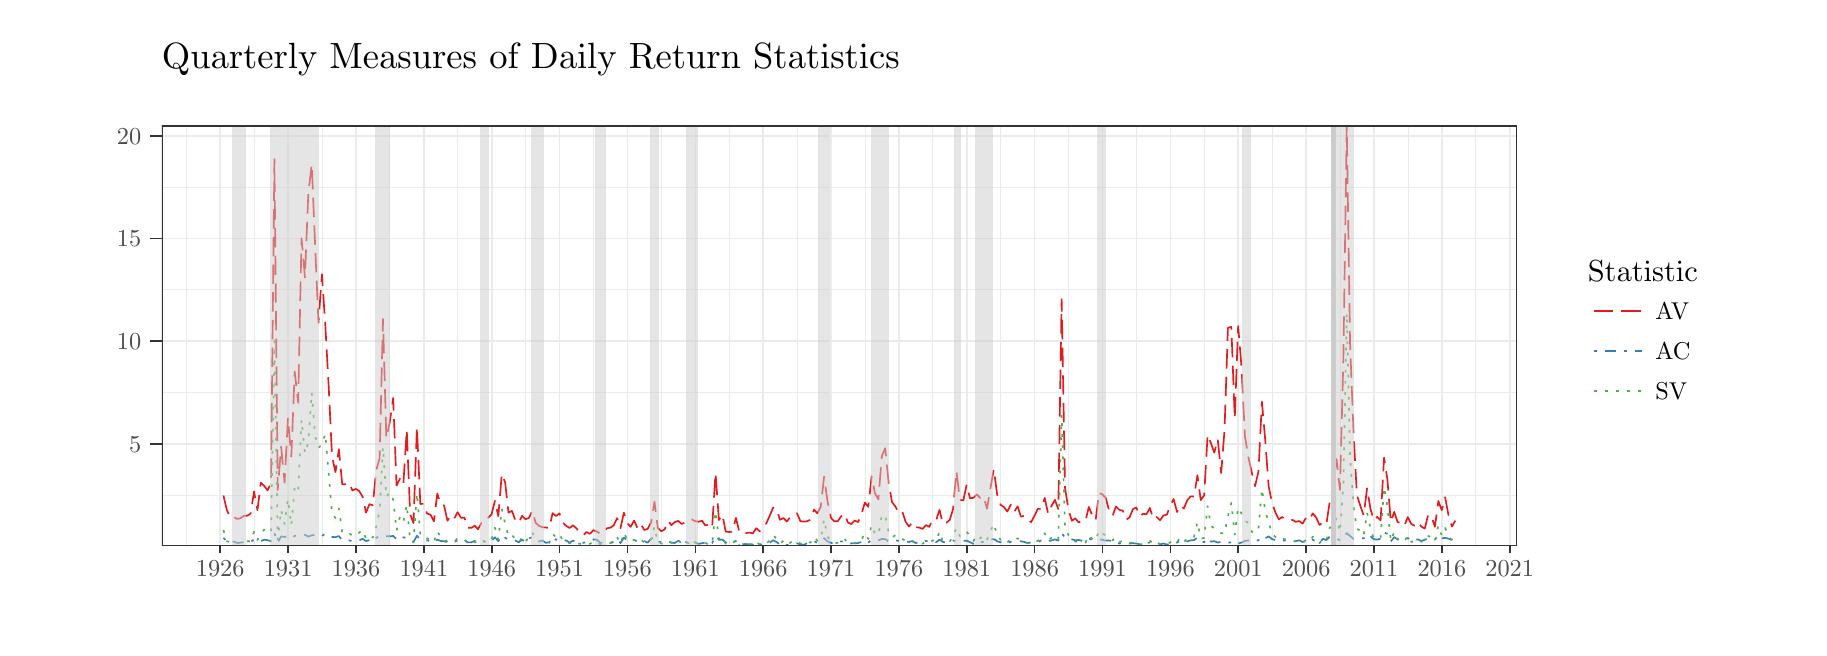
\begin{tikzpicture}[x=1.5pt,y=1pt]
\definecolor{fillColor}{RGB}{255,255,255}
\path[use as bounding box,fill=fillColor,fill opacity=0.00] (0,0) rectangle (426.79,216.81);
\begin{scope}
\path[clip] (  0.00,  0.00) rectangle (426.79,216.81);
\definecolor{drawColor}{RGB}{255,255,255}
\definecolor{fillColor}{RGB}{255,255,255}

\path[draw=drawColor,line width= 0.6pt,line join=round,line cap=round,fill=fillColor] (  0.00,  0.00) rectangle (426.79,216.81);
\end{scope}
\begin{scope}
\path[clip] ( 32.32, 29.59) rectangle (358.76,181.36);
\definecolor{fillColor}{RGB}{255,255,255}

\path[fill=fillColor] ( 32.32, 29.59) rectangle (358.76,181.36);
\definecolor{drawColor}{gray}{0.92}

\path[draw=drawColor,line width= 0.3pt,line join=round] ( 32.32, 47.92) --
	(358.76, 47.92);

\path[draw=drawColor,line width= 0.3pt,line join=round] ( 32.32, 85.02) --
	(358.76, 85.02);

\path[draw=drawColor,line width= 0.3pt,line join=round] ( 32.32,122.12) --
	(358.76,122.12);

\path[draw=drawColor,line width= 0.3pt,line join=round] ( 32.32,159.21) --
	(358.76,159.21);

\path[draw=drawColor,line width= 0.3pt,line join=round] ( 38.22, 29.59) --
	( 38.22,181.36);

\path[draw=drawColor,line width= 0.3pt,line join=round] ( 54.57, 29.59) --
	( 54.57,181.36);

\path[draw=drawColor,line width= 0.3pt,line join=round] ( 70.91, 29.59) --
	( 70.91,181.36);

\path[draw=drawColor,line width= 0.3pt,line join=round] ( 87.26, 29.59) --
	( 87.26,181.36);

\path[draw=drawColor,line width= 0.3pt,line join=round] (103.62, 29.59) --
	(103.62,181.36);

\path[draw=drawColor,line width= 0.3pt,line join=round] (119.96, 29.59) --
	(119.96,181.36);

\path[draw=drawColor,line width= 0.3pt,line join=round] (136.31, 29.59) --
	(136.31,181.36);

\path[draw=drawColor,line width= 0.3pt,line join=round] (152.66, 29.59) --
	(152.66,181.36);

\path[draw=drawColor,line width= 0.3pt,line join=round] (169.01, 29.59) --
	(169.01,181.36);

\path[draw=drawColor,line width= 0.3pt,line join=round] (185.36, 29.59) --
	(185.36,181.36);

\path[draw=drawColor,line width= 0.3pt,line join=round] (201.71, 29.59) --
	(201.71,181.36);

\path[draw=drawColor,line width= 0.3pt,line join=round] (218.06, 29.59) --
	(218.06,181.36);

\path[draw=drawColor,line width= 0.3pt,line join=round] (234.41, 29.59) --
	(234.41,181.36);

\path[draw=drawColor,line width= 0.3pt,line join=round] (250.76, 29.59) --
	(250.76,181.36);

\path[draw=drawColor,line width= 0.3pt,line join=round] (267.11, 29.59) --
	(267.11,181.36);

\path[draw=drawColor,line width= 0.3pt,line join=round] (283.46, 29.59) --
	(283.46,181.36);

\path[draw=drawColor,line width= 0.3pt,line join=round] (299.81, 29.59) --
	(299.81,181.36);

\path[draw=drawColor,line width= 0.3pt,line join=round] (316.16, 29.59) --
	(316.16,181.36);

\path[draw=drawColor,line width= 0.3pt,line join=round] (332.50, 29.59) --
	(332.50,181.36);

\path[draw=drawColor,line width= 0.3pt,line join=round] (348.85, 29.59) --
	(348.85,181.36);

\path[draw=drawColor,line width= 0.6pt,line join=round] ( 32.32, 66.47) --
	(358.76, 66.47);

\path[draw=drawColor,line width= 0.6pt,line join=round] ( 32.32,103.57) --
	(358.76,103.57);

\path[draw=drawColor,line width= 0.6pt,line join=round] ( 32.32,140.67) --
	(358.76,140.67);

\path[draw=drawColor,line width= 0.6pt,line join=round] ( 32.32,177.76) --
	(358.76,177.76);

\path[draw=drawColor,line width= 0.6pt,line join=round] ( 46.39, 29.59) --
	( 46.39,181.36);

\path[draw=drawColor,line width= 0.6pt,line join=round] ( 62.74, 29.59) --
	( 62.74,181.36);

\path[draw=drawColor,line width= 0.6pt,line join=round] ( 79.09, 29.59) --
	( 79.09,181.36);

\path[draw=drawColor,line width= 0.6pt,line join=round] ( 95.44, 29.59) --
	( 95.44,181.36);

\path[draw=drawColor,line width= 0.6pt,line join=round] (111.79, 29.59) --
	(111.79,181.36);

\path[draw=drawColor,line width= 0.6pt,line join=round] (128.14, 29.59) --
	(128.14,181.36);

\path[draw=drawColor,line width= 0.6pt,line join=round] (144.48, 29.59) --
	(144.48,181.36);

\path[draw=drawColor,line width= 0.6pt,line join=round] (160.84, 29.59) --
	(160.84,181.36);

\path[draw=drawColor,line width= 0.6pt,line join=round] (177.19, 29.59) --
	(177.19,181.36);

\path[draw=drawColor,line width= 0.6pt,line join=round] (193.53, 29.59) --
	(193.53,181.36);

\path[draw=drawColor,line width= 0.6pt,line join=round] (209.88, 29.59) --
	(209.88,181.36);

\path[draw=drawColor,line width= 0.6pt,line join=round] (226.24, 29.59) --
	(226.24,181.36);

\path[draw=drawColor,line width= 0.6pt,line join=round] (242.58, 29.59) --
	(242.58,181.36);

\path[draw=drawColor,line width= 0.6pt,line join=round] (258.93, 29.59) --
	(258.93,181.36);

\path[draw=drawColor,line width= 0.6pt,line join=round] (275.28, 29.59) --
	(275.28,181.36);

\path[draw=drawColor,line width= 0.6pt,line join=round] (291.64, 29.59) --
	(291.64,181.36);

\path[draw=drawColor,line width= 0.6pt,line join=round] (307.98, 29.59) --
	(307.98,181.36);

\path[draw=drawColor,line width= 0.6pt,line join=round] (324.33, 29.59) --
	(324.33,181.36);

\path[draw=drawColor,line width= 0.6pt,line join=round] (340.68, 29.59) --
	(340.68,181.36);

\path[draw=drawColor,line width= 0.6pt,line join=round] (357.03, 29.59) --
	(357.03,181.36);
\definecolor{drawColor}{RGB}{228,26,28}

\path[draw=drawColor,line width= 0.6pt,dash pattern=on 7pt off 3pt ,line join=round] ( 47.16, 47.77) --
	( 47.99, 42.49) --
	( 48.81, 39.73) --
	( 49.62, 40.03) --
	( 50.43, 39.30) --
	( 51.25, 39.52) --
	( 52.08, 40.40) --
	( 52.89, 40.45) --
	( 53.71, 41.24) --
	( 54.53, 49.19) --
	( 55.35, 42.47) --
	( 56.17, 52.37) --
	( 56.97, 51.26) --
	( 57.80, 49.60) --
	( 58.62, 52.38) --
	( 59.44,169.32) --
	( 60.24, 49.70) --
	( 61.06, 65.40) --
	( 61.89, 52.35) --
	( 62.70, 75.72) --
	( 63.51, 61.79) --
	( 64.33, 92.56) --
	( 65.16, 81.27) --
	( 65.97,140.73) --
	( 66.79,126.52) --
	( 67.61,157.07) --
	( 68.43,167.45) --
	( 69.25,137.99) --
	( 70.05,110.20) --
	( 70.88,127.71) --
	( 71.70,109.31) --
	( 72.51, 87.29) --
	( 73.32, 61.94) --
	( 74.14, 56.19) --
	( 74.97, 64.49) --
	( 75.78, 51.78) --
	( 76.59, 51.87) --
	( 77.41, 52.42) --
	( 78.24, 49.58) --
	( 79.05, 50.13) --
	( 79.86, 49.38) --
	( 80.69, 47.30) --
	( 81.51, 41.56) --
	( 82.33, 44.63) --
	( 83.13, 44.22) --
	( 83.96, 56.86) --
	( 84.78, 61.25) --
	( 85.59,111.58) --
	( 86.40, 68.52) --
	( 87.22, 74.19) --
	( 88.05, 83.02) --
	( 88.86, 51.35) --
	( 89.67, 53.80) --
	( 90.49, 51.63) --
	( 91.32, 71.51) --
	( 92.13, 41.08) --
	( 92.94, 37.79) --
	( 93.77, 72.58) --
	( 94.59, 44.71) --
	( 95.41, 44.74) --
	( 96.21, 41.22) --
	( 97.04, 40.85) --
	( 97.86, 38.43) --
	( 98.67, 48.47) --
	( 99.48, 44.62) --
	(100.30, 44.15) --
	(101.13, 38.65) --
	(101.94, 40.52) --
	(102.75, 39.40) --
	(103.57, 41.74) --
	(104.39, 39.73) --
	(105.21, 39.76) --
	(106.02, 36.13) --
	(106.85, 36.04) --
	(107.67, 36.82) --
	(108.49, 35.59) --
	(109.29, 37.75) --
	(110.12, 37.99) --
	(110.94, 39.76) --
	(111.75, 40.96) --
	(112.56, 45.84) --
	(113.38, 40.27) --
	(114.21, 55.55) --
	(115.02, 52.48) --
	(115.83, 41.56) --
	(116.65, 42.20) --
	(117.47, 38.86) --
	(118.29, 37.83) --
	(119.10, 40.42) --
	(119.93, 39.20) --
	(120.75, 39.67) --
	(121.57, 42.20) --
	(122.37, 37.87) --
	(123.19, 36.78) --
	(124.02, 36.29) --
	(124.83, 36.19) --
	(125.64, 35.95) --
	(126.46, 41.40) --
	(127.29, 40.34) --
	(128.10, 41.29) --
	(128.91, 37.95) --
	(129.73, 36.79) --
	(130.55, 36.03) --
	(131.37, 36.97) --
	(132.18, 35.93) --
	(133.01, 34.37) --
	(133.83, 33.38) --
	(134.64, 34.54) --
	(135.45, 33.91) --
	(136.27, 35.25) --
	(137.10, 34.71) --
	(137.91, 34.04) --
	(138.72, 34.21) --
	(139.54, 35.93) --
	(140.37, 36.13) --
	(141.18, 37.00) --
	(141.99, 39.58) --
	(142.81, 35.96) --
	(143.63, 41.56) --
	(144.45, 37.71) --
	(145.26, 36.44) --
	(146.09, 38.72) --
	(146.91, 35.89) --
	(147.72, 37.46) --
	(148.53, 35.28) --
	(149.35, 35.70) --
	(150.18, 38.01) --
	(150.99, 45.54) --
	(151.80, 36.04) --
	(152.62, 34.85) --
	(153.45, 35.52) --
	(154.26, 38.61) --
	(155.07, 37.04) --
	(155.89, 38.17) --
	(156.71, 38.59) --
	(157.53, 37.47) --
	(158.34, 38.01) --
	(159.17, 38.97) --
	(159.99, 39.11) --
	(160.80, 38.48) --
	(161.61, 38.27) --
	(162.43, 38.63) --
	(163.26, 36.95) --
	(164.07, 37.26) --
	(164.88, 36.05) --
	(165.70, 55.94) --
	(166.52, 38.89) --
	(167.34, 40.90) --
	(168.15, 34.74) --
	(168.97, 34.57) --
	(169.79, 34.67) --
	(170.61, 39.68) --
	(171.42, 34.73) --
	(172.25, 35.12) --
	(173.07, 34.20) --
	(173.88, 34.36) --
	(174.69, 34.08) --
	(175.51, 35.94) --
	(176.34, 34.81) --
	(177.15, 36.27) --
	(177.96, 37.75) --
	(178.78, 40.55) --
	(179.60, 43.44) --
	(180.42, 42.98) --
	(181.22, 38.97) --
	(182.05, 39.64) --
	(182.87, 38.39) --
	(183.69, 39.89) --
	(184.50, 40.94) --
	(185.32, 41.34) --
	(186.15, 38.48) --
	(186.96, 38.31) --
	(187.77, 38.47) --
	(188.59, 39.01) --
	(189.42, 42.67) --
	(190.23, 41.32) --
	(191.04, 43.62) --
	(191.86, 54.56) --
	(192.68, 45.59) --
	(193.50, 39.71) --
	(194.30, 38.42) --
	(195.13, 38.45) --
	(195.95, 40.20) --
	(196.77, 41.15) --
	(197.58, 38.03) --
	(198.40, 37.43) --
	(199.23, 38.71) --
	(200.04, 38.16) --
	(200.85, 41.00) --
	(201.67, 45.20) --
	(202.50, 43.65) --
	(203.31, 54.69) --
	(204.12, 48.51) --
	(204.94, 46.33) --
	(205.76, 62.01) --
	(206.58, 64.81) --
	(207.38, 52.63) --
	(208.21, 45.40) --
	(209.03, 43.80) --
	(209.85, 41.54) --
	(210.66, 42.12) --
	(211.48, 38.32) --
	(212.31, 36.55) --
	(213.12, 38.03) --
	(213.93, 36.32) --
	(214.75, 36.18) --
	(215.58, 35.70) --
	(216.39, 37.06) --
	(217.20, 36.46) --
	(218.02, 39.00) --
	(218.84, 38.78) --
	(219.66, 42.56) --
	(220.46, 37.55) --
	(221.29, 37.89) --
	(222.11, 38.90) --
	(222.93, 42.88) --
	(223.74, 56.54) --
	(224.56, 46.18) --
	(225.39, 45.99) --
	(226.20, 51.66) --
	(227.01, 46.75) --
	(227.83, 46.91) --
	(228.65, 48.16) --
	(229.47, 46.87) --
	(230.28, 47.43) --
	(231.10, 42.97) --
	(231.92, 50.32) --
	(232.74, 57.27) --
	(233.54, 48.11) --
	(234.37, 44.41) --
	(235.19, 43.56) --
	(236.00, 41.95) --
	(236.82, 44.43) --
	(237.64, 41.81) --
	(238.47, 43.84) --
	(239.28, 40.11) --
	(240.09, 40.44) --
	(240.91, 38.83) --
	(241.73, 38.16) --
	(242.55, 40.47) --
	(243.35, 42.97) --
	(244.18, 42.87) --
	(245.00, 46.92) --
	(245.82, 41.14) --
	(246.62, 43.95) --
	(247.45, 46.21) --
	(248.27, 42.88) --
	(249.08,118.73) --
	(249.90, 50.48) --
	(250.72, 42.62) --
	(251.55, 38.60) --
	(252.36, 39.52) --
	(253.17, 38.03) --
	(253.99, 38.63) --
	(254.81, 38.55) --
	(255.63, 43.63) --
	(256.43, 40.70) --
	(257.26, 38.75) --
	(258.08, 48.71) --
	(258.90, 48.14) --
	(259.70, 46.88) --
	(260.53, 42.24) --
	(261.35, 40.40) --
	(262.16, 43.78) --
	(262.98, 42.58) --
	(263.80, 42.26) --
	(264.63, 39.04) --
	(265.44, 39.85) --
	(266.25, 42.83) --
	(267.07, 43.44) --
	(267.89, 40.28) --
	(268.71, 41.15) --
	(269.51, 40.98) --
	(270.34, 43.28) --
	(271.16, 39.30) --
	(271.98, 40.02) --
	(272.78, 38.79) --
	(273.60, 40.53) --
	(274.43, 40.87) --
	(275.24, 44.03) --
	(276.06, 46.48) --
	(276.88, 41.79) --
	(277.71, 44.22) --
	(278.52, 43.03) --
	(279.33, 46.00) --
	(280.15, 47.46) --
	(280.97, 47.41) --
	(281.79, 55.08) --
	(282.59, 46.09) --
	(283.42, 47.87) --
	(284.24, 69.67) --
	(285.06, 66.60) --
	(285.86, 63.23) --
	(286.68, 68.11) --
	(287.51, 55.85) --
	(288.32, 71.43) --
	(289.14,108.35) --
	(289.96,108.68) --
	(290.78, 75.56) --
	(291.60,109.00) --
	(292.41, 94.21) --
	(293.23, 69.26) --
	(294.05, 61.70) --
	(294.87, 56.16) --
	(295.67, 51.11) --
	(296.50, 56.49) --
	(297.32, 81.69) --
	(298.13, 67.68) --
	(298.94, 51.15) --
	(299.76, 45.07) --
	(300.59, 41.57) --
	(301.40, 39.17) --
	(302.22, 39.95) --
	(303.04, 38.98) --
	(303.86, 39.05) --
	(304.68, 38.93) --
	(305.48, 38.24) --
	(306.31, 38.53) --
	(307.13, 37.59) --
	(307.95, 39.72) --
	(308.75, 38.93) --
	(309.58, 41.31) --
	(310.40, 39.79) --
	(311.21, 37.11) --
	(312.02, 38.06) --
	(312.84, 37.34) --
	(313.67, 45.56) --
	(314.48, 50.18) --
	(315.30, 60.96) --
	(316.12, 49.78) --
	(316.94, 96.56) --
	(317.76,181.36) --
	(318.56,102.71) --
	(319.39, 70.59) --
	(320.21, 47.86) --
	(321.03, 44.04) --
	(321.83, 40.60) --
	(322.66, 50.36) --
	(323.48, 42.88) --
	(324.29, 38.78) --
	(325.10, 40.01) --
	(325.92, 38.77) --
	(326.75, 61.46) --
	(327.56, 53.46) --
	(328.38, 38.15) --
	(329.20, 41.86) --
	(330.02, 38.11) --
	(330.84, 37.92) --
	(331.64, 36.75) --
	(332.47, 39.97) --
	(333.29, 37.45) --
	(334.11, 36.85) --
	(334.91, 38.20) --
	(335.73, 36.54) --
	(336.56, 35.81) --
	(337.37, 40.76) --
	(338.18, 40.18) --
	(339.00, 36.46) --
	(339.83, 45.77) --
	(340.64, 42.47) --
	(341.46, 47.12) --
	(342.28, 40.55) --
	(343.10, 36.54) --
	(343.92, 38.69);
\definecolor{drawColor}{RGB}{55,126,184}

\path[draw=drawColor,line width= 0.6pt,dash pattern=on 1pt off 3pt on 4pt off 3pt ,line join=round] ( 47.16, 32.44) --
	( 47.99, 31.17) --
	( 48.81, 30.75) --
	( 49.62, 31.12) --
	( 50.43, 30.64) --
	( 51.25, 30.74) --
	( 52.08, 30.88) --
	( 52.89, 31.07) --
	( 53.71, 30.91) --
	( 54.53, 31.92) --
	( 55.35, 31.14) --
	( 56.17, 31.29) --
	( 56.97, 31.79) --
	( 57.80, 31.60) --
	( 58.62, 31.26) --
	( 59.44, 34.19) --
	( 60.24, 30.78) --
	( 61.06, 33.01) --
	( 61.89, 32.74) --
	( 62.70, 33.21) --
	( 63.51, 32.42) --
	( 64.33, 33.16) --
	( 65.16, 33.43) --
	( 65.97, 33.83) --
	( 66.79, 33.52) --
	( 67.61, 32.93) --
	( 68.43, 33.36) --
	( 69.25, 33.50) --
	( 70.05, 33.78) --
	( 70.88, 33.10) --
	( 71.70, 34.04) --
	( 72.51, 33.41) --
	( 73.32, 32.79) --
	( 74.14, 32.71) --
	( 74.97, 33.09) --
	( 75.78, 31.61) --
	( 76.59, 31.77) --
	( 77.41, 31.56) --
	( 78.24, 31.19) --
	( 79.05, 31.48) --
	( 79.86, 31.56) --
	( 80.69, 32.14) --
	( 81.51, 31.29) --
	( 82.33, 31.66) --
	( 83.13, 31.10) --
	( 83.96, 32.50) --
	( 84.78, 32.98) --
	( 85.59, 33.40) --
	( 86.40, 33.08) --
	( 87.22, 33.00) --
	( 88.05, 33.16) --
	( 88.86, 31.97) --
	( 89.67, 33.08) --
	( 90.49, 32.63) --
	( 91.32, 32.34) --
	( 92.13, 31.22) --
	( 92.94, 30.99) --
	( 93.77, 33.21) --
	( 94.59, 31.82) --
	( 95.41, 31.72) --
	( 96.21, 31.60) --
	( 97.04, 31.12) --
	( 97.86, 30.71) --
	( 98.67, 31.81) --
	( 99.48, 31.34) --
	(100.30, 31.24) --
	(101.13, 30.87) --
	(101.94, 30.77) --
	(102.75, 31.01) --
	(103.57, 31.53) --
	(104.39, 31.72) --
	(105.21, 31.65) --
	(106.02, 30.82) --
	(106.85, 30.82) --
	(107.67, 31.36) --
	(108.49, 30.86) --
	(109.29, 31.52) --
	(110.12, 31.07) --
	(110.94, 31.77) --
	(111.75, 31.26) --
	(112.56, 32.67) --
	(113.38, 31.24) --
	(114.21, 33.42) --
	(115.02, 32.50) --
	(115.83, 31.73) --
	(116.65, 31.91) --
	(117.47, 31.50) --
	(118.29, 30.83) --
	(119.10, 31.86) --
	(119.93, 30.67) --
	(120.75, 32.27) --
	(121.57, 32.66) --
	(122.37, 31.47) --
	(123.19, 31.18) --
	(124.02, 31.49) --
	(124.83, 30.63) --
	(125.64, 30.93) --
	(126.46, 32.41) --
	(127.29, 31.73) --
	(128.10, 32.27) --
	(128.91, 31.48) --
	(129.73, 31.51) --
	(130.55, 30.70) --
	(131.37, 31.44) --
	(132.18, 30.88) --
	(133.01, 30.85) --
	(133.83, 30.65) --
	(134.64, 30.91) --
	(135.45, 31.02) --
	(136.27, 31.89) --
	(137.10, 31.78) --
	(137.91, 30.65) --
	(138.72, 30.67) --
	(139.54, 30.75) --
	(140.37, 30.78) --
	(141.18, 31.00) --
	(141.99, 32.06) --
	(142.81, 30.57) --
	(143.63, 32.53) --
	(144.45, 31.56) --
	(145.26, 31.40) --
	(146.09, 31.63) --
	(146.91, 31.19) --
	(147.72, 31.81) --
	(148.53, 31.34) --
	(149.35, 30.69) --
	(150.18, 32.12) --
	(150.99, 32.78) --
	(151.80, 31.00) --
	(152.62, 31.00) --
	(153.45, 30.86) --
	(154.26, 31.15) --
	(155.07, 30.70) --
	(155.89, 30.60) --
	(156.71, 31.39) --
	(157.53, 30.32) --
	(158.34, 31.32) --
	(159.17, 30.25) --
	(159.99, 31.41) --
	(160.80, 30.74) --
	(161.61, 30.27) --
	(162.43, 30.54) --
	(163.26, 30.77) --
	(164.07, 30.02) --
	(164.88, 30.58) --
	(165.70, 33.15) --
	(166.52, 31.74) --
	(167.34, 31.85) --
	(168.15, 30.83) --
	(168.97, 30.24) --
	(169.79, 30.60) --
	(170.61, 31.35) --
	(171.42, 29.62) --
	(172.25, 30.20) --
	(173.07, 30.21) --
	(173.88, 30.17) --
	(174.69, 30.10) --
	(175.51, 31.28) --
	(176.34, 30.23) --
	(177.15, 29.86) --
	(177.96, 30.33) --
	(178.78, 30.73) --
	(179.60, 31.62) --
	(180.42, 30.91) --
	(181.22, 30.12) --
	(182.05, 30.78) --
	(182.87, 29.82) --
	(183.69, 30.25) --
	(184.50, 30.67) --
	(185.32, 30.48) --
	(186.15, 30.13) --
	(186.96, 29.93) --
	(187.77, 30.53) --
	(188.59, 30.54) --
	(189.42, 31.29) --
	(190.23, 30.66) --
	(191.04, 30.74) --
	(191.86, 32.31) --
	(192.68, 31.16) --
	(193.50, 30.68) --
	(194.30, 30.20) --
	(195.13, 30.49) --
	(195.95, 31.20) --
	(196.77, 31.17) --
	(197.58, 30.26) --
	(198.40, 30.48) --
	(199.23, 30.46) --
	(200.04, 30.58) --
	(200.85, 30.95) --
	(201.67, 31.72) --
	(202.50, 30.79) --
	(203.31, 31.71) --
	(204.12, 31.32) --
	(204.94, 31.56) --
	(205.76, 32.07) --
	(206.58, 31.98) --
	(207.38, 31.15) --
	(208.21, 31.03) --
	(209.03, 31.52) --
	(209.85, 31.37) --
	(210.66, 31.19) --
	(211.48, 31.13) --
	(212.31, 30.97) --
	(213.12, 31.31) --
	(213.93, 30.58) --
	(214.75, 31.11) --
	(215.58, 30.72) --
	(216.39, 31.36) --
	(217.20, 31.00) --
	(218.02, 31.32) --
	(218.84, 30.86) --
	(219.66, 31.81) --
	(220.46, 30.99) --
	(221.29, 30.78) --
	(222.11, 30.81) --
	(222.93, 31.49) --
	(223.74, 31.24) --
	(224.56, 31.10) --
	(225.39, 31.41) --
	(226.20, 31.43) --
	(227.01, 30.90) --
	(227.83, 30.29) --
	(228.65, 31.34) --
	(229.47, 30.89) --
	(230.28, 30.98) --
	(231.10, 30.98) --
	(231.92, 31.81) --
	(232.74, 32.01) --
	(233.54, 31.24) --
	(234.37, 30.85) --
	(235.19, 31.22) --
	(236.00, 30.50) --
	(236.82, 31.01) --
	(237.64, 31.05) --
	(238.47, 31.31) --
	(239.28, 31.22) --
	(240.09, 30.98) --
	(240.91, 30.57) --
	(241.73, 30.84) --
	(242.55, 30.86) --
	(243.35, 30.97) --
	(244.18, 31.51) --
	(245.00, 31.96) --
	(245.82, 31.33) --
	(246.62, 31.48) --
	(247.45, 31.91) --
	(248.27, 31.45) --
	(249.08, 34.18) --
	(249.90, 32.56) --
	(250.72, 32.54) --
	(251.55, 31.93) --
	(252.36, 31.58) --
	(253.17, 31.69) --
	(253.99, 31.40) --
	(254.81, 31.08) --
	(255.63, 32.24) --
	(256.43, 31.80) --
	(257.26, 31.64) --
	(258.08, 31.94) --
	(258.90, 31.74) --
	(259.70, 31.51) --
	(260.53, 31.47) --
	(261.35, 31.35) --
	(262.16, 31.43) --
	(262.98, 30.36) --
	(263.80, 30.78) --
	(264.63, 30.63) --
	(265.44, 30.41) --
	(266.25, 30.51) --
	(267.07, 30.40) --
	(267.89, 30.13) --
	(268.71, 30.00) --
	(269.51, 30.62) --
	(270.34, 30.77) --
	(271.16, 30.43) --
	(271.98, 30.85) --
	(272.78, 30.13) --
	(273.60, 30.40) --
	(274.43, 30.04) --
	(275.24, 30.20) --
	(276.06, 31.00) --
	(276.88, 30.72) --
	(277.71, 31.35) --
	(278.52, 30.79) --
	(279.33, 31.16) --
	(280.15, 31.56) --
	(280.97, 31.65) --
	(281.79, 32.58) --
	(282.59, 31.02) --
	(283.42, 30.94) --
	(284.24, 32.48) --
	(285.06, 31.06) --
	(285.86, 31.26) --
	(286.68, 30.74) --
	(287.51, 31.07) --
	(288.32, 30.53) --
	(289.14, 30.70) --
	(289.96, 30.83) --
	(290.78, 29.99) --
	(291.60, 30.39) --
	(292.41, 30.75) --
	(293.23, 31.32) --
	(294.05, 31.53) --
	(294.87, 30.94) --
	(295.67, 31.36) --
	(296.50, 31.59) --
	(297.32, 32.96) --
	(298.13, 32.27) --
	(298.94, 32.99) --
	(299.76, 32.04) --
	(300.59, 31.64) --
	(301.40, 31.11) --
	(302.22, 31.45) --
	(303.04, 31.47) --
	(303.86, 31.29) --
	(304.68, 31.23) --
	(305.48, 31.26) --
	(306.31, 31.57) --
	(307.13, 30.97) --
	(307.95, 31.20) --
	(308.75, 30.98) --
	(309.58, 31.81) --
	(310.40, 31.02) --
	(311.21, 30.58) --
	(312.02, 32.12) --
	(312.84, 31.66) --
	(313.67, 32.90) --
	(314.48, 32.45) --
	(315.30, 32.28) --
	(316.12, 31.52) --
	(316.94, 32.65) --
	(317.76, 34.16) --
	(318.56, 33.13) --
	(319.39, 32.10) --
	(320.21, 32.05) --
	(321.03, 32.42) --
	(321.83, 32.25) --
	(322.66, 33.77) --
	(323.48, 32.98) --
	(324.29, 31.98) --
	(325.10, 31.82) --
	(325.92, 32.13) --
	(326.75, 34.40) --
	(327.56, 33.93) --
	(328.38, 31.18) --
	(329.20, 32.73) --
	(330.02, 31.86) --
	(330.84, 32.10) --
	(331.64, 31.68) --
	(332.47, 32.42) --
	(333.29, 31.34) --
	(334.11, 31.76) --
	(334.91, 31.91) --
	(335.73, 31.30) --
	(336.56, 31.80) --
	(337.37, 32.29) --
	(338.18, 32.22) --
	(339.00, 31.85) --
	(339.83, 33.55) --
	(340.64, 32.28) --
	(341.46, 32.46) --
	(342.28, 32.15) --
	(343.10, 31.83) --
	(343.92, 30.76);
\definecolor{drawColor}{RGB}{77,175,74}

\path[draw=drawColor,line width= 0.6pt,dash pattern=on 1pt off 3pt ,line join=round] ( 47.16, 35.26) --
	( 47.99, 31.26) --
	( 48.81, 30.82) --
	( 49.62, 31.24) --
	( 50.43, 30.46) --
	( 51.25, 30.63) --
	( 52.08, 31.06) --
	( 52.89, 31.21) --
	( 53.71, 31.22) --
	( 54.53, 34.71) --
	( 55.35, 31.69) --
	( 56.17, 34.00) --
	( 56.97, 35.43) --
	( 57.80, 34.54) --
	( 58.62, 34.33) --
	( 59.44,103.71) --
	( 60.24, 31.88) --
	( 61.06, 42.57) --
	( 61.89, 37.46) --
	( 62.70, 46.48) --
	( 63.51, 36.97) --
	( 64.33, 50.97) --
	( 65.16, 49.41) --
	( 65.97, 75.21) --
	( 66.79, 62.99) --
	( 67.61, 66.83) --
	( 68.43, 85.01) --
	( 69.25, 69.33) --
	( 70.05, 65.05) --
	( 70.88, 66.04) --
	( 71.70, 70.07) --
	( 72.51, 55.60) --
	( 73.32, 41.16) --
	( 74.14, 39.65) --
	( 74.97, 43.08) --
	( 75.78, 34.31) --
	( 76.59, 34.56) --
	( 77.41, 34.25) --
	( 78.24, 33.15) --
	( 79.05, 34.36) --
	( 79.86, 34.32) --
	( 80.69, 35.32) --
	( 81.51, 32.08) --
	( 82.33, 33.20) --
	( 83.13, 32.55) --
	( 83.96, 36.49) --
	( 84.78, 42.17) --
	( 85.59, 65.24) --
	( 86.40, 47.22) --
	( 87.22, 48.95) --
	( 88.05, 46.30) --
	( 88.86, 35.05) --
	( 89.67, 40.00) --
	( 90.49, 38.02) --
	( 91.32, 44.45) --
	( 92.13, 31.61) --
	( 92.94, 30.83) --
	( 93.77, 48.62) --
	( 94.59, 33.45) --
	( 95.41, 33.55) --
	( 96.21, 32.29) --
	( 97.04, 31.73) --
	( 97.86, 30.79) --
	( 98.67, 34.84) --
	( 99.48, 32.85) --
	(100.30, 32.47) --
	(101.13, 30.87) --
	(101.94, 31.07) --
	(102.75, 31.03) --
	(103.57, 32.31) --
	(104.39, 32.27) --
	(105.21, 31.90) --
	(106.02, 30.39) --
	(106.85, 30.40) --
	(107.67, 31.03) --
	(108.49, 30.47) --
	(109.29, 31.56) --
	(110.12, 31.03) --
	(110.94, 32.47) --
	(111.75, 31.95) --
	(112.56, 36.12) --
	(113.38, 31.81) --
	(114.21, 42.99) --
	(115.02, 37.58) --
	(115.83, 32.97) --
	(116.65, 33.56) --
	(117.47, 31.96) --
	(118.29, 30.83) --
	(119.10, 32.60) --
	(119.93, 30.91) --
	(120.75, 33.08) --
	(121.57, 34.45) --
	(122.37, 31.62) --
	(123.19, 31.20) --
	(124.02, 31.15) --
	(124.83, 30.43) --
	(125.64, 30.60) --
	(126.46, 33.91) --
	(127.29, 32.60) --
	(128.10, 33.70) --
	(128.91, 31.62) --
	(129.73, 31.44) --
	(130.55, 30.43) --
	(131.37, 31.27) --
	(132.18, 30.55) --
	(133.01, 30.36) --
	(133.83, 29.97) --
	(134.64, 30.33) --
	(135.45, 30.27) --
	(136.27, 31.18) --
	(137.10, 31.00) --
	(137.91, 30.16) --
	(138.72, 30.09) --
	(139.54, 30.44) --
	(140.37, 30.56) --
	(141.18, 30.80) --
	(141.99, 32.81) --
	(142.81, 30.35) --
	(143.63, 34.39) --
	(144.45, 31.67) --
	(145.26, 31.22) --
	(146.09, 31.77) --
	(146.91, 30.89) --
	(147.72, 31.81) --
	(148.53, 30.85) --
	(149.35, 30.25) --
	(150.18, 32.27) --
	(150.99, 36.54) --
	(151.80, 30.78) --
	(152.62, 30.42) --
	(153.45, 30.46) --
	(154.26, 31.40) --
	(155.07, 30.71) --
	(155.89, 30.64) --
	(156.71, 31.75) --
	(157.53, 30.33) --
	(158.34, 31.46) --
	(159.17, 30.46) --
	(159.99, 31.87) --
	(160.80, 30.87) --
	(161.61, 30.37) --
	(162.43, 30.83) --
	(163.26, 30.67) --
	(164.07, 29.98) --
	(164.88, 30.33) --
	(165.70, 42.08) --
	(166.52, 32.08) --
	(167.34, 32.91) --
	(168.15, 30.31) --
	(168.97, 29.90) --
	(169.79, 30.15) --
	(170.61, 32.08) --
	(171.42, 29.59) --
	(172.25, 29.96) --
	(173.07, 29.87) --
	(173.88, 29.89) --
	(174.69, 29.82) --
	(175.51, 31.12) --
	(176.34, 29.96) --
	(177.15, 29.80) --
	(177.96, 30.44) --
	(178.78, 31.53) --
	(179.60, 33.42) --
	(180.42, 32.08) --
	(181.22, 30.35) --
	(182.05, 31.38) --
	(182.87, 29.94) --
	(183.69, 30.66) --
	(184.50, 31.56) --
	(185.32, 31.03) --
	(186.15, 30.43) --
	(186.96, 30.01) --
	(187.77, 30.86) --
	(188.59, 30.77) --
	(189.42, 32.81) --
	(190.23, 31.44) --
	(191.04, 31.79) --
	(191.86, 39.21) --
	(192.68, 32.91) --
	(193.50, 31.21) --
	(194.30, 30.43) --
	(195.13, 30.69) --
	(195.95, 32.14) --
	(196.77, 32.18) --
	(197.58, 30.36) --
	(198.40, 30.53) --
	(199.23, 30.57) --
	(200.04, 30.59) --
	(200.85, 31.72) --
	(201.67, 34.18) --
	(202.50, 32.04) --
	(203.31, 37.06) --
	(204.12, 33.88) --
	(204.94, 33.52) --
	(205.76, 40.58) --
	(206.58, 40.75) --
	(207.38, 34.66) --
	(208.21, 32.61) --
	(209.03, 33.40) --
	(209.85, 32.25) --
	(210.66, 32.14) --
	(211.48, 31.31) --
	(212.31, 30.68) --
	(213.12, 31.27) --
	(213.93, 30.34) --
	(214.75, 30.72) --
	(215.58, 30.33) --
	(216.39, 31.25) --
	(217.20, 30.75) --
	(218.02, 31.54) --
	(218.84, 31.19) --
	(219.66, 34.75) --
	(220.46, 31.13) --
	(221.29, 30.85) --
	(222.11, 31.02) --
	(222.93, 33.22) --
	(223.74, 36.02) --
	(224.56, 33.08) --
	(225.39, 33.31) --
	(226.20, 34.74) --
	(227.01, 32.95) --
	(227.83, 31.30) --
	(228.65, 33.53) --
	(229.47, 32.33) --
	(230.28, 33.34) --
	(231.10, 31.69) --
	(231.92, 34.91) --
	(232.74, 37.58) --
	(233.54, 33.37) --
	(234.37, 31.80) --
	(235.19, 32.30) --
	(236.00, 30.85) --
	(236.82, 31.99) --
	(237.64, 31.47) --
	(238.47, 32.32) --
	(239.28, 31.27) --
	(240.09, 31.14) --
	(240.91, 30.48) --
	(241.73, 30.69) --
	(242.55, 30.86) --
	(243.35, 31.43) --
	(244.18, 32.16) --
	(245.00, 34.11) --
	(245.82, 31.45) --
	(246.62, 32.48) --
	(247.45, 33.44) --
	(248.27, 32.03) --
	(249.08, 76.84) --
	(249.90, 36.06) --
	(250.72, 33.49) --
	(251.55, 31.53) --
	(252.36, 31.12) --
	(253.17, 31.13) --
	(253.99, 31.04) --
	(254.81, 30.74) --
	(255.63, 33.43) --
	(256.43, 32.08) --
	(257.26, 31.41) --
	(258.08, 35.13) --
	(258.90, 33.93) --
	(259.70, 33.45) --
	(260.53, 32.14) --
	(261.35, 31.57) --
	(262.16, 32.64) --
	(262.98, 30.89) --
	(263.80, 31.44) --
	(264.63, 30.73) --
	(265.44, 30.44) --
	(266.25, 31.04) --
	(267.07, 30.84) --
	(267.89, 30.16) --
	(268.71, 30.23) --
	(269.51, 30.97) --
	(270.34, 31.50) --
	(271.16, 30.31) --
	(271.98, 31.04) --
	(272.78, 30.11) --
	(273.60, 30.37) --
	(274.43, 30.36) --
	(275.24, 30.77) --
	(276.06, 31.90) --
	(276.88, 30.96) --
	(277.71, 32.53) --
	(278.52, 30.96) --
	(279.33, 32.15) --
	(280.15, 32.98) --
	(280.97, 32.84) --
	(281.79, 38.14) --
	(282.59, 32.18) --
	(283.42, 32.44) --
	(284.24, 43.93) --
	(285.06, 36.74) --
	(285.86, 35.89) --
	(286.68, 34.87) --
	(287.51, 34.17) --
	(288.32, 34.05) --
	(289.14, 40.20) --
	(289.96, 45.12) --
	(290.78, 33.62) --
	(291.60, 43.39) --
	(292.41, 41.25) --
	(293.23, 38.65) --
	(294.05, 37.86) --
	(294.87, 34.67) --
	(295.67, 34.10) --
	(296.50, 35.82) --
	(297.32, 50.18) --
	(298.13, 42.16) --
	(298.94, 38.12) --
	(299.76, 33.96) --
	(300.59, 32.76) --
	(301.40, 31.63) --
	(302.22, 32.08) --
	(303.04, 31.93) --
	(303.86, 31.68) --
	(304.68, 31.19) --
	(305.48, 31.22) --
	(306.31, 31.69) --
	(307.13, 30.84) --
	(307.95, 31.69) --
	(308.75, 30.98) --
	(309.58, 32.88) --
	(310.40, 31.52) --
	(311.21, 30.52) --
	(312.02, 32.11) --
	(312.84, 31.44) --
	(313.67, 36.11) --
	(314.48, 36.61) --
	(315.30, 39.71) --
	(316.12, 34.55) --
	(316.94, 51.00) --
	(317.76,113.79) --
	(318.56, 61.53) --
	(319.39, 43.78) --
	(320.21, 35.63) --
	(321.03, 35.08) --
	(321.83, 33.28) --
	(322.66, 41.60) --
	(323.48, 35.74) --
	(324.29, 32.13) --
	(325.10, 32.63) --
	(325.92, 32.60) --
	(326.75, 50.82) --
	(327.56, 43.77) --
	(328.38, 31.36) --
	(329.20, 34.63) --
	(330.02, 31.87) --
	(330.84, 32.01) --
	(331.64, 31.12) --
	(332.47, 33.22) --
	(333.29, 30.96) --
	(334.11, 31.35) --
	(334.91, 31.95) --
	(335.73, 31.06) --
	(336.56, 31.01) --
	(337.37, 33.13) --
	(338.18, 32.67) --
	(339.00, 31.14) --
	(339.83, 36.89) --
	(340.64, 33.34) --
	(341.46, 36.02) --
	(342.28, 33.13) --
	(343.10, 31.31) --
	(343.92, 30.79);
\definecolor{fillColor}{RGB}{204,204,204}

\path[fill=fillColor,fill opacity=0.50] ( 49.11,181.36) rectangle ( 52.64, 29.59);

\path[fill=fillColor,fill opacity=0.50] ( 58.38,181.36) rectangle ( 70.08, 29.59);

\path[fill=fillColor,fill opacity=0.50] ( 83.71,181.36) rectangle ( 87.24, 29.59);

\path[fill=fillColor,fill opacity=0.50] (109.05,181.36) rectangle (111.23, 29.59);

\path[fill=fillColor,fill opacity=0.50] (121.32,181.36) rectangle (124.31, 29.59);

\path[fill=fillColor,fill opacity=0.50] (136.58,181.36) rectangle (139.29, 29.59);

\path[fill=fillColor,fill opacity=0.50] (149.94,181.36) rectangle (152.09, 29.59);

\path[fill=fillColor,fill opacity=0.50] (158.65,181.36) rectangle (161.36, 29.59);

\path[fill=fillColor,fill opacity=0.50] (190.27,181.36) rectangle (193.25, 29.59);

\path[fill=fillColor,fill opacity=0.50] (203.07,181.36) rectangle (207.41, 29.59);

\path[fill=fillColor,fill opacity=0.50] (223.24,181.36) rectangle (224.86, 29.59);

\path[fill=fillColor,fill opacity=0.50] (228.14,181.36) rectangle (232.49, 29.59);

\path[fill=fillColor,fill opacity=0.50] (257.56,181.36) rectangle (259.73, 29.59);

\path[fill=fillColor,fill opacity=0.50] (292.44,181.36) rectangle (294.62, 29.59);

\path[fill=fillColor,fill opacity=0.50] (314.52,181.36) rectangle (319.41, 29.59);
\definecolor{drawColor}{gray}{0.80}

\path[draw=drawColor,line width= 1.7pt,line join=round] (314.52, 29.59) -- (314.52,181.36);
\definecolor{drawColor}{gray}{0.20}

\path[draw=drawColor,line width= 0.6pt,line join=round,line cap=round] ( 32.32, 29.59) rectangle (358.76,181.36);
\end{scope}
\begin{scope}
\path[clip] (  0.00,  0.00) rectangle (426.79,216.81);
\definecolor{drawColor}{gray}{0.30}

\node[text=drawColor,anchor=base east,inner sep=0pt, outer sep=0pt, scale=  0.88] at ( 27.37, 63.44) {5};

\node[text=drawColor,anchor=base east,inner sep=0pt, outer sep=0pt, scale=  0.88] at ( 27.37,100.54) {10};

\node[text=drawColor,anchor=base east,inner sep=0pt, outer sep=0pt, scale=  0.88] at ( 27.37,137.63) {15};

\node[text=drawColor,anchor=base east,inner sep=0pt, outer sep=0pt, scale=  0.88] at ( 27.37,174.73) {20};
\end{scope}
\begin{scope}
\path[clip] (  0.00,  0.00) rectangle (426.79,216.81);
\definecolor{drawColor}{gray}{0.20}

\path[draw=drawColor,line width= 0.6pt,line join=round] ( 29.57, 66.47) --
	( 32.32, 66.47);

\path[draw=drawColor,line width= 0.6pt,line join=round] ( 29.57,103.57) --
	( 32.32,103.57);

\path[draw=drawColor,line width= 0.6pt,line join=round] ( 29.57,140.67) --
	( 32.32,140.67);

\path[draw=drawColor,line width= 0.6pt,line join=round] ( 29.57,177.76) --
	( 32.32,177.76);
\end{scope}
\begin{scope}
\path[clip] (  0.00,  0.00) rectangle (426.79,216.81);
\definecolor{drawColor}{gray}{0.20}

\path[draw=drawColor,line width= 0.6pt,line join=round] ( 46.39, 26.84) --
	( 46.39, 29.59);

\path[draw=drawColor,line width= 0.6pt,line join=round] ( 62.74, 26.84) --
	( 62.74, 29.59);

\path[draw=drawColor,line width= 0.6pt,line join=round] ( 79.09, 26.84) --
	( 79.09, 29.59);

\path[draw=drawColor,line width= 0.6pt,line join=round] ( 95.44, 26.84) --
	( 95.44, 29.59);

\path[draw=drawColor,line width= 0.6pt,line join=round] (111.79, 26.84) --
	(111.79, 29.59);

\path[draw=drawColor,line width= 0.6pt,line join=round] (128.14, 26.84) --
	(128.14, 29.59);

\path[draw=drawColor,line width= 0.6pt,line join=round] (144.48, 26.84) --
	(144.48, 29.59);

\path[draw=drawColor,line width= 0.6pt,line join=round] (160.84, 26.84) --
	(160.84, 29.59);

\path[draw=drawColor,line width= 0.6pt,line join=round] (177.19, 26.84) --
	(177.19, 29.59);

\path[draw=drawColor,line width= 0.6pt,line join=round] (193.53, 26.84) --
	(193.53, 29.59);

\path[draw=drawColor,line width= 0.6pt,line join=round] (209.88, 26.84) --
	(209.88, 29.59);

\path[draw=drawColor,line width= 0.6pt,line join=round] (226.24, 26.84) --
	(226.24, 29.59);

\path[draw=drawColor,line width= 0.6pt,line join=round] (242.58, 26.84) --
	(242.58, 29.59);

\path[draw=drawColor,line width= 0.6pt,line join=round] (258.93, 26.84) --
	(258.93, 29.59);

\path[draw=drawColor,line width= 0.6pt,line join=round] (275.28, 26.84) --
	(275.28, 29.59);

\path[draw=drawColor,line width= 0.6pt,line join=round] (291.64, 26.84) --
	(291.64, 29.59);

\path[draw=drawColor,line width= 0.6pt,line join=round] (307.98, 26.84) --
	(307.98, 29.59);

\path[draw=drawColor,line width= 0.6pt,line join=round] (324.33, 26.84) --
	(324.33, 29.59);

\path[draw=drawColor,line width= 0.6pt,line join=round] (340.68, 26.84) --
	(340.68, 29.59);

\path[draw=drawColor,line width= 0.6pt,line join=round] (357.03, 26.84) --
	(357.03, 29.59);
\end{scope}
\begin{scope}
\path[clip] (  0.00,  0.00) rectangle (426.79,216.81);
\definecolor{drawColor}{gray}{0.30}

\node[text=drawColor,anchor=base,inner sep=0pt, outer sep=0pt, scale=  0.88] at ( 46.39, 18.58) {1926};

\node[text=drawColor,anchor=base,inner sep=0pt, outer sep=0pt, scale=  0.88] at ( 62.74, 18.58) {1931};

\node[text=drawColor,anchor=base,inner sep=0pt, outer sep=0pt, scale=  0.88] at ( 79.09, 18.58) {1936};

\node[text=drawColor,anchor=base,inner sep=0pt, outer sep=0pt, scale=  0.88] at ( 95.44, 18.58) {1941};

\node[text=drawColor,anchor=base,inner sep=0pt, outer sep=0pt, scale=  0.88] at (111.79, 18.58) {1946};

\node[text=drawColor,anchor=base,inner sep=0pt, outer sep=0pt, scale=  0.88] at (128.14, 18.58) {1951};

\node[text=drawColor,anchor=base,inner sep=0pt, outer sep=0pt, scale=  0.88] at (144.48, 18.58) {1956};

\node[text=drawColor,anchor=base,inner sep=0pt, outer sep=0pt, scale=  0.88] at (160.84, 18.58) {1961};

\node[text=drawColor,anchor=base,inner sep=0pt, outer sep=0pt, scale=  0.88] at (177.19, 18.58) {1966};

\node[text=drawColor,anchor=base,inner sep=0pt, outer sep=0pt, scale=  0.88] at (193.53, 18.58) {1971};

\node[text=drawColor,anchor=base,inner sep=0pt, outer sep=0pt, scale=  0.88] at (209.88, 18.58) {1976};

\node[text=drawColor,anchor=base,inner sep=0pt, outer sep=0pt, scale=  0.88] at (226.24, 18.58) {1981};

\node[text=drawColor,anchor=base,inner sep=0pt, outer sep=0pt, scale=  0.88] at (242.58, 18.58) {1986};

\node[text=drawColor,anchor=base,inner sep=0pt, outer sep=0pt, scale=  0.88] at (258.93, 18.58) {1991};

\node[text=drawColor,anchor=base,inner sep=0pt, outer sep=0pt, scale=  0.88] at (275.28, 18.58) {1996};

\node[text=drawColor,anchor=base,inner sep=0pt, outer sep=0pt, scale=  0.88] at (291.64, 18.58) {2001};

\node[text=drawColor,anchor=base,inner sep=0pt, outer sep=0pt, scale=  0.88] at (307.98, 18.58) {2006};

\node[text=drawColor,anchor=base,inner sep=0pt, outer sep=0pt, scale=  0.88] at (324.33, 18.58) {2011};

\node[text=drawColor,anchor=base,inner sep=0pt, outer sep=0pt, scale=  0.88] at (340.68, 18.58) {2016};

\node[text=drawColor,anchor=base,inner sep=0pt, outer sep=0pt, scale=  0.88] at (357.03, 18.58) {2021};
\end{scope}
\begin{scope}
\path[clip] (  0.00,  0.00) rectangle (426.79,216.81);
\definecolor{fillColor}{RGB}{255,255,255}

\path[fill=fillColor] (370.14, 72.51) rectangle (421.29,138.44);
\end{scope}
\begin{scope}
\path[clip] (  0.00,  0.00) rectangle (426.79,216.81);
\definecolor{drawColor}{RGB}{0,0,0}

\node[text=drawColor,anchor=base west,inner sep=0pt, outer sep=0pt, scale=  1.10] at (375.83,125.17) {Statistic};
\end{scope}
\begin{scope}
\path[clip] (  0.00,  0.00) rectangle (426.79,216.81);
\definecolor{fillColor}{RGB}{255,255,255}

\path[fill=fillColor] (375.83,107.11) rectangle (390.28,121.56);
\end{scope}
\begin{scope}
\path[clip] (  0.00,  0.00) rectangle (426.79,216.81);
\definecolor{drawColor}{RGB}{228,26,28}

\path[draw=drawColor,line width= 0.6pt,dash pattern=on 7pt off 3pt ,line join=round] (377.27,114.33) -- (388.84,114.33);
\end{scope}
\begin{scope}
\path[clip] (  0.00,  0.00) rectangle (426.79,216.81);
\definecolor{fillColor}{RGB}{255,255,255}

\path[fill=fillColor] (375.83, 92.65) rectangle (390.28,107.11);
\end{scope}
\begin{scope}
\path[clip] (  0.00,  0.00) rectangle (426.79,216.81);
\definecolor{drawColor}{RGB}{55,126,184}

\path[draw=drawColor,line width= 0.6pt,dash pattern=on 1pt off 3pt on 4pt off 3pt ,line join=round] (377.27, 99.88) -- (388.84, 99.88);
\end{scope}
\begin{scope}
\path[clip] (  0.00,  0.00) rectangle (426.79,216.81);
\definecolor{fillColor}{RGB}{255,255,255}

\path[fill=fillColor] (375.83, 78.20) rectangle (390.28, 92.65);
\end{scope}
\begin{scope}
\path[clip] (  0.00,  0.00) rectangle (426.79,216.81);
\definecolor{drawColor}{RGB}{77,175,74}

\path[draw=drawColor,line width= 0.6pt,dash pattern=on 1pt off 3pt ,line join=round] (377.27, 85.43) -- (388.84, 85.43);
\end{scope}
\begin{scope}
\path[clip] (  0.00,  0.00) rectangle (426.79,216.81);
\definecolor{drawColor}{RGB}{0,0,0}

\node[text=drawColor,anchor=base west,inner sep=0pt, outer sep=0pt, scale=  0.88] at (392.09,111.30) {AV};
\end{scope}
\begin{scope}
\path[clip] (  0.00,  0.00) rectangle (426.79,216.81);
\definecolor{drawColor}{RGB}{0,0,0}

\node[text=drawColor,anchor=base west,inner sep=0pt, outer sep=0pt, scale=  0.88] at (392.09, 96.85) {AC};
\end{scope}
\begin{scope}
\path[clip] (  0.00,  0.00) rectangle (426.79,216.81);
\definecolor{drawColor}{RGB}{0,0,0}

\node[text=drawColor,anchor=base west,inner sep=0pt, outer sep=0pt, scale=  0.88] at (392.09, 82.40) {SV};
\end{scope}
\begin{scope}
\path[clip] (  0.00,  0.00) rectangle (426.79,216.81);
\definecolor{drawColor}{RGB}{0,0,0}

\node[text=drawColor,anchor=base west,inner sep=0pt, outer sep=0pt, scale=  1.32] at ( 32.32,202.22) {Quarterly Measures of Daily Return Statistics};

\node[text=drawColor,anchor=base west,inner sep=0pt, outer sep=0pt, scale=  1.32] at ( 32.32,187.96) {};
\end{scope}
\end{tikzpicture}
\\
%		% Created by tikzDevice version 0.10.1 on 2018-03-13 14:47:03
% !TEX encoding = UTF-8 Unicode
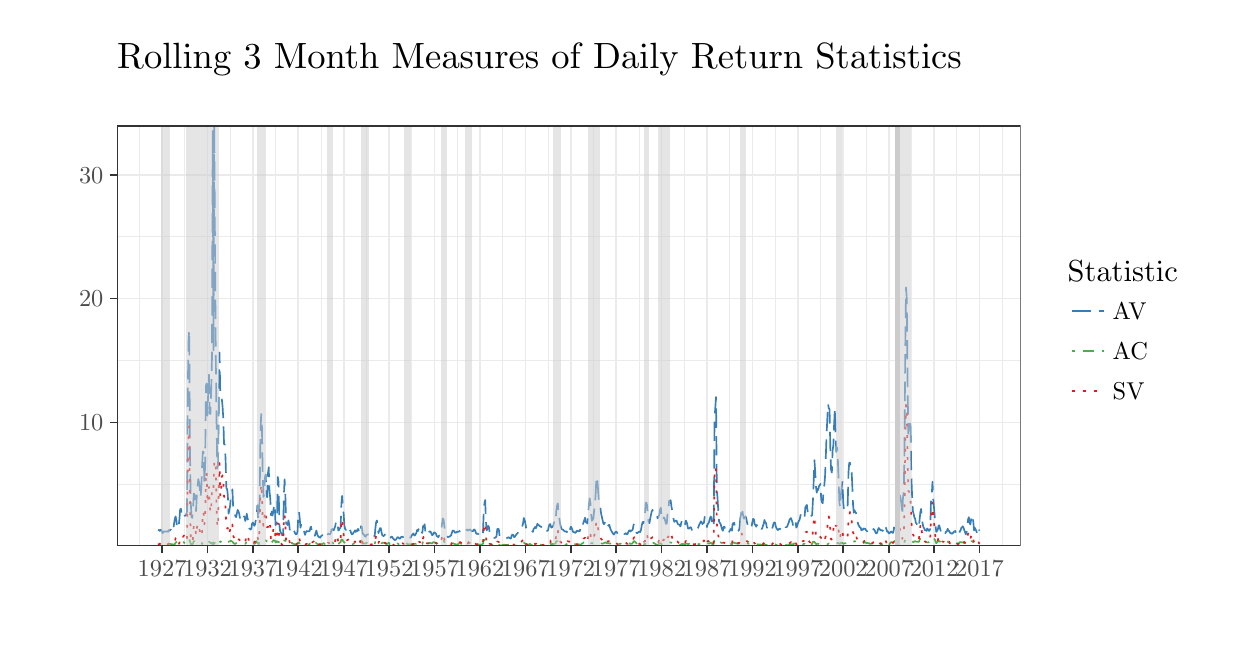
\begin{tikzpicture}[x=1pt,y=1pt]
\definecolor{fillColor}{RGB}{255,255,255}
\path[use as bounding box,fill=fillColor,fill opacity=0.00] (0,0) rectangle (426.79,216.81);
\begin{scope}
\path[clip] (  0.00,  0.00) rectangle (426.79,216.81);
\definecolor{drawColor}{RGB}{255,255,255}
\definecolor{fillColor}{RGB}{255,255,255}

\path[draw=drawColor,line width= 0.6pt,line join=round,line cap=round,fill=fillColor] (  0.00,  0.00) rectangle (426.79,216.81);
\end{scope}
\begin{scope}
\path[clip] ( 32.32, 29.59) rectangle (358.76,181.36);
\definecolor{fillColor}{RGB}{255,255,255}

\path[fill=fillColor] ( 32.32, 29.59) rectangle (358.76,181.36);
\definecolor{drawColor}{gray}{0.92}

\path[draw=drawColor,line width= 0.3pt,line join=round] ( 32.32, 51.81) --
	(358.76, 51.81);

\path[draw=drawColor,line width= 0.3pt,line join=round] ( 32.32, 96.55) --
	(358.76, 96.55);

\path[draw=drawColor,line width= 0.3pt,line join=round] ( 32.32,141.28) --
	(358.76,141.28);

\path[draw=drawColor,line width= 0.3pt,line join=round] ( 40.37, 29.59) --
	( 40.37,181.36);

\path[draw=drawColor,line width= 0.3pt,line join=round] ( 56.78, 29.59) --
	( 56.78,181.36);

\path[draw=drawColor,line width= 0.3pt,line join=round] ( 73.19, 29.59) --
	( 73.19,181.36);

\path[draw=drawColor,line width= 0.3pt,line join=round] ( 89.60, 29.59) --
	( 89.60,181.36);

\path[draw=drawColor,line width= 0.3pt,line join=round] (106.01, 29.59) --
	(106.01,181.36);

\path[draw=drawColor,line width= 0.3pt,line join=round] (122.42, 29.59) --
	(122.42,181.36);

\path[draw=drawColor,line width= 0.3pt,line join=round] (138.83, 29.59) --
	(138.83,181.36);

\path[draw=drawColor,line width= 0.3pt,line join=round] (155.24, 29.59) --
	(155.24,181.36);

\path[draw=drawColor,line width= 0.3pt,line join=round] (171.65, 29.59) --
	(171.65,181.36);

\path[draw=drawColor,line width= 0.3pt,line join=round] (188.05, 29.59) --
	(188.05,181.36);

\path[draw=drawColor,line width= 0.3pt,line join=round] (204.47, 29.59) --
	(204.47,181.36);

\path[draw=drawColor,line width= 0.3pt,line join=round] (220.88, 29.59) --
	(220.88,181.36);

\path[draw=drawColor,line width= 0.3pt,line join=round] (237.29, 29.59) --
	(237.29,181.36);

\path[draw=drawColor,line width= 0.3pt,line join=round] (253.69, 29.59) --
	(253.69,181.36);

\path[draw=drawColor,line width= 0.3pt,line join=round] (270.11, 29.59) --
	(270.11,181.36);

\path[draw=drawColor,line width= 0.3pt,line join=round] (286.52, 29.59) --
	(286.52,181.36);

\path[draw=drawColor,line width= 0.3pt,line join=round] (302.93, 29.59) --
	(302.93,181.36);

\path[draw=drawColor,line width= 0.3pt,line join=round] (319.33, 29.59) --
	(319.33,181.36);

\path[draw=drawColor,line width= 0.3pt,line join=round] (335.75, 29.59) --
	(335.75,181.36);

\path[draw=drawColor,line width= 0.3pt,line join=round] (352.16, 29.59) --
	(352.16,181.36);

\path[draw=drawColor,line width= 0.6pt,line join=round] ( 32.32, 74.18) --
	(358.76, 74.18);

\path[draw=drawColor,line width= 0.6pt,line join=round] ( 32.32,118.91) --
	(358.76,118.91);

\path[draw=drawColor,line width= 0.6pt,line join=round] ( 32.32,163.64) --
	(358.76,163.64);

\path[draw=drawColor,line width= 0.6pt,line join=round] ( 48.57, 29.59) --
	( 48.57,181.36);

\path[draw=drawColor,line width= 0.6pt,line join=round] ( 64.98, 29.59) --
	( 64.98,181.36);

\path[draw=drawColor,line width= 0.6pt,line join=round] ( 81.40, 29.59) --
	( 81.40,181.36);

\path[draw=drawColor,line width= 0.6pt,line join=round] ( 97.80, 29.59) --
	( 97.80,181.36);

\path[draw=drawColor,line width= 0.6pt,line join=round] (114.21, 29.59) --
	(114.21,181.36);

\path[draw=drawColor,line width= 0.6pt,line join=round] (130.62, 29.59) --
	(130.62,181.36);

\path[draw=drawColor,line width= 0.6pt,line join=round] (147.04, 29.59) --
	(147.04,181.36);

\path[draw=drawColor,line width= 0.6pt,line join=round] (163.44, 29.59) --
	(163.44,181.36);

\path[draw=drawColor,line width= 0.6pt,line join=round] (179.85, 29.59) --
	(179.85,181.36);

\path[draw=drawColor,line width= 0.6pt,line join=round] (196.26, 29.59) --
	(196.26,181.36);

\path[draw=drawColor,line width= 0.6pt,line join=round] (212.67, 29.59) --
	(212.67,181.36);

\path[draw=drawColor,line width= 0.6pt,line join=round] (229.08, 29.59) --
	(229.08,181.36);

\path[draw=drawColor,line width= 0.6pt,line join=round] (245.49, 29.59) --
	(245.49,181.36);

\path[draw=drawColor,line width= 0.6pt,line join=round] (261.90, 29.59) --
	(261.90,181.36);

\path[draw=drawColor,line width= 0.6pt,line join=round] (278.31, 29.59) --
	(278.31,181.36);

\path[draw=drawColor,line width= 0.6pt,line join=round] (294.72, 29.59) --
	(294.72,181.36);

\path[draw=drawColor,line width= 0.6pt,line join=round] (311.13, 29.59) --
	(311.13,181.36);

\path[draw=drawColor,line width= 0.6pt,line join=round] (327.54, 29.59) --
	(327.54,181.36);

\path[draw=drawColor,line width= 0.6pt,line join=round] (343.95, 29.59) --
	(343.95,181.36);
\definecolor{drawColor}{RGB}{55,126,184}

\path[draw=drawColor,line width= 0.6pt,dash pattern=on 7pt off 3pt ,line join=round] ( 47.16, 35.44) --
	( 47.44, 35.19) --
	( 47.72, 34.98) --
	( 47.99, 35.41) --
	( 48.27, 35.29) --
	( 48.54, 34.66) --
	( 48.81, 34.16) --
	( 49.09, 34.65) --
	( 49.35, 34.78) --
	( 49.62, 34.78) --
	( 49.89, 34.74) --
	( 50.17, 34.73) --
	( 50.44, 34.80) --
	( 50.72, 34.63) --
	( 51.00, 35.27) --
	( 51.27, 35.01) --
	( 51.55, 35.42) --
	( 51.82, 35.42) --
	( 52.09, 34.76) --
	( 52.37, 34.44) --
	( 52.63, 35.66) --
	( 52.91, 37.68) --
	( 53.18, 39.34) --
	( 53.46, 40.17) --
	( 53.73, 38.80) --
	( 54.01, 36.10) --
	( 54.29, 35.86) --
	( 54.56, 36.71) --
	( 54.84, 39.30) --
	( 55.10, 42.79) --
	( 55.38, 42.90) --
	( 55.66, 40.83) --
	( 55.91, 41.36) --
	( 56.19, 40.52) --
	( 56.46, 40.92) --
	( 56.74, 40.40) --
	( 57.01, 40.48) --
	( 57.29, 40.80) --
	( 57.57, 42.02) --
	( 57.84, 84.52) --
	( 58.11,103.37) --
	( 58.38,107.55) --
	( 58.66, 62.95) --
	( 58.94, 45.00) --
	( 59.19, 40.03) --
	( 59.47, 39.67) --
	( 59.74, 42.42) --
	( 60.02, 48.40) --
	( 60.29, 48.25) --
	( 60.57, 46.86) --
	( 60.85, 42.10) --
	( 61.12, 47.75) --
	( 61.39, 51.12) --
	( 61.66, 53.67) --
	( 61.94, 52.52) --
	( 62.22, 50.11) --
	( 62.47, 47.04) --
	( 62.75, 50.49) --
	( 63.02, 58.42) --
	( 63.30, 63.66) --
	( 63.57, 63.49) --
	( 63.85, 52.28) --
	( 64.13, 58.64) --
	( 64.40, 87.42) --
	( 64.67, 88.25) --
	( 64.94, 76.58) --
	( 65.22, 84.52) --
	( 65.50, 91.44) --
	( 65.76, 77.30) --
	( 66.04, 77.28) --
	( 66.31, 85.80) --
	( 66.59, 97.18) --
	( 66.86,179.49) --
	( 67.14,100.20) --
	( 67.42,181.36) --
	( 67.68,140.03) --
	( 67.96, 99.22) --
	( 68.23, 75.49) --
	( 68.51, 57.46) --
	( 68.79, 58.99) --
	( 69.04, 79.25) --
	( 69.32, 99.47) --
	( 69.59, 84.35) --
	( 69.87, 83.91) --
	( 70.14, 82.65) --
	( 70.42, 80.06) --
	( 70.69, 75.44) --
	( 70.96, 66.31) --
	( 71.24, 66.22) --
	( 71.51, 60.73) --
	( 71.79, 50.51) --
	( 72.07, 50.07) --
	( 72.32, 47.84) --
	( 72.60, 41.19) --
	( 72.87, 42.46) --
	( 73.15, 44.18) --
	( 73.42, 47.18) --
	( 73.70, 47.86) --
	( 73.97, 50.00) --
	( 74.24, 43.86) --
	( 74.52, 42.79) --
	( 74.79, 41.51) --
	( 75.07, 40.18) --
	( 75.35, 39.96) --
	( 75.60, 41.34) --
	( 75.88, 42.56) --
	( 76.15, 42.11) --
	( 76.43, 41.26) --
	( 76.70, 39.65) --
	( 76.98, 40.08) --
	( 77.25, 40.21) --
	( 77.52, 40.94) --
	( 77.80, 41.44) --
	( 78.07, 40.31) --
	( 78.35, 40.01) --
	( 78.63, 38.55) --
	( 78.89, 39.54) --
	( 79.17, 41.16) --
	( 79.44, 39.48) --
	( 79.72, 38.62) --
	( 79.99, 35.87) --
	( 80.26, 35.76) --
	( 80.54, 35.44) --
	( 80.81, 35.78) --
	( 81.09, 37.55) --
	( 81.36, 37.99) --
	( 81.64, 37.33) --
	( 81.92, 36.80) --
	( 82.17, 37.31) --
	( 82.45, 39.15) --
	( 82.72, 39.70) --
	( 83.00, 44.27) --
	( 83.27, 38.92) --
	( 83.54, 42.28) --
	( 83.82, 45.85) --
	( 84.09, 68.20) --
	( 84.37, 77.21) --
	( 84.64, 72.72) --
	( 84.92, 55.61) --
	( 85.20, 47.24) --
	( 85.45, 48.10) --
	( 85.73, 54.37) --
	( 86.00, 55.35) --
	( 86.28, 48.38) --
	( 86.55, 47.10) --
	( 86.82, 55.70) --
	( 87.10, 57.96) --
	( 87.37, 49.32) --
	( 87.65, 46.87) --
	( 87.92, 40.59) --
	( 88.20, 42.01) --
	( 88.48, 40.49) --
	( 88.73, 41.84) --
	( 89.01, 43.95) --
	( 89.28, 44.65) --
	( 89.56, 37.06) --
	( 89.82, 37.55) --
	( 90.10, 39.93) --
	( 90.38, 54.47) --
	( 90.65, 52.68) --
	( 90.93, 37.39) --
	( 91.20, 35.02) --
	( 91.48, 34.43) --
	( 91.76, 33.68) --
	( 92.02, 33.43) --
	( 92.30, 34.09) --
	( 92.57, 47.51) --
	( 92.84, 53.62) --
	( 93.11, 47.82) --
	( 93.39, 37.55) --
	( 93.67, 37.57) --
	( 93.94, 37.09) --
	( 94.22, 38.77) --
	( 94.49, 37.45) --
	( 94.77, 34.74) --
	( 95.05, 35.60) --
	( 95.30, 35.57) --
	( 95.58, 35.78) --
	( 95.85, 35.19) --
	( 96.12, 35.01) --
	( 96.39, 34.68) --
	( 96.67, 34.03) --
	( 96.95, 33.68) --
	( 97.22, 33.82) --
	( 97.50, 34.69) --
	( 97.77, 40.22) --
	( 98.05, 41.86) --
	( 98.33, 39.15) --
	( 98.58, 36.12) --
	( 98.86, 37.50) --
	( 99.12, 37.10) --
	( 99.40, 37.04) --
	( 99.67, 35.85) --
	( 99.95, 34.53) --
	(100.23, 33.54) --
	(100.50, 34.45) --
	(100.78, 34.92) --
	(101.05, 34.85) --
	(101.33, 34.82) --
	(101.60, 34.79) --
	(101.86, 34.87) --
	(102.14, 36.06) --
	(102.40, 36.52) --
	(102.68, 34.66) --
	(102.95, 34.63) --
	(103.23, 35.02) --
	(103.51, 34.80) --
	(103.78, 33.16) --
	(104.06, 34.34) --
	(104.33, 35.09) --
	(104.61, 33.90) --
	(104.88, 33.15) --
	(105.15, 32.79) --
	(105.42, 32.70) --
	(105.69, 32.50) --
	(105.97, 33.02) --
	(106.24, 33.22) --
	(106.52, 33.39) --
	(106.80, 33.48) --
	(107.07, 32.70) --
	(107.35, 32.28) --
	(107.62, 32.87) --
	(107.89, 33.29) --
	(108.17, 33.61) --
	(108.42, 33.77) --
	(108.70, 34.02) --
	(108.97, 33.77) --
	(109.25, 33.79) --
	(109.52, 34.34) --
	(109.80, 35.43) --
	(110.08, 35.66) --
	(110.35, 35.20) --
	(110.63, 35.28) --
	(110.90, 36.04) --
	(111.17, 36.78) --
	(111.45, 38.64) --
	(111.70, 38.12) --
	(111.98, 37.67) --
	(112.25, 35.09) --
	(112.53, 35.36) --
	(112.80, 35.89) --
	(113.08, 36.22) --
	(113.36, 44.69) --
	(113.63, 47.65) --
	(113.91, 43.48) --
	(114.18, 41.06) --
	(114.45, 36.89) --
	(114.73, 35.58) --
	(114.98, 35.37) --
	(115.26, 35.39) --
	(115.53, 35.90) --
	(115.81, 36.69) --
	(116.08, 36.54) --
	(116.36, 35.52) --
	(116.64, 34.96) --
	(116.91, 34.16) --
	(117.19, 33.68) --
	(117.46, 33.84) --
	(117.73, 34.33) --
	(118.01, 34.67) --
	(118.27, 35.19) --
	(118.55, 34.59) --
	(118.82, 35.18) --
	(119.10, 34.90) --
	(119.37, 35.69) --
	(119.65, 35.13) --
	(119.93, 35.55) --
	(120.20, 34.38) --
	(120.47, 36.69) --
	(120.74, 36.45) --
	(121.02, 33.97) --
	(121.30, 33.89) --
	(121.55, 33.55) --
	(121.83, 33.01) --
	(122.10, 32.85) --
	(122.38, 33.53) --
	(122.65, 33.58) --
	(122.93, 33.70) --
	(123.21, 33.56) --
	(123.48, 33.50) --
	(123.75, 33.60) --
	(124.02, 33.07) --
	(124.30, 33.27) --
	(124.58, 33.00) --
	(124.83, 32.52) --
	(125.11, 33.04) --
	(125.38, 33.04) --
	(125.66, 36.04) --
	(125.93, 38.18) --
	(126.21, 38.75) --
	(126.49, 36.16) --
	(126.76, 34.18) --
	(127.03, 35.08) --
	(127.30, 35.91) --
	(127.58, 35.99) --
	(127.86, 34.51) --
	(128.11, 33.45) --
	(128.39, 33.19) --
	(128.66, 33.11) --
	(128.94, 33.40) --
	(129.21, 33.93) --
	(129.49, 33.69) --
	(129.77, 33.46) --
	(130.04, 33.59) --
	(130.31, 33.77) --
	(130.58, 33.47) --
	(130.86, 32.45) --
	(131.14, 32.53) --
	(131.40, 32.90) --
	(131.68, 32.85) --
	(131.95, 32.32) --
	(132.23, 32.07) --
	(132.50, 31.69) --
	(132.78, 31.69) --
	(133.05, 31.80) --
	(133.32, 32.20) --
	(133.60, 32.67) --
	(133.87, 32.65) --
	(134.15, 32.40) --
	(134.43, 32.12) --
	(134.68, 32.30) --
	(134.96, 32.81) --
	(135.23, 32.80) --
	(135.51, 32.93) --
	(135.78, 32.34) --
	(136.06, 32.37) --
	(136.33, 32.60) --
	(136.60, 32.79) --
	(136.88, 32.97) --
	(137.15, 32.34) --
	(137.43, 32.45) --
	(137.71, 32.42) --
	(137.96, 32.42) --
	(138.24, 32.58) --
	(138.51, 32.71) --
	(138.79, 33.44) --
	(139.06, 33.55) --
	(139.34, 34.07) --
	(139.61, 33.48) --
	(139.88, 33.29) --
	(140.16, 33.80) --
	(140.43, 34.09) --
	(140.71, 35.29) --
	(140.99, 34.89) --
	(141.24, 35.63) --
	(141.52, 34.58) --
	(141.79, 34.46) --
	(142.07, 33.44) --
	(142.34, 34.36) --
	(142.61, 34.26) --
	(142.89, 36.78) --
	(143.16, 36.39) --
	(143.44, 37.36) --
	(143.71, 34.63) --
	(143.99, 33.95) --
	(144.27, 33.28) --
	(144.53, 33.81) --
	(144.81, 34.00) --
	(145.08, 34.64) --
	(145.36, 34.87) --
	(145.62, 34.64) --
	(145.90, 33.93) --
	(146.18, 33.38) --
	(146.45, 33.63) --
	(146.73, 34.33) --
	(147.00, 34.45) --
	(147.28, 34.15) --
	(147.56, 33.91) --
	(147.81, 33.06) --
	(148.09, 32.98) --
	(148.36, 32.68) --
	(148.64, 33.23) --
	(148.90, 33.39) --
	(149.18, 34.17) --
	(149.46, 34.55) --
	(149.73, 37.52) --
	(150.01, 39.45) --
	(150.28, 39.07) --
	(150.56, 36.71) --
	(150.84, 34.37) --
	(151.09, 33.51) --
	(151.37, 33.12) --
	(151.64, 32.86) --
	(151.91, 32.76) --
	(152.18, 32.84) --
	(152.46, 32.96) --
	(152.74, 33.14) --
	(153.01, 33.39) --
	(153.29, 34.26) --
	(153.56, 35.09) --
	(153.84, 35.06) --
	(154.12, 34.89) --
	(154.37, 34.29) --
	(154.65, 34.39) --
	(154.92, 34.37) --
	(155.19, 34.67) --
	(155.46, 34.68) --
	(155.74, 34.67) --
	(156.02, 34.92) --
	(156.29, 34.93) --
	(156.57, 35.09) --
	(156.84, 34.36) --
	(157.12, 34.38) --
	(157.40, 34.50) --
	(157.66, 34.62) --
	(157.94, 34.60) --
	(158.20, 34.74) --
	(158.48, 35.22) --
	(158.75, 35.49) --
	(159.03, 35.06) --
	(159.31, 35.25) --
	(159.58, 35.33) --
	(159.86, 35.52) --
	(160.13, 35.17) --
	(160.41, 34.86) --
	(160.68, 34.90) --
	(160.94, 34.89) --
	(161.21, 35.49) --
	(161.48, 35.42) --
	(161.76, 34.96) --
	(162.03, 34.10) --
	(162.31, 33.83) --
	(162.59, 34.02) --
	(162.86, 33.82) --
	(163.14, 34.31) --
	(163.41, 34.14) --
	(163.69, 34.44) --
	(163.96, 34.06) --
	(164.22, 33.48) --
	(164.49, 33.63) --
	(164.76, 40.96) --
	(165.04, 45.00) --
	(165.31, 46.12) --
	(165.59, 38.57) --
	(165.87, 35.13) --
	(166.14, 35.82) --
	(166.42, 36.79) --
	(166.69, 36.34) --
	(166.97, 34.17) --
	(167.24, 33.31) --
	(167.50, 32.72) --
	(167.77, 32.56) --
	(168.04, 32.48) --
	(168.32, 32.57) --
	(168.59, 32.44) --
	(168.87, 32.43) --
	(169.15, 32.59) --
	(169.42, 33.10) --
	(169.70, 35.70) --
	(169.97, 35.73) --
	(170.25, 35.55) --
	(170.52, 33.09) --
	(170.78, 32.81) --
	(171.06, 32.62) --
	(171.33, 32.81) --
	(171.61, 32.84) --
	(171.88, 32.49) --
	(172.16, 32.41) --
	(172.44, 32.32) --
	(172.71, 32.26) --
	(172.99, 32.30) --
	(173.26, 32.41) --
	(173.53, 32.57) --
	(173.81, 32.68) --
	(174.06, 32.38) --
	(174.34, 32.29) --
	(174.61, 32.22) --
	(174.89, 33.37) --
	(175.16, 33.63) --
	(175.44, 33.51) --
	(175.72, 32.73) --
	(175.99, 32.76) --
	(176.27, 33.24) --
	(176.54, 33.63) --
	(176.81, 33.92) --
	(177.09, 34.24) --
	(177.34, 34.56) --
	(177.62, 34.95) --
	(177.89, 36.23) --
	(178.17, 36.21) --
	(178.44, 36.12) --
	(178.72, 36.65) --
	(179.00, 37.65) --
	(179.27, 39.65) --
	(179.55, 38.94) --
	(179.81, 37.88) --
	(180.09, 36.16) --
	(180.37, 35.60) --
	(180.62, 35.37) --
	(180.90, 35.14) --
	(181.17, 35.25) --
	(181.45, 35.55) --
	(181.72, 35.76) --
	(182.00, 35.22) --
	(182.28, 34.91) --
	(182.55, 34.61) --
	(182.83, 35.71) --
	(183.09, 35.98) --
	(183.37, 36.39) --
	(183.65, 35.94) --
	(183.91, 36.57) --
	(184.19, 37.57) --
	(184.46, 37.10) --
	(184.74, 37.04) --
	(185.01, 36.69) --
	(185.29, 36.57) --
	(185.57, 36.48) --
	(185.84, 35.96) --
	(186.11, 35.45) --
	(186.38, 36.05) --
	(186.66, 35.83) --
	(186.94, 35.55) --
	(187.19, 35.11) --
	(187.47, 35.08) --
	(187.74, 34.97) --
	(188.02, 35.16) --
	(188.29, 36.48) --
	(188.57, 37.30) --
	(188.85, 37.44) --
	(189.11, 36.33) --
	(189.39, 36.14) --
	(189.66, 36.52) --
	(189.94, 36.88) --
	(190.22, 38.14) --
	(190.47, 37.83) --
	(190.75, 37.87) --
	(191.02, 42.25) --
	(191.30, 44.09) --
	(191.57, 44.93) --
	(191.85, 40.48) --
	(192.13, 39.34) --
	(192.39, 37.57) --
	(192.67, 36.40) --
	(192.94, 35.67) --
	(193.22, 35.42) --
	(193.50, 35.42) --
	(193.75, 35.04) --
	(194.03, 34.87) --
	(194.30, 34.64) --
	(194.58, 34.85) --
	(194.85, 34.51) --
	(195.13, 36.41) --
	(195.40, 35.76) --
	(195.67, 35.74) --
	(195.95, 35.39) --
	(196.22, 36.49) --
	(196.50, 36.27) --
	(196.78, 35.36) --
	(197.04, 34.69) --
	(197.32, 34.49) --
	(197.59, 34.45) --
	(197.87, 34.23) --
	(198.14, 34.51) --
	(198.41, 35.00) --
	(198.69, 35.02) --
	(198.96, 34.83) --
	(199.24, 34.90) --
	(199.51, 34.91) --
	(199.79, 36.33) --
	(200.07, 35.73) --
	(200.32, 36.33) --
	(200.60, 37.17) --
	(200.87, 38.09) --
	(201.15, 38.96) --
	(201.42, 39.73) --
	(201.69, 38.09) --
	(201.97, 38.11) --
	(202.24, 37.61) --
	(202.52, 40.47) --
	(202.79, 44.43) --
	(203.07, 46.74) --
	(203.35, 44.94) --
	(203.60, 41.17) --
	(203.88, 38.64) --
	(204.15, 39.02) --
	(204.43, 39.48) --
	(204.70, 42.46) --
	(204.97, 44.17) --
	(205.25, 48.56) --
	(205.52, 54.60) --
	(205.80, 54.08) --
	(206.07, 50.35) --
	(206.35, 46.47) --
	(206.63, 45.37) --
	(206.88, 43.87) --
	(207.16, 41.50) --
	(207.43, 40.19) --
	(207.71, 39.02) --
	(207.98, 37.77) --
	(208.25, 37.39) --
	(208.53, 37.91) --
	(208.80, 38.65) --
	(209.08, 37.74) --
	(209.35, 36.55) --
	(209.63, 36.60) --
	(209.91, 37.03) --
	(210.17, 37.16) --
	(210.45, 36.05) --
	(210.72, 35.34) --
	(210.99, 34.85) --
	(211.26, 34.35) --
	(211.54, 33.97) --
	(211.82, 33.63) --
	(212.09, 34.11) --
	(212.37, 34.58) --
	(212.64, 34.70) --
	(212.92, 34.46) --
	(213.20, 33.92) --
	(213.45, 33.58) --
	(213.73, 33.73) --
	(214.00, 33.58) --
	(214.27, 33.59) --
	(214.54, 33.36) --
	(214.82, 33.38) --
	(215.10, 33.25) --
	(215.37, 33.26) --
	(215.65, 33.85) --
	(215.92, 34.00) --
	(216.20, 34.15) --
	(216.48, 33.70) --
	(216.73, 33.79) --
	(217.01, 34.47) --
	(217.28, 34.99) --
	(217.55, 35.18) --
	(217.82, 34.76) --
	(218.10, 35.02) --
	(218.38, 35.15) --
	(218.65, 35.51) --
	(218.93, 37.13) --
	(219.20, 37.44) --
	(219.48, 36.66) --
	(219.76, 35.06) --
	(220.01, 34.23) --
	(220.29, 34.15) --
	(220.56, 34.41) --
	(220.83, 34.62) --
	(221.10, 34.70) --
	(221.38, 34.54) --
	(221.66, 35.54) --
	(221.93, 37.09) --
	(222.21, 38.18) --
	(222.48, 37.74) --
	(222.76, 38.75) --
	(223.04, 40.82) --
	(223.30, 45.05) --
	(223.57, 45.19) --
	(223.84, 44.19) --
	(224.12, 39.67) --
	(224.39, 38.19) --
	(224.67, 37.72) --
	(224.95, 39.38) --
	(225.22, 40.78) --
	(225.50, 42.01) --
	(225.77, 42.56) --
	(226.05, 41.71) --
	(226.32, 40.37) --
	(226.58, 40.03) --
	(226.85, 40.13) --
	(227.12, 40.11) --
	(227.40, 40.16) --
	(227.67, 39.51) --
	(227.95, 40.03) --
	(228.23, 40.82) --
	(228.50, 42.60) --
	(228.78, 43.34) --
	(229.05, 40.26) --
	(229.33, 39.59) --
	(229.60, 38.74) --
	(229.86, 39.91) --
	(230.13, 39.53) --
	(230.40, 38.50) --
	(230.68, 37.50) --
	(230.95, 37.62) --
	(231.23, 41.88) --
	(231.51, 42.11) --
	(231.78, 45.85) --
	(232.06, 45.28) --
	(232.33, 46.10) --
	(232.60, 43.86) --
	(232.88, 42.51) --
	(233.13, 40.91) --
	(233.41, 39.11) --
	(233.68, 38.22) --
	(233.96, 38.61) --
	(234.23, 38.65) --
	(234.51, 38.67) --
	(234.79, 37.73) --
	(235.06, 37.34) --
	(235.34, 37.26) --
	(235.61, 37.04) --
	(235.88, 36.60) --
	(236.16, 37.87) --
	(236.42, 38.66) --
	(236.70, 38.48) --
	(236.97, 36.70) --
	(237.25, 37.07) --
	(237.52, 37.30) --
	(237.80, 38.69) --
	(238.08, 38.26) --
	(238.35, 37.17) --
	(238.63, 35.84) --
	(238.89, 35.80) --
	(239.17, 36.04) --
	(239.45, 36.33) --
	(239.70, 36.16) --
	(239.98, 35.36) --
	(240.25, 35.25) --
	(240.53, 35.14) --
	(240.80, 35.30) --
	(241.08, 34.68) --
	(241.36, 34.78) --
	(241.63, 35.10) --
	(241.90, 35.46) --
	(242.17, 35.92) --
	(242.45, 36.62) --
	(242.73, 37.37) --
	(242.98, 37.76) --
	(243.26, 38.42) --
	(243.53, 38.10) --
	(243.81, 37.42) --
	(244.08, 37.68) --
	(244.36, 37.93) --
	(244.64, 40.04) --
	(244.91, 38.88) --
	(245.18, 38.87) --
	(245.45, 36.34) --
	(245.73, 37.47) --
	(246.01, 37.67) --
	(246.26, 38.39) --
	(246.54, 39.52) --
	(246.81, 40.18) --
	(247.09, 39.58) --
	(247.36, 37.20) --
	(247.64, 36.37) --
	(247.92, 37.59) --
	(248.19, 76.00) --
	(248.46, 79.24) --
	(248.73, 83.33) --
	(249.01, 50.21) --
	(249.29, 46.63) --
	(249.55, 42.37) --
	(249.83, 38.40) --
	(250.10, 37.88) --
	(250.38, 37.50) --
	(250.65, 36.46) --
	(250.93, 35.54) --
	(251.20, 35.01) --
	(251.47, 36.35) --
	(251.75, 36.54) --
	(252.02, 35.59) --
	(252.30, 34.35) --
	(252.58, 34.38) --
	(252.83, 34.75) --
	(253.11, 34.54) --
	(253.38, 34.37) --
	(253.66, 34.97) --
	(253.93, 35.41) --
	(254.21, 35.79) --
	(254.48, 35.05) --
	(254.75, 37.71) --
	(255.03, 37.46) --
	(255.30, 37.96) --
	(255.58, 36.21) --
	(255.86, 36.51) --
	(256.11, 36.30) --
	(256.39, 35.25) --
	(256.66, 34.91) --
	(256.94, 35.12) --
	(257.21, 35.87) --
	(257.49, 39.52) --
	(257.76, 40.88) --
	(258.03, 43.40) --
	(258.31, 41.82) --
	(258.58, 40.25) --
	(258.86, 39.35) --
	(259.14, 39.95) --
	(259.39, 40.21) --
	(259.67, 39.56) --
	(259.94, 38.00) --
	(260.22, 36.97) --
	(260.49, 36.03) --
	(260.77, 36.20) --
	(261.04, 35.84) --
	(261.31, 36.34) --
	(261.59, 36.50) --
	(261.86, 38.15) --
	(262.14, 39.31) --
	(262.42, 39.17) --
	(262.68, 37.40) --
	(262.96, 37.10) --
	(263.23, 36.48) --
	(263.51, 37.13) --
	(263.78, 36.06) --
	(264.05, 35.37) --
	(264.33, 35.08) --
	(264.60, 35.34) --
	(264.88, 35.82) --
	(265.15, 35.66) --
	(265.43, 35.83) --
	(265.71, 36.97) --
	(265.96, 37.49) --
	(266.24, 38.93) --
	(266.51, 38.02) --
	(266.79, 37.87) --
	(267.06, 36.24) --
	(267.33, 36.07) --
	(267.61, 35.93) --
	(267.88, 36.53) --
	(268.16, 37.01) --
	(268.43, 36.48) --
	(268.71, 36.02) --
	(268.99, 35.80) --
	(269.24, 36.45) --
	(269.52, 37.61) --
	(269.79, 38.07) --
	(270.07, 37.88) --
	(270.33, 36.54) --
	(270.61, 35.92) --
	(270.89, 35.42) --
	(271.16, 35.25) --
	(271.44, 35.57) --
	(271.71, 35.85) --
	(271.99, 35.61) --
	(272.27, 35.32) --
	(272.52, 35.10) --
	(272.80, 35.46) --
	(273.07, 35.81) --
	(273.35, 36.33) --
	(273.61, 36.78) --
	(273.89, 36.25) --
	(274.17, 36.37) --
	(274.44, 36.50) --
	(274.72, 37.32) --
	(274.99, 37.90) --
	(275.27, 38.95) --
	(275.55, 39.33) --
	(275.81, 39.59) --
	(276.09, 38.80) --
	(276.36, 37.98) --
	(276.63, 36.58) --
	(276.90, 37.74) --
	(277.18, 38.02) --
	(277.46, 38.53) --
	(277.73, 36.16) --
	(278.01, 36.62) --
	(278.28, 37.58) --
	(278.56, 38.40) --
	(278.84, 38.79) --
	(279.09, 39.65) --
	(279.37, 41.09) --
	(279.63, 41.14) --
	(279.91, 40.22) --
	(280.18, 39.54) --
	(280.46, 40.01) --
	(280.74, 40.07) --
	(281.01, 43.54) --
	(281.29, 43.94) --
	(281.56, 44.37) --
	(281.84, 42.05) --
	(282.11, 40.92) --
	(282.37, 39.82) --
	(282.65, 39.88) --
	(282.91, 39.81) --
	(283.19, 40.49) --
	(283.46, 40.57) --
	(283.74, 45.88) --
	(284.02, 52.89) --
	(284.29, 60.55) --
	(284.57, 56.33) --
	(284.84, 51.07) --
	(285.12, 48.77) --
	(285.39, 50.18) --
	(285.65, 49.73) --
	(285.92, 51.13) --
	(286.19, 51.44) --
	(286.47, 51.94) --
	(286.74, 46.42) --
	(287.02, 45.32) --
	(287.30, 44.96) --
	(287.57, 49.57) --
	(287.85, 51.33) --
	(288.12, 54.47) --
	(288.40, 61.76) --
	(288.67, 69.38) --
	(288.93, 75.18) --
	(289.21, 80.82) --
	(289.48, 79.25) --
	(289.76, 78.96) --
	(290.03, 64.86) --
	(290.31, 56.99) --
	(290.59, 56.06) --
	(290.86, 63.98) --
	(291.14, 66.06) --
	(291.41, 73.70) --
	(291.68, 79.44) --
	(291.96, 68.92) --
	(292.21, 63.48) --
	(292.49, 65.12) --
	(292.76, 60.60) --
	(293.04, 53.02) --
	(293.31, 45.16) --
	(293.59, 43.45) --
	(293.87, 48.09) --
	(294.14, 50.81) --
	(294.42, 52.91) --
	(294.69, 45.41) --
	(294.96, 42.50) --
	(295.24, 42.30) --
	(295.49, 42.47) --
	(295.77, 42.44) --
	(296.04, 42.56) --
	(296.32, 44.55) --
	(296.59, 56.03) --
	(296.87, 59.63) --
	(297.15, 59.62) --
	(297.42, 57.22) --
	(297.70, 57.34) --
	(297.97, 51.35) --
	(298.24, 44.48) --
	(298.52, 41.55) --
	(298.77, 42.42) --
	(299.05, 41.81) --
	(299.32, 41.49) --
	(299.60, 39.11) --
	(299.87, 38.47) --
	(300.15, 37.17) --
	(300.43, 36.76) --
	(300.70, 36.18) --
	(300.98, 36.21) --
	(301.25, 35.18) --
	(301.52, 35.62) --
	(301.80, 35.35) --
	(302.06, 35.85) --
	(302.34, 35.70) --
	(302.61, 35.80) --
	(302.89, 35.24) --
	(303.16, 34.94) --
	(303.44, 34.84) --
	(303.72, 35.11) --
	(303.99, 35.43) --
	(304.26, 35.29) --
	(304.53, 35.13) --
	(304.81, 34.56) --
	(305.09, 34.68) --
	(305.34, 34.79) --
	(305.62, 35.66) --
	(305.89, 35.44) --
	(306.17, 34.94) --
	(306.44, 34.16) --
	(306.72, 34.07) --
	(307.00, 34.39) --
	(307.27, 35.55) --
	(307.54, 36.03) --
	(307.81, 35.73) --
	(308.09, 35.29) --
	(308.37, 35.14) --
	(308.62, 35.23) --
	(308.90, 34.96) --
	(309.17, 35.29) --
	(309.45, 36.58) --
	(309.72, 37.23) --
	(310.00, 36.48) --
	(310.28, 35.68) --
	(310.55, 34.74) --
	(310.82, 34.82) --
	(311.09, 34.12) --
	(311.37, 34.08) --
	(311.65, 34.35) --
	(311.90, 34.76) --
	(312.18, 34.64) --
	(312.45, 34.28) --
	(312.73, 34.32) --
	(313.00, 35.52) --
	(313.28, 38.62) --
	(313.56, 39.25) --
	(313.82, 39.57) --
	(314.10, 40.89) --
	(314.37, 41.61) --
	(314.65, 45.35) --
	(314.93, 43.93) --
	(315.19, 47.81) --
	(315.47, 46.64) --
	(315.74, 44.66) --
	(316.02, 40.63) --
	(316.29, 47.01) --
	(316.57, 49.19) --
	(316.84, 65.61) --
	(317.11,100.63) --
	(317.39,122.90) --
	(317.66,118.87) --
	(317.94, 88.98) --
	(318.22, 70.10) --
	(318.47, 74.99) --
	(318.75, 74.79) --
	(319.02, 72.38) --
	(319.30, 54.98) --
	(319.57, 47.93) --
	(319.85, 42.17) --
	(320.12, 41.17) --
	(320.39, 39.91) --
	(320.67, 39.37) --
	(320.94, 37.87) --
	(321.22, 37.57) --
	(321.50, 37.02) --
	(321.75, 36.38) --
	(322.03, 35.99) --
	(322.30, 39.11) --
	(322.58, 41.84) --
	(322.85, 42.91) --
	(323.12, 39.13) --
	(323.40, 37.56) --
	(323.67, 36.30) --
	(323.95, 35.94) --
	(324.22, 35.16) --
	(324.50, 35.19) --
	(324.78, 34.99) --
	(325.03, 35.84) --
	(325.31, 35.54) --
	(325.58, 35.02) --
	(325.86, 35.04) --
	(326.13, 35.79) --
	(326.40, 45.26) --
	(326.68, 47.80) --
	(326.95, 52.71) --
	(327.23, 46.51) --
	(327.50, 43.37) --
	(327.78, 39.98) --
	(328.06, 36.80) --
	(328.32, 34.60) --
	(328.60, 34.94) --
	(328.87, 35.47) --
	(329.15, 36.83) --
	(329.41, 36.99) --
	(329.69, 35.74) --
	(329.97, 34.78) --
	(330.24, 34.03) --
	(330.52, 34.81) --
	(330.79, 34.70) --
	(331.07, 34.81) --
	(331.35, 34.27) --
	(331.60, 34.11) --
	(331.88, 34.72) --
	(332.15, 34.77) --
	(332.42, 35.74) --
	(332.69, 35.03) --
	(332.97, 35.00) --
	(333.25, 34.33) --
	(333.52, 34.17) --
	(333.80, 34.09) --
	(334.07, 33.91) --
	(334.35, 34.24) --
	(334.63, 34.61) --
	(334.88, 34.71) --
	(335.16, 34.95) --
	(335.43, 34.22) --
	(335.70, 33.84) --
	(335.97, 33.17) --
	(336.25, 33.12) --
	(336.53, 33.26) --
	(336.80, 34.78) --
	(337.08, 35.11) --
	(337.35, 36.02) --
	(337.63, 36.26) --
	(337.91, 36.64) --
	(338.16, 36.10) --
	(338.44, 35.21) --
	(338.71, 34.50) --
	(338.98, 33.74) --
	(339.25, 34.27) --
	(339.53, 37.30) --
	(339.81, 39.08) --
	(340.08, 39.94) --
	(340.36, 37.80) --
	(340.63, 37.30) --
	(340.91, 39.04) --
	(341.19, 40.75) --
	(341.45, 40.20) --
	(341.72, 37.99) --
	(341.99, 35.12) --
	(342.27, 36.06) --
	(342.54, 35.47) --
	(342.82, 34.87) --
	(343.10, 33.78) --
	(343.37, 33.69) --
	(343.65, 35.66) --
	(343.92, 35.05);
\definecolor{drawColor}{RGB}{77,175,74}

\path[draw=drawColor,line width= 0.6pt,dash pattern=on 1pt off 3pt on 4pt off 3pt ,line join=round] ( 47.16, 29.85) --
	( 47.44, 30.04) --
	( 47.72, 30.10) --
	( 47.99, 30.34) --
	( 48.27, 30.26) --
	( 48.54, 29.97) --
	( 48.81, 29.88) --
	( 49.09, 29.82) --
	( 49.35, 29.96) --
	( 49.62, 30.03) --
	( 49.89, 29.91) --
	( 50.17, 30.06) --
	( 50.44, 29.91) --
	( 50.72, 30.11) --
	( 51.00, 30.19) --
	( 51.27, 30.29) --
	( 51.55, 30.29) --
	( 51.82, 30.21) --
	( 52.09, 30.03) --
	( 52.37, 30.14) --
	( 52.63, 30.09) --
	( 52.91, 30.10) --
	( 53.18, 30.17) --
	( 53.46, 30.71) --
	( 53.73, 30.97) --
	( 54.01, 30.36) --
	( 54.29, 29.98) --
	( 54.56, 29.93) --
	( 54.84, 29.96) --
	( 55.10, 30.36) --
	( 55.38, 30.41) --
	( 55.66, 30.40) --
	( 55.91, 30.72) --
	( 56.19, 30.82) --
	( 56.46, 30.96) --
	( 56.74, 30.47) --
	( 57.01, 30.38) --
	( 57.29, 30.16) --
	( 57.57, 30.48) --
	( 57.84, 31.68) --
	( 58.11, 31.97) --
	( 58.38, 31.95) --
	( 58.66, 31.20) --
	( 58.94, 30.36) --
	( 59.19, 30.01) --
	( 59.47, 30.16) --
	( 59.74, 30.46) --
	( 60.02, 31.26) --
	( 60.29, 31.28) --
	( 60.57, 31.38) --
	( 60.85, 30.85) --
	( 61.12, 30.97) --
	( 61.39, 31.14) --
	( 61.66, 30.91) --
	( 61.94, 30.66) --
	( 62.22, 30.66) --
	( 62.47, 30.36) --
	( 62.75, 30.43) --
	( 63.02, 30.24) --
	( 63.30, 31.08) --
	( 63.57, 31.01) --
	( 63.85, 31.00) --
	( 64.13, 31.07) --
	( 64.40, 31.36) --
	( 64.67, 31.52) --
	( 64.94, 30.94) --
	( 65.22, 30.79) --
	( 65.50, 31.00) --
	( 65.76, 30.89) --
	( 66.04, 30.60) --
	( 66.31, 30.55) --
	( 66.59, 30.75) --
	( 66.86, 30.09) --
	( 67.14, 30.77) --
	( 67.42, 30.35) --
	( 67.68, 30.71) --
	( 67.96, 31.38) --
	( 68.23, 30.86) --
	( 68.51, 30.57) --
	( 68.79, 30.71) --
	( 69.04, 31.39) --
	( 69.32, 31.38) --
	( 69.59, 30.92) --
	( 69.87, 31.12) --
	( 70.14, 31.57) --
	( 70.42, 31.73) --
	( 70.69, 31.72) --
	( 70.96, 31.64) --
	( 71.24, 31.60) --
	( 71.51, 31.38) --
	( 71.79, 30.94) --
	( 72.07, 30.87) --
	( 72.32, 31.06) --
	( 72.60, 31.05) --
	( 72.87, 31.16) --
	( 73.15, 31.25) --
	( 73.42, 31.44) --
	( 73.70, 31.22) --
	( 73.97, 31.16) --
	( 74.24, 30.65) --
	( 74.52, 30.52) --
	( 74.79, 30.22) --
	( 75.07, 30.33) --
	( 75.35, 30.56) --
	( 75.60, 30.52) --
	( 75.88, 30.50) --
	( 76.15, 30.31) --
	( 76.43, 30.40) --
	( 76.70, 30.29) --
	( 76.98, 30.28) --
	( 77.25, 30.33) --
	( 77.52, 30.46) --
	( 77.80, 30.45) --
	( 78.07, 30.36) --
	( 78.35, 30.37) --
	( 78.63, 30.26) --
	( 78.89, 30.69) --
	( 79.17, 31.09) --
	( 79.44, 31.01) --
	( 79.72, 31.03) --
	( 79.99, 30.37) --
	( 80.26, 30.44) --
	( 80.54, 30.45) --
	( 80.81, 30.63) --
	( 81.09, 30.57) --
	( 81.36, 30.57) --
	( 81.64, 30.48) --
	( 81.92, 30.30) --
	( 82.17, 30.41) --
	( 82.45, 30.99) --
	( 82.72, 31.21) --
	( 83.00, 30.58) --
	( 83.27, 30.57) --
	( 83.54, 30.12) --
	( 83.82, 31.36) --
	( 84.09, 31.61) --
	( 84.37, 31.56) --
	( 84.64, 31.46) --
	( 84.92, 31.14) --
	( 85.20, 31.30) --
	( 85.45, 31.56) --
	( 85.73, 31.73) --
	( 86.00, 31.59) --
	( 86.28, 31.19) --
	( 86.55, 31.18) --
	( 86.82, 30.64) --
	( 87.10, 30.86) --
	( 87.37, 31.34) --
	( 87.65, 31.26) --
	( 87.92, 30.51) --
	( 88.20, 30.90) --
	( 88.48, 31.09) --
	( 88.73, 31.60) --
	( 89.01, 31.56) --
	( 89.28, 31.47) --
	( 89.56, 30.86) --
	( 89.82, 30.95) --
	( 90.10, 31.28) --
	( 90.38, 30.94) --
	( 90.65, 30.97) --
	( 90.93, 30.80) --
	( 91.20, 30.43) --
	( 91.48, 30.42) --
	( 91.76, 30.23) --
	( 92.02, 30.01) --
	( 92.30, 30.07) --
	( 92.57, 31.52) --
	( 92.84, 31.56) --
	( 93.11, 31.30) --
	( 93.39, 30.52) --
	( 93.67, 30.77) --
	( 93.94, 30.53) --
	( 94.22, 30.79) --
	( 94.49, 30.74) --
	( 94.77, 30.27) --
	( 95.05, 30.55) --
	( 95.30, 30.65) --
	( 95.58, 30.57) --
	( 95.85, 30.31) --
	( 96.12, 30.27) --
	( 96.39, 30.20) --
	( 96.67, 30.11) --
	( 96.95, 30.09) --
	( 97.22, 30.30) --
	( 97.50, 30.33) --
	( 97.77, 30.78) --
	( 98.05, 30.68) --
	( 98.33, 30.40) --
	( 98.58, 30.47) --
	( 98.86, 30.58) --
	( 99.12, 30.43) --
	( 99.40, 30.36) --
	( 99.67, 30.34) --
	( 99.95, 30.27) --
	(100.23, 29.97) --
	(100.50, 30.08) --
	(100.78, 30.15) --
	(101.05, 30.12) --
	(101.33, 30.07) --
	(101.60, 30.07) --
	(101.86, 30.22) --
	(102.14, 30.59) --
	(102.40, 30.51) --
	(102.68, 30.22) --
	(102.95, 30.72) --
	(103.23, 30.81) --
	(103.51, 30.84) --
	(103.78, 30.27) --
	(104.06, 30.61) --
	(104.33, 30.52) --
	(104.61, 30.24) --
	(104.88, 30.13) --
	(105.15, 30.07) --
	(105.42, 30.26) --
	(105.69, 30.26) --
	(105.97, 30.15) --
	(106.24, 30.24) --
	(106.52, 30.20) --
	(106.80, 30.49) --
	(107.07, 30.49) --
	(107.35, 30.20) --
	(107.62, 30.24) --
	(107.89, 30.21) --
	(108.17, 30.27) --
	(108.42, 30.69) --
	(108.70, 30.75) --
	(108.97, 30.56) --
	(109.25, 30.20) --
	(109.52, 30.53) --
	(109.80, 30.77) --
	(110.08, 30.80) --
	(110.35, 30.51) --
	(110.63, 30.40) --
	(110.90, 30.48) --
	(111.17, 30.66) --
	(111.45, 31.42) --
	(111.70, 31.39) --
	(111.98, 31.29) --
	(112.25, 30.26) --
	(112.53, 30.46) --
	(112.80, 30.75) --
	(113.08, 30.92) --
	(113.36, 31.86) --
	(113.63, 31.87) --
	(113.91, 31.46) --
	(114.18, 31.03) --
	(114.45, 30.83) --
	(114.73, 30.53) --
	(114.98, 30.83) --
	(115.26, 31.01) --
	(115.53, 30.95) --
	(115.81, 30.95) --
	(116.08, 30.85) --
	(116.36, 30.68) --
	(116.64, 30.64) --
	(116.91, 30.55) --
	(117.19, 30.34) --
	(117.46, 30.20) --
	(117.73, 30.28) --
	(118.01, 30.60) --
	(118.27, 30.82) --
	(118.55, 30.33) --
	(118.82, 30.34) --
	(119.10, 30.20) --
	(119.37, 30.75) --
	(119.65, 30.78) --
	(119.93, 31.10) --
	(120.20, 30.78) --
	(120.47, 31.49) --
	(120.74, 31.32) --
	(121.02, 30.44) --
	(121.30, 30.55) --
	(121.55, 30.48) --
	(121.83, 30.39) --
	(122.10, 30.48) --
	(122.38, 30.63) --
	(122.65, 30.63) --
	(122.93, 30.60) --
	(123.21, 30.61) --
	(123.48, 30.63) --
	(123.75, 30.57) --
	(124.02, 30.15) --
	(124.30, 30.25) --
	(124.58, 30.21) --
	(124.83, 30.13) --
	(125.11, 30.15) --
	(125.38, 30.09) --
	(125.66, 31.22) --
	(125.93, 31.36) --
	(126.21, 31.34) --
	(126.49, 30.75) --
	(126.76, 30.54) --
	(127.03, 30.99) --
	(127.30, 31.12) --
	(127.58, 30.93) --
	(127.86, 30.53) --
	(128.11, 30.58) --
	(128.39, 30.68) --
	(128.66, 30.67) --
	(128.94, 30.73) --
	(129.21, 30.69) --
	(129.49, 30.43) --
	(129.77, 30.16) --
	(130.04, 30.44) --
	(130.31, 30.58) --
	(130.58, 30.64) --
	(130.86, 30.13) --
	(131.14, 30.33) --
	(131.40, 30.30) --
	(131.68, 30.41) --
	(131.95, 30.37) --
	(132.23, 30.30) --
	(132.50, 29.91) --
	(132.78, 29.99) --
	(133.05, 30.11) --
	(133.32, 30.44) --
	(133.60, 30.46) --
	(133.87, 30.30) --
	(134.15, 30.10) --
	(134.43, 30.05) --
	(134.68, 30.32) --
	(134.96, 30.60) --
	(135.23, 30.65) --
	(135.51, 30.86) --
	(135.78, 30.72) --
	(136.06, 30.79) --
	(136.33, 30.83) --
	(136.60, 30.80) --
	(136.88, 30.70) --
	(137.15, 30.21) --
	(137.43, 30.18) --
	(137.71, 30.20) --
	(137.96, 30.10) --
	(138.24, 30.14) --
	(138.51, 30.03) --
	(138.79, 30.17) --
	(139.06, 30.10) --
	(139.34, 30.32) --
	(139.61, 30.25) --
	(139.88, 30.33) --
	(140.16, 30.33) --
	(140.43, 30.28) --
	(140.71, 30.55) --
	(140.99, 30.53) --
	(141.24, 30.96) --
	(141.52, 30.73) --
	(141.79, 30.82) --
	(142.07, 30.11) --
	(142.34, 30.15) --
	(142.61, 30.22) --
	(142.89, 31.30) --
	(143.16, 31.69) --
	(143.44, 31.50) --
	(143.71, 30.67) --
	(143.99, 30.46) --
	(144.27, 30.63) --
	(144.53, 30.62) --
	(144.81, 30.38) --
	(145.08, 30.59) --
	(145.36, 30.63) --
	(145.62, 30.55) --
	(145.90, 30.43) --
	(146.18, 30.50) --
	(146.45, 30.83) --
	(146.73, 30.89) --
	(147.00, 30.79) --
	(147.28, 30.67) --
	(147.56, 30.64) --
	(147.81, 30.56) --
	(148.09, 30.38) --
	(148.36, 29.96) --
	(148.64, 30.08) --
	(148.90, 30.19) --
	(149.18, 30.76) --
	(149.46, 30.98) --
	(149.73, 31.50) --
	(150.01, 31.50) --
	(150.28, 31.47) --
	(150.56, 30.95) --
	(150.84, 30.55) --
	(151.09, 30.39) --
	(151.37, 30.46) --
	(151.64, 30.32) --
	(151.91, 30.31) --
	(152.18, 30.22) --
	(152.46, 30.29) --
	(152.74, 30.25) --
	(153.01, 30.23) --
	(153.29, 30.52) --
	(153.56, 30.43) --
	(153.84, 30.42) --
	(154.12, 30.31) --
	(154.37, 30.22) --
	(154.65, 30.12) --
	(154.92, 29.96) --
	(155.19, 30.10) --
	(155.46, 30.12) --
	(155.74, 30.36) --
	(156.02, 30.60) --
	(156.29, 30.67) --
	(156.57, 30.44) --
	(156.84, 29.98) --
	(157.12, 30.10) --
	(157.40, 30.37) --
	(157.66, 30.55) --
	(157.94, 30.47) --
	(158.20, 30.20) --
	(158.48, 29.96) --
	(158.75, 30.07) --
	(159.03, 30.18) --
	(159.31, 30.61) --
	(159.58, 30.61) --
	(159.86, 30.62) --
	(160.13, 30.25) --
	(160.41, 29.97) --
	(160.68, 29.96) --
	(160.94, 29.94) --
	(161.21, 30.11) --
	(161.48, 30.04) --
	(161.76, 30.17) --
	(162.03, 30.11) --
	(162.31, 30.13) --
	(162.59, 30.22) --
	(162.86, 30.05) --
	(163.14, 30.02) --
	(163.41, 29.80) --
	(163.69, 30.03) --
	(163.96, 30.03) --
	(164.22, 30.09) --
	(164.49, 30.25) --
	(164.76, 31.48) --
	(165.04, 31.67) --
	(165.31, 31.68) --
	(165.59, 31.09) --
	(165.87, 30.74) --
	(166.14, 31.01) --
	(166.42, 30.98) --
	(166.69, 30.84) --
	(166.97, 30.33) --
	(167.24, 30.25) --
	(167.50, 30.23) --
	(167.77, 30.05) --
	(168.04, 29.88) --
	(168.32, 29.91) --
	(168.59, 30.08) --
	(168.87, 30.11) --
	(169.15, 30.09) --
	(169.42, 29.97) --
	(169.70, 30.66) --
	(169.97, 30.63) --
	(170.25, 30.60) --
	(170.52, 29.76) --
	(170.78, 29.63) --
	(171.06, 29.70) --
	(171.33, 29.76) --
	(171.61, 29.91) --
	(171.88, 29.88) --
	(172.16, 30.03) --
	(172.44, 29.89) --
	(172.71, 29.93) --
	(172.99, 29.80) --
	(173.26, 29.93) --
	(173.53, 29.87) --
	(173.81, 30.00) --
	(174.06, 29.88) --
	(174.34, 29.87) --
	(174.61, 29.85) --
	(174.89, 30.66) --
	(175.16, 30.74) --
	(175.44, 30.65) --
	(175.72, 29.93) --
	(175.99, 29.73) --
	(176.27, 29.73) --
	(176.54, 29.73) --
	(176.81, 29.69) --
	(177.09, 29.76) --
	(177.34, 30.02) --
	(177.62, 30.06) --
	(177.89, 30.41) --
	(178.17, 30.32) --
	(178.44, 30.49) --
	(178.72, 30.70) --
	(179.00, 30.76) --
	(179.27, 30.80) --
	(179.55, 30.48) --
	(179.81, 30.32) --
	(180.09, 30.01) --
	(180.37, 29.96) --
	(180.62, 29.90) --
	(180.90, 29.99) --
	(181.17, 30.12) --
	(181.45, 30.30) --
	(181.72, 30.13) --
	(182.00, 29.94) --
	(182.28, 29.73) --
	(182.55, 29.83) --
	(182.83, 30.03) --
	(183.09, 29.98) --
	(183.37, 30.00) --
	(183.65, 29.98) --
	(183.91, 30.30) --
	(184.19, 30.48) --
	(184.46, 30.31) --
	(184.74, 30.07) --
	(185.01, 30.01) --
	(185.29, 30.01) --
	(185.57, 29.92) --
	(185.84, 29.87) --
	(186.11, 29.68) --
	(186.38, 29.73) --
	(186.66, 29.91) --
	(186.94, 30.04) --
	(187.19, 30.20) --
	(187.47, 30.13) --
	(187.74, 30.01) --
	(188.02, 30.11) --
	(188.29, 30.51) --
	(188.57, 30.62) --
	(188.85, 30.62) --
	(189.11, 30.14) --
	(189.39, 30.15) --
	(189.66, 30.23) --
	(189.94, 30.22) --
	(190.22, 30.29) --
	(190.47, 30.25) --
	(190.75, 30.43) --
	(191.02, 31.29) --
	(191.30, 31.26) --
	(191.57, 31.20) --
	(191.85, 30.63) --
	(192.13, 30.42) --
	(192.39, 30.41) --
	(192.67, 30.36) --
	(192.94, 30.25) --
	(193.22, 30.04) --
	(193.50, 30.02) --
	(193.75, 29.96) --
	(194.03, 29.89) --
	(194.30, 29.96) --
	(194.58, 30.11) --
	(194.85, 30.24) --
	(195.13, 30.62) --
	(195.40, 30.64) --
	(195.67, 30.67) --
	(195.95, 30.51) --
	(196.22, 30.52) --
	(196.50, 30.39) --
	(196.78, 30.01) --
	(197.04, 29.96) --
	(197.32, 29.93) --
	(197.59, 30.14) --
	(197.87, 30.11) --
	(198.14, 30.11) --
	(198.41, 29.99) --
	(198.69, 30.03) --
	(198.96, 30.08) --
	(199.24, 30.07) --
	(199.51, 30.06) --
	(199.79, 29.90) --
	(200.07, 30.16) --
	(200.32, 30.42) --
	(200.60, 30.50) --
	(200.87, 30.84) --
	(201.15, 30.82) --
	(201.42, 30.80) --
	(201.69, 30.52) --
	(201.97, 30.28) --
	(202.24, 30.19) --
	(202.52, 30.62) --
	(202.79, 30.84) --
	(203.07, 30.86) --
	(203.35, 30.71) --
	(203.60, 30.49) --
	(203.88, 30.51) --
	(204.15, 30.47) --
	(204.43, 30.57) --
	(204.70, 30.71) --
	(204.97, 30.85) --
	(205.25, 31.04) --
	(205.52, 31.07) --
	(205.80, 31.02) --
	(206.07, 30.93) --
	(206.35, 30.69) --
	(206.63, 30.56) --
	(206.88, 30.49) --
	(207.16, 30.44) --
	(207.43, 30.46) --
	(207.71, 30.34) --
	(207.98, 30.41) --
	(208.25, 30.59) --
	(208.53, 30.74) --
	(208.80, 30.79) --
	(209.08, 30.59) --
	(209.35, 30.51) --
	(209.63, 30.50) --
	(209.91, 30.56) --
	(210.17, 30.42) --
	(210.45, 30.41) --
	(210.72, 30.42) --
	(210.99, 30.42) --
	(211.26, 30.30) --
	(211.54, 30.27) --
	(211.82, 30.28) --
	(212.09, 30.49) --
	(212.37, 30.55) --
	(212.64, 30.43) --
	(212.92, 30.27) --
	(213.20, 30.07) --
	(213.45, 30.09) --
	(213.73, 30.24) --
	(214.00, 30.34) --
	(214.27, 30.33) --
	(214.54, 30.20) --
	(214.82, 30.13) --
	(215.10, 30.13) --
	(215.37, 30.18) --
	(215.65, 30.53) --
	(215.92, 30.57) --
	(216.20, 30.61) --
	(216.48, 30.41) --
	(216.73, 30.31) --
	(217.01, 30.36) --
	(217.28, 30.33) --
	(217.55, 30.45) --
	(217.82, 30.31) --
	(218.10, 30.29) --
	(218.38, 30.31) --
	(218.65, 30.66) --
	(218.93, 31.15) --
	(219.20, 31.27) --
	(219.48, 31.04) --
	(219.76, 30.74) --
	(220.01, 30.45) --
	(220.29, 30.39) --
	(220.56, 30.32) --
	(220.83, 30.22) --
	(221.10, 30.24) --
	(221.38, 30.03) --
	(221.66, 30.18) --
	(221.93, 30.72) --
	(222.21, 30.81) --
	(222.48, 30.70) --
	(222.76, 30.20) --
	(223.04, 30.12) --
	(223.30, 30.61) --
	(223.57, 30.71) --
	(223.84, 30.77) --
	(224.12, 30.43) --
	(224.39, 30.20) --
	(224.67, 30.38) --
	(224.95, 30.52) --
	(225.22, 30.58) --
	(225.50, 30.53) --
	(225.77, 30.56) --
	(226.05, 30.63) --
	(226.32, 30.58) --
	(226.58, 30.37) --
	(226.85, 30.19) --
	(227.12, 30.06) --
	(227.40, 29.94) --
	(227.67, 30.00) --
	(227.95, 30.11) --
	(228.23, 30.43) --
	(228.50, 30.49) --
	(228.78, 30.37) --
	(229.05, 30.18) --
	(229.33, 30.44) --
	(229.60, 30.46) --
	(229.86, 30.48) --
	(230.13, 30.26) --
	(230.40, 30.19) --
	(230.68, 30.23) --
	(230.95, 30.14) --
	(231.23, 30.62) --
	(231.51, 30.62) --
	(231.78, 30.79) --
	(232.06, 30.83) --
	(232.33, 30.78) --
	(232.60, 30.71) --
	(232.88, 30.52) --
	(233.13, 30.40) --
	(233.41, 30.18) --
	(233.68, 30.12) --
	(233.96, 30.17) --
	(234.23, 30.40) --
	(234.51, 30.39) --
	(234.79, 30.40) --
	(235.06, 30.19) --
	(235.34, 30.09) --
	(235.61, 29.98) --
	(235.88, 29.95) --
	(236.16, 30.13) --
	(236.42, 30.22) --
	(236.70, 30.25) --
	(236.97, 30.17) --
	(237.25, 30.20) --
	(237.52, 30.11) --
	(237.80, 30.36) --
	(238.08, 30.36) --
	(238.35, 30.29) --
	(238.63, 30.18) --
	(238.89, 30.24) --
	(239.17, 30.31) --
	(239.45, 30.22) --
	(239.70, 30.17) --
	(239.98, 29.99) --
	(240.25, 29.99) --
	(240.53, 29.98) --
	(240.80, 30.02) --
	(241.08, 30.04) --
	(241.36, 30.12) --
	(241.63, 30.11) --
	(241.90, 30.15) --
	(242.17, 30.03) --
	(242.45, 30.26) --
	(242.73, 30.19) --
	(242.98, 30.12) --
	(243.26, 30.20) --
	(243.53, 30.27) --
	(243.81, 30.36) --
	(244.08, 30.46) --
	(244.36, 30.40) --
	(244.64, 30.66) --
	(244.91, 30.51) --
	(245.18, 30.58) --
	(245.45, 30.25) --
	(245.73, 30.50) --
	(246.01, 30.42) --
	(246.26, 30.40) --
	(246.54, 30.57) --
	(246.81, 30.63) --
	(247.09, 30.54) --
	(247.36, 30.19) --
	(247.64, 30.12) --
	(247.92, 30.33) --
	(248.19, 31.90) --
	(248.46, 31.87) --
	(248.73, 31.83) --
	(249.01, 31.24) --
	(249.29, 31.13) --
	(249.55, 30.85) --
	(249.83, 30.54) --
	(250.10, 30.70) --
	(250.38, 30.84) --
	(250.65, 30.69) --
	(250.93, 30.57) --
	(251.20, 30.50) --
	(251.47, 30.27) --
	(251.75, 30.23) --
	(252.02, 30.22) --
	(252.30, 30.26) --
	(252.58, 30.22) --
	(252.83, 30.35) --
	(253.11, 30.37) --
	(253.38, 30.28) --
	(253.66, 30.27) --
	(253.93, 30.22) --
	(254.21, 30.23) --
	(254.48, 30.11) --
	(254.75, 30.76) --
	(255.03, 30.73) --
	(255.30, 30.74) --
	(255.58, 30.50) --
	(255.86, 30.50) --
	(256.11, 30.52) --
	(256.39, 30.35) --
	(256.66, 30.35) --
	(256.94, 30.42) --
	(257.21, 30.36) --
	(257.49, 30.86) --
	(257.76, 30.82) --
	(258.03, 30.94) --
	(258.31, 30.63) --
	(258.58, 30.48) --
	(258.86, 30.46) --
	(259.14, 30.45) --
	(259.39, 30.48) --
	(259.67, 30.41) --
	(259.94, 30.36) --
	(260.22, 30.43) --
	(260.49, 30.32) --
	(260.77, 30.48) --
	(261.04, 30.31) --
	(261.31, 30.36) --
	(261.59, 30.35) --
	(261.86, 30.47) --
	(262.14, 30.33) --
	(262.42, 30.10) --
	(262.68, 29.97) --
	(262.96, 30.20) --
	(263.23, 30.17) --
	(263.51, 30.18) --
	(263.78, 30.04) --
	(264.05, 30.04) --
	(264.33, 30.07) --
	(264.60, 30.08) --
	(264.88, 30.04) --
	(265.15, 29.91) --
	(265.43, 29.77) --
	(265.71, 29.95) --
	(265.96, 30.01) --
	(266.24, 30.05) --
	(266.51, 29.97) --
	(266.79, 29.92) --
	(267.06, 29.88) --
	(267.33, 29.76) --
	(267.61, 29.77) --
	(267.88, 29.70) --
	(268.16, 29.82) --
	(268.43, 29.77) --
	(268.71, 29.81) --
	(268.99, 29.91) --
	(269.24, 30.07) --
	(269.52, 30.28) --
	(269.79, 30.17) --
	(270.07, 30.13) --
	(270.33, 29.93) --
	(270.61, 29.88) --
	(270.89, 29.87) --
	(271.16, 30.09) --
	(271.44, 30.17) --
	(271.71, 30.15) --
	(271.99, 29.98) --
	(272.27, 29.89) --
	(272.52, 29.80) --
	(272.80, 29.76) --
	(273.07, 29.81) --
	(273.35, 29.84) --
	(273.61, 29.99) --
	(273.89, 29.91) --
	(274.17, 29.84) --
	(274.44, 29.77) --
	(274.72, 29.81) --
	(274.99, 29.90) --
	(275.27, 29.96) --
	(275.55, 30.02) --
	(275.81, 30.13) --
	(276.09, 30.11) --
	(276.36, 30.16) --
	(276.63, 30.05) --
	(276.90, 30.43) --
	(277.18, 30.42) --
	(277.46, 30.38) --
	(277.73, 29.86) --
	(278.01, 29.82) --
	(278.28, 29.98) --
	(278.56, 30.03) --
	(278.84, 30.16) --
	(279.09, 30.21) --
	(279.37, 30.35) --
	(279.63, 30.39) --
	(279.91, 30.36) --
	(280.18, 30.22) --
	(280.46, 30.28) --
	(280.74, 30.33) --
	(281.01, 31.02) --
	(281.29, 31.06) --
	(281.56, 31.04) --
	(281.84, 30.52) --
	(282.11, 30.29) --
	(282.37, 30.23) --
	(282.65, 30.05) --
	(282.91, 30.08) --
	(283.19, 30.20) --
	(283.46, 30.25) --
	(283.74, 30.99) --
	(284.02, 31.12) --
	(284.29, 31.00) --
	(284.57, 30.64) --
	(284.84, 30.25) --
	(285.12, 30.21) --
	(285.39, 30.35) --
	(285.65, 30.33) --
	(285.92, 30.23) --
	(286.19, 30.17) --
	(286.47, 30.11) --
	(286.74, 30.23) --
	(287.02, 30.26) --
	(287.30, 30.28) --
	(287.57, 30.36) --
	(287.85, 30.18) --
	(288.12, 29.95) --
	(288.40, 29.96) --
	(288.67, 29.94) --
	(288.93, 30.09) --
	(289.21, 30.25) --
	(289.48, 30.42) --
	(289.76, 30.31) --
	(290.03, 30.15) --
	(290.31, 29.84) --
	(290.59, 29.88) --
	(290.86, 30.05) --
	(291.14, 30.18) --
	(291.41, 30.31) --
	(291.68, 30.21) --
	(291.96, 30.31) --
	(292.21, 30.40) --
	(292.49, 30.48) --
	(292.76, 30.63) --
	(293.04, 30.52) --
	(293.31, 30.33) --
	(293.59, 30.32) --
	(293.87, 30.72) --
	(294.14, 30.62) --
	(294.42, 30.59) --
	(294.69, 30.35) --
	(294.96, 30.35) --
	(295.24, 30.51) --
	(295.49, 30.46) --
	(295.77, 30.50) --
	(296.04, 30.54) --
	(296.32, 30.61) --
	(296.59, 30.97) --
	(296.87, 31.08) --
	(297.15, 31.30) --
	(297.42, 31.21) --
	(297.70, 31.00) --
	(297.97, 30.94) --
	(298.24, 30.94) --
	(298.52, 31.06) --
	(298.77, 31.28) --
	(299.05, 31.16) --
	(299.32, 31.04) --
	(299.60, 30.74) --
	(299.87, 30.70) --
	(300.15, 30.66) --
	(300.43, 30.70) --
	(300.70, 30.61) --
	(300.98, 30.66) --
	(301.25, 30.39) --
	(301.52, 30.30) --
	(301.80, 30.26) --
	(302.06, 30.60) --
	(302.34, 30.80) --
	(302.61, 30.90) --
	(302.89, 30.65) --
	(303.16, 30.56) --
	(303.44, 30.66) --
	(303.72, 30.52) --
	(303.99, 30.57) --
	(304.26, 30.32) --
	(304.53, 30.26) --
	(304.81, 30.37) --
	(305.09, 30.39) --
	(305.34, 30.39) --
	(305.62, 30.55) --
	(305.89, 30.58) --
	(306.17, 30.58) --
	(306.44, 30.29) --
	(306.72, 30.24) --
	(307.00, 30.25) --
	(307.27, 30.54) --
	(307.54, 30.44) --
	(307.81, 30.45) --
	(308.09, 30.15) --
	(308.37, 30.22) --
	(308.62, 30.21) --
	(308.90, 30.12) --
	(309.17, 30.36) --
	(309.45, 30.78) --
	(309.72, 30.97) --
	(310.00, 30.82) --
	(310.28, 30.38) --
	(310.55, 30.03) --
	(310.82, 30.09) --
	(311.09, 30.11) --
	(311.37, 30.12) --
	(311.65, 30.56) --
	(311.90, 30.86) --
	(312.18, 30.92) --
	(312.45, 30.68) --
	(312.73, 30.60) --
	(313.00, 30.96) --
	(313.28, 31.35) --
	(313.56, 31.31) --
	(313.82, 31.14) --
	(314.10, 31.06) --
	(314.37, 31.03) --
	(314.65, 31.03) --
	(314.93, 30.85) --
	(315.19, 30.98) --
	(315.47, 30.91) --
	(315.74, 30.82) --
	(316.02, 30.52) --
	(316.29, 30.38) --
	(316.57, 30.45) --
	(316.84, 31.07) --
	(317.11, 31.72) --
	(317.39, 31.91) --
	(317.66, 32.01) --
	(317.94, 31.89) --
	(318.22, 31.66) --
	(318.47, 31.41) --
	(318.75, 31.20) --
	(319.02, 31.13) --
	(319.30, 30.98) --
	(319.57, 31.09) --
	(319.85, 31.00) --
	(320.12, 30.90) --
	(320.39, 31.16) --
	(320.67, 31.24) --
	(320.94, 31.10) --
	(321.22, 31.09) --
	(321.50, 31.03) --
	(321.75, 31.01) --
	(322.03, 31.00) --
	(322.30, 31.81) --
	(322.58, 32.12) --
	(322.85, 32.17) --
	(323.12, 31.80) --
	(323.40, 31.57) --
	(323.67, 31.20) --
	(323.95, 31.06) --
	(324.22, 30.76) --
	(324.50, 30.69) --
	(324.78, 30.47) --
	(325.03, 30.83) --
	(325.31, 30.82) --
	(325.58, 30.87) --
	(325.86, 31.01) --
	(326.13, 31.21) --
	(326.40, 32.49) --
	(326.68, 32.59) --
	(326.95, 32.48) --
	(327.23, 32.25) --
	(327.50, 32.25) --
	(327.78, 31.85) --
	(328.06, 31.16) --
	(328.32, 30.50) --
	(328.60, 30.86) --
	(328.87, 31.04) --
	(329.15, 31.38) --
	(329.41, 31.28) --
	(329.69, 31.11) --
	(329.97, 30.72) --
	(330.24, 30.63) --
	(330.52, 30.89) --
	(330.79, 30.82) --
	(331.07, 30.76) --
	(331.35, 30.66) --
	(331.60, 30.62) --
	(331.88, 30.78) --
	(332.15, 30.69) --
	(332.42, 31.10) --
	(332.69, 30.78) --
	(332.97, 30.84) --
	(333.25, 30.32) --
	(333.52, 30.68) --
	(333.80, 30.56) --
	(334.07, 30.63) --
	(334.35, 30.58) --
	(334.63, 30.72) --
	(334.88, 30.78) --
	(335.16, 30.81) --
	(335.43, 30.67) --
	(335.70, 30.49) --
	(335.97, 30.42) --
	(336.25, 30.39) --
	(336.53, 30.59) --
	(336.80, 30.98) --
	(337.08, 30.81) --
	(337.35, 30.94) --
	(337.63, 30.77) --
	(337.91, 30.84) --
	(338.16, 30.82) --
	(338.44, 30.51) --
	(338.71, 30.59) --
	(338.98, 30.57) --
	(339.25, 30.64) --
	(339.53, 31.33) --
	(339.81, 31.56) --
	(340.08, 31.52) --
	(340.36, 31.04) --
	(340.63, 30.82) --
	(340.91, 31.16) --
	(341.19, 31.23) --
	(341.45, 31.15) --
	(341.72, 30.68) --
	(341.99, 30.46) --
	(342.27, 30.99) --
	(342.54, 31.01) --
	(342.82, 30.93) --
	(343.10, 30.66) --
	(343.37, 30.62) --
	(343.65, 30.47) --
	(343.92, 30.14);
\definecolor{drawColor}{RGB}{228,26,28}

\path[draw=drawColor,line width= 0.6pt,dash pattern=on 1pt off 3pt ,line join=round] ( 47.16, 29.98) --
	( 47.44, 30.20) --
	( 47.72, 30.25) --
	( 47.99, 30.62) --
	( 48.27, 30.51) --
	( 48.54, 30.05) --
	( 48.81, 29.90) --
	( 49.09, 29.88) --
	( 49.35, 30.05) --
	( 49.62, 30.13) --
	( 49.89, 29.99) --
	( 50.17, 30.17) --
	( 50.44, 30.00) --
	( 50.72, 30.21) --
	( 51.00, 30.40) --
	( 51.27, 30.49) --
	( 51.55, 30.57) --
	( 51.82, 30.46) --
	( 52.09, 30.14) --
	( 52.37, 30.22) --
	( 52.63, 30.33) --
	( 52.91, 30.63) --
	( 53.18, 31.03) --
	( 53.46, 32.44) --
	( 53.73, 32.61) --
	( 54.01, 30.79) --
	( 54.29, 30.20) --
	( 54.56, 30.22) --
	( 54.84, 30.57) --
	( 55.10, 32.15) --
	( 55.38, 32.32) --
	( 55.66, 31.84) --
	( 55.91, 32.82) --
	( 56.19, 32.82) --
	( 56.46, 33.29) --
	( 56.74, 31.94) --
	( 57.01, 31.72) --
	( 57.29, 31.24) --
	( 57.57, 32.31) --
	( 57.84, 56.77) --
	( 58.11, 70.85) --
	( 58.38, 72.89) --
	( 58.66, 42.50) --
	( 58.94, 32.59) --
	( 59.19, 30.76) --
	( 59.47, 31.06) --
	( 59.74, 32.37) --
	( 60.02, 37.09) --
	( 60.29, 37.09) --
	( 60.57, 36.90) --
	( 60.85, 33.38) --
	( 61.12, 35.65) --
	( 61.39, 37.60) --
	( 61.66, 37.32) --
	( 61.94, 35.66) --
	( 62.22, 35.01) --
	( 62.47, 32.99) --
	( 62.75, 34.03) --
	( 63.02, 34.56) --
	( 63.30, 41.84) --
	( 63.57, 41.26) --
	( 63.85, 37.30) --
	( 64.13, 39.96) --
	( 64.40, 54.07) --
	( 64.67, 56.46) --
	( 64.94, 45.08) --
	( 65.22, 45.89) --
	( 65.50, 50.82) --
	( 65.76, 44.72) --
	( 66.04, 41.66) --
	( 66.31, 43.20) --
	( 66.59, 49.08) --
	( 66.86, 50.87) --
	( 67.14, 50.24) --
	( 67.42, 59.91) --
	( 67.68, 60.33) --
	( 67.96, 59.32) --
	( 68.23, 43.87) --
	( 68.51, 36.41) --
	( 68.79, 37.74) --
	( 69.04, 50.95) --
	( 69.32, 59.52) --
	( 69.59, 47.37) --
	( 69.87, 49.64) --
	( 70.14, 54.47) --
	( 70.42, 55.06) --
	( 70.69, 52.69) --
	( 70.96, 47.39) --
	( 71.24, 47.02) --
	( 71.51, 42.89) --
	( 71.79, 36.40) --
	( 72.07, 35.93) --
	( 72.32, 36.03) --
	( 72.60, 33.62) --
	( 72.87, 34.38) --
	( 73.15, 35.34) --
	( 73.42, 37.30) --
	( 73.70, 36.69) --
	( 73.97, 37.27) --
	( 74.24, 33.30) --
	( 74.52, 32.63) --
	( 74.79, 31.51) --
	( 75.07, 31.56) --
	( 75.35, 32.03) --
	( 75.60, 32.27) --
	( 75.88, 32.51) --
	( 76.15, 31.87) --
	( 76.43, 31.94) --
	( 76.70, 31.36) --
	( 76.98, 31.42) --
	( 77.25, 31.56) --
	( 77.52, 32.03) --
	( 77.80, 32.12) --
	( 78.07, 31.66) --
	( 78.35, 31.62) --
	( 78.63, 31.10) --
	( 78.89, 32.22) --
	( 79.17, 33.71) --
	( 79.44, 32.93) --
	( 79.72, 32.67) --
	( 79.99, 30.76) --
	( 80.26, 30.84) --
	( 80.54, 30.78) --
	( 80.81, 31.10) --
	( 81.09, 31.47) --
	( 81.36, 31.57) --
	( 81.64, 31.26) --
	( 81.92, 30.84) --
	( 82.17, 31.13) --
	( 82.45, 32.76) --
	( 82.72, 33.46) --
	( 83.00, 33.16) --
	( 83.27, 31.80) --
	( 83.54, 31.35) --
	( 83.82, 36.41) --
	( 84.09, 48.01) --
	( 84.37, 51.80) --
	( 84.64, 48.79) --
	( 84.92, 39.26) --
	( 85.20, 36.77) --
	( 85.45, 38.18) --
	( 85.73, 42.07) --
	( 86.00, 41.75) --
	( 86.28, 36.76) --
	( 86.55, 36.23) --
	( 86.82, 36.37) --
	( 87.10, 38.37) --
	( 87.37, 37.80) --
	( 87.65, 36.47) --
	( 87.92, 32.07) --
	( 88.20, 33.50) --
	( 88.48, 33.47) --
	( 88.73, 35.36) --
	( 89.01, 36.24) --
	( 89.28, 36.26) --
	( 89.56, 31.83) --
	( 89.82, 32.14) --
	( 90.10, 33.71) --
	( 90.38, 37.75) --
	( 90.65, 37.29) --
	( 90.93, 31.82) --
	( 91.20, 30.66) --
	( 91.48, 30.53) --
	( 91.76, 30.18) --
	( 92.02, 29.94) --
	( 92.30, 30.09) --
	( 92.57, 37.75) --
	( 92.84, 40.78) --
	( 93.11, 36.98) --
	( 93.39, 31.37) --
	( 93.67, 31.82) --
	( 93.94, 31.28) --
	( 94.22, 32.22) --
	( 94.49, 31.74) --
	( 94.77, 30.41) --
	( 95.05, 30.95) --
	( 95.30, 31.08) --
	( 95.58, 31.02) --
	( 95.85, 30.54) --
	( 96.12, 30.46) --
	( 96.39, 30.32) --
	( 96.67, 30.12) --
	( 96.95, 30.05) --
	( 97.22, 30.28) --
	( 97.50, 30.48) --
	( 97.77, 32.63) --
	( 98.05, 32.84) --
	( 98.33, 31.49) --
	( 98.58, 30.96) --
	( 98.86, 31.47) --
	( 99.12, 31.12) --
	( 99.40, 30.98) --
	( 99.67, 30.72) --
	( 99.95, 30.37) --
	(100.23, 29.92) --
	(100.50, 30.15) --
	(100.78, 30.30) --
	(101.05, 30.25) --
	(101.33, 30.18) --
	(101.60, 30.18) --
	(101.86, 30.38) --
	(102.14, 31.12) --
	(102.40, 31.12) --
	(102.68, 30.34) --
	(102.95, 30.90) --
	(103.23, 31.14) --
	(103.51, 31.10) --
	(103.78, 30.13) --
	(104.06, 30.71) --
	(104.33, 30.79) --
	(104.61, 30.23) --
	(104.88, 30.01) --
	(105.15, 29.91) --
	(105.42, 30.03) --
	(105.69, 30.00) --
	(105.97, 30.00) --
	(106.24, 30.11) --
	(106.52, 30.11) --
	(106.80, 30.38) --
	(107.07, 30.20) --
	(107.35, 29.92) --
	(107.62, 30.05) --
	(107.89, 30.09) --
	(108.17, 30.21) --
	(108.42, 30.64) --
	(108.70, 30.77) --
	(108.97, 30.51) --
	(109.25, 30.17) --
	(109.52, 30.62) --
	(109.80, 31.20) --
	(110.08, 31.31) --
	(110.35, 30.81) --
	(110.63, 30.68) --
	(110.90, 30.96) --
	(111.17, 31.43) --
	(111.45, 33.48) --
	(111.70, 33.18) --
	(111.98, 32.80) --
	(112.25, 30.46) --
	(112.53, 30.77) --
	(112.80, 31.30) --
	(113.08, 31.66) --
	(113.36, 37.61) --
	(113.63, 39.25) --
	(113.91, 35.72) --
	(114.18, 33.53) --
	(114.45, 31.73) --
	(114.73, 30.92) --
	(114.98, 31.27) --
	(115.26, 31.51) --
	(115.53, 31.59) --
	(115.81, 31.86) --
	(116.08, 31.65) --
	(116.36, 31.10) --
	(116.64, 30.91) --
	(116.91, 30.60) --
	(117.19, 30.28) --
	(117.46, 30.18) --
	(117.73, 30.35) --
	(118.01, 30.78) --
	(118.27, 31.19) --
	(118.55, 30.45) --
	(118.82, 30.58) --
	(119.10, 30.36) --
	(119.37, 31.25) --
	(119.65, 31.13) --
	(119.93, 31.68) --
	(120.20, 30.90) --
	(120.47, 32.73) --
	(120.74, 32.35) --
	(121.02, 30.44) --
	(121.30, 30.53) --
	(121.55, 30.38) --
	(121.83, 30.19) --
	(122.10, 30.23) --
	(122.38, 30.52) --
	(122.65, 30.53) --
	(122.93, 30.54) --
	(123.21, 30.50) --
	(123.48, 30.51) --
	(123.75, 30.48) --
	(124.02, 30.01) --
	(124.30, 30.13) --
	(124.58, 30.05) --
	(124.83, 29.91) --
	(125.11, 30.01) --
	(125.38, 29.96) --
	(125.66, 32.04) --
	(125.93, 33.16) --
	(126.21, 33.35) --
	(126.49, 31.39) --
	(126.76, 30.59) --
	(127.03, 31.37) --
	(127.30, 31.85) --
	(127.58, 31.60) --
	(127.86, 30.66) --
	(128.11, 30.45) --
	(128.39, 30.47) --
	(128.66, 30.44) --
	(128.94, 30.57) --
	(129.21, 30.68) --
	(129.49, 30.37) --
	(129.77, 30.08) --
	(130.04, 30.36) --
	(130.31, 30.53) --
	(130.58, 30.51) --
	(130.86, 29.90) --
	(131.14, 30.05) --
	(131.40, 30.10) --
	(131.68, 30.17) --
	(131.95, 30.03) --
	(132.23, 29.94) --
	(132.50, 29.68) --
	(132.78, 29.72) --
	(133.05, 29.79) --
	(133.32, 30.05) --
	(133.60, 30.17) --
	(133.87, 30.05) --
	(134.15, 29.87) --
	(134.43, 29.80) --
	(134.68, 30.00) --
	(134.96, 30.31) --
	(135.23, 30.34) --
	(135.51, 30.54) --
	(135.78, 30.27) --
	(136.06, 30.32) --
	(136.33, 30.41) --
	(136.60, 30.45) --
	(136.88, 30.43) --
	(137.15, 29.93) --
	(137.43, 29.93) --
	(137.71, 29.95) --
	(137.96, 29.88) --
	(138.24, 29.93) --
	(138.51, 29.87) --
	(138.79, 30.09) --
	(139.06, 30.04) --
	(139.34, 30.34) --
	(139.61, 30.17) --
	(139.88, 30.20) --
	(140.16, 30.30) --
	(140.43, 30.31) --
	(140.71, 30.88) --
	(140.99, 30.75) --
	(141.24, 31.52) --
	(141.52, 30.90) --
	(141.79, 30.98) --
	(142.07, 30.03) --
	(142.34, 30.22) --
	(142.61, 30.27) --
	(142.89, 32.47) --
	(143.16, 32.90) --
	(143.44, 33.05) --
	(143.71, 30.85) --
	(143.99, 30.46) --
	(144.27, 30.45) --
	(144.53, 30.58) --
	(144.81, 30.39) --
	(145.08, 30.76) --
	(145.36, 30.87) --
	(145.62, 30.72) --
	(145.90, 30.42) --
	(146.18, 30.36) --
	(146.45, 30.73) --
	(146.73, 31.01) --
	(147.00, 30.94) --
	(147.28, 30.72) --
	(147.56, 30.63) --
	(147.81, 30.34) --
	(148.09, 30.18) --
	(148.36, 29.81) --
	(148.64, 29.98) --
	(148.90, 30.10) --
	(149.18, 30.83) --
	(149.46, 31.19) --
	(149.73, 33.13) --
	(150.01, 34.01) --
	(150.28, 33.77) --
	(150.56, 31.87) --
	(150.84, 30.65) --
	(151.09, 30.30) --
	(151.37, 30.27) --
	(151.64, 30.11) --
	(151.91, 30.08) --
	(152.18, 30.03) --
	(152.46, 30.10) --
	(152.74, 30.10) --
	(153.01, 30.13) --
	(153.29, 30.59) --
	(153.56, 30.67) --
	(153.84, 30.66) --
	(154.12, 30.48) --
	(154.37, 30.27) --
	(154.65, 30.19) --
	(154.92, 30.01) --
	(155.19, 30.20) --
	(155.46, 30.23) --
	(155.74, 30.50) --
	(156.02, 30.85) --
	(156.29, 30.93) --
	(156.57, 30.69) --
	(156.84, 30.02) --
	(157.12, 30.16) --
	(157.40, 30.48) --
	(157.66, 30.71) --
	(157.94, 30.62) --
	(158.20, 30.34) --
	(158.48, 30.10) --
	(158.75, 30.29) --
	(159.03, 30.36) --
	(159.31, 30.95) --
	(159.58, 30.97) --
	(159.86, 31.02) --
	(160.13, 30.47) --
	(160.41, 30.07) --
	(160.68, 30.07) --
	(160.94, 30.05) --
	(161.21, 30.34) --
	(161.48, 30.23) --
	(161.76, 30.33) --
	(162.03, 30.13) --
	(162.31, 30.11) --
	(162.59, 30.23) --
	(162.86, 30.03) --
	(163.14, 30.06) --
	(163.41, 29.82) --
	(163.69, 30.09) --
	(163.96, 30.04) --
	(164.22, 30.02) --
	(164.49, 30.19) --
	(164.76, 34.64) --
	(165.04, 37.11) --
	(165.31, 37.72) --
	(165.59, 32.78) --
	(165.87, 31.08) --
	(166.14, 31.65) --
	(166.42, 31.95) --
	(166.69, 31.58) --
	(166.97, 30.37) --
	(167.24, 30.13) --
	(167.50, 30.01) --
	(167.77, 29.87) --
	(168.04, 29.74) --
	(168.32, 29.76) --
	(168.59, 29.87) --
	(168.87, 29.89) --
	(169.15, 29.89) --
	(169.42, 29.87) --
	(169.70, 31.13) --
	(169.97, 31.10) --
	(170.25, 31.00) --
	(170.52, 29.70) --
	(170.78, 29.59) --
	(171.06, 29.63) --
	(171.33, 29.68) --
	(171.61, 29.80) --
	(171.88, 29.74) --
	(172.16, 29.83) --
	(172.44, 29.73) --
	(172.71, 29.75) --
	(172.99, 29.67) --
	(173.26, 29.76) --
	(173.53, 29.74) --
	(173.81, 29.85) --
	(174.06, 29.73) --
	(174.34, 29.72) --
	(174.61, 29.69) --
	(174.89, 30.50) --
	(175.16, 30.65) --
	(175.44, 30.53) --
	(175.72, 29.80) --
	(175.99, 29.65) --
	(176.27, 29.68) --
	(176.54, 29.71) --
	(176.81, 29.69) --
	(177.09, 29.78) --
	(177.34, 30.09) --
	(177.62, 30.19) --
	(177.89, 30.90) --
	(178.17, 30.75) --
	(178.44, 30.99) --
	(178.72, 31.45) --
	(179.00, 31.83) --
	(179.27, 32.50) --
	(179.55, 31.62) --
	(179.81, 31.08) --
	(180.09, 30.29) --
	(180.37, 30.15) --
	(180.62, 30.04) --
	(180.90, 30.13) --
	(181.17, 30.31) --
	(181.45, 30.60) --
	(181.72, 30.41) --
	(182.00, 30.08) --
	(182.28, 29.79) --
	(182.55, 29.88) --
	(182.83, 30.26) --
	(183.09, 30.22) --
	(183.37, 30.30) --
	(183.65, 30.22) --
	(183.91, 30.79) --
	(184.19, 31.30) --
	(184.46, 30.92) --
	(184.74, 30.49) --
	(185.01, 30.35) --
	(185.29, 30.33) --
	(185.57, 30.19) --
	(185.84, 30.05) --
	(186.11, 29.76) --
	(186.38, 29.87) --
	(186.66, 30.10) --
	(186.94, 30.25) --
	(187.19, 30.39) --
	(187.47, 30.30) --
	(187.74, 30.14) --
	(188.02, 30.29) --
	(188.29, 31.11) --
	(188.57, 31.49) --
	(188.85, 31.52) --
	(189.11, 30.50) --
	(189.39, 30.50) --
	(189.66, 30.67) --
	(189.94, 30.71) --
	(190.22, 31.06) --
	(190.47, 30.93) --
	(190.75, 31.28) --
	(191.02, 34.67) --
	(191.30, 35.35) --
	(191.57, 35.47) --
	(191.85, 32.34) --
	(192.13, 31.58) --
	(192.39, 31.19) --
	(192.67, 30.85) --
	(192.94, 30.56) --
	(193.22, 30.23) --
	(193.50, 30.21) --
	(193.75, 30.09) --
	(194.03, 29.98) --
	(194.30, 30.03) --
	(194.58, 30.24) --
	(194.85, 30.34) --
	(195.13, 31.25) --
	(195.40, 31.11) --
	(195.67, 31.15) --
	(195.95, 30.85) --
	(196.22, 31.12) --
	(196.50, 30.87) --
	(196.78, 30.19) --
	(197.04, 30.04) --
	(197.32, 29.99) --
	(197.59, 30.22) --
	(197.87, 30.15) --
	(198.14, 30.19) --
	(198.41, 30.11) --
	(198.69, 30.17) --
	(198.96, 30.20) --
	(199.24, 30.21) --
	(199.51, 30.19) --
	(199.79, 30.14) --
	(200.07, 30.44) --
	(200.32, 30.93) --
	(200.60, 31.24) --
	(200.87, 32.11) --
	(201.15, 32.34) --
	(201.42, 32.53) --
	(201.69, 31.50) --
	(201.97, 31.05) --
	(202.24, 30.78) --
	(202.52, 32.32) --
	(202.79, 34.08) --
	(203.07, 34.86) --
	(203.35, 33.78) --
	(203.60, 32.17) --
	(203.88, 31.61) --
	(204.15, 31.62) --
	(204.43, 31.95) --
	(204.70, 33.08) --
	(204.97, 34.04) --
	(205.25, 36.20) --
	(205.52, 38.50) --
	(205.80, 38.04) --
	(206.07, 36.30) --
	(206.35, 34.12) --
	(206.63, 33.38) --
	(206.88, 32.79) --
	(207.16, 32.11) --
	(207.43, 31.87) --
	(207.71, 31.35) --
	(207.98, 31.22) --
	(208.25, 31.47) --
	(208.53, 31.87) --
	(208.80, 32.18) --
	(209.08, 31.56) --
	(209.35, 31.11) --
	(209.63, 31.11) --
	(209.91, 31.31) --
	(210.17, 31.11) --
	(210.45, 30.85) --
	(210.72, 30.72) --
	(210.99, 30.61) --
	(211.26, 30.37) --
	(211.54, 30.27) --
	(211.82, 30.22) --
	(212.09, 30.53) --
	(212.37, 30.70) --
	(212.64, 30.59) --
	(212.92, 30.36) --
	(213.20, 30.07) --
	(213.45, 30.03) --
	(213.73, 30.20) --
	(214.00, 30.27) --
	(214.27, 30.26) --
	(214.54, 30.10) --
	(214.82, 30.05) --
	(215.10, 30.02) --
	(215.37, 30.07) --
	(215.65, 30.50) --
	(215.92, 30.58) --
	(216.20, 30.66) --
	(216.48, 30.35) --
	(216.73, 30.28) --
	(217.01, 30.46) --
	(217.28, 30.53) --
	(217.55, 30.72) --
	(217.82, 30.47) --
	(218.10, 30.49) --
	(218.38, 30.54) --
	(218.65, 31.08) --
	(218.93, 32.36) --
	(219.20, 32.69) --
	(219.48, 32.00) --
	(219.76, 31.05) --
	(220.01, 30.51) --
	(220.29, 30.43) --
	(220.56, 30.41) --
	(220.83, 30.34) --
	(221.10, 30.37) --
	(221.38, 30.10) --
	(221.66, 30.44) --
	(221.93, 31.60) --
	(222.21, 32.08) --
	(222.48, 31.75) --
	(222.76, 31.01) --
	(223.04, 31.15) --
	(223.30, 33.45) --
	(223.57, 33.86) --
	(223.84, 33.79) --
	(224.12, 31.68) --
	(224.39, 30.91) --
	(224.67, 31.15) --
	(224.95, 31.81) --
	(225.22, 32.30) --
	(225.50, 32.45) --
	(225.77, 32.68) --
	(226.05, 32.67) --
	(226.32, 32.18) --
	(226.58, 31.61) --
	(226.85, 31.21) --
	(227.12, 30.89) --
	(227.40, 30.61) --
	(227.67, 30.69) --
	(227.95, 31.00) --
	(228.23, 31.93) --
	(228.50, 32.48) --
	(228.78, 32.29) --
	(229.05, 31.21) --
	(229.33, 31.68) --
	(229.60, 31.54) --
	(229.86, 31.85) --
	(230.13, 31.27) --
	(230.40, 30.94) --
	(230.68, 30.85) --
	(230.95, 30.70) --
	(231.23, 32.67) --
	(231.51, 32.75) --
	(231.78, 34.34) --
	(232.06, 34.29) --
	(232.33, 34.37) --
	(232.60, 33.50) --
	(232.88, 32.54) --
	(233.13, 31.86) --
	(233.41, 31.01) --
	(233.68, 30.76) --
	(233.96, 30.91) --
	(234.23, 31.39) --
	(234.51, 31.38) --
	(234.79, 31.20) --
	(235.06, 30.74) --
	(235.34, 30.56) --
	(235.61, 30.34) --
	(235.88, 30.24) --
	(236.16, 30.72) --
	(236.42, 31.02) --
	(236.70, 31.05) --
	(236.97, 30.62) --
	(237.25, 30.71) --
	(237.52, 30.61) --
	(237.80, 31.32) --
	(238.08, 31.22) --
	(238.35, 30.89) --
	(238.63, 30.49) --
	(238.89, 30.56) --
	(239.17, 30.71) --
	(239.45, 30.62) --
	(239.70, 30.52) --
	(239.98, 30.16) --
	(240.25, 30.15) --
	(240.53, 30.12) --
	(240.80, 30.19) --
	(241.08, 30.14) --
	(241.36, 30.24) --
	(241.63, 30.27) --
	(241.90, 30.38) --
	(242.17, 30.29) --
	(242.45, 30.73) --
	(242.73, 30.75) --
	(242.98, 30.69) --
	(243.26, 30.94) --
	(243.53, 31.02) --
	(243.81, 31.05) --
	(244.08, 31.29) --
	(244.36, 31.23) --
	(244.64, 32.29) --
	(244.91, 31.68) --
	(245.18, 31.82) --
	(245.45, 30.67) --
	(245.73, 31.32) --
	(246.01, 31.21) --
	(246.26, 31.34) --
	(246.54, 31.95) --
	(246.81, 32.25) --
	(247.09, 31.90) --
	(247.36, 30.72) --
	(247.64, 30.47) --
	(247.92, 31.05) --
	(248.19, 54.81) --
	(248.46, 56.21) --
	(248.73, 57.93) --
	(249.01, 37.70) --
	(249.29, 35.86) --
	(249.55, 33.48) --
	(249.83, 31.61) --
	(250.10, 31.79) --
	(250.38, 31.93) --
	(250.65, 31.38) --
	(250.93, 30.97) --
	(251.20, 30.74) --
	(251.47, 30.70) --
	(251.75, 30.68) --
	(252.02, 30.50) --
	(252.30, 30.33) --
	(252.58, 30.29) --
	(252.83, 30.51) --
	(253.11, 30.49) --
	(253.38, 30.36) --
	(253.66, 30.45) --
	(253.93, 30.47) --
	(254.21, 30.54) --
	(254.48, 30.27) --
	(254.75, 31.84) --
	(255.03, 31.73) --
	(255.30, 31.89) --
	(255.58, 31.03) --
	(255.86, 31.10) --
	(256.11, 31.08) --
	(256.39, 30.61) --
	(256.66, 30.54) --
	(256.94, 30.67) --
	(257.21, 30.75) --
	(257.49, 32.61) --
	(257.76, 32.92) --
	(258.03, 34.06) --
	(258.31, 32.69) --
	(258.58, 31.91) --
	(258.86, 31.67) --
	(259.14, 31.79) --
	(259.39, 31.91) --
	(259.67, 31.59) --
	(259.94, 31.17) --
	(260.22, 31.09) --
	(260.49, 30.72) --
	(260.77, 30.99) --
	(261.04, 30.67) --
	(261.31, 30.84) --
	(261.59, 30.87) --
	(261.86, 31.41) --
	(262.14, 31.37) --
	(262.42, 30.86) --
	(262.68, 30.36) --
	(262.96, 30.72) --
	(263.23, 30.58) --
	(263.51, 30.69) --
	(263.78, 30.31) --
	(264.05, 30.23) --
	(264.33, 30.22) --
	(264.60, 30.27) --
	(264.88, 30.29) --
	(265.15, 30.08) --
	(265.43, 29.90) --
	(265.71, 30.28) --
	(265.96, 30.45) --
	(266.24, 30.72) --
	(266.51, 30.44) --
	(266.79, 30.33) --
	(267.06, 30.10) --
	(267.33, 29.90) --
	(267.61, 29.92) --
	(267.88, 29.85) --
	(268.16, 30.07) --
	(268.43, 29.96) --
	(268.71, 29.98) --
	(268.99, 30.10) --
	(269.24, 30.41) --
	(269.52, 30.94) --
	(269.79, 30.82) --
	(270.07, 30.73) --
	(270.33, 30.21) --
	(270.61, 30.07) --
	(270.89, 30.01) --
	(271.16, 30.27) --
	(271.44, 30.42) --
	(271.71, 30.45) --
	(271.99, 30.18) --
	(272.27, 30.02) --
	(272.52, 29.89) --
	(272.80, 29.86) --
	(273.07, 29.96) --
	(273.35, 30.05) --
	(273.61, 30.33) --
	(273.89, 30.14) --
	(274.17, 30.04) --
	(274.44, 29.95) --
	(274.72, 30.08) --
	(274.99, 30.29) --
	(275.27, 30.52) --
	(275.55, 30.71) --
	(275.81, 30.97) --
	(276.09, 30.82) --
	(276.36, 30.80) --
	(276.63, 30.41) --
	(276.90, 31.25) --
	(277.18, 31.29) --
	(277.46, 31.33) --
	(277.73, 30.06) --
	(278.01, 30.04) --
	(278.28, 30.40) --
	(278.56, 30.61) --
	(278.84, 30.93) --
	(279.09, 31.16) --
	(279.37, 31.77) --
	(279.63, 31.90) --
	(279.91, 31.62) --
	(280.18, 31.17) --
	(280.46, 31.38) --
	(280.74, 31.53) --
	(281.01, 34.36) --
	(281.29, 34.63) --
	(281.56, 34.72) --
	(281.84, 32.45) --
	(282.11, 31.60) --
	(282.37, 31.24) --
	(282.65, 30.83) --
	(282.91, 30.91) --
	(283.19, 31.30) --
	(283.46, 31.42) --
	(283.74, 35.05) --
	(284.02, 38.15) --
	(284.29, 40.13) --
	(284.57, 36.54) --
	(284.84, 33.30) --
	(285.12, 32.70) --
	(285.39, 33.61) --
	(285.65, 33.40) --
	(285.92, 33.23) --
	(286.19, 32.98) --
	(286.47, 32.76) --
	(286.74, 32.38) --
	(287.02, 32.29) --
	(287.30, 32.32) --
	(287.57, 33.54) --
	(287.85, 32.98) --
	(288.12, 32.26) --
	(288.40, 33.09) --
	(288.67, 33.78) --
	(288.93, 35.97) --
	(289.21, 38.62) --
	(289.48, 40.23) --
	(289.76, 38.94) --
	(290.03, 34.98) --
	(290.31, 31.85) --
	(290.59, 32.01) --
	(290.86, 34.02) --
	(291.14, 35.38) --
	(291.41, 37.90) --
	(291.68, 37.92) --
	(291.96, 37.01) --
	(292.21, 36.64) --
	(292.49, 37.61) --
	(292.76, 37.58) --
	(293.04, 35.04) --
	(293.31, 32.51) --
	(293.59, 32.15) --
	(293.87, 34.69) --
	(294.14, 35.00) --
	(294.42, 35.40) --
	(294.69, 32.62) --
	(294.96, 32.07) --
	(295.24, 32.46) --
	(295.49, 32.37) --
	(295.77, 32.48) --
	(296.04, 32.64) --
	(296.32, 33.33) --
	(296.59, 38.41) --
	(296.87, 40.38) --
	(297.15, 41.82) --
	(297.42, 40.29) --
	(297.70, 39.03) --
	(297.97, 36.67) --
	(298.24, 34.43) --
	(298.52, 33.79) --
	(298.77, 34.72) --
	(299.05, 34.15) --
	(299.32, 33.69) --
	(299.60, 32.21) --
	(299.87, 31.96) --
	(300.15, 31.52) --
	(300.43, 31.47) --
	(300.70, 31.19) --
	(300.98, 31.27) --
	(301.25, 30.64) --
	(301.52, 30.61) --
	(301.80, 30.52) --
	(302.06, 31.08) --
	(302.34, 31.32) --
	(302.61, 31.49) --
	(302.89, 30.99) --
	(303.16, 30.80) --
	(303.44, 30.90) --
	(303.72, 30.79) --
	(303.99, 30.94) --
	(304.26, 30.57) --
	(304.53, 30.47) --
	(304.81, 30.49) --
	(305.09, 30.54) --
	(305.34, 30.56) --
	(305.62, 30.96) --
	(305.89, 30.95) --
	(306.17, 30.83) --
	(306.44, 30.32) --
	(306.72, 30.25) --
	(307.00, 30.33) --
	(307.27, 30.93) --
	(307.54, 30.90) --
	(307.81, 30.84) --
	(308.09, 30.36) --
	(308.37, 30.43) --
	(308.62, 30.43) --
	(308.90, 30.26) --
	(309.17, 30.63) --
	(309.45, 31.56) --
	(309.72, 32.08) --
	(310.00, 31.59) --
	(310.28, 30.74) --
	(310.55, 30.14) --
	(310.82, 30.22) --
	(311.09, 30.14) --
	(311.37, 30.14) --
	(311.65, 30.65) --
	(311.90, 31.11) --
	(312.18, 31.14) --
	(312.45, 30.76) --
	(312.73, 30.69) --
	(313.00, 31.48) --
	(313.28, 33.31) --
	(313.56, 33.51) --
	(313.82, 33.24) --
	(314.10, 33.55) --
	(314.37, 33.72) --
	(314.65, 35.01) --
	(314.93, 33.97) --
	(315.19, 35.69) --
	(315.47, 35.02) --
	(315.74, 34.07) --
	(316.02, 32.09) --
	(316.29, 33.09) --
	(316.57, 33.84) --
	(316.84, 42.49) --
	(317.11, 65.43) --
	(317.39, 80.52) --
	(317.66, 80.36) --
	(317.94, 61.77) --
	(318.22, 49.39) --
	(318.47, 49.28) --
	(318.75, 47.12) --
	(319.02, 45.43) --
	(319.30, 38.13) --
	(319.57, 36.17) --
	(319.85, 33.84) --
	(320.12, 33.22) --
	(320.39, 33.43) --
	(320.67, 33.41) --
	(320.94, 32.53) --
	(321.22, 32.41) --
	(321.50, 32.11) --
	(321.75, 31.85) --
	(322.03, 31.70) --
	(322.30, 34.52) --
	(322.58, 36.82) --
	(322.85, 37.59) --
	(323.12, 34.52) --
	(323.40, 33.27) --
	(323.67, 32.11) --
	(323.95, 31.77) --
	(324.22, 31.11) --
	(324.50, 31.04) --
	(324.78, 30.70) --
	(325.03, 31.41) --
	(325.31, 31.31) --
	(325.58, 31.20) --
	(325.86, 31.39) --
	(326.13, 31.92) --
	(326.40, 40.14) --
	(326.68, 42.27) --
	(326.95, 45.16) --
	(327.23, 40.07) --
	(327.50, 38.13) --
	(327.78, 35.06) --
	(328.06, 32.24) --
	(328.32, 30.65) --
	(328.60, 31.17) --
	(328.87, 31.58) --
	(329.15, 32.62) --
	(329.41, 32.52) --
	(329.69, 31.77) --
	(329.97, 30.95) --
	(330.24, 30.65) --
	(330.52, 31.16) --
	(330.79, 31.05) --
	(331.07, 31.00) --
	(331.35, 30.74) --
	(331.60, 30.66) --
	(331.88, 31.01) --
	(332.15, 30.91) --
	(332.42, 31.75) --
	(332.69, 31.10) --
	(332.97, 31.16) --
	(333.25, 30.39) --
	(333.52, 30.74) --
	(333.80, 30.59) --
	(334.07, 30.62) --
	(334.35, 30.65) --
	(334.63, 30.91) --
	(334.88, 31.01) --
	(335.16, 31.11) --
	(335.43, 30.74) --
	(335.70, 30.47) --
	(335.97, 30.25) --
	(336.25, 30.22) --
	(336.53, 30.41) --
	(336.80, 31.26) --
	(337.08, 31.16) --
	(337.35, 31.63) --
	(337.63, 31.44) --
	(337.91, 31.66) --
	(338.16, 31.48) --
	(338.44, 30.81) --
	(338.71, 30.73) --
	(338.98, 30.51) --
	(339.25, 30.73) --
	(339.53, 32.72) --
	(339.81, 33.96) --
	(340.08, 34.27) --
	(340.36, 32.40) --
	(340.63, 31.84) --
	(340.91, 33.09) --
	(341.19, 33.91) --
	(341.45, 33.51) --
	(341.72, 31.78) --
	(341.99, 30.72) --
	(342.27, 31.70) --
	(342.54, 31.54) --
	(342.82, 31.23) --
	(343.10, 30.61) --
	(343.37, 30.55) --
	(343.65, 30.85) --
	(343.92, 30.30);
\definecolor{fillColor}{RGB}{204,204,204}

\path[fill=fillColor,fill opacity=0.50] ( 48.02,181.36) rectangle ( 51.56, 29.59);

\path[fill=fillColor,fill opacity=0.50] ( 57.32,181.36) rectangle ( 69.07, 29.59);

\path[fill=fillColor,fill opacity=0.50] ( 82.75,181.36) rectangle ( 86.29, 29.59);

\path[fill=fillColor,fill opacity=0.50] (108.18,181.36) rectangle (110.37, 29.59);

\path[fill=fillColor,fill opacity=0.50] (120.50,181.36) rectangle (123.50, 29.59);

\path[fill=fillColor,fill opacity=0.50] (135.81,181.36) rectangle (138.54, 29.59);

\path[fill=fillColor,fill opacity=0.50] (149.22,181.36) rectangle (151.38, 29.59);

\path[fill=fillColor,fill opacity=0.50] (157.96,181.36) rectangle (160.68, 29.59);

\path[fill=fillColor,fill opacity=0.50] (189.70,181.36) rectangle (192.69, 29.59);

\path[fill=fillColor,fill opacity=0.50] (202.55,181.36) rectangle (206.91, 29.59);

\path[fill=fillColor,fill opacity=0.50] (222.79,181.36) rectangle (224.42, 29.59);

\path[fill=fillColor,fill opacity=0.50] (227.71,181.36) rectangle (232.07, 29.59);

\path[fill=fillColor,fill opacity=0.50] (257.24,181.36) rectangle (259.42, 29.59);

\path[fill=fillColor,fill opacity=0.50] (292.25,181.36) rectangle (294.43, 29.59);

\path[fill=fillColor,fill opacity=0.50] (314.41,181.36) rectangle (319.32, 29.59);
\definecolor{drawColor}{gray}{0.80}

\path[draw=drawColor,line width= 1.7pt,line join=round] (314.41, 29.59) -- (314.41,181.36);
\definecolor{drawColor}{gray}{0.20}

\path[draw=drawColor,line width= 0.6pt,line join=round,line cap=round] ( 32.32, 29.59) rectangle (358.76,181.36);
\end{scope}
\begin{scope}
\path[clip] (  0.00,  0.00) rectangle (426.79,216.81);
\definecolor{drawColor}{gray}{0.30}

\node[text=drawColor,anchor=base east,inner sep=0pt, outer sep=0pt, scale=  0.88] at ( 27.37, 71.15) {10};

\node[text=drawColor,anchor=base east,inner sep=0pt, outer sep=0pt, scale=  0.88] at ( 27.37,115.88) {20};

\node[text=drawColor,anchor=base east,inner sep=0pt, outer sep=0pt, scale=  0.88] at ( 27.37,160.61) {30};
\end{scope}
\begin{scope}
\path[clip] (  0.00,  0.00) rectangle (426.79,216.81);
\definecolor{drawColor}{gray}{0.20}

\path[draw=drawColor,line width= 0.6pt,line join=round] ( 29.57, 74.18) --
	( 32.32, 74.18);

\path[draw=drawColor,line width= 0.6pt,line join=round] ( 29.57,118.91) --
	( 32.32,118.91);

\path[draw=drawColor,line width= 0.6pt,line join=round] ( 29.57,163.64) --
	( 32.32,163.64);
\end{scope}
\begin{scope}
\path[clip] (  0.00,  0.00) rectangle (426.79,216.81);
\definecolor{drawColor}{gray}{0.20}

\path[draw=drawColor,line width= 0.6pt,line join=round] ( 48.57, 26.84) --
	( 48.57, 29.59);

\path[draw=drawColor,line width= 0.6pt,line join=round] ( 64.98, 26.84) --
	( 64.98, 29.59);

\path[draw=drawColor,line width= 0.6pt,line join=round] ( 81.40, 26.84) --
	( 81.40, 29.59);

\path[draw=drawColor,line width= 0.6pt,line join=round] ( 97.80, 26.84) --
	( 97.80, 29.59);

\path[draw=drawColor,line width= 0.6pt,line join=round] (114.21, 26.84) --
	(114.21, 29.59);

\path[draw=drawColor,line width= 0.6pt,line join=round] (130.62, 26.84) --
	(130.62, 29.59);

\path[draw=drawColor,line width= 0.6pt,line join=round] (147.04, 26.84) --
	(147.04, 29.59);

\path[draw=drawColor,line width= 0.6pt,line join=round] (163.44, 26.84) --
	(163.44, 29.59);

\path[draw=drawColor,line width= 0.6pt,line join=round] (179.85, 26.84) --
	(179.85, 29.59);

\path[draw=drawColor,line width= 0.6pt,line join=round] (196.26, 26.84) --
	(196.26, 29.59);

\path[draw=drawColor,line width= 0.6pt,line join=round] (212.67, 26.84) --
	(212.67, 29.59);

\path[draw=drawColor,line width= 0.6pt,line join=round] (229.08, 26.84) --
	(229.08, 29.59);

\path[draw=drawColor,line width= 0.6pt,line join=round] (245.49, 26.84) --
	(245.49, 29.59);

\path[draw=drawColor,line width= 0.6pt,line join=round] (261.90, 26.84) --
	(261.90, 29.59);

\path[draw=drawColor,line width= 0.6pt,line join=round] (278.31, 26.84) --
	(278.31, 29.59);

\path[draw=drawColor,line width= 0.6pt,line join=round] (294.72, 26.84) --
	(294.72, 29.59);

\path[draw=drawColor,line width= 0.6pt,line join=round] (311.13, 26.84) --
	(311.13, 29.59);

\path[draw=drawColor,line width= 0.6pt,line join=round] (327.54, 26.84) --
	(327.54, 29.59);

\path[draw=drawColor,line width= 0.6pt,line join=round] (343.95, 26.84) --
	(343.95, 29.59);
\end{scope}
\begin{scope}
\path[clip] (  0.00,  0.00) rectangle (426.79,216.81);
\definecolor{drawColor}{gray}{0.30}

\node[text=drawColor,anchor=base,inner sep=0pt, outer sep=0pt, scale=  0.88] at ( 48.57, 18.58) {1927};

\node[text=drawColor,anchor=base,inner sep=0pt, outer sep=0pt, scale=  0.88] at ( 64.98, 18.58) {1932};

\node[text=drawColor,anchor=base,inner sep=0pt, outer sep=0pt, scale=  0.88] at ( 81.40, 18.58) {1937};

\node[text=drawColor,anchor=base,inner sep=0pt, outer sep=0pt, scale=  0.88] at ( 97.80, 18.58) {1942};

\node[text=drawColor,anchor=base,inner sep=0pt, outer sep=0pt, scale=  0.88] at (114.21, 18.58) {1947};

\node[text=drawColor,anchor=base,inner sep=0pt, outer sep=0pt, scale=  0.88] at (130.62, 18.58) {1952};

\node[text=drawColor,anchor=base,inner sep=0pt, outer sep=0pt, scale=  0.88] at (147.04, 18.58) {1957};

\node[text=drawColor,anchor=base,inner sep=0pt, outer sep=0pt, scale=  0.88] at (163.44, 18.58) {1962};

\node[text=drawColor,anchor=base,inner sep=0pt, outer sep=0pt, scale=  0.88] at (179.85, 18.58) {1967};

\node[text=drawColor,anchor=base,inner sep=0pt, outer sep=0pt, scale=  0.88] at (196.26, 18.58) {1972};

\node[text=drawColor,anchor=base,inner sep=0pt, outer sep=0pt, scale=  0.88] at (212.67, 18.58) {1977};

\node[text=drawColor,anchor=base,inner sep=0pt, outer sep=0pt, scale=  0.88] at (229.08, 18.58) {1982};

\node[text=drawColor,anchor=base,inner sep=0pt, outer sep=0pt, scale=  0.88] at (245.49, 18.58) {1987};

\node[text=drawColor,anchor=base,inner sep=0pt, outer sep=0pt, scale=  0.88] at (261.90, 18.58) {1992};

\node[text=drawColor,anchor=base,inner sep=0pt, outer sep=0pt, scale=  0.88] at (278.31, 18.58) {1997};

\node[text=drawColor,anchor=base,inner sep=0pt, outer sep=0pt, scale=  0.88] at (294.72, 18.58) {2002};

\node[text=drawColor,anchor=base,inner sep=0pt, outer sep=0pt, scale=  0.88] at (311.13, 18.58) {2007};

\node[text=drawColor,anchor=base,inner sep=0pt, outer sep=0pt, scale=  0.88] at (327.54, 18.58) {2012};

\node[text=drawColor,anchor=base,inner sep=0pt, outer sep=0pt, scale=  0.88] at (343.95, 18.58) {2017};
\end{scope}
\begin{scope}
\path[clip] (  0.00,  0.00) rectangle (426.79,216.81);
\definecolor{fillColor}{RGB}{255,255,255}

\path[fill=fillColor] (370.14, 72.51) rectangle (421.29,138.44);
\end{scope}
\begin{scope}
\path[clip] (  0.00,  0.00) rectangle (426.79,216.81);
\definecolor{drawColor}{RGB}{0,0,0}

\node[text=drawColor,anchor=base west,inner sep=0pt, outer sep=0pt, scale=  1.10] at (375.83,125.17) {Statistic};
\end{scope}
\begin{scope}
\path[clip] (  0.00,  0.00) rectangle (426.79,216.81);
\definecolor{fillColor}{RGB}{255,255,255}

\path[fill=fillColor] (375.83,107.11) rectangle (390.28,121.56);
\end{scope}
\begin{scope}
\path[clip] (  0.00,  0.00) rectangle (426.79,216.81);
\definecolor{drawColor}{RGB}{55,126,184}

\path[draw=drawColor,line width= 0.6pt,dash pattern=on 7pt off 3pt ,line join=round] (377.27,114.33) -- (388.84,114.33);
\end{scope}
\begin{scope}
\path[clip] (  0.00,  0.00) rectangle (426.79,216.81);
\definecolor{fillColor}{RGB}{255,255,255}

\path[fill=fillColor] (375.83, 92.65) rectangle (390.28,107.11);
\end{scope}
\begin{scope}
\path[clip] (  0.00,  0.00) rectangle (426.79,216.81);
\definecolor{drawColor}{RGB}{77,175,74}

\path[draw=drawColor,line width= 0.6pt,dash pattern=on 1pt off 3pt on 4pt off 3pt ,line join=round] (377.27, 99.88) -- (388.84, 99.88);
\end{scope}
\begin{scope}
\path[clip] (  0.00,  0.00) rectangle (426.79,216.81);
\definecolor{fillColor}{RGB}{255,255,255}

\path[fill=fillColor] (375.83, 78.20) rectangle (390.28, 92.65);
\end{scope}
\begin{scope}
\path[clip] (  0.00,  0.00) rectangle (426.79,216.81);
\definecolor{drawColor}{RGB}{228,26,28}

\path[draw=drawColor,line width= 0.6pt,dash pattern=on 1pt off 3pt ,line join=round] (377.27, 85.43) -- (388.84, 85.43);
\end{scope}
\begin{scope}
\path[clip] (  0.00,  0.00) rectangle (426.79,216.81);
\definecolor{drawColor}{RGB}{0,0,0}

\node[text=drawColor,anchor=base west,inner sep=0pt, outer sep=0pt, scale=  0.88] at (392.09,111.30) {AV};
\end{scope}
\begin{scope}
\path[clip] (  0.00,  0.00) rectangle (426.79,216.81);
\definecolor{drawColor}{RGB}{0,0,0}

\node[text=drawColor,anchor=base west,inner sep=0pt, outer sep=0pt, scale=  0.88] at (392.09, 96.85) {AC};
\end{scope}
\begin{scope}
\path[clip] (  0.00,  0.00) rectangle (426.79,216.81);
\definecolor{drawColor}{RGB}{0,0,0}

\node[text=drawColor,anchor=base west,inner sep=0pt, outer sep=0pt, scale=  0.88] at (392.09, 82.40) {SV};
\end{scope}
\begin{scope}
\path[clip] (  0.00,  0.00) rectangle (426.79,216.81);
\definecolor{drawColor}{RGB}{0,0,0}

\node[text=drawColor,anchor=base west,inner sep=0pt, outer sep=0pt, scale=  1.32] at ( 32.32,202.22) {Rolling 3 Month Measures of Daily Return Statistics};

\node[text=drawColor,anchor=base west,inner sep=0pt, outer sep=0pt, scale=  1.32] at ( 32.32,187.96) {};
\end{scope}
\end{tikzpicture}

%	\end{figure}
%\end{landscape}
%\clearpage
	\begin{figure}[!htb]
		\caption{{\bf Time Series of Market Statistics}: Panel (a) the time series of the total variance of market returns, AV is the average variance of the daily returns of individual assets in percentage; SV is the total variance of the daily market return in percentage, and AC is the average pairwise correlation of daily asset returns in the market. Panel (b) shows the ratio of AV to SV.} \label{fig:time_series}
		\subcaption{Monthly Measures of Daily Return Statistics}
		\begin{adjustbox}{width=\textwidth}
			% Created by tikzDevice version 0.10.1 on 2018-03-26 03:20:57
% !TEX encoding = UTF-8 Unicode
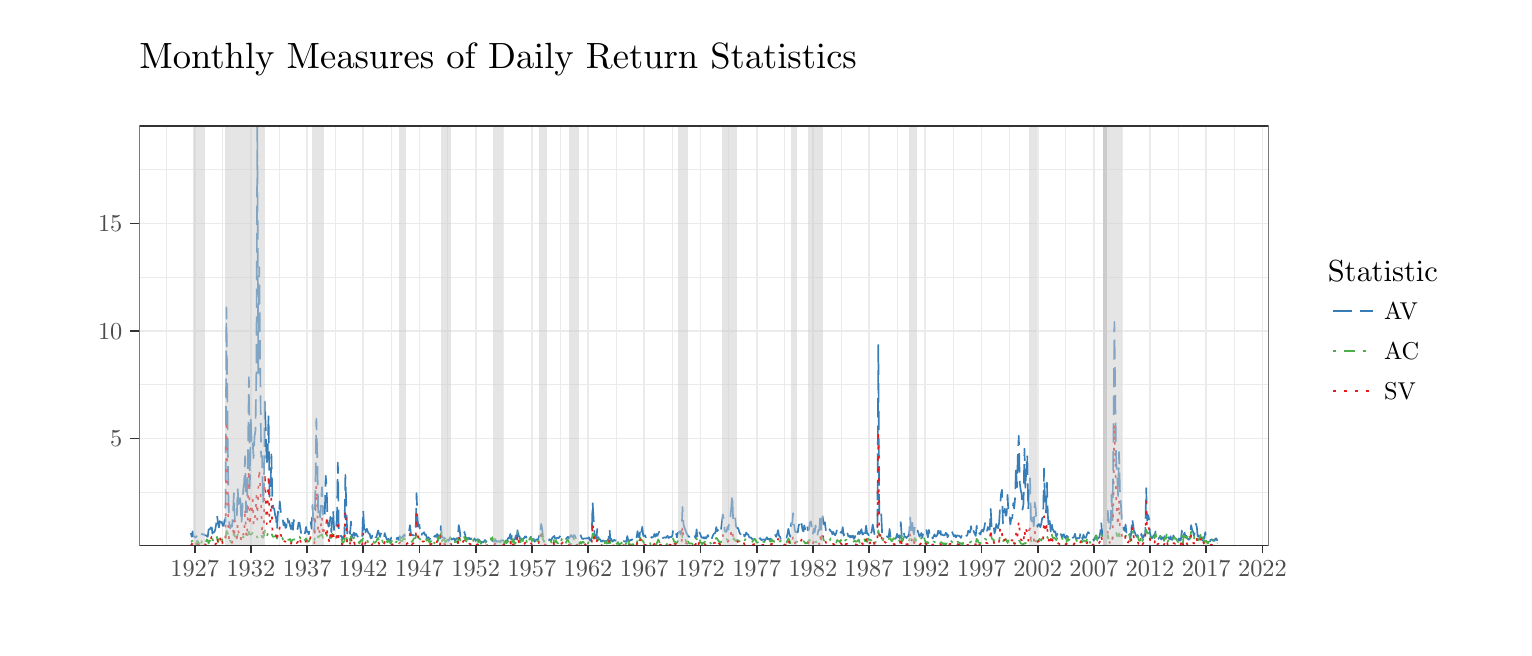
\begin{tikzpicture}[x=1.25pt,y=1pt]
\definecolor{fillColor}{RGB}{255,255,255}
\path[use as bounding box,fill=fillColor,fill opacity=0.00] (0,0) rectangle (426.79,216.81);
\begin{scope}
\path[clip] (  0.00,  0.00) rectangle (426.79,216.81);
\definecolor{drawColor}{RGB}{255,255,255}
\definecolor{fillColor}{RGB}{255,255,255}

\path[draw=drawColor,line width= 0.6pt,line join=round,line cap=round,fill=fillColor] (  0.00,  0.00) rectangle (426.79,216.81);
\end{scope}
\begin{scope}
\path[clip] ( 32.32, 29.59) rectangle (358.76,181.36);
\definecolor{fillColor}{RGB}{255,255,255}

\path[fill=fillColor] ( 32.32, 29.59) rectangle (358.76,181.36);
\definecolor{drawColor}{gray}{0.92}

\path[draw=drawColor,line width= 0.3pt,line join=round] ( 32.32, 48.97) --
	(358.76, 48.97);

\path[draw=drawColor,line width= 0.3pt,line join=round] ( 32.32, 87.81) --
	(358.76, 87.81);

\path[draw=drawColor,line width= 0.3pt,line join=round] ( 32.32,126.66) --
	(358.76,126.66);

\path[draw=drawColor,line width= 0.3pt,line join=round] ( 32.32,165.51) --
	(358.76,165.51);

\path[draw=drawColor,line width= 0.3pt,line join=round] ( 40.16, 29.59) --
	( 40.16,181.36);

\path[draw=drawColor,line width= 0.3pt,line join=round] ( 56.40, 29.59) --
	( 56.40,181.36);

\path[draw=drawColor,line width= 0.3pt,line join=round] ( 72.65, 29.59) --
	( 72.65,181.36);

\path[draw=drawColor,line width= 0.3pt,line join=round] ( 88.90, 29.59) --
	( 88.90,181.36);

\path[draw=drawColor,line width= 0.3pt,line join=round] (105.14, 29.59) --
	(105.14,181.36);

\path[draw=drawColor,line width= 0.3pt,line join=round] (121.39, 29.59) --
	(121.39,181.36);

\path[draw=drawColor,line width= 0.3pt,line join=round] (137.63, 29.59) --
	(137.63,181.36);

\path[draw=drawColor,line width= 0.3pt,line join=round] (153.88, 29.59) --
	(153.88,181.36);

\path[draw=drawColor,line width= 0.3pt,line join=round] (170.12, 29.59) --
	(170.12,181.36);

\path[draw=drawColor,line width= 0.3pt,line join=round] (186.37, 29.59) --
	(186.37,181.36);

\path[draw=drawColor,line width= 0.3pt,line join=round] (202.62, 29.59) --
	(202.62,181.36);

\path[draw=drawColor,line width= 0.3pt,line join=round] (218.86, 29.59) --
	(218.86,181.36);

\path[draw=drawColor,line width= 0.3pt,line join=round] (235.11, 29.59) --
	(235.11,181.36);

\path[draw=drawColor,line width= 0.3pt,line join=round] (251.35, 29.59) --
	(251.35,181.36);

\path[draw=drawColor,line width= 0.3pt,line join=round] (267.60, 29.59) --
	(267.60,181.36);

\path[draw=drawColor,line width= 0.3pt,line join=round] (283.85, 29.59) --
	(283.85,181.36);

\path[draw=drawColor,line width= 0.3pt,line join=round] (300.09, 29.59) --
	(300.09,181.36);

\path[draw=drawColor,line width= 0.3pt,line join=round] (316.33, 29.59) --
	(316.33,181.36);

\path[draw=drawColor,line width= 0.3pt,line join=round] (332.58, 29.59) --
	(332.58,181.36);

\path[draw=drawColor,line width= 0.3pt,line join=round] (348.83, 29.59) --
	(348.83,181.36);

\path[draw=drawColor,line width= 0.6pt,line join=round] ( 32.32, 68.39) --
	(358.76, 68.39);

\path[draw=drawColor,line width= 0.6pt,line join=round] ( 32.32,107.24) --
	(358.76,107.24);

\path[draw=drawColor,line width= 0.6pt,line join=round] ( 32.32,146.09) --
	(358.76,146.09);

\path[draw=drawColor,line width= 0.6pt,line join=round] ( 48.28, 29.59) --
	( 48.28,181.36);

\path[draw=drawColor,line width= 0.6pt,line join=round] ( 64.53, 29.59) --
	( 64.53,181.36);

\path[draw=drawColor,line width= 0.6pt,line join=round] ( 80.78, 29.59) --
	( 80.78,181.36);

\path[draw=drawColor,line width= 0.6pt,line join=round] ( 97.02, 29.59) --
	( 97.02,181.36);

\path[draw=drawColor,line width= 0.6pt,line join=round] (113.26, 29.59) --
	(113.26,181.36);

\path[draw=drawColor,line width= 0.6pt,line join=round] (129.51, 29.59) --
	(129.51,181.36);

\path[draw=drawColor,line width= 0.6pt,line join=round] (145.76, 29.59) --
	(145.76,181.36);

\path[draw=drawColor,line width= 0.6pt,line join=round] (162.00, 29.59) --
	(162.00,181.36);

\path[draw=drawColor,line width= 0.6pt,line join=round] (178.25, 29.59) --
	(178.25,181.36);

\path[draw=drawColor,line width= 0.6pt,line join=round] (194.49, 29.59) --
	(194.49,181.36);

\path[draw=drawColor,line width= 0.6pt,line join=round] (210.74, 29.59) --
	(210.74,181.36);

\path[draw=drawColor,line width= 0.6pt,line join=round] (226.99, 29.59) --
	(226.99,181.36);

\path[draw=drawColor,line width= 0.6pt,line join=round] (243.23, 29.59) --
	(243.23,181.36);

\path[draw=drawColor,line width= 0.6pt,line join=round] (259.47, 29.59) --
	(259.47,181.36);

\path[draw=drawColor,line width= 0.6pt,line join=round] (275.72, 29.59) --
	(275.72,181.36);

\path[draw=drawColor,line width= 0.6pt,line join=round] (291.97, 29.59) --
	(291.97,181.36);

\path[draw=drawColor,line width= 0.6pt,line join=round] (308.21, 29.59) --
	(308.21,181.36);

\path[draw=drawColor,line width= 0.6pt,line join=round] (324.45, 29.59) --
	(324.45,181.36);

\path[draw=drawColor,line width= 0.6pt,line join=round] (340.71, 29.59) --
	(340.71,181.36);

\path[draw=drawColor,line width= 0.6pt,line join=round] (356.95, 29.59) --
	(356.95,181.36);
\definecolor{drawColor}{RGB}{55,126,184}

\path[draw=drawColor,line width= 0.6pt,dash pattern=on 7pt off 3pt ,line join=round] ( 47.16, 34.17) --
	( 47.44, 32.84) --
	( 47.70, 34.78) --
	( 47.98, 32.86) --
	( 48.25, 32.94) --
	( 48.52, 32.62) --
	( 48.80, 32.80) --
	( 49.05, 33.83) --
	( 49.32, 33.16) --
	( 49.59, 33.11) --
	( 49.87, 33.40) --
	( 50.13, 33.08) --
	( 50.41, 33.91) --
	( 50.68, 33.68) --
	( 50.95, 33.69) --
	( 51.23, 33.38) --
	( 51.49, 33.36) --
	( 51.77, 33.07) --
	( 52.05, 32.83) --
	( 52.30, 35.46) --
	( 52.58, 35.55) --
	( 52.85, 35.87) --
	( 53.12, 37.94) --
	( 53.39, 33.99) --
	( 53.66, 34.55) --
	( 53.94, 34.49) --
	( 54.21, 35.34) --
	( 54.48, 37.37) --
	( 54.75, 40.62) --
	( 55.03, 37.58) --
	( 55.30, 36.21) --
	( 55.55, 38.54) --
	( 55.83, 36.42) --
	( 56.09, 38.23) --
	( 56.37, 36.86) --
	( 56.64, 36.77) --
	( 56.91, 38.91) --
	( 57.19, 38.25) --
	( 57.45,115.74) --
	( 57.73, 80.56) --
	( 58.00, 48.93) --
	( 58.27, 37.47) --
	( 58.55, 35.88) --
	( 58.80, 37.01) --
	( 59.07, 36.49) --
	( 59.34, 40.81) --
	( 59.62, 48.62) --
	( 59.88, 38.72) --
	( 60.16, 37.83) --
	( 60.43, 38.62) --
	( 60.70, 50.30) --
	( 60.98, 44.61) --
	( 61.24, 47.95) --
	( 61.52, 45.64) --
	( 61.79, 37.52) --
	( 62.04, 42.07) --
	( 62.32, 49.97) --
	( 62.59, 52.48) --
	( 62.86, 61.96) --
	( 63.13, 42.31) --
	( 63.40, 41.69) --
	( 63.68, 61.50) --
	( 63.95, 90.55) --
	( 64.22, 51.03) --
	( 64.49, 76.27) --
	( 64.77, 65.88) --
	( 65.04, 67.22) --
	( 65.30, 61.24) --
	( 65.58, 69.11) --
	( 65.84, 71.19) --
	( 66.12, 93.13) --
	( 66.38,181.36) --
	( 66.66, 91.93) --
	( 66.94,130.29) --
	( 67.20, 97.95) --
	( 67.48, 61.76) --
	( 67.75, 62.06) --
	( 68.02, 44.99) --
	( 68.30, 51.26) --
	( 68.55, 81.70) --
	( 68.82, 71.54) --
	( 69.09, 58.86) --
	( 69.36, 63.08) --
	( 69.63, 76.65) --
	( 69.91, 47.31) --
	( 70.18, 49.17) --
	( 70.45, 62.60) --
	( 70.73, 46.62) --
	( 70.99, 43.01) --
	( 71.27, 43.08) --
	( 71.54, 40.63) --
	( 71.79, 39.68) --
	( 72.07, 35.35) --
	( 72.34, 41.99) --
	( 72.61, 40.45) --
	( 72.88, 45.62) --
	( 73.15, 41.98) --
	( 73.43, 39.55) --
	( 73.70, 39.62) --
	( 73.97, 36.96) --
	( 74.24, 38.11) --
	( 74.52, 36.06) --
	( 74.79, 36.39) --
	( 75.04, 40.09) --
	( 75.32, 37.98) --
	( 75.58, 38.54) --
	( 75.86, 36.81) --
	( 76.13, 35.59) --
	( 76.40, 39.19) --
	( 76.68, 35.33) --
	( 76.94, 38.96) --
	( 77.22, 37.00) --
	( 77.49, 36.36) --
	( 77.76, 36.34) --
	( 78.04, 35.60) --
	( 78.30, 37.95) --
	( 78.57, 37.90) --
	( 78.84, 35.77) --
	( 79.11, 33.72) --
	( 79.38, 34.12) --
	( 79.66, 34.38) --
	( 79.93, 33.28) --
	( 80.20, 34.43) --
	( 80.48, 36.42) --
	( 80.74, 34.54) --
	( 81.02, 34.58) --
	( 81.29, 33.74) --
	( 81.54, 36.06) --
	( 81.82, 38.15) --
	( 82.09, 35.73) --
	( 82.36, 44.37) --
	( 82.63, 36.70) --
	( 82.90, 34.21) --
	( 83.18, 50.40) --
	( 83.45, 75.53) --
	( 83.72, 61.64) --
	( 83.99, 41.05) --
	( 84.27, 42.94) --
	( 84.54, 39.77) --
	( 84.79, 45.54) --
	( 85.07, 50.78) --
	( 85.33, 40.90) --
	( 85.61, 43.68) --
	( 85.88, 40.40) --
	( 86.15, 54.89) --
	( 86.43, 50.67) --
	( 86.69, 38.42) --
	( 86.97, 36.54) --
	( 87.24, 36.93) --
	( 87.51, 40.06) --
	( 87.79, 34.47) --
	( 88.04, 39.44) --
	( 88.31, 42.44) --
	( 88.58, 35.29) --
	( 88.86, 34.44) --
	( 89.12, 35.78) --
	( 89.40, 38.87) --
	( 89.67, 59.67) --
	( 89.94, 33.84) --
	( 90.22, 32.84) --
	( 90.48, 33.27) --
	( 90.76, 32.97) --
	( 91.03, 31.80) --
	( 91.29, 32.71) --
	( 91.57, 33.43) --
	( 91.84, 55.19) --
	( 92.11, 44.03) --
	( 92.38, 33.78) --
	( 92.65, 35.69) --
	( 92.93, 35.59) --
	( 93.20, 33.92) --
	( 93.47, 38.34) --
	( 93.74, 32.64) --
	( 94.01, 33.51) --
	( 94.29, 34.36) --
	( 94.54, 33.15) --
	( 94.82, 34.06) --
	( 95.08, 33.69) --
	( 95.36, 32.91) --
	( 95.62, 33.44) --
	( 95.90, 32.11) --
	( 96.18, 32.64) --
	( 96.44, 33.16) --
	( 96.72, 33.12) --
	( 96.99, 42.52) --
	( 97.26, 35.88) --
	( 97.54, 33.18) --
	( 97.79, 35.45) --
	( 98.06, 35.68) --
	( 98.33, 34.67) --
	( 98.60, 34.01) --
	( 98.87, 33.87) --
	( 99.15, 32.36) --
	( 99.42, 32.29) --
	( 99.69, 34.00) --
	( 99.97, 32.87) --
	(100.23, 33.42) --
	(100.51, 32.76) --
	(100.78, 32.61) --
	(101.03, 33.84) --
	(101.31, 35.10) --
	(101.58, 33.95) --
	(101.85, 32.80) --
	(102.12, 34.05) --
	(102.39, 33.37) --
	(102.67, 31.97) --
	(102.94, 32.14) --
	(103.21, 34.17) --
	(103.48, 33.07) --
	(103.76, 31.96) --
	(104.03, 31.70) --
	(104.29, 32.13) --
	(104.56, 31.59) --
	(104.83, 31.43) --
	(105.11, 32.52) --
	(105.37, 32.47) --
	(105.65, 31.90) --
	(105.93, 32.30) --
	(106.19, 31.40) --
	(106.47, 31.44) --
	(106.74, 32.42) --
	(107.01, 32.53) --
	(107.29, 31.66) --
	(107.54, 33.11) --
	(107.81, 32.38) --
	(108.08, 32.46) --
	(108.35, 32.83) --
	(108.62, 33.22) --
	(108.90, 33.69) --
	(109.17, 32.66) --
	(109.44, 32.97) --
	(109.72, 33.84) --
	(109.98, 34.16) --
	(110.26, 34.91) --
	(110.53, 37.01) --
	(110.78, 33.87) --
	(111.06, 33.30) --
	(111.33, 33.50) --
	(111.60, 33.30) --
	(111.87, 33.82) --
	(112.14, 33.83) --
	(112.42, 48.63) --
	(112.69, 39.21) --
	(112.96, 36.54) --
	(113.23, 37.24) --
	(113.50, 34.34) --
	(113.78, 32.99) --
	(114.03, 34.06) --
	(114.31, 34.01) --
	(114.57, 34.51) --
	(114.85, 33.50) --
	(115.11, 33.68) --
	(115.39, 32.30) --
	(115.67, 32.68) --
	(115.93, 32.59) --
	(116.21, 31.76) --
	(116.48, 33.17) --
	(116.75, 33.08) --
	(117.03, 33.09) --
	(117.29, 33.85) --
	(117.56, 32.85) --
	(117.83, 33.32) --
	(118.10, 32.78) --
	(118.37, 33.87) --
	(118.65, 32.26) --
	(118.92, 33.43) --
	(119.19, 32.18) --
	(119.46, 36.76) --
	(119.73, 32.80) --
	(120.01, 32.60) --
	(120.28, 32.50) --
	(120.53, 32.46) --
	(120.81, 31.64) --
	(121.07, 31.81) --
	(121.35, 32.98) --
	(121.62, 31.33) --
	(121.89, 32.00) --
	(122.17, 32.71) --
	(122.44, 31.79) --
	(122.71, 31.90) --
	(122.98, 32.15) --
	(123.25, 32.29) --
	(123.53, 31.34) --
	(123.78, 32.00) --
	(124.05, 32.33) --
	(124.32, 31.76) --
	(124.60, 37.07) --
	(124.86, 35.58) --
	(125.14, 32.36) --
	(125.42, 32.19) --
	(125.68, 32.92) --
	(125.96, 33.92) --
	(126.23, 34.58) --
	(126.50, 33.39) --
	(126.78, 31.72) --
	(127.03, 32.46) --
	(127.30, 31.91) --
	(127.57, 32.48) --
	(127.84, 31.98) --
	(128.11, 32.28) --
	(128.39, 31.81) --
	(128.66, 31.50) --
	(128.93, 33.24) --
	(129.21, 32.00) --
	(129.47, 31.33) --
	(129.75, 31.73) --
	(130.02, 31.81) --
	(130.28, 31.92) --
	(130.56, 31.66) --
	(130.82, 31.23) --
	(131.10, 30.85) --
	(131.37, 30.98) --
	(131.64, 30.73) --
	(131.92, 31.13) --
	(132.19, 31.68) --
	(132.46, 31.19) --
	(132.73, 31.13) --
	(133.00, 31.01) --
	(133.28, 30.91) --
	(133.53, 31.55) --
	(133.80, 31.94) --
	(134.07, 31.04) --
	(134.35, 31.91) --
	(134.61, 31.07) --
	(134.89, 31.12) --
	(135.17, 32.00) --
	(135.43, 31.23) --
	(135.71, 31.03) --
	(135.97, 31.28) --
	(136.25, 31.20) --
	(136.53, 31.09) --
	(136.78, 31.42) --
	(137.05, 31.61) --
	(137.32, 31.37) --
	(137.59, 32.58) --
	(137.86, 31.80) --
	(138.14, 32.32) --
	(138.41, 31.45) --
	(138.68, 31.61) --
	(138.95, 32.52) --
	(139.22, 32.35) --
	(139.50, 33.83) --
	(139.77, 31.86) --
	(140.02, 33.92) --
	(140.30, 31.71) --
	(140.56, 31.92) --
	(140.84, 31.90) --
	(141.11, 33.31) --
	(141.38, 31.88) --
	(141.66, 36.40) --
	(141.93, 32.99) --
	(142.20, 32.93) --
	(142.47, 31.38) --
	(142.74, 31.99) --
	(143.02, 31.81) --
	(143.28, 32.11) --
	(143.55, 32.46) --
	(143.82, 33.02) --
	(144.10, 32.87) --
	(144.36, 31.69) --
	(144.64, 32.09) --
	(144.91, 31.58) --
	(145.18, 32.52) --
	(145.46, 32.83) --
	(145.72, 31.89) --
	(146.00, 31.71) --
	(146.28, 32.08) --
	(146.53, 31.03) --
	(146.80, 31.48) --
	(147.07, 31.88) --
	(147.34, 31.89) --
	(147.61, 31.93) --
	(147.89, 33.30) --
	(148.16, 32.54) --
	(148.43, 37.47) --
	(148.70, 35.86) --
	(148.97, 32.73) --
	(149.25, 32.47) --
	(149.52, 31.61) --
	(149.77, 31.51) --
	(150.05, 31.75) --
	(150.31, 31.34) --
	(150.59, 31.34) --
	(150.86, 31.96) --
	(151.13, 31.57) --
	(151.41, 31.65) --
	(151.68, 32.56) --
	(151.95, 32.81) --
	(152.22, 33.13) --
	(152.49, 32.25) --
	(152.77, 32.09) --
	(153.02, 32.46) --
	(153.29, 32.51) --
	(153.56, 32.37) --
	(153.84, 33.02) --
	(154.10, 32.62) --
	(154.38, 32.43) --
	(154.66, 33.30) --
	(154.92, 32.60) --
	(155.20, 32.43) --
	(155.47, 32.22) --
	(155.74, 32.08) --
	(156.02, 32.72) --
	(156.27, 32.80) --
	(156.55, 32.26) --
	(156.82, 32.99) --
	(157.09, 33.48) --
	(157.36, 32.81) --
	(157.64, 32.64) --
	(157.91, 33.46) --
	(158.18, 33.17) --
	(158.45, 32.32) --
	(158.72, 32.71) --
	(159.00, 32.88) --
	(159.27, 32.31) --
	(159.52, 32.87) --
	(159.80, 33.65) --
	(160.06, 32.65) --
	(160.34, 32.11) --
	(160.61, 32.04) --
	(160.88, 32.28) --
	(161.16, 32.27) --
	(161.43, 32.21) --
	(161.70, 32.38) --
	(161.97, 32.21) --
	(162.24, 32.65) --
	(162.52, 31.54) --
	(162.77, 31.48) --
	(163.04, 32.40) --
	(163.31, 45.35) --
	(163.59, 39.25) --
	(163.85, 33.87) --
	(164.13, 32.42) --
	(164.41, 32.16) --
	(164.67, 35.91) --
	(164.95, 32.74) --
	(165.21, 31.93) --
	(165.49, 31.97) --
	(165.77, 31.14) --
	(166.02, 31.10) --
	(166.29, 31.55) --
	(166.56, 31.37) --
	(166.83, 31.12) --
	(167.10, 31.41) --
	(167.38, 31.29) --
	(167.65, 31.46) --
	(167.92, 32.27) --
	(168.19, 35.72) --
	(168.46, 31.64) --
	(168.74, 32.03) --
	(169.01, 31.08) --
	(169.27, 31.30) --
	(169.55, 31.74) --
	(169.81, 31.42) --
	(170.09, 31.54) --
	(170.36, 31.25) --
	(170.63, 31.26) --
	(170.91, 31.21) --
	(171.17, 31.14) --
	(171.45, 31.24) --
	(171.72, 31.53) --
	(171.99, 31.11) --
	(172.27, 31.29) --
	(172.52, 31.16) --
	(172.79, 31.10) --
	(173.06, 31.23) --
	(173.34, 33.10) --
	(173.60, 31.54) --
	(173.88, 31.16) --
	(174.15, 31.69) --
	(174.42, 31.61) --
	(174.70, 31.78) --
	(174.96, 32.55) --
	(175.24, 32.09) --
	(175.52, 32.13) --
	(175.76, 33.28) --
	(176.04, 32.64) --
	(176.31, 34.89) --
	(176.58, 32.82) --
	(176.85, 32.61) --
	(177.13, 36.14) --
	(177.40, 34.65) --
	(177.67, 36.43) --
	(177.94, 33.17) --
	(178.21, 33.13) --
	(178.49, 33.40) --
	(178.76, 32.31) --
	(179.01, 33.02) --
	(179.29, 32.82) --
	(179.55, 33.02) --
	(179.83, 33.50) --
	(180.10, 33.05) --
	(180.37, 32.46) --
	(180.65, 32.62) --
	(180.92, 32.93) --
	(181.19, 33.85) --
	(181.46, 32.87) --
	(181.73, 33.83) --
	(182.01, 33.17) --
	(182.27, 33.91) --
	(182.54, 34.64) --
	(182.81, 33.17) --
	(183.09, 33.45) --
	(183.35, 33.50) --
	(183.63, 32.37) --
	(183.90, 32.57) --
	(184.17, 32.66) --
	(184.45, 32.40) --
	(184.71, 32.82) --
	(184.99, 33.20) --
	(185.27, 32.39) --
	(185.51, 32.67) --
	(185.79, 32.82) --
	(186.06, 32.72) --
	(186.33, 33.14) --
	(186.60, 35.29) --
	(186.88, 33.65) --
	(187.15, 33.61) --
	(187.42, 34.22) --
	(187.69, 32.64) --
	(187.96, 34.25) --
	(188.24, 34.46) --
	(188.51, 34.83) --
	(188.76, 33.66) --
	(189.04, 34.55) --
	(189.30, 43.59) --
	(189.58, 37.20) --
	(189.85, 36.24) --
	(190.12, 35.28) --
	(190.40, 34.34) --
	(190.66, 33.73) --
	(190.94, 32.99) --
	(191.21, 32.80) --
	(191.48, 33.01) --
	(191.76, 32.56) --
	(192.01, 32.64) --
	(192.28, 32.86) --
	(192.55, 32.18) --
	(192.83, 33.09) --
	(193.09, 32.28) --
	(193.37, 35.53) --
	(193.64, 32.04) --
	(193.91, 32.67) --
	(194.19, 34.40) --
	(194.45, 33.77) --
	(194.73, 32.67) --
	(195.01, 32.42) --
	(195.26, 32.69) --
	(195.54, 32.18) --
	(195.81, 32.72) --
	(196.08, 32.22) --
	(196.35, 32.81) --
	(196.62, 33.47) --
	(196.90, 32.11) --
	(197.17, 32.98) --
	(197.44, 32.87) --
	(197.71, 31.96) --
	(197.99, 33.00) --
	(198.26, 33.77) --
	(198.51, 34.10) --
	(198.79, 34.22) --
	(199.05, 36.34) --
	(199.33, 34.88) --
	(199.60, 35.27) --
	(199.87, 33.85) --
	(200.15, 34.40) --
	(200.41, 35.27) --
	(200.69, 38.10) --
	(200.96, 40.90) --
	(201.23, 39.24) --
	(201.51, 34.92) --
	(201.76, 34.66) --
	(202.03, 34.67) --
	(202.30, 36.41) --
	(202.58, 35.44) --
	(202.84, 39.91) --
	(203.12, 39.87) --
	(203.39, 43.17) --
	(203.66, 48.13) --
	(203.94, 38.73) --
	(204.20, 38.52) --
	(204.48, 40.15) --
	(204.76, 36.61) --
	(205.00, 35.99) --
	(205.28, 36.11) --
	(205.55, 35.27) --
	(205.82, 34.21) --
	(206.09, 33.74) --
	(206.37, 34.95) --
	(206.64, 35.09) --
	(206.91, 34.99) --
	(207.18, 32.90) --
	(207.45, 33.39) --
	(207.73, 34.38) --
	(208.00, 33.65) --
	(208.26, 33.77) --
	(208.54, 32.82) --
	(208.80, 32.50) --
	(209.08, 32.66) --
	(209.35, 31.99) --
	(209.62, 32.13) --
	(209.90, 32.11) --
	(210.16, 32.64) --
	(210.44, 32.72) --
	(210.71, 32.29) --
	(210.98, 32.19) --
	(211.26, 31.64) --
	(211.51, 32.05) --
	(211.78, 32.35) --
	(212.05, 31.68) --
	(212.33, 31.71) --
	(212.59, 31.90) --
	(212.87, 31.92) --
	(213.14, 31.46) --
	(213.41, 32.04) --
	(213.69, 32.68) --
	(213.95, 31.96) --
	(214.23, 32.13) --
	(214.50, 31.63) --
	(214.75, 32.19) --
	(215.03, 33.04) --
	(215.30, 33.01) --
	(215.57, 32.60) --
	(215.84, 32.38) --
	(216.11, 33.51) --
	(216.39, 32.80) --
	(216.66, 33.94) --
	(216.93, 35.22) --
	(217.20, 33.19) --
	(217.48, 32.84) --
	(217.75, 31.85) --
	(218.00, 32.45) --
	(218.28, 32.10) --
	(218.54, 32.84) --
	(218.82, 32.64) --
	(219.09, 32.65) --
	(219.36, 32.52) --
	(219.64, 33.79) --
	(219.90, 35.73) --
	(220.18, 34.00) --
	(220.45, 32.85) --
	(220.72, 37.82) --
	(221.00, 37.30) --
	(221.26, 41.37) --
	(221.53, 37.28) --
	(221.80, 34.96) --
	(222.07, 34.40) --
	(222.34, 34.58) --
	(222.62, 34.45) --
	(222.89, 37.09) --
	(223.16, 37.21) --
	(223.44, 36.02) --
	(223.70, 37.77) --
	(223.98, 35.33) --
	(224.25, 34.77) --
	(224.50, 36.97) --
	(224.78, 35.57) --
	(225.05, 34.96) --
	(225.32, 37.00) --
	(225.59, 35.17) --
	(225.86, 35.48) --
	(226.14, 38.08) --
	(226.41, 38.37) --
	(226.68, 36.53) --
	(226.95, 33.53) --
	(227.23, 35.74) --
	(227.50, 34.44) --
	(227.75, 36.98) --
	(228.03, 34.39) --
	(228.29, 33.16) --
	(228.57, 35.32) --
	(228.84, 35.10) --
	(229.11, 40.38) --
	(229.39, 35.40) --
	(229.65, 41.58) --
	(229.93, 38.95) --
	(230.20, 37.35) --
	(230.47, 38.05) --
	(230.75, 35.01) --
	(231.00, 35.53) --
	(231.27, 34.42) --
	(231.54, 34.36) --
	(231.82, 35.58) --
	(232.08, 34.86) --
	(232.36, 34.81) --
	(232.63, 33.77) --
	(232.90, 34.59) --
	(233.18, 33.73) --
	(233.44, 33.37) --
	(233.72, 34.20) --
	(234.00, 35.67) --
	(234.25, 34.58) --
	(234.53, 33.78) --
	(234.80, 33.82) --
	(235.07, 34.58) --
	(235.34, 34.21) --
	(235.61, 36.27) --
	(235.89, 33.22) --
	(236.16, 34.05) --
	(236.43, 32.67) --
	(236.70, 33.31) --
	(236.98, 34.06) --
	(237.25, 32.96) --
	(237.50, 33.24) --
	(237.78, 32.59) --
	(238.04, 33.21) --
	(238.32, 32.65) --
	(238.59, 33.23) --
	(238.86, 32.06) --
	(239.14, 32.64) --
	(239.40, 33.89) --
	(239.68, 32.57) --
	(239.95, 33.89) --
	(240.22, 34.72) --
	(240.50, 33.85) --
	(240.75, 34.48) --
	(241.02, 35.61) --
	(241.29, 33.69) --
	(241.57, 33.71) --
	(241.83, 35.83) --
	(242.11, 34.13) --
	(242.38, 36.87) --
	(242.65, 33.96) --
	(242.93, 33.94) --
	(243.19, 33.18) --
	(243.47, 35.03) --
	(243.74, 34.07) --
	(243.99, 34.68) --
	(244.27, 37.27) --
	(244.54, 35.70) --
	(244.81, 33.49) --
	(245.08, 33.54) --
	(245.35, 34.28) --
	(245.63, 35.16) --
	(245.90,102.16) --
	(246.17, 40.57) --
	(246.44, 40.65) --
	(246.72, 41.83) --
	(246.99, 34.40) --
	(247.25, 34.88) --
	(247.53, 34.96) --
	(247.79, 33.85) --
	(248.07, 33.92) --
	(248.33, 33.07) --
	(248.61, 32.73) --
	(248.89, 32.61) --
	(249.15, 35.65) --
	(249.43, 32.62) --
	(249.70, 31.93) --
	(249.97, 32.53) --
	(250.25, 32.33) --
	(250.50, 32.77) --
	(250.77, 32.06) --
	(251.04, 32.49) --
	(251.31, 33.89) --
	(251.58, 32.72) --
	(251.86, 33.37) --
	(252.13, 32.10) --
	(252.40, 38.16) --
	(252.68, 32.73) --
	(252.94, 32.93) --
	(253.22, 34.80) --
	(253.49, 32.84) --
	(253.74, 32.85) --
	(254.02, 32.40) --
	(254.29, 32.82) --
	(254.56, 33.06) --
	(254.83, 33.99) --
	(255.10, 39.80) --
	(255.38, 35.17) --
	(255.65, 39.30) --
	(255.92, 35.29) --
	(256.19, 33.74) --
	(256.47, 36.67) --
	(256.74, 35.91) --
	(256.99, 34.64) --
	(257.27, 35.10) --
	(257.53, 34.08) --
	(257.81, 32.86) --
	(258.08, 33.41) --
	(258.35, 34.20) --
	(258.63, 32.57) --
	(258.89, 34.22) --
	(259.17, 34.22) --
	(259.44, 35.01) --
	(259.71, 35.97) --
	(259.99, 33.95) --
	(260.25, 32.64) --
	(260.52, 35.35) --
	(260.79, 33.04) --
	(261.06, 33.79) --
	(261.33, 33.53) --
	(261.61, 32.22) --
	(261.88, 33.06) --
	(262.15, 33.73) --
	(262.43, 32.91) --
	(262.69, 33.01) --
	(262.97, 33.67) --
	(263.24, 35.06) --
	(263.49, 33.99) --
	(263.77, 36.19) --
	(264.04, 33.51) --
	(264.31, 33.76) --
	(264.58, 33.39) --
	(264.85, 33.38) --
	(265.13, 33.39) --
	(265.40, 34.28) --
	(265.67, 34.06) --
	(265.94, 32.68) --
	(266.21, 33.47) --
	(266.49, 33.30) --
	(266.74, 34.10) --
	(267.02, 35.29) --
	(267.28, 34.45) --
	(267.56, 33.58) --
	(267.82, 32.96) --
	(268.10, 33.47) --
	(268.38, 32.62) --
	(268.64, 33.32) --
	(268.92, 33.27) --
	(269.19, 33.19) --
	(269.46, 33.01) --
	(269.74, 32.43) --
	(269.99, 33.14) --
	(270.26, 33.13) --
	(270.53, 33.80) --
	(270.80, 33.72) --
	(271.07, 34.40) --
	(271.35, 33.14) --
	(271.62, 33.36) --
	(271.89, 35.06) --
	(272.17, 34.39) --
	(272.43, 34.54) --
	(272.71, 36.68) --
	(272.98, 34.29) --
	(273.24, 35.65) --
	(273.52, 34.65) --
	(273.78, 33.89) --
	(274.06, 33.17) --
	(274.33, 36.84) --
	(274.60, 33.86) --
	(274.88, 33.32) --
	(275.15, 34.20) --
	(275.42, 33.63) --
	(275.69, 35.01) --
	(275.96, 35.41) --
	(276.24, 34.73) --
	(276.49, 35.90) --
	(276.76, 37.81) --
	(277.03, 35.05) --
	(277.31, 34.98) --
	(277.57, 36.41) --
	(277.85, 35.39) --
	(278.13, 35.55) --
	(278.39, 42.94) --
	(278.67, 35.84) --
	(278.94, 36.91) --
	(279.21, 37.10) --
	(279.49, 34.06) --
	(279.74, 35.08) --
	(280.01, 37.46) --
	(280.28, 34.42) --
	(280.55, 36.40) --
	(280.82, 37.75) --
	(281.10, 43.62) --
	(281.37, 48.19) --
	(281.64, 49.81) --
	(281.92, 37.70) --
	(282.18, 40.49) --
	(282.46, 43.00) --
	(282.73, 40.46) --
	(282.98, 40.74) --
	(283.26, 47.99) --
	(283.53, 40.91) --
	(283.80, 40.77) --
	(284.07, 37.32) --
	(284.34, 39.61) --
	(284.62, 39.51) --
	(284.89, 44.97) --
	(285.16, 43.00) --
	(285.43, 46.65) --
	(285.70, 57.88) --
	(285.98, 50.72) --
	(286.24, 62.42) --
	(286.51, 69.37) --
	(286.78, 52.36) --
	(287.06, 49.90) --
	(287.32, 48.27) --
	(287.60, 42.61) --
	(287.88, 44.88) --
	(288.14, 64.69) --
	(288.42, 50.20) --
	(288.68, 57.47) --
	(288.96, 62.62) --
	(289.24, 42.54) --
	(289.49, 51.48) --
	(289.76, 54.03) --
	(290.03, 39.25) --
	(290.30, 38.04) --
	(290.57, 40.40) --
	(290.85, 36.66) --
	(291.12, 45.21) --
	(291.39, 43.15) --
	(291.66, 37.22) --
	(291.93, 36.42) --
	(292.21, 37.43) --
	(292.48, 37.29) --
	(292.73, 36.31) --
	(293.01, 37.50) --
	(293.27, 39.58) --
	(293.55, 39.74) --
	(293.82, 57.57) --
	(294.09, 44.48) --
	(294.37, 41.58) --
	(294.64, 52.42) --
	(294.91, 40.60) --
	(295.18, 35.62) --
	(295.45, 38.58) --
	(295.73, 34.72) --
	(295.98, 38.35) --
	(296.25, 35.73) --
	(296.52, 35.03) --
	(296.80, 34.47) --
	(297.06, 34.82) --
	(297.34, 32.78) --
	(297.62, 33.80) --
	(297.88, 33.93) --
	(298.16, 32.57) --
	(298.43, 32.41) --
	(298.70, 33.85) --
	(298.98, 32.46) --
	(299.24, 33.50) --
	(299.51, 33.75) --
	(299.78, 32.75) --
	(300.05, 32.18) --
	(300.32, 33.22) --
	(300.60, 32.94) --
	(300.87, 32.55) --
	(301.14, 33.68) --
	(301.41, 32.59) --
	(301.68, 32.41) --
	(301.96, 32.54) --
	(302.23, 32.50) --
	(302.48, 32.88) --
	(302.76, 33.93) --
	(303.02, 32.22) --
	(303.30, 32.05) --
	(303.57, 32.44) --
	(303.84, 32.27) --
	(304.12, 32.52) --
	(304.39, 34.81) --
	(304.66, 32.85) --
	(304.93, 31.94) --
	(305.20, 33.60) --
	(305.48, 32.56) --
	(305.73, 32.45) --
	(306.00, 32.79) --
	(306.27, 33.92) --
	(306.55, 34.52) --
	(306.81, 34.18) --
	(307.09, 32.70) --
	(307.37, 32.59) --
	(307.63, 32.88) --
	(307.91, 32.46) --
	(308.18, 31.42) --
	(308.45, 32.58) --
	(308.73, 32.57) --
	(308.98, 32.66) --
	(309.25, 32.10) --
	(309.52, 32.39) --
	(309.79, 32.61) --
	(310.06, 34.39) --
	(310.34, 38.23) --
	(310.61, 33.14) --
	(310.88, 35.40) --
	(311.16, 40.41) --
	(311.42, 34.77) --
	(311.70, 41.17) --
	(311.97, 37.52) --
	(312.23, 42.23) --
	(312.51, 37.93) --
	(312.77, 35.19) --
	(313.05, 36.78) --
	(313.32, 48.10) --
	(313.59, 38.77) --
	(313.87, 67.97) --
	(314.14,110.47) --
	(314.41, 81.00) --
	(314.68, 59.45) --
	(314.95, 54.78) --
	(315.23, 47.51) --
	(315.48, 63.47) --
	(315.75, 49.10) --
	(316.02, 44.73) --
	(316.30, 37.89) --
	(316.56, 37.89) --
	(316.84, 35.54) --
	(317.12, 34.97) --
	(317.38, 37.27) --
	(317.66, 33.86) --
	(317.92, 32.95) --
	(318.20, 34.20) --
	(318.48, 33.94) --
	(318.73, 32.12) --
	(319.00, 34.03) --
	(319.27, 39.49) --
	(319.54, 37.27) --
	(319.81, 34.97) --
	(320.09, 34.35) --
	(320.36, 33.22) --
	(320.63, 33.08) --
	(320.90, 33.48) --
	(321.17, 31.95) --
	(321.45, 33.06) --
	(321.72, 32.98) --
	(321.97, 33.95) --
	(322.25, 32.36) --
	(322.51, 32.56) --
	(322.79, 33.63) --
	(323.06, 33.57) --
	(323.33, 50.46) --
	(323.61, 38.59) --
	(323.88, 40.71) --
	(324.15, 39.30) --
	(324.42, 34.19) --
	(324.69, 33.00) --
	(324.97, 32.27) --
	(325.23, 32.56) --
	(325.50, 33.48) --
	(325.77, 33.39) --
	(326.05, 34.74) --
	(326.31, 33.81) --
	(326.59, 31.97) --
	(326.86, 32.06) --
	(327.13, 32.58) --
	(327.41, 33.15) --
	(327.67, 31.85) --
	(327.95, 32.67) --
	(328.23, 32.32) --
	(328.47, 31.42) --
	(328.75, 33.96) --
	(329.02, 32.67) --
	(329.29, 33.15) --
	(329.56, 32.88) --
	(329.84, 32.33) --
	(330.11, 31.90) --
	(330.38, 33.04) --
	(330.65, 31.83) --
	(330.92, 31.72) --
	(331.20, 33.33) --
	(331.47, 32.47) --
	(331.72, 32.05) --
	(332.00, 33.25) --
	(332.26, 31.61) --
	(332.54, 31.35) --
	(332.81, 32.28) --
	(333.08, 31.42) --
	(333.36, 31.66) --
	(333.63, 35.09) --
	(333.90, 31.88) --
	(334.17, 33.64) --
	(334.44, 34.33) --
	(334.72, 32.47) --
	(334.97, 33.18) --
	(335.24, 32.39) --
	(335.51, 31.87) --
	(335.79, 31.85) --
	(336.05, 33.59) --
	(336.33, 37.03) --
	(336.61, 35.31) --
	(336.87, 34.76) --
	(337.15, 33.12) --
	(337.41, 34.53) --
	(337.69, 37.59) --
	(337.97, 36.50) --
	(338.22, 32.98) --
	(338.50, 33.27) --
	(338.77, 32.53) --
	(339.04, 34.56) --
	(339.31, 31.92) --
	(339.59, 31.52) --
	(339.86, 32.71) --
	(340.13, 32.14) --
	(340.40, 34.53) --
	(340.67, 31.74) --
	(340.95, 31.83) --
	(341.22, 31.47) --
	(341.47, 31.45) --
	(341.75, 31.14) --
	(342.01, 31.80) --
	(342.29, 31.92) --
	(342.56, 31.61) --
	(342.83, 31.73) --
	(343.11, 31.36) --
	(343.37, 32.20) --
	(343.65, 32.21) --
	(343.92, 31.36);
\definecolor{drawColor}{RGB}{77,175,74}

\path[draw=drawColor,line width= 0.6pt,dash pattern=on 1pt off 3pt on 4pt off 3pt ,line join=round] ( 47.16, 31.09) --
	( 47.44, 31.04) --
	( 47.70, 32.13) --
	( 47.98, 30.61) --
	( 48.25, 30.76) --
	( 48.52, 30.91) --
	( 48.80, 30.05) --
	( 49.05, 31.45) --
	( 49.32, 30.96) --
	( 49.59, 30.23) --
	( 49.87, 31.57) --
	( 50.13, 30.02) --
	( 50.41, 31.73) --
	( 50.68, 31.32) --
	( 50.95, 31.87) --
	( 51.23, 30.91) --
	( 51.49, 30.82) --
	( 51.77, 31.87) --
	( 52.05, 31.63) --
	( 52.30, 30.43) --
	( 52.58, 31.28) --
	( 52.85, 31.65) --
	( 53.12, 33.41) --
	( 53.39, 32.34) --
	( 53.66, 31.09) --
	( 53.94, 30.76) --
	( 54.21, 30.65) --
	( 54.48, 30.57) --
	( 54.75, 32.83) --
	( 55.03, 30.87) --
	( 55.30, 32.73) --
	( 55.55, 32.98) --
	( 55.83, 31.97) --
	( 56.09, 32.51) --
	( 56.37, 30.65) --
	( 56.64, 30.58) --
	( 56.91, 31.77) --
	( 57.19, 31.88) --
	( 57.45, 34.93) --
	( 57.73, 34.55) --
	( 58.00, 33.29) --
	( 58.27, 30.99) --
	( 58.55, 31.46) --
	( 58.80, 30.65) --
	( 59.07, 31.33) --
	( 59.34, 32.63) --
	( 59.62, 34.08) --
	( 59.88, 32.95) --
	( 60.16, 32.90) --
	( 60.43, 32.58) --
	( 60.70, 33.65) --
	( 60.98, 33.11) --
	( 61.24, 33.31) --
	( 61.52, 33.06) --
	( 61.79, 32.01) --
	( 62.04, 32.40) --
	( 62.32, 32.87) --
	( 62.59, 32.43) --
	( 62.86, 33.90) --
	( 63.13, 33.52) --
	( 63.40, 32.96) --
	( 63.68, 33.77) --
	( 63.95, 34.65) --
	( 64.22, 33.71) --
	( 64.49, 33.64) --
	( 64.77, 33.83) --
	( 65.04, 34.30) --
	( 65.30, 33.26) --
	( 65.58, 32.72) --
	( 65.84, 33.18) --
	( 66.12, 33.54) --
	( 66.38, 32.57) --
	( 66.66, 33.63) --
	( 66.94, 34.37) --
	( 67.20, 34.35) --
	( 67.48, 34.07) --
	( 67.75, 32.77) --
	( 68.02, 32.49) --
	( 68.30, 33.24) --
	( 68.55, 35.17) --
	( 68.82, 33.69) --
	( 69.09, 32.71) --
	( 69.36, 33.83) --
	( 69.63, 34.58) --
	( 69.91, 34.20) --
	( 70.18, 33.61) --
	( 70.45, 34.37) --
	( 70.73, 33.17) --
	( 70.99, 32.79) --
	( 71.27, 32.95) --
	( 71.54, 33.00) --
	( 71.79, 33.37) --
	( 72.07, 32.21) --
	( 72.34, 33.09) --
	( 72.61, 33.35) --
	( 72.88, 33.71) --
	( 73.15, 33.16) --
	( 73.43, 32.83) --
	( 73.70, 32.25) --
	( 73.97, 31.15) --
	( 74.24, 32.08) --
	( 74.52, 31.93) --
	( 74.79, 32.28) --
	( 75.04, 32.02) --
	( 75.32, 31.75) --
	( 75.58, 31.73) --
	( 75.86, 32.07) --
	( 76.13, 31.00) --
	( 76.40, 31.46) --
	( 76.68, 31.77) --
	( 76.94, 31.86) --
	( 77.22, 31.85) --
	( 77.49, 31.80) --
	( 77.76, 31.15) --
	( 78.04, 31.42) --
	( 78.30, 32.64) --
	( 78.57, 32.89) --
	( 78.84, 32.31) --
	( 79.11, 31.29) --
	( 79.38, 30.92) --
	( 79.66, 31.97) --
	( 79.93, 31.55) --
	( 80.20, 31.77) --
	( 80.48, 32.24) --
	( 80.74, 31.67) --
	( 81.02, 31.06) --
	( 81.29, 31.10) --
	( 81.54, 31.78) --
	( 81.82, 33.27) --
	( 82.09, 32.57) --
	( 82.36, 32.47) --
	( 82.63, 31.80) --
	( 82.90, 31.69) --
	( 83.18, 33.87) --
	( 83.45, 34.07) --
	( 83.72, 34.08) --
	( 83.99, 32.57) --
	( 84.27, 33.07) --
	( 84.54, 33.24) --
	( 84.79, 33.45) --
	( 85.07, 33.76) --
	( 85.33, 32.44) --
	( 85.61, 33.21) --
	( 85.88, 32.88) --
	( 86.15, 32.93) --
	( 86.43, 34.14) --
	( 86.69, 31.94) --
	( 86.97, 32.79) --
	( 87.24, 31.92) --
	( 87.51, 33.47) --
	( 87.79, 32.47) --
	( 88.04, 33.91) --
	( 88.31, 33.40) --
	( 88.58, 32.23) --
	( 88.86, 32.67) --
	( 89.12, 32.34) --
	( 89.40, 33.27) --
	( 89.67, 32.48) --
	( 89.94, 31.87) --
	( 90.22, 31.32) --
	( 90.48, 31.11) --
	( 90.76, 31.97) --
	( 91.03, 30.47) --
	( 91.29, 30.92) --
	( 91.57, 31.26) --
	( 91.84, 33.94) --
	( 92.11, 33.30) --
	( 92.38, 30.97) --
	( 92.65, 32.57) --
	( 92.93, 32.60) --
	( 93.20, 31.32) --
	( 93.47, 33.07) --
	( 93.74, 30.53) --
	( 94.01, 31.53) --
	( 94.29, 32.65) --
	( 94.54, 31.27) --
	( 94.82, 31.55) --
	( 95.08, 30.92) --
	( 95.36, 31.23) --
	( 95.62, 31.04) --
	( 95.90, 30.40) --
	( 96.18, 31.34) --
	( 96.44, 31.67) --
	( 96.72, 31.27) --
	( 96.99, 32.59) --
	( 97.26, 31.46) --
	( 97.54, 31.47) --
	( 97.79, 31.96) --
	( 98.06, 32.00) --
	( 98.33, 30.93) --
	( 98.60, 31.30) --
	( 98.87, 31.66) --
	( 99.15, 30.67) --
	( 99.42, 30.57) --
	( 99.69, 31.25) --
	( 99.97, 31.06) --
	(100.23, 30.59) --
	(100.51, 30.80) --
	(100.78, 31.22) --
	(101.03, 31.87) --
	(101.31, 32.45) --
	(101.58, 31.30) --
	(101.85, 31.57) --
	(102.12, 32.70) --
	(102.39, 31.97) --
	(102.67, 30.86) --
	(102.94, 31.39) --
	(103.21, 32.44) --
	(103.48, 31.26) --
	(103.76, 31.14) --
	(104.03, 30.88) --
	(104.29, 31.23) --
	(104.56, 31.55) --
	(104.83, 30.47) --
	(105.11, 30.82) --
	(105.37, 31.60) --
	(105.65, 31.07) --
	(105.93, 32.16) --
	(106.19, 31.27) --
	(106.47, 30.87) --
	(106.74, 31.15) --
	(107.01, 31.26) --
	(107.29, 30.78) --
	(107.54, 32.78) --
	(107.81, 31.37) --
	(108.08, 31.26) --
	(108.35, 31.36) --
	(108.62, 32.41) --
	(108.90, 32.22) --
	(109.17, 31.69) --
	(109.44, 31.28) --
	(109.72, 31.69) --
	(109.98, 31.84) --
	(110.26, 32.24) --
	(110.53, 34.27) --
	(110.78, 31.72) --
	(111.06, 31.00) --
	(111.33, 31.39) --
	(111.60, 32.22) --
	(111.87, 32.31) --
	(112.14, 32.36) --
	(112.42, 34.52) --
	(112.69, 33.27) --
	(112.96, 32.82) --
	(113.23, 32.17) --
	(113.50, 31.95) --
	(113.78, 31.57) --
	(114.03, 32.67) --
	(114.31, 32.61) --
	(114.57, 32.49) --
	(114.85, 31.94) --
	(115.11, 31.98) --
	(115.39, 31.44) --
	(115.67, 31.92) --
	(115.93, 31.39) --
	(116.21, 30.57) --
	(116.48, 31.17) --
	(116.75, 31.44) --
	(117.03, 32.65) --
	(117.29, 32.17) --
	(117.56, 30.43) --
	(117.83, 31.04) --
	(118.10, 31.12) --
	(118.37, 33.05) --
	(118.65, 31.35) --
	(118.92, 33.07) --
	(119.19, 31.13) --
	(119.46, 34.26) --
	(119.73, 31.14) --
	(120.01, 31.84) --
	(120.28, 31.90) --
	(120.53, 31.59) --
	(120.81, 30.77) --
	(121.07, 31.41) --
	(121.35, 32.01) --
	(121.62, 30.78) --
	(121.89, 31.67) --
	(122.17, 32.54) --
	(122.44, 31.25) --
	(122.71, 31.05) --
	(122.98, 30.61) --
	(123.25, 31.55) --
	(123.53, 30.85) --
	(123.78, 31.26) --
	(124.05, 31.03) --
	(124.32, 30.61) --
	(124.60, 33.94) --
	(124.86, 32.82) --
	(125.14, 31.01) --
	(125.42, 31.72) --
	(125.68, 32.02) --
	(125.96, 33.23) --
	(126.23, 32.61) --
	(126.50, 31.78) --
	(126.78, 31.10) --
	(127.03, 32.32) --
	(127.30, 31.64) --
	(127.57, 31.81) --
	(127.84, 31.95) --
	(128.11, 31.30) --
	(128.39, 30.65) --
	(128.66, 30.80) --
	(128.93, 32.24) --
	(129.21, 31.75) --
	(129.47, 30.66) --
	(129.75, 30.68) --
	(130.02, 31.98) --
	(130.28, 30.72) --
	(130.56, 31.37) --
	(130.82, 31.10) --
	(131.10, 30.24) --
	(131.37, 30.49) --
	(131.64, 30.95) --
	(131.92, 31.16) --
	(132.19, 32.09) --
	(132.46, 30.68) --
	(132.73, 30.16) --
	(133.00, 30.94) --
	(133.28, 31.07) --
	(133.53, 31.83) --
	(133.80, 32.26) --
	(134.07, 31.58) --
	(134.35, 32.71) --
	(134.61, 31.52) --
	(134.89, 31.99) --
	(135.17, 32.44) --
	(135.43, 31.04) --
	(135.71, 30.65) --
	(135.97, 31.00) --
	(136.25, 30.99) --
	(136.53, 31.01) --
	(136.78, 30.84) --
	(137.05, 31.28) --
	(137.32, 30.37) --
	(137.59, 31.54) --
	(137.86, 30.50) --
	(138.14, 31.55) --
	(138.41, 30.55) --
	(138.68, 30.95) --
	(138.95, 31.23) --
	(139.22, 31.13) --
	(139.50, 32.51) --
	(139.77, 30.81) --
	(140.02, 33.38) --
	(140.30, 30.88) --
	(140.56, 31.42) --
	(140.84, 30.26) --
	(141.11, 30.71) --
	(141.38, 31.65) --
	(141.66, 34.71) --
	(141.93, 33.07) --
	(142.20, 30.89) --
	(142.47, 30.83) --
	(142.74, 32.24) --
	(143.02, 32.02) --
	(143.28, 30.79) --
	(143.55, 31.36) --
	(143.82, 32.48) --
	(144.10, 32.01) --
	(144.36, 30.42) --
	(144.64, 32.14) --
	(144.91, 31.44) --
	(145.18, 32.53) --
	(145.46, 32.62) --
	(145.72, 31.31) --
	(146.00, 31.40) --
	(146.28, 32.28) --
	(146.53, 30.96) --
	(146.80, 30.34) --
	(147.07, 30.92) --
	(147.34, 31.36) --
	(147.61, 31.23) --
	(147.89, 33.13) --
	(148.16, 32.67) --
	(148.43, 33.88) --
	(148.70, 33.30) --
	(148.97, 31.89) --
	(149.25, 31.04) --
	(149.52, 31.77) --
	(149.77, 31.23) --
	(150.05, 31.56) --
	(150.31, 31.04) --
	(150.59, 31.28) --
	(150.86, 31.24) --
	(151.13, 31.39) --
	(151.41, 30.75) --
	(151.68, 31.10) --
	(151.95, 32.82) --
	(152.22, 30.62) --
	(152.49, 30.96) --
	(152.77, 31.52) --
	(153.02, 30.68) --
	(153.29, 30.52) --
	(153.56, 30.58) --
	(153.84, 31.52) --
	(154.10, 30.48) --
	(154.38, 32.00) --
	(154.66, 32.34) --
	(154.92, 31.00) --
	(155.20, 30.78) --
	(155.47, 30.16) --
	(155.74, 31.22) --
	(156.02, 31.89) --
	(156.27, 31.52) --
	(156.55, 30.83) --
	(156.82, 30.26) --
	(157.09, 30.30) --
	(157.36, 31.67) --
	(157.64, 30.82) --
	(157.91, 32.31) --
	(158.18, 31.80) --
	(158.45, 30.91) --
	(158.72, 30.22) --
	(159.00, 30.52) --
	(159.27, 30.83) --
	(159.52, 30.26) --
	(159.80, 31.05) --
	(160.06, 30.32) --
	(160.34, 30.95) --
	(160.61, 31.09) --
	(160.88, 30.48) --
	(161.16, 31.50) --
	(161.43, 30.16) --
	(161.70, 30.12) --
	(161.97, 30.47) --
	(162.24, 31.17) --
	(162.52, 30.49) --
	(162.77, 30.49) --
	(163.04, 31.49) --
	(163.31, 34.00) --
	(163.59, 33.72) --
	(163.85, 32.14) --
	(164.13, 31.29) --
	(164.41, 32.11) --
	(164.67, 32.87) --
	(164.95, 31.22) --
	(165.21, 30.99) --
	(165.49, 31.16) --
	(165.77, 30.96) --
	(166.02, 30.80) --
	(166.29, 30.12) --
	(166.56, 30.52) --
	(166.83, 30.59) --
	(167.10, 31.37) --
	(167.38, 30.36) --
	(167.65, 30.58) --
	(167.92, 30.52) --
	(168.19, 32.91) --
	(168.46, 30.26) --
	(168.74, 29.80) --
	(169.01, 29.71) --
	(169.27, 29.90) --
	(169.55, 30.31) --
	(169.81, 30.26) --
	(170.09, 30.78) --
	(170.36, 30.22) --
	(170.63, 30.94) --
	(170.91, 29.98) --
	(171.17, 30.12) --
	(171.45, 30.38) --
	(171.72, 30.74) --
	(171.99, 29.85) --
	(172.27, 30.91) --
	(172.52, 29.96) --
	(172.79, 29.93) --
	(173.06, 30.64) --
	(173.34, 32.63) --
	(173.60, 31.24) --
	(173.88, 29.90) --
	(174.15, 30.20) --
	(174.42, 29.95) --
	(174.70, 29.91) --
	(174.96, 30.23) --
	(175.24, 29.88) --
	(175.52, 30.30) --
	(175.76, 31.38) --
	(176.04, 30.22) --
	(176.31, 31.91) --
	(176.58, 30.37) --
	(176.85, 31.56) --
	(177.13, 32.49) --
	(177.40, 31.52) --
	(177.67, 31.61) --
	(177.94, 31.07) --
	(178.21, 30.55) --
	(178.49, 30.24) --
	(178.76, 30.46) --
	(179.01, 30.24) --
	(179.29, 30.89) --
	(179.55, 30.97) --
	(179.83, 31.17) --
	(180.10, 29.69) --
	(180.37, 30.19) --
	(180.65, 30.11) --
	(180.92, 30.21) --
	(181.19, 30.98) --
	(181.46, 29.98) --
	(181.73, 30.09) --
	(182.01, 30.94) --
	(182.27, 31.87) --
	(182.54, 31.30) --
	(182.81, 30.26) --
	(183.09, 30.27) --
	(183.35, 30.69) --
	(183.63, 30.24) --
	(183.90, 29.96) --
	(184.17, 30.07) --
	(184.45, 29.75) --
	(184.71, 30.01) --
	(184.99, 30.61) --
	(185.27, 30.74) --
	(185.51, 30.79) --
	(185.79, 30.71) --
	(186.06, 30.59) --
	(186.33, 30.82) --
	(186.60, 32.26) --
	(186.88, 31.07) --
	(187.15, 31.01) --
	(187.42, 30.60) --
	(187.69, 30.60) --
	(187.96, 31.30) --
	(188.24, 30.64) --
	(188.51, 30.81) --
	(188.76, 31.27) --
	(189.04, 31.22) --
	(189.30, 33.76) --
	(189.58, 31.85) --
	(189.85, 31.55) --
	(190.12, 31.77) --
	(190.40, 31.05) --
	(190.66, 31.17) --
	(190.94, 31.07) --
	(191.21, 30.36) --
	(191.48, 30.42) --
	(191.76, 30.48) --
	(192.01, 30.45) --
	(192.28, 30.04) --
	(192.55, 30.74) --
	(192.83, 31.22) --
	(193.09, 30.71) --
	(193.37, 32.22) --
	(193.64, 30.92) --
	(193.91, 30.80) --
	(194.19, 32.22) --
	(194.45, 30.81) --
	(194.73, 30.66) --
	(195.01, 30.09) --
	(195.26, 30.81) --
	(195.54, 30.55) --
	(195.81, 31.13) --
	(196.08, 30.45) --
	(196.35, 30.86) --
	(196.62, 30.53) --
	(196.90, 30.84) --
	(197.17, 31.18) --
	(197.44, 30.35) --
	(197.71, 30.99) --
	(197.99, 30.49) --
	(198.26, 31.38) --
	(198.51, 31.73) --
	(198.79, 31.65) --
	(199.05, 32.48) --
	(199.33, 32.09) --
	(199.60, 31.50) --
	(199.87, 31.15) --
	(200.15, 30.55) --
	(200.41, 30.84) --
	(200.69, 32.19) --
	(200.96, 32.47) --
	(201.23, 31.71) --
	(201.51, 31.66) --
	(201.76, 31.69) --
	(202.03, 32.01) --
	(202.30, 31.69) --
	(202.58, 32.17) --
	(202.84, 32.42) --
	(203.12, 32.14) --
	(203.39, 32.84) --
	(203.66, 32.50) --
	(203.94, 31.86) --
	(204.20, 32.33) --
	(204.48, 31.52) --
	(204.76, 31.29) --
	(205.00, 31.70) --
	(205.28, 31.61) --
	(205.55, 31.20) --
	(205.82, 31.23) --
	(206.09, 31.06) --
	(206.37, 32.30) --
	(206.64, 32.11) --
	(206.91, 31.80) --
	(207.18, 31.23) --
	(207.45, 31.97) --
	(207.73, 31.32) --
	(208.00, 31.44) --
	(208.26, 31.44) --
	(208.54, 31.51) --
	(208.80, 31.53) --
	(209.08, 31.28) --
	(209.35, 30.71) --
	(209.62, 31.37) --
	(209.90, 31.57) --
	(210.16, 32.09) --
	(210.44, 31.76) --
	(210.71, 30.77) --
	(210.98, 30.90) --
	(211.26, 30.51) --
	(211.51, 31.09) --
	(211.78, 31.87) --
	(212.05, 31.31) --
	(212.33, 30.89) --
	(212.59, 31.04) --
	(212.87, 30.89) --
	(213.14, 31.12) --
	(213.41, 31.00) --
	(213.69, 32.22) --
	(213.95, 31.31) --
	(214.23, 31.26) --
	(214.50, 31.40) --
	(214.75, 31.04) --
	(215.03, 32.07) --
	(215.30, 31.15) --
	(215.57, 31.47) --
	(215.84, 31.04) --
	(216.11, 31.02) --
	(216.39, 31.42) --
	(216.66, 31.80) --
	(216.93, 32.44) --
	(217.20, 32.07) --
	(217.48, 31.10) --
	(217.75, 31.41) --
	(218.00, 31.12) --
	(218.28, 31.19) --
	(218.54, 31.19) --
	(218.82, 30.69) --
	(219.09, 31.13) --
	(219.36, 30.47) --
	(219.64, 31.52) --
	(219.90, 32.24) --
	(220.18, 31.80) --
	(220.45, 30.55) --
	(220.72, 30.99) --
	(221.00, 31.07) --
	(221.26, 32.12) --
	(221.53, 31.80) --
	(221.80, 31.14) --
	(222.07, 31.17) --
	(222.34, 30.94) --
	(222.62, 31.67) --
	(222.89, 31.75) --
	(223.16, 31.57) --
	(223.44, 31.50) --
	(223.70, 31.92) --
	(223.98, 31.17) --
	(224.25, 31.21) --
	(224.50, 31.11) --
	(224.78, 30.40) --
	(225.05, 30.64) --
	(225.32, 30.61) --
	(225.59, 31.02) --
	(225.86, 31.66) --
	(226.14, 31.59) --
	(226.41, 31.46) --
	(226.68, 30.77) --
	(226.95, 31.07) --
	(227.23, 31.86) --
	(227.50, 31.28) --
	(227.75, 30.84) --
	(228.03, 31.03) --
	(228.29, 31.27) --
	(228.57, 31.37) --
	(228.84, 30.93) --
	(229.11, 32.84) --
	(229.39, 31.76) --
	(229.65, 32.81) --
	(229.93, 32.64) --
	(230.20, 31.33) --
	(230.47, 31.91) --
	(230.75, 31.56) --
	(231.00, 31.17) --
	(231.27, 31.08) --
	(231.54, 31.07) --
	(231.82, 31.17) --
	(232.08, 32.29) --
	(232.36, 31.13) --
	(232.63, 31.19) --
	(232.90, 31.03) --
	(233.18, 30.81) --
	(233.44, 30.49) --
	(233.72, 30.72) --
	(234.00, 31.69) --
	(234.25, 31.41) --
	(234.53, 31.31) --
	(234.80, 30.81) --
	(235.07, 31.71) --
	(235.34, 30.86) --
	(235.61, 32.13) --
	(235.89, 31.30) --
	(236.16, 31.30) --
	(236.43, 31.66) --
	(236.70, 31.79) --
	(236.98, 31.52) --
	(237.25, 31.09) --
	(237.50, 31.15) --
	(237.78, 30.60) --
	(238.04, 30.92) --
	(238.32, 30.88) --
	(238.59, 30.86) --
	(238.86, 31.20) --
	(239.14, 31.44) --
	(239.40, 31.01) --
	(239.68, 31.18) --
	(239.95, 31.41) --
	(240.22, 31.84) --
	(240.50, 30.71) --
	(240.75, 31.05) --
	(241.02, 32.10) --
	(241.29, 31.46) --
	(241.57, 31.91) --
	(241.83, 31.98) --
	(242.11, 31.17) --
	(242.38, 33.02) --
	(242.65, 30.94) --
	(242.93, 32.17) --
	(243.19, 31.80) --
	(243.47, 31.81) --
	(243.74, 31.45) --
	(243.99, 32.00) --
	(244.27, 32.86) --
	(244.54, 32.21) --
	(244.81, 31.18) --
	(245.08, 30.69) --
	(245.35, 31.93) --
	(245.63, 32.34) --
	(245.90, 35.15) --
	(246.17, 33.32) --
	(246.44, 33.08) --
	(246.72, 34.00) --
	(246.99, 31.98) --
	(247.25, 31.51) --
	(247.53, 33.21) --
	(247.79, 33.11) --
	(248.07, 32.61) --
	(248.33, 32.60) --
	(248.61, 32.27) --
	(248.89, 31.93) --
	(249.15, 32.20) --
	(249.43, 32.31) --
	(249.70, 31.23) --
	(249.97, 31.40) --
	(250.25, 32.30) --
	(250.50, 32.28) --
	(250.77, 31.50) --
	(251.04, 31.73) --
	(251.31, 31.88) --
	(251.58, 31.03) --
	(251.86, 31.76) --
	(252.13, 30.96) --
	(252.40, 33.75) --
	(252.68, 31.33) --
	(252.94, 31.31) --
	(253.22, 32.66) --
	(253.49, 31.62) --
	(253.74, 31.66) --
	(254.02, 31.89) --
	(254.29, 31.61) --
	(254.56, 32.03) --
	(254.83, 31.56) --
	(255.10, 32.81) --
	(255.38, 31.82) --
	(255.65, 32.43) --
	(255.92, 32.26) --
	(256.19, 30.85) --
	(256.47, 32.42) --
	(256.74, 31.87) --
	(256.99, 31.06) --
	(257.27, 31.91) --
	(257.53, 31.77) --
	(257.81, 31.55) --
	(258.08, 31.30) --
	(258.35, 32.54) --
	(258.63, 30.77) --
	(258.89, 31.18) --
	(259.17, 32.33) --
	(259.44, 31.35) --
	(259.71, 30.43) --
	(259.99, 30.99) --
	(260.25, 30.49) --
	(260.52, 31.51) --
	(260.79, 30.89) --
	(261.06, 30.69) --
	(261.33, 30.90) --
	(261.61, 30.48) --
	(261.88, 31.10) --
	(262.15, 31.08) --
	(262.43, 30.41) --
	(262.69, 30.43) --
	(262.97, 30.14) --
	(263.24, 31.06) --
	(263.49, 31.05) --
	(263.77, 30.52) --
	(264.04, 30.91) --
	(264.31, 30.59) --
	(264.58, 30.56) --
	(264.85, 29.98) --
	(265.13, 30.49) --
	(265.40, 29.96) --
	(265.67, 30.48) --
	(265.94, 30.20) --
	(266.21, 30.21) --
	(266.49, 31.51) --
	(266.74, 30.84) --
	(267.02, 31.30) --
	(267.28, 30.83) --
	(267.56, 30.93) --
	(267.82, 30.24) --
	(268.10, 30.49) --
	(268.38, 31.16) --
	(268.64, 31.57) --
	(268.92, 30.90) --
	(269.19, 30.83) --
	(269.46, 30.11) --
	(269.74, 30.59) --
	(269.99, 30.46) --
	(270.26, 30.01) --
	(270.53, 31.02) --
	(270.80, 30.80) --
	(271.07, 30.54) --
	(271.35, 30.05) --
	(271.62, 30.09) --
	(271.89, 30.23) --
	(272.17, 30.26) --
	(272.43, 30.80) --
	(272.71, 31.08) --
	(272.98, 31.35) --
	(273.24, 31.62) --
	(273.52, 31.06) --
	(273.78, 31.34) --
	(274.06, 30.43) --
	(274.33, 32.07) --
	(274.60, 31.71) --
	(274.88, 30.75) --
	(275.15, 30.62) --
	(275.42, 30.46) --
	(275.69, 31.78) --
	(275.96, 31.05) --
	(276.24, 31.60) --
	(276.49, 31.74) --
	(276.76, 32.11) --
	(277.03, 31.84) --
	(277.31, 31.82) --
	(277.57, 31.43) --
	(277.85, 32.17) --
	(278.13, 32.24) --
	(278.39, 34.04) --
	(278.67, 32.39) --
	(278.94, 31.75) --
	(279.21, 31.90) --
	(279.49, 30.97) --
	(279.74, 30.86) --
	(280.01, 31.19) --
	(280.28, 30.91) --
	(280.55, 31.59) --
	(280.82, 31.45) --
	(281.10, 33.34) --
	(281.37, 33.01) --
	(281.64, 31.38) --
	(281.92, 31.22) --
	(282.18, 31.55) --
	(282.46, 31.48) --
	(282.73, 31.71) --
	(282.98, 31.67) --
	(283.26, 30.58) --
	(283.53, 31.51) --
	(283.80, 31.09) --
	(284.07, 30.95) --
	(284.34, 31.59) --
	(284.62, 31.60) --
	(284.89, 31.83) --
	(285.16, 30.37) --
	(285.43, 30.00) --
	(285.70, 31.21) --
	(285.98, 30.69) --
	(286.24, 30.93) --
	(286.51, 31.46) --
	(286.78, 31.32) --
	(287.06, 30.46) --
	(287.32, 30.35) --
	(287.60, 30.04) --
	(287.88, 30.18) --
	(288.14, 30.57) --
	(288.42, 30.39) --
	(288.68, 30.85) --
	(288.96, 30.44) --
	(289.24, 30.54) --
	(289.49, 32.06) --
	(289.76, 32.07) --
	(290.03, 31.42) --
	(290.30, 30.90) --
	(290.57, 31.45) --
	(290.85, 31.38) --
	(291.12, 32.32) --
	(291.39, 31.19) --
	(291.66, 31.38) --
	(291.93, 31.35) --
	(292.21, 31.40) --
	(292.48, 32.04) --
	(292.73, 31.83) --
	(293.01, 31.45) --
	(293.27, 32.25) --
	(293.55, 32.20) --
	(293.82, 33.35) --
	(294.09, 33.73) --
	(294.37, 33.28) --
	(294.64, 32.90) --
	(294.91, 32.36) --
	(295.18, 32.34) --
	(295.45, 33.35) --
	(295.73, 32.90) --
	(295.98, 34.02) --
	(296.25, 32.72) --
	(296.52, 32.37) --
	(296.80, 32.45) --
	(297.06, 32.09) --
	(297.34, 31.63) --
	(297.62, 32.34) --
	(297.88, 31.62) --
	(298.16, 31.57) --
	(298.43, 31.43) --
	(298.70, 31.16) --
	(298.98, 31.00) --
	(299.24, 32.95) --
	(299.51, 31.82) --
	(299.78, 32.10) --
	(300.05, 31.77) --
	(300.32, 30.94) --
	(300.60, 32.67) --
	(300.87, 31.44) --
	(301.14, 31.84) --
	(301.41, 31.57) --
	(301.68, 31.44) --
	(301.96, 31.64) --
	(302.23, 31.75) --
	(302.48, 31.64) --
	(302.76, 32.41) --
	(303.02, 31.92) --
	(303.30, 31.28) --
	(303.57, 31.22) --
	(303.84, 31.65) --
	(304.12, 31.16) --
	(304.39, 32.20) --
	(304.66, 30.83) --
	(304.93, 31.04) --
	(305.20, 31.53) --
	(305.48, 31.42) --
	(305.73, 31.13) --
	(306.00, 31.09) --
	(306.27, 32.18) --
	(306.55, 33.09) --
	(306.81, 32.23) --
	(307.09, 30.64) --
	(307.37, 31.01) --
	(307.63, 30.62) --
	(307.91, 31.24) --
	(308.18, 31.11) --
	(308.45, 30.88) --
	(308.73, 33.29) --
	(308.98, 33.36) --
	(309.25, 31.17) --
	(309.52, 31.65) --
	(309.79, 33.05) --
	(310.06, 33.08) --
	(310.34, 33.69) --
	(310.61, 33.14) --
	(310.88, 32.02) --
	(311.16, 33.51) --
	(311.42, 33.00) --
	(311.70, 32.22) --
	(311.97, 32.72) --
	(312.23, 33.53) --
	(312.51, 31.77) --
	(312.77, 31.45) --
	(313.05, 32.17) --
	(313.32, 31.28) --
	(313.59, 32.11) --
	(313.87, 34.27) --
	(314.14, 34.64) --
	(314.41, 34.93) --
	(314.68, 34.21) --
	(314.95, 33.07) --
	(315.23, 33.30) --
	(315.48, 34.06) --
	(315.75, 32.36) --
	(316.02, 32.72) --
	(316.30, 32.62) --
	(316.56, 32.78) --
	(316.84, 32.39) --
	(317.12, 32.18) --
	(317.38, 33.28) --
	(317.66, 33.08) --
	(317.92, 31.85) --
	(318.20, 32.40) --
	(318.48, 33.81) --
	(318.73, 31.17) --
	(319.00, 32.44) --
	(319.27, 34.95) --
	(319.54, 34.39) --
	(319.81, 33.46) --
	(320.09, 33.62) --
	(320.36, 33.17) --
	(320.63, 32.07) --
	(320.90, 33.19) --
	(321.17, 31.70) --
	(321.45, 31.35) --
	(321.72, 31.69) --
	(321.97, 33.35) --
	(322.25, 31.29) --
	(322.51, 32.11) --
	(322.79, 33.69) --
	(323.06, 33.04) --
	(323.33, 35.46) --
	(323.61, 34.47) --
	(323.88, 34.01) --
	(324.15, 35.24) --
	(324.42, 33.80) --
	(324.69, 31.04) --
	(324.97, 31.34) --
	(325.23, 32.44) --
	(325.50, 32.90) --
	(325.77, 32.32) --
	(326.05, 34.04) --
	(326.31, 32.51) --
	(326.59, 31.95) --
	(326.86, 32.43) --
	(327.13, 31.96) --
	(327.41, 33.20) --
	(327.67, 32.52) --
	(327.95, 31.83) --
	(328.23, 32.84) --
	(328.47, 31.41) --
	(328.75, 32.55) --
	(329.02, 32.07) --
	(329.29, 34.07) --
	(329.56, 30.99) --
	(329.84, 32.13) --
	(330.11, 31.86) --
	(330.38, 32.59) --
	(330.65, 31.71) --
	(330.92, 32.33) --
	(331.20, 32.20) --
	(331.47, 32.75) --
	(331.72, 32.09) --
	(332.00, 32.18) --
	(332.26, 31.52) --
	(332.54, 30.91) --
	(332.81, 32.30) --
	(333.08, 31.90) --
	(333.36, 32.49) --
	(333.63, 33.32) --
	(333.90, 29.99) --
	(334.17, 33.26) --
	(334.44, 32.90) --
	(334.72, 31.48) --
	(334.97, 33.26) --
	(335.24, 31.29) --
	(335.51, 32.67) --
	(335.79, 33.22) --
	(336.05, 32.17) --
	(336.33, 34.73) --
	(336.61, 34.49) --
	(336.87, 31.83) --
	(337.15, 32.24) --
	(337.41, 34.05) --
	(337.69, 33.71) --
	(337.97, 32.39) --
	(338.22, 31.93) --
	(338.50, 31.57) --
	(338.77, 32.41) --
	(339.04, 33.62) --
	(339.31, 30.99) --
	(339.59, 30.98) --
	(339.86, 33.76) --
	(340.13, 30.81) --
	(340.40, 31.10) --
	(340.67, 31.44) --
	(340.95, 30.67) --
	(341.22, 30.39) --
	(341.47, 31.87) --
	(341.75, 31.58) --
	(342.01, 31.37) --
	(342.29, 31.12) --
	(342.56, 30.60) --
	(342.83, 32.18) --
	(343.11, 30.50) --
	(343.37, 30.22) --
	(343.65, 30.62) --
	(343.92, 30.49);
\definecolor{drawColor}{RGB}{228,26,28}

\path[draw=drawColor,line width= 0.6pt,dash pattern=on 1pt off 3pt ,line join=round] ( 47.16, 30.25) --
	( 47.44, 29.99) --
	( 47.70, 30.88) --
	( 47.98, 29.81) --
	( 48.25, 29.87) --
	( 48.52, 29.88) --
	( 48.80, 29.66) --
	( 49.05, 30.21) --
	( 49.32, 30.00) --
	( 49.59, 29.73) --
	( 49.87, 30.14) --
	( 50.13, 29.67) --
	( 50.41, 30.45) --
	( 50.68, 30.27) --
	( 50.95, 30.48) --
	( 51.23, 29.99) --
	( 51.49, 29.94) --
	( 51.77, 30.18) --
	( 52.05, 30.12) --
	( 52.30, 30.12) --
	( 52.58, 30.54) --
	( 52.85, 30.89) --
	( 53.12, 32.80) --
	( 53.39, 30.79) --
	( 53.66, 30.25) --
	( 53.94, 30.03) --
	( 54.21, 30.10) --
	( 54.48, 30.41) --
	( 54.75, 32.83) --
	( 55.03, 30.60) --
	( 55.30, 31.71) --
	( 55.55, 32.79) --
	( 55.83, 31.09) --
	( 56.09, 32.47) --
	( 56.37, 30.21) --
	( 56.64, 30.30) --
	( 56.91, 31.75) --
	( 57.19, 31.61) --
	( 57.45, 74.67) --
	( 57.73, 57.00) --
	( 58.00, 36.54) --
	( 58.27, 30.33) --
	( 58.55, 30.69) --
	( 58.80, 30.28) --
	( 59.07, 30.71) --
	( 59.34, 32.94) --
	( 59.62, 38.69) --
	( 59.88, 32.67) --
	( 60.16, 32.42) --
	( 60.43, 31.68) --
	( 60.70, 37.57) --
	( 60.98, 34.32) --
	( 61.24, 35.08) --
	( 61.52, 33.13) --
	( 61.79, 31.10) --
	( 62.04, 32.03) --
	( 62.32, 33.89) --
	( 62.59, 33.28) --
	( 62.86, 43.17) --
	( 63.13, 33.91) --
	( 63.40, 32.57) --
	( 63.68, 41.47) --
	( 63.95, 56.96) --
	( 64.22, 36.87) --
	( 64.49, 43.13) --
	( 64.77, 40.93) --
	( 65.04, 46.31) --
	( 65.30, 37.08) --
	( 65.58, 39.33) --
	( 65.84, 40.87) --
	( 66.12, 47.70) --
	( 66.38, 39.00) --
	( 66.66, 49.95) --
	( 66.94, 57.24) --
	( 67.20, 51.62) --
	( 67.48, 44.10) --
	( 67.75, 35.41) --
	( 68.02, 33.06) --
	( 68.30, 37.60) --
	( 68.55, 55.81) --
	( 68.82, 45.73) --
	( 69.09, 37.40) --
	( 69.36, 44.04) --
	( 69.63, 55.02) --
	( 69.91, 37.54) --
	( 70.18, 38.86) --
	( 70.45, 47.04) --
	( 70.73, 35.61) --
	( 70.99, 33.68) --
	( 71.27, 33.83) --
	( 71.54, 33.39) --
	( 71.79, 33.73) --
	( 72.07, 31.09) --
	( 72.34, 34.44) --
	( 72.61, 33.97) --
	( 72.88, 36.61) --
	( 73.15, 33.72) --
	( 73.43, 32.56) --
	( 73.70, 31.98) --
	( 73.97, 30.49) --
	( 74.24, 31.27) --
	( 74.52, 31.05) --
	( 74.79, 31.37) --
	( 75.04, 31.79) --
	( 75.32, 31.18) --
	( 75.58, 31.46) --
	( 75.86, 31.18) --
	( 76.13, 30.33) --
	( 76.40, 31.41) --
	( 76.68, 30.90) --
	( 76.94, 31.45) --
	( 77.22, 31.40) --
	( 77.49, 31.13) --
	( 77.76, 30.59) --
	( 78.04, 30.82) --
	( 78.30, 32.48) --
	( 78.57, 32.97) --
	( 78.84, 31.36) --
	( 79.11, 30.36) --
	( 79.38, 30.29) --
	( 79.66, 30.94) --
	( 79.93, 30.25) --
	( 80.20, 30.70) --
	( 80.48, 31.39) --
	( 80.74, 30.59) --
	( 81.02, 30.43) --
	( 81.29, 30.29) --
	( 81.54, 31.29) --
	( 81.82, 33.22) --
	( 82.09, 31.63) --
	( 82.36, 31.36) --
	( 82.63, 30.88) --
	( 82.90, 30.55) --
	( 83.18, 40.12) --
	( 83.45, 51.31) --
	( 83.72, 42.25) --
	( 83.99, 33.65) --
	( 84.27, 35.00) --
	( 84.54, 33.99) --
	( 84.79, 37.00) --
	( 85.07, 40.19) --
	( 85.33, 33.13) --
	( 85.61, 35.29) --
	( 85.88, 33.43) --
	( 86.15, 32.90) --
	( 86.43, 40.36) --
	( 86.69, 31.65) --
	( 86.97, 32.02) --
	( 87.24, 30.92) --
	( 87.51, 33.75) --
	( 87.79, 31.19) --
	( 88.04, 34.72) --
	( 88.31, 35.13) --
	( 88.58, 31.26) --
	( 88.86, 31.30) --
	( 89.12, 31.55) --
	( 89.40, 33.61) --
	( 89.67, 38.81) --
	( 89.94, 30.64) --
	( 90.22, 30.17) --
	( 90.48, 30.14) --
	( 90.76, 30.41) --
	( 91.03, 29.78) --
	( 91.29, 29.96) --
	( 91.57, 30.19) --
	( 91.84, 42.20) --
	( 92.11, 35.28) --
	( 92.38, 30.16) --
	( 92.65, 31.46) --
	( 92.93, 31.38) --
	( 93.20, 30.29) --
	( 93.47, 32.97) --
	( 93.74, 29.83) --
	( 94.01, 30.40) --
	( 94.29, 31.13) --
	( 94.54, 30.19) --
	( 94.82, 30.54) --
	( 95.08, 30.26) --
	( 95.36, 30.14) --
	( 95.62, 30.18) --
	( 95.90, 29.77) --
	( 96.18, 30.11) --
	( 96.44, 30.29) --
	( 96.72, 30.12) --
	( 96.99, 34.07) --
	( 97.26, 30.85) --
	( 97.54, 30.27) --
	( 97.79, 31.16) --
	( 98.06, 31.12) --
	( 98.33, 30.30) --
	( 98.60, 30.36) --
	( 98.87, 30.58) --
	( 99.15, 29.85) --
	( 99.42, 29.79) --
	( 99.69, 30.30) --
	( 99.97, 30.07) --
	(100.23, 30.01) --
	(100.51, 29.96) --
	(100.78, 30.01) --
	(101.03, 30.42) --
	(101.31, 31.26) --
	(101.58, 30.26) --
	(101.85, 30.22) --
	(102.12, 31.13) --
	(102.39, 30.59) --
	(102.67, 29.91) --
	(102.94, 30.02) --
	(103.21, 30.96) --
	(103.48, 30.11) --
	(103.76, 29.92) --
	(104.03, 29.81) --
	(104.29, 29.97) --
	(104.56, 30.01) --
	(104.83, 29.71) --
	(105.11, 29.92) --
	(105.37, 30.19) --
	(105.65, 29.89) --
	(105.93, 30.31) --
	(106.19, 29.93) --
	(106.47, 29.80) --
	(106.74, 30.05) --
	(107.01, 30.12) --
	(107.29, 29.83) --
	(107.54, 30.84) --
	(107.81, 30.11) --
	(108.08, 30.08) --
	(108.35, 30.11) --
	(108.62, 30.72) --
	(108.90, 30.80) --
	(109.17, 30.30) --
	(109.44, 30.17) --
	(109.72, 30.43) --
	(109.98, 30.77) --
	(110.26, 31.15) --
	(110.53, 33.83) --
	(110.78, 30.62) --
	(111.06, 30.14) --
	(111.33, 30.34) --
	(111.60, 30.62) --
	(111.87, 30.92) --
	(112.14, 31.03) --
	(112.42, 41.30) --
	(112.69, 33.84) --
	(112.96, 32.22) --
	(113.23, 31.33) --
	(113.50, 30.90) --
	(113.78, 30.40) --
	(114.03, 31.18) --
	(114.31, 31.09) --
	(114.57, 31.19) --
	(114.85, 30.67) --
	(115.11, 30.77) --
	(115.39, 30.14) --
	(115.67, 30.44) --
	(115.93, 30.18) --
	(116.21, 29.78) --
	(116.48, 30.17) --
	(116.75, 30.26) --
	(117.03, 30.78) --
	(117.29, 30.74) --
	(117.56, 29.85) --
	(117.83, 30.21) --
	(118.10, 30.13) --
	(118.37, 31.32) --
	(118.65, 30.12) --
	(118.92, 31.13) --
	(119.19, 29.98) --
	(119.46, 33.55) --
	(119.73, 30.11) --
	(120.01, 30.41) --
	(120.28, 30.33) --
	(120.53, 30.22) --
	(120.81, 29.85) --
	(121.07, 30.11) --
	(121.35, 30.62) --
	(121.62, 29.77) --
	(121.89, 30.13) --
	(122.17, 30.62) --
	(122.44, 29.95) --
	(122.71, 29.96) --
	(122.98, 29.83) --
	(123.25, 30.18) --
	(123.53, 29.77) --
	(123.78, 29.99) --
	(124.05, 29.96) --
	(124.32, 29.80) --
	(124.60, 33.53) --
	(124.86, 31.88) --
	(125.14, 30.00) --
	(125.42, 30.21) --
	(125.68, 30.53) --
	(125.96, 31.37) --
	(126.23, 31.33) --
	(126.50, 30.55) --
	(126.78, 29.92) --
	(127.03, 30.47) --
	(127.30, 30.12) --
	(127.57, 30.32) --
	(127.84, 30.29) --
	(128.11, 30.05) --
	(128.39, 29.85) --
	(128.66, 29.79) --
	(128.93, 30.68) --
	(129.21, 30.16) --
	(129.47, 29.77) --
	(129.75, 29.83) --
	(130.02, 30.16) --
	(130.28, 29.81) --
	(130.56, 30.01) --
	(130.82, 29.86) --
	(131.10, 29.65) --
	(131.37, 29.71) --
	(131.64, 29.72) --
	(131.92, 29.82) --
	(132.19, 30.17) --
	(132.46, 29.75) --
	(132.73, 29.63) --
	(133.00, 29.78) --
	(133.28, 29.78) --
	(133.53, 30.03) --
	(133.80, 30.30) --
	(134.07, 29.87) --
	(134.35, 30.38) --
	(134.61, 29.89) --
	(134.89, 29.97) --
	(135.17, 30.43) --
	(135.43, 29.86) --
	(135.71, 29.75) --
	(135.97, 29.83) --
	(136.25, 29.80) --
	(136.53, 29.79) --
	(136.78, 29.78) --
	(137.05, 29.91) --
	(137.32, 29.70) --
	(137.59, 30.15) --
	(137.86, 29.80) --
	(138.14, 30.18) --
	(138.41, 29.76) --
	(138.68, 29.85) --
	(138.95, 30.05) --
	(139.22, 30.01) --
	(139.50, 30.98) --
	(139.77, 29.88) --
	(140.02, 31.45) --
	(140.30, 29.83) --
	(140.56, 30.06) --
	(140.84, 29.73) --
	(141.11, 30.15) --
	(141.38, 30.13) --
	(141.66, 33.75) --
	(141.93, 31.02) --
	(142.20, 30.11) --
	(142.47, 29.79) --
	(142.74, 30.34) --
	(143.02, 30.20) --
	(143.28, 29.89) --
	(143.55, 30.12) --
	(143.82, 30.72) --
	(144.10, 30.22) --
	(144.36, 29.74) --
	(144.64, 30.29) --
	(144.91, 30.00) --
	(145.18, 30.58) --
	(145.46, 30.65) --
	(145.72, 30.00) --
	(146.00, 30.02) --
	(146.28, 30.35) --
	(146.53, 29.78) --
	(146.80, 29.70) --
	(147.07, 29.84) --
	(147.34, 29.98) --
	(147.61, 29.96) --
	(147.89, 31.08) --
	(148.16, 30.60) --
	(148.43, 33.52) --
	(148.70, 32.27) --
	(148.97, 30.47) --
	(149.25, 30.09) --
	(149.52, 30.07) --
	(149.77, 29.90) --
	(150.05, 30.07) --
	(150.31, 29.84) --
	(150.59, 29.85) --
	(150.86, 29.97) --
	(151.13, 29.98) --
	(151.41, 29.83) --
	(151.68, 30.11) --
	(151.95, 30.73) --
	(152.22, 29.97) --
	(152.49, 29.99) --
	(152.77, 30.16) --
	(153.02, 29.93) --
	(153.29, 29.83) --
	(153.56, 29.87) --
	(153.84, 30.27) --
	(154.10, 29.86) --
	(154.38, 30.37) --
	(154.66, 30.83) --
	(154.92, 30.01) --
	(155.20, 29.89) --
	(155.47, 29.74) --
	(155.74, 30.03) --
	(156.02, 30.40) --
	(156.27, 30.30) --
	(156.55, 30.01) --
	(156.82, 29.85) --
	(157.09, 29.88) --
	(157.36, 30.32) --
	(157.64, 30.00) --
	(157.91, 30.84) --
	(158.18, 30.39) --
	(158.45, 29.98) --
	(158.72, 29.79) --
	(159.00, 29.95) --
	(159.27, 29.92) --
	(159.52, 29.81) --
	(159.80, 30.37) --
	(160.06, 29.84) --
	(160.34, 29.93) --
	(160.61, 29.99) --
	(160.88, 29.82) --
	(161.16, 30.17) --
	(161.43, 29.71) --
	(161.70, 29.75) --
	(161.97, 29.78) --
	(162.24, 30.11) --
	(162.52, 29.73) --
	(162.77, 29.76) --
	(163.04, 30.22) --
	(163.31, 37.85) --
	(163.59, 34.28) --
	(163.85, 30.84) --
	(164.13, 30.11) --
	(164.41, 30.32) --
	(164.67, 32.06) --
	(164.95, 30.15) --
	(165.21, 29.96) --
	(165.49, 29.98) --
	(165.77, 29.80) --
	(166.02, 29.75) --
	(166.29, 29.68) --
	(166.56, 29.72) --
	(166.83, 29.71) --
	(167.10, 29.92) --
	(167.38, 29.68) --
	(167.65, 29.78) --
	(167.92, 29.84) --
	(168.19, 31.99) --
	(168.46, 29.71) --
	(168.74, 29.65) --
	(169.01, 29.59) --
	(169.27, 29.61) --
	(169.55, 29.74) --
	(169.81, 29.68) --
	(170.09, 29.83) --
	(170.36, 29.67) --
	(170.63, 29.83) --
	(170.91, 29.63) --
	(171.17, 29.68) --
	(171.45, 29.70) --
	(171.72, 29.80) --
	(171.99, 29.61) --
	(172.27, 29.82) --
	(172.52, 29.63) --
	(172.79, 29.61) --
	(173.06, 29.78) --
	(173.34, 30.98) --
	(173.60, 29.93) --
	(173.88, 29.60) --
	(174.15, 29.73) --
	(174.42, 29.66) --
	(174.70, 29.64) --
	(174.96, 29.78) --
	(175.24, 29.64) --
	(175.52, 29.78) --
	(175.76, 30.33) --
	(176.04, 29.79) --
	(176.31, 31.10) --
	(176.58, 29.95) --
	(176.85, 30.30) --
	(177.13, 31.85) --
	(177.40, 30.74) --
	(177.67, 31.41) --
	(177.94, 30.13) --
	(178.21, 29.97) --
	(178.49, 29.89) --
	(178.76, 29.87) --
	(179.01, 29.83) --
	(179.29, 30.11) --
	(179.55, 30.13) --
	(179.83, 30.40) --
	(180.10, 29.64) --
	(180.37, 29.77) --
	(180.65, 29.76) --
	(180.92, 29.84) --
	(181.19, 30.37) --
	(181.46, 29.72) --
	(181.73, 29.91) --
	(182.01, 30.24) --
	(182.27, 30.80) --
	(182.54, 30.47) --
	(182.81, 29.82) --
	(183.09, 29.99) --
	(183.35, 30.23) --
	(183.63, 29.77) --
	(183.90, 29.67) --
	(184.17, 29.72) --
	(184.45, 29.65) --
	(184.71, 29.74) --
	(184.99, 30.10) --
	(185.27, 29.98) --
	(185.51, 29.98) --
	(185.79, 29.99) --
	(186.06, 29.87) --
	(186.33, 30.09) --
	(186.60, 31.51) --
	(186.88, 30.31) --
	(187.15, 30.25) --
	(187.42, 30.14) --
	(187.69, 29.95) --
	(187.96, 30.60) --
	(188.24, 30.25) --
	(188.51, 30.27) --
	(188.76, 30.36) --
	(189.04, 30.69) --
	(189.30, 36.75) --
	(189.58, 31.75) --
	(189.85, 31.01) --
	(190.12, 30.99) --
	(190.40, 30.43) --
	(190.66, 30.35) --
	(190.94, 30.24) --
	(191.21, 29.88) --
	(191.48, 29.90) --
	(191.76, 29.96) --
	(192.01, 29.88) --
	(192.28, 29.73) --
	(192.55, 29.92) --
	(192.83, 30.30) --
	(193.09, 29.95) --
	(193.37, 31.58) --
	(193.64, 29.96) --
	(193.91, 30.03) --
	(194.19, 31.10) --
	(194.45, 30.20) --
	(194.73, 29.95) --
	(195.01, 29.72) --
	(195.26, 30.00) --
	(195.54, 29.85) --
	(195.81, 30.19) --
	(196.08, 29.80) --
	(196.35, 30.00) --
	(196.62, 29.95) --
	(196.90, 29.92) --
	(197.17, 30.17) --
	(197.44, 29.81) --
	(197.71, 29.92) --
	(197.99, 29.96) --
	(198.26, 30.44) --
	(198.51, 30.73) --
	(198.79, 30.62) --
	(199.05, 32.02) --
	(199.33, 31.12) --
	(199.60, 30.85) --
	(199.87, 30.34) --
	(200.15, 30.12) --
	(200.41, 30.55) --
	(200.69, 32.44) --
	(200.96, 33.49) --
	(201.23, 31.92) --
	(201.51, 30.84) --
	(201.76, 30.72) --
	(202.03, 30.80) --
	(202.30, 31.01) --
	(202.58, 31.29) --
	(202.84, 33.18) --
	(203.12, 32.68) --
	(203.39, 34.84) --
	(203.66, 35.68) --
	(203.94, 32.05) --
	(204.20, 32.32) --
	(204.48, 31.96) --
	(204.76, 30.95) --
	(205.00, 31.26) --
	(205.28, 30.99) --
	(205.55, 30.70) --
	(205.82, 30.42) --
	(206.09, 30.39) --
	(206.37, 31.37) --
	(206.64, 31.19) --
	(206.91, 30.92) --
	(207.18, 30.11) --
	(207.45, 30.62) --
	(207.73, 30.52) --
	(208.00, 30.45) --
	(208.26, 30.37) --
	(208.54, 30.30) --
	(208.80, 30.21) --
	(209.08, 30.13) --
	(209.35, 29.87) --
	(209.62, 30.05) --
	(209.90, 30.09) --
	(210.16, 30.38) --
	(210.44, 30.32) --
	(210.71, 29.85) --
	(210.98, 29.92) --
	(211.26, 29.75) --
	(211.51, 29.98) --
	(211.78, 30.24) --
	(212.05, 29.94) --
	(212.33, 29.83) --
	(212.59, 29.93) --
	(212.87, 29.87) --
	(213.14, 29.84) --
	(213.41, 30.02) --
	(213.69, 30.51) --
	(213.95, 29.98) --
	(214.23, 30.09) --
	(214.50, 29.95) --
	(214.75, 29.90) --
	(215.03, 30.39) --
	(215.30, 30.18) --
	(215.57, 30.22) --
	(215.84, 30.01) --
	(216.11, 30.20) --
	(216.39, 30.29) --
	(216.66, 30.98) --
	(216.93, 32.12) --
	(217.20, 30.82) --
	(217.48, 30.24) --
	(217.75, 30.11) --
	(218.00, 30.00) --
	(218.28, 30.00) --
	(218.54, 30.25) --
	(218.82, 29.89) --
	(219.09, 30.07) --
	(219.36, 29.80) --
	(219.64, 30.47) --
	(219.90, 31.89) --
	(220.18, 30.64) --
	(220.45, 29.88) --
	(220.72, 30.88) --
	(221.00, 30.82) --
	(221.26, 33.39) --
	(221.53, 31.66) --
	(221.80, 30.51) --
	(222.07, 30.45) --
	(222.34, 30.33) --
	(222.62, 30.87) --
	(222.89, 31.64) --
	(223.16, 31.25) --
	(223.44, 30.91) --
	(223.70, 31.84) --
	(223.98, 30.82) --
	(224.25, 30.77) --
	(224.50, 30.75) --
	(224.78, 30.19) --
	(225.05, 30.20) --
	(225.32, 30.30) --
	(225.59, 30.33) --
	(225.86, 30.85) --
	(226.14, 31.85) --
	(226.41, 31.00) --
	(226.68, 30.53) --
	(226.95, 30.13) --
	(227.23, 31.43) --
	(227.50, 30.64) --
	(227.75, 30.80) --
	(228.03, 30.28) --
	(228.29, 30.13) --
	(228.57, 30.60) --
	(228.84, 30.14) --
	(229.11, 33.21) --
	(229.39, 30.89) --
	(229.65, 33.18) --
	(229.93, 33.05) --
	(230.20, 31.07) --
	(230.47, 31.83) --
	(230.75, 30.70) --
	(231.00, 30.42) --
	(231.27, 30.26) --
	(231.54, 30.38) --
	(231.82, 30.53) --
	(232.08, 31.09) --
	(232.36, 30.42) --
	(232.63, 30.23) --
	(232.90, 30.27) --
	(233.18, 30.05) --
	(233.44, 29.84) --
	(233.72, 30.12) --
	(234.00, 30.90) --
	(234.25, 30.38) --
	(234.53, 30.15) --
	(234.80, 30.13) --
	(235.07, 30.49) --
	(235.34, 30.06) --
	(235.61, 31.35) --
	(235.89, 30.06) --
	(236.16, 30.27) --
	(236.43, 30.16) --
	(236.70, 30.22) --
	(236.98, 30.34) --
	(237.25, 30.02) --
	(237.50, 30.04) --
	(237.78, 29.83) --
	(238.04, 30.02) --
	(238.32, 29.91) --
	(238.59, 30.02) --
	(238.86, 29.92) --
	(239.14, 30.07) --
	(239.40, 30.02) --
	(239.68, 29.95) --
	(239.95, 30.24) --
	(240.22, 30.66) --
	(240.50, 29.96) --
	(240.75, 30.13) --
	(241.02, 30.99) --
	(241.29, 30.23) --
	(241.57, 30.34) --
	(241.83, 31.12) --
	(242.11, 30.11) --
	(242.38, 32.04) --
	(242.65, 30.00) --
	(242.93, 30.50) --
	(243.19, 30.26) --
	(243.47, 30.77) --
	(243.74, 30.34) --
	(243.99, 30.67) --
	(244.27, 32.02) --
	(244.54, 30.93) --
	(244.81, 30.01) --
	(245.08, 29.93) --
	(245.35, 30.55) --
	(245.63, 30.92) --
	(245.90, 71.16) --
	(246.17, 33.67) --
	(246.44, 33.43) --
	(246.72, 34.78) --
	(246.99, 30.50) --
	(247.25, 30.47) --
	(247.53, 31.44) --
	(247.79, 30.90) --
	(248.07, 30.69) --
	(248.33, 30.43) --
	(248.61, 30.33) --
	(248.89, 30.11) --
	(249.15, 30.34) --
	(249.43, 30.32) --
	(249.70, 29.82) --
	(249.97, 29.94) --
	(250.25, 30.17) --
	(250.50, 30.28) --
	(250.77, 29.92) --
	(251.04, 30.05) --
	(251.31, 30.39) --
	(251.58, 29.88) --
	(251.86, 30.24) --
	(252.13, 29.85) --
	(252.40, 32.80) --
	(252.68, 30.02) --
	(252.94, 30.13) --
	(253.22, 31.10) --
	(253.49, 30.13) --
	(253.74, 30.10) --
	(254.02, 30.14) --
	(254.29, 30.10) --
	(254.56, 30.31) --
	(254.83, 30.35) --
	(255.10, 33.62) --
	(255.38, 30.74) --
	(255.65, 32.44) --
	(255.92, 30.95) --
	(256.19, 30.04) --
	(256.47, 31.61) --
	(256.74, 30.96) --
	(256.99, 30.43) --
	(257.27, 30.79) --
	(257.53, 30.51) --
	(257.81, 30.17) --
	(258.08, 30.14) --
	(258.35, 30.91) --
	(258.63, 29.89) --
	(258.89, 30.29) --
	(259.17, 30.92) --
	(259.44, 30.55) --
	(259.71, 30.19) --
	(259.99, 30.17) --
	(260.25, 29.88) --
	(260.52, 30.80) --
	(260.79, 29.94) --
	(261.06, 30.09) --
	(261.33, 30.09) --
	(261.61, 29.79) --
	(261.88, 30.14) --
	(262.15, 30.14) --
	(262.43, 29.83) --
	(262.69, 29.79) --
	(262.97, 29.79) --
	(263.24, 30.53) --
	(263.49, 30.10) --
	(263.77, 30.22) --
	(264.04, 30.01) --
	(264.31, 29.92) --
	(264.58, 29.84) --
	(264.85, 29.68) --
	(265.13, 29.91) --
	(265.40, 29.73) --
	(265.67, 30.07) --
	(265.94, 29.70) --
	(266.21, 29.75) --
	(266.49, 30.26) --
	(266.74, 30.21) --
	(267.02, 30.72) --
	(267.28, 30.08) --
	(267.56, 30.08) --
	(267.82, 29.75) --
	(268.10, 29.80) --
	(268.38, 30.01) --
	(268.64, 30.25) --
	(268.92, 30.06) --
	(269.19, 30.04) --
	(269.46, 29.75) --
	(269.74, 29.83) --
	(269.99, 29.83) --
	(270.26, 29.67) --
	(270.53, 30.06) --
	(270.80, 29.97) --
	(271.07, 30.18) --
	(271.35, 29.69) --
	(271.62, 29.79) --
	(271.89, 30.03) --
	(272.17, 29.87) --
	(272.43, 30.18) --
	(272.71, 30.48) --
	(272.98, 30.23) --
	(273.24, 30.64) --
	(273.52, 30.17) --
	(273.78, 30.23) --
	(274.06, 29.90) --
	(274.33, 31.61) --
	(274.60, 30.28) --
	(274.88, 29.90) --
	(275.15, 29.90) --
	(275.42, 29.82) --
	(275.69, 30.49) --
	(275.96, 30.26) --
	(276.24, 30.44) --
	(276.49, 30.74) --
	(276.76, 31.33) --
	(277.03, 30.67) --
	(277.31, 30.49) --
	(277.57, 30.53) --
	(277.85, 30.82) --
	(278.13, 30.74) --
	(278.39, 35.66) --
	(278.67, 31.34) --
	(278.94, 31.01) --
	(279.21, 31.34) --
	(279.49, 30.02) --
	(279.74, 30.20) --
	(280.01, 30.78) --
	(280.28, 30.16) --
	(280.55, 30.94) --
	(280.82, 31.01) --
	(281.10, 35.90) --
	(281.37, 36.36) --
	(281.64, 34.11) --
	(281.92, 30.87) --
	(282.18, 31.59) --
	(282.46, 31.78) --
	(282.73, 32.05) --
	(282.98, 31.70) --
	(283.26, 31.48) --
	(283.53, 31.68) --
	(283.80, 31.28) --
	(284.07, 30.77) --
	(284.34, 31.58) --
	(284.62, 31.45) --
	(284.89, 32.77) --
	(285.16, 30.59) --
	(285.43, 30.28) --
	(285.70, 34.02) --
	(285.98, 31.68) --
	(286.24, 34.45) --
	(286.51, 38.55) --
	(286.78, 34.91) --
	(287.06, 31.98) --
	(287.32, 31.69) --
	(287.60, 30.22) --
	(287.88, 31.00) --
	(288.14, 35.27) --
	(288.42, 32.83) --
	(288.68, 35.34) --
	(288.96, 34.48) --
	(289.24, 31.36) --
	(289.49, 35.12) --
	(289.76, 35.89) --
	(290.03, 31.74) --
	(290.30, 30.82) --
	(290.57, 31.70) --
	(290.85, 30.99) --
	(291.12, 35.01) --
	(291.39, 32.23) --
	(291.66, 30.99) --
	(291.93, 31.04) --
	(292.21, 31.12) --
	(292.48, 31.50) --
	(292.73, 31.02) --
	(293.01, 31.14) --
	(293.27, 32.41) --
	(293.55, 31.95) --
	(293.82, 40.30) --
	(294.09, 36.16) --
	(294.37, 34.36) --
	(294.64, 37.85) --
	(294.91, 32.82) --
	(295.18, 31.38) --
	(295.45, 33.09) --
	(295.73, 31.26) --
	(295.98, 33.71) --
	(296.25, 31.44) --
	(296.52, 30.99) --
	(296.80, 31.07) --
	(297.06, 31.02) --
	(297.34, 30.25) --
	(297.62, 30.98) --
	(297.88, 30.53) --
	(298.16, 30.30) --
	(298.43, 30.21) --
	(298.70, 30.18) --
	(298.98, 30.13) --
	(299.24, 31.21) --
	(299.51, 30.60) --
	(299.78, 30.53) --
	(300.05, 30.21) --
	(300.32, 30.19) --
	(300.60, 30.75) --
	(300.87, 30.10) --
	(301.14, 30.44) --
	(301.41, 30.08) --
	(301.68, 30.05) --
	(301.96, 30.24) --
	(302.23, 30.18) --
	(302.48, 30.14) --
	(302.76, 30.89) --
	(303.02, 30.22) --
	(303.30, 29.95) --
	(303.57, 30.01) --
	(303.84, 30.12) --
	(304.12, 30.03) --
	(304.39, 31.15) --
	(304.66, 29.98) --
	(304.93, 29.92) --
	(305.20, 30.26) --
	(305.48, 30.04) --
	(305.73, 30.02) --
	(306.00, 30.01) --
	(306.27, 30.73) --
	(306.55, 31.63) --
	(306.81, 30.97) --
	(307.09, 29.97) --
	(307.37, 29.99) --
	(307.63, 29.94) --
	(307.91, 30.07) --
	(308.18, 29.84) --
	(308.45, 29.95) --
	(308.73, 30.71) --
	(308.98, 30.90) --
	(309.25, 29.96) --
	(309.52, 30.12) --
	(309.79, 30.70) --
	(310.06, 31.35) --
	(310.34, 33.48) --
	(310.61, 30.96) --
	(310.88, 30.97) --
	(311.16, 33.87) --
	(311.42, 31.51) --
	(311.70, 32.99) --
	(311.97, 32.12) --
	(312.23, 34.64) --
	(312.51, 31.59) --
	(312.77, 30.62) --
	(313.05, 31.64) --
	(313.32, 32.86) --
	(313.59, 31.86) --
	(313.87, 47.07) --
	(314.14, 73.55) --
	(314.41, 59.48) --
	(314.68, 46.13) --
	(314.95, 39.65) --
	(315.23, 36.79) --
	(315.48, 46.09) --
	(315.75, 35.98) --
	(316.02, 35.19) --
	(316.30, 32.79) --
	(316.56, 32.55) --
	(316.84, 31.55) --
	(317.12, 31.24) --
	(317.38, 33.10) --
	(317.66, 31.22) --
	(317.92, 30.34) --
	(318.20, 31.10) --
	(318.48, 31.52) --
	(318.73, 30.04) --
	(319.00, 31.08) --
	(319.27, 36.32) --
	(319.54, 34.25) --
	(319.81, 32.20) --
	(320.09, 31.78) --
	(320.36, 31.14) --
	(320.63, 30.45) --
	(320.90, 31.07) --
	(321.17, 30.03) --
	(321.45, 30.31) --
	(321.72, 30.46) --
	(321.97, 31.35) --
	(322.25, 30.09) --
	(322.51, 30.48) --
	(322.79, 31.49) --
	(323.06, 31.09) --
	(323.33, 45.53) --
	(323.61, 35.07) --
	(323.88, 35.84) --
	(324.15, 36.02) --
	(324.42, 32.02) --
	(324.69, 30.06) --
	(324.97, 30.08) --
	(325.23, 30.61) --
	(325.50, 30.99) --
	(325.77, 30.74) --
	(326.05, 32.38) --
	(326.31, 30.81) --
	(326.59, 30.14) --
	(326.86, 30.36) --
	(327.13, 30.23) --
	(327.41, 31.00) --
	(327.67, 30.23) --
	(327.95, 30.13) --
	(328.23, 30.49) --
	(328.47, 29.85) --
	(328.75, 31.04) --
	(329.02, 30.35) --
	(329.29, 31.37) --
	(329.56, 29.90) --
	(329.84, 30.31) --
	(330.11, 29.99) --
	(330.38, 30.63) --
	(330.65, 30.05) --
	(330.92, 30.08) --
	(331.20, 30.57) --
	(331.47, 30.47) --
	(331.72, 30.25) --
	(332.00, 30.71) --
	(332.26, 29.98) --
	(332.54, 29.75) --
	(332.81, 30.28) --
	(333.08, 29.90) --
	(333.36, 30.12) --
	(333.63, 31.82) --
	(333.90, 29.69) --
	(334.17, 31.15) --
	(334.44, 31.19) --
	(334.72, 30.08) --
	(334.97, 30.76) --
	(335.24, 29.99) --
	(335.51, 30.15) --
	(335.79, 30.36) --
	(336.05, 30.44) --
	(336.33, 33.60) --
	(336.61, 32.62) --
	(336.87, 30.70) --
	(337.15, 30.40) --
	(337.41, 31.64) --
	(337.69, 33.05) --
	(337.97, 31.88) --
	(338.22, 30.59) --
	(338.50, 30.25) --
	(338.77, 30.35) --
	(339.04, 32.08) --
	(339.31, 29.92) --
	(339.59, 29.80) --
	(339.86, 30.96) --
	(340.13, 29.86) --
	(340.40, 30.24) --
	(340.67, 29.97) --
	(340.95, 29.87) --
	(341.22, 29.71) --
	(341.47, 30.07) --
	(341.75, 29.88) --
	(342.01, 29.98) --
	(342.29, 29.94) --
	(342.56, 29.75) --
	(342.83, 30.13) --
	(343.11, 29.73) --
	(343.37, 29.70) --
	(343.65, 29.78) --
	(343.92, 29.74);
\definecolor{fillColor}{RGB}{204,204,204}

\path[fill=fillColor,fill opacity=0.50] ( 47.74,181.36) rectangle ( 51.24, 29.59);

\path[fill=fillColor,fill opacity=0.50] ( 56.95,181.36) rectangle ( 68.57, 29.59);

\path[fill=fillColor,fill opacity=0.50] ( 82.12,181.36) rectangle ( 85.63, 29.59);

\path[fill=fillColor,fill opacity=0.50] (107.30,181.36) rectangle (109.47, 29.59);

\path[fill=fillColor,fill opacity=0.50] (119.49,181.36) rectangle (122.46, 29.59);

\path[fill=fillColor,fill opacity=0.50] (134.65,181.36) rectangle (137.34, 29.59);

\path[fill=fillColor,fill opacity=0.50] (147.92,181.36) rectangle (150.07, 29.59);

\path[fill=fillColor,fill opacity=0.50] (156.58,181.36) rectangle (159.27, 29.59);

\path[fill=fillColor,fill opacity=0.50] (188.00,181.36) rectangle (190.96, 29.59);

\path[fill=fillColor,fill opacity=0.50] (200.72,181.36) rectangle (205.03, 29.59);

\path[fill=fillColor,fill opacity=0.50] (220.76,181.36) rectangle (222.37, 29.59);

\path[fill=fillColor,fill opacity=0.50] (225.62,181.36) rectangle (229.95, 29.59);

\path[fill=fillColor,fill opacity=0.50] (254.86,181.36) rectangle (257.02, 29.59);

\path[fill=fillColor,fill opacity=0.50] (289.52,181.36) rectangle (291.68, 29.59);

\path[fill=fillColor,fill opacity=0.50] (311.46,181.36) rectangle (316.31, 29.59);
\definecolor{drawColor}{gray}{0.80}

\path[draw=drawColor,line width= 1.7pt,line join=round] (311.46, 29.59) -- (311.46,181.36);
\definecolor{drawColor}{gray}{0.20}

\path[draw=drawColor,line width= 0.6pt,line join=round,line cap=round] ( 32.32, 29.59) rectangle (358.76,181.36);
\end{scope}
\begin{scope}
\path[clip] (  0.00,  0.00) rectangle (426.79,216.81);
\definecolor{drawColor}{gray}{0.30}

\node[text=drawColor,anchor=base east,inner sep=0pt, outer sep=0pt, scale=  0.88] at ( 27.37, 65.36) {5};

\node[text=drawColor,anchor=base east,inner sep=0pt, outer sep=0pt, scale=  0.88] at ( 27.37,104.21) {10};

\node[text=drawColor,anchor=base east,inner sep=0pt, outer sep=0pt, scale=  0.88] at ( 27.37,143.06) {15};
\end{scope}
\begin{scope}
\path[clip] (  0.00,  0.00) rectangle (426.79,216.81);
\definecolor{drawColor}{gray}{0.20}

\path[draw=drawColor,line width= 0.6pt,line join=round] ( 29.57, 68.39) --
	( 32.32, 68.39);

\path[draw=drawColor,line width= 0.6pt,line join=round] ( 29.57,107.24) --
	( 32.32,107.24);

\path[draw=drawColor,line width= 0.6pt,line join=round] ( 29.57,146.09) --
	( 32.32,146.09);
\end{scope}
\begin{scope}
\path[clip] (  0.00,  0.00) rectangle (426.79,216.81);
\definecolor{drawColor}{gray}{0.20}

\path[draw=drawColor,line width= 0.6pt,line join=round] ( 48.28, 26.84) --
	( 48.28, 29.59);

\path[draw=drawColor,line width= 0.6pt,line join=round] ( 64.53, 26.84) --
	( 64.53, 29.59);

\path[draw=drawColor,line width= 0.6pt,line join=round] ( 80.78, 26.84) --
	( 80.78, 29.59);

\path[draw=drawColor,line width= 0.6pt,line join=round] ( 97.02, 26.84) --
	( 97.02, 29.59);

\path[draw=drawColor,line width= 0.6pt,line join=round] (113.26, 26.84) --
	(113.26, 29.59);

\path[draw=drawColor,line width= 0.6pt,line join=round] (129.51, 26.84) --
	(129.51, 29.59);

\path[draw=drawColor,line width= 0.6pt,line join=round] (145.76, 26.84) --
	(145.76, 29.59);

\path[draw=drawColor,line width= 0.6pt,line join=round] (162.00, 26.84) --
	(162.00, 29.59);

\path[draw=drawColor,line width= 0.6pt,line join=round] (178.25, 26.84) --
	(178.25, 29.59);

\path[draw=drawColor,line width= 0.6pt,line join=round] (194.49, 26.84) --
	(194.49, 29.59);

\path[draw=drawColor,line width= 0.6pt,line join=round] (210.74, 26.84) --
	(210.74, 29.59);

\path[draw=drawColor,line width= 0.6pt,line join=round] (226.99, 26.84) --
	(226.99, 29.59);

\path[draw=drawColor,line width= 0.6pt,line join=round] (243.23, 26.84) --
	(243.23, 29.59);

\path[draw=drawColor,line width= 0.6pt,line join=round] (259.47, 26.84) --
	(259.47, 29.59);

\path[draw=drawColor,line width= 0.6pt,line join=round] (275.72, 26.84) --
	(275.72, 29.59);

\path[draw=drawColor,line width= 0.6pt,line join=round] (291.97, 26.84) --
	(291.97, 29.59);

\path[draw=drawColor,line width= 0.6pt,line join=round] (308.21, 26.84) --
	(308.21, 29.59);

\path[draw=drawColor,line width= 0.6pt,line join=round] (324.45, 26.84) --
	(324.45, 29.59);

\path[draw=drawColor,line width= 0.6pt,line join=round] (340.71, 26.84) --
	(340.71, 29.59);

\path[draw=drawColor,line width= 0.6pt,line join=round] (356.95, 26.84) --
	(356.95, 29.59);
\end{scope}
\begin{scope}
\path[clip] (  0.00,  0.00) rectangle (426.79,216.81);
\definecolor{drawColor}{gray}{0.30}

\node[text=drawColor,anchor=base,inner sep=0pt, outer sep=0pt, scale=  0.88] at ( 48.28, 18.58) {1927};

\node[text=drawColor,anchor=base,inner sep=0pt, outer sep=0pt, scale=  0.88] at ( 64.53, 18.58) {1932};

\node[text=drawColor,anchor=base,inner sep=0pt, outer sep=0pt, scale=  0.88] at ( 80.78, 18.58) {1937};

\node[text=drawColor,anchor=base,inner sep=0pt, outer sep=0pt, scale=  0.88] at ( 97.02, 18.58) {1942};

\node[text=drawColor,anchor=base,inner sep=0pt, outer sep=0pt, scale=  0.88] at (113.26, 18.58) {1947};

\node[text=drawColor,anchor=base,inner sep=0pt, outer sep=0pt, scale=  0.88] at (129.51, 18.58) {1952};

\node[text=drawColor,anchor=base,inner sep=0pt, outer sep=0pt, scale=  0.88] at (145.76, 18.58) {1957};

\node[text=drawColor,anchor=base,inner sep=0pt, outer sep=0pt, scale=  0.88] at (162.00, 18.58) {1962};

\node[text=drawColor,anchor=base,inner sep=0pt, outer sep=0pt, scale=  0.88] at (178.25, 18.58) {1967};

\node[text=drawColor,anchor=base,inner sep=0pt, outer sep=0pt, scale=  0.88] at (194.49, 18.58) {1972};

\node[text=drawColor,anchor=base,inner sep=0pt, outer sep=0pt, scale=  0.88] at (210.74, 18.58) {1977};

\node[text=drawColor,anchor=base,inner sep=0pt, outer sep=0pt, scale=  0.88] at (226.99, 18.58) {1982};

\node[text=drawColor,anchor=base,inner sep=0pt, outer sep=0pt, scale=  0.88] at (243.23, 18.58) {1987};

\node[text=drawColor,anchor=base,inner sep=0pt, outer sep=0pt, scale=  0.88] at (259.47, 18.58) {1992};

\node[text=drawColor,anchor=base,inner sep=0pt, outer sep=0pt, scale=  0.88] at (275.72, 18.58) {1997};

\node[text=drawColor,anchor=base,inner sep=0pt, outer sep=0pt, scale=  0.88] at (291.97, 18.58) {2002};

\node[text=drawColor,anchor=base,inner sep=0pt, outer sep=0pt, scale=  0.88] at (308.21, 18.58) {2007};

\node[text=drawColor,anchor=base,inner sep=0pt, outer sep=0pt, scale=  0.88] at (324.45, 18.58) {2012};

\node[text=drawColor,anchor=base,inner sep=0pt, outer sep=0pt, scale=  0.88] at (340.71, 18.58) {2017};

\node[text=drawColor,anchor=base,inner sep=0pt, outer sep=0pt, scale=  0.88] at (356.95, 18.58) {2022};
\end{scope}
\begin{scope}
\path[clip] (  0.00,  0.00) rectangle (426.79,216.81);
\definecolor{fillColor}{RGB}{255,255,255}

\path[fill=fillColor] (370.14, 72.51) rectangle (421.29,138.44);
\end{scope}
\begin{scope}
\path[clip] (  0.00,  0.00) rectangle (426.79,216.81);
\definecolor{drawColor}{RGB}{0,0,0}

\node[text=drawColor,anchor=base west,inner sep=0pt, outer sep=0pt, scale=  1.10] at (375.83,125.17) {Statistic};
\end{scope}
\begin{scope}
\path[clip] (  0.00,  0.00) rectangle (426.79,216.81);
\definecolor{fillColor}{RGB}{255,255,255}

\path[fill=fillColor] (375.83,107.11) rectangle (390.28,121.56);
\end{scope}
\begin{scope}
\path[clip] (  0.00,  0.00) rectangle (426.79,216.81);
\definecolor{drawColor}{RGB}{55,126,184}

\path[draw=drawColor,line width= 0.6pt,dash pattern=on 7pt off 3pt ,line join=round] (377.27,114.33) -- (388.84,114.33);
\end{scope}
\begin{scope}
\path[clip] (  0.00,  0.00) rectangle (426.79,216.81);
\definecolor{fillColor}{RGB}{255,255,255}

\path[fill=fillColor] (375.83, 92.65) rectangle (390.28,107.11);
\end{scope}
\begin{scope}
\path[clip] (  0.00,  0.00) rectangle (426.79,216.81);
\definecolor{drawColor}{RGB}{77,175,74}

\path[draw=drawColor,line width= 0.6pt,dash pattern=on 1pt off 3pt on 4pt off 3pt ,line join=round] (377.27, 99.88) -- (388.84, 99.88);
\end{scope}
\begin{scope}
\path[clip] (  0.00,  0.00) rectangle (426.79,216.81);
\definecolor{fillColor}{RGB}{255,255,255}

\path[fill=fillColor] (375.83, 78.20) rectangle (390.28, 92.65);
\end{scope}
\begin{scope}
\path[clip] (  0.00,  0.00) rectangle (426.79,216.81);
\definecolor{drawColor}{RGB}{228,26,28}

\path[draw=drawColor,line width= 0.6pt,dash pattern=on 1pt off 3pt ,line join=round] (377.27, 85.43) -- (388.84, 85.43);
\end{scope}
\begin{scope}
\path[clip] (  0.00,  0.00) rectangle (426.79,216.81);
\definecolor{drawColor}{RGB}{0,0,0}

\node[text=drawColor,anchor=base west,inner sep=0pt, outer sep=0pt, scale=  0.88] at (392.09,111.30) {AV};
\end{scope}
\begin{scope}
\path[clip] (  0.00,  0.00) rectangle (426.79,216.81);
\definecolor{drawColor}{RGB}{0,0,0}

\node[text=drawColor,anchor=base west,inner sep=0pt, outer sep=0pt, scale=  0.88] at (392.09, 96.85) {AC};
\end{scope}
\begin{scope}
\path[clip] (  0.00,  0.00) rectangle (426.79,216.81);
\definecolor{drawColor}{RGB}{0,0,0}

\node[text=drawColor,anchor=base west,inner sep=0pt, outer sep=0pt, scale=  0.88] at (392.09, 82.40) {SV};
\end{scope}
\begin{scope}
\path[clip] (  0.00,  0.00) rectangle (426.79,216.81);
\definecolor{drawColor}{RGB}{0,0,0}

\node[text=drawColor,anchor=base west,inner sep=0pt, outer sep=0pt, scale=  1.32] at ( 32.32,202.22) {Monthly Measures of Daily Return Statistics};

\node[text=drawColor,anchor=base west,inner sep=0pt, outer sep=0pt, scale=  1.32] at ( 32.32,187.96) {};
\end{scope}
\end{tikzpicture}

		\end{adjustbox}
		\subcaption{AV Investment Weight Minus SV Investment Weight}
		\begin{adjustbox}{width=\textwidth}
			% Created by tikzDevice version 0.12 on 2018-08-27 13:12:53
% !TEX encoding = UTF-8 Unicode
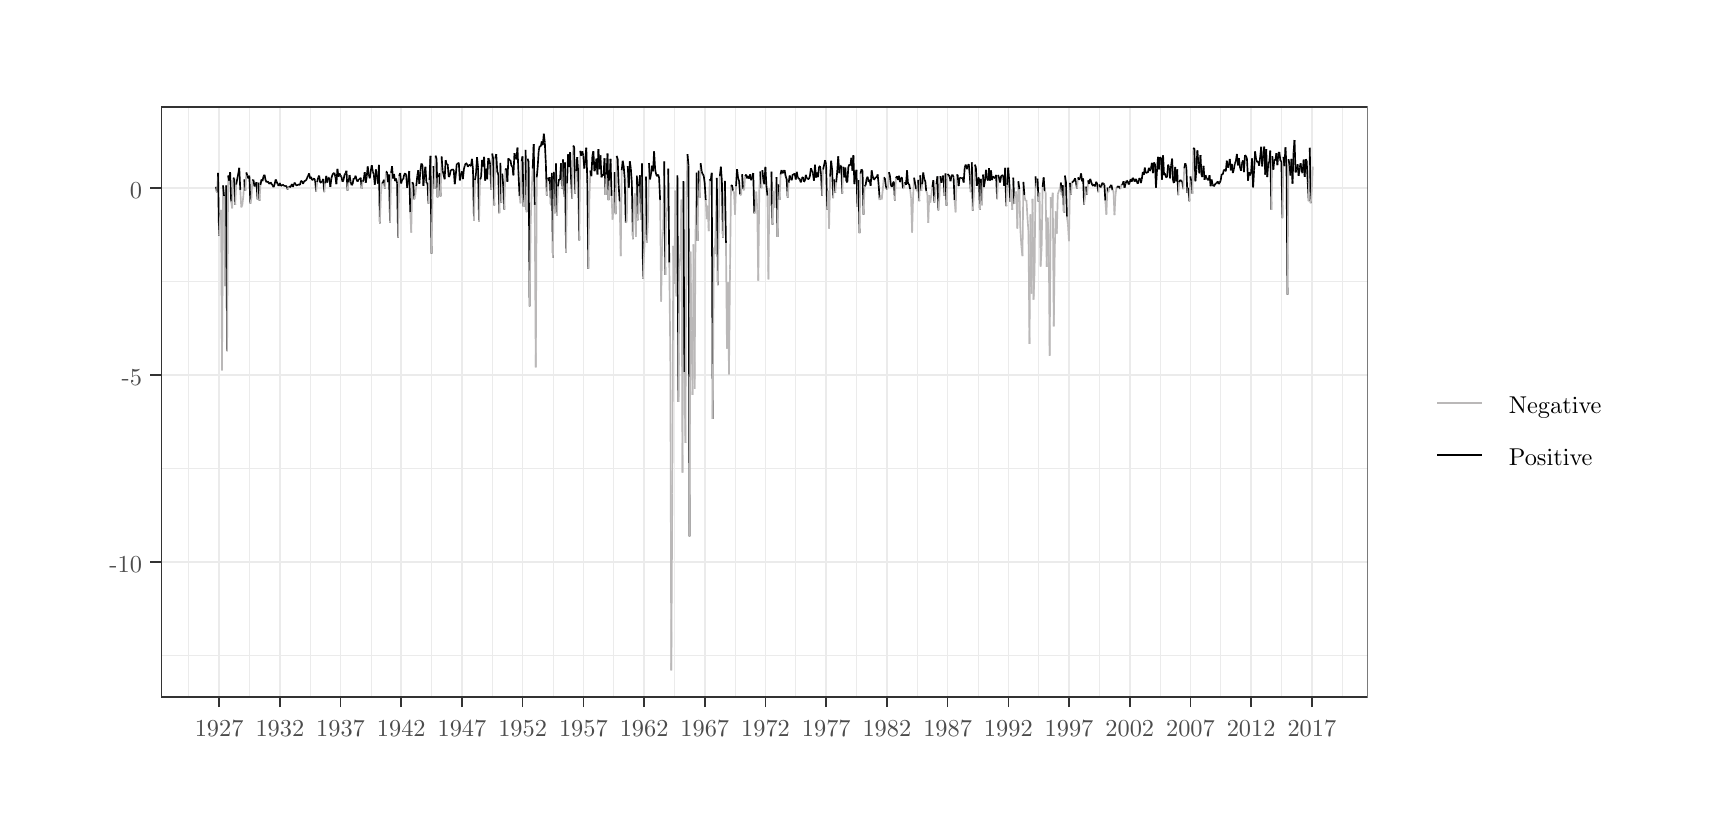
\begin{tikzpicture}[x=1.4pt,y=1.3pt]
\definecolor{fillColor}{RGB}{255,255,255}
\path[use as bounding box,fill=fillColor,fill opacity=0.00] (0,0) rectangle (426.79,216.81);
\begin{scope}
\path[clip] (  0.00,  0.00) rectangle (426.79,216.81);
\definecolor{drawColor}{RGB}{255,255,255}
\definecolor{fillColor}{RGB}{255,255,255}

\path[draw=drawColor,line width= 0.6pt,line join=round,line cap=round,fill=fillColor] (  0.00,  0.00) rectangle (426.79,216.81);
\end{scope}
\begin{scope}
\path[clip] ( 34.45, 30.72) rectangle (345.86,194.77);
\definecolor{fillColor}{RGB}{255,255,255}

\path[fill=fillColor] ( 34.45, 30.72) rectangle (345.86,194.77);
\definecolor{drawColor}{gray}{0.92}

\path[draw=drawColor,line width= 0.3pt,line join=round] ( 34.45, 42.33) --
	(345.86, 42.33);

\path[draw=drawColor,line width= 0.3pt,line join=round] ( 34.45, 94.30) --
	(345.86, 94.30);

\path[draw=drawColor,line width= 0.3pt,line join=round] ( 34.45,146.27) --
	(345.86,146.27);

\path[draw=drawColor,line width= 0.3pt,line join=round] ( 41.59, 30.72) --
	( 41.59,194.77);

\path[draw=drawColor,line width= 0.3pt,line join=round] ( 57.25, 30.72) --
	( 57.25,194.77);

\path[draw=drawColor,line width= 0.3pt,line join=round] ( 72.93, 30.72) --
	( 72.93,194.77);

\path[draw=drawColor,line width= 0.3pt,line join=round] ( 88.60, 30.72) --
	( 88.60,194.77);

\path[draw=drawColor,line width= 0.3pt,line join=round] (104.26, 30.72) --
	(104.26,194.77);

\path[draw=drawColor,line width= 0.3pt,line join=round] (119.93, 30.72) --
	(119.93,194.77);

\path[draw=drawColor,line width= 0.3pt,line join=round] (135.60, 30.72) --
	(135.60,194.77);

\path[draw=drawColor,line width= 0.3pt,line join=round] (151.27, 30.72) --
	(151.27,194.77);

\path[draw=drawColor,line width= 0.3pt,line join=round] (166.94, 30.72) --
	(166.94,194.77);

\path[draw=drawColor,line width= 0.3pt,line join=round] (182.61, 30.72) --
	(182.61,194.77);

\path[draw=drawColor,line width= 0.3pt,line join=round] (198.28, 30.72) --
	(198.28,194.77);

\path[draw=drawColor,line width= 0.3pt,line join=round] (213.95, 30.72) --
	(213.95,194.77);

\path[draw=drawColor,line width= 0.3pt,line join=round] (229.62, 30.72) --
	(229.62,194.77);

\path[draw=drawColor,line width= 0.3pt,line join=round] (245.28, 30.72) --
	(245.28,194.77);

\path[draw=drawColor,line width= 0.3pt,line join=round] (260.96, 30.72) --
	(260.96,194.77);

\path[draw=drawColor,line width= 0.3pt,line join=round] (276.63, 30.72) --
	(276.63,194.77);

\path[draw=drawColor,line width= 0.3pt,line join=round] (292.29, 30.72) --
	(292.29,194.77);

\path[draw=drawColor,line width= 0.3pt,line join=round] (307.96, 30.72) --
	(307.96,194.77);

\path[draw=drawColor,line width= 0.3pt,line join=round] (323.63, 30.72) --
	(323.63,194.77);

\path[draw=drawColor,line width= 0.3pt,line join=round] (339.30, 30.72) --
	(339.30,194.77);

\path[draw=drawColor,line width= 0.6pt,line join=round] ( 34.45, 68.32) --
	(345.86, 68.32);

\path[draw=drawColor,line width= 0.6pt,line join=round] ( 34.45,120.29) --
	(345.86,120.29);

\path[draw=drawColor,line width= 0.6pt,line join=round] ( 34.45,172.25) --
	(345.86,172.25);

\path[draw=drawColor,line width= 0.6pt,line join=round] ( 49.42, 30.72) --
	( 49.42,194.77);

\path[draw=drawColor,line width= 0.6pt,line join=round] ( 65.09, 30.72) --
	( 65.09,194.77);

\path[draw=drawColor,line width= 0.6pt,line join=round] ( 80.76, 30.72) --
	( 80.76,194.77);

\path[draw=drawColor,line width= 0.6pt,line join=round] ( 96.43, 30.72) --
	( 96.43,194.77);

\path[draw=drawColor,line width= 0.6pt,line join=round] (112.10, 30.72) --
	(112.10,194.77);

\path[draw=drawColor,line width= 0.6pt,line join=round] (127.76, 30.72) --
	(127.76,194.77);

\path[draw=drawColor,line width= 0.6pt,line join=round] (143.44, 30.72) --
	(143.44,194.77);

\path[draw=drawColor,line width= 0.6pt,line join=round] (159.11, 30.72) --
	(159.11,194.77);

\path[draw=drawColor,line width= 0.6pt,line join=round] (174.77, 30.72) --
	(174.77,194.77);

\path[draw=drawColor,line width= 0.6pt,line join=round] (190.44, 30.72) --
	(190.44,194.77);

\path[draw=drawColor,line width= 0.6pt,line join=round] (206.12, 30.72) --
	(206.12,194.77);

\path[draw=drawColor,line width= 0.6pt,line join=round] (221.78, 30.72) --
	(221.78,194.77);

\path[draw=drawColor,line width= 0.6pt,line join=round] (237.45, 30.72) --
	(237.45,194.77);

\path[draw=drawColor,line width= 0.6pt,line join=round] (253.12, 30.72) --
	(253.12,194.77);

\path[draw=drawColor,line width= 0.6pt,line join=round] (268.79, 30.72) --
	(268.79,194.77);

\path[draw=drawColor,line width= 0.6pt,line join=round] (284.46, 30.72) --
	(284.46,194.77);

\path[draw=drawColor,line width= 0.6pt,line join=round] (300.13, 30.72) --
	(300.13,194.77);

\path[draw=drawColor,line width= 0.6pt,line join=round] (315.79, 30.72) --
	(315.79,194.77);

\path[draw=drawColor,line width= 0.6pt,line join=round] (331.47, 30.72) --
	(331.47,194.77);
\definecolor{drawColor}{RGB}{0,0,0}

\path[draw=drawColor,line width= 0.6pt,line join=round] ( 48.61,172.56) -- ( 48.86,170.90);
\definecolor{drawColor}{RGB}{186,184,184}

\path[draw=drawColor,line width= 0.6pt,line join=round] ( 48.86,170.90) -- ( 49.13,176.47);
\definecolor{drawColor}{RGB}{0,0,0}

\path[draw=drawColor,line width= 0.6pt,line join=round] ( 49.13,176.47) -- ( 49.39,159.04);
\definecolor{drawColor}{RGB}{186,184,184}

\path[draw=drawColor,line width= 0.6pt,line join=round] ( 49.39,159.04) -- ( 49.65,163.94);

\path[draw=drawColor,line width= 0.6pt,line join=round] ( 49.65,163.94) -- ( 49.92,166.14);

\path[draw=drawColor,line width= 0.6pt,line join=round] ( 49.92,166.14) -- ( 50.16,121.56);

\path[draw=drawColor,line width= 0.6pt,line join=round] ( 50.16,121.56) -- ( 50.42,172.95);
\definecolor{drawColor}{RGB}{0,0,0}

\path[draw=drawColor,line width= 0.6pt,line join=round] ( 50.42,172.95) -- ( 50.68,170.00);
\definecolor{drawColor}{RGB}{186,184,184}

\path[draw=drawColor,line width= 0.6pt,line join=round] ( 50.68,170.00) -- ( 50.95,145.00);

\path[draw=drawColor,line width= 0.6pt,line join=round] ( 50.95,145.00) -- ( 51.21,172.96);
\definecolor{drawColor}{RGB}{0,0,0}

\path[draw=drawColor,line width= 0.6pt,line join=round] ( 51.21,172.96) -- ( 51.47,126.91);
\definecolor{drawColor}{RGB}{186,184,184}

\path[draw=drawColor,line width= 0.6pt,line join=round] ( 51.47,126.91) -- ( 51.74,175.72);
\definecolor{drawColor}{RGB}{0,0,0}

\path[draw=drawColor,line width= 0.6pt,line join=round] ( 51.74,175.72) -- ( 51.99,174.30);

\path[draw=drawColor,line width= 0.6pt,line join=round] ( 51.99,174.30) -- ( 52.26,176.63);

\path[draw=drawColor,line width= 0.6pt,line join=round] ( 52.26,176.63) -- ( 52.52,168.48);
\definecolor{drawColor}{RGB}{186,184,184}

\path[draw=drawColor,line width= 0.6pt,line join=round] ( 52.52,168.48) -- ( 52.78,166.57);

\path[draw=drawColor,line width= 0.6pt,line join=round] ( 52.78,166.57) -- ( 53.05,175.05);
\definecolor{drawColor}{RGB}{0,0,0}

\path[draw=drawColor,line width= 0.6pt,line join=round] ( 53.05,175.05) -- ( 53.30,174.90);

\path[draw=drawColor,line width= 0.6pt,line join=round] ( 53.30,174.90) -- ( 53.56,167.58);
\definecolor{drawColor}{RGB}{186,184,184}

\path[draw=drawColor,line width= 0.6pt,line join=round] ( 53.56,167.58) -- ( 53.82,173.19);
\definecolor{drawColor}{RGB}{0,0,0}

\path[draw=drawColor,line width= 0.6pt,line join=round] ( 53.82,173.19) -- ( 54.09,174.81);

\path[draw=drawColor,line width= 0.6pt,line join=round] ( 54.09,174.81) -- ( 54.35,176.14);

\path[draw=drawColor,line width= 0.6pt,line join=round] ( 54.35,176.14) -- ( 54.61,177.84);

\path[draw=drawColor,line width= 0.6pt,line join=round] ( 54.61,177.84) -- ( 54.88,171.70);
\definecolor{drawColor}{RGB}{186,184,184}

\path[draw=drawColor,line width= 0.6pt,line join=round] ( 54.88,171.70) -- ( 55.13,166.88);

\path[draw=drawColor,line width= 0.6pt,line join=round] ( 55.13,166.88) -- ( 55.40,167.50);

\path[draw=drawColor,line width= 0.6pt,line join=round] ( 55.40,167.50) -- ( 55.66,169.98);

\path[draw=drawColor,line width= 0.6pt,line join=round] ( 55.66,169.98) -- ( 55.92,174.64);
\definecolor{drawColor}{RGB}{0,0,0}

\path[draw=drawColor,line width= 0.6pt,line join=round] ( 55.92,174.64) -- ( 56.19,171.48);
\definecolor{drawColor}{RGB}{186,184,184}

\path[draw=drawColor,line width= 0.6pt,line join=round] ( 56.19,171.48) -- ( 56.43,176.56);
\definecolor{drawColor}{RGB}{0,0,0}

\path[draw=drawColor,line width= 0.6pt,line join=round] ( 56.43,176.56) -- ( 56.70,175.71);

\path[draw=drawColor,line width= 0.6pt,line join=round] ( 56.70,175.71) -- ( 56.95,174.90);

\path[draw=drawColor,line width= 0.6pt,line join=round] ( 56.95,174.90) -- ( 57.22,175.66);

\path[draw=drawColor,line width= 0.6pt,line join=round] ( 57.22,175.66) -- ( 57.48,167.88);
\definecolor{drawColor}{RGB}{186,184,184}

\path[draw=drawColor,line width= 0.6pt,line join=round] ( 57.48,167.88) -- ( 57.74,169.33);

\path[draw=drawColor,line width= 0.6pt,line join=round] ( 57.74,169.33) -- ( 58.01,174.35);
\definecolor{drawColor}{RGB}{0,0,0}

\path[draw=drawColor,line width= 0.6pt,line join=round] ( 58.01,174.35) -- ( 58.27,174.53);

\path[draw=drawColor,line width= 0.6pt,line join=round] ( 58.27,174.53) -- ( 58.53,172.69);

\path[draw=drawColor,line width= 0.6pt,line join=round] ( 58.53,172.69) -- ( 58.79,173.00);

\path[draw=drawColor,line width= 0.6pt,line join=round] ( 58.79,173.00) -- ( 59.06,173.86);

\path[draw=drawColor,line width= 0.6pt,line join=round] ( 59.06,173.86) -- ( 59.32,169.07);
\definecolor{drawColor}{RGB}{186,184,184}

\path[draw=drawColor,line width= 0.6pt,line join=round] ( 59.32,169.07) -- ( 59.56,173.76);
\definecolor{drawColor}{RGB}{0,0,0}

\path[draw=drawColor,line width= 0.6pt,line join=round] ( 59.56,173.76) -- ( 59.83,168.75);
\definecolor{drawColor}{RGB}{186,184,184}

\path[draw=drawColor,line width= 0.6pt,line join=round] ( 59.83,168.75) -- ( 60.09,173.13);
\definecolor{drawColor}{RGB}{0,0,0}

\path[draw=drawColor,line width= 0.6pt,line join=round] ( 60.09,173.13) -- ( 60.35,174.63);

\path[draw=drawColor,line width= 0.6pt,line join=round] ( 60.35,174.63) -- ( 60.61,174.16);

\path[draw=drawColor,line width= 0.6pt,line join=round] ( 60.61,174.16) -- ( 60.87,175.50);

\path[draw=drawColor,line width= 0.6pt,line join=round] ( 60.87,175.50) -- ( 61.14,175.91);

\path[draw=drawColor,line width= 0.6pt,line join=round] ( 61.14,175.91) -- ( 61.40,174.42);

\path[draw=drawColor,line width= 0.6pt,line join=round] ( 61.40,174.42) -- ( 61.66,173.82);

\path[draw=drawColor,line width= 0.6pt,line join=round] ( 61.66,173.82) -- ( 61.92,174.12);

\path[draw=drawColor,line width= 0.6pt,line join=round] ( 61.92,174.12) -- ( 62.19,173.71);

\path[draw=drawColor,line width= 0.6pt,line join=round] ( 62.19,173.71) -- ( 62.45,173.35);

\path[draw=drawColor,line width= 0.6pt,line join=round] ( 62.45,173.35) -- ( 62.69,173.87);

\path[draw=drawColor,line width= 0.6pt,line join=round] ( 62.69,173.87) -- ( 62.96,173.33);

\path[draw=drawColor,line width= 0.6pt,line join=round] ( 62.96,173.33) -- ( 63.22,173.04);

\path[draw=drawColor,line width= 0.6pt,line join=round] ( 63.22,173.04) -- ( 63.48,172.47);

\path[draw=drawColor,line width= 0.6pt,line join=round] ( 63.48,172.47) -- ( 63.74,173.31);

\path[draw=drawColor,line width= 0.6pt,line join=round] ( 63.74,173.31) -- ( 64.01,174.60);

\path[draw=drawColor,line width= 0.6pt,line join=round] ( 64.01,174.60) -- ( 64.27,174.02);

\path[draw=drawColor,line width= 0.6pt,line join=round] ( 64.27,174.02) -- ( 64.53,173.25);

\path[draw=drawColor,line width= 0.6pt,line join=round] ( 64.53,173.25) -- ( 64.80,172.83);

\path[draw=drawColor,line width= 0.6pt,line join=round] ( 64.80,172.83) -- ( 65.05,173.64);

\path[draw=drawColor,line width= 0.6pt,line join=round] ( 65.05,173.64) -- ( 65.32,172.81);

\path[draw=drawColor,line width= 0.6pt,line join=round] ( 65.32,172.81) -- ( 65.59,173.02);

\path[draw=drawColor,line width= 0.6pt,line join=round] ( 65.59,173.02) -- ( 65.83,173.19);

\path[draw=drawColor,line width= 0.6pt,line join=round] ( 65.83,173.19) -- ( 66.10,172.88);

\path[draw=drawColor,line width= 0.6pt,line join=round] ( 66.10,172.88) -- ( 66.36,172.79);

\path[draw=drawColor,line width= 0.6pt,line join=round] ( 66.36,172.79) -- ( 66.62,172.83);

\path[draw=drawColor,line width= 0.6pt,line join=round] ( 66.62,172.83) -- ( 66.88,172.65);

\path[draw=drawColor,line width= 0.6pt,line join=round] ( 66.88,172.65) -- ( 67.15,171.78);
\definecolor{drawColor}{RGB}{186,184,184}

\path[draw=drawColor,line width= 0.6pt,line join=round] ( 67.15,171.78) -- ( 67.41,172.72);
\definecolor{drawColor}{RGB}{0,0,0}

\path[draw=drawColor,line width= 0.6pt,line join=round] ( 67.41,172.72) -- ( 67.67,172.50);

\path[draw=drawColor,line width= 0.6pt,line join=round] ( 67.67,172.50) -- ( 67.94,172.67);

\path[draw=drawColor,line width= 0.6pt,line join=round] ( 67.94,172.67) -- ( 68.19,173.35);

\path[draw=drawColor,line width= 0.6pt,line join=round] ( 68.19,173.35) -- ( 68.46,172.54);

\path[draw=drawColor,line width= 0.6pt,line join=round] ( 68.46,172.54) -- ( 68.73,173.45);

\path[draw=drawColor,line width= 0.6pt,line join=round] ( 68.73,173.45) -- ( 68.97,173.71);

\path[draw=drawColor,line width= 0.6pt,line join=round] ( 68.97,173.71) -- ( 69.23,172.97);

\path[draw=drawColor,line width= 0.6pt,line join=round] ( 69.23,172.97) -- ( 69.49,173.03);

\path[draw=drawColor,line width= 0.6pt,line join=round] ( 69.49,173.03) -- ( 69.75,173.06);

\path[draw=drawColor,line width= 0.6pt,line join=round] ( 69.75,173.06) -- ( 70.01,173.29);

\path[draw=drawColor,line width= 0.6pt,line join=round] ( 70.01,173.29) -- ( 70.28,173.07);

\path[draw=drawColor,line width= 0.6pt,line join=round] ( 70.28,173.07) -- ( 70.54,174.25);

\path[draw=drawColor,line width= 0.6pt,line join=round] ( 70.54,174.25) -- ( 70.80,174.10);

\path[draw=drawColor,line width= 0.6pt,line join=round] ( 70.80,174.10) -- ( 71.07,173.40);

\path[draw=drawColor,line width= 0.6pt,line join=round] ( 71.07,173.40) -- ( 71.33,174.05);

\path[draw=drawColor,line width= 0.6pt,line join=round] ( 71.33,174.05) -- ( 71.59,174.28);

\path[draw=drawColor,line width= 0.6pt,line join=round] ( 71.59,174.28) -- ( 71.86,174.33);

\path[draw=drawColor,line width= 0.6pt,line join=round] ( 71.86,174.33) -- ( 72.10,174.98);

\path[draw=drawColor,line width= 0.6pt,line join=round] ( 72.10,174.98) -- ( 72.36,175.60);

\path[draw=drawColor,line width= 0.6pt,line join=round] ( 72.36,175.60) -- ( 72.62,176.30);

\path[draw=drawColor,line width= 0.6pt,line join=round] ( 72.62,176.30) -- ( 72.89,174.90);

\path[draw=drawColor,line width= 0.6pt,line join=round] ( 72.89,174.90) -- ( 73.14,175.33);

\path[draw=drawColor,line width= 0.6pt,line join=round] ( 73.14,175.33) -- ( 73.41,174.43);

\path[draw=drawColor,line width= 0.6pt,line join=round] ( 73.41,174.43) -- ( 73.68,174.63);

\path[draw=drawColor,line width= 0.6pt,line join=round] ( 73.68,174.63) -- ( 73.93,174.94);

\path[draw=drawColor,line width= 0.6pt,line join=round] ( 73.93,174.94) -- ( 74.20,174.29);

\path[draw=drawColor,line width= 0.6pt,line join=round] ( 74.20,174.29) -- ( 74.46,171.18);
\definecolor{drawColor}{RGB}{186,184,184}

\path[draw=drawColor,line width= 0.6pt,line join=round] ( 74.46,171.18) -- ( 74.72,173.90);
\definecolor{drawColor}{RGB}{0,0,0}

\path[draw=drawColor,line width= 0.6pt,line join=round] ( 74.72,173.90) -- ( 74.99,175.17);

\path[draw=drawColor,line width= 0.6pt,line join=round] ( 74.99,175.17) -- ( 75.23,175.69);

\path[draw=drawColor,line width= 0.6pt,line join=round] ( 75.23,175.69) -- ( 75.49,173.78);

\path[draw=drawColor,line width= 0.6pt,line join=round] ( 75.49,173.78) -- ( 75.75,173.75);

\path[draw=drawColor,line width= 0.6pt,line join=round] ( 75.75,173.75) -- ( 76.02,174.04);

\path[draw=drawColor,line width= 0.6pt,line join=round] ( 76.02,174.04) -- ( 76.28,174.75);

\path[draw=drawColor,line width= 0.6pt,line join=round] ( 76.28,174.75) -- ( 76.54,171.12);
\definecolor{drawColor}{RGB}{186,184,184}

\path[draw=drawColor,line width= 0.6pt,line join=round] ( 76.54,171.12) -- ( 76.81,173.53);
\definecolor{drawColor}{RGB}{0,0,0}

\path[draw=drawColor,line width= 0.6pt,line join=round] ( 76.81,173.53) -- ( 77.07,175.61);

\path[draw=drawColor,line width= 0.6pt,line join=round] ( 77.07,175.61) -- ( 77.33,173.76);

\path[draw=drawColor,line width= 0.6pt,line join=round] ( 77.33,173.76) -- ( 77.59,175.13);

\path[draw=drawColor,line width= 0.6pt,line join=round] ( 77.59,175.13) -- ( 77.85,175.09);

\path[draw=drawColor,line width= 0.6pt,line join=round] ( 77.85,175.09) -- ( 78.12,172.54);

\path[draw=drawColor,line width= 0.6pt,line join=round] ( 78.12,172.54) -- ( 78.37,174.86);

\path[draw=drawColor,line width= 0.6pt,line join=round] ( 78.37,174.86) -- ( 78.64,175.87);

\path[draw=drawColor,line width= 0.6pt,line join=round] ( 78.64,175.87) -- ( 78.89,176.29);

\path[draw=drawColor,line width= 0.6pt,line join=round] ( 78.89,176.29) -- ( 79.16,176.44);

\path[draw=drawColor,line width= 0.6pt,line join=round] ( 79.16,176.44) -- ( 79.42,175.40);

\path[draw=drawColor,line width= 0.6pt,line join=round] ( 79.42,175.40) -- ( 79.68,173.30);

\path[draw=drawColor,line width= 0.6pt,line join=round] ( 79.68,173.30) -- ( 79.95,177.56);

\path[draw=drawColor,line width= 0.6pt,line join=round] ( 79.95,177.56) -- ( 80.21,175.34);

\path[draw=drawColor,line width= 0.6pt,line join=round] ( 80.21,175.34) -- ( 80.47,176.30);

\path[draw=drawColor,line width= 0.6pt,line join=round] ( 80.47,176.30) -- ( 80.73,175.70);

\path[draw=drawColor,line width= 0.6pt,line join=round] ( 80.73,175.70) -- ( 80.99,175.38);

\path[draw=drawColor,line width= 0.6pt,line join=round] ( 80.99,175.38) -- ( 81.26,173.98);

\path[draw=drawColor,line width= 0.6pt,line join=round] ( 81.26,173.98) -- ( 81.50,174.41);

\path[draw=drawColor,line width= 0.6pt,line join=round] ( 81.50,174.41) -- ( 81.77,175.89);

\path[draw=drawColor,line width= 0.6pt,line join=round] ( 81.77,175.89) -- ( 82.02,176.26);

\path[draw=drawColor,line width= 0.6pt,line join=round] ( 82.02,176.26) -- ( 82.29,177.03);

\path[draw=drawColor,line width= 0.6pt,line join=round] ( 82.29,177.03) -- ( 82.55,171.52);
\definecolor{drawColor}{RGB}{186,184,184}

\path[draw=drawColor,line width= 0.6pt,line join=round] ( 82.55,171.52) -- ( 82.81,173.79);
\definecolor{drawColor}{RGB}{0,0,0}

\path[draw=drawColor,line width= 0.6pt,line join=round] ( 82.81,173.79) -- ( 83.08,175.84);

\path[draw=drawColor,line width= 0.6pt,line join=round] ( 83.08,175.84) -- ( 83.34,174.05);

\path[draw=drawColor,line width= 0.6pt,line join=round] ( 83.34,174.05) -- ( 83.60,173.04);

\path[draw=drawColor,line width= 0.6pt,line join=round] ( 83.60,173.04) -- ( 83.86,173.28);

\path[draw=drawColor,line width= 0.6pt,line join=round] ( 83.86,173.28) -- ( 84.13,174.94);

\path[draw=drawColor,line width= 0.6pt,line join=round] ( 84.13,174.94) -- ( 84.39,174.76);

\path[draw=drawColor,line width= 0.6pt,line join=round] ( 84.39,174.76) -- ( 84.63,175.66);

\path[draw=drawColor,line width= 0.6pt,line join=round] ( 84.63,175.66) -- ( 84.90,174.50);

\path[draw=drawColor,line width= 0.6pt,line join=round] ( 84.90,174.50) -- ( 85.16,174.00);

\path[draw=drawColor,line width= 0.6pt,line join=round] ( 85.16,174.00) -- ( 85.42,174.72);

\path[draw=drawColor,line width= 0.6pt,line join=round] ( 85.42,174.72) -- ( 85.68,174.63);

\path[draw=drawColor,line width= 0.6pt,line join=round] ( 85.68,174.63) -- ( 85.95,175.10);

\path[draw=drawColor,line width= 0.6pt,line join=round] ( 85.95,175.10) -- ( 86.21,172.01);
\definecolor{drawColor}{RGB}{186,184,184}

\path[draw=drawColor,line width= 0.6pt,line join=round] ( 86.21,172.01) -- ( 86.47,174.03);
\definecolor{drawColor}{RGB}{0,0,0}

\path[draw=drawColor,line width= 0.6pt,line join=round] ( 86.47,174.03) -- ( 86.73,174.50);

\path[draw=drawColor,line width= 0.6pt,line join=round] ( 86.73,174.50) -- ( 86.99,176.64);

\path[draw=drawColor,line width= 0.6pt,line join=round] ( 86.99,176.64) -- ( 87.26,173.72);

\path[draw=drawColor,line width= 0.6pt,line join=round] ( 87.26,173.72) -- ( 87.52,175.41);

\path[draw=drawColor,line width= 0.6pt,line join=round] ( 87.52,175.41) -- ( 87.76,178.22);

\path[draw=drawColor,line width= 0.6pt,line join=round] ( 87.76,178.22) -- ( 88.03,176.08);

\path[draw=drawColor,line width= 0.6pt,line join=round] ( 88.03,176.08) -- ( 88.29,174.95);

\path[draw=drawColor,line width= 0.6pt,line join=round] ( 88.29,174.95) -- ( 88.55,176.90);

\path[draw=drawColor,line width= 0.6pt,line join=round] ( 88.55,176.90) -- ( 88.81,178.58);

\path[draw=drawColor,line width= 0.6pt,line join=round] ( 88.81,178.58) -- ( 89.08,176.82);

\path[draw=drawColor,line width= 0.6pt,line join=round] ( 89.08,176.82) -- ( 89.34,175.99);

\path[draw=drawColor,line width= 0.6pt,line join=round] ( 89.34,175.99) -- ( 89.60,173.16);

\path[draw=drawColor,line width= 0.6pt,line join=round] ( 89.60,173.16) -- ( 89.87,177.40);

\path[draw=drawColor,line width= 0.6pt,line join=round] ( 89.87,177.40) -- ( 90.12,175.90);

\path[draw=drawColor,line width= 0.6pt,line join=round] ( 90.12,175.90) -- ( 90.39,173.48);

\path[draw=drawColor,line width= 0.6pt,line join=round] ( 90.39,173.48) -- ( 90.66,178.64);

\path[draw=drawColor,line width= 0.6pt,line join=round] ( 90.66,178.64) -- ( 90.90,162.40);
\definecolor{drawColor}{RGB}{186,184,184}

\path[draw=drawColor,line width= 0.6pt,line join=round] ( 90.90,162.40) -- ( 91.17,170.48);

\path[draw=drawColor,line width= 0.6pt,line join=round] ( 91.17,170.48) -- ( 91.43,173.76);
\definecolor{drawColor}{RGB}{0,0,0}

\path[draw=drawColor,line width= 0.6pt,line join=round] ( 91.43,173.76) -- ( 91.69,173.69);

\path[draw=drawColor,line width= 0.6pt,line join=round] ( 91.69,173.69) -- ( 91.95,174.53);

\path[draw=drawColor,line width= 0.6pt,line join=round] ( 91.95,174.53) -- ( 92.22,172.09);
\definecolor{drawColor}{RGB}{186,184,184}

\path[draw=drawColor,line width= 0.6pt,line join=round] ( 92.22,172.09) -- ( 92.48,176.77);
\definecolor{drawColor}{RGB}{0,0,0}

\path[draw=drawColor,line width= 0.6pt,line join=round] ( 92.48,176.77) -- ( 92.74,176.74);

\path[draw=drawColor,line width= 0.6pt,line join=round] ( 92.74,176.74) -- ( 93.01,173.88);

\path[draw=drawColor,line width= 0.6pt,line join=round] ( 93.01,173.88) -- ( 93.26,175.98);

\path[draw=drawColor,line width= 0.6pt,line join=round] ( 93.26,175.98) -- ( 93.53,162.67);
\definecolor{drawColor}{RGB}{186,184,184}

\path[draw=drawColor,line width= 0.6pt,line join=round] ( 93.53,162.67) -- ( 93.80,176.42);
\definecolor{drawColor}{RGB}{0,0,0}

\path[draw=drawColor,line width= 0.6pt,line join=round] ( 93.80,176.42) -- ( 94.04,178.29);

\path[draw=drawColor,line width= 0.6pt,line join=round] ( 94.04,178.29) -- ( 94.30,174.90);

\path[draw=drawColor,line width= 0.6pt,line join=round] ( 94.30,174.90) -- ( 94.56,176.13);

\path[draw=drawColor,line width= 0.6pt,line join=round] ( 94.56,176.13) -- ( 94.83,174.18);

\path[draw=drawColor,line width= 0.6pt,line join=round] ( 94.83,174.18) -- ( 95.08,174.88);

\path[draw=drawColor,line width= 0.6pt,line join=round] ( 95.08,174.88) -- ( 95.35,173.53);

\path[draw=drawColor,line width= 0.6pt,line join=round] ( 95.35,173.53) -- ( 95.61,158.47);
\definecolor{drawColor}{RGB}{186,184,184}

\path[draw=drawColor,line width= 0.6pt,line join=round] ( 95.61,158.47) -- ( 95.87,175.63);
\definecolor{drawColor}{RGB}{0,0,0}

\path[draw=drawColor,line width= 0.6pt,line join=round] ( 95.87,175.63) -- ( 96.14,176.40);

\path[draw=drawColor,line width= 0.6pt,line join=round] ( 96.14,176.40) -- ( 96.40,173.50);

\path[draw=drawColor,line width= 0.6pt,line join=round] ( 96.40,173.50) -- ( 96.66,174.59);

\path[draw=drawColor,line width= 0.6pt,line join=round] ( 96.66,174.59) -- ( 96.93,174.60);

\path[draw=drawColor,line width= 0.6pt,line join=round] ( 96.93,174.60) -- ( 97.17,175.96);

\path[draw=drawColor,line width= 0.6pt,line join=round] ( 97.17,175.96) -- ( 97.43,176.35);

\path[draw=drawColor,line width= 0.6pt,line join=round] ( 97.43,176.35) -- ( 97.69,175.89);

\path[draw=drawColor,line width= 0.6pt,line join=round] ( 97.69,175.89) -- ( 97.96,172.30);

\path[draw=drawColor,line width= 0.6pt,line join=round] ( 97.96,172.30) -- ( 98.21,174.51);

\path[draw=drawColor,line width= 0.6pt,line join=round] ( 98.21,174.51) -- ( 98.48,176.96);

\path[draw=drawColor,line width= 0.6pt,line join=round] ( 98.48,176.96) -- ( 98.75,165.53);
\definecolor{drawColor}{RGB}{186,184,184}

\path[draw=drawColor,line width= 0.6pt,line join=round] ( 98.75,165.53) -- ( 99.00,159.82);

\path[draw=drawColor,line width= 0.6pt,line join=round] ( 99.00,159.82) -- ( 99.27,173.86);
\definecolor{drawColor}{RGB}{0,0,0}

\path[draw=drawColor,line width= 0.6pt,line join=round] ( 99.27,173.86) -- ( 99.53,173.38);

\path[draw=drawColor,line width= 0.6pt,line join=round] ( 99.53,173.38) -- ( 99.79,169.11);
\definecolor{drawColor}{RGB}{186,184,184}

\path[draw=drawColor,line width= 0.6pt,line join=round] ( 99.79,169.11) -- (100.06,170.19);

\path[draw=drawColor,line width= 0.6pt,line join=round] (100.06,170.19) -- (100.30,172.83);
\definecolor{drawColor}{RGB}{0,0,0}

\path[draw=drawColor,line width= 0.6pt,line join=round] (100.30,172.83) -- (100.57,175.69);

\path[draw=drawColor,line width= 0.6pt,line join=round] (100.57,175.69) -- (100.82,177.19);

\path[draw=drawColor,line width= 0.6pt,line join=round] (100.82,177.19) -- (101.09,173.41);

\path[draw=drawColor,line width= 0.6pt,line join=round] (101.09,173.41) -- (101.35,176.85);

\path[draw=drawColor,line width= 0.6pt,line join=round] (101.35,176.85) -- (101.61,179.04);

\path[draw=drawColor,line width= 0.6pt,line join=round] (101.61,179.04) -- (101.88,178.62);

\path[draw=drawColor,line width= 0.6pt,line join=round] (101.88,178.62) -- (102.14,172.82);

\path[draw=drawColor,line width= 0.6pt,line join=round] (102.14,172.82) -- (102.40,176.34);

\path[draw=drawColor,line width= 0.6pt,line join=round] (102.40,176.34) -- (102.66,178.14);

\path[draw=drawColor,line width= 0.6pt,line join=round] (102.66,178.14) -- (102.93,173.61);

\path[draw=drawColor,line width= 0.6pt,line join=round] (102.93,173.61) -- (103.19,173.67);

\path[draw=drawColor,line width= 0.6pt,line join=round] (103.19,173.67) -- (103.44,167.94);
\definecolor{drawColor}{RGB}{186,184,184}

\path[draw=drawColor,line width= 0.6pt,line join=round] (103.44,167.94) -- (103.71,174.48);
\definecolor{drawColor}{RGB}{0,0,0}

\path[draw=drawColor,line width= 0.6pt,line join=round] (103.71,174.48) -- (103.96,181.16);

\path[draw=drawColor,line width= 0.6pt,line join=round] (103.96,181.16) -- (104.23,153.99);
\definecolor{drawColor}{RGB}{186,184,184}

\path[draw=drawColor,line width= 0.6pt,line join=round] (104.23,153.99) -- (104.49,169.19);

\path[draw=drawColor,line width= 0.6pt,line join=round] (104.49,169.19) -- (104.75,178.32);
\definecolor{drawColor}{RGB}{0,0,0}

\path[draw=drawColor,line width= 0.6pt,line join=round] (104.75,178.32) -- (105.02,171.99);
\definecolor{drawColor}{RGB}{186,184,184}

\path[draw=drawColor,line width= 0.6pt,line join=round] (105.02,171.99) -- (105.28,181.24);
\definecolor{drawColor}{RGB}{0,0,0}

\path[draw=drawColor,line width= 0.6pt,line join=round] (105.28,181.24) -- (105.54,180.35);

\path[draw=drawColor,line width= 0.6pt,line join=round] (105.54,180.35) -- (105.80,169.66);
\definecolor{drawColor}{RGB}{186,184,184}

\path[draw=drawColor,line width= 0.6pt,line join=round] (105.80,169.66) -- (106.07,175.33);
\definecolor{drawColor}{RGB}{0,0,0}

\path[draw=drawColor,line width= 0.6pt,line join=round] (106.07,175.33) -- (106.33,176.37);

\path[draw=drawColor,line width= 0.6pt,line join=round] (106.33,176.37) -- (106.57,169.91);
\definecolor{drawColor}{RGB}{186,184,184}

\path[draw=drawColor,line width= 0.6pt,line join=round] (106.57,169.91) -- (106.84,181.02);
\definecolor{drawColor}{RGB}{0,0,0}

\path[draw=drawColor,line width= 0.6pt,line join=round] (106.84,181.02) -- (107.09,177.06);

\path[draw=drawColor,line width= 0.6pt,line join=round] (107.09,177.06) -- (107.36,175.92);

\path[draw=drawColor,line width= 0.6pt,line join=round] (107.36,175.92) -- (107.62,174.68);

\path[draw=drawColor,line width= 0.6pt,line join=round] (107.62,174.68) -- (107.88,180.00);

\path[draw=drawColor,line width= 0.6pt,line join=round] (107.88,180.00) -- (108.15,178.77);

\path[draw=drawColor,line width= 0.6pt,line join=round] (108.15,178.77) -- (108.41,178.85);

\path[draw=drawColor,line width= 0.6pt,line join=round] (108.41,178.85) -- (108.67,175.30);

\path[draw=drawColor,line width= 0.6pt,line join=round] (108.67,175.30) -- (108.93,175.71);

\path[draw=drawColor,line width= 0.6pt,line join=round] (108.93,175.71) -- (109.20,177.29);

\path[draw=drawColor,line width= 0.6pt,line join=round] (109.20,177.29) -- (109.46,177.23);

\path[draw=drawColor,line width= 0.6pt,line join=round] (109.46,177.23) -- (109.70,177.49);

\path[draw=drawColor,line width= 0.6pt,line join=round] (109.70,177.49) -- (109.97,177.20);

\path[draw=drawColor,line width= 0.6pt,line join=round] (109.97,177.20) -- (110.23,173.33);

\path[draw=drawColor,line width= 0.6pt,line join=round] (110.23,173.33) -- (110.49,175.78);

\path[draw=drawColor,line width= 0.6pt,line join=round] (110.49,175.78) -- (110.75,179.03);

\path[draw=drawColor,line width= 0.6pt,line join=round] (110.75,179.03) -- (111.02,178.94);

\path[draw=drawColor,line width= 0.6pt,line join=round] (111.02,178.94) -- (111.28,179.29);

\path[draw=drawColor,line width= 0.6pt,line join=round] (111.28,179.29) -- (111.54,174.35);

\path[draw=drawColor,line width= 0.6pt,line join=round] (111.54,174.35) -- (111.81,175.89);

\path[draw=drawColor,line width= 0.6pt,line join=round] (111.81,175.89) -- (112.06,176.88);

\path[draw=drawColor,line width= 0.6pt,line join=round] (112.06,176.88) -- (112.33,174.73);

\path[draw=drawColor,line width= 0.6pt,line join=round] (112.33,174.73) -- (112.59,177.48);

\path[draw=drawColor,line width= 0.6pt,line join=round] (112.59,177.48) -- (112.83,178.49);

\path[draw=drawColor,line width= 0.6pt,line join=round] (112.83,178.49) -- (113.10,179.15);

\path[draw=drawColor,line width= 0.6pt,line join=round] (113.10,179.15) -- (113.36,179.02);

\path[draw=drawColor,line width= 0.6pt,line join=round] (113.36,179.02) -- (113.62,178.13);

\path[draw=drawColor,line width= 0.6pt,line join=round] (113.62,178.13) -- (113.88,178.68);

\path[draw=drawColor,line width= 0.6pt,line join=round] (113.88,178.68) -- (114.15,178.64);

\path[draw=drawColor,line width= 0.6pt,line join=round] (114.15,178.64) -- (114.41,178.32);

\path[draw=drawColor,line width= 0.6pt,line join=round] (114.41,178.32) -- (114.67,180.33);

\path[draw=drawColor,line width= 0.6pt,line join=round] (114.67,180.33) -- (114.94,177.39);

\path[draw=drawColor,line width= 0.6pt,line join=round] (114.94,177.39) -- (115.19,163.09);
\definecolor{drawColor}{RGB}{186,184,184}

\path[draw=drawColor,line width= 0.6pt,line join=round] (115.19,163.09) -- (115.46,174.48);
\definecolor{drawColor}{RGB}{0,0,0}

\path[draw=drawColor,line width= 0.6pt,line join=round] (115.46,174.48) -- (115.73,176.36);

\path[draw=drawColor,line width= 0.6pt,line join=round] (115.73,176.36) -- (115.98,180.79);

\path[draw=drawColor,line width= 0.6pt,line join=round] (115.98,180.79) -- (116.24,177.98);

\path[draw=drawColor,line width= 0.6pt,line join=round] (116.24,177.98) -- (116.50,162.83);
\definecolor{drawColor}{RGB}{186,184,184}

\path[draw=drawColor,line width= 0.6pt,line join=round] (116.50,162.83) -- (116.76,174.64);
\definecolor{drawColor}{RGB}{0,0,0}

\path[draw=drawColor,line width= 0.6pt,line join=round] (116.76,174.64) -- (117.02,175.22);

\path[draw=drawColor,line width= 0.6pt,line join=round] (117.02,175.22) -- (117.29,180.03);

\path[draw=drawColor,line width= 0.6pt,line join=round] (117.29,180.03) -- (117.55,178.23);

\path[draw=drawColor,line width= 0.6pt,line join=round] (117.55,178.23) -- (117.81,180.91);

\path[draw=drawColor,line width= 0.6pt,line join=round] (117.81,180.91) -- (118.08,174.30);

\path[draw=drawColor,line width= 0.6pt,line join=round] (118.08,174.30) -- (118.33,177.62);

\path[draw=drawColor,line width= 0.6pt,line join=round] (118.33,177.62) -- (118.60,174.68);

\path[draw=drawColor,line width= 0.6pt,line join=round] (118.60,174.68) -- (118.87,180.51);

\path[draw=drawColor,line width= 0.6pt,line join=round] (118.87,180.51) -- (119.11,180.17);

\path[draw=drawColor,line width= 0.6pt,line join=round] (119.11,180.17) -- (119.37,178.82);

\path[draw=drawColor,line width= 0.6pt,line join=round] (119.37,178.82) -- (119.63,171.83);
\definecolor{drawColor}{RGB}{186,184,184}

\path[draw=drawColor,line width= 0.6pt,line join=round] (119.63,171.83) -- (119.90,181.82);
\definecolor{drawColor}{RGB}{0,0,0}

\path[draw=drawColor,line width= 0.6pt,line join=round] (119.90,181.82) -- (120.15,180.34);

\path[draw=drawColor,line width= 0.6pt,line join=round] (120.15,180.34) -- (120.42,167.42);
\definecolor{drawColor}{RGB}{186,184,184}

\path[draw=drawColor,line width= 0.6pt,line join=round] (120.42,167.42) -- (120.69,180.46);
\definecolor{drawColor}{RGB}{0,0,0}

\path[draw=drawColor,line width= 0.6pt,line join=round] (120.69,180.46) -- (120.94,181.66);

\path[draw=drawColor,line width= 0.6pt,line join=round] (120.94,181.66) -- (121.21,176.72);

\path[draw=drawColor,line width= 0.6pt,line join=round] (121.21,176.72) -- (121.47,176.16);

\path[draw=drawColor,line width= 0.6pt,line join=round] (121.47,176.16) -- (121.73,165.23);
\definecolor{drawColor}{RGB}{186,184,184}

\path[draw=drawColor,line width= 0.6pt,line join=round] (121.73,165.23) -- (122.00,179.25);
\definecolor{drawColor}{RGB}{0,0,0}

\path[draw=drawColor,line width= 0.6pt,line join=round] (122.00,179.25) -- (122.24,168.18);
\definecolor{drawColor}{RGB}{186,184,184}

\path[draw=drawColor,line width= 0.6pt,line join=round] (122.24,168.18) -- (122.50,176.22);
\definecolor{drawColor}{RGB}{0,0,0}

\path[draw=drawColor,line width= 0.6pt,line join=round] (122.50,176.22) -- (122.76,172.66);

\path[draw=drawColor,line width= 0.6pt,line join=round] (122.76,172.66) -- (123.03,166.24);
\definecolor{drawColor}{RGB}{186,184,184}

\path[draw=drawColor,line width= 0.6pt,line join=round] (123.03,166.24) -- (123.29,177.30);
\definecolor{drawColor}{RGB}{0,0,0}

\path[draw=drawColor,line width= 0.6pt,line join=round] (123.29,177.30) -- (123.55,177.65);

\path[draw=drawColor,line width= 0.6pt,line join=round] (123.55,177.65) -- (123.82,173.97);

\path[draw=drawColor,line width= 0.6pt,line join=round] (123.82,173.97) -- (124.07,180.51);

\path[draw=drawColor,line width= 0.6pt,line join=round] (124.07,180.51) -- (124.34,179.94);

\path[draw=drawColor,line width= 0.6pt,line join=round] (124.34,179.94) -- (124.60,180.04);

\path[draw=drawColor,line width= 0.6pt,line join=round] (124.60,180.04) -- (124.86,178.35);

\path[draw=drawColor,line width= 0.6pt,line join=round] (124.86,178.35) -- (125.13,178.22);

\path[draw=drawColor,line width= 0.6pt,line join=round] (125.13,178.22) -- (125.37,175.76);

\path[draw=drawColor,line width= 0.6pt,line join=round] (125.37,175.76) -- (125.64,181.90);

\path[draw=drawColor,line width= 0.6pt,line join=round] (125.64,181.90) -- (125.89,180.97);

\path[draw=drawColor,line width= 0.6pt,line join=round] (125.89,180.97) -- (126.16,180.20);

\path[draw=drawColor,line width= 0.6pt,line join=round] (126.16,180.20) -- (126.42,183.47);

\path[draw=drawColor,line width= 0.6pt,line join=round] (126.42,183.47) -- (126.68,176.34);

\path[draw=drawColor,line width= 0.6pt,line join=round] (126.68,176.34) -- (126.95,170.06);
\definecolor{drawColor}{RGB}{186,184,184}

\path[draw=drawColor,line width= 0.6pt,line join=round] (126.95,170.06) -- (127.21,167.99);

\path[draw=drawColor,line width= 0.6pt,line join=round] (127.21,167.99) -- (127.47,179.67);
\definecolor{drawColor}{RGB}{0,0,0}

\path[draw=drawColor,line width= 0.6pt,line join=round] (127.47,179.67) -- (127.73,181.01);

\path[draw=drawColor,line width= 0.6pt,line join=round] (127.73,181.01) -- (128.00,166.98);
\definecolor{drawColor}{RGB}{186,184,184}

\path[draw=drawColor,line width= 0.6pt,line join=round] (128.00,166.98) -- (128.26,169.57);

\path[draw=drawColor,line width= 0.6pt,line join=round] (128.26,169.57) -- (128.51,182.87);
\definecolor{drawColor}{RGB}{0,0,0}

\path[draw=drawColor,line width= 0.6pt,line join=round] (128.51,182.87) -- (128.78,165.55);
\definecolor{drawColor}{RGB}{186,184,184}

\path[draw=drawColor,line width= 0.6pt,line join=round] (128.78,165.55) -- (129.03,180.38);
\definecolor{drawColor}{RGB}{0,0,0}

\path[draw=drawColor,line width= 0.6pt,line join=round] (129.03,180.38) -- (129.30,179.47);

\path[draw=drawColor,line width= 0.6pt,line join=round] (129.30,179.47) -- (129.56,139.32);
\definecolor{drawColor}{RGB}{186,184,184}

\path[draw=drawColor,line width= 0.6pt,line join=round] (129.56,139.32) -- (129.82,162.09);

\path[draw=drawColor,line width= 0.6pt,line join=round] (129.82,162.09) -- (130.09,171.75);

\path[draw=drawColor,line width= 0.6pt,line join=round] (130.09,171.75) -- (130.35,177.66);
\definecolor{drawColor}{RGB}{0,0,0}

\path[draw=drawColor,line width= 0.6pt,line join=round] (130.35,177.66) -- (130.61,184.46);

\path[draw=drawColor,line width= 0.6pt,line join=round] (130.61,184.46) -- (130.87,167.54);
\definecolor{drawColor}{RGB}{186,184,184}

\path[draw=drawColor,line width= 0.6pt,line join=round] (130.87,167.54) -- (131.14,122.41);

\path[draw=drawColor,line width= 0.6pt,line join=round] (131.14,122.41) -- (131.40,175.21);
\definecolor{drawColor}{RGB}{0,0,0}

\path[draw=drawColor,line width= 0.6pt,line join=round] (131.40,175.21) -- (131.64,178.13);

\path[draw=drawColor,line width= 0.6pt,line join=round] (131.64,178.13) -- (131.91,182.69);

\path[draw=drawColor,line width= 0.6pt,line join=round] (131.91,182.69) -- (132.17,183.94);

\path[draw=drawColor,line width= 0.6pt,line join=round] (132.17,183.94) -- (132.43,183.79);

\path[draw=drawColor,line width= 0.6pt,line join=round] (132.43,183.79) -- (132.69,185.19);

\path[draw=drawColor,line width= 0.6pt,line join=round] (132.69,185.19) -- (132.95,184.16);

\path[draw=drawColor,line width= 0.6pt,line join=round] (132.95,184.16) -- (133.22,187.32);

\path[draw=drawColor,line width= 0.6pt,line join=round] (133.22,187.32) -- (133.48,184.88);

\path[draw=drawColor,line width= 0.6pt,line join=round] (133.48,184.88) -- (133.74,179.05);

\path[draw=drawColor,line width= 0.6pt,line join=round] (133.74,179.05) -- (134.00,170.12);
\definecolor{drawColor}{RGB}{186,184,184}

\path[draw=drawColor,line width= 0.6pt,line join=round] (134.00,170.12) -- (134.27,175.14);
\definecolor{drawColor}{RGB}{0,0,0}

\path[draw=drawColor,line width= 0.6pt,line join=round] (134.27,175.14) -- (134.53,174.19);

\path[draw=drawColor,line width= 0.6pt,line join=round] (134.53,174.19) -- (134.77,175.26);

\path[draw=drawColor,line width= 0.6pt,line join=round] (134.77,175.26) -- (135.04,167.46);
\definecolor{drawColor}{RGB}{186,184,184}

\path[draw=drawColor,line width= 0.6pt,line join=round] (135.04,167.46) -- (135.30,176.42);
\definecolor{drawColor}{RGB}{0,0,0}

\path[draw=drawColor,line width= 0.6pt,line join=round] (135.30,176.42) -- (135.56,152.82);
\definecolor{drawColor}{RGB}{186,184,184}

\path[draw=drawColor,line width= 0.6pt,line join=round] (135.56,152.82) -- (135.82,176.72);
\definecolor{drawColor}{RGB}{0,0,0}

\path[draw=drawColor,line width= 0.6pt,line join=round] (135.82,176.72) -- (136.09,165.23);
\definecolor{drawColor}{RGB}{186,184,184}

\path[draw=drawColor,line width= 0.6pt,line join=round] (136.09,165.23) -- (136.35,179.06);
\definecolor{drawColor}{RGB}{0,0,0}

\path[draw=drawColor,line width= 0.6pt,line join=round] (136.35,179.06) -- (136.61,164.48);
\definecolor{drawColor}{RGB}{186,184,184}

\path[draw=drawColor,line width= 0.6pt,line join=round] (136.61,164.48) -- (136.88,172.71);
\definecolor{drawColor}{RGB}{0,0,0}

\path[draw=drawColor,line width= 0.6pt,line join=round] (136.88,172.71) -- (137.13,174.69);

\path[draw=drawColor,line width= 0.6pt,line join=round] (137.13,174.69) -- (137.40,174.48);

\path[draw=drawColor,line width= 0.6pt,line join=round] (137.40,174.48) -- (137.67,179.11);

\path[draw=drawColor,line width= 0.6pt,line join=round] (137.67,179.11) -- (137.91,172.06);
\definecolor{drawColor}{RGB}{186,184,184}

\path[draw=drawColor,line width= 0.6pt,line join=round] (137.91,172.06) -- (138.17,180.22);
\definecolor{drawColor}{RGB}{0,0,0}

\path[draw=drawColor,line width= 0.6pt,line join=round] (138.17,180.22) -- (138.43,169.78);
\definecolor{drawColor}{RGB}{186,184,184}

\path[draw=drawColor,line width= 0.6pt,line join=round] (138.43,169.78) -- (138.69,179.37);
\definecolor{drawColor}{RGB}{0,0,0}

\path[draw=drawColor,line width= 0.6pt,line join=round] (138.69,179.37) -- (138.95,154.32);
\definecolor{drawColor}{RGB}{186,184,184}

\path[draw=drawColor,line width= 0.6pt,line join=round] (138.95,154.32) -- (139.22,173.51);
\definecolor{drawColor}{RGB}{0,0,0}

\path[draw=drawColor,line width= 0.6pt,line join=round] (139.22,173.51) -- (139.48,181.61);

\path[draw=drawColor,line width= 0.6pt,line join=round] (139.48,181.61) -- (139.74,178.08);

\path[draw=drawColor,line width= 0.6pt,line join=round] (139.74,178.08) -- (140.01,182.24);

\path[draw=drawColor,line width= 0.6pt,line join=round] (140.01,182.24) -- (140.27,174.19);

\path[draw=drawColor,line width= 0.6pt,line join=round] (140.27,174.19) -- (140.53,169.33);
\definecolor{drawColor}{RGB}{186,184,184}

\path[draw=drawColor,line width= 0.6pt,line join=round] (140.53,169.33) -- (140.80,184.04);
\definecolor{drawColor}{RGB}{0,0,0}

\path[draw=drawColor,line width= 0.6pt,line join=round] (140.80,184.04) -- (141.05,183.64);

\path[draw=drawColor,line width= 0.6pt,line join=round] (141.05,183.64) -- (141.31,170.67);
\definecolor{drawColor}{RGB}{186,184,184}

\path[draw=drawColor,line width= 0.6pt,line join=round] (141.31,170.67) -- (141.57,176.92);
\definecolor{drawColor}{RGB}{0,0,0}

\path[draw=drawColor,line width= 0.6pt,line join=round] (141.57,176.92) -- (141.84,180.80);

\path[draw=drawColor,line width= 0.6pt,line join=round] (141.84,180.80) -- (142.09,176.65);

\path[draw=drawColor,line width= 0.6pt,line join=round] (142.09,176.65) -- (142.36,157.68);
\definecolor{drawColor}{RGB}{186,184,184}

\path[draw=drawColor,line width= 0.6pt,line join=round] (142.36,157.68) -- (142.62,182.56);
\definecolor{drawColor}{RGB}{0,0,0}

\path[draw=drawColor,line width= 0.6pt,line join=round] (142.62,182.56) -- (142.88,181.21);

\path[draw=drawColor,line width= 0.6pt,line join=round] (142.88,181.21) -- (143.15,182.44);

\path[draw=drawColor,line width= 0.6pt,line join=round] (143.15,182.44) -- (143.41,181.26);

\path[draw=drawColor,line width= 0.6pt,line join=round] (143.41,181.26) -- (143.67,177.67);

\path[draw=drawColor,line width= 0.6pt,line join=round] (143.67,177.67) -- (143.94,180.35);

\path[draw=drawColor,line width= 0.6pt,line join=round] (143.94,180.35) -- (144.18,183.43);

\path[draw=drawColor,line width= 0.6pt,line join=round] (144.18,183.43) -- (144.44,174.61);

\path[draw=drawColor,line width= 0.6pt,line join=round] (144.44,174.61) -- (144.70,149.80);
\definecolor{drawColor}{RGB}{186,184,184}

\path[draw=drawColor,line width= 0.6pt,line join=round] (144.70,149.80) -- (144.97,168.63);

\path[draw=drawColor,line width= 0.6pt,line join=round] (144.97,168.63) -- (145.22,177.09);
\definecolor{drawColor}{RGB}{0,0,0}

\path[draw=drawColor,line width= 0.6pt,line join=round] (145.22,177.09) -- (145.49,175.52);

\path[draw=drawColor,line width= 0.6pt,line join=round] (145.49,175.52) -- (145.76,181.23);

\path[draw=drawColor,line width= 0.6pt,line join=round] (145.76,181.23) -- (146.01,182.49);

\path[draw=drawColor,line width= 0.6pt,line join=round] (146.01,182.49) -- (146.28,176.95);

\path[draw=drawColor,line width= 0.6pt,line join=round] (146.28,176.95) -- (146.54,177.73);

\path[draw=drawColor,line width= 0.6pt,line join=round] (146.54,177.73) -- (146.80,180.39);

\path[draw=drawColor,line width= 0.6pt,line join=round] (146.80,180.39) -- (147.07,176.00);

\path[draw=drawColor,line width= 0.6pt,line join=round] (147.07,176.00) -- (147.31,183.06);

\path[draw=drawColor,line width= 0.6pt,line join=round] (147.31,183.06) -- (147.58,177.46);

\path[draw=drawColor,line width= 0.6pt,line join=round] (147.58,177.46) -- (147.83,181.31);

\path[draw=drawColor,line width= 0.6pt,line join=round] (147.83,181.31) -- (148.10,175.23);

\path[draw=drawColor,line width= 0.6pt,line join=round] (148.10,175.23) -- (148.36,176.08);

\path[draw=drawColor,line width= 0.6pt,line join=round] (148.36,176.08) -- (148.62,175.71);

\path[draw=drawColor,line width= 0.6pt,line join=round] (148.62,175.71) -- (148.89,180.50);

\path[draw=drawColor,line width= 0.6pt,line join=round] (148.89,180.50) -- (149.15,170.34);
\definecolor{drawColor}{RGB}{186,184,184}

\path[draw=drawColor,line width= 0.6pt,line join=round] (149.15,170.34) -- (149.41,175.99);
\definecolor{drawColor}{RGB}{0,0,0}

\path[draw=drawColor,line width= 0.6pt,line join=round] (149.41,175.99) -- (149.67,181.83);

\path[draw=drawColor,line width= 0.6pt,line join=round] (149.67,181.83) -- (149.93,168.89);
\definecolor{drawColor}{RGB}{186,184,184}

\path[draw=drawColor,line width= 0.6pt,line join=round] (149.93,168.89) -- (150.20,174.27);
\definecolor{drawColor}{RGB}{0,0,0}

\path[draw=drawColor,line width= 0.6pt,line join=round] (150.20,174.27) -- (150.44,180.36);

\path[draw=drawColor,line width= 0.6pt,line join=round] (150.44,180.36) -- (150.71,170.03);
\definecolor{drawColor}{RGB}{186,184,184}

\path[draw=drawColor,line width= 0.6pt,line join=round] (150.71,170.03) -- (150.96,163.48);

\path[draw=drawColor,line width= 0.6pt,line join=round] (150.96,163.48) -- (151.23,166.93);

\path[draw=drawColor,line width= 0.6pt,line join=round] (151.23,166.93) -- (151.49,176.66);
\definecolor{drawColor}{RGB}{0,0,0}

\path[draw=drawColor,line width= 0.6pt,line join=round] (151.49,176.66) -- (151.75,164.97);
\definecolor{drawColor}{RGB}{186,184,184}

\path[draw=drawColor,line width= 0.6pt,line join=round] (151.75,164.97) -- (152.02,181.16);
\definecolor{drawColor}{RGB}{0,0,0}

\path[draw=drawColor,line width= 0.6pt,line join=round] (152.02,181.16) -- (152.28,180.26);

\path[draw=drawColor,line width= 0.6pt,line join=round] (152.28,180.26) -- (152.54,172.91);

\path[draw=drawColor,line width= 0.6pt,line join=round] (152.54,172.91) -- (152.80,168.44);
\definecolor{drawColor}{RGB}{186,184,184}

\path[draw=drawColor,line width= 0.6pt,line join=round] (152.80,168.44) -- (153.07,153.33);

\path[draw=drawColor,line width= 0.6pt,line join=round] (153.07,153.33) -- (153.33,177.20);
\definecolor{drawColor}{RGB}{0,0,0}

\path[draw=drawColor,line width= 0.6pt,line join=round] (153.33,177.20) -- (153.58,179.80);

\path[draw=drawColor,line width= 0.6pt,line join=round] (153.58,179.80) -- (153.85,178.09);

\path[draw=drawColor,line width= 0.6pt,line join=round] (153.85,178.09) -- (154.10,174.91);

\path[draw=drawColor,line width= 0.6pt,line join=round] (154.10,174.91) -- (154.37,162.62);
\definecolor{drawColor}{RGB}{186,184,184}

\path[draw=drawColor,line width= 0.6pt,line join=round] (154.37,162.62) -- (154.63,162.89);

\path[draw=drawColor,line width= 0.6pt,line join=round] (154.63,162.89) -- (154.89,178.34);
\definecolor{drawColor}{RGB}{0,0,0}

\path[draw=drawColor,line width= 0.6pt,line join=round] (154.89,178.34) -- (155.16,172.35);

\path[draw=drawColor,line width= 0.6pt,line join=round] (155.16,172.35) -- (155.42,179.67);

\path[draw=drawColor,line width= 0.6pt,line join=round] (155.42,179.67) -- (155.68,177.64);

\path[draw=drawColor,line width= 0.6pt,line join=round] (155.68,177.64) -- (155.94,173.61);

\path[draw=drawColor,line width= 0.6pt,line join=round] (155.94,173.61) -- (156.21,158.04);
\definecolor{drawColor}{RGB}{186,184,184}

\path[draw=drawColor,line width= 0.6pt,line join=round] (156.21,158.04) -- (156.47,168.88);

\path[draw=drawColor,line width= 0.6pt,line join=round] (156.47,168.88) -- (156.71,170.72);

\path[draw=drawColor,line width= 0.6pt,line join=round] (156.71,170.72) -- (156.98,158.68);

\path[draw=drawColor,line width= 0.6pt,line join=round] (156.98,158.68) -- (157.24,175.66);
\definecolor{drawColor}{RGB}{0,0,0}

\path[draw=drawColor,line width= 0.6pt,line join=round] (157.24,175.66) -- (157.50,163.28);
\definecolor{drawColor}{RGB}{186,184,184}

\path[draw=drawColor,line width= 0.6pt,line join=round] (157.50,163.28) -- (157.76,172.76);
\definecolor{drawColor}{RGB}{0,0,0}

\path[draw=drawColor,line width= 0.6pt,line join=round] (157.76,172.76) -- (158.03,175.78);

\path[draw=drawColor,line width= 0.6pt,line join=round] (158.03,175.78) -- (158.29,163.37);
\definecolor{drawColor}{RGB}{186,184,184}

\path[draw=drawColor,line width= 0.6pt,line join=round] (158.29,163.37) -- (158.55,179.10);
\definecolor{drawColor}{RGB}{0,0,0}

\path[draw=drawColor,line width= 0.6pt,line join=round] (158.55,179.10) -- (158.82,147.09);
\definecolor{drawColor}{RGB}{186,184,184}

\path[draw=drawColor,line width= 0.6pt,line join=round] (158.82,147.09) -- (159.07,153.47);

\path[draw=drawColor,line width= 0.6pt,line join=round] (159.07,153.47) -- (159.34,159.00);

\path[draw=drawColor,line width= 0.6pt,line join=round] (159.34,159.00) -- (159.60,175.41);
\definecolor{drawColor}{RGB}{0,0,0}

\path[draw=drawColor,line width= 0.6pt,line join=round] (159.60,175.41) -- (159.84,156.98);
\definecolor{drawColor}{RGB}{186,184,184}

\path[draw=drawColor,line width= 0.6pt,line join=round] (159.84,156.98) -- (160.11,163.09);

\path[draw=drawColor,line width= 0.6pt,line join=round] (160.11,163.09) -- (160.37,179.18);
\definecolor{drawColor}{RGB}{0,0,0}

\path[draw=drawColor,line width= 0.6pt,line join=round] (160.37,179.18) -- (160.63,174.65);

\path[draw=drawColor,line width= 0.6pt,line join=round] (160.63,174.65) -- (160.89,176.04);

\path[draw=drawColor,line width= 0.6pt,line join=round] (160.89,176.04) -- (161.16,178.44);

\path[draw=drawColor,line width= 0.6pt,line join=round] (161.16,178.44) -- (161.42,176.90);

\path[draw=drawColor,line width= 0.6pt,line join=round] (161.42,176.90) -- (161.68,182.42);

\path[draw=drawColor,line width= 0.6pt,line join=round] (161.68,182.42) -- (161.95,177.44);

\path[draw=drawColor,line width= 0.6pt,line join=round] (161.95,177.44) -- (162.20,176.02);

\path[draw=drawColor,line width= 0.6pt,line join=round] (162.20,176.02) -- (162.47,175.52);

\path[draw=drawColor,line width= 0.6pt,line join=round] (162.47,175.52) -- (162.74,175.99);

\path[draw=drawColor,line width= 0.6pt,line join=round] (162.74,175.99) -- (162.98,175.02);

\path[draw=drawColor,line width= 0.6pt,line join=round] (162.98,175.02) -- (163.24,168.82);
\definecolor{drawColor}{RGB}{186,184,184}

\path[draw=drawColor,line width= 0.6pt,line join=round] (163.24,168.82) -- (163.50,140.63);

\path[draw=drawColor,line width= 0.6pt,line join=round] (163.50,140.63) -- (163.77,157.58);

\path[draw=drawColor,line width= 0.6pt,line join=round] (163.77,157.58) -- (164.02,160.17);

\path[draw=drawColor,line width= 0.6pt,line join=round] (164.02,160.17) -- (164.29,179.64);
\definecolor{drawColor}{RGB}{0,0,0}

\path[draw=drawColor,line width= 0.6pt,line join=round] (164.29,179.64) -- (164.56,148.07);
\definecolor{drawColor}{RGB}{186,184,184}

\path[draw=drawColor,line width= 0.6pt,line join=round] (164.56,148.07) -- (164.81,166.73);

\path[draw=drawColor,line width= 0.6pt,line join=round] (164.81,166.73) -- (165.08,165.80);

\path[draw=drawColor,line width= 0.6pt,line join=round] (165.08,165.80) -- (165.34,177.60);
\definecolor{drawColor}{RGB}{0,0,0}

\path[draw=drawColor,line width= 0.6pt,line join=round] (165.34,177.60) -- (165.60,151.51);
\definecolor{drawColor}{RGB}{186,184,184}

\path[draw=drawColor,line width= 0.6pt,line join=round] (165.60,151.51) -- (165.87,124.99);

\path[draw=drawColor,line width= 0.6pt,line join=round] (165.87,124.99) -- (166.12, 38.18);

\path[draw=drawColor,line width= 0.6pt,line join=round] (166.12, 38.18) -- (166.38, 87.38);

\path[draw=drawColor,line width= 0.6pt,line join=round] (166.38, 87.38) -- (166.64,156.16);

\path[draw=drawColor,line width= 0.6pt,line join=round] (166.64,156.16) -- (166.91,145.57);

\path[draw=drawColor,line width= 0.6pt,line join=round] (166.91,145.57) -- (167.16,171.49);

\path[draw=drawColor,line width= 0.6pt,line join=round] (167.16,171.49) -- (167.43,142.13);

\path[draw=drawColor,line width= 0.6pt,line join=round] (167.43,142.13) -- (167.70,175.72);
\definecolor{drawColor}{RGB}{0,0,0}

\path[draw=drawColor,line width= 0.6pt,line join=round] (167.70,175.72) -- (167.95,112.78);
\definecolor{drawColor}{RGB}{186,184,184}

\path[draw=drawColor,line width= 0.6pt,line join=round] (167.95,112.78) -- (168.22,149.56);

\path[draw=drawColor,line width= 0.6pt,line join=round] (168.22,149.56) -- (168.48,154.26);

\path[draw=drawColor,line width= 0.6pt,line join=round] (168.48,154.26) -- (168.74,169.00);

\path[draw=drawColor,line width= 0.6pt,line join=round] (168.74,169.00) -- (169.01, 93.15);

\path[draw=drawColor,line width= 0.6pt,line join=round] (169.01, 93.15) -- (169.25,174.14);
\definecolor{drawColor}{RGB}{0,0,0}

\path[draw=drawColor,line width= 0.6pt,line join=round] (169.25,174.14) -- (169.51,121.05);
\definecolor{drawColor}{RGB}{186,184,184}

\path[draw=drawColor,line width= 0.6pt,line join=round] (169.51,121.05) -- (169.77,101.39);

\path[draw=drawColor,line width= 0.6pt,line join=round] (169.77,101.39) -- (170.04,170.22);

\path[draw=drawColor,line width= 0.6pt,line join=round] (170.04,170.22) -- (170.30,181.64);
\definecolor{drawColor}{RGB}{0,0,0}

\path[draw=drawColor,line width= 0.6pt,line join=round] (170.30,181.64) -- (170.56,178.56);

\path[draw=drawColor,line width= 0.6pt,line join=round] (170.56,178.56) -- (170.83, 75.40);
\definecolor{drawColor}{RGB}{186,184,184}

\path[draw=drawColor,line width= 0.6pt,line join=round] (170.83, 75.40) -- (171.08,154.56);

\path[draw=drawColor,line width= 0.6pt,line join=round] (171.08,154.56) -- (171.35,132.67);

\path[draw=drawColor,line width= 0.6pt,line join=round] (171.35,132.67) -- (171.61,114.76);

\path[draw=drawColor,line width= 0.6pt,line join=round] (171.61,114.76) -- (171.87,156.55);

\path[draw=drawColor,line width= 0.6pt,line join=round] (171.87,156.55) -- (172.14,116.42);

\path[draw=drawColor,line width= 0.6pt,line join=round] (172.14,116.42) -- (172.38,160.24);

\path[draw=drawColor,line width= 0.6pt,line join=round] (172.38,160.24) -- (172.65,176.50);
\definecolor{drawColor}{RGB}{0,0,0}

\path[draw=drawColor,line width= 0.6pt,line join=round] (172.65,176.50) -- (172.90,157.53);
\definecolor{drawColor}{RGB}{186,184,184}

\path[draw=drawColor,line width= 0.6pt,line join=round] (172.90,157.53) -- (173.17,177.10);
\definecolor{drawColor}{RGB}{0,0,0}

\path[draw=drawColor,line width= 0.6pt,line join=round] (173.17,177.10) -- (173.43,169.49);
\definecolor{drawColor}{RGB}{186,184,184}

\path[draw=drawColor,line width= 0.6pt,line join=round] (173.43,169.49) -- (173.69,179.14);
\definecolor{drawColor}{RGB}{0,0,0}

\path[draw=drawColor,line width= 0.6pt,line join=round] (173.69,179.14) -- (173.96,176.86);

\path[draw=drawColor,line width= 0.6pt,line join=round] (173.96,176.86) -- (174.22,176.06);

\path[draw=drawColor,line width= 0.6pt,line join=round] (174.22,176.06) -- (174.48,175.74);

\path[draw=drawColor,line width= 0.6pt,line join=round] (174.48,175.74) -- (174.74,173.63);

\path[draw=drawColor,line width= 0.6pt,line join=round] (174.74,173.63) -- (175.01,168.89);
\definecolor{drawColor}{RGB}{186,184,184}

\path[draw=drawColor,line width= 0.6pt,line join=round] (175.01,168.89) -- (175.27,163.57);

\path[draw=drawColor,line width= 0.6pt,line join=round] (175.27,163.57) -- (175.51,167.34);

\path[draw=drawColor,line width= 0.6pt,line join=round] (175.51,167.34) -- (175.78,160.24);

\path[draw=drawColor,line width= 0.6pt,line join=round] (175.78,160.24) -- (176.04,174.69);
\definecolor{drawColor}{RGB}{0,0,0}

\path[draw=drawColor,line width= 0.6pt,line join=round] (176.04,174.69) -- (176.30,174.27);

\path[draw=drawColor,line width= 0.6pt,line join=round] (176.30,174.27) -- (176.56,176.46);

\path[draw=drawColor,line width= 0.6pt,line join=round] (176.56,176.46) -- (176.82,108.06);
\definecolor{drawColor}{RGB}{186,184,184}

\path[draw=drawColor,line width= 0.6pt,line join=round] (176.82,108.06) -- (177.09,155.65);

\path[draw=drawColor,line width= 0.6pt,line join=round] (177.09,155.65) -- (177.35,153.87);

\path[draw=drawColor,line width= 0.6pt,line join=round] (177.35,153.87) -- (177.61,162.19);

\path[draw=drawColor,line width= 0.6pt,line join=round] (177.61,162.19) -- (177.87,175.06);
\definecolor{drawColor}{RGB}{0,0,0}

\path[draw=drawColor,line width= 0.6pt,line join=round] (177.87,175.06) -- (178.14,145.24);
\definecolor{drawColor}{RGB}{186,184,184}

\path[draw=drawColor,line width= 0.6pt,line join=round] (178.14,145.24) -- (178.40,163.33);

\path[draw=drawColor,line width= 0.6pt,line join=round] (178.40,163.33) -- (178.65,175.56);
\definecolor{drawColor}{RGB}{0,0,0}

\path[draw=drawColor,line width= 0.6pt,line join=round] (178.65,175.56) -- (178.92,178.15);

\path[draw=drawColor,line width= 0.6pt,line join=round] (178.92,178.15) -- (179.18,174.23);

\path[draw=drawColor,line width= 0.6pt,line join=round] (179.18,174.23) -- (179.44,158.42);
\definecolor{drawColor}{RGB}{186,184,184}

\path[draw=drawColor,line width= 0.6pt,line join=round] (179.44,158.42) -- (179.70,168.42);

\path[draw=drawColor,line width= 0.6pt,line join=round] (179.70,168.42) -- (179.96,174.22);
\definecolor{drawColor}{RGB}{0,0,0}

\path[draw=drawColor,line width= 0.6pt,line join=round] (179.96,174.22) -- (180.23,156.96);
\definecolor{drawColor}{RGB}{186,184,184}

\path[draw=drawColor,line width= 0.6pt,line join=round] (180.23,156.96) -- (180.49,127.60);

\path[draw=drawColor,line width= 0.6pt,line join=round] (180.49,127.60) -- (180.75,145.99);

\path[draw=drawColor,line width= 0.6pt,line join=round] (180.75,145.99) -- (181.01,120.42);

\path[draw=drawColor,line width= 0.6pt,line join=round] (181.01,120.42) -- (181.28,149.60);

\path[draw=drawColor,line width= 0.6pt,line join=round] (181.28,149.60) -- (181.54,172.81);
\definecolor{drawColor}{RGB}{0,0,0}

\path[draw=drawColor,line width= 0.6pt,line join=round] (181.54,172.81) -- (181.78,173.06);

\path[draw=drawColor,line width= 0.6pt,line join=round] (181.78,173.06) -- (182.05,171.51);
\definecolor{drawColor}{RGB}{186,184,184}

\path[draw=drawColor,line width= 0.6pt,line join=round] (182.05,171.51) -- (182.31,171.07);

\path[draw=drawColor,line width= 0.6pt,line join=round] (182.31,171.07) -- (182.57,164.86);

\path[draw=drawColor,line width= 0.6pt,line join=round] (182.57,164.86) -- (182.83,172.76);
\definecolor{drawColor}{RGB}{0,0,0}

\path[draw=drawColor,line width= 0.6pt,line join=round] (182.83,172.76) -- (183.10,177.45);

\path[draw=drawColor,line width= 0.6pt,line join=round] (183.10,177.45) -- (183.36,174.99);

\path[draw=drawColor,line width= 0.6pt,line join=round] (183.36,174.99) -- (183.62,174.15);

\path[draw=drawColor,line width= 0.6pt,line join=round] (183.62,174.15) -- (183.89,170.43);
\definecolor{drawColor}{RGB}{186,184,184}

\path[draw=drawColor,line width= 0.6pt,line join=round] (183.89,170.43) -- (184.14,170.20);

\path[draw=drawColor,line width= 0.6pt,line join=round] (184.14,170.20) -- (184.41,176.07);
\definecolor{drawColor}{RGB}{0,0,0}

\path[draw=drawColor,line width= 0.6pt,line join=round] (184.41,176.07) -- (184.68,171.98);
\definecolor{drawColor}{RGB}{186,184,184}

\path[draw=drawColor,line width= 0.6pt,line join=round] (184.68,171.98) -- (184.92,171.60);

\path[draw=drawColor,line width= 0.6pt,line join=round] (184.92,171.60) -- (185.18,175.56);
\definecolor{drawColor}{RGB}{0,0,0}

\path[draw=drawColor,line width= 0.6pt,line join=round] (185.18,175.56) -- (185.44,175.98);

\path[draw=drawColor,line width= 0.6pt,line join=round] (185.44,175.98) -- (185.70,174.93);

\path[draw=drawColor,line width= 0.6pt,line join=round] (185.70,174.93) -- (185.96,175.61);

\path[draw=drawColor,line width= 0.6pt,line join=round] (185.96,175.61) -- (186.23,174.84);

\path[draw=drawColor,line width= 0.6pt,line join=round] (186.23,174.84) -- (186.49,176.05);

\path[draw=drawColor,line width= 0.6pt,line join=round] (186.49,176.05) -- (186.75,174.41);

\path[draw=drawColor,line width= 0.6pt,line join=round] (186.75,174.41) -- (187.02,175.24);

\path[draw=drawColor,line width= 0.6pt,line join=round] (187.02,175.24) -- (187.27,176.40);

\path[draw=drawColor,line width= 0.6pt,line join=round] (187.27,176.40) -- (187.54,165.20);
\definecolor{drawColor}{RGB}{186,184,184}

\path[draw=drawColor,line width= 0.6pt,line join=round] (187.54,165.20) -- (187.81,165.59);

\path[draw=drawColor,line width= 0.6pt,line join=round] (187.81,165.59) -- (188.05,171.22);

\path[draw=drawColor,line width= 0.6pt,line join=round] (188.05,171.22) -- (188.31,166.30);

\path[draw=drawColor,line width= 0.6pt,line join=round] (188.31,166.30) -- (188.57,146.47);

\path[draw=drawColor,line width= 0.6pt,line join=round] (188.57,146.47) -- (188.84,171.80);

\path[draw=drawColor,line width= 0.6pt,line join=round] (188.84,171.80) -- (189.09,176.83);
\definecolor{drawColor}{RGB}{0,0,0}

\path[draw=drawColor,line width= 0.6pt,line join=round] (189.09,176.83) -- (189.36,172.19);
\definecolor{drawColor}{RGB}{186,184,184}

\path[draw=drawColor,line width= 0.6pt,line join=round] (189.36,172.19) -- (189.63,177.22);
\definecolor{drawColor}{RGB}{0,0,0}

\path[draw=drawColor,line width= 0.6pt,line join=round] (189.63,177.22) -- (189.88,174.66);

\path[draw=drawColor,line width= 0.6pt,line join=round] (189.88,174.66) -- (190.15,173.30);

\path[draw=drawColor,line width= 0.6pt,line join=round] (190.15,173.30) -- (190.41,178.09);

\path[draw=drawColor,line width= 0.6pt,line join=round] (190.41,178.09) -- (190.67,172.87);

\path[draw=drawColor,line width= 0.6pt,line join=round] (190.67,172.87) -- (190.94,170.09);
\definecolor{drawColor}{RGB}{186,184,184}

\path[draw=drawColor,line width= 0.6pt,line join=round] (190.94,170.09) -- (191.19,146.86);

\path[draw=drawColor,line width= 0.6pt,line join=round] (191.19,146.86) -- (191.45,172.17);

\path[draw=drawColor,line width= 0.6pt,line join=round] (191.45,172.17) -- (191.71,167.35);

\path[draw=drawColor,line width= 0.6pt,line join=round] (191.71,167.35) -- (191.98,176.82);
\definecolor{drawColor}{RGB}{0,0,0}

\path[draw=drawColor,line width= 0.6pt,line join=round] (191.98,176.82) -- (192.23,162.08);
\definecolor{drawColor}{RGB}{186,184,184}

\path[draw=drawColor,line width= 0.6pt,line join=round] (192.23,162.08) -- (192.50,171.44);

\path[draw=drawColor,line width= 0.6pt,line join=round] (192.50,171.44) -- (192.77,166.76);

\path[draw=drawColor,line width= 0.6pt,line join=round] (192.77,166.76) -- (193.02,172.08);

\path[draw=drawColor,line width= 0.6pt,line join=round] (193.02,172.08) -- (193.29,175.27);
\definecolor{drawColor}{RGB}{0,0,0}

\path[draw=drawColor,line width= 0.6pt,line join=round] (193.29,175.27) -- (193.55,158.66);
\definecolor{drawColor}{RGB}{186,184,184}

\path[draw=drawColor,line width= 0.6pt,line join=round] (193.55,158.66) -- (193.81,173.27);
\definecolor{drawColor}{RGB}{0,0,0}

\path[draw=drawColor,line width= 0.6pt,line join=round] (193.81,173.27) -- (194.08,168.93);
\definecolor{drawColor}{RGB}{186,184,184}

\path[draw=drawColor,line width= 0.6pt,line join=round] (194.08,168.93) -- (194.32,176.02);
\definecolor{drawColor}{RGB}{0,0,0}

\path[draw=drawColor,line width= 0.6pt,line join=round] (194.32,176.02) -- (194.58,177.24);

\path[draw=drawColor,line width= 0.6pt,line join=round] (194.58,177.24) -- (194.84,176.32);

\path[draw=drawColor,line width= 0.6pt,line join=round] (194.84,176.32) -- (195.11,176.87);

\path[draw=drawColor,line width= 0.6pt,line join=round] (195.11,176.87) -- (195.37,177.20);

\path[draw=drawColor,line width= 0.6pt,line join=round] (195.37,177.20) -- (195.63,175.52);

\path[draw=drawColor,line width= 0.6pt,line join=round] (195.63,175.52) -- (195.90,174.71);

\path[draw=drawColor,line width= 0.6pt,line join=round] (195.90,174.71) -- (196.16,169.59);
\definecolor{drawColor}{RGB}{186,184,184}

\path[draw=drawColor,line width= 0.6pt,line join=round] (196.16,169.59) -- (196.42,173.73);
\definecolor{drawColor}{RGB}{0,0,0}

\path[draw=drawColor,line width= 0.6pt,line join=round] (196.42,173.73) -- (196.68,175.72);

\path[draw=drawColor,line width= 0.6pt,line join=round] (196.68,175.72) -- (196.94,174.92);

\path[draw=drawColor,line width= 0.6pt,line join=round] (196.94,174.92) -- (197.21,174.41);

\path[draw=drawColor,line width= 0.6pt,line join=round] (197.21,174.41) -- (197.45,176.06);

\path[draw=drawColor,line width= 0.6pt,line join=round] (197.45,176.06) -- (197.72,175.91);

\path[draw=drawColor,line width= 0.6pt,line join=round] (197.72,175.91) -- (197.97,176.33);

\path[draw=drawColor,line width= 0.6pt,line join=round] (197.97,176.33) -- (198.24,174.62);

\path[draw=drawColor,line width= 0.6pt,line join=round] (198.24,174.62) -- (198.50,176.73);

\path[draw=drawColor,line width= 0.6pt,line join=round] (198.50,176.73) -- (198.76,175.19);

\path[draw=drawColor,line width= 0.6pt,line join=round] (198.76,175.19) -- (199.03,174.87);

\path[draw=drawColor,line width= 0.6pt,line join=round] (199.03,174.87) -- (199.29,174.65);

\path[draw=drawColor,line width= 0.6pt,line join=round] (199.29,174.65) -- (199.55,173.82);

\path[draw=drawColor,line width= 0.6pt,line join=round] (199.55,173.82) -- (199.81,174.88);

\path[draw=drawColor,line width= 0.6pt,line join=round] (199.81,174.88) -- (200.08,175.32);

\path[draw=drawColor,line width= 0.6pt,line join=round] (200.08,175.32) -- (200.34,173.99);

\path[draw=drawColor,line width= 0.6pt,line join=round] (200.34,173.99) -- (200.58,174.17);

\path[draw=drawColor,line width= 0.6pt,line join=round] (200.58,174.17) -- (200.85,175.89);

\path[draw=drawColor,line width= 0.6pt,line join=round] (200.85,175.89) -- (201.11,174.90);

\path[draw=drawColor,line width= 0.6pt,line join=round] (201.11,174.90) -- (201.37,174.74);

\path[draw=drawColor,line width= 0.6pt,line join=round] (201.37,174.74) -- (201.63,174.71);

\path[draw=drawColor,line width= 0.6pt,line join=round] (201.63,174.71) -- (201.90,175.60);

\path[draw=drawColor,line width= 0.6pt,line join=round] (201.90,175.60) -- (202.16,177.73);

\path[draw=drawColor,line width= 0.6pt,line join=round] (202.16,177.73) -- (202.42,177.03);

\path[draw=drawColor,line width= 0.6pt,line join=round] (202.42,177.03) -- (202.68,176.29);

\path[draw=drawColor,line width= 0.6pt,line join=round] (202.68,176.29) -- (202.94,174.28);

\path[draw=drawColor,line width= 0.6pt,line join=round] (202.94,174.28) -- (203.21,178.70);

\path[draw=drawColor,line width= 0.6pt,line join=round] (203.21,178.70) -- (203.47,175.16);

\path[draw=drawColor,line width= 0.6pt,line join=round] (203.47,175.16) -- (203.72,176.55);

\path[draw=drawColor,line width= 0.6pt,line join=round] (203.72,176.55) -- (203.99,175.27);

\path[draw=drawColor,line width= 0.6pt,line join=round] (203.99,175.27) -- (204.25,178.11);

\path[draw=drawColor,line width= 0.6pt,line join=round] (204.25,178.11) -- (204.51,178.34);

\path[draw=drawColor,line width= 0.6pt,line join=round] (204.51,178.34) -- (204.77,175.98);

\path[draw=drawColor,line width= 0.6pt,line join=round] (204.77,175.98) -- (205.04,170.12);
\definecolor{drawColor}{RGB}{186,184,184}

\path[draw=drawColor,line width= 0.6pt,line join=round] (205.04,170.12) -- (205.30,177.39);
\definecolor{drawColor}{RGB}{0,0,0}

\path[draw=drawColor,line width= 0.6pt,line join=round] (205.30,177.39) -- (205.56,178.63);

\path[draw=drawColor,line width= 0.6pt,line join=round] (205.56,178.63) -- (205.82,179.98);

\path[draw=drawColor,line width= 0.6pt,line join=round] (205.82,179.98) -- (206.08,178.79);

\path[draw=drawColor,line width= 0.6pt,line join=round] (206.08,178.79) -- (206.35,166.25);
\definecolor{drawColor}{RGB}{186,184,184}

\path[draw=drawColor,line width= 0.6pt,line join=round] (206.35,166.25) -- (206.61,171.53);

\path[draw=drawColor,line width= 0.6pt,line join=round] (206.61,171.53) -- (206.85,160.92);

\path[draw=drawColor,line width= 0.6pt,line join=round] (206.85,160.92) -- (207.12,175.41);
\definecolor{drawColor}{RGB}{0,0,0}

\path[draw=drawColor,line width= 0.6pt,line join=round] (207.12,175.41) -- (207.38,179.81);

\path[draw=drawColor,line width= 0.6pt,line join=round] (207.38,179.81) -- (207.64,177.23);

\path[draw=drawColor,line width= 0.6pt,line join=round] (207.64,177.23) -- (207.90,169.44);
\definecolor{drawColor}{RGB}{186,184,184}

\path[draw=drawColor,line width= 0.6pt,line join=round] (207.90,169.44) -- (208.17,174.65);
\definecolor{drawColor}{RGB}{0,0,0}

\path[draw=drawColor,line width= 0.6pt,line join=round] (208.17,174.65) -- (208.43,170.94);
\definecolor{drawColor}{RGB}{186,184,184}

\path[draw=drawColor,line width= 0.6pt,line join=round] (208.43,170.94) -- (208.69,173.84);
\definecolor{drawColor}{RGB}{0,0,0}

\path[draw=drawColor,line width= 0.6pt,line join=round] (208.69,173.84) -- (208.96,176.94);

\path[draw=drawColor,line width= 0.6pt,line join=round] (208.96,176.94) -- (209.21,181.02);

\path[draw=drawColor,line width= 0.6pt,line join=round] (209.21,181.02) -- (209.48,176.36);

\path[draw=drawColor,line width= 0.6pt,line join=round] (209.48,176.36) -- (209.75,178.48);

\path[draw=drawColor,line width= 0.6pt,line join=round] (209.75,178.48) -- (209.99,178.41);

\path[draw=drawColor,line width= 0.6pt,line join=round] (209.99,178.41) -- (210.25,170.71);
\definecolor{drawColor}{RGB}{186,184,184}

\path[draw=drawColor,line width= 0.6pt,line join=round] (210.25,170.71) -- (210.51,178.14);
\definecolor{drawColor}{RGB}{0,0,0}

\path[draw=drawColor,line width= 0.6pt,line join=round] (210.51,178.14) -- (210.78,175.22);

\path[draw=drawColor,line width= 0.6pt,line join=round] (210.78,175.22) -- (211.03,177.93);

\path[draw=drawColor,line width= 0.6pt,line join=round] (211.03,177.93) -- (211.30,174.21);

\path[draw=drawColor,line width= 0.6pt,line join=round] (211.30,174.21) -- (211.56,173.80);

\path[draw=drawColor,line width= 0.6pt,line join=round] (211.56,173.80) -- (211.82,178.02);

\path[draw=drawColor,line width= 0.6pt,line join=round] (211.82,178.02) -- (212.09,178.82);

\path[draw=drawColor,line width= 0.6pt,line join=round] (212.09,178.82) -- (212.35,178.51);

\path[draw=drawColor,line width= 0.6pt,line join=round] (212.35,178.51) -- (212.61,180.64);

\path[draw=drawColor,line width= 0.6pt,line join=round] (212.61,180.64) -- (212.88,177.05);

\path[draw=drawColor,line width= 0.6pt,line join=round] (212.88,177.05) -- (213.12,181.38);

\path[draw=drawColor,line width= 0.6pt,line join=round] (213.12,181.38) -- (213.38,173.35);

\path[draw=drawColor,line width= 0.6pt,line join=round] (213.38,173.35) -- (213.64,175.87);

\path[draw=drawColor,line width= 0.6pt,line join=round] (213.64,175.87) -- (213.91,177.30);

\path[draw=drawColor,line width= 0.6pt,line join=round] (213.91,177.30) -- (214.16,167.00);
\definecolor{drawColor}{RGB}{186,184,184}

\path[draw=drawColor,line width= 0.6pt,line join=round] (214.16,167.00) -- (214.43,174.46);
\definecolor{drawColor}{RGB}{0,0,0}

\path[draw=drawColor,line width= 0.6pt,line join=round] (214.43,174.46) -- (214.70,159.73);
\definecolor{drawColor}{RGB}{186,184,184}

\path[draw=drawColor,line width= 0.6pt,line join=round] (214.70,159.73) -- (214.95,176.24);
\definecolor{drawColor}{RGB}{0,0,0}

\path[draw=drawColor,line width= 0.6pt,line join=round] (214.95,176.24) -- (215.22,177.44);

\path[draw=drawColor,line width= 0.6pt,line join=round] (215.22,177.44) -- (215.48,176.94);

\path[draw=drawColor,line width= 0.6pt,line join=round] (215.48,176.94) -- (215.74,164.87);
\definecolor{drawColor}{RGB}{186,184,184}

\path[draw=drawColor,line width= 0.6pt,line join=round] (215.74,164.87) -- (216.01,172.81);
\definecolor{drawColor}{RGB}{0,0,0}

\path[draw=drawColor,line width= 0.6pt,line join=round] (216.01,172.81) -- (216.26,172.94);

\path[draw=drawColor,line width= 0.6pt,line join=round] (216.26,172.94) -- (216.52,174.68);

\path[draw=drawColor,line width= 0.6pt,line join=round] (216.52,174.68) -- (216.78,175.38);

\path[draw=drawColor,line width= 0.6pt,line join=round] (216.78,175.38) -- (217.05,173.92);

\path[draw=drawColor,line width= 0.6pt,line join=round] (217.05,173.92) -- (217.30,174.54);

\path[draw=drawColor,line width= 0.6pt,line join=round] (217.30,174.54) -- (217.57,172.86);

\path[draw=drawColor,line width= 0.6pt,line join=round] (217.57,172.86) -- (217.84,177.13);

\path[draw=drawColor,line width= 0.6pt,line join=round] (217.84,177.13) -- (218.09,175.52);

\path[draw=drawColor,line width= 0.6pt,line join=round] (218.09,175.52) -- (218.36,174.57);

\path[draw=drawColor,line width= 0.6pt,line join=round] (218.36,174.57) -- (218.62,174.71);

\path[draw=drawColor,line width= 0.6pt,line join=round] (218.62,174.71) -- (218.88,175.27);

\path[draw=drawColor,line width= 0.6pt,line join=round] (218.88,175.27) -- (219.15,175.28);

\path[draw=drawColor,line width= 0.6pt,line join=round] (219.15,175.28) -- (219.39,176.00);

\path[draw=drawColor,line width= 0.6pt,line join=round] (219.39,176.00) -- (219.66,172.89);

\path[draw=drawColor,line width= 0.6pt,line join=round] (219.66,172.89) -- (219.91,168.92);
\definecolor{drawColor}{RGB}{186,184,184}

\path[draw=drawColor,line width= 0.6pt,line join=round] (219.91,168.92) -- (220.18,170.22);

\path[draw=drawColor,line width= 0.6pt,line join=round] (220.18,170.22) -- (220.44,169.07);

\path[draw=drawColor,line width= 0.6pt,line join=round] (220.44,169.07) -- (220.70,171.69);

\path[draw=drawColor,line width= 0.6pt,line join=round] (220.70,171.69) -- (220.97,175.15);
\definecolor{drawColor}{RGB}{0,0,0}

\path[draw=drawColor,line width= 0.6pt,line join=round] (220.97,175.15) -- (221.23,175.05);

\path[draw=drawColor,line width= 0.6pt,line join=round] (221.23,175.05) -- (221.49,172.87);

\path[draw=drawColor,line width= 0.6pt,line join=round] (221.49,172.87) -- (221.75,171.87);
\definecolor{drawColor}{RGB}{186,184,184}

\path[draw=drawColor,line width= 0.6pt,line join=round] (221.75,171.87) -- (222.02,172.14);

\path[draw=drawColor,line width= 0.6pt,line join=round] (222.02,172.14) -- (222.28,176.63);
\definecolor{drawColor}{RGB}{0,0,0}

\path[draw=drawColor,line width= 0.6pt,line join=round] (222.28,176.63) -- (222.52,175.94);

\path[draw=drawColor,line width= 0.6pt,line join=round] (222.52,175.94) -- (222.79,173.14);

\path[draw=drawColor,line width= 0.6pt,line join=round] (222.79,173.14) -- (223.04,172.54);

\path[draw=drawColor,line width= 0.6pt,line join=round] (223.04,172.54) -- (223.31,173.63);

\path[draw=drawColor,line width= 0.6pt,line join=round] (223.31,173.63) -- (223.57,174.00);

\path[draw=drawColor,line width= 0.6pt,line join=round] (223.57,174.00) -- (223.83,168.76);
\definecolor{drawColor}{RGB}{186,184,184}

\path[draw=drawColor,line width= 0.6pt,line join=round] (223.83,168.76) -- (224.10,174.99);
\definecolor{drawColor}{RGB}{0,0,0}

\path[draw=drawColor,line width= 0.6pt,line join=round] (224.10,174.99) -- (224.36,175.49);

\path[draw=drawColor,line width= 0.6pt,line join=round] (224.36,175.49) -- (224.62,174.49);

\path[draw=drawColor,line width= 0.6pt,line join=round] (224.62,174.49) -- (224.88,175.63);

\path[draw=drawColor,line width= 0.6pt,line join=round] (224.88,175.63) -- (225.15,173.89);

\path[draw=drawColor,line width= 0.6pt,line join=round] (225.15,173.89) -- (225.41,175.04);

\path[draw=drawColor,line width= 0.6pt,line join=round] (225.41,175.04) -- (225.65,175.17);

\path[draw=drawColor,line width= 0.6pt,line join=round] (225.65,175.17) -- (225.92,172.14);
\definecolor{drawColor}{RGB}{186,184,184}

\path[draw=drawColor,line width= 0.6pt,line join=round] (225.92,172.14) -- (226.18,172.21);

\path[draw=drawColor,line width= 0.6pt,line join=round] (226.18,172.21) -- (226.44,173.87);
\definecolor{drawColor}{RGB}{0,0,0}

\path[draw=drawColor,line width= 0.6pt,line join=round] (226.44,173.87) -- (226.70,173.13);

\path[draw=drawColor,line width= 0.6pt,line join=round] (226.70,173.13) -- (226.97,177.14);

\path[draw=drawColor,line width= 0.6pt,line join=round] (226.97,177.14) -- (227.23,173.35);

\path[draw=drawColor,line width= 0.6pt,line join=round] (227.23,173.35) -- (227.49,173.41);

\path[draw=drawColor,line width= 0.6pt,line join=round] (227.49,173.41) -- (227.76,171.94);
\definecolor{drawColor}{RGB}{186,184,184}

\path[draw=drawColor,line width= 0.6pt,line join=round] (227.76,171.94) -- (228.01,169.38);

\path[draw=drawColor,line width= 0.6pt,line join=round] (228.01,169.38) -- (228.28,159.85);

\path[draw=drawColor,line width= 0.6pt,line join=round] (228.28,159.85) -- (228.54,170.05);

\path[draw=drawColor,line width= 0.6pt,line join=round] (228.54,170.05) -- (228.79,175.11);
\definecolor{drawColor}{RGB}{0,0,0}

\path[draw=drawColor,line width= 0.6pt,line join=round] (228.79,175.11) -- (229.06,173.40);

\path[draw=drawColor,line width= 0.6pt,line join=round] (229.06,173.40) -- (229.32,171.96);
\definecolor{drawColor}{RGB}{186,184,184}

\path[draw=drawColor,line width= 0.6pt,line join=round] (229.32,171.96) -- (229.58,171.36);

\path[draw=drawColor,line width= 0.6pt,line join=round] (229.58,171.36) -- (229.84,174.49);
\definecolor{drawColor}{RGB}{0,0,0}

\path[draw=drawColor,line width= 0.6pt,line join=round] (229.84,174.49) -- (230.11,168.61);
\definecolor{drawColor}{RGB}{186,184,184}

\path[draw=drawColor,line width= 0.6pt,line join=round] (230.11,168.61) -- (230.37,175.78);
\definecolor{drawColor}{RGB}{0,0,0}

\path[draw=drawColor,line width= 0.6pt,line join=round] (230.37,175.78) -- (230.63,171.43);
\definecolor{drawColor}{RGB}{186,184,184}

\path[draw=drawColor,line width= 0.6pt,line join=round] (230.63,171.43) -- (230.90,173.30);
\definecolor{drawColor}{RGB}{0,0,0}

\path[draw=drawColor,line width= 0.6pt,line join=round] (230.90,173.30) -- (231.15,176.54);

\path[draw=drawColor,line width= 0.6pt,line join=round] (231.15,176.54) -- (231.42,174.67);

\path[draw=drawColor,line width= 0.6pt,line join=round] (231.42,174.67) -- (231.68,174.14);

\path[draw=drawColor,line width= 0.6pt,line join=round] (231.68,174.14) -- (231.92,171.37);
\definecolor{drawColor}{RGB}{186,184,184}

\path[draw=drawColor,line width= 0.6pt,line join=round] (231.92,171.37) -- (232.19,170.72);

\path[draw=drawColor,line width= 0.6pt,line join=round] (232.19,170.72) -- (232.45,162.54);

\path[draw=drawColor,line width= 0.6pt,line join=round] (232.45,162.54) -- (232.71,170.26);

\path[draw=drawColor,line width= 0.6pt,line join=round] (232.71,170.26) -- (232.97,168.18);

\path[draw=drawColor,line width= 0.6pt,line join=round] (232.97,168.18) -- (233.24,170.24);

\path[draw=drawColor,line width= 0.6pt,line join=round] (233.24,170.24) -- (233.50,172.53);
\definecolor{drawColor}{RGB}{0,0,0}

\path[draw=drawColor,line width= 0.6pt,line join=round] (233.50,172.53) -- (233.76,174.40);

\path[draw=drawColor,line width= 0.6pt,line join=round] (233.76,174.40) -- (234.03,168.18);
\definecolor{drawColor}{RGB}{186,184,184}

\path[draw=drawColor,line width= 0.6pt,line join=round] (234.03,168.18) -- (234.28,170.44);

\path[draw=drawColor,line width= 0.6pt,line join=round] (234.28,170.44) -- (234.55,173.25);
\definecolor{drawColor}{RGB}{0,0,0}

\path[draw=drawColor,line width= 0.6pt,line join=round] (234.55,173.25) -- (234.82,175.49);

\path[draw=drawColor,line width= 0.6pt,line join=round] (234.82,175.49) -- (235.06,166.02);
\definecolor{drawColor}{RGB}{186,184,184}

\path[draw=drawColor,line width= 0.6pt,line join=round] (235.06,166.02) -- (235.32,169.71);

\path[draw=drawColor,line width= 0.6pt,line join=round] (235.32,169.71) -- (235.58,175.55);
\definecolor{drawColor}{RGB}{0,0,0}

\path[draw=drawColor,line width= 0.6pt,line join=round] (235.58,175.55) -- (235.85,173.68);

\path[draw=drawColor,line width= 0.6pt,line join=round] (235.85,173.68) -- (236.10,175.17);

\path[draw=drawColor,line width= 0.6pt,line join=round] (236.10,175.17) -- (236.37,175.69);

\path[draw=drawColor,line width= 0.6pt,line join=round] (236.37,175.69) -- (236.64,170.09);
\definecolor{drawColor}{RGB}{186,184,184}

\path[draw=drawColor,line width= 0.6pt,line join=round] (236.64,170.09) -- (236.89,176.32);
\definecolor{drawColor}{RGB}{0,0,0}

\path[draw=drawColor,line width= 0.6pt,line join=round] (236.89,176.32) -- (237.16,167.32);
\definecolor{drawColor}{RGB}{186,184,184}

\path[draw=drawColor,line width= 0.6pt,line join=round] (237.16,167.32) -- (237.42,176.13);
\definecolor{drawColor}{RGB}{0,0,0}

\path[draw=drawColor,line width= 0.6pt,line join=round] (237.42,176.13) -- (237.68,175.84);

\path[draw=drawColor,line width= 0.6pt,line join=round] (237.68,175.84) -- (237.95,175.49);

\path[draw=drawColor,line width= 0.6pt,line join=round] (237.95,175.49) -- (238.19,174.14);

\path[draw=drawColor,line width= 0.6pt,line join=round] (238.19,174.14) -- (238.45,175.62);

\path[draw=drawColor,line width= 0.6pt,line join=round] (238.45,175.62) -- (238.71,175.93);

\path[draw=drawColor,line width= 0.6pt,line join=round] (238.71,175.93) -- (238.98,175.22);

\path[draw=drawColor,line width= 0.6pt,line join=round] (238.98,175.22) -- (239.24,168.85);
\definecolor{drawColor}{RGB}{186,184,184}

\path[draw=drawColor,line width= 0.6pt,line join=round] (239.24,168.85) -- (239.50,165.49);

\path[draw=drawColor,line width= 0.6pt,line join=round] (239.50,165.49) -- (239.77,175.70);
\definecolor{drawColor}{RGB}{0,0,0}

\path[draw=drawColor,line width= 0.6pt,line join=round] (239.77,175.70) -- (240.02,175.97);

\path[draw=drawColor,line width= 0.6pt,line join=round] (240.02,175.97) -- (240.29,172.79);

\path[draw=drawColor,line width= 0.6pt,line join=round] (240.29,172.79) -- (240.55,175.15);

\path[draw=drawColor,line width= 0.6pt,line join=round] (240.55,175.15) -- (240.81,174.99);

\path[draw=drawColor,line width= 0.6pt,line join=round] (240.81,174.99) -- (241.08,175.06);

\path[draw=drawColor,line width= 0.6pt,line join=round] (241.08,175.06) -- (241.33,174.96);

\path[draw=drawColor,line width= 0.6pt,line join=round] (241.33,174.96) -- (241.59,173.77);

\path[draw=drawColor,line width= 0.6pt,line join=round] (241.59,173.77) -- (241.85,177.88);

\path[draw=drawColor,line width= 0.6pt,line join=round] (241.85,177.88) -- (242.12,178.74);

\path[draw=drawColor,line width= 0.6pt,line join=round] (242.12,178.74) -- (242.38,177.48);

\path[draw=drawColor,line width= 0.6pt,line join=round] (242.38,177.48) -- (242.64,178.44);

\path[draw=drawColor,line width= 0.6pt,line join=round] (242.64,178.44) -- (242.91,178.86);

\path[draw=drawColor,line width= 0.6pt,line join=round] (242.91,178.86) -- (243.16,175.74);

\path[draw=drawColor,line width= 0.6pt,line join=round] (243.16,175.74) -- (243.43,171.13);
\definecolor{drawColor}{RGB}{186,184,184}

\path[draw=drawColor,line width= 0.6pt,line join=round] (243.43,171.13) -- (243.69,179.40);
\definecolor{drawColor}{RGB}{0,0,0}

\path[draw=drawColor,line width= 0.6pt,line join=round] (243.69,179.40) -- (243.95,165.93);
\definecolor{drawColor}{RGB}{186,184,184}

\path[draw=drawColor,line width= 0.6pt,line join=round] (243.95,165.93) -- (244.22,170.58);

\path[draw=drawColor,line width= 0.6pt,line join=round] (244.22,170.58) -- (244.46,178.74);
\definecolor{drawColor}{RGB}{0,0,0}

\path[draw=drawColor,line width= 0.6pt,line join=round] (244.46,178.74) -- (244.73,178.02);

\path[draw=drawColor,line width= 0.6pt,line join=round] (244.73,178.02) -- (244.98,172.86);

\path[draw=drawColor,line width= 0.6pt,line join=round] (244.98,172.86) -- (245.25,174.90);

\path[draw=drawColor,line width= 0.6pt,line join=round] (245.25,174.90) -- (245.51,175.15);

\path[draw=drawColor,line width= 0.6pt,line join=round] (245.51,175.15) -- (245.77,166.15);
\definecolor{drawColor}{RGB}{186,184,184}

\path[draw=drawColor,line width= 0.6pt,line join=round] (245.77,166.15) -- (246.04,174.79);
\definecolor{drawColor}{RGB}{0,0,0}

\path[draw=drawColor,line width= 0.6pt,line join=round] (246.04,174.79) -- (246.30,167.46);
\definecolor{drawColor}{RGB}{186,184,184}

\path[draw=drawColor,line width= 0.6pt,line join=round] (246.30,167.46) -- (246.56,175.98);
\definecolor{drawColor}{RGB}{0,0,0}

\path[draw=drawColor,line width= 0.6pt,line join=round] (246.56,175.98) -- (246.82,172.51);

\path[draw=drawColor,line width= 0.6pt,line join=round] (246.82,172.51) -- (247.09,174.47);

\path[draw=drawColor,line width= 0.6pt,line join=round] (247.09,174.47) -- (247.35,177.28);

\path[draw=drawColor,line width= 0.6pt,line join=round] (247.35,177.28) -- (247.59,174.92);

\path[draw=drawColor,line width= 0.6pt,line join=round] (247.59,174.92) -- (247.86,174.34);

\path[draw=drawColor,line width= 0.6pt,line join=round] (247.86,174.34) -- (248.12,177.76);

\path[draw=drawColor,line width= 0.6pt,line join=round] (248.12,177.76) -- (248.38,174.32);

\path[draw=drawColor,line width= 0.6pt,line join=round] (248.38,174.32) -- (248.64,177.11);

\path[draw=drawColor,line width= 0.6pt,line join=round] (248.64,177.11) -- (248.90,174.46);

\path[draw=drawColor,line width= 0.6pt,line join=round] (248.90,174.46) -- (249.17,175.48);

\path[draw=drawColor,line width= 0.6pt,line join=round] (249.17,175.48) -- (249.43,175.14);

\path[draw=drawColor,line width= 0.6pt,line join=round] (249.43,175.14) -- (249.69,174.97);

\path[draw=drawColor,line width= 0.6pt,line join=round] (249.69,174.97) -- (249.95,175.86);

\path[draw=drawColor,line width= 0.6pt,line join=round] (249.95,175.86) -- (250.22,169.16);
\definecolor{drawColor}{RGB}{186,184,184}

\path[draw=drawColor,line width= 0.6pt,line join=round] (250.22,169.16) -- (250.48,175.87);
\definecolor{drawColor}{RGB}{0,0,0}

\path[draw=drawColor,line width= 0.6pt,line join=round] (250.48,175.87) -- (250.72,175.02);

\path[draw=drawColor,line width= 0.6pt,line join=round] (250.72,175.02) -- (250.99,173.78);

\path[draw=drawColor,line width= 0.6pt,line join=round] (250.99,173.78) -- (251.25,175.51);

\path[draw=drawColor,line width= 0.6pt,line join=round] (251.25,175.51) -- (251.51,175.77);

\path[draw=drawColor,line width= 0.6pt,line join=round] (251.51,175.77) -- (251.77,175.73);

\path[draw=drawColor,line width= 0.6pt,line join=round] (251.77,175.73) -- (252.04,172.83);

\path[draw=drawColor,line width= 0.6pt,line join=round] (252.04,172.83) -- (252.30,177.86);

\path[draw=drawColor,line width= 0.6pt,line join=round] (252.30,177.86) -- (252.56,167.23);
\definecolor{drawColor}{RGB}{186,184,184}

\path[draw=drawColor,line width= 0.6pt,line join=round] (252.56,167.23) -- (252.83,173.15);
\definecolor{drawColor}{RGB}{0,0,0}

\path[draw=drawColor,line width= 0.6pt,line join=round] (252.83,173.15) -- (253.08,177.87);

\path[draw=drawColor,line width= 0.6pt,line join=round] (253.08,177.87) -- (253.35,174.14);

\path[draw=drawColor,line width= 0.6pt,line join=round] (253.35,174.14) -- (253.62,168.38);
\definecolor{drawColor}{RGB}{186,184,184}

\path[draw=drawColor,line width= 0.6pt,line join=round] (253.62,168.38) -- (253.86,171.88);

\path[draw=drawColor,line width= 0.6pt,line join=round] (253.86,171.88) -- (254.13,166.17);

\path[draw=drawColor,line width= 0.6pt,line join=round] (254.13,166.17) -- (254.39,175.13);
\definecolor{drawColor}{RGB}{0,0,0}

\path[draw=drawColor,line width= 0.6pt,line join=round] (254.39,175.13) -- (254.65,167.83);
\definecolor{drawColor}{RGB}{186,184,184}

\path[draw=drawColor,line width= 0.6pt,line join=round] (254.65,167.83) -- (254.91,170.49);

\path[draw=drawColor,line width= 0.6pt,line join=round] (254.91,170.49) -- (255.18,171.27);

\path[draw=drawColor,line width= 0.6pt,line join=round] (255.18,171.27) -- (255.44,160.97);

\path[draw=drawColor,line width= 0.6pt,line join=round] (255.44,160.97) -- (255.70,174.12);
\definecolor{drawColor}{RGB}{0,0,0}

\path[draw=drawColor,line width= 0.6pt,line join=round] (255.70,174.12) -- (255.97,171.85);
\definecolor{drawColor}{RGB}{186,184,184}

\path[draw=drawColor,line width= 0.6pt,line join=round] (255.97,171.85) -- (256.22,160.61);

\path[draw=drawColor,line width= 0.6pt,line join=round] (256.22,160.61) -- (256.49,156.01);

\path[draw=drawColor,line width= 0.6pt,line join=round] (256.49,156.01) -- (256.76,153.32);

\path[draw=drawColor,line width= 0.6pt,line join=round] (256.76,153.32) -- (257.00,173.92);
\definecolor{drawColor}{RGB}{0,0,0}

\path[draw=drawColor,line width= 0.6pt,line join=round] (257.00,173.92) -- (257.26,170.21);
\definecolor{drawColor}{RGB}{186,184,184}

\path[draw=drawColor,line width= 0.6pt,line join=round] (257.26,170.21) -- (257.52,168.70);

\path[draw=drawColor,line width= 0.6pt,line join=round] (257.52,168.70) -- (257.79,168.87);

\path[draw=drawColor,line width= 0.6pt,line join=round] (257.79,168.87) -- (258.04,164.16);

\path[draw=drawColor,line width= 0.6pt,line join=round] (258.04,164.16) -- (258.31,160.04);

\path[draw=drawColor,line width= 0.6pt,line join=round] (258.31,160.04) -- (258.57,128.92);

\path[draw=drawColor,line width= 0.6pt,line join=round] (258.57,128.92) -- (258.83,164.88);

\path[draw=drawColor,line width= 0.6pt,line join=round] (258.83,164.88) -- (259.10,142.88);

\path[draw=drawColor,line width= 0.6pt,line join=round] (259.10,142.88) -- (259.36,169.22);

\path[draw=drawColor,line width= 0.6pt,line join=round] (259.36,169.22) -- (259.62,141.20);

\path[draw=drawColor,line width= 0.6pt,line join=round] (259.62,141.20) -- (259.89,149.12);

\path[draw=drawColor,line width= 0.6pt,line join=round] (259.89,149.12) -- (260.13,175.45);
\definecolor{drawColor}{RGB}{0,0,0}

\path[draw=drawColor,line width= 0.6pt,line join=round] (260.13,175.45) -- (260.39,172.21);
\definecolor{drawColor}{RGB}{186,184,184}

\path[draw=drawColor,line width= 0.6pt,line join=round] (260.39,172.21) -- (260.65,174.82);
\definecolor{drawColor}{RGB}{0,0,0}

\path[draw=drawColor,line width= 0.6pt,line join=round] (260.65,174.82) -- (260.92,168.47);
\definecolor{drawColor}{RGB}{186,184,184}

\path[draw=drawColor,line width= 0.6pt,line join=round] (260.92,168.47) -- (261.17,170.94);

\path[draw=drawColor,line width= 0.6pt,line join=round] (261.17,170.94) -- (261.44,150.40);

\path[draw=drawColor,line width= 0.6pt,line join=round] (261.44,150.40) -- (261.71,155.75);

\path[draw=drawColor,line width= 0.6pt,line join=round] (261.71,155.75) -- (261.96,172.56);
\definecolor{drawColor}{RGB}{0,0,0}

\path[draw=drawColor,line width= 0.6pt,line join=round] (261.96,172.56) -- (262.23,175.20);

\path[draw=drawColor,line width= 0.6pt,line join=round] (262.23,175.20) -- (262.49,171.39);
\definecolor{drawColor}{RGB}{186,184,184}

\path[draw=drawColor,line width= 0.6pt,line join=round] (262.49,171.39) -- (262.75,171.03);

\path[draw=drawColor,line width= 0.6pt,line join=round] (262.75,171.03) -- (263.02,150.31);

\path[draw=drawColor,line width= 0.6pt,line join=round] (263.02,150.31) -- (263.26,164.02);

\path[draw=drawColor,line width= 0.6pt,line join=round] (263.26,164.02) -- (263.53,159.53);

\path[draw=drawColor,line width= 0.6pt,line join=round] (263.53,159.53) -- (263.78,125.56);

\path[draw=drawColor,line width= 0.6pt,line join=round] (263.78,125.56) -- (264.05,169.71);

\path[draw=drawColor,line width= 0.6pt,line join=round] (264.05,169.71) -- (264.31,166.66);

\path[draw=drawColor,line width= 0.6pt,line join=round] (264.31,166.66) -- (264.57,170.92);

\path[draw=drawColor,line width= 0.6pt,line join=round] (264.57,170.92) -- (264.84,133.77);

\path[draw=drawColor,line width= 0.6pt,line join=round] (264.84,133.77) -- (265.10,155.26);

\path[draw=drawColor,line width= 0.6pt,line join=round] (265.10,155.26) -- (265.36,165.76);

\path[draw=drawColor,line width= 0.6pt,line join=round] (265.36,165.76) -- (265.62,159.54);

\path[draw=drawColor,line width= 0.6pt,line join=round] (265.62,159.54) -- (265.88,170.50);

\path[draw=drawColor,line width= 0.6pt,line join=round] (265.88,170.50) -- (266.15,171.34);

\path[draw=drawColor,line width= 0.6pt,line join=round] (266.15,171.34) -- (266.40,172.03);

\path[draw=drawColor,line width= 0.6pt,line join=round] (266.40,172.03) -- (266.67,173.77);
\definecolor{drawColor}{RGB}{0,0,0}

\path[draw=drawColor,line width= 0.6pt,line join=round] (266.67,173.77) -- (266.92,170.26);
\definecolor{drawColor}{RGB}{186,184,184}

\path[draw=drawColor,line width= 0.6pt,line join=round] (266.92,170.26) -- (267.19,173.04);
\definecolor{drawColor}{RGB}{0,0,0}

\path[draw=drawColor,line width= 0.6pt,line join=round] (267.19,173.04) -- (267.45,165.33);
\definecolor{drawColor}{RGB}{186,184,184}

\path[draw=drawColor,line width= 0.6pt,line join=round] (267.45,165.33) -- (267.71,175.70);
\definecolor{drawColor}{RGB}{0,0,0}

\path[draw=drawColor,line width= 0.6pt,line join=round] (267.71,175.70) -- (267.98,173.92);

\path[draw=drawColor,line width= 0.6pt,line join=round] (267.98,173.92) -- (268.24,164.26);
\definecolor{drawColor}{RGB}{186,184,184}

\path[draw=drawColor,line width= 0.6pt,line join=round] (268.24,164.26) -- (268.50,162.10);

\path[draw=drawColor,line width= 0.6pt,line join=round] (268.50,162.10) -- (268.76,157.46);

\path[draw=drawColor,line width= 0.6pt,line join=round] (268.76,157.46) -- (269.02,173.67);
\definecolor{drawColor}{RGB}{0,0,0}

\path[draw=drawColor,line width= 0.6pt,line join=round] (269.02,173.67) -- (269.29,170.40);
\definecolor{drawColor}{RGB}{186,184,184}

\path[draw=drawColor,line width= 0.6pt,line join=round] (269.29,170.40) -- (269.53,173.77);
\definecolor{drawColor}{RGB}{0,0,0}

\path[draw=drawColor,line width= 0.6pt,line join=round] (269.53,173.77) -- (269.80,174.02);

\path[draw=drawColor,line width= 0.6pt,line join=round] (269.80,174.02) -- (270.05,174.28);

\path[draw=drawColor,line width= 0.6pt,line join=round] (270.05,174.28) -- (270.32,174.94);

\path[draw=drawColor,line width= 0.6pt,line join=round] (270.32,174.94) -- (270.58,173.76);

\path[draw=drawColor,line width= 0.6pt,line join=round] (270.58,173.76) -- (270.84,172.08);
\definecolor{drawColor}{RGB}{186,184,184}

\path[draw=drawColor,line width= 0.6pt,line join=round] (270.84,172.08) -- (271.11,175.18);
\definecolor{drawColor}{RGB}{0,0,0}

\path[draw=drawColor,line width= 0.6pt,line join=round] (271.11,175.18) -- (271.37,174.55);

\path[draw=drawColor,line width= 0.6pt,line join=round] (271.37,174.55) -- (271.63,174.92);

\path[draw=drawColor,line width= 0.6pt,line join=round] (271.63,174.92) -- (271.89,176.29);

\path[draw=drawColor,line width= 0.6pt,line join=round] (271.89,176.29) -- (272.16,174.09);

\path[draw=drawColor,line width= 0.6pt,line join=round] (272.16,174.09) -- (272.42,174.90);

\path[draw=drawColor,line width= 0.6pt,line join=round] (272.42,174.90) -- (272.66,167.64);
\definecolor{drawColor}{RGB}{186,184,184}

\path[draw=drawColor,line width= 0.6pt,line join=round] (272.66,167.64) -- (272.93,169.87);

\path[draw=drawColor,line width= 0.6pt,line join=round] (272.93,169.87) -- (273.19,172.62);
\definecolor{drawColor}{RGB}{0,0,0}

\path[draw=drawColor,line width= 0.6pt,line join=round] (273.19,172.62) -- (273.45,170.38);
\definecolor{drawColor}{RGB}{186,184,184}

\path[draw=drawColor,line width= 0.6pt,line join=round] (273.45,170.38) -- (273.71,174.36);
\definecolor{drawColor}{RGB}{0,0,0}

\path[draw=drawColor,line width= 0.6pt,line join=round] (273.71,174.36) -- (273.98,173.37);

\path[draw=drawColor,line width= 0.6pt,line join=round] (273.98,173.37) -- (274.24,174.77);

\path[draw=drawColor,line width= 0.6pt,line join=round] (274.24,174.77) -- (274.50,173.94);

\path[draw=drawColor,line width= 0.6pt,line join=round] (274.50,173.94) -- (274.76,173.15);

\path[draw=drawColor,line width= 0.6pt,line join=round] (274.76,173.15) -- (275.02,172.84);

\path[draw=drawColor,line width= 0.6pt,line join=round] (275.02,172.84) -- (275.29,173.27);

\path[draw=drawColor,line width= 0.6pt,line join=round] (275.29,173.27) -- (275.55,172.69);

\path[draw=drawColor,line width= 0.6pt,line join=round] (275.55,172.69) -- (275.79,173.97);

\path[draw=drawColor,line width= 0.6pt,line join=round] (275.79,173.97) -- (276.06,173.35);

\path[draw=drawColor,line width= 0.6pt,line join=round] (276.06,173.35) -- (276.32,171.09);
\definecolor{drawColor}{RGB}{186,184,184}

\path[draw=drawColor,line width= 0.6pt,line join=round] (276.32,171.09) -- (276.58,173.23);
\definecolor{drawColor}{RGB}{0,0,0}

\path[draw=drawColor,line width= 0.6pt,line join=round] (276.58,173.23) -- (276.84,172.47);

\path[draw=drawColor,line width= 0.6pt,line join=round] (276.84,172.47) -- (277.11,172.66);

\path[draw=drawColor,line width= 0.6pt,line join=round] (277.11,172.66) -- (277.37,173.67);

\path[draw=drawColor,line width= 0.6pt,line join=round] (277.37,173.67) -- (277.63,173.45);

\path[draw=drawColor,line width= 0.6pt,line join=round] (277.63,173.45) -- (277.90,173.26);

\path[draw=drawColor,line width= 0.6pt,line join=round] (277.90,173.26) -- (278.15,168.75);
\definecolor{drawColor}{RGB}{186,184,184}

\path[draw=drawColor,line width= 0.6pt,line join=round] (278.15,168.75) -- (278.42,164.81);

\path[draw=drawColor,line width= 0.6pt,line join=round] (278.42,164.81) -- (278.69,172.37);
\definecolor{drawColor}{RGB}{0,0,0}

\path[draw=drawColor,line width= 0.6pt,line join=round] (278.69,172.37) -- (278.93,171.10);
\definecolor{drawColor}{RGB}{186,184,184}

\path[draw=drawColor,line width= 0.6pt,line join=round] (278.93,171.10) -- (279.20,172.27);
\definecolor{drawColor}{RGB}{0,0,0}

\path[draw=drawColor,line width= 0.6pt,line join=round] (279.20,172.27) -- (279.46,172.71);

\path[draw=drawColor,line width= 0.6pt,line join=round] (279.46,172.71) -- (279.72,173.11);

\path[draw=drawColor,line width= 0.6pt,line join=round] (279.72,173.11) -- (279.98,171.64);
\definecolor{drawColor}{RGB}{186,184,184}

\path[draw=drawColor,line width= 0.6pt,line join=round] (279.98,171.64) -- (280.25,171.43);

\path[draw=drawColor,line width= 0.6pt,line join=round] (280.25,171.43) -- (280.51,164.73);

\path[draw=drawColor,line width= 0.6pt,line join=round] (280.51,164.73) -- (280.77,170.36);

\path[draw=drawColor,line width= 0.6pt,line join=round] (280.77,170.36) -- (281.04,172.39);
\definecolor{drawColor}{RGB}{0,0,0}

\path[draw=drawColor,line width= 0.6pt,line join=round] (281.04,172.39) -- (281.29,172.43);

\path[draw=drawColor,line width= 0.6pt,line join=round] (281.29,172.43) -- (281.56,172.80);

\path[draw=drawColor,line width= 0.6pt,line join=round] (281.56,172.80) -- (281.83,172.27);

\path[draw=drawColor,line width= 0.6pt,line join=round] (281.83,172.27) -- (282.07,172.03);
\definecolor{drawColor}{RGB}{186,184,184}

\path[draw=drawColor,line width= 0.6pt,line join=round] (282.07,172.03) -- (282.33,173.26);
\definecolor{drawColor}{RGB}{0,0,0}

\path[draw=drawColor,line width= 0.6pt,line join=round] (282.33,173.26) -- (282.59,173.18);

\path[draw=drawColor,line width= 0.6pt,line join=round] (282.59,173.18) -- (282.86,174.13);

\path[draw=drawColor,line width= 0.6pt,line join=round] (282.86,174.13) -- (283.11,172.33);

\path[draw=drawColor,line width= 0.6pt,line join=round] (283.11,172.33) -- (283.38,173.49);

\path[draw=drawColor,line width= 0.6pt,line join=round] (283.38,173.49) -- (283.65,174.29);

\path[draw=drawColor,line width= 0.6pt,line join=round] (283.65,174.29) -- (283.90,174.19);

\path[draw=drawColor,line width= 0.6pt,line join=round] (283.90,174.19) -- (284.17,173.22);

\path[draw=drawColor,line width= 0.6pt,line join=round] (284.17,173.22) -- (284.43,173.75);

\path[draw=drawColor,line width= 0.6pt,line join=round] (284.43,173.75) -- (284.69,174.73);

\path[draw=drawColor,line width= 0.6pt,line join=round] (284.69,174.73) -- (284.96,174.00);

\path[draw=drawColor,line width= 0.6pt,line join=round] (284.96,174.00) -- (285.20,175.07);

\path[draw=drawColor,line width= 0.6pt,line join=round] (285.20,175.07) -- (285.46,174.76);

\path[draw=drawColor,line width= 0.6pt,line join=round] (285.46,174.76) -- (285.72,174.01);

\path[draw=drawColor,line width= 0.6pt,line join=round] (285.72,174.01) -- (285.99,174.78);

\path[draw=drawColor,line width= 0.6pt,line join=round] (285.99,174.78) -- (286.24,174.19);

\path[draw=drawColor,line width= 0.6pt,line join=round] (286.24,174.19) -- (286.51,173.41);

\path[draw=drawColor,line width= 0.6pt,line join=round] (286.51,173.41) -- (286.78,174.60);

\path[draw=drawColor,line width= 0.6pt,line join=round] (286.78,174.60) -- (287.03,175.02);

\path[draw=drawColor,line width= 0.6pt,line join=round] (287.03,175.02) -- (287.30,173.62);

\path[draw=drawColor,line width= 0.6pt,line join=round] (287.30,173.62) -- (287.56,174.64);

\path[draw=drawColor,line width= 0.6pt,line join=round] (287.56,174.64) -- (287.82,176.68);

\path[draw=drawColor,line width= 0.6pt,line join=round] (287.82,176.68) -- (288.09,175.89);

\path[draw=drawColor,line width= 0.6pt,line join=round] (288.09,175.89) -- (288.33,177.90);

\path[draw=drawColor,line width= 0.6pt,line join=round] (288.33,177.90) -- (288.60,176.37);

\path[draw=drawColor,line width= 0.6pt,line join=round] (288.60,176.37) -- (288.85,176.66);

\path[draw=drawColor,line width= 0.6pt,line join=round] (288.85,176.66) -- (289.12,176.48);

\path[draw=drawColor,line width= 0.6pt,line join=round] (289.12,176.48) -- (289.38,177.84);

\path[draw=drawColor,line width= 0.6pt,line join=round] (289.38,177.84) -- (289.64,176.97);

\path[draw=drawColor,line width= 0.6pt,line join=round] (289.64,176.97) -- (289.91,177.61);

\path[draw=drawColor,line width= 0.6pt,line join=round] (289.91,177.61) -- (290.17,179.23);

\path[draw=drawColor,line width= 0.6pt,line join=round] (290.17,179.23) -- (290.43,176.38);

\path[draw=drawColor,line width= 0.6pt,line join=round] (290.43,176.38) -- (290.69,179.32);

\path[draw=drawColor,line width= 0.6pt,line join=round] (290.69,179.32) -- (290.96,178.96);

\path[draw=drawColor,line width= 0.6pt,line join=round] (290.96,178.96) -- (291.22,172.33);

\path[draw=drawColor,line width= 0.6pt,line join=round] (291.22,172.33) -- (291.47,176.95);

\path[draw=drawColor,line width= 0.6pt,line join=round] (291.47,176.95) -- (291.74,180.90);

\path[draw=drawColor,line width= 0.6pt,line join=round] (291.74,180.90) -- (291.99,177.44);

\path[draw=drawColor,line width= 0.6pt,line join=round] (291.99,177.44) -- (292.26,180.80);

\path[draw=drawColor,line width= 0.6pt,line join=round] (292.26,180.80) -- (292.52,180.55);

\path[draw=drawColor,line width= 0.6pt,line join=round] (292.52,180.55) -- (292.78,174.55);

\path[draw=drawColor,line width= 0.6pt,line join=round] (292.78,174.55) -- (293.05,181.32);

\path[draw=drawColor,line width= 0.6pt,line join=round] (293.05,181.32) -- (293.31,175.85);

\path[draw=drawColor,line width= 0.6pt,line join=round] (293.31,175.85) -- (293.57,176.29);

\path[draw=drawColor,line width= 0.6pt,line join=round] (293.57,176.29) -- (293.83,175.17);

\path[draw=drawColor,line width= 0.6pt,line join=round] (293.83,175.17) -- (294.10,175.36);

\path[draw=drawColor,line width= 0.6pt,line join=round] (294.10,175.36) -- (294.36,178.72);

\path[draw=drawColor,line width= 0.6pt,line join=round] (294.36,178.72) -- (294.60,177.97);

\path[draw=drawColor,line width= 0.6pt,line join=round] (294.60,177.97) -- (294.87,174.94);

\path[draw=drawColor,line width= 0.6pt,line join=round] (294.87,174.94) -- (295.13,178.49);

\path[draw=drawColor,line width= 0.6pt,line join=round] (295.13,178.49) -- (295.39,180.39);

\path[draw=drawColor,line width= 0.6pt,line join=round] (295.39,180.39) -- (295.65,174.04);

\path[draw=drawColor,line width= 0.6pt,line join=round] (295.65,174.04) -- (295.91,173.66);

\path[draw=drawColor,line width= 0.6pt,line join=round] (295.91,173.66) -- (296.18,178.08);

\path[draw=drawColor,line width= 0.6pt,line join=round] (296.18,178.08) -- (296.44,174.09);

\path[draw=drawColor,line width= 0.6pt,line join=round] (296.44,174.09) -- (296.70,177.41);

\path[draw=drawColor,line width= 0.6pt,line join=round] (296.70,177.41) -- (296.96,170.28);
\definecolor{drawColor}{RGB}{186,184,184}

\path[draw=drawColor,line width= 0.6pt,line join=round] (296.96,170.28) -- (297.23,173.88);
\definecolor{drawColor}{RGB}{0,0,0}

\path[draw=drawColor,line width= 0.6pt,line join=round] (297.23,173.88) -- (297.49,174.48);

\path[draw=drawColor,line width= 0.6pt,line join=round] (297.49,174.48) -- (297.73,174.25);

\path[draw=drawColor,line width= 0.6pt,line join=round] (297.73,174.25) -- (298.00,174.04);

\path[draw=drawColor,line width= 0.6pt,line join=round] (298.00,174.04) -- (298.26,171.95);
\definecolor{drawColor}{RGB}{186,184,184}

\path[draw=drawColor,line width= 0.6pt,line join=round] (298.26,171.95) -- (298.52,177.71);
\definecolor{drawColor}{RGB}{0,0,0}

\path[draw=drawColor,line width= 0.6pt,line join=round] (298.52,177.71) -- (298.78,179.12);

\path[draw=drawColor,line width= 0.6pt,line join=round] (298.78,179.12) -- (299.05,178.14);

\path[draw=drawColor,line width= 0.6pt,line join=round] (299.05,178.14) -- (299.31,170.92);
\definecolor{drawColor}{RGB}{186,184,184}

\path[draw=drawColor,line width= 0.6pt,line join=round] (299.31,170.92) -- (299.57,172.31);
\definecolor{drawColor}{RGB}{0,0,0}

\path[draw=drawColor,line width= 0.6pt,line join=round] (299.57,172.31) -- (299.84,168.55);
\definecolor{drawColor}{RGB}{186,184,184}

\path[draw=drawColor,line width= 0.6pt,line join=round] (299.84,168.55) -- (300.09,175.47);
\definecolor{drawColor}{RGB}{0,0,0}

\path[draw=drawColor,line width= 0.6pt,line join=round] (300.09,175.47) -- (300.36,174.11);

\path[draw=drawColor,line width= 0.6pt,line join=round] (300.36,174.11) -- (300.62,170.60);
\definecolor{drawColor}{RGB}{186,184,184}

\path[draw=drawColor,line width= 0.6pt,line join=round] (300.62,170.60) -- (300.87,183.02);
\definecolor{drawColor}{RGB}{0,0,0}

\path[draw=drawColor,line width= 0.6pt,line join=round] (300.87,183.02) -- (301.13,183.40);

\path[draw=drawColor,line width= 0.6pt,line join=round] (301.13,183.40) -- (301.39,174.12);

\path[draw=drawColor,line width= 0.6pt,line join=round] (301.39,174.12) -- (301.65,177.42);

\path[draw=drawColor,line width= 0.6pt,line join=round] (301.65,177.42) -- (301.91,182.71);

\path[draw=drawColor,line width= 0.6pt,line join=round] (301.91,182.71) -- (302.18,178.82);

\path[draw=drawColor,line width= 0.6pt,line join=round] (302.18,178.82) -- (302.44,176.34);

\path[draw=drawColor,line width= 0.6pt,line join=round] (302.44,176.34) -- (302.70,181.38);

\path[draw=drawColor,line width= 0.6pt,line join=round] (302.70,181.38) -- (302.97,175.80);

\path[draw=drawColor,line width= 0.6pt,line join=round] (302.97,175.80) -- (303.22,175.30);

\path[draw=drawColor,line width= 0.6pt,line join=round] (303.22,175.30) -- (303.49,178.38);

\path[draw=drawColor,line width= 0.6pt,line join=round] (303.49,178.38) -- (303.76,174.53);

\path[draw=drawColor,line width= 0.6pt,line join=round] (303.76,174.53) -- (304.01,175.83);

\path[draw=drawColor,line width= 0.6pt,line join=round] (304.01,175.83) -- (304.27,174.88);

\path[draw=drawColor,line width= 0.6pt,line join=round] (304.27,174.88) -- (304.53,174.73);

\path[draw=drawColor,line width= 0.6pt,line join=round] (304.53,174.73) -- (304.79,174.39);

\path[draw=drawColor,line width= 0.6pt,line join=round] (304.79,174.39) -- (305.05,175.81);

\path[draw=drawColor,line width= 0.6pt,line join=round] (305.05,175.81) -- (305.32,172.74);

\path[draw=drawColor,line width= 0.6pt,line join=round] (305.32,172.74) -- (305.58,174.60);

\path[draw=drawColor,line width= 0.6pt,line join=round] (305.58,174.60) -- (305.84,173.18);

\path[draw=drawColor,line width= 0.6pt,line join=round] (305.84,173.18) -- (306.11,172.73);

\path[draw=drawColor,line width= 0.6pt,line join=round] (306.11,172.73) -- (306.36,173.02);

\path[draw=drawColor,line width= 0.6pt,line join=round] (306.36,173.02) -- (306.63,173.55);

\path[draw=drawColor,line width= 0.6pt,line join=round] (306.63,173.55) -- (306.90,173.57);

\path[draw=drawColor,line width= 0.6pt,line join=round] (306.90,173.57) -- (307.14,174.11);

\path[draw=drawColor,line width= 0.6pt,line join=round] (307.14,174.11) -- (307.40,173.34);

\path[draw=drawColor,line width= 0.6pt,line join=round] (307.40,173.34) -- (307.66,173.74);

\path[draw=drawColor,line width= 0.6pt,line join=round] (307.66,173.74) -- (307.93,174.35);

\path[draw=drawColor,line width= 0.6pt,line join=round] (307.93,174.35) -- (308.18,176.17);

\path[draw=drawColor,line width= 0.6pt,line join=round] (308.18,176.17) -- (308.45,175.98);

\path[draw=drawColor,line width= 0.6pt,line join=round] (308.45,175.98) -- (308.72,177.17);

\path[draw=drawColor,line width= 0.6pt,line join=round] (308.72,177.17) -- (308.97,177.38);

\path[draw=drawColor,line width= 0.6pt,line join=round] (308.97,177.38) -- (309.24,176.88);

\path[draw=drawColor,line width= 0.6pt,line join=round] (309.24,176.88) -- (309.50,179.82);

\path[draw=drawColor,line width= 0.6pt,line join=round] (309.50,179.82) -- (309.76,177.91);

\path[draw=drawColor,line width= 0.6pt,line join=round] (309.76,177.91) -- (310.03,178.57);

\path[draw=drawColor,line width= 0.6pt,line join=round] (310.03,178.57) -- (310.27,180.30);

\path[draw=drawColor,line width= 0.6pt,line join=round] (310.27,180.30) -- (310.53,177.15);

\path[draw=drawColor,line width= 0.6pt,line join=round] (310.53,177.15) -- (310.79,178.93);

\path[draw=drawColor,line width= 0.6pt,line join=round] (310.79,178.93) -- (311.06,176.41);

\path[draw=drawColor,line width= 0.6pt,line join=round] (311.06,176.41) -- (311.32,177.41);

\path[draw=drawColor,line width= 0.6pt,line join=round] (311.32,177.41) -- (311.58,179.03);

\path[draw=drawColor,line width= 0.6pt,line join=round] (311.58,179.03) -- (311.85,179.74);

\path[draw=drawColor,line width= 0.6pt,line join=round] (311.85,179.74) -- (312.10,181.69);

\path[draw=drawColor,line width= 0.6pt,line join=round] (312.10,181.69) -- (312.37,178.53);

\path[draw=drawColor,line width= 0.6pt,line join=round] (312.37,178.53) -- (312.63,180.53);

\path[draw=drawColor,line width= 0.6pt,line join=round] (312.63,180.53) -- (312.89,178.10);

\path[draw=drawColor,line width= 0.6pt,line join=round] (312.89,178.10) -- (313.16,177.05);

\path[draw=drawColor,line width= 0.6pt,line join=round] (313.16,177.05) -- (313.40,179.05);

\path[draw=drawColor,line width= 0.6pt,line join=round] (313.40,179.05) -- (313.67,179.89);

\path[draw=drawColor,line width= 0.6pt,line join=round] (313.67,179.89) -- (313.92,176.68);

\path[draw=drawColor,line width= 0.6pt,line join=round] (313.92,176.68) -- (314.19,181.37);

\path[draw=drawColor,line width= 0.6pt,line join=round] (314.19,181.37) -- (314.45,181.16);

\path[draw=drawColor,line width= 0.6pt,line join=round] (314.45,181.16) -- (314.71,180.31);

\path[draw=drawColor,line width= 0.6pt,line join=round] (314.71,180.31) -- (314.98,174.29);

\path[draw=drawColor,line width= 0.6pt,line join=round] (314.98,174.29) -- (315.24,176.67);

\path[draw=drawColor,line width= 0.6pt,line join=round] (315.24,176.67) -- (315.50,175.74);

\path[draw=drawColor,line width= 0.6pt,line join=round] (315.50,175.74) -- (315.76,176.45);

\path[draw=drawColor,line width= 0.6pt,line join=round] (315.76,176.45) -- (316.03,180.45);

\path[draw=drawColor,line width= 0.6pt,line join=round] (316.03,180.45) -- (316.29,172.40);

\path[draw=drawColor,line width= 0.6pt,line join=round] (316.29,172.40) -- (316.54,177.07);

\path[draw=drawColor,line width= 0.6pt,line join=round] (316.54,177.07) -- (316.81,182.41);

\path[draw=drawColor,line width= 0.6pt,line join=round] (316.81,182.41) -- (317.06,180.23);

\path[draw=drawColor,line width= 0.6pt,line join=round] (317.06,180.23) -- (317.33,179.44);

\path[draw=drawColor,line width= 0.6pt,line join=round] (317.33,179.44) -- (317.59,179.64);

\path[draw=drawColor,line width= 0.6pt,line join=round] (317.59,179.64) -- (317.85,178.45);

\path[draw=drawColor,line width= 0.6pt,line join=round] (317.85,178.45) -- (318.12,180.92);

\path[draw=drawColor,line width= 0.6pt,line join=round] (318.12,180.92) -- (318.38,183.70);

\path[draw=drawColor,line width= 0.6pt,line join=round] (318.38,183.70) -- (318.64,178.25);

\path[draw=drawColor,line width= 0.6pt,line join=round] (318.64,178.25) -- (318.90,181.50);

\path[draw=drawColor,line width= 0.6pt,line join=round] (318.90,181.50) -- (319.17,183.72);

\path[draw=drawColor,line width= 0.6pt,line join=round] (319.17,183.72) -- (319.43,175.98);

\path[draw=drawColor,line width= 0.6pt,line join=round] (319.43,175.98) -- (319.67,183.06);

\path[draw=drawColor,line width= 0.6pt,line join=round] (319.67,183.06) -- (319.94,175.30);

\path[draw=drawColor,line width= 0.6pt,line join=round] (319.94,175.30) -- (320.20,178.98);

\path[draw=drawColor,line width= 0.6pt,line join=round] (320.20,178.98) -- (320.46,179.42);

\path[draw=drawColor,line width= 0.6pt,line join=round] (320.46,179.42) -- (320.72,182.61);

\path[draw=drawColor,line width= 0.6pt,line join=round] (320.72,182.61) -- (320.99,166.16);
\definecolor{drawColor}{RGB}{186,184,184}

\path[draw=drawColor,line width= 0.6pt,line join=round] (320.99,166.16) -- (321.25,181.11);
\definecolor{drawColor}{RGB}{0,0,0}

\path[draw=drawColor,line width= 0.6pt,line join=round] (321.25,181.11) -- (321.51,177.33);

\path[draw=drawColor,line width= 0.6pt,line join=round] (321.51,177.33) -- (321.77,180.17);

\path[draw=drawColor,line width= 0.6pt,line join=round] (321.77,180.17) -- (322.03,179.90);

\path[draw=drawColor,line width= 0.6pt,line join=round] (322.03,179.90) -- (322.30,181.92);

\path[draw=drawColor,line width= 0.6pt,line join=round] (322.30,181.92) -- (322.56,178.58);

\path[draw=drawColor,line width= 0.6pt,line join=round] (322.56,178.58) -- (322.80,181.86);

\path[draw=drawColor,line width= 0.6pt,line join=round] (322.80,181.86) -- (323.07,182.24);

\path[draw=drawColor,line width= 0.6pt,line join=round] (323.07,182.24) -- (323.33,179.81);

\path[draw=drawColor,line width= 0.6pt,line join=round] (323.33,179.81) -- (323.59,179.74);

\path[draw=drawColor,line width= 0.6pt,line join=round] (323.59,179.74) -- (323.85,163.88);
\definecolor{drawColor}{RGB}{186,184,184}

\path[draw=drawColor,line width= 0.6pt,line join=round] (323.85,163.88) -- (324.12,180.89);
\definecolor{drawColor}{RGB}{0,0,0}

\path[draw=drawColor,line width= 0.6pt,line join=round] (324.12,180.89) -- (324.38,178.34);

\path[draw=drawColor,line width= 0.6pt,line join=round] (324.38,178.34) -- (324.64,183.54);

\path[draw=drawColor,line width= 0.6pt,line join=round] (324.64,183.54) -- (324.91,178.33);

\path[draw=drawColor,line width= 0.6pt,line join=round] (324.91,178.33) -- (325.16,142.60);
\definecolor{drawColor}{RGB}{186,184,184}

\path[draw=drawColor,line width= 0.6pt,line join=round] (325.16,142.60) -- (325.43,180.25);
\definecolor{drawColor}{RGB}{0,0,0}

\path[draw=drawColor,line width= 0.6pt,line join=round] (325.43,180.25) -- (325.70,178.53);

\path[draw=drawColor,line width= 0.6pt,line join=round] (325.70,178.53) -- (325.94,175.72);

\path[draw=drawColor,line width= 0.6pt,line join=round] (325.94,175.72) -- (326.20,180.35);

\path[draw=drawColor,line width= 0.6pt,line join=round] (326.20,180.35) -- (326.46,173.45);

\path[draw=drawColor,line width= 0.6pt,line join=round] (326.46,173.45) -- (326.73,182.17);

\path[draw=drawColor,line width= 0.6pt,line join=round] (326.73,182.17) -- (326.98,185.57);

\path[draw=drawColor,line width= 0.6pt,line join=round] (326.98,185.57) -- (327.25,176.58);

\path[draw=drawColor,line width= 0.6pt,line join=round] (327.25,176.58) -- (327.51,177.37);

\path[draw=drawColor,line width= 0.6pt,line join=round] (327.51,177.37) -- (327.77,178.86);

\path[draw=drawColor,line width= 0.6pt,line join=round] (327.77,178.86) -- (328.04,175.62);

\path[draw=drawColor,line width= 0.6pt,line join=round] (328.04,175.62) -- (328.30,177.91);

\path[draw=drawColor,line width= 0.6pt,line join=round] (328.30,177.91) -- (328.56,179.10);

\path[draw=drawColor,line width= 0.6pt,line join=round] (328.56,179.10) -- (328.83,176.58);

\path[draw=drawColor,line width= 0.6pt,line join=round] (328.83,176.58) -- (329.08,176.49);

\path[draw=drawColor,line width= 0.6pt,line join=round] (329.08,176.49) -- (329.34,180.14);

\path[draw=drawColor,line width= 0.6pt,line join=round] (329.34,180.14) -- (329.60,175.36);

\path[draw=drawColor,line width= 0.6pt,line join=round] (329.60,175.36) -- (329.87,180.26);

\path[draw=drawColor,line width= 0.6pt,line join=round] (329.87,180.26) -- (330.12,179.68);

\path[draw=drawColor,line width= 0.6pt,line join=round] (330.12,179.68) -- (330.39,173.82);

\path[draw=drawColor,line width= 0.6pt,line join=round] (330.39,173.82) -- (330.65,168.59);
\definecolor{drawColor}{RGB}{186,184,184}

\path[draw=drawColor,line width= 0.6pt,line join=round] (330.65,168.59) -- (330.91,183.43);
\definecolor{drawColor}{RGB}{0,0,0}

\path[draw=drawColor,line width= 0.6pt,line join=round] (330.91,183.43) -- (331.18,168.05);
\definecolor{drawColor}{RGB}{186,184,184}

\path[draw=drawColor,line width= 0.6pt,line join=round] (331.18,168.05) -- (331.44,171.73);

\path[draw=drawColor,line width= 0.6pt,line join=round] (331.44,171.73) -- (331.70,178.21);
\definecolor{drawColor}{gray}{0.20}

\path[draw=drawColor,line width= 0.6pt,line join=round,line cap=round] ( 34.45, 30.72) rectangle (345.86,194.77);
\end{scope}
\begin{scope}
\path[clip] (  0.00,  0.00) rectangle (426.79,216.81);
\definecolor{drawColor}{gray}{0.30}

\node[text=drawColor,anchor=base east,inner sep=0pt, outer sep=0pt, scale=  0.88] at ( 29.50, 65.29) {-10};

\node[text=drawColor,anchor=base east,inner sep=0pt, outer sep=0pt, scale=  0.88] at ( 29.50,117.26) {-5};

\node[text=drawColor,anchor=base east,inner sep=0pt, outer sep=0pt, scale=  0.88] at ( 29.50,169.22) {0};
\end{scope}
\begin{scope}
\path[clip] (  0.00,  0.00) rectangle (426.79,216.81);
\definecolor{drawColor}{gray}{0.20}

\path[draw=drawColor,line width= 0.6pt,line join=round] ( 31.70, 68.32) --
	( 34.45, 68.32);

\path[draw=drawColor,line width= 0.6pt,line join=round] ( 31.70,120.29) --
	( 34.45,120.29);

\path[draw=drawColor,line width= 0.6pt,line join=round] ( 31.70,172.25) --
	( 34.45,172.25);
\end{scope}
\begin{scope}
\path[clip] (  0.00,  0.00) rectangle (426.79,216.81);
\definecolor{drawColor}{gray}{0.20}

\path[draw=drawColor,line width= 0.6pt,line join=round] ( 49.42, 27.97) --
	( 49.42, 30.72);

\path[draw=drawColor,line width= 0.6pt,line join=round] ( 65.09, 27.97) --
	( 65.09, 30.72);

\path[draw=drawColor,line width= 0.6pt,line join=round] ( 80.76, 27.97) --
	( 80.76, 30.72);

\path[draw=drawColor,line width= 0.6pt,line join=round] ( 96.43, 27.97) --
	( 96.43, 30.72);

\path[draw=drawColor,line width= 0.6pt,line join=round] (112.10, 27.97) --
	(112.10, 30.72);

\path[draw=drawColor,line width= 0.6pt,line join=round] (127.76, 27.97) --
	(127.76, 30.72);

\path[draw=drawColor,line width= 0.6pt,line join=round] (143.44, 27.97) --
	(143.44, 30.72);

\path[draw=drawColor,line width= 0.6pt,line join=round] (159.11, 27.97) --
	(159.11, 30.72);

\path[draw=drawColor,line width= 0.6pt,line join=round] (174.77, 27.97) --
	(174.77, 30.72);

\path[draw=drawColor,line width= 0.6pt,line join=round] (190.44, 27.97) --
	(190.44, 30.72);

\path[draw=drawColor,line width= 0.6pt,line join=round] (206.12, 27.97) --
	(206.12, 30.72);

\path[draw=drawColor,line width= 0.6pt,line join=round] (221.78, 27.97) --
	(221.78, 30.72);

\path[draw=drawColor,line width= 0.6pt,line join=round] (237.45, 27.97) --
	(237.45, 30.72);

\path[draw=drawColor,line width= 0.6pt,line join=round] (253.12, 27.97) --
	(253.12, 30.72);

\path[draw=drawColor,line width= 0.6pt,line join=round] (268.79, 27.97) --
	(268.79, 30.72);

\path[draw=drawColor,line width= 0.6pt,line join=round] (284.46, 27.97) --
	(284.46, 30.72);

\path[draw=drawColor,line width= 0.6pt,line join=round] (300.13, 27.97) --
	(300.13, 30.72);

\path[draw=drawColor,line width= 0.6pt,line join=round] (315.79, 27.97) --
	(315.79, 30.72);

\path[draw=drawColor,line width= 0.6pt,line join=round] (331.47, 27.97) --
	(331.47, 30.72);
\end{scope}
\begin{scope}
\path[clip] (  0.00,  0.00) rectangle (426.79,216.81);
\definecolor{drawColor}{gray}{0.30}

\node[text=drawColor,anchor=base,inner sep=0pt, outer sep=0pt, scale=  0.88] at ( 49.42, 19.71) {1927};

\node[text=drawColor,anchor=base,inner sep=0pt, outer sep=0pt, scale=  0.88] at ( 65.09, 19.71) {1932};

\node[text=drawColor,anchor=base,inner sep=0pt, outer sep=0pt, scale=  0.88] at ( 80.76, 19.71) {1937};

\node[text=drawColor,anchor=base,inner sep=0pt, outer sep=0pt, scale=  0.88] at ( 96.43, 19.71) {1942};

\node[text=drawColor,anchor=base,inner sep=0pt, outer sep=0pt, scale=  0.88] at (112.10, 19.71) {1947};

\node[text=drawColor,anchor=base,inner sep=0pt, outer sep=0pt, scale=  0.88] at (127.76, 19.71) {1952};

\node[text=drawColor,anchor=base,inner sep=0pt, outer sep=0pt, scale=  0.88] at (143.44, 19.71) {1957};

\node[text=drawColor,anchor=base,inner sep=0pt, outer sep=0pt, scale=  0.88] at (159.11, 19.71) {1962};

\node[text=drawColor,anchor=base,inner sep=0pt, outer sep=0pt, scale=  0.88] at (174.77, 19.71) {1967};

\node[text=drawColor,anchor=base,inner sep=0pt, outer sep=0pt, scale=  0.88] at (190.44, 19.71) {1972};

\node[text=drawColor,anchor=base,inner sep=0pt, outer sep=0pt, scale=  0.88] at (206.12, 19.71) {1977};

\node[text=drawColor,anchor=base,inner sep=0pt, outer sep=0pt, scale=  0.88] at (221.78, 19.71) {1982};

\node[text=drawColor,anchor=base,inner sep=0pt, outer sep=0pt, scale=  0.88] at (237.45, 19.71) {1987};

\node[text=drawColor,anchor=base,inner sep=0pt, outer sep=0pt, scale=  0.88] at (253.12, 19.71) {1992};

\node[text=drawColor,anchor=base,inner sep=0pt, outer sep=0pt, scale=  0.88] at (268.79, 19.71) {1997};

\node[text=drawColor,anchor=base,inner sep=0pt, outer sep=0pt, scale=  0.88] at (284.46, 19.71) {2002};

\node[text=drawColor,anchor=base,inner sep=0pt, outer sep=0pt, scale=  0.88] at (300.13, 19.71) {2007};

\node[text=drawColor,anchor=base,inner sep=0pt, outer sep=0pt, scale=  0.88] at (315.79, 19.71) {2012};

\node[text=drawColor,anchor=base,inner sep=0pt, outer sep=0pt, scale=  0.88] at (331.47, 19.71) {2017};
\end{scope}
\begin{scope}
\path[clip] (  0.00,  0.00) rectangle (426.79,216.81);
\definecolor{fillColor}{RGB}{255,255,255}

\path[fill=fillColor] (356.86, 85.29) rectangle (421.29,140.21);
\end{scope}
\begin{scope}
\path[clip] (  0.00,  0.00) rectangle (426.79,216.81);
\definecolor{fillColor}{RGB}{255,255,255}

\path[fill=fillColor] (362.36,105.24) rectangle (376.81,119.69);
\end{scope}
\begin{scope}
\path[clip] (  0.00,  0.00) rectangle (426.79,216.81);
\definecolor{drawColor}{RGB}{186,184,184}

\path[draw=drawColor,line width= 0.6pt,line join=round] (363.80,112.47) -- (375.36,112.47);
\end{scope}
\begin{scope}
\path[clip] (  0.00,  0.00) rectangle (426.79,216.81);
\definecolor{fillColor}{RGB}{255,255,255}

\path[fill=fillColor] (362.36, 90.79) rectangle (376.81,105.24);
\end{scope}
\begin{scope}
\path[clip] (  0.00,  0.00) rectangle (426.79,216.81);
\definecolor{drawColor}{RGB}{0,0,0}

\path[draw=drawColor,line width= 0.6pt,line join=round] (363.80, 98.01) -- (375.36, 98.01);
\end{scope}
\begin{scope}
\path[clip] (  0.00,  0.00) rectangle (426.79,216.81);
\definecolor{drawColor}{RGB}{0,0,0}

\node[text=drawColor,anchor=base west,inner sep=0pt, outer sep=0pt, scale=  0.88] at (382.31,109.44) {Negative};
\end{scope}
\begin{scope}
\path[clip] (  0.00,  0.00) rectangle (426.79,216.81);
\definecolor{drawColor}{RGB}{0,0,0}

\node[text=drawColor,anchor=base west,inner sep=0pt, outer sep=0pt, scale=  0.88] at (382.31, 94.98) {Positive};
\end{scope}
\begin{scope}
\path[clip] (  0.00,  0.00) rectangle (426.79,216.81);
\definecolor{drawColor}{RGB}{0,0,0}

%\node[text=drawColor,anchor=base west,inner sep=0pt, outer sep=0pt, scale=  1.32] at ( 34.45,202.22) {AV Investment Weight Minus SV Investment Weight};
\end{scope}
\end{tikzpicture}

		\end{adjustbox}
	\end{figure}
\clearpage
	\begin{figure}[!htb]
		\caption{{\bf Time Series of Investment Weights}: The time series of the investment weight into the market portfolio for SV and AV managed portfolios. $c_{029}$ and $c_{035}$ represents the weights when the SV and AV strategies target 10\% and 12\% annual volatilities while $c_{053}$ represent targeting the buy and hold annual volatility over the 1926-2016 holding period.} \label{fig:weights_plot}
		\begin{adjustbox}{width=\textwidth}
		% Created by tikzDevice version 0.10.1 on 2018-04-25 22:45:19
% !TEX encoding = UTF-8 Unicode
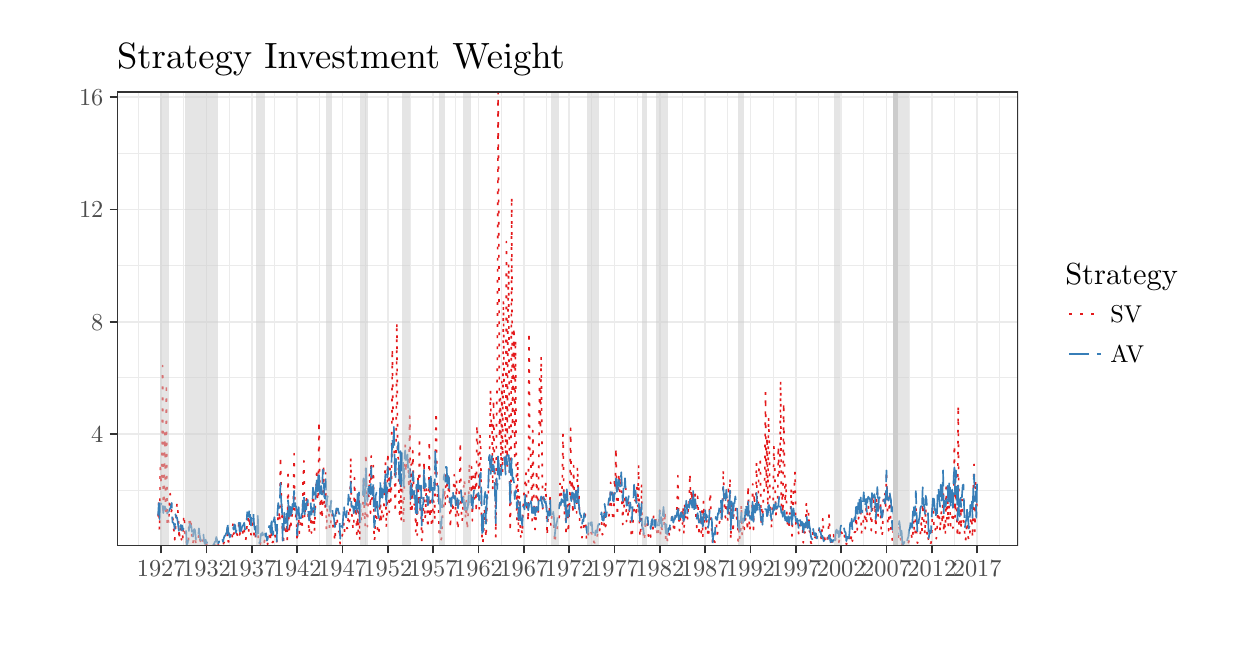
\begin{tikzpicture}[x=1pt,y=1pt]
\definecolor{fillColor}{RGB}{255,255,255}
\path[use as bounding box,fill=fillColor,fill opacity=0.00] (0,0) rectangle (426.79,216.81);
\begin{scope}
\path[clip] (  0.00,  0.00) rectangle (426.79,216.81);
\definecolor{drawColor}{RGB}{255,255,255}
\definecolor{fillColor}{RGB}{255,255,255}

\path[draw=drawColor,line width= 0.6pt,line join=round,line cap=round,fill=fillColor] (  0.00,  0.00) rectangle (426.79,216.81);
\end{scope}
\begin{scope}
\path[clip] ( 32.32, 29.59) rectangle (357.87,193.67);
\definecolor{fillColor}{RGB}{255,255,255}

\path[fill=fillColor] ( 32.32, 29.59) rectangle (357.87,193.67);
\definecolor{drawColor}{gray}{0.92}

\path[draw=drawColor,line width= 0.3pt,line join=round] ( 32.32, 49.71) --
	(357.87, 49.71);

\path[draw=drawColor,line width= 0.3pt,line join=round] ( 32.32, 90.28) --
	(357.87, 90.28);

\path[draw=drawColor,line width= 0.3pt,line join=round] ( 32.32,130.86) --
	(357.87,130.86);

\path[draw=drawColor,line width= 0.3pt,line join=round] ( 32.32,171.43) --
	(357.87,171.43);

\path[draw=drawColor,line width= 0.3pt,line join=round] ( 40.06, 29.59) --
	( 40.06,193.67);

\path[draw=drawColor,line width= 0.3pt,line join=round] ( 56.44, 29.59) --
	( 56.44,193.67);

\path[draw=drawColor,line width= 0.3pt,line join=round] ( 72.82, 29.59) --
	( 72.82,193.67);

\path[draw=drawColor,line width= 0.3pt,line join=round] ( 89.21, 29.59) --
	( 89.21,193.67);

\path[draw=drawColor,line width= 0.3pt,line join=round] (105.58, 29.59) --
	(105.58,193.67);

\path[draw=drawColor,line width= 0.3pt,line join=round] (121.96, 29.59) --
	(121.96,193.67);

\path[draw=drawColor,line width= 0.3pt,line join=round] (138.35, 29.59) --
	(138.35,193.67);

\path[draw=drawColor,line width= 0.3pt,line join=round] (154.73, 29.59) --
	(154.73,193.67);

\path[draw=drawColor,line width= 0.3pt,line join=round] (171.11, 29.59) --
	(171.11,193.67);

\path[draw=drawColor,line width= 0.3pt,line join=round] (187.49, 29.59) --
	(187.49,193.67);

\path[draw=drawColor,line width= 0.3pt,line join=round] (203.87, 29.59) --
	(203.87,193.67);

\path[draw=drawColor,line width= 0.3pt,line join=round] (220.25, 29.59) --
	(220.25,193.67);

\path[draw=drawColor,line width= 0.3pt,line join=round] (236.63, 29.59) --
	(236.63,193.67);

\path[draw=drawColor,line width= 0.3pt,line join=round] (253.01, 29.59) --
	(253.01,193.67);

\path[draw=drawColor,line width= 0.3pt,line join=round] (269.39, 29.59) --
	(269.39,193.67);

\path[draw=drawColor,line width= 0.3pt,line join=round] (285.77, 29.59) --
	(285.77,193.67);

\path[draw=drawColor,line width= 0.3pt,line join=round] (302.15, 29.59) --
	(302.15,193.67);

\path[draw=drawColor,line width= 0.3pt,line join=round] (318.53, 29.59) --
	(318.53,193.67);

\path[draw=drawColor,line width= 0.3pt,line join=round] (334.91, 29.59) --
	(334.91,193.67);

\path[draw=drawColor,line width= 0.3pt,line join=round] (351.30, 29.59) --
	(351.30,193.67);

\path[draw=drawColor,line width= 0.6pt,line join=round] ( 32.32, 69.99) --
	(357.87, 69.99);

\path[draw=drawColor,line width= 0.6pt,line join=round] ( 32.32,110.57) --
	(357.87,110.57);

\path[draw=drawColor,line width= 0.6pt,line join=round] ( 32.32,151.14) --
	(357.87,151.14);

\path[draw=drawColor,line width= 0.6pt,line join=round] ( 32.32,191.72) --
	(357.87,191.72);

\path[draw=drawColor,line width= 0.6pt,line join=round] ( 48.25, 29.59) --
	( 48.25,193.67);

\path[draw=drawColor,line width= 0.6pt,line join=round] ( 64.63, 29.59) --
	( 64.63,193.67);

\path[draw=drawColor,line width= 0.6pt,line join=round] ( 81.02, 29.59) --
	( 81.02,193.67);

\path[draw=drawColor,line width= 0.6pt,line join=round] ( 97.40, 29.59) --
	( 97.40,193.67);

\path[draw=drawColor,line width= 0.6pt,line join=round] (113.77, 29.59) --
	(113.77,193.67);

\path[draw=drawColor,line width= 0.6pt,line join=round] (130.15, 29.59) --
	(130.15,193.67);

\path[draw=drawColor,line width= 0.6pt,line join=round] (146.54, 29.59) --
	(146.54,193.67);

\path[draw=drawColor,line width= 0.6pt,line join=round] (162.92, 29.59) --
	(162.92,193.67);

\path[draw=drawColor,line width= 0.6pt,line join=round] (179.30, 29.59) --
	(179.30,193.67);

\path[draw=drawColor,line width= 0.6pt,line join=round] (195.68, 29.59) --
	(195.68,193.67);

\path[draw=drawColor,line width= 0.6pt,line join=round] (212.06, 29.59) --
	(212.06,193.67);

\path[draw=drawColor,line width= 0.6pt,line join=round] (228.44, 29.59) --
	(228.44,193.67);

\path[draw=drawColor,line width= 0.6pt,line join=round] (244.82, 29.59) --
	(244.82,193.67);

\path[draw=drawColor,line width= 0.6pt,line join=round] (261.20, 29.59) --
	(261.20,193.67);

\path[draw=drawColor,line width= 0.6pt,line join=round] (277.59, 29.59) --
	(277.59,193.67);

\path[draw=drawColor,line width= 0.6pt,line join=round] (293.96, 29.59) --
	(293.96,193.67);

\path[draw=drawColor,line width= 0.6pt,line join=round] (310.34, 29.59) --
	(310.34,193.67);

\path[draw=drawColor,line width= 0.6pt,line join=round] (326.72, 29.59) --
	(326.72,193.67);

\path[draw=drawColor,line width= 0.6pt,line join=round] (343.11, 29.59) --
	(343.11,193.67);
\definecolor{drawColor}{RGB}{228,26,28}

\path[draw=drawColor,line width= 0.6pt,dash pattern=on 1pt off 3pt ,line join=round] ( 47.12, 40.23) --
	( 47.40, 46.35) --
	( 47.67, 35.12) --
	( 47.95, 57.83) --
	( 48.22, 52.69) --
	( 48.49, 52.09) --
	( 48.77, 94.67) --
	( 49.02, 40.74) --
	( 49.30, 45.84) --
	( 49.57, 70.42) --
	( 49.85, 42.05) --
	( 50.12, 88.22) --
	( 50.40, 37.82) --
	( 50.67, 39.86) --
	( 50.94, 37.55) --
	( 51.22, 46.52) --
	( 51.49, 48.46) --
	( 51.77, 41.28) --
	( 52.05, 42.50) --
	( 52.31, 42.67) --
	( 52.58, 37.08) --
	( 52.85, 35.05) --
	( 53.13, 31.76) --
	( 53.40, 35.53) --
	( 53.68, 40.23) --
	( 53.96, 45.08) --
	( 54.23, 42.93) --
	( 54.50, 38.21) --
	( 54.77, 31.74) --
	( 55.05, 36.58) --
	( 55.33, 32.94) --
	( 55.58, 31.76) --
	( 55.86, 34.32) --
	( 56.13, 32.02) --
	( 56.40, 40.73) --
	( 56.67, 39.40) --
	( 56.95, 32.87) --
	( 57.23, 33.11) --
	( 57.50, 29.59) --
	( 57.78, 29.70) --
	( 58.05, 30.51) --
	( 58.32, 39.02) --
	( 58.60, 36.07) --
	( 58.85, 39.72) --
	( 59.13, 35.96) --
	( 59.40, 31.66) --
	( 59.68, 30.25) --
	( 59.95, 31.86) --
	( 60.23, 32.06) --
	( 60.50, 32.98) --
	( 60.77, 30.37) --
	( 61.05, 31.01) --
	( 61.32, 30.79) --
	( 61.60, 31.54) --
	( 61.88, 34.29) --
	( 62.13, 32.48) --
	( 62.41, 31.17) --
	( 62.67, 31.45) --
	( 62.95, 29.98) --
	( 63.22, 31.16) --
	( 63.50, 31.93) --
	( 63.78, 30.06) --
	( 64.05, 29.70) --
	( 64.32, 30.46) --
	( 64.59, 29.98) --
	( 64.87, 30.09) --
	( 65.15, 29.87) --
	( 65.41, 30.43) --
	( 65.69, 30.20) --
	( 65.96, 30.09) --
	( 66.24, 29.84) --
	( 66.50, 30.22) --
	( 66.78, 29.79) --
	( 67.06, 29.69) --
	( 67.33, 29.76) --
	( 67.61, 29.94) --
	( 67.88, 30.72) --
	( 68.15, 31.58) --
	( 68.43, 30.36) --
	( 68.68, 29.71) --
	( 68.96, 29.89) --
	( 69.23, 30.39) --
	( 69.51, 29.94) --
	( 69.78, 29.72) --
	( 70.06, 30.37) --
	( 70.33, 30.24) --
	( 70.60, 29.85) --
	( 70.88, 30.67) --
	( 71.15, 31.26) --
	( 71.43, 31.20) --
	( 71.71, 31.40) --
	( 71.96, 31.24) --
	( 72.24, 34.34) --
	( 72.51, 30.97) --
	( 72.78, 31.14) --
	( 73.05, 30.50) --
	( 73.33, 31.24) --
	( 73.61, 31.94) --
	( 73.88, 32.54) --
	( 74.16, 37.40) --
	( 74.42, 33.82) --
	( 74.70, 34.47) --
	( 74.98, 33.57) --
	( 75.23, 32.81) --
	( 75.51, 34.06) --
	( 75.78, 33.40) --
	( 76.06, 34.06) --
	( 76.33, 39.03) --
	( 76.60, 33.50) --
	( 76.88, 35.02) --
	( 77.15, 33.41) --
	( 77.43, 33.52) --
	( 77.70, 34.21) --
	( 77.98, 36.70) --
	( 78.25, 35.38) --
	( 78.51, 32.01) --
	( 78.79, 31.64) --
	( 79.06, 33.60) --
	( 79.34, 38.68) --
	( 79.61, 39.63) --
	( 79.89, 34.88) --
	( 80.17, 40.16) --
	( 80.43, 36.00) --
	( 80.71, 33.54) --
	( 80.98, 36.66) --
	( 81.26, 37.95) --
	( 81.54, 39.56) --
	( 81.79, 33.77) --
	( 82.07, 31.49) --
	( 82.34, 33.07) --
	( 82.61, 33.60) --
	( 82.88, 35.11) --
	( 83.16, 36.93) --
	( 83.44, 30.14) --
	( 83.71, 29.77) --
	( 83.99, 30.02) --
	( 84.26, 31.27) --
	( 84.53, 30.81) --
	( 84.81, 31.13) --
	( 85.06, 30.44) --
	( 85.34, 30.13) --
	( 85.61, 31.54) --
	( 85.89, 30.74) --
	( 86.16, 31.38) --
	( 86.43, 31.69) --
	( 86.71, 30.12) --
	( 86.98, 33.02) --
	( 87.26, 32.49) --
	( 87.53, 34.95) --
	( 87.81, 31.23) --
	( 88.09, 34.03) --
	( 88.34, 30.89) --
	( 88.61, 30.78) --
	( 88.88, 33.84) --
	( 89.16, 33.74) --
	( 89.43, 33.22) --
	( 89.71, 31.29) --
	( 89.99, 30.24) --
	( 90.26, 36.37) --
	( 90.53, 41.47) --
	( 90.80, 42.03) --
	( 91.08, 38.20) --
	( 91.36, 61.86) --
	( 91.62, 47.39) --
	( 91.90, 41.18) --
	( 92.17, 30.02) --
	( 92.44, 30.74) --
	( 92.71, 41.72) --
	( 92.99, 33.39) --
	( 93.27, 33.56) --
	( 93.54, 39.60) --
	( 93.82, 31.64) --
	( 94.09, 55.39) --
	( 94.36, 38.33) --
	( 94.64, 34.21) --
	( 94.89, 41.08) --
	( 95.17, 37.03) --
	( 95.44, 39.96) --
	( 95.72, 42.14) --
	( 95.99, 41.36) --
	( 96.27, 62.88) --
	( 96.54, 42.73) --
	( 96.81, 39.57) --
	( 97.09, 42.57) --
	( 97.36, 31.10) --
	( 97.64, 35.24) --
	( 97.92, 39.93) --
	( 98.17, 34.13) --
	( 98.45, 34.25) --
	( 98.71, 39.41) --
	( 98.99, 38.75) --
	( 99.26, 36.72) --
	( 99.54, 54.23) --
	( 99.82, 60.29) --
	(100.09, 39.40) --
	(100.36, 43.76) --
	(100.63, 45.76) --
	(100.91, 47.40) --
	(101.19, 45.63) --
	(101.44, 38.05) --
	(101.72, 33.86) --
	(101.99, 39.98) --
	(102.27, 40.71) --
	(102.54, 34.21) --
	(102.81, 36.66) --
	(103.09, 50.06) --
	(103.36, 45.25) --
	(103.64, 34.80) --
	(103.91, 42.70) --
	(104.19, 49.28) --
	(104.46, 57.44) --
	(104.72, 47.13) --
	(105.00, 45.79) --
	(105.27, 74.55) --
	(105.55, 49.70) --
	(105.82, 41.10) --
	(106.10, 51.48) --
	(106.37, 39.29) --
	(106.64, 49.20) --
	(106.92, 59.10) --
	(107.19, 44.28) --
	(107.47, 42.60) --
	(107.75, 55.98) --
	(108.00, 35.28) --
	(108.28, 42.88) --
	(108.54, 43.48) --
	(108.82, 42.70) --
	(109.09, 35.85) --
	(109.37, 35.46) --
	(109.65, 39.49) --
	(109.92, 41.44) --
	(110.20, 38.01) --
	(110.46, 35.64) --
	(110.74, 34.15) --
	(111.02, 31.19) --
	(111.27, 36.48) --
	(111.55, 42.05) --
	(111.82, 38.99) --
	(112.10, 36.48) --
	(112.37, 34.93) --
	(112.64, 34.54) --
	(112.92, 30.07) --
	(113.19, 31.19) --
	(113.47, 32.27) --
	(113.74, 33.69) --
	(114.02, 35.04) --
	(114.29, 38.25) --
	(114.55, 34.07) --
	(114.82, 34.33) --
	(115.09, 34.04) --
	(115.37, 36.16) --
	(115.64, 35.61) --
	(115.92, 42.17) --
	(116.20, 37.93) --
	(116.46, 41.27) --
	(116.74, 61.55) --
	(117.01, 41.45) --
	(117.29, 39.94) --
	(117.57, 35.59) --
	(117.83, 35.79) --
	(118.11, 54.19) --
	(118.38, 40.72) --
	(118.65, 42.41) --
	(118.92, 33.71) --
	(119.20, 42.49) --
	(119.48, 34.22) --
	(119.75, 46.93) --
	(120.03, 31.32) --
	(120.29, 42.84) --
	(120.57, 38.20) --
	(120.85, 39.06) --
	(121.10, 40.66) --
	(121.38, 54.36) --
	(121.65, 42.78) --
	(121.93, 36.48) --
	(122.20, 62.91) --
	(122.47, 42.34) --
	(122.75, 36.49) --
	(123.02, 47.94) --
	(123.30, 47.41) --
	(123.57, 56.02) --
	(123.85, 41.34) --
	(124.12, 62.05) --
	(124.38, 46.47) --
	(124.65, 47.50) --
	(124.92, 58.53) --
	(125.20, 31.33) --
	(125.47, 32.68) --
	(125.75, 45.98) --
	(126.03, 40.75) --
	(126.30, 37.15) --
	(126.57, 33.58) --
	(126.84, 33.69) --
	(127.12, 36.95) --
	(127.40, 49.57) --
	(127.65, 37.65) --
	(127.93, 42.59) --
	(128.20, 39.17) --
	(128.48, 39.56) --
	(128.74, 44.23) --
	(129.02, 54.25) --
	(129.30, 59.78) --
	(129.57, 36.09) --
	(129.85, 41.76) --
	(130.12, 63.28) --
	(130.39, 55.50) --
	(130.67, 41.69) --
	(130.93, 57.56) --
	(131.21, 45.79) --
	(131.48, 52.93) --
	(131.76,100.84) --
	(132.03, 74.98) --
	(132.31, 73.05) --
	(132.58, 56.56) --
	(132.85, 41.58) --
	(133.13, 65.21) --
	(133.40,110.41) --
	(133.68, 61.65) --
	(133.96, 61.31) --
	(134.21, 44.85) --
	(134.48, 39.48) --
	(134.75, 52.51) --
	(135.03, 38.50) --
	(135.30, 51.50) --
	(135.58, 47.29) --
	(135.86, 38.02) --
	(136.13, 53.31) --
	(136.40, 66.16) --
	(136.67, 56.12) --
	(136.95, 58.48) --
	(137.23, 59.63) --
	(137.48, 61.49) --
	(137.76, 50.21) --
	(138.03, 76.47) --
	(138.31, 41.99) --
	(138.57, 59.04) --
	(138.85, 41.28) --
	(139.13, 63.93) --
	(139.40, 53.84) --
	(139.68, 44.30) --
	(139.95, 45.59) --
	(140.23, 34.72) --
	(140.50, 51.84) --
	(140.75, 33.41) --
	(141.03, 55.55) --
	(141.30, 44.09) --
	(141.58, 68.74) --
	(141.85, 41.85) --
	(142.13, 42.28) --
	(142.40, 31.23) --
	(142.67, 34.57) --
	(142.95, 42.73) --
	(143.22, 60.22) --
	(143.50, 38.96) --
	(143.78, 41.00) --
	(144.04, 50.99) --
	(144.32, 42.52) --
	(144.58, 35.86) --
	(144.86, 40.57) --
	(145.13, 67.58) --
	(145.41, 39.56) --
	(145.69, 45.90) --
	(145.96, 36.76) --
	(146.23, 36.27) --
	(146.50, 46.07) --
	(146.78, 45.26) --
	(147.06, 38.81) --
	(147.31, 61.75) --
	(147.59, 77.84) --
	(147.86, 54.92) --
	(148.14, 46.64) --
	(148.41, 47.73) --
	(148.68, 34.36) --
	(148.96, 36.61) --
	(149.23, 31.33) --
	(149.51, 32.21) --
	(149.78, 37.62) --
	(150.06, 43.32) --
	(150.33, 43.79) --
	(150.59, 50.40) --
	(150.86, 43.85) --
	(151.13, 55.18) --
	(151.41, 54.28) --
	(151.68, 47.32) --
	(151.96, 46.77) --
	(152.24, 55.73) --
	(152.50, 42.84) --
	(152.78, 35.84) --
	(153.05, 47.05) --
	(153.33, 46.46) --
	(153.61, 41.72) --
	(153.86, 49.20) --
	(154.14, 55.29) --
	(154.41, 52.79) --
	(154.68, 39.91) --
	(154.95, 53.22) --
	(155.23, 38.55) --
	(155.51, 35.31) --
	(155.78, 45.60) --
	(156.06, 50.92) --
	(156.33, 67.07) --
	(156.60, 44.83) --
	(156.88, 38.25) --
	(157.14, 39.51) --
	(157.42, 45.76) --
	(157.69, 53.74) --
	(157.97, 51.62) --
	(158.24, 39.22) --
	(158.51, 45.92) --
	(158.79, 35.30) --
	(159.06, 38.34) --
	(159.34, 46.62) --
	(159.61, 59.55) --
	(159.89, 48.11) --
	(160.16, 49.51) --
	(160.42, 58.12) --
	(160.69, 38.62) --
	(160.96, 54.74) --
	(161.24, 48.95) --
	(161.51, 46.54) --
	(161.79, 56.89) --
	(162.07, 41.60) --
	(162.34, 73.27) --
	(162.61, 65.85) --
	(162.88, 61.66) --
	(163.16, 42.90) --
	(163.44, 70.10) --
	(163.69, 64.91) --
	(163.97, 40.67) --
	(164.24, 30.33) --
	(164.51, 31.02) --
	(164.78, 35.27) --
	(165.06, 42.75) --
	(165.34, 39.16) --
	(165.61, 32.44) --
	(165.89, 41.85) --
	(166.16, 47.79) --
	(166.43, 46.92) --
	(166.71, 58.93) --
	(166.96, 65.79) --
	(167.24, 85.85) --
	(167.51, 71.92) --
	(167.79, 73.86) --
	(168.06, 49.70) --
	(168.34, 82.36) --
	(168.61, 61.68) --
	(168.88, 54.56) --
	(169.16, 32.53) --
	(169.43, 74.21) --
	(169.71, 96.23) --
	(169.99,193.67) --
	(170.25,141.45) --
	(170.52, 68.56) --
	(170.79, 82.79) --
	(171.07, 55.88) --
	(171.34, 88.94) --
	(171.62, 56.06) --
	(171.90,118.36) --
	(172.17, 83.73) --
	(172.44, 77.35) --
	(172.71, 58.46) --
	(172.99,139.51) --
	(173.27, 57.07) --
	(173.52,111.22) --
	(173.80,131.56) --
	(174.07, 61.86) --
	(174.35, 34.72) --
	(174.61, 49.02) --
	(174.89,155.71) --
	(175.17, 70.66) --
	(175.44, 92.87) --
	(175.72,108.55) --
	(175.99, 61.82) --
	(176.26,104.10) --
	(176.54, 61.04) --
	(176.79, 39.05) --
	(177.07, 60.42) --
	(177.34, 34.31) --
	(177.62, 47.81) --
	(177.89, 39.44) --
	(178.17, 32.72) --
	(178.44, 35.77) --
	(178.71, 33.49) --
	(178.99, 42.25) --
	(179.26, 47.04) --
	(179.54, 51.21) --
	(179.82, 52.80) --
	(180.07, 55.93) --
	(180.35, 42.73) --
	(180.62, 42.26) --
	(180.89, 38.30) --
	(181.16,106.74) --
	(181.44, 63.23) --
	(181.72, 64.05) --
	(181.99, 54.43) --
	(182.27, 38.62) --
	(182.53, 71.25) --
	(182.81, 50.13) --
	(183.09, 40.38) --
	(183.35, 35.45) --
	(183.63, 37.57) --
	(183.90, 57.11) --
	(184.18, 46.31) --
	(184.45, 40.50) --
	(184.72, 62.51) --
	(185.00, 89.98) --
	(185.27, 71.54) --
	(185.55, 98.01) --
	(185.82, 67.23) --
	(186.10, 42.94) --
	(186.37, 46.72) --
	(186.62, 46.60) --
	(186.90, 46.26) --
	(187.17, 52.84) --
	(187.45, 43.23) --
	(187.72, 33.29) --
	(188.00, 39.29) --
	(188.28, 40.23) --
	(188.54, 42.20) --
	(188.82, 48.04) --
	(189.09, 36.62) --
	(189.37, 40.14) --
	(189.65, 39.79) --
	(189.90, 38.68) --
	(190.18, 36.07) --
	(190.45, 30.48) --
	(190.72, 32.86) --
	(190.99, 34.59) --
	(191.27, 34.68) --
	(191.55, 38.03) --
	(191.82, 38.78) --
	(192.10, 40.31) --
	(192.37, 52.11) --
	(192.64, 50.77) --
	(192.92, 47.45) --
	(193.17, 51.84) --
	(193.45, 70.09) --
	(193.72, 49.36) --
	(194.00, 39.46) --
	(194.27, 48.24) --
	(194.54, 33.16) --
	(194.82, 47.67) --
	(195.09, 44.85) --
	(195.37, 34.31) --
	(195.64, 41.00) --
	(195.92, 47.96) --
	(196.20, 72.08) --
	(196.46, 45.83) --
	(196.73, 53.72) --
	(197.00, 41.12) --
	(197.28, 58.56) --
	(197.55, 45.94) --
	(197.83, 47.88) --
	(198.11, 49.58) --
	(198.37, 41.43) --
	(198.65, 58.13) --
	(198.92, 49.71) --
	(199.20, 47.52) --
	(199.48, 37.91) --
	(199.73, 35.85) --
	(200.01, 36.46) --
	(200.28, 32.49) --
	(200.55, 34.23) --
	(200.82, 35.22) --
	(201.10, 38.96) --
	(201.38, 42.61) --
	(201.65, 36.96) --
	(201.93, 32.05) --
	(202.20, 31.35) --
	(202.47, 32.62) --
	(202.75, 35.27) --
	(203.00, 35.90) --
	(203.28, 35.48) --
	(203.55, 34.60) --
	(203.83, 33.77) --
	(204.10, 31.51) --
	(204.38, 31.85) --
	(204.65, 30.86) --
	(204.92, 30.66) --
	(205.20, 32.46) --
	(205.47, 32.16) --
	(205.75, 32.57) --
	(206.03, 34.83) --
	(206.28, 33.85) --
	(206.56, 34.67) --
	(206.82, 35.98) --
	(207.10, 38.05) --
	(207.37, 38.42) --
	(207.65, 33.58) --
	(207.93, 34.04) --
	(208.20, 34.92) --
	(208.47, 42.77) --
	(208.74, 36.50) --
	(209.02, 37.21) --
	(209.30, 37.76) --
	(209.56, 38.66) --
	(209.84, 39.41) --
	(210.11, 40.88) --
	(210.39, 42.27) --
	(210.65, 52.53) --
	(210.93, 44.29) --
	(211.21, 43.25) --
	(211.48, 38.49) --
	(211.76, 39.22) --
	(212.03, 54.00) --
	(212.30, 49.52) --
	(212.58, 64.94) --
	(212.83, 46.87) --
	(213.11, 40.38) --
	(213.38, 48.65) --
	(213.66, 55.89) --
	(213.93, 48.85) --
	(214.21, 52.31) --
	(214.48, 54.65) --
	(214.75, 45.44) --
	(215.03, 37.25) --
	(215.30, 46.65) --
	(215.58, 43.18) --
	(215.86, 48.00) --
	(216.11, 50.35) --
	(216.39, 38.36) --
	(216.65, 41.34) --
	(216.93, 40.70) --
	(217.20, 45.64) --
	(217.48, 40.89) --
	(217.76, 39.59) --
	(218.03, 34.71) --
	(218.31, 32.37) --
	(218.57, 35.36) --
	(218.85, 40.34) --
	(219.13, 42.77) --
	(219.38, 46.02) --
	(219.66, 45.97) --
	(219.93, 40.10) --
	(220.21, 51.14) --
	(220.48, 43.83) --
	(220.75, 58.93) --
	(221.03, 37.64) --
	(221.30, 32.67) --
	(221.58, 36.38) --
	(221.85, 52.15) --
	(222.13, 35.10) --
	(222.40, 35.38) --
	(222.66, 31.40) --
	(222.94, 33.02) --
	(223.21, 37.28) --
	(223.49, 37.79) --
	(223.76, 39.04) --
	(224.04, 35.15) --
	(224.31, 33.05) --
	(224.58, 33.87) --
	(224.86, 34.96) --
	(225.13, 32.73) --
	(225.41, 35.36) --
	(225.69, 35.60) --
	(225.94, 35.73) --
	(226.22, 41.21) --
	(226.49, 40.90) --
	(226.76, 39.43) --
	(227.03, 39.11) --
	(227.31, 35.26) --
	(227.59, 32.72) --
	(227.86, 34.65) --
	(228.14, 37.16) --
	(228.40, 42.45) --
	(228.68, 33.46) --
	(228.96, 36.33) --
	(229.21, 35.48) --
	(229.49, 39.76) --
	(229.76, 42.29) --
	(230.04, 36.61) --
	(230.31, 42.10) --
	(230.58, 31.50) --
	(230.86, 35.05) --
	(231.13, 31.51) --
	(231.41, 31.59) --
	(231.68, 34.41) --
	(231.96, 32.75) --
	(232.23, 35.98) --
	(232.49, 38.12) --
	(232.76, 40.01) --
	(233.03, 38.51) --
	(233.31, 37.08) --
	(233.58, 34.33) --
	(233.86, 38.12) --
	(234.14, 40.46) --
	(234.41, 39.93) --
	(234.68, 44.49) --
	(234.95, 54.95) --
	(235.23, 42.60) --
	(235.51, 35.03) --
	(235.77, 38.51) --
	(236.05, 41.85) --
	(236.32, 42.32) --
	(236.59, 37.45) --
	(236.86, 43.99) --
	(237.14, 33.62) --
	(237.42, 44.20) --
	(237.69, 39.81) --
	(237.97, 41.69) --
	(238.24, 40.71) --
	(238.51, 38.96) --
	(238.79, 45.34) --
	(239.04, 44.82) --
	(239.32, 55.76) --
	(239.59, 45.40) --
	(239.87, 49.97) --
	(240.14, 45.33) --
	(240.42, 49.57) --
	(240.69, 43.93) --
	(240.96, 45.24) --
	(241.24, 48.19) --
	(241.51, 40.29) --
	(241.79, 36.20) --
	(242.07, 47.46) --
	(242.32, 42.31) --
	(242.59, 34.68) --
	(242.86, 40.43) --
	(243.14, 38.93) --
	(243.41, 34.25) --
	(243.69, 42.75) --
	(243.97, 32.47) --
	(244.24, 45.88) --
	(244.51, 37.33) --
	(244.78, 40.05) --
	(245.06, 35.64) --
	(245.34, 38.93) --
	(245.59, 36.15) --
	(245.87, 32.49) --
	(246.14, 34.88) --
	(246.42, 45.78) --
	(246.68, 48.88) --
	(246.96, 36.93) --
	(247.24, 34.96) --
	(247.51, 29.60) --
	(247.79, 31.26) --
	(248.06, 31.38) --
	(248.34, 30.87) --
	(248.61, 37.38) --
	(248.87, 37.57) --
	(249.15, 33.43) --
	(249.42, 35.04) --
	(249.70, 36.07) --
	(249.97, 37.98) --
	(250.25, 39.12) --
	(250.52, 42.76) --
	(250.79, 38.94) --
	(251.07, 39.14) --
	(251.34, 57.10) --
	(251.62, 48.29) --
	(251.90, 41.57) --
	(252.15, 39.71) --
	(252.43, 49.26) --
	(252.69, 44.27) --
	(252.97, 38.44) --
	(253.24, 51.55) --
	(253.52, 40.38) --
	(253.80, 54.19) --
	(254.07, 31.75) --
	(254.34, 45.31) --
	(254.61, 42.44) --
	(254.89, 34.30) --
	(255.17, 42.41) --
	(255.42, 42.92) --
	(255.70, 42.07) --
	(255.97, 43.11) --
	(256.25, 39.31) --
	(256.52, 38.82) --
	(256.79, 31.29) --
	(257.07, 35.75) --
	(257.34, 32.04) --
	(257.62, 34.84) --
	(257.89, 44.70) --
	(258.17, 33.11) --
	(258.44, 34.80) --
	(258.70, 38.01) --
	(258.97, 35.50) --
	(259.24, 37.32) --
	(259.52, 41.56) --
	(259.79, 42.15) --
	(260.07, 34.99) --
	(260.35, 51.29) --
	(260.61, 39.54) --
	(260.89, 34.93) --
	(261.16, 36.99) --
	(261.44, 41.21) --
	(261.72, 41.47) --
	(261.98, 51.93) --
	(262.26, 35.48) --
	(262.53, 48.45) --
	(262.80, 43.24) --
	(263.07, 43.26) --
	(263.35, 59.65) --
	(263.63, 42.23) --
	(263.90, 42.09) --
	(264.18, 56.06) --
	(264.44, 60.09) --
	(264.72, 60.35) --
	(265.00, 37.12) --
	(265.25, 42.99) --
	(265.53, 40.63) --
	(265.80, 45.69) --
	(266.08, 49.51) --
	(266.35, 54.70) --
	(266.62, 85.12) --
	(266.90, 49.99) --
	(267.17, 68.95) --
	(267.45, 43.77) --
	(267.72, 76.12) --
	(268.00, 65.10) --
	(268.27, 39.99) --
	(268.53, 40.75) --
	(268.80, 35.86) --
	(269.07, 43.60) --
	(269.35, 43.46) --
	(269.62, 65.79) --
	(269.90, 58.63) --
	(270.18, 45.81) --
	(270.45, 40.15) --
	(270.72, 44.06) --
	(270.99, 44.70) --
	(271.27, 65.65) --
	(271.55, 55.28) --
	(271.80, 56.14) --
	(272.08, 89.34) --
	(272.35, 43.99) --
	(272.62, 47.20) --
	(272.89, 41.32) --
	(273.17, 81.28) --
	(273.45, 59.46) --
	(273.72, 45.08) --
	(274.00, 52.44) --
	(274.27, 41.42) --
	(274.54, 37.52) --
	(274.82, 40.49) --
	(275.08, 36.37) --
	(275.36, 41.43) --
	(275.63, 40.48) --
	(275.91, 50.37) --
	(276.18, 33.10) --
	(276.45, 39.72) --
	(276.73, 50.85) --
	(277.00, 50.38) --
	(277.28, 56.45) --
	(277.55, 37.44) --
	(277.83, 39.99) --
	(278.11, 37.86) --
	(278.36, 35.79) --
	(278.63, 33.67) --
	(278.90, 36.14) --
	(279.18, 37.41) --
	(279.45, 37.08) --
	(279.73, 35.36) --
	(280.01, 35.75) --
	(280.28, 30.66) --
	(280.55, 33.66) --
	(280.82, 34.61) --
	(281.10, 33.64) --
	(281.38, 45.32) --
	(281.63, 41.03) --
	(281.91, 35.56) --
	(282.18, 41.80) --
	(282.46, 34.87) --
	(282.72, 34.60) --
	(283.00, 30.62) --
	(283.28, 30.53) --
	(283.55, 31.08) --
	(283.83, 35.15) --
	(284.10, 33.13) --
	(284.38, 32.82) --
	(284.65, 32.46) --
	(284.90, 32.94) --
	(285.18, 33.34) --
	(285.45, 32.99) --
	(285.73, 33.79) --
	(286.00, 35.63) --
	(286.28, 33.15) --
	(286.55, 33.41) --
	(286.82, 31.78) --
	(287.10, 36.66) --
	(287.37, 39.69) --
	(287.65, 31.12) --
	(287.93, 32.97) --
	(288.19, 30.97) --
	(288.47, 30.26) --
	(288.73, 30.84) --
	(289.01, 32.55) --
	(289.28, 32.97) --
	(289.56, 40.70) --
	(289.84, 34.62) --
	(290.11, 30.75) --
	(290.38, 31.74) --
	(290.65, 30.73) --
	(290.93, 30.96) --
	(291.21, 33.59) --
	(291.46, 30.78) --
	(291.74, 30.62) --
	(292.01, 32.89) --
	(292.29, 35.39) --
	(292.56, 32.95) --
	(292.83, 34.67) --
	(293.11, 30.81) --
	(293.38, 32.25) --
	(293.66, 34.66) --
	(293.93, 34.49) --
	(294.21, 34.23) --
	(294.48, 33.31) --
	(294.73, 34.58) --
	(295.01, 34.17) --
	(295.28, 32.08) --
	(295.56, 32.58) --
	(295.83, 30.13) --
	(296.11, 30.57) --
	(296.39, 31.00) --
	(296.65, 30.33) --
	(296.93, 31.74) --
	(297.20, 33.57) --
	(297.48, 31.56) --
	(297.76, 33.85) --
	(298.01, 31.25) --
	(298.29, 33.43) --
	(298.56, 34.67) --
	(298.83, 34.40) --
	(299.10, 34.58) --
	(299.38, 40.09) --
	(299.66, 34.71) --
	(299.93, 37.12) --
	(300.21, 39.51) --
	(300.48, 40.78) --
	(300.75, 41.30) --
	(301.03, 42.44) --
	(301.29, 33.98) --
	(301.57, 36.58) --
	(301.84, 37.11) --
	(302.12, 40.84) --
	(302.39, 41.17) --
	(302.66, 35.72) --
	(302.94, 43.03) --
	(303.21, 37.91) --
	(303.49, 43.48) --
	(303.76, 44.30) --
	(304.04, 40.29) --
	(304.31, 41.26) --
	(304.57, 42.20) --
	(304.84, 35.05) --
	(305.11, 40.71) --
	(305.39, 48.16) --
	(305.66, 45.77) --
	(305.94, 42.57) --
	(306.22, 44.92) --
	(306.48, 34.14) --
	(306.76, 46.92) --
	(307.03, 49.25) --
	(307.31, 39.93) --
	(307.59, 44.54) --
	(307.84, 45.38) --
	(308.12, 45.55) --
	(308.39, 35.84) --
	(308.66, 33.06) --
	(308.93, 34.76) --
	(309.21, 47.00) --
	(309.49, 46.26) --
	(309.76, 48.43) --
	(310.04, 43.93) --
	(310.31, 55.01) --
	(310.58, 47.97) --
	(310.86, 35.92) --
	(311.11, 35.04) --
	(311.39, 47.68) --
	(311.66, 42.46) --
	(311.94, 35.99) --
	(312.21, 33.63) --
	(312.49, 31.35) --
	(312.76, 34.79) --
	(313.03, 34.73) --
	(313.31, 31.18) --
	(313.58, 33.29) --
	(313.86, 31.63) --
	(314.14, 32.37) --
	(314.40, 30.91) --
	(314.67, 33.13) --
	(314.94, 36.45) --
	(315.22, 33.05) --
	(315.49, 31.71) --
	(315.77, 32.70) --
	(316.05, 29.85) --
	(316.32, 29.59) --
	(316.59, 29.67) --
	(316.86, 29.88) --
	(317.14, 30.17) --
	(317.42, 30.47) --
	(317.67, 29.88) --
	(317.95, 30.60) --
	(318.22, 30.77) --
	(318.50, 31.76) --
	(318.76, 31.95) --
	(319.04, 33.21) --
	(319.32, 33.90) --
	(319.59, 31.56) --
	(319.87, 33.95) --
	(320.14, 38.99) --
	(320.41, 34.29) --
	(320.69, 33.27) --
	(320.94, 44.58) --
	(321.22, 34.36) --
	(321.49, 30.54) --
	(321.77, 31.04) --
	(322.04, 32.29) --
	(322.32, 32.81) --
	(322.59, 34.19) --
	(322.86, 37.83) --
	(323.14, 34.42) --
	(323.41, 45.04) --
	(323.69, 39.35) --
	(323.97, 37.74) --
	(324.22, 33.63) --
	(324.50, 43.36) --
	(324.76, 37.57) --
	(325.04, 33.32) --
	(325.31, 34.32) --
	(325.59, 29.89) --
	(325.87, 30.80) --
	(326.14, 30.63) --
	(326.42, 30.59) --
	(326.68, 32.50) --
	(326.96, 44.17) --
	(327.24, 43.57) --
	(327.50, 36.54) --
	(327.78, 34.69) --
	(328.05, 35.79) --
	(328.33, 32.11) --
	(328.59, 35.42) --
	(328.87, 42.13) --
	(329.15, 38.68) --
	(329.42, 40.53) --
	(329.70, 34.64) --
	(329.97, 40.47) --
	(330.25, 42.25) --
	(330.52, 37.40) --
	(330.77, 53.89) --
	(331.05, 34.51) --
	(331.32, 38.86) --
	(331.60, 33.59) --
	(331.87, 50.78) --
	(332.15, 39.26) --
	(332.42, 46.32) --
	(332.69, 36.41) --
	(332.97, 44.40) --
	(333.24, 43.65) --
	(333.52, 36.83) --
	(333.80, 37.59) --
	(334.05, 40.18) --
	(334.33, 35.93) --
	(334.60, 46.93) --
	(334.87, 66.06) --
	(335.14, 39.75) --
	(335.42, 50.86) --
	(335.70, 42.65) --
	(335.97, 32.76) --
	(336.25, 80.37) --
	(336.52, 34.17) --
	(336.79, 34.04) --
	(337.07, 43.59) --
	(337.32, 35.65) --
	(337.60, 46.33) --
	(337.87, 41.82) --
	(338.15, 38.67) --
	(338.42, 37.91) --
	(338.69, 31.30) --
	(338.97, 31.90) --
	(339.24, 35.99) --
	(339.52, 38.28) --
	(339.79, 33.05) --
	(340.07, 31.59) --
	(340.35, 32.68) --
	(340.61, 36.66) --
	(340.88, 40.18) --
	(341.15, 38.83) --
	(341.43, 32.42) --
	(341.70, 49.51) --
	(341.98, 59.00) --
	(342.26, 34.77) --
	(342.52, 53.33) --
	(342.80, 40.24) --
	(343.07, 46.96);
\definecolor{drawColor}{RGB}{55,126,184}

\path[draw=drawColor,line width= 0.6pt,dash pattern=on 7pt off 3pt ,line join=round] ( 47.12, 40.53) --
	( 47.40, 45.03) --
	( 47.67, 39.24) --
	( 47.95, 44.93) --
	( 48.22, 44.57) --
	( 48.49, 46.12) --
	( 48.77, 45.20) --
	( 49.02, 41.41) --
	( 49.30, 43.64) --
	( 49.57, 43.82) --
	( 49.85, 42.74) --
	( 50.12, 43.96) --
	( 50.40, 41.20) --
	( 50.67, 41.86) --
	( 50.94, 41.82) --
	( 51.22, 42.84) --
	( 51.49, 42.91) --
	( 51.77, 44.01) --
	( 52.05, 45.08) --
	( 52.31, 38.11) --
	( 52.58, 37.99) --
	( 52.85, 37.55) --
	( 53.13, 35.55) --
	( 53.40, 40.98) --
	( 53.68, 39.69) --
	( 53.96, 39.83) --
	( 54.23, 38.29) --
	( 54.50, 35.99) --
	( 54.77, 34.06) --
	( 55.05, 35.82) --
	( 55.33, 37.13) --
	( 55.58, 35.14) --
	( 55.86, 36.90) --
	( 56.13, 35.34) --
	( 56.40, 36.46) --
	( 56.67, 36.54) --
	( 56.95, 34.91) --
	( 57.23, 35.33) --
	( 57.50, 30.02) --
	( 57.78, 30.43) --
	( 58.05, 32.07) --
	( 58.32, 35.91) --
	( 58.60, 37.53) --
	( 58.85, 36.31) --
	( 59.13, 36.82) --
	( 59.40, 33.98) --
	( 59.68, 32.12) --
	( 59.95, 35.03) --
	( 60.23, 35.63) --
	( 60.50, 35.09) --
	( 60.77, 31.90) --
	( 61.05, 32.83) --
	( 61.32, 32.21) --
	( 61.60, 32.62) --
	( 61.88, 35.87) --
	( 62.13, 33.53) --
	( 62.41, 31.94) --
	( 62.67, 31.66) --
	( 62.95, 31.01) --
	( 63.22, 33.45) --
	( 63.50, 33.65) --
	( 63.78, 31.03) --
	( 64.05, 30.26) --
	( 64.32, 31.81) --
	( 64.59, 30.52) --
	( 64.87, 30.83) --
	( 65.15, 30.78) --
	( 65.41, 31.04) --
	( 65.69, 30.72) --
	( 65.96, 30.65) --
	( 66.24, 30.23) --
	( 66.50, 29.76) --
	( 66.78, 30.24) --
	( 67.06, 29.93) --
	( 67.33, 30.17) --
	( 67.61, 31.02) --
	( 67.88, 31.00) --
	( 68.15, 32.75) --
	( 68.43, 31.79) --
	( 68.68, 30.40) --
	( 68.96, 30.64) --
	( 69.23, 31.17) --
	( 69.51, 30.95) --
	( 69.78, 30.51) --
	( 70.06, 32.31) --
	( 70.33, 32.04) --
	( 70.60, 30.97) --
	( 70.88, 32.43) --
	( 71.15, 33.24) --
	( 71.43, 33.22) --
	( 71.71, 34.06) --
	( 71.96, 34.50) --
	( 72.24, 38.28) --
	( 72.51, 33.55) --
	( 72.78, 34.14) --
	( 73.05, 32.62) --
	( 73.33, 33.56) --
	( 73.61, 34.56) --
	( 73.88, 34.52) --
	( 74.16, 36.35) --
	( 74.42, 35.42) --
	( 74.70, 37.32) --
	( 74.98, 36.93) --
	( 75.23, 34.30) --
	( 75.51, 35.52) --
	( 75.78, 35.14) --
	( 76.06, 36.50) --
	( 76.33, 37.93) --
	( 76.60, 34.75) --
	( 76.88, 38.30) --
	( 77.15, 34.88) --
	( 77.43, 36.32) --
	( 77.70, 36.97) --
	( 77.98, 36.98) --
	( 78.25, 37.92) --
	( 78.51, 35.54) --
	( 78.79, 35.58) --
	( 79.06, 37.69) --
	( 79.34, 41.75) --
	( 79.61, 40.65) --
	( 79.89, 40.05) --
	( 80.17, 43.17) --
	( 80.43, 39.95) --
	( 80.71, 36.90) --
	( 80.98, 39.71) --
	( 81.26, 39.63) --
	( 81.54, 41.67) --
	( 81.79, 37.32) --
	( 82.07, 35.40) --
	( 82.34, 37.74) --
	( 82.61, 32.89) --
	( 82.88, 36.61) --
	( 83.16, 40.43) --
	( 83.44, 31.89) --
	( 83.71, 30.54) --
	( 83.99, 31.02) --
	( 84.26, 33.89) --
	( 84.53, 33.26) --
	( 84.81, 34.45) --
	( 85.06, 32.64) --
	( 85.34, 31.84) --
	( 85.61, 33.95) --
	( 85.89, 33.06) --
	( 86.16, 34.16) --
	( 86.43, 31.45) --
	( 86.71, 31.85) --
	( 86.98, 35.21) --
	( 87.26, 36.77) --
	( 87.53, 36.38) --
	( 87.81, 34.31) --
	( 88.09, 39.86) --
	( 88.34, 34.62) --
	( 88.61, 33.41) --
	( 88.88, 38.37) --
	( 89.16, 39.92) --
	( 89.43, 37.67) --
	( 89.71, 34.93) --
	( 89.99, 31.13) --
	( 90.26, 41.39) --
	( 90.53, 45.03) --
	( 90.80, 43.22) --
	( 91.08, 44.43) --
	( 91.36, 52.25) --
	( 91.62, 45.66) --
	( 91.90, 42.65) --
	( 92.17, 31.42) --
	( 92.44, 32.97) --
	( 92.71, 41.56) --
	( 92.99, 37.79) --
	( 93.27, 37.93) --
	( 93.54, 41.18) --
	( 93.82, 35.27) --
	( 94.09, 46.03) --
	( 94.36, 42.40) --
	( 94.64, 40.10) --
	( 94.89, 43.67) --
	( 95.17, 40.81) --
	( 95.44, 41.83) --
	( 95.72, 44.70) --
	( 95.99, 42.61) --
	( 96.27, 49.43) --
	( 96.54, 46.03) --
	( 96.81, 43.62) --
	( 97.09, 43.79) --
	( 97.36, 33.38) --
	( 97.64, 37.53) --
	( 97.92, 43.55) --
	( 98.17, 38.13) --
	( 98.45, 37.80) --
	( 98.71, 39.46) --
	( 98.99, 40.95) --
	( 99.26, 41.31) --
	( 99.54, 47.67) --
	( 99.82, 48.16) --
	(100.09, 40.96) --
	(100.36, 44.86) --
	(100.63, 42.69) --
	(100.91, 45.39) --
	(101.19, 46.19) --
	(101.44, 41.40) --
	(101.72, 38.68) --
	(101.99, 41.10) --
	(102.27, 45.20) --
	(102.54, 40.83) --
	(102.81, 42.87) --
	(103.09, 50.61) --
	(103.36, 49.24) --
	(103.64, 40.54) --
	(103.91, 44.02) --
	(104.19, 50.66) --
	(104.46, 53.23) --
	(104.72, 49.31) --
	(105.00, 54.48) --
	(105.27, 56.73) --
	(105.55, 46.72) --
	(105.82, 47.02) --
	(106.10, 51.22) --
	(106.37, 48.06) --
	(106.64, 57.10) --
	(106.92, 56.56) --
	(107.19, 47.27) --
	(107.47, 46.62) --
	(107.75, 53.70) --
	(108.00, 43.84) --
	(108.28, 47.56) --
	(108.54, 47.06) --
	(108.82, 45.07) --
	(109.09, 43.41) --
	(109.37, 41.82) --
	(109.65, 45.93) --
	(109.92, 44.41) --
	(110.20, 41.39) --
	(110.46, 40.56) --
	(110.74, 39.00) --
	(111.02, 36.31) --
	(111.27, 41.31) --
	(111.55, 43.10) --
	(111.82, 42.43) --
	(112.10, 43.09) --
	(112.37, 41.45) --
	(112.64, 41.41) --
	(112.92, 32.11) --
	(113.19, 34.74) --
	(113.47, 36.78) --
	(113.74, 36.11) --
	(114.02, 40.14) --
	(114.29, 44.33) --
	(114.55, 40.80) --
	(114.82, 40.93) --
	(115.09, 39.78) --
	(115.37, 42.43) --
	(115.64, 41.85) --
	(115.92, 48.09) --
	(116.20, 45.81) --
	(116.46, 46.29) --
	(116.74, 52.61) --
	(117.01, 43.62) --
	(117.29, 43.95) --
	(117.57, 43.92) --
	(117.83, 41.37) --
	(118.11, 44.99) --
	(118.38, 43.05) --
	(118.65, 45.30) --
	(118.92, 41.30) --
	(119.20, 48.33) --
	(119.48, 42.67) --
	(119.75, 48.93) --
	(120.03, 36.55) --
	(120.29, 45.21) --
	(120.57, 46.25) --
	(120.85, 46.79) --
	(121.10, 47.07) --
	(121.38, 53.95) --
	(121.65, 52.12) --
	(121.93, 44.36) --
	(122.20, 58.19) --
	(122.47, 50.35) --
	(122.75, 45.68) --
	(123.02, 52.30) --
	(123.30, 51.22) --
	(123.57, 49.16) --
	(123.85, 48.17) --
	(124.12, 58.08) --
	(124.38, 50.34) --
	(124.65, 47.90) --
	(124.92, 52.66) --
	(125.20, 36.25) --
	(125.47, 37.95) --
	(125.75, 47.66) --
	(126.03, 48.81) --
	(126.30, 44.65) --
	(126.57, 41.18) --
	(126.84, 39.64) --
	(127.12, 42.78) --
	(127.40, 52.99) --
	(127.65, 47.06) --
	(127.93, 51.11) --
	(128.20, 46.92) --
	(128.48, 50.51) --
	(128.74, 48.22) --
	(129.02, 52.11) --
	(129.30, 55.62) --
	(129.57, 43.33) --
	(129.85, 50.31) --
	(130.12, 58.14) --
	(130.39, 52.88) --
	(130.67, 52.05) --
	(130.93, 51.01) --
	(131.21, 53.72) --
	(131.48, 59.97) --
	(131.76, 68.70) --
	(132.03, 65.06) --
	(132.31, 72.56) --
	(132.58, 61.84) --
	(132.85, 53.49) --
	(133.13, 60.62) --
	(133.40, 61.77) --
	(133.68, 64.54) --
	(133.96, 67.05) --
	(134.21, 55.04) --
	(134.48, 50.89) --
	(134.75, 63.78) --
	(135.03, 51.12) --
	(135.30, 63.12) --
	(135.58, 62.00) --
	(135.86, 50.34) --
	(136.13, 59.94) --
	(136.40, 64.08) --
	(136.67, 58.95) --
	(136.95, 60.36) --
	(137.23, 62.56) --
	(137.48, 56.82) --
	(137.76, 54.28) --
	(138.03, 57.51) --
	(138.31, 46.35) --
	(138.57, 52.19) --
	(138.85, 47.92) --
	(139.13, 56.34) --
	(139.40, 54.28) --
	(139.68, 46.67) --
	(139.95, 47.76) --
	(140.23, 41.41) --
	(140.50, 51.65) --
	(140.75, 41.19) --
	(141.03, 53.14) --
	(141.30, 51.03) --
	(141.58, 51.24) --
	(141.85, 43.08) --
	(142.13, 51.41) --
	(142.40, 36.92) --
	(142.67, 44.32) --
	(142.95, 44.62) --
	(143.22, 57.37) --
	(143.50, 50.46) --
	(143.78, 52.11) --
	(144.04, 49.44) --
	(144.32, 47.08) --
	(144.58, 44.20) --
	(144.86, 44.86) --
	(145.13, 53.36) --
	(145.41, 49.62) --
	(145.69, 54.64) --
	(145.96, 46.70) --
	(146.23, 45.07) --
	(146.50, 51.36) --
	(146.78, 53.16) --
	(147.06, 49.72) --
	(147.31, 64.05) --
	(147.59, 55.93) --
	(147.86, 51.39) --
	(148.14, 51.36) --
	(148.41, 50.92) --
	(148.68, 43.13) --
	(148.96, 46.60) --
	(149.23, 35.91) --
	(149.51, 37.56) --
	(149.78, 45.56) --
	(150.06, 46.98) --
	(150.33, 54.33) --
	(150.59, 55.49) --
	(150.86, 52.69) --
	(151.13, 58.09) --
	(151.41, 58.01) --
	(151.68, 50.70) --
	(151.96, 54.81) --
	(152.24, 53.87) --
	(152.50, 46.49) --
	(152.78, 45.18) --
	(153.05, 43.77) --
	(153.33, 48.43) --
	(153.61, 49.63) --
	(153.86, 47.03) --
	(154.14, 46.73) --
	(154.41, 47.60) --
	(154.68, 44.21) --
	(154.95, 46.12) --
	(155.23, 47.25) --
	(155.51, 43.12) --
	(155.78, 46.24) --
	(156.06, 47.20) --
	(156.33, 48.60) --
	(156.60, 49.66) --
	(156.88, 45.62) --
	(157.14, 45.21) --
	(157.42, 48.35) --
	(157.69, 44.34) --
	(157.97, 42.49) --
	(158.24, 45.17) --
	(158.51, 46.02) --
	(158.79, 42.54) --
	(159.06, 43.60) --
	(159.34, 47.94) --
	(159.61, 45.68) --
	(159.89, 44.82) --
	(160.16, 48.00) --
	(160.42, 44.87) --
	(160.69, 41.94) --
	(160.96, 45.99) --
	(161.24, 49.45) --
	(161.51, 49.97) --
	(161.79, 48.22) --
	(162.07, 48.27) --
	(162.34, 48.71) --
	(162.61, 47.52) --
	(162.88, 48.72) --
	(163.16, 45.98) --
	(163.44, 55.19) --
	(163.69, 55.97) --
	(163.97, 47.43) --
	(164.24, 32.67) --
	(164.51, 34.72) --
	(164.78, 41.30) --
	(165.06, 47.28) --
	(165.34, 49.08) --
	(165.61, 37.50) --
	(165.89, 45.52) --
	(166.16, 50.98) --
	(166.43, 50.57) --
	(166.71, 61.62) --
	(166.96, 62.44) --
	(167.24, 54.99) --
	(167.51, 57.60) --
	(167.79, 62.07) --
	(168.06, 56.90) --
	(168.34, 58.76) --
	(168.61, 56.29) --
	(168.88, 48.25) --
	(169.16, 37.74) --
	(169.43, 53.96) --
	(169.71, 50.10) --
	(169.99, 62.82) --
	(170.25, 58.61) --
	(170.52, 52.85) --
	(170.79, 56.75) --
	(171.07, 55.14) --
	(171.34, 59.54) --
	(171.62, 59.44) --
	(171.90, 60.32) --
	(172.17, 61.58) --
	(172.44, 59.79) --
	(172.71, 55.28) --
	(172.99, 62.31) --
	(173.27, 58.91) --
	(173.52, 61.25) --
	(173.80, 62.39) --
	(174.07, 59.87) --
	(174.35, 43.88) --
	(174.61, 55.18) --
	(174.89, 61.18) --
	(175.17, 53.39) --
	(175.44, 54.23) --
	(175.72, 52.44) --
	(175.99, 46.50) --
	(176.26, 49.62) --
	(176.54, 49.32) --
	(176.79, 43.19) --
	(177.07, 46.05) --
	(177.34, 39.04) --
	(177.62, 45.12) --
	(177.89, 46.16) --
	(178.17, 37.21) --
	(178.44, 39.49) --
	(178.71, 36.89) --
	(178.99, 43.59) --
	(179.26, 43.76) --
	(179.54, 42.74) --
	(179.82, 48.01) --
	(180.07, 44.20) --
	(180.35, 45.11) --
	(180.62, 44.23) --
	(180.89, 42.40) --
	(181.16, 44.09) --
	(181.44, 47.02) --
	(181.72, 46.11) --
	(181.99, 44.61) --
	(182.27, 41.36) --
	(182.53, 44.89) --
	(182.81, 41.43) --
	(183.09, 43.60) --
	(183.35, 41.20) --
	(183.63, 39.50) --
	(183.90, 43.61) --
	(184.18, 42.57) --
	(184.45, 42.42) --
	(184.72, 47.59) --
	(185.00, 46.40) --
	(185.27, 45.91) --
	(185.55, 47.42) --
	(185.82, 45.12) --
	(186.10, 43.48) --
	(186.37, 47.51) --
	(186.62, 45.88) --
	(186.90, 45.11) --
	(187.17, 45.62) --
	(187.45, 43.72) --
	(187.72, 38.37) --
	(188.00, 41.95) --
	(188.28, 42.08) --
	(188.54, 40.42) --
	(188.82, 46.03) --
	(189.09, 40.34) --
	(189.37, 39.87) --
	(189.65, 39.15) --
	(189.90, 41.91) --
	(190.18, 39.70) --
	(190.45, 33.08) --
	(190.72, 36.14) --
	(190.99, 37.11) --
	(191.27, 38.38) --
	(191.55, 40.13) --
	(191.82, 41.70) --
	(192.10, 44.35) --
	(192.37, 45.22) --
	(192.64, 44.27) --
	(192.92, 46.44) --
	(193.17, 46.03) --
	(193.45, 44.93) --
	(193.72, 48.92) --
	(194.00, 43.93) --
	(194.27, 48.18) --
	(194.54, 38.01) --
	(194.82, 50.01) --
	(195.09, 45.87) --
	(195.37, 40.01) --
	(195.64, 41.60) --
	(195.92, 45.85) --
	(196.20, 47.30) --
	(196.46, 45.75) --
	(196.73, 48.93) --
	(197.00, 45.58) --
	(197.28, 48.63) --
	(197.55, 45.15) --
	(197.83, 42.51) --
	(198.11, 49.42) --
	(198.37, 44.37) --
	(198.65, 44.87) --
	(198.92, 50.70) --
	(199.20, 44.28) --
	(199.48, 41.58) --
	(199.73, 40.72) --
	(200.01, 40.43) --
	(200.28, 36.99) --
	(200.55, 39.06) --
	(200.82, 38.41) --
	(201.10, 41.36) --
	(201.38, 40.01) --
	(201.65, 38.40) --
	(201.93, 35.43) --
	(202.20, 33.95) --
	(202.47, 34.73) --
	(202.75, 38.98) --
	(203.00, 39.47) --
	(203.28, 39.46) --
	(203.55, 36.91) --
	(203.83, 38.14) --
	(204.10, 34.38) --
	(204.38, 34.40) --
	(204.65, 33.19) --
	(204.92, 32.19) --
	(205.20, 35.02) --
	(205.47, 35.15) --
	(205.75, 34.27) --
	(206.03, 36.70) --
	(206.28, 37.40) --
	(206.56, 37.26) --
	(206.82, 38.40) --
	(207.10, 40.45) --
	(207.37, 41.68) --
	(207.65, 38.93) --
	(207.93, 38.69) --
	(208.20, 38.86) --
	(208.47, 44.75) --
	(208.74, 42.80) --
	(209.02, 40.05) --
	(209.30, 41.95) --
	(209.56, 41.60) --
	(209.84, 45.13) --
	(210.11, 46.82) --
	(210.39, 45.91) --
	(210.65, 50.44) --
	(210.93, 49.31) --
	(211.21, 49.48) --
	(211.48, 46.03) --
	(211.76, 45.60) --
	(212.03, 48.14) --
	(212.30, 48.81) --
	(212.58, 53.88) --
	(212.83, 49.95) --
	(213.11, 47.75) --
	(213.38, 53.51) --
	(213.66, 53.15) --
	(213.93, 51.20) --
	(214.21, 51.03) --
	(214.48, 56.20) --
	(214.75, 50.01) --
	(215.03, 45.80) --
	(215.30, 50.66) --
	(215.58, 49.26) --
	(215.86, 54.01) --
	(216.11, 48.84) --
	(216.39, 44.11) --
	(216.65, 44.24) --
	(216.93, 46.23) --
	(217.20, 47.55) --
	(217.48, 42.40) --
	(217.76, 45.22) --
	(218.03, 41.12) --
	(218.31, 38.48) --
	(218.57, 43.54) --
	(218.85, 45.02) --
	(219.13, 51.68) --
	(219.38, 47.08) --
	(219.66, 49.50) --
	(219.93, 45.03) --
	(220.21, 46.01) --
	(220.48, 45.98) --
	(220.75, 46.71) --
	(221.03, 41.52) --
	(221.30, 37.73) --
	(221.58, 40.95) --
	(221.85, 44.95) --
	(222.13, 35.64) --
	(222.40, 36.05) --
	(222.66, 33.77) --
	(222.94, 36.07) --
	(223.21, 38.91) --
	(223.49, 40.01) --
	(223.76, 39.63) --
	(224.04, 39.91) --
	(224.31, 36.23) --
	(224.58, 36.13) --
	(224.86, 37.36) --
	(225.13, 35.67) --
	(225.41, 38.31) --
	(225.69, 39.26) --
	(225.94, 36.35) --
	(226.22, 37.96) --
	(226.49, 38.91) --
	(226.76, 36.32) --
	(227.03, 38.56) --
	(227.31, 38.08) --
	(227.59, 35.44) --
	(227.86, 35.25) --
	(228.14, 36.78) --
	(228.40, 42.33) --
	(228.68, 37.73) --
	(228.96, 39.93) --
	(229.21, 36.34) --
	(229.49, 40.04) --
	(229.76, 43.64) --
	(230.04, 38.32) --
	(230.31, 38.68) --
	(230.58, 34.17) --
	(230.86, 38.21) --
	(231.13, 33.69) --
	(231.41, 34.89) --
	(231.68, 36.01) --
	(231.96, 35.46) --
	(232.23, 38.83) --
	(232.49, 38.01) --
	(232.76, 39.97) --
	(233.03, 40.09) --
	(233.31, 37.94) --
	(233.58, 39.09) --
	(233.86, 39.20) --
	(234.14, 41.59) --
	(234.41, 39.62) --
	(234.68, 41.69) --
	(234.95, 42.85) --
	(235.23, 40.46) --
	(235.51, 37.82) --
	(235.77, 39.63) --
	(236.05, 41.56) --
	(236.32, 41.45) --
	(236.59, 39.64) --
	(236.86, 40.44) --
	(237.14, 37.07) --
	(237.42, 43.40) --
	(237.69, 40.83) --
	(237.97, 45.88) --
	(238.24, 43.06) --
	(238.51, 40.80) --
	(238.79, 44.47) --
	(239.04, 43.32) --
	(239.32, 46.28) --
	(239.59, 43.45) --
	(239.87, 45.99) --
	(240.14, 43.36) --
	(240.42, 49.84) --
	(240.69, 46.03) --
	(240.96, 41.27) --
	(241.24, 46.42) --
	(241.51, 41.26) --
	(241.79, 39.36) --
	(242.07, 41.37) --
	(242.32, 39.84) --
	(242.59, 37.89) --
	(242.86, 41.82) --
	(243.14, 41.77) --
	(243.41, 37.61) --
	(243.69, 40.63) --
	(243.97, 36.44) --
	(244.24, 41.07) --
	(244.51, 41.12) --
	(244.78, 43.56) --
	(245.06, 38.79) --
	(245.34, 40.77) --
	(245.59, 39.44) --
	(245.87, 36.08) --
	(246.14, 37.78) --
	(246.42, 42.46) --
	(246.68, 42.29) --
	(246.96, 40.29) --
	(247.24, 38.59) --
	(247.51, 30.13) --
	(247.79, 34.09) --
	(248.06, 34.05) --
	(248.34, 33.61) --
	(248.61, 40.02) --
	(248.87, 39.05) --
	(249.15, 38.92) --
	(249.42, 41.36) --
	(249.70, 41.16) --
	(249.97, 44.02) --
	(250.25, 45.57) --
	(250.52, 46.16) --
	(250.79, 37.84) --
	(251.07, 46.11) --
	(251.34, 50.93) --
	(251.62, 46.65) --
	(251.90, 47.90) --
	(252.15, 45.34) --
	(252.43, 49.86) --
	(252.69, 46.84) --
	(252.97, 41.26) --
	(253.24, 45.59) --
	(253.52, 42.85) --
	(253.80, 49.52) --
	(254.07, 35.39) --
	(254.34, 45.57) --
	(254.61, 44.60) --
	(254.89, 39.20) --
	(255.17, 45.02) --
	(255.42, 44.96) --
	(255.70, 47.44) --
	(255.97, 45.13) --
	(256.25, 44.05) --
	(256.52, 40.98) --
	(256.79, 34.43) --
	(257.07, 38.57) --
	(257.34, 34.69) --
	(257.62, 38.37) --
	(257.89, 41.68) --
	(258.17, 36.64) --
	(258.44, 37.50) --
	(258.70, 39.51) --
	(258.97, 38.68) --
	(259.24, 40.75) --
	(259.52, 44.95) --
	(259.79, 42.72) --
	(260.07, 40.46) --
	(260.35, 46.38) --
	(260.61, 40.42) --
	(260.89, 40.41) --
	(261.16, 38.83) --
	(261.44, 37.43) --
	(261.72, 41.10) --
	(261.98, 46.00) --
	(262.26, 38.28) --
	(262.53, 44.13) --
	(262.80, 41.52) --
	(263.07, 42.31) --
	(263.35, 48.65) --
	(263.63, 44.05) --
	(263.90, 41.69) --
	(264.18, 44.69) --
	(264.44, 44.24) --
	(264.72, 41.88) --
	(265.00, 38.75) --
	(265.25, 40.99) --
	(265.53, 37.16) --
	(265.80, 42.38) --
	(266.08, 41.61) --
	(266.35, 42.77) --
	(266.62, 42.82) --
	(266.90, 42.79) --
	(267.17, 40.29) --
	(267.45, 40.81) --
	(267.72, 45.82) --
	(268.00, 42.52) --
	(268.27, 43.11) --
	(268.53, 40.71) --
	(268.80, 38.37) --
	(269.07, 39.90) --
	(269.35, 42.17) --
	(269.62, 44.46) --
	(269.90, 42.52) --
	(270.18, 46.11) --
	(270.45, 43.02) --
	(270.72, 43.22) --
	(270.99, 43.51) --
	(271.27, 44.24) --
	(271.55, 47.24) --
	(271.80, 43.73) --
	(272.08, 43.76) --
	(272.35, 41.50) --
	(272.62, 41.74) --
	(272.89, 40.02) --
	(273.17, 43.71) --
	(273.45, 42.88) --
	(273.72, 38.74) --
	(274.00, 40.03) --
	(274.27, 39.71) --
	(274.54, 36.63) --
	(274.82, 40.26) --
	(275.08, 37.85) --
	(275.36, 39.49) --
	(275.63, 41.25) --
	(275.91, 43.61) --
	(276.18, 36.47) --
	(276.45, 41.35) --
	(276.73, 43.06) --
	(277.00, 40.48) --
	(277.28, 42.01) --
	(277.55, 38.83) --
	(277.83, 38.18) --
	(278.11, 39.34) --
	(278.36, 37.51) --
	(278.63, 35.64) --
	(278.90, 38.76) --
	(279.18, 38.88) --
	(279.45, 36.91) --
	(279.73, 38.22) --
	(280.01, 37.99) --
	(280.28, 33.26) --
	(280.55, 37.59) --
	(280.82, 36.40) --
	(281.10, 36.23) --
	(281.38, 40.82) --
	(281.63, 38.71) --
	(281.91, 35.92) --
	(282.18, 39.97) --
	(282.46, 36.93) --
	(282.72, 35.69) --
	(283.00, 33.07) --
	(283.28, 32.18) --
	(283.55, 31.96) --
	(283.83, 35.73) --
	(284.10, 34.12) --
	(284.38, 33.24) --
	(284.65, 34.13) --
	(284.90, 34.01) --
	(285.18, 32.21) --
	(285.45, 33.94) --
	(285.73, 34.00) --
	(286.00, 36.03) --
	(286.28, 34.53) --
	(286.55, 34.58) --
	(286.82, 32.75) --
	(287.10, 33.24) --
	(287.37, 32.43) --
	(287.65, 31.23) --
	(287.93, 31.85) --
	(288.19, 30.98) --
	(288.47, 30.71) --
	(288.73, 31.67) --
	(289.01, 31.95) --
	(289.28, 32.17) --
	(289.56, 33.36) --
	(289.84, 32.77) --
	(290.11, 30.88) --
	(290.38, 31.91) --
	(290.65, 31.26) --
	(290.93, 30.97) --
	(291.21, 33.38) --
	(291.46, 31.76) --
	(291.74, 31.52) --
	(292.01, 34.72) --
	(292.29, 35.47) --
	(292.56, 34.16) --
	(292.83, 36.65) --
	(293.11, 32.70) --
	(293.38, 33.20) --
	(293.66, 36.12) --
	(293.93, 36.90) --
	(294.21, 35.94) --
	(294.48, 36.06) --
	(294.73, 37.03) --
	(295.01, 35.89) --
	(295.28, 34.54) --
	(295.56, 34.47) --
	(295.83, 31.25) --
	(296.11, 32.86) --
	(296.39, 33.69) --
	(296.65, 31.67) --
	(296.93, 34.07) --
	(297.20, 37.89) --
	(297.48, 35.11) --
	(297.76, 39.36) --
	(298.01, 35.26) --
	(298.29, 37.73) --
	(298.56, 38.80) --
	(298.83, 39.86) --
	(299.10, 39.17) --
	(299.38, 45.31) --
	(299.66, 41.52) --
	(299.93, 41.15) --
	(300.21, 46.41) --
	(300.48, 47.33) --
	(300.75, 41.37) --
	(301.03, 47.02) --
	(301.29, 42.42) --
	(301.57, 41.64) --
	(301.84, 45.45) --
	(302.12, 48.93) --
	(302.39, 43.41) --
	(302.66, 44.56) --
	(302.94, 46.54) --
	(303.21, 41.85) --
	(303.49, 46.32) --
	(303.76, 47.34) --
	(304.04, 46.60) --
	(304.31, 46.84) --
	(304.57, 44.82) --
	(304.84, 41.14) --
	(305.11, 48.65) --
	(305.39, 49.90) --
	(305.66, 47.14) --
	(305.94, 48.26) --
	(306.22, 46.72) --
	(306.48, 39.18) --
	(306.76, 44.99) --
	(307.03, 50.84) --
	(307.31, 42.11) --
	(307.59, 46.49) --
	(307.84, 47.12) --
	(308.12, 45.25) --
	(308.39, 41.16) --
	(308.66, 39.76) --
	(308.93, 40.51) --
	(309.21, 45.70) --
	(309.49, 46.32) --
	(309.76, 44.82) --
	(310.04, 47.07) --
	(310.31, 56.83) --
	(310.58, 46.35) --
	(310.86, 46.43) --
	(311.11, 45.92) --
	(311.39, 49.51) --
	(311.66, 47.51) --
	(311.94, 46.19) --
	(312.21, 40.04) --
	(312.49, 35.34) --
	(312.76, 43.70) --
	(313.03, 38.20) --
	(313.31, 34.15) --
	(313.58, 39.27) --
	(313.86, 33.84) --
	(314.14, 35.87) --
	(314.40, 33.48) --
	(314.67, 35.55) --
	(314.94, 38.54) --
	(315.22, 36.52) --
	(315.49, 32.19) --
	(315.77, 35.00) --
	(316.05, 30.76) --
	(316.32, 30.05) --
	(316.59, 30.42) --
	(316.86, 31.14) --
	(317.14, 31.46) --
	(317.42, 32.28) --
	(317.67, 30.94) --
	(317.95, 32.05) --
	(318.22, 32.81) --
	(318.50, 35.58) --
	(318.76, 35.58) --
	(319.04, 38.00) --
	(319.32, 38.90) --
	(319.59, 36.08) --
	(319.87, 41.34) --
	(320.14, 44.52) --
	(320.41, 40.46) --
	(320.69, 41.12) --
	(320.94, 49.36) --
	(321.22, 40.88) --
	(321.49, 34.59) --
	(321.77, 36.07) --
	(322.04, 38.90) --
	(322.32, 40.12) --
	(322.59, 43.40) --
	(322.86, 43.95) --
	(323.14, 42.50) --
	(323.41, 50.75) --
	(323.69, 44.03) --
	(323.97, 44.37) --
	(324.22, 41.08) --
	(324.50, 47.68) --
	(324.76, 46.46) --
	(325.04, 42.01) --
	(325.31, 42.19) --
	(325.59, 31.88) --
	(325.87, 35.11) --
	(326.14, 34.03) --
	(326.42, 34.69) --
	(326.68, 40.50) --
	(326.96, 44.32) --
	(327.24, 48.28) --
	(327.50, 46.45) --
	(327.78, 42.48) --
	(328.05, 42.80) --
	(328.33, 39.31) --
	(328.59, 41.47) --
	(328.87, 50.59) --
	(329.15, 49.85) --
	(329.42, 46.37) --
	(329.70, 43.66) --
	(329.97, 51.66) --
	(330.25, 45.88) --
	(330.52, 47.95) --
	(330.77, 56.86) --
	(331.05, 41.07) --
	(331.32, 45.85) --
	(331.60, 43.70) --
	(331.87, 44.83) --
	(332.15, 47.90) --
	(332.42, 51.28) --
	(332.69, 44.14) --
	(332.97, 51.87) --
	(333.24, 53.09) --
	(333.52, 43.00) --
	(333.80, 46.97) --
	(334.05, 49.92) --
	(334.33, 43.30) --
	(334.60, 54.24) --
	(334.87, 57.89) --
	(335.14, 48.18) --
	(335.42, 56.80) --
	(335.70, 53.67) --
	(335.97, 38.69) --
	(336.25, 51.43) --
	(336.52, 41.97) --
	(336.79, 40.16) --
	(337.07, 46.97) --
	(337.32, 43.56) --
	(337.60, 47.49) --
	(337.87, 51.50) --
	(338.15, 51.66) --
	(338.42, 42.13) --
	(338.69, 36.29) --
	(338.97, 38.34) --
	(339.24, 39.27) --
	(339.52, 43.80) --
	(339.79, 39.74) --
	(340.07, 35.81) --
	(340.35, 36.81) --
	(340.61, 44.36) --
	(340.88, 43.21) --
	(341.15, 46.64) --
	(341.43, 39.67) --
	(341.70, 51.04) --
	(341.98, 55.43) --
	(342.26, 45.67) --
	(342.52, 49.22) --
	(342.80, 39.73) --
	(343.07, 52.77);
\definecolor{fillColor}{RGB}{204,204,204}

\path[fill=fillColor,fill opacity=0.50] ( 47.70,193.67) rectangle ( 51.24, 29.59);

\path[fill=fillColor,fill opacity=0.50] ( 56.99,193.67) rectangle ( 68.71, 29.59);

\path[fill=fillColor,fill opacity=0.50] ( 82.37,193.67) rectangle ( 85.91, 29.59);

\path[fill=fillColor,fill opacity=0.50] (107.76,193.67) rectangle (109.94, 29.59);

\path[fill=fillColor,fill opacity=0.50] (120.05,193.67) rectangle (123.05, 29.59);

\path[fill=fillColor,fill opacity=0.50] (135.34,193.67) rectangle (138.05, 29.59);

\path[fill=fillColor,fill opacity=0.50] (148.72,193.67) rectangle (150.88, 29.59);

\path[fill=fillColor,fill opacity=0.50] (157.45,193.67) rectangle (160.16, 29.59);

\path[fill=fillColor,fill opacity=0.50] (189.13,193.67) rectangle (192.11, 29.59);

\path[fill=fillColor,fill opacity=0.50] (201.95,193.67) rectangle (206.30, 29.59);

\path[fill=fillColor,fill opacity=0.50] (222.16,193.67) rectangle (223.79, 29.59);

\path[fill=fillColor,fill opacity=0.50] (227.07,193.67) rectangle (231.43, 29.59);

\path[fill=fillColor,fill opacity=0.50] (256.55,193.67) rectangle (258.72, 29.59);

\path[fill=fillColor,fill opacity=0.50] (291.50,193.67) rectangle (293.68, 29.59);

\path[fill=fillColor,fill opacity=0.50] (313.62,193.67) rectangle (318.51, 29.59);
\definecolor{drawColor}{gray}{0.80}

\path[draw=drawColor,line width= 1.7pt,line join=round] (313.62, 29.59) -- (313.62,193.67);
\definecolor{drawColor}{gray}{0.20}

\path[draw=drawColor,line width= 0.6pt,line join=round,line cap=round] ( 32.32, 29.59) rectangle (357.87,193.67);
\end{scope}
\begin{scope}
\path[clip] (  0.00,  0.00) rectangle (426.79,216.81);
\definecolor{drawColor}{gray}{0.30}

\node[text=drawColor,anchor=base east,inner sep=0pt, outer sep=0pt, scale=  0.88] at ( 27.37, 66.96) {4};

\node[text=drawColor,anchor=base east,inner sep=0pt, outer sep=0pt, scale=  0.88] at ( 27.37,107.54) {8};

\node[text=drawColor,anchor=base east,inner sep=0pt, outer sep=0pt, scale=  0.88] at ( 27.37,148.11) {12};

\node[text=drawColor,anchor=base east,inner sep=0pt, outer sep=0pt, scale=  0.88] at ( 27.37,188.69) {16};
\end{scope}
\begin{scope}
\path[clip] (  0.00,  0.00) rectangle (426.79,216.81);
\definecolor{drawColor}{gray}{0.20}

\path[draw=drawColor,line width= 0.6pt,line join=round] ( 29.57, 69.99) --
	( 32.32, 69.99);

\path[draw=drawColor,line width= 0.6pt,line join=round] ( 29.57,110.57) --
	( 32.32,110.57);

\path[draw=drawColor,line width= 0.6pt,line join=round] ( 29.57,151.14) --
	( 32.32,151.14);

\path[draw=drawColor,line width= 0.6pt,line join=round] ( 29.57,191.72) --
	( 32.32,191.72);
\end{scope}
\begin{scope}
\path[clip] (  0.00,  0.00) rectangle (426.79,216.81);
\definecolor{drawColor}{gray}{0.20}

\path[draw=drawColor,line width= 0.6pt,line join=round] ( 48.25, 26.84) --
	( 48.25, 29.59);

\path[draw=drawColor,line width= 0.6pt,line join=round] ( 64.63, 26.84) --
	( 64.63, 29.59);

\path[draw=drawColor,line width= 0.6pt,line join=round] ( 81.02, 26.84) --
	( 81.02, 29.59);

\path[draw=drawColor,line width= 0.6pt,line join=round] ( 97.40, 26.84) --
	( 97.40, 29.59);

\path[draw=drawColor,line width= 0.6pt,line join=round] (113.77, 26.84) --
	(113.77, 29.59);

\path[draw=drawColor,line width= 0.6pt,line join=round] (130.15, 26.84) --
	(130.15, 29.59);

\path[draw=drawColor,line width= 0.6pt,line join=round] (146.54, 26.84) --
	(146.54, 29.59);

\path[draw=drawColor,line width= 0.6pt,line join=round] (162.92, 26.84) --
	(162.92, 29.59);

\path[draw=drawColor,line width= 0.6pt,line join=round] (179.30, 26.84) --
	(179.30, 29.59);

\path[draw=drawColor,line width= 0.6pt,line join=round] (195.68, 26.84) --
	(195.68, 29.59);

\path[draw=drawColor,line width= 0.6pt,line join=round] (212.06, 26.84) --
	(212.06, 29.59);

\path[draw=drawColor,line width= 0.6pt,line join=round] (228.44, 26.84) --
	(228.44, 29.59);

\path[draw=drawColor,line width= 0.6pt,line join=round] (244.82, 26.84) --
	(244.82, 29.59);

\path[draw=drawColor,line width= 0.6pt,line join=round] (261.20, 26.84) --
	(261.20, 29.59);

\path[draw=drawColor,line width= 0.6pt,line join=round] (277.59, 26.84) --
	(277.59, 29.59);

\path[draw=drawColor,line width= 0.6pt,line join=round] (293.96, 26.84) --
	(293.96, 29.59);

\path[draw=drawColor,line width= 0.6pt,line join=round] (310.34, 26.84) --
	(310.34, 29.59);

\path[draw=drawColor,line width= 0.6pt,line join=round] (326.72, 26.84) --
	(326.72, 29.59);

\path[draw=drawColor,line width= 0.6pt,line join=round] (343.11, 26.84) --
	(343.11, 29.59);
\end{scope}
\begin{scope}
\path[clip] (  0.00,  0.00) rectangle (426.79,216.81);
\definecolor{drawColor}{gray}{0.30}

\node[text=drawColor,anchor=base,inner sep=0pt, outer sep=0pt, scale=  0.88] at ( 48.25, 18.58) {1927};

\node[text=drawColor,anchor=base,inner sep=0pt, outer sep=0pt, scale=  0.88] at ( 64.63, 18.58) {1932};

\node[text=drawColor,anchor=base,inner sep=0pt, outer sep=0pt, scale=  0.88] at ( 81.02, 18.58) {1937};

\node[text=drawColor,anchor=base,inner sep=0pt, outer sep=0pt, scale=  0.88] at ( 97.40, 18.58) {1942};

\node[text=drawColor,anchor=base,inner sep=0pt, outer sep=0pt, scale=  0.88] at (113.77, 18.58) {1947};

\node[text=drawColor,anchor=base,inner sep=0pt, outer sep=0pt, scale=  0.88] at (130.15, 18.58) {1952};

\node[text=drawColor,anchor=base,inner sep=0pt, outer sep=0pt, scale=  0.88] at (146.54, 18.58) {1957};

\node[text=drawColor,anchor=base,inner sep=0pt, outer sep=0pt, scale=  0.88] at (162.92, 18.58) {1962};

\node[text=drawColor,anchor=base,inner sep=0pt, outer sep=0pt, scale=  0.88] at (179.30, 18.58) {1967};

\node[text=drawColor,anchor=base,inner sep=0pt, outer sep=0pt, scale=  0.88] at (195.68, 18.58) {1972};

\node[text=drawColor,anchor=base,inner sep=0pt, outer sep=0pt, scale=  0.88] at (212.06, 18.58) {1977};

\node[text=drawColor,anchor=base,inner sep=0pt, outer sep=0pt, scale=  0.88] at (228.44, 18.58) {1982};

\node[text=drawColor,anchor=base,inner sep=0pt, outer sep=0pt, scale=  0.88] at (244.82, 18.58) {1987};

\node[text=drawColor,anchor=base,inner sep=0pt, outer sep=0pt, scale=  0.88] at (261.20, 18.58) {1992};

\node[text=drawColor,anchor=base,inner sep=0pt, outer sep=0pt, scale=  0.88] at (277.59, 18.58) {1997};

\node[text=drawColor,anchor=base,inner sep=0pt, outer sep=0pt, scale=  0.88] at (293.96, 18.58) {2002};

\node[text=drawColor,anchor=base,inner sep=0pt, outer sep=0pt, scale=  0.88] at (310.34, 18.58) {2007};

\node[text=drawColor,anchor=base,inner sep=0pt, outer sep=0pt, scale=  0.88] at (326.72, 18.58) {2012};

\node[text=drawColor,anchor=base,inner sep=0pt, outer sep=0pt, scale=  0.88] at (343.11, 18.58) {2017};
\end{scope}
\begin{scope}
\path[clip] (  0.00,  0.00) rectangle (426.79,216.81);
\definecolor{fillColor}{RGB}{255,255,255}

\path[fill=fillColor] (369.25, 85.89) rectangle (421.29,137.37);
\end{scope}
\begin{scope}
\path[clip] (  0.00,  0.00) rectangle (426.79,216.81);
\definecolor{drawColor}{RGB}{0,0,0}

\node[text=drawColor,anchor=base west,inner sep=0pt, outer sep=0pt, scale=  1.10] at (374.94,124.10) {Strategy};
\end{scope}
\begin{scope}
\path[clip] (  0.00,  0.00) rectangle (426.79,216.81);
\definecolor{fillColor}{RGB}{255,255,255}

\path[fill=fillColor] (374.94,106.04) rectangle (389.39,120.49);
\end{scope}
\begin{scope}
\path[clip] (  0.00,  0.00) rectangle (426.79,216.81);
\definecolor{drawColor}{RGB}{228,26,28}

\path[draw=drawColor,line width= 0.6pt,dash pattern=on 1pt off 3pt ,line join=round] (376.39,113.26) -- (387.95,113.26);
\end{scope}
\begin{scope}
\path[clip] (  0.00,  0.00) rectangle (426.79,216.81);
\definecolor{fillColor}{RGB}{255,255,255}

\path[fill=fillColor] (374.94, 91.58) rectangle (389.39,106.04);
\end{scope}
\begin{scope}
\path[clip] (  0.00,  0.00) rectangle (426.79,216.81);
\definecolor{drawColor}{RGB}{55,126,184}

\path[draw=drawColor,line width= 0.6pt,dash pattern=on 7pt off 3pt ,line join=round] (376.39, 98.81) -- (387.95, 98.81);
\end{scope}
\begin{scope}
\path[clip] (  0.00,  0.00) rectangle (426.79,216.81);
\definecolor{drawColor}{RGB}{0,0,0}

\node[text=drawColor,anchor=base west,inner sep=0pt, outer sep=0pt, scale=  0.88] at (391.20,110.23) {SV};
\end{scope}
\begin{scope}
\path[clip] (  0.00,  0.00) rectangle (426.79,216.81);
\definecolor{drawColor}{RGB}{0,0,0}

\node[text=drawColor,anchor=base west,inner sep=0pt, outer sep=0pt, scale=  0.88] at (391.20, 95.78) {AV};
\end{scope}
\begin{scope}
\path[clip] (  0.00,  0.00) rectangle (426.79,216.81);
\definecolor{drawColor}{RGB}{0,0,0}

\node[text=drawColor,anchor=base west,inner sep=0pt, outer sep=0pt, scale=  1.32] at ( 32.32,202.22) {Strategy Investment Weight};
\end{scope}
\end{tikzpicture}

	\end{adjustbox}
	\end{figure}
\clearpage
\begin{figure}[!htb]
		\caption{{\bf Cummulative Log Excess Returns}: The time series of cummulative log excess returns for the buy and hold market investment as well as the AV and SV managed portfolios. Panel a limits the coefficient on the market portfolio between 0 and 1.5 for the AV and SV strategies; panel b limit them to weights from 0 to 3 and they are unconstrained in panel c. } \label{fig:fig_returns}
		\vspace{-4mm}
		% Created by tikzDevice version 0.10.1 on 2018-03-26 14:40:36
% !TEX encoding = UTF-8 Unicode
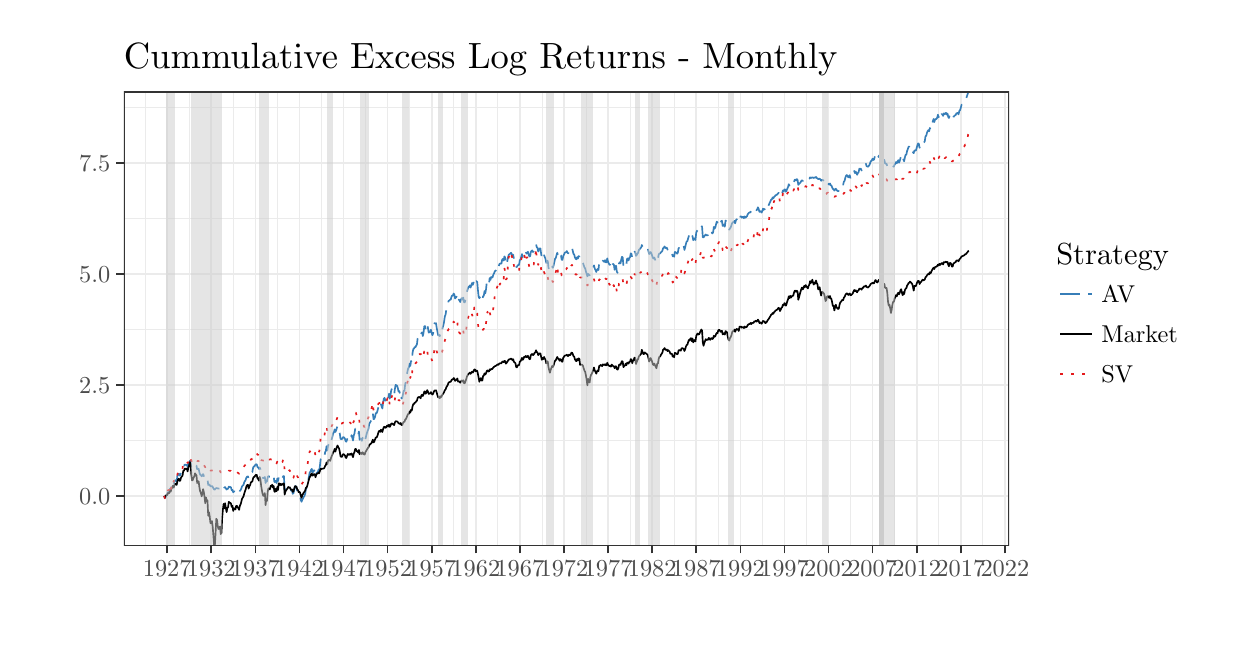
\begin{tikzpicture}[x=1pt,y=1pt]
\definecolor{fillColor}{RGB}{255,255,255}
\path[use as bounding box,fill=fillColor,fill opacity=0.00] (0,0) rectangle (426.79,216.81);
\begin{scope}
\path[clip] (  0.00,  0.00) rectangle (426.79,216.81);
\definecolor{drawColor}{RGB}{255,255,255}
\definecolor{fillColor}{RGB}{255,255,255}

\path[draw=drawColor,line width= 0.6pt,line join=round,line cap=round,fill=fillColor] (  0.00,  0.00) rectangle (426.79,216.81);
\end{scope}
\begin{scope}
\path[clip] ( 34.77, 29.59) rectangle (354.63,193.67);
\definecolor{fillColor}{RGB}{255,255,255}

\path[fill=fillColor] ( 34.77, 29.59) rectangle (354.63,193.67);
\definecolor{drawColor}{gray}{0.92}

\path[draw=drawColor,line width= 0.3pt,line join=round] ( 34.77, 67.61) --
	(354.63, 67.61);

\path[draw=drawColor,line width= 0.3pt,line join=round] ( 34.77,107.75) --
	(354.63,107.75);

\path[draw=drawColor,line width= 0.3pt,line join=round] ( 34.77,147.89) --
	(354.63,147.89);

\path[draw=drawColor,line width= 0.3pt,line join=round] ( 34.77,188.02) --
	(354.63,188.02);

\path[draw=drawColor,line width= 0.3pt,line join=round] ( 42.44, 29.59) --
	( 42.44,193.67);

\path[draw=drawColor,line width= 0.3pt,line join=round] ( 58.37, 29.59) --
	( 58.37,193.67);

\path[draw=drawColor,line width= 0.3pt,line join=round] ( 74.31, 29.59) --
	( 74.31,193.67);

\path[draw=drawColor,line width= 0.3pt,line join=round] ( 90.24, 29.59) --
	( 90.24,193.67);

\path[draw=drawColor,line width= 0.3pt,line join=round] (106.17, 29.59) --
	(106.17,193.67);

\path[draw=drawColor,line width= 0.3pt,line join=round] (122.10, 29.59) --
	(122.10,193.67);

\path[draw=drawColor,line width= 0.3pt,line join=round] (138.04, 29.59) --
	(138.04,193.67);

\path[draw=drawColor,line width= 0.3pt,line join=round] (153.97, 29.59) --
	(153.97,193.67);

\path[draw=drawColor,line width= 0.3pt,line join=round] (169.90, 29.59) --
	(169.90,193.67);

\path[draw=drawColor,line width= 0.3pt,line join=round] (185.83, 29.59) --
	(185.83,193.67);

\path[draw=drawColor,line width= 0.3pt,line join=round] (201.77, 29.59) --
	(201.77,193.67);

\path[draw=drawColor,line width= 0.3pt,line join=round] (217.70, 29.59) --
	(217.70,193.67);

\path[draw=drawColor,line width= 0.3pt,line join=round] (233.63, 29.59) --
	(233.63,193.67);

\path[draw=drawColor,line width= 0.3pt,line join=round] (249.57, 29.59) --
	(249.57,193.67);

\path[draw=drawColor,line width= 0.3pt,line join=round] (265.50, 29.59) --
	(265.50,193.67);

\path[draw=drawColor,line width= 0.3pt,line join=round] (281.44, 29.59) --
	(281.44,193.67);

\path[draw=drawColor,line width= 0.3pt,line join=round] (297.37, 29.59) --
	(297.37,193.67);

\path[draw=drawColor,line width= 0.3pt,line join=round] (313.30, 29.59) --
	(313.30,193.67);

\path[draw=drawColor,line width= 0.3pt,line join=round] (329.23, 29.59) --
	(329.23,193.67);

\path[draw=drawColor,line width= 0.3pt,line join=round] (345.17, 29.59) --
	(345.17,193.67);

\path[draw=drawColor,line width= 0.6pt,line join=round] ( 34.77, 47.54) --
	(354.63, 47.54);

\path[draw=drawColor,line width= 0.6pt,line join=round] ( 34.77, 87.68) --
	(354.63, 87.68);

\path[draw=drawColor,line width= 0.6pt,line join=round] ( 34.77,127.82) --
	(354.63,127.82);

\path[draw=drawColor,line width= 0.6pt,line join=round] ( 34.77,167.95) --
	(354.63,167.95);

\path[draw=drawColor,line width= 0.6pt,line join=round] ( 50.41, 29.59) --
	( 50.41,193.67);

\path[draw=drawColor,line width= 0.6pt,line join=round] ( 66.34, 29.59) --
	( 66.34,193.67);

\path[draw=drawColor,line width= 0.6pt,line join=round] ( 82.28, 29.59) --
	( 82.28,193.67);

\path[draw=drawColor,line width= 0.6pt,line join=round] ( 98.21, 29.59) --
	( 98.21,193.67);

\path[draw=drawColor,line width= 0.6pt,line join=round] (114.14, 29.59) --
	(114.14,193.67);

\path[draw=drawColor,line width= 0.6pt,line join=round] (130.07, 29.59) --
	(130.07,193.67);

\path[draw=drawColor,line width= 0.6pt,line join=round] (146.01, 29.59) --
	(146.01,193.67);

\path[draw=drawColor,line width= 0.6pt,line join=round] (161.94, 29.59) --
	(161.94,193.67);

\path[draw=drawColor,line width= 0.6pt,line join=round] (177.87, 29.59) --
	(177.87,193.67);

\path[draw=drawColor,line width= 0.6pt,line join=round] (193.80, 29.59) --
	(193.80,193.67);

\path[draw=drawColor,line width= 0.6pt,line join=round] (209.74, 29.59) --
	(209.74,193.67);

\path[draw=drawColor,line width= 0.6pt,line join=round] (225.67, 29.59) --
	(225.67,193.67);

\path[draw=drawColor,line width= 0.6pt,line join=round] (241.60, 29.59) --
	(241.60,193.67);

\path[draw=drawColor,line width= 0.6pt,line join=round] (257.53, 29.59) --
	(257.53,193.67);

\path[draw=drawColor,line width= 0.6pt,line join=round] (273.47, 29.59) --
	(273.47,193.67);

\path[draw=drawColor,line width= 0.6pt,line join=round] (289.40, 29.59) --
	(289.40,193.67);

\path[draw=drawColor,line width= 0.6pt,line join=round] (305.33, 29.59) --
	(305.33,193.67);

\path[draw=drawColor,line width= 0.6pt,line join=round] (321.26, 29.59) --
	(321.26,193.67);

\path[draw=drawColor,line width= 0.6pt,line join=round] (337.20, 29.59) --
	(337.20,193.67);

\path[draw=drawColor,line width= 0.6pt,line join=round] (353.13, 29.59) --
	(353.13,193.67);
\definecolor{drawColor}{RGB}{55,126,184}

\path[draw=drawColor,line width= 0.6pt,dash pattern=on 7pt off 3pt ,line join=round] ( 49.31, 47.61) --
	( 49.58, 46.82) --
	( 49.84, 47.22) --
	( 50.11, 47.85) --
	( 50.37, 47.83) --
	( 50.64, 48.93) --
	( 50.91, 48.96) --
	( 51.16, 49.05) --
	( 51.43, 50.24) --
	( 51.69, 49.70) --
	( 51.96, 51.16) --
	( 52.22, 51.62) --
	( 52.49, 52.47) --
	( 52.76, 51.59) --
	( 53.02, 52.85) --
	( 53.29, 53.30) --
	( 53.56, 53.18) --
	( 53.83, 52.79) --
	( 54.10, 54.88) --
	( 54.35, 55.42) --
	( 54.62, 55.62) --
	( 54.88, 55.00) --
	( 55.15, 55.05) --
	( 55.41, 56.24) --
	( 55.68, 56.69) --
	( 55.95, 56.95) --
	( 56.22, 58.52) --
	( 56.49, 58.53) --
	( 56.75, 58.89) --
	( 57.02, 58.88) --
	( 57.29, 58.74) --
	( 57.53, 58.87) --
	( 57.80, 58.09) --
	( 58.07, 58.97) --
	( 58.34, 59.42) --
	( 58.60, 60.28) --
	( 58.87, 59.80) --
	( 59.14, 57.72) --
	( 59.40, 57.59) --
	( 59.67, 57.61) --
	( 59.93, 57.83) --
	( 60.20, 58.08) --
	( 60.47, 58.99) --
	( 60.72, 58.73) --
	( 60.99, 58.52) --
	( 61.25, 57.25) --
	( 61.52, 57.41) --
	( 61.78, 57.42) --
	( 62.05, 56.09) --
	( 62.32, 55.27) --
	( 62.59, 55.15) --
	( 62.86, 54.71) --
	( 63.12, 54.98) --
	( 63.39, 55.50) --
	( 63.66, 54.82) --
	( 63.90, 54.13) --
	( 64.17, 53.56) --
	( 64.43, 54.02) --
	( 64.71, 53.84) --
	( 64.97, 53.86) --
	( 65.24, 51.55) --
	( 65.51, 51.74) --
	( 65.77, 51.62) --
	( 66.04, 51.07) --
	( 66.30, 51.05) --
	( 66.57, 51.17) --
	( 66.84, 50.91) --
	( 67.10, 50.40) --
	( 67.37, 49.92) --
	( 67.63, 49.91) --
	( 67.90, 50.28) --
	( 68.16, 50.45) --
	( 68.43, 50.41) --
	( 68.70, 50.30) --
	( 68.96, 50.23) --
	( 69.23, 50.34) --
	( 69.49, 50.36) --
	( 69.77, 49.49) --
	( 70.04, 49.61) --
	( 70.28, 50.13) --
	( 70.55, 50.50) --
	( 70.81, 50.85) --
	( 71.08, 50.60) --
	( 71.34, 50.80) --
	( 71.61, 50.28) --
	( 71.89, 49.92) --
	( 72.15, 50.15) --
	( 72.42, 50.24) --
	( 72.68, 50.96) --
	( 72.95, 50.81) --
	( 73.22, 50.84) --
	( 73.46, 50.69) --
	( 73.73, 49.63) --
	( 74.00, 49.80) --
	( 74.27, 48.93) --
	( 74.53, 49.21) --
	( 74.80, 49.20) --
	( 75.07, 49.04) --
	( 75.33, 49.68) --
	( 75.60, 49.71) --
	( 75.86, 49.39) --
	( 76.13, 49.14) --
	( 76.40, 48.71) --
	( 76.65, 49.37) --
	( 76.92, 49.70) --
	( 77.18, 50.21) --
	( 77.45, 51.01) --
	( 77.71, 51.36) --
	( 77.98, 51.58) --
	( 78.25, 52.52) --
	( 78.52, 52.96) --
	( 78.79, 53.46) --
	( 79.05, 54.26) --
	( 79.32, 54.56) --
	( 79.59, 54.67) --
	( 79.84, 53.85) --
	( 80.11, 54.34) --
	( 80.37, 54.65) --
	( 80.64, 55.89) --
	( 80.91, 56.08) --
	( 81.18, 56.28) --
	( 81.45, 57.75) --
	( 81.71, 58.28) --
	( 81.98, 58.31) --
	( 82.24, 58.84) --
	( 82.51, 59.05) --
	( 82.78, 59.00) --
	( 83.03, 58.02) --
	( 83.30, 57.95) --
	( 83.56, 57.38) --
	( 83.83, 57.85) --
	( 84.09, 57.29) --
	( 84.36, 54.72) --
	( 84.63, 54.33) --
	( 84.89, 54.18) --
	( 85.16, 54.07) --
	( 85.43, 54.12) --
	( 85.70, 54.46) --
	( 85.97, 52.29) --
	( 86.21, 52.98) --
	( 86.48, 52.83) --
	( 86.74, 54.36) --
	( 87.01, 54.76) --
	( 87.28, 54.55) --
	( 87.55, 54.58) --
	( 87.82, 54.88) --
	( 88.08, 54.71) --
	( 88.35, 55.18) --
	( 88.61, 54.50) --
	( 88.88, 54.77) --
	( 89.15, 52.65) --
	( 89.40, 52.63) --
	( 89.67, 53.05) --
	( 89.93, 52.27) --
	( 90.20, 53.89) --
	( 90.46, 52.98) --
	( 90.73, 54.29) --
	( 91.00, 54.27) --
	( 91.26, 53.56) --
	( 91.53, 54.28) --
	( 91.79, 53.74) --
	( 92.06, 54.09) --
	( 92.34, 54.76) --
	( 92.59, 54.78) --
	( 92.86, 49.55) --
	( 93.12, 49.76) --
	( 93.39, 49.94) --
	( 93.65, 50.40) --
	( 93.92, 50.70) --
	( 94.19, 51.10) --
	( 94.46, 50.78) --
	( 94.73, 50.84) --
	( 94.99, 49.74) --
	( 95.26, 49.45) --
	( 95.53, 49.62) --
	( 95.77, 48.37) --
	( 96.04, 48.60) --
	( 96.30, 49.72) --
	( 96.58, 51.12) --
	( 96.84, 51.09) --
	( 97.11, 50.84) --
	( 97.38, 49.41) --
	( 97.64, 48.95) --
	( 97.91, 47.86) --
	( 98.17, 47.92) --
	( 98.44, 47.61) --
	( 98.71, 46.10) --
	( 98.96, 45.49) --
	( 99.23, 46.26) --
	( 99.49, 46.66) --
	( 99.76, 47.29) --
	(100.02, 47.63) --
	(100.29, 48.39) --
	(100.56, 50.36) --
	(100.82, 50.37) --
	(101.09, 51.59) --
	(101.36, 53.07) --
	(101.63, 54.54) --
	(101.90, 56.12) --
	(102.14, 56.25) --
	(102.41, 57.06) --
	(102.67, 57.38) --
	(102.94, 56.15) --
	(103.21, 56.38) --
	(103.48, 56.88) --
	(103.75, 56.48) --
	(104.01, 54.54) --
	(104.28, 55.63) --
	(104.54, 56.03) --
	(104.81, 56.14) --
	(105.08, 57.05) --
	(105.33, 56.52) --
	(105.60, 58.48) --
	(105.87, 60.85) --
	(106.14, 60.42) --
	(106.40, 60.84) --
	(106.67, 60.85) --
	(106.94, 60.90) --
	(107.20, 61.62) --
	(107.47, 63.33) --
	(107.73, 63.89) --
	(108.00, 65.58) --
	(108.27, 64.04) --
	(108.52, 65.75) --
	(108.79, 66.26) --
	(109.05, 66.38) --
	(109.32, 65.82) --
	(109.58, 67.14) --
	(109.85, 68.06) --
	(110.12, 69.05) --
	(110.39, 70.30) --
	(110.66, 70.54) --
	(110.92, 71.62) --
	(111.19, 70.71) --
	(111.46, 71.32) --
	(111.70, 72.09) --
	(111.97, 72.94) --
	(112.24, 72.12) --
	(112.51, 71.54) --
	(112.77, 70.26) --
	(113.04, 68.22) --
	(113.31, 68.16) --
	(113.57, 68.16) --
	(113.84, 68.72) --
	(114.10, 68.86) --
	(114.37, 68.67) --
	(114.64, 68.26) --
	(114.89, 67.37) --
	(115.16, 67.19) --
	(115.42, 68.04) --
	(115.69, 68.86) --
	(115.95, 68.51) --
	(116.22, 68.37) --
	(116.49, 68.99) --
	(116.75, 68.47) --
	(117.03, 69.56) --
	(117.29, 68.68) --
	(117.56, 67.64) --
	(117.83, 69.45) --
	(118.08, 70.14) --
	(118.35, 71.88) --
	(118.61, 71.86) --
	(118.88, 70.54) --
	(119.15, 70.60) --
	(119.42, 69.67) --
	(119.69, 70.88) --
	(119.95, 67.88) --
	(120.22, 68.24) --
	(120.48, 68.31) --
	(120.75, 67.52) --
	(121.02, 68.61) --
	(121.27, 68.08) --
	(121.54, 66.92) --
	(121.80, 66.96) --
	(122.07, 68.24) --
	(122.33, 69.40) --
	(122.60, 70.41) --
	(122.87, 71.19) --
	(123.13, 71.83) --
	(123.40, 73.55) --
	(123.66, 74.07) --
	(123.93, 74.50) --
	(124.21, 75.03) --
	(124.45, 76.32) --
	(124.72, 77.55) --
	(124.98, 75.32) --
	(125.25, 75.49) --
	(125.51, 76.14) --
	(125.78, 77.49) --
	(126.05, 77.42) --
	(126.32, 78.09) --
	(126.59, 79.12) --
	(126.85, 80.02) --
	(127.12, 80.29) --
	(127.39, 79.45) --
	(127.63, 80.78) --
	(127.90, 79.97) --
	(128.17, 79.21) --
	(128.44, 81.48) --
	(128.70, 82.75) --
	(128.97, 83.03) --
	(129.24, 82.03) --
	(129.50, 82.14) --
	(129.77, 83.23) --
	(130.03, 83.94) --
	(130.30, 82.95) --
	(130.57, 84.51) --
	(130.83, 82.74) --
	(131.10, 83.94) --
	(131.36, 85.76) --
	(131.63, 86.38) --
	(131.89, 85.92) --
	(132.16, 84.50) --
	(132.43, 84.15) --
	(132.69, 86.28) --
	(132.96, 87.72) --
	(133.23, 87.58) --
	(133.50, 87.40) --
	(133.77, 86.53) --
	(134.01, 85.34) --
	(134.28, 85.51) --
	(134.54, 84.53) --
	(134.81, 85.32) --
	(135.08, 82.82) --
	(135.35, 82.90) --
	(135.62, 84.38) --
	(135.88, 85.66) --
	(136.15, 85.62) --
	(136.41, 87.98) --
	(136.68, 88.77) --
	(136.95, 90.64) --
	(137.20, 92.43) --
	(137.47, 93.63) --
	(137.73, 94.10) --
	(138.00, 95.41) --
	(138.26, 94.56) --
	(138.53, 96.38) --
	(138.80, 95.66) --
	(139.06, 99.20) --
	(139.33,100.66) --
	(139.60,100.84) --
	(139.87,101.41) --
	(140.14,101.34) --
	(140.38,101.92) --
	(140.65,102.33) --
	(140.91,104.48) --
	(141.18,105.12) --
	(141.44,105.19) --
	(141.72,105.09) --
	(141.99,104.76) --
	(142.25,106.36) --
	(142.52,106.71) --
	(142.78,105.37) --
	(143.05,106.61) --
	(143.32,108.90) --
	(143.57,109.00) --
	(143.84,107.55) --
	(144.11,108.36) --
	(144.38,109.51) --
	(144.64,108.29) --
	(144.91,106.60) --
	(145.18,106.82) --
	(145.44,106.90) --
	(145.71,107.69) --
	(145.97,106.48) --
	(146.24,105.69) --
	(146.51,106.36) --
	(146.76,108.65) --
	(147.03,110.06) --
	(147.29,109.80) --
	(147.56,110.02) --
	(147.82,108.19) --
	(148.09,106.84) --
	(148.36,105.63) --
	(148.62,105.86) --
	(148.90,105.34) --
	(149.16,106.50) --
	(149.43,106.04) --
	(149.70,107.23) --
	(149.94,108.43) --
	(150.21,109.29) --
	(150.47,110.57) --
	(150.74,112.51) --
	(151.01,113.13) --
	(151.28,115.01) --
	(151.55,116.03) --
	(151.81,116.80) --
	(152.08,118.04) --
	(152.34,118.22) --
	(152.61,118.49) --
	(152.88,118.57) --
	(153.13,119.56) --
	(153.40,120.03) --
	(153.66,119.99) --
	(153.93,120.73) --
	(154.19,120.33) --
	(154.46,118.96) --
	(154.73,119.26) --
	(154.99,119.67) --
	(155.26,120.36) --
	(155.53,118.20) --
	(155.80,118.55) --
	(156.07,118.14) --
	(156.32,117.68) --
	(156.59,118.58) --
	(156.85,119.07) --
	(157.12,118.54) --
	(157.38,119.27) --
	(157.65,117.65) --
	(157.92,117.51) --
	(158.19,118.54) --
	(158.46,119.87) --
	(158.72,121.42) --
	(158.99,122.27) --
	(159.26,123.10) --
	(159.50,123.20) --
	(159.77,123.67) --
	(160.04,122.87) --
	(160.31,123.75) --
	(160.57,124.54) --
	(160.84,123.89) --
	(161.11,124.65) --
	(161.37,125.95) --
	(161.64,125.92) --
	(161.90,124.75) --
	(162.17,125.21) --
	(162.44,124.92) --
	(162.69,122.08) --
	(162.96,119.51) --
	(163.22,119.06) --
	(163.49,119.57) --
	(163.75,119.96) --
	(164.02,118.43) --
	(164.29,118.43) --
	(164.56,119.74) --
	(164.83,119.98) --
	(165.09,121.63) --
	(165.36,120.81) --
	(165.63,122.33) --
	(165.87,124.63) --
	(166.14,125.34) --
	(166.40,124.42) --
	(166.68,124.21) --
	(166.94,126.34) --
	(167.21,125.66) --
	(167.48,126.71) --
	(167.74,126.47) --
	(168.01,126.71) --
	(168.27,127.59) --
	(168.54,128.06) --
	(168.81,128.82) --
	(169.07,128.91) --
	(169.34,129.44) --
	(169.60,129.96) --
	(169.87,130.66) --
	(170.13,129.98) --
	(170.40,131.26) --
	(170.67,131.56) --
	(170.93,131.57) --
	(171.20,131.61) --
	(171.47,133.04) --
	(171.74,133.24) --
	(172.01,132.66) --
	(172.25,134.17) --
	(172.52,133.76) --
	(172.78,131.04) --
	(173.05,131.35) --
	(173.31,132.45) --
	(173.59,133.87) --
	(173.86,134.84) --
	(174.12,134.84) --
	(174.39,135.22) --
	(174.65,135.45) --
	(174.92,135.07) --
	(175.19,134.28) --
	(175.43,134.74) --
	(175.71,133.22) --
	(175.97,133.01) --
	(176.24,132.59) --
	(176.50,130.41) --
	(176.77,130.29) --
	(177.04,130.88) --
	(177.30,131.04) --
	(177.57,131.08) --
	(177.83,132.84) --
	(178.10,132.99) --
	(178.37,134.11) --
	(178.62,134.98) --
	(178.89,133.89) --
	(179.15,134.44) --
	(179.42,135.35) --
	(179.68,135.15) --
	(179.95,136.00) --
	(180.22,135.18) --
	(180.49,135.29) --
	(180.76,135.85) --
	(181.02,134.85) --
	(181.29,134.14) --
	(181.56,134.17) --
	(181.81,135.77) --
	(182.08,136.14) --
	(182.34,136.30) --
	(182.61,135.74) --
	(182.88,136.02) --
	(183.15,137.13) --
	(183.42,137.26) --
	(183.68,138.63) --
	(183.95,137.52) --
	(184.21,137.25) --
	(184.48,135.93) --
	(184.75,136.64) --
	(185.00,137.05) --
	(185.27,137.06) --
	(185.53,135.14) --
	(185.80,133.51) --
	(186.06,134.14) --
	(186.33,133.59) --
	(186.60,134.57) --
	(186.86,133.90) --
	(187.13,133.22) --
	(187.40,131.81) --
	(187.67,132.62) --
	(187.94,132.45) --
	(188.18,130.14) --
	(188.45,128.96) --
	(188.71,128.63) --
	(188.98,129.33) --
	(189.25,129.86) --
	(189.52,130.44) --
	(189.79,130.04) --
	(190.05,130.89) --
	(190.32,132.17) --
	(190.58,133.33) --
	(190.85,133.62) --
	(191.12,134.70) --
	(191.37,135.47) --
	(191.64,134.49) --
	(191.90,134.50) --
	(192.17,133.49) --
	(192.43,134.62) --
	(192.70,134.49) --
	(192.97,132.99) --
	(193.23,132.86) --
	(193.50,134.26) --
	(193.76,134.73) --
	(194.03,135.43) --
	(194.31,135.60) --
	(194.56,135.67) --
	(194.83,136.09) --
	(195.09,135.48) --
	(195.36,135.26) --
	(195.62,136.06) --
	(195.89,135.84) --
	(196.16,136.02) --
	(196.43,137.09) --
	(196.70,137.26) --
	(196.96,136.20) --
	(197.23,135.05) --
	(197.50,134.82) --
	(197.74,133.79) --
	(198.01,133.28) --
	(198.27,133.12) --
	(198.55,133.88) --
	(198.81,133.38) --
	(199.08,134.25) --
	(199.35,134.13) --
	(199.61,132.21) --
	(199.88,132.25) --
	(200.14,132.25) --
	(200.41,132.21) --
	(200.68,131.76) --
	(200.93,130.92) --
	(201.20,130.15) --
	(201.46,129.79) --
	(201.73,128.67) --
	(201.99,127.90) --
	(202.26,126.93) --
	(202.53,127.81) --
	(202.79,127.59) --
	(203.06,127.31) --
	(203.33,128.46) --
	(203.60,128.84) --
	(203.87,129.12) --
	(204.11,129.64) --
	(204.38,130.25) --
	(204.64,130.90) --
	(204.91,129.74) --
	(205.18,129.20) --
	(205.45,128.54) --
	(205.72,129.27) --
	(205.98,129.65) --
	(206.25,129.24) --
	(206.51,131.67) --
	(206.78,131.71) --
	(207.05,132.14) --
	(207.30,131.87) --
	(207.58,131.54) --
	(207.84,132.62) --
	(208.11,132.37) --
	(208.37,132.18) --
	(208.64,132.79) --
	(208.91,132.00) --
	(209.17,132.03) --
	(209.44,133.45) --
	(209.70,132.24) --
	(209.97,131.63) --
	(210.24,131.13) --
	(210.49,131.18) --
	(210.76,130.75) --
	(211.02,132.52) --
	(211.29,131.89) --
	(211.55,131.30) --
	(211.82,131.21) --
	(212.09,129.32) --
	(212.36,130.63) --
	(212.63,130.72) --
	(212.89,128.64) --
	(213.16,128.20) --
	(213.43,129.31) --
	(213.67,131.61) --
	(213.94,132.02) --
	(214.21,131.64) --
	(214.48,132.97) --
	(214.74,134.01) --
	(215.01,133.75) --
	(215.28,130.67) --
	(215.54,131.17) --
	(215.81,131.33) --
	(216.07,132.25) --
	(216.34,131.39) --
	(216.61,133.35) --
	(216.86,133.39) --
	(217.13,132.70) --
	(217.39,133.63) --
	(217.66,133.81) --
	(217.92,135.24) --
	(218.19,135.07) --
	(218.46,133.48) --
	(218.72,134.18) --
	(219.00,134.53) --
	(219.26,135.85) --
	(219.53,135.76) --
	(219.80,134.34) --
	(220.05,134.63) --
	(220.32,135.11) --
	(220.58,135.48) --
	(220.85,136.47) --
	(221.12,136.75) --
	(221.39,137.14) --
	(221.66,137.29) --
	(221.92,138.27) --
	(222.19,137.71) --
	(222.45,137.21) --
	(222.72,137.24) --
	(222.99,137.78) --
	(223.24,137.54) --
	(223.51,137.56) --
	(223.77,137.25) --
	(224.04,137.09) --
	(224.30,136.06) --
	(224.57,134.99) --
	(224.84,135.42) --
	(225.10,135.72) --
	(225.37,135.25) --
	(225.63,134.49) --
	(225.90,133.69) --
	(226.18,133.39) --
	(226.42,133.75) --
	(226.69,133.11) --
	(226.95,132.31) --
	(227.22,131.87) --
	(227.48,133.38) --
	(227.75,133.42) --
	(228.02,134.88) --
	(228.29,135.18) --
	(228.56,135.26) --
	(228.82,135.62) --
	(229.09,135.84) --
	(229.36,136.24) --
	(229.60,137.13) --
	(229.87,137.25) --
	(230.14,137.75) --
	(230.41,137.23) --
	(230.67,137.18) --
	(230.94,137.31) --
	(231.21,136.62) --
	(231.47,136.97) --
	(231.74,136.62) --
	(232.00,136.19) --
	(232.27,135.37) --
	(232.54,135.44) --
	(232.80,135.37) --
	(233.07,134.20) --
	(233.33,134.48) --
	(233.60,134.02) --
	(233.86,135.75) --
	(234.13,135.66) --
	(234.40,135.47) --
	(234.66,135.13) --
	(234.93,135.48) --
	(235.20,137.09) --
	(235.47,137.28) --
	(235.74,137.08) --
	(235.98,136.91) --
	(236.25,138.19) --
	(236.51,138.41) --
	(236.78,138.23) --
	(237.05,138.00) --
	(237.32,136.49) --
	(237.59,137.49) --
	(237.85,138.63) --
	(238.12,139.59) --
	(238.38,139.66) --
	(238.65,140.65) --
	(238.92,141.54) --
	(239.17,141.32) --
	(239.44,141.91) --
	(239.70,142.08) --
	(239.97,140.79) --
	(240.23,141.55) --
	(240.50,140.00) --
	(240.77,140.48) --
	(241.03,140.67) --
	(241.30,140.09) --
	(241.57,142.71) --
	(241.84,143.33) --
	(242.11,143.67) --
	(242.35,143.33) --
	(242.62,143.34) --
	(242.88,143.84) --
	(243.15,144.66) --
	(243.41,145.30) --
	(243.69,144.86) --
	(243.96,141.10) --
	(244.22,141.01) --
	(244.49,141.46) --
	(244.75,141.76) --
	(245.02,142.07) --
	(245.29,141.74) --
	(245.54,141.84) --
	(245.81,141.78) --
	(246.08,142.64) --
	(246.35,142.41) --
	(246.61,141.64) --
	(246.88,142.44) --
	(247.15,142.75) --
	(247.41,142.45) --
	(247.68,142.84) --
	(247.94,144.82) --
	(248.21,144.20) --
	(248.48,144.66) --
	(248.73,145.69) --
	(249.00,146.72) --
	(249.26,146.40) --
	(249.53,147.64) --
	(249.79,148.02) --
	(250.06,147.84) --
	(250.33,146.66) --
	(250.59,146.77) --
	(250.87,147.06) --
	(251.13,145.15) --
	(251.40,145.28) --
	(251.67,145.73) --
	(251.91,144.89) --
	(252.18,147.13) --
	(252.44,146.86) --
	(252.71,146.48) --
	(252.98,144.61) --
	(253.25,144.11) --
	(253.52,143.84) --
	(253.78,144.32) --
	(254.05,144.63) --
	(254.31,145.45) --
	(254.58,146.22) --
	(254.85,146.52) --
	(255.10,146.49) --
	(255.37,147.01) --
	(255.63,146.11) --
	(255.90,147.12) --
	(256.16,147.59) --
	(256.43,147.31) --
	(256.70,147.66) --
	(256.96,146.92) --
	(257.23,148.61) --
	(257.50,148.53) --
	(257.77,148.65) --
	(258.04,148.15) --
	(258.29,148.42) --
	(258.56,148.47) --
	(258.82,147.94) --
	(259.09,148.63) --
	(259.35,148.14) --
	(259.62,148.42) --
	(259.89,148.61) --
	(260.16,149.33) --
	(260.43,149.70) --
	(260.69,149.94) --
	(260.96,149.99) --
	(261.23,150.32) --
	(261.47,149.81) --
	(261.74,150.14) --
	(262.01,150.20) --
	(262.28,150.14) --
	(262.54,150.91) --
	(262.81,150.87) --
	(263.08,151.19) --
	(263.34,150.84) --
	(263.61,151.15) --
	(263.87,151.89) --
	(264.14,151.34) --
	(264.41,150.27) --
	(264.66,150.40) --
	(264.93,150.49) --
	(265.19,149.98) --
	(265.46,150.52) --
	(265.72,151.44) --
	(265.99,151.00) --
	(266.26,151.28) --
	(266.53,150.39) --
	(266.80,150.58) --
	(267.06,150.95) --
	(267.33,151.75) --
	(267.60,152.39) --
	(267.84,152.86) --
	(268.11,153.51) --
	(268.38,154.01) --
	(268.65,154.69) --
	(268.91,154.76) --
	(269.18,155.47) --
	(269.45,155.13) --
	(269.71,155.68) --
	(269.98,155.85) --
	(270.24,156.24) --
	(270.51,156.37) --
	(270.78,156.48) --
	(271.04,156.76) --
	(271.31,157.12) --
	(271.57,156.88) --
	(271.84,155.55) --
	(272.10,155.86) --
	(272.37,156.75) --
	(272.64,156.95) --
	(272.90,157.98) --
	(273.17,157.67) --
	(273.44,158.39) --
	(273.71,158.31) --
	(273.98,157.52) --
	(274.22,158.00) --
	(274.49,158.64) --
	(274.75,159.21) --
	(275.02,160.24) --
	(275.28,159.76) --
	(275.56,160.49) --
	(275.83,159.96) --
	(276.09,160.11) --
	(276.36,160.29) --
	(276.62,160.30) --
	(276.89,161.01) --
	(277.16,161.83) --
	(277.40,161.93) --
	(277.68,161.62) --
	(277.94,162.08) --
	(278.21,161.75) --
	(278.47,160.00) --
	(278.74,160.34) --
	(279.01,160.63) --
	(279.27,160.86) --
	(279.54,161.43) --
	(279.80,161.69) --
	(280.07,161.43) --
	(280.34,161.69) --
	(280.59,162.01) --
	(280.86,161.90) --
	(281.12,162.22) --
	(281.39,161.97) --
	(281.65,161.83) --
	(281.92,161.61) --
	(282.19,162.07) --
	(282.46,162.24) --
	(282.73,162.70) --
	(282.99,162.49) --
	(283.26,162.57) --
	(283.53,162.76) --
	(283.78,162.59) --
	(284.05,162.50) --
	(284.31,162.67) --
	(284.58,162.57) --
	(284.85,162.87) --
	(285.12,162.51) --
	(285.39,162.36) --
	(285.65,162.10) --
	(285.92,162.15) --
	(286.18,162.25) --
	(286.45,161.98) --
	(286.72,161.49) --
	(286.97,161.78) --
	(287.24,161.80) --
	(287.50,161.62) --
	(287.77,161.41) --
	(288.03,160.93) --
	(288.30,159.80) --
	(288.57,159.93) --
	(288.83,160.36) --
	(289.10,160.53) --
	(289.37,160.32) --
	(289.64,160.08) --
	(289.91,160.52) --
	(290.15,159.89) --
	(290.42,159.77) --
	(290.68,159.17) --
	(290.95,158.48) --
	(291.22,158.50) --
	(291.49,157.92) --
	(291.76,158.40) --
	(292.02,158.61) --
	(292.29,158.19) --
	(292.55,157.86) --
	(292.82,157.71) --
	(293.09,157.86) --
	(293.34,158.58) --
	(293.61,159.38) --
	(293.87,159.60) --
	(294.14,159.96) --
	(294.40,160.33) --
	(294.67,160.08) --
	(294.94,161.19) --
	(295.20,161.48) --
	(295.47,162.65) --
	(295.73,163.28) --
	(296.00,163.55) --
	(296.28,163.24) --
	(296.53,162.72) --
	(296.80,162.97) --
	(297.06,163.49) --
	(297.33,162.29) --
	(297.59,162.33) --
	(297.86,162.80) --
	(298.13,163.24) --
	(298.40,164.15) --
	(298.67,165.04) --
	(298.93,164.24) --
	(299.20,164.80) --
	(299.47,164.29) --
	(299.71,163.63) --
	(299.98,164.28) --
	(300.25,164.56) --
	(300.52,165.86) --
	(300.78,165.63) --
	(301.05,165.87) --
	(301.32,165.21) --
	(301.58,165.78) --
	(301.85,165.80) --
	(302.11,167.02) --
	(302.38,166.92) --
	(302.65,167.34) --
	(302.90,167.60) --
	(303.17,166.72) --
	(303.43,166.65) --
	(303.70,166.55) --
	(303.96,166.91) --
	(304.23,167.30) --
	(304.50,168.17) --
	(304.76,168.64) --
	(305.03,168.82) --
	(305.30,169.47) --
	(305.57,168.99) --
	(305.84,169.22) --
	(306.08,170.14) --
	(306.35,171.21) --
	(306.61,170.66) --
	(306.88,169.70) --
	(307.15,169.83) --
	(307.42,170.16) --
	(307.69,170.64) --
	(307.95,169.90) --
	(308.22,169.84) --
	(308.48,168.79) --
	(308.75,168.62) --
	(309.02,168.49) --
	(309.27,168.80) --
	(309.55,169.01) --
	(309.81,167.81) --
	(310.08,167.64) --
	(310.34,167.68) --
	(310.61,166.76) --
	(310.88,166.32) --
	(311.14,166.23) --
	(311.41,166.26) --
	(311.67,166.04) --
	(311.94,165.70) --
	(312.21,166.08) --
	(312.46,166.33) --
	(312.73,166.60) --
	(312.99,166.58) --
	(313.26,167.35) --
	(313.52,167.65) --
	(313.79,168.25) --
	(314.06,167.82) --
	(314.33,168.40) --
	(314.60,168.93) --
	(314.86,168.03) --
	(315.13,168.63) --
	(315.40,169.77) --
	(315.64,170.39) --
	(315.91,168.90) --
	(316.18,168.47) --
	(316.45,169.18) --
	(316.71,168.53) --
	(316.98,170.00) --
	(317.25,170.84) --
	(317.51,170.95) --
	(317.78,172.29) --
	(318.04,172.93) --
	(318.31,173.79) --
	(318.58,173.87) --
	(318.83,174.39) --
	(319.10,173.95) --
	(319.36,173.45) --
	(319.63,173.00) --
	(319.89,171.81) --
	(320.16,171.46) --
	(320.43,172.43) --
	(320.69,172.38) --
	(320.97,172.42) --
	(321.23,173.34) --
	(321.50,174.29) --
	(321.77,174.99) --
	(322.02,174.81) --
	(322.29,173.41) --
	(322.55,174.20) --
	(322.82,174.36) --
	(323.09,174.86) --
	(323.36,175.73) --
	(323.63,175.27) --
	(323.89,175.43) --
	(324.16,175.71) --
	(324.42,177.56) --
	(324.69,177.77) --
	(324.96,178.79) --
	(325.21,179.43) --
	(325.48,179.78) --
	(325.74,179.39) --
	(326.01,180.55) --
	(326.27,179.91) --
	(326.54,180.99) --
	(326.81,182.34) --
	(327.07,182.91) --
	(327.34,183.82) --
	(327.60,182.69) --
	(327.88,183.65) --
	(328.15,183.78) --
	(328.39,183.83) --
	(328.66,184.27) --
	(328.92,185.35) --
	(329.19,184.42) --
	(329.45,185.59) --
	(329.72,184.49) --
	(330.00,185.29) --
	(330.26,185.60) --
	(330.53,185.47) --
	(330.79,184.92) --
	(331.06,185.85) --
	(331.33,185.56) --
	(331.57,185.75) --
	(331.84,186.04) --
	(332.11,185.37) --
	(332.38,185.79) --
	(332.64,184.55) --
	(332.91,184.17) --
	(333.18,185.18) --
	(333.44,185.22) --
	(333.71,184.71) --
	(333.97,183.75) --
	(334.24,183.75) --
	(334.51,184.55) --
	(334.77,184.82) --
	(335.04,185.13) --
	(335.30,185.21) --
	(335.57,185.82) --
	(335.83,185.91) --
	(336.10,186.03) --
	(336.37,185.46) --
	(336.63,186.69) --
	(336.90,186.99) --
	(337.17,187.80) --
	(337.44,188.93) --
	(337.71,189.00) --
	(337.95,189.39) --
	(338.22,189.85) --
	(338.48,190.17) --
	(338.75,190.84) --
	(339.02,190.88) --
	(339.29,191.72) --
	(339.56,192.54) --
	(339.82,193.33) --
	(340.09,193.67);
\definecolor{drawColor}{RGB}{0,0,0}

\path[draw=drawColor,line width= 0.6pt,line join=round] ( 49.31, 47.60) --
	( 49.58, 47.09) --
	( 49.84, 47.50) --
	( 50.11, 47.91) --
	( 50.37, 47.90) --
	( 50.64, 48.57) --
	( 50.91, 48.59) --
	( 51.16, 48.66) --
	( 51.43, 49.52) --
	( 51.69, 49.14) --
	( 51.96, 50.25) --
	( 52.22, 50.57) --
	( 52.49, 51.30) --
	( 52.76, 50.59) --
	( 53.02, 51.62) --
	( 53.29, 51.96) --
	( 53.56, 51.87) --
	( 53.83, 51.60) --
	( 54.10, 52.95) --
	( 54.35, 53.59) --
	( 54.62, 53.82) --
	( 54.88, 53.04) --
	( 55.15, 53.14) --
	( 55.41, 54.18) --
	( 55.68, 54.63) --
	( 55.95, 54.88) --
	( 56.22, 56.68) --
	( 56.49, 56.70) --
	( 56.75, 57.49) --
	( 57.02, 57.47) --
	( 57.29, 57.29) --
	( 57.53, 57.50) --
	( 57.80, 56.46) --
	( 58.07, 57.95) --
	( 58.34, 58.60) --
	( 58.60, 59.83) --
	( 58.87, 58.95) --
	( 59.14, 55.37) --
	( 59.40, 53.19) --
	( 59.67, 53.38) --
	( 59.93, 54.23) --
	( 60.20, 54.62) --
	( 60.47, 55.75) --
	( 60.72, 55.37) --
	( 60.99, 55.09) --
	( 61.25, 52.26) --
	( 61.52, 52.87) --
	( 61.78, 52.89) --
	( 62.05, 50.72) --
	( 62.32, 49.25) --
	( 62.59, 48.76) --
	( 62.86, 47.44) --
	( 63.12, 48.42) --
	( 63.39, 50.06) --
	( 63.66, 49.00) --
	( 63.90, 47.30) --
	( 64.17, 44.97) --
	( 64.43, 47.06) --
	( 64.71, 45.95) --
	( 64.97, 45.98) --
	( 65.24, 40.43) --
	( 65.51, 41.69) --
	( 65.77, 40.20) --
	( 66.04, 37.85) --
	( 66.30, 37.66) --
	( 66.57, 38.54) --
	( 66.84, 36.62) --
	( 67.10, 33.41) --
	( 67.37, 29.67) --
	( 67.63, 29.59) --
	( 67.90, 34.28) --
	( 68.16, 39.35) --
	( 68.43, 38.88) --
	( 68.70, 36.59) --
	( 68.96, 35.62) --
	( 69.23, 36.33) --
	( 69.49, 36.48) --
	( 69.77, 33.81) --
	( 70.04, 34.33) --
	( 70.28, 39.67) --
	( 70.55, 42.77) --
	( 70.81, 44.76) --
	( 71.08, 43.13) --
	( 71.34, 44.97) --
	( 71.61, 43.17) --
	( 71.89, 41.76) --
	( 72.15, 43.28) --
	( 72.42, 43.57) --
	( 72.68, 45.48) --
	( 72.95, 45.08) --
	( 73.22, 45.15) --
	( 73.46, 44.85) --
	( 73.73, 43.64) --
	( 74.00, 44.04) --
	( 74.27, 42.18) --
	( 74.53, 43.07) --
	( 74.80, 43.03) --
	( 75.07, 42.72) --
	( 75.33, 43.98) --
	( 75.60, 44.04) --
	( 75.86, 43.49) --
	( 76.13, 43.17) --
	( 76.40, 42.58) --
	( 76.65, 43.97) --
	( 76.92, 44.51) --
	( 77.18, 45.42) --
	( 77.45, 46.56) --
	( 77.71, 46.98) --
	( 77.98, 47.40) --
	( 78.25, 48.47) --
	( 78.52, 49.30) --
	( 78.79, 50.03) --
	( 79.05, 51.11) --
	( 79.32, 51.51) --
	( 79.59, 51.64) --
	( 79.84, 50.27) --
	( 80.11, 51.09) --
	( 80.37, 51.47) --
	( 80.64, 52.50) --
	( 80.91, 52.67) --
	( 81.18, 52.85) --
	( 81.45, 53.94) --
	( 81.71, 54.45) --
	( 81.98, 54.50) --
	( 82.24, 55.02) --
	( 82.51, 55.23) --
	( 82.78, 55.18) --
	( 83.03, 53.92) --
	( 83.30, 53.81) --
	( 83.56, 53.12) --
	( 83.83, 54.49) --
	( 84.09, 53.69) --
	( 84.36, 51.32) --
	( 84.63, 49.70) --
	( 84.89, 48.30) --
	( 85.16, 47.63) --
	( 85.43, 47.74) --
	( 85.70, 48.64) --
	( 85.97, 44.27) --
	( 86.21, 46.46) --
	( 86.48, 45.82) --
	( 86.74, 49.25) --
	( 87.01, 50.36) --
	( 87.28, 49.92) --
	( 87.55, 50.07) --
	( 87.82, 51.28) --
	( 88.08, 50.99) --
	( 88.35, 51.64) --
	( 88.61, 50.65) --
	( 88.88, 51.21) --
	( 89.15, 49.15) --
	( 89.40, 49.11) --
	( 89.67, 50.19) --
	( 89.93, 49.30) --
	( 90.20, 50.86) --
	( 90.46, 49.74) --
	( 90.73, 52.15) --
	( 91.00, 52.08) --
	( 91.26, 51.48) --
	( 91.53, 51.95) --
	( 91.79, 51.55) --
	( 92.06, 51.79) --
	( 92.34, 52.08) --
	( 92.59, 52.10) --
	( 92.86, 48.09) --
	( 93.12, 49.12) --
	( 93.39, 49.63) --
	( 93.65, 50.02) --
	( 93.92, 50.38) --
	( 94.19, 50.86) --
	( 94.46, 50.59) --
	( 94.73, 50.70) --
	( 94.99, 50.02) --
	( 95.26, 49.80) --
	( 95.53, 49.95) --
	( 95.77, 49.06) --
	( 96.04, 49.27) --
	( 96.30, 50.18) --
	( 96.58, 51.11) --
	( 96.84, 51.09) --
	( 97.11, 50.96) --
	( 97.38, 50.09) --
	( 97.64, 49.76) --
	( 97.91, 48.99) --
	( 98.17, 49.14) --
	( 98.44, 48.75) --
	( 98.71, 47.66) --
	( 98.96, 46.95) --
	( 99.23, 47.88) --
	( 99.49, 48.29) --
	( 99.76, 48.84) --
	(100.02, 49.13) --
	(100.29, 49.56) --
	(100.56, 50.63) --
	(100.82, 50.64) --
	(101.09, 51.44) --
	(101.36, 52.57) --
	(101.63, 53.51) --
	(101.90, 54.47) --
	(102.14, 54.58) --
	(102.41, 55.47) --
	(102.67, 55.74) --
	(102.94, 54.95) --
	(103.21, 55.16) --
	(103.48, 55.53) --
	(103.75, 55.34) --
	(104.01, 54.34) --
	(104.28, 55.34) --
	(104.54, 55.62) --
	(104.81, 55.67) --
	(105.08, 56.06) --
	(105.33, 55.79) --
	(105.60, 56.58) --
	(105.87, 57.46) --
	(106.14, 57.21) --
	(106.40, 57.46) --
	(106.67, 57.46) --
	(106.94, 57.49) --
	(107.20, 57.75) --
	(107.47, 58.39) --
	(107.73, 58.71) --
	(108.00, 59.71) --
	(108.27, 59.06) --
	(108.52, 60.27) --
	(108.79, 60.56) --
	(109.05, 60.63) --
	(109.32, 60.26) --
	(109.58, 61.22) --
	(109.85, 61.97) --
	(110.12, 62.58) --
	(110.39, 63.43) --
	(110.66, 63.64) --
	(110.92, 64.62) --
	(111.19, 63.65) --
	(111.46, 64.55) --
	(111.70, 65.21) --
	(111.97, 65.84) --
	(112.24, 65.20) --
	(112.51, 64.77) --
	(112.77, 63.69) --
	(113.04, 61.96) --
	(113.31, 61.73) --
	(113.57, 61.73) --
	(113.84, 62.51) --
	(114.10, 62.72) --
	(114.37, 62.53) --
	(114.64, 62.26) --
	(114.89, 61.47) --
	(115.16, 61.31) --
	(115.42, 62.14) --
	(115.69, 62.78) --
	(115.95, 62.50) --
	(116.22, 62.42) --
	(116.49, 62.80) --
	(116.75, 62.49) --
	(117.03, 62.97) --
	(117.29, 62.34) --
	(117.56, 61.61) --
	(117.83, 62.87) --
	(118.08, 63.46) --
	(118.35, 64.60) --
	(118.61, 64.58) --
	(118.88, 63.74) --
	(119.15, 63.79) --
	(119.42, 63.29) --
	(119.69, 64.21) --
	(119.95, 62.66) --
	(120.22, 63.17) --
	(120.48, 63.21) --
	(120.75, 62.73) --
	(121.02, 63.37) --
	(121.27, 63.06) --
	(121.54, 62.58) --
	(121.80, 62.60) --
	(122.07, 63.47) --
	(122.33, 63.88) --
	(122.60, 64.37) --
	(122.87, 64.86) --
	(123.13, 65.14) --
	(123.40, 65.94) --
	(123.66, 66.21) --
	(123.93, 66.44) --
	(124.21, 66.63) --
	(124.45, 67.26) --
	(124.72, 67.93) --
	(124.98, 66.96) --
	(125.25, 67.20) --
	(125.51, 67.98) --
	(125.78, 68.73) --
	(126.05, 68.70) --
	(126.32, 69.14) --
	(126.59, 70.03) --
	(126.85, 70.93) --
	(127.12, 71.13) --
	(127.39, 70.77) --
	(127.63, 71.54) --
	(127.90, 71.16) --
	(128.17, 70.72) --
	(128.44, 71.81) --
	(128.70, 72.50) --
	(128.97, 72.62) --
	(129.24, 72.23) --
	(129.50, 72.31) --
	(129.77, 72.85) --
	(130.03, 73.10) --
	(130.30, 72.67) --
	(130.57, 73.37) --
	(130.83, 72.54) --
	(131.10, 73.04) --
	(131.36, 73.64) --
	(131.63, 73.80) --
	(131.89, 73.67) --
	(132.16, 73.34) --
	(132.43, 73.23) --
	(132.69, 74.13) --
	(132.96, 74.60) --
	(133.23, 74.55) --
	(133.50, 74.50) --
	(133.77, 74.27) --
	(134.01, 73.79) --
	(134.28, 73.87) --
	(134.54, 73.58) --
	(134.81, 73.95) --
	(135.08, 73.20) --
	(135.35, 73.23) --
	(135.62, 73.94) --
	(135.88, 74.37) --
	(136.15, 74.36) --
	(136.41, 75.17) --
	(136.68, 75.43) --
	(136.95, 76.00) --
	(137.20, 76.67) --
	(137.47, 77.16) --
	(137.73, 77.33) --
	(138.00, 78.11) --
	(138.26, 77.73) --
	(138.53, 78.73) --
	(138.80, 78.46) --
	(139.06, 79.91) --
	(139.33, 80.76) --
	(139.60, 80.86) --
	(139.87, 81.35) --
	(140.14, 81.32) --
	(140.38, 81.81) --
	(140.65, 81.99) --
	(140.91, 83.00) --
	(141.18, 83.30) --
	(141.44, 83.35) --
	(141.72, 83.30) --
	(141.99, 82.86) --
	(142.25, 83.95) --
	(142.52, 84.18) --
	(142.78, 83.70) --
	(143.05, 84.29) --
	(143.32, 85.32) --
	(143.57, 85.37) --
	(143.84, 84.54) --
	(144.11, 85.09) --
	(144.38, 85.85) --
	(144.64, 85.33) --
	(144.91, 84.48) --
	(145.18, 84.57) --
	(145.44, 84.62) --
	(145.71, 85.13) --
	(145.97, 84.57) --
	(146.24, 84.23) --
	(146.51, 84.57) --
	(146.76, 85.24) --
	(147.03, 85.78) --
	(147.29, 85.66) --
	(147.56, 85.76) --
	(147.82, 84.90) --
	(148.09, 83.90) --
	(148.36, 83.18) --
	(148.62, 83.55) --
	(148.90, 82.89) --
	(149.16, 83.62) --
	(149.43, 83.35) --
	(149.70, 83.84) --
	(149.94, 84.31) --
	(150.21, 84.68) --
	(150.47, 85.14) --
	(150.74, 85.82) --
	(151.01, 86.12) --
	(151.28, 86.87) --
	(151.55, 87.30) --
	(151.81, 87.75) --
	(152.08, 88.55) --
	(152.34, 88.68) --
	(152.61, 88.83) --
	(152.88, 88.87) --
	(153.13, 89.43) --
	(153.40, 89.71) --
	(153.66, 89.69) --
	(153.93, 90.20) --
	(154.19, 89.96) --
	(154.46, 89.18) --
	(154.73, 89.40) --
	(154.99, 89.64) --
	(155.26, 90.04) --
	(155.53, 88.90) --
	(155.80, 89.07) --
	(156.07, 88.81) --
	(156.32, 88.52) --
	(156.59, 89.00) --
	(156.85, 89.33) --
	(157.12, 88.92) --
	(157.38, 89.39) --
	(157.65, 88.40) --
	(157.92, 88.30) --
	(158.19, 89.03) --
	(158.46, 89.76) --
	(158.72, 90.73) --
	(158.99, 91.29) --
	(159.26, 91.74) --
	(159.50, 91.81) --
	(159.77, 92.19) --
	(160.04, 91.70) --
	(160.31, 92.14) --
	(160.57, 92.54) --
	(160.84, 92.18) --
	(161.11, 92.59) --
	(161.37, 93.28) --
	(161.64, 93.26) --
	(161.90, 92.65) --
	(162.17, 92.93) --
	(162.44, 92.81) --
	(162.69, 91.73) --
	(162.96, 90.28) --
	(163.22, 88.86) --
	(163.49, 89.84) --
	(163.75, 90.18) --
	(164.02, 89.31) --
	(164.29, 89.30) --
	(164.56, 90.95) --
	(164.83, 91.10) --
	(165.09, 91.88) --
	(165.36, 91.48) --
	(165.63, 91.96) --
	(165.87, 92.67) --
	(166.14, 92.95) --
	(166.40, 92.62) --
	(166.68, 92.55) --
	(166.94, 93.34) --
	(167.21, 93.11) --
	(167.48, 93.51) --
	(167.74, 93.37) --
	(168.01, 93.67) --
	(168.27, 94.04) --
	(168.54, 94.26) --
	(168.81, 94.50) --
	(169.07, 94.53) --
	(169.34, 94.76) --
	(169.60, 94.95) --
	(169.87, 95.23) --
	(170.13, 95.00) --
	(170.40, 95.43) --
	(170.67, 95.53) --
	(170.93, 95.53) --
	(171.20, 95.55) --
	(171.47, 96.11) --
	(171.74, 96.17) --
	(172.01, 95.97) --
	(172.25, 96.45) --
	(172.52, 96.32) --
	(172.78, 95.42) --
	(173.05, 95.64) --
	(173.31, 96.07) --
	(173.59, 96.52) --
	(173.86, 96.93) --
	(174.12, 96.93) --
	(174.39, 97.10) --
	(174.65, 97.24) --
	(174.92, 97.05) --
	(175.19, 96.64) --
	(175.43, 96.98) --
	(175.71, 96.06) --
	(175.97, 95.83) --
	(176.24, 95.56) --
	(176.50, 94.24) --
	(176.77, 94.07) --
	(177.04, 94.67) --
	(177.30, 94.89) --
	(177.57, 94.91) --
	(177.83, 96.17) --
	(178.10, 96.28) --
	(178.37, 96.89) --
	(178.62, 97.49) --
	(178.89, 96.78) --
	(179.15, 97.16) --
	(179.42, 97.88) --
	(179.68, 97.73) --
	(179.95, 98.22) --
	(180.22, 97.73) --
	(180.49, 97.80) --
	(180.76, 98.27) --
	(181.02, 97.62) --
	(181.29, 97.02) --
	(181.56, 97.03) --
	(181.81, 98.42) --
	(182.08, 98.78) --
	(182.34, 98.90) --
	(182.61, 98.47) --
	(182.88, 98.69) --
	(183.15, 99.31) --
	(183.42, 99.39) --
	(183.68,100.23) --
	(183.95, 99.61) --
	(184.21, 99.43) --
	(184.48, 98.48) --
	(184.75, 98.87) --
	(185.00, 99.13) --
	(185.27, 99.13) --
	(185.53, 97.93) --
	(185.80, 96.77) --
	(186.06, 97.50) --
	(186.33, 97.04) --
	(186.60, 97.83) --
	(186.86, 97.21) --
	(187.13, 96.79) --
	(187.40, 95.49) --
	(187.67, 96.27) --
	(187.94, 96.10) --
	(188.18, 94.21) --
	(188.45, 93.05) --
	(188.71, 92.13) --
	(188.98, 93.20) --
	(189.25, 93.89) --
	(189.52, 94.55) --
	(189.79, 94.17) --
	(190.05, 94.87) --
	(190.32, 95.75) --
	(190.58, 96.49) --
	(190.85, 96.69) --
	(191.12, 97.33) --
	(191.37, 97.81) --
	(191.64, 97.16) --
	(191.90, 97.17) --
	(192.17, 96.46) --
	(192.43, 97.07) --
	(192.70, 96.92) --
	(192.97, 96.18) --
	(193.23, 96.10) --
	(193.50, 97.45) --
	(193.76, 97.84) --
	(194.03, 98.27) --
	(194.31, 98.36) --
	(194.56, 98.41) --
	(194.83, 98.63) --
	(195.09, 98.24) --
	(195.36, 98.13) --
	(195.62, 98.65) --
	(195.89, 98.48) --
	(196.16, 98.57) --
	(196.43, 99.29) --
	(196.70, 99.41) --
	(196.96, 98.90) --
	(197.23, 98.11) --
	(197.50, 97.92) --
	(197.74, 97.00) --
	(198.01, 96.53) --
	(198.27, 96.30) --
	(198.55, 97.11) --
	(198.81, 96.55) --
	(199.08, 97.29) --
	(199.35, 97.17) --
	(199.61, 94.99) --
	(199.88, 95.07) --
	(200.14, 95.05) --
	(200.41, 94.99) --
	(200.68, 94.51) --
	(200.93, 93.66) --
	(201.20, 92.88) --
	(201.46, 92.39) --
	(201.73, 91.09) --
	(201.99, 89.52) --
	(202.26, 87.54) --
	(202.53, 89.90) --
	(202.79, 89.10) --
	(203.06, 88.58) --
	(203.33, 90.62) --
	(203.60, 91.42) --
	(203.87, 91.81) --
	(204.11, 92.47) --
	(204.38, 93.26) --
	(204.64, 94.00) --
	(204.91, 92.93) --
	(205.18, 92.48) --
	(205.45, 91.78) --
	(205.72, 92.58) --
	(205.98, 92.98) --
	(206.25, 92.72) --
	(206.51, 94.56) --
	(206.78, 94.60) --
	(207.05, 94.95) --
	(207.30, 94.72) --
	(207.58, 94.51) --
	(207.84, 95.14) --
	(208.11, 94.98) --
	(208.37, 94.89) --
	(208.64, 95.20) --
	(208.91, 94.80) --
	(209.17, 94.82) --
	(209.44, 95.71) --
	(209.70, 95.06) --
	(209.97, 94.74) --
	(210.24, 94.53) --
	(210.49, 94.55) --
	(210.76, 94.32) --
	(211.02, 95.06) --
	(211.29, 94.80) --
	(211.55, 94.52) --
	(211.82, 94.47) --
	(212.09, 93.76) --
	(212.36, 94.40) --
	(212.63, 94.46) --
	(212.89, 93.47) --
	(213.16, 93.24) --
	(213.43, 93.70) --
	(213.67, 94.90) --
	(213.94, 95.18) --
	(214.21, 94.92) --
	(214.48, 95.73) --
	(214.74, 96.31) --
	(215.01, 96.11) --
	(215.28, 94.13) --
	(215.54, 94.56) --
	(215.81, 94.74) --
	(216.07, 95.40) --
	(216.34, 94.84) --
	(216.61, 95.74) --
	(216.86, 95.76) --
	(217.13, 95.41) --
	(217.39, 96.01) --
	(217.66, 96.12) --
	(217.92, 97.00) --
	(218.19, 96.90) --
	(218.46, 95.56) --
	(218.72, 96.42) --
	(219.00, 96.73) --
	(219.26, 97.59) --
	(219.53, 97.46) --
	(219.80, 95.27) --
	(220.05, 95.95) --
	(220.32, 96.69) --
	(220.58, 97.08) --
	(220.85, 98.03) --
	(221.12, 98.31) --
	(221.39, 98.69) --
	(221.66, 98.91) --
	(221.92,100.39) --
	(222.19, 99.68) --
	(222.45, 98.87) --
	(222.72, 98.90) --
	(222.99, 99.46) --
	(223.24, 99.11) --
	(223.51, 99.13) --
	(223.77, 98.80) --
	(224.04, 98.56) --
	(224.30, 97.42) --
	(224.57, 96.16) --
	(224.84, 96.89) --
	(225.10, 97.42) --
	(225.37, 96.77) --
	(225.63, 96.17) --
	(225.90, 95.19) --
	(226.18, 94.90) --
	(226.42, 95.43) --
	(226.69, 94.81) --
	(226.95, 94.24) --
	(227.22, 93.74) --
	(227.48, 95.39) --
	(227.75, 95.49) --
	(228.02, 97.17) --
	(228.29, 97.90) --
	(228.56, 98.04) --
	(228.82, 98.60) --
	(229.09, 98.97) --
	(229.36, 99.40) --
	(229.60,100.45) --
	(229.87,100.56) --
	(230.14,101.05) --
	(230.41,100.42) --
	(230.67,100.37) --
	(230.94,100.51) --
	(231.21, 99.93) --
	(231.47,100.27) --
	(231.74, 99.98) --
	(232.00, 99.66) --
	(232.27, 98.91) --
	(232.54, 99.00) --
	(232.80, 98.92) --
	(233.07, 97.94) --
	(233.33, 98.19) --
	(233.60, 97.73) --
	(233.86, 99.32) --
	(234.13, 99.20) --
	(234.40, 99.06) --
	(234.66, 98.75) --
	(234.93, 98.97) --
	(235.20,100.17) --
	(235.47,100.34) --
	(235.74,100.21) --
	(235.98,100.08) --
	(236.25,100.85) --
	(236.51,101.01) --
	(236.78,100.90) --
	(237.05,100.73) --
	(237.32, 99.98) --
	(237.59,100.59) --
	(237.85,101.57) --
	(238.12,102.14) --
	(238.38,102.20) --
	(238.65,103.22) --
	(238.92,103.97) --
	(239.17,103.76) --
	(239.44,104.46) --
	(239.70,104.61) --
	(239.97,103.54) --
	(240.23,104.49) --
	(240.50,103.08) --
	(240.77,103.78) --
	(241.03,103.95) --
	(241.30,103.44) --
	(241.57,105.32) --
	(241.84,106.00) --
	(242.11,106.30) --
	(242.35,105.96) --
	(242.62,105.97) --
	(242.88,106.58) --
	(243.15,107.22) --
	(243.41,107.73) --
	(243.69,107.31) --
	(243.96,103.14) --
	(244.22,101.86) --
	(244.49,102.86) --
	(244.75,103.51) --
	(245.02,104.25) --
	(245.29,103.94) --
	(245.54,104.04) --
	(245.81,103.98) --
	(246.08,104.71) --
	(246.35,104.51) --
	(246.61,103.98) --
	(246.88,104.48) --
	(247.15,104.67) --
	(247.41,104.30) --
	(247.68,104.54) --
	(247.94,105.48) --
	(248.21,105.11) --
	(248.48,105.36) --
	(248.73,106.02) --
	(249.00,106.53) --
	(249.26,106.35) --
	(249.53,107.41) --
	(249.79,107.65) --
	(250.06,107.51) --
	(250.33,106.92) --
	(250.59,107.10) --
	(250.87,107.28) --
	(251.13,106.00) --
	(251.40,106.14) --
	(251.67,106.43) --
	(251.91,105.88) --
	(252.18,107.15) --
	(252.44,106.97) --
	(252.71,106.71) --
	(252.98,105.06) --
	(253.25,104.06) --
	(253.52,103.76) --
	(253.78,104.68) --
	(254.05,105.04) --
	(254.31,105.72) --
	(254.58,106.80) --
	(254.85,107.17) --
	(255.10,107.15) --
	(255.37,107.72) --
	(255.63,106.91) --
	(255.90,107.57) --
	(256.16,107.93) --
	(256.43,107.67) --
	(256.70,107.88) --
	(256.96,107.20) --
	(257.23,108.76) --
	(257.50,108.68) --
	(257.77,108.83) --
	(258.04,108.39) --
	(258.29,108.56) --
	(258.56,108.61) --
	(258.82,108.24) --
	(259.09,108.83) --
	(259.35,108.44) --
	(259.62,108.59) --
	(259.89,108.72) --
	(260.16,109.31) --
	(260.43,109.56) --
	(260.69,109.72) --
	(260.96,109.76) --
	(261.23,110.13) --
	(261.47,109.68) --
	(261.74,110.10) --
	(262.01,110.15) --
	(262.28,110.11) --
	(262.54,110.69) --
	(262.81,110.66) --
	(263.08,110.91) --
	(263.34,110.58) --
	(263.61,110.85) --
	(263.87,111.31) --
	(264.14,110.88) --
	(264.41,110.09) --
	(264.66,110.21) --
	(264.93,110.31) --
	(265.19,109.81) --
	(265.46,110.25) --
	(265.72,110.87) --
	(265.99,110.53) --
	(266.26,110.70) --
	(266.53,110.03) --
	(266.80,110.17) --
	(267.06,110.44) --
	(267.33,110.99) --
	(267.60,111.35) --
	(267.84,111.68) --
	(268.11,112.15) --
	(268.38,112.57) --
	(268.65,113.12) --
	(268.91,113.20) --
	(269.18,113.70) --
	(269.45,113.44) --
	(269.71,114.05) --
	(269.98,114.21) --
	(270.24,114.59) --
	(270.51,114.77) --
	(270.78,114.88) --
	(271.04,115.22) --
	(271.31,115.58) --
	(271.57,115.37) --
	(271.84,114.42) --
	(272.10,114.87) --
	(272.37,115.62) --
	(272.64,115.78) --
	(272.90,116.73) --
	(273.17,116.48) --
	(273.44,117.25) --
	(273.71,117.15) --
	(273.98,116.35) --
	(274.22,116.95) --
	(274.49,117.99) --
	(274.75,118.61) --
	(275.02,119.72) --
	(275.28,119.07) --
	(275.56,119.91) --
	(275.83,119.28) --
	(276.09,119.69) --
	(276.36,119.91) --
	(276.62,119.92) --
	(276.89,120.98) --
	(277.16,121.71) --
	(277.40,121.82) --
	(277.68,121.34) --
	(277.94,121.78) --
	(278.21,121.33) --
	(278.47,118.51) --
	(278.74,119.44) --
	(279.01,120.52) --
	(279.27,121.42) --
	(279.54,122.35) --
	(279.80,122.90) --
	(280.07,122.22) --
	(280.34,122.76) --
	(280.59,123.47) --
	(280.86,123.07) --
	(281.12,123.80) --
	(281.39,123.25) --
	(281.65,123.02) --
	(281.92,122.59) --
	(282.19,123.50) --
	(282.46,124.02) --
	(282.73,125.24) --
	(282.99,124.54) --
	(283.26,124.97) --
	(283.53,125.74) --
	(283.78,124.69) --
	(284.05,123.97) --
	(284.31,124.71) --
	(284.58,124.34) --
	(284.85,125.44) --
	(285.12,124.52) --
	(285.39,124.04) --
	(285.65,122.23) --
	(285.92,122.46) --
	(286.18,123.00) --
	(286.45,121.25) --
	(286.72,119.99) --
	(286.97,121.22) --
	(287.24,121.32) --
	(287.50,120.97) --
	(287.77,120.63) --
	(288.03,119.60) --
	(288.30,118.02) --
	(288.57,118.41) --
	(288.83,119.58) --
	(289.10,119.83) --
	(289.37,119.54) --
	(289.64,119.17) --
	(289.91,119.85) --
	(290.15,119.01) --
	(290.42,118.82) --
	(290.68,117.62) --
	(290.95,116.24) --
	(291.22,116.35) --
	(291.49,114.63) --
	(291.76,115.77) --
	(292.02,116.70) --
	(292.29,115.80) --
	(292.55,115.40) --
	(292.82,115.14) --
	(293.09,115.29) --
	(293.34,116.55) --
	(293.61,117.52) --
	(293.87,117.76) --
	(294.14,118.12) --
	(294.40,118.50) --
	(294.67,118.34) --
	(294.94,119.27) --
	(295.20,119.52) --
	(295.47,120.22) --
	(295.73,120.58) --
	(296.00,120.81) --
	(296.28,120.63) --
	(296.53,120.22) --
	(296.80,120.43) --
	(297.06,120.76) --
	(297.33,120.14) --
	(297.59,120.17) --
	(297.86,120.48) --
	(298.13,120.74) --
	(298.40,121.48) --
	(298.67,122.02) --
	(298.93,121.56) --
	(299.20,121.90) --
	(299.47,121.60) --
	(299.71,121.16) --
	(299.98,121.73) --
	(300.25,121.88) --
	(300.52,122.52) --
	(300.78,122.39) --
	(301.05,122.52) --
	(301.32,122.13) --
	(301.58,122.72) --
	(301.85,122.73) --
	(302.11,123.31) --
	(302.38,123.23) --
	(302.65,123.48) --
	(302.90,123.63) --
	(303.17,123.07) --
	(303.43,123.00) --
	(303.70,122.90) --
	(303.96,123.24) --
	(304.23,123.48) --
	(304.50,124.00) --
	(304.76,124.31) --
	(305.03,124.42) --
	(305.30,124.66) --
	(305.57,124.37) --
	(305.84,124.51) --
	(306.08,125.07) --
	(306.35,125.62) --
	(306.61,125.31) --
	(306.88,124.72) --
	(307.15,124.84) --
	(307.42,125.42) --
	(307.69,125.76) --
	(307.95,124.90) --
	(308.22,124.78) --
	(308.48,123.69) --
	(308.75,123.30) --
	(309.02,123.10) --
	(309.27,123.88) --
	(309.55,124.23) --
	(309.81,122.89) --
	(310.08,122.64) --
	(310.34,122.78) --
	(310.61,121.10) --
	(310.88,117.81) --
	(311.14,116.36) --
	(311.41,116.70) --
	(311.67,115.41) --
	(311.94,113.71) --
	(312.21,115.04) --
	(312.46,116.71) --
	(312.73,117.76) --
	(312.99,117.71) --
	(313.26,118.97) --
	(313.52,119.46) --
	(313.79,120.17) --
	(314.06,119.72) --
	(314.33,120.61) --
	(314.60,121.06) --
	(314.86,120.45) --
	(315.13,121.00) --
	(315.40,121.99) --
	(315.64,122.30) --
	(315.91,120.98) --
	(316.18,120.14) --
	(316.45,121.23) --
	(316.71,120.53) --
	(316.98,121.93) --
	(317.25,122.54) --
	(317.51,122.62) --
	(317.78,123.66) --
	(318.04,123.96) --
	(318.31,124.56) --
	(318.58,124.61) --
	(318.83,125.07) --
	(319.10,124.82) --
	(319.36,124.52) --
	(319.63,124.16) --
	(319.89,123.21) --
	(320.16,121.79) --
	(320.43,123.52) --
	(320.69,123.42) --
	(320.97,123.48) --
	(321.23,124.32) --
	(321.50,124.97) --
	(321.77,125.35) --
	(322.02,125.24) --
	(322.29,124.15) --
	(322.55,124.75) --
	(322.82,124.92) --
	(323.09,125.33) --
	(323.36,125.75) --
	(323.63,125.52) --
	(323.89,125.62) --
	(324.16,125.82) --
	(324.42,126.66) --
	(324.69,126.80) --
	(324.96,127.35) --
	(325.21,127.59) --
	(325.48,127.89) --
	(325.74,127.65) --
	(326.01,128.47) --
	(326.27,128.06) --
	(326.54,128.65) --
	(326.81,129.27) --
	(327.07,129.67) --
	(327.34,130.08) --
	(327.60,129.60) --
	(327.88,130.32) --
	(328.15,130.39) --
	(328.39,130.42) --
	(328.66,130.74) --
	(328.92,131.18) --
	(329.19,130.85) --
	(329.45,131.48) --
	(329.72,131.07) --
	(330.00,131.41) --
	(330.26,131.75) --
	(330.53,131.69) --
	(330.79,131.25) --
	(331.06,132.12) --
	(331.33,131.95) --
	(331.57,132.09) --
	(331.84,132.26) --
	(332.11,131.94) --
	(332.38,132.14) --
	(332.64,131.14) --
	(332.91,130.59) --
	(333.18,131.74) --
	(333.44,131.78) --
	(333.71,131.42) --
	(333.97,130.47) --
	(334.24,130.48) --
	(334.51,131.57) --
	(334.77,131.76) --
	(335.04,131.98) --
	(335.30,132.03) --
	(335.57,132.64) --
	(335.83,132.68) --
	(336.10,132.73) --
	(336.37,132.37) --
	(336.63,133.01) --
	(336.90,133.30) --
	(337.17,133.65) --
	(337.44,134.16) --
	(337.71,134.19) --
	(337.95,134.34) --
	(338.22,134.48) --
	(338.48,134.62) --
	(338.75,134.94) --
	(339.02,134.95) --
	(339.29,135.32) --
	(339.56,135.61) --
	(339.82,136.03) --
	(340.09,136.21);
\definecolor{drawColor}{RGB}{228,26,28}

\path[draw=drawColor,line width= 0.6pt,dash pattern=on 1pt off 3pt ,line join=round] ( 49.31, 47.60) --
	( 49.58, 46.75) --
	( 49.84, 46.98) --
	( 50.11, 48.13) --
	( 50.37, 48.11) --
	( 50.64, 49.59) --
	( 50.91, 49.72) --
	( 51.16, 49.80) --
	( 51.43, 51.18) --
	( 51.69, 49.64) --
	( 51.96, 51.03) --
	( 52.22, 52.85) --
	( 52.49, 53.46) --
	( 52.76, 52.72) --
	( 53.02, 53.55) --
	( 53.29, 54.11) --
	( 53.56, 53.95) --
	( 53.83, 53.64) --
	( 54.10, 55.37) --
	( 54.35, 56.20) --
	( 54.62, 56.38) --
	( 54.88, 55.94) --
	( 55.15, 55.97) --
	( 55.41, 56.59) --
	( 55.68, 57.07) --
	( 55.95, 57.46) --
	( 56.22, 59.84) --
	( 56.49, 59.86) --
	( 56.75, 60.04) --
	( 57.02, 60.03) --
	( 57.29, 59.97) --
	( 57.53, 60.02) --
	( 57.80, 59.51) --
	( 58.07, 59.89) --
	( 58.34, 60.62) --
	( 58.60, 61.83) --
	( 58.87, 61.53) --
	( 59.14, 60.23) --
	( 59.40, 60.19) --
	( 59.67, 60.20) --
	( 59.93, 60.29) --
	( 60.20, 60.65) --
	( 60.47, 61.39) --
	( 60.72, 61.01) --
	( 60.99, 60.83) --
	( 61.25, 60.20) --
	( 61.52, 60.25) --
	( 61.78, 60.26) --
	( 62.05, 59.69) --
	( 62.32, 59.18) --
	( 62.59, 59.13) --
	( 62.86, 58.93) --
	( 63.12, 59.06) --
	( 63.39, 59.40) --
	( 63.66, 58.89) --
	( 63.90, 58.38) --
	( 64.17, 57.98) --
	( 64.43, 58.40) --
	( 64.71, 58.34) --
	( 64.97, 58.34) --
	( 65.24, 56.97) --
	( 65.51, 57.05) --
	( 65.77, 57.01) --
	( 66.04, 56.77) --
	( 66.30, 56.76) --
	( 66.57, 56.82) --
	( 66.84, 56.73) --
	( 67.10, 56.41) --
	( 67.37, 56.13) --
	( 67.63, 56.12) --
	( 67.90, 56.32) --
	( 68.16, 56.72) --
	( 68.43, 56.70) --
	( 68.70, 56.64) --
	( 68.96, 56.61) --
	( 69.23, 56.64) --
	( 69.49, 56.66) --
	( 69.77, 56.09) --
	( 70.04, 56.14) --
	( 70.28, 56.29) --
	( 70.55, 56.44) --
	( 70.81, 56.63) --
	( 71.08, 56.54) --
	( 71.34, 56.60) --
	( 71.61, 56.43) --
	( 71.89, 56.31) --
	( 72.15, 56.38) --
	( 72.42, 56.41) --
	( 72.68, 56.76) --
	( 72.95, 56.69) --
	( 73.22, 56.70) --
	( 73.46, 56.65) --
	( 73.73, 56.07) --
	( 74.00, 56.13) --
	( 74.27, 55.81) --
	( 74.53, 55.91) --
	( 74.80, 55.90) --
	( 75.07, 55.82) --
	( 75.33, 56.21) --
	( 75.60, 56.25) --
	( 75.86, 56.02) --
	( 76.13, 55.86) --
	( 76.40, 55.62) --
	( 76.65, 56.08) --
	( 76.92, 56.33) --
	( 77.18, 56.68) --
	( 77.45, 57.21) --
	( 77.71, 57.60) --
	( 77.98, 57.77) --
	( 78.25, 58.36) --
	( 78.52, 58.69) --
	( 78.79, 58.98) --
	( 79.05, 59.49) --
	( 79.32, 59.77) --
	( 79.59, 59.85) --
	( 79.84, 59.50) --
	( 80.11, 59.68) --
	( 80.37, 59.84) --
	( 80.64, 60.77) --
	( 80.91, 60.94) --
	( 81.18, 61.04) --
	( 81.45, 62.18) --
	( 81.71, 62.52) --
	( 81.98, 62.54) --
	( 82.24, 62.91) --
	( 82.51, 63.08) --
	( 82.78, 63.04) --
	( 83.03, 62.50) --
	( 83.30, 62.48) --
	( 83.56, 62.23) --
	( 83.83, 62.79) --
	( 84.09, 62.34) --
	( 84.36, 60.60) --
	( 84.63, 60.48) --
	( 84.89, 60.44) --
	( 85.16, 60.40) --
	( 85.43, 60.42) --
	( 85.70, 60.54) --
	( 85.97, 59.80) --
	( 86.21, 60.02) --
	( 86.48, 59.98) --
	( 86.74, 60.69) --
	( 87.01, 60.84) --
	( 87.28, 60.75) --
	( 87.55, 60.79) --
	( 87.82, 60.87) --
	( 88.08, 60.77) --
	( 88.35, 60.96) --
	( 88.61, 60.43) --
	( 88.88, 60.52) --
	( 89.15, 59.59) --
	( 89.40, 59.58) --
	( 89.67, 59.73) --
	( 89.93, 59.34) --
	( 90.20, 60.01) --
	( 90.46, 59.59) --
	( 90.73, 60.03) --
	( 91.00, 60.03) --
	( 91.26, 59.61) --
	( 91.53, 60.17) --
	( 91.79, 59.68) --
	( 92.06, 59.88) --
	( 92.34, 60.83) --
	( 92.59, 60.85) --
	( 92.86, 56.22) --
	( 93.12, 56.28) --
	( 93.39, 56.34) --
	( 93.65, 56.81) --
	( 93.92, 56.95) --
	( 94.19, 57.15) --
	( 94.46, 56.87) --
	( 94.73, 56.90) --
	( 94.99, 55.17) --
	( 95.26, 54.98) --
	( 95.53, 55.05) --
	( 95.77, 54.03) --
	( 96.04, 54.19) --
	( 96.30, 55.13) --
	( 96.58, 56.29) --
	( 96.84, 56.27) --
	( 97.11, 55.85) --
	( 97.38, 54.71) --
	( 97.64, 54.38) --
	( 97.91, 53.39) --
	( 98.17, 53.41) --
	( 98.44, 53.19) --
	( 98.71, 52.07) --
	( 98.96, 51.74) --
	( 99.23, 52.18) --
	( 99.49, 52.58) --
	( 99.76, 53.09) --
	(100.02, 53.30) --
	(100.29, 54.33) --
	(100.56, 57.57) --
	(100.82, 57.58) --
	(101.09, 58.71) --
	(101.36, 60.52) --
	(101.63, 62.18) --
	(101.90, 63.71) --
	(102.14, 63.80) --
	(102.41, 64.19) --
	(102.67, 64.47) --
	(102.94, 63.59) --
	(103.21, 63.69) --
	(103.48, 63.96) --
	(103.75, 63.57) --
	(104.01, 62.02) --
	(104.28, 62.55) --
	(104.54, 62.92) --
	(104.81, 63.01) --
	(105.08, 64.08) --
	(105.33, 63.61) --
	(105.60, 64.89) --
	(105.87, 68.80) --
	(106.14, 68.30) --
	(106.40, 68.58) --
	(106.67, 68.59) --
	(106.94, 68.62) --
	(107.20, 69.12) --
	(107.47, 70.99) --
	(107.73, 71.46) --
	(108.00, 72.75) --
	(108.27, 71.06) --
	(108.52, 71.76) --
	(108.79, 72.14) --
	(109.05, 72.23) --
	(109.32, 71.76) --
	(109.58, 72.37) --
	(109.85, 72.81) --
	(110.12, 73.41) --
	(110.39, 74.42) --
	(110.66, 74.59) --
	(110.92, 75.19) --
	(111.19, 74.74) --
	(111.46, 74.90) --
	(111.70, 75.36) --
	(111.97, 76.14) --
	(112.24, 75.54) --
	(112.51, 75.24) --
	(112.77, 74.65) --
	(113.04, 73.78) --
	(113.31, 73.77) --
	(113.57, 73.77) --
	(113.84, 73.99) --
	(114.10, 74.07) --
	(114.37, 73.97) --
	(114.64, 73.73) --
	(114.89, 73.37) --
	(115.16, 73.29) --
	(115.42, 73.67) --
	(115.69, 74.10) --
	(115.95, 73.92) --
	(116.22, 73.82) --
	(116.49, 74.15) --
	(116.75, 73.78) --
	(117.03, 75.28) --
	(117.29, 74.54) --
	(117.56, 73.79) --
	(117.83, 74.56) --
	(118.08, 74.92) --
	(118.35, 77.69) --
	(118.61, 77.67) --
	(118.88, 76.60) --
	(119.15, 76.62) --
	(119.42, 75.98) --
	(119.69, 76.41) --
	(119.95, 73.73) --
	(120.22, 73.83) --
	(120.48, 73.88) --
	(120.75, 73.47) --
	(121.02, 74.08) --
	(121.27, 73.74) --
	(121.54, 72.56) --
	(121.80, 72.59) --
	(122.07, 73.19) --
	(122.33, 74.54) --
	(122.60, 75.17) --
	(122.87, 75.50) --
	(123.13, 76.02) --
	(123.40, 77.44) --
	(123.66, 78.14) --
	(123.93, 78.41) --
	(124.21, 79.01) --
	(124.45, 80.06) --
	(124.72, 81.27) --
	(124.98, 78.48) --
	(125.25, 78.53) --
	(125.51, 78.78) --
	(125.78, 80.00) --
	(126.05, 79.96) --
	(126.32, 80.30) --
	(126.59, 80.66) --
	(126.85, 81.04) --
	(127.12, 81.19) --
	(127.39, 80.47) --
	(127.63, 81.09) --
	(127.90, 80.60) --
	(128.17, 80.18) --
	(128.44, 81.27) --
	(128.70, 82.27) --
	(128.97, 82.57) --
	(129.24, 81.41) --
	(129.50, 81.46) --
	(129.77, 82.11) --
	(130.03, 82.95) --
	(130.30, 81.85) --
	(130.57, 82.69) --
	(130.83, 80.40) --
	(131.10, 81.21) --
	(131.36, 82.60) --
	(131.63, 83.73) --
	(131.89, 83.14) --
	(132.16, 81.71) --
	(132.43, 81.42) --
	(132.69, 82.49) --
	(132.96, 84.14) --
	(133.23, 83.80) --
	(133.50, 83.63) --
	(133.77, 82.90) --
	(134.01, 82.18) --
	(134.28, 82.26) --
	(134.54, 81.60) --
	(134.81, 81.93) --
	(135.08, 80.30) --
	(135.35, 80.34) --
	(135.62, 80.95) --
	(135.88, 81.95) --
	(136.15, 81.91) --
	(136.41, 84.04) --
	(136.68, 84.78) --
	(136.95, 86.47) --
	(137.20, 88.58) --
	(137.47, 89.57) --
	(137.73, 90.36) --
	(138.00, 91.33) --
	(138.26, 90.23) --
	(138.53, 91.39) --
	(138.80, 90.47) --
	(139.06, 93.95) --
	(139.33, 95.20) --
	(139.60, 95.36) --
	(139.87, 95.61) --
	(140.14, 95.54) --
	(140.38, 95.74) --
	(140.65, 96.19) --
	(140.91, 97.65) --
	(141.18, 98.81) --
	(141.44, 98.87) --
	(141.72, 98.81) --
	(141.99, 98.73) --
	(142.25, 99.28) --
	(142.52, 99.59) --
	(142.78, 98.12) --
	(143.05, 98.67) --
	(143.32, 99.84) --
	(143.57, 99.95) --
	(143.84, 98.88) --
	(144.11, 99.23) --
	(144.38,100.06) --
	(144.64, 98.12) --
	(144.91, 97.27) --
	(145.18, 97.41) --
	(145.44, 97.45) --
	(145.71, 97.79) --
	(145.97, 96.88) --
	(146.24, 96.35) --
	(146.51, 96.66) --
	(146.76, 98.79) --
	(147.03,101.37) --
	(147.29,101.07) --
	(147.56,101.24) --
	(147.82, 99.68) --
	(148.09, 99.20) --
	(148.36, 98.69) --
	(148.62, 98.76) --
	(148.90, 98.58) --
	(149.16, 99.17) --
	(149.43, 98.80) --
	(149.70, 99.49) --
	(149.94,100.46) --
	(150.21,100.99) --
	(150.47,102.14) --
	(150.74,103.81) --
	(151.01,104.34) --
	(151.28,105.62) --
	(151.55,106.72) --
	(151.81,107.32) --
	(152.08,107.82) --
	(152.34,108.05) --
	(152.61,108.29) --
	(152.88,108.34) --
	(153.13,109.44) --
	(153.40,110.14) --
	(153.66,110.09) --
	(153.93,110.61) --
	(154.19,110.05) --
	(154.46,109.35) --
	(154.73,109.48) --
	(154.99,109.87) --
	(155.26,110.71) --
	(155.53,106.48) --
	(155.80,106.75) --
	(156.07,106.52) --
	(156.32,106.23) --
	(156.59,107.00) --
	(156.85,107.80) --
	(157.12,106.90) --
	(157.38,107.35) --
	(157.65,105.74) --
	(157.92,105.68) --
	(158.19,106.33) --
	(158.46,107.56) --
	(158.72,110.44) --
	(158.99,111.47) --
	(159.26,112.36) --
	(159.50,112.55) --
	(159.77,112.89) --
	(160.04,111.67) --
	(160.31,112.52) --
	(160.57,113.19) --
	(160.84,112.23) --
	(161.11,112.72) --
	(161.37,115.68) --
	(161.64,115.61) --
	(161.90,113.66) --
	(162.17,114.04) --
	(162.44,113.58) --
	(162.69,109.80) --
	(162.96,108.20) --
	(163.22,108.07) --
	(163.49,108.22) --
	(163.75,108.42) --
	(164.02,107.28) --
	(164.29,107.28) --
	(164.56,107.77) --
	(164.83,107.95) --
	(165.09,109.35) --
	(165.36,108.68) --
	(165.63,110.07) --
	(165.87,112.60) --
	(166.14,114.16) --
	(166.40,112.77) --
	(166.68,112.48) --
	(166.94,114.05) --
	(167.21,112.83) --
	(167.48,114.09) --
	(167.74,113.76) --
	(168.01,113.85) --
	(168.27,115.46) --
	(168.54,116.96) --
	(168.81,120.71) --
	(169.07,121.06) --
	(169.34,121.94) --
	(169.60,122.95) --
	(169.87,123.68) --
	(170.13,122.33) --
	(170.40,123.47) --
	(170.67,124.31) --
	(170.93,124.34) --
	(171.20,124.40) --
	(171.47,126.00) --
	(171.74,126.67) --
	(172.01,126.12) --
	(172.25,130.00) --
	(172.52,128.72) --
	(172.78,125.84) --
	(173.05,125.95) --
	(173.31,126.78) --
	(173.59,132.43) --
	(173.86,134.09) --
	(174.12,134.09) --
	(174.39,135.38) --
	(174.65,135.82) --
	(174.92,134.41) --
	(175.19,133.17) --
	(175.43,133.49) --
	(175.71,130.66) --
	(175.97,130.56) --
	(176.24,130.06) --
	(176.50,128.76) --
	(176.77,128.71) --
	(177.04,129.08) --
	(177.30,129.17) --
	(177.57,129.20) --
	(177.83,131.37) --
	(178.10,131.61) --
	(178.37,133.02) --
	(178.62,134.57) --
	(178.89,133.65) --
	(179.15,134.12) --
	(179.42,134.75) --
	(179.68,133.65) --
	(179.95,135.28) --
	(180.22,133.60) --
	(180.49,133.78) --
	(180.76,134.20) --
	(181.02,131.53) --
	(181.29,130.30) --
	(181.56,130.32) --
	(181.81,131.14) --
	(182.08,131.43) --
	(182.34,131.75) --
	(182.61,131.03) --
	(182.88,131.27) --
	(183.15,133.29) --
	(183.42,133.75) --
	(183.68,137.24) --
	(183.95,133.04) --
	(184.21,132.39) --
	(184.48,131.12) --
	(184.75,131.80) --
	(185.00,132.22) --
	(185.27,132.23) --
	(185.53,129.46) --
	(185.80,127.89) --
	(186.06,128.17) --
	(186.33,127.73) --
	(186.60,128.57) --
	(186.86,127.78) --
	(187.13,127.02) --
	(187.40,126.10) --
	(187.67,126.93) --
	(187.94,126.75) --
	(188.18,125.03) --
	(188.45,124.28) --
	(188.71,124.18) --
	(188.98,124.54) --
	(189.25,124.89) --
	(189.52,125.23) --
	(189.79,124.91) --
	(190.05,125.56) --
	(190.32,126.49) --
	(190.58,128.14) --
	(190.85,128.57) --
	(191.12,129.71) --
	(191.37,130.75) --
	(191.64,128.18) --
	(191.90,128.19) --
	(192.17,127.49) --
	(192.43,128.62) --
	(192.70,128.56) --
	(192.97,127.23) --
	(193.23,127.11) --
	(193.50,127.76) --
	(193.76,128.20) --
	(194.03,129.00) --
	(194.31,129.39) --
	(194.56,129.46) --
	(194.83,129.98) --
	(195.09,129.54) --
	(195.36,129.21) --
	(195.62,130.05) --
	(195.89,129.74) --
	(196.16,129.92) --
	(196.43,130.78) --
	(196.70,131.10) --
	(196.96,130.09) --
	(197.23,128.69) --
	(197.50,128.53) --
	(197.74,127.95) --
	(198.01,127.62) --
	(198.27,127.55) --
	(198.55,127.93) --
	(198.81,127.61) --
	(199.08,128.31) --
	(199.35,128.15) --
	(199.61,126.54) --
	(199.88,126.56) --
	(200.14,126.56) --
	(200.41,126.54) --
	(200.68,126.26) --
	(200.93,125.72) --
	(201.20,125.26) --
	(201.46,125.01) --
	(201.73,124.45) --
	(201.99,124.13) --
	(202.26,123.66) --
	(202.53,123.99) --
	(202.79,123.89) --
	(203.06,123.74) --
	(203.33,124.29) --
	(203.60,124.53) --
	(203.87,124.74) --
	(204.11,125.03) --
	(204.38,125.44) --
	(204.64,125.91) --
	(204.91,125.00) --
	(205.18,124.61) --
	(205.45,124.32) --
	(205.72,124.68) --
	(205.98,124.90) --
	(206.25,124.55) --
	(206.51,125.83) --
	(206.78,125.86) --
	(207.05,126.15) --
	(207.30,125.95) --
	(207.58,125.74) --
	(207.84,126.45) --
	(208.11,126.25) --
	(208.37,126.04) --
	(208.64,126.50) --
	(208.91,125.96) --
	(209.17,125.97) --
	(209.44,126.83) --
	(209.70,125.24) --
	(209.97,124.61) --
	(210.24,123.89) --
	(210.49,123.93) --
	(210.76,123.68) --
	(211.02,125.08) --
	(211.29,124.39) --
	(211.55,123.85) --
	(211.82,123.76) --
	(212.09,121.99) --
	(212.36,123.01) --
	(212.63,123.05) --
	(212.89,121.37) --
	(213.16,121.06) --
	(213.43,121.90) --
	(213.67,124.37) --
	(213.94,124.62) --
	(214.21,124.32) --
	(214.48,125.21) --
	(214.74,126.13) --
	(215.01,125.90) --
	(215.28,123.93) --
	(215.54,124.15) --
	(215.81,124.20) --
	(216.07,124.59) --
	(216.34,123.99) --
	(216.61,125.17) --
	(216.86,125.20) --
	(217.13,124.63) --
	(217.39,125.27) --
	(217.66,125.50) --
	(217.92,126.74) --
	(218.19,126.45) --
	(218.46,125.37) --
	(218.72,125.65) --
	(219.00,125.86) --
	(219.26,127.78) --
	(219.53,127.71) --
	(219.80,126.43) --
	(220.05,126.56) --
	(220.32,126.82) --
	(220.58,127.13) --
	(220.85,127.91) --
	(221.12,128.17) --
	(221.39,128.38) --
	(221.66,128.46) --
	(221.92,129.11) --
	(222.19,128.72) --
	(222.45,128.46) --
	(222.72,128.48) --
	(222.99,128.82) --
	(223.24,128.60) --
	(223.51,128.62) --
	(223.77,128.24) --
	(224.04,128.01) --
	(224.30,126.92) --
	(224.57,126.20) --
	(224.84,126.44) --
	(225.10,126.71) --
	(225.37,126.22) --
	(225.63,125.45) --
	(225.90,125.06) --
	(226.18,124.86) --
	(226.42,125.18) --
	(226.69,124.55) --
	(226.95,123.83) --
	(227.22,123.48) --
	(227.48,125.54) --
	(227.75,125.56) --
	(228.02,126.49) --
	(228.29,126.64) --
	(228.56,126.67) --
	(228.82,126.94) --
	(229.09,127.06) --
	(229.36,127.34) --
	(229.60,128.24) --
	(229.87,128.35) --
	(230.14,128.79) --
	(230.41,128.32) --
	(230.67,128.29) --
	(230.94,128.41) --
	(231.21,127.78) --
	(231.47,128.14) --
	(231.74,127.71) --
	(232.00,126.90) --
	(232.27,125.92) --
	(232.54,125.97) --
	(232.80,125.90) --
	(233.07,124.71) --
	(233.33,125.01) --
	(233.60,124.65) --
	(233.86,126.93) --
	(234.13,126.88) --
	(234.40,126.69) --
	(234.66,126.37) --
	(234.93,126.63) --
	(235.20,127.97) --
	(235.47,128.12) --
	(235.74,127.92) --
	(235.98,127.72) --
	(236.25,129.72) --
	(236.51,129.97) --
	(236.78,129.75) --
	(237.05,129.49) --
	(237.32,128.00) --
	(237.59,128.87) --
	(237.85,130.39) --
	(238.12,131.45) --
	(238.38,131.51) --
	(238.65,132.19) --
	(238.92,133.52) --
	(239.17,133.26) --
	(239.44,133.62) --
	(239.70,133.77) --
	(239.97,132.78) --
	(240.23,133.23) --
	(240.50,131.39) --
	(240.77,131.59) --
	(241.03,131.87) --
	(241.30,131.48) --
	(241.57,133.44) --
	(241.84,133.85) --
	(242.11,134.14) --
	(242.35,133.91) --
	(242.62,133.91) --
	(242.88,134.24) --
	(243.15,135.26) --
	(243.41,136.24) --
	(243.69,135.93) --
	(243.96,133.66) --
	(244.22,133.64) --
	(244.49,133.82) --
	(244.75,133.94) --
	(245.02,134.05) --
	(245.29,133.80) --
	(245.54,133.88) --
	(245.81,133.86) --
	(246.08,134.26) --
	(246.35,134.13) --
	(246.61,133.68) --
	(246.88,134.17) --
	(247.15,134.41) --
	(247.41,134.07) --
	(247.68,134.30) --
	(247.94,136.84) --
	(248.21,136.16) --
	(248.48,136.46) --
	(248.73,137.13) --
	(249.00,138.13) --
	(249.26,137.86) --
	(249.53,138.80) --
	(249.79,139.32) --
	(250.06,139.17) --
	(250.33,137.72) --
	(250.59,137.76) --
	(250.87,138.05) --
	(251.13,136.41) --
	(251.40,136.48) --
	(251.67,136.85) --
	(251.91,136.12) --
	(252.18,137.69) --
	(252.44,137.45) --
	(252.71,137.20) --
	(252.98,135.68) --
	(253.25,135.50) --
	(253.52,135.30) --
	(253.78,135.54) --
	(254.05,135.73) --
	(254.31,136.75) --
	(254.58,137.14) --
	(254.85,137.34) --
	(255.10,137.32) --
	(255.37,137.66) --
	(255.63,137.03) --
	(255.90,137.82) --
	(256.16,138.27) --
	(256.43,138.13) --
	(256.70,138.58) --
	(256.96,137.90) --
	(257.23,138.74) --
	(257.50,138.68) --
	(257.77,138.86) --
	(258.04,138.34) --
	(258.29,138.71) --
	(258.56,138.74) --
	(258.82,138.06) --
	(259.09,138.85) --
	(259.35,138.33) --
	(259.62,138.77) --
	(259.89,138.94) --
	(260.16,139.67) --
	(260.43,140.32) --
	(260.69,140.81) --
	(260.96,140.94) --
	(261.23,141.21) --
	(261.47,140.61) --
	(261.74,141.09) --
	(262.01,141.16) --
	(262.28,141.07) --
	(262.54,142.51) --
	(262.81,142.36) --
	(263.08,142.86) --
	(263.34,141.59) --
	(263.61,141.98) --
	(263.87,144.08) --
	(264.14,142.57) --
	(264.41,141.74) --
	(264.66,141.87) --
	(264.93,141.94) --
	(265.19,141.25) --
	(265.46,141.85) --
	(265.72,144.06) --
	(265.99,143.08) --
	(266.26,143.36) --
	(266.53,142.65) --
	(266.80,142.85) --
	(267.06,143.25) --
	(267.33,145.22) --
	(267.60,146.14) --
	(267.84,147.01) --
	(268.11,149.74) --
	(268.38,150.34) --
	(268.65,151.31) --
	(268.91,151.40) --
	(269.18,153.95) --
	(269.45,153.19) --
	(269.71,154.12) --
	(269.98,154.50) --
	(270.24,154.94) --
	(270.51,155.09) --
	(270.78,155.20) --
	(271.04,155.44) --
	(271.31,155.86) --
	(271.57,155.64) --
	(271.84,153.67) --
	(272.10,153.83) --
	(272.37,154.60) --
	(272.64,154.92) --
	(272.90,156.88) --
	(273.17,156.21) --
	(273.44,156.82) --
	(273.71,156.72) --
	(273.98,156.05) --
	(274.22,156.43) --
	(274.49,156.87) --
	(274.75,157.28) --
	(275.02,158.15) --
	(275.28,157.65) --
	(275.56,158.15) --
	(275.83,157.76) --
	(276.09,157.81) --
	(276.36,157.90) --
	(276.62,157.90) --
	(276.89,158.34) --
	(277.16,159.49) --
	(277.40,159.62) --
	(277.68,159.33) --
	(277.94,159.86) --
	(278.21,159.62) --
	(278.47,158.18) --
	(278.74,158.29) --
	(279.01,158.41) --
	(279.27,158.55) --
	(279.54,159.08) --
	(279.80,159.28) --
	(280.07,159.05) --
	(280.34,159.21) --
	(280.59,159.46) --
	(280.86,159.31) --
	(281.12,159.56) --
	(281.39,159.33) --
	(281.65,159.19) --
	(281.92,159.03) --
	(282.19,159.38) --
	(282.46,159.50) --
	(282.73,160.38) --
	(282.99,159.67) --
	(283.26,159.74) --
	(283.53,160.01) --
	(283.78,159.85) --
	(284.05,159.79) --
	(284.31,159.89) --
	(284.58,159.78) --
	(284.85,160.16) --
	(285.12,159.14) --
	(285.39,158.90) --
	(285.65,158.66) --
	(285.92,158.71) --
	(286.18,158.78) --
	(286.45,158.52) --
	(286.72,158.00) --
	(286.97,158.17) --
	(287.24,158.18) --
	(287.50,158.06) --
	(287.77,157.86) --
	(288.03,157.50) --
	(288.30,156.68) --
	(288.57,156.73) --
	(288.83,157.06) --
	(289.10,157.19) --
	(289.37,157.05) --
	(289.64,156.87) --
	(289.91,157.13) --
	(290.15,156.70) --
	(290.42,156.62) --
	(290.68,156.30) --
	(290.95,155.87) --
	(291.22,155.88) --
	(291.49,155.69) --
	(291.76,155.86) --
	(292.02,155.95) --
	(292.29,155.74) --
	(292.55,155.58) --
	(292.82,155.52) --
	(293.09,155.59) --
	(293.34,155.82) --
	(293.61,156.20) --
	(293.87,156.32) --
	(294.14,156.50) --
	(294.40,156.69) --
	(294.67,156.52) --
	(294.94,157.01) --
	(295.20,157.20) --
	(295.47,157.89) --
	(295.73,158.29) --
	(296.00,158.56) --
	(296.28,158.33) --
	(296.53,158.15) --
	(296.80,158.29) --
	(297.06,158.54) --
	(297.33,157.84) --
	(297.59,157.88) --
	(297.86,158.07) --
	(298.13,158.42) --
	(298.40,159.04) --
	(298.67,159.78) --
	(298.93,159.12) --
	(299.20,159.47) --
	(299.47,159.12) --
	(299.71,158.58) --
	(299.98,158.89) --
	(300.25,159.06) --
	(300.52,160.24) --
	(300.78,160.03) --
	(301.05,160.20) --
	(301.32,159.61) --
	(301.58,159.88) --
	(301.85,159.90) --
	(302.11,161.03) --
	(302.38,160.95) --
	(302.65,161.32) --
	(302.90,161.56) --
	(303.17,160.66) --
	(303.43,160.62) --
	(303.70,160.58) --
	(303.96,160.76) --
	(304.23,161.18) --
	(304.50,162.04) --
	(304.76,162.62) --
	(305.03,162.77) --
	(305.30,163.38) --
	(305.57,162.85) --
	(305.84,162.94) --
	(306.08,163.25) --
	(306.35,164.23) --
	(306.61,163.83) --
	(306.88,163.45) --
	(307.15,163.50) --
	(307.42,163.61) --
	(307.69,163.79) --
	(307.95,163.34) --
	(308.22,163.32) --
	(308.48,162.91) --
	(308.75,162.82) --
	(309.02,162.77) --
	(309.27,162.88) --
	(309.55,163.01) --
	(309.81,162.08) --
	(310.08,161.99) --
	(310.34,162.03) --
	(310.61,161.48) --
	(310.88,161.34) --
	(311.14,161.32) --
	(311.41,161.33) --
	(311.67,161.27) --
	(311.94,161.14) --
	(312.21,161.28) --
	(312.46,161.36) --
	(312.73,161.48) --
	(312.99,161.47) --
	(313.26,161.76) --
	(313.52,161.88) --
	(313.79,162.15) --
	(314.06,161.95) --
	(314.33,162.13) --
	(314.60,162.34) --
	(314.86,161.76) --
	(315.13,162.03) --
	(315.40,162.40) --
	(315.64,162.88) --
	(315.91,162.23) --
	(316.18,162.14) --
	(316.45,162.31) --
	(316.71,162.11) --
	(316.98,162.58) --
	(317.25,162.87) --
	(317.51,162.93) --
	(317.78,163.44) --
	(318.04,163.91) --
	(318.31,164.49) --
	(318.58,164.54) --
	(318.83,164.73) --
	(319.10,164.39) --
	(319.36,164.15) --
	(319.63,164.01) --
	(319.89,163.56) --
	(320.16,163.49) --
	(320.43,163.72) --
	(320.69,163.71) --
	(320.97,163.72) --
	(321.23,163.97) --
	(321.50,164.91) --
	(321.77,165.44) --
	(322.02,165.37) --
	(322.29,164.80) --
	(322.55,165.18) --
	(322.82,165.22) --
	(323.09,165.47) --
	(323.36,165.99) --
	(323.63,165.78) --
	(323.89,165.89) --
	(324.16,165.99) --
	(324.42,166.91) --
	(324.69,167.07) --
	(324.96,167.51) --
	(325.21,168.08) --
	(325.48,168.23) --
	(325.74,168.01) --
	(326.01,168.35) --
	(326.27,167.47) --
	(326.54,168.04) --
	(326.81,169.08) --
	(327.07,169.35) --
	(327.34,169.96) --
	(327.60,169.28) --
	(327.88,169.81) --
	(328.15,169.87) --
	(328.39,169.89) --
	(328.66,170.10) --
	(328.92,170.86) --
	(329.19,169.66) --
	(329.45,170.30) --
	(329.72,169.44) --
	(330.00,169.88) --
	(330.26,169.99) --
	(330.53,169.70) --
	(330.79,169.49) --
	(331.06,169.89) --
	(331.33,169.66) --
	(331.57,169.74) --
	(331.84,170.02) --
	(332.11,169.63) --
	(332.38,169.81) --
	(332.64,168.98) --
	(332.91,168.88) --
	(333.18,169.16) --
	(333.44,169.18) --
	(333.71,168.87) --
	(333.97,168.53) --
	(334.24,168.54) --
	(334.51,168.88) --
	(334.77,169.02) --
	(335.04,169.25) --
	(335.30,169.30) --
	(335.57,169.48) --
	(335.83,169.56) --
	(336.10,169.69) --
	(336.37,169.51) --
	(336.63,170.99) --
	(336.90,171.31) --
	(337.17,171.91) --
	(337.44,173.07) --
	(337.71,173.20) --
	(337.95,173.40) --
	(338.22,173.72) --
	(338.48,173.97) --
	(338.75,174.55) --
	(339.02,174.61) --
	(339.29,175.07) --
	(339.56,176.25) --
	(339.82,178.19) --
	(340.09,178.74);
\definecolor{fillColor}{RGB}{204,204,204}

\path[fill=fillColor,fill opacity=0.50] ( 49.87,193.67) rectangle ( 53.31, 29.59);

\path[fill=fillColor,fill opacity=0.50] ( 58.90,193.67) rectangle ( 70.31, 29.59);

\path[fill=fillColor,fill opacity=0.50] ( 83.59,193.67) rectangle ( 87.03, 29.59);

\path[fill=fillColor,fill opacity=0.50] (108.28,193.67) rectangle (110.41, 29.59);

\path[fill=fillColor,fill opacity=0.50] (120.24,193.67) rectangle (123.16, 29.59);

\path[fill=fillColor,fill opacity=0.50] (135.11,193.67) rectangle (137.75, 29.59);

\path[fill=fillColor,fill opacity=0.50] (148.13,193.67) rectangle (150.23, 29.59);

\path[fill=fillColor,fill opacity=0.50] (156.62,193.67) rectangle (159.26, 29.59);

\path[fill=fillColor,fill opacity=0.50] (187.43,193.67) rectangle (190.34, 29.59);

\path[fill=fillColor,fill opacity=0.50] (199.91,193.67) rectangle (204.14, 29.59);

\path[fill=fillColor,fill opacity=0.50] (219.56,193.67) rectangle (221.14, 29.59);

\path[fill=fillColor,fill opacity=0.50] (224.33,193.67) rectangle (228.57, 29.59);

\path[fill=fillColor,fill opacity=0.50] (253.01,193.67) rectangle (255.12, 29.59);

\path[fill=fillColor,fill opacity=0.50] (287.00,193.67) rectangle (289.12, 29.59);

\path[fill=fillColor,fill opacity=0.50] (308.52,193.67) rectangle (313.28, 29.59);
\definecolor{drawColor}{gray}{0.80}

\path[draw=drawColor,line width= 1.7pt,line join=round] (308.52, 29.59) -- (308.52,193.67);
\definecolor{drawColor}{gray}{0.20}

\path[draw=drawColor,line width= 0.6pt,line join=round,line cap=round] ( 34.77, 29.59) rectangle (354.63,193.67);
\end{scope}
\begin{scope}
\path[clip] (  0.00,  0.00) rectangle (426.79,216.81);
\definecolor{drawColor}{gray}{0.30}

\node[text=drawColor,anchor=base east,inner sep=0pt, outer sep=0pt, scale=  0.88] at ( 29.82, 44.51) {0.0};

\node[text=drawColor,anchor=base east,inner sep=0pt, outer sep=0pt, scale=  0.88] at ( 29.82, 84.65) {2.5};

\node[text=drawColor,anchor=base east,inner sep=0pt, outer sep=0pt, scale=  0.88] at ( 29.82,124.79) {5.0};

\node[text=drawColor,anchor=base east,inner sep=0pt, outer sep=0pt, scale=  0.88] at ( 29.82,164.92) {7.5};
\end{scope}
\begin{scope}
\path[clip] (  0.00,  0.00) rectangle (426.79,216.81);
\definecolor{drawColor}{gray}{0.20}

\path[draw=drawColor,line width= 0.6pt,line join=round] ( 32.02, 47.54) --
	( 34.77, 47.54);

\path[draw=drawColor,line width= 0.6pt,line join=round] ( 32.02, 87.68) --
	( 34.77, 87.68);

\path[draw=drawColor,line width= 0.6pt,line join=round] ( 32.02,127.82) --
	( 34.77,127.82);

\path[draw=drawColor,line width= 0.6pt,line join=round] ( 32.02,167.95) --
	( 34.77,167.95);
\end{scope}
\begin{scope}
\path[clip] (  0.00,  0.00) rectangle (426.79,216.81);
\definecolor{drawColor}{gray}{0.20}

\path[draw=drawColor,line width= 0.6pt,line join=round] ( 50.41, 26.84) --
	( 50.41, 29.59);

\path[draw=drawColor,line width= 0.6pt,line join=round] ( 66.34, 26.84) --
	( 66.34, 29.59);

\path[draw=drawColor,line width= 0.6pt,line join=round] ( 82.28, 26.84) --
	( 82.28, 29.59);

\path[draw=drawColor,line width= 0.6pt,line join=round] ( 98.21, 26.84) --
	( 98.21, 29.59);

\path[draw=drawColor,line width= 0.6pt,line join=round] (114.14, 26.84) --
	(114.14, 29.59);

\path[draw=drawColor,line width= 0.6pt,line join=round] (130.07, 26.84) --
	(130.07, 29.59);

\path[draw=drawColor,line width= 0.6pt,line join=round] (146.01, 26.84) --
	(146.01, 29.59);

\path[draw=drawColor,line width= 0.6pt,line join=round] (161.94, 26.84) --
	(161.94, 29.59);

\path[draw=drawColor,line width= 0.6pt,line join=round] (177.87, 26.84) --
	(177.87, 29.59);

\path[draw=drawColor,line width= 0.6pt,line join=round] (193.80, 26.84) --
	(193.80, 29.59);

\path[draw=drawColor,line width= 0.6pt,line join=round] (209.74, 26.84) --
	(209.74, 29.59);

\path[draw=drawColor,line width= 0.6pt,line join=round] (225.67, 26.84) --
	(225.67, 29.59);

\path[draw=drawColor,line width= 0.6pt,line join=round] (241.60, 26.84) --
	(241.60, 29.59);

\path[draw=drawColor,line width= 0.6pt,line join=round] (257.53, 26.84) --
	(257.53, 29.59);

\path[draw=drawColor,line width= 0.6pt,line join=round] (273.47, 26.84) --
	(273.47, 29.59);

\path[draw=drawColor,line width= 0.6pt,line join=round] (289.40, 26.84) --
	(289.40, 29.59);

\path[draw=drawColor,line width= 0.6pt,line join=round] (305.33, 26.84) --
	(305.33, 29.59);

\path[draw=drawColor,line width= 0.6pt,line join=round] (321.26, 26.84) --
	(321.26, 29.59);

\path[draw=drawColor,line width= 0.6pt,line join=round] (337.20, 26.84) --
	(337.20, 29.59);

\path[draw=drawColor,line width= 0.6pt,line join=round] (353.13, 26.84) --
	(353.13, 29.59);
\end{scope}
\begin{scope}
\path[clip] (  0.00,  0.00) rectangle (426.79,216.81);
\definecolor{drawColor}{gray}{0.30}

\node[text=drawColor,anchor=base,inner sep=0pt, outer sep=0pt, scale=  0.88] at ( 50.41, 18.58) {1927};

\node[text=drawColor,anchor=base,inner sep=0pt, outer sep=0pt, scale=  0.88] at ( 66.34, 18.58) {1932};

\node[text=drawColor,anchor=base,inner sep=0pt, outer sep=0pt, scale=  0.88] at ( 82.28, 18.58) {1937};

\node[text=drawColor,anchor=base,inner sep=0pt, outer sep=0pt, scale=  0.88] at ( 98.21, 18.58) {1942};

\node[text=drawColor,anchor=base,inner sep=0pt, outer sep=0pt, scale=  0.88] at (114.14, 18.58) {1947};

\node[text=drawColor,anchor=base,inner sep=0pt, outer sep=0pt, scale=  0.88] at (130.07, 18.58) {1952};

\node[text=drawColor,anchor=base,inner sep=0pt, outer sep=0pt, scale=  0.88] at (146.01, 18.58) {1957};

\node[text=drawColor,anchor=base,inner sep=0pt, outer sep=0pt, scale=  0.88] at (161.94, 18.58) {1962};

\node[text=drawColor,anchor=base,inner sep=0pt, outer sep=0pt, scale=  0.88] at (177.87, 18.58) {1967};

\node[text=drawColor,anchor=base,inner sep=0pt, outer sep=0pt, scale=  0.88] at (193.80, 18.58) {1972};

\node[text=drawColor,anchor=base,inner sep=0pt, outer sep=0pt, scale=  0.88] at (209.74, 18.58) {1977};

\node[text=drawColor,anchor=base,inner sep=0pt, outer sep=0pt, scale=  0.88] at (225.67, 18.58) {1982};

\node[text=drawColor,anchor=base,inner sep=0pt, outer sep=0pt, scale=  0.88] at (241.60, 18.58) {1987};

\node[text=drawColor,anchor=base,inner sep=0pt, outer sep=0pt, scale=  0.88] at (257.53, 18.58) {1992};

\node[text=drawColor,anchor=base,inner sep=0pt, outer sep=0pt, scale=  0.88] at (273.47, 18.58) {1997};

\node[text=drawColor,anchor=base,inner sep=0pt, outer sep=0pt, scale=  0.88] at (289.40, 18.58) {2002};

\node[text=drawColor,anchor=base,inner sep=0pt, outer sep=0pt, scale=  0.88] at (305.33, 18.58) {2007};

\node[text=drawColor,anchor=base,inner sep=0pt, outer sep=0pt, scale=  0.88] at (321.26, 18.58) {2012};

\node[text=drawColor,anchor=base,inner sep=0pt, outer sep=0pt, scale=  0.88] at (337.20, 18.58) {2017};

\node[text=drawColor,anchor=base,inner sep=0pt, outer sep=0pt, scale=  0.88] at (353.13, 18.58) {2022};
\end{scope}
\begin{scope}
\path[clip] (  0.00,  0.00) rectangle (426.79,216.81);
\definecolor{fillColor}{RGB}{255,255,255}

\path[fill=fillColor] (366.01, 78.66) rectangle (421.29,144.60);
\end{scope}
\begin{scope}
\path[clip] (  0.00,  0.00) rectangle (426.79,216.81);
\definecolor{drawColor}{RGB}{0,0,0}

\node[text=drawColor,anchor=base west,inner sep=0pt, outer sep=0pt, scale=  1.10] at (371.70,131.33) {Strategy};
\end{scope}
\begin{scope}
\path[clip] (  0.00,  0.00) rectangle (426.79,216.81);
\definecolor{fillColor}{RGB}{255,255,255}

\path[fill=fillColor] (371.70,113.26) rectangle (386.15,127.72);
\end{scope}
\begin{scope}
\path[clip] (  0.00,  0.00) rectangle (426.79,216.81);
\definecolor{drawColor}{RGB}{55,126,184}

\path[draw=drawColor,line width= 0.6pt,dash pattern=on 7pt off 3pt ,line join=round] (373.15,120.49) -- (384.71,120.49);
\end{scope}
\begin{scope}
\path[clip] (  0.00,  0.00) rectangle (426.79,216.81);
\definecolor{fillColor}{RGB}{255,255,255}

\path[fill=fillColor] (371.70, 98.81) rectangle (386.15,113.26);
\end{scope}
\begin{scope}
\path[clip] (  0.00,  0.00) rectangle (426.79,216.81);
\definecolor{drawColor}{RGB}{0,0,0}

\path[draw=drawColor,line width= 0.6pt,line join=round] (373.15,106.04) -- (384.71,106.04);
\end{scope}
\begin{scope}
\path[clip] (  0.00,  0.00) rectangle (426.79,216.81);
\definecolor{fillColor}{RGB}{255,255,255}

\path[fill=fillColor] (371.70, 84.36) rectangle (386.15, 98.81);
\end{scope}
\begin{scope}
\path[clip] (  0.00,  0.00) rectangle (426.79,216.81);
\definecolor{drawColor}{RGB}{228,26,28}

\path[draw=drawColor,line width= 0.6pt,dash pattern=on 1pt off 3pt ,line join=round] (373.15, 91.58) -- (384.71, 91.58);
\end{scope}
\begin{scope}
\path[clip] (  0.00,  0.00) rectangle (426.79,216.81);
\definecolor{drawColor}{RGB}{0,0,0}

\node[text=drawColor,anchor=base west,inner sep=0pt, outer sep=0pt, scale=  0.88] at (387.96,117.46) {AV};
\end{scope}
\begin{scope}
\path[clip] (  0.00,  0.00) rectangle (426.79,216.81);
\definecolor{drawColor}{RGB}{0,0,0}

\node[text=drawColor,anchor=base west,inner sep=0pt, outer sep=0pt, scale=  0.88] at (387.96,103.01) {Market};
\end{scope}
\begin{scope}
\path[clip] (  0.00,  0.00) rectangle (426.79,216.81);
\definecolor{drawColor}{RGB}{0,0,0}

\node[text=drawColor,anchor=base west,inner sep=0pt, outer sep=0pt, scale=  0.88] at (387.96, 88.55) {SV};
\end{scope}
\begin{scope}
\path[clip] (  0.00,  0.00) rectangle (426.79,216.81);
\definecolor{drawColor}{RGB}{0,0,0}

\node[text=drawColor,anchor=base west,inner sep=0pt, outer sep=0pt, scale=  1.32] at ( 34.77,202.22) {Cummulative Excess Log Returns - Monthly};
\end{scope}
\end{tikzpicture}

\end{figure}
\clearpage
%\begin{figure}[!htb]
%	\caption{{\bf Cummulative Log Excess Returns}: The time series of cummulative log excess returns for the buy and hold market investment as well as the AV and SV managed portfolios. Panel a limits the coefficient on the market portfolio between 0 and 1.5 for the AV and SV strategies; panel b limit them to weights from 0 to 3 and they are unconstrained in panel c. } \label{fig:returns}
%	\vspace{-4mm}
%	% Created by tikzDevice version 0.10.1 on 2018-03-26 14:40:36
% !TEX encoding = UTF-8 Unicode
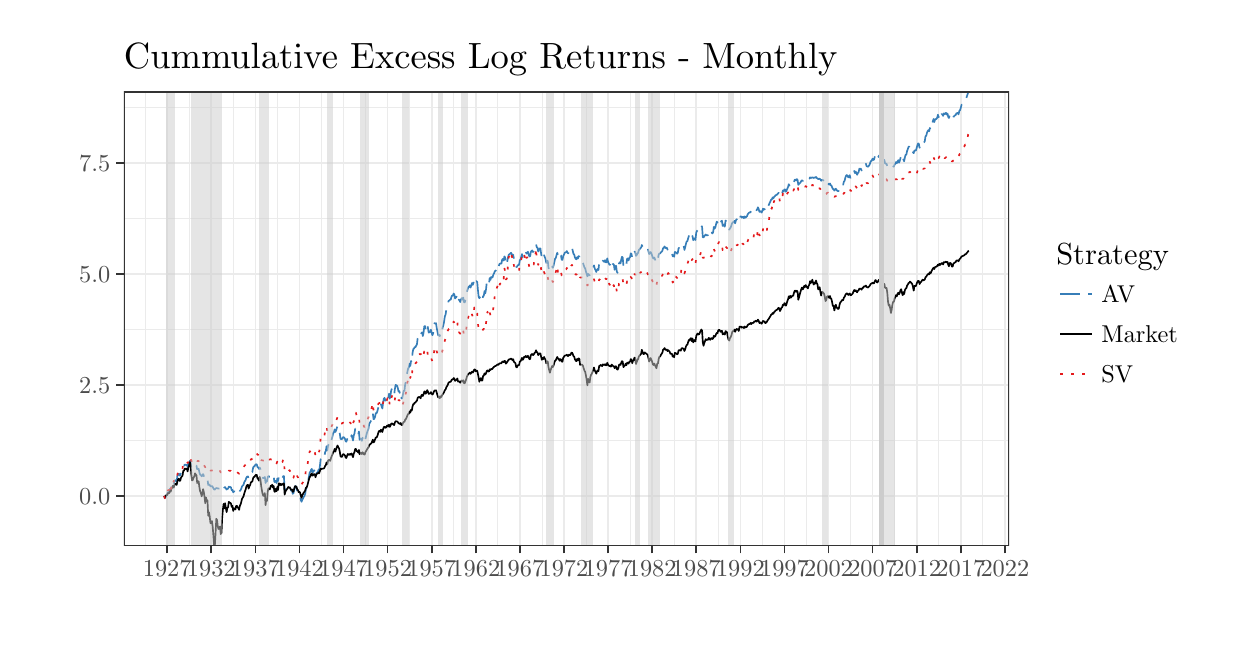
\begin{tikzpicture}[x=1pt,y=1pt]
\definecolor{fillColor}{RGB}{255,255,255}
\path[use as bounding box,fill=fillColor,fill opacity=0.00] (0,0) rectangle (426.79,216.81);
\begin{scope}
\path[clip] (  0.00,  0.00) rectangle (426.79,216.81);
\definecolor{drawColor}{RGB}{255,255,255}
\definecolor{fillColor}{RGB}{255,255,255}

\path[draw=drawColor,line width= 0.6pt,line join=round,line cap=round,fill=fillColor] (  0.00,  0.00) rectangle (426.79,216.81);
\end{scope}
\begin{scope}
\path[clip] ( 34.77, 29.59) rectangle (354.63,193.67);
\definecolor{fillColor}{RGB}{255,255,255}

\path[fill=fillColor] ( 34.77, 29.59) rectangle (354.63,193.67);
\definecolor{drawColor}{gray}{0.92}

\path[draw=drawColor,line width= 0.3pt,line join=round] ( 34.77, 67.61) --
	(354.63, 67.61);

\path[draw=drawColor,line width= 0.3pt,line join=round] ( 34.77,107.75) --
	(354.63,107.75);

\path[draw=drawColor,line width= 0.3pt,line join=round] ( 34.77,147.89) --
	(354.63,147.89);

\path[draw=drawColor,line width= 0.3pt,line join=round] ( 34.77,188.02) --
	(354.63,188.02);

\path[draw=drawColor,line width= 0.3pt,line join=round] ( 42.44, 29.59) --
	( 42.44,193.67);

\path[draw=drawColor,line width= 0.3pt,line join=round] ( 58.37, 29.59) --
	( 58.37,193.67);

\path[draw=drawColor,line width= 0.3pt,line join=round] ( 74.31, 29.59) --
	( 74.31,193.67);

\path[draw=drawColor,line width= 0.3pt,line join=round] ( 90.24, 29.59) --
	( 90.24,193.67);

\path[draw=drawColor,line width= 0.3pt,line join=round] (106.17, 29.59) --
	(106.17,193.67);

\path[draw=drawColor,line width= 0.3pt,line join=round] (122.10, 29.59) --
	(122.10,193.67);

\path[draw=drawColor,line width= 0.3pt,line join=round] (138.04, 29.59) --
	(138.04,193.67);

\path[draw=drawColor,line width= 0.3pt,line join=round] (153.97, 29.59) --
	(153.97,193.67);

\path[draw=drawColor,line width= 0.3pt,line join=round] (169.90, 29.59) --
	(169.90,193.67);

\path[draw=drawColor,line width= 0.3pt,line join=round] (185.83, 29.59) --
	(185.83,193.67);

\path[draw=drawColor,line width= 0.3pt,line join=round] (201.77, 29.59) --
	(201.77,193.67);

\path[draw=drawColor,line width= 0.3pt,line join=round] (217.70, 29.59) --
	(217.70,193.67);

\path[draw=drawColor,line width= 0.3pt,line join=round] (233.63, 29.59) --
	(233.63,193.67);

\path[draw=drawColor,line width= 0.3pt,line join=round] (249.57, 29.59) --
	(249.57,193.67);

\path[draw=drawColor,line width= 0.3pt,line join=round] (265.50, 29.59) --
	(265.50,193.67);

\path[draw=drawColor,line width= 0.3pt,line join=round] (281.44, 29.59) --
	(281.44,193.67);

\path[draw=drawColor,line width= 0.3pt,line join=round] (297.37, 29.59) --
	(297.37,193.67);

\path[draw=drawColor,line width= 0.3pt,line join=round] (313.30, 29.59) --
	(313.30,193.67);

\path[draw=drawColor,line width= 0.3pt,line join=round] (329.23, 29.59) --
	(329.23,193.67);

\path[draw=drawColor,line width= 0.3pt,line join=round] (345.17, 29.59) --
	(345.17,193.67);

\path[draw=drawColor,line width= 0.6pt,line join=round] ( 34.77, 47.54) --
	(354.63, 47.54);

\path[draw=drawColor,line width= 0.6pt,line join=round] ( 34.77, 87.68) --
	(354.63, 87.68);

\path[draw=drawColor,line width= 0.6pt,line join=round] ( 34.77,127.82) --
	(354.63,127.82);

\path[draw=drawColor,line width= 0.6pt,line join=round] ( 34.77,167.95) --
	(354.63,167.95);

\path[draw=drawColor,line width= 0.6pt,line join=round] ( 50.41, 29.59) --
	( 50.41,193.67);

\path[draw=drawColor,line width= 0.6pt,line join=round] ( 66.34, 29.59) --
	( 66.34,193.67);

\path[draw=drawColor,line width= 0.6pt,line join=round] ( 82.28, 29.59) --
	( 82.28,193.67);

\path[draw=drawColor,line width= 0.6pt,line join=round] ( 98.21, 29.59) --
	( 98.21,193.67);

\path[draw=drawColor,line width= 0.6pt,line join=round] (114.14, 29.59) --
	(114.14,193.67);

\path[draw=drawColor,line width= 0.6pt,line join=round] (130.07, 29.59) --
	(130.07,193.67);

\path[draw=drawColor,line width= 0.6pt,line join=round] (146.01, 29.59) --
	(146.01,193.67);

\path[draw=drawColor,line width= 0.6pt,line join=round] (161.94, 29.59) --
	(161.94,193.67);

\path[draw=drawColor,line width= 0.6pt,line join=round] (177.87, 29.59) --
	(177.87,193.67);

\path[draw=drawColor,line width= 0.6pt,line join=round] (193.80, 29.59) --
	(193.80,193.67);

\path[draw=drawColor,line width= 0.6pt,line join=round] (209.74, 29.59) --
	(209.74,193.67);

\path[draw=drawColor,line width= 0.6pt,line join=round] (225.67, 29.59) --
	(225.67,193.67);

\path[draw=drawColor,line width= 0.6pt,line join=round] (241.60, 29.59) --
	(241.60,193.67);

\path[draw=drawColor,line width= 0.6pt,line join=round] (257.53, 29.59) --
	(257.53,193.67);

\path[draw=drawColor,line width= 0.6pt,line join=round] (273.47, 29.59) --
	(273.47,193.67);

\path[draw=drawColor,line width= 0.6pt,line join=round] (289.40, 29.59) --
	(289.40,193.67);

\path[draw=drawColor,line width= 0.6pt,line join=round] (305.33, 29.59) --
	(305.33,193.67);

\path[draw=drawColor,line width= 0.6pt,line join=round] (321.26, 29.59) --
	(321.26,193.67);

\path[draw=drawColor,line width= 0.6pt,line join=round] (337.20, 29.59) --
	(337.20,193.67);

\path[draw=drawColor,line width= 0.6pt,line join=round] (353.13, 29.59) --
	(353.13,193.67);
\definecolor{drawColor}{RGB}{55,126,184}

\path[draw=drawColor,line width= 0.6pt,dash pattern=on 7pt off 3pt ,line join=round] ( 49.31, 47.61) --
	( 49.58, 46.82) --
	( 49.84, 47.22) --
	( 50.11, 47.85) --
	( 50.37, 47.83) --
	( 50.64, 48.93) --
	( 50.91, 48.96) --
	( 51.16, 49.05) --
	( 51.43, 50.24) --
	( 51.69, 49.70) --
	( 51.96, 51.16) --
	( 52.22, 51.62) --
	( 52.49, 52.47) --
	( 52.76, 51.59) --
	( 53.02, 52.85) --
	( 53.29, 53.30) --
	( 53.56, 53.18) --
	( 53.83, 52.79) --
	( 54.10, 54.88) --
	( 54.35, 55.42) --
	( 54.62, 55.62) --
	( 54.88, 55.00) --
	( 55.15, 55.05) --
	( 55.41, 56.24) --
	( 55.68, 56.69) --
	( 55.95, 56.95) --
	( 56.22, 58.52) --
	( 56.49, 58.53) --
	( 56.75, 58.89) --
	( 57.02, 58.88) --
	( 57.29, 58.74) --
	( 57.53, 58.87) --
	( 57.80, 58.09) --
	( 58.07, 58.97) --
	( 58.34, 59.42) --
	( 58.60, 60.28) --
	( 58.87, 59.80) --
	( 59.14, 57.72) --
	( 59.40, 57.59) --
	( 59.67, 57.61) --
	( 59.93, 57.83) --
	( 60.20, 58.08) --
	( 60.47, 58.99) --
	( 60.72, 58.73) --
	( 60.99, 58.52) --
	( 61.25, 57.25) --
	( 61.52, 57.41) --
	( 61.78, 57.42) --
	( 62.05, 56.09) --
	( 62.32, 55.27) --
	( 62.59, 55.15) --
	( 62.86, 54.71) --
	( 63.12, 54.98) --
	( 63.39, 55.50) --
	( 63.66, 54.82) --
	( 63.90, 54.13) --
	( 64.17, 53.56) --
	( 64.43, 54.02) --
	( 64.71, 53.84) --
	( 64.97, 53.86) --
	( 65.24, 51.55) --
	( 65.51, 51.74) --
	( 65.77, 51.62) --
	( 66.04, 51.07) --
	( 66.30, 51.05) --
	( 66.57, 51.17) --
	( 66.84, 50.91) --
	( 67.10, 50.40) --
	( 67.37, 49.92) --
	( 67.63, 49.91) --
	( 67.90, 50.28) --
	( 68.16, 50.45) --
	( 68.43, 50.41) --
	( 68.70, 50.30) --
	( 68.96, 50.23) --
	( 69.23, 50.34) --
	( 69.49, 50.36) --
	( 69.77, 49.49) --
	( 70.04, 49.61) --
	( 70.28, 50.13) --
	( 70.55, 50.50) --
	( 70.81, 50.85) --
	( 71.08, 50.60) --
	( 71.34, 50.80) --
	( 71.61, 50.28) --
	( 71.89, 49.92) --
	( 72.15, 50.15) --
	( 72.42, 50.24) --
	( 72.68, 50.96) --
	( 72.95, 50.81) --
	( 73.22, 50.84) --
	( 73.46, 50.69) --
	( 73.73, 49.63) --
	( 74.00, 49.80) --
	( 74.27, 48.93) --
	( 74.53, 49.21) --
	( 74.80, 49.20) --
	( 75.07, 49.04) --
	( 75.33, 49.68) --
	( 75.60, 49.71) --
	( 75.86, 49.39) --
	( 76.13, 49.14) --
	( 76.40, 48.71) --
	( 76.65, 49.37) --
	( 76.92, 49.70) --
	( 77.18, 50.21) --
	( 77.45, 51.01) --
	( 77.71, 51.36) --
	( 77.98, 51.58) --
	( 78.25, 52.52) --
	( 78.52, 52.96) --
	( 78.79, 53.46) --
	( 79.05, 54.26) --
	( 79.32, 54.56) --
	( 79.59, 54.67) --
	( 79.84, 53.85) --
	( 80.11, 54.34) --
	( 80.37, 54.65) --
	( 80.64, 55.89) --
	( 80.91, 56.08) --
	( 81.18, 56.28) --
	( 81.45, 57.75) --
	( 81.71, 58.28) --
	( 81.98, 58.31) --
	( 82.24, 58.84) --
	( 82.51, 59.05) --
	( 82.78, 59.00) --
	( 83.03, 58.02) --
	( 83.30, 57.95) --
	( 83.56, 57.38) --
	( 83.83, 57.85) --
	( 84.09, 57.29) --
	( 84.36, 54.72) --
	( 84.63, 54.33) --
	( 84.89, 54.18) --
	( 85.16, 54.07) --
	( 85.43, 54.12) --
	( 85.70, 54.46) --
	( 85.97, 52.29) --
	( 86.21, 52.98) --
	( 86.48, 52.83) --
	( 86.74, 54.36) --
	( 87.01, 54.76) --
	( 87.28, 54.55) --
	( 87.55, 54.58) --
	( 87.82, 54.88) --
	( 88.08, 54.71) --
	( 88.35, 55.18) --
	( 88.61, 54.50) --
	( 88.88, 54.77) --
	( 89.15, 52.65) --
	( 89.40, 52.63) --
	( 89.67, 53.05) --
	( 89.93, 52.27) --
	( 90.20, 53.89) --
	( 90.46, 52.98) --
	( 90.73, 54.29) --
	( 91.00, 54.27) --
	( 91.26, 53.56) --
	( 91.53, 54.28) --
	( 91.79, 53.74) --
	( 92.06, 54.09) --
	( 92.34, 54.76) --
	( 92.59, 54.78) --
	( 92.86, 49.55) --
	( 93.12, 49.76) --
	( 93.39, 49.94) --
	( 93.65, 50.40) --
	( 93.92, 50.70) --
	( 94.19, 51.10) --
	( 94.46, 50.78) --
	( 94.73, 50.84) --
	( 94.99, 49.74) --
	( 95.26, 49.45) --
	( 95.53, 49.62) --
	( 95.77, 48.37) --
	( 96.04, 48.60) --
	( 96.30, 49.72) --
	( 96.58, 51.12) --
	( 96.84, 51.09) --
	( 97.11, 50.84) --
	( 97.38, 49.41) --
	( 97.64, 48.95) --
	( 97.91, 47.86) --
	( 98.17, 47.92) --
	( 98.44, 47.61) --
	( 98.71, 46.10) --
	( 98.96, 45.49) --
	( 99.23, 46.26) --
	( 99.49, 46.66) --
	( 99.76, 47.29) --
	(100.02, 47.63) --
	(100.29, 48.39) --
	(100.56, 50.36) --
	(100.82, 50.37) --
	(101.09, 51.59) --
	(101.36, 53.07) --
	(101.63, 54.54) --
	(101.90, 56.12) --
	(102.14, 56.25) --
	(102.41, 57.06) --
	(102.67, 57.38) --
	(102.94, 56.15) --
	(103.21, 56.38) --
	(103.48, 56.88) --
	(103.75, 56.48) --
	(104.01, 54.54) --
	(104.28, 55.63) --
	(104.54, 56.03) --
	(104.81, 56.14) --
	(105.08, 57.05) --
	(105.33, 56.52) --
	(105.60, 58.48) --
	(105.87, 60.85) --
	(106.14, 60.42) --
	(106.40, 60.84) --
	(106.67, 60.85) --
	(106.94, 60.90) --
	(107.20, 61.62) --
	(107.47, 63.33) --
	(107.73, 63.89) --
	(108.00, 65.58) --
	(108.27, 64.04) --
	(108.52, 65.75) --
	(108.79, 66.26) --
	(109.05, 66.38) --
	(109.32, 65.82) --
	(109.58, 67.14) --
	(109.85, 68.06) --
	(110.12, 69.05) --
	(110.39, 70.30) --
	(110.66, 70.54) --
	(110.92, 71.62) --
	(111.19, 70.71) --
	(111.46, 71.32) --
	(111.70, 72.09) --
	(111.97, 72.94) --
	(112.24, 72.12) --
	(112.51, 71.54) --
	(112.77, 70.26) --
	(113.04, 68.22) --
	(113.31, 68.16) --
	(113.57, 68.16) --
	(113.84, 68.72) --
	(114.10, 68.86) --
	(114.37, 68.67) --
	(114.64, 68.26) --
	(114.89, 67.37) --
	(115.16, 67.19) --
	(115.42, 68.04) --
	(115.69, 68.86) --
	(115.95, 68.51) --
	(116.22, 68.37) --
	(116.49, 68.99) --
	(116.75, 68.47) --
	(117.03, 69.56) --
	(117.29, 68.68) --
	(117.56, 67.64) --
	(117.83, 69.45) --
	(118.08, 70.14) --
	(118.35, 71.88) --
	(118.61, 71.86) --
	(118.88, 70.54) --
	(119.15, 70.60) --
	(119.42, 69.67) --
	(119.69, 70.88) --
	(119.95, 67.88) --
	(120.22, 68.24) --
	(120.48, 68.31) --
	(120.75, 67.52) --
	(121.02, 68.61) --
	(121.27, 68.08) --
	(121.54, 66.92) --
	(121.80, 66.96) --
	(122.07, 68.24) --
	(122.33, 69.40) --
	(122.60, 70.41) --
	(122.87, 71.19) --
	(123.13, 71.83) --
	(123.40, 73.55) --
	(123.66, 74.07) --
	(123.93, 74.50) --
	(124.21, 75.03) --
	(124.45, 76.32) --
	(124.72, 77.55) --
	(124.98, 75.32) --
	(125.25, 75.49) --
	(125.51, 76.14) --
	(125.78, 77.49) --
	(126.05, 77.42) --
	(126.32, 78.09) --
	(126.59, 79.12) --
	(126.85, 80.02) --
	(127.12, 80.29) --
	(127.39, 79.45) --
	(127.63, 80.78) --
	(127.90, 79.97) --
	(128.17, 79.21) --
	(128.44, 81.48) --
	(128.70, 82.75) --
	(128.97, 83.03) --
	(129.24, 82.03) --
	(129.50, 82.14) --
	(129.77, 83.23) --
	(130.03, 83.94) --
	(130.30, 82.95) --
	(130.57, 84.51) --
	(130.83, 82.74) --
	(131.10, 83.94) --
	(131.36, 85.76) --
	(131.63, 86.38) --
	(131.89, 85.92) --
	(132.16, 84.50) --
	(132.43, 84.15) --
	(132.69, 86.28) --
	(132.96, 87.72) --
	(133.23, 87.58) --
	(133.50, 87.40) --
	(133.77, 86.53) --
	(134.01, 85.34) --
	(134.28, 85.51) --
	(134.54, 84.53) --
	(134.81, 85.32) --
	(135.08, 82.82) --
	(135.35, 82.90) --
	(135.62, 84.38) --
	(135.88, 85.66) --
	(136.15, 85.62) --
	(136.41, 87.98) --
	(136.68, 88.77) --
	(136.95, 90.64) --
	(137.20, 92.43) --
	(137.47, 93.63) --
	(137.73, 94.10) --
	(138.00, 95.41) --
	(138.26, 94.56) --
	(138.53, 96.38) --
	(138.80, 95.66) --
	(139.06, 99.20) --
	(139.33,100.66) --
	(139.60,100.84) --
	(139.87,101.41) --
	(140.14,101.34) --
	(140.38,101.92) --
	(140.65,102.33) --
	(140.91,104.48) --
	(141.18,105.12) --
	(141.44,105.19) --
	(141.72,105.09) --
	(141.99,104.76) --
	(142.25,106.36) --
	(142.52,106.71) --
	(142.78,105.37) --
	(143.05,106.61) --
	(143.32,108.90) --
	(143.57,109.00) --
	(143.84,107.55) --
	(144.11,108.36) --
	(144.38,109.51) --
	(144.64,108.29) --
	(144.91,106.60) --
	(145.18,106.82) --
	(145.44,106.90) --
	(145.71,107.69) --
	(145.97,106.48) --
	(146.24,105.69) --
	(146.51,106.36) --
	(146.76,108.65) --
	(147.03,110.06) --
	(147.29,109.80) --
	(147.56,110.02) --
	(147.82,108.19) --
	(148.09,106.84) --
	(148.36,105.63) --
	(148.62,105.86) --
	(148.90,105.34) --
	(149.16,106.50) --
	(149.43,106.04) --
	(149.70,107.23) --
	(149.94,108.43) --
	(150.21,109.29) --
	(150.47,110.57) --
	(150.74,112.51) --
	(151.01,113.13) --
	(151.28,115.01) --
	(151.55,116.03) --
	(151.81,116.80) --
	(152.08,118.04) --
	(152.34,118.22) --
	(152.61,118.49) --
	(152.88,118.57) --
	(153.13,119.56) --
	(153.40,120.03) --
	(153.66,119.99) --
	(153.93,120.73) --
	(154.19,120.33) --
	(154.46,118.96) --
	(154.73,119.26) --
	(154.99,119.67) --
	(155.26,120.36) --
	(155.53,118.20) --
	(155.80,118.55) --
	(156.07,118.14) --
	(156.32,117.68) --
	(156.59,118.58) --
	(156.85,119.07) --
	(157.12,118.54) --
	(157.38,119.27) --
	(157.65,117.65) --
	(157.92,117.51) --
	(158.19,118.54) --
	(158.46,119.87) --
	(158.72,121.42) --
	(158.99,122.27) --
	(159.26,123.10) --
	(159.50,123.20) --
	(159.77,123.67) --
	(160.04,122.87) --
	(160.31,123.75) --
	(160.57,124.54) --
	(160.84,123.89) --
	(161.11,124.65) --
	(161.37,125.95) --
	(161.64,125.92) --
	(161.90,124.75) --
	(162.17,125.21) --
	(162.44,124.92) --
	(162.69,122.08) --
	(162.96,119.51) --
	(163.22,119.06) --
	(163.49,119.57) --
	(163.75,119.96) --
	(164.02,118.43) --
	(164.29,118.43) --
	(164.56,119.74) --
	(164.83,119.98) --
	(165.09,121.63) --
	(165.36,120.81) --
	(165.63,122.33) --
	(165.87,124.63) --
	(166.14,125.34) --
	(166.40,124.42) --
	(166.68,124.21) --
	(166.94,126.34) --
	(167.21,125.66) --
	(167.48,126.71) --
	(167.74,126.47) --
	(168.01,126.71) --
	(168.27,127.59) --
	(168.54,128.06) --
	(168.81,128.82) --
	(169.07,128.91) --
	(169.34,129.44) --
	(169.60,129.96) --
	(169.87,130.66) --
	(170.13,129.98) --
	(170.40,131.26) --
	(170.67,131.56) --
	(170.93,131.57) --
	(171.20,131.61) --
	(171.47,133.04) --
	(171.74,133.24) --
	(172.01,132.66) --
	(172.25,134.17) --
	(172.52,133.76) --
	(172.78,131.04) --
	(173.05,131.35) --
	(173.31,132.45) --
	(173.59,133.87) --
	(173.86,134.84) --
	(174.12,134.84) --
	(174.39,135.22) --
	(174.65,135.45) --
	(174.92,135.07) --
	(175.19,134.28) --
	(175.43,134.74) --
	(175.71,133.22) --
	(175.97,133.01) --
	(176.24,132.59) --
	(176.50,130.41) --
	(176.77,130.29) --
	(177.04,130.88) --
	(177.30,131.04) --
	(177.57,131.08) --
	(177.83,132.84) --
	(178.10,132.99) --
	(178.37,134.11) --
	(178.62,134.98) --
	(178.89,133.89) --
	(179.15,134.44) --
	(179.42,135.35) --
	(179.68,135.15) --
	(179.95,136.00) --
	(180.22,135.18) --
	(180.49,135.29) --
	(180.76,135.85) --
	(181.02,134.85) --
	(181.29,134.14) --
	(181.56,134.17) --
	(181.81,135.77) --
	(182.08,136.14) --
	(182.34,136.30) --
	(182.61,135.74) --
	(182.88,136.02) --
	(183.15,137.13) --
	(183.42,137.26) --
	(183.68,138.63) --
	(183.95,137.52) --
	(184.21,137.25) --
	(184.48,135.93) --
	(184.75,136.64) --
	(185.00,137.05) --
	(185.27,137.06) --
	(185.53,135.14) --
	(185.80,133.51) --
	(186.06,134.14) --
	(186.33,133.59) --
	(186.60,134.57) --
	(186.86,133.90) --
	(187.13,133.22) --
	(187.40,131.81) --
	(187.67,132.62) --
	(187.94,132.45) --
	(188.18,130.14) --
	(188.45,128.96) --
	(188.71,128.63) --
	(188.98,129.33) --
	(189.25,129.86) --
	(189.52,130.44) --
	(189.79,130.04) --
	(190.05,130.89) --
	(190.32,132.17) --
	(190.58,133.33) --
	(190.85,133.62) --
	(191.12,134.70) --
	(191.37,135.47) --
	(191.64,134.49) --
	(191.90,134.50) --
	(192.17,133.49) --
	(192.43,134.62) --
	(192.70,134.49) --
	(192.97,132.99) --
	(193.23,132.86) --
	(193.50,134.26) --
	(193.76,134.73) --
	(194.03,135.43) --
	(194.31,135.60) --
	(194.56,135.67) --
	(194.83,136.09) --
	(195.09,135.48) --
	(195.36,135.26) --
	(195.62,136.06) --
	(195.89,135.84) --
	(196.16,136.02) --
	(196.43,137.09) --
	(196.70,137.26) --
	(196.96,136.20) --
	(197.23,135.05) --
	(197.50,134.82) --
	(197.74,133.79) --
	(198.01,133.28) --
	(198.27,133.12) --
	(198.55,133.88) --
	(198.81,133.38) --
	(199.08,134.25) --
	(199.35,134.13) --
	(199.61,132.21) --
	(199.88,132.25) --
	(200.14,132.25) --
	(200.41,132.21) --
	(200.68,131.76) --
	(200.93,130.92) --
	(201.20,130.15) --
	(201.46,129.79) --
	(201.73,128.67) --
	(201.99,127.90) --
	(202.26,126.93) --
	(202.53,127.81) --
	(202.79,127.59) --
	(203.06,127.31) --
	(203.33,128.46) --
	(203.60,128.84) --
	(203.87,129.12) --
	(204.11,129.64) --
	(204.38,130.25) --
	(204.64,130.90) --
	(204.91,129.74) --
	(205.18,129.20) --
	(205.45,128.54) --
	(205.72,129.27) --
	(205.98,129.65) --
	(206.25,129.24) --
	(206.51,131.67) --
	(206.78,131.71) --
	(207.05,132.14) --
	(207.30,131.87) --
	(207.58,131.54) --
	(207.84,132.62) --
	(208.11,132.37) --
	(208.37,132.18) --
	(208.64,132.79) --
	(208.91,132.00) --
	(209.17,132.03) --
	(209.44,133.45) --
	(209.70,132.24) --
	(209.97,131.63) --
	(210.24,131.13) --
	(210.49,131.18) --
	(210.76,130.75) --
	(211.02,132.52) --
	(211.29,131.89) --
	(211.55,131.30) --
	(211.82,131.21) --
	(212.09,129.32) --
	(212.36,130.63) --
	(212.63,130.72) --
	(212.89,128.64) --
	(213.16,128.20) --
	(213.43,129.31) --
	(213.67,131.61) --
	(213.94,132.02) --
	(214.21,131.64) --
	(214.48,132.97) --
	(214.74,134.01) --
	(215.01,133.75) --
	(215.28,130.67) --
	(215.54,131.17) --
	(215.81,131.33) --
	(216.07,132.25) --
	(216.34,131.39) --
	(216.61,133.35) --
	(216.86,133.39) --
	(217.13,132.70) --
	(217.39,133.63) --
	(217.66,133.81) --
	(217.92,135.24) --
	(218.19,135.07) --
	(218.46,133.48) --
	(218.72,134.18) --
	(219.00,134.53) --
	(219.26,135.85) --
	(219.53,135.76) --
	(219.80,134.34) --
	(220.05,134.63) --
	(220.32,135.11) --
	(220.58,135.48) --
	(220.85,136.47) --
	(221.12,136.75) --
	(221.39,137.14) --
	(221.66,137.29) --
	(221.92,138.27) --
	(222.19,137.71) --
	(222.45,137.21) --
	(222.72,137.24) --
	(222.99,137.78) --
	(223.24,137.54) --
	(223.51,137.56) --
	(223.77,137.25) --
	(224.04,137.09) --
	(224.30,136.06) --
	(224.57,134.99) --
	(224.84,135.42) --
	(225.10,135.72) --
	(225.37,135.25) --
	(225.63,134.49) --
	(225.90,133.69) --
	(226.18,133.39) --
	(226.42,133.75) --
	(226.69,133.11) --
	(226.95,132.31) --
	(227.22,131.87) --
	(227.48,133.38) --
	(227.75,133.42) --
	(228.02,134.88) --
	(228.29,135.18) --
	(228.56,135.26) --
	(228.82,135.62) --
	(229.09,135.84) --
	(229.36,136.24) --
	(229.60,137.13) --
	(229.87,137.25) --
	(230.14,137.75) --
	(230.41,137.23) --
	(230.67,137.18) --
	(230.94,137.31) --
	(231.21,136.62) --
	(231.47,136.97) --
	(231.74,136.62) --
	(232.00,136.19) --
	(232.27,135.37) --
	(232.54,135.44) --
	(232.80,135.37) --
	(233.07,134.20) --
	(233.33,134.48) --
	(233.60,134.02) --
	(233.86,135.75) --
	(234.13,135.66) --
	(234.40,135.47) --
	(234.66,135.13) --
	(234.93,135.48) --
	(235.20,137.09) --
	(235.47,137.28) --
	(235.74,137.08) --
	(235.98,136.91) --
	(236.25,138.19) --
	(236.51,138.41) --
	(236.78,138.23) --
	(237.05,138.00) --
	(237.32,136.49) --
	(237.59,137.49) --
	(237.85,138.63) --
	(238.12,139.59) --
	(238.38,139.66) --
	(238.65,140.65) --
	(238.92,141.54) --
	(239.17,141.32) --
	(239.44,141.91) --
	(239.70,142.08) --
	(239.97,140.79) --
	(240.23,141.55) --
	(240.50,140.00) --
	(240.77,140.48) --
	(241.03,140.67) --
	(241.30,140.09) --
	(241.57,142.71) --
	(241.84,143.33) --
	(242.11,143.67) --
	(242.35,143.33) --
	(242.62,143.34) --
	(242.88,143.84) --
	(243.15,144.66) --
	(243.41,145.30) --
	(243.69,144.86) --
	(243.96,141.10) --
	(244.22,141.01) --
	(244.49,141.46) --
	(244.75,141.76) --
	(245.02,142.07) --
	(245.29,141.74) --
	(245.54,141.84) --
	(245.81,141.78) --
	(246.08,142.64) --
	(246.35,142.41) --
	(246.61,141.64) --
	(246.88,142.44) --
	(247.15,142.75) --
	(247.41,142.45) --
	(247.68,142.84) --
	(247.94,144.82) --
	(248.21,144.20) --
	(248.48,144.66) --
	(248.73,145.69) --
	(249.00,146.72) --
	(249.26,146.40) --
	(249.53,147.64) --
	(249.79,148.02) --
	(250.06,147.84) --
	(250.33,146.66) --
	(250.59,146.77) --
	(250.87,147.06) --
	(251.13,145.15) --
	(251.40,145.28) --
	(251.67,145.73) --
	(251.91,144.89) --
	(252.18,147.13) --
	(252.44,146.86) --
	(252.71,146.48) --
	(252.98,144.61) --
	(253.25,144.11) --
	(253.52,143.84) --
	(253.78,144.32) --
	(254.05,144.63) --
	(254.31,145.45) --
	(254.58,146.22) --
	(254.85,146.52) --
	(255.10,146.49) --
	(255.37,147.01) --
	(255.63,146.11) --
	(255.90,147.12) --
	(256.16,147.59) --
	(256.43,147.31) --
	(256.70,147.66) --
	(256.96,146.92) --
	(257.23,148.61) --
	(257.50,148.53) --
	(257.77,148.65) --
	(258.04,148.15) --
	(258.29,148.42) --
	(258.56,148.47) --
	(258.82,147.94) --
	(259.09,148.63) --
	(259.35,148.14) --
	(259.62,148.42) --
	(259.89,148.61) --
	(260.16,149.33) --
	(260.43,149.70) --
	(260.69,149.94) --
	(260.96,149.99) --
	(261.23,150.32) --
	(261.47,149.81) --
	(261.74,150.14) --
	(262.01,150.20) --
	(262.28,150.14) --
	(262.54,150.91) --
	(262.81,150.87) --
	(263.08,151.19) --
	(263.34,150.84) --
	(263.61,151.15) --
	(263.87,151.89) --
	(264.14,151.34) --
	(264.41,150.27) --
	(264.66,150.40) --
	(264.93,150.49) --
	(265.19,149.98) --
	(265.46,150.52) --
	(265.72,151.44) --
	(265.99,151.00) --
	(266.26,151.28) --
	(266.53,150.39) --
	(266.80,150.58) --
	(267.06,150.95) --
	(267.33,151.75) --
	(267.60,152.39) --
	(267.84,152.86) --
	(268.11,153.51) --
	(268.38,154.01) --
	(268.65,154.69) --
	(268.91,154.76) --
	(269.18,155.47) --
	(269.45,155.13) --
	(269.71,155.68) --
	(269.98,155.85) --
	(270.24,156.24) --
	(270.51,156.37) --
	(270.78,156.48) --
	(271.04,156.76) --
	(271.31,157.12) --
	(271.57,156.88) --
	(271.84,155.55) --
	(272.10,155.86) --
	(272.37,156.75) --
	(272.64,156.95) --
	(272.90,157.98) --
	(273.17,157.67) --
	(273.44,158.39) --
	(273.71,158.31) --
	(273.98,157.52) --
	(274.22,158.00) --
	(274.49,158.64) --
	(274.75,159.21) --
	(275.02,160.24) --
	(275.28,159.76) --
	(275.56,160.49) --
	(275.83,159.96) --
	(276.09,160.11) --
	(276.36,160.29) --
	(276.62,160.30) --
	(276.89,161.01) --
	(277.16,161.83) --
	(277.40,161.93) --
	(277.68,161.62) --
	(277.94,162.08) --
	(278.21,161.75) --
	(278.47,160.00) --
	(278.74,160.34) --
	(279.01,160.63) --
	(279.27,160.86) --
	(279.54,161.43) --
	(279.80,161.69) --
	(280.07,161.43) --
	(280.34,161.69) --
	(280.59,162.01) --
	(280.86,161.90) --
	(281.12,162.22) --
	(281.39,161.97) --
	(281.65,161.83) --
	(281.92,161.61) --
	(282.19,162.07) --
	(282.46,162.24) --
	(282.73,162.70) --
	(282.99,162.49) --
	(283.26,162.57) --
	(283.53,162.76) --
	(283.78,162.59) --
	(284.05,162.50) --
	(284.31,162.67) --
	(284.58,162.57) --
	(284.85,162.87) --
	(285.12,162.51) --
	(285.39,162.36) --
	(285.65,162.10) --
	(285.92,162.15) --
	(286.18,162.25) --
	(286.45,161.98) --
	(286.72,161.49) --
	(286.97,161.78) --
	(287.24,161.80) --
	(287.50,161.62) --
	(287.77,161.41) --
	(288.03,160.93) --
	(288.30,159.80) --
	(288.57,159.93) --
	(288.83,160.36) --
	(289.10,160.53) --
	(289.37,160.32) --
	(289.64,160.08) --
	(289.91,160.52) --
	(290.15,159.89) --
	(290.42,159.77) --
	(290.68,159.17) --
	(290.95,158.48) --
	(291.22,158.50) --
	(291.49,157.92) --
	(291.76,158.40) --
	(292.02,158.61) --
	(292.29,158.19) --
	(292.55,157.86) --
	(292.82,157.71) --
	(293.09,157.86) --
	(293.34,158.58) --
	(293.61,159.38) --
	(293.87,159.60) --
	(294.14,159.96) --
	(294.40,160.33) --
	(294.67,160.08) --
	(294.94,161.19) --
	(295.20,161.48) --
	(295.47,162.65) --
	(295.73,163.28) --
	(296.00,163.55) --
	(296.28,163.24) --
	(296.53,162.72) --
	(296.80,162.97) --
	(297.06,163.49) --
	(297.33,162.29) --
	(297.59,162.33) --
	(297.86,162.80) --
	(298.13,163.24) --
	(298.40,164.15) --
	(298.67,165.04) --
	(298.93,164.24) --
	(299.20,164.80) --
	(299.47,164.29) --
	(299.71,163.63) --
	(299.98,164.28) --
	(300.25,164.56) --
	(300.52,165.86) --
	(300.78,165.63) --
	(301.05,165.87) --
	(301.32,165.21) --
	(301.58,165.78) --
	(301.85,165.80) --
	(302.11,167.02) --
	(302.38,166.92) --
	(302.65,167.34) --
	(302.90,167.60) --
	(303.17,166.72) --
	(303.43,166.65) --
	(303.70,166.55) --
	(303.96,166.91) --
	(304.23,167.30) --
	(304.50,168.17) --
	(304.76,168.64) --
	(305.03,168.82) --
	(305.30,169.47) --
	(305.57,168.99) --
	(305.84,169.22) --
	(306.08,170.14) --
	(306.35,171.21) --
	(306.61,170.66) --
	(306.88,169.70) --
	(307.15,169.83) --
	(307.42,170.16) --
	(307.69,170.64) --
	(307.95,169.90) --
	(308.22,169.84) --
	(308.48,168.79) --
	(308.75,168.62) --
	(309.02,168.49) --
	(309.27,168.80) --
	(309.55,169.01) --
	(309.81,167.81) --
	(310.08,167.64) --
	(310.34,167.68) --
	(310.61,166.76) --
	(310.88,166.32) --
	(311.14,166.23) --
	(311.41,166.26) --
	(311.67,166.04) --
	(311.94,165.70) --
	(312.21,166.08) --
	(312.46,166.33) --
	(312.73,166.60) --
	(312.99,166.58) --
	(313.26,167.35) --
	(313.52,167.65) --
	(313.79,168.25) --
	(314.06,167.82) --
	(314.33,168.40) --
	(314.60,168.93) --
	(314.86,168.03) --
	(315.13,168.63) --
	(315.40,169.77) --
	(315.64,170.39) --
	(315.91,168.90) --
	(316.18,168.47) --
	(316.45,169.18) --
	(316.71,168.53) --
	(316.98,170.00) --
	(317.25,170.84) --
	(317.51,170.95) --
	(317.78,172.29) --
	(318.04,172.93) --
	(318.31,173.79) --
	(318.58,173.87) --
	(318.83,174.39) --
	(319.10,173.95) --
	(319.36,173.45) --
	(319.63,173.00) --
	(319.89,171.81) --
	(320.16,171.46) --
	(320.43,172.43) --
	(320.69,172.38) --
	(320.97,172.42) --
	(321.23,173.34) --
	(321.50,174.29) --
	(321.77,174.99) --
	(322.02,174.81) --
	(322.29,173.41) --
	(322.55,174.20) --
	(322.82,174.36) --
	(323.09,174.86) --
	(323.36,175.73) --
	(323.63,175.27) --
	(323.89,175.43) --
	(324.16,175.71) --
	(324.42,177.56) --
	(324.69,177.77) --
	(324.96,178.79) --
	(325.21,179.43) --
	(325.48,179.78) --
	(325.74,179.39) --
	(326.01,180.55) --
	(326.27,179.91) --
	(326.54,180.99) --
	(326.81,182.34) --
	(327.07,182.91) --
	(327.34,183.82) --
	(327.60,182.69) --
	(327.88,183.65) --
	(328.15,183.78) --
	(328.39,183.83) --
	(328.66,184.27) --
	(328.92,185.35) --
	(329.19,184.42) --
	(329.45,185.59) --
	(329.72,184.49) --
	(330.00,185.29) --
	(330.26,185.60) --
	(330.53,185.47) --
	(330.79,184.92) --
	(331.06,185.85) --
	(331.33,185.56) --
	(331.57,185.75) --
	(331.84,186.04) --
	(332.11,185.37) --
	(332.38,185.79) --
	(332.64,184.55) --
	(332.91,184.17) --
	(333.18,185.18) --
	(333.44,185.22) --
	(333.71,184.71) --
	(333.97,183.75) --
	(334.24,183.75) --
	(334.51,184.55) --
	(334.77,184.82) --
	(335.04,185.13) --
	(335.30,185.21) --
	(335.57,185.82) --
	(335.83,185.91) --
	(336.10,186.03) --
	(336.37,185.46) --
	(336.63,186.69) --
	(336.90,186.99) --
	(337.17,187.80) --
	(337.44,188.93) --
	(337.71,189.00) --
	(337.95,189.39) --
	(338.22,189.85) --
	(338.48,190.17) --
	(338.75,190.84) --
	(339.02,190.88) --
	(339.29,191.72) --
	(339.56,192.54) --
	(339.82,193.33) --
	(340.09,193.67);
\definecolor{drawColor}{RGB}{0,0,0}

\path[draw=drawColor,line width= 0.6pt,line join=round] ( 49.31, 47.60) --
	( 49.58, 47.09) --
	( 49.84, 47.50) --
	( 50.11, 47.91) --
	( 50.37, 47.90) --
	( 50.64, 48.57) --
	( 50.91, 48.59) --
	( 51.16, 48.66) --
	( 51.43, 49.52) --
	( 51.69, 49.14) --
	( 51.96, 50.25) --
	( 52.22, 50.57) --
	( 52.49, 51.30) --
	( 52.76, 50.59) --
	( 53.02, 51.62) --
	( 53.29, 51.96) --
	( 53.56, 51.87) --
	( 53.83, 51.60) --
	( 54.10, 52.95) --
	( 54.35, 53.59) --
	( 54.62, 53.82) --
	( 54.88, 53.04) --
	( 55.15, 53.14) --
	( 55.41, 54.18) --
	( 55.68, 54.63) --
	( 55.95, 54.88) --
	( 56.22, 56.68) --
	( 56.49, 56.70) --
	( 56.75, 57.49) --
	( 57.02, 57.47) --
	( 57.29, 57.29) --
	( 57.53, 57.50) --
	( 57.80, 56.46) --
	( 58.07, 57.95) --
	( 58.34, 58.60) --
	( 58.60, 59.83) --
	( 58.87, 58.95) --
	( 59.14, 55.37) --
	( 59.40, 53.19) --
	( 59.67, 53.38) --
	( 59.93, 54.23) --
	( 60.20, 54.62) --
	( 60.47, 55.75) --
	( 60.72, 55.37) --
	( 60.99, 55.09) --
	( 61.25, 52.26) --
	( 61.52, 52.87) --
	( 61.78, 52.89) --
	( 62.05, 50.72) --
	( 62.32, 49.25) --
	( 62.59, 48.76) --
	( 62.86, 47.44) --
	( 63.12, 48.42) --
	( 63.39, 50.06) --
	( 63.66, 49.00) --
	( 63.90, 47.30) --
	( 64.17, 44.97) --
	( 64.43, 47.06) --
	( 64.71, 45.95) --
	( 64.97, 45.98) --
	( 65.24, 40.43) --
	( 65.51, 41.69) --
	( 65.77, 40.20) --
	( 66.04, 37.85) --
	( 66.30, 37.66) --
	( 66.57, 38.54) --
	( 66.84, 36.62) --
	( 67.10, 33.41) --
	( 67.37, 29.67) --
	( 67.63, 29.59) --
	( 67.90, 34.28) --
	( 68.16, 39.35) --
	( 68.43, 38.88) --
	( 68.70, 36.59) --
	( 68.96, 35.62) --
	( 69.23, 36.33) --
	( 69.49, 36.48) --
	( 69.77, 33.81) --
	( 70.04, 34.33) --
	( 70.28, 39.67) --
	( 70.55, 42.77) --
	( 70.81, 44.76) --
	( 71.08, 43.13) --
	( 71.34, 44.97) --
	( 71.61, 43.17) --
	( 71.89, 41.76) --
	( 72.15, 43.28) --
	( 72.42, 43.57) --
	( 72.68, 45.48) --
	( 72.95, 45.08) --
	( 73.22, 45.15) --
	( 73.46, 44.85) --
	( 73.73, 43.64) --
	( 74.00, 44.04) --
	( 74.27, 42.18) --
	( 74.53, 43.07) --
	( 74.80, 43.03) --
	( 75.07, 42.72) --
	( 75.33, 43.98) --
	( 75.60, 44.04) --
	( 75.86, 43.49) --
	( 76.13, 43.17) --
	( 76.40, 42.58) --
	( 76.65, 43.97) --
	( 76.92, 44.51) --
	( 77.18, 45.42) --
	( 77.45, 46.56) --
	( 77.71, 46.98) --
	( 77.98, 47.40) --
	( 78.25, 48.47) --
	( 78.52, 49.30) --
	( 78.79, 50.03) --
	( 79.05, 51.11) --
	( 79.32, 51.51) --
	( 79.59, 51.64) --
	( 79.84, 50.27) --
	( 80.11, 51.09) --
	( 80.37, 51.47) --
	( 80.64, 52.50) --
	( 80.91, 52.67) --
	( 81.18, 52.85) --
	( 81.45, 53.94) --
	( 81.71, 54.45) --
	( 81.98, 54.50) --
	( 82.24, 55.02) --
	( 82.51, 55.23) --
	( 82.78, 55.18) --
	( 83.03, 53.92) --
	( 83.30, 53.81) --
	( 83.56, 53.12) --
	( 83.83, 54.49) --
	( 84.09, 53.69) --
	( 84.36, 51.32) --
	( 84.63, 49.70) --
	( 84.89, 48.30) --
	( 85.16, 47.63) --
	( 85.43, 47.74) --
	( 85.70, 48.64) --
	( 85.97, 44.27) --
	( 86.21, 46.46) --
	( 86.48, 45.82) --
	( 86.74, 49.25) --
	( 87.01, 50.36) --
	( 87.28, 49.92) --
	( 87.55, 50.07) --
	( 87.82, 51.28) --
	( 88.08, 50.99) --
	( 88.35, 51.64) --
	( 88.61, 50.65) --
	( 88.88, 51.21) --
	( 89.15, 49.15) --
	( 89.40, 49.11) --
	( 89.67, 50.19) --
	( 89.93, 49.30) --
	( 90.20, 50.86) --
	( 90.46, 49.74) --
	( 90.73, 52.15) --
	( 91.00, 52.08) --
	( 91.26, 51.48) --
	( 91.53, 51.95) --
	( 91.79, 51.55) --
	( 92.06, 51.79) --
	( 92.34, 52.08) --
	( 92.59, 52.10) --
	( 92.86, 48.09) --
	( 93.12, 49.12) --
	( 93.39, 49.63) --
	( 93.65, 50.02) --
	( 93.92, 50.38) --
	( 94.19, 50.86) --
	( 94.46, 50.59) --
	( 94.73, 50.70) --
	( 94.99, 50.02) --
	( 95.26, 49.80) --
	( 95.53, 49.95) --
	( 95.77, 49.06) --
	( 96.04, 49.27) --
	( 96.30, 50.18) --
	( 96.58, 51.11) --
	( 96.84, 51.09) --
	( 97.11, 50.96) --
	( 97.38, 50.09) --
	( 97.64, 49.76) --
	( 97.91, 48.99) --
	( 98.17, 49.14) --
	( 98.44, 48.75) --
	( 98.71, 47.66) --
	( 98.96, 46.95) --
	( 99.23, 47.88) --
	( 99.49, 48.29) --
	( 99.76, 48.84) --
	(100.02, 49.13) --
	(100.29, 49.56) --
	(100.56, 50.63) --
	(100.82, 50.64) --
	(101.09, 51.44) --
	(101.36, 52.57) --
	(101.63, 53.51) --
	(101.90, 54.47) --
	(102.14, 54.58) --
	(102.41, 55.47) --
	(102.67, 55.74) --
	(102.94, 54.95) --
	(103.21, 55.16) --
	(103.48, 55.53) --
	(103.75, 55.34) --
	(104.01, 54.34) --
	(104.28, 55.34) --
	(104.54, 55.62) --
	(104.81, 55.67) --
	(105.08, 56.06) --
	(105.33, 55.79) --
	(105.60, 56.58) --
	(105.87, 57.46) --
	(106.14, 57.21) --
	(106.40, 57.46) --
	(106.67, 57.46) --
	(106.94, 57.49) --
	(107.20, 57.75) --
	(107.47, 58.39) --
	(107.73, 58.71) --
	(108.00, 59.71) --
	(108.27, 59.06) --
	(108.52, 60.27) --
	(108.79, 60.56) --
	(109.05, 60.63) --
	(109.32, 60.26) --
	(109.58, 61.22) --
	(109.85, 61.97) --
	(110.12, 62.58) --
	(110.39, 63.43) --
	(110.66, 63.64) --
	(110.92, 64.62) --
	(111.19, 63.65) --
	(111.46, 64.55) --
	(111.70, 65.21) --
	(111.97, 65.84) --
	(112.24, 65.20) --
	(112.51, 64.77) --
	(112.77, 63.69) --
	(113.04, 61.96) --
	(113.31, 61.73) --
	(113.57, 61.73) --
	(113.84, 62.51) --
	(114.10, 62.72) --
	(114.37, 62.53) --
	(114.64, 62.26) --
	(114.89, 61.47) --
	(115.16, 61.31) --
	(115.42, 62.14) --
	(115.69, 62.78) --
	(115.95, 62.50) --
	(116.22, 62.42) --
	(116.49, 62.80) --
	(116.75, 62.49) --
	(117.03, 62.97) --
	(117.29, 62.34) --
	(117.56, 61.61) --
	(117.83, 62.87) --
	(118.08, 63.46) --
	(118.35, 64.60) --
	(118.61, 64.58) --
	(118.88, 63.74) --
	(119.15, 63.79) --
	(119.42, 63.29) --
	(119.69, 64.21) --
	(119.95, 62.66) --
	(120.22, 63.17) --
	(120.48, 63.21) --
	(120.75, 62.73) --
	(121.02, 63.37) --
	(121.27, 63.06) --
	(121.54, 62.58) --
	(121.80, 62.60) --
	(122.07, 63.47) --
	(122.33, 63.88) --
	(122.60, 64.37) --
	(122.87, 64.86) --
	(123.13, 65.14) --
	(123.40, 65.94) --
	(123.66, 66.21) --
	(123.93, 66.44) --
	(124.21, 66.63) --
	(124.45, 67.26) --
	(124.72, 67.93) --
	(124.98, 66.96) --
	(125.25, 67.20) --
	(125.51, 67.98) --
	(125.78, 68.73) --
	(126.05, 68.70) --
	(126.32, 69.14) --
	(126.59, 70.03) --
	(126.85, 70.93) --
	(127.12, 71.13) --
	(127.39, 70.77) --
	(127.63, 71.54) --
	(127.90, 71.16) --
	(128.17, 70.72) --
	(128.44, 71.81) --
	(128.70, 72.50) --
	(128.97, 72.62) --
	(129.24, 72.23) --
	(129.50, 72.31) --
	(129.77, 72.85) --
	(130.03, 73.10) --
	(130.30, 72.67) --
	(130.57, 73.37) --
	(130.83, 72.54) --
	(131.10, 73.04) --
	(131.36, 73.64) --
	(131.63, 73.80) --
	(131.89, 73.67) --
	(132.16, 73.34) --
	(132.43, 73.23) --
	(132.69, 74.13) --
	(132.96, 74.60) --
	(133.23, 74.55) --
	(133.50, 74.50) --
	(133.77, 74.27) --
	(134.01, 73.79) --
	(134.28, 73.87) --
	(134.54, 73.58) --
	(134.81, 73.95) --
	(135.08, 73.20) --
	(135.35, 73.23) --
	(135.62, 73.94) --
	(135.88, 74.37) --
	(136.15, 74.36) --
	(136.41, 75.17) --
	(136.68, 75.43) --
	(136.95, 76.00) --
	(137.20, 76.67) --
	(137.47, 77.16) --
	(137.73, 77.33) --
	(138.00, 78.11) --
	(138.26, 77.73) --
	(138.53, 78.73) --
	(138.80, 78.46) --
	(139.06, 79.91) --
	(139.33, 80.76) --
	(139.60, 80.86) --
	(139.87, 81.35) --
	(140.14, 81.32) --
	(140.38, 81.81) --
	(140.65, 81.99) --
	(140.91, 83.00) --
	(141.18, 83.30) --
	(141.44, 83.35) --
	(141.72, 83.30) --
	(141.99, 82.86) --
	(142.25, 83.95) --
	(142.52, 84.18) --
	(142.78, 83.70) --
	(143.05, 84.29) --
	(143.32, 85.32) --
	(143.57, 85.37) --
	(143.84, 84.54) --
	(144.11, 85.09) --
	(144.38, 85.85) --
	(144.64, 85.33) --
	(144.91, 84.48) --
	(145.18, 84.57) --
	(145.44, 84.62) --
	(145.71, 85.13) --
	(145.97, 84.57) --
	(146.24, 84.23) --
	(146.51, 84.57) --
	(146.76, 85.24) --
	(147.03, 85.78) --
	(147.29, 85.66) --
	(147.56, 85.76) --
	(147.82, 84.90) --
	(148.09, 83.90) --
	(148.36, 83.18) --
	(148.62, 83.55) --
	(148.90, 82.89) --
	(149.16, 83.62) --
	(149.43, 83.35) --
	(149.70, 83.84) --
	(149.94, 84.31) --
	(150.21, 84.68) --
	(150.47, 85.14) --
	(150.74, 85.82) --
	(151.01, 86.12) --
	(151.28, 86.87) --
	(151.55, 87.30) --
	(151.81, 87.75) --
	(152.08, 88.55) --
	(152.34, 88.68) --
	(152.61, 88.83) --
	(152.88, 88.87) --
	(153.13, 89.43) --
	(153.40, 89.71) --
	(153.66, 89.69) --
	(153.93, 90.20) --
	(154.19, 89.96) --
	(154.46, 89.18) --
	(154.73, 89.40) --
	(154.99, 89.64) --
	(155.26, 90.04) --
	(155.53, 88.90) --
	(155.80, 89.07) --
	(156.07, 88.81) --
	(156.32, 88.52) --
	(156.59, 89.00) --
	(156.85, 89.33) --
	(157.12, 88.92) --
	(157.38, 89.39) --
	(157.65, 88.40) --
	(157.92, 88.30) --
	(158.19, 89.03) --
	(158.46, 89.76) --
	(158.72, 90.73) --
	(158.99, 91.29) --
	(159.26, 91.74) --
	(159.50, 91.81) --
	(159.77, 92.19) --
	(160.04, 91.70) --
	(160.31, 92.14) --
	(160.57, 92.54) --
	(160.84, 92.18) --
	(161.11, 92.59) --
	(161.37, 93.28) --
	(161.64, 93.26) --
	(161.90, 92.65) --
	(162.17, 92.93) --
	(162.44, 92.81) --
	(162.69, 91.73) --
	(162.96, 90.28) --
	(163.22, 88.86) --
	(163.49, 89.84) --
	(163.75, 90.18) --
	(164.02, 89.31) --
	(164.29, 89.30) --
	(164.56, 90.95) --
	(164.83, 91.10) --
	(165.09, 91.88) --
	(165.36, 91.48) --
	(165.63, 91.96) --
	(165.87, 92.67) --
	(166.14, 92.95) --
	(166.40, 92.62) --
	(166.68, 92.55) --
	(166.94, 93.34) --
	(167.21, 93.11) --
	(167.48, 93.51) --
	(167.74, 93.37) --
	(168.01, 93.67) --
	(168.27, 94.04) --
	(168.54, 94.26) --
	(168.81, 94.50) --
	(169.07, 94.53) --
	(169.34, 94.76) --
	(169.60, 94.95) --
	(169.87, 95.23) --
	(170.13, 95.00) --
	(170.40, 95.43) --
	(170.67, 95.53) --
	(170.93, 95.53) --
	(171.20, 95.55) --
	(171.47, 96.11) --
	(171.74, 96.17) --
	(172.01, 95.97) --
	(172.25, 96.45) --
	(172.52, 96.32) --
	(172.78, 95.42) --
	(173.05, 95.64) --
	(173.31, 96.07) --
	(173.59, 96.52) --
	(173.86, 96.93) --
	(174.12, 96.93) --
	(174.39, 97.10) --
	(174.65, 97.24) --
	(174.92, 97.05) --
	(175.19, 96.64) --
	(175.43, 96.98) --
	(175.71, 96.06) --
	(175.97, 95.83) --
	(176.24, 95.56) --
	(176.50, 94.24) --
	(176.77, 94.07) --
	(177.04, 94.67) --
	(177.30, 94.89) --
	(177.57, 94.91) --
	(177.83, 96.17) --
	(178.10, 96.28) --
	(178.37, 96.89) --
	(178.62, 97.49) --
	(178.89, 96.78) --
	(179.15, 97.16) --
	(179.42, 97.88) --
	(179.68, 97.73) --
	(179.95, 98.22) --
	(180.22, 97.73) --
	(180.49, 97.80) --
	(180.76, 98.27) --
	(181.02, 97.62) --
	(181.29, 97.02) --
	(181.56, 97.03) --
	(181.81, 98.42) --
	(182.08, 98.78) --
	(182.34, 98.90) --
	(182.61, 98.47) --
	(182.88, 98.69) --
	(183.15, 99.31) --
	(183.42, 99.39) --
	(183.68,100.23) --
	(183.95, 99.61) --
	(184.21, 99.43) --
	(184.48, 98.48) --
	(184.75, 98.87) --
	(185.00, 99.13) --
	(185.27, 99.13) --
	(185.53, 97.93) --
	(185.80, 96.77) --
	(186.06, 97.50) --
	(186.33, 97.04) --
	(186.60, 97.83) --
	(186.86, 97.21) --
	(187.13, 96.79) --
	(187.40, 95.49) --
	(187.67, 96.27) --
	(187.94, 96.10) --
	(188.18, 94.21) --
	(188.45, 93.05) --
	(188.71, 92.13) --
	(188.98, 93.20) --
	(189.25, 93.89) --
	(189.52, 94.55) --
	(189.79, 94.17) --
	(190.05, 94.87) --
	(190.32, 95.75) --
	(190.58, 96.49) --
	(190.85, 96.69) --
	(191.12, 97.33) --
	(191.37, 97.81) --
	(191.64, 97.16) --
	(191.90, 97.17) --
	(192.17, 96.46) --
	(192.43, 97.07) --
	(192.70, 96.92) --
	(192.97, 96.18) --
	(193.23, 96.10) --
	(193.50, 97.45) --
	(193.76, 97.84) --
	(194.03, 98.27) --
	(194.31, 98.36) --
	(194.56, 98.41) --
	(194.83, 98.63) --
	(195.09, 98.24) --
	(195.36, 98.13) --
	(195.62, 98.65) --
	(195.89, 98.48) --
	(196.16, 98.57) --
	(196.43, 99.29) --
	(196.70, 99.41) --
	(196.96, 98.90) --
	(197.23, 98.11) --
	(197.50, 97.92) --
	(197.74, 97.00) --
	(198.01, 96.53) --
	(198.27, 96.30) --
	(198.55, 97.11) --
	(198.81, 96.55) --
	(199.08, 97.29) --
	(199.35, 97.17) --
	(199.61, 94.99) --
	(199.88, 95.07) --
	(200.14, 95.05) --
	(200.41, 94.99) --
	(200.68, 94.51) --
	(200.93, 93.66) --
	(201.20, 92.88) --
	(201.46, 92.39) --
	(201.73, 91.09) --
	(201.99, 89.52) --
	(202.26, 87.54) --
	(202.53, 89.90) --
	(202.79, 89.10) --
	(203.06, 88.58) --
	(203.33, 90.62) --
	(203.60, 91.42) --
	(203.87, 91.81) --
	(204.11, 92.47) --
	(204.38, 93.26) --
	(204.64, 94.00) --
	(204.91, 92.93) --
	(205.18, 92.48) --
	(205.45, 91.78) --
	(205.72, 92.58) --
	(205.98, 92.98) --
	(206.25, 92.72) --
	(206.51, 94.56) --
	(206.78, 94.60) --
	(207.05, 94.95) --
	(207.30, 94.72) --
	(207.58, 94.51) --
	(207.84, 95.14) --
	(208.11, 94.98) --
	(208.37, 94.89) --
	(208.64, 95.20) --
	(208.91, 94.80) --
	(209.17, 94.82) --
	(209.44, 95.71) --
	(209.70, 95.06) --
	(209.97, 94.74) --
	(210.24, 94.53) --
	(210.49, 94.55) --
	(210.76, 94.32) --
	(211.02, 95.06) --
	(211.29, 94.80) --
	(211.55, 94.52) --
	(211.82, 94.47) --
	(212.09, 93.76) --
	(212.36, 94.40) --
	(212.63, 94.46) --
	(212.89, 93.47) --
	(213.16, 93.24) --
	(213.43, 93.70) --
	(213.67, 94.90) --
	(213.94, 95.18) --
	(214.21, 94.92) --
	(214.48, 95.73) --
	(214.74, 96.31) --
	(215.01, 96.11) --
	(215.28, 94.13) --
	(215.54, 94.56) --
	(215.81, 94.74) --
	(216.07, 95.40) --
	(216.34, 94.84) --
	(216.61, 95.74) --
	(216.86, 95.76) --
	(217.13, 95.41) --
	(217.39, 96.01) --
	(217.66, 96.12) --
	(217.92, 97.00) --
	(218.19, 96.90) --
	(218.46, 95.56) --
	(218.72, 96.42) --
	(219.00, 96.73) --
	(219.26, 97.59) --
	(219.53, 97.46) --
	(219.80, 95.27) --
	(220.05, 95.95) --
	(220.32, 96.69) --
	(220.58, 97.08) --
	(220.85, 98.03) --
	(221.12, 98.31) --
	(221.39, 98.69) --
	(221.66, 98.91) --
	(221.92,100.39) --
	(222.19, 99.68) --
	(222.45, 98.87) --
	(222.72, 98.90) --
	(222.99, 99.46) --
	(223.24, 99.11) --
	(223.51, 99.13) --
	(223.77, 98.80) --
	(224.04, 98.56) --
	(224.30, 97.42) --
	(224.57, 96.16) --
	(224.84, 96.89) --
	(225.10, 97.42) --
	(225.37, 96.77) --
	(225.63, 96.17) --
	(225.90, 95.19) --
	(226.18, 94.90) --
	(226.42, 95.43) --
	(226.69, 94.81) --
	(226.95, 94.24) --
	(227.22, 93.74) --
	(227.48, 95.39) --
	(227.75, 95.49) --
	(228.02, 97.17) --
	(228.29, 97.90) --
	(228.56, 98.04) --
	(228.82, 98.60) --
	(229.09, 98.97) --
	(229.36, 99.40) --
	(229.60,100.45) --
	(229.87,100.56) --
	(230.14,101.05) --
	(230.41,100.42) --
	(230.67,100.37) --
	(230.94,100.51) --
	(231.21, 99.93) --
	(231.47,100.27) --
	(231.74, 99.98) --
	(232.00, 99.66) --
	(232.27, 98.91) --
	(232.54, 99.00) --
	(232.80, 98.92) --
	(233.07, 97.94) --
	(233.33, 98.19) --
	(233.60, 97.73) --
	(233.86, 99.32) --
	(234.13, 99.20) --
	(234.40, 99.06) --
	(234.66, 98.75) --
	(234.93, 98.97) --
	(235.20,100.17) --
	(235.47,100.34) --
	(235.74,100.21) --
	(235.98,100.08) --
	(236.25,100.85) --
	(236.51,101.01) --
	(236.78,100.90) --
	(237.05,100.73) --
	(237.32, 99.98) --
	(237.59,100.59) --
	(237.85,101.57) --
	(238.12,102.14) --
	(238.38,102.20) --
	(238.65,103.22) --
	(238.92,103.97) --
	(239.17,103.76) --
	(239.44,104.46) --
	(239.70,104.61) --
	(239.97,103.54) --
	(240.23,104.49) --
	(240.50,103.08) --
	(240.77,103.78) --
	(241.03,103.95) --
	(241.30,103.44) --
	(241.57,105.32) --
	(241.84,106.00) --
	(242.11,106.30) --
	(242.35,105.96) --
	(242.62,105.97) --
	(242.88,106.58) --
	(243.15,107.22) --
	(243.41,107.73) --
	(243.69,107.31) --
	(243.96,103.14) --
	(244.22,101.86) --
	(244.49,102.86) --
	(244.75,103.51) --
	(245.02,104.25) --
	(245.29,103.94) --
	(245.54,104.04) --
	(245.81,103.98) --
	(246.08,104.71) --
	(246.35,104.51) --
	(246.61,103.98) --
	(246.88,104.48) --
	(247.15,104.67) --
	(247.41,104.30) --
	(247.68,104.54) --
	(247.94,105.48) --
	(248.21,105.11) --
	(248.48,105.36) --
	(248.73,106.02) --
	(249.00,106.53) --
	(249.26,106.35) --
	(249.53,107.41) --
	(249.79,107.65) --
	(250.06,107.51) --
	(250.33,106.92) --
	(250.59,107.10) --
	(250.87,107.28) --
	(251.13,106.00) --
	(251.40,106.14) --
	(251.67,106.43) --
	(251.91,105.88) --
	(252.18,107.15) --
	(252.44,106.97) --
	(252.71,106.71) --
	(252.98,105.06) --
	(253.25,104.06) --
	(253.52,103.76) --
	(253.78,104.68) --
	(254.05,105.04) --
	(254.31,105.72) --
	(254.58,106.80) --
	(254.85,107.17) --
	(255.10,107.15) --
	(255.37,107.72) --
	(255.63,106.91) --
	(255.90,107.57) --
	(256.16,107.93) --
	(256.43,107.67) --
	(256.70,107.88) --
	(256.96,107.20) --
	(257.23,108.76) --
	(257.50,108.68) --
	(257.77,108.83) --
	(258.04,108.39) --
	(258.29,108.56) --
	(258.56,108.61) --
	(258.82,108.24) --
	(259.09,108.83) --
	(259.35,108.44) --
	(259.62,108.59) --
	(259.89,108.72) --
	(260.16,109.31) --
	(260.43,109.56) --
	(260.69,109.72) --
	(260.96,109.76) --
	(261.23,110.13) --
	(261.47,109.68) --
	(261.74,110.10) --
	(262.01,110.15) --
	(262.28,110.11) --
	(262.54,110.69) --
	(262.81,110.66) --
	(263.08,110.91) --
	(263.34,110.58) --
	(263.61,110.85) --
	(263.87,111.31) --
	(264.14,110.88) --
	(264.41,110.09) --
	(264.66,110.21) --
	(264.93,110.31) --
	(265.19,109.81) --
	(265.46,110.25) --
	(265.72,110.87) --
	(265.99,110.53) --
	(266.26,110.70) --
	(266.53,110.03) --
	(266.80,110.17) --
	(267.06,110.44) --
	(267.33,110.99) --
	(267.60,111.35) --
	(267.84,111.68) --
	(268.11,112.15) --
	(268.38,112.57) --
	(268.65,113.12) --
	(268.91,113.20) --
	(269.18,113.70) --
	(269.45,113.44) --
	(269.71,114.05) --
	(269.98,114.21) --
	(270.24,114.59) --
	(270.51,114.77) --
	(270.78,114.88) --
	(271.04,115.22) --
	(271.31,115.58) --
	(271.57,115.37) --
	(271.84,114.42) --
	(272.10,114.87) --
	(272.37,115.62) --
	(272.64,115.78) --
	(272.90,116.73) --
	(273.17,116.48) --
	(273.44,117.25) --
	(273.71,117.15) --
	(273.98,116.35) --
	(274.22,116.95) --
	(274.49,117.99) --
	(274.75,118.61) --
	(275.02,119.72) --
	(275.28,119.07) --
	(275.56,119.91) --
	(275.83,119.28) --
	(276.09,119.69) --
	(276.36,119.91) --
	(276.62,119.92) --
	(276.89,120.98) --
	(277.16,121.71) --
	(277.40,121.82) --
	(277.68,121.34) --
	(277.94,121.78) --
	(278.21,121.33) --
	(278.47,118.51) --
	(278.74,119.44) --
	(279.01,120.52) --
	(279.27,121.42) --
	(279.54,122.35) --
	(279.80,122.90) --
	(280.07,122.22) --
	(280.34,122.76) --
	(280.59,123.47) --
	(280.86,123.07) --
	(281.12,123.80) --
	(281.39,123.25) --
	(281.65,123.02) --
	(281.92,122.59) --
	(282.19,123.50) --
	(282.46,124.02) --
	(282.73,125.24) --
	(282.99,124.54) --
	(283.26,124.97) --
	(283.53,125.74) --
	(283.78,124.69) --
	(284.05,123.97) --
	(284.31,124.71) --
	(284.58,124.34) --
	(284.85,125.44) --
	(285.12,124.52) --
	(285.39,124.04) --
	(285.65,122.23) --
	(285.92,122.46) --
	(286.18,123.00) --
	(286.45,121.25) --
	(286.72,119.99) --
	(286.97,121.22) --
	(287.24,121.32) --
	(287.50,120.97) --
	(287.77,120.63) --
	(288.03,119.60) --
	(288.30,118.02) --
	(288.57,118.41) --
	(288.83,119.58) --
	(289.10,119.83) --
	(289.37,119.54) --
	(289.64,119.17) --
	(289.91,119.85) --
	(290.15,119.01) --
	(290.42,118.82) --
	(290.68,117.62) --
	(290.95,116.24) --
	(291.22,116.35) --
	(291.49,114.63) --
	(291.76,115.77) --
	(292.02,116.70) --
	(292.29,115.80) --
	(292.55,115.40) --
	(292.82,115.14) --
	(293.09,115.29) --
	(293.34,116.55) --
	(293.61,117.52) --
	(293.87,117.76) --
	(294.14,118.12) --
	(294.40,118.50) --
	(294.67,118.34) --
	(294.94,119.27) --
	(295.20,119.52) --
	(295.47,120.22) --
	(295.73,120.58) --
	(296.00,120.81) --
	(296.28,120.63) --
	(296.53,120.22) --
	(296.80,120.43) --
	(297.06,120.76) --
	(297.33,120.14) --
	(297.59,120.17) --
	(297.86,120.48) --
	(298.13,120.74) --
	(298.40,121.48) --
	(298.67,122.02) --
	(298.93,121.56) --
	(299.20,121.90) --
	(299.47,121.60) --
	(299.71,121.16) --
	(299.98,121.73) --
	(300.25,121.88) --
	(300.52,122.52) --
	(300.78,122.39) --
	(301.05,122.52) --
	(301.32,122.13) --
	(301.58,122.72) --
	(301.85,122.73) --
	(302.11,123.31) --
	(302.38,123.23) --
	(302.65,123.48) --
	(302.90,123.63) --
	(303.17,123.07) --
	(303.43,123.00) --
	(303.70,122.90) --
	(303.96,123.24) --
	(304.23,123.48) --
	(304.50,124.00) --
	(304.76,124.31) --
	(305.03,124.42) --
	(305.30,124.66) --
	(305.57,124.37) --
	(305.84,124.51) --
	(306.08,125.07) --
	(306.35,125.62) --
	(306.61,125.31) --
	(306.88,124.72) --
	(307.15,124.84) --
	(307.42,125.42) --
	(307.69,125.76) --
	(307.95,124.90) --
	(308.22,124.78) --
	(308.48,123.69) --
	(308.75,123.30) --
	(309.02,123.10) --
	(309.27,123.88) --
	(309.55,124.23) --
	(309.81,122.89) --
	(310.08,122.64) --
	(310.34,122.78) --
	(310.61,121.10) --
	(310.88,117.81) --
	(311.14,116.36) --
	(311.41,116.70) --
	(311.67,115.41) --
	(311.94,113.71) --
	(312.21,115.04) --
	(312.46,116.71) --
	(312.73,117.76) --
	(312.99,117.71) --
	(313.26,118.97) --
	(313.52,119.46) --
	(313.79,120.17) --
	(314.06,119.72) --
	(314.33,120.61) --
	(314.60,121.06) --
	(314.86,120.45) --
	(315.13,121.00) --
	(315.40,121.99) --
	(315.64,122.30) --
	(315.91,120.98) --
	(316.18,120.14) --
	(316.45,121.23) --
	(316.71,120.53) --
	(316.98,121.93) --
	(317.25,122.54) --
	(317.51,122.62) --
	(317.78,123.66) --
	(318.04,123.96) --
	(318.31,124.56) --
	(318.58,124.61) --
	(318.83,125.07) --
	(319.10,124.82) --
	(319.36,124.52) --
	(319.63,124.16) --
	(319.89,123.21) --
	(320.16,121.79) --
	(320.43,123.52) --
	(320.69,123.42) --
	(320.97,123.48) --
	(321.23,124.32) --
	(321.50,124.97) --
	(321.77,125.35) --
	(322.02,125.24) --
	(322.29,124.15) --
	(322.55,124.75) --
	(322.82,124.92) --
	(323.09,125.33) --
	(323.36,125.75) --
	(323.63,125.52) --
	(323.89,125.62) --
	(324.16,125.82) --
	(324.42,126.66) --
	(324.69,126.80) --
	(324.96,127.35) --
	(325.21,127.59) --
	(325.48,127.89) --
	(325.74,127.65) --
	(326.01,128.47) --
	(326.27,128.06) --
	(326.54,128.65) --
	(326.81,129.27) --
	(327.07,129.67) --
	(327.34,130.08) --
	(327.60,129.60) --
	(327.88,130.32) --
	(328.15,130.39) --
	(328.39,130.42) --
	(328.66,130.74) --
	(328.92,131.18) --
	(329.19,130.85) --
	(329.45,131.48) --
	(329.72,131.07) --
	(330.00,131.41) --
	(330.26,131.75) --
	(330.53,131.69) --
	(330.79,131.25) --
	(331.06,132.12) --
	(331.33,131.95) --
	(331.57,132.09) --
	(331.84,132.26) --
	(332.11,131.94) --
	(332.38,132.14) --
	(332.64,131.14) --
	(332.91,130.59) --
	(333.18,131.74) --
	(333.44,131.78) --
	(333.71,131.42) --
	(333.97,130.47) --
	(334.24,130.48) --
	(334.51,131.57) --
	(334.77,131.76) --
	(335.04,131.98) --
	(335.30,132.03) --
	(335.57,132.64) --
	(335.83,132.68) --
	(336.10,132.73) --
	(336.37,132.37) --
	(336.63,133.01) --
	(336.90,133.30) --
	(337.17,133.65) --
	(337.44,134.16) --
	(337.71,134.19) --
	(337.95,134.34) --
	(338.22,134.48) --
	(338.48,134.62) --
	(338.75,134.94) --
	(339.02,134.95) --
	(339.29,135.32) --
	(339.56,135.61) --
	(339.82,136.03) --
	(340.09,136.21);
\definecolor{drawColor}{RGB}{228,26,28}

\path[draw=drawColor,line width= 0.6pt,dash pattern=on 1pt off 3pt ,line join=round] ( 49.31, 47.60) --
	( 49.58, 46.75) --
	( 49.84, 46.98) --
	( 50.11, 48.13) --
	( 50.37, 48.11) --
	( 50.64, 49.59) --
	( 50.91, 49.72) --
	( 51.16, 49.80) --
	( 51.43, 51.18) --
	( 51.69, 49.64) --
	( 51.96, 51.03) --
	( 52.22, 52.85) --
	( 52.49, 53.46) --
	( 52.76, 52.72) --
	( 53.02, 53.55) --
	( 53.29, 54.11) --
	( 53.56, 53.95) --
	( 53.83, 53.64) --
	( 54.10, 55.37) --
	( 54.35, 56.20) --
	( 54.62, 56.38) --
	( 54.88, 55.94) --
	( 55.15, 55.97) --
	( 55.41, 56.59) --
	( 55.68, 57.07) --
	( 55.95, 57.46) --
	( 56.22, 59.84) --
	( 56.49, 59.86) --
	( 56.75, 60.04) --
	( 57.02, 60.03) --
	( 57.29, 59.97) --
	( 57.53, 60.02) --
	( 57.80, 59.51) --
	( 58.07, 59.89) --
	( 58.34, 60.62) --
	( 58.60, 61.83) --
	( 58.87, 61.53) --
	( 59.14, 60.23) --
	( 59.40, 60.19) --
	( 59.67, 60.20) --
	( 59.93, 60.29) --
	( 60.20, 60.65) --
	( 60.47, 61.39) --
	( 60.72, 61.01) --
	( 60.99, 60.83) --
	( 61.25, 60.20) --
	( 61.52, 60.25) --
	( 61.78, 60.26) --
	( 62.05, 59.69) --
	( 62.32, 59.18) --
	( 62.59, 59.13) --
	( 62.86, 58.93) --
	( 63.12, 59.06) --
	( 63.39, 59.40) --
	( 63.66, 58.89) --
	( 63.90, 58.38) --
	( 64.17, 57.98) --
	( 64.43, 58.40) --
	( 64.71, 58.34) --
	( 64.97, 58.34) --
	( 65.24, 56.97) --
	( 65.51, 57.05) --
	( 65.77, 57.01) --
	( 66.04, 56.77) --
	( 66.30, 56.76) --
	( 66.57, 56.82) --
	( 66.84, 56.73) --
	( 67.10, 56.41) --
	( 67.37, 56.13) --
	( 67.63, 56.12) --
	( 67.90, 56.32) --
	( 68.16, 56.72) --
	( 68.43, 56.70) --
	( 68.70, 56.64) --
	( 68.96, 56.61) --
	( 69.23, 56.64) --
	( 69.49, 56.66) --
	( 69.77, 56.09) --
	( 70.04, 56.14) --
	( 70.28, 56.29) --
	( 70.55, 56.44) --
	( 70.81, 56.63) --
	( 71.08, 56.54) --
	( 71.34, 56.60) --
	( 71.61, 56.43) --
	( 71.89, 56.31) --
	( 72.15, 56.38) --
	( 72.42, 56.41) --
	( 72.68, 56.76) --
	( 72.95, 56.69) --
	( 73.22, 56.70) --
	( 73.46, 56.65) --
	( 73.73, 56.07) --
	( 74.00, 56.13) --
	( 74.27, 55.81) --
	( 74.53, 55.91) --
	( 74.80, 55.90) --
	( 75.07, 55.82) --
	( 75.33, 56.21) --
	( 75.60, 56.25) --
	( 75.86, 56.02) --
	( 76.13, 55.86) --
	( 76.40, 55.62) --
	( 76.65, 56.08) --
	( 76.92, 56.33) --
	( 77.18, 56.68) --
	( 77.45, 57.21) --
	( 77.71, 57.60) --
	( 77.98, 57.77) --
	( 78.25, 58.36) --
	( 78.52, 58.69) --
	( 78.79, 58.98) --
	( 79.05, 59.49) --
	( 79.32, 59.77) --
	( 79.59, 59.85) --
	( 79.84, 59.50) --
	( 80.11, 59.68) --
	( 80.37, 59.84) --
	( 80.64, 60.77) --
	( 80.91, 60.94) --
	( 81.18, 61.04) --
	( 81.45, 62.18) --
	( 81.71, 62.52) --
	( 81.98, 62.54) --
	( 82.24, 62.91) --
	( 82.51, 63.08) --
	( 82.78, 63.04) --
	( 83.03, 62.50) --
	( 83.30, 62.48) --
	( 83.56, 62.23) --
	( 83.83, 62.79) --
	( 84.09, 62.34) --
	( 84.36, 60.60) --
	( 84.63, 60.48) --
	( 84.89, 60.44) --
	( 85.16, 60.40) --
	( 85.43, 60.42) --
	( 85.70, 60.54) --
	( 85.97, 59.80) --
	( 86.21, 60.02) --
	( 86.48, 59.98) --
	( 86.74, 60.69) --
	( 87.01, 60.84) --
	( 87.28, 60.75) --
	( 87.55, 60.79) --
	( 87.82, 60.87) --
	( 88.08, 60.77) --
	( 88.35, 60.96) --
	( 88.61, 60.43) --
	( 88.88, 60.52) --
	( 89.15, 59.59) --
	( 89.40, 59.58) --
	( 89.67, 59.73) --
	( 89.93, 59.34) --
	( 90.20, 60.01) --
	( 90.46, 59.59) --
	( 90.73, 60.03) --
	( 91.00, 60.03) --
	( 91.26, 59.61) --
	( 91.53, 60.17) --
	( 91.79, 59.68) --
	( 92.06, 59.88) --
	( 92.34, 60.83) --
	( 92.59, 60.85) --
	( 92.86, 56.22) --
	( 93.12, 56.28) --
	( 93.39, 56.34) --
	( 93.65, 56.81) --
	( 93.92, 56.95) --
	( 94.19, 57.15) --
	( 94.46, 56.87) --
	( 94.73, 56.90) --
	( 94.99, 55.17) --
	( 95.26, 54.98) --
	( 95.53, 55.05) --
	( 95.77, 54.03) --
	( 96.04, 54.19) --
	( 96.30, 55.13) --
	( 96.58, 56.29) --
	( 96.84, 56.27) --
	( 97.11, 55.85) --
	( 97.38, 54.71) --
	( 97.64, 54.38) --
	( 97.91, 53.39) --
	( 98.17, 53.41) --
	( 98.44, 53.19) --
	( 98.71, 52.07) --
	( 98.96, 51.74) --
	( 99.23, 52.18) --
	( 99.49, 52.58) --
	( 99.76, 53.09) --
	(100.02, 53.30) --
	(100.29, 54.33) --
	(100.56, 57.57) --
	(100.82, 57.58) --
	(101.09, 58.71) --
	(101.36, 60.52) --
	(101.63, 62.18) --
	(101.90, 63.71) --
	(102.14, 63.80) --
	(102.41, 64.19) --
	(102.67, 64.47) --
	(102.94, 63.59) --
	(103.21, 63.69) --
	(103.48, 63.96) --
	(103.75, 63.57) --
	(104.01, 62.02) --
	(104.28, 62.55) --
	(104.54, 62.92) --
	(104.81, 63.01) --
	(105.08, 64.08) --
	(105.33, 63.61) --
	(105.60, 64.89) --
	(105.87, 68.80) --
	(106.14, 68.30) --
	(106.40, 68.58) --
	(106.67, 68.59) --
	(106.94, 68.62) --
	(107.20, 69.12) --
	(107.47, 70.99) --
	(107.73, 71.46) --
	(108.00, 72.75) --
	(108.27, 71.06) --
	(108.52, 71.76) --
	(108.79, 72.14) --
	(109.05, 72.23) --
	(109.32, 71.76) --
	(109.58, 72.37) --
	(109.85, 72.81) --
	(110.12, 73.41) --
	(110.39, 74.42) --
	(110.66, 74.59) --
	(110.92, 75.19) --
	(111.19, 74.74) --
	(111.46, 74.90) --
	(111.70, 75.36) --
	(111.97, 76.14) --
	(112.24, 75.54) --
	(112.51, 75.24) --
	(112.77, 74.65) --
	(113.04, 73.78) --
	(113.31, 73.77) --
	(113.57, 73.77) --
	(113.84, 73.99) --
	(114.10, 74.07) --
	(114.37, 73.97) --
	(114.64, 73.73) --
	(114.89, 73.37) --
	(115.16, 73.29) --
	(115.42, 73.67) --
	(115.69, 74.10) --
	(115.95, 73.92) --
	(116.22, 73.82) --
	(116.49, 74.15) --
	(116.75, 73.78) --
	(117.03, 75.28) --
	(117.29, 74.54) --
	(117.56, 73.79) --
	(117.83, 74.56) --
	(118.08, 74.92) --
	(118.35, 77.69) --
	(118.61, 77.67) --
	(118.88, 76.60) --
	(119.15, 76.62) --
	(119.42, 75.98) --
	(119.69, 76.41) --
	(119.95, 73.73) --
	(120.22, 73.83) --
	(120.48, 73.88) --
	(120.75, 73.47) --
	(121.02, 74.08) --
	(121.27, 73.74) --
	(121.54, 72.56) --
	(121.80, 72.59) --
	(122.07, 73.19) --
	(122.33, 74.54) --
	(122.60, 75.17) --
	(122.87, 75.50) --
	(123.13, 76.02) --
	(123.40, 77.44) --
	(123.66, 78.14) --
	(123.93, 78.41) --
	(124.21, 79.01) --
	(124.45, 80.06) --
	(124.72, 81.27) --
	(124.98, 78.48) --
	(125.25, 78.53) --
	(125.51, 78.78) --
	(125.78, 80.00) --
	(126.05, 79.96) --
	(126.32, 80.30) --
	(126.59, 80.66) --
	(126.85, 81.04) --
	(127.12, 81.19) --
	(127.39, 80.47) --
	(127.63, 81.09) --
	(127.90, 80.60) --
	(128.17, 80.18) --
	(128.44, 81.27) --
	(128.70, 82.27) --
	(128.97, 82.57) --
	(129.24, 81.41) --
	(129.50, 81.46) --
	(129.77, 82.11) --
	(130.03, 82.95) --
	(130.30, 81.85) --
	(130.57, 82.69) --
	(130.83, 80.40) --
	(131.10, 81.21) --
	(131.36, 82.60) --
	(131.63, 83.73) --
	(131.89, 83.14) --
	(132.16, 81.71) --
	(132.43, 81.42) --
	(132.69, 82.49) --
	(132.96, 84.14) --
	(133.23, 83.80) --
	(133.50, 83.63) --
	(133.77, 82.90) --
	(134.01, 82.18) --
	(134.28, 82.26) --
	(134.54, 81.60) --
	(134.81, 81.93) --
	(135.08, 80.30) --
	(135.35, 80.34) --
	(135.62, 80.95) --
	(135.88, 81.95) --
	(136.15, 81.91) --
	(136.41, 84.04) --
	(136.68, 84.78) --
	(136.95, 86.47) --
	(137.20, 88.58) --
	(137.47, 89.57) --
	(137.73, 90.36) --
	(138.00, 91.33) --
	(138.26, 90.23) --
	(138.53, 91.39) --
	(138.80, 90.47) --
	(139.06, 93.95) --
	(139.33, 95.20) --
	(139.60, 95.36) --
	(139.87, 95.61) --
	(140.14, 95.54) --
	(140.38, 95.74) --
	(140.65, 96.19) --
	(140.91, 97.65) --
	(141.18, 98.81) --
	(141.44, 98.87) --
	(141.72, 98.81) --
	(141.99, 98.73) --
	(142.25, 99.28) --
	(142.52, 99.59) --
	(142.78, 98.12) --
	(143.05, 98.67) --
	(143.32, 99.84) --
	(143.57, 99.95) --
	(143.84, 98.88) --
	(144.11, 99.23) --
	(144.38,100.06) --
	(144.64, 98.12) --
	(144.91, 97.27) --
	(145.18, 97.41) --
	(145.44, 97.45) --
	(145.71, 97.79) --
	(145.97, 96.88) --
	(146.24, 96.35) --
	(146.51, 96.66) --
	(146.76, 98.79) --
	(147.03,101.37) --
	(147.29,101.07) --
	(147.56,101.24) --
	(147.82, 99.68) --
	(148.09, 99.20) --
	(148.36, 98.69) --
	(148.62, 98.76) --
	(148.90, 98.58) --
	(149.16, 99.17) --
	(149.43, 98.80) --
	(149.70, 99.49) --
	(149.94,100.46) --
	(150.21,100.99) --
	(150.47,102.14) --
	(150.74,103.81) --
	(151.01,104.34) --
	(151.28,105.62) --
	(151.55,106.72) --
	(151.81,107.32) --
	(152.08,107.82) --
	(152.34,108.05) --
	(152.61,108.29) --
	(152.88,108.34) --
	(153.13,109.44) --
	(153.40,110.14) --
	(153.66,110.09) --
	(153.93,110.61) --
	(154.19,110.05) --
	(154.46,109.35) --
	(154.73,109.48) --
	(154.99,109.87) --
	(155.26,110.71) --
	(155.53,106.48) --
	(155.80,106.75) --
	(156.07,106.52) --
	(156.32,106.23) --
	(156.59,107.00) --
	(156.85,107.80) --
	(157.12,106.90) --
	(157.38,107.35) --
	(157.65,105.74) --
	(157.92,105.68) --
	(158.19,106.33) --
	(158.46,107.56) --
	(158.72,110.44) --
	(158.99,111.47) --
	(159.26,112.36) --
	(159.50,112.55) --
	(159.77,112.89) --
	(160.04,111.67) --
	(160.31,112.52) --
	(160.57,113.19) --
	(160.84,112.23) --
	(161.11,112.72) --
	(161.37,115.68) --
	(161.64,115.61) --
	(161.90,113.66) --
	(162.17,114.04) --
	(162.44,113.58) --
	(162.69,109.80) --
	(162.96,108.20) --
	(163.22,108.07) --
	(163.49,108.22) --
	(163.75,108.42) --
	(164.02,107.28) --
	(164.29,107.28) --
	(164.56,107.77) --
	(164.83,107.95) --
	(165.09,109.35) --
	(165.36,108.68) --
	(165.63,110.07) --
	(165.87,112.60) --
	(166.14,114.16) --
	(166.40,112.77) --
	(166.68,112.48) --
	(166.94,114.05) --
	(167.21,112.83) --
	(167.48,114.09) --
	(167.74,113.76) --
	(168.01,113.85) --
	(168.27,115.46) --
	(168.54,116.96) --
	(168.81,120.71) --
	(169.07,121.06) --
	(169.34,121.94) --
	(169.60,122.95) --
	(169.87,123.68) --
	(170.13,122.33) --
	(170.40,123.47) --
	(170.67,124.31) --
	(170.93,124.34) --
	(171.20,124.40) --
	(171.47,126.00) --
	(171.74,126.67) --
	(172.01,126.12) --
	(172.25,130.00) --
	(172.52,128.72) --
	(172.78,125.84) --
	(173.05,125.95) --
	(173.31,126.78) --
	(173.59,132.43) --
	(173.86,134.09) --
	(174.12,134.09) --
	(174.39,135.38) --
	(174.65,135.82) --
	(174.92,134.41) --
	(175.19,133.17) --
	(175.43,133.49) --
	(175.71,130.66) --
	(175.97,130.56) --
	(176.24,130.06) --
	(176.50,128.76) --
	(176.77,128.71) --
	(177.04,129.08) --
	(177.30,129.17) --
	(177.57,129.20) --
	(177.83,131.37) --
	(178.10,131.61) --
	(178.37,133.02) --
	(178.62,134.57) --
	(178.89,133.65) --
	(179.15,134.12) --
	(179.42,134.75) --
	(179.68,133.65) --
	(179.95,135.28) --
	(180.22,133.60) --
	(180.49,133.78) --
	(180.76,134.20) --
	(181.02,131.53) --
	(181.29,130.30) --
	(181.56,130.32) --
	(181.81,131.14) --
	(182.08,131.43) --
	(182.34,131.75) --
	(182.61,131.03) --
	(182.88,131.27) --
	(183.15,133.29) --
	(183.42,133.75) --
	(183.68,137.24) --
	(183.95,133.04) --
	(184.21,132.39) --
	(184.48,131.12) --
	(184.75,131.80) --
	(185.00,132.22) --
	(185.27,132.23) --
	(185.53,129.46) --
	(185.80,127.89) --
	(186.06,128.17) --
	(186.33,127.73) --
	(186.60,128.57) --
	(186.86,127.78) --
	(187.13,127.02) --
	(187.40,126.10) --
	(187.67,126.93) --
	(187.94,126.75) --
	(188.18,125.03) --
	(188.45,124.28) --
	(188.71,124.18) --
	(188.98,124.54) --
	(189.25,124.89) --
	(189.52,125.23) --
	(189.79,124.91) --
	(190.05,125.56) --
	(190.32,126.49) --
	(190.58,128.14) --
	(190.85,128.57) --
	(191.12,129.71) --
	(191.37,130.75) --
	(191.64,128.18) --
	(191.90,128.19) --
	(192.17,127.49) --
	(192.43,128.62) --
	(192.70,128.56) --
	(192.97,127.23) --
	(193.23,127.11) --
	(193.50,127.76) --
	(193.76,128.20) --
	(194.03,129.00) --
	(194.31,129.39) --
	(194.56,129.46) --
	(194.83,129.98) --
	(195.09,129.54) --
	(195.36,129.21) --
	(195.62,130.05) --
	(195.89,129.74) --
	(196.16,129.92) --
	(196.43,130.78) --
	(196.70,131.10) --
	(196.96,130.09) --
	(197.23,128.69) --
	(197.50,128.53) --
	(197.74,127.95) --
	(198.01,127.62) --
	(198.27,127.55) --
	(198.55,127.93) --
	(198.81,127.61) --
	(199.08,128.31) --
	(199.35,128.15) --
	(199.61,126.54) --
	(199.88,126.56) --
	(200.14,126.56) --
	(200.41,126.54) --
	(200.68,126.26) --
	(200.93,125.72) --
	(201.20,125.26) --
	(201.46,125.01) --
	(201.73,124.45) --
	(201.99,124.13) --
	(202.26,123.66) --
	(202.53,123.99) --
	(202.79,123.89) --
	(203.06,123.74) --
	(203.33,124.29) --
	(203.60,124.53) --
	(203.87,124.74) --
	(204.11,125.03) --
	(204.38,125.44) --
	(204.64,125.91) --
	(204.91,125.00) --
	(205.18,124.61) --
	(205.45,124.32) --
	(205.72,124.68) --
	(205.98,124.90) --
	(206.25,124.55) --
	(206.51,125.83) --
	(206.78,125.86) --
	(207.05,126.15) --
	(207.30,125.95) --
	(207.58,125.74) --
	(207.84,126.45) --
	(208.11,126.25) --
	(208.37,126.04) --
	(208.64,126.50) --
	(208.91,125.96) --
	(209.17,125.97) --
	(209.44,126.83) --
	(209.70,125.24) --
	(209.97,124.61) --
	(210.24,123.89) --
	(210.49,123.93) --
	(210.76,123.68) --
	(211.02,125.08) --
	(211.29,124.39) --
	(211.55,123.85) --
	(211.82,123.76) --
	(212.09,121.99) --
	(212.36,123.01) --
	(212.63,123.05) --
	(212.89,121.37) --
	(213.16,121.06) --
	(213.43,121.90) --
	(213.67,124.37) --
	(213.94,124.62) --
	(214.21,124.32) --
	(214.48,125.21) --
	(214.74,126.13) --
	(215.01,125.90) --
	(215.28,123.93) --
	(215.54,124.15) --
	(215.81,124.20) --
	(216.07,124.59) --
	(216.34,123.99) --
	(216.61,125.17) --
	(216.86,125.20) --
	(217.13,124.63) --
	(217.39,125.27) --
	(217.66,125.50) --
	(217.92,126.74) --
	(218.19,126.45) --
	(218.46,125.37) --
	(218.72,125.65) --
	(219.00,125.86) --
	(219.26,127.78) --
	(219.53,127.71) --
	(219.80,126.43) --
	(220.05,126.56) --
	(220.32,126.82) --
	(220.58,127.13) --
	(220.85,127.91) --
	(221.12,128.17) --
	(221.39,128.38) --
	(221.66,128.46) --
	(221.92,129.11) --
	(222.19,128.72) --
	(222.45,128.46) --
	(222.72,128.48) --
	(222.99,128.82) --
	(223.24,128.60) --
	(223.51,128.62) --
	(223.77,128.24) --
	(224.04,128.01) --
	(224.30,126.92) --
	(224.57,126.20) --
	(224.84,126.44) --
	(225.10,126.71) --
	(225.37,126.22) --
	(225.63,125.45) --
	(225.90,125.06) --
	(226.18,124.86) --
	(226.42,125.18) --
	(226.69,124.55) --
	(226.95,123.83) --
	(227.22,123.48) --
	(227.48,125.54) --
	(227.75,125.56) --
	(228.02,126.49) --
	(228.29,126.64) --
	(228.56,126.67) --
	(228.82,126.94) --
	(229.09,127.06) --
	(229.36,127.34) --
	(229.60,128.24) --
	(229.87,128.35) --
	(230.14,128.79) --
	(230.41,128.32) --
	(230.67,128.29) --
	(230.94,128.41) --
	(231.21,127.78) --
	(231.47,128.14) --
	(231.74,127.71) --
	(232.00,126.90) --
	(232.27,125.92) --
	(232.54,125.97) --
	(232.80,125.90) --
	(233.07,124.71) --
	(233.33,125.01) --
	(233.60,124.65) --
	(233.86,126.93) --
	(234.13,126.88) --
	(234.40,126.69) --
	(234.66,126.37) --
	(234.93,126.63) --
	(235.20,127.97) --
	(235.47,128.12) --
	(235.74,127.92) --
	(235.98,127.72) --
	(236.25,129.72) --
	(236.51,129.97) --
	(236.78,129.75) --
	(237.05,129.49) --
	(237.32,128.00) --
	(237.59,128.87) --
	(237.85,130.39) --
	(238.12,131.45) --
	(238.38,131.51) --
	(238.65,132.19) --
	(238.92,133.52) --
	(239.17,133.26) --
	(239.44,133.62) --
	(239.70,133.77) --
	(239.97,132.78) --
	(240.23,133.23) --
	(240.50,131.39) --
	(240.77,131.59) --
	(241.03,131.87) --
	(241.30,131.48) --
	(241.57,133.44) --
	(241.84,133.85) --
	(242.11,134.14) --
	(242.35,133.91) --
	(242.62,133.91) --
	(242.88,134.24) --
	(243.15,135.26) --
	(243.41,136.24) --
	(243.69,135.93) --
	(243.96,133.66) --
	(244.22,133.64) --
	(244.49,133.82) --
	(244.75,133.94) --
	(245.02,134.05) --
	(245.29,133.80) --
	(245.54,133.88) --
	(245.81,133.86) --
	(246.08,134.26) --
	(246.35,134.13) --
	(246.61,133.68) --
	(246.88,134.17) --
	(247.15,134.41) --
	(247.41,134.07) --
	(247.68,134.30) --
	(247.94,136.84) --
	(248.21,136.16) --
	(248.48,136.46) --
	(248.73,137.13) --
	(249.00,138.13) --
	(249.26,137.86) --
	(249.53,138.80) --
	(249.79,139.32) --
	(250.06,139.17) --
	(250.33,137.72) --
	(250.59,137.76) --
	(250.87,138.05) --
	(251.13,136.41) --
	(251.40,136.48) --
	(251.67,136.85) --
	(251.91,136.12) --
	(252.18,137.69) --
	(252.44,137.45) --
	(252.71,137.20) --
	(252.98,135.68) --
	(253.25,135.50) --
	(253.52,135.30) --
	(253.78,135.54) --
	(254.05,135.73) --
	(254.31,136.75) --
	(254.58,137.14) --
	(254.85,137.34) --
	(255.10,137.32) --
	(255.37,137.66) --
	(255.63,137.03) --
	(255.90,137.82) --
	(256.16,138.27) --
	(256.43,138.13) --
	(256.70,138.58) --
	(256.96,137.90) --
	(257.23,138.74) --
	(257.50,138.68) --
	(257.77,138.86) --
	(258.04,138.34) --
	(258.29,138.71) --
	(258.56,138.74) --
	(258.82,138.06) --
	(259.09,138.85) --
	(259.35,138.33) --
	(259.62,138.77) --
	(259.89,138.94) --
	(260.16,139.67) --
	(260.43,140.32) --
	(260.69,140.81) --
	(260.96,140.94) --
	(261.23,141.21) --
	(261.47,140.61) --
	(261.74,141.09) --
	(262.01,141.16) --
	(262.28,141.07) --
	(262.54,142.51) --
	(262.81,142.36) --
	(263.08,142.86) --
	(263.34,141.59) --
	(263.61,141.98) --
	(263.87,144.08) --
	(264.14,142.57) --
	(264.41,141.74) --
	(264.66,141.87) --
	(264.93,141.94) --
	(265.19,141.25) --
	(265.46,141.85) --
	(265.72,144.06) --
	(265.99,143.08) --
	(266.26,143.36) --
	(266.53,142.65) --
	(266.80,142.85) --
	(267.06,143.25) --
	(267.33,145.22) --
	(267.60,146.14) --
	(267.84,147.01) --
	(268.11,149.74) --
	(268.38,150.34) --
	(268.65,151.31) --
	(268.91,151.40) --
	(269.18,153.95) --
	(269.45,153.19) --
	(269.71,154.12) --
	(269.98,154.50) --
	(270.24,154.94) --
	(270.51,155.09) --
	(270.78,155.20) --
	(271.04,155.44) --
	(271.31,155.86) --
	(271.57,155.64) --
	(271.84,153.67) --
	(272.10,153.83) --
	(272.37,154.60) --
	(272.64,154.92) --
	(272.90,156.88) --
	(273.17,156.21) --
	(273.44,156.82) --
	(273.71,156.72) --
	(273.98,156.05) --
	(274.22,156.43) --
	(274.49,156.87) --
	(274.75,157.28) --
	(275.02,158.15) --
	(275.28,157.65) --
	(275.56,158.15) --
	(275.83,157.76) --
	(276.09,157.81) --
	(276.36,157.90) --
	(276.62,157.90) --
	(276.89,158.34) --
	(277.16,159.49) --
	(277.40,159.62) --
	(277.68,159.33) --
	(277.94,159.86) --
	(278.21,159.62) --
	(278.47,158.18) --
	(278.74,158.29) --
	(279.01,158.41) --
	(279.27,158.55) --
	(279.54,159.08) --
	(279.80,159.28) --
	(280.07,159.05) --
	(280.34,159.21) --
	(280.59,159.46) --
	(280.86,159.31) --
	(281.12,159.56) --
	(281.39,159.33) --
	(281.65,159.19) --
	(281.92,159.03) --
	(282.19,159.38) --
	(282.46,159.50) --
	(282.73,160.38) --
	(282.99,159.67) --
	(283.26,159.74) --
	(283.53,160.01) --
	(283.78,159.85) --
	(284.05,159.79) --
	(284.31,159.89) --
	(284.58,159.78) --
	(284.85,160.16) --
	(285.12,159.14) --
	(285.39,158.90) --
	(285.65,158.66) --
	(285.92,158.71) --
	(286.18,158.78) --
	(286.45,158.52) --
	(286.72,158.00) --
	(286.97,158.17) --
	(287.24,158.18) --
	(287.50,158.06) --
	(287.77,157.86) --
	(288.03,157.50) --
	(288.30,156.68) --
	(288.57,156.73) --
	(288.83,157.06) --
	(289.10,157.19) --
	(289.37,157.05) --
	(289.64,156.87) --
	(289.91,157.13) --
	(290.15,156.70) --
	(290.42,156.62) --
	(290.68,156.30) --
	(290.95,155.87) --
	(291.22,155.88) --
	(291.49,155.69) --
	(291.76,155.86) --
	(292.02,155.95) --
	(292.29,155.74) --
	(292.55,155.58) --
	(292.82,155.52) --
	(293.09,155.59) --
	(293.34,155.82) --
	(293.61,156.20) --
	(293.87,156.32) --
	(294.14,156.50) --
	(294.40,156.69) --
	(294.67,156.52) --
	(294.94,157.01) --
	(295.20,157.20) --
	(295.47,157.89) --
	(295.73,158.29) --
	(296.00,158.56) --
	(296.28,158.33) --
	(296.53,158.15) --
	(296.80,158.29) --
	(297.06,158.54) --
	(297.33,157.84) --
	(297.59,157.88) --
	(297.86,158.07) --
	(298.13,158.42) --
	(298.40,159.04) --
	(298.67,159.78) --
	(298.93,159.12) --
	(299.20,159.47) --
	(299.47,159.12) --
	(299.71,158.58) --
	(299.98,158.89) --
	(300.25,159.06) --
	(300.52,160.24) --
	(300.78,160.03) --
	(301.05,160.20) --
	(301.32,159.61) --
	(301.58,159.88) --
	(301.85,159.90) --
	(302.11,161.03) --
	(302.38,160.95) --
	(302.65,161.32) --
	(302.90,161.56) --
	(303.17,160.66) --
	(303.43,160.62) --
	(303.70,160.58) --
	(303.96,160.76) --
	(304.23,161.18) --
	(304.50,162.04) --
	(304.76,162.62) --
	(305.03,162.77) --
	(305.30,163.38) --
	(305.57,162.85) --
	(305.84,162.94) --
	(306.08,163.25) --
	(306.35,164.23) --
	(306.61,163.83) --
	(306.88,163.45) --
	(307.15,163.50) --
	(307.42,163.61) --
	(307.69,163.79) --
	(307.95,163.34) --
	(308.22,163.32) --
	(308.48,162.91) --
	(308.75,162.82) --
	(309.02,162.77) --
	(309.27,162.88) --
	(309.55,163.01) --
	(309.81,162.08) --
	(310.08,161.99) --
	(310.34,162.03) --
	(310.61,161.48) --
	(310.88,161.34) --
	(311.14,161.32) --
	(311.41,161.33) --
	(311.67,161.27) --
	(311.94,161.14) --
	(312.21,161.28) --
	(312.46,161.36) --
	(312.73,161.48) --
	(312.99,161.47) --
	(313.26,161.76) --
	(313.52,161.88) --
	(313.79,162.15) --
	(314.06,161.95) --
	(314.33,162.13) --
	(314.60,162.34) --
	(314.86,161.76) --
	(315.13,162.03) --
	(315.40,162.40) --
	(315.64,162.88) --
	(315.91,162.23) --
	(316.18,162.14) --
	(316.45,162.31) --
	(316.71,162.11) --
	(316.98,162.58) --
	(317.25,162.87) --
	(317.51,162.93) --
	(317.78,163.44) --
	(318.04,163.91) --
	(318.31,164.49) --
	(318.58,164.54) --
	(318.83,164.73) --
	(319.10,164.39) --
	(319.36,164.15) --
	(319.63,164.01) --
	(319.89,163.56) --
	(320.16,163.49) --
	(320.43,163.72) --
	(320.69,163.71) --
	(320.97,163.72) --
	(321.23,163.97) --
	(321.50,164.91) --
	(321.77,165.44) --
	(322.02,165.37) --
	(322.29,164.80) --
	(322.55,165.18) --
	(322.82,165.22) --
	(323.09,165.47) --
	(323.36,165.99) --
	(323.63,165.78) --
	(323.89,165.89) --
	(324.16,165.99) --
	(324.42,166.91) --
	(324.69,167.07) --
	(324.96,167.51) --
	(325.21,168.08) --
	(325.48,168.23) --
	(325.74,168.01) --
	(326.01,168.35) --
	(326.27,167.47) --
	(326.54,168.04) --
	(326.81,169.08) --
	(327.07,169.35) --
	(327.34,169.96) --
	(327.60,169.28) --
	(327.88,169.81) --
	(328.15,169.87) --
	(328.39,169.89) --
	(328.66,170.10) --
	(328.92,170.86) --
	(329.19,169.66) --
	(329.45,170.30) --
	(329.72,169.44) --
	(330.00,169.88) --
	(330.26,169.99) --
	(330.53,169.70) --
	(330.79,169.49) --
	(331.06,169.89) --
	(331.33,169.66) --
	(331.57,169.74) --
	(331.84,170.02) --
	(332.11,169.63) --
	(332.38,169.81) --
	(332.64,168.98) --
	(332.91,168.88) --
	(333.18,169.16) --
	(333.44,169.18) --
	(333.71,168.87) --
	(333.97,168.53) --
	(334.24,168.54) --
	(334.51,168.88) --
	(334.77,169.02) --
	(335.04,169.25) --
	(335.30,169.30) --
	(335.57,169.48) --
	(335.83,169.56) --
	(336.10,169.69) --
	(336.37,169.51) --
	(336.63,170.99) --
	(336.90,171.31) --
	(337.17,171.91) --
	(337.44,173.07) --
	(337.71,173.20) --
	(337.95,173.40) --
	(338.22,173.72) --
	(338.48,173.97) --
	(338.75,174.55) --
	(339.02,174.61) --
	(339.29,175.07) --
	(339.56,176.25) --
	(339.82,178.19) --
	(340.09,178.74);
\definecolor{fillColor}{RGB}{204,204,204}

\path[fill=fillColor,fill opacity=0.50] ( 49.87,193.67) rectangle ( 53.31, 29.59);

\path[fill=fillColor,fill opacity=0.50] ( 58.90,193.67) rectangle ( 70.31, 29.59);

\path[fill=fillColor,fill opacity=0.50] ( 83.59,193.67) rectangle ( 87.03, 29.59);

\path[fill=fillColor,fill opacity=0.50] (108.28,193.67) rectangle (110.41, 29.59);

\path[fill=fillColor,fill opacity=0.50] (120.24,193.67) rectangle (123.16, 29.59);

\path[fill=fillColor,fill opacity=0.50] (135.11,193.67) rectangle (137.75, 29.59);

\path[fill=fillColor,fill opacity=0.50] (148.13,193.67) rectangle (150.23, 29.59);

\path[fill=fillColor,fill opacity=0.50] (156.62,193.67) rectangle (159.26, 29.59);

\path[fill=fillColor,fill opacity=0.50] (187.43,193.67) rectangle (190.34, 29.59);

\path[fill=fillColor,fill opacity=0.50] (199.91,193.67) rectangle (204.14, 29.59);

\path[fill=fillColor,fill opacity=0.50] (219.56,193.67) rectangle (221.14, 29.59);

\path[fill=fillColor,fill opacity=0.50] (224.33,193.67) rectangle (228.57, 29.59);

\path[fill=fillColor,fill opacity=0.50] (253.01,193.67) rectangle (255.12, 29.59);

\path[fill=fillColor,fill opacity=0.50] (287.00,193.67) rectangle (289.12, 29.59);

\path[fill=fillColor,fill opacity=0.50] (308.52,193.67) rectangle (313.28, 29.59);
\definecolor{drawColor}{gray}{0.80}

\path[draw=drawColor,line width= 1.7pt,line join=round] (308.52, 29.59) -- (308.52,193.67);
\definecolor{drawColor}{gray}{0.20}

\path[draw=drawColor,line width= 0.6pt,line join=round,line cap=round] ( 34.77, 29.59) rectangle (354.63,193.67);
\end{scope}
\begin{scope}
\path[clip] (  0.00,  0.00) rectangle (426.79,216.81);
\definecolor{drawColor}{gray}{0.30}

\node[text=drawColor,anchor=base east,inner sep=0pt, outer sep=0pt, scale=  0.88] at ( 29.82, 44.51) {0.0};

\node[text=drawColor,anchor=base east,inner sep=0pt, outer sep=0pt, scale=  0.88] at ( 29.82, 84.65) {2.5};

\node[text=drawColor,anchor=base east,inner sep=0pt, outer sep=0pt, scale=  0.88] at ( 29.82,124.79) {5.0};

\node[text=drawColor,anchor=base east,inner sep=0pt, outer sep=0pt, scale=  0.88] at ( 29.82,164.92) {7.5};
\end{scope}
\begin{scope}
\path[clip] (  0.00,  0.00) rectangle (426.79,216.81);
\definecolor{drawColor}{gray}{0.20}

\path[draw=drawColor,line width= 0.6pt,line join=round] ( 32.02, 47.54) --
	( 34.77, 47.54);

\path[draw=drawColor,line width= 0.6pt,line join=round] ( 32.02, 87.68) --
	( 34.77, 87.68);

\path[draw=drawColor,line width= 0.6pt,line join=round] ( 32.02,127.82) --
	( 34.77,127.82);

\path[draw=drawColor,line width= 0.6pt,line join=round] ( 32.02,167.95) --
	( 34.77,167.95);
\end{scope}
\begin{scope}
\path[clip] (  0.00,  0.00) rectangle (426.79,216.81);
\definecolor{drawColor}{gray}{0.20}

\path[draw=drawColor,line width= 0.6pt,line join=round] ( 50.41, 26.84) --
	( 50.41, 29.59);

\path[draw=drawColor,line width= 0.6pt,line join=round] ( 66.34, 26.84) --
	( 66.34, 29.59);

\path[draw=drawColor,line width= 0.6pt,line join=round] ( 82.28, 26.84) --
	( 82.28, 29.59);

\path[draw=drawColor,line width= 0.6pt,line join=round] ( 98.21, 26.84) --
	( 98.21, 29.59);

\path[draw=drawColor,line width= 0.6pt,line join=round] (114.14, 26.84) --
	(114.14, 29.59);

\path[draw=drawColor,line width= 0.6pt,line join=round] (130.07, 26.84) --
	(130.07, 29.59);

\path[draw=drawColor,line width= 0.6pt,line join=round] (146.01, 26.84) --
	(146.01, 29.59);

\path[draw=drawColor,line width= 0.6pt,line join=round] (161.94, 26.84) --
	(161.94, 29.59);

\path[draw=drawColor,line width= 0.6pt,line join=round] (177.87, 26.84) --
	(177.87, 29.59);

\path[draw=drawColor,line width= 0.6pt,line join=round] (193.80, 26.84) --
	(193.80, 29.59);

\path[draw=drawColor,line width= 0.6pt,line join=round] (209.74, 26.84) --
	(209.74, 29.59);

\path[draw=drawColor,line width= 0.6pt,line join=round] (225.67, 26.84) --
	(225.67, 29.59);

\path[draw=drawColor,line width= 0.6pt,line join=round] (241.60, 26.84) --
	(241.60, 29.59);

\path[draw=drawColor,line width= 0.6pt,line join=round] (257.53, 26.84) --
	(257.53, 29.59);

\path[draw=drawColor,line width= 0.6pt,line join=round] (273.47, 26.84) --
	(273.47, 29.59);

\path[draw=drawColor,line width= 0.6pt,line join=round] (289.40, 26.84) --
	(289.40, 29.59);

\path[draw=drawColor,line width= 0.6pt,line join=round] (305.33, 26.84) --
	(305.33, 29.59);

\path[draw=drawColor,line width= 0.6pt,line join=round] (321.26, 26.84) --
	(321.26, 29.59);

\path[draw=drawColor,line width= 0.6pt,line join=round] (337.20, 26.84) --
	(337.20, 29.59);

\path[draw=drawColor,line width= 0.6pt,line join=round] (353.13, 26.84) --
	(353.13, 29.59);
\end{scope}
\begin{scope}
\path[clip] (  0.00,  0.00) rectangle (426.79,216.81);
\definecolor{drawColor}{gray}{0.30}

\node[text=drawColor,anchor=base,inner sep=0pt, outer sep=0pt, scale=  0.88] at ( 50.41, 18.58) {1927};

\node[text=drawColor,anchor=base,inner sep=0pt, outer sep=0pt, scale=  0.88] at ( 66.34, 18.58) {1932};

\node[text=drawColor,anchor=base,inner sep=0pt, outer sep=0pt, scale=  0.88] at ( 82.28, 18.58) {1937};

\node[text=drawColor,anchor=base,inner sep=0pt, outer sep=0pt, scale=  0.88] at ( 98.21, 18.58) {1942};

\node[text=drawColor,anchor=base,inner sep=0pt, outer sep=0pt, scale=  0.88] at (114.14, 18.58) {1947};

\node[text=drawColor,anchor=base,inner sep=0pt, outer sep=0pt, scale=  0.88] at (130.07, 18.58) {1952};

\node[text=drawColor,anchor=base,inner sep=0pt, outer sep=0pt, scale=  0.88] at (146.01, 18.58) {1957};

\node[text=drawColor,anchor=base,inner sep=0pt, outer sep=0pt, scale=  0.88] at (161.94, 18.58) {1962};

\node[text=drawColor,anchor=base,inner sep=0pt, outer sep=0pt, scale=  0.88] at (177.87, 18.58) {1967};

\node[text=drawColor,anchor=base,inner sep=0pt, outer sep=0pt, scale=  0.88] at (193.80, 18.58) {1972};

\node[text=drawColor,anchor=base,inner sep=0pt, outer sep=0pt, scale=  0.88] at (209.74, 18.58) {1977};

\node[text=drawColor,anchor=base,inner sep=0pt, outer sep=0pt, scale=  0.88] at (225.67, 18.58) {1982};

\node[text=drawColor,anchor=base,inner sep=0pt, outer sep=0pt, scale=  0.88] at (241.60, 18.58) {1987};

\node[text=drawColor,anchor=base,inner sep=0pt, outer sep=0pt, scale=  0.88] at (257.53, 18.58) {1992};

\node[text=drawColor,anchor=base,inner sep=0pt, outer sep=0pt, scale=  0.88] at (273.47, 18.58) {1997};

\node[text=drawColor,anchor=base,inner sep=0pt, outer sep=0pt, scale=  0.88] at (289.40, 18.58) {2002};

\node[text=drawColor,anchor=base,inner sep=0pt, outer sep=0pt, scale=  0.88] at (305.33, 18.58) {2007};

\node[text=drawColor,anchor=base,inner sep=0pt, outer sep=0pt, scale=  0.88] at (321.26, 18.58) {2012};

\node[text=drawColor,anchor=base,inner sep=0pt, outer sep=0pt, scale=  0.88] at (337.20, 18.58) {2017};

\node[text=drawColor,anchor=base,inner sep=0pt, outer sep=0pt, scale=  0.88] at (353.13, 18.58) {2022};
\end{scope}
\begin{scope}
\path[clip] (  0.00,  0.00) rectangle (426.79,216.81);
\definecolor{fillColor}{RGB}{255,255,255}

\path[fill=fillColor] (366.01, 78.66) rectangle (421.29,144.60);
\end{scope}
\begin{scope}
\path[clip] (  0.00,  0.00) rectangle (426.79,216.81);
\definecolor{drawColor}{RGB}{0,0,0}

\node[text=drawColor,anchor=base west,inner sep=0pt, outer sep=0pt, scale=  1.10] at (371.70,131.33) {Strategy};
\end{scope}
\begin{scope}
\path[clip] (  0.00,  0.00) rectangle (426.79,216.81);
\definecolor{fillColor}{RGB}{255,255,255}

\path[fill=fillColor] (371.70,113.26) rectangle (386.15,127.72);
\end{scope}
\begin{scope}
\path[clip] (  0.00,  0.00) rectangle (426.79,216.81);
\definecolor{drawColor}{RGB}{55,126,184}

\path[draw=drawColor,line width= 0.6pt,dash pattern=on 7pt off 3pt ,line join=round] (373.15,120.49) -- (384.71,120.49);
\end{scope}
\begin{scope}
\path[clip] (  0.00,  0.00) rectangle (426.79,216.81);
\definecolor{fillColor}{RGB}{255,255,255}

\path[fill=fillColor] (371.70, 98.81) rectangle (386.15,113.26);
\end{scope}
\begin{scope}
\path[clip] (  0.00,  0.00) rectangle (426.79,216.81);
\definecolor{drawColor}{RGB}{0,0,0}

\path[draw=drawColor,line width= 0.6pt,line join=round] (373.15,106.04) -- (384.71,106.04);
\end{scope}
\begin{scope}
\path[clip] (  0.00,  0.00) rectangle (426.79,216.81);
\definecolor{fillColor}{RGB}{255,255,255}

\path[fill=fillColor] (371.70, 84.36) rectangle (386.15, 98.81);
\end{scope}
\begin{scope}
\path[clip] (  0.00,  0.00) rectangle (426.79,216.81);
\definecolor{drawColor}{RGB}{228,26,28}

\path[draw=drawColor,line width= 0.6pt,dash pattern=on 1pt off 3pt ,line join=round] (373.15, 91.58) -- (384.71, 91.58);
\end{scope}
\begin{scope}
\path[clip] (  0.00,  0.00) rectangle (426.79,216.81);
\definecolor{drawColor}{RGB}{0,0,0}

\node[text=drawColor,anchor=base west,inner sep=0pt, outer sep=0pt, scale=  0.88] at (387.96,117.46) {AV};
\end{scope}
\begin{scope}
\path[clip] (  0.00,  0.00) rectangle (426.79,216.81);
\definecolor{drawColor}{RGB}{0,0,0}

\node[text=drawColor,anchor=base west,inner sep=0pt, outer sep=0pt, scale=  0.88] at (387.96,103.01) {Market};
\end{scope}
\begin{scope}
\path[clip] (  0.00,  0.00) rectangle (426.79,216.81);
\definecolor{drawColor}{RGB}{0,0,0}

\node[text=drawColor,anchor=base west,inner sep=0pt, outer sep=0pt, scale=  0.88] at (387.96, 88.55) {SV};
\end{scope}
\begin{scope}
\path[clip] (  0.00,  0.00) rectangle (426.79,216.81);
\definecolor{drawColor}{RGB}{0,0,0}

\node[text=drawColor,anchor=base west,inner sep=0pt, outer sep=0pt, scale=  1.32] at ( 34.77,202.22) {Cummulative Excess Log Returns - Monthly};
\end{scope}
\end{tikzpicture}

%\end{figure}
%\clearpage
\clearpage
\begin{figure}[!htb]
	\caption{{\bf Portfolio Drawdowns}: The time series of cummulative drawdowns for the buy and hold market investment as well as the AV and SV managed portfolios. SV and AV managed portfolios are targeting the buy and hold market volatility and have no investment constraints. See section \ref{sec:asset_allocation} for details.} \label{fig:fig_drawdowns}
	\vspace{-4mm}
	% Created by tikzDevice version 0.10.1 on 2018-03-27 17:03:40
% !TEX encoding = UTF-8 Unicode
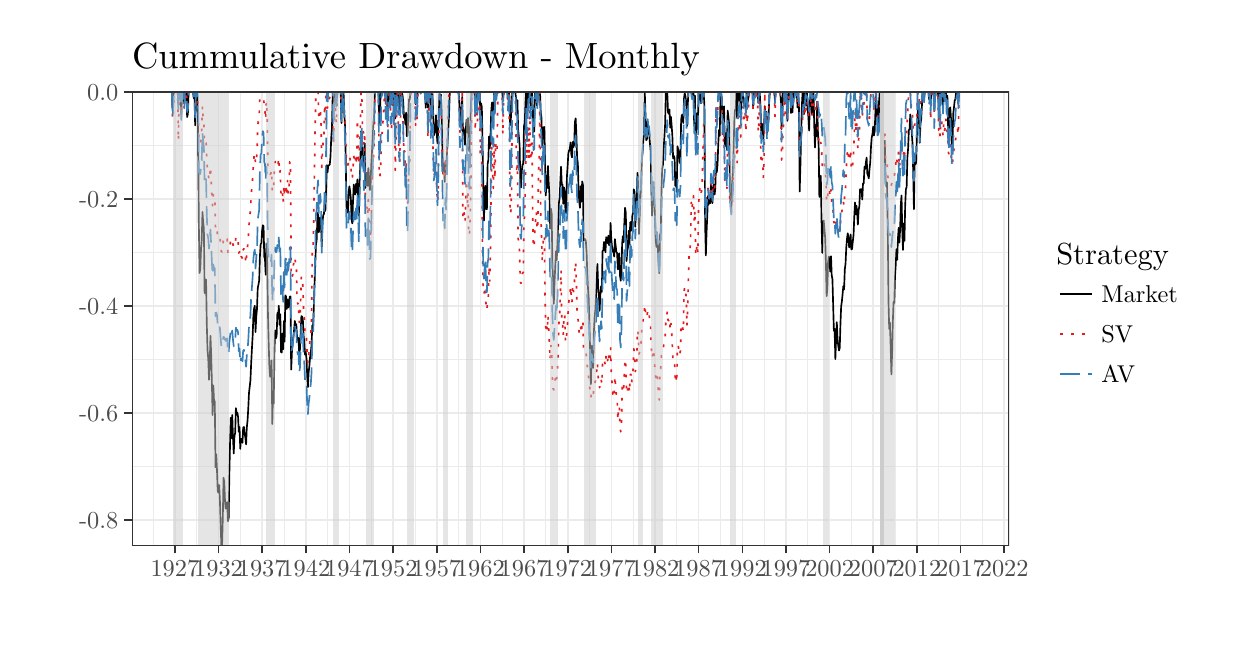
\begin{tikzpicture}[x=1pt,y=1pt]
\definecolor{fillColor}{RGB}{255,255,255}
\path[use as bounding box,fill=fillColor,fill opacity=0.00] (0,0) rectangle (426.79,216.81);
\begin{scope}
\path[clip] (  0.00,  0.00) rectangle (426.79,216.81);
\definecolor{drawColor}{RGB}{255,255,255}
\definecolor{fillColor}{RGB}{255,255,255}

\path[draw=drawColor,line width= 0.6pt,line join=round,line cap=round,fill=fillColor] (  0.00,  0.00) rectangle (426.79,216.81);
\end{scope}
\begin{scope}
\path[clip] ( 37.70, 29.59) rectangle (354.63,193.67);
\definecolor{fillColor}{RGB}{255,255,255}

\path[fill=fillColor] ( 37.70, 29.59) rectangle (354.63,193.67);
\definecolor{drawColor}{gray}{0.92}

\path[draw=drawColor,line width= 0.3pt,line join=round] ( 37.70, 58.23) --
	(354.63, 58.23);

\path[draw=drawColor,line width= 0.3pt,line join=round] ( 37.70, 96.93) --
	(354.63, 96.93);

\path[draw=drawColor,line width= 0.3pt,line join=round] ( 37.70,135.63) --
	(354.63,135.63);

\path[draw=drawColor,line width= 0.3pt,line join=round] ( 37.70,174.33) --
	(354.63,174.33);

\path[draw=drawColor,line width= 0.3pt,line join=round] ( 45.31, 29.59) --
	( 45.31,193.67);

\path[draw=drawColor,line width= 0.3pt,line join=round] ( 61.08, 29.59) --
	( 61.08,193.67);

\path[draw=drawColor,line width= 0.3pt,line join=round] ( 76.85, 29.59) --
	( 76.85,193.67);

\path[draw=drawColor,line width= 0.3pt,line join=round] ( 92.63, 29.59) --
	( 92.63,193.67);

\path[draw=drawColor,line width= 0.3pt,line join=round] (108.40, 29.59) --
	(108.40,193.67);

\path[draw=drawColor,line width= 0.3pt,line join=round] (124.17, 29.59) --
	(124.17,193.67);

\path[draw=drawColor,line width= 0.3pt,line join=round] (139.94, 29.59) --
	(139.94,193.67);

\path[draw=drawColor,line width= 0.3pt,line join=round] (155.72, 29.59) --
	(155.72,193.67);

\path[draw=drawColor,line width= 0.3pt,line join=round] (171.49, 29.59) --
	(171.49,193.67);

\path[draw=drawColor,line width= 0.3pt,line join=round] (187.26, 29.59) --
	(187.26,193.67);

\path[draw=drawColor,line width= 0.3pt,line join=round] (203.03, 29.59) --
	(203.03,193.67);

\path[draw=drawColor,line width= 0.3pt,line join=round] (218.81, 29.59) --
	(218.81,193.67);

\path[draw=drawColor,line width= 0.3pt,line join=round] (234.58, 29.59) --
	(234.58,193.67);

\path[draw=drawColor,line width= 0.3pt,line join=round] (250.35, 29.59) --
	(250.35,193.67);

\path[draw=drawColor,line width= 0.3pt,line join=round] (266.12, 29.59) --
	(266.12,193.67);

\path[draw=drawColor,line width= 0.3pt,line join=round] (281.90, 29.59) --
	(281.90,193.67);

\path[draw=drawColor,line width= 0.3pt,line join=round] (297.67, 29.59) --
	(297.67,193.67);

\path[draw=drawColor,line width= 0.3pt,line join=round] (313.44, 29.59) --
	(313.44,193.67);

\path[draw=drawColor,line width= 0.3pt,line join=round] (329.22, 29.59) --
	(329.22,193.67);

\path[draw=drawColor,line width= 0.3pt,line join=round] (344.99, 29.59) --
	(344.99,193.67);

\path[draw=drawColor,line width= 0.6pt,line join=round] ( 37.70, 38.88) --
	(354.63, 38.88);

\path[draw=drawColor,line width= 0.6pt,line join=round] ( 37.70, 77.58) --
	(354.63, 77.58);

\path[draw=drawColor,line width= 0.6pt,line join=round] ( 37.70,116.28) --
	(354.63,116.28);

\path[draw=drawColor,line width= 0.6pt,line join=round] ( 37.70,154.98) --
	(354.63,154.98);

\path[draw=drawColor,line width= 0.6pt,line join=round] ( 37.70,193.67) --
	(354.63,193.67);

\path[draw=drawColor,line width= 0.6pt,line join=round] ( 53.19, 29.59) --
	( 53.19,193.67);

\path[draw=drawColor,line width= 0.6pt,line join=round] ( 68.96, 29.59) --
	( 68.96,193.67);

\path[draw=drawColor,line width= 0.6pt,line join=round] ( 84.74, 29.59) --
	( 84.74,193.67);

\path[draw=drawColor,line width= 0.6pt,line join=round] (100.51, 29.59) --
	(100.51,193.67);

\path[draw=drawColor,line width= 0.6pt,line join=round] (116.28, 29.59) --
	(116.28,193.67);

\path[draw=drawColor,line width= 0.6pt,line join=round] (132.05, 29.59) --
	(132.05,193.67);

\path[draw=drawColor,line width= 0.6pt,line join=round] (147.83, 29.59) --
	(147.83,193.67);

\path[draw=drawColor,line width= 0.6pt,line join=round] (163.60, 29.59) --
	(163.60,193.67);

\path[draw=drawColor,line width= 0.6pt,line join=round] (179.37, 29.59) --
	(179.37,193.67);

\path[draw=drawColor,line width= 0.6pt,line join=round] (195.15, 29.59) --
	(195.15,193.67);

\path[draw=drawColor,line width= 0.6pt,line join=round] (210.92, 29.59) --
	(210.92,193.67);

\path[draw=drawColor,line width= 0.6pt,line join=round] (226.69, 29.59) --
	(226.69,193.67);

\path[draw=drawColor,line width= 0.6pt,line join=round] (242.46, 29.59) --
	(242.46,193.67);

\path[draw=drawColor,line width= 0.6pt,line join=round] (258.24, 29.59) --
	(258.24,193.67);

\path[draw=drawColor,line width= 0.6pt,line join=round] (274.01, 29.59) --
	(274.01,193.67);

\path[draw=drawColor,line width= 0.6pt,line join=round] (289.78, 29.59) --
	(289.78,193.67);

\path[draw=drawColor,line width= 0.6pt,line join=round] (305.56, 29.59) --
	(305.56,193.67);

\path[draw=drawColor,line width= 0.6pt,line join=round] (321.33, 29.59) --
	(321.33,193.67);

\path[draw=drawColor,line width= 0.6pt,line join=round] (337.10, 29.59) --
	(337.10,193.67);

\path[draw=drawColor,line width= 0.6pt,line join=round] (352.87, 29.59) --
	(352.87,193.67);
\definecolor{drawColor}{RGB}{0,0,0}

\path[draw=drawColor,line width= 0.6pt,line join=round] ( 52.11,193.67) --
	( 52.37,187.60) --
	( 52.63,192.50) --
	( 52.90,193.67) --
	( 53.16,193.54) --
	( 53.43,193.67) --
	( 53.70,193.67) --
	( 53.94,193.67) --
	( 54.20,193.67) --
	( 54.46,189.12) --
	( 54.73,193.67) --
	( 54.99,193.67) --
	( 55.26,193.67) --
	( 55.53,185.27) --
	( 55.79,193.67) --
	( 56.05,193.67) --
	( 56.31,192.62) --
	( 56.58,189.42) --
	( 56.85,193.67) --
	( 57.10,193.67) --
	( 57.37,193.67) --
	( 57.62,184.51) --
	( 57.89,185.65) --
	( 58.15,193.67) --
	( 58.42,193.67) --
	( 58.69,193.67) --
	( 58.95,193.67) --
	( 59.21,193.67) --
	( 59.47,193.67) --
	( 59.74,193.47) --
	( 60.01,191.31) --
	( 60.25,193.67) --
	( 60.52,181.46) --
	( 60.78,193.67) --
	( 61.05,193.67) --
	( 61.30,193.67) --
	( 61.57,183.31) --
	( 61.84,146.70) --
	( 62.10,128.11) --
	( 62.37,129.62) --
	( 62.63,136.67) --
	( 62.89,140.01) --
	( 63.16,150.23) --
	( 63.40,146.71) --
	( 63.67,144.16) --
	( 63.93,120.87) --
	( 64.20,125.61) --
	( 64.46,125.73) --
	( 64.72,109.84) --
	( 64.99,100.26) --
	( 65.25, 97.23) --
	( 65.52, 89.61) --
	( 65.78, 95.19) --
	( 66.05,105.46) --
	( 66.31, 98.70) --
	( 66.56, 88.79) --
	( 66.82, 76.83) --
	( 67.08, 87.52) --
	( 67.35, 81.64) --
	( 67.61, 81.83) --
	( 67.88, 57.97) --
	( 68.14, 62.67) --
	( 68.40, 57.12) --
	( 68.67, 49.39) --
	( 68.93, 48.79) --
	( 69.20, 51.53) --
	( 69.47, 45.75) --
	( 69.72, 37.49) --
	( 69.98, 29.75) --
	( 70.24, 29.59) --
	( 70.51, 39.58) --
	( 70.77, 54.20) --
	( 71.04, 52.64) --
	( 71.31, 45.67) --
	( 71.56, 43.01) --
	( 71.83, 44.94) --
	( 72.09, 45.37) --
	( 72.36, 38.44) --
	( 72.63, 39.70) --
	( 72.87, 55.30) --
	( 73.14, 67.02) --
	( 73.40, 75.86) --
	( 73.66, 68.54) --
	( 73.92, 76.82) --
	( 74.19, 68.69) --
	( 74.46, 62.94) --
	( 74.72, 69.20) --
	( 74.98, 70.43) --
	( 75.24, 79.32) --
	( 75.51, 77.38) --
	( 75.78, 77.68) --
	( 76.02, 76.25) --
	( 76.29, 70.73) --
	( 76.55, 72.51) --
	( 76.82, 64.60) --
	( 77.07, 68.27) --
	( 77.34, 68.10) --
	( 77.61, 66.81) --
	( 77.87, 72.27) --
	( 78.14, 72.52) --
	( 78.40, 70.09) --
	( 78.66, 68.73) --
	( 78.93, 66.25) --
	( 79.17, 72.21) --
	( 79.44, 74.70) --
	( 79.70, 79.00) --
	( 79.97, 84.83) --
	( 80.23, 87.09) --
	( 80.49, 89.35) --
	( 80.76, 95.53) --
	( 81.02,100.56) --
	( 81.29,105.26) --
	( 81.55,112.55) --
	( 81.82,115.39) --
	( 82.08,116.33) --
	( 82.33,106.85) --
	( 82.60,112.38) --
	( 82.86,115.13) --
	( 83.13,122.68) --
	( 83.39,123.99) --
	( 83.66,125.45) --
	( 83.92,134.19) --
	( 84.18,138.58) --
	( 84.45,138.94) --
	( 84.71,143.54) --
	( 84.98,145.42) --
	( 85.24,145.01) --
	( 85.49,134.06) --
	( 85.75,133.10) --
	( 86.01,127.51) --
	( 86.28,138.85) --
	( 86.54,132.11) --
	( 86.81,114.05) --
	( 87.08,103.12) --
	( 87.33, 94.53) --
	( 87.60, 90.67) --
	( 87.86, 91.26) --
	( 88.13, 96.55) --
	( 88.40, 73.57) --
	( 88.64, 84.28) --
	( 88.91, 81.01) --
	( 89.17,100.23) --
	( 89.43,107.44) --
	( 89.69,104.53) --
	( 89.96,105.47) --
	( 90.23,113.78) --
	( 90.49,111.69) --
	( 90.75,116.35) --
	( 91.01,109.40) --
	( 91.28,113.25) --
	( 91.55, 99.61) --
	( 91.79, 99.41) --
	( 92.06,106.27) --
	( 92.32,100.58) --
	( 92.59,110.83) --
	( 92.84,103.38) --
	( 93.11,120.08) --
	( 93.38,119.59) --
	( 93.64,115.14) --
	( 93.91,118.55) --
	( 94.17,115.69) --
	( 94.43,117.39) --
	( 94.70,119.58) --
	( 94.95,119.68) --
	( 95.22, 93.25) --
	( 95.48, 99.48) --
	( 95.75,102.67) --
	( 96.01,105.16) --
	( 96.27,107.57) --
	( 96.54,110.82) --
	( 96.80,108.97) --
	( 97.07,109.68) --
	( 97.33,105.17) --
	( 97.60,103.72) --
	( 97.86,104.72) --
	( 98.10, 99.08) --
	( 98.37,100.37) --
	( 98.63,106.24) --
	( 98.90,112.56) --
	( 99.16,112.43) --
	( 99.43,111.54) --
	( 99.69,105.63) --
	( 99.95,103.49) --
	(100.22, 98.66) --
	(100.48, 99.55) --
	(100.75, 97.19) --
	(101.02, 90.85) --
	(101.26, 86.89) --
	(101.52, 92.10) --
	(101.78, 94.46) --
	(102.05, 97.76) --
	(102.31, 99.53) --
	(102.58,102.19) --
	(102.85,109.21) --
	(103.11,109.30) --
	(103.37,114.87) --
	(103.63,123.25) --
	(103.90,130.65) --
	(104.17,138.67) --
	(104.41,139.64) --
	(104.68,147.57) --
	(104.94,150.08) --
	(105.20,142.88) --
	(105.46,144.75) --
	(105.73,148.19) --
	(106.00,146.43) --
	(106.26,137.63) --
	(106.53,146.42) --
	(106.78,149.01) --
	(107.05,149.48) --
	(107.32,153.13) --
	(107.57,150.56) --
	(107.84,158.19) --
	(108.10,167.12) --
	(108.36,164.53) --
	(108.62,167.05) --
	(108.89,167.07) --
	(109.16,167.37) --
	(109.42,170.13) --
	(109.69,177.05) --
	(109.95,180.58) --
	(110.21,192.17) --
	(110.48,184.59) --
	(110.72,193.67) --
	(110.99,193.67) --
	(111.25,193.67) --
	(111.52,189.35) --
	(111.78,193.67) --
	(112.04,193.67) --
	(112.31,193.67) --
	(112.57,193.67) --
	(112.84,193.67) --
	(113.10,193.67) --
	(113.37,182.35) --
	(113.63,192.84) --
	(113.87,193.67) --
	(114.14,193.67) --
	(114.40,186.14) --
	(114.67,181.19) --
	(114.93,169.47) --
	(115.20,152.15) --
	(115.46,149.96) --
	(115.72,150.02) --
	(115.99,157.48) --
	(116.25,159.49) --
	(116.52,157.68) --
	(116.79,154.99) --
	(117.03,147.56) --
	(117.30,146.10) --
	(117.55,153.82) --
	(117.82,160.12) --
	(118.08,157.30) --
	(118.35,156.52) --
	(118.62,160.35) --
	(118.88,157.26) --
	(119.14,161.98) --
	(119.40,155.76) --
	(119.67,148.88) --
	(119.94,161.06) --
	(120.19,167.07) --
	(120.46,179.32) --
	(120.72,179.12) --
	(120.98,169.99) --
	(121.24,170.47) --
	(121.51,165.26) --
	(121.78,175.06) --
	(122.04,158.90) --
	(122.30,164.00) --
	(122.56,164.44) --
	(122.83,159.64) --
	(123.10,166.09) --
	(123.34,162.97) --
	(123.61,158.17) --
	(123.87,158.37) --
	(124.14,167.12) --
	(124.39,171.45) --
	(124.66,176.78) --
	(124.93,182.23) --
	(125.19,185.44) --
	(125.46,193.67) --
	(125.72,193.67) --
	(125.98,193.67) --
	(126.25,193.67) --
	(126.49,193.67) --
	(126.76,193.67) --
	(127.02,182.28) --
	(127.29,185.04) --
	(127.55,193.67) --
	(127.81,193.67) --
	(128.08,193.25) --
	(128.34,193.67) --
	(128.61,193.67) --
	(128.87,193.67) --
	(129.14,193.67) --
	(129.40,189.34) --
	(129.65,193.67) --
	(129.91,189.12) --
	(130.17,184.06) --
	(130.44,193.67) --
	(130.70,193.67) --
	(130.97,193.67) --
	(131.23,189.05) --
	(131.49,189.99) --
	(131.76,193.67) --
	(132.02,193.67) --
	(132.29,188.58) --
	(132.56,193.67) --
	(132.81,183.94) --
	(133.07,189.77) --
	(133.33,193.67) --
	(133.60,193.67) --
	(133.86,192.08) --
	(134.13,188.13) --
	(134.40,186.85) --
	(134.65,193.67) --
	(134.92,193.67) --
	(135.18,193.16) --
	(135.45,192.50) --
	(135.72,189.73) --
	(135.96,184.22) --
	(136.23,185.16) --
	(136.49,181.84) --
	(136.75,186.09) --
	(137.01,177.58) --
	(137.28,177.84) --
	(137.55,185.97) --
	(137.81,190.96) --
	(138.07,190.84) --
	(138.33,193.67) --
	(138.60,193.67) --
	(138.87,193.67) --
	(139.11,193.67) --
	(139.38,193.67) --
	(139.64,193.67) --
	(139.91,193.67) --
	(140.16,189.16) --
	(140.43,193.67) --
	(140.70,190.44) --
	(140.96,193.67) --
	(141.23,193.67) --
	(141.49,193.67) --
	(141.75,193.67) --
	(142.02,193.33) --
	(142.26,193.67) --
	(142.53,193.67) --
	(142.79,193.67) --
	(143.06,193.67) --
	(143.32,193.67) --
	(143.58,193.09) --
	(143.85,187.83) --
	(144.11,193.67) --
	(144.38,193.67) --
	(144.64,187.91) --
	(144.91,193.67) --
	(145.17,193.67) --
	(145.42,193.67) --
	(145.69,183.86) --
	(145.95,190.34) --
	(146.22,193.67) --
	(146.48,187.53) --
	(146.75,177.85) --
	(147.01,178.84) --
	(147.27,179.35) --
	(147.54,185.15) --
	(147.80,178.85) --
	(148.07,175.09) --
	(148.33,178.83) --
	(148.58,186.45) --
	(148.84,192.84) --
	(149.10,191.39) --
	(149.37,192.60) --
	(149.63,182.53) --
	(149.90,171.51) --
	(150.17,164.04) --
	(150.42,167.80) --
	(150.69,161.07) --
	(150.95,168.57) --
	(151.22,165.78) --
	(151.49,170.88) --
	(151.73,175.93) --
	(152.00,180.09) --
	(152.26,185.25) --
	(152.52,193.33) --
	(152.78,193.67) --
	(153.05,193.67) --
	(153.32,193.67) --
	(153.58,193.67) --
	(153.85,193.67) --
	(154.10,193.67) --
	(154.37,193.67) --
	(154.64,193.67) --
	(154.88,193.67) --
	(155.15,193.67) --
	(155.41,193.42) --
	(155.68,193.67) --
	(155.94,190.79) --
	(156.20,181.76) --
	(156.47,184.27) --
	(156.73,187.11) --
	(157.00,191.78) --
	(157.26,178.62) --
	(157.52,180.58) --
	(157.79,177.68) --
	(158.04,174.47) --
	(158.31,179.78) --
	(158.57,183.53) --
	(158.84,178.89) --
	(159.10,184.20) --
	(159.36,173.18) --
	(159.63,172.07) --
	(159.89,180.14) --
	(160.16,188.46) --
	(160.42,193.67) --
	(160.69,193.67) --
	(160.95,193.67) --
	(161.19,193.67) --
	(161.46,193.67) --
	(161.72,187.84) --
	(161.99,193.12) --
	(162.25,193.67) --
	(162.52,189.47) --
	(162.78,193.67) --
	(163.04,193.67) --
	(163.31,193.45) --
	(163.57,186.18) --
	(163.84,189.45) --
	(164.11,188.11) --
	(164.35,175.84) --
	(164.61,160.65) --
	(164.87,147.07) --
	(165.14,156.31) --
	(165.40,159.65) --
	(165.67,151.24) --
	(165.94,151.22) --
	(166.20,167.51) --
	(166.46,169.07) --
	(166.72,177.47) --
	(166.99,173.19) --
	(167.26,178.44) --
	(167.50,186.46) --
	(167.77,189.76) --
	(168.03,185.88) --
	(168.29,185.12) --
	(168.55,193.67) --
	(168.82,190.86) --
	(169.09,193.67) --
	(169.35,192.08) --
	(169.62,193.67) --
	(169.87,193.67) --
	(170.14,193.67) --
	(170.41,193.67) --
	(170.66,193.67) --
	(170.93,193.67) --
	(171.19,193.67) --
	(171.46,193.67) --
	(171.71,190.92) --
	(171.98,193.67) --
	(172.25,193.67) --
	(172.51,193.67) --
	(172.78,193.67) --
	(173.04,193.67) --
	(173.30,193.67) --
	(173.57,191.26) --
	(173.81,193.67) --
	(174.08,192.14) --
	(174.34,181.62) --
	(174.61,184.09) --
	(174.87,189.11) --
	(175.13,193.67) --
	(175.40,193.67) --
	(175.66,193.67) --
	(175.93,193.67) --
	(176.19,193.67) --
	(176.46,191.38) --
	(176.72,186.67) --
	(176.97,190.63) --
	(177.23,179.94) --
	(177.49,177.49) --
	(177.76,174.49) --
	(178.02,160.74) --
	(178.29,159.06) --
	(178.55,165.11) --
	(178.81,167.33) --
	(179.08,167.61) --
	(179.34,181.21) --
	(179.61,182.46) --
	(179.88,189.56) --
	(180.12,193.67) --
	(180.39,185.35) --
	(180.64,189.72) --
	(180.91,193.67) --
	(181.17,191.94) --
	(181.44,193.67) --
	(181.71,187.79) --
	(181.97,188.66) --
	(182.23,193.67) --
	(182.49,185.98) --
	(182.76,179.14) --
	(183.03,179.34) --
	(183.28,193.67) --
	(183.55,193.67) --
	(183.81,193.67) --
	(184.07,188.57) --
	(184.33,191.14) --
	(184.60,193.67) --
	(184.87,193.67) --
	(185.13,193.67) --
	(185.39,186.30) --
	(185.65,184.28) --
	(185.92,173.66) --
	(186.19,178.01) --
	(186.43,180.83) --
	(186.70,180.91) --
	(186.96,167.84) --
	(187.23,156.16) --
	(187.48,163.36) --
	(187.75,158.84) --
	(188.02,166.83) --
	(188.28,160.48) --
	(188.55,156.38) --
	(188.81,144.19) --
	(189.07,151.39) --
	(189.34,149.78) --
	(189.58,133.20) --
	(189.85,123.93) --
	(190.11,117.03) --
	(190.38,125.03) --
	(190.64,130.53) --
	(190.90,136.01) --
	(191.17,132.84) --
	(191.43,138.78) --
	(191.70,146.53) --
	(191.96,153.43) --
	(192.23,155.37) --
	(192.49,161.71) --
	(192.74,166.55) --
	(193.00,160.01) --
	(193.26,160.06) --
	(193.53,153.18) --
	(193.79,159.09) --
	(194.06,157.66) --
	(194.32,150.55) --
	(194.58,149.81) --
	(194.85,162.86) --
	(195.11,166.86) --
	(195.38,171.45) --
	(195.65,172.45) --
	(195.90,172.96) --
	(196.16,175.32) --
	(196.42,171.16) --
	(196.69,169.93) --
	(196.95,175.52) --
	(197.22,173.64) --
	(197.49,174.64) --
	(197.74,182.70) --
	(198.01,184.02) --
	(198.27,178.31) --
	(198.54,169.78) --
	(198.81,167.71) --
	(199.05,158.39) --
	(199.32,153.81) --
	(199.58,151.69) --
	(199.84,159.51) --
	(200.10,154.00) --
	(200.37,161.26) --
	(200.64,160.08) --
	(200.90,139.83) --
	(201.16,140.51) --
	(201.42,140.35) --
	(201.69,139.78) --
	(201.96,135.67) --
	(202.20,128.69) --
	(202.47,122.61) --
	(202.73,118.91) --
	(203.00,109.68) --
	(203.25, 99.47) --
	(203.52, 87.96) --
	(203.79,101.89) --
	(204.05, 96.93) --
	(204.32, 93.84) --
	(204.58,106.53) --
	(204.84,111.96) --
	(205.11,114.67) --
	(205.35,119.48) --
	(205.62,125.54) --
	(205.88,131.42) --
	(206.15,122.95) --
	(206.41,119.57) --
	(206.67,114.48) --
	(206.94,120.29) --
	(207.20,123.39) --
	(207.47,121.36) --
	(207.73,136.07) --
	(208.00,136.41) --
	(208.26,139.40) --
	(208.51,137.49) --
	(208.78,135.66) --
	(209.04,141.10) --
	(209.31,139.71) --
	(209.57,138.92) --
	(209.84,141.65) --
	(210.10,138.19) --
	(210.36,138.32) --
	(210.63,146.23) --
	(210.89,140.36) --
	(211.16,137.60) --
	(211.43,135.84) --
	(211.67,136.04) --
	(211.93,134.07) --
	(212.19,140.41) --
	(212.46,138.10) --
	(212.72,135.72) --
	(212.99,135.37) --
	(213.26,129.49) --
	(213.52,134.78) --
	(213.78,135.23) --
	(214.04,127.14) --
	(214.31,125.35) --
	(214.58,128.97) --
	(214.82,139.01) --
	(215.09,141.48) --
	(215.35,139.21) --
	(215.61,146.36) --
	(215.87,151.73) --
	(216.14,149.85) --
	(216.41,132.49) --
	(216.67,136.12) --
	(216.94,137.59) --
	(217.19,143.39) --
	(217.46,138.48) --
	(217.73,146.43) --
	(217.97,146.60) --
	(218.24,143.46) --
	(218.50,148.98) --
	(218.77,149.98) --
	(219.03,158.40) --
	(219.29,157.41) --
	(219.56,144.87) --
	(219.82,152.81) --
	(220.09,155.76) --
	(220.35,164.34) --
	(220.61,162.96) --
	(220.88,142.26) --
	(221.13,148.37) --
	(221.40,155.39) --
	(221.66,159.24) --
	(221.93,168.92) --
	(222.19,171.85) --
	(222.45,175.98) --
	(222.72,178.37) --
	(222.98,193.67) --
	(223.25,185.26) --
	(223.51,176.15) --
	(223.78,176.57) --
	(224.04,182.82) --
	(224.28,178.85) --
	(224.55,179.10) --
	(224.81,175.38) --
	(225.08,172.85) --
	(225.34,160.97) --
	(225.61,148.87) --
	(225.87,155.82) --
	(226.13,160.96) --
	(226.40,154.58) --
	(226.66,148.94) --
	(226.93,140.12) --
	(227.20,137.60) --
	(227.44,142.24) --
	(227.71,136.90) --
	(227.96,132.14) --
	(228.23,128.07) --
	(228.49,141.93) --
	(228.76,142.81) --
	(229.03,158.53) --
	(229.29,165.90) --
	(229.55,167.32) --
	(229.81,173.23) --
	(230.08,177.27) --
	(230.35,182.16) --
	(230.59,193.67) --
	(230.86,193.67) --
	(231.12,193.67) --
	(231.38,186.28) --
	(231.64,185.68) --
	(231.91,187.28) --
	(232.18,180.65) --
	(232.44,184.59) --
	(232.71,181.28) --
	(232.96,177.68) --
	(233.23,169.51) --
	(233.50,170.48) --
	(233.75,169.71) --
	(234.02,159.67) --
	(234.28,162.09) --
	(234.55,157.52) --
	(234.80,173.95) --
	(235.07,172.61) --
	(235.34,171.18) --
	(235.60,167.91) --
	(235.87,170.17) --
	(236.13,183.41) --
	(236.39,185.32) --
	(236.66,183.80) --
	(236.90,182.34) --
	(237.17,191.32) --
	(237.43,193.20) --
	(237.70,191.88) --
	(237.96,189.92) --
	(238.22,181.24) --
	(238.49,188.25) --
	(238.75,193.67) --
	(239.02,193.67) --
	(239.28,193.67) --
	(239.55,193.67) --
	(239.81,193.67) --
	(240.06,191.13) --
	(240.32,193.67) --
	(240.58,193.67) --
	(240.85,181.24) --
	(241.11,192.22) --
	(241.38,176.13) --
	(241.64,183.96) --
	(241.90,185.90) --
	(242.17,180.17) --
	(242.43,193.67) --
	(242.70,193.67) --
	(242.97,193.67) --
	(243.21,189.57) --
	(243.48,189.65) --
	(243.73,193.67) --
	(244.00,193.67) --
	(244.26,193.67) --
	(244.53,188.79) --
	(244.80,145.60) --
	(245.06,134.49) --
	(245.32,143.07) --
	(245.58,148.97) --
	(245.85,156.05) --
	(246.12,153.02) --
	(246.37,153.99) --
	(246.64,153.39) --
	(246.90,160.53) --
	(247.16,158.56) --
	(247.42,153.37) --
	(247.69,158.26) --
	(247.96,160.11) --
	(248.22,156.52) --
	(248.48,158.84) --
	(248.74,168.37) --
	(249.01,164.57) --
	(249.28,167.18) --
	(249.52,174.17) --
	(249.79,179.81) --
	(250.05,177.75) --
	(250.32,189.94) --
	(250.57,192.78) --
	(250.84,191.15) --
	(251.11,184.20) --
	(251.37,186.27) --
	(251.64,188.39) --
	(251.90,174.00) --
	(252.16,175.52) --
	(252.43,178.73) --
	(252.67,172.70) --
	(252.94,186.85) --
	(253.20,184.79) --
	(253.47,181.82) --
	(253.73,164.09) --
	(253.99,154.22) --
	(254.26,151.30) --
	(254.52,160.27) --
	(254.79,163.88) --
	(255.05,170.94) --
	(255.32,182.80) --
	(255.58,187.11) --
	(255.83,186.83) --
	(256.09,193.58) --
	(256.35,184.09) --
	(256.62,191.80) --
	(256.88,193.67) --
	(257.15,190.62) --
	(257.41,193.12) --
	(257.67,185.08) --
	(257.94,193.67) --
	(258.20,192.70) --
	(258.47,193.67) --
	(258.74,188.45) --
	(258.99,190.44) --
	(259.25,191.02) --
	(259.51,186.74) --
	(259.78,193.65) --
	(260.04,189.01) --
	(260.31,190.77) --
	(260.58,192.37) --
	(260.83,193.67) --
	(261.10,193.67) --
	(261.36,193.67) --
	(261.63,193.67) --
	(261.90,193.67) --
	(262.14,188.35) --
	(262.41,193.43) --
	(262.67,193.67) --
	(262.93,193.10) --
	(263.19,193.67) --
	(263.46,193.34) --
	(263.73,193.67) --
	(263.99,189.78) --
	(264.26,193.05) --
	(264.51,193.67) --
	(264.78,188.55) --
	(265.05,179.48) --
	(265.29,180.80) --
	(265.56,182.00) --
	(265.82,176.45) --
	(266.09,181.29) --
	(266.35,188.42) --
	(266.61,184.45) --
	(266.88,186.43) --
	(267.14,178.84) --
	(267.41,180.41) --
	(267.67,183.41) --
	(267.93,189.83) --
	(268.20,193.67) --
	(268.44,193.67) --
	(268.71,193.67) --
	(268.97,193.67) --
	(269.24,193.67) --
	(269.50,193.67) --
	(269.77,193.67) --
	(270.03,190.59) --
	(270.29,193.67) --
	(270.56,193.67) --
	(270.82,193.67) --
	(271.09,193.67) --
	(271.35,193.67) --
	(271.60,193.67) --
	(271.87,193.67) --
	(272.13,191.19) --
	(272.40,180.16) --
	(272.66,185.25) --
	(272.93,193.67) --
	(273.19,193.67) --
	(273.45,193.67) --
	(273.72,190.67) --
	(273.98,193.67) --
	(274.25,192.57) --
	(274.52,183.12) --
	(274.76,190.13) --
	(275.02,193.67) --
	(275.28,193.67) --
	(275.55,193.67) --
	(275.81,185.97) --
	(276.08,193.67) --
	(276.35,186.25) --
	(276.61,191.07) --
	(276.87,193.65) --
	(277.13,193.67) --
	(277.40,193.67) --
	(277.67,193.67) --
	(277.91,193.67) --
	(278.18,187.96) --
	(278.44,193.13) --
	(278.70,187.87) --
	(278.96,157.60) --
	(279.23,166.98) --
	(279.50,178.62) --
	(279.76,188.82) --
	(280.03,193.67) --
	(280.28,193.67) --
	(280.55,185.60) --
	(280.82,191.96) --
	(281.06,193.67) --
	(281.33,188.86) --
	(281.59,193.67) --
	(281.86,187.10) --
	(282.12,184.49) --
	(282.38,179.60) --
	(282.65,190.01) --
	(282.91,193.67) --
	(283.18,193.67) --
	(283.44,185.34) --
	(283.70,190.39) --
	(283.97,193.67) --
	(284.22,181.38) --
	(284.49,173.52) --
	(284.75,181.63) --
	(285.02,177.53) --
	(285.28,190.07) --
	(285.54,179.50) --
	(285.81,174.24) --
	(286.07,155.63) --
	(286.34,157.92) --
	(286.60,163.33) --
	(286.87,146.43) --
	(287.13,135.41) --
	(287.38,146.19) --
	(287.64,147.10) --
	(287.90,143.96) --
	(288.17,140.88) --
	(288.43,132.21) --
	(288.70,119.77) --
	(288.96,122.72) --
	(289.22,132.00) --
	(289.49,134.06) --
	(289.75,131.70) --
	(290.02,128.65) --
	(290.29,134.21) --
	(290.53,127.39) --
	(290.80,125.89) --
	(291.05,116.88) --
	(291.32,107.26) --
	(291.58,107.98) --
	(291.85, 97.06) --
	(292.12,104.17) --
	(292.38,110.39) --
	(292.64,104.37) --
	(292.90,101.81) --
	(293.17,100.14) --
	(293.44,101.07) --
	(293.68,109.32) --
	(293.95,116.13) --
	(294.21,117.91) --
	(294.47,120.52) --
	(294.73,123.40) --
	(295.00,122.19) --
	(295.27,129.46) --
	(295.53,131.50) --
	(295.80,137.38) --
	(296.05,140.44) --
	(296.32,142.50) --
	(296.59,140.88) --
	(296.84,137.39) --
	(297.11,139.19) --
	(297.37,142.08) --
	(297.64,136.66) --
	(297.89,136.92) --
	(298.16,139.59) --
	(298.43,141.91) --
	(298.69,148.58) --
	(298.96,153.63) --
	(299.22,149.33) --
	(299.48,152.47) --
	(299.75,149.65) --
	(299.99,145.66) --
	(300.26,150.86) --
	(300.52,152.28) --
	(300.79,158.49) --
	(301.05,157.19) --
	(301.31,158.47) --
	(301.58,154.70) --
	(301.84,160.47) --
	(302.11,160.59) --
	(302.37,166.50) --
	(302.64,165.70) --
	(302.90,168.26) --
	(303.15,169.87) --
	(303.41,163.99) --
	(303.67,163.34) --
	(303.94,162.34) --
	(304.20,165.74) --
	(304.47,168.28) --
	(304.73,173.79) --
	(304.99,177.18) --
	(305.26,178.37) --
	(305.52,181.07) --
	(305.79,177.83) --
	(306.06,179.34) --
	(306.30,185.77) --
	(306.57,192.17) --
	(306.82,188.51) --
	(307.09,181.78) --
	(307.35,183.16) --
	(307.62,189.88) --
	(307.89,193.67) --
	(308.15,183.54) --
	(308.41,182.15) --
	(308.67,170.26) --
	(308.94,166.13) --
	(309.21,164.06) --
	(309.46,172.21) --
	(309.73,176.01) --
	(309.99,161.93) --
	(310.25,159.49) --
	(310.51,160.90) --
	(310.78,144.93) --
	(311.05,118.05) --
	(311.31,107.92) --
	(311.57,110.21) --
	(311.83,101.68) --
	(312.10, 91.50) --
	(312.37, 99.42) --
	(312.61,110.26) --
	(312.88,117.70) --
	(313.14,117.33) --
	(313.41,126.90) --
	(313.66,130.87) --
	(313.93,136.77) --
	(314.20,132.93) --
	(314.46,140.50) --
	(314.73,144.48) --
	(314.99,139.13) --
	(315.25,143.95) --
	(315.52,153.09) --
	(315.76,156.16) --
	(316.03,143.80) --
	(316.29,136.50) --
	(316.56,146.07) --
	(316.82,139.81) --
	(317.08,152.57) --
	(317.35,158.43) --
	(317.61,159.22) --
	(317.88,169.88) --
	(318.14,173.12) --
	(318.41,179.70) --
	(318.67,180.29) --
	(318.92,185.43) --
	(319.18,182.65) --
	(319.44,179.29) --
	(319.71,175.27) --
	(319.97,165.21) --
	(320.24,151.20) --
	(320.51,168.40) --
	(320.76,167.35) --
	(321.03,167.97) --
	(321.29,177.04) --
	(321.56,184.32) --
	(321.83,188.74) --
	(322.08,187.46) --
	(322.34,175.19) --
	(322.60,181.87) --
	(322.87,183.71) --
	(323.13,188.53) --
	(323.40,193.53) --
	(323.67,190.79) --
	(323.93,191.95) --
	(324.19,193.67) --
	(324.45,193.67) --
	(324.72,193.67) --
	(324.99,193.67) --
	(325.23,193.67) --
	(325.50,193.67) --
	(325.76,190.76) --
	(326.02,193.67) --
	(326.28,188.70) --
	(326.55,193.67) --
	(326.82,193.67) --
	(327.08,193.67) --
	(327.35,193.67) --
	(327.60,187.88) --
	(327.87,193.67) --
	(328.14,193.67) --
	(328.38,193.67) --
	(328.65,193.67) --
	(328.91,193.67) --
	(329.18,189.70) --
	(329.44,193.67) --
	(329.70,188.81) --
	(329.97,192.81) --
	(330.23,193.67) --
	(330.50,192.98) --
	(330.76,187.74) --
	(331.02,193.67) --
	(331.29,191.65) --
	(331.53,193.33) --
	(331.80,193.67) --
	(332.06,189.95) --
	(332.33,192.24) --
	(332.59,180.72) --
	(332.86,174.63) --
	(333.12,187.53) --
	(333.38,187.99) --
	(333.65,183.81) --
	(333.91,173.34) --
	(334.18,173.44) --
	(334.44,185.63) --
	(334.69,187.78) --
	(334.96,190.42) --
	(335.22,191.00) --
	(335.49,193.67) --
	(335.75,193.67) --
	(336.02,193.67) --
	(336.28,189.46) --
	(336.54,193.67) --
	(336.81,193.67) --
	(337.07,193.67) --
	(337.34,193.67) --
	(337.61,193.67) --
	(337.85,193.67) --
	(338.12,193.67) --
	(338.37,193.67) --
	(338.64,193.67) --
	(338.90,193.67) --
	(339.17,193.67) --
	(339.44,193.67) --
	(339.70,193.67) --
	(339.96,193.67) --
	(340.22,193.67);
\definecolor{drawColor}{RGB}{228,26,28}

\path[draw=drawColor,line width= 0.6pt,dash pattern=on 1pt off 3pt ,line join=round] ( 52.11,193.67) --
	( 52.37,183.67) --
	( 52.63,186.35) --
	( 52.90,193.67) --
	( 53.16,193.37) --
	( 53.43,193.67) --
	( 53.70,193.67) --
	( 53.94,193.67) --
	( 54.20,193.67) --
	( 54.46,175.98) --
	( 54.73,191.84) --
	( 54.99,193.67) --
	( 55.26,193.67) --
	( 55.53,185.05) --
	( 55.79,193.67) --
	( 56.05,193.67) --
	( 56.31,191.71) --
	( 56.58,188.01) --
	( 56.85,193.67) --
	( 57.10,193.67) --
	( 57.37,193.67) --
	( 57.62,188.55) --
	( 57.89,188.82) --
	( 58.15,193.67) --
	( 58.42,193.67) --
	( 58.69,193.67) --
	( 58.95,193.67) --
	( 59.21,193.67) --
	( 59.47,193.67) --
	( 59.74,193.53) --
	( 60.01,192.78) --
	( 60.25,193.38) --
	( 60.52,187.41) --
	( 60.78,191.92) --
	( 61.05,193.67) --
	( 61.30,193.67) --
	( 61.57,190.10) --
	( 61.84,175.35) --
	( 62.10,174.96) --
	( 62.37,175.02) --
	( 62.63,176.01) --
	( 62.89,180.06) --
	( 63.16,188.55) --
	( 63.40,184.08) --
	( 63.67,182.01) --
	( 63.93,175.07) --
	( 64.20,175.63) --
	( 64.46,175.67) --
	( 64.72,169.60) --
	( 64.99,164.27) --
	( 65.25,163.80) --
	( 65.52,161.72) --
	( 65.78,163.05) --
	( 66.05,166.58) --
	( 66.31,161.37) --
	( 66.56,156.32) --
	( 66.82,152.47) --
	( 67.08,156.50) --
	( 67.35,155.90) --
	( 67.61,155.96) --
	( 67.88,143.21) --
	( 68.14,143.91) --
	( 68.40,143.54) --
	( 68.67,141.42) --
	( 68.93,141.33) --
	( 69.20,141.84) --
	( 69.47,141.08) --
	( 69.72,138.31) --
	( 69.98,135.88) --
	( 70.24,135.83) --
	( 70.51,137.47) --
	( 70.77,140.95) --
	( 71.04,140.79) --
	( 71.31,140.25) --
	( 71.56,139.97) --
	( 71.83,140.28) --
	( 72.09,140.45) --
	( 72.36,135.58) --
	( 72.63,135.99) --
	( 72.87,137.28) --
	( 73.14,138.51) --
	( 73.40,140.15) --
	( 73.66,139.42) --
	( 73.92,139.89) --
	( 74.19,138.43) --
	( 74.46,137.46) --
	( 74.72,138.02) --
	( 74.98,138.32) --
	( 75.24,141.32) --
	( 75.51,140.71) --
	( 75.78,140.82) --
	( 76.02,140.35) --
	( 76.29,135.35) --
	( 76.55,135.87) --
	( 76.82,133.24) --
	( 77.07,134.02) --
	( 77.34,133.96) --
	( 77.61,133.32) --
	( 77.87,136.58) --
	( 78.14,136.95) --
	( 78.40,134.95) --
	( 78.66,133.63) --
	( 78.93,131.64) --
	( 79.17,135.48) --
	( 79.44,137.59) --
	( 79.70,140.63) --
	( 79.97,145.29) --
	( 80.23,148.94) --
	( 80.49,150.48) --
	( 80.76,156.13) --
	( 81.02,159.31) --
	( 81.29,162.27) --
	( 81.55,167.46) --
	( 81.82,170.48) --
	( 82.08,171.29) --
	( 82.33,167.63) --
	( 82.60,169.48) --
	( 82.86,171.17) --
	( 83.13,181.37) --
	( 83.39,183.30) --
	( 83.66,184.46) --
	( 83.92,193.67) --
	( 84.18,193.67) --
	( 84.45,193.67) --
	( 84.71,193.67) --
	( 84.98,193.67) --
	( 85.24,193.13) --
	( 85.49,186.76) --
	( 85.75,186.48) --
	( 86.01,183.63) --
	( 86.28,190.18) --
	( 86.54,184.95) --
	( 86.81,165.93) --
	( 87.08,164.75) --
	( 87.33,164.26) --
	( 87.60,163.86) --
	( 87.86,164.05) --
	( 88.13,165.32) --
	( 88.40,157.93) --
	( 88.64,160.10) --
	( 88.91,159.66) --
	( 89.17,166.92) --
	( 89.43,168.44) --
	( 89.69,167.55) --
	( 89.96,167.88) --
	( 90.23,168.77) --
	( 90.49,167.66) --
	( 90.75,169.75) --
	( 91.01,164.16) --
	( 91.28,165.17) --
	( 91.55,155.82) --
	( 91.79,155.78) --
	( 92.06,157.18) --
	( 92.32,153.46) --
	( 92.59,159.93) --
	( 92.84,155.82) --
	( 93.11,160.18) --
	( 93.38,160.13) --
	( 93.64,156.04) --
	( 93.91,161.53) --
	( 94.17,156.70) --
	( 94.43,158.69) --
	( 94.70,168.31) --
	( 94.95,168.55) --
	( 95.22,126.33) --
	( 95.48,126.81) --
	( 95.75,127.34) --
	( 96.01,131.08) --
	( 96.27,132.25) --
	( 96.54,133.86) --
	( 96.80,131.62) --
	( 97.07,131.81) --
	( 97.33,118.40) --
	( 97.60,116.97) --
	( 97.86,117.50) --
	( 98.10,110.28) --
	( 98.37,111.35) --
	( 98.63,118.10) --
	( 98.90,126.94) --
	( 99.16,126.77) --
	( 99.43,123.51) --
	( 99.69,115.03) --
	( 99.95,112.69) --
	(100.22,105.95) --
	(100.48,106.11) --
	(100.75,104.66) --
	(101.02, 97.62) --
	(101.26, 95.62) --
	(101.52, 98.30) --
	(101.78,100.78) --
	(102.05,104.00) --
	(102.31,105.35) --
	(102.58,112.35) --
	(102.85,137.41) --
	(103.11,137.53) --
	(103.37,147.50) --
	(103.63,165.15) --
	(103.90,183.09) --
	(104.17,193.67) --
	(104.41,193.67) --
	(104.68,193.67) --
	(104.94,193.67) --
	(105.20,183.39) --
	(105.46,184.52) --
	(105.73,187.62) --
	(106.00,183.14) --
	(106.26,166.31) --
	(106.53,171.84) --
	(106.78,175.82) --
	(107.05,176.90) --
	(107.32,189.06) --
	(107.57,183.58) --
	(107.84,193.67) --
	(108.10,193.67) --
	(108.36,187.75) --
	(108.62,191.04) --
	(108.89,191.11) --
	(109.16,191.44) --
	(109.42,193.67) --
	(109.69,193.67) --
	(109.95,193.67) --
	(110.21,193.67) --
	(110.48,174.37) --
	(110.72,182.07) --
	(110.99,186.41) --
	(111.25,187.54) --
	(111.52,182.09) --
	(111.78,189.10) --
	(112.04,193.67) --
	(112.31,193.67) --
	(112.57,193.67) --
	(112.84,193.67) --
	(113.10,193.67) --
	(113.37,188.33) --
	(113.63,190.18) --
	(113.87,193.67) --
	(114.14,193.67) --
	(114.40,186.57) --
	(114.67,183.12) --
	(114.93,176.62) --
	(115.20,167.29) --
	(115.46,167.13) --
	(115.72,167.14) --
	(115.99,169.43) --
	(116.25,170.33) --
	(116.52,169.26) --
	(116.79,166.75) --
	(117.03,163.05) --
	(117.30,162.27) --
	(117.55,166.11) --
	(117.82,170.58) --
	(118.08,168.75) --
	(118.35,167.70) --
	(118.62,171.13) --
	(118.88,167.28) --
	(119.14,183.68) --
	(119.40,175.36) --
	(119.67,167.37) --
	(119.94,175.53) --
	(120.19,179.60) --
	(120.46,193.67) --
	(120.72,193.44) --
	(120.98,180.94) --
	(121.24,181.16) --
	(121.51,174.08) --
	(121.78,178.88) --
	(122.04,151.42) --
	(122.30,152.31) --
	(122.56,152.85) --
	(122.83,148.99) --
	(123.10,154.69) --
	(123.34,151.48) --
	(123.61,140.79) --
	(123.87,141.03) --
	(124.14,146.39) --
	(124.39,159.21) --
	(124.66,165.53) --
	(124.93,169.06) --
	(125.19,174.52) --
	(125.46,190.64) --
	(125.72,193.67) --
	(125.98,193.67) --
	(126.25,193.67) --
	(126.49,193.67) --
	(126.76,193.67) --
	(127.02,162.86) --
	(127.29,163.32) --
	(127.55,165.88) --
	(127.81,179.01) --
	(128.08,178.58) --
	(128.34,182.36) --
	(128.61,186.52) --
	(128.87,190.94) --
	(129.14,192.77) --
	(129.40,184.33) --
	(129.65,191.59) --
	(129.91,185.78) --
	(130.17,181.01) --
	(130.44,193.67) --
	(130.70,193.67) --
	(130.97,193.67) --
	(131.23,180.21) --
	(131.49,180.79) --
	(131.76,188.18) --
	(132.02,193.67) --
	(132.29,180.90) --
	(132.56,190.59) --
	(132.81,165.28) --
	(133.07,173.79) --
	(133.33,189.54) --
	(133.60,193.67) --
	(133.86,186.66) --
	(134.13,170.73) --
	(134.40,167.65) --
	(134.65,179.25) --
	(134.92,193.67) --
	(135.18,189.65) --
	(135.45,187.60) --
	(135.72,179.26) --
	(135.96,171.42) --
	(136.23,172.29) --
	(136.49,165.36) --
	(136.75,168.80) --
	(137.01,152.50) --
	(137.28,152.91) --
	(137.55,158.79) --
	(137.81,168.97) --
	(138.07,168.59) --
	(138.33,192.49) --
	(138.60,193.67) --
	(138.87,193.67) --
	(139.11,193.67) --
	(139.38,193.67) --
	(139.64,193.67) --
	(139.91,193.67) --
	(140.16,180.82) --
	(140.43,193.67) --
	(140.70,182.93) --
	(140.96,193.67) --
	(141.23,193.67) --
	(141.49,193.67) --
	(141.75,193.67) --
	(142.02,192.91) --
	(142.26,193.67) --
	(142.53,193.67) --
	(142.79,193.67) --
	(143.06,193.67) --
	(143.32,193.67) --
	(143.58,192.94) --
	(143.85,191.99) --
	(144.11,193.67) --
	(144.38,193.67) --
	(144.64,176.77) --
	(144.91,183.01) --
	(145.17,193.67) --
	(145.42,193.67) --
	(145.69,181.13) --
	(145.95,185.14) --
	(146.22,193.67) --
	(146.48,171.63) --
	(146.75,162.79) --
	(147.01,164.26) --
	(147.27,164.60) --
	(147.54,168.17) --
	(147.80,158.92) --
	(148.07,153.74) --
	(148.33,156.77) --
	(148.58,178.99) --
	(148.84,193.67) --
	(149.10,190.04) --
	(149.37,192.08) --
	(149.63,174.39) --
	(149.90,169.19) --
	(150.17,163.95) --
	(150.42,164.65) --
	(150.69,162.81) --
	(150.95,168.90) --
	(151.22,165.08) --
	(151.49,172.30) --
	(151.73,182.97) --
	(152.00,189.14) --
	(152.26,193.67) --
	(152.52,193.67) --
	(152.78,193.67) --
	(153.05,193.67) --
	(153.32,193.67) --
	(153.58,193.67) --
	(153.85,193.67) --
	(154.10,193.67) --
	(154.37,193.67) --
	(154.64,193.67) --
	(154.88,193.67) --
	(155.15,193.67) --
	(155.41,193.09) --
	(155.68,193.67) --
	(155.94,187.00) --
	(156.20,179.04) --
	(156.47,180.46) --
	(156.73,184.90) --
	(157.00,193.67) --
	(157.26,148.91) --
	(157.52,151.39) --
	(157.79,149.28) --
	(158.04,146.60) --
	(158.31,153.84) --
	(158.57,161.62) --
	(158.84,152.83) --
	(159.10,157.20) --
	(159.36,142.24) --
	(159.63,141.71) --
	(159.89,147.52) --
	(160.16,159.21) --
	(160.42,190.51) --
	(160.69,193.67) --
	(160.95,193.67) --
	(161.19,193.67) --
	(161.46,193.67) --
	(161.72,179.49) --
	(161.99,189.28) --
	(162.25,193.67) --
	(162.52,182.52) --
	(162.78,188.19) --
	(163.04,193.67) --
	(163.31,192.86) --
	(163.57,170.84) --
	(163.84,174.82) --
	(164.11,169.94) --
	(164.35,134.32) --
	(164.61,121.56) --
	(164.87,120.60) --
	(165.14,121.77) --
	(165.40,123.25) --
	(165.67,114.83) --
	(165.94,114.81) --
	(166.20,118.36) --
	(166.46,119.71) --
	(166.72,130.65) --
	(166.99,125.27) --
	(167.26,136.60) --
	(167.50,159.85) --
	(167.77,176.17) --
	(168.03,161.61) --
	(168.29,158.73) --
	(168.55,175.00) --
	(168.82,162.16) --
	(169.09,175.43) --
	(169.35,171.89) --
	(169.62,172.87) --
	(169.87,191.06) --
	(170.14,193.67) --
	(170.41,193.67) --
	(170.66,193.67) --
	(170.93,193.67) --
	(171.19,193.67) --
	(171.46,193.67) --
	(171.71,178.13) --
	(171.98,191.17) --
	(172.25,193.67) --
	(172.51,193.67) --
	(172.78,193.67) --
	(173.04,193.67) --
	(173.30,193.67) --
	(173.57,187.18) --
	(173.81,193.67) --
	(174.08,178.83) --
	(174.34,149.46) --
	(174.61,150.52) --
	(174.87,158.52) --
	(175.13,193.67) --
	(175.40,193.67) --
	(175.66,193.63) --
	(175.93,193.67) --
	(176.19,193.67) --
	(176.46,177.43) --
	(176.72,164.21) --
	(176.97,167.51) --
	(177.23,140.52) --
	(177.49,139.59) --
	(177.76,135.36) --
	(178.02,124.86) --
	(178.29,124.43) --
	(178.55,127.36) --
	(178.81,128.05) --
	(179.08,128.32) --
	(179.34,146.87) --
	(179.61,149.05) --
	(179.88,162.69) --
	(180.12,179.21) --
	(180.39,169.21) --
	(180.64,174.26) --
	(180.91,181.19) --
	(181.17,169.23) --
	(181.44,187.32) --
	(181.71,168.64) --
	(181.97,170.59) --
	(182.23,175.16) --
	(182.49,148.27) --
	(182.76,137.39) --
	(183.03,137.55) --
	(183.28,144.74) --
	(183.55,147.41) --
	(183.81,150.31) --
	(184.07,143.79) --
	(184.33,145.93) --
	(184.60,165.48) --
	(184.87,170.27) --
	(185.13,193.67) --
	(185.39,149.11) --
	(185.65,143.18) --
	(185.92,132.33) --
	(186.19,138.01) --
	(186.43,141.72) --
	(186.70,141.82) --
	(186.96,119.36) --
	(187.23,108.24) --
	(187.48,110.11) --
	(187.75,107.16) --
	(188.02,112.89) --
	(188.28,107.52) --
	(188.55,102.56) --
	(188.81, 96.84) --
	(189.07,101.94) --
	(189.34,100.83) --
	(189.58, 90.63) --
	(189.85, 86.46) --
	(190.11, 85.95) --
	(190.38, 87.89) --
	(190.64, 89.83) --
	(190.90, 91.76) --
	(191.17, 89.95) --
	(191.43, 93.64) --
	(191.70, 99.24) --
	(191.96,109.97) --
	(192.23,112.90) --
	(192.49,121.18) --
	(192.74,129.31) --
	(193.00,110.20) --
	(193.26,110.26) --
	(193.53,105.59) --
	(193.79,113.25) --
	(194.06,112.87) --
	(194.32,103.91) --
	(194.58,103.14) --
	(194.85,107.36) --
	(195.11,110.36) --
	(195.38,115.95) --
	(195.65,118.80) --
	(195.90,119.37) --
	(196.16,123.29) --
	(196.42,119.94) --
	(196.69,117.47) --
	(196.95,123.82) --
	(197.22,121.42) --
	(197.49,122.81) --
	(197.74,129.52) --
	(198.01,132.17) --
	(198.27,124.13) --
	(198.54,113.77) --
	(198.81,112.61) --
	(199.05,108.62) --
	(199.32,106.43) --
	(199.58,105.99) --
	(199.84,108.54) --
	(200.10,106.39) --
	(200.37,111.08) --
	(200.64,110.03) --
	(200.90, 99.54) --
	(201.16, 99.66) --
	(201.42, 99.64) --
	(201.69, 99.51) --
	(201.96, 97.82) --
	(202.20, 94.59) --
	(202.47, 91.91) --
	(202.73, 90.48) --
	(203.00, 87.41) --
	(203.25, 85.68) --
	(203.52, 83.20) --
	(203.79, 84.94) --
	(204.05, 84.43) --
	(204.32, 83.61) --
	(204.58, 86.52) --
	(204.84, 87.86) --
	(205.11, 88.99) --
	(205.35, 90.59) --
	(205.62, 92.94) --
	(205.88, 95.72) --
	(206.15, 90.47) --
	(206.41, 88.26) --
	(206.67, 86.71) --
	(206.94, 88.67) --
	(207.20, 89.90) --
	(207.47, 87.96) --
	(207.73, 95.25) --
	(208.00, 95.44) --
	(208.26, 97.15) --
	(208.51, 95.94) --
	(208.78, 94.69) --
	(209.04, 98.97) --
	(209.31, 97.74) --
	(209.57, 96.48) --
	(209.84, 99.27) --
	(210.10, 95.99) --
	(210.36, 96.07) --
	(210.63,101.35) --
	(210.89, 91.81) --
	(211.16, 88.28) --
	(211.43, 84.41) --
	(211.67, 84.62) --
	(211.93, 83.30) --
	(212.19, 90.90) --
	(212.46, 87.07) --
	(212.72, 84.23) --
	(212.99, 83.73) --
	(213.26, 75.01) --
	(213.52, 79.89) --
	(213.78, 80.10) --
	(214.04, 72.16) --
	(214.31, 70.79) --
	(214.58, 74.57) --
	(214.82, 86.97) --
	(215.09, 88.33) --
	(215.35, 86.68) --
	(215.61, 91.62) --
	(215.87, 97.03) --
	(216.14, 95.67) --
	(216.41, 84.61) --
	(216.67, 85.81) --
	(216.94, 86.07) --
	(217.19, 88.17) --
	(217.46, 84.94) --
	(217.73, 91.38) --
	(217.97, 91.56) --
	(218.24, 88.39) --
	(218.50, 91.96) --
	(218.77, 93.28) --
	(219.03,100.78) --
	(219.29, 98.97) --
	(219.56, 92.56) --
	(219.82, 94.15) --
	(220.09, 95.39) --
	(220.35,107.52) --
	(220.61,107.01) --
	(220.88, 98.83) --
	(221.13, 99.64) --
	(221.40,101.29) --
	(221.66,103.22) --
	(221.93,108.34) --
	(222.19,110.12) --
	(222.45,111.60) --
	(222.72,112.14) --
	(222.98,116.75) --
	(223.25,113.96) --
	(223.51,112.11) --
	(223.78,112.27) --
	(224.04,114.66) --
	(224.28,113.11) --
	(224.55,113.30) --
	(224.81,110.65) --
	(225.08,109.08) --
	(225.34,101.93) --
	(225.61, 97.47) --
	(225.87, 98.92) --
	(226.13,100.58) --
	(226.40, 97.54) --
	(226.66, 93.01) --
	(226.93, 90.78) --
	(227.20, 89.67) --
	(227.44, 91.46) --
	(227.71, 87.97) --
	(227.96, 84.12) --
	(228.23, 82.29) --
	(228.49, 93.51) --
	(228.76, 93.63) --
	(229.03, 99.20) --
	(229.29,100.13) --
	(229.55,100.31) --
	(229.81,102.03) --
	(230.08,102.80) --
	(230.35,104.62) --
	(230.59,110.63) --
	(230.86,111.42) --
	(231.12,114.45) --
	(231.38,111.14) --
	(231.64,110.97) --
	(231.91,111.78) --
	(232.18,107.50) --
	(232.44,109.92) --
	(232.71,107.02) --
	(232.96,101.77) --
	(233.23, 95.75) --
	(233.50, 96.06) --
	(233.75, 95.67) --
	(234.02, 88.81) --
	(234.28, 90.52) --
	(234.55, 88.50) --
	(234.80,102.00) --
	(235.07,101.67) --
	(235.34,100.45) --
	(235.60, 98.49) --
	(235.87,100.10) --
	(236.13,108.76) --
	(236.39,109.82) --
	(236.66,108.42) --
	(236.90,107.12) --
	(237.17,121.30) --
	(237.43,123.17) --
	(237.70,121.48) --
	(237.96,119.55) --
	(238.22,108.98) --
	(238.49,115.04) --
	(238.75,126.45) --
	(239.02,135.04) --
	(239.28,135.58) --
	(239.55,141.43) --
	(239.81,153.67) --
	(240.06,151.12) --
	(240.32,154.56) --
	(240.58,156.06) --
	(240.85,146.68) --
	(241.11,150.84) --
	(241.38,134.52) --
	(241.64,136.29) --
	(241.90,138.62) --
	(242.17,135.29) --
	(242.43,152.86) --
	(242.70,156.82) --
	(242.97,159.65) --
	(243.21,157.40) --
	(243.48,157.42) --
	(243.73,160.70) --
	(244.00,171.22) --
	(244.26,181.91) --
	(244.53,178.51) --
	(244.80,154.98) --
	(245.06,154.75) --
	(245.32,156.50) --
	(245.58,157.72) --
	(245.85,158.77) --
	(246.12,156.36) --
	(246.37,157.15) --
	(246.64,156.91) --
	(246.90,160.90) --
	(247.16,159.61) --
	(247.42,155.21) --
	(247.69,159.92) --
	(247.96,162.37) --
	(248.22,158.96) --
	(248.48,161.22) --
	(248.74,188.90) --
	(249.01,181.07) --
	(249.28,184.50) --
	(249.52,192.31) --
	(249.79,193.67) --
	(250.05,190.44) --
	(250.32,193.67) --
	(250.57,193.67) --
	(250.84,191.92) --
	(251.11,175.37) --
	(251.37,175.82) --
	(251.64,178.96) --
	(251.90,161.65) --
	(252.16,162.33) --
	(252.43,166.14) --
	(252.67,158.74) --
	(252.94,175.05) --
	(253.20,172.46) --
	(253.47,169.77) --
	(253.73,154.42) --
	(253.99,152.67) --
	(254.26,150.86) --
	(254.52,153.12) --
	(254.79,154.95) --
	(255.05,165.08) --
	(255.32,169.14) --
	(255.58,171.24) --
	(255.83,171.03) --
	(256.09,174.69) --
	(256.35,168.01) --
	(256.62,176.43) --
	(256.88,181.41) --
	(257.15,179.84) --
	(257.41,184.95) --
	(257.67,177.29) --
	(257.94,186.88) --
	(258.20,186.17) --
	(258.47,188.22) --
	(258.74,182.23) --
	(258.99,186.52) --
	(259.25,186.86) --
	(259.51,179.12) --
	(259.78,188.16) --
	(260.04,182.07) --
	(260.31,187.15) --
	(260.58,189.12) --
	(260.83,193.67) --
	(261.10,193.67) --
	(261.36,193.67) --
	(261.63,193.67) --
	(261.90,193.67) --
	(262.14,186.60) --
	(262.41,192.16) --
	(262.67,193.09) --
	(262.93,191.96) --
	(263.19,193.67) --
	(263.46,191.82) --
	(263.73,193.67) --
	(263.99,178.96) --
	(264.26,183.33) --
	(264.51,193.67) --
	(264.78,176.31) --
	(265.05,167.51) --
	(265.29,168.88) --
	(265.56,169.59) --
	(265.82,162.42) --
	(266.09,168.60) --
	(266.35,193.52) --
	(266.61,182.04) --
	(266.88,185.20) --
	(267.14,177.26) --
	(267.41,179.50) --
	(267.67,184.00) --
	(267.93,193.67) --
	(268.20,193.67) --
	(268.44,193.67) --
	(268.71,193.67) --
	(268.97,193.67) --
	(269.24,193.67) --
	(269.50,193.67) --
	(269.77,193.67) --
	(270.03,184.71) --
	(270.29,193.67) --
	(270.56,193.67) --
	(270.82,193.67) --
	(271.09,193.67) --
	(271.35,193.67) --
	(271.60,193.67) --
	(271.87,193.67) --
	(272.13,190.98) --
	(272.40,168.98) --
	(272.66,170.70) --
	(272.93,179.04) --
	(273.19,182.67) --
	(273.45,193.67) --
	(273.72,185.80) --
	(273.98,192.96) --
	(274.25,191.82) --
	(274.52,183.97) --
	(274.76,188.35) --
	(275.02,193.52) --
	(275.28,193.67) --
	(275.55,193.67) --
	(275.81,187.84) --
	(276.08,193.67) --
	(276.35,189.02) --
	(276.61,189.62) --
	(276.87,190.68) --
	(277.13,190.74) --
	(277.40,193.67) --
	(277.67,193.67) --
	(277.91,193.67) --
	(278.18,190.21) --
	(278.44,193.67) --
	(278.70,190.83) --
	(278.96,174.50) --
	(279.23,175.69) --
	(279.50,177.00) --
	(279.76,178.61) --
	(280.03,184.53) --
	(280.28,186.87) --
	(280.55,184.23) --
	(280.82,186.10) --
	(281.06,188.98) --
	(281.33,187.16) --
	(281.59,190.19) --
	(281.86,187.39) --
	(282.12,185.79) --
	(282.38,183.97) --
	(282.65,188.08) --
	(282.91,189.49) --
	(283.18,193.67) --
	(283.44,185.27) --
	(283.70,186.10) --
	(283.97,189.25) --
	(284.22,187.37) --
	(284.49,186.68) --
	(284.75,187.87) --
	(285.02,186.56) --
	(285.28,191.06) --
	(285.54,179.32) --
	(285.81,176.61) --
	(286.07,174.02) --
	(286.34,174.60) --
	(286.60,175.36) --
	(286.87,172.49) --
	(287.13,167.03) --
	(287.38,168.76) --
	(287.64,168.88) --
	(287.90,167.64) --
	(288.17,165.53) --
	(288.43,161.92) --
	(288.70,153.87) --
	(288.96,154.38) --
	(289.22,157.55) --
	(289.49,158.81) --
	(289.75,157.41) --
	(290.02,155.68) --
	(290.29,158.22) --
	(290.53,154.09) --
	(290.80,153.24) --
	(291.05,150.29) --
	(291.32,146.34) --
	(291.58,146.41) --
	(291.85,144.65) --
	(292.12,146.25) --
	(292.38,147.01) --
	(292.64,145.14) --
	(292.90,143.68) --
	(293.17,143.18) --
	(293.44,143.76) --
	(293.68,145.80) --
	(293.95,149.32) --
	(294.21,150.49) --
	(294.47,152.12) --
	(294.73,153.95) --
	(295.00,152.37) --
	(295.27,157.02) --
	(295.53,158.89) --
	(295.80,165.93) --
	(296.05,170.07) --
	(296.32,172.97) --
	(296.59,170.46) --
	(296.84,168.56) --
	(297.11,170.11) --
	(297.37,172.77) --
	(297.64,165.39) --
	(297.89,165.75) --
	(298.16,167.75) --
	(298.43,171.50) --
	(298.69,178.20) --
	(298.96,186.62) --
	(299.22,179.03) --
	(299.48,183.05) --
	(299.75,179.12) --
	(299.99,173.13) --
	(300.26,176.53) --
	(300.52,178.37) --
	(300.79,192.00) --
	(301.05,189.47) --
	(301.31,191.47) --
	(301.58,184.58) --
	(301.84,187.74) --
	(302.11,187.99) --
	(302.37,193.67) --
	(302.64,192.71) --
	(302.90,193.67) --
	(303.15,193.67) --
	(303.41,183.17) --
	(303.67,182.71) --
	(303.94,182.31) --
	(304.20,184.30) --
	(304.47,189.22) --
	(304.73,193.67) --
	(304.99,193.67) --
	(305.26,193.67) --
	(305.52,193.67) --
	(305.79,187.40) --
	(306.06,188.42) --
	(306.30,192.12) --
	(306.57,193.67) --
	(306.82,188.96) --
	(307.09,184.58) --
	(307.35,185.16) --
	(307.62,186.43) --
	(307.89,188.54) --
	(308.15,183.32) --
	(308.41,183.08) --
	(308.67,178.44) --
	(308.94,177.49) --
	(309.21,176.85) --
	(309.46,178.11) --
	(309.73,179.53) --
	(309.99,169.48) --
	(310.25,168.56) --
	(310.51,168.89) --
	(310.78,163.29) --
	(311.05,161.86) --
	(311.31,161.62) --
	(311.57,161.70) --
	(311.83,161.11) --
	(312.10,159.86) --
	(312.37,161.24) --
	(312.61,162.00) --
	(312.88,163.23) --
	(313.14,163.16) --
	(313.41,166.14) --
	(313.66,167.42) --
	(313.93,170.18) --
	(314.20,168.07) --
	(314.46,170.04) --
	(314.73,172.17) --
	(314.99,166.16) --
	(315.25,168.90) --
	(315.52,172.88) --
	(315.76,178.06) --
	(316.03,171.07) --
	(316.29,170.09) --
	(316.56,171.93) --
	(316.82,169.82) --
	(317.08,174.85) --
	(317.35,177.96) --
	(317.61,178.70) --
	(317.88,184.48) --
	(318.14,189.89) --
	(318.41,193.67) --
	(318.67,193.67) --
	(318.92,193.67) --
	(319.18,189.70) --
	(319.44,186.91) --
	(319.71,185.28) --
	(319.97,180.08) --
	(320.24,179.33) --
	(320.51,181.97) --
	(320.76,181.83) --
	(321.03,181.91) --
	(321.29,184.83) --
	(321.56,193.67) --
	(321.83,193.67) --
	(322.08,192.75) --
	(322.34,186.11) --
	(322.60,190.52) --
	(322.87,191.03) --
	(323.13,193.67) --
	(323.40,193.67) --
	(323.67,191.17) --
	(323.93,192.44) --
	(324.19,193.66) --
	(324.45,193.67) --
	(324.72,193.67) --
	(324.99,193.67) --
	(325.23,193.67) --
	(325.50,193.67) --
	(325.76,190.97) --
	(326.02,193.67) --
	(326.28,183.38) --
	(326.55,190.01) --
	(326.82,193.67) --
	(327.08,193.67) --
	(327.35,193.67) --
	(327.60,185.62) --
	(327.87,191.81) --
	(328.14,192.50) --
	(328.38,192.84) --
	(328.65,193.67) --
	(328.91,193.67) --
	(329.18,179.76) --
	(329.44,187.08) --
	(329.70,177.33) --
	(329.97,182.22) --
	(330.23,183.48) --
	(330.50,180.18) --
	(330.76,177.89) --
	(331.02,182.33) --
	(331.29,179.69) --
	(331.53,180.65) --
	(331.80,183.75) --
	(332.06,179.46) --
	(332.33,181.43) --
	(332.59,172.31) --
	(332.86,171.22) --
	(333.12,174.22) --
	(333.38,174.50) --
	(333.65,171.11) --
	(333.91,167.57) --
	(334.18,167.59) --
	(334.44,171.27) --
	(334.69,172.68) --
	(334.96,175.26) --
	(335.22,175.74) --
	(335.49,177.72) --
	(335.75,178.63) --
	(336.02,180.09) --
	(336.28,178.02) --
	(336.54,193.67) --
	(336.81,193.67) --
	(337.07,193.67) --
	(337.34,193.67) --
	(337.61,193.67) --
	(337.85,193.67) --
	(338.12,193.67) --
	(338.37,193.67) --
	(338.64,193.67) --
	(338.90,193.67) --
	(339.17,193.67) --
	(339.44,193.67) --
	(339.70,193.67) --
	(339.96,193.67) --
	(340.22,193.67);
\definecolor{drawColor}{RGB}{55,126,184}

\path[draw=drawColor,line width= 0.6pt,dash pattern=on 7pt off 3pt ,line join=round] ( 52.11,193.67) --
	( 52.37,184.41) --
	( 52.63,189.07) --
	( 52.90,193.67) --
	( 53.16,193.48) --
	( 53.43,193.67) --
	( 53.70,193.67) --
	( 53.94,193.67) --
	( 54.20,193.67) --
	( 54.46,187.25) --
	( 54.73,193.67) --
	( 54.99,193.67) --
	( 55.26,193.67) --
	( 55.53,183.43) --
	( 55.79,193.67) --
	( 56.05,193.67) --
	( 56.31,192.28) --
	( 56.58,187.71) --
	( 56.85,193.67) --
	( 57.10,193.67) --
	( 57.37,193.67) --
	( 57.62,186.31) --
	( 57.89,187.00) --
	( 58.15,193.67) --
	( 58.42,193.67) --
	( 58.69,193.67) --
	( 58.95,193.67) --
	( 59.21,193.67) --
	( 59.47,193.67) --
	( 59.74,193.55) --
	( 60.01,191.90) --
	( 60.25,193.36) --
	( 60.52,184.30) --
	( 60.78,193.67) --
	( 61.05,193.67) --
	( 61.30,193.67) --
	( 61.57,188.00) --
	( 61.84,165.15) --
	( 62.10,163.84) --
	( 62.37,164.03) --
	( 62.63,166.32) --
	( 62.89,168.91) --
	( 63.16,178.69) --
	( 63.40,175.84) --
	( 63.67,173.60) --
	( 63.93,160.38) --
	( 64.20,162.03) --
	( 64.46,162.11) --
	( 64.72,149.26) --
	( 64.99,141.84) --
	( 65.25,140.79) --
	( 65.52,136.97) --
	( 65.78,139.27) --
	( 66.05,143.84) --
	( 66.31,137.91) --
	( 66.56,132.13) --
	( 66.82,127.47) --
	( 67.08,131.19) --
	( 67.35,129.77) --
	( 67.61,129.89) --
	( 67.88,112.48) --
	( 68.14,113.88) --
	( 68.40,113.01) --
	( 68.67,109.19) --
	( 68.93,109.04) --
	( 69.20,109.88) --
	( 69.47,108.13) --
	( 69.72,104.73) --
	( 69.98,101.67) --
	( 70.24,101.60) --
	( 70.51,103.99) --
	( 70.77,105.09) --
	( 71.04,104.84) --
	( 71.31,104.09) --
	( 71.56,103.63) --
	( 71.83,104.35) --
	( 72.09,104.51) --
	( 72.36, 98.97) --
	( 72.63, 99.72) --
	( 72.87,102.99) --
	( 73.14,105.41) --
	( 73.40,107.69) --
	( 73.66,106.05) --
	( 73.92,107.36) --
	( 74.19,103.99) --
	( 74.46,101.67) --
	( 74.72,103.16) --
	( 74.98,103.69) --
	( 75.24,108.44) --
	( 75.51,107.44) --
	( 75.78,107.63) --
	( 76.02,106.63) --
	( 76.29, 99.87) --
	( 76.55,100.89) --
	( 76.82, 95.61) --
	( 77.07, 97.29) --
	( 77.34, 97.19) --
	( 77.61, 96.25) --
	( 77.87,100.13) --
	( 78.14,100.37) --
	( 78.40, 98.37) --
	( 78.66, 96.88) --
	( 78.93, 94.28) --
	( 79.17, 98.27) --
	( 79.44,100.28) --
	( 79.70,103.50) --
	( 79.97,108.77) --
	( 80.23,111.19) --
	( 80.49,112.70) --
	( 80.76,119.49) --
	( 81.02,122.83) --
	( 81.29,126.71) --
	( 81.55,133.17) --
	( 81.82,135.67) --
	( 82.08,136.59) --
	( 82.33,129.78) --
	( 82.60,133.81) --
	( 82.86,136.47) --
	( 83.13,147.41) --
	( 83.39,149.15) --
	( 83.66,150.99) --
	( 83.92,165.40) --
	( 84.18,171.02) --
	( 84.45,171.34) --
	( 84.71,177.09) --
	( 84.98,179.43) --
	( 85.24,178.81) --
	( 85.49,168.22) --
	( 85.75,167.51) --
	( 86.01,161.73) --
	( 86.28,166.51) --
	( 86.54,160.74) --
	( 86.81,137.06) --
	( 87.08,133.74) --
	( 87.33,132.47) --
	( 87.60,131.60) --
	( 87.86,131.98) --
	( 88.13,134.82) --
	( 88.40,117.82) --
	( 88.64,123.01) --
	( 88.91,121.85) --
	( 89.17,133.99) --
	( 89.43,137.37) --
	( 89.69,135.62) --
	( 89.96,135.87) --
	( 90.23,138.36) --
	( 90.49,136.90) --
	( 90.75,141.02) --
	( 91.01,135.19) --
	( 91.28,137.46) --
	( 91.55,120.47) --
	( 91.79,120.34) --
	( 92.06,123.54) --
	( 92.32,117.69) --
	( 92.59,130.12) --
	( 92.84,122.96) --
	( 93.11,133.37) --
	( 93.38,133.28) --
	( 93.64,127.46) --
	( 93.91,133.31) --
	( 94.17,128.95) --
	( 94.43,131.77) --
	( 94.70,137.35) --
	( 94.95,137.53) --
	( 95.22, 99.37) --
	( 95.48,100.64) --
	( 95.75,101.76) --
	( 96.01,104.72) --
	( 96.27,106.70) --
	( 96.54,109.39) --
	( 96.80,107.27) --
	( 97.07,107.68) --
	( 97.33,100.53) --
	( 97.60, 98.76) --
	( 97.86, 99.76) --
	( 98.10, 92.31) --
	( 98.37, 93.66) --
	( 98.63,100.40) --
	( 98.90,109.51) --
	( 99.16,109.35) --
	( 99.43,107.65) --
	( 99.69, 98.49) --
	( 99.95, 95.70) --
	(100.22, 89.46) --
	(100.48, 89.77) --
	(100.75, 88.07) --
	(101.02, 80.18) --
	(101.26, 77.18) --
	(101.52, 80.97) --
	(101.78, 83.02) --
	(102.05, 86.32) --
	(102.31, 88.16) --
	(102.58, 92.43) --
	(102.85,104.47) --
	(103.11,104.58) --
	(103.37,112.77) --
	(103.63,123.63) --
	(103.90,135.51) --
	(104.17,149.52) --
	(104.41,150.76) --
	(104.68,158.54) --
	(104.94,161.65) --
	(105.20,149.76) --
	(105.46,151.97) --
	(105.73,156.76) --
	(106.00,152.91) --
	(106.26,135.49) --
	(106.53,144.99) --
	(106.78,148.69) --
	(107.05,149.67) --
	(107.32,158.39) --
	(107.57,153.23) --
	(107.84,173.10) --
	(108.10,193.67) --
	(108.36,188.60) --
	(108.62,193.62) --
	(108.89,193.67) --
	(109.16,193.67) --
	(109.42,193.67) --
	(109.69,193.67) --
	(109.95,193.67) --
	(110.21,193.67) --
	(110.48,175.92) --
	(110.72,193.67) --
	(110.99,193.67) --
	(111.25,193.67) --
	(111.52,187.05) --
	(111.78,193.67) --
	(112.04,193.67) --
	(112.31,193.67) --
	(112.57,193.67) --
	(112.84,193.67) --
	(113.10,193.67) --
	(113.37,182.97) --
	(113.63,190.05) --
	(113.87,193.67) --
	(114.14,193.67) --
	(114.40,184.07) --
	(114.67,177.52) --
	(114.93,164.00) --
	(115.20,144.41) --
	(115.46,143.86) --
	(115.72,143.89) --
	(115.99,149.04) --
	(116.25,150.29) --
	(116.52,148.49) --
	(116.79,144.78) --
	(117.03,137.03) --
	(117.30,135.49) --
	(117.55,142.80) --
	(117.82,150.33) --
	(118.08,147.10) --
	(118.35,145.76) --
	(118.62,151.56) --
	(118.88,146.73) --
	(119.14,156.99) --
	(119.40,148.63) --
	(119.67,139.33) --
	(119.94,155.87) --
	(120.19,162.74) --
	(120.46,181.38) --
	(120.72,181.11) --
	(120.98,166.88) --
	(121.24,167.44) --
	(121.51,158.04) --
	(121.78,170.38) --
	(122.04,141.45) --
	(122.30,144.62) --
	(122.56,145.22) --
	(122.83,138.26) --
	(123.10,147.96) --
	(123.34,143.15) --
	(123.61,133.20) --
	(123.87,133.58) --
	(124.14,144.57) --
	(124.39,155.41) --
	(124.66,165.54) --
	(124.93,173.79) --
	(125.19,180.76) --
	(125.46,193.67) --
	(125.72,193.67) --
	(125.98,193.67) --
	(126.25,193.67) --
	(126.49,193.67) --
	(126.76,193.67) --
	(127.02,168.60) --
	(127.29,170.31) --
	(127.55,177.40) --
	(127.81,192.96) --
	(128.08,192.16) --
	(128.34,193.67) --
	(128.61,193.67) --
	(128.87,193.67) --
	(129.14,193.67) --
	(129.40,183.77) --
	(129.65,193.67) --
	(129.91,184.08) --
	(130.17,175.67) --
	(130.44,193.67) --
	(130.70,193.67) --
	(130.97,193.67) --
	(131.23,181.97) --
	(131.49,183.21) --
	(131.76,193.67) --
	(132.02,193.67) --
	(132.29,182.12) --
	(132.56,193.67) --
	(132.81,173.58) --
	(133.07,187.02) --
	(133.33,193.67) --
	(133.60,193.67) --
	(133.86,188.15) --
	(134.13,172.24) --
	(134.40,168.53) --
	(134.65,192.44) --
	(134.92,193.67) --
	(135.18,192.05) --
	(135.45,189.80) --
	(135.72,179.85) --
	(135.96,166.97) --
	(136.23,168.78) --
	(136.49,158.76) --
	(136.75,166.78) --
	(137.01,142.80) --
	(137.28,143.49) --
	(137.55,157.32) --
	(137.81,170.35) --
	(138.07,169.99) --
	(138.33,193.67) --
	(138.60,193.67) --
	(138.87,193.67) --
	(139.11,193.67) --
	(139.38,193.67) --
	(139.64,193.67) --
	(139.91,193.67) --
	(140.16,183.70) --
	(140.43,193.67) --
	(140.70,185.23) --
	(140.96,193.67) --
	(141.23,193.67) --
	(141.49,193.67) --
	(141.75,193.67) --
	(142.02,192.92) --
	(142.26,193.67) --
	(142.53,193.67) --
	(142.79,193.67) --
	(143.06,193.67) --
	(143.32,193.67) --
	(143.58,192.42) --
	(143.85,188.53) --
	(144.11,193.67) --
	(144.38,193.67) --
	(144.64,178.24) --
	(144.91,192.44) --
	(145.17,193.67) --
	(145.42,193.67) --
	(145.69,176.93) --
	(145.95,186.08) --
	(146.22,193.67) --
	(146.48,179.51) --
	(146.75,161.54) --
	(147.01,163.79) --
	(147.27,164.59) --
	(147.54,172.86) --
	(147.80,160.41) --
	(148.07,152.64) --
	(148.33,159.21) --
	(148.58,183.56) --
	(148.84,193.67) --
	(149.10,190.54) --
	(149.37,193.14) --
	(149.63,172.40) --
	(149.90,158.51) --
	(150.17,147.00) --
	(150.42,149.14) --
	(150.69,144.33) --
	(150.95,155.17) --
	(151.22,150.74) --
	(151.49,162.38) --
	(151.73,174.98) --
	(152.00,184.60) --
	(152.26,193.67) --
	(152.52,193.67) --
	(152.78,193.67) --
	(153.05,193.67) --
	(153.32,193.67) --
	(153.58,193.67) --
	(153.85,193.67) --
	(154.10,193.67) --
	(154.37,193.67) --
	(154.64,193.67) --
	(154.88,193.67) --
	(155.15,193.67) --
	(155.41,193.22) --
	(155.68,193.67) --
	(155.94,188.96) --
	(156.20,173.55) --
	(156.47,176.79) --
	(156.73,181.32) --
	(157.00,189.31) --
	(157.26,165.54) --
	(157.52,169.18) --
	(157.79,164.87) --
	(158.04,160.26) --
	(158.31,169.47) --
	(158.57,174.69) --
	(158.84,169.03) --
	(159.10,176.88) --
	(159.36,159.91) --
	(159.63,158.59) --
	(159.89,169.07) --
	(160.16,183.58) --
	(160.42,193.67) --
	(160.69,193.67) --
	(160.95,193.67) --
	(161.19,193.67) --
	(161.46,193.67) --
	(161.72,184.25) --
	(161.99,193.67) --
	(162.25,193.67) --
	(162.52,185.96) --
	(162.78,193.67) --
	(163.04,193.67) --
	(163.31,193.27) --
	(163.57,179.71) --
	(163.84,184.88) --
	(164.11,181.59) --
	(164.35,152.24) --
	(164.61,129.71) --
	(164.87,126.09) --
	(165.14,130.16) --
	(165.40,133.42) --
	(165.67,121.32) --
	(165.94,121.29) --
	(166.20,131.57) --
	(166.46,133.52) --
	(166.72,147.99) --
	(166.99,140.65) --
	(167.26,154.61) --
	(167.50,178.38) --
	(167.77,186.43) --
	(168.03,176.04) --
	(168.29,173.73) --
	(168.55,193.67) --
	(168.82,185.65) --
	(169.09,193.67) --
	(169.35,190.73) --
	(169.62,193.66) --
	(169.87,193.67) --
	(170.14,193.67) --
	(170.41,193.67) --
	(170.66,193.67) --
	(170.93,193.67) --
	(171.19,193.67) --
	(171.46,193.67) --
	(171.71,185.63) --
	(171.98,193.67) --
	(172.25,193.67) --
	(172.51,193.67) --
	(172.78,193.67) --
	(173.04,193.67) --
	(173.30,193.67) --
	(173.57,186.75) --
	(173.81,193.67) --
	(174.08,188.74) --
	(174.34,159.43) --
	(174.61,162.53) --
	(174.87,174.00) --
	(175.13,190.11) --
	(175.40,193.67) --
	(175.66,193.66) --
	(175.93,193.67) --
	(176.19,193.67) --
	(176.46,189.13) --
	(176.72,180.12) --
	(176.97,185.33) --
	(177.23,168.62) --
	(177.49,166.44) --
	(177.76,162.12) --
	(178.02,141.61) --
	(178.29,140.47) --
	(178.55,145.76) --
	(178.81,147.20) --
	(179.08,147.55) --
	(179.34,164.73) --
	(179.61,166.22) --
	(179.88,178.24) --
	(180.12,188.13) --
	(180.39,175.79) --
	(180.64,181.87) --
	(180.91,192.56) --
	(181.17,190.08) --
	(181.44,193.67) --
	(181.71,184.09) --
	(181.97,185.38) --
	(182.23,191.86) --
	(182.49,180.37) --
	(182.76,172.56) --
	(183.03,172.83) --
	(183.28,190.96) --
	(183.55,193.67) --
	(183.81,193.67) --
	(184.07,187.09) --
	(184.33,190.37) --
	(184.60,193.67) --
	(184.87,193.67) --
	(185.13,193.67) --
	(185.39,180.80) --
	(185.65,177.78) --
	(185.92,163.76) --
	(186.19,171.13) --
	(186.43,175.54) --
	(186.70,175.66) --
	(186.96,155.86) --
	(187.23,140.82) --
	(187.48,146.52) --
	(187.75,141.53) --
	(188.02,150.46) --
	(188.28,144.26) --
	(188.55,138.29) --
	(188.81,126.74) --
	(189.07,133.25) --
	(189.34,131.89) --
	(189.58,114.18) --
	(189.85,106.15) --
	(190.11,103.98) --
	(190.38,108.63) --
	(190.64,112.22) --
	(190.90,116.38) --
	(191.17,113.51) --
	(191.43,119.68) --
	(191.70,129.62) --
	(191.96,139.25) --
	(192.23,141.83) --
	(192.49,151.65) --
	(192.74,159.14) --
	(193.00,149.70) --
	(193.26,149.79) --
	(193.53,140.68) --
	(193.79,150.88) --
	(194.06,149.73) --
	(194.32,136.35) --
	(194.58,135.26) --
	(194.85,147.57) --
	(195.11,151.92) --
	(195.38,158.74) --
	(195.65,160.36) --
	(195.90,161.14) --
	(196.16,165.38) --
	(196.42,159.19) --
	(196.69,157.02) --
	(196.95,165.10) --
	(197.22,162.82) --
	(197.49,164.67) --
	(197.74,175.98) --
	(198.01,177.91) --
	(198.27,166.55) --
	(198.54,155.03) --
	(198.81,152.77) --
	(199.05,143.35) --
	(199.32,138.86) --
	(199.58,137.44) --
	(199.84,144.15) --
	(200.10,139.73) --
	(200.37,147.51) --
	(200.64,146.38) --
	(200.90,129.89) --
	(201.16,130.26) --
	(201.42,130.19) --
	(201.69,129.92) --
	(201.96,126.32) --
	(202.20,119.89) --
	(202.47,114.29) --
	(202.73,111.74) --
	(203.00,104.25) --
	(203.25, 99.39) --
	(203.52, 93.58) --
	(203.79, 98.83) --
	(204.05, 97.49) --
	(204.32, 95.77) --
	(204.58,102.87) --
	(204.84,105.35) --
	(205.11,107.17) --
	(205.35,110.68) --
	(205.62,114.99) --
	(205.88,119.74) --
	(206.15,111.39) --
	(206.41,107.70) --
	(206.67,103.41) --
	(206.94,108.19) --
	(207.20,110.77) --
	(207.47,108.03) --
	(207.73,125.59) --
	(208.00,125.92) --
	(208.26,129.34) --
	(208.51,127.22) --
	(208.78,124.61) --
	(209.04,133.29) --
	(209.31,131.17) --
	(209.57,129.63) --
	(209.84,134.66) --
	(210.10,128.24) --
	(210.36,128.44) --
	(210.63,140.34) --
	(210.89,130.14) --
	(211.16,125.30) --
	(211.43,121.48) --
	(211.67,121.83) --
	(211.93,118.66) --
	(212.19,132.41) --
	(212.46,127.38) --
	(212.72,122.72) --
	(212.99,122.04) --
	(213.26,108.56) --
	(213.52,117.75) --
	(213.78,118.38) --
	(214.04,104.06) --
	(214.31,101.21) --
	(214.58,108.44) --
	(214.82,125.14) --
	(215.09,128.37) --
	(215.35,125.38) --
	(215.61,136.21) --
	(215.87,145.26) --
	(216.14,142.96) --
	(216.41,118.06) --
	(216.67,121.78) --
	(216.94,122.96) --
	(217.19,130.22) --
	(217.46,123.43) --
	(217.73,139.48) --
	(217.97,139.78) --
	(218.24,133.91) --
	(218.50,141.91) --
	(218.77,143.47) --
	(219.03,156.83) --
	(219.29,155.17) --
	(219.56,140.56) --
	(219.82,146.83) --
	(220.09,150.06) --
	(220.35,162.88) --
	(220.61,162.04) --
	(220.88,148.28) --
	(221.13,150.98) --
	(221.40,155.62) --
	(221.66,159.22) --
	(221.93,169.33) --
	(222.19,172.28) --
	(222.45,176.56) --
	(222.72,178.16) --
	(222.98,189.36) --
	(223.25,182.89) --
	(223.51,177.30) --
	(223.78,177.67) --
	(224.04,183.76) --
	(224.28,181.03) --
	(224.55,181.25) --
	(224.81,177.72) --
	(225.08,175.98) --
	(225.34,165.05) --
	(225.61,154.41) --
	(225.87,158.65) --
	(226.13,161.63) --
	(226.40,156.96) --
	(226.66,149.72) --
	(226.93,142.42) --
	(227.20,139.78) --
	(227.44,142.98) --
	(227.71,137.36) --
	(227.96,130.72) --
	(228.23,127.19) --
	(228.49,139.69) --
	(228.76,140.09) --
	(229.03,153.34) --
	(229.29,156.30) --
	(229.55,157.02) --
	(229.81,160.59) --
	(230.08,162.81) --
	(230.35,166.96) --
	(230.59,176.45) --
	(230.86,177.71) --
	(231.12,183.40) --
	(231.38,177.51) --
	(231.64,176.97) --
	(231.91,178.43) --
	(232.18,170.90) --
	(232.44,174.63) --
	(232.71,170.86) --
	(232.96,166.39) --
	(233.23,158.09) --
	(233.50,158.84) --
	(233.75,158.12) --
	(234.02,147.01) --
	(234.28,149.65) --
	(234.55,145.41) --
	(234.80,161.93) --
	(235.07,160.99) --
	(235.34,159.16) --
	(235.60,155.75) --
	(235.87,159.17) --
	(236.13,176.01) --
	(236.39,178.07) --
	(236.66,175.91) --
	(236.90,174.00) --
	(237.17,188.45) --
	(237.43,191.01) --
	(237.70,188.89) --
	(237.96,186.24) --
	(238.22,169.53) --
	(238.49,180.39) --
	(238.75,193.66) --
	(239.02,193.67) --
	(239.28,193.67) --
	(239.55,193.67) --
	(239.81,193.67) --
	(240.06,191.07) --
	(240.32,193.67) --
	(240.58,193.67) --
	(240.85,178.65) --
	(241.11,187.33) --
	(241.38,170.10) --
	(241.64,175.29) --
	(241.90,177.41) --
	(242.17,171.13) --
	(242.43,193.67) --
	(242.70,193.67) --
	(242.97,193.67) --
	(243.21,189.63) --
	(243.48,189.68) --
	(243.73,193.67) --
	(244.00,193.67) --
	(244.26,193.67) --
	(244.53,188.45) --
	(244.80,149.07) --
	(245.06,148.25) --
	(245.32,152.52) --
	(245.58,155.36) --
	(245.85,158.36) --
	(246.12,155.16) --
	(246.37,156.09) --
	(246.64,155.52) --
	(246.90,164.07) --
	(247.16,161.74) --
	(247.42,154.19) --
	(247.69,162.09) --
	(247.96,165.21) --
	(248.22,162.13) --
	(248.48,166.11) --
	(248.74,187.93) --
	(249.01,180.79) --
	(249.28,186.04) --
	(249.52,193.67) --
	(249.79,193.67) --
	(250.05,189.88) --
	(250.32,193.67) --
	(250.57,193.67) --
	(250.84,191.53) --
	(251.11,177.99) --
	(251.37,179.16) --
	(251.64,182.42) --
	(251.90,161.98) --
	(252.16,163.35) --
	(252.43,167.96) --
	(252.67,159.37) --
	(252.94,183.25) --
	(253.20,180.14) --
	(253.47,175.99) --
	(253.73,156.60) --
	(253.99,151.87) --
	(254.26,149.28) --
	(254.52,153.81) --
	(254.79,156.86) --
	(255.05,165.05) --
	(255.32,173.10) --
	(255.58,176.34) --
	(255.83,176.08) --
	(256.09,181.87) --
	(256.35,171.96) --
	(256.62,183.08) --
	(256.88,188.49) --
	(257.15,185.26) --
	(257.41,189.35) --
	(257.67,180.82) --
	(257.94,193.67) --
	(258.20,192.77) --
	(258.47,193.67) --
	(258.74,187.68) --
	(258.99,190.93) --
	(259.25,191.43) --
	(259.51,185.26) --
	(259.78,193.44) --
	(260.04,187.59) --
	(260.31,190.91) --
	(260.58,193.21) --
	(260.83,193.67) --
	(261.10,193.67) --
	(261.36,193.67) --
	(261.63,193.67) --
	(261.90,193.67) --
	(262.14,187.62) --
	(262.41,191.47) --
	(262.67,192.21) --
	(262.93,191.52) --
	(263.19,193.67) --
	(263.46,193.23) --
	(263.73,193.67) --
	(263.99,189.51) --
	(264.26,193.18) --
	(264.51,193.67) --
	(264.78,187.09) --
	(265.05,175.06) --
	(265.29,176.49) --
	(265.56,177.52) --
	(265.82,171.94) --
	(266.09,177.88) --
	(266.35,188.33) --
	(266.61,183.23) --
	(266.88,186.48) --
	(267.14,176.38) --
	(267.41,178.48) --
	(267.67,182.61) --
	(267.93,192.02) --
	(268.20,193.67) --
	(268.44,193.67) --
	(268.71,193.67) --
	(268.97,193.67) --
	(269.24,193.67) --
	(269.50,193.67) --
	(269.77,193.67) --
	(270.03,189.60) --
	(270.29,193.67) --
	(270.56,193.67) --
	(270.82,193.67) --
	(271.09,193.67) --
	(271.35,193.67) --
	(271.60,193.67) --
	(271.87,193.67) --
	(272.13,190.78) --
	(272.40,175.58) --
	(272.66,179.01) --
	(272.93,189.20) --
	(273.19,191.64) --
	(273.45,193.67) --
	(273.72,189.96) --
	(273.98,193.67) --
	(274.25,192.72) --
	(274.52,183.48) --
	(274.76,189.05) --
	(275.02,193.67) --
	(275.28,193.67) --
	(275.55,193.67) --
	(275.81,187.96) --
	(276.08,193.67) --
	(276.35,187.39) --
	(276.61,189.21) --
	(276.87,191.27) --
	(277.13,191.35) --
	(277.40,193.67) --
	(277.67,193.67) --
	(277.91,193.67) --
	(278.18,190.00) --
	(278.44,193.67) --
	(278.70,189.76) --
	(278.96,170.26) --
	(279.23,173.83) --
	(279.50,177.05) --
	(279.76,179.52) --
	(280.03,186.09) --
	(280.28,189.10) --
	(280.55,186.09) --
	(280.82,189.02) --
	(281.06,192.86) --
	(281.33,191.53) --
	(281.59,193.67) --
	(281.86,190.68) --
	(282.12,188.95) --
	(282.38,186.41) --
	(282.65,191.82) --
	(282.91,193.67) --
	(283.18,193.67) --
	(283.44,191.17) --
	(283.70,192.09) --
	(283.97,193.67) --
	(284.22,191.73) --
	(284.49,190.65) --
	(284.75,192.59) --
	(285.02,191.50) --
	(285.28,193.67) --
	(285.54,189.43) --
	(285.81,187.57) --
	(286.07,184.54) --
	(286.34,185.21) --
	(286.60,186.34) --
	(286.87,183.25) --
	(287.13,177.74) --
	(287.38,180.92) --
	(287.64,181.15) --
	(287.90,179.12) --
	(288.17,176.83) --
	(288.43,171.66) --
	(288.70,160.00) --
	(288.96,161.26) --
	(289.22,165.70) --
	(289.49,167.40) --
	(289.75,165.22) --
	(290.02,162.76) --
	(290.29,167.32) --
	(290.53,160.91) --
	(290.80,159.70) --
	(291.05,153.83) --
	(291.32,147.40) --
	(291.58,147.57) --
	(291.85,142.33) --
	(292.12,146.63) --
	(292.38,148.53) --
	(292.64,144.76) --
	(292.90,141.79) --
	(293.17,140.48) --
	(293.44,141.76) --
	(293.68,148.31) --
	(293.95,155.83) --
	(294.21,158.03) --
	(294.47,161.63) --
	(294.73,165.34) --
	(295.00,162.81) --
	(295.27,174.42) --
	(295.53,177.60) --
	(295.80,191.07) --
	(296.05,193.67) --
	(296.32,193.67) --
	(296.59,189.88) --
	(296.84,183.88) --
	(297.11,186.79) --
	(297.37,192.95) --
	(297.64,179.04) --
	(297.89,179.51) --
	(298.16,184.75) --
	(298.43,189.97) --
	(298.69,193.67) --
	(298.96,193.67) --
	(299.22,184.22) --
	(299.48,190.82) --
	(299.75,184.80) --
	(299.99,177.37) --
	(300.26,184.71) --
	(300.52,188.01) --
	(300.79,193.67) --
	(301.05,190.91) --
	(301.31,193.67) --
	(301.58,185.90) --
	(301.84,192.55) --
	(302.11,192.77) --
	(302.37,193.67) --
	(302.64,192.51) --
	(302.90,193.67) --
	(303.15,193.67) --
	(303.41,183.34) --
	(303.67,182.50) --
	(303.94,181.36) --
	(304.20,185.51) --
	(304.47,190.09) --
	(304.73,193.67) --
	(304.99,193.67) --
	(305.26,193.67) --
	(305.52,193.67) --
	(305.79,187.93) --
	(306.06,190.61) --
	(306.30,193.67) --
	(306.57,193.67) --
	(306.82,187.15) --
	(307.09,176.26) --
	(307.35,177.66) --
	(307.62,181.43) --
	(307.89,186.94) --
	(308.15,178.46) --
	(308.41,177.83) --
	(308.67,166.57) --
	(308.94,164.79) --
	(309.21,163.49) --
	(309.46,166.68) --
	(309.73,168.90) --
	(309.99,156.72) --
	(310.25,155.06) --
	(310.51,155.43) --
	(310.78,146.76) --
	(311.05,142.85) --
	(311.31,142.05) --
	(311.57,142.34) --
	(311.83,140.41) --
	(312.10,137.47) --
	(312.37,140.73) --
	(312.61,142.92) --
	(312.88,145.36) --
	(313.14,145.20) --
	(313.41,152.28) --
	(313.66,155.16) --
	(313.93,161.04) --
	(314.20,156.82) --
	(314.46,162.62) --
	(314.73,168.05) --
	(314.99,158.88) --
	(315.25,164.87) --
	(315.52,177.00) --
	(315.76,184.02) --
	(316.03,167.68) --
	(316.29,163.28) --
	(316.56,170.70) --
	(316.82,163.85) --
	(317.08,179.65) --
	(317.35,189.20) --
	(317.61,190.56) --
	(317.88,193.67) --
	(318.14,193.67) --
	(318.41,193.67) --
	(318.67,193.67) --
	(318.92,193.67) --
	(319.18,188.48) --
	(319.44,182.70) --
	(319.71,177.63) --
	(319.97,164.91) --
	(320.24,161.41) --
	(320.51,171.45) --
	(320.76,170.96) --
	(321.03,171.29) --
	(321.29,181.41) --
	(321.56,192.46) --
	(321.83,193.67) --
	(322.08,191.47) --
	(322.34,175.52) --
	(322.60,184.38) --
	(322.87,186.20) --
	(323.13,192.02) --
	(323.40,193.67) --
	(323.67,188.19) --
	(323.93,190.10) --
	(324.19,193.42) --
	(324.45,193.67) --
	(324.72,193.67) --
	(324.99,193.67) --
	(325.23,193.67) --
	(325.50,193.67) --
	(325.76,188.99) --
	(326.02,193.67) --
	(326.28,186.18) --
	(326.55,193.67) --
	(326.82,193.67) --
	(327.08,193.67) --
	(327.35,193.67) --
	(327.60,180.44) --
	(327.87,191.66) --
	(328.14,193.14) --
	(328.38,193.67) --
	(328.65,193.67) --
	(328.91,193.67) --
	(329.18,182.75) --
	(329.44,193.67) --
	(329.70,180.85) --
	(329.97,190.12) --
	(330.23,193.67) --
	(330.50,192.16) --
	(330.76,185.74) --
	(331.02,193.67) --
	(331.29,190.20) --
	(331.53,192.51) --
	(331.80,193.67) --
	(332.06,185.67) --
	(332.33,190.61) --
	(332.59,176.43) --
	(332.86,172.38) --
	(333.12,183.52) --
	(333.38,183.96) --
	(333.65,178.20) --
	(333.91,167.89) --
	(334.18,167.95) --
	(334.44,176.46) --
	(334.69,179.48) --
	(334.96,182.92) --
	(335.22,183.86) --
	(335.49,191.02) --
	(335.75,192.07) --
	(336.02,193.46) --
	(336.28,186.76) --
	(336.54,193.67) --
	(336.81,193.67) --
	(337.07,193.67) --
	(337.34,193.67) --
	(337.61,193.67) --
	(337.85,193.67) --
	(338.12,193.67) --
	(338.37,193.67) --
	(338.64,193.67) --
	(338.90,193.67) --
	(339.17,193.67) --
	(339.44,193.67) --
	(339.70,193.67) --
	(339.96,193.67) --
	(340.22,193.67);
\definecolor{fillColor}{RGB}{204,204,204}

\path[fill=fillColor,fill opacity=0.50] ( 52.67,193.67) rectangle ( 56.07, 29.59);

\path[fill=fillColor,fill opacity=0.50] ( 61.61,193.67) rectangle ( 72.89, 29.59);

\path[fill=fillColor,fill opacity=0.50] ( 86.05,193.67) rectangle ( 89.45, 29.59);

\path[fill=fillColor,fill opacity=0.50] (110.49,193.67) rectangle (112.60, 29.59);

\path[fill=fillColor,fill opacity=0.50] (122.33,193.67) rectangle (125.21, 29.59);

\path[fill=fillColor,fill opacity=0.50] (137.05,193.67) rectangle (139.66, 29.59);

\path[fill=fillColor,fill opacity=0.50] (149.93,193.67) rectangle (152.01, 29.59);

\path[fill=fillColor,fill opacity=0.50] (158.34,193.67) rectangle (160.95, 29.59);

\path[fill=fillColor,fill opacity=0.50] (188.84,193.67) rectangle (191.72, 29.59);

\path[fill=fillColor,fill opacity=0.50] (201.19,193.67) rectangle (205.38, 29.59);

\path[fill=fillColor,fill opacity=0.50] (220.65,193.67) rectangle (222.21, 29.59);

\path[fill=fillColor,fill opacity=0.50] (225.37,193.67) rectangle (229.57, 29.59);

\path[fill=fillColor,fill opacity=0.50] (253.76,193.67) rectangle (255.85, 29.59);

\path[fill=fillColor,fill opacity=0.50] (287.41,193.67) rectangle (289.51, 29.59);

\path[fill=fillColor,fill opacity=0.50] (308.71,193.67) rectangle (313.42, 29.59);
\definecolor{drawColor}{gray}{0.80}

\path[draw=drawColor,line width= 1.7pt,line join=round] (308.71, 29.59) -- (308.71,193.67);
\definecolor{drawColor}{gray}{0.20}

\path[draw=drawColor,line width= 0.6pt,line join=round,line cap=round] ( 37.70, 29.59) rectangle (354.63,193.67);
\end{scope}
\begin{scope}
\path[clip] (  0.00,  0.00) rectangle (426.79,216.81);
\definecolor{drawColor}{gray}{0.30}

\node[text=drawColor,anchor=base east,inner sep=0pt, outer sep=0pt, scale=  0.88] at ( 32.75, 35.85) {-0.8};

\node[text=drawColor,anchor=base east,inner sep=0pt, outer sep=0pt, scale=  0.88] at ( 32.75, 74.55) {-0.6};

\node[text=drawColor,anchor=base east,inner sep=0pt, outer sep=0pt, scale=  0.88] at ( 32.75,113.25) {-0.4};

\node[text=drawColor,anchor=base east,inner sep=0pt, outer sep=0pt, scale=  0.88] at ( 32.75,151.95) {-0.2};

\node[text=drawColor,anchor=base east,inner sep=0pt, outer sep=0pt, scale=  0.88] at ( 32.75,190.64) {0.0};
\end{scope}
\begin{scope}
\path[clip] (  0.00,  0.00) rectangle (426.79,216.81);
\definecolor{drawColor}{gray}{0.20}

\path[draw=drawColor,line width= 0.6pt,line join=round] ( 34.95, 38.88) --
	( 37.70, 38.88);

\path[draw=drawColor,line width= 0.6pt,line join=round] ( 34.95, 77.58) --
	( 37.70, 77.58);

\path[draw=drawColor,line width= 0.6pt,line join=round] ( 34.95,116.28) --
	( 37.70,116.28);

\path[draw=drawColor,line width= 0.6pt,line join=round] ( 34.95,154.98) --
	( 37.70,154.98);

\path[draw=drawColor,line width= 0.6pt,line join=round] ( 34.95,193.67) --
	( 37.70,193.67);
\end{scope}
\begin{scope}
\path[clip] (  0.00,  0.00) rectangle (426.79,216.81);
\definecolor{drawColor}{gray}{0.20}

\path[draw=drawColor,line width= 0.6pt,line join=round] ( 53.19, 26.84) --
	( 53.19, 29.59);

\path[draw=drawColor,line width= 0.6pt,line join=round] ( 68.96, 26.84) --
	( 68.96, 29.59);

\path[draw=drawColor,line width= 0.6pt,line join=round] ( 84.74, 26.84) --
	( 84.74, 29.59);

\path[draw=drawColor,line width= 0.6pt,line join=round] (100.51, 26.84) --
	(100.51, 29.59);

\path[draw=drawColor,line width= 0.6pt,line join=round] (116.28, 26.84) --
	(116.28, 29.59);

\path[draw=drawColor,line width= 0.6pt,line join=round] (132.05, 26.84) --
	(132.05, 29.59);

\path[draw=drawColor,line width= 0.6pt,line join=round] (147.83, 26.84) --
	(147.83, 29.59);

\path[draw=drawColor,line width= 0.6pt,line join=round] (163.60, 26.84) --
	(163.60, 29.59);

\path[draw=drawColor,line width= 0.6pt,line join=round] (179.37, 26.84) --
	(179.37, 29.59);

\path[draw=drawColor,line width= 0.6pt,line join=round] (195.15, 26.84) --
	(195.15, 29.59);

\path[draw=drawColor,line width= 0.6pt,line join=round] (210.92, 26.84) --
	(210.92, 29.59);

\path[draw=drawColor,line width= 0.6pt,line join=round] (226.69, 26.84) --
	(226.69, 29.59);

\path[draw=drawColor,line width= 0.6pt,line join=round] (242.46, 26.84) --
	(242.46, 29.59);

\path[draw=drawColor,line width= 0.6pt,line join=round] (258.24, 26.84) --
	(258.24, 29.59);

\path[draw=drawColor,line width= 0.6pt,line join=round] (274.01, 26.84) --
	(274.01, 29.59);

\path[draw=drawColor,line width= 0.6pt,line join=round] (289.78, 26.84) --
	(289.78, 29.59);

\path[draw=drawColor,line width= 0.6pt,line join=round] (305.56, 26.84) --
	(305.56, 29.59);

\path[draw=drawColor,line width= 0.6pt,line join=round] (321.33, 26.84) --
	(321.33, 29.59);

\path[draw=drawColor,line width= 0.6pt,line join=round] (337.10, 26.84) --
	(337.10, 29.59);

\path[draw=drawColor,line width= 0.6pt,line join=round] (352.87, 26.84) --
	(352.87, 29.59);
\end{scope}
\begin{scope}
\path[clip] (  0.00,  0.00) rectangle (426.79,216.81);
\definecolor{drawColor}{gray}{0.30}

\node[text=drawColor,anchor=base,inner sep=0pt, outer sep=0pt, scale=  0.88] at ( 53.19, 18.58) {1927};

\node[text=drawColor,anchor=base,inner sep=0pt, outer sep=0pt, scale=  0.88] at ( 68.96, 18.58) {1932};

\node[text=drawColor,anchor=base,inner sep=0pt, outer sep=0pt, scale=  0.88] at ( 84.74, 18.58) {1937};

\node[text=drawColor,anchor=base,inner sep=0pt, outer sep=0pt, scale=  0.88] at (100.51, 18.58) {1942};

\node[text=drawColor,anchor=base,inner sep=0pt, outer sep=0pt, scale=  0.88] at (116.28, 18.58) {1947};

\node[text=drawColor,anchor=base,inner sep=0pt, outer sep=0pt, scale=  0.88] at (132.05, 18.58) {1952};

\node[text=drawColor,anchor=base,inner sep=0pt, outer sep=0pt, scale=  0.88] at (147.83, 18.58) {1957};

\node[text=drawColor,anchor=base,inner sep=0pt, outer sep=0pt, scale=  0.88] at (163.60, 18.58) {1962};

\node[text=drawColor,anchor=base,inner sep=0pt, outer sep=0pt, scale=  0.88] at (179.37, 18.58) {1967};

\node[text=drawColor,anchor=base,inner sep=0pt, outer sep=0pt, scale=  0.88] at (195.15, 18.58) {1972};

\node[text=drawColor,anchor=base,inner sep=0pt, outer sep=0pt, scale=  0.88] at (210.92, 18.58) {1977};

\node[text=drawColor,anchor=base,inner sep=0pt, outer sep=0pt, scale=  0.88] at (226.69, 18.58) {1982};

\node[text=drawColor,anchor=base,inner sep=0pt, outer sep=0pt, scale=  0.88] at (242.46, 18.58) {1987};

\node[text=drawColor,anchor=base,inner sep=0pt, outer sep=0pt, scale=  0.88] at (258.24, 18.58) {1992};

\node[text=drawColor,anchor=base,inner sep=0pt, outer sep=0pt, scale=  0.88] at (274.01, 18.58) {1997};

\node[text=drawColor,anchor=base,inner sep=0pt, outer sep=0pt, scale=  0.88] at (289.78, 18.58) {2002};

\node[text=drawColor,anchor=base,inner sep=0pt, outer sep=0pt, scale=  0.88] at (305.56, 18.58) {2007};

\node[text=drawColor,anchor=base,inner sep=0pt, outer sep=0pt, scale=  0.88] at (321.33, 18.58) {2012};

\node[text=drawColor,anchor=base,inner sep=0pt, outer sep=0pt, scale=  0.88] at (337.10, 18.58) {2017};

\node[text=drawColor,anchor=base,inner sep=0pt, outer sep=0pt, scale=  0.88] at (352.87, 18.58) {2022};
\end{scope}
\begin{scope}
\path[clip] (  0.00,  0.00) rectangle (426.79,216.81);
\definecolor{fillColor}{RGB}{255,255,255}

\path[fill=fillColor] (366.01, 78.66) rectangle (421.29,144.60);
\end{scope}
\begin{scope}
\path[clip] (  0.00,  0.00) rectangle (426.79,216.81);
\definecolor{drawColor}{RGB}{0,0,0}

\node[text=drawColor,anchor=base west,inner sep=0pt, outer sep=0pt, scale=  1.10] at (371.70,131.33) {Strategy};
\end{scope}
\begin{scope}
\path[clip] (  0.00,  0.00) rectangle (426.79,216.81);
\definecolor{fillColor}{RGB}{255,255,255}

\path[fill=fillColor] (371.70,113.26) rectangle (386.15,127.72);
\end{scope}
\begin{scope}
\path[clip] (  0.00,  0.00) rectangle (426.79,216.81);
\definecolor{drawColor}{RGB}{0,0,0}

\path[draw=drawColor,line width= 0.6pt,line join=round] (373.15,120.49) -- (384.71,120.49);
\end{scope}
\begin{scope}
\path[clip] (  0.00,  0.00) rectangle (426.79,216.81);
\definecolor{fillColor}{RGB}{255,255,255}

\path[fill=fillColor] (371.70, 98.81) rectangle (386.15,113.26);
\end{scope}
\begin{scope}
\path[clip] (  0.00,  0.00) rectangle (426.79,216.81);
\definecolor{drawColor}{RGB}{228,26,28}

\path[draw=drawColor,line width= 0.6pt,dash pattern=on 1pt off 3pt ,line join=round] (373.15,106.04) -- (384.71,106.04);
\end{scope}
\begin{scope}
\path[clip] (  0.00,  0.00) rectangle (426.79,216.81);
\definecolor{fillColor}{RGB}{255,255,255}

\path[fill=fillColor] (371.70, 84.36) rectangle (386.15, 98.81);
\end{scope}
\begin{scope}
\path[clip] (  0.00,  0.00) rectangle (426.79,216.81);
\definecolor{drawColor}{RGB}{55,126,184}

\path[draw=drawColor,line width= 0.6pt,dash pattern=on 7pt off 3pt ,line join=round] (373.15, 91.58) -- (384.71, 91.58);
\end{scope}
\begin{scope}
\path[clip] (  0.00,  0.00) rectangle (426.79,216.81);
\definecolor{drawColor}{RGB}{0,0,0}

\node[text=drawColor,anchor=base west,inner sep=0pt, outer sep=0pt, scale=  0.88] at (387.96,117.46) {Market};
\end{scope}
\begin{scope}
\path[clip] (  0.00,  0.00) rectangle (426.79,216.81);
\definecolor{drawColor}{RGB}{0,0,0}

\node[text=drawColor,anchor=base west,inner sep=0pt, outer sep=0pt, scale=  0.88] at (387.96,103.01) {SV};
\end{scope}
\begin{scope}
\path[clip] (  0.00,  0.00) rectangle (426.79,216.81);
\definecolor{drawColor}{RGB}{0,0,0}

\node[text=drawColor,anchor=base west,inner sep=0pt, outer sep=0pt, scale=  0.88] at (387.96, 88.55) {AV};
\end{scope}
\begin{scope}
\path[clip] (  0.00,  0.00) rectangle (426.79,216.81);
\definecolor{drawColor}{RGB}{0,0,0}

\node[text=drawColor,anchor=base west,inner sep=0pt, outer sep=0pt, scale=  1.32] at ( 37.70,202.22) {Cummulative Drawdown - Monthly};
\end{scope}
\end{tikzpicture}

\end{figure}
\clearpage
\begin{figure}[!htb]
		\caption{{\bf CER Losses}: This figure displays the loss of certainty equivalent return as leverage constraints are applied to the AV and SV managed portfolios. The losses are expressed in percentage point differences of the constrained returns from the unconstrained returns for investors with $\gamma$ risk aversion coefficients of 1, 2.5, and 5.} \label{fig:cer_loss}
		\begin{adjustbox}{width=\textwidth}
			% Created by tikzDevice version 0.10.1 on 2018-06-30 02:11:43
% !TEX encoding = UTF-8 Unicode
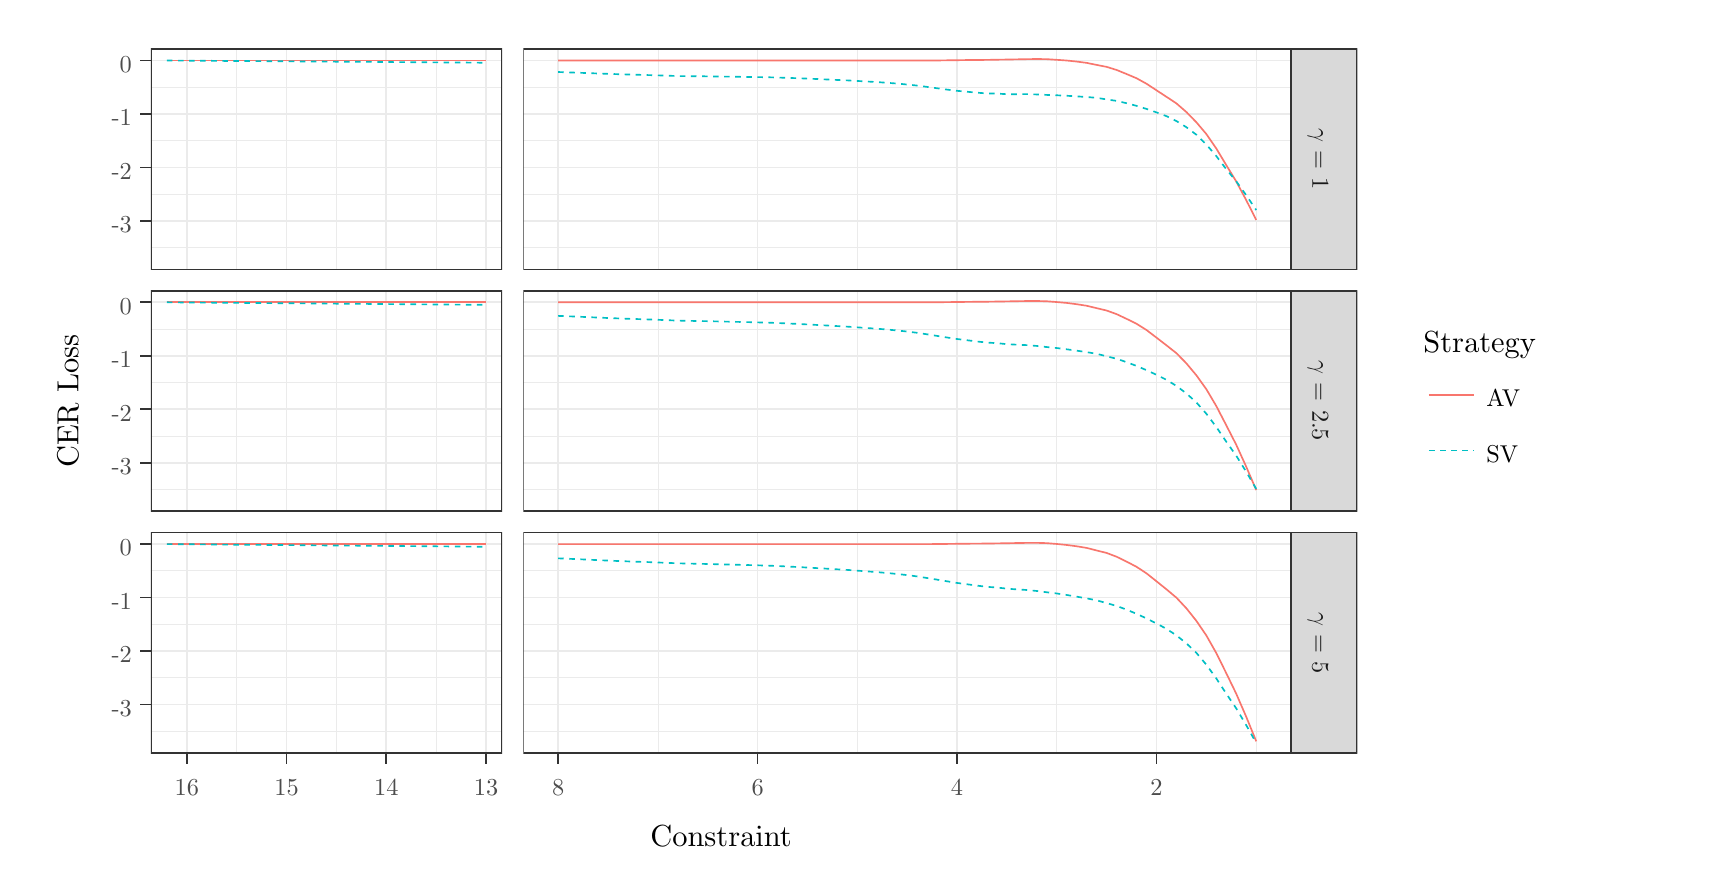
\begin{tikzpicture}[x=1.4pt,y=1.4pt]
\definecolor{fillColor}{RGB}{255,255,255}
\path[use as bounding box,fill=fillColor,fill opacity=0.00] (0,0) rectangle (426.79,216.81);
\begin{scope}
\path[clip] (  0.00,  0.00) rectangle (426.79,216.81);
\definecolor{drawColor}{RGB}{255,255,255}
\definecolor{fillColor}{RGB}{255,255,255}

\path[draw=drawColor,line width= 0.6pt,line join=round,line cap=round,fill=fillColor] (  0.00,  0.00) rectangle (426.79,216.81);
\end{scope}
\begin{scope}
\path[clip] ( 31.83,154.40) rectangle (122.43,211.31);
\definecolor{fillColor}{RGB}{255,255,255}

\path[fill=fillColor] ( 31.83,154.40) rectangle (122.43,211.31);
\definecolor{drawColor}{gray}{0.92}

\path[draw=drawColor,line width= 0.3pt,line join=round] ( 31.83,160.00) --
	(122.43,160.00);

\path[draw=drawColor,line width= 0.3pt,line join=round] ( 31.83,173.80) --
	(122.43,173.80);

\path[draw=drawColor,line width= 0.3pt,line join=round] ( 31.83,187.61) --
	(122.43,187.61);

\path[draw=drawColor,line width= 0.3pt,line join=round] ( 31.83,201.42) --
	(122.43,201.42);

\path[draw=drawColor,line width= 0.3pt,line join=round] (105.44,154.40) --
	(105.44,211.31);

\path[draw=drawColor,line width= 0.3pt,line join=round] ( 79.70,154.40) --
	( 79.70,211.31);

\path[draw=drawColor,line width= 0.3pt,line join=round] ( 53.96,154.40) --
	( 53.96,211.31);

\path[draw=drawColor,line width= 0.6pt,line join=round] ( 31.83,166.90) --
	(122.43,166.90);

\path[draw=drawColor,line width= 0.6pt,line join=round] ( 31.83,180.71) --
	(122.43,180.71);

\path[draw=drawColor,line width= 0.6pt,line join=round] ( 31.83,194.52) --
	(122.43,194.52);

\path[draw=drawColor,line width= 0.6pt,line join=round] ( 31.83,208.32) --
	(122.43,208.32);

\path[draw=drawColor,line width= 0.6pt,line join=round] (118.31,154.40) --
	(118.31,211.31);

\path[draw=drawColor,line width= 0.6pt,line join=round] ( 92.57,154.40) --
	( 92.57,211.31);

\path[draw=drawColor,line width= 0.6pt,line join=round] ( 66.83,154.40) --
	( 66.83,211.31);

\path[draw=drawColor,line width= 0.6pt,line join=round] ( 41.10,154.40) --
	( 41.10,211.31);
\definecolor{drawColor}{RGB}{248,118,109}

\path[draw=drawColor,line width= 0.6pt,line join=round] ( 35.95,208.32) --
	( 38.52,208.32) --
	( 41.10,208.32) --
	( 43.67,208.32) --
	( 46.24,208.32) --
	( 48.82,208.32) --
	( 51.39,208.32) --
	( 53.96,208.32) --
	( 56.54,208.32) --
	( 59.11,208.32) --
	( 61.69,208.32) --
	( 64.26,208.32) --
	( 66.83,208.32) --
	( 69.41,208.32) --
	( 71.98,208.32) --
	( 74.55,208.32) --
	( 77.13,208.32) --
	( 79.70,208.32) --
	( 82.28,208.32) --
	( 84.85,208.32) --
	( 87.42,208.32) --
	( 90.00,208.32) --
	( 92.57,208.32) --
	( 95.14,208.32) --
	( 97.72,208.32) --
	(100.29,208.32) --
	(102.87,208.32) --
	(105.44,208.32) --
	(108.01,208.32) --
	(110.59,208.32) --
	(113.16,208.32) --
	(115.73,208.32) --
	(118.31,208.32);
\definecolor{drawColor}{RGB}{0,191,196}

\path[draw=drawColor,line width= 0.6pt,dash pattern=on 2pt off 2pt ,line join=round] ( 35.95,208.32) --
	( 38.52,208.31) --
	( 41.10,208.29) --
	( 43.67,208.27) --
	( 46.24,208.26) --
	( 48.82,208.24) --
	( 51.39,208.22) --
	( 53.96,208.21) --
	( 56.54,208.19) --
	( 59.11,208.17) --
	( 61.69,208.15) --
	( 64.26,208.14) --
	( 66.83,208.12) --
	( 69.41,208.10) --
	( 71.98,208.08) --
	( 74.55,208.07) --
	( 77.13,208.05) --
	( 79.70,208.03) --
	( 82.28,208.01) --
	( 84.85,208.00) --
	( 87.42,207.98) --
	( 90.00,207.96) --
	( 92.57,207.94) --
	( 95.14,207.92) --
	( 97.72,207.91) --
	(100.29,207.89) --
	(102.87,207.87) --
	(105.44,207.85) --
	(108.01,207.83) --
	(110.59,207.82) --
	(113.16,207.80) --
	(115.73,207.78) --
	(118.31,207.76);
\definecolor{drawColor}{gray}{0.20}

\path[draw=drawColor,line width= 0.6pt,line join=round,line cap=round] ( 31.83,154.40) rectangle (122.43,211.31);
\end{scope}
\begin{scope}
\path[clip] ( 31.83, 91.99) rectangle (122.43,148.90);
\definecolor{fillColor}{RGB}{255,255,255}

\path[fill=fillColor] ( 31.83, 91.99) rectangle (122.43,148.90);
\definecolor{drawColor}{gray}{0.92}

\path[draw=drawColor,line width= 0.3pt,line join=round] ( 31.83, 97.59) --
	(122.43, 97.59);

\path[draw=drawColor,line width= 0.3pt,line join=round] ( 31.83,111.40) --
	(122.43,111.40);

\path[draw=drawColor,line width= 0.3pt,line join=round] ( 31.83,125.20) --
	(122.43,125.20);

\path[draw=drawColor,line width= 0.3pt,line join=round] ( 31.83,139.01) --
	(122.43,139.01);

\path[draw=drawColor,line width= 0.3pt,line join=round] (105.44, 91.99) --
	(105.44,148.90);

\path[draw=drawColor,line width= 0.3pt,line join=round] ( 79.70, 91.99) --
	( 79.70,148.90);

\path[draw=drawColor,line width= 0.3pt,line join=round] ( 53.96, 91.99) --
	( 53.96,148.90);

\path[draw=drawColor,line width= 0.6pt,line join=round] ( 31.83,104.49) --
	(122.43,104.49);

\path[draw=drawColor,line width= 0.6pt,line join=round] ( 31.83,118.30) --
	(122.43,118.30);

\path[draw=drawColor,line width= 0.6pt,line join=round] ( 31.83,132.11) --
	(122.43,132.11);

\path[draw=drawColor,line width= 0.6pt,line join=round] ( 31.83,145.92) --
	(122.43,145.92);

\path[draw=drawColor,line width= 0.6pt,line join=round] (118.31, 91.99) --
	(118.31,148.90);

\path[draw=drawColor,line width= 0.6pt,line join=round] ( 92.57, 91.99) --
	( 92.57,148.90);

\path[draw=drawColor,line width= 0.6pt,line join=round] ( 66.83, 91.99) --
	( 66.83,148.90);

\path[draw=drawColor,line width= 0.6pt,line join=round] ( 41.10, 91.99) --
	( 41.10,148.90);
\definecolor{drawColor}{RGB}{248,118,109}

\path[draw=drawColor,line width= 0.6pt,line join=round] ( 35.95,145.92) --
	( 38.52,145.92) --
	( 41.10,145.92) --
	( 43.67,145.92) --
	( 46.24,145.92) --
	( 48.82,145.92) --
	( 51.39,145.92) --
	( 53.96,145.92) --
	( 56.54,145.92) --
	( 59.11,145.92) --
	( 61.69,145.92) --
	( 64.26,145.92) --
	( 66.83,145.92) --
	( 69.41,145.92) --
	( 71.98,145.92) --
	( 74.55,145.92) --
	( 77.13,145.92) --
	( 79.70,145.92) --
	( 82.28,145.92) --
	( 84.85,145.92) --
	( 87.42,145.92) --
	( 90.00,145.92) --
	( 92.57,145.92) --
	( 95.14,145.92) --
	( 97.72,145.92) --
	(100.29,145.92) --
	(102.87,145.92) --
	(105.44,145.92) --
	(108.01,145.92) --
	(110.59,145.92) --
	(113.16,145.92) --
	(115.73,145.92) --
	(118.31,145.92);
\definecolor{drawColor}{RGB}{0,191,196}

\path[draw=drawColor,line width= 0.6pt,dash pattern=on 2pt off 2pt ,line join=round] ( 35.95,145.92) --
	( 38.52,145.90) --
	( 41.10,145.88) --
	( 43.67,145.86) --
	( 46.24,145.84) --
	( 48.82,145.82) --
	( 51.39,145.80) --
	( 53.96,145.78) --
	( 56.54,145.76) --
	( 59.11,145.74) --
	( 61.69,145.72) --
	( 64.26,145.70) --
	( 66.83,145.68) --
	( 69.41,145.66) --
	( 71.98,145.64) --
	( 74.55,145.62) --
	( 77.13,145.59) --
	( 79.70,145.57) --
	( 82.28,145.55) --
	( 84.85,145.53) --
	( 87.42,145.51) --
	( 90.00,145.49) --
	( 92.57,145.47) --
	( 95.14,145.45) --
	( 97.72,145.43) --
	(100.29,145.41) --
	(102.87,145.39) --
	(105.44,145.37) --
	(108.01,145.35) --
	(110.59,145.33) --
	(113.16,145.31) --
	(115.73,145.29) --
	(118.31,145.27);
\definecolor{drawColor}{gray}{0.20}

\path[draw=drawColor,line width= 0.6pt,line join=round,line cap=round] ( 31.83, 91.99) rectangle (122.43,148.90);
\end{scope}
\begin{scope}
\path[clip] ( 31.83, 29.59) rectangle (122.43, 86.49);
\definecolor{fillColor}{RGB}{255,255,255}

\path[fill=fillColor] ( 31.83, 29.59) rectangle (122.43, 86.49);
\definecolor{drawColor}{gray}{0.92}

\path[draw=drawColor,line width= 0.3pt,line join=round] ( 31.83, 35.18) --
	(122.43, 35.18);

\path[draw=drawColor,line width= 0.3pt,line join=round] ( 31.83, 48.99) --
	(122.43, 48.99);

\path[draw=drawColor,line width= 0.3pt,line join=round] ( 31.83, 62.80) --
	(122.43, 62.80);

\path[draw=drawColor,line width= 0.3pt,line join=round] ( 31.83, 76.60) --
	(122.43, 76.60);

\path[draw=drawColor,line width= 0.3pt,line join=round] (105.44, 29.59) --
	(105.44, 86.49);

\path[draw=drawColor,line width= 0.3pt,line join=round] ( 79.70, 29.59) --
	( 79.70, 86.49);

\path[draw=drawColor,line width= 0.3pt,line join=round] ( 53.96, 29.59) --
	( 53.96, 86.49);

\path[draw=drawColor,line width= 0.6pt,line join=round] ( 31.83, 42.08) --
	(122.43, 42.08);

\path[draw=drawColor,line width= 0.6pt,line join=round] ( 31.83, 55.89) --
	(122.43, 55.89);

\path[draw=drawColor,line width= 0.6pt,line join=round] ( 31.83, 69.70) --
	(122.43, 69.70);

\path[draw=drawColor,line width= 0.6pt,line join=round] ( 31.83, 83.51) --
	(122.43, 83.51);

\path[draw=drawColor,line width= 0.6pt,line join=round] (118.31, 29.59) --
	(118.31, 86.49);

\path[draw=drawColor,line width= 0.6pt,line join=round] ( 92.57, 29.59) --
	( 92.57, 86.49);

\path[draw=drawColor,line width= 0.6pt,line join=round] ( 66.83, 29.59) --
	( 66.83, 86.49);

\path[draw=drawColor,line width= 0.6pt,line join=round] ( 41.10, 29.59) --
	( 41.10, 86.49);
\definecolor{drawColor}{RGB}{248,118,109}

\path[draw=drawColor,line width= 0.6pt,line join=round] ( 35.95, 83.51) --
	( 35.95, 83.51) --
	( 35.95, 83.51) --
	( 38.52, 83.51) --
	( 38.52, 83.51) --
	( 38.52, 83.51) --
	( 41.10, 83.51) --
	( 41.10, 83.51) --
	( 41.10, 83.51) --
	( 43.67, 83.51) --
	( 43.67, 83.51) --
	( 43.67, 83.51) --
	( 46.24, 83.51) --
	( 46.24, 83.51) --
	( 46.24, 83.51) --
	( 48.82, 83.51) --
	( 48.82, 83.51) --
	( 48.82, 83.51) --
	( 51.39, 83.51) --
	( 51.39, 83.51) --
	( 51.39, 83.51) --
	( 53.96, 83.51) --
	( 53.96, 83.51) --
	( 53.96, 83.51) --
	( 56.54, 83.51) --
	( 56.54, 83.51) --
	( 56.54, 83.51) --
	( 59.11, 83.51) --
	( 59.11, 83.51) --
	( 59.11, 83.51) --
	( 61.69, 83.51) --
	( 61.69, 83.51) --
	( 61.69, 83.51) --
	( 64.26, 83.51) --
	( 64.26, 83.51) --
	( 64.26, 83.51) --
	( 66.83, 83.51) --
	( 66.83, 83.51) --
	( 66.83, 83.51) --
	( 69.41, 83.51) --
	( 69.41, 83.51) --
	( 69.41, 83.51) --
	( 71.98, 83.51) --
	( 71.98, 83.51) --
	( 71.98, 83.51) --
	( 74.55, 83.51) --
	( 74.55, 83.51) --
	( 74.55, 83.51) --
	( 77.13, 83.51) --
	( 77.13, 83.51) --
	( 77.13, 83.51) --
	( 79.70, 83.51) --
	( 79.70, 83.51) --
	( 79.70, 83.51) --
	( 82.28, 83.51) --
	( 82.28, 83.51) --
	( 82.28, 83.51) --
	( 84.85, 83.51) --
	( 84.85, 83.51) --
	( 84.85, 83.51) --
	( 87.42, 83.51) --
	( 87.42, 83.51) --
	( 87.42, 83.51) --
	( 90.00, 83.51) --
	( 90.00, 83.51) --
	( 90.00, 83.51) --
	( 92.57, 83.51) --
	( 92.57, 83.51) --
	( 92.57, 83.51) --
	( 95.14, 83.51) --
	( 95.14, 83.51) --
	( 95.14, 83.51) --
	( 97.72, 83.51) --
	( 97.72, 83.51) --
	( 97.72, 83.51) --
	(100.29, 83.51) --
	(100.29, 83.51) --
	(100.29, 83.51) --
	(102.87, 83.51) --
	(102.87, 83.51) --
	(102.87, 83.51) --
	(105.44, 83.51) --
	(105.44, 83.51) --
	(105.44, 83.51) --
	(108.01, 83.51) --
	(108.01, 83.51) --
	(108.01, 83.51) --
	(110.59, 83.51) --
	(110.59, 83.51) --
	(110.59, 83.51) --
	(113.16, 83.51) --
	(113.16, 83.51) --
	(113.16, 83.51) --
	(115.73, 83.51) --
	(115.73, 83.51) --
	(115.73, 83.51) --
	(118.31, 83.51) --
	(118.31, 83.51) --
	(118.31, 83.51);
\definecolor{drawColor}{RGB}{0,191,196}

\path[draw=drawColor,line width= 0.6pt,dash pattern=on 2pt off 2pt ,line join=round] ( 35.95, 83.51) --
	( 38.52, 83.49) --
	( 41.10, 83.47) --
	( 43.67, 83.45) --
	( 46.24, 83.43) --
	( 48.82, 83.40) --
	( 51.39, 83.38) --
	( 53.96, 83.36) --
	( 56.54, 83.34) --
	( 59.11, 83.32) --
	( 61.69, 83.30) --
	( 64.26, 83.28) --
	( 66.83, 83.26) --
	( 69.41, 83.24) --
	( 71.98, 83.21) --
	( 74.55, 83.19) --
	( 77.13, 83.17) --
	( 79.70, 83.15) --
	( 82.28, 83.13) --
	( 84.85, 83.11) --
	( 87.42, 83.09) --
	( 90.00, 83.07) --
	( 92.57, 83.04) --
	( 95.14, 83.02) --
	( 97.72, 83.00) --
	(100.29, 82.98) --
	(102.87, 82.96) --
	(105.44, 82.94) --
	(108.01, 82.92) --
	(110.59, 82.90) --
	(113.16, 82.87) --
	(115.73, 82.85) --
	(118.31, 82.83);
\definecolor{drawColor}{gray}{0.20}

\path[draw=drawColor,line width= 0.6pt,line join=round,line cap=round] ( 31.83, 29.59) rectangle (122.43, 86.49);
\end{scope}
\begin{scope}
\path[clip] (127.93,154.40) rectangle (326.11,211.31);
\definecolor{fillColor}{RGB}{255,255,255}

\path[fill=fillColor] (127.93,154.40) rectangle (326.11,211.31);
\definecolor{drawColor}{gray}{0.92}

\path[draw=drawColor,line width= 0.3pt,line join=round] (127.93,160.00) --
	(326.11,160.00);

\path[draw=drawColor,line width= 0.3pt,line join=round] (127.93,173.80) --
	(326.11,173.80);

\path[draw=drawColor,line width= 0.3pt,line join=round] (127.93,187.61) --
	(326.11,187.61);

\path[draw=drawColor,line width= 0.3pt,line join=round] (127.93,201.42) --
	(326.11,201.42);

\path[draw=drawColor,line width= 0.3pt,line join=round] (317.10,154.40) --
	(317.10,211.31);

\path[draw=drawColor,line width= 0.3pt,line join=round] (265.62,154.40) --
	(265.62,211.31);

\path[draw=drawColor,line width= 0.3pt,line join=round] (214.15,154.40) --
	(214.15,211.31);

\path[draw=drawColor,line width= 0.3pt,line join=round] (162.67,154.40) --
	(162.67,211.31);

\path[draw=drawColor,line width= 0.6pt,line join=round] (127.93,166.90) --
	(326.11,166.90);

\path[draw=drawColor,line width= 0.6pt,line join=round] (127.93,180.71) --
	(326.11,180.71);

\path[draw=drawColor,line width= 0.6pt,line join=round] (127.93,194.52) --
	(326.11,194.52);

\path[draw=drawColor,line width= 0.6pt,line join=round] (127.93,208.32) --
	(326.11,208.32);

\path[draw=drawColor,line width= 0.6pt,line join=round] (291.36,154.40) --
	(291.36,211.31);

\path[draw=drawColor,line width= 0.6pt,line join=round] (239.88,154.40) --
	(239.88,211.31);

\path[draw=drawColor,line width= 0.6pt,line join=round] (188.41,154.40) --
	(188.41,211.31);

\path[draw=drawColor,line width= 0.6pt,line join=round] (136.93,154.40) --
	(136.93,211.31);
\definecolor{drawColor}{RGB}{248,118,109}

\path[draw=drawColor,line width= 0.6pt,line join=round] (136.93,208.32) --
	(139.51,208.32) --
	(142.08,208.32) --
	(144.66,208.32) --
	(147.23,208.32) --
	(149.80,208.32) --
	(152.38,208.32) --
	(154.95,208.32) --
	(157.52,208.32) --
	(160.10,208.32) --
	(162.67,208.32) --
	(165.25,208.32) --
	(167.82,208.32) --
	(170.39,208.32) --
	(172.97,208.32) --
	(175.54,208.32) --
	(178.11,208.32) --
	(180.69,208.32) --
	(183.26,208.32) --
	(185.84,208.32) --
	(188.41,208.32) --
	(190.98,208.32) --
	(193.56,208.32) --
	(196.13,208.32) --
	(198.70,208.32) --
	(201.28,208.32) --
	(203.85,208.32) --
	(206.43,208.32) --
	(209.00,208.32) --
	(211.57,208.32) --
	(214.15,208.32) --
	(216.72,208.32) --
	(219.29,208.32) --
	(221.87,208.32) --
	(224.44,208.32) --
	(227.02,208.32) --
	(229.59,208.32) --
	(232.16,208.32) --
	(234.74,208.34) --
	(237.31,208.38) --
	(239.88,208.41) --
	(242.46,208.45) --
	(245.03,208.47) --
	(247.61,208.49) --
	(250.18,208.54) --
	(252.75,208.58) --
	(255.33,208.63) --
	(257.90,208.68) --
	(260.47,208.72) --
	(263.05,208.68) --
	(265.62,208.51) --
	(268.20,208.33) --
	(270.77,208.06) --
	(273.34,207.72) --
	(275.92,207.19) --
	(278.49,206.69) --
	(281.06,205.89) --
	(283.64,204.84) --
	(286.21,203.75) --
	(288.79,202.33) --
	(291.36,200.64) --
	(293.93,198.96) --
	(296.51,197.25) --
	(299.08,195.02) --
	(301.65,192.39) --
	(304.23,189.34) --
	(306.80,185.60) --
	(309.38,181.31) --
	(311.95,177.09) --
	(314.52,172.28) --
	(317.10,167.19);
\definecolor{drawColor}{RGB}{0,191,196}

\path[draw=drawColor,line width= 0.6pt,dash pattern=on 2pt off 2pt ,line join=round] (136.93,205.36) --
	(139.51,205.27) --
	(142.08,205.18) --
	(144.66,205.08) --
	(147.23,204.98) --
	(149.80,204.89) --
	(152.38,204.80) --
	(154.95,204.72) --
	(157.52,204.65) --
	(160.10,204.57) --
	(162.67,204.50) --
	(165.25,204.41) --
	(167.82,204.32) --
	(170.39,204.28) --
	(172.97,204.27) --
	(175.54,204.24) --
	(178.11,204.20) --
	(180.69,204.17) --
	(183.26,204.13) --
	(185.84,204.09) --
	(188.41,204.05) --
	(190.98,204.01) --
	(193.56,203.94) --
	(196.13,203.85) --
	(198.70,203.76) --
	(201.28,203.66) --
	(203.85,203.55) --
	(206.43,203.43) --
	(209.00,203.31) --
	(211.57,203.20) --
	(214.15,203.05) --
	(216.72,202.91) --
	(219.29,202.76) --
	(221.87,202.58) --
	(224.44,202.38) --
	(227.02,202.13) --
	(229.59,201.86) --
	(232.16,201.52) --
	(234.74,201.17) --
	(237.31,200.82) --
	(239.88,200.51) --
	(242.46,200.27) --
	(245.03,200.03) --
	(247.61,199.83) --
	(250.18,199.79) --
	(252.75,199.64) --
	(255.33,199.63) --
	(257.90,199.66) --
	(260.47,199.57) --
	(263.05,199.45) --
	(265.62,199.36) --
	(268.20,199.23) --
	(270.77,199.08) --
	(273.34,198.91) --
	(275.92,198.70) --
	(278.49,198.29) --
	(281.06,197.91) --
	(283.64,197.31) --
	(286.21,196.63) --
	(288.79,195.83) --
	(291.36,194.94) --
	(293.93,193.97) --
	(296.51,192.70) --
	(299.08,191.11) --
	(301.65,189.18) --
	(304.23,186.65) --
	(306.80,183.65) --
	(309.38,180.27) --
	(311.95,177.14) --
	(314.52,173.54) --
	(317.10,169.73);
\definecolor{drawColor}{gray}{0.20}

\path[draw=drawColor,line width= 0.6pt,line join=round,line cap=round] (127.93,154.40) rectangle (326.11,211.31);
\end{scope}
\begin{scope}
\path[clip] (127.93, 91.99) rectangle (326.11,148.90);
\definecolor{fillColor}{RGB}{255,255,255}

\path[fill=fillColor] (127.93, 91.99) rectangle (326.11,148.90);
\definecolor{drawColor}{gray}{0.92}

\path[draw=drawColor,line width= 0.3pt,line join=round] (127.93, 97.59) --
	(326.11, 97.59);

\path[draw=drawColor,line width= 0.3pt,line join=round] (127.93,111.40) --
	(326.11,111.40);

\path[draw=drawColor,line width= 0.3pt,line join=round] (127.93,125.20) --
	(326.11,125.20);

\path[draw=drawColor,line width= 0.3pt,line join=round] (127.93,139.01) --
	(326.11,139.01);

\path[draw=drawColor,line width= 0.3pt,line join=round] (317.10, 91.99) --
	(317.10,148.90);

\path[draw=drawColor,line width= 0.3pt,line join=round] (265.62, 91.99) --
	(265.62,148.90);

\path[draw=drawColor,line width= 0.3pt,line join=round] (214.15, 91.99) --
	(214.15,148.90);

\path[draw=drawColor,line width= 0.3pt,line join=round] (162.67, 91.99) --
	(162.67,148.90);

\path[draw=drawColor,line width= 0.6pt,line join=round] (127.93,104.49) --
	(326.11,104.49);

\path[draw=drawColor,line width= 0.6pt,line join=round] (127.93,118.30) --
	(326.11,118.30);

\path[draw=drawColor,line width= 0.6pt,line join=round] (127.93,132.11) --
	(326.11,132.11);

\path[draw=drawColor,line width= 0.6pt,line join=round] (127.93,145.92) --
	(326.11,145.92);

\path[draw=drawColor,line width= 0.6pt,line join=round] (291.36, 91.99) --
	(291.36,148.90);

\path[draw=drawColor,line width= 0.6pt,line join=round] (239.88, 91.99) --
	(239.88,148.90);

\path[draw=drawColor,line width= 0.6pt,line join=round] (188.41, 91.99) --
	(188.41,148.90);

\path[draw=drawColor,line width= 0.6pt,line join=round] (136.93, 91.99) --
	(136.93,148.90);
\definecolor{drawColor}{RGB}{248,118,109}

\path[draw=drawColor,line width= 0.6pt,line join=round] (136.93,145.92) --
	(139.51,145.92) --
	(142.08,145.92) --
	(144.66,145.92) --
	(147.23,145.92) --
	(149.80,145.92) --
	(152.38,145.92) --
	(154.95,145.92) --
	(157.52,145.92) --
	(160.10,145.92) --
	(162.67,145.92) --
	(165.25,145.92) --
	(167.82,145.92) --
	(170.39,145.92) --
	(172.97,145.92) --
	(175.54,145.92) --
	(178.11,145.92) --
	(180.69,145.92) --
	(183.26,145.92) --
	(185.84,145.92) --
	(188.41,145.92) --
	(190.98,145.92) --
	(193.56,145.92) --
	(196.13,145.92) --
	(198.70,145.92) --
	(201.28,145.92) --
	(203.85,145.92) --
	(206.43,145.92) --
	(209.00,145.92) --
	(211.57,145.92) --
	(214.15,145.92) --
	(216.72,145.92) --
	(219.29,145.92) --
	(221.87,145.92) --
	(224.44,145.92) --
	(227.02,145.92) --
	(229.59,145.92) --
	(232.16,145.92) --
	(234.74,145.93) --
	(237.31,145.97) --
	(239.88,146.00) --
	(242.46,146.03) --
	(245.03,146.06) --
	(247.61,146.08) --
	(250.18,146.12) --
	(252.75,146.16) --
	(255.33,146.21) --
	(257.90,146.25) --
	(260.47,146.26) --
	(263.05,146.19) --
	(265.62,145.99) --
	(268.20,145.76) --
	(270.77,145.43) --
	(273.34,145.03) --
	(275.92,144.41) --
	(278.49,143.80) --
	(281.06,142.87) --
	(283.64,141.65) --
	(286.21,140.38) --
	(288.79,138.76) --
	(291.36,136.80) --
	(293.93,134.82) --
	(296.51,132.78) --
	(299.08,130.16) --
	(301.65,127.08) --
	(304.23,123.48) --
	(306.80,119.13) --
	(309.38,114.15) --
	(311.95,109.13) --
	(314.52,103.47) --
	(317.10, 97.46);
\definecolor{drawColor}{RGB}{0,191,196}

\path[draw=drawColor,line width= 0.6pt,dash pattern=on 2pt off 2pt ,line join=round] (136.93,142.42) --
	(139.51,142.32) --
	(142.08,142.21) --
	(144.66,142.10) --
	(147.23,141.98) --
	(149.80,141.87) --
	(152.38,141.77) --
	(154.95,141.67) --
	(157.52,141.59) --
	(160.10,141.50) --
	(162.67,141.41) --
	(165.25,141.30) --
	(167.82,141.20) --
	(170.39,141.14) --
	(172.97,141.10) --
	(175.54,141.05) --
	(178.11,140.99) --
	(180.69,140.93) --
	(183.26,140.87) --
	(185.84,140.81) --
	(188.41,140.74) --
	(190.98,140.68) --
	(193.56,140.58) --
	(196.13,140.46) --
	(198.70,140.35) --
	(201.28,140.21) --
	(203.85,140.07) --
	(206.43,139.93) --
	(209.00,139.78) --
	(211.57,139.64) --
	(214.15,139.46) --
	(216.72,139.28) --
	(219.29,139.10) --
	(221.87,138.89) --
	(224.44,138.65) --
	(227.02,138.37) --
	(229.59,138.05) --
	(232.16,137.66) --
	(234.74,137.25) --
	(237.31,136.84) --
	(239.88,136.45) --
	(242.46,136.13) --
	(245.03,135.81) --
	(247.61,135.53) --
	(250.18,135.38) --
	(252.75,135.12) --
	(255.33,134.98) --
	(257.90,134.87) --
	(260.47,134.66) --
	(263.05,134.37) --
	(265.62,134.12) --
	(268.20,133.79) --
	(270.77,133.44) --
	(273.34,133.06) --
	(275.92,132.63) --
	(278.49,131.99) --
	(281.06,131.35) --
	(283.64,130.47) --
	(286.21,129.50) --
	(288.79,128.40) --
	(291.36,127.21) --
	(293.93,125.92) --
	(296.51,124.33) --
	(299.08,122.40) --
	(301.65,120.08) --
	(304.23,117.15) --
	(306.80,113.73) --
	(309.38,109.93) --
	(311.95,106.31) --
	(314.52,102.17) --
	(317.10, 97.77);
\definecolor{drawColor}{gray}{0.20}

\path[draw=drawColor,line width= 0.6pt,line join=round,line cap=round] (127.93, 91.99) rectangle (326.11,148.90);
\end{scope}
\begin{scope}
\path[clip] (127.93, 29.59) rectangle (326.11, 86.49);
\definecolor{fillColor}{RGB}{255,255,255}

\path[fill=fillColor] (127.93, 29.59) rectangle (326.11, 86.49);
\definecolor{drawColor}{gray}{0.92}

\path[draw=drawColor,line width= 0.3pt,line join=round] (127.93, 35.18) --
	(326.11, 35.18);

\path[draw=drawColor,line width= 0.3pt,line join=round] (127.93, 48.99) --
	(326.11, 48.99);

\path[draw=drawColor,line width= 0.3pt,line join=round] (127.93, 62.80) --
	(326.11, 62.80);

\path[draw=drawColor,line width= 0.3pt,line join=round] (127.93, 76.60) --
	(326.11, 76.60);

\path[draw=drawColor,line width= 0.3pt,line join=round] (317.10, 29.59) --
	(317.10, 86.49);

\path[draw=drawColor,line width= 0.3pt,line join=round] (265.62, 29.59) --
	(265.62, 86.49);

\path[draw=drawColor,line width= 0.3pt,line join=round] (214.15, 29.59) --
	(214.15, 86.49);

\path[draw=drawColor,line width= 0.3pt,line join=round] (162.67, 29.59) --
	(162.67, 86.49);

\path[draw=drawColor,line width= 0.6pt,line join=round] (127.93, 42.08) --
	(326.11, 42.08);

\path[draw=drawColor,line width= 0.6pt,line join=round] (127.93, 55.89) --
	(326.11, 55.89);

\path[draw=drawColor,line width= 0.6pt,line join=round] (127.93, 69.70) --
	(326.11, 69.70);

\path[draw=drawColor,line width= 0.6pt,line join=round] (127.93, 83.51) --
	(326.11, 83.51);

\path[draw=drawColor,line width= 0.6pt,line join=round] (291.36, 29.59) --
	(291.36, 86.49);

\path[draw=drawColor,line width= 0.6pt,line join=round] (239.88, 29.59) --
	(239.88, 86.49);

\path[draw=drawColor,line width= 0.6pt,line join=round] (188.41, 29.59) --
	(188.41, 86.49);

\path[draw=drawColor,line width= 0.6pt,line join=round] (136.93, 29.59) --
	(136.93, 86.49);
\definecolor{drawColor}{RGB}{248,118,109}

\path[draw=drawColor,line width= 0.6pt,line join=round] (136.93, 83.51) --
	(136.93, 83.51) --
	(136.93, 83.51) --
	(139.51, 83.51) --
	(139.51, 83.51) --
	(139.51, 83.51) --
	(142.08, 83.51) --
	(142.08, 83.51) --
	(142.08, 83.51) --
	(144.66, 83.51) --
	(144.66, 83.51) --
	(144.66, 83.51) --
	(147.23, 83.51) --
	(147.23, 83.51) --
	(147.23, 83.51) --
	(149.80, 83.51) --
	(149.80, 83.51) --
	(149.80, 83.51) --
	(152.38, 83.51) --
	(152.38, 83.51) --
	(152.38, 83.51) --
	(154.95, 83.51) --
	(154.95, 83.51) --
	(154.95, 83.51) --
	(157.52, 83.51) --
	(157.52, 83.51) --
	(157.52, 83.51) --
	(160.10, 83.51) --
	(160.10, 83.51) --
	(160.10, 83.51) --
	(162.67, 83.51) --
	(162.67, 83.51) --
	(162.67, 83.51) --
	(165.25, 83.51) --
	(165.25, 83.51) --
	(165.25, 83.51) --
	(167.82, 83.51) --
	(167.82, 83.51) --
	(167.82, 83.51) --
	(170.39, 83.51) --
	(170.39, 83.51) --
	(170.39, 83.51) --
	(172.97, 83.51) --
	(172.97, 83.51) --
	(172.97, 83.51) --
	(175.54, 83.51) --
	(175.54, 83.51) --
	(175.54, 83.51) --
	(178.11, 83.51) --
	(178.11, 83.51) --
	(178.11, 83.51) --
	(180.69, 83.51) --
	(180.69, 83.51) --
	(180.69, 83.51) --
	(183.26, 83.51) --
	(183.26, 83.51) --
	(183.26, 83.51) --
	(185.84, 83.51) --
	(185.84, 83.51) --
	(185.84, 83.51) --
	(188.41, 83.51) --
	(188.41, 83.51) --
	(188.41, 83.51) --
	(190.98, 83.51) --
	(190.98, 83.51) --
	(190.98, 83.51) --
	(193.56, 83.51) --
	(193.56, 83.51) --
	(193.56, 83.51) --
	(196.13, 83.51) --
	(196.13, 83.51) --
	(196.13, 83.51) --
	(198.70, 83.51) --
	(198.70, 83.51) --
	(198.70, 83.51) --
	(201.28, 83.51) --
	(201.28, 83.51) --
	(201.28, 83.51) --
	(203.85, 83.51) --
	(203.85, 83.51) --
	(203.85, 83.51) --
	(206.43, 83.51) --
	(206.43, 83.51) --
	(206.43, 83.51) --
	(209.00, 83.51) --
	(209.00, 83.51) --
	(209.00, 83.51) --
	(211.57, 83.51) --
	(211.57, 83.51) --
	(211.57, 83.51) --
	(214.15, 83.51) --
	(214.15, 83.51) --
	(214.15, 83.51) --
	(216.72, 83.51) --
	(216.72, 83.51) --
	(216.72, 83.51) --
	(219.29, 83.51) --
	(219.29, 83.51) --
	(219.29, 83.51) --
	(221.87, 83.51) --
	(221.87, 83.51) --
	(221.87, 83.51) --
	(224.44, 83.51) --
	(224.44, 83.51) --
	(224.44, 83.51) --
	(227.02, 83.51) --
	(227.02, 83.51) --
	(227.02, 83.51) --
	(229.59, 83.51) --
	(229.59, 83.51) --
	(229.59, 83.51) --
	(232.16, 83.51) --
	(232.16, 83.51) --
	(232.16, 83.51) --
	(234.74, 83.53) --
	(234.74, 83.53) --
	(234.74, 83.53) --
	(237.31, 83.56) --
	(237.31, 83.56) --
	(237.31, 83.56) --
	(239.88, 83.59) --
	(239.88, 83.59) --
	(239.88, 83.59) --
	(242.46, 83.62) --
	(242.46, 83.62) --
	(242.46, 83.62) --
	(245.03, 83.64) --
	(245.03, 83.64) --
	(245.03, 83.64) --
	(247.61, 83.66) --
	(247.61, 83.66) --
	(247.61, 83.66) --
	(250.18, 83.70) --
	(250.18, 83.70) --
	(250.18, 83.70) --
	(252.75, 83.74) --
	(252.75, 83.74) --
	(252.75, 83.74) --
	(255.33, 83.79) --
	(255.33, 83.79) --
	(255.33, 83.79) --
	(257.90, 83.83) --
	(257.90, 83.83) --
	(257.90, 83.83) --
	(260.47, 83.84) --
	(260.47, 83.84) --
	(260.47, 83.84) --
	(263.05, 83.76) --
	(263.05, 83.76) --
	(263.05, 83.76) --
	(265.62, 83.55) --
	(265.62, 83.55) --
	(265.62, 83.55) --
	(268.20, 83.29) --
	(268.20, 83.29) --
	(268.20, 83.29) --
	(270.77, 82.95) --
	(270.77, 82.95) --
	(270.77, 82.95) --
	(273.34, 82.53) --
	(273.34, 82.53) --
	(273.34, 82.53) --
	(275.92, 81.87) --
	(275.92, 81.87) --
	(275.92, 81.87) --
	(278.49, 81.23) --
	(278.49, 81.23) --
	(278.49, 81.23) --
	(281.06, 80.25) --
	(281.06, 80.25) --
	(281.06, 80.25) --
	(283.64, 78.99) --
	(283.64, 78.99) --
	(283.64, 78.99) --
	(286.21, 77.65) --
	(286.21, 77.65) --
	(286.21, 77.65) --
	(288.79, 75.96) --
	(288.79, 75.96) --
	(288.79, 75.96) --
	(291.36, 73.91) --
	(291.36, 73.91) --
	(291.36, 73.91) --
	(293.93, 71.84) --
	(293.93, 71.84) --
	(293.93, 71.84) --
	(296.51, 69.68) --
	(296.51, 69.68) --
	(296.51, 69.68) --
	(299.08, 66.93) --
	(299.08, 66.93) --
	(299.08, 66.93) --
	(301.65, 63.70) --
	(301.65, 63.70) --
	(301.65, 63.70) --
	(304.23, 59.92) --
	(304.23, 59.92) --
	(304.23, 59.92) --
	(306.80, 55.37) --
	(306.80, 55.37) --
	(306.80, 55.37) --
	(309.38, 50.16) --
	(309.38, 50.16) --
	(309.38, 50.16) --
	(311.95, 44.87) --
	(311.95, 44.87) --
	(311.95, 44.87) --
	(314.52, 38.93) --
	(314.52, 38.93) --
	(314.52, 38.93) --
	(317.10, 32.61) --
	(317.10, 32.61) --
	(317.10, 32.61);
\definecolor{drawColor}{RGB}{0,191,196}

\path[draw=drawColor,line width= 0.6pt,dash pattern=on 2pt off 2pt ,line join=round] (136.93, 79.84) --
	(139.51, 79.73) --
	(142.08, 79.62) --
	(144.66, 79.50) --
	(147.23, 79.37) --
	(149.80, 79.26) --
	(152.38, 79.15) --
	(154.95, 79.05) --
	(157.52, 78.96) --
	(160.10, 78.87) --
	(162.67, 78.77) --
	(165.25, 78.66) --
	(167.82, 78.56) --
	(170.39, 78.49) --
	(172.97, 78.44) --
	(175.54, 78.38) --
	(178.11, 78.31) --
	(180.69, 78.24) --
	(183.26, 78.18) --
	(185.84, 78.11) --
	(188.41, 78.04) --
	(190.98, 77.96) --
	(193.56, 77.86) --
	(196.13, 77.73) --
	(198.70, 77.60) --
	(201.28, 77.46) --
	(203.85, 77.31) --
	(206.43, 77.16) --
	(209.00, 77.00) --
	(211.57, 76.85) --
	(214.15, 76.66) --
	(216.72, 76.47) --
	(219.29, 76.28) --
	(221.87, 76.05) --
	(224.44, 75.80) --
	(227.02, 75.51) --
	(229.59, 75.17) --
	(232.16, 74.76) --
	(234.74, 74.34) --
	(237.31, 73.91) --
	(239.88, 73.49) --
	(242.46, 73.15) --
	(245.03, 72.80) --
	(247.61, 72.48) --
	(250.18, 72.31) --
	(252.75, 72.01) --
	(255.33, 71.82) --
	(257.90, 71.67) --
	(260.47, 71.41) --
	(263.05, 71.08) --
	(265.62, 70.77) --
	(268.20, 70.38) --
	(270.77, 69.95) --
	(273.34, 69.50) --
	(275.92, 69.00) --
	(278.49, 68.28) --
	(281.06, 67.56) --
	(283.64, 66.59) --
	(286.21, 65.52) --
	(288.79, 64.32) --
	(291.36, 63.03) --
	(293.93, 61.64) --
	(296.51, 59.94) --
	(299.08, 57.89) --
	(301.65, 55.45) --
	(304.23, 52.37) --
	(306.80, 48.83) --
	(309.38, 44.88) --
	(311.95, 41.09) --
	(314.52, 36.77) --
	(317.10, 32.17);
\definecolor{drawColor}{gray}{0.20}

\path[draw=drawColor,line width= 0.6pt,line join=round,line cap=round] (127.93, 29.59) rectangle (326.11, 86.49);
\end{scope}
\begin{scope}
\path[clip] (326.11,154.40) rectangle (343.17,211.31);
\definecolor{drawColor}{gray}{0.20}
\definecolor{fillColor}{gray}{0.85}

\path[draw=drawColor,line width= 0.6pt,line join=round,line cap=round,fill=fillColor] (326.11,154.40) rectangle (343.17,211.31);
\definecolor{drawColor}{gray}{0.10}

\node[text=drawColor,rotate=-90.00,anchor=base,inner sep=0pt, outer sep=0pt, scale=  0.88] at (331.61,182.86) {$\gamma$ = 1};
\end{scope}
\begin{scope}
\path[clip] (326.11, 91.99) rectangle (343.17,148.90);
\definecolor{drawColor}{gray}{0.20}
\definecolor{fillColor}{gray}{0.85}

\path[draw=drawColor,line width= 0.6pt,line join=round,line cap=round,fill=fillColor] (326.11, 91.99) rectangle (343.17,148.90);
\definecolor{drawColor}{gray}{0.10}

\node[text=drawColor,rotate=-90.00,anchor=base,inner sep=0pt, outer sep=0pt, scale=  0.88] at (331.61,120.45) {$\gamma$ = 2.5};
\end{scope}
\begin{scope}
\path[clip] (326.11, 29.59) rectangle (343.17, 86.49);
\definecolor{drawColor}{gray}{0.20}
\definecolor{fillColor}{gray}{0.85}

\path[draw=drawColor,line width= 0.6pt,line join=round,line cap=round,fill=fillColor] (326.11, 29.59) rectangle (343.17, 86.49);
\definecolor{drawColor}{gray}{0.10}

\node[text=drawColor,rotate=-90.00,anchor=base,inner sep=0pt, outer sep=0pt, scale=  0.88] at (331.61, 58.04) {$\gamma$ = 5};
\end{scope}
\begin{scope}
\path[clip] (  0.00,  0.00) rectangle (426.79,216.81);
\definecolor{drawColor}{gray}{0.20}

\path[draw=drawColor,line width= 0.6pt,line join=round] (118.31, 26.84) --
	(118.31, 29.59);

\path[draw=drawColor,line width= 0.6pt,line join=round] ( 92.57, 26.84) --
	( 92.57, 29.59);

\path[draw=drawColor,line width= 0.6pt,line join=round] ( 66.83, 26.84) --
	( 66.83, 29.59);

\path[draw=drawColor,line width= 0.6pt,line join=round] ( 41.10, 26.84) --
	( 41.10, 29.59);
\end{scope}
\begin{scope}
\path[clip] (  0.00,  0.00) rectangle (426.79,216.81);
\definecolor{drawColor}{gray}{0.30}

\node[text=drawColor,anchor=base,inner sep=0pt, outer sep=0pt, scale=  0.88] at (118.31, 18.58) {13};

\node[text=drawColor,anchor=base,inner sep=0pt, outer sep=0pt, scale=  0.88] at ( 92.57, 18.58) {14};

\node[text=drawColor,anchor=base,inner sep=0pt, outer sep=0pt, scale=  0.88] at ( 66.83, 18.58) {15};

\node[text=drawColor,anchor=base,inner sep=0pt, outer sep=0pt, scale=  0.88] at ( 41.10, 18.58) {16};
\end{scope}
\begin{scope}
\path[clip] (  0.00,  0.00) rectangle (426.79,216.81);
\definecolor{drawColor}{gray}{0.20}

\path[draw=drawColor,line width= 0.6pt,line join=round] (291.36, 26.84) --
	(291.36, 29.59);

\path[draw=drawColor,line width= 0.6pt,line join=round] (239.88, 26.84) --
	(239.88, 29.59);

\path[draw=drawColor,line width= 0.6pt,line join=round] (188.41, 26.84) --
	(188.41, 29.59);

\path[draw=drawColor,line width= 0.6pt,line join=round] (136.93, 26.84) --
	(136.93, 29.59);
\end{scope}
\begin{scope}
\path[clip] (  0.00,  0.00) rectangle (426.79,216.81);
\definecolor{drawColor}{gray}{0.30}

\node[text=drawColor,anchor=base,inner sep=0pt, outer sep=0pt, scale=  0.88] at (291.36, 18.58) {2};

\node[text=drawColor,anchor=base,inner sep=0pt, outer sep=0pt, scale=  0.88] at (239.88, 18.58) {4};

\node[text=drawColor,anchor=base,inner sep=0pt, outer sep=0pt, scale=  0.88] at (188.41, 18.58) {6};

\node[text=drawColor,anchor=base,inner sep=0pt, outer sep=0pt, scale=  0.88] at (136.93, 18.58) {8};
\end{scope}
\begin{scope}
\path[clip] (  0.00,  0.00) rectangle (426.79,216.81);
\definecolor{drawColor}{gray}{0.30}

\node[text=drawColor,anchor=base east,inner sep=0pt, outer sep=0pt, scale=  0.88] at ( 26.88,163.87) {-3};

\node[text=drawColor,anchor=base east,inner sep=0pt, outer sep=0pt, scale=  0.88] at ( 26.88,177.68) {-2};

\node[text=drawColor,anchor=base east,inner sep=0pt, outer sep=0pt, scale=  0.88] at ( 26.88,191.49) {-1};

\node[text=drawColor,anchor=base east,inner sep=0pt, outer sep=0pt, scale=  0.88] at ( 26.88,205.29) {0};
\end{scope}
\begin{scope}
\path[clip] (  0.00,  0.00) rectangle (426.79,216.81);
\definecolor{drawColor}{gray}{0.20}

\path[draw=drawColor,line width= 0.6pt,line join=round] ( 29.08,166.90) --
	( 31.83,166.90);

\path[draw=drawColor,line width= 0.6pt,line join=round] ( 29.08,180.71) --
	( 31.83,180.71);

\path[draw=drawColor,line width= 0.6pt,line join=round] ( 29.08,194.52) --
	( 31.83,194.52);

\path[draw=drawColor,line width= 0.6pt,line join=round] ( 29.08,208.32) --
	( 31.83,208.32);
\end{scope}
\begin{scope}
\path[clip] (  0.00,  0.00) rectangle (426.79,216.81);
\definecolor{drawColor}{gray}{0.30}

\node[text=drawColor,anchor=base east,inner sep=0pt, outer sep=0pt, scale=  0.88] at ( 26.88,101.46) {-3};

\node[text=drawColor,anchor=base east,inner sep=0pt, outer sep=0pt, scale=  0.88] at ( 26.88,115.27) {-2};

\node[text=drawColor,anchor=base east,inner sep=0pt, outer sep=0pt, scale=  0.88] at ( 26.88,129.08) {-1};

\node[text=drawColor,anchor=base east,inner sep=0pt, outer sep=0pt, scale=  0.88] at ( 26.88,142.89) {0};
\end{scope}
\begin{scope}
\path[clip] (  0.00,  0.00) rectangle (426.79,216.81);
\definecolor{drawColor}{gray}{0.20}

\path[draw=drawColor,line width= 0.6pt,line join=round] ( 29.08,104.49) --
	( 31.83,104.49);

\path[draw=drawColor,line width= 0.6pt,line join=round] ( 29.08,118.30) --
	( 31.83,118.30);

\path[draw=drawColor,line width= 0.6pt,line join=round] ( 29.08,132.11) --
	( 31.83,132.11);

\path[draw=drawColor,line width= 0.6pt,line join=round] ( 29.08,145.92) --
	( 31.83,145.92);
\end{scope}
\begin{scope}
\path[clip] (  0.00,  0.00) rectangle (426.79,216.81);
\definecolor{drawColor}{gray}{0.30}

\node[text=drawColor,anchor=base east,inner sep=0pt, outer sep=0pt, scale=  0.88] at ( 26.88, 39.05) {-3};

\node[text=drawColor,anchor=base east,inner sep=0pt, outer sep=0pt, scale=  0.88] at ( 26.88, 52.86) {-2};

\node[text=drawColor,anchor=base east,inner sep=0pt, outer sep=0pt, scale=  0.88] at ( 26.88, 66.67) {-1};

\node[text=drawColor,anchor=base east,inner sep=0pt, outer sep=0pt, scale=  0.88] at ( 26.88, 80.48) {0};
\end{scope}
\begin{scope}
\path[clip] (  0.00,  0.00) rectangle (426.79,216.81);
\definecolor{drawColor}{gray}{0.20}

\path[draw=drawColor,line width= 0.6pt,line join=round] ( 29.08, 42.08) --
	( 31.83, 42.08);

\path[draw=drawColor,line width= 0.6pt,line join=round] ( 29.08, 55.89) --
	( 31.83, 55.89);

\path[draw=drawColor,line width= 0.6pt,line join=round] ( 29.08, 69.70) --
	( 31.83, 69.70);

\path[draw=drawColor,line width= 0.6pt,line join=round] ( 29.08, 83.51) --
	( 31.83, 83.51);
\end{scope}
\begin{scope}
\path[clip] (  0.00,  0.00) rectangle (426.79,216.81);
\definecolor{drawColor}{RGB}{0,0,0}

\node[text=drawColor,anchor=base,inner sep=0pt, outer sep=0pt, scale=  1.10] at (178.97,  5.50) {Constraint};
\end{scope}
\begin{scope}
\path[clip] (  0.00,  0.00) rectangle (426.79,216.81);
\definecolor{drawColor}{RGB}{0,0,0}

\node[text=drawColor,rotate= 90.00,anchor=base,inner sep=0pt, outer sep=0pt, scale=  1.10] at ( 13.08,120.45) {CER Loss};
\end{scope}
\begin{scope}
\path[clip] (  0.00,  0.00) rectangle (426.79,216.81);
\definecolor{fillColor}{RGB}{255,255,255}

\path[fill=fillColor] (354.55, 94.71) rectangle (421.29,146.19);
\end{scope}
\begin{scope}
\path[clip] (  0.00,  0.00) rectangle (426.79,216.81);
\definecolor{drawColor}{RGB}{0,0,0}

\node[text=drawColor,anchor=base west,inner sep=0pt, outer sep=0pt, scale=  1.10] at (360.24,132.92) {Strategy};
\end{scope}
\begin{scope}
\path[clip] (  0.00,  0.00) rectangle (426.79,216.81);
\definecolor{fillColor}{RGB}{255,255,255}

\path[fill=fillColor] (360.24,114.85) rectangle (374.69,129.31);
\end{scope}
\begin{scope}
\path[clip] (  0.00,  0.00) rectangle (426.79,216.81);
\definecolor{drawColor}{RGB}{248,118,109}

\path[draw=drawColor,line width= 0.6pt,line join=round] (361.68,122.08) -- (373.25,122.08);
\end{scope}
\begin{scope}
\path[clip] (  0.00,  0.00) rectangle (426.79,216.81);
\definecolor{fillColor}{RGB}{255,255,255}

\path[fill=fillColor] (360.24,100.40) rectangle (374.69,114.85);
\end{scope}
\begin{scope}
\path[clip] (  0.00,  0.00) rectangle (426.79,216.81);
\definecolor{drawColor}{RGB}{0,191,196}

\path[draw=drawColor,line width= 0.6pt,dash pattern=on 2pt off 2pt ,line join=round] (361.68,107.63) -- (373.25,107.63);
\end{scope}
\begin{scope}
\path[clip] (  0.00,  0.00) rectangle (426.79,216.81);
\definecolor{drawColor}{RGB}{0,0,0}

\node[text=drawColor,anchor=base west,inner sep=0pt, outer sep=0pt, scale=  0.88] at (376.50,119.05) {AV};
\end{scope}
\begin{scope}
\path[clip] (  0.00,  0.00) rectangle (426.79,216.81);
\definecolor{drawColor}{RGB}{0,0,0}

\node[text=drawColor,anchor=base west,inner sep=0pt, outer sep=0pt, scale=  0.88] at (376.50,104.60) {SV};
\end{scope}
\end{tikzpicture}

		\end{adjustbox}
	\end{figure}
\clearpage
\begin{figure}[!htb]
		\caption{{\bf CER Gains}: Certainity Equivalent Return gains for mean variance investors with risk aversion coefficients ranging from 1 to 5 and subject to investment constraints ranging from 1 to 3. See section \ref{sec:asset_allocation} for details.} \label{fig:cer_gain}
%	\begin{subfigure}
%		% Created by tikzDevice version 0.10.1 on 2018-05-02 14:50:53
% !TEX encoding = UTF-8 Unicode
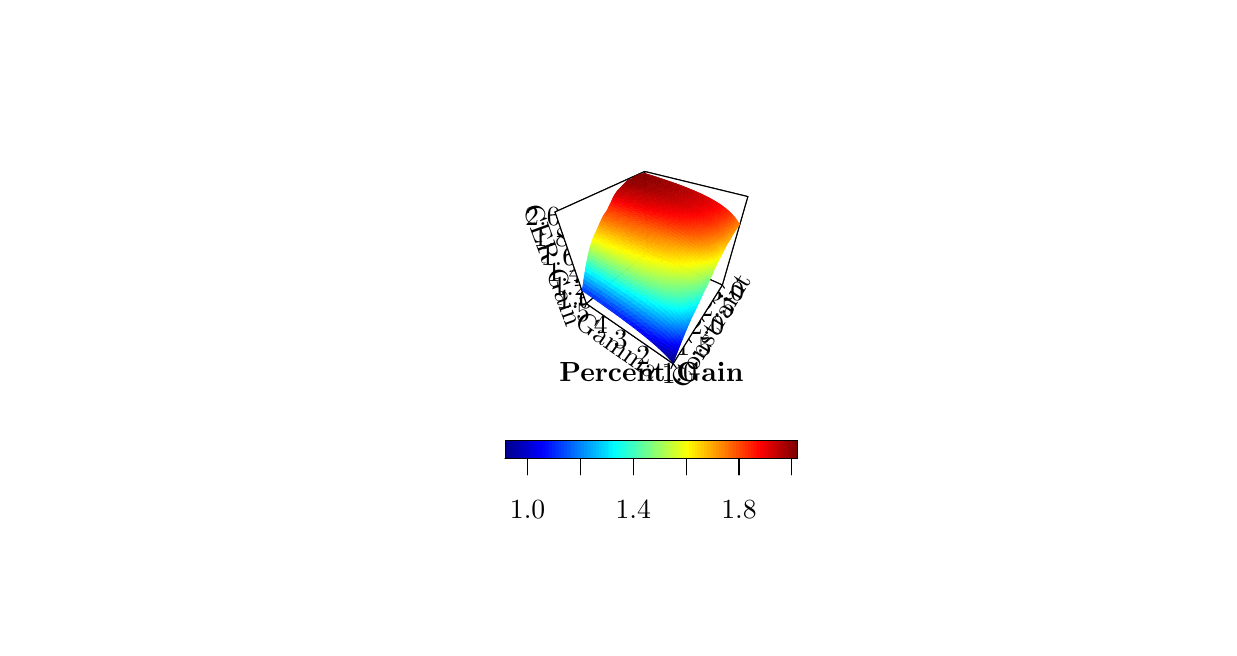
\begin{tikzpicture}[x=1pt,y=1pt]
\definecolor{fillColor}{RGB}{255,255,255}
\path[use as bounding box,fill=fillColor,fill opacity=0.00] (0,0) rectangle (426.79,216.81);
\begin{scope}
\path[clip] ( 49.20, 92.64) rectangle (401.59,167.61);
\definecolor{drawColor}{RGB}{0,0,0}

\path[draw=drawColor,line width= 0.4pt,line join=round,line cap=round] (201.91,117.08) -- (224.04,135.90);

\path[draw=drawColor,line width= 0.4pt,line join=round,line cap=round] (224.04,135.90) -- (222.97,164.83);

\path[draw=drawColor,line width= 0.4pt,line join=round,line cap=round] (222.97,164.83) -- (190.57,150.20);

\path[draw=drawColor,line width= 0.4pt,line join=round,line cap=round] (190.57,150.20) -- (201.91,117.08);

\path[draw=drawColor,line width= 0.4pt,line join=round,line cap=round] (251.01,123.81) -- (260.22,155.77);

\path[draw=drawColor,line width= 0.4pt,line join=round,line cap=round] (260.22,155.77) -- (222.97,164.83);

\path[draw=drawColor,line width= 0.4pt,line join=round,line cap=round] (224.04,135.90) -- (251.01,123.81);

\path[draw=drawColor,line width= 0.4pt,line join=round,line cap=round] (233.23, 95.41) -- (251.01,123.81);

\path[draw=drawColor,line width= 0.4pt,line join=round,line cap=round] (201.91,117.08) -- (233.23, 95.41);
\end{scope}
\begin{scope}
\path[clip] (  0.00,  0.00) rectangle (426.79,216.81);
\definecolor{drawColor}{RGB}{0,0,0}

\node[text=drawColor,rotate= 58.75,anchor=base,inner sep=0pt, outer sep=6pt, scale=  1.00] at (249.64,105.72) {Constraint};

\path[draw=drawColor,line width= 0.4pt,line join=round,line cap=round] (233.23, 95.41) -- (234.35, 93.98);

\node[text=drawColor,anchor=base,inner sep=0pt, outer sep=0pt, scale=  1.00] at (235.46, 89.11) {1.0};

\path[draw=drawColor,line width= 0.4pt,line join=round,line cap=round] (238.83,104.36) -- (239.83,103.02);

\node[text=drawColor,anchor=base,inner sep=0pt, outer sep=0pt, scale=  1.00] at (240.83, 98.24) {1.5};

\path[draw=drawColor,line width= 0.4pt,line join=round,line cap=round] (243.54,111.88) -- (244.45,110.62);

\node[text=drawColor,anchor=base,inner sep=0pt, outer sep=0pt, scale=  1.00] at (245.35,105.92) {2.0};

\path[draw=drawColor,line width= 0.4pt,line join=round,line cap=round] (247.55,118.28) -- (248.38,117.10);

\node[text=drawColor,anchor=base,inner sep=0pt, outer sep=0pt, scale=  1.00] at (249.20,112.48) {2.5};

\path[draw=drawColor,line width= 0.4pt,line join=round,line cap=round] (251.01,123.81) -- (251.77,122.69);

\node[text=drawColor,anchor=base,inner sep=0pt, outer sep=0pt, scale=  1.00] at (252.53,118.14) {3.0};

\node[text=drawColor,rotate=-35.29,anchor=base,inner sep=0pt, outer sep=6pt, scale=  1.00] at (211.28, 99.16) {Gamma};

\path[draw=drawColor,line width= 0.4pt,line join=round,line cap=round] (233.23, 95.41) -- (232.43, 93.62);

\node[text=drawColor,anchor=base,inner sep=0pt, outer sep=0pt, scale=  1.00] at (231.63, 88.38) {1};

\path[draw=drawColor,line width= 0.4pt,line join=round,line cap=round] (223.94,101.84) -- (223.19,100.16);

\node[text=drawColor,anchor=base,inner sep=0pt, outer sep=0pt, scale=  1.00] at (222.44, 95.03) {2};

\path[draw=drawColor,line width= 0.4pt,line join=round,line cap=round] (215.74,107.52) -- (215.03,105.93);

\node[text=drawColor,anchor=base,inner sep=0pt, outer sep=0pt, scale=  1.00] at (214.33,100.90) {3};

\path[draw=drawColor,line width= 0.4pt,line join=round,line cap=round] (208.44,112.57) -- (207.78,111.07);

\node[text=drawColor,anchor=base,inner sep=0pt, outer sep=0pt, scale=  1.00] at (207.12,106.12) {4};

\path[draw=drawColor,line width= 0.4pt,line join=round,line cap=round] (201.91,117.08) -- (201.29,115.66);

\node[text=drawColor,anchor=base,inner sep=0pt, outer sep=0pt, scale=  1.00] at (200.66,110.80) {5};

\node[text=drawColor,rotate=-69.94,anchor=base,inner sep=0pt, outer sep=6pt, scale=  1.00] at (186.77,129.87) {CER Gain};

\path[draw=drawColor,line width= 0.4pt,line join=round,line cap=round] (201.16,119.28) -- (199.50,119.06);

\node[text=drawColor,anchor=base,inner sep=0pt, outer sep=0pt, scale=  1.00] at (197.83,115.39) {1.0};

\path[draw=drawColor,line width= 0.4pt,line join=round,line cap=round] (199.60,123.85) -- (197.83,123.63);

\node[text=drawColor,anchor=base,inner sep=0pt, outer sep=0pt, scale=  1.00] at (196.06,119.96) {1.2};

\path[draw=drawColor,line width= 0.4pt,line join=round,line cap=round] (197.83,128.99) -- (195.95,128.78);

\node[text=drawColor,anchor=base,inner sep=0pt, outer sep=0pt, scale=  1.00] at (194.06,125.11) {1.4};

\path[draw=drawColor,line width= 0.4pt,line join=round,line cap=round] (195.83,134.84) -- (193.82,134.62);

\node[text=drawColor,anchor=base,inner sep=0pt, outer sep=0pt, scale=  1.00] at (191.79,130.96) {1.6};

\path[draw=drawColor,line width= 0.4pt,line join=round,line cap=round] (193.54,141.52) -- (191.37,141.32);

\node[text=drawColor,anchor=base,inner sep=0pt, outer sep=0pt, scale=  1.00] at (189.19,137.67) {1.8};

\path[draw=drawColor,line width= 0.4pt,line join=round,line cap=round] (190.89,149.25) -- (188.55,149.06);

\node[text=drawColor,anchor=base,inner sep=0pt, outer sep=0pt, scale=  1.00] at (186.18,145.42) {2.0};
\end{scope}
\begin{scope}
\path[clip] ( 49.20, 92.64) rectangle (401.59,167.61);

\path[] (233.23, 95.41) --
	(260.22,155.77) --
	(222.97,164.83) --
	(201.91,117.08) --
	(233.23, 95.41);
\definecolor{drawColor}{RGB}{0,0,0}

\path[draw=drawColor,line width= 0.4pt,dash pattern=on 1pt off 3pt ,line join=round,line cap=round] (233.23, 95.41) -- (236.86,129.15);

\path[draw=drawColor,line width= 0.4pt,dash pattern=on 1pt off 3pt ,line join=round,line cap=round] (236.86,129.15) -- (260.22,155.77);

\path[draw=drawColor,line width= 0.4pt,dash pattern=on 1pt off 3pt ,line join=round,line cap=round] (190.57,150.20) -- (236.86,129.15);
\definecolor{fillColor}{RGB}{255,255,255}

\path[fill=fillColor] (201.91,117.08) --
	(224.04,135.90) --
	(222.97,164.83) --
	(190.57,150.20) --
	(201.91,117.08) --
	cycle;

\path[draw=drawColor,line width= 0.4pt,line join=round,line cap=round] (201.91,117.08) --
	(224.04,135.90) --
	(222.97,164.83) --
	(190.57,150.20) --
	(201.91,117.08);

\path[fill=fillColor] (251.01,123.81) --
	(260.22,155.77) --
	(222.97,164.83) --
	(224.04,135.90) --
	(251.01,123.81) --
	cycle;

\path[draw=drawColor,line width= 0.4pt,line join=round,line cap=round] (251.01,123.81) --
	(260.22,155.77) --
	(222.97,164.83) --
	(224.04,135.90) --
	(251.01,123.81);

\path[fill=fillColor] (233.23, 95.41) --
	(251.01,123.81) --
	(224.04,135.90) --
	(201.91,117.08) --
	(233.23, 95.41) --
	cycle;

\path[draw=drawColor,line width= 0.4pt,line join=round,line cap=round] (233.23, 95.41) --
	(251.01,123.81) --
	(224.04,135.90) --
	(201.91,117.08) --
	(233.23, 95.41);
\definecolor{fillColor}{RGB}{148,0,0}

\path[fill=fillColor] (222.85,164.10) --
	(223.24,164.16) --
	(222.99,164.24) --
	(222.61,164.18) --
	cycle;

\path[fill=fillColor] (222.85,164.10) --
	(223.24,164.16) --
	(222.99,164.24) --
	(222.61,164.18) --
	cycle;

\path[fill=fillColor] (223.10,164.02) --
	(223.48,164.09) --
	(223.24,164.16) --
	(222.85,164.10) --
	cycle;

\path[fill=fillColor] (223.10,164.02) --
	(223.48,164.09) --
	(223.24,164.16) --
	(222.85,164.10) --
	cycle;

\path[fill=fillColor] (223.35,163.95) --
	(223.73,164.01) --
	(223.48,164.09) --
	(223.10,164.02) --
	cycle;

\path[fill=fillColor] (223.35,163.95) --
	(223.73,164.01) --
	(223.48,164.09) --
	(223.10,164.02) --
	cycle;

\path[fill=fillColor] (222.47,164.03) --
	(222.85,164.10) --
	(222.61,164.18) --
	(222.22,164.11) --
	cycle;

\path[fill=fillColor] (222.47,164.03) --
	(222.85,164.10) --
	(222.61,164.18) --
	(222.22,164.11) --
	cycle;

\path[fill=fillColor] (223.60,163.87) --
	(223.97,163.94) --
	(223.73,164.01) --
	(223.35,163.95) --
	cycle;

\path[fill=fillColor] (223.60,163.87) --
	(223.97,163.94) --
	(223.73,164.01) --
	(223.35,163.95) --
	cycle;

\path[fill=fillColor] (222.72,163.96) --
	(223.10,164.02) --
	(222.85,164.10) --
	(222.47,164.03) --
	cycle;

\path[fill=fillColor] (222.72,163.96) --
	(223.10,164.02) --
	(222.85,164.10) --
	(222.47,164.03) --
	cycle;

\path[fill=fillColor] (223.84,163.79) --
	(224.22,163.86) --
	(223.97,163.94) --
	(223.60,163.87) --
	cycle;

\path[fill=fillColor] (223.84,163.79) --
	(224.22,163.86) --
	(223.97,163.94) --
	(223.60,163.87) --
	cycle;

\path[fill=fillColor] (222.96,163.88) --
	(223.35,163.95) --
	(223.10,164.02) --
	(222.72,163.96) --
	cycle;

\path[fill=fillColor] (222.96,163.88) --
	(223.35,163.95) --
	(223.10,164.02) --
	(222.72,163.96) --
	cycle;

\path[fill=fillColor] (224.09,163.71) --
	(224.47,163.78) --
	(224.22,163.86) --
	(223.84,163.79) --
	cycle;

\path[fill=fillColor] (224.09,163.71) --
	(224.47,163.78) --
	(224.22,163.86) --
	(223.84,163.79) --
	cycle;
\definecolor{fillColor}{RGB}{138,0,0}

\path[fill=fillColor] (222.08,163.97) --
	(222.47,164.03) --
	(222.22,164.11) --
	(221.83,164.05) --
	cycle;

\path[fill=fillColor] (222.08,163.97) --
	(222.47,164.03) --
	(222.22,164.11) --
	(221.83,164.05) --
	cycle;
\definecolor{fillColor}{RGB}{148,0,0}

\path[fill=fillColor] (223.21,163.80) --
	(223.60,163.87) --
	(223.35,163.95) --
	(222.96,163.88) --
	cycle;

\path[fill=fillColor] (223.21,163.80) --
	(223.60,163.87) --
	(223.35,163.95) --
	(222.96,163.88) --
	cycle;

\path[fill=fillColor] (224.34,163.63) --
	(224.72,163.70) --
	(224.47,163.78) --
	(224.09,163.71) --
	cycle;

\path[fill=fillColor] (224.34,163.63) --
	(224.72,163.70) --
	(224.47,163.78) --
	(224.09,163.71) --
	cycle;
\definecolor{fillColor}{RGB}{138,0,0}

\path[fill=fillColor] (222.33,163.89) --
	(222.72,163.96) --
	(222.47,164.03) --
	(222.08,163.97) --
	cycle;

\path[fill=fillColor] (222.33,163.89) --
	(222.72,163.96) --
	(222.47,164.03) --
	(222.08,163.97) --
	cycle;
\definecolor{fillColor}{RGB}{148,0,0}

\path[fill=fillColor] (223.46,163.72) --
	(223.84,163.79) --
	(223.60,163.87) --
	(223.21,163.80) --
	cycle;

\path[fill=fillColor] (223.46,163.72) --
	(223.84,163.79) --
	(223.60,163.87) --
	(223.21,163.80) --
	cycle;

\path[fill=fillColor] (224.60,163.55) --
	(224.97,163.62) --
	(224.72,163.70) --
	(224.34,163.63) --
	cycle;

\path[fill=fillColor] (224.60,163.55) --
	(224.97,163.62) --
	(224.72,163.70) --
	(224.34,163.63) --
	cycle;
\definecolor{fillColor}{RGB}{138,0,0}

\path[fill=fillColor] (222.58,163.81) --
	(222.96,163.88) --
	(222.72,163.96) --
	(222.33,163.89) --
	cycle;

\path[fill=fillColor] (222.58,163.81) --
	(222.96,163.88) --
	(222.72,163.96) --
	(222.33,163.89) --
	cycle;
\definecolor{fillColor}{RGB}{148,0,0}

\path[fill=fillColor] (223.71,163.64) --
	(224.09,163.71) --
	(223.84,163.79) --
	(223.46,163.72) --
	cycle;

\path[fill=fillColor] (223.71,163.64) --
	(224.09,163.71) --
	(223.84,163.79) --
	(223.46,163.72) --
	cycle;

\path[fill=fillColor] (224.85,163.48) --
	(225.22,163.55) --
	(224.97,163.62) --
	(224.60,163.55) --
	cycle;

\path[fill=fillColor] (224.85,163.48) --
	(225.22,163.55) --
	(224.97,163.62) --
	(224.60,163.55) --
	cycle;
\definecolor{fillColor}{RGB}{138,0,0}

\path[fill=fillColor] (221.69,163.86) --
	(222.08,163.97) --
	(221.83,164.05) --
	(221.44,163.94) --
	cycle;

\path[fill=fillColor] (221.69,163.86) --
	(222.08,163.97) --
	(221.83,164.05) --
	(221.44,163.94) --
	cycle;

\path[fill=fillColor] (222.83,163.73) --
	(223.21,163.80) --
	(222.96,163.88) --
	(222.58,163.81) --
	cycle;

\path[fill=fillColor] (222.83,163.73) --
	(223.21,163.80) --
	(222.96,163.88) --
	(222.58,163.81) --
	cycle;
\definecolor{fillColor}{RGB}{148,0,0}

\path[fill=fillColor] (223.96,163.56) --
	(224.34,163.63) --
	(224.09,163.71) --
	(223.71,163.64) --
	cycle;

\path[fill=fillColor] (223.96,163.56) --
	(224.34,163.63) --
	(224.09,163.71) --
	(223.71,163.64) --
	cycle;

\path[fill=fillColor] (225.10,163.39) --
	(225.47,163.47) --
	(225.22,163.55) --
	(224.85,163.48) --
	cycle;

\path[fill=fillColor] (225.10,163.39) --
	(225.47,163.47) --
	(225.22,163.55) --
	(224.85,163.48) --
	cycle;
\definecolor{fillColor}{RGB}{138,0,0}

\path[fill=fillColor] (221.94,163.78) --
	(222.33,163.89) --
	(222.08,163.97) --
	(221.69,163.86) --
	cycle;

\path[fill=fillColor] (221.94,163.78) --
	(222.33,163.89) --
	(222.08,163.97) --
	(221.69,163.86) --
	cycle;

\path[fill=fillColor] (223.08,163.65) --
	(223.46,163.72) --
	(223.21,163.80) --
	(222.83,163.73) --
	cycle;

\path[fill=fillColor] (223.08,163.65) --
	(223.46,163.72) --
	(223.21,163.80) --
	(222.83,163.73) --
	cycle;
\definecolor{fillColor}{RGB}{148,0,0}

\path[fill=fillColor] (224.22,163.48) --
	(224.60,163.55) --
	(224.34,163.63) --
	(223.96,163.56) --
	cycle;

\path[fill=fillColor] (224.22,163.48) --
	(224.60,163.55) --
	(224.34,163.63) --
	(223.96,163.56) --
	cycle;

\path[fill=fillColor] (225.35,163.31) --
	(225.73,163.39) --
	(225.47,163.47) --
	(225.10,163.39) --
	cycle;

\path[fill=fillColor] (225.35,163.31) --
	(225.73,163.39) --
	(225.47,163.47) --
	(225.10,163.39) --
	cycle;
\definecolor{fillColor}{RGB}{138,0,0}

\path[fill=fillColor] (222.19,163.70) --
	(222.58,163.81) --
	(222.33,163.89) --
	(221.94,163.78) --
	cycle;

\path[fill=fillColor] (222.19,163.70) --
	(222.58,163.81) --
	(222.33,163.89) --
	(221.94,163.78) --
	cycle;
\definecolor{fillColor}{RGB}{148,0,0}

\path[fill=fillColor] (223.33,163.57) --
	(223.71,163.64) --
	(223.46,163.72) --
	(223.08,163.65) --
	cycle;

\path[fill=fillColor] (223.33,163.57) --
	(223.71,163.64) --
	(223.46,163.72) --
	(223.08,163.65) --
	cycle;

\path[fill=fillColor] (224.47,163.40) --
	(224.85,163.48) --
	(224.60,163.55) --
	(224.22,163.48) --
	cycle;

\path[fill=fillColor] (224.47,163.40) --
	(224.85,163.48) --
	(224.60,163.55) --
	(224.22,163.48) --
	cycle;

\path[fill=fillColor] (225.61,163.23) --
	(225.98,163.31) --
	(225.73,163.39) --
	(225.35,163.31) --
	cycle;

\path[fill=fillColor] (225.61,163.23) --
	(225.98,163.31) --
	(225.73,163.39) --
	(225.35,163.31) --
	cycle;
\definecolor{fillColor}{RGB}{138,0,0}

\path[fill=fillColor] (221.29,163.75) --
	(221.69,163.86) --
	(221.44,163.94) --
	(221.04,163.83) --
	cycle;

\path[fill=fillColor] (221.29,163.75) --
	(221.69,163.86) --
	(221.44,163.94) --
	(221.04,163.83) --
	cycle;

\path[fill=fillColor] (222.44,163.62) --
	(222.83,163.73) --
	(222.58,163.81) --
	(222.19,163.70) --
	cycle;

\path[fill=fillColor] (222.44,163.62) --
	(222.83,163.73) --
	(222.58,163.81) --
	(222.19,163.70) --
	cycle;
\definecolor{fillColor}{RGB}{148,0,0}

\path[fill=fillColor] (223.58,163.49) --
	(223.96,163.56) --
	(223.71,163.64) --
	(223.33,163.57) --
	cycle;

\path[fill=fillColor] (223.58,163.49) --
	(223.96,163.56) --
	(223.71,163.64) --
	(223.33,163.57) --
	cycle;

\path[fill=fillColor] (224.72,163.32) --
	(225.10,163.39) --
	(224.85,163.48) --
	(224.47,163.40) --
	cycle;

\path[fill=fillColor] (224.72,163.32) --
	(225.10,163.39) --
	(224.85,163.48) --
	(224.47,163.40) --
	cycle;

\path[fill=fillColor] (225.86,163.15) --
	(226.23,163.22) --
	(225.98,163.31) --
	(225.61,163.23) --
	cycle;

\path[fill=fillColor] (225.86,163.15) --
	(226.23,163.22) --
	(225.98,163.31) --
	(225.61,163.23) --
	cycle;
\definecolor{fillColor}{RGB}{138,0,0}

\path[fill=fillColor] (221.54,163.67) --
	(221.94,163.78) --
	(221.69,163.86) --
	(221.29,163.75) --
	cycle;

\path[fill=fillColor] (221.54,163.67) --
	(221.94,163.78) --
	(221.69,163.86) --
	(221.29,163.75) --
	cycle;

\path[fill=fillColor] (222.69,163.54) --
	(223.08,163.65) --
	(222.83,163.73) --
	(222.44,163.62) --
	cycle;

\path[fill=fillColor] (222.69,163.54) --
	(223.08,163.65) --
	(222.83,163.73) --
	(222.44,163.62) --
	cycle;
\definecolor{fillColor}{RGB}{148,0,0}

\path[fill=fillColor] (223.83,163.41) --
	(224.22,163.48) --
	(223.96,163.56) --
	(223.58,163.49) --
	cycle;

\path[fill=fillColor] (223.83,163.41) --
	(224.22,163.48) --
	(223.96,163.56) --
	(223.58,163.49) --
	cycle;

\path[fill=fillColor] (224.98,163.24) --
	(225.35,163.31) --
	(225.10,163.39) --
	(224.72,163.32) --
	cycle;

\path[fill=fillColor] (224.98,163.24) --
	(225.35,163.31) --
	(225.10,163.39) --
	(224.72,163.32) --
	cycle;

\path[fill=fillColor] (226.12,163.07) --
	(226.49,163.14) --
	(226.23,163.22) --
	(225.86,163.15) --
	cycle;

\path[fill=fillColor] (226.12,163.07) --
	(226.49,163.14) --
	(226.23,163.22) --
	(225.86,163.15) --
	cycle;
\definecolor{fillColor}{RGB}{138,0,0}

\path[fill=fillColor] (221.79,163.59) --
	(222.19,163.70) --
	(221.94,163.78) --
	(221.54,163.67) --
	cycle;

\path[fill=fillColor] (221.79,163.59) --
	(222.19,163.70) --
	(221.94,163.78) --
	(221.54,163.67) --
	cycle;

\path[fill=fillColor] (222.94,163.46) --
	(223.33,163.57) --
	(223.08,163.65) --
	(222.69,163.54) --
	cycle;

\path[fill=fillColor] (222.94,163.46) --
	(223.33,163.57) --
	(223.08,163.65) --
	(222.69,163.54) --
	cycle;
\definecolor{fillColor}{RGB}{148,0,0}

\path[fill=fillColor] (224.09,163.33) --
	(224.47,163.40) --
	(224.22,163.48) --
	(223.83,163.41) --
	cycle;

\path[fill=fillColor] (224.09,163.33) --
	(224.47,163.40) --
	(224.22,163.48) --
	(223.83,163.41) --
	cycle;

\path[fill=fillColor] (225.23,163.16) --
	(225.61,163.23) --
	(225.35,163.31) --
	(224.98,163.24) --
	cycle;

\path[fill=fillColor] (225.23,163.16) --
	(225.61,163.23) --
	(225.35,163.31) --
	(224.98,163.24) --
	cycle;
\definecolor{fillColor}{RGB}{158,0,0}

\path[fill=fillColor] (226.38,162.99) --
	(226.75,163.06) --
	(226.49,163.14) --
	(226.12,163.07) --
	cycle;

\path[fill=fillColor] (226.38,162.99) --
	(226.75,163.06) --
	(226.49,163.14) --
	(226.12,163.07) --
	cycle;
\definecolor{fillColor}{RGB}{138,0,0}

\path[fill=fillColor] (220.89,163.64) --
	(221.29,163.75) --
	(221.04,163.83) --
	(220.64,163.72) --
	cycle;

\path[fill=fillColor] (220.89,163.64) --
	(221.29,163.75) --
	(221.04,163.83) --
	(220.64,163.72) --
	cycle;

\path[fill=fillColor] (222.04,163.51) --
	(222.44,163.62) --
	(222.19,163.70) --
	(221.79,163.59) --
	cycle;

\path[fill=fillColor] (222.04,163.51) --
	(222.44,163.62) --
	(222.19,163.70) --
	(221.79,163.59) --
	cycle;

\path[fill=fillColor] (223.19,163.38) --
	(223.58,163.49) --
	(223.33,163.57) --
	(222.94,163.46) --
	cycle;

\path[fill=fillColor] (223.19,163.38) --
	(223.58,163.49) --
	(223.33,163.57) --
	(222.94,163.46) --
	cycle;
\definecolor{fillColor}{RGB}{148,0,0}

\path[fill=fillColor] (224.34,163.25) --
	(224.72,163.32) --
	(224.47,163.40) --
	(224.09,163.33) --
	cycle;

\path[fill=fillColor] (224.34,163.25) --
	(224.72,163.32) --
	(224.47,163.40) --
	(224.09,163.33) --
	cycle;

\path[fill=fillColor] (225.49,163.08) --
	(225.86,163.15) --
	(225.61,163.23) --
	(225.23,163.16) --
	cycle;

\path[fill=fillColor] (225.49,163.08) --
	(225.86,163.15) --
	(225.61,163.23) --
	(225.23,163.16) --
	cycle;
\definecolor{fillColor}{RGB}{158,0,0}

\path[fill=fillColor] (226.64,162.90) --
	(227.00,162.98) --
	(226.75,163.06) --
	(226.38,162.99) --
	cycle;

\path[fill=fillColor] (226.64,162.90) --
	(227.00,162.98) --
	(226.75,163.06) --
	(226.38,162.99) --
	cycle;
\definecolor{fillColor}{RGB}{138,0,0}

\path[fill=fillColor] (221.14,163.56) --
	(221.54,163.67) --
	(221.29,163.75) --
	(220.89,163.64) --
	cycle;

\path[fill=fillColor] (221.14,163.56) --
	(221.54,163.67) --
	(221.29,163.75) --
	(220.89,163.64) --
	cycle;

\path[fill=fillColor] (222.29,163.43) --
	(222.69,163.54) --
	(222.44,163.62) --
	(222.04,163.51) --
	cycle;

\path[fill=fillColor] (222.29,163.43) --
	(222.69,163.54) --
	(222.44,163.62) --
	(222.04,163.51) --
	cycle;

\path[fill=fillColor] (223.45,163.30) --
	(223.83,163.41) --
	(223.58,163.49) --
	(223.19,163.38) --
	cycle;

\path[fill=fillColor] (223.45,163.30) --
	(223.83,163.41) --
	(223.58,163.49) --
	(223.19,163.38) --
	cycle;
\definecolor{fillColor}{RGB}{148,0,0}

\path[fill=fillColor] (224.60,163.17) --
	(224.98,163.24) --
	(224.72,163.32) --
	(224.34,163.25) --
	cycle;

\path[fill=fillColor] (224.60,163.17) --
	(224.98,163.24) --
	(224.72,163.32) --
	(224.34,163.25) --
	cycle;

\path[fill=fillColor] (225.75,162.99) --
	(226.12,163.07) --
	(225.86,163.15) --
	(225.49,163.08) --
	cycle;

\path[fill=fillColor] (225.75,162.99) --
	(226.12,163.07) --
	(225.86,163.15) --
	(225.49,163.08) --
	cycle;
\definecolor{fillColor}{RGB}{158,0,0}

\path[fill=fillColor] (226.89,162.82) --
	(227.26,162.90) --
	(227.00,162.98) --
	(226.64,162.90) --
	cycle;

\path[fill=fillColor] (226.89,162.82) --
	(227.26,162.90) --
	(227.00,162.98) --
	(226.64,162.90) --
	cycle;
\definecolor{fillColor}{RGB}{138,0,0}

\path[fill=fillColor] (221.39,163.48) --
	(221.79,163.59) --
	(221.54,163.67) --
	(221.14,163.56) --
	cycle;

\path[fill=fillColor] (221.39,163.48) --
	(221.79,163.59) --
	(221.54,163.67) --
	(221.14,163.56) --
	cycle;

\path[fill=fillColor] (222.55,163.34) --
	(222.94,163.46) --
	(222.69,163.54) --
	(222.29,163.43) --
	cycle;

\path[fill=fillColor] (222.55,163.34) --
	(222.94,163.46) --
	(222.69,163.54) --
	(222.29,163.43) --
	cycle;

\path[fill=fillColor] (223.70,163.21) --
	(224.09,163.33) --
	(223.83,163.41) --
	(223.45,163.30) --
	cycle;

\path[fill=fillColor] (223.70,163.21) --
	(224.09,163.33) --
	(223.83,163.41) --
	(223.45,163.30) --
	cycle;
\definecolor{fillColor}{RGB}{148,0,0}

\path[fill=fillColor] (224.85,163.08) --
	(225.23,163.16) --
	(224.98,163.24) --
	(224.60,163.17) --
	cycle;

\path[fill=fillColor] (224.85,163.08) --
	(225.23,163.16) --
	(224.98,163.24) --
	(224.60,163.17) --
	cycle;

\path[fill=fillColor] (226.01,162.91) --
	(226.38,162.99) --
	(226.12,163.07) --
	(225.75,162.99) --
	cycle;

\path[fill=fillColor] (226.01,162.91) --
	(226.38,162.99) --
	(226.12,163.07) --
	(225.75,162.99) --
	cycle;
\definecolor{fillColor}{RGB}{158,0,0}

\path[fill=fillColor] (227.15,162.73) --
	(227.52,162.81) --
	(227.26,162.90) --
	(226.89,162.82) --
	cycle;

\path[fill=fillColor] (227.15,162.73) --
	(227.52,162.81) --
	(227.26,162.90) --
	(226.89,162.82) --
	cycle;
\definecolor{fillColor}{RGB}{138,0,0}

\path[fill=fillColor] (220.49,163.47) --
	(220.89,163.64) --
	(220.64,163.72) --
	(220.24,163.56) --
	cycle;

\path[fill=fillColor] (220.49,163.47) --
	(220.89,163.64) --
	(220.64,163.72) --
	(220.24,163.56) --
	cycle;

\path[fill=fillColor] (221.64,163.39) --
	(222.04,163.51) --
	(221.79,163.59) --
	(221.39,163.48) --
	cycle;

\path[fill=fillColor] (221.64,163.39) --
	(222.04,163.51) --
	(221.79,163.59) --
	(221.39,163.48) --
	cycle;

\path[fill=fillColor] (222.80,163.26) --
	(223.19,163.38) --
	(222.94,163.46) --
	(222.55,163.34) --
	cycle;

\path[fill=fillColor] (222.80,163.26) --
	(223.19,163.38) --
	(222.94,163.46) --
	(222.55,163.34) --
	cycle;

\path[fill=fillColor] (223.96,163.13) --
	(224.34,163.25) --
	(224.09,163.33) --
	(223.70,163.21) --
	cycle;

\path[fill=fillColor] (223.96,163.13) --
	(224.34,163.25) --
	(224.09,163.33) --
	(223.70,163.21) --
	cycle;
\definecolor{fillColor}{RGB}{148,0,0}

\path[fill=fillColor] (225.11,163.00) --
	(225.49,163.08) --
	(225.23,163.16) --
	(224.85,163.08) --
	cycle;

\path[fill=fillColor] (225.11,163.00) --
	(225.49,163.08) --
	(225.23,163.16) --
	(224.85,163.08) --
	cycle;

\path[fill=fillColor] (226.26,162.82) --
	(226.64,162.90) --
	(226.38,162.99) --
	(226.01,162.91) --
	cycle;

\path[fill=fillColor] (226.26,162.82) --
	(226.64,162.90) --
	(226.38,162.99) --
	(226.01,162.91) --
	cycle;
\definecolor{fillColor}{RGB}{158,0,0}

\path[fill=fillColor] (227.42,162.65) --
	(227.78,162.73) --
	(227.52,162.81) --
	(227.15,162.73) --
	cycle;

\path[fill=fillColor] (227.42,162.65) --
	(227.78,162.73) --
	(227.52,162.81) --
	(227.15,162.73) --
	cycle;
\definecolor{fillColor}{RGB}{138,0,0}

\path[fill=fillColor] (220.74,163.39) --
	(221.14,163.56) --
	(220.89,163.64) --
	(220.49,163.47) --
	cycle;

\path[fill=fillColor] (220.74,163.39) --
	(221.14,163.56) --
	(220.89,163.64) --
	(220.49,163.47) --
	cycle;

\path[fill=fillColor] (221.90,163.31) --
	(222.29,163.43) --
	(222.04,163.51) --
	(221.64,163.39) --
	cycle;

\path[fill=fillColor] (221.90,163.31) --
	(222.29,163.43) --
	(222.04,163.51) --
	(221.64,163.39) --
	cycle;

\path[fill=fillColor] (223.06,163.18) --
	(223.45,163.30) --
	(223.19,163.38) --
	(222.80,163.26) --
	cycle;

\path[fill=fillColor] (223.06,163.18) --
	(223.45,163.30) --
	(223.19,163.38) --
	(222.80,163.26) --
	cycle;
\definecolor{fillColor}{RGB}{148,0,0}

\path[fill=fillColor] (224.21,163.05) --
	(224.60,163.17) --
	(224.34,163.25) --
	(223.96,163.13) --
	cycle;

\path[fill=fillColor] (224.21,163.05) --
	(224.60,163.17) --
	(224.34,163.25) --
	(223.96,163.13) --
	cycle;

\path[fill=fillColor] (225.37,162.92) --
	(225.75,162.99) --
	(225.49,163.08) --
	(225.11,163.00) --
	cycle;

\path[fill=fillColor] (225.37,162.92) --
	(225.75,162.99) --
	(225.49,163.08) --
	(225.11,163.00) --
	cycle;

\path[fill=fillColor] (226.52,162.74) --
	(226.89,162.82) --
	(226.64,162.90) --
	(226.26,162.82) --
	cycle;

\path[fill=fillColor] (226.52,162.74) --
	(226.89,162.82) --
	(226.64,162.90) --
	(226.26,162.82) --
	cycle;
\definecolor{fillColor}{RGB}{158,0,0}

\path[fill=fillColor] (227.68,162.56) --
	(228.04,162.64) --
	(227.78,162.73) --
	(227.42,162.65) --
	cycle;

\path[fill=fillColor] (227.68,162.56) --
	(228.04,162.64) --
	(227.78,162.73) --
	(227.42,162.65) --
	cycle;
\definecolor{fillColor}{RGB}{138,0,0}

\path[fill=fillColor] (220.99,163.31) --
	(221.39,163.48) --
	(221.14,163.56) --
	(220.74,163.39) --
	cycle;

\path[fill=fillColor] (220.99,163.31) --
	(221.39,163.48) --
	(221.14,163.56) --
	(220.74,163.39) --
	cycle;

\path[fill=fillColor] (222.15,163.23) --
	(222.55,163.34) --
	(222.29,163.43) --
	(221.90,163.31) --
	cycle;

\path[fill=fillColor] (222.15,163.23) --
	(222.55,163.34) --
	(222.29,163.43) --
	(221.90,163.31) --
	cycle;

\path[fill=fillColor] (223.31,163.10) --
	(223.70,163.21) --
	(223.45,163.30) --
	(223.06,163.18) --
	cycle;

\path[fill=fillColor] (223.31,163.10) --
	(223.70,163.21) --
	(223.45,163.30) --
	(223.06,163.18) --
	cycle;
\definecolor{fillColor}{RGB}{148,0,0}

\path[fill=fillColor] (224.47,162.96) --
	(224.85,163.08) --
	(224.60,163.17) --
	(224.21,163.05) --
	cycle;

\path[fill=fillColor] (224.47,162.96) --
	(224.85,163.08) --
	(224.60,163.17) --
	(224.21,163.05) --
	cycle;

\path[fill=fillColor] (225.63,162.83) --
	(226.01,162.91) --
	(225.75,162.99) --
	(225.37,162.92) --
	cycle;

\path[fill=fillColor] (225.63,162.83) --
	(226.01,162.91) --
	(225.75,162.99) --
	(225.37,162.92) --
	cycle;

\path[fill=fillColor] (226.79,162.65) --
	(227.15,162.73) --
	(226.89,162.82) --
	(226.52,162.74) --
	cycle;

\path[fill=fillColor] (226.79,162.65) --
	(227.15,162.73) --
	(226.89,162.82) --
	(226.52,162.74) --
	cycle;
\definecolor{fillColor}{RGB}{138,0,0}

\path[fill=fillColor] (220.08,163.31) --
	(220.49,163.47) --
	(220.24,163.56) --
	(219.83,163.39) --
	cycle;

\path[fill=fillColor] (220.08,163.31) --
	(220.49,163.47) --
	(220.24,163.56) --
	(219.83,163.39) --
	cycle;
\definecolor{fillColor}{RGB}{158,0,0}

\path[fill=fillColor] (227.94,162.48) --
	(228.30,162.56) --
	(228.04,162.64) --
	(227.68,162.56) --
	cycle;

\path[fill=fillColor] (227.94,162.48) --
	(228.30,162.56) --
	(228.04,162.64) --
	(227.68,162.56) --
	cycle;
\definecolor{fillColor}{RGB}{138,0,0}

\path[fill=fillColor] (221.24,163.23) --
	(221.64,163.39) --
	(221.39,163.48) --
	(220.99,163.31) --
	cycle;

\path[fill=fillColor] (221.24,163.23) --
	(221.64,163.39) --
	(221.39,163.48) --
	(220.99,163.31) --
	cycle;

\path[fill=fillColor] (222.40,163.14) --
	(222.80,163.26) --
	(222.55,163.34) --
	(222.15,163.23) --
	cycle;

\path[fill=fillColor] (222.40,163.14) --
	(222.80,163.26) --
	(222.55,163.34) --
	(222.15,163.23) --
	cycle;

\path[fill=fillColor] (223.57,163.01) --
	(223.96,163.13) --
	(223.70,163.21) --
	(223.31,163.10) --
	cycle;

\path[fill=fillColor] (223.57,163.01) --
	(223.96,163.13) --
	(223.70,163.21) --
	(223.31,163.10) --
	cycle;
\definecolor{fillColor}{RGB}{148,0,0}

\path[fill=fillColor] (224.73,162.88) --
	(225.11,163.00) --
	(224.85,163.08) --
	(224.47,162.96) --
	cycle;

\path[fill=fillColor] (224.73,162.88) --
	(225.11,163.00) --
	(224.85,163.08) --
	(224.47,162.96) --
	cycle;

\path[fill=fillColor] (225.89,162.74) --
	(226.26,162.82) --
	(226.01,162.91) --
	(225.63,162.83) --
	cycle;

\path[fill=fillColor] (225.89,162.74) --
	(226.26,162.82) --
	(226.01,162.91) --
	(225.63,162.83) --
	cycle;

\path[fill=fillColor] (227.05,162.57) --
	(227.42,162.65) --
	(227.15,162.73) --
	(226.79,162.65) --
	cycle;

\path[fill=fillColor] (227.05,162.57) --
	(227.42,162.65) --
	(227.15,162.73) --
	(226.79,162.65) --
	cycle;
\definecolor{fillColor}{RGB}{138,0,0}

\path[fill=fillColor] (220.33,163.23) --
	(220.74,163.39) --
	(220.49,163.47) --
	(220.08,163.31) --
	cycle;

\path[fill=fillColor] (220.33,163.23) --
	(220.74,163.39) --
	(220.49,163.47) --
	(220.08,163.31) --
	cycle;
\definecolor{fillColor}{RGB}{158,0,0}

\path[fill=fillColor] (228.20,162.39) --
	(228.56,162.47) --
	(228.30,162.56) --
	(227.94,162.48) --
	cycle;

\path[fill=fillColor] (228.20,162.39) --
	(228.56,162.47) --
	(228.30,162.56) --
	(227.94,162.48) --
	cycle;
\definecolor{fillColor}{RGB}{138,0,0}

\path[fill=fillColor] (221.50,163.14) --
	(221.90,163.31) --
	(221.64,163.39) --
	(221.24,163.23) --
	cycle;

\path[fill=fillColor] (221.50,163.14) --
	(221.90,163.31) --
	(221.64,163.39) --
	(221.24,163.23) --
	cycle;

\path[fill=fillColor] (222.66,163.06) --
	(223.06,163.18) --
	(222.80,163.26) --
	(222.40,163.14) --
	cycle;

\path[fill=fillColor] (222.66,163.06) --
	(223.06,163.18) --
	(222.80,163.26) --
	(222.40,163.14) --
	cycle;

\path[fill=fillColor] (223.82,162.93) --
	(224.21,163.05) --
	(223.96,163.13) --
	(223.57,163.01) --
	cycle;

\path[fill=fillColor] (223.82,162.93) --
	(224.21,163.05) --
	(223.96,163.13) --
	(223.57,163.01) --
	cycle;
\definecolor{fillColor}{RGB}{148,0,0}

\path[fill=fillColor] (224.99,162.79) --
	(225.37,162.92) --
	(225.11,163.00) --
	(224.73,162.88) --
	cycle;

\path[fill=fillColor] (224.99,162.79) --
	(225.37,162.92) --
	(225.11,163.00) --
	(224.73,162.88) --
	cycle;

\path[fill=fillColor] (226.15,162.66) --
	(226.52,162.74) --
	(226.26,162.82) --
	(225.89,162.74) --
	cycle;

\path[fill=fillColor] (226.15,162.66) --
	(226.52,162.74) --
	(226.26,162.82) --
	(225.89,162.74) --
	cycle;
\definecolor{fillColor}{RGB}{158,0,0}

\path[fill=fillColor] (227.31,162.48) --
	(227.68,162.56) --
	(227.42,162.65) --
	(227.05,162.57) --
	cycle;

\path[fill=fillColor] (227.31,162.48) --
	(227.68,162.56) --
	(227.42,162.65) --
	(227.05,162.57) --
	cycle;
\definecolor{fillColor}{RGB}{138,0,0}

\path[fill=fillColor] (220.58,163.15) --
	(220.99,163.31) --
	(220.74,163.39) --
	(220.33,163.23) --
	cycle;

\path[fill=fillColor] (220.58,163.15) --
	(220.99,163.31) --
	(220.74,163.39) --
	(220.33,163.23) --
	cycle;
\definecolor{fillColor}{RGB}{158,0,0}

\path[fill=fillColor] (228.47,162.30) --
	(228.83,162.39) --
	(228.56,162.47) --
	(228.20,162.39) --
	cycle;

\path[fill=fillColor] (228.47,162.30) --
	(228.83,162.39) --
	(228.56,162.47) --
	(228.20,162.39) --
	cycle;
\definecolor{fillColor}{RGB}{138,0,0}

\path[fill=fillColor] (221.75,163.06) --
	(222.15,163.23) --
	(221.90,163.31) --
	(221.50,163.14) --
	cycle;

\path[fill=fillColor] (221.75,163.06) --
	(222.15,163.23) --
	(221.90,163.31) --
	(221.50,163.14) --
	cycle;

\path[fill=fillColor] (222.92,162.98) --
	(223.31,163.10) --
	(223.06,163.18) --
	(222.66,163.06) --
	cycle;

\path[fill=fillColor] (222.92,162.98) --
	(223.31,163.10) --
	(223.06,163.18) --
	(222.66,163.06) --
	cycle;

\path[fill=fillColor] (224.08,162.84) --
	(224.47,162.96) --
	(224.21,163.05) --
	(223.82,162.93) --
	cycle;

\path[fill=fillColor] (224.08,162.84) --
	(224.47,162.96) --
	(224.21,163.05) --
	(223.82,162.93) --
	cycle;
\definecolor{fillColor}{RGB}{148,0,0}

\path[fill=fillColor] (225.25,162.71) --
	(225.63,162.83) --
	(225.37,162.92) --
	(224.99,162.79) --
	cycle;

\path[fill=fillColor] (225.25,162.71) --
	(225.63,162.83) --
	(225.37,162.92) --
	(224.99,162.79) --
	cycle;

\path[fill=fillColor] (226.41,162.57) --
	(226.79,162.65) --
	(226.52,162.74) --
	(226.15,162.66) --
	cycle;

\path[fill=fillColor] (226.41,162.57) --
	(226.79,162.65) --
	(226.52,162.74) --
	(226.15,162.66) --
	cycle;
\definecolor{fillColor}{RGB}{128,0,0}

\path[fill=fillColor] (219.67,163.15) --
	(220.08,163.31) --
	(219.83,163.39) --
	(219.42,163.23) --
	cycle;

\path[fill=fillColor] (219.67,163.15) --
	(220.08,163.31) --
	(219.83,163.39) --
	(219.42,163.23) --
	cycle;
\definecolor{fillColor}{RGB}{158,0,0}

\path[fill=fillColor] (227.57,162.39) --
	(227.94,162.48) --
	(227.68,162.56) --
	(227.31,162.48) --
	cycle;

\path[fill=fillColor] (227.57,162.39) --
	(227.94,162.48) --
	(227.68,162.56) --
	(227.31,162.48) --
	cycle;
\definecolor{fillColor}{RGB}{138,0,0}

\path[fill=fillColor] (220.84,163.06) --
	(221.24,163.23) --
	(220.99,163.31) --
	(220.58,163.15) --
	cycle;

\path[fill=fillColor] (220.84,163.06) --
	(221.24,163.23) --
	(220.99,163.31) --
	(220.58,163.15) --
	cycle;
\definecolor{fillColor}{RGB}{158,0,0}

\path[fill=fillColor] (228.73,162.21) --
	(229.09,162.30) --
	(228.83,162.39) --
	(228.47,162.30) --
	cycle;

\path[fill=fillColor] (228.73,162.21) --
	(229.09,162.30) --
	(228.83,162.39) --
	(228.47,162.30) --
	cycle;
\definecolor{fillColor}{RGB}{138,0,0}

\path[fill=fillColor] (222.01,162.98) --
	(222.40,163.14) --
	(222.15,163.23) --
	(221.75,163.06) --
	cycle;

\path[fill=fillColor] (222.01,162.98) --
	(222.40,163.14) --
	(222.15,163.23) --
	(221.75,163.06) --
	cycle;

\path[fill=fillColor] (223.17,162.89) --
	(223.57,163.01) --
	(223.31,163.10) --
	(222.92,162.98) --
	cycle;

\path[fill=fillColor] (223.17,162.89) --
	(223.57,163.01) --
	(223.31,163.10) --
	(222.92,162.98) --
	cycle;

\path[fill=fillColor] (224.34,162.76) --
	(224.73,162.88) --
	(224.47,162.96) --
	(224.08,162.84) --
	cycle;

\path[fill=fillColor] (224.34,162.76) --
	(224.73,162.88) --
	(224.47,162.96) --
	(224.08,162.84) --
	cycle;
\definecolor{fillColor}{RGB}{148,0,0}

\path[fill=fillColor] (225.51,162.62) --
	(225.89,162.74) --
	(225.63,162.83) --
	(225.25,162.71) --
	cycle;

\path[fill=fillColor] (225.51,162.62) --
	(225.89,162.74) --
	(225.63,162.83) --
	(225.25,162.71) --
	cycle;

\path[fill=fillColor] (226.67,162.49) --
	(227.05,162.57) --
	(226.79,162.65) --
	(226.41,162.57) --
	cycle;

\path[fill=fillColor] (226.67,162.49) --
	(227.05,162.57) --
	(226.79,162.65) --
	(226.41,162.57) --
	cycle;
\definecolor{fillColor}{RGB}{138,0,0}

\path[fill=fillColor] (219.92,163.06) --
	(220.33,163.23) --
	(220.08,163.31) --
	(219.67,163.15) --
	cycle;

\path[fill=fillColor] (219.92,163.06) --
	(220.33,163.23) --
	(220.08,163.31) --
	(219.67,163.15) --
	cycle;
\definecolor{fillColor}{RGB}{158,0,0}

\path[fill=fillColor] (227.84,162.30) --
	(228.20,162.39) --
	(227.94,162.48) --
	(227.57,162.39) --
	cycle;

\path[fill=fillColor] (227.84,162.30) --
	(228.20,162.39) --
	(227.94,162.48) --
	(227.57,162.39) --
	cycle;
\definecolor{fillColor}{RGB}{138,0,0}

\path[fill=fillColor] (221.09,162.98) --
	(221.50,163.14) --
	(221.24,163.23) --
	(220.84,163.06) --
	cycle;

\path[fill=fillColor] (221.09,162.98) --
	(221.50,163.14) --
	(221.24,163.23) --
	(220.84,163.06) --
	cycle;
\definecolor{fillColor}{RGB}{158,0,0}

\path[fill=fillColor] (229.00,162.12) --
	(229.35,162.21) --
	(229.09,162.30) --
	(228.73,162.21) --
	cycle;

\path[fill=fillColor] (229.00,162.12) --
	(229.35,162.21) --
	(229.09,162.30) --
	(228.73,162.21) --
	cycle;
\definecolor{fillColor}{RGB}{138,0,0}

\path[fill=fillColor] (222.26,162.89) --
	(222.66,163.06) --
	(222.40,163.14) --
	(222.01,162.98) --
	cycle;

\path[fill=fillColor] (222.26,162.89) --
	(222.66,163.06) --
	(222.40,163.14) --
	(222.01,162.98) --
	cycle;

\path[fill=fillColor] (223.43,162.81) --
	(223.82,162.93) --
	(223.57,163.01) --
	(223.17,162.89) --
	cycle;

\path[fill=fillColor] (223.43,162.81) --
	(223.82,162.93) --
	(223.57,163.01) --
	(223.17,162.89) --
	cycle;
\definecolor{fillColor}{RGB}{148,0,0}

\path[fill=fillColor] (224.60,162.67) --
	(224.99,162.79) --
	(224.73,162.88) --
	(224.34,162.76) --
	cycle;

\path[fill=fillColor] (224.60,162.67) --
	(224.99,162.79) --
	(224.73,162.88) --
	(224.34,162.76) --
	cycle;

\path[fill=fillColor] (225.77,162.53) --
	(226.15,162.66) --
	(225.89,162.74) --
	(225.51,162.62) --
	cycle;

\path[fill=fillColor] (225.77,162.53) --
	(226.15,162.66) --
	(225.89,162.74) --
	(225.51,162.62) --
	cycle;

\path[fill=fillColor] (226.94,162.40) --
	(227.31,162.48) --
	(227.05,162.57) --
	(226.67,162.49) --
	cycle;

\path[fill=fillColor] (226.94,162.40) --
	(227.31,162.48) --
	(227.05,162.57) --
	(226.67,162.49) --
	cycle;
\definecolor{fillColor}{RGB}{138,0,0}

\path[fill=fillColor] (220.17,162.98) --
	(220.58,163.15) --
	(220.33,163.23) --
	(219.92,163.06) --
	cycle;

\path[fill=fillColor] (220.17,162.98) --
	(220.58,163.15) --
	(220.33,163.23) --
	(219.92,163.06) --
	cycle;
\definecolor{fillColor}{RGB}{158,0,0}

\path[fill=fillColor] (228.10,162.22) --
	(228.47,162.30) --
	(228.20,162.39) --
	(227.84,162.30) --
	cycle;

\path[fill=fillColor] (228.10,162.22) --
	(228.47,162.30) --
	(228.20,162.39) --
	(227.84,162.30) --
	cycle;
\definecolor{fillColor}{RGB}{138,0,0}

\path[fill=fillColor] (221.35,162.89) --
	(221.75,163.06) --
	(221.50,163.14) --
	(221.09,162.98) --
	cycle;

\path[fill=fillColor] (221.35,162.89) --
	(221.75,163.06) --
	(221.50,163.14) --
	(221.09,162.98) --
	cycle;
\definecolor{fillColor}{RGB}{158,0,0}

\path[fill=fillColor] (229.26,162.03) --
	(229.62,162.12) --
	(229.35,162.21) --
	(229.00,162.12) --
	cycle;

\path[fill=fillColor] (229.26,162.03) --
	(229.62,162.12) --
	(229.35,162.21) --
	(229.00,162.12) --
	cycle;
\definecolor{fillColor}{RGB}{138,0,0}

\path[fill=fillColor] (222.52,162.81) --
	(222.92,162.98) --
	(222.66,163.06) --
	(222.26,162.89) --
	cycle;

\path[fill=fillColor] (222.52,162.81) --
	(222.92,162.98) --
	(222.66,163.06) --
	(222.26,162.89) --
	cycle;

\path[fill=fillColor] (223.69,162.72) --
	(224.08,162.84) --
	(223.82,162.93) --
	(223.43,162.81) --
	cycle;

\path[fill=fillColor] (223.69,162.72) --
	(224.08,162.84) --
	(223.82,162.93) --
	(223.43,162.81) --
	cycle;
\definecolor{fillColor}{RGB}{148,0,0}

\path[fill=fillColor] (224.86,162.58) --
	(225.25,162.71) --
	(224.99,162.79) --
	(224.60,162.67) --
	cycle;

\path[fill=fillColor] (224.86,162.58) --
	(225.25,162.71) --
	(224.99,162.79) --
	(224.60,162.67) --
	cycle;

\path[fill=fillColor] (226.03,162.45) --
	(226.41,162.57) --
	(226.15,162.66) --
	(225.77,162.53) --
	cycle;

\path[fill=fillColor] (226.03,162.45) --
	(226.41,162.57) --
	(226.15,162.66) --
	(225.77,162.53) --
	cycle;
\definecolor{fillColor}{RGB}{138,0,0}

\path[fill=fillColor] (219.26,162.82) --
	(219.67,163.15) --
	(219.42,163.23) --
	(219.01,162.91) --
	cycle;

\path[fill=fillColor] (219.26,162.82) --
	(219.67,163.15) --
	(219.42,163.23) --
	(219.01,162.91) --
	cycle;
\definecolor{fillColor}{RGB}{148,0,0}

\path[fill=fillColor] (227.20,162.31) --
	(227.57,162.39) --
	(227.31,162.48) --
	(226.94,162.40) --
	cycle;

\path[fill=fillColor] (227.20,162.31) --
	(227.57,162.39) --
	(227.31,162.48) --
	(226.94,162.40) --
	cycle;
\definecolor{fillColor}{RGB}{138,0,0}

\path[fill=fillColor] (220.43,162.89) --
	(220.84,163.06) --
	(220.58,163.15) --
	(220.17,162.98) --
	cycle;

\path[fill=fillColor] (220.43,162.89) --
	(220.84,163.06) --
	(220.58,163.15) --
	(220.17,162.98) --
	cycle;
\definecolor{fillColor}{RGB}{158,0,0}

\path[fill=fillColor] (228.37,162.13) --
	(228.73,162.21) --
	(228.47,162.30) --
	(228.10,162.22) --
	cycle;

\path[fill=fillColor] (228.37,162.13) --
	(228.73,162.21) --
	(228.47,162.30) --
	(228.10,162.22) --
	cycle;
\definecolor{fillColor}{RGB}{138,0,0}

\path[fill=fillColor] (221.60,162.81) --
	(222.01,162.98) --
	(221.75,163.06) --
	(221.35,162.89) --
	cycle;

\path[fill=fillColor] (221.60,162.81) --
	(222.01,162.98) --
	(221.75,163.06) --
	(221.35,162.89) --
	cycle;
\definecolor{fillColor}{RGB}{158,0,0}

\path[fill=fillColor] (229.53,161.94) --
	(229.89,162.03) --
	(229.62,162.12) --
	(229.26,162.03) --
	cycle;

\path[fill=fillColor] (229.53,161.94) --
	(229.89,162.03) --
	(229.62,162.12) --
	(229.26,162.03) --
	cycle;
\definecolor{fillColor}{RGB}{138,0,0}

\path[fill=fillColor] (222.78,162.72) --
	(223.17,162.89) --
	(222.92,162.98) --
	(222.52,162.81) --
	cycle;

\path[fill=fillColor] (222.78,162.72) --
	(223.17,162.89) --
	(222.92,162.98) --
	(222.52,162.81) --
	cycle;

\path[fill=fillColor] (223.95,162.63) --
	(224.34,162.76) --
	(224.08,162.84) --
	(223.69,162.72) --
	cycle;

\path[fill=fillColor] (223.95,162.63) --
	(224.34,162.76) --
	(224.08,162.84) --
	(223.69,162.72) --
	cycle;
\definecolor{fillColor}{RGB}{148,0,0}

\path[fill=fillColor] (225.12,162.50) --
	(225.51,162.62) --
	(225.25,162.71) --
	(224.86,162.58) --
	cycle;

\path[fill=fillColor] (225.12,162.50) --
	(225.51,162.62) --
	(225.25,162.71) --
	(224.86,162.58) --
	cycle;

\path[fill=fillColor] (226.30,162.36) --
	(226.67,162.49) --
	(226.41,162.57) --
	(226.03,162.45) --
	cycle;

\path[fill=fillColor] (226.30,162.36) --
	(226.67,162.49) --
	(226.41,162.57) --
	(226.03,162.45) --
	cycle;
\definecolor{fillColor}{RGB}{138,0,0}

\path[fill=fillColor] (219.51,162.74) --
	(219.92,163.06) --
	(219.67,163.15) --
	(219.26,162.82) --
	cycle;

\path[fill=fillColor] (219.51,162.74) --
	(219.92,163.06) --
	(219.67,163.15) --
	(219.26,162.82) --
	cycle;
\definecolor{fillColor}{RGB}{148,0,0}

\path[fill=fillColor] (227.47,162.22) --
	(227.84,162.30) --
	(227.57,162.39) --
	(227.20,162.31) --
	cycle;

\path[fill=fillColor] (227.47,162.22) --
	(227.84,162.30) --
	(227.57,162.39) --
	(227.20,162.31) --
	cycle;
\definecolor{fillColor}{RGB}{138,0,0}

\path[fill=fillColor] (220.68,162.81) --
	(221.09,162.98) --
	(220.84,163.06) --
	(220.43,162.89) --
	cycle;

\path[fill=fillColor] (220.68,162.81) --
	(221.09,162.98) --
	(220.84,163.06) --
	(220.43,162.89) --
	cycle;
\definecolor{fillColor}{RGB}{158,0,0}

\path[fill=fillColor] (228.63,162.04) --
	(229.00,162.12) --
	(228.73,162.21) --
	(228.37,162.13) --
	cycle;

\path[fill=fillColor] (228.63,162.04) --
	(229.00,162.12) --
	(228.73,162.21) --
	(228.37,162.13) --
	cycle;
\definecolor{fillColor}{RGB}{138,0,0}

\path[fill=fillColor] (221.86,162.72) --
	(222.26,162.89) --
	(222.01,162.98) --
	(221.60,162.81) --
	cycle;

\path[fill=fillColor] (221.86,162.72) --
	(222.26,162.89) --
	(222.01,162.98) --
	(221.60,162.81) --
	cycle;
\definecolor{fillColor}{RGB}{158,0,0}

\path[fill=fillColor] (229.80,161.85) --
	(230.15,161.94) --
	(229.89,162.03) --
	(229.53,161.94) --
	cycle;

\path[fill=fillColor] (229.80,161.85) --
	(230.15,161.94) --
	(229.89,162.03) --
	(229.53,161.94) --
	cycle;
\definecolor{fillColor}{RGB}{138,0,0}

\path[fill=fillColor] (223.04,162.63) --
	(223.43,162.81) --
	(223.17,162.89) --
	(222.78,162.72) --
	cycle;

\path[fill=fillColor] (223.04,162.63) --
	(223.43,162.81) --
	(223.17,162.89) --
	(222.78,162.72) --
	cycle;

\path[fill=fillColor] (224.21,162.54) --
	(224.60,162.67) --
	(224.34,162.76) --
	(223.95,162.63) --
	cycle;

\path[fill=fillColor] (224.21,162.54) --
	(224.60,162.67) --
	(224.34,162.76) --
	(223.95,162.63) --
	cycle;
\definecolor{fillColor}{RGB}{148,0,0}

\path[fill=fillColor] (225.39,162.41) --
	(225.77,162.53) --
	(225.51,162.62) --
	(225.12,162.50) --
	cycle;

\path[fill=fillColor] (225.39,162.41) --
	(225.77,162.53) --
	(225.51,162.62) --
	(225.12,162.50) --
	cycle;

\path[fill=fillColor] (226.56,162.27) --
	(226.94,162.40) --
	(226.67,162.49) --
	(226.30,162.36) --
	cycle;

\path[fill=fillColor] (226.56,162.27) --
	(226.94,162.40) --
	(226.67,162.49) --
	(226.30,162.36) --
	cycle;
\definecolor{fillColor}{RGB}{138,0,0}

\path[fill=fillColor] (219.77,162.65) --
	(220.17,162.98) --
	(219.92,163.06) --
	(219.51,162.74) --
	cycle;

\path[fill=fillColor] (219.77,162.65) --
	(220.17,162.98) --
	(219.92,163.06) --
	(219.51,162.74) --
	cycle;
\definecolor{fillColor}{RGB}{148,0,0}

\path[fill=fillColor] (227.73,162.13) --
	(228.10,162.22) --
	(227.84,162.30) --
	(227.47,162.22) --
	cycle;

\path[fill=fillColor] (227.73,162.13) --
	(228.10,162.22) --
	(227.84,162.30) --
	(227.47,162.22) --
	cycle;
\definecolor{fillColor}{RGB}{138,0,0}

\path[fill=fillColor] (220.94,162.72) --
	(221.35,162.89) --
	(221.09,162.98) --
	(220.68,162.81) --
	cycle;

\path[fill=fillColor] (220.94,162.72) --
	(221.35,162.89) --
	(221.09,162.98) --
	(220.68,162.81) --
	cycle;
\definecolor{fillColor}{RGB}{158,0,0}

\path[fill=fillColor] (228.90,161.95) --
	(229.26,162.03) --
	(229.00,162.12) --
	(228.63,162.04) --
	cycle;

\path[fill=fillColor] (228.90,161.95) --
	(229.26,162.03) --
	(229.00,162.12) --
	(228.63,162.04) --
	cycle;
\definecolor{fillColor}{RGB}{138,0,0}

\path[fill=fillColor] (222.12,162.63) --
	(222.52,162.81) --
	(222.26,162.89) --
	(221.86,162.72) --
	cycle;

\path[fill=fillColor] (222.12,162.63) --
	(222.52,162.81) --
	(222.26,162.89) --
	(221.86,162.72) --
	cycle;
\definecolor{fillColor}{RGB}{158,0,0}

\path[fill=fillColor] (230.07,161.76) --
	(230.42,161.85) --
	(230.15,161.94) --
	(229.80,161.85) --
	cycle;

\path[fill=fillColor] (230.07,161.76) --
	(230.42,161.85) --
	(230.15,161.94) --
	(229.80,161.85) --
	cycle;
\definecolor{fillColor}{RGB}{138,0,0}

\path[fill=fillColor] (223.30,162.55) --
	(223.69,162.72) --
	(223.43,162.81) --
	(223.04,162.63) --
	cycle;

\path[fill=fillColor] (223.30,162.55) --
	(223.69,162.72) --
	(223.43,162.81) --
	(223.04,162.63) --
	cycle;

\path[fill=fillColor] (224.47,162.46) --
	(224.86,162.58) --
	(224.60,162.67) --
	(224.21,162.54) --
	cycle;

\path[fill=fillColor] (224.47,162.46) --
	(224.86,162.58) --
	(224.60,162.67) --
	(224.21,162.54) --
	cycle;
\definecolor{fillColor}{RGB}{148,0,0}

\path[fill=fillColor] (225.65,162.32) --
	(226.03,162.45) --
	(225.77,162.53) --
	(225.39,162.41) --
	cycle;

\path[fill=fillColor] (225.65,162.32) --
	(226.03,162.45) --
	(225.77,162.53) --
	(225.39,162.41) --
	cycle;
\definecolor{fillColor}{RGB}{138,0,0}

\path[fill=fillColor] (218.85,162.50) --
	(219.26,162.82) --
	(219.01,162.91) --
	(218.60,162.59) --
	cycle;

\path[fill=fillColor] (218.85,162.50) --
	(219.26,162.82) --
	(219.01,162.91) --
	(218.60,162.59) --
	cycle;
\definecolor{fillColor}{RGB}{148,0,0}

\path[fill=fillColor] (226.83,162.18) --
	(227.20,162.31) --
	(226.94,162.40) --
	(226.56,162.27) --
	cycle;

\path[fill=fillColor] (226.83,162.18) --
	(227.20,162.31) --
	(226.94,162.40) --
	(226.56,162.27) --
	cycle;
\definecolor{fillColor}{RGB}{138,0,0}

\path[fill=fillColor] (220.02,162.57) --
	(220.43,162.89) --
	(220.17,162.98) --
	(219.77,162.65) --
	cycle;

\path[fill=fillColor] (220.02,162.57) --
	(220.43,162.89) --
	(220.17,162.98) --
	(219.77,162.65) --
	cycle;
\definecolor{fillColor}{RGB}{148,0,0}

\path[fill=fillColor] (228.00,162.04) --
	(228.37,162.13) --
	(228.10,162.22) --
	(227.73,162.13) --
	cycle;

\path[fill=fillColor] (228.00,162.04) --
	(228.37,162.13) --
	(228.10,162.22) --
	(227.73,162.13) --
	cycle;
\definecolor{fillColor}{RGB}{138,0,0}

\path[fill=fillColor] (221.19,162.63) --
	(221.60,162.81) --
	(221.35,162.89) --
	(220.94,162.72) --
	cycle;

\path[fill=fillColor] (221.19,162.63) --
	(221.60,162.81) --
	(221.35,162.89) --
	(220.94,162.72) --
	cycle;
\definecolor{fillColor}{RGB}{158,0,0}

\path[fill=fillColor] (229.17,161.86) --
	(229.53,161.94) --
	(229.26,162.03) --
	(228.90,161.95) --
	cycle;

\path[fill=fillColor] (229.17,161.86) --
	(229.53,161.94) --
	(229.26,162.03) --
	(228.90,161.95) --
	cycle;
\definecolor{fillColor}{RGB}{138,0,0}

\path[fill=fillColor] (222.38,162.55) --
	(222.78,162.72) --
	(222.52,162.81) --
	(222.12,162.63) --
	cycle;

\path[fill=fillColor] (222.38,162.55) --
	(222.78,162.72) --
	(222.52,162.81) --
	(222.12,162.63) --
	cycle;
\definecolor{fillColor}{RGB}{158,0,0}

\path[fill=fillColor] (230.34,161.67) --
	(230.69,161.76) --
	(230.42,161.85) --
	(230.07,161.76) --
	cycle;

\path[fill=fillColor] (230.34,161.67) --
	(230.69,161.76) --
	(230.42,161.85) --
	(230.07,161.76) --
	cycle;
\definecolor{fillColor}{RGB}{138,0,0}

\path[fill=fillColor] (223.56,162.46) --
	(223.95,162.63) --
	(223.69,162.72) --
	(223.30,162.55) --
	cycle;

\path[fill=fillColor] (223.56,162.46) --
	(223.95,162.63) --
	(223.69,162.72) --
	(223.30,162.55) --
	cycle;

\path[fill=fillColor] (224.74,162.37) --
	(225.12,162.50) --
	(224.86,162.58) --
	(224.47,162.46) --
	cycle;

\path[fill=fillColor] (224.74,162.37) --
	(225.12,162.50) --
	(224.86,162.58) --
	(224.47,162.46) --
	cycle;
\definecolor{fillColor}{RGB}{148,0,0}

\path[fill=fillColor] (225.91,162.23) --
	(226.30,162.36) --
	(226.03,162.45) --
	(225.65,162.32) --
	cycle;

\path[fill=fillColor] (225.91,162.23) --
	(226.30,162.36) --
	(226.03,162.45) --
	(225.65,162.32) --
	cycle;
\definecolor{fillColor}{RGB}{138,0,0}

\path[fill=fillColor] (219.10,162.41) --
	(219.51,162.74) --
	(219.26,162.82) --
	(218.85,162.50) --
	cycle;

\path[fill=fillColor] (219.10,162.41) --
	(219.51,162.74) --
	(219.26,162.82) --
	(218.85,162.50) --
	cycle;
\definecolor{fillColor}{RGB}{148,0,0}

\path[fill=fillColor] (227.09,162.09) --
	(227.47,162.22) --
	(227.20,162.31) --
	(226.83,162.18) --
	cycle;

\path[fill=fillColor] (227.09,162.09) --
	(227.47,162.22) --
	(227.20,162.31) --
	(226.83,162.18) --
	cycle;
\definecolor{fillColor}{RGB}{138,0,0}

\path[fill=fillColor] (220.28,162.48) --
	(220.68,162.81) --
	(220.43,162.89) --
	(220.02,162.57) --
	cycle;

\path[fill=fillColor] (220.28,162.48) --
	(220.68,162.81) --
	(220.43,162.89) --
	(220.02,162.57) --
	cycle;
\definecolor{fillColor}{RGB}{158,0,0}

\path[fill=fillColor] (228.27,161.95) --
	(228.63,162.04) --
	(228.37,162.13) --
	(228.00,162.04) --
	cycle;

\path[fill=fillColor] (228.27,161.95) --
	(228.63,162.04) --
	(228.37,162.13) --
	(228.00,162.04) --
	cycle;
\definecolor{fillColor}{RGB}{138,0,0}

\path[fill=fillColor] (221.45,162.55) --
	(221.86,162.72) --
	(221.60,162.81) --
	(221.19,162.63) --
	cycle;

\path[fill=fillColor] (221.45,162.55) --
	(221.86,162.72) --
	(221.60,162.81) --
	(221.19,162.63) --
	cycle;
\definecolor{fillColor}{RGB}{158,0,0}

\path[fill=fillColor] (229.44,161.76) --
	(229.80,161.85) --
	(229.53,161.94) --
	(229.17,161.86) --
	cycle;

\path[fill=fillColor] (229.44,161.76) --
	(229.80,161.85) --
	(229.53,161.94) --
	(229.17,161.86) --
	cycle;
\definecolor{fillColor}{RGB}{138,0,0}

\path[fill=fillColor] (222.63,162.46) --
	(223.04,162.63) --
	(222.78,162.72) --
	(222.38,162.55) --
	cycle;

\path[fill=fillColor] (222.63,162.46) --
	(223.04,162.63) --
	(222.78,162.72) --
	(222.38,162.55) --
	cycle;
\definecolor{fillColor}{RGB}{158,0,0}

\path[fill=fillColor] (230.61,161.58) --
	(230.96,161.67) --
	(230.69,161.76) --
	(230.34,161.67) --
	cycle;

\path[fill=fillColor] (230.61,161.58) --
	(230.96,161.67) --
	(230.69,161.76) --
	(230.34,161.67) --
	cycle;
\definecolor{fillColor}{RGB}{138,0,0}

\path[fill=fillColor] (223.82,162.37) --
	(224.21,162.54) --
	(223.95,162.63) --
	(223.56,162.46) --
	cycle;

\path[fill=fillColor] (223.82,162.37) --
	(224.21,162.54) --
	(223.95,162.63) --
	(223.56,162.46) --
	cycle;
\definecolor{fillColor}{RGB}{148,0,0}

\path[fill=fillColor] (225.00,162.28) --
	(225.39,162.41) --
	(225.12,162.50) --
	(224.74,162.37) --
	cycle;

\path[fill=fillColor] (225.00,162.28) --
	(225.39,162.41) --
	(225.12,162.50) --
	(224.74,162.37) --
	cycle;

\path[fill=fillColor] (226.18,162.14) --
	(226.56,162.27) --
	(226.30,162.36) --
	(225.91,162.23) --
	cycle;

\path[fill=fillColor] (226.18,162.14) --
	(226.56,162.27) --
	(226.30,162.36) --
	(225.91,162.23) --
	cycle;
\definecolor{fillColor}{RGB}{138,0,0}

\path[fill=fillColor] (219.36,162.33) --
	(219.77,162.65) --
	(219.51,162.74) --
	(219.10,162.41) --
	cycle;

\path[fill=fillColor] (219.36,162.33) --
	(219.77,162.65) --
	(219.51,162.74) --
	(219.10,162.41) --
	cycle;
\definecolor{fillColor}{RGB}{148,0,0}

\path[fill=fillColor] (227.36,162.00) --
	(227.73,162.13) --
	(227.47,162.22) --
	(227.09,162.09) --
	cycle;

\path[fill=fillColor] (227.36,162.00) --
	(227.73,162.13) --
	(227.47,162.22) --
	(227.09,162.09) --
	cycle;
\definecolor{fillColor}{RGB}{138,0,0}

\path[fill=fillColor] (220.53,162.39) --
	(220.94,162.72) --
	(220.68,162.81) --
	(220.28,162.48) --
	cycle;

\path[fill=fillColor] (220.53,162.39) --
	(220.94,162.72) --
	(220.68,162.81) --
	(220.28,162.48) --
	cycle;
\definecolor{fillColor}{RGB}{158,0,0}

\path[fill=fillColor] (228.54,161.86) --
	(228.90,161.95) --
	(228.63,162.04) --
	(228.27,161.95) --
	cycle;

\path[fill=fillColor] (228.54,161.86) --
	(228.90,161.95) --
	(228.63,162.04) --
	(228.27,161.95) --
	cycle;
\definecolor{fillColor}{RGB}{138,0,0}

\path[fill=fillColor] (221.71,162.46) --
	(222.12,162.63) --
	(221.86,162.72) --
	(221.45,162.55) --
	cycle;

\path[fill=fillColor] (221.71,162.46) --
	(222.12,162.63) --
	(221.86,162.72) --
	(221.45,162.55) --
	cycle;
\definecolor{fillColor}{RGB}{158,0,0}

\path[fill=fillColor] (229.71,161.67) --
	(230.07,161.76) --
	(229.80,161.85) --
	(229.44,161.76) --
	cycle;

\path[fill=fillColor] (229.71,161.67) --
	(230.07,161.76) --
	(229.80,161.85) --
	(229.44,161.76) --
	cycle;
\definecolor{fillColor}{RGB}{138,0,0}

\path[fill=fillColor] (222.90,162.37) --
	(223.30,162.55) --
	(223.04,162.63) --
	(222.63,162.46) --
	cycle;

\path[fill=fillColor] (222.90,162.37) --
	(223.30,162.55) --
	(223.04,162.63) --
	(222.63,162.46) --
	cycle;
\definecolor{fillColor}{RGB}{158,0,0}

\path[fill=fillColor] (230.88,161.48) --
	(231.23,161.58) --
	(230.96,161.67) --
	(230.61,161.58) --
	cycle;

\path[fill=fillColor] (230.88,161.48) --
	(231.23,161.58) --
	(230.96,161.67) --
	(230.61,161.58) --
	cycle;
\definecolor{fillColor}{RGB}{138,0,0}

\path[fill=fillColor] (224.08,162.28) --
	(224.47,162.46) --
	(224.21,162.54) --
	(223.82,162.37) --
	cycle;

\path[fill=fillColor] (224.08,162.28) --
	(224.47,162.46) --
	(224.21,162.54) --
	(223.82,162.37) --
	cycle;
\definecolor{fillColor}{RGB}{148,0,0}

\path[fill=fillColor] (225.26,162.19) --
	(225.65,162.32) --
	(225.39,162.41) --
	(225.00,162.28) --
	cycle;

\path[fill=fillColor] (225.26,162.19) --
	(225.65,162.32) --
	(225.39,162.41) --
	(225.00,162.28) --
	cycle;
\definecolor{fillColor}{RGB}{138,0,0}

\path[fill=fillColor] (218.44,162.17) --
	(218.85,162.50) --
	(218.60,162.59) --
	(218.19,162.26) --
	cycle;

\path[fill=fillColor] (218.44,162.17) --
	(218.85,162.50) --
	(218.60,162.59) --
	(218.19,162.26) --
	cycle;
\definecolor{fillColor}{RGB}{148,0,0}

\path[fill=fillColor] (226.45,162.05) --
	(226.83,162.18) --
	(226.56,162.27) --
	(226.18,162.14) --
	cycle;

\path[fill=fillColor] (226.45,162.05) --
	(226.83,162.18) --
	(226.56,162.27) --
	(226.18,162.14) --
	cycle;
\definecolor{fillColor}{RGB}{138,0,0}

\path[fill=fillColor] (219.61,162.24) --
	(220.02,162.57) --
	(219.77,162.65) --
	(219.36,162.33) --
	cycle;

\path[fill=fillColor] (219.61,162.24) --
	(220.02,162.57) --
	(219.77,162.65) --
	(219.36,162.33) --
	cycle;
\definecolor{fillColor}{RGB}{148,0,0}

\path[fill=fillColor] (227.63,161.91) --
	(228.00,162.04) --
	(227.73,162.13) --
	(227.36,162.00) --
	cycle;

\path[fill=fillColor] (227.63,161.91) --
	(228.00,162.04) --
	(227.73,162.13) --
	(227.36,162.00) --
	cycle;
\definecolor{fillColor}{RGB}{138,0,0}

\path[fill=fillColor] (220.79,162.31) --
	(221.19,162.63) --
	(220.94,162.72) --
	(220.53,162.39) --
	cycle;

\path[fill=fillColor] (220.79,162.31) --
	(221.19,162.63) --
	(220.94,162.72) --
	(220.53,162.39) --
	cycle;
\definecolor{fillColor}{RGB}{158,0,0}

\path[fill=fillColor] (228.81,161.77) --
	(229.17,161.86) --
	(228.90,161.95) --
	(228.54,161.86) --
	cycle;

\path[fill=fillColor] (228.81,161.77) --
	(229.17,161.86) --
	(228.90,161.95) --
	(228.54,161.86) --
	cycle;
\definecolor{fillColor}{RGB}{138,0,0}

\path[fill=fillColor] (221.97,162.37) --
	(222.38,162.55) --
	(222.12,162.63) --
	(221.71,162.46) --
	cycle;

\path[fill=fillColor] (221.97,162.37) --
	(222.38,162.55) --
	(222.12,162.63) --
	(221.71,162.46) --
	cycle;
\definecolor{fillColor}{RGB}{158,0,0}

\path[fill=fillColor] (229.98,161.58) --
	(230.34,161.67) --
	(230.07,161.76) --
	(229.71,161.67) --
	cycle;

\path[fill=fillColor] (229.98,161.58) --
	(230.34,161.67) --
	(230.07,161.76) --
	(229.71,161.67) --
	cycle;
\definecolor{fillColor}{RGB}{138,0,0}

\path[fill=fillColor] (223.16,162.28) --
	(223.56,162.46) --
	(223.30,162.55) --
	(222.90,162.37) --
	cycle;

\path[fill=fillColor] (223.16,162.28) --
	(223.56,162.46) --
	(223.30,162.55) --
	(222.90,162.37) --
	cycle;
\definecolor{fillColor}{RGB}{169,0,0}

\path[fill=fillColor] (231.15,161.39) --
	(231.50,161.48) --
	(231.23,161.58) --
	(230.88,161.48) --
	cycle;

\path[fill=fillColor] (231.15,161.39) --
	(231.50,161.48) --
	(231.23,161.58) --
	(230.88,161.48) --
	cycle;
\definecolor{fillColor}{RGB}{138,0,0}

\path[fill=fillColor] (224.34,162.19) --
	(224.74,162.37) --
	(224.47,162.46) --
	(224.08,162.28) --
	cycle;

\path[fill=fillColor] (224.34,162.19) --
	(224.74,162.37) --
	(224.47,162.46) --
	(224.08,162.28) --
	cycle;
\definecolor{fillColor}{RGB}{148,0,0}

\path[fill=fillColor] (225.53,162.10) --
	(225.91,162.23) --
	(225.65,162.32) --
	(225.26,162.19) --
	cycle;

\path[fill=fillColor] (225.53,162.10) --
	(225.91,162.23) --
	(225.65,162.32) --
	(225.26,162.19) --
	cycle;
\definecolor{fillColor}{RGB}{138,0,0}

\path[fill=fillColor] (218.69,162.09) --
	(219.10,162.41) --
	(218.85,162.50) --
	(218.44,162.17) --
	cycle;

\path[fill=fillColor] (218.69,162.09) --
	(219.10,162.41) --
	(218.85,162.50) --
	(218.44,162.17) --
	cycle;
\definecolor{fillColor}{RGB}{148,0,0}

\path[fill=fillColor] (226.71,161.96) --
	(227.09,162.09) --
	(226.83,162.18) --
	(226.45,162.05) --
	cycle;

\path[fill=fillColor] (226.71,161.96) --
	(227.09,162.09) --
	(226.83,162.18) --
	(226.45,162.05) --
	cycle;
\definecolor{fillColor}{RGB}{138,0,0}

\path[fill=fillColor] (219.87,162.15) --
	(220.28,162.48) --
	(220.02,162.57) --
	(219.61,162.24) --
	cycle;

\path[fill=fillColor] (219.87,162.15) --
	(220.28,162.48) --
	(220.02,162.57) --
	(219.61,162.24) --
	cycle;
\definecolor{fillColor}{RGB}{148,0,0}

\path[fill=fillColor] (227.90,161.81) --
	(228.27,161.95) --
	(228.00,162.04) --
	(227.63,161.91) --
	cycle;

\path[fill=fillColor] (227.90,161.81) --
	(228.27,161.95) --
	(228.00,162.04) --
	(227.63,161.91) --
	cycle;
\definecolor{fillColor}{RGB}{138,0,0}

\path[fill=fillColor] (221.05,162.22) --
	(221.45,162.55) --
	(221.19,162.63) --
	(220.79,162.31) --
	cycle;

\path[fill=fillColor] (221.05,162.22) --
	(221.45,162.55) --
	(221.19,162.63) --
	(220.79,162.31) --
	cycle;
\definecolor{fillColor}{RGB}{158,0,0}

\path[fill=fillColor] (229.08,161.67) --
	(229.44,161.76) --
	(229.17,161.86) --
	(228.81,161.77) --
	cycle;

\path[fill=fillColor] (229.08,161.67) --
	(229.44,161.76) --
	(229.17,161.86) --
	(228.81,161.77) --
	cycle;
\definecolor{fillColor}{RGB}{138,0,0}

\path[fill=fillColor] (222.23,162.28) --
	(222.63,162.46) --
	(222.38,162.55) --
	(221.97,162.37) --
	cycle;

\path[fill=fillColor] (222.23,162.28) --
	(222.63,162.46) --
	(222.38,162.55) --
	(221.97,162.37) --
	cycle;
\definecolor{fillColor}{RGB}{158,0,0}

\path[fill=fillColor] (230.25,161.48) --
	(230.61,161.58) --
	(230.34,161.67) --
	(229.98,161.58) --
	cycle;

\path[fill=fillColor] (230.25,161.48) --
	(230.61,161.58) --
	(230.34,161.67) --
	(229.98,161.58) --
	cycle;
\definecolor{fillColor}{RGB}{138,0,0}

\path[fill=fillColor] (223.42,162.19) --
	(223.82,162.37) --
	(223.56,162.46) --
	(223.16,162.28) --
	cycle;

\path[fill=fillColor] (223.42,162.19) --
	(223.82,162.37) --
	(223.56,162.46) --
	(223.16,162.28) --
	cycle;
\definecolor{fillColor}{RGB}{169,0,0}

\path[fill=fillColor] (231.43,161.29) --
	(231.78,161.39) --
	(231.50,161.48) --
	(231.15,161.39) --
	cycle;

\path[fill=fillColor] (231.43,161.29) --
	(231.78,161.39) --
	(231.50,161.48) --
	(231.15,161.39) --
	cycle;
\definecolor{fillColor}{RGB}{138,0,0}

\path[fill=fillColor] (224.61,162.10) --
	(225.00,162.28) --
	(224.74,162.37) --
	(224.34,162.19) --
	cycle;

\path[fill=fillColor] (224.61,162.10) --
	(225.00,162.28) --
	(224.74,162.37) --
	(224.34,162.19) --
	cycle;
\definecolor{fillColor}{RGB}{148,0,0}

\path[fill=fillColor] (225.79,162.01) --
	(226.18,162.14) --
	(225.91,162.23) --
	(225.53,162.10) --
	cycle;

\path[fill=fillColor] (225.79,162.01) --
	(226.18,162.14) --
	(225.91,162.23) --
	(225.53,162.10) --
	cycle;
\definecolor{fillColor}{RGB}{138,0,0}

\path[fill=fillColor] (218.95,162.00) --
	(219.36,162.33) --
	(219.10,162.41) --
	(218.69,162.09) --
	cycle;

\path[fill=fillColor] (218.95,162.00) --
	(219.36,162.33) --
	(219.10,162.41) --
	(218.69,162.09) --
	cycle;
\definecolor{fillColor}{RGB}{148,0,0}

\path[fill=fillColor] (226.98,161.87) --
	(227.36,162.00) --
	(227.09,162.09) --
	(226.71,161.96) --
	cycle;

\path[fill=fillColor] (226.98,161.87) --
	(227.36,162.00) --
	(227.09,162.09) --
	(226.71,161.96) --
	cycle;
\definecolor{fillColor}{RGB}{138,0,0}

\path[fill=fillColor] (220.13,162.07) --
	(220.53,162.39) --
	(220.28,162.48) --
	(219.87,162.15) --
	cycle;

\path[fill=fillColor] (220.13,162.07) --
	(220.53,162.39) --
	(220.28,162.48) --
	(219.87,162.15) --
	cycle;
\definecolor{fillColor}{RGB}{148,0,0}

\path[fill=fillColor] (228.17,161.72) --
	(228.54,161.86) --
	(228.27,161.95) --
	(227.90,161.81) --
	cycle;

\path[fill=fillColor] (228.17,161.72) --
	(228.54,161.86) --
	(228.27,161.95) --
	(227.90,161.81) --
	cycle;
\definecolor{fillColor}{RGB}{138,0,0}

\path[fill=fillColor] (221.31,162.13) --
	(221.71,162.46) --
	(221.45,162.55) --
	(221.05,162.22) --
	cycle;

\path[fill=fillColor] (221.31,162.13) --
	(221.71,162.46) --
	(221.45,162.55) --
	(221.05,162.22) --
	cycle;
\definecolor{fillColor}{RGB}{158,0,0}

\path[fill=fillColor] (229.35,161.58) --
	(229.71,161.67) --
	(229.44,161.76) --
	(229.08,161.67) --
	cycle;

\path[fill=fillColor] (229.35,161.58) --
	(229.71,161.67) --
	(229.44,161.76) --
	(229.08,161.67) --
	cycle;
\definecolor{fillColor}{RGB}{138,0,0}

\path[fill=fillColor] (222.49,162.19) --
	(222.90,162.37) --
	(222.63,162.46) --
	(222.23,162.28) --
	cycle;

\path[fill=fillColor] (222.49,162.19) --
	(222.90,162.37) --
	(222.63,162.46) --
	(222.23,162.28) --
	cycle;
\definecolor{fillColor}{RGB}{158,0,0}

\path[fill=fillColor] (230.53,161.39) --
	(230.88,161.48) --
	(230.61,161.58) --
	(230.25,161.48) --
	cycle;

\path[fill=fillColor] (230.53,161.39) --
	(230.88,161.48) --
	(230.61,161.58) --
	(230.25,161.48) --
	cycle;
\definecolor{fillColor}{RGB}{138,0,0}

\path[fill=fillColor] (223.68,162.10) --
	(224.08,162.28) --
	(223.82,162.37) --
	(223.42,162.19) --
	cycle;

\path[fill=fillColor] (223.68,162.10) --
	(224.08,162.28) --
	(223.82,162.37) --
	(223.42,162.19) --
	cycle;
\definecolor{fillColor}{RGB}{169,0,0}

\path[fill=fillColor] (231.70,161.20) --
	(232.05,161.30) --
	(231.78,161.39) --
	(231.43,161.29) --
	cycle;

\path[fill=fillColor] (231.70,161.20) --
	(232.05,161.30) --
	(231.78,161.39) --
	(231.43,161.29) --
	cycle;
\definecolor{fillColor}{RGB}{138,0,0}

\path[fill=fillColor] (224.87,162.01) --
	(225.26,162.19) --
	(225.00,162.28) --
	(224.61,162.10) --
	cycle;

\path[fill=fillColor] (224.87,162.01) --
	(225.26,162.19) --
	(225.00,162.28) --
	(224.61,162.10) --
	cycle;

\path[fill=fillColor] (218.01,162.05) --
	(218.44,162.17) --
	(218.19,162.26) --
	(217.75,162.13) --
	cycle;

\path[fill=fillColor] (218.01,162.05) --
	(218.44,162.17) --
	(218.19,162.26) --
	(217.75,162.13) --
	cycle;
\definecolor{fillColor}{RGB}{148,0,0}

\path[fill=fillColor] (226.06,161.92) --
	(226.45,162.05) --
	(226.18,162.14) --
	(225.79,162.01) --
	cycle;

\path[fill=fillColor] (226.06,161.92) --
	(226.45,162.05) --
	(226.18,162.14) --
	(225.79,162.01) --
	cycle;
\definecolor{fillColor}{RGB}{138,0,0}

\path[fill=fillColor] (219.20,161.91) --
	(219.61,162.24) --
	(219.36,162.33) --
	(218.95,162.00) --
	cycle;

\path[fill=fillColor] (219.20,161.91) --
	(219.61,162.24) --
	(219.36,162.33) --
	(218.95,162.00) --
	cycle;
\definecolor{fillColor}{RGB}{148,0,0}

\path[fill=fillColor] (227.25,161.77) --
	(227.63,161.91) --
	(227.36,162.00) --
	(226.98,161.87) --
	cycle;

\path[fill=fillColor] (227.25,161.77) --
	(227.63,161.91) --
	(227.36,162.00) --
	(226.98,161.87) --
	cycle;
\definecolor{fillColor}{RGB}{138,0,0}

\path[fill=fillColor] (220.38,161.98) --
	(220.79,162.31) --
	(220.53,162.39) --
	(220.13,162.07) --
	cycle;

\path[fill=fillColor] (220.38,161.98) --
	(220.79,162.31) --
	(220.53,162.39) --
	(220.13,162.07) --
	cycle;
\definecolor{fillColor}{RGB}{148,0,0}

\path[fill=fillColor] (228.44,161.63) --
	(228.81,161.77) --
	(228.54,161.86) --
	(228.17,161.72) --
	cycle;

\path[fill=fillColor] (228.44,161.63) --
	(228.81,161.77) --
	(228.54,161.86) --
	(228.17,161.72) --
	cycle;
\definecolor{fillColor}{RGB}{138,0,0}

\path[fill=fillColor] (221.57,162.04) --
	(221.97,162.37) --
	(221.71,162.46) --
	(221.31,162.13) --
	cycle;

\path[fill=fillColor] (221.57,162.04) --
	(221.97,162.37) --
	(221.71,162.46) --
	(221.31,162.13) --
	cycle;
\definecolor{fillColor}{RGB}{158,0,0}

\path[fill=fillColor] (229.62,161.48) --
	(229.98,161.58) --
	(229.71,161.67) --
	(229.35,161.58) --
	cycle;

\path[fill=fillColor] (229.62,161.48) --
	(229.98,161.58) --
	(229.71,161.67) --
	(229.35,161.58) --
	cycle;
\definecolor{fillColor}{RGB}{138,0,0}

\path[fill=fillColor] (222.75,162.10) --
	(223.16,162.28) --
	(222.90,162.37) --
	(222.49,162.19) --
	cycle;

\path[fill=fillColor] (222.75,162.10) --
	(223.16,162.28) --
	(222.90,162.37) --
	(222.49,162.19) --
	cycle;
\definecolor{fillColor}{RGB}{158,0,0}

\path[fill=fillColor] (230.80,161.29) --
	(231.15,161.39) --
	(230.88,161.48) --
	(230.53,161.39) --
	cycle;

\path[fill=fillColor] (230.80,161.29) --
	(231.15,161.39) --
	(230.88,161.48) --
	(230.53,161.39) --
	cycle;
\definecolor{fillColor}{RGB}{138,0,0}

\path[fill=fillColor] (223.95,162.01) --
	(224.34,162.19) --
	(224.08,162.28) --
	(223.68,162.10) --
	cycle;

\path[fill=fillColor] (223.95,162.01) --
	(224.34,162.19) --
	(224.08,162.28) --
	(223.68,162.10) --
	cycle;
\definecolor{fillColor}{RGB}{169,0,0}

\path[fill=fillColor] (231.98,161.10) --
	(232.32,161.20) --
	(232.05,161.30) --
	(231.70,161.20) --
	cycle;

\path[fill=fillColor] (231.98,161.10) --
	(232.32,161.20) --
	(232.05,161.30) --
	(231.70,161.20) --
	cycle;
\definecolor{fillColor}{RGB}{148,0,0}

\path[fill=fillColor] (225.14,161.92) --
	(225.53,162.10) --
	(225.26,162.19) --
	(224.87,162.01) --
	cycle;

\path[fill=fillColor] (225.14,161.92) --
	(225.53,162.10) --
	(225.26,162.19) --
	(224.87,162.01) --
	cycle;
\definecolor{fillColor}{RGB}{138,0,0}

\path[fill=fillColor] (218.26,161.96) --
	(218.69,162.09) --
	(218.44,162.17) --
	(218.01,162.05) --
	cycle;

\path[fill=fillColor] (218.26,161.96) --
	(218.69,162.09) --
	(218.44,162.17) --
	(218.01,162.05) --
	cycle;
\definecolor{fillColor}{RGB}{148,0,0}

\path[fill=fillColor] (226.33,161.82) --
	(226.71,161.96) --
	(226.45,162.05) --
	(226.06,161.92) --
	cycle;

\path[fill=fillColor] (226.33,161.82) --
	(226.71,161.96) --
	(226.45,162.05) --
	(226.06,161.92) --
	cycle;

\path[fill=fillColor] (219.46,161.82) --
	(219.87,162.15) --
	(219.61,162.24) --
	(219.20,161.91) --
	cycle;

\path[fill=fillColor] (219.46,161.82) --
	(219.87,162.15) --
	(219.61,162.24) --
	(219.20,161.91) --
	cycle;

\path[fill=fillColor] (227.52,161.68) --
	(227.90,161.81) --
	(227.63,161.91) --
	(227.25,161.77) --
	cycle;

\path[fill=fillColor] (227.52,161.68) --
	(227.90,161.81) --
	(227.63,161.91) --
	(227.25,161.77) --
	cycle;
\definecolor{fillColor}{RGB}{138,0,0}

\path[fill=fillColor] (220.64,161.89) --
	(221.05,162.22) --
	(220.79,162.31) --
	(220.38,161.98) --
	cycle;

\path[fill=fillColor] (220.64,161.89) --
	(221.05,162.22) --
	(220.79,162.31) --
	(220.38,161.98) --
	cycle;
\definecolor{fillColor}{RGB}{148,0,0}

\path[fill=fillColor] (228.71,161.53) --
	(229.08,161.67) --
	(228.81,161.77) --
	(228.44,161.63) --
	cycle;

\path[fill=fillColor] (228.71,161.53) --
	(229.08,161.67) --
	(228.81,161.77) --
	(228.44,161.63) --
	cycle;
\definecolor{fillColor}{RGB}{138,0,0}

\path[fill=fillColor] (221.83,161.95) --
	(222.23,162.28) --
	(221.97,162.37) --
	(221.57,162.04) --
	cycle;

\path[fill=fillColor] (221.83,161.95) --
	(222.23,162.28) --
	(221.97,162.37) --
	(221.57,162.04) --
	cycle;
\definecolor{fillColor}{RGB}{158,0,0}

\path[fill=fillColor] (229.89,161.39) --
	(230.25,161.48) --
	(229.98,161.58) --
	(229.62,161.48) --
	cycle;

\path[fill=fillColor] (229.89,161.39) --
	(230.25,161.48) --
	(229.98,161.58) --
	(229.62,161.48) --
	cycle;
\definecolor{fillColor}{RGB}{138,0,0}

\path[fill=fillColor] (223.02,162.01) --
	(223.42,162.19) --
	(223.16,162.28) --
	(222.75,162.10) --
	cycle;

\path[fill=fillColor] (223.02,162.01) --
	(223.42,162.19) --
	(223.16,162.28) --
	(222.75,162.10) --
	cycle;
\definecolor{fillColor}{RGB}{158,0,0}

\path[fill=fillColor] (231.08,161.20) --
	(231.43,161.29) --
	(231.15,161.39) --
	(230.80,161.29) --
	cycle;

\path[fill=fillColor] (231.08,161.20) --
	(231.43,161.29) --
	(231.15,161.39) --
	(230.80,161.29) --
	cycle;
\definecolor{fillColor}{RGB}{138,0,0}

\path[fill=fillColor] (224.21,161.92) --
	(224.61,162.10) --
	(224.34,162.19) --
	(223.95,162.01) --
	cycle;

\path[fill=fillColor] (224.21,161.92) --
	(224.61,162.10) --
	(224.34,162.19) --
	(223.95,162.01) --
	cycle;
\definecolor{fillColor}{RGB}{169,0,0}

\path[fill=fillColor] (232.25,161.00) --
	(232.60,161.10) --
	(232.32,161.20) --
	(231.98,161.10) --
	cycle;

\path[fill=fillColor] (232.25,161.00) --
	(232.60,161.10) --
	(232.32,161.20) --
	(231.98,161.10) --
	cycle;
\definecolor{fillColor}{RGB}{148,0,0}

\path[fill=fillColor] (225.41,161.83) --
	(225.79,162.01) --
	(225.53,162.10) --
	(225.14,161.92) --
	cycle;

\path[fill=fillColor] (225.41,161.83) --
	(225.79,162.01) --
	(225.53,162.10) --
	(225.14,161.92) --
	cycle;

\path[fill=fillColor] (218.52,161.87) --
	(218.95,162.00) --
	(218.69,162.09) --
	(218.26,161.96) --
	cycle;

\path[fill=fillColor] (218.52,161.87) --
	(218.95,162.00) --
	(218.69,162.09) --
	(218.26,161.96) --
	cycle;

\path[fill=fillColor] (226.60,161.73) --
	(226.98,161.87) --
	(226.71,161.96) --
	(226.33,161.82) --
	cycle;

\path[fill=fillColor] (226.60,161.73) --
	(226.98,161.87) --
	(226.71,161.96) --
	(226.33,161.82) --
	cycle;

\path[fill=fillColor] (219.71,161.73) --
	(220.13,162.07) --
	(219.87,162.15) --
	(219.46,161.82) --
	cycle;

\path[fill=fillColor] (219.71,161.73) --
	(220.13,162.07) --
	(219.87,162.15) --
	(219.46,161.82) --
	cycle;

\path[fill=fillColor] (227.79,161.59) --
	(228.17,161.72) --
	(227.90,161.81) --
	(227.52,161.68) --
	cycle;

\path[fill=fillColor] (227.79,161.59) --
	(228.17,161.72) --
	(227.90,161.81) --
	(227.52,161.68) --
	cycle;
\definecolor{fillColor}{RGB}{138,0,0}

\path[fill=fillColor] (220.90,161.80) --
	(221.31,162.13) --
	(221.05,162.22) --
	(220.64,161.89) --
	cycle;

\path[fill=fillColor] (220.90,161.80) --
	(221.31,162.13) --
	(221.05,162.22) --
	(220.64,161.89) --
	cycle;
\definecolor{fillColor}{RGB}{158,0,0}

\path[fill=fillColor] (228.98,161.44) --
	(229.35,161.58) --
	(229.08,161.67) --
	(228.71,161.53) --
	cycle;

\path[fill=fillColor] (228.98,161.44) --
	(229.35,161.58) --
	(229.08,161.67) --
	(228.71,161.53) --
	cycle;
\definecolor{fillColor}{RGB}{138,0,0}

\path[fill=fillColor] (222.09,161.86) --
	(222.49,162.19) --
	(222.23,162.28) --
	(221.83,161.95) --
	cycle;

\path[fill=fillColor] (222.09,161.86) --
	(222.49,162.19) --
	(222.23,162.28) --
	(221.83,161.95) --
	cycle;
\definecolor{fillColor}{RGB}{158,0,0}

\path[fill=fillColor] (230.17,161.29) --
	(230.53,161.39) --
	(230.25,161.48) --
	(229.89,161.39) --
	cycle;

\path[fill=fillColor] (230.17,161.29) --
	(230.53,161.39) --
	(230.25,161.48) --
	(229.89,161.39) --
	cycle;
\definecolor{fillColor}{RGB}{138,0,0}

\path[fill=fillColor] (223.28,161.92) --
	(223.68,162.10) --
	(223.42,162.19) --
	(223.02,162.01) --
	cycle;

\path[fill=fillColor] (223.28,161.92) --
	(223.68,162.10) --
	(223.42,162.19) --
	(223.02,162.01) --
	cycle;
\definecolor{fillColor}{RGB}{158,0,0}

\path[fill=fillColor] (231.35,161.10) --
	(231.70,161.20) --
	(231.43,161.29) --
	(231.08,161.20) --
	cycle;

\path[fill=fillColor] (231.35,161.10) --
	(231.70,161.20) --
	(231.43,161.29) --
	(231.08,161.20) --
	cycle;
\definecolor{fillColor}{RGB}{138,0,0}

\path[fill=fillColor] (224.48,161.83) --
	(224.87,162.01) --
	(224.61,162.10) --
	(224.21,161.92) --
	cycle;

\path[fill=fillColor] (224.48,161.83) --
	(224.87,162.01) --
	(224.61,162.10) --
	(224.21,161.92) --
	cycle;
\definecolor{fillColor}{RGB}{169,0,0}

\path[fill=fillColor] (232.53,160.91) --
	(232.88,161.01) --
	(232.60,161.10) --
	(232.25,161.00) --
	cycle;

\path[fill=fillColor] (232.53,160.91) --
	(232.88,161.01) --
	(232.60,161.10) --
	(232.25,161.00) --
	cycle;
\definecolor{fillColor}{RGB}{138,0,0}

\path[fill=fillColor] (217.57,161.91) --
	(218.01,162.05) --
	(217.75,162.13) --
	(217.31,162.00) --
	cycle;

\path[fill=fillColor] (217.57,161.91) --
	(218.01,162.05) --
	(217.75,162.13) --
	(217.31,162.00) --
	cycle;
\definecolor{fillColor}{RGB}{148,0,0}

\path[fill=fillColor] (225.67,161.73) --
	(226.06,161.92) --
	(225.79,162.01) --
	(225.41,161.83) --
	cycle;

\path[fill=fillColor] (225.67,161.73) --
	(226.06,161.92) --
	(225.79,162.01) --
	(225.41,161.83) --
	cycle;

\path[fill=fillColor] (218.77,161.78) --
	(219.20,161.91) --
	(218.95,162.00) --
	(218.52,161.87) --
	cycle;

\path[fill=fillColor] (218.77,161.78) --
	(219.20,161.91) --
	(218.95,162.00) --
	(218.52,161.87) --
	cycle;

\path[fill=fillColor] (226.87,161.64) --
	(227.25,161.77) --
	(226.98,161.87) --
	(226.60,161.73) --
	cycle;

\path[fill=fillColor] (226.87,161.64) --
	(227.25,161.77) --
	(226.98,161.87) --
	(226.60,161.73) --
	cycle;

\path[fill=fillColor] (219.97,161.64) --
	(220.38,161.98) --
	(220.13,162.07) --
	(219.71,161.73) --
	cycle;

\path[fill=fillColor] (219.97,161.64) --
	(220.38,161.98) --
	(220.13,162.07) --
	(219.71,161.73) --
	cycle;

\path[fill=fillColor] (228.06,161.49) --
	(228.44,161.63) --
	(228.17,161.72) --
	(227.79,161.59) --
	cycle;

\path[fill=fillColor] (228.06,161.49) --
	(228.44,161.63) --
	(228.17,161.72) --
	(227.79,161.59) --
	cycle;
\definecolor{fillColor}{RGB}{138,0,0}

\path[fill=fillColor] (221.16,161.71) --
	(221.57,162.04) --
	(221.31,162.13) --
	(220.90,161.80) --
	cycle;

\path[fill=fillColor] (221.16,161.71) --
	(221.57,162.04) --
	(221.31,162.13) --
	(220.90,161.80) --
	cycle;
\definecolor{fillColor}{RGB}{158,0,0}

\path[fill=fillColor] (229.25,161.34) --
	(229.62,161.48) --
	(229.35,161.58) --
	(228.98,161.44) --
	cycle;

\path[fill=fillColor] (229.25,161.34) --
	(229.62,161.48) --
	(229.35,161.58) --
	(228.98,161.44) --
	cycle;
\definecolor{fillColor}{RGB}{138,0,0}

\path[fill=fillColor] (222.35,161.77) --
	(222.75,162.10) --
	(222.49,162.19) --
	(222.09,161.86) --
	cycle;

\path[fill=fillColor] (222.35,161.77) --
	(222.75,162.10) --
	(222.49,162.19) --
	(222.09,161.86) --
	cycle;
\definecolor{fillColor}{RGB}{158,0,0}

\path[fill=fillColor] (230.44,161.20) --
	(230.80,161.29) --
	(230.53,161.39) --
	(230.17,161.29) --
	cycle;

\path[fill=fillColor] (230.44,161.20) --
	(230.80,161.29) --
	(230.53,161.39) --
	(230.17,161.29) --
	cycle;
\definecolor{fillColor}{RGB}{138,0,0}

\path[fill=fillColor] (223.55,161.83) --
	(223.95,162.01) --
	(223.68,162.10) --
	(223.28,161.92) --
	cycle;

\path[fill=fillColor] (223.55,161.83) --
	(223.95,162.01) --
	(223.68,162.10) --
	(223.28,161.92) --
	cycle;
\definecolor{fillColor}{RGB}{158,0,0}

\path[fill=fillColor] (231.63,161.00) --
	(231.98,161.10) --
	(231.70,161.20) --
	(231.35,161.10) --
	cycle;

\path[fill=fillColor] (231.63,161.00) --
	(231.98,161.10) --
	(231.70,161.20) --
	(231.35,161.10) --
	cycle;
\definecolor{fillColor}{RGB}{138,0,0}

\path[fill=fillColor] (224.74,161.73) --
	(225.14,161.92) --
	(224.87,162.01) --
	(224.48,161.83) --
	cycle;

\path[fill=fillColor] (224.74,161.73) --
	(225.14,161.92) --
	(224.87,162.01) --
	(224.48,161.83) --
	cycle;
\definecolor{fillColor}{RGB}{169,0,0}

\path[fill=fillColor] (232.81,160.81) --
	(233.15,160.91) --
	(232.88,161.01) --
	(232.53,160.91) --
	cycle;

\path[fill=fillColor] (232.81,160.81) --
	(233.15,160.91) --
	(232.88,161.01) --
	(232.53,160.91) --
	cycle;
\definecolor{fillColor}{RGB}{138,0,0}

\path[fill=fillColor] (217.82,161.82) --
	(218.26,161.96) --
	(218.01,162.05) --
	(217.57,161.91) --
	cycle;

\path[fill=fillColor] (217.82,161.82) --
	(218.26,161.96) --
	(218.01,162.05) --
	(217.57,161.91) --
	cycle;
\definecolor{fillColor}{RGB}{148,0,0}

\path[fill=fillColor] (225.94,161.64) --
	(226.33,161.82) --
	(226.06,161.92) --
	(225.67,161.73) --
	cycle;

\path[fill=fillColor] (225.94,161.64) --
	(226.33,161.82) --
	(226.06,161.92) --
	(225.67,161.73) --
	cycle;

\path[fill=fillColor] (219.03,161.69) --
	(219.46,161.82) --
	(219.20,161.91) --
	(218.77,161.78) --
	cycle;

\path[fill=fillColor] (219.03,161.69) --
	(219.46,161.82) --
	(219.20,161.91) --
	(218.77,161.78) --
	cycle;

\path[fill=fillColor] (227.14,161.54) --
	(227.52,161.68) --
	(227.25,161.77) --
	(226.87,161.64) --
	cycle;

\path[fill=fillColor] (227.14,161.54) --
	(227.52,161.68) --
	(227.25,161.77) --
	(226.87,161.64) --
	cycle;

\path[fill=fillColor] (220.23,161.55) --
	(220.64,161.89) --
	(220.38,161.98) --
	(219.97,161.64) --
	cycle;

\path[fill=fillColor] (220.23,161.55) --
	(220.64,161.89) --
	(220.38,161.98) --
	(219.97,161.64) --
	cycle;

\path[fill=fillColor] (228.33,161.40) --
	(228.71,161.53) --
	(228.44,161.63) --
	(228.06,161.49) --
	cycle;

\path[fill=fillColor] (228.33,161.40) --
	(228.71,161.53) --
	(228.44,161.63) --
	(228.06,161.49) --
	cycle;
\definecolor{fillColor}{RGB}{138,0,0}

\path[fill=fillColor] (221.42,161.61) --
	(221.83,161.95) --
	(221.57,162.04) --
	(221.16,161.71) --
	cycle;

\path[fill=fillColor] (221.42,161.61) --
	(221.83,161.95) --
	(221.57,162.04) --
	(221.16,161.71) --
	cycle;
\definecolor{fillColor}{RGB}{158,0,0}

\path[fill=fillColor] (229.53,161.25) --
	(229.89,161.39) --
	(229.62,161.48) --
	(229.25,161.34) --
	cycle;

\path[fill=fillColor] (229.53,161.25) --
	(229.89,161.39) --
	(229.62,161.48) --
	(229.25,161.34) --
	cycle;
\definecolor{fillColor}{RGB}{138,0,0}

\path[fill=fillColor] (222.62,161.68) --
	(223.02,162.01) --
	(222.75,162.10) --
	(222.35,161.77) --
	cycle;

\path[fill=fillColor] (222.62,161.68) --
	(223.02,162.01) --
	(222.75,162.10) --
	(222.35,161.77) --
	cycle;
\definecolor{fillColor}{RGB}{158,0,0}

\path[fill=fillColor] (230.72,161.10) --
	(231.08,161.20) --
	(230.80,161.29) --
	(230.44,161.20) --
	cycle;

\path[fill=fillColor] (230.72,161.10) --
	(231.08,161.20) --
	(230.80,161.29) --
	(230.44,161.20) --
	cycle;
\definecolor{fillColor}{RGB}{138,0,0}

\path[fill=fillColor] (223.81,161.74) --
	(224.21,161.92) --
	(223.95,162.01) --
	(223.55,161.83) --
	cycle;

\path[fill=fillColor] (223.81,161.74) --
	(224.21,161.92) --
	(223.95,162.01) --
	(223.55,161.83) --
	cycle;
\definecolor{fillColor}{RGB}{169,0,0}

\path[fill=fillColor] (231.91,160.90) --
	(232.25,161.00) --
	(231.98,161.10) --
	(231.63,161.00) --
	cycle;

\path[fill=fillColor] (231.91,160.90) --
	(232.25,161.00) --
	(231.98,161.10) --
	(231.63,161.00) --
	cycle;
\definecolor{fillColor}{RGB}{148,0,0}

\path[fill=fillColor] (225.01,161.64) --
	(225.41,161.83) --
	(225.14,161.92) --
	(224.74,161.73) --
	cycle;

\path[fill=fillColor] (225.01,161.64) --
	(225.41,161.83) --
	(225.14,161.92) --
	(224.74,161.73) --
	cycle;
\definecolor{fillColor}{RGB}{169,0,0}

\path[fill=fillColor] (233.09,160.71) --
	(233.43,160.81) --
	(233.15,160.91) --
	(232.81,160.81) --
	cycle;

\path[fill=fillColor] (233.09,160.71) --
	(233.43,160.81) --
	(233.15,160.91) --
	(232.81,160.81) --
	cycle;
\definecolor{fillColor}{RGB}{138,0,0}

\path[fill=fillColor] (218.08,161.74) --
	(218.52,161.87) --
	(218.26,161.96) --
	(217.82,161.82) --
	cycle;

\path[fill=fillColor] (218.08,161.74) --
	(218.52,161.87) --
	(218.26,161.96) --
	(217.82,161.82) --
	cycle;
\definecolor{fillColor}{RGB}{148,0,0}

\path[fill=fillColor] (226.21,161.54) --
	(226.60,161.73) --
	(226.33,161.82) --
	(225.94,161.64) --
	cycle;

\path[fill=fillColor] (226.21,161.54) --
	(226.60,161.73) --
	(226.33,161.82) --
	(225.94,161.64) --
	cycle;

\path[fill=fillColor] (219.29,161.60) --
	(219.71,161.73) --
	(219.46,161.82) --
	(219.03,161.69) --
	cycle;

\path[fill=fillColor] (219.29,161.60) --
	(219.71,161.73) --
	(219.46,161.82) --
	(219.03,161.69) --
	cycle;

\path[fill=fillColor] (227.41,161.45) --
	(227.79,161.59) --
	(227.52,161.68) --
	(227.14,161.54) --
	cycle;

\path[fill=fillColor] (227.41,161.45) --
	(227.79,161.59) --
	(227.52,161.68) --
	(227.14,161.54) --
	cycle;

\path[fill=fillColor] (220.49,161.46) --
	(220.90,161.80) --
	(220.64,161.89) --
	(220.23,161.55) --
	cycle;

\path[fill=fillColor] (220.49,161.46) --
	(220.90,161.80) --
	(220.64,161.89) --
	(220.23,161.55) --
	cycle;

\path[fill=fillColor] (228.61,161.30) --
	(228.98,161.44) --
	(228.71,161.53) --
	(228.33,161.40) --
	cycle;

\path[fill=fillColor] (228.61,161.30) --
	(228.98,161.44) --
	(228.71,161.53) --
	(228.33,161.40) --
	cycle;

\path[fill=fillColor] (221.68,161.52) --
	(222.09,161.86) --
	(221.83,161.95) --
	(221.42,161.61) --
	cycle;

\path[fill=fillColor] (221.68,161.52) --
	(222.09,161.86) --
	(221.83,161.95) --
	(221.42,161.61) --
	cycle;
\definecolor{fillColor}{RGB}{158,0,0}

\path[fill=fillColor] (229.80,161.15) --
	(230.17,161.29) --
	(229.89,161.39) --
	(229.53,161.25) --
	cycle;

\path[fill=fillColor] (229.80,161.15) --
	(230.17,161.29) --
	(229.89,161.39) --
	(229.53,161.25) --
	cycle;
\definecolor{fillColor}{RGB}{138,0,0}

\path[fill=fillColor] (222.88,161.58) --
	(223.28,161.92) --
	(223.02,162.01) --
	(222.62,161.68) --
	cycle;

\path[fill=fillColor] (222.88,161.58) --
	(223.28,161.92) --
	(223.02,162.01) --
	(222.62,161.68) --
	cycle;
\definecolor{fillColor}{RGB}{158,0,0}

\path[fill=fillColor] (230.99,161.00) --
	(231.35,161.10) --
	(231.08,161.20) --
	(230.72,161.10) --
	cycle;

\path[fill=fillColor] (230.99,161.00) --
	(231.35,161.10) --
	(231.08,161.20) --
	(230.72,161.10) --
	cycle;
\definecolor{fillColor}{RGB}{138,0,0}

\path[fill=fillColor] (224.08,161.64) --
	(224.48,161.83) --
	(224.21,161.92) --
	(223.81,161.74) --
	cycle;

\path[fill=fillColor] (224.08,161.64) --
	(224.48,161.83) --
	(224.21,161.92) --
	(223.81,161.74) --
	cycle;
\definecolor{fillColor}{RGB}{169,0,0}

\path[fill=fillColor] (232.18,160.80) --
	(232.53,160.91) --
	(232.25,161.00) --
	(231.91,160.90) --
	cycle;

\path[fill=fillColor] (232.18,160.80) --
	(232.53,160.91) --
	(232.25,161.00) --
	(231.91,160.90) --
	cycle;
\definecolor{fillColor}{RGB}{138,0,0}

\path[fill=fillColor] (217.13,161.78) --
	(217.57,161.91) --
	(217.31,162.00) --
	(216.87,161.87) --
	cycle;

\path[fill=fillColor] (217.13,161.78) --
	(217.57,161.91) --
	(217.31,162.00) --
	(216.87,161.87) --
	cycle;
\definecolor{fillColor}{RGB}{148,0,0}

\path[fill=fillColor] (225.28,161.55) --
	(225.67,161.73) --
	(225.41,161.83) --
	(225.01,161.64) --
	cycle;

\path[fill=fillColor] (225.28,161.55) --
	(225.67,161.73) --
	(225.41,161.83) --
	(225.01,161.64) --
	cycle;
\definecolor{fillColor}{RGB}{169,0,0}

\path[fill=fillColor] (233.37,160.61) --
	(233.71,160.71) --
	(233.43,160.81) --
	(233.09,160.71) --
	cycle;

\path[fill=fillColor] (233.37,160.61) --
	(233.71,160.71) --
	(233.43,160.81) --
	(233.09,160.71) --
	cycle;
\definecolor{fillColor}{RGB}{138,0,0}

\path[fill=fillColor] (218.34,161.64) --
	(218.77,161.78) --
	(218.52,161.87) --
	(218.08,161.74) --
	cycle;

\path[fill=fillColor] (218.34,161.64) --
	(218.77,161.78) --
	(218.52,161.87) --
	(218.08,161.74) --
	cycle;
\definecolor{fillColor}{RGB}{148,0,0}

\path[fill=fillColor] (226.48,161.45) --
	(226.87,161.64) --
	(226.60,161.73) --
	(226.21,161.54) --
	cycle;

\path[fill=fillColor] (226.48,161.45) --
	(226.87,161.64) --
	(226.60,161.73) --
	(226.21,161.54) --
	cycle;

\path[fill=fillColor] (219.55,161.51) --
	(219.97,161.64) --
	(219.71,161.73) --
	(219.29,161.60) --
	cycle;

\path[fill=fillColor] (219.55,161.51) --
	(219.97,161.64) --
	(219.71,161.73) --
	(219.29,161.60) --
	cycle;

\path[fill=fillColor] (227.68,161.35) --
	(228.06,161.49) --
	(227.79,161.59) --
	(227.41,161.45) --
	cycle;

\path[fill=fillColor] (227.68,161.35) --
	(228.06,161.49) --
	(227.79,161.59) --
	(227.41,161.45) --
	cycle;

\path[fill=fillColor] (220.75,161.37) --
	(221.16,161.71) --
	(220.90,161.80) --
	(220.49,161.46) --
	cycle;

\path[fill=fillColor] (220.75,161.37) --
	(221.16,161.71) --
	(220.90,161.80) --
	(220.49,161.46) --
	cycle;

\path[fill=fillColor] (228.88,161.20) --
	(229.25,161.34) --
	(228.98,161.44) --
	(228.61,161.30) --
	cycle;

\path[fill=fillColor] (228.88,161.20) --
	(229.25,161.34) --
	(228.98,161.44) --
	(228.61,161.30) --
	cycle;

\path[fill=fillColor] (221.95,161.43) --
	(222.35,161.77) --
	(222.09,161.86) --
	(221.68,161.52) --
	cycle;

\path[fill=fillColor] (221.95,161.43) --
	(222.35,161.77) --
	(222.09,161.86) --
	(221.68,161.52) --
	cycle;
\definecolor{fillColor}{RGB}{158,0,0}

\path[fill=fillColor] (230.08,161.05) --
	(230.44,161.20) --
	(230.17,161.29) --
	(229.80,161.15) --
	cycle;

\path[fill=fillColor] (230.08,161.05) --
	(230.44,161.20) --
	(230.17,161.29) --
	(229.80,161.15) --
	cycle;
\definecolor{fillColor}{RGB}{138,0,0}

\path[fill=fillColor] (223.15,161.49) --
	(223.55,161.83) --
	(223.28,161.92) --
	(222.88,161.58) --
	cycle;

\path[fill=fillColor] (223.15,161.49) --
	(223.55,161.83) --
	(223.28,161.92) --
	(222.88,161.58) --
	cycle;
\definecolor{fillColor}{RGB}{158,0,0}

\path[fill=fillColor] (231.27,160.90) --
	(231.63,161.00) --
	(231.35,161.10) --
	(230.99,161.00) --
	cycle;

\path[fill=fillColor] (231.27,160.90) --
	(231.63,161.00) --
	(231.35,161.10) --
	(230.99,161.00) --
	cycle;
\definecolor{fillColor}{RGB}{138,0,0}

\path[fill=fillColor] (224.35,161.55) --
	(224.74,161.73) --
	(224.48,161.83) --
	(224.08,161.64) --
	cycle;

\path[fill=fillColor] (224.35,161.55) --
	(224.74,161.73) --
	(224.48,161.83) --
	(224.08,161.64) --
	cycle;
\definecolor{fillColor}{RGB}{169,0,0}

\path[fill=fillColor] (232.46,160.70) --
	(232.81,160.81) --
	(232.53,160.91) --
	(232.18,160.80) --
	cycle;

\path[fill=fillColor] (232.46,160.70) --
	(232.81,160.81) --
	(232.53,160.91) --
	(232.18,160.80) --
	cycle;
\definecolor{fillColor}{RGB}{138,0,0}

\path[fill=fillColor] (217.38,161.69) --
	(217.82,161.82) --
	(217.57,161.91) --
	(217.13,161.78) --
	cycle;

\path[fill=fillColor] (217.38,161.69) --
	(217.82,161.82) --
	(217.57,161.91) --
	(217.13,161.78) --
	cycle;
\definecolor{fillColor}{RGB}{148,0,0}

\path[fill=fillColor] (225.55,161.45) --
	(225.94,161.64) --
	(225.67,161.73) --
	(225.28,161.55) --
	cycle;

\path[fill=fillColor] (225.55,161.45) --
	(225.94,161.64) --
	(225.67,161.73) --
	(225.28,161.55) --
	cycle;
\definecolor{fillColor}{RGB}{169,0,0}

\path[fill=fillColor] (233.65,160.51) --
	(233.99,160.61) --
	(233.71,160.71) --
	(233.37,160.61) --
	cycle;

\path[fill=fillColor] (233.65,160.51) --
	(233.99,160.61) --
	(233.71,160.71) --
	(233.37,160.61) --
	cycle;
\definecolor{fillColor}{RGB}{138,0,0}

\path[fill=fillColor] (218.59,161.55) --
	(219.03,161.69) --
	(218.77,161.78) --
	(218.34,161.64) --
	cycle;

\path[fill=fillColor] (218.59,161.55) --
	(219.03,161.69) --
	(218.77,161.78) --
	(218.34,161.64) --
	cycle;
\definecolor{fillColor}{RGB}{148,0,0}

\path[fill=fillColor] (226.75,161.35) --
	(227.14,161.54) --
	(226.87,161.64) --
	(226.48,161.45) --
	cycle;

\path[fill=fillColor] (226.75,161.35) --
	(227.14,161.54) --
	(226.87,161.64) --
	(226.48,161.45) --
	cycle;

\path[fill=fillColor] (219.80,161.42) --
	(220.23,161.55) --
	(219.97,161.64) --
	(219.55,161.51) --
	cycle;

\path[fill=fillColor] (219.80,161.42) --
	(220.23,161.55) --
	(219.97,161.64) --
	(219.55,161.51) --
	cycle;

\path[fill=fillColor] (227.96,161.25) --
	(228.33,161.40) --
	(228.06,161.49) --
	(227.68,161.35) --
	cycle;

\path[fill=fillColor] (227.96,161.25) --
	(228.33,161.40) --
	(228.06,161.49) --
	(227.68,161.35) --
	cycle;

\path[fill=fillColor] (221.01,161.28) --
	(221.42,161.61) --
	(221.16,161.71) --
	(220.75,161.37) --
	cycle;

\path[fill=fillColor] (221.01,161.28) --
	(221.42,161.61) --
	(221.16,161.71) --
	(220.75,161.37) --
	cycle;
\definecolor{fillColor}{RGB}{158,0,0}

\path[fill=fillColor] (229.16,161.10) --
	(229.53,161.25) --
	(229.25,161.34) --
	(228.88,161.20) --
	cycle;

\path[fill=fillColor] (229.16,161.10) --
	(229.53,161.25) --
	(229.25,161.34) --
	(228.88,161.20) --
	cycle;
\definecolor{fillColor}{RGB}{148,0,0}

\path[fill=fillColor] (222.21,161.34) --
	(222.62,161.68) --
	(222.35,161.77) --
	(221.95,161.43) --
	cycle;

\path[fill=fillColor] (222.21,161.34) --
	(222.62,161.68) --
	(222.35,161.77) --
	(221.95,161.43) --
	cycle;
\definecolor{fillColor}{RGB}{158,0,0}

\path[fill=fillColor] (230.36,160.95) --
	(230.72,161.10) --
	(230.44,161.20) --
	(230.08,161.05) --
	cycle;

\path[fill=fillColor] (230.36,160.95) --
	(230.72,161.10) --
	(230.44,161.20) --
	(230.08,161.05) --
	cycle;
\definecolor{fillColor}{RGB}{138,0,0}

\path[fill=fillColor] (223.41,161.40) --
	(223.81,161.74) --
	(223.55,161.83) --
	(223.15,161.49) --
	cycle;

\path[fill=fillColor] (223.41,161.40) --
	(223.81,161.74) --
	(223.55,161.83) --
	(223.15,161.49) --
	cycle;
\definecolor{fillColor}{RGB}{158,0,0}

\path[fill=fillColor] (231.55,160.80) --
	(231.91,160.90) --
	(231.63,161.00) --
	(231.27,160.90) --
	cycle;

\path[fill=fillColor] (231.55,160.80) --
	(231.91,160.90) --
	(231.63,161.00) --
	(231.27,160.90) --
	cycle;
\definecolor{fillColor}{RGB}{138,0,0}

\path[fill=fillColor] (224.61,161.45) --
	(225.01,161.64) --
	(224.74,161.73) --
	(224.35,161.55) --
	cycle;

\path[fill=fillColor] (224.61,161.45) --
	(225.01,161.64) --
	(224.74,161.73) --
	(224.35,161.55) --
	cycle;
\definecolor{fillColor}{RGB}{169,0,0}

\path[fill=fillColor] (232.74,160.60) --
	(233.09,160.71) --
	(232.81,160.81) --
	(232.46,160.70) --
	cycle;

\path[fill=fillColor] (232.74,160.60) --
	(233.09,160.71) --
	(232.81,160.81) --
	(232.46,160.70) --
	cycle;
\definecolor{fillColor}{RGB}{138,0,0}

\path[fill=fillColor] (217.64,161.60) --
	(218.08,161.74) --
	(217.82,161.82) --
	(217.38,161.69) --
	cycle;

\path[fill=fillColor] (217.64,161.60) --
	(218.08,161.74) --
	(217.82,161.82) --
	(217.38,161.69) --
	cycle;
\definecolor{fillColor}{RGB}{148,0,0}

\path[fill=fillColor] (225.82,161.36) --
	(226.21,161.54) --
	(225.94,161.64) --
	(225.55,161.45) --
	cycle;

\path[fill=fillColor] (225.82,161.36) --
	(226.21,161.54) --
	(225.94,161.64) --
	(225.55,161.45) --
	cycle;
\definecolor{fillColor}{RGB}{169,0,0}

\path[fill=fillColor] (233.93,160.40) --
	(234.27,160.51) --
	(233.99,160.61) --
	(233.65,160.51) --
	cycle;

\path[fill=fillColor] (233.93,160.40) --
	(234.27,160.51) --
	(233.99,160.61) --
	(233.65,160.51) --
	cycle;
\definecolor{fillColor}{RGB}{138,0,0}

\path[fill=fillColor] (218.85,161.46) --
	(219.29,161.60) --
	(219.03,161.69) --
	(218.59,161.55) --
	cycle;

\path[fill=fillColor] (218.85,161.46) --
	(219.29,161.60) --
	(219.03,161.69) --
	(218.59,161.55) --
	cycle;
\definecolor{fillColor}{RGB}{148,0,0}

\path[fill=fillColor] (227.03,161.26) --
	(227.41,161.45) --
	(227.14,161.54) --
	(226.75,161.35) --
	cycle;

\path[fill=fillColor] (227.03,161.26) --
	(227.41,161.45) --
	(227.14,161.54) --
	(226.75,161.35) --
	cycle;

\path[fill=fillColor] (220.07,161.32) --
	(220.49,161.46) --
	(220.23,161.55) --
	(219.80,161.42) --
	cycle;

\path[fill=fillColor] (220.07,161.32) --
	(220.49,161.46) --
	(220.23,161.55) --
	(219.80,161.42) --
	cycle;

\path[fill=fillColor] (228.23,161.16) --
	(228.61,161.30) --
	(228.33,161.40) --
	(227.96,161.25) --
	cycle;

\path[fill=fillColor] (228.23,161.16) --
	(228.61,161.30) --
	(228.33,161.40) --
	(227.96,161.25) --
	cycle;

\path[fill=fillColor] (221.28,161.18) --
	(221.68,161.52) --
	(221.42,161.61) --
	(221.01,161.28) --
	cycle;

\path[fill=fillColor] (221.28,161.18) --
	(221.68,161.52) --
	(221.42,161.61) --
	(221.01,161.28) --
	cycle;
\definecolor{fillColor}{RGB}{158,0,0}

\path[fill=fillColor] (229.43,161.01) --
	(229.80,161.15) --
	(229.53,161.25) --
	(229.16,161.10) --
	cycle;

\path[fill=fillColor] (229.43,161.01) --
	(229.80,161.15) --
	(229.53,161.25) --
	(229.16,161.10) --
	cycle;
\definecolor{fillColor}{RGB}{148,0,0}

\path[fill=fillColor] (222.48,161.24) --
	(222.88,161.58) --
	(222.62,161.68) --
	(222.21,161.34) --
	cycle;

\path[fill=fillColor] (222.48,161.24) --
	(222.88,161.58) --
	(222.62,161.68) --
	(222.21,161.34) --
	cycle;
\definecolor{fillColor}{RGB}{158,0,0}

\path[fill=fillColor] (230.63,160.85) --
	(230.99,161.00) --
	(230.72,161.10) --
	(230.36,160.95) --
	cycle;

\path[fill=fillColor] (230.63,160.85) --
	(230.99,161.00) --
	(230.72,161.10) --
	(230.36,160.95) --
	cycle;
\definecolor{fillColor}{RGB}{148,0,0}

\path[fill=fillColor] (223.68,161.30) --
	(224.08,161.64) --
	(223.81,161.74) --
	(223.41,161.40) --
	cycle;

\path[fill=fillColor] (223.68,161.30) --
	(224.08,161.64) --
	(223.81,161.74) --
	(223.41,161.40) --
	cycle;
\definecolor{fillColor}{RGB}{158,0,0}

\path[fill=fillColor] (231.83,160.70) --
	(232.18,160.80) --
	(231.91,160.90) --
	(231.55,160.80) --
	cycle;

\path[fill=fillColor] (231.83,160.70) --
	(232.18,160.80) --
	(231.91,160.90) --
	(231.55,160.80) --
	cycle;
\definecolor{fillColor}{RGB}{138,0,0}

\path[fill=fillColor] (216.70,161.36) --
	(217.13,161.78) --
	(216.87,161.87) --
	(216.45,161.45) --
	cycle;

\path[fill=fillColor] (216.70,161.36) --
	(217.13,161.78) --
	(216.87,161.87) --
	(216.45,161.45) --
	cycle;
\definecolor{fillColor}{RGB}{148,0,0}

\path[fill=fillColor] (224.88,161.36) --
	(225.28,161.55) --
	(225.01,161.64) --
	(224.61,161.45) --
	cycle;

\path[fill=fillColor] (224.88,161.36) --
	(225.28,161.55) --
	(225.01,161.64) --
	(224.61,161.45) --
	cycle;
\definecolor{fillColor}{RGB}{169,0,0}

\path[fill=fillColor] (233.02,160.50) --
	(233.37,160.61) --
	(233.09,160.71) --
	(232.74,160.60) --
	cycle;

\path[fill=fillColor] (233.02,160.50) --
	(233.37,160.61) --
	(233.09,160.71) --
	(232.74,160.60) --
	cycle;
\definecolor{fillColor}{RGB}{138,0,0}

\path[fill=fillColor] (217.90,161.51) --
	(218.34,161.64) --
	(218.08,161.74) --
	(217.64,161.60) --
	cycle;

\path[fill=fillColor] (217.90,161.51) --
	(218.34,161.64) --
	(218.08,161.74) --
	(217.64,161.60) --
	cycle;
\definecolor{fillColor}{RGB}{148,0,0}

\path[fill=fillColor] (226.09,161.26) --
	(226.48,161.45) --
	(226.21,161.54) --
	(225.82,161.36) --
	cycle;

\path[fill=fillColor] (226.09,161.26) --
	(226.48,161.45) --
	(226.21,161.54) --
	(225.82,161.36) --
	cycle;
\definecolor{fillColor}{RGB}{169,0,0}

\path[fill=fillColor] (234.21,160.30) --
	(234.55,160.41) --
	(234.27,160.51) --
	(233.93,160.40) --
	cycle;

\path[fill=fillColor] (234.21,160.30) --
	(234.55,160.41) --
	(234.27,160.51) --
	(233.93,160.40) --
	cycle;
\definecolor{fillColor}{RGB}{148,0,0}

\path[fill=fillColor] (219.11,161.37) --
	(219.55,161.51) --
	(219.29,161.60) --
	(218.85,161.46) --
	cycle;

\path[fill=fillColor] (219.11,161.37) --
	(219.55,161.51) --
	(219.29,161.60) --
	(218.85,161.46) --
	cycle;

\path[fill=fillColor] (227.30,161.16) --
	(227.68,161.35) --
	(227.41,161.45) --
	(227.03,161.26) --
	cycle;

\path[fill=fillColor] (227.30,161.16) --
	(227.68,161.35) --
	(227.41,161.45) --
	(227.03,161.26) --
	cycle;

\path[fill=fillColor] (220.33,161.23) --
	(220.75,161.37) --
	(220.49,161.46) --
	(220.07,161.32) --
	cycle;

\path[fill=fillColor] (220.33,161.23) --
	(220.75,161.37) --
	(220.49,161.46) --
	(220.07,161.32) --
	cycle;

\path[fill=fillColor] (228.51,161.06) --
	(228.88,161.20) --
	(228.61,161.30) --
	(228.23,161.16) --
	cycle;

\path[fill=fillColor] (228.51,161.06) --
	(228.88,161.20) --
	(228.61,161.30) --
	(228.23,161.16) --
	cycle;

\path[fill=fillColor] (221.54,161.09) --
	(221.95,161.43) --
	(221.68,161.52) --
	(221.28,161.18) --
	cycle;

\path[fill=fillColor] (221.54,161.09) --
	(221.95,161.43) --
	(221.68,161.52) --
	(221.28,161.18) --
	cycle;
\definecolor{fillColor}{RGB}{158,0,0}

\path[fill=fillColor] (229.71,160.91) --
	(230.08,161.05) --
	(229.80,161.15) --
	(229.43,161.01) --
	cycle;

\path[fill=fillColor] (229.71,160.91) --
	(230.08,161.05) --
	(229.80,161.15) --
	(229.43,161.01) --
	cycle;
\definecolor{fillColor}{RGB}{148,0,0}

\path[fill=fillColor] (222.74,161.15) --
	(223.15,161.49) --
	(222.88,161.58) --
	(222.48,161.24) --
	cycle;

\path[fill=fillColor] (222.74,161.15) --
	(223.15,161.49) --
	(222.88,161.58) --
	(222.48,161.24) --
	cycle;
\definecolor{fillColor}{RGB}{158,0,0}

\path[fill=fillColor] (230.91,160.75) --
	(231.27,160.90) --
	(230.99,161.00) --
	(230.63,160.85) --
	cycle;

\path[fill=fillColor] (230.91,160.75) --
	(231.27,160.90) --
	(230.99,161.00) --
	(230.63,160.85) --
	cycle;
\definecolor{fillColor}{RGB}{148,0,0}

\path[fill=fillColor] (223.95,161.21) --
	(224.35,161.55) --
	(224.08,161.64) --
	(223.68,161.30) --
	cycle;

\path[fill=fillColor] (223.95,161.21) --
	(224.35,161.55) --
	(224.08,161.64) --
	(223.68,161.30) --
	cycle;
\definecolor{fillColor}{RGB}{158,0,0}

\path[fill=fillColor] (232.11,160.60) --
	(232.46,160.70) --
	(232.18,160.80) --
	(231.83,160.70) --
	cycle;

\path[fill=fillColor] (232.11,160.60) --
	(232.46,160.70) --
	(232.18,160.80) --
	(231.83,160.70) --
	cycle;
\definecolor{fillColor}{RGB}{138,0,0}

\path[fill=fillColor] (216.96,161.27) --
	(217.38,161.69) --
	(217.13,161.78) --
	(216.70,161.36) --
	cycle;

\path[fill=fillColor] (216.96,161.27) --
	(217.38,161.69) --
	(217.13,161.78) --
	(216.70,161.36) --
	cycle;
\definecolor{fillColor}{RGB}{148,0,0}

\path[fill=fillColor] (225.15,161.26) --
	(225.55,161.45) --
	(225.28,161.55) --
	(224.88,161.36) --
	cycle;

\path[fill=fillColor] (225.15,161.26) --
	(225.55,161.45) --
	(225.28,161.55) --
	(224.88,161.36) --
	cycle;
\definecolor{fillColor}{RGB}{169,0,0}

\path[fill=fillColor] (233.31,160.40) --
	(233.65,160.51) --
	(233.37,160.61) --
	(233.02,160.50) --
	cycle;

\path[fill=fillColor] (233.31,160.40) --
	(233.65,160.51) --
	(233.37,160.61) --
	(233.02,160.50) --
	cycle;
\definecolor{fillColor}{RGB}{138,0,0}

\path[fill=fillColor] (218.15,161.42) --
	(218.59,161.55) --
	(218.34,161.64) --
	(217.90,161.51) --
	cycle;

\path[fill=fillColor] (218.15,161.42) --
	(218.59,161.55) --
	(218.34,161.64) --
	(217.90,161.51) --
	cycle;
\definecolor{fillColor}{RGB}{148,0,0}

\path[fill=fillColor] (226.36,161.16) --
	(226.75,161.35) --
	(226.48,161.45) --
	(226.09,161.26) --
	cycle;

\path[fill=fillColor] (226.36,161.16) --
	(226.75,161.35) --
	(226.48,161.45) --
	(226.09,161.26) --
	cycle;
\definecolor{fillColor}{RGB}{169,0,0}

\path[fill=fillColor] (234.50,160.19) --
	(234.83,160.30) --
	(234.55,160.41) --
	(234.21,160.30) --
	cycle;

\path[fill=fillColor] (234.50,160.19) --
	(234.83,160.30) --
	(234.55,160.41) --
	(234.21,160.30) --
	cycle;
\definecolor{fillColor}{RGB}{148,0,0}

\path[fill=fillColor] (219.37,161.28) --
	(219.80,161.42) --
	(219.55,161.51) --
	(219.11,161.37) --
	cycle;

\path[fill=fillColor] (219.37,161.28) --
	(219.80,161.42) --
	(219.55,161.51) --
	(219.11,161.37) --
	cycle;

\path[fill=fillColor] (227.57,161.06) --
	(227.96,161.25) --
	(227.68,161.35) --
	(227.30,161.16) --
	cycle;

\path[fill=fillColor] (227.57,161.06) --
	(227.96,161.25) --
	(227.68,161.35) --
	(227.30,161.16) --
	cycle;

\path[fill=fillColor] (220.59,161.14) --
	(221.01,161.28) --
	(220.75,161.37) --
	(220.33,161.23) --
	cycle;

\path[fill=fillColor] (220.59,161.14) --
	(221.01,161.28) --
	(220.75,161.37) --
	(220.33,161.23) --
	cycle;

\path[fill=fillColor] (228.78,160.96) --
	(229.16,161.10) --
	(228.88,161.20) --
	(228.51,161.06) --
	cycle;

\path[fill=fillColor] (228.78,160.96) --
	(229.16,161.10) --
	(228.88,161.20) --
	(228.51,161.06) --
	cycle;

\path[fill=fillColor] (221.80,160.99) --
	(222.21,161.34) --
	(221.95,161.43) --
	(221.54,161.09) --
	cycle;

\path[fill=fillColor] (221.80,160.99) --
	(222.21,161.34) --
	(221.95,161.43) --
	(221.54,161.09) --
	cycle;
\definecolor{fillColor}{RGB}{158,0,0}

\path[fill=fillColor] (229.99,160.81) --
	(230.36,160.95) --
	(230.08,161.05) --
	(229.71,160.91) --
	cycle;

\path[fill=fillColor] (229.99,160.81) --
	(230.36,160.95) --
	(230.08,161.05) --
	(229.71,160.91) --
	cycle;
\definecolor{fillColor}{RGB}{148,0,0}

\path[fill=fillColor] (223.01,161.05) --
	(223.41,161.40) --
	(223.15,161.49) --
	(222.74,161.15) --
	cycle;

\path[fill=fillColor] (223.01,161.05) --
	(223.41,161.40) --
	(223.15,161.49) --
	(222.74,161.15) --
	cycle;
\definecolor{fillColor}{RGB}{158,0,0}

\path[fill=fillColor] (231.19,160.65) --
	(231.55,160.80) --
	(231.27,160.90) --
	(230.91,160.75) --
	cycle;

\path[fill=fillColor] (231.19,160.65) --
	(231.55,160.80) --
	(231.27,160.90) --
	(230.91,160.75) --
	cycle;
\definecolor{fillColor}{RGB}{148,0,0}

\path[fill=fillColor] (224.22,161.11) --
	(224.61,161.45) --
	(224.35,161.55) --
	(223.95,161.21) --
	cycle;

\path[fill=fillColor] (224.22,161.11) --
	(224.61,161.45) --
	(224.35,161.55) --
	(223.95,161.21) --
	cycle;
\definecolor{fillColor}{RGB}{158,0,0}

\path[fill=fillColor] (232.39,160.50) --
	(232.74,160.60) --
	(232.46,160.70) --
	(232.11,160.60) --
	cycle;

\path[fill=fillColor] (232.39,160.50) --
	(232.74,160.60) --
	(232.46,160.70) --
	(232.11,160.60) --
	cycle;
\definecolor{fillColor}{RGB}{138,0,0}

\path[fill=fillColor] (217.22,161.17) --
	(217.64,161.60) --
	(217.38,161.69) --
	(216.96,161.27) --
	cycle;

\path[fill=fillColor] (217.22,161.17) --
	(217.64,161.60) --
	(217.38,161.69) --
	(216.96,161.27) --
	cycle;
\definecolor{fillColor}{RGB}{148,0,0}

\path[fill=fillColor] (225.43,161.17) --
	(225.82,161.36) --
	(225.55,161.45) --
	(225.15,161.26) --
	cycle;

\path[fill=fillColor] (225.43,161.17) --
	(225.82,161.36) --
	(225.55,161.45) --
	(225.15,161.26) --
	cycle;
\definecolor{fillColor}{RGB}{169,0,0}

\path[fill=fillColor] (233.59,160.29) --
	(233.93,160.40) --
	(233.65,160.51) --
	(233.31,160.40) --
	cycle;

\path[fill=fillColor] (233.59,160.29) --
	(233.93,160.40) --
	(233.65,160.51) --
	(233.31,160.40) --
	cycle;
\definecolor{fillColor}{RGB}{138,0,0}

\path[fill=fillColor] (218.41,161.32) --
	(218.85,161.46) --
	(218.59,161.55) --
	(218.15,161.42) --
	cycle;

\path[fill=fillColor] (218.41,161.32) --
	(218.85,161.46) --
	(218.59,161.55) --
	(218.15,161.42) --
	cycle;
\definecolor{fillColor}{RGB}{148,0,0}

\path[fill=fillColor] (226.64,161.06) --
	(227.03,161.26) --
	(226.75,161.35) --
	(226.36,161.16) --
	cycle;

\path[fill=fillColor] (226.64,161.06) --
	(227.03,161.26) --
	(226.75,161.35) --
	(226.36,161.16) --
	cycle;
\definecolor{fillColor}{RGB}{169,0,0}

\path[fill=fillColor] (234.78,160.09) --
	(235.12,160.20) --
	(234.83,160.30) --
	(234.50,160.19) --
	cycle;

\path[fill=fillColor] (234.78,160.09) --
	(235.12,160.20) --
	(234.83,160.30) --
	(234.50,160.19) --
	cycle;
\definecolor{fillColor}{RGB}{148,0,0}

\path[fill=fillColor] (219.63,161.18) --
	(220.07,161.32) --
	(219.80,161.42) --
	(219.37,161.28) --
	cycle;

\path[fill=fillColor] (219.63,161.18) --
	(220.07,161.32) --
	(219.80,161.42) --
	(219.37,161.28) --
	cycle;

\path[fill=fillColor] (227.85,160.96) --
	(228.23,161.16) --
	(227.96,161.25) --
	(227.57,161.06) --
	cycle;

\path[fill=fillColor] (227.85,160.96) --
	(228.23,161.16) --
	(227.96,161.25) --
	(227.57,161.06) --
	cycle;

\path[fill=fillColor] (220.85,161.04) --
	(221.28,161.18) --
	(221.01,161.28) --
	(220.59,161.14) --
	cycle;

\path[fill=fillColor] (220.85,161.04) --
	(221.28,161.18) --
	(221.01,161.28) --
	(220.59,161.14) --
	cycle;

\path[fill=fillColor] (229.06,160.86) --
	(229.43,161.01) --
	(229.16,161.10) --
	(228.78,160.96) --
	cycle;

\path[fill=fillColor] (229.06,160.86) --
	(229.43,161.01) --
	(229.16,161.10) --
	(228.78,160.96) --
	cycle;

\path[fill=fillColor] (222.07,160.90) --
	(222.48,161.24) --
	(222.21,161.34) --
	(221.80,160.99) --
	cycle;

\path[fill=fillColor] (222.07,160.90) --
	(222.48,161.24) --
	(222.21,161.34) --
	(221.80,160.99) --
	cycle;
\definecolor{fillColor}{RGB}{158,0,0}

\path[fill=fillColor] (230.27,160.71) --
	(230.63,160.85) --
	(230.36,160.95) --
	(229.99,160.81) --
	cycle;

\path[fill=fillColor] (230.27,160.71) --
	(230.63,160.85) --
	(230.36,160.95) --
	(229.99,160.81) --
	cycle;
\definecolor{fillColor}{RGB}{148,0,0}

\path[fill=fillColor] (223.28,160.96) --
	(223.68,161.30) --
	(223.41,161.40) --
	(223.01,161.05) --
	cycle;

\path[fill=fillColor] (223.28,160.96) --
	(223.68,161.30) --
	(223.41,161.40) --
	(223.01,161.05) --
	cycle;
\definecolor{fillColor}{RGB}{158,0,0}

\path[fill=fillColor] (231.47,160.55) --
	(231.83,160.70) --
	(231.55,160.80) --
	(231.19,160.65) --
	cycle;

\path[fill=fillColor] (231.47,160.55) --
	(231.83,160.70) --
	(231.55,160.80) --
	(231.19,160.65) --
	cycle;
\definecolor{fillColor}{RGB}{148,0,0}

\path[fill=fillColor] (216.28,160.93) --
	(216.70,161.36) --
	(216.45,161.45) --
	(216.02,161.02) --
	cycle;

\path[fill=fillColor] (216.28,160.93) --
	(216.70,161.36) --
	(216.45,161.45) --
	(216.02,161.02) --
	cycle;

\path[fill=fillColor] (224.49,161.01) --
	(224.88,161.36) --
	(224.61,161.45) --
	(224.22,161.11) --
	cycle;

\path[fill=fillColor] (224.49,161.01) --
	(224.88,161.36) --
	(224.61,161.45) --
	(224.22,161.11) --
	cycle;
\definecolor{fillColor}{RGB}{169,0,0}

\path[fill=fillColor] (232.68,160.39) --
	(233.02,160.50) --
	(232.74,160.60) --
	(232.39,160.50) --
	cycle;

\path[fill=fillColor] (232.68,160.39) --
	(233.02,160.50) --
	(232.74,160.60) --
	(232.39,160.50) --
	cycle;
\definecolor{fillColor}{RGB}{138,0,0}

\path[fill=fillColor] (217.47,161.08) --
	(217.90,161.51) --
	(217.64,161.60) --
	(217.22,161.17) --
	cycle;

\path[fill=fillColor] (217.47,161.08) --
	(217.90,161.51) --
	(217.64,161.60) --
	(217.22,161.17) --
	cycle;
\definecolor{fillColor}{RGB}{148,0,0}

\path[fill=fillColor] (225.70,161.07) --
	(226.09,161.26) --
	(225.82,161.36) --
	(225.43,161.17) --
	cycle;

\path[fill=fillColor] (225.70,161.07) --
	(226.09,161.26) --
	(225.82,161.36) --
	(225.43,161.17) --
	cycle;
\definecolor{fillColor}{RGB}{169,0,0}

\path[fill=fillColor] (233.87,160.19) --
	(234.21,160.30) --
	(233.93,160.40) --
	(233.59,160.29) --
	cycle;

\path[fill=fillColor] (233.87,160.19) --
	(234.21,160.30) --
	(233.93,160.40) --
	(233.59,160.29) --
	cycle;
\definecolor{fillColor}{RGB}{138,0,0}

\path[fill=fillColor] (218.67,161.23) --
	(219.11,161.37) --
	(218.85,161.46) --
	(218.41,161.32) --
	cycle;

\path[fill=fillColor] (218.67,161.23) --
	(219.11,161.37) --
	(218.85,161.46) --
	(218.41,161.32) --
	cycle;
\definecolor{fillColor}{RGB}{148,0,0}

\path[fill=fillColor] (226.91,160.97) --
	(227.30,161.16) --
	(227.03,161.26) --
	(226.64,161.06) --
	cycle;

\path[fill=fillColor] (226.91,160.97) --
	(227.30,161.16) --
	(227.03,161.26) --
	(226.64,161.06) --
	cycle;
\definecolor{fillColor}{RGB}{179,0,0}

\path[fill=fillColor] (235.07,159.98) --
	(235.40,160.10) --
	(235.12,160.20) --
	(234.78,160.09) --
	cycle;

\path[fill=fillColor] (235.07,159.98) --
	(235.40,160.10) --
	(235.12,160.20) --
	(234.78,160.09) --
	cycle;
\definecolor{fillColor}{RGB}{148,0,0}

\path[fill=fillColor] (219.90,161.09) --
	(220.33,161.23) --
	(220.07,161.32) --
	(219.63,161.18) --
	cycle;

\path[fill=fillColor] (219.90,161.09) --
	(220.33,161.23) --
	(220.07,161.32) --
	(219.63,161.18) --
	cycle;

\path[fill=fillColor] (228.13,160.86) --
	(228.51,161.06) --
	(228.23,161.16) --
	(227.85,160.96) --
	cycle;

\path[fill=fillColor] (228.13,160.86) --
	(228.51,161.06) --
	(228.23,161.16) --
	(227.85,160.96) --
	cycle;

\path[fill=fillColor] (221.12,160.95) --
	(221.54,161.09) --
	(221.28,161.18) --
	(220.85,161.04) --
	cycle;

\path[fill=fillColor] (221.12,160.95) --
	(221.54,161.09) --
	(221.28,161.18) --
	(220.85,161.04) --
	cycle;

\path[fill=fillColor] (229.34,160.76) --
	(229.71,160.91) --
	(229.43,161.01) --
	(229.06,160.86) --
	cycle;

\path[fill=fillColor] (229.34,160.76) --
	(229.71,160.91) --
	(229.43,161.01) --
	(229.06,160.86) --
	cycle;

\path[fill=fillColor] (222.34,160.80) --
	(222.74,161.15) --
	(222.48,161.24) --
	(222.07,160.90) --
	cycle;

\path[fill=fillColor] (222.34,160.80) --
	(222.74,161.15) --
	(222.48,161.24) --
	(222.07,160.90) --
	cycle;
\definecolor{fillColor}{RGB}{158,0,0}

\path[fill=fillColor] (230.55,160.60) --
	(230.91,160.75) --
	(230.63,160.85) --
	(230.27,160.71) --
	cycle;

\path[fill=fillColor] (230.55,160.60) --
	(230.91,160.75) --
	(230.63,160.85) --
	(230.27,160.71) --
	cycle;
\definecolor{fillColor}{RGB}{148,0,0}

\path[fill=fillColor] (223.55,160.86) --
	(223.95,161.21) --
	(223.68,161.30) --
	(223.28,160.96) --
	cycle;

\path[fill=fillColor] (223.55,160.86) --
	(223.95,161.21) --
	(223.68,161.30) --
	(223.28,160.96) --
	cycle;
\definecolor{fillColor}{RGB}{158,0,0}

\path[fill=fillColor] (231.75,160.45) --
	(232.11,160.60) --
	(231.83,160.70) --
	(231.47,160.55) --
	cycle;

\path[fill=fillColor] (231.75,160.45) --
	(232.11,160.60) --
	(231.83,160.70) --
	(231.47,160.55) --
	cycle;
\definecolor{fillColor}{RGB}{148,0,0}

\path[fill=fillColor] (216.54,160.84) --
	(216.96,161.27) --
	(216.70,161.36) --
	(216.28,160.93) --
	cycle;

\path[fill=fillColor] (216.54,160.84) --
	(216.96,161.27) --
	(216.70,161.36) --
	(216.28,160.93) --
	cycle;

\path[fill=fillColor] (224.76,160.92) --
	(225.15,161.26) --
	(224.88,161.36) --
	(224.49,161.01) --
	cycle;

\path[fill=fillColor] (224.76,160.92) --
	(225.15,161.26) --
	(224.88,161.36) --
	(224.49,161.01) --
	cycle;
\definecolor{fillColor}{RGB}{169,0,0}

\path[fill=fillColor] (232.96,160.29) --
	(233.31,160.40) --
	(233.02,160.50) --
	(232.68,160.39) --
	cycle;

\path[fill=fillColor] (232.96,160.29) --
	(233.31,160.40) --
	(233.02,160.50) --
	(232.68,160.39) --
	cycle;
\definecolor{fillColor}{RGB}{138,0,0}

\path[fill=fillColor] (217.73,160.99) --
	(218.15,161.42) --
	(217.90,161.51) --
	(217.47,161.08) --
	cycle;

\path[fill=fillColor] (217.73,160.99) --
	(218.15,161.42) --
	(217.90,161.51) --
	(217.47,161.08) --
	cycle;
\definecolor{fillColor}{RGB}{148,0,0}

\path[fill=fillColor] (225.97,160.97) --
	(226.36,161.16) --
	(226.09,161.26) --
	(225.70,161.07) --
	cycle;

\path[fill=fillColor] (225.97,160.97) --
	(226.36,161.16) --
	(226.09,161.26) --
	(225.70,161.07) --
	cycle;
\definecolor{fillColor}{RGB}{169,0,0}

\path[fill=fillColor] (234.16,160.08) --
	(234.50,160.19) --
	(234.21,160.30) --
	(233.87,160.19) --
	cycle;

\path[fill=fillColor] (234.16,160.08) --
	(234.50,160.19) --
	(234.21,160.30) --
	(233.87,160.19) --
	cycle;
\definecolor{fillColor}{RGB}{138,0,0}

\path[fill=fillColor] (218.94,161.14) --
	(219.37,161.28) --
	(219.11,161.37) --
	(218.67,161.23) --
	cycle;

\path[fill=fillColor] (218.94,161.14) --
	(219.37,161.28) --
	(219.11,161.37) --
	(218.67,161.23) --
	cycle;
\definecolor{fillColor}{RGB}{148,0,0}

\path[fill=fillColor] (227.19,160.87) --
	(227.57,161.06) --
	(227.30,161.16) --
	(226.91,160.97) --
	cycle;

\path[fill=fillColor] (227.19,160.87) --
	(227.57,161.06) --
	(227.30,161.16) --
	(226.91,160.97) --
	cycle;
\definecolor{fillColor}{RGB}{179,0,0}

\path[fill=fillColor] (235.35,159.88) --
	(235.69,159.99) --
	(235.40,160.10) --
	(235.07,159.98) --
	cycle;

\path[fill=fillColor] (235.35,159.88) --
	(235.69,159.99) --
	(235.40,160.10) --
	(235.07,159.98) --
	cycle;
\definecolor{fillColor}{RGB}{148,0,0}

\path[fill=fillColor] (220.16,160.99) --
	(220.59,161.14) --
	(220.33,161.23) --
	(219.90,161.09) --
	cycle;

\path[fill=fillColor] (220.16,160.99) --
	(220.59,161.14) --
	(220.33,161.23) --
	(219.90,161.09) --
	cycle;

\path[fill=fillColor] (228.40,160.76) --
	(228.78,160.96) --
	(228.51,161.06) --
	(228.13,160.86) --
	cycle;

\path[fill=fillColor] (228.40,160.76) --
	(228.78,160.96) --
	(228.51,161.06) --
	(228.13,160.86) --
	cycle;

\path[fill=fillColor] (221.38,160.85) --
	(221.80,160.99) --
	(221.54,161.09) --
	(221.12,160.95) --
	cycle;

\path[fill=fillColor] (221.38,160.85) --
	(221.80,160.99) --
	(221.54,161.09) --
	(221.12,160.95) --
	cycle;
\definecolor{fillColor}{RGB}{158,0,0}

\path[fill=fillColor] (229.62,160.66) --
	(229.99,160.81) --
	(229.71,160.91) --
	(229.34,160.76) --
	cycle;

\path[fill=fillColor] (229.62,160.66) --
	(229.99,160.81) --
	(229.71,160.91) --
	(229.34,160.76) --
	cycle;
\definecolor{fillColor}{RGB}{148,0,0}

\path[fill=fillColor] (222.60,160.71) --
	(223.01,161.05) --
	(222.74,161.15) --
	(222.34,160.80) --
	cycle;

\path[fill=fillColor] (222.60,160.71) --
	(223.01,161.05) --
	(222.74,161.15) --
	(222.34,160.80) --
	cycle;
\definecolor{fillColor}{RGB}{158,0,0}

\path[fill=fillColor] (230.83,160.50) --
	(231.19,160.65) --
	(230.91,160.75) --
	(230.55,160.60) --
	cycle;

\path[fill=fillColor] (230.83,160.50) --
	(231.19,160.65) --
	(230.91,160.75) --
	(230.55,160.60) --
	cycle;
\definecolor{fillColor}{RGB}{148,0,0}

\path[fill=fillColor] (223.82,160.76) --
	(224.22,161.11) --
	(223.95,161.21) --
	(223.55,160.86) --
	cycle;

\path[fill=fillColor] (223.82,160.76) --
	(224.22,161.11) --
	(223.95,161.21) --
	(223.55,160.86) --
	cycle;
\definecolor{fillColor}{RGB}{158,0,0}

\path[fill=fillColor] (232.04,160.34) --
	(232.39,160.50) --
	(232.11,160.60) --
	(231.75,160.45) --
	cycle;

\path[fill=fillColor] (232.04,160.34) --
	(232.39,160.50) --
	(232.11,160.60) --
	(231.75,160.45) --
	cycle;
\definecolor{fillColor}{RGB}{148,0,0}

\path[fill=fillColor] (216.79,160.74) --
	(217.22,161.17) --
	(216.96,161.27) --
	(216.54,160.84) --
	cycle;

\path[fill=fillColor] (216.79,160.74) --
	(217.22,161.17) --
	(216.96,161.27) --
	(216.54,160.84) --
	cycle;

\path[fill=fillColor] (225.03,160.82) --
	(225.43,161.17) --
	(225.15,161.26) --
	(224.76,160.92) --
	cycle;

\path[fill=fillColor] (225.03,160.82) --
	(225.43,161.17) --
	(225.15,161.26) --
	(224.76,160.92) --
	cycle;
\definecolor{fillColor}{RGB}{169,0,0}

\path[fill=fillColor] (233.24,160.18) --
	(233.59,160.29) --
	(233.31,160.40) --
	(232.96,160.29) --
	cycle;

\path[fill=fillColor] (233.24,160.18) --
	(233.59,160.29) --
	(233.31,160.40) --
	(232.96,160.29) --
	cycle;
\definecolor{fillColor}{RGB}{148,0,0}

\path[fill=fillColor] (217.99,160.89) --
	(218.41,161.32) --
	(218.15,161.42) --
	(217.73,160.99) --
	cycle;

\path[fill=fillColor] (217.99,160.89) --
	(218.41,161.32) --
	(218.15,161.42) --
	(217.73,160.99) --
	cycle;

\path[fill=fillColor] (226.25,160.87) --
	(226.64,161.06) --
	(226.36,161.16) --
	(225.97,160.97) --
	cycle;

\path[fill=fillColor] (226.25,160.87) --
	(226.64,161.06) --
	(226.36,161.16) --
	(225.97,160.97) --
	cycle;
\definecolor{fillColor}{RGB}{169,0,0}

\path[fill=fillColor] (234.44,159.98) --
	(234.78,160.09) --
	(234.50,160.19) --
	(234.16,160.08) --
	cycle;

\path[fill=fillColor] (234.44,159.98) --
	(234.78,160.09) --
	(234.50,160.19) --
	(234.16,160.08) --
	cycle;
\definecolor{fillColor}{RGB}{138,0,0}

\path[fill=fillColor] (219.20,161.04) --
	(219.63,161.18) --
	(219.37,161.28) --
	(218.94,161.14) --
	cycle;

\path[fill=fillColor] (219.20,161.04) --
	(219.63,161.18) --
	(219.37,161.28) --
	(218.94,161.14) --
	cycle;
\definecolor{fillColor}{RGB}{148,0,0}

\path[fill=fillColor] (227.46,160.77) --
	(227.85,160.96) --
	(227.57,161.06) --
	(227.19,160.87) --
	cycle;

\path[fill=fillColor] (227.46,160.77) --
	(227.85,160.96) --
	(227.57,161.06) --
	(227.19,160.87) --
	cycle;
\definecolor{fillColor}{RGB}{179,0,0}

\path[fill=fillColor] (235.64,159.77) --
	(235.97,159.88) --
	(235.69,159.99) --
	(235.35,159.88) --
	cycle;

\path[fill=fillColor] (235.64,159.77) --
	(235.97,159.88) --
	(235.69,159.99) --
	(235.35,159.88) --
	cycle;
\definecolor{fillColor}{RGB}{148,0,0}

\path[fill=fillColor] (220.42,160.90) --
	(220.85,161.04) --
	(220.59,161.14) --
	(220.16,160.99) --
	cycle;

\path[fill=fillColor] (220.42,160.90) --
	(220.85,161.04) --
	(220.59,161.14) --
	(220.16,160.99) --
	cycle;

\path[fill=fillColor] (228.68,160.66) --
	(229.06,160.86) --
	(228.78,160.96) --
	(228.40,160.76) --
	cycle;

\path[fill=fillColor] (228.68,160.66) --
	(229.06,160.86) --
	(228.78,160.96) --
	(228.40,160.76) --
	cycle;

\path[fill=fillColor] (221.65,160.76) --
	(222.07,160.90) --
	(221.80,160.99) --
	(221.38,160.85) --
	cycle;

\path[fill=fillColor] (221.65,160.76) --
	(222.07,160.90) --
	(221.80,160.99) --
	(221.38,160.85) --
	cycle;
\definecolor{fillColor}{RGB}{158,0,0}

\path[fill=fillColor] (229.90,160.56) --
	(230.27,160.71) --
	(229.99,160.81) --
	(229.62,160.66) --
	cycle;

\path[fill=fillColor] (229.90,160.56) --
	(230.27,160.71) --
	(229.99,160.81) --
	(229.62,160.66) --
	cycle;
\definecolor{fillColor}{RGB}{148,0,0}

\path[fill=fillColor] (222.87,160.61) --
	(223.28,160.96) --
	(223.01,161.05) --
	(222.60,160.71) --
	cycle;

\path[fill=fillColor] (222.87,160.61) --
	(223.28,160.96) --
	(223.01,161.05) --
	(222.60,160.71) --
	cycle;
\definecolor{fillColor}{RGB}{158,0,0}

\path[fill=fillColor] (231.11,160.40) --
	(231.47,160.55) --
	(231.19,160.65) --
	(230.83,160.50) --
	cycle;

\path[fill=fillColor] (231.11,160.40) --
	(231.47,160.55) --
	(231.19,160.65) --
	(230.83,160.50) --
	cycle;
\definecolor{fillColor}{RGB}{148,0,0}

\path[fill=fillColor] (215.85,160.50) --
	(216.28,160.93) --
	(216.02,161.02) --
	(215.60,160.59) --
	cycle;

\path[fill=fillColor] (215.85,160.50) --
	(216.28,160.93) --
	(216.02,161.02) --
	(215.60,160.59) --
	cycle;

\path[fill=fillColor] (224.09,160.67) --
	(224.49,161.01) --
	(224.22,161.11) --
	(223.82,160.76) --
	cycle;

\path[fill=fillColor] (224.09,160.67) --
	(224.49,161.01) --
	(224.22,161.11) --
	(223.82,160.76) --
	cycle;
\definecolor{fillColor}{RGB}{158,0,0}

\path[fill=fillColor] (232.32,160.24) --
	(232.68,160.39) --
	(232.39,160.50) --
	(232.04,160.34) --
	cycle;

\path[fill=fillColor] (232.32,160.24) --
	(232.68,160.39) --
	(232.39,160.50) --
	(232.04,160.34) --
	cycle;
\definecolor{fillColor}{RGB}{148,0,0}

\path[fill=fillColor] (217.05,160.65) --
	(217.47,161.08) --
	(217.22,161.17) --
	(216.79,160.74) --
	cycle;

\path[fill=fillColor] (217.05,160.65) --
	(217.47,161.08) --
	(217.22,161.17) --
	(216.79,160.74) --
	cycle;

\path[fill=fillColor] (225.30,160.72) --
	(225.70,161.07) --
	(225.43,161.17) --
	(225.03,160.82) --
	cycle;

\path[fill=fillColor] (225.30,160.72) --
	(225.70,161.07) --
	(225.43,161.17) --
	(225.03,160.82) --
	cycle;
\definecolor{fillColor}{RGB}{169,0,0}

\path[fill=fillColor] (233.53,160.08) --
	(233.87,160.19) --
	(233.59,160.29) --
	(233.24,160.18) --
	cycle;

\path[fill=fillColor] (233.53,160.08) --
	(233.87,160.19) --
	(233.59,160.29) --
	(233.24,160.18) --
	cycle;
\definecolor{fillColor}{RGB}{148,0,0}

\path[fill=fillColor] (218.25,160.80) --
	(218.67,161.23) --
	(218.41,161.32) --
	(217.99,160.89) --
	cycle;

\path[fill=fillColor] (218.25,160.80) --
	(218.67,161.23) --
	(218.41,161.32) --
	(217.99,160.89) --
	cycle;

\path[fill=fillColor] (226.52,160.77) --
	(226.91,160.97) --
	(226.64,161.06) --
	(226.25,160.87) --
	cycle;

\path[fill=fillColor] (226.52,160.77) --
	(226.91,160.97) --
	(226.64,161.06) --
	(226.25,160.87) --
	cycle;
\definecolor{fillColor}{RGB}{169,0,0}

\path[fill=fillColor] (234.73,159.87) --
	(235.07,159.98) --
	(234.78,160.09) --
	(234.44,159.98) --
	cycle;

\path[fill=fillColor] (234.73,159.87) --
	(235.07,159.98) --
	(234.78,160.09) --
	(234.44,159.98) --
	cycle;
\definecolor{fillColor}{RGB}{148,0,0}

\path[fill=fillColor] (219.46,160.95) --
	(219.90,161.09) --
	(219.63,161.18) --
	(219.20,161.04) --
	cycle;

\path[fill=fillColor] (219.46,160.95) --
	(219.90,161.09) --
	(219.63,161.18) --
	(219.20,161.04) --
	cycle;

\path[fill=fillColor] (227.74,160.67) --
	(228.13,160.86) --
	(227.85,160.96) --
	(227.46,160.77) --
	cycle;

\path[fill=fillColor] (227.74,160.67) --
	(228.13,160.86) --
	(227.85,160.96) --
	(227.46,160.77) --
	cycle;
\definecolor{fillColor}{RGB}{179,0,0}

\path[fill=fillColor] (235.93,159.66) --
	(236.26,159.78) --
	(235.97,159.88) --
	(235.64,159.77) --
	cycle;

\path[fill=fillColor] (235.93,159.66) --
	(236.26,159.78) --
	(235.97,159.88) --
	(235.64,159.77) --
	cycle;
\definecolor{fillColor}{RGB}{148,0,0}

\path[fill=fillColor] (220.69,160.80) --
	(221.12,160.95) --
	(220.85,161.04) --
	(220.42,160.90) --
	cycle;

\path[fill=fillColor] (220.69,160.80) --
	(221.12,160.95) --
	(220.85,161.04) --
	(220.42,160.90) --
	cycle;

\path[fill=fillColor] (228.96,160.56) --
	(229.34,160.76) --
	(229.06,160.86) --
	(228.68,160.66) --
	cycle;

\path[fill=fillColor] (228.96,160.56) --
	(229.34,160.76) --
	(229.06,160.86) --
	(228.68,160.66) --
	cycle;

\path[fill=fillColor] (221.92,160.66) --
	(222.34,160.80) --
	(222.07,160.90) --
	(221.65,160.76) --
	cycle;

\path[fill=fillColor] (221.92,160.66) --
	(222.34,160.80) --
	(222.07,160.90) --
	(221.65,160.76) --
	cycle;
\definecolor{fillColor}{RGB}{158,0,0}

\path[fill=fillColor] (230.18,160.45) --
	(230.55,160.60) --
	(230.27,160.71) --
	(229.90,160.56) --
	cycle;

\path[fill=fillColor] (230.18,160.45) --
	(230.55,160.60) --
	(230.27,160.71) --
	(229.90,160.56) --
	cycle;
\definecolor{fillColor}{RGB}{148,0,0}

\path[fill=fillColor] (223.14,160.51) --
	(223.55,160.86) --
	(223.28,160.96) --
	(222.87,160.61) --
	cycle;

\path[fill=fillColor] (223.14,160.51) --
	(223.55,160.86) --
	(223.28,160.96) --
	(222.87,160.61) --
	cycle;
\definecolor{fillColor}{RGB}{158,0,0}

\path[fill=fillColor] (231.39,160.29) --
	(231.75,160.45) --
	(231.47,160.55) --
	(231.11,160.40) --
	cycle;

\path[fill=fillColor] (231.39,160.29) --
	(231.75,160.45) --
	(231.47,160.55) --
	(231.11,160.40) --
	cycle;
\definecolor{fillColor}{RGB}{148,0,0}

\path[fill=fillColor] (216.11,160.41) --
	(216.54,160.84) --
	(216.28,160.93) --
	(215.85,160.50) --
	cycle;

\path[fill=fillColor] (216.11,160.41) --
	(216.54,160.84) --
	(216.28,160.93) --
	(215.85,160.50) --
	cycle;

\path[fill=fillColor] (224.36,160.57) --
	(224.76,160.92) --
	(224.49,161.01) --
	(224.09,160.67) --
	cycle;

\path[fill=fillColor] (224.36,160.57) --
	(224.76,160.92) --
	(224.49,161.01) --
	(224.09,160.67) --
	cycle;
\definecolor{fillColor}{RGB}{158,0,0}

\path[fill=fillColor] (232.60,160.13) --
	(232.96,160.29) --
	(232.68,160.39) --
	(232.32,160.24) --
	cycle;

\path[fill=fillColor] (232.60,160.13) --
	(232.96,160.29) --
	(232.68,160.39) --
	(232.32,160.24) --
	cycle;
\definecolor{fillColor}{RGB}{148,0,0}

\path[fill=fillColor] (217.31,160.56) --
	(217.73,160.99) --
	(217.47,161.08) --
	(217.05,160.65) --
	cycle;

\path[fill=fillColor] (217.31,160.56) --
	(217.73,160.99) --
	(217.47,161.08) --
	(217.05,160.65) --
	cycle;

\path[fill=fillColor] (225.58,160.62) --
	(225.97,160.97) --
	(225.70,161.07) --
	(225.30,160.72) --
	cycle;

\path[fill=fillColor] (225.58,160.62) --
	(225.97,160.97) --
	(225.70,161.07) --
	(225.30,160.72) --
	cycle;
\definecolor{fillColor}{RGB}{169,0,0}

\path[fill=fillColor] (233.81,159.97) --
	(234.16,160.08) --
	(233.87,160.19) --
	(233.53,160.08) --
	cycle;

\path[fill=fillColor] (233.81,159.97) --
	(234.16,160.08) --
	(233.87,160.19) --
	(233.53,160.08) --
	cycle;
\definecolor{fillColor}{RGB}{148,0,0}

\path[fill=fillColor] (218.52,160.70) --
	(218.94,161.14) --
	(218.67,161.23) --
	(218.25,160.80) --
	cycle;

\path[fill=fillColor] (218.52,160.70) --
	(218.94,161.14) --
	(218.67,161.23) --
	(218.25,160.80) --
	cycle;

\path[fill=fillColor] (226.80,160.67) --
	(227.19,160.87) --
	(226.91,160.97) --
	(226.52,160.77) --
	cycle;

\path[fill=fillColor] (226.80,160.67) --
	(227.19,160.87) --
	(226.91,160.97) --
	(226.52,160.77) --
	cycle;
\definecolor{fillColor}{RGB}{169,0,0}

\path[fill=fillColor] (235.02,159.76) --
	(235.35,159.88) --
	(235.07,159.98) --
	(234.73,159.87) --
	cycle;

\path[fill=fillColor] (235.02,159.76) --
	(235.35,159.88) --
	(235.07,159.98) --
	(234.73,159.87) --
	cycle;
\definecolor{fillColor}{RGB}{148,0,0}

\path[fill=fillColor] (219.73,160.85) --
	(220.16,160.99) --
	(219.90,161.09) --
	(219.46,160.95) --
	cycle;

\path[fill=fillColor] (219.73,160.85) --
	(220.16,160.99) --
	(219.90,161.09) --
	(219.46,160.95) --
	cycle;

\path[fill=fillColor] (228.02,160.56) --
	(228.40,160.76) --
	(228.13,160.86) --
	(227.74,160.67) --
	cycle;

\path[fill=fillColor] (228.02,160.56) --
	(228.40,160.76) --
	(228.13,160.86) --
	(227.74,160.67) --
	cycle;
\definecolor{fillColor}{RGB}{179,0,0}

\path[fill=fillColor] (236.22,159.55) --
	(236.55,159.67) --
	(236.26,159.78) --
	(235.93,159.66) --
	cycle;

\path[fill=fillColor] (236.22,159.55) --
	(236.55,159.67) --
	(236.26,159.78) --
	(235.93,159.66) --
	cycle;
\definecolor{fillColor}{RGB}{148,0,0}

\path[fill=fillColor] (220.96,160.71) --
	(221.38,160.85) --
	(221.12,160.95) --
	(220.69,160.80) --
	cycle;

\path[fill=fillColor] (220.96,160.71) --
	(221.38,160.85) --
	(221.12,160.95) --
	(220.69,160.80) --
	cycle;

\path[fill=fillColor] (229.24,160.46) --
	(229.62,160.66) --
	(229.34,160.76) --
	(228.96,160.56) --
	cycle;

\path[fill=fillColor] (229.24,160.46) --
	(229.62,160.66) --
	(229.34,160.76) --
	(228.96,160.56) --
	cycle;

\path[fill=fillColor] (222.18,160.56) --
	(222.60,160.71) --
	(222.34,160.80) --
	(221.92,160.66) --
	cycle;

\path[fill=fillColor] (222.18,160.56) --
	(222.60,160.71) --
	(222.34,160.80) --
	(221.92,160.66) --
	cycle;
\definecolor{fillColor}{RGB}{158,0,0}

\path[fill=fillColor] (230.46,160.35) --
	(230.83,160.50) --
	(230.55,160.60) --
	(230.18,160.45) --
	cycle;

\path[fill=fillColor] (230.46,160.35) --
	(230.83,160.50) --
	(230.55,160.60) --
	(230.18,160.45) --
	cycle;
\definecolor{fillColor}{RGB}{148,0,0}

\path[fill=fillColor] (223.41,160.41) --
	(223.82,160.76) --
	(223.55,160.86) --
	(223.14,160.51) --
	cycle;

\path[fill=fillColor] (223.41,160.41) --
	(223.82,160.76) --
	(223.55,160.86) --
	(223.14,160.51) --
	cycle;
\definecolor{fillColor}{RGB}{158,0,0}

\path[fill=fillColor] (231.68,160.19) --
	(232.04,160.34) --
	(231.75,160.45) --
	(231.39,160.29) --
	cycle;

\path[fill=fillColor] (231.68,160.19) --
	(232.04,160.34) --
	(231.75,160.45) --
	(231.39,160.29) --
	cycle;
\definecolor{fillColor}{RGB}{148,0,0}

\path[fill=fillColor] (216.36,160.31) --
	(216.79,160.74) --
	(216.54,160.84) --
	(216.11,160.41) --
	cycle;

\path[fill=fillColor] (216.36,160.31) --
	(216.79,160.74) --
	(216.54,160.84) --
	(216.11,160.41) --
	cycle;

\path[fill=fillColor] (224.63,160.47) --
	(225.03,160.82) --
	(224.76,160.92) --
	(224.36,160.57) --
	cycle;

\path[fill=fillColor] (224.63,160.47) --
	(225.03,160.82) --
	(224.76,160.92) --
	(224.36,160.57) --
	cycle;
\definecolor{fillColor}{RGB}{169,0,0}

\path[fill=fillColor] (232.89,160.03) --
	(233.24,160.18) --
	(232.96,160.29) --
	(232.60,160.13) --
	cycle;

\path[fill=fillColor] (232.89,160.03) --
	(233.24,160.18) --
	(232.96,160.29) --
	(232.60,160.13) --
	cycle;
\definecolor{fillColor}{RGB}{148,0,0}

\path[fill=fillColor] (217.57,160.46) --
	(217.99,160.89) --
	(217.73,160.99) --
	(217.31,160.56) --
	cycle;

\path[fill=fillColor] (217.57,160.46) --
	(217.99,160.89) --
	(217.73,160.99) --
	(217.31,160.56) --
	cycle;

\path[fill=fillColor] (225.85,160.52) --
	(226.25,160.87) --
	(225.97,160.97) --
	(225.58,160.62) --
	cycle;

\path[fill=fillColor] (225.85,160.52) --
	(226.25,160.87) --
	(225.97,160.97) --
	(225.58,160.62) --
	cycle;
\definecolor{fillColor}{RGB}{169,0,0}

\path[fill=fillColor] (234.10,159.86) --
	(234.44,159.98) --
	(234.16,160.08) --
	(233.81,159.97) --
	cycle;

\path[fill=fillColor] (234.10,159.86) --
	(234.44,159.98) --
	(234.16,160.08) --
	(233.81,159.97) --
	cycle;
\definecolor{fillColor}{RGB}{148,0,0}

\path[fill=fillColor] (218.78,160.61) --
	(219.20,161.04) --
	(218.94,161.14) --
	(218.52,160.70) --
	cycle;

\path[fill=fillColor] (218.78,160.61) --
	(219.20,161.04) --
	(218.94,161.14) --
	(218.52,160.70) --
	cycle;

\path[fill=fillColor] (227.07,160.57) --
	(227.46,160.77) --
	(227.19,160.87) --
	(226.80,160.67) --
	cycle;

\path[fill=fillColor] (227.07,160.57) --
	(227.46,160.77) --
	(227.19,160.87) --
	(226.80,160.67) --
	cycle;
\definecolor{fillColor}{RGB}{169,0,0}

\path[fill=fillColor] (235.31,159.65) --
	(235.64,159.77) --
	(235.35,159.88) --
	(235.02,159.76) --
	cycle;

\path[fill=fillColor] (235.31,159.65) --
	(235.64,159.77) --
	(235.35,159.88) --
	(235.02,159.76) --
	cycle;
\definecolor{fillColor}{RGB}{148,0,0}

\path[fill=fillColor] (219.99,160.75) --
	(220.42,160.90) --
	(220.16,160.99) --
	(219.73,160.85) --
	cycle;

\path[fill=fillColor] (219.99,160.75) --
	(220.42,160.90) --
	(220.16,160.99) --
	(219.73,160.85) --
	cycle;

\path[fill=fillColor] (228.30,160.46) --
	(228.68,160.66) --
	(228.40,160.76) --
	(228.02,160.56) --
	cycle;

\path[fill=fillColor] (228.30,160.46) --
	(228.68,160.66) --
	(228.40,160.76) --
	(228.02,160.56) --
	cycle;
\definecolor{fillColor}{RGB}{179,0,0}

\path[fill=fillColor] (236.51,159.44) --
	(236.83,159.56) --
	(236.55,159.67) --
	(236.22,159.55) --
	cycle;

\path[fill=fillColor] (236.51,159.44) --
	(236.83,159.56) --
	(236.55,159.67) --
	(236.22,159.55) --
	cycle;
\definecolor{fillColor}{RGB}{148,0,0}

\path[fill=fillColor] (221.22,160.61) --
	(221.65,160.76) --
	(221.38,160.85) --
	(220.96,160.71) --
	cycle;

\path[fill=fillColor] (221.22,160.61) --
	(221.65,160.76) --
	(221.38,160.85) --
	(220.96,160.71) --
	cycle;
\definecolor{fillColor}{RGB}{158,0,0}

\path[fill=fillColor] (229.52,160.35) --
	(229.90,160.56) --
	(229.62,160.66) --
	(229.24,160.46) --
	cycle;

\path[fill=fillColor] (229.52,160.35) --
	(229.90,160.56) --
	(229.62,160.66) --
	(229.24,160.46) --
	cycle;
\definecolor{fillColor}{RGB}{148,0,0}

\path[fill=fillColor] (222.45,160.46) --
	(222.87,160.61) --
	(222.60,160.71) --
	(222.18,160.56) --
	cycle;

\path[fill=fillColor] (222.45,160.46) --
	(222.87,160.61) --
	(222.60,160.71) --
	(222.18,160.56) --
	cycle;
\definecolor{fillColor}{RGB}{158,0,0}

\path[fill=fillColor] (230.74,160.24) --
	(231.11,160.40) --
	(230.83,160.50) --
	(230.46,160.35) --
	cycle;

\path[fill=fillColor] (230.74,160.24) --
	(231.11,160.40) --
	(230.83,160.50) --
	(230.46,160.35) --
	cycle;

\path[fill=fillColor] (215.42,160.04) --
	(215.85,160.50) --
	(215.60,160.59) --
	(215.17,160.13) --
	cycle;

\path[fill=fillColor] (215.42,160.04) --
	(215.85,160.50) --
	(215.60,160.59) --
	(215.17,160.13) --
	cycle;
\definecolor{fillColor}{RGB}{148,0,0}

\path[fill=fillColor] (223.68,160.31) --
	(224.09,160.67) --
	(223.82,160.76) --
	(223.41,160.41) --
	cycle;

\path[fill=fillColor] (223.68,160.31) --
	(224.09,160.67) --
	(223.82,160.76) --
	(223.41,160.41) --
	cycle;
\definecolor{fillColor}{RGB}{158,0,0}

\path[fill=fillColor] (231.96,160.08) --
	(232.32,160.24) --
	(232.04,160.34) --
	(231.68,160.19) --
	cycle;

\path[fill=fillColor] (231.96,160.08) --
	(232.32,160.24) --
	(232.04,160.34) --
	(231.68,160.19) --
	cycle;

\path[fill=fillColor] (216.62,160.22) --
	(217.05,160.65) --
	(216.79,160.74) --
	(216.36,160.31) --
	cycle;

\path[fill=fillColor] (216.62,160.22) --
	(217.05,160.65) --
	(216.79,160.74) --
	(216.36,160.31) --
	cycle;
\definecolor{fillColor}{RGB}{148,0,0}

\path[fill=fillColor] (224.90,160.37) --
	(225.30,160.72) --
	(225.03,160.82) --
	(224.63,160.47) --
	cycle;

\path[fill=fillColor] (224.90,160.37) --
	(225.30,160.72) --
	(225.03,160.82) --
	(224.63,160.47) --
	cycle;
\definecolor{fillColor}{RGB}{169,0,0}

\path[fill=fillColor] (233.18,159.92) --
	(233.53,160.08) --
	(233.24,160.18) --
	(232.89,160.03) --
	cycle;

\path[fill=fillColor] (233.18,159.92) --
	(233.53,160.08) --
	(233.24,160.18) --
	(232.89,160.03) --
	cycle;
\definecolor{fillColor}{RGB}{148,0,0}

\path[fill=fillColor] (217.83,160.36) --
	(218.25,160.80) --
	(217.99,160.89) --
	(217.57,160.46) --
	cycle;

\path[fill=fillColor] (217.83,160.36) --
	(218.25,160.80) --
	(217.99,160.89) --
	(217.57,160.46) --
	cycle;

\path[fill=fillColor] (226.13,160.42) --
	(226.52,160.77) --
	(226.25,160.87) --
	(225.85,160.52) --
	cycle;

\path[fill=fillColor] (226.13,160.42) --
	(226.52,160.77) --
	(226.25,160.87) --
	(225.85,160.52) --
	cycle;
\definecolor{fillColor}{RGB}{169,0,0}

\path[fill=fillColor] (234.39,159.75) --
	(234.73,159.87) --
	(234.44,159.98) --
	(234.10,159.86) --
	cycle;

\path[fill=fillColor] (234.39,159.75) --
	(234.73,159.87) --
	(234.44,159.98) --
	(234.10,159.86) --
	cycle;
\definecolor{fillColor}{RGB}{148,0,0}

\path[fill=fillColor] (219.04,160.51) --
	(219.46,160.95) --
	(219.20,161.04) --
	(218.78,160.61) --
	cycle;

\path[fill=fillColor] (219.04,160.51) --
	(219.46,160.95) --
	(219.20,161.04) --
	(218.78,160.61) --
	cycle;

\path[fill=fillColor] (227.35,160.47) --
	(227.74,160.67) --
	(227.46,160.77) --
	(227.07,160.57) --
	cycle;

\path[fill=fillColor] (227.35,160.47) --
	(227.74,160.67) --
	(227.46,160.77) --
	(227.07,160.57) --
	cycle;
\definecolor{fillColor}{RGB}{179,0,0}

\path[fill=fillColor] (235.59,159.54) --
	(235.93,159.66) --
	(235.64,159.77) --
	(235.31,159.65) --
	cycle;

\path[fill=fillColor] (235.59,159.54) --
	(235.93,159.66) --
	(235.64,159.77) --
	(235.31,159.65) --
	cycle;
\definecolor{fillColor}{RGB}{148,0,0}

\path[fill=fillColor] (220.26,160.66) --
	(220.69,160.80) --
	(220.42,160.90) --
	(219.99,160.75) --
	cycle;

\path[fill=fillColor] (220.26,160.66) --
	(220.69,160.80) --
	(220.42,160.90) --
	(219.99,160.75) --
	cycle;

\path[fill=fillColor] (228.58,160.36) --
	(228.96,160.56) --
	(228.68,160.66) --
	(228.30,160.46) --
	cycle;

\path[fill=fillColor] (228.58,160.36) --
	(228.96,160.56) --
	(228.68,160.66) --
	(228.30,160.46) --
	cycle;
\definecolor{fillColor}{RGB}{179,0,0}

\path[fill=fillColor] (236.80,159.32) --
	(237.12,159.45) --
	(236.83,159.56) --
	(236.51,159.44) --
	cycle;

\path[fill=fillColor] (236.80,159.32) --
	(237.12,159.45) --
	(236.83,159.56) --
	(236.51,159.44) --
	cycle;
\definecolor{fillColor}{RGB}{148,0,0}

\path[fill=fillColor] (221.49,160.51) --
	(221.92,160.66) --
	(221.65,160.76) --
	(221.22,160.61) --
	cycle;

\path[fill=fillColor] (221.49,160.51) --
	(221.92,160.66) --
	(221.65,160.76) --
	(221.22,160.61) --
	cycle;
\definecolor{fillColor}{RGB}{158,0,0}

\path[fill=fillColor] (229.80,160.25) --
	(230.18,160.45) --
	(229.90,160.56) --
	(229.52,160.35) --
	cycle;

\path[fill=fillColor] (229.80,160.25) --
	(230.18,160.45) --
	(229.90,160.56) --
	(229.52,160.35) --
	cycle;
\definecolor{fillColor}{RGB}{148,0,0}

\path[fill=fillColor] (222.72,160.36) --
	(223.14,160.51) --
	(222.87,160.61) --
	(222.45,160.46) --
	cycle;

\path[fill=fillColor] (222.72,160.36) --
	(223.14,160.51) --
	(222.87,160.61) --
	(222.45,160.46) --
	cycle;
\definecolor{fillColor}{RGB}{158,0,0}

\path[fill=fillColor] (231.03,160.14) --
	(231.39,160.29) --
	(231.11,160.40) --
	(230.74,160.24) --
	cycle;

\path[fill=fillColor] (231.03,160.14) --
	(231.39,160.29) --
	(231.11,160.40) --
	(230.74,160.24) --
	cycle;

\path[fill=fillColor] (215.68,159.94) --
	(216.11,160.41) --
	(215.85,160.50) --
	(215.42,160.04) --
	cycle;

\path[fill=fillColor] (215.68,159.94) --
	(216.11,160.41) --
	(215.85,160.50) --
	(215.42,160.04) --
	cycle;
\definecolor{fillColor}{RGB}{148,0,0}

\path[fill=fillColor] (223.95,160.21) --
	(224.36,160.57) --
	(224.09,160.67) --
	(223.68,160.31) --
	cycle;

\path[fill=fillColor] (223.95,160.21) --
	(224.36,160.57) --
	(224.09,160.67) --
	(223.68,160.31) --
	cycle;
\definecolor{fillColor}{RGB}{158,0,0}

\path[fill=fillColor] (232.25,159.98) --
	(232.60,160.13) --
	(232.32,160.24) --
	(231.96,160.08) --
	cycle;

\path[fill=fillColor] (232.25,159.98) --
	(232.60,160.13) --
	(232.32,160.24) --
	(231.96,160.08) --
	cycle;

\path[fill=fillColor] (216.88,160.12) --
	(217.31,160.56) --
	(217.05,160.65) --
	(216.62,160.22) --
	cycle;

\path[fill=fillColor] (216.88,160.12) --
	(217.31,160.56) --
	(217.05,160.65) --
	(216.62,160.22) --
	cycle;
\definecolor{fillColor}{RGB}{148,0,0}

\path[fill=fillColor] (225.18,160.27) --
	(225.58,160.62) --
	(225.30,160.72) --
	(224.90,160.37) --
	cycle;

\path[fill=fillColor] (225.18,160.27) --
	(225.58,160.62) --
	(225.30,160.72) --
	(224.90,160.37) --
	cycle;
\definecolor{fillColor}{RGB}{169,0,0}

\path[fill=fillColor] (233.46,159.81) --
	(233.81,159.97) --
	(233.53,160.08) --
	(233.18,159.92) --
	cycle;

\path[fill=fillColor] (233.46,159.81) --
	(233.81,159.97) --
	(233.53,160.08) --
	(233.18,159.92) --
	cycle;
\definecolor{fillColor}{RGB}{148,0,0}

\path[fill=fillColor] (218.09,160.27) --
	(218.52,160.70) --
	(218.25,160.80) --
	(217.83,160.36) --
	cycle;

\path[fill=fillColor] (218.09,160.27) --
	(218.52,160.70) --
	(218.25,160.80) --
	(217.83,160.36) --
	cycle;

\path[fill=fillColor] (226.40,160.32) --
	(226.80,160.67) --
	(226.52,160.77) --
	(226.13,160.42) --
	cycle;

\path[fill=fillColor] (226.40,160.32) --
	(226.80,160.67) --
	(226.52,160.77) --
	(226.13,160.42) --
	cycle;
\definecolor{fillColor}{RGB}{169,0,0}

\path[fill=fillColor] (234.68,159.64) --
	(235.02,159.76) --
	(234.73,159.87) --
	(234.39,159.75) --
	cycle;

\path[fill=fillColor] (234.68,159.64) --
	(235.02,159.76) --
	(234.73,159.87) --
	(234.39,159.75) --
	cycle;
\definecolor{fillColor}{RGB}{148,0,0}

\path[fill=fillColor] (219.31,160.41) --
	(219.73,160.85) --
	(219.46,160.95) --
	(219.04,160.51) --
	cycle;

\path[fill=fillColor] (219.31,160.41) --
	(219.73,160.85) --
	(219.46,160.95) --
	(219.04,160.51) --
	cycle;

\path[fill=fillColor] (227.63,160.36) --
	(228.02,160.56) --
	(227.74,160.67) --
	(227.35,160.47) --
	cycle;

\path[fill=fillColor] (227.63,160.36) --
	(228.02,160.56) --
	(227.74,160.67) --
	(227.35,160.47) --
	cycle;
\definecolor{fillColor}{RGB}{179,0,0}

\path[fill=fillColor] (235.89,159.43) --
	(236.22,159.55) --
	(235.93,159.66) --
	(235.59,159.54) --
	cycle;

\path[fill=fillColor] (235.89,159.43) --
	(236.22,159.55) --
	(235.93,159.66) --
	(235.59,159.54) --
	cycle;
\definecolor{fillColor}{RGB}{148,0,0}

\path[fill=fillColor] (220.52,160.56) --
	(220.96,160.71) --
	(220.69,160.80) --
	(220.26,160.66) --
	cycle;

\path[fill=fillColor] (220.52,160.56) --
	(220.96,160.71) --
	(220.69,160.80) --
	(220.26,160.66) --
	cycle;

\path[fill=fillColor] (228.86,160.25) --
	(229.24,160.46) --
	(228.96,160.56) --
	(228.58,160.36) --
	cycle;

\path[fill=fillColor] (228.86,160.25) --
	(229.24,160.46) --
	(228.96,160.56) --
	(228.58,160.36) --
	cycle;
\definecolor{fillColor}{RGB}{179,0,0}

\path[fill=fillColor] (237.09,159.21) --
	(237.41,159.33) --
	(237.12,159.45) --
	(236.80,159.32) --
	cycle;

\path[fill=fillColor] (237.09,159.21) --
	(237.41,159.33) --
	(237.12,159.45) --
	(236.80,159.32) --
	cycle;
\definecolor{fillColor}{RGB}{148,0,0}

\path[fill=fillColor] (221.76,160.41) --
	(222.18,160.56) --
	(221.92,160.66) --
	(221.49,160.51) --
	cycle;

\path[fill=fillColor] (221.76,160.41) --
	(222.18,160.56) --
	(221.92,160.66) --
	(221.49,160.51) --
	cycle;
\definecolor{fillColor}{RGB}{158,0,0}

\path[fill=fillColor] (230.08,160.14) --
	(230.46,160.35) --
	(230.18,160.45) --
	(229.80,160.25) --
	cycle;

\path[fill=fillColor] (230.08,160.14) --
	(230.46,160.35) --
	(230.18,160.45) --
	(229.80,160.25) --
	cycle;
\definecolor{fillColor}{RGB}{148,0,0}

\path[fill=fillColor] (222.99,160.26) --
	(223.41,160.41) --
	(223.14,160.51) --
	(222.72,160.36) --
	cycle;

\path[fill=fillColor] (222.99,160.26) --
	(223.41,160.41) --
	(223.14,160.51) --
	(222.72,160.36) --
	cycle;
\definecolor{fillColor}{RGB}{158,0,0}

\path[fill=fillColor] (231.31,160.03) --
	(231.68,160.19) --
	(231.39,160.29) --
	(231.03,160.14) --
	cycle;

\path[fill=fillColor] (231.31,160.03) --
	(231.68,160.19) --
	(231.39,160.29) --
	(231.03,160.14) --
	cycle;

\path[fill=fillColor] (215.94,159.85) --
	(216.36,160.31) --
	(216.11,160.41) --
	(215.68,159.94) --
	cycle;

\path[fill=fillColor] (215.94,159.85) --
	(216.36,160.31) --
	(216.11,160.41) --
	(215.68,159.94) --
	cycle;

\path[fill=fillColor] (224.23,160.11) --
	(224.63,160.47) --
	(224.36,160.57) --
	(223.95,160.21) --
	cycle;

\path[fill=fillColor] (224.23,160.11) --
	(224.63,160.47) --
	(224.36,160.57) --
	(223.95,160.21) --
	cycle;

\path[fill=fillColor] (232.53,159.87) --
	(232.89,160.03) --
	(232.60,160.13) --
	(232.25,159.98) --
	cycle;

\path[fill=fillColor] (232.53,159.87) --
	(232.89,160.03) --
	(232.60,160.13) --
	(232.25,159.98) --
	cycle;

\path[fill=fillColor] (217.14,160.02) --
	(217.57,160.46) --
	(217.31,160.56) --
	(216.88,160.12) --
	cycle;

\path[fill=fillColor] (217.14,160.02) --
	(217.57,160.46) --
	(217.31,160.56) --
	(216.88,160.12) --
	cycle;
\definecolor{fillColor}{RGB}{148,0,0}

\path[fill=fillColor] (225.45,160.16) --
	(225.85,160.52) --
	(225.58,160.62) --
	(225.18,160.27) --
	cycle;

\path[fill=fillColor] (225.45,160.16) --
	(225.85,160.52) --
	(225.58,160.62) --
	(225.18,160.27) --
	cycle;
\definecolor{fillColor}{RGB}{169,0,0}

\path[fill=fillColor] (233.75,159.70) --
	(234.10,159.86) --
	(233.81,159.97) --
	(233.46,159.81) --
	cycle;

\path[fill=fillColor] (233.75,159.70) --
	(234.10,159.86) --
	(233.81,159.97) --
	(233.46,159.81) --
	cycle;
\definecolor{fillColor}{RGB}{148,0,0}

\path[fill=fillColor] (218.35,160.17) --
	(218.78,160.61) --
	(218.52,160.70) --
	(218.09,160.27) --
	cycle;

\path[fill=fillColor] (218.35,160.17) --
	(218.78,160.61) --
	(218.52,160.70) --
	(218.09,160.27) --
	cycle;

\path[fill=fillColor] (226.68,160.21) --
	(227.07,160.57) --
	(226.80,160.67) --
	(226.40,160.32) --
	cycle;

\path[fill=fillColor] (226.68,160.21) --
	(227.07,160.57) --
	(226.80,160.67) --
	(226.40,160.32) --
	cycle;
\definecolor{fillColor}{RGB}{169,0,0}

\path[fill=fillColor] (234.97,159.53) --
	(235.31,159.65) --
	(235.02,159.76) --
	(234.68,159.64) --
	cycle;

\path[fill=fillColor] (234.97,159.53) --
	(235.31,159.65) --
	(235.02,159.76) --
	(234.68,159.64) --
	cycle;
\definecolor{fillColor}{RGB}{148,0,0}

\path[fill=fillColor] (219.57,160.32) --
	(219.99,160.75) --
	(219.73,160.85) --
	(219.31,160.41) --
	cycle;

\path[fill=fillColor] (219.57,160.32) --
	(219.99,160.75) --
	(219.73,160.85) --
	(219.31,160.41) --
	cycle;

\path[fill=fillColor] (227.91,160.26) --
	(228.30,160.46) --
	(228.02,160.56) --
	(227.63,160.36) --
	cycle;

\path[fill=fillColor] (227.91,160.26) --
	(228.30,160.46) --
	(228.02,160.56) --
	(227.63,160.36) --
	cycle;
\definecolor{fillColor}{RGB}{179,0,0}

\path[fill=fillColor] (236.18,159.31) --
	(236.51,159.44) --
	(236.22,159.55) --
	(235.89,159.43) --
	cycle;

\path[fill=fillColor] (236.18,159.31) --
	(236.51,159.44) --
	(236.22,159.55) --
	(235.89,159.43) --
	cycle;
\definecolor{fillColor}{RGB}{148,0,0}

\path[fill=fillColor] (220.79,160.46) --
	(221.22,160.61) --
	(220.96,160.71) --
	(220.52,160.56) --
	cycle;

\path[fill=fillColor] (220.79,160.46) --
	(221.22,160.61) --
	(220.96,160.71) --
	(220.52,160.56) --
	cycle;
\definecolor{fillColor}{RGB}{158,0,0}

\path[fill=fillColor] (229.14,160.15) --
	(229.52,160.35) --
	(229.24,160.46) --
	(228.86,160.25) --
	cycle;

\path[fill=fillColor] (229.14,160.15) --
	(229.52,160.35) --
	(229.24,160.46) --
	(228.86,160.25) --
	cycle;
\definecolor{fillColor}{RGB}{179,0,0}

\path[fill=fillColor] (237.38,159.10) --
	(237.71,159.22) --
	(237.41,159.33) --
	(237.09,159.21) --
	cycle;

\path[fill=fillColor] (237.38,159.10) --
	(237.71,159.22) --
	(237.41,159.33) --
	(237.09,159.21) --
	cycle;
\definecolor{fillColor}{RGB}{148,0,0}

\path[fill=fillColor] (222.03,160.31) --
	(222.45,160.46) --
	(222.18,160.56) --
	(221.76,160.41) --
	cycle;

\path[fill=fillColor] (222.03,160.31) --
	(222.45,160.46) --
	(222.18,160.56) --
	(221.76,160.41) --
	cycle;
\definecolor{fillColor}{RGB}{158,0,0}

\path[fill=fillColor] (230.37,160.04) --
	(230.74,160.24) --
	(230.46,160.35) --
	(230.08,160.14) --
	cycle;

\path[fill=fillColor] (230.37,160.04) --
	(230.74,160.24) --
	(230.46,160.35) --
	(230.08,160.14) --
	cycle;
\definecolor{fillColor}{RGB}{169,0,0}

\path[fill=fillColor] (214.99,159.57) --
	(215.42,160.04) --
	(215.17,160.13) --
	(214.74,159.67) --
	cycle;

\path[fill=fillColor] (214.99,159.57) --
	(215.42,160.04) --
	(215.17,160.13) --
	(214.74,159.67) --
	cycle;
\definecolor{fillColor}{RGB}{158,0,0}

\path[fill=fillColor] (223.27,160.16) --
	(223.68,160.31) --
	(223.41,160.41) --
	(222.99,160.26) --
	cycle;

\path[fill=fillColor] (223.27,160.16) --
	(223.68,160.31) --
	(223.41,160.41) --
	(222.99,160.26) --
	cycle;

\path[fill=fillColor] (231.60,159.92) --
	(231.96,160.08) --
	(231.68,160.19) --
	(231.31,160.03) --
	cycle;

\path[fill=fillColor] (231.60,159.92) --
	(231.96,160.08) --
	(231.68,160.19) --
	(231.31,160.03) --
	cycle;

\path[fill=fillColor] (216.20,159.75) --
	(216.62,160.22) --
	(216.36,160.31) --
	(215.94,159.85) --
	cycle;

\path[fill=fillColor] (216.20,159.75) --
	(216.62,160.22) --
	(216.36,160.31) --
	(215.94,159.85) --
	cycle;

\path[fill=fillColor] (224.50,160.01) --
	(224.90,160.37) --
	(224.63,160.47) --
	(224.23,160.11) --
	cycle;

\path[fill=fillColor] (224.50,160.01) --
	(224.90,160.37) --
	(224.63,160.47) --
	(224.23,160.11) --
	cycle;

\path[fill=fillColor] (232.82,159.76) --
	(233.18,159.92) --
	(232.89,160.03) --
	(232.53,159.87) --
	cycle;

\path[fill=fillColor] (232.82,159.76) --
	(233.18,159.92) --
	(232.89,160.03) --
	(232.53,159.87) --
	cycle;

\path[fill=fillColor] (217.40,159.93) --
	(217.83,160.36) --
	(217.57,160.46) --
	(217.14,160.02) --
	cycle;

\path[fill=fillColor] (217.40,159.93) --
	(217.83,160.36) --
	(217.57,160.46) --
	(217.14,160.02) --
	cycle;
\definecolor{fillColor}{RGB}{148,0,0}

\path[fill=fillColor] (225.73,160.06) --
	(226.13,160.42) --
	(225.85,160.52) --
	(225.45,160.16) --
	cycle;

\path[fill=fillColor] (225.73,160.06) --
	(226.13,160.42) --
	(225.85,160.52) --
	(225.45,160.16) --
	cycle;
\definecolor{fillColor}{RGB}{169,0,0}

\path[fill=fillColor] (234.04,159.59) --
	(234.39,159.75) --
	(234.10,159.86) --
	(233.75,159.70) --
	cycle;

\path[fill=fillColor] (234.04,159.59) --
	(234.39,159.75) --
	(234.10,159.86) --
	(233.75,159.70) --
	cycle;
\definecolor{fillColor}{RGB}{148,0,0}

\path[fill=fillColor] (218.62,160.07) --
	(219.04,160.51) --
	(218.78,160.61) --
	(218.35,160.17) --
	cycle;

\path[fill=fillColor] (218.62,160.07) --
	(219.04,160.51) --
	(218.78,160.61) --
	(218.35,160.17) --
	cycle;

\path[fill=fillColor] (226.96,160.11) --
	(227.35,160.47) --
	(227.07,160.57) --
	(226.68,160.21) --
	cycle;

\path[fill=fillColor] (226.96,160.11) --
	(227.35,160.47) --
	(227.07,160.57) --
	(226.68,160.21) --
	cycle;
\definecolor{fillColor}{RGB}{169,0,0}

\path[fill=fillColor] (235.26,159.42) --
	(235.59,159.54) --
	(235.31,159.65) --
	(234.97,159.53) --
	cycle;

\path[fill=fillColor] (235.26,159.42) --
	(235.59,159.54) --
	(235.31,159.65) --
	(234.97,159.53) --
	cycle;
\definecolor{fillColor}{RGB}{148,0,0}

\path[fill=fillColor] (219.84,160.22) --
	(220.26,160.66) --
	(219.99,160.75) --
	(219.57,160.32) --
	cycle;

\path[fill=fillColor] (219.84,160.22) --
	(220.26,160.66) --
	(219.99,160.75) --
	(219.57,160.32) --
	cycle;

\path[fill=fillColor] (228.19,160.16) --
	(228.58,160.36) --
	(228.30,160.46) --
	(227.91,160.26) --
	cycle;

\path[fill=fillColor] (228.19,160.16) --
	(228.58,160.36) --
	(228.30,160.46) --
	(227.91,160.26) --
	cycle;
\definecolor{fillColor}{RGB}{179,0,0}

\path[fill=fillColor] (236.47,159.20) --
	(236.80,159.32) --
	(236.51,159.44) --
	(236.18,159.31) --
	cycle;

\path[fill=fillColor] (236.47,159.20) --
	(236.80,159.32) --
	(236.51,159.44) --
	(236.18,159.31) --
	cycle;
\definecolor{fillColor}{RGB}{148,0,0}

\path[fill=fillColor] (221.06,160.36) --
	(221.49,160.51) --
	(221.22,160.61) --
	(220.79,160.46) --
	cycle;

\path[fill=fillColor] (221.06,160.36) --
	(221.49,160.51) --
	(221.22,160.61) --
	(220.79,160.46) --
	cycle;
\definecolor{fillColor}{RGB}{158,0,0}

\path[fill=fillColor] (229.42,160.04) --
	(229.80,160.25) --
	(229.52,160.35) --
	(229.14,160.15) --
	cycle;

\path[fill=fillColor] (229.42,160.04) --
	(229.80,160.25) --
	(229.52,160.35) --
	(229.14,160.15) --
	cycle;
\definecolor{fillColor}{RGB}{179,0,0}

\path[fill=fillColor] (237.68,158.98) --
	(238.00,159.11) --
	(237.71,159.22) --
	(237.38,159.10) --
	cycle;

\path[fill=fillColor] (237.68,158.98) --
	(238.00,159.11) --
	(237.71,159.22) --
	(237.38,159.10) --
	cycle;
\definecolor{fillColor}{RGB}{148,0,0}

\path[fill=fillColor] (222.30,160.21) --
	(222.72,160.36) --
	(222.45,160.46) --
	(222.03,160.31) --
	cycle;

\path[fill=fillColor] (222.30,160.21) --
	(222.72,160.36) --
	(222.45,160.46) --
	(222.03,160.31) --
	cycle;
\definecolor{fillColor}{RGB}{158,0,0}

\path[fill=fillColor] (230.65,159.93) --
	(231.03,160.14) --
	(230.74,160.24) --
	(230.37,160.04) --
	cycle;

\path[fill=fillColor] (230.65,159.93) --
	(231.03,160.14) --
	(230.74,160.24) --
	(230.37,160.04) --
	cycle;
\definecolor{fillColor}{RGB}{169,0,0}

\path[fill=fillColor] (215.25,159.48) --
	(215.68,159.94) --
	(215.42,160.04) --
	(214.99,159.57) --
	cycle;

\path[fill=fillColor] (215.25,159.48) --
	(215.68,159.94) --
	(215.42,160.04) --
	(214.99,159.57) --
	cycle;
\definecolor{fillColor}{RGB}{158,0,0}

\path[fill=fillColor] (223.54,160.06) --
	(223.95,160.21) --
	(223.68,160.31) --
	(223.27,160.16) --
	cycle;

\path[fill=fillColor] (223.54,160.06) --
	(223.95,160.21) --
	(223.68,160.31) --
	(223.27,160.16) --
	cycle;

\path[fill=fillColor] (231.88,159.82) --
	(232.25,159.98) --
	(231.96,160.08) --
	(231.60,159.92) --
	cycle;

\path[fill=fillColor] (231.88,159.82) --
	(232.25,159.98) --
	(231.96,160.08) --
	(231.60,159.92) --
	cycle;

\path[fill=fillColor] (216.45,159.65) --
	(216.88,160.12) --
	(216.62,160.22) --
	(216.20,159.75) --
	cycle;

\path[fill=fillColor] (216.45,159.65) --
	(216.88,160.12) --
	(216.62,160.22) --
	(216.20,159.75) --
	cycle;

\path[fill=fillColor] (224.77,159.91) --
	(225.18,160.27) --
	(224.90,160.37) --
	(224.50,160.01) --
	cycle;

\path[fill=fillColor] (224.77,159.91) --
	(225.18,160.27) --
	(224.90,160.37) --
	(224.50,160.01) --
	cycle;
\definecolor{fillColor}{RGB}{169,0,0}

\path[fill=fillColor] (233.11,159.65) --
	(233.46,159.81) --
	(233.18,159.92) --
	(232.82,159.76) --
	cycle;

\path[fill=fillColor] (233.11,159.65) --
	(233.46,159.81) --
	(233.18,159.92) --
	(232.82,159.76) --
	cycle;
\definecolor{fillColor}{RGB}{158,0,0}

\path[fill=fillColor] (217.67,159.83) --
	(218.09,160.27) --
	(217.83,160.36) --
	(217.40,159.93) --
	cycle;

\path[fill=fillColor] (217.67,159.83) --
	(218.09,160.27) --
	(217.83,160.36) --
	(217.40,159.93) --
	cycle;

\path[fill=fillColor] (226.01,159.96) --
	(226.40,160.32) --
	(226.13,160.42) --
	(225.73,160.06) --
	cycle;

\path[fill=fillColor] (226.01,159.96) --
	(226.40,160.32) --
	(226.13,160.42) --
	(225.73,160.06) --
	cycle;
\definecolor{fillColor}{RGB}{169,0,0}

\path[fill=fillColor] (234.33,159.48) --
	(234.68,159.64) --
	(234.39,159.75) --
	(234.04,159.59) --
	cycle;

\path[fill=fillColor] (234.33,159.48) --
	(234.68,159.64) --
	(234.39,159.75) --
	(234.04,159.59) --
	cycle;
\definecolor{fillColor}{RGB}{148,0,0}

\path[fill=fillColor] (218.88,159.97) --
	(219.31,160.41) --
	(219.04,160.51) --
	(218.62,160.07) --
	cycle;

\path[fill=fillColor] (218.88,159.97) --
	(219.31,160.41) --
	(219.04,160.51) --
	(218.62,160.07) --
	cycle;

\path[fill=fillColor] (227.24,160.00) --
	(227.63,160.36) --
	(227.35,160.47) --
	(226.96,160.11) --
	cycle;

\path[fill=fillColor] (227.24,160.00) --
	(227.63,160.36) --
	(227.35,160.47) --
	(226.96,160.11) --
	cycle;
\definecolor{fillColor}{RGB}{169,0,0}

\path[fill=fillColor] (235.55,159.31) --
	(235.89,159.43) --
	(235.59,159.54) --
	(235.26,159.42) --
	cycle;

\path[fill=fillColor] (235.55,159.31) --
	(235.89,159.43) --
	(235.59,159.54) --
	(235.26,159.42) --
	cycle;
\definecolor{fillColor}{RGB}{148,0,0}

\path[fill=fillColor] (220.11,160.12) --
	(220.52,160.56) --
	(220.26,160.66) --
	(219.84,160.22) --
	cycle;

\path[fill=fillColor] (220.11,160.12) --
	(220.52,160.56) --
	(220.26,160.66) --
	(219.84,160.22) --
	cycle;

\path[fill=fillColor] (228.47,160.05) --
	(228.86,160.25) --
	(228.58,160.36) --
	(228.19,160.16) --
	cycle;

\path[fill=fillColor] (228.47,160.05) --
	(228.86,160.25) --
	(228.58,160.36) --
	(228.19,160.16) --
	cycle;
\definecolor{fillColor}{RGB}{179,0,0}

\path[fill=fillColor] (236.76,159.09) --
	(237.09,159.21) --
	(236.80,159.32) --
	(236.47,159.20) --
	cycle;

\path[fill=fillColor] (236.76,159.09) --
	(237.09,159.21) --
	(236.80,159.32) --
	(236.47,159.20) --
	cycle;
\definecolor{fillColor}{RGB}{148,0,0}

\path[fill=fillColor] (221.33,160.26) --
	(221.76,160.41) --
	(221.49,160.51) --
	(221.06,160.36) --
	cycle;

\path[fill=fillColor] (221.33,160.26) --
	(221.76,160.41) --
	(221.49,160.51) --
	(221.06,160.36) --
	cycle;
\definecolor{fillColor}{RGB}{158,0,0}

\path[fill=fillColor] (229.71,159.94) --
	(230.08,160.14) --
	(229.80,160.25) --
	(229.42,160.04) --
	cycle;

\path[fill=fillColor] (229.71,159.94) --
	(230.08,160.14) --
	(229.80,160.25) --
	(229.42,160.04) --
	cycle;
\definecolor{fillColor}{RGB}{179,0,0}

\path[fill=fillColor] (237.97,158.86) --
	(238.29,158.99) --
	(238.00,159.11) --
	(237.68,158.98) --
	cycle;

\path[fill=fillColor] (237.97,158.86) --
	(238.29,158.99) --
	(238.00,159.11) --
	(237.68,158.98) --
	cycle;
\definecolor{fillColor}{RGB}{148,0,0}

\path[fill=fillColor] (222.57,160.11) --
	(222.99,160.26) --
	(222.72,160.36) --
	(222.30,160.21) --
	cycle;

\path[fill=fillColor] (222.57,160.11) --
	(222.99,160.26) --
	(222.72,160.36) --
	(222.30,160.21) --
	cycle;
\definecolor{fillColor}{RGB}{158,0,0}

\path[fill=fillColor] (230.94,159.82) --
	(231.31,160.03) --
	(231.03,160.14) --
	(230.65,159.93) --
	cycle;

\path[fill=fillColor] (230.94,159.82) --
	(231.31,160.03) --
	(231.03,160.14) --
	(230.65,159.93) --
	cycle;
\definecolor{fillColor}{RGB}{169,0,0}

\path[fill=fillColor] (215.51,159.38) --
	(215.94,159.85) --
	(215.68,159.94) --
	(215.25,159.48) --
	cycle;

\path[fill=fillColor] (215.51,159.38) --
	(215.94,159.85) --
	(215.68,159.94) --
	(215.25,159.48) --
	cycle;
\definecolor{fillColor}{RGB}{158,0,0}

\path[fill=fillColor] (223.81,159.96) --
	(224.23,160.11) --
	(223.95,160.21) --
	(223.54,160.06) --
	cycle;

\path[fill=fillColor] (223.81,159.96) --
	(224.23,160.11) --
	(223.95,160.21) --
	(223.54,160.06) --
	cycle;

\path[fill=fillColor] (232.17,159.71) --
	(232.53,159.87) --
	(232.25,159.98) --
	(231.88,159.82) --
	cycle;

\path[fill=fillColor] (232.17,159.71) --
	(232.53,159.87) --
	(232.25,159.98) --
	(231.88,159.82) --
	cycle;

\path[fill=fillColor] (216.72,159.55) --
	(217.14,160.02) --
	(216.88,160.12) --
	(216.45,159.65) --
	cycle;

\path[fill=fillColor] (216.72,159.55) --
	(217.14,160.02) --
	(216.88,160.12) --
	(216.45,159.65) --
	cycle;

\path[fill=fillColor] (225.05,159.81) --
	(225.45,160.16) --
	(225.18,160.27) --
	(224.77,159.91) --
	cycle;

\path[fill=fillColor] (225.05,159.81) --
	(225.45,160.16) --
	(225.18,160.27) --
	(224.77,159.91) --
	cycle;
\definecolor{fillColor}{RGB}{169,0,0}

\path[fill=fillColor] (233.40,159.54) --
	(233.75,159.70) --
	(233.46,159.81) --
	(233.11,159.65) --
	cycle;

\path[fill=fillColor] (233.40,159.54) --
	(233.75,159.70) --
	(233.46,159.81) --
	(233.11,159.65) --
	cycle;
\definecolor{fillColor}{RGB}{158,0,0}

\path[fill=fillColor] (217.93,159.73) --
	(218.35,160.17) --
	(218.09,160.27) --
	(217.67,159.83) --
	cycle;

\path[fill=fillColor] (217.93,159.73) --
	(218.35,160.17) --
	(218.09,160.27) --
	(217.67,159.83) --
	cycle;

\path[fill=fillColor] (226.28,159.85) --
	(226.68,160.21) --
	(226.40,160.32) --
	(226.01,159.96) --
	cycle;

\path[fill=fillColor] (226.28,159.85) --
	(226.68,160.21) --
	(226.40,160.32) --
	(226.01,159.96) --
	cycle;
\definecolor{fillColor}{RGB}{169,0,0}

\path[fill=fillColor] (234.62,159.37) --
	(234.97,159.53) --
	(234.68,159.64) --
	(234.33,159.48) --
	cycle;

\path[fill=fillColor] (234.62,159.37) --
	(234.97,159.53) --
	(234.68,159.64) --
	(234.33,159.48) --
	cycle;
\definecolor{fillColor}{RGB}{148,0,0}

\path[fill=fillColor] (219.15,159.87) --
	(219.57,160.32) --
	(219.31,160.41) --
	(218.88,159.97) --
	cycle;

\path[fill=fillColor] (219.15,159.87) --
	(219.57,160.32) --
	(219.31,160.41) --
	(218.88,159.97) --
	cycle;

\path[fill=fillColor] (227.52,159.90) --
	(227.91,160.26) --
	(227.63,160.36) --
	(227.24,160.00) --
	cycle;

\path[fill=fillColor] (227.52,159.90) --
	(227.91,160.26) --
	(227.63,160.36) --
	(227.24,160.00) --
	cycle;
\definecolor{fillColor}{RGB}{179,0,0}

\path[fill=fillColor] (235.84,159.19) --
	(236.18,159.31) --
	(235.89,159.43) --
	(235.55,159.31) --
	cycle;

\path[fill=fillColor] (235.84,159.19) --
	(236.18,159.31) --
	(235.89,159.43) --
	(235.55,159.31) --
	cycle;
\definecolor{fillColor}{RGB}{148,0,0}

\path[fill=fillColor] (220.37,160.02) --
	(220.79,160.46) --
	(220.52,160.56) --
	(220.11,160.12) --
	cycle;

\path[fill=fillColor] (220.37,160.02) --
	(220.79,160.46) --
	(220.52,160.56) --
	(220.11,160.12) --
	cycle;

\path[fill=fillColor] (228.76,159.94) --
	(229.14,160.15) --
	(228.86,160.25) --
	(228.47,160.05) --
	cycle;

\path[fill=fillColor] (228.76,159.94) --
	(229.14,160.15) --
	(228.86,160.25) --
	(228.47,160.05) --
	cycle;
\definecolor{fillColor}{RGB}{179,0,0}

\path[fill=fillColor] (237.05,158.97) --
	(237.38,159.10) --
	(237.09,159.21) --
	(236.76,159.09) --
	cycle;

\path[fill=fillColor] (237.05,158.97) --
	(237.38,159.10) --
	(237.09,159.21) --
	(236.76,159.09) --
	cycle;
\definecolor{fillColor}{RGB}{148,0,0}

\path[fill=fillColor] (221.60,160.16) --
	(222.03,160.31) --
	(221.76,160.41) --
	(221.33,160.26) --
	cycle;

\path[fill=fillColor] (221.60,160.16) --
	(222.03,160.31) --
	(221.76,160.41) --
	(221.33,160.26) --
	cycle;
\definecolor{fillColor}{RGB}{158,0,0}

\path[fill=fillColor] (229.99,159.83) --
	(230.37,160.04) --
	(230.08,160.14) --
	(229.71,159.94) --
	cycle;

\path[fill=fillColor] (229.99,159.83) --
	(230.37,160.04) --
	(230.08,160.14) --
	(229.71,159.94) --
	cycle;
\definecolor{fillColor}{RGB}{189,0,0}

\path[fill=fillColor] (238.26,158.74) --
	(238.58,158.87) --
	(238.29,158.99) --
	(237.97,158.86) --
	cycle;

\path[fill=fillColor] (238.26,158.74) --
	(238.58,158.87) --
	(238.29,158.99) --
	(237.97,158.86) --
	cycle;
\definecolor{fillColor}{RGB}{169,0,0}

\path[fill=fillColor] (214.56,159.10) --
	(214.99,159.57) --
	(214.74,159.67) --
	(214.30,159.20) --
	cycle;

\path[fill=fillColor] (214.56,159.10) --
	(214.99,159.57) --
	(214.74,159.67) --
	(214.30,159.20) --
	cycle;
\definecolor{fillColor}{RGB}{148,0,0}

\path[fill=fillColor] (222.85,160.01) --
	(223.27,160.16) --
	(222.99,160.26) --
	(222.57,160.11) --
	cycle;

\path[fill=fillColor] (222.85,160.01) --
	(223.27,160.16) --
	(222.99,160.26) --
	(222.57,160.11) --
	cycle;
\definecolor{fillColor}{RGB}{158,0,0}

\path[fill=fillColor] (231.23,159.71) --
	(231.60,159.92) --
	(231.31,160.03) --
	(230.94,159.82) --
	cycle;

\path[fill=fillColor] (231.23,159.71) --
	(231.60,159.92) --
	(231.31,160.03) --
	(230.94,159.82) --
	cycle;
\definecolor{fillColor}{RGB}{169,0,0}

\path[fill=fillColor] (215.76,159.28) --
	(216.20,159.75) --
	(215.94,159.85) --
	(215.51,159.38) --
	cycle;

\path[fill=fillColor] (215.76,159.28) --
	(216.20,159.75) --
	(215.94,159.85) --
	(215.51,159.38) --
	cycle;
\definecolor{fillColor}{RGB}{158,0,0}

\path[fill=fillColor] (224.09,159.86) --
	(224.50,160.01) --
	(224.23,160.11) --
	(223.81,159.96) --
	cycle;

\path[fill=fillColor] (224.09,159.86) --
	(224.50,160.01) --
	(224.23,160.11) --
	(223.81,159.96) --
	cycle;

\path[fill=fillColor] (232.46,159.60) --
	(232.82,159.76) --
	(232.53,159.87) --
	(232.17,159.71) --
	cycle;

\path[fill=fillColor] (232.46,159.60) --
	(232.82,159.76) --
	(232.53,159.87) --
	(232.17,159.71) --
	cycle;

\path[fill=fillColor] (216.98,159.45) --
	(217.40,159.93) --
	(217.14,160.02) --
	(216.72,159.55) --
	cycle;

\path[fill=fillColor] (216.98,159.45) --
	(217.40,159.93) --
	(217.14,160.02) --
	(216.72,159.55) --
	cycle;

\path[fill=fillColor] (225.33,159.70) --
	(225.73,160.06) --
	(225.45,160.16) --
	(225.05,159.81) --
	cycle;

\path[fill=fillColor] (225.33,159.70) --
	(225.73,160.06) --
	(225.45,160.16) --
	(225.05,159.81) --
	cycle;
\definecolor{fillColor}{RGB}{169,0,0}

\path[fill=fillColor] (233.69,159.42) --
	(234.04,159.59) --
	(233.75,159.70) --
	(233.40,159.54) --
	cycle;

\path[fill=fillColor] (233.69,159.42) --
	(234.04,159.59) --
	(233.75,159.70) --
	(233.40,159.54) --
	cycle;
\definecolor{fillColor}{RGB}{158,0,0}

\path[fill=fillColor] (218.19,159.63) --
	(218.62,160.07) --
	(218.35,160.17) --
	(217.93,159.73) --
	cycle;

\path[fill=fillColor] (218.19,159.63) --
	(218.62,160.07) --
	(218.35,160.17) --
	(217.93,159.73) --
	cycle;

\path[fill=fillColor] (226.56,159.75) --
	(226.96,160.11) --
	(226.68,160.21) --
	(226.28,159.85) --
	cycle;

\path[fill=fillColor] (226.56,159.75) --
	(226.96,160.11) --
	(226.68,160.21) --
	(226.28,159.85) --
	cycle;
\definecolor{fillColor}{RGB}{169,0,0}

\path[fill=fillColor] (234.91,159.25) --
	(235.26,159.42) --
	(234.97,159.53) --
	(234.62,159.37) --
	cycle;

\path[fill=fillColor] (234.91,159.25) --
	(235.26,159.42) --
	(234.97,159.53) --
	(234.62,159.37) --
	cycle;
\definecolor{fillColor}{RGB}{148,0,0}

\path[fill=fillColor] (219.42,159.77) --
	(219.84,160.22) --
	(219.57,160.32) --
	(219.15,159.87) --
	cycle;

\path[fill=fillColor] (219.42,159.77) --
	(219.84,160.22) --
	(219.57,160.32) --
	(219.15,159.87) --
	cycle;
\definecolor{fillColor}{RGB}{158,0,0}

\path[fill=fillColor] (227.80,159.79) --
	(228.19,160.16) --
	(227.91,160.26) --
	(227.52,159.90) --
	cycle;

\path[fill=fillColor] (227.80,159.79) --
	(228.19,160.16) --
	(227.91,160.26) --
	(227.52,159.90) --
	cycle;
\definecolor{fillColor}{RGB}{179,0,0}

\path[fill=fillColor] (236.13,159.08) --
	(236.47,159.20) --
	(236.18,159.31) --
	(235.84,159.19) --
	cycle;

\path[fill=fillColor] (236.13,159.08) --
	(236.47,159.20) --
	(236.18,159.31) --
	(235.84,159.19) --
	cycle;
\definecolor{fillColor}{RGB}{148,0,0}

\path[fill=fillColor] (220.64,159.92) --
	(221.06,160.36) --
	(220.79,160.46) --
	(220.37,160.02) --
	cycle;

\path[fill=fillColor] (220.64,159.92) --
	(221.06,160.36) --
	(220.79,160.46) --
	(220.37,160.02) --
	cycle;
\definecolor{fillColor}{RGB}{158,0,0}

\path[fill=fillColor] (229.04,159.84) --
	(229.42,160.04) --
	(229.14,160.15) --
	(228.76,159.94) --
	cycle;

\path[fill=fillColor] (229.04,159.84) --
	(229.42,160.04) --
	(229.14,160.15) --
	(228.76,159.94) --
	cycle;
\definecolor{fillColor}{RGB}{179,0,0}

\path[fill=fillColor] (237.35,158.85) --
	(237.68,158.98) --
	(237.38,159.10) --
	(237.05,158.97) --
	cycle;

\path[fill=fillColor] (237.35,158.85) --
	(237.68,158.98) --
	(237.38,159.10) --
	(237.05,158.97) --
	cycle;
\definecolor{fillColor}{RGB}{148,0,0}

\path[fill=fillColor] (221.87,160.06) --
	(222.30,160.21) --
	(222.03,160.31) --
	(221.60,160.16) --
	cycle;

\path[fill=fillColor] (221.87,160.06) --
	(222.30,160.21) --
	(222.03,160.31) --
	(221.60,160.16) --
	cycle;
\definecolor{fillColor}{RGB}{158,0,0}

\path[fill=fillColor] (230.28,159.72) --
	(230.65,159.93) --
	(230.37,160.04) --
	(229.99,159.83) --
	cycle;

\path[fill=fillColor] (230.28,159.72) --
	(230.65,159.93) --
	(230.37,160.04) --
	(229.99,159.83) --
	cycle;
\definecolor{fillColor}{RGB}{189,0,0}

\path[fill=fillColor] (238.56,158.62) --
	(238.88,158.75) --
	(238.58,158.87) --
	(238.26,158.74) --
	cycle;

\path[fill=fillColor] (238.56,158.62) --
	(238.88,158.75) --
	(238.58,158.87) --
	(238.26,158.74) --
	cycle;
\definecolor{fillColor}{RGB}{169,0,0}

\path[fill=fillColor] (214.81,159.00) --
	(215.25,159.48) --
	(214.99,159.57) --
	(214.56,159.10) --
	cycle;

\path[fill=fillColor] (214.81,159.00) --
	(215.25,159.48) --
	(214.99,159.57) --
	(214.56,159.10) --
	cycle;
\definecolor{fillColor}{RGB}{148,0,0}

\path[fill=fillColor] (223.12,159.91) --
	(223.54,160.06) --
	(223.27,160.16) --
	(222.85,160.01) --
	cycle;

\path[fill=fillColor] (223.12,159.91) --
	(223.54,160.06) --
	(223.27,160.16) --
	(222.85,160.01) --
	cycle;
\definecolor{fillColor}{RGB}{158,0,0}

\path[fill=fillColor] (231.51,159.60) --
	(231.88,159.82) --
	(231.60,159.92) --
	(231.23,159.71) --
	cycle;

\path[fill=fillColor] (231.51,159.60) --
	(231.88,159.82) --
	(231.60,159.92) --
	(231.23,159.71) --
	cycle;
\definecolor{fillColor}{RGB}{169,0,0}

\path[fill=fillColor] (216.02,159.18) --
	(216.45,159.65) --
	(216.20,159.75) --
	(215.76,159.28) --
	cycle;

\path[fill=fillColor] (216.02,159.18) --
	(216.45,159.65) --
	(216.20,159.75) --
	(215.76,159.28) --
	cycle;
\definecolor{fillColor}{RGB}{158,0,0}

\path[fill=fillColor] (224.36,159.75) --
	(224.77,159.91) --
	(224.50,160.01) --
	(224.09,159.86) --
	cycle;

\path[fill=fillColor] (224.36,159.75) --
	(224.77,159.91) --
	(224.50,160.01) --
	(224.09,159.86) --
	cycle;

\path[fill=fillColor] (232.75,159.48) --
	(233.11,159.65) --
	(232.82,159.76) --
	(232.46,159.60) --
	cycle;

\path[fill=fillColor] (232.75,159.48) --
	(233.11,159.65) --
	(232.82,159.76) --
	(232.46,159.60) --
	cycle;

\path[fill=fillColor] (217.24,159.36) --
	(217.67,159.83) --
	(217.40,159.93) --
	(216.98,159.45) --
	cycle;

\path[fill=fillColor] (217.24,159.36) --
	(217.67,159.83) --
	(217.40,159.93) --
	(216.98,159.45) --
	cycle;

\path[fill=fillColor] (225.60,159.60) --
	(226.01,159.96) --
	(225.73,160.06) --
	(225.33,159.70) --
	cycle;

\path[fill=fillColor] (225.60,159.60) --
	(226.01,159.96) --
	(225.73,160.06) --
	(225.33,159.70) --
	cycle;
\definecolor{fillColor}{RGB}{169,0,0}

\path[fill=fillColor] (233.98,159.31) --
	(234.33,159.48) --
	(234.04,159.59) --
	(233.69,159.42) --
	cycle;

\path[fill=fillColor] (233.98,159.31) --
	(234.33,159.48) --
	(234.04,159.59) --
	(233.69,159.42) --
	cycle;
\definecolor{fillColor}{RGB}{158,0,0}

\path[fill=fillColor] (218.46,159.53) --
	(218.88,159.97) --
	(218.62,160.07) --
	(218.19,159.63) --
	cycle;

\path[fill=fillColor] (218.46,159.53) --
	(218.88,159.97) --
	(218.62,160.07) --
	(218.19,159.63) --
	cycle;

\path[fill=fillColor] (226.84,159.64) --
	(227.24,160.00) --
	(226.96,160.11) --
	(226.56,159.75) --
	cycle;

\path[fill=fillColor] (226.84,159.64) --
	(227.24,160.00) --
	(226.96,160.11) --
	(226.56,159.75) --
	cycle;
\definecolor{fillColor}{RGB}{169,0,0}

\path[fill=fillColor] (235.20,159.14) --
	(235.55,159.31) --
	(235.26,159.42) --
	(234.91,159.25) --
	cycle;

\path[fill=fillColor] (235.20,159.14) --
	(235.55,159.31) --
	(235.26,159.42) --
	(234.91,159.25) --
	cycle;
\definecolor{fillColor}{RGB}{158,0,0}

\path[fill=fillColor] (219.68,159.67) --
	(220.11,160.12) --
	(219.84,160.22) --
	(219.42,159.77) --
	cycle;

\path[fill=fillColor] (219.68,159.67) --
	(220.11,160.12) --
	(219.84,160.22) --
	(219.42,159.77) --
	cycle;

\path[fill=fillColor] (228.08,159.69) --
	(228.47,160.05) --
	(228.19,160.16) --
	(227.80,159.79) --
	cycle;

\path[fill=fillColor] (228.08,159.69) --
	(228.47,160.05) --
	(228.19,160.16) --
	(227.80,159.79) --
	cycle;
\definecolor{fillColor}{RGB}{179,0,0}

\path[fill=fillColor] (236.43,158.96) --
	(236.76,159.09) --
	(236.47,159.20) --
	(236.13,159.08) --
	cycle;

\path[fill=fillColor] (236.43,158.96) --
	(236.76,159.09) --
	(236.47,159.20) --
	(236.13,159.08) --
	cycle;
\definecolor{fillColor}{RGB}{148,0,0}

\path[fill=fillColor] (220.91,159.82) --
	(221.33,160.26) --
	(221.06,160.36) --
	(220.64,159.92) --
	cycle;

\path[fill=fillColor] (220.91,159.82) --
	(221.33,160.26) --
	(221.06,160.36) --
	(220.64,159.92) --
	cycle;
\definecolor{fillColor}{RGB}{158,0,0}

\path[fill=fillColor] (229.32,159.73) --
	(229.71,159.94) --
	(229.42,160.04) --
	(229.04,159.84) --
	cycle;

\path[fill=fillColor] (229.32,159.73) --
	(229.71,159.94) --
	(229.42,160.04) --
	(229.04,159.84) --
	cycle;
\definecolor{fillColor}{RGB}{179,0,0}

\path[fill=fillColor] (237.64,158.73) --
	(237.97,158.86) --
	(237.68,158.98) --
	(237.35,158.85) --
	cycle;

\path[fill=fillColor] (237.64,158.73) --
	(237.97,158.86) --
	(237.68,158.98) --
	(237.35,158.85) --
	cycle;
\definecolor{fillColor}{RGB}{148,0,0}

\path[fill=fillColor] (222.15,159.96) --
	(222.57,160.11) --
	(222.30,160.21) --
	(221.87,160.06) --
	cycle;

\path[fill=fillColor] (222.15,159.96) --
	(222.57,160.11) --
	(222.30,160.21) --
	(221.87,160.06) --
	cycle;
\definecolor{fillColor}{RGB}{158,0,0}

\path[fill=fillColor] (230.56,159.61) --
	(230.94,159.82) --
	(230.65,159.93) --
	(230.28,159.72) --
	cycle;

\path[fill=fillColor] (230.56,159.61) --
	(230.94,159.82) --
	(230.65,159.93) --
	(230.28,159.72) --
	cycle;
\definecolor{fillColor}{RGB}{189,0,0}

\path[fill=fillColor] (238.86,158.50) --
	(239.17,158.64) --
	(238.88,158.75) --
	(238.56,158.62) --
	cycle;

\path[fill=fillColor] (238.86,158.50) --
	(239.17,158.64) --
	(238.88,158.75) --
	(238.56,158.62) --
	cycle;
\definecolor{fillColor}{RGB}{169,0,0}

\path[fill=fillColor] (215.07,158.91) --
	(215.51,159.38) --
	(215.25,159.48) --
	(214.81,159.00) --
	cycle;

\path[fill=fillColor] (215.07,158.91) --
	(215.51,159.38) --
	(215.25,159.48) --
	(214.81,159.00) --
	cycle;
\definecolor{fillColor}{RGB}{148,0,0}

\path[fill=fillColor] (223.39,159.80) --
	(223.81,159.96) --
	(223.54,160.06) --
	(223.12,159.91) --
	cycle;

\path[fill=fillColor] (223.39,159.80) --
	(223.81,159.96) --
	(223.54,160.06) --
	(223.12,159.91) --
	cycle;
\definecolor{fillColor}{RGB}{158,0,0}

\path[fill=fillColor] (231.80,159.49) --
	(232.17,159.71) --
	(231.88,159.82) --
	(231.51,159.60) --
	cycle;

\path[fill=fillColor] (231.80,159.49) --
	(232.17,159.71) --
	(231.88,159.82) --
	(231.51,159.60) --
	cycle;
\definecolor{fillColor}{RGB}{169,0,0}

\path[fill=fillColor] (216.28,159.08) --
	(216.72,159.55) --
	(216.45,159.65) --
	(216.02,159.18) --
	cycle;

\path[fill=fillColor] (216.28,159.08) --
	(216.72,159.55) --
	(216.45,159.65) --
	(216.02,159.18) --
	cycle;
\definecolor{fillColor}{RGB}{158,0,0}

\path[fill=fillColor] (224.64,159.65) --
	(225.05,159.81) --
	(224.77,159.91) --
	(224.36,159.75) --
	cycle;

\path[fill=fillColor] (224.64,159.65) --
	(225.05,159.81) --
	(224.77,159.91) --
	(224.36,159.75) --
	cycle;
\definecolor{fillColor}{RGB}{169,0,0}

\path[fill=fillColor] (233.04,159.37) --
	(233.40,159.54) --
	(233.11,159.65) --
	(232.75,159.48) --
	cycle;

\path[fill=fillColor] (233.04,159.37) --
	(233.40,159.54) --
	(233.11,159.65) --
	(232.75,159.48) --
	cycle;
\definecolor{fillColor}{RGB}{158,0,0}

\path[fill=fillColor] (217.50,159.26) --
	(217.93,159.73) --
	(217.67,159.83) --
	(217.24,159.36) --
	cycle;

\path[fill=fillColor] (217.50,159.26) --
	(217.93,159.73) --
	(217.67,159.83) --
	(217.24,159.36) --
	cycle;

\path[fill=fillColor] (225.88,159.49) --
	(226.28,159.85) --
	(226.01,159.96) --
	(225.60,159.60) --
	cycle;

\path[fill=fillColor] (225.88,159.49) --
	(226.28,159.85) --
	(226.01,159.96) --
	(225.60,159.60) --
	cycle;
\definecolor{fillColor}{RGB}{169,0,0}

\path[fill=fillColor] (234.27,159.20) --
	(234.62,159.37) --
	(234.33,159.48) --
	(233.98,159.31) --
	cycle;

\path[fill=fillColor] (234.27,159.20) --
	(234.62,159.37) --
	(234.33,159.48) --
	(233.98,159.31) --
	cycle;
\definecolor{fillColor}{RGB}{158,0,0}

\path[fill=fillColor] (218.72,159.43) --
	(219.15,159.87) --
	(218.88,159.97) --
	(218.46,159.53) --
	cycle;

\path[fill=fillColor] (218.72,159.43) --
	(219.15,159.87) --
	(218.88,159.97) --
	(218.46,159.53) --
	cycle;

\path[fill=fillColor] (227.12,159.54) --
	(227.52,159.90) --
	(227.24,160.00) --
	(226.84,159.64) --
	cycle;

\path[fill=fillColor] (227.12,159.54) --
	(227.52,159.90) --
	(227.24,160.00) --
	(226.84,159.64) --
	cycle;
\definecolor{fillColor}{RGB}{169,0,0}

\path[fill=fillColor] (235.50,159.02) --
	(235.84,159.19) --
	(235.55,159.31) --
	(235.20,159.14) --
	cycle;

\path[fill=fillColor] (235.50,159.02) --
	(235.84,159.19) --
	(235.55,159.31) --
	(235.20,159.14) --
	cycle;
\definecolor{fillColor}{RGB}{158,0,0}

\path[fill=fillColor] (219.95,159.57) --
	(220.37,160.02) --
	(220.11,160.12) --
	(219.68,159.67) --
	cycle;

\path[fill=fillColor] (219.95,159.57) --
	(220.37,160.02) --
	(220.11,160.12) --
	(219.68,159.67) --
	cycle;

\path[fill=fillColor] (228.37,159.58) --
	(228.76,159.94) --
	(228.47,160.05) --
	(228.08,159.69) --
	cycle;

\path[fill=fillColor] (228.37,159.58) --
	(228.76,159.94) --
	(228.47,160.05) --
	(228.08,159.69) --
	cycle;
\definecolor{fillColor}{RGB}{179,0,0}

\path[fill=fillColor] (236.72,158.84) --
	(237.05,158.97) --
	(236.76,159.09) --
	(236.43,158.96) --
	cycle;

\path[fill=fillColor] (236.72,158.84) --
	(237.05,158.97) --
	(236.76,159.09) --
	(236.43,158.96) --
	cycle;
\definecolor{fillColor}{RGB}{148,0,0}

\path[fill=fillColor] (221.18,159.71) --
	(221.60,160.16) --
	(221.33,160.26) --
	(220.91,159.82) --
	cycle;

\path[fill=fillColor] (221.18,159.71) --
	(221.60,160.16) --
	(221.33,160.26) --
	(220.91,159.82) --
	cycle;
\definecolor{fillColor}{RGB}{158,0,0}

\path[fill=fillColor] (229.61,159.62) --
	(229.99,159.83) --
	(229.71,159.94) --
	(229.32,159.73) --
	cycle;

\path[fill=fillColor] (229.61,159.62) --
	(229.99,159.83) --
	(229.71,159.94) --
	(229.32,159.73) --
	cycle;
\definecolor{fillColor}{RGB}{179,0,0}

\path[fill=fillColor] (237.94,158.61) --
	(238.26,158.74) --
	(237.97,158.86) --
	(237.64,158.73) --
	cycle;

\path[fill=fillColor] (237.94,158.61) --
	(238.26,158.74) --
	(237.97,158.86) --
	(237.64,158.73) --
	cycle;

\path[fill=fillColor] (214.12,158.66) --
	(214.56,159.10) --
	(214.30,159.20) --
	(213.86,158.76) --
	cycle;

\path[fill=fillColor] (214.12,158.66) --
	(214.56,159.10) --
	(214.30,159.20) --
	(213.86,158.76) --
	cycle;
\definecolor{fillColor}{RGB}{148,0,0}

\path[fill=fillColor] (222.42,159.85) --
	(222.85,160.01) --
	(222.57,160.11) --
	(222.15,159.96) --
	cycle;

\path[fill=fillColor] (222.42,159.85) --
	(222.85,160.01) --
	(222.57,160.11) --
	(222.15,159.96) --
	cycle;
\definecolor{fillColor}{RGB}{158,0,0}

\path[fill=fillColor] (230.85,159.50) --
	(231.23,159.71) --
	(230.94,159.82) --
	(230.56,159.61) --
	cycle;

\path[fill=fillColor] (230.85,159.50) --
	(231.23,159.71) --
	(230.94,159.82) --
	(230.56,159.61) --
	cycle;
\definecolor{fillColor}{RGB}{189,0,0}

\path[fill=fillColor] (239.15,158.38) --
	(239.47,158.51) --
	(239.17,158.64) --
	(238.86,158.50) --
	cycle;

\path[fill=fillColor] (239.15,158.38) --
	(239.47,158.51) --
	(239.17,158.64) --
	(238.86,158.50) --
	cycle;
\definecolor{fillColor}{RGB}{169,0,0}

\path[fill=fillColor] (215.33,158.81) --
	(215.76,159.28) --
	(215.51,159.38) --
	(215.07,158.91) --
	cycle;

\path[fill=fillColor] (215.33,158.81) --
	(215.76,159.28) --
	(215.51,159.38) --
	(215.07,158.91) --
	cycle;
\definecolor{fillColor}{RGB}{158,0,0}

\path[fill=fillColor] (223.67,159.70) --
	(224.09,159.86) --
	(223.81,159.96) --
	(223.39,159.80) --
	cycle;

\path[fill=fillColor] (223.67,159.70) --
	(224.09,159.86) --
	(223.81,159.96) --
	(223.39,159.80) --
	cycle;

\path[fill=fillColor] (232.09,159.38) --
	(232.46,159.60) --
	(232.17,159.71) --
	(231.80,159.49) --
	cycle;

\path[fill=fillColor] (232.09,159.38) --
	(232.46,159.60) --
	(232.17,159.71) --
	(231.80,159.49) --
	cycle;
\definecolor{fillColor}{RGB}{169,0,0}

\path[fill=fillColor] (216.55,158.98) --
	(216.98,159.45) --
	(216.72,159.55) --
	(216.28,159.08) --
	cycle;

\path[fill=fillColor] (216.55,158.98) --
	(216.98,159.45) --
	(216.72,159.55) --
	(216.28,159.08) --
	cycle;
\definecolor{fillColor}{RGB}{158,0,0}

\path[fill=fillColor] (224.92,159.54) --
	(225.33,159.70) --
	(225.05,159.81) --
	(224.64,159.65) --
	cycle;

\path[fill=fillColor] (224.92,159.54) --
	(225.33,159.70) --
	(225.05,159.81) --
	(224.64,159.65) --
	cycle;
\definecolor{fillColor}{RGB}{169,0,0}

\path[fill=fillColor] (233.33,159.26) --
	(233.69,159.42) --
	(233.40,159.54) --
	(233.04,159.37) --
	cycle;

\path[fill=fillColor] (233.33,159.26) --
	(233.69,159.42) --
	(233.40,159.54) --
	(233.04,159.37) --
	cycle;
\definecolor{fillColor}{RGB}{158,0,0}

\path[fill=fillColor] (217.77,159.15) --
	(218.19,159.63) --
	(217.93,159.73) --
	(217.50,159.26) --
	cycle;

\path[fill=fillColor] (217.77,159.15) --
	(218.19,159.63) --
	(217.93,159.73) --
	(217.50,159.26) --
	cycle;

\path[fill=fillColor] (226.16,159.38) --
	(226.56,159.75) --
	(226.28,159.85) --
	(225.88,159.49) --
	cycle;

\path[fill=fillColor] (226.16,159.38) --
	(226.56,159.75) --
	(226.28,159.85) --
	(225.88,159.49) --
	cycle;
\definecolor{fillColor}{RGB}{169,0,0}

\path[fill=fillColor] (234.56,159.08) --
	(234.91,159.25) --
	(234.62,159.37) --
	(234.27,159.20) --
	cycle;

\path[fill=fillColor] (234.56,159.08) --
	(234.91,159.25) --
	(234.62,159.37) --
	(234.27,159.20) --
	cycle;
\definecolor{fillColor}{RGB}{158,0,0}

\path[fill=fillColor] (218.99,159.33) --
	(219.42,159.77) --
	(219.15,159.87) --
	(218.72,159.43) --
	cycle;

\path[fill=fillColor] (218.99,159.33) --
	(219.42,159.77) --
	(219.15,159.87) --
	(218.72,159.43) --
	cycle;

\path[fill=fillColor] (227.41,159.43) --
	(227.80,159.79) --
	(227.52,159.90) --
	(227.12,159.54) --
	cycle;

\path[fill=fillColor] (227.41,159.43) --
	(227.80,159.79) --
	(227.52,159.90) --
	(227.12,159.54) --
	cycle;
\definecolor{fillColor}{RGB}{169,0,0}

\path[fill=fillColor] (235.79,158.90) --
	(236.13,159.08) --
	(235.84,159.19) --
	(235.50,159.02) --
	cycle;

\path[fill=fillColor] (235.79,158.90) --
	(236.13,159.08) --
	(235.84,159.19) --
	(235.50,159.02) --
	cycle;
\definecolor{fillColor}{RGB}{158,0,0}

\path[fill=fillColor] (220.22,159.47) --
	(220.64,159.92) --
	(220.37,160.02) --
	(219.95,159.57) --
	cycle;

\path[fill=fillColor] (220.22,159.47) --
	(220.64,159.92) --
	(220.37,160.02) --
	(219.95,159.57) --
	cycle;

\path[fill=fillColor] (228.65,159.47) --
	(229.04,159.84) --
	(228.76,159.94) --
	(228.37,159.58) --
	cycle;

\path[fill=fillColor] (228.65,159.47) --
	(229.04,159.84) --
	(228.76,159.94) --
	(228.37,159.58) --
	cycle;
\definecolor{fillColor}{RGB}{179,0,0}

\path[fill=fillColor] (237.02,158.72) --
	(237.35,158.85) --
	(237.05,158.97) --
	(236.72,158.84) --
	cycle;

\path[fill=fillColor] (237.02,158.72) --
	(237.35,158.85) --
	(237.05,158.97) --
	(236.72,158.84) --
	cycle;
\definecolor{fillColor}{RGB}{148,0,0}

\path[fill=fillColor] (221.46,159.61) --
	(221.87,160.06) --
	(221.60,160.16) --
	(221.18,159.71) --
	cycle;

\path[fill=fillColor] (221.46,159.61) --
	(221.87,160.06) --
	(221.60,160.16) --
	(221.18,159.71) --
	cycle;
\definecolor{fillColor}{RGB}{158,0,0}

\path[fill=fillColor] (229.90,159.51) --
	(230.28,159.72) --
	(229.99,159.83) --
	(229.61,159.62) --
	cycle;

\path[fill=fillColor] (229.90,159.51) --
	(230.28,159.72) --
	(229.99,159.83) --
	(229.61,159.62) --
	cycle;
\definecolor{fillColor}{RGB}{179,0,0}

\path[fill=fillColor] (238.24,158.49) --
	(238.56,158.62) --
	(238.26,158.74) --
	(237.94,158.61) --
	cycle;

\path[fill=fillColor] (238.24,158.49) --
	(238.56,158.62) --
	(238.26,158.74) --
	(237.94,158.61) --
	cycle;

\path[fill=fillColor] (214.38,158.56) --
	(214.81,159.00) --
	(214.56,159.10) --
	(214.12,158.66) --
	cycle;

\path[fill=fillColor] (214.38,158.56) --
	(214.81,159.00) --
	(214.56,159.10) --
	(214.12,158.66) --
	cycle;
\definecolor{fillColor}{RGB}{148,0,0}

\path[fill=fillColor] (222.70,159.75) --
	(223.12,159.91) --
	(222.85,160.01) --
	(222.42,159.85) --
	cycle;

\path[fill=fillColor] (222.70,159.75) --
	(223.12,159.91) --
	(222.85,160.01) --
	(222.42,159.85) --
	cycle;
\definecolor{fillColor}{RGB}{158,0,0}

\path[fill=fillColor] (231.14,159.39) --
	(231.51,159.60) --
	(231.23,159.71) --
	(230.85,159.50) --
	cycle;

\path[fill=fillColor] (231.14,159.39) --
	(231.51,159.60) --
	(231.23,159.71) --
	(230.85,159.50) --
	cycle;
\definecolor{fillColor}{RGB}{189,0,0}

\path[fill=fillColor] (239.45,158.26) --
	(239.77,158.39) --
	(239.47,158.51) --
	(239.15,158.38) --
	cycle;

\path[fill=fillColor] (239.45,158.26) --
	(239.77,158.39) --
	(239.47,158.51) --
	(239.15,158.38) --
	cycle;
\definecolor{fillColor}{RGB}{169,0,0}

\path[fill=fillColor] (215.59,158.71) --
	(216.02,159.18) --
	(215.76,159.28) --
	(215.33,158.81) --
	cycle;

\path[fill=fillColor] (215.59,158.71) --
	(216.02,159.18) --
	(215.76,159.28) --
	(215.33,158.81) --
	cycle;
\definecolor{fillColor}{RGB}{158,0,0}

\path[fill=fillColor] (223.95,159.59) --
	(224.36,159.75) --
	(224.09,159.86) --
	(223.67,159.70) --
	cycle;

\path[fill=fillColor] (223.95,159.59) --
	(224.36,159.75) --
	(224.09,159.86) --
	(223.67,159.70) --
	cycle;

\path[fill=fillColor] (232.38,159.27) --
	(232.75,159.48) --
	(232.46,159.60) --
	(232.09,159.38) --
	cycle;

\path[fill=fillColor] (232.38,159.27) --
	(232.75,159.48) --
	(232.46,159.60) --
	(232.09,159.38) --
	cycle;
\definecolor{fillColor}{RGB}{169,0,0}

\path[fill=fillColor] (216.81,158.88) --
	(217.24,159.36) --
	(216.98,159.45) --
	(216.55,158.98) --
	cycle;

\path[fill=fillColor] (216.81,158.88) --
	(217.24,159.36) --
	(216.98,159.45) --
	(216.55,158.98) --
	cycle;
\definecolor{fillColor}{RGB}{158,0,0}

\path[fill=fillColor] (225.20,159.44) --
	(225.60,159.60) --
	(225.33,159.70) --
	(224.92,159.54) --
	cycle;

\path[fill=fillColor] (225.20,159.44) --
	(225.60,159.60) --
	(225.33,159.70) --
	(224.92,159.54) --
	cycle;
\definecolor{fillColor}{RGB}{169,0,0}

\path[fill=fillColor] (233.62,159.14) --
	(233.98,159.31) --
	(233.69,159.42) --
	(233.33,159.26) --
	cycle;

\path[fill=fillColor] (233.62,159.14) --
	(233.98,159.31) --
	(233.69,159.42) --
	(233.33,159.26) --
	cycle;

\path[fill=fillColor] (218.03,159.05) --
	(218.46,159.53) --
	(218.19,159.63) --
	(217.77,159.15) --
	cycle;

\path[fill=fillColor] (218.03,159.05) --
	(218.46,159.53) --
	(218.19,159.63) --
	(217.77,159.15) --
	cycle;
\definecolor{fillColor}{RGB}{158,0,0}

\path[fill=fillColor] (226.44,159.28) --
	(226.84,159.64) --
	(226.56,159.75) --
	(226.16,159.38) --
	cycle;

\path[fill=fillColor] (226.44,159.28) --
	(226.84,159.64) --
	(226.56,159.75) --
	(226.16,159.38) --
	cycle;
\definecolor{fillColor}{RGB}{169,0,0}

\path[fill=fillColor] (234.85,158.97) --
	(235.20,159.14) --
	(234.91,159.25) --
	(234.56,159.08) --
	cycle;

\path[fill=fillColor] (234.85,158.97) --
	(235.20,159.14) --
	(234.91,159.25) --
	(234.56,159.08) --
	cycle;
\definecolor{fillColor}{RGB}{158,0,0}

\path[fill=fillColor] (219.26,159.23) --
	(219.68,159.67) --
	(219.42,159.77) --
	(218.99,159.33) --
	cycle;

\path[fill=fillColor] (219.26,159.23) --
	(219.68,159.67) --
	(219.42,159.77) --
	(218.99,159.33) --
	cycle;

\path[fill=fillColor] (227.69,159.32) --
	(228.08,159.69) --
	(227.80,159.79) --
	(227.41,159.43) --
	cycle;

\path[fill=fillColor] (227.69,159.32) --
	(228.08,159.69) --
	(227.80,159.79) --
	(227.41,159.43) --
	cycle;
\definecolor{fillColor}{RGB}{179,0,0}

\path[fill=fillColor] (236.09,158.79) --
	(236.43,158.96) --
	(236.13,159.08) --
	(235.79,158.90) --
	cycle;

\path[fill=fillColor] (236.09,158.79) --
	(236.43,158.96) --
	(236.13,159.08) --
	(235.79,158.90) --
	cycle;
\definecolor{fillColor}{RGB}{158,0,0}

\path[fill=fillColor] (220.49,159.37) --
	(220.91,159.82) --
	(220.64,159.92) --
	(220.22,159.47) --
	cycle;

\path[fill=fillColor] (220.49,159.37) --
	(220.91,159.82) --
	(220.64,159.92) --
	(220.22,159.47) --
	cycle;

\path[fill=fillColor] (228.94,159.36) --
	(229.32,159.73) --
	(229.04,159.84) --
	(228.65,159.47) --
	cycle;

\path[fill=fillColor] (228.94,159.36) --
	(229.32,159.73) --
	(229.04,159.84) --
	(228.65,159.47) --
	cycle;
\definecolor{fillColor}{RGB}{179,0,0}

\path[fill=fillColor] (237.31,158.60) --
	(237.64,158.73) --
	(237.35,158.85) --
	(237.02,158.72) --
	cycle;

\path[fill=fillColor] (237.31,158.60) --
	(237.64,158.73) --
	(237.35,158.85) --
	(237.02,158.72) --
	cycle;
\definecolor{fillColor}{RGB}{148,0,0}

\path[fill=fillColor] (221.73,159.51) --
	(222.15,159.96) --
	(221.87,160.06) --
	(221.46,159.61) --
	cycle;

\path[fill=fillColor] (221.73,159.51) --
	(222.15,159.96) --
	(221.87,160.06) --
	(221.46,159.61) --
	cycle;
\definecolor{fillColor}{RGB}{158,0,0}

\path[fill=fillColor] (230.18,159.40) --
	(230.56,159.61) --
	(230.28,159.72) --
	(229.90,159.51) --
	cycle;

\path[fill=fillColor] (230.18,159.40) --
	(230.56,159.61) --
	(230.28,159.72) --
	(229.90,159.51) --
	cycle;
\definecolor{fillColor}{RGB}{189,0,0}

\path[fill=fillColor] (238.54,158.37) --
	(238.86,158.50) --
	(238.56,158.62) --
	(238.24,158.49) --
	cycle;

\path[fill=fillColor] (238.54,158.37) --
	(238.86,158.50) --
	(238.56,158.62) --
	(238.24,158.49) --
	cycle;
\definecolor{fillColor}{RGB}{179,0,0}

\path[fill=fillColor] (214.63,158.46) --
	(215.07,158.91) --
	(214.81,159.00) --
	(214.38,158.56) --
	cycle;

\path[fill=fillColor] (214.63,158.46) --
	(215.07,158.91) --
	(214.81,159.00) --
	(214.38,158.56) --
	cycle;
\definecolor{fillColor}{RGB}{148,0,0}

\path[fill=fillColor] (222.97,159.65) --
	(223.39,159.80) --
	(223.12,159.91) --
	(222.70,159.75) --
	cycle;

\path[fill=fillColor] (222.97,159.65) --
	(223.39,159.80) --
	(223.12,159.91) --
	(222.70,159.75) --
	cycle;
\definecolor{fillColor}{RGB}{158,0,0}

\path[fill=fillColor] (231.43,159.28) --
	(231.80,159.49) --
	(231.51,159.60) --
	(231.14,159.39) --
	cycle;

\path[fill=fillColor] (231.43,159.28) --
	(231.80,159.49) --
	(231.51,159.60) --
	(231.14,159.39) --
	cycle;
\definecolor{fillColor}{RGB}{189,0,0}

\path[fill=fillColor] (239.75,158.13) --
	(240.06,158.27) --
	(239.77,158.39) --
	(239.45,158.26) --
	cycle;

\path[fill=fillColor] (239.75,158.13) --
	(240.06,158.27) --
	(239.77,158.39) --
	(239.45,158.26) --
	cycle;
\definecolor{fillColor}{RGB}{179,0,0}

\path[fill=fillColor] (215.85,158.60) --
	(216.28,159.08) --
	(216.02,159.18) --
	(215.59,158.71) --
	cycle;

\path[fill=fillColor] (215.85,158.60) --
	(216.28,159.08) --
	(216.02,159.18) --
	(215.59,158.71) --
	cycle;
\definecolor{fillColor}{RGB}{158,0,0}

\path[fill=fillColor] (224.22,159.49) --
	(224.64,159.65) --
	(224.36,159.75) --
	(223.95,159.59) --
	cycle;

\path[fill=fillColor] (224.22,159.49) --
	(224.64,159.65) --
	(224.36,159.75) --
	(223.95,159.59) --
	cycle;

\path[fill=fillColor] (232.67,159.15) --
	(233.04,159.37) --
	(232.75,159.48) --
	(232.38,159.27) --
	cycle;

\path[fill=fillColor] (232.67,159.15) --
	(233.04,159.37) --
	(232.75,159.48) --
	(232.38,159.27) --
	cycle;
\definecolor{fillColor}{RGB}{169,0,0}

\path[fill=fillColor] (217.07,158.78) --
	(217.50,159.26) --
	(217.24,159.36) --
	(216.81,158.88) --
	cycle;

\path[fill=fillColor] (217.07,158.78) --
	(217.50,159.26) --
	(217.24,159.36) --
	(216.81,158.88) --
	cycle;
\definecolor{fillColor}{RGB}{158,0,0}

\path[fill=fillColor] (225.48,159.33) --
	(225.88,159.49) --
	(225.60,159.60) --
	(225.20,159.44) --
	cycle;

\path[fill=fillColor] (225.48,159.33) --
	(225.88,159.49) --
	(225.60,159.60) --
	(225.20,159.44) --
	cycle;
\definecolor{fillColor}{RGB}{169,0,0}

\path[fill=fillColor] (233.91,159.03) --
	(234.27,159.20) --
	(233.98,159.31) --
	(233.62,159.14) --
	cycle;

\path[fill=fillColor] (233.91,159.03) --
	(234.27,159.20) --
	(233.98,159.31) --
	(233.62,159.14) --
	cycle;

\path[fill=fillColor] (218.30,158.95) --
	(218.72,159.43) --
	(218.46,159.53) --
	(218.03,159.05) --
	cycle;

\path[fill=fillColor] (218.30,158.95) --
	(218.72,159.43) --
	(218.46,159.53) --
	(218.03,159.05) --
	cycle;
\definecolor{fillColor}{RGB}{158,0,0}

\path[fill=fillColor] (226.73,159.17) --
	(227.12,159.54) --
	(226.84,159.64) --
	(226.44,159.28) --
	cycle;

\path[fill=fillColor] (226.73,159.17) --
	(227.12,159.54) --
	(226.84,159.64) --
	(226.44,159.28) --
	cycle;
\definecolor{fillColor}{RGB}{169,0,0}

\path[fill=fillColor] (235.15,158.85) --
	(235.50,159.02) --
	(235.20,159.14) --
	(234.85,158.97) --
	cycle;

\path[fill=fillColor] (235.15,158.85) --
	(235.50,159.02) --
	(235.20,159.14) --
	(234.85,158.97) --
	cycle;
\definecolor{fillColor}{RGB}{158,0,0}

\path[fill=fillColor] (219.53,159.12) --
	(219.95,159.57) --
	(219.68,159.67) --
	(219.26,159.23) --
	cycle;

\path[fill=fillColor] (219.53,159.12) --
	(219.95,159.57) --
	(219.68,159.67) --
	(219.26,159.23) --
	cycle;

\path[fill=fillColor] (227.97,159.21) --
	(228.37,159.58) --
	(228.08,159.69) --
	(227.69,159.32) --
	cycle;

\path[fill=fillColor] (227.97,159.21) --
	(228.37,159.58) --
	(228.08,159.69) --
	(227.69,159.32) --
	cycle;
\definecolor{fillColor}{RGB}{179,0,0}

\path[fill=fillColor] (236.38,158.66) --
	(236.72,158.84) --
	(236.43,158.96) --
	(236.09,158.79) --
	cycle;

\path[fill=fillColor] (236.38,158.66) --
	(236.72,158.84) --
	(236.43,158.96) --
	(236.09,158.79) --
	cycle;
\definecolor{fillColor}{RGB}{158,0,0}

\path[fill=fillColor] (220.76,159.26) --
	(221.18,159.71) --
	(220.91,159.82) --
	(220.49,159.37) --
	cycle;

\path[fill=fillColor] (220.76,159.26) --
	(221.18,159.71) --
	(220.91,159.82) --
	(220.49,159.37) --
	cycle;

\path[fill=fillColor] (229.22,159.25) --
	(229.61,159.62) --
	(229.32,159.73) --
	(228.94,159.36) --
	cycle;

\path[fill=fillColor] (229.22,159.25) --
	(229.61,159.62) --
	(229.32,159.73) --
	(228.94,159.36) --
	cycle;
\definecolor{fillColor}{RGB}{179,0,0}

\path[fill=fillColor] (237.61,158.48) --
	(237.94,158.61) --
	(237.64,158.73) --
	(237.31,158.60) --
	cycle;

\path[fill=fillColor] (237.61,158.48) --
	(237.94,158.61) --
	(237.64,158.73) --
	(237.31,158.60) --
	cycle;

\path[fill=fillColor] (213.68,158.21) --
	(214.12,158.66) --
	(213.86,158.76) --
	(213.42,158.31) --
	cycle;

\path[fill=fillColor] (213.68,158.21) --
	(214.12,158.66) --
	(213.86,158.76) --
	(213.42,158.31) --
	cycle;
\definecolor{fillColor}{RGB}{148,0,0}

\path[fill=fillColor] (222.00,159.40) --
	(222.42,159.85) --
	(222.15,159.96) --
	(221.73,159.51) --
	cycle;

\path[fill=fillColor] (222.00,159.40) --
	(222.42,159.85) --
	(222.15,159.96) --
	(221.73,159.51) --
	cycle;
\definecolor{fillColor}{RGB}{158,0,0}

\path[fill=fillColor] (230.47,159.29) --
	(230.85,159.50) --
	(230.56,159.61) --
	(230.18,159.40) --
	cycle;

\path[fill=fillColor] (230.47,159.29) --
	(230.85,159.50) --
	(230.56,159.61) --
	(230.18,159.40) --
	cycle;
\definecolor{fillColor}{RGB}{189,0,0}

\path[fill=fillColor] (238.83,158.24) --
	(239.15,158.38) --
	(238.86,158.50) --
	(238.54,158.37) --
	cycle;

\path[fill=fillColor] (238.83,158.24) --
	(239.15,158.38) --
	(238.86,158.50) --
	(238.54,158.37) --
	cycle;
\definecolor{fillColor}{RGB}{179,0,0}

\path[fill=fillColor] (214.89,158.36) --
	(215.33,158.81) --
	(215.07,158.91) --
	(214.63,158.46) --
	cycle;

\path[fill=fillColor] (214.89,158.36) --
	(215.33,158.81) --
	(215.07,158.91) --
	(214.63,158.46) --
	cycle;
\definecolor{fillColor}{RGB}{148,0,0}

\path[fill=fillColor] (223.25,159.54) --
	(223.67,159.70) --
	(223.39,159.80) --
	(222.97,159.65) --
	cycle;

\path[fill=fillColor] (223.25,159.54) --
	(223.67,159.70) --
	(223.39,159.80) --
	(222.97,159.65) --
	cycle;
\definecolor{fillColor}{RGB}{158,0,0}

\path[fill=fillColor] (231.72,159.16) --
	(232.09,159.38) --
	(231.80,159.49) --
	(231.43,159.28) --
	cycle;

\path[fill=fillColor] (231.72,159.16) --
	(232.09,159.38) --
	(231.80,159.49) --
	(231.43,159.28) --
	cycle;
\definecolor{fillColor}{RGB}{189,0,0}

\path[fill=fillColor] (240.05,158.00) --
	(240.36,158.14) --
	(240.06,158.27) --
	(239.75,158.13) --
	cycle;

\path[fill=fillColor] (240.05,158.00) --
	(240.36,158.14) --
	(240.06,158.27) --
	(239.75,158.13) --
	cycle;
\definecolor{fillColor}{RGB}{179,0,0}

\path[fill=fillColor] (216.11,158.50) --
	(216.55,158.98) --
	(216.28,159.08) --
	(215.85,158.60) --
	cycle;

\path[fill=fillColor] (216.11,158.50) --
	(216.55,158.98) --
	(216.28,159.08) --
	(215.85,158.60) --
	cycle;
\definecolor{fillColor}{RGB}{158,0,0}

\path[fill=fillColor] (224.50,159.38) --
	(224.92,159.54) --
	(224.64,159.65) --
	(224.22,159.49) --
	cycle;

\path[fill=fillColor] (224.50,159.38) --
	(224.92,159.54) --
	(224.64,159.65) --
	(224.22,159.49) --
	cycle;
\definecolor{fillColor}{RGB}{169,0,0}

\path[fill=fillColor] (232.96,159.04) --
	(233.33,159.26) --
	(233.04,159.37) --
	(232.67,159.15) --
	cycle;

\path[fill=fillColor] (232.96,159.04) --
	(233.33,159.26) --
	(233.04,159.37) --
	(232.67,159.15) --
	cycle;

\path[fill=fillColor] (217.34,158.68) --
	(217.77,159.15) --
	(217.50,159.26) --
	(217.07,158.78) --
	cycle;

\path[fill=fillColor] (217.34,158.68) --
	(217.77,159.15) --
	(217.50,159.26) --
	(217.07,158.78) --
	cycle;
\definecolor{fillColor}{RGB}{158,0,0}

\path[fill=fillColor] (225.76,159.22) --
	(226.16,159.38) --
	(225.88,159.49) --
	(225.48,159.33) --
	cycle;

\path[fill=fillColor] (225.76,159.22) --
	(226.16,159.38) --
	(225.88,159.49) --
	(225.48,159.33) --
	cycle;
\definecolor{fillColor}{RGB}{169,0,0}

\path[fill=fillColor] (234.21,158.91) --
	(234.56,159.08) --
	(234.27,159.20) --
	(233.91,159.03) --
	cycle;

\path[fill=fillColor] (234.21,158.91) --
	(234.56,159.08) --
	(234.27,159.20) --
	(233.91,159.03) --
	cycle;

\path[fill=fillColor] (218.56,158.85) --
	(218.99,159.33) --
	(218.72,159.43) --
	(218.30,158.95) --
	cycle;

\path[fill=fillColor] (218.56,158.85) --
	(218.99,159.33) --
	(218.72,159.43) --
	(218.30,158.95) --
	cycle;
\definecolor{fillColor}{RGB}{158,0,0}

\path[fill=fillColor] (227.01,159.06) --
	(227.41,159.43) --
	(227.12,159.54) --
	(226.73,159.17) --
	cycle;

\path[fill=fillColor] (227.01,159.06) --
	(227.41,159.43) --
	(227.12,159.54) --
	(226.73,159.17) --
	cycle;
\definecolor{fillColor}{RGB}{169,0,0}

\path[fill=fillColor] (235.44,158.73) --
	(235.79,158.90) --
	(235.50,159.02) --
	(235.15,158.85) --
	cycle;

\path[fill=fillColor] (235.44,158.73) --
	(235.79,158.90) --
	(235.50,159.02) --
	(235.15,158.85) --
	cycle;
\definecolor{fillColor}{RGB}{158,0,0}

\path[fill=fillColor] (219.80,159.02) --
	(220.22,159.47) --
	(219.95,159.57) --
	(219.53,159.12) --
	cycle;

\path[fill=fillColor] (219.80,159.02) --
	(220.22,159.47) --
	(219.95,159.57) --
	(219.53,159.12) --
	cycle;

\path[fill=fillColor] (228.26,159.10) --
	(228.65,159.47) --
	(228.37,159.58) --
	(227.97,159.21) --
	cycle;

\path[fill=fillColor] (228.26,159.10) --
	(228.65,159.47) --
	(228.37,159.58) --
	(227.97,159.21) --
	cycle;
\definecolor{fillColor}{RGB}{179,0,0}

\path[fill=fillColor] (236.68,158.54) --
	(237.02,158.72) --
	(236.72,158.84) --
	(236.38,158.66) --
	cycle;

\path[fill=fillColor] (236.68,158.54) --
	(237.02,158.72) --
	(236.72,158.84) --
	(236.38,158.66) --
	cycle;
\definecolor{fillColor}{RGB}{158,0,0}

\path[fill=fillColor] (221.04,159.16) --
	(221.46,159.61) --
	(221.18,159.71) --
	(220.76,159.26) --
	cycle;

\path[fill=fillColor] (221.04,159.16) --
	(221.46,159.61) --
	(221.18,159.71) --
	(220.76,159.26) --
	cycle;

\path[fill=fillColor] (229.51,159.14) --
	(229.90,159.51) --
	(229.61,159.62) --
	(229.22,159.25) --
	cycle;

\path[fill=fillColor] (229.51,159.14) --
	(229.90,159.51) --
	(229.61,159.62) --
	(229.22,159.25) --
	cycle;
\definecolor{fillColor}{RGB}{179,0,0}

\path[fill=fillColor] (237.91,158.36) --
	(238.24,158.49) --
	(237.94,158.61) --
	(237.61,158.48) --
	cycle;

\path[fill=fillColor] (237.91,158.36) --
	(238.24,158.49) --
	(237.94,158.61) --
	(237.61,158.48) --
	cycle;

\path[fill=fillColor] (213.93,158.11) --
	(214.38,158.56) --
	(214.12,158.66) --
	(213.68,158.21) --
	cycle;

\path[fill=fillColor] (213.93,158.11) --
	(214.38,158.56) --
	(214.12,158.66) --
	(213.68,158.21) --
	cycle;
\definecolor{fillColor}{RGB}{148,0,0}

\path[fill=fillColor] (222.28,159.30) --
	(222.70,159.75) --
	(222.42,159.85) --
	(222.00,159.40) --
	cycle;

\path[fill=fillColor] (222.28,159.30) --
	(222.70,159.75) --
	(222.42,159.85) --
	(222.00,159.40) --
	cycle;
\definecolor{fillColor}{RGB}{158,0,0}

\path[fill=fillColor] (230.76,159.17) --
	(231.14,159.39) --
	(230.85,159.50) --
	(230.47,159.29) --
	cycle;

\path[fill=fillColor] (230.76,159.17) --
	(231.14,159.39) --
	(230.85,159.50) --
	(230.47,159.29) --
	cycle;
\definecolor{fillColor}{RGB}{189,0,0}

\path[fill=fillColor] (239.13,158.12) --
	(239.45,158.26) --
	(239.15,158.38) --
	(238.83,158.24) --
	cycle;

\path[fill=fillColor] (239.13,158.12) --
	(239.45,158.26) --
	(239.15,158.38) --
	(238.83,158.24) --
	cycle;
\definecolor{fillColor}{RGB}{179,0,0}

\path[fill=fillColor] (215.15,158.25) --
	(215.59,158.71) --
	(215.33,158.81) --
	(214.89,158.36) --
	cycle;

\path[fill=fillColor] (215.15,158.25) --
	(215.59,158.71) --
	(215.33,158.81) --
	(214.89,158.36) --
	cycle;
\definecolor{fillColor}{RGB}{148,0,0}

\path[fill=fillColor] (223.53,159.43) --
	(223.95,159.59) --
	(223.67,159.70) --
	(223.25,159.54) --
	cycle;

\path[fill=fillColor] (223.53,159.43) --
	(223.95,159.59) --
	(223.67,159.70) --
	(223.25,159.54) --
	cycle;
\definecolor{fillColor}{RGB}{158,0,0}

\path[fill=fillColor] (232.01,159.05) --
	(232.38,159.27) --
	(232.09,159.38) --
	(231.72,159.16) --
	cycle;

\path[fill=fillColor] (232.01,159.05) --
	(232.38,159.27) --
	(232.09,159.38) --
	(231.72,159.16) --
	cycle;
\definecolor{fillColor}{RGB}{189,0,0}

\path[fill=fillColor] (240.35,157.88) --
	(240.66,158.02) --
	(240.36,158.14) --
	(240.05,158.00) --
	cycle;

\path[fill=fillColor] (240.35,157.88) --
	(240.66,158.02) --
	(240.36,158.14) --
	(240.05,158.00) --
	cycle;
\definecolor{fillColor}{RGB}{179,0,0}

\path[fill=fillColor] (216.38,158.40) --
	(216.81,158.88) --
	(216.55,158.98) --
	(216.11,158.50) --
	cycle;

\path[fill=fillColor] (216.38,158.40) --
	(216.81,158.88) --
	(216.55,158.98) --
	(216.11,158.50) --
	cycle;
\definecolor{fillColor}{RGB}{158,0,0}

\path[fill=fillColor] (224.78,159.27) --
	(225.20,159.44) --
	(224.92,159.54) --
	(224.50,159.38) --
	cycle;

\path[fill=fillColor] (224.78,159.27) --
	(225.20,159.44) --
	(224.92,159.54) --
	(224.50,159.38) --
	cycle;
\definecolor{fillColor}{RGB}{169,0,0}

\path[fill=fillColor] (233.26,158.92) --
	(233.62,159.14) --
	(233.33,159.26) --
	(232.96,159.04) --
	cycle;

\path[fill=fillColor] (233.26,158.92) --
	(233.62,159.14) --
	(233.33,159.26) --
	(232.96,159.04) --
	cycle;

\path[fill=fillColor] (217.60,158.57) --
	(218.03,159.05) --
	(217.77,159.15) --
	(217.34,158.68) --
	cycle;

\path[fill=fillColor] (217.60,158.57) --
	(218.03,159.05) --
	(217.77,159.15) --
	(217.34,158.68) --
	cycle;
\definecolor{fillColor}{RGB}{158,0,0}

\path[fill=fillColor] (226.04,159.11) --
	(226.44,159.28) --
	(226.16,159.38) --
	(225.76,159.22) --
	cycle;

\path[fill=fillColor] (226.04,159.11) --
	(226.44,159.28) --
	(226.16,159.38) --
	(225.76,159.22) --
	cycle;
\definecolor{fillColor}{RGB}{169,0,0}

\path[fill=fillColor] (234.50,158.79) --
	(234.85,158.97) --
	(234.56,159.08) --
	(234.21,158.91) --
	cycle;

\path[fill=fillColor] (234.50,158.79) --
	(234.85,158.97) --
	(234.56,159.08) --
	(234.21,158.91) --
	cycle;

\path[fill=fillColor] (218.83,158.74) --
	(219.26,159.23) --
	(218.99,159.33) --
	(218.56,158.85) --
	cycle;

\path[fill=fillColor] (218.83,158.74) --
	(219.26,159.23) --
	(218.99,159.33) --
	(218.56,158.85) --
	cycle;
\definecolor{fillColor}{RGB}{158,0,0}

\path[fill=fillColor] (227.29,158.95) --
	(227.69,159.32) --
	(227.41,159.43) --
	(227.01,159.06) --
	cycle;

\path[fill=fillColor] (227.29,158.95) --
	(227.69,159.32) --
	(227.41,159.43) --
	(227.01,159.06) --
	cycle;
\definecolor{fillColor}{RGB}{169,0,0}

\path[fill=fillColor] (235.74,158.61) --
	(236.09,158.79) --
	(235.79,158.90) --
	(235.44,158.73) --
	cycle;

\path[fill=fillColor] (235.74,158.61) --
	(236.09,158.79) --
	(235.79,158.90) --
	(235.44,158.73) --
	cycle;
\definecolor{fillColor}{RGB}{158,0,0}

\path[fill=fillColor] (220.07,158.91) --
	(220.49,159.37) --
	(220.22,159.47) --
	(219.80,159.02) --
	cycle;

\path[fill=fillColor] (220.07,158.91) --
	(220.49,159.37) --
	(220.22,159.47) --
	(219.80,159.02) --
	cycle;

\path[fill=fillColor] (228.54,158.99) --
	(228.94,159.36) --
	(228.65,159.47) --
	(228.26,159.10) --
	cycle;

\path[fill=fillColor] (228.54,158.99) --
	(228.94,159.36) --
	(228.65,159.47) --
	(228.26,159.10) --
	cycle;
\definecolor{fillColor}{RGB}{179,0,0}

\path[fill=fillColor] (236.98,158.42) --
	(237.31,158.60) --
	(237.02,158.72) --
	(236.68,158.54) --
	cycle;

\path[fill=fillColor] (236.98,158.42) --
	(237.31,158.60) --
	(237.02,158.72) --
	(236.68,158.54) --
	cycle;
\definecolor{fillColor}{RGB}{158,0,0}

\path[fill=fillColor] (221.31,159.05) --
	(221.73,159.51) --
	(221.46,159.61) --
	(221.04,159.16) --
	cycle;

\path[fill=fillColor] (221.31,159.05) --
	(221.73,159.51) --
	(221.46,159.61) --
	(221.04,159.16) --
	cycle;

\path[fill=fillColor] (229.80,159.02) --
	(230.18,159.40) --
	(229.90,159.51) --
	(229.51,159.14) --
	cycle;

\path[fill=fillColor] (229.80,159.02) --
	(230.18,159.40) --
	(229.90,159.51) --
	(229.51,159.14) --
	cycle;
\definecolor{fillColor}{RGB}{179,0,0}

\path[fill=fillColor] (238.21,158.23) --
	(238.54,158.37) --
	(238.24,158.49) --
	(237.91,158.36) --
	cycle;

\path[fill=fillColor] (238.21,158.23) --
	(238.54,158.37) --
	(238.24,158.49) --
	(237.91,158.36) --
	cycle;
\definecolor{fillColor}{RGB}{189,0,0}

\path[fill=fillColor] (214.19,158.00) --
	(214.63,158.46) --
	(214.38,158.56) --
	(213.93,158.11) --
	cycle;

\path[fill=fillColor] (214.19,158.00) --
	(214.63,158.46) --
	(214.38,158.56) --
	(213.93,158.11) --
	cycle;
\definecolor{fillColor}{RGB}{158,0,0}

\path[fill=fillColor] (222.55,159.19) --
	(222.97,159.65) --
	(222.70,159.75) --
	(222.28,159.30) --
	cycle;

\path[fill=fillColor] (222.55,159.19) --
	(222.97,159.65) --
	(222.70,159.75) --
	(222.28,159.30) --
	cycle;

\path[fill=fillColor] (231.05,159.06) --
	(231.43,159.28) --
	(231.14,159.39) --
	(230.76,159.17) --
	cycle;

\path[fill=fillColor] (231.05,159.06) --
	(231.43,159.28) --
	(231.14,159.39) --
	(230.76,159.17) --
	cycle;
\definecolor{fillColor}{RGB}{189,0,0}

\path[fill=fillColor] (239.43,157.99) --
	(239.75,158.13) --
	(239.45,158.26) --
	(239.13,158.12) --
	cycle;

\path[fill=fillColor] (239.43,157.99) --
	(239.75,158.13) --
	(239.45,158.26) --
	(239.13,158.12) --
	cycle;
\definecolor{fillColor}{RGB}{179,0,0}

\path[fill=fillColor] (215.41,158.15) --
	(215.85,158.60) --
	(215.59,158.71) --
	(215.15,158.25) --
	cycle;

\path[fill=fillColor] (215.41,158.15) --
	(215.85,158.60) --
	(215.59,158.71) --
	(215.15,158.25) --
	cycle;
\definecolor{fillColor}{RGB}{158,0,0}

\path[fill=fillColor] (223.80,159.33) --
	(224.22,159.49) --
	(223.95,159.59) --
	(223.53,159.43) --
	cycle;

\path[fill=fillColor] (223.80,159.33) --
	(224.22,159.49) --
	(223.95,159.59) --
	(223.53,159.43) --
	cycle;

\path[fill=fillColor] (232.30,158.93) --
	(232.67,159.15) --
	(232.38,159.27) --
	(232.01,159.05) --
	cycle;

\path[fill=fillColor] (232.30,158.93) --
	(232.67,159.15) --
	(232.38,159.27) --
	(232.01,159.05) --
	cycle;
\definecolor{fillColor}{RGB}{189,0,0}

\path[fill=fillColor] (240.65,157.75) --
	(240.96,157.89) --
	(240.66,158.02) --
	(240.35,157.88) --
	cycle;

\path[fill=fillColor] (240.65,157.75) --
	(240.96,157.89) --
	(240.66,158.02) --
	(240.35,157.88) --
	cycle;
\definecolor{fillColor}{RGB}{179,0,0}

\path[fill=fillColor] (216.64,158.30) --
	(217.07,158.78) --
	(216.81,158.88) --
	(216.38,158.40) --
	cycle;

\path[fill=fillColor] (216.64,158.30) --
	(217.07,158.78) --
	(216.81,158.88) --
	(216.38,158.40) --
	cycle;
\definecolor{fillColor}{RGB}{158,0,0}

\path[fill=fillColor] (225.06,159.17) --
	(225.48,159.33) --
	(225.20,159.44) --
	(224.78,159.27) --
	cycle;

\path[fill=fillColor] (225.06,159.17) --
	(225.48,159.33) --
	(225.20,159.44) --
	(224.78,159.27) --
	cycle;
\definecolor{fillColor}{RGB}{169,0,0}

\path[fill=fillColor] (233.55,158.80) --
	(233.91,159.03) --
	(233.62,159.14) --
	(233.26,158.92) --
	cycle;

\path[fill=fillColor] (233.55,158.80) --
	(233.91,159.03) --
	(233.62,159.14) --
	(233.26,158.92) --
	cycle;

\path[fill=fillColor] (217.87,158.47) --
	(218.30,158.95) --
	(218.03,159.05) --
	(217.60,158.57) --
	cycle;

\path[fill=fillColor] (217.87,158.47) --
	(218.30,158.95) --
	(218.03,159.05) --
	(217.60,158.57) --
	cycle;
\definecolor{fillColor}{RGB}{158,0,0}

\path[fill=fillColor] (226.32,159.00) --
	(226.73,159.17) --
	(226.44,159.28) --
	(226.04,159.11) --
	cycle;

\path[fill=fillColor] (226.32,159.00) --
	(226.73,159.17) --
	(226.44,159.28) --
	(226.04,159.11) --
	cycle;
\definecolor{fillColor}{RGB}{169,0,0}

\path[fill=fillColor] (234.80,158.67) --
	(235.15,158.85) --
	(234.85,158.97) --
	(234.50,158.79) --
	cycle;

\path[fill=fillColor] (234.80,158.67) --
	(235.15,158.85) --
	(234.85,158.97) --
	(234.50,158.79) --
	cycle;

\path[fill=fillColor] (219.10,158.64) --
	(219.53,159.12) --
	(219.26,159.23) --
	(218.83,158.74) --
	cycle;

\path[fill=fillColor] (219.10,158.64) --
	(219.53,159.12) --
	(219.26,159.23) --
	(218.83,158.74) --
	cycle;
\definecolor{fillColor}{RGB}{158,0,0}

\path[fill=fillColor] (227.58,158.84) --
	(227.97,159.21) --
	(227.69,159.32) --
	(227.29,158.95) --
	cycle;

\path[fill=fillColor] (227.58,158.84) --
	(227.97,159.21) --
	(227.69,159.32) --
	(227.29,158.95) --
	cycle;
\definecolor{fillColor}{RGB}{179,0,0}

\path[fill=fillColor] (236.04,158.49) --
	(236.38,158.66) --
	(236.09,158.79) --
	(235.74,158.61) --
	cycle;

\path[fill=fillColor] (236.04,158.49) --
	(236.38,158.66) --
	(236.09,158.79) --
	(235.74,158.61) --
	cycle;
\definecolor{fillColor}{RGB}{158,0,0}

\path[fill=fillColor] (220.34,158.81) --
	(220.76,159.26) --
	(220.49,159.37) --
	(220.07,158.91) --
	cycle;

\path[fill=fillColor] (220.34,158.81) --
	(220.76,159.26) --
	(220.49,159.37) --
	(220.07,158.91) --
	cycle;

\path[fill=fillColor] (228.83,158.88) --
	(229.22,159.25) --
	(228.94,159.36) --
	(228.54,158.99) --
	cycle;

\path[fill=fillColor] (228.83,158.88) --
	(229.22,159.25) --
	(228.94,159.36) --
	(228.54,158.99) --
	cycle;
\definecolor{fillColor}{RGB}{179,0,0}

\path[fill=fillColor] (237.28,158.30) --
	(237.61,158.48) --
	(237.31,158.60) --
	(236.98,158.42) --
	cycle;

\path[fill=fillColor] (237.28,158.30) --
	(237.61,158.48) --
	(237.31,158.60) --
	(236.98,158.42) --
	cycle;
\definecolor{fillColor}{RGB}{189,0,0}

\path[fill=fillColor] (213.23,157.75) --
	(213.68,158.21) --
	(213.42,158.31) --
	(212.97,157.86) --
	cycle;

\path[fill=fillColor] (213.23,157.75) --
	(213.68,158.21) --
	(213.42,158.31) --
	(212.97,157.86) --
	cycle;
\definecolor{fillColor}{RGB}{158,0,0}

\path[fill=fillColor] (221.58,158.95) --
	(222.00,159.40) --
	(221.73,159.51) --
	(221.31,159.05) --
	cycle;

\path[fill=fillColor] (221.58,158.95) --
	(222.00,159.40) --
	(221.73,159.51) --
	(221.31,159.05) --
	cycle;

\path[fill=fillColor] (230.09,158.91) --
	(230.47,159.29) --
	(230.18,159.40) --
	(229.80,159.02) --
	cycle;

\path[fill=fillColor] (230.09,158.91) --
	(230.47,159.29) --
	(230.18,159.40) --
	(229.80,159.02) --
	cycle;
\definecolor{fillColor}{RGB}{179,0,0}

\path[fill=fillColor] (238.51,158.11) --
	(238.83,158.24) --
	(238.54,158.37) --
	(238.21,158.23) --
	cycle;

\path[fill=fillColor] (238.51,158.11) --
	(238.83,158.24) --
	(238.54,158.37) --
	(238.21,158.23) --
	cycle;
\definecolor{fillColor}{RGB}{189,0,0}

\path[fill=fillColor] (214.45,157.90) --
	(214.89,158.36) --
	(214.63,158.46) --
	(214.19,158.00) --
	cycle;

\path[fill=fillColor] (214.45,157.90) --
	(214.89,158.36) --
	(214.63,158.46) --
	(214.19,158.00) --
	cycle;
\definecolor{fillColor}{RGB}{158,0,0}

\path[fill=fillColor] (222.83,159.08) --
	(223.25,159.54) --
	(222.97,159.65) --
	(222.55,159.19) --
	cycle;

\path[fill=fillColor] (222.83,159.08) --
	(223.25,159.54) --
	(222.97,159.65) --
	(222.55,159.19) --
	cycle;

\path[fill=fillColor] (231.34,158.94) --
	(231.72,159.16) --
	(231.43,159.28) --
	(231.05,159.06) --
	cycle;

\path[fill=fillColor] (231.34,158.94) --
	(231.72,159.16) --
	(231.43,159.28) --
	(231.05,159.06) --
	cycle;
\definecolor{fillColor}{RGB}{189,0,0}

\path[fill=fillColor] (239.74,157.86) --
	(240.05,158.00) --
	(239.75,158.13) --
	(239.43,157.99) --
	cycle;

\path[fill=fillColor] (239.74,157.86) --
	(240.05,158.00) --
	(239.75,158.13) --
	(239.43,157.99) --
	cycle;
\definecolor{fillColor}{RGB}{179,0,0}

\path[fill=fillColor] (215.67,158.05) --
	(216.11,158.50) --
	(215.85,158.60) --
	(215.41,158.15) --
	cycle;

\path[fill=fillColor] (215.67,158.05) --
	(216.11,158.50) --
	(215.85,158.60) --
	(215.41,158.15) --
	cycle;
\definecolor{fillColor}{RGB}{158,0,0}

\path[fill=fillColor] (224.08,159.22) --
	(224.50,159.38) --
	(224.22,159.49) --
	(223.80,159.33) --
	cycle;

\path[fill=fillColor] (224.08,159.22) --
	(224.50,159.38) --
	(224.22,159.49) --
	(223.80,159.33) --
	cycle;
\definecolor{fillColor}{RGB}{169,0,0}

\path[fill=fillColor] (232.60,158.82) --
	(232.96,159.04) --
	(232.67,159.15) --
	(232.30,158.93) --
	cycle;

\path[fill=fillColor] (232.60,158.82) --
	(232.96,159.04) --
	(232.67,159.15) --
	(232.30,158.93) --
	cycle;
\definecolor{fillColor}{RGB}{199,0,0}

\path[fill=fillColor] (240.96,157.61) --
	(241.26,157.76) --
	(240.96,157.89) --
	(240.65,157.75) --
	cycle;

\path[fill=fillColor] (240.96,157.61) --
	(241.26,157.76) --
	(240.96,157.89) --
	(240.65,157.75) --
	cycle;
\definecolor{fillColor}{RGB}{179,0,0}

\path[fill=fillColor] (216.90,158.19) --
	(217.34,158.68) --
	(217.07,158.78) --
	(216.64,158.30) --
	cycle;

\path[fill=fillColor] (216.90,158.19) --
	(217.34,158.68) --
	(217.07,158.78) --
	(216.64,158.30) --
	cycle;
\definecolor{fillColor}{RGB}{158,0,0}

\path[fill=fillColor] (225.35,159.06) --
	(225.76,159.22) --
	(225.48,159.33) --
	(225.06,159.17) --
	cycle;

\path[fill=fillColor] (225.35,159.06) --
	(225.76,159.22) --
	(225.48,159.33) --
	(225.06,159.17) --
	cycle;
\definecolor{fillColor}{RGB}{169,0,0}

\path[fill=fillColor] (233.85,158.69) --
	(234.21,158.91) --
	(233.91,159.03) --
	(233.55,158.80) --
	cycle;

\path[fill=fillColor] (233.85,158.69) --
	(234.21,158.91) --
	(233.91,159.03) --
	(233.55,158.80) --
	cycle;

\path[fill=fillColor] (218.14,158.36) --
	(218.56,158.85) --
	(218.30,158.95) --
	(217.87,158.47) --
	cycle;

\path[fill=fillColor] (218.14,158.36) --
	(218.56,158.85) --
	(218.30,158.95) --
	(217.87,158.47) --
	cycle;
\definecolor{fillColor}{RGB}{158,0,0}

\path[fill=fillColor] (226.60,158.89) --
	(227.01,159.06) --
	(226.73,159.17) --
	(226.32,159.00) --
	cycle;

\path[fill=fillColor] (226.60,158.89) --
	(227.01,159.06) --
	(226.73,159.17) --
	(226.32,159.00) --
	cycle;
\definecolor{fillColor}{RGB}{169,0,0}

\path[fill=fillColor] (235.09,158.55) --
	(235.44,158.73) --
	(235.15,158.85) --
	(234.80,158.67) --
	cycle;

\path[fill=fillColor] (235.09,158.55) --
	(235.44,158.73) --
	(235.15,158.85) --
	(234.80,158.67) --
	cycle;

\path[fill=fillColor] (219.37,158.53) --
	(219.80,159.02) --
	(219.53,159.12) --
	(219.10,158.64) --
	cycle;

\path[fill=fillColor] (219.37,158.53) --
	(219.80,159.02) --
	(219.53,159.12) --
	(219.10,158.64) --
	cycle;
\definecolor{fillColor}{RGB}{158,0,0}

\path[fill=fillColor] (227.86,158.73) --
	(228.26,159.10) --
	(227.97,159.21) --
	(227.58,158.84) --
	cycle;

\path[fill=fillColor] (227.86,158.73) --
	(228.26,159.10) --
	(227.97,159.21) --
	(227.58,158.84) --
	cycle;
\definecolor{fillColor}{RGB}{179,0,0}

\path[fill=fillColor] (236.34,158.36) --
	(236.68,158.54) --
	(236.38,158.66) --
	(236.04,158.49) --
	cycle;

\path[fill=fillColor] (236.34,158.36) --
	(236.68,158.54) --
	(236.38,158.66) --
	(236.04,158.49) --
	cycle;
\definecolor{fillColor}{RGB}{158,0,0}

\path[fill=fillColor] (220.61,158.70) --
	(221.04,159.16) --
	(220.76,159.26) --
	(220.34,158.81) --
	cycle;

\path[fill=fillColor] (220.61,158.70) --
	(221.04,159.16) --
	(220.76,159.26) --
	(220.34,158.81) --
	cycle;

\path[fill=fillColor] (229.12,158.76) --
	(229.51,159.14) --
	(229.22,159.25) --
	(228.83,158.88) --
	cycle;

\path[fill=fillColor] (229.12,158.76) --
	(229.51,159.14) --
	(229.22,159.25) --
	(228.83,158.88) --
	cycle;
\definecolor{fillColor}{RGB}{179,0,0}

\path[fill=fillColor] (237.58,158.17) --
	(237.91,158.36) --
	(237.61,158.48) --
	(237.28,158.30) --
	cycle;

\path[fill=fillColor] (237.58,158.17) --
	(237.91,158.36) --
	(237.61,158.48) --
	(237.28,158.30) --
	cycle;
\definecolor{fillColor}{RGB}{189,0,0}

\path[fill=fillColor] (213.49,157.65) --
	(213.93,158.11) --
	(213.68,158.21) --
	(213.23,157.75) --
	cycle;

\path[fill=fillColor] (213.49,157.65) --
	(213.93,158.11) --
	(213.68,158.21) --
	(213.23,157.75) --
	cycle;
\definecolor{fillColor}{RGB}{158,0,0}

\path[fill=fillColor] (221.86,158.84) --
	(222.28,159.30) --
	(222.00,159.40) --
	(221.58,158.95) --
	cycle;

\path[fill=fillColor] (221.86,158.84) --
	(222.28,159.30) --
	(222.00,159.40) --
	(221.58,158.95) --
	cycle;

\path[fill=fillColor] (230.38,158.80) --
	(230.76,159.17) --
	(230.47,159.29) --
	(230.09,158.91) --
	cycle;

\path[fill=fillColor] (230.38,158.80) --
	(230.76,159.17) --
	(230.47,159.29) --
	(230.09,158.91) --
	cycle;
\definecolor{fillColor}{RGB}{189,0,0}

\path[fill=fillColor] (238.81,157.98) --
	(239.13,158.12) --
	(238.83,158.24) --
	(238.51,158.11) --
	cycle;

\path[fill=fillColor] (238.81,157.98) --
	(239.13,158.12) --
	(238.83,158.24) --
	(238.51,158.11) --
	cycle;

\path[fill=fillColor] (214.71,157.80) --
	(215.15,158.25) --
	(214.89,158.36) --
	(214.45,157.90) --
	cycle;

\path[fill=fillColor] (214.71,157.80) --
	(215.15,158.25) --
	(214.89,158.36) --
	(214.45,157.90) --
	cycle;
\definecolor{fillColor}{RGB}{158,0,0}

\path[fill=fillColor] (223.11,158.98) --
	(223.53,159.43) --
	(223.25,159.54) --
	(222.83,159.08) --
	cycle;

\path[fill=fillColor] (223.11,158.98) --
	(223.53,159.43) --
	(223.25,159.54) --
	(222.83,159.08) --
	cycle;

\path[fill=fillColor] (231.64,158.83) --
	(232.01,159.05) --
	(231.72,159.16) --
	(231.34,158.94) --
	cycle;

\path[fill=fillColor] (231.64,158.83) --
	(232.01,159.05) --
	(231.72,159.16) --
	(231.34,158.94) --
	cycle;
\definecolor{fillColor}{RGB}{189,0,0}

\path[fill=fillColor] (240.04,157.73) --
	(240.35,157.88) --
	(240.05,158.00) --
	(239.74,157.86) --
	cycle;

\path[fill=fillColor] (240.04,157.73) --
	(240.35,157.88) --
	(240.05,158.00) --
	(239.74,157.86) --
	cycle;
\definecolor{fillColor}{RGB}{179,0,0}

\path[fill=fillColor] (215.94,157.94) --
	(216.38,158.40) --
	(216.11,158.50) --
	(215.67,158.05) --
	cycle;

\path[fill=fillColor] (215.94,157.94) --
	(216.38,158.40) --
	(216.11,158.50) --
	(215.67,158.05) --
	cycle;
\definecolor{fillColor}{RGB}{158,0,0}

\path[fill=fillColor] (224.36,159.11) --
	(224.78,159.27) --
	(224.50,159.38) --
	(224.08,159.22) --
	cycle;

\path[fill=fillColor] (224.36,159.11) --
	(224.78,159.27) --
	(224.50,159.38) --
	(224.08,159.22) --
	cycle;
\definecolor{fillColor}{RGB}{169,0,0}

\path[fill=fillColor] (232.89,158.70) --
	(233.26,158.92) --
	(232.96,159.04) --
	(232.60,158.82) --
	cycle;

\path[fill=fillColor] (232.89,158.70) --
	(233.26,158.92) --
	(232.96,159.04) --
	(232.60,158.82) --
	cycle;
\definecolor{fillColor}{RGB}{199,0,0}

\path[fill=fillColor] (241.26,157.48) --
	(241.57,157.63) --
	(241.26,157.76) --
	(240.96,157.61) --
	cycle;

\path[fill=fillColor] (241.26,157.48) --
	(241.57,157.63) --
	(241.26,157.76) --
	(240.96,157.61) --
	cycle;
\definecolor{fillColor}{RGB}{179,0,0}

\path[fill=fillColor] (217.17,158.09) --
	(217.60,158.57) --
	(217.34,158.68) --
	(216.90,158.19) --
	cycle;

\path[fill=fillColor] (217.17,158.09) --
	(217.60,158.57) --
	(217.34,158.68) --
	(216.90,158.19) --
	cycle;
\definecolor{fillColor}{RGB}{158,0,0}

\path[fill=fillColor] (225.63,158.95) --
	(226.04,159.11) --
	(225.76,159.22) --
	(225.35,159.06) --
	cycle;

\path[fill=fillColor] (225.63,158.95) --
	(226.04,159.11) --
	(225.76,159.22) --
	(225.35,159.06) --
	cycle;
\definecolor{fillColor}{RGB}{169,0,0}

\path[fill=fillColor] (234.14,158.57) --
	(234.50,158.79) --
	(234.21,158.91) --
	(233.85,158.69) --
	cycle;

\path[fill=fillColor] (234.14,158.57) --
	(234.50,158.79) --
	(234.21,158.91) --
	(233.85,158.69) --
	cycle;

\path[fill=fillColor] (218.40,158.26) --
	(218.83,158.74) --
	(218.56,158.85) --
	(218.14,158.36) --
	cycle;

\path[fill=fillColor] (218.40,158.26) --
	(218.83,158.74) --
	(218.56,158.85) --
	(218.14,158.36) --
	cycle;
\definecolor{fillColor}{RGB}{158,0,0}

\path[fill=fillColor] (226.89,158.78) --
	(227.29,158.95) --
	(227.01,159.06) --
	(226.60,158.89) --
	cycle;

\path[fill=fillColor] (226.89,158.78) --
	(227.29,158.95) --
	(227.01,159.06) --
	(226.60,158.89) --
	cycle;
\definecolor{fillColor}{RGB}{169,0,0}

\path[fill=fillColor] (235.39,158.43) --
	(235.74,158.61) --
	(235.44,158.73) --
	(235.09,158.55) --
	cycle;

\path[fill=fillColor] (235.39,158.43) --
	(235.74,158.61) --
	(235.44,158.73) --
	(235.09,158.55) --
	cycle;

\path[fill=fillColor] (219.64,158.43) --
	(220.07,158.91) --
	(219.80,159.02) --
	(219.37,158.53) --
	cycle;

\path[fill=fillColor] (219.64,158.43) --
	(220.07,158.91) --
	(219.80,159.02) --
	(219.37,158.53) --
	cycle;

\path[fill=fillColor] (228.15,158.61) --
	(228.54,158.99) --
	(228.26,159.10) --
	(227.86,158.73) --
	cycle;

\path[fill=fillColor] (228.15,158.61) --
	(228.54,158.99) --
	(228.26,159.10) --
	(227.86,158.73) --
	cycle;
\definecolor{fillColor}{RGB}{179,0,0}

\path[fill=fillColor] (236.64,158.24) --
	(236.98,158.42) --
	(236.68,158.54) --
	(236.34,158.36) --
	cycle;

\path[fill=fillColor] (236.64,158.24) --
	(236.98,158.42) --
	(236.68,158.54) --
	(236.34,158.36) --
	cycle;
\definecolor{fillColor}{RGB}{158,0,0}

\path[fill=fillColor] (220.89,158.60) --
	(221.31,159.05) --
	(221.04,159.16) --
	(220.61,158.70) --
	cycle;

\path[fill=fillColor] (220.89,158.60) --
	(221.31,159.05) --
	(221.04,159.16) --
	(220.61,158.70) --
	cycle;

\path[fill=fillColor] (229.41,158.65) --
	(229.80,159.02) --
	(229.51,159.14) --
	(229.12,158.76) --
	cycle;

\path[fill=fillColor] (229.41,158.65) --
	(229.80,159.02) --
	(229.51,159.14) --
	(229.12,158.76) --
	cycle;
\definecolor{fillColor}{RGB}{179,0,0}

\path[fill=fillColor] (237.88,158.05) --
	(238.21,158.23) --
	(237.91,158.36) --
	(237.58,158.17) --
	cycle;

\path[fill=fillColor] (237.88,158.05) --
	(238.21,158.23) --
	(237.91,158.36) --
	(237.58,158.17) --
	cycle;
\definecolor{fillColor}{RGB}{189,0,0}

\path[fill=fillColor] (213.74,157.55) --
	(214.19,158.00) --
	(213.93,158.11) --
	(213.49,157.65) --
	cycle;

\path[fill=fillColor] (213.74,157.55) --
	(214.19,158.00) --
	(213.93,158.11) --
	(213.49,157.65) --
	cycle;
\definecolor{fillColor}{RGB}{158,0,0}

\path[fill=fillColor] (222.14,158.73) --
	(222.55,159.19) --
	(222.28,159.30) --
	(221.86,158.84) --
	cycle;

\path[fill=fillColor] (222.14,158.73) --
	(222.55,159.19) --
	(222.28,159.30) --
	(221.86,158.84) --
	cycle;

\path[fill=fillColor] (230.67,158.68) --
	(231.05,159.06) --
	(230.76,159.17) --
	(230.38,158.80) --
	cycle;

\path[fill=fillColor] (230.67,158.68) --
	(231.05,159.06) --
	(230.76,159.17) --
	(230.38,158.80) --
	cycle;
\definecolor{fillColor}{RGB}{189,0,0}

\path[fill=fillColor] (239.11,157.85) --
	(239.43,157.99) --
	(239.13,158.12) --
	(238.81,157.98) --
	cycle;

\path[fill=fillColor] (239.11,157.85) --
	(239.43,157.99) --
	(239.13,158.12) --
	(238.81,157.98) --
	cycle;

\path[fill=fillColor] (214.97,157.69) --
	(215.41,158.15) --
	(215.15,158.25) --
	(214.71,157.80) --
	cycle;

\path[fill=fillColor] (214.97,157.69) --
	(215.41,158.15) --
	(215.15,158.25) --
	(214.71,157.80) --
	cycle;
\definecolor{fillColor}{RGB}{158,0,0}

\path[fill=fillColor] (223.39,158.87) --
	(223.80,159.33) --
	(223.53,159.43) --
	(223.11,158.98) --
	cycle;

\path[fill=fillColor] (223.39,158.87) --
	(223.80,159.33) --
	(223.53,159.43) --
	(223.11,158.98) --
	cycle;

\path[fill=fillColor] (231.93,158.71) --
	(232.30,158.93) --
	(232.01,159.05) --
	(231.64,158.83) --
	cycle;

\path[fill=fillColor] (231.93,158.71) --
	(232.30,158.93) --
	(232.01,159.05) --
	(231.64,158.83) --
	cycle;
\definecolor{fillColor}{RGB}{189,0,0}

\path[fill=fillColor] (240.34,157.60) --
	(240.65,157.75) --
	(240.35,157.88) --
	(240.04,157.73) --
	cycle;

\path[fill=fillColor] (240.34,157.60) --
	(240.65,157.75) --
	(240.35,157.88) --
	(240.04,157.73) --
	cycle;
\definecolor{fillColor}{RGB}{179,0,0}

\path[fill=fillColor] (216.20,157.84) --
	(216.64,158.30) --
	(216.38,158.40) --
	(215.94,157.94) --
	cycle;

\path[fill=fillColor] (216.20,157.84) --
	(216.64,158.30) --
	(216.38,158.40) --
	(215.94,157.94) --
	cycle;
\definecolor{fillColor}{RGB}{158,0,0}

\path[fill=fillColor] (224.65,159.00) --
	(225.06,159.17) --
	(224.78,159.27) --
	(224.36,159.11) --
	cycle;

\path[fill=fillColor] (224.65,159.00) --
	(225.06,159.17) --
	(224.78,159.27) --
	(224.36,159.11) --
	cycle;
\definecolor{fillColor}{RGB}{169,0,0}

\path[fill=fillColor] (233.18,158.58) --
	(233.55,158.80) --
	(233.26,158.92) --
	(232.89,158.70) --
	cycle;

\path[fill=fillColor] (233.18,158.58) --
	(233.55,158.80) --
	(233.26,158.92) --
	(232.89,158.70) --
	cycle;
\definecolor{fillColor}{RGB}{199,0,0}

\path[fill=fillColor] (241.56,157.35) --
	(241.87,157.50) --
	(241.57,157.63) --
	(241.26,157.48) --
	cycle;

\path[fill=fillColor] (241.56,157.35) --
	(241.87,157.50) --
	(241.57,157.63) --
	(241.26,157.48) --
	cycle;
\definecolor{fillColor}{RGB}{179,0,0}

\path[fill=fillColor] (217.44,157.98) --
	(217.87,158.47) --
	(217.60,158.57) --
	(217.17,158.09) --
	cycle;

\path[fill=fillColor] (217.44,157.98) --
	(217.87,158.47) --
	(217.60,158.57) --
	(217.17,158.09) --
	cycle;
\definecolor{fillColor}{RGB}{158,0,0}

\path[fill=fillColor] (225.91,158.84) --
	(226.32,159.00) --
	(226.04,159.11) --
	(225.63,158.95) --
	cycle;

\path[fill=fillColor] (225.91,158.84) --
	(226.32,159.00) --
	(226.04,159.11) --
	(225.63,158.95) --
	cycle;
\definecolor{fillColor}{RGB}{169,0,0}

\path[fill=fillColor] (234.44,158.44) --
	(234.80,158.67) --
	(234.50,158.79) --
	(234.14,158.57) --
	cycle;

\path[fill=fillColor] (234.44,158.44) --
	(234.80,158.67) --
	(234.50,158.79) --
	(234.14,158.57) --
	cycle;

\path[fill=fillColor] (218.67,158.15) --
	(219.10,158.64) --
	(218.83,158.74) --
	(218.40,158.26) --
	cycle;

\path[fill=fillColor] (218.67,158.15) --
	(219.10,158.64) --
	(218.83,158.74) --
	(218.40,158.26) --
	cycle;

\path[fill=fillColor] (227.17,158.67) --
	(227.58,158.84) --
	(227.29,158.95) --
	(226.89,158.78) --
	cycle;

\path[fill=fillColor] (227.17,158.67) --
	(227.58,158.84) --
	(227.29,158.95) --
	(226.89,158.78) --
	cycle;

\path[fill=fillColor] (235.69,158.31) --
	(236.04,158.49) --
	(235.74,158.61) --
	(235.39,158.43) --
	cycle;

\path[fill=fillColor] (235.69,158.31) --
	(236.04,158.49) --
	(235.74,158.61) --
	(235.39,158.43) --
	cycle;

\path[fill=fillColor] (219.91,158.32) --
	(220.34,158.81) --
	(220.07,158.91) --
	(219.64,158.43) --
	cycle;

\path[fill=fillColor] (219.91,158.32) --
	(220.34,158.81) --
	(220.07,158.91) --
	(219.64,158.43) --
	cycle;

\path[fill=fillColor] (228.43,158.50) --
	(228.83,158.88) --
	(228.54,158.99) --
	(228.15,158.61) --
	cycle;

\path[fill=fillColor] (228.43,158.50) --
	(228.83,158.88) --
	(228.54,158.99) --
	(228.15,158.61) --
	cycle;
\definecolor{fillColor}{RGB}{179,0,0}

\path[fill=fillColor] (236.94,158.11) --
	(237.28,158.30) --
	(236.98,158.42) --
	(236.64,158.24) --
	cycle;

\path[fill=fillColor] (236.94,158.11) --
	(237.28,158.30) --
	(236.98,158.42) --
	(236.64,158.24) --
	cycle;
\definecolor{fillColor}{RGB}{199,0,0}

\path[fill=fillColor] (212.80,157.10) --
	(213.23,157.75) --
	(212.97,157.86) --
	(212.55,157.20) --
	cycle;

\path[fill=fillColor] (212.80,157.10) --
	(213.23,157.75) --
	(212.97,157.86) --
	(212.55,157.20) --
	cycle;
\definecolor{fillColor}{RGB}{169,0,0}

\path[fill=fillColor] (221.16,158.49) --
	(221.58,158.95) --
	(221.31,159.05) --
	(220.89,158.60) --
	cycle;

\path[fill=fillColor] (221.16,158.49) --
	(221.58,158.95) --
	(221.31,159.05) --
	(220.89,158.60) --
	cycle;

\path[fill=fillColor] (229.70,158.53) --
	(230.09,158.91) --
	(229.80,159.02) --
	(229.41,158.65) --
	cycle;

\path[fill=fillColor] (229.70,158.53) --
	(230.09,158.91) --
	(229.80,159.02) --
	(229.41,158.65) --
	cycle;
\definecolor{fillColor}{RGB}{179,0,0}

\path[fill=fillColor] (238.18,157.92) --
	(238.51,158.11) --
	(238.21,158.23) --
	(237.88,158.05) --
	cycle;

\path[fill=fillColor] (238.18,157.92) --
	(238.51,158.11) --
	(238.21,158.23) --
	(237.88,158.05) --
	cycle;
\definecolor{fillColor}{RGB}{189,0,0}

\path[fill=fillColor] (214.00,157.44) --
	(214.45,157.90) --
	(214.19,158.00) --
	(213.74,157.55) --
	cycle;

\path[fill=fillColor] (214.00,157.44) --
	(214.45,157.90) --
	(214.19,158.00) --
	(213.74,157.55) --
	cycle;
\definecolor{fillColor}{RGB}{158,0,0}

\path[fill=fillColor] (222.41,158.63) --
	(222.83,159.08) --
	(222.55,159.19) --
	(222.14,158.73) --
	cycle;

\path[fill=fillColor] (222.41,158.63) --
	(222.83,159.08) --
	(222.55,159.19) --
	(222.14,158.73) --
	cycle;

\path[fill=fillColor] (230.96,158.56) --
	(231.34,158.94) --
	(231.05,159.06) --
	(230.67,158.68) --
	cycle;

\path[fill=fillColor] (230.96,158.56) --
	(231.34,158.94) --
	(231.05,159.06) --
	(230.67,158.68) --
	cycle;
\definecolor{fillColor}{RGB}{189,0,0}

\path[fill=fillColor] (239.42,157.72) --
	(239.74,157.86) --
	(239.43,157.99) --
	(239.11,157.85) --
	cycle;

\path[fill=fillColor] (239.42,157.72) --
	(239.74,157.86) --
	(239.43,157.99) --
	(239.11,157.85) --
	cycle;

\path[fill=fillColor] (215.23,157.59) --
	(215.67,158.05) --
	(215.41,158.15) --
	(214.97,157.69) --
	cycle;

\path[fill=fillColor] (215.23,157.59) --
	(215.67,158.05) --
	(215.41,158.15) --
	(214.97,157.69) --
	cycle;
\definecolor{fillColor}{RGB}{158,0,0}

\path[fill=fillColor] (223.67,158.76) --
	(224.08,159.22) --
	(223.80,159.33) --
	(223.39,158.87) --
	cycle;

\path[fill=fillColor] (223.67,158.76) --
	(224.08,159.22) --
	(223.80,159.33) --
	(223.39,158.87) --
	cycle;
\definecolor{fillColor}{RGB}{169,0,0}

\path[fill=fillColor] (232.22,158.59) --
	(232.60,158.82) --
	(232.30,158.93) --
	(231.93,158.71) --
	cycle;

\path[fill=fillColor] (232.22,158.59) --
	(232.60,158.82) --
	(232.30,158.93) --
	(231.93,158.71) --
	cycle;
\definecolor{fillColor}{RGB}{189,0,0}

\path[fill=fillColor] (240.64,157.47) --
	(240.96,157.61) --
	(240.65,157.75) --
	(240.34,157.60) --
	cycle;

\path[fill=fillColor] (240.64,157.47) --
	(240.96,157.61) --
	(240.65,157.75) --
	(240.34,157.60) --
	cycle;
\definecolor{fillColor}{RGB}{179,0,0}

\path[fill=fillColor] (216.47,157.73) --
	(216.90,158.19) --
	(216.64,158.30) --
	(216.20,157.84) --
	cycle;

\path[fill=fillColor] (216.47,157.73) --
	(216.90,158.19) --
	(216.64,158.30) --
	(216.20,157.84) --
	cycle;
\definecolor{fillColor}{RGB}{158,0,0}

\path[fill=fillColor] (224.93,158.89) --
	(225.35,159.06) --
	(225.06,159.17) --
	(224.65,159.00) --
	cycle;

\path[fill=fillColor] (224.93,158.89) --
	(225.35,159.06) --
	(225.06,159.17) --
	(224.65,159.00) --
	cycle;
\definecolor{fillColor}{RGB}{169,0,0}

\path[fill=fillColor] (233.48,158.46) --
	(233.85,158.69) --
	(233.55,158.80) --
	(233.18,158.58) --
	cycle;

\path[fill=fillColor] (233.48,158.46) --
	(233.85,158.69) --
	(233.55,158.80) --
	(233.18,158.58) --
	cycle;
\definecolor{fillColor}{RGB}{199,0,0}

\path[fill=fillColor] (241.87,157.21) --
	(242.17,157.36) --
	(241.87,157.50) --
	(241.56,157.35) --
	cycle;

\path[fill=fillColor] (241.87,157.21) --
	(242.17,157.36) --
	(241.87,157.50) --
	(241.56,157.35) --
	cycle;
\definecolor{fillColor}{RGB}{179,0,0}

\path[fill=fillColor] (217.70,157.88) --
	(218.14,158.36) --
	(217.87,158.47) --
	(217.44,157.98) --
	cycle;

\path[fill=fillColor] (217.70,157.88) --
	(218.14,158.36) --
	(217.87,158.47) --
	(217.44,157.98) --
	cycle;
\definecolor{fillColor}{RGB}{158,0,0}

\path[fill=fillColor] (226.20,158.72) --
	(226.60,158.89) --
	(226.32,159.00) --
	(225.91,158.84) --
	cycle;

\path[fill=fillColor] (226.20,158.72) --
	(226.60,158.89) --
	(226.32,159.00) --
	(225.91,158.84) --
	cycle;
\definecolor{fillColor}{RGB}{169,0,0}

\path[fill=fillColor] (234.74,158.32) --
	(235.09,158.55) --
	(234.80,158.67) --
	(234.44,158.44) --
	cycle;

\path[fill=fillColor] (234.74,158.32) --
	(235.09,158.55) --
	(234.80,158.67) --
	(234.44,158.44) --
	cycle;

\path[fill=fillColor] (218.94,158.05) --
	(219.37,158.53) --
	(219.10,158.64) --
	(218.67,158.15) --
	cycle;

\path[fill=fillColor] (218.94,158.05) --
	(219.37,158.53) --
	(219.10,158.64) --
	(218.67,158.15) --
	cycle;

\path[fill=fillColor] (227.46,158.56) --
	(227.86,158.73) --
	(227.58,158.84) --
	(227.17,158.67) --
	cycle;

\path[fill=fillColor] (227.46,158.56) --
	(227.86,158.73) --
	(227.58,158.84) --
	(227.17,158.67) --
	cycle;

\path[fill=fillColor] (235.99,158.18) --
	(236.34,158.36) --
	(236.04,158.49) --
	(235.69,158.31) --
	cycle;

\path[fill=fillColor] (235.99,158.18) --
	(236.34,158.36) --
	(236.04,158.49) --
	(235.69,158.31) --
	cycle;

\path[fill=fillColor] (220.19,158.21) --
	(220.61,158.70) --
	(220.34,158.81) --
	(219.91,158.32) --
	cycle;

\path[fill=fillColor] (220.19,158.21) --
	(220.61,158.70) --
	(220.34,158.81) --
	(219.91,158.32) --
	cycle;

\path[fill=fillColor] (228.72,158.39) --
	(229.12,158.76) --
	(228.83,158.88) --
	(228.43,158.50) --
	cycle;

\path[fill=fillColor] (228.72,158.39) --
	(229.12,158.76) --
	(228.83,158.88) --
	(228.43,158.50) --
	cycle;
\definecolor{fillColor}{RGB}{179,0,0}

\path[fill=fillColor] (237.24,157.99) --
	(237.58,158.17) --
	(237.28,158.30) --
	(236.94,158.11) --
	cycle;

\path[fill=fillColor] (237.24,157.99) --
	(237.58,158.17) --
	(237.28,158.30) --
	(236.94,158.11) --
	cycle;
\definecolor{fillColor}{RGB}{199,0,0}

\path[fill=fillColor] (213.06,156.99) --
	(213.49,157.65) --
	(213.23,157.75) --
	(212.80,157.10) --
	cycle;

\path[fill=fillColor] (213.06,156.99) --
	(213.49,157.65) --
	(213.23,157.75) --
	(212.80,157.10) --
	cycle;
\definecolor{fillColor}{RGB}{169,0,0}

\path[fill=fillColor] (221.44,158.38) --
	(221.86,158.84) --
	(221.58,158.95) --
	(221.16,158.49) --
	cycle;

\path[fill=fillColor] (221.44,158.38) --
	(221.86,158.84) --
	(221.58,158.95) --
	(221.16,158.49) --
	cycle;

\path[fill=fillColor] (229.99,158.42) --
	(230.38,158.80) --
	(230.09,158.91) --
	(229.70,158.53) --
	cycle;

\path[fill=fillColor] (229.99,158.42) --
	(230.38,158.80) --
	(230.09,158.91) --
	(229.70,158.53) --
	cycle;
\definecolor{fillColor}{RGB}{179,0,0}

\path[fill=fillColor] (238.48,157.79) --
	(238.81,157.98) --
	(238.51,158.11) --
	(238.18,157.92) --
	cycle;

\path[fill=fillColor] (238.48,157.79) --
	(238.81,157.98) --
	(238.51,158.11) --
	(238.18,157.92) --
	cycle;
\definecolor{fillColor}{RGB}{189,0,0}

\path[fill=fillColor] (214.26,157.34) --
	(214.71,157.80) --
	(214.45,157.90) --
	(214.00,157.44) --
	cycle;

\path[fill=fillColor] (214.26,157.34) --
	(214.71,157.80) --
	(214.45,157.90) --
	(214.00,157.44) --
	cycle;
\definecolor{fillColor}{RGB}{158,0,0}

\path[fill=fillColor] (222.69,158.52) --
	(223.11,158.98) --
	(222.83,159.08) --
	(222.41,158.63) --
	cycle;

\path[fill=fillColor] (222.69,158.52) --
	(223.11,158.98) --
	(222.83,159.08) --
	(222.41,158.63) --
	cycle;
\definecolor{fillColor}{RGB}{169,0,0}

\path[fill=fillColor] (231.25,158.45) --
	(231.64,158.83) --
	(231.34,158.94) --
	(230.96,158.56) --
	cycle;

\path[fill=fillColor] (231.25,158.45) --
	(231.64,158.83) --
	(231.34,158.94) --
	(230.96,158.56) --
	cycle;
\definecolor{fillColor}{RGB}{189,0,0}

\path[fill=fillColor] (239.72,157.59) --
	(240.04,157.73) --
	(239.74,157.86) --
	(239.42,157.72) --
	cycle;

\path[fill=fillColor] (239.72,157.59) --
	(240.04,157.73) --
	(239.74,157.86) --
	(239.42,157.72) --
	cycle;

\path[fill=fillColor] (215.50,157.48) --
	(215.94,157.94) --
	(215.67,158.05) --
	(215.23,157.59) --
	cycle;

\path[fill=fillColor] (215.50,157.48) --
	(215.94,157.94) --
	(215.67,158.05) --
	(215.23,157.59) --
	cycle;
\definecolor{fillColor}{RGB}{158,0,0}

\path[fill=fillColor] (223.95,158.65) --
	(224.36,159.11) --
	(224.08,159.22) --
	(223.67,158.76) --
	cycle;

\path[fill=fillColor] (223.95,158.65) --
	(224.36,159.11) --
	(224.08,159.22) --
	(223.67,158.76) --
	cycle;
\definecolor{fillColor}{RGB}{169,0,0}

\path[fill=fillColor] (232.52,158.47) --
	(232.89,158.70) --
	(232.60,158.82) --
	(232.22,158.59) --
	cycle;

\path[fill=fillColor] (232.52,158.47) --
	(232.89,158.70) --
	(232.60,158.82) --
	(232.22,158.59) --
	cycle;
\definecolor{fillColor}{RGB}{199,0,0}

\path[fill=fillColor] (240.95,157.33) --
	(241.26,157.48) --
	(240.96,157.61) --
	(240.64,157.47) --
	cycle;

\path[fill=fillColor] (240.95,157.33) --
	(241.26,157.48) --
	(240.96,157.61) --
	(240.64,157.47) --
	cycle;
\definecolor{fillColor}{RGB}{179,0,0}

\path[fill=fillColor] (216.73,157.63) --
	(217.17,158.09) --
	(216.90,158.19) --
	(216.47,157.73) --
	cycle;

\path[fill=fillColor] (216.73,157.63) --
	(217.17,158.09) --
	(216.90,158.19) --
	(216.47,157.73) --
	cycle;
\definecolor{fillColor}{RGB}{158,0,0}

\path[fill=fillColor] (225.21,158.78) --
	(225.63,158.95) --
	(225.35,159.06) --
	(224.93,158.89) --
	cycle;

\path[fill=fillColor] (225.21,158.78) --
	(225.63,158.95) --
	(225.35,159.06) --
	(224.93,158.89) --
	cycle;
\definecolor{fillColor}{RGB}{169,0,0}

\path[fill=fillColor] (233.78,158.34) --
	(234.14,158.57) --
	(233.85,158.69) --
	(233.48,158.46) --
	cycle;

\path[fill=fillColor] (233.78,158.34) --
	(234.14,158.57) --
	(233.85,158.69) --
	(233.48,158.46) --
	cycle;
\definecolor{fillColor}{RGB}{199,0,0}

\path[fill=fillColor] (242.17,157.07) --
	(242.48,157.23) --
	(242.17,157.36) --
	(241.87,157.21) --
	cycle;

\path[fill=fillColor] (242.17,157.07) --
	(242.48,157.23) --
	(242.17,157.36) --
	(241.87,157.21) --
	cycle;
\definecolor{fillColor}{RGB}{179,0,0}

\path[fill=fillColor] (217.97,157.77) --
	(218.40,158.26) --
	(218.14,158.36) --
	(217.70,157.88) --
	cycle;

\path[fill=fillColor] (217.97,157.77) --
	(218.40,158.26) --
	(218.14,158.36) --
	(217.70,157.88) --
	cycle;
\definecolor{fillColor}{RGB}{158,0,0}

\path[fill=fillColor] (226.48,158.61) --
	(226.89,158.78) --
	(226.60,158.89) --
	(226.20,158.72) --
	cycle;

\path[fill=fillColor] (226.48,158.61) --
	(226.89,158.78) --
	(226.60,158.89) --
	(226.20,158.72) --
	cycle;
\definecolor{fillColor}{RGB}{169,0,0}

\path[fill=fillColor] (235.04,158.20) --
	(235.39,158.43) --
	(235.09,158.55) --
	(234.74,158.32) --
	cycle;

\path[fill=fillColor] (235.04,158.20) --
	(235.39,158.43) --
	(235.09,158.55) --
	(234.74,158.32) --
	cycle;
\definecolor{fillColor}{RGB}{179,0,0}

\path[fill=fillColor] (219.21,157.94) --
	(219.64,158.43) --
	(219.37,158.53) --
	(218.94,158.05) --
	cycle;

\path[fill=fillColor] (219.21,157.94) --
	(219.64,158.43) --
	(219.37,158.53) --
	(218.94,158.05) --
	cycle;
\definecolor{fillColor}{RGB}{169,0,0}

\path[fill=fillColor] (227.75,158.44) --
	(228.15,158.61) --
	(227.86,158.73) --
	(227.46,158.56) --
	cycle;

\path[fill=fillColor] (227.75,158.44) --
	(228.15,158.61) --
	(227.86,158.73) --
	(227.46,158.56) --
	cycle;
\definecolor{fillColor}{RGB}{179,0,0}

\path[fill=fillColor] (236.29,158.06) --
	(236.64,158.24) --
	(236.34,158.36) --
	(235.99,158.18) --
	cycle;

\path[fill=fillColor] (236.29,158.06) --
	(236.64,158.24) --
	(236.34,158.36) --
	(235.99,158.18) --
	cycle;
\definecolor{fillColor}{RGB}{169,0,0}

\path[fill=fillColor] (220.46,158.11) --
	(220.89,158.60) --
	(220.61,158.70) --
	(220.19,158.21) --
	cycle;

\path[fill=fillColor] (220.46,158.11) --
	(220.89,158.60) --
	(220.61,158.70) --
	(220.19,158.21) --
	cycle;

\path[fill=fillColor] (229.01,158.27) --
	(229.41,158.65) --
	(229.12,158.76) --
	(228.72,158.39) --
	cycle;

\path[fill=fillColor] (229.01,158.27) --
	(229.41,158.65) --
	(229.12,158.76) --
	(228.72,158.39) --
	cycle;
\definecolor{fillColor}{RGB}{179,0,0}

\path[fill=fillColor] (237.54,157.86) --
	(237.88,158.05) --
	(237.58,158.17) --
	(237.24,157.99) --
	cycle;

\path[fill=fillColor] (237.54,157.86) --
	(237.88,158.05) --
	(237.58,158.17) --
	(237.24,157.99) --
	cycle;
\definecolor{fillColor}{RGB}{199,0,0}

\path[fill=fillColor] (213.32,156.89) --
	(213.74,157.55) --
	(213.49,157.65) --
	(213.06,156.99) --
	cycle;

\path[fill=fillColor] (213.32,156.89) --
	(213.74,157.55) --
	(213.49,157.65) --
	(213.06,156.99) --
	cycle;
\definecolor{fillColor}{RGB}{169,0,0}

\path[fill=fillColor] (221.71,158.27) --
	(222.14,158.73) --
	(221.86,158.84) --
	(221.44,158.38) --
	cycle;

\path[fill=fillColor] (221.71,158.27) --
	(222.14,158.73) --
	(221.86,158.84) --
	(221.44,158.38) --
	cycle;

\path[fill=fillColor] (230.28,158.30) --
	(230.67,158.68) --
	(230.38,158.80) --
	(229.99,158.42) --
	cycle;

\path[fill=fillColor] (230.28,158.30) --
	(230.67,158.68) --
	(230.38,158.80) --
	(229.99,158.42) --
	cycle;
\definecolor{fillColor}{RGB}{189,0,0}

\path[fill=fillColor] (238.78,157.66) --
	(239.11,157.85) --
	(238.81,157.98) --
	(238.48,157.79) --
	cycle;

\path[fill=fillColor] (238.78,157.66) --
	(239.11,157.85) --
	(238.81,157.98) --
	(238.48,157.79) --
	cycle;

\path[fill=fillColor] (214.53,157.23) --
	(214.97,157.69) --
	(214.71,157.80) --
	(214.26,157.34) --
	cycle;

\path[fill=fillColor] (214.53,157.23) --
	(214.97,157.69) --
	(214.71,157.80) --
	(214.26,157.34) --
	cycle;
\definecolor{fillColor}{RGB}{158,0,0}

\path[fill=fillColor] (222.97,158.41) --
	(223.39,158.87) --
	(223.11,158.98) --
	(222.69,158.52) --
	cycle;

\path[fill=fillColor] (222.97,158.41) --
	(223.39,158.87) --
	(223.11,158.98) --
	(222.69,158.52) --
	cycle;
\definecolor{fillColor}{RGB}{169,0,0}

\path[fill=fillColor] (231.55,158.33) --
	(231.93,158.71) --
	(231.64,158.83) --
	(231.25,158.45) --
	cycle;

\path[fill=fillColor] (231.55,158.33) --
	(231.93,158.71) --
	(231.64,158.83) --
	(231.25,158.45) --
	cycle;
\definecolor{fillColor}{RGB}{189,0,0}

\path[fill=fillColor] (240.02,157.45) --
	(240.34,157.60) --
	(240.04,157.73) --
	(239.72,157.59) --
	cycle;

\path[fill=fillColor] (240.02,157.45) --
	(240.34,157.60) --
	(240.04,157.73) --
	(239.72,157.59) --
	cycle;

\path[fill=fillColor] (215.76,157.38) --
	(216.20,157.84) --
	(215.94,157.94) --
	(215.50,157.48) --
	cycle;

\path[fill=fillColor] (215.76,157.38) --
	(216.20,157.84) --
	(215.94,157.94) --
	(215.50,157.48) --
	cycle;
\definecolor{fillColor}{RGB}{158,0,0}

\path[fill=fillColor] (224.23,158.54) --
	(224.65,159.00) --
	(224.36,159.11) --
	(223.95,158.65) --
	cycle;

\path[fill=fillColor] (224.23,158.54) --
	(224.65,159.00) --
	(224.36,159.11) --
	(223.95,158.65) --
	cycle;
\definecolor{fillColor}{RGB}{169,0,0}

\path[fill=fillColor] (232.81,158.35) --
	(233.18,158.58) --
	(232.89,158.70) --
	(232.52,158.47) --
	cycle;

\path[fill=fillColor] (232.81,158.35) --
	(233.18,158.58) --
	(232.89,158.70) --
	(232.52,158.47) --
	cycle;
\definecolor{fillColor}{RGB}{199,0,0}

\path[fill=fillColor] (241.25,157.20) --
	(241.56,157.35) --
	(241.26,157.48) --
	(240.95,157.33) --
	cycle;

\path[fill=fillColor] (241.25,157.20) --
	(241.56,157.35) --
	(241.26,157.48) --
	(240.95,157.33) --
	cycle;
\definecolor{fillColor}{RGB}{179,0,0}

\path[fill=fillColor] (217.00,157.52) --
	(217.44,157.98) --
	(217.17,158.09) --
	(216.73,157.63) --
	cycle;

\path[fill=fillColor] (217.00,157.52) --
	(217.44,157.98) --
	(217.17,158.09) --
	(216.73,157.63) --
	cycle;
\definecolor{fillColor}{RGB}{158,0,0}

\path[fill=fillColor] (225.50,158.67) --
	(225.91,158.84) --
	(225.63,158.95) --
	(225.21,158.78) --
	cycle;

\path[fill=fillColor] (225.50,158.67) --
	(225.91,158.84) --
	(225.63,158.95) --
	(225.21,158.78) --
	cycle;
\definecolor{fillColor}{RGB}{169,0,0}

\path[fill=fillColor] (234.08,158.21) --
	(234.44,158.44) --
	(234.14,158.57) --
	(233.78,158.34) --
	cycle;

\path[fill=fillColor] (234.08,158.21) --
	(234.44,158.44) --
	(234.14,158.57) --
	(233.78,158.34) --
	cycle;
\definecolor{fillColor}{RGB}{199,0,0}

\path[fill=fillColor] (242.48,156.93) --
	(242.78,157.09) --
	(242.48,157.23) --
	(242.17,157.07) --
	cycle;

\path[fill=fillColor] (242.48,156.93) --
	(242.78,157.09) --
	(242.48,157.23) --
	(242.17,157.07) --
	cycle;
\definecolor{fillColor}{RGB}{179,0,0}

\path[fill=fillColor] (218.24,157.66) --
	(218.67,158.15) --
	(218.40,158.26) --
	(217.97,157.77) --
	cycle;

\path[fill=fillColor] (218.24,157.66) --
	(218.67,158.15) --
	(218.40,158.26) --
	(217.97,157.77) --
	cycle;
\definecolor{fillColor}{RGB}{158,0,0}

\path[fill=fillColor] (226.77,158.50) --
	(227.17,158.67) --
	(226.89,158.78) --
	(226.48,158.61) --
	cycle;

\path[fill=fillColor] (226.77,158.50) --
	(227.17,158.67) --
	(226.89,158.78) --
	(226.48,158.61) --
	cycle;
\definecolor{fillColor}{RGB}{169,0,0}

\path[fill=fillColor] (235.33,158.07) --
	(235.69,158.31) --
	(235.39,158.43) --
	(235.04,158.20) --
	cycle;

\path[fill=fillColor] (235.33,158.07) --
	(235.69,158.31) --
	(235.39,158.43) --
	(235.04,158.20) --
	cycle;
\definecolor{fillColor}{RGB}{179,0,0}

\path[fill=fillColor] (219.49,157.83) --
	(219.91,158.32) --
	(219.64,158.43) --
	(219.21,157.94) --
	cycle;

\path[fill=fillColor] (219.49,157.83) --
	(219.91,158.32) --
	(219.64,158.43) --
	(219.21,157.94) --
	cycle;
\definecolor{fillColor}{RGB}{169,0,0}

\path[fill=fillColor] (228.04,158.33) --
	(228.43,158.50) --
	(228.15,158.61) --
	(227.75,158.44) --
	cycle;

\path[fill=fillColor] (228.04,158.33) --
	(228.43,158.50) --
	(228.15,158.61) --
	(227.75,158.44) --
	cycle;
\definecolor{fillColor}{RGB}{179,0,0}

\path[fill=fillColor] (236.59,157.93) --
	(236.94,158.11) --
	(236.64,158.24) --
	(236.29,158.06) --
	cycle;

\path[fill=fillColor] (236.59,157.93) --
	(236.94,158.11) --
	(236.64,158.24) --
	(236.29,158.06) --
	cycle;
\definecolor{fillColor}{RGB}{210,0,0}

\path[fill=fillColor] (212.38,156.44) --
	(212.80,157.10) --
	(212.55,157.20) --
	(212.12,156.55) --
	cycle;

\path[fill=fillColor] (212.38,156.44) --
	(212.80,157.10) --
	(212.55,157.20) --
	(212.12,156.55) --
	cycle;
\definecolor{fillColor}{RGB}{169,0,0}

\path[fill=fillColor] (220.74,158.00) --
	(221.16,158.49) --
	(220.89,158.60) --
	(220.46,158.11) --
	cycle;

\path[fill=fillColor] (220.74,158.00) --
	(221.16,158.49) --
	(220.89,158.60) --
	(220.46,158.11) --
	cycle;

\path[fill=fillColor] (229.30,158.15) --
	(229.70,158.53) --
	(229.41,158.65) --
	(229.01,158.27) --
	cycle;

\path[fill=fillColor] (229.30,158.15) --
	(229.70,158.53) --
	(229.41,158.65) --
	(229.01,158.27) --
	cycle;
\definecolor{fillColor}{RGB}{179,0,0}

\path[fill=fillColor] (237.84,157.73) --
	(238.18,157.92) --
	(237.88,158.05) --
	(237.54,157.86) --
	cycle;

\path[fill=fillColor] (237.84,157.73) --
	(238.18,157.92) --
	(237.88,158.05) --
	(237.54,157.86) --
	cycle;
\definecolor{fillColor}{RGB}{199,0,0}

\path[fill=fillColor] (213.58,156.78) --
	(214.00,157.44) --
	(213.74,157.55) --
	(213.32,156.89) --
	cycle;

\path[fill=fillColor] (213.58,156.78) --
	(214.00,157.44) --
	(213.74,157.55) --
	(213.32,156.89) --
	cycle;
\definecolor{fillColor}{RGB}{169,0,0}

\path[fill=fillColor] (221.99,158.16) --
	(222.41,158.63) --
	(222.14,158.73) --
	(221.71,158.27) --
	cycle;

\path[fill=fillColor] (221.99,158.16) --
	(222.41,158.63) --
	(222.14,158.73) --
	(221.71,158.27) --
	cycle;

\path[fill=fillColor] (230.57,158.18) --
	(230.96,158.56) --
	(230.67,158.68) --
	(230.28,158.30) --
	cycle;

\path[fill=fillColor] (230.57,158.18) --
	(230.96,158.56) --
	(230.67,158.68) --
	(230.28,158.30) --
	cycle;
\definecolor{fillColor}{RGB}{189,0,0}

\path[fill=fillColor] (239.09,157.53) --
	(239.42,157.72) --
	(239.11,157.85) --
	(238.78,157.66) --
	cycle;

\path[fill=fillColor] (239.09,157.53) --
	(239.42,157.72) --
	(239.11,157.85) --
	(238.78,157.66) --
	cycle;

\path[fill=fillColor] (214.79,157.13) --
	(215.23,157.59) --
	(214.97,157.69) --
	(214.53,157.23) --
	cycle;

\path[fill=fillColor] (214.79,157.13) --
	(215.23,157.59) --
	(214.97,157.69) --
	(214.53,157.23) --
	cycle;
\definecolor{fillColor}{RGB}{158,0,0}

\path[fill=fillColor] (223.25,158.29) --
	(223.67,158.76) --
	(223.39,158.87) --
	(222.97,158.41) --
	cycle;

\path[fill=fillColor] (223.25,158.29) --
	(223.67,158.76) --
	(223.39,158.87) --
	(222.97,158.41) --
	cycle;
\definecolor{fillColor}{RGB}{169,0,0}

\path[fill=fillColor] (231.84,158.21) --
	(232.22,158.59) --
	(231.93,158.71) --
	(231.55,158.33) --
	cycle;

\path[fill=fillColor] (231.84,158.21) --
	(232.22,158.59) --
	(231.93,158.71) --
	(231.55,158.33) --
	cycle;
\definecolor{fillColor}{RGB}{189,0,0}

\path[fill=fillColor] (240.33,157.32) --
	(240.64,157.47) --
	(240.34,157.60) --
	(240.02,157.45) --
	cycle;

\path[fill=fillColor] (240.33,157.32) --
	(240.64,157.47) --
	(240.34,157.60) --
	(240.02,157.45) --
	cycle;

\path[fill=fillColor] (216.02,157.27) --
	(216.47,157.73) --
	(216.20,157.84) --
	(215.76,157.38) --
	cycle;

\path[fill=fillColor] (216.02,157.27) --
	(216.47,157.73) --
	(216.20,157.84) --
	(215.76,157.38) --
	cycle;
\definecolor{fillColor}{RGB}{158,0,0}

\path[fill=fillColor] (224.52,158.43) --
	(224.93,158.89) --
	(224.65,159.00) --
	(224.23,158.54) --
	cycle;

\path[fill=fillColor] (224.52,158.43) --
	(224.93,158.89) --
	(224.65,159.00) --
	(224.23,158.54) --
	cycle;
\definecolor{fillColor}{RGB}{169,0,0}

\path[fill=fillColor] (233.11,158.23) --
	(233.48,158.46) --
	(233.18,158.58) --
	(232.81,158.35) --
	cycle;

\path[fill=fillColor] (233.11,158.23) --
	(233.48,158.46) --
	(233.18,158.58) --
	(232.81,158.35) --
	cycle;
\definecolor{fillColor}{RGB}{199,0,0}

\path[fill=fillColor] (241.56,157.06) --
	(241.87,157.21) --
	(241.56,157.35) --
	(241.25,157.20) --
	cycle;

\path[fill=fillColor] (241.56,157.06) --
	(241.87,157.21) --
	(241.56,157.35) --
	(241.25,157.20) --
	cycle;
\definecolor{fillColor}{RGB}{189,0,0}

\path[fill=fillColor] (217.27,157.41) --
	(217.70,157.88) --
	(217.44,157.98) --
	(217.00,157.52) --
	cycle;

\path[fill=fillColor] (217.27,157.41) --
	(217.70,157.88) --
	(217.44,157.98) --
	(217.00,157.52) --
	cycle;
\definecolor{fillColor}{RGB}{158,0,0}

\path[fill=fillColor] (225.78,158.55) --
	(226.20,158.72) --
	(225.91,158.84) --
	(225.50,158.67) --
	cycle;

\path[fill=fillColor] (225.78,158.55) --
	(226.20,158.72) --
	(225.91,158.84) --
	(225.50,158.67) --
	cycle;
\definecolor{fillColor}{RGB}{169,0,0}

\path[fill=fillColor] (234.37,158.09) --
	(234.74,158.32) --
	(234.44,158.44) --
	(234.08,158.21) --
	cycle;

\path[fill=fillColor] (234.37,158.09) --
	(234.74,158.32) --
	(234.44,158.44) --
	(234.08,158.21) --
	cycle;
\definecolor{fillColor}{RGB}{199,0,0}

\path[fill=fillColor] (242.79,156.79) --
	(243.09,156.95) --
	(242.78,157.09) --
	(242.48,156.93) --
	cycle;

\path[fill=fillColor] (242.79,156.79) --
	(243.09,156.95) --
	(242.78,157.09) --
	(242.48,156.93) --
	cycle;
\definecolor{fillColor}{RGB}{179,0,0}

\path[fill=fillColor] (218.51,157.56) --
	(218.94,158.05) --
	(218.67,158.15) --
	(218.24,157.66) --
	cycle;

\path[fill=fillColor] (218.51,157.56) --
	(218.94,158.05) --
	(218.67,158.15) --
	(218.24,157.66) --
	cycle;
\definecolor{fillColor}{RGB}{158,0,0}

\path[fill=fillColor] (227.06,158.38) --
	(227.46,158.56) --
	(227.17,158.67) --
	(226.77,158.50) --
	cycle;

\path[fill=fillColor] (227.06,158.38) --
	(227.46,158.56) --
	(227.17,158.67) --
	(226.77,158.50) --
	cycle;
\definecolor{fillColor}{RGB}{169,0,0}

\path[fill=fillColor] (235.63,157.95) --
	(235.99,158.18) --
	(235.69,158.31) --
	(235.33,158.07) --
	cycle;

\path[fill=fillColor] (235.63,157.95) --
	(235.99,158.18) --
	(235.69,158.31) --
	(235.33,158.07) --
	cycle;
\definecolor{fillColor}{RGB}{179,0,0}

\path[fill=fillColor] (219.76,157.72) --
	(220.19,158.21) --
	(219.91,158.32) --
	(219.49,157.83) --
	cycle;

\path[fill=fillColor] (219.76,157.72) --
	(220.19,158.21) --
	(219.91,158.32) --
	(219.49,157.83) --
	cycle;
\definecolor{fillColor}{RGB}{169,0,0}

\path[fill=fillColor] (228.33,158.21) --
	(228.72,158.39) --
	(228.43,158.50) --
	(228.04,158.33) --
	cycle;

\path[fill=fillColor] (228.33,158.21) --
	(228.72,158.39) --
	(228.43,158.50) --
	(228.04,158.33) --
	cycle;
\definecolor{fillColor}{RGB}{179,0,0}

\path[fill=fillColor] (236.89,157.80) --
	(237.24,157.99) --
	(236.94,158.11) --
	(236.59,157.93) --
	cycle;

\path[fill=fillColor] (236.89,157.80) --
	(237.24,157.99) --
	(236.94,158.11) --
	(236.59,157.93) --
	cycle;
\definecolor{fillColor}{RGB}{210,0,0}

\path[fill=fillColor] (212.64,156.33) --
	(213.06,156.99) --
	(212.80,157.10) --
	(212.38,156.44) --
	cycle;

\path[fill=fillColor] (212.64,156.33) --
	(213.06,156.99) --
	(212.80,157.10) --
	(212.38,156.44) --
	cycle;
\definecolor{fillColor}{RGB}{169,0,0}

\path[fill=fillColor] (221.01,157.89) --
	(221.44,158.38) --
	(221.16,158.49) --
	(220.74,158.00) --
	cycle;

\path[fill=fillColor] (221.01,157.89) --
	(221.44,158.38) --
	(221.16,158.49) --
	(220.74,158.00) --
	cycle;

\path[fill=fillColor] (229.59,158.03) --
	(229.99,158.42) --
	(229.70,158.53) --
	(229.30,158.15) --
	cycle;

\path[fill=fillColor] (229.59,158.03) --
	(229.99,158.42) --
	(229.70,158.53) --
	(229.30,158.15) --
	cycle;
\definecolor{fillColor}{RGB}{179,0,0}

\path[fill=fillColor] (238.14,157.60) --
	(238.48,157.79) --
	(238.18,157.92) --
	(237.84,157.73) --
	cycle;

\path[fill=fillColor] (238.14,157.60) --
	(238.48,157.79) --
	(238.18,157.92) --
	(237.84,157.73) --
	cycle;
\definecolor{fillColor}{RGB}{199,0,0}

\path[fill=fillColor] (213.84,156.68) --
	(214.26,157.34) --
	(214.00,157.44) --
	(213.58,156.78) --
	cycle;

\path[fill=fillColor] (213.84,156.68) --
	(214.26,157.34) --
	(214.00,157.44) --
	(213.58,156.78) --
	cycle;
\definecolor{fillColor}{RGB}{169,0,0}

\path[fill=fillColor] (222.27,158.05) --
	(222.69,158.52) --
	(222.41,158.63) --
	(221.99,158.16) --
	cycle;

\path[fill=fillColor] (222.27,158.05) --
	(222.69,158.52) --
	(222.41,158.63) --
	(221.99,158.16) --
	cycle;

\path[fill=fillColor] (230.86,158.06) --
	(231.25,158.45) --
	(230.96,158.56) --
	(230.57,158.18) --
	cycle;

\path[fill=fillColor] (230.86,158.06) --
	(231.25,158.45) --
	(230.96,158.56) --
	(230.57,158.18) --
	cycle;
\definecolor{fillColor}{RGB}{189,0,0}

\path[fill=fillColor] (239.39,157.39) --
	(239.72,157.59) --
	(239.42,157.72) --
	(239.09,157.53) --
	cycle;

\path[fill=fillColor] (239.39,157.39) --
	(239.72,157.59) --
	(239.42,157.72) --
	(239.09,157.53) --
	cycle;

\path[fill=fillColor] (215.05,157.02) --
	(215.50,157.48) --
	(215.23,157.59) --
	(214.79,157.13) --
	cycle;

\path[fill=fillColor] (215.05,157.02) --
	(215.50,157.48) --
	(215.23,157.59) --
	(214.79,157.13) --
	cycle;
\definecolor{fillColor}{RGB}{158,0,0}

\path[fill=fillColor] (223.53,158.18) --
	(223.95,158.65) --
	(223.67,158.76) --
	(223.25,158.29) --
	cycle;

\path[fill=fillColor] (223.53,158.18) --
	(223.95,158.65) --
	(223.67,158.76) --
	(223.25,158.29) --
	cycle;
\definecolor{fillColor}{RGB}{169,0,0}

\path[fill=fillColor] (232.14,158.09) --
	(232.52,158.47) --
	(232.22,158.59) --
	(231.84,158.21) --
	cycle;

\path[fill=fillColor] (232.14,158.09) --
	(232.52,158.47) --
	(232.22,158.59) --
	(231.84,158.21) --
	cycle;
\definecolor{fillColor}{RGB}{189,0,0}

\path[fill=fillColor] (240.63,157.18) --
	(240.95,157.33) --
	(240.64,157.47) --
	(240.33,157.32) --
	cycle;

\path[fill=fillColor] (240.63,157.18) --
	(240.95,157.33) --
	(240.64,157.47) --
	(240.33,157.32) --
	cycle;

\path[fill=fillColor] (216.29,157.16) --
	(216.73,157.63) --
	(216.47,157.73) --
	(216.02,157.27) --
	cycle;

\path[fill=fillColor] (216.29,157.16) --
	(216.73,157.63) --
	(216.47,157.73) --
	(216.02,157.27) --
	cycle;
\definecolor{fillColor}{RGB}{158,0,0}

\path[fill=fillColor] (224.80,158.31) --
	(225.21,158.78) --
	(224.93,158.89) --
	(224.52,158.43) --
	cycle;

\path[fill=fillColor] (224.80,158.31) --
	(225.21,158.78) --
	(224.93,158.89) --
	(224.52,158.43) --
	cycle;
\definecolor{fillColor}{RGB}{169,0,0}

\path[fill=fillColor] (233.41,158.11) --
	(233.78,158.34) --
	(233.48,158.46) --
	(233.11,158.23) --
	cycle;

\path[fill=fillColor] (233.41,158.11) --
	(233.78,158.34) --
	(233.48,158.46) --
	(233.11,158.23) --
	cycle;
\definecolor{fillColor}{RGB}{199,0,0}

\path[fill=fillColor] (241.87,156.92) --
	(242.17,157.07) --
	(241.87,157.21) --
	(241.56,157.06) --
	cycle;

\path[fill=fillColor] (241.87,156.92) --
	(242.17,157.07) --
	(241.87,157.21) --
	(241.56,157.06) --
	cycle;
\definecolor{fillColor}{RGB}{189,0,0}

\path[fill=fillColor] (217.53,157.31) --
	(217.97,157.77) --
	(217.70,157.88) --
	(217.27,157.41) --
	cycle;

\path[fill=fillColor] (217.53,157.31) --
	(217.97,157.77) --
	(217.70,157.88) --
	(217.27,157.41) --
	cycle;
\definecolor{fillColor}{RGB}{158,0,0}

\path[fill=fillColor] (226.07,158.44) --
	(226.48,158.61) --
	(226.20,158.72) --
	(225.78,158.55) --
	cycle;

\path[fill=fillColor] (226.07,158.44) --
	(226.48,158.61) --
	(226.20,158.72) --
	(225.78,158.55) --
	cycle;
\definecolor{fillColor}{RGB}{169,0,0}

\path[fill=fillColor] (234.67,157.96) --
	(235.04,158.20) --
	(234.74,158.32) --
	(234.37,158.09) --
	cycle;

\path[fill=fillColor] (234.67,157.96) --
	(235.04,158.20) --
	(234.74,158.32) --
	(234.37,158.09) --
	cycle;
\definecolor{fillColor}{RGB}{210,0,0}

\path[fill=fillColor] (243.09,156.65) --
	(243.39,156.81) --
	(243.09,156.95) --
	(242.79,156.79) --
	cycle;

\path[fill=fillColor] (243.09,156.65) --
	(243.39,156.81) --
	(243.09,156.95) --
	(242.79,156.79) --
	cycle;
\definecolor{fillColor}{RGB}{179,0,0}

\path[fill=fillColor] (218.78,157.45) --
	(219.21,157.94) --
	(218.94,158.05) --
	(218.51,157.56) --
	cycle;

\path[fill=fillColor] (218.78,157.45) --
	(219.21,157.94) --
	(218.94,158.05) --
	(218.51,157.56) --
	cycle;
\definecolor{fillColor}{RGB}{169,0,0}

\path[fill=fillColor] (227.34,158.27) --
	(227.75,158.44) --
	(227.46,158.56) --
	(227.06,158.38) --
	cycle;

\path[fill=fillColor] (227.34,158.27) --
	(227.75,158.44) --
	(227.46,158.56) --
	(227.06,158.38) --
	cycle;
\definecolor{fillColor}{RGB}{179,0,0}

\path[fill=fillColor] (235.94,157.82) --
	(236.29,158.06) --
	(235.99,158.18) --
	(235.63,157.95) --
	cycle;

\path[fill=fillColor] (235.94,157.82) --
	(236.29,158.06) --
	(235.99,158.18) --
	(235.63,157.95) --
	cycle;

\path[fill=fillColor] (220.03,157.61) --
	(220.46,158.11) --
	(220.19,158.21) --
	(219.76,157.72) --
	cycle;

\path[fill=fillColor] (220.03,157.61) --
	(220.46,158.11) --
	(220.19,158.21) --
	(219.76,157.72) --
	cycle;
\definecolor{fillColor}{RGB}{169,0,0}

\path[fill=fillColor] (228.62,158.09) --
	(229.01,158.27) --
	(228.72,158.39) --
	(228.33,158.21) --
	cycle;

\path[fill=fillColor] (228.62,158.09) --
	(229.01,158.27) --
	(228.72,158.39) --
	(228.33,158.21) --
	cycle;
\definecolor{fillColor}{RGB}{179,0,0}

\path[fill=fillColor] (237.20,157.67) --
	(237.54,157.86) --
	(237.24,157.99) --
	(236.89,157.80) --
	cycle;

\path[fill=fillColor] (237.20,157.67) --
	(237.54,157.86) --
	(237.24,157.99) --
	(236.89,157.80) --
	cycle;
\definecolor{fillColor}{RGB}{210,0,0}

\path[fill=fillColor] (212.89,156.23) --
	(213.32,156.89) --
	(213.06,156.99) --
	(212.64,156.33) --
	cycle;

\path[fill=fillColor] (212.89,156.23) --
	(213.32,156.89) --
	(213.06,156.99) --
	(212.64,156.33) --
	cycle;
\definecolor{fillColor}{RGB}{169,0,0}

\path[fill=fillColor] (221.29,157.78) --
	(221.71,158.27) --
	(221.44,158.38) --
	(221.01,157.89) --
	cycle;

\path[fill=fillColor] (221.29,157.78) --
	(221.71,158.27) --
	(221.44,158.38) --
	(221.01,157.89) --
	cycle;

\path[fill=fillColor] (229.89,157.92) --
	(230.28,158.30) --
	(229.99,158.42) --
	(229.59,158.03) --
	cycle;

\path[fill=fillColor] (229.89,157.92) --
	(230.28,158.30) --
	(229.99,158.42) --
	(229.59,158.03) --
	cycle;
\definecolor{fillColor}{RGB}{179,0,0}

\path[fill=fillColor] (238.45,157.47) --
	(238.78,157.66) --
	(238.48,157.79) --
	(238.14,157.60) --
	cycle;

\path[fill=fillColor] (238.45,157.47) --
	(238.78,157.66) --
	(238.48,157.79) --
	(238.14,157.60) --
	cycle;
\definecolor{fillColor}{RGB}{199,0,0}

\path[fill=fillColor] (214.10,156.57) --
	(214.53,157.23) --
	(214.26,157.34) --
	(213.84,156.68) --
	cycle;

\path[fill=fillColor] (214.10,156.57) --
	(214.53,157.23) --
	(214.26,157.34) --
	(213.84,156.68) --
	cycle;
\definecolor{fillColor}{RGB}{169,0,0}

\path[fill=fillColor] (222.55,157.94) --
	(222.97,158.41) --
	(222.69,158.52) --
	(222.27,158.05) --
	cycle;

\path[fill=fillColor] (222.55,157.94) --
	(222.97,158.41) --
	(222.69,158.52) --
	(222.27,158.05) --
	cycle;

\path[fill=fillColor] (231.16,157.94) --
	(231.55,158.33) --
	(231.25,158.45) --
	(230.86,158.06) --
	cycle;

\path[fill=fillColor] (231.16,157.94) --
	(231.55,158.33) --
	(231.25,158.45) --
	(230.86,158.06) --
	cycle;
\definecolor{fillColor}{RGB}{189,0,0}

\path[fill=fillColor] (239.70,157.26) --
	(240.02,157.45) --
	(239.72,157.59) --
	(239.39,157.39) --
	cycle;

\path[fill=fillColor] (239.70,157.26) --
	(240.02,157.45) --
	(239.72,157.59) --
	(239.39,157.39) --
	cycle;

\path[fill=fillColor] (215.32,156.91) --
	(215.76,157.38) --
	(215.50,157.48) --
	(215.05,157.02) --
	cycle;

\path[fill=fillColor] (215.32,156.91) --
	(215.76,157.38) --
	(215.50,157.48) --
	(215.05,157.02) --
	cycle;
\definecolor{fillColor}{RGB}{169,0,0}

\path[fill=fillColor] (223.81,158.07) --
	(224.23,158.54) --
	(223.95,158.65) --
	(223.53,158.18) --
	cycle;

\path[fill=fillColor] (223.81,158.07) --
	(224.23,158.54) --
	(223.95,158.65) --
	(223.53,158.18) --
	cycle;

\path[fill=fillColor] (232.43,157.96) --
	(232.81,158.35) --
	(232.52,158.47) --
	(232.14,158.09) --
	cycle;

\path[fill=fillColor] (232.43,157.96) --
	(232.81,158.35) --
	(232.52,158.47) --
	(232.14,158.09) --
	cycle;
\definecolor{fillColor}{RGB}{189,0,0}

\path[fill=fillColor] (240.94,157.04) --
	(241.25,157.20) --
	(240.95,157.33) --
	(240.63,157.18) --
	cycle;

\path[fill=fillColor] (240.94,157.04) --
	(241.25,157.20) --
	(240.95,157.33) --
	(240.63,157.18) --
	cycle;

\path[fill=fillColor] (216.56,157.06) --
	(217.00,157.52) --
	(216.73,157.63) --
	(216.29,157.16) --
	cycle;

\path[fill=fillColor] (216.56,157.06) --
	(217.00,157.52) --
	(216.73,157.63) --
	(216.29,157.16) --
	cycle;
\definecolor{fillColor}{RGB}{158,0,0}

\path[fill=fillColor] (225.08,158.20) --
	(225.50,158.67) --
	(225.21,158.78) --
	(224.80,158.31) --
	cycle;

\path[fill=fillColor] (225.08,158.20) --
	(225.50,158.67) --
	(225.21,158.78) --
	(224.80,158.31) --
	cycle;
\definecolor{fillColor}{RGB}{169,0,0}

\path[fill=fillColor] (233.71,157.98) --
	(234.08,158.21) --
	(233.78,158.34) --
	(233.41,158.11) --
	cycle;

\path[fill=fillColor] (233.71,157.98) --
	(234.08,158.21) --
	(233.78,158.34) --
	(233.41,158.11) --
	cycle;
\definecolor{fillColor}{RGB}{199,0,0}

\path[fill=fillColor] (242.17,156.78) --
	(242.48,156.93) --
	(242.17,157.07) --
	(241.87,156.92) --
	cycle;

\path[fill=fillColor] (242.17,156.78) --
	(242.48,156.93) --
	(242.17,157.07) --
	(241.87,156.92) --
	cycle;
\definecolor{fillColor}{RGB}{189,0,0}

\path[fill=fillColor] (217.80,157.20) --
	(218.24,157.66) --
	(217.97,157.77) --
	(217.53,157.31) --
	cycle;

\path[fill=fillColor] (217.80,157.20) --
	(218.24,157.66) --
	(217.97,157.77) --
	(217.53,157.31) --
	cycle;
\definecolor{fillColor}{RGB}{158,0,0}

\path[fill=fillColor] (226.36,158.32) --
	(226.77,158.50) --
	(226.48,158.61) --
	(226.07,158.44) --
	cycle;

\path[fill=fillColor] (226.36,158.32) --
	(226.77,158.50) --
	(226.48,158.61) --
	(226.07,158.44) --
	cycle;
\definecolor{fillColor}{RGB}{169,0,0}

\path[fill=fillColor] (234.97,157.84) --
	(235.33,158.07) --
	(235.04,158.20) --
	(234.67,157.96) --
	cycle;

\path[fill=fillColor] (234.97,157.84) --
	(235.33,158.07) --
	(235.04,158.20) --
	(234.67,157.96) --
	cycle;
\definecolor{fillColor}{RGB}{210,0,0}

\path[fill=fillColor] (243.40,156.50) --
	(243.70,156.66) --
	(243.39,156.81) --
	(243.09,156.65) --
	cycle;

\path[fill=fillColor] (243.40,156.50) --
	(243.70,156.66) --
	(243.39,156.81) --
	(243.09,156.65) --
	cycle;
\definecolor{fillColor}{RGB}{179,0,0}

\path[fill=fillColor] (219.06,157.34) --
	(219.49,157.83) --
	(219.21,157.94) --
	(218.78,157.45) --
	cycle;

\path[fill=fillColor] (219.06,157.34) --
	(219.49,157.83) --
	(219.21,157.94) --
	(218.78,157.45) --
	cycle;
\definecolor{fillColor}{RGB}{169,0,0}

\path[fill=fillColor] (227.63,158.15) --
	(228.04,158.33) --
	(227.75,158.44) --
	(227.34,158.27) --
	cycle;

\path[fill=fillColor] (227.63,158.15) --
	(228.04,158.33) --
	(227.75,158.44) --
	(227.34,158.27) --
	cycle;
\definecolor{fillColor}{RGB}{179,0,0}

\path[fill=fillColor] (236.24,157.69) --
	(236.59,157.93) --
	(236.29,158.06) --
	(235.94,157.82) --
	cycle;

\path[fill=fillColor] (236.24,157.69) --
	(236.59,157.93) --
	(236.29,158.06) --
	(235.94,157.82) --
	cycle;
\definecolor{fillColor}{RGB}{220,0,0}

\path[fill=fillColor] (211.95,155.78) --
	(212.38,156.44) --
	(212.12,156.55) --
	(211.70,155.89) --
	cycle;

\path[fill=fillColor] (211.95,155.78) --
	(212.38,156.44) --
	(212.12,156.55) --
	(211.70,155.89) --
	cycle;
\definecolor{fillColor}{RGB}{179,0,0}

\path[fill=fillColor] (220.31,157.50) --
	(220.74,158.00) --
	(220.46,158.11) --
	(220.03,157.61) --
	cycle;

\path[fill=fillColor] (220.31,157.50) --
	(220.74,158.00) --
	(220.46,158.11) --
	(220.03,157.61) --
	cycle;
\definecolor{fillColor}{RGB}{169,0,0}

\path[fill=fillColor] (228.91,157.97) --
	(229.30,158.15) --
	(229.01,158.27) --
	(228.62,158.09) --
	cycle;

\path[fill=fillColor] (228.91,157.97) --
	(229.30,158.15) --
	(229.01,158.27) --
	(228.62,158.09) --
	cycle;
\definecolor{fillColor}{RGB}{179,0,0}

\path[fill=fillColor] (237.50,157.54) --
	(237.84,157.73) --
	(237.54,157.86) --
	(237.20,157.67) --
	cycle;

\path[fill=fillColor] (237.50,157.54) --
	(237.84,157.73) --
	(237.54,157.86) --
	(237.20,157.67) --
	cycle;
\definecolor{fillColor}{RGB}{210,0,0}

\path[fill=fillColor] (213.15,156.12) --
	(213.58,156.78) --
	(213.32,156.89) --
	(212.89,156.23) --
	cycle;

\path[fill=fillColor] (213.15,156.12) --
	(213.58,156.78) --
	(213.32,156.89) --
	(212.89,156.23) --
	cycle;
\definecolor{fillColor}{RGB}{169,0,0}

\path[fill=fillColor] (221.57,157.67) --
	(221.99,158.16) --
	(221.71,158.27) --
	(221.29,157.78) --
	cycle;

\path[fill=fillColor] (221.57,157.67) --
	(221.99,158.16) --
	(221.71,158.27) --
	(221.29,157.78) --
	cycle;

\path[fill=fillColor] (230.18,157.79) --
	(230.57,158.18) --
	(230.28,158.30) --
	(229.89,157.92) --
	cycle;

\path[fill=fillColor] (230.18,157.79) --
	(230.57,158.18) --
	(230.28,158.30) --
	(229.89,157.92) --
	cycle;
\definecolor{fillColor}{RGB}{189,0,0}

\path[fill=fillColor] (238.75,157.33) --
	(239.09,157.53) --
	(238.78,157.66) --
	(238.45,157.47) --
	cycle;

\path[fill=fillColor] (238.75,157.33) --
	(239.09,157.53) --
	(238.78,157.66) --
	(238.45,157.47) --
	cycle;
\definecolor{fillColor}{RGB}{199,0,0}

\path[fill=fillColor] (214.36,156.46) --
	(214.79,157.13) --
	(214.53,157.23) --
	(214.10,156.57) --
	cycle;

\path[fill=fillColor] (214.36,156.46) --
	(214.79,157.13) --
	(214.53,157.23) --
	(214.10,156.57) --
	cycle;
\definecolor{fillColor}{RGB}{169,0,0}

\path[fill=fillColor] (222.83,157.83) --
	(223.25,158.29) --
	(222.97,158.41) --
	(222.55,157.94) --
	cycle;

\path[fill=fillColor] (222.83,157.83) --
	(223.25,158.29) --
	(222.97,158.41) --
	(222.55,157.94) --
	cycle;

\path[fill=fillColor] (231.45,157.82) --
	(231.84,158.21) --
	(231.55,158.33) --
	(231.16,157.94) --
	cycle;

\path[fill=fillColor] (231.45,157.82) --
	(231.84,158.21) --
	(231.55,158.33) --
	(231.16,157.94) --
	cycle;
\definecolor{fillColor}{RGB}{189,0,0}

\path[fill=fillColor] (240.00,157.12) --
	(240.33,157.32) --
	(240.02,157.45) --
	(239.70,157.26) --
	cycle;

\path[fill=fillColor] (240.00,157.12) --
	(240.33,157.32) --
	(240.02,157.45) --
	(239.70,157.26) --
	cycle;

\path[fill=fillColor] (215.58,156.81) --
	(216.02,157.27) --
	(215.76,157.38) --
	(215.32,156.91) --
	cycle;

\path[fill=fillColor] (215.58,156.81) --
	(216.02,157.27) --
	(215.76,157.38) --
	(215.32,156.91) --
	cycle;
\definecolor{fillColor}{RGB}{169,0,0}

\path[fill=fillColor] (224.10,157.96) --
	(224.52,158.43) --
	(224.23,158.54) --
	(223.81,158.07) --
	cycle;

\path[fill=fillColor] (224.10,157.96) --
	(224.52,158.43) --
	(224.23,158.54) --
	(223.81,158.07) --
	cycle;

\path[fill=fillColor] (232.73,157.84) --
	(233.11,158.23) --
	(232.81,158.35) --
	(232.43,157.96) --
	cycle;

\path[fill=fillColor] (232.73,157.84) --
	(233.11,158.23) --
	(232.81,158.35) --
	(232.43,157.96) --
	cycle;
\definecolor{fillColor}{RGB}{199,0,0}

\path[fill=fillColor] (241.25,156.90) --
	(241.56,157.06) --
	(241.25,157.20) --
	(240.94,157.04) --
	cycle;

\path[fill=fillColor] (241.25,156.90) --
	(241.56,157.06) --
	(241.25,157.20) --
	(240.94,157.04) --
	cycle;
\definecolor{fillColor}{RGB}{189,0,0}

\path[fill=fillColor] (216.83,156.95) --
	(217.27,157.41) --
	(217.00,157.52) --
	(216.56,157.06) --
	cycle;

\path[fill=fillColor] (216.83,156.95) --
	(217.27,157.41) --
	(217.00,157.52) --
	(216.56,157.06) --
	cycle;
\definecolor{fillColor}{RGB}{158,0,0}

\path[fill=fillColor] (225.37,158.08) --
	(225.78,158.55) --
	(225.50,158.67) --
	(225.08,158.20) --
	cycle;

\path[fill=fillColor] (225.37,158.08) --
	(225.78,158.55) --
	(225.50,158.67) --
	(225.08,158.20) --
	cycle;
\definecolor{fillColor}{RGB}{169,0,0}

\path[fill=fillColor] (234.01,157.85) --
	(234.37,158.09) --
	(234.08,158.21) --
	(233.71,157.98) --
	cycle;

\path[fill=fillColor] (234.01,157.85) --
	(234.37,158.09) --
	(234.08,158.21) --
	(233.71,157.98) --
	cycle;
\definecolor{fillColor}{RGB}{199,0,0}

\path[fill=fillColor] (242.48,156.63) --
	(242.79,156.79) --
	(242.48,156.93) --
	(242.17,156.78) --
	cycle;

\path[fill=fillColor] (242.48,156.63) --
	(242.79,156.79) --
	(242.48,156.93) --
	(242.17,156.78) --
	cycle;
\definecolor{fillColor}{RGB}{189,0,0}

\path[fill=fillColor] (218.08,157.09) --
	(218.51,157.56) --
	(218.24,157.66) --
	(217.80,157.20) --
	cycle;

\path[fill=fillColor] (218.08,157.09) --
	(218.51,157.56) --
	(218.24,157.66) --
	(217.80,157.20) --
	cycle;
\definecolor{fillColor}{RGB}{158,0,0}

\path[fill=fillColor] (226.65,158.21) --
	(227.06,158.38) --
	(226.77,158.50) --
	(226.36,158.32) --
	cycle;

\path[fill=fillColor] (226.65,158.21) --
	(227.06,158.38) --
	(226.77,158.50) --
	(226.36,158.32) --
	cycle;
\definecolor{fillColor}{RGB}{169,0,0}

\path[fill=fillColor] (235.28,157.71) --
	(235.63,157.95) --
	(235.33,158.07) --
	(234.97,157.84) --
	cycle;

\path[fill=fillColor] (235.28,157.71) --
	(235.63,157.95) --
	(235.33,158.07) --
	(234.97,157.84) --
	cycle;
\definecolor{fillColor}{RGB}{210,0,0}

\path[fill=fillColor] (243.71,156.35) --
	(244.01,156.52) --
	(243.70,156.66) --
	(243.40,156.50) --
	cycle;

\path[fill=fillColor] (243.71,156.35) --
	(244.01,156.52) --
	(243.70,156.66) --
	(243.40,156.50) --
	cycle;
\definecolor{fillColor}{RGB}{179,0,0}

\path[fill=fillColor] (219.33,157.23) --
	(219.76,157.72) --
	(219.49,157.83) --
	(219.06,157.34) --
	cycle;

\path[fill=fillColor] (219.33,157.23) --
	(219.76,157.72) --
	(219.49,157.83) --
	(219.06,157.34) --
	cycle;
\definecolor{fillColor}{RGB}{169,0,0}

\path[fill=fillColor] (227.92,158.03) --
	(228.33,158.21) --
	(228.04,158.33) --
	(227.63,158.15) --
	cycle;

\path[fill=fillColor] (227.92,158.03) --
	(228.33,158.21) --
	(228.04,158.33) --
	(227.63,158.15) --
	cycle;
\definecolor{fillColor}{RGB}{179,0,0}

\path[fill=fillColor] (236.54,157.56) --
	(236.89,157.80) --
	(236.59,157.93) --
	(236.24,157.69) --
	cycle;

\path[fill=fillColor] (236.54,157.56) --
	(236.89,157.80) --
	(236.59,157.93) --
	(236.24,157.69) --
	cycle;
\definecolor{fillColor}{RGB}{220,0,0}

\path[fill=fillColor] (212.21,155.67) --
	(212.64,156.33) --
	(212.38,156.44) --
	(211.95,155.78) --
	cycle;

\path[fill=fillColor] (212.21,155.67) --
	(212.64,156.33) --
	(212.38,156.44) --
	(211.95,155.78) --
	cycle;
\definecolor{fillColor}{RGB}{179,0,0}

\path[fill=fillColor] (220.59,157.39) --
	(221.01,157.89) --
	(220.74,158.00) --
	(220.31,157.50) --
	cycle;

\path[fill=fillColor] (220.59,157.39) --
	(221.01,157.89) --
	(220.74,158.00) --
	(220.31,157.50) --
	cycle;
\definecolor{fillColor}{RGB}{169,0,0}

\path[fill=fillColor] (229.20,157.86) --
	(229.59,158.03) --
	(229.30,158.15) --
	(228.91,157.97) --
	cycle;

\path[fill=fillColor] (229.20,157.86) --
	(229.59,158.03) --
	(229.30,158.15) --
	(228.91,157.97) --
	cycle;
\definecolor{fillColor}{RGB}{179,0,0}

\path[fill=fillColor] (237.80,157.41) --
	(238.14,157.60) --
	(237.84,157.73) --
	(237.50,157.54) --
	cycle;

\path[fill=fillColor] (237.80,157.41) --
	(238.14,157.60) --
	(237.84,157.73) --
	(237.50,157.54) --
	cycle;
\definecolor{fillColor}{RGB}{210,0,0}

\path[fill=fillColor] (213.41,156.01) --
	(213.84,156.68) --
	(213.58,156.78) --
	(213.15,156.12) --
	cycle;

\path[fill=fillColor] (213.41,156.01) --
	(213.84,156.68) --
	(213.58,156.78) --
	(213.15,156.12) --
	cycle;
\definecolor{fillColor}{RGB}{169,0,0}

\path[fill=fillColor] (221.85,157.55) --
	(222.27,158.05) --
	(221.99,158.16) --
	(221.57,157.67) --
	cycle;

\path[fill=fillColor] (221.85,157.55) --
	(222.27,158.05) --
	(221.99,158.16) --
	(221.57,157.67) --
	cycle;

\path[fill=fillColor] (230.47,157.67) --
	(230.86,158.06) --
	(230.57,158.18) --
	(230.18,157.79) --
	cycle;

\path[fill=fillColor] (230.47,157.67) --
	(230.86,158.06) --
	(230.57,158.18) --
	(230.18,157.79) --
	cycle;
\definecolor{fillColor}{RGB}{189,0,0}

\path[fill=fillColor] (239.06,157.20) --
	(239.39,157.39) --
	(239.09,157.53) --
	(238.75,157.33) --
	cycle;

\path[fill=fillColor] (239.06,157.20) --
	(239.39,157.39) --
	(239.09,157.53) --
	(238.75,157.33) --
	cycle;
\definecolor{fillColor}{RGB}{199,0,0}

\path[fill=fillColor] (214.63,156.36) --
	(215.05,157.02) --
	(214.79,157.13) --
	(214.36,156.46) --
	cycle;

\path[fill=fillColor] (214.63,156.36) --
	(215.05,157.02) --
	(214.79,157.13) --
	(214.36,156.46) --
	cycle;
\definecolor{fillColor}{RGB}{169,0,0}

\path[fill=fillColor] (223.11,157.71) --
	(223.53,158.18) --
	(223.25,158.29) --
	(222.83,157.83) --
	cycle;

\path[fill=fillColor] (223.11,157.71) --
	(223.53,158.18) --
	(223.25,158.29) --
	(222.83,157.83) --
	cycle;

\path[fill=fillColor] (231.75,157.70) --
	(232.14,158.09) --
	(231.84,158.21) --
	(231.45,157.82) --
	cycle;

\path[fill=fillColor] (231.75,157.70) --
	(232.14,158.09) --
	(231.84,158.21) --
	(231.45,157.82) --
	cycle;
\definecolor{fillColor}{RGB}{189,0,0}

\path[fill=fillColor] (240.31,156.98) --
	(240.63,157.18) --
	(240.33,157.32) --
	(240.00,157.12) --
	cycle;

\path[fill=fillColor] (240.31,156.98) --
	(240.63,157.18) --
	(240.33,157.32) --
	(240.00,157.12) --
	cycle;
\definecolor{fillColor}{RGB}{199,0,0}

\path[fill=fillColor] (215.85,156.70) --
	(216.29,157.16) --
	(216.02,157.27) --
	(215.58,156.81) --
	cycle;

\path[fill=fillColor] (215.85,156.70) --
	(216.29,157.16) --
	(216.02,157.27) --
	(215.58,156.81) --
	cycle;
\definecolor{fillColor}{RGB}{169,0,0}

\path[fill=fillColor] (224.38,157.84) --
	(224.80,158.31) --
	(224.52,158.43) --
	(224.10,157.96) --
	cycle;

\path[fill=fillColor] (224.38,157.84) --
	(224.80,158.31) --
	(224.52,158.43) --
	(224.10,157.96) --
	cycle;

\path[fill=fillColor] (233.03,157.71) --
	(233.41,158.11) --
	(233.11,158.23) --
	(232.73,157.84) --
	cycle;

\path[fill=fillColor] (233.03,157.71) --
	(233.41,158.11) --
	(233.11,158.23) --
	(232.73,157.84) --
	cycle;
\definecolor{fillColor}{RGB}{199,0,0}

\path[fill=fillColor] (241.56,156.76) --
	(241.87,156.92) --
	(241.56,157.06) --
	(241.25,156.90) --
	cycle;

\path[fill=fillColor] (241.56,156.76) --
	(241.87,156.92) --
	(241.56,157.06) --
	(241.25,156.90) --
	cycle;
\definecolor{fillColor}{RGB}{189,0,0}

\path[fill=fillColor] (217.09,156.84) --
	(217.53,157.31) --
	(217.27,157.41) --
	(216.83,156.95) --
	cycle;

\path[fill=fillColor] (217.09,156.84) --
	(217.53,157.31) --
	(217.27,157.41) --
	(216.83,156.95) --
	cycle;
\definecolor{fillColor}{RGB}{158,0,0}

\path[fill=fillColor] (225.66,157.97) --
	(226.07,158.44) --
	(225.78,158.55) --
	(225.37,158.08) --
	cycle;

\path[fill=fillColor] (225.66,157.97) --
	(226.07,158.44) --
	(225.78,158.55) --
	(225.37,158.08) --
	cycle;
\definecolor{fillColor}{RGB}{169,0,0}

\path[fill=fillColor] (234.31,157.73) --
	(234.67,157.96) --
	(234.37,158.09) --
	(234.01,157.85) --
	cycle;

\path[fill=fillColor] (234.31,157.73) --
	(234.67,157.96) --
	(234.37,158.09) --
	(234.01,157.85) --
	cycle;
\definecolor{fillColor}{RGB}{199,0,0}

\path[fill=fillColor] (242.79,156.48) --
	(243.09,156.65) --
	(242.79,156.79) --
	(242.48,156.63) --
	cycle;

\path[fill=fillColor] (242.79,156.48) --
	(243.09,156.65) --
	(242.79,156.79) --
	(242.48,156.63) --
	cycle;
\definecolor{fillColor}{RGB}{189,0,0}

\path[fill=fillColor] (218.35,156.98) --
	(218.78,157.45) --
	(218.51,157.56) --
	(218.08,157.09) --
	cycle;

\path[fill=fillColor] (218.35,156.98) --
	(218.78,157.45) --
	(218.51,157.56) --
	(218.08,157.09) --
	cycle;
\definecolor{fillColor}{RGB}{158,0,0}

\path[fill=fillColor] (226.94,158.09) --
	(227.34,158.27) --
	(227.06,158.38) --
	(226.65,158.21) --
	cycle;

\path[fill=fillColor] (226.94,158.09) --
	(227.34,158.27) --
	(227.06,158.38) --
	(226.65,158.21) --
	cycle;
\definecolor{fillColor}{RGB}{179,0,0}

\path[fill=fillColor] (235.58,157.58) --
	(235.94,157.82) --
	(235.63,157.95) --
	(235.28,157.71) --
	cycle;

\path[fill=fillColor] (235.58,157.58) --
	(235.94,157.82) --
	(235.63,157.95) --
	(235.28,157.71) --
	cycle;
\definecolor{fillColor}{RGB}{210,0,0}

\path[fill=fillColor] (244.02,156.20) --
	(244.31,156.37) --
	(244.01,156.52) --
	(243.71,156.35) --
	cycle;

\path[fill=fillColor] (244.02,156.20) --
	(244.31,156.37) --
	(244.01,156.52) --
	(243.71,156.35) --
	cycle;
\definecolor{fillColor}{RGB}{179,0,0}

\path[fill=fillColor] (219.60,157.12) --
	(220.03,157.61) --
	(219.76,157.72) --
	(219.33,157.23) --
	cycle;

\path[fill=fillColor] (219.60,157.12) --
	(220.03,157.61) --
	(219.76,157.72) --
	(219.33,157.23) --
	cycle;
\definecolor{fillColor}{RGB}{169,0,0}

\path[fill=fillColor] (228.22,157.91) --
	(228.62,158.09) --
	(228.33,158.21) --
	(227.92,158.03) --
	cycle;

\path[fill=fillColor] (228.22,157.91) --
	(228.62,158.09) --
	(228.33,158.21) --
	(227.92,158.03) --
	cycle;
\definecolor{fillColor}{RGB}{179,0,0}

\path[fill=fillColor] (236.85,157.43) --
	(237.20,157.67) --
	(236.89,157.80) --
	(236.54,157.56) --
	cycle;

\path[fill=fillColor] (236.85,157.43) --
	(237.20,157.67) --
	(236.89,157.80) --
	(236.54,157.56) --
	cycle;
\definecolor{fillColor}{RGB}{220,0,0}

\path[fill=fillColor] (212.47,155.57) --
	(212.89,156.23) --
	(212.64,156.33) --
	(212.21,155.67) --
	cycle;

\path[fill=fillColor] (212.47,155.57) --
	(212.89,156.23) --
	(212.64,156.33) --
	(212.21,155.67) --
	cycle;
\definecolor{fillColor}{RGB}{179,0,0}

\path[fill=fillColor] (220.86,157.28) --
	(221.29,157.78) --
	(221.01,157.89) --
	(220.59,157.39) --
	cycle;

\path[fill=fillColor] (220.86,157.28) --
	(221.29,157.78) --
	(221.01,157.89) --
	(220.59,157.39) --
	cycle;
\definecolor{fillColor}{RGB}{169,0,0}

\path[fill=fillColor] (229.49,157.73) --
	(229.89,157.92) --
	(229.59,158.03) --
	(229.20,157.86) --
	cycle;

\path[fill=fillColor] (229.49,157.73) --
	(229.89,157.92) --
	(229.59,158.03) --
	(229.20,157.86) --
	cycle;
\definecolor{fillColor}{RGB}{179,0,0}

\path[fill=fillColor] (238.11,157.27) --
	(238.45,157.47) --
	(238.14,157.60) --
	(237.80,157.41) --
	cycle;

\path[fill=fillColor] (238.11,157.27) --
	(238.45,157.47) --
	(238.14,157.60) --
	(237.80,157.41) --
	cycle;
\definecolor{fillColor}{RGB}{210,0,0}

\path[fill=fillColor] (213.67,155.91) --
	(214.10,156.57) --
	(213.84,156.68) --
	(213.41,156.01) --
	cycle;

\path[fill=fillColor] (213.67,155.91) --
	(214.10,156.57) --
	(213.84,156.68) --
	(213.41,156.01) --
	cycle;
\definecolor{fillColor}{RGB}{179,0,0}

\path[fill=fillColor] (222.13,157.44) --
	(222.55,157.94) --
	(222.27,158.05) --
	(221.85,157.55) --
	cycle;

\path[fill=fillColor] (222.13,157.44) --
	(222.55,157.94) --
	(222.27,158.05) --
	(221.85,157.55) --
	cycle;
\definecolor{fillColor}{RGB}{169,0,0}

\path[fill=fillColor] (230.77,157.55) --
	(231.16,157.94) --
	(230.86,158.06) --
	(230.47,157.67) --
	cycle;

\path[fill=fillColor] (230.77,157.55) --
	(231.16,157.94) --
	(230.86,158.06) --
	(230.47,157.67) --
	cycle;
\definecolor{fillColor}{RGB}{189,0,0}

\path[fill=fillColor] (239.37,157.06) --
	(239.70,157.26) --
	(239.39,157.39) --
	(239.06,157.20) --
	cycle;

\path[fill=fillColor] (239.37,157.06) --
	(239.70,157.26) --
	(239.39,157.39) --
	(239.06,157.20) --
	cycle;
\definecolor{fillColor}{RGB}{199,0,0}

\path[fill=fillColor] (214.89,156.25) --
	(215.32,156.91) --
	(215.05,157.02) --
	(214.63,156.36) --
	cycle;

\path[fill=fillColor] (214.89,156.25) --
	(215.32,156.91) --
	(215.05,157.02) --
	(214.63,156.36) --
	cycle;
\definecolor{fillColor}{RGB}{169,0,0}

\path[fill=fillColor] (223.39,157.60) --
	(223.81,158.07) --
	(223.53,158.18) --
	(223.11,157.71) --
	cycle;

\path[fill=fillColor] (223.39,157.60) --
	(223.81,158.07) --
	(223.53,158.18) --
	(223.11,157.71) --
	cycle;

\path[fill=fillColor] (232.05,157.57) --
	(232.43,157.96) --
	(232.14,158.09) --
	(231.75,157.70) --
	cycle;

\path[fill=fillColor] (232.05,157.57) --
	(232.43,157.96) --
	(232.14,158.09) --
	(231.75,157.70) --
	cycle;
\definecolor{fillColor}{RGB}{189,0,0}

\path[fill=fillColor] (240.62,156.84) --
	(240.94,157.04) --
	(240.63,157.18) --
	(240.31,156.98) --
	cycle;

\path[fill=fillColor] (240.62,156.84) --
	(240.94,157.04) --
	(240.63,157.18) --
	(240.31,156.98) --
	cycle;
\definecolor{fillColor}{RGB}{199,0,0}

\path[fill=fillColor] (216.11,156.59) --
	(216.56,157.06) --
	(216.29,157.16) --
	(215.85,156.70) --
	cycle;

\path[fill=fillColor] (216.11,156.59) --
	(216.56,157.06) --
	(216.29,157.16) --
	(215.85,156.70) --
	cycle;
\definecolor{fillColor}{RGB}{169,0,0}

\path[fill=fillColor] (224.67,157.73) --
	(225.08,158.20) --
	(224.80,158.31) --
	(224.38,157.84) --
	cycle;

\path[fill=fillColor] (224.67,157.73) --
	(225.08,158.20) --
	(224.80,158.31) --
	(224.38,157.84) --
	cycle;

\path[fill=fillColor] (233.33,157.59) --
	(233.71,157.98) --
	(233.41,158.11) --
	(233.03,157.71) --
	cycle;

\path[fill=fillColor] (233.33,157.59) --
	(233.71,157.98) --
	(233.41,158.11) --
	(233.03,157.71) --
	cycle;
\definecolor{fillColor}{RGB}{199,0,0}

\path[fill=fillColor] (241.86,156.62) --
	(242.17,156.78) --
	(241.87,156.92) --
	(241.56,156.76) --
	cycle;

\path[fill=fillColor] (241.86,156.62) --
	(242.17,156.78) --
	(241.87,156.92) --
	(241.56,156.76) --
	cycle;
\definecolor{fillColor}{RGB}{189,0,0}

\path[fill=fillColor] (217.36,156.73) --
	(217.80,157.20) --
	(217.53,157.31) --
	(217.09,156.84) --
	cycle;

\path[fill=fillColor] (217.36,156.73) --
	(217.80,157.20) --
	(217.53,157.31) --
	(217.09,156.84) --
	cycle;
\definecolor{fillColor}{RGB}{158,0,0}

\path[fill=fillColor] (225.95,157.85) --
	(226.36,158.32) --
	(226.07,158.44) --
	(225.66,157.97) --
	cycle;

\path[fill=fillColor] (225.95,157.85) --
	(226.36,158.32) --
	(226.07,158.44) --
	(225.66,157.97) --
	cycle;
\definecolor{fillColor}{RGB}{169,0,0}

\path[fill=fillColor] (234.61,157.60) --
	(234.97,157.84) --
	(234.67,157.96) --
	(234.31,157.73) --
	cycle;

\path[fill=fillColor] (234.61,157.60) --
	(234.97,157.84) --
	(234.67,157.96) --
	(234.31,157.73) --
	cycle;
\definecolor{fillColor}{RGB}{210,0,0}

\path[fill=fillColor] (243.10,156.34) --
	(243.40,156.50) --
	(243.09,156.65) --
	(242.79,156.48) --
	cycle;

\path[fill=fillColor] (243.10,156.34) --
	(243.40,156.50) --
	(243.09,156.65) --
	(242.79,156.48) --
	cycle;
\definecolor{fillColor}{RGB}{189,0,0}

\path[fill=fillColor] (218.62,156.87) --
	(219.06,157.34) --
	(218.78,157.45) --
	(218.35,156.98) --
	cycle;

\path[fill=fillColor] (218.62,156.87) --
	(219.06,157.34) --
	(218.78,157.45) --
	(218.35,156.98) --
	cycle;
\definecolor{fillColor}{RGB}{158,0,0}

\path[fill=fillColor] (227.23,157.97) --
	(227.63,158.15) --
	(227.34,158.27) --
	(226.94,158.09) --
	cycle;

\path[fill=fillColor] (227.23,157.97) --
	(227.63,158.15) --
	(227.34,158.27) --
	(226.94,158.09) --
	cycle;
\definecolor{fillColor}{RGB}{179,0,0}

\path[fill=fillColor] (235.88,157.45) --
	(236.24,157.69) --
	(235.94,157.82) --
	(235.58,157.58) --
	cycle;

\path[fill=fillColor] (235.88,157.45) --
	(236.24,157.69) --
	(235.94,157.82) --
	(235.58,157.58) --
	cycle;
\definecolor{fillColor}{RGB}{210,0,0}

\path[fill=fillColor] (244.33,156.05) --
	(244.62,156.22) --
	(244.31,156.37) --
	(244.02,156.20) --
	cycle;

\path[fill=fillColor] (244.33,156.05) --
	(244.62,156.22) --
	(244.31,156.37) --
	(244.02,156.20) --
	cycle;
\definecolor{fillColor}{RGB}{230,0,0}

\path[fill=fillColor] (211.55,154.91) --
	(211.95,155.78) --
	(211.70,155.89) --
	(211.30,155.01) --
	cycle;

\path[fill=fillColor] (211.55,154.91) --
	(211.95,155.78) --
	(211.70,155.89) --
	(211.30,155.01) --
	cycle;
\definecolor{fillColor}{RGB}{179,0,0}

\path[fill=fillColor] (219.88,157.00) --
	(220.31,157.50) --
	(220.03,157.61) --
	(219.60,157.12) --
	cycle;

\path[fill=fillColor] (219.88,157.00) --
	(220.31,157.50) --
	(220.03,157.61) --
	(219.60,157.12) --
	cycle;
\definecolor{fillColor}{RGB}{169,0,0}

\path[fill=fillColor] (228.51,157.79) --
	(228.91,157.97) --
	(228.62,158.09) --
	(228.22,157.91) --
	cycle;

\path[fill=fillColor] (228.51,157.79) --
	(228.91,157.97) --
	(228.62,158.09) --
	(228.22,157.91) --
	cycle;
\definecolor{fillColor}{RGB}{179,0,0}

\path[fill=fillColor] (237.15,157.29) --
	(237.50,157.54) --
	(237.20,157.67) --
	(236.85,157.43) --
	cycle;

\path[fill=fillColor] (237.15,157.29) --
	(237.50,157.54) --
	(237.20,157.67) --
	(236.85,157.43) --
	cycle;
\definecolor{fillColor}{RGB}{220,0,0}

\path[fill=fillColor] (212.72,155.46) --
	(213.15,156.12) --
	(212.89,156.23) --
	(212.47,155.57) --
	cycle;

\path[fill=fillColor] (212.72,155.46) --
	(213.15,156.12) --
	(212.89,156.23) --
	(212.47,155.57) --
	cycle;
\definecolor{fillColor}{RGB}{179,0,0}

\path[fill=fillColor] (221.14,157.17) --
	(221.57,157.67) --
	(221.29,157.78) --
	(220.86,157.28) --
	cycle;

\path[fill=fillColor] (221.14,157.17) --
	(221.57,157.67) --
	(221.29,157.78) --
	(220.86,157.28) --
	cycle;
\definecolor{fillColor}{RGB}{169,0,0}

\path[fill=fillColor] (229.79,157.61) --
	(230.18,157.79) --
	(229.89,157.92) --
	(229.49,157.73) --
	cycle;

\path[fill=fillColor] (229.79,157.61) --
	(230.18,157.79) --
	(229.89,157.92) --
	(229.49,157.73) --
	cycle;
\definecolor{fillColor}{RGB}{179,0,0}

\path[fill=fillColor] (238.42,157.13) --
	(238.75,157.33) --
	(238.45,157.47) --
	(238.11,157.27) --
	cycle;

\path[fill=fillColor] (238.42,157.13) --
	(238.75,157.33) --
	(238.45,157.47) --
	(238.11,157.27) --
	cycle;
\definecolor{fillColor}{RGB}{210,0,0}

\path[fill=fillColor] (213.94,155.80) --
	(214.36,156.46) --
	(214.10,156.57) --
	(213.67,155.91) --
	cycle;

\path[fill=fillColor] (213.94,155.80) --
	(214.36,156.46) --
	(214.10,156.57) --
	(213.67,155.91) --
	cycle;
\definecolor{fillColor}{RGB}{179,0,0}

\path[fill=fillColor] (222.41,157.33) --
	(222.83,157.83) --
	(222.55,157.94) --
	(222.13,157.44) --
	cycle;

\path[fill=fillColor] (222.41,157.33) --
	(222.83,157.83) --
	(222.55,157.94) --
	(222.13,157.44) --
	cycle;
\definecolor{fillColor}{RGB}{169,0,0}

\path[fill=fillColor] (231.06,157.43) --
	(231.45,157.82) --
	(231.16,157.94) --
	(230.77,157.55) --
	cycle;

\path[fill=fillColor] (231.06,157.43) --
	(231.45,157.82) --
	(231.16,157.94) --
	(230.77,157.55) --
	cycle;
\definecolor{fillColor}{RGB}{189,0,0}

\path[fill=fillColor] (239.67,156.92) --
	(240.00,157.12) --
	(239.70,157.26) --
	(239.37,157.06) --
	cycle;

\path[fill=fillColor] (239.67,156.92) --
	(240.00,157.12) --
	(239.70,157.26) --
	(239.37,157.06) --
	cycle;
\definecolor{fillColor}{RGB}{199,0,0}

\path[fill=fillColor] (215.15,156.14) --
	(215.58,156.81) --
	(215.32,156.91) --
	(214.89,156.25) --
	cycle;

\path[fill=fillColor] (215.15,156.14) --
	(215.58,156.81) --
	(215.32,156.91) --
	(214.89,156.25) --
	cycle;
\definecolor{fillColor}{RGB}{169,0,0}

\path[fill=fillColor] (223.68,157.48) --
	(224.10,157.96) --
	(223.81,158.07) --
	(223.39,157.60) --
	cycle;

\path[fill=fillColor] (223.68,157.48) --
	(224.10,157.96) --
	(223.81,158.07) --
	(223.39,157.60) --
	cycle;

\path[fill=fillColor] (232.35,157.45) --
	(232.73,157.84) --
	(232.43,157.96) --
	(232.05,157.57) --
	cycle;

\path[fill=fillColor] (232.35,157.45) --
	(232.73,157.84) --
	(232.43,157.96) --
	(232.05,157.57) --
	cycle;
\definecolor{fillColor}{RGB}{189,0,0}

\path[fill=fillColor] (240.93,156.70) --
	(241.25,156.90) --
	(240.94,157.04) --
	(240.62,156.84) --
	cycle;

\path[fill=fillColor] (240.93,156.70) --
	(241.25,156.90) --
	(240.94,157.04) --
	(240.62,156.84) --
	cycle;
\definecolor{fillColor}{RGB}{199,0,0}

\path[fill=fillColor] (216.38,156.48) --
	(216.83,156.95) --
	(216.56,157.06) --
	(216.11,156.59) --
	cycle;

\path[fill=fillColor] (216.38,156.48) --
	(216.83,156.95) --
	(216.56,157.06) --
	(216.11,156.59) --
	cycle;
\definecolor{fillColor}{RGB}{169,0,0}

\path[fill=fillColor] (224.95,157.61) --
	(225.37,158.08) --
	(225.08,158.20) --
	(224.67,157.73) --
	cycle;

\path[fill=fillColor] (224.95,157.61) --
	(225.37,158.08) --
	(225.08,158.20) --
	(224.67,157.73) --
	cycle;

\path[fill=fillColor] (233.63,157.46) --
	(234.01,157.85) --
	(233.71,157.98) --
	(233.33,157.59) --
	cycle;

\path[fill=fillColor] (233.63,157.46) --
	(234.01,157.85) --
	(233.71,157.98) --
	(233.33,157.59) --
	cycle;
\definecolor{fillColor}{RGB}{199,0,0}

\path[fill=fillColor] (242.17,156.47) --
	(242.48,156.63) --
	(242.17,156.78) --
	(241.86,156.62) --
	cycle;

\path[fill=fillColor] (242.17,156.47) --
	(242.48,156.63) --
	(242.17,156.78) --
	(241.86,156.62) --
	cycle;
\definecolor{fillColor}{RGB}{189,0,0}

\path[fill=fillColor] (217.64,156.62) --
	(218.08,157.09) --
	(217.80,157.20) --
	(217.36,156.73) --
	cycle;

\path[fill=fillColor] (217.64,156.62) --
	(218.08,157.09) --
	(217.80,157.20) --
	(217.36,156.73) --
	cycle;
\definecolor{fillColor}{RGB}{169,0,0}

\path[fill=fillColor] (226.23,157.73) --
	(226.65,158.21) --
	(226.36,158.32) --
	(225.95,157.85) --
	cycle;

\path[fill=fillColor] (226.23,157.73) --
	(226.65,158.21) --
	(226.36,158.32) --
	(225.95,157.85) --
	cycle;

\path[fill=fillColor] (234.91,157.47) --
	(235.28,157.71) --
	(234.97,157.84) --
	(234.61,157.60) --
	cycle;

\path[fill=fillColor] (234.91,157.47) --
	(235.28,157.71) --
	(234.97,157.84) --
	(234.61,157.60) --
	cycle;
\definecolor{fillColor}{RGB}{210,0,0}

\path[fill=fillColor] (243.41,156.19) --
	(243.71,156.35) --
	(243.40,156.50) --
	(243.10,156.34) --
	cycle;

\path[fill=fillColor] (243.41,156.19) --
	(243.71,156.35) --
	(243.40,156.50) --
	(243.10,156.34) --
	cycle;
\definecolor{fillColor}{RGB}{189,0,0}

\path[fill=fillColor] (218.89,156.75) --
	(219.33,157.23) --
	(219.06,157.34) --
	(218.62,156.87) --
	cycle;

\path[fill=fillColor] (218.89,156.75) --
	(219.33,157.23) --
	(219.06,157.34) --
	(218.62,156.87) --
	cycle;
\definecolor{fillColor}{RGB}{169,0,0}

\path[fill=fillColor] (227.52,157.85) --
	(227.92,158.03) --
	(227.63,158.15) --
	(227.23,157.97) --
	cycle;

\path[fill=fillColor] (227.52,157.85) --
	(227.92,158.03) --
	(227.63,158.15) --
	(227.23,157.97) --
	cycle;
\definecolor{fillColor}{RGB}{179,0,0}

\path[fill=fillColor] (236.19,157.32) --
	(236.54,157.56) --
	(236.24,157.69) --
	(235.88,157.45) --
	cycle;

\path[fill=fillColor] (236.19,157.32) --
	(236.54,157.56) --
	(236.24,157.69) --
	(235.88,157.45) --
	cycle;
\definecolor{fillColor}{RGB}{210,0,0}

\path[fill=fillColor] (244.64,155.89) --
	(244.93,156.07) --
	(244.62,156.22) --
	(244.33,156.05) --
	cycle;

\path[fill=fillColor] (244.64,155.89) --
	(244.93,156.07) --
	(244.62,156.22) --
	(244.33,156.05) --
	cycle;
\definecolor{fillColor}{RGB}{230,0,0}

\path[fill=fillColor] (211.81,154.80) --
	(212.21,155.67) --
	(211.95,155.78) --
	(211.55,154.91) --
	cycle;

\path[fill=fillColor] (211.81,154.80) --
	(212.21,155.67) --
	(211.95,155.78) --
	(211.55,154.91) --
	cycle;
\definecolor{fillColor}{RGB}{189,0,0}

\path[fill=fillColor] (220.15,156.89) --
	(220.59,157.39) --
	(220.31,157.50) --
	(219.88,157.00) --
	cycle;

\path[fill=fillColor] (220.15,156.89) --
	(220.59,157.39) --
	(220.31,157.50) --
	(219.88,157.00) --
	cycle;
\definecolor{fillColor}{RGB}{169,0,0}

\path[fill=fillColor] (228.80,157.67) --
	(229.20,157.86) --
	(228.91,157.97) --
	(228.51,157.79) --
	cycle;

\path[fill=fillColor] (228.80,157.67) --
	(229.20,157.86) --
	(228.91,157.97) --
	(228.51,157.79) --
	cycle;
\definecolor{fillColor}{RGB}{179,0,0}

\path[fill=fillColor] (237.46,157.16) --
	(237.80,157.41) --
	(237.50,157.54) --
	(237.15,157.29) --
	cycle;

\path[fill=fillColor] (237.46,157.16) --
	(237.80,157.41) --
	(237.50,157.54) --
	(237.15,157.29) --
	cycle;
\definecolor{fillColor}{RGB}{220,0,0}

\path[fill=fillColor] (212.98,155.35) --
	(213.41,156.01) --
	(213.15,156.12) --
	(212.72,155.46) --
	cycle;

\path[fill=fillColor] (212.98,155.35) --
	(213.41,156.01) --
	(213.15,156.12) --
	(212.72,155.46) --
	cycle;
\definecolor{fillColor}{RGB}{179,0,0}

\path[fill=fillColor] (221.42,157.05) --
	(221.85,157.55) --
	(221.57,157.67) --
	(221.14,157.17) --
	cycle;

\path[fill=fillColor] (221.42,157.05) --
	(221.85,157.55) --
	(221.57,157.67) --
	(221.14,157.17) --
	cycle;
\definecolor{fillColor}{RGB}{169,0,0}

\path[fill=fillColor] (230.08,157.49) --
	(230.47,157.67) --
	(230.18,157.79) --
	(229.79,157.61) --
	cycle;

\path[fill=fillColor] (230.08,157.49) --
	(230.47,157.67) --
	(230.18,157.79) --
	(229.79,157.61) --
	cycle;
\definecolor{fillColor}{RGB}{189,0,0}

\path[fill=fillColor] (238.72,157.00) --
	(239.06,157.20) --
	(238.75,157.33) --
	(238.42,157.13) --
	cycle;

\path[fill=fillColor] (238.72,157.00) --
	(239.06,157.20) --
	(238.75,157.33) --
	(238.42,157.13) --
	cycle;
\definecolor{fillColor}{RGB}{210,0,0}

\path[fill=fillColor] (214.20,155.69) --
	(214.63,156.36) --
	(214.36,156.46) --
	(213.94,155.80) --
	cycle;

\path[fill=fillColor] (214.20,155.69) --
	(214.63,156.36) --
	(214.36,156.46) --
	(213.94,155.80) --
	cycle;
\definecolor{fillColor}{RGB}{179,0,0}

\path[fill=fillColor] (222.69,157.21) --
	(223.11,157.71) --
	(222.83,157.83) --
	(222.41,157.33) --
	cycle;

\path[fill=fillColor] (222.69,157.21) --
	(223.11,157.71) --
	(222.83,157.83) --
	(222.41,157.33) --
	cycle;

\path[fill=fillColor] (231.36,157.30) --
	(231.75,157.70) --
	(231.45,157.82) --
	(231.06,157.43) --
	cycle;

\path[fill=fillColor] (231.36,157.30) --
	(231.75,157.70) --
	(231.45,157.82) --
	(231.06,157.43) --
	cycle;
\definecolor{fillColor}{RGB}{189,0,0}

\path[fill=fillColor] (239.98,156.78) --
	(240.31,156.98) --
	(240.00,157.12) --
	(239.67,156.92) --
	cycle;

\path[fill=fillColor] (239.98,156.78) --
	(240.31,156.98) --
	(240.00,157.12) --
	(239.67,156.92) --
	cycle;
\definecolor{fillColor}{RGB}{199,0,0}

\path[fill=fillColor] (215.42,156.03) --
	(215.85,156.70) --
	(215.58,156.81) --
	(215.15,156.14) --
	cycle;

\path[fill=fillColor] (215.42,156.03) --
	(215.85,156.70) --
	(215.58,156.81) --
	(215.15,156.14) --
	cycle;
\definecolor{fillColor}{RGB}{169,0,0}

\path[fill=fillColor] (223.96,157.37) --
	(224.38,157.84) --
	(224.10,157.96) --
	(223.68,157.48) --
	cycle;

\path[fill=fillColor] (223.96,157.37) --
	(224.38,157.84) --
	(224.10,157.96) --
	(223.68,157.48) --
	cycle;

\path[fill=fillColor] (232.65,157.32) --
	(233.03,157.71) --
	(232.73,157.84) --
	(232.35,157.45) --
	cycle;

\path[fill=fillColor] (232.65,157.32) --
	(233.03,157.71) --
	(232.73,157.84) --
	(232.35,157.45) --
	cycle;
\definecolor{fillColor}{RGB}{199,0,0}

\path[fill=fillColor] (241.24,156.55) --
	(241.56,156.76) --
	(241.25,156.90) --
	(240.93,156.70) --
	cycle;

\path[fill=fillColor] (241.24,156.55) --
	(241.56,156.76) --
	(241.25,156.90) --
	(240.93,156.70) --
	cycle;

\path[fill=fillColor] (216.65,156.37) --
	(217.09,156.84) --
	(216.83,156.95) --
	(216.38,156.48) --
	cycle;

\path[fill=fillColor] (216.65,156.37) --
	(217.09,156.84) --
	(216.83,156.95) --
	(216.38,156.48) --
	cycle;
\definecolor{fillColor}{RGB}{169,0,0}

\path[fill=fillColor] (225.24,157.49) --
	(225.66,157.97) --
	(225.37,158.08) --
	(224.95,157.61) --
	cycle;

\path[fill=fillColor] (225.24,157.49) --
	(225.66,157.97) --
	(225.37,158.08) --
	(224.95,157.61) --
	cycle;

\path[fill=fillColor] (233.93,157.33) --
	(234.31,157.73) --
	(234.01,157.85) --
	(233.63,157.46) --
	cycle;

\path[fill=fillColor] (233.93,157.33) --
	(234.31,157.73) --
	(234.01,157.85) --
	(233.63,157.46) --
	cycle;
\definecolor{fillColor}{RGB}{199,0,0}

\path[fill=fillColor] (242.48,156.32) --
	(242.79,156.48) --
	(242.48,156.63) --
	(242.17,156.47) --
	cycle;

\path[fill=fillColor] (242.48,156.32) --
	(242.79,156.48) --
	(242.48,156.63) --
	(242.17,156.47) --
	cycle;
\definecolor{fillColor}{RGB}{189,0,0}

\path[fill=fillColor] (217.91,156.50) --
	(218.35,156.98) --
	(218.08,157.09) --
	(217.64,156.62) --
	cycle;

\path[fill=fillColor] (217.91,156.50) --
	(218.35,156.98) --
	(218.08,157.09) --
	(217.64,156.62) --
	cycle;
\definecolor{fillColor}{RGB}{169,0,0}

\path[fill=fillColor] (226.52,157.61) --
	(226.94,158.09) --
	(226.65,158.21) --
	(226.23,157.73) --
	cycle;

\path[fill=fillColor] (226.52,157.61) --
	(226.94,158.09) --
	(226.65,158.21) --
	(226.23,157.73) --
	cycle;
\definecolor{fillColor}{RGB}{179,0,0}

\path[fill=fillColor] (235.22,157.34) --
	(235.58,157.58) --
	(235.28,157.71) --
	(234.91,157.47) --
	cycle;

\path[fill=fillColor] (235.22,157.34) --
	(235.58,157.58) --
	(235.28,157.71) --
	(234.91,157.47) --
	cycle;
\definecolor{fillColor}{RGB}{210,0,0}

\path[fill=fillColor] (243.72,156.03) --
	(244.02,156.20) --
	(243.71,156.35) --
	(243.41,156.19) --
	cycle;

\path[fill=fillColor] (243.72,156.03) --
	(244.02,156.20) --
	(243.71,156.35) --
	(243.41,156.19) --
	cycle;
\definecolor{fillColor}{RGB}{189,0,0}

\path[fill=fillColor] (219.17,156.64) --
	(219.60,157.12) --
	(219.33,157.23) --
	(218.89,156.75) --
	cycle;

\path[fill=fillColor] (219.17,156.64) --
	(219.60,157.12) --
	(219.33,157.23) --
	(218.89,156.75) --
	cycle;
\definecolor{fillColor}{RGB}{169,0,0}

\path[fill=fillColor] (227.81,157.73) --
	(228.22,157.91) --
	(227.92,158.03) --
	(227.52,157.85) --
	cycle;

\path[fill=fillColor] (227.81,157.73) --
	(228.22,157.91) --
	(227.92,158.03) --
	(227.52,157.85) --
	cycle;
\definecolor{fillColor}{RGB}{179,0,0}

\path[fill=fillColor] (236.49,157.18) --
	(236.85,157.43) --
	(236.54,157.56) --
	(236.19,157.32) --
	cycle;

\path[fill=fillColor] (236.49,157.18) --
	(236.85,157.43) --
	(236.54,157.56) --
	(236.19,157.32) --
	cycle;
\definecolor{fillColor}{RGB}{220,0,0}

\path[fill=fillColor] (244.95,155.74) --
	(245.24,155.91) --
	(244.93,156.07) --
	(244.64,155.89) --
	cycle;

\path[fill=fillColor] (244.95,155.74) --
	(245.24,155.91) --
	(244.93,156.07) --
	(244.64,155.89) --
	cycle;
\definecolor{fillColor}{RGB}{230,0,0}

\path[fill=fillColor] (212.07,154.69) --
	(212.47,155.57) --
	(212.21,155.67) --
	(211.81,154.80) --
	cycle;

\path[fill=fillColor] (212.07,154.69) --
	(212.47,155.57) --
	(212.21,155.67) --
	(211.81,154.80) --
	cycle;
\definecolor{fillColor}{RGB}{189,0,0}

\path[fill=fillColor] (220.43,156.78) --
	(220.86,157.28) --
	(220.59,157.39) --
	(220.15,156.89) --
	cycle;

\path[fill=fillColor] (220.43,156.78) --
	(220.86,157.28) --
	(220.59,157.39) --
	(220.15,156.89) --
	cycle;
\definecolor{fillColor}{RGB}{169,0,0}

\path[fill=fillColor] (229.10,157.55) --
	(229.49,157.73) --
	(229.20,157.86) --
	(228.80,157.67) --
	cycle;

\path[fill=fillColor] (229.10,157.55) --
	(229.49,157.73) --
	(229.20,157.86) --
	(228.80,157.67) --
	cycle;
\definecolor{fillColor}{RGB}{179,0,0}

\path[fill=fillColor] (237.76,157.02) --
	(238.11,157.27) --
	(237.80,157.41) --
	(237.46,157.16) --
	cycle;

\path[fill=fillColor] (237.76,157.02) --
	(238.11,157.27) --
	(237.80,157.41) --
	(237.46,157.16) --
	cycle;
\definecolor{fillColor}{RGB}{220,0,0}

\path[fill=fillColor] (213.24,155.24) --
	(213.67,155.91) --
	(213.41,156.01) --
	(212.98,155.35) --
	cycle;

\path[fill=fillColor] (213.24,155.24) --
	(213.67,155.91) --
	(213.41,156.01) --
	(212.98,155.35) --
	cycle;
\definecolor{fillColor}{RGB}{179,0,0}

\path[fill=fillColor] (221.70,156.94) --
	(222.13,157.44) --
	(221.85,157.55) --
	(221.42,157.05) --
	cycle;

\path[fill=fillColor] (221.70,156.94) --
	(222.13,157.44) --
	(221.85,157.55) --
	(221.42,157.05) --
	cycle;
\definecolor{fillColor}{RGB}{169,0,0}

\path[fill=fillColor] (230.38,157.37) --
	(230.77,157.55) --
	(230.47,157.67) --
	(230.08,157.49) --
	cycle;

\path[fill=fillColor] (230.38,157.37) --
	(230.77,157.55) --
	(230.47,157.67) --
	(230.08,157.49) --
	cycle;
\definecolor{fillColor}{RGB}{189,0,0}

\path[fill=fillColor] (239.03,156.86) --
	(239.37,157.06) --
	(239.06,157.20) --
	(238.72,157.00) --
	cycle;

\path[fill=fillColor] (239.03,156.86) --
	(239.37,157.06) --
	(239.06,157.20) --
	(238.72,157.00) --
	cycle;
\definecolor{fillColor}{RGB}{210,0,0}

\path[fill=fillColor] (214.46,155.58) --
	(214.89,156.25) --
	(214.63,156.36) --
	(214.20,155.69) --
	cycle;

\path[fill=fillColor] (214.46,155.58) --
	(214.89,156.25) --
	(214.63,156.36) --
	(214.20,155.69) --
	cycle;
\definecolor{fillColor}{RGB}{179,0,0}

\path[fill=fillColor] (222.97,157.09) --
	(223.39,157.60) --
	(223.11,157.71) --
	(222.69,157.21) --
	cycle;

\path[fill=fillColor] (222.97,157.09) --
	(223.39,157.60) --
	(223.11,157.71) --
	(222.69,157.21) --
	cycle;

\path[fill=fillColor] (231.66,157.18) --
	(232.05,157.57) --
	(231.75,157.70) --
	(231.36,157.30) --
	cycle;

\path[fill=fillColor] (231.66,157.18) --
	(232.05,157.57) --
	(231.75,157.70) --
	(231.36,157.30) --
	cycle;
\definecolor{fillColor}{RGB}{189,0,0}

\path[fill=fillColor] (240.29,156.64) --
	(240.62,156.84) --
	(240.31,156.98) --
	(239.98,156.78) --
	cycle;

\path[fill=fillColor] (240.29,156.64) --
	(240.62,156.84) --
	(240.31,156.98) --
	(239.98,156.78) --
	cycle;
\definecolor{fillColor}{RGB}{199,0,0}

\path[fill=fillColor] (215.69,155.92) --
	(216.11,156.59) --
	(215.85,156.70) --
	(215.42,156.03) --
	cycle;

\path[fill=fillColor] (215.69,155.92) --
	(216.11,156.59) --
	(215.85,156.70) --
	(215.42,156.03) --
	cycle;
\definecolor{fillColor}{RGB}{169,0,0}

\path[fill=fillColor] (224.25,157.25) --
	(224.67,157.73) --
	(224.38,157.84) --
	(223.96,157.37) --
	cycle;

\path[fill=fillColor] (224.25,157.25) --
	(224.67,157.73) --
	(224.38,157.84) --
	(223.96,157.37) --
	cycle;
\definecolor{fillColor}{RGB}{179,0,0}

\path[fill=fillColor] (232.95,157.19) --
	(233.33,157.59) --
	(233.03,157.71) --
	(232.65,157.32) --
	cycle;

\path[fill=fillColor] (232.95,157.19) --
	(233.33,157.59) --
	(233.03,157.71) --
	(232.65,157.32) --
	cycle;
\definecolor{fillColor}{RGB}{199,0,0}

\path[fill=fillColor] (241.55,156.41) --
	(241.86,156.62) --
	(241.56,156.76) --
	(241.24,156.55) --
	cycle;

\path[fill=fillColor] (241.55,156.41) --
	(241.86,156.62) --
	(241.56,156.76) --
	(241.24,156.55) --
	cycle;

\path[fill=fillColor] (216.92,156.25) --
	(217.36,156.73) --
	(217.09,156.84) --
	(216.65,156.37) --
	cycle;

\path[fill=fillColor] (216.92,156.25) --
	(217.36,156.73) --
	(217.09,156.84) --
	(216.65,156.37) --
	cycle;
\definecolor{fillColor}{RGB}{169,0,0}

\path[fill=fillColor] (225.53,157.37) --
	(225.95,157.85) --
	(225.66,157.97) --
	(225.24,157.49) --
	cycle;

\path[fill=fillColor] (225.53,157.37) --
	(225.95,157.85) --
	(225.66,157.97) --
	(225.24,157.49) --
	cycle;
\definecolor{fillColor}{RGB}{179,0,0}

\path[fill=fillColor] (234.23,157.20) --
	(234.61,157.60) --
	(234.31,157.73) --
	(233.93,157.33) --
	cycle;

\path[fill=fillColor] (234.23,157.20) --
	(234.61,157.60) --
	(234.31,157.73) --
	(233.93,157.33) --
	cycle;
\definecolor{fillColor}{RGB}{199,0,0}

\path[fill=fillColor] (242.80,156.17) --
	(243.10,156.34) --
	(242.79,156.48) --
	(242.48,156.32) --
	cycle;

\path[fill=fillColor] (242.80,156.17) --
	(243.10,156.34) --
	(242.79,156.48) --
	(242.48,156.32) --
	cycle;
\definecolor{fillColor}{RGB}{189,0,0}

\path[fill=fillColor] (218.18,156.39) --
	(218.62,156.87) --
	(218.35,156.98) --
	(217.91,156.50) --
	cycle;

\path[fill=fillColor] (218.18,156.39) --
	(218.62,156.87) --
	(218.35,156.98) --
	(217.91,156.50) --
	cycle;
\definecolor{fillColor}{RGB}{169,0,0}

\path[fill=fillColor] (226.82,157.49) --
	(227.23,157.97) --
	(226.94,158.09) --
	(226.52,157.61) --
	cycle;

\path[fill=fillColor] (226.82,157.49) --
	(227.23,157.97) --
	(226.94,158.09) --
	(226.52,157.61) --
	cycle;
\definecolor{fillColor}{RGB}{179,0,0}

\path[fill=fillColor] (235.52,157.20) --
	(235.88,157.45) --
	(235.58,157.58) --
	(235.22,157.34) --
	cycle;

\path[fill=fillColor] (235.52,157.20) --
	(235.88,157.45) --
	(235.58,157.58) --
	(235.22,157.34) --
	cycle;
\definecolor{fillColor}{RGB}{210,0,0}

\path[fill=fillColor] (244.03,155.88) --
	(244.33,156.05) --
	(244.02,156.20) --
	(243.72,156.03) --
	cycle;

\path[fill=fillColor] (244.03,155.88) --
	(244.33,156.05) --
	(244.02,156.20) --
	(243.72,156.03) --
	cycle;
\definecolor{fillColor}{RGB}{251,0,0}

\path[fill=fillColor] (211.15,154.03) --
	(211.55,154.91) --
	(211.30,155.01) --
	(210.90,154.14) --
	cycle;

\path[fill=fillColor] (211.15,154.03) --
	(211.55,154.91) --
	(211.30,155.01) --
	(210.90,154.14) --
	cycle;
\definecolor{fillColor}{RGB}{189,0,0}

\path[fill=fillColor] (219.44,156.53) --
	(219.88,157.00) --
	(219.60,157.12) --
	(219.17,156.64) --
	cycle;

\path[fill=fillColor] (219.44,156.53) --
	(219.88,157.00) --
	(219.60,157.12) --
	(219.17,156.64) --
	cycle;
\definecolor{fillColor}{RGB}{169,0,0}

\path[fill=fillColor] (228.10,157.61) --
	(228.51,157.79) --
	(228.22,157.91) --
	(227.81,157.73) --
	cycle;

\path[fill=fillColor] (228.10,157.61) --
	(228.51,157.79) --
	(228.22,157.91) --
	(227.81,157.73) --
	cycle;
\definecolor{fillColor}{RGB}{179,0,0}

\path[fill=fillColor] (236.80,157.05) --
	(237.15,157.29) --
	(236.85,157.43) --
	(236.49,157.18) --
	cycle;

\path[fill=fillColor] (236.80,157.05) --
	(237.15,157.29) --
	(236.85,157.43) --
	(236.49,157.18) --
	cycle;
\definecolor{fillColor}{RGB}{220,0,0}

\path[fill=fillColor] (245.26,155.58) --
	(245.55,155.76) --
	(245.24,155.91) --
	(244.95,155.74) --
	cycle;

\path[fill=fillColor] (245.26,155.58) --
	(245.55,155.76) --
	(245.24,155.91) --
	(244.95,155.74) --
	cycle;
\definecolor{fillColor}{RGB}{230,0,0}

\path[fill=fillColor] (212.32,154.58) --
	(212.72,155.46) --
	(212.47,155.57) --
	(212.07,154.69) --
	cycle;

\path[fill=fillColor] (212.32,154.58) --
	(212.72,155.46) --
	(212.47,155.57) --
	(212.07,154.69) --
	cycle;
\definecolor{fillColor}{RGB}{189,0,0}

\path[fill=fillColor] (220.71,156.66) --
	(221.14,157.17) --
	(220.86,157.28) --
	(220.43,156.78) --
	cycle;

\path[fill=fillColor] (220.71,156.66) --
	(221.14,157.17) --
	(220.86,157.28) --
	(220.43,156.78) --
	cycle;
\definecolor{fillColor}{RGB}{169,0,0}

\path[fill=fillColor] (229.39,157.43) --
	(229.79,157.61) --
	(229.49,157.73) --
	(229.10,157.55) --
	cycle;

\path[fill=fillColor] (229.39,157.43) --
	(229.79,157.61) --
	(229.49,157.73) --
	(229.10,157.55) --
	cycle;
\definecolor{fillColor}{RGB}{179,0,0}

\path[fill=fillColor] (238.07,156.88) --
	(238.42,157.13) --
	(238.11,157.27) --
	(237.76,157.02) --
	cycle;

\path[fill=fillColor] (238.07,156.88) --
	(238.42,157.13) --
	(238.11,157.27) --
	(237.76,157.02) --
	cycle;
\definecolor{fillColor}{RGB}{220,0,0}

\path[fill=fillColor] (213.51,155.13) --
	(213.94,155.80) --
	(213.67,155.91) --
	(213.24,155.24) --
	cycle;

\path[fill=fillColor] (213.51,155.13) --
	(213.94,155.80) --
	(213.67,155.91) --
	(213.24,155.24) --
	cycle;
\definecolor{fillColor}{RGB}{179,0,0}

\path[fill=fillColor] (221.98,156.82) --
	(222.41,157.33) --
	(222.13,157.44) --
	(221.70,156.94) --
	cycle;

\path[fill=fillColor] (221.98,156.82) --
	(222.41,157.33) --
	(222.13,157.44) --
	(221.70,156.94) --
	cycle;

\path[fill=fillColor] (230.68,157.24) --
	(231.06,157.43) --
	(230.77,157.55) --
	(230.38,157.37) --
	cycle;

\path[fill=fillColor] (230.68,157.24) --
	(231.06,157.43) --
	(230.77,157.55) --
	(230.38,157.37) --
	cycle;
\definecolor{fillColor}{RGB}{189,0,0}

\path[fill=fillColor] (239.34,156.72) --
	(239.67,156.92) --
	(239.37,157.06) --
	(239.03,156.86) --
	cycle;

\path[fill=fillColor] (239.34,156.72) --
	(239.67,156.92) --
	(239.37,157.06) --
	(239.03,156.86) --
	cycle;
\definecolor{fillColor}{RGB}{210,0,0}

\path[fill=fillColor] (214.73,155.47) --
	(215.15,156.14) --
	(214.89,156.25) --
	(214.46,155.58) --
	cycle;

\path[fill=fillColor] (214.73,155.47) --
	(215.15,156.14) --
	(214.89,156.25) --
	(214.46,155.58) --
	cycle;
\definecolor{fillColor}{RGB}{179,0,0}

\path[fill=fillColor] (223.26,156.98) --
	(223.68,157.48) --
	(223.39,157.60) --
	(222.97,157.09) --
	cycle;

\path[fill=fillColor] (223.26,156.98) --
	(223.68,157.48) --
	(223.39,157.60) --
	(222.97,157.09) --
	cycle;

\path[fill=fillColor] (231.96,157.05) --
	(232.35,157.45) --
	(232.05,157.57) --
	(231.66,157.18) --
	cycle;

\path[fill=fillColor] (231.96,157.05) --
	(232.35,157.45) --
	(232.05,157.57) --
	(231.66,157.18) --
	cycle;
\definecolor{fillColor}{RGB}{189,0,0}

\path[fill=fillColor] (240.60,156.49) --
	(240.93,156.70) --
	(240.62,156.84) --
	(240.29,156.64) --
	cycle;

\path[fill=fillColor] (240.60,156.49) --
	(240.93,156.70) --
	(240.62,156.84) --
	(240.29,156.64) --
	cycle;
\definecolor{fillColor}{RGB}{210,0,0}

\path[fill=fillColor] (215.96,155.80) --
	(216.38,156.48) --
	(216.11,156.59) --
	(215.69,155.92) --
	cycle;

\path[fill=fillColor] (215.96,155.80) --
	(216.38,156.48) --
	(216.11,156.59) --
	(215.69,155.92) --
	cycle;
\definecolor{fillColor}{RGB}{169,0,0}

\path[fill=fillColor] (224.54,157.13) --
	(224.95,157.61) --
	(224.67,157.73) --
	(224.25,157.25) --
	cycle;

\path[fill=fillColor] (224.54,157.13) --
	(224.95,157.61) --
	(224.67,157.73) --
	(224.25,157.25) --
	cycle;
\definecolor{fillColor}{RGB}{179,0,0}

\path[fill=fillColor] (233.25,157.06) --
	(233.63,157.46) --
	(233.33,157.59) --
	(232.95,157.19) --
	cycle;

\path[fill=fillColor] (233.25,157.06) --
	(233.63,157.46) --
	(233.33,157.59) --
	(232.95,157.19) --
	cycle;
\definecolor{fillColor}{RGB}{199,0,0}

\path[fill=fillColor] (241.86,156.26) --
	(242.17,156.47) --
	(241.86,156.62) --
	(241.55,156.41) --
	cycle;

\path[fill=fillColor] (241.86,156.26) --
	(242.17,156.47) --
	(241.86,156.62) --
	(241.55,156.41) --
	cycle;

\path[fill=fillColor] (217.19,156.14) --
	(217.64,156.62) --
	(217.36,156.73) --
	(216.92,156.25) --
	cycle;

\path[fill=fillColor] (217.19,156.14) --
	(217.64,156.62) --
	(217.36,156.73) --
	(216.92,156.25) --
	cycle;
\definecolor{fillColor}{RGB}{169,0,0}

\path[fill=fillColor] (225.82,157.25) --
	(226.23,157.73) --
	(225.95,157.85) --
	(225.53,157.37) --
	cycle;

\path[fill=fillColor] (225.82,157.25) --
	(226.23,157.73) --
	(225.95,157.85) --
	(225.53,157.37) --
	cycle;
\definecolor{fillColor}{RGB}{179,0,0}

\path[fill=fillColor] (234.54,157.07) --
	(234.91,157.47) --
	(234.61,157.60) --
	(234.23,157.20) --
	cycle;

\path[fill=fillColor] (234.54,157.07) --
	(234.91,157.47) --
	(234.61,157.60) --
	(234.23,157.20) --
	cycle;
\definecolor{fillColor}{RGB}{210,0,0}

\path[fill=fillColor] (243.11,156.02) --
	(243.41,156.19) --
	(243.10,156.34) --
	(242.80,156.17) --
	cycle;

\path[fill=fillColor] (243.11,156.02) --
	(243.41,156.19) --
	(243.10,156.34) --
	(242.80,156.17) --
	cycle;
\definecolor{fillColor}{RGB}{199,0,0}

\path[fill=fillColor] (218.45,156.28) --
	(218.89,156.75) --
	(218.62,156.87) --
	(218.18,156.39) --
	cycle;

\path[fill=fillColor] (218.45,156.28) --
	(218.89,156.75) --
	(218.62,156.87) --
	(218.18,156.39) --
	cycle;
\definecolor{fillColor}{RGB}{169,0,0}

\path[fill=fillColor] (227.11,157.37) --
	(227.52,157.85) --
	(227.23,157.97) --
	(226.82,157.49) --
	cycle;

\path[fill=fillColor] (227.11,157.37) --
	(227.52,157.85) --
	(227.23,157.97) --
	(226.82,157.49) --
	cycle;
\definecolor{fillColor}{RGB}{179,0,0}

\path[fill=fillColor] (235.83,157.07) --
	(236.19,157.32) --
	(235.88,157.45) --
	(235.52,157.20) --
	cycle;

\path[fill=fillColor] (235.83,157.07) --
	(236.19,157.32) --
	(235.88,157.45) --
	(235.52,157.20) --
	cycle;
\definecolor{fillColor}{RGB}{210,0,0}

\path[fill=fillColor] (244.34,155.72) --
	(244.64,155.89) --
	(244.33,156.05) --
	(244.03,155.88) --
	cycle;

\path[fill=fillColor] (244.34,155.72) --
	(244.64,155.89) --
	(244.33,156.05) --
	(244.03,155.88) --
	cycle;
\definecolor{fillColor}{RGB}{251,0,0}

\path[fill=fillColor] (211.41,153.92) --
	(211.81,154.80) --
	(211.55,154.91) --
	(211.15,154.03) --
	cycle;

\path[fill=fillColor] (211.41,153.92) --
	(211.81,154.80) --
	(211.55,154.91) --
	(211.15,154.03) --
	cycle;
\definecolor{fillColor}{RGB}{189,0,0}

\path[fill=fillColor] (219.72,156.41) --
	(220.15,156.89) --
	(219.88,157.00) --
	(219.44,156.53) --
	cycle;

\path[fill=fillColor] (219.72,156.41) --
	(220.15,156.89) --
	(219.88,157.00) --
	(219.44,156.53) --
	cycle;
\definecolor{fillColor}{RGB}{169,0,0}

\path[fill=fillColor] (228.40,157.49) --
	(228.80,157.67) --
	(228.51,157.79) --
	(228.10,157.61) --
	cycle;

\path[fill=fillColor] (228.40,157.49) --
	(228.80,157.67) --
	(228.51,157.79) --
	(228.10,157.61) --
	cycle;
\definecolor{fillColor}{RGB}{179,0,0}

\path[fill=fillColor] (237.10,156.91) --
	(237.46,157.16) --
	(237.15,157.29) --
	(236.80,157.05) --
	cycle;

\path[fill=fillColor] (237.10,156.91) --
	(237.46,157.16) --
	(237.15,157.29) --
	(236.80,157.05) --
	cycle;
\definecolor{fillColor}{RGB}{220,0,0}

\path[fill=fillColor] (245.58,155.41) --
	(245.86,155.59) --
	(245.55,155.76) --
	(245.26,155.58) --
	cycle;

\path[fill=fillColor] (245.58,155.41) --
	(245.86,155.59) --
	(245.55,155.76) --
	(245.26,155.58) --
	cycle;
\definecolor{fillColor}{RGB}{240,0,0}

\path[fill=fillColor] (212.58,154.47) --
	(212.98,155.35) --
	(212.72,155.46) --
	(212.32,154.58) --
	cycle;

\path[fill=fillColor] (212.58,154.47) --
	(212.98,155.35) --
	(212.72,155.46) --
	(212.32,154.58) --
	cycle;
\definecolor{fillColor}{RGB}{189,0,0}

\path[fill=fillColor] (220.99,156.55) --
	(221.42,157.05) --
	(221.14,157.17) --
	(220.71,156.66) --
	cycle;

\path[fill=fillColor] (220.99,156.55) --
	(221.42,157.05) --
	(221.14,157.17) --
	(220.71,156.66) --
	cycle;
\definecolor{fillColor}{RGB}{169,0,0}

\path[fill=fillColor] (229.69,157.30) --
	(230.08,157.49) --
	(229.79,157.61) --
	(229.39,157.43) --
	cycle;

\path[fill=fillColor] (229.69,157.30) --
	(230.08,157.49) --
	(229.79,157.61) --
	(229.39,157.43) --
	cycle;
\definecolor{fillColor}{RGB}{189,0,0}

\path[fill=fillColor] (238.38,156.74) --
	(238.72,157.00) --
	(238.42,157.13) --
	(238.07,156.88) --
	cycle;

\path[fill=fillColor] (238.38,156.74) --
	(238.72,157.00) --
	(238.42,157.13) --
	(238.07,156.88) --
	cycle;
\definecolor{fillColor}{RGB}{220,0,0}

\path[fill=fillColor] (213.77,155.02) --
	(214.20,155.69) --
	(213.94,155.80) --
	(213.51,155.13) --
	cycle;

\path[fill=fillColor] (213.77,155.02) --
	(214.20,155.69) --
	(213.94,155.80) --
	(213.51,155.13) --
	cycle;
\definecolor{fillColor}{RGB}{179,0,0}

\path[fill=fillColor] (222.26,156.70) --
	(222.69,157.21) --
	(222.41,157.33) --
	(221.98,156.82) --
	cycle;

\path[fill=fillColor] (222.26,156.70) --
	(222.69,157.21) --
	(222.41,157.33) --
	(221.98,156.82) --
	cycle;

\path[fill=fillColor] (230.98,157.11) --
	(231.36,157.30) --
	(231.06,157.43) --
	(230.68,157.24) --
	cycle;

\path[fill=fillColor] (230.98,157.11) --
	(231.36,157.30) --
	(231.06,157.43) --
	(230.68,157.24) --
	cycle;
\definecolor{fillColor}{RGB}{189,0,0}

\path[fill=fillColor] (239.65,156.57) --
	(239.98,156.78) --
	(239.67,156.92) --
	(239.34,156.72) --
	cycle;

\path[fill=fillColor] (239.65,156.57) --
	(239.98,156.78) --
	(239.67,156.92) --
	(239.34,156.72) --
	cycle;
\definecolor{fillColor}{RGB}{210,0,0}

\path[fill=fillColor] (214.99,155.35) --
	(215.42,156.03) --
	(215.15,156.14) --
	(214.73,155.47) --
	cycle;

\path[fill=fillColor] (214.99,155.35) --
	(215.42,156.03) --
	(215.15,156.14) --
	(214.73,155.47) --
	cycle;
\definecolor{fillColor}{RGB}{179,0,0}

\path[fill=fillColor] (223.54,156.86) --
	(223.96,157.37) --
	(223.68,157.48) --
	(223.26,156.98) --
	cycle;

\path[fill=fillColor] (223.54,156.86) --
	(223.96,157.37) --
	(223.68,157.48) --
	(223.26,156.98) --
	cycle;

\path[fill=fillColor] (232.26,156.92) --
	(232.65,157.32) --
	(232.35,157.45) --
	(231.96,157.05) --
	cycle;

\path[fill=fillColor] (232.26,156.92) --
	(232.65,157.32) --
	(232.35,157.45) --
	(231.96,157.05) --
	cycle;
\definecolor{fillColor}{RGB}{199,0,0}

\path[fill=fillColor] (240.91,156.34) --
	(241.24,156.55) --
	(240.93,156.70) --
	(240.60,156.49) --
	cycle;

\path[fill=fillColor] (240.91,156.34) --
	(241.24,156.55) --
	(240.93,156.70) --
	(240.60,156.49) --
	cycle;
\definecolor{fillColor}{RGB}{210,0,0}

\path[fill=fillColor] (216.22,155.69) --
	(216.65,156.37) --
	(216.38,156.48) --
	(215.96,155.80) --
	cycle;

\path[fill=fillColor] (216.22,155.69) --
	(216.65,156.37) --
	(216.38,156.48) --
	(215.96,155.80) --
	cycle;
\definecolor{fillColor}{RGB}{179,0,0}

\path[fill=fillColor] (224.82,157.01) --
	(225.24,157.49) --
	(224.95,157.61) --
	(224.54,157.13) --
	cycle;

\path[fill=fillColor] (224.82,157.01) --
	(225.24,157.49) --
	(224.95,157.61) --
	(224.54,157.13) --
	cycle;

\path[fill=fillColor] (233.55,156.93) --
	(233.93,157.33) --
	(233.63,157.46) --
	(233.25,157.06) --
	cycle;

\path[fill=fillColor] (233.55,156.93) --
	(233.93,157.33) --
	(233.63,157.46) --
	(233.25,157.06) --
	cycle;
\definecolor{fillColor}{RGB}{199,0,0}

\path[fill=fillColor] (242.17,156.11) --
	(242.48,156.32) --
	(242.17,156.47) --
	(241.86,156.26) --
	cycle;

\path[fill=fillColor] (242.17,156.11) --
	(242.48,156.32) --
	(242.17,156.47) --
	(241.86,156.26) --
	cycle;

\path[fill=fillColor] (217.46,156.03) --
	(217.91,156.50) --
	(217.64,156.62) --
	(217.19,156.14) --
	cycle;

\path[fill=fillColor] (217.46,156.03) --
	(217.91,156.50) --
	(217.64,156.62) --
	(217.19,156.14) --
	cycle;
\definecolor{fillColor}{RGB}{169,0,0}

\path[fill=fillColor] (226.11,157.13) --
	(226.52,157.61) --
	(226.23,157.73) --
	(225.82,157.25) --
	cycle;

\path[fill=fillColor] (226.11,157.13) --
	(226.52,157.61) --
	(226.23,157.73) --
	(225.82,157.25) --
	cycle;
\definecolor{fillColor}{RGB}{179,0,0}

\path[fill=fillColor] (234.84,156.94) --
	(235.22,157.34) --
	(234.91,157.47) --
	(234.54,157.07) --
	cycle;

\path[fill=fillColor] (234.84,156.94) --
	(235.22,157.34) --
	(234.91,157.47) --
	(234.54,157.07) --
	cycle;
\definecolor{fillColor}{RGB}{210,0,0}

\path[fill=fillColor] (243.42,155.86) --
	(243.72,156.03) --
	(243.41,156.19) --
	(243.11,156.02) --
	cycle;

\path[fill=fillColor] (243.42,155.86) --
	(243.72,156.03) --
	(243.41,156.19) --
	(243.11,156.02) --
	cycle;
\definecolor{fillColor}{RGB}{199,0,0}

\path[fill=fillColor] (218.73,156.16) --
	(219.17,156.64) --
	(218.89,156.75) --
	(218.45,156.28) --
	cycle;

\path[fill=fillColor] (218.73,156.16) --
	(219.17,156.64) --
	(218.89,156.75) --
	(218.45,156.28) --
	cycle;
\definecolor{fillColor}{RGB}{169,0,0}

\path[fill=fillColor] (227.40,157.25) --
	(227.81,157.73) --
	(227.52,157.85) --
	(227.11,157.37) --
	cycle;

\path[fill=fillColor] (227.40,157.25) --
	(227.81,157.73) --
	(227.52,157.85) --
	(227.11,157.37) --
	cycle;
\definecolor{fillColor}{RGB}{179,0,0}

\path[fill=fillColor] (236.13,156.94) --
	(236.49,157.18) --
	(236.19,157.32) --
	(235.83,157.07) --
	cycle;

\path[fill=fillColor] (236.13,156.94) --
	(236.49,157.18) --
	(236.19,157.32) --
	(235.83,157.07) --
	cycle;
\definecolor{fillColor}{RGB}{210,0,0}

\path[fill=fillColor] (244.66,155.56) --
	(244.95,155.74) --
	(244.64,155.89) --
	(244.34,155.72) --
	cycle;

\path[fill=fillColor] (244.66,155.56) --
	(244.95,155.74) --
	(244.64,155.89) --
	(244.34,155.72) --
	cycle;
\definecolor{fillColor}{RGB}{251,0,0}

\path[fill=fillColor] (211.67,153.81) --
	(212.07,154.69) --
	(211.81,154.80) --
	(211.41,153.92) --
	cycle;

\path[fill=fillColor] (211.67,153.81) --
	(212.07,154.69) --
	(211.81,154.80) --
	(211.41,153.92) --
	cycle;
\definecolor{fillColor}{RGB}{189,0,0}

\path[fill=fillColor] (220.00,156.30) --
	(220.43,156.78) --
	(220.15,156.89) --
	(219.72,156.41) --
	cycle;

\path[fill=fillColor] (220.00,156.30) --
	(220.43,156.78) --
	(220.15,156.89) --
	(219.72,156.41) --
	cycle;
\definecolor{fillColor}{RGB}{169,0,0}

\path[fill=fillColor] (228.70,157.36) --
	(229.10,157.55) --
	(228.80,157.67) --
	(228.40,157.49) --
	cycle;

\path[fill=fillColor] (228.70,157.36) --
	(229.10,157.55) --
	(228.80,157.67) --
	(228.40,157.49) --
	cycle;
\definecolor{fillColor}{RGB}{179,0,0}

\path[fill=fillColor] (237.41,156.77) --
	(237.76,157.02) --
	(237.46,157.16) --
	(237.10,156.91) --
	cycle;

\path[fill=fillColor] (237.41,156.77) --
	(237.76,157.02) --
	(237.46,157.16) --
	(237.10,156.91) --
	cycle;
\definecolor{fillColor}{RGB}{220,0,0}

\path[fill=fillColor] (245.89,155.25) --
	(246.17,155.43) --
	(245.86,155.59) --
	(245.58,155.41) --
	cycle;

\path[fill=fillColor] (245.89,155.25) --
	(246.17,155.43) --
	(245.86,155.59) --
	(245.58,155.41) --
	cycle;
\definecolor{fillColor}{RGB}{240,0,0}

\path[fill=fillColor] (212.84,154.35) --
	(213.24,155.24) --
	(212.98,155.35) --
	(212.58,154.47) --
	cycle;

\path[fill=fillColor] (212.84,154.35) --
	(213.24,155.24) --
	(212.98,155.35) --
	(212.58,154.47) --
	cycle;
\definecolor{fillColor}{RGB}{189,0,0}

\path[fill=fillColor] (221.27,156.43) --
	(221.70,156.94) --
	(221.42,157.05) --
	(220.99,156.55) --
	cycle;

\path[fill=fillColor] (221.27,156.43) --
	(221.70,156.94) --
	(221.42,157.05) --
	(220.99,156.55) --
	cycle;
\definecolor{fillColor}{RGB}{169,0,0}

\path[fill=fillColor] (229.99,157.18) --
	(230.38,157.37) --
	(230.08,157.49) --
	(229.69,157.30) --
	cycle;

\path[fill=fillColor] (229.99,157.18) --
	(230.38,157.37) --
	(230.08,157.49) --
	(229.69,157.30) --
	cycle;
\definecolor{fillColor}{RGB}{189,0,0}

\path[fill=fillColor] (238.69,156.60) --
	(239.03,156.86) --
	(238.72,157.00) --
	(238.38,156.74) --
	cycle;

\path[fill=fillColor] (238.69,156.60) --
	(239.03,156.86) --
	(238.72,157.00) --
	(238.38,156.74) --
	cycle;
\definecolor{fillColor}{RGB}{220,0,0}

\path[fill=fillColor] (214.03,154.90) --
	(214.46,155.58) --
	(214.20,155.69) --
	(213.77,155.02) --
	cycle;

\path[fill=fillColor] (214.03,154.90) --
	(214.46,155.58) --
	(214.20,155.69) --
	(213.77,155.02) --
	cycle;
\definecolor{fillColor}{RGB}{179,0,0}

\path[fill=fillColor] (222.55,156.59) --
	(222.97,157.09) --
	(222.69,157.21) --
	(222.26,156.70) --
	cycle;

\path[fill=fillColor] (222.55,156.59) --
	(222.97,157.09) --
	(222.69,157.21) --
	(222.26,156.70) --
	cycle;

\path[fill=fillColor] (231.27,156.99) --
	(231.66,157.18) --
	(231.36,157.30) --
	(230.98,157.11) --
	cycle;

\path[fill=fillColor] (231.27,156.99) --
	(231.66,157.18) --
	(231.36,157.30) --
	(230.98,157.11) --
	cycle;
\definecolor{fillColor}{RGB}{189,0,0}

\path[fill=fillColor] (239.96,156.43) --
	(240.29,156.64) --
	(239.98,156.78) --
	(239.65,156.57) --
	cycle;

\path[fill=fillColor] (239.96,156.43) --
	(240.29,156.64) --
	(239.98,156.78) --
	(239.65,156.57) --
	cycle;
\definecolor{fillColor}{RGB}{220,0,0}

\path[fill=fillColor] (215.26,155.24) --
	(215.69,155.92) --
	(215.42,156.03) --
	(214.99,155.35) --
	cycle;

\path[fill=fillColor] (215.26,155.24) --
	(215.69,155.92) --
	(215.42,156.03) --
	(214.99,155.35) --
	cycle;
\definecolor{fillColor}{RGB}{179,0,0}

\path[fill=fillColor] (223.83,156.74) --
	(224.25,157.25) --
	(223.96,157.37) --
	(223.54,156.86) --
	cycle;

\path[fill=fillColor] (223.83,156.74) --
	(224.25,157.25) --
	(223.96,157.37) --
	(223.54,156.86) --
	cycle;

\path[fill=fillColor] (232.56,156.79) --
	(232.95,157.19) --
	(232.65,157.32) --
	(232.26,156.92) --
	cycle;

\path[fill=fillColor] (232.56,156.79) --
	(232.95,157.19) --
	(232.65,157.32) --
	(232.26,156.92) --
	cycle;
\definecolor{fillColor}{RGB}{199,0,0}

\path[fill=fillColor] (241.22,156.20) --
	(241.55,156.41) --
	(241.24,156.55) --
	(240.91,156.34) --
	cycle;

\path[fill=fillColor] (241.22,156.20) --
	(241.55,156.41) --
	(241.24,156.55) --
	(240.91,156.34) --
	cycle;
\definecolor{fillColor}{RGB}{210,0,0}

\path[fill=fillColor] (216.49,155.58) --
	(216.92,156.25) --
	(216.65,156.37) --
	(216.22,155.69) --
	cycle;

\path[fill=fillColor] (216.49,155.58) --
	(216.92,156.25) --
	(216.65,156.37) --
	(216.22,155.69) --
	cycle;
\definecolor{fillColor}{RGB}{179,0,0}

\path[fill=fillColor] (225.11,156.89) --
	(225.53,157.37) --
	(225.24,157.49) --
	(224.82,157.01) --
	cycle;

\path[fill=fillColor] (225.11,156.89) --
	(225.53,157.37) --
	(225.24,157.49) --
	(224.82,157.01) --
	cycle;

\path[fill=fillColor] (233.85,156.80) --
	(234.23,157.20) --
	(233.93,157.33) --
	(233.55,156.93) --
	cycle;

\path[fill=fillColor] (233.85,156.80) --
	(234.23,157.20) --
	(233.93,157.33) --
	(233.55,156.93) --
	cycle;
\definecolor{fillColor}{RGB}{199,0,0}

\path[fill=fillColor] (242.48,155.95) --
	(242.80,156.17) --
	(242.48,156.32) --
	(242.17,156.11) --
	cycle;

\path[fill=fillColor] (242.48,155.95) --
	(242.80,156.17) --
	(242.48,156.32) --
	(242.17,156.11) --
	cycle;

\path[fill=fillColor] (217.74,155.91) --
	(218.18,156.39) --
	(217.91,156.50) --
	(217.46,156.03) --
	cycle;

\path[fill=fillColor] (217.74,155.91) --
	(218.18,156.39) --
	(217.91,156.50) --
	(217.46,156.03) --
	cycle;
\definecolor{fillColor}{RGB}{169,0,0}

\path[fill=fillColor] (226.40,157.01) --
	(226.82,157.49) --
	(226.52,157.61) --
	(226.11,157.13) --
	cycle;

\path[fill=fillColor] (226.40,157.01) --
	(226.82,157.49) --
	(226.52,157.61) --
	(226.11,157.13) --
	cycle;
\definecolor{fillColor}{RGB}{179,0,0}

\path[fill=fillColor] (235.15,156.80) --
	(235.52,157.20) --
	(235.22,157.34) --
	(234.84,156.94) --
	cycle;

\path[fill=fillColor] (235.15,156.80) --
	(235.52,157.20) --
	(235.22,157.34) --
	(234.84,156.94) --
	cycle;
\definecolor{fillColor}{RGB}{210,0,0}

\path[fill=fillColor] (243.73,155.71) --
	(244.03,155.88) --
	(243.72,156.03) --
	(243.42,155.86) --
	cycle;

\path[fill=fillColor] (243.73,155.71) --
	(244.03,155.88) --
	(243.72,156.03) --
	(243.42,155.86) --
	cycle;
\definecolor{fillColor}{RGB}{255,16,0}

\path[fill=fillColor] (210.75,153.15) --
	(211.15,154.03) --
	(210.90,154.14) --
	(210.50,153.27) --
	cycle;

\path[fill=fillColor] (210.75,153.15) --
	(211.15,154.03) --
	(210.90,154.14) --
	(210.50,153.27) --
	cycle;
\definecolor{fillColor}{RGB}{199,0,0}

\path[fill=fillColor] (219.00,156.05) --
	(219.44,156.53) --
	(219.17,156.64) --
	(218.73,156.16) --
	cycle;

\path[fill=fillColor] (219.00,156.05) --
	(219.44,156.53) --
	(219.17,156.64) --
	(218.73,156.16) --
	cycle;
\definecolor{fillColor}{RGB}{169,0,0}

\path[fill=fillColor] (227.69,157.13) --
	(228.10,157.61) --
	(227.81,157.73) --
	(227.40,157.25) --
	cycle;

\path[fill=fillColor] (227.69,157.13) --
	(228.10,157.61) --
	(227.81,157.73) --
	(227.40,157.25) --
	cycle;
\definecolor{fillColor}{RGB}{179,0,0}

\path[fill=fillColor] (236.44,156.80) --
	(236.80,157.05) --
	(236.49,157.18) --
	(236.13,156.94) --
	cycle;

\path[fill=fillColor] (236.44,156.80) --
	(236.80,157.05) --
	(236.49,157.18) --
	(236.13,156.94) --
	cycle;
\definecolor{fillColor}{RGB}{220,0,0}

\path[fill=fillColor] (244.97,155.40) --
	(245.26,155.58) --
	(244.95,155.74) --
	(244.66,155.56) --
	cycle;

\path[fill=fillColor] (244.97,155.40) --
	(245.26,155.58) --
	(244.95,155.74) --
	(244.66,155.56) --
	cycle;
\definecolor{fillColor}{RGB}{251,0,0}

\path[fill=fillColor] (211.92,153.70) --
	(212.32,154.58) --
	(212.07,154.69) --
	(211.67,153.81) --
	cycle;

\path[fill=fillColor] (211.92,153.70) --
	(212.32,154.58) --
	(212.07,154.69) --
	(211.67,153.81) --
	cycle;
\definecolor{fillColor}{RGB}{189,0,0}

\path[fill=fillColor] (220.28,156.18) --
	(220.71,156.66) --
	(220.43,156.78) --
	(220.00,156.30) --
	cycle;

\path[fill=fillColor] (220.28,156.18) --
	(220.71,156.66) --
	(220.43,156.78) --
	(220.00,156.30) --
	cycle;
\definecolor{fillColor}{RGB}{169,0,0}

\path[fill=fillColor] (228.99,157.24) --
	(229.39,157.43) --
	(229.10,157.55) --
	(228.70,157.36) --
	cycle;

\path[fill=fillColor] (228.99,157.24) --
	(229.39,157.43) --
	(229.10,157.55) --
	(228.70,157.36) --
	cycle;
\definecolor{fillColor}{RGB}{179,0,0}

\path[fill=fillColor] (237.72,156.63) --
	(238.07,156.88) --
	(237.76,157.02) --
	(237.41,156.77) --
	cycle;

\path[fill=fillColor] (237.72,156.63) --
	(238.07,156.88) --
	(237.76,157.02) --
	(237.41,156.77) --
	cycle;
\definecolor{fillColor}{RGB}{220,0,0}

\path[fill=fillColor] (246.20,155.08) --
	(246.49,155.27) --
	(246.17,155.43) --
	(245.89,155.25) --
	cycle;

\path[fill=fillColor] (246.20,155.08) --
	(246.49,155.27) --
	(246.17,155.43) --
	(245.89,155.25) --
	cycle;
\definecolor{fillColor}{RGB}{240,0,0}

\path[fill=fillColor] (213.10,154.24) --
	(213.51,155.13) --
	(213.24,155.24) --
	(212.84,154.35) --
	cycle;

\path[fill=fillColor] (213.10,154.24) --
	(213.51,155.13) --
	(213.24,155.24) --
	(212.84,154.35) --
	cycle;
\definecolor{fillColor}{RGB}{189,0,0}

\path[fill=fillColor] (221.55,156.31) --
	(221.98,156.82) --
	(221.70,156.94) --
	(221.27,156.43) --
	cycle;

\path[fill=fillColor] (221.55,156.31) --
	(221.98,156.82) --
	(221.70,156.94) --
	(221.27,156.43) --
	cycle;
\definecolor{fillColor}{RGB}{169,0,0}

\path[fill=fillColor] (230.29,157.05) --
	(230.68,157.24) --
	(230.38,157.37) --
	(229.99,157.18) --
	cycle;

\path[fill=fillColor] (230.29,157.05) --
	(230.68,157.24) --
	(230.38,157.37) --
	(229.99,157.18) --
	cycle;
\definecolor{fillColor}{RGB}{189,0,0}

\path[fill=fillColor] (239.00,156.46) --
	(239.34,156.72) --
	(239.03,156.86) --
	(238.69,156.60) --
	cycle;

\path[fill=fillColor] (239.00,156.46) --
	(239.34,156.72) --
	(239.03,156.86) --
	(238.69,156.60) --
	cycle;
\definecolor{fillColor}{RGB}{220,0,0}

\path[fill=fillColor] (214.30,154.79) --
	(214.73,155.47) --
	(214.46,155.58) --
	(214.03,154.90) --
	cycle;

\path[fill=fillColor] (214.30,154.79) --
	(214.73,155.47) --
	(214.46,155.58) --
	(214.03,154.90) --
	cycle;
\definecolor{fillColor}{RGB}{179,0,0}

\path[fill=fillColor] (222.83,156.47) --
	(223.26,156.98) --
	(222.97,157.09) --
	(222.55,156.59) --
	cycle;

\path[fill=fillColor] (222.83,156.47) --
	(223.26,156.98) --
	(222.97,157.09) --
	(222.55,156.59) --
	cycle;

\path[fill=fillColor] (231.58,156.86) --
	(231.96,157.05) --
	(231.66,157.18) --
	(231.27,156.99) --
	cycle;

\path[fill=fillColor] (231.58,156.86) --
	(231.96,157.05) --
	(231.66,157.18) --
	(231.27,156.99) --
	cycle;
\definecolor{fillColor}{RGB}{189,0,0}

\path[fill=fillColor] (240.27,156.28) --
	(240.60,156.49) --
	(240.29,156.64) --
	(239.96,156.43) --
	cycle;

\path[fill=fillColor] (240.27,156.28) --
	(240.60,156.49) --
	(240.29,156.64) --
	(239.96,156.43) --
	cycle;
\definecolor{fillColor}{RGB}{220,0,0}

\path[fill=fillColor] (215.53,155.13) --
	(215.96,155.80) --
	(215.69,155.92) --
	(215.26,155.24) --
	cycle;

\path[fill=fillColor] (215.53,155.13) --
	(215.96,155.80) --
	(215.69,155.92) --
	(215.26,155.24) --
	cycle;
\definecolor{fillColor}{RGB}{179,0,0}

\path[fill=fillColor] (224.11,156.62) --
	(224.54,157.13) --
	(224.25,157.25) --
	(223.83,156.74) --
	cycle;

\path[fill=fillColor] (224.11,156.62) --
	(224.54,157.13) --
	(224.25,157.25) --
	(223.83,156.74) --
	cycle;

\path[fill=fillColor] (232.86,156.66) --
	(233.25,157.06) --
	(232.95,157.19) --
	(232.56,156.79) --
	cycle;

\path[fill=fillColor] (232.86,156.66) --
	(233.25,157.06) --
	(232.95,157.19) --
	(232.56,156.79) --
	cycle;
\definecolor{fillColor}{RGB}{199,0,0}

\path[fill=fillColor] (241.54,156.04) --
	(241.86,156.26) --
	(241.55,156.41) --
	(241.22,156.20) --
	cycle;

\path[fill=fillColor] (241.54,156.04) --
	(241.86,156.26) --
	(241.55,156.41) --
	(241.22,156.20) --
	cycle;
\definecolor{fillColor}{RGB}{210,0,0}

\path[fill=fillColor] (216.76,155.46) --
	(217.19,156.14) --
	(216.92,156.25) --
	(216.49,155.58) --
	cycle;

\path[fill=fillColor] (216.76,155.46) --
	(217.19,156.14) --
	(216.92,156.25) --
	(216.49,155.58) --
	cycle;
\definecolor{fillColor}{RGB}{179,0,0}

\path[fill=fillColor] (225.40,156.77) --
	(225.82,157.25) --
	(225.53,157.37) --
	(225.11,156.89) --
	cycle;

\path[fill=fillColor] (225.40,156.77) --
	(225.82,157.25) --
	(225.53,157.37) --
	(225.11,156.89) --
	cycle;

\path[fill=fillColor] (234.16,156.66) --
	(234.54,157.07) --
	(234.23,157.20) --
	(233.85,156.80) --
	cycle;

\path[fill=fillColor] (234.16,156.66) --
	(234.54,157.07) --
	(234.23,157.20) --
	(233.85,156.80) --
	cycle;
\definecolor{fillColor}{RGB}{199,0,0}

\path[fill=fillColor] (242.79,155.80) --
	(243.11,156.02) --
	(242.80,156.17) --
	(242.48,155.95) --
	cycle;

\path[fill=fillColor] (242.79,155.80) --
	(243.11,156.02) --
	(242.80,156.17) --
	(242.48,155.95) --
	cycle;

\path[fill=fillColor] (218.01,155.80) --
	(218.45,156.28) --
	(218.18,156.39) --
	(217.74,155.91) --
	cycle;

\path[fill=fillColor] (218.01,155.80) --
	(218.45,156.28) --
	(218.18,156.39) --
	(217.74,155.91) --
	cycle;
\definecolor{fillColor}{RGB}{169,0,0}

\path[fill=fillColor] (226.69,156.89) --
	(227.11,157.37) --
	(226.82,157.49) --
	(226.40,157.01) --
	cycle;

\path[fill=fillColor] (226.69,156.89) --
	(227.11,157.37) --
	(226.82,157.49) --
	(226.40,157.01) --
	cycle;
\definecolor{fillColor}{RGB}{179,0,0}

\path[fill=fillColor] (235.45,156.66) --
	(235.83,157.07) --
	(235.52,157.20) --
	(235.15,156.80) --
	cycle;

\path[fill=fillColor] (235.45,156.66) --
	(235.83,157.07) --
	(235.52,157.20) --
	(235.15,156.80) --
	cycle;
\definecolor{fillColor}{RGB}{210,0,0}

\path[fill=fillColor] (244.05,155.54) --
	(244.34,155.72) --
	(244.03,155.88) --
	(243.73,155.71) --
	cycle;

\path[fill=fillColor] (244.05,155.54) --
	(244.34,155.72) --
	(244.03,155.88) --
	(243.73,155.71) --
	cycle;
\definecolor{fillColor}{RGB}{255,16,0}

\path[fill=fillColor] (211.01,153.04) --
	(211.41,153.92) --
	(211.15,154.03) --
	(210.75,153.15) --
	cycle;

\path[fill=fillColor] (211.01,153.04) --
	(211.41,153.92) --
	(211.15,154.03) --
	(210.75,153.15) --
	cycle;
\definecolor{fillColor}{RGB}{199,0,0}

\path[fill=fillColor] (219.28,155.93) --
	(219.72,156.41) --
	(219.44,156.53) --
	(219.00,156.05) --
	cycle;

\path[fill=fillColor] (219.28,155.93) --
	(219.72,156.41) --
	(219.44,156.53) --
	(219.00,156.05) --
	cycle;
\definecolor{fillColor}{RGB}{169,0,0}

\path[fill=fillColor] (227.99,157.00) --
	(228.40,157.49) --
	(228.10,157.61) --
	(227.69,157.13) --
	cycle;

\path[fill=fillColor] (227.99,157.00) --
	(228.40,157.49) --
	(228.10,157.61) --
	(227.69,157.13) --
	cycle;
\definecolor{fillColor}{RGB}{179,0,0}

\path[fill=fillColor] (236.75,156.66) --
	(237.10,156.91) --
	(236.80,157.05) --
	(236.44,156.80) --
	cycle;

\path[fill=fillColor] (236.75,156.66) --
	(237.10,156.91) --
	(236.80,157.05) --
	(236.44,156.80) --
	cycle;
\definecolor{fillColor}{RGB}{220,0,0}

\path[fill=fillColor] (245.28,155.23) --
	(245.58,155.41) --
	(245.26,155.58) --
	(244.97,155.40) --
	cycle;

\path[fill=fillColor] (245.28,155.23) --
	(245.58,155.41) --
	(245.26,155.58) --
	(244.97,155.40) --
	cycle;
\definecolor{fillColor}{RGB}{251,0,0}

\path[fill=fillColor] (212.18,153.58) --
	(212.58,154.47) --
	(212.32,154.58) --
	(211.92,153.70) --
	cycle;

\path[fill=fillColor] (212.18,153.58) --
	(212.58,154.47) --
	(212.32,154.58) --
	(211.92,153.70) --
	cycle;
\definecolor{fillColor}{RGB}{189,0,0}

\path[fill=fillColor] (220.56,156.06) --
	(220.99,156.55) --
	(220.71,156.66) --
	(220.28,156.18) --
	cycle;

\path[fill=fillColor] (220.56,156.06) --
	(220.99,156.55) --
	(220.71,156.66) --
	(220.28,156.18) --
	cycle;
\definecolor{fillColor}{RGB}{169,0,0}

\path[fill=fillColor] (229.29,157.11) --
	(229.69,157.30) --
	(229.39,157.43) --
	(228.99,157.24) --
	cycle;

\path[fill=fillColor] (229.29,157.11) --
	(229.69,157.30) --
	(229.39,157.43) --
	(228.99,157.24) --
	cycle;
\definecolor{fillColor}{RGB}{189,0,0}

\path[fill=fillColor] (238.03,156.49) --
	(238.38,156.74) --
	(238.07,156.88) --
	(237.72,156.63) --
	cycle;

\path[fill=fillColor] (238.03,156.49) --
	(238.38,156.74) --
	(238.07,156.88) --
	(237.72,156.63) --
	cycle;
\definecolor{fillColor}{RGB}{230,0,0}

\path[fill=fillColor] (246.51,154.91) --
	(246.80,155.10) --
	(246.49,155.27) --
	(246.20,155.08) --
	cycle;

\path[fill=fillColor] (246.51,154.91) --
	(246.80,155.10) --
	(246.49,155.27) --
	(246.20,155.08) --
	cycle;
\definecolor{fillColor}{RGB}{240,0,0}

\path[fill=fillColor] (213.37,154.13) --
	(213.77,155.02) --
	(213.51,155.13) --
	(213.10,154.24) --
	cycle;

\path[fill=fillColor] (213.37,154.13) --
	(213.77,155.02) --
	(213.51,155.13) --
	(213.10,154.24) --
	cycle;
\definecolor{fillColor}{RGB}{189,0,0}

\path[fill=fillColor] (221.83,156.19) --
	(222.26,156.70) --
	(221.98,156.82) --
	(221.55,156.31) --
	cycle;

\path[fill=fillColor] (221.83,156.19) --
	(222.26,156.70) --
	(221.98,156.82) --
	(221.55,156.31) --
	cycle;
\definecolor{fillColor}{RGB}{179,0,0}

\path[fill=fillColor] (230.58,156.92) --
	(230.98,157.11) --
	(230.68,157.24) --
	(230.29,157.05) --
	cycle;

\path[fill=fillColor] (230.58,156.92) --
	(230.98,157.11) --
	(230.68,157.24) --
	(230.29,157.05) --
	cycle;
\definecolor{fillColor}{RGB}{189,0,0}

\path[fill=fillColor] (239.31,156.31) --
	(239.65,156.57) --
	(239.34,156.72) --
	(239.00,156.46) --
	cycle;

\path[fill=fillColor] (239.31,156.31) --
	(239.65,156.57) --
	(239.34,156.72) --
	(239.00,156.46) --
	cycle;
\definecolor{fillColor}{RGB}{230,0,0}

\path[fill=fillColor] (214.56,154.68) --
	(214.99,155.35) --
	(214.73,155.47) --
	(214.30,154.79) --
	cycle;

\path[fill=fillColor] (214.56,154.68) --
	(214.99,155.35) --
	(214.73,155.47) --
	(214.30,154.79) --
	cycle;
\definecolor{fillColor}{RGB}{189,0,0}

\path[fill=fillColor] (223.12,156.35) --
	(223.54,156.86) --
	(223.26,156.98) --
	(222.83,156.47) --
	cycle;

\path[fill=fillColor] (223.12,156.35) --
	(223.54,156.86) --
	(223.26,156.98) --
	(222.83,156.47) --
	cycle;
\definecolor{fillColor}{RGB}{179,0,0}

\path[fill=fillColor] (231.88,156.73) --
	(232.26,156.92) --
	(231.96,157.05) --
	(231.58,156.86) --
	cycle;

\path[fill=fillColor] (231.88,156.73) --
	(232.26,156.92) --
	(231.96,157.05) --
	(231.58,156.86) --
	cycle;
\definecolor{fillColor}{RGB}{189,0,0}

\path[fill=fillColor] (240.58,156.13) --
	(240.91,156.34) --
	(240.60,156.49) --
	(240.27,156.28) --
	cycle;

\path[fill=fillColor] (240.58,156.13) --
	(240.91,156.34) --
	(240.60,156.49) --
	(240.27,156.28) --
	cycle;
\definecolor{fillColor}{RGB}{220,0,0}

\path[fill=fillColor] (215.80,155.01) --
	(216.22,155.69) --
	(215.96,155.80) --
	(215.53,155.13) --
	cycle;

\path[fill=fillColor] (215.80,155.01) --
	(216.22,155.69) --
	(215.96,155.80) --
	(215.53,155.13) --
	cycle;
\definecolor{fillColor}{RGB}{179,0,0}

\path[fill=fillColor] (224.40,156.50) --
	(224.82,157.01) --
	(224.54,157.13) --
	(224.11,156.62) --
	cycle;

\path[fill=fillColor] (224.40,156.50) --
	(224.82,157.01) --
	(224.54,157.13) --
	(224.11,156.62) --
	cycle;

\path[fill=fillColor] (233.16,156.53) --
	(233.55,156.93) --
	(233.25,157.06) --
	(232.86,156.66) --
	cycle;

\path[fill=fillColor] (233.16,156.53) --
	(233.55,156.93) --
	(233.25,157.06) --
	(232.86,156.66) --
	cycle;
\definecolor{fillColor}{RGB}{199,0,0}

\path[fill=fillColor] (241.85,155.89) --
	(242.17,156.11) --
	(241.86,156.26) --
	(241.54,156.04) --
	cycle;

\path[fill=fillColor] (241.85,155.89) --
	(242.17,156.11) --
	(241.86,156.26) --
	(241.54,156.04) --
	cycle;
\definecolor{fillColor}{RGB}{210,0,0}

\path[fill=fillColor] (217.04,155.35) --
	(217.46,156.03) --
	(217.19,156.14) --
	(216.76,155.46) --
	cycle;

\path[fill=fillColor] (217.04,155.35) --
	(217.46,156.03) --
	(217.19,156.14) --
	(216.76,155.46) --
	cycle;
\definecolor{fillColor}{RGB}{179,0,0}

\path[fill=fillColor] (225.69,156.65) --
	(226.11,157.13) --
	(225.82,157.25) --
	(225.40,156.77) --
	cycle;

\path[fill=fillColor] (225.69,156.65) --
	(226.11,157.13) --
	(225.82,157.25) --
	(225.40,156.77) --
	cycle;

\path[fill=fillColor] (234.46,156.53) --
	(234.84,156.94) --
	(234.54,157.07) --
	(234.16,156.66) --
	cycle;

\path[fill=fillColor] (234.46,156.53) --
	(234.84,156.94) --
	(234.54,157.07) --
	(234.16,156.66) --
	cycle;
\definecolor{fillColor}{RGB}{210,0,0}

\path[fill=fillColor] (243.11,155.64) --
	(243.42,155.86) --
	(243.11,156.02) --
	(242.79,155.80) --
	cycle;

\path[fill=fillColor] (243.11,155.64) --
	(243.42,155.86) --
	(243.11,156.02) --
	(242.79,155.80) --
	cycle;
\definecolor{fillColor}{RGB}{199,0,0}

\path[fill=fillColor] (218.29,155.68) --
	(218.73,156.16) --
	(218.45,156.28) --
	(218.01,155.80) --
	cycle;

\path[fill=fillColor] (218.29,155.68) --
	(218.73,156.16) --
	(218.45,156.28) --
	(218.01,155.80) --
	cycle;
\definecolor{fillColor}{RGB}{169,0,0}

\path[fill=fillColor] (226.99,156.76) --
	(227.40,157.25) --
	(227.11,157.37) --
	(226.69,156.89) --
	cycle;

\path[fill=fillColor] (226.99,156.76) --
	(227.40,157.25) --
	(227.11,157.37) --
	(226.69,156.89) --
	cycle;
\definecolor{fillColor}{RGB}{179,0,0}

\path[fill=fillColor] (235.76,156.53) --
	(236.13,156.94) --
	(235.83,157.07) --
	(235.45,156.66) --
	cycle;

\path[fill=fillColor] (235.76,156.53) --
	(236.13,156.94) --
	(235.83,157.07) --
	(235.45,156.66) --
	cycle;
\definecolor{fillColor}{RGB}{210,0,0}

\path[fill=fillColor] (244.36,155.38) --
	(244.66,155.56) --
	(244.34,155.72) --
	(244.05,155.54) --
	cycle;

\path[fill=fillColor] (244.36,155.38) --
	(244.66,155.56) --
	(244.34,155.72) --
	(244.05,155.54) --
	cycle;
\definecolor{fillColor}{RGB}{255,16,0}

\path[fill=fillColor] (211.26,152.93) --
	(211.67,153.81) --
	(211.41,153.92) --
	(211.01,153.04) --
	cycle;

\path[fill=fillColor] (211.26,152.93) --
	(211.67,153.81) --
	(211.41,153.92) --
	(211.01,153.04) --
	cycle;
\definecolor{fillColor}{RGB}{199,0,0}

\path[fill=fillColor] (219.56,155.82) --
	(220.00,156.30) --
	(219.72,156.41) --
	(219.28,155.93) --
	cycle;

\path[fill=fillColor] (219.56,155.82) --
	(220.00,156.30) --
	(219.72,156.41) --
	(219.28,155.93) --
	cycle;
\definecolor{fillColor}{RGB}{169,0,0}

\path[fill=fillColor] (228.29,156.88) --
	(228.70,157.36) --
	(228.40,157.49) --
	(227.99,157.00) --
	cycle;

\path[fill=fillColor] (228.29,156.88) --
	(228.70,157.36) --
	(228.40,157.49) --
	(227.99,157.00) --
	cycle;
\definecolor{fillColor}{RGB}{179,0,0}

\path[fill=fillColor] (237.06,156.52) --
	(237.41,156.77) --
	(237.10,156.91) --
	(236.75,156.66) --
	cycle;

\path[fill=fillColor] (237.06,156.52) --
	(237.41,156.77) --
	(237.10,156.91) --
	(236.75,156.66) --
	cycle;
\definecolor{fillColor}{RGB}{220,0,0}

\path[fill=fillColor] (245.60,155.07) --
	(245.89,155.25) --
	(245.58,155.41) --
	(245.28,155.23) --
	cycle;

\path[fill=fillColor] (245.60,155.07) --
	(245.89,155.25) --
	(245.58,155.41) --
	(245.28,155.23) --
	cycle;
\definecolor{fillColor}{RGB}{251,0,0}

\path[fill=fillColor] (212.44,153.47) --
	(212.84,154.35) --
	(212.58,154.47) --
	(212.18,153.58) --
	cycle;

\path[fill=fillColor] (212.44,153.47) --
	(212.84,154.35) --
	(212.58,154.47) --
	(212.18,153.58) --
	cycle;
\definecolor{fillColor}{RGB}{189,0,0}

\path[fill=fillColor] (220.84,155.95) --
	(221.27,156.43) --
	(220.99,156.55) --
	(220.56,156.06) --
	cycle;

\path[fill=fillColor] (220.84,155.95) --
	(221.27,156.43) --
	(220.99,156.55) --
	(220.56,156.06) --
	cycle;
\definecolor{fillColor}{RGB}{169,0,0}

\path[fill=fillColor] (229.59,156.99) --
	(229.99,157.18) --
	(229.69,157.30) --
	(229.29,157.11) --
	cycle;

\path[fill=fillColor] (229.59,156.99) --
	(229.99,157.18) --
	(229.69,157.30) --
	(229.29,157.11) --
	cycle;
\definecolor{fillColor}{RGB}{189,0,0}

\path[fill=fillColor] (238.34,156.35) --
	(238.69,156.60) --
	(238.38,156.74) --
	(238.03,156.49) --
	cycle;

\path[fill=fillColor] (238.34,156.35) --
	(238.69,156.60) --
	(238.38,156.74) --
	(238.03,156.49) --
	cycle;
\definecolor{fillColor}{RGB}{230,0,0}

\path[fill=fillColor] (246.83,154.74) --
	(247.11,154.93) --
	(246.80,155.10) --
	(246.51,154.91) --
	cycle;

\path[fill=fillColor] (246.83,154.74) --
	(247.11,154.93) --
	(246.80,155.10) --
	(246.51,154.91) --
	cycle;
\definecolor{fillColor}{RGB}{240,0,0}

\path[fill=fillColor] (213.63,154.02) --
	(214.03,154.90) --
	(213.77,155.02) --
	(213.37,154.13) --
	cycle;

\path[fill=fillColor] (213.63,154.02) --
	(214.03,154.90) --
	(213.77,155.02) --
	(213.37,154.13) --
	cycle;
\definecolor{fillColor}{RGB}{189,0,0}

\path[fill=fillColor] (222.12,156.07) --
	(222.55,156.59) --
	(222.26,156.70) --
	(221.83,156.19) --
	cycle;

\path[fill=fillColor] (222.12,156.07) --
	(222.55,156.59) --
	(222.26,156.70) --
	(221.83,156.19) --
	cycle;
\definecolor{fillColor}{RGB}{179,0,0}

\path[fill=fillColor] (230.89,156.79) --
	(231.27,156.99) --
	(230.98,157.11) --
	(230.58,156.92) --
	cycle;

\path[fill=fillColor] (230.89,156.79) --
	(231.27,156.99) --
	(230.98,157.11) --
	(230.58,156.92) --
	cycle;
\definecolor{fillColor}{RGB}{189,0,0}

\path[fill=fillColor] (239.62,156.17) --
	(239.96,156.43) --
	(239.65,156.57) --
	(239.31,156.31) --
	cycle;

\path[fill=fillColor] (239.62,156.17) --
	(239.96,156.43) --
	(239.65,156.57) --
	(239.31,156.31) --
	cycle;
\definecolor{fillColor}{RGB}{230,0,0}

\path[fill=fillColor] (214.83,154.56) --
	(215.26,155.24) --
	(214.99,155.35) --
	(214.56,154.68) --
	cycle;

\path[fill=fillColor] (214.83,154.56) --
	(215.26,155.24) --
	(214.99,155.35) --
	(214.56,154.68) --
	cycle;
\definecolor{fillColor}{RGB}{189,0,0}

\path[fill=fillColor] (223.40,156.23) --
	(223.83,156.74) --
	(223.54,156.86) --
	(223.12,156.35) --
	cycle;

\path[fill=fillColor] (223.40,156.23) --
	(223.83,156.74) --
	(223.54,156.86) --
	(223.12,156.35) --
	cycle;
\definecolor{fillColor}{RGB}{179,0,0}

\path[fill=fillColor] (232.18,156.59) --
	(232.56,156.79) --
	(232.26,156.92) --
	(231.88,156.73) --
	cycle;

\path[fill=fillColor] (232.18,156.59) --
	(232.56,156.79) --
	(232.26,156.92) --
	(231.88,156.73) --
	cycle;
\definecolor{fillColor}{RGB}{199,0,0}

\path[fill=fillColor] (240.90,155.98) --
	(241.22,156.20) --
	(240.91,156.34) --
	(240.58,156.13) --
	cycle;

\path[fill=fillColor] (240.90,155.98) --
	(241.22,156.20) --
	(240.91,156.34) --
	(240.58,156.13) --
	cycle;
\definecolor{fillColor}{RGB}{220,0,0}

\path[fill=fillColor] (216.06,154.90) --
	(216.49,155.58) --
	(216.22,155.69) --
	(215.80,155.01) --
	cycle;

\path[fill=fillColor] (216.06,154.90) --
	(216.49,155.58) --
	(216.22,155.69) --
	(215.80,155.01) --
	cycle;
\definecolor{fillColor}{RGB}{179,0,0}

\path[fill=fillColor] (224.69,156.38) --
	(225.11,156.89) --
	(224.82,157.01) --
	(224.40,156.50) --
	cycle;

\path[fill=fillColor] (224.69,156.38) --
	(225.11,156.89) --
	(224.82,157.01) --
	(224.40,156.50) --
	cycle;

\path[fill=fillColor] (233.47,156.39) --
	(233.85,156.80) --
	(233.55,156.93) --
	(233.16,156.53) --
	cycle;

\path[fill=fillColor] (233.47,156.39) --
	(233.85,156.80) --
	(233.55,156.93) --
	(233.16,156.53) --
	cycle;
\definecolor{fillColor}{RGB}{199,0,0}

\path[fill=fillColor] (242.16,155.74) --
	(242.48,155.95) --
	(242.17,156.11) --
	(241.85,155.89) --
	cycle;

\path[fill=fillColor] (242.16,155.74) --
	(242.48,155.95) --
	(242.17,156.11) --
	(241.85,155.89) --
	cycle;
\definecolor{fillColor}{RGB}{210,0,0}

\path[fill=fillColor] (217.31,155.23) --
	(217.74,155.91) --
	(217.46,156.03) --
	(217.04,155.35) --
	cycle;

\path[fill=fillColor] (217.31,155.23) --
	(217.74,155.91) --
	(217.46,156.03) --
	(217.04,155.35) --
	cycle;
\definecolor{fillColor}{RGB}{179,0,0}

\path[fill=fillColor] (225.98,156.53) --
	(226.40,157.01) --
	(226.11,157.13) --
	(225.69,156.65) --
	cycle;

\path[fill=fillColor] (225.98,156.53) --
	(226.40,157.01) --
	(226.11,157.13) --
	(225.69,156.65) --
	cycle;

\path[fill=fillColor] (234.77,156.39) --
	(235.15,156.80) --
	(234.84,156.94) --
	(234.46,156.53) --
	cycle;

\path[fill=fillColor] (234.77,156.39) --
	(235.15,156.80) --
	(234.84,156.94) --
	(234.46,156.53) --
	cycle;
\definecolor{fillColor}{RGB}{210,0,0}

\path[fill=fillColor] (243.42,155.48) --
	(243.73,155.71) --
	(243.42,155.86) --
	(243.11,155.64) --
	cycle;

\path[fill=fillColor] (243.42,155.48) --
	(243.73,155.71) --
	(243.42,155.86) --
	(243.11,155.64) --
	cycle;
\definecolor{fillColor}{RGB}{255,27,0}

\path[fill=fillColor] (210.35,152.33) --
	(210.75,153.15) --
	(210.50,153.27) --
	(210.09,152.45) --
	cycle;

\path[fill=fillColor] (210.35,152.33) --
	(210.75,153.15) --
	(210.50,153.27) --
	(210.09,152.45) --
	cycle;
\definecolor{fillColor}{RGB}{199,0,0}

\path[fill=fillColor] (218.56,155.57) --
	(219.00,156.05) --
	(218.73,156.16) --
	(218.29,155.68) --
	cycle;

\path[fill=fillColor] (218.56,155.57) --
	(219.00,156.05) --
	(218.73,156.16) --
	(218.29,155.68) --
	cycle;
\definecolor{fillColor}{RGB}{179,0,0}

\path[fill=fillColor] (227.28,156.64) --
	(227.69,157.13) --
	(227.40,157.25) --
	(226.99,156.76) --
	cycle;

\path[fill=fillColor] (227.28,156.64) --
	(227.69,157.13) --
	(227.40,157.25) --
	(226.99,156.76) --
	cycle;

\path[fill=fillColor] (236.07,156.39) --
	(236.44,156.80) --
	(236.13,156.94) --
	(235.76,156.53) --
	cycle;

\path[fill=fillColor] (236.07,156.39) --
	(236.44,156.80) --
	(236.13,156.94) --
	(235.76,156.53) --
	cycle;
\definecolor{fillColor}{RGB}{210,0,0}

\path[fill=fillColor] (244.67,155.22) --
	(244.97,155.40) --
	(244.66,155.56) --
	(244.36,155.38) --
	cycle;

\path[fill=fillColor] (244.67,155.22) --
	(244.97,155.40) --
	(244.66,155.56) --
	(244.36,155.38) --
	cycle;
\definecolor{fillColor}{RGB}{255,16,0}

\path[fill=fillColor] (211.52,152.82) --
	(211.92,153.70) --
	(211.67,153.81) --
	(211.26,152.93) --
	cycle;

\path[fill=fillColor] (211.52,152.82) --
	(211.92,153.70) --
	(211.67,153.81) --
	(211.26,152.93) --
	cycle;
\definecolor{fillColor}{RGB}{199,0,0}

\path[fill=fillColor] (219.84,155.70) --
	(220.28,156.18) --
	(220.00,156.30) --
	(219.56,155.82) --
	cycle;

\path[fill=fillColor] (219.84,155.70) --
	(220.28,156.18) --
	(220.00,156.30) --
	(219.56,155.82) --
	cycle;
\definecolor{fillColor}{RGB}{169,0,0}

\path[fill=fillColor] (228.58,156.75) --
	(228.99,157.24) --
	(228.70,157.36) --
	(228.29,156.88) --
	cycle;

\path[fill=fillColor] (228.58,156.75) --
	(228.99,157.24) --
	(228.70,157.36) --
	(228.29,156.88) --
	cycle;
\definecolor{fillColor}{RGB}{179,0,0}

\path[fill=fillColor] (237.37,156.37) --
	(237.72,156.63) --
	(237.41,156.77) --
	(237.06,156.52) --
	cycle;

\path[fill=fillColor] (237.37,156.37) --
	(237.72,156.63) --
	(237.41,156.77) --
	(237.06,156.52) --
	cycle;
\definecolor{fillColor}{RGB}{220,0,0}

\path[fill=fillColor] (245.91,154.90) --
	(246.20,155.08) --
	(245.89,155.25) --
	(245.60,155.07) --
	cycle;

\path[fill=fillColor] (245.91,154.90) --
	(246.20,155.08) --
	(245.89,155.25) --
	(245.60,155.07) --
	cycle;
\definecolor{fillColor}{RGB}{251,0,0}

\path[fill=fillColor] (212.70,153.36) --
	(213.10,154.24) --
	(212.84,154.35) --
	(212.44,153.47) --
	cycle;

\path[fill=fillColor] (212.70,153.36) --
	(213.10,154.24) --
	(212.84,154.35) --
	(212.44,153.47) --
	cycle;
\definecolor{fillColor}{RGB}{199,0,0}

\path[fill=fillColor] (221.12,155.83) --
	(221.55,156.31) --
	(221.27,156.43) --
	(220.84,155.95) --
	cycle;

\path[fill=fillColor] (221.12,155.83) --
	(221.55,156.31) --
	(221.27,156.43) --
	(220.84,155.95) --
	cycle;
\definecolor{fillColor}{RGB}{169,0,0}

\path[fill=fillColor] (229.89,156.86) --
	(230.29,157.05) --
	(229.99,157.18) --
	(229.59,156.99) --
	cycle;

\path[fill=fillColor] (229.89,156.86) --
	(230.29,157.05) --
	(229.99,157.18) --
	(229.59,156.99) --
	cycle;
\definecolor{fillColor}{RGB}{189,0,0}

\path[fill=fillColor] (238.65,156.20) --
	(239.00,156.46) --
	(238.69,156.60) --
	(238.34,156.35) --
	cycle;

\path[fill=fillColor] (238.65,156.20) --
	(239.00,156.46) --
	(238.69,156.60) --
	(238.34,156.35) --
	cycle;
\definecolor{fillColor}{RGB}{230,0,0}

\path[fill=fillColor] (247.14,154.56) --
	(247.42,154.75) --
	(247.11,154.93) --
	(246.83,154.74) --
	cycle;

\path[fill=fillColor] (247.14,154.56) --
	(247.42,154.75) --
	(247.11,154.93) --
	(246.83,154.74) --
	cycle;
\definecolor{fillColor}{RGB}{240,0,0}

\path[fill=fillColor] (213.89,153.90) --
	(214.30,154.79) --
	(214.03,154.90) --
	(213.63,154.02) --
	cycle;

\path[fill=fillColor] (213.89,153.90) --
	(214.30,154.79) --
	(214.03,154.90) --
	(213.63,154.02) --
	cycle;
\definecolor{fillColor}{RGB}{189,0,0}

\path[fill=fillColor] (222.40,155.95) --
	(222.83,156.47) --
	(222.55,156.59) --
	(222.12,156.07) --
	cycle;

\path[fill=fillColor] (222.40,155.95) --
	(222.83,156.47) --
	(222.55,156.59) --
	(222.12,156.07) --
	cycle;
\definecolor{fillColor}{RGB}{179,0,0}

\path[fill=fillColor] (231.19,156.66) --
	(231.58,156.86) --
	(231.27,156.99) --
	(230.89,156.79) --
	cycle;

\path[fill=fillColor] (231.19,156.66) --
	(231.58,156.86) --
	(231.27,156.99) --
	(230.89,156.79) --
	cycle;
\definecolor{fillColor}{RGB}{189,0,0}

\path[fill=fillColor] (239.93,156.02) --
	(240.27,156.28) --
	(239.96,156.43) --
	(239.62,156.17) --
	cycle;

\path[fill=fillColor] (239.93,156.02) --
	(240.27,156.28) --
	(239.96,156.43) --
	(239.62,156.17) --
	cycle;
\definecolor{fillColor}{RGB}{230,0,0}

\path[fill=fillColor] (215.10,154.45) --
	(215.53,155.13) --
	(215.26,155.24) --
	(214.83,154.56) --
	cycle;

\path[fill=fillColor] (215.10,154.45) --
	(215.53,155.13) --
	(215.26,155.24) --
	(214.83,154.56) --
	cycle;
\definecolor{fillColor}{RGB}{189,0,0}

\path[fill=fillColor] (223.69,156.11) --
	(224.11,156.62) --
	(223.83,156.74) --
	(223.40,156.23) --
	cycle;

\path[fill=fillColor] (223.69,156.11) --
	(224.11,156.62) --
	(223.83,156.74) --
	(223.40,156.23) --
	cycle;
\definecolor{fillColor}{RGB}{179,0,0}

\path[fill=fillColor] (232.48,156.46) --
	(232.86,156.66) --
	(232.56,156.79) --
	(232.18,156.59) --
	cycle;

\path[fill=fillColor] (232.48,156.46) --
	(232.86,156.66) --
	(232.56,156.79) --
	(232.18,156.59) --
	cycle;
\definecolor{fillColor}{RGB}{199,0,0}

\path[fill=fillColor] (241.21,155.83) --
	(241.54,156.04) --
	(241.22,156.20) --
	(240.90,155.98) --
	cycle;

\path[fill=fillColor] (241.21,155.83) --
	(241.54,156.04) --
	(241.22,156.20) --
	(240.90,155.98) --
	cycle;
\definecolor{fillColor}{RGB}{220,0,0}

\path[fill=fillColor] (216.34,154.78) --
	(216.76,155.46) --
	(216.49,155.58) --
	(216.06,154.90) --
	cycle;

\path[fill=fillColor] (216.34,154.78) --
	(216.76,155.46) --
	(216.49,155.58) --
	(216.06,154.90) --
	cycle;
\definecolor{fillColor}{RGB}{179,0,0}

\path[fill=fillColor] (224.98,156.26) --
	(225.40,156.77) --
	(225.11,156.89) --
	(224.69,156.38) --
	cycle;

\path[fill=fillColor] (224.98,156.26) --
	(225.40,156.77) --
	(225.11,156.89) --
	(224.69,156.38) --
	cycle;

\path[fill=fillColor] (233.77,156.26) --
	(234.16,156.66) --
	(233.85,156.80) --
	(233.47,156.39) --
	cycle;

\path[fill=fillColor] (233.77,156.26) --
	(234.16,156.66) --
	(233.85,156.80) --
	(233.47,156.39) --
	cycle;
\definecolor{fillColor}{RGB}{199,0,0}

\path[fill=fillColor] (242.48,155.58) --
	(242.79,155.80) --
	(242.48,155.95) --
	(242.16,155.74) --
	cycle;

\path[fill=fillColor] (242.48,155.58) --
	(242.79,155.80) --
	(242.48,155.95) --
	(242.16,155.74) --
	cycle;
\definecolor{fillColor}{RGB}{210,0,0}

\path[fill=fillColor] (217.58,155.11) --
	(218.01,155.80) --
	(217.74,155.91) --
	(217.31,155.23) --
	cycle;

\path[fill=fillColor] (217.58,155.11) --
	(218.01,155.80) --
	(217.74,155.91) --
	(217.31,155.23) --
	cycle;
\definecolor{fillColor}{RGB}{179,0,0}

\path[fill=fillColor] (226.28,156.40) --
	(226.69,156.89) --
	(226.40,157.01) --
	(225.98,156.53) --
	cycle;

\path[fill=fillColor] (226.28,156.40) --
	(226.69,156.89) --
	(226.40,157.01) --
	(225.98,156.53) --
	cycle;

\path[fill=fillColor] (235.07,156.25) --
	(235.45,156.66) --
	(235.15,156.80) --
	(234.77,156.39) --
	cycle;

\path[fill=fillColor] (235.07,156.25) --
	(235.45,156.66) --
	(235.15,156.80) --
	(234.77,156.39) --
	cycle;
\definecolor{fillColor}{RGB}{210,0,0}

\path[fill=fillColor] (243.74,155.32) --
	(244.05,155.54) --
	(243.73,155.71) --
	(243.42,155.48) --
	cycle;

\path[fill=fillColor] (243.74,155.32) --
	(244.05,155.54) --
	(243.73,155.71) --
	(243.42,155.48) --
	cycle;
\definecolor{fillColor}{RGB}{255,27,0}

\path[fill=fillColor] (210.60,152.22) --
	(211.01,153.04) --
	(210.75,153.15) --
	(210.35,152.33) --
	cycle;

\path[fill=fillColor] (210.60,152.22) --
	(211.01,153.04) --
	(210.75,153.15) --
	(210.35,152.33) --
	cycle;
\definecolor{fillColor}{RGB}{199,0,0}

\path[fill=fillColor] (218.84,155.45) --
	(219.28,155.93) --
	(219.00,156.05) --
	(218.56,155.57) --
	cycle;

\path[fill=fillColor] (218.84,155.45) --
	(219.28,155.93) --
	(219.00,156.05) --
	(218.56,155.57) --
	cycle;
\definecolor{fillColor}{RGB}{179,0,0}

\path[fill=fillColor] (227.58,156.51) --
	(227.99,157.00) --
	(227.69,157.13) --
	(227.28,156.64) --
	cycle;

\path[fill=fillColor] (227.58,156.51) --
	(227.99,157.00) --
	(227.69,157.13) --
	(227.28,156.64) --
	cycle;

\path[fill=fillColor] (236.38,156.25) --
	(236.75,156.66) --
	(236.44,156.80) --
	(236.07,156.39) --
	cycle;

\path[fill=fillColor] (236.38,156.25) --
	(236.75,156.66) --
	(236.44,156.80) --
	(236.07,156.39) --
	cycle;
\definecolor{fillColor}{RGB}{220,0,0}

\path[fill=fillColor] (244.99,155.05) --
	(245.28,155.23) --
	(244.97,155.40) --
	(244.67,155.22) --
	cycle;

\path[fill=fillColor] (244.99,155.05) --
	(245.28,155.23) --
	(244.97,155.40) --
	(244.67,155.22) --
	cycle;
\definecolor{fillColor}{RGB}{255,16,0}

\path[fill=fillColor] (211.78,152.70) --
	(212.18,153.58) --
	(211.92,153.70) --
	(211.52,152.82) --
	cycle;

\path[fill=fillColor] (211.78,152.70) --
	(212.18,153.58) --
	(211.92,153.70) --
	(211.52,152.82) --
	cycle;
\definecolor{fillColor}{RGB}{199,0,0}

\path[fill=fillColor] (220.12,155.58) --
	(220.56,156.06) --
	(220.28,156.18) --
	(219.84,155.70) --
	cycle;

\path[fill=fillColor] (220.12,155.58) --
	(220.56,156.06) --
	(220.28,156.18) --
	(219.84,155.70) --
	cycle;
\definecolor{fillColor}{RGB}{169,0,0}

\path[fill=fillColor] (228.88,156.62) --
	(229.29,157.11) --
	(228.99,157.24) --
	(228.58,156.75) --
	cycle;

\path[fill=fillColor] (228.88,156.62) --
	(229.29,157.11) --
	(228.99,157.24) --
	(228.58,156.75) --
	cycle;
\definecolor{fillColor}{RGB}{189,0,0}

\path[fill=fillColor] (237.68,156.23) --
	(238.03,156.49) --
	(237.72,156.63) --
	(237.37,156.37) --
	cycle;

\path[fill=fillColor] (237.68,156.23) --
	(238.03,156.49) --
	(237.72,156.63) --
	(237.37,156.37) --
	cycle;
\definecolor{fillColor}{RGB}{220,0,0}

\path[fill=fillColor] (246.23,154.72) --
	(246.51,154.91) --
	(246.20,155.08) --
	(245.91,154.90) --
	cycle;

\path[fill=fillColor] (246.23,154.72) --
	(246.51,154.91) --
	(246.20,155.08) --
	(245.91,154.90) --
	cycle;
\definecolor{fillColor}{RGB}{251,0,0}

\path[fill=fillColor] (212.96,153.24) --
	(213.37,154.13) --
	(213.10,154.24) --
	(212.70,153.36) --
	cycle;

\path[fill=fillColor] (212.96,153.24) --
	(213.37,154.13) --
	(213.10,154.24) --
	(212.70,153.36) --
	cycle;
\definecolor{fillColor}{RGB}{199,0,0}

\path[fill=fillColor] (221.40,155.71) --
	(221.83,156.19) --
	(221.55,156.31) --
	(221.12,155.83) --
	cycle;

\path[fill=fillColor] (221.40,155.71) --
	(221.83,156.19) --
	(221.55,156.31) --
	(221.12,155.83) --
	cycle;
\definecolor{fillColor}{RGB}{169,0,0}

\path[fill=fillColor] (230.19,156.73) --
	(230.58,156.92) --
	(230.29,157.05) --
	(229.89,156.86) --
	cycle;

\path[fill=fillColor] (230.19,156.73) --
	(230.58,156.92) --
	(230.29,157.05) --
	(229.89,156.86) --
	cycle;
\definecolor{fillColor}{RGB}{189,0,0}

\path[fill=fillColor] (238.96,156.05) --
	(239.31,156.31) --
	(239.00,156.46) --
	(238.65,156.20) --
	cycle;

\path[fill=fillColor] (238.96,156.05) --
	(239.31,156.31) --
	(239.00,156.46) --
	(238.65,156.20) --
	cycle;
\definecolor{fillColor}{RGB}{230,0,0}

\path[fill=fillColor] (247.46,154.38) --
	(247.74,154.57) --
	(247.42,154.75) --
	(247.14,154.56) --
	cycle;

\path[fill=fillColor] (247.46,154.38) --
	(247.74,154.57) --
	(247.42,154.75) --
	(247.14,154.56) --
	cycle;
\definecolor{fillColor}{RGB}{240,0,0}

\path[fill=fillColor] (214.16,153.79) --
	(214.56,154.68) --
	(214.30,154.79) --
	(213.89,153.90) --
	cycle;

\path[fill=fillColor] (214.16,153.79) --
	(214.56,154.68) --
	(214.30,154.79) --
	(213.89,153.90) --
	cycle;
\definecolor{fillColor}{RGB}{189,0,0}

\path[fill=fillColor] (222.69,155.83) --
	(223.12,156.35) --
	(222.83,156.47) --
	(222.40,155.95) --
	cycle;

\path[fill=fillColor] (222.69,155.83) --
	(223.12,156.35) --
	(222.83,156.47) --
	(222.40,155.95) --
	cycle;
\definecolor{fillColor}{RGB}{179,0,0}

\path[fill=fillColor] (231.49,156.53) --
	(231.88,156.73) --
	(231.58,156.86) --
	(231.19,156.66) --
	cycle;

\path[fill=fillColor] (231.49,156.53) --
	(231.88,156.73) --
	(231.58,156.86) --
	(231.19,156.66) --
	cycle;
\definecolor{fillColor}{RGB}{189,0,0}

\path[fill=fillColor] (240.25,155.87) --
	(240.58,156.13) --
	(240.27,156.28) --
	(239.93,156.02) --
	cycle;

\path[fill=fillColor] (240.25,155.87) --
	(240.58,156.13) --
	(240.27,156.28) --
	(239.93,156.02) --
	cycle;
\definecolor{fillColor}{RGB}{230,0,0}

\path[fill=fillColor] (215.36,154.33) --
	(215.80,155.01) --
	(215.53,155.13) --
	(215.10,154.45) --
	cycle;

\path[fill=fillColor] (215.36,154.33) --
	(215.80,155.01) --
	(215.53,155.13) --
	(215.10,154.45) --
	cycle;
\definecolor{fillColor}{RGB}{189,0,0}

\path[fill=fillColor] (223.98,155.98) --
	(224.40,156.50) --
	(224.11,156.62) --
	(223.69,156.11) --
	cycle;

\path[fill=fillColor] (223.98,155.98) --
	(224.40,156.50) --
	(224.11,156.62) --
	(223.69,156.11) --
	cycle;
\definecolor{fillColor}{RGB}{179,0,0}

\path[fill=fillColor] (232.79,156.33) --
	(233.16,156.53) --
	(232.86,156.66) --
	(232.48,156.46) --
	cycle;

\path[fill=fillColor] (232.79,156.33) --
	(233.16,156.53) --
	(232.86,156.66) --
	(232.48,156.46) --
	cycle;
\definecolor{fillColor}{RGB}{199,0,0}

\path[fill=fillColor] (241.52,155.67) --
	(241.85,155.89) --
	(241.54,156.04) --
	(241.21,155.83) --
	cycle;

\path[fill=fillColor] (241.52,155.67) --
	(241.85,155.89) --
	(241.54,156.04) --
	(241.21,155.83) --
	cycle;
\definecolor{fillColor}{RGB}{220,0,0}

\path[fill=fillColor] (216.61,154.66) --
	(217.04,155.35) --
	(216.76,155.46) --
	(216.34,154.78) --
	cycle;

\path[fill=fillColor] (216.61,154.66) --
	(217.04,155.35) --
	(216.76,155.46) --
	(216.34,154.78) --
	cycle;
\definecolor{fillColor}{RGB}{179,0,0}

\path[fill=fillColor] (225.27,156.13) --
	(225.69,156.65) --
	(225.40,156.77) --
	(224.98,156.26) --
	cycle;

\path[fill=fillColor] (225.27,156.13) --
	(225.69,156.65) --
	(225.40,156.77) --
	(224.98,156.26) --
	cycle;
\definecolor{fillColor}{RGB}{189,0,0}

\path[fill=fillColor] (234.08,156.12) --
	(234.46,156.53) --
	(234.16,156.66) --
	(233.77,156.26) --
	cycle;

\path[fill=fillColor] (234.08,156.12) --
	(234.46,156.53) --
	(234.16,156.66) --
	(233.77,156.26) --
	cycle;
\definecolor{fillColor}{RGB}{199,0,0}

\path[fill=fillColor] (242.79,155.42) --
	(243.11,155.64) --
	(242.79,155.80) --
	(242.48,155.58) --
	cycle;

\path[fill=fillColor] (242.79,155.42) --
	(243.11,155.64) --
	(242.79,155.80) --
	(242.48,155.58) --
	cycle;
\definecolor{fillColor}{RGB}{210,0,0}

\path[fill=fillColor] (217.86,155.00) --
	(218.29,155.68) --
	(218.01,155.80) --
	(217.58,155.11) --
	cycle;

\path[fill=fillColor] (217.86,155.00) --
	(218.29,155.68) --
	(218.01,155.80) --
	(217.58,155.11) --
	cycle;
\definecolor{fillColor}{RGB}{179,0,0}

\path[fill=fillColor] (226.57,156.28) --
	(226.99,156.76) --
	(226.69,156.89) --
	(226.28,156.40) --
	cycle;

\path[fill=fillColor] (226.57,156.28) --
	(226.99,156.76) --
	(226.69,156.89) --
	(226.28,156.40) --
	cycle;
\definecolor{fillColor}{RGB}{189,0,0}

\path[fill=fillColor] (235.38,156.12) --
	(235.76,156.53) --
	(235.45,156.66) --
	(235.07,156.25) --
	cycle;

\path[fill=fillColor] (235.38,156.12) --
	(235.76,156.53) --
	(235.45,156.66) --
	(235.07,156.25) --
	cycle;
\definecolor{fillColor}{RGB}{210,0,0}

\path[fill=fillColor] (244.05,155.15) --
	(244.36,155.38) --
	(244.05,155.54) --
	(243.74,155.32) --
	cycle;

\path[fill=fillColor] (244.05,155.15) --
	(244.36,155.38) --
	(244.05,155.54) --
	(243.74,155.32) --
	cycle;
\definecolor{fillColor}{RGB}{255,27,0}

\path[fill=fillColor] (210.86,152.11) --
	(211.26,152.93) --
	(211.01,153.04) --
	(210.60,152.22) --
	cycle;

\path[fill=fillColor] (210.86,152.11) --
	(211.26,152.93) --
	(211.01,153.04) --
	(210.60,152.22) --
	cycle;
\definecolor{fillColor}{RGB}{199,0,0}

\path[fill=fillColor] (219.12,155.33) --
	(219.56,155.82) --
	(219.28,155.93) --
	(218.84,155.45) --
	cycle;

\path[fill=fillColor] (219.12,155.33) --
	(219.56,155.82) --
	(219.28,155.93) --
	(218.84,155.45) --
	cycle;
\definecolor{fillColor}{RGB}{179,0,0}

\path[fill=fillColor] (227.87,156.39) --
	(228.29,156.88) --
	(227.99,157.00) --
	(227.58,156.51) --
	cycle;

\path[fill=fillColor] (227.87,156.39) --
	(228.29,156.88) --
	(227.99,157.00) --
	(227.58,156.51) --
	cycle;
\definecolor{fillColor}{RGB}{189,0,0}

\path[fill=fillColor] (236.69,156.10) --
	(237.06,156.52) --
	(236.75,156.66) --
	(236.38,156.25) --
	cycle;

\path[fill=fillColor] (236.69,156.10) --
	(237.06,156.52) --
	(236.75,156.66) --
	(236.38,156.25) --
	cycle;
\definecolor{fillColor}{RGB}{220,0,0}

\path[fill=fillColor] (245.30,154.88) --
	(245.60,155.07) --
	(245.28,155.23) --
	(244.99,155.05) --
	cycle;

\path[fill=fillColor] (245.30,154.88) --
	(245.60,155.07) --
	(245.28,155.23) --
	(244.99,155.05) --
	cycle;
\definecolor{fillColor}{RGB}{255,16,0}

\path[fill=fillColor] (212.04,152.59) --
	(212.44,153.47) --
	(212.18,153.58) --
	(211.78,152.70) --
	cycle;

\path[fill=fillColor] (212.04,152.59) --
	(212.44,153.47) --
	(212.18,153.58) --
	(211.78,152.70) --
	cycle;
\definecolor{fillColor}{RGB}{199,0,0}

\path[fill=fillColor] (220.40,155.46) --
	(220.84,155.95) --
	(220.56,156.06) --
	(220.12,155.58) --
	cycle;

\path[fill=fillColor] (220.40,155.46) --
	(220.84,155.95) --
	(220.56,156.06) --
	(220.12,155.58) --
	cycle;
\definecolor{fillColor}{RGB}{169,0,0}

\path[fill=fillColor] (229.18,156.49) --
	(229.59,156.99) --
	(229.29,157.11) --
	(228.88,156.62) --
	cycle;

\path[fill=fillColor] (229.18,156.49) --
	(229.59,156.99) --
	(229.29,157.11) --
	(228.88,156.62) --
	cycle;
\definecolor{fillColor}{RGB}{189,0,0}

\path[fill=fillColor] (237.99,156.09) --
	(238.34,156.35) --
	(238.03,156.49) --
	(237.68,156.23) --
	cycle;

\path[fill=fillColor] (237.99,156.09) --
	(238.34,156.35) --
	(238.03,156.49) --
	(237.68,156.23) --
	cycle;
\definecolor{fillColor}{RGB}{230,0,0}

\path[fill=fillColor] (246.54,154.54) --
	(246.83,154.74) --
	(246.51,154.91) --
	(246.23,154.72) --
	cycle;

\path[fill=fillColor] (246.54,154.54) --
	(246.83,154.74) --
	(246.51,154.91) --
	(246.23,154.72) --
	cycle;
\definecolor{fillColor}{RGB}{251,0,0}

\path[fill=fillColor] (213.22,153.13) --
	(213.63,154.02) --
	(213.37,154.13) --
	(212.96,153.24) --
	cycle;

\path[fill=fillColor] (213.22,153.13) --
	(213.63,154.02) --
	(213.37,154.13) --
	(212.96,153.24) --
	cycle;
\definecolor{fillColor}{RGB}{199,0,0}

\path[fill=fillColor] (221.68,155.59) --
	(222.12,156.07) --
	(221.83,156.19) --
	(221.40,155.71) --
	cycle;

\path[fill=fillColor] (221.68,155.59) --
	(222.12,156.07) --
	(221.83,156.19) --
	(221.40,155.71) --
	cycle;
\definecolor{fillColor}{RGB}{179,0,0}

\path[fill=fillColor] (230.49,156.60) --
	(230.89,156.79) --
	(230.58,156.92) --
	(230.19,156.73) --
	cycle;

\path[fill=fillColor] (230.49,156.60) --
	(230.89,156.79) --
	(230.58,156.92) --
	(230.19,156.73) --
	cycle;
\definecolor{fillColor}{RGB}{189,0,0}

\path[fill=fillColor] (239.28,155.90) --
	(239.62,156.17) --
	(239.31,156.31) --
	(238.96,156.05) --
	cycle;

\path[fill=fillColor] (239.28,155.90) --
	(239.62,156.17) --
	(239.31,156.31) --
	(238.96,156.05) --
	cycle;
\definecolor{fillColor}{RGB}{230,0,0}

\path[fill=fillColor] (247.77,154.19) --
	(248.05,154.39) --
	(247.74,154.57) --
	(247.46,154.38) --
	cycle;

\path[fill=fillColor] (247.77,154.19) --
	(248.05,154.39) --
	(247.74,154.57) --
	(247.46,154.38) --
	cycle;
\definecolor{fillColor}{RGB}{240,0,0}

\path[fill=fillColor] (214.42,153.67) --
	(214.83,154.56) --
	(214.56,154.68) --
	(214.16,153.79) --
	cycle;

\path[fill=fillColor] (214.42,153.67) --
	(214.83,154.56) --
	(214.56,154.68) --
	(214.16,153.79) --
	cycle;
\definecolor{fillColor}{RGB}{189,0,0}

\path[fill=fillColor] (222.97,155.71) --
	(223.40,156.23) --
	(223.12,156.35) --
	(222.69,155.83) --
	cycle;

\path[fill=fillColor] (222.97,155.71) --
	(223.40,156.23) --
	(223.12,156.35) --
	(222.69,155.83) --
	cycle;
\definecolor{fillColor}{RGB}{179,0,0}

\path[fill=fillColor] (231.79,156.40) --
	(232.18,156.59) --
	(231.88,156.73) --
	(231.49,156.53) --
	cycle;

\path[fill=fillColor] (231.79,156.40) --
	(232.18,156.59) --
	(231.88,156.73) --
	(231.49,156.53) --
	cycle;
\definecolor{fillColor}{RGB}{199,0,0}

\path[fill=fillColor] (240.56,155.71) --
	(240.90,155.98) --
	(240.58,156.13) --
	(240.25,155.87) --
	cycle;

\path[fill=fillColor] (240.56,155.71) --
	(240.90,155.98) --
	(240.58,156.13) --
	(240.25,155.87) --
	cycle;
\definecolor{fillColor}{RGB}{230,0,0}

\path[fill=fillColor] (215.63,154.21) --
	(216.06,154.90) --
	(215.80,155.01) --
	(215.36,154.33) --
	cycle;

\path[fill=fillColor] (215.63,154.21) --
	(216.06,154.90) --
	(215.80,155.01) --
	(215.36,154.33) --
	cycle;
\definecolor{fillColor}{RGB}{189,0,0}

\path[fill=fillColor] (224.27,155.86) --
	(224.69,156.38) --
	(224.40,156.50) --
	(223.98,155.98) --
	cycle;

\path[fill=fillColor] (224.27,155.86) --
	(224.69,156.38) --
	(224.40,156.50) --
	(223.98,155.98) --
	cycle;
\definecolor{fillColor}{RGB}{179,0,0}

\path[fill=fillColor] (233.09,156.19) --
	(233.47,156.39) --
	(233.16,156.53) --
	(232.79,156.33) --
	cycle;

\path[fill=fillColor] (233.09,156.19) --
	(233.47,156.39) --
	(233.16,156.53) --
	(232.79,156.33) --
	cycle;
\definecolor{fillColor}{RGB}{199,0,0}

\path[fill=fillColor] (241.84,155.52) --
	(242.16,155.74) --
	(241.85,155.89) --
	(241.52,155.67) --
	cycle;

\path[fill=fillColor] (241.84,155.52) --
	(242.16,155.74) --
	(241.85,155.89) --
	(241.52,155.67) --
	cycle;
\definecolor{fillColor}{RGB}{220,0,0}

\path[fill=fillColor] (216.88,154.55) --
	(217.31,155.23) --
	(217.04,155.35) --
	(216.61,154.66) --
	cycle;

\path[fill=fillColor] (216.88,154.55) --
	(217.31,155.23) --
	(217.04,155.35) --
	(216.61,154.66) --
	cycle;
\definecolor{fillColor}{RGB}{189,0,0}

\path[fill=fillColor] (225.56,156.01) --
	(225.98,156.53) --
	(225.69,156.65) --
	(225.27,156.13) --
	cycle;

\path[fill=fillColor] (225.56,156.01) --
	(225.98,156.53) --
	(225.69,156.65) --
	(225.27,156.13) --
	cycle;

\path[fill=fillColor] (234.39,155.98) --
	(234.77,156.39) --
	(234.46,156.53) --
	(234.08,156.12) --
	cycle;

\path[fill=fillColor] (234.39,155.98) --
	(234.77,156.39) --
	(234.46,156.53) --
	(234.08,156.12) --
	cycle;
\definecolor{fillColor}{RGB}{210,0,0}

\path[fill=fillColor] (243.11,155.26) --
	(243.42,155.48) --
	(243.11,155.64) --
	(242.79,155.42) --
	cycle;

\path[fill=fillColor] (243.11,155.26) --
	(243.42,155.48) --
	(243.11,155.64) --
	(242.79,155.42) --
	cycle;
\definecolor{fillColor}{RGB}{255,47,0}

\path[fill=fillColor] (209.94,151.51) --
	(210.35,152.33) --
	(210.09,152.45) --
	(209.69,151.63) --
	cycle;

\path[fill=fillColor] (209.94,151.51) --
	(210.35,152.33) --
	(210.09,152.45) --
	(209.69,151.63) --
	cycle;
\definecolor{fillColor}{RGB}{210,0,0}

\path[fill=fillColor] (218.13,154.88) --
	(218.56,155.57) --
	(218.29,155.68) --
	(217.86,155.00) --
	cycle;

\path[fill=fillColor] (218.13,154.88) --
	(218.56,155.57) --
	(218.29,155.68) --
	(217.86,155.00) --
	cycle;
\definecolor{fillColor}{RGB}{179,0,0}

\path[fill=fillColor] (226.87,156.15) --
	(227.28,156.64) --
	(226.99,156.76) --
	(226.57,156.28) --
	cycle;

\path[fill=fillColor] (226.87,156.15) --
	(227.28,156.64) --
	(226.99,156.76) --
	(226.57,156.28) --
	cycle;
\definecolor{fillColor}{RGB}{189,0,0}

\path[fill=fillColor] (235.69,155.97) --
	(236.07,156.39) --
	(235.76,156.53) --
	(235.38,156.12) --
	cycle;

\path[fill=fillColor] (235.69,155.97) --
	(236.07,156.39) --
	(235.76,156.53) --
	(235.38,156.12) --
	cycle;
\definecolor{fillColor}{RGB}{210,0,0}

\path[fill=fillColor] (244.37,154.99) --
	(244.67,155.22) --
	(244.36,155.38) --
	(244.05,155.15) --
	cycle;

\path[fill=fillColor] (244.37,154.99) --
	(244.67,155.22) --
	(244.36,155.38) --
	(244.05,155.15) --
	cycle;
\definecolor{fillColor}{RGB}{255,27,0}

\path[fill=fillColor] (211.11,151.99) --
	(211.52,152.82) --
	(211.26,152.93) --
	(210.86,152.11) --
	cycle;

\path[fill=fillColor] (211.11,151.99) --
	(211.52,152.82) --
	(211.26,152.93) --
	(210.86,152.11) --
	cycle;
\definecolor{fillColor}{RGB}{199,0,0}

\path[fill=fillColor] (219.40,155.21) --
	(219.84,155.70) --
	(219.56,155.82) --
	(219.12,155.33) --
	cycle;

\path[fill=fillColor] (219.40,155.21) --
	(219.84,155.70) --
	(219.56,155.82) --
	(219.12,155.33) --
	cycle;
\definecolor{fillColor}{RGB}{179,0,0}

\path[fill=fillColor] (228.17,156.26) --
	(228.58,156.75) --
	(228.29,156.88) --
	(227.87,156.39) --
	cycle;

\path[fill=fillColor] (228.17,156.26) --
	(228.58,156.75) --
	(228.29,156.88) --
	(227.87,156.39) --
	cycle;
\definecolor{fillColor}{RGB}{189,0,0}

\path[fill=fillColor] (237.00,155.96) --
	(237.37,156.37) --
	(237.06,156.52) --
	(236.69,156.10) --
	cycle;

\path[fill=fillColor] (237.00,155.96) --
	(237.37,156.37) --
	(237.06,156.52) --
	(236.69,156.10) --
	cycle;
\definecolor{fillColor}{RGB}{220,0,0}

\path[fill=fillColor] (245.62,154.71) --
	(245.91,154.90) --
	(245.60,155.07) --
	(245.30,154.88) --
	cycle;

\path[fill=fillColor] (245.62,154.71) --
	(245.91,154.90) --
	(245.60,155.07) --
	(245.30,154.88) --
	cycle;
\definecolor{fillColor}{RGB}{255,16,0}

\path[fill=fillColor] (212.30,152.47) --
	(212.70,153.36) --
	(212.44,153.47) --
	(212.04,152.59) --
	cycle;

\path[fill=fillColor] (212.30,152.47) --
	(212.70,153.36) --
	(212.44,153.47) --
	(212.04,152.59) --
	cycle;
\definecolor{fillColor}{RGB}{199,0,0}

\path[fill=fillColor] (220.68,155.34) --
	(221.12,155.83) --
	(220.84,155.95) --
	(220.40,155.46) --
	cycle;

\path[fill=fillColor] (220.68,155.34) --
	(221.12,155.83) --
	(220.84,155.95) --
	(220.40,155.46) --
	cycle;
\definecolor{fillColor}{RGB}{179,0,0}

\path[fill=fillColor] (229.48,156.36) --
	(229.89,156.86) --
	(229.59,156.99) --
	(229.18,156.49) --
	cycle;

\path[fill=fillColor] (229.48,156.36) --
	(229.89,156.86) --
	(229.59,156.99) --
	(229.18,156.49) --
	cycle;
\definecolor{fillColor}{RGB}{189,0,0}

\path[fill=fillColor] (238.30,155.94) --
	(238.65,156.20) --
	(238.34,156.35) --
	(237.99,156.09) --
	cycle;

\path[fill=fillColor] (238.30,155.94) --
	(238.65,156.20) --
	(238.34,156.35) --
	(237.99,156.09) --
	cycle;
\definecolor{fillColor}{RGB}{230,0,0}

\path[fill=fillColor] (246.86,154.37) --
	(247.14,154.56) --
	(246.83,154.74) --
	(246.54,154.54) --
	cycle;

\path[fill=fillColor] (246.86,154.37) --
	(247.14,154.56) --
	(246.83,154.74) --
	(246.54,154.54) --
	cycle;
\definecolor{fillColor}{RGB}{251,0,0}

\path[fill=fillColor] (213.49,153.01) --
	(213.89,153.90) --
	(213.63,154.02) --
	(213.22,153.13) --
	cycle;

\path[fill=fillColor] (213.49,153.01) --
	(213.89,153.90) --
	(213.63,154.02) --
	(213.22,153.13) --
	cycle;
\definecolor{fillColor}{RGB}{199,0,0}

\path[fill=fillColor] (221.97,155.46) --
	(222.40,155.95) --
	(222.12,156.07) --
	(221.68,155.59) --
	cycle;

\path[fill=fillColor] (221.97,155.46) --
	(222.40,155.95) --
	(222.12,156.07) --
	(221.68,155.59) --
	cycle;
\definecolor{fillColor}{RGB}{179,0,0}

\path[fill=fillColor] (230.79,156.46) --
	(231.19,156.66) --
	(230.89,156.79) --
	(230.49,156.60) --
	cycle;

\path[fill=fillColor] (230.79,156.46) --
	(231.19,156.66) --
	(230.89,156.79) --
	(230.49,156.60) --
	cycle;
\definecolor{fillColor}{RGB}{189,0,0}

\path[fill=fillColor] (239.59,155.75) --
	(239.93,156.02) --
	(239.62,156.17) --
	(239.28,155.90) --
	cycle;

\path[fill=fillColor] (239.59,155.75) --
	(239.93,156.02) --
	(239.62,156.17) --
	(239.28,155.90) --
	cycle;
\definecolor{fillColor}{RGB}{240,0,0}

\path[fill=fillColor] (248.09,154.01) --
	(248.36,154.21) --
	(248.05,154.39) --
	(247.77,154.19) --
	cycle;

\path[fill=fillColor] (248.09,154.01) --
	(248.36,154.21) --
	(248.05,154.39) --
	(247.77,154.19) --
	cycle;

\path[fill=fillColor] (214.69,153.55) --
	(215.10,154.45) --
	(214.83,154.56) --
	(214.42,153.67) --
	cycle;

\path[fill=fillColor] (214.69,153.55) --
	(215.10,154.45) --
	(214.83,154.56) --
	(214.42,153.67) --
	cycle;
\definecolor{fillColor}{RGB}{189,0,0}

\path[fill=fillColor] (223.26,155.59) --
	(223.69,156.11) --
	(223.40,156.23) --
	(222.97,155.71) --
	cycle;

\path[fill=fillColor] (223.26,155.59) --
	(223.69,156.11) --
	(223.40,156.23) --
	(222.97,155.71) --
	cycle;
\definecolor{fillColor}{RGB}{179,0,0}

\path[fill=fillColor] (232.10,156.26) --
	(232.48,156.46) --
	(232.18,156.59) --
	(231.79,156.40) --
	cycle;

\path[fill=fillColor] (232.10,156.26) --
	(232.48,156.46) --
	(232.18,156.59) --
	(231.79,156.40) --
	cycle;
\definecolor{fillColor}{RGB}{199,0,0}

\path[fill=fillColor] (240.87,155.56) --
	(241.21,155.83) --
	(240.90,155.98) --
	(240.56,155.71) --
	cycle;

\path[fill=fillColor] (240.87,155.56) --
	(241.21,155.83) --
	(240.90,155.98) --
	(240.56,155.71) --
	cycle;
\definecolor{fillColor}{RGB}{230,0,0}

\path[fill=fillColor] (215.90,154.10) --
	(216.34,154.78) --
	(216.06,154.90) --
	(215.63,154.21) --
	cycle;

\path[fill=fillColor] (215.90,154.10) --
	(216.34,154.78) --
	(216.06,154.90) --
	(215.63,154.21) --
	cycle;
\definecolor{fillColor}{RGB}{189,0,0}

\path[fill=fillColor] (224.56,155.74) --
	(224.98,156.26) --
	(224.69,156.38) --
	(224.27,155.86) --
	cycle;

\path[fill=fillColor] (224.56,155.74) --
	(224.98,156.26) --
	(224.69,156.38) --
	(224.27,155.86) --
	cycle;

\path[fill=fillColor] (233.40,156.05) --
	(233.77,156.26) --
	(233.47,156.39) --
	(233.09,156.19) --
	cycle;

\path[fill=fillColor] (233.40,156.05) --
	(233.77,156.26) --
	(233.47,156.39) --
	(233.09,156.19) --
	cycle;
\definecolor{fillColor}{RGB}{199,0,0}

\path[fill=fillColor] (242.15,155.35) --
	(242.48,155.58) --
	(242.16,155.74) --
	(241.84,155.52) --
	cycle;

\path[fill=fillColor] (242.15,155.35) --
	(242.48,155.58) --
	(242.16,155.74) --
	(241.84,155.52) --
	cycle;
\definecolor{fillColor}{RGB}{220,0,0}

\path[fill=fillColor] (217.15,154.43) --
	(217.58,155.11) --
	(217.31,155.23) --
	(216.88,154.55) --
	cycle;

\path[fill=fillColor] (217.15,154.43) --
	(217.58,155.11) --
	(217.31,155.23) --
	(216.88,154.55) --
	cycle;
\definecolor{fillColor}{RGB}{189,0,0}

\path[fill=fillColor] (225.86,155.88) --
	(226.28,156.40) --
	(225.98,156.53) --
	(225.56,156.01) --
	cycle;

\path[fill=fillColor] (225.86,155.88) --
	(226.28,156.40) --
	(225.98,156.53) --
	(225.56,156.01) --
	cycle;

\path[fill=fillColor] (234.69,155.84) --
	(235.07,156.25) --
	(234.77,156.39) --
	(234.39,155.98) --
	cycle;

\path[fill=fillColor] (234.69,155.84) --
	(235.07,156.25) --
	(234.77,156.39) --
	(234.39,155.98) --
	cycle;
\definecolor{fillColor}{RGB}{210,0,0}

\path[fill=fillColor] (243.42,155.09) --
	(243.74,155.32) --
	(243.42,155.48) --
	(243.11,155.26) --
	cycle;

\path[fill=fillColor] (243.42,155.09) --
	(243.74,155.32) --
	(243.42,155.48) --
	(243.11,155.26) --
	cycle;
\definecolor{fillColor}{RGB}{255,47,0}

\path[fill=fillColor] (210.19,151.40) --
	(210.60,152.22) --
	(210.35,152.33) --
	(209.94,151.51) --
	cycle;

\path[fill=fillColor] (210.19,151.40) --
	(210.60,152.22) --
	(210.35,152.33) --
	(209.94,151.51) --
	cycle;
\definecolor{fillColor}{RGB}{210,0,0}

\path[fill=fillColor] (218.41,154.76) --
	(218.84,155.45) --
	(218.56,155.57) --
	(218.13,154.88) --
	cycle;

\path[fill=fillColor] (218.41,154.76) --
	(218.84,155.45) --
	(218.56,155.57) --
	(218.13,154.88) --
	cycle;
\definecolor{fillColor}{RGB}{179,0,0}

\path[fill=fillColor] (227.16,156.02) --
	(227.58,156.51) --
	(227.28,156.64) --
	(226.87,156.15) --
	cycle;

\path[fill=fillColor] (227.16,156.02) --
	(227.58,156.51) --
	(227.28,156.64) --
	(226.87,156.15) --
	cycle;
\definecolor{fillColor}{RGB}{189,0,0}

\path[fill=fillColor] (236.00,155.83) --
	(236.38,156.25) --
	(236.07,156.39) --
	(235.69,155.97) --
	cycle;

\path[fill=fillColor] (236.00,155.83) --
	(236.38,156.25) --
	(236.07,156.39) --
	(235.69,155.97) --
	cycle;
\definecolor{fillColor}{RGB}{210,0,0}

\path[fill=fillColor] (244.68,154.82) --
	(244.99,155.05) --
	(244.67,155.22) --
	(244.37,154.99) --
	cycle;

\path[fill=fillColor] (244.68,154.82) --
	(244.99,155.05) --
	(244.67,155.22) --
	(244.37,154.99) --
	cycle;
\definecolor{fillColor}{RGB}{255,27,0}

\path[fill=fillColor] (211.37,151.87) --
	(211.78,152.70) --
	(211.52,152.82) --
	(211.11,151.99) --
	cycle;

\path[fill=fillColor] (211.37,151.87) --
	(211.78,152.70) --
	(211.52,152.82) --
	(211.11,151.99) --
	cycle;
\definecolor{fillColor}{RGB}{210,0,0}

\path[fill=fillColor] (219.68,155.09) --
	(220.12,155.58) --
	(219.84,155.70) --
	(219.40,155.21) --
	cycle;

\path[fill=fillColor] (219.68,155.09) --
	(220.12,155.58) --
	(219.84,155.70) --
	(219.40,155.21) --
	cycle;
\definecolor{fillColor}{RGB}{179,0,0}

\path[fill=fillColor] (228.47,156.13) --
	(228.88,156.62) --
	(228.58,156.75) --
	(228.17,156.26) --
	cycle;

\path[fill=fillColor] (228.47,156.13) --
	(228.88,156.62) --
	(228.58,156.75) --
	(228.17,156.26) --
	cycle;
\definecolor{fillColor}{RGB}{189,0,0}

\path[fill=fillColor] (237.31,155.81) --
	(237.68,156.23) --
	(237.37,156.37) --
	(237.00,155.96) --
	cycle;

\path[fill=fillColor] (237.31,155.81) --
	(237.68,156.23) --
	(237.37,156.37) --
	(237.00,155.96) --
	cycle;
\definecolor{fillColor}{RGB}{220,0,0}

\path[fill=fillColor] (245.94,154.53) --
	(246.23,154.72) --
	(245.91,154.90) --
	(245.62,154.71) --
	cycle;

\path[fill=fillColor] (245.94,154.53) --
	(246.23,154.72) --
	(245.91,154.90) --
	(245.62,154.71) --
	cycle;
\definecolor{fillColor}{RGB}{255,16,0}

\path[fill=fillColor] (212.56,152.35) --
	(212.96,153.24) --
	(212.70,153.36) --
	(212.30,152.47) --
	cycle;

\path[fill=fillColor] (212.56,152.35) --
	(212.96,153.24) --
	(212.70,153.36) --
	(212.30,152.47) --
	cycle;
\definecolor{fillColor}{RGB}{199,0,0}

\path[fill=fillColor] (220.96,155.22) --
	(221.40,155.71) --
	(221.12,155.83) --
	(220.68,155.34) --
	cycle;

\path[fill=fillColor] (220.96,155.22) --
	(221.40,155.71) --
	(221.12,155.83) --
	(220.68,155.34) --
	cycle;
\definecolor{fillColor}{RGB}{179,0,0}

\path[fill=fillColor] (229.78,156.23) --
	(230.19,156.73) --
	(229.89,156.86) --
	(229.48,156.36) --
	cycle;

\path[fill=fillColor] (229.78,156.23) --
	(230.19,156.73) --
	(229.89,156.86) --
	(229.48,156.36) --
	cycle;
\definecolor{fillColor}{RGB}{189,0,0}

\path[fill=fillColor] (238.61,155.79) --
	(238.96,156.05) --
	(238.65,156.20) --
	(238.30,155.94) --
	cycle;

\path[fill=fillColor] (238.61,155.79) --
	(238.96,156.05) --
	(238.65,156.20) --
	(238.30,155.94) --
	cycle;
\definecolor{fillColor}{RGB}{230,0,0}

\path[fill=fillColor] (247.17,154.18) --
	(247.46,154.38) --
	(247.14,154.56) --
	(246.86,154.37) --
	cycle;

\path[fill=fillColor] (247.17,154.18) --
	(247.46,154.38) --
	(247.14,154.56) --
	(246.86,154.37) --
	cycle;
\definecolor{fillColor}{RGB}{255,6,0}

\path[fill=fillColor] (213.75,152.89) --
	(214.16,153.79) --
	(213.89,153.90) --
	(213.49,153.01) --
	cycle;

\path[fill=fillColor] (213.75,152.89) --
	(214.16,153.79) --
	(213.89,153.90) --
	(213.49,153.01) --
	cycle;
\definecolor{fillColor}{RGB}{199,0,0}

\path[fill=fillColor] (222.26,155.34) --
	(222.69,155.83) --
	(222.40,155.95) --
	(221.97,155.46) --
	cycle;

\path[fill=fillColor] (222.26,155.34) --
	(222.69,155.83) --
	(222.40,155.95) --
	(221.97,155.46) --
	cycle;
\definecolor{fillColor}{RGB}{179,0,0}

\path[fill=fillColor] (231.10,156.33) --
	(231.49,156.53) --
	(231.19,156.66) --
	(230.79,156.46) --
	cycle;

\path[fill=fillColor] (231.10,156.33) --
	(231.49,156.53) --
	(231.19,156.66) --
	(230.79,156.46) --
	cycle;
\definecolor{fillColor}{RGB}{189,0,0}

\path[fill=fillColor] (239.90,155.60) --
	(240.25,155.87) --
	(239.93,156.02) --
	(239.59,155.75) --
	cycle;

\path[fill=fillColor] (239.90,155.60) --
	(240.25,155.87) --
	(239.93,156.02) --
	(239.59,155.75) --
	cycle;
\definecolor{fillColor}{RGB}{240,0,0}

\path[fill=fillColor] (248.40,153.82) --
	(248.68,154.02) --
	(248.36,154.21) --
	(248.09,154.01) --
	cycle;

\path[fill=fillColor] (248.40,153.82) --
	(248.68,154.02) --
	(248.36,154.21) --
	(248.09,154.01) --
	cycle;

\path[fill=fillColor] (214.96,153.43) --
	(215.36,154.33) --
	(215.10,154.45) --
	(214.69,153.55) --
	cycle;

\path[fill=fillColor] (214.96,153.43) --
	(215.36,154.33) --
	(215.10,154.45) --
	(214.69,153.55) --
	cycle;
\definecolor{fillColor}{RGB}{189,0,0}

\path[fill=fillColor] (223.55,155.46) --
	(223.98,155.98) --
	(223.69,156.11) --
	(223.26,155.59) --
	cycle;

\path[fill=fillColor] (223.55,155.46) --
	(223.98,155.98) --
	(223.69,156.11) --
	(223.26,155.59) --
	cycle;
\definecolor{fillColor}{RGB}{179,0,0}

\path[fill=fillColor] (232.40,156.13) --
	(232.79,156.33) --
	(232.48,156.46) --
	(232.10,156.26) --
	cycle;

\path[fill=fillColor] (232.40,156.13) --
	(232.79,156.33) --
	(232.48,156.46) --
	(232.10,156.26) --
	cycle;
\definecolor{fillColor}{RGB}{199,0,0}

\path[fill=fillColor] (241.19,155.40) --
	(241.52,155.67) --
	(241.21,155.83) --
	(240.87,155.56) --
	cycle;

\path[fill=fillColor] (241.19,155.40) --
	(241.52,155.67) --
	(241.21,155.83) --
	(240.87,155.56) --
	cycle;
\definecolor{fillColor}{RGB}{230,0,0}

\path[fill=fillColor] (216.18,153.98) --
	(216.61,154.66) --
	(216.34,154.78) --
	(215.90,154.10) --
	cycle;

\path[fill=fillColor] (216.18,153.98) --
	(216.61,154.66) --
	(216.34,154.78) --
	(215.90,154.10) --
	cycle;
\definecolor{fillColor}{RGB}{189,0,0}

\path[fill=fillColor] (224.85,155.61) --
	(225.27,156.13) --
	(224.98,156.26) --
	(224.56,155.74) --
	cycle;

\path[fill=fillColor] (224.85,155.61) --
	(225.27,156.13) --
	(224.98,156.26) --
	(224.56,155.74) --
	cycle;

\path[fill=fillColor] (233.70,155.92) --
	(234.08,156.12) --
	(233.77,156.26) --
	(233.40,156.05) --
	cycle;

\path[fill=fillColor] (233.70,155.92) --
	(234.08,156.12) --
	(233.77,156.26) --
	(233.40,156.05) --
	cycle;
\definecolor{fillColor}{RGB}{199,0,0}

\path[fill=fillColor] (242.47,155.19) --
	(242.79,155.42) --
	(242.48,155.58) --
	(242.15,155.35) --
	cycle;

\path[fill=fillColor] (242.47,155.19) --
	(242.79,155.42) --
	(242.48,155.58) --
	(242.15,155.35) --
	cycle;
\definecolor{fillColor}{RGB}{220,0,0}

\path[fill=fillColor] (217.43,154.31) --
	(217.86,155.00) --
	(217.58,155.11) --
	(217.15,154.43) --
	cycle;

\path[fill=fillColor] (217.43,154.31) --
	(217.86,155.00) --
	(217.58,155.11) --
	(217.15,154.43) --
	cycle;
\definecolor{fillColor}{RGB}{189,0,0}

\path[fill=fillColor] (226.15,155.75) --
	(226.57,156.28) --
	(226.28,156.40) --
	(225.86,155.88) --
	cycle;

\path[fill=fillColor] (226.15,155.75) --
	(226.57,156.28) --
	(226.28,156.40) --
	(225.86,155.88) --
	cycle;

\path[fill=fillColor] (235.00,155.70) --
	(235.38,156.12) --
	(235.07,156.25) --
	(234.69,155.84) --
	cycle;

\path[fill=fillColor] (235.00,155.70) --
	(235.38,156.12) --
	(235.07,156.25) --
	(234.69,155.84) --
	cycle;
\definecolor{fillColor}{RGB}{210,0,0}

\path[fill=fillColor] (243.74,154.92) --
	(244.05,155.15) --
	(243.74,155.32) --
	(243.42,155.09) --
	cycle;

\path[fill=fillColor] (243.74,154.92) --
	(244.05,155.15) --
	(243.74,155.32) --
	(243.42,155.09) --
	cycle;
\definecolor{fillColor}{RGB}{255,47,0}

\path[fill=fillColor] (210.45,151.28) --
	(210.86,152.11) --
	(210.60,152.22) --
	(210.19,151.40) --
	cycle;

\path[fill=fillColor] (210.45,151.28) --
	(210.86,152.11) --
	(210.60,152.22) --
	(210.19,151.40) --
	cycle;
\definecolor{fillColor}{RGB}{210,0,0}

\path[fill=fillColor] (218.69,154.64) --
	(219.12,155.33) --
	(218.84,155.45) --
	(218.41,154.76) --
	cycle;

\path[fill=fillColor] (218.69,154.64) --
	(219.12,155.33) --
	(218.84,155.45) --
	(218.41,154.76) --
	cycle;
\definecolor{fillColor}{RGB}{179,0,0}

\path[fill=fillColor] (227.46,155.89) --
	(227.87,156.39) --
	(227.58,156.51) --
	(227.16,156.02) --
	cycle;

\path[fill=fillColor] (227.46,155.89) --
	(227.87,156.39) --
	(227.58,156.51) --
	(227.16,156.02) --
	cycle;
\definecolor{fillColor}{RGB}{189,0,0}

\path[fill=fillColor] (236.31,155.69) --
	(236.69,156.10) --
	(236.38,156.25) --
	(236.00,155.83) --
	cycle;

\path[fill=fillColor] (236.31,155.69) --
	(236.69,156.10) --
	(236.38,156.25) --
	(236.00,155.83) --
	cycle;
\definecolor{fillColor}{RGB}{220,0,0}

\path[fill=fillColor] (245.00,154.64) --
	(245.30,154.88) --
	(244.99,155.05) --
	(244.68,154.82) --
	cycle;

\path[fill=fillColor] (245.00,154.64) --
	(245.30,154.88) --
	(244.99,155.05) --
	(244.68,154.82) --
	cycle;
\definecolor{fillColor}{RGB}{255,27,0}

\path[fill=fillColor] (211.63,151.76) --
	(212.04,152.59) --
	(211.78,152.70) --
	(211.37,151.87) --
	cycle;

\path[fill=fillColor] (211.63,151.76) --
	(212.04,152.59) --
	(211.78,152.70) --
	(211.37,151.87) --
	cycle;
\definecolor{fillColor}{RGB}{210,0,0}

\path[fill=fillColor] (219.96,154.97) --
	(220.40,155.46) --
	(220.12,155.58) --
	(219.68,155.09) --
	cycle;

\path[fill=fillColor] (219.96,154.97) --
	(220.40,155.46) --
	(220.12,155.58) --
	(219.68,155.09) --
	cycle;
\definecolor{fillColor}{RGB}{179,0,0}

\path[fill=fillColor] (228.77,156.00) --
	(229.18,156.49) --
	(228.88,156.62) --
	(228.47,156.13) --
	cycle;

\path[fill=fillColor] (228.77,156.00) --
	(229.18,156.49) --
	(228.88,156.62) --
	(228.47,156.13) --
	cycle;
\definecolor{fillColor}{RGB}{189,0,0}

\path[fill=fillColor] (237.62,155.67) --
	(237.99,156.09) --
	(237.68,156.23) --
	(237.31,155.81) --
	cycle;

\path[fill=fillColor] (237.62,155.67) --
	(237.99,156.09) --
	(237.68,156.23) --
	(237.31,155.81) --
	cycle;
\definecolor{fillColor}{RGB}{220,0,0}

\path[fill=fillColor] (246.25,154.35) --
	(246.54,154.54) --
	(246.23,154.72) --
	(245.94,154.53) --
	cycle;

\path[fill=fillColor] (246.25,154.35) --
	(246.54,154.54) --
	(246.23,154.72) --
	(245.94,154.53) --
	cycle;
\definecolor{fillColor}{RGB}{255,16,0}

\path[fill=fillColor] (212.82,152.24) --
	(213.22,153.13) --
	(212.96,153.24) --
	(212.56,152.35) --
	cycle;

\path[fill=fillColor] (212.82,152.24) --
	(213.22,153.13) --
	(212.96,153.24) --
	(212.56,152.35) --
	cycle;
\definecolor{fillColor}{RGB}{199,0,0}

\path[fill=fillColor] (221.25,155.09) --
	(221.68,155.59) --
	(221.40,155.71) --
	(220.96,155.22) --
	cycle;

\path[fill=fillColor] (221.25,155.09) --
	(221.68,155.59) --
	(221.40,155.71) --
	(220.96,155.22) --
	cycle;
\definecolor{fillColor}{RGB}{179,0,0}

\path[fill=fillColor] (230.08,156.10) --
	(230.49,156.60) --
	(230.19,156.73) --
	(229.78,156.23) --
	cycle;

\path[fill=fillColor] (230.08,156.10) --
	(230.49,156.60) --
	(230.19,156.73) --
	(229.78,156.23) --
	cycle;
\definecolor{fillColor}{RGB}{189,0,0}

\path[fill=fillColor] (238.93,155.64) --
	(239.28,155.90) --
	(238.96,156.05) --
	(238.61,155.79) --
	cycle;

\path[fill=fillColor] (238.93,155.64) --
	(239.28,155.90) --
	(238.96,156.05) --
	(238.61,155.79) --
	cycle;
\definecolor{fillColor}{RGB}{230,0,0}

\path[fill=fillColor] (247.49,153.99) --
	(247.77,154.19) --
	(247.46,154.38) --
	(247.17,154.18) --
	cycle;

\path[fill=fillColor] (247.49,153.99) --
	(247.77,154.19) --
	(247.46,154.38) --
	(247.17,154.18) --
	cycle;
\definecolor{fillColor}{RGB}{255,6,0}

\path[fill=fillColor] (214.02,152.78) --
	(214.42,153.67) --
	(214.16,153.79) --
	(213.75,152.89) --
	cycle;

\path[fill=fillColor] (214.02,152.78) --
	(214.42,153.67) --
	(214.16,153.79) --
	(213.75,152.89) --
	cycle;
\definecolor{fillColor}{RGB}{199,0,0}

\path[fill=fillColor] (222.54,155.22) --
	(222.97,155.71) --
	(222.69,155.83) --
	(222.26,155.34) --
	cycle;

\path[fill=fillColor] (222.54,155.22) --
	(222.97,155.71) --
	(222.69,155.83) --
	(222.26,155.34) --
	cycle;
\definecolor{fillColor}{RGB}{179,0,0}

\path[fill=fillColor] (231.40,156.20) --
	(231.79,156.40) --
	(231.49,156.53) --
	(231.10,156.33) --
	cycle;

\path[fill=fillColor] (231.40,156.20) --
	(231.79,156.40) --
	(231.49,156.53) --
	(231.10,156.33) --
	cycle;
\definecolor{fillColor}{RGB}{199,0,0}

\path[fill=fillColor] (240.22,155.44) --
	(240.56,155.71) --
	(240.25,155.87) --
	(239.90,155.60) --
	cycle;

\path[fill=fillColor] (240.22,155.44) --
	(240.56,155.71) --
	(240.25,155.87) --
	(239.90,155.60) --
	cycle;
\definecolor{fillColor}{RGB}{240,0,0}

\path[fill=fillColor] (248.72,153.62) --
	(248.99,153.83) --
	(248.68,154.02) --
	(248.40,153.82) --
	cycle;

\path[fill=fillColor] (248.72,153.62) --
	(248.99,153.83) --
	(248.68,154.02) --
	(248.40,153.82) --
	cycle;

\path[fill=fillColor] (215.23,153.32) --
	(215.63,154.21) --
	(215.36,154.33) --
	(214.96,153.43) --
	cycle;

\path[fill=fillColor] (215.23,153.32) --
	(215.63,154.21) --
	(215.36,154.33) --
	(214.96,153.43) --
	cycle;
\definecolor{fillColor}{RGB}{199,0,0}

\path[fill=fillColor] (223.84,155.34) --
	(224.27,155.86) --
	(223.98,155.98) --
	(223.55,155.46) --
	cycle;

\path[fill=fillColor] (223.84,155.34) --
	(224.27,155.86) --
	(223.98,155.98) --
	(223.55,155.46) --
	cycle;
\definecolor{fillColor}{RGB}{179,0,0}

\path[fill=fillColor] (232.71,155.99) --
	(233.09,156.19) --
	(232.79,156.33) --
	(232.40,156.13) --
	cycle;

\path[fill=fillColor] (232.71,155.99) --
	(233.09,156.19) --
	(232.79,156.33) --
	(232.40,156.13) --
	cycle;
\definecolor{fillColor}{RGB}{199,0,0}

\path[fill=fillColor] (241.51,155.24) --
	(241.84,155.52) --
	(241.52,155.67) --
	(241.19,155.40) --
	cycle;

\path[fill=fillColor] (241.51,155.24) --
	(241.84,155.52) --
	(241.52,155.67) --
	(241.19,155.40) --
	cycle;
\definecolor{fillColor}{RGB}{230,0,0}

\path[fill=fillColor] (216.45,153.86) --
	(216.88,154.55) --
	(216.61,154.66) --
	(216.18,153.98) --
	cycle;

\path[fill=fillColor] (216.45,153.86) --
	(216.88,154.55) --
	(216.61,154.66) --
	(216.18,153.98) --
	cycle;
\definecolor{fillColor}{RGB}{189,0,0}

\path[fill=fillColor] (225.14,155.48) --
	(225.56,156.01) --
	(225.27,156.13) --
	(224.85,155.61) --
	cycle;

\path[fill=fillColor] (225.14,155.48) --
	(225.56,156.01) --
	(225.27,156.13) --
	(224.85,155.61) --
	cycle;

\path[fill=fillColor] (234.01,155.77) --
	(234.39,155.98) --
	(234.08,156.12) --
	(233.70,155.92) --
	cycle;

\path[fill=fillColor] (234.01,155.77) --
	(234.39,155.98) --
	(234.08,156.12) --
	(233.70,155.92) --
	cycle;
\definecolor{fillColor}{RGB}{210,0,0}

\path[fill=fillColor] (242.79,155.03) --
	(243.11,155.26) --
	(242.79,155.42) --
	(242.47,155.19) --
	cycle;

\path[fill=fillColor] (242.79,155.03) --
	(243.11,155.26) --
	(242.79,155.42) --
	(242.47,155.19) --
	cycle;
\definecolor{fillColor}{RGB}{255,57,0}

\path[fill=fillColor] (209.53,150.69) --
	(209.94,151.51) --
	(209.69,151.63) --
	(209.28,150.81) --
	cycle;

\path[fill=fillColor] (209.53,150.69) --
	(209.94,151.51) --
	(209.69,151.63) --
	(209.28,150.81) --
	cycle;
\definecolor{fillColor}{RGB}{220,0,0}

\path[fill=fillColor] (217.70,154.19) --
	(218.13,154.88) --
	(217.86,155.00) --
	(217.43,154.31) --
	cycle;

\path[fill=fillColor] (217.70,154.19) --
	(218.13,154.88) --
	(217.86,155.00) --
	(217.43,154.31) --
	cycle;
\definecolor{fillColor}{RGB}{189,0,0}

\path[fill=fillColor] (226.45,155.62) --
	(226.87,156.15) --
	(226.57,156.28) --
	(226.15,155.75) --
	cycle;

\path[fill=fillColor] (226.45,155.62) --
	(226.87,156.15) --
	(226.57,156.28) --
	(226.15,155.75) --
	cycle;

\path[fill=fillColor] (235.31,155.56) --
	(235.69,155.97) --
	(235.38,156.12) --
	(235.00,155.70) --
	cycle;

\path[fill=fillColor] (235.31,155.56) --
	(235.69,155.97) --
	(235.38,156.12) --
	(235.00,155.70) --
	cycle;
\definecolor{fillColor}{RGB}{210,0,0}

\path[fill=fillColor] (244.06,154.75) --
	(244.37,154.99) --
	(244.05,155.15) --
	(243.74,154.92) --
	cycle;

\path[fill=fillColor] (244.06,154.75) --
	(244.37,154.99) --
	(244.05,155.15) --
	(243.74,154.92) --
	cycle;
\definecolor{fillColor}{RGB}{255,47,0}

\path[fill=fillColor] (210.70,151.16) --
	(211.11,151.99) --
	(210.86,152.11) --
	(210.45,151.28) --
	cycle;

\path[fill=fillColor] (210.70,151.16) --
	(211.11,151.99) --
	(210.86,152.11) --
	(210.45,151.28) --
	cycle;
\definecolor{fillColor}{RGB}{210,0,0}

\path[fill=fillColor] (218.97,154.52) --
	(219.40,155.21) --
	(219.12,155.33) --
	(218.69,154.64) --
	cycle;

\path[fill=fillColor] (218.97,154.52) --
	(219.40,155.21) --
	(219.12,155.33) --
	(218.69,154.64) --
	cycle;
\definecolor{fillColor}{RGB}{179,0,0}

\path[fill=fillColor] (227.76,155.76) --
	(228.17,156.26) --
	(227.87,156.39) --
	(227.46,155.89) --
	cycle;

\path[fill=fillColor] (227.76,155.76) --
	(228.17,156.26) --
	(227.87,156.39) --
	(227.46,155.89) --
	cycle;
\definecolor{fillColor}{RGB}{189,0,0}

\path[fill=fillColor] (236.62,155.54) --
	(237.00,155.96) --
	(236.69,156.10) --
	(236.31,155.69) --
	cycle;

\path[fill=fillColor] (236.62,155.54) --
	(237.00,155.96) --
	(236.69,156.10) --
	(236.31,155.69) --
	cycle;
\definecolor{fillColor}{RGB}{220,0,0}

\path[fill=fillColor] (245.32,154.47) --
	(245.62,154.71) --
	(245.30,154.88) --
	(245.00,154.64) --
	cycle;

\path[fill=fillColor] (245.32,154.47) --
	(245.62,154.71) --
	(245.30,154.88) --
	(245.00,154.64) --
	cycle;
\definecolor{fillColor}{RGB}{255,27,0}

\path[fill=fillColor] (211.89,151.64) --
	(212.30,152.47) --
	(212.04,152.59) --
	(211.63,151.76) --
	cycle;

\path[fill=fillColor] (211.89,151.64) --
	(212.30,152.47) --
	(212.04,152.59) --
	(211.63,151.76) --
	cycle;
\definecolor{fillColor}{RGB}{210,0,0}

\path[fill=fillColor] (220.24,154.85) --
	(220.68,155.34) --
	(220.40,155.46) --
	(219.96,154.97) --
	cycle;

\path[fill=fillColor] (220.24,154.85) --
	(220.68,155.34) --
	(220.40,155.46) --
	(219.96,154.97) --
	cycle;
\definecolor{fillColor}{RGB}{179,0,0}

\path[fill=fillColor] (229.07,155.87) --
	(229.48,156.36) --
	(229.18,156.49) --
	(228.77,156.00) --
	cycle;

\path[fill=fillColor] (229.07,155.87) --
	(229.48,156.36) --
	(229.18,156.49) --
	(228.77,156.00) --
	cycle;
\definecolor{fillColor}{RGB}{189,0,0}

\path[fill=fillColor] (237.93,155.51) --
	(238.30,155.94) --
	(237.99,156.09) --
	(237.62,155.67) --
	cycle;

\path[fill=fillColor] (237.93,155.51) --
	(238.30,155.94) --
	(237.99,156.09) --
	(237.62,155.67) --
	cycle;
\definecolor{fillColor}{RGB}{230,0,0}

\path[fill=fillColor] (246.57,154.17) --
	(246.86,154.37) --
	(246.54,154.54) --
	(246.25,154.35) --
	cycle;

\path[fill=fillColor] (246.57,154.17) --
	(246.86,154.37) --
	(246.54,154.54) --
	(246.25,154.35) --
	cycle;
\definecolor{fillColor}{RGB}{255,16,0}

\path[fill=fillColor] (213.08,152.12) --
	(213.49,153.01) --
	(213.22,153.13) --
	(212.82,152.24) --
	cycle;

\path[fill=fillColor] (213.08,152.12) --
	(213.49,153.01) --
	(213.22,153.13) --
	(212.82,152.24) --
	cycle;
\definecolor{fillColor}{RGB}{199,0,0}

\path[fill=fillColor] (221.53,154.97) --
	(221.97,155.46) --
	(221.68,155.59) --
	(221.25,155.09) --
	cycle;

\path[fill=fillColor] (221.53,154.97) --
	(221.97,155.46) --
	(221.68,155.59) --
	(221.25,155.09) --
	cycle;
\definecolor{fillColor}{RGB}{179,0,0}

\path[fill=fillColor] (230.39,155.96) --
	(230.79,156.46) --
	(230.49,156.60) --
	(230.08,156.10) --
	cycle;

\path[fill=fillColor] (230.39,155.96) --
	(230.79,156.46) --
	(230.49,156.60) --
	(230.08,156.10) --
	cycle;
\definecolor{fillColor}{RGB}{189,0,0}

\path[fill=fillColor] (239.24,155.48) --
	(239.59,155.75) --
	(239.28,155.90) --
	(238.93,155.64) --
	cycle;

\path[fill=fillColor] (239.24,155.48) --
	(239.59,155.75) --
	(239.28,155.90) --
	(238.93,155.64) --
	cycle;
\definecolor{fillColor}{RGB}{240,0,0}

\path[fill=fillColor] (247.81,153.81) --
	(248.09,154.01) --
	(247.77,154.19) --
	(247.49,153.99) --
	cycle;

\path[fill=fillColor] (247.81,153.81) --
	(248.09,154.01) --
	(247.77,154.19) --
	(247.49,153.99) --
	cycle;
\definecolor{fillColor}{RGB}{255,6,0}

\path[fill=fillColor] (214.28,152.66) --
	(214.69,153.55) --
	(214.42,153.67) --
	(214.02,152.78) --
	cycle;

\path[fill=fillColor] (214.28,152.66) --
	(214.69,153.55) --
	(214.42,153.67) --
	(214.02,152.78) --
	cycle;
\definecolor{fillColor}{RGB}{199,0,0}

\path[fill=fillColor] (222.83,155.09) --
	(223.26,155.59) --
	(222.97,155.71) --
	(222.54,155.22) --
	cycle;

\path[fill=fillColor] (222.83,155.09) --
	(223.26,155.59) --
	(222.97,155.71) --
	(222.54,155.22) --
	cycle;
\definecolor{fillColor}{RGB}{179,0,0}

\path[fill=fillColor] (231.71,156.06) --
	(232.10,156.26) --
	(231.79,156.40) --
	(231.40,156.20) --
	cycle;

\path[fill=fillColor] (231.71,156.06) --
	(232.10,156.26) --
	(231.79,156.40) --
	(231.40,156.20) --
	cycle;
\definecolor{fillColor}{RGB}{199,0,0}

\path[fill=fillColor] (240.53,155.28) --
	(240.87,155.56) --
	(240.56,155.71) --
	(240.22,155.44) --
	cycle;

\path[fill=fillColor] (240.53,155.28) --
	(240.87,155.56) --
	(240.56,155.71) --
	(240.22,155.44) --
	cycle;
\definecolor{fillColor}{RGB}{240,0,0}

\path[fill=fillColor] (249.03,153.43) --
	(249.30,153.64) --
	(248.99,153.83) --
	(248.72,153.62) --
	cycle;

\path[fill=fillColor] (249.03,153.43) --
	(249.30,153.64) --
	(248.99,153.83) --
	(248.72,153.62) --
	cycle;

\path[fill=fillColor] (215.50,153.20) --
	(215.90,154.10) --
	(215.63,154.21) --
	(215.23,153.32) --
	cycle;

\path[fill=fillColor] (215.50,153.20) --
	(215.90,154.10) --
	(215.63,154.21) --
	(215.23,153.32) --
	cycle;
\definecolor{fillColor}{RGB}{199,0,0}

\path[fill=fillColor] (224.13,155.21) --
	(224.56,155.74) --
	(224.27,155.86) --
	(223.84,155.34) --
	cycle;

\path[fill=fillColor] (224.13,155.21) --
	(224.56,155.74) --
	(224.27,155.86) --
	(223.84,155.34) --
	cycle;
\definecolor{fillColor}{RGB}{179,0,0}

\path[fill=fillColor] (233.02,155.85) --
	(233.40,156.05) --
	(233.09,156.19) --
	(232.71,155.99) --
	cycle;

\path[fill=fillColor] (233.02,155.85) --
	(233.40,156.05) --
	(233.09,156.19) --
	(232.71,155.99) --
	cycle;
\definecolor{fillColor}{RGB}{199,0,0}

\path[fill=fillColor] (241.82,155.08) --
	(242.15,155.35) --
	(241.84,155.52) --
	(241.51,155.24) --
	cycle;

\path[fill=fillColor] (241.82,155.08) --
	(242.15,155.35) --
	(241.84,155.52) --
	(241.51,155.24) --
	cycle;
\definecolor{fillColor}{RGB}{230,0,0}

\path[fill=fillColor] (216.72,153.74) --
	(217.15,154.43) --
	(216.88,154.55) --
	(216.45,153.86) --
	cycle;

\path[fill=fillColor] (216.72,153.74) --
	(217.15,154.43) --
	(216.88,154.55) --
	(216.45,153.86) --
	cycle;
\definecolor{fillColor}{RGB}{189,0,0}

\path[fill=fillColor] (225.43,155.36) --
	(225.86,155.88) --
	(225.56,156.01) --
	(225.14,155.48) --
	cycle;

\path[fill=fillColor] (225.43,155.36) --
	(225.86,155.88) --
	(225.56,156.01) --
	(225.14,155.48) --
	cycle;

\path[fill=fillColor] (234.32,155.63) --
	(234.69,155.84) --
	(234.39,155.98) --
	(234.01,155.77) --
	cycle;

\path[fill=fillColor] (234.32,155.63) --
	(234.69,155.84) --
	(234.39,155.98) --
	(234.01,155.77) --
	cycle;
\definecolor{fillColor}{RGB}{210,0,0}

\path[fill=fillColor] (243.10,154.86) --
	(243.42,155.09) --
	(243.11,155.26) --
	(242.79,155.03) --
	cycle;

\path[fill=fillColor] (243.10,154.86) --
	(243.42,155.09) --
	(243.11,155.26) --
	(242.79,155.03) --
	cycle;
\definecolor{fillColor}{RGB}{255,57,0}

\path[fill=fillColor] (209.78,150.57) --
	(210.19,151.40) --
	(209.94,151.51) --
	(209.53,150.69) --
	cycle;

\path[fill=fillColor] (209.78,150.57) --
	(210.19,151.40) --
	(209.94,151.51) --
	(209.53,150.69) --
	cycle;
\definecolor{fillColor}{RGB}{220,0,0}

\path[fill=fillColor] (217.98,154.07) --
	(218.41,154.76) --
	(218.13,154.88) --
	(217.70,154.19) --
	cycle;

\path[fill=fillColor] (217.98,154.07) --
	(218.41,154.76) --
	(218.13,154.88) --
	(217.70,154.19) --
	cycle;
\definecolor{fillColor}{RGB}{189,0,0}

\path[fill=fillColor] (226.74,155.49) --
	(227.16,156.02) --
	(226.87,156.15) --
	(226.45,155.62) --
	cycle;

\path[fill=fillColor] (226.74,155.49) --
	(227.16,156.02) --
	(226.87,156.15) --
	(226.45,155.62) --
	cycle;

\path[fill=fillColor] (235.62,155.41) --
	(236.00,155.83) --
	(235.69,155.97) --
	(235.31,155.56) --
	cycle;

\path[fill=fillColor] (235.62,155.41) --
	(236.00,155.83) --
	(235.69,155.97) --
	(235.31,155.56) --
	cycle;
\definecolor{fillColor}{RGB}{210,0,0}

\path[fill=fillColor] (244.37,154.58) --
	(244.68,154.82) --
	(244.37,154.99) --
	(244.06,154.75) --
	cycle;

\path[fill=fillColor] (244.37,154.58) --
	(244.68,154.82) --
	(244.37,154.99) --
	(244.06,154.75) --
	cycle;
\definecolor{fillColor}{RGB}{255,47,0}

\path[fill=fillColor] (210.96,151.05) --
	(211.37,151.87) --
	(211.11,151.99) --
	(210.70,151.16) --
	cycle;

\path[fill=fillColor] (210.96,151.05) --
	(211.37,151.87) --
	(211.11,151.99) --
	(210.70,151.16) --
	cycle;
\definecolor{fillColor}{RGB}{210,0,0}

\path[fill=fillColor] (219.25,154.40) --
	(219.68,155.09) --
	(219.40,155.21) --
	(218.97,154.52) --
	cycle;

\path[fill=fillColor] (219.25,154.40) --
	(219.68,155.09) --
	(219.40,155.21) --
	(218.97,154.52) --
	cycle;
\definecolor{fillColor}{RGB}{189,0,0}

\path[fill=fillColor] (228.06,155.63) --
	(228.47,156.13) --
	(228.17,156.26) --
	(227.76,155.76) --
	cycle;

\path[fill=fillColor] (228.06,155.63) --
	(228.47,156.13) --
	(228.17,156.26) --
	(227.76,155.76) --
	cycle;

\path[fill=fillColor] (236.93,155.39) --
	(237.31,155.81) --
	(237.00,155.96) --
	(236.62,155.54) --
	cycle;

\path[fill=fillColor] (236.93,155.39) --
	(237.31,155.81) --
	(237.00,155.96) --
	(236.62,155.54) --
	cycle;
\definecolor{fillColor}{RGB}{220,0,0}

\path[fill=fillColor] (245.63,154.29) --
	(245.94,154.53) --
	(245.62,154.71) --
	(245.32,154.47) --
	cycle;

\path[fill=fillColor] (245.63,154.29) --
	(245.94,154.53) --
	(245.62,154.71) --
	(245.32,154.47) --
	cycle;
\definecolor{fillColor}{RGB}{255,27,0}

\path[fill=fillColor] (212.15,151.52) --
	(212.56,152.35) --
	(212.30,152.47) --
	(211.89,151.64) --
	cycle;

\path[fill=fillColor] (212.15,151.52) --
	(212.56,152.35) --
	(212.30,152.47) --
	(211.89,151.64) --
	cycle;
\definecolor{fillColor}{RGB}{210,0,0}

\path[fill=fillColor] (220.52,154.72) --
	(220.96,155.22) --
	(220.68,155.34) --
	(220.24,154.85) --
	cycle;

\path[fill=fillColor] (220.52,154.72) --
	(220.96,155.22) --
	(220.68,155.34) --
	(220.24,154.85) --
	cycle;
\definecolor{fillColor}{RGB}{179,0,0}

\path[fill=fillColor] (229.37,155.73) --
	(229.78,156.23) --
	(229.48,156.36) --
	(229.07,155.87) --
	cycle;

\path[fill=fillColor] (229.37,155.73) --
	(229.78,156.23) --
	(229.48,156.36) --
	(229.07,155.87) --
	cycle;
\definecolor{fillColor}{RGB}{189,0,0}

\path[fill=fillColor] (238.25,155.36) --
	(238.61,155.79) --
	(238.30,155.94) --
	(237.93,155.51) --
	cycle;

\path[fill=fillColor] (238.25,155.36) --
	(238.61,155.79) --
	(238.30,155.94) --
	(237.93,155.51) --
	cycle;
\definecolor{fillColor}{RGB}{230,0,0}

\path[fill=fillColor] (246.89,153.98) --
	(247.17,154.18) --
	(246.86,154.37) --
	(246.57,154.17) --
	cycle;

\path[fill=fillColor] (246.89,153.98) --
	(247.17,154.18) --
	(246.86,154.37) --
	(246.57,154.17) --
	cycle;
\definecolor{fillColor}{RGB}{255,16,0}

\path[fill=fillColor] (213.34,152.00) --
	(213.75,152.89) --
	(213.49,153.01) --
	(213.08,152.12) --
	cycle;

\path[fill=fillColor] (213.34,152.00) --
	(213.75,152.89) --
	(213.49,153.01) --
	(213.08,152.12) --
	cycle;
\definecolor{fillColor}{RGB}{199,0,0}

\path[fill=fillColor] (221.82,154.85) --
	(222.26,155.34) --
	(221.97,155.46) --
	(221.53,154.97) --
	cycle;

\path[fill=fillColor] (221.82,154.85) --
	(222.26,155.34) --
	(221.97,155.46) --
	(221.53,154.97) --
	cycle;
\definecolor{fillColor}{RGB}{179,0,0}

\path[fill=fillColor] (230.69,155.83) --
	(231.10,156.33) --
	(230.79,156.46) --
	(230.39,155.96) --
	cycle;

\path[fill=fillColor] (230.69,155.83) --
	(231.10,156.33) --
	(230.79,156.46) --
	(230.39,155.96) --
	cycle;
\definecolor{fillColor}{RGB}{189,0,0}

\path[fill=fillColor] (239.56,155.32) --
	(239.90,155.60) --
	(239.59,155.75) --
	(239.24,155.48) --
	cycle;

\path[fill=fillColor] (239.56,155.32) --
	(239.90,155.60) --
	(239.59,155.75) --
	(239.24,155.48) --
	cycle;
\definecolor{fillColor}{RGB}{240,0,0}

\path[fill=fillColor] (248.12,153.61) --
	(248.40,153.82) --
	(248.09,154.01) --
	(247.81,153.81) --
	cycle;

\path[fill=fillColor] (248.12,153.61) --
	(248.40,153.82) --
	(248.09,154.01) --
	(247.81,153.81) --
	cycle;
\definecolor{fillColor}{RGB}{255,6,0}

\path[fill=fillColor] (214.55,152.54) --
	(214.96,153.43) --
	(214.69,153.55) --
	(214.28,152.66) --
	cycle;

\path[fill=fillColor] (214.55,152.54) --
	(214.96,153.43) --
	(214.69,153.55) --
	(214.28,152.66) --
	cycle;
\definecolor{fillColor}{RGB}{199,0,0}

\path[fill=fillColor] (223.12,154.97) --
	(223.55,155.46) --
	(223.26,155.59) --
	(222.83,155.09) --
	cycle;

\path[fill=fillColor] (223.12,154.97) --
	(223.55,155.46) --
	(223.26,155.59) --
	(222.83,155.09) --
	cycle;
\definecolor{fillColor}{RGB}{179,0,0}

\path[fill=fillColor] (232.01,155.92) --
	(232.40,156.13) --
	(232.10,156.26) --
	(231.71,156.06) --
	cycle;

\path[fill=fillColor] (232.01,155.92) --
	(232.40,156.13) --
	(232.10,156.26) --
	(231.71,156.06) --
	cycle;
\definecolor{fillColor}{RGB}{199,0,0}

\path[fill=fillColor] (240.85,155.12) --
	(241.19,155.40) --
	(240.87,155.56) --
	(240.53,155.28) --
	cycle;

\path[fill=fillColor] (240.85,155.12) --
	(241.19,155.40) --
	(240.87,155.56) --
	(240.53,155.28) --
	cycle;
\definecolor{fillColor}{RGB}{251,0,0}

\path[fill=fillColor] (249.35,153.22) --
	(249.62,153.43) --
	(249.30,153.64) --
	(249.03,153.43) --
	cycle;

\path[fill=fillColor] (249.35,153.22) --
	(249.62,153.43) --
	(249.30,153.64) --
	(249.03,153.43) --
	cycle;
\definecolor{fillColor}{RGB}{240,0,0}

\path[fill=fillColor] (215.77,153.08) --
	(216.18,153.98) --
	(215.90,154.10) --
	(215.50,153.20) --
	cycle;

\path[fill=fillColor] (215.77,153.08) --
	(216.18,153.98) --
	(215.90,154.10) --
	(215.50,153.20) --
	cycle;
\definecolor{fillColor}{RGB}{199,0,0}

\path[fill=fillColor] (224.42,155.08) --
	(224.85,155.61) --
	(224.56,155.74) --
	(224.13,155.21) --
	cycle;

\path[fill=fillColor] (224.42,155.08) --
	(224.85,155.61) --
	(224.56,155.74) --
	(224.13,155.21) --
	cycle;
\definecolor{fillColor}{RGB}{189,0,0}

\path[fill=fillColor] (233.32,155.71) --
	(233.70,155.92) --
	(233.40,156.05) --
	(233.02,155.85) --
	cycle;

\path[fill=fillColor] (233.32,155.71) --
	(233.70,155.92) --
	(233.40,156.05) --
	(233.02,155.85) --
	cycle;
\definecolor{fillColor}{RGB}{199,0,0}

\path[fill=fillColor] (242.14,154.91) --
	(242.47,155.19) --
	(242.15,155.35) --
	(241.82,155.08) --
	cycle;

\path[fill=fillColor] (242.14,154.91) --
	(242.47,155.19) --
	(242.15,155.35) --
	(241.82,155.08) --
	cycle;
\definecolor{fillColor}{RGB}{230,0,0}

\path[fill=fillColor] (217.00,153.62) --
	(217.43,154.31) --
	(217.15,154.43) --
	(216.72,153.74) --
	cycle;

\path[fill=fillColor] (217.00,153.62) --
	(217.43,154.31) --
	(217.15,154.43) --
	(216.72,153.74) --
	cycle;
\definecolor{fillColor}{RGB}{189,0,0}

\path[fill=fillColor] (225.73,155.23) --
	(226.15,155.75) --
	(225.86,155.88) --
	(225.43,155.36) --
	cycle;

\path[fill=fillColor] (225.73,155.23) --
	(226.15,155.75) --
	(225.86,155.88) --
	(225.43,155.36) --
	cycle;

\path[fill=fillColor] (234.63,155.49) --
	(235.00,155.70) --
	(234.69,155.84) --
	(234.32,155.63) --
	cycle;

\path[fill=fillColor] (234.63,155.49) --
	(235.00,155.70) --
	(234.69,155.84) --
	(234.32,155.63) --
	cycle;
\definecolor{fillColor}{RGB}{210,0,0}

\path[fill=fillColor] (243.42,154.69) --
	(243.74,154.92) --
	(243.42,155.09) --
	(243.10,154.86) --
	cycle;

\path[fill=fillColor] (243.42,154.69) --
	(243.74,154.92) --
	(243.42,155.09) --
	(243.10,154.86) --
	cycle;
\definecolor{fillColor}{RGB}{255,57,0}

\path[fill=fillColor] (210.04,150.46) --
	(210.45,151.28) --
	(210.19,151.40) --
	(209.78,150.57) --
	cycle;

\path[fill=fillColor] (210.04,150.46) --
	(210.45,151.28) --
	(210.19,151.40) --
	(209.78,150.57) --
	cycle;
\definecolor{fillColor}{RGB}{220,0,0}

\path[fill=fillColor] (218.26,153.95) --
	(218.69,154.64) --
	(218.41,154.76) --
	(217.98,154.07) --
	cycle;

\path[fill=fillColor] (218.26,153.95) --
	(218.69,154.64) --
	(218.41,154.76) --
	(217.98,154.07) --
	cycle;
\definecolor{fillColor}{RGB}{189,0,0}

\path[fill=fillColor] (227.04,155.36) --
	(227.46,155.89) --
	(227.16,156.02) --
	(226.74,155.49) --
	cycle;

\path[fill=fillColor] (227.04,155.36) --
	(227.46,155.89) --
	(227.16,156.02) --
	(226.74,155.49) --
	cycle;

\path[fill=fillColor] (235.93,155.27) --
	(236.31,155.69) --
	(236.00,155.83) --
	(235.62,155.41) --
	cycle;

\path[fill=fillColor] (235.93,155.27) --
	(236.31,155.69) --
	(236.00,155.83) --
	(235.62,155.41) --
	cycle;
\definecolor{fillColor}{RGB}{220,0,0}

\path[fill=fillColor] (244.69,154.40) --
	(245.00,154.64) --
	(244.68,154.82) --
	(244.37,154.58) --
	cycle;

\path[fill=fillColor] (244.69,154.40) --
	(245.00,154.64) --
	(244.68,154.82) --
	(244.37,154.58) --
	cycle;
\definecolor{fillColor}{RGB}{255,47,0}

\path[fill=fillColor] (211.22,150.93) --
	(211.63,151.76) --
	(211.37,151.87) --
	(210.96,151.05) --
	cycle;

\path[fill=fillColor] (211.22,150.93) --
	(211.63,151.76) --
	(211.37,151.87) --
	(210.96,151.05) --
	cycle;
\definecolor{fillColor}{RGB}{210,0,0}

\path[fill=fillColor] (219.53,154.27) --
	(219.96,154.97) --
	(219.68,155.09) --
	(219.25,154.40) --
	cycle;

\path[fill=fillColor] (219.53,154.27) --
	(219.96,154.97) --
	(219.68,155.09) --
	(219.25,154.40) --
	cycle;
\definecolor{fillColor}{RGB}{189,0,0}

\path[fill=fillColor] (228.36,155.50) --
	(228.77,156.00) --
	(228.47,156.13) --
	(228.06,155.63) --
	cycle;

\path[fill=fillColor] (228.36,155.50) --
	(228.77,156.00) --
	(228.47,156.13) --
	(228.06,155.63) --
	cycle;

\path[fill=fillColor] (237.25,155.24) --
	(237.62,155.67) --
	(237.31,155.81) --
	(236.93,155.39) --
	cycle;

\path[fill=fillColor] (237.25,155.24) --
	(237.62,155.67) --
	(237.31,155.81) --
	(236.93,155.39) --
	cycle;
\definecolor{fillColor}{RGB}{220,0,0}

\path[fill=fillColor] (245.95,154.10) --
	(246.25,154.35) --
	(245.94,154.53) --
	(245.63,154.29) --
	cycle;

\path[fill=fillColor] (245.95,154.10) --
	(246.25,154.35) --
	(245.94,154.53) --
	(245.63,154.29) --
	cycle;
\definecolor{fillColor}{RGB}{255,37,0}

\path[fill=fillColor] (212.41,151.40) --
	(212.82,152.24) --
	(212.56,152.35) --
	(212.15,151.52) --
	cycle;

\path[fill=fillColor] (212.41,151.40) --
	(212.82,152.24) --
	(212.56,152.35) --
	(212.15,151.52) --
	cycle;
\definecolor{fillColor}{RGB}{210,0,0}

\path[fill=fillColor] (220.81,154.60) --
	(221.25,155.09) --
	(220.96,155.22) --
	(220.52,154.72) --
	cycle;

\path[fill=fillColor] (220.81,154.60) --
	(221.25,155.09) --
	(220.96,155.22) --
	(220.52,154.72) --
	cycle;
\definecolor{fillColor}{RGB}{179,0,0}

\path[fill=fillColor] (229.67,155.60) --
	(230.08,156.10) --
	(229.78,156.23) --
	(229.37,155.73) --
	cycle;

\path[fill=fillColor] (229.67,155.60) --
	(230.08,156.10) --
	(229.78,156.23) --
	(229.37,155.73) --
	cycle;
\definecolor{fillColor}{RGB}{189,0,0}

\path[fill=fillColor] (238.56,155.21) --
	(238.93,155.64) --
	(238.61,155.79) --
	(238.25,155.36) --
	cycle;

\path[fill=fillColor] (238.56,155.21) --
	(238.93,155.64) --
	(238.61,155.79) --
	(238.25,155.36) --
	cycle;
\definecolor{fillColor}{RGB}{230,0,0}

\path[fill=fillColor] (247.20,153.79) --
	(247.49,153.99) --
	(247.17,154.18) --
	(246.89,153.98) --
	cycle;

\path[fill=fillColor] (247.20,153.79) --
	(247.49,153.99) --
	(247.17,154.18) --
	(246.89,153.98) --
	cycle;
\definecolor{fillColor}{RGB}{255,16,0}

\path[fill=fillColor] (213.61,151.88) --
	(214.02,152.78) --
	(213.75,152.89) --
	(213.34,152.00) --
	cycle;

\path[fill=fillColor] (213.61,151.88) --
	(214.02,152.78) --
	(213.75,152.89) --
	(213.34,152.00) --
	cycle;
\definecolor{fillColor}{RGB}{210,0,0}

\path[fill=fillColor] (222.11,154.72) --
	(222.54,155.22) --
	(222.26,155.34) --
	(221.82,154.85) --
	cycle;

\path[fill=fillColor] (222.11,154.72) --
	(222.54,155.22) --
	(222.26,155.34) --
	(221.82,154.85) --
	cycle;
\definecolor{fillColor}{RGB}{179,0,0}

\path[fill=fillColor] (231.00,155.69) --
	(231.40,156.20) --
	(231.10,156.33) --
	(230.69,155.83) --
	cycle;

\path[fill=fillColor] (231.00,155.69) --
	(231.40,156.20) --
	(231.10,156.33) --
	(230.69,155.83) --
	cycle;
\definecolor{fillColor}{RGB}{199,0,0}

\path[fill=fillColor] (239.87,155.17) --
	(240.22,155.44) --
	(239.90,155.60) --
	(239.56,155.32) --
	cycle;

\path[fill=fillColor] (239.87,155.17) --
	(240.22,155.44) --
	(239.90,155.60) --
	(239.56,155.32) --
	cycle;
\definecolor{fillColor}{RGB}{240,0,0}

\path[fill=fillColor] (248.44,153.41) --
	(248.72,153.62) --
	(248.40,153.82) --
	(248.12,153.61) --
	cycle;

\path[fill=fillColor] (248.44,153.41) --
	(248.72,153.62) --
	(248.40,153.82) --
	(248.12,153.61) --
	cycle;
\definecolor{fillColor}{RGB}{255,6,0}

\path[fill=fillColor] (214.82,152.42) --
	(215.23,153.32) --
	(214.96,153.43) --
	(214.55,152.54) --
	cycle;

\path[fill=fillColor] (214.82,152.42) --
	(215.23,153.32) --
	(214.96,153.43) --
	(214.55,152.54) --
	cycle;
\definecolor{fillColor}{RGB}{199,0,0}

\path[fill=fillColor] (223.41,154.84) --
	(223.84,155.34) --
	(223.55,155.46) --
	(223.12,154.97) --
	cycle;

\path[fill=fillColor] (223.41,154.84) --
	(223.84,155.34) --
	(223.55,155.46) --
	(223.12,154.97) --
	cycle;
\definecolor{fillColor}{RGB}{179,0,0}

\path[fill=fillColor] (232.32,155.78) --
	(232.71,155.99) --
	(232.40,156.13) --
	(232.01,155.92) --
	cycle;

\path[fill=fillColor] (232.32,155.78) --
	(232.71,155.99) --
	(232.40,156.13) --
	(232.01,155.92) --
	cycle;
\definecolor{fillColor}{RGB}{199,0,0}

\path[fill=fillColor] (241.17,154.96) --
	(241.51,155.24) --
	(241.19,155.40) --
	(240.85,155.12) --
	cycle;

\path[fill=fillColor] (241.17,154.96) --
	(241.51,155.24) --
	(241.19,155.40) --
	(240.85,155.12) --
	cycle;
\definecolor{fillColor}{RGB}{251,0,0}

\path[fill=fillColor] (249.66,153.01) --
	(249.93,153.23) --
	(249.62,153.43) --
	(249.35,153.22) --
	cycle;

\path[fill=fillColor] (249.66,153.01) --
	(249.93,153.23) --
	(249.62,153.43) --
	(249.35,153.22) --
	cycle;
\definecolor{fillColor}{RGB}{240,0,0}

\path[fill=fillColor] (216.04,152.96) --
	(216.45,153.86) --
	(216.18,153.98) --
	(215.77,153.08) --
	cycle;

\path[fill=fillColor] (216.04,152.96) --
	(216.45,153.86) --
	(216.18,153.98) --
	(215.77,153.08) --
	cycle;
\definecolor{fillColor}{RGB}{199,0,0}

\path[fill=fillColor] (224.72,154.96) --
	(225.14,155.48) --
	(224.85,155.61) --
	(224.42,155.08) --
	cycle;

\path[fill=fillColor] (224.72,154.96) --
	(225.14,155.48) --
	(224.85,155.61) --
	(224.42,155.08) --
	cycle;
\definecolor{fillColor}{RGB}{189,0,0}

\path[fill=fillColor] (233.63,155.57) --
	(234.01,155.77) --
	(233.70,155.92) --
	(233.32,155.71) --
	cycle;

\path[fill=fillColor] (233.63,155.57) --
	(234.01,155.77) --
	(233.70,155.92) --
	(233.32,155.71) --
	cycle;
\definecolor{fillColor}{RGB}{210,0,0}

\path[fill=fillColor] (242.46,154.75) --
	(242.79,155.03) --
	(242.47,155.19) --
	(242.14,154.91) --
	cycle;

\path[fill=fillColor] (242.46,154.75) --
	(242.79,155.03) --
	(242.47,155.19) --
	(242.14,154.91) --
	cycle;
\definecolor{fillColor}{RGB}{255,68,0}

\path[fill=fillColor] (209.09,150.04) --
	(209.53,150.69) --
	(209.28,150.81) --
	(208.84,150.16) --
	cycle;

\path[fill=fillColor] (209.09,150.04) --
	(209.53,150.69) --
	(209.28,150.81) --
	(208.84,150.16) --
	cycle;
\definecolor{fillColor}{RGB}{230,0,0}

\path[fill=fillColor] (217.27,153.50) --
	(217.70,154.19) --
	(217.43,154.31) --
	(217.00,153.62) --
	cycle;

\path[fill=fillColor] (217.27,153.50) --
	(217.70,154.19) --
	(217.43,154.31) --
	(217.00,153.62) --
	cycle;
\definecolor{fillColor}{RGB}{189,0,0}

\path[fill=fillColor] (226.02,155.10) --
	(226.45,155.62) --
	(226.15,155.75) --
	(225.73,155.23) --
	cycle;

\path[fill=fillColor] (226.02,155.10) --
	(226.45,155.62) --
	(226.15,155.75) --
	(225.73,155.23) --
	cycle;

\path[fill=fillColor] (234.94,155.34) --
	(235.31,155.56) --
	(235.00,155.70) --
	(234.63,155.49) --
	cycle;

\path[fill=fillColor] (234.94,155.34) --
	(235.31,155.56) --
	(235.00,155.70) --
	(234.63,155.49) --
	cycle;
\definecolor{fillColor}{RGB}{210,0,0}

\path[fill=fillColor] (243.74,154.52) --
	(244.06,154.75) --
	(243.74,154.92) --
	(243.42,154.69) --
	cycle;

\path[fill=fillColor] (243.74,154.52) --
	(244.06,154.75) --
	(243.74,154.92) --
	(243.42,154.69) --
	cycle;
\definecolor{fillColor}{RGB}{255,57,0}

\path[fill=fillColor] (210.29,150.34) --
	(210.70,151.16) --
	(210.45,151.28) --
	(210.04,150.46) --
	cycle;

\path[fill=fillColor] (210.29,150.34) --
	(210.70,151.16) --
	(210.45,151.28) --
	(210.04,150.46) --
	cycle;
\definecolor{fillColor}{RGB}{220,0,0}

\path[fill=fillColor] (218.54,153.82) --
	(218.97,154.52) --
	(218.69,154.64) --
	(218.26,153.95) --
	cycle;

\path[fill=fillColor] (218.54,153.82) --
	(218.97,154.52) --
	(218.69,154.64) --
	(218.26,153.95) --
	cycle;
\definecolor{fillColor}{RGB}{189,0,0}

\path[fill=fillColor] (227.34,155.23) --
	(227.76,155.76) --
	(227.46,155.89) --
	(227.04,155.36) --
	cycle;

\path[fill=fillColor] (227.34,155.23) --
	(227.76,155.76) --
	(227.46,155.89) --
	(227.04,155.36) --
	cycle;

\path[fill=fillColor] (236.24,155.12) --
	(236.62,155.54) --
	(236.31,155.69) --
	(235.93,155.27) --
	cycle;

\path[fill=fillColor] (236.24,155.12) --
	(236.62,155.54) --
	(236.31,155.69) --
	(235.93,155.27) --
	cycle;
\definecolor{fillColor}{RGB}{220,0,0}

\path[fill=fillColor] (245.01,154.23) --
	(245.32,154.47) --
	(245.00,154.64) --
	(244.69,154.40) --
	cycle;

\path[fill=fillColor] (245.01,154.23) --
	(245.32,154.47) --
	(245.00,154.64) --
	(244.69,154.40) --
	cycle;
\definecolor{fillColor}{RGB}{255,47,0}

\path[fill=fillColor] (211.47,150.81) --
	(211.89,151.64) --
	(211.63,151.76) --
	(211.22,150.93) --
	cycle;

\path[fill=fillColor] (211.47,150.81) --
	(211.89,151.64) --
	(211.63,151.76) --
	(211.22,150.93) --
	cycle;
\definecolor{fillColor}{RGB}{220,0,0}

\path[fill=fillColor] (219.81,154.15) --
	(220.24,154.85) --
	(219.96,154.97) --
	(219.53,154.27) --
	cycle;

\path[fill=fillColor] (219.81,154.15) --
	(220.24,154.85) --
	(219.96,154.97) --
	(219.53,154.27) --
	cycle;
\definecolor{fillColor}{RGB}{189,0,0}

\path[fill=fillColor] (228.66,155.36) --
	(229.07,155.87) --
	(228.77,156.00) --
	(228.36,155.50) --
	cycle;

\path[fill=fillColor] (228.66,155.36) --
	(229.07,155.87) --
	(228.77,156.00) --
	(228.36,155.50) --
	cycle;

\path[fill=fillColor] (237.56,155.09) --
	(237.93,155.51) --
	(237.62,155.67) --
	(237.25,155.24) --
	cycle;

\path[fill=fillColor] (237.56,155.09) --
	(237.93,155.51) --
	(237.62,155.67) --
	(237.25,155.24) --
	cycle;
\definecolor{fillColor}{RGB}{230,0,0}

\path[fill=fillColor] (246.27,153.92) --
	(246.57,154.17) --
	(246.25,154.35) --
	(245.95,154.10) --
	cycle;

\path[fill=fillColor] (246.27,153.92) --
	(246.57,154.17) --
	(246.25,154.35) --
	(245.95,154.10) --
	cycle;
\definecolor{fillColor}{RGB}{255,37,0}

\path[fill=fillColor] (212.67,151.28) --
	(213.08,152.12) --
	(212.82,152.24) --
	(212.41,151.40) --
	cycle;

\path[fill=fillColor] (212.67,151.28) --
	(213.08,152.12) --
	(212.82,152.24) --
	(212.41,151.40) --
	cycle;
\definecolor{fillColor}{RGB}{210,0,0}

\path[fill=fillColor] (221.09,154.47) --
	(221.53,154.97) --
	(221.25,155.09) --
	(220.81,154.60) --
	cycle;

\path[fill=fillColor] (221.09,154.47) --
	(221.53,154.97) --
	(221.25,155.09) --
	(220.81,154.60) --
	cycle;
\definecolor{fillColor}{RGB}{179,0,0}

\path[fill=fillColor] (229.98,155.46) --
	(230.39,155.96) --
	(230.08,156.10) --
	(229.67,155.60) --
	cycle;

\path[fill=fillColor] (229.98,155.46) --
	(230.39,155.96) --
	(230.08,156.10) --
	(229.67,155.60) --
	cycle;
\definecolor{fillColor}{RGB}{199,0,0}

\path[fill=fillColor] (238.88,155.05) --
	(239.24,155.48) --
	(238.93,155.64) --
	(238.56,155.21) --
	cycle;

\path[fill=fillColor] (238.88,155.05) --
	(239.24,155.48) --
	(238.93,155.64) --
	(238.56,155.21) --
	cycle;
\definecolor{fillColor}{RGB}{230,0,0}

\path[fill=fillColor] (247.52,153.60) --
	(247.81,153.81) --
	(247.49,153.99) --
	(247.20,153.79) --
	cycle;

\path[fill=fillColor] (247.52,153.60) --
	(247.81,153.81) --
	(247.49,153.99) --
	(247.20,153.79) --
	cycle;
\definecolor{fillColor}{RGB}{255,16,0}

\path[fill=fillColor] (213.87,151.76) --
	(214.28,152.66) --
	(214.02,152.78) --
	(213.61,151.88) --
	cycle;

\path[fill=fillColor] (213.87,151.76) --
	(214.28,152.66) --
	(214.02,152.78) --
	(213.61,151.88) --
	cycle;
\definecolor{fillColor}{RGB}{210,0,0}

\path[fill=fillColor] (222.40,154.59) --
	(222.83,155.09) --
	(222.54,155.22) --
	(222.11,154.72) --
	cycle;

\path[fill=fillColor] (222.40,154.59) --
	(222.83,155.09) --
	(222.54,155.22) --
	(222.11,154.72) --
	cycle;
\definecolor{fillColor}{RGB}{179,0,0}

\path[fill=fillColor] (231.30,155.55) --
	(231.71,156.06) --
	(231.40,156.20) --
	(231.00,155.69) --
	cycle;

\path[fill=fillColor] (231.30,155.55) --
	(231.71,156.06) --
	(231.40,156.20) --
	(231.00,155.69) --
	cycle;
\definecolor{fillColor}{RGB}{199,0,0}

\path[fill=fillColor] (240.19,155.01) --
	(240.53,155.28) --
	(240.22,155.44) --
	(239.87,155.17) --
	cycle;

\path[fill=fillColor] (240.19,155.01) --
	(240.53,155.28) --
	(240.22,155.44) --
	(239.87,155.17) --
	cycle;
\definecolor{fillColor}{RGB}{240,0,0}

\path[fill=fillColor] (248.76,153.21) --
	(249.03,153.43) --
	(248.72,153.62) --
	(248.44,153.41) --
	cycle;

\path[fill=fillColor] (248.76,153.21) --
	(249.03,153.43) --
	(248.72,153.62) --
	(248.44,153.41) --
	cycle;
\definecolor{fillColor}{RGB}{255,6,0}

\path[fill=fillColor] (215.09,152.30) --
	(215.50,153.20) --
	(215.23,153.32) --
	(214.82,152.42) --
	cycle;

\path[fill=fillColor] (215.09,152.30) --
	(215.50,153.20) --
	(215.23,153.32) --
	(214.82,152.42) --
	cycle;
\definecolor{fillColor}{RGB}{199,0,0}

\path[fill=fillColor] (223.70,154.71) --
	(224.13,155.21) --
	(223.84,155.34) --
	(223.41,154.84) --
	cycle;

\path[fill=fillColor] (223.70,154.71) --
	(224.13,155.21) --
	(223.84,155.34) --
	(223.41,154.84) --
	cycle;
\definecolor{fillColor}{RGB}{179,0,0}

\path[fill=fillColor] (232.63,155.64) --
	(233.02,155.85) --
	(232.71,155.99) --
	(232.32,155.78) --
	cycle;

\path[fill=fillColor] (232.63,155.64) --
	(233.02,155.85) --
	(232.71,155.99) --
	(232.32,155.78) --
	cycle;
\definecolor{fillColor}{RGB}{199,0,0}

\path[fill=fillColor] (241.49,154.79) --
	(241.82,155.08) --
	(241.51,155.24) --
	(241.17,154.96) --
	cycle;

\path[fill=fillColor] (241.49,154.79) --
	(241.82,155.08) --
	(241.51,155.24) --
	(241.17,154.96) --
	cycle;
\definecolor{fillColor}{RGB}{251,0,0}

\path[fill=fillColor] (249.98,152.80) --
	(250.25,153.02) --
	(249.93,153.23) --
	(249.66,153.01) --
	cycle;

\path[fill=fillColor] (249.98,152.80) --
	(250.25,153.02) --
	(249.93,153.23) --
	(249.66,153.01) --
	cycle;
\definecolor{fillColor}{RGB}{240,0,0}

\path[fill=fillColor] (216.31,152.83) --
	(216.72,153.74) --
	(216.45,153.86) --
	(216.04,152.96) --
	cycle;

\path[fill=fillColor] (216.31,152.83) --
	(216.72,153.74) --
	(216.45,153.86) --
	(216.04,152.96) --
	cycle;
\definecolor{fillColor}{RGB}{199,0,0}

\path[fill=fillColor] (225.01,154.83) --
	(225.43,155.36) --
	(225.14,155.48) --
	(224.72,154.96) --
	cycle;

\path[fill=fillColor] (225.01,154.83) --
	(225.43,155.36) --
	(225.14,155.48) --
	(224.72,154.96) --
	cycle;
\definecolor{fillColor}{RGB}{189,0,0}

\path[fill=fillColor] (233.94,155.42) --
	(234.32,155.63) --
	(234.01,155.77) --
	(233.63,155.57) --
	cycle;

\path[fill=fillColor] (233.94,155.42) --
	(234.32,155.63) --
	(234.01,155.77) --
	(233.63,155.57) --
	cycle;
\definecolor{fillColor}{RGB}{210,0,0}

\path[fill=fillColor] (242.78,154.57) --
	(243.10,154.86) --
	(242.79,155.03) --
	(242.46,154.75) --
	cycle;

\path[fill=fillColor] (242.78,154.57) --
	(243.10,154.86) --
	(242.79,155.03) --
	(242.46,154.75) --
	cycle;
\definecolor{fillColor}{RGB}{255,68,0}

\path[fill=fillColor] (209.34,149.93) --
	(209.78,150.57) --
	(209.53,150.69) --
	(209.09,150.04) --
	cycle;

\path[fill=fillColor] (209.34,149.93) --
	(209.78,150.57) --
	(209.53,150.69) --
	(209.09,150.04) --
	cycle;
\definecolor{fillColor}{RGB}{230,0,0}

\path[fill=fillColor] (217.55,153.37) --
	(217.98,154.07) --
	(217.70,154.19) --
	(217.27,153.50) --
	cycle;

\path[fill=fillColor] (217.55,153.37) --
	(217.98,154.07) --
	(217.70,154.19) --
	(217.27,153.50) --
	cycle;
\definecolor{fillColor}{RGB}{199,0,0}

\path[fill=fillColor] (226.32,154.96) --
	(226.74,155.49) --
	(226.45,155.62) --
	(226.02,155.10) --
	cycle;

\path[fill=fillColor] (226.32,154.96) --
	(226.74,155.49) --
	(226.45,155.62) --
	(226.02,155.10) --
	cycle;
\definecolor{fillColor}{RGB}{189,0,0}

\path[fill=fillColor] (235.25,155.20) --
	(235.62,155.41) --
	(235.31,155.56) --
	(234.94,155.34) --
	cycle;

\path[fill=fillColor] (235.25,155.20) --
	(235.62,155.41) --
	(235.31,155.56) --
	(234.94,155.34) --
	cycle;
\definecolor{fillColor}{RGB}{210,0,0}

\path[fill=fillColor] (244.06,154.34) --
	(244.37,154.58) --
	(244.06,154.75) --
	(243.74,154.52) --
	cycle;

\path[fill=fillColor] (244.06,154.34) --
	(244.37,154.58) --
	(244.06,154.75) --
	(243.74,154.52) --
	cycle;
\definecolor{fillColor}{RGB}{255,57,0}

\path[fill=fillColor] (210.55,150.22) --
	(210.96,151.05) --
	(210.70,151.16) --
	(210.29,150.34) --
	cycle;

\path[fill=fillColor] (210.55,150.22) --
	(210.96,151.05) --
	(210.70,151.16) --
	(210.29,150.34) --
	cycle;
\definecolor{fillColor}{RGB}{220,0,0}

\path[fill=fillColor] (218.82,153.70) --
	(219.25,154.40) --
	(218.97,154.52) --
	(218.54,153.82) --
	cycle;

\path[fill=fillColor] (218.82,153.70) --
	(219.25,154.40) --
	(218.97,154.52) --
	(218.54,153.82) --
	cycle;
\definecolor{fillColor}{RGB}{189,0,0}

\path[fill=fillColor] (227.64,155.10) --
	(228.06,155.63) --
	(227.76,155.76) --
	(227.34,155.23) --
	cycle;

\path[fill=fillColor] (227.64,155.10) --
	(228.06,155.63) --
	(227.76,155.76) --
	(227.34,155.23) --
	cycle;
\definecolor{fillColor}{RGB}{199,0,0}

\path[fill=fillColor] (236.56,154.97) --
	(236.93,155.39) --
	(236.62,155.54) --
	(236.24,155.12) --
	cycle;

\path[fill=fillColor] (236.56,154.97) --
	(236.93,155.39) --
	(236.62,155.54) --
	(236.24,155.12) --
	cycle;
\definecolor{fillColor}{RGB}{220,0,0}

\path[fill=fillColor] (245.33,154.04) --
	(245.63,154.29) --
	(245.32,154.47) --
	(245.01,154.23) --
	cycle;

\path[fill=fillColor] (245.33,154.04) --
	(245.63,154.29) --
	(245.32,154.47) --
	(245.01,154.23) --
	cycle;
\definecolor{fillColor}{RGB}{255,47,0}

\path[fill=fillColor] (211.73,150.69) --
	(212.15,151.52) --
	(211.89,151.64) --
	(211.47,150.81) --
	cycle;

\path[fill=fillColor] (211.73,150.69) --
	(212.15,151.52) --
	(211.89,151.64) --
	(211.47,150.81) --
	cycle;
\definecolor{fillColor}{RGB}{220,0,0}

\path[fill=fillColor] (220.10,154.02) --
	(220.52,154.72) --
	(220.24,154.85) --
	(219.81,154.15) --
	cycle;

\path[fill=fillColor] (220.10,154.02) --
	(220.52,154.72) --
	(220.24,154.85) --
	(219.81,154.15) --
	cycle;
\definecolor{fillColor}{RGB}{189,0,0}

\path[fill=fillColor] (228.96,155.23) --
	(229.37,155.73) --
	(229.07,155.87) --
	(228.66,155.36) --
	cycle;

\path[fill=fillColor] (228.96,155.23) --
	(229.37,155.73) --
	(229.07,155.87) --
	(228.66,155.36) --
	cycle;
\definecolor{fillColor}{RGB}{199,0,0}

\path[fill=fillColor] (237.87,154.93) --
	(238.25,155.36) --
	(237.93,155.51) --
	(237.56,155.09) --
	cycle;

\path[fill=fillColor] (237.87,154.93) --
	(238.25,155.36) --
	(237.93,155.51) --
	(237.56,155.09) --
	cycle;
\definecolor{fillColor}{RGB}{230,0,0}

\path[fill=fillColor] (246.59,153.73) --
	(246.89,153.98) --
	(246.57,154.17) --
	(246.27,153.92) --
	cycle;

\path[fill=fillColor] (246.59,153.73) --
	(246.89,153.98) --
	(246.57,154.17) --
	(246.27,153.92) --
	cycle;
\definecolor{fillColor}{RGB}{255,37,0}

\path[fill=fillColor] (212.93,151.16) --
	(213.34,152.00) --
	(213.08,152.12) --
	(212.67,151.28) --
	cycle;

\path[fill=fillColor] (212.93,151.16) --
	(213.34,152.00) --
	(213.08,152.12) --
	(212.67,151.28) --
	cycle;
\definecolor{fillColor}{RGB}{210,0,0}

\path[fill=fillColor] (221.38,154.35) --
	(221.82,154.85) --
	(221.53,154.97) --
	(221.09,154.47) --
	cycle;

\path[fill=fillColor] (221.38,154.35) --
	(221.82,154.85) --
	(221.53,154.97) --
	(221.09,154.47) --
	cycle;
\definecolor{fillColor}{RGB}{189,0,0}

\path[fill=fillColor] (230.28,155.32) --
	(230.69,155.83) --
	(230.39,155.96) --
	(229.98,155.46) --
	cycle;

\path[fill=fillColor] (230.28,155.32) --
	(230.69,155.83) --
	(230.39,155.96) --
	(229.98,155.46) --
	cycle;
\definecolor{fillColor}{RGB}{199,0,0}

\path[fill=fillColor] (239.19,154.89) --
	(239.56,155.32) --
	(239.24,155.48) --
	(238.88,155.05) --
	cycle;

\path[fill=fillColor] (239.19,154.89) --
	(239.56,155.32) --
	(239.24,155.48) --
	(238.88,155.05) --
	cycle;
\definecolor{fillColor}{RGB}{240,0,0}

\path[fill=fillColor] (247.84,153.40) --
	(248.12,153.61) --
	(247.81,153.81) --
	(247.52,153.60) --
	cycle;

\path[fill=fillColor] (247.84,153.40) --
	(248.12,153.61) --
	(247.81,153.81) --
	(247.52,153.60) --
	cycle;
\definecolor{fillColor}{RGB}{255,16,0}

\path[fill=fillColor] (214.14,151.64) --
	(214.55,152.54) --
	(214.28,152.66) --
	(213.87,151.76) --
	cycle;

\path[fill=fillColor] (214.14,151.64) --
	(214.55,152.54) --
	(214.28,152.66) --
	(213.87,151.76) --
	cycle;
\definecolor{fillColor}{RGB}{210,0,0}

\path[fill=fillColor] (222.68,154.47) --
	(223.12,154.97) --
	(222.83,155.09) --
	(222.40,154.59) --
	cycle;

\path[fill=fillColor] (222.68,154.47) --
	(223.12,154.97) --
	(222.83,155.09) --
	(222.40,154.59) --
	cycle;
\definecolor{fillColor}{RGB}{179,0,0}

\path[fill=fillColor] (231.61,155.41) --
	(232.01,155.92) --
	(231.71,156.06) --
	(231.30,155.55) --
	cycle;

\path[fill=fillColor] (231.61,155.41) --
	(232.01,155.92) --
	(231.71,156.06) --
	(231.30,155.55) --
	cycle;
\definecolor{fillColor}{RGB}{199,0,0}

\path[fill=fillColor] (240.51,154.84) --
	(240.85,155.12) --
	(240.53,155.28) --
	(240.19,155.01) --
	cycle;

\path[fill=fillColor] (240.51,154.84) --
	(240.85,155.12) --
	(240.53,155.28) --
	(240.19,155.01) --
	cycle;
\definecolor{fillColor}{RGB}{251,0,0}

\path[fill=fillColor] (249.07,153.00) --
	(249.35,153.22) --
	(249.03,153.43) --
	(248.76,153.21) --
	cycle;

\path[fill=fillColor] (249.07,153.00) --
	(249.35,153.22) --
	(249.03,153.43) --
	(248.76,153.21) --
	cycle;
\definecolor{fillColor}{RGB}{255,6,0}

\path[fill=fillColor] (215.36,152.17) --
	(215.77,153.08) --
	(215.50,153.20) --
	(215.09,152.30) --
	cycle;

\path[fill=fillColor] (215.36,152.17) --
	(215.77,153.08) --
	(215.50,153.20) --
	(215.09,152.30) --
	cycle;
\definecolor{fillColor}{RGB}{199,0,0}

\path[fill=fillColor] (223.99,154.58) --
	(224.42,155.08) --
	(224.13,155.21) --
	(223.70,154.71) --
	cycle;

\path[fill=fillColor] (223.99,154.58) --
	(224.42,155.08) --
	(224.13,155.21) --
	(223.70,154.71) --
	cycle;
\definecolor{fillColor}{RGB}{179,0,0}

\path[fill=fillColor] (232.94,155.50) --
	(233.32,155.71) --
	(233.02,155.85) --
	(232.63,155.64) --
	cycle;

\path[fill=fillColor] (232.94,155.50) --
	(233.32,155.71) --
	(233.02,155.85) --
	(232.63,155.64) --
	cycle;
\definecolor{fillColor}{RGB}{199,0,0}

\path[fill=fillColor] (241.80,154.63) --
	(242.14,154.91) --
	(241.82,155.08) --
	(241.49,154.79) --
	cycle;

\path[fill=fillColor] (241.80,154.63) --
	(242.14,154.91) --
	(241.82,155.08) --
	(241.49,154.79) --
	cycle;
\definecolor{fillColor}{RGB}{255,6,0}

\path[fill=fillColor] (250.29,152.58) --
	(250.56,152.81) --
	(250.25,153.02) --
	(249.98,152.80) --
	cycle;

\path[fill=fillColor] (250.29,152.58) --
	(250.56,152.81) --
	(250.25,153.02) --
	(249.98,152.80) --
	cycle;
\definecolor{fillColor}{RGB}{251,0,0}

\path[fill=fillColor] (216.58,152.71) --
	(217.00,153.62) --
	(216.72,153.74) --
	(216.31,152.83) --
	cycle;

\path[fill=fillColor] (216.58,152.71) --
	(217.00,153.62) --
	(216.72,153.74) --
	(216.31,152.83) --
	cycle;
\definecolor{fillColor}{RGB}{199,0,0}

\path[fill=fillColor] (225.30,154.69) --
	(225.73,155.23) --
	(225.43,155.36) --
	(225.01,154.83) --
	cycle;

\path[fill=fillColor] (225.30,154.69) --
	(225.73,155.23) --
	(225.43,155.36) --
	(225.01,154.83) --
	cycle;
\definecolor{fillColor}{RGB}{189,0,0}

\path[fill=fillColor] (234.25,155.28) --
	(234.63,155.49) --
	(234.32,155.63) --
	(233.94,155.42) --
	cycle;

\path[fill=fillColor] (234.25,155.28) --
	(234.63,155.49) --
	(234.32,155.63) --
	(233.94,155.42) --
	cycle;
\definecolor{fillColor}{RGB}{210,0,0}

\path[fill=fillColor] (243.09,154.40) --
	(243.42,154.69) --
	(243.10,154.86) --
	(242.78,154.57) --
	cycle;

\path[fill=fillColor] (243.09,154.40) --
	(243.42,154.69) --
	(243.10,154.86) --
	(242.78,154.57) --
	cycle;
\definecolor{fillColor}{RGB}{255,68,0}

\path[fill=fillColor] (209.60,149.81) --
	(210.04,150.46) --
	(209.78,150.57) --
	(209.34,149.93) --
	cycle;

\path[fill=fillColor] (209.60,149.81) --
	(210.04,150.46) --
	(209.78,150.57) --
	(209.34,149.93) --
	cycle;
\definecolor{fillColor}{RGB}{230,0,0}

\path[fill=fillColor] (217.83,153.25) --
	(218.26,153.95) --
	(217.98,154.07) --
	(217.55,153.37) --
	cycle;

\path[fill=fillColor] (217.83,153.25) --
	(218.26,153.95) --
	(217.98,154.07) --
	(217.55,153.37) --
	cycle;
\definecolor{fillColor}{RGB}{199,0,0}

\path[fill=fillColor] (226.62,154.83) --
	(227.04,155.36) --
	(226.74,155.49) --
	(226.32,154.96) --
	cycle;

\path[fill=fillColor] (226.62,154.83) --
	(227.04,155.36) --
	(226.74,155.49) --
	(226.32,154.96) --
	cycle;
\definecolor{fillColor}{RGB}{189,0,0}

\path[fill=fillColor] (235.56,155.05) --
	(235.93,155.27) --
	(235.62,155.41) --
	(235.25,155.20) --
	cycle;

\path[fill=fillColor] (235.56,155.05) --
	(235.93,155.27) --
	(235.62,155.41) --
	(235.25,155.20) --
	cycle;
\definecolor{fillColor}{RGB}{220,0,0}

\path[fill=fillColor] (244.38,154.16) --
	(244.69,154.40) --
	(244.37,154.58) --
	(244.06,154.34) --
	cycle;

\path[fill=fillColor] (244.38,154.16) --
	(244.69,154.40) --
	(244.37,154.58) --
	(244.06,154.34) --
	cycle;
\definecolor{fillColor}{RGB}{255,57,0}

\path[fill=fillColor] (210.80,150.10) --
	(211.22,150.93) --
	(210.96,151.05) --
	(210.55,150.22) --
	cycle;

\path[fill=fillColor] (210.80,150.10) --
	(211.22,150.93) --
	(210.96,151.05) --
	(210.55,150.22) --
	cycle;
\definecolor{fillColor}{RGB}{230,0,0}

\path[fill=fillColor] (219.10,153.57) --
	(219.53,154.27) --
	(219.25,154.40) --
	(218.82,153.70) --
	cycle;

\path[fill=fillColor] (219.10,153.57) --
	(219.53,154.27) --
	(219.25,154.40) --
	(218.82,153.70) --
	cycle;
\definecolor{fillColor}{RGB}{189,0,0}

\path[fill=fillColor] (227.94,154.96) --
	(228.36,155.50) --
	(228.06,155.63) --
	(227.64,155.10) --
	cycle;

\path[fill=fillColor] (227.94,154.96) --
	(228.36,155.50) --
	(228.06,155.63) --
	(227.64,155.10) --
	cycle;
\definecolor{fillColor}{RGB}{199,0,0}

\path[fill=fillColor] (236.87,154.81) --
	(237.25,155.24) --
	(236.93,155.39) --
	(236.56,154.97) --
	cycle;

\path[fill=fillColor] (236.87,154.81) --
	(237.25,155.24) --
	(236.93,155.39) --
	(236.56,154.97) --
	cycle;
\definecolor{fillColor}{RGB}{220,0,0}

\path[fill=fillColor] (245.65,153.86) --
	(245.95,154.10) --
	(245.63,154.29) --
	(245.33,154.04) --
	cycle;

\path[fill=fillColor] (245.65,153.86) --
	(245.95,154.10) --
	(245.63,154.29) --
	(245.33,154.04) --
	cycle;
\definecolor{fillColor}{RGB}{255,47,0}

\path[fill=fillColor] (211.99,150.57) --
	(212.41,151.40) --
	(212.15,151.52) --
	(211.73,150.69) --
	cycle;

\path[fill=fillColor] (211.99,150.57) --
	(212.41,151.40) --
	(212.15,151.52) --
	(211.73,150.69) --
	cycle;
\definecolor{fillColor}{RGB}{220,0,0}

\path[fill=fillColor] (220.38,153.90) --
	(220.81,154.60) --
	(220.52,154.72) --
	(220.10,154.02) --
	cycle;

\path[fill=fillColor] (220.38,153.90) --
	(220.81,154.60) --
	(220.52,154.72) --
	(220.10,154.02) --
	cycle;
\definecolor{fillColor}{RGB}{189,0,0}

\path[fill=fillColor] (229.26,155.09) --
	(229.67,155.60) --
	(229.37,155.73) --
	(228.96,155.23) --
	cycle;

\path[fill=fillColor] (229.26,155.09) --
	(229.67,155.60) --
	(229.37,155.73) --
	(228.96,155.23) --
	cycle;
\definecolor{fillColor}{RGB}{199,0,0}

\path[fill=fillColor] (238.19,154.78) --
	(238.56,155.21) --
	(238.25,155.36) --
	(237.87,154.93) --
	cycle;

\path[fill=fillColor] (238.19,154.78) --
	(238.56,155.21) --
	(238.25,155.36) --
	(237.87,154.93) --
	cycle;
\definecolor{fillColor}{RGB}{230,0,0}

\path[fill=fillColor] (246.91,153.54) --
	(247.20,153.79) --
	(246.89,153.98) --
	(246.59,153.73) --
	cycle;

\path[fill=fillColor] (246.91,153.54) --
	(247.20,153.79) --
	(246.89,153.98) --
	(246.59,153.73) --
	cycle;
\definecolor{fillColor}{RGB}{255,37,0}

\path[fill=fillColor] (213.19,151.04) --
	(213.61,151.88) --
	(213.34,152.00) --
	(212.93,151.16) --
	cycle;

\path[fill=fillColor] (213.19,151.04) --
	(213.61,151.88) --
	(213.34,152.00) --
	(212.93,151.16) --
	cycle;
\definecolor{fillColor}{RGB}{210,0,0}

\path[fill=fillColor] (221.67,154.22) --
	(222.11,154.72) --
	(221.82,154.85) --
	(221.38,154.35) --
	cycle;

\path[fill=fillColor] (221.67,154.22) --
	(222.11,154.72) --
	(221.82,154.85) --
	(221.38,154.35) --
	cycle;
\definecolor{fillColor}{RGB}{189,0,0}

\path[fill=fillColor] (230.59,155.18) --
	(231.00,155.69) --
	(230.69,155.83) --
	(230.28,155.32) --
	cycle;

\path[fill=fillColor] (230.59,155.18) --
	(231.00,155.69) --
	(230.69,155.83) --
	(230.28,155.32) --
	cycle;
\definecolor{fillColor}{RGB}{199,0,0}

\path[fill=fillColor] (239.51,154.74) --
	(239.87,155.17) --
	(239.56,155.32) --
	(239.19,154.89) --
	cycle;

\path[fill=fillColor] (239.51,154.74) --
	(239.87,155.17) --
	(239.56,155.32) --
	(239.19,154.89) --
	cycle;
\definecolor{fillColor}{RGB}{240,0,0}

\path[fill=fillColor] (248.16,153.20) --
	(248.44,153.41) --
	(248.12,153.61) --
	(247.84,153.40) --
	cycle;

\path[fill=fillColor] (248.16,153.20) --
	(248.44,153.41) --
	(248.12,153.61) --
	(247.84,153.40) --
	cycle;
\definecolor{fillColor}{RGB}{255,16,0}

\path[fill=fillColor] (214.41,151.52) --
	(214.82,152.42) --
	(214.55,152.54) --
	(214.14,151.64) --
	cycle;

\path[fill=fillColor] (214.41,151.52) --
	(214.82,152.42) --
	(214.55,152.54) --
	(214.14,151.64) --
	cycle;
\definecolor{fillColor}{RGB}{210,0,0}

\path[fill=fillColor] (222.98,154.34) --
	(223.41,154.84) --
	(223.12,154.97) --
	(222.68,154.47) --
	cycle;

\path[fill=fillColor] (222.98,154.34) --
	(223.41,154.84) --
	(223.12,154.97) --
	(222.68,154.47) --
	cycle;
\definecolor{fillColor}{RGB}{179,0,0}

\path[fill=fillColor] (231.92,155.27) --
	(232.32,155.78) --
	(232.01,155.92) --
	(231.61,155.41) --
	cycle;

\path[fill=fillColor] (231.92,155.27) --
	(232.32,155.78) --
	(232.01,155.92) --
	(231.61,155.41) --
	cycle;
\definecolor{fillColor}{RGB}{199,0,0}

\path[fill=fillColor] (240.83,154.68) --
	(241.17,154.96) --
	(240.85,155.12) --
	(240.51,154.84) --
	cycle;

\path[fill=fillColor] (240.83,154.68) --
	(241.17,154.96) --
	(240.85,155.12) --
	(240.51,154.84) --
	cycle;
\definecolor{fillColor}{RGB}{251,0,0}

\path[fill=fillColor] (249.39,152.79) --
	(249.66,153.01) --
	(249.35,153.22) --
	(249.07,153.00) --
	cycle;

\path[fill=fillColor] (249.39,152.79) --
	(249.66,153.01) --
	(249.35,153.22) --
	(249.07,153.00) --
	cycle;
\definecolor{fillColor}{RGB}{255,6,0}

\path[fill=fillColor] (215.63,152.05) --
	(216.04,152.96) --
	(215.77,153.08) --
	(215.36,152.17) --
	cycle;

\path[fill=fillColor] (215.63,152.05) --
	(216.04,152.96) --
	(215.77,153.08) --
	(215.36,152.17) --
	cycle;
\definecolor{fillColor}{RGB}{199,0,0}

\path[fill=fillColor] (224.29,154.45) --
	(224.72,154.96) --
	(224.42,155.08) --
	(223.99,154.58) --
	cycle;

\path[fill=fillColor] (224.29,154.45) --
	(224.72,154.96) --
	(224.42,155.08) --
	(223.99,154.58) --
	cycle;
\definecolor{fillColor}{RGB}{189,0,0}

\path[fill=fillColor] (233.25,155.35) --
	(233.63,155.57) --
	(233.32,155.71) --
	(232.94,155.50) --
	cycle;

\path[fill=fillColor] (233.25,155.35) --
	(233.63,155.57) --
	(233.32,155.71) --
	(232.94,155.50) --
	cycle;
\definecolor{fillColor}{RGB}{210,0,0}

\path[fill=fillColor] (242.12,154.46) --
	(242.46,154.75) --
	(242.14,154.91) --
	(241.80,154.63) --
	cycle;

\path[fill=fillColor] (242.12,154.46) --
	(242.46,154.75) --
	(242.14,154.91) --
	(241.80,154.63) --
	cycle;
\definecolor{fillColor}{RGB}{255,6,0}

\path[fill=fillColor] (250.60,152.36) --
	(250.87,152.59) --
	(250.56,152.81) --
	(250.29,152.58) --
	cycle;

\path[fill=fillColor] (250.60,152.36) --
	(250.87,152.59) --
	(250.56,152.81) --
	(250.29,152.58) --
	cycle;
\definecolor{fillColor}{RGB}{255,78,0}

\path[fill=fillColor] (208.65,149.39) --
	(209.09,150.04) --
	(208.84,150.16) --
	(208.40,149.51) --
	cycle;

\path[fill=fillColor] (208.65,149.39) --
	(209.09,150.04) --
	(208.84,150.16) --
	(208.40,149.51) --
	cycle;
\definecolor{fillColor}{RGB}{251,0,0}

\path[fill=fillColor] (216.86,152.59) --
	(217.27,153.50) --
	(217.00,153.62) --
	(216.58,152.71) --
	cycle;

\path[fill=fillColor] (216.86,152.59) --
	(217.27,153.50) --
	(217.00,153.62) --
	(216.58,152.71) --
	cycle;
\definecolor{fillColor}{RGB}{199,0,0}

\path[fill=fillColor] (225.60,154.56) --
	(226.02,155.10) --
	(225.73,155.23) --
	(225.30,154.69) --
	cycle;

\path[fill=fillColor] (225.60,154.56) --
	(226.02,155.10) --
	(225.73,155.23) --
	(225.30,154.69) --
	cycle;
\definecolor{fillColor}{RGB}{189,0,0}

\path[fill=fillColor] (234.57,155.13) --
	(234.94,155.34) --
	(234.63,155.49) --
	(234.25,155.28) --
	cycle;

\path[fill=fillColor] (234.57,155.13) --
	(234.94,155.34) --
	(234.63,155.49) --
	(234.25,155.28) --
	cycle;
\definecolor{fillColor}{RGB}{210,0,0}

\path[fill=fillColor] (243.41,154.23) --
	(243.74,154.52) --
	(243.42,154.69) --
	(243.09,154.40) --
	cycle;

\path[fill=fillColor] (243.41,154.23) --
	(243.74,154.52) --
	(243.42,154.69) --
	(243.09,154.40) --
	cycle;
\definecolor{fillColor}{RGB}{255,68,0}

\path[fill=fillColor] (209.85,149.69) --
	(210.29,150.34) --
	(210.04,150.46) --
	(209.60,149.81) --
	cycle;

\path[fill=fillColor] (209.85,149.69) --
	(210.29,150.34) --
	(210.04,150.46) --
	(209.60,149.81) --
	cycle;
\definecolor{fillColor}{RGB}{230,0,0}

\path[fill=fillColor] (218.11,153.13) --
	(218.54,153.82) --
	(218.26,153.95) --
	(217.83,153.25) --
	cycle;

\path[fill=fillColor] (218.11,153.13) --
	(218.54,153.82) --
	(218.26,153.95) --
	(217.83,153.25) --
	cycle;
\definecolor{fillColor}{RGB}{199,0,0}

\path[fill=fillColor] (226.92,154.70) --
	(227.34,155.23) --
	(227.04,155.36) --
	(226.62,154.83) --
	cycle;

\path[fill=fillColor] (226.92,154.70) --
	(227.34,155.23) --
	(227.04,155.36) --
	(226.62,154.83) --
	cycle;

\path[fill=fillColor] (235.88,154.90) --
	(236.24,155.12) --
	(235.93,155.27) --
	(235.56,155.05) --
	cycle;

\path[fill=fillColor] (235.88,154.90) --
	(236.24,155.12) --
	(235.93,155.27) --
	(235.56,155.05) --
	cycle;
\definecolor{fillColor}{RGB}{220,0,0}

\path[fill=fillColor] (244.70,153.98) --
	(245.01,154.23) --
	(244.69,154.40) --
	(244.38,154.16) --
	cycle;

\path[fill=fillColor] (244.70,153.98) --
	(245.01,154.23) --
	(244.69,154.40) --
	(244.38,154.16) --
	cycle;
\definecolor{fillColor}{RGB}{255,57,0}

\path[fill=fillColor] (211.06,149.98) --
	(211.47,150.81) --
	(211.22,150.93) --
	(210.80,150.10) --
	cycle;

\path[fill=fillColor] (211.06,149.98) --
	(211.47,150.81) --
	(211.22,150.93) --
	(210.80,150.10) --
	cycle;
\definecolor{fillColor}{RGB}{230,0,0}

\path[fill=fillColor] (219.38,153.45) --
	(219.81,154.15) --
	(219.53,154.27) --
	(219.10,153.57) --
	cycle;

\path[fill=fillColor] (219.38,153.45) --
	(219.81,154.15) --
	(219.53,154.27) --
	(219.10,153.57) --
	cycle;
\definecolor{fillColor}{RGB}{189,0,0}

\path[fill=fillColor] (228.24,154.83) --
	(228.66,155.36) --
	(228.36,155.50) --
	(227.94,154.96) --
	cycle;

\path[fill=fillColor] (228.24,154.83) --
	(228.66,155.36) --
	(228.36,155.50) --
	(227.94,154.96) --
	cycle;
\definecolor{fillColor}{RGB}{199,0,0}

\path[fill=fillColor] (237.18,154.66) --
	(237.56,155.09) --
	(237.25,155.24) --
	(236.87,154.81) --
	cycle;

\path[fill=fillColor] (237.18,154.66) --
	(237.56,155.09) --
	(237.25,155.24) --
	(236.87,154.81) --
	cycle;
\definecolor{fillColor}{RGB}{230,0,0}

\path[fill=fillColor] (245.97,153.67) --
	(246.27,153.92) --
	(245.95,154.10) --
	(245.65,153.86) --
	cycle;

\path[fill=fillColor] (245.97,153.67) --
	(246.27,153.92) --
	(245.95,154.10) --
	(245.65,153.86) --
	cycle;
\definecolor{fillColor}{RGB}{255,47,0}

\path[fill=fillColor] (212.25,150.45) --
	(212.67,151.28) --
	(212.41,151.40) --
	(211.99,150.57) --
	cycle;

\path[fill=fillColor] (212.25,150.45) --
	(212.67,151.28) --
	(212.41,151.40) --
	(211.99,150.57) --
	cycle;
\definecolor{fillColor}{RGB}{220,0,0}

\path[fill=fillColor] (220.66,153.77) --
	(221.09,154.47) --
	(220.81,154.60) --
	(220.38,153.90) --
	cycle;

\path[fill=fillColor] (220.66,153.77) --
	(221.09,154.47) --
	(220.81,154.60) --
	(220.38,153.90) --
	cycle;
\definecolor{fillColor}{RGB}{189,0,0}

\path[fill=fillColor] (229.57,154.95) --
	(229.98,155.46) --
	(229.67,155.60) --
	(229.26,155.09) --
	cycle;

\path[fill=fillColor] (229.57,154.95) --
	(229.98,155.46) --
	(229.67,155.60) --
	(229.26,155.09) --
	cycle;
\definecolor{fillColor}{RGB}{199,0,0}

\path[fill=fillColor] (238.51,154.62) --
	(238.88,155.05) --
	(238.56,155.21) --
	(238.19,154.78) --
	cycle;

\path[fill=fillColor] (238.51,154.62) --
	(238.88,155.05) --
	(238.56,155.21) --
	(238.19,154.78) --
	cycle;
\definecolor{fillColor}{RGB}{230,0,0}

\path[fill=fillColor] (247.23,153.34) --
	(247.52,153.60) --
	(247.20,153.79) --
	(246.91,153.54) --
	cycle;

\path[fill=fillColor] (247.23,153.34) --
	(247.52,153.60) --
	(247.20,153.79) --
	(246.91,153.54) --
	cycle;
\definecolor{fillColor}{RGB}{255,37,0}

\path[fill=fillColor] (213.46,150.92) --
	(213.87,151.76) --
	(213.61,151.88) --
	(213.19,151.04) --
	cycle;

\path[fill=fillColor] (213.46,150.92) --
	(213.87,151.76) --
	(213.61,151.88) --
	(213.19,151.04) --
	cycle;
\definecolor{fillColor}{RGB}{210,0,0}

\path[fill=fillColor] (221.96,154.09) --
	(222.40,154.59) --
	(222.11,154.72) --
	(221.67,154.22) --
	cycle;

\path[fill=fillColor] (221.96,154.09) --
	(222.40,154.59) --
	(222.11,154.72) --
	(221.67,154.22) --
	cycle;
\definecolor{fillColor}{RGB}{189,0,0}

\path[fill=fillColor] (230.89,155.04) --
	(231.30,155.55) --
	(231.00,155.69) --
	(230.59,155.18) --
	cycle;

\path[fill=fillColor] (230.89,155.04) --
	(231.30,155.55) --
	(231.00,155.69) --
	(230.59,155.18) --
	cycle;
\definecolor{fillColor}{RGB}{199,0,0}

\path[fill=fillColor] (239.83,154.57) --
	(240.19,155.01) --
	(239.87,155.17) --
	(239.51,154.74) --
	cycle;

\path[fill=fillColor] (239.83,154.57) --
	(240.19,155.01) --
	(239.87,155.17) --
	(239.51,154.74) --
	cycle;
\definecolor{fillColor}{RGB}{240,0,0}

\path[fill=fillColor] (248.48,153.00) --
	(248.76,153.21) --
	(248.44,153.41) --
	(248.16,153.20) --
	cycle;

\path[fill=fillColor] (248.48,153.00) --
	(248.76,153.21) --
	(248.44,153.41) --
	(248.16,153.20) --
	cycle;
\definecolor{fillColor}{RGB}{255,16,0}

\path[fill=fillColor] (214.68,151.40) --
	(215.09,152.30) --
	(214.82,152.42) --
	(214.41,151.52) --
	cycle;

\path[fill=fillColor] (214.68,151.40) --
	(215.09,152.30) --
	(214.82,152.42) --
	(214.41,151.52) --
	cycle;
\definecolor{fillColor}{RGB}{210,0,0}

\path[fill=fillColor] (223.27,154.21) --
	(223.70,154.71) --
	(223.41,154.84) --
	(222.98,154.34) --
	cycle;

\path[fill=fillColor] (223.27,154.21) --
	(223.70,154.71) --
	(223.41,154.84) --
	(222.98,154.34) --
	cycle;
\definecolor{fillColor}{RGB}{189,0,0}

\path[fill=fillColor] (232.23,155.13) --
	(232.63,155.64) --
	(232.32,155.78) --
	(231.92,155.27) --
	cycle;

\path[fill=fillColor] (232.23,155.13) --
	(232.63,155.64) --
	(232.32,155.78) --
	(231.92,155.27) --
	cycle;
\definecolor{fillColor}{RGB}{199,0,0}

\path[fill=fillColor] (241.15,154.51) --
	(241.49,154.79) --
	(241.17,154.96) --
	(240.83,154.68) --
	cycle;

\path[fill=fillColor] (241.15,154.51) --
	(241.49,154.79) --
	(241.17,154.96) --
	(240.83,154.68) --
	cycle;
\definecolor{fillColor}{RGB}{251,0,0}

\path[fill=fillColor] (249.70,152.58) --
	(249.98,152.80) --
	(249.66,153.01) --
	(249.39,152.79) --
	cycle;

\path[fill=fillColor] (249.70,152.58) --
	(249.98,152.80) --
	(249.66,153.01) --
	(249.39,152.79) --
	cycle;
\definecolor{fillColor}{RGB}{255,6,0}

\path[fill=fillColor] (215.90,151.93) --
	(216.31,152.83) --
	(216.04,152.96) --
	(215.63,152.05) --
	cycle;

\path[fill=fillColor] (215.90,151.93) --
	(216.31,152.83) --
	(216.04,152.96) --
	(215.63,152.05) --
	cycle;
\definecolor{fillColor}{RGB}{210,0,0}

\path[fill=fillColor] (224.58,154.32) --
	(225.01,154.83) --
	(224.72,154.96) --
	(224.29,154.45) --
	cycle;

\path[fill=fillColor] (224.58,154.32) --
	(225.01,154.83) --
	(224.72,154.96) --
	(224.29,154.45) --
	cycle;
\definecolor{fillColor}{RGB}{189,0,0}

\path[fill=fillColor] (233.56,155.21) --
	(233.94,155.42) --
	(233.63,155.57) --
	(233.25,155.35) --
	cycle;

\path[fill=fillColor] (233.56,155.21) --
	(233.94,155.42) --
	(233.63,155.57) --
	(233.25,155.35) --
	cycle;
\definecolor{fillColor}{RGB}{210,0,0}

\path[fill=fillColor] (242.44,154.28) --
	(242.78,154.57) --
	(242.46,154.75) --
	(242.12,154.46) --
	cycle;

\path[fill=fillColor] (242.44,154.28) --
	(242.78,154.57) --
	(242.46,154.75) --
	(242.12,154.46) --
	cycle;
\definecolor{fillColor}{RGB}{255,6,0}

\path[fill=fillColor] (250.92,152.14) --
	(251.18,152.37) --
	(250.87,152.59) --
	(250.60,152.36) --
	cycle;

\path[fill=fillColor] (250.92,152.14) --
	(251.18,152.37) --
	(250.87,152.59) --
	(250.60,152.36) --
	cycle;
\definecolor{fillColor}{RGB}{255,78,0}

\path[fill=fillColor] (208.90,149.28) --
	(209.34,149.93) --
	(209.09,150.04) --
	(208.65,149.39) --
	cycle;

\path[fill=fillColor] (208.90,149.28) --
	(209.34,149.93) --
	(209.09,150.04) --
	(208.65,149.39) --
	cycle;
\definecolor{fillColor}{RGB}{251,0,0}

\path[fill=fillColor] (217.14,152.46) --
	(217.55,153.37) --
	(217.27,153.50) --
	(216.86,152.59) --
	cycle;

\path[fill=fillColor] (217.14,152.46) --
	(217.55,153.37) --
	(217.27,153.50) --
	(216.86,152.59) --
	cycle;
\definecolor{fillColor}{RGB}{199,0,0}

\path[fill=fillColor] (225.90,154.43) --
	(226.32,154.96) --
	(226.02,155.10) --
	(225.60,154.56) --
	cycle;

\path[fill=fillColor] (225.90,154.43) --
	(226.32,154.96) --
	(226.02,155.10) --
	(225.60,154.56) --
	cycle;
\definecolor{fillColor}{RGB}{189,0,0}

\path[fill=fillColor] (234.88,154.98) --
	(235.25,155.20) --
	(234.94,155.34) --
	(234.57,155.13) --
	cycle;

\path[fill=fillColor] (234.88,154.98) --
	(235.25,155.20) --
	(234.94,155.34) --
	(234.57,155.13) --
	cycle;
\definecolor{fillColor}{RGB}{210,0,0}

\path[fill=fillColor] (243.73,154.05) --
	(244.06,154.34) --
	(243.74,154.52) --
	(243.41,154.23) --
	cycle;

\path[fill=fillColor] (243.73,154.05) --
	(244.06,154.34) --
	(243.74,154.52) --
	(243.41,154.23) --
	cycle;
\definecolor{fillColor}{RGB}{255,68,0}

\path[fill=fillColor] (210.11,149.57) --
	(210.55,150.22) --
	(210.29,150.34) --
	(209.85,149.69) --
	cycle;

\path[fill=fillColor] (210.11,149.57) --
	(210.55,150.22) --
	(210.29,150.34) --
	(209.85,149.69) --
	cycle;
\definecolor{fillColor}{RGB}{240,0,0}

\path[fill=fillColor] (218.39,153.00) --
	(218.82,153.70) --
	(218.54,153.82) --
	(218.11,153.13) --
	cycle;

\path[fill=fillColor] (218.39,153.00) --
	(218.82,153.70) --
	(218.54,153.82) --
	(218.11,153.13) --
	cycle;
\definecolor{fillColor}{RGB}{199,0,0}

\path[fill=fillColor] (227.22,154.56) --
	(227.64,155.10) --
	(227.34,155.23) --
	(226.92,154.70) --
	cycle;

\path[fill=fillColor] (227.22,154.56) --
	(227.64,155.10) --
	(227.34,155.23) --
	(226.92,154.70) --
	cycle;

\path[fill=fillColor] (236.19,154.74) --
	(236.56,154.97) --
	(236.24,155.12) --
	(235.88,154.90) --
	cycle;

\path[fill=fillColor] (236.19,154.74) --
	(236.56,154.97) --
	(236.24,155.12) --
	(235.88,154.90) --
	cycle;
\definecolor{fillColor}{RGB}{220,0,0}

\path[fill=fillColor] (245.02,153.79) --
	(245.33,154.04) --
	(245.01,154.23) --
	(244.70,153.98) --
	cycle;

\path[fill=fillColor] (245.02,153.79) --
	(245.33,154.04) --
	(245.01,154.23) --
	(244.70,153.98) --
	cycle;
\definecolor{fillColor}{RGB}{255,57,0}

\path[fill=fillColor] (211.32,149.86) --
	(211.73,150.69) --
	(211.47,150.81) --
	(211.06,149.98) --
	cycle;

\path[fill=fillColor] (211.32,149.86) --
	(211.73,150.69) --
	(211.47,150.81) --
	(211.06,149.98) --
	cycle;
\definecolor{fillColor}{RGB}{230,0,0}

\path[fill=fillColor] (219.66,153.32) --
	(220.10,154.02) --
	(219.81,154.15) --
	(219.38,153.45) --
	cycle;

\path[fill=fillColor] (219.66,153.32) --
	(220.10,154.02) --
	(219.81,154.15) --
	(219.38,153.45) --
	cycle;
\definecolor{fillColor}{RGB}{199,0,0}

\path[fill=fillColor] (228.54,154.69) --
	(228.96,155.23) --
	(228.66,155.36) --
	(228.24,154.83) --
	cycle;

\path[fill=fillColor] (228.54,154.69) --
	(228.96,155.23) --
	(228.66,155.36) --
	(228.24,154.83) --
	cycle;

\path[fill=fillColor] (237.50,154.50) --
	(237.87,154.93) --
	(237.56,155.09) --
	(237.18,154.66) --
	cycle;

\path[fill=fillColor] (237.50,154.50) --
	(237.87,154.93) --
	(237.56,155.09) --
	(237.18,154.66) --
	cycle;
\definecolor{fillColor}{RGB}{230,0,0}

\path[fill=fillColor] (246.29,153.47) --
	(246.59,153.73) --
	(246.27,153.92) --
	(245.97,153.67) --
	cycle;

\path[fill=fillColor] (246.29,153.47) --
	(246.59,153.73) --
	(246.27,153.92) --
	(245.97,153.67) --
	cycle;
\definecolor{fillColor}{RGB}{255,47,0}

\path[fill=fillColor] (212.52,150.33) --
	(212.93,151.16) --
	(212.67,151.28) --
	(212.25,150.45) --
	cycle;

\path[fill=fillColor] (212.52,150.33) --
	(212.93,151.16) --
	(212.67,151.28) --
	(212.25,150.45) --
	cycle;
\definecolor{fillColor}{RGB}{220,0,0}

\path[fill=fillColor] (220.95,153.64) --
	(221.38,154.35) --
	(221.09,154.47) --
	(220.66,153.77) --
	cycle;

\path[fill=fillColor] (220.95,153.64) --
	(221.38,154.35) --
	(221.09,154.47) --
	(220.66,153.77) --
	cycle;
\definecolor{fillColor}{RGB}{189,0,0}

\path[fill=fillColor] (229.87,154.81) --
	(230.28,155.32) --
	(229.98,155.46) --
	(229.57,154.95) --
	cycle;

\path[fill=fillColor] (229.87,154.81) --
	(230.28,155.32) --
	(229.98,155.46) --
	(229.57,154.95) --
	cycle;
\definecolor{fillColor}{RGB}{199,0,0}

\path[fill=fillColor] (238.82,154.46) --
	(239.19,154.89) --
	(238.88,155.05) --
	(238.51,154.62) --
	cycle;

\path[fill=fillColor] (238.82,154.46) --
	(239.19,154.89) --
	(238.88,155.05) --
	(238.51,154.62) --
	cycle;
\definecolor{fillColor}{RGB}{240,0,0}

\path[fill=fillColor] (247.55,153.14) --
	(247.84,153.40) --
	(247.52,153.60) --
	(247.23,153.34) --
	cycle;

\path[fill=fillColor] (247.55,153.14) --
	(247.84,153.40) --
	(247.52,153.60) --
	(247.23,153.34) --
	cycle;
\definecolor{fillColor}{RGB}{255,37,0}

\path[fill=fillColor] (213.73,150.80) --
	(214.14,151.64) --
	(213.87,151.76) --
	(213.46,150.92) --
	cycle;

\path[fill=fillColor] (213.73,150.80) --
	(214.14,151.64) --
	(213.87,151.76) --
	(213.46,150.92) --
	cycle;
\definecolor{fillColor}{RGB}{210,0,0}

\path[fill=fillColor] (222.25,153.96) --
	(222.68,154.47) --
	(222.40,154.59) --
	(221.96,154.09) --
	cycle;

\path[fill=fillColor] (222.25,153.96) --
	(222.68,154.47) --
	(222.40,154.59) --
	(221.96,154.09) --
	cycle;
\definecolor{fillColor}{RGB}{189,0,0}

\path[fill=fillColor] (231.20,154.90) --
	(231.61,155.41) --
	(231.30,155.55) --
	(230.89,155.04) --
	cycle;

\path[fill=fillColor] (231.20,154.90) --
	(231.61,155.41) --
	(231.30,155.55) --
	(230.89,155.04) --
	cycle;
\definecolor{fillColor}{RGB}{199,0,0}

\path[fill=fillColor] (240.15,154.41) --
	(240.51,154.84) --
	(240.19,155.01) --
	(239.83,154.57) --
	cycle;

\path[fill=fillColor] (240.15,154.41) --
	(240.51,154.84) --
	(240.19,155.01) --
	(239.83,154.57) --
	cycle;
\definecolor{fillColor}{RGB}{240,0,0}

\path[fill=fillColor] (248.79,152.78) --
	(249.07,153.00) --
	(248.76,153.21) --
	(248.48,153.00) --
	cycle;

\path[fill=fillColor] (248.79,152.78) --
	(249.07,153.00) --
	(248.76,153.21) --
	(248.48,153.00) --
	cycle;
\definecolor{fillColor}{RGB}{255,27,0}

\path[fill=fillColor] (214.95,151.27) --
	(215.36,152.17) --
	(215.09,152.30) --
	(214.68,151.40) --
	cycle;

\path[fill=fillColor] (214.95,151.27) --
	(215.36,152.17) --
	(215.09,152.30) --
	(214.68,151.40) --
	cycle;
\definecolor{fillColor}{RGB}{210,0,0}

\path[fill=fillColor] (223.56,154.08) --
	(223.99,154.58) --
	(223.70,154.71) --
	(223.27,154.21) --
	cycle;

\path[fill=fillColor] (223.56,154.08) --
	(223.99,154.58) --
	(223.70,154.71) --
	(223.27,154.21) --
	cycle;
\definecolor{fillColor}{RGB}{189,0,0}

\path[fill=fillColor] (232.54,154.99) --
	(232.94,155.50) --
	(232.63,155.64) --
	(232.23,155.13) --
	cycle;

\path[fill=fillColor] (232.54,154.99) --
	(232.94,155.50) --
	(232.63,155.64) --
	(232.23,155.13) --
	cycle;
\definecolor{fillColor}{RGB}{210,0,0}

\path[fill=fillColor] (241.47,154.34) --
	(241.80,154.63) --
	(241.49,154.79) --
	(241.15,154.51) --
	cycle;

\path[fill=fillColor] (241.47,154.34) --
	(241.80,154.63) --
	(241.49,154.79) --
	(241.15,154.51) --
	cycle;
\definecolor{fillColor}{RGB}{251,0,0}

\path[fill=fillColor] (250.02,152.35) --
	(250.29,152.58) --
	(249.98,152.80) --
	(249.70,152.58) --
	cycle;

\path[fill=fillColor] (250.02,152.35) --
	(250.29,152.58) --
	(249.98,152.80) --
	(249.70,152.58) --
	cycle;
\definecolor{fillColor}{RGB}{255,6,0}

\path[fill=fillColor] (216.17,151.80) --
	(216.58,152.71) --
	(216.31,152.83) --
	(215.90,151.93) --
	cycle;

\path[fill=fillColor] (216.17,151.80) --
	(216.58,152.71) --
	(216.31,152.83) --
	(215.90,151.93) --
	cycle;
\definecolor{fillColor}{RGB}{210,0,0}

\path[fill=fillColor] (224.87,154.19) --
	(225.30,154.69) --
	(225.01,154.83) --
	(224.58,154.32) --
	cycle;

\path[fill=fillColor] (224.87,154.19) --
	(225.30,154.69) --
	(225.01,154.83) --
	(224.58,154.32) --
	cycle;
\definecolor{fillColor}{RGB}{189,0,0}

\path[fill=fillColor] (233.87,155.06) --
	(234.25,155.28) --
	(233.94,155.42) --
	(233.56,155.21) --
	cycle;

\path[fill=fillColor] (233.87,155.06) --
	(234.25,155.28) --
	(233.94,155.42) --
	(233.56,155.21) --
	cycle;
\definecolor{fillColor}{RGB}{210,0,0}

\path[fill=fillColor] (242.76,154.11) --
	(243.09,154.40) --
	(242.78,154.57) --
	(242.44,154.28) --
	cycle;

\path[fill=fillColor] (242.76,154.11) --
	(243.09,154.40) --
	(242.78,154.57) --
	(242.44,154.28) --
	cycle;
\definecolor{fillColor}{RGB}{255,16,0}

\path[fill=fillColor] (251.23,151.90) --
	(251.49,152.13) --
	(251.18,152.37) --
	(250.92,152.14) --
	cycle;

\path[fill=fillColor] (251.23,151.90) --
	(251.49,152.13) --
	(251.18,152.37) --
	(250.92,152.14) --
	cycle;
\definecolor{fillColor}{RGB}{255,78,0}

\path[fill=fillColor] (209.15,149.16) --
	(209.60,149.81) --
	(209.34,149.93) --
	(208.90,149.28) --
	cycle;

\path[fill=fillColor] (209.15,149.16) --
	(209.60,149.81) --
	(209.34,149.93) --
	(208.90,149.28) --
	cycle;
\definecolor{fillColor}{RGB}{251,0,0}

\path[fill=fillColor] (217.41,152.34) --
	(217.83,153.25) --
	(217.55,153.37) --
	(217.14,152.46) --
	cycle;

\path[fill=fillColor] (217.41,152.34) --
	(217.83,153.25) --
	(217.55,153.37) --
	(217.14,152.46) --
	cycle;
\definecolor{fillColor}{RGB}{199,0,0}

\path[fill=fillColor] (226.19,154.29) --
	(226.62,154.83) --
	(226.32,154.96) --
	(225.90,154.43) --
	cycle;

\path[fill=fillColor] (226.19,154.29) --
	(226.62,154.83) --
	(226.32,154.96) --
	(225.90,154.43) --
	cycle;
\definecolor{fillColor}{RGB}{189,0,0}

\path[fill=fillColor] (235.19,154.83) --
	(235.56,155.05) --
	(235.25,155.20) --
	(234.88,154.98) --
	cycle;

\path[fill=fillColor] (235.19,154.83) --
	(235.56,155.05) --
	(235.25,155.20) --
	(234.88,154.98) --
	cycle;
\definecolor{fillColor}{RGB}{220,0,0}

\path[fill=fillColor] (244.06,153.86) --
	(244.38,154.16) --
	(244.06,154.34) --
	(243.73,154.05) --
	cycle;

\path[fill=fillColor] (244.06,153.86) --
	(244.38,154.16) --
	(244.06,154.34) --
	(243.73,154.05) --
	cycle;
\definecolor{fillColor}{RGB}{255,78,0}

\path[fill=fillColor] (210.36,149.45) --
	(210.80,150.10) --
	(210.55,150.22) --
	(210.11,149.57) --
	cycle;

\path[fill=fillColor] (210.36,149.45) --
	(210.80,150.10) --
	(210.55,150.22) --
	(210.11,149.57) --
	cycle;
\definecolor{fillColor}{RGB}{240,0,0}

\path[fill=fillColor] (218.67,152.87) --
	(219.10,153.57) --
	(218.82,153.70) --
	(218.39,153.00) --
	cycle;

\path[fill=fillColor] (218.67,152.87) --
	(219.10,153.57) --
	(218.82,153.70) --
	(218.39,153.00) --
	cycle;
\definecolor{fillColor}{RGB}{199,0,0}

\path[fill=fillColor] (227.52,154.43) --
	(227.94,154.96) --
	(227.64,155.10) --
	(227.22,154.56) --
	cycle;

\path[fill=fillColor] (227.52,154.43) --
	(227.94,154.96) --
	(227.64,155.10) --
	(227.22,154.56) --
	cycle;

\path[fill=fillColor] (236.51,154.59) --
	(236.87,154.81) --
	(236.56,154.97) --
	(236.19,154.74) --
	cycle;

\path[fill=fillColor] (236.51,154.59) --
	(236.87,154.81) --
	(236.56,154.97) --
	(236.19,154.74) --
	cycle;
\definecolor{fillColor}{RGB}{220,0,0}

\path[fill=fillColor] (245.34,153.61) --
	(245.65,153.86) --
	(245.33,154.04) --
	(245.02,153.79) --
	cycle;

\path[fill=fillColor] (245.34,153.61) --
	(245.65,153.86) --
	(245.33,154.04) --
	(245.02,153.79) --
	cycle;
\definecolor{fillColor}{RGB}{255,57,0}

\path[fill=fillColor] (211.58,149.73) --
	(211.99,150.57) --
	(211.73,150.69) --
	(211.32,149.86) --
	cycle;

\path[fill=fillColor] (211.58,149.73) --
	(211.99,150.57) --
	(211.73,150.69) --
	(211.32,149.86) --
	cycle;
\definecolor{fillColor}{RGB}{230,0,0}

\path[fill=fillColor] (219.95,153.19) --
	(220.38,153.90) --
	(220.10,154.02) --
	(219.66,153.32) --
	cycle;

\path[fill=fillColor] (219.95,153.19) --
	(220.38,153.90) --
	(220.10,154.02) --
	(219.66,153.32) --
	cycle;
\definecolor{fillColor}{RGB}{199,0,0}

\path[fill=fillColor] (228.85,154.55) --
	(229.26,155.09) --
	(228.96,155.23) --
	(228.54,154.69) --
	cycle;

\path[fill=fillColor] (228.85,154.55) --
	(229.26,155.09) --
	(228.96,155.23) --
	(228.54,154.69) --
	cycle;

\path[fill=fillColor] (237.82,154.35) --
	(238.19,154.78) --
	(237.87,154.93) --
	(237.50,154.50) --
	cycle;

\path[fill=fillColor] (237.82,154.35) --
	(238.19,154.78) --
	(237.87,154.93) --
	(237.50,154.50) --
	cycle;
\definecolor{fillColor}{RGB}{230,0,0}

\path[fill=fillColor] (246.61,153.28) --
	(246.91,153.54) --
	(246.59,153.73) --
	(246.29,153.47) --
	cycle;

\path[fill=fillColor] (246.61,153.28) --
	(246.91,153.54) --
	(246.59,153.73) --
	(246.29,153.47) --
	cycle;
\definecolor{fillColor}{RGB}{255,47,0}

\path[fill=fillColor] (212.78,150.20) --
	(213.19,151.04) --
	(212.93,151.16) --
	(212.52,150.33) --
	cycle;

\path[fill=fillColor] (212.78,150.20) --
	(213.19,151.04) --
	(212.93,151.16) --
	(212.52,150.33) --
	cycle;
\definecolor{fillColor}{RGB}{220,0,0}

\path[fill=fillColor] (221.24,153.51) --
	(221.67,154.22) --
	(221.38,154.35) --
	(220.95,153.64) --
	cycle;

\path[fill=fillColor] (221.24,153.51) --
	(221.67,154.22) --
	(221.38,154.35) --
	(220.95,153.64) --
	cycle;
\definecolor{fillColor}{RGB}{189,0,0}

\path[fill=fillColor] (230.18,154.67) --
	(230.59,155.18) --
	(230.28,155.32) --
	(229.87,154.81) --
	cycle;

\path[fill=fillColor] (230.18,154.67) --
	(230.59,155.18) --
	(230.28,155.32) --
	(229.87,154.81) --
	cycle;
\definecolor{fillColor}{RGB}{199,0,0}

\path[fill=fillColor] (239.14,154.30) --
	(239.51,154.74) --
	(239.19,154.89) --
	(238.82,154.46) --
	cycle;

\path[fill=fillColor] (239.14,154.30) --
	(239.51,154.74) --
	(239.19,154.89) --
	(238.82,154.46) --
	cycle;
\definecolor{fillColor}{RGB}{240,0,0}

\path[fill=fillColor] (247.86,152.93) --
	(248.16,153.20) --
	(247.84,153.40) --
	(247.55,153.14) --
	cycle;

\path[fill=fillColor] (247.86,152.93) --
	(248.16,153.20) --
	(247.84,153.40) --
	(247.55,153.14) --
	cycle;
\definecolor{fillColor}{RGB}{255,37,0}

\path[fill=fillColor] (213.99,150.68) --
	(214.41,151.52) --
	(214.14,151.64) --
	(213.73,150.80) --
	cycle;

\path[fill=fillColor] (213.99,150.68) --
	(214.41,151.52) --
	(214.14,151.64) --
	(213.73,150.80) --
	cycle;
\definecolor{fillColor}{RGB}{210,0,0}

\path[fill=fillColor] (222.54,153.83) --
	(222.98,154.34) --
	(222.68,154.47) --
	(222.25,153.96) --
	cycle;

\path[fill=fillColor] (222.54,153.83) --
	(222.98,154.34) --
	(222.68,154.47) --
	(222.25,153.96) --
	cycle;
\definecolor{fillColor}{RGB}{189,0,0}

\path[fill=fillColor] (231.51,154.76) --
	(231.92,155.27) --
	(231.61,155.41) --
	(231.20,154.90) --
	cycle;

\path[fill=fillColor] (231.51,154.76) --
	(231.92,155.27) --
	(231.61,155.41) --
	(231.20,154.90) --
	cycle;
\definecolor{fillColor}{RGB}{199,0,0}

\path[fill=fillColor] (240.47,154.24) --
	(240.83,154.68) --
	(240.51,154.84) --
	(240.15,154.41) --
	cycle;

\path[fill=fillColor] (240.47,154.24) --
	(240.83,154.68) --
	(240.51,154.84) --
	(240.15,154.41) --
	cycle;
\definecolor{fillColor}{RGB}{251,0,0}

\path[fill=fillColor] (249.11,152.57) --
	(249.39,152.79) --
	(249.07,153.00) --
	(248.79,152.78) --
	cycle;

\path[fill=fillColor] (249.11,152.57) --
	(249.39,152.79) --
	(249.07,153.00) --
	(248.79,152.78) --
	cycle;
\definecolor{fillColor}{RGB}{255,27,0}

\path[fill=fillColor] (215.22,151.15) --
	(215.63,152.05) --
	(215.36,152.17) --
	(214.95,151.27) --
	cycle;

\path[fill=fillColor] (215.22,151.15) --
	(215.63,152.05) --
	(215.36,152.17) --
	(214.95,151.27) --
	cycle;
\definecolor{fillColor}{RGB}{210,0,0}

\path[fill=fillColor] (223.85,153.94) --
	(224.29,154.45) --
	(223.99,154.58) --
	(223.56,154.08) --
	cycle;

\path[fill=fillColor] (223.85,153.94) --
	(224.29,154.45) --
	(223.99,154.58) --
	(223.56,154.08) --
	cycle;
\definecolor{fillColor}{RGB}{189,0,0}

\path[fill=fillColor] (232.85,154.84) --
	(233.25,155.35) --
	(232.94,155.50) --
	(232.54,154.99) --
	cycle;

\path[fill=fillColor] (232.85,154.84) --
	(233.25,155.35) --
	(232.94,155.50) --
	(232.54,154.99) --
	cycle;
\definecolor{fillColor}{RGB}{210,0,0}

\path[fill=fillColor] (241.79,154.17) --
	(242.12,154.46) --
	(241.80,154.63) --
	(241.47,154.34) --
	cycle;

\path[fill=fillColor] (241.79,154.17) --
	(242.12,154.46) --
	(241.80,154.63) --
	(241.47,154.34) --
	cycle;
\definecolor{fillColor}{RGB}{255,6,0}

\path[fill=fillColor] (250.33,152.13) --
	(250.60,152.36) --
	(250.29,152.58) --
	(250.02,152.35) --
	cycle;

\path[fill=fillColor] (250.33,152.13) --
	(250.60,152.36) --
	(250.29,152.58) --
	(250.02,152.35) --
	cycle;
\definecolor{fillColor}{RGB}{255,88,0}

\path[fill=fillColor] (208.21,148.74) --
	(208.65,149.39) --
	(208.40,149.51) --
	(207.95,148.86) --
	cycle;

\path[fill=fillColor] (208.21,148.74) --
	(208.65,149.39) --
	(208.40,149.51) --
	(207.95,148.86) --
	cycle;
\definecolor{fillColor}{RGB}{255,6,0}

\path[fill=fillColor] (216.45,151.68) --
	(216.86,152.59) --
	(216.58,152.71) --
	(216.17,151.80) --
	cycle;

\path[fill=fillColor] (216.45,151.68) --
	(216.86,152.59) --
	(216.58,152.71) --
	(216.17,151.80) --
	cycle;
\definecolor{fillColor}{RGB}{210,0,0}

\path[fill=fillColor] (225.17,154.05) --
	(225.60,154.56) --
	(225.30,154.69) --
	(224.87,154.19) --
	cycle;

\path[fill=fillColor] (225.17,154.05) --
	(225.60,154.56) --
	(225.30,154.69) --
	(224.87,154.19) --
	cycle;
\definecolor{fillColor}{RGB}{189,0,0}

\path[fill=fillColor] (234.19,154.91) --
	(234.57,155.13) --
	(234.25,155.28) --
	(233.87,155.06) --
	cycle;

\path[fill=fillColor] (234.19,154.91) --
	(234.57,155.13) --
	(234.25,155.28) --
	(233.87,155.06) --
	cycle;
\definecolor{fillColor}{RGB}{210,0,0}

\path[fill=fillColor] (243.09,153.93) --
	(243.41,154.23) --
	(243.09,154.40) --
	(242.76,154.11) --
	cycle;

\path[fill=fillColor] (243.09,153.93) --
	(243.41,154.23) --
	(243.09,154.40) --
	(242.76,154.11) --
	cycle;
\definecolor{fillColor}{RGB}{255,16,0}

\path[fill=fillColor] (251.54,151.66) --
	(251.80,151.90) --
	(251.49,152.13) --
	(251.23,151.90) --
	cycle;

\path[fill=fillColor] (251.54,151.66) --
	(251.80,151.90) --
	(251.49,152.13) --
	(251.23,151.90) --
	cycle;
\definecolor{fillColor}{RGB}{255,78,0}

\path[fill=fillColor] (209.41,149.03) --
	(209.85,149.69) --
	(209.60,149.81) --
	(209.15,149.16) --
	cycle;

\path[fill=fillColor] (209.41,149.03) --
	(209.85,149.69) --
	(209.60,149.81) --
	(209.15,149.16) --
	cycle;
\definecolor{fillColor}{RGB}{251,0,0}

\path[fill=fillColor] (217.69,152.21) --
	(218.11,153.13) --
	(217.83,153.25) --
	(217.41,152.34) --
	cycle;

\path[fill=fillColor] (217.69,152.21) --
	(218.11,153.13) --
	(217.83,153.25) --
	(217.41,152.34) --
	cycle;
\definecolor{fillColor}{RGB}{199,0,0}

\path[fill=fillColor] (226.49,154.16) --
	(226.92,154.70) --
	(226.62,154.83) --
	(226.19,154.29) --
	cycle;

\path[fill=fillColor] (226.49,154.16) --
	(226.92,154.70) --
	(226.62,154.83) --
	(226.19,154.29) --
	cycle;

\path[fill=fillColor] (235.51,154.68) --
	(235.88,154.90) --
	(235.56,155.05) --
	(235.19,154.83) --
	cycle;

\path[fill=fillColor] (235.51,154.68) --
	(235.88,154.90) --
	(235.56,155.05) --
	(235.19,154.83) --
	cycle;
\definecolor{fillColor}{RGB}{220,0,0}

\path[fill=fillColor] (244.38,153.68) --
	(244.70,153.98) --
	(244.38,154.16) --
	(244.06,153.86) --
	cycle;

\path[fill=fillColor] (244.38,153.68) --
	(244.70,153.98) --
	(244.38,154.16) --
	(244.06,153.86) --
	cycle;
\definecolor{fillColor}{RGB}{255,78,0}

\path[fill=fillColor] (210.62,149.32) --
	(211.06,149.98) --
	(210.80,150.10) --
	(210.36,149.45) --
	cycle;

\path[fill=fillColor] (210.62,149.32) --
	(211.06,149.98) --
	(210.80,150.10) --
	(210.36,149.45) --
	cycle;
\definecolor{fillColor}{RGB}{240,0,0}

\path[fill=fillColor] (218.95,152.75) --
	(219.38,153.45) --
	(219.10,153.57) --
	(218.67,152.87) --
	cycle;

\path[fill=fillColor] (218.95,152.75) --
	(219.38,153.45) --
	(219.10,153.57) --
	(218.67,152.87) --
	cycle;
\definecolor{fillColor}{RGB}{199,0,0}

\path[fill=fillColor] (227.82,154.29) --
	(228.24,154.83) --
	(227.94,154.96) --
	(227.52,154.43) --
	cycle;

\path[fill=fillColor] (227.82,154.29) --
	(228.24,154.83) --
	(227.94,154.96) --
	(227.52,154.43) --
	cycle;

\path[fill=fillColor] (236.82,154.43) --
	(237.18,154.66) --
	(236.87,154.81) --
	(236.51,154.59) --
	cycle;

\path[fill=fillColor] (236.82,154.43) --
	(237.18,154.66) --
	(236.87,154.81) --
	(236.51,154.59) --
	cycle;
\definecolor{fillColor}{RGB}{220,0,0}

\path[fill=fillColor] (245.66,153.42) --
	(245.97,153.67) --
	(245.65,153.86) --
	(245.34,153.61) --
	cycle;

\path[fill=fillColor] (245.66,153.42) --
	(245.97,153.67) --
	(245.65,153.86) --
	(245.34,153.61) --
	cycle;
\definecolor{fillColor}{RGB}{255,68,0}

\path[fill=fillColor] (211.84,149.61) --
	(212.25,150.45) --
	(211.99,150.57) --
	(211.58,149.73) --
	cycle;

\path[fill=fillColor] (211.84,149.61) --
	(212.25,150.45) --
	(211.99,150.57) --
	(211.58,149.73) --
	cycle;
\definecolor{fillColor}{RGB}{230,0,0}

\path[fill=fillColor] (220.23,153.07) --
	(220.66,153.77) --
	(220.38,153.90) --
	(219.95,153.19) --
	cycle;

\path[fill=fillColor] (220.23,153.07) --
	(220.66,153.77) --
	(220.38,153.90) --
	(219.95,153.19) --
	cycle;
\definecolor{fillColor}{RGB}{199,0,0}

\path[fill=fillColor] (229.15,154.41) --
	(229.57,154.95) --
	(229.26,155.09) --
	(228.85,154.55) --
	cycle;

\path[fill=fillColor] (229.15,154.41) --
	(229.57,154.95) --
	(229.26,155.09) --
	(228.85,154.55) --
	cycle;

\path[fill=fillColor] (238.13,154.18) --
	(238.51,154.62) --
	(238.19,154.78) --
	(237.82,154.35) --
	cycle;

\path[fill=fillColor] (238.13,154.18) --
	(238.51,154.62) --
	(238.19,154.78) --
	(237.82,154.35) --
	cycle;
\definecolor{fillColor}{RGB}{230,0,0}

\path[fill=fillColor] (246.93,153.08) --
	(247.23,153.34) --
	(246.91,153.54) --
	(246.61,153.28) --
	cycle;

\path[fill=fillColor] (246.93,153.08) --
	(247.23,153.34) --
	(246.91,153.54) --
	(246.61,153.28) --
	cycle;
\definecolor{fillColor}{RGB}{255,47,0}

\path[fill=fillColor] (213.04,150.08) --
	(213.46,150.92) --
	(213.19,151.04) --
	(212.78,150.20) --
	cycle;

\path[fill=fillColor] (213.04,150.08) --
	(213.46,150.92) --
	(213.19,151.04) --
	(212.78,150.20) --
	cycle;
\definecolor{fillColor}{RGB}{220,0,0}

\path[fill=fillColor] (221.53,153.38) --
	(221.96,154.09) --
	(221.67,154.22) --
	(221.24,153.51) --
	cycle;

\path[fill=fillColor] (221.53,153.38) --
	(221.96,154.09) --
	(221.67,154.22) --
	(221.24,153.51) --
	cycle;
\definecolor{fillColor}{RGB}{189,0,0}

\path[fill=fillColor] (230.48,154.53) --
	(230.89,155.04) --
	(230.59,155.18) --
	(230.18,154.67) --
	cycle;

\path[fill=fillColor] (230.48,154.53) --
	(230.89,155.04) --
	(230.59,155.18) --
	(230.18,154.67) --
	cycle;
\definecolor{fillColor}{RGB}{199,0,0}

\path[fill=fillColor] (239.46,154.13) --
	(239.83,154.57) --
	(239.51,154.74) --
	(239.14,154.30) --
	cycle;

\path[fill=fillColor] (239.46,154.13) --
	(239.83,154.57) --
	(239.51,154.74) --
	(239.14,154.30) --
	cycle;
\definecolor{fillColor}{RGB}{240,0,0}

\path[fill=fillColor] (248.18,152.73) --
	(248.48,153.00) --
	(248.16,153.20) --
	(247.86,152.93) --
	cycle;

\path[fill=fillColor] (248.18,152.73) --
	(248.48,153.00) --
	(248.16,153.20) --
	(247.86,152.93) --
	cycle;
\definecolor{fillColor}{RGB}{255,37,0}

\path[fill=fillColor] (214.26,150.55) --
	(214.68,151.40) --
	(214.41,151.52) --
	(213.99,150.68) --
	cycle;

\path[fill=fillColor] (214.26,150.55) --
	(214.68,151.40) --
	(214.41,151.52) --
	(213.99,150.68) --
	cycle;
\definecolor{fillColor}{RGB}{210,0,0}

\path[fill=fillColor] (222.83,153.70) --
	(223.27,154.21) --
	(222.98,154.34) --
	(222.54,153.83) --
	cycle;

\path[fill=fillColor] (222.83,153.70) --
	(223.27,154.21) --
	(222.98,154.34) --
	(222.54,153.83) --
	cycle;
\definecolor{fillColor}{RGB}{189,0,0}

\path[fill=fillColor] (231.82,154.61) --
	(232.23,155.13) --
	(231.92,155.27) --
	(231.51,154.76) --
	cycle;

\path[fill=fillColor] (231.82,154.61) --
	(232.23,155.13) --
	(231.92,155.27) --
	(231.51,154.76) --
	cycle;
\definecolor{fillColor}{RGB}{210,0,0}

\path[fill=fillColor] (240.78,154.07) --
	(241.15,154.51) --
	(240.83,154.68) --
	(240.47,154.24) --
	cycle;

\path[fill=fillColor] (240.78,154.07) --
	(241.15,154.51) --
	(240.83,154.68) --
	(240.47,154.24) --
	cycle;
\definecolor{fillColor}{RGB}{251,0,0}

\path[fill=fillColor] (249.43,152.35) --
	(249.70,152.58) --
	(249.39,152.79) --
	(249.11,152.57) --
	cycle;

\path[fill=fillColor] (249.43,152.35) --
	(249.70,152.58) --
	(249.39,152.79) --
	(249.11,152.57) --
	cycle;
\definecolor{fillColor}{RGB}{255,27,0}

\path[fill=fillColor] (215.49,151.02) --
	(215.90,151.93) --
	(215.63,152.05) --
	(215.22,151.15) --
	cycle;

\path[fill=fillColor] (215.49,151.02) --
	(215.90,151.93) --
	(215.63,152.05) --
	(215.22,151.15) --
	cycle;
\definecolor{fillColor}{RGB}{210,0,0}

\path[fill=fillColor] (224.15,153.81) --
	(224.58,154.32) --
	(224.29,154.45) --
	(223.85,153.94) --
	cycle;

\path[fill=fillColor] (224.15,153.81) --
	(224.58,154.32) --
	(224.29,154.45) --
	(223.85,153.94) --
	cycle;
\definecolor{fillColor}{RGB}{189,0,0}

\path[fill=fillColor] (233.16,154.69) --
	(233.56,155.21) --
	(233.25,155.35) --
	(232.85,154.84) --
	cycle;

\path[fill=fillColor] (233.16,154.69) --
	(233.56,155.21) --
	(233.25,155.35) --
	(232.85,154.84) --
	cycle;
\definecolor{fillColor}{RGB}{210,0,0}

\path[fill=fillColor] (242.11,153.99) --
	(242.44,154.28) --
	(242.12,154.46) --
	(241.79,154.17) --
	cycle;

\path[fill=fillColor] (242.11,153.99) --
	(242.44,154.28) --
	(242.12,154.46) --
	(241.79,154.17) --
	cycle;
\definecolor{fillColor}{RGB}{255,6,0}

\path[fill=fillColor] (250.65,151.90) --
	(250.92,152.14) --
	(250.60,152.36) --
	(250.33,152.13) --
	cycle;

\path[fill=fillColor] (250.65,151.90) --
	(250.92,152.14) --
	(250.60,152.36) --
	(250.33,152.13) --
	cycle;
\definecolor{fillColor}{RGB}{255,88,0}

\path[fill=fillColor] (208.46,148.62) --
	(208.90,149.28) --
	(208.65,149.39) --
	(208.21,148.74) --
	cycle;

\path[fill=fillColor] (208.46,148.62) --
	(208.90,149.28) --
	(208.65,149.39) --
	(208.21,148.74) --
	cycle;
\definecolor{fillColor}{RGB}{255,6,0}

\path[fill=fillColor] (216.72,151.55) --
	(217.14,152.46) --
	(216.86,152.59) --
	(216.45,151.68) --
	cycle;

\path[fill=fillColor] (216.72,151.55) --
	(217.14,152.46) --
	(216.86,152.59) --
	(216.45,151.68) --
	cycle;
\definecolor{fillColor}{RGB}{210,0,0}

\path[fill=fillColor] (225.47,153.92) --
	(225.90,154.43) --
	(225.60,154.56) --
	(225.17,154.05) --
	cycle;

\path[fill=fillColor] (225.47,153.92) --
	(225.90,154.43) --
	(225.60,154.56) --
	(225.17,154.05) --
	cycle;
\definecolor{fillColor}{RGB}{189,0,0}

\path[fill=fillColor] (234.50,154.76) --
	(234.88,154.98) --
	(234.57,155.13) --
	(234.19,154.91) --
	cycle;

\path[fill=fillColor] (234.50,154.76) --
	(234.88,154.98) --
	(234.57,155.13) --
	(234.19,154.91) --
	cycle;
\definecolor{fillColor}{RGB}{210,0,0}

\path[fill=fillColor] (243.41,153.75) --
	(243.73,154.05) --
	(243.41,154.23) --
	(243.09,153.93) --
	cycle;

\path[fill=fillColor] (243.41,153.75) --
	(243.73,154.05) --
	(243.41,154.23) --
	(243.09,153.93) --
	cycle;
\definecolor{fillColor}{RGB}{255,16,0}

\path[fill=fillColor] (251.85,151.42) --
	(252.12,151.66) --
	(251.80,151.90) --
	(251.54,151.66) --
	cycle;

\path[fill=fillColor] (251.85,151.42) --
	(252.12,151.66) --
	(251.80,151.90) --
	(251.54,151.66) --
	cycle;
\definecolor{fillColor}{RGB}{255,78,0}

\path[fill=fillColor] (209.66,148.91) --
	(210.11,149.57) --
	(209.85,149.69) --
	(209.41,149.03) --
	cycle;

\path[fill=fillColor] (209.66,148.91) --
	(210.11,149.57) --
	(209.85,149.69) --
	(209.41,149.03) --
	cycle;
\definecolor{fillColor}{RGB}{251,0,0}

\path[fill=fillColor] (217.97,152.08) --
	(218.39,153.00) --
	(218.11,153.13) --
	(217.69,152.21) --
	cycle;

\path[fill=fillColor] (217.97,152.08) --
	(218.39,153.00) --
	(218.11,153.13) --
	(217.69,152.21) --
	cycle;
\definecolor{fillColor}{RGB}{210,0,0}

\path[fill=fillColor] (226.79,154.02) --
	(227.22,154.56) --
	(226.92,154.70) --
	(226.49,154.16) --
	cycle;

\path[fill=fillColor] (226.79,154.02) --
	(227.22,154.56) --
	(226.92,154.70) --
	(226.49,154.16) --
	cycle;
\definecolor{fillColor}{RGB}{199,0,0}

\path[fill=fillColor] (235.82,154.52) --
	(236.19,154.74) --
	(235.88,154.90) --
	(235.51,154.68) --
	cycle;

\path[fill=fillColor] (235.82,154.52) --
	(236.19,154.74) --
	(235.88,154.90) --
	(235.51,154.68) --
	cycle;
\definecolor{fillColor}{RGB}{220,0,0}

\path[fill=fillColor] (244.70,153.49) --
	(245.02,153.79) --
	(244.70,153.98) --
	(244.38,153.68) --
	cycle;

\path[fill=fillColor] (244.70,153.49) --
	(245.02,153.79) --
	(244.70,153.98) --
	(244.38,153.68) --
	cycle;
\definecolor{fillColor}{RGB}{255,78,0}

\path[fill=fillColor] (210.88,149.20) --
	(211.32,149.86) --
	(211.06,149.98) --
	(210.62,149.32) --
	cycle;

\path[fill=fillColor] (210.88,149.20) --
	(211.32,149.86) --
	(211.06,149.98) --
	(210.62,149.32) --
	cycle;
\definecolor{fillColor}{RGB}{240,0,0}

\path[fill=fillColor] (219.23,152.62) --
	(219.66,153.32) --
	(219.38,153.45) --
	(218.95,152.75) --
	cycle;

\path[fill=fillColor] (219.23,152.62) --
	(219.66,153.32) --
	(219.38,153.45) --
	(218.95,152.75) --
	cycle;
\definecolor{fillColor}{RGB}{199,0,0}

\path[fill=fillColor] (228.12,154.15) --
	(228.54,154.69) --
	(228.24,154.83) --
	(227.82,154.29) --
	cycle;

\path[fill=fillColor] (228.12,154.15) --
	(228.54,154.69) --
	(228.24,154.83) --
	(227.82,154.29) --
	cycle;

\path[fill=fillColor] (237.14,154.28) --
	(237.50,154.50) --
	(237.18,154.66) --
	(236.82,154.43) --
	cycle;

\path[fill=fillColor] (237.14,154.28) --
	(237.50,154.50) --
	(237.18,154.66) --
	(236.82,154.43) --
	cycle;
\definecolor{fillColor}{RGB}{230,0,0}

\path[fill=fillColor] (245.98,153.22) --
	(246.29,153.47) --
	(245.97,153.67) --
	(245.66,153.42) --
	cycle;

\path[fill=fillColor] (245.98,153.22) --
	(246.29,153.47) --
	(245.97,153.67) --
	(245.66,153.42) --
	cycle;
\definecolor{fillColor}{RGB}{255,68,0}

\path[fill=fillColor] (212.10,149.49) --
	(212.52,150.33) --
	(212.25,150.45) --
	(211.84,149.61) --
	cycle;

\path[fill=fillColor] (212.10,149.49) --
	(212.52,150.33) --
	(212.25,150.45) --
	(211.84,149.61) --
	cycle;
\definecolor{fillColor}{RGB}{230,0,0}

\path[fill=fillColor] (220.52,152.93) --
	(220.95,153.64) --
	(220.66,153.77) --
	(220.23,153.07) --
	cycle;

\path[fill=fillColor] (220.52,152.93) --
	(220.95,153.64) --
	(220.66,153.77) --
	(220.23,153.07) --
	cycle;
\definecolor{fillColor}{RGB}{199,0,0}

\path[fill=fillColor] (229.45,154.27) --
	(229.87,154.81) --
	(229.57,154.95) --
	(229.15,154.41) --
	cycle;

\path[fill=fillColor] (229.45,154.27) --
	(229.87,154.81) --
	(229.57,154.95) --
	(229.15,154.41) --
	cycle;
\definecolor{fillColor}{RGB}{210,0,0}

\path[fill=fillColor] (238.45,154.02) --
	(238.82,154.46) --
	(238.51,154.62) --
	(238.13,154.18) --
	cycle;

\path[fill=fillColor] (238.45,154.02) --
	(238.82,154.46) --
	(238.51,154.62) --
	(238.13,154.18) --
	cycle;
\definecolor{fillColor}{RGB}{240,0,0}

\path[fill=fillColor] (247.25,152.87) --
	(247.55,153.14) --
	(247.23,153.34) --
	(246.93,153.08) --
	cycle;

\path[fill=fillColor] (247.25,152.87) --
	(247.55,153.14) --
	(247.23,153.34) --
	(246.93,153.08) --
	cycle;
\definecolor{fillColor}{RGB}{255,47,0}

\path[fill=fillColor] (213.31,149.96) --
	(213.73,150.80) --
	(213.46,150.92) --
	(213.04,150.08) --
	cycle;

\path[fill=fillColor] (213.31,149.96) --
	(213.73,150.80) --
	(213.46,150.92) --
	(213.04,150.08) --
	cycle;
\definecolor{fillColor}{RGB}{220,0,0}

\path[fill=fillColor] (221.82,153.25) --
	(222.25,153.96) --
	(221.96,154.09) --
	(221.53,153.38) --
	cycle;

\path[fill=fillColor] (221.82,153.25) --
	(222.25,153.96) --
	(221.96,154.09) --
	(221.53,153.38) --
	cycle;
\definecolor{fillColor}{RGB}{199,0,0}

\path[fill=fillColor] (230.79,154.39) --
	(231.20,154.90) --
	(230.89,155.04) --
	(230.48,154.53) --
	cycle;

\path[fill=fillColor] (230.79,154.39) --
	(231.20,154.90) --
	(230.89,155.04) --
	(230.48,154.53) --
	cycle;
\definecolor{fillColor}{RGB}{210,0,0}

\path[fill=fillColor] (239.78,153.96) --
	(240.15,154.41) --
	(239.83,154.57) --
	(239.46,154.13) --
	cycle;

\path[fill=fillColor] (239.78,153.96) --
	(240.15,154.41) --
	(239.83,154.57) --
	(239.46,154.13) --
	cycle;
\definecolor{fillColor}{RGB}{240,0,0}

\path[fill=fillColor] (248.50,152.51) --
	(248.79,152.78) --
	(248.48,153.00) --
	(248.18,152.73) --
	cycle;

\path[fill=fillColor] (248.50,152.51) --
	(248.79,152.78) --
	(248.48,153.00) --
	(248.18,152.73) --
	cycle;
\definecolor{fillColor}{RGB}{255,37,0}

\path[fill=fillColor] (214.53,150.43) --
	(214.95,151.27) --
	(214.68,151.40) --
	(214.26,150.55) --
	cycle;

\path[fill=fillColor] (214.53,150.43) --
	(214.95,151.27) --
	(214.68,151.40) --
	(214.26,150.55) --
	cycle;
\definecolor{fillColor}{RGB}{220,0,0}

\path[fill=fillColor] (223.12,153.57) --
	(223.56,154.08) --
	(223.27,154.21) --
	(222.83,153.70) --
	cycle;

\path[fill=fillColor] (223.12,153.57) --
	(223.56,154.08) --
	(223.27,154.21) --
	(222.83,153.70) --
	cycle;
\definecolor{fillColor}{RGB}{189,0,0}

\path[fill=fillColor] (232.13,154.47) --
	(232.54,154.99) --
	(232.23,155.13) --
	(231.82,154.61) --
	cycle;

\path[fill=fillColor] (232.13,154.47) --
	(232.54,154.99) --
	(232.23,155.13) --
	(231.82,154.61) --
	cycle;
\definecolor{fillColor}{RGB}{210,0,0}

\path[fill=fillColor] (241.11,153.90) --
	(241.47,154.34) --
	(241.15,154.51) --
	(240.78,154.07) --
	cycle;

\path[fill=fillColor] (241.11,153.90) --
	(241.47,154.34) --
	(241.15,154.51) --
	(240.78,154.07) --
	cycle;
\definecolor{fillColor}{RGB}{251,0,0}

\path[fill=fillColor] (249.74,152.12) --
	(250.02,152.35) --
	(249.70,152.58) --
	(249.43,152.35) --
	cycle;

\path[fill=fillColor] (249.74,152.12) --
	(250.02,152.35) --
	(249.70,152.58) --
	(249.43,152.35) --
	cycle;
\definecolor{fillColor}{RGB}{255,27,0}

\path[fill=fillColor] (215.76,150.90) --
	(216.17,151.80) --
	(215.90,151.93) --
	(215.49,151.02) --
	cycle;

\path[fill=fillColor] (215.76,150.90) --
	(216.17,151.80) --
	(215.90,151.93) --
	(215.49,151.02) --
	cycle;
\definecolor{fillColor}{RGB}{210,0,0}

\path[fill=fillColor] (224.44,153.68) --
	(224.87,154.19) --
	(224.58,154.32) --
	(224.15,153.81) --
	cycle;

\path[fill=fillColor] (224.44,153.68) --
	(224.87,154.19) --
	(224.58,154.32) --
	(224.15,153.81) --
	cycle;
\definecolor{fillColor}{RGB}{189,0,0}

\path[fill=fillColor] (233.47,154.54) --
	(233.87,155.06) --
	(233.56,155.21) --
	(233.16,154.69) --
	cycle;

\path[fill=fillColor] (233.47,154.54) --
	(233.87,155.06) --
	(233.56,155.21) --
	(233.16,154.69) --
	cycle;
\definecolor{fillColor}{RGB}{210,0,0}

\path[fill=fillColor] (242.43,153.81) --
	(242.76,154.11) --
	(242.44,154.28) --
	(242.11,153.99) --
	cycle;

\path[fill=fillColor] (242.43,153.81) --
	(242.76,154.11) --
	(242.44,154.28) --
	(242.11,153.99) --
	cycle;
\definecolor{fillColor}{RGB}{255,6,0}

\path[fill=fillColor] (250.96,151.66) --
	(251.23,151.90) --
	(250.92,152.14) --
	(250.65,151.90) --
	cycle;

\path[fill=fillColor] (250.96,151.66) --
	(251.23,151.90) --
	(250.92,152.14) --
	(250.65,151.90) --
	cycle;
\definecolor{fillColor}{RGB}{255,88,0}

\path[fill=fillColor] (208.71,148.50) --
	(209.15,149.16) --
	(208.90,149.28) --
	(208.46,148.62) --
	cycle;

\path[fill=fillColor] (208.71,148.50) --
	(209.15,149.16) --
	(208.90,149.28) --
	(208.46,148.62) --
	cycle;
\definecolor{fillColor}{RGB}{255,6,0}

\path[fill=fillColor] (217.00,151.42) --
	(217.41,152.34) --
	(217.14,152.46) --
	(216.72,151.55) --
	cycle;

\path[fill=fillColor] (217.00,151.42) --
	(217.41,152.34) --
	(217.14,152.46) --
	(216.72,151.55) --
	cycle;
\definecolor{fillColor}{RGB}{210,0,0}

\path[fill=fillColor] (225.77,153.78) --
	(226.19,154.29) --
	(225.90,154.43) --
	(225.47,153.92) --
	cycle;

\path[fill=fillColor] (225.77,153.78) --
	(226.19,154.29) --
	(225.90,154.43) --
	(225.47,153.92) --
	cycle;
\definecolor{fillColor}{RGB}{189,0,0}

\path[fill=fillColor] (234.82,154.61) --
	(235.19,154.83) --
	(234.88,154.98) --
	(234.50,154.76) --
	cycle;

\path[fill=fillColor] (234.82,154.61) --
	(235.19,154.83) --
	(234.88,154.98) --
	(234.50,154.76) --
	cycle;
\definecolor{fillColor}{RGB}{220,0,0}

\path[fill=fillColor] (243.73,153.57) --
	(244.06,153.86) --
	(243.73,154.05) --
	(243.41,153.75) --
	cycle;

\path[fill=fillColor] (243.73,153.57) --
	(244.06,153.86) --
	(243.73,154.05) --
	(243.41,153.75) --
	cycle;
\definecolor{fillColor}{RGB}{255,27,0}

\path[fill=fillColor] (252.16,151.16) --
	(252.42,151.41) --
	(252.12,151.66) --
	(251.85,151.42) --
	cycle;

\path[fill=fillColor] (252.16,151.16) --
	(252.42,151.41) --
	(252.12,151.66) --
	(251.85,151.42) --
	cycle;
\definecolor{fillColor}{RGB}{255,88,0}

\path[fill=fillColor] (209.92,148.79) --
	(210.36,149.45) --
	(210.11,149.57) --
	(209.66,148.91) --
	cycle;

\path[fill=fillColor] (209.92,148.79) --
	(210.36,149.45) --
	(210.11,149.57) --
	(209.66,148.91) --
	cycle;
\definecolor{fillColor}{RGB}{251,0,0}

\path[fill=fillColor] (218.25,151.95) --
	(218.67,152.87) --
	(218.39,153.00) --
	(217.97,152.08) --
	cycle;

\path[fill=fillColor] (218.25,151.95) --
	(218.67,152.87) --
	(218.39,153.00) --
	(217.97,152.08) --
	cycle;
\definecolor{fillColor}{RGB}{210,0,0}

\path[fill=fillColor] (227.09,153.88) --
	(227.52,154.43) --
	(227.22,154.56) --
	(226.79,154.02) --
	cycle;

\path[fill=fillColor] (227.09,153.88) --
	(227.52,154.43) --
	(227.22,154.56) --
	(226.79,154.02) --
	cycle;
\definecolor{fillColor}{RGB}{199,0,0}

\path[fill=fillColor] (236.14,154.37) --
	(236.51,154.59) --
	(236.19,154.74) --
	(235.82,154.52) --
	cycle;

\path[fill=fillColor] (236.14,154.37) --
	(236.51,154.59) --
	(236.19,154.74) --
	(235.82,154.52) --
	cycle;
\definecolor{fillColor}{RGB}{220,0,0}

\path[fill=fillColor] (245.02,153.30) --
	(245.34,153.61) --
	(245.02,153.79) --
	(244.70,153.49) --
	cycle;

\path[fill=fillColor] (245.02,153.30) --
	(245.34,153.61) --
	(245.02,153.79) --
	(244.70,153.49) --
	cycle;
\definecolor{fillColor}{RGB}{255,78,0}

\path[fill=fillColor] (211.14,149.08) --
	(211.58,149.73) --
	(211.32,149.86) --
	(210.88,149.20) --
	cycle;

\path[fill=fillColor] (211.14,149.08) --
	(211.58,149.73) --
	(211.32,149.86) --
	(210.88,149.20) --
	cycle;
\definecolor{fillColor}{RGB}{240,0,0}

\path[fill=fillColor] (219.51,152.49) --
	(219.95,153.19) --
	(219.66,153.32) --
	(219.23,152.62) --
	cycle;

\path[fill=fillColor] (219.51,152.49) --
	(219.95,153.19) --
	(219.66,153.32) --
	(219.23,152.62) --
	cycle;
\definecolor{fillColor}{RGB}{199,0,0}

\path[fill=fillColor] (228.43,154.01) --
	(228.85,154.55) --
	(228.54,154.69) --
	(228.12,154.15) --
	cycle;

\path[fill=fillColor] (228.43,154.01) --
	(228.85,154.55) --
	(228.54,154.69) --
	(228.12,154.15) --
	cycle;

\path[fill=fillColor] (237.46,154.12) --
	(237.82,154.35) --
	(237.50,154.50) --
	(237.14,154.28) --
	cycle;

\path[fill=fillColor] (237.46,154.12) --
	(237.82,154.35) --
	(237.50,154.50) --
	(237.14,154.28) --
	cycle;
\definecolor{fillColor}{RGB}{230,0,0}

\path[fill=fillColor] (246.30,153.02) --
	(246.61,153.28) --
	(246.29,153.47) --
	(245.98,153.22) --
	cycle;

\path[fill=fillColor] (246.30,153.02) --
	(246.61,153.28) --
	(246.29,153.47) --
	(245.98,153.22) --
	cycle;
\definecolor{fillColor}{RGB}{255,68,0}

\path[fill=fillColor] (212.37,149.36) --
	(212.78,150.20) --
	(212.52,150.33) --
	(212.10,149.49) --
	cycle;

\path[fill=fillColor] (212.37,149.36) --
	(212.78,150.20) --
	(212.52,150.33) --
	(212.10,149.49) --
	cycle;
\definecolor{fillColor}{RGB}{230,0,0}

\path[fill=fillColor] (220.81,152.80) --
	(221.24,153.51) --
	(220.95,153.64) --
	(220.52,152.93) --
	cycle;

\path[fill=fillColor] (220.81,152.80) --
	(221.24,153.51) --
	(220.95,153.64) --
	(220.52,152.93) --
	cycle;
\definecolor{fillColor}{RGB}{199,0,0}

\path[fill=fillColor] (229.76,154.13) --
	(230.18,154.67) --
	(229.87,154.81) --
	(229.45,154.27) --
	cycle;

\path[fill=fillColor] (229.76,154.13) --
	(230.18,154.67) --
	(229.87,154.81) --
	(229.45,154.27) --
	cycle;
\definecolor{fillColor}{RGB}{210,0,0}

\path[fill=fillColor] (238.77,153.86) --
	(239.14,154.30) --
	(238.82,154.46) --
	(238.45,154.02) --
	cycle;

\path[fill=fillColor] (238.77,153.86) --
	(239.14,154.30) --
	(238.82,154.46) --
	(238.45,154.02) --
	cycle;
\definecolor{fillColor}{RGB}{240,0,0}

\path[fill=fillColor] (247.57,152.67) --
	(247.86,152.93) --
	(247.55,153.14) --
	(247.25,152.87) --
	cycle;

\path[fill=fillColor] (247.57,152.67) --
	(247.86,152.93) --
	(247.55,153.14) --
	(247.25,152.87) --
	cycle;
\definecolor{fillColor}{RGB}{255,47,0}

\path[fill=fillColor] (213.58,149.83) --
	(213.99,150.68) --
	(213.73,150.80) --
	(213.31,149.96) --
	cycle;

\path[fill=fillColor] (213.58,149.83) --
	(213.99,150.68) --
	(213.73,150.80) --
	(213.31,149.96) --
	cycle;
\definecolor{fillColor}{RGB}{220,0,0}

\path[fill=fillColor] (222.11,153.12) --
	(222.54,153.83) --
	(222.25,153.96) --
	(221.82,153.25) --
	cycle;

\path[fill=fillColor] (222.11,153.12) --
	(222.54,153.83) --
	(222.25,153.96) --
	(221.82,153.25) --
	cycle;
\definecolor{fillColor}{RGB}{199,0,0}

\path[fill=fillColor] (231.10,154.24) --
	(231.51,154.76) --
	(231.20,154.90) --
	(230.79,154.39) --
	cycle;

\path[fill=fillColor] (231.10,154.24) --
	(231.51,154.76) --
	(231.20,154.90) --
	(230.79,154.39) --
	cycle;
\definecolor{fillColor}{RGB}{210,0,0}

\path[fill=fillColor] (240.10,153.80) --
	(240.47,154.24) --
	(240.15,154.41) --
	(239.78,153.96) --
	cycle;

\path[fill=fillColor] (240.10,153.80) --
	(240.47,154.24) --
	(240.15,154.41) --
	(239.78,153.96) --
	cycle;
\definecolor{fillColor}{RGB}{251,0,0}

\path[fill=fillColor] (248.82,152.29) --
	(249.11,152.57) --
	(248.79,152.78) --
	(248.50,152.51) --
	cycle;

\path[fill=fillColor] (248.82,152.29) --
	(249.11,152.57) --
	(248.79,152.78) --
	(248.50,152.51) --
	cycle;
\definecolor{fillColor}{RGB}{255,37,0}

\path[fill=fillColor] (214.80,150.30) --
	(215.22,151.15) --
	(214.95,151.27) --
	(214.53,150.43) --
	cycle;

\path[fill=fillColor] (214.80,150.30) --
	(215.22,151.15) --
	(214.95,151.27) --
	(214.53,150.43) --
	cycle;
\definecolor{fillColor}{RGB}{220,0,0}

\path[fill=fillColor] (223.42,153.43) --
	(223.85,153.94) --
	(223.56,154.08) --
	(223.12,153.57) --
	cycle;

\path[fill=fillColor] (223.42,153.43) --
	(223.85,153.94) --
	(223.56,154.08) --
	(223.12,153.57) --
	cycle;
\definecolor{fillColor}{RGB}{189,0,0}

\path[fill=fillColor] (232.44,154.32) --
	(232.85,154.84) --
	(232.54,154.99) --
	(232.13,154.47) --
	cycle;

\path[fill=fillColor] (232.44,154.32) --
	(232.85,154.84) --
	(232.54,154.99) --
	(232.13,154.47) --
	cycle;
\definecolor{fillColor}{RGB}{210,0,0}

\path[fill=fillColor] (241.43,153.72) --
	(241.79,154.17) --
	(241.47,154.34) --
	(241.11,153.90) --
	cycle;

\path[fill=fillColor] (241.43,153.72) --
	(241.79,154.17) --
	(241.47,154.34) --
	(241.11,153.90) --
	cycle;
\definecolor{fillColor}{RGB}{255,6,0}

\path[fill=fillColor] (250.06,151.89) --
	(250.33,152.13) --
	(250.02,152.35) --
	(249.74,152.12) --
	cycle;

\path[fill=fillColor] (250.06,151.89) --
	(250.33,152.13) --
	(250.02,152.35) --
	(249.74,152.12) --
	cycle;
\definecolor{fillColor}{RGB}{255,99,0}

\path[fill=fillColor] (207.80,147.90) --
	(208.21,148.74) --
	(207.95,148.86) --
	(207.54,148.02) --
	cycle;

\path[fill=fillColor] (207.80,147.90) --
	(208.21,148.74) --
	(207.95,148.86) --
	(207.54,148.02) --
	cycle;
\definecolor{fillColor}{RGB}{255,27,0}

\path[fill=fillColor] (216.03,150.77) --
	(216.45,151.68) --
	(216.17,151.80) --
	(215.76,150.90) --
	cycle;

\path[fill=fillColor] (216.03,150.77) --
	(216.45,151.68) --
	(216.17,151.80) --
	(215.76,150.90) --
	cycle;
\definecolor{fillColor}{RGB}{210,0,0}

\path[fill=fillColor] (224.74,153.54) --
	(225.17,154.05) --
	(224.87,154.19) --
	(224.44,153.68) --
	cycle;

\path[fill=fillColor] (224.74,153.54) --
	(225.17,154.05) --
	(224.87,154.19) --
	(224.44,153.68) --
	cycle;
\definecolor{fillColor}{RGB}{189,0,0}

\path[fill=fillColor] (233.79,154.39) --
	(234.19,154.91) --
	(233.87,155.06) --
	(233.47,154.54) --
	cycle;

\path[fill=fillColor] (233.79,154.39) --
	(234.19,154.91) --
	(233.87,155.06) --
	(233.47,154.54) --
	cycle;
\definecolor{fillColor}{RGB}{210,0,0}

\path[fill=fillColor] (242.75,153.64) --
	(243.09,153.93) --
	(242.76,154.11) --
	(242.43,153.81) --
	cycle;

\path[fill=fillColor] (242.75,153.64) --
	(243.09,153.93) --
	(242.76,154.11) --
	(242.43,153.81) --
	cycle;
\definecolor{fillColor}{RGB}{255,16,0}

\path[fill=fillColor] (251.28,151.41) --
	(251.54,151.66) --
	(251.23,151.90) --
	(250.96,151.66) --
	cycle;

\path[fill=fillColor] (251.28,151.41) --
	(251.54,151.66) --
	(251.23,151.90) --
	(250.96,151.66) --
	cycle;
\definecolor{fillColor}{RGB}{255,88,0}

\path[fill=fillColor] (208.96,148.38) --
	(209.41,149.03) --
	(209.15,149.16) --
	(208.71,148.50) --
	cycle;

\path[fill=fillColor] (208.96,148.38) --
	(209.41,149.03) --
	(209.15,149.16) --
	(208.71,148.50) --
	cycle;
\definecolor{fillColor}{RGB}{255,6,0}

\path[fill=fillColor] (217.28,151.30) --
	(217.69,152.21) --
	(217.41,152.34) --
	(217.00,151.42) --
	cycle;

\path[fill=fillColor] (217.28,151.30) --
	(217.69,152.21) --
	(217.41,152.34) --
	(217.00,151.42) --
	cycle;
\definecolor{fillColor}{RGB}{210,0,0}

\path[fill=fillColor] (226.07,153.64) --
	(226.49,154.16) --
	(226.19,154.29) --
	(225.77,153.78) --
	cycle;

\path[fill=fillColor] (226.07,153.64) --
	(226.49,154.16) --
	(226.19,154.29) --
	(225.77,153.78) --
	cycle;
\definecolor{fillColor}{RGB}{189,0,0}

\path[fill=fillColor] (235.13,154.45) --
	(235.51,154.68) --
	(235.19,154.83) --
	(234.82,154.61) --
	cycle;

\path[fill=fillColor] (235.13,154.45) --
	(235.51,154.68) --
	(235.19,154.83) --
	(234.82,154.61) --
	cycle;
\definecolor{fillColor}{RGB}{220,0,0}

\path[fill=fillColor] (244.05,153.38) --
	(244.38,153.68) --
	(244.06,153.86) --
	(243.73,153.57) --
	cycle;

\path[fill=fillColor] (244.05,153.38) --
	(244.38,153.68) --
	(244.06,153.86) --
	(243.73,153.57) --
	cycle;
\definecolor{fillColor}{RGB}{255,27,0}

\path[fill=fillColor] (252.47,150.90) --
	(252.73,151.15) --
	(252.42,151.41) --
	(252.16,151.16) --
	cycle;

\path[fill=fillColor] (252.47,150.90) --
	(252.73,151.15) --
	(252.42,151.41) --
	(252.16,151.16) --
	cycle;
\definecolor{fillColor}{RGB}{255,88,0}

\path[fill=fillColor] (210.18,148.67) --
	(210.62,149.32) --
	(210.36,149.45) --
	(209.92,148.79) --
	cycle;

\path[fill=fillColor] (210.18,148.67) --
	(210.62,149.32) --
	(210.36,149.45) --
	(209.92,148.79) --
	cycle;
\definecolor{fillColor}{RGB}{251,0,0}

\path[fill=fillColor] (218.53,151.83) --
	(218.95,152.75) --
	(218.67,152.87) --
	(218.25,151.95) --
	cycle;

\path[fill=fillColor] (218.53,151.83) --
	(218.95,152.75) --
	(218.67,152.87) --
	(218.25,151.95) --
	cycle;
\definecolor{fillColor}{RGB}{210,0,0}

\path[fill=fillColor] (227.40,153.74) --
	(227.82,154.29) --
	(227.52,154.43) --
	(227.09,153.88) --
	cycle;

\path[fill=fillColor] (227.40,153.74) --
	(227.82,154.29) --
	(227.52,154.43) --
	(227.09,153.88) --
	cycle;
\definecolor{fillColor}{RGB}{199,0,0}

\path[fill=fillColor] (236.46,154.21) --
	(236.82,154.43) --
	(236.51,154.59) --
	(236.14,154.37) --
	cycle;

\path[fill=fillColor] (236.46,154.21) --
	(236.82,154.43) --
	(236.51,154.59) --
	(236.14,154.37) --
	cycle;
\definecolor{fillColor}{RGB}{230,0,0}

\path[fill=fillColor] (245.34,153.11) --
	(245.66,153.42) --
	(245.34,153.61) --
	(245.02,153.30) --
	cycle;

\path[fill=fillColor] (245.34,153.11) --
	(245.66,153.42) --
	(245.34,153.61) --
	(245.02,153.30) --
	cycle;
\definecolor{fillColor}{RGB}{255,78,0}

\path[fill=fillColor] (211.40,148.95) --
	(211.84,149.61) --
	(211.58,149.73) --
	(211.14,149.08) --
	cycle;

\path[fill=fillColor] (211.40,148.95) --
	(211.84,149.61) --
	(211.58,149.73) --
	(211.14,149.08) --
	cycle;
\definecolor{fillColor}{RGB}{240,0,0}

\path[fill=fillColor] (219.80,152.36) --
	(220.23,153.07) --
	(219.95,153.19) --
	(219.51,152.49) --
	cycle;

\path[fill=fillColor] (219.80,152.36) --
	(220.23,153.07) --
	(219.95,153.19) --
	(219.51,152.49) --
	cycle;
\definecolor{fillColor}{RGB}{199,0,0}

\path[fill=fillColor] (228.73,153.87) --
	(229.15,154.41) --
	(228.85,154.55) --
	(228.43,154.01) --
	cycle;

\path[fill=fillColor] (228.73,153.87) --
	(229.15,154.41) --
	(228.85,154.55) --
	(228.43,154.01) --
	cycle;
\definecolor{fillColor}{RGB}{210,0,0}

\path[fill=fillColor] (237.78,153.95) --
	(238.13,154.18) --
	(237.82,154.35) --
	(237.46,154.12) --
	cycle;

\path[fill=fillColor] (237.78,153.95) --
	(238.13,154.18) --
	(237.82,154.35) --
	(237.46,154.12) --
	cycle;
\definecolor{fillColor}{RGB}{230,0,0}

\path[fill=fillColor] (246.62,152.82) --
	(246.93,153.08) --
	(246.61,153.28) --
	(246.30,153.02) --
	cycle;

\path[fill=fillColor] (246.62,152.82) --
	(246.93,153.08) --
	(246.61,153.28) --
	(246.30,153.02) --
	cycle;
\definecolor{fillColor}{RGB}{255,68,0}

\path[fill=fillColor] (212.63,149.24) --
	(213.04,150.08) --
	(212.78,150.20) --
	(212.37,149.36) --
	cycle;

\path[fill=fillColor] (212.63,149.24) --
	(213.04,150.08) --
	(212.78,150.20) --
	(212.37,149.36) --
	cycle;
\definecolor{fillColor}{RGB}{230,0,0}

\path[fill=fillColor] (221.09,152.67) --
	(221.53,153.38) --
	(221.24,153.51) --
	(220.81,152.80) --
	cycle;

\path[fill=fillColor] (221.09,152.67) --
	(221.53,153.38) --
	(221.24,153.51) --
	(220.81,152.80) --
	cycle;
\definecolor{fillColor}{RGB}{199,0,0}

\path[fill=fillColor] (230.07,153.98) --
	(230.48,154.53) --
	(230.18,154.67) --
	(229.76,154.13) --
	cycle;

\path[fill=fillColor] (230.07,153.98) --
	(230.48,154.53) --
	(230.18,154.67) --
	(229.76,154.13) --
	cycle;
\definecolor{fillColor}{RGB}{210,0,0}

\path[fill=fillColor] (239.09,153.69) --
	(239.46,154.13) --
	(239.14,154.30) --
	(238.77,153.86) --
	cycle;

\path[fill=fillColor] (239.09,153.69) --
	(239.46,154.13) --
	(239.14,154.30) --
	(238.77,153.86) --
	cycle;
\definecolor{fillColor}{RGB}{240,0,0}

\path[fill=fillColor] (247.89,152.46) --
	(248.18,152.73) --
	(247.86,152.93) --
	(247.57,152.67) --
	cycle;

\path[fill=fillColor] (247.89,152.46) --
	(248.18,152.73) --
	(247.86,152.93) --
	(247.57,152.67) --
	cycle;
\definecolor{fillColor}{RGB}{255,47,0}

\path[fill=fillColor] (213.84,149.70) --
	(214.26,150.55) --
	(213.99,150.68) --
	(213.58,149.83) --
	cycle;

\path[fill=fillColor] (213.84,149.70) --
	(214.26,150.55) --
	(213.99,150.68) --
	(213.58,149.83) --
	cycle;
\definecolor{fillColor}{RGB}{220,0,0}

\path[fill=fillColor] (222.40,152.99) --
	(222.83,153.70) --
	(222.54,153.83) --
	(222.11,153.12) --
	cycle;

\path[fill=fillColor] (222.40,152.99) --
	(222.83,153.70) --
	(222.54,153.83) --
	(222.11,153.12) --
	cycle;
\definecolor{fillColor}{RGB}{199,0,0}

\path[fill=fillColor] (231.41,154.09) --
	(231.82,154.61) --
	(231.51,154.76) --
	(231.10,154.24) --
	cycle;

\path[fill=fillColor] (231.41,154.09) --
	(231.82,154.61) --
	(231.51,154.76) --
	(231.10,154.24) --
	cycle;
\definecolor{fillColor}{RGB}{210,0,0}

\path[fill=fillColor] (240.42,153.62) --
	(240.78,154.07) --
	(240.47,154.24) --
	(240.10,153.80) --
	cycle;

\path[fill=fillColor] (240.42,153.62) --
	(240.78,154.07) --
	(240.47,154.24) --
	(240.10,153.80) --
	cycle;
\definecolor{fillColor}{RGB}{251,0,0}

\path[fill=fillColor] (249.14,152.07) --
	(249.43,152.35) --
	(249.11,152.57) --
	(248.82,152.29) --
	cycle;

\path[fill=fillColor] (249.14,152.07) --
	(249.43,152.35) --
	(249.11,152.57) --
	(248.82,152.29) --
	cycle;
\definecolor{fillColor}{RGB}{255,37,0}

\path[fill=fillColor] (215.07,150.17) --
	(215.49,151.02) --
	(215.22,151.15) --
	(214.80,150.30) --
	cycle;

\path[fill=fillColor] (215.07,150.17) --
	(215.49,151.02) --
	(215.22,151.15) --
	(214.80,150.30) --
	cycle;
\definecolor{fillColor}{RGB}{220,0,0}

\path[fill=fillColor] (223.71,153.30) --
	(224.15,153.81) --
	(223.85,153.94) --
	(223.42,153.43) --
	cycle;

\path[fill=fillColor] (223.71,153.30) --
	(224.15,153.81) --
	(223.85,153.94) --
	(223.42,153.43) --
	cycle;
\definecolor{fillColor}{RGB}{199,0,0}

\path[fill=fillColor] (232.75,154.17) --
	(233.16,154.69) --
	(232.85,154.84) --
	(232.44,154.32) --
	cycle;

\path[fill=fillColor] (232.75,154.17) --
	(233.16,154.69) --
	(232.85,154.84) --
	(232.44,154.32) --
	cycle;
\definecolor{fillColor}{RGB}{210,0,0}

\path[fill=fillColor] (241.75,153.54) --
	(242.11,153.99) --
	(241.79,154.17) --
	(241.43,153.72) --
	cycle;

\path[fill=fillColor] (241.75,153.54) --
	(242.11,153.99) --
	(241.79,154.17) --
	(241.43,153.72) --
	cycle;
\definecolor{fillColor}{RGB}{255,6,0}

\path[fill=fillColor] (250.38,151.66) --
	(250.65,151.90) --
	(250.33,152.13) --
	(250.06,151.89) --
	cycle;

\path[fill=fillColor] (250.38,151.66) --
	(250.65,151.90) --
	(250.33,152.13) --
	(250.06,151.89) --
	cycle;
\definecolor{fillColor}{RGB}{255,109,0}

\path[fill=fillColor] (208.05,147.77) --
	(208.46,148.62) --
	(208.21,148.74) --
	(207.80,147.90) --
	cycle;

\path[fill=fillColor] (208.05,147.77) --
	(208.46,148.62) --
	(208.21,148.74) --
	(207.80,147.90) --
	cycle;
\definecolor{fillColor}{RGB}{255,27,0}

\path[fill=fillColor] (216.31,150.64) --
	(216.72,151.55) --
	(216.45,151.68) --
	(216.03,150.77) --
	cycle;

\path[fill=fillColor] (216.31,150.64) --
	(216.72,151.55) --
	(216.45,151.68) --
	(216.03,150.77) --
	cycle;
\definecolor{fillColor}{RGB}{210,0,0}

\path[fill=fillColor] (225.04,153.40) --
	(225.47,153.92) --
	(225.17,154.05) --
	(224.74,153.54) --
	cycle;

\path[fill=fillColor] (225.04,153.40) --
	(225.47,153.92) --
	(225.17,154.05) --
	(224.74,153.54) --
	cycle;
\definecolor{fillColor}{RGB}{189,0,0}

\path[fill=fillColor] (234.10,154.24) --
	(234.50,154.76) --
	(234.19,154.91) --
	(233.79,154.39) --
	cycle;

\path[fill=fillColor] (234.10,154.24) --
	(234.50,154.76) --
	(234.19,154.91) --
	(233.79,154.39) --
	cycle;
\definecolor{fillColor}{RGB}{220,0,0}

\path[fill=fillColor] (243.07,153.45) --
	(243.41,153.75) --
	(243.09,153.93) --
	(242.75,153.64) --
	cycle;

\path[fill=fillColor] (243.07,153.45) --
	(243.41,153.75) --
	(243.09,153.93) --
	(242.75,153.64) --
	cycle;
\definecolor{fillColor}{RGB}{255,16,0}

\path[fill=fillColor] (251.59,151.17) --
	(251.85,151.42) --
	(251.54,151.66) --
	(251.28,151.41) --
	cycle;

\path[fill=fillColor] (251.59,151.17) --
	(251.85,151.42) --
	(251.54,151.66) --
	(251.28,151.41) --
	cycle;
\definecolor{fillColor}{RGB}{255,88,0}

\path[fill=fillColor] (209.22,148.25) --
	(209.66,148.91) --
	(209.41,149.03) --
	(208.96,148.38) --
	cycle;

\path[fill=fillColor] (209.22,148.25) --
	(209.66,148.91) --
	(209.41,149.03) --
	(208.96,148.38) --
	cycle;
\definecolor{fillColor}{RGB}{255,16,0}

\path[fill=fillColor] (217.55,151.17) --
	(217.97,152.08) --
	(217.69,152.21) --
	(217.28,151.30) --
	cycle;

\path[fill=fillColor] (217.55,151.17) --
	(217.97,152.08) --
	(217.69,152.21) --
	(217.28,151.30) --
	cycle;
\definecolor{fillColor}{RGB}{210,0,0}

\path[fill=fillColor] (226.37,153.51) --
	(226.79,154.02) --
	(226.49,154.16) --
	(226.07,153.64) --
	cycle;

\path[fill=fillColor] (226.37,153.51) --
	(226.79,154.02) --
	(226.49,154.16) --
	(226.07,153.64) --
	cycle;
\definecolor{fillColor}{RGB}{199,0,0}

\path[fill=fillColor] (235.45,154.30) --
	(235.82,154.52) --
	(235.51,154.68) --
	(235.13,154.45) --
	cycle;

\path[fill=fillColor] (235.45,154.30) --
	(235.82,154.52) --
	(235.51,154.68) --
	(235.13,154.45) --
	cycle;
\definecolor{fillColor}{RGB}{220,0,0}

\path[fill=fillColor] (244.37,153.19) --
	(244.70,153.49) --
	(244.38,153.68) --
	(244.05,153.38) --
	cycle;

\path[fill=fillColor] (244.37,153.19) --
	(244.70,153.49) --
	(244.38,153.68) --
	(244.05,153.38) --
	cycle;
\definecolor{fillColor}{RGB}{255,37,0}

\path[fill=fillColor] (252.78,150.64) --
	(253.04,150.90) --
	(252.73,151.15) --
	(252.47,150.90) --
	cycle;

\path[fill=fillColor] (252.78,150.64) --
	(253.04,150.90) --
	(252.73,151.15) --
	(252.47,150.90) --
	cycle;
\definecolor{fillColor}{RGB}{255,88,0}

\path[fill=fillColor] (210.44,148.54) --
	(210.88,149.20) --
	(210.62,149.32) --
	(210.18,148.67) --
	cycle;

\path[fill=fillColor] (210.44,148.54) --
	(210.88,149.20) --
	(210.62,149.32) --
	(210.18,148.67) --
	cycle;
\definecolor{fillColor}{RGB}{251,0,0}

\path[fill=fillColor] (218.81,151.70) --
	(219.23,152.62) --
	(218.95,152.75) --
	(218.53,151.83) --
	cycle;

\path[fill=fillColor] (218.81,151.70) --
	(219.23,152.62) --
	(218.95,152.75) --
	(218.53,151.83) --
	cycle;
\definecolor{fillColor}{RGB}{210,0,0}

\path[fill=fillColor] (227.70,153.60) --
	(228.12,154.15) --
	(227.82,154.29) --
	(227.40,153.74) --
	cycle;

\path[fill=fillColor] (227.70,153.60) --
	(228.12,154.15) --
	(227.82,154.29) --
	(227.40,153.74) --
	cycle;
\definecolor{fillColor}{RGB}{199,0,0}

\path[fill=fillColor] (236.78,154.05) --
	(237.14,154.28) --
	(236.82,154.43) --
	(236.46,154.21) --
	cycle;

\path[fill=fillColor] (236.78,154.05) --
	(237.14,154.28) --
	(236.82,154.43) --
	(236.46,154.21) --
	cycle;
\definecolor{fillColor}{RGB}{230,0,0}

\path[fill=fillColor] (245.66,152.91) --
	(245.98,153.22) --
	(245.66,153.42) --
	(245.34,153.11) --
	cycle;

\path[fill=fillColor] (245.66,152.91) --
	(245.98,153.22) --
	(245.66,153.42) --
	(245.34,153.11) --
	cycle;
\definecolor{fillColor}{RGB}{255,78,0}

\path[fill=fillColor] (211.66,148.83) --
	(212.10,149.49) --
	(211.84,149.61) --
	(211.40,148.95) --
	cycle;

\path[fill=fillColor] (211.66,148.83) --
	(212.10,149.49) --
	(211.84,149.61) --
	(211.40,148.95) --
	cycle;
\definecolor{fillColor}{RGB}{240,0,0}

\path[fill=fillColor] (220.09,152.22) --
	(220.52,152.93) --
	(220.23,153.07) --
	(219.80,152.36) --
	cycle;

\path[fill=fillColor] (220.09,152.22) --
	(220.52,152.93) --
	(220.23,153.07) --
	(219.80,152.36) --
	cycle;
\definecolor{fillColor}{RGB}{210,0,0}

\path[fill=fillColor] (229.04,153.72) --
	(229.45,154.27) --
	(229.15,154.41) --
	(228.73,153.87) --
	cycle;

\path[fill=fillColor] (229.04,153.72) --
	(229.45,154.27) --
	(229.15,154.41) --
	(228.73,153.87) --
	cycle;

\path[fill=fillColor] (238.10,153.79) --
	(238.45,154.02) --
	(238.13,154.18) --
	(237.78,153.95) --
	cycle;

\path[fill=fillColor] (238.10,153.79) --
	(238.45,154.02) --
	(238.13,154.18) --
	(237.78,153.95) --
	cycle;
\definecolor{fillColor}{RGB}{240,0,0}

\path[fill=fillColor] (246.95,152.61) --
	(247.25,152.87) --
	(246.93,153.08) --
	(246.62,152.82) --
	cycle;

\path[fill=fillColor] (246.95,152.61) --
	(247.25,152.87) --
	(246.93,153.08) --
	(246.62,152.82) --
	cycle;
\definecolor{fillColor}{RGB}{255,68,0}

\path[fill=fillColor] (212.89,149.11) --
	(213.31,149.96) --
	(213.04,150.08) --
	(212.63,149.24) --
	cycle;

\path[fill=fillColor] (212.89,149.11) --
	(213.31,149.96) --
	(213.04,150.08) --
	(212.63,149.24) --
	cycle;
\definecolor{fillColor}{RGB}{230,0,0}

\path[fill=fillColor] (221.38,152.54) --
	(221.82,153.25) --
	(221.53,153.38) --
	(221.09,152.67) --
	cycle;

\path[fill=fillColor] (221.38,152.54) --
	(221.82,153.25) --
	(221.53,153.38) --
	(221.09,152.67) --
	cycle;
\definecolor{fillColor}{RGB}{199,0,0}

\path[fill=fillColor] (230.38,153.84) --
	(230.79,154.39) --
	(230.48,154.53) --
	(230.07,153.98) --
	cycle;

\path[fill=fillColor] (230.38,153.84) --
	(230.79,154.39) --
	(230.48,154.53) --
	(230.07,153.98) --
	cycle;
\definecolor{fillColor}{RGB}{210,0,0}

\path[fill=fillColor] (239.41,153.52) --
	(239.78,153.96) --
	(239.46,154.13) --
	(239.09,153.69) --
	cycle;

\path[fill=fillColor] (239.41,153.52) --
	(239.78,153.96) --
	(239.46,154.13) --
	(239.09,153.69) --
	cycle;
\definecolor{fillColor}{RGB}{240,0,0}

\path[fill=fillColor] (248.21,152.24) --
	(248.50,152.51) --
	(248.18,152.73) --
	(247.89,152.46) --
	cycle;

\path[fill=fillColor] (248.21,152.24) --
	(248.50,152.51) --
	(248.18,152.73) --
	(247.89,152.46) --
	cycle;
\definecolor{fillColor}{RGB}{255,57,0}

\path[fill=fillColor] (214.11,149.58) --
	(214.53,150.43) --
	(214.26,150.55) --
	(213.84,149.70) --
	cycle;

\path[fill=fillColor] (214.11,149.58) --
	(214.53,150.43) --
	(214.26,150.55) --
	(213.84,149.70) --
	cycle;
\definecolor{fillColor}{RGB}{220,0,0}

\path[fill=fillColor] (222.69,152.85) --
	(223.12,153.57) --
	(222.83,153.70) --
	(222.40,152.99) --
	cycle;

\path[fill=fillColor] (222.69,152.85) --
	(223.12,153.57) --
	(222.83,153.70) --
	(222.40,152.99) --
	cycle;
\definecolor{fillColor}{RGB}{199,0,0}

\path[fill=fillColor] (231.72,153.95) --
	(232.13,154.47) --
	(231.82,154.61) --
	(231.41,154.09) --
	cycle;

\path[fill=fillColor] (231.72,153.95) --
	(232.13,154.47) --
	(231.82,154.61) --
	(231.41,154.09) --
	cycle;
\definecolor{fillColor}{RGB}{210,0,0}

\path[fill=fillColor] (240.74,153.45) --
	(241.11,153.90) --
	(240.78,154.07) --
	(240.42,153.62) --
	cycle;

\path[fill=fillColor] (240.74,153.45) --
	(241.11,153.90) --
	(240.78,154.07) --
	(240.42,153.62) --
	cycle;
\definecolor{fillColor}{RGB}{251,0,0}

\path[fill=fillColor] (249.46,151.84) --
	(249.74,152.12) --
	(249.43,152.35) --
	(249.14,152.07) --
	cycle;

\path[fill=fillColor] (249.46,151.84) --
	(249.74,152.12) --
	(249.43,152.35) --
	(249.14,152.07) --
	cycle;
\definecolor{fillColor}{RGB}{255,37,0}

\path[fill=fillColor] (215.34,150.04) --
	(215.76,150.90) --
	(215.49,151.02) --
	(215.07,150.17) --
	cycle;

\path[fill=fillColor] (215.34,150.04) --
	(215.76,150.90) --
	(215.49,151.02) --
	(215.07,150.17) --
	cycle;
\definecolor{fillColor}{RGB}{220,0,0}

\path[fill=fillColor] (224.01,153.16) --
	(224.44,153.68) --
	(224.15,153.81) --
	(223.71,153.30) --
	cycle;

\path[fill=fillColor] (224.01,153.16) --
	(224.44,153.68) --
	(224.15,153.81) --
	(223.71,153.30) --
	cycle;
\definecolor{fillColor}{RGB}{199,0,0}

\path[fill=fillColor] (233.07,154.02) --
	(233.47,154.54) --
	(233.16,154.69) --
	(232.75,154.17) --
	cycle;

\path[fill=fillColor] (233.07,154.02) --
	(233.47,154.54) --
	(233.16,154.69) --
	(232.75,154.17) --
	cycle;
\definecolor{fillColor}{RGB}{210,0,0}

\path[fill=fillColor] (242.07,153.36) --
	(242.43,153.81) --
	(242.11,153.99) --
	(241.75,153.54) --
	cycle;

\path[fill=fillColor] (242.07,153.36) --
	(242.43,153.81) --
	(242.11,153.99) --
	(241.75,153.54) --
	cycle;
\definecolor{fillColor}{RGB}{255,6,0}

\path[fill=fillColor] (250.69,151.42) --
	(250.96,151.66) --
	(250.65,151.90) --
	(250.38,151.66) --
	cycle;

\path[fill=fillColor] (250.69,151.42) --
	(250.96,151.66) --
	(250.65,151.90) --
	(250.38,151.66) --
	cycle;
\definecolor{fillColor}{RGB}{255,109,0}

\path[fill=fillColor] (208.30,147.65) --
	(208.71,148.50) --
	(208.46,148.62) --
	(208.05,147.77) --
	cycle;

\path[fill=fillColor] (208.30,147.65) --
	(208.71,148.50) --
	(208.46,148.62) --
	(208.05,147.77) --
	cycle;
\definecolor{fillColor}{RGB}{255,27,0}

\path[fill=fillColor] (216.58,150.51) --
	(217.00,151.42) --
	(216.72,151.55) --
	(216.31,150.64) --
	cycle;

\path[fill=fillColor] (216.58,150.51) --
	(217.00,151.42) --
	(216.72,151.55) --
	(216.31,150.64) --
	cycle;
\definecolor{fillColor}{RGB}{220,0,0}

\path[fill=fillColor] (225.34,153.27) --
	(225.77,153.78) --
	(225.47,153.92) --
	(225.04,153.40) --
	cycle;

\path[fill=fillColor] (225.34,153.27) --
	(225.77,153.78) --
	(225.47,153.92) --
	(225.04,153.40) --
	cycle;
\definecolor{fillColor}{RGB}{199,0,0}

\path[fill=fillColor] (234.42,154.08) --
	(234.82,154.61) --
	(234.50,154.76) --
	(234.10,154.24) --
	cycle;

\path[fill=fillColor] (234.42,154.08) --
	(234.82,154.61) --
	(234.50,154.76) --
	(234.10,154.24) --
	cycle;
\definecolor{fillColor}{RGB}{220,0,0}

\path[fill=fillColor] (243.40,153.26) --
	(243.73,153.57) --
	(243.41,153.75) --
	(243.07,153.45) --
	cycle;

\path[fill=fillColor] (243.40,153.26) --
	(243.73,153.57) --
	(243.41,153.75) --
	(243.07,153.45) --
	cycle;
\definecolor{fillColor}{RGB}{255,27,0}

\path[fill=fillColor] (251.90,150.91) --
	(252.16,151.16) --
	(251.85,151.42) --
	(251.59,151.17) --
	cycle;

\path[fill=fillColor] (251.90,150.91) --
	(252.16,151.16) --
	(251.85,151.42) --
	(251.59,151.17) --
	cycle;
\definecolor{fillColor}{RGB}{255,99,0}

\path[fill=fillColor] (209.48,148.13) --
	(209.92,148.79) --
	(209.66,148.91) --
	(209.22,148.25) --
	cycle;

\path[fill=fillColor] (209.48,148.13) --
	(209.92,148.79) --
	(209.66,148.91) --
	(209.22,148.25) --
	cycle;
\definecolor{fillColor}{RGB}{255,16,0}

\path[fill=fillColor] (217.83,151.04) --
	(218.25,151.95) --
	(217.97,152.08) --
	(217.55,151.17) --
	cycle;

\path[fill=fillColor] (217.83,151.04) --
	(218.25,151.95) --
	(217.97,152.08) --
	(217.55,151.17) --
	cycle;
\definecolor{fillColor}{RGB}{210,0,0}

\path[fill=fillColor] (226.67,153.37) --
	(227.09,153.88) --
	(226.79,154.02) --
	(226.37,153.51) --
	cycle;

\path[fill=fillColor] (226.67,153.37) --
	(227.09,153.88) --
	(226.79,154.02) --
	(226.37,153.51) --
	cycle;
\definecolor{fillColor}{RGB}{199,0,0}

\path[fill=fillColor] (235.77,154.14) --
	(236.14,154.37) --
	(235.82,154.52) --
	(235.45,154.30) --
	cycle;

\path[fill=fillColor] (235.77,154.14) --
	(236.14,154.37) --
	(235.82,154.52) --
	(235.45,154.30) --
	cycle;
\definecolor{fillColor}{RGB}{220,0,0}

\path[fill=fillColor] (244.70,152.99) --
	(245.02,153.30) --
	(244.70,153.49) --
	(244.37,153.19) --
	cycle;

\path[fill=fillColor] (244.70,152.99) --
	(245.02,153.30) --
	(244.70,153.49) --
	(244.37,153.19) --
	cycle;
\definecolor{fillColor}{RGB}{255,37,0}

\path[fill=fillColor] (253.08,150.36) --
	(253.34,150.62) --
	(253.04,150.90) --
	(252.78,150.64) --
	cycle;

\path[fill=fillColor] (253.08,150.36) --
	(253.34,150.62) --
	(253.04,150.90) --
	(252.78,150.64) --
	cycle;
\definecolor{fillColor}{RGB}{255,88,0}

\path[fill=fillColor] (210.70,148.42) --
	(211.14,149.08) --
	(210.88,149.20) --
	(210.44,148.54) --
	cycle;

\path[fill=fillColor] (210.70,148.42) --
	(211.14,149.08) --
	(210.88,149.20) --
	(210.44,148.54) --
	cycle;
\definecolor{fillColor}{RGB}{251,0,0}

\path[fill=fillColor] (219.10,151.56) --
	(219.51,152.49) --
	(219.23,152.62) --
	(218.81,151.70) --
	cycle;

\path[fill=fillColor] (219.10,151.56) --
	(219.51,152.49) --
	(219.23,152.62) --
	(218.81,151.70) --
	cycle;
\definecolor{fillColor}{RGB}{210,0,0}

\path[fill=fillColor] (228.00,153.46) --
	(228.43,154.01) --
	(228.12,154.15) --
	(227.70,153.60) --
	cycle;

\path[fill=fillColor] (228.00,153.46) --
	(228.43,154.01) --
	(228.12,154.15) --
	(227.70,153.60) --
	cycle;
\definecolor{fillColor}{RGB}{199,0,0}

\path[fill=fillColor] (237.09,153.88) --
	(237.46,154.12) --
	(237.14,154.28) --
	(236.78,154.05) --
	cycle;

\path[fill=fillColor] (237.09,153.88) --
	(237.46,154.12) --
	(237.14,154.28) --
	(236.78,154.05) --
	cycle;
\definecolor{fillColor}{RGB}{230,0,0}

\path[fill=fillColor] (245.99,152.70) --
	(246.30,153.02) --
	(245.98,153.22) --
	(245.66,152.91) --
	cycle;

\path[fill=fillColor] (245.99,152.70) --
	(246.30,153.02) --
	(245.98,153.22) --
	(245.66,152.91) --
	cycle;
\definecolor{fillColor}{RGB}{255,78,0}

\path[fill=fillColor] (211.92,148.70) --
	(212.37,149.36) --
	(212.10,149.49) --
	(211.66,148.83) --
	cycle;

\path[fill=fillColor] (211.92,148.70) --
	(212.37,149.36) --
	(212.10,149.49) --
	(211.66,148.83) --
	cycle;
\definecolor{fillColor}{RGB}{240,0,0}

\path[fill=fillColor] (220.37,152.09) --
	(220.81,152.80) --
	(220.52,152.93) --
	(220.09,152.22) --
	cycle;

\path[fill=fillColor] (220.37,152.09) --
	(220.81,152.80) --
	(220.52,152.93) --
	(220.09,152.22) --
	cycle;
\definecolor{fillColor}{RGB}{210,0,0}

\path[fill=fillColor] (229.34,153.58) --
	(229.76,154.13) --
	(229.45,154.27) --
	(229.04,153.72) --
	cycle;

\path[fill=fillColor] (229.34,153.58) --
	(229.76,154.13) --
	(229.45,154.27) --
	(229.04,153.72) --
	cycle;

\path[fill=fillColor] (238.42,153.62) --
	(238.77,153.86) --
	(238.45,154.02) --
	(238.10,153.79) --
	cycle;

\path[fill=fillColor] (238.42,153.62) --
	(238.77,153.86) --
	(238.45,154.02) --
	(238.10,153.79) --
	cycle;
\definecolor{fillColor}{RGB}{240,0,0}

\path[fill=fillColor] (247.27,152.40) --
	(247.57,152.67) --
	(247.25,152.87) --
	(246.95,152.61) --
	cycle;

\path[fill=fillColor] (247.27,152.40) --
	(247.57,152.67) --
	(247.25,152.87) --
	(246.95,152.61) --
	cycle;
\definecolor{fillColor}{RGB}{255,68,0}

\path[fill=fillColor] (213.16,148.99) --
	(213.58,149.83) --
	(213.31,149.96) --
	(212.89,149.11) --
	cycle;

\path[fill=fillColor] (213.16,148.99) --
	(213.58,149.83) --
	(213.31,149.96) --
	(212.89,149.11) --
	cycle;
\definecolor{fillColor}{RGB}{230,0,0}

\path[fill=fillColor] (221.67,152.41) --
	(222.11,153.12) --
	(221.82,153.25) --
	(221.38,152.54) --
	cycle;

\path[fill=fillColor] (221.67,152.41) --
	(222.11,153.12) --
	(221.82,153.25) --
	(221.38,152.54) --
	cycle;
\definecolor{fillColor}{RGB}{199,0,0}

\path[fill=fillColor] (230.69,153.69) --
	(231.10,154.24) --
	(230.79,154.39) --
	(230.38,153.84) --
	cycle;

\path[fill=fillColor] (230.69,153.69) --
	(231.10,154.24) --
	(230.79,154.39) --
	(230.38,153.84) --
	cycle;
\definecolor{fillColor}{RGB}{210,0,0}

\path[fill=fillColor] (239.73,153.35) --
	(240.10,153.80) --
	(239.78,153.96) --
	(239.41,153.52) --
	cycle;

\path[fill=fillColor] (239.73,153.35) --
	(240.10,153.80) --
	(239.78,153.96) --
	(239.41,153.52) --
	cycle;
\definecolor{fillColor}{RGB}{251,0,0}

\path[fill=fillColor] (248.53,152.01) --
	(248.82,152.29) --
	(248.50,152.51) --
	(248.21,152.24) --
	cycle;

\path[fill=fillColor] (248.53,152.01) --
	(248.82,152.29) --
	(248.50,152.51) --
	(248.21,152.24) --
	cycle;
\definecolor{fillColor}{RGB}{255,57,0}

\path[fill=fillColor] (214.38,149.45) --
	(214.80,150.30) --
	(214.53,150.43) --
	(214.11,149.58) --
	cycle;

\path[fill=fillColor] (214.38,149.45) --
	(214.80,150.30) --
	(214.53,150.43) --
	(214.11,149.58) --
	cycle;
\definecolor{fillColor}{RGB}{220,0,0}

\path[fill=fillColor] (222.98,152.72) --
	(223.42,153.43) --
	(223.12,153.57) --
	(222.69,152.85) --
	cycle;

\path[fill=fillColor] (222.98,152.72) --
	(223.42,153.43) --
	(223.12,153.57) --
	(222.69,152.85) --
	cycle;
\definecolor{fillColor}{RGB}{199,0,0}

\path[fill=fillColor] (232.03,153.79) --
	(232.44,154.32) --
	(232.13,154.47) --
	(231.72,153.95) --
	cycle;

\path[fill=fillColor] (232.03,153.79) --
	(232.44,154.32) --
	(232.13,154.47) --
	(231.72,153.95) --
	cycle;
\definecolor{fillColor}{RGB}{210,0,0}

\path[fill=fillColor] (241.06,153.27) --
	(241.43,153.72) --
	(241.11,153.90) --
	(240.74,153.45) --
	cycle;

\path[fill=fillColor] (241.06,153.27) --
	(241.43,153.72) --
	(241.11,153.90) --
	(240.74,153.45) --
	cycle;
\definecolor{fillColor}{RGB}{255,6,0}

\path[fill=fillColor] (249.77,151.61) --
	(250.06,151.89) --
	(249.74,152.12) --
	(249.46,151.84) --
	cycle;

\path[fill=fillColor] (249.77,151.61) --
	(250.06,151.89) --
	(249.74,152.12) --
	(249.46,151.84) --
	cycle;
\definecolor{fillColor}{RGB}{255,119,0}

\path[fill=fillColor] (207.39,147.05) --
	(207.80,147.90) --
	(207.54,148.02) --
	(207.14,147.17) --
	cycle;

\path[fill=fillColor] (207.39,147.05) --
	(207.80,147.90) --
	(207.54,148.02) --
	(207.14,147.17) --
	cycle;
\definecolor{fillColor}{RGB}{255,37,0}

\path[fill=fillColor] (215.61,149.92) --
	(216.03,150.77) --
	(215.76,150.90) --
	(215.34,150.04) --
	cycle;

\path[fill=fillColor] (215.61,149.92) --
	(216.03,150.77) --
	(215.76,150.90) --
	(215.34,150.04) --
	cycle;
\definecolor{fillColor}{RGB}{220,0,0}

\path[fill=fillColor] (224.30,153.02) --
	(224.74,153.54) --
	(224.44,153.68) --
	(224.01,153.16) --
	cycle;

\path[fill=fillColor] (224.30,153.02) --
	(224.74,153.54) --
	(224.44,153.68) --
	(224.01,153.16) --
	cycle;
\definecolor{fillColor}{RGB}{199,0,0}

\path[fill=fillColor] (233.38,153.86) --
	(233.79,154.39) --
	(233.47,154.54) --
	(233.07,154.02) --
	cycle;

\path[fill=fillColor] (233.38,153.86) --
	(233.79,154.39) --
	(233.47,154.54) --
	(233.07,154.02) --
	cycle;
\definecolor{fillColor}{RGB}{220,0,0}

\path[fill=fillColor] (242.39,153.18) --
	(242.75,153.64) --
	(242.43,153.81) --
	(242.07,153.36) --
	cycle;

\path[fill=fillColor] (242.39,153.18) --
	(242.75,153.64) --
	(242.43,153.81) --
	(242.07,153.36) --
	cycle;
\definecolor{fillColor}{RGB}{255,16,0}

\path[fill=fillColor] (251.01,151.17) --
	(251.28,151.41) --
	(250.96,151.66) --
	(250.69,151.42) --
	cycle;

\path[fill=fillColor] (251.01,151.17) --
	(251.28,151.41) --
	(250.96,151.66) --
	(250.69,151.42) --
	cycle;
\definecolor{fillColor}{RGB}{255,109,0}

\path[fill=fillColor] (208.55,147.53) --
	(208.96,148.38) --
	(208.71,148.50) --
	(208.30,147.65) --
	cycle;

\path[fill=fillColor] (208.55,147.53) --
	(208.96,148.38) --
	(208.71,148.50) --
	(208.30,147.65) --
	cycle;
\definecolor{fillColor}{RGB}{255,27,0}

\path[fill=fillColor] (216.86,150.38) --
	(217.28,151.30) --
	(217.00,151.42) --
	(216.58,150.51) --
	cycle;

\path[fill=fillColor] (216.86,150.38) --
	(217.28,151.30) --
	(217.00,151.42) --
	(216.58,150.51) --
	cycle;
\definecolor{fillColor}{RGB}{220,0,0}

\path[fill=fillColor] (225.64,153.13) --
	(226.07,153.64) --
	(225.77,153.78) --
	(225.34,153.27) --
	cycle;

\path[fill=fillColor] (225.64,153.13) --
	(226.07,153.64) --
	(225.77,153.78) --
	(225.34,153.27) --
	cycle;
\definecolor{fillColor}{RGB}{199,0,0}

\path[fill=fillColor] (234.73,153.92) --
	(235.13,154.45) --
	(234.82,154.61) --
	(234.42,154.08) --
	cycle;

\path[fill=fillColor] (234.73,153.92) --
	(235.13,154.45) --
	(234.82,154.61) --
	(234.42,154.08) --
	cycle;
\definecolor{fillColor}{RGB}{220,0,0}

\path[fill=fillColor] (243.72,153.07) --
	(244.05,153.38) --
	(243.73,153.57) --
	(243.40,153.26) --
	cycle;

\path[fill=fillColor] (243.72,153.07) --
	(244.05,153.38) --
	(243.73,153.57) --
	(243.40,153.26) --
	cycle;
\definecolor{fillColor}{RGB}{255,27,0}

\path[fill=fillColor] (252.21,150.64) --
	(252.47,150.90) --
	(252.16,151.16) --
	(251.90,150.91) --
	cycle;

\path[fill=fillColor] (252.21,150.64) --
	(252.47,150.90) --
	(252.16,151.16) --
	(251.90,150.91) --
	cycle;
\definecolor{fillColor}{RGB}{255,99,0}

\path[fill=fillColor] (209.73,148.01) --
	(210.18,148.67) --
	(209.92,148.79) --
	(209.48,148.13) --
	cycle;

\path[fill=fillColor] (209.73,148.01) --
	(210.18,148.67) --
	(209.92,148.79) --
	(209.48,148.13) --
	cycle;
\definecolor{fillColor}{RGB}{255,16,0}

\path[fill=fillColor] (218.11,150.91) --
	(218.53,151.83) --
	(218.25,151.95) --
	(217.83,151.04) --
	cycle;

\path[fill=fillColor] (218.11,150.91) --
	(218.53,151.83) --
	(218.25,151.95) --
	(217.83,151.04) --
	cycle;
\definecolor{fillColor}{RGB}{210,0,0}

\path[fill=fillColor] (226.97,153.22) --
	(227.40,153.74) --
	(227.09,153.88) --
	(226.67,153.37) --
	cycle;

\path[fill=fillColor] (226.97,153.22) --
	(227.40,153.74) --
	(227.09,153.88) --
	(226.67,153.37) --
	cycle;
\definecolor{fillColor}{RGB}{199,0,0}

\path[fill=fillColor] (236.09,153.98) --
	(236.46,154.21) --
	(236.14,154.37) --
	(235.77,154.14) --
	cycle;

\path[fill=fillColor] (236.09,153.98) --
	(236.46,154.21) --
	(236.14,154.37) --
	(235.77,154.14) --
	cycle;
\definecolor{fillColor}{RGB}{230,0,0}

\path[fill=fillColor] (245.02,152.80) --
	(245.34,153.11) --
	(245.02,153.30) --
	(244.70,152.99) --
	cycle;

\path[fill=fillColor] (245.02,152.80) --
	(245.34,153.11) --
	(245.02,153.30) --
	(244.70,152.99) --
	cycle;
\definecolor{fillColor}{RGB}{255,37,0}

\path[fill=fillColor] (253.39,150.07) --
	(253.65,150.34) --
	(253.34,150.62) --
	(253.08,150.36) --
	cycle;

\path[fill=fillColor] (253.39,150.07) --
	(253.65,150.34) --
	(253.34,150.62) --
	(253.08,150.36) --
	cycle;
\definecolor{fillColor}{RGB}{255,88,0}

\path[fill=fillColor] (210.96,148.29) --
	(211.40,148.95) --
	(211.14,149.08) --
	(210.70,148.42) --
	cycle;

\path[fill=fillColor] (210.96,148.29) --
	(211.40,148.95) --
	(211.14,149.08) --
	(210.70,148.42) --
	cycle;
\definecolor{fillColor}{RGB}{251,0,0}

\path[fill=fillColor] (219.38,151.43) --
	(219.80,152.36) --
	(219.51,152.49) --
	(219.10,151.56) --
	cycle;

\path[fill=fillColor] (219.38,151.43) --
	(219.80,152.36) --
	(219.51,152.49) --
	(219.10,151.56) --
	cycle;
\definecolor{fillColor}{RGB}{210,0,0}

\path[fill=fillColor] (228.31,153.32) --
	(228.73,153.87) --
	(228.43,154.01) --
	(228.00,153.46) --
	cycle;

\path[fill=fillColor] (228.31,153.32) --
	(228.73,153.87) --
	(228.43,154.01) --
	(228.00,153.46) --
	cycle;
\definecolor{fillColor}{RGB}{199,0,0}

\path[fill=fillColor] (237.41,153.72) --
	(237.78,153.95) --
	(237.46,154.12) --
	(237.09,153.88) --
	cycle;

\path[fill=fillColor] (237.41,153.72) --
	(237.78,153.95) --
	(237.46,154.12) --
	(237.09,153.88) --
	cycle;
\definecolor{fillColor}{RGB}{230,0,0}

\path[fill=fillColor] (246.31,152.50) --
	(246.62,152.82) --
	(246.30,153.02) --
	(245.99,152.70) --
	cycle;

\path[fill=fillColor] (246.31,152.50) --
	(246.62,152.82) --
	(246.30,153.02) --
	(245.99,152.70) --
	cycle;
\definecolor{fillColor}{RGB}{255,78,0}

\path[fill=fillColor] (212.19,148.58) --
	(212.63,149.24) --
	(212.37,149.36) --
	(211.92,148.70) --
	cycle;

\path[fill=fillColor] (212.19,148.58) --
	(212.63,149.24) --
	(212.37,149.36) --
	(211.92,148.70) --
	cycle;
\definecolor{fillColor}{RGB}{240,0,0}

\path[fill=fillColor] (220.66,151.96) --
	(221.09,152.67) --
	(220.81,152.80) --
	(220.37,152.09) --
	cycle;

\path[fill=fillColor] (220.66,151.96) --
	(221.09,152.67) --
	(220.81,152.80) --
	(220.37,152.09) --
	cycle;
\definecolor{fillColor}{RGB}{210,0,0}

\path[fill=fillColor] (229.65,153.43) --
	(230.07,153.98) --
	(229.76,154.13) --
	(229.34,153.58) --
	cycle;

\path[fill=fillColor] (229.65,153.43) --
	(230.07,153.98) --
	(229.76,154.13) --
	(229.34,153.58) --
	cycle;

\path[fill=fillColor] (238.74,153.45) --
	(239.09,153.69) --
	(238.77,153.86) --
	(238.42,153.62) --
	cycle;

\path[fill=fillColor] (238.74,153.45) --
	(239.09,153.69) --
	(238.77,153.86) --
	(238.42,153.62) --
	cycle;
\definecolor{fillColor}{RGB}{240,0,0}

\path[fill=fillColor] (247.59,152.18) --
	(247.89,152.46) --
	(247.57,152.67) --
	(247.27,152.40) --
	cycle;

\path[fill=fillColor] (247.59,152.18) --
	(247.89,152.46) --
	(247.57,152.67) --
	(247.27,152.40) --
	cycle;
\definecolor{fillColor}{RGB}{255,68,0}

\path[fill=fillColor] (213.43,148.86) --
	(213.84,149.70) --
	(213.58,149.83) --
	(213.16,148.99) --
	cycle;

\path[fill=fillColor] (213.43,148.86) --
	(213.84,149.70) --
	(213.58,149.83) --
	(213.16,148.99) --
	cycle;
\definecolor{fillColor}{RGB}{230,0,0}

\path[fill=fillColor] (221.97,152.27) --
	(222.40,152.99) --
	(222.11,153.12) --
	(221.67,152.41) --
	cycle;

\path[fill=fillColor] (221.97,152.27) --
	(222.40,152.99) --
	(222.11,153.12) --
	(221.67,152.41) --
	cycle;
\definecolor{fillColor}{RGB}{199,0,0}

\path[fill=fillColor] (231.00,153.54) --
	(231.41,154.09) --
	(231.10,154.24) --
	(230.69,153.69) --
	cycle;

\path[fill=fillColor] (231.00,153.54) --
	(231.41,154.09) --
	(231.10,154.24) --
	(230.69,153.69) --
	cycle;
\definecolor{fillColor}{RGB}{210,0,0}

\path[fill=fillColor] (240.05,153.17) --
	(240.42,153.62) --
	(240.10,153.80) --
	(239.73,153.35) --
	cycle;

\path[fill=fillColor] (240.05,153.17) --
	(240.42,153.62) --
	(240.10,153.80) --
	(239.73,153.35) --
	cycle;
\definecolor{fillColor}{RGB}{251,0,0}

\path[fill=fillColor] (248.85,151.79) --
	(249.14,152.07) --
	(248.82,152.29) --
	(248.53,152.01) --
	cycle;

\path[fill=fillColor] (248.85,151.79) --
	(249.14,152.07) --
	(248.82,152.29) --
	(248.53,152.01) --
	cycle;
\definecolor{fillColor}{RGB}{255,57,0}

\path[fill=fillColor] (214.65,149.32) --
	(215.07,150.17) --
	(214.80,150.30) --
	(214.38,149.45) --
	cycle;

\path[fill=fillColor] (214.65,149.32) --
	(215.07,150.17) --
	(214.80,150.30) --
	(214.38,149.45) --
	cycle;
\definecolor{fillColor}{RGB}{230,0,0}

\path[fill=fillColor] (223.28,152.58) --
	(223.71,153.30) --
	(223.42,153.43) --
	(222.98,152.72) --
	cycle;

\path[fill=fillColor] (223.28,152.58) --
	(223.71,153.30) --
	(223.42,153.43) --
	(222.98,152.72) --
	cycle;
\definecolor{fillColor}{RGB}{199,0,0}

\path[fill=fillColor] (232.35,153.64) --
	(232.75,154.17) --
	(232.44,154.32) --
	(232.03,153.79) --
	cycle;

\path[fill=fillColor] (232.35,153.64) --
	(232.75,154.17) --
	(232.44,154.32) --
	(232.03,153.79) --
	cycle;
\definecolor{fillColor}{RGB}{220,0,0}

\path[fill=fillColor] (241.39,153.09) --
	(241.75,153.54) --
	(241.43,153.72) --
	(241.06,153.27) --
	cycle;

\path[fill=fillColor] (241.39,153.09) --
	(241.75,153.54) --
	(241.43,153.72) --
	(241.06,153.27) --
	cycle;
\definecolor{fillColor}{RGB}{255,6,0}

\path[fill=fillColor] (250.09,151.37) --
	(250.38,151.66) --
	(250.06,151.89) --
	(249.77,151.61) --
	cycle;

\path[fill=fillColor] (250.09,151.37) --
	(250.38,151.66) --
	(250.06,151.89) --
	(249.77,151.61) --
	cycle;
\definecolor{fillColor}{RGB}{255,119,0}

\path[fill=fillColor] (207.64,146.93) --
	(208.05,147.77) --
	(207.80,147.90) --
	(207.39,147.05) --
	cycle;

\path[fill=fillColor] (207.64,146.93) --
	(208.05,147.77) --
	(207.80,147.90) --
	(207.39,147.05) --
	cycle;
\definecolor{fillColor}{RGB}{255,37,0}

\path[fill=fillColor] (215.89,149.79) --
	(216.31,150.64) --
	(216.03,150.77) --
	(215.61,149.92) --
	cycle;

\path[fill=fillColor] (215.89,149.79) --
	(216.31,150.64) --
	(216.03,150.77) --
	(215.61,149.92) --
	cycle;
\definecolor{fillColor}{RGB}{220,0,0}

\path[fill=fillColor] (224.60,152.89) --
	(225.04,153.40) --
	(224.74,153.54) --
	(224.30,153.02) --
	cycle;

\path[fill=fillColor] (224.60,152.89) --
	(225.04,153.40) --
	(224.74,153.54) --
	(224.30,153.02) --
	cycle;
\definecolor{fillColor}{RGB}{199,0,0}

\path[fill=fillColor] (233.70,153.71) --
	(234.10,154.24) --
	(233.79,154.39) --
	(233.38,153.86) --
	cycle;

\path[fill=fillColor] (233.70,153.71) --
	(234.10,154.24) --
	(233.79,154.39) --
	(233.38,153.86) --
	cycle;
\definecolor{fillColor}{RGB}{220,0,0}

\path[fill=fillColor] (242.72,152.99) --
	(243.07,153.45) --
	(242.75,153.64) --
	(242.39,153.18) --
	cycle;

\path[fill=fillColor] (242.72,152.99) --
	(243.07,153.45) --
	(242.75,153.64) --
	(242.39,153.18) --
	cycle;
\definecolor{fillColor}{RGB}{255,16,0}

\path[fill=fillColor] (251.32,150.92) --
	(251.59,151.17) --
	(251.28,151.41) --
	(251.01,151.17) --
	cycle;

\path[fill=fillColor] (251.32,150.92) --
	(251.59,151.17) --
	(251.28,151.41) --
	(251.01,151.17) --
	cycle;
\definecolor{fillColor}{RGB}{255,109,0}

\path[fill=fillColor] (208.81,147.40) --
	(209.22,148.25) --
	(208.96,148.38) --
	(208.55,147.53) --
	cycle;

\path[fill=fillColor] (208.81,147.40) --
	(209.22,148.25) --
	(208.96,148.38) --
	(208.55,147.53) --
	cycle;
\definecolor{fillColor}{RGB}{255,27,0}

\path[fill=fillColor] (217.14,150.25) --
	(217.55,151.17) --
	(217.28,151.30) --
	(216.86,150.38) --
	cycle;

\path[fill=fillColor] (217.14,150.25) --
	(217.55,151.17) --
	(217.28,151.30) --
	(216.86,150.38) --
	cycle;
\definecolor{fillColor}{RGB}{220,0,0}

\path[fill=fillColor] (225.94,152.99) --
	(226.37,153.51) --
	(226.07,153.64) --
	(225.64,153.13) --
	cycle;

\path[fill=fillColor] (225.94,152.99) --
	(226.37,153.51) --
	(226.07,153.64) --
	(225.64,153.13) --
	cycle;
\definecolor{fillColor}{RGB}{199,0,0}

\path[fill=fillColor] (235.05,153.76) --
	(235.45,154.30) --
	(235.13,154.45) --
	(234.73,153.92) --
	cycle;

\path[fill=fillColor] (235.05,153.76) --
	(235.45,154.30) --
	(235.13,154.45) --
	(234.73,153.92) --
	cycle;
\definecolor{fillColor}{RGB}{220,0,0}

\path[fill=fillColor] (244.04,152.88) --
	(244.37,153.19) --
	(244.05,153.38) --
	(243.72,153.07) --
	cycle;

\path[fill=fillColor] (244.04,152.88) --
	(244.37,153.19) --
	(244.05,153.38) --
	(243.72,153.07) --
	cycle;
\definecolor{fillColor}{RGB}{255,27,0}

\path[fill=fillColor] (252.52,150.38) --
	(252.78,150.64) --
	(252.47,150.90) --
	(252.21,150.64) --
	cycle;

\path[fill=fillColor] (252.52,150.38) --
	(252.78,150.64) --
	(252.47,150.90) --
	(252.21,150.64) --
	cycle;
\definecolor{fillColor}{RGB}{255,99,0}

\path[fill=fillColor] (209.99,147.88) --
	(210.44,148.54) --
	(210.18,148.67) --
	(209.73,148.01) --
	cycle;

\path[fill=fillColor] (209.99,147.88) --
	(210.44,148.54) --
	(210.18,148.67) --
	(209.73,148.01) --
	cycle;
\definecolor{fillColor}{RGB}{255,16,0}

\path[fill=fillColor] (218.39,150.77) --
	(218.81,151.70) --
	(218.53,151.83) --
	(218.11,150.91) --
	cycle;

\path[fill=fillColor] (218.39,150.77) --
	(218.81,151.70) --
	(218.53,151.83) --
	(218.11,150.91) --
	cycle;
\definecolor{fillColor}{RGB}{210,0,0}

\path[fill=fillColor] (227.27,153.08) --
	(227.70,153.60) --
	(227.40,153.74) --
	(226.97,153.22) --
	cycle;

\path[fill=fillColor] (227.27,153.08) --
	(227.70,153.60) --
	(227.40,153.74) --
	(226.97,153.22) --
	cycle;
\definecolor{fillColor}{RGB}{199,0,0}

\path[fill=fillColor] (236.41,153.81) --
	(236.78,154.05) --
	(236.46,154.21) --
	(236.09,153.98) --
	cycle;

\path[fill=fillColor] (236.41,153.81) --
	(236.78,154.05) --
	(236.46,154.21) --
	(236.09,153.98) --
	cycle;
\definecolor{fillColor}{RGB}{230,0,0}

\path[fill=fillColor] (245.34,152.59) --
	(245.66,152.91) --
	(245.34,153.11) --
	(245.02,152.80) --
	cycle;

\path[fill=fillColor] (245.34,152.59) --
	(245.66,152.91) --
	(245.34,153.11) --
	(245.02,152.80) --
	cycle;
\definecolor{fillColor}{RGB}{255,47,0}

\path[fill=fillColor] (253.69,149.79) --
	(253.95,150.06) --
	(253.65,150.34) --
	(253.39,150.07) --
	cycle;

\path[fill=fillColor] (253.69,149.79) --
	(253.95,150.06) --
	(253.65,150.34) --
	(253.39,150.07) --
	cycle;
\definecolor{fillColor}{RGB}{255,88,0}

\path[fill=fillColor] (211.22,148.17) --
	(211.66,148.83) --
	(211.40,148.95) --
	(210.96,148.29) --
	cycle;

\path[fill=fillColor] (211.22,148.17) --
	(211.66,148.83) --
	(211.40,148.95) --
	(210.96,148.29) --
	cycle;
\definecolor{fillColor}{RGB}{251,0,0}

\path[fill=fillColor] (219.67,151.30) --
	(220.09,152.22) --
	(219.80,152.36) --
	(219.38,151.43) --
	cycle;

\path[fill=fillColor] (219.67,151.30) --
	(220.09,152.22) --
	(219.80,152.36) --
	(219.38,151.43) --
	cycle;
\definecolor{fillColor}{RGB}{210,0,0}

\path[fill=fillColor] (228.62,153.17) --
	(229.04,153.72) --
	(228.73,153.87) --
	(228.31,153.32) --
	cycle;

\path[fill=fillColor] (228.62,153.17) --
	(229.04,153.72) --
	(228.73,153.87) --
	(228.31,153.32) --
	cycle;

\path[fill=fillColor] (237.73,153.55) --
	(238.10,153.79) --
	(237.78,153.95) --
	(237.41,153.72) --
	cycle;

\path[fill=fillColor] (237.73,153.55) --
	(238.10,153.79) --
	(237.78,153.95) --
	(237.41,153.72) --
	cycle;
\definecolor{fillColor}{RGB}{240,0,0}

\path[fill=fillColor] (246.63,152.29) --
	(246.95,152.61) --
	(246.62,152.82) --
	(246.31,152.50) --
	cycle;

\path[fill=fillColor] (246.63,152.29) --
	(246.95,152.61) --
	(246.62,152.82) --
	(246.31,152.50) --
	cycle;
\definecolor{fillColor}{RGB}{255,78,0}

\path[fill=fillColor] (212.45,148.45) --
	(212.89,149.11) --
	(212.63,149.24) --
	(212.19,148.58) --
	cycle;

\path[fill=fillColor] (212.45,148.45) --
	(212.89,149.11) --
	(212.63,149.24) --
	(212.19,148.58) --
	cycle;
\definecolor{fillColor}{RGB}{240,0,0}

\path[fill=fillColor] (220.95,151.82) --
	(221.38,152.54) --
	(221.09,152.67) --
	(220.66,151.96) --
	cycle;

\path[fill=fillColor] (220.95,151.82) --
	(221.38,152.54) --
	(221.09,152.67) --
	(220.66,151.96) --
	cycle;
\definecolor{fillColor}{RGB}{210,0,0}

\path[fill=fillColor] (229.96,153.28) --
	(230.38,153.84) --
	(230.07,153.98) --
	(229.65,153.43) --
	cycle;

\path[fill=fillColor] (229.96,153.28) --
	(230.38,153.84) --
	(230.07,153.98) --
	(229.65,153.43) --
	cycle;

\path[fill=fillColor] (239.06,153.28) --
	(239.41,153.52) --
	(239.09,153.69) --
	(238.74,153.45) --
	cycle;

\path[fill=fillColor] (239.06,153.28) --
	(239.41,153.52) --
	(239.09,153.69) --
	(238.74,153.45) --
	cycle;
\definecolor{fillColor}{RGB}{240,0,0}

\path[fill=fillColor] (247.91,151.96) --
	(248.21,152.24) --
	(247.89,152.46) --
	(247.59,152.18) --
	cycle;

\path[fill=fillColor] (247.91,151.96) --
	(248.21,152.24) --
	(247.89,152.46) --
	(247.59,152.18) --
	cycle;
\definecolor{fillColor}{RGB}{255,68,0}

\path[fill=fillColor] (213.69,148.73) --
	(214.11,149.58) --
	(213.84,149.70) --
	(213.43,148.86) --
	cycle;

\path[fill=fillColor] (213.69,148.73) --
	(214.11,149.58) --
	(213.84,149.70) --
	(213.43,148.86) --
	cycle;
\definecolor{fillColor}{RGB}{230,0,0}

\path[fill=fillColor] (222.26,152.13) --
	(222.69,152.85) --
	(222.40,152.99) --
	(221.97,152.27) --
	cycle;

\path[fill=fillColor] (222.26,152.13) --
	(222.69,152.85) --
	(222.40,152.99) --
	(221.97,152.27) --
	cycle;
\definecolor{fillColor}{RGB}{210,0,0}

\path[fill=fillColor] (231.31,153.39) --
	(231.72,153.95) --
	(231.41,154.09) --
	(231.00,153.54) --
	cycle;

\path[fill=fillColor] (231.31,153.39) --
	(231.72,153.95) --
	(231.41,154.09) --
	(231.00,153.54) --
	cycle;
\definecolor{fillColor}{RGB}{220,0,0}

\path[fill=fillColor] (240.37,152.99) --
	(240.74,153.45) --
	(240.42,153.62) --
	(240.05,153.17) --
	cycle;

\path[fill=fillColor] (240.37,152.99) --
	(240.74,153.45) --
	(240.42,153.62) --
	(240.05,153.17) --
	cycle;
\definecolor{fillColor}{RGB}{251,0,0}

\path[fill=fillColor] (249.17,151.56) --
	(249.46,151.84) --
	(249.14,152.07) --
	(248.85,151.79) --
	cycle;

\path[fill=fillColor] (249.17,151.56) --
	(249.46,151.84) --
	(249.14,152.07) --
	(248.85,151.79) --
	cycle;
\definecolor{fillColor}{RGB}{255,57,0}

\path[fill=fillColor] (214.92,149.19) --
	(215.34,150.04) --
	(215.07,150.17) --
	(214.65,149.32) --
	cycle;

\path[fill=fillColor] (214.92,149.19) --
	(215.34,150.04) --
	(215.07,150.17) --
	(214.65,149.32) --
	cycle;
\definecolor{fillColor}{RGB}{230,0,0}

\path[fill=fillColor] (223.58,152.44) --
	(224.01,153.16) --
	(223.71,153.30) --
	(223.28,152.58) --
	cycle;

\path[fill=fillColor] (223.58,152.44) --
	(224.01,153.16) --
	(223.71,153.30) --
	(223.28,152.58) --
	cycle;
\definecolor{fillColor}{RGB}{199,0,0}

\path[fill=fillColor] (232.66,153.49) --
	(233.07,154.02) --
	(232.75,154.17) --
	(232.35,153.64) --
	cycle;

\path[fill=fillColor] (232.66,153.49) --
	(233.07,154.02) --
	(232.75,154.17) --
	(232.35,153.64) --
	cycle;
\definecolor{fillColor}{RGB}{220,0,0}

\path[fill=fillColor] (241.71,152.91) --
	(242.07,153.36) --
	(241.75,153.54) --
	(241.39,153.09) --
	cycle;

\path[fill=fillColor] (241.71,152.91) --
	(242.07,153.36) --
	(241.75,153.54) --
	(241.39,153.09) --
	cycle;
\definecolor{fillColor}{RGB}{255,6,0}

\path[fill=fillColor] (250.41,151.12) --
	(250.69,151.42) --
	(250.38,151.66) --
	(250.09,151.37) --
	cycle;

\path[fill=fillColor] (250.41,151.12) --
	(250.69,151.42) --
	(250.38,151.66) --
	(250.09,151.37) --
	cycle;
\definecolor{fillColor}{RGB}{255,119,0}

\path[fill=fillColor] (207.89,146.80) --
	(208.30,147.65) --
	(208.05,147.77) --
	(207.64,146.93) --
	cycle;

\path[fill=fillColor] (207.89,146.80) --
	(208.30,147.65) --
	(208.05,147.77) --
	(207.64,146.93) --
	cycle;
\definecolor{fillColor}{RGB}{255,47,0}

\path[fill=fillColor] (216.16,149.66) --
	(216.58,150.51) --
	(216.31,150.64) --
	(215.89,149.79) --
	cycle;

\path[fill=fillColor] (216.16,149.66) --
	(216.58,150.51) --
	(216.31,150.64) --
	(215.89,149.79) --
	cycle;
\definecolor{fillColor}{RGB}{220,0,0}

\path[fill=fillColor] (224.90,152.74) --
	(225.34,153.27) --
	(225.04,153.40) --
	(224.60,152.89) --
	cycle;

\path[fill=fillColor] (224.90,152.74) --
	(225.34,153.27) --
	(225.04,153.40) --
	(224.60,152.89) --
	cycle;
\definecolor{fillColor}{RGB}{199,0,0}

\path[fill=fillColor] (234.01,153.55) --
	(234.42,154.08) --
	(234.10,154.24) --
	(233.70,153.71) --
	cycle;

\path[fill=fillColor] (234.01,153.55) --
	(234.42,154.08) --
	(234.10,154.24) --
	(233.70,153.71) --
	cycle;
\definecolor{fillColor}{RGB}{220,0,0}

\path[fill=fillColor] (243.04,152.80) --
	(243.40,153.26) --
	(243.07,153.45) --
	(242.72,152.99) --
	cycle;

\path[fill=fillColor] (243.04,152.80) --
	(243.40,153.26) --
	(243.07,153.45) --
	(242.72,152.99) --
	cycle;
\definecolor{fillColor}{RGB}{255,27,0}

\path[fill=fillColor] (251.63,150.65) --
	(251.90,150.91) --
	(251.59,151.17) --
	(251.32,150.92) --
	cycle;

\path[fill=fillColor] (251.63,150.65) --
	(251.90,150.91) --
	(251.59,151.17) --
	(251.32,150.92) --
	cycle;
\definecolor{fillColor}{RGB}{255,109,0}

\path[fill=fillColor] (209.06,147.28) --
	(209.48,148.13) --
	(209.22,148.25) --
	(208.81,147.40) --
	cycle;

\path[fill=fillColor] (209.06,147.28) --
	(209.48,148.13) --
	(209.22,148.25) --
	(208.81,147.40) --
	cycle;
\definecolor{fillColor}{RGB}{255,27,0}

\path[fill=fillColor] (217.42,150.12) --
	(217.83,151.04) --
	(217.55,151.17) --
	(217.14,150.25) --
	cycle;

\path[fill=fillColor] (217.42,150.12) --
	(217.83,151.04) --
	(217.55,151.17) --
	(217.14,150.25) --
	cycle;
\definecolor{fillColor}{RGB}{220,0,0}

\path[fill=fillColor] (226.24,152.84) --
	(226.67,153.37) --
	(226.37,153.51) --
	(225.94,152.99) --
	cycle;

\path[fill=fillColor] (226.24,152.84) --
	(226.67,153.37) --
	(226.37,153.51) --
	(225.94,152.99) --
	cycle;
\definecolor{fillColor}{RGB}{199,0,0}

\path[fill=fillColor] (235.37,153.61) --
	(235.77,154.14) --
	(235.45,154.30) --
	(235.05,153.76) --
	cycle;

\path[fill=fillColor] (235.37,153.61) --
	(235.77,154.14) --
	(235.45,154.30) --
	(235.05,153.76) --
	cycle;
\definecolor{fillColor}{RGB}{220,0,0}

\path[fill=fillColor] (244.37,152.68) --
	(244.70,152.99) --
	(244.37,153.19) --
	(244.04,152.88) --
	cycle;

\path[fill=fillColor] (244.37,152.68) --
	(244.70,152.99) --
	(244.37,153.19) --
	(244.04,152.88) --
	cycle;
\definecolor{fillColor}{RGB}{255,37,0}

\path[fill=fillColor] (252.82,150.09) --
	(253.08,150.36) --
	(252.78,150.64) --
	(252.52,150.38) --
	cycle;

\path[fill=fillColor] (252.82,150.09) --
	(253.08,150.36) --
	(252.78,150.64) --
	(252.52,150.38) --
	cycle;
\definecolor{fillColor}{RGB}{255,99,0}

\path[fill=fillColor] (210.25,147.75) --
	(210.70,148.42) --
	(210.44,148.54) --
	(209.99,147.88) --
	cycle;

\path[fill=fillColor] (210.25,147.75) --
	(210.70,148.42) --
	(210.44,148.54) --
	(209.99,147.88) --
	cycle;
\definecolor{fillColor}{RGB}{255,16,0}

\path[fill=fillColor] (218.68,150.64) --
	(219.10,151.56) --
	(218.81,151.70) --
	(218.39,150.77) --
	cycle;

\path[fill=fillColor] (218.68,150.64) --
	(219.10,151.56) --
	(218.81,151.70) --
	(218.39,150.77) --
	cycle;
\definecolor{fillColor}{RGB}{220,0,0}

\path[fill=fillColor] (227.58,152.94) --
	(228.00,153.46) --
	(227.70,153.60) --
	(227.27,153.08) --
	cycle;

\path[fill=fillColor] (227.58,152.94) --
	(228.00,153.46) --
	(227.70,153.60) --
	(227.27,153.08) --
	cycle;
\definecolor{fillColor}{RGB}{199,0,0}

\path[fill=fillColor] (236.73,153.65) --
	(237.09,153.88) --
	(236.78,154.05) --
	(236.41,153.81) --
	cycle;

\path[fill=fillColor] (236.73,153.65) --
	(237.09,153.88) --
	(236.78,154.05) --
	(236.41,153.81) --
	cycle;
\definecolor{fillColor}{RGB}{230,0,0}

\path[fill=fillColor] (245.67,152.39) --
	(245.99,152.70) --
	(245.66,152.91) --
	(245.34,152.59) --
	cycle;

\path[fill=fillColor] (245.67,152.39) --
	(245.99,152.70) --
	(245.66,152.91) --
	(245.34,152.59) --
	cycle;
\definecolor{fillColor}{RGB}{255,47,0}

\path[fill=fillColor] (253.99,149.48) --
	(254.25,149.76) --
	(253.95,150.06) --
	(253.69,149.79) --
	cycle;

\path[fill=fillColor] (253.99,149.48) --
	(254.25,149.76) --
	(253.95,150.06) --
	(253.69,149.79) --
	cycle;
\definecolor{fillColor}{RGB}{255,88,0}

\path[fill=fillColor] (211.48,148.04) --
	(211.92,148.70) --
	(211.66,148.83) --
	(211.22,148.17) --
	cycle;

\path[fill=fillColor] (211.48,148.04) --
	(211.92,148.70) --
	(211.66,148.83) --
	(211.22,148.17) --
	cycle;
\definecolor{fillColor}{RGB}{251,0,0}

\path[fill=fillColor] (219.95,151.16) --
	(220.37,152.09) --
	(220.09,152.22) --
	(219.67,151.30) --
	cycle;

\path[fill=fillColor] (219.95,151.16) --
	(220.37,152.09) --
	(220.09,152.22) --
	(219.67,151.30) --
	cycle;
\definecolor{fillColor}{RGB}{210,0,0}

\path[fill=fillColor] (228.92,153.02) --
	(229.34,153.58) --
	(229.04,153.72) --
	(228.62,153.17) --
	cycle;

\path[fill=fillColor] (228.92,153.02) --
	(229.34,153.58) --
	(229.04,153.72) --
	(228.62,153.17) --
	cycle;

\path[fill=fillColor] (238.06,153.38) --
	(238.42,153.62) --
	(238.10,153.79) --
	(237.73,153.55) --
	cycle;

\path[fill=fillColor] (238.06,153.38) --
	(238.42,153.62) --
	(238.10,153.79) --
	(237.73,153.55) --
	cycle;
\definecolor{fillColor}{RGB}{240,0,0}

\path[fill=fillColor] (246.95,152.07) --
	(247.27,152.40) --
	(246.95,152.61) --
	(246.63,152.29) --
	cycle;

\path[fill=fillColor] (246.95,152.07) --
	(247.27,152.40) --
	(246.95,152.61) --
	(246.63,152.29) --
	cycle;
\definecolor{fillColor}{RGB}{255,78,0}

\path[fill=fillColor] (212.72,148.32) --
	(213.16,148.99) --
	(212.89,149.11) --
	(212.45,148.45) --
	cycle;

\path[fill=fillColor] (212.72,148.32) --
	(213.16,148.99) --
	(212.89,149.11) --
	(212.45,148.45) --
	cycle;
\definecolor{fillColor}{RGB}{240,0,0}

\path[fill=fillColor] (221.24,151.69) --
	(221.67,152.41) --
	(221.38,152.54) --
	(220.95,151.82) --
	cycle;

\path[fill=fillColor] (221.24,151.69) --
	(221.67,152.41) --
	(221.38,152.54) --
	(220.95,151.82) --
	cycle;
\definecolor{fillColor}{RGB}{210,0,0}

\path[fill=fillColor] (230.27,153.13) --
	(230.69,153.69) --
	(230.38,153.84) --
	(229.96,153.28) --
	cycle;

\path[fill=fillColor] (230.27,153.13) --
	(230.69,153.69) --
	(230.38,153.84) --
	(229.96,153.28) --
	cycle;

\path[fill=fillColor] (239.38,153.11) --
	(239.73,153.35) --
	(239.41,153.52) --
	(239.06,153.28) --
	cycle;

\path[fill=fillColor] (239.38,153.11) --
	(239.73,153.35) --
	(239.41,153.52) --
	(239.06,153.28) --
	cycle;
\definecolor{fillColor}{RGB}{251,0,0}

\path[fill=fillColor] (248.23,151.73) --
	(248.53,152.01) --
	(248.21,152.24) --
	(247.91,151.96) --
	cycle;

\path[fill=fillColor] (248.23,151.73) --
	(248.53,152.01) --
	(248.21,152.24) --
	(247.91,151.96) --
	cycle;
\definecolor{fillColor}{RGB}{255,68,0}

\path[fill=fillColor] (213.96,148.60) --
	(214.38,149.45) --
	(214.11,149.58) --
	(213.69,148.73) --
	cycle;

\path[fill=fillColor] (213.96,148.60) --
	(214.38,149.45) --
	(214.11,149.58) --
	(213.69,148.73) --
	cycle;
\definecolor{fillColor}{RGB}{240,0,0}

\path[fill=fillColor] (222.55,152.00) --
	(222.98,152.72) --
	(222.69,152.85) --
	(222.26,152.13) --
	cycle;

\path[fill=fillColor] (222.55,152.00) --
	(222.98,152.72) --
	(222.69,152.85) --
	(222.26,152.13) --
	cycle;
\definecolor{fillColor}{RGB}{210,0,0}

\path[fill=fillColor] (231.62,153.24) --
	(232.03,153.79) --
	(231.72,153.95) --
	(231.31,153.39) --
	cycle;

\path[fill=fillColor] (231.62,153.24) --
	(232.03,153.79) --
	(231.72,153.95) --
	(231.31,153.39) --
	cycle;
\definecolor{fillColor}{RGB}{220,0,0}

\path[fill=fillColor] (240.70,152.82) --
	(241.06,153.27) --
	(240.74,153.45) --
	(240.37,152.99) --
	cycle;

\path[fill=fillColor] (240.70,152.82) --
	(241.06,153.27) --
	(240.74,153.45) --
	(240.37,152.99) --
	cycle;
\definecolor{fillColor}{RGB}{255,6,0}

\path[fill=fillColor] (249.49,151.32) --
	(249.77,151.61) --
	(249.46,151.84) --
	(249.17,151.56) --
	cycle;

\path[fill=fillColor] (249.49,151.32) --
	(249.77,151.61) --
	(249.46,151.84) --
	(249.17,151.56) --
	cycle;
\definecolor{fillColor}{RGB}{255,140,0}

\path[fill=fillColor] (206.98,146.20) --
	(207.39,147.05) --
	(207.14,147.17) --
	(206.73,146.33) --
	cycle;

\path[fill=fillColor] (206.98,146.20) --
	(207.39,147.05) --
	(207.14,147.17) --
	(206.73,146.33) --
	cycle;
\definecolor{fillColor}{RGB}{255,57,0}

\path[fill=fillColor] (215.19,149.06) --
	(215.61,149.92) --
	(215.34,150.04) --
	(214.92,149.19) --
	cycle;

\path[fill=fillColor] (215.19,149.06) --
	(215.61,149.92) --
	(215.34,150.04) --
	(214.92,149.19) --
	cycle;
\definecolor{fillColor}{RGB}{230,0,0}

\path[fill=fillColor] (223.87,152.30) --
	(224.30,153.02) --
	(224.01,153.16) --
	(223.58,152.44) --
	cycle;

\path[fill=fillColor] (223.87,152.30) --
	(224.30,153.02) --
	(224.01,153.16) --
	(223.58,152.44) --
	cycle;
\definecolor{fillColor}{RGB}{199,0,0}

\path[fill=fillColor] (232.98,153.33) --
	(233.38,153.86) --
	(233.07,154.02) --
	(232.66,153.49) --
	cycle;

\path[fill=fillColor] (232.98,153.33) --
	(233.38,153.86) --
	(233.07,154.02) --
	(232.66,153.49) --
	cycle;
\definecolor{fillColor}{RGB}{220,0,0}

\path[fill=fillColor] (242.03,152.72) --
	(242.39,153.18) --
	(242.07,153.36) --
	(241.71,152.91) --
	cycle;

\path[fill=fillColor] (242.03,152.72) --
	(242.39,153.18) --
	(242.07,153.36) --
	(241.71,152.91) --
	cycle;
\definecolor{fillColor}{RGB}{255,16,0}

\path[fill=fillColor] (250.72,150.87) --
	(251.01,151.17) --
	(250.69,151.42) --
	(250.41,151.12) --
	cycle;

\path[fill=fillColor] (250.72,150.87) --
	(251.01,151.17) --
	(250.69,151.42) --
	(250.41,151.12) --
	cycle;
\definecolor{fillColor}{RGB}{255,119,0}

\path[fill=fillColor] (208.14,146.68) --
	(208.55,147.53) --
	(208.30,147.65) --
	(207.89,146.80) --
	cycle;

\path[fill=fillColor] (208.14,146.68) --
	(208.55,147.53) --
	(208.30,147.65) --
	(207.89,146.80) --
	cycle;
\definecolor{fillColor}{RGB}{255,47,0}

\path[fill=fillColor] (216.44,149.52) --
	(216.86,150.38) --
	(216.58,150.51) --
	(216.16,149.66) --
	cycle;

\path[fill=fillColor] (216.44,149.52) --
	(216.86,150.38) --
	(216.58,150.51) --
	(216.16,149.66) --
	cycle;
\definecolor{fillColor}{RGB}{220,0,0}

\path[fill=fillColor] (225.20,152.60) --
	(225.64,153.13) --
	(225.34,153.27) --
	(224.90,152.74) --
	cycle;

\path[fill=fillColor] (225.20,152.60) --
	(225.64,153.13) --
	(225.34,153.27) --
	(224.90,152.74) --
	cycle;
\definecolor{fillColor}{RGB}{199,0,0}

\path[fill=fillColor] (234.33,153.39) --
	(234.73,153.92) --
	(234.42,154.08) --
	(234.01,153.55) --
	cycle;

\path[fill=fillColor] (234.33,153.39) --
	(234.73,153.92) --
	(234.42,154.08) --
	(234.01,153.55) --
	cycle;
\definecolor{fillColor}{RGB}{220,0,0}

\path[fill=fillColor] (243.37,152.61) --
	(243.72,153.07) --
	(243.40,153.26) --
	(243.04,152.80) --
	cycle;

\path[fill=fillColor] (243.37,152.61) --
	(243.72,153.07) --
	(243.40,153.26) --
	(243.04,152.80) --
	cycle;
\definecolor{fillColor}{RGB}{255,27,0}

\path[fill=fillColor] (251.94,150.38) --
	(252.21,150.64) --
	(251.90,150.91) --
	(251.63,150.65) --
	cycle;

\path[fill=fillColor] (251.94,150.38) --
	(252.21,150.64) --
	(251.90,150.91) --
	(251.63,150.65) --
	cycle;
\definecolor{fillColor}{RGB}{255,109,0}

\path[fill=fillColor] (209.32,147.15) --
	(209.73,148.01) --
	(209.48,148.13) --
	(209.06,147.28) --
	cycle;

\path[fill=fillColor] (209.32,147.15) --
	(209.73,148.01) --
	(209.48,148.13) --
	(209.06,147.28) --
	cycle;
\definecolor{fillColor}{RGB}{255,27,0}

\path[fill=fillColor] (217.70,149.99) --
	(218.11,150.91) --
	(217.83,151.04) --
	(217.42,150.12) --
	cycle;

\path[fill=fillColor] (217.70,149.99) --
	(218.11,150.91) --
	(217.83,151.04) --
	(217.42,150.12) --
	cycle;
\definecolor{fillColor}{RGB}{220,0,0}

\path[fill=fillColor] (226.54,152.70) --
	(226.97,153.22) --
	(226.67,153.37) --
	(226.24,152.84) --
	cycle;

\path[fill=fillColor] (226.54,152.70) --
	(226.97,153.22) --
	(226.67,153.37) --
	(226.24,152.84) --
	cycle;
\definecolor{fillColor}{RGB}{199,0,0}

\path[fill=fillColor] (235.69,153.44) --
	(236.09,153.98) --
	(235.77,154.14) --
	(235.37,153.61) --
	cycle;

\path[fill=fillColor] (235.69,153.44) --
	(236.09,153.98) --
	(235.77,154.14) --
	(235.37,153.61) --
	cycle;
\definecolor{fillColor}{RGB}{230,0,0}

\path[fill=fillColor] (244.69,152.48) --
	(245.02,152.80) --
	(244.70,152.99) --
	(244.37,152.68) --
	cycle;

\path[fill=fillColor] (244.69,152.48) --
	(245.02,152.80) --
	(244.70,152.99) --
	(244.37,152.68) --
	cycle;
\definecolor{fillColor}{RGB}{255,37,0}

\path[fill=fillColor] (253.13,149.80) --
	(253.39,150.07) --
	(253.08,150.36) --
	(252.82,150.09) --
	cycle;

\path[fill=fillColor] (253.13,149.80) --
	(253.39,150.07) --
	(253.08,150.36) --
	(252.82,150.09) --
	cycle;
\definecolor{fillColor}{RGB}{255,99,0}

\path[fill=fillColor] (210.51,147.63) --
	(210.96,148.29) --
	(210.70,148.42) --
	(210.25,147.75) --
	cycle;

\path[fill=fillColor] (210.51,147.63) --
	(210.96,148.29) --
	(210.70,148.42) --
	(210.25,147.75) --
	cycle;
\definecolor{fillColor}{RGB}{255,16,0}

\path[fill=fillColor] (218.96,150.51) --
	(219.38,151.43) --
	(219.10,151.56) --
	(218.68,150.64) --
	cycle;

\path[fill=fillColor] (218.96,150.51) --
	(219.38,151.43) --
	(219.10,151.56) --
	(218.68,150.64) --
	cycle;
\definecolor{fillColor}{RGB}{220,0,0}

\path[fill=fillColor] (227.88,152.79) --
	(228.31,153.32) --
	(228.00,153.46) --
	(227.58,152.94) --
	cycle;

\path[fill=fillColor] (227.88,152.79) --
	(228.31,153.32) --
	(228.00,153.46) --
	(227.58,152.94) --
	cycle;
\definecolor{fillColor}{RGB}{199,0,0}

\path[fill=fillColor] (237.05,153.48) --
	(237.41,153.72) --
	(237.09,153.88) --
	(236.73,153.65) --
	cycle;

\path[fill=fillColor] (237.05,153.48) --
	(237.41,153.72) --
	(237.09,153.88) --
	(236.73,153.65) --
	cycle;
\definecolor{fillColor}{RGB}{230,0,0}

\path[fill=fillColor] (245.99,152.18) --
	(246.31,152.50) --
	(245.99,152.70) --
	(245.67,152.39) --
	cycle;

\path[fill=fillColor] (245.99,152.18) --
	(246.31,152.50) --
	(245.99,152.70) --
	(245.67,152.39) --
	cycle;
\definecolor{fillColor}{RGB}{255,57,0}

\path[fill=fillColor] (254.29,149.17) --
	(254.54,149.45) --
	(254.25,149.76) --
	(253.99,149.48) --
	cycle;

\path[fill=fillColor] (254.29,149.17) --
	(254.54,149.45) --
	(254.25,149.76) --
	(253.99,149.48) --
	cycle;
\definecolor{fillColor}{RGB}{255,88,0}

\path[fill=fillColor] (211.74,147.91) --
	(212.19,148.58) --
	(211.92,148.70) --
	(211.48,148.04) --
	cycle;

\path[fill=fillColor] (211.74,147.91) --
	(212.19,148.58) --
	(211.92,148.70) --
	(211.48,148.04) --
	cycle;
\definecolor{fillColor}{RGB}{255,6,0}

\path[fill=fillColor] (220.24,151.03) --
	(220.66,151.96) --
	(220.37,152.09) --
	(219.95,151.16) --
	cycle;

\path[fill=fillColor] (220.24,151.03) --
	(220.66,151.96) --
	(220.37,152.09) --
	(219.95,151.16) --
	cycle;
\definecolor{fillColor}{RGB}{210,0,0}

\path[fill=fillColor] (229.23,152.88) --
	(229.65,153.43) --
	(229.34,153.58) --
	(228.92,153.02) --
	cycle;

\path[fill=fillColor] (229.23,152.88) --
	(229.65,153.43) --
	(229.34,153.58) --
	(228.92,153.02) --
	cycle;

\path[fill=fillColor] (238.38,153.21) --
	(238.74,153.45) --
	(238.42,153.62) --
	(238.06,153.38) --
	cycle;

\path[fill=fillColor] (238.38,153.21) --
	(238.74,153.45) --
	(238.42,153.62) --
	(238.06,153.38) --
	cycle;
\definecolor{fillColor}{RGB}{240,0,0}

\path[fill=fillColor] (247.28,151.86) --
	(247.59,152.18) --
	(247.27,152.40) --
	(246.95,152.07) --
	cycle;

\path[fill=fillColor] (247.28,151.86) --
	(247.59,152.18) --
	(247.27,152.40) --
	(246.95,152.07) --
	cycle;
\definecolor{fillColor}{RGB}{255,78,0}

\path[fill=fillColor] (212.98,148.19) --
	(213.43,148.86) --
	(213.16,148.99) --
	(212.72,148.32) --
	cycle;

\path[fill=fillColor] (212.98,148.19) --
	(213.43,148.86) --
	(213.16,148.99) --
	(212.72,148.32) --
	cycle;
\definecolor{fillColor}{RGB}{240,0,0}

\path[fill=fillColor] (221.53,151.55) --
	(221.97,152.27) --
	(221.67,152.41) --
	(221.24,151.69) --
	cycle;

\path[fill=fillColor] (221.53,151.55) --
	(221.97,152.27) --
	(221.67,152.41) --
	(221.24,151.69) --
	cycle;
\definecolor{fillColor}{RGB}{210,0,0}

\path[fill=fillColor] (230.58,152.98) --
	(231.00,153.54) --
	(230.69,153.69) --
	(230.27,153.13) --
	cycle;

\path[fill=fillColor] (230.58,152.98) --
	(231.00,153.54) --
	(230.69,153.69) --
	(230.27,153.13) --
	cycle;
\definecolor{fillColor}{RGB}{220,0,0}

\path[fill=fillColor] (239.70,152.93) --
	(240.05,153.17) --
	(239.73,153.35) --
	(239.38,153.11) --
	cycle;

\path[fill=fillColor] (239.70,152.93) --
	(240.05,153.17) --
	(239.73,153.35) --
	(239.38,153.11) --
	cycle;
\definecolor{fillColor}{RGB}{251,0,0}

\path[fill=fillColor] (248.55,151.51) --
	(248.85,151.79) --
	(248.53,152.01) --
	(248.23,151.73) --
	cycle;

\path[fill=fillColor] (248.55,151.51) --
	(248.85,151.79) --
	(248.53,152.01) --
	(248.23,151.73) --
	cycle;
\definecolor{fillColor}{RGB}{255,68,0}

\path[fill=fillColor] (214.23,148.47) --
	(214.65,149.32) --
	(214.38,149.45) --
	(213.96,148.60) --
	cycle;

\path[fill=fillColor] (214.23,148.47) --
	(214.65,149.32) --
	(214.38,149.45) --
	(213.96,148.60) --
	cycle;
\definecolor{fillColor}{RGB}{240,0,0}

\path[fill=fillColor] (222.85,151.86) --
	(223.28,152.58) --
	(222.98,152.72) --
	(222.55,152.00) --
	cycle;

\path[fill=fillColor] (222.85,151.86) --
	(223.28,152.58) --
	(222.98,152.72) --
	(222.55,152.00) --
	cycle;
\definecolor{fillColor}{RGB}{210,0,0}

\path[fill=fillColor] (231.93,153.08) --
	(232.35,153.64) --
	(232.03,153.79) --
	(231.62,153.24) --
	cycle;

\path[fill=fillColor] (231.93,153.08) --
	(232.35,153.64) --
	(232.03,153.79) --
	(231.62,153.24) --
	cycle;
\definecolor{fillColor}{RGB}{220,0,0}

\path[fill=fillColor] (241.02,152.63) --
	(241.39,153.09) --
	(241.06,153.27) --
	(240.70,152.82) --
	cycle;

\path[fill=fillColor] (241.02,152.63) --
	(241.39,153.09) --
	(241.06,153.27) --
	(240.70,152.82) --
	cycle;
\definecolor{fillColor}{RGB}{255,6,0}

\path[fill=fillColor] (249.80,151.08) --
	(250.09,151.37) --
	(249.77,151.61) --
	(249.49,151.32) --
	cycle;

\path[fill=fillColor] (249.80,151.08) --
	(250.09,151.37) --
	(249.77,151.61) --
	(249.49,151.32) --
	cycle;
\definecolor{fillColor}{RGB}{255,140,0}

\path[fill=fillColor] (207.23,146.08) --
	(207.64,146.93) --
	(207.39,147.05) --
	(206.98,146.20) --
	cycle;

\path[fill=fillColor] (207.23,146.08) --
	(207.64,146.93) --
	(207.39,147.05) --
	(206.98,146.20) --
	cycle;
\definecolor{fillColor}{RGB}{255,57,0}

\path[fill=fillColor] (215.47,148.93) --
	(215.89,149.79) --
	(215.61,149.92) --
	(215.19,149.06) --
	cycle;

\path[fill=fillColor] (215.47,148.93) --
	(215.89,149.79) --
	(215.61,149.92) --
	(215.19,149.06) --
	cycle;
\definecolor{fillColor}{RGB}{230,0,0}

\path[fill=fillColor] (224.17,152.16) --
	(224.60,152.89) --
	(224.30,153.02) --
	(223.87,152.30) --
	cycle;

\path[fill=fillColor] (224.17,152.16) --
	(224.60,152.89) --
	(224.30,153.02) --
	(223.87,152.30) --
	cycle;
\definecolor{fillColor}{RGB}{210,0,0}

\path[fill=fillColor] (233.29,153.18) --
	(233.70,153.71) --
	(233.38,153.86) --
	(232.98,153.33) --
	cycle;

\path[fill=fillColor] (233.29,153.18) --
	(233.70,153.71) --
	(233.38,153.86) --
	(232.98,153.33) --
	cycle;
\definecolor{fillColor}{RGB}{220,0,0}

\path[fill=fillColor] (242.36,152.53) --
	(242.72,152.99) --
	(242.39,153.18) --
	(242.03,152.72) --
	cycle;

\path[fill=fillColor] (242.36,152.53) --
	(242.72,152.99) --
	(242.39,153.18) --
	(242.03,152.72) --
	cycle;
\definecolor{fillColor}{RGB}{255,16,0}

\path[fill=fillColor] (251.04,150.62) --
	(251.32,150.92) --
	(251.01,151.17) --
	(250.72,150.87) --
	cycle;

\path[fill=fillColor] (251.04,150.62) --
	(251.32,150.92) --
	(251.01,151.17) --
	(250.72,150.87) --
	cycle;
\definecolor{fillColor}{RGB}{255,119,0}

\path[fill=fillColor] (208.40,146.55) --
	(208.81,147.40) --
	(208.55,147.53) --
	(208.14,146.68) --
	cycle;

\path[fill=fillColor] (208.40,146.55) --
	(208.81,147.40) --
	(208.55,147.53) --
	(208.14,146.68) --
	cycle;
\definecolor{fillColor}{RGB}{255,47,0}

\path[fill=fillColor] (216.72,149.39) --
	(217.14,150.25) --
	(216.86,150.38) --
	(216.44,149.52) --
	cycle;

\path[fill=fillColor] (216.72,149.39) --
	(217.14,150.25) --
	(216.86,150.38) --
	(216.44,149.52) --
	cycle;
\definecolor{fillColor}{RGB}{220,0,0}

\path[fill=fillColor] (225.50,152.46) --
	(225.94,152.99) --
	(225.64,153.13) --
	(225.20,152.60) --
	cycle;

\path[fill=fillColor] (225.50,152.46) --
	(225.94,152.99) --
	(225.64,153.13) --
	(225.20,152.60) --
	cycle;
\definecolor{fillColor}{RGB}{199,0,0}

\path[fill=fillColor] (234.65,153.23) --
	(235.05,153.76) --
	(234.73,153.92) --
	(234.33,153.39) --
	cycle;

\path[fill=fillColor] (234.65,153.23) --
	(235.05,153.76) --
	(234.73,153.92) --
	(234.33,153.39) --
	cycle;
\definecolor{fillColor}{RGB}{220,0,0}

\path[fill=fillColor] (243.69,152.41) --
	(244.04,152.88) --
	(243.72,153.07) --
	(243.37,152.61) --
	cycle;

\path[fill=fillColor] (243.69,152.41) --
	(244.04,152.88) --
	(243.72,153.07) --
	(243.37,152.61) --
	cycle;
\definecolor{fillColor}{RGB}{255,27,0}

\path[fill=fillColor] (252.25,150.11) --
	(252.52,150.38) --
	(252.21,150.64) --
	(251.94,150.38) --
	cycle;

\path[fill=fillColor] (252.25,150.11) --
	(252.52,150.38) --
	(252.21,150.64) --
	(251.94,150.38) --
	cycle;
\definecolor{fillColor}{RGB}{255,109,0}

\path[fill=fillColor] (209.58,147.02) --
	(209.99,147.88) --
	(209.73,148.01) --
	(209.32,147.15) --
	cycle;

\path[fill=fillColor] (209.58,147.02) --
	(209.99,147.88) --
	(209.73,148.01) --
	(209.32,147.15) --
	cycle;
\definecolor{fillColor}{RGB}{255,27,0}

\path[fill=fillColor] (217.98,149.85) --
	(218.39,150.77) --
	(218.11,150.91) --
	(217.70,149.99) --
	cycle;

\path[fill=fillColor] (217.98,149.85) --
	(218.39,150.77) --
	(218.11,150.91) --
	(217.70,149.99) --
	cycle;
\definecolor{fillColor}{RGB}{220,0,0}

\path[fill=fillColor] (226.85,152.56) --
	(227.27,153.08) --
	(226.97,153.22) --
	(226.54,152.70) --
	cycle;

\path[fill=fillColor] (226.85,152.56) --
	(227.27,153.08) --
	(226.97,153.22) --
	(226.54,152.70) --
	cycle;
\definecolor{fillColor}{RGB}{199,0,0}

\path[fill=fillColor] (236.01,153.28) --
	(236.41,153.81) --
	(236.09,153.98) --
	(235.69,153.44) --
	cycle;

\path[fill=fillColor] (236.01,153.28) --
	(236.41,153.81) --
	(236.09,153.98) --
	(235.69,153.44) --
	cycle;
\definecolor{fillColor}{RGB}{230,0,0}

\path[fill=fillColor] (245.02,152.27) --
	(245.34,152.59) --
	(245.02,152.80) --
	(244.69,152.48) --
	cycle;

\path[fill=fillColor] (245.02,152.27) --
	(245.34,152.59) --
	(245.02,152.80) --
	(244.69,152.48) --
	cycle;
\definecolor{fillColor}{RGB}{255,47,0}

\path[fill=fillColor] (253.44,149.51) --
	(253.69,149.79) --
	(253.39,150.07) --
	(253.13,149.80) --
	cycle;

\path[fill=fillColor] (253.44,149.51) --
	(253.69,149.79) --
	(253.39,150.07) --
	(253.13,149.80) --
	cycle;
\definecolor{fillColor}{RGB}{255,99,0}

\path[fill=fillColor] (210.77,147.50) --
	(211.22,148.17) --
	(210.96,148.29) --
	(210.51,147.63) --
	cycle;

\path[fill=fillColor] (210.77,147.50) --
	(211.22,148.17) --
	(210.96,148.29) --
	(210.51,147.63) --
	cycle;
\definecolor{fillColor}{RGB}{255,16,0}

\path[fill=fillColor] (219.25,150.37) --
	(219.67,151.30) --
	(219.38,151.43) --
	(218.96,150.51) --
	cycle;

\path[fill=fillColor] (219.25,150.37) --
	(219.67,151.30) --
	(219.38,151.43) --
	(218.96,150.51) --
	cycle;
\definecolor{fillColor}{RGB}{220,0,0}

\path[fill=fillColor] (228.19,152.64) --
	(228.62,153.17) --
	(228.31,153.32) --
	(227.88,152.79) --
	cycle;

\path[fill=fillColor] (228.19,152.64) --
	(228.62,153.17) --
	(228.31,153.32) --
	(227.88,152.79) --
	cycle;
\definecolor{fillColor}{RGB}{210,0,0}

\path[fill=fillColor] (237.37,153.31) --
	(237.73,153.55) --
	(237.41,153.72) --
	(237.05,153.48) --
	cycle;

\path[fill=fillColor] (237.37,153.31) --
	(237.73,153.55) --
	(237.41,153.72) --
	(237.05,153.48) --
	cycle;
\definecolor{fillColor}{RGB}{240,0,0}

\path[fill=fillColor] (246.31,151.96) --
	(246.63,152.29) --
	(246.31,152.50) --
	(245.99,152.18) --
	cycle;

\path[fill=fillColor] (246.31,151.96) --
	(246.63,152.29) --
	(246.31,152.50) --
	(245.99,152.18) --
	cycle;
\definecolor{fillColor}{RGB}{255,68,0}

\path[fill=fillColor] (254.59,148.86) --
	(254.84,149.14) --
	(254.54,149.45) --
	(254.29,149.17) --
	cycle;

\path[fill=fillColor] (254.59,148.86) --
	(254.84,149.14) --
	(254.54,149.45) --
	(254.29,149.17) --
	cycle;
\definecolor{fillColor}{RGB}{255,88,0}

\path[fill=fillColor] (212.01,147.78) --
	(212.45,148.45) --
	(212.19,148.58) --
	(211.74,147.91) --
	cycle;

\path[fill=fillColor] (212.01,147.78) --
	(212.45,148.45) --
	(212.19,148.58) --
	(211.74,147.91) --
	cycle;
\definecolor{fillColor}{RGB}{255,6,0}

\path[fill=fillColor] (220.53,150.89) --
	(220.95,151.82) --
	(220.66,151.96) --
	(220.24,151.03) --
	cycle;

\path[fill=fillColor] (220.53,150.89) --
	(220.95,151.82) --
	(220.66,151.96) --
	(220.24,151.03) --
	cycle;
\definecolor{fillColor}{RGB}{220,0,0}

\path[fill=fillColor] (229.54,152.73) --
	(229.96,153.28) --
	(229.65,153.43) --
	(229.23,152.88) --
	cycle;

\path[fill=fillColor] (229.54,152.73) --
	(229.96,153.28) --
	(229.65,153.43) --
	(229.23,152.88) --
	cycle;
\definecolor{fillColor}{RGB}{210,0,0}

\path[fill=fillColor] (238.70,153.03) --
	(239.06,153.28) --
	(238.74,153.45) --
	(238.38,153.21) --
	cycle;

\path[fill=fillColor] (238.70,153.03) --
	(239.06,153.28) --
	(238.74,153.45) --
	(238.38,153.21) --
	cycle;
\definecolor{fillColor}{RGB}{240,0,0}

\path[fill=fillColor] (247.60,151.63) --
	(247.91,151.96) --
	(247.59,152.18) --
	(247.28,151.86) --
	cycle;

\path[fill=fillColor] (247.60,151.63) --
	(247.91,151.96) --
	(247.59,152.18) --
	(247.28,151.86) --
	cycle;
\definecolor{fillColor}{RGB}{255,78,0}

\path[fill=fillColor] (213.25,148.06) --
	(213.69,148.73) --
	(213.43,148.86) --
	(212.98,148.19) --
	cycle;

\path[fill=fillColor] (213.25,148.06) --
	(213.69,148.73) --
	(213.43,148.86) --
	(212.98,148.19) --
	cycle;
\definecolor{fillColor}{RGB}{251,0,0}

\path[fill=fillColor] (221.82,151.41) --
	(222.26,152.13) --
	(221.97,152.27) --
	(221.53,151.55) --
	cycle;

\path[fill=fillColor] (221.82,151.41) --
	(222.26,152.13) --
	(221.97,152.27) --
	(221.53,151.55) --
	cycle;
\definecolor{fillColor}{RGB}{210,0,0}

\path[fill=fillColor] (230.89,152.83) --
	(231.31,153.39) --
	(231.00,153.54) --
	(230.58,152.98) --
	cycle;

\path[fill=fillColor] (230.89,152.83) --
	(231.31,153.39) --
	(231.00,153.54) --
	(230.58,152.98) --
	cycle;
\definecolor{fillColor}{RGB}{220,0,0}

\path[fill=fillColor] (240.03,152.75) --
	(240.37,152.99) --
	(240.05,153.17) --
	(239.70,152.93) --
	cycle;

\path[fill=fillColor] (240.03,152.75) --
	(240.37,152.99) --
	(240.05,153.17) --
	(239.70,152.93) --
	cycle;
\definecolor{fillColor}{RGB}{251,0,0}

\path[fill=fillColor] (248.87,151.27) --
	(249.17,151.56) --
	(248.85,151.79) --
	(248.55,151.51) --
	cycle;

\path[fill=fillColor] (248.87,151.27) --
	(249.17,151.56) --
	(248.85,151.79) --
	(248.55,151.51) --
	cycle;
\definecolor{fillColor}{RGB}{255,68,0}

\path[fill=fillColor] (214.50,148.34) --
	(214.92,149.19) --
	(214.65,149.32) --
	(214.23,148.47) --
	cycle;

\path[fill=fillColor] (214.50,148.34) --
	(214.92,149.19) --
	(214.65,149.32) --
	(214.23,148.47) --
	cycle;
\definecolor{fillColor}{RGB}{240,0,0}

\path[fill=fillColor] (223.14,151.72) --
	(223.58,152.44) --
	(223.28,152.58) --
	(222.85,151.86) --
	cycle;

\path[fill=fillColor] (223.14,151.72) --
	(223.58,152.44) --
	(223.28,152.58) --
	(222.85,151.86) --
	cycle;
\definecolor{fillColor}{RGB}{210,0,0}

\path[fill=fillColor] (232.25,152.93) --
	(232.66,153.49) --
	(232.35,153.64) --
	(231.93,153.08) --
	cycle;

\path[fill=fillColor] (232.25,152.93) --
	(232.66,153.49) --
	(232.35,153.64) --
	(231.93,153.08) --
	cycle;
\definecolor{fillColor}{RGB}{220,0,0}

\path[fill=fillColor] (241.34,152.45) --
	(241.71,152.91) --
	(241.39,153.09) --
	(241.02,152.63) --
	cycle;

\path[fill=fillColor] (241.34,152.45) --
	(241.71,152.91) --
	(241.39,153.09) --
	(241.02,152.63) --
	cycle;
\definecolor{fillColor}{RGB}{255,6,0}

\path[fill=fillColor] (250.12,150.82) --
	(250.41,151.12) --
	(250.09,151.37) --
	(249.80,151.08) --
	cycle;

\path[fill=fillColor] (250.12,150.82) --
	(250.41,151.12) --
	(250.09,151.37) --
	(249.80,151.08) --
	cycle;
\definecolor{fillColor}{RGB}{255,140,0}

\path[fill=fillColor] (207.48,145.95) --
	(207.89,146.80) --
	(207.64,146.93) --
	(207.23,146.08) --
	cycle;

\path[fill=fillColor] (207.48,145.95) --
	(207.89,146.80) --
	(207.64,146.93) --
	(207.23,146.08) --
	cycle;
\definecolor{fillColor}{RGB}{255,57,0}

\path[fill=fillColor] (215.74,148.80) --
	(216.16,149.66) --
	(215.89,149.79) --
	(215.47,148.93) --
	cycle;

\path[fill=fillColor] (215.74,148.80) --
	(216.16,149.66) --
	(215.89,149.79) --
	(215.47,148.93) --
	cycle;
\definecolor{fillColor}{RGB}{230,0,0}

\path[fill=fillColor] (224.47,152.02) --
	(224.90,152.74) --
	(224.60,152.89) --
	(224.17,152.16) --
	cycle;

\path[fill=fillColor] (224.47,152.02) --
	(224.90,152.74) --
	(224.60,152.89) --
	(224.17,152.16) --
	cycle;
\definecolor{fillColor}{RGB}{210,0,0}

\path[fill=fillColor] (233.61,153.02) --
	(234.01,153.55) --
	(233.70,153.71) --
	(233.29,153.18) --
	cycle;

\path[fill=fillColor] (233.61,153.02) --
	(234.01,153.55) --
	(233.70,153.71) --
	(233.29,153.18) --
	cycle;
\definecolor{fillColor}{RGB}{220,0,0}

\path[fill=fillColor] (242.68,152.34) --
	(243.04,152.80) --
	(242.72,152.99) --
	(242.36,152.53) --
	cycle;

\path[fill=fillColor] (242.68,152.34) --
	(243.04,152.80) --
	(242.72,152.99) --
	(242.36,152.53) --
	cycle;
\definecolor{fillColor}{RGB}{255,27,0}

\path[fill=fillColor] (251.35,150.34) --
	(251.63,150.65) --
	(251.32,150.92) --
	(251.04,150.62) --
	cycle;

\path[fill=fillColor] (251.35,150.34) --
	(251.63,150.65) --
	(251.32,150.92) --
	(251.04,150.62) --
	cycle;
\definecolor{fillColor}{RGB}{255,119,0}

\path[fill=fillColor] (208.65,146.42) --
	(209.06,147.28) --
	(208.81,147.40) --
	(208.40,146.55) --
	cycle;

\path[fill=fillColor] (208.65,146.42) --
	(209.06,147.28) --
	(208.81,147.40) --
	(208.40,146.55) --
	cycle;
\definecolor{fillColor}{RGB}{255,47,0}

\path[fill=fillColor] (216.99,149.26) --
	(217.42,150.12) --
	(217.14,150.25) --
	(216.72,149.39) --
	cycle;

\path[fill=fillColor] (216.99,149.26) --
	(217.42,150.12) --
	(217.14,150.25) --
	(216.72,149.39) --
	cycle;
\definecolor{fillColor}{RGB}{220,0,0}

\path[fill=fillColor] (225.81,152.32) --
	(226.24,152.84) --
	(225.94,152.99) --
	(225.50,152.46) --
	cycle;

\path[fill=fillColor] (225.81,152.32) --
	(226.24,152.84) --
	(225.94,152.99) --
	(225.50,152.46) --
	cycle;
\definecolor{fillColor}{RGB}{210,0,0}

\path[fill=fillColor] (234.97,153.07) --
	(235.37,153.61) --
	(235.05,153.76) --
	(234.65,153.23) --
	cycle;

\path[fill=fillColor] (234.97,153.07) --
	(235.37,153.61) --
	(235.05,153.76) --
	(234.65,153.23) --
	cycle;
\definecolor{fillColor}{RGB}{230,0,0}

\path[fill=fillColor] (244.01,152.21) --
	(244.37,152.68) --
	(244.04,152.88) --
	(243.69,152.41) --
	cycle;

\path[fill=fillColor] (244.01,152.21) --
	(244.37,152.68) --
	(244.04,152.88) --
	(243.69,152.41) --
	cycle;
\definecolor{fillColor}{RGB}{255,37,0}

\path[fill=fillColor] (252.56,149.82) --
	(252.82,150.09) --
	(252.52,150.38) --
	(252.25,150.11) --
	cycle;

\path[fill=fillColor] (252.56,149.82) --
	(252.82,150.09) --
	(252.52,150.38) --
	(252.25,150.11) --
	cycle;
\definecolor{fillColor}{RGB}{255,109,0}

\path[fill=fillColor] (209.84,146.90) --
	(210.25,147.75) --
	(209.99,147.88) --
	(209.58,147.02) --
	cycle;

\path[fill=fillColor] (209.84,146.90) --
	(210.25,147.75) --
	(209.99,147.88) --
	(209.58,147.02) --
	cycle;
\definecolor{fillColor}{RGB}{255,27,0}

\path[fill=fillColor] (218.26,149.72) --
	(218.68,150.64) --
	(218.39,150.77) --
	(217.98,149.85) --
	cycle;

\path[fill=fillColor] (218.26,149.72) --
	(218.68,150.64) --
	(218.39,150.77) --
	(217.98,149.85) --
	cycle;
\definecolor{fillColor}{RGB}{220,0,0}

\path[fill=fillColor] (227.15,152.41) --
	(227.58,152.94) --
	(227.27,153.08) --
	(226.85,152.56) --
	cycle;

\path[fill=fillColor] (227.15,152.41) --
	(227.58,152.94) --
	(227.27,153.08) --
	(226.85,152.56) --
	cycle;
\definecolor{fillColor}{RGB}{199,0,0}

\path[fill=fillColor] (236.33,153.11) --
	(236.73,153.65) --
	(236.41,153.81) --
	(236.01,153.28) --
	cycle;

\path[fill=fillColor] (236.33,153.11) --
	(236.73,153.65) --
	(236.41,153.81) --
	(236.01,153.28) --
	cycle;
\definecolor{fillColor}{RGB}{230,0,0}

\path[fill=fillColor] (245.34,152.07) --
	(245.67,152.39) --
	(245.34,152.59) --
	(245.02,152.27) --
	cycle;

\path[fill=fillColor] (245.34,152.07) --
	(245.67,152.39) --
	(245.34,152.59) --
	(245.02,152.27) --
	cycle;
\definecolor{fillColor}{RGB}{255,47,0}

\path[fill=fillColor] (253.73,149.20) --
	(253.99,149.48) --
	(253.69,149.79) --
	(253.44,149.51) --
	cycle;

\path[fill=fillColor] (253.73,149.20) --
	(253.99,149.48) --
	(253.69,149.79) --
	(253.44,149.51) --
	cycle;
\definecolor{fillColor}{RGB}{255,99,0}

\path[fill=fillColor] (211.03,147.37) --
	(211.48,148.04) --
	(211.22,148.17) --
	(210.77,147.50) --
	cycle;

\path[fill=fillColor] (211.03,147.37) --
	(211.48,148.04) --
	(211.22,148.17) --
	(210.77,147.50) --
	cycle;
\definecolor{fillColor}{RGB}{255,16,0}

\path[fill=fillColor] (219.53,150.24) --
	(219.95,151.16) --
	(219.67,151.30) --
	(219.25,150.37) --
	cycle;

\path[fill=fillColor] (219.53,150.24) --
	(219.95,151.16) --
	(219.67,151.30) --
	(219.25,150.37) --
	cycle;
\definecolor{fillColor}{RGB}{220,0,0}

\path[fill=fillColor] (228.50,152.49) --
	(228.92,153.02) --
	(228.62,153.17) --
	(228.19,152.64) --
	cycle;

\path[fill=fillColor] (228.50,152.49) --
	(228.92,153.02) --
	(228.62,153.17) --
	(228.19,152.64) --
	cycle;
\definecolor{fillColor}{RGB}{210,0,0}

\path[fill=fillColor] (237.69,153.14) --
	(238.06,153.38) --
	(237.73,153.55) --
	(237.37,153.31) --
	cycle;

\path[fill=fillColor] (237.69,153.14) --
	(238.06,153.38) --
	(237.73,153.55) --
	(237.37,153.31) --
	cycle;
\definecolor{fillColor}{RGB}{240,0,0}

\path[fill=fillColor] (246.64,151.74) --
	(246.95,152.07) --
	(246.63,152.29) --
	(246.31,151.96) --
	cycle;

\path[fill=fillColor] (246.64,151.74) --
	(246.95,152.07) --
	(246.63,152.29) --
	(246.31,151.96) --
	cycle;
\definecolor{fillColor}{RGB}{255,68,0}

\path[fill=fillColor] (254.88,148.51) --
	(255.13,148.80) --
	(254.84,149.14) --
	(254.59,148.86) --
	cycle;

\path[fill=fillColor] (254.88,148.51) --
	(255.13,148.80) --
	(254.84,149.14) --
	(254.59,148.86) --
	cycle;
\definecolor{fillColor}{RGB}{255,88,0}

\path[fill=fillColor] (212.27,147.65) --
	(212.72,148.32) --
	(212.45,148.45) --
	(212.01,147.78) --
	cycle;

\path[fill=fillColor] (212.27,147.65) --
	(212.72,148.32) --
	(212.45,148.45) --
	(212.01,147.78) --
	cycle;
\definecolor{fillColor}{RGB}{255,6,0}

\path[fill=fillColor] (220.82,150.75) --
	(221.24,151.69) --
	(220.95,151.82) --
	(220.53,150.89) --
	cycle;

\path[fill=fillColor] (220.82,150.75) --
	(221.24,151.69) --
	(220.95,151.82) --
	(220.53,150.89) --
	cycle;
\definecolor{fillColor}{RGB}{220,0,0}

\path[fill=fillColor] (229.85,152.57) --
	(230.27,153.13) --
	(229.96,153.28) --
	(229.54,152.73) --
	cycle;

\path[fill=fillColor] (229.85,152.57) --
	(230.27,153.13) --
	(229.96,153.28) --
	(229.54,152.73) --
	cycle;
\definecolor{fillColor}{RGB}{210,0,0}

\path[fill=fillColor] (239.03,152.86) --
	(239.38,153.11) --
	(239.06,153.28) --
	(238.70,153.03) --
	cycle;

\path[fill=fillColor] (239.03,152.86) --
	(239.38,153.11) --
	(239.06,153.28) --
	(238.70,153.03) --
	cycle;
\definecolor{fillColor}{RGB}{251,0,0}

\path[fill=fillColor] (247.92,151.40) --
	(248.23,151.73) --
	(247.91,151.96) --
	(247.60,151.63) --
	cycle;

\path[fill=fillColor] (247.92,151.40) --
	(248.23,151.73) --
	(247.91,151.96) --
	(247.60,151.63) --
	cycle;
\definecolor{fillColor}{RGB}{255,78,0}

\path[fill=fillColor] (213.52,147.93) --
	(213.96,148.60) --
	(213.69,148.73) --
	(213.25,148.06) --
	cycle;

\path[fill=fillColor] (213.52,147.93) --
	(213.96,148.60) --
	(213.69,148.73) --
	(213.25,148.06) --
	cycle;
\definecolor{fillColor}{RGB}{251,0,0}

\path[fill=fillColor] (222.12,151.27) --
	(222.55,152.00) --
	(222.26,152.13) --
	(221.82,151.41) --
	cycle;

\path[fill=fillColor] (222.12,151.27) --
	(222.55,152.00) --
	(222.26,152.13) --
	(221.82,151.41) --
	cycle;
\definecolor{fillColor}{RGB}{210,0,0}

\path[fill=fillColor] (231.21,152.68) --
	(231.62,153.24) --
	(231.31,153.39) --
	(230.89,152.83) --
	cycle;

\path[fill=fillColor] (231.21,152.68) --
	(231.62,153.24) --
	(231.31,153.39) --
	(230.89,152.83) --
	cycle;
\definecolor{fillColor}{RGB}{220,0,0}

\path[fill=fillColor] (240.35,152.57) --
	(240.70,152.82) --
	(240.37,152.99) --
	(240.03,152.75) --
	cycle;

\path[fill=fillColor] (240.35,152.57) --
	(240.70,152.82) --
	(240.37,152.99) --
	(240.03,152.75) --
	cycle;
\definecolor{fillColor}{RGB}{255,6,0}

\path[fill=fillColor] (249.19,151.02) --
	(249.49,151.32) --
	(249.17,151.56) --
	(248.87,151.27) --
	cycle;

\path[fill=fillColor] (249.19,151.02) --
	(249.49,151.32) --
	(249.17,151.56) --
	(248.87,151.27) --
	cycle;
\definecolor{fillColor}{RGB}{255,150,0}

\path[fill=fillColor] (206.58,145.29) --
	(206.98,146.20) --
	(206.73,146.33) --
	(206.33,145.41) --
	cycle;

\path[fill=fillColor] (206.58,145.29) --
	(206.98,146.20) --
	(206.73,146.33) --
	(206.33,145.41) --
	cycle;
\definecolor{fillColor}{RGB}{255,68,0}

\path[fill=fillColor] (214.77,148.21) --
	(215.19,149.06) --
	(214.92,149.19) --
	(214.50,148.34) --
	cycle;

\path[fill=fillColor] (214.77,148.21) --
	(215.19,149.06) --
	(214.92,149.19) --
	(214.50,148.34) --
	cycle;
\definecolor{fillColor}{RGB}{240,0,0}

\path[fill=fillColor] (223.44,151.58) --
	(223.87,152.30) --
	(223.58,152.44) --
	(223.14,151.72) --
	cycle;

\path[fill=fillColor] (223.44,151.58) --
	(223.87,152.30) --
	(223.58,152.44) --
	(223.14,151.72) --
	cycle;
\definecolor{fillColor}{RGB}{210,0,0}

\path[fill=fillColor] (232.56,152.77) --
	(232.98,153.33) --
	(232.66,153.49) --
	(232.25,152.93) --
	cycle;

\path[fill=fillColor] (232.56,152.77) --
	(232.98,153.33) --
	(232.66,153.49) --
	(232.25,152.93) --
	cycle;
\definecolor{fillColor}{RGB}{220,0,0}

\path[fill=fillColor] (241.67,152.26) --
	(242.03,152.72) --
	(241.71,152.91) --
	(241.34,152.45) --
	cycle;

\path[fill=fillColor] (241.67,152.26) --
	(242.03,152.72) --
	(241.71,152.91) --
	(241.34,152.45) --
	cycle;
\definecolor{fillColor}{RGB}{255,16,0}

\path[fill=fillColor] (250.44,150.57) --
	(250.72,150.87) --
	(250.41,151.12) --
	(250.12,150.82) --
	cycle;

\path[fill=fillColor] (250.44,150.57) --
	(250.72,150.87) --
	(250.41,151.12) --
	(250.12,150.82) --
	cycle;
\definecolor{fillColor}{RGB}{255,140,0}

\path[fill=fillColor] (207.73,145.82) --
	(208.14,146.68) --
	(207.89,146.80) --
	(207.48,145.95) --
	cycle;

\path[fill=fillColor] (207.73,145.82) --
	(208.14,146.68) --
	(207.89,146.80) --
	(207.48,145.95) --
	cycle;
\definecolor{fillColor}{RGB}{255,57,0}

\path[fill=fillColor] (216.02,148.66) --
	(216.44,149.52) --
	(216.16,149.66) --
	(215.74,148.80) --
	cycle;

\path[fill=fillColor] (216.02,148.66) --
	(216.44,149.52) --
	(216.16,149.66) --
	(215.74,148.80) --
	cycle;
\definecolor{fillColor}{RGB}{230,0,0}

\path[fill=fillColor] (224.77,151.88) --
	(225.20,152.60) --
	(224.90,152.74) --
	(224.47,152.02) --
	cycle;

\path[fill=fillColor] (224.77,151.88) --
	(225.20,152.60) --
	(224.90,152.74) --
	(224.47,152.02) --
	cycle;
\definecolor{fillColor}{RGB}{210,0,0}

\path[fill=fillColor] (233.93,152.86) --
	(234.33,153.39) --
	(234.01,153.55) --
	(233.61,153.02) --
	cycle;

\path[fill=fillColor] (233.93,152.86) --
	(234.33,153.39) --
	(234.01,153.55) --
	(233.61,153.02) --
	cycle;
\definecolor{fillColor}{RGB}{230,0,0}

\path[fill=fillColor] (243.01,152.14) --
	(243.37,152.61) --
	(243.04,152.80) --
	(242.68,152.34) --
	cycle;

\path[fill=fillColor] (243.01,152.14) --
	(243.37,152.61) --
	(243.04,152.80) --
	(242.68,152.34) --
	cycle;
\definecolor{fillColor}{RGB}{255,27,0}

\path[fill=fillColor] (251.66,150.07) --
	(251.94,150.38) --
	(251.63,150.65) --
	(251.35,150.34) --
	cycle;

\path[fill=fillColor] (251.66,150.07) --
	(251.94,150.38) --
	(251.63,150.65) --
	(251.35,150.34) --
	cycle;
\definecolor{fillColor}{RGB}{255,119,0}

\path[fill=fillColor] (208.91,146.30) --
	(209.32,147.15) --
	(209.06,147.28) --
	(208.65,146.42) --
	cycle;

\path[fill=fillColor] (208.91,146.30) --
	(209.32,147.15) --
	(209.06,147.28) --
	(208.65,146.42) --
	cycle;
\definecolor{fillColor}{RGB}{255,47,0}

\path[fill=fillColor] (217.27,149.12) --
	(217.70,149.99) --
	(217.42,150.12) --
	(216.99,149.26) --
	cycle;

\path[fill=fillColor] (217.27,149.12) --
	(217.70,149.99) --
	(217.42,150.12) --
	(216.99,149.26) --
	cycle;
\definecolor{fillColor}{RGB}{230,0,0}

\path[fill=fillColor] (226.11,152.17) --
	(226.54,152.70) --
	(226.24,152.84) --
	(225.81,152.32) --
	cycle;

\path[fill=fillColor] (226.11,152.17) --
	(226.54,152.70) --
	(226.24,152.84) --
	(225.81,152.32) --
	cycle;
\definecolor{fillColor}{RGB}{210,0,0}

\path[fill=fillColor] (235.29,152.90) --
	(235.69,153.44) --
	(235.37,153.61) --
	(234.97,153.07) --
	cycle;

\path[fill=fillColor] (235.29,152.90) --
	(235.69,153.44) --
	(235.37,153.61) --
	(234.97,153.07) --
	cycle;
\definecolor{fillColor}{RGB}{230,0,0}

\path[fill=fillColor] (244.34,152.01) --
	(244.69,152.48) --
	(244.37,152.68) --
	(244.01,152.21) --
	cycle;

\path[fill=fillColor] (244.34,152.01) --
	(244.69,152.48) --
	(244.37,152.68) --
	(244.01,152.21) --
	cycle;
\definecolor{fillColor}{RGB}{255,37,0}

\path[fill=fillColor] (252.87,149.53) --
	(253.13,149.80) --
	(252.82,150.09) --
	(252.56,149.82) --
	cycle;

\path[fill=fillColor] (252.87,149.53) --
	(253.13,149.80) --
	(252.82,150.09) --
	(252.56,149.82) --
	cycle;
\definecolor{fillColor}{RGB}{255,109,0}

\path[fill=fillColor] (210.09,146.77) --
	(210.51,147.63) --
	(210.25,147.75) --
	(209.84,146.90) --
	cycle;

\path[fill=fillColor] (210.09,146.77) --
	(210.51,147.63) --
	(210.25,147.75) --
	(209.84,146.90) --
	cycle;
\definecolor{fillColor}{RGB}{255,37,0}

\path[fill=fillColor] (218.54,149.58) --
	(218.96,150.51) --
	(218.68,150.64) --
	(218.26,149.72) --
	cycle;

\path[fill=fillColor] (218.54,149.58) --
	(218.96,150.51) --
	(218.68,150.64) --
	(218.26,149.72) --
	cycle;
\definecolor{fillColor}{RGB}{220,0,0}

\path[fill=fillColor] (227.46,152.26) --
	(227.88,152.79) --
	(227.58,152.94) --
	(227.15,152.41) --
	cycle;

\path[fill=fillColor] (227.46,152.26) --
	(227.88,152.79) --
	(227.58,152.94) --
	(227.15,152.41) --
	cycle;
\definecolor{fillColor}{RGB}{210,0,0}

\path[fill=fillColor] (236.65,152.94) --
	(237.05,153.48) --
	(236.73,153.65) --
	(236.33,153.11) --
	cycle;

\path[fill=fillColor] (236.65,152.94) --
	(237.05,153.48) --
	(236.73,153.65) --
	(236.33,153.11) --
	cycle;
\definecolor{fillColor}{RGB}{230,0,0}

\path[fill=fillColor] (245.67,151.86) --
	(245.99,152.18) --
	(245.67,152.39) --
	(245.34,152.07) --
	cycle;

\path[fill=fillColor] (245.67,151.86) --
	(245.99,152.18) --
	(245.67,152.39) --
	(245.34,152.07) --
	cycle;
\definecolor{fillColor}{RGB}{255,57,0}

\path[fill=fillColor] (254.03,148.88) --
	(254.29,149.17) --
	(253.99,149.48) --
	(253.73,149.20) --
	cycle;

\path[fill=fillColor] (254.03,148.88) --
	(254.29,149.17) --
	(253.99,149.48) --
	(253.73,149.20) --
	cycle;
\definecolor{fillColor}{RGB}{255,99,0}

\path[fill=fillColor] (211.30,147.24) --
	(211.74,147.91) --
	(211.48,148.04) --
	(211.03,147.37) --
	cycle;

\path[fill=fillColor] (211.30,147.24) --
	(211.74,147.91) --
	(211.48,148.04) --
	(211.03,147.37) --
	cycle;
\definecolor{fillColor}{RGB}{255,16,0}

\path[fill=fillColor] (219.82,150.10) --
	(220.24,151.03) --
	(219.95,151.16) --
	(219.53,150.24) --
	cycle;

\path[fill=fillColor] (219.82,150.10) --
	(220.24,151.03) --
	(219.95,151.16) --
	(219.53,150.24) --
	cycle;
\definecolor{fillColor}{RGB}{220,0,0}

\path[fill=fillColor] (228.81,152.34) --
	(229.23,152.88) --
	(228.92,153.02) --
	(228.50,152.49) --
	cycle;

\path[fill=fillColor] (228.81,152.34) --
	(229.23,152.88) --
	(228.92,153.02) --
	(228.50,152.49) --
	cycle;
\definecolor{fillColor}{RGB}{210,0,0}

\path[fill=fillColor] (238.02,152.96) --
	(238.38,153.21) --
	(238.06,153.38) --
	(237.69,153.14) --
	cycle;

\path[fill=fillColor] (238.02,152.96) --
	(238.38,153.21) --
	(238.06,153.38) --
	(237.69,153.14) --
	cycle;
\definecolor{fillColor}{RGB}{240,0,0}

\path[fill=fillColor] (246.96,151.53) --
	(247.28,151.86) --
	(246.95,152.07) --
	(246.64,151.74) --
	cycle;

\path[fill=fillColor] (246.96,151.53) --
	(247.28,151.86) --
	(246.95,152.07) --
	(246.64,151.74) --
	cycle;
\definecolor{fillColor}{RGB}{255,78,0}

\path[fill=fillColor] (255.17,148.16) --
	(255.42,148.46) --
	(255.13,148.80) --
	(254.88,148.51) --
	cycle;

\path[fill=fillColor] (255.17,148.16) --
	(255.42,148.46) --
	(255.13,148.80) --
	(254.88,148.51) --
	cycle;
\definecolor{fillColor}{RGB}{255,88,0}

\path[fill=fillColor] (212.54,147.52) --
	(212.98,148.19) --
	(212.72,148.32) --
	(212.27,147.65) --
	cycle;

\path[fill=fillColor] (212.54,147.52) --
	(212.98,148.19) --
	(212.72,148.32) --
	(212.27,147.65) --
	cycle;
\definecolor{fillColor}{RGB}{255,6,0}

\path[fill=fillColor] (221.11,150.62) --
	(221.53,151.55) --
	(221.24,151.69) --
	(220.82,150.75) --
	cycle;

\path[fill=fillColor] (221.11,150.62) --
	(221.53,151.55) --
	(221.24,151.69) --
	(220.82,150.75) --
	cycle;
\definecolor{fillColor}{RGB}{220,0,0}

\path[fill=fillColor] (230.16,152.42) --
	(230.58,152.98) --
	(230.27,153.13) --
	(229.85,152.57) --
	cycle;

\path[fill=fillColor] (230.16,152.42) --
	(230.58,152.98) --
	(230.27,153.13) --
	(229.85,152.57) --
	cycle;

\path[fill=fillColor] (239.35,152.68) --
	(239.70,152.93) --
	(239.38,153.11) --
	(239.03,152.86) --
	cycle;

\path[fill=fillColor] (239.35,152.68) --
	(239.70,152.93) --
	(239.38,153.11) --
	(239.03,152.86) --
	cycle;
\definecolor{fillColor}{RGB}{251,0,0}

\path[fill=fillColor] (248.24,151.17) --
	(248.55,151.51) --
	(248.23,151.73) --
	(247.92,151.40) --
	cycle;

\path[fill=fillColor] (248.24,151.17) --
	(248.55,151.51) --
	(248.23,151.73) --
	(247.92,151.40) --
	cycle;
\definecolor{fillColor}{RGB}{255,78,0}

\path[fill=fillColor] (213.79,147.80) --
	(214.23,148.47) --
	(213.96,148.60) --
	(213.52,147.93) --
	cycle;

\path[fill=fillColor] (213.79,147.80) --
	(214.23,148.47) --
	(213.96,148.60) --
	(213.52,147.93) --
	cycle;
\definecolor{fillColor}{RGB}{251,0,0}

\path[fill=fillColor] (222.41,151.13) --
	(222.85,151.86) --
	(222.55,152.00) --
	(222.12,151.27) --
	cycle;

\path[fill=fillColor] (222.41,151.13) --
	(222.85,151.86) --
	(222.55,152.00) --
	(222.12,151.27) --
	cycle;
\definecolor{fillColor}{RGB}{220,0,0}

\path[fill=fillColor] (231.52,152.52) --
	(231.93,153.08) --
	(231.62,153.24) --
	(231.21,152.68) --
	cycle;

\path[fill=fillColor] (231.52,152.52) --
	(231.93,153.08) --
	(231.62,153.24) --
	(231.21,152.68) --
	cycle;

\path[fill=fillColor] (240.67,152.38) --
	(241.02,152.63) --
	(240.70,152.82) --
	(240.35,152.57) --
	cycle;

\path[fill=fillColor] (240.67,152.38) --
	(241.02,152.63) --
	(240.70,152.82) --
	(240.35,152.57) --
	cycle;
\definecolor{fillColor}{RGB}{255,6,0}

\path[fill=fillColor] (249.51,150.78) --
	(249.80,151.08) --
	(249.49,151.32) --
	(249.19,151.02) --
	cycle;

\path[fill=fillColor] (249.51,150.78) --
	(249.80,151.08) --
	(249.49,151.32) --
	(249.19,151.02) --
	cycle;
\definecolor{fillColor}{RGB}{255,150,0}

\path[fill=fillColor] (206.83,145.16) --
	(207.23,146.08) --
	(206.98,146.20) --
	(206.58,145.29) --
	cycle;

\path[fill=fillColor] (206.83,145.16) --
	(207.23,146.08) --
	(206.98,146.20) --
	(206.58,145.29) --
	cycle;
\definecolor{fillColor}{RGB}{255,68,0}

\path[fill=fillColor] (215.05,148.07) --
	(215.47,148.93) --
	(215.19,149.06) --
	(214.77,148.21) --
	cycle;

\path[fill=fillColor] (215.05,148.07) --
	(215.47,148.93) --
	(215.19,149.06) --
	(214.77,148.21) --
	cycle;
\definecolor{fillColor}{RGB}{240,0,0}

\path[fill=fillColor] (223.74,151.43) --
	(224.17,152.16) --
	(223.87,152.30) --
	(223.44,151.58) --
	cycle;

\path[fill=fillColor] (223.74,151.43) --
	(224.17,152.16) --
	(223.87,152.30) --
	(223.44,151.58) --
	cycle;
\definecolor{fillColor}{RGB}{210,0,0}

\path[fill=fillColor] (232.88,152.61) --
	(233.29,153.18) --
	(232.98,153.33) --
	(232.56,152.77) --
	cycle;

\path[fill=fillColor] (232.88,152.61) --
	(233.29,153.18) --
	(232.98,153.33) --
	(232.56,152.77) --
	cycle;
\definecolor{fillColor}{RGB}{230,0,0}

\path[fill=fillColor] (241.99,152.06) --
	(242.36,152.53) --
	(242.03,152.72) --
	(241.67,152.26) --
	cycle;

\path[fill=fillColor] (241.99,152.06) --
	(242.36,152.53) --
	(242.03,152.72) --
	(241.67,152.26) --
	cycle;
\definecolor{fillColor}{RGB}{255,16,0}

\path[fill=fillColor] (250.75,150.31) --
	(251.04,150.62) --
	(250.72,150.87) --
	(250.44,150.57) --
	cycle;

\path[fill=fillColor] (250.75,150.31) --
	(251.04,150.62) --
	(250.72,150.87) --
	(250.44,150.57) --
	cycle;
\definecolor{fillColor}{RGB}{255,140,0}

\path[fill=fillColor] (207.98,145.70) --
	(208.40,146.55) --
	(208.14,146.68) --
	(207.73,145.82) --
	cycle;

\path[fill=fillColor] (207.98,145.70) --
	(208.40,146.55) --
	(208.14,146.68) --
	(207.73,145.82) --
	cycle;
\definecolor{fillColor}{RGB}{255,57,0}

\path[fill=fillColor] (216.29,148.53) --
	(216.72,149.39) --
	(216.44,149.52) --
	(216.02,148.66) --
	cycle;

\path[fill=fillColor] (216.29,148.53) --
	(216.72,149.39) --
	(216.44,149.52) --
	(216.02,148.66) --
	cycle;
\definecolor{fillColor}{RGB}{230,0,0}

\path[fill=fillColor] (225.07,151.73) --
	(225.50,152.46) --
	(225.20,152.60) --
	(224.77,151.88) --
	cycle;

\path[fill=fillColor] (225.07,151.73) --
	(225.50,152.46) --
	(225.20,152.60) --
	(224.77,151.88) --
	cycle;
\definecolor{fillColor}{RGB}{210,0,0}

\path[fill=fillColor] (234.24,152.69) --
	(234.65,153.23) --
	(234.33,153.39) --
	(233.93,152.86) --
	cycle;

\path[fill=fillColor] (234.24,152.69) --
	(234.65,153.23) --
	(234.33,153.39) --
	(233.93,152.86) --
	cycle;
\definecolor{fillColor}{RGB}{230,0,0}

\path[fill=fillColor] (243.33,151.94) --
	(243.69,152.41) --
	(243.37,152.61) --
	(243.01,152.14) --
	cycle;

\path[fill=fillColor] (243.33,151.94) --
	(243.69,152.41) --
	(243.37,152.61) --
	(243.01,152.14) --
	cycle;
\definecolor{fillColor}{RGB}{255,27,0}

\path[fill=fillColor] (251.98,149.80) --
	(252.25,150.11) --
	(251.94,150.38) --
	(251.66,150.07) --
	cycle;

\path[fill=fillColor] (251.98,149.80) --
	(252.25,150.11) --
	(251.94,150.38) --
	(251.66,150.07) --
	cycle;
\definecolor{fillColor}{RGB}{255,119,0}

\path[fill=fillColor] (209.16,146.17) --
	(209.58,147.02) --
	(209.32,147.15) --
	(208.91,146.30) --
	cycle;

\path[fill=fillColor] (209.16,146.17) --
	(209.58,147.02) --
	(209.32,147.15) --
	(208.91,146.30) --
	cycle;
\definecolor{fillColor}{RGB}{255,47,0}

\path[fill=fillColor] (217.55,148.99) --
	(217.98,149.85) --
	(217.70,149.99) --
	(217.27,149.12) --
	cycle;

\path[fill=fillColor] (217.55,148.99) --
	(217.98,149.85) --
	(217.70,149.99) --
	(217.27,149.12) --
	cycle;
\definecolor{fillColor}{RGB}{230,0,0}

\path[fill=fillColor] (226.41,152.03) --
	(226.85,152.56) --
	(226.54,152.70) --
	(226.11,152.17) --
	cycle;

\path[fill=fillColor] (226.41,152.03) --
	(226.85,152.56) --
	(226.54,152.70) --
	(226.11,152.17) --
	cycle;
\definecolor{fillColor}{RGB}{210,0,0}

\path[fill=fillColor] (235.61,152.73) --
	(236.01,153.28) --
	(235.69,153.44) --
	(235.29,152.90) --
	cycle;

\path[fill=fillColor] (235.61,152.73) --
	(236.01,153.28) --
	(235.69,153.44) --
	(235.29,152.90) --
	cycle;
\definecolor{fillColor}{RGB}{230,0,0}

\path[fill=fillColor] (244.66,151.80) --
	(245.02,152.27) --
	(244.69,152.48) --
	(244.34,152.01) --
	cycle;

\path[fill=fillColor] (244.66,151.80) --
	(245.02,152.27) --
	(244.69,152.48) --
	(244.34,152.01) --
	cycle;
\definecolor{fillColor}{RGB}{255,47,0}

\path[fill=fillColor] (253.17,149.23) --
	(253.44,149.51) --
	(253.13,149.80) --
	(252.87,149.53) --
	cycle;

\path[fill=fillColor] (253.17,149.23) --
	(253.44,149.51) --
	(253.13,149.80) --
	(252.87,149.53) --
	cycle;
\definecolor{fillColor}{RGB}{255,109,0}

\path[fill=fillColor] (210.36,146.64) --
	(210.77,147.50) --
	(210.51,147.63) --
	(210.09,146.77) --
	cycle;

\path[fill=fillColor] (210.36,146.64) --
	(210.77,147.50) --
	(210.51,147.63) --
	(210.09,146.77) --
	cycle;
\definecolor{fillColor}{RGB}{255,37,0}

\path[fill=fillColor] (218.83,149.44) --
	(219.25,150.37) --
	(218.96,150.51) --
	(218.54,149.58) --
	cycle;

\path[fill=fillColor] (218.83,149.44) --
	(219.25,150.37) --
	(218.96,150.51) --
	(218.54,149.58) --
	cycle;
\definecolor{fillColor}{RGB}{220,0,0}

\path[fill=fillColor] (227.76,152.11) --
	(228.19,152.64) --
	(227.88,152.79) --
	(227.46,152.26) --
	cycle;

\path[fill=fillColor] (227.76,152.11) --
	(228.19,152.64) --
	(227.88,152.79) --
	(227.46,152.26) --
	cycle;
\definecolor{fillColor}{RGB}{210,0,0}

\path[fill=fillColor] (236.97,152.77) --
	(237.37,153.31) --
	(237.05,153.48) --
	(236.65,152.94) --
	cycle;

\path[fill=fillColor] (236.97,152.77) --
	(237.37,153.31) --
	(237.05,153.48) --
	(236.65,152.94) --
	cycle;
\definecolor{fillColor}{RGB}{240,0,0}

\path[fill=fillColor] (245.99,151.63) --
	(246.31,151.96) --
	(245.99,152.18) --
	(245.67,151.86) --
	cycle;

\path[fill=fillColor] (245.99,151.63) --
	(246.31,151.96) --
	(245.99,152.18) --
	(245.67,151.86) --
	cycle;
\definecolor{fillColor}{RGB}{255,57,0}

\path[fill=fillColor] (254.33,148.56) --
	(254.59,148.86) --
	(254.29,149.17) --
	(254.03,148.88) --
	cycle;

\path[fill=fillColor] (254.33,148.56) --
	(254.59,148.86) --
	(254.29,149.17) --
	(254.03,148.88) --
	cycle;
\definecolor{fillColor}{RGB}{255,99,0}

\path[fill=fillColor] (211.56,147.11) --
	(212.01,147.78) --
	(211.74,147.91) --
	(211.30,147.24) --
	cycle;

\path[fill=fillColor] (211.56,147.11) --
	(212.01,147.78) --
	(211.74,147.91) --
	(211.30,147.24) --
	cycle;
\definecolor{fillColor}{RGB}{255,16,0}

\path[fill=fillColor] (220.11,149.96) --
	(220.53,150.89) --
	(220.24,151.03) --
	(219.82,150.10) --
	cycle;

\path[fill=fillColor] (220.11,149.96) --
	(220.53,150.89) --
	(220.24,151.03) --
	(219.82,150.10) --
	cycle;
\definecolor{fillColor}{RGB}{220,0,0}

\path[fill=fillColor] (229.12,152.19) --
	(229.54,152.73) --
	(229.23,152.88) --
	(228.81,152.34) --
	cycle;

\path[fill=fillColor] (229.12,152.19) --
	(229.54,152.73) --
	(229.23,152.88) --
	(228.81,152.34) --
	cycle;
\definecolor{fillColor}{RGB}{210,0,0}

\path[fill=fillColor] (238.34,152.79) --
	(238.70,153.03) --
	(238.38,153.21) --
	(238.02,152.96) --
	cycle;

\path[fill=fillColor] (238.34,152.79) --
	(238.70,153.03) --
	(238.38,153.21) --
	(238.02,152.96) --
	cycle;
\definecolor{fillColor}{RGB}{251,0,0}

\path[fill=fillColor] (247.28,151.29) --
	(247.60,151.63) --
	(247.28,151.86) --
	(246.96,151.53) --
	cycle;

\path[fill=fillColor] (247.28,151.29) --
	(247.60,151.63) --
	(247.28,151.86) --
	(246.96,151.53) --
	cycle;
\definecolor{fillColor}{RGB}{255,78,0}

\path[fill=fillColor] (255.45,147.82) --
	(255.71,148.12) --
	(255.42,148.46) --
	(255.17,148.16) --
	cycle;

\path[fill=fillColor] (255.45,147.82) --
	(255.71,148.12) --
	(255.42,148.46) --
	(255.17,148.16) --
	cycle;
\definecolor{fillColor}{RGB}{255,88,0}

\path[fill=fillColor] (212.81,147.39) --
	(213.25,148.06) --
	(212.98,148.19) --
	(212.54,147.52) --
	cycle;

\path[fill=fillColor] (212.81,147.39) --
	(213.25,148.06) --
	(212.98,148.19) --
	(212.54,147.52) --
	cycle;
\definecolor{fillColor}{RGB}{255,6,0}

\path[fill=fillColor] (221.40,150.48) --
	(221.82,151.41) --
	(221.53,151.55) --
	(221.11,150.62) --
	cycle;

\path[fill=fillColor] (221.40,150.48) --
	(221.82,151.41) --
	(221.53,151.55) --
	(221.11,150.62) --
	cycle;
\definecolor{fillColor}{RGB}{220,0,0}

\path[fill=fillColor] (230.47,152.27) --
	(230.89,152.83) --
	(230.58,152.98) --
	(230.16,152.42) --
	cycle;

\path[fill=fillColor] (230.47,152.27) --
	(230.89,152.83) --
	(230.58,152.98) --
	(230.16,152.42) --
	cycle;

\path[fill=fillColor] (239.67,152.50) --
	(240.03,152.75) --
	(239.70,152.93) --
	(239.35,152.68) --
	cycle;

\path[fill=fillColor] (239.67,152.50) --
	(240.03,152.75) --
	(239.70,152.93) --
	(239.35,152.68) --
	cycle;
\definecolor{fillColor}{RGB}{251,0,0}

\path[fill=fillColor] (248.56,150.92) --
	(248.87,151.27) --
	(248.55,151.51) --
	(248.24,151.17) --
	cycle;

\path[fill=fillColor] (248.56,150.92) --
	(248.87,151.27) --
	(248.55,151.51) --
	(248.24,151.17) --
	cycle;
\definecolor{fillColor}{RGB}{255,78,0}

\path[fill=fillColor] (214.06,147.67) --
	(214.50,148.34) --
	(214.23,148.47) --
	(213.79,147.80) --
	cycle;

\path[fill=fillColor] (214.06,147.67) --
	(214.50,148.34) --
	(214.23,148.47) --
	(213.79,147.80) --
	cycle;
\definecolor{fillColor}{RGB}{251,0,0}

\path[fill=fillColor] (222.71,150.99) --
	(223.14,151.72) --
	(222.85,151.86) --
	(222.41,151.13) --
	cycle;

\path[fill=fillColor] (222.71,150.99) --
	(223.14,151.72) --
	(222.85,151.86) --
	(222.41,151.13) --
	cycle;
\definecolor{fillColor}{RGB}{220,0,0}

\path[fill=fillColor] (231.83,152.36) --
	(232.25,152.93) --
	(231.93,153.08) --
	(231.52,152.52) --
	cycle;

\path[fill=fillColor] (231.83,152.36) --
	(232.25,152.93) --
	(231.93,153.08) --
	(231.52,152.52) --
	cycle;

\path[fill=fillColor] (241.00,152.19) --
	(241.34,152.45) --
	(241.02,152.63) --
	(240.67,152.38) --
	cycle;

\path[fill=fillColor] (241.00,152.19) --
	(241.34,152.45) --
	(241.02,152.63) --
	(240.67,152.38) --
	cycle;
\definecolor{fillColor}{RGB}{255,6,0}

\path[fill=fillColor] (249.83,150.52) --
	(250.12,150.82) --
	(249.80,151.08) --
	(249.51,150.78) --
	cycle;

\path[fill=fillColor] (249.83,150.52) --
	(250.12,150.82) --
	(249.80,151.08) --
	(249.51,150.78) --
	cycle;
\definecolor{fillColor}{RGB}{255,150,0}

\path[fill=fillColor] (207.08,145.03) --
	(207.48,145.95) --
	(207.23,146.08) --
	(206.83,145.16) --
	cycle;

\path[fill=fillColor] (207.08,145.03) --
	(207.48,145.95) --
	(207.23,146.08) --
	(206.83,145.16) --
	cycle;
\definecolor{fillColor}{RGB}{255,68,0}

\path[fill=fillColor] (215.32,147.94) --
	(215.74,148.80) --
	(215.47,148.93) --
	(215.05,148.07) --
	cycle;

\path[fill=fillColor] (215.32,147.94) --
	(215.74,148.80) --
	(215.47,148.93) --
	(215.05,148.07) --
	cycle;
\definecolor{fillColor}{RGB}{240,0,0}

\path[fill=fillColor] (224.04,151.29) --
	(224.47,152.02) --
	(224.17,152.16) --
	(223.74,151.43) --
	cycle;

\path[fill=fillColor] (224.04,151.29) --
	(224.47,152.02) --
	(224.17,152.16) --
	(223.74,151.43) --
	cycle;
\definecolor{fillColor}{RGB}{210,0,0}

\path[fill=fillColor] (233.20,152.45) --
	(233.61,153.02) --
	(233.29,153.18) --
	(232.88,152.61) --
	cycle;

\path[fill=fillColor] (233.20,152.45) --
	(233.61,153.02) --
	(233.29,153.18) --
	(232.88,152.61) --
	cycle;
\definecolor{fillColor}{RGB}{230,0,0}

\path[fill=fillColor] (242.32,151.87) --
	(242.68,152.34) --
	(242.36,152.53) --
	(241.99,152.06) --
	cycle;

\path[fill=fillColor] (242.32,151.87) --
	(242.68,152.34) --
	(242.36,152.53) --
	(241.99,152.06) --
	cycle;
\definecolor{fillColor}{RGB}{255,27,0}

\path[fill=fillColor] (251.07,150.03) --
	(251.35,150.34) --
	(251.04,150.62) --
	(250.75,150.31) --
	cycle;

\path[fill=fillColor] (251.07,150.03) --
	(251.35,150.34) --
	(251.04,150.62) --
	(250.75,150.31) --
	cycle;
\definecolor{fillColor}{RGB}{255,140,0}

\path[fill=fillColor] (208.24,145.57) --
	(208.65,146.42) --
	(208.40,146.55) --
	(207.98,145.70) --
	cycle;

\path[fill=fillColor] (208.24,145.57) --
	(208.65,146.42) --
	(208.40,146.55) --
	(207.98,145.70) --
	cycle;
\definecolor{fillColor}{RGB}{255,57,0}

\path[fill=fillColor] (216.57,148.40) --
	(216.99,149.26) --
	(216.72,149.39) --
	(216.29,148.53) --
	cycle;

\path[fill=fillColor] (216.57,148.40) --
	(216.99,149.26) --
	(216.72,149.39) --
	(216.29,148.53) --
	cycle;
\definecolor{fillColor}{RGB}{230,0,0}

\path[fill=fillColor] (225.37,151.58) --
	(225.81,152.32) --
	(225.50,152.46) --
	(225.07,151.73) --
	cycle;

\path[fill=fillColor] (225.37,151.58) --
	(225.81,152.32) --
	(225.50,152.46) --
	(225.07,151.73) --
	cycle;
\definecolor{fillColor}{RGB}{210,0,0}

\path[fill=fillColor] (234.56,152.53) --
	(234.97,153.07) --
	(234.65,153.23) --
	(234.24,152.69) --
	cycle;

\path[fill=fillColor] (234.56,152.53) --
	(234.97,153.07) --
	(234.65,153.23) --
	(234.24,152.69) --
	cycle;
\definecolor{fillColor}{RGB}{230,0,0}

\path[fill=fillColor] (243.66,151.74) --
	(244.01,152.21) --
	(243.69,152.41) --
	(243.33,151.94) --
	cycle;

\path[fill=fillColor] (243.66,151.74) --
	(244.01,152.21) --
	(243.69,152.41) --
	(243.33,151.94) --
	cycle;
\definecolor{fillColor}{RGB}{255,37,0}

\path[fill=fillColor] (252.28,149.50) --
	(252.56,149.82) --
	(252.25,150.11) --
	(251.98,149.80) --
	cycle;

\path[fill=fillColor] (252.28,149.50) --
	(252.56,149.82) --
	(252.25,150.11) --
	(251.98,149.80) --
	cycle;
\definecolor{fillColor}{RGB}{255,119,0}

\path[fill=fillColor] (209.42,146.04) --
	(209.84,146.90) --
	(209.58,147.02) --
	(209.16,146.17) --
	cycle;

\path[fill=fillColor] (209.42,146.04) --
	(209.84,146.90) --
	(209.58,147.02) --
	(209.16,146.17) --
	cycle;
\definecolor{fillColor}{RGB}{255,47,0}

\path[fill=fillColor] (217.83,148.85) --
	(218.26,149.72) --
	(217.98,149.85) --
	(217.55,148.99) --
	cycle;

\path[fill=fillColor] (217.83,148.85) --
	(218.26,149.72) --
	(217.98,149.85) --
	(217.55,148.99) --
	cycle;
\definecolor{fillColor}{RGB}{230,0,0}

\path[fill=fillColor] (226.72,151.88) --
	(227.15,152.41) --
	(226.85,152.56) --
	(226.41,152.03) --
	cycle;

\path[fill=fillColor] (226.72,151.88) --
	(227.15,152.41) --
	(226.85,152.56) --
	(226.41,152.03) --
	cycle;
\definecolor{fillColor}{RGB}{210,0,0}

\path[fill=fillColor] (235.93,152.57) --
	(236.33,153.11) --
	(236.01,153.28) --
	(235.61,152.73) --
	cycle;

\path[fill=fillColor] (235.93,152.57) --
	(236.33,153.11) --
	(236.01,153.28) --
	(235.61,152.73) --
	cycle;
\definecolor{fillColor}{RGB}{240,0,0}

\path[fill=fillColor] (244.99,151.59) --
	(245.34,152.07) --
	(245.02,152.27) --
	(244.66,151.80) --
	cycle;

\path[fill=fillColor] (244.99,151.59) --
	(245.34,152.07) --
	(245.02,152.27) --
	(244.66,151.80) --
	cycle;
\definecolor{fillColor}{RGB}{255,47,0}

\path[fill=fillColor] (253.47,148.91) --
	(253.73,149.20) --
	(253.44,149.51) --
	(253.17,149.23) --
	cycle;

\path[fill=fillColor] (253.47,148.91) --
	(253.73,149.20) --
	(253.44,149.51) --
	(253.17,149.23) --
	cycle;
\definecolor{fillColor}{RGB}{255,109,0}

\path[fill=fillColor] (210.62,146.51) --
	(211.03,147.37) --
	(210.77,147.50) --
	(210.36,146.64) --
	cycle;

\path[fill=fillColor] (210.62,146.51) --
	(211.03,147.37) --
	(210.77,147.50) --
	(210.36,146.64) --
	cycle;
\definecolor{fillColor}{RGB}{255,37,0}

\path[fill=fillColor] (219.11,149.31) --
	(219.53,150.24) --
	(219.25,150.37) --
	(218.83,149.44) --
	cycle;

\path[fill=fillColor] (219.11,149.31) --
	(219.53,150.24) --
	(219.25,150.37) --
	(218.83,149.44) --
	cycle;
\definecolor{fillColor}{RGB}{230,0,0}

\path[fill=fillColor] (228.07,151.96) --
	(228.50,152.49) --
	(228.19,152.64) --
	(227.76,152.11) --
	cycle;

\path[fill=fillColor] (228.07,151.96) --
	(228.50,152.49) --
	(228.19,152.64) --
	(227.76,152.11) --
	cycle;
\definecolor{fillColor}{RGB}{210,0,0}

\path[fill=fillColor] (237.30,152.59) --
	(237.69,153.14) --
	(237.37,153.31) --
	(236.97,152.77) --
	cycle;

\path[fill=fillColor] (237.30,152.59) --
	(237.69,153.14) --
	(237.37,153.31) --
	(236.97,152.77) --
	cycle;
\definecolor{fillColor}{RGB}{240,0,0}

\path[fill=fillColor] (246.32,151.41) --
	(246.64,151.74) --
	(246.31,151.96) --
	(245.99,151.63) --
	cycle;

\path[fill=fillColor] (246.32,151.41) --
	(246.64,151.74) --
	(246.31,151.96) --
	(245.99,151.63) --
	cycle;
\definecolor{fillColor}{RGB}{255,68,0}

\path[fill=fillColor] (254.62,148.21) --
	(254.88,148.51) --
	(254.59,148.86) --
	(254.33,148.56) --
	cycle;

\path[fill=fillColor] (254.62,148.21) --
	(254.88,148.51) --
	(254.59,148.86) --
	(254.33,148.56) --
	cycle;
\definecolor{fillColor}{RGB}{255,99,0}

\path[fill=fillColor] (211.83,146.98) --
	(212.27,147.65) --
	(212.01,147.78) --
	(211.56,147.11) --
	cycle;

\path[fill=fillColor] (211.83,146.98) --
	(212.27,147.65) --
	(212.01,147.78) --
	(211.56,147.11) --
	cycle;
\definecolor{fillColor}{RGB}{255,16,0}

\path[fill=fillColor] (220.39,149.82) --
	(220.82,150.75) --
	(220.53,150.89) --
	(220.11,149.96) --
	cycle;

\path[fill=fillColor] (220.39,149.82) --
	(220.82,150.75) --
	(220.53,150.89) --
	(220.11,149.96) --
	cycle;
\definecolor{fillColor}{RGB}{220,0,0}

\path[fill=fillColor] (229.43,152.04) --
	(229.85,152.57) --
	(229.54,152.73) --
	(229.12,152.19) --
	cycle;

\path[fill=fillColor] (229.43,152.04) --
	(229.85,152.57) --
	(229.54,152.73) --
	(229.12,152.19) --
	cycle;
\definecolor{fillColor}{RGB}{210,0,0}

\path[fill=fillColor] (238.67,152.61) --
	(239.03,152.86) --
	(238.70,153.03) --
	(238.34,152.79) --
	cycle;

\path[fill=fillColor] (238.67,152.61) --
	(239.03,152.86) --
	(238.70,153.03) --
	(238.34,152.79) --
	cycle;
\definecolor{fillColor}{RGB}{251,0,0}

\path[fill=fillColor] (247.61,151.06) --
	(247.92,151.40) --
	(247.60,151.63) --
	(247.28,151.29) --
	cycle;

\path[fill=fillColor] (247.61,151.06) --
	(247.92,151.40) --
	(247.60,151.63) --
	(247.28,151.29) --
	cycle;
\definecolor{fillColor}{RGB}{255,88,0}

\path[fill=fillColor] (255.73,147.43) --
	(255.98,147.74) --
	(255.71,148.12) --
	(255.45,147.82) --
	cycle;

\path[fill=fillColor] (255.73,147.43) --
	(255.98,147.74) --
	(255.71,148.12) --
	(255.45,147.82) --
	cycle;

\path[fill=fillColor] (213.07,147.26) --
	(213.52,147.93) --
	(213.25,148.06) --
	(212.81,147.39) --
	cycle;

\path[fill=fillColor] (213.07,147.26) --
	(213.52,147.93) --
	(213.25,148.06) --
	(212.81,147.39) --
	cycle;
\definecolor{fillColor}{RGB}{255,6,0}

\path[fill=fillColor] (221.69,150.33) --
	(222.12,151.27) --
	(221.82,151.41) --
	(221.40,150.48) --
	cycle;

\path[fill=fillColor] (221.69,150.33) --
	(222.12,151.27) --
	(221.82,151.41) --
	(221.40,150.48) --
	cycle;
\definecolor{fillColor}{RGB}{220,0,0}

\path[fill=fillColor] (230.79,152.11) --
	(231.21,152.68) --
	(230.89,152.83) --
	(230.47,152.27) --
	cycle;

\path[fill=fillColor] (230.79,152.11) --
	(231.21,152.68) --
	(230.89,152.83) --
	(230.47,152.27) --
	cycle;

\path[fill=fillColor] (240.00,152.31) --
	(240.35,152.57) --
	(240.03,152.75) --
	(239.67,152.50) --
	cycle;

\path[fill=fillColor] (240.00,152.31) --
	(240.35,152.57) --
	(240.03,152.75) --
	(239.67,152.50) --
	cycle;
\definecolor{fillColor}{RGB}{255,6,0}

\path[fill=fillColor] (248.89,150.68) --
	(249.19,151.02) --
	(248.87,151.27) --
	(248.56,150.92) --
	cycle;

\path[fill=fillColor] (248.89,150.68) --
	(249.19,151.02) --
	(248.87,151.27) --
	(248.56,150.92) --
	cycle;
\definecolor{fillColor}{RGB}{255,171,0}

\path[fill=fillColor] (206.18,144.37) --
	(206.58,145.29) --
	(206.33,145.41) --
	(205.93,144.50) --
	cycle;

\path[fill=fillColor] (206.18,144.37) --
	(206.58,145.29) --
	(206.33,145.41) --
	(205.93,144.50) --
	cycle;
\definecolor{fillColor}{RGB}{255,88,0}

\path[fill=fillColor] (214.33,147.53) --
	(214.77,148.21) --
	(214.50,148.34) --
	(214.06,147.67) --
	cycle;

\path[fill=fillColor] (214.33,147.53) --
	(214.77,148.21) --
	(214.50,148.34) --
	(214.06,147.67) --
	cycle;
\definecolor{fillColor}{RGB}{251,0,0}

\path[fill=fillColor] (223.00,150.85) --
	(223.44,151.58) --
	(223.14,151.72) --
	(222.71,150.99) --
	cycle;

\path[fill=fillColor] (223.00,150.85) --
	(223.44,151.58) --
	(223.14,151.72) --
	(222.71,150.99) --
	cycle;
\definecolor{fillColor}{RGB}{220,0,0}

\path[fill=fillColor] (232.15,152.20) --
	(232.56,152.77) --
	(232.25,152.93) --
	(231.83,152.36) --
	cycle;

\path[fill=fillColor] (232.15,152.20) --
	(232.56,152.77) --
	(232.25,152.93) --
	(231.83,152.36) --
	cycle;
\definecolor{fillColor}{RGB}{230,0,0}

\path[fill=fillColor] (241.33,152.00) --
	(241.67,152.26) --
	(241.34,152.45) --
	(241.00,152.19) --
	cycle;

\path[fill=fillColor] (241.33,152.00) --
	(241.67,152.26) --
	(241.34,152.45) --
	(241.00,152.19) --
	cycle;
\definecolor{fillColor}{RGB}{255,16,0}

\path[fill=fillColor] (250.15,150.26) --
	(250.44,150.57) --
	(250.12,150.82) --
	(249.83,150.52) --
	cycle;

\path[fill=fillColor] (250.15,150.26) --
	(250.44,150.57) --
	(250.12,150.82) --
	(249.83,150.52) --
	cycle;
\definecolor{fillColor}{RGB}{255,150,0}

\path[fill=fillColor] (207.33,144.90) --
	(207.73,145.82) --
	(207.48,145.95) --
	(207.08,145.03) --
	cycle;

\path[fill=fillColor] (207.33,144.90) --
	(207.73,145.82) --
	(207.48,145.95) --
	(207.08,145.03) --
	cycle;
\definecolor{fillColor}{RGB}{255,78,0}

\path[fill=fillColor] (215.60,147.80) --
	(216.02,148.66) --
	(215.74,148.80) --
	(215.32,147.94) --
	cycle;

\path[fill=fillColor] (215.60,147.80) --
	(216.02,148.66) --
	(215.74,148.80) --
	(215.32,147.94) --
	cycle;
\definecolor{fillColor}{RGB}{240,0,0}

\path[fill=fillColor] (224.34,151.14) --
	(224.77,151.88) --
	(224.47,152.02) --
	(224.04,151.29) --
	cycle;

\path[fill=fillColor] (224.34,151.14) --
	(224.77,151.88) --
	(224.47,152.02) --
	(224.04,151.29) --
	cycle;
\definecolor{fillColor}{RGB}{220,0,0}

\path[fill=fillColor] (233.52,152.28) --
	(233.93,152.86) --
	(233.61,153.02) --
	(233.20,152.45) --
	cycle;

\path[fill=fillColor] (233.52,152.28) --
	(233.93,152.86) --
	(233.61,153.02) --
	(233.20,152.45) --
	cycle;
\definecolor{fillColor}{RGB}{230,0,0}

\path[fill=fillColor] (242.64,151.67) --
	(243.01,152.14) --
	(242.68,152.34) --
	(242.32,151.87) --
	cycle;

\path[fill=fillColor] (242.64,151.67) --
	(243.01,152.14) --
	(242.68,152.34) --
	(242.32,151.87) --
	cycle;
\definecolor{fillColor}{RGB}{255,27,0}

\path[fill=fillColor] (251.38,149.76) --
	(251.66,150.07) --
	(251.35,150.34) --
	(251.07,150.03) --
	cycle;

\path[fill=fillColor] (251.38,149.76) --
	(251.66,150.07) --
	(251.35,150.34) --
	(251.07,150.03) --
	cycle;
\definecolor{fillColor}{RGB}{255,140,0}

\path[fill=fillColor] (208.49,145.44) --
	(208.91,146.30) --
	(208.65,146.42) --
	(208.24,145.57) --
	cycle;

\path[fill=fillColor] (208.49,145.44) --
	(208.91,146.30) --
	(208.65,146.42) --
	(208.24,145.57) --
	cycle;
\definecolor{fillColor}{RGB}{255,57,0}

\path[fill=fillColor] (216.85,148.26) --
	(217.27,149.12) --
	(216.99,149.26) --
	(216.57,148.40) --
	cycle;

\path[fill=fillColor] (216.85,148.26) --
	(217.27,149.12) --
	(216.99,149.26) --
	(216.57,148.40) --
	cycle;
\definecolor{fillColor}{RGB}{230,0,0}

\path[fill=fillColor] (225.68,151.44) --
	(226.11,152.17) --
	(225.81,152.32) --
	(225.37,151.58) --
	cycle;

\path[fill=fillColor] (225.68,151.44) --
	(226.11,152.17) --
	(225.81,152.32) --
	(225.37,151.58) --
	cycle;
\definecolor{fillColor}{RGB}{210,0,0}

\path[fill=fillColor] (234.88,152.36) --
	(235.29,152.90) --
	(234.97,153.07) --
	(234.56,152.53) --
	cycle;

\path[fill=fillColor] (234.88,152.36) --
	(235.29,152.90) --
	(234.97,153.07) --
	(234.56,152.53) --
	cycle;
\definecolor{fillColor}{RGB}{230,0,0}

\path[fill=fillColor] (243.98,151.54) --
	(244.34,152.01) --
	(244.01,152.21) --
	(243.66,151.74) --
	cycle;

\path[fill=fillColor] (243.98,151.54) --
	(244.34,152.01) --
	(244.01,152.21) --
	(243.66,151.74) --
	cycle;
\definecolor{fillColor}{RGB}{255,37,0}

\path[fill=fillColor] (252.59,149.20) --
	(252.87,149.53) --
	(252.56,149.82) --
	(252.28,149.50) --
	cycle;

\path[fill=fillColor] (252.59,149.20) --
	(252.87,149.53) --
	(252.56,149.82) --
	(252.28,149.50) --
	cycle;
\definecolor{fillColor}{RGB}{255,130,0}

\path[fill=fillColor] (209.68,145.91) --
	(210.09,146.77) --
	(209.84,146.90) --
	(209.42,146.04) --
	cycle;

\path[fill=fillColor] (209.68,145.91) --
	(210.09,146.77) --
	(209.84,146.90) --
	(209.42,146.04) --
	cycle;
\definecolor{fillColor}{RGB}{255,47,0}

\path[fill=fillColor] (218.12,148.71) --
	(218.54,149.58) --
	(218.26,149.72) --
	(217.83,148.85) --
	cycle;

\path[fill=fillColor] (218.12,148.71) --
	(218.54,149.58) --
	(218.26,149.72) --
	(217.83,148.85) --
	cycle;
\definecolor{fillColor}{RGB}{230,0,0}

\path[fill=fillColor] (227.02,151.73) --
	(227.46,152.26) --
	(227.15,152.41) --
	(226.72,151.88) --
	cycle;

\path[fill=fillColor] (227.02,151.73) --
	(227.46,152.26) --
	(227.15,152.41) --
	(226.72,151.88) --
	cycle;
\definecolor{fillColor}{RGB}{210,0,0}

\path[fill=fillColor] (236.25,152.39) --
	(236.65,152.94) --
	(236.33,153.11) --
	(235.93,152.57) --
	cycle;

\path[fill=fillColor] (236.25,152.39) --
	(236.65,152.94) --
	(236.33,153.11) --
	(235.93,152.57) --
	cycle;
\definecolor{fillColor}{RGB}{240,0,0}

\path[fill=fillColor] (245.32,151.38) --
	(245.67,151.86) --
	(245.34,152.07) --
	(244.99,151.59) --
	cycle;

\path[fill=fillColor] (245.32,151.38) --
	(245.67,151.86) --
	(245.34,152.07) --
	(244.99,151.59) --
	cycle;
\definecolor{fillColor}{RGB}{255,57,0}

\path[fill=fillColor] (253.77,148.59) --
	(254.03,148.88) --
	(253.73,149.20) --
	(253.47,148.91) --
	cycle;

\path[fill=fillColor] (253.77,148.59) --
	(254.03,148.88) --
	(253.73,149.20) --
	(253.47,148.91) --
	cycle;
\definecolor{fillColor}{RGB}{255,109,0}

\path[fill=fillColor] (210.88,146.38) --
	(211.30,147.24) --
	(211.03,147.37) --
	(210.62,146.51) --
	cycle;

\path[fill=fillColor] (210.88,146.38) --
	(211.30,147.24) --
	(211.03,147.37) --
	(210.62,146.51) --
	cycle;
\definecolor{fillColor}{RGB}{255,37,0}

\path[fill=fillColor] (219.40,149.17) --
	(219.82,150.10) --
	(219.53,150.24) --
	(219.11,149.31) --
	cycle;

\path[fill=fillColor] (219.40,149.17) --
	(219.82,150.10) --
	(219.53,150.24) --
	(219.11,149.31) --
	cycle;
\definecolor{fillColor}{RGB}{230,0,0}

\path[fill=fillColor] (228.38,151.81) --
	(228.81,152.34) --
	(228.50,152.49) --
	(228.07,151.96) --
	cycle;

\path[fill=fillColor] (228.38,151.81) --
	(228.81,152.34) --
	(228.50,152.49) --
	(228.07,151.96) --
	cycle;
\definecolor{fillColor}{RGB}{210,0,0}

\path[fill=fillColor] (237.62,152.42) --
	(238.02,152.96) --
	(237.69,153.14) --
	(237.30,152.59) --
	cycle;

\path[fill=fillColor] (237.62,152.42) --
	(238.02,152.96) --
	(237.69,153.14) --
	(237.30,152.59) --
	cycle;
\definecolor{fillColor}{RGB}{240,0,0}

\path[fill=fillColor] (246.64,151.19) --
	(246.96,151.53) --
	(246.64,151.74) --
	(246.32,151.41) --
	cycle;

\path[fill=fillColor] (246.64,151.19) --
	(246.96,151.53) --
	(246.64,151.74) --
	(246.32,151.41) --
	cycle;
\definecolor{fillColor}{RGB}{255,78,0}

\path[fill=fillColor] (254.91,147.86) --
	(255.17,148.16) --
	(254.88,148.51) --
	(254.62,148.21) --
	cycle;

\path[fill=fillColor] (254.91,147.86) --
	(255.17,148.16) --
	(254.88,148.51) --
	(254.62,148.21) --
	cycle;
\definecolor{fillColor}{RGB}{255,99,0}

\path[fill=fillColor] (212.09,146.85) --
	(212.54,147.52) --
	(212.27,147.65) --
	(211.83,146.98) --
	cycle;

\path[fill=fillColor] (212.09,146.85) --
	(212.54,147.52) --
	(212.27,147.65) --
	(211.83,146.98) --
	cycle;
\definecolor{fillColor}{RGB}{255,16,0}

\path[fill=fillColor] (220.68,149.68) --
	(221.11,150.62) --
	(220.82,150.75) --
	(220.39,149.82) --
	cycle;

\path[fill=fillColor] (220.68,149.68) --
	(221.11,150.62) --
	(220.82,150.75) --
	(220.39,149.82) --
	cycle;
\definecolor{fillColor}{RGB}{220,0,0}

\path[fill=fillColor] (229.74,151.88) --
	(230.16,152.42) --
	(229.85,152.57) --
	(229.43,152.04) --
	cycle;

\path[fill=fillColor] (229.74,151.88) --
	(230.16,152.42) --
	(229.85,152.57) --
	(229.43,152.04) --
	cycle;
\definecolor{fillColor}{RGB}{210,0,0}

\path[fill=fillColor] (238.99,152.43) --
	(239.35,152.68) --
	(239.03,152.86) --
	(238.67,152.61) --
	cycle;

\path[fill=fillColor] (238.99,152.43) --
	(239.35,152.68) --
	(239.03,152.86) --
	(238.67,152.61) --
	cycle;
\definecolor{fillColor}{RGB}{251,0,0}

\path[fill=fillColor] (247.93,150.83) --
	(248.24,151.17) --
	(247.92,151.40) --
	(247.61,151.06) --
	cycle;

\path[fill=fillColor] (247.93,150.83) --
	(248.24,151.17) --
	(247.92,151.40) --
	(247.61,151.06) --
	cycle;
\definecolor{fillColor}{RGB}{255,99,0}

\path[fill=fillColor] (256.01,147.04) --
	(256.26,147.36) --
	(255.98,147.74) --
	(255.73,147.43) --
	cycle;

\path[fill=fillColor] (256.01,147.04) --
	(256.26,147.36) --
	(255.98,147.74) --
	(255.73,147.43) --
	cycle;
\definecolor{fillColor}{RGB}{255,88,0}

\path[fill=fillColor] (213.34,147.12) --
	(213.79,147.80) --
	(213.52,147.93) --
	(213.07,147.26) --
	cycle;

\path[fill=fillColor] (213.34,147.12) --
	(213.79,147.80) --
	(213.52,147.93) --
	(213.07,147.26) --
	cycle;
\definecolor{fillColor}{RGB}{255,6,0}

\path[fill=fillColor] (221.99,150.19) --
	(222.41,151.13) --
	(222.12,151.27) --
	(221.69,150.33) --
	cycle;

\path[fill=fillColor] (221.99,150.19) --
	(222.41,151.13) --
	(222.12,151.27) --
	(221.69,150.33) --
	cycle;
\definecolor{fillColor}{RGB}{220,0,0}

\path[fill=fillColor] (231.10,151.95) --
	(231.52,152.52) --
	(231.21,152.68) --
	(230.79,152.11) --
	cycle;

\path[fill=fillColor] (231.10,151.95) --
	(231.52,152.52) --
	(231.21,152.68) --
	(230.79,152.11) --
	cycle;

\path[fill=fillColor] (240.33,152.12) --
	(240.67,152.38) --
	(240.35,152.57) --
	(240.00,152.31) --
	cycle;

\path[fill=fillColor] (240.33,152.12) --
	(240.67,152.38) --
	(240.35,152.57) --
	(240.00,152.31) --
	cycle;
\definecolor{fillColor}{RGB}{255,6,0}

\path[fill=fillColor] (249.21,150.43) --
	(249.51,150.78) --
	(249.19,151.02) --
	(248.89,150.68) --
	cycle;

\path[fill=fillColor] (249.21,150.43) --
	(249.51,150.78) --
	(249.19,151.02) --
	(248.89,150.68) --
	cycle;
\definecolor{fillColor}{RGB}{255,171,0}

\path[fill=fillColor] (206.43,144.24) --
	(206.83,145.16) --
	(206.58,145.29) --
	(206.18,144.37) --
	cycle;

\path[fill=fillColor] (206.43,144.24) --
	(206.83,145.16) --
	(206.58,145.29) --
	(206.18,144.37) --
	cycle;
\definecolor{fillColor}{RGB}{255,88,0}

\path[fill=fillColor] (214.60,147.40) --
	(215.05,148.07) --
	(214.77,148.21) --
	(214.33,147.53) --
	cycle;

\path[fill=fillColor] (214.60,147.40) --
	(215.05,148.07) --
	(214.77,148.21) --
	(214.33,147.53) --
	cycle;
\definecolor{fillColor}{RGB}{251,0,0}

\path[fill=fillColor] (223.30,150.70) --
	(223.74,151.43) --
	(223.44,151.58) --
	(223.00,150.85) --
	cycle;

\path[fill=fillColor] (223.30,150.70) --
	(223.74,151.43) --
	(223.44,151.58) --
	(223.00,150.85) --
	cycle;
\definecolor{fillColor}{RGB}{220,0,0}

\path[fill=fillColor] (232.47,152.04) --
	(232.88,152.61) --
	(232.56,152.77) --
	(232.15,152.20) --
	cycle;

\path[fill=fillColor] (232.47,152.04) --
	(232.88,152.61) --
	(232.56,152.77) --
	(232.15,152.20) --
	cycle;
\definecolor{fillColor}{RGB}{230,0,0}

\path[fill=fillColor] (241.65,151.80) --
	(241.99,152.06) --
	(241.67,152.26) --
	(241.33,152.00) --
	cycle;

\path[fill=fillColor] (241.65,151.80) --
	(241.99,152.06) --
	(241.67,152.26) --
	(241.33,152.00) --
	cycle;
\definecolor{fillColor}{RGB}{255,16,0}

\path[fill=fillColor] (250.47,150.00) --
	(250.75,150.31) --
	(250.44,150.57) --
	(250.15,150.26) --
	cycle;

\path[fill=fillColor] (250.47,150.00) --
	(250.75,150.31) --
	(250.44,150.57) --
	(250.15,150.26) --
	cycle;
\definecolor{fillColor}{RGB}{255,150,0}

\path[fill=fillColor] (207.58,144.77) --
	(207.98,145.70) --
	(207.73,145.82) --
	(207.33,144.90) --
	cycle;

\path[fill=fillColor] (207.58,144.77) --
	(207.98,145.70) --
	(207.73,145.82) --
	(207.33,144.90) --
	cycle;
\definecolor{fillColor}{RGB}{255,78,0}

\path[fill=fillColor] (215.87,147.67) --
	(216.29,148.53) --
	(216.02,148.66) --
	(215.60,147.80) --
	cycle;

\path[fill=fillColor] (215.87,147.67) --
	(216.29,148.53) --
	(216.02,148.66) --
	(215.60,147.80) --
	cycle;
\definecolor{fillColor}{RGB}{240,0,0}

\path[fill=fillColor] (224.64,151.00) --
	(225.07,151.73) --
	(224.77,151.88) --
	(224.34,151.14) --
	cycle;

\path[fill=fillColor] (224.64,151.00) --
	(225.07,151.73) --
	(224.77,151.88) --
	(224.34,151.14) --
	cycle;
\definecolor{fillColor}{RGB}{220,0,0}

\path[fill=fillColor] (233.83,152.12) --
	(234.24,152.69) --
	(233.93,152.86) --
	(233.52,152.28) --
	cycle;

\path[fill=fillColor] (233.83,152.12) --
	(234.24,152.69) --
	(233.93,152.86) --
	(233.52,152.28) --
	cycle;
\definecolor{fillColor}{RGB}{230,0,0}

\path[fill=fillColor] (242.97,151.47) --
	(243.33,151.94) --
	(243.01,152.14) --
	(242.64,151.67) --
	cycle;

\path[fill=fillColor] (242.97,151.47) --
	(243.33,151.94) --
	(243.01,152.14) --
	(242.64,151.67) --
	cycle;
\definecolor{fillColor}{RGB}{255,27,0}

\path[fill=fillColor] (251.69,149.48) --
	(251.98,149.80) --
	(251.66,150.07) --
	(251.38,149.76) --
	cycle;

\path[fill=fillColor] (251.69,149.48) --
	(251.98,149.80) --
	(251.66,150.07) --
	(251.38,149.76) --
	cycle;
\definecolor{fillColor}{RGB}{255,140,0}

\path[fill=fillColor] (208.75,145.31) --
	(209.16,146.17) --
	(208.91,146.30) --
	(208.49,145.44) --
	cycle;

\path[fill=fillColor] (208.75,145.31) --
	(209.16,146.17) --
	(208.91,146.30) --
	(208.49,145.44) --
	cycle;
\definecolor{fillColor}{RGB}{255,57,0}

\path[fill=fillColor] (217.13,148.12) --
	(217.55,148.99) --
	(217.27,149.12) --
	(216.85,148.26) --
	cycle;

\path[fill=fillColor] (217.13,148.12) --
	(217.55,148.99) --
	(217.27,149.12) --
	(216.85,148.26) --
	cycle;
\definecolor{fillColor}{RGB}{240,0,0}

\path[fill=fillColor] (225.98,151.29) --
	(226.41,152.03) --
	(226.11,152.17) --
	(225.68,151.44) --
	cycle;

\path[fill=fillColor] (225.98,151.29) --
	(226.41,152.03) --
	(226.11,152.17) --
	(225.68,151.44) --
	cycle;
\definecolor{fillColor}{RGB}{220,0,0}

\path[fill=fillColor] (235.20,152.19) --
	(235.61,152.73) --
	(235.29,152.90) --
	(234.88,152.36) --
	cycle;

\path[fill=fillColor] (235.20,152.19) --
	(235.61,152.73) --
	(235.29,152.90) --
	(234.88,152.36) --
	cycle;
\definecolor{fillColor}{RGB}{240,0,0}

\path[fill=fillColor] (244.31,151.32) --
	(244.66,151.80) --
	(244.34,152.01) --
	(243.98,151.54) --
	cycle;

\path[fill=fillColor] (244.31,151.32) --
	(244.66,151.80) --
	(244.34,152.01) --
	(243.98,151.54) --
	cycle;
\definecolor{fillColor}{RGB}{255,47,0}

\path[fill=fillColor] (252.90,148.90) --
	(253.17,149.23) --
	(252.87,149.53) --
	(252.59,149.20) --
	cycle;

\path[fill=fillColor] (252.90,148.90) --
	(253.17,149.23) --
	(252.87,149.53) --
	(252.59,149.20) --
	cycle;
\definecolor{fillColor}{RGB}{255,130,0}

\path[fill=fillColor] (209.94,145.78) --
	(210.36,146.64) --
	(210.09,146.77) --
	(209.68,145.91) --
	cycle;

\path[fill=fillColor] (209.94,145.78) --
	(210.36,146.64) --
	(210.09,146.77) --
	(209.68,145.91) --
	cycle;
\definecolor{fillColor}{RGB}{255,47,0}

\path[fill=fillColor] (218.40,148.57) --
	(218.83,149.44) --
	(218.54,149.58) --
	(218.12,148.71) --
	cycle;

\path[fill=fillColor] (218.40,148.57) --
	(218.83,149.44) --
	(218.54,149.58) --
	(218.12,148.71) --
	cycle;
\definecolor{fillColor}{RGB}{230,0,0}

\path[fill=fillColor] (227.33,151.58) --
	(227.76,152.11) --
	(227.46,152.26) --
	(227.02,151.73) --
	cycle;

\path[fill=fillColor] (227.33,151.58) --
	(227.76,152.11) --
	(227.46,152.26) --
	(227.02,151.73) --
	cycle;
\definecolor{fillColor}{RGB}{210,0,0}

\path[fill=fillColor] (236.58,152.22) --
	(236.97,152.77) --
	(236.65,152.94) --
	(236.25,152.39) --
	cycle;

\path[fill=fillColor] (236.58,152.22) --
	(236.97,152.77) --
	(236.65,152.94) --
	(236.25,152.39) --
	cycle;
\definecolor{fillColor}{RGB}{240,0,0}

\path[fill=fillColor] (245.64,151.15) --
	(245.99,151.63) --
	(245.67,151.86) --
	(245.32,151.38) --
	cycle;

\path[fill=fillColor] (245.64,151.15) --
	(245.99,151.63) --
	(245.67,151.86) --
	(245.32,151.38) --
	cycle;
\definecolor{fillColor}{RGB}{255,57,0}

\path[fill=fillColor] (254.07,148.27) --
	(254.33,148.56) --
	(254.03,148.88) --
	(253.77,148.59) --
	cycle;

\path[fill=fillColor] (254.07,148.27) --
	(254.33,148.56) --
	(254.03,148.88) --
	(253.77,148.59) --
	cycle;
\definecolor{fillColor}{RGB}{255,109,0}

\path[fill=fillColor] (211.14,146.25) --
	(211.56,147.11) --
	(211.30,147.24) --
	(210.88,146.38) --
	cycle;

\path[fill=fillColor] (211.14,146.25) --
	(211.56,147.11) --
	(211.30,147.24) --
	(210.88,146.38) --
	cycle;
\definecolor{fillColor}{RGB}{255,37,0}

\path[fill=fillColor] (219.68,149.03) --
	(220.11,149.96) --
	(219.82,150.10) --
	(219.40,149.17) --
	cycle;

\path[fill=fillColor] (219.68,149.03) --
	(220.11,149.96) --
	(219.82,150.10) --
	(219.40,149.17) --
	cycle;
\definecolor{fillColor}{RGB}{230,0,0}

\path[fill=fillColor] (228.69,151.66) --
	(229.12,152.19) --
	(228.81,152.34) --
	(228.38,151.81) --
	cycle;

\path[fill=fillColor] (228.69,151.66) --
	(229.12,152.19) --
	(228.81,152.34) --
	(228.38,151.81) --
	cycle;
\definecolor{fillColor}{RGB}{210,0,0}

\path[fill=fillColor] (237.95,152.24) --
	(238.34,152.79) --
	(238.02,152.96) --
	(237.62,152.42) --
	cycle;

\path[fill=fillColor] (237.95,152.24) --
	(238.34,152.79) --
	(238.02,152.96) --
	(237.62,152.42) --
	cycle;
\definecolor{fillColor}{RGB}{251,0,0}

\path[fill=fillColor] (246.97,150.95) --
	(247.28,151.29) --
	(246.96,151.53) --
	(246.64,151.19) --
	cycle;

\path[fill=fillColor] (246.97,150.95) --
	(247.28,151.29) --
	(246.96,151.53) --
	(246.64,151.19) --
	cycle;
\definecolor{fillColor}{RGB}{255,78,0}

\path[fill=fillColor] (255.20,147.50) --
	(255.45,147.82) --
	(255.17,148.16) --
	(254.91,147.86) --
	cycle;

\path[fill=fillColor] (255.20,147.50) --
	(255.45,147.82) --
	(255.17,148.16) --
	(254.91,147.86) --
	cycle;
\definecolor{fillColor}{RGB}{255,99,0}

\path[fill=fillColor] (212.36,146.71) --
	(212.81,147.39) --
	(212.54,147.52) --
	(212.09,146.85) --
	cycle;

\path[fill=fillColor] (212.36,146.71) --
	(212.81,147.39) --
	(212.54,147.52) --
	(212.09,146.85) --
	cycle;
\definecolor{fillColor}{RGB}{255,27,0}

\path[fill=fillColor] (220.97,149.54) --
	(221.40,150.48) --
	(221.11,150.62) --
	(220.68,149.68) --
	cycle;

\path[fill=fillColor] (220.97,149.54) --
	(221.40,150.48) --
	(221.11,150.62) --
	(220.68,149.68) --
	cycle;
\definecolor{fillColor}{RGB}{230,0,0}

\path[fill=fillColor] (230.05,151.73) --
	(230.47,152.27) --
	(230.16,152.42) --
	(229.74,151.88) --
	cycle;

\path[fill=fillColor] (230.05,151.73) --
	(230.47,152.27) --
	(230.16,152.42) --
	(229.74,151.88) --
	cycle;
\definecolor{fillColor}{RGB}{220,0,0}

\path[fill=fillColor] (239.32,152.24) --
	(239.67,152.50) --
	(239.35,152.68) --
	(238.99,152.43) --
	cycle;

\path[fill=fillColor] (239.32,152.24) --
	(239.67,152.50) --
	(239.35,152.68) --
	(238.99,152.43) --
	cycle;
\definecolor{fillColor}{RGB}{255,6,0}

\path[fill=fillColor] (248.25,150.58) --
	(248.56,150.92) --
	(248.24,151.17) --
	(247.93,150.83) --
	cycle;

\path[fill=fillColor] (248.25,150.58) --
	(248.56,150.92) --
	(248.24,151.17) --
	(247.93,150.83) --
	cycle;
\definecolor{fillColor}{RGB}{255,109,0}

\path[fill=fillColor] (256.28,146.65) --
	(256.53,146.98) --
	(256.26,147.36) --
	(256.01,147.04) --
	cycle;

\path[fill=fillColor] (256.28,146.65) --
	(256.53,146.98) --
	(256.26,147.36) --
	(256.01,147.04) --
	cycle;
\definecolor{fillColor}{RGB}{255,88,0}

\path[fill=fillColor] (213.61,146.99) --
	(214.06,147.67) --
	(213.79,147.80) --
	(213.34,147.12) --
	cycle;

\path[fill=fillColor] (213.61,146.99) --
	(214.06,147.67) --
	(213.79,147.80) --
	(213.34,147.12) --
	cycle;
\definecolor{fillColor}{RGB}{255,6,0}

\path[fill=fillColor] (222.28,150.05) --
	(222.71,150.99) --
	(222.41,151.13) --
	(221.99,150.19) --
	cycle;

\path[fill=fillColor] (222.28,150.05) --
	(222.71,150.99) --
	(222.41,151.13) --
	(221.99,150.19) --
	cycle;
\definecolor{fillColor}{RGB}{220,0,0}

\path[fill=fillColor] (231.42,151.79) --
	(231.83,152.36) --
	(231.52,152.52) --
	(231.10,151.95) --
	cycle;

\path[fill=fillColor] (231.42,151.79) --
	(231.83,152.36) --
	(231.52,152.52) --
	(231.10,151.95) --
	cycle;

\path[fill=fillColor] (240.65,151.93) --
	(241.00,152.19) --
	(240.67,152.38) --
	(240.33,152.12) --
	cycle;

\path[fill=fillColor] (240.65,151.93) --
	(241.00,152.19) --
	(240.67,152.38) --
	(240.33,152.12) --
	cycle;
\definecolor{fillColor}{RGB}{255,16,0}

\path[fill=fillColor] (249.53,150.17) --
	(249.83,150.52) --
	(249.51,150.78) --
	(249.21,150.43) --
	cycle;

\path[fill=fillColor] (249.53,150.17) --
	(249.83,150.52) --
	(249.51,150.78) --
	(249.21,150.43) --
	cycle;
\definecolor{fillColor}{RGB}{255,171,0}

\path[fill=fillColor] (206.68,144.11) --
	(207.08,145.03) --
	(206.83,145.16) --
	(206.43,144.24) --
	cycle;

\path[fill=fillColor] (206.68,144.11) --
	(207.08,145.03) --
	(206.83,145.16) --
	(206.43,144.24) --
	cycle;
\definecolor{fillColor}{RGB}{255,88,0}

\path[fill=fillColor] (214.88,147.26) --
	(215.32,147.94) --
	(215.05,148.07) --
	(214.60,147.40) --
	cycle;

\path[fill=fillColor] (214.88,147.26) --
	(215.32,147.94) --
	(215.05,148.07) --
	(214.60,147.40) --
	cycle;
\definecolor{fillColor}{RGB}{251,0,0}

\path[fill=fillColor] (223.60,150.56) --
	(224.04,151.29) --
	(223.74,151.43) --
	(223.30,150.70) --
	cycle;

\path[fill=fillColor] (223.60,150.56) --
	(224.04,151.29) --
	(223.74,151.43) --
	(223.30,150.70) --
	cycle;
\definecolor{fillColor}{RGB}{220,0,0}

\path[fill=fillColor] (232.78,151.88) --
	(233.20,152.45) --
	(232.88,152.61) --
	(232.47,152.04) --
	cycle;

\path[fill=fillColor] (232.78,151.88) --
	(233.20,152.45) --
	(232.88,152.61) --
	(232.47,152.04) --
	cycle;
\definecolor{fillColor}{RGB}{230,0,0}

\path[fill=fillColor] (241.98,151.61) --
	(242.32,151.87) --
	(241.99,152.06) --
	(241.65,151.80) --
	cycle;

\path[fill=fillColor] (241.98,151.61) --
	(242.32,151.87) --
	(241.99,152.06) --
	(241.65,151.80) --
	cycle;
\definecolor{fillColor}{RGB}{255,27,0}

\path[fill=fillColor] (250.78,149.72) --
	(251.07,150.03) --
	(250.75,150.31) --
	(250.47,150.00) --
	cycle;

\path[fill=fillColor] (250.78,149.72) --
	(251.07,150.03) --
	(250.75,150.31) --
	(250.47,150.00) --
	cycle;
\definecolor{fillColor}{RGB}{255,150,0}

\path[fill=fillColor] (207.84,144.65) --
	(208.24,145.57) --
	(207.98,145.70) --
	(207.58,144.77) --
	cycle;

\path[fill=fillColor] (207.84,144.65) --
	(208.24,145.57) --
	(207.98,145.70) --
	(207.58,144.77) --
	cycle;
\definecolor{fillColor}{RGB}{255,78,0}

\path[fill=fillColor] (216.15,147.53) --
	(216.57,148.40) --
	(216.29,148.53) --
	(215.87,147.67) --
	cycle;

\path[fill=fillColor] (216.15,147.53) --
	(216.57,148.40) --
	(216.29,148.53) --
	(215.87,147.67) --
	cycle;
\definecolor{fillColor}{RGB}{240,0,0}

\path[fill=fillColor] (224.94,150.85) --
	(225.37,151.58) --
	(225.07,151.73) --
	(224.64,151.00) --
	cycle;

\path[fill=fillColor] (224.94,150.85) --
	(225.37,151.58) --
	(225.07,151.73) --
	(224.64,151.00) --
	cycle;
\definecolor{fillColor}{RGB}{220,0,0}

\path[fill=fillColor] (234.15,151.95) --
	(234.56,152.53) --
	(234.24,152.69) --
	(233.83,152.12) --
	cycle;

\path[fill=fillColor] (234.15,151.95) --
	(234.56,152.53) --
	(234.24,152.69) --
	(233.83,152.12) --
	cycle;
\definecolor{fillColor}{RGB}{240,0,0}

\path[fill=fillColor] (243.30,151.26) --
	(243.66,151.74) --
	(243.33,151.94) --
	(242.97,151.47) --
	cycle;

\path[fill=fillColor] (243.30,151.26) --
	(243.66,151.74) --
	(243.33,151.94) --
	(242.97,151.47) --
	cycle;
\definecolor{fillColor}{RGB}{255,37,0}

\path[fill=fillColor] (252.00,149.17) --
	(252.28,149.50) --
	(251.98,149.80) --
	(251.69,149.48) --
	cycle;

\path[fill=fillColor] (252.00,149.17) --
	(252.28,149.50) --
	(251.98,149.80) --
	(251.69,149.48) --
	cycle;
\definecolor{fillColor}{RGB}{255,140,0}

\path[fill=fillColor] (209.00,145.18) --
	(209.42,146.04) --
	(209.16,146.17) --
	(208.75,145.31) --
	cycle;

\path[fill=fillColor] (209.00,145.18) --
	(209.42,146.04) --
	(209.16,146.17) --
	(208.75,145.31) --
	cycle;
\definecolor{fillColor}{RGB}{255,57,0}

\path[fill=fillColor] (217.41,147.98) --
	(217.83,148.85) --
	(217.55,148.99) --
	(217.13,148.12) --
	cycle;

\path[fill=fillColor] (217.41,147.98) --
	(217.83,148.85) --
	(217.55,148.99) --
	(217.13,148.12) --
	cycle;
\definecolor{fillColor}{RGB}{240,0,0}

\path[fill=fillColor] (226.29,151.14) --
	(226.72,151.88) --
	(226.41,152.03) --
	(225.98,151.29) --
	cycle;

\path[fill=fillColor] (226.29,151.14) --
	(226.72,151.88) --
	(226.41,152.03) --
	(225.98,151.29) --
	cycle;
\definecolor{fillColor}{RGB}{220,0,0}

\path[fill=fillColor] (235.53,152.02) --
	(235.93,152.57) --
	(235.61,152.73) --
	(235.20,152.19) --
	cycle;

\path[fill=fillColor] (235.53,152.02) --
	(235.93,152.57) --
	(235.61,152.73) --
	(235.20,152.19) --
	cycle;
\definecolor{fillColor}{RGB}{240,0,0}

\path[fill=fillColor] (244.64,151.11) --
	(244.99,151.59) --
	(244.66,151.80) --
	(244.31,151.32) --
	cycle;

\path[fill=fillColor] (244.64,151.11) --
	(244.99,151.59) --
	(244.66,151.80) --
	(244.31,151.32) --
	cycle;
\definecolor{fillColor}{RGB}{255,47,0}

\path[fill=fillColor] (253.20,148.57) --
	(253.47,148.91) --
	(253.17,149.23) --
	(252.90,148.90) --
	cycle;

\path[fill=fillColor] (253.20,148.57) --
	(253.47,148.91) --
	(253.17,149.23) --
	(252.90,148.90) --
	cycle;
\definecolor{fillColor}{RGB}{255,130,0}

\path[fill=fillColor] (210.20,145.64) --
	(210.62,146.51) --
	(210.36,146.64) --
	(209.94,145.78) --
	cycle;

\path[fill=fillColor] (210.20,145.64) --
	(210.62,146.51) --
	(210.36,146.64) --
	(209.94,145.78) --
	cycle;
\definecolor{fillColor}{RGB}{255,47,0}

\path[fill=fillColor] (218.68,148.44) --
	(219.11,149.31) --
	(218.83,149.44) --
	(218.40,148.57) --
	cycle;

\path[fill=fillColor] (218.68,148.44) --
	(219.11,149.31) --
	(218.83,149.44) --
	(218.40,148.57) --
	cycle;
\definecolor{fillColor}{RGB}{230,0,0}

\path[fill=fillColor] (227.64,151.42) --
	(228.07,151.96) --
	(227.76,152.11) --
	(227.33,151.58) --
	cycle;

\path[fill=fillColor] (227.64,151.42) --
	(228.07,151.96) --
	(227.76,152.11) --
	(227.33,151.58) --
	cycle;
\definecolor{fillColor}{RGB}{220,0,0}

\path[fill=fillColor] (236.90,152.04) --
	(237.30,152.59) --
	(236.97,152.77) --
	(236.58,152.22) --
	cycle;

\path[fill=fillColor] (236.90,152.04) --
	(237.30,152.59) --
	(236.97,152.77) --
	(236.58,152.22) --
	cycle;
\definecolor{fillColor}{RGB}{240,0,0}

\path[fill=fillColor] (245.97,150.93) --
	(246.32,151.41) --
	(245.99,151.63) --
	(245.64,151.15) --
	cycle;

\path[fill=fillColor] (245.97,150.93) --
	(246.32,151.41) --
	(245.99,151.63) --
	(245.64,151.15) --
	cycle;
\definecolor{fillColor}{RGB}{255,68,0}

\path[fill=fillColor] (254.36,147.91) --
	(254.62,148.21) --
	(254.33,148.56) --
	(254.07,148.27) --
	cycle;

\path[fill=fillColor] (254.36,147.91) --
	(254.62,148.21) --
	(254.33,148.56) --
	(254.07,148.27) --
	cycle;
\definecolor{fillColor}{RGB}{255,109,0}

\path[fill=fillColor] (211.41,146.11) --
	(211.83,146.98) --
	(211.56,147.11) --
	(211.14,146.25) --
	cycle;

\path[fill=fillColor] (211.41,146.11) --
	(211.83,146.98) --
	(211.56,147.11) --
	(211.14,146.25) --
	cycle;
\definecolor{fillColor}{RGB}{255,37,0}

\path[fill=fillColor] (219.97,148.89) --
	(220.39,149.82) --
	(220.11,149.96) --
	(219.68,149.03) --
	cycle;

\path[fill=fillColor] (219.97,148.89) --
	(220.39,149.82) --
	(220.11,149.96) --
	(219.68,149.03) --
	cycle;
\definecolor{fillColor}{RGB}{230,0,0}

\path[fill=fillColor] (229.00,151.50) --
	(229.43,152.04) --
	(229.12,152.19) --
	(228.69,151.66) --
	cycle;

\path[fill=fillColor] (229.00,151.50) --
	(229.43,152.04) --
	(229.12,152.19) --
	(228.69,151.66) --
	cycle;
\definecolor{fillColor}{RGB}{220,0,0}

\path[fill=fillColor] (238.27,152.06) --
	(238.67,152.61) --
	(238.34,152.79) --
	(237.95,152.24) --
	cycle;

\path[fill=fillColor] (238.27,152.06) --
	(238.67,152.61) --
	(238.34,152.79) --
	(237.95,152.24) --
	cycle;
\definecolor{fillColor}{RGB}{251,0,0}

\path[fill=fillColor] (247.29,150.72) --
	(247.61,151.06) --
	(247.28,151.29) --
	(246.97,150.95) --
	cycle;

\path[fill=fillColor] (247.29,150.72) --
	(247.61,151.06) --
	(247.28,151.29) --
	(246.97,150.95) --
	cycle;
\definecolor{fillColor}{RGB}{255,88,0}

\path[fill=fillColor] (255.48,147.11) --
	(255.73,147.43) --
	(255.45,147.82) --
	(255.20,147.50) --
	cycle;

\path[fill=fillColor] (255.48,147.11) --
	(255.73,147.43) --
	(255.45,147.82) --
	(255.20,147.50) --
	cycle;
\definecolor{fillColor}{RGB}{255,99,0}

\path[fill=fillColor] (212.63,146.58) --
	(213.07,147.26) --
	(212.81,147.39) --
	(212.36,146.71) --
	cycle;

\path[fill=fillColor] (212.63,146.58) --
	(213.07,147.26) --
	(212.81,147.39) --
	(212.36,146.71) --
	cycle;
\definecolor{fillColor}{RGB}{255,27,0}

\path[fill=fillColor] (221.27,149.39) --
	(221.69,150.33) --
	(221.40,150.48) --
	(220.97,149.54) --
	cycle;

\path[fill=fillColor] (221.27,149.39) --
	(221.69,150.33) --
	(221.40,150.48) --
	(220.97,149.54) --
	cycle;
\definecolor{fillColor}{RGB}{230,0,0}

\path[fill=fillColor] (230.37,151.57) --
	(230.79,152.11) --
	(230.47,152.27) --
	(230.05,151.73) --
	cycle;

\path[fill=fillColor] (230.37,151.57) --
	(230.79,152.11) --
	(230.47,152.27) --
	(230.05,151.73) --
	cycle;
\definecolor{fillColor}{RGB}{220,0,0}

\path[fill=fillColor] (239.65,152.06) --
	(240.00,152.31) --
	(239.67,152.50) --
	(239.32,152.24) --
	cycle;

\path[fill=fillColor] (239.65,152.06) --
	(240.00,152.31) --
	(239.67,152.50) --
	(239.32,152.24) --
	cycle;
\definecolor{fillColor}{RGB}{255,6,0}

\path[fill=fillColor] (248.58,150.33) --
	(248.89,150.68) --
	(248.56,150.92) --
	(248.25,150.58) --
	cycle;

\path[fill=fillColor] (248.58,150.33) --
	(248.89,150.68) --
	(248.56,150.92) --
	(248.25,150.58) --
	cycle;
\definecolor{fillColor}{RGB}{255,109,0}

\path[fill=fillColor] (256.54,146.20) --
	(256.79,146.54) --
	(256.53,146.98) --
	(256.28,146.65) --
	cycle;

\path[fill=fillColor] (256.54,146.20) --
	(256.79,146.54) --
	(256.53,146.98) --
	(256.28,146.65) --
	cycle;
\definecolor{fillColor}{RGB}{255,191,0}

\path[fill=fillColor] (205.78,143.46) --
	(206.18,144.37) --
	(205.93,144.50) --
	(205.54,143.59) --
	cycle;

\path[fill=fillColor] (205.78,143.46) --
	(206.18,144.37) --
	(205.93,144.50) --
	(205.54,143.59) --
	cycle;
\definecolor{fillColor}{RGB}{255,99,0}

\path[fill=fillColor] (213.89,146.86) --
	(214.33,147.53) --
	(214.06,147.67) --
	(213.61,146.99) --
	cycle;

\path[fill=fillColor] (213.89,146.86) --
	(214.33,147.53) --
	(214.06,147.67) --
	(213.61,146.99) --
	cycle;
\definecolor{fillColor}{RGB}{255,6,0}

\path[fill=fillColor] (222.58,149.90) --
	(223.00,150.85) --
	(222.71,150.99) --
	(222.28,150.05) --
	cycle;

\path[fill=fillColor] (222.58,149.90) --
	(223.00,150.85) --
	(222.71,150.99) --
	(222.28,150.05) --
	cycle;
\definecolor{fillColor}{RGB}{230,0,0}

\path[fill=fillColor] (231.73,151.63) --
	(232.15,152.20) --
	(231.83,152.36) --
	(231.42,151.79) --
	cycle;

\path[fill=fillColor] (231.73,151.63) --
	(232.15,152.20) --
	(231.83,152.36) --
	(231.42,151.79) --
	cycle;

\path[fill=fillColor] (240.98,151.74) --
	(241.33,152.00) --
	(241.00,152.19) --
	(240.65,151.93) --
	cycle;

\path[fill=fillColor] (240.98,151.74) --
	(241.33,152.00) --
	(241.00,152.19) --
	(240.65,151.93) --
	cycle;
\definecolor{fillColor}{RGB}{255,16,0}

\path[fill=fillColor] (249.84,149.90) --
	(250.15,150.26) --
	(249.83,150.52) --
	(249.53,150.17) --
	cycle;

\path[fill=fillColor] (249.84,149.90) --
	(250.15,150.26) --
	(249.83,150.52) --
	(249.53,150.17) --
	cycle;
\definecolor{fillColor}{RGB}{255,171,0}

\path[fill=fillColor] (206.93,143.98) --
	(207.33,144.90) --
	(207.08,145.03) --
	(206.68,144.11) --
	cycle;

\path[fill=fillColor] (206.93,143.98) --
	(207.33,144.90) --
	(207.08,145.03) --
	(206.68,144.11) --
	cycle;
\definecolor{fillColor}{RGB}{255,88,0}

\path[fill=fillColor] (215.15,147.13) --
	(215.60,147.80) --
	(215.32,147.94) --
	(214.88,147.26) --
	cycle;

\path[fill=fillColor] (215.15,147.13) --
	(215.60,147.80) --
	(215.32,147.94) --
	(214.88,147.26) --
	cycle;
\definecolor{fillColor}{RGB}{251,0,0}

\path[fill=fillColor] (223.90,150.41) --
	(224.34,151.14) --
	(224.04,151.29) --
	(223.60,150.56) --
	cycle;

\path[fill=fillColor] (223.90,150.41) --
	(224.34,151.14) --
	(224.04,151.29) --
	(223.60,150.56) --
	cycle;
\definecolor{fillColor}{RGB}{220,0,0}

\path[fill=fillColor] (233.10,151.71) --
	(233.52,152.28) --
	(233.20,152.45) --
	(232.78,151.88) --
	cycle;

\path[fill=fillColor] (233.10,151.71) --
	(233.52,152.28) --
	(233.20,152.45) --
	(232.78,151.88) --
	cycle;
\definecolor{fillColor}{RGB}{230,0,0}

\path[fill=fillColor] (242.31,151.41) --
	(242.64,151.67) --
	(242.32,151.87) --
	(241.98,151.61) --
	cycle;

\path[fill=fillColor] (242.31,151.41) --
	(242.64,151.67) --
	(242.32,151.87) --
	(241.98,151.61) --
	cycle;
\definecolor{fillColor}{RGB}{255,27,0}

\path[fill=fillColor] (251.09,149.44) --
	(251.38,149.76) --
	(251.07,150.03) --
	(250.78,149.72) --
	cycle;

\path[fill=fillColor] (251.09,149.44) --
	(251.38,149.76) --
	(251.07,150.03) --
	(250.78,149.72) --
	cycle;
\definecolor{fillColor}{RGB}{255,150,0}

\path[fill=fillColor] (208.09,144.51) --
	(208.49,145.44) --
	(208.24,145.57) --
	(207.84,144.65) --
	cycle;

\path[fill=fillColor] (208.09,144.51) --
	(208.49,145.44) --
	(208.24,145.57) --
	(207.84,144.65) --
	cycle;
\definecolor{fillColor}{RGB}{255,78,0}

\path[fill=fillColor] (216.43,147.39) --
	(216.85,148.26) --
	(216.57,148.40) --
	(216.15,147.53) --
	cycle;

\path[fill=fillColor] (216.43,147.39) --
	(216.85,148.26) --
	(216.57,148.40) --
	(216.15,147.53) --
	cycle;
\definecolor{fillColor}{RGB}{251,0,0}

\path[fill=fillColor] (225.24,150.70) --
	(225.68,151.44) --
	(225.37,151.58) --
	(224.94,150.85) --
	cycle;

\path[fill=fillColor] (225.24,150.70) --
	(225.68,151.44) --
	(225.37,151.58) --
	(224.94,150.85) --
	cycle;
\definecolor{fillColor}{RGB}{220,0,0}

\path[fill=fillColor] (234.47,151.78) --
	(234.88,152.36) --
	(234.56,152.53) --
	(234.15,151.95) --
	cycle;

\path[fill=fillColor] (234.47,151.78) --
	(234.88,152.36) --
	(234.56,152.53) --
	(234.15,151.95) --
	cycle;
\definecolor{fillColor}{RGB}{240,0,0}

\path[fill=fillColor] (243.62,151.06) --
	(243.98,151.54) --
	(243.66,151.74) --
	(243.30,151.26) --
	cycle;

\path[fill=fillColor] (243.62,151.06) --
	(243.98,151.54) --
	(243.66,151.74) --
	(243.30,151.26) --
	cycle;
\definecolor{fillColor}{RGB}{255,37,0}

\path[fill=fillColor] (252.31,148.87) --
	(252.59,149.20) --
	(252.28,149.50) --
	(252.00,149.17) --
	cycle;

\path[fill=fillColor] (252.31,148.87) --
	(252.59,149.20) --
	(252.28,149.50) --
	(252.00,149.17) --
	cycle;
\definecolor{fillColor}{RGB}{255,140,0}

\path[fill=fillColor] (209.26,145.05) --
	(209.68,145.91) --
	(209.42,146.04) --
	(209.00,145.18) --
	cycle;

\path[fill=fillColor] (209.26,145.05) --
	(209.68,145.91) --
	(209.42,146.04) --
	(209.00,145.18) --
	cycle;
\definecolor{fillColor}{RGB}{255,68,0}

\path[fill=fillColor] (217.69,147.84) --
	(218.12,148.71) --
	(217.83,148.85) --
	(217.41,147.98) --
	cycle;

\path[fill=fillColor] (217.69,147.84) --
	(218.12,148.71) --
	(217.83,148.85) --
	(217.41,147.98) --
	cycle;
\definecolor{fillColor}{RGB}{240,0,0}

\path[fill=fillColor] (226.59,150.99) --
	(227.02,151.73) --
	(226.72,151.88) --
	(226.29,151.14) --
	cycle;

\path[fill=fillColor] (226.59,150.99) --
	(227.02,151.73) --
	(226.72,151.88) --
	(226.29,151.14) --
	cycle;
\definecolor{fillColor}{RGB}{220,0,0}

\path[fill=fillColor] (235.85,151.84) --
	(236.25,152.39) --
	(235.93,152.57) --
	(235.53,152.02) --
	cycle;

\path[fill=fillColor] (235.85,151.84) --
	(236.25,152.39) --
	(235.93,152.57) --
	(235.53,152.02) --
	cycle;
\definecolor{fillColor}{RGB}{240,0,0}

\path[fill=fillColor] (244.96,150.89) --
	(245.32,151.38) --
	(244.99,151.59) --
	(244.64,151.11) --
	cycle;

\path[fill=fillColor] (244.96,150.89) --
	(245.32,151.38) --
	(244.99,151.59) --
	(244.64,151.11) --
	cycle;
\definecolor{fillColor}{RGB}{255,57,0}

\path[fill=fillColor] (253.50,148.25) --
	(253.77,148.59) --
	(253.47,148.91) --
	(253.20,148.57) --
	cycle;

\path[fill=fillColor] (253.50,148.25) --
	(253.77,148.59) --
	(253.47,148.91) --
	(253.20,148.57) --
	cycle;
\definecolor{fillColor}{RGB}{255,130,0}

\path[fill=fillColor] (210.46,145.51) --
	(210.88,146.38) --
	(210.62,146.51) --
	(210.20,145.64) --
	cycle;

\path[fill=fillColor] (210.46,145.51) --
	(210.88,146.38) --
	(210.62,146.51) --
	(210.20,145.64) --
	cycle;
\definecolor{fillColor}{RGB}{255,47,0}

\path[fill=fillColor] (218.97,148.30) --
	(219.40,149.17) --
	(219.11,149.31) --
	(218.68,148.44) --
	cycle;

\path[fill=fillColor] (218.97,148.30) --
	(219.40,149.17) --
	(219.11,149.31) --
	(218.68,148.44) --
	cycle;
\definecolor{fillColor}{RGB}{230,0,0}

\path[fill=fillColor] (227.95,151.27) --
	(228.38,151.81) --
	(228.07,151.96) --
	(227.64,151.42) --
	cycle;

\path[fill=fillColor] (227.95,151.27) --
	(228.38,151.81) --
	(228.07,151.96) --
	(227.64,151.42) --
	cycle;
\definecolor{fillColor}{RGB}{220,0,0}

\path[fill=fillColor] (237.22,151.86) --
	(237.62,152.42) --
	(237.30,152.59) --
	(236.90,152.04) --
	cycle;

\path[fill=fillColor] (237.22,151.86) --
	(237.62,152.42) --
	(237.30,152.59) --
	(236.90,152.04) --
	cycle;
\definecolor{fillColor}{RGB}{251,0,0}

\path[fill=fillColor] (246.29,150.70) --
	(246.64,151.19) --
	(246.32,151.41) --
	(245.97,150.93) --
	cycle;

\path[fill=fillColor] (246.29,150.70) --
	(246.64,151.19) --
	(246.32,151.41) --
	(245.97,150.93) --
	cycle;
\definecolor{fillColor}{RGB}{255,78,0}

\path[fill=fillColor] (254.65,147.55) --
	(254.91,147.86) --
	(254.62,148.21) --
	(254.36,147.91) --
	cycle;

\path[fill=fillColor] (254.65,147.55) --
	(254.91,147.86) --
	(254.62,148.21) --
	(254.36,147.91) --
	cycle;
\definecolor{fillColor}{RGB}{255,109,0}

\path[fill=fillColor] (211.67,145.98) --
	(212.09,146.85) --
	(211.83,146.98) --
	(211.41,146.11) --
	cycle;

\path[fill=fillColor] (211.67,145.98) --
	(212.09,146.85) --
	(211.83,146.98) --
	(211.41,146.11) --
	cycle;
\definecolor{fillColor}{RGB}{255,37,0}

\path[fill=fillColor] (220.26,148.74) --
	(220.68,149.68) --
	(220.39,149.82) --
	(219.97,148.89) --
	cycle;

\path[fill=fillColor] (220.26,148.74) --
	(220.68,149.68) --
	(220.39,149.82) --
	(219.97,148.89) --
	cycle;
\definecolor{fillColor}{RGB}{230,0,0}

\path[fill=fillColor] (229.31,151.34) --
	(229.74,151.88) --
	(229.43,152.04) --
	(229.00,151.50) --
	cycle;

\path[fill=fillColor] (229.31,151.34) --
	(229.74,151.88) --
	(229.43,152.04) --
	(229.00,151.50) --
	cycle;
\definecolor{fillColor}{RGB}{220,0,0}

\path[fill=fillColor] (238.60,151.87) --
	(238.99,152.43) --
	(238.67,152.61) --
	(238.27,152.06) --
	cycle;

\path[fill=fillColor] (238.60,151.87) --
	(238.99,152.43) --
	(238.67,152.61) --
	(238.27,152.06) --
	cycle;
\definecolor{fillColor}{RGB}{251,0,0}

\path[fill=fillColor] (247.62,150.48) --
	(247.93,150.83) --
	(247.61,151.06) --
	(247.29,150.72) --
	cycle;

\path[fill=fillColor] (247.62,150.48) --
	(247.93,150.83) --
	(247.61,151.06) --
	(247.29,150.72) --
	cycle;
\definecolor{fillColor}{RGB}{255,99,0}

\path[fill=fillColor] (255.76,146.71) --
	(256.01,147.04) --
	(255.73,147.43) --
	(255.48,147.11) --
	cycle;

\path[fill=fillColor] (255.76,146.71) --
	(256.01,147.04) --
	(255.73,147.43) --
	(255.48,147.11) --
	cycle;

\path[fill=fillColor] (212.90,146.45) --
	(213.34,147.12) --
	(213.07,147.26) --
	(212.63,146.58) --
	cycle;

\path[fill=fillColor] (212.90,146.45) --
	(213.34,147.12) --
	(213.07,147.26) --
	(212.63,146.58) --
	cycle;
\definecolor{fillColor}{RGB}{255,27,0}

\path[fill=fillColor] (221.56,149.25) --
	(221.99,150.19) --
	(221.69,150.33) --
	(221.27,149.39) --
	cycle;

\path[fill=fillColor] (221.56,149.25) --
	(221.99,150.19) --
	(221.69,150.33) --
	(221.27,149.39) --
	cycle;
\definecolor{fillColor}{RGB}{230,0,0}

\path[fill=fillColor] (230.68,151.41) --
	(231.10,151.95) --
	(230.79,152.11) --
	(230.37,151.57) --
	cycle;

\path[fill=fillColor] (230.68,151.41) --
	(231.10,151.95) --
	(230.79,152.11) --
	(230.37,151.57) --
	cycle;
\definecolor{fillColor}{RGB}{220,0,0}

\path[fill=fillColor] (239.97,151.86) --
	(240.33,152.12) --
	(240.00,152.31) --
	(239.65,152.06) --
	cycle;

\path[fill=fillColor] (239.97,151.86) --
	(240.33,152.12) --
	(240.00,152.31) --
	(239.65,152.06) --
	cycle;
\definecolor{fillColor}{RGB}{255,6,0}

\path[fill=fillColor] (248.90,150.08) --
	(249.21,150.43) --
	(248.89,150.68) --
	(248.58,150.33) --
	cycle;

\path[fill=fillColor] (248.90,150.08) --
	(249.21,150.43) --
	(248.89,150.68) --
	(248.58,150.33) --
	cycle;
\definecolor{fillColor}{RGB}{255,119,0}

\path[fill=fillColor] (256.80,145.76) --
	(257.05,146.10) --
	(256.79,146.54) --
	(256.54,146.20) --
	cycle;

\path[fill=fillColor] (256.80,145.76) --
	(257.05,146.10) --
	(256.79,146.54) --
	(256.54,146.20) --
	cycle;
\definecolor{fillColor}{RGB}{255,191,0}

\path[fill=fillColor] (206.03,143.33) --
	(206.43,144.24) --
	(206.18,144.37) --
	(205.78,143.46) --
	cycle;

\path[fill=fillColor] (206.03,143.33) --
	(206.43,144.24) --
	(206.18,144.37) --
	(205.78,143.46) --
	cycle;
\definecolor{fillColor}{RGB}{255,99,0}

\path[fill=fillColor] (214.16,146.72) --
	(214.60,147.40) --
	(214.33,147.53) --
	(213.89,146.86) --
	cycle;

\path[fill=fillColor] (214.16,146.72) --
	(214.60,147.40) --
	(214.33,147.53) --
	(213.89,146.86) --
	cycle;
\definecolor{fillColor}{RGB}{255,6,0}

\path[fill=fillColor] (222.87,149.76) --
	(223.30,150.70) --
	(223.00,150.85) --
	(222.58,149.90) --
	cycle;

\path[fill=fillColor] (222.87,149.76) --
	(223.30,150.70) --
	(223.00,150.85) --
	(222.58,149.90) --
	cycle;
\definecolor{fillColor}{RGB}{230,0,0}

\path[fill=fillColor] (232.05,151.47) --
	(232.47,152.04) --
	(232.15,152.20) --
	(231.73,151.63) --
	cycle;

\path[fill=fillColor] (232.05,151.47) --
	(232.47,152.04) --
	(232.15,152.20) --
	(231.73,151.63) --
	cycle;

\path[fill=fillColor] (241.31,151.54) --
	(241.65,151.80) --
	(241.33,152.00) --
	(240.98,151.74) --
	cycle;

\path[fill=fillColor] (241.31,151.54) --
	(241.65,151.80) --
	(241.33,152.00) --
	(240.98,151.74) --
	cycle;
\definecolor{fillColor}{RGB}{255,16,0}

\path[fill=fillColor] (250.16,149.64) --
	(250.47,150.00) --
	(250.15,150.26) --
	(249.84,149.90) --
	cycle;

\path[fill=fillColor] (250.16,149.64) --
	(250.47,150.00) --
	(250.15,150.26) --
	(249.84,149.90) --
	cycle;
\definecolor{fillColor}{RGB}{255,171,0}

\path[fill=fillColor] (207.18,143.85) --
	(207.58,144.77) --
	(207.33,144.90) --
	(206.93,143.98) --
	cycle;

\path[fill=fillColor] (207.18,143.85) --
	(207.58,144.77) --
	(207.33,144.90) --
	(206.93,143.98) --
	cycle;
\definecolor{fillColor}{RGB}{255,88,0}

\path[fill=fillColor] (215.43,146.99) --
	(215.87,147.67) --
	(215.60,147.80) --
	(215.15,147.13) --
	cycle;

\path[fill=fillColor] (215.43,146.99) --
	(215.87,147.67) --
	(215.60,147.80) --
	(215.15,147.13) --
	cycle;
\definecolor{fillColor}{RGB}{251,0,0}

\path[fill=fillColor] (224.20,150.26) --
	(224.64,151.00) --
	(224.34,151.14) --
	(223.90,150.41) --
	cycle;

\path[fill=fillColor] (224.20,150.26) --
	(224.64,151.00) --
	(224.34,151.14) --
	(223.90,150.41) --
	cycle;
\definecolor{fillColor}{RGB}{220,0,0}

\path[fill=fillColor] (233.42,151.54) --
	(233.83,152.12) --
	(233.52,152.28) --
	(233.10,151.71) --
	cycle;

\path[fill=fillColor] (233.42,151.54) --
	(233.83,152.12) --
	(233.52,152.28) --
	(233.10,151.71) --
	cycle;
\definecolor{fillColor}{RGB}{240,0,0}

\path[fill=fillColor] (242.63,151.20) --
	(242.97,151.47) --
	(242.64,151.67) --
	(242.31,151.41) --
	cycle;

\path[fill=fillColor] (242.63,151.20) --
	(242.97,151.47) --
	(242.64,151.67) --
	(242.31,151.41) --
	cycle;
\definecolor{fillColor}{RGB}{255,37,0}

\path[fill=fillColor] (251.41,149.15) --
	(251.69,149.48) --
	(251.38,149.76) --
	(251.09,149.44) --
	cycle;

\path[fill=fillColor] (251.41,149.15) --
	(251.69,149.48) --
	(251.38,149.76) --
	(251.09,149.44) --
	cycle;
\definecolor{fillColor}{RGB}{255,160,0}

\path[fill=fillColor] (208.34,144.38) --
	(208.75,145.31) --
	(208.49,145.44) --
	(208.09,144.51) --
	cycle;

\path[fill=fillColor] (208.34,144.38) --
	(208.75,145.31) --
	(208.49,145.44) --
	(208.09,144.51) --
	cycle;
\definecolor{fillColor}{RGB}{255,78,0}

\path[fill=fillColor] (216.71,147.26) --
	(217.13,148.12) --
	(216.85,148.26) --
	(216.43,147.39) --
	cycle;

\path[fill=fillColor] (216.71,147.26) --
	(217.13,148.12) --
	(216.85,148.26) --
	(216.43,147.39) --
	cycle;
\definecolor{fillColor}{RGB}{251,0,0}

\path[fill=fillColor] (225.55,150.55) --
	(225.98,151.29) --
	(225.68,151.44) --
	(225.24,150.70) --
	cycle;

\path[fill=fillColor] (225.55,150.55) --
	(225.98,151.29) --
	(225.68,151.44) --
	(225.24,150.70) --
	cycle;
\definecolor{fillColor}{RGB}{220,0,0}

\path[fill=fillColor] (234.80,151.61) --
	(235.20,152.19) --
	(234.88,152.36) --
	(234.47,151.78) --
	cycle;

\path[fill=fillColor] (234.80,151.61) --
	(235.20,152.19) --
	(234.88,152.36) --
	(234.47,151.78) --
	cycle;
\definecolor{fillColor}{RGB}{240,0,0}

\path[fill=fillColor] (243.95,150.84) --
	(244.31,151.32) --
	(243.98,151.54) --
	(243.62,151.06) --
	cycle;

\path[fill=fillColor] (243.95,150.84) --
	(244.31,151.32) --
	(243.98,151.54) --
	(243.62,151.06) --
	cycle;
\definecolor{fillColor}{RGB}{255,47,0}

\path[fill=fillColor] (252.62,148.57) --
	(252.90,148.90) --
	(252.59,149.20) --
	(252.31,148.87) --
	cycle;

\path[fill=fillColor] (252.62,148.57) --
	(252.90,148.90) --
	(252.59,149.20) --
	(252.31,148.87) --
	cycle;
\definecolor{fillColor}{RGB}{255,140,0}

\path[fill=fillColor] (209.52,144.91) --
	(209.94,145.78) --
	(209.68,145.91) --
	(209.26,145.05) --
	cycle;

\path[fill=fillColor] (209.52,144.91) --
	(209.94,145.78) --
	(209.68,145.91) --
	(209.26,145.05) --
	cycle;
\definecolor{fillColor}{RGB}{255,68,0}

\path[fill=fillColor] (217.97,147.70) --
	(218.40,148.57) --
	(218.12,148.71) --
	(217.69,147.84) --
	cycle;

\path[fill=fillColor] (217.97,147.70) --
	(218.40,148.57) --
	(218.12,148.71) --
	(217.69,147.84) --
	cycle;
\definecolor{fillColor}{RGB}{240,0,0}

\path[fill=fillColor] (226.90,150.84) --
	(227.33,151.58) --
	(227.02,151.73) --
	(226.59,150.99) --
	cycle;

\path[fill=fillColor] (226.90,150.84) --
	(227.33,151.58) --
	(227.02,151.73) --
	(226.59,150.99) --
	cycle;
\definecolor{fillColor}{RGB}{220,0,0}

\path[fill=fillColor] (236.17,151.67) --
	(236.58,152.22) --
	(236.25,152.39) --
	(235.85,151.84) --
	cycle;

\path[fill=fillColor] (236.17,151.67) --
	(236.58,152.22) --
	(236.25,152.39) --
	(235.85,151.84) --
	cycle;
\definecolor{fillColor}{RGB}{251,0,0}

\path[fill=fillColor] (245.29,150.66) --
	(245.64,151.15) --
	(245.32,151.38) --
	(244.96,150.89) --
	cycle;

\path[fill=fillColor] (245.29,150.66) --
	(245.64,151.15) --
	(245.32,151.38) --
	(244.96,150.89) --
	cycle;
\definecolor{fillColor}{RGB}{255,68,0}

\path[fill=fillColor] (253.80,147.92) --
	(254.07,148.27) --
	(253.77,148.59) --
	(253.50,148.25) --
	cycle;

\path[fill=fillColor] (253.80,147.92) --
	(254.07,148.27) --
	(253.77,148.59) --
	(253.50,148.25) --
	cycle;
\definecolor{fillColor}{RGB}{255,130,0}

\path[fill=fillColor] (210.72,145.38) --
	(211.14,146.25) --
	(210.88,146.38) --
	(210.46,145.51) --
	cycle;

\path[fill=fillColor] (210.72,145.38) --
	(211.14,146.25) --
	(210.88,146.38) --
	(210.46,145.51) --
	cycle;
\definecolor{fillColor}{RGB}{255,47,0}

\path[fill=fillColor] (219.26,148.15) --
	(219.68,149.03) --
	(219.40,149.17) --
	(218.97,148.30) --
	cycle;

\path[fill=fillColor] (219.26,148.15) --
	(219.68,149.03) --
	(219.40,149.17) --
	(218.97,148.30) --
	cycle;
\definecolor{fillColor}{RGB}{230,0,0}

\path[fill=fillColor] (228.26,151.11) --
	(228.69,151.66) --
	(228.38,151.81) --
	(227.95,151.27) --
	cycle;

\path[fill=fillColor] (228.26,151.11) --
	(228.69,151.66) --
	(228.38,151.81) --
	(227.95,151.27) --
	cycle;
\definecolor{fillColor}{RGB}{220,0,0}

\path[fill=fillColor] (237.55,151.68) --
	(237.95,152.24) --
	(237.62,152.42) --
	(237.22,151.86) --
	cycle;

\path[fill=fillColor] (237.55,151.68) --
	(237.95,152.24) --
	(237.62,152.42) --
	(237.22,151.86) --
	cycle;
\definecolor{fillColor}{RGB}{251,0,0}

\path[fill=fillColor] (246.62,150.46) --
	(246.97,150.95) --
	(246.64,151.19) --
	(246.29,150.70) --
	cycle;

\path[fill=fillColor] (246.62,150.46) --
	(246.97,150.95) --
	(246.64,151.19) --
	(246.29,150.70) --
	cycle;
\definecolor{fillColor}{RGB}{255,78,0}

\path[fill=fillColor] (254.94,147.19) --
	(255.20,147.50) --
	(254.91,147.86) --
	(254.65,147.55) --
	cycle;

\path[fill=fillColor] (254.94,147.19) --
	(255.20,147.50) --
	(254.91,147.86) --
	(254.65,147.55) --
	cycle;
\definecolor{fillColor}{RGB}{255,119,0}

\path[fill=fillColor] (211.94,145.84) --
	(212.36,146.71) --
	(212.09,146.85) --
	(211.67,145.98) --
	cycle;

\path[fill=fillColor] (211.94,145.84) --
	(212.36,146.71) --
	(212.09,146.85) --
	(211.67,145.98) --
	cycle;
\definecolor{fillColor}{RGB}{255,37,0}

\path[fill=fillColor] (220.55,148.60) --
	(220.97,149.54) --
	(220.68,149.68) --
	(220.26,148.74) --
	cycle;

\path[fill=fillColor] (220.55,148.60) --
	(220.97,149.54) --
	(220.68,149.68) --
	(220.26,148.74) --
	cycle;
\definecolor{fillColor}{RGB}{230,0,0}

\path[fill=fillColor] (229.63,151.18) --
	(230.05,151.73) --
	(229.74,151.88) --
	(229.31,151.34) --
	cycle;

\path[fill=fillColor] (229.63,151.18) --
	(230.05,151.73) --
	(229.74,151.88) --
	(229.31,151.34) --
	cycle;
\definecolor{fillColor}{RGB}{220,0,0}

\path[fill=fillColor] (238.93,151.68) --
	(239.32,152.24) --
	(238.99,152.43) --
	(238.60,151.87) --
	cycle;

\path[fill=fillColor] (238.93,151.68) --
	(239.32,152.24) --
	(238.99,152.43) --
	(238.60,151.87) --
	cycle;
\definecolor{fillColor}{RGB}{255,6,0}

\path[fill=fillColor] (247.94,150.23) --
	(248.25,150.58) --
	(247.93,150.83) --
	(247.62,150.48) --
	cycle;

\path[fill=fillColor] (247.94,150.23) --
	(248.25,150.58) --
	(247.93,150.83) --
	(247.62,150.48) --
	cycle;
\definecolor{fillColor}{RGB}{255,109,0}

\path[fill=fillColor] (256.03,146.32) --
	(256.28,146.65) --
	(256.01,147.04) --
	(255.76,146.71) --
	cycle;

\path[fill=fillColor] (256.03,146.32) --
	(256.28,146.65) --
	(256.01,147.04) --
	(255.76,146.71) --
	cycle;
\definecolor{fillColor}{RGB}{255,99,0}

\path[fill=fillColor] (213.17,146.31) --
	(213.61,146.99) --
	(213.34,147.12) --
	(212.90,146.45) --
	cycle;

\path[fill=fillColor] (213.17,146.31) --
	(213.61,146.99) --
	(213.34,147.12) --
	(212.90,146.45) --
	cycle;
\definecolor{fillColor}{RGB}{255,27,0}

\path[fill=fillColor] (221.85,149.11) --
	(222.28,150.05) --
	(221.99,150.19) --
	(221.56,149.25) --
	cycle;

\path[fill=fillColor] (221.85,149.11) --
	(222.28,150.05) --
	(221.99,150.19) --
	(221.56,149.25) --
	cycle;
\definecolor{fillColor}{RGB}{230,0,0}

\path[fill=fillColor] (231.00,151.25) --
	(231.42,151.79) --
	(231.10,151.95) --
	(230.68,151.41) --
	cycle;

\path[fill=fillColor] (231.00,151.25) --
	(231.42,151.79) --
	(231.10,151.95) --
	(230.68,151.41) --
	cycle;
\definecolor{fillColor}{RGB}{220,0,0}

\path[fill=fillColor] (240.30,151.67) --
	(240.65,151.93) --
	(240.33,152.12) --
	(239.97,151.86) --
	cycle;

\path[fill=fillColor] (240.30,151.67) --
	(240.65,151.93) --
	(240.33,152.12) --
	(239.97,151.86) --
	cycle;
\definecolor{fillColor}{RGB}{255,16,0}

\path[fill=fillColor] (249.22,149.81) --
	(249.53,150.17) --
	(249.21,150.43) --
	(248.90,150.08) --
	cycle;

\path[fill=fillColor] (249.22,149.81) --
	(249.53,150.17) --
	(249.21,150.43) --
	(248.90,150.08) --
	cycle;
\definecolor{fillColor}{RGB}{255,130,0}

\path[fill=fillColor] (257.06,145.32) --
	(257.31,145.67) --
	(257.05,146.10) --
	(256.80,145.76) --
	cycle;

\path[fill=fillColor] (257.06,145.32) --
	(257.31,145.67) --
	(257.05,146.10) --
	(256.80,145.76) --
	cycle;
\definecolor{fillColor}{RGB}{255,191,0}

\path[fill=fillColor] (206.28,143.20) --
	(206.68,144.11) --
	(206.43,144.24) --
	(206.03,143.33) --
	cycle;

\path[fill=fillColor] (206.28,143.20) --
	(206.68,144.11) --
	(206.43,144.24) --
	(206.03,143.33) --
	cycle;
\definecolor{fillColor}{RGB}{255,99,0}

\path[fill=fillColor] (214.43,146.58) --
	(214.88,147.26) --
	(214.60,147.40) --
	(214.16,146.72) --
	cycle;

\path[fill=fillColor] (214.43,146.58) --
	(214.88,147.26) --
	(214.60,147.40) --
	(214.16,146.72) --
	cycle;
\definecolor{fillColor}{RGB}{255,16,0}

\path[fill=fillColor] (223.17,149.61) --
	(223.60,150.56) --
	(223.30,150.70) --
	(222.87,149.76) --
	cycle;

\path[fill=fillColor] (223.17,149.61) --
	(223.60,150.56) --
	(223.30,150.70) --
	(222.87,149.76) --
	cycle;
\definecolor{fillColor}{RGB}{230,0,0}

\path[fill=fillColor] (232.37,151.30) --
	(232.78,151.88) --
	(232.47,152.04) --
	(232.05,151.47) --
	cycle;

\path[fill=fillColor] (232.37,151.30) --
	(232.78,151.88) --
	(232.47,152.04) --
	(232.05,151.47) --
	cycle;

\path[fill=fillColor] (241.64,151.34) --
	(241.98,151.61) --
	(241.65,151.80) --
	(241.31,151.54) --
	cycle;

\path[fill=fillColor] (241.64,151.34) --
	(241.98,151.61) --
	(241.65,151.80) --
	(241.31,151.54) --
	cycle;
\definecolor{fillColor}{RGB}{255,27,0}

\path[fill=fillColor] (250.48,149.35) --
	(250.78,149.72) --
	(250.47,150.00) --
	(250.16,149.64) --
	cycle;

\path[fill=fillColor] (250.48,149.35) --
	(250.78,149.72) --
	(250.47,150.00) --
	(250.16,149.64) --
	cycle;
\definecolor{fillColor}{RGB}{255,171,0}

\path[fill=fillColor] (207.43,143.72) --
	(207.84,144.65) --
	(207.58,144.77) --
	(207.18,143.85) --
	cycle;

\path[fill=fillColor] (207.43,143.72) --
	(207.84,144.65) --
	(207.58,144.77) --
	(207.18,143.85) --
	cycle;
\definecolor{fillColor}{RGB}{255,88,0}

\path[fill=fillColor] (215.70,146.85) --
	(216.15,147.53) --
	(215.87,147.67) --
	(215.43,146.99) --
	cycle;

\path[fill=fillColor] (215.70,146.85) --
	(216.15,147.53) --
	(215.87,147.67) --
	(215.43,146.99) --
	cycle;
\definecolor{fillColor}{RGB}{255,6,0}

\path[fill=fillColor] (224.50,150.11) --
	(224.94,150.85) --
	(224.64,151.00) --
	(224.20,150.26) --
	cycle;

\path[fill=fillColor] (224.50,150.11) --
	(224.94,150.85) --
	(224.64,151.00) --
	(224.20,150.26) --
	cycle;
\definecolor{fillColor}{RGB}{230,0,0}

\path[fill=fillColor] (233.74,151.37) --
	(234.15,151.95) --
	(233.83,152.12) --
	(233.42,151.54) --
	cycle;

\path[fill=fillColor] (233.74,151.37) --
	(234.15,151.95) --
	(233.83,152.12) --
	(233.42,151.54) --
	cycle;
\definecolor{fillColor}{RGB}{240,0,0}

\path[fill=fillColor] (242.96,150.99) --
	(243.30,151.26) --
	(242.97,151.47) --
	(242.63,151.20) --
	cycle;

\path[fill=fillColor] (242.96,150.99) --
	(243.30,151.26) --
	(242.97,151.47) --
	(242.63,151.20) --
	cycle;
\definecolor{fillColor}{RGB}{255,37,0}

\path[fill=fillColor] (251.72,148.85) --
	(252.00,149.17) --
	(251.69,149.48) --
	(251.41,149.15) --
	cycle;

\path[fill=fillColor] (251.72,148.85) --
	(252.00,149.17) --
	(251.69,149.48) --
	(251.41,149.15) --
	cycle;
\definecolor{fillColor}{RGB}{255,160,0}

\path[fill=fillColor] (208.60,144.25) --
	(209.00,145.18) --
	(208.75,145.31) --
	(208.34,144.38) --
	cycle;

\path[fill=fillColor] (208.60,144.25) --
	(209.00,145.18) --
	(208.75,145.31) --
	(208.34,144.38) --
	cycle;
\definecolor{fillColor}{RGB}{255,78,0}

\path[fill=fillColor] (216.99,147.12) --
	(217.41,147.98) --
	(217.13,148.12) --
	(216.71,147.26) --
	cycle;

\path[fill=fillColor] (216.99,147.12) --
	(217.41,147.98) --
	(217.13,148.12) --
	(216.71,147.26) --
	cycle;
\definecolor{fillColor}{RGB}{251,0,0}

\path[fill=fillColor] (225.85,150.40) --
	(226.29,151.14) --
	(225.98,151.29) --
	(225.55,150.55) --
	cycle;

\path[fill=fillColor] (225.85,150.40) --
	(226.29,151.14) --
	(225.98,151.29) --
	(225.55,150.55) --
	cycle;
\definecolor{fillColor}{RGB}{220,0,0}

\path[fill=fillColor] (235.12,151.44) --
	(235.53,152.02) --
	(235.20,152.19) --
	(234.80,151.61) --
	cycle;

\path[fill=fillColor] (235.12,151.44) --
	(235.53,152.02) --
	(235.20,152.19) --
	(234.80,151.61) --
	cycle;
\definecolor{fillColor}{RGB}{240,0,0}

\path[fill=fillColor] (244.28,150.62) --
	(244.64,151.11) --
	(244.31,151.32) --
	(243.95,150.84) --
	cycle;

\path[fill=fillColor] (244.28,150.62) --
	(244.64,151.11) --
	(244.31,151.32) --
	(243.95,150.84) --
	cycle;
\definecolor{fillColor}{RGB}{255,47,0}

\path[fill=fillColor] (252.92,148.23) --
	(253.20,148.57) --
	(252.90,148.90) --
	(252.62,148.57) --
	cycle;

\path[fill=fillColor] (252.92,148.23) --
	(253.20,148.57) --
	(252.90,148.90) --
	(252.62,148.57) --
	cycle;
\definecolor{fillColor}{RGB}{255,140,0}

\path[fill=fillColor] (209.78,144.78) --
	(210.20,145.64) --
	(209.94,145.78) --
	(209.52,144.91) --
	cycle;

\path[fill=fillColor] (209.78,144.78) --
	(210.20,145.64) --
	(209.94,145.78) --
	(209.52,144.91) --
	cycle;
\definecolor{fillColor}{RGB}{255,68,0}

\path[fill=fillColor] (218.26,147.56) --
	(218.68,148.44) --
	(218.40,148.57) --
	(217.97,147.70) --
	cycle;

\path[fill=fillColor] (218.26,147.56) --
	(218.68,148.44) --
	(218.40,148.57) --
	(217.97,147.70) --
	cycle;
\definecolor{fillColor}{RGB}{240,0,0}

\path[fill=fillColor] (227.21,150.68) --
	(227.64,151.42) --
	(227.33,151.58) --
	(226.90,150.84) --
	cycle;

\path[fill=fillColor] (227.21,150.68) --
	(227.64,151.42) --
	(227.33,151.58) --
	(226.90,150.84) --
	cycle;
\definecolor{fillColor}{RGB}{220,0,0}

\path[fill=fillColor] (236.50,151.49) --
	(236.90,152.04) --
	(236.58,152.22) --
	(236.17,151.67) --
	cycle;

\path[fill=fillColor] (236.50,151.49) --
	(236.90,152.04) --
	(236.58,152.22) --
	(236.17,151.67) --
	cycle;
\definecolor{fillColor}{RGB}{251,0,0}

\path[fill=fillColor] (245.62,150.44) --
	(245.97,150.93) --
	(245.64,151.15) --
	(245.29,150.66) --
	cycle;

\path[fill=fillColor] (245.62,150.44) --
	(245.97,150.93) --
	(245.64,151.15) --
	(245.29,150.66) --
	cycle;
\definecolor{fillColor}{RGB}{255,68,0}

\path[fill=fillColor] (254.09,147.55) --
	(254.36,147.91) --
	(254.07,148.27) --
	(253.80,147.92) --
	cycle;

\path[fill=fillColor] (254.09,147.55) --
	(254.36,147.91) --
	(254.07,148.27) --
	(253.80,147.92) --
	cycle;
\definecolor{fillColor}{RGB}{255,130,0}

\path[fill=fillColor] (210.99,145.24) --
	(211.41,146.11) --
	(211.14,146.25) --
	(210.72,145.38) --
	cycle;

\path[fill=fillColor] (210.99,145.24) --
	(211.41,146.11) --
	(211.14,146.25) --
	(210.72,145.38) --
	cycle;
\definecolor{fillColor}{RGB}{255,57,0}

\path[fill=fillColor] (219.54,148.01) --
	(219.97,148.89) --
	(219.68,149.03) --
	(219.26,148.15) --
	cycle;

\path[fill=fillColor] (219.54,148.01) --
	(219.97,148.89) --
	(219.68,149.03) --
	(219.26,148.15) --
	cycle;
\definecolor{fillColor}{RGB}{240,0,0}

\path[fill=fillColor] (228.57,150.95) --
	(229.00,151.50) --
	(228.69,151.66) --
	(228.26,151.11) --
	cycle;

\path[fill=fillColor] (228.57,150.95) --
	(229.00,151.50) --
	(228.69,151.66) --
	(228.26,151.11) --
	cycle;
\definecolor{fillColor}{RGB}{220,0,0}

\path[fill=fillColor] (237.88,151.50) --
	(238.27,152.06) --
	(237.95,152.24) --
	(237.55,151.68) --
	cycle;

\path[fill=fillColor] (237.88,151.50) --
	(238.27,152.06) --
	(237.95,152.24) --
	(237.55,151.68) --
	cycle;
\definecolor{fillColor}{RGB}{251,0,0}

\path[fill=fillColor] (246.94,150.22) --
	(247.29,150.72) --
	(246.97,150.95) --
	(246.62,150.46) --
	cycle;

\path[fill=fillColor] (246.94,150.22) --
	(247.29,150.72) --
	(246.97,150.95) --
	(246.62,150.46) --
	cycle;
\definecolor{fillColor}{RGB}{255,88,0}

\path[fill=fillColor] (255.22,146.79) --
	(255.48,147.11) --
	(255.20,147.50) --
	(254.94,147.19) --
	cycle;

\path[fill=fillColor] (255.22,146.79) --
	(255.48,147.11) --
	(255.20,147.50) --
	(254.94,147.19) --
	cycle;
\definecolor{fillColor}{RGB}{255,119,0}

\path[fill=fillColor] (212.21,145.71) --
	(212.63,146.58) --
	(212.36,146.71) --
	(211.94,145.84) --
	cycle;

\path[fill=fillColor] (212.21,145.71) --
	(212.63,146.58) --
	(212.36,146.71) --
	(211.94,145.84) --
	cycle;
\definecolor{fillColor}{RGB}{255,37,0}

\path[fill=fillColor] (220.84,148.46) --
	(221.27,149.39) --
	(220.97,149.54) --
	(220.55,148.60) --
	cycle;

\path[fill=fillColor] (220.84,148.46) --
	(221.27,149.39) --
	(220.97,149.54) --
	(220.55,148.60) --
	cycle;
\definecolor{fillColor}{RGB}{230,0,0}

\path[fill=fillColor] (229.94,151.02) --
	(230.37,151.57) --
	(230.05,151.73) --
	(229.63,151.18) --
	cycle;

\path[fill=fillColor] (229.94,151.02) --
	(230.37,151.57) --
	(230.05,151.73) --
	(229.63,151.18) --
	cycle;
\definecolor{fillColor}{RGB}{220,0,0}

\path[fill=fillColor] (239.25,151.49) --
	(239.65,152.06) --
	(239.32,152.24) --
	(238.93,151.68) --
	cycle;

\path[fill=fillColor] (239.25,151.49) --
	(239.65,152.06) --
	(239.32,152.24) --
	(238.93,151.68) --
	cycle;
\definecolor{fillColor}{RGB}{255,6,0}

\path[fill=fillColor] (248.26,149.97) --
	(248.58,150.33) --
	(248.25,150.58) --
	(247.94,150.23) --
	cycle;

\path[fill=fillColor] (248.26,149.97) --
	(248.58,150.33) --
	(248.25,150.58) --
	(247.94,150.23) --
	cycle;
\definecolor{fillColor}{RGB}{255,109,0}

\path[fill=fillColor] (256.29,145.86) --
	(256.54,146.20) --
	(256.28,146.65) --
	(256.03,146.32) --
	cycle;

\path[fill=fillColor] (256.29,145.86) --
	(256.54,146.20) --
	(256.28,146.65) --
	(256.03,146.32) --
	cycle;
\definecolor{fillColor}{RGB}{255,202,0}

\path[fill=fillColor] (205.37,142.61) --
	(205.78,143.46) --
	(205.54,143.59) --
	(205.13,142.74) --
	cycle;

\path[fill=fillColor] (205.37,142.61) --
	(205.78,143.46) --
	(205.54,143.59) --
	(205.13,142.74) --
	cycle;
\definecolor{fillColor}{RGB}{255,109,0}

\path[fill=fillColor] (213.44,146.17) --
	(213.89,146.86) --
	(213.61,146.99) --
	(213.17,146.31) --
	cycle;

\path[fill=fillColor] (213.44,146.17) --
	(213.89,146.86) --
	(213.61,146.99) --
	(213.17,146.31) --
	cycle;
\definecolor{fillColor}{RGB}{255,27,0}

\path[fill=fillColor] (222.15,148.96) --
	(222.58,149.90) --
	(222.28,150.05) --
	(221.85,149.11) --
	cycle;

\path[fill=fillColor] (222.15,148.96) --
	(222.58,149.90) --
	(222.28,150.05) --
	(221.85,149.11) --
	cycle;
\definecolor{fillColor}{RGB}{230,0,0}

\path[fill=fillColor] (231.31,151.08) --
	(231.73,151.63) --
	(231.42,151.79) --
	(231.00,151.25) --
	cycle;

\path[fill=fillColor] (231.31,151.08) --
	(231.73,151.63) --
	(231.42,151.79) --
	(231.00,151.25) --
	cycle;

\path[fill=fillColor] (240.63,151.47) --
	(240.98,151.74) --
	(240.65,151.93) --
	(240.30,151.67) --
	cycle;

\path[fill=fillColor] (240.63,151.47) --
	(240.98,151.74) --
	(240.65,151.93) --
	(240.30,151.67) --
	cycle;
\definecolor{fillColor}{RGB}{255,16,0}

\path[fill=fillColor] (249.54,149.54) --
	(249.84,149.90) --
	(249.53,150.17) --
	(249.22,149.81) --
	cycle;

\path[fill=fillColor] (249.54,149.54) --
	(249.84,149.90) --
	(249.53,150.17) --
	(249.22,149.81) --
	cycle;
\definecolor{fillColor}{RGB}{255,191,0}

\path[fill=fillColor] (206.53,143.07) --
	(206.93,143.98) --
	(206.68,144.11) --
	(206.28,143.20) --
	cycle;

\path[fill=fillColor] (206.53,143.07) --
	(206.93,143.98) --
	(206.68,144.11) --
	(206.28,143.20) --
	cycle;
\definecolor{fillColor}{RGB}{255,99,0}

\path[fill=fillColor] (214.71,146.44) --
	(215.15,147.13) --
	(214.88,147.26) --
	(214.43,146.58) --
	cycle;

\path[fill=fillColor] (214.71,146.44) --
	(215.15,147.13) --
	(214.88,147.26) --
	(214.43,146.58) --
	cycle;
\definecolor{fillColor}{RGB}{255,16,0}

\path[fill=fillColor] (223.47,149.46) --
	(223.90,150.41) --
	(223.60,150.56) --
	(223.17,149.61) --
	cycle;

\path[fill=fillColor] (223.47,149.46) --
	(223.90,150.41) --
	(223.60,150.56) --
	(223.17,149.61) --
	cycle;
\definecolor{fillColor}{RGB}{230,0,0}

\path[fill=fillColor] (232.69,151.13) --
	(233.10,151.71) --
	(232.78,151.88) --
	(232.37,151.30) --
	cycle;

\path[fill=fillColor] (232.69,151.13) --
	(233.10,151.71) --
	(232.78,151.88) --
	(232.37,151.30) --
	cycle;

\path[fill=fillColor] (241.97,151.14) --
	(242.31,151.41) --
	(241.98,151.61) --
	(241.64,151.34) --
	cycle;

\path[fill=fillColor] (241.97,151.14) --
	(242.31,151.41) --
	(241.98,151.61) --
	(241.64,151.34) --
	cycle;
\definecolor{fillColor}{RGB}{255,27,0}

\path[fill=fillColor] (250.79,149.06) --
	(251.09,149.44) --
	(250.78,149.72) --
	(250.48,149.35) --
	cycle;

\path[fill=fillColor] (250.79,149.06) --
	(251.09,149.44) --
	(250.78,149.72) --
	(250.48,149.35) --
	cycle;
\definecolor{fillColor}{RGB}{255,171,0}

\path[fill=fillColor] (207.69,143.59) --
	(208.09,144.51) --
	(207.84,144.65) --
	(207.43,143.72) --
	cycle;

\path[fill=fillColor] (207.69,143.59) --
	(208.09,144.51) --
	(207.84,144.65) --
	(207.43,143.72) --
	cycle;
\definecolor{fillColor}{RGB}{255,88,0}

\path[fill=fillColor] (215.98,146.71) --
	(216.43,147.39) --
	(216.15,147.53) --
	(215.70,146.85) --
	cycle;

\path[fill=fillColor] (215.98,146.71) --
	(216.43,147.39) --
	(216.15,147.53) --
	(215.70,146.85) --
	cycle;
\definecolor{fillColor}{RGB}{255,6,0}

\path[fill=fillColor] (224.81,149.96) --
	(225.24,150.70) --
	(224.94,150.85) --
	(224.50,150.11) --
	cycle;

\path[fill=fillColor] (224.81,149.96) --
	(225.24,150.70) --
	(224.94,150.85) --
	(224.50,150.11) --
	cycle;
\definecolor{fillColor}{RGB}{230,0,0}

\path[fill=fillColor] (234.06,151.20) --
	(234.47,151.78) --
	(234.15,151.95) --
	(233.74,151.37) --
	cycle;

\path[fill=fillColor] (234.06,151.20) --
	(234.47,151.78) --
	(234.15,151.95) --
	(233.74,151.37) --
	cycle;
\definecolor{fillColor}{RGB}{240,0,0}

\path[fill=fillColor] (243.29,150.78) --
	(243.62,151.06) --
	(243.30,151.26) --
	(242.96,150.99) --
	cycle;

\path[fill=fillColor] (243.29,150.78) --
	(243.62,151.06) --
	(243.30,151.26) --
	(242.96,150.99) --
	cycle;
\definecolor{fillColor}{RGB}{255,47,0}

\path[fill=fillColor] (252.03,148.54) --
	(252.31,148.87) --
	(252.00,149.17) --
	(251.72,148.85) --
	cycle;

\path[fill=fillColor] (252.03,148.54) --
	(252.31,148.87) --
	(252.00,149.17) --
	(251.72,148.85) --
	cycle;
\definecolor{fillColor}{RGB}{255,160,0}

\path[fill=fillColor] (208.86,144.12) --
	(209.26,145.05) --
	(209.00,145.18) --
	(208.60,144.25) --
	cycle;

\path[fill=fillColor] (208.86,144.12) --
	(209.26,145.05) --
	(209.00,145.18) --
	(208.60,144.25) --
	cycle;
\definecolor{fillColor}{RGB}{255,78,0}

\path[fill=fillColor] (217.27,146.97) --
	(217.69,147.84) --
	(217.41,147.98) --
	(216.99,147.12) --
	cycle;

\path[fill=fillColor] (217.27,146.97) --
	(217.69,147.84) --
	(217.41,147.98) --
	(216.99,147.12) --
	cycle;
\definecolor{fillColor}{RGB}{251,0,0}

\path[fill=fillColor] (226.16,150.24) --
	(226.59,150.99) --
	(226.29,151.14) --
	(225.85,150.40) --
	cycle;

\path[fill=fillColor] (226.16,150.24) --
	(226.59,150.99) --
	(226.29,151.14) --
	(225.85,150.40) --
	cycle;
\definecolor{fillColor}{RGB}{230,0,0}

\path[fill=fillColor] (235.44,151.26) --
	(235.85,151.84) --
	(235.53,152.02) --
	(235.12,151.44) --
	cycle;

\path[fill=fillColor] (235.44,151.26) --
	(235.85,151.84) --
	(235.53,152.02) --
	(235.12,151.44) --
	cycle;
\definecolor{fillColor}{RGB}{251,0,0}

\path[fill=fillColor] (244.61,150.40) --
	(244.96,150.89) --
	(244.64,151.11) --
	(244.28,150.62) --
	cycle;

\path[fill=fillColor] (244.61,150.40) --
	(244.96,150.89) --
	(244.64,151.11) --
	(244.28,150.62) --
	cycle;
\definecolor{fillColor}{RGB}{255,57,0}

\path[fill=fillColor] (253.22,147.90) --
	(253.50,148.25) --
	(253.20,148.57) --
	(252.92,148.23) --
	cycle;

\path[fill=fillColor] (253.22,147.90) --
	(253.50,148.25) --
	(253.20,148.57) --
	(252.92,148.23) --
	cycle;
\definecolor{fillColor}{RGB}{255,140,0}

\path[fill=fillColor] (210.04,144.65) --
	(210.46,145.51) --
	(210.20,145.64) --
	(209.78,144.78) --
	cycle;

\path[fill=fillColor] (210.04,144.65) --
	(210.46,145.51) --
	(210.20,145.64) --
	(209.78,144.78) --
	cycle;
\definecolor{fillColor}{RGB}{255,68,0}

\path[fill=fillColor] (218.54,147.42) --
	(218.97,148.30) --
	(218.68,148.44) --
	(218.26,147.56) --
	cycle;

\path[fill=fillColor] (218.54,147.42) --
	(218.97,148.30) --
	(218.68,148.44) --
	(218.26,147.56) --
	cycle;
\definecolor{fillColor}{RGB}{240,0,0}

\path[fill=fillColor] (227.52,150.52) --
	(227.95,151.27) --
	(227.64,151.42) --
	(227.21,150.68) --
	cycle;

\path[fill=fillColor] (227.52,150.52) --
	(227.95,151.27) --
	(227.64,151.42) --
	(227.21,150.68) --
	cycle;
\definecolor{fillColor}{RGB}{220,0,0}

\path[fill=fillColor] (236.82,151.31) --
	(237.22,151.86) --
	(236.90,152.04) --
	(236.50,151.49) --
	cycle;

\path[fill=fillColor] (236.82,151.31) --
	(237.22,151.86) --
	(236.90,152.04) --
	(236.50,151.49) --
	cycle;
\definecolor{fillColor}{RGB}{251,0,0}

\path[fill=fillColor] (245.94,150.21) --
	(246.29,150.70) --
	(245.97,150.93) --
	(245.62,150.44) --
	cycle;

\path[fill=fillColor] (245.94,150.21) --
	(246.29,150.70) --
	(245.97,150.93) --
	(245.62,150.44) --
	cycle;
\definecolor{fillColor}{RGB}{255,78,0}

\path[fill=fillColor] (254.38,147.19) --
	(254.65,147.55) --
	(254.36,147.91) --
	(254.09,147.55) --
	cycle;

\path[fill=fillColor] (254.38,147.19) --
	(254.65,147.55) --
	(254.36,147.91) --
	(254.09,147.55) --
	cycle;
\definecolor{fillColor}{RGB}{255,130,0}

\path[fill=fillColor] (211.25,145.11) --
	(211.67,145.98) --
	(211.41,146.11) --
	(210.99,145.24) --
	cycle;

\path[fill=fillColor] (211.25,145.11) --
	(211.67,145.98) --
	(211.41,146.11) --
	(210.99,145.24) --
	cycle;
\definecolor{fillColor}{RGB}{255,57,0}

\path[fill=fillColor] (219.83,147.87) --
	(220.26,148.74) --
	(219.97,148.89) --
	(219.54,148.01) --
	cycle;

\path[fill=fillColor] (219.83,147.87) --
	(220.26,148.74) --
	(219.97,148.89) --
	(219.54,148.01) --
	cycle;
\definecolor{fillColor}{RGB}{240,0,0}

\path[fill=fillColor] (228.89,150.80) --
	(229.31,151.34) --
	(229.00,151.50) --
	(228.57,150.95) --
	cycle;

\path[fill=fillColor] (228.89,150.80) --
	(229.31,151.34) --
	(229.00,151.50) --
	(228.57,150.95) --
	cycle;
\definecolor{fillColor}{RGB}{220,0,0}

\path[fill=fillColor] (238.20,151.31) --
	(238.60,151.87) --
	(238.27,152.06) --
	(237.88,151.50) --
	cycle;

\path[fill=fillColor] (238.20,151.31) --
	(238.60,151.87) --
	(238.27,152.06) --
	(237.88,151.50) --
	cycle;
\definecolor{fillColor}{RGB}{255,6,0}

\path[fill=fillColor] (247.27,149.98) --
	(247.62,150.48) --
	(247.29,150.72) --
	(246.94,150.22) --
	cycle;

\path[fill=fillColor] (247.27,149.98) --
	(247.62,150.48) --
	(247.29,150.72) --
	(246.94,150.22) --
	cycle;
\definecolor{fillColor}{RGB}{255,99,0}

\path[fill=fillColor] (255.50,146.38) --
	(255.76,146.71) --
	(255.48,147.11) --
	(255.22,146.79) --
	cycle;

\path[fill=fillColor] (255.50,146.38) --
	(255.76,146.71) --
	(255.48,147.11) --
	(255.22,146.79) --
	cycle;
\definecolor{fillColor}{RGB}{255,119,0}

\path[fill=fillColor] (212.47,145.57) --
	(212.90,146.45) --
	(212.63,146.58) --
	(212.21,145.71) --
	cycle;

\path[fill=fillColor] (212.47,145.57) --
	(212.90,146.45) --
	(212.63,146.58) --
	(212.21,145.71) --
	cycle;
\definecolor{fillColor}{RGB}{255,37,0}

\path[fill=fillColor] (221.13,148.31) --
	(221.56,149.25) --
	(221.27,149.39) --
	(220.84,148.46) --
	cycle;

\path[fill=fillColor] (221.13,148.31) --
	(221.56,149.25) --
	(221.27,149.39) --
	(220.84,148.46) --
	cycle;
\definecolor{fillColor}{RGB}{230,0,0}

\path[fill=fillColor] (230.26,150.86) --
	(230.68,151.41) --
	(230.37,151.57) --
	(229.94,151.02) --
	cycle;

\path[fill=fillColor] (230.26,150.86) --
	(230.68,151.41) --
	(230.37,151.57) --
	(229.94,151.02) --
	cycle;
\definecolor{fillColor}{RGB}{220,0,0}

\path[fill=fillColor] (239.58,151.30) --
	(239.97,151.86) --
	(239.65,152.06) --
	(239.25,151.49) --
	cycle;

\path[fill=fillColor] (239.58,151.30) --
	(239.97,151.86) --
	(239.65,152.06) --
	(239.25,151.49) --
	cycle;
\definecolor{fillColor}{RGB}{255,6,0}

\path[fill=fillColor] (248.59,149.72) --
	(248.90,150.08) --
	(248.58,150.33) --
	(248.26,149.97) --
	cycle;

\path[fill=fillColor] (248.59,149.72) --
	(248.90,150.08) --
	(248.58,150.33) --
	(248.26,149.97) --
	cycle;
\definecolor{fillColor}{RGB}{255,119,0}

\path[fill=fillColor] (256.55,145.41) --
	(256.80,145.76) --
	(256.54,146.20) --
	(256.29,145.86) --
	cycle;

\path[fill=fillColor] (256.55,145.41) --
	(256.80,145.76) --
	(256.54,146.20) --
	(256.29,145.86) --
	cycle;
\definecolor{fillColor}{RGB}{255,202,0}

\path[fill=fillColor] (205.62,142.48) --
	(206.03,143.33) --
	(205.78,143.46) --
	(205.37,142.61) --
	cycle;

\path[fill=fillColor] (205.62,142.48) --
	(206.03,143.33) --
	(205.78,143.46) --
	(205.37,142.61) --
	cycle;
\definecolor{fillColor}{RGB}{255,109,0}

\path[fill=fillColor] (213.71,146.04) --
	(214.16,146.72) --
	(213.89,146.86) --
	(213.44,146.17) --
	cycle;

\path[fill=fillColor] (213.71,146.04) --
	(214.16,146.72) --
	(213.89,146.86) --
	(213.44,146.17) --
	cycle;
\definecolor{fillColor}{RGB}{255,27,0}

\path[fill=fillColor] (222.45,148.81) --
	(222.87,149.76) --
	(222.58,149.90) --
	(222.15,148.96) --
	cycle;

\path[fill=fillColor] (222.45,148.81) --
	(222.87,149.76) --
	(222.58,149.90) --
	(222.15,148.96) --
	cycle;
\definecolor{fillColor}{RGB}{230,0,0}

\path[fill=fillColor] (231.63,150.92) --
	(232.05,151.47) --
	(231.73,151.63) --
	(231.31,151.08) --
	cycle;

\path[fill=fillColor] (231.63,150.92) --
	(232.05,151.47) --
	(231.73,151.63) --
	(231.31,151.08) --
	cycle;

\path[fill=fillColor] (240.96,151.27) --
	(241.31,151.54) --
	(240.98,151.74) --
	(240.63,151.47) --
	cycle;

\path[fill=fillColor] (240.96,151.27) --
	(241.31,151.54) --
	(240.98,151.74) --
	(240.63,151.47) --
	cycle;
\definecolor{fillColor}{RGB}{255,16,0}

\path[fill=fillColor] (249.86,149.27) --
	(250.16,149.64) --
	(249.84,149.90) --
	(249.54,149.54) --
	cycle;

\path[fill=fillColor] (249.86,149.27) --
	(250.16,149.64) --
	(249.84,149.90) --
	(249.54,149.54) --
	cycle;
\definecolor{fillColor}{RGB}{255,191,0}

\path[fill=fillColor] (206.78,142.93) --
	(207.18,143.85) --
	(206.93,143.98) --
	(206.53,143.07) --
	cycle;

\path[fill=fillColor] (206.78,142.93) --
	(207.18,143.85) --
	(206.93,143.98) --
	(206.53,143.07) --
	cycle;
\definecolor{fillColor}{RGB}{255,99,0}

\path[fill=fillColor] (214.98,146.31) --
	(215.43,146.99) --
	(215.15,147.13) --
	(214.71,146.44) --
	cycle;

\path[fill=fillColor] (214.98,146.31) --
	(215.43,146.99) --
	(215.15,147.13) --
	(214.71,146.44) --
	cycle;
\definecolor{fillColor}{RGB}{255,16,0}

\path[fill=fillColor] (223.77,149.31) --
	(224.20,150.26) --
	(223.90,150.41) --
	(223.47,149.46) --
	cycle;

\path[fill=fillColor] (223.77,149.31) --
	(224.20,150.26) --
	(223.90,150.41) --
	(223.47,149.46) --
	cycle;
\definecolor{fillColor}{RGB}{230,0,0}

\path[fill=fillColor] (233.01,150.96) --
	(233.42,151.54) --
	(233.10,151.71) --
	(232.69,151.13) --
	cycle;

\path[fill=fillColor] (233.01,150.96) --
	(233.42,151.54) --
	(233.10,151.71) --
	(232.69,151.13) --
	cycle;
\definecolor{fillColor}{RGB}{240,0,0}

\path[fill=fillColor] (242.29,150.93) --
	(242.63,151.20) --
	(242.31,151.41) --
	(241.97,151.14) --
	cycle;

\path[fill=fillColor] (242.29,150.93) --
	(242.63,151.20) --
	(242.31,151.41) --
	(241.97,151.14) --
	cycle;
\definecolor{fillColor}{RGB}{255,37,0}

\path[fill=fillColor] (251.11,148.78) --
	(251.41,149.15) --
	(251.09,149.44) --
	(250.79,149.06) --
	cycle;

\path[fill=fillColor] (251.11,148.78) --
	(251.41,149.15) --
	(251.09,149.44) --
	(250.79,149.06) --
	cycle;
\definecolor{fillColor}{RGB}{255,171,0}

\path[fill=fillColor] (207.94,143.46) --
	(208.34,144.38) --
	(208.09,144.51) --
	(207.69,143.59) --
	cycle;

\path[fill=fillColor] (207.94,143.46) --
	(208.34,144.38) --
	(208.09,144.51) --
	(207.69,143.59) --
	cycle;
\definecolor{fillColor}{RGB}{255,88,0}

\path[fill=fillColor] (216.26,146.57) --
	(216.71,147.26) --
	(216.43,147.39) --
	(215.98,146.71) --
	cycle;

\path[fill=fillColor] (216.26,146.57) --
	(216.71,147.26) --
	(216.43,147.39) --
	(215.98,146.71) --
	cycle;
\definecolor{fillColor}{RGB}{255,6,0}

\path[fill=fillColor] (225.11,149.81) --
	(225.55,150.55) --
	(225.24,150.70) --
	(224.81,149.96) --
	cycle;

\path[fill=fillColor] (225.11,149.81) --
	(225.55,150.55) --
	(225.24,150.70) --
	(224.81,149.96) --
	cycle;
\definecolor{fillColor}{RGB}{230,0,0}

\path[fill=fillColor] (234.39,151.03) --
	(234.80,151.61) --
	(234.47,151.78) --
	(234.06,151.20) --
	cycle;

\path[fill=fillColor] (234.39,151.03) --
	(234.80,151.61) --
	(234.47,151.78) --
	(234.06,151.20) --
	cycle;
\definecolor{fillColor}{RGB}{240,0,0}

\path[fill=fillColor] (243.62,150.56) --
	(243.95,150.84) --
	(243.62,151.06) --
	(243.29,150.78) --
	cycle;

\path[fill=fillColor] (243.62,150.56) --
	(243.95,150.84) --
	(243.62,151.06) --
	(243.29,150.78) --
	cycle;
\definecolor{fillColor}{RGB}{255,47,0}

\path[fill=fillColor] (252.34,148.23) --
	(252.62,148.57) --
	(252.31,148.87) --
	(252.03,148.54) --
	cycle;

\path[fill=fillColor] (252.34,148.23) --
	(252.62,148.57) --
	(252.31,148.87) --
	(252.03,148.54) --
	cycle;
\definecolor{fillColor}{RGB}{255,160,0}

\path[fill=fillColor] (209.12,143.98) --
	(209.52,144.91) --
	(209.26,145.05) --
	(208.86,144.12) --
	cycle;

\path[fill=fillColor] (209.12,143.98) --
	(209.52,144.91) --
	(209.26,145.05) --
	(208.86,144.12) --
	cycle;
\definecolor{fillColor}{RGB}{255,78,0}

\path[fill=fillColor] (217.55,146.83) --
	(217.97,147.70) --
	(217.69,147.84) --
	(217.27,146.97) --
	cycle;

\path[fill=fillColor] (217.55,146.83) --
	(217.97,147.70) --
	(217.69,147.84) --
	(217.27,146.97) --
	cycle;
\definecolor{fillColor}{RGB}{251,0,0}

\path[fill=fillColor] (226.46,150.09) --
	(226.90,150.84) --
	(226.59,150.99) --
	(226.16,150.24) --
	cycle;

\path[fill=fillColor] (226.46,150.09) --
	(226.90,150.84) --
	(226.59,150.99) --
	(226.16,150.24) --
	cycle;
\definecolor{fillColor}{RGB}{230,0,0}

\path[fill=fillColor] (235.77,151.08) --
	(236.17,151.67) --
	(235.85,151.84) --
	(235.44,151.26) --
	cycle;

\path[fill=fillColor] (235.77,151.08) --
	(236.17,151.67) --
	(235.85,151.84) --
	(235.44,151.26) --
	cycle;
\definecolor{fillColor}{RGB}{251,0,0}

\path[fill=fillColor] (244.93,150.17) --
	(245.29,150.66) --
	(244.96,150.89) --
	(244.61,150.40) --
	cycle;

\path[fill=fillColor] (244.93,150.17) --
	(245.29,150.66) --
	(244.96,150.89) --
	(244.61,150.40) --
	cycle;
\definecolor{fillColor}{RGB}{255,68,0}

\path[fill=fillColor] (253.52,147.57) --
	(253.80,147.92) --
	(253.50,148.25) --
	(253.22,147.90) --
	cycle;

\path[fill=fillColor] (253.52,147.57) --
	(253.80,147.92) --
	(253.50,148.25) --
	(253.22,147.90) --
	cycle;
\definecolor{fillColor}{RGB}{255,140,0}

\path[fill=fillColor] (210.31,144.51) --
	(210.72,145.38) --
	(210.46,145.51) --
	(210.04,144.65) --
	cycle;

\path[fill=fillColor] (210.31,144.51) --
	(210.72,145.38) --
	(210.46,145.51) --
	(210.04,144.65) --
	cycle;
\definecolor{fillColor}{RGB}{255,68,0}

\path[fill=fillColor] (218.83,147.28) --
	(219.26,148.15) --
	(218.97,148.30) --
	(218.54,147.42) --
	cycle;

\path[fill=fillColor] (218.83,147.28) --
	(219.26,148.15) --
	(218.97,148.30) --
	(218.54,147.42) --
	cycle;
\definecolor{fillColor}{RGB}{240,0,0}

\path[fill=fillColor] (227.83,150.37) --
	(228.26,151.11) --
	(227.95,151.27) --
	(227.52,150.52) --
	cycle;

\path[fill=fillColor] (227.83,150.37) --
	(228.26,151.11) --
	(227.95,151.27) --
	(227.52,150.52) --
	cycle;
\definecolor{fillColor}{RGB}{230,0,0}

\path[fill=fillColor] (237.15,151.12) --
	(237.55,151.68) --
	(237.22,151.86) --
	(236.82,151.31) --
	cycle;

\path[fill=fillColor] (237.15,151.12) --
	(237.55,151.68) --
	(237.22,151.86) --
	(236.82,151.31) --
	cycle;
\definecolor{fillColor}{RGB}{251,0,0}

\path[fill=fillColor] (246.27,149.97) --
	(246.62,150.46) --
	(246.29,150.70) --
	(245.94,150.21) --
	cycle;

\path[fill=fillColor] (246.27,149.97) --
	(246.62,150.46) --
	(246.29,150.70) --
	(245.94,150.21) --
	cycle;
\definecolor{fillColor}{RGB}{255,78,0}

\path[fill=fillColor] (254.67,146.82) --
	(254.94,147.19) --
	(254.65,147.55) --
	(254.38,147.19) --
	cycle;

\path[fill=fillColor] (254.67,146.82) --
	(254.94,147.19) --
	(254.65,147.55) --
	(254.38,147.19) --
	cycle;
\definecolor{fillColor}{RGB}{255,130,0}

\path[fill=fillColor] (211.52,144.97) --
	(211.94,145.84) --
	(211.67,145.98) --
	(211.25,145.11) --
	cycle;

\path[fill=fillColor] (211.52,144.97) --
	(211.94,145.84) --
	(211.67,145.98) --
	(211.25,145.11) --
	cycle;
\definecolor{fillColor}{RGB}{255,57,0}

\path[fill=fillColor] (220.12,147.72) --
	(220.55,148.60) --
	(220.26,148.74) --
	(219.83,147.87) --
	cycle;

\path[fill=fillColor] (220.12,147.72) --
	(220.55,148.60) --
	(220.26,148.74) --
	(219.83,147.87) --
	cycle;
\definecolor{fillColor}{RGB}{240,0,0}

\path[fill=fillColor] (229.20,150.64) --
	(229.63,151.18) --
	(229.31,151.34) --
	(228.89,150.80) --
	cycle;

\path[fill=fillColor] (229.20,150.64) --
	(229.63,151.18) --
	(229.31,151.34) --
	(228.89,150.80) --
	cycle;
\definecolor{fillColor}{RGB}{230,0,0}

\path[fill=fillColor] (238.53,151.12) --
	(238.93,151.68) --
	(238.60,151.87) --
	(238.20,151.31) --
	cycle;

\path[fill=fillColor] (238.53,151.12) --
	(238.93,151.68) --
	(238.60,151.87) --
	(238.20,151.31) --
	cycle;
\definecolor{fillColor}{RGB}{255,6,0}

\path[fill=fillColor] (247.59,149.73) --
	(247.94,150.23) --
	(247.62,150.48) --
	(247.27,149.98) --
	cycle;

\path[fill=fillColor] (247.59,149.73) --
	(247.94,150.23) --
	(247.62,150.48) --
	(247.27,149.98) --
	cycle;
\definecolor{fillColor}{RGB}{255,109,0}

\path[fill=fillColor] (255.78,145.98) --
	(256.03,146.32) --
	(255.76,146.71) --
	(255.50,146.38) --
	cycle;

\path[fill=fillColor] (255.78,145.98) --
	(256.03,146.32) --
	(255.76,146.71) --
	(255.50,146.38) --
	cycle;
\definecolor{fillColor}{RGB}{255,119,0}

\path[fill=fillColor] (212.74,145.44) --
	(213.17,146.31) --
	(212.90,146.45) --
	(212.47,145.57) --
	cycle;

\path[fill=fillColor] (212.74,145.44) --
	(213.17,146.31) --
	(212.90,146.45) --
	(212.47,145.57) --
	cycle;
\definecolor{fillColor}{RGB}{255,37,0}

\path[fill=fillColor] (221.43,148.16) --
	(221.85,149.11) --
	(221.56,149.25) --
	(221.13,148.31) --
	cycle;

\path[fill=fillColor] (221.43,148.16) --
	(221.85,149.11) --
	(221.56,149.25) --
	(221.13,148.31) --
	cycle;
\definecolor{fillColor}{RGB}{240,0,0}

\path[fill=fillColor] (230.57,150.70) --
	(231.00,151.25) --
	(230.68,151.41) --
	(230.26,150.86) --
	cycle;

\path[fill=fillColor] (230.57,150.70) --
	(231.00,151.25) --
	(230.68,151.41) --
	(230.26,150.86) --
	cycle;
\definecolor{fillColor}{RGB}{230,0,0}

\path[fill=fillColor] (239.91,151.10) --
	(240.30,151.67) --
	(239.97,151.86) --
	(239.58,151.30) --
	cycle;

\path[fill=fillColor] (239.91,151.10) --
	(240.30,151.67) --
	(239.97,151.86) --
	(239.58,151.30) --
	cycle;
\definecolor{fillColor}{RGB}{255,16,0}

\path[fill=fillColor] (248.91,149.45) --
	(249.22,149.81) --
	(248.90,150.08) --
	(248.59,149.72) --
	cycle;

\path[fill=fillColor] (248.91,149.45) --
	(249.22,149.81) --
	(248.90,150.08) --
	(248.59,149.72) --
	cycle;
\definecolor{fillColor}{RGB}{255,130,0}

\path[fill=fillColor] (256.81,144.96) --
	(257.06,145.32) --
	(256.80,145.76) --
	(256.55,145.41) --
	cycle;

\path[fill=fillColor] (256.81,144.96) --
	(257.06,145.32) --
	(256.80,145.76) --
	(256.55,145.41) --
	cycle;
\definecolor{fillColor}{RGB}{255,202,0}

\path[fill=fillColor] (205.87,142.35) --
	(206.28,143.20) --
	(206.03,143.33) --
	(205.62,142.48) --
	cycle;

\path[fill=fillColor] (205.87,142.35) --
	(206.28,143.20) --
	(206.03,143.33) --
	(205.62,142.48) --
	cycle;
\definecolor{fillColor}{RGB}{255,109,0}

\path[fill=fillColor] (213.98,145.90) --
	(214.43,146.58) --
	(214.16,146.72) --
	(213.71,146.04) --
	cycle;

\path[fill=fillColor] (213.98,145.90) --
	(214.43,146.58) --
	(214.16,146.72) --
	(213.71,146.04) --
	cycle;
\definecolor{fillColor}{RGB}{255,27,0}

\path[fill=fillColor] (222.74,148.66) --
	(223.17,149.61) --
	(222.87,149.76) --
	(222.45,148.81) --
	cycle;

\path[fill=fillColor] (222.74,148.66) --
	(223.17,149.61) --
	(222.87,149.76) --
	(222.45,148.81) --
	cycle;
\definecolor{fillColor}{RGB}{230,0,0}

\path[fill=fillColor] (231.95,150.75) --
	(232.37,151.30) --
	(232.05,151.47) --
	(231.63,150.92) --
	cycle;

\path[fill=fillColor] (231.95,150.75) --
	(232.37,151.30) --
	(232.05,151.47) --
	(231.63,150.92) --
	cycle;

\path[fill=fillColor] (241.29,151.07) --
	(241.64,151.34) --
	(241.31,151.54) --
	(240.96,151.27) --
	cycle;

\path[fill=fillColor] (241.29,151.07) --
	(241.64,151.34) --
	(241.31,151.54) --
	(240.96,151.27) --
	cycle;
\definecolor{fillColor}{RGB}{255,27,0}

\path[fill=fillColor] (250.17,148.98) --
	(250.48,149.35) --
	(250.16,149.64) --
	(249.86,149.27) --
	cycle;

\path[fill=fillColor] (250.17,148.98) --
	(250.48,149.35) --
	(250.16,149.64) --
	(249.86,149.27) --
	cycle;
\definecolor{fillColor}{RGB}{255,191,0}

\path[fill=fillColor] (207.03,142.80) --
	(207.43,143.72) --
	(207.18,143.85) --
	(206.78,142.93) --
	cycle;

\path[fill=fillColor] (207.03,142.80) --
	(207.43,143.72) --
	(207.18,143.85) --
	(206.78,142.93) --
	cycle;
\definecolor{fillColor}{RGB}{255,99,0}

\path[fill=fillColor] (215.26,146.17) --
	(215.70,146.85) --
	(215.43,146.99) --
	(214.98,146.31) --
	cycle;

\path[fill=fillColor] (215.26,146.17) --
	(215.70,146.85) --
	(215.43,146.99) --
	(214.98,146.31) --
	cycle;
\definecolor{fillColor}{RGB}{255,16,0}

\path[fill=fillColor] (224.07,149.16) --
	(224.50,150.11) --
	(224.20,150.26) --
	(223.77,149.31) --
	cycle;

\path[fill=fillColor] (224.07,149.16) --
	(224.50,150.11) --
	(224.20,150.26) --
	(223.77,149.31) --
	cycle;
\definecolor{fillColor}{RGB}{230,0,0}

\path[fill=fillColor] (233.33,150.79) --
	(233.74,151.37) --
	(233.42,151.54) --
	(233.01,150.96) --
	cycle;

\path[fill=fillColor] (233.33,150.79) --
	(233.74,151.37) --
	(233.42,151.54) --
	(233.01,150.96) --
	cycle;
\definecolor{fillColor}{RGB}{240,0,0}

\path[fill=fillColor] (242.62,150.71) --
	(242.96,150.99) --
	(242.63,151.20) --
	(242.29,150.93) --
	cycle;

\path[fill=fillColor] (242.62,150.71) --
	(242.96,150.99) --
	(242.63,151.20) --
	(242.29,150.93) --
	cycle;
\definecolor{fillColor}{RGB}{255,37,0}

\path[fill=fillColor] (251.42,148.46) --
	(251.72,148.85) --
	(251.41,149.15) --
	(251.11,148.78) --
	cycle;

\path[fill=fillColor] (251.42,148.46) --
	(251.72,148.85) --
	(251.41,149.15) --
	(251.11,148.78) --
	cycle;
\definecolor{fillColor}{RGB}{255,171,0}

\path[fill=fillColor] (208.20,143.32) --
	(208.60,144.25) --
	(208.34,144.38) --
	(207.94,143.46) --
	cycle;

\path[fill=fillColor] (208.20,143.32) --
	(208.60,144.25) --
	(208.34,144.38) --
	(207.94,143.46) --
	cycle;
\definecolor{fillColor}{RGB}{255,88,0}

\path[fill=fillColor] (216.54,146.43) --
	(216.99,147.12) --
	(216.71,147.26) --
	(216.26,146.57) --
	cycle;

\path[fill=fillColor] (216.54,146.43) --
	(216.99,147.12) --
	(216.71,147.26) --
	(216.26,146.57) --
	cycle;
\definecolor{fillColor}{RGB}{255,6,0}

\path[fill=fillColor] (225.41,149.66) --
	(225.85,150.40) --
	(225.55,150.55) --
	(225.11,149.81) --
	cycle;

\path[fill=fillColor] (225.41,149.66) --
	(225.85,150.40) --
	(225.55,150.55) --
	(225.11,149.81) --
	cycle;
\definecolor{fillColor}{RGB}{230,0,0}

\path[fill=fillColor] (234.71,150.85) --
	(235.12,151.44) --
	(234.80,151.61) --
	(234.39,151.03) --
	cycle;

\path[fill=fillColor] (234.71,150.85) --
	(235.12,151.44) --
	(234.80,151.61) --
	(234.39,151.03) --
	cycle;
\definecolor{fillColor}{RGB}{251,0,0}

\path[fill=fillColor] (243.95,150.34) --
	(244.28,150.62) --
	(243.95,150.84) --
	(243.62,150.56) --
	cycle;

\path[fill=fillColor] (243.95,150.34) --
	(244.28,150.62) --
	(243.95,150.84) --
	(243.62,150.56) --
	cycle;
\definecolor{fillColor}{RGB}{255,57,0}

\path[fill=fillColor] (252.64,147.89) --
	(252.92,148.23) --
	(252.62,148.57) --
	(252.34,148.23) --
	cycle;

\path[fill=fillColor] (252.64,147.89) --
	(252.92,148.23) --
	(252.62,148.57) --
	(252.34,148.23) --
	cycle;
\definecolor{fillColor}{RGB}{255,160,0}

\path[fill=fillColor] (209.38,143.85) --
	(209.78,144.78) --
	(209.52,144.91) --
	(209.12,143.98) --
	cycle;

\path[fill=fillColor] (209.38,143.85) --
	(209.78,144.78) --
	(209.52,144.91) --
	(209.12,143.98) --
	cycle;
\definecolor{fillColor}{RGB}{255,78,0}

\path[fill=fillColor] (217.83,146.69) --
	(218.26,147.56) --
	(217.97,147.70) --
	(217.55,146.83) --
	cycle;

\path[fill=fillColor] (217.83,146.69) --
	(218.26,147.56) --
	(217.97,147.70) --
	(217.55,146.83) --
	cycle;
\definecolor{fillColor}{RGB}{251,0,0}

\path[fill=fillColor] (226.77,149.93) --
	(227.21,150.68) --
	(226.90,150.84) --
	(226.46,150.09) --
	cycle;

\path[fill=fillColor] (226.77,149.93) --
	(227.21,150.68) --
	(226.90,150.84) --
	(226.46,150.09) --
	cycle;
\definecolor{fillColor}{RGB}{230,0,0}

\path[fill=fillColor] (236.09,150.90) --
	(236.50,151.49) --
	(236.17,151.67) --
	(235.77,151.08) --
	cycle;

\path[fill=fillColor] (236.09,150.90) --
	(236.50,151.49) --
	(236.17,151.67) --
	(235.77,151.08) --
	cycle;
\definecolor{fillColor}{RGB}{251,0,0}

\path[fill=fillColor] (245.26,149.94) --
	(245.62,150.44) --
	(245.29,150.66) --
	(244.93,150.17) --
	cycle;

\path[fill=fillColor] (245.26,149.94) --
	(245.62,150.44) --
	(245.29,150.66) --
	(244.93,150.17) --
	cycle;
\definecolor{fillColor}{RGB}{255,68,0}

\path[fill=fillColor] (253.81,147.19) --
	(254.09,147.55) --
	(253.80,147.92) --
	(253.52,147.57) --
	cycle;

\path[fill=fillColor] (253.81,147.19) --
	(254.09,147.55) --
	(253.80,147.92) --
	(253.52,147.57) --
	cycle;
\definecolor{fillColor}{RGB}{255,140,0}

\path[fill=fillColor] (210.57,144.38) --
	(210.99,145.24) --
	(210.72,145.38) --
	(210.31,144.51) --
	cycle;

\path[fill=fillColor] (210.57,144.38) --
	(210.99,145.24) --
	(210.72,145.38) --
	(210.31,144.51) --
	cycle;
\definecolor{fillColor}{RGB}{255,68,0}

\path[fill=fillColor] (219.12,147.13) --
	(219.54,148.01) --
	(219.26,148.15) --
	(218.83,147.28) --
	cycle;

\path[fill=fillColor] (219.12,147.13) --
	(219.54,148.01) --
	(219.26,148.15) --
	(218.83,147.28) --
	cycle;
\definecolor{fillColor}{RGB}{240,0,0}

\path[fill=fillColor] (228.14,150.21) --
	(228.57,150.95) --
	(228.26,151.11) --
	(227.83,150.37) --
	cycle;

\path[fill=fillColor] (228.14,150.21) --
	(228.57,150.95) --
	(228.26,151.11) --
	(227.83,150.37) --
	cycle;
\definecolor{fillColor}{RGB}{230,0,0}

\path[fill=fillColor] (237.48,150.94) --
	(237.88,151.50) --
	(237.55,151.68) --
	(237.15,151.12) --
	cycle;

\path[fill=fillColor] (237.48,150.94) --
	(237.88,151.50) --
	(237.55,151.68) --
	(237.15,151.12) --
	cycle;
\definecolor{fillColor}{RGB}{255,6,0}

\path[fill=fillColor] (246.59,149.72) --
	(246.94,150.22) --
	(246.62,150.46) --
	(246.27,149.97) --
	cycle;

\path[fill=fillColor] (246.59,149.72) --
	(246.94,150.22) --
	(246.62,150.46) --
	(246.27,149.97) --
	cycle;
\definecolor{fillColor}{RGB}{255,88,0}

\path[fill=fillColor] (254.95,146.41) --
	(255.22,146.79) --
	(254.94,147.19) --
	(254.67,146.82) --
	cycle;

\path[fill=fillColor] (254.95,146.41) --
	(255.22,146.79) --
	(254.94,147.19) --
	(254.67,146.82) --
	cycle;
\definecolor{fillColor}{RGB}{255,130,0}

\path[fill=fillColor] (211.79,144.84) --
	(212.21,145.71) --
	(211.94,145.84) --
	(211.52,144.97) --
	cycle;

\path[fill=fillColor] (211.79,144.84) --
	(212.21,145.71) --
	(211.94,145.84) --
	(211.52,144.97) --
	cycle;
\definecolor{fillColor}{RGB}{255,57,0}

\path[fill=fillColor] (220.41,147.57) --
	(220.84,148.46) --
	(220.55,148.60) --
	(220.12,147.72) --
	cycle;

\path[fill=fillColor] (220.41,147.57) --
	(220.84,148.46) --
	(220.55,148.60) --
	(220.12,147.72) --
	cycle;
\definecolor{fillColor}{RGB}{240,0,0}

\path[fill=fillColor] (229.51,150.47) --
	(229.94,151.02) --
	(229.63,151.18) --
	(229.20,150.64) --
	cycle;

\path[fill=fillColor] (229.51,150.47) --
	(229.94,151.02) --
	(229.63,151.18) --
	(229.20,150.64) --
	cycle;
\definecolor{fillColor}{RGB}{230,0,0}

\path[fill=fillColor] (238.86,150.93) --
	(239.25,151.49) --
	(238.93,151.68) --
	(238.53,151.12) --
	cycle;

\path[fill=fillColor] (238.86,150.93) --
	(239.25,151.49) --
	(238.93,151.68) --
	(238.53,151.12) --
	cycle;
\definecolor{fillColor}{RGB}{255,6,0}

\path[fill=fillColor] (247.92,149.47) --
	(248.26,149.97) --
	(247.94,150.23) --
	(247.59,149.73) --
	cycle;

\path[fill=fillColor] (247.92,149.47) --
	(248.26,149.97) --
	(247.94,150.23) --
	(247.59,149.73) --
	cycle;
\definecolor{fillColor}{RGB}{255,119,0}

\path[fill=fillColor] (256.04,145.52) --
	(256.29,145.86) --
	(256.03,146.32) --
	(255.78,145.98) --
	cycle;

\path[fill=fillColor] (256.04,145.52) --
	(256.29,145.86) --
	(256.03,146.32) --
	(255.78,145.98) --
	cycle;
\definecolor{fillColor}{RGB}{255,222,0}

\path[fill=fillColor] (204.96,141.76) --
	(205.37,142.61) --
	(205.13,142.74) --
	(204.72,141.89) --
	cycle;

\path[fill=fillColor] (204.96,141.76) --
	(205.37,142.61) --
	(205.13,142.74) --
	(204.72,141.89) --
	cycle;
\definecolor{fillColor}{RGB}{255,119,0}

\path[fill=fillColor] (213.01,145.30) --
	(213.44,146.17) --
	(213.17,146.31) --
	(212.74,145.44) --
	cycle;

\path[fill=fillColor] (213.01,145.30) --
	(213.44,146.17) --
	(213.17,146.31) --
	(212.74,145.44) --
	cycle;
\definecolor{fillColor}{RGB}{255,47,0}

\path[fill=fillColor] (221.72,148.01) --
	(222.15,148.96) --
	(221.85,149.11) --
	(221.43,148.16) --
	cycle;

\path[fill=fillColor] (221.72,148.01) --
	(222.15,148.96) --
	(221.85,149.11) --
	(221.43,148.16) --
	cycle;
\definecolor{fillColor}{RGB}{240,0,0}

\path[fill=fillColor] (230.89,150.53) --
	(231.31,151.08) --
	(231.00,151.25) --
	(230.57,150.70) --
	cycle;

\path[fill=fillColor] (230.89,150.53) --
	(231.31,151.08) --
	(231.00,151.25) --
	(230.57,150.70) --
	cycle;
\definecolor{fillColor}{RGB}{230,0,0}

\path[fill=fillColor] (240.24,150.91) --
	(240.63,151.47) --
	(240.30,151.67) --
	(239.91,151.10) --
	cycle;

\path[fill=fillColor] (240.24,150.91) --
	(240.63,151.47) --
	(240.30,151.67) --
	(239.91,151.10) --
	cycle;
\definecolor{fillColor}{RGB}{255,16,0}

\path[fill=fillColor] (249.23,149.17) --
	(249.54,149.54) --
	(249.22,149.81) --
	(248.91,149.45) --
	cycle;

\path[fill=fillColor] (249.23,149.17) --
	(249.54,149.54) --
	(249.22,149.81) --
	(248.91,149.45) --
	cycle;
\definecolor{fillColor}{RGB}{255,202,0}

\path[fill=fillColor] (206.12,142.21) --
	(206.53,143.07) --
	(206.28,143.20) --
	(205.87,142.35) --
	cycle;

\path[fill=fillColor] (206.12,142.21) --
	(206.53,143.07) --
	(206.28,143.20) --
	(205.87,142.35) --
	cycle;
\definecolor{fillColor}{RGB}{255,109,0}

\path[fill=fillColor] (214.26,145.76) --
	(214.71,146.44) --
	(214.43,146.58) --
	(213.98,145.90) --
	cycle;

\path[fill=fillColor] (214.26,145.76) --
	(214.71,146.44) --
	(214.43,146.58) --
	(213.98,145.90) --
	cycle;
\definecolor{fillColor}{RGB}{255,27,0}

\path[fill=fillColor] (223.04,148.51) --
	(223.47,149.46) --
	(223.17,149.61) --
	(222.74,148.66) --
	cycle;

\path[fill=fillColor] (223.04,148.51) --
	(223.47,149.46) --
	(223.17,149.61) --
	(222.74,148.66) --
	cycle;
\definecolor{fillColor}{RGB}{240,0,0}

\path[fill=fillColor] (232.27,150.58) --
	(232.69,151.13) --
	(232.37,151.30) --
	(231.95,150.75) --
	cycle;

\path[fill=fillColor] (232.27,150.58) --
	(232.69,151.13) --
	(232.37,151.30) --
	(231.95,150.75) --
	cycle;
\definecolor{fillColor}{RGB}{230,0,0}

\path[fill=fillColor] (241.62,150.86) --
	(241.97,151.14) --
	(241.64,151.34) --
	(241.29,151.07) --
	cycle;

\path[fill=fillColor] (241.62,150.86) --
	(241.97,151.14) --
	(241.64,151.34) --
	(241.29,151.07) --
	cycle;
\definecolor{fillColor}{RGB}{255,27,0}

\path[fill=fillColor] (250.49,148.69) --
	(250.79,149.06) --
	(250.48,149.35) --
	(250.17,148.98) --
	cycle;

\path[fill=fillColor] (250.49,148.69) --
	(250.79,149.06) --
	(250.48,149.35) --
	(250.17,148.98) --
	cycle;
\definecolor{fillColor}{RGB}{255,191,0}

\path[fill=fillColor] (207.29,142.67) --
	(207.69,143.59) --
	(207.43,143.72) --
	(207.03,142.80) --
	cycle;

\path[fill=fillColor] (207.29,142.67) --
	(207.69,143.59) --
	(207.43,143.72) --
	(207.03,142.80) --
	cycle;
\definecolor{fillColor}{RGB}{255,99,0}

\path[fill=fillColor] (215.54,146.03) --
	(215.98,146.71) --
	(215.70,146.85) --
	(215.26,146.17) --
	cycle;

\path[fill=fillColor] (215.54,146.03) --
	(215.98,146.71) --
	(215.70,146.85) --
	(215.26,146.17) --
	cycle;
\definecolor{fillColor}{RGB}{255,16,0}

\path[fill=fillColor] (224.37,149.01) --
	(224.81,149.96) --
	(224.50,150.11) --
	(224.07,149.16) --
	cycle;

\path[fill=fillColor] (224.37,149.01) --
	(224.81,149.96) --
	(224.50,150.11) --
	(224.07,149.16) --
	cycle;
\definecolor{fillColor}{RGB}{230,0,0}

\path[fill=fillColor] (233.65,150.62) --
	(234.06,151.20) --
	(233.74,151.37) --
	(233.33,150.79) --
	cycle;

\path[fill=fillColor] (233.65,150.62) --
	(234.06,151.20) --
	(233.74,151.37) --
	(233.33,150.79) --
	cycle;
\definecolor{fillColor}{RGB}{240,0,0}

\path[fill=fillColor] (242.95,150.50) --
	(243.29,150.78) --
	(242.96,150.99) --
	(242.62,150.71) --
	cycle;

\path[fill=fillColor] (242.95,150.50) --
	(243.29,150.78) --
	(242.96,150.99) --
	(242.62,150.71) --
	cycle;
\definecolor{fillColor}{RGB}{255,47,0}

\path[fill=fillColor] (251.73,148.15) --
	(252.03,148.54) --
	(251.72,148.85) --
	(251.42,148.46) --
	cycle;

\path[fill=fillColor] (251.73,148.15) --
	(252.03,148.54) --
	(251.72,148.85) --
	(251.42,148.46) --
	cycle;
\definecolor{fillColor}{RGB}{255,171,0}

\path[fill=fillColor] (208.45,143.19) --
	(208.86,144.12) --
	(208.60,144.25) --
	(208.20,143.32) --
	cycle;

\path[fill=fillColor] (208.45,143.19) --
	(208.86,144.12) --
	(208.60,144.25) --
	(208.20,143.32) --
	cycle;
\definecolor{fillColor}{RGB}{255,88,0}

\path[fill=fillColor] (216.82,146.29) --
	(217.27,146.97) --
	(216.99,147.12) --
	(216.54,146.43) --
	cycle;

\path[fill=fillColor] (216.82,146.29) --
	(217.27,146.97) --
	(216.99,147.12) --
	(216.54,146.43) --
	cycle;
\definecolor{fillColor}{RGB}{255,6,0}

\path[fill=fillColor] (225.72,149.50) --
	(226.16,150.24) --
	(225.85,150.40) --
	(225.41,149.66) --
	cycle;

\path[fill=fillColor] (225.72,149.50) --
	(226.16,150.24) --
	(225.85,150.40) --
	(225.41,149.66) --
	cycle;
\definecolor{fillColor}{RGB}{230,0,0}

\path[fill=fillColor] (235.03,150.67) --
	(235.44,151.26) --
	(235.12,151.44) --
	(234.71,150.85) --
	cycle;

\path[fill=fillColor] (235.03,150.67) --
	(235.44,151.26) --
	(235.12,151.44) --
	(234.71,150.85) --
	cycle;
\definecolor{fillColor}{RGB}{251,0,0}

\path[fill=fillColor] (244.28,150.12) --
	(244.61,150.40) --
	(244.28,150.62) --
	(243.95,150.34) --
	cycle;

\path[fill=fillColor] (244.28,150.12) --
	(244.61,150.40) --
	(244.28,150.62) --
	(243.95,150.34) --
	cycle;
\definecolor{fillColor}{RGB}{255,57,0}

\path[fill=fillColor] (252.94,147.55) --
	(253.22,147.90) --
	(252.92,148.23) --
	(252.64,147.89) --
	cycle;

\path[fill=fillColor] (252.94,147.55) --
	(253.22,147.90) --
	(252.92,148.23) --
	(252.64,147.89) --
	cycle;
\definecolor{fillColor}{RGB}{255,160,0}

\path[fill=fillColor] (209.64,143.71) --
	(210.04,144.65) --
	(209.78,144.78) --
	(209.38,143.85) --
	cycle;

\path[fill=fillColor] (209.64,143.71) --
	(210.04,144.65) --
	(209.78,144.78) --
	(209.38,143.85) --
	cycle;
\definecolor{fillColor}{RGB}{255,78,0}

\path[fill=fillColor] (218.12,146.55) --
	(218.54,147.42) --
	(218.26,147.56) --
	(217.83,146.69) --
	cycle;

\path[fill=fillColor] (218.12,146.55) --
	(218.54,147.42) --
	(218.26,147.56) --
	(217.83,146.69) --
	cycle;
\definecolor{fillColor}{RGB}{251,0,0}

\path[fill=fillColor] (227.08,149.77) --
	(227.52,150.52) --
	(227.21,150.68) --
	(226.77,149.93) --
	cycle;

\path[fill=fillColor] (227.08,149.77) --
	(227.52,150.52) --
	(227.21,150.68) --
	(226.77,149.93) --
	cycle;
\definecolor{fillColor}{RGB}{230,0,0}

\path[fill=fillColor] (236.42,150.72) --
	(236.82,151.31) --
	(236.50,151.49) --
	(236.09,150.90) --
	cycle;

\path[fill=fillColor] (236.42,150.72) --
	(236.82,151.31) --
	(236.50,151.49) --
	(236.09,150.90) --
	cycle;
\definecolor{fillColor}{RGB}{255,6,0}

\path[fill=fillColor] (245.59,149.71) --
	(245.94,150.21) --
	(245.62,150.44) --
	(245.26,149.94) --
	cycle;

\path[fill=fillColor] (245.59,149.71) --
	(245.94,150.21) --
	(245.62,150.44) --
	(245.26,149.94) --
	cycle;
\definecolor{fillColor}{RGB}{255,78,0}

\path[fill=fillColor] (254.11,146.82) --
	(254.38,147.19) --
	(254.09,147.55) --
	(253.81,147.19) --
	cycle;

\path[fill=fillColor] (254.11,146.82) --
	(254.38,147.19) --
	(254.09,147.55) --
	(253.81,147.19) --
	cycle;
\definecolor{fillColor}{RGB}{255,140,0}

\path[fill=fillColor] (210.83,144.24) --
	(211.25,145.11) --
	(210.99,145.24) --
	(210.57,144.38) --
	cycle;

\path[fill=fillColor] (210.83,144.24) --
	(211.25,145.11) --
	(210.99,145.24) --
	(210.57,144.38) --
	cycle;
\definecolor{fillColor}{RGB}{255,68,0}

\path[fill=fillColor] (219.40,146.99) --
	(219.83,147.87) --
	(219.54,148.01) --
	(219.12,147.13) --
	cycle;

\path[fill=fillColor] (219.40,146.99) --
	(219.83,147.87) --
	(219.54,148.01) --
	(219.12,147.13) --
	cycle;
\definecolor{fillColor}{RGB}{251,0,0}

\path[fill=fillColor] (228.45,150.04) --
	(228.89,150.80) --
	(228.57,150.95) --
	(228.14,150.21) --
	cycle;

\path[fill=fillColor] (228.45,150.04) --
	(228.89,150.80) --
	(228.57,150.95) --
	(228.14,150.21) --
	cycle;
\definecolor{fillColor}{RGB}{230,0,0}

\path[fill=fillColor] (237.80,150.75) --
	(238.20,151.31) --
	(237.88,151.50) --
	(237.48,150.94) --
	cycle;

\path[fill=fillColor] (237.80,150.75) --
	(238.20,151.31) --
	(237.88,151.50) --
	(237.48,150.94) --
	cycle;
\definecolor{fillColor}{RGB}{255,6,0}

\path[fill=fillColor] (246.92,149.48) --
	(247.27,149.98) --
	(246.94,150.22) --
	(246.59,149.72) --
	cycle;

\path[fill=fillColor] (246.92,149.48) --
	(247.27,149.98) --
	(246.94,150.22) --
	(246.59,149.72) --
	cycle;
\definecolor{fillColor}{RGB}{255,99,0}

\path[fill=fillColor] (255.23,146.00) --
	(255.50,146.38) --
	(255.22,146.79) --
	(254.95,146.41) --
	cycle;

\path[fill=fillColor] (255.23,146.00) --
	(255.50,146.38) --
	(255.22,146.79) --
	(254.95,146.41) --
	cycle;
\definecolor{fillColor}{RGB}{255,130,0}

\path[fill=fillColor] (212.05,144.70) --
	(212.47,145.57) --
	(212.21,145.71) --
	(211.79,144.84) --
	cycle;

\path[fill=fillColor] (212.05,144.70) --
	(212.47,145.57) --
	(212.21,145.71) --
	(211.79,144.84) --
	cycle;
\definecolor{fillColor}{RGB}{255,57,0}

\path[fill=fillColor] (220.70,147.43) --
	(221.13,148.31) --
	(220.84,148.46) --
	(220.41,147.57) --
	cycle;

\path[fill=fillColor] (220.70,147.43) --
	(221.13,148.31) --
	(220.84,148.46) --
	(220.41,147.57) --
	cycle;
\definecolor{fillColor}{RGB}{240,0,0}

\path[fill=fillColor] (229.83,150.31) --
	(230.26,150.86) --
	(229.94,151.02) --
	(229.51,150.47) --
	cycle;

\path[fill=fillColor] (229.83,150.31) --
	(230.26,150.86) --
	(229.94,151.02) --
	(229.51,150.47) --
	cycle;
\definecolor{fillColor}{RGB}{230,0,0}

\path[fill=fillColor] (239.19,150.73) --
	(239.58,151.30) --
	(239.25,151.49) --
	(238.86,150.93) --
	cycle;

\path[fill=fillColor] (239.19,150.73) --
	(239.58,151.30) --
	(239.25,151.49) --
	(238.86,150.93) --
	cycle;
\definecolor{fillColor}{RGB}{255,16,0}

\path[fill=fillColor] (248.24,149.21) --
	(248.59,149.72) --
	(248.26,149.97) --
	(247.92,149.47) --
	cycle;

\path[fill=fillColor] (248.24,149.21) --
	(248.59,149.72) --
	(248.26,149.97) --
	(247.92,149.47) --
	cycle;
\definecolor{fillColor}{RGB}{255,119,0}

\path[fill=fillColor] (256.30,145.06) --
	(256.55,145.41) --
	(256.29,145.86) --
	(256.04,145.52) --
	cycle;

\path[fill=fillColor] (256.30,145.06) --
	(256.55,145.41) --
	(256.29,145.86) --
	(256.04,145.52) --
	cycle;
\definecolor{fillColor}{RGB}{255,222,0}

\path[fill=fillColor] (205.21,141.63) --
	(205.62,142.48) --
	(205.37,142.61) --
	(204.96,141.76) --
	cycle;

\path[fill=fillColor] (205.21,141.63) --
	(205.62,142.48) --
	(205.37,142.61) --
	(204.96,141.76) --
	cycle;
\definecolor{fillColor}{RGB}{255,119,0}

\path[fill=fillColor] (213.29,145.16) --
	(213.71,146.04) --
	(213.44,146.17) --
	(213.01,145.30) --
	cycle;

\path[fill=fillColor] (213.29,145.16) --
	(213.71,146.04) --
	(213.44,146.17) --
	(213.01,145.30) --
	cycle;
\definecolor{fillColor}{RGB}{255,47,0}

\path[fill=fillColor] (222.02,147.86) --
	(222.45,148.81) --
	(222.15,148.96) --
	(221.72,148.01) --
	cycle;

\path[fill=fillColor] (222.02,147.86) --
	(222.45,148.81) --
	(222.15,148.96) --
	(221.72,148.01) --
	cycle;
\definecolor{fillColor}{RGB}{240,0,0}

\path[fill=fillColor] (231.21,150.36) --
	(231.63,150.92) --
	(231.31,151.08) --
	(230.89,150.53) --
	cycle;

\path[fill=fillColor] (231.21,150.36) --
	(231.63,150.92) --
	(231.31,151.08) --
	(230.89,150.53) --
	cycle;
\definecolor{fillColor}{RGB}{230,0,0}

\path[fill=fillColor] (240.57,150.70) --
	(240.96,151.27) --
	(240.63,151.47) --
	(240.24,150.91) --
	cycle;

\path[fill=fillColor] (240.57,150.70) --
	(240.96,151.27) --
	(240.63,151.47) --
	(240.24,150.91) --
	cycle;
\definecolor{fillColor}{RGB}{255,27,0}

\path[fill=fillColor] (249.55,148.90) --
	(249.86,149.27) --
	(249.54,149.54) --
	(249.23,149.17) --
	cycle;

\path[fill=fillColor] (249.55,148.90) --
	(249.86,149.27) --
	(249.54,149.54) --
	(249.23,149.17) --
	cycle;
\definecolor{fillColor}{RGB}{255,202,0}

\path[fill=fillColor] (206.37,142.08) --
	(206.78,142.93) --
	(206.53,143.07) --
	(206.12,142.21) --
	cycle;

\path[fill=fillColor] (206.37,142.08) --
	(206.78,142.93) --
	(206.53,143.07) --
	(206.12,142.21) --
	cycle;
\definecolor{fillColor}{RGB}{255,109,0}

\path[fill=fillColor] (214.53,145.62) --
	(214.98,146.31) --
	(214.71,146.44) --
	(214.26,145.76) --
	cycle;

\path[fill=fillColor] (214.53,145.62) --
	(214.98,146.31) --
	(214.71,146.44) --
	(214.26,145.76) --
	cycle;
\definecolor{fillColor}{RGB}{255,27,0}

\path[fill=fillColor] (223.34,148.36) --
	(223.77,149.31) --
	(223.47,149.46) --
	(223.04,148.51) --
	cycle;

\path[fill=fillColor] (223.34,148.36) --
	(223.77,149.31) --
	(223.47,149.46) --
	(223.04,148.51) --
	cycle;
\definecolor{fillColor}{RGB}{240,0,0}

\path[fill=fillColor] (232.59,150.41) --
	(233.01,150.96) --
	(232.69,151.13) --
	(232.27,150.58) --
	cycle;

\path[fill=fillColor] (232.59,150.41) --
	(233.01,150.96) --
	(232.69,151.13) --
	(232.27,150.58) --
	cycle;
\definecolor{fillColor}{RGB}{230,0,0}

\path[fill=fillColor] (241.95,150.65) --
	(242.29,150.93) --
	(241.97,151.14) --
	(241.62,150.86) --
	cycle;

\path[fill=fillColor] (241.95,150.65) --
	(242.29,150.93) --
	(241.97,151.14) --
	(241.62,150.86) --
	cycle;
\definecolor{fillColor}{RGB}{255,37,0}

\path[fill=fillColor] (250.81,148.40) --
	(251.11,148.78) --
	(250.79,149.06) --
	(250.49,148.69) --
	cycle;

\path[fill=fillColor] (250.81,148.40) --
	(251.11,148.78) --
	(250.79,149.06) --
	(250.49,148.69) --
	cycle;
\definecolor{fillColor}{RGB}{255,191,0}

\path[fill=fillColor] (207.54,142.53) --
	(207.94,143.46) --
	(207.69,143.59) --
	(207.29,142.67) --
	cycle;

\path[fill=fillColor] (207.54,142.53) --
	(207.94,143.46) --
	(207.69,143.59) --
	(207.29,142.67) --
	cycle;
\definecolor{fillColor}{RGB}{255,99,0}

\path[fill=fillColor] (215.81,145.88) --
	(216.26,146.57) --
	(215.98,146.71) --
	(215.54,146.03) --
	cycle;

\path[fill=fillColor] (215.81,145.88) --
	(216.26,146.57) --
	(215.98,146.71) --
	(215.54,146.03) --
	cycle;
\definecolor{fillColor}{RGB}{255,16,0}

\path[fill=fillColor] (224.68,148.85) --
	(225.11,149.81) --
	(224.81,149.96) --
	(224.37,149.01) --
	cycle;

\path[fill=fillColor] (224.68,148.85) --
	(225.11,149.81) --
	(224.81,149.96) --
	(224.37,149.01) --
	cycle;
\definecolor{fillColor}{RGB}{240,0,0}

\path[fill=fillColor] (233.97,150.44) --
	(234.39,151.03) --
	(234.06,151.20) --
	(233.65,150.62) --
	cycle;

\path[fill=fillColor] (233.97,150.44) --
	(234.39,151.03) --
	(234.06,151.20) --
	(233.65,150.62) --
	cycle;

\path[fill=fillColor] (243.28,150.28) --
	(243.62,150.56) --
	(243.29,150.78) --
	(242.95,150.50) --
	cycle;

\path[fill=fillColor] (243.28,150.28) --
	(243.62,150.56) --
	(243.29,150.78) --
	(242.95,150.50) --
	cycle;
\definecolor{fillColor}{RGB}{255,47,0}

\path[fill=fillColor] (252.04,147.84) --
	(252.34,148.23) --
	(252.03,148.54) --
	(251.73,148.15) --
	cycle;

\path[fill=fillColor] (252.04,147.84) --
	(252.34,148.23) --
	(252.03,148.54) --
	(251.73,148.15) --
	cycle;
\definecolor{fillColor}{RGB}{255,171,0}

\path[fill=fillColor] (208.71,143.05) --
	(209.12,143.98) --
	(208.86,144.12) --
	(208.45,143.19) --
	cycle;

\path[fill=fillColor] (208.71,143.05) --
	(209.12,143.98) --
	(208.86,144.12) --
	(208.45,143.19) --
	cycle;
\definecolor{fillColor}{RGB}{255,88,0}

\path[fill=fillColor] (217.10,146.14) --
	(217.55,146.83) --
	(217.27,146.97) --
	(216.82,146.29) --
	cycle;

\path[fill=fillColor] (217.10,146.14) --
	(217.55,146.83) --
	(217.27,146.97) --
	(216.82,146.29) --
	cycle;
\definecolor{fillColor}{RGB}{255,6,0}

\path[fill=fillColor] (226.03,149.34) --
	(226.46,150.09) --
	(226.16,150.24) --
	(225.72,149.50) --
	cycle;

\path[fill=fillColor] (226.03,149.34) --
	(226.46,150.09) --
	(226.16,150.24) --
	(225.72,149.50) --
	cycle;
\definecolor{fillColor}{RGB}{230,0,0}

\path[fill=fillColor] (235.36,150.49) --
	(235.77,151.08) --
	(235.44,151.26) --
	(235.03,150.67) --
	cycle;

\path[fill=fillColor] (235.36,150.49) --
	(235.77,151.08) --
	(235.44,151.26) --
	(235.03,150.67) --
	cycle;
\definecolor{fillColor}{RGB}{251,0,0}

\path[fill=fillColor] (244.61,149.88) --
	(244.93,150.17) --
	(244.61,150.40) --
	(244.28,150.12) --
	cycle;

\path[fill=fillColor] (244.61,149.88) --
	(244.93,150.17) --
	(244.61,150.40) --
	(244.28,150.12) --
	cycle;
\definecolor{fillColor}{RGB}{255,68,0}

\path[fill=fillColor] (253.24,147.21) --
	(253.52,147.57) --
	(253.22,147.90) --
	(252.94,147.55) --
	cycle;

\path[fill=fillColor] (253.24,147.21) --
	(253.52,147.57) --
	(253.22,147.90) --
	(252.94,147.55) --
	cycle;
\definecolor{fillColor}{RGB}{255,160,0}

\path[fill=fillColor] (209.90,143.58) --
	(210.31,144.51) --
	(210.04,144.65) --
	(209.64,143.71) --
	cycle;

\path[fill=fillColor] (209.90,143.58) --
	(210.31,144.51) --
	(210.04,144.65) --
	(209.64,143.71) --
	cycle;
\definecolor{fillColor}{RGB}{255,78,0}

\path[fill=fillColor] (218.40,146.40) --
	(218.83,147.28) --
	(218.54,147.42) --
	(218.12,146.55) --
	cycle;

\path[fill=fillColor] (218.40,146.40) --
	(218.83,147.28) --
	(218.54,147.42) --
	(218.12,146.55) --
	cycle;
\definecolor{fillColor}{RGB}{251,0,0}

\path[fill=fillColor] (227.39,149.62) --
	(227.83,150.37) --
	(227.52,150.52) --
	(227.08,149.77) --
	cycle;

\path[fill=fillColor] (227.39,149.62) --
	(227.83,150.37) --
	(227.52,150.52) --
	(227.08,149.77) --
	cycle;
\definecolor{fillColor}{RGB}{230,0,0}

\path[fill=fillColor] (236.74,150.53) --
	(237.15,151.12) --
	(236.82,151.31) --
	(236.42,150.72) --
	cycle;

\path[fill=fillColor] (236.74,150.53) --
	(237.15,151.12) --
	(236.82,151.31) --
	(236.42,150.72) --
	cycle;
\definecolor{fillColor}{RGB}{255,6,0}

\path[fill=fillColor] (245.91,149.46) --
	(246.27,149.97) --
	(245.94,150.21) --
	(245.59,149.71) --
	cycle;

\path[fill=fillColor] (245.91,149.46) --
	(246.27,149.97) --
	(245.94,150.21) --
	(245.59,149.71) --
	cycle;
\definecolor{fillColor}{RGB}{255,88,0}

\path[fill=fillColor] (254.40,146.45) --
	(254.67,146.82) --
	(254.38,147.19) --
	(254.11,146.82) --
	cycle;

\path[fill=fillColor] (254.40,146.45) --
	(254.67,146.82) --
	(254.38,147.19) --
	(254.11,146.82) --
	cycle;
\definecolor{fillColor}{RGB}{255,150,0}

\path[fill=fillColor] (211.10,144.10) --
	(211.52,144.97) --
	(211.25,145.11) --
	(210.83,144.24) --
	cycle;

\path[fill=fillColor] (211.10,144.10) --
	(211.52,144.97) --
	(211.25,145.11) --
	(210.83,144.24) --
	cycle;
\definecolor{fillColor}{RGB}{255,68,0}

\path[fill=fillColor] (219.69,146.84) --
	(220.12,147.72) --
	(219.83,147.87) --
	(219.40,146.99) --
	cycle;

\path[fill=fillColor] (219.69,146.84) --
	(220.12,147.72) --
	(219.83,147.87) --
	(219.40,146.99) --
	cycle;
\definecolor{fillColor}{RGB}{251,0,0}

\path[fill=fillColor] (228.77,149.88) --
	(229.20,150.64) --
	(228.89,150.80) --
	(228.45,150.04) --
	cycle;

\path[fill=fillColor] (228.77,149.88) --
	(229.20,150.64) --
	(228.89,150.80) --
	(228.45,150.04) --
	cycle;
\definecolor{fillColor}{RGB}{230,0,0}

\path[fill=fillColor] (238.13,150.55) --
	(238.53,151.12) --
	(238.20,151.31) --
	(237.80,150.75) --
	cycle;

\path[fill=fillColor] (238.13,150.55) --
	(238.53,151.12) --
	(238.20,151.31) --
	(237.80,150.75) --
	cycle;
\definecolor{fillColor}{RGB}{255,16,0}

\path[fill=fillColor] (247.25,149.22) --
	(247.59,149.73) --
	(247.27,149.98) --
	(246.92,149.48) --
	cycle;

\path[fill=fillColor] (247.25,149.22) --
	(247.59,149.73) --
	(247.27,149.98) --
	(246.92,149.48) --
	cycle;
\definecolor{fillColor}{RGB}{255,109,0}

\path[fill=fillColor] (255.51,145.59) --
	(255.78,145.98) --
	(255.50,146.38) --
	(255.23,146.00) --
	cycle;

\path[fill=fillColor] (255.51,145.59) --
	(255.78,145.98) --
	(255.50,146.38) --
	(255.23,146.00) --
	cycle;
\definecolor{fillColor}{RGB}{255,130,0}

\path[fill=fillColor] (212.32,144.56) --
	(212.74,145.44) --
	(212.47,145.57) --
	(212.05,144.70) --
	cycle;

\path[fill=fillColor] (212.32,144.56) --
	(212.74,145.44) --
	(212.47,145.57) --
	(212.05,144.70) --
	cycle;
\definecolor{fillColor}{RGB}{255,57,0}

\path[fill=fillColor] (221.00,147.28) --
	(221.43,148.16) --
	(221.13,148.31) --
	(220.70,147.43) --
	cycle;

\path[fill=fillColor] (221.00,147.28) --
	(221.43,148.16) --
	(221.13,148.31) --
	(220.70,147.43) --
	cycle;
\definecolor{fillColor}{RGB}{240,0,0}

\path[fill=fillColor] (230.15,150.14) --
	(230.57,150.70) --
	(230.26,150.86) --
	(229.83,150.31) --
	cycle;

\path[fill=fillColor] (230.15,150.14) --
	(230.57,150.70) --
	(230.26,150.86) --
	(229.83,150.31) --
	cycle;
\definecolor{fillColor}{RGB}{230,0,0}

\path[fill=fillColor] (239.52,150.53) --
	(239.91,151.10) --
	(239.58,151.30) --
	(239.19,150.73) --
	cycle;

\path[fill=fillColor] (239.52,150.53) --
	(239.91,151.10) --
	(239.58,151.30) --
	(239.19,150.73) --
	cycle;
\definecolor{fillColor}{RGB}{255,16,0}

\path[fill=fillColor] (248.56,148.93) --
	(248.91,149.45) --
	(248.59,149.72) --
	(248.24,149.21) --
	cycle;

\path[fill=fillColor] (248.56,148.93) --
	(248.91,149.45) --
	(248.59,149.72) --
	(248.24,149.21) --
	cycle;
\definecolor{fillColor}{RGB}{255,130,0}

\path[fill=fillColor] (256.56,144.60) --
	(256.81,144.96) --
	(256.55,145.41) --
	(256.30,145.06) --
	cycle;

\path[fill=fillColor] (256.56,144.60) --
	(256.81,144.96) --
	(256.55,145.41) --
	(256.30,145.06) --
	cycle;
\definecolor{fillColor}{RGB}{255,222,0}

\path[fill=fillColor] (205.46,141.49) --
	(205.87,142.35) --
	(205.62,142.48) --
	(205.21,141.63) --
	cycle;

\path[fill=fillColor] (205.46,141.49) --
	(205.87,142.35) --
	(205.62,142.48) --
	(205.21,141.63) --
	cycle;
\definecolor{fillColor}{RGB}{255,119,0}

\path[fill=fillColor] (213.56,145.02) --
	(213.98,145.90) --
	(213.71,146.04) --
	(213.29,145.16) --
	cycle;

\path[fill=fillColor] (213.56,145.02) --
	(213.98,145.90) --
	(213.71,146.04) --
	(213.29,145.16) --
	cycle;
\definecolor{fillColor}{RGB}{255,47,0}

\path[fill=fillColor] (222.31,147.71) --
	(222.74,148.66) --
	(222.45,148.81) --
	(222.02,147.86) --
	cycle;

\path[fill=fillColor] (222.31,147.71) --
	(222.74,148.66) --
	(222.45,148.81) --
	(222.02,147.86) --
	cycle;
\definecolor{fillColor}{RGB}{240,0,0}

\path[fill=fillColor] (231.53,150.19) --
	(231.95,150.75) --
	(231.63,150.92) --
	(231.21,150.36) --
	cycle;

\path[fill=fillColor] (231.53,150.19) --
	(231.95,150.75) --
	(231.63,150.92) --
	(231.21,150.36) --
	cycle;
\definecolor{fillColor}{RGB}{230,0,0}

\path[fill=fillColor] (240.90,150.49) --
	(241.29,151.07) --
	(240.96,151.27) --
	(240.57,150.70) --
	cycle;

\path[fill=fillColor] (240.90,150.49) --
	(241.29,151.07) --
	(240.96,151.27) --
	(240.57,150.70) --
	cycle;
\definecolor{fillColor}{RGB}{255,27,0}

\path[fill=fillColor] (249.87,148.60) --
	(250.17,148.98) --
	(249.86,149.27) --
	(249.55,148.90) --
	cycle;

\path[fill=fillColor] (249.87,148.60) --
	(250.17,148.98) --
	(249.86,149.27) --
	(249.55,148.90) --
	cycle;
\definecolor{fillColor}{RGB}{255,202,0}

\path[fill=fillColor] (206.62,141.94) --
	(207.03,142.80) --
	(206.78,142.93) --
	(206.37,142.08) --
	cycle;

\path[fill=fillColor] (206.62,141.94) --
	(207.03,142.80) --
	(206.78,142.93) --
	(206.37,142.08) --
	cycle;
\definecolor{fillColor}{RGB}{255,109,0}

\path[fill=fillColor] (214.81,145.48) --
	(215.26,146.17) --
	(214.98,146.31) --
	(214.53,145.62) --
	cycle;

\path[fill=fillColor] (214.81,145.48) --
	(215.26,146.17) --
	(214.98,146.31) --
	(214.53,145.62) --
	cycle;
\definecolor{fillColor}{RGB}{255,37,0}

\path[fill=fillColor] (223.64,148.21) --
	(224.07,149.16) --
	(223.77,149.31) --
	(223.34,148.36) --
	cycle;

\path[fill=fillColor] (223.64,148.21) --
	(224.07,149.16) --
	(223.77,149.31) --
	(223.34,148.36) --
	cycle;
\definecolor{fillColor}{RGB}{240,0,0}

\path[fill=fillColor] (232.91,150.23) --
	(233.33,150.79) --
	(233.01,150.96) --
	(232.59,150.41) --
	cycle;

\path[fill=fillColor] (232.91,150.23) --
	(233.33,150.79) --
	(233.01,150.96) --
	(232.59,150.41) --
	cycle;

\path[fill=fillColor] (242.28,150.43) --
	(242.62,150.71) --
	(242.29,150.93) --
	(241.95,150.65) --
	cycle;

\path[fill=fillColor] (242.28,150.43) --
	(242.62,150.71) --
	(242.29,150.93) --
	(241.95,150.65) --
	cycle;
\definecolor{fillColor}{RGB}{255,37,0}

\path[fill=fillColor] (251.12,148.08) --
	(251.42,148.46) --
	(251.11,148.78) --
	(250.81,148.40) --
	cycle;

\path[fill=fillColor] (251.12,148.08) --
	(251.42,148.46) --
	(251.11,148.78) --
	(250.81,148.40) --
	cycle;
\definecolor{fillColor}{RGB}{255,191,0}

\path[fill=fillColor] (207.79,142.40) --
	(208.20,143.32) --
	(207.94,143.46) --
	(207.54,142.53) --
	cycle;

\path[fill=fillColor] (207.79,142.40) --
	(208.20,143.32) --
	(207.94,143.46) --
	(207.54,142.53) --
	cycle;
\definecolor{fillColor}{RGB}{255,99,0}

\path[fill=fillColor] (216.09,145.74) --
	(216.54,146.43) --
	(216.26,146.57) --
	(215.81,145.88) --
	cycle;

\path[fill=fillColor] (216.09,145.74) --
	(216.54,146.43) --
	(216.26,146.57) --
	(215.81,145.88) --
	cycle;
\definecolor{fillColor}{RGB}{255,16,0}

\path[fill=fillColor] (224.98,148.70) --
	(225.41,149.66) --
	(225.11,149.81) --
	(224.68,148.85) --
	cycle;

\path[fill=fillColor] (224.98,148.70) --
	(225.41,149.66) --
	(225.11,149.81) --
	(224.68,148.85) --
	cycle;
\definecolor{fillColor}{RGB}{240,0,0}

\path[fill=fillColor] (234.29,150.26) --
	(234.71,150.85) --
	(234.39,151.03) --
	(233.97,150.44) --
	cycle;

\path[fill=fillColor] (234.29,150.26) --
	(234.71,150.85) --
	(234.39,151.03) --
	(233.97,150.44) --
	cycle;
\definecolor{fillColor}{RGB}{251,0,0}

\path[fill=fillColor] (243.61,150.05) --
	(243.95,150.34) --
	(243.62,150.56) --
	(243.28,150.28) --
	cycle;

\path[fill=fillColor] (243.61,150.05) --
	(243.95,150.34) --
	(243.62,150.56) --
	(243.28,150.28) --
	cycle;
\definecolor{fillColor}{RGB}{255,57,0}

\path[fill=fillColor] (252.34,147.49) --
	(252.64,147.89) --
	(252.34,148.23) --
	(252.04,147.84) --
	cycle;

\path[fill=fillColor] (252.34,147.49) --
	(252.64,147.89) --
	(252.34,148.23) --
	(252.04,147.84) --
	cycle;
\definecolor{fillColor}{RGB}{255,171,0}

\path[fill=fillColor] (208.97,142.92) --
	(209.38,143.85) --
	(209.12,143.98) --
	(208.71,143.05) --
	cycle;

\path[fill=fillColor] (208.97,142.92) --
	(209.38,143.85) --
	(209.12,143.98) --
	(208.71,143.05) --
	cycle;
\definecolor{fillColor}{RGB}{255,88,0}

\path[fill=fillColor] (217.39,146.00) --
	(217.83,146.69) --
	(217.55,146.83) --
	(217.10,146.14) --
	cycle;

\path[fill=fillColor] (217.39,146.00) --
	(217.83,146.69) --
	(217.55,146.83) --
	(217.10,146.14) --
	cycle;
\definecolor{fillColor}{RGB}{255,6,0}

\path[fill=fillColor] (226.34,149.18) --
	(226.77,149.93) --
	(226.46,150.09) --
	(226.03,149.34) --
	cycle;

\path[fill=fillColor] (226.34,149.18) --
	(226.77,149.93) --
	(226.46,150.09) --
	(226.03,149.34) --
	cycle;
\definecolor{fillColor}{RGB}{240,0,0}

\path[fill=fillColor] (235.68,150.31) --
	(236.09,150.90) --
	(235.77,151.08) --
	(235.36,150.49) --
	cycle;

\path[fill=fillColor] (235.68,150.31) --
	(236.09,150.90) --
	(235.77,151.08) --
	(235.36,150.49) --
	cycle;
\definecolor{fillColor}{RGB}{255,6,0}

\path[fill=fillColor] (244.93,149.65) --
	(245.26,149.94) --
	(244.93,150.17) --
	(244.61,149.88) --
	cycle;

\path[fill=fillColor] (244.93,149.65) --
	(245.26,149.94) --
	(244.93,150.17) --
	(244.61,149.88) --
	cycle;
\definecolor{fillColor}{RGB}{255,68,0}

\path[fill=fillColor] (253.54,146.83) --
	(253.81,147.19) --
	(253.52,147.57) --
	(253.24,147.21) --
	cycle;

\path[fill=fillColor] (253.54,146.83) --
	(253.81,147.19) --
	(253.52,147.57) --
	(253.24,147.21) --
	cycle;
\definecolor{fillColor}{RGB}{255,160,0}

\path[fill=fillColor] (210.16,143.44) --
	(210.57,144.38) --
	(210.31,144.51) --
	(209.90,143.58) --
	cycle;

\path[fill=fillColor] (210.16,143.44) --
	(210.57,144.38) --
	(210.31,144.51) --
	(209.90,143.58) --
	cycle;
\definecolor{fillColor}{RGB}{255,88,0}

\path[fill=fillColor] (218.69,146.25) --
	(219.12,147.13) --
	(218.83,147.28) --
	(218.40,146.40) --
	cycle;

\path[fill=fillColor] (218.69,146.25) --
	(219.12,147.13) --
	(218.83,147.28) --
	(218.40,146.40) --
	cycle;
\definecolor{fillColor}{RGB}{255,6,0}

\path[fill=fillColor] (227.70,149.45) --
	(228.14,150.21) --
	(227.83,150.37) --
	(227.39,149.62) --
	cycle;

\path[fill=fillColor] (227.70,149.45) --
	(228.14,150.21) --
	(227.83,150.37) --
	(227.39,149.62) --
	cycle;
\definecolor{fillColor}{RGB}{240,0,0}

\path[fill=fillColor] (237.07,150.34) --
	(237.48,150.94) --
	(237.15,151.12) --
	(236.74,150.53) --
	cycle;

\path[fill=fillColor] (237.07,150.34) --
	(237.48,150.94) --
	(237.15,151.12) --
	(236.74,150.53) --
	cycle;
\definecolor{fillColor}{RGB}{255,6,0}

\path[fill=fillColor] (246.24,149.22) --
	(246.59,149.72) --
	(246.27,149.97) --
	(245.91,149.46) --
	cycle;

\path[fill=fillColor] (246.24,149.22) --
	(246.59,149.72) --
	(246.27,149.97) --
	(245.91,149.46) --
	cycle;
\definecolor{fillColor}{RGB}{255,88,0}

\path[fill=fillColor] (254.68,146.04) --
	(254.95,146.41) --
	(254.67,146.82) --
	(254.40,146.45) --
	cycle;

\path[fill=fillColor] (254.68,146.04) --
	(254.95,146.41) --
	(254.67,146.82) --
	(254.40,146.45) --
	cycle;
\definecolor{fillColor}{RGB}{255,150,0}

\path[fill=fillColor] (211.36,143.96) --
	(211.79,144.84) --
	(211.52,144.97) --
	(211.10,144.10) --
	cycle;

\path[fill=fillColor] (211.36,143.96) --
	(211.79,144.84) --
	(211.52,144.97) --
	(211.10,144.10) --
	cycle;
\definecolor{fillColor}{RGB}{255,68,0}

\path[fill=fillColor] (219.98,146.69) --
	(220.41,147.57) --
	(220.12,147.72) --
	(219.69,146.84) --
	cycle;

\path[fill=fillColor] (219.98,146.69) --
	(220.41,147.57) --
	(220.12,147.72) --
	(219.69,146.84) --
	cycle;
\definecolor{fillColor}{RGB}{251,0,0}

\path[fill=fillColor] (229.08,149.72) --
	(229.51,150.47) --
	(229.20,150.64) --
	(228.77,149.88) --
	cycle;

\path[fill=fillColor] (229.08,149.72) --
	(229.51,150.47) --
	(229.20,150.64) --
	(228.77,149.88) --
	cycle;
\definecolor{fillColor}{RGB}{230,0,0}

\path[fill=fillColor] (238.46,150.36) --
	(238.86,150.93) --
	(238.53,151.12) --
	(238.13,150.55) --
	cycle;

\path[fill=fillColor] (238.46,150.36) --
	(238.86,150.93) --
	(238.53,151.12) --
	(238.13,150.55) --
	cycle;
\definecolor{fillColor}{RGB}{255,16,0}

\path[fill=fillColor] (247.57,148.96) --
	(247.92,149.47) --
	(247.59,149.73) --
	(247.25,149.22) --
	cycle;

\path[fill=fillColor] (247.57,148.96) --
	(247.92,149.47) --
	(247.59,149.73) --
	(247.25,149.22) --
	cycle;
\definecolor{fillColor}{RGB}{255,119,0}

\path[fill=fillColor] (255.77,145.13) --
	(256.04,145.52) --
	(255.78,145.98) --
	(255.51,145.59) --
	cycle;

\path[fill=fillColor] (255.77,145.13) --
	(256.04,145.52) --
	(255.78,145.98) --
	(255.51,145.59) --
	cycle;
\definecolor{fillColor}{RGB}{255,233,0}

\path[fill=fillColor] (204.55,140.91) --
	(204.96,141.76) --
	(204.72,141.89) --
	(204.31,141.04) --
	cycle;

\path[fill=fillColor] (204.55,140.91) --
	(204.96,141.76) --
	(204.72,141.89) --
	(204.31,141.04) --
	cycle;
\definecolor{fillColor}{RGB}{255,130,0}

\path[fill=fillColor] (212.59,144.42) --
	(213.01,145.30) --
	(212.74,145.44) --
	(212.32,144.56) --
	cycle;

\path[fill=fillColor] (212.59,144.42) --
	(213.01,145.30) --
	(212.74,145.44) --
	(212.32,144.56) --
	cycle;
\definecolor{fillColor}{RGB}{255,57,0}

\path[fill=fillColor] (221.29,147.13) --
	(221.72,148.01) --
	(221.43,148.16) --
	(221.00,147.28) --
	cycle;

\path[fill=fillColor] (221.29,147.13) --
	(221.72,148.01) --
	(221.43,148.16) --
	(221.00,147.28) --
	cycle;
\definecolor{fillColor}{RGB}{240,0,0}

\path[fill=fillColor] (230.46,149.97) --
	(230.89,150.53) --
	(230.57,150.70) --
	(230.15,150.14) --
	cycle;

\path[fill=fillColor] (230.46,149.97) --
	(230.89,150.53) --
	(230.57,150.70) --
	(230.15,150.14) --
	cycle;
\definecolor{fillColor}{RGB}{230,0,0}

\path[fill=fillColor] (239.85,150.33) --
	(240.24,150.91) --
	(239.91,151.10) --
	(239.52,150.53) --
	cycle;

\path[fill=fillColor] (239.85,150.33) --
	(240.24,150.91) --
	(239.91,151.10) --
	(239.52,150.53) --
	cycle;
\definecolor{fillColor}{RGB}{255,27,0}

\path[fill=fillColor] (248.88,148.66) --
	(249.23,149.17) --
	(248.91,149.45) --
	(248.56,148.93) --
	cycle;

\path[fill=fillColor] (248.88,148.66) --
	(249.23,149.17) --
	(248.91,149.45) --
	(248.56,148.93) --
	cycle;
\definecolor{fillColor}{RGB}{255,222,0}

\path[fill=fillColor] (205.70,141.36) --
	(206.12,142.21) --
	(205.87,142.35) --
	(205.46,141.49) --
	cycle;

\path[fill=fillColor] (205.70,141.36) --
	(206.12,142.21) --
	(205.87,142.35) --
	(205.46,141.49) --
	cycle;
\definecolor{fillColor}{RGB}{255,119,0}

\path[fill=fillColor] (213.83,144.88) --
	(214.26,145.76) --
	(213.98,145.90) --
	(213.56,145.02) --
	cycle;

\path[fill=fillColor] (213.83,144.88) --
	(214.26,145.76) --
	(213.98,145.90) --
	(213.56,145.02) --
	cycle;
\definecolor{fillColor}{RGB}{255,47,0}

\path[fill=fillColor] (222.61,147.56) --
	(223.04,148.51) --
	(222.74,148.66) --
	(222.31,147.71) --
	cycle;

\path[fill=fillColor] (222.61,147.56) --
	(223.04,148.51) --
	(222.74,148.66) --
	(222.31,147.71) --
	cycle;
\definecolor{fillColor}{RGB}{240,0,0}

\path[fill=fillColor] (231.85,150.02) --
	(232.27,150.58) --
	(231.95,150.75) --
	(231.53,150.19) --
	cycle;

\path[fill=fillColor] (231.85,150.02) --
	(232.27,150.58) --
	(231.95,150.75) --
	(231.53,150.19) --
	cycle;

\path[fill=fillColor] (241.23,150.29) --
	(241.62,150.86) --
	(241.29,151.07) --
	(240.90,150.49) --
	cycle;

\path[fill=fillColor] (241.23,150.29) --
	(241.62,150.86) --
	(241.29,151.07) --
	(240.90,150.49) --
	cycle;
\definecolor{fillColor}{RGB}{255,37,0}

\path[fill=fillColor] (250.18,148.31) --
	(250.49,148.69) --
	(250.17,148.98) --
	(249.87,148.60) --
	cycle;

\path[fill=fillColor] (250.18,148.31) --
	(250.49,148.69) --
	(250.17,148.98) --
	(249.87,148.60) --
	cycle;
\definecolor{fillColor}{RGB}{255,202,0}

\path[fill=fillColor] (206.87,141.81) --
	(207.29,142.67) --
	(207.03,142.80) --
	(206.62,141.94) --
	cycle;

\path[fill=fillColor] (206.87,141.81) --
	(207.29,142.67) --
	(207.03,142.80) --
	(206.62,141.94) --
	cycle;
\definecolor{fillColor}{RGB}{255,109,0}

\path[fill=fillColor] (215.09,145.34) --
	(215.54,146.03) --
	(215.26,146.17) --
	(214.81,145.48) --
	cycle;

\path[fill=fillColor] (215.09,145.34) --
	(215.54,146.03) --
	(215.26,146.17) --
	(214.81,145.48) --
	cycle;
\definecolor{fillColor}{RGB}{255,37,0}

\path[fill=fillColor] (223.94,148.05) --
	(224.37,149.01) --
	(224.07,149.16) --
	(223.64,148.21) --
	cycle;

\path[fill=fillColor] (223.94,148.05) --
	(224.37,149.01) --
	(224.07,149.16) --
	(223.64,148.21) --
	cycle;
\definecolor{fillColor}{RGB}{240,0,0}

\path[fill=fillColor] (233.23,150.05) --
	(233.65,150.62) --
	(233.33,150.79) --
	(232.91,150.23) --
	cycle;

\path[fill=fillColor] (233.23,150.05) --
	(233.65,150.62) --
	(233.33,150.79) --
	(232.91,150.23) --
	cycle;

\path[fill=fillColor] (242.61,150.22) --
	(242.95,150.50) --
	(242.62,150.71) --
	(242.28,150.43) --
	cycle;

\path[fill=fillColor] (242.61,150.22) --
	(242.95,150.50) --
	(242.62,150.71) --
	(242.28,150.43) --
	cycle;
\definecolor{fillColor}{RGB}{255,47,0}

\path[fill=fillColor] (251.43,147.76) --
	(251.73,148.15) --
	(251.42,148.46) --
	(251.12,148.08) --
	cycle;

\path[fill=fillColor] (251.43,147.76) --
	(251.73,148.15) --
	(251.42,148.46) --
	(251.12,148.08) --
	cycle;
\definecolor{fillColor}{RGB}{255,191,0}

\path[fill=fillColor] (208.05,142.26) --
	(208.45,143.19) --
	(208.20,143.32) --
	(207.79,142.40) --
	cycle;

\path[fill=fillColor] (208.05,142.26) --
	(208.45,143.19) --
	(208.20,143.32) --
	(207.79,142.40) --
	cycle;
\definecolor{fillColor}{RGB}{255,99,0}

\path[fill=fillColor] (216.37,145.60) --
	(216.82,146.29) --
	(216.54,146.43) --
	(216.09,145.74) --
	cycle;

\path[fill=fillColor] (216.37,145.60) --
	(216.82,146.29) --
	(216.54,146.43) --
	(216.09,145.74) --
	cycle;
\definecolor{fillColor}{RGB}{255,16,0}

\path[fill=fillColor] (225.29,148.54) --
	(225.72,149.50) --
	(225.41,149.66) --
	(224.98,148.70) --
	cycle;

\path[fill=fillColor] (225.29,148.54) --
	(225.72,149.50) --
	(225.41,149.66) --
	(224.98,148.70) --
	cycle;
\definecolor{fillColor}{RGB}{240,0,0}

\path[fill=fillColor] (234.62,150.08) --
	(235.03,150.67) --
	(234.71,150.85) --
	(234.29,150.26) --
	cycle;

\path[fill=fillColor] (234.62,150.08) --
	(235.03,150.67) --
	(234.71,150.85) --
	(234.29,150.26) --
	cycle;
\definecolor{fillColor}{RGB}{251,0,0}

\path[fill=fillColor] (243.95,149.83) --
	(244.28,150.12) --
	(243.95,150.34) --
	(243.61,150.05) --
	cycle;

\path[fill=fillColor] (243.95,149.83) --
	(244.28,150.12) --
	(243.95,150.34) --
	(243.61,150.05) --
	cycle;
\definecolor{fillColor}{RGB}{255,57,0}

\path[fill=fillColor] (252.65,147.15) --
	(252.94,147.55) --
	(252.64,147.89) --
	(252.34,147.49) --
	cycle;

\path[fill=fillColor] (252.65,147.15) --
	(252.94,147.55) --
	(252.64,147.89) --
	(252.34,147.49) --
	cycle;
\definecolor{fillColor}{RGB}{255,181,0}

\path[fill=fillColor] (209.23,142.78) --
	(209.64,143.71) --
	(209.38,143.85) --
	(208.97,142.92) --
	cycle;

\path[fill=fillColor] (209.23,142.78) --
	(209.64,143.71) --
	(209.38,143.85) --
	(208.97,142.92) --
	cycle;
\definecolor{fillColor}{RGB}{255,99,0}

\path[fill=fillColor] (217.67,145.85) --
	(218.12,146.55) --
	(217.83,146.69) --
	(217.39,146.00) --
	cycle;

\path[fill=fillColor] (217.67,145.85) --
	(218.12,146.55) --
	(217.83,146.69) --
	(217.39,146.00) --
	cycle;
\definecolor{fillColor}{RGB}{255,6,0}

\path[fill=fillColor] (226.65,149.02) --
	(227.08,149.77) --
	(226.77,149.93) --
	(226.34,149.18) --
	cycle;

\path[fill=fillColor] (226.65,149.02) --
	(227.08,149.77) --
	(226.77,149.93) --
	(226.34,149.18) --
	cycle;
\definecolor{fillColor}{RGB}{240,0,0}

\path[fill=fillColor] (236.01,150.12) --
	(236.42,150.72) --
	(236.09,150.90) --
	(235.68,150.31) --
	cycle;

\path[fill=fillColor] (236.01,150.12) --
	(236.42,150.72) --
	(236.09,150.90) --
	(235.68,150.31) --
	cycle;
\definecolor{fillColor}{RGB}{255,6,0}

\path[fill=fillColor] (245.26,149.42) --
	(245.59,149.71) --
	(245.26,149.94) --
	(244.93,149.65) --
	cycle;

\path[fill=fillColor] (245.26,149.42) --
	(245.59,149.71) --
	(245.26,149.94) --
	(244.93,149.65) --
	cycle;
\definecolor{fillColor}{RGB}{255,78,0}

\path[fill=fillColor] (253.83,146.46) --
	(254.11,146.82) --
	(253.81,147.19) --
	(253.54,146.83) --
	cycle;

\path[fill=fillColor] (253.83,146.46) --
	(254.11,146.82) --
	(253.81,147.19) --
	(253.54,146.83) --
	cycle;
\definecolor{fillColor}{RGB}{255,160,0}

\path[fill=fillColor] (210.42,143.30) --
	(210.83,144.24) --
	(210.57,144.38) --
	(210.16,143.44) --
	cycle;

\path[fill=fillColor] (210.42,143.30) --
	(210.83,144.24) --
	(210.57,144.38) --
	(210.16,143.44) --
	cycle;
\definecolor{fillColor}{RGB}{255,88,0}

\path[fill=fillColor] (218.97,146.11) --
	(219.40,146.99) --
	(219.12,147.13) --
	(218.69,146.25) --
	cycle;

\path[fill=fillColor] (218.97,146.11) --
	(219.40,146.99) --
	(219.12,147.13) --
	(218.69,146.25) --
	cycle;
\definecolor{fillColor}{RGB}{255,6,0}

\path[fill=fillColor] (228.02,149.29) --
	(228.45,150.04) --
	(228.14,150.21) --
	(227.70,149.45) --
	cycle;

\path[fill=fillColor] (228.02,149.29) --
	(228.45,150.04) --
	(228.14,150.21) --
	(227.70,149.45) --
	cycle;
\definecolor{fillColor}{RGB}{240,0,0}

\path[fill=fillColor] (237.40,150.15) --
	(237.80,150.75) --
	(237.48,150.94) --
	(237.07,150.34) --
	cycle;

\path[fill=fillColor] (237.40,150.15) --
	(237.80,150.75) --
	(237.48,150.94) --
	(237.07,150.34) --
	cycle;
\definecolor{fillColor}{RGB}{255,16,0}

\path[fill=fillColor] (246.57,148.97) --
	(246.92,149.48) --
	(246.59,149.72) --
	(246.24,149.22) --
	cycle;

\path[fill=fillColor] (246.57,148.97) --
	(246.92,149.48) --
	(246.59,149.72) --
	(246.24,149.22) --
	cycle;
\definecolor{fillColor}{RGB}{255,99,0}

\path[fill=fillColor] (254.95,145.62) --
	(255.23,146.00) --
	(254.95,146.41) --
	(254.68,146.04) --
	cycle;

\path[fill=fillColor] (254.95,145.62) --
	(255.23,146.00) --
	(254.95,146.41) --
	(254.68,146.04) --
	cycle;
\definecolor{fillColor}{RGB}{255,150,0}

\path[fill=fillColor] (211.63,143.82) --
	(212.05,144.70) --
	(211.79,144.84) --
	(211.36,143.96) --
	cycle;

\path[fill=fillColor] (211.63,143.82) --
	(212.05,144.70) --
	(211.79,144.84) --
	(211.36,143.96) --
	cycle;
\definecolor{fillColor}{RGB}{255,68,0}

\path[fill=fillColor] (220.27,146.54) --
	(220.70,147.43) --
	(220.41,147.57) --
	(219.98,146.69) --
	cycle;

\path[fill=fillColor] (220.27,146.54) --
	(220.70,147.43) --
	(220.41,147.57) --
	(219.98,146.69) --
	cycle;
\definecolor{fillColor}{RGB}{251,0,0}

\path[fill=fillColor] (229.40,149.55) --
	(229.83,150.31) --
	(229.51,150.47) --
	(229.08,149.72) --
	cycle;

\path[fill=fillColor] (229.40,149.55) --
	(229.83,150.31) --
	(229.51,150.47) --
	(229.08,149.72) --
	cycle;
\definecolor{fillColor}{RGB}{240,0,0}

\path[fill=fillColor] (238.79,150.16) --
	(239.19,150.73) --
	(238.86,150.93) --
	(238.46,150.36) --
	cycle;

\path[fill=fillColor] (238.79,150.16) --
	(239.19,150.73) --
	(238.86,150.93) --
	(238.46,150.36) --
	cycle;
\definecolor{fillColor}{RGB}{255,16,0}

\path[fill=fillColor] (247.90,148.70) --
	(248.24,149.21) --
	(247.92,149.47) --
	(247.57,148.96) --
	cycle;

\path[fill=fillColor] (247.90,148.70) --
	(248.24,149.21) --
	(247.92,149.47) --
	(247.57,148.96) --
	cycle;
\definecolor{fillColor}{RGB}{255,130,0}

\path[fill=fillColor] (256.03,144.66) --
	(256.30,145.06) --
	(256.04,145.52) --
	(255.77,145.13) --
	cycle;

\path[fill=fillColor] (256.03,144.66) --
	(256.30,145.06) --
	(256.04,145.52) --
	(255.77,145.13) --
	cycle;
\definecolor{fillColor}{RGB}{255,233,0}

\path[fill=fillColor] (204.80,140.77) --
	(205.21,141.63) --
	(204.96,141.76) --
	(204.55,140.91) --
	cycle;

\path[fill=fillColor] (204.80,140.77) --
	(205.21,141.63) --
	(204.96,141.76) --
	(204.55,140.91) --
	cycle;
\definecolor{fillColor}{RGB}{255,130,0}

\path[fill=fillColor] (212.86,144.28) --
	(213.29,145.16) --
	(213.01,145.30) --
	(212.59,144.42) --
	cycle;

\path[fill=fillColor] (212.86,144.28) --
	(213.29,145.16) --
	(213.01,145.30) --
	(212.59,144.42) --
	cycle;
\definecolor{fillColor}{RGB}{255,57,0}

\path[fill=fillColor] (221.59,146.98) --
	(222.02,147.86) --
	(221.72,148.01) --
	(221.29,147.13) --
	cycle;

\path[fill=fillColor] (221.59,146.98) --
	(222.02,147.86) --
	(221.72,148.01) --
	(221.29,147.13) --
	cycle;
\definecolor{fillColor}{RGB}{251,0,0}

\path[fill=fillColor] (230.78,149.80) --
	(231.21,150.36) --
	(230.89,150.53) --
	(230.46,149.97) --
	cycle;

\path[fill=fillColor] (230.78,149.80) --
	(231.21,150.36) --
	(230.89,150.53) --
	(230.46,149.97) --
	cycle;
\definecolor{fillColor}{RGB}{240,0,0}

\path[fill=fillColor] (240.18,150.12) --
	(240.57,150.70) --
	(240.24,150.91) --
	(239.85,150.33) --
	cycle;

\path[fill=fillColor] (240.18,150.12) --
	(240.57,150.70) --
	(240.24,150.91) --
	(239.85,150.33) --
	cycle;
\definecolor{fillColor}{RGB}{255,27,0}

\path[fill=fillColor] (249.21,148.38) --
	(249.55,148.90) --
	(249.23,149.17) --
	(248.88,148.66) --
	cycle;

\path[fill=fillColor] (249.21,148.38) --
	(249.55,148.90) --
	(249.23,149.17) --
	(248.88,148.66) --
	cycle;
\definecolor{fillColor}{RGB}{255,222,0}

\path[fill=fillColor] (205.95,141.22) --
	(206.37,142.08) --
	(206.12,142.21) --
	(205.70,141.36) --
	cycle;

\path[fill=fillColor] (205.95,141.22) --
	(206.37,142.08) --
	(206.12,142.21) --
	(205.70,141.36) --
	cycle;
\definecolor{fillColor}{RGB}{255,119,0}

\path[fill=fillColor] (214.11,144.74) --
	(214.53,145.62) --
	(214.26,145.76) --
	(213.83,144.88) --
	cycle;

\path[fill=fillColor] (214.11,144.74) --
	(214.53,145.62) --
	(214.26,145.76) --
	(213.83,144.88) --
	cycle;
\definecolor{fillColor}{RGB}{255,47,0}

\path[fill=fillColor] (222.91,147.41) --
	(223.34,148.36) --
	(223.04,148.51) --
	(222.61,147.56) --
	cycle;

\path[fill=fillColor] (222.91,147.41) --
	(223.34,148.36) --
	(223.04,148.51) --
	(222.61,147.56) --
	cycle;
\definecolor{fillColor}{RGB}{240,0,0}

\path[fill=fillColor] (232.17,149.84) --
	(232.59,150.41) --
	(232.27,150.58) --
	(231.85,150.02) --
	cycle;

\path[fill=fillColor] (232.17,149.84) --
	(232.59,150.41) --
	(232.27,150.58) --
	(231.85,150.02) --
	cycle;

\path[fill=fillColor] (241.56,150.07) --
	(241.95,150.65) --
	(241.62,150.86) --
	(241.23,150.29) --
	cycle;

\path[fill=fillColor] (241.56,150.07) --
	(241.95,150.65) --
	(241.62,150.86) --
	(241.23,150.29) --
	cycle;
\definecolor{fillColor}{RGB}{255,37,0}

\path[fill=fillColor] (250.50,148.01) --
	(250.81,148.40) --
	(250.49,148.69) --
	(250.18,148.31) --
	cycle;

\path[fill=fillColor] (250.50,148.01) --
	(250.81,148.40) --
	(250.49,148.69) --
	(250.18,148.31) --
	cycle;
\definecolor{fillColor}{RGB}{255,212,0}

\path[fill=fillColor] (207.12,141.67) --
	(207.54,142.53) --
	(207.29,142.67) --
	(206.87,141.81) --
	cycle;

\path[fill=fillColor] (207.12,141.67) --
	(207.54,142.53) --
	(207.29,142.67) --
	(206.87,141.81) --
	cycle;
\definecolor{fillColor}{RGB}{255,109,0}

\path[fill=fillColor] (215.36,145.19) --
	(215.81,145.88) --
	(215.54,146.03) --
	(215.09,145.34) --
	cycle;

\path[fill=fillColor] (215.36,145.19) --
	(215.81,145.88) --
	(215.54,146.03) --
	(215.09,145.34) --
	cycle;
\definecolor{fillColor}{RGB}{255,37,0}

\path[fill=fillColor] (224.24,147.90) --
	(224.68,148.85) --
	(224.37,149.01) --
	(223.94,148.05) --
	cycle;

\path[fill=fillColor] (224.24,147.90) --
	(224.68,148.85) --
	(224.37,149.01) --
	(223.94,148.05) --
	cycle;
\definecolor{fillColor}{RGB}{240,0,0}

\path[fill=fillColor] (233.56,149.88) --
	(233.97,150.44) --
	(233.65,150.62) --
	(233.23,150.05) --
	cycle;

\path[fill=fillColor] (233.56,149.88) --
	(233.97,150.44) --
	(233.65,150.62) --
	(233.23,150.05) --
	cycle;

\path[fill=fillColor] (242.94,149.99) --
	(243.28,150.28) --
	(242.95,150.50) --
	(242.61,150.22) --
	cycle;

\path[fill=fillColor] (242.94,149.99) --
	(243.28,150.28) --
	(242.95,150.50) --
	(242.61,150.22) --
	cycle;
\definecolor{fillColor}{RGB}{255,47,0}

\path[fill=fillColor] (251.74,147.44) --
	(252.04,147.84) --
	(251.73,148.15) --
	(251.43,147.76) --
	cycle;

\path[fill=fillColor] (251.74,147.44) --
	(252.04,147.84) --
	(251.73,148.15) --
	(251.43,147.76) --
	cycle;
\definecolor{fillColor}{RGB}{255,191,0}

\path[fill=fillColor] (208.31,142.12) --
	(208.71,143.05) --
	(208.45,143.19) --
	(208.05,142.26) --
	cycle;

\path[fill=fillColor] (208.31,142.12) --
	(208.71,143.05) --
	(208.45,143.19) --
	(208.05,142.26) --
	cycle;
\definecolor{fillColor}{RGB}{255,99,0}

\path[fill=fillColor] (216.66,145.45) --
	(217.10,146.14) --
	(216.82,146.29) --
	(216.37,145.60) --
	cycle;

\path[fill=fillColor] (216.66,145.45) --
	(217.10,146.14) --
	(216.82,146.29) --
	(216.37,145.60) --
	cycle;
\definecolor{fillColor}{RGB}{255,16,0}

\path[fill=fillColor] (225.59,148.38) --
	(226.03,149.34) --
	(225.72,149.50) --
	(225.29,148.54) --
	cycle;

\path[fill=fillColor] (225.59,148.38) --
	(226.03,149.34) --
	(225.72,149.50) --
	(225.29,148.54) --
	cycle;
\definecolor{fillColor}{RGB}{240,0,0}

\path[fill=fillColor] (234.94,149.90) --
	(235.36,150.49) --
	(235.03,150.67) --
	(234.62,150.08) --
	cycle;

\path[fill=fillColor] (234.94,149.90) --
	(235.36,150.49) --
	(235.03,150.67) --
	(234.62,150.08) --
	cycle;
\definecolor{fillColor}{RGB}{251,0,0}

\path[fill=fillColor] (244.28,149.59) --
	(244.61,149.88) --
	(244.28,150.12) --
	(243.95,149.83) --
	cycle;

\path[fill=fillColor] (244.28,149.59) --
	(244.61,149.88) --
	(244.28,150.12) --
	(243.95,149.83) --
	cycle;
\definecolor{fillColor}{RGB}{255,68,0}

\path[fill=fillColor] (252.95,146.80) --
	(253.24,147.21) --
	(252.94,147.55) --
	(252.65,147.15) --
	cycle;

\path[fill=fillColor] (252.95,146.80) --
	(253.24,147.21) --
	(252.94,147.55) --
	(252.65,147.15) --
	cycle;
\definecolor{fillColor}{RGB}{255,181,0}

\path[fill=fillColor] (209.49,142.64) --
	(209.90,143.58) --
	(209.64,143.71) --
	(209.23,142.78) --
	cycle;

\path[fill=fillColor] (209.49,142.64) --
	(209.90,143.58) --
	(209.64,143.71) --
	(209.23,142.78) --
	cycle;
\definecolor{fillColor}{RGB}{255,99,0}

\path[fill=fillColor] (217.96,145.71) --
	(218.40,146.40) --
	(218.12,146.55) --
	(217.67,145.85) --
	cycle;

\path[fill=fillColor] (217.96,145.71) --
	(218.40,146.40) --
	(218.12,146.55) --
	(217.67,145.85) --
	cycle;
\definecolor{fillColor}{RGB}{255,6,0}

\path[fill=fillColor] (226.96,148.86) --
	(227.39,149.62) --
	(227.08,149.77) --
	(226.65,149.02) --
	cycle;

\path[fill=fillColor] (226.96,148.86) --
	(227.39,149.62) --
	(227.08,149.77) --
	(226.65,149.02) --
	cycle;
\definecolor{fillColor}{RGB}{240,0,0}

\path[fill=fillColor] (236.34,149.93) --
	(236.74,150.53) --
	(236.42,150.72) --
	(236.01,150.12) --
	cycle;

\path[fill=fillColor] (236.34,149.93) --
	(236.74,150.53) --
	(236.42,150.72) --
	(236.01,150.12) --
	cycle;
\definecolor{fillColor}{RGB}{255,6,0}

\path[fill=fillColor] (245.59,149.17) --
	(245.91,149.46) --
	(245.59,149.71) --
	(245.26,149.42) --
	cycle;

\path[fill=fillColor] (245.59,149.17) --
	(245.91,149.46) --
	(245.59,149.71) --
	(245.26,149.42) --
	cycle;
\definecolor{fillColor}{RGB}{255,88,0}

\path[fill=fillColor] (254.12,146.08) --
	(254.40,146.45) --
	(254.11,146.82) --
	(253.83,146.46) --
	cycle;

\path[fill=fillColor] (254.12,146.08) --
	(254.40,146.45) --
	(254.11,146.82) --
	(253.83,146.46) --
	cycle;
\definecolor{fillColor}{RGB}{255,160,0}

\path[fill=fillColor] (210.69,143.16) --
	(211.10,144.10) --
	(210.83,144.24) --
	(210.42,143.30) --
	cycle;

\path[fill=fillColor] (210.69,143.16) --
	(211.10,144.10) --
	(210.83,144.24) --
	(210.42,143.30) --
	cycle;
\definecolor{fillColor}{RGB}{255,88,0}

\path[fill=fillColor] (219.26,145.96) --
	(219.69,146.84) --
	(219.40,146.99) --
	(218.97,146.11) --
	cycle;

\path[fill=fillColor] (219.26,145.96) --
	(219.69,146.84) --
	(219.40,146.99) --
	(218.97,146.11) --
	cycle;
\definecolor{fillColor}{RGB}{255,6,0}

\path[fill=fillColor] (228.33,149.13) --
	(228.77,149.88) --
	(228.45,150.04) --
	(228.02,149.29) --
	cycle;

\path[fill=fillColor] (228.33,149.13) --
	(228.77,149.88) --
	(228.45,150.04) --
	(228.02,149.29) --
	cycle;
\definecolor{fillColor}{RGB}{240,0,0}

\path[fill=fillColor] (237.73,149.95) --
	(238.13,150.55) --
	(237.80,150.75) --
	(237.40,150.15) --
	cycle;

\path[fill=fillColor] (237.73,149.95) --
	(238.13,150.55) --
	(237.80,150.75) --
	(237.40,150.15) --
	cycle;
\definecolor{fillColor}{RGB}{255,16,0}

\path[fill=fillColor] (246.89,148.71) --
	(247.25,149.22) --
	(246.92,149.48) --
	(246.57,148.97) --
	cycle;

\path[fill=fillColor] (246.89,148.71) --
	(247.25,149.22) --
	(246.92,149.48) --
	(246.57,148.97) --
	cycle;
\definecolor{fillColor}{RGB}{255,109,0}

\path[fill=fillColor] (255.23,145.20) --
	(255.51,145.59) --
	(255.23,146.00) --
	(254.95,145.62) --
	cycle;

\path[fill=fillColor] (255.23,145.20) --
	(255.51,145.59) --
	(255.23,146.00) --
	(254.95,145.62) --
	cycle;
\definecolor{fillColor}{RGB}{255,150,0}

\path[fill=fillColor] (211.90,143.68) --
	(212.32,144.56) --
	(212.05,144.70) --
	(211.63,143.82) --
	cycle;

\path[fill=fillColor] (211.90,143.68) --
	(212.32,144.56) --
	(212.05,144.70) --
	(211.63,143.82) --
	cycle;
\definecolor{fillColor}{RGB}{255,78,0}

\path[fill=fillColor] (220.57,146.39) --
	(221.00,147.28) --
	(220.70,147.43) --
	(220.27,146.54) --
	cycle;

\path[fill=fillColor] (220.57,146.39) --
	(221.00,147.28) --
	(220.70,147.43) --
	(220.27,146.54) --
	cycle;
\definecolor{fillColor}{RGB}{251,0,0}

\path[fill=fillColor] (229.71,149.38) --
	(230.15,150.14) --
	(229.83,150.31) --
	(229.40,149.55) --
	cycle;

\path[fill=fillColor] (229.71,149.38) --
	(230.15,150.14) --
	(229.83,150.31) --
	(229.40,149.55) --
	cycle;
\definecolor{fillColor}{RGB}{240,0,0}

\path[fill=fillColor] (239.12,149.96) --
	(239.52,150.53) --
	(239.19,150.73) --
	(238.79,150.16) --
	cycle;

\path[fill=fillColor] (239.12,149.96) --
	(239.52,150.53) --
	(239.19,150.73) --
	(238.79,150.16) --
	cycle;
\definecolor{fillColor}{RGB}{255,27,0}

\path[fill=fillColor] (248.22,148.42) --
	(248.56,148.93) --
	(248.24,149.21) --
	(247.90,148.70) --
	cycle;

\path[fill=fillColor] (248.22,148.42) --
	(248.56,148.93) --
	(248.24,149.21) --
	(247.90,148.70) --
	cycle;
\definecolor{fillColor}{RGB}{255,140,0}

\path[fill=fillColor] (256.29,144.19) --
	(256.56,144.60) --
	(256.30,145.06) --
	(256.03,144.66) --
	cycle;

\path[fill=fillColor] (256.29,144.19) --
	(256.56,144.60) --
	(256.30,145.06) --
	(256.03,144.66) --
	cycle;
\definecolor{fillColor}{RGB}{255,233,0}

\path[fill=fillColor] (205.04,140.64) --
	(205.46,141.49) --
	(205.21,141.63) --
	(204.80,140.77) --
	cycle;

\path[fill=fillColor] (205.04,140.64) --
	(205.46,141.49) --
	(205.21,141.63) --
	(204.80,140.77) --
	cycle;
\definecolor{fillColor}{RGB}{255,130,0}

\path[fill=fillColor] (213.13,144.14) --
	(213.56,145.02) --
	(213.29,145.16) --
	(212.86,144.28) --
	cycle;

\path[fill=fillColor] (213.13,144.14) --
	(213.56,145.02) --
	(213.29,145.16) --
	(212.86,144.28) --
	cycle;
\definecolor{fillColor}{RGB}{255,57,0}

\path[fill=fillColor] (221.88,146.82) --
	(222.31,147.71) --
	(222.02,147.86) --
	(221.59,146.98) --
	cycle;

\path[fill=fillColor] (221.88,146.82) --
	(222.31,147.71) --
	(222.02,147.86) --
	(221.59,146.98) --
	cycle;
\definecolor{fillColor}{RGB}{251,0,0}

\path[fill=fillColor] (231.10,149.63) --
	(231.53,150.19) --
	(231.21,150.36) --
	(230.78,149.80) --
	cycle;

\path[fill=fillColor] (231.10,149.63) --
	(231.53,150.19) --
	(231.21,150.36) --
	(230.78,149.80) --
	cycle;
\definecolor{fillColor}{RGB}{240,0,0}

\path[fill=fillColor] (240.51,149.92) --
	(240.90,150.49) --
	(240.57,150.70) --
	(240.18,150.12) --
	cycle;

\path[fill=fillColor] (240.51,149.92) --
	(240.90,150.49) --
	(240.57,150.70) --
	(240.18,150.12) --
	cycle;
\definecolor{fillColor}{RGB}{255,27,0}

\path[fill=fillColor] (249.52,148.08) --
	(249.87,148.60) --
	(249.55,148.90) --
	(249.21,148.38) --
	cycle;

\path[fill=fillColor] (249.52,148.08) --
	(249.87,148.60) --
	(249.55,148.90) --
	(249.21,148.38) --
	cycle;
\definecolor{fillColor}{RGB}{255,222,0}

\path[fill=fillColor] (206.20,141.09) --
	(206.62,141.94) --
	(206.37,142.08) --
	(205.95,141.22) --
	cycle;

\path[fill=fillColor] (206.20,141.09) --
	(206.62,141.94) --
	(206.37,142.08) --
	(205.95,141.22) --
	cycle;
\definecolor{fillColor}{RGB}{255,119,0}

\path[fill=fillColor] (214.38,144.59) --
	(214.81,145.48) --
	(214.53,145.62) --
	(214.11,144.74) --
	cycle;

\path[fill=fillColor] (214.38,144.59) --
	(214.81,145.48) --
	(214.53,145.62) --
	(214.11,144.74) --
	cycle;
\definecolor{fillColor}{RGB}{255,47,0}

\path[fill=fillColor] (223.21,147.25) --
	(223.64,148.21) --
	(223.34,148.36) --
	(222.91,147.41) --
	cycle;

\path[fill=fillColor] (223.21,147.25) --
	(223.64,148.21) --
	(223.34,148.36) --
	(222.91,147.41) --
	cycle;
\definecolor{fillColor}{RGB}{251,0,0}

\path[fill=fillColor] (232.49,149.67) --
	(232.91,150.23) --
	(232.59,150.41) --
	(232.17,149.84) --
	cycle;

\path[fill=fillColor] (232.49,149.67) --
	(232.91,150.23) --
	(232.59,150.41) --
	(232.17,149.84) --
	cycle;
\definecolor{fillColor}{RGB}{240,0,0}

\path[fill=fillColor] (241.89,149.85) --
	(242.28,150.43) --
	(241.95,150.65) --
	(241.56,150.07) --
	cycle;

\path[fill=fillColor] (241.89,149.85) --
	(242.28,150.43) --
	(241.95,150.65) --
	(241.56,150.07) --
	cycle;
\definecolor{fillColor}{RGB}{255,47,0}

\path[fill=fillColor] (250.81,147.69) --
	(251.12,148.08) --
	(250.81,148.40) --
	(250.50,148.01) --
	cycle;

\path[fill=fillColor] (250.81,147.69) --
	(251.12,148.08) --
	(250.81,148.40) --
	(250.50,148.01) --
	cycle;
\definecolor{fillColor}{RGB}{255,212,0}

\path[fill=fillColor] (207.38,141.54) --
	(207.79,142.40) --
	(207.54,142.53) --
	(207.12,141.67) --
	cycle;

\path[fill=fillColor] (207.38,141.54) --
	(207.79,142.40) --
	(207.54,142.53) --
	(207.12,141.67) --
	cycle;
\definecolor{fillColor}{RGB}{255,109,0}

\path[fill=fillColor] (215.64,145.05) --
	(216.09,145.74) --
	(215.81,145.88) --
	(215.36,145.19) --
	cycle;

\path[fill=fillColor] (215.64,145.05) --
	(216.09,145.74) --
	(215.81,145.88) --
	(215.36,145.19) --
	cycle;
\definecolor{fillColor}{RGB}{255,37,0}

\path[fill=fillColor] (224.55,147.74) --
	(224.98,148.70) --
	(224.68,148.85) --
	(224.24,147.90) --
	cycle;

\path[fill=fillColor] (224.55,147.74) --
	(224.98,148.70) --
	(224.68,148.85) --
	(224.24,147.90) --
	cycle;
\definecolor{fillColor}{RGB}{240,0,0}

\path[fill=fillColor] (233.88,149.70) --
	(234.29,150.26) --
	(233.97,150.44) --
	(233.56,149.88) --
	cycle;

\path[fill=fillColor] (233.88,149.70) --
	(234.29,150.26) --
	(233.97,150.44) --
	(233.56,149.88) --
	cycle;
\definecolor{fillColor}{RGB}{251,0,0}

\path[fill=fillColor] (243.28,149.76) --
	(243.61,150.05) --
	(243.28,150.28) --
	(242.94,149.99) --
	cycle;

\path[fill=fillColor] (243.28,149.76) --
	(243.61,150.05) --
	(243.28,150.28) --
	(242.94,149.99) --
	cycle;
\definecolor{fillColor}{RGB}{255,57,0}

\path[fill=fillColor] (252.04,147.09) --
	(252.34,147.49) --
	(252.04,147.84) --
	(251.74,147.44) --
	cycle;

\path[fill=fillColor] (252.04,147.09) --
	(252.34,147.49) --
	(252.04,147.84) --
	(251.74,147.44) --
	cycle;
\definecolor{fillColor}{RGB}{255,191,0}

\path[fill=fillColor] (208.56,141.99) --
	(208.97,142.92) --
	(208.71,143.05) --
	(208.31,142.12) --
	cycle;

\path[fill=fillColor] (208.56,141.99) --
	(208.97,142.92) --
	(208.71,143.05) --
	(208.31,142.12) --
	cycle;
\definecolor{fillColor}{RGB}{255,99,0}

\path[fill=fillColor] (216.94,145.31) --
	(217.39,146.00) --
	(217.10,146.14) --
	(216.66,145.45) --
	cycle;

\path[fill=fillColor] (216.94,145.31) --
	(217.39,146.00) --
	(217.10,146.14) --
	(216.66,145.45) --
	cycle;
\definecolor{fillColor}{RGB}{255,27,0}

\path[fill=fillColor] (225.90,148.22) --
	(226.34,149.18) --
	(226.03,149.34) --
	(225.59,148.38) --
	cycle;

\path[fill=fillColor] (225.90,148.22) --
	(226.34,149.18) --
	(226.03,149.34) --
	(225.59,148.38) --
	cycle;
\definecolor{fillColor}{RGB}{240,0,0}

\path[fill=fillColor] (235.27,149.71) --
	(235.68,150.31) --
	(235.36,150.49) --
	(234.94,149.90) --
	cycle;

\path[fill=fillColor] (235.27,149.71) --
	(235.68,150.31) --
	(235.36,150.49) --
	(234.94,149.90) --
	cycle;
\definecolor{fillColor}{RGB}{255,6,0}

\path[fill=fillColor] (244.61,149.35) --
	(244.93,149.65) --
	(244.61,149.88) --
	(244.28,149.59) --
	cycle;

\path[fill=fillColor] (244.61,149.35) --
	(244.93,149.65) --
	(244.61,149.88) --
	(244.28,149.59) --
	cycle;
\definecolor{fillColor}{RGB}{255,78,0}

\path[fill=fillColor] (253.24,146.42) --
	(253.54,146.83) --
	(253.24,147.21) --
	(252.95,146.80) --
	cycle;

\path[fill=fillColor] (253.24,146.42) --
	(253.54,146.83) --
	(253.24,147.21) --
	(252.95,146.80) --
	cycle;
\definecolor{fillColor}{RGB}{255,181,0}

\path[fill=fillColor] (209.75,142.50) --
	(210.16,143.44) --
	(209.90,143.58) --
	(209.49,142.64) --
	cycle;

\path[fill=fillColor] (209.75,142.50) --
	(210.16,143.44) --
	(209.90,143.58) --
	(209.49,142.64) --
	cycle;
\definecolor{fillColor}{RGB}{255,99,0}

\path[fill=fillColor] (218.24,145.56) --
	(218.69,146.25) --
	(218.40,146.40) --
	(217.96,145.71) --
	cycle;

\path[fill=fillColor] (218.24,145.56) --
	(218.69,146.25) --
	(218.40,146.40) --
	(217.96,145.71) --
	cycle;
\definecolor{fillColor}{RGB}{255,16,0}

\path[fill=fillColor] (227.27,148.70) --
	(227.70,149.45) --
	(227.39,149.62) --
	(226.96,148.86) --
	cycle;

\path[fill=fillColor] (227.27,148.70) --
	(227.70,149.45) --
	(227.39,149.62) --
	(226.96,148.86) --
	cycle;
\definecolor{fillColor}{RGB}{240,0,0}

\path[fill=fillColor] (236.66,149.74) --
	(237.07,150.34) --
	(236.74,150.53) --
	(236.34,149.93) --
	cycle;

\path[fill=fillColor] (236.66,149.74) --
	(237.07,150.34) --
	(236.74,150.53) --
	(236.34,149.93) --
	cycle;
\definecolor{fillColor}{RGB}{255,16,0}

\path[fill=fillColor] (245.92,148.92) --
	(246.24,149.22) --
	(245.91,149.46) --
	(245.59,149.17) --
	cycle;

\path[fill=fillColor] (245.92,148.92) --
	(246.24,149.22) --
	(245.91,149.46) --
	(245.59,149.17) --
	cycle;
\definecolor{fillColor}{RGB}{255,99,0}

\path[fill=fillColor] (254.40,145.65) --
	(254.68,146.04) --
	(254.40,146.45) --
	(254.12,146.08) --
	cycle;

\path[fill=fillColor] (254.40,145.65) --
	(254.68,146.04) --
	(254.40,146.45) --
	(254.12,146.08) --
	cycle;
\definecolor{fillColor}{RGB}{255,160,0}

\path[fill=fillColor] (210.95,143.02) --
	(211.36,143.96) --
	(211.10,144.10) --
	(210.69,143.16) --
	cycle;

\path[fill=fillColor] (210.95,143.02) --
	(211.36,143.96) --
	(211.10,144.10) --
	(210.69,143.16) --
	cycle;
\definecolor{fillColor}{RGB}{255,88,0}

\path[fill=fillColor] (219.55,145.81) --
	(219.98,146.69) --
	(219.69,146.84) --
	(219.26,145.96) --
	cycle;

\path[fill=fillColor] (219.55,145.81) --
	(219.98,146.69) --
	(219.69,146.84) --
	(219.26,145.96) --
	cycle;
\definecolor{fillColor}{RGB}{255,6,0}

\path[fill=fillColor] (228.64,148.96) --
	(229.08,149.72) --
	(228.77,149.88) --
	(228.33,149.13) --
	cycle;

\path[fill=fillColor] (228.64,148.96) --
	(229.08,149.72) --
	(228.77,149.88) --
	(228.33,149.13) --
	cycle;
\definecolor{fillColor}{RGB}{240,0,0}

\path[fill=fillColor] (238.06,149.76) --
	(238.46,150.36) --
	(238.13,150.55) --
	(237.73,149.95) --
	cycle;

\path[fill=fillColor] (238.06,149.76) --
	(238.46,150.36) --
	(238.13,150.55) --
	(237.73,149.95) --
	cycle;
\definecolor{fillColor}{RGB}{255,16,0}

\path[fill=fillColor] (247.22,148.44) --
	(247.57,148.96) --
	(247.25,149.22) --
	(246.89,148.71) --
	cycle;

\path[fill=fillColor] (247.22,148.44) --
	(247.57,148.96) --
	(247.25,149.22) --
	(246.89,148.71) --
	cycle;
\definecolor{fillColor}{RGB}{255,119,0}

\path[fill=fillColor] (255.49,144.73) --
	(255.77,145.13) --
	(255.51,145.59) --
	(255.23,145.20) --
	cycle;

\path[fill=fillColor] (255.49,144.73) --
	(255.77,145.13) --
	(255.51,145.59) --
	(255.23,145.20) --
	cycle;
\definecolor{fillColor}{RGB}{255,253,0}

\path[fill=fillColor] (204.19,139.83) --
	(204.55,140.91) --
	(204.31,141.04) --
	(203.95,139.97) --
	cycle;

\path[fill=fillColor] (204.19,139.83) --
	(204.55,140.91) --
	(204.31,141.04) --
	(203.95,139.97) --
	cycle;
\definecolor{fillColor}{RGB}{255,150,0}

\path[fill=fillColor] (212.17,143.54) --
	(212.59,144.42) --
	(212.32,144.56) --
	(211.90,143.68) --
	cycle;

\path[fill=fillColor] (212.17,143.54) --
	(212.59,144.42) --
	(212.32,144.56) --
	(211.90,143.68) --
	cycle;
\definecolor{fillColor}{RGB}{255,78,0}

\path[fill=fillColor] (220.86,146.24) --
	(221.29,147.13) --
	(221.00,147.28) --
	(220.57,146.39) --
	cycle;

\path[fill=fillColor] (220.86,146.24) --
	(221.29,147.13) --
	(221.00,147.28) --
	(220.57,146.39) --
	cycle;
\definecolor{fillColor}{RGB}{251,0,0}

\path[fill=fillColor] (230.03,149.21) --
	(230.46,149.97) --
	(230.15,150.14) --
	(229.71,149.38) --
	cycle;

\path[fill=fillColor] (230.03,149.21) --
	(230.46,149.97) --
	(230.15,150.14) --
	(229.71,149.38) --
	cycle;
\definecolor{fillColor}{RGB}{240,0,0}

\path[fill=fillColor] (239.45,149.76) --
	(239.85,150.33) --
	(239.52,150.53) --
	(239.12,149.96) --
	cycle;

\path[fill=fillColor] (239.45,149.76) --
	(239.85,150.33) --
	(239.52,150.53) --
	(239.12,149.96) --
	cycle;
\definecolor{fillColor}{RGB}{255,27,0}

\path[fill=fillColor] (248.54,148.14) --
	(248.88,148.66) --
	(248.56,148.93) --
	(248.22,148.42) --
	cycle;

\path[fill=fillColor] (248.54,148.14) --
	(248.88,148.66) --
	(248.56,148.93) --
	(248.22,148.42) --
	cycle;
\definecolor{fillColor}{RGB}{255,233,0}

\path[fill=fillColor] (205.29,140.50) --
	(205.70,141.36) --
	(205.46,141.49) --
	(205.04,140.64) --
	cycle;

\path[fill=fillColor] (205.29,140.50) --
	(205.70,141.36) --
	(205.46,141.49) --
	(205.04,140.64) --
	cycle;
\definecolor{fillColor}{RGB}{255,140,0}

\path[fill=fillColor] (213.41,144.00) --
	(213.83,144.88) --
	(213.56,145.02) --
	(213.13,144.14) --
	cycle;

\path[fill=fillColor] (213.41,144.00) --
	(213.83,144.88) --
	(213.56,145.02) --
	(213.13,144.14) --
	cycle;
\definecolor{fillColor}{RGB}{255,57,0}

\path[fill=fillColor] (222.18,146.67) --
	(222.61,147.56) --
	(222.31,147.71) --
	(221.88,146.82) --
	cycle;

\path[fill=fillColor] (222.18,146.67) --
	(222.61,147.56) --
	(222.31,147.71) --
	(221.88,146.82) --
	cycle;
\definecolor{fillColor}{RGB}{251,0,0}

\path[fill=fillColor] (231.42,149.46) --
	(231.85,150.02) --
	(231.53,150.19) --
	(231.10,149.63) --
	cycle;

\path[fill=fillColor] (231.42,149.46) --
	(231.85,150.02) --
	(231.53,150.19) --
	(231.10,149.63) --
	cycle;
\definecolor{fillColor}{RGB}{240,0,0}

\path[fill=fillColor] (240.84,149.71) --
	(241.23,150.29) --
	(240.90,150.49) --
	(240.51,149.92) --
	cycle;

\path[fill=fillColor] (240.84,149.71) --
	(241.23,150.29) --
	(240.90,150.49) --
	(240.51,149.92) --
	cycle;
\definecolor{fillColor}{RGB}{255,37,0}

\path[fill=fillColor] (249.84,147.78) --
	(250.18,148.31) --
	(249.87,148.60) --
	(249.52,148.08) --
	cycle;

\path[fill=fillColor] (249.84,147.78) --
	(250.18,148.31) --
	(249.87,148.60) --
	(249.52,148.08) --
	cycle;
\definecolor{fillColor}{RGB}{255,222,0}

\path[fill=fillColor] (206.46,140.95) --
	(206.87,141.81) --
	(206.62,141.94) --
	(206.20,141.09) --
	cycle;

\path[fill=fillColor] (206.46,140.95) --
	(206.87,141.81) --
	(206.62,141.94) --
	(206.20,141.09) --
	cycle;
\definecolor{fillColor}{RGB}{255,119,0}

\path[fill=fillColor] (214.66,144.45) --
	(215.09,145.34) --
	(214.81,145.48) --
	(214.38,144.59) --
	cycle;

\path[fill=fillColor] (214.66,144.45) --
	(215.09,145.34) --
	(214.81,145.48) --
	(214.38,144.59) --
	cycle;
\definecolor{fillColor}{RGB}{255,47,0}

\path[fill=fillColor] (223.51,147.10) --
	(223.94,148.05) --
	(223.64,148.21) --
	(223.21,147.25) --
	cycle;

\path[fill=fillColor] (223.51,147.10) --
	(223.94,148.05) --
	(223.64,148.21) --
	(223.21,147.25) --
	cycle;
\definecolor{fillColor}{RGB}{251,0,0}

\path[fill=fillColor] (232.81,149.49) --
	(233.23,150.05) --
	(232.91,150.23) --
	(232.49,149.67) --
	cycle;

\path[fill=fillColor] (232.81,149.49) --
	(233.23,150.05) --
	(232.91,150.23) --
	(232.49,149.67) --
	cycle;
\definecolor{fillColor}{RGB}{240,0,0}

\path[fill=fillColor] (242.23,149.63) --
	(242.61,150.22) --
	(242.28,150.43) --
	(241.89,149.85) --
	cycle;

\path[fill=fillColor] (242.23,149.63) --
	(242.61,150.22) --
	(242.28,150.43) --
	(241.89,149.85) --
	cycle;
\definecolor{fillColor}{RGB}{255,47,0}

\path[fill=fillColor] (251.12,147.37) --
	(251.43,147.76) --
	(251.12,148.08) --
	(250.81,147.69) --
	cycle;

\path[fill=fillColor] (251.12,147.37) --
	(251.43,147.76) --
	(251.12,148.08) --
	(250.81,147.69) --
	cycle;
\definecolor{fillColor}{RGB}{255,212,0}

\path[fill=fillColor] (207.63,141.40) --
	(208.05,142.26) --
	(207.79,142.40) --
	(207.38,141.54) --
	cycle;

\path[fill=fillColor] (207.63,141.40) --
	(208.05,142.26) --
	(207.79,142.40) --
	(207.38,141.54) --
	cycle;
\definecolor{fillColor}{RGB}{255,109,0}

\path[fill=fillColor] (215.93,144.90) --
	(216.37,145.60) --
	(216.09,145.74) --
	(215.64,145.05) --
	cycle;

\path[fill=fillColor] (215.93,144.90) --
	(216.37,145.60) --
	(216.09,145.74) --
	(215.64,145.05) --
	cycle;
\definecolor{fillColor}{RGB}{255,37,0}

\path[fill=fillColor] (224.85,147.58) --
	(225.29,148.54) --
	(224.98,148.70) --
	(224.55,147.74) --
	cycle;

\path[fill=fillColor] (224.85,147.58) --
	(225.29,148.54) --
	(224.98,148.70) --
	(224.55,147.74) --
	cycle;
\definecolor{fillColor}{RGB}{251,0,0}

\path[fill=fillColor] (234.20,149.51) --
	(234.62,150.08) --
	(234.29,150.26) --
	(233.88,149.70) --
	cycle;

\path[fill=fillColor] (234.20,149.51) --
	(234.62,150.08) --
	(234.29,150.26) --
	(233.88,149.70) --
	cycle;

\path[fill=fillColor] (243.61,149.54) --
	(243.95,149.83) --
	(243.61,150.05) --
	(243.28,149.76) --
	cycle;

\path[fill=fillColor] (243.61,149.54) --
	(243.95,149.83) --
	(243.61,150.05) --
	(243.28,149.76) --
	cycle;
\definecolor{fillColor}{RGB}{255,68,0}

\path[fill=fillColor] (252.35,146.74) --
	(252.65,147.15) --
	(252.34,147.49) --
	(252.04,147.09) --
	cycle;

\path[fill=fillColor] (252.35,146.74) --
	(252.65,147.15) --
	(252.34,147.49) --
	(252.04,147.09) --
	cycle;
\definecolor{fillColor}{RGB}{255,191,0}

\path[fill=fillColor] (208.82,141.85) --
	(209.23,142.78) --
	(208.97,142.92) --
	(208.56,141.99) --
	cycle;

\path[fill=fillColor] (208.82,141.85) --
	(209.23,142.78) --
	(208.97,142.92) --
	(208.56,141.99) --
	cycle;
\definecolor{fillColor}{RGB}{255,109,0}

\path[fill=fillColor] (217.22,145.16) --
	(217.67,145.85) --
	(217.39,146.00) --
	(216.94,145.31) --
	cycle;

\path[fill=fillColor] (217.22,145.16) --
	(217.67,145.85) --
	(217.39,146.00) --
	(216.94,145.31) --
	cycle;
\definecolor{fillColor}{RGB}{255,27,0}

\path[fill=fillColor] (226.21,148.06) --
	(226.65,149.02) --
	(226.34,149.18) --
	(225.90,148.22) --
	cycle;

\path[fill=fillColor] (226.21,148.06) --
	(226.65,149.02) --
	(226.34,149.18) --
	(225.90,148.22) --
	cycle;
\definecolor{fillColor}{RGB}{251,0,0}

\path[fill=fillColor] (235.60,149.52) --
	(236.01,150.12) --
	(235.68,150.31) --
	(235.27,149.71) --
	cycle;

\path[fill=fillColor] (235.60,149.52) --
	(236.01,150.12) --
	(235.68,150.31) --
	(235.27,149.71) --
	cycle;
\definecolor{fillColor}{RGB}{255,6,0}

\path[fill=fillColor] (244.94,149.12) --
	(245.26,149.42) --
	(244.93,149.65) --
	(244.61,149.35) --
	cycle;

\path[fill=fillColor] (244.94,149.12) --
	(245.26,149.42) --
	(244.93,149.65) --
	(244.61,149.35) --
	cycle;
\definecolor{fillColor}{RGB}{255,78,0}

\path[fill=fillColor] (253.53,146.03) --
	(253.83,146.46) --
	(253.54,146.83) --
	(253.24,146.42) --
	cycle;

\path[fill=fillColor] (253.53,146.03) --
	(253.83,146.46) --
	(253.54,146.83) --
	(253.24,146.42) --
	cycle;
\definecolor{fillColor}{RGB}{255,181,0}

\path[fill=fillColor] (210.01,142.36) --
	(210.42,143.30) --
	(210.16,143.44) --
	(209.75,142.50) --
	cycle;

\path[fill=fillColor] (210.01,142.36) --
	(210.42,143.30) --
	(210.16,143.44) --
	(209.75,142.50) --
	cycle;
\definecolor{fillColor}{RGB}{255,99,0}

\path[fill=fillColor] (218.53,145.41) --
	(218.97,146.11) --
	(218.69,146.25) --
	(218.24,145.56) --
	cycle;

\path[fill=fillColor] (218.53,145.41) --
	(218.97,146.11) --
	(218.69,146.25) --
	(218.24,145.56) --
	cycle;
\definecolor{fillColor}{RGB}{255,16,0}

\path[fill=fillColor] (227.58,148.53) --
	(228.02,149.29) --
	(227.70,149.45) --
	(227.27,148.70) --
	cycle;

\path[fill=fillColor] (227.58,148.53) --
	(228.02,149.29) --
	(227.70,149.45) --
	(227.27,148.70) --
	cycle;
\definecolor{fillColor}{RGB}{240,0,0}

\path[fill=fillColor] (236.99,149.55) --
	(237.40,150.15) --
	(237.07,150.34) --
	(236.66,149.74) --
	cycle;

\path[fill=fillColor] (236.99,149.55) --
	(237.40,150.15) --
	(237.07,150.34) --
	(236.66,149.74) --
	cycle;
\definecolor{fillColor}{RGB}{255,16,0}

\path[fill=fillColor] (246.25,148.67) --
	(246.57,148.97) --
	(246.24,149.22) --
	(245.92,148.92) --
	cycle;

\path[fill=fillColor] (246.25,148.67) --
	(246.57,148.97) --
	(246.24,149.22) --
	(245.92,148.92) --
	cycle;
\definecolor{fillColor}{RGB}{255,99,0}

\path[fill=fillColor] (254.68,145.23) --
	(254.95,145.62) --
	(254.68,146.04) --
	(254.40,145.65) --
	cycle;

\path[fill=fillColor] (254.68,145.23) --
	(254.95,145.62) --
	(254.68,146.04) --
	(254.40,145.65) --
	cycle;
\definecolor{fillColor}{RGB}{255,160,0}

\path[fill=fillColor] (211.22,142.88) --
	(211.63,143.82) --
	(211.36,143.96) --
	(210.95,143.02) --
	cycle;

\path[fill=fillColor] (211.22,142.88) --
	(211.63,143.82) --
	(211.36,143.96) --
	(210.95,143.02) --
	cycle;
\definecolor{fillColor}{RGB}{255,88,0}

\path[fill=fillColor] (219.84,145.66) --
	(220.27,146.54) --
	(219.98,146.69) --
	(219.55,145.81) --
	cycle;

\path[fill=fillColor] (219.84,145.66) --
	(220.27,146.54) --
	(219.98,146.69) --
	(219.55,145.81) --
	cycle;
\definecolor{fillColor}{RGB}{255,6,0}

\path[fill=fillColor] (228.96,148.79) --
	(229.40,149.55) --
	(229.08,149.72) --
	(228.64,148.96) --
	cycle;

\path[fill=fillColor] (228.96,148.79) --
	(229.40,149.55) --
	(229.08,149.72) --
	(228.64,148.96) --
	cycle;
\definecolor{fillColor}{RGB}{240,0,0}

\path[fill=fillColor] (238.39,149.55) --
	(238.79,150.16) --
	(238.46,150.36) --
	(238.06,149.76) --
	cycle;

\path[fill=fillColor] (238.39,149.55) --
	(238.79,150.16) --
	(238.46,150.36) --
	(238.06,149.76) --
	cycle;
\definecolor{fillColor}{RGB}{255,27,0}

\path[fill=fillColor] (247.54,148.18) --
	(247.90,148.70) --
	(247.57,148.96) --
	(247.22,148.44) --
	cycle;

\path[fill=fillColor] (247.54,148.18) --
	(247.90,148.70) --
	(247.57,148.96) --
	(247.22,148.44) --
	cycle;
\definecolor{fillColor}{RGB}{255,130,0}

\path[fill=fillColor] (255.75,144.25) --
	(256.03,144.66) --
	(255.77,145.13) --
	(255.49,144.73) --
	cycle;

\path[fill=fillColor] (255.75,144.25) --
	(256.03,144.66) --
	(255.77,145.13) --
	(255.49,144.73) --
	cycle;
\definecolor{fillColor}{RGB}{255,253,0}

\path[fill=fillColor] (204.44,139.70) --
	(204.80,140.77) --
	(204.55,140.91) --
	(204.19,139.83) --
	cycle;

\path[fill=fillColor] (204.44,139.70) --
	(204.80,140.77) --
	(204.55,140.91) --
	(204.19,139.83) --
	cycle;
\definecolor{fillColor}{RGB}{255,150,0}

\path[fill=fillColor] (212.44,143.40) --
	(212.86,144.28) --
	(212.59,144.42) --
	(212.17,143.54) --
	cycle;

\path[fill=fillColor] (212.44,143.40) --
	(212.86,144.28) --
	(212.59,144.42) --
	(212.17,143.54) --
	cycle;
\definecolor{fillColor}{RGB}{255,78,0}

\path[fill=fillColor] (221.15,146.09) --
	(221.59,146.98) --
	(221.29,147.13) --
	(220.86,146.24) --
	cycle;

\path[fill=fillColor] (221.15,146.09) --
	(221.59,146.98) --
	(221.29,147.13) --
	(220.86,146.24) --
	cycle;
\definecolor{fillColor}{RGB}{251,0,0}

\path[fill=fillColor] (230.35,149.04) --
	(230.78,149.80) --
	(230.46,149.97) --
	(230.03,149.21) --
	cycle;

\path[fill=fillColor] (230.35,149.04) --
	(230.78,149.80) --
	(230.46,149.97) --
	(230.03,149.21) --
	cycle;
\definecolor{fillColor}{RGB}{240,0,0}

\path[fill=fillColor] (239.78,149.54) --
	(240.18,150.12) --
	(239.85,150.33) --
	(239.45,149.76) --
	cycle;

\path[fill=fillColor] (239.78,149.54) --
	(240.18,150.12) --
	(239.85,150.33) --
	(239.45,149.76) --
	cycle;
\definecolor{fillColor}{RGB}{255,37,0}

\path[fill=fillColor] (248.86,147.86) --
	(249.21,148.38) --
	(248.88,148.66) --
	(248.54,148.14) --
	cycle;

\path[fill=fillColor] (248.86,147.86) --
	(249.21,148.38) --
	(248.88,148.66) --
	(248.54,148.14) --
	cycle;
\definecolor{fillColor}{RGB}{255,233,0}

\path[fill=fillColor] (205.54,140.37) --
	(205.95,141.22) --
	(205.70,141.36) --
	(205.29,140.50) --
	cycle;

\path[fill=fillColor] (205.54,140.37) --
	(205.95,141.22) --
	(205.70,141.36) --
	(205.29,140.50) --
	cycle;
\definecolor{fillColor}{RGB}{255,140,0}

\path[fill=fillColor] (213.68,143.85) --
	(214.11,144.74) --
	(213.83,144.88) --
	(213.41,144.00) --
	cycle;

\path[fill=fillColor] (213.68,143.85) --
	(214.11,144.74) --
	(213.83,144.88) --
	(213.41,144.00) --
	cycle;
\definecolor{fillColor}{RGB}{255,68,0}

\path[fill=fillColor] (222.48,146.51) --
	(222.91,147.41) --
	(222.61,147.56) --
	(222.18,146.67) --
	cycle;

\path[fill=fillColor] (222.48,146.51) --
	(222.91,147.41) --
	(222.61,147.56) --
	(222.18,146.67) --
	cycle;
\definecolor{fillColor}{RGB}{251,0,0}

\path[fill=fillColor] (231.74,149.28) --
	(232.17,149.84) --
	(231.85,150.02) --
	(231.42,149.46) --
	cycle;

\path[fill=fillColor] (231.74,149.28) --
	(232.17,149.84) --
	(231.85,150.02) --
	(231.42,149.46) --
	cycle;
\definecolor{fillColor}{RGB}{240,0,0}

\path[fill=fillColor] (241.17,149.49) --
	(241.56,150.07) --
	(241.23,150.29) --
	(240.84,149.71) --
	cycle;

\path[fill=fillColor] (241.17,149.49) --
	(241.56,150.07) --
	(241.23,150.29) --
	(240.84,149.71) --
	cycle;
\definecolor{fillColor}{RGB}{255,37,0}

\path[fill=fillColor] (250.16,147.48) --
	(250.50,148.01) --
	(250.18,148.31) --
	(249.84,147.78) --
	cycle;

\path[fill=fillColor] (250.16,147.48) --
	(250.50,148.01) --
	(250.18,148.31) --
	(249.84,147.78) --
	cycle;
\definecolor{fillColor}{RGB}{255,222,0}

\path[fill=fillColor] (206.71,140.81) --
	(207.12,141.67) --
	(206.87,141.81) --
	(206.46,140.95) --
	cycle;

\path[fill=fillColor] (206.71,140.81) --
	(207.12,141.67) --
	(206.87,141.81) --
	(206.46,140.95) --
	cycle;
\definecolor{fillColor}{RGB}{255,119,0}

\path[fill=fillColor] (214.94,144.30) --
	(215.36,145.19) --
	(215.09,145.34) --
	(214.66,144.45) --
	cycle;

\path[fill=fillColor] (214.94,144.30) --
	(215.36,145.19) --
	(215.09,145.34) --
	(214.66,144.45) --
	cycle;
\definecolor{fillColor}{RGB}{255,47,0}

\path[fill=fillColor] (223.81,146.94) --
	(224.24,147.90) --
	(223.94,148.05) --
	(223.51,147.10) --
	cycle;

\path[fill=fillColor] (223.81,146.94) --
	(224.24,147.90) --
	(223.94,148.05) --
	(223.51,147.10) --
	cycle;
\definecolor{fillColor}{RGB}{251,0,0}

\path[fill=fillColor] (233.14,149.31) --
	(233.56,149.88) --
	(233.23,150.05) --
	(232.81,149.49) --
	cycle;

\path[fill=fillColor] (233.14,149.31) --
	(233.56,149.88) --
	(233.23,150.05) --
	(232.81,149.49) --
	cycle;

\path[fill=fillColor] (242.56,149.40) --
	(242.94,149.99) --
	(242.61,150.22) --
	(242.23,149.63) --
	cycle;

\path[fill=fillColor] (242.56,149.40) --
	(242.94,149.99) --
	(242.61,150.22) --
	(242.23,149.63) --
	cycle;
\definecolor{fillColor}{RGB}{255,57,0}

\path[fill=fillColor] (251.44,147.04) --
	(251.74,147.44) --
	(251.43,147.76) --
	(251.12,147.37) --
	cycle;

\path[fill=fillColor] (251.44,147.04) --
	(251.74,147.44) --
	(251.43,147.76) --
	(251.12,147.37) --
	cycle;
\definecolor{fillColor}{RGB}{255,212,0}

\path[fill=fillColor] (207.89,141.26) --
	(208.31,142.12) --
	(208.05,142.26) --
	(207.63,141.40) --
	cycle;

\path[fill=fillColor] (207.89,141.26) --
	(208.31,142.12) --
	(208.05,142.26) --
	(207.63,141.40) --
	cycle;
\definecolor{fillColor}{RGB}{255,109,0}

\path[fill=fillColor] (216.21,144.76) --
	(216.66,145.45) --
	(216.37,145.60) --
	(215.93,144.90) --
	cycle;

\path[fill=fillColor] (216.21,144.76) --
	(216.66,145.45) --
	(216.37,145.60) --
	(215.93,144.90) --
	cycle;
\definecolor{fillColor}{RGB}{255,37,0}

\path[fill=fillColor] (225.16,147.42) --
	(225.59,148.38) --
	(225.29,148.54) --
	(224.85,147.58) --
	cycle;

\path[fill=fillColor] (225.16,147.42) --
	(225.59,148.38) --
	(225.29,148.54) --
	(224.85,147.58) --
	cycle;
\definecolor{fillColor}{RGB}{251,0,0}

\path[fill=fillColor] (234.53,149.33) --
	(234.94,149.90) --
	(234.62,150.08) --
	(234.20,149.51) --
	cycle;

\path[fill=fillColor] (234.53,149.33) --
	(234.94,149.90) --
	(234.62,150.08) --
	(234.20,149.51) --
	cycle;

\path[fill=fillColor] (243.94,149.30) --
	(244.28,149.59) --
	(243.95,149.83) --
	(243.61,149.54) --
	cycle;

\path[fill=fillColor] (243.94,149.30) --
	(244.28,149.59) --
	(243.95,149.83) --
	(243.61,149.54) --
	cycle;
\definecolor{fillColor}{RGB}{255,68,0}

\path[fill=fillColor] (252.65,146.39) --
	(252.95,146.80) --
	(252.65,147.15) --
	(252.35,146.74) --
	cycle;

\path[fill=fillColor] (252.65,146.39) --
	(252.95,146.80) --
	(252.65,147.15) --
	(252.35,146.74) --
	cycle;
\definecolor{fillColor}{RGB}{255,191,0}

\path[fill=fillColor] (209.08,141.71) --
	(209.49,142.64) --
	(209.23,142.78) --
	(208.82,141.85) --
	cycle;

\path[fill=fillColor] (209.08,141.71) --
	(209.49,142.64) --
	(209.23,142.78) --
	(208.82,141.85) --
	cycle;
\definecolor{fillColor}{RGB}{255,109,0}

\path[fill=fillColor] (217.51,145.01) --
	(217.96,145.71) --
	(217.67,145.85) --
	(217.22,145.16) --
	cycle;

\path[fill=fillColor] (217.51,145.01) --
	(217.96,145.71) --
	(217.67,145.85) --
	(217.22,145.16) --
	cycle;
\definecolor{fillColor}{RGB}{255,27,0}

\path[fill=fillColor] (226.52,147.89) --
	(226.96,148.86) --
	(226.65,149.02) --
	(226.21,148.06) --
	cycle;

\path[fill=fillColor] (226.52,147.89) --
	(226.96,148.86) --
	(226.65,149.02) --
	(226.21,148.06) --
	cycle;
\definecolor{fillColor}{RGB}{251,0,0}

\path[fill=fillColor] (235.92,149.33) --
	(236.34,149.93) --
	(236.01,150.12) --
	(235.60,149.52) --
	cycle;

\path[fill=fillColor] (235.92,149.33) --
	(236.34,149.93) --
	(236.01,150.12) --
	(235.60,149.52) --
	cycle;
\definecolor{fillColor}{RGB}{255,6,0}

\path[fill=fillColor] (245.27,148.86) --
	(245.59,149.17) --
	(245.26,149.42) --
	(244.94,149.12) --
	cycle;

\path[fill=fillColor] (245.27,148.86) --
	(245.59,149.17) --
	(245.26,149.42) --
	(244.94,149.12) --
	cycle;
\definecolor{fillColor}{RGB}{255,88,0}

\path[fill=fillColor] (253.83,145.65) --
	(254.12,146.08) --
	(253.83,146.46) --
	(253.53,146.03) --
	cycle;

\path[fill=fillColor] (253.83,145.65) --
	(254.12,146.08) --
	(253.83,146.46) --
	(253.53,146.03) --
	cycle;
\definecolor{fillColor}{RGB}{255,181,0}

\path[fill=fillColor] (210.28,142.22) --
	(210.69,143.16) --
	(210.42,143.30) --
	(210.01,142.36) --
	cycle;

\path[fill=fillColor] (210.28,142.22) --
	(210.69,143.16) --
	(210.42,143.30) --
	(210.01,142.36) --
	cycle;
\definecolor{fillColor}{RGB}{255,99,0}

\path[fill=fillColor] (218.82,145.26) --
	(219.26,145.96) --
	(218.97,146.11) --
	(218.53,145.41) --
	cycle;

\path[fill=fillColor] (218.82,145.26) --
	(219.26,145.96) --
	(218.97,146.11) --
	(218.53,145.41) --
	cycle;
\definecolor{fillColor}{RGB}{255,16,0}

\path[fill=fillColor] (227.89,148.37) --
	(228.33,149.13) --
	(228.02,149.29) --
	(227.58,148.53) --
	cycle;

\path[fill=fillColor] (227.89,148.37) --
	(228.33,149.13) --
	(228.02,149.29) --
	(227.58,148.53) --
	cycle;
\definecolor{fillColor}{RGB}{251,0,0}

\path[fill=fillColor] (237.32,149.35) --
	(237.73,149.95) --
	(237.40,150.15) --
	(236.99,149.55) --
	cycle;

\path[fill=fillColor] (237.32,149.35) --
	(237.73,149.95) --
	(237.40,150.15) --
	(236.99,149.55) --
	cycle;
\definecolor{fillColor}{RGB}{255,16,0}

\path[fill=fillColor] (246.58,148.40) --
	(246.89,148.71) --
	(246.57,148.97) --
	(246.25,148.67) --
	cycle;

\path[fill=fillColor] (246.58,148.40) --
	(246.89,148.71) --
	(246.57,148.97) --
	(246.25,148.67) --
	cycle;
\definecolor{fillColor}{RGB}{255,109,0}

\path[fill=fillColor] (254.96,144.81) --
	(255.23,145.20) --
	(254.95,145.62) --
	(254.68,145.23) --
	cycle;

\path[fill=fillColor] (254.96,144.81) --
	(255.23,145.20) --
	(254.95,145.62) --
	(254.68,145.23) --
	cycle;
\definecolor{fillColor}{RGB}{255,160,0}

\path[fill=fillColor] (211.49,142.74) --
	(211.90,143.68) --
	(211.63,143.82) --
	(211.22,142.88) --
	cycle;

\path[fill=fillColor] (211.49,142.74) --
	(211.90,143.68) --
	(211.63,143.82) --
	(211.22,142.88) --
	cycle;
\definecolor{fillColor}{RGB}{255,88,0}

\path[fill=fillColor] (220.13,145.50) --
	(220.57,146.39) --
	(220.27,146.54) --
	(219.84,145.66) --
	cycle;

\path[fill=fillColor] (220.13,145.50) --
	(220.57,146.39) --
	(220.27,146.54) --
	(219.84,145.66) --
	cycle;
\definecolor{fillColor}{RGB}{255,6,0}

\path[fill=fillColor] (229.28,148.62) --
	(229.71,149.38) --
	(229.40,149.55) --
	(228.96,148.79) --
	cycle;

\path[fill=fillColor] (229.28,148.62) --
	(229.71,149.38) --
	(229.40,149.55) --
	(228.96,148.79) --
	cycle;
\definecolor{fillColor}{RGB}{251,0,0}

\path[fill=fillColor] (238.72,149.35) --
	(239.12,149.96) --
	(238.79,150.16) --
	(238.39,149.55) --
	cycle;

\path[fill=fillColor] (238.72,149.35) --
	(239.12,149.96) --
	(238.79,150.16) --
	(238.39,149.55) --
	cycle;
\definecolor{fillColor}{RGB}{255,27,0}

\path[fill=fillColor] (247.87,147.90) --
	(248.22,148.42) --
	(247.90,148.70) --
	(247.54,148.18) --
	cycle;

\path[fill=fillColor] (247.87,147.90) --
	(248.22,148.42) --
	(247.90,148.70) --
	(247.54,148.18) --
	cycle;
\definecolor{fillColor}{RGB}{255,140,0}

\path[fill=fillColor] (256.01,143.78) --
	(256.29,144.19) --
	(256.03,144.66) --
	(255.75,144.25) --
	cycle;

\path[fill=fillColor] (256.01,143.78) --
	(256.29,144.19) --
	(256.03,144.66) --
	(255.75,144.25) --
	cycle;
\definecolor{fillColor}{RGB}{255,253,0}

\path[fill=fillColor] (204.68,139.56) --
	(205.04,140.64) --
	(204.80,140.77) --
	(204.44,139.70) --
	cycle;

\path[fill=fillColor] (204.68,139.56) --
	(205.04,140.64) --
	(204.80,140.77) --
	(204.44,139.70) --
	cycle;
\definecolor{fillColor}{RGB}{255,150,0}

\path[fill=fillColor] (212.71,143.26) --
	(213.13,144.14) --
	(212.86,144.28) --
	(212.44,143.40) --
	cycle;

\path[fill=fillColor] (212.71,143.26) --
	(213.13,144.14) --
	(212.86,144.28) --
	(212.44,143.40) --
	cycle;
\definecolor{fillColor}{RGB}{255,78,0}

\path[fill=fillColor] (221.45,145.93) --
	(221.88,146.82) --
	(221.59,146.98) --
	(221.15,146.09) --
	cycle;

\path[fill=fillColor] (221.45,145.93) --
	(221.88,146.82) --
	(221.59,146.98) --
	(221.15,146.09) --
	cycle;
\definecolor{fillColor}{RGB}{255,6,0}

\path[fill=fillColor] (230.67,148.87) --
	(231.10,149.63) --
	(230.78,149.80) --
	(230.35,149.04) --
	cycle;

\path[fill=fillColor] (230.67,148.87) --
	(231.10,149.63) --
	(230.78,149.80) --
	(230.35,149.04) --
	cycle;
\definecolor{fillColor}{RGB}{251,0,0}

\path[fill=fillColor] (240.11,149.33) --
	(240.51,149.92) --
	(240.18,150.12) --
	(239.78,149.54) --
	cycle;

\path[fill=fillColor] (240.11,149.33) --
	(240.51,149.92) --
	(240.18,150.12) --
	(239.78,149.54) --
	cycle;
\definecolor{fillColor}{RGB}{255,37,0}

\path[fill=fillColor] (249.18,147.55) --
	(249.52,148.08) --
	(249.21,148.38) --
	(248.86,147.86) --
	cycle;

\path[fill=fillColor] (249.18,147.55) --
	(249.52,148.08) --
	(249.21,148.38) --
	(248.86,147.86) --
	cycle;
\definecolor{fillColor}{RGB}{255,233,0}

\path[fill=fillColor] (205.79,140.23) --
	(206.20,141.09) --
	(205.95,141.22) --
	(205.54,140.37) --
	cycle;

\path[fill=fillColor] (205.79,140.23) --
	(206.20,141.09) --
	(205.95,141.22) --
	(205.54,140.37) --
	cycle;
\definecolor{fillColor}{RGB}{255,140,0}

\path[fill=fillColor] (213.96,143.71) --
	(214.38,144.59) --
	(214.11,144.74) --
	(213.68,143.85) --
	cycle;

\path[fill=fillColor] (213.96,143.71) --
	(214.38,144.59) --
	(214.11,144.74) --
	(213.68,143.85) --
	cycle;
\definecolor{fillColor}{RGB}{255,68,0}

\path[fill=fillColor] (222.78,146.36) --
	(223.21,147.25) --
	(222.91,147.41) --
	(222.48,146.51) --
	cycle;

\path[fill=fillColor] (222.78,146.36) --
	(223.21,147.25) --
	(222.91,147.41) --
	(222.48,146.51) --
	cycle;
\definecolor{fillColor}{RGB}{251,0,0}

\path[fill=fillColor] (232.07,149.10) --
	(232.49,149.67) --
	(232.17,149.84) --
	(231.74,149.28) --
	cycle;

\path[fill=fillColor] (232.07,149.10) --
	(232.49,149.67) --
	(232.17,149.84) --
	(231.74,149.28) --
	cycle;

\path[fill=fillColor] (241.50,149.27) --
	(241.89,149.85) --
	(241.56,150.07) --
	(241.17,149.49) --
	cycle;

\path[fill=fillColor] (241.50,149.27) --
	(241.89,149.85) --
	(241.56,150.07) --
	(241.17,149.49) --
	cycle;
\definecolor{fillColor}{RGB}{255,47,0}

\path[fill=fillColor] (250.47,147.15) --
	(250.81,147.69) --
	(250.50,148.01) --
	(250.16,147.48) --
	cycle;

\path[fill=fillColor] (250.47,147.15) --
	(250.81,147.69) --
	(250.50,148.01) --
	(250.16,147.48) --
	cycle;
\definecolor{fillColor}{RGB}{255,222,0}

\path[fill=fillColor] (206.96,140.68) --
	(207.38,141.54) --
	(207.12,141.67) --
	(206.71,140.81) --
	cycle;

\path[fill=fillColor] (206.96,140.68) --
	(207.38,141.54) --
	(207.12,141.67) --
	(206.71,140.81) --
	cycle;
\definecolor{fillColor}{RGB}{255,119,0}

\path[fill=fillColor] (215.22,144.16) --
	(215.64,145.05) --
	(215.36,145.19) --
	(214.94,144.30) --
	cycle;

\path[fill=fillColor] (215.22,144.16) --
	(215.64,145.05) --
	(215.36,145.19) --
	(214.94,144.30) --
	cycle;
\definecolor{fillColor}{RGB}{255,47,0}

\path[fill=fillColor] (224.12,146.78) --
	(224.55,147.74) --
	(224.24,147.90) --
	(223.81,146.94) --
	cycle;

\path[fill=fillColor] (224.12,146.78) --
	(224.55,147.74) --
	(224.24,147.90) --
	(223.81,146.94) --
	cycle;
\definecolor{fillColor}{RGB}{251,0,0}

\path[fill=fillColor] (233.46,149.13) --
	(233.88,149.70) --
	(233.56,149.88) --
	(233.14,149.31) --
	cycle;

\path[fill=fillColor] (233.46,149.13) --
	(233.88,149.70) --
	(233.56,149.88) --
	(233.14,149.31) --
	cycle;

\path[fill=fillColor] (242.89,149.17) --
	(243.28,149.76) --
	(242.94,149.99) --
	(242.56,149.40) --
	cycle;

\path[fill=fillColor] (242.89,149.17) --
	(243.28,149.76) --
	(242.94,149.99) --
	(242.56,149.40) --
	cycle;
\definecolor{fillColor}{RGB}{255,57,0}

\path[fill=fillColor] (251.74,146.69) --
	(252.04,147.09) --
	(251.74,147.44) --
	(251.44,147.04) --
	cycle;

\path[fill=fillColor] (251.74,146.69) --
	(252.04,147.09) --
	(251.74,147.44) --
	(251.44,147.04) --
	cycle;
\definecolor{fillColor}{RGB}{255,212,0}

\path[fill=fillColor] (208.15,141.12) --
	(208.56,141.99) --
	(208.31,142.12) --
	(207.89,141.26) --
	cycle;

\path[fill=fillColor] (208.15,141.12) --
	(208.56,141.99) --
	(208.31,142.12) --
	(207.89,141.26) --
	cycle;
\definecolor{fillColor}{RGB}{255,109,0}

\path[fill=fillColor] (216.49,144.61) --
	(216.94,145.31) --
	(216.66,145.45) --
	(216.21,144.76) --
	cycle;

\path[fill=fillColor] (216.49,144.61) --
	(216.94,145.31) --
	(216.66,145.45) --
	(216.21,144.76) --
	cycle;
\definecolor{fillColor}{RGB}{255,37,0}

\path[fill=fillColor] (225.47,147.25) --
	(225.90,148.22) --
	(225.59,148.38) --
	(225.16,147.42) --
	cycle;

\path[fill=fillColor] (225.47,147.25) --
	(225.90,148.22) --
	(225.59,148.38) --
	(225.16,147.42) --
	cycle;
\definecolor{fillColor}{RGB}{251,0,0}

\path[fill=fillColor] (234.86,149.14) --
	(235.27,149.71) --
	(234.94,149.90) --
	(234.53,149.33) --
	cycle;

\path[fill=fillColor] (234.86,149.14) --
	(235.27,149.71) --
	(234.94,149.90) --
	(234.53,149.33) --
	cycle;

\path[fill=fillColor] (244.27,149.06) --
	(244.61,149.35) --
	(244.28,149.59) --
	(243.94,149.30) --
	cycle;

\path[fill=fillColor] (244.27,149.06) --
	(244.61,149.35) --
	(244.28,149.59) --
	(243.94,149.30) --
	cycle;
\definecolor{fillColor}{RGB}{255,78,0}

\path[fill=fillColor] (252.94,146.00) --
	(253.24,146.42) --
	(252.95,146.80) --
	(252.65,146.39) --
	cycle;

\path[fill=fillColor] (252.94,146.00) --
	(253.24,146.42) --
	(252.95,146.80) --
	(252.65,146.39) --
	cycle;
\definecolor{fillColor}{RGB}{255,191,0}

\path[fill=fillColor] (209.34,141.57) --
	(209.75,142.50) --
	(209.49,142.64) --
	(209.08,141.71) --
	cycle;

\path[fill=fillColor] (209.34,141.57) --
	(209.75,142.50) --
	(209.49,142.64) --
	(209.08,141.71) --
	cycle;
\definecolor{fillColor}{RGB}{255,109,0}

\path[fill=fillColor] (217.79,144.86) --
	(218.24,145.56) --
	(217.96,145.71) --
	(217.51,145.01) --
	cycle;

\path[fill=fillColor] (217.79,144.86) --
	(218.24,145.56) --
	(217.96,145.71) --
	(217.51,145.01) --
	cycle;
\definecolor{fillColor}{RGB}{255,27,0}

\path[fill=fillColor] (226.83,147.73) --
	(227.27,148.70) --
	(226.96,148.86) --
	(226.52,147.89) --
	cycle;

\path[fill=fillColor] (226.83,147.73) --
	(227.27,148.70) --
	(226.96,148.86) --
	(226.52,147.89) --
	cycle;
\definecolor{fillColor}{RGB}{251,0,0}

\path[fill=fillColor] (236.25,149.14) --
	(236.66,149.74) --
	(236.34,149.93) --
	(235.92,149.33) --
	cycle;

\path[fill=fillColor] (236.25,149.14) --
	(236.66,149.74) --
	(236.34,149.93) --
	(235.92,149.33) --
	cycle;
\definecolor{fillColor}{RGB}{255,16,0}

\path[fill=fillColor] (245.60,148.61) --
	(245.92,148.92) --
	(245.59,149.17) --
	(245.27,148.86) --
	cycle;

\path[fill=fillColor] (245.60,148.61) --
	(245.92,148.92) --
	(245.59,149.17) --
	(245.27,148.86) --
	cycle;
\definecolor{fillColor}{RGB}{255,99,0}

\path[fill=fillColor] (254.11,145.22) --
	(254.40,145.65) --
	(254.12,146.08) --
	(253.83,145.65) --
	cycle;

\path[fill=fillColor] (254.11,145.22) --
	(254.40,145.65) --
	(254.12,146.08) --
	(253.83,145.65) --
	cycle;
\definecolor{fillColor}{RGB}{255,181,0}

\path[fill=fillColor] (210.54,142.08) --
	(210.95,143.02) --
	(210.69,143.16) --
	(210.28,142.22) --
	cycle;

\path[fill=fillColor] (210.54,142.08) --
	(210.95,143.02) --
	(210.69,143.16) --
	(210.28,142.22) --
	cycle;
\definecolor{fillColor}{RGB}{255,99,0}

\path[fill=fillColor] (219.11,145.11) --
	(219.55,145.81) --
	(219.26,145.96) --
	(218.82,145.26) --
	cycle;

\path[fill=fillColor] (219.11,145.11) --
	(219.55,145.81) --
	(219.26,145.96) --
	(218.82,145.26) --
	cycle;
\definecolor{fillColor}{RGB}{255,16,0}

\path[fill=fillColor] (228.21,148.20) --
	(228.64,148.96) --
	(228.33,149.13) --
	(227.89,148.37) --
	cycle;

\path[fill=fillColor] (228.21,148.20) --
	(228.64,148.96) --
	(228.33,149.13) --
	(227.89,148.37) --
	cycle;
\definecolor{fillColor}{RGB}{251,0,0}

\path[fill=fillColor] (237.65,149.15) --
	(238.06,149.76) --
	(237.73,149.95) --
	(237.32,149.35) --
	cycle;

\path[fill=fillColor] (237.65,149.15) --
	(238.06,149.76) --
	(237.73,149.95) --
	(237.32,149.35) --
	cycle;
\definecolor{fillColor}{RGB}{255,27,0}

\path[fill=fillColor] (246.90,148.13) --
	(247.22,148.44) --
	(246.89,148.71) --
	(246.58,148.40) --
	cycle;

\path[fill=fillColor] (246.90,148.13) --
	(247.22,148.44) --
	(246.89,148.71) --
	(246.58,148.40) --
	cycle;
\definecolor{fillColor}{RGB}{255,119,0}

\path[fill=fillColor] (255.22,144.32) --
	(255.49,144.73) --
	(255.23,145.20) --
	(254.96,144.81) --
	cycle;

\path[fill=fillColor] (255.22,144.32) --
	(255.49,144.73) --
	(255.23,145.20) --
	(254.96,144.81) --
	cycle;
\definecolor{fillColor}{RGB}{235,255,19}

\path[fill=fillColor] (203.83,138.77) --
	(204.19,139.83) --
	(203.95,139.97) --
	(203.59,138.90) --
	cycle;

\path[fill=fillColor] (203.83,138.77) --
	(204.19,139.83) --
	(203.95,139.97) --
	(203.59,138.90) --
	cycle;
\definecolor{fillColor}{RGB}{255,160,0}

\path[fill=fillColor] (211.75,142.60) --
	(212.17,143.54) --
	(211.90,143.68) --
	(211.49,142.74) --
	cycle;

\path[fill=fillColor] (211.75,142.60) --
	(212.17,143.54) --
	(211.90,143.68) --
	(211.49,142.74) --
	cycle;
\definecolor{fillColor}{RGB}{255,88,0}

\path[fill=fillColor] (220.43,145.35) --
	(220.86,146.24) --
	(220.57,146.39) --
	(220.13,145.50) --
	cycle;

\path[fill=fillColor] (220.43,145.35) --
	(220.86,146.24) --
	(220.57,146.39) --
	(220.13,145.50) --
	cycle;
\definecolor{fillColor}{RGB}{255,6,0}

\path[fill=fillColor] (229.59,148.45) --
	(230.03,149.21) --
	(229.71,149.38) --
	(229.28,148.62) --
	cycle;

\path[fill=fillColor] (229.59,148.45) --
	(230.03,149.21) --
	(229.71,149.38) --
	(229.28,148.62) --
	cycle;
\definecolor{fillColor}{RGB}{251,0,0}

\path[fill=fillColor] (239.05,149.15) --
	(239.45,149.76) --
	(239.12,149.96) --
	(238.72,149.35) --
	cycle;

\path[fill=fillColor] (239.05,149.15) --
	(239.45,149.76) --
	(239.12,149.96) --
	(238.72,149.35) --
	cycle;
\definecolor{fillColor}{RGB}{255,37,0}

\path[fill=fillColor] (248.19,147.61) --
	(248.54,148.14) --
	(248.22,148.42) --
	(247.87,147.90) --
	cycle;

\path[fill=fillColor] (248.19,147.61) --
	(248.54,148.14) --
	(248.22,148.42) --
	(247.87,147.90) --
	cycle;
\definecolor{fillColor}{RGB}{255,253,0}

\path[fill=fillColor] (204.93,139.43) --
	(205.29,140.50) --
	(205.04,140.64) --
	(204.68,139.56) --
	cycle;

\path[fill=fillColor] (204.93,139.43) --
	(205.29,140.50) --
	(205.04,140.64) --
	(204.68,139.56) --
	cycle;
\definecolor{fillColor}{RGB}{255,150,0}

\path[fill=fillColor] (212.98,143.11) --
	(213.41,144.00) --
	(213.13,144.14) --
	(212.71,143.26) --
	cycle;

\path[fill=fillColor] (212.98,143.11) --
	(213.41,144.00) --
	(213.13,144.14) --
	(212.71,143.26) --
	cycle;
\definecolor{fillColor}{RGB}{255,78,0}

\path[fill=fillColor] (221.75,145.78) --
	(222.18,146.67) --
	(221.88,146.82) --
	(221.45,145.93) --
	cycle;

\path[fill=fillColor] (221.75,145.78) --
	(222.18,146.67) --
	(221.88,146.82) --
	(221.45,145.93) --
	cycle;
\definecolor{fillColor}{RGB}{255,6,0}

\path[fill=fillColor] (230.99,148.69) --
	(231.42,149.46) --
	(231.10,149.63) --
	(230.67,148.87) --
	cycle;

\path[fill=fillColor] (230.99,148.69) --
	(231.42,149.46) --
	(231.10,149.63) --
	(230.67,148.87) --
	cycle;
\definecolor{fillColor}{RGB}{251,0,0}

\path[fill=fillColor] (240.45,149.12) --
	(240.84,149.71) --
	(240.51,149.92) --
	(240.11,149.33) --
	cycle;

\path[fill=fillColor] (240.45,149.12) --
	(240.84,149.71) --
	(240.51,149.92) --
	(240.11,149.33) --
	cycle;
\definecolor{fillColor}{RGB}{255,37,0}

\path[fill=fillColor] (249.50,147.25) --
	(249.84,147.78) --
	(249.52,148.08) --
	(249.18,147.55) --
	cycle;

\path[fill=fillColor] (249.50,147.25) --
	(249.84,147.78) --
	(249.52,148.08) --
	(249.18,147.55) --
	cycle;
\definecolor{fillColor}{RGB}{255,243,0}

\path[fill=fillColor] (206.04,140.09) --
	(206.46,140.95) --
	(206.20,141.09) --
	(205.79,140.23) --
	cycle;

\path[fill=fillColor] (206.04,140.09) --
	(206.46,140.95) --
	(206.20,141.09) --
	(205.79,140.23) --
	cycle;
\definecolor{fillColor}{RGB}{255,140,0}

\path[fill=fillColor] (214.23,143.56) --
	(214.66,144.45) --
	(214.38,144.59) --
	(213.96,143.71) --
	cycle;

\path[fill=fillColor] (214.23,143.56) --
	(214.66,144.45) --
	(214.38,144.59) --
	(213.96,143.71) --
	cycle;
\definecolor{fillColor}{RGB}{255,68,0}

\path[fill=fillColor] (223.08,146.20) --
	(223.51,147.10) --
	(223.21,147.25) --
	(222.78,146.36) --
	cycle;

\path[fill=fillColor] (223.08,146.20) --
	(223.51,147.10) --
	(223.21,147.25) --
	(222.78,146.36) --
	cycle;
\definecolor{fillColor}{RGB}{251,0,0}

\path[fill=fillColor] (232.39,148.92) --
	(232.81,149.49) --
	(232.49,149.67) --
	(232.07,149.10) --
	cycle;

\path[fill=fillColor] (232.39,148.92) --
	(232.81,149.49) --
	(232.49,149.67) --
	(232.07,149.10) --
	cycle;

\path[fill=fillColor] (241.84,149.04) --
	(242.23,149.63) --
	(241.89,149.85) --
	(241.50,149.27) --
	cycle;

\path[fill=fillColor] (241.84,149.04) --
	(242.23,149.63) --
	(241.89,149.85) --
	(241.50,149.27) --
	cycle;
\definecolor{fillColor}{RGB}{255,47,0}

\path[fill=fillColor] (250.79,146.82) --
	(251.12,147.37) --
	(250.81,147.69) --
	(250.47,147.15) --
	cycle;

\path[fill=fillColor] (250.79,146.82) --
	(251.12,147.37) --
	(250.81,147.69) --
	(250.47,147.15) --
	cycle;
\definecolor{fillColor}{RGB}{255,222,0}

\path[fill=fillColor] (207.22,140.54) --
	(207.63,141.40) --
	(207.38,141.54) --
	(206.96,140.68) --
	cycle;

\path[fill=fillColor] (207.22,140.54) --
	(207.63,141.40) --
	(207.38,141.54) --
	(206.96,140.68) --
	cycle;
\definecolor{fillColor}{RGB}{255,130,0}

\path[fill=fillColor] (215.50,144.01) --
	(215.93,144.90) --
	(215.64,145.05) --
	(215.22,144.16) --
	cycle;

\path[fill=fillColor] (215.50,144.01) --
	(215.93,144.90) --
	(215.64,145.05) --
	(215.22,144.16) --
	cycle;
\definecolor{fillColor}{RGB}{255,57,0}

\path[fill=fillColor] (224.42,146.62) --
	(224.85,147.58) --
	(224.55,147.74) --
	(224.12,146.78) --
	cycle;

\path[fill=fillColor] (224.42,146.62) --
	(224.85,147.58) --
	(224.55,147.74) --
	(224.12,146.78) --
	cycle;
\definecolor{fillColor}{RGB}{251,0,0}

\path[fill=fillColor] (233.79,148.94) --
	(234.20,149.51) --
	(233.88,149.70) --
	(233.46,149.13) --
	cycle;

\path[fill=fillColor] (233.79,148.94) --
	(234.20,149.51) --
	(233.88,149.70) --
	(233.46,149.13) --
	cycle;

\path[fill=fillColor] (243.22,148.94) --
	(243.61,149.54) --
	(243.28,149.76) --
	(242.89,149.17) --
	cycle;

\path[fill=fillColor] (243.22,148.94) --
	(243.61,149.54) --
	(243.28,149.76) --
	(242.89,149.17) --
	cycle;
\definecolor{fillColor}{RGB}{255,68,0}

\path[fill=fillColor] (252.05,146.33) --
	(252.35,146.74) --
	(252.04,147.09) --
	(251.74,146.69) --
	cycle;

\path[fill=fillColor] (252.05,146.33) --
	(252.35,146.74) --
	(252.04,147.09) --
	(251.74,146.69) --
	cycle;
\definecolor{fillColor}{RGB}{255,212,0}

\path[fill=fillColor] (208.40,140.98) --
	(208.82,141.85) --
	(208.56,141.99) --
	(208.15,141.12) --
	cycle;

\path[fill=fillColor] (208.40,140.98) --
	(208.82,141.85) --
	(208.56,141.99) --
	(208.15,141.12) --
	cycle;
\definecolor{fillColor}{RGB}{255,119,0}

\path[fill=fillColor] (216.77,144.46) --
	(217.22,145.16) --
	(216.94,145.31) --
	(216.49,144.61) --
	cycle;

\path[fill=fillColor] (216.77,144.46) --
	(217.22,145.16) --
	(216.94,145.31) --
	(216.49,144.61) --
	cycle;
\definecolor{fillColor}{RGB}{255,37,0}

\path[fill=fillColor] (225.77,147.09) --
	(226.21,148.06) --
	(225.90,148.22) --
	(225.47,147.25) --
	cycle;

\path[fill=fillColor] (225.77,147.09) --
	(226.21,148.06) --
	(225.90,148.22) --
	(225.47,147.25) --
	cycle;
\definecolor{fillColor}{RGB}{251,0,0}

\path[fill=fillColor] (235.18,148.95) --
	(235.60,149.52) --
	(235.27,149.71) --
	(234.86,149.14) --
	cycle;

\path[fill=fillColor] (235.18,148.95) --
	(235.60,149.52) --
	(235.27,149.71) --
	(234.86,149.14) --
	cycle;
\definecolor{fillColor}{RGB}{255,6,0}

\path[fill=fillColor] (244.60,148.81) --
	(244.94,149.12) --
	(244.61,149.35) --
	(244.27,149.06) --
	cycle;

\path[fill=fillColor] (244.60,148.81) --
	(244.94,149.12) --
	(244.61,149.35) --
	(244.27,149.06) --
	cycle;
\definecolor{fillColor}{RGB}{255,88,0}

\path[fill=fillColor] (253.24,145.61) --
	(253.53,146.03) --
	(253.24,146.42) --
	(252.94,146.00) --
	cycle;

\path[fill=fillColor] (253.24,145.61) --
	(253.53,146.03) --
	(253.24,146.42) --
	(252.94,146.00) --
	cycle;
\definecolor{fillColor}{RGB}{255,191,0}

\path[fill=fillColor] (209.61,141.43) --
	(210.01,142.36) --
	(209.75,142.50) --
	(209.34,141.57) --
	cycle;

\path[fill=fillColor] (209.61,141.43) --
	(210.01,142.36) --
	(209.75,142.50) --
	(209.34,141.57) --
	cycle;
\definecolor{fillColor}{RGB}{255,109,0}

\path[fill=fillColor] (218.08,144.71) --
	(218.53,145.41) --
	(218.24,145.56) --
	(217.79,144.86) --
	cycle;

\path[fill=fillColor] (218.08,144.71) --
	(218.53,145.41) --
	(218.24,145.56) --
	(217.79,144.86) --
	cycle;
\definecolor{fillColor}{RGB}{255,27,0}

\path[fill=fillColor] (227.14,147.56) --
	(227.58,148.53) --
	(227.27,148.70) --
	(226.83,147.73) --
	cycle;

\path[fill=fillColor] (227.14,147.56) --
	(227.58,148.53) --
	(227.27,148.70) --
	(226.83,147.73) --
	cycle;
\definecolor{fillColor}{RGB}{251,0,0}

\path[fill=fillColor] (236.58,148.94) --
	(236.99,149.55) --
	(236.66,149.74) --
	(236.25,149.14) --
	cycle;

\path[fill=fillColor] (236.58,148.94) --
	(236.99,149.55) --
	(236.66,149.74) --
	(236.25,149.14) --
	cycle;
\definecolor{fillColor}{RGB}{255,16,0}

\path[fill=fillColor] (245.93,148.36) --
	(246.25,148.67) --
	(245.92,148.92) --
	(245.60,148.61) --
	cycle;

\path[fill=fillColor] (245.93,148.36) --
	(246.25,148.67) --
	(245.92,148.92) --
	(245.60,148.61) --
	cycle;
\definecolor{fillColor}{RGB}{255,109,0}

\path[fill=fillColor] (254.39,144.79) --
	(254.68,145.23) --
	(254.40,145.65) --
	(254.11,145.22) --
	cycle;

\path[fill=fillColor] (254.39,144.79) --
	(254.68,145.23) --
	(254.40,145.65) --
	(254.11,145.22) --
	cycle;
\definecolor{fillColor}{RGB}{255,181,0}

\path[fill=fillColor] (210.81,141.94) --
	(211.22,142.88) --
	(210.95,143.02) --
	(210.54,142.08) --
	cycle;

\path[fill=fillColor] (210.81,141.94) --
	(211.22,142.88) --
	(210.95,143.02) --
	(210.54,142.08) --
	cycle;
\definecolor{fillColor}{RGB}{255,99,0}

\path[fill=fillColor] (219.40,144.96) --
	(219.84,145.66) --
	(219.55,145.81) --
	(219.11,145.11) --
	cycle;

\path[fill=fillColor] (219.40,144.96) --
	(219.84,145.66) --
	(219.55,145.81) --
	(219.11,145.11) --
	cycle;
\definecolor{fillColor}{RGB}{255,16,0}

\path[fill=fillColor] (228.52,148.03) --
	(228.96,148.79) --
	(228.64,148.96) --
	(228.21,148.20) --
	cycle;

\path[fill=fillColor] (228.52,148.03) --
	(228.96,148.79) --
	(228.64,148.96) --
	(228.21,148.20) --
	cycle;
\definecolor{fillColor}{RGB}{251,0,0}

\path[fill=fillColor] (237.98,148.94) --
	(238.39,149.55) --
	(238.06,149.76) --
	(237.65,149.15) --
	cycle;

\path[fill=fillColor] (237.98,148.94) --
	(238.39,149.55) --
	(238.06,149.76) --
	(237.65,149.15) --
	cycle;
\definecolor{fillColor}{RGB}{255,27,0}

\path[fill=fillColor] (247.23,147.86) --
	(247.54,148.18) --
	(247.22,148.44) --
	(246.90,148.13) --
	cycle;

\path[fill=fillColor] (247.23,147.86) --
	(247.54,148.18) --
	(247.22,148.44) --
	(246.90,148.13) --
	cycle;
\definecolor{fillColor}{RGB}{255,130,0}

\path[fill=fillColor] (255.48,143.84) --
	(255.75,144.25) --
	(255.49,144.73) --
	(255.22,144.32) --
	cycle;

\path[fill=fillColor] (255.48,143.84) --
	(255.75,144.25) --
	(255.49,144.73) --
	(255.22,144.32) --
	cycle;
\definecolor{fillColor}{RGB}{235,255,19}

\path[fill=fillColor] (204.08,138.63) --
	(204.44,139.70) --
	(204.19,139.83) --
	(203.83,138.77) --
	cycle;

\path[fill=fillColor] (204.08,138.63) --
	(204.44,139.70) --
	(204.19,139.83) --
	(203.83,138.77) --
	cycle;
\definecolor{fillColor}{RGB}{255,160,0}

\path[fill=fillColor] (212.02,142.45) --
	(212.44,143.40) --
	(212.17,143.54) --
	(211.75,142.60) --
	cycle;

\path[fill=fillColor] (212.02,142.45) --
	(212.44,143.40) --
	(212.17,143.54) --
	(211.75,142.60) --
	cycle;
\definecolor{fillColor}{RGB}{255,88,0}

\path[fill=fillColor] (220.72,145.20) --
	(221.15,146.09) --
	(220.86,146.24) --
	(220.43,145.35) --
	cycle;

\path[fill=fillColor] (220.72,145.20) --
	(221.15,146.09) --
	(220.86,146.24) --
	(220.43,145.35) --
	cycle;
\definecolor{fillColor}{RGB}{255,16,0}

\path[fill=fillColor] (229.91,148.27) --
	(230.35,149.04) --
	(230.03,149.21) --
	(229.59,148.45) --
	cycle;

\path[fill=fillColor] (229.91,148.27) --
	(230.35,149.04) --
	(230.03,149.21) --
	(229.59,148.45) --
	cycle;
\definecolor{fillColor}{RGB}{251,0,0}

\path[fill=fillColor] (239.38,148.93) --
	(239.78,149.54) --
	(239.45,149.76) --
	(239.05,149.15) --
	cycle;

\path[fill=fillColor] (239.38,148.93) --
	(239.78,149.54) --
	(239.45,149.76) --
	(239.05,149.15) --
	cycle;
\definecolor{fillColor}{RGB}{255,37,0}

\path[fill=fillColor] (248.51,147.33) --
	(248.86,147.86) --
	(248.54,148.14) --
	(248.19,147.61) --
	cycle;

\path[fill=fillColor] (248.51,147.33) --
	(248.86,147.86) --
	(248.54,148.14) --
	(248.19,147.61) --
	cycle;
\definecolor{fillColor}{RGB}{255,253,0}

\path[fill=fillColor] (205.18,139.29) --
	(205.54,140.37) --
	(205.29,140.50) --
	(204.93,139.43) --
	cycle;

\path[fill=fillColor] (205.18,139.29) --
	(205.54,140.37) --
	(205.29,140.50) --
	(204.93,139.43) --
	cycle;
\definecolor{fillColor}{RGB}{255,150,0}

\path[fill=fillColor] (213.26,142.97) --
	(213.68,143.85) --
	(213.41,144.00) --
	(212.98,143.11) --
	cycle;

\path[fill=fillColor] (213.26,142.97) --
	(213.68,143.85) --
	(213.41,144.00) --
	(212.98,143.11) --
	cycle;
\definecolor{fillColor}{RGB}{255,78,0}

\path[fill=fillColor] (222.04,145.62) --
	(222.48,146.51) --
	(222.18,146.67) --
	(221.75,145.78) --
	cycle;

\path[fill=fillColor] (222.04,145.62) --
	(222.48,146.51) --
	(222.18,146.67) --
	(221.75,145.78) --
	cycle;
\definecolor{fillColor}{RGB}{255,6,0}

\path[fill=fillColor] (231.31,148.51) --
	(231.74,149.28) --
	(231.42,149.46) --
	(230.99,148.69) --
	cycle;

\path[fill=fillColor] (231.31,148.51) --
	(231.74,149.28) --
	(231.42,149.46) --
	(230.99,148.69) --
	cycle;
\definecolor{fillColor}{RGB}{251,0,0}

\path[fill=fillColor] (240.78,148.90) --
	(241.17,149.49) --
	(240.84,149.71) --
	(240.45,149.12) --
	cycle;

\path[fill=fillColor] (240.78,148.90) --
	(241.17,149.49) --
	(240.84,149.71) --
	(240.45,149.12) --
	cycle;
\definecolor{fillColor}{RGB}{255,47,0}

\path[fill=fillColor] (249.82,146.94) --
	(250.16,147.48) --
	(249.84,147.78) --
	(249.50,147.25) --
	cycle;

\path[fill=fillColor] (249.82,146.94) --
	(250.16,147.48) --
	(249.84,147.78) --
	(249.50,147.25) --
	cycle;
\definecolor{fillColor}{RGB}{255,243,0}

\path[fill=fillColor] (206.29,139.95) --
	(206.71,140.81) --
	(206.46,140.95) --
	(206.04,140.09) --
	cycle;

\path[fill=fillColor] (206.29,139.95) --
	(206.71,140.81) --
	(206.46,140.95) --
	(206.04,140.09) --
	cycle;
\definecolor{fillColor}{RGB}{255,140,0}

\path[fill=fillColor] (214.51,143.42) --
	(214.94,144.30) --
	(214.66,144.45) --
	(214.23,143.56) --
	cycle;

\path[fill=fillColor] (214.51,143.42) --
	(214.94,144.30) --
	(214.66,144.45) --
	(214.23,143.56) --
	cycle;
\definecolor{fillColor}{RGB}{255,68,0}

\path[fill=fillColor] (223.38,146.04) --
	(223.81,146.94) --
	(223.51,147.10) --
	(223.08,146.20) --
	cycle;

\path[fill=fillColor] (223.38,146.04) --
	(223.81,146.94) --
	(223.51,147.10) --
	(223.08,146.20) --
	cycle;
\definecolor{fillColor}{RGB}{255,6,0}

\path[fill=fillColor] (232.71,148.74) --
	(233.14,149.31) --
	(232.81,149.49) --
	(232.39,148.92) --
	cycle;

\path[fill=fillColor] (232.71,148.74) --
	(233.14,149.31) --
	(232.81,149.49) --
	(232.39,148.92) --
	cycle;
\definecolor{fillColor}{RGB}{251,0,0}

\path[fill=fillColor] (242.17,148.81) --
	(242.56,149.40) --
	(242.23,149.63) --
	(241.84,149.04) --
	cycle;

\path[fill=fillColor] (242.17,148.81) --
	(242.56,149.40) --
	(242.23,149.63) --
	(241.84,149.04) --
	cycle;
\definecolor{fillColor}{RGB}{255,57,0}

\path[fill=fillColor] (251.10,146.50) --
	(251.44,147.04) --
	(251.12,147.37) --
	(250.79,146.82) --
	cycle;

\path[fill=fillColor] (251.10,146.50) --
	(251.44,147.04) --
	(251.12,147.37) --
	(250.79,146.82) --
	cycle;
\definecolor{fillColor}{RGB}{255,222,0}

\path[fill=fillColor] (207.47,140.40) --
	(207.89,141.26) --
	(207.63,141.40) --
	(207.22,140.54) --
	cycle;

\path[fill=fillColor] (207.47,140.40) --
	(207.89,141.26) --
	(207.63,141.40) --
	(207.22,140.54) --
	cycle;
\definecolor{fillColor}{RGB}{255,130,0}

\path[fill=fillColor] (215.78,143.86) --
	(216.21,144.76) --
	(215.93,144.90) --
	(215.50,144.01) --
	cycle;

\path[fill=fillColor] (215.78,143.86) --
	(216.21,144.76) --
	(215.93,144.90) --
	(215.50,144.01) --
	cycle;
\definecolor{fillColor}{RGB}{255,57,0}

\path[fill=fillColor] (224.72,146.46) --
	(225.16,147.42) --
	(224.85,147.58) --
	(224.42,146.62) --
	cycle;

\path[fill=fillColor] (224.72,146.46) --
	(225.16,147.42) --
	(224.85,147.58) --
	(224.42,146.62) --
	cycle;
\definecolor{fillColor}{RGB}{251,0,0}

\path[fill=fillColor] (234.11,148.75) --
	(234.53,149.33) --
	(234.20,149.51) --
	(233.79,148.94) --
	cycle;

\path[fill=fillColor] (234.11,148.75) --
	(234.53,149.33) --
	(234.20,149.51) --
	(233.79,148.94) --
	cycle;
\definecolor{fillColor}{RGB}{255,6,0}

\path[fill=fillColor] (243.56,148.70) --
	(243.94,149.30) --
	(243.61,149.54) --
	(243.22,148.94) --
	cycle;

\path[fill=fillColor] (243.56,148.70) --
	(243.94,149.30) --
	(243.61,149.54) --
	(243.22,148.94) --
	cycle;
\definecolor{fillColor}{RGB}{255,68,0}

\path[fill=fillColor] (252.35,145.97) --
	(252.65,146.39) --
	(252.35,146.74) --
	(252.05,146.33) --
	cycle;

\path[fill=fillColor] (252.35,145.97) --
	(252.65,146.39) --
	(252.35,146.74) --
	(252.05,146.33) --
	cycle;
\definecolor{fillColor}{RGB}{255,212,0}

\path[fill=fillColor] (208.66,140.84) --
	(209.08,141.71) --
	(208.82,141.85) --
	(208.40,140.98) --
	cycle;

\path[fill=fillColor] (208.66,140.84) --
	(209.08,141.71) --
	(208.82,141.85) --
	(208.40,140.98) --
	cycle;
\definecolor{fillColor}{RGB}{255,119,0}

\path[fill=fillColor] (217.06,144.31) --
	(217.51,145.01) --
	(217.22,145.16) --
	(216.77,144.46) --
	cycle;

\path[fill=fillColor] (217.06,144.31) --
	(217.51,145.01) --
	(217.22,145.16) --
	(216.77,144.46) --
	cycle;
\definecolor{fillColor}{RGB}{255,47,0}

\path[fill=fillColor] (226.08,146.93) --
	(226.52,147.89) --
	(226.21,148.06) --
	(225.77,147.09) --
	cycle;

\path[fill=fillColor] (226.08,146.93) --
	(226.52,147.89) --
	(226.21,148.06) --
	(225.77,147.09) --
	cycle;
\definecolor{fillColor}{RGB}{251,0,0}

\path[fill=fillColor] (235.51,148.75) --
	(235.92,149.33) --
	(235.60,149.52) --
	(235.18,148.95) --
	cycle;

\path[fill=fillColor] (235.51,148.75) --
	(235.92,149.33) --
	(235.60,149.52) --
	(235.18,148.95) --
	cycle;
\definecolor{fillColor}{RGB}{255,6,0}

\path[fill=fillColor] (244.94,148.56) --
	(245.27,148.86) --
	(244.94,149.12) --
	(244.60,148.81) --
	cycle;

\path[fill=fillColor] (244.94,148.56) --
	(245.27,148.86) --
	(244.94,149.12) --
	(244.60,148.81) --
	cycle;
\definecolor{fillColor}{RGB}{255,88,0}

\path[fill=fillColor] (253.53,145.22) --
	(253.83,145.65) --
	(253.53,146.03) --
	(253.24,145.61) --
	cycle;

\path[fill=fillColor] (253.53,145.22) --
	(253.83,145.65) --
	(253.53,146.03) --
	(253.24,145.61) --
	cycle;
\definecolor{fillColor}{RGB}{255,202,0}

\path[fill=fillColor] (209.87,141.28) --
	(210.28,142.22) --
	(210.01,142.36) --
	(209.61,141.43) --
	cycle;

\path[fill=fillColor] (209.87,141.28) --
	(210.28,142.22) --
	(210.01,142.36) --
	(209.61,141.43) --
	cycle;
\definecolor{fillColor}{RGB}{255,109,0}

\path[fill=fillColor] (218.37,144.56) --
	(218.82,145.26) --
	(218.53,145.41) --
	(218.08,144.71) --
	cycle;

\path[fill=fillColor] (218.37,144.56) --
	(218.82,145.26) --
	(218.53,145.41) --
	(218.08,144.71) --
	cycle;
\definecolor{fillColor}{RGB}{255,27,0}

\path[fill=fillColor] (227.45,147.39) --
	(227.89,148.37) --
	(227.58,148.53) --
	(227.14,147.56) --
	cycle;

\path[fill=fillColor] (227.45,147.39) --
	(227.89,148.37) --
	(227.58,148.53) --
	(227.14,147.56) --
	cycle;
\definecolor{fillColor}{RGB}{251,0,0}

\path[fill=fillColor] (236.91,148.74) --
	(237.32,149.35) --
	(236.99,149.55) --
	(236.58,148.94) --
	cycle;

\path[fill=fillColor] (236.91,148.74) --
	(237.32,149.35) --
	(236.99,149.55) --
	(236.58,148.94) --
	cycle;
\definecolor{fillColor}{RGB}{255,16,0}

\path[fill=fillColor] (246.25,148.08) --
	(246.58,148.40) --
	(246.25,148.67) --
	(245.93,148.36) --
	cycle;

\path[fill=fillColor] (246.25,148.08) --
	(246.58,148.40) --
	(246.25,148.67) --
	(245.93,148.36) --
	cycle;
\definecolor{fillColor}{RGB}{255,109,0}

\path[fill=fillColor] (254.66,144.36) --
	(254.96,144.81) --
	(254.68,145.23) --
	(254.39,144.79) --
	cycle;

\path[fill=fillColor] (254.66,144.36) --
	(254.96,144.81) --
	(254.68,145.23) --
	(254.39,144.79) --
	cycle;
\definecolor{fillColor}{RGB}{255,181,0}

\path[fill=fillColor] (211.07,141.80) --
	(211.49,142.74) --
	(211.22,142.88) --
	(210.81,141.94) --
	cycle;

\path[fill=fillColor] (211.07,141.80) --
	(211.49,142.74) --
	(211.22,142.88) --
	(210.81,141.94) --
	cycle;
\definecolor{fillColor}{RGB}{255,99,0}

\path[fill=fillColor] (219.69,144.80) --
	(220.13,145.50) --
	(219.84,145.66) --
	(219.40,144.96) --
	cycle;

\path[fill=fillColor] (219.69,144.80) --
	(220.13,145.50) --
	(219.84,145.66) --
	(219.40,144.96) --
	cycle;
\definecolor{fillColor}{RGB}{255,16,0}

\path[fill=fillColor] (228.84,147.86) --
	(229.28,148.62) --
	(228.96,148.79) --
	(228.52,148.03) --
	cycle;

\path[fill=fillColor] (228.84,147.86) --
	(229.28,148.62) --
	(228.96,148.79) --
	(228.52,148.03) --
	cycle;
\definecolor{fillColor}{RGB}{251,0,0}

\path[fill=fillColor] (238.31,148.74) --
	(238.72,149.35) --
	(238.39,149.55) --
	(237.98,148.94) --
	cycle;

\path[fill=fillColor] (238.31,148.74) --
	(238.72,149.35) --
	(238.39,149.55) --
	(237.98,148.94) --
	cycle;
\definecolor{fillColor}{RGB}{255,27,0}

\path[fill=fillColor] (247.55,147.57) --
	(247.87,147.90) --
	(247.54,148.18) --
	(247.23,147.86) --
	cycle;

\path[fill=fillColor] (247.55,147.57) --
	(247.87,147.90) --
	(247.54,148.18) --
	(247.23,147.86) --
	cycle;
\definecolor{fillColor}{RGB}{255,140,0}

\path[fill=fillColor] (255.74,143.36) --
	(256.01,143.78) --
	(255.75,144.25) --
	(255.48,143.84) --
	cycle;

\path[fill=fillColor] (255.74,143.36) --
	(256.01,143.78) --
	(255.75,144.25) --
	(255.48,143.84) --
	cycle;
\definecolor{fillColor}{RGB}{235,255,19}

\path[fill=fillColor] (204.32,138.49) --
	(204.68,139.56) --
	(204.44,139.70) --
	(204.08,138.63) --
	cycle;

\path[fill=fillColor] (204.32,138.49) --
	(204.68,139.56) --
	(204.44,139.70) --
	(204.08,138.63) --
	cycle;
\definecolor{fillColor}{RGB}{255,171,0}

\path[fill=fillColor] (212.29,142.31) --
	(212.71,143.26) --
	(212.44,143.40) --
	(212.02,142.45) --
	cycle;

\path[fill=fillColor] (212.29,142.31) --
	(212.71,143.26) --
	(212.44,143.40) --
	(212.02,142.45) --
	cycle;
\definecolor{fillColor}{RGB}{255,88,0}

\path[fill=fillColor] (221.02,145.04) --
	(221.45,145.93) --
	(221.15,146.09) --
	(220.72,145.20) --
	cycle;

\path[fill=fillColor] (221.02,145.04) --
	(221.45,145.93) --
	(221.15,146.09) --
	(220.72,145.20) --
	cycle;
\definecolor{fillColor}{RGB}{255,16,0}

\path[fill=fillColor] (230.23,148.10) --
	(230.67,148.87) --
	(230.35,149.04) --
	(229.91,148.27) --
	cycle;

\path[fill=fillColor] (230.23,148.10) --
	(230.67,148.87) --
	(230.35,149.04) --
	(229.91,148.27) --
	cycle;
\definecolor{fillColor}{RGB}{251,0,0}

\path[fill=fillColor] (239.71,148.72) --
	(240.11,149.33) --
	(239.78,149.54) --
	(239.38,148.93) --
	cycle;

\path[fill=fillColor] (239.71,148.72) --
	(240.11,149.33) --
	(239.78,149.54) --
	(239.38,148.93) --
	cycle;
\definecolor{fillColor}{RGB}{255,47,0}

\path[fill=fillColor] (248.83,147.02) --
	(249.18,147.55) --
	(248.86,147.86) --
	(248.51,147.33) --
	cycle;

\path[fill=fillColor] (248.83,147.02) --
	(249.18,147.55) --
	(248.86,147.86) --
	(248.51,147.33) --
	cycle;
\definecolor{fillColor}{RGB}{255,253,0}

\path[fill=fillColor] (205.42,139.15) --
	(205.79,140.23) --
	(205.54,140.37) --
	(205.18,139.29) --
	cycle;

\path[fill=fillColor] (205.42,139.15) --
	(205.79,140.23) --
	(205.54,140.37) --
	(205.18,139.29) --
	cycle;
\definecolor{fillColor}{RGB}{255,150,0}

\path[fill=fillColor] (213.53,142.82) --
	(213.96,143.71) --
	(213.68,143.85) --
	(213.26,142.97) --
	cycle;

\path[fill=fillColor] (213.53,142.82) --
	(213.96,143.71) --
	(213.68,143.85) --
	(213.26,142.97) --
	cycle;
\definecolor{fillColor}{RGB}{255,78,0}

\path[fill=fillColor] (222.34,145.46) --
	(222.78,146.36) --
	(222.48,146.51) --
	(222.04,145.62) --
	cycle;

\path[fill=fillColor] (222.34,145.46) --
	(222.78,146.36) --
	(222.48,146.51) --
	(222.04,145.62) --
	cycle;
\definecolor{fillColor}{RGB}{255,6,0}

\path[fill=fillColor] (231.63,148.33) --
	(232.07,149.10) --
	(231.74,149.28) --
	(231.31,148.51) --
	cycle;

\path[fill=fillColor] (231.63,148.33) --
	(232.07,149.10) --
	(231.74,149.28) --
	(231.31,148.51) --
	cycle;
\definecolor{fillColor}{RGB}{251,0,0}

\path[fill=fillColor] (241.11,148.68) --
	(241.50,149.27) --
	(241.17,149.49) --
	(240.78,148.90) --
	cycle;

\path[fill=fillColor] (241.11,148.68) --
	(241.50,149.27) --
	(241.17,149.49) --
	(240.78,148.90) --
	cycle;
\definecolor{fillColor}{RGB}{255,47,0}

\path[fill=fillColor] (250.13,146.61) --
	(250.47,147.15) --
	(250.16,147.48) --
	(249.82,146.94) --
	cycle;

\path[fill=fillColor] (250.13,146.61) --
	(250.47,147.15) --
	(250.16,147.48) --
	(249.82,146.94) --
	cycle;
\definecolor{fillColor}{RGB}{255,243,0}

\path[fill=fillColor] (206.54,139.81) --
	(206.96,140.68) --
	(206.71,140.81) --
	(206.29,139.95) --
	cycle;

\path[fill=fillColor] (206.54,139.81) --
	(206.96,140.68) --
	(206.71,140.81) --
	(206.29,139.95) --
	cycle;
\definecolor{fillColor}{RGB}{255,140,0}

\path[fill=fillColor] (214.79,143.27) --
	(215.22,144.16) --
	(214.94,144.30) --
	(214.51,143.42) --
	cycle;

\path[fill=fillColor] (214.79,143.27) --
	(215.22,144.16) --
	(214.94,144.30) --
	(214.51,143.42) --
	cycle;
\definecolor{fillColor}{RGB}{255,68,0}

\path[fill=fillColor] (223.68,145.88) --
	(224.12,146.78) --
	(223.81,146.94) --
	(223.38,146.04) --
	cycle;

\path[fill=fillColor] (223.68,145.88) --
	(224.12,146.78) --
	(223.81,146.94) --
	(223.38,146.04) --
	cycle;
\definecolor{fillColor}{RGB}{255,6,0}

\path[fill=fillColor] (233.04,148.55) --
	(233.46,149.13) --
	(233.14,149.31) --
	(232.71,148.74) --
	cycle;

\path[fill=fillColor] (233.04,148.55) --
	(233.46,149.13) --
	(233.14,149.31) --
	(232.71,148.74) --
	cycle;

\path[fill=fillColor] (242.50,148.58) --
	(242.89,149.17) --
	(242.56,149.40) --
	(242.17,148.81) --
	cycle;

\path[fill=fillColor] (242.50,148.58) --
	(242.89,149.17) --
	(242.56,149.40) --
	(242.17,148.81) --
	cycle;
\definecolor{fillColor}{RGB}{255,68,0}

\path[fill=fillColor] (251.40,146.14) --
	(251.74,146.69) --
	(251.44,147.04) --
	(251.10,146.50) --
	cycle;

\path[fill=fillColor] (251.40,146.14) --
	(251.74,146.69) --
	(251.44,147.04) --
	(251.10,146.50) --
	cycle;
\definecolor{fillColor}{RGB}{255,222,0}

\path[fill=fillColor] (207.73,140.26) --
	(208.15,141.12) --
	(207.89,141.26) --
	(207.47,140.40) --
	cycle;

\path[fill=fillColor] (207.73,140.26) --
	(208.15,141.12) --
	(207.89,141.26) --
	(207.47,140.40) --
	cycle;
\definecolor{fillColor}{RGB}{255,130,0}

\path[fill=fillColor] (216.06,143.71) --
	(216.49,144.61) --
	(216.21,144.76) --
	(215.78,143.86) --
	cycle;

\path[fill=fillColor] (216.06,143.71) --
	(216.49,144.61) --
	(216.21,144.76) --
	(215.78,143.86) --
	cycle;
\definecolor{fillColor}{RGB}{255,57,0}

\path[fill=fillColor] (225.03,146.29) --
	(225.47,147.25) --
	(225.16,147.42) --
	(224.72,146.46) --
	cycle;

\path[fill=fillColor] (225.03,146.29) --
	(225.47,147.25) --
	(225.16,147.42) --
	(224.72,146.46) --
	cycle;
\definecolor{fillColor}{RGB}{255,6,0}

\path[fill=fillColor] (234.44,148.56) --
	(234.86,149.14) --
	(234.53,149.33) --
	(234.11,148.75) --
	cycle;

\path[fill=fillColor] (234.44,148.56) --
	(234.86,149.14) --
	(234.53,149.33) --
	(234.11,148.75) --
	cycle;

\path[fill=fillColor] (243.89,148.46) --
	(244.27,149.06) --
	(243.94,149.30) --
	(243.56,148.70) --
	cycle;

\path[fill=fillColor] (243.89,148.46) --
	(244.27,149.06) --
	(243.94,149.30) --
	(243.56,148.70) --
	cycle;
\definecolor{fillColor}{RGB}{255,78,0}

\path[fill=fillColor] (252.64,145.58) --
	(252.94,146.00) --
	(252.65,146.39) --
	(252.35,145.97) --
	cycle;

\path[fill=fillColor] (252.64,145.58) --
	(252.94,146.00) --
	(252.65,146.39) --
	(252.35,145.97) --
	cycle;
\definecolor{fillColor}{RGB}{255,212,0}

\path[fill=fillColor] (208.92,140.70) --
	(209.34,141.57) --
	(209.08,141.71) --
	(208.66,140.84) --
	cycle;

\path[fill=fillColor] (208.92,140.70) --
	(209.34,141.57) --
	(209.08,141.71) --
	(208.66,140.84) --
	cycle;
\definecolor{fillColor}{RGB}{255,119,0}

\path[fill=fillColor] (217.34,144.16) --
	(217.79,144.86) --
	(217.51,145.01) --
	(217.06,144.31) --
	cycle;

\path[fill=fillColor] (217.34,144.16) --
	(217.79,144.86) --
	(217.51,145.01) --
	(217.06,144.31) --
	cycle;
\definecolor{fillColor}{RGB}{255,47,0}

\path[fill=fillColor] (226.39,146.76) --
	(226.83,147.73) --
	(226.52,147.89) --
	(226.08,146.93) --
	cycle;

\path[fill=fillColor] (226.39,146.76) --
	(226.83,147.73) --
	(226.52,147.89) --
	(226.08,146.93) --
	cycle;
\definecolor{fillColor}{RGB}{255,6,0}

\path[fill=fillColor] (235.84,148.56) --
	(236.25,149.14) --
	(235.92,149.33) --
	(235.51,148.75) --
	cycle;

\path[fill=fillColor] (235.84,148.56) --
	(236.25,149.14) --
	(235.92,149.33) --
	(235.51,148.75) --
	cycle;
\definecolor{fillColor}{RGB}{255,16,0}

\path[fill=fillColor] (245.27,148.30) --
	(245.60,148.61) --
	(245.27,148.86) --
	(244.94,148.56) --
	cycle;

\path[fill=fillColor] (245.27,148.30) --
	(245.60,148.61) --
	(245.27,148.86) --
	(244.94,148.56) --
	cycle;
\definecolor{fillColor}{RGB}{255,99,0}

\path[fill=fillColor] (253.81,144.78) --
	(254.11,145.22) --
	(253.83,145.65) --
	(253.53,145.22) --
	cycle;

\path[fill=fillColor] (253.81,144.78) --
	(254.11,145.22) --
	(253.83,145.65) --
	(253.53,145.22) --
	cycle;
\definecolor{fillColor}{RGB}{255,202,0}

\path[fill=fillColor] (210.13,141.14) --
	(210.54,142.08) --
	(210.28,142.22) --
	(209.87,141.28) --
	cycle;

\path[fill=fillColor] (210.13,141.14) --
	(210.54,142.08) --
	(210.28,142.22) --
	(209.87,141.28) --
	cycle;
\definecolor{fillColor}{RGB}{255,109,0}

\path[fill=fillColor] (218.66,144.40) --
	(219.11,145.11) --
	(218.82,145.26) --
	(218.37,144.56) --
	cycle;

\path[fill=fillColor] (218.66,144.40) --
	(219.11,145.11) --
	(218.82,145.26) --
	(218.37,144.56) --
	cycle;
\definecolor{fillColor}{RGB}{255,27,0}

\path[fill=fillColor] (227.77,147.22) --
	(228.21,148.20) --
	(227.89,148.37) --
	(227.45,147.39) --
	cycle;

\path[fill=fillColor] (227.77,147.22) --
	(228.21,148.20) --
	(227.89,148.37) --
	(227.45,147.39) --
	cycle;
\definecolor{fillColor}{RGB}{255,6,0}

\path[fill=fillColor] (237.24,148.54) --
	(237.65,149.15) --
	(237.32,149.35) --
	(236.91,148.74) --
	cycle;

\path[fill=fillColor] (237.24,148.54) --
	(237.65,149.15) --
	(237.32,149.35) --
	(236.91,148.74) --
	cycle;
\definecolor{fillColor}{RGB}{255,27,0}

\path[fill=fillColor] (246.58,147.81) --
	(246.90,148.13) --
	(246.58,148.40) --
	(246.25,148.08) --
	cycle;

\path[fill=fillColor] (246.58,147.81) --
	(246.90,148.13) --
	(246.58,148.40) --
	(246.25,148.08) --
	cycle;
\definecolor{fillColor}{RGB}{255,119,0}

\path[fill=fillColor] (254.92,143.87) --
	(255.22,144.32) --
	(254.96,144.81) --
	(254.66,144.36) --
	cycle;

\path[fill=fillColor] (254.92,143.87) --
	(255.22,144.32) --
	(254.96,144.81) --
	(254.66,144.36) --
	cycle;
\definecolor{fillColor}{RGB}{215,255,39}

\path[fill=fillColor] (203.48,137.70) --
	(203.83,138.77) --
	(203.59,138.90) --
	(203.24,137.84) --
	cycle;

\path[fill=fillColor] (203.48,137.70) --
	(203.83,138.77) --
	(203.59,138.90) --
	(203.24,137.84) --
	cycle;
\definecolor{fillColor}{RGB}{255,181,0}

\path[fill=fillColor] (211.34,141.65) --
	(211.75,142.60) --
	(211.49,142.74) --
	(211.07,141.80) --
	cycle;

\path[fill=fillColor] (211.34,141.65) --
	(211.75,142.60) --
	(211.49,142.74) --
	(211.07,141.80) --
	cycle;
\definecolor{fillColor}{RGB}{255,99,0}

\path[fill=fillColor] (219.98,144.65) --
	(220.43,145.35) --
	(220.13,145.50) --
	(219.69,144.80) --
	cycle;

\path[fill=fillColor] (219.98,144.65) --
	(220.43,145.35) --
	(220.13,145.50) --
	(219.69,144.80) --
	cycle;
\definecolor{fillColor}{RGB}{255,27,0}

\path[fill=fillColor] (229.16,147.68) --
	(229.59,148.45) --
	(229.28,148.62) --
	(228.84,147.86) --
	cycle;

\path[fill=fillColor] (229.16,147.68) --
	(229.59,148.45) --
	(229.28,148.62) --
	(228.84,147.86) --
	cycle;
\definecolor{fillColor}{RGB}{255,6,0}

\path[fill=fillColor] (238.64,148.53) --
	(239.05,149.15) --
	(238.72,149.35) --
	(238.31,148.74) --
	cycle;

\path[fill=fillColor] (238.64,148.53) --
	(239.05,149.15) --
	(238.72,149.35) --
	(238.31,148.74) --
	cycle;
\definecolor{fillColor}{RGB}{255,37,0}

\path[fill=fillColor] (247.88,147.29) --
	(248.19,147.61) --
	(247.87,147.90) --
	(247.55,147.57) --
	cycle;

\path[fill=fillColor] (247.88,147.29) --
	(248.19,147.61) --
	(247.87,147.90) --
	(247.55,147.57) --
	cycle;
\definecolor{fillColor}{RGB}{235,255,19}

\path[fill=fillColor] (204.57,138.35) --
	(204.93,139.43) --
	(204.68,139.56) --
	(204.32,138.49) --
	cycle;

\path[fill=fillColor] (204.57,138.35) --
	(204.93,139.43) --
	(204.68,139.56) --
	(204.32,138.49) --
	cycle;
\definecolor{fillColor}{RGB}{255,171,0}

\path[fill=fillColor] (212.57,142.16) --
	(212.98,143.11) --
	(212.71,143.26) --
	(212.29,142.31) --
	cycle;

\path[fill=fillColor] (212.57,142.16) --
	(212.98,143.11) --
	(212.71,143.26) --
	(212.29,142.31) --
	cycle;
\definecolor{fillColor}{RGB}{255,88,0}

\path[fill=fillColor] (221.31,144.88) --
	(221.75,145.78) --
	(221.45,145.93) --
	(221.02,145.04) --
	cycle;

\path[fill=fillColor] (221.31,144.88) --
	(221.75,145.78) --
	(221.45,145.93) --
	(221.02,145.04) --
	cycle;
\definecolor{fillColor}{RGB}{255,16,0}

\path[fill=fillColor] (230.55,147.92) --
	(230.99,148.69) --
	(230.67,148.87) --
	(230.23,148.10) --
	cycle;

\path[fill=fillColor] (230.55,147.92) --
	(230.99,148.69) --
	(230.67,148.87) --
	(230.23,148.10) --
	cycle;
\definecolor{fillColor}{RGB}{255,6,0}

\path[fill=fillColor] (240.05,148.50) --
	(240.45,149.12) --
	(240.11,149.33) --
	(239.71,148.72) --
	cycle;

\path[fill=fillColor] (240.05,148.50) --
	(240.45,149.12) --
	(240.11,149.33) --
	(239.71,148.72) --
	cycle;
\definecolor{fillColor}{RGB}{255,47,0}

\path[fill=fillColor] (249.15,146.71) --
	(249.50,147.25) --
	(249.18,147.55) --
	(248.83,147.02) --
	cycle;

\path[fill=fillColor] (249.15,146.71) --
	(249.50,147.25) --
	(249.18,147.55) --
	(248.83,147.02) --
	cycle;
\definecolor{fillColor}{RGB}{255,253,0}

\path[fill=fillColor] (205.67,139.01) --
	(206.04,140.09) --
	(205.79,140.23) --
	(205.42,139.15) --
	cycle;

\path[fill=fillColor] (205.67,139.01) --
	(206.04,140.09) --
	(205.79,140.23) --
	(205.42,139.15) --
	cycle;
\definecolor{fillColor}{RGB}{255,150,0}

\path[fill=fillColor] (213.81,142.68) --
	(214.23,143.56) --
	(213.96,143.71) --
	(213.53,142.82) --
	cycle;

\path[fill=fillColor] (213.81,142.68) --
	(214.23,143.56) --
	(213.96,143.71) --
	(213.53,142.82) --
	cycle;
\definecolor{fillColor}{RGB}{255,78,0}

\path[fill=fillColor] (222.64,145.30) --
	(223.08,146.20) --
	(222.78,146.36) --
	(222.34,145.46) --
	cycle;

\path[fill=fillColor] (222.64,145.30) --
	(223.08,146.20) --
	(222.78,146.36) --
	(222.34,145.46) --
	cycle;
\definecolor{fillColor}{RGB}{255,6,0}

\path[fill=fillColor] (231.96,148.15) --
	(232.39,148.92) --
	(232.07,149.10) --
	(231.63,148.33) --
	cycle;

\path[fill=fillColor] (231.96,148.15) --
	(232.39,148.92) --
	(232.07,149.10) --
	(231.63,148.33) --
	cycle;

\path[fill=fillColor] (241.45,148.45) --
	(241.84,149.04) --
	(241.50,149.27) --
	(241.11,148.68) --
	cycle;

\path[fill=fillColor] (241.45,148.45) --
	(241.84,149.04) --
	(241.50,149.27) --
	(241.11,148.68) --
	cycle;
\definecolor{fillColor}{RGB}{255,57,0}

\path[fill=fillColor] (250.44,146.28) --
	(250.79,146.82) --
	(250.47,147.15) --
	(250.13,146.61) --
	cycle;

\path[fill=fillColor] (250.44,146.28) --
	(250.79,146.82) --
	(250.47,147.15) --
	(250.13,146.61) --
	cycle;
\definecolor{fillColor}{RGB}{255,243,0}

\path[fill=fillColor] (206.80,139.67) --
	(207.22,140.54) --
	(206.96,140.68) --
	(206.54,139.81) --
	cycle;

\path[fill=fillColor] (206.80,139.67) --
	(207.22,140.54) --
	(206.96,140.68) --
	(206.54,139.81) --
	cycle;
\definecolor{fillColor}{RGB}{255,140,0}

\path[fill=fillColor] (215.07,143.12) --
	(215.50,144.01) --
	(215.22,144.16) --
	(214.79,143.27) --
	cycle;

\path[fill=fillColor] (215.07,143.12) --
	(215.50,144.01) --
	(215.22,144.16) --
	(214.79,143.27) --
	cycle;
\definecolor{fillColor}{RGB}{255,68,0}

\path[fill=fillColor] (223.98,145.71) --
	(224.42,146.62) --
	(224.12,146.78) --
	(223.68,145.88) --
	cycle;

\path[fill=fillColor] (223.98,145.71) --
	(224.42,146.62) --
	(224.12,146.78) --
	(223.68,145.88) --
	cycle;
\definecolor{fillColor}{RGB}{255,6,0}

\path[fill=fillColor] (233.37,148.36) --
	(233.79,148.94) --
	(233.46,149.13) --
	(233.04,148.55) --
	cycle;

\path[fill=fillColor] (233.37,148.36) --
	(233.79,148.94) --
	(233.46,149.13) --
	(233.04,148.55) --
	cycle;

\path[fill=fillColor] (242.84,148.35) --
	(243.22,148.94) --
	(242.89,149.17) --
	(242.50,148.58) --
	cycle;

\path[fill=fillColor] (242.84,148.35) --
	(243.22,148.94) --
	(242.89,149.17) --
	(242.50,148.58) --
	cycle;
\definecolor{fillColor}{RGB}{255,68,0}

\path[fill=fillColor] (251.71,145.78) --
	(252.05,146.33) --
	(251.74,146.69) --
	(251.40,146.14) --
	cycle;

\path[fill=fillColor] (251.71,145.78) --
	(252.05,146.33) --
	(251.74,146.69) --
	(251.40,146.14) --
	cycle;
\definecolor{fillColor}{RGB}{255,222,0}

\path[fill=fillColor] (207.98,140.11) --
	(208.40,140.98) --
	(208.15,141.12) --
	(207.73,140.26) --
	cycle;

\path[fill=fillColor] (207.98,140.11) --
	(208.40,140.98) --
	(208.15,141.12) --
	(207.73,140.26) --
	cycle;
\definecolor{fillColor}{RGB}{255,130,0}

\path[fill=fillColor] (216.34,143.56) --
	(216.77,144.46) --
	(216.49,144.61) --
	(216.06,143.71) --
	cycle;

\path[fill=fillColor] (216.34,143.56) --
	(216.77,144.46) --
	(216.49,144.61) --
	(216.06,143.71) --
	cycle;
\definecolor{fillColor}{RGB}{255,57,0}

\path[fill=fillColor] (225.34,146.12) --
	(225.77,147.09) --
	(225.47,147.25) --
	(225.03,146.29) --
	cycle;

\path[fill=fillColor] (225.34,146.12) --
	(225.77,147.09) --
	(225.47,147.25) --
	(225.03,146.29) --
	cycle;
\definecolor{fillColor}{RGB}{255,6,0}

\path[fill=fillColor] (234.77,148.37) --
	(235.18,148.95) --
	(234.86,149.14) --
	(234.44,148.56) --
	cycle;

\path[fill=fillColor] (234.77,148.37) --
	(235.18,148.95) --
	(234.86,149.14) --
	(234.44,148.56) --
	cycle;

\path[fill=fillColor] (244.22,148.21) --
	(244.60,148.81) --
	(244.27,149.06) --
	(243.89,148.46) --
	cycle;

\path[fill=fillColor] (244.22,148.21) --
	(244.60,148.81) --
	(244.27,149.06) --
	(243.89,148.46) --
	cycle;
\definecolor{fillColor}{RGB}{255,88,0}

\path[fill=fillColor] (252.94,145.18) --
	(253.24,145.61) --
	(252.94,146.00) --
	(252.64,145.58) --
	cycle;

\path[fill=fillColor] (252.94,145.18) --
	(253.24,145.61) --
	(252.94,146.00) --
	(252.64,145.58) --
	cycle;
\definecolor{fillColor}{RGB}{255,212,0}

\path[fill=fillColor] (209.18,140.56) --
	(209.61,141.43) --
	(209.34,141.57) --
	(208.92,140.70) --
	cycle;

\path[fill=fillColor] (209.18,140.56) --
	(209.61,141.43) --
	(209.34,141.57) --
	(208.92,140.70) --
	cycle;
\definecolor{fillColor}{RGB}{255,119,0}

\path[fill=fillColor] (217.63,144.01) --
	(218.08,144.71) --
	(217.79,144.86) --
	(217.34,144.16) --
	cycle;

\path[fill=fillColor] (217.63,144.01) --
	(218.08,144.71) --
	(217.79,144.86) --
	(217.34,144.16) --
	cycle;
\definecolor{fillColor}{RGB}{255,47,0}

\path[fill=fillColor] (226.70,146.59) --
	(227.14,147.56) --
	(226.83,147.73) --
	(226.39,146.76) --
	cycle;

\path[fill=fillColor] (226.70,146.59) --
	(227.14,147.56) --
	(226.83,147.73) --
	(226.39,146.76) --
	cycle;
\definecolor{fillColor}{RGB}{255,6,0}

\path[fill=fillColor] (236.17,148.36) --
	(236.58,148.94) --
	(236.25,149.14) --
	(235.84,148.56) --
	cycle;

\path[fill=fillColor] (236.17,148.36) --
	(236.58,148.94) --
	(236.25,149.14) --
	(235.84,148.56) --
	cycle;
\definecolor{fillColor}{RGB}{255,16,0}

\path[fill=fillColor] (245.60,148.04) --
	(245.93,148.36) --
	(245.60,148.61) --
	(245.27,148.30) --
	cycle;

\path[fill=fillColor] (245.60,148.04) --
	(245.93,148.36) --
	(245.60,148.61) --
	(245.27,148.30) --
	cycle;
\definecolor{fillColor}{RGB}{255,109,0}

\path[fill=fillColor] (254.09,144.35) --
	(254.39,144.79) --
	(254.11,145.22) --
	(253.81,144.78) --
	cycle;

\path[fill=fillColor] (254.09,144.35) --
	(254.39,144.79) --
	(254.11,145.22) --
	(253.81,144.78) --
	cycle;
\definecolor{fillColor}{RGB}{255,202,0}

\path[fill=fillColor] (210.40,141.00) --
	(210.81,141.94) --
	(210.54,142.08) --
	(210.13,141.14) --
	cycle;

\path[fill=fillColor] (210.40,141.00) --
	(210.81,141.94) --
	(210.54,142.08) --
	(210.13,141.14) --
	cycle;
\definecolor{fillColor}{RGB}{255,109,0}

\path[fill=fillColor] (218.95,144.25) --
	(219.40,144.96) --
	(219.11,145.11) --
	(218.66,144.40) --
	cycle;

\path[fill=fillColor] (218.95,144.25) --
	(219.40,144.96) --
	(219.11,145.11) --
	(218.66,144.40) --
	cycle;
\definecolor{fillColor}{RGB}{255,37,0}

\path[fill=fillColor] (228.08,147.05) --
	(228.52,148.03) --
	(228.21,148.20) --
	(227.77,147.22) --
	cycle;

\path[fill=fillColor] (228.08,147.05) --
	(228.52,148.03) --
	(228.21,148.20) --
	(227.77,147.22) --
	cycle;
\definecolor{fillColor}{RGB}{255,6,0}

\path[fill=fillColor] (237.57,148.33) --
	(237.98,148.94) --
	(237.65,149.15) --
	(237.24,148.54) --
	cycle;

\path[fill=fillColor] (237.57,148.33) --
	(237.98,148.94) --
	(237.65,149.15) --
	(237.24,148.54) --
	cycle;
\definecolor{fillColor}{RGB}{255,27,0}

\path[fill=fillColor] (246.91,147.54) --
	(247.23,147.86) --
	(246.90,148.13) --
	(246.58,147.81) --
	cycle;

\path[fill=fillColor] (246.91,147.54) --
	(247.23,147.86) --
	(246.90,148.13) --
	(246.58,147.81) --
	cycle;
\definecolor{fillColor}{RGB}{255,130,0}

\path[fill=fillColor] (255.18,143.38) --
	(255.48,143.84) --
	(255.22,144.32) --
	(254.92,143.87) --
	cycle;

\path[fill=fillColor] (255.18,143.38) --
	(255.48,143.84) --
	(255.22,144.32) --
	(254.92,143.87) --
	cycle;
\definecolor{fillColor}{RGB}{215,255,39}

\path[fill=fillColor] (203.72,137.56) --
	(204.08,138.63) --
	(203.83,138.77) --
	(203.48,137.70) --
	cycle;

\path[fill=fillColor] (203.72,137.56) --
	(204.08,138.63) --
	(203.83,138.77) --
	(203.48,137.70) --
	cycle;
\definecolor{fillColor}{RGB}{255,181,0}

\path[fill=fillColor] (211.61,141.51) --
	(212.02,142.45) --
	(211.75,142.60) --
	(211.34,141.65) --
	cycle;

\path[fill=fillColor] (211.61,141.51) --
	(212.02,142.45) --
	(211.75,142.60) --
	(211.34,141.65) --
	cycle;
\definecolor{fillColor}{RGB}{255,99,0}

\path[fill=fillColor] (220.28,144.49) --
	(220.72,145.20) --
	(220.43,145.35) --
	(219.98,144.65) --
	cycle;

\path[fill=fillColor] (220.28,144.49) --
	(220.72,145.20) --
	(220.43,145.35) --
	(219.98,144.65) --
	cycle;
\definecolor{fillColor}{RGB}{255,27,0}

\path[fill=fillColor] (229.48,147.50) --
	(229.91,148.27) --
	(229.59,148.45) --
	(229.16,147.68) --
	cycle;

\path[fill=fillColor] (229.48,147.50) --
	(229.91,148.27) --
	(229.59,148.45) --
	(229.16,147.68) --
	cycle;
\definecolor{fillColor}{RGB}{255,6,0}

\path[fill=fillColor] (238.98,148.31) --
	(239.38,148.93) --
	(239.05,149.15) --
	(238.64,148.53) --
	cycle;

\path[fill=fillColor] (238.98,148.31) --
	(239.38,148.93) --
	(239.05,149.15) --
	(238.64,148.53) --
	cycle;
\definecolor{fillColor}{RGB}{255,37,0}

\path[fill=fillColor] (248.20,147.00) --
	(248.51,147.33) --
	(248.19,147.61) --
	(247.88,147.29) --
	cycle;

\path[fill=fillColor] (248.20,147.00) --
	(248.51,147.33) --
	(248.19,147.61) --
	(247.88,147.29) --
	cycle;
\definecolor{fillColor}{RGB}{235,255,19}

\path[fill=fillColor] (204.81,138.21) --
	(205.18,139.29) --
	(204.93,139.43) --
	(204.57,138.35) --
	cycle;

\path[fill=fillColor] (204.81,138.21) --
	(205.18,139.29) --
	(204.93,139.43) --
	(204.57,138.35) --
	cycle;
\definecolor{fillColor}{RGB}{255,171,0}

\path[fill=fillColor] (212.84,142.02) --
	(213.26,142.97) --
	(212.98,143.11) --
	(212.57,142.16) --
	cycle;

\path[fill=fillColor] (212.84,142.02) --
	(213.26,142.97) --
	(212.98,143.11) --
	(212.57,142.16) --
	cycle;
\definecolor{fillColor}{RGB}{255,99,0}

\path[fill=fillColor] (221.61,144.72) --
	(222.04,145.62) --
	(221.75,145.78) --
	(221.31,144.88) --
	cycle;

\path[fill=fillColor] (221.61,144.72) --
	(222.04,145.62) --
	(221.75,145.78) --
	(221.31,144.88) --
	cycle;
\definecolor{fillColor}{RGB}{255,16,0}

\path[fill=fillColor] (230.87,147.74) --
	(231.31,148.51) --
	(230.99,148.69) --
	(230.55,147.92) --
	cycle;

\path[fill=fillColor] (230.87,147.74) --
	(231.31,148.51) --
	(230.99,148.69) --
	(230.55,147.92) --
	cycle;
\definecolor{fillColor}{RGB}{255,6,0}

\path[fill=fillColor] (240.38,148.28) --
	(240.78,148.90) --
	(240.45,149.12) --
	(240.05,148.50) --
	cycle;

\path[fill=fillColor] (240.38,148.28) --
	(240.78,148.90) --
	(240.45,149.12) --
	(240.05,148.50) --
	cycle;
\definecolor{fillColor}{RGB}{255,47,0}

\path[fill=fillColor] (249.47,146.40) --
	(249.82,146.94) --
	(249.50,147.25) --
	(249.15,146.71) --
	cycle;

\path[fill=fillColor] (249.47,146.40) --
	(249.82,146.94) --
	(249.50,147.25) --
	(249.15,146.71) --
	cycle;
\definecolor{fillColor}{RGB}{255,253,0}

\path[fill=fillColor] (205.92,138.87) --
	(206.29,139.95) --
	(206.04,140.09) --
	(205.67,139.01) --
	cycle;

\path[fill=fillColor] (205.92,138.87) --
	(206.29,139.95) --
	(206.04,140.09) --
	(205.67,139.01) --
	cycle;
\definecolor{fillColor}{RGB}{255,150,0}

\path[fill=fillColor] (214.08,142.53) --
	(214.51,143.42) --
	(214.23,143.56) --
	(213.81,142.68) --
	cycle;

\path[fill=fillColor] (214.08,142.53) --
	(214.51,143.42) --
	(214.23,143.56) --
	(213.81,142.68) --
	cycle;
\definecolor{fillColor}{RGB}{255,78,0}

\path[fill=fillColor] (222.94,145.14) --
	(223.38,146.04) --
	(223.08,146.20) --
	(222.64,145.30) --
	cycle;

\path[fill=fillColor] (222.94,145.14) --
	(223.38,146.04) --
	(223.08,146.20) --
	(222.64,145.30) --
	cycle;
\definecolor{fillColor}{RGB}{255,6,0}

\path[fill=fillColor] (232.28,147.96) --
	(232.71,148.74) --
	(232.39,148.92) --
	(231.96,148.15) --
	cycle;

\path[fill=fillColor] (232.28,147.96) --
	(232.71,148.74) --
	(232.39,148.92) --
	(231.96,148.15) --
	cycle;

\path[fill=fillColor] (241.78,148.22) --
	(242.17,148.81) --
	(241.84,149.04) --
	(241.45,148.45) --
	cycle;

\path[fill=fillColor] (241.78,148.22) --
	(242.17,148.81) --
	(241.84,149.04) --
	(241.45,148.45) --
	cycle;
\definecolor{fillColor}{RGB}{255,68,0}

\path[fill=fillColor] (250.76,145.95) --
	(251.10,146.50) --
	(250.79,146.82) --
	(250.44,146.28) --
	cycle;

\path[fill=fillColor] (250.76,145.95) --
	(251.10,146.50) --
	(250.79,146.82) --
	(250.44,146.28) --
	cycle;
\definecolor{fillColor}{RGB}{255,243,0}

\path[fill=fillColor] (207.05,139.53) --
	(207.47,140.40) --
	(207.22,140.54) --
	(206.80,139.67) --
	cycle;

\path[fill=fillColor] (207.05,139.53) --
	(207.47,140.40) --
	(207.22,140.54) --
	(206.80,139.67) --
	cycle;
\definecolor{fillColor}{RGB}{255,140,0}

\path[fill=fillColor] (215.35,142.97) --
	(215.78,143.86) --
	(215.50,144.01) --
	(215.07,143.12) --
	cycle;

\path[fill=fillColor] (215.35,142.97) --
	(215.78,143.86) --
	(215.50,144.01) --
	(215.07,143.12) --
	cycle;
\definecolor{fillColor}{RGB}{255,68,0}

\path[fill=fillColor] (224.29,145.55) --
	(224.72,146.46) --
	(224.42,146.62) --
	(223.98,145.71) --
	cycle;

\path[fill=fillColor] (224.29,145.55) --
	(224.72,146.46) --
	(224.42,146.62) --
	(223.98,145.71) --
	cycle;
\definecolor{fillColor}{RGB}{255,6,0}

\path[fill=fillColor] (233.69,148.17) --
	(234.11,148.75) --
	(233.79,148.94) --
	(233.37,148.36) --
	cycle;

\path[fill=fillColor] (233.69,148.17) --
	(234.11,148.75) --
	(233.79,148.94) --
	(233.37,148.36) --
	cycle;

\path[fill=fillColor] (243.17,148.10) --
	(243.56,148.70) --
	(243.22,148.94) --
	(242.84,148.35) --
	cycle;

\path[fill=fillColor] (243.17,148.10) --
	(243.56,148.70) --
	(243.22,148.94) --
	(242.84,148.35) --
	cycle;
\definecolor{fillColor}{RGB}{255,78,0}

\path[fill=fillColor] (252.01,145.41) --
	(252.35,145.97) --
	(252.05,146.33) --
	(251.71,145.78) --
	cycle;

\path[fill=fillColor] (252.01,145.41) --
	(252.35,145.97) --
	(252.05,146.33) --
	(251.71,145.78) --
	cycle;
\definecolor{fillColor}{RGB}{255,222,0}

\path[fill=fillColor] (208.24,139.97) --
	(208.66,140.84) --
	(208.40,140.98) --
	(207.98,140.11) --
	cycle;

\path[fill=fillColor] (208.24,139.97) --
	(208.66,140.84) --
	(208.40,140.98) --
	(207.98,140.11) --
	cycle;
\definecolor{fillColor}{RGB}{255,130,0}

\path[fill=fillColor] (216.63,143.41) --
	(217.06,144.31) --
	(216.77,144.46) --
	(216.34,143.56) --
	cycle;

\path[fill=fillColor] (216.63,143.41) --
	(217.06,144.31) --
	(216.77,144.46) --
	(216.34,143.56) --
	cycle;
\definecolor{fillColor}{RGB}{255,57,0}

\path[fill=fillColor] (225.65,145.96) --
	(226.08,146.93) --
	(225.77,147.09) --
	(225.34,146.12) --
	cycle;

\path[fill=fillColor] (225.65,145.96) --
	(226.08,146.93) --
	(225.77,147.09) --
	(225.34,146.12) --
	cycle;
\definecolor{fillColor}{RGB}{255,6,0}

\path[fill=fillColor] (235.10,148.17) --
	(235.51,148.75) --
	(235.18,148.95) --
	(234.77,148.37) --
	cycle;

\path[fill=fillColor] (235.10,148.17) --
	(235.51,148.75) --
	(235.18,148.95) --
	(234.77,148.37) --
	cycle;
\definecolor{fillColor}{RGB}{255,16,0}

\path[fill=fillColor] (244.55,147.95) --
	(244.94,148.56) --
	(244.60,148.81) --
	(244.22,148.21) --
	cycle;

\path[fill=fillColor] (244.55,147.95) --
	(244.94,148.56) --
	(244.60,148.81) --
	(244.22,148.21) --
	cycle;
\definecolor{fillColor}{RGB}{255,99,0}

\path[fill=fillColor] (253.23,144.79) --
	(253.53,145.22) --
	(253.24,145.61) --
	(252.94,145.18) --
	cycle;

\path[fill=fillColor] (253.23,144.79) --
	(253.53,145.22) --
	(253.24,145.61) --
	(252.94,145.18) --
	cycle;
\definecolor{fillColor}{RGB}{255,212,0}

\path[fill=fillColor] (209.45,140.41) --
	(209.87,141.28) --
	(209.61,141.43) --
	(209.18,140.56) --
	cycle;

\path[fill=fillColor] (209.45,140.41) --
	(209.87,141.28) --
	(209.61,141.43) --
	(209.18,140.56) --
	cycle;
\definecolor{fillColor}{RGB}{255,119,0}

\path[fill=fillColor] (217.92,143.85) --
	(218.37,144.56) --
	(218.08,144.71) --
	(217.63,144.01) --
	cycle;

\path[fill=fillColor] (217.92,143.85) --
	(218.37,144.56) --
	(218.08,144.71) --
	(217.63,144.01) --
	cycle;
\definecolor{fillColor}{RGB}{255,47,0}

\path[fill=fillColor] (227.02,146.42) --
	(227.45,147.39) --
	(227.14,147.56) --
	(226.70,146.59) --
	cycle;

\path[fill=fillColor] (227.02,146.42) --
	(227.45,147.39) --
	(227.14,147.56) --
	(226.70,146.59) --
	cycle;
\definecolor{fillColor}{RGB}{255,6,0}

\path[fill=fillColor] (236.50,148.15) --
	(236.91,148.74) --
	(236.58,148.94) --
	(236.17,148.36) --
	cycle;

\path[fill=fillColor] (236.50,148.15) --
	(236.91,148.74) --
	(236.58,148.94) --
	(236.17,148.36) --
	cycle;
\definecolor{fillColor}{RGB}{255,16,0}

\path[fill=fillColor] (245.93,147.77) --
	(246.25,148.08) --
	(245.93,148.36) --
	(245.60,148.04) --
	cycle;

\path[fill=fillColor] (245.93,147.77) --
	(246.25,148.08) --
	(245.93,148.36) --
	(245.60,148.04) --
	cycle;
\definecolor{fillColor}{RGB}{255,119,0}

\path[fill=fillColor] (254.37,143.91) --
	(254.66,144.36) --
	(254.39,144.79) --
	(254.09,144.35) --
	cycle;

\path[fill=fillColor] (254.37,143.91) --
	(254.66,144.36) --
	(254.39,144.79) --
	(254.09,144.35) --
	cycle;
\definecolor{fillColor}{RGB}{255,202,0}

\path[fill=fillColor] (210.66,140.85) --
	(211.07,141.80) --
	(210.81,141.94) --
	(210.40,141.00) --
	cycle;

\path[fill=fillColor] (210.66,140.85) --
	(211.07,141.80) --
	(210.81,141.94) --
	(210.40,141.00) --
	cycle;
\definecolor{fillColor}{RGB}{255,109,0}

\path[fill=fillColor] (219.24,144.10) --
	(219.69,144.80) --
	(219.40,144.96) --
	(218.95,144.25) --
	cycle;

\path[fill=fillColor] (219.24,144.10) --
	(219.69,144.80) --
	(219.40,144.96) --
	(218.95,144.25) --
	cycle;
\definecolor{fillColor}{RGB}{255,37,0}

\path[fill=fillColor] (228.40,146.88) --
	(228.84,147.86) --
	(228.52,148.03) --
	(228.08,147.05) --
	cycle;

\path[fill=fillColor] (228.40,146.88) --
	(228.84,147.86) --
	(228.52,148.03) --
	(228.08,147.05) --
	cycle;
\definecolor{fillColor}{RGB}{255,6,0}

\path[fill=fillColor] (237.90,148.12) --
	(238.31,148.74) --
	(237.98,148.94) --
	(237.57,148.33) --
	cycle;

\path[fill=fillColor] (237.90,148.12) --
	(238.31,148.74) --
	(237.98,148.94) --
	(237.57,148.33) --
	cycle;
\definecolor{fillColor}{RGB}{255,27,0}

\path[fill=fillColor] (247.24,147.25) --
	(247.55,147.57) --
	(247.23,147.86) --
	(246.91,147.54) --
	cycle;

\path[fill=fillColor] (247.24,147.25) --
	(247.55,147.57) --
	(247.23,147.86) --
	(246.91,147.54) --
	cycle;
\definecolor{fillColor}{RGB}{255,140,0}

\path[fill=fillColor] (255.44,142.89) --
	(255.74,143.36) --
	(255.48,143.84) --
	(255.18,143.38) --
	cycle;

\path[fill=fillColor] (255.44,142.89) --
	(255.74,143.36) --
	(255.48,143.84) --
	(255.18,143.38) --
	cycle;
\definecolor{fillColor}{RGB}{215,255,39}

\path[fill=fillColor] (203.96,137.42) --
	(204.32,138.49) --
	(204.08,138.63) --
	(203.72,137.56) --
	cycle;

\path[fill=fillColor] (203.96,137.42) --
	(204.32,138.49) --
	(204.08,138.63) --
	(203.72,137.56) --
	cycle;
\definecolor{fillColor}{RGB}{255,181,0}

\path[fill=fillColor] (211.88,141.36) --
	(212.29,142.31) --
	(212.02,142.45) --
	(211.61,141.51) --
	cycle;

\path[fill=fillColor] (211.88,141.36) --
	(212.29,142.31) --
	(212.02,142.45) --
	(211.61,141.51) --
	cycle;
\definecolor{fillColor}{RGB}{255,109,0}

\path[fill=fillColor] (220.57,144.33) --
	(221.02,145.04) --
	(220.72,145.20) --
	(220.28,144.49) --
	cycle;

\path[fill=fillColor] (220.57,144.33) --
	(221.02,145.04) --
	(220.72,145.20) --
	(220.28,144.49) --
	cycle;
\definecolor{fillColor}{RGB}{255,27,0}

\path[fill=fillColor] (229.79,147.33) --
	(230.23,148.10) --
	(229.91,148.27) --
	(229.48,147.50) --
	cycle;

\path[fill=fillColor] (229.79,147.33) --
	(230.23,148.10) --
	(229.91,148.27) --
	(229.48,147.50) --
	cycle;
\definecolor{fillColor}{RGB}{255,6,0}

\path[fill=fillColor] (239.31,148.10) --
	(239.71,148.72) --
	(239.38,148.93) --
	(238.98,148.31) --
	cycle;

\path[fill=fillColor] (239.31,148.10) --
	(239.71,148.72) --
	(239.38,148.93) --
	(238.98,148.31) --
	cycle;
\definecolor{fillColor}{RGB}{255,47,0}

\path[fill=fillColor] (248.52,146.68) --
	(248.83,147.02) --
	(248.51,147.33) --
	(248.20,147.00) --
	cycle;

\path[fill=fillColor] (248.52,146.68) --
	(248.83,147.02) --
	(248.51,147.33) --
	(248.20,147.00) --
	cycle;
\definecolor{fillColor}{RGB}{235,255,19}

\path[fill=fillColor] (205.06,138.07) --
	(205.42,139.15) --
	(205.18,139.29) --
	(204.81,138.21) --
	cycle;

\path[fill=fillColor] (205.06,138.07) --
	(205.42,139.15) --
	(205.18,139.29) --
	(204.81,138.21) --
	cycle;
\definecolor{fillColor}{RGB}{255,171,0}

\path[fill=fillColor] (213.11,141.87) --
	(213.53,142.82) --
	(213.26,142.97) --
	(212.84,142.02) --
	cycle;

\path[fill=fillColor] (213.11,141.87) --
	(213.53,142.82) --
	(213.26,142.97) --
	(212.84,142.02) --
	cycle;
\definecolor{fillColor}{RGB}{255,99,0}

\path[fill=fillColor] (221.91,144.56) --
	(222.34,145.46) --
	(222.04,145.62) --
	(221.61,144.72) --
	cycle;

\path[fill=fillColor] (221.91,144.56) --
	(222.34,145.46) --
	(222.04,145.62) --
	(221.61,144.72) --
	cycle;
\definecolor{fillColor}{RGB}{255,16,0}

\path[fill=fillColor] (231.20,147.56) --
	(231.63,148.33) --
	(231.31,148.51) --
	(230.87,147.74) --
	cycle;

\path[fill=fillColor] (231.20,147.56) --
	(231.63,148.33) --
	(231.31,148.51) --
	(230.87,147.74) --
	cycle;
\definecolor{fillColor}{RGB}{255,6,0}

\path[fill=fillColor] (240.71,148.05) --
	(241.11,148.68) --
	(240.78,148.90) --
	(240.38,148.28) --
	cycle;

\path[fill=fillColor] (240.71,148.05) --
	(241.11,148.68) --
	(240.78,148.90) --
	(240.38,148.28) --
	cycle;
\definecolor{fillColor}{RGB}{255,57,0}

\path[fill=fillColor] (249.79,146.07) --
	(250.13,146.61) --
	(249.82,146.94) --
	(249.47,146.40) --
	cycle;

\path[fill=fillColor] (249.79,146.07) --
	(250.13,146.61) --
	(249.82,146.94) --
	(249.47,146.40) --
	cycle;
\definecolor{fillColor}{RGB}{255,253,0}

\path[fill=fillColor] (206.18,138.73) --
	(206.54,139.81) --
	(206.29,139.95) --
	(205.92,138.87) --
	cycle;

\path[fill=fillColor] (206.18,138.73) --
	(206.54,139.81) --
	(206.29,139.95) --
	(205.92,138.87) --
	cycle;
\definecolor{fillColor}{RGB}{255,150,0}

\path[fill=fillColor] (214.36,142.38) --
	(214.79,143.27) --
	(214.51,143.42) --
	(214.08,142.53) --
	cycle;

\path[fill=fillColor] (214.36,142.38) --
	(214.79,143.27) --
	(214.51,143.42) --
	(214.08,142.53) --
	cycle;
\definecolor{fillColor}{RGB}{255,88,0}

\path[fill=fillColor] (223.24,144.98) --
	(223.68,145.88) --
	(223.38,146.04) --
	(222.94,145.14) --
	cycle;

\path[fill=fillColor] (223.24,144.98) --
	(223.68,145.88) --
	(223.38,146.04) --
	(222.94,145.14) --
	cycle;
\definecolor{fillColor}{RGB}{255,16,0}

\path[fill=fillColor] (232.61,147.77) --
	(233.04,148.55) --
	(232.71,148.74) --
	(232.28,147.96) --
	cycle;

\path[fill=fillColor] (232.61,147.77) --
	(233.04,148.55) --
	(232.71,148.74) --
	(232.28,147.96) --
	cycle;
\definecolor{fillColor}{RGB}{255,6,0}

\path[fill=fillColor] (242.11,147.98) --
	(242.50,148.58) --
	(242.17,148.81) --
	(241.78,148.22) --
	cycle;

\path[fill=fillColor] (242.11,147.98) --
	(242.50,148.58) --
	(242.17,148.81) --
	(241.78,148.22) --
	cycle;
\definecolor{fillColor}{RGB}{255,68,0}

\path[fill=fillColor] (251.06,145.58) --
	(251.40,146.14) --
	(251.10,146.50) --
	(250.76,145.95) --
	cycle;

\path[fill=fillColor] (251.06,145.58) --
	(251.40,146.14) --
	(251.10,146.50) --
	(250.76,145.95) --
	cycle;
\definecolor{fillColor}{RGB}{255,243,0}

\path[fill=fillColor] (207.31,139.39) --
	(207.73,140.26) --
	(207.47,140.40) --
	(207.05,139.53) --
	cycle;

\path[fill=fillColor] (207.31,139.39) --
	(207.73,140.26) --
	(207.47,140.40) --
	(207.05,139.53) --
	cycle;
\definecolor{fillColor}{RGB}{255,140,0}

\path[fill=fillColor] (215.63,142.82) --
	(216.06,143.71) --
	(215.78,143.86) --
	(215.35,142.97) --
	cycle;

\path[fill=fillColor] (215.63,142.82) --
	(216.06,143.71) --
	(215.78,143.86) --
	(215.35,142.97) --
	cycle;
\definecolor{fillColor}{RGB}{255,68,0}

\path[fill=fillColor] (224.59,145.38) --
	(225.03,146.29) --
	(224.72,146.46) --
	(224.29,145.55) --
	cycle;

\path[fill=fillColor] (224.59,145.38) --
	(225.03,146.29) --
	(224.72,146.46) --
	(224.29,145.55) --
	cycle;
\definecolor{fillColor}{RGB}{255,6,0}

\path[fill=fillColor] (234.02,147.98) --
	(234.44,148.56) --
	(234.11,148.75) --
	(233.69,148.17) --
	cycle;

\path[fill=fillColor] (234.02,147.98) --
	(234.44,148.56) --
	(234.11,148.75) --
	(233.69,148.17) --
	cycle;
\definecolor{fillColor}{RGB}{255,16,0}

\path[fill=fillColor] (243.50,147.85) --
	(243.89,148.46) --
	(243.56,148.70) --
	(243.17,148.10) --
	cycle;

\path[fill=fillColor] (243.50,147.85) --
	(243.89,148.46) --
	(243.56,148.70) --
	(243.17,148.10) --
	cycle;
\definecolor{fillColor}{RGB}{255,88,0}

\path[fill=fillColor] (252.31,145.01) --
	(252.64,145.58) --
	(252.35,145.97) --
	(252.01,145.41) --
	cycle;

\path[fill=fillColor] (252.31,145.01) --
	(252.64,145.58) --
	(252.35,145.97) --
	(252.01,145.41) --
	cycle;
\definecolor{fillColor}{RGB}{255,233,0}

\path[fill=fillColor] (208.50,139.83) --
	(208.92,140.70) --
	(208.66,140.84) --
	(208.24,139.97) --
	cycle;

\path[fill=fillColor] (208.50,139.83) --
	(208.92,140.70) --
	(208.66,140.84) --
	(208.24,139.97) --
	cycle;
\definecolor{fillColor}{RGB}{255,130,0}

\path[fill=fillColor] (216.91,143.26) --
	(217.34,144.16) --
	(217.06,144.31) --
	(216.63,143.41) --
	cycle;

\path[fill=fillColor] (216.91,143.26) --
	(217.34,144.16) --
	(217.06,144.31) --
	(216.63,143.41) --
	cycle;
\definecolor{fillColor}{RGB}{255,57,0}

\path[fill=fillColor] (225.95,145.79) --
	(226.39,146.76) --
	(226.08,146.93) --
	(225.65,145.96) --
	cycle;

\path[fill=fillColor] (225.95,145.79) --
	(226.39,146.76) --
	(226.08,146.93) --
	(225.65,145.96) --
	cycle;
\definecolor{fillColor}{RGB}{255,6,0}

\path[fill=fillColor] (235.43,147.97) --
	(235.84,148.56) --
	(235.51,148.75) --
	(235.10,148.17) --
	cycle;

\path[fill=fillColor] (235.43,147.97) --
	(235.84,148.56) --
	(235.51,148.75) --
	(235.10,148.17) --
	cycle;
\definecolor{fillColor}{RGB}{255,16,0}

\path[fill=fillColor] (244.89,147.69) --
	(245.27,148.30) --
	(244.94,148.56) --
	(244.55,147.95) --
	cycle;

\path[fill=fillColor] (244.89,147.69) --
	(245.27,148.30) --
	(244.94,148.56) --
	(244.55,147.95) --
	cycle;
\definecolor{fillColor}{RGB}{255,99,0}

\path[fill=fillColor] (253.51,144.34) --
	(253.81,144.78) --
	(253.53,145.22) --
	(253.23,144.79) --
	cycle;

\path[fill=fillColor] (253.51,144.34) --
	(253.81,144.78) --
	(253.53,145.22) --
	(253.23,144.79) --
	cycle;
\definecolor{fillColor}{RGB}{255,212,0}

\path[fill=fillColor] (209.71,140.27) --
	(210.13,141.14) --
	(209.87,141.28) --
	(209.45,140.41) --
	cycle;

\path[fill=fillColor] (209.71,140.27) --
	(210.13,141.14) --
	(209.87,141.28) --
	(209.45,140.41) --
	cycle;
\definecolor{fillColor}{RGB}{255,119,0}

\path[fill=fillColor] (218.21,143.70) --
	(218.66,144.40) --
	(218.37,144.56) --
	(217.92,143.85) --
	cycle;

\path[fill=fillColor] (218.21,143.70) --
	(218.66,144.40) --
	(218.37,144.56) --
	(217.92,143.85) --
	cycle;
\definecolor{fillColor}{RGB}{255,47,0}

\path[fill=fillColor] (227.33,146.25) --
	(227.77,147.22) --
	(227.45,147.39) --
	(227.02,146.42) --
	cycle;

\path[fill=fillColor] (227.33,146.25) --
	(227.77,147.22) --
	(227.45,147.39) --
	(227.02,146.42) --
	cycle;
\definecolor{fillColor}{RGB}{255,6,0}

\path[fill=fillColor] (236.83,147.95) --
	(237.24,148.54) --
	(236.91,148.74) --
	(236.50,148.15) --
	cycle;

\path[fill=fillColor] (236.83,147.95) --
	(237.24,148.54) --
	(236.91,148.74) --
	(236.50,148.15) --
	cycle;
\definecolor{fillColor}{RGB}{255,27,0}

\path[fill=fillColor] (246.26,147.49) --
	(246.58,147.81) --
	(246.25,148.08) --
	(245.93,147.77) --
	cycle;

\path[fill=fillColor] (246.26,147.49) --
	(246.58,147.81) --
	(246.25,148.08) --
	(245.93,147.77) --
	cycle;
\definecolor{fillColor}{RGB}{255,130,0}

\path[fill=fillColor] (254.63,143.41) --
	(254.92,143.87) --
	(254.66,144.36) --
	(254.37,143.91) --
	cycle;

\path[fill=fillColor] (254.63,143.41) --
	(254.92,143.87) --
	(254.66,144.36) --
	(254.37,143.91) --
	cycle;
\definecolor{fillColor}{RGB}{184,255,70}

\path[fill=fillColor] (203.17,136.46) --
	(203.48,137.70) --
	(203.24,137.84) --
	(202.93,136.60) --
	cycle;

\path[fill=fillColor] (203.17,136.46) --
	(203.48,137.70) --
	(203.24,137.84) --
	(202.93,136.60) --
	cycle;
\definecolor{fillColor}{RGB}{255,202,0}

\path[fill=fillColor] (210.93,140.71) --
	(211.34,141.65) --
	(211.07,141.80) --
	(210.66,140.85) --
	cycle;

\path[fill=fillColor] (210.93,140.71) --
	(211.34,141.65) --
	(211.07,141.80) --
	(210.66,140.85) --
	cycle;
\definecolor{fillColor}{RGB}{255,109,0}

\path[fill=fillColor] (219.53,143.94) --
	(219.98,144.65) --
	(219.69,144.80) --
	(219.24,144.10) --
	cycle;

\path[fill=fillColor] (219.53,143.94) --
	(219.98,144.65) --
	(219.69,144.80) --
	(219.24,144.10) --
	cycle;
\definecolor{fillColor}{RGB}{255,37,0}

\path[fill=fillColor] (228.72,146.70) --
	(229.16,147.68) --
	(228.84,147.86) --
	(228.40,146.88) --
	cycle;

\path[fill=fillColor] (228.72,146.70) --
	(229.16,147.68) --
	(228.84,147.86) --
	(228.40,146.88) --
	cycle;
\definecolor{fillColor}{RGB}{255,6,0}

\path[fill=fillColor] (238.24,147.91) --
	(238.64,148.53) --
	(238.31,148.74) --
	(237.90,148.12) --
	cycle;

\path[fill=fillColor] (238.24,147.91) --
	(238.64,148.53) --
	(238.31,148.74) --
	(237.90,148.12) --
	cycle;
\definecolor{fillColor}{RGB}{255,37,0}

\path[fill=fillColor] (247.56,146.96) --
	(247.88,147.29) --
	(247.55,147.57) --
	(247.24,147.25) --
	cycle;

\path[fill=fillColor] (247.56,146.96) --
	(247.88,147.29) --
	(247.55,147.57) --
	(247.24,147.25) --
	cycle;
\definecolor{fillColor}{RGB}{204,255,50}

\path[fill=fillColor] (204.21,137.28) --
	(204.57,138.35) --
	(204.32,138.49) --
	(203.96,137.42) --
	cycle;

\path[fill=fillColor] (204.21,137.28) --
	(204.57,138.35) --
	(204.32,138.49) --
	(203.96,137.42) --
	cycle;
\definecolor{fillColor}{RGB}{255,181,0}

\path[fill=fillColor] (212.15,141.21) --
	(212.57,142.16) --
	(212.29,142.31) --
	(211.88,141.36) --
	cycle;

\path[fill=fillColor] (212.15,141.21) --
	(212.57,142.16) --
	(212.29,142.31) --
	(211.88,141.36) --
	cycle;
\definecolor{fillColor}{RGB}{255,109,0}

\path[fill=fillColor] (220.87,144.17) --
	(221.31,144.88) --
	(221.02,145.04) --
	(220.57,144.33) --
	cycle;

\path[fill=fillColor] (220.87,144.17) --
	(221.31,144.88) --
	(221.02,145.04) --
	(220.57,144.33) --
	cycle;
\definecolor{fillColor}{RGB}{255,27,0}

\path[fill=fillColor] (230.12,147.14) --
	(230.55,147.92) --
	(230.23,148.10) --
	(229.79,147.33) --
	cycle;

\path[fill=fillColor] (230.12,147.14) --
	(230.55,147.92) --
	(230.23,148.10) --
	(229.79,147.33) --
	cycle;
\definecolor{fillColor}{RGB}{255,6,0}

\path[fill=fillColor] (239.64,147.88) --
	(240.05,148.50) --
	(239.71,148.72) --
	(239.31,148.10) --
	cycle;

\path[fill=fillColor] (239.64,147.88) --
	(240.05,148.50) --
	(239.71,148.72) --
	(239.31,148.10) --
	cycle;
\definecolor{fillColor}{RGB}{255,47,0}

\path[fill=fillColor] (248.84,146.37) --
	(249.15,146.71) --
	(248.83,147.02) --
	(248.52,146.68) --
	cycle;

\path[fill=fillColor] (248.84,146.37) --
	(249.15,146.71) --
	(248.83,147.02) --
	(248.52,146.68) --
	cycle;
\definecolor{fillColor}{RGB}{225,255,29}

\path[fill=fillColor] (205.31,137.93) --
	(205.67,139.01) --
	(205.42,139.15) --
	(205.06,138.07) --
	cycle;

\path[fill=fillColor] (205.31,137.93) --
	(205.67,139.01) --
	(205.42,139.15) --
	(205.06,138.07) --
	cycle;
\definecolor{fillColor}{RGB}{255,171,0}

\path[fill=fillColor] (213.39,141.72) --
	(213.81,142.68) --
	(213.53,142.82) --
	(213.11,141.87) --
	cycle;

\path[fill=fillColor] (213.39,141.72) --
	(213.81,142.68) --
	(213.53,142.82) --
	(213.11,141.87) --
	cycle;
\definecolor{fillColor}{RGB}{255,99,0}

\path[fill=fillColor] (222.21,144.40) --
	(222.64,145.30) --
	(222.34,145.46) --
	(221.91,144.56) --
	cycle;

\path[fill=fillColor] (222.21,144.40) --
	(222.64,145.30) --
	(222.34,145.46) --
	(221.91,144.56) --
	cycle;
\definecolor{fillColor}{RGB}{255,16,0}

\path[fill=fillColor] (231.52,147.37) --
	(231.96,148.15) --
	(231.63,148.33) --
	(231.20,147.56) --
	cycle;

\path[fill=fillColor] (231.52,147.37) --
	(231.96,148.15) --
	(231.63,148.33) --
	(231.20,147.56) --
	cycle;
\definecolor{fillColor}{RGB}{255,6,0}

\path[fill=fillColor] (241.05,147.82) --
	(241.45,148.45) --
	(241.11,148.68) --
	(240.71,148.05) --
	cycle;

\path[fill=fillColor] (241.05,147.82) --
	(241.45,148.45) --
	(241.11,148.68) --
	(240.71,148.05) --
	cycle;
\definecolor{fillColor}{RGB}{255,68,0}

\path[fill=fillColor] (250.10,145.73) --
	(250.44,146.28) --
	(250.13,146.61) --
	(249.79,146.07) --
	cycle;

\path[fill=fillColor] (250.10,145.73) --
	(250.44,146.28) --
	(250.13,146.61) --
	(249.79,146.07) --
	cycle;
\definecolor{fillColor}{RGB}{245,255,9}

\path[fill=fillColor] (206.43,138.59) --
	(206.80,139.67) --
	(206.54,139.81) --
	(206.18,138.73) --
	cycle;

\path[fill=fillColor] (206.43,138.59) --
	(206.80,139.67) --
	(206.54,139.81) --
	(206.18,138.73) --
	cycle;
\definecolor{fillColor}{RGB}{255,160,0}

\path[fill=fillColor] (214.64,142.23) --
	(215.07,143.12) --
	(214.79,143.27) --
	(214.36,142.38) --
	cycle;

\path[fill=fillColor] (214.64,142.23) --
	(215.07,143.12) --
	(214.79,143.27) --
	(214.36,142.38) --
	cycle;
\definecolor{fillColor}{RGB}{255,88,0}

\path[fill=fillColor] (223.55,144.81) --
	(223.98,145.71) --
	(223.68,145.88) --
	(223.24,144.98) --
	cycle;

\path[fill=fillColor] (223.55,144.81) --
	(223.98,145.71) --
	(223.68,145.88) --
	(223.24,144.98) --
	cycle;
\definecolor{fillColor}{RGB}{255,16,0}

\path[fill=fillColor] (232.93,147.58) --
	(233.37,148.36) --
	(233.04,148.55) --
	(232.61,147.77) --
	cycle;

\path[fill=fillColor] (232.93,147.58) --
	(233.37,148.36) --
	(233.04,148.55) --
	(232.61,147.77) --
	cycle;

\path[fill=fillColor] (242.45,147.74) --
	(242.84,148.35) --
	(242.50,148.58) --
	(242.11,147.98) --
	cycle;

\path[fill=fillColor] (242.45,147.74) --
	(242.84,148.35) --
	(242.50,148.58) --
	(242.11,147.98) --
	cycle;
\definecolor{fillColor}{RGB}{255,78,0}

\path[fill=fillColor] (251.37,145.22) --
	(251.71,145.78) --
	(251.40,146.14) --
	(251.06,145.58) --
	cycle;

\path[fill=fillColor] (251.37,145.22) --
	(251.71,145.78) --
	(251.40,146.14) --
	(251.06,145.58) --
	cycle;
\definecolor{fillColor}{RGB}{255,243,0}

\path[fill=fillColor] (207.56,139.25) --
	(207.98,140.11) --
	(207.73,140.26) --
	(207.31,139.39) --
	cycle;

\path[fill=fillColor] (207.56,139.25) --
	(207.98,140.11) --
	(207.73,140.26) --
	(207.31,139.39) --
	cycle;
\definecolor{fillColor}{RGB}{255,140,0}

\path[fill=fillColor] (215.91,142.67) --
	(216.34,143.56) --
	(216.06,143.71) --
	(215.63,142.82) --
	cycle;

\path[fill=fillColor] (215.91,142.67) --
	(216.34,143.56) --
	(216.06,143.71) --
	(215.63,142.82) --
	cycle;
\definecolor{fillColor}{RGB}{255,78,0}

\path[fill=fillColor] (224.90,145.22) --
	(225.34,146.12) --
	(225.03,146.29) --
	(224.59,145.38) --
	cycle;

\path[fill=fillColor] (224.90,145.22) --
	(225.34,146.12) --
	(225.03,146.29) --
	(224.59,145.38) --
	cycle;
\definecolor{fillColor}{RGB}{255,16,0}

\path[fill=fillColor] (234.35,147.78) --
	(234.77,148.37) --
	(234.44,148.56) --
	(234.02,147.98) --
	cycle;

\path[fill=fillColor] (234.35,147.78) --
	(234.77,148.37) --
	(234.44,148.56) --
	(234.02,147.98) --
	cycle;

\path[fill=fillColor] (243.84,147.60) --
	(244.22,148.21) --
	(243.89,148.46) --
	(243.50,147.85) --
	cycle;

\path[fill=fillColor] (243.84,147.60) --
	(244.22,148.21) --
	(243.89,148.46) --
	(243.50,147.85) --
	cycle;
\definecolor{fillColor}{RGB}{255,88,0}

\path[fill=fillColor] (252.60,144.61) --
	(252.94,145.18) --
	(252.64,145.58) --
	(252.31,145.01) --
	cycle;

\path[fill=fillColor] (252.60,144.61) --
	(252.94,145.18) --
	(252.64,145.58) --
	(252.31,145.01) --
	cycle;
\definecolor{fillColor}{RGB}{255,233,0}

\path[fill=fillColor] (208.76,139.69) --
	(209.18,140.56) --
	(208.92,140.70) --
	(208.50,139.83) --
	cycle;

\path[fill=fillColor] (208.76,139.69) --
	(209.18,140.56) --
	(208.92,140.70) --
	(208.50,139.83) --
	cycle;
\definecolor{fillColor}{RGB}{255,130,0}

\path[fill=fillColor] (217.20,143.11) --
	(217.63,144.01) --
	(217.34,144.16) --
	(216.91,143.26) --
	cycle;

\path[fill=fillColor] (217.20,143.11) --
	(217.63,144.01) --
	(217.34,144.16) --
	(216.91,143.26) --
	cycle;
\definecolor{fillColor}{RGB}{255,57,0}

\path[fill=fillColor] (226.27,145.62) --
	(226.70,146.59) --
	(226.39,146.76) --
	(225.95,145.79) --
	cycle;

\path[fill=fillColor] (226.27,145.62) --
	(226.70,146.59) --
	(226.39,146.76) --
	(225.95,145.79) --
	cycle;
\definecolor{fillColor}{RGB}{255,6,0}

\path[fill=fillColor] (235.76,147.77) --
	(236.17,148.36) --
	(235.84,148.56) --
	(235.43,147.97) --
	cycle;

\path[fill=fillColor] (235.76,147.77) --
	(236.17,148.36) --
	(235.84,148.56) --
	(235.43,147.97) --
	cycle;
\definecolor{fillColor}{RGB}{255,16,0}

\path[fill=fillColor] (245.22,147.43) --
	(245.60,148.04) --
	(245.27,148.30) --
	(244.89,147.69) --
	cycle;

\path[fill=fillColor] (245.22,147.43) --
	(245.60,148.04) --
	(245.27,148.30) --
	(244.89,147.69) --
	cycle;
\definecolor{fillColor}{RGB}{255,109,0}

\path[fill=fillColor] (253.79,143.90) --
	(254.09,144.35) --
	(253.81,144.78) --
	(253.51,144.34) --
	cycle;

\path[fill=fillColor] (253.79,143.90) --
	(254.09,144.35) --
	(253.81,144.78) --
	(253.51,144.34) --
	cycle;
\definecolor{fillColor}{RGB}{255,212,0}

\path[fill=fillColor] (209.97,140.12) --
	(210.40,141.00) --
	(210.13,141.14) --
	(209.71,140.27) --
	cycle;

\path[fill=fillColor] (209.97,140.12) --
	(210.40,141.00) --
	(210.13,141.14) --
	(209.71,140.27) --
	cycle;
\definecolor{fillColor}{RGB}{255,119,0}

\path[fill=fillColor] (218.50,143.54) --
	(218.95,144.25) --
	(218.66,144.40) --
	(218.21,143.70) --
	cycle;

\path[fill=fillColor] (218.50,143.54) --
	(218.95,144.25) --
	(218.66,144.40) --
	(218.21,143.70) --
	cycle;
\definecolor{fillColor}{RGB}{255,47,0}

\path[fill=fillColor] (227.64,146.07) --
	(228.08,147.05) --
	(227.77,147.22) --
	(227.33,146.25) --
	cycle;

\path[fill=fillColor] (227.64,146.07) --
	(228.08,147.05) --
	(227.77,147.22) --
	(227.33,146.25) --
	cycle;
\definecolor{fillColor}{RGB}{255,16,0}

\path[fill=fillColor] (237.16,147.74) --
	(237.57,148.33) --
	(237.24,148.54) --
	(236.83,147.95) --
	cycle;

\path[fill=fillColor] (237.16,147.74) --
	(237.57,148.33) --
	(237.24,148.54) --
	(236.83,147.95) --
	cycle;
\definecolor{fillColor}{RGB}{255,27,0}

\path[fill=fillColor] (246.59,147.21) --
	(246.91,147.54) --
	(246.58,147.81) --
	(246.26,147.49) --
	cycle;

\path[fill=fillColor] (246.59,147.21) --
	(246.91,147.54) --
	(246.58,147.81) --
	(246.26,147.49) --
	cycle;
\definecolor{fillColor}{RGB}{255,140,0}

\path[fill=fillColor] (254.89,142.91) --
	(255.18,143.38) --
	(254.92,143.87) --
	(254.63,143.41) --
	cycle;

\path[fill=fillColor] (254.89,142.91) --
	(255.18,143.38) --
	(254.92,143.87) --
	(254.63,143.41) --
	cycle;
\definecolor{fillColor}{RGB}{184,255,70}

\path[fill=fillColor] (203.41,136.32) --
	(203.72,137.56) --
	(203.48,137.70) --
	(203.17,136.46) --
	cycle;

\path[fill=fillColor] (203.41,136.32) --
	(203.72,137.56) --
	(203.48,137.70) --
	(203.17,136.46) --
	cycle;
\definecolor{fillColor}{RGB}{255,202,0}

\path[fill=fillColor] (211.20,140.56) --
	(211.61,141.51) --
	(211.34,141.65) --
	(210.93,140.71) --
	cycle;

\path[fill=fillColor] (211.20,140.56) --
	(211.61,141.51) --
	(211.34,141.65) --
	(210.93,140.71) --
	cycle;
\definecolor{fillColor}{RGB}{255,109,0}

\path[fill=fillColor] (219.83,143.78) --
	(220.28,144.49) --
	(219.98,144.65) --
	(219.53,143.94) --
	cycle;

\path[fill=fillColor] (219.83,143.78) --
	(220.28,144.49) --
	(219.98,144.65) --
	(219.53,143.94) --
	cycle;
\definecolor{fillColor}{RGB}{255,37,0}

\path[fill=fillColor] (229.03,146.52) --
	(229.48,147.50) --
	(229.16,147.68) --
	(228.72,146.70) --
	cycle;

\path[fill=fillColor] (229.03,146.52) --
	(229.48,147.50) --
	(229.16,147.68) --
	(228.72,146.70) --
	cycle;
\definecolor{fillColor}{RGB}{255,16,0}

\path[fill=fillColor] (238.57,147.69) --
	(238.98,148.31) --
	(238.64,148.53) --
	(238.24,147.91) --
	cycle;

\path[fill=fillColor] (238.57,147.69) --
	(238.98,148.31) --
	(238.64,148.53) --
	(238.24,147.91) --
	cycle;
\definecolor{fillColor}{RGB}{255,37,0}

\path[fill=fillColor] (247.89,146.66) --
	(248.20,147.00) --
	(247.88,147.29) --
	(247.56,146.96) --
	cycle;

\path[fill=fillColor] (247.89,146.66) --
	(248.20,147.00) --
	(247.88,147.29) --
	(247.56,146.96) --
	cycle;
\definecolor{fillColor}{RGB}{204,255,50}

\path[fill=fillColor] (204.45,137.14) --
	(204.81,138.21) --
	(204.57,138.35) --
	(204.21,137.28) --
	cycle;

\path[fill=fillColor] (204.45,137.14) --
	(204.81,138.21) --
	(204.57,138.35) --
	(204.21,137.28) --
	cycle;
\definecolor{fillColor}{RGB}{255,181,0}

\path[fill=fillColor] (212.42,141.07) --
	(212.84,142.02) --
	(212.57,142.16) --
	(212.15,141.21) --
	cycle;

\path[fill=fillColor] (212.42,141.07) --
	(212.84,142.02) --
	(212.57,142.16) --
	(212.15,141.21) --
	cycle;
\definecolor{fillColor}{RGB}{255,109,0}

\path[fill=fillColor] (221.16,144.01) --
	(221.61,144.72) --
	(221.31,144.88) --
	(220.87,144.17) --
	cycle;

\path[fill=fillColor] (221.16,144.01) --
	(221.61,144.72) --
	(221.31,144.88) --
	(220.87,144.17) --
	cycle;
\definecolor{fillColor}{RGB}{255,27,0}

\path[fill=fillColor] (230.44,146.96) --
	(230.87,147.74) --
	(230.55,147.92) --
	(230.12,147.14) --
	cycle;

\path[fill=fillColor] (230.44,146.96) --
	(230.87,147.74) --
	(230.55,147.92) --
	(230.12,147.14) --
	cycle;
\definecolor{fillColor}{RGB}{255,16,0}

\path[fill=fillColor] (239.98,147.65) --
	(240.38,148.28) --
	(240.05,148.50) --
	(239.64,147.88) --
	cycle;

\path[fill=fillColor] (239.98,147.65) --
	(240.38,148.28) --
	(240.05,148.50) --
	(239.64,147.88) --
	cycle;
\definecolor{fillColor}{RGB}{255,57,0}

\path[fill=fillColor] (249.17,146.06) --
	(249.47,146.40) --
	(249.15,146.71) --
	(248.84,146.37) --
	cycle;

\path[fill=fillColor] (249.17,146.06) --
	(249.47,146.40) --
	(249.15,146.71) --
	(248.84,146.37) --
	cycle;
\definecolor{fillColor}{RGB}{225,255,29}

\path[fill=fillColor] (205.56,137.79) --
	(205.92,138.87) --
	(205.67,139.01) --
	(205.31,137.93) --
	cycle;

\path[fill=fillColor] (205.56,137.79) --
	(205.92,138.87) --
	(205.67,139.01) --
	(205.31,137.93) --
	cycle;
\definecolor{fillColor}{RGB}{255,171,0}

\path[fill=fillColor] (213.66,141.57) --
	(214.08,142.53) --
	(213.81,142.68) --
	(213.39,141.72) --
	cycle;

\path[fill=fillColor] (213.66,141.57) --
	(214.08,142.53) --
	(213.81,142.68) --
	(213.39,141.72) --
	cycle;
\definecolor{fillColor}{RGB}{255,99,0}

\path[fill=fillColor] (222.51,144.24) --
	(222.94,145.14) --
	(222.64,145.30) --
	(222.21,144.40) --
	cycle;

\path[fill=fillColor] (222.51,144.24) --
	(222.94,145.14) --
	(222.64,145.30) --
	(222.21,144.40) --
	cycle;
\definecolor{fillColor}{RGB}{255,27,0}

\path[fill=fillColor] (231.84,147.18) --
	(232.28,147.96) --
	(231.96,148.15) --
	(231.52,147.37) --
	cycle;

\path[fill=fillColor] (231.84,147.18) --
	(232.28,147.96) --
	(231.96,148.15) --
	(231.52,147.37) --
	cycle;
\definecolor{fillColor}{RGB}{255,16,0}

\path[fill=fillColor] (241.38,147.59) --
	(241.78,148.22) --
	(241.45,148.45) --
	(241.05,147.82) --
	cycle;

\path[fill=fillColor] (241.38,147.59) --
	(241.78,148.22) --
	(241.45,148.45) --
	(241.05,147.82) --
	cycle;
\definecolor{fillColor}{RGB}{255,68,0}

\path[fill=fillColor] (250.41,145.39) --
	(250.76,145.95) --
	(250.44,146.28) --
	(250.10,145.73) --
	cycle;

\path[fill=fillColor] (250.41,145.39) --
	(250.76,145.95) --
	(250.44,146.28) --
	(250.10,145.73) --
	cycle;
\definecolor{fillColor}{RGB}{245,255,9}

\path[fill=fillColor] (206.68,138.45) --
	(207.05,139.53) --
	(206.80,139.67) --
	(206.43,138.59) --
	cycle;

\path[fill=fillColor] (206.68,138.45) --
	(207.05,139.53) --
	(206.80,139.67) --
	(206.43,138.59) --
	cycle;
\definecolor{fillColor}{RGB}{255,160,0}

\path[fill=fillColor] (214.92,142.08) --
	(215.35,142.97) --
	(215.07,143.12) --
	(214.64,142.23) --
	cycle;

\path[fill=fillColor] (214.92,142.08) --
	(215.35,142.97) --
	(215.07,143.12) --
	(214.64,142.23) --
	cycle;
\definecolor{fillColor}{RGB}{255,88,0}

\path[fill=fillColor] (223.85,144.65) --
	(224.29,145.55) --
	(223.98,145.71) --
	(223.55,144.81) --
	cycle;

\path[fill=fillColor] (223.85,144.65) --
	(224.29,145.55) --
	(223.98,145.71) --
	(223.55,144.81) --
	cycle;
\definecolor{fillColor}{RGB}{255,16,0}

\path[fill=fillColor] (233.26,147.39) --
	(233.69,148.17) --
	(233.37,148.36) --
	(232.93,147.58) --
	cycle;

\path[fill=fillColor] (233.26,147.39) --
	(233.69,148.17) --
	(233.37,148.36) --
	(232.93,147.58) --
	cycle;

\path[fill=fillColor] (242.78,147.49) --
	(243.17,148.10) --
	(242.84,148.35) --
	(242.45,147.74) --
	cycle;

\path[fill=fillColor] (242.78,147.49) --
	(243.17,148.10) --
	(242.84,148.35) --
	(242.45,147.74) --
	cycle;
\definecolor{fillColor}{RGB}{255,78,0}

\path[fill=fillColor] (251.67,144.85) --
	(252.01,145.41) --
	(251.71,145.78) --
	(251.37,145.22) --
	cycle;

\path[fill=fillColor] (251.67,144.85) --
	(252.01,145.41) --
	(251.71,145.78) --
	(251.37,145.22) --
	cycle;
\definecolor{fillColor}{RGB}{255,243,0}

\path[fill=fillColor] (207.82,139.10) --
	(208.24,139.97) --
	(207.98,140.11) --
	(207.56,139.25) --
	cycle;

\path[fill=fillColor] (207.82,139.10) --
	(208.24,139.97) --
	(207.98,140.11) --
	(207.56,139.25) --
	cycle;
\definecolor{fillColor}{RGB}{255,140,0}

\path[fill=fillColor] (216.20,142.52) --
	(216.63,143.41) --
	(216.34,143.56) --
	(215.91,142.67) --
	cycle;

\path[fill=fillColor] (216.20,142.52) --
	(216.63,143.41) --
	(216.34,143.56) --
	(215.91,142.67) --
	cycle;
\definecolor{fillColor}{RGB}{255,78,0}

\path[fill=fillColor] (225.21,145.05) --
	(225.65,145.96) --
	(225.34,146.12) --
	(224.90,145.22) --
	cycle;

\path[fill=fillColor] (225.21,145.05) --
	(225.65,145.96) --
	(225.34,146.12) --
	(224.90,145.22) --
	cycle;
\definecolor{fillColor}{RGB}{255,16,0}

\path[fill=fillColor] (234.68,147.58) --
	(235.10,148.17) --
	(234.77,148.37) --
	(234.35,147.78) --
	cycle;

\path[fill=fillColor] (234.68,147.58) --
	(235.10,148.17) --
	(234.77,148.37) --
	(234.35,147.78) --
	cycle;

\path[fill=fillColor] (244.17,147.34) --
	(244.55,147.95) --
	(244.22,148.21) --
	(243.84,147.60) --
	cycle;

\path[fill=fillColor] (244.17,147.34) --
	(244.55,147.95) --
	(244.22,148.21) --
	(243.84,147.60) --
	cycle;
\definecolor{fillColor}{RGB}{255,99,0}

\path[fill=fillColor] (252.90,144.21) --
	(253.23,144.79) --
	(252.94,145.18) --
	(252.60,144.61) --
	cycle;

\path[fill=fillColor] (252.90,144.21) --
	(253.23,144.79) --
	(252.94,145.18) --
	(252.60,144.61) --
	cycle;
\definecolor{fillColor}{RGB}{255,233,0}

\path[fill=fillColor] (209.02,139.54) --
	(209.45,140.41) --
	(209.18,140.56) --
	(208.76,139.69) --
	cycle;

\path[fill=fillColor] (209.02,139.54) --
	(209.45,140.41) --
	(209.18,140.56) --
	(208.76,139.69) --
	cycle;
\definecolor{fillColor}{RGB}{255,130,0}

\path[fill=fillColor] (217.49,142.95) --
	(217.92,143.85) --
	(217.63,144.01) --
	(217.20,143.11) --
	cycle;

\path[fill=fillColor] (217.49,142.95) --
	(217.92,143.85) --
	(217.63,144.01) --
	(217.20,143.11) --
	cycle;
\definecolor{fillColor}{RGB}{255,68,0}

\path[fill=fillColor] (226.58,145.45) --
	(227.02,146.42) --
	(226.70,146.59) --
	(226.27,145.62) --
	cycle;

\path[fill=fillColor] (226.58,145.45) --
	(227.02,146.42) --
	(226.70,146.59) --
	(226.27,145.62) --
	cycle;
\definecolor{fillColor}{RGB}{255,16,0}

\path[fill=fillColor] (236.09,147.56) --
	(236.50,148.15) --
	(236.17,148.36) --
	(235.76,147.77) --
	cycle;

\path[fill=fillColor] (236.09,147.56) --
	(236.50,148.15) --
	(236.17,148.36) --
	(235.76,147.77) --
	cycle;
\definecolor{fillColor}{RGB}{255,27,0}

\path[fill=fillColor] (245.55,147.15) --
	(245.93,147.77) --
	(245.60,148.04) --
	(245.22,147.43) --
	cycle;

\path[fill=fillColor] (245.55,147.15) --
	(245.93,147.77) --
	(245.60,148.04) --
	(245.22,147.43) --
	cycle;
\definecolor{fillColor}{RGB}{255,119,0}

\path[fill=fillColor] (254.07,143.45) --
	(254.37,143.91) --
	(254.09,144.35) --
	(253.79,143.90) --
	cycle;

\path[fill=fillColor] (254.07,143.45) --
	(254.37,143.91) --
	(254.09,144.35) --
	(253.79,143.90) --
	cycle;
\definecolor{fillColor}{RGB}{255,212,0}

\path[fill=fillColor] (210.24,139.98) --
	(210.66,140.85) --
	(210.40,141.00) --
	(209.97,140.12) --
	cycle;

\path[fill=fillColor] (210.24,139.98) --
	(210.66,140.85) --
	(210.40,141.00) --
	(209.97,140.12) --
	cycle;
\definecolor{fillColor}{RGB}{255,119,0}

\path[fill=fillColor] (218.79,143.39) --
	(219.24,144.10) --
	(218.95,144.25) --
	(218.50,143.54) --
	cycle;

\path[fill=fillColor] (218.79,143.39) --
	(219.24,144.10) --
	(218.95,144.25) --
	(218.50,143.54) --
	cycle;
\definecolor{fillColor}{RGB}{255,47,0}

\path[fill=fillColor] (227.96,145.90) --
	(228.40,146.88) --
	(228.08,147.05) --
	(227.64,146.07) --
	cycle;

\path[fill=fillColor] (227.96,145.90) --
	(228.40,146.88) --
	(228.08,147.05) --
	(227.64,146.07) --
	cycle;
\definecolor{fillColor}{RGB}{255,16,0}

\path[fill=fillColor] (237.50,147.53) --
	(237.90,148.12) --
	(237.57,148.33) --
	(237.16,147.74) --
	cycle;

\path[fill=fillColor] (237.50,147.53) --
	(237.90,148.12) --
	(237.57,148.33) --
	(237.16,147.74) --
	cycle;
\definecolor{fillColor}{RGB}{255,27,0}

\path[fill=fillColor] (246.92,146.92) --
	(247.24,147.25) --
	(246.91,147.54) --
	(246.59,147.21) --
	cycle;

\path[fill=fillColor] (246.92,146.92) --
	(247.24,147.25) --
	(246.91,147.54) --
	(246.59,147.21) --
	cycle;
\definecolor{fillColor}{RGB}{255,150,0}

\path[fill=fillColor] (255.15,142.42) --
	(255.44,142.89) --
	(255.18,143.38) --
	(254.89,142.91) --
	cycle;

\path[fill=fillColor] (255.15,142.42) --
	(255.44,142.89) --
	(255.18,143.38) --
	(254.89,142.91) --
	cycle;
\definecolor{fillColor}{RGB}{184,255,70}

\path[fill=fillColor] (203.65,136.18) --
	(203.96,137.42) --
	(203.72,137.56) --
	(203.41,136.32) --
	cycle;

\path[fill=fillColor] (203.65,136.18) --
	(203.96,137.42) --
	(203.72,137.56) --
	(203.41,136.32) --
	cycle;
\definecolor{fillColor}{RGB}{255,202,0}

\path[fill=fillColor] (211.47,140.41) --
	(211.88,141.36) --
	(211.61,141.51) --
	(211.20,140.56) --
	cycle;

\path[fill=fillColor] (211.47,140.41) --
	(211.88,141.36) --
	(211.61,141.51) --
	(211.20,140.56) --
	cycle;
\definecolor{fillColor}{RGB}{255,119,0}

\path[fill=fillColor] (220.12,143.62) --
	(220.57,144.33) --
	(220.28,144.49) --
	(219.83,143.78) --
	cycle;

\path[fill=fillColor] (220.12,143.62) --
	(220.57,144.33) --
	(220.28,144.49) --
	(219.83,143.78) --
	cycle;
\definecolor{fillColor}{RGB}{255,37,0}

\path[fill=fillColor] (229.35,146.34) --
	(229.79,147.33) --
	(229.48,147.50) --
	(229.03,146.52) --
	cycle;

\path[fill=fillColor] (229.35,146.34) --
	(229.79,147.33) --
	(229.48,147.50) --
	(229.03,146.52) --
	cycle;
\definecolor{fillColor}{RGB}{255,16,0}

\path[fill=fillColor] (238.90,147.47) --
	(239.31,148.10) --
	(238.98,148.31) --
	(238.57,147.69) --
	cycle;

\path[fill=fillColor] (238.90,147.47) --
	(239.31,148.10) --
	(238.98,148.31) --
	(238.57,147.69) --
	cycle;
\definecolor{fillColor}{RGB}{255,47,0}

\path[fill=fillColor] (248.21,146.35) --
	(248.52,146.68) --
	(248.20,147.00) --
	(247.89,146.66) --
	cycle;

\path[fill=fillColor] (248.21,146.35) --
	(248.52,146.68) --
	(248.20,147.00) --
	(247.89,146.66) --
	cycle;
\definecolor{fillColor}{RGB}{204,255,50}

\path[fill=fillColor] (204.70,137.00) --
	(205.06,138.07) --
	(204.81,138.21) --
	(204.45,137.14) --
	cycle;

\path[fill=fillColor] (204.70,137.00) --
	(205.06,138.07) --
	(204.81,138.21) --
	(204.45,137.14) --
	cycle;
\definecolor{fillColor}{RGB}{255,191,0}

\path[fill=fillColor] (212.70,140.92) --
	(213.11,141.87) --
	(212.84,142.02) --
	(212.42,141.07) --
	cycle;

\path[fill=fillColor] (212.70,140.92) --
	(213.11,141.87) --
	(212.84,142.02) --
	(212.42,141.07) --
	cycle;
\definecolor{fillColor}{RGB}{255,109,0}

\path[fill=fillColor] (221.46,143.85) --
	(221.91,144.56) --
	(221.61,144.72) --
	(221.16,144.01) --
	cycle;

\path[fill=fillColor] (221.46,143.85) --
	(221.91,144.56) --
	(221.61,144.72) --
	(221.16,144.01) --
	cycle;
\definecolor{fillColor}{RGB}{255,27,0}

\path[fill=fillColor] (230.76,146.78) --
	(231.20,147.56) --
	(230.87,147.74) --
	(230.44,146.96) --
	cycle;

\path[fill=fillColor] (230.76,146.78) --
	(231.20,147.56) --
	(230.87,147.74) --
	(230.44,146.96) --
	cycle;
\definecolor{fillColor}{RGB}{255,16,0}

\path[fill=fillColor] (240.31,147.42) --
	(240.71,148.05) --
	(240.38,148.28) --
	(239.98,147.65) --
	cycle;

\path[fill=fillColor] (240.31,147.42) --
	(240.71,148.05) --
	(240.38,148.28) --
	(239.98,147.65) --
	cycle;
\definecolor{fillColor}{RGB}{255,57,0}

\path[fill=fillColor] (249.48,145.72) --
	(249.79,146.07) --
	(249.47,146.40) --
	(249.17,146.06) --
	cycle;

\path[fill=fillColor] (249.48,145.72) --
	(249.79,146.07) --
	(249.47,146.40) --
	(249.17,146.06) --
	cycle;
\definecolor{fillColor}{RGB}{225,255,29}

\path[fill=fillColor] (205.81,137.65) --
	(206.18,138.73) --
	(205.92,138.87) --
	(205.56,137.79) --
	cycle;

\path[fill=fillColor] (205.81,137.65) --
	(206.18,138.73) --
	(205.92,138.87) --
	(205.56,137.79) --
	cycle;
\definecolor{fillColor}{RGB}{255,171,0}

\path[fill=fillColor] (213.94,141.42) --
	(214.36,142.38) --
	(214.08,142.53) --
	(213.66,141.57) --
	cycle;

\path[fill=fillColor] (213.94,141.42) --
	(214.36,142.38) --
	(214.08,142.53) --
	(213.66,141.57) --
	cycle;
\definecolor{fillColor}{RGB}{255,99,0}

\path[fill=fillColor] (222.81,144.07) --
	(223.24,144.98) --
	(222.94,145.14) --
	(222.51,144.24) --
	cycle;

\path[fill=fillColor] (222.81,144.07) --
	(223.24,144.98) --
	(222.94,145.14) --
	(222.51,144.24) --
	cycle;
\definecolor{fillColor}{RGB}{255,27,0}

\path[fill=fillColor] (232.17,146.99) --
	(232.61,147.77) --
	(232.28,147.96) --
	(231.84,147.18) --
	cycle;

\path[fill=fillColor] (232.17,146.99) --
	(232.61,147.77) --
	(232.28,147.96) --
	(231.84,147.18) --
	cycle;
\definecolor{fillColor}{RGB}{255,16,0}

\path[fill=fillColor] (241.71,147.35) --
	(242.11,147.98) --
	(241.78,148.22) --
	(241.38,147.59) --
	cycle;

\path[fill=fillColor] (241.71,147.35) --
	(242.11,147.98) --
	(241.78,148.22) --
	(241.38,147.59) --
	cycle;
\definecolor{fillColor}{RGB}{255,78,0}

\path[fill=fillColor] (250.72,145.02) --
	(251.06,145.58) --
	(250.76,145.95) --
	(250.41,145.39) --
	cycle;

\path[fill=fillColor] (250.72,145.02) --
	(251.06,145.58) --
	(250.76,145.95) --
	(250.41,145.39) --
	cycle;
\definecolor{fillColor}{RGB}{245,255,9}

\path[fill=fillColor] (206.94,138.30) --
	(207.31,139.39) --
	(207.05,139.53) --
	(206.68,138.45) --
	cycle;

\path[fill=fillColor] (206.94,138.30) --
	(207.31,139.39) --
	(207.05,139.53) --
	(206.68,138.45) --
	cycle;
\definecolor{fillColor}{RGB}{255,160,0}

\path[fill=fillColor] (215.20,141.92) --
	(215.63,142.82) --
	(215.35,142.97) --
	(214.92,142.08) --
	cycle;

\path[fill=fillColor] (215.20,141.92) --
	(215.63,142.82) --
	(215.35,142.97) --
	(214.92,142.08) --
	cycle;
\definecolor{fillColor}{RGB}{255,88,0}

\path[fill=fillColor] (224.16,144.48) --
	(224.59,145.38) --
	(224.29,145.55) --
	(223.85,144.65) --
	cycle;

\path[fill=fillColor] (224.16,144.48) --
	(224.59,145.38) --
	(224.29,145.55) --
	(223.85,144.65) --
	cycle;
\definecolor{fillColor}{RGB}{255,16,0}

\path[fill=fillColor] (233.59,147.20) --
	(234.02,147.98) --
	(233.69,148.17) --
	(233.26,147.39) --
	cycle;

\path[fill=fillColor] (233.59,147.20) --
	(234.02,147.98) --
	(233.69,148.17) --
	(233.26,147.39) --
	cycle;

\path[fill=fillColor] (243.11,147.24) --
	(243.50,147.85) --
	(243.17,148.10) --
	(242.78,147.49) --
	cycle;

\path[fill=fillColor] (243.11,147.24) --
	(243.50,147.85) --
	(243.17,148.10) --
	(242.78,147.49) --
	cycle;
\definecolor{fillColor}{RGB}{255,88,0}

\path[fill=fillColor] (251.97,144.45) --
	(252.31,145.01) --
	(252.01,145.41) --
	(251.67,144.85) --
	cycle;

\path[fill=fillColor] (251.97,144.45) --
	(252.31,145.01) --
	(252.01,145.41) --
	(251.67,144.85) --
	cycle;
\definecolor{fillColor}{RGB}{255,243,0}

\path[fill=fillColor] (208.08,138.96) --
	(208.50,139.83) --
	(208.24,139.97) --
	(207.82,139.10) --
	cycle;

\path[fill=fillColor] (208.08,138.96) --
	(208.50,139.83) --
	(208.24,139.97) --
	(207.82,139.10) --
	cycle;
\definecolor{fillColor}{RGB}{255,140,0}

\path[fill=fillColor] (216.48,142.36) --
	(216.91,143.26) --
	(216.63,143.41) --
	(216.20,142.52) --
	cycle;

\path[fill=fillColor] (216.48,142.36) --
	(216.91,143.26) --
	(216.63,143.41) --
	(216.20,142.52) --
	cycle;
\definecolor{fillColor}{RGB}{255,78,0}

\path[fill=fillColor] (225.52,144.88) --
	(225.95,145.79) --
	(225.65,145.96) --
	(225.21,145.05) --
	cycle;

\path[fill=fillColor] (225.52,144.88) --
	(225.95,145.79) --
	(225.65,145.96) --
	(225.21,145.05) --
	cycle;
\definecolor{fillColor}{RGB}{255,16,0}

\path[fill=fillColor] (235.01,147.39) --
	(235.43,147.97) --
	(235.10,148.17) --
	(234.68,147.58) --
	cycle;

\path[fill=fillColor] (235.01,147.39) --
	(235.43,147.97) --
	(235.10,148.17) --
	(234.68,147.58) --
	cycle;
\definecolor{fillColor}{RGB}{255,27,0}

\path[fill=fillColor] (244.50,147.08) --
	(244.89,147.69) --
	(244.55,147.95) --
	(244.17,147.34) --
	cycle;

\path[fill=fillColor] (244.50,147.08) --
	(244.89,147.69) --
	(244.55,147.95) --
	(244.17,147.34) --
	cycle;
\definecolor{fillColor}{RGB}{255,109,0}

\path[fill=fillColor] (253.18,143.76) --
	(253.51,144.34) --
	(253.23,144.79) --
	(252.90,144.21) --
	cycle;

\path[fill=fillColor] (253.18,143.76) --
	(253.51,144.34) --
	(253.23,144.79) --
	(252.90,144.21) --
	cycle;
\definecolor{fillColor}{RGB}{255,233,0}

\path[fill=fillColor] (209.29,139.40) --
	(209.71,140.27) --
	(209.45,140.41) --
	(209.02,139.54) --
	cycle;

\path[fill=fillColor] (209.29,139.40) --
	(209.71,140.27) --
	(209.45,140.41) --
	(209.02,139.54) --
	cycle;
\definecolor{fillColor}{RGB}{255,130,0}

\path[fill=fillColor] (217.78,142.80) --
	(218.21,143.70) --
	(217.92,143.85) --
	(217.49,142.95) --
	cycle;

\path[fill=fillColor] (217.78,142.80) --
	(218.21,143.70) --
	(217.92,143.85) --
	(217.49,142.95) --
	cycle;
\definecolor{fillColor}{RGB}{255,68,0}

\path[fill=fillColor] (226.89,145.27) --
	(227.33,146.25) --
	(227.02,146.42) --
	(226.58,145.45) --
	cycle;

\path[fill=fillColor] (226.89,145.27) --
	(227.33,146.25) --
	(227.02,146.42) --
	(226.58,145.45) --
	cycle;
\definecolor{fillColor}{RGB}{255,16,0}

\path[fill=fillColor] (236.42,147.36) --
	(236.83,147.95) --
	(236.50,148.15) --
	(236.09,147.56) --
	cycle;

\path[fill=fillColor] (236.42,147.36) --
	(236.83,147.95) --
	(236.50,148.15) --
	(236.09,147.56) --
	cycle;
\definecolor{fillColor}{RGB}{255,27,0}

\path[fill=fillColor] (245.88,146.87) --
	(246.26,147.49) --
	(245.93,147.77) --
	(245.55,147.15) --
	cycle;

\path[fill=fillColor] (245.88,146.87) --
	(246.26,147.49) --
	(245.93,147.77) --
	(245.55,147.15) --
	cycle;
\definecolor{fillColor}{RGB}{255,130,0}

\path[fill=fillColor] (254.33,142.95) --
	(254.63,143.41) --
	(254.37,143.91) --
	(254.07,143.45) --
	cycle;

\path[fill=fillColor] (254.33,142.95) --
	(254.63,143.41) --
	(254.37,143.91) --
	(254.07,143.45) --
	cycle;
\definecolor{fillColor}{RGB}{153,255,101}

\path[fill=fillColor] (202.86,135.23) --
	(203.17,136.46) --
	(202.93,136.60) --
	(202.62,135.37) --
	cycle;

\path[fill=fillColor] (202.86,135.23) --
	(203.17,136.46) --
	(202.93,136.60) --
	(202.62,135.37) --
	cycle;
\definecolor{fillColor}{RGB}{255,212,0}

\path[fill=fillColor] (210.50,139.83) --
	(210.93,140.71) --
	(210.66,140.85) --
	(210.24,139.98) --
	cycle;

\path[fill=fillColor] (210.50,139.83) --
	(210.93,140.71) --
	(210.66,140.85) --
	(210.24,139.98) --
	cycle;
\definecolor{fillColor}{RGB}{255,119,0}

\path[fill=fillColor] (219.08,143.23) --
	(219.53,143.94) --
	(219.24,144.10) --
	(218.79,143.39) --
	cycle;

\path[fill=fillColor] (219.08,143.23) --
	(219.53,143.94) --
	(219.24,144.10) --
	(218.79,143.39) --
	cycle;
\definecolor{fillColor}{RGB}{255,57,0}

\path[fill=fillColor] (228.27,145.72) --
	(228.72,146.70) --
	(228.40,146.88) --
	(227.96,145.90) --
	cycle;

\path[fill=fillColor] (228.27,145.72) --
	(228.72,146.70) --
	(228.40,146.88) --
	(227.96,145.90) --
	cycle;
\definecolor{fillColor}{RGB}{255,16,0}

\path[fill=fillColor] (237.83,147.32) --
	(238.24,147.91) --
	(237.90,148.12) --
	(237.50,147.53) --
	cycle;

\path[fill=fillColor] (237.83,147.32) --
	(238.24,147.91) --
	(237.90,148.12) --
	(237.50,147.53) --
	cycle;
\definecolor{fillColor}{RGB}{255,37,0}

\path[fill=fillColor] (247.24,146.62) --
	(247.56,146.96) --
	(247.24,147.25) --
	(246.92,146.92) --
	cycle;

\path[fill=fillColor] (247.24,146.62) --
	(247.56,146.96) --
	(247.24,147.25) --
	(246.92,146.92) --
	cycle;
\definecolor{fillColor}{RGB}{184,255,70}

\path[fill=fillColor] (203.89,136.04) --
	(204.21,137.28) --
	(203.96,137.42) --
	(203.65,136.18) --
	cycle;

\path[fill=fillColor] (203.89,136.04) --
	(204.21,137.28) --
	(203.96,137.42) --
	(203.65,136.18) --
	cycle;
\definecolor{fillColor}{RGB}{255,202,0}

\path[fill=fillColor] (211.74,140.26) --
	(212.15,141.21) --
	(211.88,141.36) --
	(211.47,140.41) --
	cycle;

\path[fill=fillColor] (211.74,140.26) --
	(212.15,141.21) --
	(211.88,141.36) --
	(211.47,140.41) --
	cycle;
\definecolor{fillColor}{RGB}{255,119,0}

\path[fill=fillColor] (220.42,143.46) --
	(220.87,144.17) --
	(220.57,144.33) --
	(220.12,143.62) --
	cycle;

\path[fill=fillColor] (220.42,143.46) --
	(220.87,144.17) --
	(220.57,144.33) --
	(220.12,143.62) --
	cycle;
\definecolor{fillColor}{RGB}{255,37,0}

\path[fill=fillColor] (229.67,146.16) --
	(230.12,147.14) --
	(229.79,147.33) --
	(229.35,146.34) --
	cycle;

\path[fill=fillColor] (229.67,146.16) --
	(230.12,147.14) --
	(229.79,147.33) --
	(229.35,146.34) --
	cycle;
\definecolor{fillColor}{RGB}{255,16,0}

\path[fill=fillColor] (239.24,147.25) --
	(239.64,147.88) --
	(239.31,148.10) --
	(238.90,147.47) --
	cycle;

\path[fill=fillColor] (239.24,147.25) --
	(239.64,147.88) --
	(239.31,148.10) --
	(238.90,147.47) --
	cycle;
\definecolor{fillColor}{RGB}{255,47,0}

\path[fill=fillColor] (248.53,146.03) --
	(248.84,146.37) --
	(248.52,146.68) --
	(248.21,146.35) --
	cycle;

\path[fill=fillColor] (248.53,146.03) --
	(248.84,146.37) --
	(248.52,146.68) --
	(248.21,146.35) --
	cycle;
\definecolor{fillColor}{RGB}{204,255,50}

\path[fill=fillColor] (204.95,136.86) --
	(205.31,137.93) --
	(205.06,138.07) --
	(204.70,137.00) --
	cycle;

\path[fill=fillColor] (204.95,136.86) --
	(205.31,137.93) --
	(205.06,138.07) --
	(204.70,137.00) --
	cycle;
\definecolor{fillColor}{RGB}{255,191,0}

\path[fill=fillColor] (212.97,140.77) --
	(213.39,141.72) --
	(213.11,141.87) --
	(212.70,140.92) --
	cycle;

\path[fill=fillColor] (212.97,140.77) --
	(213.39,141.72) --
	(213.11,141.87) --
	(212.70,140.92) --
	cycle;
\definecolor{fillColor}{RGB}{255,109,0}

\path[fill=fillColor] (221.76,143.69) --
	(222.21,144.40) --
	(221.91,144.56) --
	(221.46,143.85) --
	cycle;

\path[fill=fillColor] (221.76,143.69) --
	(222.21,144.40) --
	(221.91,144.56) --
	(221.46,143.85) --
	cycle;
\definecolor{fillColor}{RGB}{255,37,0}

\path[fill=fillColor] (231.08,146.59) --
	(231.52,147.37) --
	(231.20,147.56) --
	(230.76,146.78) --
	cycle;

\path[fill=fillColor] (231.08,146.59) --
	(231.52,147.37) --
	(231.20,147.56) --
	(230.76,146.78) --
	cycle;
\definecolor{fillColor}{RGB}{255,16,0}

\path[fill=fillColor] (240.65,147.19) --
	(241.05,147.82) --
	(240.71,148.05) --
	(240.31,147.42) --
	cycle;

\path[fill=fillColor] (240.65,147.19) --
	(241.05,147.82) --
	(240.71,148.05) --
	(240.31,147.42) --
	cycle;
\definecolor{fillColor}{RGB}{255,68,0}

\path[fill=fillColor] (249.80,145.38) --
	(250.10,145.73) --
	(249.79,146.07) --
	(249.48,145.72) --
	cycle;

\path[fill=fillColor] (249.80,145.38) --
	(250.10,145.73) --
	(249.79,146.07) --
	(249.48,145.72) --
	cycle;
\definecolor{fillColor}{RGB}{225,255,29}

\path[fill=fillColor] (206.06,137.51) --
	(206.43,138.59) --
	(206.18,138.73) --
	(205.81,137.65) --
	cycle;

\path[fill=fillColor] (206.06,137.51) --
	(206.43,138.59) --
	(206.18,138.73) --
	(205.81,137.65) --
	cycle;
\definecolor{fillColor}{RGB}{255,171,0}

\path[fill=fillColor] (214.22,141.27) --
	(214.64,142.23) --
	(214.36,142.38) --
	(213.94,141.42) --
	cycle;

\path[fill=fillColor] (214.22,141.27) --
	(214.64,142.23) --
	(214.36,142.38) --
	(213.94,141.42) --
	cycle;
\definecolor{fillColor}{RGB}{255,99,0}

\path[fill=fillColor] (223.11,143.91) --
	(223.55,144.81) --
	(223.24,144.98) --
	(222.81,144.07) --
	cycle;

\path[fill=fillColor] (223.11,143.91) --
	(223.55,144.81) --
	(223.24,144.98) --
	(222.81,144.07) --
	cycle;
\definecolor{fillColor}{RGB}{255,27,0}

\path[fill=fillColor] (232.50,146.80) --
	(232.93,147.58) --
	(232.61,147.77) --
	(232.17,146.99) --
	cycle;

\path[fill=fillColor] (232.50,146.80) --
	(232.93,147.58) --
	(232.61,147.77) --
	(232.17,146.99) --
	cycle;
\definecolor{fillColor}{RGB}{255,16,0}

\path[fill=fillColor] (242.05,147.11) --
	(242.45,147.74) --
	(242.11,147.98) --
	(241.71,147.35) --
	cycle;

\path[fill=fillColor] (242.05,147.11) --
	(242.45,147.74) --
	(242.11,147.98) --
	(241.71,147.35) --
	cycle;
\definecolor{fillColor}{RGB}{255,78,0}

\path[fill=fillColor] (251.02,144.65) --
	(251.37,145.22) --
	(251.06,145.58) --
	(250.72,145.02) --
	cycle;

\path[fill=fillColor] (251.02,144.65) --
	(251.37,145.22) --
	(251.06,145.58) --
	(250.72,145.02) --
	cycle;
\definecolor{fillColor}{RGB}{245,255,9}

\path[fill=fillColor] (207.19,138.16) --
	(207.56,139.25) --
	(207.31,139.39) --
	(206.94,138.30) --
	cycle;

\path[fill=fillColor] (207.19,138.16) --
	(207.56,139.25) --
	(207.31,139.39) --
	(206.94,138.30) --
	cycle;
\definecolor{fillColor}{RGB}{255,160,0}

\path[fill=fillColor] (215.48,141.77) --
	(215.91,142.67) --
	(215.63,142.82) --
	(215.20,141.92) --
	cycle;

\path[fill=fillColor] (215.48,141.77) --
	(215.91,142.67) --
	(215.63,142.82) --
	(215.20,141.92) --
	cycle;
\definecolor{fillColor}{RGB}{255,88,0}

\path[fill=fillColor] (224.46,144.31) --
	(224.90,145.22) --
	(224.59,145.38) --
	(224.16,144.48) --
	cycle;

\path[fill=fillColor] (224.46,144.31) --
	(224.90,145.22) --
	(224.59,145.38) --
	(224.16,144.48) --
	cycle;
\definecolor{fillColor}{RGB}{255,16,0}

\path[fill=fillColor] (233.91,147.00) --
	(234.35,147.78) --
	(234.02,147.98) --
	(233.59,147.20) --
	cycle;

\path[fill=fillColor] (233.91,147.00) --
	(234.35,147.78) --
	(234.02,147.98) --
	(233.59,147.20) --
	cycle;
\definecolor{fillColor}{RGB}{255,27,0}

\path[fill=fillColor] (243.45,146.99) --
	(243.84,147.60) --
	(243.50,147.85) --
	(243.11,147.24) --
	cycle;

\path[fill=fillColor] (243.45,146.99) --
	(243.84,147.60) --
	(243.50,147.85) --
	(243.11,147.24) --
	cycle;
\definecolor{fillColor}{RGB}{255,99,0}

\path[fill=fillColor] (252.26,144.04) --
	(252.60,144.61) --
	(252.31,145.01) --
	(251.97,144.45) --
	cycle;

\path[fill=fillColor] (252.26,144.04) --
	(252.60,144.61) --
	(252.31,145.01) --
	(251.97,144.45) --
	cycle;
\definecolor{fillColor}{RGB}{255,243,0}

\path[fill=fillColor] (208.34,138.81) --
	(208.76,139.69) --
	(208.50,139.83) --
	(208.08,138.96) --
	cycle;

\path[fill=fillColor] (208.34,138.81) --
	(208.76,139.69) --
	(208.50,139.83) --
	(208.08,138.96) --
	cycle;
\definecolor{fillColor}{RGB}{255,150,0}

\path[fill=fillColor] (216.77,142.21) --
	(217.20,143.11) --
	(216.91,143.26) --
	(216.48,142.36) --
	cycle;

\path[fill=fillColor] (216.77,142.21) --
	(217.20,143.11) --
	(216.91,143.26) --
	(216.48,142.36) --
	cycle;
\definecolor{fillColor}{RGB}{255,78,0}

\path[fill=fillColor] (225.83,144.71) --
	(226.27,145.62) --
	(225.95,145.79) --
	(225.52,144.88) --
	cycle;

\path[fill=fillColor] (225.83,144.71) --
	(226.27,145.62) --
	(225.95,145.79) --
	(225.52,144.88) --
	cycle;
\definecolor{fillColor}{RGB}{255,16,0}

\path[fill=fillColor] (235.34,147.18) --
	(235.76,147.77) --
	(235.43,147.97) --
	(235.01,147.39) --
	cycle;

\path[fill=fillColor] (235.34,147.18) --
	(235.76,147.77) --
	(235.43,147.97) --
	(235.01,147.39) --
	cycle;
\definecolor{fillColor}{RGB}{255,27,0}

\path[fill=fillColor] (244.83,146.81) --
	(245.22,147.43) --
	(244.89,147.69) --
	(244.50,147.08) --
	cycle;

\path[fill=fillColor] (244.83,146.81) --
	(245.22,147.43) --
	(244.89,147.69) --
	(244.50,147.08) --
	cycle;
\definecolor{fillColor}{RGB}{255,119,0}

\path[fill=fillColor] (253.46,143.31) --
	(253.79,143.90) --
	(253.51,144.34) --
	(253.18,143.76) --
	cycle;

\path[fill=fillColor] (253.46,143.31) --
	(253.79,143.90) --
	(253.51,144.34) --
	(253.18,143.76) --
	cycle;
\definecolor{fillColor}{RGB}{255,233,0}

\path[fill=fillColor] (209.55,139.25) --
	(209.97,140.12) --
	(209.71,140.27) --
	(209.29,139.40) --
	cycle;

\path[fill=fillColor] (209.55,139.25) --
	(209.97,140.12) --
	(209.71,140.27) --
	(209.29,139.40) --
	cycle;
\definecolor{fillColor}{RGB}{255,130,0}

\path[fill=fillColor] (218.06,142.64) --
	(218.50,143.54) --
	(218.21,143.70) --
	(217.78,142.80) --
	cycle;

\path[fill=fillColor] (218.06,142.64) --
	(218.50,143.54) --
	(218.21,143.70) --
	(217.78,142.80) --
	cycle;
\definecolor{fillColor}{RGB}{255,68,0}

\path[fill=fillColor] (227.20,145.10) --
	(227.64,146.07) --
	(227.33,146.25) --
	(226.89,145.27) --
	cycle;

\path[fill=fillColor] (227.20,145.10) --
	(227.64,146.07) --
	(227.33,146.25) --
	(226.89,145.27) --
	cycle;
\definecolor{fillColor}{RGB}{255,16,0}

\path[fill=fillColor] (236.75,147.15) --
	(237.16,147.74) --
	(236.83,147.95) --
	(236.42,147.36) --
	cycle;

\path[fill=fillColor] (236.75,147.15) --
	(237.16,147.74) --
	(236.83,147.95) --
	(236.42,147.36) --
	cycle;
\definecolor{fillColor}{RGB}{255,27,0}

\path[fill=fillColor] (246.21,146.59) --
	(246.59,147.21) --
	(246.26,147.49) --
	(245.88,146.87) --
	cycle;

\path[fill=fillColor] (246.21,146.59) --
	(246.59,147.21) --
	(246.26,147.49) --
	(245.88,146.87) --
	cycle;
\definecolor{fillColor}{RGB}{255,140,0}

\path[fill=fillColor] (254.59,142.44) --
	(254.89,142.91) --
	(254.63,143.41) --
	(254.33,142.95) --
	cycle;

\path[fill=fillColor] (254.59,142.44) --
	(254.89,142.91) --
	(254.63,143.41) --
	(254.33,142.95) --
	cycle;
\definecolor{fillColor}{RGB}{153,255,101}

\path[fill=fillColor] (203.10,135.09) --
	(203.41,136.32) --
	(203.17,136.46) --
	(202.86,135.23) --
	cycle;

\path[fill=fillColor] (203.10,135.09) --
	(203.41,136.32) --
	(203.17,136.46) --
	(202.86,135.23) --
	cycle;
\definecolor{fillColor}{RGB}{255,212,0}

\path[fill=fillColor] (210.77,139.68) --
	(211.20,140.56) --
	(210.93,140.71) --
	(210.50,139.83) --
	cycle;

\path[fill=fillColor] (210.77,139.68) --
	(211.20,140.56) --
	(210.93,140.71) --
	(210.50,139.83) --
	cycle;
\definecolor{fillColor}{RGB}{255,119,0}

\path[fill=fillColor] (219.38,143.07) --
	(219.83,143.78) --
	(219.53,143.94) --
	(219.08,143.23) --
	cycle;

\path[fill=fillColor] (219.38,143.07) --
	(219.83,143.78) --
	(219.53,143.94) --
	(219.08,143.23) --
	cycle;
\definecolor{fillColor}{RGB}{255,57,0}

\path[fill=fillColor] (228.59,145.54) --
	(229.03,146.52) --
	(228.72,146.70) --
	(228.27,145.72) --
	cycle;

\path[fill=fillColor] (228.59,145.54) --
	(229.03,146.52) --
	(228.72,146.70) --
	(228.27,145.72) --
	cycle;
\definecolor{fillColor}{RGB}{255,16,0}

\path[fill=fillColor] (238.16,147.09) --
	(238.57,147.69) --
	(238.24,147.91) --
	(237.83,147.32) --
	cycle;

\path[fill=fillColor] (238.16,147.09) --
	(238.57,147.69) --
	(238.24,147.91) --
	(237.83,147.32) --
	cycle;
\definecolor{fillColor}{RGB}{255,37,0}

\path[fill=fillColor] (247.57,146.32) --
	(247.89,146.66) --
	(247.56,146.96) --
	(247.24,146.62) --
	cycle;

\path[fill=fillColor] (247.57,146.32) --
	(247.89,146.66) --
	(247.56,146.96) --
	(247.24,146.62) --
	cycle;
\definecolor{fillColor}{RGB}{184,255,70}

\path[fill=fillColor] (204.14,135.90) --
	(204.45,137.14) --
	(204.21,137.28) --
	(203.89,136.04) --
	cycle;

\path[fill=fillColor] (204.14,135.90) --
	(204.45,137.14) --
	(204.21,137.28) --
	(203.89,136.04) --
	cycle;
\definecolor{fillColor}{RGB}{255,202,0}

\path[fill=fillColor] (212.01,140.11) --
	(212.42,141.07) --
	(212.15,141.21) --
	(211.74,140.26) --
	cycle;

\path[fill=fillColor] (212.01,140.11) --
	(212.42,141.07) --
	(212.15,141.21) --
	(211.74,140.26) --
	cycle;
\definecolor{fillColor}{RGB}{255,119,0}

\path[fill=fillColor] (220.71,143.30) --
	(221.16,144.01) --
	(220.87,144.17) --
	(220.42,143.46) --
	cycle;

\path[fill=fillColor] (220.71,143.30) --
	(221.16,144.01) --
	(220.87,144.17) --
	(220.42,143.46) --
	cycle;
\definecolor{fillColor}{RGB}{255,47,0}

\path[fill=fillColor] (229.99,145.97) --
	(230.44,146.96) --
	(230.12,147.14) --
	(229.67,146.16) --
	cycle;

\path[fill=fillColor] (229.99,145.97) --
	(230.44,146.96) --
	(230.12,147.14) --
	(229.67,146.16) --
	cycle;
\definecolor{fillColor}{RGB}{255,16,0}

\path[fill=fillColor] (239.57,147.02) --
	(239.98,147.65) --
	(239.64,147.88) --
	(239.24,147.25) --
	cycle;

\path[fill=fillColor] (239.57,147.02) --
	(239.98,147.65) --
	(239.64,147.88) --
	(239.24,147.25) --
	cycle;
\definecolor{fillColor}{RGB}{255,57,0}

\path[fill=fillColor] (248.85,145.71) --
	(249.17,146.06) --
	(248.84,146.37) --
	(248.53,146.03) --
	cycle;

\path[fill=fillColor] (248.85,145.71) --
	(249.17,146.06) --
	(248.84,146.37) --
	(248.53,146.03) --
	cycle;
\definecolor{fillColor}{RGB}{204,255,50}

\path[fill=fillColor] (205.19,136.72) --
	(205.56,137.79) --
	(205.31,137.93) --
	(204.95,136.86) --
	cycle;

\path[fill=fillColor] (205.19,136.72) --
	(205.56,137.79) --
	(205.31,137.93) --
	(204.95,136.86) --
	cycle;
\definecolor{fillColor}{RGB}{255,191,0}

\path[fill=fillColor] (213.24,140.62) --
	(213.66,141.57) --
	(213.39,141.72) --
	(212.97,140.77) --
	cycle;

\path[fill=fillColor] (213.24,140.62) --
	(213.66,141.57) --
	(213.39,141.72) --
	(212.97,140.77) --
	cycle;
\definecolor{fillColor}{RGB}{255,109,0}

\path[fill=fillColor] (222.06,143.52) --
	(222.51,144.24) --
	(222.21,144.40) --
	(221.76,143.69) --
	cycle;

\path[fill=fillColor] (222.06,143.52) --
	(222.51,144.24) --
	(222.21,144.40) --
	(221.76,143.69) --
	cycle;
\definecolor{fillColor}{RGB}{255,37,0}

\path[fill=fillColor] (231.41,146.40) --
	(231.84,147.18) --
	(231.52,147.37) --
	(231.08,146.59) --
	cycle;

\path[fill=fillColor] (231.41,146.40) --
	(231.84,147.18) --
	(231.52,147.37) --
	(231.08,146.59) --
	cycle;
\definecolor{fillColor}{RGB}{255,16,0}

\path[fill=fillColor] (240.98,146.95) --
	(241.38,147.59) --
	(241.05,147.82) --
	(240.65,147.19) --
	cycle;

\path[fill=fillColor] (240.98,146.95) --
	(241.38,147.59) --
	(241.05,147.82) --
	(240.65,147.19) --
	cycle;
\definecolor{fillColor}{RGB}{255,68,0}

\path[fill=fillColor] (250.11,145.04) --
	(250.41,145.39) --
	(250.10,145.73) --
	(249.80,145.38) --
	cycle;

\path[fill=fillColor] (250.11,145.04) --
	(250.41,145.39) --
	(250.10,145.73) --
	(249.80,145.38) --
	cycle;
\definecolor{fillColor}{RGB}{225,255,29}

\path[fill=fillColor] (206.31,137.36) --
	(206.68,138.45) --
	(206.43,138.59) --
	(206.06,137.51) --
	cycle;

\path[fill=fillColor] (206.31,137.36) --
	(206.68,138.45) --
	(206.43,138.59) --
	(206.06,137.51) --
	cycle;
\definecolor{fillColor}{RGB}{255,171,0}

\path[fill=fillColor] (214.50,141.12) --
	(214.92,142.08) --
	(214.64,142.23) --
	(214.22,141.27) --
	cycle;

\path[fill=fillColor] (214.50,141.12) --
	(214.92,142.08) --
	(214.64,142.23) --
	(214.22,141.27) --
	cycle;
\definecolor{fillColor}{RGB}{255,99,0}

\path[fill=fillColor] (223.41,143.74) --
	(223.85,144.65) --
	(223.55,144.81) --
	(223.11,143.91) --
	cycle;

\path[fill=fillColor] (223.41,143.74) --
	(223.85,144.65) --
	(223.55,144.81) --
	(223.11,143.91) --
	cycle;
\definecolor{fillColor}{RGB}{255,27,0}

\path[fill=fillColor] (232.82,146.60) --
	(233.26,147.39) --
	(232.93,147.58) --
	(232.50,146.80) --
	cycle;

\path[fill=fillColor] (232.82,146.60) --
	(233.26,147.39) --
	(232.93,147.58) --
	(232.50,146.80) --
	cycle;

\path[fill=fillColor] (242.38,146.86) --
	(242.78,147.49) --
	(242.45,147.74) --
	(242.05,147.11) --
	cycle;

\path[fill=fillColor] (242.38,146.86) --
	(242.78,147.49) --
	(242.45,147.74) --
	(242.05,147.11) --
	cycle;
\definecolor{fillColor}{RGB}{255,88,0}

\path[fill=fillColor] (251.33,144.28) --
	(251.67,144.85) --
	(251.37,145.22) --
	(251.02,144.65) --
	cycle;

\path[fill=fillColor] (251.33,144.28) --
	(251.67,144.85) --
	(251.37,145.22) --
	(251.02,144.65) --
	cycle;
\definecolor{fillColor}{RGB}{245,255,9}

\path[fill=fillColor] (207.45,138.01) --
	(207.82,139.10) --
	(207.56,139.25) --
	(207.19,138.16) --
	cycle;

\path[fill=fillColor] (207.45,138.01) --
	(207.82,139.10) --
	(207.56,139.25) --
	(207.19,138.16) --
	cycle;
\definecolor{fillColor}{RGB}{255,160,0}

\path[fill=fillColor] (215.76,141.62) --
	(216.20,142.52) --
	(215.91,142.67) --
	(215.48,141.77) --
	cycle;

\path[fill=fillColor] (215.76,141.62) --
	(216.20,142.52) --
	(215.91,142.67) --
	(215.48,141.77) --
	cycle;
\definecolor{fillColor}{RGB}{255,88,0}

\path[fill=fillColor] (224.77,144.14) --
	(225.21,145.05) --
	(224.90,145.22) --
	(224.46,144.31) --
	cycle;

\path[fill=fillColor] (224.77,144.14) --
	(225.21,145.05) --
	(224.90,145.22) --
	(224.46,144.31) --
	cycle;
\definecolor{fillColor}{RGB}{255,27,0}

\path[fill=fillColor] (234.24,146.80) --
	(234.68,147.58) --
	(234.35,147.78) --
	(233.91,147.00) --
	cycle;

\path[fill=fillColor] (234.24,146.80) --
	(234.68,147.58) --
	(234.35,147.78) --
	(233.91,147.00) --
	cycle;

\path[fill=fillColor] (243.78,146.73) --
	(244.17,147.34) --
	(243.84,147.60) --
	(243.45,146.99) --
	cycle;

\path[fill=fillColor] (243.78,146.73) --
	(244.17,147.34) --
	(243.84,147.60) --
	(243.45,146.99) --
	cycle;
\definecolor{fillColor}{RGB}{255,109,0}

\path[fill=fillColor] (252.56,143.64) --
	(252.90,144.21) --
	(252.60,144.61) --
	(252.26,144.04) --
	cycle;

\path[fill=fillColor] (252.56,143.64) --
	(252.90,144.21) --
	(252.60,144.61) --
	(252.26,144.04) --
	cycle;
\definecolor{fillColor}{RGB}{255,243,0}

\path[fill=fillColor] (208.60,138.67) --
	(209.02,139.54) --
	(208.76,139.69) --
	(208.34,138.81) --
	cycle;

\path[fill=fillColor] (208.60,138.67) --
	(209.02,139.54) --
	(208.76,139.69) --
	(208.34,138.81) --
	cycle;
\definecolor{fillColor}{RGB}{255,150,0}

\path[fill=fillColor] (217.05,142.05) --
	(217.49,142.95) --
	(217.20,143.11) --
	(216.77,142.21) --
	cycle;

\path[fill=fillColor] (217.05,142.05) --
	(217.49,142.95) --
	(217.20,143.11) --
	(216.77,142.21) --
	cycle;
\definecolor{fillColor}{RGB}{255,78,0}

\path[fill=fillColor] (226.14,144.53) --
	(226.58,145.45) --
	(226.27,145.62) --
	(225.83,144.71) --
	cycle;

\path[fill=fillColor] (226.14,144.53) --
	(226.58,145.45) --
	(226.27,145.62) --
	(225.83,144.71) --
	cycle;
\definecolor{fillColor}{RGB}{255,16,0}

\path[fill=fillColor] (235.67,146.97) --
	(236.09,147.56) --
	(235.76,147.77) --
	(235.34,147.18) --
	cycle;

\path[fill=fillColor] (235.67,146.97) --
	(236.09,147.56) --
	(235.76,147.77) --
	(235.34,147.18) --
	cycle;
\definecolor{fillColor}{RGB}{255,27,0}

\path[fill=fillColor] (245.16,146.53) --
	(245.55,147.15) --
	(245.22,147.43) --
	(244.83,146.81) --
	cycle;

\path[fill=fillColor] (245.16,146.53) --
	(245.55,147.15) --
	(245.22,147.43) --
	(244.83,146.81) --
	cycle;
\definecolor{fillColor}{RGB}{255,130,0}

\path[fill=fillColor] (253.74,142.86) --
	(254.07,143.45) --
	(253.79,143.90) --
	(253.46,143.31) --
	cycle;

\path[fill=fillColor] (253.74,142.86) --
	(254.07,143.45) --
	(253.79,143.90) --
	(253.46,143.31) --
	cycle;
\definecolor{fillColor}{RGB}{255,233,0}

\path[fill=fillColor] (209.81,139.10) --
	(210.24,139.98) --
	(209.97,140.12) --
	(209.55,139.25) --
	cycle;

\path[fill=fillColor] (209.81,139.10) --
	(210.24,139.98) --
	(209.97,140.12) --
	(209.55,139.25) --
	cycle;
\definecolor{fillColor}{RGB}{255,130,0}

\path[fill=fillColor] (218.36,142.48) --
	(218.79,143.39) --
	(218.50,143.54) --
	(218.06,142.64) --
	cycle;

\path[fill=fillColor] (218.36,142.48) --
	(218.79,143.39) --
	(218.50,143.54) --
	(218.06,142.64) --
	cycle;
\definecolor{fillColor}{RGB}{255,68,0}

\path[fill=fillColor] (227.52,144.92) --
	(227.96,145.90) --
	(227.64,146.07) --
	(227.20,145.10) --
	cycle;

\path[fill=fillColor] (227.52,144.92) --
	(227.96,145.90) --
	(227.64,146.07) --
	(227.20,145.10) --
	cycle;
\definecolor{fillColor}{RGB}{255,16,0}

\path[fill=fillColor] (237.08,146.93) --
	(237.50,147.53) --
	(237.16,147.74) --
	(236.75,147.15) --
	cycle;

\path[fill=fillColor] (237.08,146.93) --
	(237.50,147.53) --
	(237.16,147.74) --
	(236.75,147.15) --
	cycle;
\definecolor{fillColor}{RGB}{255,37,0}

\path[fill=fillColor] (246.54,146.29) --
	(246.92,146.92) --
	(246.59,147.21) --
	(246.21,146.59) --
	cycle;

\path[fill=fillColor] (246.54,146.29) --
	(246.92,146.92) --
	(246.59,147.21) --
	(246.21,146.59) --
	cycle;
\definecolor{fillColor}{RGB}{255,150,0}

\path[fill=fillColor] (254.85,141.94) --
	(255.15,142.42) --
	(254.89,142.91) --
	(254.59,142.44) --
	cycle;

\path[fill=fillColor] (254.85,141.94) --
	(255.15,142.42) --
	(254.89,142.91) --
	(254.59,142.44) --
	cycle;
\definecolor{fillColor}{RGB}{153,255,101}

\path[fill=fillColor] (203.34,134.95) --
	(203.65,136.18) --
	(203.41,136.32) --
	(203.10,135.09) --
	cycle;

\path[fill=fillColor] (203.34,134.95) --
	(203.65,136.18) --
	(203.41,136.32) --
	(203.10,135.09) --
	cycle;
\definecolor{fillColor}{RGB}{255,222,0}

\path[fill=fillColor] (211.04,139.53) --
	(211.47,140.41) --
	(211.20,140.56) --
	(210.77,139.68) --
	cycle;

\path[fill=fillColor] (211.04,139.53) --
	(211.47,140.41) --
	(211.20,140.56) --
	(210.77,139.68) --
	cycle;
\definecolor{fillColor}{RGB}{255,130,0}

\path[fill=fillColor] (219.67,142.91) --
	(220.12,143.62) --
	(219.83,143.78) --
	(219.38,143.07) --
	cycle;

\path[fill=fillColor] (219.67,142.91) --
	(220.12,143.62) --
	(219.83,143.78) --
	(219.38,143.07) --
	cycle;
\definecolor{fillColor}{RGB}{255,57,0}

\path[fill=fillColor] (228.91,145.36) --
	(229.35,146.34) --
	(229.03,146.52) --
	(228.59,145.54) --
	cycle;

\path[fill=fillColor] (228.91,145.36) --
	(229.35,146.34) --
	(229.03,146.52) --
	(228.59,145.54) --
	cycle;
\definecolor{fillColor}{RGB}{255,27,0}

\path[fill=fillColor] (238.50,146.87) --
	(238.90,147.47) --
	(238.57,147.69) --
	(238.16,147.09) --
	cycle;

\path[fill=fillColor] (238.50,146.87) --
	(238.90,147.47) --
	(238.57,147.69) --
	(238.16,147.09) --
	cycle;
\definecolor{fillColor}{RGB}{255,47,0}

\path[fill=fillColor] (247.89,146.00) --
	(248.21,146.35) --
	(247.89,146.66) --
	(247.57,146.32) --
	cycle;

\path[fill=fillColor] (247.89,146.00) --
	(248.21,146.35) --
	(247.89,146.66) --
	(247.57,146.32) --
	cycle;
\definecolor{fillColor}{RGB}{184,255,70}

\path[fill=fillColor] (204.38,135.76) --
	(204.70,137.00) --
	(204.45,137.14) --
	(204.14,135.90) --
	cycle;

\path[fill=fillColor] (204.38,135.76) --
	(204.70,137.00) --
	(204.45,137.14) --
	(204.14,135.90) --
	cycle;
\definecolor{fillColor}{RGB}{255,202,0}

\path[fill=fillColor] (212.28,139.96) --
	(212.70,140.92) --
	(212.42,141.07) --
	(212.01,140.11) --
	cycle;

\path[fill=fillColor] (212.28,139.96) --
	(212.70,140.92) --
	(212.42,141.07) --
	(212.01,140.11) --
	cycle;
\definecolor{fillColor}{RGB}{255,119,0}

\path[fill=fillColor] (221.01,143.14) --
	(221.46,143.85) --
	(221.16,144.01) --
	(220.71,143.30) --
	cycle;

\path[fill=fillColor] (221.01,143.14) --
	(221.46,143.85) --
	(221.16,144.01) --
	(220.71,143.30) --
	cycle;
\definecolor{fillColor}{RGB}{255,47,0}

\path[fill=fillColor] (230.31,145.79) --
	(230.76,146.78) --
	(230.44,146.96) --
	(229.99,145.97) --
	cycle;

\path[fill=fillColor] (230.31,145.79) --
	(230.76,146.78) --
	(230.44,146.96) --
	(229.99,145.97) --
	cycle;
\definecolor{fillColor}{RGB}{255,27,0}

\path[fill=fillColor] (239.91,146.79) --
	(240.31,147.42) --
	(239.98,147.65) --
	(239.57,147.02) --
	cycle;

\path[fill=fillColor] (239.91,146.79) --
	(240.31,147.42) --
	(239.98,147.65) --
	(239.57,147.02) --
	cycle;
\definecolor{fillColor}{RGB}{255,57,0}

\path[fill=fillColor] (249.17,145.36) --
	(249.48,145.72) --
	(249.17,146.06) --
	(248.85,145.71) --
	cycle;

\path[fill=fillColor] (249.17,145.36) --
	(249.48,145.72) --
	(249.17,146.06) --
	(248.85,145.71) --
	cycle;
\definecolor{fillColor}{RGB}{204,255,50}

\path[fill=fillColor] (205.44,136.57) --
	(205.81,137.65) --
	(205.56,137.79) --
	(205.19,136.72) --
	cycle;

\path[fill=fillColor] (205.44,136.57) --
	(205.81,137.65) --
	(205.56,137.79) --
	(205.19,136.72) --
	cycle;
\definecolor{fillColor}{RGB}{255,191,0}

\path[fill=fillColor] (213.52,140.46) --
	(213.94,141.42) --
	(213.66,141.57) --
	(213.24,140.62) --
	cycle;

\path[fill=fillColor] (213.52,140.46) --
	(213.94,141.42) --
	(213.66,141.57) --
	(213.24,140.62) --
	cycle;
\definecolor{fillColor}{RGB}{255,109,0}

\path[fill=fillColor] (222.36,143.36) --
	(222.81,144.07) --
	(222.51,144.24) --
	(222.06,143.52) --
	cycle;

\path[fill=fillColor] (222.36,143.36) --
	(222.81,144.07) --
	(222.51,144.24) --
	(222.06,143.52) --
	cycle;
\definecolor{fillColor}{RGB}{255,37,0}

\path[fill=fillColor] (231.73,146.21) --
	(232.17,146.99) --
	(231.84,147.18) --
	(231.41,146.40) --
	cycle;

\path[fill=fillColor] (231.73,146.21) --
	(232.17,146.99) --
	(231.84,147.18) --
	(231.41,146.40) --
	cycle;
\definecolor{fillColor}{RGB}{255,27,0}

\path[fill=fillColor] (241.31,146.71) --
	(241.71,147.35) --
	(241.38,147.59) --
	(240.98,146.95) --
	cycle;

\path[fill=fillColor] (241.31,146.71) --
	(241.71,147.35) --
	(241.38,147.59) --
	(240.98,146.95) --
	cycle;
\definecolor{fillColor}{RGB}{255,78,0}

\path[fill=fillColor] (250.42,144.66) --
	(250.72,145.02) --
	(250.41,145.39) --
	(250.11,145.04) --
	cycle;

\path[fill=fillColor] (250.42,144.66) --
	(250.72,145.02) --
	(250.41,145.39) --
	(250.11,145.04) --
	cycle;
\definecolor{fillColor}{RGB}{225,255,29}

\path[fill=fillColor] (206.56,137.22) --
	(206.94,138.30) --
	(206.68,138.45) --
	(206.31,137.36) --
	cycle;

\path[fill=fillColor] (206.56,137.22) --
	(206.94,138.30) --
	(206.68,138.45) --
	(206.31,137.36) --
	cycle;
\definecolor{fillColor}{RGB}{255,171,0}

\path[fill=fillColor] (214.78,140.96) --
	(215.20,141.92) --
	(214.92,142.08) --
	(214.50,141.12) --
	cycle;

\path[fill=fillColor] (214.78,140.96) --
	(215.20,141.92) --
	(214.92,142.08) --
	(214.50,141.12) --
	cycle;
\definecolor{fillColor}{RGB}{255,99,0}

\path[fill=fillColor] (223.72,143.57) --
	(224.16,144.48) --
	(223.85,144.65) --
	(223.41,143.74) --
	cycle;

\path[fill=fillColor] (223.72,143.57) --
	(224.16,144.48) --
	(223.85,144.65) --
	(223.41,143.74) --
	cycle;
\definecolor{fillColor}{RGB}{255,27,0}

\path[fill=fillColor] (233.15,146.41) --
	(233.59,147.20) --
	(233.26,147.39) --
	(232.82,146.60) --
	cycle;

\path[fill=fillColor] (233.15,146.41) --
	(233.59,147.20) --
	(233.26,147.39) --
	(232.82,146.60) --
	cycle;

\path[fill=fillColor] (242.72,146.60) --
	(243.11,147.24) --
	(242.78,147.49) --
	(242.38,146.86) --
	cycle;

\path[fill=fillColor] (242.72,146.60) --
	(243.11,147.24) --
	(242.78,147.49) --
	(242.38,146.86) --
	cycle;
\definecolor{fillColor}{RGB}{255,99,0}

\path[fill=fillColor] (251.63,143.87) --
	(251.97,144.45) --
	(251.67,144.85) --
	(251.33,144.28) --
	cycle;

\path[fill=fillColor] (251.63,143.87) --
	(251.97,144.45) --
	(251.67,144.85) --
	(251.33,144.28) --
	cycle;
\definecolor{fillColor}{RGB}{245,255,9}

\path[fill=fillColor] (207.70,137.87) --
	(208.08,138.96) --
	(207.82,139.10) --
	(207.45,138.01) --
	cycle;

\path[fill=fillColor] (207.70,137.87) --
	(208.08,138.96) --
	(207.82,139.10) --
	(207.45,138.01) --
	cycle;
\definecolor{fillColor}{RGB}{255,160,0}

\path[fill=fillColor] (216.05,141.46) --
	(216.48,142.36) --
	(216.20,142.52) --
	(215.76,141.62) --
	cycle;

\path[fill=fillColor] (216.05,141.46) --
	(216.48,142.36) --
	(216.20,142.52) --
	(215.76,141.62) --
	cycle;
\definecolor{fillColor}{RGB}{255,88,0}

\path[fill=fillColor] (225.08,143.97) --
	(225.52,144.88) --
	(225.21,145.05) --
	(224.77,144.14) --
	cycle;

\path[fill=fillColor] (225.08,143.97) --
	(225.52,144.88) --
	(225.21,145.05) --
	(224.77,144.14) --
	cycle;
\definecolor{fillColor}{RGB}{255,27,0}

\path[fill=fillColor] (234.57,146.59) --
	(235.01,147.39) --
	(234.68,147.58) --
	(234.24,146.80) --
	cycle;

\path[fill=fillColor] (234.57,146.59) --
	(235.01,147.39) --
	(234.68,147.58) --
	(234.24,146.80) --
	cycle;

\path[fill=fillColor] (244.11,146.46) --
	(244.50,147.08) --
	(244.17,147.34) --
	(243.78,146.73) --
	cycle;

\path[fill=fillColor] (244.11,146.46) --
	(244.50,147.08) --
	(244.17,147.34) --
	(243.78,146.73) --
	cycle;
\definecolor{fillColor}{RGB}{255,109,0}

\path[fill=fillColor] (252.84,143.18) --
	(253.18,143.76) --
	(252.90,144.21) --
	(252.56,143.64) --
	cycle;

\path[fill=fillColor] (252.84,143.18) --
	(253.18,143.76) --
	(252.90,144.21) --
	(252.56,143.64) --
	cycle;
\definecolor{fillColor}{RGB}{255,243,0}

\path[fill=fillColor] (208.86,138.52) --
	(209.29,139.40) --
	(209.02,139.54) --
	(208.60,138.67) --
	cycle;

\path[fill=fillColor] (208.86,138.52) --
	(209.29,139.40) --
	(209.02,139.54) --
	(208.60,138.67) --
	cycle;
\definecolor{fillColor}{RGB}{255,150,0}

\path[fill=fillColor] (217.34,141.89) --
	(217.78,142.80) --
	(217.49,142.95) --
	(217.05,142.05) --
	cycle;

\path[fill=fillColor] (217.34,141.89) --
	(217.78,142.80) --
	(217.49,142.95) --
	(217.05,142.05) --
	cycle;
\definecolor{fillColor}{RGB}{255,78,0}

\path[fill=fillColor] (226.45,144.36) --
	(226.89,145.27) --
	(226.58,145.45) --
	(226.14,144.53) --
	cycle;

\path[fill=fillColor] (226.45,144.36) --
	(226.89,145.27) --
	(226.58,145.45) --
	(226.14,144.53) --
	cycle;
\definecolor{fillColor}{RGB}{255,27,0}

\path[fill=fillColor] (236.00,146.76) --
	(236.42,147.36) --
	(236.09,147.56) --
	(235.67,146.97) --
	cycle;

\path[fill=fillColor] (236.00,146.76) --
	(236.42,147.36) --
	(236.09,147.56) --
	(235.67,146.97) --
	cycle;
\definecolor{fillColor}{RGB}{255,37,0}

\path[fill=fillColor] (245.50,146.25) --
	(245.88,146.87) --
	(245.55,147.15) --
	(245.16,146.53) --
	cycle;

\path[fill=fillColor] (245.50,146.25) --
	(245.88,146.87) --
	(245.55,147.15) --
	(245.16,146.53) --
	cycle;
\definecolor{fillColor}{RGB}{255,130,0}

\path[fill=fillColor] (254.00,142.35) --
	(254.33,142.95) --
	(254.07,143.45) --
	(253.74,142.86) --
	cycle;

\path[fill=fillColor] (254.00,142.35) --
	(254.33,142.95) --
	(254.07,143.45) --
	(253.74,142.86) --
	cycle;
\definecolor{fillColor}{RGB}{132,255,122}

\path[fill=fillColor] (202.56,134.01) --
	(202.86,135.23) --
	(202.62,135.37) --
	(202.32,134.15) --
	cycle;

\path[fill=fillColor] (202.56,134.01) --
	(202.86,135.23) --
	(202.62,135.37) --
	(202.32,134.15) --
	cycle;
\definecolor{fillColor}{RGB}{255,233,0}

\path[fill=fillColor] (210.08,138.95) --
	(210.50,139.83) --
	(210.24,139.98) --
	(209.81,139.10) --
	cycle;

\path[fill=fillColor] (210.08,138.95) --
	(210.50,139.83) --
	(210.24,139.98) --
	(209.81,139.10) --
	cycle;
\definecolor{fillColor}{RGB}{255,140,0}

\path[fill=fillColor] (218.65,142.32) --
	(219.08,143.23) --
	(218.79,143.39) --
	(218.36,142.48) --
	cycle;

\path[fill=fillColor] (218.65,142.32) --
	(219.08,143.23) --
	(218.79,143.39) --
	(218.36,142.48) --
	cycle;
\definecolor{fillColor}{RGB}{255,68,0}

\path[fill=fillColor] (227.83,144.74) --
	(228.27,145.72) --
	(227.96,145.90) --
	(227.52,144.92) --
	cycle;

\path[fill=fillColor] (227.83,144.74) --
	(228.27,145.72) --
	(227.96,145.90) --
	(227.52,144.92) --
	cycle;
\definecolor{fillColor}{RGB}{255,27,0}

\path[fill=fillColor] (237.42,146.72) --
	(237.83,147.32) --
	(237.50,147.53) --
	(237.08,146.93) --
	cycle;

\path[fill=fillColor] (237.42,146.72) --
	(237.83,147.32) --
	(237.50,147.53) --
	(237.08,146.93) --
	cycle;
\definecolor{fillColor}{RGB}{255,37,0}

\path[fill=fillColor] (246.86,145.99) --
	(247.24,146.62) --
	(246.92,146.92) --
	(246.54,146.29) --
	cycle;

\path[fill=fillColor] (246.86,145.99) --
	(247.24,146.62) --
	(246.92,146.92) --
	(246.54,146.29) --
	cycle;
\definecolor{fillColor}{RGB}{153,255,101}

\path[fill=fillColor] (203.58,134.81) --
	(203.89,136.04) --
	(203.65,136.18) --
	(203.34,134.95) --
	cycle;

\path[fill=fillColor] (203.58,134.81) --
	(203.89,136.04) --
	(203.65,136.18) --
	(203.34,134.95) --
	cycle;
\definecolor{fillColor}{RGB}{255,222,0}

\path[fill=fillColor] (211.31,139.38) --
	(211.74,140.26) --
	(211.47,140.41) --
	(211.04,139.53) --
	cycle;

\path[fill=fillColor] (211.31,139.38) --
	(211.74,140.26) --
	(211.47,140.41) --
	(211.04,139.53) --
	cycle;
\definecolor{fillColor}{RGB}{255,130,0}

\path[fill=fillColor] (219.97,142.75) --
	(220.42,143.46) --
	(220.12,143.62) --
	(219.67,142.91) --
	cycle;

\path[fill=fillColor] (219.97,142.75) --
	(220.42,143.46) --
	(220.12,143.62) --
	(219.67,142.91) --
	cycle;
\definecolor{fillColor}{RGB}{255,57,0}

\path[fill=fillColor] (229.23,145.17) --
	(229.67,146.16) --
	(229.35,146.34) --
	(228.91,145.36) --
	cycle;

\path[fill=fillColor] (229.23,145.17) --
	(229.67,146.16) --
	(229.35,146.34) --
	(228.91,145.36) --
	cycle;
\definecolor{fillColor}{RGB}{255,27,0}

\path[fill=fillColor] (238.83,146.65) --
	(239.24,147.25) --
	(238.90,147.47) --
	(238.50,146.87) --
	cycle;

\path[fill=fillColor] (238.83,146.65) --
	(239.24,147.25) --
	(238.90,147.47) --
	(238.50,146.87) --
	cycle;
\definecolor{fillColor}{RGB}{255,47,0}

\path[fill=fillColor] (248.22,145.68) --
	(248.53,146.03) --
	(248.21,146.35) --
	(247.89,146.00) --
	cycle;

\path[fill=fillColor] (248.22,145.68) --
	(248.53,146.03) --
	(248.21,146.35) --
	(247.89,146.00) --
	cycle;
\definecolor{fillColor}{RGB}{184,255,70}

\path[fill=fillColor] (204.63,135.61) --
	(204.95,136.86) --
	(204.70,137.00) --
	(204.38,135.76) --
	cycle;

\path[fill=fillColor] (204.63,135.61) --
	(204.95,136.86) --
	(204.70,137.00) --
	(204.38,135.76) --
	cycle;
\definecolor{fillColor}{RGB}{255,202,0}

\path[fill=fillColor] (212.55,139.81) --
	(212.97,140.77) --
	(212.70,140.92) --
	(212.28,139.96) --
	cycle;

\path[fill=fillColor] (212.55,139.81) --
	(212.97,140.77) --
	(212.70,140.92) --
	(212.28,139.96) --
	cycle;
\definecolor{fillColor}{RGB}{255,119,0}

\path[fill=fillColor] (221.31,142.97) --
	(221.76,143.69) --
	(221.46,143.85) --
	(221.01,143.14) --
	cycle;

\path[fill=fillColor] (221.31,142.97) --
	(221.76,143.69) --
	(221.46,143.85) --
	(221.01,143.14) --
	cycle;
\definecolor{fillColor}{RGB}{255,47,0}

\path[fill=fillColor] (230.64,145.60) --
	(231.08,146.59) --
	(230.76,146.78) --
	(230.31,145.79) --
	cycle;

\path[fill=fillColor] (230.64,145.60) --
	(231.08,146.59) --
	(230.76,146.78) --
	(230.31,145.79) --
	cycle;
\definecolor{fillColor}{RGB}{255,27,0}

\path[fill=fillColor] (240.24,146.56) --
	(240.65,147.19) --
	(240.31,147.42) --
	(239.91,146.79) --
	cycle;

\path[fill=fillColor] (240.24,146.56) --
	(240.65,147.19) --
	(240.31,147.42) --
	(239.91,146.79) --
	cycle;
\definecolor{fillColor}{RGB}{255,68,0}

\path[fill=fillColor] (249.49,145.02) --
	(249.80,145.38) --
	(249.48,145.72) --
	(249.17,145.36) --
	cycle;

\path[fill=fillColor] (249.49,145.02) --
	(249.80,145.38) --
	(249.48,145.72) --
	(249.17,145.36) --
	cycle;
\definecolor{fillColor}{RGB}{204,255,50}

\path[fill=fillColor] (205.69,136.43) --
	(206.06,137.51) --
	(205.81,137.65) --
	(205.44,136.57) --
	cycle;

\path[fill=fillColor] (205.69,136.43) --
	(206.06,137.51) --
	(205.81,137.65) --
	(205.44,136.57) --
	cycle;
\definecolor{fillColor}{RGB}{255,191,0}

\path[fill=fillColor] (213.80,140.31) --
	(214.22,141.27) --
	(213.94,141.42) --
	(213.52,140.46) --
	cycle;

\path[fill=fillColor] (213.80,140.31) --
	(214.22,141.27) --
	(213.94,141.42) --
	(213.52,140.46) --
	cycle;
\definecolor{fillColor}{RGB}{255,109,0}

\path[fill=fillColor] (222.66,143.19) --
	(223.11,143.91) --
	(222.81,144.07) --
	(222.36,143.36) --
	cycle;

\path[fill=fillColor] (222.66,143.19) --
	(223.11,143.91) --
	(222.81,144.07) --
	(222.36,143.36) --
	cycle;
\definecolor{fillColor}{RGB}{255,37,0}

\path[fill=fillColor] (232.06,146.01) --
	(232.50,146.80) --
	(232.17,146.99) --
	(231.73,146.21) --
	cycle;

\path[fill=fillColor] (232.06,146.01) --
	(232.50,146.80) --
	(232.17,146.99) --
	(231.73,146.21) --
	cycle;
\definecolor{fillColor}{RGB}{255,27,0}

\path[fill=fillColor] (241.65,146.47) --
	(242.05,147.11) --
	(241.71,147.35) --
	(241.31,146.71) --
	cycle;

\path[fill=fillColor] (241.65,146.47) --
	(242.05,147.11) --
	(241.71,147.35) --
	(241.31,146.71) --
	cycle;
\definecolor{fillColor}{RGB}{255,88,0}

\path[fill=fillColor] (250.72,144.29) --
	(251.02,144.65) --
	(250.72,145.02) --
	(250.42,144.66) --
	cycle;

\path[fill=fillColor] (250.72,144.29) --
	(251.02,144.65) --
	(250.72,145.02) --
	(250.42,144.66) --
	cycle;
\definecolor{fillColor}{RGB}{225,255,29}

\path[fill=fillColor] (206.82,137.07) --
	(207.19,138.16) --
	(206.94,138.30) --
	(206.56,137.22) --
	cycle;

\path[fill=fillColor] (206.82,137.07) --
	(207.19,138.16) --
	(206.94,138.30) --
	(206.56,137.22) --
	cycle;
\definecolor{fillColor}{RGB}{255,171,0}

\path[fill=fillColor] (215.06,140.81) --
	(215.48,141.77) --
	(215.20,141.92) --
	(214.78,140.96) --
	cycle;

\path[fill=fillColor] (215.06,140.81) --
	(215.48,141.77) --
	(215.20,141.92) --
	(214.78,140.96) --
	cycle;
\definecolor{fillColor}{RGB}{255,109,0}

\path[fill=fillColor] (224.02,143.40) --
	(224.46,144.31) --
	(224.16,144.48) --
	(223.72,143.57) --
	cycle;

\path[fill=fillColor] (224.02,143.40) --
	(224.46,144.31) --
	(224.16,144.48) --
	(223.72,143.57) --
	cycle;
\definecolor{fillColor}{RGB}{255,37,0}

\path[fill=fillColor] (233.48,146.21) --
	(233.91,147.00) --
	(233.59,147.20) --
	(233.15,146.41) --
	cycle;

\path[fill=fillColor] (233.48,146.21) --
	(233.91,147.00) --
	(233.59,147.20) --
	(233.15,146.41) --
	cycle;
\definecolor{fillColor}{RGB}{255,27,0}

\path[fill=fillColor] (243.05,146.35) --
	(243.45,146.99) --
	(243.11,147.24) --
	(242.72,146.60) --
	cycle;

\path[fill=fillColor] (243.05,146.35) --
	(243.45,146.99) --
	(243.11,147.24) --
	(242.72,146.60) --
	cycle;
\definecolor{fillColor}{RGB}{255,99,0}

\path[fill=fillColor] (251.92,143.46) --
	(252.26,144.04) --
	(251.97,144.45) --
	(251.63,143.87) --
	cycle;

\path[fill=fillColor] (251.92,143.46) --
	(252.26,144.04) --
	(251.97,144.45) --
	(251.63,143.87) --
	cycle;
\definecolor{fillColor}{RGB}{245,255,9}

\path[fill=fillColor] (207.96,137.72) --
	(208.34,138.81) --
	(208.08,138.96) --
	(207.70,137.87) --
	cycle;

\path[fill=fillColor] (207.96,137.72) --
	(208.34,138.81) --
	(208.08,138.96) --
	(207.70,137.87) --
	cycle;
\definecolor{fillColor}{RGB}{255,160,0}

\path[fill=fillColor] (216.33,141.31) --
	(216.77,142.21) --
	(216.48,142.36) --
	(216.05,141.46) --
	cycle;

\path[fill=fillColor] (216.33,141.31) --
	(216.77,142.21) --
	(216.48,142.36) --
	(216.05,141.46) --
	cycle;
\definecolor{fillColor}{RGB}{255,88,0}

\path[fill=fillColor] (225.39,143.79) --
	(225.83,144.71) --
	(225.52,144.88) --
	(225.08,143.97) --
	cycle;

\path[fill=fillColor] (225.39,143.79) --
	(225.83,144.71) --
	(225.52,144.88) --
	(225.08,143.97) --
	cycle;
\definecolor{fillColor}{RGB}{255,27,0}

\path[fill=fillColor] (234.91,146.39) --
	(235.34,147.18) --
	(235.01,147.39) --
	(234.57,146.59) --
	cycle;

\path[fill=fillColor] (234.91,146.39) --
	(235.34,147.18) --
	(235.01,147.39) --
	(234.57,146.59) --
	cycle;
\definecolor{fillColor}{RGB}{255,37,0}

\path[fill=fillColor] (244.45,146.19) --
	(244.83,146.81) --
	(244.50,147.08) --
	(244.11,146.46) --
	cycle;

\path[fill=fillColor] (244.45,146.19) --
	(244.83,146.81) --
	(244.50,147.08) --
	(244.11,146.46) --
	cycle;
\definecolor{fillColor}{RGB}{255,119,0}

\path[fill=fillColor] (253.12,142.72) --
	(253.46,143.31) --
	(253.18,143.76) --
	(252.84,143.18) --
	cycle;

\path[fill=fillColor] (253.12,142.72) --
	(253.46,143.31) --
	(253.18,143.76) --
	(252.84,143.18) --
	cycle;
\definecolor{fillColor}{RGB}{255,243,0}

\path[fill=fillColor] (209.12,138.37) --
	(209.55,139.25) --
	(209.29,139.40) --
	(208.86,138.52) --
	cycle;

\path[fill=fillColor] (209.12,138.37) --
	(209.55,139.25) --
	(209.29,139.40) --
	(208.86,138.52) --
	cycle;
\definecolor{fillColor}{RGB}{255,150,0}

\path[fill=fillColor] (217.63,141.73) --
	(218.06,142.64) --
	(217.78,142.80) --
	(217.34,141.89) --
	cycle;

\path[fill=fillColor] (217.63,141.73) --
	(218.06,142.64) --
	(217.78,142.80) --
	(217.34,141.89) --
	cycle;
\definecolor{fillColor}{RGB}{255,78,0}

\path[fill=fillColor] (226.76,144.18) --
	(227.20,145.10) --
	(226.89,145.27) --
	(226.45,144.36) --
	cycle;

\path[fill=fillColor] (226.76,144.18) --
	(227.20,145.10) --
	(226.89,145.27) --
	(226.45,144.36) --
	cycle;
\definecolor{fillColor}{RGB}{255,27,0}

\path[fill=fillColor] (236.34,146.55) --
	(236.75,147.15) --
	(236.42,147.36) --
	(236.00,146.76) --
	cycle;

\path[fill=fillColor] (236.34,146.55) --
	(236.75,147.15) --
	(236.42,147.36) --
	(236.00,146.76) --
	cycle;
\definecolor{fillColor}{RGB}{255,37,0}

\path[fill=fillColor] (245.83,145.97) --
	(246.21,146.59) --
	(245.88,146.87) --
	(245.50,146.25) --
	cycle;

\path[fill=fillColor] (245.83,145.97) --
	(246.21,146.59) --
	(245.88,146.87) --
	(245.50,146.25) --
	cycle;
\definecolor{fillColor}{RGB}{255,150,0}

\path[fill=fillColor] (254.26,141.84) --
	(254.59,142.44) --
	(254.33,142.95) --
	(254.00,142.35) --
	cycle;

\path[fill=fillColor] (254.26,141.84) --
	(254.59,142.44) --
	(254.33,142.95) --
	(254.00,142.35) --
	cycle;
\definecolor{fillColor}{RGB}{132,255,122}

\path[fill=fillColor] (202.79,133.87) --
	(203.10,135.09) --
	(202.86,135.23) --
	(202.56,134.01) --
	cycle;

\path[fill=fillColor] (202.79,133.87) --
	(203.10,135.09) --
	(202.86,135.23) --
	(202.56,134.01) --
	cycle;
\definecolor{fillColor}{RGB}{255,233,0}

\path[fill=fillColor] (210.35,138.80) --
	(210.77,139.68) --
	(210.50,139.83) --
	(210.08,138.95) --
	cycle;

\path[fill=fillColor] (210.35,138.80) --
	(210.77,139.68) --
	(210.50,139.83) --
	(210.08,138.95) --
	cycle;
\definecolor{fillColor}{RGB}{255,140,0}

\path[fill=fillColor] (218.94,142.16) --
	(219.38,143.07) --
	(219.08,143.23) --
	(218.65,142.32) --
	cycle;

\path[fill=fillColor] (218.94,142.16) --
	(219.38,143.07) --
	(219.08,143.23) --
	(218.65,142.32) --
	cycle;
\definecolor{fillColor}{RGB}{255,68,0}

\path[fill=fillColor] (228.15,144.56) --
	(228.59,145.54) --
	(228.27,145.72) --
	(227.83,144.74) --
	cycle;

\path[fill=fillColor] (228.15,144.56) --
	(228.59,145.54) --
	(228.27,145.72) --
	(227.83,144.74) --
	cycle;
\definecolor{fillColor}{RGB}{255,27,0}

\path[fill=fillColor] (237.75,146.49) --
	(238.16,147.09) --
	(237.83,147.32) --
	(237.42,146.72) --
	cycle;

\path[fill=fillColor] (237.75,146.49) --
	(238.16,147.09) --
	(237.83,147.32) --
	(237.42,146.72) --
	cycle;
\definecolor{fillColor}{RGB}{255,47,0}

\path[fill=fillColor] (247.19,145.69) --
	(247.57,146.32) --
	(247.24,146.62) --
	(246.86,145.99) --
	cycle;

\path[fill=fillColor] (247.19,145.69) --
	(247.57,146.32) --
	(247.24,146.62) --
	(246.86,145.99) --
	cycle;
\definecolor{fillColor}{RGB}{153,255,101}

\path[fill=fillColor] (203.82,134.66) --
	(204.14,135.90) --
	(203.89,136.04) --
	(203.58,134.81) --
	cycle;

\path[fill=fillColor] (203.82,134.66) --
	(204.14,135.90) --
	(203.89,136.04) --
	(203.58,134.81) --
	cycle;
\definecolor{fillColor}{RGB}{255,222,0}

\path[fill=fillColor] (211.58,139.23) --
	(212.01,140.11) --
	(211.74,140.26) --
	(211.31,139.38) --
	cycle;

\path[fill=fillColor] (211.58,139.23) --
	(212.01,140.11) --
	(211.74,140.26) --
	(211.31,139.38) --
	cycle;
\definecolor{fillColor}{RGB}{255,130,0}

\path[fill=fillColor] (220.26,142.58) --
	(220.71,143.30) --
	(220.42,143.46) --
	(219.97,142.75) --
	cycle;

\path[fill=fillColor] (220.26,142.58) --
	(220.71,143.30) --
	(220.42,143.46) --
	(219.97,142.75) --
	cycle;
\definecolor{fillColor}{RGB}{255,57,0}

\path[fill=fillColor] (229.55,144.99) --
	(229.99,145.97) --
	(229.67,146.16) --
	(229.23,145.17) --
	cycle;

\path[fill=fillColor] (229.55,144.99) --
	(229.99,145.97) --
	(229.67,146.16) --
	(229.23,145.17) --
	cycle;
\definecolor{fillColor}{RGB}{255,27,0}

\path[fill=fillColor] (239.17,146.42) --
	(239.57,147.02) --
	(239.24,147.25) --
	(238.83,146.65) --
	cycle;

\path[fill=fillColor] (239.17,146.42) --
	(239.57,147.02) --
	(239.24,147.25) --
	(238.83,146.65) --
	cycle;
\definecolor{fillColor}{RGB}{255,57,0}

\path[fill=fillColor] (248.54,145.36) --
	(248.85,145.71) --
	(248.53,146.03) --
	(248.22,145.68) --
	cycle;

\path[fill=fillColor] (248.54,145.36) --
	(248.85,145.71) --
	(248.53,146.03) --
	(248.22,145.68) --
	cycle;
\definecolor{fillColor}{RGB}{184,255,70}

\path[fill=fillColor] (204.87,135.47) --
	(205.19,136.72) --
	(204.95,136.86) --
	(204.63,135.61) --
	cycle;

\path[fill=fillColor] (204.87,135.47) --
	(205.19,136.72) --
	(204.95,136.86) --
	(204.63,135.61) --
	cycle;
\definecolor{fillColor}{RGB}{255,202,0}

\path[fill=fillColor] (212.83,139.66) --
	(213.24,140.62) --
	(212.97,140.77) --
	(212.55,139.81) --
	cycle;

\path[fill=fillColor] (212.83,139.66) --
	(213.24,140.62) --
	(212.97,140.77) --
	(212.55,139.81) --
	cycle;
\definecolor{fillColor}{RGB}{255,119,0}

\path[fill=fillColor] (221.61,142.81) --
	(222.06,143.52) --
	(221.76,143.69) --
	(221.31,142.97) --
	cycle;

\path[fill=fillColor] (221.61,142.81) --
	(222.06,143.52) --
	(221.76,143.69) --
	(221.31,142.97) --
	cycle;
\definecolor{fillColor}{RGB}{255,47,0}

\path[fill=fillColor] (230.96,145.41) --
	(231.41,146.40) --
	(231.08,146.59) --
	(230.64,145.60) --
	cycle;

\path[fill=fillColor] (230.96,145.41) --
	(231.41,146.40) --
	(231.08,146.59) --
	(230.64,145.60) --
	cycle;
\definecolor{fillColor}{RGB}{255,27,0}

\path[fill=fillColor] (240.58,146.31) --
	(240.98,146.95) --
	(240.65,147.19) --
	(240.24,146.56) --
	cycle;

\path[fill=fillColor] (240.58,146.31) --
	(240.98,146.95) --
	(240.65,147.19) --
	(240.24,146.56) --
	cycle;
\definecolor{fillColor}{RGB}{255,78,0}

\path[fill=fillColor] (249.80,144.67) --
	(250.11,145.04) --
	(249.80,145.38) --
	(249.49,145.02) --
	cycle;

\path[fill=fillColor] (249.80,144.67) --
	(250.11,145.04) --
	(249.80,145.38) --
	(249.49,145.02) --
	cycle;
\definecolor{fillColor}{RGB}{204,255,50}

\path[fill=fillColor] (205.94,136.28) --
	(206.31,137.36) --
	(206.06,137.51) --
	(205.69,136.43) --
	cycle;

\path[fill=fillColor] (205.94,136.28) --
	(206.31,137.36) --
	(206.06,137.51) --
	(205.69,136.43) --
	cycle;
\definecolor{fillColor}{RGB}{255,191,0}

\path[fill=fillColor] (214.08,140.16) --
	(214.50,141.12) --
	(214.22,141.27) --
	(213.80,140.31) --
	cycle;

\path[fill=fillColor] (214.08,140.16) --
	(214.50,141.12) --
	(214.22,141.27) --
	(213.80,140.31) --
	cycle;
\definecolor{fillColor}{RGB}{255,119,0}

\path[fill=fillColor] (222.97,143.02) --
	(223.41,143.74) --
	(223.11,143.91) --
	(222.66,143.19) --
	cycle;

\path[fill=fillColor] (222.97,143.02) --
	(223.41,143.74) --
	(223.11,143.91) --
	(222.66,143.19) --
	cycle;
\definecolor{fillColor}{RGB}{255,37,0}

\path[fill=fillColor] (232.38,145.82) --
	(232.82,146.60) --
	(232.50,146.80) --
	(232.06,146.01) --
	cycle;

\path[fill=fillColor] (232.38,145.82) --
	(232.82,146.60) --
	(232.50,146.80) --
	(232.06,146.01) --
	cycle;
\definecolor{fillColor}{RGB}{255,27,0}

\path[fill=fillColor] (241.98,146.21) --
	(242.38,146.86) --
	(242.05,147.11) --
	(241.65,146.47) --
	cycle;

\path[fill=fillColor] (241.98,146.21) --
	(242.38,146.86) --
	(242.05,147.11) --
	(241.65,146.47) --
	cycle;
\definecolor{fillColor}{RGB}{255,88,0}

\path[fill=fillColor] (251.03,143.91) --
	(251.33,144.28) --
	(251.02,144.65) --
	(250.72,144.29) --
	cycle;

\path[fill=fillColor] (251.03,143.91) --
	(251.33,144.28) --
	(251.02,144.65) --
	(250.72,144.29) --
	cycle;
\definecolor{fillColor}{RGB}{225,255,29}

\path[fill=fillColor] (207.07,136.93) --
	(207.45,138.01) --
	(207.19,138.16) --
	(206.82,137.07) --
	cycle;

\path[fill=fillColor] (207.07,136.93) --
	(207.45,138.01) --
	(207.19,138.16) --
	(206.82,137.07) --
	cycle;
\definecolor{fillColor}{RGB}{255,171,0}

\path[fill=fillColor] (215.34,140.65) --
	(215.76,141.62) --
	(215.48,141.77) --
	(215.06,140.81) --
	cycle;

\path[fill=fillColor] (215.34,140.65) --
	(215.76,141.62) --
	(215.48,141.77) --
	(215.06,140.81) --
	cycle;
\definecolor{fillColor}{RGB}{255,109,0}

\path[fill=fillColor] (224.33,143.23) --
	(224.77,144.14) --
	(224.46,144.31) --
	(224.02,143.40) --
	cycle;

\path[fill=fillColor] (224.33,143.23) --
	(224.77,144.14) --
	(224.46,144.31) --
	(224.02,143.40) --
	cycle;
\definecolor{fillColor}{RGB}{255,37,0}

\path[fill=fillColor] (233.81,146.00) --
	(234.24,146.80) --
	(233.91,147.00) --
	(233.48,146.21) --
	cycle;

\path[fill=fillColor] (233.81,146.00) --
	(234.24,146.80) --
	(233.91,147.00) --
	(233.48,146.21) --
	cycle;

\path[fill=fillColor] (243.39,146.08) --
	(243.78,146.73) --
	(243.45,146.99) --
	(243.05,146.35) --
	cycle;

\path[fill=fillColor] (243.39,146.08) --
	(243.78,146.73) --
	(243.45,146.99) --
	(243.05,146.35) --
	cycle;
\definecolor{fillColor}{RGB}{255,109,0}

\path[fill=fillColor] (252.22,143.05) --
	(252.56,143.64) --
	(252.26,144.04) --
	(251.92,143.46) --
	cycle;

\path[fill=fillColor] (252.22,143.05) --
	(252.56,143.64) --
	(252.26,144.04) --
	(251.92,143.46) --
	cycle;
\definecolor{fillColor}{RGB}{245,255,9}

\path[fill=fillColor] (208.22,137.57) --
	(208.60,138.67) --
	(208.34,138.81) --
	(207.96,137.72) --
	cycle;

\path[fill=fillColor] (208.22,137.57) --
	(208.60,138.67) --
	(208.34,138.81) --
	(207.96,137.72) --
	cycle;
\definecolor{fillColor}{RGB}{255,160,0}

\path[fill=fillColor] (216.62,141.15) --
	(217.05,142.05) --
	(216.77,142.21) --
	(216.33,141.31) --
	cycle;

\path[fill=fillColor] (216.62,141.15) --
	(217.05,142.05) --
	(216.77,142.21) --
	(216.33,141.31) --
	cycle;
\definecolor{fillColor}{RGB}{255,99,0}

\path[fill=fillColor] (225.70,143.62) --
	(226.14,144.53) --
	(225.83,144.71) --
	(225.39,143.79) --
	cycle;

\path[fill=fillColor] (225.70,143.62) --
	(226.14,144.53) --
	(225.83,144.71) --
	(225.39,143.79) --
	cycle;
\definecolor{fillColor}{RGB}{255,27,0}

\path[fill=fillColor] (235.24,146.18) --
	(235.67,146.97) --
	(235.34,147.18) --
	(234.91,146.39) --
	cycle;

\path[fill=fillColor] (235.24,146.18) --
	(235.67,146.97) --
	(235.34,147.18) --
	(234.91,146.39) --
	cycle;
\definecolor{fillColor}{RGB}{255,37,0}

\path[fill=fillColor] (244.78,145.91) --
	(245.16,146.53) --
	(244.83,146.81) --
	(244.45,146.19) --
	cycle;

\path[fill=fillColor] (244.78,145.91) --
	(245.16,146.53) --
	(244.83,146.81) --
	(244.45,146.19) --
	cycle;
\definecolor{fillColor}{RGB}{255,130,0}

\path[fill=fillColor] (253.40,142.27) --
	(253.74,142.86) --
	(253.46,143.31) --
	(253.12,142.72) --
	cycle;

\path[fill=fillColor] (253.40,142.27) --
	(253.74,142.86) --
	(253.46,143.31) --
	(253.12,142.72) --
	cycle;
\definecolor{fillColor}{RGB}{255,243,0}

\path[fill=fillColor] (209.39,138.22) --
	(209.81,139.10) --
	(209.55,139.25) --
	(209.12,138.37) --
	cycle;

\path[fill=fillColor] (209.39,138.22) --
	(209.81,139.10) --
	(209.55,139.25) --
	(209.12,138.37) --
	cycle;
\definecolor{fillColor}{RGB}{255,150,0}

\path[fill=fillColor] (217.92,141.57) --
	(218.36,142.48) --
	(218.06,142.64) --
	(217.63,141.73) --
	cycle;

\path[fill=fillColor] (217.92,141.57) --
	(218.36,142.48) --
	(218.06,142.64) --
	(217.63,141.73) --
	cycle;
\definecolor{fillColor}{RGB}{255,88,0}

\path[fill=fillColor] (227.08,144.00) --
	(227.52,144.92) --
	(227.20,145.10) --
	(226.76,144.18) --
	cycle;

\path[fill=fillColor] (227.08,144.00) --
	(227.52,144.92) --
	(227.20,145.10) --
	(226.76,144.18) --
	cycle;
\definecolor{fillColor}{RGB}{255,27,0}

\path[fill=fillColor] (236.67,146.33) --
	(237.08,146.93) --
	(236.75,147.15) --
	(236.34,146.55) --
	cycle;

\path[fill=fillColor] (236.67,146.33) --
	(237.08,146.93) --
	(236.75,147.15) --
	(236.34,146.55) --
	cycle;
\definecolor{fillColor}{RGB}{255,47,0}

\path[fill=fillColor] (246.16,145.66) --
	(246.54,146.29) --
	(246.21,146.59) --
	(245.83,145.97) --
	cycle;

\path[fill=fillColor] (246.16,145.66) --
	(246.54,146.29) --
	(246.21,146.59) --
	(245.83,145.97) --
	cycle;
\definecolor{fillColor}{RGB}{255,160,0}

\path[fill=fillColor] (254.52,141.33) --
	(254.85,141.94) --
	(254.59,142.44) --
	(254.26,141.84) --
	cycle;

\path[fill=fillColor] (254.52,141.33) --
	(254.85,141.94) --
	(254.59,142.44) --
	(254.26,141.84) --
	cycle;
\definecolor{fillColor}{RGB}{132,255,122}

\path[fill=fillColor] (203.03,133.73) --
	(203.34,134.95) --
	(203.10,135.09) --
	(202.79,133.87) --
	cycle;

\path[fill=fillColor] (203.03,133.73) --
	(203.34,134.95) --
	(203.10,135.09) --
	(202.79,133.87) --
	cycle;
\definecolor{fillColor}{RGB}{255,233,0}

\path[fill=fillColor] (210.61,138.65) --
	(211.04,139.53) --
	(210.77,139.68) --
	(210.35,138.80) --
	cycle;

\path[fill=fillColor] (210.61,138.65) --
	(211.04,139.53) --
	(210.77,139.68) --
	(210.35,138.80) --
	cycle;
\definecolor{fillColor}{RGB}{255,140,0}

\path[fill=fillColor] (219.23,142.00) --
	(219.67,142.91) --
	(219.38,143.07) --
	(218.94,142.16) --
	cycle;

\path[fill=fillColor] (219.23,142.00) --
	(219.67,142.91) --
	(219.38,143.07) --
	(218.94,142.16) --
	cycle;
\definecolor{fillColor}{RGB}{255,68,0}

\path[fill=fillColor] (228.47,144.37) --
	(228.91,145.36) --
	(228.59,145.54) --
	(228.15,144.56) --
	cycle;

\path[fill=fillColor] (228.47,144.37) --
	(228.91,145.36) --
	(228.59,145.54) --
	(228.15,144.56) --
	cycle;
\definecolor{fillColor}{RGB}{255,27,0}

\path[fill=fillColor] (238.09,146.27) --
	(238.50,146.87) --
	(238.16,147.09) --
	(237.75,146.49) --
	cycle;

\path[fill=fillColor] (238.09,146.27) --
	(238.50,146.87) --
	(238.16,147.09) --
	(237.75,146.49) --
	cycle;
\definecolor{fillColor}{RGB}{255,47,0}

\path[fill=fillColor] (247.52,145.37) --
	(247.89,146.00) --
	(247.57,146.32) --
	(247.19,145.69) --
	cycle;

\path[fill=fillColor] (247.52,145.37) --
	(247.89,146.00) --
	(247.57,146.32) --
	(247.19,145.69) --
	cycle;
\definecolor{fillColor}{RGB}{153,255,101}

\path[fill=fillColor] (204.07,134.52) --
	(204.38,135.76) --
	(204.14,135.90) --
	(203.82,134.66) --
	cycle;

\path[fill=fillColor] (204.07,134.52) --
	(204.38,135.76) --
	(204.14,135.90) --
	(203.82,134.66) --
	cycle;
\definecolor{fillColor}{RGB}{255,222,0}

\path[fill=fillColor] (211.85,139.08) --
	(212.28,139.96) --
	(212.01,140.11) --
	(211.58,139.23) --
	cycle;

\path[fill=fillColor] (211.85,139.08) --
	(212.28,139.96) --
	(212.01,140.11) --
	(211.58,139.23) --
	cycle;
\definecolor{fillColor}{RGB}{255,130,0}

\path[fill=fillColor] (220.56,142.42) --
	(221.01,143.14) --
	(220.71,143.30) --
	(220.26,142.58) --
	cycle;

\path[fill=fillColor] (220.56,142.42) --
	(221.01,143.14) --
	(220.71,143.30) --
	(220.26,142.58) --
	cycle;
\definecolor{fillColor}{RGB}{255,57,0}

\path[fill=fillColor] (229.87,144.80) --
	(230.31,145.79) --
	(229.99,145.97) --
	(229.55,144.99) --
	cycle;

\path[fill=fillColor] (229.87,144.80) --
	(230.31,145.79) --
	(229.99,145.97) --
	(229.55,144.99) --
	cycle;
\definecolor{fillColor}{RGB}{255,27,0}

\path[fill=fillColor] (239.50,146.18) --
	(239.91,146.79) --
	(239.57,147.02) --
	(239.17,146.42) --
	cycle;

\path[fill=fillColor] (239.50,146.18) --
	(239.91,146.79) --
	(239.57,147.02) --
	(239.17,146.42) --
	cycle;
\definecolor{fillColor}{RGB}{255,57,0}

\path[fill=fillColor] (248.86,145.01) --
	(249.17,145.36) --
	(248.85,145.71) --
	(248.54,145.36) --
	cycle;

\path[fill=fillColor] (248.86,145.01) --
	(249.17,145.36) --
	(248.85,145.71) --
	(248.54,145.36) --
	cycle;
\definecolor{fillColor}{RGB}{184,255,70}

\path[fill=fillColor] (205.12,135.33) --
	(205.44,136.57) --
	(205.19,136.72) --
	(204.87,135.47) --
	cycle;

\path[fill=fillColor] (205.12,135.33) --
	(205.44,136.57) --
	(205.19,136.72) --
	(204.87,135.47) --
	cycle;
\definecolor{fillColor}{RGB}{255,202,0}

\path[fill=fillColor] (213.10,139.51) --
	(213.52,140.46) --
	(213.24,140.62) --
	(212.83,139.66) --
	cycle;

\path[fill=fillColor] (213.10,139.51) --
	(213.52,140.46) --
	(213.24,140.62) --
	(212.83,139.66) --
	cycle;
\definecolor{fillColor}{RGB}{255,119,0}

\path[fill=fillColor] (221.91,142.64) --
	(222.36,143.36) --
	(222.06,143.52) --
	(221.61,142.81) --
	cycle;

\path[fill=fillColor] (221.91,142.64) --
	(222.36,143.36) --
	(222.06,143.52) --
	(221.61,142.81) --
	cycle;
\definecolor{fillColor}{RGB}{255,47,0}

\path[fill=fillColor] (231.28,145.21) --
	(231.73,146.21) --
	(231.41,146.40) --
	(230.96,145.41) --
	cycle;

\path[fill=fillColor] (231.28,145.21) --
	(231.73,146.21) --
	(231.41,146.40) --
	(230.96,145.41) --
	cycle;
\definecolor{fillColor}{RGB}{255,37,0}

\path[fill=fillColor] (240.91,146.07) --
	(241.31,146.71) --
	(240.98,146.95) --
	(240.58,146.31) --
	cycle;

\path[fill=fillColor] (240.91,146.07) --
	(241.31,146.71) --
	(240.98,146.95) --
	(240.58,146.31) --
	cycle;
\definecolor{fillColor}{RGB}{255,78,0}

\path[fill=fillColor] (250.11,144.29) --
	(250.42,144.66) --
	(250.11,145.04) --
	(249.80,144.67) --
	cycle;

\path[fill=fillColor] (250.11,144.29) --
	(250.42,144.66) --
	(250.11,145.04) --
	(249.80,144.67) --
	cycle;
\definecolor{fillColor}{RGB}{204,255,50}

\path[fill=fillColor] (206.20,136.14) --
	(206.56,137.22) --
	(206.31,137.36) --
	(205.94,136.28) --
	cycle;

\path[fill=fillColor] (206.20,136.14) --
	(206.56,137.22) --
	(206.31,137.36) --
	(205.94,136.28) --
	cycle;
\definecolor{fillColor}{RGB}{255,191,0}

\path[fill=fillColor] (214.35,140.00) --
	(214.78,140.96) --
	(214.50,141.12) --
	(214.08,140.16) --
	cycle;

\path[fill=fillColor] (214.35,140.00) --
	(214.78,140.96) --
	(214.50,141.12) --
	(214.08,140.16) --
	cycle;
\definecolor{fillColor}{RGB}{255,119,0}

\path[fill=fillColor] (223.27,142.85) --
	(223.72,143.57) --
	(223.41,143.74) --
	(222.97,143.02) --
	cycle;

\path[fill=fillColor] (223.27,142.85) --
	(223.72,143.57) --
	(223.41,143.74) --
	(222.97,143.02) --
	cycle;
\definecolor{fillColor}{RGB}{255,37,0}

\path[fill=fillColor] (232.71,145.62) --
	(233.15,146.41) --
	(232.82,146.60) --
	(232.38,145.82) --
	cycle;

\path[fill=fillColor] (232.71,145.62) --
	(233.15,146.41) --
	(232.82,146.60) --
	(232.38,145.82) --
	cycle;

\path[fill=fillColor] (242.32,145.96) --
	(242.72,146.60) --
	(242.38,146.86) --
	(241.98,146.21) --
	cycle;

\path[fill=fillColor] (242.32,145.96) --
	(242.72,146.60) --
	(242.38,146.86) --
	(241.98,146.21) --
	cycle;
\definecolor{fillColor}{RGB}{255,99,0}

\path[fill=fillColor] (251.33,143.49) --
	(251.63,143.87) --
	(251.33,144.28) --
	(251.03,143.91) --
	cycle;

\path[fill=fillColor] (251.33,143.49) --
	(251.63,143.87) --
	(251.33,144.28) --
	(251.03,143.91) --
	cycle;
\definecolor{fillColor}{RGB}{225,255,29}

\path[fill=fillColor] (207.33,136.78) --
	(207.70,137.87) --
	(207.45,138.01) --
	(207.07,136.93) --
	cycle;

\path[fill=fillColor] (207.33,136.78) --
	(207.70,137.87) --
	(207.45,138.01) --
	(207.07,136.93) --
	cycle;
\definecolor{fillColor}{RGB}{255,181,0}

\path[fill=fillColor] (215.62,140.50) --
	(216.05,141.46) --
	(215.76,141.62) --
	(215.34,140.65) --
	cycle;

\path[fill=fillColor] (215.62,140.50) --
	(216.05,141.46) --
	(215.76,141.62) --
	(215.34,140.65) --
	cycle;
\definecolor{fillColor}{RGB}{255,109,0}

\path[fill=fillColor] (224.64,143.05) --
	(225.08,143.97) --
	(224.77,144.14) --
	(224.33,143.23) --
	cycle;

\path[fill=fillColor] (224.64,143.05) --
	(225.08,143.97) --
	(224.77,144.14) --
	(224.33,143.23) --
	cycle;
\definecolor{fillColor}{RGB}{255,37,0}

\path[fill=fillColor] (234.14,145.80) --
	(234.57,146.59) --
	(234.24,146.80) --
	(233.81,146.00) --
	cycle;

\path[fill=fillColor] (234.14,145.80) --
	(234.57,146.59) --
	(234.24,146.80) --
	(233.81,146.00) --
	cycle;

\path[fill=fillColor] (243.72,145.81) --
	(244.11,146.46) --
	(243.78,146.73) --
	(243.39,146.08) --
	cycle;

\path[fill=fillColor] (243.72,145.81) --
	(244.11,146.46) --
	(243.78,146.73) --
	(243.39,146.08) --
	cycle;
\definecolor{fillColor}{RGB}{255,119,0}

\path[fill=fillColor] (252.50,142.59) --
	(252.84,143.18) --
	(252.56,143.64) --
	(252.22,143.05) --
	cycle;

\path[fill=fillColor] (252.50,142.59) --
	(252.84,143.18) --
	(252.56,143.64) --
	(252.22,143.05) --
	cycle;
\definecolor{fillColor}{RGB}{245,255,9}

\path[fill=fillColor] (208.48,137.43) --
	(208.86,138.52) --
	(208.60,138.67) --
	(208.22,137.57) --
	cycle;

\path[fill=fillColor] (208.48,137.43) --
	(208.86,138.52) --
	(208.60,138.67) --
	(208.22,137.57) --
	cycle;
\definecolor{fillColor}{RGB}{255,160,0}

\path[fill=fillColor] (216.91,140.99) --
	(217.34,141.89) --
	(217.05,142.05) --
	(216.62,141.15) --
	cycle;

\path[fill=fillColor] (216.91,140.99) --
	(217.34,141.89) --
	(217.05,142.05) --
	(216.62,141.15) --
	cycle;
\definecolor{fillColor}{RGB}{255,99,0}

\path[fill=fillColor] (226.01,143.44) --
	(226.45,144.36) --
	(226.14,144.53) --
	(225.70,143.62) --
	cycle;

\path[fill=fillColor] (226.01,143.44) --
	(226.45,144.36) --
	(226.14,144.53) --
	(225.70,143.62) --
	cycle;
\definecolor{fillColor}{RGB}{255,27,0}

\path[fill=fillColor] (235.57,145.97) --
	(236.00,146.76) --
	(235.67,146.97) --
	(235.24,146.18) --
	cycle;

\path[fill=fillColor] (235.57,145.97) --
	(236.00,146.76) --
	(235.67,146.97) --
	(235.24,146.18) --
	cycle;
\definecolor{fillColor}{RGB}{255,37,0}

\path[fill=fillColor] (245.11,145.62) --
	(245.50,146.25) --
	(245.16,146.53) --
	(244.78,145.91) --
	cycle;

\path[fill=fillColor] (245.11,145.62) --
	(245.50,146.25) --
	(245.16,146.53) --
	(244.78,145.91) --
	cycle;
\definecolor{fillColor}{RGB}{255,140,0}

\path[fill=fillColor] (253.66,141.75) --
	(254.00,142.35) --
	(253.74,142.86) --
	(253.40,142.27) --
	cycle;

\path[fill=fillColor] (253.66,141.75) --
	(254.00,142.35) --
	(253.74,142.86) --
	(253.40,142.27) --
	cycle;
\definecolor{fillColor}{RGB}{101,255,153}

\path[fill=fillColor] (202.30,132.64) --
	(202.56,134.01) --
	(202.32,134.15) --
	(202.07,132.78) --
	cycle;

\path[fill=fillColor] (202.30,132.64) --
	(202.56,134.01) --
	(202.32,134.15) --
	(202.07,132.78) --
	cycle;
\definecolor{fillColor}{RGB}{255,243,0}

\path[fill=fillColor] (209.65,138.07) --
	(210.08,138.95) --
	(209.81,139.10) --
	(209.39,138.22) --
	cycle;

\path[fill=fillColor] (209.65,138.07) --
	(210.08,138.95) --
	(209.81,139.10) --
	(209.39,138.22) --
	cycle;
\definecolor{fillColor}{RGB}{255,150,0}

\path[fill=fillColor] (218.21,141.41) --
	(218.65,142.32) --
	(218.36,142.48) --
	(217.92,141.57) --
	cycle;

\path[fill=fillColor] (218.21,141.41) --
	(218.65,142.32) --
	(218.36,142.48) --
	(217.92,141.57) --
	cycle;
\definecolor{fillColor}{RGB}{255,88,0}

\path[fill=fillColor] (227.39,143.82) --
	(227.83,144.74) --
	(227.52,144.92) --
	(227.08,144.00) --
	cycle;

\path[fill=fillColor] (227.39,143.82) --
	(227.83,144.74) --
	(227.52,144.92) --
	(227.08,144.00) --
	cycle;
\definecolor{fillColor}{RGB}{255,27,0}

\path[fill=fillColor] (237.00,146.11) --
	(237.42,146.72) --
	(237.08,146.93) --
	(236.67,146.33) --
	cycle;

\path[fill=fillColor] (237.00,146.11) --
	(237.42,146.72) --
	(237.08,146.93) --
	(236.67,146.33) --
	cycle;
\definecolor{fillColor}{RGB}{255,47,0}

\path[fill=fillColor] (246.48,145.36) --
	(246.86,145.99) --
	(246.54,146.29) --
	(246.16,145.66) --
	cycle;

\path[fill=fillColor] (246.48,145.36) --
	(246.86,145.99) --
	(246.54,146.29) --
	(246.16,145.66) --
	cycle;
\definecolor{fillColor}{RGB}{132,255,122}

\path[fill=fillColor] (203.27,133.58) --
	(203.58,134.81) --
	(203.34,134.95) --
	(203.03,133.73) --
	cycle;

\path[fill=fillColor] (203.27,133.58) --
	(203.58,134.81) --
	(203.34,134.95) --
	(203.03,133.73) --
	cycle;
\definecolor{fillColor}{RGB}{255,233,0}

\path[fill=fillColor] (210.88,138.50) --
	(211.31,139.38) --
	(211.04,139.53) --
	(210.61,138.65) --
	cycle;

\path[fill=fillColor] (210.88,138.50) --
	(211.31,139.38) --
	(211.04,139.53) --
	(210.61,138.65) --
	cycle;
\definecolor{fillColor}{RGB}{255,140,0}

\path[fill=fillColor] (219.53,141.83) --
	(219.97,142.75) --
	(219.67,142.91) --
	(219.23,142.00) --
	cycle;

\path[fill=fillColor] (219.53,141.83) --
	(219.97,142.75) --
	(219.67,142.91) --
	(219.23,142.00) --
	cycle;
\definecolor{fillColor}{RGB}{255,78,0}

\path[fill=fillColor] (228.78,144.19) --
	(229.23,145.17) --
	(228.91,145.36) --
	(228.47,144.37) --
	cycle;

\path[fill=fillColor] (228.78,144.19) --
	(229.23,145.17) --
	(228.91,145.36) --
	(228.47,144.37) --
	cycle;
\definecolor{fillColor}{RGB}{255,27,0}

\path[fill=fillColor] (238.42,146.04) --
	(238.83,146.65) --
	(238.50,146.87) --
	(238.09,146.27) --
	cycle;

\path[fill=fillColor] (238.42,146.04) --
	(238.83,146.65) --
	(238.50,146.87) --
	(238.09,146.27) --
	cycle;
\definecolor{fillColor}{RGB}{255,57,0}

\path[fill=fillColor] (247.84,145.04) --
	(248.22,145.68) --
	(247.89,146.00) --
	(247.52,145.37) --
	cycle;

\path[fill=fillColor] (247.84,145.04) --
	(248.22,145.68) --
	(247.89,146.00) --
	(247.52,145.37) --
	cycle;
\definecolor{fillColor}{RGB}{153,255,101}

\path[fill=fillColor] (204.31,134.38) --
	(204.63,135.61) --
	(204.38,135.76) --
	(204.07,134.52) --
	cycle;

\path[fill=fillColor] (204.31,134.38) --
	(204.63,135.61) --
	(204.38,135.76) --
	(204.07,134.52) --
	cycle;
\definecolor{fillColor}{RGB}{255,222,0}

\path[fill=fillColor] (212.12,138.93) --
	(212.55,139.81) --
	(212.28,139.96) --
	(211.85,139.08) --
	cycle;

\path[fill=fillColor] (212.12,138.93) --
	(212.55,139.81) --
	(212.28,139.96) --
	(211.85,139.08) --
	cycle;
\definecolor{fillColor}{RGB}{255,130,0}

\path[fill=fillColor] (220.86,142.25) --
	(221.31,142.97) --
	(221.01,143.14) --
	(220.56,142.42) --
	cycle;

\path[fill=fillColor] (220.86,142.25) --
	(221.31,142.97) --
	(221.01,143.14) --
	(220.56,142.42) --
	cycle;
\definecolor{fillColor}{RGB}{255,68,0}

\path[fill=fillColor] (230.19,144.61) --
	(230.64,145.60) --
	(230.31,145.79) --
	(229.87,144.80) --
	cycle;

\path[fill=fillColor] (230.19,144.61) --
	(230.64,145.60) --
	(230.31,145.79) --
	(229.87,144.80) --
	cycle;
\definecolor{fillColor}{RGB}{255,37,0}

\path[fill=fillColor] (239.84,145.95) --
	(240.24,146.56) --
	(239.91,146.79) --
	(239.50,146.18) --
	cycle;

\path[fill=fillColor] (239.84,145.95) --
	(240.24,146.56) --
	(239.91,146.79) --
	(239.50,146.18) --
	cycle;
\definecolor{fillColor}{RGB}{255,68,0}

\path[fill=fillColor] (249.18,144.66) --
	(249.49,145.02) --
	(249.17,145.36) --
	(248.86,145.01) --
	cycle;

\path[fill=fillColor] (249.18,144.66) --
	(249.49,145.02) --
	(249.17,145.36) --
	(248.86,145.01) --
	cycle;
\definecolor{fillColor}{RGB}{184,255,70}

\path[fill=fillColor] (205.37,135.18) --
	(205.69,136.43) --
	(205.44,136.57) --
	(205.12,135.33) --
	cycle;

\path[fill=fillColor] (205.37,135.18) --
	(205.69,136.43) --
	(205.44,136.57) --
	(205.12,135.33) --
	cycle;
\definecolor{fillColor}{RGB}{255,212,0}

\path[fill=fillColor] (213.38,139.35) --
	(213.80,140.31) --
	(213.52,140.46) --
	(213.10,139.51) --
	cycle;

\path[fill=fillColor] (213.38,139.35) --
	(213.80,140.31) --
	(213.52,140.46) --
	(213.10,139.51) --
	cycle;
\definecolor{fillColor}{RGB}{255,119,0}

\path[fill=fillColor] (222.22,142.47) --
	(222.66,143.19) --
	(222.36,143.36) --
	(221.91,142.64) --
	cycle;

\path[fill=fillColor] (222.22,142.47) --
	(222.66,143.19) --
	(222.36,143.36) --
	(221.91,142.64) --
	cycle;
\definecolor{fillColor}{RGB}{255,47,0}

\path[fill=fillColor] (231.61,145.02) --
	(232.06,146.01) --
	(231.73,146.21) --
	(231.28,145.21) --
	cycle;

\path[fill=fillColor] (231.61,145.02) --
	(232.06,146.01) --
	(231.73,146.21) --
	(231.28,145.21) --
	cycle;
\definecolor{fillColor}{RGB}{255,37,0}

\path[fill=fillColor] (241.25,145.82) --
	(241.65,146.47) --
	(241.31,146.71) --
	(240.91,146.07) --
	cycle;

\path[fill=fillColor] (241.25,145.82) --
	(241.65,146.47) --
	(241.31,146.71) --
	(240.91,146.07) --
	cycle;
\definecolor{fillColor}{RGB}{255,88,0}

\path[fill=fillColor] (250.42,143.91) --
	(250.72,144.29) --
	(250.42,144.66) --
	(250.11,144.29) --
	cycle;

\path[fill=fillColor] (250.42,143.91) --
	(250.72,144.29) --
	(250.42,144.66) --
	(250.11,144.29) --
	cycle;
\definecolor{fillColor}{RGB}{204,255,50}

\path[fill=fillColor] (206.45,135.99) --
	(206.82,137.07) --
	(206.56,137.22) --
	(206.20,136.14) --
	cycle;

\path[fill=fillColor] (206.45,135.99) --
	(206.82,137.07) --
	(206.56,137.22) --
	(206.20,136.14) --
	cycle;
\definecolor{fillColor}{RGB}{255,191,0}

\path[fill=fillColor] (214.63,139.85) --
	(215.06,140.81) --
	(214.78,140.96) --
	(214.35,140.00) --
	cycle;

\path[fill=fillColor] (214.63,139.85) --
	(215.06,140.81) --
	(214.78,140.96) --
	(214.35,140.00) --
	cycle;
\definecolor{fillColor}{RGB}{255,119,0}

\path[fill=fillColor] (223.58,142.68) --
	(224.02,143.40) --
	(223.72,143.57) --
	(223.27,142.85) --
	cycle;

\path[fill=fillColor] (223.58,142.68) --
	(224.02,143.40) --
	(223.72,143.57) --
	(223.27,142.85) --
	cycle;
\definecolor{fillColor}{RGB}{255,47,0}

\path[fill=fillColor] (233.04,145.41) --
	(233.48,146.21) --
	(233.15,146.41) --
	(232.71,145.62) --
	cycle;

\path[fill=fillColor] (233.04,145.41) --
	(233.48,146.21) --
	(233.15,146.41) --
	(232.71,145.62) --
	cycle;
\definecolor{fillColor}{RGB}{255,37,0}

\path[fill=fillColor] (242.65,145.70) --
	(243.05,146.35) --
	(242.72,146.60) --
	(242.32,145.96) --
	cycle;

\path[fill=fillColor] (242.65,145.70) --
	(243.05,146.35) --
	(242.72,146.60) --
	(242.32,145.96) --
	cycle;
\definecolor{fillColor}{RGB}{255,109,0}

\path[fill=fillColor] (251.62,143.08) --
	(251.92,143.46) --
	(251.63,143.87) --
	(251.33,143.49) --
	cycle;

\path[fill=fillColor] (251.62,143.08) --
	(251.92,143.46) --
	(251.63,143.87) --
	(251.33,143.49) --
	cycle;
\definecolor{fillColor}{RGB}{225,255,29}

\path[fill=fillColor] (207.59,136.63) --
	(207.96,137.72) --
	(207.70,137.87) --
	(207.33,136.78) --
	cycle;

\path[fill=fillColor] (207.59,136.63) --
	(207.96,137.72) --
	(207.70,137.87) --
	(207.33,136.78) --
	cycle;
\definecolor{fillColor}{RGB}{255,181,0}

\path[fill=fillColor] (215.91,140.34) --
	(216.33,141.31) --
	(216.05,141.46) --
	(215.62,140.50) --
	cycle;

\path[fill=fillColor] (215.91,140.34) --
	(216.33,141.31) --
	(216.05,141.46) --
	(215.62,140.50) --
	cycle;
\definecolor{fillColor}{RGB}{255,109,0}

\path[fill=fillColor] (224.95,142.88) --
	(225.39,143.79) --
	(225.08,143.97) --
	(224.64,143.05) --
	cycle;

\path[fill=fillColor] (224.95,142.88) --
	(225.39,143.79) --
	(225.08,143.97) --
	(224.64,143.05) --
	cycle;
\definecolor{fillColor}{RGB}{255,37,0}

\path[fill=fillColor] (234.47,145.59) --
	(234.91,146.39) --
	(234.57,146.59) --
	(234.14,145.80) --
	cycle;

\path[fill=fillColor] (234.47,145.59) --
	(234.91,146.39) --
	(234.57,146.59) --
	(234.14,145.80) --
	cycle;

\path[fill=fillColor] (244.05,145.54) --
	(244.45,146.19) --
	(244.11,146.46) --
	(243.72,145.81) --
	cycle;

\path[fill=fillColor] (244.05,145.54) --
	(244.45,146.19) --
	(244.11,146.46) --
	(243.72,145.81) --
	cycle;
\definecolor{fillColor}{RGB}{255,130,0}

\path[fill=fillColor] (252.78,142.13) --
	(253.12,142.72) --
	(252.84,143.18) --
	(252.50,142.59) --
	cycle;

\path[fill=fillColor] (252.78,142.13) --
	(253.12,142.72) --
	(252.84,143.18) --
	(252.50,142.59) --
	cycle;
\definecolor{fillColor}{RGB}{245,255,9}

\path[fill=fillColor] (208.74,137.28) --
	(209.12,138.37) --
	(208.86,138.52) --
	(208.48,137.43) --
	cycle;

\path[fill=fillColor] (208.74,137.28) --
	(209.12,138.37) --
	(208.86,138.52) --
	(208.48,137.43) --
	cycle;
\definecolor{fillColor}{RGB}{255,160,0}

\path[fill=fillColor] (217.20,140.83) --
	(217.63,141.73) --
	(217.34,141.89) --
	(216.91,140.99) --
	cycle;

\path[fill=fillColor] (217.20,140.83) --
	(217.63,141.73) --
	(217.34,141.89) --
	(216.91,140.99) --
	cycle;
\definecolor{fillColor}{RGB}{255,99,0}

\path[fill=fillColor] (226.32,143.26) --
	(226.76,144.18) --
	(226.45,144.36) --
	(226.01,143.44) --
	cycle;

\path[fill=fillColor] (226.32,143.26) --
	(226.76,144.18) --
	(226.45,144.36) --
	(226.01,143.44) --
	cycle;
\definecolor{fillColor}{RGB}{255,37,0}

\path[fill=fillColor] (235.90,145.75) --
	(236.34,146.55) --
	(236.00,146.76) --
	(235.57,145.97) --
	cycle;

\path[fill=fillColor] (235.90,145.75) --
	(236.34,146.55) --
	(236.00,146.76) --
	(235.57,145.97) --
	cycle;
\definecolor{fillColor}{RGB}{255,47,0}

\path[fill=fillColor] (245.44,145.34) --
	(245.83,145.97) --
	(245.50,146.25) --
	(245.11,145.62) --
	cycle;

\path[fill=fillColor] (245.44,145.34) --
	(245.83,145.97) --
	(245.50,146.25) --
	(245.11,145.62) --
	cycle;
\definecolor{fillColor}{RGB}{255,150,0}

\path[fill=fillColor] (253.92,141.23) --
	(254.26,141.84) --
	(254.00,142.35) --
	(253.66,141.75) --
	cycle;

\path[fill=fillColor] (253.92,141.23) --
	(254.26,141.84) --
	(254.00,142.35) --
	(253.66,141.75) --
	cycle;
\definecolor{fillColor}{RGB}{101,255,153}

\path[fill=fillColor] (202.54,132.49) --
	(202.79,133.87) --
	(202.56,134.01) --
	(202.30,132.64) --
	cycle;

\path[fill=fillColor] (202.54,132.49) --
	(202.79,133.87) --
	(202.56,134.01) --
	(202.30,132.64) --
	cycle;
\definecolor{fillColor}{RGB}{255,243,0}

\path[fill=fillColor] (209.92,137.92) --
	(210.35,138.80) --
	(210.08,138.95) --
	(209.65,138.07) --
	cycle;

\path[fill=fillColor] (209.92,137.92) --
	(210.35,138.80) --
	(210.08,138.95) --
	(209.65,138.07) --
	cycle;
\definecolor{fillColor}{RGB}{255,150,0}

\path[fill=fillColor] (218.50,141.25) --
	(218.94,142.16) --
	(218.65,142.32) --
	(218.21,141.41) --
	cycle;

\path[fill=fillColor] (218.50,141.25) --
	(218.94,142.16) --
	(218.65,142.32) --
	(218.21,141.41) --
	cycle;
\definecolor{fillColor}{RGB}{255,88,0}

\path[fill=fillColor] (227.71,143.63) --
	(228.15,144.56) --
	(227.83,144.74) --
	(227.39,143.82) --
	cycle;

\path[fill=fillColor] (227.71,143.63) --
	(228.15,144.56) --
	(227.83,144.74) --
	(227.39,143.82) --
	cycle;
\definecolor{fillColor}{RGB}{255,37,0}

\path[fill=fillColor] (237.34,145.89) --
	(237.75,146.49) --
	(237.42,146.72) --
	(237.00,146.11) --
	cycle;

\path[fill=fillColor] (237.34,145.89) --
	(237.75,146.49) --
	(237.42,146.72) --
	(237.00,146.11) --
	cycle;
\definecolor{fillColor}{RGB}{255,47,0}

\path[fill=fillColor] (246.81,145.05) --
	(247.19,145.69) --
	(246.86,145.99) --
	(246.48,145.36) --
	cycle;

\path[fill=fillColor] (246.81,145.05) --
	(247.19,145.69) --
	(246.86,145.99) --
	(246.48,145.36) --
	cycle;
\definecolor{fillColor}{RGB}{132,255,122}

\path[fill=fillColor] (203.51,133.44) --
	(203.82,134.66) --
	(203.58,134.81) --
	(203.27,133.58) --
	cycle;

\path[fill=fillColor] (203.51,133.44) --
	(203.82,134.66) --
	(203.58,134.81) --
	(203.27,133.58) --
	cycle;
\definecolor{fillColor}{RGB}{255,233,0}

\path[fill=fillColor] (211.15,138.35) --
	(211.58,139.23) --
	(211.31,139.38) --
	(210.88,138.50) --
	cycle;

\path[fill=fillColor] (211.15,138.35) --
	(211.58,139.23) --
	(211.31,139.38) --
	(210.88,138.50) --
	cycle;
\definecolor{fillColor}{RGB}{255,140,0}

\path[fill=fillColor] (219.83,141.67) --
	(220.26,142.58) --
	(219.97,142.75) --
	(219.53,141.83) --
	cycle;

\path[fill=fillColor] (219.83,141.67) --
	(220.26,142.58) --
	(219.97,142.75) --
	(219.53,141.83) --
	cycle;
\definecolor{fillColor}{RGB}{255,78,0}

\path[fill=fillColor] (229.10,144.00) --
	(229.55,144.99) --
	(229.23,145.17) --
	(228.78,144.19) --
	cycle;

\path[fill=fillColor] (229.10,144.00) --
	(229.55,144.99) --
	(229.23,145.17) --
	(228.78,144.19) --
	cycle;
\definecolor{fillColor}{RGB}{255,37,0}

\path[fill=fillColor] (238.76,145.81) --
	(239.17,146.42) --
	(238.83,146.65) --
	(238.42,146.04) --
	cycle;

\path[fill=fillColor] (238.76,145.81) --
	(239.17,146.42) --
	(238.83,146.65) --
	(238.42,146.04) --
	cycle;
\definecolor{fillColor}{RGB}{255,57,0}

\path[fill=fillColor] (248.16,144.72) --
	(248.54,145.36) --
	(248.22,145.68) --
	(247.84,145.04) --
	cycle;

\path[fill=fillColor] (248.16,144.72) --
	(248.54,145.36) --
	(248.22,145.68) --
	(247.84,145.04) --
	cycle;
\definecolor{fillColor}{RGB}{153,255,101}

\path[fill=fillColor] (204.56,134.23) --
	(204.87,135.47) --
	(204.63,135.61) --
	(204.31,134.38) --
	cycle;

\path[fill=fillColor] (204.56,134.23) --
	(204.87,135.47) --
	(204.63,135.61) --
	(204.31,134.38) --
	cycle;
\definecolor{fillColor}{RGB}{255,222,0}

\path[fill=fillColor] (212.40,138.77) --
	(212.83,139.66) --
	(212.55,139.81) --
	(212.12,138.93) --
	cycle;

\path[fill=fillColor] (212.40,138.77) --
	(212.83,139.66) --
	(212.55,139.81) --
	(212.12,138.93) --
	cycle;
\definecolor{fillColor}{RGB}{255,130,0}

\path[fill=fillColor] (221.16,142.08) --
	(221.61,142.81) --
	(221.31,142.97) --
	(220.86,142.25) --
	cycle;

\path[fill=fillColor] (221.16,142.08) --
	(221.61,142.81) --
	(221.31,142.97) --
	(220.86,142.25) --
	cycle;
\definecolor{fillColor}{RGB}{255,68,0}

\path[fill=fillColor] (230.51,144.41) --
	(230.96,145.41) --
	(230.64,145.60) --
	(230.19,144.61) --
	cycle;

\path[fill=fillColor] (230.51,144.41) --
	(230.96,145.41) --
	(230.64,145.60) --
	(230.19,144.61) --
	cycle;
\definecolor{fillColor}{RGB}{255,37,0}

\path[fill=fillColor] (240.17,145.70) --
	(240.58,146.31) --
	(240.24,146.56) --
	(239.84,145.95) --
	cycle;

\path[fill=fillColor] (240.17,145.70) --
	(240.58,146.31) --
	(240.24,146.56) --
	(239.84,145.95) --
	cycle;
\definecolor{fillColor}{RGB}{255,78,0}

\path[fill=fillColor] (249.49,144.31) --
	(249.80,144.67) --
	(249.49,145.02) --
	(249.18,144.66) --
	cycle;

\path[fill=fillColor] (249.49,144.31) --
	(249.80,144.67) --
	(249.49,145.02) --
	(249.18,144.66) --
	cycle;
\definecolor{fillColor}{RGB}{184,255,70}

\path[fill=fillColor] (205.62,135.03) --
	(205.94,136.28) --
	(205.69,136.43) --
	(205.37,135.18) --
	cycle;

\path[fill=fillColor] (205.62,135.03) --
	(205.94,136.28) --
	(205.69,136.43) --
	(205.37,135.18) --
	cycle;
\definecolor{fillColor}{RGB}{255,212,0}

\path[fill=fillColor] (213.65,139.20) --
	(214.08,140.16) --
	(213.80,140.31) --
	(213.38,139.35) --
	cycle;

\path[fill=fillColor] (213.65,139.20) --
	(214.08,140.16) --
	(213.80,140.31) --
	(213.38,139.35) --
	cycle;
\definecolor{fillColor}{RGB}{255,119,0}

\path[fill=fillColor] (222.52,142.30) --
	(222.97,143.02) --
	(222.66,143.19) --
	(222.22,142.47) --
	cycle;

\path[fill=fillColor] (222.52,142.30) --
	(222.97,143.02) --
	(222.66,143.19) --
	(222.22,142.47) --
	cycle;
\definecolor{fillColor}{RGB}{255,57,0}

\path[fill=fillColor] (231.94,144.82) --
	(232.38,145.82) --
	(232.06,146.01) --
	(231.61,145.02) --
	cycle;

\path[fill=fillColor] (231.94,144.82) --
	(232.38,145.82) --
	(232.06,146.01) --
	(231.61,145.02) --
	cycle;
\definecolor{fillColor}{RGB}{255,37,0}

\path[fill=fillColor] (241.58,145.57) --
	(241.98,146.21) --
	(241.65,146.47) --
	(241.25,145.82) --
	cycle;

\path[fill=fillColor] (241.58,145.57) --
	(241.98,146.21) --
	(241.65,146.47) --
	(241.25,145.82) --
	cycle;
\definecolor{fillColor}{RGB}{255,88,0}

\path[fill=fillColor] (250.73,143.53) --
	(251.03,143.91) --
	(250.72,144.29) --
	(250.42,143.91) --
	cycle;

\path[fill=fillColor] (250.73,143.53) --
	(251.03,143.91) --
	(250.72,144.29) --
	(250.42,143.91) --
	cycle;
\definecolor{fillColor}{RGB}{204,255,50}

\path[fill=fillColor] (206.70,135.84) --
	(207.07,136.93) --
	(206.82,137.07) --
	(206.45,135.99) --
	cycle;

\path[fill=fillColor] (206.70,135.84) --
	(207.07,136.93) --
	(206.82,137.07) --
	(206.45,135.99) --
	cycle;
\definecolor{fillColor}{RGB}{255,191,0}

\path[fill=fillColor] (214.92,139.69) --
	(215.34,140.65) --
	(215.06,140.81) --
	(214.63,139.85) --
	cycle;

\path[fill=fillColor] (214.92,139.69) --
	(215.34,140.65) --
	(215.06,140.81) --
	(214.63,139.85) --
	cycle;
\definecolor{fillColor}{RGB}{255,119,0}

\path[fill=fillColor] (223.88,142.50) --
	(224.33,143.23) --
	(224.02,143.40) --
	(223.58,142.68) --
	cycle;

\path[fill=fillColor] (223.88,142.50) --
	(224.33,143.23) --
	(224.02,143.40) --
	(223.58,142.68) --
	cycle;
\definecolor{fillColor}{RGB}{255,47,0}

\path[fill=fillColor] (233.37,145.21) --
	(233.81,146.00) --
	(233.48,146.21) --
	(233.04,145.41) --
	cycle;

\path[fill=fillColor] (233.37,145.21) --
	(233.81,146.00) --
	(233.48,146.21) --
	(233.04,145.41) --
	cycle;
\definecolor{fillColor}{RGB}{255,37,0}

\path[fill=fillColor] (242.99,145.43) --
	(243.39,146.08) --
	(243.05,146.35) --
	(242.65,145.70) --
	cycle;

\path[fill=fillColor] (242.99,145.43) --
	(243.39,146.08) --
	(243.05,146.35) --
	(242.65,145.70) --
	cycle;
\definecolor{fillColor}{RGB}{255,119,0}

\path[fill=fillColor] (251.92,142.66) --
	(252.22,143.05) --
	(251.92,143.46) --
	(251.62,143.08) --
	cycle;

\path[fill=fillColor] (251.92,142.66) --
	(252.22,143.05) --
	(251.92,143.46) --
	(251.62,143.08) --
	cycle;
\definecolor{fillColor}{RGB}{225,255,29}

\path[fill=fillColor] (207.85,136.48) --
	(208.22,137.57) --
	(207.96,137.72) --
	(207.59,136.63) --
	cycle;

\path[fill=fillColor] (207.85,136.48) --
	(208.22,137.57) --
	(207.96,137.72) --
	(207.59,136.63) --
	cycle;
\definecolor{fillColor}{RGB}{255,181,0}

\path[fill=fillColor] (216.19,140.18) --
	(216.62,141.15) --
	(216.33,141.31) --
	(215.91,140.34) --
	cycle;

\path[fill=fillColor] (216.19,140.18) --
	(216.62,141.15) --
	(216.33,141.31) --
	(215.91,140.34) --
	cycle;
\definecolor{fillColor}{RGB}{255,109,0}

\path[fill=fillColor] (225.26,142.70) --
	(225.70,143.62) --
	(225.39,143.79) --
	(224.95,142.88) --
	cycle;

\path[fill=fillColor] (225.26,142.70) --
	(225.70,143.62) --
	(225.39,143.79) --
	(224.95,142.88) --
	cycle;
\definecolor{fillColor}{RGB}{255,37,0}

\path[fill=fillColor] (234.80,145.38) --
	(235.24,146.18) --
	(234.91,146.39) --
	(234.47,145.59) --
	cycle;

\path[fill=fillColor] (234.80,145.38) --
	(235.24,146.18) --
	(234.91,146.39) --
	(234.47,145.59) --
	cycle;
\definecolor{fillColor}{RGB}{255,47,0}

\path[fill=fillColor] (244.39,145.25) --
	(244.78,145.91) --
	(244.45,146.19) --
	(244.05,145.54) --
	cycle;

\path[fill=fillColor] (244.39,145.25) --
	(244.78,145.91) --
	(244.45,146.19) --
	(244.05,145.54) --
	cycle;
\definecolor{fillColor}{RGB}{255,140,0}

\path[fill=fillColor] (253.06,141.67) --
	(253.40,142.27) --
	(253.12,142.72) --
	(252.78,142.13) --
	cycle;

\path[fill=fillColor] (253.06,141.67) --
	(253.40,142.27) --
	(253.12,142.72) --
	(252.78,142.13) --
	cycle;
\definecolor{fillColor}{RGB}{245,255,9}

\path[fill=fillColor] (209.01,137.13) --
	(209.39,138.22) --
	(209.12,138.37) --
	(208.74,137.28) --
	cycle;

\path[fill=fillColor] (209.01,137.13) --
	(209.39,138.22) --
	(209.12,138.37) --
	(208.74,137.28) --
	cycle;
\definecolor{fillColor}{RGB}{255,160,0}

\path[fill=fillColor] (217.48,140.67) --
	(217.92,141.57) --
	(217.63,141.73) --
	(217.20,140.83) --
	cycle;

\path[fill=fillColor] (217.48,140.67) --
	(217.92,141.57) --
	(217.63,141.73) --
	(217.20,140.83) --
	cycle;
\definecolor{fillColor}{RGB}{255,99,0}

\path[fill=fillColor] (226.63,143.08) --
	(227.08,144.00) --
	(226.76,144.18) --
	(226.32,143.26) --
	cycle;

\path[fill=fillColor] (226.63,143.08) --
	(227.08,144.00) --
	(226.76,144.18) --
	(226.32,143.26) --
	cycle;
\definecolor{fillColor}{RGB}{255,37,0}

\path[fill=fillColor] (236.24,145.53) --
	(236.67,146.33) --
	(236.34,146.55) --
	(235.90,145.75) --
	cycle;

\path[fill=fillColor] (236.24,145.53) --
	(236.67,146.33) --
	(236.34,146.55) --
	(235.90,145.75) --
	cycle;
\definecolor{fillColor}{RGB}{255,47,0}

\path[fill=fillColor] (245.77,145.03) --
	(246.16,145.66) --
	(245.83,145.97) --
	(245.44,145.34) --
	cycle;

\path[fill=fillColor] (245.77,145.03) --
	(246.16,145.66) --
	(245.83,145.97) --
	(245.44,145.34) --
	cycle;
\definecolor{fillColor}{RGB}{255,160,0}

\path[fill=fillColor] (254.18,140.72) --
	(254.52,141.33) --
	(254.26,141.84) --
	(253.92,141.23) --
	cycle;

\path[fill=fillColor] (254.18,140.72) --
	(254.52,141.33) --
	(254.26,141.84) --
	(253.92,141.23) --
	cycle;
\definecolor{fillColor}{RGB}{101,255,153}

\path[fill=fillColor] (202.77,132.35) --
	(203.03,133.73) --
	(202.79,133.87) --
	(202.54,132.49) --
	cycle;

\path[fill=fillColor] (202.77,132.35) --
	(203.03,133.73) --
	(202.79,133.87) --
	(202.54,132.49) --
	cycle;
\definecolor{fillColor}{RGB}{255,253,0}

\path[fill=fillColor] (210.19,137.77) --
	(210.61,138.65) --
	(210.35,138.80) --
	(209.92,137.92) --
	cycle;

\path[fill=fillColor] (210.19,137.77) --
	(210.61,138.65) --
	(210.35,138.80) --
	(209.92,137.92) --
	cycle;
\definecolor{fillColor}{RGB}{255,150,0}

\path[fill=fillColor] (218.80,141.09) --
	(219.23,142.00) --
	(218.94,142.16) --
	(218.50,141.25) --
	cycle;

\path[fill=fillColor] (218.80,141.09) --
	(219.23,142.00) --
	(218.94,142.16) --
	(218.50,141.25) --
	cycle;
\definecolor{fillColor}{RGB}{255,88,0}

\path[fill=fillColor] (228.02,143.45) --
	(228.47,144.37) --
	(228.15,144.56) --
	(227.71,143.63) --
	cycle;

\path[fill=fillColor] (228.02,143.45) --
	(228.47,144.37) --
	(228.15,144.56) --
	(227.71,143.63) --
	cycle;
\definecolor{fillColor}{RGB}{255,37,0}

\path[fill=fillColor] (237.67,145.66) --
	(238.09,146.27) --
	(237.75,146.49) --
	(237.34,145.89) --
	cycle;

\path[fill=fillColor] (237.67,145.66) --
	(238.09,146.27) --
	(237.75,146.49) --
	(237.34,145.89) --
	cycle;
\definecolor{fillColor}{RGB}{255,57,0}

\path[fill=fillColor] (247.14,144.73) --
	(247.52,145.37) --
	(247.19,145.69) --
	(246.81,145.05) --
	cycle;

\path[fill=fillColor] (247.14,144.73) --
	(247.52,145.37) --
	(247.19,145.69) --
	(246.81,145.05) --
	cycle;
\definecolor{fillColor}{RGB}{132,255,122}

\path[fill=fillColor] (203.75,133.29) --
	(204.07,134.52) --
	(203.82,134.66) --
	(203.51,133.44) --
	cycle;

\path[fill=fillColor] (203.75,133.29) --
	(204.07,134.52) --
	(203.82,134.66) --
	(203.51,133.44) --
	cycle;
\definecolor{fillColor}{RGB}{255,233,0}

\path[fill=fillColor] (211.42,138.20) --
	(211.85,139.08) --
	(211.58,139.23) --
	(211.15,138.35) --
	cycle;

\path[fill=fillColor] (211.42,138.20) --
	(211.85,139.08) --
	(211.58,139.23) --
	(211.15,138.35) --
	cycle;
\definecolor{fillColor}{RGB}{255,140,0}

\path[fill=fillColor] (220.12,141.50) --
	(220.56,142.42) --
	(220.26,142.58) --
	(219.83,141.67) --
	cycle;

\path[fill=fillColor] (220.12,141.50) --
	(220.56,142.42) --
	(220.26,142.58) --
	(219.83,141.67) --
	cycle;
\definecolor{fillColor}{RGB}{255,78,0}

\path[fill=fillColor] (229.42,143.81) --
	(229.87,144.80) --
	(229.55,144.99) --
	(229.10,144.00) --
	cycle;

\path[fill=fillColor] (229.42,143.81) --
	(229.87,144.80) --
	(229.55,144.99) --
	(229.10,144.00) --
	cycle;
\definecolor{fillColor}{RGB}{255,37,0}

\path[fill=fillColor] (239.09,145.57) --
	(239.50,146.18) --
	(239.17,146.42) --
	(238.76,145.81) --
	cycle;

\path[fill=fillColor] (239.09,145.57) --
	(239.50,146.18) --
	(239.17,146.42) --
	(238.76,145.81) --
	cycle;
\definecolor{fillColor}{RGB}{255,68,0}

\path[fill=fillColor] (248.48,144.36) --
	(248.86,145.01) --
	(248.54,145.36) --
	(248.16,144.72) --
	cycle;

\path[fill=fillColor] (248.48,144.36) --
	(248.86,145.01) --
	(248.54,145.36) --
	(248.16,144.72) --
	cycle;
\definecolor{fillColor}{RGB}{153,255,101}

\path[fill=fillColor] (204.80,134.09) --
	(205.12,135.33) --
	(204.87,135.47) --
	(204.56,134.23) --
	cycle;

\path[fill=fillColor] (204.80,134.09) --
	(205.12,135.33) --
	(204.87,135.47) --
	(204.56,134.23) --
	cycle;
\definecolor{fillColor}{RGB}{255,222,0}

\path[fill=fillColor] (212.67,138.62) --
	(213.10,139.51) --
	(212.83,139.66) --
	(212.40,138.77) --
	cycle;

\path[fill=fillColor] (212.67,138.62) --
	(213.10,139.51) --
	(212.83,139.66) --
	(212.40,138.77) --
	cycle;
\definecolor{fillColor}{RGB}{255,130,0}

\path[fill=fillColor] (221.46,141.91) --
	(221.91,142.64) --
	(221.61,142.81) --
	(221.16,142.08) --
	cycle;

\path[fill=fillColor] (221.46,141.91) --
	(221.91,142.64) --
	(221.61,142.81) --
	(221.16,142.08) --
	cycle;
\definecolor{fillColor}{RGB}{255,68,0}

\path[fill=fillColor] (230.84,144.22) --
	(231.28,145.21) --
	(230.96,145.41) --
	(230.51,144.41) --
	cycle;

\path[fill=fillColor] (230.84,144.22) --
	(231.28,145.21) --
	(230.96,145.41) --
	(230.51,144.41) --
	cycle;
\definecolor{fillColor}{RGB}{255,37,0}

\path[fill=fillColor] (240.51,145.45) --
	(240.91,146.07) --
	(240.58,146.31) --
	(240.17,145.70) --
	cycle;

\path[fill=fillColor] (240.51,145.45) --
	(240.91,146.07) --
	(240.58,146.31) --
	(240.17,145.70) --
	cycle;
\definecolor{fillColor}{RGB}{255,78,0}

\path[fill=fillColor] (249.80,143.92) --
	(250.11,144.29) --
	(249.80,144.67) --
	(249.49,144.31) --
	cycle;

\path[fill=fillColor] (249.80,143.92) --
	(250.11,144.29) --
	(249.80,144.67) --
	(249.49,144.31) --
	cycle;
\definecolor{fillColor}{RGB}{184,255,70}

\path[fill=fillColor] (205.87,134.89) --
	(206.20,136.14) --
	(205.94,136.28) --
	(205.62,135.03) --
	cycle;

\path[fill=fillColor] (205.87,134.89) --
	(206.20,136.14) --
	(205.94,136.28) --
	(205.62,135.03) --
	cycle;
\definecolor{fillColor}{RGB}{255,212,0}

\path[fill=fillColor] (213.93,139.04) --
	(214.35,140.00) --
	(214.08,140.16) --
	(213.65,139.20) --
	cycle;

\path[fill=fillColor] (213.93,139.04) --
	(214.35,140.00) --
	(214.08,140.16) --
	(213.65,139.20) --
	cycle;
\definecolor{fillColor}{RGB}{255,130,0}

\path[fill=fillColor] (222.82,142.12) --
	(223.27,142.85) --
	(222.97,143.02) --
	(222.52,142.30) --
	cycle;

\path[fill=fillColor] (222.82,142.12) --
	(223.27,142.85) --
	(222.97,143.02) --
	(222.52,142.30) --
	cycle;
\definecolor{fillColor}{RGB}{255,57,0}

\path[fill=fillColor] (232.26,144.62) --
	(232.71,145.62) --
	(232.38,145.82) --
	(231.94,144.82) --
	cycle;

\path[fill=fillColor] (232.26,144.62) --
	(232.71,145.62) --
	(232.38,145.82) --
	(231.94,144.82) --
	cycle;
\definecolor{fillColor}{RGB}{255,37,0}

\path[fill=fillColor] (241.92,145.31) --
	(242.32,145.96) --
	(241.98,146.21) --
	(241.58,145.57) --
	cycle;

\path[fill=fillColor] (241.92,145.31) --
	(242.32,145.96) --
	(241.98,146.21) --
	(241.58,145.57) --
	cycle;
\definecolor{fillColor}{RGB}{255,99,0}

\path[fill=fillColor] (251.03,143.11) --
	(251.33,143.49) --
	(251.03,143.91) --
	(250.73,143.53) --
	cycle;

\path[fill=fillColor] (251.03,143.11) --
	(251.33,143.49) --
	(251.03,143.91) --
	(250.73,143.53) --
	cycle;
\definecolor{fillColor}{RGB}{204,255,50}

\path[fill=fillColor] (206.96,135.70) --
	(207.33,136.78) --
	(207.07,136.93) --
	(206.70,135.84) --
	cycle;

\path[fill=fillColor] (206.96,135.70) --
	(207.33,136.78) --
	(207.07,136.93) --
	(206.70,135.84) --
	cycle;
\definecolor{fillColor}{RGB}{255,191,0}

\path[fill=fillColor] (215.20,139.53) --
	(215.62,140.50) --
	(215.34,140.65) --
	(214.92,139.69) --
	cycle;

\path[fill=fillColor] (215.20,139.53) --
	(215.62,140.50) --
	(215.34,140.65) --
	(214.92,139.69) --
	cycle;
\definecolor{fillColor}{RGB}{255,119,0}

\path[fill=fillColor] (224.19,142.33) --
	(224.64,143.05) --
	(224.33,143.23) --
	(223.88,142.50) --
	cycle;

\path[fill=fillColor] (224.19,142.33) --
	(224.64,143.05) --
	(224.33,143.23) --
	(223.88,142.50) --
	cycle;
\definecolor{fillColor}{RGB}{255,47,0}

\path[fill=fillColor] (233.70,145.00) --
	(234.14,145.80) --
	(233.81,146.00) --
	(233.37,145.21) --
	cycle;

\path[fill=fillColor] (233.70,145.00) --
	(234.14,145.80) --
	(233.81,146.00) --
	(233.37,145.21) --
	cycle;

\path[fill=fillColor] (243.32,145.15) --
	(243.72,145.81) --
	(243.39,146.08) --
	(242.99,145.43) --
	cycle;

\path[fill=fillColor] (243.32,145.15) --
	(243.72,145.81) --
	(243.39,146.08) --
	(242.99,145.43) --
	cycle;
\definecolor{fillColor}{RGB}{255,119,0}

\path[fill=fillColor] (252.20,142.19) --
	(252.50,142.59) --
	(252.22,143.05) --
	(251.92,142.66) --
	cycle;

\path[fill=fillColor] (252.20,142.19) --
	(252.50,142.59) --
	(252.22,143.05) --
	(251.92,142.66) --
	cycle;
\definecolor{fillColor}{RGB}{225,255,29}

\path[fill=fillColor] (208.10,136.33) --
	(208.48,137.43) --
	(208.22,137.57) --
	(207.85,136.48) --
	cycle;

\path[fill=fillColor] (208.10,136.33) --
	(208.48,137.43) --
	(208.22,137.57) --
	(207.85,136.48) --
	cycle;
\definecolor{fillColor}{RGB}{255,181,0}

\path[fill=fillColor] (216.48,140.02) --
	(216.91,140.99) --
	(216.62,141.15) --
	(216.19,140.18) --
	cycle;

\path[fill=fillColor] (216.48,140.02) --
	(216.91,140.99) --
	(216.62,141.15) --
	(216.19,140.18) --
	cycle;
\definecolor{fillColor}{RGB}{255,109,0}

\path[fill=fillColor] (225.57,142.52) --
	(226.01,143.44) --
	(225.70,143.62) --
	(225.26,142.70) --
	cycle;

\path[fill=fillColor] (225.57,142.52) --
	(226.01,143.44) --
	(225.70,143.62) --
	(225.26,142.70) --
	cycle;
\definecolor{fillColor}{RGB}{255,47,0}

\path[fill=fillColor] (235.13,145.17) --
	(235.57,145.97) --
	(235.24,146.18) --
	(234.80,145.38) --
	cycle;

\path[fill=fillColor] (235.13,145.17) --
	(235.57,145.97) --
	(235.24,146.18) --
	(234.80,145.38) --
	cycle;

\path[fill=fillColor] (244.72,144.96) --
	(245.11,145.62) --
	(244.78,145.91) --
	(244.39,145.25) --
	cycle;

\path[fill=fillColor] (244.72,144.96) --
	(245.11,145.62) --
	(244.78,145.91) --
	(244.39,145.25) --
	cycle;
\definecolor{fillColor}{RGB}{255,150,0}

\path[fill=fillColor] (253.32,141.15) --
	(253.66,141.75) --
	(253.40,142.27) --
	(253.06,141.67) --
	cycle;

\path[fill=fillColor] (253.32,141.15) --
	(253.66,141.75) --
	(253.40,142.27) --
	(253.06,141.67) --
	cycle;
\definecolor{fillColor}{RGB}{70,255,184}

\path[fill=fillColor] (202.05,131.28) --
	(202.30,132.64) --
	(202.07,132.78) --
	(201.81,131.42) --
	cycle;

\path[fill=fillColor] (202.05,131.28) --
	(202.30,132.64) --
	(202.07,132.78) --
	(201.81,131.42) --
	cycle;
\definecolor{fillColor}{RGB}{245,255,9}

\path[fill=fillColor] (209.27,136.98) --
	(209.65,138.07) --
	(209.39,138.22) --
	(209.01,137.13) --
	cycle;

\path[fill=fillColor] (209.27,136.98) --
	(209.65,138.07) --
	(209.39,138.22) --
	(209.01,137.13) --
	cycle;
\definecolor{fillColor}{RGB}{255,171,0}

\path[fill=fillColor] (217.78,140.50) --
	(218.21,141.41) --
	(217.92,141.57) --
	(217.48,140.67) --
	cycle;

\path[fill=fillColor] (217.78,140.50) --
	(218.21,141.41) --
	(217.92,141.57) --
	(217.48,140.67) --
	cycle;
\definecolor{fillColor}{RGB}{255,99,0}

\path[fill=fillColor] (226.95,142.89) --
	(227.39,143.82) --
	(227.08,144.00) --
	(226.63,143.08) --
	cycle;

\path[fill=fillColor] (226.95,142.89) --
	(227.39,143.82) --
	(227.08,144.00) --
	(226.63,143.08) --
	cycle;
\definecolor{fillColor}{RGB}{255,37,0}

\path[fill=fillColor] (236.57,145.31) --
	(237.00,146.11) --
	(236.67,146.33) --
	(236.24,145.53) --
	cycle;

\path[fill=fillColor] (236.57,145.31) --
	(237.00,146.11) --
	(236.67,146.33) --
	(236.24,145.53) --
	cycle;
\definecolor{fillColor}{RGB}{255,57,0}

\path[fill=fillColor] (246.10,144.72) --
	(246.48,145.36) --
	(246.16,145.66) --
	(245.77,145.03) --
	cycle;

\path[fill=fillColor] (246.10,144.72) --
	(246.48,145.36) --
	(246.16,145.66) --
	(245.77,145.03) --
	cycle;
\definecolor{fillColor}{RGB}{101,255,153}

\path[fill=fillColor] (203.01,132.21) --
	(203.27,133.58) --
	(203.03,133.73) --
	(202.77,132.35) --
	cycle;

\path[fill=fillColor] (203.01,132.21) --
	(203.27,133.58) --
	(203.03,133.73) --
	(202.77,132.35) --
	cycle;
\definecolor{fillColor}{RGB}{255,253,0}

\path[fill=fillColor] (210.45,137.62) --
	(210.88,138.50) --
	(210.61,138.65) --
	(210.19,137.77) --
	cycle;

\path[fill=fillColor] (210.45,137.62) --
	(210.88,138.50) --
	(210.61,138.65) --
	(210.19,137.77) --
	cycle;
\definecolor{fillColor}{RGB}{255,150,0}

\path[fill=fillColor] (219.09,140.92) --
	(219.53,141.83) --
	(219.23,142.00) --
	(218.80,141.09) --
	cycle;

\path[fill=fillColor] (219.09,140.92) --
	(219.53,141.83) --
	(219.23,142.00) --
	(218.80,141.09) --
	cycle;
\definecolor{fillColor}{RGB}{255,88,0}

\path[fill=fillColor] (228.34,143.26) --
	(228.78,144.19) --
	(228.47,144.37) --
	(228.02,143.45) --
	cycle;

\path[fill=fillColor] (228.34,143.26) --
	(228.78,144.19) --
	(228.47,144.37) --
	(228.02,143.45) --
	cycle;
\definecolor{fillColor}{RGB}{255,37,0}

\path[fill=fillColor] (238.01,145.43) --
	(238.42,146.04) --
	(238.09,146.27) --
	(237.67,145.66) --
	cycle;

\path[fill=fillColor] (238.01,145.43) --
	(238.42,146.04) --
	(238.09,146.27) --
	(237.67,145.66) --
	cycle;
\definecolor{fillColor}{RGB}{255,68,0}

\path[fill=fillColor] (247.46,144.40) --
	(247.84,145.04) --
	(247.52,145.37) --
	(247.14,144.73) --
	cycle;

\path[fill=fillColor] (247.46,144.40) --
	(247.84,145.04) --
	(247.52,145.37) --
	(247.14,144.73) --
	cycle;
\definecolor{fillColor}{RGB}{122,255,132}

\path[fill=fillColor] (204.00,133.15) --
	(204.31,134.38) --
	(204.07,134.52) --
	(203.75,133.29) --
	cycle;

\path[fill=fillColor] (204.00,133.15) --
	(204.31,134.38) --
	(204.07,134.52) --
	(203.75,133.29) --
	cycle;
\definecolor{fillColor}{RGB}{255,233,0}

\path[fill=fillColor] (211.69,138.04) --
	(212.12,138.93) --
	(211.85,139.08) --
	(211.42,138.20) --
	cycle;

\path[fill=fillColor] (211.69,138.04) --
	(212.12,138.93) --
	(211.85,139.08) --
	(211.42,138.20) --
	cycle;
\definecolor{fillColor}{RGB}{255,140,0}

\path[fill=fillColor] (220.42,141.33) --
	(220.86,142.25) --
	(220.56,142.42) --
	(220.12,141.50) --
	cycle;

\path[fill=fillColor] (220.42,141.33) --
	(220.86,142.25) --
	(220.56,142.42) --
	(220.12,141.50) --
	cycle;
\definecolor{fillColor}{RGB}{255,78,0}

\path[fill=fillColor] (229.74,143.61) --
	(230.19,144.61) --
	(229.87,144.80) --
	(229.42,143.81) --
	cycle;

\path[fill=fillColor] (229.74,143.61) --
	(230.19,144.61) --
	(229.87,144.80) --
	(229.42,143.81) --
	cycle;
\definecolor{fillColor}{RGB}{255,37,0}

\path[fill=fillColor] (239.43,145.33) --
	(239.84,145.95) --
	(239.50,146.18) --
	(239.09,145.57) --
	cycle;

\path[fill=fillColor] (239.43,145.33) --
	(239.84,145.95) --
	(239.50,146.18) --
	(239.09,145.57) --
	cycle;
\definecolor{fillColor}{RGB}{255,68,0}

\path[fill=fillColor] (248.80,144.01) --
	(249.18,144.66) --
	(248.86,145.01) --
	(248.48,144.36) --
	cycle;

\path[fill=fillColor] (248.80,144.01) --
	(249.18,144.66) --
	(248.86,145.01) --
	(248.48,144.36) --
	cycle;
\definecolor{fillColor}{RGB}{153,255,101}

\path[fill=fillColor] (205.05,133.94) --
	(205.37,135.18) --
	(205.12,135.33) --
	(204.80,134.09) --
	cycle;

\path[fill=fillColor] (205.05,133.94) --
	(205.37,135.18) --
	(205.12,135.33) --
	(204.80,134.09) --
	cycle;
\definecolor{fillColor}{RGB}{255,222,0}

\path[fill=fillColor] (212.95,138.46) --
	(213.38,139.35) --
	(213.10,139.51) --
	(212.67,138.62) --
	cycle;

\path[fill=fillColor] (212.95,138.46) --
	(213.38,139.35) --
	(213.10,139.51) --
	(212.67,138.62) --
	cycle;
\definecolor{fillColor}{RGB}{255,130,0}

\path[fill=fillColor] (221.76,141.74) --
	(222.22,142.47) --
	(221.91,142.64) --
	(221.46,141.91) --
	cycle;

\path[fill=fillColor] (221.76,141.74) --
	(222.22,142.47) --
	(221.91,142.64) --
	(221.46,141.91) --
	cycle;
\definecolor{fillColor}{RGB}{255,68,0}

\path[fill=fillColor] (231.16,144.02) --
	(231.61,145.02) --
	(231.28,145.21) --
	(230.84,144.22) --
	cycle;

\path[fill=fillColor] (231.16,144.02) --
	(231.61,145.02) --
	(231.28,145.21) --
	(230.84,144.22) --
	cycle;
\definecolor{fillColor}{RGB}{255,47,0}

\path[fill=fillColor] (240.85,145.20) --
	(241.25,145.82) --
	(240.91,146.07) --
	(240.51,145.45) --
	cycle;

\path[fill=fillColor] (240.85,145.20) --
	(241.25,145.82) --
	(240.91,146.07) --
	(240.51,145.45) --
	cycle;
\definecolor{fillColor}{RGB}{255,88,0}

\path[fill=fillColor] (250.11,143.53) --
	(250.42,143.91) --
	(250.11,144.29) --
	(249.80,143.92) --
	cycle;

\path[fill=fillColor] (250.11,143.53) --
	(250.42,143.91) --
	(250.11,144.29) --
	(249.80,143.92) --
	cycle;
\definecolor{fillColor}{RGB}{184,255,70}

\path[fill=fillColor] (206.12,134.74) --
	(206.45,135.99) --
	(206.20,136.14) --
	(205.87,134.89) --
	cycle;

\path[fill=fillColor] (206.12,134.74) --
	(206.45,135.99) --
	(206.20,136.14) --
	(205.87,134.89) --
	cycle;
\definecolor{fillColor}{RGB}{255,212,0}

\path[fill=fillColor] (214.21,138.88) --
	(214.63,139.85) --
	(214.35,140.00) --
	(213.93,139.04) --
	cycle;

\path[fill=fillColor] (214.21,138.88) --
	(214.63,139.85) --
	(214.35,140.00) --
	(213.93,139.04) --
	cycle;
\definecolor{fillColor}{RGB}{255,130,0}

\path[fill=fillColor] (223.13,141.95) --
	(223.58,142.68) --
	(223.27,142.85) --
	(222.82,142.12) --
	cycle;

\path[fill=fillColor] (223.13,141.95) --
	(223.58,142.68) --
	(223.27,142.85) --
	(222.82,142.12) --
	cycle;
\definecolor{fillColor}{RGB}{255,57,0}

\path[fill=fillColor] (232.59,144.41) --
	(233.04,145.41) --
	(232.71,145.62) --
	(232.26,144.62) --
	cycle;

\path[fill=fillColor] (232.59,144.41) --
	(233.04,145.41) --
	(232.71,145.62) --
	(232.26,144.62) --
	cycle;
\definecolor{fillColor}{RGB}{255,47,0}

\path[fill=fillColor] (242.25,145.05) --
	(242.65,145.70) --
	(242.32,145.96) --
	(241.92,145.31) --
	cycle;

\path[fill=fillColor] (242.25,145.05) --
	(242.65,145.70) --
	(242.32,145.96) --
	(241.92,145.31) --
	cycle;
\definecolor{fillColor}{RGB}{255,109,0}

\path[fill=fillColor] (251.32,142.69) --
	(251.62,143.08) --
	(251.33,143.49) --
	(251.03,143.11) --
	cycle;

\path[fill=fillColor] (251.32,142.69) --
	(251.62,143.08) --
	(251.33,143.49) --
	(251.03,143.11) --
	cycle;
\definecolor{fillColor}{RGB}{204,255,50}

\path[fill=fillColor] (207.21,135.55) --
	(207.59,136.63) --
	(207.33,136.78) --
	(206.96,135.70) --
	cycle;

\path[fill=fillColor] (207.21,135.55) --
	(207.59,136.63) --
	(207.33,136.78) --
	(206.96,135.70) --
	cycle;
\definecolor{fillColor}{RGB}{255,191,0}

\path[fill=fillColor] (215.48,139.37) --
	(215.91,140.34) --
	(215.62,140.50) --
	(215.20,139.53) --
	cycle;

\path[fill=fillColor] (215.48,139.37) --
	(215.91,140.34) --
	(215.62,140.50) --
	(215.20,139.53) --
	cycle;
\definecolor{fillColor}{RGB}{255,119,0}

\path[fill=fillColor] (224.50,142.15) --
	(224.95,142.88) --
	(224.64,143.05) --
	(224.19,142.33) --
	cycle;

\path[fill=fillColor] (224.50,142.15) --
	(224.95,142.88) --
	(224.64,143.05) --
	(224.19,142.33) --
	cycle;
\definecolor{fillColor}{RGB}{255,47,0}

\path[fill=fillColor] (234.03,144.79) --
	(234.47,145.59) --
	(234.14,145.80) --
	(233.70,145.00) --
	cycle;

\path[fill=fillColor] (234.03,144.79) --
	(234.47,145.59) --
	(234.14,145.80) --
	(233.70,145.00) --
	cycle;

\path[fill=fillColor] (243.66,144.88) --
	(244.05,145.54) --
	(243.72,145.81) --
	(243.32,145.15) --
	cycle;

\path[fill=fillColor] (243.66,144.88) --
	(244.05,145.54) --
	(243.72,145.81) --
	(243.32,145.15) --
	cycle;
\definecolor{fillColor}{RGB}{255,130,0}

\path[fill=fillColor] (252.48,141.73) --
	(252.78,142.13) --
	(252.50,142.59) --
	(252.20,142.19) --
	cycle;

\path[fill=fillColor] (252.48,141.73) --
	(252.78,142.13) --
	(252.50,142.59) --
	(252.20,142.19) --
	cycle;
\definecolor{fillColor}{RGB}{225,255,29}

\path[fill=fillColor] (208.36,136.18) --
	(208.74,137.28) --
	(208.48,137.43) --
	(208.10,136.33) --
	cycle;

\path[fill=fillColor] (208.36,136.18) --
	(208.74,137.28) --
	(208.48,137.43) --
	(208.10,136.33) --
	cycle;
\definecolor{fillColor}{RGB}{255,181,0}

\path[fill=fillColor] (216.77,139.86) --
	(217.20,140.83) --
	(216.91,140.99) --
	(216.48,140.02) --
	cycle;

\path[fill=fillColor] (216.77,139.86) --
	(217.20,140.83) --
	(216.91,140.99) --
	(216.48,140.02) --
	cycle;
\definecolor{fillColor}{RGB}{255,109,0}

\path[fill=fillColor] (225.88,142.34) --
	(226.32,143.26) --
	(226.01,143.44) --
	(225.57,142.52) --
	cycle;

\path[fill=fillColor] (225.88,142.34) --
	(226.32,143.26) --
	(226.01,143.44) --
	(225.57,142.52) --
	cycle;
\definecolor{fillColor}{RGB}{255,47,0}

\path[fill=fillColor] (235.47,144.95) --
	(235.90,145.75) --
	(235.57,145.97) --
	(235.13,145.17) --
	cycle;

\path[fill=fillColor] (235.47,144.95) --
	(235.90,145.75) --
	(235.57,145.97) --
	(235.13,145.17) --
	cycle;
\definecolor{fillColor}{RGB}{255,57,0}

\path[fill=fillColor] (245.05,144.67) --
	(245.44,145.34) --
	(245.11,145.62) --
	(244.72,144.96) --
	cycle;

\path[fill=fillColor] (245.05,144.67) --
	(245.44,145.34) --
	(245.11,145.62) --
	(244.72,144.96) --
	cycle;
\definecolor{fillColor}{RGB}{255,160,0}

\path[fill=fillColor] (253.58,140.62) --
	(253.92,141.23) --
	(253.66,141.75) --
	(253.32,141.15) --
	cycle;

\path[fill=fillColor] (253.58,140.62) --
	(253.92,141.23) --
	(253.66,141.75) --
	(253.32,141.15) --
	cycle;
\definecolor{fillColor}{RGB}{60,255,194}

\path[fill=fillColor] (202.28,131.13) --
	(202.54,132.49) --
	(202.30,132.64) --
	(202.05,131.28) --
	cycle;

\path[fill=fillColor] (202.28,131.13) --
	(202.54,132.49) --
	(202.30,132.64) --
	(202.05,131.28) --
	cycle;
\definecolor{fillColor}{RGB}{245,255,9}

\path[fill=fillColor] (209.53,136.82) --
	(209.92,137.92) --
	(209.65,138.07) --
	(209.27,136.98) --
	cycle;

\path[fill=fillColor] (209.53,136.82) --
	(209.92,137.92) --
	(209.65,138.07) --
	(209.27,136.98) --
	cycle;
\definecolor{fillColor}{RGB}{255,171,0}

\path[fill=fillColor] (218.07,140.34) --
	(218.50,141.25) --
	(218.21,141.41) --
	(217.78,140.50) --
	cycle;

\path[fill=fillColor] (218.07,140.34) --
	(218.50,141.25) --
	(218.21,141.41) --
	(217.78,140.50) --
	cycle;
\definecolor{fillColor}{RGB}{255,99,0}

\path[fill=fillColor] (227.26,142.71) --
	(227.71,143.63) --
	(227.39,143.82) --
	(226.95,142.89) --
	cycle;

\path[fill=fillColor] (227.26,142.71) --
	(227.71,143.63) --
	(227.39,143.82) --
	(226.95,142.89) --
	cycle;
\definecolor{fillColor}{RGB}{255,37,0}

\path[fill=fillColor] (236.91,145.08) --
	(237.34,145.89) --
	(237.00,146.11) --
	(236.57,145.31) --
	cycle;

\path[fill=fillColor] (236.91,145.08) --
	(237.34,145.89) --
	(237.00,146.11) --
	(236.57,145.31) --
	cycle;
\definecolor{fillColor}{RGB}{255,57,0}

\path[fill=fillColor] (246.43,144.41) --
	(246.81,145.05) --
	(246.48,145.36) --
	(246.10,144.72) --
	cycle;

\path[fill=fillColor] (246.43,144.41) --
	(246.81,145.05) --
	(246.48,145.36) --
	(246.10,144.72) --
	cycle;
\definecolor{fillColor}{RGB}{101,255,153}

\path[fill=fillColor] (203.25,132.06) --
	(203.51,133.44) --
	(203.27,133.58) --
	(203.01,132.21) --
	cycle;

\path[fill=fillColor] (203.25,132.06) --
	(203.51,133.44) --
	(203.27,133.58) --
	(203.01,132.21) --
	cycle;
\definecolor{fillColor}{RGB}{255,253,0}

\path[fill=fillColor] (210.72,137.47) --
	(211.15,138.35) --
	(210.88,138.50) --
	(210.45,137.62) --
	cycle;

\path[fill=fillColor] (210.72,137.47) --
	(211.15,138.35) --
	(210.88,138.50) --
	(210.45,137.62) --
	cycle;
\definecolor{fillColor}{RGB}{255,160,0}

\path[fill=fillColor] (219.39,140.75) --
	(219.83,141.67) --
	(219.53,141.83) --
	(219.09,140.92) --
	cycle;

\path[fill=fillColor] (219.39,140.75) --
	(219.83,141.67) --
	(219.53,141.83) --
	(219.09,140.92) --
	cycle;
\definecolor{fillColor}{RGB}{255,88,0}

\path[fill=fillColor] (228.66,143.07) --
	(229.10,144.00) --
	(228.78,144.19) --
	(228.34,143.26) --
	cycle;

\path[fill=fillColor] (228.66,143.07) --
	(229.10,144.00) --
	(228.78,144.19) --
	(228.34,143.26) --
	cycle;
\definecolor{fillColor}{RGB}{255,37,0}

\path[fill=fillColor] (238.35,145.19) --
	(238.76,145.81) --
	(238.42,146.04) --
	(238.01,145.43) --
	cycle;

\path[fill=fillColor] (238.35,145.19) --
	(238.76,145.81) --
	(238.42,146.04) --
	(238.01,145.43) --
	cycle;
\definecolor{fillColor}{RGB}{255,68,0}

\path[fill=fillColor] (247.79,144.07) --
	(248.16,144.72) --
	(247.84,145.04) --
	(247.46,144.40) --
	cycle;

\path[fill=fillColor] (247.79,144.07) --
	(248.16,144.72) --
	(247.84,145.04) --
	(247.46,144.40) --
	cycle;
\definecolor{fillColor}{RGB}{122,255,132}

\path[fill=fillColor] (204.24,133.00) --
	(204.56,134.23) --
	(204.31,134.38) --
	(204.00,133.15) --
	cycle;

\path[fill=fillColor] (204.24,133.00) --
	(204.56,134.23) --
	(204.31,134.38) --
	(204.00,133.15) --
	cycle;
\definecolor{fillColor}{RGB}{255,233,0}

\path[fill=fillColor] (211.97,137.89) --
	(212.40,138.77) --
	(212.12,138.93) --
	(211.69,138.04) --
	cycle;

\path[fill=fillColor] (211.97,137.89) --
	(212.40,138.77) --
	(212.12,138.93) --
	(211.69,138.04) --
	cycle;
\definecolor{fillColor}{RGB}{255,140,0}

\path[fill=fillColor] (220.72,141.17) --
	(221.16,142.08) --
	(220.86,142.25) --
	(220.42,141.33) --
	cycle;

\path[fill=fillColor] (220.72,141.17) --
	(221.16,142.08) --
	(220.86,142.25) --
	(220.42,141.33) --
	cycle;
\definecolor{fillColor}{RGB}{255,78,0}

\path[fill=fillColor] (230.07,143.42) --
	(230.51,144.41) --
	(230.19,144.61) --
	(229.74,143.61) --
	cycle;

\path[fill=fillColor] (230.07,143.42) --
	(230.51,144.41) --
	(230.19,144.61) --
	(229.74,143.61) --
	cycle;
\definecolor{fillColor}{RGB}{255,47,0}

\path[fill=fillColor] (239.77,145.08) --
	(240.17,145.70) --
	(239.84,145.95) --
	(239.43,145.33) --
	cycle;

\path[fill=fillColor] (239.77,145.08) --
	(240.17,145.70) --
	(239.84,145.95) --
	(239.43,145.33) --
	cycle;
\definecolor{fillColor}{RGB}{255,78,0}

\path[fill=fillColor] (249.12,143.65) --
	(249.49,144.31) --
	(249.18,144.66) --
	(248.80,144.01) --
	cycle;

\path[fill=fillColor] (249.12,143.65) --
	(249.49,144.31) --
	(249.18,144.66) --
	(248.80,144.01) --
	cycle;
\definecolor{fillColor}{RGB}{153,255,101}

\path[fill=fillColor] (205.30,133.79) --
	(205.62,135.03) --
	(205.37,135.18) --
	(205.05,133.94) --
	cycle;

\path[fill=fillColor] (205.30,133.79) --
	(205.62,135.03) --
	(205.37,135.18) --
	(205.05,133.94) --
	cycle;
\definecolor{fillColor}{RGB}{255,222,0}

\path[fill=fillColor] (213.22,138.31) --
	(213.65,139.20) --
	(213.38,139.35) --
	(212.95,138.46) --
	cycle;

\path[fill=fillColor] (213.22,138.31) --
	(213.65,139.20) --
	(213.38,139.35) --
	(212.95,138.46) --
	cycle;
\definecolor{fillColor}{RGB}{255,130,0}

\path[fill=fillColor] (222.07,141.57) --
	(222.52,142.30) --
	(222.22,142.47) --
	(221.76,141.74) --
	cycle;

\path[fill=fillColor] (222.07,141.57) --
	(222.52,142.30) --
	(222.22,142.47) --
	(221.76,141.74) --
	cycle;
\definecolor{fillColor}{RGB}{255,68,0}

\path[fill=fillColor] (231.49,143.82) --
	(231.94,144.82) --
	(231.61,145.02) --
	(231.16,144.02) --
	cycle;

\path[fill=fillColor] (231.49,143.82) --
	(231.94,144.82) --
	(231.61,145.02) --
	(231.16,144.02) --
	cycle;
\definecolor{fillColor}{RGB}{255,47,0}

\path[fill=fillColor] (241.18,144.94) --
	(241.58,145.57) --
	(241.25,145.82) --
	(240.85,145.20) --
	cycle;

\path[fill=fillColor] (241.18,144.94) --
	(241.58,145.57) --
	(241.25,145.82) --
	(240.85,145.20) --
	cycle;
\definecolor{fillColor}{RGB}{255,99,0}

\path[fill=fillColor] (250.42,143.15) --
	(250.73,143.53) --
	(250.42,143.91) --
	(250.11,143.53) --
	cycle;

\path[fill=fillColor] (250.42,143.15) --
	(250.73,143.53) --
	(250.42,143.91) --
	(250.11,143.53) --
	cycle;
\definecolor{fillColor}{RGB}{173,255,81}

\path[fill=fillColor] (206.37,134.59) --
	(206.70,135.84) --
	(206.45,135.99) --
	(206.12,134.74) --
	cycle;

\path[fill=fillColor] (206.37,134.59) --
	(206.70,135.84) --
	(206.45,135.99) --
	(206.12,134.74) --
	cycle;
\definecolor{fillColor}{RGB}{255,212,0}

\path[fill=fillColor] (214.49,138.72) --
	(214.92,139.69) --
	(214.63,139.85) --
	(214.21,138.88) --
	cycle;

\path[fill=fillColor] (214.49,138.72) --
	(214.92,139.69) --
	(214.63,139.85) --
	(214.21,138.88) --
	cycle;
\definecolor{fillColor}{RGB}{255,130,0}

\path[fill=fillColor] (223.43,141.78) --
	(223.88,142.50) --
	(223.58,142.68) --
	(223.13,141.95) --
	cycle;

\path[fill=fillColor] (223.43,141.78) --
	(223.88,142.50) --
	(223.58,142.68) --
	(223.13,141.95) --
	cycle;
\definecolor{fillColor}{RGB}{255,57,0}

\path[fill=fillColor] (232.92,144.21) --
	(233.37,145.21) --
	(233.04,145.41) --
	(232.59,144.41) --
	cycle;

\path[fill=fillColor] (232.92,144.21) --
	(233.37,145.21) --
	(233.04,145.41) --
	(232.59,144.41) --
	cycle;
\definecolor{fillColor}{RGB}{255,47,0}

\path[fill=fillColor] (242.59,144.77) --
	(242.99,145.43) --
	(242.65,145.70) --
	(242.25,145.05) --
	cycle;

\path[fill=fillColor] (242.59,144.77) --
	(242.99,145.43) --
	(242.65,145.70) --
	(242.25,145.05) --
	cycle;
\definecolor{fillColor}{RGB}{255,119,0}

\path[fill=fillColor] (251.62,142.26) --
	(251.92,142.66) --
	(251.62,143.08) --
	(251.32,142.69) --
	cycle;

\path[fill=fillColor] (251.62,142.26) --
	(251.92,142.66) --
	(251.62,143.08) --
	(251.32,142.69) --
	cycle;
\definecolor{fillColor}{RGB}{204,255,50}

\path[fill=fillColor] (207.47,135.40) --
	(207.85,136.48) --
	(207.59,136.63) --
	(207.21,135.55) --
	cycle;

\path[fill=fillColor] (207.47,135.40) --
	(207.85,136.48) --
	(207.59,136.63) --
	(207.21,135.55) --
	cycle;
\definecolor{fillColor}{RGB}{255,191,0}

\path[fill=fillColor] (215.77,139.21) --
	(216.19,140.18) --
	(215.91,140.34) --
	(215.48,139.37) --
	cycle;

\path[fill=fillColor] (215.77,139.21) --
	(216.19,140.18) --
	(215.91,140.34) --
	(215.48,139.37) --
	cycle;
\definecolor{fillColor}{RGB}{255,119,0}

\path[fill=fillColor] (224.81,141.97) --
	(225.26,142.70) --
	(224.95,142.88) --
	(224.50,142.15) --
	cycle;

\path[fill=fillColor] (224.81,141.97) --
	(225.26,142.70) --
	(224.95,142.88) --
	(224.50,142.15) --
	cycle;
\definecolor{fillColor}{RGB}{255,57,0}

\path[fill=fillColor] (234.36,144.58) --
	(234.80,145.38) --
	(234.47,145.59) --
	(234.03,144.79) --
	cycle;

\path[fill=fillColor] (234.36,144.58) --
	(234.80,145.38) --
	(234.47,145.59) --
	(234.03,144.79) --
	cycle;

\path[fill=fillColor] (243.99,144.59) --
	(244.39,145.25) --
	(244.05,145.54) --
	(243.66,144.88) --
	cycle;

\path[fill=fillColor] (243.99,144.59) --
	(244.39,145.25) --
	(244.05,145.54) --
	(243.66,144.88) --
	cycle;
\definecolor{fillColor}{RGB}{255,140,0}

\path[fill=fillColor] (252.77,141.26) --
	(253.06,141.67) --
	(252.78,142.13) --
	(252.48,141.73) --
	cycle;

\path[fill=fillColor] (252.77,141.26) --
	(253.06,141.67) --
	(252.78,142.13) --
	(252.48,141.73) --
	cycle;
\definecolor{fillColor}{RGB}{225,255,29}

\path[fill=fillColor] (208.63,136.03) --
	(209.01,137.13) --
	(208.74,137.28) --
	(208.36,136.18) --
	cycle;

\path[fill=fillColor] (208.63,136.03) --
	(209.01,137.13) --
	(208.74,137.28) --
	(208.36,136.18) --
	cycle;
\definecolor{fillColor}{RGB}{255,181,0}

\path[fill=fillColor] (217.06,139.69) --
	(217.48,140.67) --
	(217.20,140.83) --
	(216.77,139.86) --
	cycle;

\path[fill=fillColor] (217.06,139.69) --
	(217.48,140.67) --
	(217.20,140.83) --
	(216.77,139.86) --
	cycle;
\definecolor{fillColor}{RGB}{255,119,0}

\path[fill=fillColor] (226.19,142.16) --
	(226.63,143.08) --
	(226.32,143.26) --
	(225.88,142.34) --
	cycle;

\path[fill=fillColor] (226.19,142.16) --
	(226.63,143.08) --
	(226.32,143.26) --
	(225.88,142.34) --
	cycle;
\definecolor{fillColor}{RGB}{255,47,0}

\path[fill=fillColor] (235.80,144.72) --
	(236.24,145.53) --
	(235.90,145.75) --
	(235.47,144.95) --
	cycle;

\path[fill=fillColor] (235.80,144.72) --
	(236.24,145.53) --
	(235.90,145.75) --
	(235.47,144.95) --
	cycle;
\definecolor{fillColor}{RGB}{255,57,0}

\path[fill=fillColor] (245.38,144.36) --
	(245.77,145.03) --
	(245.44,145.34) --
	(245.05,144.67) --
	cycle;

\path[fill=fillColor] (245.38,144.36) --
	(245.77,145.03) --
	(245.44,145.34) --
	(245.05,144.67) --
	cycle;
\definecolor{fillColor}{RGB}{255,171,0}

\path[fill=fillColor] (253.84,140.10) --
	(254.18,140.72) --
	(253.92,141.23) --
	(253.58,140.62) --
	cycle;

\path[fill=fillColor] (253.84,140.10) --
	(254.18,140.72) --
	(253.92,141.23) --
	(253.58,140.62) --
	cycle;
\definecolor{fillColor}{RGB}{60,255,194}

\path[fill=fillColor] (202.51,130.99) --
	(202.77,132.35) --
	(202.54,132.49) --
	(202.28,131.13) --
	cycle;

\path[fill=fillColor] (202.51,130.99) --
	(202.77,132.35) --
	(202.54,132.49) --
	(202.28,131.13) --
	cycle;
\definecolor{fillColor}{RGB}{245,255,9}

\path[fill=fillColor] (209.80,136.67) --
	(210.19,137.77) --
	(209.92,137.92) --
	(209.53,136.82) --
	cycle;

\path[fill=fillColor] (209.80,136.67) --
	(210.19,137.77) --
	(209.92,137.92) --
	(209.53,136.82) --
	cycle;
\definecolor{fillColor}{RGB}{255,171,0}

\path[fill=fillColor] (218.36,140.17) --
	(218.80,141.09) --
	(218.50,141.25) --
	(218.07,140.34) --
	cycle;

\path[fill=fillColor] (218.36,140.17) --
	(218.80,141.09) --
	(218.50,141.25) --
	(218.07,140.34) --
	cycle;
\definecolor{fillColor}{RGB}{255,109,0}

\path[fill=fillColor] (227.58,142.52) --
	(228.02,143.45) --
	(227.71,143.63) --
	(227.26,142.71) --
	cycle;

\path[fill=fillColor] (227.58,142.52) --
	(228.02,143.45) --
	(227.71,143.63) --
	(227.26,142.71) --
	cycle;
\definecolor{fillColor}{RGB}{255,47,0}

\path[fill=fillColor] (237.24,144.85) --
	(237.67,145.66) --
	(237.34,145.89) --
	(236.91,145.08) --
	cycle;

\path[fill=fillColor] (237.24,144.85) --
	(237.67,145.66) --
	(237.34,145.89) --
	(236.91,145.08) --
	cycle;
\definecolor{fillColor}{RGB}{255,68,0}

\path[fill=fillColor] (246.75,144.08) --
	(247.14,144.73) --
	(246.81,145.05) --
	(246.43,144.41) --
	cycle;

\path[fill=fillColor] (246.75,144.08) --
	(247.14,144.73) --
	(246.81,145.05) --
	(246.43,144.41) --
	cycle;
\definecolor{fillColor}{RGB}{101,255,153}

\path[fill=fillColor] (203.49,131.91) --
	(203.75,133.29) --
	(203.51,133.44) --
	(203.25,132.06) --
	cycle;

\path[fill=fillColor] (203.49,131.91) --
	(203.75,133.29) --
	(203.51,133.44) --
	(203.25,132.06) --
	cycle;
\definecolor{fillColor}{RGB}{255,253,0}

\path[fill=fillColor] (210.99,137.31) --
	(211.42,138.20) --
	(211.15,138.35) --
	(210.72,137.47) --
	cycle;

\path[fill=fillColor] (210.99,137.31) --
	(211.42,138.20) --
	(211.15,138.35) --
	(210.72,137.47) --
	cycle;
\definecolor{fillColor}{RGB}{255,160,0}

\path[fill=fillColor] (219.68,140.59) --
	(220.12,141.50) --
	(219.83,141.67) --
	(219.39,140.75) --
	cycle;

\path[fill=fillColor] (219.68,140.59) --
	(220.12,141.50) --
	(219.83,141.67) --
	(219.39,140.75) --
	cycle;
\definecolor{fillColor}{RGB}{255,99,0}

\path[fill=fillColor] (228.98,142.88) --
	(229.42,143.81) --
	(229.10,144.00) --
	(228.66,143.07) --
	cycle;

\path[fill=fillColor] (228.98,142.88) --
	(229.42,143.81) --
	(229.10,144.00) --
	(228.66,143.07) --
	cycle;
\definecolor{fillColor}{RGB}{255,47,0}

\path[fill=fillColor] (238.68,144.95) --
	(239.09,145.57) --
	(238.76,145.81) --
	(238.35,145.19) --
	cycle;

\path[fill=fillColor] (238.68,144.95) --
	(239.09,145.57) --
	(238.76,145.81) --
	(238.35,145.19) --
	cycle;
\definecolor{fillColor}{RGB}{255,78,0}

\path[fill=fillColor] (248.10,143.71) --
	(248.48,144.36) --
	(248.16,144.72) --
	(247.79,144.07) --
	cycle;

\path[fill=fillColor] (248.10,143.71) --
	(248.48,144.36) --
	(248.16,144.72) --
	(247.79,144.07) --
	cycle;
\definecolor{fillColor}{RGB}{122,255,132}

\path[fill=fillColor] (204.48,132.86) --
	(204.80,134.09) --
	(204.56,134.23) --
	(204.24,133.00) --
	cycle;

\path[fill=fillColor] (204.48,132.86) --
	(204.80,134.09) --
	(204.56,134.23) --
	(204.24,133.00) --
	cycle;
\definecolor{fillColor}{RGB}{255,243,0}

\path[fill=fillColor] (212.24,137.73) --
	(212.67,138.62) --
	(212.40,138.77) --
	(211.97,137.89) --
	cycle;

\path[fill=fillColor] (212.24,137.73) --
	(212.67,138.62) --
	(212.40,138.77) --
	(211.97,137.89) --
	cycle;
\definecolor{fillColor}{RGB}{255,140,0}

\path[fill=fillColor] (221.02,140.99) --
	(221.46,141.91) --
	(221.16,142.08) --
	(220.72,141.17) --
	cycle;

\path[fill=fillColor] (221.02,140.99) --
	(221.46,141.91) --
	(221.16,142.08) --
	(220.72,141.17) --
	cycle;
\definecolor{fillColor}{RGB}{255,88,0}

\path[fill=fillColor] (230.39,143.22) --
	(230.84,144.22) --
	(230.51,144.41) --
	(230.07,143.42) --
	cycle;

\path[fill=fillColor] (230.39,143.22) --
	(230.84,144.22) --
	(230.51,144.41) --
	(230.07,143.42) --
	cycle;
\definecolor{fillColor}{RGB}{255,47,0}

\path[fill=fillColor] (240.10,144.83) --
	(240.51,145.45) --
	(240.17,145.70) --
	(239.77,145.08) --
	cycle;

\path[fill=fillColor] (240.10,144.83) --
	(240.51,145.45) --
	(240.17,145.70) --
	(239.77,145.08) --
	cycle;
\definecolor{fillColor}{RGB}{255,88,0}

\path[fill=fillColor] (249.43,143.26) --
	(249.80,143.92) --
	(249.49,144.31) --
	(249.12,143.65) --
	cycle;

\path[fill=fillColor] (249.43,143.26) --
	(249.80,143.92) --
	(249.49,144.31) --
	(249.12,143.65) --
	cycle;
\definecolor{fillColor}{RGB}{153,255,101}

\path[fill=fillColor] (205.54,133.64) --
	(205.87,134.89) --
	(205.62,135.03) --
	(205.30,133.79) --
	cycle;

\path[fill=fillColor] (205.54,133.64) --
	(205.87,134.89) --
	(205.62,135.03) --
	(205.30,133.79) --
	cycle;
\definecolor{fillColor}{RGB}{255,222,0}

\path[fill=fillColor] (213.50,138.15) --
	(213.93,139.04) --
	(213.65,139.20) --
	(213.22,138.31) --
	cycle;

\path[fill=fillColor] (213.50,138.15) --
	(213.93,139.04) --
	(213.65,139.20) --
	(213.22,138.31) --
	cycle;
\definecolor{fillColor}{RGB}{255,140,0}

\path[fill=fillColor] (222.37,141.40) --
	(222.82,142.12) --
	(222.52,142.30) --
	(222.07,141.57) --
	cycle;

\path[fill=fillColor] (222.37,141.40) --
	(222.82,142.12) --
	(222.52,142.30) --
	(222.07,141.57) --
	cycle;
\definecolor{fillColor}{RGB}{255,68,0}

\path[fill=fillColor] (231.81,143.62) --
	(232.26,144.62) --
	(231.94,144.82) --
	(231.49,143.82) --
	cycle;

\path[fill=fillColor] (231.81,143.62) --
	(232.26,144.62) --
	(231.94,144.82) --
	(231.49,143.82) --
	cycle;
\definecolor{fillColor}{RGB}{255,47,0}

\path[fill=fillColor] (241.52,144.68) --
	(241.92,145.31) --
	(241.58,145.57) --
	(241.18,144.94) --
	cycle;

\path[fill=fillColor] (241.52,144.68) --
	(241.92,145.31) --
	(241.58,145.57) --
	(241.18,144.94) --
	cycle;
\definecolor{fillColor}{RGB}{255,99,0}

\path[fill=fillColor] (250.72,142.72) --
	(251.03,143.11) --
	(250.73,143.53) --
	(250.42,143.15) --
	cycle;

\path[fill=fillColor] (250.72,142.72) --
	(251.03,143.11) --
	(250.73,143.53) --
	(250.42,143.15) --
	cycle;
\definecolor{fillColor}{RGB}{173,255,81}

\path[fill=fillColor] (206.63,134.44) --
	(206.96,135.70) --
	(206.70,135.84) --
	(206.37,134.59) --
	cycle;

\path[fill=fillColor] (206.63,134.44) --
	(206.96,135.70) --
	(206.70,135.84) --
	(206.37,134.59) --
	cycle;
\definecolor{fillColor}{RGB}{255,212,0}

\path[fill=fillColor] (214.77,138.56) --
	(215.20,139.53) --
	(214.92,139.69) --
	(214.49,138.72) --
	cycle;

\path[fill=fillColor] (214.77,138.56) --
	(215.20,139.53) --
	(214.92,139.69) --
	(214.49,138.72) --
	cycle;
\definecolor{fillColor}{RGB}{255,130,0}

\path[fill=fillColor] (223.74,141.60) --
	(224.19,142.33) --
	(223.88,142.50) --
	(223.43,141.78) --
	cycle;

\path[fill=fillColor] (223.74,141.60) --
	(224.19,142.33) --
	(223.88,142.50) --
	(223.43,141.78) --
	cycle;
\definecolor{fillColor}{RGB}{255,57,0}

\path[fill=fillColor] (233.25,144.00) --
	(233.70,145.00) --
	(233.37,145.21) --
	(232.92,144.21) --
	cycle;

\path[fill=fillColor] (233.25,144.00) --
	(233.70,145.00) --
	(233.37,145.21) --
	(232.92,144.21) --
	cycle;

\path[fill=fillColor] (242.92,144.49) --
	(243.32,145.15) --
	(242.99,145.43) --
	(242.59,144.77) --
	cycle;

\path[fill=fillColor] (242.92,144.49) --
	(243.32,145.15) --
	(242.99,145.43) --
	(242.59,144.77) --
	cycle;
\definecolor{fillColor}{RGB}{255,130,0}

\path[fill=fillColor] (251.90,141.79) --
	(252.20,142.19) --
	(251.92,142.66) --
	(251.62,142.26) --
	cycle;

\path[fill=fillColor] (251.90,141.79) --
	(252.20,142.19) --
	(251.92,142.66) --
	(251.62,142.26) --
	cycle;
\definecolor{fillColor}{RGB}{204,255,50}

\path[fill=fillColor] (207.73,135.25) --
	(208.10,136.33) --
	(207.85,136.48) --
	(207.47,135.40) --
	cycle;

\path[fill=fillColor] (207.73,135.25) --
	(208.10,136.33) --
	(207.85,136.48) --
	(207.47,135.40) --
	cycle;
\definecolor{fillColor}{RGB}{255,202,0}

\path[fill=fillColor] (216.05,139.05) --
	(216.48,140.02) --
	(216.19,140.18) --
	(215.77,139.21) --
	cycle;

\path[fill=fillColor] (216.05,139.05) --
	(216.48,140.02) --
	(216.19,140.18) --
	(215.77,139.21) --
	cycle;
\definecolor{fillColor}{RGB}{255,119,0}

\path[fill=fillColor] (225.12,141.79) --
	(225.57,142.52) --
	(225.26,142.70) --
	(224.81,141.97) --
	cycle;

\path[fill=fillColor] (225.12,141.79) --
	(225.57,142.52) --
	(225.26,142.70) --
	(224.81,141.97) --
	cycle;
\definecolor{fillColor}{RGB}{255,57,0}

\path[fill=fillColor] (234.70,144.36) --
	(235.13,145.17) --
	(234.80,145.38) --
	(234.36,144.58) --
	cycle;

\path[fill=fillColor] (234.70,144.36) --
	(235.13,145.17) --
	(234.80,145.38) --
	(234.36,144.58) --
	cycle;

\path[fill=fillColor] (244.32,144.30) --
	(244.72,144.96) --
	(244.39,145.25) --
	(243.99,144.59) --
	cycle;

\path[fill=fillColor] (244.32,144.30) --
	(244.72,144.96) --
	(244.39,145.25) --
	(243.99,144.59) --
	cycle;
\definecolor{fillColor}{RGB}{255,150,0}

\path[fill=fillColor] (253.03,140.73) --
	(253.32,141.15) --
	(253.06,141.67) --
	(252.77,141.26) --
	cycle;

\path[fill=fillColor] (253.03,140.73) --
	(253.32,141.15) --
	(253.06,141.67) --
	(252.77,141.26) --
	cycle;
\definecolor{fillColor}{RGB}{29,255,225}

\path[fill=fillColor] (201.79,129.93) --
	(202.05,131.28) --
	(201.81,131.42) --
	(201.56,130.08) --
	cycle;

\path[fill=fillColor] (201.79,129.93) --
	(202.05,131.28) --
	(201.81,131.42) --
	(201.56,130.08) --
	cycle;
\definecolor{fillColor}{RGB}{225,255,29}

\path[fill=fillColor] (208.89,135.88) --
	(209.27,136.98) --
	(209.01,137.13) --
	(208.63,136.03) --
	cycle;

\path[fill=fillColor] (208.89,135.88) --
	(209.27,136.98) --
	(209.01,137.13) --
	(208.63,136.03) --
	cycle;
\definecolor{fillColor}{RGB}{255,181,0}

\path[fill=fillColor] (217.35,139.53) --
	(217.78,140.50) --
	(217.48,140.67) --
	(217.06,139.69) --
	cycle;

\path[fill=fillColor] (217.35,139.53) --
	(217.78,140.50) --
	(217.48,140.67) --
	(217.06,139.69) --
	cycle;
\definecolor{fillColor}{RGB}{255,119,0}

\path[fill=fillColor] (226.51,141.97) --
	(226.95,142.89) --
	(226.63,143.08) --
	(226.19,142.16) --
	cycle;

\path[fill=fillColor] (226.51,141.97) --
	(226.95,142.89) --
	(226.63,143.08) --
	(226.19,142.16) --
	cycle;
\definecolor{fillColor}{RGB}{255,47,0}

\path[fill=fillColor] (236.13,144.50) --
	(236.57,145.31) --
	(236.24,145.53) --
	(235.80,144.72) --
	cycle;

\path[fill=fillColor] (236.13,144.50) --
	(236.57,145.31) --
	(236.24,145.53) --
	(235.80,144.72) --
	cycle;
\definecolor{fillColor}{RGB}{255,68,0}

\path[fill=fillColor] (245.71,144.05) --
	(246.10,144.72) --
	(245.77,145.03) --
	(245.38,144.36) --
	cycle;

\path[fill=fillColor] (245.71,144.05) --
	(246.10,144.72) --
	(245.77,145.03) --
	(245.38,144.36) --
	cycle;
\definecolor{fillColor}{RGB}{60,255,194}

\path[fill=fillColor] (202.75,130.84) --
	(203.01,132.21) --
	(202.77,132.35) --
	(202.51,130.99) --
	cycle;

\path[fill=fillColor] (202.75,130.84) --
	(203.01,132.21) --
	(202.77,132.35) --
	(202.51,130.99) --
	cycle;
\definecolor{fillColor}{RGB}{245,255,9}

\path[fill=fillColor] (210.07,136.52) --
	(210.45,137.62) --
	(210.19,137.77) --
	(209.80,136.67) --
	cycle;

\path[fill=fillColor] (210.07,136.52) --
	(210.45,137.62) --
	(210.19,137.77) --
	(209.80,136.67) --
	cycle;
\definecolor{fillColor}{RGB}{255,171,0}

\path[fill=fillColor] (218.65,140.01) --
	(219.09,140.92) --
	(218.80,141.09) --
	(218.36,140.17) --
	cycle;

\path[fill=fillColor] (218.65,140.01) --
	(219.09,140.92) --
	(218.80,141.09) --
	(218.36,140.17) --
	cycle;
\definecolor{fillColor}{RGB}{255,109,0}

\path[fill=fillColor] (227.90,142.33) --
	(228.34,143.26) --
	(228.02,143.45) --
	(227.58,142.52) --
	cycle;

\path[fill=fillColor] (227.90,142.33) --
	(228.34,143.26) --
	(228.02,143.45) --
	(227.58,142.52) --
	cycle;
\definecolor{fillColor}{RGB}{255,47,0}

\path[fill=fillColor] (237.58,144.62) --
	(238.01,145.43) --
	(237.67,145.66) --
	(237.24,144.85) --
	cycle;

\path[fill=fillColor] (237.58,144.62) --
	(238.01,145.43) --
	(237.67,145.66) --
	(237.24,144.85) --
	cycle;
\definecolor{fillColor}{RGB}{255,68,0}

\path[fill=fillColor] (247.08,143.75) --
	(247.46,144.40) --
	(247.14,144.73) --
	(246.75,144.08) --
	cycle;

\path[fill=fillColor] (247.08,143.75) --
	(247.46,144.40) --
	(247.14,144.73) --
	(246.75,144.08) --
	cycle;
\definecolor{fillColor}{RGB}{91,255,163}

\path[fill=fillColor] (203.73,131.77) --
	(204.00,133.15) --
	(203.75,133.29) --
	(203.49,131.91) --
	cycle;

\path[fill=fillColor] (203.73,131.77) --
	(204.00,133.15) --
	(203.75,133.29) --
	(203.49,131.91) --
	cycle;
\definecolor{fillColor}{RGB}{255,253,0}

\path[fill=fillColor] (211.26,137.16) --
	(211.69,138.04) --
	(211.42,138.20) --
	(210.99,137.31) --
	cycle;

\path[fill=fillColor] (211.26,137.16) --
	(211.69,138.04) --
	(211.42,138.20) --
	(210.99,137.31) --
	cycle;
\definecolor{fillColor}{RGB}{255,160,0}

\path[fill=fillColor] (219.98,140.42) --
	(220.42,141.33) --
	(220.12,141.50) --
	(219.68,140.59) --
	cycle;

\path[fill=fillColor] (219.98,140.42) --
	(220.42,141.33) --
	(220.12,141.50) --
	(219.68,140.59) --
	cycle;
\definecolor{fillColor}{RGB}{255,99,0}

\path[fill=fillColor] (229.30,142.68) --
	(229.74,143.61) --
	(229.42,143.81) --
	(228.98,142.88) --
	cycle;

\path[fill=fillColor] (229.30,142.68) --
	(229.74,143.61) --
	(229.42,143.81) --
	(228.98,142.88) --
	cycle;
\definecolor{fillColor}{RGB}{255,47,0}

\path[fill=fillColor] (239.02,144.71) --
	(239.43,145.33) --
	(239.09,145.57) --
	(238.68,144.95) --
	cycle;

\path[fill=fillColor] (239.02,144.71) --
	(239.43,145.33) --
	(239.09,145.57) --
	(238.68,144.95) --
	cycle;
\definecolor{fillColor}{RGB}{255,78,0}

\path[fill=fillColor] (248.42,143.35) --
	(248.80,144.01) --
	(248.48,144.36) --
	(248.10,143.71) --
	cycle;

\path[fill=fillColor] (248.42,143.35) --
	(248.80,144.01) --
	(248.48,144.36) --
	(248.10,143.71) --
	cycle;
\definecolor{fillColor}{RGB}{122,255,132}

\path[fill=fillColor] (204.73,132.71) --
	(205.05,133.94) --
	(204.80,134.09) --
	(204.48,132.86) --
	cycle;

\path[fill=fillColor] (204.73,132.71) --
	(205.05,133.94) --
	(204.80,134.09) --
	(204.48,132.86) --
	cycle;
\definecolor{fillColor}{RGB}{255,243,0}

\path[fill=fillColor] (212.51,137.57) --
	(212.95,138.46) --
	(212.67,138.62) --
	(212.24,137.73) --
	cycle;

\path[fill=fillColor] (212.51,137.57) --
	(212.95,138.46) --
	(212.67,138.62) --
	(212.24,137.73) --
	cycle;
\definecolor{fillColor}{RGB}{255,150,0}

\path[fill=fillColor] (221.32,140.82) --
	(221.76,141.74) --
	(221.46,141.91) --
	(221.02,140.99) --
	cycle;

\path[fill=fillColor] (221.32,140.82) --
	(221.76,141.74) --
	(221.46,141.91) --
	(221.02,140.99) --
	cycle;
\definecolor{fillColor}{RGB}{255,88,0}

\path[fill=fillColor] (230.71,143.02) --
	(231.16,144.02) --
	(230.84,144.22) --
	(230.39,143.22) --
	cycle;

\path[fill=fillColor] (230.71,143.02) --
	(231.16,144.02) --
	(230.84,144.22) --
	(230.39,143.22) --
	cycle;
\definecolor{fillColor}{RGB}{255,47,0}

\path[fill=fillColor] (240.44,144.58) --
	(240.85,145.20) --
	(240.51,145.45) --
	(240.10,144.83) --
	cycle;

\path[fill=fillColor] (240.44,144.58) --
	(240.85,145.20) --
	(240.51,145.45) --
	(240.10,144.83) --
	cycle;
\definecolor{fillColor}{RGB}{255,88,0}

\path[fill=fillColor] (249.74,142.87) --
	(250.11,143.53) --
	(249.80,143.92) --
	(249.43,143.26) --
	cycle;

\path[fill=fillColor] (249.74,142.87) --
	(250.11,143.53) --
	(249.80,143.92) --
	(249.43,143.26) --
	cycle;
\definecolor{fillColor}{RGB}{153,255,101}

\path[fill=fillColor] (205.79,133.49) --
	(206.12,134.74) --
	(205.87,134.89) --
	(205.54,133.64) --
	cycle;

\path[fill=fillColor] (205.79,133.49) --
	(206.12,134.74) --
	(205.87,134.89) --
	(205.54,133.64) --
	cycle;
\definecolor{fillColor}{RGB}{255,222,0}

\path[fill=fillColor] (213.78,137.99) --
	(214.21,138.88) --
	(213.93,139.04) --
	(213.50,138.15) --
	cycle;

\path[fill=fillColor] (213.78,137.99) --
	(214.21,138.88) --
	(213.93,139.04) --
	(213.50,138.15) --
	cycle;
\definecolor{fillColor}{RGB}{255,140,0}

\path[fill=fillColor] (222.68,141.22) --
	(223.13,141.95) --
	(222.82,142.12) --
	(222.37,141.40) --
	cycle;

\path[fill=fillColor] (222.68,141.22) --
	(223.13,141.95) --
	(222.82,142.12) --
	(222.37,141.40) --
	cycle;
\definecolor{fillColor}{RGB}{255,78,0}

\path[fill=fillColor] (232.14,143.41) --
	(232.59,144.41) --
	(232.26,144.62) --
	(231.81,143.62) --
	cycle;

\path[fill=fillColor] (232.14,143.41) --
	(232.59,144.41) --
	(232.26,144.62) --
	(231.81,143.62) --
	cycle;
\definecolor{fillColor}{RGB}{255,57,0}

\path[fill=fillColor] (241.85,144.42) --
	(242.25,145.05) --
	(241.92,145.31) --
	(241.52,144.68) --
	cycle;

\path[fill=fillColor] (241.85,144.42) --
	(242.25,145.05) --
	(241.92,145.31) --
	(241.52,144.68) --
	cycle;
\definecolor{fillColor}{RGB}{255,109,0}

\path[fill=fillColor] (251.02,142.29) --
	(251.32,142.69) --
	(251.03,143.11) --
	(250.72,142.72) --
	cycle;

\path[fill=fillColor] (251.02,142.29) --
	(251.32,142.69) --
	(251.03,143.11) --
	(250.72,142.72) --
	cycle;
\definecolor{fillColor}{RGB}{173,255,81}

\path[fill=fillColor] (206.88,134.29) --
	(207.21,135.55) --
	(206.96,135.70) --
	(206.63,134.44) --
	cycle;

\path[fill=fillColor] (206.88,134.29) --
	(207.21,135.55) --
	(206.96,135.70) --
	(206.63,134.44) --
	cycle;
\definecolor{fillColor}{RGB}{255,212,0}

\path[fill=fillColor] (215.06,138.40) --
	(215.48,139.37) --
	(215.20,139.53) --
	(214.77,138.56) --
	cycle;

\path[fill=fillColor] (215.06,138.40) --
	(215.48,139.37) --
	(215.20,139.53) --
	(214.77,138.56) --
	cycle;
\definecolor{fillColor}{RGB}{255,130,0}

\path[fill=fillColor] (224.05,141.42) --
	(224.50,142.15) --
	(224.19,142.33) --
	(223.74,141.60) --
	cycle;

\path[fill=fillColor] (224.05,141.42) --
	(224.50,142.15) --
	(224.19,142.33) --
	(223.74,141.60) --
	cycle;
\definecolor{fillColor}{RGB}{255,68,0}

\path[fill=fillColor] (233.58,143.78) --
	(234.03,144.79) --
	(233.70,145.00) --
	(233.25,144.00) --
	cycle;

\path[fill=fillColor] (233.58,143.78) --
	(234.03,144.79) --
	(233.70,145.00) --
	(233.25,144.00) --
	cycle;
\definecolor{fillColor}{RGB}{255,57,0}

\path[fill=fillColor] (243.26,144.22) --
	(243.66,144.88) --
	(243.32,145.15) --
	(242.92,144.49) --
	cycle;

\path[fill=fillColor] (243.26,144.22) --
	(243.66,144.88) --
	(243.32,145.15) --
	(242.92,144.49) --
	cycle;
\definecolor{fillColor}{RGB}{255,130,0}

\path[fill=fillColor] (252.19,141.32) --
	(252.48,141.73) --
	(252.20,142.19) --
	(251.90,141.79) --
	cycle;

\path[fill=fillColor] (252.19,141.32) --
	(252.48,141.73) --
	(252.20,142.19) --
	(251.90,141.79) --
	cycle;
\definecolor{fillColor}{RGB}{204,255,50}

\path[fill=fillColor] (207.99,135.09) --
	(208.36,136.18) --
	(208.10,136.33) --
	(207.73,135.25) --
	cycle;

\path[fill=fillColor] (207.99,135.09) --
	(208.36,136.18) --
	(208.10,136.33) --
	(207.73,135.25) --
	cycle;
\definecolor{fillColor}{RGB}{255,202,0}

\path[fill=fillColor] (216.34,138.88) --
	(216.77,139.86) --
	(216.48,140.02) --
	(216.05,139.05) --
	cycle;

\path[fill=fillColor] (216.34,138.88) --
	(216.77,139.86) --
	(216.48,140.02) --
	(216.05,139.05) --
	cycle;
\definecolor{fillColor}{RGB}{255,130,0}

\path[fill=fillColor] (225.43,141.61) --
	(225.88,142.34) --
	(225.57,142.52) --
	(225.12,141.79) --
	cycle;

\path[fill=fillColor] (225.43,141.61) --
	(225.88,142.34) --
	(225.57,142.52) --
	(225.12,141.79) --
	cycle;
\definecolor{fillColor}{RGB}{255,57,0}

\path[fill=fillColor] (235.03,144.14) --
	(235.47,144.95) --
	(235.13,145.17) --
	(234.70,144.36) --
	cycle;

\path[fill=fillColor] (235.03,144.14) --
	(235.47,144.95) --
	(235.13,145.17) --
	(234.70,144.36) --
	cycle;

\path[fill=fillColor] (244.66,144.00) --
	(245.05,144.67) --
	(244.72,144.96) --
	(244.32,144.30) --
	cycle;

\path[fill=fillColor] (244.66,144.00) --
	(245.05,144.67) --
	(244.72,144.96) --
	(244.32,144.30) --
	cycle;
\definecolor{fillColor}{RGB}{255,160,0}

\path[fill=fillColor] (253.29,140.20) --
	(253.58,140.62) --
	(253.32,141.15) --
	(253.03,140.73) --
	cycle;

\path[fill=fillColor] (253.29,140.20) --
	(253.58,140.62) --
	(253.32,141.15) --
	(253.03,140.73) --
	cycle;
\definecolor{fillColor}{RGB}{29,255,225}

\path[fill=fillColor] (202.03,129.79) --
	(202.28,131.13) --
	(202.05,131.28) --
	(201.79,129.93) --
	cycle;

\path[fill=fillColor] (202.03,129.79) --
	(202.28,131.13) --
	(202.05,131.28) --
	(201.79,129.93) --
	cycle;
\definecolor{fillColor}{RGB}{225,255,29}

\path[fill=fillColor] (209.15,135.73) --
	(209.53,136.82) --
	(209.27,136.98) --
	(208.89,135.88) --
	cycle;

\path[fill=fillColor] (209.15,135.73) --
	(209.53,136.82) --
	(209.27,136.98) --
	(208.89,135.88) --
	cycle;
\definecolor{fillColor}{RGB}{255,181,0}

\path[fill=fillColor] (217.64,139.36) --
	(218.07,140.34) --
	(217.78,140.50) --
	(217.35,139.53) --
	cycle;

\path[fill=fillColor] (217.64,139.36) --
	(218.07,140.34) --
	(217.78,140.50) --
	(217.35,139.53) --
	cycle;
\definecolor{fillColor}{RGB}{255,119,0}

\path[fill=fillColor] (226.82,141.78) --
	(227.26,142.71) --
	(226.95,142.89) --
	(226.51,141.97) --
	cycle;

\path[fill=fillColor] (226.82,141.78) --
	(227.26,142.71) --
	(226.95,142.89) --
	(226.51,141.97) --
	cycle;
\definecolor{fillColor}{RGB}{255,57,0}

\path[fill=fillColor] (236.47,144.27) --
	(236.91,145.08) --
	(236.57,145.31) --
	(236.13,144.50) --
	cycle;

\path[fill=fillColor] (236.47,144.27) --
	(236.91,145.08) --
	(236.57,145.31) --
	(236.13,144.50) --
	cycle;
\definecolor{fillColor}{RGB}{255,68,0}

\path[fill=fillColor] (246.04,143.74) --
	(246.43,144.41) --
	(246.10,144.72) --
	(245.71,144.05) --
	cycle;

\path[fill=fillColor] (246.04,143.74) --
	(246.43,144.41) --
	(246.10,144.72) --
	(245.71,144.05) --
	cycle;
\definecolor{fillColor}{RGB}{60,255,194}

\path[fill=fillColor] (202.99,130.70) --
	(203.25,132.06) --
	(203.01,132.21) --
	(202.75,130.84) --
	cycle;

\path[fill=fillColor] (202.99,130.70) --
	(203.25,132.06) --
	(203.01,132.21) --
	(202.75,130.84) --
	cycle;
\definecolor{fillColor}{RGB}{235,255,19}

\path[fill=fillColor] (210.33,136.36) --
	(210.72,137.47) --
	(210.45,137.62) --
	(210.07,136.52) --
	cycle;

\path[fill=fillColor] (210.33,136.36) --
	(210.72,137.47) --
	(210.45,137.62) --
	(210.07,136.52) --
	cycle;
\definecolor{fillColor}{RGB}{255,171,0}

\path[fill=fillColor] (218.95,139.84) --
	(219.39,140.75) --
	(219.09,140.92) --
	(218.65,140.01) --
	cycle;

\path[fill=fillColor] (218.95,139.84) --
	(219.39,140.75) --
	(219.09,140.92) --
	(218.65,140.01) --
	cycle;
\definecolor{fillColor}{RGB}{255,109,0}

\path[fill=fillColor] (228.22,142.14) --
	(228.66,143.07) --
	(228.34,143.26) --
	(227.90,142.33) --
	cycle;

\path[fill=fillColor] (228.22,142.14) --
	(228.66,143.07) --
	(228.34,143.26) --
	(227.90,142.33) --
	cycle;
\definecolor{fillColor}{RGB}{255,47,0}

\path[fill=fillColor] (237.91,144.38) --
	(238.35,145.19) --
	(238.01,145.43) --
	(237.58,144.62) --
	cycle;

\path[fill=fillColor] (237.91,144.38) --
	(238.35,145.19) --
	(238.01,145.43) --
	(237.58,144.62) --
	cycle;
\definecolor{fillColor}{RGB}{255,78,0}

\path[fill=fillColor] (247.41,143.42) --
	(247.79,144.07) --
	(247.46,144.40) --
	(247.08,143.75) --
	cycle;

\path[fill=fillColor] (247.41,143.42) --
	(247.79,144.07) --
	(247.46,144.40) --
	(247.08,143.75) --
	cycle;
\definecolor{fillColor}{RGB}{91,255,163}

\path[fill=fillColor] (203.97,131.62) --
	(204.24,133.00) --
	(204.00,133.15) --
	(203.73,131.77) --
	cycle;

\path[fill=fillColor] (203.97,131.62) --
	(204.24,133.00) --
	(204.00,133.15) --
	(203.73,131.77) --
	cycle;
\definecolor{fillColor}{RGB}{255,253,0}

\path[fill=fillColor] (211.54,137.00) --
	(211.97,137.89) --
	(211.69,138.04) --
	(211.26,137.16) --
	cycle;

\path[fill=fillColor] (211.54,137.00) --
	(211.97,137.89) --
	(211.69,138.04) --
	(211.26,137.16) --
	cycle;
\definecolor{fillColor}{RGB}{255,160,0}

\path[fill=fillColor] (220.28,140.25) --
	(220.72,141.17) --
	(220.42,141.33) --
	(219.98,140.42) --
	cycle;

\path[fill=fillColor] (220.28,140.25) --
	(220.72,141.17) --
	(220.42,141.33) --
	(219.98,140.42) --
	cycle;
\definecolor{fillColor}{RGB}{255,99,0}

\path[fill=fillColor] (229.62,142.49) --
	(230.07,143.42) --
	(229.74,143.61) --
	(229.30,142.68) --
	cycle;

\path[fill=fillColor] (229.62,142.49) --
	(230.07,143.42) --
	(229.74,143.61) --
	(229.30,142.68) --
	cycle;
\definecolor{fillColor}{RGB}{255,47,0}

\path[fill=fillColor] (239.36,144.46) --
	(239.77,145.08) --
	(239.43,145.33) --
	(239.02,144.71) --
	cycle;

\path[fill=fillColor] (239.36,144.46) --
	(239.77,145.08) --
	(239.43,145.33) --
	(239.02,144.71) --
	cycle;
\definecolor{fillColor}{RGB}{255,88,0}

\path[fill=fillColor] (248.74,142.99) --
	(249.12,143.65) --
	(248.80,144.01) --
	(248.42,143.35) --
	cycle;

\path[fill=fillColor] (248.74,142.99) --
	(249.12,143.65) --
	(248.80,144.01) --
	(248.42,143.35) --
	cycle;
\definecolor{fillColor}{RGB}{122,255,132}

\path[fill=fillColor] (204.98,132.56) --
	(205.30,133.79) --
	(205.05,133.94) --
	(204.73,132.71) --
	cycle;

\path[fill=fillColor] (204.98,132.56) --
	(205.30,133.79) --
	(205.05,133.94) --
	(204.73,132.71) --
	cycle;
\definecolor{fillColor}{RGB}{255,243,0}

\path[fill=fillColor] (212.79,137.42) --
	(213.22,138.31) --
	(212.95,138.46) --
	(212.51,137.57) --
	cycle;

\path[fill=fillColor] (212.79,137.42) --
	(213.22,138.31) --
	(212.95,138.46) --
	(212.51,137.57) --
	cycle;
\definecolor{fillColor}{RGB}{255,150,0}

\path[fill=fillColor] (221.63,140.65) --
	(222.07,141.57) --
	(221.76,141.74) --
	(221.32,140.82) --
	cycle;

\path[fill=fillColor] (221.63,140.65) --
	(222.07,141.57) --
	(221.76,141.74) --
	(221.32,140.82) --
	cycle;
\definecolor{fillColor}{RGB}{255,88,0}

\path[fill=fillColor] (231.04,142.82) --
	(231.49,143.82) --
	(231.16,144.02) --
	(230.71,143.02) --
	cycle;

\path[fill=fillColor] (231.04,142.82) --
	(231.49,143.82) --
	(231.16,144.02) --
	(230.71,143.02) --
	cycle;
\definecolor{fillColor}{RGB}{255,57,0}

\path[fill=fillColor] (240.78,144.32) --
	(241.18,144.94) --
	(240.85,145.20) --
	(240.44,144.58) --
	cycle;

\path[fill=fillColor] (240.78,144.32) --
	(241.18,144.94) --
	(240.85,145.20) --
	(240.44,144.58) --
	cycle;
\definecolor{fillColor}{RGB}{255,99,0}

\path[fill=fillColor] (250.05,142.48) --
	(250.42,143.15) --
	(250.11,143.53) --
	(249.74,142.87) --
	cycle;

\path[fill=fillColor] (250.05,142.48) --
	(250.42,143.15) --
	(250.11,143.53) --
	(249.74,142.87) --
	cycle;
\definecolor{fillColor}{RGB}{153,255,101}

\path[fill=fillColor] (206.04,133.34) --
	(206.37,134.59) --
	(206.12,134.74) --
	(205.79,133.49) --
	cycle;

\path[fill=fillColor] (206.04,133.34) --
	(206.37,134.59) --
	(206.12,134.74) --
	(205.79,133.49) --
	cycle;
\definecolor{fillColor}{RGB}{255,222,0}

\path[fill=fillColor] (214.06,137.83) --
	(214.49,138.72) --
	(214.21,138.88) --
	(213.78,137.99) --
	cycle;

\path[fill=fillColor] (214.06,137.83) --
	(214.49,138.72) --
	(214.21,138.88) --
	(213.78,137.99) --
	cycle;
\definecolor{fillColor}{RGB}{255,140,0}

\path[fill=fillColor] (222.98,141.05) --
	(223.43,141.78) --
	(223.13,141.95) --
	(222.68,141.22) --
	cycle;

\path[fill=fillColor] (222.98,141.05) --
	(223.43,141.78) --
	(223.13,141.95) --
	(222.68,141.22) --
	cycle;
\definecolor{fillColor}{RGB}{255,78,0}

\path[fill=fillColor] (232.47,143.20) --
	(232.92,144.21) --
	(232.59,144.41) --
	(232.14,143.41) --
	cycle;

\path[fill=fillColor] (232.47,143.20) --
	(232.92,144.21) --
	(232.59,144.41) --
	(232.14,143.41) --
	cycle;
\definecolor{fillColor}{RGB}{255,57,0}

\path[fill=fillColor] (242.19,144.14) --
	(242.59,144.77) --
	(242.25,145.05) --
	(241.85,144.42) --
	cycle;

\path[fill=fillColor] (242.19,144.14) --
	(242.59,144.77) --
	(242.25,145.05) --
	(241.85,144.42) --
	cycle;
\definecolor{fillColor}{RGB}{255,119,0}

\path[fill=fillColor] (251.32,141.86) --
	(251.62,142.26) --
	(251.32,142.69) --
	(251.02,142.29) --
	cycle;

\path[fill=fillColor] (251.32,141.86) --
	(251.62,142.26) --
	(251.32,142.69) --
	(251.02,142.29) --
	cycle;
\definecolor{fillColor}{RGB}{173,255,81}

\path[fill=fillColor] (207.13,134.14) --
	(207.47,135.40) --
	(207.21,135.55) --
	(206.88,134.29) --
	cycle;

\path[fill=fillColor] (207.13,134.14) --
	(207.47,135.40) --
	(207.21,135.55) --
	(206.88,134.29) --
	cycle;
\definecolor{fillColor}{RGB}{255,212,0}

\path[fill=fillColor] (215.34,138.24) --
	(215.77,139.21) --
	(215.48,139.37) --
	(215.06,138.40) --
	cycle;

\path[fill=fillColor] (215.34,138.24) --
	(215.77,139.21) --
	(215.48,139.37) --
	(215.06,138.40) --
	cycle;
\definecolor{fillColor}{RGB}{255,130,0}

\path[fill=fillColor] (224.36,141.24) --
	(224.81,141.97) --
	(224.50,142.15) --
	(224.05,141.42) --
	cycle;

\path[fill=fillColor] (224.36,141.24) --
	(224.81,141.97) --
	(224.50,142.15) --
	(224.05,141.42) --
	cycle;
\definecolor{fillColor}{RGB}{255,68,0}

\path[fill=fillColor] (233.91,143.57) --
	(234.36,144.58) --
	(234.03,144.79) --
	(233.58,143.78) --
	cycle;

\path[fill=fillColor] (233.91,143.57) --
	(234.36,144.58) --
	(234.03,144.79) --
	(233.58,143.78) --
	cycle;
\definecolor{fillColor}{RGB}{255,57,0}

\path[fill=fillColor] (243.59,143.92) --
	(243.99,144.59) --
	(243.66,144.88) --
	(243.26,144.22) --
	cycle;

\path[fill=fillColor] (243.59,143.92) --
	(243.99,144.59) --
	(243.66,144.88) --
	(243.26,144.22) --
	cycle;
\definecolor{fillColor}{RGB}{255,140,0}

\path[fill=fillColor] (252.47,140.84) --
	(252.77,141.26) --
	(252.48,141.73) --
	(252.19,141.32) --
	cycle;

\path[fill=fillColor] (252.47,140.84) --
	(252.77,141.26) --
	(252.48,141.73) --
	(252.19,141.32) --
	cycle;
\definecolor{fillColor}{RGB}{204,255,50}

\path[fill=fillColor] (208.25,134.94) --
	(208.63,136.03) --
	(208.36,136.18) --
	(207.99,135.09) --
	cycle;

\path[fill=fillColor] (208.25,134.94) --
	(208.63,136.03) --
	(208.36,136.18) --
	(207.99,135.09) --
	cycle;
\definecolor{fillColor}{RGB}{255,202,0}

\path[fill=fillColor] (216.63,138.72) --
	(217.06,139.69) --
	(216.77,139.86) --
	(216.34,138.88) --
	cycle;

\path[fill=fillColor] (216.63,138.72) --
	(217.06,139.69) --
	(216.77,139.86) --
	(216.34,138.88) --
	cycle;
\definecolor{fillColor}{RGB}{255,130,0}

\path[fill=fillColor] (225.75,141.42) --
	(226.19,142.16) --
	(225.88,142.34) --
	(225.43,141.61) --
	cycle;

\path[fill=fillColor] (225.75,141.42) --
	(226.19,142.16) --
	(225.88,142.34) --
	(225.43,141.61) --
	cycle;
\definecolor{fillColor}{RGB}{255,57,0}

\path[fill=fillColor] (235.36,143.92) --
	(235.80,144.72) --
	(235.47,144.95) --
	(235.03,144.14) --
	cycle;

\path[fill=fillColor] (235.36,143.92) --
	(235.80,144.72) --
	(235.47,144.95) --
	(235.03,144.14) --
	cycle;
\definecolor{fillColor}{RGB}{255,68,0}

\path[fill=fillColor] (244.99,143.69) --
	(245.38,144.36) --
	(245.05,144.67) --
	(244.66,144.00) --
	cycle;

\path[fill=fillColor] (244.99,143.69) --
	(245.38,144.36) --
	(245.05,144.67) --
	(244.66,144.00) --
	cycle;
\definecolor{fillColor}{RGB}{255,171,0}

\path[fill=fillColor] (253.55,139.67) --
	(253.84,140.10) --
	(253.58,140.62) --
	(253.29,140.20) --
	cycle;

\path[fill=fillColor] (253.55,139.67) --
	(253.84,140.10) --
	(253.58,140.62) --
	(253.29,140.20) --
	cycle;
\definecolor{fillColor}{RGB}{29,255,225}

\path[fill=fillColor] (202.26,129.64) --
	(202.51,130.99) --
	(202.28,131.13) --
	(202.03,129.79) --
	cycle;

\path[fill=fillColor] (202.26,129.64) --
	(202.51,130.99) --
	(202.28,131.13) --
	(202.03,129.79) --
	cycle;
\definecolor{fillColor}{RGB}{215,255,39}

\path[fill=fillColor] (209.42,135.57) --
	(209.80,136.67) --
	(209.53,136.82) --
	(209.15,135.73) --
	cycle;

\path[fill=fillColor] (209.42,135.57) --
	(209.80,136.67) --
	(209.53,136.82) --
	(209.15,135.73) --
	cycle;
\definecolor{fillColor}{RGB}{255,181,0}

\path[fill=fillColor] (217.93,139.20) --
	(218.36,140.17) --
	(218.07,140.34) --
	(217.64,139.36) --
	cycle;

\path[fill=fillColor] (217.93,139.20) --
	(218.36,140.17) --
	(218.07,140.34) --
	(217.64,139.36) --
	cycle;
\definecolor{fillColor}{RGB}{255,119,0}

\path[fill=fillColor] (227.14,141.60) --
	(227.58,142.52) --
	(227.26,142.71) --
	(226.82,141.78) --
	cycle;

\path[fill=fillColor] (227.14,141.60) --
	(227.58,142.52) --
	(227.26,142.71) --
	(226.82,141.78) --
	cycle;
\definecolor{fillColor}{RGB}{255,57,0}

\path[fill=fillColor] (236.80,144.04) --
	(237.24,144.85) --
	(236.91,145.08) --
	(236.47,144.27) --
	cycle;

\path[fill=fillColor] (236.80,144.04) --
	(237.24,144.85) --
	(236.91,145.08) --
	(236.47,144.27) --
	cycle;
\definecolor{fillColor}{RGB}{255,78,0}

\path[fill=fillColor] (246.36,143.40) --
	(246.75,144.08) --
	(246.43,144.41) --
	(246.04,143.74) --
	cycle;

\path[fill=fillColor] (246.36,143.40) --
	(246.75,144.08) --
	(246.43,144.41) --
	(246.04,143.74) --
	cycle;
\definecolor{fillColor}{RGB}{60,255,194}

\path[fill=fillColor] (203.22,130.55) --
	(203.49,131.91) --
	(203.25,132.06) --
	(202.99,130.70) --
	cycle;

\path[fill=fillColor] (203.22,130.55) --
	(203.49,131.91) --
	(203.25,132.06) --
	(202.99,130.70) --
	cycle;
\definecolor{fillColor}{RGB}{235,255,19}

\path[fill=fillColor] (210.60,136.21) --
	(210.99,137.31) --
	(210.72,137.47) --
	(210.33,136.36) --
	cycle;

\path[fill=fillColor] (210.60,136.21) --
	(210.99,137.31) --
	(210.72,137.47) --
	(210.33,136.36) --
	cycle;
\definecolor{fillColor}{RGB}{255,171,0}

\path[fill=fillColor] (219.24,139.67) --
	(219.68,140.59) --
	(219.39,140.75) --
	(218.95,139.84) --
	cycle;

\path[fill=fillColor] (219.24,139.67) --
	(219.68,140.59) --
	(219.39,140.75) --
	(218.95,139.84) --
	cycle;
\definecolor{fillColor}{RGB}{255,109,0}

\path[fill=fillColor] (228.53,141.95) --
	(228.98,142.88) --
	(228.66,143.07) --
	(228.22,142.14) --
	cycle;

\path[fill=fillColor] (228.53,141.95) --
	(228.98,142.88) --
	(228.66,143.07) --
	(228.22,142.14) --
	cycle;
\definecolor{fillColor}{RGB}{255,57,0}

\path[fill=fillColor] (238.25,144.14) --
	(238.68,144.95) --
	(238.35,145.19) --
	(237.91,144.38) --
	cycle;

\path[fill=fillColor] (238.25,144.14) --
	(238.68,144.95) --
	(238.35,145.19) --
	(237.91,144.38) --
	cycle;
\definecolor{fillColor}{RGB}{255,78,0}

\path[fill=fillColor] (247.72,143.05) --
	(248.10,143.71) --
	(247.79,144.07) --
	(247.41,143.42) --
	cycle;

\path[fill=fillColor] (247.72,143.05) --
	(248.10,143.71) --
	(247.79,144.07) --
	(247.41,143.42) --
	cycle;
\definecolor{fillColor}{RGB}{91,255,163}

\path[fill=fillColor] (204.21,131.47) --
	(204.48,132.86) --
	(204.24,133.00) --
	(203.97,131.62) --
	cycle;

\path[fill=fillColor] (204.21,131.47) --
	(204.48,132.86) --
	(204.24,133.00) --
	(203.97,131.62) --
	cycle;
\definecolor{fillColor}{RGB}{255,253,0}

\path[fill=fillColor] (211.81,136.84) --
	(212.24,137.73) --
	(211.97,137.89) --
	(211.54,137.00) --
	cycle;

\path[fill=fillColor] (211.81,136.84) --
	(212.24,137.73) --
	(211.97,137.89) --
	(211.54,137.00) --
	cycle;
\definecolor{fillColor}{RGB}{255,160,0}

\path[fill=fillColor] (220.58,140.07) --
	(221.02,140.99) --
	(220.72,141.17) --
	(220.28,140.25) --
	cycle;

\path[fill=fillColor] (220.58,140.07) --
	(221.02,140.99) --
	(220.72,141.17) --
	(220.28,140.25) --
	cycle;
\definecolor{fillColor}{RGB}{255,99,0}

\path[fill=fillColor] (229.94,142.29) --
	(230.39,143.22) --
	(230.07,143.42) --
	(229.62,142.49) --
	cycle;

\path[fill=fillColor] (229.94,142.29) --
	(230.39,143.22) --
	(230.07,143.42) --
	(229.62,142.49) --
	cycle;
\definecolor{fillColor}{RGB}{255,57,0}

\path[fill=fillColor] (239.69,144.21) --
	(240.10,144.83) --
	(239.77,145.08) --
	(239.36,144.46) --
	cycle;

\path[fill=fillColor] (239.69,144.21) --
	(240.10,144.83) --
	(239.77,145.08) --
	(239.36,144.46) --
	cycle;
\definecolor{fillColor}{RGB}{255,88,0}

\path[fill=fillColor] (249.05,142.60) --
	(249.43,143.26) --
	(249.12,143.65) --
	(248.74,142.99) --
	cycle;

\path[fill=fillColor] (249.05,142.60) --
	(249.43,143.26) --
	(249.12,143.65) --
	(248.74,142.99) --
	cycle;
\definecolor{fillColor}{RGB}{122,255,132}

\path[fill=fillColor] (205.22,132.41) --
	(205.54,133.64) --
	(205.30,133.79) --
	(204.98,132.56) --
	cycle;

\path[fill=fillColor] (205.22,132.41) --
	(205.54,133.64) --
	(205.30,133.79) --
	(204.98,132.56) --
	cycle;
\definecolor{fillColor}{RGB}{255,243,0}

\path[fill=fillColor] (213.07,137.26) --
	(213.50,138.15) --
	(213.22,138.31) --
	(212.79,137.42) --
	cycle;

\path[fill=fillColor] (213.07,137.26) --
	(213.50,138.15) --
	(213.22,138.31) --
	(212.79,137.42) --
	cycle;
\definecolor{fillColor}{RGB}{255,150,0}

\path[fill=fillColor] (221.93,140.47) --
	(222.37,141.40) --
	(222.07,141.57) --
	(221.63,140.65) --
	cycle;

\path[fill=fillColor] (221.93,140.47) --
	(222.37,141.40) --
	(222.07,141.57) --
	(221.63,140.65) --
	cycle;
\definecolor{fillColor}{RGB}{255,88,0}

\path[fill=fillColor] (231.36,142.62) --
	(231.81,143.62) --
	(231.49,143.82) --
	(231.04,142.82) --
	cycle;

\path[fill=fillColor] (231.36,142.62) --
	(231.81,143.62) --
	(231.49,143.82) --
	(231.04,142.82) --
	cycle;
\definecolor{fillColor}{RGB}{255,57,0}

\path[fill=fillColor] (241.11,144.05) --
	(241.52,144.68) --
	(241.18,144.94) --
	(240.78,144.32) --
	cycle;

\path[fill=fillColor] (241.11,144.05) --
	(241.52,144.68) --
	(241.18,144.94) --
	(240.78,144.32) --
	cycle;
\definecolor{fillColor}{RGB}{255,109,0}

\path[fill=fillColor] (250.35,142.05) --
	(250.72,142.72) --
	(250.42,143.15) --
	(250.05,142.48) --
	cycle;

\path[fill=fillColor] (250.35,142.05) --
	(250.72,142.72) --
	(250.42,143.15) --
	(250.05,142.48) --
	cycle;
\definecolor{fillColor}{RGB}{153,255,101}

\path[fill=fillColor] (206.30,133.19) --
	(206.63,134.44) --
	(206.37,134.59) --
	(206.04,133.34) --
	cycle;

\path[fill=fillColor] (206.30,133.19) --
	(206.63,134.44) --
	(206.37,134.59) --
	(206.04,133.34) --
	cycle;
\definecolor{fillColor}{RGB}{255,233,0}

\path[fill=fillColor] (214.34,137.67) --
	(214.77,138.56) --
	(214.49,138.72) --
	(214.06,137.83) --
	cycle;

\path[fill=fillColor] (214.34,137.67) --
	(214.77,138.56) --
	(214.49,138.72) --
	(214.06,137.83) --
	cycle;
\definecolor{fillColor}{RGB}{255,140,0}

\path[fill=fillColor] (223.29,140.87) --
	(223.74,141.60) --
	(223.43,141.78) --
	(222.98,141.05) --
	cycle;

\path[fill=fillColor] (223.29,140.87) --
	(223.74,141.60) --
	(223.43,141.78) --
	(222.98,141.05) --
	cycle;
\definecolor{fillColor}{RGB}{255,78,0}

\path[fill=fillColor] (232.80,142.99) --
	(233.25,144.00) --
	(232.92,144.21) --
	(232.47,143.20) --
	cycle;

\path[fill=fillColor] (232.80,142.99) --
	(233.25,144.00) --
	(232.92,144.21) --
	(232.47,143.20) --
	cycle;
\definecolor{fillColor}{RGB}{255,57,0}

\path[fill=fillColor] (242.52,143.86) --
	(242.92,144.49) --
	(242.59,144.77) --
	(242.19,144.14) --
	cycle;

\path[fill=fillColor] (242.52,143.86) --
	(242.92,144.49) --
	(242.59,144.77) --
	(242.19,144.14) --
	cycle;
\definecolor{fillColor}{RGB}{255,130,0}

\path[fill=fillColor] (251.60,141.38) --
	(251.90,141.79) --
	(251.62,142.26) --
	(251.32,141.86) --
	cycle;

\path[fill=fillColor] (251.60,141.38) --
	(251.90,141.79) --
	(251.62,142.26) --
	(251.32,141.86) --
	cycle;
\definecolor{fillColor}{RGB}{173,255,81}

\path[fill=fillColor] (207.39,133.99) --
	(207.73,135.25) --
	(207.47,135.40) --
	(207.13,134.14) --
	cycle;

\path[fill=fillColor] (207.39,133.99) --
	(207.73,135.25) --
	(207.47,135.40) --
	(207.13,134.14) --
	cycle;
\definecolor{fillColor}{RGB}{255,212,0}

\path[fill=fillColor] (215.62,138.08) --
	(216.05,139.05) --
	(215.77,139.21) --
	(215.34,138.24) --
	cycle;

\path[fill=fillColor] (215.62,138.08) --
	(216.05,139.05) --
	(215.77,139.21) --
	(215.34,138.24) --
	cycle;
\definecolor{fillColor}{RGB}{255,130,0}

\path[fill=fillColor] (224.67,141.06) --
	(225.12,141.79) --
	(224.81,141.97) --
	(224.36,141.24) --
	cycle;

\path[fill=fillColor] (224.67,141.06) --
	(225.12,141.79) --
	(224.81,141.97) --
	(224.36,141.24) --
	cycle;
\definecolor{fillColor}{RGB}{255,68,0}

\path[fill=fillColor] (234.24,143.35) --
	(234.70,144.36) --
	(234.36,144.58) --
	(233.91,143.57) --
	cycle;

\path[fill=fillColor] (234.24,143.35) --
	(234.70,144.36) --
	(234.36,144.58) --
	(233.91,143.57) --
	cycle;

\path[fill=fillColor] (243.92,143.63) --
	(244.32,144.30) --
	(243.99,144.59) --
	(243.59,143.92) --
	cycle;

\path[fill=fillColor] (243.92,143.63) --
	(244.32,144.30) --
	(243.99,144.59) --
	(243.59,143.92) --
	cycle;
\definecolor{fillColor}{RGB}{255,150,0}

\path[fill=fillColor] (252.73,140.30) --
	(253.03,140.73) --
	(252.77,141.26) --
	(252.47,140.84) --
	cycle;

\path[fill=fillColor] (252.73,140.30) --
	(253.03,140.73) --
	(252.77,141.26) --
	(252.47,140.84) --
	cycle;
\definecolor{fillColor}{RGB}{0,253,255}

\path[fill=fillColor] (201.57,128.53) --
	(201.79,129.93) --
	(201.56,130.08) --
	(201.34,128.67) --
	cycle;

\path[fill=fillColor] (201.57,128.53) --
	(201.79,129.93) --
	(201.56,130.08) --
	(201.34,128.67) --
	cycle;
\definecolor{fillColor}{RGB}{194,255,60}

\path[fill=fillColor] (208.51,134.79) --
	(208.89,135.88) --
	(208.63,136.03) --
	(208.25,134.94) --
	cycle;

\path[fill=fillColor] (208.51,134.79) --
	(208.89,135.88) --
	(208.63,136.03) --
	(208.25,134.94) --
	cycle;
\definecolor{fillColor}{RGB}{255,202,0}

\path[fill=fillColor] (216.92,138.55) --
	(217.35,139.53) --
	(217.06,139.69) --
	(216.63,138.72) --
	cycle;

\path[fill=fillColor] (216.92,138.55) --
	(217.35,139.53) --
	(217.06,139.69) --
	(216.63,138.72) --
	cycle;
\definecolor{fillColor}{RGB}{255,130,0}

\path[fill=fillColor] (226.06,141.24) --
	(226.51,141.97) --
	(226.19,142.16) --
	(225.75,141.42) --
	cycle;

\path[fill=fillColor] (226.06,141.24) --
	(226.51,141.97) --
	(226.19,142.16) --
	(225.75,141.42) --
	cycle;
\definecolor{fillColor}{RGB}{255,57,0}

\path[fill=fillColor] (235.70,143.69) --
	(236.13,144.50) --
	(235.80,144.72) --
	(235.36,143.92) --
	cycle;

\path[fill=fillColor] (235.70,143.69) --
	(236.13,144.50) --
	(235.80,144.72) --
	(235.36,143.92) --
	cycle;
\definecolor{fillColor}{RGB}{255,68,0}

\path[fill=fillColor] (245.32,143.38) --
	(245.71,144.05) --
	(245.38,144.36) --
	(244.99,143.69) --
	cycle;

\path[fill=fillColor] (245.32,143.38) --
	(245.71,144.05) --
	(245.38,144.36) --
	(244.99,143.69) --
	cycle;
\definecolor{fillColor}{RGB}{29,255,225}

\path[fill=fillColor] (202.49,129.50) --
	(202.75,130.84) --
	(202.51,130.99) --
	(202.26,129.64) --
	cycle;

\path[fill=fillColor] (202.49,129.50) --
	(202.75,130.84) --
	(202.51,130.99) --
	(202.26,129.64) --
	cycle;
\definecolor{fillColor}{RGB}{215,255,39}

\path[fill=fillColor] (209.68,135.42) --
	(210.07,136.52) --
	(209.80,136.67) --
	(209.42,135.57) --
	cycle;

\path[fill=fillColor] (209.68,135.42) --
	(210.07,136.52) --
	(209.80,136.67) --
	(209.42,135.57) --
	cycle;
\definecolor{fillColor}{RGB}{255,181,0}

\path[fill=fillColor] (218.22,139.03) --
	(218.65,140.01) --
	(218.36,140.17) --
	(217.93,139.20) --
	cycle;

\path[fill=fillColor] (218.22,139.03) --
	(218.65,140.01) --
	(218.36,140.17) --
	(217.93,139.20) --
	cycle;
\definecolor{fillColor}{RGB}{255,119,0}

\path[fill=fillColor] (227.45,141.40) --
	(227.90,142.33) --
	(227.58,142.52) --
	(227.14,141.60) --
	cycle;

\path[fill=fillColor] (227.45,141.40) --
	(227.90,142.33) --
	(227.58,142.52) --
	(227.14,141.60) --
	cycle;
\definecolor{fillColor}{RGB}{255,57,0}

\path[fill=fillColor] (237.14,143.81) --
	(237.58,144.62) --
	(237.24,144.85) --
	(236.80,144.04) --
	cycle;

\path[fill=fillColor] (237.14,143.81) --
	(237.58,144.62) --
	(237.24,144.85) --
	(236.80,144.04) --
	cycle;
\definecolor{fillColor}{RGB}{255,78,0}

\path[fill=fillColor] (246.69,143.07) --
	(247.08,143.75) --
	(246.75,144.08) --
	(246.36,143.40) --
	cycle;

\path[fill=fillColor] (246.69,143.07) --
	(247.08,143.75) --
	(246.75,144.08) --
	(246.36,143.40) --
	cycle;
\definecolor{fillColor}{RGB}{60,255,194}

\path[fill=fillColor] (203.46,130.40) --
	(203.73,131.77) --
	(203.49,131.91) --
	(203.22,130.55) --
	cycle;

\path[fill=fillColor] (203.46,130.40) --
	(203.73,131.77) --
	(203.49,131.91) --
	(203.22,130.55) --
	cycle;
\definecolor{fillColor}{RGB}{235,255,19}

\path[fill=fillColor] (210.87,136.05) --
	(211.26,137.16) --
	(210.99,137.31) --
	(210.60,136.21) --
	cycle;

\path[fill=fillColor] (210.87,136.05) --
	(211.26,137.16) --
	(210.99,137.31) --
	(210.60,136.21) --
	cycle;
\definecolor{fillColor}{RGB}{255,171,0}

\path[fill=fillColor] (219.54,139.50) --
	(219.98,140.42) --
	(219.68,140.59) --
	(219.24,139.67) --
	cycle;

\path[fill=fillColor] (219.54,139.50) --
	(219.98,140.42) --
	(219.68,140.59) --
	(219.24,139.67) --
	cycle;
\definecolor{fillColor}{RGB}{255,109,0}

\path[fill=fillColor] (228.85,141.75) --
	(229.30,142.68) --
	(228.98,142.88) --
	(228.53,141.95) --
	cycle;

\path[fill=fillColor] (228.85,141.75) --
	(229.30,142.68) --
	(228.98,142.88) --
	(228.53,141.95) --
	cycle;
\definecolor{fillColor}{RGB}{255,57,0}

\path[fill=fillColor] (238.59,143.89) --
	(239.02,144.71) --
	(238.68,144.95) --
	(238.25,144.14) --
	cycle;

\path[fill=fillColor] (238.59,143.89) --
	(239.02,144.71) --
	(238.68,144.95) --
	(238.25,144.14) --
	cycle;
\definecolor{fillColor}{RGB}{255,88,0}

\path[fill=fillColor] (248.04,142.69) --
	(248.42,143.35) --
	(248.10,143.71) --
	(247.72,143.05) --
	cycle;

\path[fill=fillColor] (248.04,142.69) --
	(248.42,143.35) --
	(248.10,143.71) --
	(247.72,143.05) --
	cycle;
\definecolor{fillColor}{RGB}{91,255,163}

\path[fill=fillColor] (204.45,131.32) --
	(204.73,132.71) --
	(204.48,132.86) --
	(204.21,131.47) --
	cycle;

\path[fill=fillColor] (204.45,131.32) --
	(204.73,132.71) --
	(204.48,132.86) --
	(204.21,131.47) --
	cycle;
\definecolor{fillColor}{RGB}{255,253,0}

\path[fill=fillColor] (212.08,136.68) --
	(212.51,137.57) --
	(212.24,137.73) --
	(211.81,136.84) --
	cycle;

\path[fill=fillColor] (212.08,136.68) --
	(212.51,137.57) --
	(212.24,137.73) --
	(211.81,136.84) --
	cycle;
\definecolor{fillColor}{RGB}{255,160,0}

\path[fill=fillColor] (220.88,139.90) --
	(221.32,140.82) --
	(221.02,140.99) --
	(220.58,140.07) --
	cycle;

\path[fill=fillColor] (220.88,139.90) --
	(221.32,140.82) --
	(221.02,140.99) --
	(220.58,140.07) --
	cycle;
\definecolor{fillColor}{RGB}{255,99,0}

\path[fill=fillColor] (230.27,142.09) --
	(230.71,143.02) --
	(230.39,143.22) --
	(229.94,142.29) --
	cycle;

\path[fill=fillColor] (230.27,142.09) --
	(230.71,143.02) --
	(230.39,143.22) --
	(229.94,142.29) --
	cycle;
\definecolor{fillColor}{RGB}{255,57,0}

\path[fill=fillColor] (240.03,143.95) --
	(240.44,144.58) --
	(240.10,144.83) --
	(239.69,144.21) --
	cycle;

\path[fill=fillColor] (240.03,143.95) --
	(240.44,144.58) --
	(240.10,144.83) --
	(239.69,144.21) --
	cycle;
\definecolor{fillColor}{RGB}{255,99,0}

\path[fill=fillColor] (249.36,142.20) --
	(249.74,142.87) --
	(249.43,143.26) --
	(249.05,142.60) --
	cycle;

\path[fill=fillColor] (249.36,142.20) --
	(249.74,142.87) --
	(249.43,143.26) --
	(249.05,142.60) --
	cycle;
\definecolor{fillColor}{RGB}{122,255,132}

\path[fill=fillColor] (205.47,132.26) --
	(205.79,133.49) --
	(205.54,133.64) --
	(205.22,132.41) --
	cycle;

\path[fill=fillColor] (205.47,132.26) --
	(205.79,133.49) --
	(205.54,133.64) --
	(205.22,132.41) --
	cycle;
\definecolor{fillColor}{RGB}{255,243,0}

\path[fill=fillColor] (213.35,137.10) --
	(213.78,137.99) --
	(213.50,138.15) --
	(213.07,137.26) --
	cycle;

\path[fill=fillColor] (213.35,137.10) --
	(213.78,137.99) --
	(213.50,138.15) --
	(213.07,137.26) --
	cycle;
\definecolor{fillColor}{RGB}{255,150,0}

\path[fill=fillColor] (222.23,140.30) --
	(222.68,141.22) --
	(222.37,141.40) --
	(221.93,140.47) --
	cycle;

\path[fill=fillColor] (222.23,140.30) --
	(222.68,141.22) --
	(222.37,141.40) --
	(221.93,140.47) --
	cycle;
\definecolor{fillColor}{RGB}{255,88,0}

\path[fill=fillColor] (231.69,142.41) --
	(232.14,143.41) --
	(231.81,143.62) --
	(231.36,142.62) --
	cycle;

\path[fill=fillColor] (231.69,142.41) --
	(232.14,143.41) --
	(231.81,143.62) --
	(231.36,142.62) --
	cycle;
\definecolor{fillColor}{RGB}{255,57,0}

\path[fill=fillColor] (241.45,143.79) --
	(241.85,144.42) --
	(241.52,144.68) --
	(241.11,144.05) --
	cycle;

\path[fill=fillColor] (241.45,143.79) --
	(241.85,144.42) --
	(241.52,144.68) --
	(241.11,144.05) --
	cycle;
\definecolor{fillColor}{RGB}{255,119,0}

\path[fill=fillColor] (250.65,141.61) --
	(251.02,142.29) --
	(250.72,142.72) --
	(250.35,142.05) --
	cycle;

\path[fill=fillColor] (250.65,141.61) --
	(251.02,142.29) --
	(250.72,142.72) --
	(250.35,142.05) --
	cycle;
\definecolor{fillColor}{RGB}{153,255,101}

\path[fill=fillColor] (206.55,133.04) --
	(206.88,134.29) --
	(206.63,134.44) --
	(206.30,133.19) --
	cycle;

\path[fill=fillColor] (206.55,133.04) --
	(206.88,134.29) --
	(206.63,134.44) --
	(206.30,133.19) --
	cycle;
\definecolor{fillColor}{RGB}{255,233,0}

\path[fill=fillColor] (214.62,137.51) --
	(215.06,138.40) --
	(214.77,138.56) --
	(214.34,137.67) --
	cycle;

\path[fill=fillColor] (214.62,137.51) --
	(215.06,138.40) --
	(214.77,138.56) --
	(214.34,137.67) --
	cycle;
\definecolor{fillColor}{RGB}{255,140,0}

\path[fill=fillColor] (223.60,140.69) --
	(224.05,141.42) --
	(223.74,141.60) --
	(223.29,140.87) --
	cycle;

\path[fill=fillColor] (223.60,140.69) --
	(224.05,141.42) --
	(223.74,141.60) --
	(223.29,140.87) --
	cycle;
\definecolor{fillColor}{RGB}{255,78,0}

\path[fill=fillColor] (233.13,142.78) --
	(233.58,143.78) --
	(233.25,144.00) --
	(232.80,142.99) --
	cycle;

\path[fill=fillColor] (233.13,142.78) --
	(233.58,143.78) --
	(233.25,144.00) --
	(232.80,142.99) --
	cycle;
\definecolor{fillColor}{RGB}{255,68,0}

\path[fill=fillColor] (242.86,143.58) --
	(243.26,144.22) --
	(242.92,144.49) --
	(242.52,143.86) --
	cycle;

\path[fill=fillColor] (242.86,143.58) --
	(243.26,144.22) --
	(242.92,144.49) --
	(242.52,143.86) --
	cycle;
\definecolor{fillColor}{RGB}{255,140,0}

\path[fill=fillColor] (251.89,140.90) --
	(252.19,141.32) --
	(251.90,141.79) --
	(251.60,141.38) --
	cycle;

\path[fill=fillColor] (251.89,140.90) --
	(252.19,141.32) --
	(251.90,141.79) --
	(251.60,141.38) --
	cycle;
\definecolor{fillColor}{RGB}{173,255,81}

\path[fill=fillColor] (207.65,133.83) --
	(207.99,135.09) --
	(207.73,135.25) --
	(207.39,133.99) --
	cycle;

\path[fill=fillColor] (207.65,133.83) --
	(207.99,135.09) --
	(207.73,135.25) --
	(207.39,133.99) --
	cycle;
\definecolor{fillColor}{RGB}{255,212,0}

\path[fill=fillColor] (215.91,137.91) --
	(216.34,138.88) --
	(216.05,139.05) --
	(215.62,138.08) --
	cycle;

\path[fill=fillColor] (215.91,137.91) --
	(216.34,138.88) --
	(216.05,139.05) --
	(215.62,138.08) --
	cycle;
\definecolor{fillColor}{RGB}{255,140,0}

\path[fill=fillColor] (224.98,140.87) --
	(225.43,141.61) --
	(225.12,141.79) --
	(224.67,141.06) --
	cycle;

\path[fill=fillColor] (224.98,140.87) --
	(225.43,141.61) --
	(225.12,141.79) --
	(224.67,141.06) --
	cycle;
\definecolor{fillColor}{RGB}{255,68,0}

\path[fill=fillColor] (234.57,143.13) --
	(235.03,144.14) --
	(234.70,144.36) --
	(234.24,143.35) --
	cycle;

\path[fill=fillColor] (234.57,143.13) --
	(235.03,144.14) --
	(234.70,144.36) --
	(234.24,143.35) --
	cycle;

\path[fill=fillColor] (244.26,143.33) --
	(244.66,144.00) --
	(244.32,144.30) --
	(243.92,143.63) --
	cycle;

\path[fill=fillColor] (244.26,143.33) --
	(244.66,144.00) --
	(244.32,144.30) --
	(243.92,143.63) --
	cycle;
\definecolor{fillColor}{RGB}{255,160,0}

\path[fill=fillColor] (252.99,139.77) --
	(253.29,140.20) --
	(253.03,140.73) --
	(252.73,140.30) --
	cycle;

\path[fill=fillColor] (252.99,139.77) --
	(253.29,140.20) --
	(253.03,140.73) --
	(252.73,140.30) --
	cycle;
\definecolor{fillColor}{RGB}{0,253,255}

\path[fill=fillColor] (201.80,128.38) --
	(202.03,129.79) --
	(201.79,129.93) --
	(201.57,128.53) --
	cycle;

\path[fill=fillColor] (201.80,128.38) --
	(202.03,129.79) --
	(201.79,129.93) --
	(201.57,128.53) --
	cycle;
\definecolor{fillColor}{RGB}{194,255,60}

\path[fill=fillColor] (208.77,134.63) --
	(209.15,135.73) --
	(208.89,135.88) --
	(208.51,134.79) --
	cycle;

\path[fill=fillColor] (208.77,134.63) --
	(209.15,135.73) --
	(208.89,135.88) --
	(208.51,134.79) --
	cycle;
\definecolor{fillColor}{RGB}{255,202,0}

\path[fill=fillColor] (217.21,138.39) --
	(217.64,139.36) --
	(217.35,139.53) --
	(216.92,138.55) --
	cycle;

\path[fill=fillColor] (217.21,138.39) --
	(217.64,139.36) --
	(217.35,139.53) --
	(216.92,138.55) --
	cycle;
\definecolor{fillColor}{RGB}{255,130,0}

\path[fill=fillColor] (226.37,141.05) --
	(226.82,141.78) --
	(226.51,141.97) --
	(226.06,141.24) --
	cycle;

\path[fill=fillColor] (226.37,141.05) --
	(226.82,141.78) --
	(226.51,141.97) --
	(226.06,141.24) --
	cycle;
\definecolor{fillColor}{RGB}{255,68,0}

\path[fill=fillColor] (236.03,143.46) --
	(236.47,144.27) --
	(236.13,144.50) --
	(235.70,143.69) --
	cycle;

\path[fill=fillColor] (236.03,143.46) --
	(236.47,144.27) --
	(236.13,144.50) --
	(235.70,143.69) --
	cycle;
\definecolor{fillColor}{RGB}{255,78,0}

\path[fill=fillColor] (245.65,143.06) --
	(246.04,143.74) --
	(245.71,144.05) --
	(245.32,143.38) --
	cycle;

\path[fill=fillColor] (245.65,143.06) --
	(246.04,143.74) --
	(245.71,144.05) --
	(245.32,143.38) --
	cycle;
\definecolor{fillColor}{RGB}{29,255,225}

\path[fill=fillColor] (202.73,129.35) --
	(202.99,130.70) --
	(202.75,130.84) --
	(202.49,129.50) --
	cycle;

\path[fill=fillColor] (202.73,129.35) --
	(202.99,130.70) --
	(202.75,130.84) --
	(202.49,129.50) --
	cycle;
\definecolor{fillColor}{RGB}{215,255,39}

\path[fill=fillColor] (209.95,135.26) --
	(210.33,136.36) --
	(210.07,136.52) --
	(209.68,135.42) --
	cycle;

\path[fill=fillColor] (209.95,135.26) --
	(210.33,136.36) --
	(210.07,136.52) --
	(209.68,135.42) --
	cycle;
\definecolor{fillColor}{RGB}{255,191,0}

\path[fill=fillColor] (218.52,138.86) --
	(218.95,139.84) --
	(218.65,140.01) --
	(218.22,139.03) --
	cycle;

\path[fill=fillColor] (218.52,138.86) --
	(218.95,139.84) --
	(218.65,140.01) --
	(218.22,139.03) --
	cycle;
\definecolor{fillColor}{RGB}{255,119,0}

\path[fill=fillColor] (227.77,141.21) --
	(228.22,142.14) --
	(227.90,142.33) --
	(227.45,141.40) --
	cycle;

\path[fill=fillColor] (227.77,141.21) --
	(228.22,142.14) --
	(227.90,142.33) --
	(227.45,141.40) --
	cycle;
\definecolor{fillColor}{RGB}{255,57,0}

\path[fill=fillColor] (237.48,143.56) --
	(237.91,144.38) --
	(237.58,144.62) --
	(237.14,143.81) --
	cycle;

\path[fill=fillColor] (237.48,143.56) --
	(237.91,144.38) --
	(237.58,144.62) --
	(237.14,143.81) --
	cycle;
\definecolor{fillColor}{RGB}{255,88,0}

\path[fill=fillColor] (247.02,142.73) --
	(247.41,143.42) --
	(247.08,143.75) --
	(246.69,143.07) --
	cycle;

\path[fill=fillColor] (247.02,142.73) --
	(247.41,143.42) --
	(247.08,143.75) --
	(246.69,143.07) --
	cycle;
\definecolor{fillColor}{RGB}{60,255,194}

\path[fill=fillColor] (203.70,130.25) --
	(203.97,131.62) --
	(203.73,131.77) --
	(203.46,130.40) --
	cycle;

\path[fill=fillColor] (203.70,130.25) --
	(203.97,131.62) --
	(203.73,131.77) --
	(203.46,130.40) --
	cycle;
\definecolor{fillColor}{RGB}{235,255,19}

\path[fill=fillColor] (211.14,135.89) --
	(211.54,137.00) --
	(211.26,137.16) --
	(210.87,136.05) --
	cycle;

\path[fill=fillColor] (211.14,135.89) --
	(211.54,137.00) --
	(211.26,137.16) --
	(210.87,136.05) --
	cycle;
\definecolor{fillColor}{RGB}{255,171,0}

\path[fill=fillColor] (219.84,139.33) --
	(220.28,140.25) --
	(219.98,140.42) --
	(219.54,139.50) --
	cycle;

\path[fill=fillColor] (219.84,139.33) --
	(220.28,140.25) --
	(219.98,140.42) --
	(219.54,139.50) --
	cycle;
\definecolor{fillColor}{RGB}{255,109,0}

\path[fill=fillColor] (229.18,141.55) --
	(229.62,142.49) --
	(229.30,142.68) --
	(228.85,141.75) --
	cycle;

\path[fill=fillColor] (229.18,141.55) --
	(229.62,142.49) --
	(229.30,142.68) --
	(228.85,141.75) --
	cycle;
\definecolor{fillColor}{RGB}{255,57,0}

\path[fill=fillColor] (238.92,143.64) --
	(239.36,144.46) --
	(239.02,144.71) --
	(238.59,143.89) --
	cycle;

\path[fill=fillColor] (238.92,143.64) --
	(239.36,144.46) --
	(239.02,144.71) --
	(238.59,143.89) --
	cycle;
\definecolor{fillColor}{RGB}{255,99,0}

\path[fill=fillColor] (248.36,142.33) --
	(248.74,142.99) --
	(248.42,143.35) --
	(248.04,142.69) --
	cycle;

\path[fill=fillColor] (248.36,142.33) --
	(248.74,142.99) --
	(248.42,143.35) --
	(248.04,142.69) --
	cycle;
\definecolor{fillColor}{RGB}{91,255,163}

\path[fill=fillColor] (204.70,131.17) --
	(204.98,132.56) --
	(204.73,132.71) --
	(204.45,131.32) --
	cycle;

\path[fill=fillColor] (204.70,131.17) --
	(204.98,132.56) --
	(204.73,132.71) --
	(204.45,131.32) --
	cycle;
\definecolor{fillColor}{RGB}{255,253,0}

\path[fill=fillColor] (212.36,136.52) --
	(212.79,137.42) --
	(212.51,137.57) --
	(212.08,136.68) --
	cycle;

\path[fill=fillColor] (212.36,136.52) --
	(212.79,137.42) --
	(212.51,137.57) --
	(212.08,136.68) --
	cycle;
\definecolor{fillColor}{RGB}{255,160,0}

\path[fill=fillColor] (221.18,139.73) --
	(221.63,140.65) --
	(221.32,140.82) --
	(220.88,139.90) --
	cycle;

\path[fill=fillColor] (221.18,139.73) --
	(221.63,140.65) --
	(221.32,140.82) --
	(220.88,139.90) --
	cycle;
\definecolor{fillColor}{RGB}{255,99,0}

\path[fill=fillColor] (230.59,141.88) --
	(231.04,142.82) --
	(230.71,143.02) --
	(230.27,142.09) --
	cycle;

\path[fill=fillColor] (230.59,141.88) --
	(231.04,142.82) --
	(230.71,143.02) --
	(230.27,142.09) --
	cycle;
\definecolor{fillColor}{RGB}{255,57,0}

\path[fill=fillColor] (240.37,143.68) --
	(240.78,144.32) --
	(240.44,144.58) --
	(240.03,143.95) --
	cycle;

\path[fill=fillColor] (240.37,143.68) --
	(240.78,144.32) --
	(240.44,144.58) --
	(240.03,143.95) --
	cycle;
\definecolor{fillColor}{RGB}{255,109,0}

\path[fill=fillColor] (249.67,141.81) --
	(250.05,142.48) --
	(249.74,142.87) --
	(249.36,142.20) --
	cycle;

\path[fill=fillColor] (249.67,141.81) --
	(250.05,142.48) --
	(249.74,142.87) --
	(249.36,142.20) --
	cycle;
\definecolor{fillColor}{RGB}{122,255,132}

\path[fill=fillColor] (205.72,132.11) --
	(206.04,133.34) --
	(205.79,133.49) --
	(205.47,132.26) --
	cycle;

\path[fill=fillColor] (205.72,132.11) --
	(206.04,133.34) --
	(205.79,133.49) --
	(205.47,132.26) --
	cycle;
\definecolor{fillColor}{RGB}{255,243,0}

\path[fill=fillColor] (213.62,136.93) --
	(214.06,137.83) --
	(213.78,137.99) --
	(213.35,137.10) --
	cycle;

\path[fill=fillColor] (213.62,136.93) --
	(214.06,137.83) --
	(213.78,137.99) --
	(213.35,137.10) --
	cycle;
\definecolor{fillColor}{RGB}{255,150,0}

\path[fill=fillColor] (222.54,140.12) --
	(222.98,141.05) --
	(222.68,141.22) --
	(222.23,140.30) --
	cycle;

\path[fill=fillColor] (222.54,140.12) --
	(222.98,141.05) --
	(222.68,141.22) --
	(222.23,140.30) --
	cycle;
\definecolor{fillColor}{RGB}{255,99,0}

\path[fill=fillColor] (232.02,142.20) --
	(232.47,143.20) --
	(232.14,143.41) --
	(231.69,142.41) --
	cycle;

\path[fill=fillColor] (232.02,142.20) --
	(232.47,143.20) --
	(232.14,143.41) --
	(231.69,142.41) --
	cycle;
\definecolor{fillColor}{RGB}{255,68,0}

\path[fill=fillColor] (241.79,143.50) --
	(242.19,144.14) --
	(241.85,144.42) --
	(241.45,143.79) --
	cycle;

\path[fill=fillColor] (241.79,143.50) --
	(242.19,144.14) --
	(241.85,144.42) --
	(241.45,143.79) --
	cycle;
\definecolor{fillColor}{RGB}{255,119,0}

\path[fill=fillColor] (250.95,141.18) --
	(251.32,141.86) --
	(251.02,142.29) --
	(250.65,141.61) --
	cycle;

\path[fill=fillColor] (250.95,141.18) --
	(251.32,141.86) --
	(251.02,142.29) --
	(250.65,141.61) --
	cycle;
\definecolor{fillColor}{RGB}{153,255,101}

\path[fill=fillColor] (206.80,132.89) --
	(207.13,134.14) --
	(206.88,134.29) --
	(206.55,133.04) --
	cycle;

\path[fill=fillColor] (206.80,132.89) --
	(207.13,134.14) --
	(206.88,134.29) --
	(206.55,133.04) --
	cycle;
\definecolor{fillColor}{RGB}{255,233,0}

\path[fill=fillColor] (214.90,137.34) --
	(215.34,138.24) --
	(215.06,138.40) --
	(214.62,137.51) --
	cycle;

\path[fill=fillColor] (214.90,137.34) --
	(215.34,138.24) --
	(215.06,138.40) --
	(214.62,137.51) --
	cycle;
\definecolor{fillColor}{RGB}{255,140,0}

\path[fill=fillColor] (223.91,140.50) --
	(224.36,141.24) --
	(224.05,141.42) --
	(223.60,140.69) --
	cycle;

\path[fill=fillColor] (223.91,140.50) --
	(224.36,141.24) --
	(224.05,141.42) --
	(223.60,140.69) --
	cycle;
\definecolor{fillColor}{RGB}{255,88,0}

\path[fill=fillColor] (233.46,142.56) --
	(233.91,143.57) --
	(233.58,143.78) --
	(233.13,142.78) --
	cycle;

\path[fill=fillColor] (233.46,142.56) --
	(233.91,143.57) --
	(233.58,143.78) --
	(233.13,142.78) --
	cycle;
\definecolor{fillColor}{RGB}{255,68,0}

\path[fill=fillColor] (243.19,143.28) --
	(243.59,143.92) --
	(243.26,144.22) --
	(242.86,143.58) --
	cycle;

\path[fill=fillColor] (243.19,143.28) --
	(243.59,143.92) --
	(243.26,144.22) --
	(242.86,143.58) --
	cycle;
\definecolor{fillColor}{RGB}{255,150,0}

\path[fill=fillColor] (252.17,140.42) --
	(252.47,140.84) --
	(252.19,141.32) --
	(251.89,140.90) --
	cycle;

\path[fill=fillColor] (252.17,140.42) --
	(252.47,140.84) --
	(252.19,141.32) --
	(251.89,140.90) --
	cycle;
\definecolor{fillColor}{RGB}{173,255,81}

\path[fill=fillColor] (207.91,133.68) --
	(208.25,134.94) --
	(207.99,135.09) --
	(207.65,133.83) --
	cycle;

\path[fill=fillColor] (207.91,133.68) --
	(208.25,134.94) --
	(207.99,135.09) --
	(207.65,133.83) --
	cycle;
\definecolor{fillColor}{RGB}{255,212,0}

\path[fill=fillColor] (216.20,137.75) --
	(216.63,138.72) --
	(216.34,138.88) --
	(215.91,137.91) --
	cycle;

\path[fill=fillColor] (216.20,137.75) --
	(216.63,138.72) --
	(216.34,138.88) --
	(215.91,137.91) --
	cycle;
\definecolor{fillColor}{RGB}{255,140,0}

\path[fill=fillColor] (225.30,140.69) --
	(225.75,141.42) --
	(225.43,141.61) --
	(224.98,140.87) --
	cycle;

\path[fill=fillColor] (225.30,140.69) --
	(225.75,141.42) --
	(225.43,141.61) --
	(224.98,140.87) --
	cycle;
\definecolor{fillColor}{RGB}{255,78,0}

\path[fill=fillColor] (234.91,142.90) --
	(235.36,143.92) --
	(235.03,144.14) --
	(234.57,143.13) --
	cycle;

\path[fill=fillColor] (234.91,142.90) --
	(235.36,143.92) --
	(235.03,144.14) --
	(234.57,143.13) --
	cycle;

\path[fill=fillColor] (244.59,143.02) --
	(244.99,143.69) --
	(244.66,144.00) --
	(244.26,143.33) --
	cycle;

\path[fill=fillColor] (244.59,143.02) --
	(244.99,143.69) --
	(244.66,144.00) --
	(244.26,143.33) --
	cycle;
\definecolor{fillColor}{RGB}{255,181,0}

\path[fill=fillColor] (253.26,139.23) --
	(253.55,139.67) --
	(253.29,140.20) --
	(252.99,139.77) --
	cycle;

\path[fill=fillColor] (253.26,139.23) --
	(253.55,139.67) --
	(253.29,140.20) --
	(252.99,139.77) --
	cycle;
\definecolor{fillColor}{RGB}{0,253,255}

\path[fill=fillColor] (202.03,128.23) --
	(202.26,129.64) --
	(202.03,129.79) --
	(201.80,128.38) --
	cycle;

\path[fill=fillColor] (202.03,128.23) --
	(202.26,129.64) --
	(202.03,129.79) --
	(201.80,128.38) --
	cycle;
\definecolor{fillColor}{RGB}{194,255,60}

\path[fill=fillColor] (209.03,134.48) --
	(209.42,135.57) --
	(209.15,135.73) --
	(208.77,134.63) --
	cycle;

\path[fill=fillColor] (209.03,134.48) --
	(209.42,135.57) --
	(209.15,135.73) --
	(208.77,134.63) --
	cycle;
\definecolor{fillColor}{RGB}{255,202,0}

\path[fill=fillColor] (217.50,138.22) --
	(217.93,139.20) --
	(217.64,139.36) --
	(217.21,138.39) --
	cycle;

\path[fill=fillColor] (217.50,138.22) --
	(217.93,139.20) --
	(217.64,139.36) --
	(217.21,138.39) --
	cycle;
\definecolor{fillColor}{RGB}{255,130,0}

\path[fill=fillColor] (226.69,140.86) --
	(227.14,141.60) --
	(226.82,141.78) --
	(226.37,141.05) --
	cycle;

\path[fill=fillColor] (226.69,140.86) --
	(227.14,141.60) --
	(226.82,141.78) --
	(226.37,141.05) --
	cycle;
\definecolor{fillColor}{RGB}{255,68,0}

\path[fill=fillColor] (236.37,143.22) --
	(236.80,144.04) --
	(236.47,144.27) --
	(236.03,143.46) --
	cycle;

\path[fill=fillColor] (236.37,143.22) --
	(236.80,144.04) --
	(236.47,144.27) --
	(236.03,143.46) --
	cycle;
\definecolor{fillColor}{RGB}{255,78,0}

\path[fill=fillColor] (245.97,142.72) --
	(246.36,143.40) --
	(246.04,143.74) --
	(245.65,143.06) --
	cycle;

\path[fill=fillColor] (245.97,142.72) --
	(246.36,143.40) --
	(246.04,143.74) --
	(245.65,143.06) --
	cycle;
\definecolor{fillColor}{RGB}{29,255,225}

\path[fill=fillColor] (202.96,129.20) --
	(203.22,130.55) --
	(202.99,130.70) --
	(202.73,129.35) --
	cycle;

\path[fill=fillColor] (202.96,129.20) --
	(203.22,130.55) --
	(202.99,130.70) --
	(202.73,129.35) --
	cycle;
\definecolor{fillColor}{RGB}{215,255,39}

\path[fill=fillColor] (210.21,135.10) --
	(210.60,136.21) --
	(210.33,136.36) --
	(209.95,135.26) --
	cycle;

\path[fill=fillColor] (210.21,135.10) --
	(210.60,136.21) --
	(210.33,136.36) --
	(209.95,135.26) --
	cycle;
\definecolor{fillColor}{RGB}{255,191,0}

\path[fill=fillColor] (218.81,138.69) --
	(219.24,139.67) --
	(218.95,139.84) --
	(218.52,138.86) --
	cycle;

\path[fill=fillColor] (218.81,138.69) --
	(219.24,139.67) --
	(218.95,139.84) --
	(218.52,138.86) --
	cycle;
\definecolor{fillColor}{RGB}{255,130,0}

\path[fill=fillColor] (228.09,141.02) --
	(228.53,141.95) --
	(228.22,142.14) --
	(227.77,141.21) --
	cycle;

\path[fill=fillColor] (228.09,141.02) --
	(228.53,141.95) --
	(228.22,142.14) --
	(227.77,141.21) --
	cycle;
\definecolor{fillColor}{RGB}{255,68,0}

\path[fill=fillColor] (237.81,143.32) --
	(238.25,144.14) --
	(237.91,144.38) --
	(237.48,143.56) --
	cycle;

\path[fill=fillColor] (237.81,143.32) --
	(238.25,144.14) --
	(237.91,144.38) --
	(237.48,143.56) --
	cycle;
\definecolor{fillColor}{RGB}{255,88,0}

\path[fill=fillColor] (247.34,142.36) --
	(247.72,143.05) --
	(247.41,143.42) --
	(247.02,142.73) --
	cycle;

\path[fill=fillColor] (247.34,142.36) --
	(247.72,143.05) --
	(247.41,143.42) --
	(247.02,142.73) --
	cycle;
\definecolor{fillColor}{RGB}{60,255,194}

\path[fill=fillColor] (203.94,130.10) --
	(204.21,131.47) --
	(203.97,131.62) --
	(203.70,130.25) --
	cycle;

\path[fill=fillColor] (203.94,130.10) --
	(204.21,131.47) --
	(203.97,131.62) --
	(203.70,130.25) --
	cycle;
\definecolor{fillColor}{RGB}{235,255,19}

\path[fill=fillColor] (211.41,135.73) --
	(211.81,136.84) --
	(211.54,137.00) --
	(211.14,135.89) --
	cycle;

\path[fill=fillColor] (211.41,135.73) --
	(211.81,136.84) --
	(211.54,137.00) --
	(211.14,135.89) --
	cycle;
\definecolor{fillColor}{RGB}{255,171,0}

\path[fill=fillColor] (220.14,139.15) --
	(220.58,140.07) --
	(220.28,140.25) --
	(219.84,139.33) --
	cycle;

\path[fill=fillColor] (220.14,139.15) --
	(220.58,140.07) --
	(220.28,140.25) --
	(219.84,139.33) --
	cycle;
\definecolor{fillColor}{RGB}{255,119,0}

\path[fill=fillColor] (229.50,141.35) --
	(229.94,142.29) --
	(229.62,142.49) --
	(229.18,141.55) --
	cycle;

\path[fill=fillColor] (229.50,141.35) --
	(229.94,142.29) --
	(229.62,142.49) --
	(229.18,141.55) --
	cycle;
\definecolor{fillColor}{RGB}{255,68,0}

\path[fill=fillColor] (239.26,143.38) --
	(239.69,144.21) --
	(239.36,144.46) --
	(238.92,143.64) --
	cycle;

\path[fill=fillColor] (239.26,143.38) --
	(239.69,144.21) --
	(239.36,144.46) --
	(238.92,143.64) --
	cycle;
\definecolor{fillColor}{RGB}{255,99,0}

\path[fill=fillColor] (248.67,141.93) --
	(249.05,142.60) --
	(248.74,142.99) --
	(248.36,142.33) --
	cycle;

\path[fill=fillColor] (248.67,141.93) --
	(249.05,142.60) --
	(248.74,142.99) --
	(248.36,142.33) --
	cycle;
\definecolor{fillColor}{RGB}{91,255,163}

\path[fill=fillColor] (204.94,131.02) --
	(205.22,132.41) --
	(204.98,132.56) --
	(204.70,131.17) --
	cycle;

\path[fill=fillColor] (204.94,131.02) --
	(205.22,132.41) --
	(204.98,132.56) --
	(204.70,131.17) --
	cycle;
\definecolor{fillColor}{RGB}{255,253,0}

\path[fill=fillColor] (212.63,136.36) --
	(213.07,137.26) --
	(212.79,137.42) --
	(212.36,136.52) --
	cycle;

\path[fill=fillColor] (212.63,136.36) --
	(213.07,137.26) --
	(212.79,137.42) --
	(212.36,136.52) --
	cycle;
\definecolor{fillColor}{RGB}{255,160,0}

\path[fill=fillColor] (221.49,139.55) --
	(221.93,140.47) --
	(221.63,140.65) --
	(221.18,139.73) --
	cycle;

\path[fill=fillColor] (221.49,139.55) --
	(221.93,140.47) --
	(221.63,140.65) --
	(221.18,139.73) --
	cycle;
\definecolor{fillColor}{RGB}{255,109,0}

\path[fill=fillColor] (230.92,141.68) --
	(231.36,142.62) --
	(231.04,142.82) --
	(230.59,141.88) --
	cycle;

\path[fill=fillColor] (230.92,141.68) --
	(231.36,142.62) --
	(231.04,142.82) --
	(230.59,141.88) --
	cycle;
\definecolor{fillColor}{RGB}{255,68,0}

\path[fill=fillColor] (240.71,143.42) --
	(241.11,144.05) --
	(240.78,144.32) --
	(240.37,143.68) --
	cycle;

\path[fill=fillColor] (240.71,143.42) --
	(241.11,144.05) --
	(240.78,144.32) --
	(240.37,143.68) --
	cycle;
\definecolor{fillColor}{RGB}{255,119,0}

\path[fill=fillColor] (249.97,141.37) --
	(250.35,142.05) --
	(250.05,142.48) --
	(249.67,141.81) --
	cycle;

\path[fill=fillColor] (249.97,141.37) --
	(250.35,142.05) --
	(250.05,142.48) --
	(249.67,141.81) --
	cycle;
\definecolor{fillColor}{RGB}{122,255,132}

\path[fill=fillColor] (205.97,131.96) --
	(206.30,133.19) --
	(206.04,133.34) --
	(205.72,132.11) --
	cycle;

\path[fill=fillColor] (205.97,131.96) --
	(206.30,133.19) --
	(206.04,133.34) --
	(205.72,132.11) --
	cycle;
\definecolor{fillColor}{RGB}{255,243,0}

\path[fill=fillColor] (213.90,136.77) --
	(214.34,137.67) --
	(214.06,137.83) --
	(213.62,136.93) --
	cycle;

\path[fill=fillColor] (213.90,136.77) --
	(214.34,137.67) --
	(214.06,137.83) --
	(213.62,136.93) --
	cycle;
\definecolor{fillColor}{RGB}{255,150,0}

\path[fill=fillColor] (222.85,139.94) --
	(223.29,140.87) --
	(222.98,141.05) --
	(222.54,140.12) --
	cycle;

\path[fill=fillColor] (222.85,139.94) --
	(223.29,140.87) --
	(222.98,141.05) --
	(222.54,140.12) --
	cycle;
\definecolor{fillColor}{RGB}{255,99,0}

\path[fill=fillColor] (232.35,141.99) --
	(232.80,142.99) --
	(232.47,143.20) --
	(232.02,142.20) --
	cycle;

\path[fill=fillColor] (232.35,141.99) --
	(232.80,142.99) --
	(232.47,143.20) --
	(232.02,142.20) --
	cycle;
\definecolor{fillColor}{RGB}{255,68,0}

\path[fill=fillColor] (242.12,143.22) --
	(242.52,143.86) --
	(242.19,144.14) --
	(241.79,143.50) --
	cycle;

\path[fill=fillColor] (242.12,143.22) --
	(242.52,143.86) --
	(242.19,144.14) --
	(241.79,143.50) --
	cycle;
\definecolor{fillColor}{RGB}{255,130,0}

\path[fill=fillColor] (251.23,140.70) --
	(251.60,141.38) --
	(251.32,141.86) --
	(250.95,141.18) --
	cycle;

\path[fill=fillColor] (251.23,140.70) --
	(251.60,141.38) --
	(251.32,141.86) --
	(250.95,141.18) --
	cycle;
\definecolor{fillColor}{RGB}{153,255,101}

\path[fill=fillColor] (207.06,132.74) --
	(207.39,133.99) --
	(207.13,134.14) --
	(206.80,132.89) --
	cycle;

\path[fill=fillColor] (207.06,132.74) --
	(207.39,133.99) --
	(207.13,134.14) --
	(206.80,132.89) --
	cycle;
\definecolor{fillColor}{RGB}{255,233,0}

\path[fill=fillColor] (215.19,137.18) --
	(215.62,138.08) --
	(215.34,138.24) --
	(214.90,137.34) --
	cycle;

\path[fill=fillColor] (215.19,137.18) --
	(215.62,138.08) --
	(215.34,138.24) --
	(214.90,137.34) --
	cycle;
\definecolor{fillColor}{RGB}{255,140,0}

\path[fill=fillColor] (224.22,140.32) --
	(224.67,141.06) --
	(224.36,141.24) --
	(223.91,140.50) --
	cycle;

\path[fill=fillColor] (224.22,140.32) --
	(224.67,141.06) --
	(224.36,141.24) --
	(223.91,140.50) --
	cycle;
\definecolor{fillColor}{RGB}{255,88,0}

\path[fill=fillColor] (233.79,142.34) --
	(234.24,143.35) --
	(233.91,143.57) --
	(233.46,142.56) --
	cycle;

\path[fill=fillColor] (233.79,142.34) --
	(234.24,143.35) --
	(233.91,143.57) --
	(233.46,142.56) --
	cycle;
\definecolor{fillColor}{RGB}{255,78,0}

\path[fill=fillColor] (243.53,142.98) --
	(243.92,143.63) --
	(243.59,143.92) --
	(243.19,143.28) --
	cycle;

\path[fill=fillColor] (243.53,142.98) --
	(243.92,143.63) --
	(243.59,143.92) --
	(243.19,143.28) --
	cycle;
\definecolor{fillColor}{RGB}{255,160,0}

\path[fill=fillColor] (252.43,139.88) --
	(252.73,140.30) --
	(252.47,140.84) --
	(252.17,140.42) --
	cycle;

\path[fill=fillColor] (252.43,139.88) --
	(252.73,140.30) --
	(252.47,140.84) --
	(252.17,140.42) --
	cycle;
\definecolor{fillColor}{RGB}{0,212,255}

\path[fill=fillColor] (201.35,127.14) --
	(201.57,128.53) --
	(201.34,128.67) --
	(201.12,127.28) --
	cycle;

\path[fill=fillColor] (201.35,127.14) --
	(201.57,128.53) --
	(201.34,128.67) --
	(201.12,127.28) --
	cycle;
\definecolor{fillColor}{RGB}{173,255,81}

\path[fill=fillColor] (208.17,133.52) --
	(208.51,134.79) --
	(208.25,134.94) --
	(207.91,133.68) --
	cycle;

\path[fill=fillColor] (208.17,133.52) --
	(208.51,134.79) --
	(208.25,134.94) --
	(207.91,133.68) --
	cycle;
\definecolor{fillColor}{RGB}{255,222,0}

\path[fill=fillColor] (216.49,137.58) --
	(216.92,138.55) --
	(216.63,138.72) --
	(216.20,137.75) --
	cycle;

\path[fill=fillColor] (216.49,137.58) --
	(216.92,138.55) --
	(216.63,138.72) --
	(216.20,137.75) --
	cycle;
\definecolor{fillColor}{RGB}{255,140,0}

\path[fill=fillColor] (225.61,140.50) --
	(226.06,141.24) --
	(225.75,141.42) --
	(225.30,140.69) --
	cycle;

\path[fill=fillColor] (225.61,140.50) --
	(226.06,141.24) --
	(225.75,141.42) --
	(225.30,140.69) --
	cycle;
\definecolor{fillColor}{RGB}{255,78,0}

\path[fill=fillColor] (235.24,142.68) --
	(235.70,143.69) --
	(235.36,143.92) --
	(234.91,142.90) --
	cycle;

\path[fill=fillColor] (235.24,142.68) --
	(235.70,143.69) --
	(235.36,143.92) --
	(234.91,142.90) --
	cycle;

\path[fill=fillColor] (244.92,142.70) --
	(245.32,143.38) --
	(244.99,143.69) --
	(244.59,143.02) --
	cycle;

\path[fill=fillColor] (244.92,142.70) --
	(245.32,143.38) --
	(244.99,143.69) --
	(244.59,143.02) --
	cycle;
\definecolor{fillColor}{RGB}{0,253,255}

\path[fill=fillColor] (202.26,128.08) --
	(202.49,129.50) --
	(202.26,129.64) --
	(202.03,128.23) --
	cycle;

\path[fill=fillColor] (202.26,128.08) --
	(202.49,129.50) --
	(202.26,129.64) --
	(202.03,128.23) --
	cycle;
\definecolor{fillColor}{RGB}{194,255,60}

\path[fill=fillColor] (209.30,134.32) --
	(209.68,135.42) --
	(209.42,135.57) --
	(209.03,134.48) --
	cycle;

\path[fill=fillColor] (209.30,134.32) --
	(209.68,135.42) --
	(209.42,135.57) --
	(209.03,134.48) --
	cycle;
\definecolor{fillColor}{RGB}{255,202,0}

\path[fill=fillColor] (217.79,138.05) --
	(218.22,139.03) --
	(217.93,139.20) --
	(217.50,138.22) --
	cycle;

\path[fill=fillColor] (217.79,138.05) --
	(218.22,139.03) --
	(217.93,139.20) --
	(217.50,138.22) --
	cycle;
\definecolor{fillColor}{RGB}{255,130,0}

\path[fill=fillColor] (227.01,140.66) --
	(227.45,141.40) --
	(227.14,141.60) --
	(226.69,140.86) --
	cycle;

\path[fill=fillColor] (227.01,140.66) --
	(227.45,141.40) --
	(227.14,141.60) --
	(226.69,140.86) --
	cycle;
\definecolor{fillColor}{RGB}{255,68,0}

\path[fill=fillColor] (236.70,142.99) --
	(237.14,143.81) --
	(236.80,144.04) --
	(236.37,143.22) --
	cycle;

\path[fill=fillColor] (236.70,142.99) --
	(237.14,143.81) --
	(236.80,144.04) --
	(236.37,143.22) --
	cycle;
\definecolor{fillColor}{RGB}{255,88,0}

\path[fill=fillColor] (246.30,142.38) --
	(246.69,143.07) --
	(246.36,143.40) --
	(245.97,142.72) --
	cycle;

\path[fill=fillColor] (246.30,142.38) --
	(246.69,143.07) --
	(246.36,143.40) --
	(245.97,142.72) --
	cycle;
\definecolor{fillColor}{RGB}{29,255,225}

\path[fill=fillColor] (203.20,129.05) --
	(203.46,130.40) --
	(203.22,130.55) --
	(202.96,129.20) --
	cycle;

\path[fill=fillColor] (203.20,129.05) --
	(203.46,130.40) --
	(203.22,130.55) --
	(202.96,129.20) --
	cycle;
\definecolor{fillColor}{RGB}{215,255,39}

\path[fill=fillColor] (210.48,134.95) --
	(210.87,136.05) --
	(210.60,136.21) --
	(210.21,135.10) --
	cycle;

\path[fill=fillColor] (210.48,134.95) --
	(210.87,136.05) --
	(210.60,136.21) --
	(210.21,135.10) --
	cycle;
\definecolor{fillColor}{RGB}{255,191,0}

\path[fill=fillColor] (219.11,138.51) --
	(219.54,139.50) --
	(219.24,139.67) --
	(218.81,138.69) --
	cycle;

\path[fill=fillColor] (219.11,138.51) --
	(219.54,139.50) --
	(219.24,139.67) --
	(218.81,138.69) --
	cycle;
\definecolor{fillColor}{RGB}{255,130,0}

\path[fill=fillColor] (228.41,140.82) --
	(228.85,141.75) --
	(228.53,141.95) --
	(228.09,141.02) --
	cycle;

\path[fill=fillColor] (228.41,140.82) --
	(228.85,141.75) --
	(228.53,141.95) --
	(228.09,141.02) --
	cycle;
\definecolor{fillColor}{RGB}{255,68,0}

\path[fill=fillColor] (238.15,143.07) --
	(238.59,143.89) --
	(238.25,144.14) --
	(237.81,143.32) --
	cycle;

\path[fill=fillColor] (238.15,143.07) --
	(238.59,143.89) --
	(238.25,144.14) --
	(237.81,143.32) --
	cycle;
\definecolor{fillColor}{RGB}{255,99,0}

\path[fill=fillColor] (247.66,142.00) --
	(248.04,142.69) --
	(247.72,143.05) --
	(247.34,142.36) --
	cycle;

\path[fill=fillColor] (247.66,142.00) --
	(248.04,142.69) --
	(247.72,143.05) --
	(247.34,142.36) --
	cycle;
\definecolor{fillColor}{RGB}{60,255,194}

\path[fill=fillColor] (204.18,129.95) --
	(204.45,131.32) --
	(204.21,131.47) --
	(203.94,130.10) --
	cycle;

\path[fill=fillColor] (204.18,129.95) --
	(204.45,131.32) --
	(204.21,131.47) --
	(203.94,130.10) --
	cycle;
\definecolor{fillColor}{RGB}{235,255,19}

\path[fill=fillColor] (211.69,135.57) --
	(212.08,136.68) --
	(211.81,136.84) --
	(211.41,135.73) --
	cycle;

\path[fill=fillColor] (211.69,135.57) --
	(212.08,136.68) --
	(211.81,136.84) --
	(211.41,135.73) --
	cycle;
\definecolor{fillColor}{RGB}{255,181,0}

\path[fill=fillColor] (220.44,138.98) --
	(220.88,139.90) --
	(220.58,140.07) --
	(220.14,139.15) --
	cycle;

\path[fill=fillColor] (220.44,138.98) --
	(220.88,139.90) --
	(220.58,140.07) --
	(220.14,139.15) --
	cycle;
\definecolor{fillColor}{RGB}{255,119,0}

\path[fill=fillColor] (229.82,141.15) --
	(230.27,142.09) --
	(229.94,142.29) --
	(229.50,141.35) --
	cycle;

\path[fill=fillColor] (229.82,141.15) --
	(230.27,142.09) --
	(229.94,142.29) --
	(229.50,141.35) --
	cycle;
\definecolor{fillColor}{RGB}{255,68,0}

\path[fill=fillColor] (239.60,143.13) --
	(240.03,143.95) --
	(239.69,144.21) --
	(239.26,143.38) --
	cycle;

\path[fill=fillColor] (239.60,143.13) --
	(240.03,143.95) --
	(239.69,144.21) --
	(239.26,143.38) --
	cycle;
\definecolor{fillColor}{RGB}{255,109,0}

\path[fill=fillColor] (248.99,141.53) --
	(249.36,142.20) --
	(249.05,142.60) --
	(248.67,141.93) --
	cycle;

\path[fill=fillColor] (248.99,141.53) --
	(249.36,142.20) --
	(249.05,142.60) --
	(248.67,141.93) --
	cycle;
\definecolor{fillColor}{RGB}{91,255,163}

\path[fill=fillColor] (205.19,130.87) --
	(205.47,132.26) --
	(205.22,132.41) --
	(204.94,131.02) --
	cycle;

\path[fill=fillColor] (205.19,130.87) --
	(205.47,132.26) --
	(205.22,132.41) --
	(204.94,131.02) --
	cycle;
\definecolor{fillColor}{RGB}{255,253,0}

\path[fill=fillColor] (212.91,136.20) --
	(213.35,137.10) --
	(213.07,137.26) --
	(212.63,136.36) --
	cycle;

\path[fill=fillColor] (212.91,136.20) --
	(213.35,137.10) --
	(213.07,137.26) --
	(212.63,136.36) --
	cycle;
\definecolor{fillColor}{RGB}{255,160,0}

\path[fill=fillColor] (221.79,139.37) --
	(222.23,140.30) --
	(221.93,140.47) --
	(221.49,139.55) --
	cycle;

\path[fill=fillColor] (221.79,139.37) --
	(222.23,140.30) --
	(221.93,140.47) --
	(221.49,139.55) --
	cycle;
\definecolor{fillColor}{RGB}{255,109,0}

\path[fill=fillColor] (231.24,141.47) --
	(231.69,142.41) --
	(231.36,142.62) --
	(230.92,141.68) --
	cycle;

\path[fill=fillColor] (231.24,141.47) --
	(231.69,142.41) --
	(231.36,142.62) --
	(230.92,141.68) --
	cycle;
\definecolor{fillColor}{RGB}{255,68,0}

\path[fill=fillColor] (241.05,143.15) --
	(241.45,143.79) --
	(241.11,144.05) --
	(240.71,143.42) --
	cycle;

\path[fill=fillColor] (241.05,143.15) --
	(241.45,143.79) --
	(241.11,144.05) --
	(240.71,143.42) --
	cycle;
\definecolor{fillColor}{RGB}{255,119,0}

\path[fill=fillColor] (250.27,140.93) --
	(250.65,141.61) --
	(250.35,142.05) --
	(249.97,141.37) --
	cycle;

\path[fill=fillColor] (250.27,140.93) --
	(250.65,141.61) --
	(250.35,142.05) --
	(249.97,141.37) --
	cycle;
\definecolor{fillColor}{RGB}{122,255,132}

\path[fill=fillColor] (206.22,131.80) --
	(206.55,133.04) --
	(206.30,133.19) --
	(205.97,131.96) --
	cycle;

\path[fill=fillColor] (206.22,131.80) --
	(206.55,133.04) --
	(206.30,133.19) --
	(205.97,131.96) --
	cycle;
\definecolor{fillColor}{RGB}{255,243,0}

\path[fill=fillColor] (214.19,136.61) --
	(214.62,137.51) --
	(214.34,137.67) --
	(213.90,136.77) --
	cycle;

\path[fill=fillColor] (214.19,136.61) --
	(214.62,137.51) --
	(214.34,137.67) --
	(213.90,136.77) --
	cycle;
\definecolor{fillColor}{RGB}{255,150,0}

\path[fill=fillColor] (223.16,139.76) --
	(223.60,140.69) --
	(223.29,140.87) --
	(222.85,139.94) --
	cycle;

\path[fill=fillColor] (223.16,139.76) --
	(223.60,140.69) --
	(223.29,140.87) --
	(222.85,139.94) --
	cycle;
\definecolor{fillColor}{RGB}{255,99,0}

\path[fill=fillColor] (232.68,141.77) --
	(233.13,142.78) --
	(232.80,142.99) --
	(232.35,141.99) --
	cycle;

\path[fill=fillColor] (232.68,141.77) --
	(233.13,142.78) --
	(232.80,142.99) --
	(232.35,141.99) --
	cycle;
\definecolor{fillColor}{RGB}{255,68,0}

\path[fill=fillColor] (242.46,142.94) --
	(242.86,143.58) --
	(242.52,143.86) --
	(242.12,143.22) --
	cycle;

\path[fill=fillColor] (242.46,142.94) --
	(242.86,143.58) --
	(242.52,143.86) --
	(242.12,143.22) --
	cycle;
\definecolor{fillColor}{RGB}{255,140,0}

\path[fill=fillColor] (251.52,140.21) --
	(251.89,140.90) --
	(251.60,141.38) --
	(251.23,140.70) --
	cycle;

\path[fill=fillColor] (251.52,140.21) --
	(251.89,140.90) --
	(251.60,141.38) --
	(251.23,140.70) --
	cycle;
\definecolor{fillColor}{RGB}{142,255,112}

\path[fill=fillColor] (207.31,132.58) --
	(207.65,133.83) --
	(207.39,133.99) --
	(207.06,132.74) --
	cycle;

\path[fill=fillColor] (207.31,132.58) --
	(207.65,133.83) --
	(207.39,133.99) --
	(207.06,132.74) --
	cycle;
\definecolor{fillColor}{RGB}{255,233,0}

\path[fill=fillColor] (215.47,137.01) --
	(215.91,137.91) --
	(215.62,138.08) --
	(215.19,137.18) --
	cycle;

\path[fill=fillColor] (215.47,137.01) --
	(215.91,137.91) --
	(215.62,138.08) --
	(215.19,137.18) --
	cycle;
\definecolor{fillColor}{RGB}{255,150,0}

\path[fill=fillColor] (224.53,140.13) --
	(224.98,140.87) --
	(224.67,141.06) --
	(224.22,140.32) --
	cycle;

\path[fill=fillColor] (224.53,140.13) --
	(224.98,140.87) --
	(224.67,141.06) --
	(224.22,140.32) --
	cycle;
\definecolor{fillColor}{RGB}{255,88,0}

\path[fill=fillColor] (234.12,142.12) --
	(234.57,143.13) --
	(234.24,143.35) --
	(233.79,142.34) --
	cycle;

\path[fill=fillColor] (234.12,142.12) --
	(234.57,143.13) --
	(234.24,143.35) --
	(233.79,142.34) --
	cycle;
\definecolor{fillColor}{RGB}{255,78,0}

\path[fill=fillColor] (243.86,142.69) --
	(244.26,143.33) --
	(243.92,143.63) --
	(243.53,142.98) --
	cycle;

\path[fill=fillColor] (243.86,142.69) --
	(244.26,143.33) --
	(243.92,143.63) --
	(243.53,142.98) --
	cycle;
\definecolor{fillColor}{RGB}{255,171,0}

\path[fill=fillColor] (252.70,139.33) --
	(252.99,139.77) --
	(252.73,140.30) --
	(252.43,139.88) --
	cycle;

\path[fill=fillColor] (252.70,139.33) --
	(252.99,139.77) --
	(252.73,140.30) --
	(252.43,139.88) --
	cycle;
\definecolor{fillColor}{RGB}{0,212,255}

\path[fill=fillColor] (201.57,126.99) --
	(201.80,128.38) --
	(201.57,128.53) --
	(201.35,127.14) --
	cycle;

\path[fill=fillColor] (201.57,126.99) --
	(201.80,128.38) --
	(201.57,128.53) --
	(201.35,127.14) --
	cycle;
\definecolor{fillColor}{RGB}{173,255,81}

\path[fill=fillColor] (208.43,133.37) --
	(208.77,134.63) --
	(208.51,134.79) --
	(208.17,133.52) --
	cycle;

\path[fill=fillColor] (208.43,133.37) --
	(208.77,134.63) --
	(208.51,134.79) --
	(208.17,133.52) --
	cycle;
\definecolor{fillColor}{RGB}{255,222,0}

\path[fill=fillColor] (216.78,137.41) --
	(217.21,138.39) --
	(216.92,138.55) --
	(216.49,137.58) --
	cycle;

\path[fill=fillColor] (216.78,137.41) --
	(217.21,138.39) --
	(216.92,138.55) --
	(216.49,137.58) --
	cycle;
\definecolor{fillColor}{RGB}{255,140,0}

\path[fill=fillColor] (225.93,140.31) --
	(226.37,141.05) --
	(226.06,141.24) --
	(225.61,140.50) --
	cycle;

\path[fill=fillColor] (225.93,140.31) --
	(226.37,141.05) --
	(226.06,141.24) --
	(225.61,140.50) --
	cycle;
\definecolor{fillColor}{RGB}{255,78,0}

\path[fill=fillColor] (235.58,142.44) --
	(236.03,143.46) --
	(235.70,143.69) --
	(235.24,142.68) --
	cycle;

\path[fill=fillColor] (235.58,142.44) --
	(236.03,143.46) --
	(235.70,143.69) --
	(235.24,142.68) --
	cycle;
\definecolor{fillColor}{RGB}{255,88,0}

\path[fill=fillColor] (245.25,142.38) --
	(245.65,143.06) --
	(245.32,143.38) --
	(244.92,142.70) --
	cycle;

\path[fill=fillColor] (245.25,142.38) --
	(245.65,143.06) --
	(245.32,143.38) --
	(244.92,142.70) --
	cycle;
\definecolor{fillColor}{RGB}{0,253,255}

\path[fill=fillColor] (202.49,127.94) --
	(202.73,129.35) --
	(202.49,129.50) --
	(202.26,128.08) --
	cycle;

\path[fill=fillColor] (202.49,127.94) --
	(202.73,129.35) --
	(202.49,129.50) --
	(202.26,128.08) --
	cycle;
\definecolor{fillColor}{RGB}{194,255,60}

\path[fill=fillColor] (209.56,134.16) --
	(209.95,135.26) --
	(209.68,135.42) --
	(209.30,134.32) --
	cycle;

\path[fill=fillColor] (209.56,134.16) --
	(209.95,135.26) --
	(209.68,135.42) --
	(209.30,134.32) --
	cycle;
\definecolor{fillColor}{RGB}{255,202,0}

\path[fill=fillColor] (218.08,137.88) --
	(218.52,138.86) --
	(218.22,139.03) --
	(217.79,138.05) --
	cycle;

\path[fill=fillColor] (218.08,137.88) --
	(218.52,138.86) --
	(218.22,139.03) --
	(217.79,138.05) --
	cycle;
\definecolor{fillColor}{RGB}{255,140,0}

\path[fill=fillColor] (227.32,140.47) --
	(227.77,141.21) --
	(227.45,141.40) --
	(227.01,140.66) --
	cycle;

\path[fill=fillColor] (227.32,140.47) --
	(227.77,141.21) --
	(227.45,141.40) --
	(227.01,140.66) --
	cycle;
\definecolor{fillColor}{RGB}{255,78,0}

\path[fill=fillColor] (237.04,142.74) --
	(237.48,143.56) --
	(237.14,143.81) --
	(236.70,142.99) --
	cycle;

\path[fill=fillColor] (237.04,142.74) --
	(237.48,143.56) --
	(237.14,143.81) --
	(236.70,142.99) --
	cycle;
\definecolor{fillColor}{RGB}{255,88,0}

\path[fill=fillColor] (246.62,142.04) --
	(247.02,142.73) --
	(246.69,143.07) --
	(246.30,142.38) --
	cycle;

\path[fill=fillColor] (246.62,142.04) --
	(247.02,142.73) --
	(246.69,143.07) --
	(246.30,142.38) --
	cycle;
\definecolor{fillColor}{RGB}{29,255,225}

\path[fill=fillColor] (203.44,128.90) --
	(203.70,130.25) --
	(203.46,130.40) --
	(203.20,129.05) --
	cycle;

\path[fill=fillColor] (203.44,128.90) --
	(203.70,130.25) --
	(203.46,130.40) --
	(203.20,129.05) --
	cycle;
\definecolor{fillColor}{RGB}{215,255,39}

\path[fill=fillColor] (210.75,134.79) --
	(211.14,135.89) --
	(210.87,136.05) --
	(210.48,134.95) --
	cycle;

\path[fill=fillColor] (210.75,134.79) --
	(211.14,135.89) --
	(210.87,136.05) --
	(210.48,134.95) --
	cycle;
\definecolor{fillColor}{RGB}{255,191,0}

\path[fill=fillColor] (219.40,138.34) --
	(219.84,139.33) --
	(219.54,139.50) --
	(219.11,138.51) --
	cycle;

\path[fill=fillColor] (219.40,138.34) --
	(219.84,139.33) --
	(219.54,139.50) --
	(219.11,138.51) --
	cycle;
\definecolor{fillColor}{RGB}{255,130,0}

\path[fill=fillColor] (228.73,140.62) --
	(229.18,141.55) --
	(228.85,141.75) --
	(228.41,140.82) --
	cycle;

\path[fill=fillColor] (228.73,140.62) --
	(229.18,141.55) --
	(228.85,141.75) --
	(228.41,140.82) --
	cycle;
\definecolor{fillColor}{RGB}{255,68,0}

\path[fill=fillColor] (238.49,142.82) --
	(238.92,143.64) --
	(238.59,143.89) --
	(238.15,143.07) --
	cycle;

\path[fill=fillColor] (238.49,142.82) --
	(238.92,143.64) --
	(238.59,143.89) --
	(238.15,143.07) --
	cycle;
\definecolor{fillColor}{RGB}{255,99,0}

\path[fill=fillColor] (247.98,141.63) --
	(248.36,142.33) --
	(248.04,142.69) --
	(247.66,142.00) --
	cycle;

\path[fill=fillColor] (247.98,141.63) --
	(248.36,142.33) --
	(248.04,142.69) --
	(247.66,142.00) --
	cycle;
\definecolor{fillColor}{RGB}{60,255,194}

\path[fill=fillColor] (204.43,129.80) --
	(204.70,131.17) --
	(204.45,131.32) --
	(204.18,129.95) --
	cycle;

\path[fill=fillColor] (204.43,129.80) --
	(204.70,131.17) --
	(204.45,131.32) --
	(204.18,129.95) --
	cycle;
\definecolor{fillColor}{RGB}{235,255,19}

\path[fill=fillColor] (211.96,135.41) --
	(212.36,136.52) --
	(212.08,136.68) --
	(211.69,135.57) --
	cycle;

\path[fill=fillColor] (211.96,135.41) --
	(212.36,136.52) --
	(212.08,136.68) --
	(211.69,135.57) --
	cycle;
\definecolor{fillColor}{RGB}{255,181,0}

\path[fill=fillColor] (220.74,138.80) --
	(221.18,139.73) --
	(220.88,139.90) --
	(220.44,138.98) --
	cycle;

\path[fill=fillColor] (220.74,138.80) --
	(221.18,139.73) --
	(220.88,139.90) --
	(220.44,138.98) --
	cycle;
\definecolor{fillColor}{RGB}{255,119,0}

\path[fill=fillColor] (230.15,140.94) --
	(230.59,141.88) --
	(230.27,142.09) --
	(229.82,141.15) --
	cycle;

\path[fill=fillColor] (230.15,140.94) --
	(230.59,141.88) --
	(230.27,142.09) --
	(229.82,141.15) --
	cycle;
\definecolor{fillColor}{RGB}{255,68,0}

\path[fill=fillColor] (239.94,142.86) --
	(240.37,143.68) --
	(240.03,143.95) --
	(239.60,143.13) --
	cycle;

\path[fill=fillColor] (239.94,142.86) --
	(240.37,143.68) --
	(240.03,143.95) --
	(239.60,143.13) --
	cycle;
\definecolor{fillColor}{RGB}{255,119,0}

\path[fill=fillColor] (249.30,141.13) --
	(249.67,141.81) --
	(249.36,142.20) --
	(248.99,141.53) --
	cycle;

\path[fill=fillColor] (249.30,141.13) --
	(249.67,141.81) --
	(249.36,142.20) --
	(248.99,141.53) --
	cycle;
\definecolor{fillColor}{RGB}{91,255,163}

\path[fill=fillColor] (205.44,130.72) --
	(205.72,132.11) --
	(205.47,132.26) --
	(205.19,130.87) --
	cycle;

\path[fill=fillColor] (205.44,130.72) --
	(205.72,132.11) --
	(205.47,132.26) --
	(205.19,130.87) --
	cycle;
\definecolor{fillColor}{RGB}{255,253,0}

\path[fill=fillColor] (213.19,136.04) --
	(213.62,136.93) --
	(213.35,137.10) --
	(212.91,136.20) --
	cycle;

\path[fill=fillColor] (213.19,136.04) --
	(213.62,136.93) --
	(213.35,137.10) --
	(212.91,136.20) --
	cycle;
\definecolor{fillColor}{RGB}{255,171,0}

\path[fill=fillColor] (222.10,139.19) --
	(222.54,140.12) --
	(222.23,140.30) --
	(221.79,139.37) --
	cycle;

\path[fill=fillColor] (222.10,139.19) --
	(222.54,140.12) --
	(222.23,140.30) --
	(221.79,139.37) --
	cycle;
\definecolor{fillColor}{RGB}{255,109,0}

\path[fill=fillColor] (231.57,141.26) --
	(232.02,142.20) --
	(231.69,142.41) --
	(231.24,141.47) --
	cycle;

\path[fill=fillColor] (231.57,141.26) --
	(232.02,142.20) --
	(231.69,142.41) --
	(231.24,141.47) --
	cycle;
\definecolor{fillColor}{RGB}{255,68,0}

\path[fill=fillColor] (241.38,142.86) --
	(241.79,143.50) --
	(241.45,143.79) --
	(241.05,143.15) --
	cycle;

\path[fill=fillColor] (241.38,142.86) --
	(241.79,143.50) --
	(241.45,143.79) --
	(241.05,143.15) --
	cycle;
\definecolor{fillColor}{RGB}{255,130,0}

\path[fill=fillColor] (250.57,140.50) --
	(250.95,141.18) --
	(250.65,141.61) --
	(250.27,140.93) --
	cycle;

\path[fill=fillColor] (250.57,140.50) --
	(250.95,141.18) --
	(250.65,141.61) --
	(250.27,140.93) --
	cycle;
\definecolor{fillColor}{RGB}{122,255,132}

\path[fill=fillColor] (206.47,131.65) --
	(206.80,132.89) --
	(206.55,133.04) --
	(206.22,131.80) --
	cycle;

\path[fill=fillColor] (206.47,131.65) --
	(206.80,132.89) --
	(206.55,133.04) --
	(206.22,131.80) --
	cycle;
\definecolor{fillColor}{RGB}{255,243,0}

\path[fill=fillColor] (214.47,136.44) --
	(214.90,137.34) --
	(214.62,137.51) --
	(214.19,136.61) --
	cycle;

\path[fill=fillColor] (214.47,136.44) --
	(214.90,137.34) --
	(214.62,137.51) --
	(214.19,136.61) --
	cycle;
\definecolor{fillColor}{RGB}{255,160,0}

\path[fill=fillColor] (223.47,139.57) --
	(223.91,140.50) --
	(223.60,140.69) --
	(223.16,139.76) --
	cycle;

\path[fill=fillColor] (223.47,139.57) --
	(223.91,140.50) --
	(223.60,140.69) --
	(223.16,139.76) --
	cycle;
\definecolor{fillColor}{RGB}{255,99,0}

\path[fill=fillColor] (233.01,141.55) --
	(233.46,142.56) --
	(233.13,142.78) --
	(232.68,141.77) --
	cycle;

\path[fill=fillColor] (233.01,141.55) --
	(233.46,142.56) --
	(233.13,142.78) --
	(232.68,141.77) --
	cycle;
\definecolor{fillColor}{RGB}{255,78,0}

\path[fill=fillColor] (242.79,142.64) --
	(243.19,143.28) --
	(242.86,143.58) --
	(242.46,142.94) --
	cycle;

\path[fill=fillColor] (242.79,142.64) --
	(243.19,143.28) --
	(242.86,143.58) --
	(242.46,142.94) --
	cycle;
\definecolor{fillColor}{RGB}{255,150,0}

\path[fill=fillColor] (251.80,139.73) --
	(252.17,140.42) --
	(251.89,140.90) --
	(251.52,140.21) --
	cycle;

\path[fill=fillColor] (251.80,139.73) --
	(252.17,140.42) --
	(251.89,140.90) --
	(251.52,140.21) --
	cycle;
\definecolor{fillColor}{RGB}{142,255,112}

\path[fill=fillColor] (207.57,132.43) --
	(207.91,133.68) --
	(207.65,133.83) --
	(207.31,132.58) --
	cycle;

\path[fill=fillColor] (207.57,132.43) --
	(207.91,133.68) --
	(207.65,133.83) --
	(207.31,132.58) --
	cycle;
\definecolor{fillColor}{RGB}{255,233,0}

\path[fill=fillColor] (215.76,136.84) --
	(216.20,137.75) --
	(215.91,137.91) --
	(215.47,137.01) --
	cycle;

\path[fill=fillColor] (215.76,136.84) --
	(216.20,137.75) --
	(215.91,137.91) --
	(215.47,137.01) --
	cycle;
\definecolor{fillColor}{RGB}{255,150,0}

\path[fill=fillColor] (224.85,139.95) --
	(225.30,140.69) --
	(224.98,140.87) --
	(224.53,140.13) --
	cycle;

\path[fill=fillColor] (224.85,139.95) --
	(225.30,140.69) --
	(224.98,140.87) --
	(224.53,140.13) --
	cycle;
\definecolor{fillColor}{RGB}{255,88,0}

\path[fill=fillColor] (234.45,141.89) --
	(234.91,142.90) --
	(234.57,143.13) --
	(234.12,142.12) --
	cycle;

\path[fill=fillColor] (234.45,141.89) --
	(234.91,142.90) --
	(234.57,143.13) --
	(234.12,142.12) --
	cycle;
\definecolor{fillColor}{RGB}{255,78,0}

\path[fill=fillColor] (244.19,142.37) --
	(244.59,143.02) --
	(244.26,143.33) --
	(243.86,142.69) --
	cycle;

\path[fill=fillColor] (244.19,142.37) --
	(244.59,143.02) --
	(244.26,143.33) --
	(243.86,142.69) --
	cycle;
\definecolor{fillColor}{RGB}{255,181,0}

\path[fill=fillColor] (252.96,138.79) --
	(253.26,139.23) --
	(252.99,139.77) --
	(252.70,139.33) --
	cycle;

\path[fill=fillColor] (252.96,138.79) --
	(253.26,139.23) --
	(252.99,139.77) --
	(252.70,139.33) --
	cycle;
\definecolor{fillColor}{RGB}{0,212,255}

\path[fill=fillColor] (201.80,126.84) --
	(202.03,128.23) --
	(201.80,128.38) --
	(201.57,126.99) --
	cycle;

\path[fill=fillColor] (201.80,126.84) --
	(202.03,128.23) --
	(201.80,128.38) --
	(201.57,126.99) --
	cycle;
\definecolor{fillColor}{RGB}{173,255,81}

\path[fill=fillColor] (208.69,133.21) --
	(209.03,134.48) --
	(208.77,134.63) --
	(208.43,133.37) --
	cycle;

\path[fill=fillColor] (208.69,133.21) --
	(209.03,134.48) --
	(208.77,134.63) --
	(208.43,133.37) --
	cycle;
\definecolor{fillColor}{RGB}{255,222,0}

\path[fill=fillColor] (217.07,137.24) --
	(217.50,138.22) --
	(217.21,138.39) --
	(216.78,137.41) --
	cycle;

\path[fill=fillColor] (217.07,137.24) --
	(217.50,138.22) --
	(217.21,138.39) --
	(216.78,137.41) --
	cycle;
\definecolor{fillColor}{RGB}{255,140,0}

\path[fill=fillColor] (226.24,140.12) --
	(226.69,140.86) --
	(226.37,141.05) --
	(225.93,140.31) --
	cycle;

\path[fill=fillColor] (226.24,140.12) --
	(226.69,140.86) --
	(226.37,141.05) --
	(225.93,140.31) --
	cycle;
\definecolor{fillColor}{RGB}{255,78,0}

\path[fill=fillColor] (235.91,142.21) --
	(236.37,143.22) --
	(236.03,143.46) --
	(235.58,142.44) --
	cycle;

\path[fill=fillColor] (235.91,142.21) --
	(236.37,143.22) --
	(236.03,143.46) --
	(235.58,142.44) --
	cycle;
\definecolor{fillColor}{RGB}{255,88,0}

\path[fill=fillColor] (245.58,142.04) --
	(245.97,142.72) --
	(245.65,143.06) --
	(245.25,142.38) --
	cycle;

\path[fill=fillColor] (245.58,142.04) --
	(245.97,142.72) --
	(245.65,143.06) --
	(245.25,142.38) --
	cycle;
\definecolor{fillColor}{RGB}{0,253,255}

\path[fill=fillColor] (202.73,127.79) --
	(202.96,129.20) --
	(202.73,129.35) --
	(202.49,127.94) --
	cycle;

\path[fill=fillColor] (202.73,127.79) --
	(202.96,129.20) --
	(202.73,129.35) --
	(202.49,127.94) --
	cycle;
\definecolor{fillColor}{RGB}{194,255,60}

\path[fill=fillColor] (209.83,134.01) --
	(210.21,135.10) --
	(209.95,135.26) --
	(209.56,134.16) --
	cycle;

\path[fill=fillColor] (209.83,134.01) --
	(210.21,135.10) --
	(209.95,135.26) --
	(209.56,134.16) --
	cycle;
\definecolor{fillColor}{RGB}{255,202,0}

\path[fill=fillColor] (218.38,137.70) --
	(218.81,138.69) --
	(218.52,138.86) --
	(218.08,137.88) --
	cycle;

\path[fill=fillColor] (218.38,137.70) --
	(218.81,138.69) --
	(218.52,138.86) --
	(218.08,137.88) --
	cycle;
\definecolor{fillColor}{RGB}{255,140,0}

\path[fill=fillColor] (227.64,140.28) --
	(228.09,141.02) --
	(227.77,141.21) --
	(227.32,140.47) --
	cycle;

\path[fill=fillColor] (227.64,140.28) --
	(228.09,141.02) --
	(227.77,141.21) --
	(227.32,140.47) --
	cycle;
\definecolor{fillColor}{RGB}{255,78,0}

\path[fill=fillColor] (237.38,142.50) --
	(237.81,143.32) --
	(237.48,143.56) --
	(237.04,142.74) --
	cycle;

\path[fill=fillColor] (237.38,142.50) --
	(237.81,143.32) --
	(237.48,143.56) --
	(237.04,142.74) --
	cycle;
\definecolor{fillColor}{RGB}{255,99,0}

\path[fill=fillColor] (246.95,141.67) --
	(247.34,142.36) --
	(247.02,142.73) --
	(246.62,142.04) --
	cycle;

\path[fill=fillColor] (246.95,141.67) --
	(247.34,142.36) --
	(247.02,142.73) --
	(246.62,142.04) --
	cycle;
\definecolor{fillColor}{RGB}{29,255,225}

\path[fill=fillColor] (203.68,128.75) --
	(203.94,130.10) --
	(203.70,130.25) --
	(203.44,128.90) --
	cycle;

\path[fill=fillColor] (203.68,128.75) --
	(203.94,130.10) --
	(203.70,130.25) --
	(203.44,128.90) --
	cycle;
\definecolor{fillColor}{RGB}{215,255,39}

\path[fill=fillColor] (211.02,134.63) --
	(211.41,135.73) --
	(211.14,135.89) --
	(210.75,134.79) --
	cycle;

\path[fill=fillColor] (211.02,134.63) --
	(211.41,135.73) --
	(211.14,135.89) --
	(210.75,134.79) --
	cycle;
\definecolor{fillColor}{RGB}{255,191,0}

\path[fill=fillColor] (219.70,138.17) --
	(220.14,139.15) --
	(219.84,139.33) --
	(219.40,138.34) --
	cycle;

\path[fill=fillColor] (219.70,138.17) --
	(220.14,139.15) --
	(219.84,139.33) --
	(219.40,138.34) --
	cycle;
\definecolor{fillColor}{RGB}{255,130,0}

\path[fill=fillColor] (229.05,140.42) --
	(229.50,141.35) --
	(229.18,141.55) --
	(228.73,140.62) --
	cycle;

\path[fill=fillColor] (229.05,140.42) --
	(229.50,141.35) --
	(229.18,141.55) --
	(228.73,140.62) --
	cycle;
\definecolor{fillColor}{RGB}{255,78,0}

\path[fill=fillColor] (238.83,142.56) --
	(239.26,143.38) --
	(238.92,143.64) --
	(238.49,142.82) --
	cycle;

\path[fill=fillColor] (238.83,142.56) --
	(239.26,143.38) --
	(238.92,143.64) --
	(238.49,142.82) --
	cycle;
\definecolor{fillColor}{RGB}{255,109,0}

\path[fill=fillColor] (248.29,141.23) --
	(248.67,141.93) --
	(248.36,142.33) --
	(247.98,141.63) --
	cycle;

\path[fill=fillColor] (248.29,141.23) --
	(248.67,141.93) --
	(248.36,142.33) --
	(247.98,141.63) --
	cycle;
\definecolor{fillColor}{RGB}{60,255,194}

\path[fill=fillColor] (204.67,129.65) --
	(204.94,131.02) --
	(204.70,131.17) --
	(204.43,129.80) --
	cycle;

\path[fill=fillColor] (204.67,129.65) --
	(204.94,131.02) --
	(204.70,131.17) --
	(204.43,129.80) --
	cycle;
\definecolor{fillColor}{RGB}{235,255,19}

\path[fill=fillColor] (212.24,135.25) --
	(212.63,136.36) --
	(212.36,136.52) --
	(211.96,135.41) --
	cycle;

\path[fill=fillColor] (212.24,135.25) --
	(212.63,136.36) --
	(212.36,136.52) --
	(211.96,135.41) --
	cycle;
\definecolor{fillColor}{RGB}{255,181,0}

\path[fill=fillColor] (221.04,138.62) --
	(221.49,139.55) --
	(221.18,139.73) --
	(220.74,138.80) --
	cycle;

\path[fill=fillColor] (221.04,138.62) --
	(221.49,139.55) --
	(221.18,139.73) --
	(220.74,138.80) --
	cycle;
\definecolor{fillColor}{RGB}{255,119,0}

\path[fill=fillColor] (230.47,140.74) --
	(230.92,141.68) --
	(230.59,141.88) --
	(230.15,140.94) --
	cycle;

\path[fill=fillColor] (230.47,140.74) --
	(230.92,141.68) --
	(230.59,141.88) --
	(230.15,140.94) --
	cycle;
\definecolor{fillColor}{RGB}{255,78,0}

\path[fill=fillColor] (240.27,142.59) --
	(240.71,143.42) --
	(240.37,143.68) --
	(239.94,142.86) --
	cycle;

\path[fill=fillColor] (240.27,142.59) --
	(240.71,143.42) --
	(240.37,143.68) --
	(239.94,142.86) --
	cycle;
\definecolor{fillColor}{RGB}{255,119,0}

\path[fill=fillColor] (249.60,140.69) --
	(249.97,141.37) --
	(249.67,141.81) --
	(249.30,141.13) --
	cycle;

\path[fill=fillColor] (249.60,140.69) --
	(249.97,141.37) --
	(249.67,141.81) --
	(249.30,141.13) --
	cycle;
\definecolor{fillColor}{RGB}{91,255,163}

\path[fill=fillColor] (205.68,130.56) --
	(205.97,131.96) --
	(205.72,132.11) --
	(205.44,130.72) --
	cycle;

\path[fill=fillColor] (205.68,130.56) --
	(205.97,131.96) --
	(205.72,132.11) --
	(205.44,130.72) --
	cycle;
\definecolor{fillColor}{RGB}{245,255,9}

\path[fill=fillColor] (213.47,135.87) --
	(213.90,136.77) --
	(213.62,136.93) --
	(213.19,136.04) --
	cycle;

\path[fill=fillColor] (213.47,135.87) --
	(213.90,136.77) --
	(213.62,136.93) --
	(213.19,136.04) --
	cycle;
\definecolor{fillColor}{RGB}{255,171,0}

\path[fill=fillColor] (222.40,139.01) --
	(222.85,139.94) --
	(222.54,140.12) --
	(222.10,139.19) --
	cycle;

\path[fill=fillColor] (222.40,139.01) --
	(222.85,139.94) --
	(222.54,140.12) --
	(222.10,139.19) --
	cycle;
\definecolor{fillColor}{RGB}{255,109,0}

\path[fill=fillColor] (231.90,141.04) --
	(232.35,141.99) --
	(232.02,142.20) --
	(231.57,141.26) --
	cycle;

\path[fill=fillColor] (231.90,141.04) --
	(232.35,141.99) --
	(232.02,142.20) --
	(231.57,141.26) --
	cycle;
\definecolor{fillColor}{RGB}{255,78,0}

\path[fill=fillColor] (241.72,142.58) --
	(242.12,143.22) --
	(241.79,143.50) --
	(241.38,142.86) --
	cycle;

\path[fill=fillColor] (241.72,142.58) --
	(242.12,143.22) --
	(241.79,143.50) --
	(241.38,142.86) --
	cycle;
\definecolor{fillColor}{RGB}{255,140,0}

\path[fill=fillColor] (250.86,140.01) --
	(251.23,140.70) --
	(250.95,141.18) --
	(250.57,140.50) --
	cycle;

\path[fill=fillColor] (250.86,140.01) --
	(251.23,140.70) --
	(250.95,141.18) --
	(250.57,140.50) --
	cycle;
\definecolor{fillColor}{RGB}{122,255,132}

\path[fill=fillColor] (206.72,131.49) --
	(207.06,132.74) --
	(206.80,132.89) --
	(206.47,131.65) --
	cycle;

\path[fill=fillColor] (206.72,131.49) --
	(207.06,132.74) --
	(206.80,132.89) --
	(206.47,131.65) --
	cycle;
\definecolor{fillColor}{RGB}{255,243,0}

\path[fill=fillColor] (214.75,136.28) --
	(215.19,137.18) --
	(214.90,137.34) --
	(214.47,136.44) --
	cycle;

\path[fill=fillColor] (214.75,136.28) --
	(215.19,137.18) --
	(214.90,137.34) --
	(214.47,136.44) --
	cycle;
\definecolor{fillColor}{RGB}{255,160,0}

\path[fill=fillColor] (223.78,139.39) --
	(224.22,140.32) --
	(223.91,140.50) --
	(223.47,139.57) --
	cycle;

\path[fill=fillColor] (223.78,139.39) --
	(224.22,140.32) --
	(223.91,140.50) --
	(223.47,139.57) --
	cycle;
\definecolor{fillColor}{RGB}{255,99,0}

\path[fill=fillColor] (233.34,141.33) --
	(233.79,142.34) --
	(233.46,142.56) --
	(233.01,141.55) --
	cycle;

\path[fill=fillColor] (233.34,141.33) --
	(233.79,142.34) --
	(233.46,142.56) --
	(233.01,141.55) --
	cycle;
\definecolor{fillColor}{RGB}{255,78,0}

\path[fill=fillColor] (243.13,142.34) --
	(243.53,142.98) --
	(243.19,143.28) --
	(242.79,142.64) --
	cycle;

\path[fill=fillColor] (243.13,142.34) --
	(243.53,142.98) --
	(243.19,143.28) --
	(242.79,142.64) --
	cycle;
\definecolor{fillColor}{RGB}{255,160,0}

\path[fill=fillColor] (252.06,139.18) --
	(252.43,139.88) --
	(252.17,140.42) --
	(251.80,139.73) --
	cycle;

\path[fill=fillColor] (252.06,139.18) --
	(252.43,139.88) --
	(252.17,140.42) --
	(251.80,139.73) --
	cycle;
\definecolor{fillColor}{RGB}{0,181,255}

\path[fill=fillColor] (201.13,125.76) --
	(201.35,127.14) --
	(201.12,127.28) --
	(200.90,125.91) --
	cycle;

\path[fill=fillColor] (201.13,125.76) --
	(201.35,127.14) --
	(201.12,127.28) --
	(200.90,125.91) --
	cycle;
\definecolor{fillColor}{RGB}{142,255,112}

\path[fill=fillColor] (207.83,132.27) --
	(208.17,133.52) --
	(207.91,133.68) --
	(207.57,132.43) --
	cycle;

\path[fill=fillColor] (207.83,132.27) --
	(208.17,133.52) --
	(207.91,133.68) --
	(207.57,132.43) --
	cycle;
\definecolor{fillColor}{RGB}{255,233,0}

\path[fill=fillColor] (216.05,136.68) --
	(216.49,137.58) --
	(216.20,137.75) --
	(215.76,136.84) --
	cycle;

\path[fill=fillColor] (216.05,136.68) --
	(216.49,137.58) --
	(216.20,137.75) --
	(215.76,136.84) --
	cycle;
\definecolor{fillColor}{RGB}{255,150,0}

\path[fill=fillColor] (225.16,139.76) --
	(225.61,140.50) --
	(225.30,140.69) --
	(224.85,139.95) --
	cycle;

\path[fill=fillColor] (225.16,139.76) --
	(225.61,140.50) --
	(225.30,140.69) --
	(224.85,139.95) --
	cycle;
\definecolor{fillColor}{RGB}{255,99,0}

\path[fill=fillColor] (234.79,141.66) --
	(235.24,142.68) --
	(234.91,142.90) --
	(234.45,141.89) --
	cycle;

\path[fill=fillColor] (234.79,141.66) --
	(235.24,142.68) --
	(234.91,142.90) --
	(234.45,141.89) --
	cycle;
\definecolor{fillColor}{RGB}{255,88,0}

\path[fill=fillColor] (244.53,142.04) --
	(244.92,142.70) --
	(244.59,143.02) --
	(244.19,142.37) --
	cycle;

\path[fill=fillColor] (244.53,142.04) --
	(244.92,142.70) --
	(244.59,143.02) --
	(244.19,142.37) --
	cycle;
\definecolor{fillColor}{RGB}{0,212,255}

\path[fill=fillColor] (202.03,126.69) --
	(202.26,128.08) --
	(202.03,128.23) --
	(201.80,126.84) --
	cycle;

\path[fill=fillColor] (202.03,126.69) --
	(202.26,128.08) --
	(202.03,128.23) --
	(201.80,126.84) --
	cycle;
\definecolor{fillColor}{RGB}{173,255,81}

\path[fill=fillColor] (208.95,133.05) --
	(209.30,134.32) --
	(209.03,134.48) --
	(208.69,133.21) --
	cycle;

\path[fill=fillColor] (208.95,133.05) --
	(209.30,134.32) --
	(209.03,134.48) --
	(208.69,133.21) --
	cycle;
\definecolor{fillColor}{RGB}{255,222,0}

\path[fill=fillColor] (217.36,137.07) --
	(217.79,138.05) --
	(217.50,138.22) --
	(217.07,137.24) --
	cycle;

\path[fill=fillColor] (217.36,137.07) --
	(217.79,138.05) --
	(217.50,138.22) --
	(217.07,137.24) --
	cycle;
\definecolor{fillColor}{RGB}{255,140,0}

\path[fill=fillColor] (226.56,139.92) --
	(227.01,140.66) --
	(226.69,140.86) --
	(226.24,140.12) --
	cycle;

\path[fill=fillColor] (226.56,139.92) --
	(227.01,140.66) --
	(226.69,140.86) --
	(226.24,140.12) --
	cycle;
\definecolor{fillColor}{RGB}{255,88,0}

\path[fill=fillColor] (236.25,141.97) --
	(236.70,142.99) --
	(236.37,143.22) --
	(235.91,142.21) --
	cycle;

\path[fill=fillColor] (236.25,141.97) --
	(236.70,142.99) --
	(236.37,143.22) --
	(235.91,142.21) --
	cycle;
\definecolor{fillColor}{RGB}{255,99,0}

\path[fill=fillColor] (245.90,141.69) --
	(246.30,142.38) --
	(245.97,142.72) --
	(245.58,142.04) --
	cycle;

\path[fill=fillColor] (245.90,141.69) --
	(246.30,142.38) --
	(245.97,142.72) --
	(245.58,142.04) --
	cycle;
\definecolor{fillColor}{RGB}{0,253,255}

\path[fill=fillColor] (202.96,127.63) --
	(203.20,129.05) --
	(202.96,129.20) --
	(202.73,127.79) --
	cycle;

\path[fill=fillColor] (202.96,127.63) --
	(203.20,129.05) --
	(202.96,129.20) --
	(202.73,127.79) --
	cycle;
\definecolor{fillColor}{RGB}{194,255,60}

\path[fill=fillColor] (210.09,133.85) --
	(210.48,134.95) --
	(210.21,135.10) --
	(209.83,134.01) --
	cycle;

\path[fill=fillColor] (210.09,133.85) --
	(210.48,134.95) --
	(210.21,135.10) --
	(209.83,134.01) --
	cycle;
\definecolor{fillColor}{RGB}{255,212,0}

\path[fill=fillColor] (218.67,137.53) --
	(219.11,138.51) --
	(218.81,138.69) --
	(218.38,137.70) --
	cycle;

\path[fill=fillColor] (218.67,137.53) --
	(219.11,138.51) --
	(218.81,138.69) --
	(218.38,137.70) --
	cycle;
\definecolor{fillColor}{RGB}{255,140,0}

\path[fill=fillColor] (227.96,140.07) --
	(228.41,140.82) --
	(228.09,141.02) --
	(227.64,140.28) --
	cycle;

\path[fill=fillColor] (227.96,140.07) --
	(228.41,140.82) --
	(228.09,141.02) --
	(227.64,140.28) --
	cycle;
\definecolor{fillColor}{RGB}{255,78,0}

\path[fill=fillColor] (237.71,142.25) --
	(238.15,143.07) --
	(237.81,143.32) --
	(237.38,142.50) --
	cycle;

\path[fill=fillColor] (237.71,142.25) --
	(238.15,143.07) --
	(237.81,143.32) --
	(237.38,142.50) --
	cycle;
\definecolor{fillColor}{RGB}{255,109,0}

\path[fill=fillColor] (247.27,141.30) --
	(247.66,142.00) --
	(247.34,142.36) --
	(246.95,141.67) --
	cycle;

\path[fill=fillColor] (247.27,141.30) --
	(247.66,142.00) --
	(247.34,142.36) --
	(246.95,141.67) --
	cycle;
\definecolor{fillColor}{RGB}{29,255,225}

\path[fill=fillColor] (203.92,128.60) --
	(204.18,129.95) --
	(203.94,130.10) --
	(203.68,128.75) --
	cycle;

\path[fill=fillColor] (203.92,128.60) --
	(204.18,129.95) --
	(203.94,130.10) --
	(203.68,128.75) --
	cycle;
\definecolor{fillColor}{RGB}{215,255,39}

\path[fill=fillColor] (211.29,134.47) --
	(211.69,135.57) --
	(211.41,135.73) --
	(211.02,134.63) --
	cycle;

\path[fill=fillColor] (211.29,134.47) --
	(211.69,135.57) --
	(211.41,135.73) --
	(211.02,134.63) --
	cycle;
\definecolor{fillColor}{RGB}{255,191,0}

\path[fill=fillColor] (220.00,137.99) --
	(220.44,138.98) --
	(220.14,139.15) --
	(219.70,138.17) --
	cycle;

\path[fill=fillColor] (220.00,137.99) --
	(220.44,138.98) --
	(220.14,139.15) --
	(219.70,138.17) --
	cycle;
\definecolor{fillColor}{RGB}{255,130,0}

\path[fill=fillColor] (229.37,140.21) --
	(229.82,141.15) --
	(229.50,141.35) --
	(229.05,140.42) --
	cycle;

\path[fill=fillColor] (229.37,140.21) --
	(229.82,141.15) --
	(229.50,141.35) --
	(229.05,140.42) --
	cycle;
\definecolor{fillColor}{RGB}{255,78,0}

\path[fill=fillColor] (239.16,142.30) --
	(239.60,143.13) --
	(239.26,143.38) --
	(238.83,142.56) --
	cycle;

\path[fill=fillColor] (239.16,142.30) --
	(239.60,143.13) --
	(239.26,143.38) --
	(238.83,142.56) --
	cycle;
\definecolor{fillColor}{RGB}{255,119,0}

\path[fill=fillColor] (248.60,140.83) --
	(248.99,141.53) --
	(248.67,141.93) --
	(248.29,141.23) --
	cycle;

\path[fill=fillColor] (248.60,140.83) --
	(248.99,141.53) --
	(248.67,141.93) --
	(248.29,141.23) --
	cycle;
\definecolor{fillColor}{RGB}{60,255,194}

\path[fill=fillColor] (204.91,129.50) --
	(205.19,130.87) --
	(204.94,131.02) --
	(204.67,129.65) --
	cycle;

\path[fill=fillColor] (204.91,129.50) --
	(205.19,130.87) --
	(204.94,131.02) --
	(204.67,129.65) --
	cycle;
\definecolor{fillColor}{RGB}{235,255,19}

\path[fill=fillColor] (212.51,135.09) --
	(212.91,136.20) --
	(212.63,136.36) --
	(212.24,135.25) --
	cycle;

\path[fill=fillColor] (212.51,135.09) --
	(212.91,136.20) --
	(212.63,136.36) --
	(212.24,135.25) --
	cycle;
\definecolor{fillColor}{RGB}{255,181,0}

\path[fill=fillColor] (221.35,138.44) --
	(221.79,139.37) --
	(221.49,139.55) --
	(221.04,138.62) --
	cycle;

\path[fill=fillColor] (221.35,138.44) --
	(221.79,139.37) --
	(221.49,139.55) --
	(221.04,138.62) --
	cycle;
\definecolor{fillColor}{RGB}{255,119,0}

\path[fill=fillColor] (230.80,140.53) --
	(231.24,141.47) --
	(230.92,141.68) --
	(230.47,140.74) --
	cycle;

\path[fill=fillColor] (230.80,140.53) --
	(231.24,141.47) --
	(230.92,141.68) --
	(230.47,140.74) --
	cycle;
\definecolor{fillColor}{RGB}{255,78,0}

\path[fill=fillColor] (240.61,142.32) --
	(241.05,143.15) --
	(240.71,143.42) --
	(240.27,142.59) --
	cycle;

\path[fill=fillColor] (240.61,142.32) --
	(241.05,143.15) --
	(240.71,143.42) --
	(240.27,142.59) --
	cycle;
\definecolor{fillColor}{RGB}{255,130,0}

\path[fill=fillColor] (249.90,140.25) --
	(250.27,140.93) --
	(249.97,141.37) --
	(249.60,140.69) --
	cycle;

\path[fill=fillColor] (249.90,140.25) --
	(250.27,140.93) --
	(249.97,141.37) --
	(249.60,140.69) --
	cycle;
\definecolor{fillColor}{RGB}{91,255,163}

\path[fill=fillColor] (205.93,130.41) --
	(206.22,131.80) --
	(205.97,131.96) --
	(205.68,130.56) --
	cycle;

\path[fill=fillColor] (205.93,130.41) --
	(206.22,131.80) --
	(205.97,131.96) --
	(205.68,130.56) --
	cycle;
\definecolor{fillColor}{RGB}{245,255,9}

\path[fill=fillColor] (213.75,135.71) --
	(214.19,136.61) --
	(213.90,136.77) --
	(213.47,135.87) --
	cycle;

\path[fill=fillColor] (213.75,135.71) --
	(214.19,136.61) --
	(213.90,136.77) --
	(213.47,135.87) --
	cycle;
\definecolor{fillColor}{RGB}{255,171,0}

\path[fill=fillColor] (222.71,138.82) --
	(223.16,139.76) --
	(222.85,139.94) --
	(222.40,139.01) --
	cycle;

\path[fill=fillColor] (222.71,138.82) --
	(223.16,139.76) --
	(222.85,139.94) --
	(222.40,139.01) --
	cycle;
\definecolor{fillColor}{RGB}{255,119,0}

\path[fill=fillColor] (232.23,140.82) --
	(232.68,141.77) --
	(232.35,141.99) --
	(231.90,141.04) --
	cycle;

\path[fill=fillColor] (232.23,140.82) --
	(232.68,141.77) --
	(232.35,141.99) --
	(231.90,141.04) --
	cycle;
\definecolor{fillColor}{RGB}{255,78,0}

\path[fill=fillColor] (242.06,142.29) --
	(242.46,142.94) --
	(242.12,143.22) --
	(241.72,142.58) --
	cycle;

\path[fill=fillColor] (242.06,142.29) --
	(242.46,142.94) --
	(242.12,143.22) --
	(241.72,142.58) --
	cycle;
\definecolor{fillColor}{RGB}{255,150,0}

\path[fill=fillColor] (251.14,139.52) --
	(251.52,140.21) --
	(251.23,140.70) --
	(250.86,140.01) --
	cycle;

\path[fill=fillColor] (251.14,139.52) --
	(251.52,140.21) --
	(251.23,140.70) --
	(250.86,140.01) --
	cycle;
\definecolor{fillColor}{RGB}{122,255,132}

\path[fill=fillColor] (206.98,131.34) --
	(207.31,132.58) --
	(207.06,132.74) --
	(206.72,131.49) --
	cycle;

\path[fill=fillColor] (206.98,131.34) --
	(207.31,132.58) --
	(207.06,132.74) --
	(206.72,131.49) --
	cycle;
\definecolor{fillColor}{RGB}{255,243,0}

\path[fill=fillColor] (215.04,136.11) --
	(215.47,137.01) --
	(215.19,137.18) --
	(214.75,136.28) --
	cycle;

\path[fill=fillColor] (215.04,136.11) --
	(215.47,137.01) --
	(215.19,137.18) --
	(214.75,136.28) --
	cycle;
\definecolor{fillColor}{RGB}{255,160,0}

\path[fill=fillColor] (224.09,139.20) --
	(224.53,140.13) --
	(224.22,140.32) --
	(223.78,139.39) --
	cycle;

\path[fill=fillColor] (224.09,139.20) --
	(224.53,140.13) --
	(224.22,140.32) --
	(223.78,139.39) --
	cycle;
\definecolor{fillColor}{RGB}{255,109,0}

\path[fill=fillColor] (233.67,141.10) --
	(234.12,142.12) --
	(233.79,142.34) --
	(233.34,141.33) --
	cycle;

\path[fill=fillColor] (233.67,141.10) --
	(234.12,142.12) --
	(233.79,142.34) --
	(233.34,141.33) --
	cycle;
\definecolor{fillColor}{RGB}{255,88,0}

\path[fill=fillColor] (243.46,142.03) --
	(243.86,142.69) --
	(243.53,142.98) --
	(243.13,142.34) --
	cycle;

\path[fill=fillColor] (243.46,142.03) --
	(243.86,142.69) --
	(243.53,142.98) --
	(243.13,142.34) --
	cycle;
\definecolor{fillColor}{RGB}{255,171,0}

\path[fill=fillColor] (252.33,138.63) --
	(252.70,139.33) --
	(252.43,139.88) --
	(252.06,139.18) --
	cycle;

\path[fill=fillColor] (252.33,138.63) --
	(252.70,139.33) --
	(252.43,139.88) --
	(252.06,139.18) --
	cycle;
\definecolor{fillColor}{RGB}{0,181,255}

\path[fill=fillColor] (201.35,125.61) --
	(201.57,126.99) --
	(201.35,127.14) --
	(201.13,125.76) --
	cycle;

\path[fill=fillColor] (201.35,125.61) --
	(201.57,126.99) --
	(201.35,127.14) --
	(201.13,125.76) --
	cycle;
\definecolor{fillColor}{RGB}{142,255,112}

\path[fill=fillColor] (208.08,132.11) --
	(208.43,133.37) --
	(208.17,133.52) --
	(207.83,132.27) --
	cycle;

\path[fill=fillColor] (208.08,132.11) --
	(208.43,133.37) --
	(208.17,133.52) --
	(207.83,132.27) --
	cycle;
\definecolor{fillColor}{RGB}{255,233,0}

\path[fill=fillColor] (216.34,136.51) --
	(216.78,137.41) --
	(216.49,137.58) --
	(216.05,136.68) --
	cycle;

\path[fill=fillColor] (216.34,136.51) --
	(216.78,137.41) --
	(216.49,137.58) --
	(216.05,136.68) --
	cycle;
\definecolor{fillColor}{RGB}{255,150,0}

\path[fill=fillColor] (225.48,139.56) --
	(225.93,140.31) --
	(225.61,140.50) --
	(225.16,139.76) --
	cycle;

\path[fill=fillColor] (225.48,139.56) --
	(225.93,140.31) --
	(225.61,140.50) --
	(225.16,139.76) --
	cycle;
\definecolor{fillColor}{RGB}{255,99,0}

\path[fill=fillColor] (235.12,141.42) --
	(235.58,142.44) --
	(235.24,142.68) --
	(234.79,141.66) --
	cycle;

\path[fill=fillColor] (235.12,141.42) --
	(235.58,142.44) --
	(235.24,142.68) --
	(234.79,141.66) --
	cycle;
\definecolor{fillColor}{RGB}{255,88,0}

\path[fill=fillColor] (244.86,141.72) --
	(245.25,142.38) --
	(244.92,142.70) --
	(244.53,142.04) --
	cycle;

\path[fill=fillColor] (244.86,141.72) --
	(245.25,142.38) --
	(244.92,142.70) --
	(244.53,142.04) --
	cycle;
\definecolor{fillColor}{RGB}{0,212,255}

\path[fill=fillColor] (202.26,126.54) --
	(202.49,127.94) --
	(202.26,128.08) --
	(202.03,126.69) --
	cycle;

\path[fill=fillColor] (202.26,126.54) --
	(202.49,127.94) --
	(202.26,128.08) --
	(202.03,126.69) --
	cycle;
\definecolor{fillColor}{RGB}{173,255,81}

\path[fill=fillColor] (209.21,132.90) --
	(209.56,134.16) --
	(209.30,134.32) --
	(208.95,133.05) --
	cycle;

\path[fill=fillColor] (209.21,132.90) --
	(209.56,134.16) --
	(209.30,134.32) --
	(208.95,133.05) --
	cycle;
\definecolor{fillColor}{RGB}{255,222,0}

\path[fill=fillColor] (217.65,136.90) --
	(218.08,137.88) --
	(217.79,138.05) --
	(217.36,137.07) --
	cycle;

\path[fill=fillColor] (217.65,136.90) --
	(218.08,137.88) --
	(217.79,138.05) --
	(217.36,137.07) --
	cycle;
\definecolor{fillColor}{RGB}{255,150,0}

\path[fill=fillColor] (226.88,139.73) --
	(227.32,140.47) --
	(227.01,140.66) --
	(226.56,139.92) --
	cycle;

\path[fill=fillColor] (226.88,139.73) --
	(227.32,140.47) --
	(227.01,140.66) --
	(226.56,139.92) --
	cycle;
\definecolor{fillColor}{RGB}{255,88,0}

\path[fill=fillColor] (236.58,141.72) --
	(237.04,142.74) --
	(236.70,142.99) --
	(236.25,141.97) --
	cycle;

\path[fill=fillColor] (236.58,141.72) --
	(237.04,142.74) --
	(236.70,142.99) --
	(236.25,141.97) --
	cycle;
\definecolor{fillColor}{RGB}{255,99,0}

\path[fill=fillColor] (246.23,141.35) --
	(246.62,142.04) --
	(246.30,142.38) --
	(245.90,141.69) --
	cycle;

\path[fill=fillColor] (246.23,141.35) --
	(246.62,142.04) --
	(246.30,142.38) --
	(245.90,141.69) --
	cycle;
\definecolor{fillColor}{RGB}{0,253,255}

\path[fill=fillColor] (203.20,127.48) --
	(203.44,128.90) --
	(203.20,129.05) --
	(202.96,127.63) --
	cycle;

\path[fill=fillColor] (203.20,127.48) --
	(203.44,128.90) --
	(203.20,129.05) --
	(202.96,127.63) --
	cycle;
\definecolor{fillColor}{RGB}{194,255,60}

\path[fill=fillColor] (210.36,133.69) --
	(210.75,134.79) --
	(210.48,134.95) --
	(210.09,133.85) --
	cycle;

\path[fill=fillColor] (210.36,133.69) --
	(210.75,134.79) --
	(210.48,134.95) --
	(210.09,133.85) --
	cycle;
\definecolor{fillColor}{RGB}{255,212,0}

\path[fill=fillColor] (218.97,137.36) --
	(219.40,138.34) --
	(219.11,138.51) --
	(218.67,137.53) --
	cycle;

\path[fill=fillColor] (218.97,137.36) --
	(219.40,138.34) --
	(219.11,138.51) --
	(218.67,137.53) --
	cycle;
\definecolor{fillColor}{RGB}{255,140,0}

\path[fill=fillColor] (228.28,139.87) --
	(228.73,140.62) --
	(228.41,140.82) --
	(227.96,140.07) --
	cycle;

\path[fill=fillColor] (228.28,139.87) --
	(228.73,140.62) --
	(228.41,140.82) --
	(227.96,140.07) --
	cycle;
\definecolor{fillColor}{RGB}{255,78,0}

\path[fill=fillColor] (238.05,141.99) --
	(238.49,142.82) --
	(238.15,143.07) --
	(237.71,142.25) --
	cycle;

\path[fill=fillColor] (238.05,141.99) --
	(238.49,142.82) --
	(238.15,143.07) --
	(237.71,142.25) --
	cycle;
\definecolor{fillColor}{RGB}{255,109,0}

\path[fill=fillColor] (247.59,140.93) --
	(247.98,141.63) --
	(247.66,142.00) --
	(247.27,141.30) --
	cycle;

\path[fill=fillColor] (247.59,140.93) --
	(247.98,141.63) --
	(247.66,142.00) --
	(247.27,141.30) --
	cycle;
\definecolor{fillColor}{RGB}{29,255,225}

\path[fill=fillColor] (204.16,128.44) --
	(204.43,129.80) --
	(204.18,129.95) --
	(203.92,128.60) --
	cycle;

\path[fill=fillColor] (204.16,128.44) --
	(204.43,129.80) --
	(204.18,129.95) --
	(203.92,128.60) --
	cycle;
\definecolor{fillColor}{RGB}{215,255,39}

\path[fill=fillColor] (211.57,134.30) --
	(211.96,135.41) --
	(211.69,135.57) --
	(211.29,134.47) --
	cycle;

\path[fill=fillColor] (211.57,134.30) --
	(211.96,135.41) --
	(211.69,135.57) --
	(211.29,134.47) --
	cycle;
\definecolor{fillColor}{RGB}{255,191,0}

\path[fill=fillColor] (220.30,137.81) --
	(220.74,138.80) --
	(220.44,138.98) --
	(220.00,137.99) --
	cycle;

\path[fill=fillColor] (220.30,137.81) --
	(220.74,138.80) --
	(220.44,138.98) --
	(220.00,137.99) --
	cycle;
\definecolor{fillColor}{RGB}{255,130,0}

\path[fill=fillColor] (229.70,140.00) --
	(230.15,140.94) --
	(229.82,141.15) --
	(229.37,140.21) --
	cycle;

\path[fill=fillColor] (229.70,140.00) --
	(230.15,140.94) --
	(229.82,141.15) --
	(229.37,140.21) --
	cycle;
\definecolor{fillColor}{RGB}{255,78,0}

\path[fill=fillColor] (239.50,142.03) --
	(239.94,142.86) --
	(239.60,143.13) --
	(239.16,142.30) --
	cycle;

\path[fill=fillColor] (239.50,142.03) --
	(239.94,142.86) --
	(239.60,143.13) --
	(239.16,142.30) --
	cycle;
\definecolor{fillColor}{RGB}{255,119,0}

\path[fill=fillColor] (248.91,140.43) --
	(249.30,141.13) --
	(248.99,141.53) --
	(248.60,140.83) --
	cycle;

\path[fill=fillColor] (248.91,140.43) --
	(249.30,141.13) --
	(248.99,141.53) --
	(248.60,140.83) --
	cycle;
\definecolor{fillColor}{RGB}{60,255,194}

\path[fill=fillColor] (205.16,129.34) --
	(205.44,130.72) --
	(205.19,130.87) --
	(204.91,129.50) --
	cycle;

\path[fill=fillColor] (205.16,129.34) --
	(205.44,130.72) --
	(205.19,130.87) --
	(204.91,129.50) --
	cycle;
\definecolor{fillColor}{RGB}{235,255,19}

\path[fill=fillColor] (212.79,134.92) --
	(213.19,136.04) --
	(212.91,136.20) --
	(212.51,135.09) --
	cycle;

\path[fill=fillColor] (212.79,134.92) --
	(213.19,136.04) --
	(212.91,136.20) --
	(212.51,135.09) --
	cycle;
\definecolor{fillColor}{RGB}{255,181,0}

\path[fill=fillColor] (221.65,138.26) --
	(222.10,139.19) --
	(221.79,139.37) --
	(221.35,138.44) --
	cycle;

\path[fill=fillColor] (221.65,138.26) --
	(222.10,139.19) --
	(221.79,139.37) --
	(221.35,138.44) --
	cycle;
\definecolor{fillColor}{RGB}{255,130,0}

\path[fill=fillColor] (231.12,140.31) --
	(231.57,141.26) --
	(231.24,141.47) --
	(230.80,140.53) --
	cycle;

\path[fill=fillColor] (231.12,140.31) --
	(231.57,141.26) --
	(231.24,141.47) --
	(230.80,140.53) --
	cycle;
\definecolor{fillColor}{RGB}{255,78,0}

\path[fill=fillColor] (240.95,142.03) --
	(241.38,142.86) --
	(241.05,143.15) --
	(240.61,142.32) --
	cycle;

\path[fill=fillColor] (240.95,142.03) --
	(241.38,142.86) --
	(241.05,143.15) --
	(240.61,142.32) --
	cycle;
\definecolor{fillColor}{RGB}{255,140,0}

\path[fill=fillColor] (250.20,139.81) --
	(250.57,140.50) --
	(250.27,140.93) --
	(249.90,140.25) --
	cycle;

\path[fill=fillColor] (250.20,139.81) --
	(250.57,140.50) --
	(250.27,140.93) --
	(249.90,140.25) --
	cycle;
\definecolor{fillColor}{RGB}{91,255,163}

\path[fill=fillColor] (206.18,130.26) --
	(206.47,131.65) --
	(206.22,131.80) --
	(205.93,130.41) --
	cycle;

\path[fill=fillColor] (206.18,130.26) --
	(206.47,131.65) --
	(206.22,131.80) --
	(205.93,130.41) --
	cycle;
\definecolor{fillColor}{RGB}{245,255,9}

\path[fill=fillColor] (214.03,135.54) --
	(214.47,136.44) --
	(214.19,136.61) --
	(213.75,135.71) --
	cycle;

\path[fill=fillColor] (214.03,135.54) --
	(214.47,136.44) --
	(214.19,136.61) --
	(213.75,135.71) --
	cycle;
\definecolor{fillColor}{RGB}{255,171,0}

\path[fill=fillColor] (223.02,138.64) --
	(223.47,139.57) --
	(223.16,139.76) --
	(222.71,138.82) --
	cycle;

\path[fill=fillColor] (223.02,138.64) --
	(223.47,139.57) --
	(223.16,139.76) --
	(222.71,138.82) --
	cycle;
\definecolor{fillColor}{RGB}{255,119,0}

\path[fill=fillColor] (232.56,140.60) --
	(233.01,141.55) --
	(232.68,141.77) --
	(232.23,140.82) --
	cycle;

\path[fill=fillColor] (232.56,140.60) --
	(233.01,141.55) --
	(232.68,141.77) --
	(232.23,140.82) --
	cycle;
\definecolor{fillColor}{RGB}{255,88,0}

\path[fill=fillColor] (242.39,141.99) --
	(242.79,142.64) --
	(242.46,142.94) --
	(242.06,142.29) --
	cycle;

\path[fill=fillColor] (242.39,141.99) --
	(242.79,142.64) --
	(242.46,142.94) --
	(242.06,142.29) --
	cycle;
\definecolor{fillColor}{RGB}{255,160,0}

\path[fill=fillColor] (251.43,139.03) --
	(251.80,139.73) --
	(251.52,140.21) --
	(251.14,139.52) --
	cycle;

\path[fill=fillColor] (251.43,139.03) --
	(251.80,139.73) --
	(251.52,140.21) --
	(251.14,139.52) --
	cycle;
\definecolor{fillColor}{RGB}{122,255,132}

\path[fill=fillColor] (207.23,131.18) --
	(207.57,132.43) --
	(207.31,132.58) --
	(206.98,131.34) --
	cycle;

\path[fill=fillColor] (207.23,131.18) --
	(207.57,132.43) --
	(207.31,132.58) --
	(206.98,131.34) --
	cycle;
\definecolor{fillColor}{RGB}{255,253,0}

\path[fill=fillColor] (215.32,135.94) --
	(215.76,136.84) --
	(215.47,137.01) --
	(215.04,136.11) --
	cycle;

\path[fill=fillColor] (215.32,135.94) --
	(215.76,136.84) --
	(215.47,137.01) --
	(215.04,136.11) --
	cycle;
\definecolor{fillColor}{RGB}{255,160,0}

\path[fill=fillColor] (224.40,139.01) --
	(224.85,139.95) --
	(224.53,140.13) --
	(224.09,139.20) --
	cycle;

\path[fill=fillColor] (224.40,139.01) --
	(224.85,139.95) --
	(224.53,140.13) --
	(224.09,139.20) --
	cycle;
\definecolor{fillColor}{RGB}{255,109,0}

\path[fill=fillColor] (234.00,140.87) --
	(234.45,141.89) --
	(234.12,142.12) --
	(233.67,141.10) --
	cycle;

\path[fill=fillColor] (234.00,140.87) --
	(234.45,141.89) --
	(234.12,142.12) --
	(233.67,141.10) --
	cycle;
\definecolor{fillColor}{RGB}{255,88,0}

\path[fill=fillColor] (243.80,141.71) --
	(244.19,142.37) --
	(243.86,142.69) --
	(243.46,142.03) --
	cycle;

\path[fill=fillColor] (243.80,141.71) --
	(244.19,142.37) --
	(243.86,142.69) --
	(243.46,142.03) --
	cycle;
\definecolor{fillColor}{RGB}{255,181,0}

\path[fill=fillColor] (252.59,138.08) --
	(252.96,138.79) --
	(252.70,139.33) --
	(252.33,138.63) --
	cycle;

\path[fill=fillColor] (252.59,138.08) --
	(252.96,138.79) --
	(252.70,139.33) --
	(252.33,138.63) --
	cycle;
\definecolor{fillColor}{RGB}{0,181,255}

\path[fill=fillColor] (201.58,125.47) --
	(201.80,126.84) --
	(201.57,126.99) --
	(201.35,125.61) --
	cycle;

\path[fill=fillColor] (201.58,125.47) --
	(201.80,126.84) --
	(201.57,126.99) --
	(201.35,125.61) --
	cycle;
\definecolor{fillColor}{RGB}{142,255,112}

\path[fill=fillColor] (208.34,131.96) --
	(208.69,133.21) --
	(208.43,133.37) --
	(208.08,132.11) --
	cycle;

\path[fill=fillColor] (208.34,131.96) --
	(208.69,133.21) --
	(208.43,133.37) --
	(208.08,132.11) --
	cycle;
\definecolor{fillColor}{RGB}{255,233,0}

\path[fill=fillColor] (216.63,136.33) --
	(217.07,137.24) --
	(216.78,137.41) --
	(216.34,136.51) --
	cycle;

\path[fill=fillColor] (216.63,136.33) --
	(217.07,137.24) --
	(216.78,137.41) --
	(216.34,136.51) --
	cycle;
\definecolor{fillColor}{RGB}{255,150,0}

\path[fill=fillColor] (225.79,139.37) --
	(226.24,140.12) --
	(225.93,140.31) --
	(225.48,139.56) --
	cycle;

\path[fill=fillColor] (225.79,139.37) --
	(226.24,140.12) --
	(225.93,140.31) --
	(225.48,139.56) --
	cycle;
\definecolor{fillColor}{RGB}{255,99,0}

\path[fill=fillColor] (235.45,141.19) --
	(235.91,142.21) --
	(235.58,142.44) --
	(235.12,141.42) --
	cycle;

\path[fill=fillColor] (235.45,141.19) --
	(235.91,142.21) --
	(235.58,142.44) --
	(235.12,141.42) --
	cycle;

\path[fill=fillColor] (245.18,141.38) --
	(245.58,142.04) --
	(245.25,142.38) --
	(244.86,141.72) --
	cycle;

\path[fill=fillColor] (245.18,141.38) --
	(245.58,142.04) --
	(245.25,142.38) --
	(244.86,141.72) --
	cycle;
\definecolor{fillColor}{RGB}{0,212,255}

\path[fill=fillColor] (202.50,126.39) --
	(202.73,127.79) --
	(202.49,127.94) --
	(202.26,126.54) --
	cycle;

\path[fill=fillColor] (202.50,126.39) --
	(202.73,127.79) --
	(202.49,127.94) --
	(202.26,126.54) --
	cycle;
\definecolor{fillColor}{RGB}{173,255,81}

\path[fill=fillColor] (209.48,132.74) --
	(209.83,134.01) --
	(209.56,134.16) --
	(209.21,132.90) --
	cycle;

\path[fill=fillColor] (209.48,132.74) --
	(209.83,134.01) --
	(209.56,134.16) --
	(209.21,132.90) --
	cycle;
\definecolor{fillColor}{RGB}{255,222,0}

\path[fill=fillColor] (217.94,136.72) --
	(218.38,137.70) --
	(218.08,137.88) --
	(217.65,136.90) --
	cycle;

\path[fill=fillColor] (217.94,136.72) --
	(218.38,137.70) --
	(218.08,137.88) --
	(217.65,136.90) --
	cycle;
\definecolor{fillColor}{RGB}{255,150,0}

\path[fill=fillColor] (227.20,139.53) --
	(227.64,140.28) --
	(227.32,140.47) --
	(226.88,139.73) --
	cycle;

\path[fill=fillColor] (227.20,139.53) --
	(227.64,140.28) --
	(227.32,140.47) --
	(226.88,139.73) --
	cycle;
\definecolor{fillColor}{RGB}{255,88,0}

\path[fill=fillColor] (236.92,141.47) --
	(237.38,142.50) --
	(237.04,142.74) --
	(236.58,141.72) --
	cycle;

\path[fill=fillColor] (236.92,141.47) --
	(237.38,142.50) --
	(237.04,142.74) --
	(236.58,141.72) --
	cycle;
\definecolor{fillColor}{RGB}{255,109,0}

\path[fill=fillColor] (246.55,140.98) --
	(246.95,141.67) --
	(246.62,142.04) --
	(246.23,141.35) --
	cycle;

\path[fill=fillColor] (246.55,140.98) --
	(246.95,141.67) --
	(246.62,142.04) --
	(246.23,141.35) --
	cycle;
\definecolor{fillColor}{RGB}{0,253,255}

\path[fill=fillColor] (203.43,127.33) --
	(203.68,128.75) --
	(203.44,128.90) --
	(203.20,127.48) --
	cycle;

\path[fill=fillColor] (203.43,127.33) --
	(203.68,128.75) --
	(203.44,128.90) --
	(203.20,127.48) --
	cycle;
\definecolor{fillColor}{RGB}{194,255,60}

\path[fill=fillColor] (210.63,133.53) --
	(211.02,134.63) --
	(210.75,134.79) --
	(210.36,133.69) --
	cycle;

\path[fill=fillColor] (210.63,133.53) --
	(211.02,134.63) --
	(210.75,134.79) --
	(210.36,133.69) --
	cycle;
\definecolor{fillColor}{RGB}{255,212,0}

\path[fill=fillColor] (219.27,137.18) --
	(219.70,138.17) --
	(219.40,138.34) --
	(218.97,137.36) --
	cycle;

\path[fill=fillColor] (219.27,137.18) --
	(219.70,138.17) --
	(219.40,138.34) --
	(218.97,137.36) --
	cycle;
\definecolor{fillColor}{RGB}{255,140,0}

\path[fill=fillColor] (228.61,139.67) --
	(229.05,140.42) --
	(228.73,140.62) --
	(228.28,139.87) --
	cycle;

\path[fill=fillColor] (228.61,139.67) --
	(229.05,140.42) --
	(228.73,140.62) --
	(228.28,139.87) --
	cycle;
\definecolor{fillColor}{RGB}{255,88,0}

\path[fill=fillColor] (238.39,141.73) --
	(238.83,142.56) --
	(238.49,142.82) --
	(238.05,141.99) --
	cycle;

\path[fill=fillColor] (238.39,141.73) --
	(238.83,142.56) --
	(238.49,142.82) --
	(238.05,141.99) --
	cycle;
\definecolor{fillColor}{RGB}{255,119,0}

\path[fill=fillColor] (247.90,140.53) --
	(248.29,141.23) --
	(247.98,141.63) --
	(247.59,140.93) --
	cycle;

\path[fill=fillColor] (247.90,140.53) --
	(248.29,141.23) --
	(247.98,141.63) --
	(247.59,140.93) --
	cycle;
\definecolor{fillColor}{RGB}{29,255,225}

\path[fill=fillColor] (204.40,128.29) --
	(204.67,129.65) --
	(204.43,129.80) --
	(204.16,128.44) --
	cycle;

\path[fill=fillColor] (204.40,128.29) --
	(204.67,129.65) --
	(204.43,129.80) --
	(204.16,128.44) --
	cycle;
\definecolor{fillColor}{RGB}{215,255,39}

\path[fill=fillColor] (211.84,134.14) --
	(212.24,135.25) --
	(211.96,135.41) --
	(211.57,134.30) --
	cycle;

\path[fill=fillColor] (211.84,134.14) --
	(212.24,135.25) --
	(211.96,135.41) --
	(211.57,134.30) --
	cycle;
\definecolor{fillColor}{RGB}{255,191,0}

\path[fill=fillColor] (220.61,137.63) --
	(221.04,138.62) --
	(220.74,138.80) --
	(220.30,137.81) --
	cycle;

\path[fill=fillColor] (220.61,137.63) --
	(221.04,138.62) --
	(220.74,138.80) --
	(220.30,137.81) --
	cycle;
\definecolor{fillColor}{RGB}{255,140,0}

\path[fill=fillColor] (230.02,139.80) --
	(230.47,140.74) --
	(230.15,140.94) --
	(229.70,140.00) --
	cycle;

\path[fill=fillColor] (230.02,139.80) --
	(230.47,140.74) --
	(230.15,140.94) --
	(229.70,140.00) --
	cycle;
\definecolor{fillColor}{RGB}{255,88,0}

\path[fill=fillColor] (239.84,141.76) --
	(240.27,142.59) --
	(239.94,142.86) --
	(239.50,142.03) --
	cycle;

\path[fill=fillColor] (239.84,141.76) --
	(240.27,142.59) --
	(239.94,142.86) --
	(239.50,142.03) --
	cycle;
\definecolor{fillColor}{RGB}{255,130,0}

\path[fill=fillColor] (249.21,139.98) --
	(249.60,140.69) --
	(249.30,141.13) --
	(248.91,140.43) --
	cycle;

\path[fill=fillColor] (249.21,139.98) --
	(249.60,140.69) --
	(249.30,141.13) --
	(248.91,140.43) --
	cycle;
\definecolor{fillColor}{RGB}{60,255,194}

\path[fill=fillColor] (205.40,129.19) --
	(205.68,130.56) --
	(205.44,130.72) --
	(205.16,129.34) --
	cycle;

\path[fill=fillColor] (205.40,129.19) --
	(205.68,130.56) --
	(205.44,130.72) --
	(205.16,129.34) --
	cycle;
\definecolor{fillColor}{RGB}{235,255,19}

\path[fill=fillColor] (213.07,134.76) --
	(213.47,135.87) --
	(213.19,136.04) --
	(212.79,134.92) --
	cycle;

\path[fill=fillColor] (213.07,134.76) --
	(213.47,135.87) --
	(213.19,136.04) --
	(212.79,134.92) --
	cycle;
\definecolor{fillColor}{RGB}{255,181,0}

\path[fill=fillColor] (221.96,138.08) --
	(222.40,139.01) --
	(222.10,139.19) --
	(221.65,138.26) --
	cycle;

\path[fill=fillColor] (221.96,138.08) --
	(222.40,139.01) --
	(222.10,139.19) --
	(221.65,138.26) --
	cycle;
\definecolor{fillColor}{RGB}{255,130,0}

\path[fill=fillColor] (231.45,140.10) --
	(231.90,141.04) --
	(231.57,141.26) --
	(231.12,140.31) --
	cycle;

\path[fill=fillColor] (231.45,140.10) --
	(231.90,141.04) --
	(231.57,141.26) --
	(231.12,140.31) --
	cycle;
\definecolor{fillColor}{RGB}{255,88,0}

\path[fill=fillColor] (241.29,141.74) --
	(241.72,142.58) --
	(241.38,142.86) --
	(240.95,142.03) --
	cycle;

\path[fill=fillColor] (241.29,141.74) --
	(241.72,142.58) --
	(241.38,142.86) --
	(240.95,142.03) --
	cycle;
\definecolor{fillColor}{RGB}{255,150,0}

\path[fill=fillColor] (250.48,139.31) --
	(250.86,140.01) --
	(250.57,140.50) --
	(250.20,139.81) --
	cycle;

\path[fill=fillColor] (250.48,139.31) --
	(250.86,140.01) --
	(250.57,140.50) --
	(250.20,139.81) --
	cycle;
\definecolor{fillColor}{RGB}{91,255,163}

\path[fill=fillColor] (206.43,130.10) --
	(206.72,131.49) --
	(206.47,131.65) --
	(206.18,130.26) --
	cycle;

\path[fill=fillColor] (206.43,130.10) --
	(206.72,131.49) --
	(206.47,131.65) --
	(206.18,130.26) --
	cycle;
\definecolor{fillColor}{RGB}{245,255,9}

\path[fill=fillColor] (214.31,135.38) --
	(214.75,136.28) --
	(214.47,136.44) --
	(214.03,135.54) --
	cycle;

\path[fill=fillColor] (214.31,135.38) --
	(214.75,136.28) --
	(214.47,136.44) --
	(214.03,135.54) --
	cycle;
\definecolor{fillColor}{RGB}{255,171,0}

\path[fill=fillColor] (223.33,138.45) --
	(223.78,139.39) --
	(223.47,139.57) --
	(223.02,138.64) --
	cycle;

\path[fill=fillColor] (223.33,138.45) --
	(223.78,139.39) --
	(223.47,139.57) --
	(223.02,138.64) --
	cycle;
\definecolor{fillColor}{RGB}{255,119,0}

\path[fill=fillColor] (232.89,140.38) --
	(233.34,141.33) --
	(233.01,141.55) --
	(232.56,140.60) --
	cycle;

\path[fill=fillColor] (232.89,140.38) --
	(233.34,141.33) --
	(233.01,141.55) --
	(232.56,140.60) --
	cycle;
\definecolor{fillColor}{RGB}{255,88,0}

\path[fill=fillColor] (242.73,141.68) --
	(243.13,142.34) --
	(242.79,142.64) --
	(242.39,141.99) --
	cycle;

\path[fill=fillColor] (242.73,141.68) --
	(243.13,142.34) --
	(242.79,142.64) --
	(242.39,141.99) --
	cycle;
\definecolor{fillColor}{RGB}{255,171,0}

\path[fill=fillColor] (251.69,138.47) --
	(252.06,139.18) --
	(251.80,139.73) --
	(251.43,139.03) --
	cycle;

\path[fill=fillColor] (251.69,138.47) --
	(252.06,139.18) --
	(251.80,139.73) --
	(251.43,139.03) --
	cycle;
\definecolor{fillColor}{RGB}{0,140,255}

\path[fill=fillColor] (200.93,124.35) --
	(201.13,125.76) --
	(200.90,125.91) --
	(200.70,124.50) --
	cycle;

\path[fill=fillColor] (200.93,124.35) --
	(201.13,125.76) --
	(200.90,125.91) --
	(200.70,124.50) --
	cycle;
\definecolor{fillColor}{RGB}{122,255,132}

\path[fill=fillColor] (207.49,131.03) --
	(207.83,132.27) --
	(207.57,132.43) --
	(207.23,131.18) --
	cycle;

\path[fill=fillColor] (207.49,131.03) --
	(207.83,132.27) --
	(207.57,132.43) --
	(207.23,131.18) --
	cycle;
\definecolor{fillColor}{RGB}{255,253,0}

\path[fill=fillColor] (215.61,135.77) --
	(216.05,136.68) --
	(215.76,136.84) --
	(215.32,135.94) --
	cycle;

\path[fill=fillColor] (215.61,135.77) --
	(216.05,136.68) --
	(215.76,136.84) --
	(215.32,135.94) --
	cycle;
\definecolor{fillColor}{RGB}{255,160,0}

\path[fill=fillColor] (224.71,138.82) --
	(225.16,139.76) --
	(224.85,139.95) --
	(224.40,139.01) --
	cycle;

\path[fill=fillColor] (224.71,138.82) --
	(225.16,139.76) --
	(224.85,139.95) --
	(224.40,139.01) --
	cycle;
\definecolor{fillColor}{RGB}{255,109,0}

\path[fill=fillColor] (234.33,140.65) --
	(234.79,141.66) --
	(234.45,141.89) --
	(234.00,140.87) --
	cycle;

\path[fill=fillColor] (234.33,140.65) --
	(234.79,141.66) --
	(234.45,141.89) --
	(234.00,140.87) --
	cycle;
\definecolor{fillColor}{RGB}{255,99,0}

\path[fill=fillColor] (244.13,141.39) --
	(244.53,142.04) --
	(244.19,142.37) --
	(243.80,141.71) --
	cycle;

\path[fill=fillColor] (244.13,141.39) --
	(244.53,142.04) --
	(244.19,142.37) --
	(243.80,141.71) --
	cycle;
\definecolor{fillColor}{RGB}{0,181,255}

\path[fill=fillColor] (201.81,125.31) --
	(202.03,126.69) --
	(201.80,126.84) --
	(201.58,125.47) --
	cycle;

\path[fill=fillColor] (201.81,125.31) --
	(202.03,126.69) --
	(201.80,126.84) --
	(201.58,125.47) --
	cycle;
\definecolor{fillColor}{RGB}{142,255,112}

\path[fill=fillColor] (208.60,131.80) --
	(208.95,133.05) --
	(208.69,133.21) --
	(208.34,131.96) --
	cycle;

\path[fill=fillColor] (208.60,131.80) --
	(208.95,133.05) --
	(208.69,133.21) --
	(208.34,131.96) --
	cycle;
\definecolor{fillColor}{RGB}{255,233,0}

\path[fill=fillColor] (216.92,136.16) --
	(217.36,137.07) --
	(217.07,137.24) --
	(216.63,136.33) --
	cycle;

\path[fill=fillColor] (216.92,136.16) --
	(217.36,137.07) --
	(217.07,137.24) --
	(216.63,136.33) --
	cycle;
\definecolor{fillColor}{RGB}{255,150,0}

\path[fill=fillColor] (226.11,139.18) --
	(226.56,139.92) --
	(226.24,140.12) --
	(225.79,139.37) --
	cycle;

\path[fill=fillColor] (226.11,139.18) --
	(226.56,139.92) --
	(226.24,140.12) --
	(225.79,139.37) --
	cycle;
\definecolor{fillColor}{RGB}{255,99,0}

\path[fill=fillColor] (235.79,140.95) --
	(236.25,141.97) --
	(235.91,142.21) --
	(235.45,141.19) --
	cycle;

\path[fill=fillColor] (235.79,140.95) --
	(236.25,141.97) --
	(235.91,142.21) --
	(235.45,141.19) --
	cycle;

\path[fill=fillColor] (245.51,141.03) --
	(245.90,141.69) --
	(245.58,142.04) --
	(245.18,141.38) --
	cycle;

\path[fill=fillColor] (245.51,141.03) --
	(245.90,141.69) --
	(245.58,142.04) --
	(245.18,141.38) --
	cycle;
\definecolor{fillColor}{RGB}{0,212,255}

\path[fill=fillColor] (202.73,126.24) --
	(202.96,127.63) --
	(202.73,127.79) --
	(202.50,126.39) --
	cycle;

\path[fill=fillColor] (202.73,126.24) --
	(202.96,127.63) --
	(202.73,127.79) --
	(202.50,126.39) --
	cycle;
\definecolor{fillColor}{RGB}{173,255,81}

\path[fill=fillColor] (209.74,132.58) --
	(210.09,133.85) --
	(209.83,134.01) --
	(209.48,132.74) --
	cycle;

\path[fill=fillColor] (209.74,132.58) --
	(210.09,133.85) --
	(209.83,134.01) --
	(209.48,132.74) --
	cycle;
\definecolor{fillColor}{RGB}{255,222,0}

\path[fill=fillColor] (218.24,136.55) --
	(218.67,137.53) --
	(218.38,137.70) --
	(217.94,136.72) --
	cycle;

\path[fill=fillColor] (218.24,136.55) --
	(218.67,137.53) --
	(218.38,137.70) --
	(217.94,136.72) --
	cycle;
\definecolor{fillColor}{RGB}{255,150,0}

\path[fill=fillColor] (227.52,139.33) --
	(227.96,140.07) --
	(227.64,140.28) --
	(227.20,139.53) --
	cycle;

\path[fill=fillColor] (227.52,139.33) --
	(227.96,140.07) --
	(227.64,140.28) --
	(227.20,139.53) --
	cycle;
\definecolor{fillColor}{RGB}{255,99,0}

\path[fill=fillColor] (237.26,141.23) --
	(237.71,142.25) --
	(237.38,142.50) --
	(236.92,141.47) --
	cycle;

\path[fill=fillColor] (237.26,141.23) --
	(237.71,142.25) --
	(237.38,142.50) --
	(236.92,141.47) --
	cycle;
\definecolor{fillColor}{RGB}{255,109,0}

\path[fill=fillColor] (246.87,140.60) --
	(247.27,141.30) --
	(246.95,141.67) --
	(246.55,140.98) --
	cycle;

\path[fill=fillColor] (246.87,140.60) --
	(247.27,141.30) --
	(246.95,141.67) --
	(246.55,140.98) --
	cycle;
\definecolor{fillColor}{RGB}{0,253,255}

\path[fill=fillColor] (203.67,127.18) --
	(203.92,128.60) --
	(203.68,128.75) --
	(203.43,127.33) --
	cycle;

\path[fill=fillColor] (203.67,127.18) --
	(203.92,128.60) --
	(203.68,128.75) --
	(203.43,127.33) --
	cycle;
\definecolor{fillColor}{RGB}{194,255,60}

\path[fill=fillColor] (210.90,133.36) --
	(211.29,134.47) --
	(211.02,134.63) --
	(210.63,133.53) --
	cycle;

\path[fill=fillColor] (210.90,133.36) --
	(211.29,134.47) --
	(211.02,134.63) --
	(210.63,133.53) --
	cycle;
\definecolor{fillColor}{RGB}{255,212,0}

\path[fill=fillColor] (219.57,137.00) --
	(220.00,137.99) --
	(219.70,138.17) --
	(219.27,137.18) --
	cycle;

\path[fill=fillColor] (219.57,137.00) --
	(220.00,137.99) --
	(219.70,138.17) --
	(219.27,137.18) --
	cycle;
\definecolor{fillColor}{RGB}{255,150,0}

\path[fill=fillColor] (228.93,139.46) --
	(229.37,140.21) --
	(229.05,140.42) --
	(228.61,139.67) --
	cycle;

\path[fill=fillColor] (228.93,139.46) --
	(229.37,140.21) --
	(229.05,140.42) --
	(228.61,139.67) --
	cycle;
\definecolor{fillColor}{RGB}{255,88,0}

\path[fill=fillColor] (238.73,141.47) --
	(239.16,142.30) --
	(238.83,142.56) --
	(238.39,141.73) --
	cycle;

\path[fill=fillColor] (238.73,141.47) --
	(239.16,142.30) --
	(238.83,142.56) --
	(238.39,141.73) --
	cycle;
\definecolor{fillColor}{RGB}{255,130,0}

\path[fill=fillColor] (248.21,140.12) --
	(248.60,140.83) --
	(248.29,141.23) --
	(247.90,140.53) --
	cycle;

\path[fill=fillColor] (248.21,140.12) --
	(248.60,140.83) --
	(248.29,141.23) --
	(247.90,140.53) --
	cycle;
\definecolor{fillColor}{RGB}{29,255,225}

\path[fill=fillColor] (204.64,128.14) --
	(204.91,129.50) --
	(204.67,129.65) --
	(204.40,128.29) --
	cycle;

\path[fill=fillColor] (204.64,128.14) --
	(204.91,129.50) --
	(204.67,129.65) --
	(204.40,128.29) --
	cycle;
\definecolor{fillColor}{RGB}{215,255,39}

\path[fill=fillColor] (212.12,133.98) --
	(212.51,135.09) --
	(212.24,135.25) --
	(211.84,134.14) --
	cycle;

\path[fill=fillColor] (212.12,133.98) --
	(212.51,135.09) --
	(212.24,135.25) --
	(211.84,134.14) --
	cycle;
\definecolor{fillColor}{RGB}{255,202,0}

\path[fill=fillColor] (220.91,137.45) --
	(221.35,138.44) --
	(221.04,138.62) --
	(220.61,137.63) --
	cycle;

\path[fill=fillColor] (220.91,137.45) --
	(221.35,138.44) --
	(221.04,138.62) --
	(220.61,137.63) --
	cycle;
\definecolor{fillColor}{RGB}{255,140,0}

\path[fill=fillColor] (230.35,139.58) --
	(230.80,140.53) --
	(230.47,140.74) --
	(230.02,139.80) --
	cycle;

\path[fill=fillColor] (230.35,139.58) --
	(230.80,140.53) --
	(230.47,140.74) --
	(230.02,139.80) --
	cycle;
\definecolor{fillColor}{RGB}{255,88,0}

\path[fill=fillColor] (240.18,141.48) --
	(240.61,142.32) --
	(240.27,142.59) --
	(239.84,141.76) --
	cycle;

\path[fill=fillColor] (240.18,141.48) --
	(240.61,142.32) --
	(240.27,142.59) --
	(239.84,141.76) --
	cycle;
\definecolor{fillColor}{RGB}{255,140,0}

\path[fill=fillColor] (249.51,139.53) --
	(249.90,140.25) --
	(249.60,140.69) --
	(249.21,139.98) --
	cycle;

\path[fill=fillColor] (249.51,139.53) --
	(249.90,140.25) --
	(249.60,140.69) --
	(249.21,139.98) --
	cycle;
\definecolor{fillColor}{RGB}{60,255,194}

\path[fill=fillColor] (205.65,129.03) --
	(205.93,130.41) --
	(205.68,130.56) --
	(205.40,129.19) --
	cycle;

\path[fill=fillColor] (205.65,129.03) --
	(205.93,130.41) --
	(205.68,130.56) --
	(205.40,129.19) --
	cycle;
\definecolor{fillColor}{RGB}{235,255,19}

\path[fill=fillColor] (213.35,134.59) --
	(213.75,135.71) --
	(213.47,135.87) --
	(213.07,134.76) --
	cycle;

\path[fill=fillColor] (213.35,134.59) --
	(213.75,135.71) --
	(213.47,135.87) --
	(213.07,134.76) --
	cycle;
\definecolor{fillColor}{RGB}{255,181,0}

\path[fill=fillColor] (222.27,137.89) --
	(222.71,138.82) --
	(222.40,139.01) --
	(221.96,138.08) --
	cycle;

\path[fill=fillColor] (222.27,137.89) --
	(222.71,138.82) --
	(222.40,139.01) --
	(221.96,138.08) --
	cycle;
\definecolor{fillColor}{RGB}{255,130,0}

\path[fill=fillColor] (231.78,139.88) --
	(232.23,140.82) --
	(231.90,141.04) --
	(231.45,140.10) --
	cycle;

\path[fill=fillColor] (231.78,139.88) --
	(232.23,140.82) --
	(231.90,141.04) --
	(231.45,140.10) --
	cycle;
\definecolor{fillColor}{RGB}{255,88,0}

\path[fill=fillColor] (241.62,141.45) --
	(242.06,142.29) --
	(241.72,142.58) --
	(241.29,141.74) --
	cycle;

\path[fill=fillColor] (241.62,141.45) --
	(242.06,142.29) --
	(241.72,142.58) --
	(241.29,141.74) --
	cycle;
\definecolor{fillColor}{RGB}{255,160,0}

\path[fill=fillColor] (250.77,138.82) --
	(251.14,139.52) --
	(250.86,140.01) --
	(250.48,139.31) --
	cycle;

\path[fill=fillColor] (250.77,138.82) --
	(251.14,139.52) --
	(250.86,140.01) --
	(250.48,139.31) --
	cycle;
\definecolor{fillColor}{RGB}{91,255,163}

\path[fill=fillColor] (206.69,129.94) --
	(206.98,131.34) --
	(206.72,131.49) --
	(206.43,130.10) --
	cycle;

\path[fill=fillColor] (206.69,129.94) --
	(206.98,131.34) --
	(206.72,131.49) --
	(206.43,130.10) --
	cycle;
\definecolor{fillColor}{RGB}{245,255,9}

\path[fill=fillColor] (214.60,135.21) --
	(215.04,136.11) --
	(214.75,136.28) --
	(214.31,135.38) --
	cycle;

\path[fill=fillColor] (214.60,135.21) --
	(215.04,136.11) --
	(214.75,136.28) --
	(214.31,135.38) --
	cycle;
\definecolor{fillColor}{RGB}{255,171,0}

\path[fill=fillColor] (223.64,138.26) --
	(224.09,139.20) --
	(223.78,139.39) --
	(223.33,138.45) --
	cycle;

\path[fill=fillColor] (223.64,138.26) --
	(224.09,139.20) --
	(223.78,139.39) --
	(223.33,138.45) --
	cycle;
\definecolor{fillColor}{RGB}{255,119,0}

\path[fill=fillColor] (233.22,140.15) --
	(233.67,141.10) --
	(233.34,141.33) --
	(232.89,140.38) --
	cycle;

\path[fill=fillColor] (233.22,140.15) --
	(233.67,141.10) --
	(233.34,141.33) --
	(232.89,140.38) --
	cycle;
\definecolor{fillColor}{RGB}{255,88,0}

\path[fill=fillColor] (243.06,141.38) --
	(243.46,142.03) --
	(243.13,142.34) --
	(242.73,141.68) --
	cycle;

\path[fill=fillColor] (243.06,141.38) --
	(243.46,142.03) --
	(243.13,142.34) --
	(242.73,141.68) --
	cycle;
\definecolor{fillColor}{RGB}{255,181,0}

\path[fill=fillColor] (251.95,137.92) --
	(252.33,138.63) --
	(252.06,139.18) --
	(251.69,138.47) --
	cycle;

\path[fill=fillColor] (251.95,137.92) --
	(252.33,138.63) --
	(252.06,139.18) --
	(251.69,138.47) --
	cycle;
\definecolor{fillColor}{RGB}{0,140,255}

\path[fill=fillColor] (201.15,124.20) --
	(201.35,125.61) --
	(201.13,125.76) --
	(200.93,124.35) --
	cycle;

\path[fill=fillColor] (201.15,124.20) --
	(201.35,125.61) --
	(201.13,125.76) --
	(200.93,124.35) --
	cycle;
\definecolor{fillColor}{RGB}{122,255,132}

\path[fill=fillColor] (207.75,130.87) --
	(208.08,132.11) --
	(207.83,132.27) --
	(207.49,131.03) --
	cycle;

\path[fill=fillColor] (207.75,130.87) --
	(208.08,132.11) --
	(207.83,132.27) --
	(207.49,131.03) --
	cycle;
\definecolor{fillColor}{RGB}{255,253,0}

\path[fill=fillColor] (215.90,135.60) --
	(216.34,136.51) --
	(216.05,136.68) --
	(215.61,135.77) --
	cycle;

\path[fill=fillColor] (215.90,135.60) --
	(216.34,136.51) --
	(216.05,136.68) --
	(215.61,135.77) --
	cycle;
\definecolor{fillColor}{RGB}{255,160,0}

\path[fill=fillColor] (225.03,138.63) --
	(225.48,139.56) --
	(225.16,139.76) --
	(224.71,138.82) --
	cycle;

\path[fill=fillColor] (225.03,138.63) --
	(225.48,139.56) --
	(225.16,139.76) --
	(224.71,138.82) --
	cycle;
\definecolor{fillColor}{RGB}{255,109,0}

\path[fill=fillColor] (234.66,140.41) --
	(235.12,141.42) --
	(234.79,141.66) --
	(234.33,140.65) --
	cycle;

\path[fill=fillColor] (234.66,140.41) --
	(235.12,141.42) --
	(234.79,141.66) --
	(234.33,140.65) --
	cycle;
\definecolor{fillColor}{RGB}{255,99,0}

\path[fill=fillColor] (244.46,141.06) --
	(244.86,141.72) --
	(244.53,142.04) --
	(244.13,141.39) --
	cycle;

\path[fill=fillColor] (244.46,141.06) --
	(244.86,141.72) --
	(244.53,142.04) --
	(244.13,141.39) --
	cycle;
\definecolor{fillColor}{RGB}{0,181,255}

\path[fill=fillColor] (202.04,125.16) --
	(202.26,126.54) --
	(202.03,126.69) --
	(201.81,125.31) --
	cycle;

\path[fill=fillColor] (202.04,125.16) --
	(202.26,126.54) --
	(202.03,126.69) --
	(201.81,125.31) --
	cycle;
\definecolor{fillColor}{RGB}{142,255,112}

\path[fill=fillColor] (208.87,131.64) --
	(209.21,132.90) --
	(208.95,133.05) --
	(208.60,131.80) --
	cycle;

\path[fill=fillColor] (208.87,131.64) --
	(209.21,132.90) --
	(208.95,133.05) --
	(208.60,131.80) --
	cycle;
\definecolor{fillColor}{RGB}{255,243,0}

\path[fill=fillColor] (217.21,135.99) --
	(217.65,136.90) --
	(217.36,137.07) --
	(216.92,136.16) --
	cycle;

\path[fill=fillColor] (217.21,135.99) --
	(217.65,136.90) --
	(217.36,137.07) --
	(216.92,136.16) --
	cycle;
\definecolor{fillColor}{RGB}{255,160,0}

\path[fill=fillColor] (226.43,138.98) --
	(226.88,139.73) --
	(226.56,139.92) --
	(226.11,139.18) --
	cycle;

\path[fill=fillColor] (226.43,138.98) --
	(226.88,139.73) --
	(226.56,139.92) --
	(226.11,139.18) --
	cycle;
\definecolor{fillColor}{RGB}{255,109,0}

\path[fill=fillColor] (236.12,140.70) --
	(236.58,141.72) --
	(236.25,141.97) --
	(235.79,140.95) --
	cycle;

\path[fill=fillColor] (236.12,140.70) --
	(236.58,141.72) --
	(236.25,141.97) --
	(235.79,140.95) --
	cycle;

\path[fill=fillColor] (245.84,140.68) --
	(246.23,141.35) --
	(245.90,141.69) --
	(245.51,141.03) --
	cycle;

\path[fill=fillColor] (245.84,140.68) --
	(246.23,141.35) --
	(245.90,141.69) --
	(245.51,141.03) --
	cycle;
\definecolor{fillColor}{RGB}{0,212,255}

\path[fill=fillColor] (202.96,126.09) --
	(203.20,127.48) --
	(202.96,127.63) --
	(202.73,126.24) --
	cycle;

\path[fill=fillColor] (202.96,126.09) --
	(203.20,127.48) --
	(202.96,127.63) --
	(202.73,126.24) --
	cycle;
\definecolor{fillColor}{RGB}{173,255,81}

\path[fill=fillColor] (210.01,132.42) --
	(210.36,133.69) --
	(210.09,133.85) --
	(209.74,132.58) --
	cycle;

\path[fill=fillColor] (210.01,132.42) --
	(210.36,133.69) --
	(210.09,133.85) --
	(209.74,132.58) --
	cycle;
\definecolor{fillColor}{RGB}{255,222,0}

\path[fill=fillColor] (218.53,136.37) --
	(218.97,137.36) --
	(218.67,137.53) --
	(218.24,136.55) --
	cycle;

\path[fill=fillColor] (218.53,136.37) --
	(218.97,137.36) --
	(218.67,137.53) --
	(218.24,136.55) --
	cycle;
\definecolor{fillColor}{RGB}{255,150,0}

\path[fill=fillColor] (227.84,139.12) --
	(228.28,139.87) --
	(227.96,140.07) --
	(227.52,139.33) --
	cycle;

\path[fill=fillColor] (227.84,139.12) --
	(228.28,139.87) --
	(227.96,140.07) --
	(227.52,139.33) --
	cycle;
\definecolor{fillColor}{RGB}{255,99,0}

\path[fill=fillColor] (237.59,140.96) --
	(238.05,141.99) --
	(237.71,142.25) --
	(237.26,141.23) --
	cycle;

\path[fill=fillColor] (237.59,140.96) --
	(238.05,141.99) --
	(237.71,142.25) --
	(237.26,141.23) --
	cycle;
\definecolor{fillColor}{RGB}{255,119,0}

\path[fill=fillColor] (247.19,140.23) --
	(247.59,140.93) --
	(247.27,141.30) --
	(246.87,140.60) --
	cycle;

\path[fill=fillColor] (247.19,140.23) --
	(247.59,140.93) --
	(247.27,141.30) --
	(246.87,140.60) --
	cycle;
\definecolor{fillColor}{RGB}{0,243,255}

\path[fill=fillColor] (203.91,127.03) --
	(204.16,128.44) --
	(203.92,128.60) --
	(203.67,127.18) --
	cycle;

\path[fill=fillColor] (203.91,127.03) --
	(204.16,128.44) --
	(203.92,128.60) --
	(203.67,127.18) --
	cycle;
\definecolor{fillColor}{RGB}{194,255,60}

\path[fill=fillColor] (211.17,133.20) --
	(211.57,134.30) --
	(211.29,134.47) --
	(210.90,133.36) --
	cycle;

\path[fill=fillColor] (211.17,133.20) --
	(211.57,134.30) --
	(211.29,134.47) --
	(210.90,133.36) --
	cycle;
\definecolor{fillColor}{RGB}{255,212,0}

\path[fill=fillColor] (219.87,136.82) --
	(220.30,137.81) --
	(220.00,137.99) --
	(219.57,137.00) --
	cycle;

\path[fill=fillColor] (219.87,136.82) --
	(220.30,137.81) --
	(220.00,137.99) --
	(219.57,137.00) --
	cycle;
\definecolor{fillColor}{RGB}{255,150,0}

\path[fill=fillColor] (229.25,139.25) --
	(229.70,140.00) --
	(229.37,140.21) --
	(228.93,139.46) --
	cycle;

\path[fill=fillColor] (229.25,139.25) --
	(229.70,140.00) --
	(229.37,140.21) --
	(228.93,139.46) --
	cycle;
\definecolor{fillColor}{RGB}{255,88,0}

\path[fill=fillColor] (239.06,141.20) --
	(239.50,142.03) --
	(239.16,142.30) --
	(238.73,141.47) --
	cycle;

\path[fill=fillColor] (239.06,141.20) --
	(239.50,142.03) --
	(239.16,142.30) --
	(238.73,141.47) --
	cycle;
\definecolor{fillColor}{RGB}{255,130,0}

\path[fill=fillColor] (248.52,139.72) --
	(248.91,140.43) --
	(248.60,140.83) --
	(248.21,140.12) --
	cycle;

\path[fill=fillColor] (248.52,139.72) --
	(248.91,140.43) --
	(248.60,140.83) --
	(248.21,140.12) --
	cycle;
\definecolor{fillColor}{RGB}{29,255,225}

\path[fill=fillColor] (204.88,127.98) --
	(205.16,129.34) --
	(204.91,129.50) --
	(204.64,128.14) --
	cycle;

\path[fill=fillColor] (204.88,127.98) --
	(205.16,129.34) --
	(204.91,129.50) --
	(204.64,128.14) --
	cycle;
\definecolor{fillColor}{RGB}{215,255,39}

\path[fill=fillColor] (212.39,133.81) --
	(212.79,134.92) --
	(212.51,135.09) --
	(212.12,133.98) --
	cycle;

\path[fill=fillColor] (212.39,133.81) --
	(212.79,134.92) --
	(212.51,135.09) --
	(212.12,133.98) --
	cycle;
\definecolor{fillColor}{RGB}{255,202,0}

\path[fill=fillColor] (221.21,137.27) --
	(221.65,138.26) --
	(221.35,138.44) --
	(220.91,137.45) --
	cycle;

\path[fill=fillColor] (221.21,137.27) --
	(221.65,138.26) --
	(221.35,138.44) --
	(220.91,137.45) --
	cycle;
\definecolor{fillColor}{RGB}{255,140,0}

\path[fill=fillColor] (230.67,139.37) --
	(231.12,140.31) --
	(230.80,140.53) --
	(230.35,139.58) --
	cycle;

\path[fill=fillColor] (230.67,139.37) --
	(231.12,140.31) --
	(230.80,140.53) --
	(230.35,139.58) --
	cycle;
\definecolor{fillColor}{RGB}{255,88,0}

\path[fill=fillColor] (240.51,141.19) --
	(240.95,142.03) --
	(240.61,142.32) --
	(240.18,141.48) --
	cycle;

\path[fill=fillColor] (240.51,141.19) --
	(240.95,142.03) --
	(240.61,142.32) --
	(240.18,141.48) --
	cycle;
\definecolor{fillColor}{RGB}{255,150,0}

\path[fill=fillColor] (249.81,139.09) --
	(250.20,139.81) --
	(249.90,140.25) --
	(249.51,139.53) --
	cycle;

\path[fill=fillColor] (249.81,139.09) --
	(250.20,139.81) --
	(249.90,140.25) --
	(249.51,139.53) --
	cycle;
\definecolor{fillColor}{RGB}{60,255,194}

\path[fill=fillColor] (205.90,128.88) --
	(206.18,130.26) --
	(205.93,130.41) --
	(205.65,129.03) --
	cycle;

\path[fill=fillColor] (205.90,128.88) --
	(206.18,130.26) --
	(205.93,130.41) --
	(205.65,129.03) --
	cycle;
\definecolor{fillColor}{RGB}{225,255,29}

\path[fill=fillColor] (213.63,134.42) --
	(214.03,135.54) --
	(213.75,135.71) --
	(213.35,134.59) --
	cycle;

\path[fill=fillColor] (213.63,134.42) --
	(214.03,135.54) --
	(213.75,135.71) --
	(213.35,134.59) --
	cycle;
\definecolor{fillColor}{RGB}{255,191,0}

\path[fill=fillColor] (222.57,137.71) --
	(223.02,138.64) --
	(222.71,138.82) --
	(222.27,137.89) --
	cycle;

\path[fill=fillColor] (222.57,137.71) --
	(223.02,138.64) --
	(222.71,138.82) --
	(222.27,137.89) --
	cycle;
\definecolor{fillColor}{RGB}{255,130,0}

\path[fill=fillColor] (232.11,139.66) --
	(232.56,140.60) --
	(232.23,140.82) --
	(231.78,139.88) --
	cycle;

\path[fill=fillColor] (232.11,139.66) --
	(232.56,140.60) --
	(232.23,140.82) --
	(231.78,139.88) --
	cycle;
\definecolor{fillColor}{RGB}{255,88,0}

\path[fill=fillColor] (241.96,141.15) --
	(242.39,141.99) --
	(242.06,142.29) --
	(241.62,141.45) --
	cycle;

\path[fill=fillColor] (241.96,141.15) --
	(242.39,141.99) --
	(242.06,142.29) --
	(241.62,141.45) --
	cycle;
\definecolor{fillColor}{RGB}{255,171,0}

\path[fill=fillColor] (251.05,138.33) --
	(251.43,139.03) --
	(251.14,139.52) --
	(250.77,138.82) --
	cycle;

\path[fill=fillColor] (251.05,138.33) --
	(251.43,139.03) --
	(251.14,139.52) --
	(250.77,138.82) --
	cycle;
\definecolor{fillColor}{RGB}{91,255,163}

\path[fill=fillColor] (206.94,129.79) --
	(207.23,131.18) --
	(206.98,131.34) --
	(206.69,129.94) --
	cycle;

\path[fill=fillColor] (206.94,129.79) --
	(207.23,131.18) --
	(206.98,131.34) --
	(206.69,129.94) --
	cycle;
\definecolor{fillColor}{RGB}{245,255,9}

\path[fill=fillColor] (214.88,135.04) --
	(215.32,135.94) --
	(215.04,136.11) --
	(214.60,135.21) --
	cycle;

\path[fill=fillColor] (214.88,135.04) --
	(215.32,135.94) --
	(215.04,136.11) --
	(214.60,135.21) --
	cycle;
\definecolor{fillColor}{RGB}{255,171,0}

\path[fill=fillColor] (223.95,138.07) --
	(224.40,139.01) --
	(224.09,139.20) --
	(223.64,138.26) --
	cycle;

\path[fill=fillColor] (223.95,138.07) --
	(224.40,139.01) --
	(224.09,139.20) --
	(223.64,138.26) --
	cycle;
\definecolor{fillColor}{RGB}{255,130,0}

\path[fill=fillColor] (233.55,139.92) --
	(234.00,140.87) --
	(233.67,141.10) --
	(233.22,140.15) --
	cycle;

\path[fill=fillColor] (233.55,139.92) --
	(234.00,140.87) --
	(233.67,141.10) --
	(233.22,140.15) --
	cycle;
\definecolor{fillColor}{RGB}{255,99,0}

\path[fill=fillColor] (243.40,141.05) --
	(243.80,141.71) --
	(243.46,142.03) --
	(243.06,141.38) --
	cycle;

\path[fill=fillColor] (243.40,141.05) --
	(243.80,141.71) --
	(243.46,142.03) --
	(243.06,141.38) --
	cycle;
\definecolor{fillColor}{RGB}{255,191,0}

\path[fill=fillColor] (252.22,137.37) --
	(252.59,138.08) --
	(252.33,138.63) --
	(251.95,137.92) --
	cycle;

\path[fill=fillColor] (252.22,137.37) --
	(252.59,138.08) --
	(252.33,138.63) --
	(251.95,137.92) --
	cycle;
\definecolor{fillColor}{RGB}{0,140,255}

\path[fill=fillColor] (201.38,124.05) --
	(201.58,125.47) --
	(201.35,125.61) --
	(201.15,124.20) --
	cycle;

\path[fill=fillColor] (201.38,124.05) --
	(201.58,125.47) --
	(201.35,125.61) --
	(201.15,124.20) --
	cycle;
\definecolor{fillColor}{RGB}{122,255,132}

\path[fill=fillColor] (208.00,130.71) --
	(208.34,131.96) --
	(208.08,132.11) --
	(207.75,130.87) --
	cycle;

\path[fill=fillColor] (208.00,130.71) --
	(208.34,131.96) --
	(208.08,132.11) --
	(207.75,130.87) --
	cycle;
\definecolor{fillColor}{RGB}{255,253,0}

\path[fill=fillColor] (216.19,135.43) --
	(216.63,136.33) --
	(216.34,136.51) --
	(215.90,135.60) --
	cycle;

\path[fill=fillColor] (216.19,135.43) --
	(216.63,136.33) --
	(216.34,136.51) --
	(215.90,135.60) --
	cycle;
\definecolor{fillColor}{RGB}{255,160,0}

\path[fill=fillColor] (225.34,138.43) --
	(225.79,139.37) --
	(225.48,139.56) --
	(225.03,138.63) --
	cycle;

\path[fill=fillColor] (225.34,138.43) --
	(225.79,139.37) --
	(225.48,139.56) --
	(225.03,138.63) --
	cycle;
\definecolor{fillColor}{RGB}{255,119,0}

\path[fill=fillColor] (235.00,140.17) --
	(235.45,141.19) --
	(235.12,141.42) --
	(234.66,140.41) --
	cycle;

\path[fill=fillColor] (235.00,140.17) --
	(235.45,141.19) --
	(235.12,141.42) --
	(234.66,140.41) --
	cycle;
\definecolor{fillColor}{RGB}{255,109,0}

\path[fill=fillColor] (244.79,140.71) --
	(245.18,141.38) --
	(244.86,141.72) --
	(244.46,141.06) --
	cycle;

\path[fill=fillColor] (244.79,140.71) --
	(245.18,141.38) --
	(244.86,141.72) --
	(244.46,141.06) --
	cycle;
\definecolor{fillColor}{RGB}{0,181,255}

\path[fill=fillColor] (202.27,125.01) --
	(202.50,126.39) --
	(202.26,126.54) --
	(202.04,125.16) --
	cycle;

\path[fill=fillColor] (202.27,125.01) --
	(202.50,126.39) --
	(202.26,126.54) --
	(202.04,125.16) --
	cycle;
\definecolor{fillColor}{RGB}{142,255,112}

\path[fill=fillColor] (209.13,131.48) --
	(209.48,132.74) --
	(209.21,132.90) --
	(208.87,131.64) --
	cycle;

\path[fill=fillColor] (209.13,131.48) --
	(209.48,132.74) --
	(209.21,132.90) --
	(208.87,131.64) --
	cycle;
\definecolor{fillColor}{RGB}{255,243,0}

\path[fill=fillColor] (217.50,135.81) --
	(217.94,136.72) --
	(217.65,136.90) --
	(217.21,135.99) --
	cycle;

\path[fill=fillColor] (217.50,135.81) --
	(217.94,136.72) --
	(217.65,136.90) --
	(217.21,135.99) --
	cycle;
\definecolor{fillColor}{RGB}{255,160,0}

\path[fill=fillColor] (226.75,138.78) --
	(227.20,139.53) --
	(226.88,139.73) --
	(226.43,138.98) --
	cycle;

\path[fill=fillColor] (226.75,138.78) --
	(227.20,139.53) --
	(226.88,139.73) --
	(226.43,138.98) --
	cycle;
\definecolor{fillColor}{RGB}{255,109,0}

\path[fill=fillColor] (236.46,140.45) --
	(236.92,141.47) --
	(236.58,141.72) --
	(236.12,140.70) --
	cycle;

\path[fill=fillColor] (236.46,140.45) --
	(236.92,141.47) --
	(236.58,141.72) --
	(236.12,140.70) --
	cycle;
\definecolor{fillColor}{RGB}{255,119,0}

\path[fill=fillColor] (246.16,140.31) --
	(246.55,140.98) --
	(246.23,141.35) --
	(245.84,140.68) --
	cycle;

\path[fill=fillColor] (246.16,140.31) --
	(246.55,140.98) --
	(246.23,141.35) --
	(245.84,140.68) --
	cycle;
\definecolor{fillColor}{RGB}{0,212,255}

\path[fill=fillColor] (203.20,125.93) --
	(203.43,127.33) --
	(203.20,127.48) --
	(202.96,126.09) --
	cycle;

\path[fill=fillColor] (203.20,125.93) --
	(203.43,127.33) --
	(203.20,127.48) --
	(202.96,126.09) --
	cycle;
\definecolor{fillColor}{RGB}{163,255,91}

\path[fill=fillColor] (210.28,132.25) --
	(210.63,133.53) --
	(210.36,133.69) --
	(210.01,132.42) --
	cycle;

\path[fill=fillColor] (210.28,132.25) --
	(210.63,133.53) --
	(210.36,133.69) --
	(210.01,132.42) --
	cycle;
\definecolor{fillColor}{RGB}{255,222,0}

\path[fill=fillColor] (218.83,136.19) --
	(219.27,137.18) --
	(218.97,137.36) --
	(218.53,136.37) --
	cycle;

\path[fill=fillColor] (218.83,136.19) --
	(219.27,137.18) --
	(218.97,137.36) --
	(218.53,136.37) --
	cycle;
\definecolor{fillColor}{RGB}{255,150,0}

\path[fill=fillColor] (228.16,138.92) --
	(228.61,139.67) --
	(228.28,139.87) --
	(227.84,139.12) --
	cycle;

\path[fill=fillColor] (228.16,138.92) --
	(228.61,139.67) --
	(228.28,139.87) --
	(227.84,139.12) --
	cycle;
\definecolor{fillColor}{RGB}{255,99,0}

\path[fill=fillColor] (237.93,140.70) --
	(238.39,141.73) --
	(238.05,141.99) --
	(237.59,140.96) --
	cycle;

\path[fill=fillColor] (237.93,140.70) --
	(238.39,141.73) --
	(238.05,141.99) --
	(237.59,140.96) --
	cycle;
\definecolor{fillColor}{RGB}{255,130,0}

\path[fill=fillColor] (247.51,139.82) --
	(247.90,140.53) --
	(247.59,140.93) --
	(247.19,140.23) --
	cycle;

\path[fill=fillColor] (247.51,139.82) --
	(247.90,140.53) --
	(247.59,140.93) --
	(247.19,140.23) --
	cycle;
\definecolor{fillColor}{RGB}{0,243,255}

\path[fill=fillColor] (204.15,126.87) --
	(204.40,128.29) --
	(204.16,128.44) --
	(203.91,127.03) --
	cycle;

\path[fill=fillColor] (204.15,126.87) --
	(204.40,128.29) --
	(204.16,128.44) --
	(203.91,127.03) --
	cycle;
\definecolor{fillColor}{RGB}{194,255,60}

\path[fill=fillColor] (211.45,133.04) --
	(211.84,134.14) --
	(211.57,134.30) --
	(211.17,133.20) --
	cycle;

\path[fill=fillColor] (211.45,133.04) --
	(211.84,134.14) --
	(211.57,134.30) --
	(211.17,133.20) --
	cycle;
\definecolor{fillColor}{RGB}{255,212,0}

\path[fill=fillColor] (220.17,136.64) --
	(220.61,137.63) --
	(220.30,137.81) --
	(219.87,136.82) --
	cycle;

\path[fill=fillColor] (220.17,136.64) --
	(220.61,137.63) --
	(220.30,137.81) --
	(219.87,136.82) --
	cycle;
\definecolor{fillColor}{RGB}{255,150,0}

\path[fill=fillColor] (229.58,139.05) --
	(230.02,139.80) --
	(229.70,140.00) --
	(229.25,139.25) --
	cycle;

\path[fill=fillColor] (229.58,139.05) --
	(230.02,139.80) --
	(229.70,140.00) --
	(229.25,139.25) --
	cycle;
\definecolor{fillColor}{RGB}{255,99,0}

\path[fill=fillColor] (239.40,140.92) --
	(239.84,141.76) --
	(239.50,142.03) --
	(239.06,141.20) --
	cycle;

\path[fill=fillColor] (239.40,140.92) --
	(239.84,141.76) --
	(239.50,142.03) --
	(239.06,141.20) --
	cycle;
\definecolor{fillColor}{RGB}{255,140,0}

\path[fill=fillColor] (248.82,139.27) --
	(249.21,139.98) --
	(248.91,140.43) --
	(248.52,139.72) --
	cycle;

\path[fill=fillColor] (248.82,139.27) --
	(249.21,139.98) --
	(248.91,140.43) --
	(248.52,139.72) --
	cycle;
\definecolor{fillColor}{RGB}{29,255,225}

\path[fill=fillColor] (205.13,127.83) --
	(205.40,129.19) --
	(205.16,129.34) --
	(204.88,127.98) --
	cycle;

\path[fill=fillColor] (205.13,127.83) --
	(205.40,129.19) --
	(205.16,129.34) --
	(204.88,127.98) --
	cycle;
\definecolor{fillColor}{RGB}{215,255,39}

\path[fill=fillColor] (212.67,133.65) --
	(213.07,134.76) --
	(212.79,134.92) --
	(212.39,133.81) --
	cycle;

\path[fill=fillColor] (212.67,133.65) --
	(213.07,134.76) --
	(212.79,134.92) --
	(212.39,133.81) --
	cycle;
\definecolor{fillColor}{RGB}{255,202,0}

\path[fill=fillColor] (221.52,137.08) --
	(221.96,138.08) --
	(221.65,138.26) --
	(221.21,137.27) --
	cycle;

\path[fill=fillColor] (221.52,137.08) --
	(221.96,138.08) --
	(221.65,138.26) --
	(221.21,137.27) --
	cycle;
\definecolor{fillColor}{RGB}{255,140,0}

\path[fill=fillColor] (231.00,139.15) --
	(231.45,140.10) --
	(231.12,140.31) --
	(230.67,139.37) --
	cycle;

\path[fill=fillColor] (231.00,139.15) --
	(231.45,140.10) --
	(231.12,140.31) --
	(230.67,139.37) --
	cycle;
\definecolor{fillColor}{RGB}{255,99,0}

\path[fill=fillColor] (240.85,140.90) --
	(241.29,141.74) --
	(240.95,142.03) --
	(240.51,141.19) --
	cycle;

\path[fill=fillColor] (240.85,140.90) --
	(241.29,141.74) --
	(240.95,142.03) --
	(240.51,141.19) --
	cycle;
\definecolor{fillColor}{RGB}{255,160,0}

\path[fill=fillColor] (250.10,138.59) --
	(250.48,139.31) --
	(250.20,139.81) --
	(249.81,139.09) --
	cycle;

\path[fill=fillColor] (250.10,138.59) --
	(250.48,139.31) --
	(250.20,139.81) --
	(249.81,139.09) --
	cycle;
\definecolor{fillColor}{RGB}{60,255,194}

\path[fill=fillColor] (206.15,128.72) --
	(206.43,130.10) --
	(206.18,130.26) --
	(205.90,128.88) --
	cycle;

\path[fill=fillColor] (206.15,128.72) --
	(206.43,130.10) --
	(206.18,130.26) --
	(205.90,128.88) --
	cycle;
\definecolor{fillColor}{RGB}{225,255,29}

\path[fill=fillColor] (213.91,134.26) --
	(214.31,135.38) --
	(214.03,135.54) --
	(213.63,134.42) --
	cycle;

\path[fill=fillColor] (213.91,134.26) --
	(214.31,135.38) --
	(214.03,135.54) --
	(213.63,134.42) --
	cycle;
\definecolor{fillColor}{RGB}{255,191,0}

\path[fill=fillColor] (222.88,137.52) --
	(223.33,138.45) --
	(223.02,138.64) --
	(222.57,137.71) --
	cycle;

\path[fill=fillColor] (222.88,137.52) --
	(223.33,138.45) --
	(223.02,138.64) --
	(222.57,137.71) --
	cycle;
\definecolor{fillColor}{RGB}{255,140,0}

\path[fill=fillColor] (232.44,139.43) --
	(232.89,140.38) --
	(232.56,140.60) --
	(232.11,139.66) --
	cycle;

\path[fill=fillColor] (232.44,139.43) --
	(232.89,140.38) --
	(232.56,140.60) --
	(232.11,139.66) --
	cycle;
\definecolor{fillColor}{RGB}{255,99,0}

\path[fill=fillColor] (242.30,140.84) --
	(242.73,141.68) --
	(242.39,141.99) --
	(241.96,141.15) --
	cycle;

\path[fill=fillColor] (242.30,140.84) --
	(242.73,141.68) --
	(242.39,141.99) --
	(241.96,141.15) --
	cycle;
\definecolor{fillColor}{RGB}{255,181,0}

\path[fill=fillColor] (251.32,137.76) --
	(251.69,138.47) --
	(251.43,139.03) --
	(251.05,138.33) --
	cycle;

\path[fill=fillColor] (251.32,137.76) --
	(251.69,138.47) --
	(251.43,139.03) --
	(251.05,138.33) --
	cycle;
\definecolor{fillColor}{RGB}{0,109,255}

\path[fill=fillColor] (200.73,122.96) --
	(200.93,124.35) --
	(200.70,124.50) --
	(200.51,123.11) --
	cycle;

\path[fill=fillColor] (200.73,122.96) --
	(200.93,124.35) --
	(200.70,124.50) --
	(200.51,123.11) --
	cycle;
\definecolor{fillColor}{RGB}{91,255,163}

\path[fill=fillColor] (207.19,129.63) --
	(207.49,131.03) --
	(207.23,131.18) --
	(206.94,129.79) --
	cycle;

\path[fill=fillColor] (207.19,129.63) --
	(207.49,131.03) --
	(207.23,131.18) --
	(206.94,129.79) --
	cycle;
\definecolor{fillColor}{RGB}{245,255,9}

\path[fill=fillColor] (215.17,134.87) --
	(215.61,135.77) --
	(215.32,135.94) --
	(214.88,135.04) --
	cycle;

\path[fill=fillColor] (215.17,134.87) --
	(215.61,135.77) --
	(215.32,135.94) --
	(214.88,135.04) --
	cycle;
\definecolor{fillColor}{RGB}{255,181,0}

\path[fill=fillColor] (224.26,137.88) --
	(224.71,138.82) --
	(224.40,139.01) --
	(223.95,138.07) --
	cycle;

\path[fill=fillColor] (224.26,137.88) --
	(224.71,138.82) --
	(224.40,139.01) --
	(223.95,138.07) --
	cycle;
\definecolor{fillColor}{RGB}{255,130,0}

\path[fill=fillColor] (233.88,139.69) --
	(234.33,140.65) --
	(234.00,140.87) --
	(233.55,139.92) --
	cycle;

\path[fill=fillColor] (233.88,139.69) --
	(234.33,140.65) --
	(234.00,140.87) --
	(233.55,139.92) --
	cycle;
\definecolor{fillColor}{RGB}{255,99,0}

\path[fill=fillColor] (243.73,140.72) --
	(244.13,141.39) --
	(243.80,141.71) --
	(243.40,141.05) --
	cycle;

\path[fill=fillColor] (243.73,140.72) --
	(244.13,141.39) --
	(243.80,141.71) --
	(243.40,141.05) --
	cycle;
\definecolor{fillColor}{RGB}{0,140,255}

\path[fill=fillColor] (201.60,123.90) --
	(201.81,125.31) --
	(201.58,125.47) --
	(201.38,124.05) --
	cycle;

\path[fill=fillColor] (201.60,123.90) --
	(201.81,125.31) --
	(201.58,125.47) --
	(201.38,124.05) --
	cycle;
\definecolor{fillColor}{RGB}{112,255,142}

\path[fill=fillColor] (208.26,130.55) --
	(208.60,131.80) --
	(208.34,131.96) --
	(208.00,130.71) --
	cycle;

\path[fill=fillColor] (208.26,130.55) --
	(208.60,131.80) --
	(208.34,131.96) --
	(208.00,130.71) --
	cycle;
\definecolor{fillColor}{RGB}{255,253,0}

\path[fill=fillColor] (216.48,135.25) --
	(216.92,136.16) --
	(216.63,136.33) --
	(216.19,135.43) --
	cycle;

\path[fill=fillColor] (216.48,135.25) --
	(216.92,136.16) --
	(216.63,136.33) --
	(216.19,135.43) --
	cycle;
\definecolor{fillColor}{RGB}{255,171,0}

\path[fill=fillColor] (225.66,138.23) --
	(226.11,139.18) --
	(225.79,139.37) --
	(225.34,138.43) --
	cycle;

\path[fill=fillColor] (225.66,138.23) --
	(226.11,139.18) --
	(225.79,139.37) --
	(225.34,138.43) --
	cycle;
\definecolor{fillColor}{RGB}{255,119,0}

\path[fill=fillColor] (235.33,139.93) --
	(235.79,140.95) --
	(235.45,141.19) --
	(235.00,140.17) --
	cycle;

\path[fill=fillColor] (235.33,139.93) --
	(235.79,140.95) --
	(235.45,141.19) --
	(235.00,140.17) --
	cycle;
\definecolor{fillColor}{RGB}{255,109,0}

\path[fill=fillColor] (245.12,140.36) --
	(245.51,141.03) --
	(245.18,141.38) --
	(244.79,140.71) --
	cycle;

\path[fill=fillColor] (245.12,140.36) --
	(245.51,141.03) --
	(245.18,141.38) --
	(244.79,140.71) --
	cycle;
\definecolor{fillColor}{RGB}{0,181,255}

\path[fill=fillColor] (202.50,124.86) --
	(202.73,126.24) --
	(202.50,126.39) --
	(202.27,125.01) --
	cycle;

\path[fill=fillColor] (202.50,124.86) --
	(202.73,126.24) --
	(202.50,126.39) --
	(202.27,125.01) --
	cycle;
\definecolor{fillColor}{RGB}{142,255,112}

\path[fill=fillColor] (209.39,131.32) --
	(209.74,132.58) --
	(209.48,132.74) --
	(209.13,131.48) --
	cycle;

\path[fill=fillColor] (209.39,131.32) --
	(209.74,132.58) --
	(209.48,132.74) --
	(209.13,131.48) --
	cycle;
\definecolor{fillColor}{RGB}{255,243,0}

\path[fill=fillColor] (217.80,135.64) --
	(218.24,136.55) --
	(217.94,136.72) --
	(217.50,135.81) --
	cycle;

\path[fill=fillColor] (217.80,135.64) --
	(218.24,136.55) --
	(217.94,136.72) --
	(217.50,135.81) --
	cycle;
\definecolor{fillColor}{RGB}{255,160,0}

\path[fill=fillColor] (227.07,138.58) --
	(227.52,139.33) --
	(227.20,139.53) --
	(226.75,138.78) --
	cycle;

\path[fill=fillColor] (227.07,138.58) --
	(227.52,139.33) --
	(227.20,139.53) --
	(226.75,138.78) --
	cycle;
\definecolor{fillColor}{RGB}{255,109,0}

\path[fill=fillColor] (236.80,140.20) --
	(237.26,141.23) --
	(236.92,141.47) --
	(236.46,140.45) --
	cycle;

\path[fill=fillColor] (236.80,140.20) --
	(237.26,141.23) --
	(236.92,141.47) --
	(236.46,140.45) --
	cycle;
\definecolor{fillColor}{RGB}{255,119,0}

\path[fill=fillColor] (246.48,139.93) --
	(246.87,140.60) --
	(246.55,140.98) --
	(246.16,140.31) --
	cycle;

\path[fill=fillColor] (246.48,139.93) --
	(246.87,140.60) --
	(246.55,140.98) --
	(246.16,140.31) --
	cycle;
\definecolor{fillColor}{RGB}{0,212,255}

\path[fill=fillColor] (203.43,125.78) --
	(203.67,127.18) --
	(203.43,127.33) --
	(203.20,125.93) --
	cycle;

\path[fill=fillColor] (203.43,125.78) --
	(203.67,127.18) --
	(203.43,127.33) --
	(203.20,125.93) --
	cycle;
\definecolor{fillColor}{RGB}{163,255,91}

\path[fill=fillColor] (210.54,132.09) --
	(210.90,133.36) --
	(210.63,133.53) --
	(210.28,132.25) --
	cycle;

\path[fill=fillColor] (210.54,132.09) --
	(210.90,133.36) --
	(210.63,133.53) --
	(210.28,132.25) --
	cycle;
\definecolor{fillColor}{RGB}{255,233,0}

\path[fill=fillColor] (219.13,136.01) --
	(219.57,137.00) --
	(219.27,137.18) --
	(218.83,136.19) --
	cycle;

\path[fill=fillColor] (219.13,136.01) --
	(219.57,137.00) --
	(219.27,137.18) --
	(218.83,136.19) --
	cycle;
\definecolor{fillColor}{RGB}{255,150,0}

\path[fill=fillColor] (228.48,138.71) --
	(228.93,139.46) --
	(228.61,139.67) --
	(228.16,138.92) --
	cycle;

\path[fill=fillColor] (228.48,138.71) --
	(228.93,139.46) --
	(228.61,139.67) --
	(228.16,138.92) --
	cycle;
\definecolor{fillColor}{RGB}{255,109,0}

\path[fill=fillColor] (238.27,140.44) --
	(238.73,141.47) --
	(238.39,141.73) --
	(237.93,140.70) --
	cycle;

\path[fill=fillColor] (238.27,140.44) --
	(238.73,141.47) --
	(238.39,141.73) --
	(237.93,140.70) --
	cycle;
\definecolor{fillColor}{RGB}{255,130,0}

\path[fill=fillColor] (247.82,139.41) --
	(248.21,140.12) --
	(247.90,140.53) --
	(247.51,139.82) --
	cycle;

\path[fill=fillColor] (247.82,139.41) --
	(248.21,140.12) --
	(247.90,140.53) --
	(247.51,139.82) --
	cycle;
\definecolor{fillColor}{RGB}{0,243,255}

\path[fill=fillColor] (204.39,126.72) --
	(204.64,128.14) --
	(204.40,128.29) --
	(204.15,126.87) --
	cycle;

\path[fill=fillColor] (204.39,126.72) --
	(204.64,128.14) --
	(204.40,128.29) --
	(204.15,126.87) --
	cycle;
\definecolor{fillColor}{RGB}{194,255,60}

\path[fill=fillColor] (211.72,132.87) --
	(212.12,133.98) --
	(211.84,134.14) --
	(211.45,133.04) --
	cycle;

\path[fill=fillColor] (211.72,132.87) --
	(212.12,133.98) --
	(211.84,134.14) --
	(211.45,133.04) --
	cycle;
\definecolor{fillColor}{RGB}{255,212,0}

\path[fill=fillColor] (220.47,136.46) --
	(220.91,137.45) --
	(220.61,137.63) --
	(220.17,136.64) --
	cycle;

\path[fill=fillColor] (220.47,136.46) --
	(220.91,137.45) --
	(220.61,137.63) --
	(220.17,136.64) --
	cycle;
\definecolor{fillColor}{RGB}{255,150,0}

\path[fill=fillColor] (229.90,138.83) --
	(230.35,139.58) --
	(230.02,139.80) --
	(229.58,139.05) --
	cycle;

\path[fill=fillColor] (229.90,138.83) --
	(230.35,139.58) --
	(230.02,139.80) --
	(229.58,139.05) --
	cycle;
\definecolor{fillColor}{RGB}{255,99,0}

\path[fill=fillColor] (239.74,140.65) --
	(240.18,141.48) --
	(239.84,141.76) --
	(239.40,140.92) --
	cycle;

\path[fill=fillColor] (239.74,140.65) --
	(240.18,141.48) --
	(239.84,141.76) --
	(239.40,140.92) --
	cycle;
\definecolor{fillColor}{RGB}{255,150,0}

\path[fill=fillColor] (249.12,138.82) --
	(249.51,139.53) --
	(249.21,139.98) --
	(248.82,139.27) --
	cycle;

\path[fill=fillColor] (249.12,138.82) --
	(249.51,139.53) --
	(249.21,139.98) --
	(248.82,139.27) --
	cycle;
\definecolor{fillColor}{RGB}{29,255,225}

\path[fill=fillColor] (205.37,127.67) --
	(205.65,129.03) --
	(205.40,129.19) --
	(205.13,127.83) --
	cycle;

\path[fill=fillColor] (205.37,127.67) --
	(205.65,129.03) --
	(205.40,129.19) --
	(205.13,127.83) --
	cycle;
\definecolor{fillColor}{RGB}{204,255,50}

\path[fill=fillColor] (212.95,133.48) --
	(213.35,134.59) --
	(213.07,134.76) --
	(212.67,133.65) --
	cycle;

\path[fill=fillColor] (212.95,133.48) --
	(213.35,134.59) --
	(213.07,134.76) --
	(212.67,133.65) --
	cycle;
\definecolor{fillColor}{RGB}{255,202,0}

\path[fill=fillColor] (221.82,136.90) --
	(222.27,137.89) --
	(221.96,138.08) --
	(221.52,137.08) --
	cycle;

\path[fill=fillColor] (221.82,136.90) --
	(222.27,137.89) --
	(221.96,138.08) --
	(221.52,137.08) --
	cycle;
\definecolor{fillColor}{RGB}{255,150,0}

\path[fill=fillColor] (231.33,138.93) --
	(231.78,139.88) --
	(231.45,140.10) --
	(231.00,139.15) --
	cycle;

\path[fill=fillColor] (231.33,138.93) --
	(231.78,139.88) --
	(231.45,140.10) --
	(231.00,139.15) --
	cycle;
\definecolor{fillColor}{RGB}{255,99,0}

\path[fill=fillColor] (241.19,140.61) --
	(241.62,141.45) --
	(241.29,141.74) --
	(240.85,140.90) --
	cycle;

\path[fill=fillColor] (241.19,140.61) --
	(241.62,141.45) --
	(241.29,141.74) --
	(240.85,140.90) --
	cycle;
\definecolor{fillColor}{RGB}{255,171,0}

\path[fill=fillColor] (250.38,138.09) --
	(250.77,138.82) --
	(250.48,139.31) --
	(250.10,138.59) --
	cycle;

\path[fill=fillColor] (250.38,138.09) --
	(250.77,138.82) --
	(250.48,139.31) --
	(250.10,138.59) --
	cycle;
\definecolor{fillColor}{RGB}{60,255,194}

\path[fill=fillColor] (206.40,128.56) --
	(206.69,129.94) --
	(206.43,130.10) --
	(206.15,128.72) --
	cycle;

\path[fill=fillColor] (206.40,128.56) --
	(206.69,129.94) --
	(206.43,130.10) --
	(206.15,128.72) --
	cycle;
\definecolor{fillColor}{RGB}{225,255,29}

\path[fill=fillColor] (214.19,134.09) --
	(214.60,135.21) --
	(214.31,135.38) --
	(213.91,134.26) --
	cycle;

\path[fill=fillColor] (214.19,134.09) --
	(214.60,135.21) --
	(214.31,135.38) --
	(213.91,134.26) --
	cycle;
\definecolor{fillColor}{RGB}{255,191,0}

\path[fill=fillColor] (223.19,137.33) --
	(223.64,138.26) --
	(223.33,138.45) --
	(222.88,137.52) --
	cycle;

\path[fill=fillColor] (223.19,137.33) --
	(223.64,138.26) --
	(223.33,138.45) --
	(222.88,137.52) --
	cycle;
\definecolor{fillColor}{RGB}{255,140,0}

\path[fill=fillColor] (232.77,139.20) --
	(233.22,140.15) --
	(232.89,140.38) --
	(232.44,139.43) --
	cycle;

\path[fill=fillColor] (232.77,139.20) --
	(233.22,140.15) --
	(232.89,140.38) --
	(232.44,139.43) --
	cycle;
\definecolor{fillColor}{RGB}{255,99,0}

\path[fill=fillColor] (242.63,140.53) --
	(243.06,141.38) --
	(242.73,141.68) --
	(242.30,140.84) --
	cycle;

\path[fill=fillColor] (242.63,140.53) --
	(243.06,141.38) --
	(242.73,141.68) --
	(242.30,140.84) --
	cycle;
\definecolor{fillColor}{RGB}{255,191,0}

\path[fill=fillColor] (251.58,137.20) --
	(251.95,137.92) --
	(251.69,138.47) --
	(251.32,137.76) --
	cycle;

\path[fill=fillColor] (251.58,137.20) --
	(251.95,137.92) --
	(251.69,138.47) --
	(251.32,137.76) --
	cycle;
\definecolor{fillColor}{RGB}{0,109,255}

\path[fill=fillColor] (200.95,122.81) --
	(201.15,124.20) --
	(200.93,124.35) --
	(200.73,122.96) --
	cycle;

\path[fill=fillColor] (200.95,122.81) --
	(201.15,124.20) --
	(200.93,124.35) --
	(200.73,122.96) --
	cycle;
\definecolor{fillColor}{RGB}{91,255,163}

\path[fill=fillColor] (207.45,129.47) --
	(207.75,130.87) --
	(207.49,131.03) --
	(207.19,129.63) --
	cycle;

\path[fill=fillColor] (207.45,129.47) --
	(207.75,130.87) --
	(207.49,131.03) --
	(207.19,129.63) --
	cycle;
\definecolor{fillColor}{RGB}{245,255,9}

\path[fill=fillColor] (215.46,134.70) --
	(215.90,135.60) --
	(215.61,135.77) --
	(215.17,134.87) --
	cycle;

\path[fill=fillColor] (215.46,134.70) --
	(215.90,135.60) --
	(215.61,135.77) --
	(215.17,134.87) --
	cycle;
\definecolor{fillColor}{RGB}{255,181,0}

\path[fill=fillColor] (224.58,137.69) --
	(225.03,138.63) --
	(224.71,138.82) --
	(224.26,137.88) --
	cycle;

\path[fill=fillColor] (224.58,137.69) --
	(225.03,138.63) --
	(224.71,138.82) --
	(224.26,137.88) --
	cycle;
\definecolor{fillColor}{RGB}{255,130,0}

\path[fill=fillColor] (234.21,139.45) --
	(234.66,140.41) --
	(234.33,140.65) --
	(233.88,139.69) --
	cycle;

\path[fill=fillColor] (234.21,139.45) --
	(234.66,140.41) --
	(234.33,140.65) --
	(233.88,139.69) --
	cycle;
\definecolor{fillColor}{RGB}{255,109,0}

\path[fill=fillColor] (244.06,140.40) --
	(244.46,141.06) --
	(244.13,141.39) --
	(243.73,140.72) --
	cycle;

\path[fill=fillColor] (244.06,140.40) --
	(244.46,141.06) --
	(244.13,141.39) --
	(243.73,140.72) --
	cycle;
\definecolor{fillColor}{RGB}{0,140,255}

\path[fill=fillColor] (201.83,123.75) --
	(202.04,125.16) --
	(201.81,125.31) --
	(201.60,123.90) --
	cycle;

\path[fill=fillColor] (201.83,123.75) --
	(202.04,125.16) --
	(201.81,125.31) --
	(201.60,123.90) --
	cycle;
\definecolor{fillColor}{RGB}{112,255,142}

\path[fill=fillColor] (208.52,130.39) --
	(208.87,131.64) --
	(208.60,131.80) --
	(208.26,130.55) --
	cycle;

\path[fill=fillColor] (208.52,130.39) --
	(208.87,131.64) --
	(208.60,131.80) --
	(208.26,130.55) --
	cycle;
\definecolor{fillColor}{RGB}{255,253,0}

\path[fill=fillColor] (216.77,135.08) --
	(217.21,135.99) --
	(216.92,136.16) --
	(216.48,135.25) --
	cycle;

\path[fill=fillColor] (216.77,135.08) --
	(217.21,135.99) --
	(216.92,136.16) --
	(216.48,135.25) --
	cycle;
\definecolor{fillColor}{RGB}{255,171,0}

\path[fill=fillColor] (225.98,138.04) --
	(226.43,138.98) --
	(226.11,139.18) --
	(225.66,138.23) --
	cycle;

\path[fill=fillColor] (225.98,138.04) --
	(226.43,138.98) --
	(226.11,139.18) --
	(225.66,138.23) --
	cycle;
\definecolor{fillColor}{RGB}{255,119,0}

\path[fill=fillColor] (235.67,139.68) --
	(236.12,140.70) --
	(235.79,140.95) --
	(235.33,139.93) --
	cycle;

\path[fill=fillColor] (235.67,139.68) --
	(236.12,140.70) --
	(235.79,140.95) --
	(235.33,139.93) --
	cycle;

\path[fill=fillColor] (245.45,140.01) --
	(245.84,140.68) --
	(245.51,141.03) --
	(245.12,140.36) --
	cycle;

\path[fill=fillColor] (245.45,140.01) --
	(245.84,140.68) --
	(245.51,141.03) --
	(245.12,140.36) --
	cycle;
\definecolor{fillColor}{RGB}{0,181,255}

\path[fill=fillColor] (202.73,124.71) --
	(202.96,126.09) --
	(202.73,126.24) --
	(202.50,124.86) --
	cycle;

\path[fill=fillColor] (202.73,124.71) --
	(202.96,126.09) --
	(202.73,126.24) --
	(202.50,124.86) --
	cycle;
\definecolor{fillColor}{RGB}{142,255,112}

\path[fill=fillColor] (209.66,131.15) --
	(210.01,132.42) --
	(209.74,132.58) --
	(209.39,131.32) --
	cycle;

\path[fill=fillColor] (209.66,131.15) --
	(210.01,132.42) --
	(209.74,132.58) --
	(209.39,131.32) --
	cycle;
\definecolor{fillColor}{RGB}{255,243,0}

\path[fill=fillColor] (218.09,135.46) --
	(218.53,136.37) --
	(218.24,136.55) --
	(217.80,135.64) --
	cycle;

\path[fill=fillColor] (218.09,135.46) --
	(218.53,136.37) --
	(218.24,136.55) --
	(217.80,135.64) --
	cycle;
\definecolor{fillColor}{RGB}{255,160,0}

\path[fill=fillColor] (227.39,138.37) --
	(227.84,139.12) --
	(227.52,139.33) --
	(227.07,138.58) --
	cycle;

\path[fill=fillColor] (227.39,138.37) --
	(227.84,139.12) --
	(227.52,139.33) --
	(227.07,138.58) --
	cycle;
\definecolor{fillColor}{RGB}{255,119,0}

\path[fill=fillColor] (237.13,139.94) --
	(237.59,140.96) --
	(237.26,141.23) --
	(236.80,140.20) --
	cycle;

\path[fill=fillColor] (237.13,139.94) --
	(237.59,140.96) --
	(237.26,141.23) --
	(236.80,140.20) --
	cycle;
\definecolor{fillColor}{RGB}{255,130,0}

\path[fill=fillColor] (246.80,139.55) --
	(247.19,140.23) --
	(246.87,140.60) --
	(246.48,139.93) --
	cycle;

\path[fill=fillColor] (246.80,139.55) --
	(247.19,140.23) --
	(246.87,140.60) --
	(246.48,139.93) --
	cycle;
\definecolor{fillColor}{RGB}{0,212,255}

\path[fill=fillColor] (203.67,125.63) --
	(203.91,127.03) --
	(203.67,127.18) --
	(203.43,125.78) --
	cycle;

\path[fill=fillColor] (203.67,125.63) --
	(203.91,127.03) --
	(203.67,127.18) --
	(203.43,125.78) --
	cycle;
\definecolor{fillColor}{RGB}{163,255,91}

\path[fill=fillColor] (210.81,131.93) --
	(211.17,133.20) --
	(210.90,133.36) --
	(210.54,132.09) --
	cycle;

\path[fill=fillColor] (210.81,131.93) --
	(211.17,133.20) --
	(210.90,133.36) --
	(210.54,132.09) --
	cycle;
\definecolor{fillColor}{RGB}{255,233,0}

\path[fill=fillColor] (219.43,135.83) --
	(219.87,136.82) --
	(219.57,137.00) --
	(219.13,136.01) --
	cycle;

\path[fill=fillColor] (219.43,135.83) --
	(219.87,136.82) --
	(219.57,137.00) --
	(219.13,136.01) --
	cycle;
\definecolor{fillColor}{RGB}{255,160,0}

\path[fill=fillColor] (228.81,138.50) --
	(229.25,139.25) --
	(228.93,139.46) --
	(228.48,138.71) --
	cycle;

\path[fill=fillColor] (228.81,138.50) --
	(229.25,139.25) --
	(228.93,139.46) --
	(228.48,138.71) --
	cycle;
\definecolor{fillColor}{RGB}{255,109,0}

\path[fill=fillColor] (238.60,140.17) --
	(239.06,141.20) --
	(238.73,141.47) --
	(238.27,140.44) --
	cycle;

\path[fill=fillColor] (238.60,140.17) --
	(239.06,141.20) --
	(238.73,141.47) --
	(238.27,140.44) --
	cycle;
\definecolor{fillColor}{RGB}{255,140,0}

\path[fill=fillColor] (248.13,139.00) --
	(248.52,139.72) --
	(248.21,140.12) --
	(247.82,139.41) --
	cycle;

\path[fill=fillColor] (248.13,139.00) --
	(248.52,139.72) --
	(248.21,140.12) --
	(247.82,139.41) --
	cycle;
\definecolor{fillColor}{RGB}{0,243,255}

\path[fill=fillColor] (204.63,126.56) --
	(204.88,127.98) --
	(204.64,128.14) --
	(204.39,126.72) --
	cycle;

\path[fill=fillColor] (204.63,126.56) --
	(204.88,127.98) --
	(204.64,128.14) --
	(204.39,126.72) --
	cycle;
\definecolor{fillColor}{RGB}{184,255,70}

\path[fill=fillColor] (211.99,132.70) --
	(212.39,133.81) --
	(212.12,133.98) --
	(211.72,132.87) --
	cycle;

\path[fill=fillColor] (211.99,132.70) --
	(212.39,133.81) --
	(212.12,133.98) --
	(211.72,132.87) --
	cycle;
\definecolor{fillColor}{RGB}{255,212,0}

\path[fill=fillColor] (220.77,136.28) --
	(221.21,137.27) --
	(220.91,137.45) --
	(220.47,136.46) --
	cycle;

\path[fill=fillColor] (220.77,136.28) --
	(221.21,137.27) --
	(220.91,137.45) --
	(220.47,136.46) --
	cycle;
\definecolor{fillColor}{RGB}{255,150,0}

\path[fill=fillColor] (230.23,138.61) --
	(230.67,139.37) --
	(230.35,139.58) --
	(229.90,138.83) --
	cycle;

\path[fill=fillColor] (230.23,138.61) --
	(230.67,139.37) --
	(230.35,139.58) --
	(229.90,138.83) --
	cycle;
\definecolor{fillColor}{RGB}{255,109,0}

\path[fill=fillColor] (240.08,140.35) --
	(240.51,141.19) --
	(240.18,141.48) --
	(239.74,140.65) --
	cycle;

\path[fill=fillColor] (240.08,140.35) --
	(240.51,141.19) --
	(240.18,141.48) --
	(239.74,140.65) --
	cycle;
\definecolor{fillColor}{RGB}{255,160,0}

\path[fill=fillColor] (249.42,138.37) --
	(249.81,139.09) --
	(249.51,139.53) --
	(249.12,138.82) --
	cycle;

\path[fill=fillColor] (249.42,138.37) --
	(249.81,139.09) --
	(249.51,139.53) --
	(249.12,138.82) --
	cycle;
\definecolor{fillColor}{RGB}{29,255,225}

\path[fill=fillColor] (205.62,127.52) --
	(205.90,128.88) --
	(205.65,129.03) --
	(205.37,127.67) --
	cycle;

\path[fill=fillColor] (205.62,127.52) --
	(205.90,128.88) --
	(205.65,129.03) --
	(205.37,127.67) --
	cycle;
\definecolor{fillColor}{RGB}{204,255,50}

\path[fill=fillColor] (213.23,133.31) --
	(213.63,134.42) --
	(213.35,134.59) --
	(212.95,133.48) --
	cycle;

\path[fill=fillColor] (213.23,133.31) --
	(213.63,134.42) --
	(213.35,134.59) --
	(212.95,133.48) --
	cycle;
\definecolor{fillColor}{RGB}{255,202,0}

\path[fill=fillColor] (222.13,136.71) --
	(222.57,137.71) --
	(222.27,137.89) --
	(221.82,136.90) --
	cycle;

\path[fill=fillColor] (222.13,136.71) --
	(222.57,137.71) --
	(222.27,137.89) --
	(221.82,136.90) --
	cycle;
\definecolor{fillColor}{RGB}{255,150,0}

\path[fill=fillColor] (231.66,138.71) --
	(232.11,139.66) --
	(231.78,139.88) --
	(231.33,138.93) --
	cycle;

\path[fill=fillColor] (231.66,138.71) --
	(232.11,139.66) --
	(231.78,139.88) --
	(231.33,138.93) --
	cycle;
\definecolor{fillColor}{RGB}{255,109,0}

\path[fill=fillColor] (241.53,140.31) --
	(241.96,141.15) --
	(241.62,141.45) --
	(241.19,140.61) --
	cycle;

\path[fill=fillColor] (241.53,140.31) --
	(241.96,141.15) --
	(241.62,141.45) --
	(241.19,140.61) --
	cycle;
\definecolor{fillColor}{RGB}{255,181,0}

\path[fill=fillColor] (250.67,137.60) --
	(251.05,138.33) --
	(250.77,138.82) --
	(250.38,138.09) --
	cycle;

\path[fill=fillColor] (250.67,137.60) --
	(251.05,138.33) --
	(250.77,138.82) --
	(250.38,138.09) --
	cycle;
\definecolor{fillColor}{RGB}{60,255,194}

\path[fill=fillColor] (206.65,128.41) --
	(206.94,129.79) --
	(206.69,129.94) --
	(206.40,128.56) --
	cycle;

\path[fill=fillColor] (206.65,128.41) --
	(206.94,129.79) --
	(206.69,129.94) --
	(206.40,128.56) --
	cycle;
\definecolor{fillColor}{RGB}{225,255,29}

\path[fill=fillColor] (214.48,133.92) --
	(214.88,135.04) --
	(214.60,135.21) --
	(214.19,134.09) --
	cycle;

\path[fill=fillColor] (214.48,133.92) --
	(214.88,135.04) --
	(214.60,135.21) --
	(214.19,134.09) --
	cycle;
\definecolor{fillColor}{RGB}{255,191,0}

\path[fill=fillColor] (223.50,137.14) --
	(223.95,138.07) --
	(223.64,138.26) --
	(223.19,137.33) --
	cycle;

\path[fill=fillColor] (223.50,137.14) --
	(223.95,138.07) --
	(223.64,138.26) --
	(223.19,137.33) --
	cycle;
\definecolor{fillColor}{RGB}{255,140,0}

\path[fill=fillColor] (233.10,138.97) --
	(233.55,139.92) --
	(233.22,140.15) --
	(232.77,139.20) --
	cycle;

\path[fill=fillColor] (233.10,138.97) --
	(233.55,139.92) --
	(233.22,140.15) --
	(232.77,139.20) --
	cycle;
\definecolor{fillColor}{RGB}{255,109,0}

\path[fill=fillColor] (242.96,140.20) --
	(243.40,141.05) --
	(243.06,141.38) --
	(242.63,140.53) --
	cycle;

\path[fill=fillColor] (242.96,140.20) --
	(243.40,141.05) --
	(243.06,141.38) --
	(242.63,140.53) --
	cycle;
\definecolor{fillColor}{RGB}{255,202,0}

\path[fill=fillColor] (251.84,136.65) --
	(252.22,137.37) --
	(251.95,137.92) --
	(251.58,137.20) --
	cycle;

\path[fill=fillColor] (251.84,136.65) --
	(252.22,137.37) --
	(251.95,137.92) --
	(251.58,137.20) --
	cycle;
\definecolor{fillColor}{RGB}{0,99,255}

\path[fill=fillColor] (201.18,122.66) --
	(201.38,124.05) --
	(201.15,124.20) --
	(200.95,122.81) --
	cycle;

\path[fill=fillColor] (201.18,122.66) --
	(201.38,124.05) --
	(201.15,124.20) --
	(200.95,122.81) --
	cycle;
\definecolor{fillColor}{RGB}{91,255,163}

\path[fill=fillColor] (207.70,129.31) --
	(208.00,130.71) --
	(207.75,130.87) --
	(207.45,129.47) --
	cycle;

\path[fill=fillColor] (207.70,129.31) --
	(208.00,130.71) --
	(207.75,130.87) --
	(207.45,129.47) --
	cycle;
\definecolor{fillColor}{RGB}{245,255,9}

\path[fill=fillColor] (215.75,134.52) --
	(216.19,135.43) --
	(215.90,135.60) --
	(215.46,134.70) --
	cycle;

\path[fill=fillColor] (215.75,134.52) --
	(216.19,135.43) --
	(215.90,135.60) --
	(215.46,134.70) --
	cycle;
\definecolor{fillColor}{RGB}{255,181,0}

\path[fill=fillColor] (224.89,137.49) --
	(225.34,138.43) --
	(225.03,138.63) --
	(224.58,137.69) --
	cycle;

\path[fill=fillColor] (224.89,137.49) --
	(225.34,138.43) --
	(225.03,138.63) --
	(224.58,137.69) --
	cycle;
\definecolor{fillColor}{RGB}{255,130,0}

\path[fill=fillColor] (234.55,139.21) --
	(235.00,140.17) --
	(234.66,140.41) --
	(234.21,139.45) --
	cycle;

\path[fill=fillColor] (234.55,139.21) --
	(235.00,140.17) --
	(234.66,140.41) --
	(234.21,139.45) --
	cycle;
\definecolor{fillColor}{RGB}{255,109,0}

\path[fill=fillColor] (244.39,140.04) --
	(244.79,140.71) --
	(244.46,141.06) --
	(244.06,140.40) --
	cycle;

\path[fill=fillColor] (244.39,140.04) --
	(244.79,140.71) --
	(244.46,141.06) --
	(244.06,140.40) --
	cycle;
\definecolor{fillColor}{RGB}{0,140,255}

\path[fill=fillColor] (202.06,123.60) --
	(202.27,125.01) --
	(202.04,125.16) --
	(201.83,123.75) --
	cycle;

\path[fill=fillColor] (202.06,123.60) --
	(202.27,125.01) --
	(202.04,125.16) --
	(201.83,123.75) --
	cycle;
\definecolor{fillColor}{RGB}{112,255,142}

\path[fill=fillColor] (208.78,130.23) --
	(209.13,131.48) --
	(208.87,131.64) --
	(208.52,130.39) --
	cycle;

\path[fill=fillColor] (208.78,130.23) --
	(209.13,131.48) --
	(208.87,131.64) --
	(208.52,130.39) --
	cycle;
\definecolor{fillColor}{RGB}{255,253,0}

\path[fill=fillColor] (217.06,134.90) --
	(217.50,135.81) --
	(217.21,135.99) --
	(216.77,135.08) --
	cycle;

\path[fill=fillColor] (217.06,134.90) --
	(217.50,135.81) --
	(217.21,135.99) --
	(216.77,135.08) --
	cycle;
\definecolor{fillColor}{RGB}{255,171,0}

\path[fill=fillColor] (226.30,137.84) --
	(226.75,138.78) --
	(226.43,138.98) --
	(225.98,138.04) --
	cycle;

\path[fill=fillColor] (226.30,137.84) --
	(226.75,138.78) --
	(226.43,138.98) --
	(225.98,138.04) --
	cycle;
\definecolor{fillColor}{RGB}{255,130,0}

\path[fill=fillColor] (236.00,139.43) --
	(236.46,140.45) --
	(236.12,140.70) --
	(235.67,139.68) --
	cycle;

\path[fill=fillColor] (236.00,139.43) --
	(236.46,140.45) --
	(236.12,140.70) --
	(235.67,139.68) --
	cycle;
\definecolor{fillColor}{RGB}{255,119,0}

\path[fill=fillColor] (245.77,139.63) --
	(246.16,140.31) --
	(245.84,140.68) --
	(245.45,140.01) --
	cycle;

\path[fill=fillColor] (245.77,139.63) --
	(246.16,140.31) --
	(245.84,140.68) --
	(245.45,140.01) --
	cycle;
\definecolor{fillColor}{RGB}{0,181,255}

\path[fill=fillColor] (202.96,124.55) --
	(203.20,125.93) --
	(202.96,126.09) --
	(202.73,124.71) --
	cycle;

\path[fill=fillColor] (202.96,124.55) --
	(203.20,125.93) --
	(202.96,126.09) --
	(202.73,124.71) --
	cycle;
\definecolor{fillColor}{RGB}{142,255,112}

\path[fill=fillColor] (209.92,130.99) --
	(210.28,132.25) --
	(210.01,132.42) --
	(209.66,131.15) --
	cycle;

\path[fill=fillColor] (209.92,130.99) --
	(210.28,132.25) --
	(210.01,132.42) --
	(209.66,131.15) --
	cycle;
\definecolor{fillColor}{RGB}{255,243,0}

\path[fill=fillColor] (218.39,135.28) --
	(218.83,136.19) --
	(218.53,136.37) --
	(218.09,135.46) --
	cycle;

\path[fill=fillColor] (218.39,135.28) --
	(218.83,136.19) --
	(218.53,136.37) --
	(218.09,135.46) --
	cycle;
\definecolor{fillColor}{RGB}{255,160,0}

\path[fill=fillColor] (227.71,138.17) --
	(228.16,138.92) --
	(227.84,139.12) --
	(227.39,138.37) --
	cycle;

\path[fill=fillColor] (227.71,138.17) --
	(228.16,138.92) --
	(227.84,139.12) --
	(227.39,138.37) --
	cycle;
\definecolor{fillColor}{RGB}{255,119,0}

\path[fill=fillColor] (237.47,139.68) --
	(237.93,140.70) --
	(237.59,140.96) --
	(237.13,139.94) --
	cycle;

\path[fill=fillColor] (237.47,139.68) --
	(237.93,140.70) --
	(237.59,140.96) --
	(237.13,139.94) --
	cycle;
\definecolor{fillColor}{RGB}{255,140,0}

\path[fill=fillColor] (247.12,139.14) --
	(247.51,139.82) --
	(247.19,140.23) --
	(246.80,139.55) --
	cycle;

\path[fill=fillColor] (247.12,139.14) --
	(247.51,139.82) --
	(247.19,140.23) --
	(246.80,139.55) --
	cycle;
\definecolor{fillColor}{RGB}{0,212,255}

\path[fill=fillColor] (203.90,125.47) --
	(204.15,126.87) --
	(203.91,127.03) --
	(203.67,125.63) --
	cycle;

\path[fill=fillColor] (203.90,125.47) --
	(204.15,126.87) --
	(203.91,127.03) --
	(203.67,125.63) --
	cycle;
\definecolor{fillColor}{RGB}{163,255,91}

\path[fill=fillColor] (211.08,131.76) --
	(211.45,133.04) --
	(211.17,133.20) --
	(210.81,131.93) --
	cycle;

\path[fill=fillColor] (211.08,131.76) --
	(211.45,133.04) --
	(211.17,133.20) --
	(210.81,131.93) --
	cycle;
\definecolor{fillColor}{RGB}{255,233,0}

\path[fill=fillColor] (219.73,135.65) --
	(220.17,136.64) --
	(219.87,136.82) --
	(219.43,135.83) --
	cycle;

\path[fill=fillColor] (219.73,135.65) --
	(220.17,136.64) --
	(219.87,136.82) --
	(219.43,135.83) --
	cycle;
\definecolor{fillColor}{RGB}{255,160,0}

\path[fill=fillColor] (229.13,138.29) --
	(229.58,139.05) --
	(229.25,139.25) --
	(228.81,138.50) --
	cycle;

\path[fill=fillColor] (229.13,138.29) --
	(229.58,139.05) --
	(229.25,139.25) --
	(228.81,138.50) --
	cycle;
\definecolor{fillColor}{RGB}{255,109,0}

\path[fill=fillColor] (238.94,139.89) --
	(239.40,140.92) --
	(239.06,141.20) --
	(238.60,140.17) --
	cycle;

\path[fill=fillColor] (238.94,139.89) --
	(239.40,140.92) --
	(239.06,141.20) --
	(238.60,140.17) --
	cycle;
\definecolor{fillColor}{RGB}{255,150,0}

\path[fill=fillColor] (248.43,138.55) --
	(248.82,139.27) --
	(248.52,139.72) --
	(248.13,139.00) --
	cycle;

\path[fill=fillColor] (248.43,138.55) --
	(248.82,139.27) --
	(248.52,139.72) --
	(248.13,139.00) --
	cycle;
\definecolor{fillColor}{RGB}{0,243,255}

\path[fill=fillColor] (204.87,126.41) --
	(205.13,127.83) --
	(204.88,127.98) --
	(204.63,126.56) --
	cycle;

\path[fill=fillColor] (204.87,126.41) --
	(205.13,127.83) --
	(204.88,127.98) --
	(204.63,126.56) --
	cycle;
\definecolor{fillColor}{RGB}{184,255,70}

\path[fill=fillColor] (212.27,132.54) --
	(212.67,133.65) --
	(212.39,133.81) --
	(211.99,132.70) --
	cycle;

\path[fill=fillColor] (212.27,132.54) --
	(212.67,133.65) --
	(212.39,133.81) --
	(211.99,132.70) --
	cycle;
\definecolor{fillColor}{RGB}{255,222,0}

\path[fill=fillColor] (221.08,136.09) --
	(221.52,137.08) --
	(221.21,137.27) --
	(220.77,136.28) --
	cycle;

\path[fill=fillColor] (221.08,136.09) --
	(221.52,137.08) --
	(221.21,137.27) --
	(220.77,136.28) --
	cycle;
\definecolor{fillColor}{RGB}{255,160,0}

\path[fill=fillColor] (230.56,138.40) --
	(231.00,139.15) --
	(230.67,139.37) --
	(230.23,138.61) --
	cycle;

\path[fill=fillColor] (230.56,138.40) --
	(231.00,139.15) --
	(230.67,139.37) --
	(230.23,138.61) --
	cycle;
\definecolor{fillColor}{RGB}{255,109,0}

\path[fill=fillColor] (240.42,140.06) --
	(240.85,140.90) --
	(240.51,141.19) --
	(240.08,140.35) --
	cycle;

\path[fill=fillColor] (240.42,140.06) --
	(240.85,140.90) --
	(240.51,141.19) --
	(240.08,140.35) --
	cycle;
\definecolor{fillColor}{RGB}{255,171,0}

\path[fill=fillColor] (249.71,137.86) --
	(250.10,138.59) --
	(249.81,139.09) --
	(249.42,138.37) --
	cycle;

\path[fill=fillColor] (249.71,137.86) --
	(250.10,138.59) --
	(249.81,139.09) --
	(249.42,138.37) --
	cycle;
\definecolor{fillColor}{RGB}{19,255,235}

\path[fill=fillColor] (205.86,127.36) --
	(206.15,128.72) --
	(205.90,128.88) --
	(205.62,127.52) --
	cycle;

\path[fill=fillColor] (205.86,127.36) --
	(206.15,128.72) --
	(205.90,128.88) --
	(205.62,127.52) --
	cycle;
\definecolor{fillColor}{RGB}{204,255,50}

\path[fill=fillColor] (213.51,133.14) --
	(213.91,134.26) --
	(213.63,134.42) --
	(213.23,133.31) --
	cycle;

\path[fill=fillColor] (213.51,133.14) --
	(213.91,134.26) --
	(213.63,134.42) --
	(213.23,133.31) --
	cycle;
\definecolor{fillColor}{RGB}{255,202,0}

\path[fill=fillColor] (222.44,136.52) --
	(222.88,137.52) --
	(222.57,137.71) --
	(222.13,136.71) --
	cycle;

\path[fill=fillColor] (222.44,136.52) --
	(222.88,137.52) --
	(222.57,137.71) --
	(222.13,136.71) --
	cycle;
\definecolor{fillColor}{RGB}{255,150,0}

\path[fill=fillColor] (231.99,138.48) --
	(232.44,139.43) --
	(232.11,139.66) --
	(231.66,138.71) --
	cycle;

\path[fill=fillColor] (231.99,138.48) --
	(232.44,139.43) --
	(232.11,139.66) --
	(231.66,138.71) --
	cycle;
\definecolor{fillColor}{RGB}{255,109,0}

\path[fill=fillColor] (241.86,140.00) --
	(242.30,140.84) --
	(241.96,141.15) --
	(241.53,140.31) --
	cycle;

\path[fill=fillColor] (241.86,140.00) --
	(242.30,140.84) --
	(241.96,141.15) --
	(241.53,140.31) --
	cycle;
\definecolor{fillColor}{RGB}{255,191,0}

\path[fill=fillColor] (250.93,137.03) --
	(251.32,137.76) --
	(251.05,138.33) --
	(250.67,137.60) --
	cycle;

\path[fill=fillColor] (250.93,137.03) --
	(251.32,137.76) --
	(251.05,138.33) --
	(250.67,137.60) --
	cycle;
\definecolor{fillColor}{RGB}{0,68,255}

\path[fill=fillColor] (200.54,121.59) --
	(200.73,122.96) --
	(200.51,123.11) --
	(200.32,121.74) --
	cycle;

\path[fill=fillColor] (200.54,121.59) --
	(200.73,122.96) --
	(200.51,123.11) --
	(200.32,121.74) --
	cycle;
\definecolor{fillColor}{RGB}{60,255,194}

\path[fill=fillColor] (206.90,128.25) --
	(207.19,129.63) --
	(206.94,129.79) --
	(206.65,128.41) --
	cycle;

\path[fill=fillColor] (206.90,128.25) --
	(207.19,129.63) --
	(206.94,129.79) --
	(206.65,128.41) --
	cycle;
\definecolor{fillColor}{RGB}{225,255,29}

\path[fill=fillColor] (214.76,133.74) --
	(215.17,134.87) --
	(214.88,135.04) --
	(214.48,133.92) --
	cycle;

\path[fill=fillColor] (214.76,133.74) --
	(215.17,134.87) --
	(214.88,135.04) --
	(214.48,133.92) --
	cycle;
\definecolor{fillColor}{RGB}{255,191,0}

\path[fill=fillColor] (223.82,136.94) --
	(224.26,137.88) --
	(223.95,138.07) --
	(223.50,137.14) --
	cycle;

\path[fill=fillColor] (223.82,136.94) --
	(224.26,137.88) --
	(223.95,138.07) --
	(223.50,137.14) --
	cycle;
\definecolor{fillColor}{RGB}{255,140,0}

\path[fill=fillColor] (233.43,138.74) --
	(233.88,139.69) --
	(233.55,139.92) --
	(233.10,138.97) --
	cycle;

\path[fill=fillColor] (233.43,138.74) --
	(233.88,139.69) --
	(233.55,139.92) --
	(233.10,138.97) --
	cycle;
\definecolor{fillColor}{RGB}{255,109,0}

\path[fill=fillColor] (243.30,139.87) --
	(243.73,140.72) --
	(243.40,141.05) --
	(242.96,140.20) --
	cycle;

\path[fill=fillColor] (243.30,139.87) --
	(243.73,140.72) --
	(243.40,141.05) --
	(242.96,140.20) --
	cycle;
\definecolor{fillColor}{RGB}{0,99,255}

\path[fill=fillColor] (201.40,122.51) --
	(201.60,123.90) --
	(201.38,124.05) --
	(201.18,122.66) --
	cycle;

\path[fill=fillColor] (201.40,122.51) --
	(201.60,123.90) --
	(201.38,124.05) --
	(201.18,122.66) --
	cycle;
\definecolor{fillColor}{RGB}{91,255,163}

\path[fill=fillColor] (207.96,129.15) --
	(208.26,130.55) --
	(208.00,130.71) --
	(207.70,129.31) --
	cycle;

\path[fill=fillColor] (207.96,129.15) --
	(208.26,130.55) --
	(208.00,130.71) --
	(207.70,129.31) --
	cycle;
\definecolor{fillColor}{RGB}{245,255,9}

\path[fill=fillColor] (216.03,134.35) --
	(216.48,135.25) --
	(216.19,135.43) --
	(215.75,134.52) --
	cycle;

\path[fill=fillColor] (216.03,134.35) --
	(216.48,135.25) --
	(216.19,135.43) --
	(215.75,134.52) --
	cycle;
\definecolor{fillColor}{RGB}{255,181,0}

\path[fill=fillColor] (225.21,137.29) --
	(225.66,138.23) --
	(225.34,138.43) --
	(224.89,137.49) --
	cycle;

\path[fill=fillColor] (225.21,137.29) --
	(225.66,138.23) --
	(225.34,138.43) --
	(224.89,137.49) --
	cycle;
\definecolor{fillColor}{RGB}{255,140,0}

\path[fill=fillColor] (234.88,138.97) --
	(235.33,139.93) --
	(235.00,140.17) --
	(234.55,139.21) --
	cycle;

\path[fill=fillColor] (234.88,138.97) --
	(235.33,139.93) --
	(235.00,140.17) --
	(234.55,139.21) --
	cycle;
\definecolor{fillColor}{RGB}{255,119,0}

\path[fill=fillColor] (244.72,139.69) --
	(245.12,140.36) --
	(244.79,140.71) --
	(244.39,140.04) --
	cycle;

\path[fill=fillColor] (244.72,139.69) --
	(245.12,140.36) --
	(244.79,140.71) --
	(244.39,140.04) --
	cycle;
\definecolor{fillColor}{RGB}{0,140,255}

\path[fill=fillColor] (202.28,123.44) --
	(202.50,124.86) --
	(202.27,125.01) --
	(202.06,123.60) --
	cycle;

\path[fill=fillColor] (202.28,123.44) --
	(202.50,124.86) --
	(202.27,125.01) --
	(202.06,123.60) --
	cycle;
\definecolor{fillColor}{RGB}{112,255,142}

\path[fill=fillColor] (209.04,130.06) --
	(209.39,131.32) --
	(209.13,131.48) --
	(208.78,130.23) --
	cycle;

\path[fill=fillColor] (209.04,130.06) --
	(209.39,131.32) --
	(209.13,131.48) --
	(208.78,130.23) --
	cycle;
\definecolor{fillColor}{RGB}{255,253,0}

\path[fill=fillColor] (217.35,134.73) --
	(217.80,135.64) --
	(217.50,135.81) --
	(217.06,134.90) --
	cycle;

\path[fill=fillColor] (217.35,134.73) --
	(217.80,135.64) --
	(217.50,135.81) --
	(217.06,134.90) --
	cycle;
\definecolor{fillColor}{RGB}{255,171,0}

\path[fill=fillColor] (226.62,137.63) --
	(227.07,138.58) --
	(226.75,138.78) --
	(226.30,137.84) --
	cycle;

\path[fill=fillColor] (226.62,137.63) --
	(227.07,138.58) --
	(226.75,138.78) --
	(226.30,137.84) --
	cycle;
\definecolor{fillColor}{RGB}{255,130,0}

\path[fill=fillColor] (236.34,139.18) --
	(236.80,140.20) --
	(236.46,140.45) --
	(236.00,139.43) --
	cycle;

\path[fill=fillColor] (236.34,139.18) --
	(236.80,140.20) --
	(236.46,140.45) --
	(236.00,139.43) --
	cycle;

\path[fill=fillColor] (246.09,139.25) --
	(246.48,139.93) --
	(246.16,140.31) --
	(245.77,139.63) --
	cycle;

\path[fill=fillColor] (246.09,139.25) --
	(246.48,139.93) --
	(246.16,140.31) --
	(245.77,139.63) --
	cycle;
\definecolor{fillColor}{RGB}{0,181,255}

\path[fill=fillColor] (203.19,124.40) --
	(203.43,125.78) --
	(203.20,125.93) --
	(202.96,124.55) --
	cycle;

\path[fill=fillColor] (203.19,124.40) --
	(203.43,125.78) --
	(203.20,125.93) --
	(202.96,124.55) --
	cycle;
\definecolor{fillColor}{RGB}{142,255,112}

\path[fill=fillColor] (210.19,130.83) --
	(210.54,132.09) --
	(210.28,132.25) --
	(209.92,130.99) --
	cycle;

\path[fill=fillColor] (210.19,130.83) --
	(210.54,132.09) --
	(210.28,132.25) --
	(209.92,130.99) --
	cycle;
\definecolor{fillColor}{RGB}{255,243,0}

\path[fill=fillColor] (218.68,135.10) --
	(219.13,136.01) --
	(218.83,136.19) --
	(218.39,135.28) --
	cycle;

\path[fill=fillColor] (218.68,135.10) --
	(219.13,136.01) --
	(218.83,136.19) --
	(218.39,135.28) --
	cycle;
\definecolor{fillColor}{RGB}{255,160,0}

\path[fill=fillColor] (228.03,137.96) --
	(228.48,138.71) --
	(228.16,138.92) --
	(227.71,138.17) --
	cycle;

\path[fill=fillColor] (228.03,137.96) --
	(228.48,138.71) --
	(228.16,138.92) --
	(227.71,138.17) --
	cycle;
\definecolor{fillColor}{RGB}{255,119,0}

\path[fill=fillColor] (237.81,139.41) --
	(238.27,140.44) --
	(237.93,140.70) --
	(237.47,139.68) --
	cycle;

\path[fill=fillColor] (237.81,139.41) --
	(238.27,140.44) --
	(237.93,140.70) --
	(237.47,139.68) --
	cycle;
\definecolor{fillColor}{RGB}{255,140,0}

\path[fill=fillColor] (247.43,138.72) --
	(247.82,139.41) --
	(247.51,139.82) --
	(247.12,139.14) --
	cycle;

\path[fill=fillColor] (247.43,138.72) --
	(247.82,139.41) --
	(247.51,139.82) --
	(247.12,139.14) --
	cycle;
\definecolor{fillColor}{RGB}{0,212,255}

\path[fill=fillColor] (204.14,125.31) --
	(204.39,126.72) --
	(204.15,126.87) --
	(203.90,125.47) --
	cycle;

\path[fill=fillColor] (204.14,125.31) --
	(204.39,126.72) --
	(204.15,126.87) --
	(203.90,125.47) --
	cycle;
\definecolor{fillColor}{RGB}{163,255,91}

\path[fill=fillColor] (211.36,131.59) --
	(211.72,132.87) --
	(211.45,133.04) --
	(211.08,131.76) --
	cycle;

\path[fill=fillColor] (211.36,131.59) --
	(211.72,132.87) --
	(211.45,133.04) --
	(211.08,131.76) --
	cycle;
\definecolor{fillColor}{RGB}{255,233,0}

\path[fill=fillColor] (220.03,135.47) --
	(220.47,136.46) --
	(220.17,136.64) --
	(219.73,135.65) --
	cycle;

\path[fill=fillColor] (220.03,135.47) --
	(220.47,136.46) --
	(220.17,136.64) --
	(219.73,135.65) --
	cycle;
\definecolor{fillColor}{RGB}{255,160,0}

\path[fill=fillColor] (229.46,138.07) --
	(229.90,138.83) --
	(229.58,139.05) --
	(229.13,138.29) --
	cycle;

\path[fill=fillColor] (229.46,138.07) --
	(229.90,138.83) --
	(229.58,139.05) --
	(229.13,138.29) --
	cycle;
\definecolor{fillColor}{RGB}{255,119,0}

\path[fill=fillColor] (239.28,139.61) --
	(239.74,140.65) --
	(239.40,140.92) --
	(238.94,139.89) --
	cycle;

\path[fill=fillColor] (239.28,139.61) --
	(239.74,140.65) --
	(239.40,140.92) --
	(238.94,139.89) --
	cycle;
\definecolor{fillColor}{RGB}{255,160,0}

\path[fill=fillColor] (248.74,138.09) --
	(249.12,138.82) --
	(248.82,139.27) --
	(248.43,138.55) --
	cycle;

\path[fill=fillColor] (248.74,138.09) --
	(249.12,138.82) --
	(248.82,139.27) --
	(248.43,138.55) --
	cycle;
\definecolor{fillColor}{RGB}{0,243,255}

\path[fill=fillColor] (205.11,126.25) --
	(205.37,127.67) --
	(205.13,127.83) --
	(204.87,126.41) --
	cycle;

\path[fill=fillColor] (205.11,126.25) --
	(205.37,127.67) --
	(205.13,127.83) --
	(204.87,126.41) --
	cycle;
\definecolor{fillColor}{RGB}{184,255,70}

\path[fill=fillColor] (212.55,132.37) --
	(212.95,133.48) --
	(212.67,133.65) --
	(212.27,132.54) --
	cycle;

\path[fill=fillColor] (212.55,132.37) --
	(212.95,133.48) --
	(212.67,133.65) --
	(212.27,132.54) --
	cycle;
\definecolor{fillColor}{RGB}{255,222,0}

\path[fill=fillColor] (221.38,135.90) --
	(221.82,136.90) --
	(221.52,137.08) --
	(221.08,136.09) --
	cycle;

\path[fill=fillColor] (221.38,135.90) --
	(221.82,136.90) --
	(221.52,137.08) --
	(221.08,136.09) --
	cycle;
\definecolor{fillColor}{RGB}{255,160,0}

\path[fill=fillColor] (230.88,138.17) --
	(231.33,138.93) --
	(231.00,139.15) --
	(230.56,138.40) --
	cycle;

\path[fill=fillColor] (230.88,138.17) --
	(231.33,138.93) --
	(231.00,139.15) --
	(230.56,138.40) --
	cycle;
\definecolor{fillColor}{RGB}{255,109,0}

\path[fill=fillColor] (240.75,139.77) --
	(241.19,140.61) --
	(240.85,140.90) --
	(240.42,140.06) --
	cycle;

\path[fill=fillColor] (240.75,139.77) --
	(241.19,140.61) --
	(240.85,140.90) --
	(240.42,140.06) --
	cycle;
\definecolor{fillColor}{RGB}{255,181,0}

\path[fill=fillColor] (250.00,137.36) --
	(250.38,138.09) --
	(250.10,138.59) --
	(249.71,137.86) --
	cycle;

\path[fill=fillColor] (250.00,137.36) --
	(250.38,138.09) --
	(250.10,138.59) --
	(249.71,137.86) --
	cycle;
\definecolor{fillColor}{RGB}{19,255,235}

\path[fill=fillColor] (206.11,127.20) --
	(206.40,128.56) --
	(206.15,128.72) --
	(205.86,127.36) --
	cycle;

\path[fill=fillColor] (206.11,127.20) --
	(206.40,128.56) --
	(206.15,128.72) --
	(205.86,127.36) --
	cycle;
\definecolor{fillColor}{RGB}{204,255,50}

\path[fill=fillColor] (213.79,132.97) --
	(214.19,134.09) --
	(213.91,134.26) --
	(213.51,133.14) --
	cycle;

\path[fill=fillColor] (213.79,132.97) --
	(214.19,134.09) --
	(213.91,134.26) --
	(213.51,133.14) --
	cycle;
\definecolor{fillColor}{RGB}{255,202,0}

\path[fill=fillColor] (222.75,136.33) --
	(223.19,137.33) --
	(222.88,137.52) --
	(222.44,136.52) --
	cycle;

\path[fill=fillColor] (222.75,136.33) --
	(223.19,137.33) --
	(222.88,137.52) --
	(222.44,136.52) --
	cycle;
\definecolor{fillColor}{RGB}{255,150,0}

\path[fill=fillColor] (232.32,138.25) --
	(232.77,139.20) --
	(232.44,139.43) --
	(231.99,138.48) --
	cycle;

\path[fill=fillColor] (232.32,138.25) --
	(232.77,139.20) --
	(232.44,139.43) --
	(231.99,138.48) --
	cycle;
\definecolor{fillColor}{RGB}{255,119,0}

\path[fill=fillColor] (242.20,139.69) --
	(242.63,140.53) --
	(242.30,140.84) --
	(241.86,140.00) --
	cycle;

\path[fill=fillColor] (242.20,139.69) --
	(242.63,140.53) --
	(242.30,140.84) --
	(241.86,140.00) --
	cycle;
\definecolor{fillColor}{RGB}{255,202,0}

\path[fill=fillColor] (251.20,136.46) --
	(251.58,137.20) --
	(251.32,137.76) --
	(250.93,137.03) --
	cycle;

\path[fill=fillColor] (251.20,136.46) --
	(251.58,137.20) --
	(251.32,137.76) --
	(250.93,137.03) --
	cycle;
\definecolor{fillColor}{RGB}{0,68,255}

\path[fill=fillColor] (200.76,121.44) --
	(200.95,122.81) --
	(200.73,122.96) --
	(200.54,121.59) --
	cycle;

\path[fill=fillColor] (200.76,121.44) --
	(200.95,122.81) --
	(200.73,122.96) --
	(200.54,121.59) --
	cycle;
\definecolor{fillColor}{RGB}{50,255,204}

\path[fill=fillColor] (207.15,128.09) --
	(207.45,129.47) --
	(207.19,129.63) --
	(206.90,128.25) --
	cycle;

\path[fill=fillColor] (207.15,128.09) --
	(207.45,129.47) --
	(207.19,129.63) --
	(206.90,128.25) --
	cycle;
\definecolor{fillColor}{RGB}{225,255,29}

\path[fill=fillColor] (215.05,133.57) --
	(215.46,134.70) --
	(215.17,134.87) --
	(214.76,133.74) --
	cycle;

\path[fill=fillColor] (215.05,133.57) --
	(215.46,134.70) --
	(215.17,134.87) --
	(214.76,133.74) --
	cycle;
\definecolor{fillColor}{RGB}{255,191,0}

\path[fill=fillColor] (224.13,136.75) --
	(224.58,137.69) --
	(224.26,137.88) --
	(223.82,136.94) --
	cycle;

\path[fill=fillColor] (224.13,136.75) --
	(224.58,137.69) --
	(224.26,137.88) --
	(223.82,136.94) --
	cycle;
\definecolor{fillColor}{RGB}{255,150,0}

\path[fill=fillColor] (233.76,138.50) --
	(234.21,139.45) --
	(233.88,139.69) --
	(233.43,138.74) --
	cycle;

\path[fill=fillColor] (233.76,138.50) --
	(234.21,139.45) --
	(233.88,139.69) --
	(233.43,138.74) --
	cycle;
\definecolor{fillColor}{RGB}{255,119,0}

\path[fill=fillColor] (243.63,139.54) --
	(244.06,140.40) --
	(243.73,140.72) --
	(243.30,139.87) --
	cycle;

\path[fill=fillColor] (243.63,139.54) --
	(244.06,140.40) --
	(243.73,140.72) --
	(243.30,139.87) --
	cycle;
\definecolor{fillColor}{RGB}{0,99,255}

\path[fill=fillColor] (201.62,122.35) --
	(201.83,123.75) --
	(201.60,123.90) --
	(201.40,122.51) --
	cycle;

\path[fill=fillColor] (201.62,122.35) --
	(201.83,123.75) --
	(201.60,123.90) --
	(201.40,122.51) --
	cycle;
\definecolor{fillColor}{RGB}{81,255,173}

\path[fill=fillColor] (208.22,128.99) --
	(208.52,130.39) --
	(208.26,130.55) --
	(207.96,129.15) --
	cycle;

\path[fill=fillColor] (208.22,128.99) --
	(208.52,130.39) --
	(208.26,130.55) --
	(207.96,129.15) --
	cycle;
\definecolor{fillColor}{RGB}{235,255,19}

\path[fill=fillColor] (216.33,134.17) --
	(216.77,135.08) --
	(216.48,135.25) --
	(216.03,134.35) --
	cycle;

\path[fill=fillColor] (216.33,134.17) --
	(216.77,135.08) --
	(216.48,135.25) --
	(216.03,134.35) --
	cycle;
\definecolor{fillColor}{RGB}{255,181,0}

\path[fill=fillColor] (225.53,137.09) --
	(225.98,138.04) --
	(225.66,138.23) --
	(225.21,137.29) --
	cycle;

\path[fill=fillColor] (225.53,137.09) --
	(225.98,138.04) --
	(225.66,138.23) --
	(225.21,137.29) --
	cycle;
\definecolor{fillColor}{RGB}{255,140,0}

\path[fill=fillColor] (235.22,138.72) --
	(235.67,139.68) --
	(235.33,139.93) --
	(234.88,138.97) --
	cycle;

\path[fill=fillColor] (235.22,138.72) --
	(235.67,139.68) --
	(235.33,139.93) --
	(234.88,138.97) --
	cycle;
\definecolor{fillColor}{RGB}{255,130,0}

\path[fill=fillColor] (245.05,139.34) --
	(245.45,140.01) --
	(245.12,140.36) --
	(244.72,139.69) --
	cycle;

\path[fill=fillColor] (245.05,139.34) --
	(245.45,140.01) --
	(245.12,140.36) --
	(244.72,139.69) --
	cycle;
\definecolor{fillColor}{RGB}{0,140,255}

\path[fill=fillColor] (202.51,123.29) --
	(202.73,124.71) --
	(202.50,124.86) --
	(202.28,123.44) --
	cycle;

\path[fill=fillColor] (202.51,123.29) --
	(202.73,124.71) --
	(202.50,124.86) --
	(202.28,123.44) --
	cycle;
\definecolor{fillColor}{RGB}{112,255,142}

\path[fill=fillColor] (209.31,129.90) --
	(209.66,131.15) --
	(209.39,131.32) --
	(209.04,130.06) --
	cycle;

\path[fill=fillColor] (209.31,129.90) --
	(209.66,131.15) --
	(209.39,131.32) --
	(209.04,130.06) --
	cycle;
\definecolor{fillColor}{RGB}{255,253,0}

\path[fill=fillColor] (217.65,134.55) --
	(218.09,135.46) --
	(217.80,135.64) --
	(217.35,134.73) --
	cycle;

\path[fill=fillColor] (217.65,134.55) --
	(218.09,135.46) --
	(217.80,135.64) --
	(217.35,134.73) --
	cycle;
\definecolor{fillColor}{RGB}{255,171,0}

\path[fill=fillColor] (226.94,137.42) --
	(227.39,138.37) --
	(227.07,138.58) --
	(226.62,137.63) --
	cycle;

\path[fill=fillColor] (226.94,137.42) --
	(227.39,138.37) --
	(227.07,138.58) --
	(226.62,137.63) --
	cycle;
\definecolor{fillColor}{RGB}{255,130,0}

\path[fill=fillColor] (236.67,138.91) --
	(237.13,139.94) --
	(236.80,140.20) --
	(236.34,139.18) --
	cycle;

\path[fill=fillColor] (236.67,138.91) --
	(237.13,139.94) --
	(236.80,140.20) --
	(236.34,139.18) --
	cycle;
\definecolor{fillColor}{RGB}{255,140,0}

\path[fill=fillColor] (246.41,138.87) --
	(246.80,139.55) --
	(246.48,139.93) --
	(246.09,139.25) --
	cycle;

\path[fill=fillColor] (246.41,138.87) --
	(246.80,139.55) --
	(246.48,139.93) --
	(246.09,139.25) --
	cycle;
\definecolor{fillColor}{RGB}{0,171,255}

\path[fill=fillColor] (203.43,124.24) --
	(203.67,125.63) --
	(203.43,125.78) --
	(203.19,124.40) --
	cycle;

\path[fill=fillColor] (203.43,124.24) --
	(203.67,125.63) --
	(203.43,125.78) --
	(203.19,124.40) --
	cycle;
\definecolor{fillColor}{RGB}{142,255,112}

\path[fill=fillColor] (210.46,130.66) --
	(210.81,131.93) --
	(210.54,132.09) --
	(210.19,130.83) --
	cycle;

\path[fill=fillColor] (210.46,130.66) --
	(210.81,131.93) --
	(210.54,132.09) --
	(210.19,130.83) --
	cycle;
\definecolor{fillColor}{RGB}{255,243,0}

\path[fill=fillColor] (218.98,134.92) --
	(219.43,135.83) --
	(219.13,136.01) --
	(218.68,135.10) --
	cycle;

\path[fill=fillColor] (218.98,134.92) --
	(219.43,135.83) --
	(219.13,136.01) --
	(218.68,135.10) --
	cycle;
\definecolor{fillColor}{RGB}{255,171,0}

\path[fill=fillColor] (228.36,137.74) --
	(228.81,138.50) --
	(228.48,138.71) --
	(228.03,137.96) --
	cycle;

\path[fill=fillColor] (228.36,137.74) --
	(228.81,138.50) --
	(228.48,138.71) --
	(228.03,137.96) --
	cycle;
\definecolor{fillColor}{RGB}{255,130,0}

\path[fill=fillColor] (238.14,139.14) --
	(238.60,140.17) --
	(238.27,140.44) --
	(237.81,139.41) --
	cycle;

\path[fill=fillColor] (238.14,139.14) --
	(238.60,140.17) --
	(238.27,140.44) --
	(237.81,139.41) --
	cycle;
\definecolor{fillColor}{RGB}{255,150,0}

\path[fill=fillColor] (247.74,138.31) --
	(248.13,139.00) --
	(247.82,139.41) --
	(247.43,138.72) --
	cycle;

\path[fill=fillColor] (247.74,138.31) --
	(248.13,139.00) --
	(247.82,139.41) --
	(247.43,138.72) --
	cycle;
\definecolor{fillColor}{RGB}{0,212,255}

\path[fill=fillColor] (204.38,125.16) --
	(204.63,126.56) --
	(204.39,126.72) --
	(204.14,125.31) --
	cycle;

\path[fill=fillColor] (204.38,125.16) --
	(204.63,126.56) --
	(204.39,126.72) --
	(204.14,125.31) --
	cycle;
\definecolor{fillColor}{RGB}{163,255,91}

\path[fill=fillColor] (211.63,131.43) --
	(211.99,132.70) --
	(211.72,132.87) --
	(211.36,131.59) --
	cycle;

\path[fill=fillColor] (211.63,131.43) --
	(211.99,132.70) --
	(211.72,132.87) --
	(211.36,131.59) --
	cycle;
\definecolor{fillColor}{RGB}{255,233,0}

\path[fill=fillColor] (220.33,135.28) --
	(220.77,136.28) --
	(220.47,136.46) --
	(220.03,135.47) --
	cycle;

\path[fill=fillColor] (220.33,135.28) --
	(220.77,136.28) --
	(220.47,136.46) --
	(220.03,135.47) --
	cycle;
\definecolor{fillColor}{RGB}{255,160,0}

\path[fill=fillColor] (229.78,137.86) --
	(230.23,138.61) --
	(229.90,138.83) --
	(229.46,138.07) --
	cycle;

\path[fill=fillColor] (229.78,137.86) --
	(230.23,138.61) --
	(229.90,138.83) --
	(229.46,138.07) --
	cycle;
\definecolor{fillColor}{RGB}{255,119,0}

\path[fill=fillColor] (239.62,139.32) --
	(240.08,140.35) --
	(239.74,140.65) --
	(239.28,139.61) --
	cycle;

\path[fill=fillColor] (239.62,139.32) --
	(240.08,140.35) --
	(239.74,140.65) --
	(239.28,139.61) --
	cycle;
\definecolor{fillColor}{RGB}{255,171,0}

\path[fill=fillColor] (249.04,137.64) --
	(249.42,138.37) --
	(249.12,138.82) --
	(248.74,138.09) --
	cycle;

\path[fill=fillColor] (249.04,137.64) --
	(249.42,138.37) --
	(249.12,138.82) --
	(248.74,138.09) --
	cycle;
\definecolor{fillColor}{RGB}{0,243,255}

\path[fill=fillColor] (205.36,126.09) --
	(205.62,127.52) --
	(205.37,127.67) --
	(205.11,126.25) --
	cycle;

\path[fill=fillColor] (205.36,126.09) --
	(205.62,127.52) --
	(205.37,127.67) --
	(205.11,126.25) --
	cycle;
\definecolor{fillColor}{RGB}{184,255,70}

\path[fill=fillColor] (212.82,132.20) --
	(213.23,133.31) --
	(212.95,133.48) --
	(212.55,132.37) --
	cycle;

\path[fill=fillColor] (212.82,132.20) --
	(213.23,133.31) --
	(212.95,133.48) --
	(212.55,132.37) --
	cycle;
\definecolor{fillColor}{RGB}{255,222,0}

\path[fill=fillColor] (221.69,135.71) --
	(222.13,136.71) --
	(221.82,136.90) --
	(221.38,135.90) --
	cycle;

\path[fill=fillColor] (221.69,135.71) --
	(222.13,136.71) --
	(221.82,136.90) --
	(221.38,135.90) --
	cycle;
\definecolor{fillColor}{RGB}{255,160,0}

\path[fill=fillColor] (231.21,137.95) --
	(231.66,138.71) --
	(231.33,138.93) --
	(230.88,138.17) --
	cycle;

\path[fill=fillColor] (231.21,137.95) --
	(231.66,138.71) --
	(231.33,138.93) --
	(230.88,138.17) --
	cycle;
\definecolor{fillColor}{RGB}{255,119,0}

\path[fill=fillColor] (241.09,139.46) --
	(241.53,140.31) --
	(241.19,140.61) --
	(240.75,139.77) --
	cycle;

\path[fill=fillColor] (241.09,139.46) --
	(241.53,140.31) --
	(241.19,140.61) --
	(240.75,139.77) --
	cycle;
\definecolor{fillColor}{RGB}{255,191,0}

\path[fill=fillColor] (250.28,136.86) --
	(250.67,137.60) --
	(250.38,138.09) --
	(250.00,137.36) --
	cycle;

\path[fill=fillColor] (250.28,136.86) --
	(250.67,137.60) --
	(250.38,138.09) --
	(250.00,137.36) --
	cycle;
\definecolor{fillColor}{RGB}{19,255,235}

\path[fill=fillColor] (206.36,127.04) --
	(206.65,128.41) --
	(206.40,128.56) --
	(206.11,127.20) --
	cycle;

\path[fill=fillColor] (206.36,127.04) --
	(206.65,128.41) --
	(206.40,128.56) --
	(206.11,127.20) --
	cycle;
\definecolor{fillColor}{RGB}{204,255,50}

\path[fill=fillColor] (214.07,132.80) --
	(214.48,133.92) --
	(214.19,134.09) --
	(213.79,132.97) --
	cycle;

\path[fill=fillColor] (214.07,132.80) --
	(214.48,133.92) --
	(214.19,134.09) --
	(213.79,132.97) --
	cycle;
\definecolor{fillColor}{RGB}{255,212,0}

\path[fill=fillColor] (223.06,136.14) --
	(223.50,137.14) --
	(223.19,137.33) --
	(222.75,136.33) --
	cycle;

\path[fill=fillColor] (223.06,136.14) --
	(223.50,137.14) --
	(223.19,137.33) --
	(222.75,136.33) --
	cycle;
\definecolor{fillColor}{RGB}{255,160,0}

\path[fill=fillColor] (232.65,138.02) --
	(233.10,138.97) --
	(232.77,139.20) --
	(232.32,138.25) --
	cycle;

\path[fill=fillColor] (232.65,138.02) --
	(233.10,138.97) --
	(232.77,139.20) --
	(232.32,138.25) --
	cycle;
\definecolor{fillColor}{RGB}{255,119,0}

\path[fill=fillColor] (242.53,139.35) --
	(242.96,140.20) --
	(242.63,140.53) --
	(242.20,139.69) --
	cycle;

\path[fill=fillColor] (242.53,139.35) --
	(242.96,140.20) --
	(242.63,140.53) --
	(242.20,139.69) --
	cycle;
\definecolor{fillColor}{RGB}{255,212,0}

\path[fill=fillColor] (251.46,135.90) --
	(251.84,136.65) --
	(251.58,137.20) --
	(251.20,136.46) --
	cycle;

\path[fill=fillColor] (251.46,135.90) --
	(251.84,136.65) --
	(251.58,137.20) --
	(251.20,136.46) --
	cycle;
\definecolor{fillColor}{RGB}{0,68,255}

\path[fill=fillColor] (200.98,121.28) --
	(201.18,122.66) --
	(200.95,122.81) --
	(200.76,121.44) --
	cycle;

\path[fill=fillColor] (200.98,121.28) --
	(201.18,122.66) --
	(200.95,122.81) --
	(200.76,121.44) --
	cycle;
\definecolor{fillColor}{RGB}{50,255,204}

\path[fill=fillColor] (207.40,127.93) --
	(207.70,129.31) --
	(207.45,129.47) --
	(207.15,128.09) --
	cycle;

\path[fill=fillColor] (207.40,127.93) --
	(207.70,129.31) --
	(207.45,129.47) --
	(207.15,128.09) --
	cycle;
\definecolor{fillColor}{RGB}{225,255,29}

\path[fill=fillColor] (215.33,133.40) --
	(215.75,134.52) --
	(215.46,134.70) --
	(215.05,133.57) --
	cycle;

\path[fill=fillColor] (215.33,133.40) --
	(215.75,134.52) --
	(215.46,134.70) --
	(215.05,133.57) --
	cycle;
\definecolor{fillColor}{RGB}{255,191,0}

\path[fill=fillColor] (224.44,136.55) --
	(224.89,137.49) --
	(224.58,137.69) --
	(224.13,136.75) --
	cycle;

\path[fill=fillColor] (224.44,136.55) --
	(224.89,137.49) --
	(224.58,137.69) --
	(224.13,136.75) --
	cycle;
\definecolor{fillColor}{RGB}{255,150,0}

\path[fill=fillColor] (234.10,138.25) --
	(234.55,139.21) --
	(234.21,139.45) --
	(233.76,138.50) --
	cycle;

\path[fill=fillColor] (234.10,138.25) --
	(234.55,139.21) --
	(234.21,139.45) --
	(233.76,138.50) --
	cycle;
\definecolor{fillColor}{RGB}{255,119,0}

\path[fill=fillColor] (243.96,139.19) --
	(244.39,140.04) --
	(244.06,140.40) --
	(243.63,139.54) --
	cycle;

\path[fill=fillColor] (243.96,139.19) --
	(244.39,140.04) --
	(244.06,140.40) --
	(243.63,139.54) --
	cycle;
\definecolor{fillColor}{RGB}{0,99,255}

\path[fill=fillColor] (201.85,122.20) --
	(202.06,123.60) --
	(201.83,123.75) --
	(201.62,122.35) --
	cycle;

\path[fill=fillColor] (201.85,122.20) --
	(202.06,123.60) --
	(201.83,123.75) --
	(201.62,122.35) --
	cycle;
\definecolor{fillColor}{RGB}{81,255,173}

\path[fill=fillColor] (208.48,128.82) --
	(208.78,130.23) --
	(208.52,130.39) --
	(208.22,128.99) --
	cycle;

\path[fill=fillColor] (208.48,128.82) --
	(208.78,130.23) --
	(208.52,130.39) --
	(208.22,128.99) --
	cycle;
\definecolor{fillColor}{RGB}{235,255,19}

\path[fill=fillColor] (216.62,133.99) --
	(217.06,134.90) --
	(216.77,135.08) --
	(216.33,134.17) --
	cycle;

\path[fill=fillColor] (216.62,133.99) --
	(217.06,134.90) --
	(216.77,135.08) --
	(216.33,134.17) --
	cycle;
\definecolor{fillColor}{RGB}{255,181,0}

\path[fill=fillColor] (225.85,136.89) --
	(226.30,137.84) --
	(225.98,138.04) --
	(225.53,137.09) --
	cycle;

\path[fill=fillColor] (225.85,136.89) --
	(226.30,137.84) --
	(225.98,138.04) --
	(225.53,137.09) --
	cycle;
\definecolor{fillColor}{RGB}{255,140,0}

\path[fill=fillColor] (235.55,138.47) --
	(236.00,139.43) --
	(235.67,139.68) --
	(235.22,138.72) --
	cycle;

\path[fill=fillColor] (235.55,138.47) --
	(236.00,139.43) --
	(235.67,139.68) --
	(235.22,138.72) --
	cycle;
\definecolor{fillColor}{RGB}{255,130,0}

\path[fill=fillColor] (245.37,138.95) --
	(245.77,139.63) --
	(245.45,140.01) --
	(245.05,139.34) --
	cycle;

\path[fill=fillColor] (245.37,138.95) --
	(245.77,139.63) --
	(245.45,140.01) --
	(245.05,139.34) --
	cycle;
\definecolor{fillColor}{RGB}{0,140,255}

\path[fill=fillColor] (202.74,123.13) --
	(202.96,124.55) --
	(202.73,124.71) --
	(202.51,123.29) --
	cycle;

\path[fill=fillColor] (202.74,123.13) --
	(202.96,124.55) --
	(202.73,124.71) --
	(202.51,123.29) --
	cycle;
\definecolor{fillColor}{RGB}{112,255,142}

\path[fill=fillColor] (209.57,129.74) --
	(209.92,130.99) --
	(209.66,131.15) --
	(209.31,129.90) --
	cycle;

\path[fill=fillColor] (209.57,129.74) --
	(209.92,130.99) --
	(209.66,131.15) --
	(209.31,129.90) --
	cycle;
\definecolor{fillColor}{RGB}{255,253,0}

\path[fill=fillColor] (217.94,134.37) --
	(218.39,135.28) --
	(218.09,135.46) --
	(217.65,134.55) --
	cycle;

\path[fill=fillColor] (217.94,134.37) --
	(218.39,135.28) --
	(218.09,135.46) --
	(217.65,134.55) --
	cycle;
\definecolor{fillColor}{RGB}{255,181,0}

\path[fill=fillColor] (227.26,137.22) --
	(227.71,138.17) --
	(227.39,138.37) --
	(226.94,137.42) --
	cycle;

\path[fill=fillColor] (227.26,137.22) --
	(227.71,138.17) --
	(227.39,138.37) --
	(226.94,137.42) --
	cycle;
\definecolor{fillColor}{RGB}{255,140,0}

\path[fill=fillColor] (237.01,138.65) --
	(237.47,139.68) --
	(237.13,139.94) --
	(236.67,138.91) --
	cycle;

\path[fill=fillColor] (237.01,138.65) --
	(237.47,139.68) --
	(237.13,139.94) --
	(236.67,138.91) --
	cycle;

\path[fill=fillColor] (246.73,138.45) --
	(247.12,139.14) --
	(246.80,139.55) --
	(246.41,138.87) --
	cycle;

\path[fill=fillColor] (246.73,138.45) --
	(247.12,139.14) --
	(246.80,139.55) --
	(246.41,138.87) --
	cycle;
\definecolor{fillColor}{RGB}{0,171,255}

\path[fill=fillColor] (203.66,124.09) --
	(203.90,125.47) --
	(203.67,125.63) --
	(203.43,124.24) --
	cycle;

\path[fill=fillColor] (203.66,124.09) --
	(203.90,125.47) --
	(203.67,125.63) --
	(203.43,124.24) --
	cycle;
\definecolor{fillColor}{RGB}{142,255,112}

\path[fill=fillColor] (210.73,130.49) --
	(211.08,131.76) --
	(210.81,131.93) --
	(210.46,130.66) --
	cycle;

\path[fill=fillColor] (210.73,130.49) --
	(211.08,131.76) --
	(210.81,131.93) --
	(210.46,130.66) --
	cycle;
\definecolor{fillColor}{RGB}{255,243,0}

\path[fill=fillColor] (219.28,134.73) --
	(219.73,135.65) --
	(219.43,135.83) --
	(218.98,134.92) --
	cycle;

\path[fill=fillColor] (219.28,134.73) --
	(219.73,135.65) --
	(219.43,135.83) --
	(218.98,134.92) --
	cycle;
\definecolor{fillColor}{RGB}{255,171,0}

\path[fill=fillColor] (228.68,137.53) --
	(229.13,138.29) --
	(228.81,138.50) --
	(228.36,137.74) --
	cycle;

\path[fill=fillColor] (228.68,137.53) --
	(229.13,138.29) --
	(228.81,138.50) --
	(228.36,137.74) --
	cycle;
\definecolor{fillColor}{RGB}{255,130,0}

\path[fill=fillColor] (238.48,138.86) --
	(238.94,139.89) --
	(238.60,140.17) --
	(238.14,139.14) --
	cycle;

\path[fill=fillColor] (238.48,138.86) --
	(238.94,139.89) --
	(238.60,140.17) --
	(238.14,139.14) --
	cycle;
\definecolor{fillColor}{RGB}{255,160,0}

\path[fill=fillColor] (248.05,137.85) --
	(248.43,138.55) --
	(248.13,139.00) --
	(247.74,138.31) --
	cycle;

\path[fill=fillColor] (248.05,137.85) --
	(248.43,138.55) --
	(248.13,139.00) --
	(247.74,138.31) --
	cycle;
\definecolor{fillColor}{RGB}{0,212,255}

\path[fill=fillColor] (204.62,125.00) --
	(204.87,126.41) --
	(204.63,126.56) --
	(204.38,125.16) --
	cycle;

\path[fill=fillColor] (204.62,125.00) --
	(204.87,126.41) --
	(204.63,126.56) --
	(204.38,125.16) --
	cycle;
\definecolor{fillColor}{RGB}{163,255,91}

\path[fill=fillColor] (211.90,131.26) --
	(212.27,132.54) --
	(211.99,132.70) --
	(211.63,131.43) --
	cycle;

\path[fill=fillColor] (211.90,131.26) --
	(212.27,132.54) --
	(211.99,132.70) --
	(211.63,131.43) --
	cycle;
\definecolor{fillColor}{RGB}{255,233,0}

\path[fill=fillColor] (220.63,135.09) --
	(221.08,136.09) --
	(220.77,136.28) --
	(220.33,135.28) --
	cycle;

\path[fill=fillColor] (220.63,135.09) --
	(221.08,136.09) --
	(220.77,136.28) --
	(220.33,135.28) --
	cycle;
\definecolor{fillColor}{RGB}{255,171,0}

\path[fill=fillColor] (230.11,137.64) --
	(230.56,138.40) --
	(230.23,138.61) --
	(229.78,137.86) --
	cycle;

\path[fill=fillColor] (230.11,137.64) --
	(230.56,138.40) --
	(230.23,138.61) --
	(229.78,137.86) --
	cycle;
\definecolor{fillColor}{RGB}{255,119,0}

\path[fill=fillColor] (239.95,139.03) --
	(240.42,140.06) --
	(240.08,140.35) --
	(239.62,139.32) --
	cycle;

\path[fill=fillColor] (239.95,139.03) --
	(240.42,140.06) --
	(240.08,140.35) --
	(239.62,139.32) --
	cycle;
\definecolor{fillColor}{RGB}{255,181,0}

\path[fill=fillColor] (249.32,137.13) --
	(249.71,137.86) --
	(249.42,138.37) --
	(249.04,137.64) --
	cycle;

\path[fill=fillColor] (249.32,137.13) --
	(249.71,137.86) --
	(249.42,138.37) --
	(249.04,137.64) --
	cycle;
\definecolor{fillColor}{RGB}{0,243,255}

\path[fill=fillColor] (205.60,125.93) --
	(205.86,127.36) --
	(205.62,127.52) --
	(205.36,126.09) --
	cycle;

\path[fill=fillColor] (205.60,125.93) --
	(205.86,127.36) --
	(205.62,127.52) --
	(205.36,126.09) --
	cycle;
\definecolor{fillColor}{RGB}{184,255,70}

\path[fill=fillColor] (213.10,132.03) --
	(213.51,133.14) --
	(213.23,133.31) --
	(212.82,132.20) --
	cycle;

\path[fill=fillColor] (213.10,132.03) --
	(213.51,133.14) --
	(213.23,133.31) --
	(212.82,132.20) --
	cycle;
\definecolor{fillColor}{RGB}{255,222,0}

\path[fill=fillColor] (222.00,135.52) --
	(222.44,136.52) --
	(222.13,136.71) --
	(221.69,135.71) --
	cycle;

\path[fill=fillColor] (222.00,135.52) --
	(222.44,136.52) --
	(222.13,136.71) --
	(221.69,135.71) --
	cycle;
\definecolor{fillColor}{RGB}{255,160,0}

\path[fill=fillColor] (231.54,137.72) --
	(231.99,138.48) --
	(231.66,138.71) --
	(231.21,137.95) --
	cycle;

\path[fill=fillColor] (231.54,137.72) --
	(231.99,138.48) --
	(231.66,138.71) --
	(231.21,137.95) --
	cycle;
\definecolor{fillColor}{RGB}{255,119,0}

\path[fill=fillColor] (241.43,139.15) --
	(241.86,140.00) --
	(241.53,140.31) --
	(241.09,139.46) --
	cycle;

\path[fill=fillColor] (241.43,139.15) --
	(241.86,140.00) --
	(241.53,140.31) --
	(241.09,139.46) --
	cycle;
\definecolor{fillColor}{RGB}{255,202,0}

\path[fill=fillColor] (250.55,136.29) --
	(250.93,137.03) --
	(250.67,137.60) --
	(250.28,136.86) --
	cycle;

\path[fill=fillColor] (250.55,136.29) --
	(250.93,137.03) --
	(250.67,137.60) --
	(250.28,136.86) --
	cycle;
\definecolor{fillColor}{RGB}{19,255,235}

\path[fill=fillColor] (206.61,126.88) --
	(206.90,128.25) --
	(206.65,128.41) --
	(206.36,127.04) --
	cycle;

\path[fill=fillColor] (206.61,126.88) --
	(206.90,128.25) --
	(206.65,128.41) --
	(206.36,127.04) --
	cycle;
\definecolor{fillColor}{RGB}{204,255,50}

\path[fill=fillColor] (214.35,132.62) --
	(214.76,133.74) --
	(214.48,133.92) --
	(214.07,132.80) --
	cycle;

\path[fill=fillColor] (214.35,132.62) --
	(214.76,133.74) --
	(214.48,133.92) --
	(214.07,132.80) --
	cycle;
\definecolor{fillColor}{RGB}{255,212,0}

\path[fill=fillColor] (223.37,135.94) --
	(223.82,136.94) --
	(223.50,137.14) --
	(223.06,136.14) --
	cycle;

\path[fill=fillColor] (223.37,135.94) --
	(223.82,136.94) --
	(223.50,137.14) --
	(223.06,136.14) --
	cycle;
\definecolor{fillColor}{RGB}{255,160,0}

\path[fill=fillColor] (232.98,137.78) --
	(233.43,138.74) --
	(233.10,138.97) --
	(232.65,138.02) --
	cycle;

\path[fill=fillColor] (232.98,137.78) --
	(233.43,138.74) --
	(233.10,138.97) --
	(232.65,138.02) --
	cycle;
\definecolor{fillColor}{RGB}{255,130,0}

\path[fill=fillColor] (242.86,139.02) --
	(243.30,139.87) --
	(242.96,140.20) --
	(242.53,139.35) --
	cycle;

\path[fill=fillColor] (242.86,139.02) --
	(243.30,139.87) --
	(242.96,140.20) --
	(242.53,139.35) --
	cycle;
\definecolor{fillColor}{RGB}{0,68,255}

\path[fill=fillColor] (201.20,121.13) --
	(201.40,122.51) --
	(201.18,122.66) --
	(200.98,121.28) --
	cycle;

\path[fill=fillColor] (201.20,121.13) --
	(201.40,122.51) --
	(201.18,122.66) --
	(200.98,121.28) --
	cycle;
\definecolor{fillColor}{RGB}{50,255,204}

\path[fill=fillColor] (207.66,127.76) --
	(207.96,129.15) --
	(207.70,129.31) --
	(207.40,127.93) --
	cycle;

\path[fill=fillColor] (207.66,127.76) --
	(207.96,129.15) --
	(207.70,129.31) --
	(207.40,127.93) --
	cycle;
\definecolor{fillColor}{RGB}{225,255,29}

\path[fill=fillColor] (215.62,133.22) --
	(216.03,134.35) --
	(215.75,134.52) --
	(215.33,133.40) --
	cycle;

\path[fill=fillColor] (215.62,133.22) --
	(216.03,134.35) --
	(215.75,134.52) --
	(215.33,133.40) --
	cycle;
\definecolor{fillColor}{RGB}{255,202,0}

\path[fill=fillColor] (224.76,136.35) --
	(225.21,137.29) --
	(224.89,137.49) --
	(224.44,136.55) --
	cycle;

\path[fill=fillColor] (224.76,136.35) --
	(225.21,137.29) --
	(224.89,137.49) --
	(224.44,136.55) --
	cycle;
\definecolor{fillColor}{RGB}{255,150,0}

\path[fill=fillColor] (234.43,138.01) --
	(234.88,138.97) --
	(234.55,139.21) --
	(234.10,138.25) --
	cycle;

\path[fill=fillColor] (234.43,138.01) --
	(234.88,138.97) --
	(234.55,139.21) --
	(234.10,138.25) --
	cycle;
\definecolor{fillColor}{RGB}{255,130,0}

\path[fill=fillColor] (244.29,138.83) --
	(244.72,139.69) --
	(244.39,140.04) --
	(243.96,139.19) --
	cycle;

\path[fill=fillColor] (244.29,138.83) --
	(244.72,139.69) --
	(244.39,140.04) --
	(243.96,139.19) --
	cycle;
\definecolor{fillColor}{RGB}{0,99,255}

\path[fill=fillColor] (202.08,122.04) --
	(202.28,123.44) --
	(202.06,123.60) --
	(201.85,122.20) --
	cycle;

\path[fill=fillColor] (202.08,122.04) --
	(202.28,123.44) --
	(202.06,123.60) --
	(201.85,122.20) --
	cycle;
\definecolor{fillColor}{RGB}{81,255,173}

\path[fill=fillColor] (208.74,128.66) --
	(209.04,130.06) --
	(208.78,130.23) --
	(208.48,128.82) --
	cycle;

\path[fill=fillColor] (208.74,128.66) --
	(209.04,130.06) --
	(208.78,130.23) --
	(208.48,128.82) --
	cycle;
\definecolor{fillColor}{RGB}{235,255,19}

\path[fill=fillColor] (216.91,133.81) --
	(217.35,134.73) --
	(217.06,134.90) --
	(216.62,133.99) --
	cycle;

\path[fill=fillColor] (216.91,133.81) --
	(217.35,134.73) --
	(217.06,134.90) --
	(216.62,133.99) --
	cycle;
\definecolor{fillColor}{RGB}{255,191,0}

\path[fill=fillColor] (226.16,136.68) --
	(226.62,137.63) --
	(226.30,137.84) --
	(225.85,136.89) --
	cycle;

\path[fill=fillColor] (226.16,136.68) --
	(226.62,137.63) --
	(226.30,137.84) --
	(225.85,136.89) --
	cycle;
\definecolor{fillColor}{RGB}{255,140,0}

\path[fill=fillColor] (235.89,138.21) --
	(236.34,139.18) --
	(236.00,139.43) --
	(235.55,138.47) --
	cycle;

\path[fill=fillColor] (235.89,138.21) --
	(236.34,139.18) --
	(236.00,139.43) --
	(235.55,138.47) --
	cycle;

\path[fill=fillColor] (245.70,138.57) --
	(246.09,139.25) --
	(245.77,139.63) --
	(245.37,138.95) --
	cycle;

\path[fill=fillColor] (245.70,138.57) --
	(246.09,139.25) --
	(245.77,139.63) --
	(245.37,138.95) --
	cycle;
\definecolor{fillColor}{RGB}{0,140,255}

\path[fill=fillColor] (202.97,122.98) --
	(203.19,124.40) --
	(202.96,124.55) --
	(202.74,123.13) --
	cycle;

\path[fill=fillColor] (202.97,122.98) --
	(203.19,124.40) --
	(202.96,124.55) --
	(202.74,123.13) --
	cycle;
\definecolor{fillColor}{RGB}{112,255,142}

\path[fill=fillColor] (209.84,129.57) --
	(210.19,130.83) --
	(209.92,130.99) --
	(209.57,129.74) --
	cycle;

\path[fill=fillColor] (209.84,129.57) --
	(210.19,130.83) --
	(209.92,130.99) --
	(209.57,129.74) --
	cycle;
\definecolor{fillColor}{RGB}{245,255,9}

\path[fill=fillColor] (218.24,134.19) --
	(218.68,135.10) --
	(218.39,135.28) --
	(217.94,134.37) --
	cycle;

\path[fill=fillColor] (218.24,134.19) --
	(218.68,135.10) --
	(218.39,135.28) --
	(217.94,134.37) --
	cycle;
\definecolor{fillColor}{RGB}{255,181,0}

\path[fill=fillColor] (227.58,137.01) --
	(228.03,137.96) --
	(227.71,138.17) --
	(227.26,137.22) --
	cycle;

\path[fill=fillColor] (227.58,137.01) --
	(228.03,137.96) --
	(227.71,138.17) --
	(227.26,137.22) --
	cycle;
\definecolor{fillColor}{RGB}{255,140,0}

\path[fill=fillColor] (237.35,138.38) --
	(237.81,139.41) --
	(237.47,139.68) --
	(237.01,138.65) --
	cycle;

\path[fill=fillColor] (237.35,138.38) --
	(237.81,139.41) --
	(237.47,139.68) --
	(237.01,138.65) --
	cycle;
\definecolor{fillColor}{RGB}{255,150,0}

\path[fill=fillColor] (247.04,138.03) --
	(247.43,138.72) --
	(247.12,139.14) --
	(246.73,138.45) --
	cycle;

\path[fill=fillColor] (247.04,138.03) --
	(247.43,138.72) --
	(247.12,139.14) --
	(246.73,138.45) --
	cycle;
\definecolor{fillColor}{RGB}{0,171,255}

\path[fill=fillColor] (203.90,123.93) --
	(204.14,125.31) --
	(203.90,125.47) --
	(203.66,124.09) --
	cycle;

\path[fill=fillColor] (203.90,123.93) --
	(204.14,125.31) --
	(203.90,125.47) --
	(203.66,124.09) --
	cycle;
\definecolor{fillColor}{RGB}{142,255,112}

\path[fill=fillColor] (211.00,130.33) --
	(211.36,131.59) --
	(211.08,131.76) --
	(210.73,130.49) --
	cycle;

\path[fill=fillColor] (211.00,130.33) --
	(211.36,131.59) --
	(211.08,131.76) --
	(210.73,130.49) --
	cycle;
\definecolor{fillColor}{RGB}{255,243,0}

\path[fill=fillColor] (219.58,134.55) --
	(220.03,135.47) --
	(219.73,135.65) --
	(219.28,134.73) --
	cycle;

\path[fill=fillColor] (219.58,134.55) --
	(220.03,135.47) --
	(219.73,135.65) --
	(219.28,134.73) --
	cycle;
\definecolor{fillColor}{RGB}{255,171,0}

\path[fill=fillColor] (229.01,137.31) --
	(229.46,138.07) --
	(229.13,138.29) --
	(228.68,137.53) --
	cycle;

\path[fill=fillColor] (229.01,137.31) --
	(229.46,138.07) --
	(229.13,138.29) --
	(228.68,137.53) --
	cycle;
\definecolor{fillColor}{RGB}{255,130,0}

\path[fill=fillColor] (238.82,138.58) --
	(239.28,139.61) --
	(238.94,139.89) --
	(238.48,138.86) --
	cycle;

\path[fill=fillColor] (238.82,138.58) --
	(239.28,139.61) --
	(238.94,139.89) --
	(238.48,138.86) --
	cycle;
\definecolor{fillColor}{RGB}{255,171,0}

\path[fill=fillColor] (248.35,137.40) --
	(248.74,138.09) --
	(248.43,138.55) --
	(248.05,137.85) --
	cycle;

\path[fill=fillColor] (248.35,137.40) --
	(248.74,138.09) --
	(248.43,138.55) --
	(248.05,137.85) --
	cycle;
\definecolor{fillColor}{RGB}{0,212,255}

\path[fill=fillColor] (204.86,124.84) --
	(205.11,126.25) --
	(204.87,126.41) --
	(204.62,125.00) --
	cycle;

\path[fill=fillColor] (204.86,124.84) --
	(205.11,126.25) --
	(204.87,126.41) --
	(204.62,125.00) --
	cycle;
\definecolor{fillColor}{RGB}{163,255,91}

\path[fill=fillColor] (212.18,131.09) --
	(212.55,132.37) --
	(212.27,132.54) --
	(211.90,131.26) --
	cycle;

\path[fill=fillColor] (212.18,131.09) --
	(212.55,132.37) --
	(212.27,132.54) --
	(211.90,131.26) --
	cycle;
\definecolor{fillColor}{RGB}{255,233,0}

\path[fill=fillColor] (220.94,134.91) --
	(221.38,135.90) --
	(221.08,136.09) --
	(220.63,135.09) --
	cycle;

\path[fill=fillColor] (220.94,134.91) --
	(221.38,135.90) --
	(221.08,136.09) --
	(220.63,135.09) --
	cycle;
\definecolor{fillColor}{RGB}{255,171,0}

\path[fill=fillColor] (230.44,137.41) --
	(230.88,138.17) --
	(230.56,138.40) --
	(230.11,137.64) --
	cycle;

\path[fill=fillColor] (230.44,137.41) --
	(230.88,138.17) --
	(230.56,138.40) --
	(230.11,137.64) --
	cycle;
\definecolor{fillColor}{RGB}{255,130,0}

\path[fill=fillColor] (240.29,138.73) --
	(240.75,139.77) --
	(240.42,140.06) --
	(239.95,139.03) --
	cycle;

\path[fill=fillColor] (240.29,138.73) --
	(240.75,139.77) --
	(240.42,140.06) --
	(239.95,139.03) --
	cycle;
\definecolor{fillColor}{RGB}{255,191,0}

\path[fill=fillColor] (249.61,136.63) --
	(250.00,137.36) --
	(249.71,137.86) --
	(249.32,137.13) --
	cycle;

\path[fill=fillColor] (249.61,136.63) --
	(250.00,137.36) --
	(249.71,137.86) --
	(249.32,137.13) --
	cycle;
\definecolor{fillColor}{RGB}{0,243,255}

\path[fill=fillColor] (205.85,125.77) --
	(206.11,127.20) --
	(205.86,127.36) --
	(205.60,125.93) --
	cycle;

\path[fill=fillColor] (205.85,125.77) --
	(206.11,127.20) --
	(205.86,127.36) --
	(205.60,125.93) --
	cycle;
\definecolor{fillColor}{RGB}{184,255,70}

\path[fill=fillColor] (213.38,131.86) --
	(213.79,132.97) --
	(213.51,133.14) --
	(213.10,132.03) --
	cycle;

\path[fill=fillColor] (213.38,131.86) --
	(213.79,132.97) --
	(213.51,133.14) --
	(213.10,132.03) --
	cycle;
\definecolor{fillColor}{RGB}{255,222,0}

\path[fill=fillColor] (222.30,135.33) --
	(222.75,136.33) --
	(222.44,136.52) --
	(222.00,135.52) --
	cycle;

\path[fill=fillColor] (222.30,135.33) --
	(222.75,136.33) --
	(222.44,136.52) --
	(222.00,135.52) --
	cycle;
\definecolor{fillColor}{RGB}{255,160,0}

\path[fill=fillColor] (231.87,137.49) --
	(232.32,138.25) --
	(231.99,138.48) --
	(231.54,137.72) --
	cycle;

\path[fill=fillColor] (231.87,137.49) --
	(232.32,138.25) --
	(231.99,138.48) --
	(231.54,137.72) --
	cycle;
\definecolor{fillColor}{RGB}{255,130,0}

\path[fill=fillColor] (241.76,138.84) --
	(242.20,139.69) --
	(241.86,140.00) --
	(241.43,139.15) --
	cycle;

\path[fill=fillColor] (241.76,138.84) --
	(242.20,139.69) --
	(241.86,140.00) --
	(241.43,139.15) --
	cycle;
\definecolor{fillColor}{RGB}{255,212,0}

\path[fill=fillColor] (250.81,135.72) --
	(251.20,136.46) --
	(250.93,137.03) --
	(250.55,136.29) --
	cycle;

\path[fill=fillColor] (250.81,135.72) --
	(251.20,136.46) --
	(250.93,137.03) --
	(250.55,136.29) --
	cycle;
\definecolor{fillColor}{RGB}{19,255,235}

\path[fill=fillColor] (206.86,126.72) --
	(207.15,128.09) --
	(206.90,128.25) --
	(206.61,126.88) --
	cycle;

\path[fill=fillColor] (206.86,126.72) --
	(207.15,128.09) --
	(206.90,128.25) --
	(206.61,126.88) --
	cycle;
\definecolor{fillColor}{RGB}{204,255,50}

\path[fill=fillColor] (214.64,132.45) --
	(215.05,133.57) --
	(214.76,133.74) --
	(214.35,132.62) --
	cycle;

\path[fill=fillColor] (214.64,132.45) --
	(215.05,133.57) --
	(214.76,133.74) --
	(214.35,132.62) --
	cycle;
\definecolor{fillColor}{RGB}{255,212,0}

\path[fill=fillColor] (223.68,135.74) --
	(224.13,136.75) --
	(223.82,136.94) --
	(223.37,135.94) --
	cycle;

\path[fill=fillColor] (223.68,135.74) --
	(224.13,136.75) --
	(223.82,136.94) --
	(223.37,135.94) --
	cycle;
\definecolor{fillColor}{RGB}{255,160,0}

\path[fill=fillColor] (233.31,137.54) --
	(233.76,138.50) --
	(233.43,138.74) --
	(232.98,137.78) --
	cycle;

\path[fill=fillColor] (233.31,137.54) --
	(233.76,138.50) --
	(233.43,138.74) --
	(232.98,137.78) --
	cycle;
\definecolor{fillColor}{RGB}{255,130,0}

\path[fill=fillColor] (243.20,138.69) --
	(243.63,139.54) --
	(243.30,139.87) --
	(242.86,139.02) --
	cycle;

\path[fill=fillColor] (243.20,138.69) --
	(243.63,139.54) --
	(243.30,139.87) --
	(242.86,139.02) --
	cycle;
\definecolor{fillColor}{RGB}{0,68,255}

\path[fill=fillColor] (201.42,120.98) --
	(201.62,122.35) --
	(201.40,122.51) --
	(201.20,121.13) --
	cycle;

\path[fill=fillColor] (201.42,120.98) --
	(201.62,122.35) --
	(201.40,122.51) --
	(201.20,121.13) --
	cycle;
\definecolor{fillColor}{RGB}{50,255,204}

\path[fill=fillColor] (207.92,127.60) --
	(208.22,128.99) --
	(207.96,129.15) --
	(207.66,127.76) --
	cycle;

\path[fill=fillColor] (207.92,127.60) --
	(208.22,128.99) --
	(207.96,129.15) --
	(207.66,127.76) --
	cycle;
\definecolor{fillColor}{RGB}{225,255,29}

\path[fill=fillColor] (215.91,133.04) --
	(216.33,134.17) --
	(216.03,134.35) --
	(215.62,133.22) --
	cycle;

\path[fill=fillColor] (215.91,133.04) --
	(216.33,134.17) --
	(216.03,134.35) --
	(215.62,133.22) --
	cycle;
\definecolor{fillColor}{RGB}{255,202,0}

\path[fill=fillColor] (225.08,136.15) --
	(225.53,137.09) --
	(225.21,137.29) --
	(224.76,136.35) --
	cycle;

\path[fill=fillColor] (225.08,136.15) --
	(225.53,137.09) --
	(225.21,137.29) --
	(224.76,136.35) --
	cycle;
\definecolor{fillColor}{RGB}{255,150,0}

\path[fill=fillColor] (234.76,137.76) --
	(235.22,138.72) --
	(234.88,138.97) --
	(234.43,138.01) --
	cycle;

\path[fill=fillColor] (234.76,137.76) --
	(235.22,138.72) --
	(234.88,138.97) --
	(234.43,138.01) --
	cycle;
\definecolor{fillColor}{RGB}{255,130,0}

\path[fill=fillColor] (244.62,138.48) --
	(245.05,139.34) --
	(244.72,139.69) --
	(244.29,138.83) --
	cycle;

\path[fill=fillColor] (244.62,138.48) --
	(245.05,139.34) --
	(244.72,139.69) --
	(244.29,138.83) --
	cycle;
\definecolor{fillColor}{RGB}{0,99,255}

\path[fill=fillColor] (202.30,121.89) --
	(202.51,123.29) --
	(202.28,123.44) --
	(202.08,122.04) --
	cycle;

\path[fill=fillColor] (202.30,121.89) --
	(202.51,123.29) --
	(202.28,123.44) --
	(202.08,122.04) --
	cycle;
\definecolor{fillColor}{RGB}{81,255,173}

\path[fill=fillColor] (209.00,128.50) --
	(209.31,129.90) --
	(209.04,130.06) --
	(208.74,128.66) --
	cycle;

\path[fill=fillColor] (209.00,128.50) --
	(209.31,129.90) --
	(209.04,130.06) --
	(208.74,128.66) --
	cycle;
\definecolor{fillColor}{RGB}{235,255,19}

\path[fill=fillColor] (217.20,133.63) --
	(217.65,134.55) --
	(217.35,134.73) --
	(216.91,133.81) --
	cycle;

\path[fill=fillColor] (217.20,133.63) --
	(217.65,134.55) --
	(217.35,134.73) --
	(216.91,133.81) --
	cycle;
\definecolor{fillColor}{RGB}{255,191,0}

\path[fill=fillColor] (226.48,136.48) --
	(226.94,137.42) --
	(226.62,137.63) --
	(226.16,136.68) --
	cycle;

\path[fill=fillColor] (226.48,136.48) --
	(226.94,137.42) --
	(226.62,137.63) --
	(226.16,136.68) --
	cycle;
\definecolor{fillColor}{RGB}{255,150,0}

\path[fill=fillColor] (236.22,137.95) --
	(236.67,138.91) --
	(236.34,139.18) --
	(235.89,138.21) --
	cycle;

\path[fill=fillColor] (236.22,137.95) --
	(236.67,138.91) --
	(236.34,139.18) --
	(235.89,138.21) --
	cycle;
\definecolor{fillColor}{RGB}{255,140,0}

\path[fill=fillColor] (246.02,138.18) --
	(246.41,138.87) --
	(246.09,139.25) --
	(245.70,138.57) --
	cycle;

\path[fill=fillColor] (246.02,138.18) --
	(246.41,138.87) --
	(246.09,139.25) --
	(245.70,138.57) --
	cycle;
\definecolor{fillColor}{RGB}{0,140,255}

\path[fill=fillColor] (203.21,122.82) --
	(203.43,124.24) --
	(203.19,124.40) --
	(202.97,122.98) --
	cycle;

\path[fill=fillColor] (203.21,122.82) --
	(203.43,124.24) --
	(203.19,124.40) --
	(202.97,122.98) --
	cycle;
\definecolor{fillColor}{RGB}{112,255,142}

\path[fill=fillColor] (210.10,129.41) --
	(210.46,130.66) --
	(210.19,130.83) --
	(209.84,129.57) --
	cycle;

\path[fill=fillColor] (210.10,129.41) --
	(210.46,130.66) --
	(210.19,130.83) --
	(209.84,129.57) --
	cycle;
\definecolor{fillColor}{RGB}{245,255,9}

\path[fill=fillColor] (218.54,134.00) --
	(218.98,134.92) --
	(218.68,135.10) --
	(218.24,134.19) --
	cycle;

\path[fill=fillColor] (218.54,134.00) --
	(218.98,134.92) --
	(218.68,135.10) --
	(218.24,134.19) --
	cycle;
\definecolor{fillColor}{RGB}{255,181,0}

\path[fill=fillColor] (227.90,136.79) --
	(228.36,137.74) --
	(228.03,137.96) --
	(227.58,137.01) --
	cycle;

\path[fill=fillColor] (227.90,136.79) --
	(228.36,137.74) --
	(228.03,137.96) --
	(227.58,137.01) --
	cycle;
\definecolor{fillColor}{RGB}{255,140,0}

\path[fill=fillColor] (237.68,138.11) --
	(238.14,139.14) --
	(237.81,139.41) --
	(237.35,138.38) --
	cycle;

\path[fill=fillColor] (237.68,138.11) --
	(238.14,139.14) --
	(237.81,139.41) --
	(237.35,138.38) --
	cycle;
\definecolor{fillColor}{RGB}{255,160,0}

\path[fill=fillColor] (247.36,137.62) --
	(247.74,138.31) --
	(247.43,138.72) --
	(247.04,138.03) --
	cycle;

\path[fill=fillColor] (247.36,137.62) --
	(247.74,138.31) --
	(247.43,138.72) --
	(247.04,138.03) --
	cycle;
\definecolor{fillColor}{RGB}{0,171,255}

\path[fill=fillColor] (204.13,123.77) --
	(204.38,125.16) --
	(204.14,125.31) --
	(203.90,123.93) --
	cycle;

\path[fill=fillColor] (204.13,123.77) --
	(204.38,125.16) --
	(204.14,125.31) --
	(203.90,123.93) --
	cycle;
\definecolor{fillColor}{RGB}{132,255,122}

\path[fill=fillColor] (211.27,130.16) --
	(211.63,131.43) --
	(211.36,131.59) --
	(211.00,130.33) --
	cycle;

\path[fill=fillColor] (211.27,130.16) --
	(211.63,131.43) --
	(211.36,131.59) --
	(211.00,130.33) --
	cycle;
\definecolor{fillColor}{RGB}{255,253,0}

\path[fill=fillColor] (219.88,134.36) --
	(220.33,135.28) --
	(220.03,135.47) --
	(219.58,134.55) --
	cycle;

\path[fill=fillColor] (219.88,134.36) --
	(220.33,135.28) --
	(220.03,135.47) --
	(219.58,134.55) --
	cycle;
\definecolor{fillColor}{RGB}{255,171,0}

\path[fill=fillColor] (229.33,137.09) --
	(229.78,137.86) --
	(229.46,138.07) --
	(229.01,137.31) --
	cycle;

\path[fill=fillColor] (229.33,137.09) --
	(229.78,137.86) --
	(229.46,138.07) --
	(229.01,137.31) --
	cycle;
\definecolor{fillColor}{RGB}{255,140,0}

\path[fill=fillColor] (239.15,138.29) --
	(239.62,139.32) --
	(239.28,139.61) --
	(238.82,138.58) --
	cycle;

\path[fill=fillColor] (239.15,138.29) --
	(239.62,139.32) --
	(239.28,139.61) --
	(238.82,138.58) --
	cycle;
\definecolor{fillColor}{RGB}{255,171,0}

\path[fill=fillColor] (248.65,136.94) --
	(249.04,137.64) --
	(248.74,138.09) --
	(248.35,137.40) --
	cycle;

\path[fill=fillColor] (248.65,136.94) --
	(249.04,137.64) --
	(248.74,138.09) --
	(248.35,137.40) --
	cycle;
\definecolor{fillColor}{RGB}{0,212,255}

\path[fill=fillColor] (205.10,124.68) --
	(205.36,126.09) --
	(205.11,126.25) --
	(204.86,124.84) --
	cycle;

\path[fill=fillColor] (205.10,124.68) --
	(205.36,126.09) --
	(205.11,126.25) --
	(204.86,124.84) --
	cycle;
\definecolor{fillColor}{RGB}{163,255,91}

\path[fill=fillColor] (212.45,130.92) --
	(212.82,132.20) --
	(212.55,132.37) --
	(212.18,131.09) --
	cycle;

\path[fill=fillColor] (212.45,130.92) --
	(212.82,132.20) --
	(212.55,132.37) --
	(212.18,131.09) --
	cycle;
\definecolor{fillColor}{RGB}{255,233,0}

\path[fill=fillColor] (221.24,134.72) --
	(221.69,135.71) --
	(221.38,135.90) --
	(220.94,134.91) --
	cycle;

\path[fill=fillColor] (221.24,134.72) --
	(221.69,135.71) --
	(221.38,135.90) --
	(220.94,134.91) --
	cycle;
\definecolor{fillColor}{RGB}{255,171,0}

\path[fill=fillColor] (230.77,137.18) --
	(231.21,137.95) --
	(230.88,138.17) --
	(230.44,137.41) --
	cycle;

\path[fill=fillColor] (230.77,137.18) --
	(231.21,137.95) --
	(230.88,138.17) --
	(230.44,137.41) --
	cycle;
\definecolor{fillColor}{RGB}{255,130,0}

\path[fill=fillColor] (240.63,138.42) --
	(241.09,139.46) --
	(240.75,139.77) --
	(240.29,138.73) --
	cycle;

\path[fill=fillColor] (240.63,138.42) --
	(241.09,139.46) --
	(240.75,139.77) --
	(240.29,138.73) --
	cycle;
\definecolor{fillColor}{RGB}{255,202,0}

\path[fill=fillColor] (249.89,136.12) --
	(250.28,136.86) --
	(250.00,137.36) --
	(249.61,136.63) --
	cycle;

\path[fill=fillColor] (249.89,136.12) --
	(250.28,136.86) --
	(250.00,137.36) --
	(249.61,136.63) --
	cycle;
\definecolor{fillColor}{RGB}{0,243,255}

\path[fill=fillColor] (206.09,125.61) --
	(206.36,127.04) --
	(206.11,127.20) --
	(205.85,125.77) --
	cycle;

\path[fill=fillColor] (206.09,125.61) --
	(206.36,127.04) --
	(206.11,127.20) --
	(205.85,125.77) --
	cycle;
\definecolor{fillColor}{RGB}{184,255,70}

\path[fill=fillColor] (213.66,131.68) --
	(214.07,132.80) --
	(213.79,132.97) --
	(213.38,131.86) --
	cycle;

\path[fill=fillColor] (213.66,131.68) --
	(214.07,132.80) --
	(213.79,132.97) --
	(213.38,131.86) --
	cycle;
\definecolor{fillColor}{RGB}{255,222,0}

\path[fill=fillColor] (222.61,135.13) --
	(223.06,136.14) --
	(222.75,136.33) --
	(222.30,135.33) --
	cycle;

\path[fill=fillColor] (222.61,135.13) --
	(223.06,136.14) --
	(222.75,136.33) --
	(222.30,135.33) --
	cycle;
\definecolor{fillColor}{RGB}{255,171,0}

\path[fill=fillColor] (232.20,137.25) --
	(232.65,138.02) --
	(232.32,138.25) --
	(231.87,137.49) --
	cycle;

\path[fill=fillColor] (232.20,137.25) --
	(232.65,138.02) --
	(232.32,138.25) --
	(231.87,137.49) --
	cycle;
\definecolor{fillColor}{RGB}{255,130,0}

\path[fill=fillColor] (242.10,138.50) --
	(242.53,139.35) --
	(242.20,139.69) --
	(241.76,138.84) --
	cycle;

\path[fill=fillColor] (242.10,138.50) --
	(242.53,139.35) --
	(242.20,139.69) --
	(241.76,138.84) --
	cycle;
\definecolor{fillColor}{RGB}{255,222,0}

\path[fill=fillColor] (251.08,135.15) --
	(251.46,135.90) --
	(251.20,136.46) --
	(250.81,135.72) --
	cycle;

\path[fill=fillColor] (251.08,135.15) --
	(251.46,135.90) --
	(251.20,136.46) --
	(250.81,135.72) --
	cycle;
\definecolor{fillColor}{RGB}{19,255,235}

\path[fill=fillColor] (207.11,126.56) --
	(207.40,127.93) --
	(207.15,128.09) --
	(206.86,126.72) --
	cycle;

\path[fill=fillColor] (207.11,126.56) --
	(207.40,127.93) --
	(207.15,128.09) --
	(206.86,126.72) --
	cycle;
\definecolor{fillColor}{RGB}{204,255,50}

\path[fill=fillColor] (214.92,132.27) --
	(215.33,133.40) --
	(215.05,133.57) --
	(214.64,132.45) --
	cycle;

\path[fill=fillColor] (214.92,132.27) --
	(215.33,133.40) --
	(215.05,133.57) --
	(214.64,132.45) --
	cycle;
\definecolor{fillColor}{RGB}{255,212,0}

\path[fill=fillColor] (224.00,135.55) --
	(224.44,136.55) --
	(224.13,136.75) --
	(223.68,135.74) --
	cycle;

\path[fill=fillColor] (224.00,135.55) --
	(224.44,136.55) --
	(224.13,136.75) --
	(223.68,135.74) --
	cycle;
\definecolor{fillColor}{RGB}{255,160,0}

\path[fill=fillColor] (233.64,137.30) --
	(234.10,138.25) --
	(233.76,138.50) --
	(233.31,137.54) --
	cycle;

\path[fill=fillColor] (233.64,137.30) --
	(234.10,138.25) --
	(233.76,138.50) --
	(233.31,137.54) --
	cycle;
\definecolor{fillColor}{RGB}{255,140,0}

\path[fill=fillColor] (243.53,138.33) --
	(243.96,139.19) --
	(243.63,139.54) --
	(243.20,138.69) --
	cycle;

\path[fill=fillColor] (243.53,138.33) --
	(243.96,139.19) --
	(243.63,139.54) --
	(243.20,138.69) --
	cycle;
\definecolor{fillColor}{RGB}{0,68,255}

\path[fill=fillColor] (201.65,120.82) --
	(201.85,122.20) --
	(201.62,122.35) --
	(201.42,120.98) --
	cycle;

\path[fill=fillColor] (201.65,120.82) --
	(201.85,122.20) --
	(201.62,122.35) --
	(201.42,120.98) --
	cycle;
\definecolor{fillColor}{RGB}{50,255,204}

\path[fill=fillColor] (208.17,127.44) --
	(208.48,128.82) --
	(208.22,128.99) --
	(207.92,127.60) --
	cycle;

\path[fill=fillColor] (208.17,127.44) --
	(208.48,128.82) --
	(208.22,128.99) --
	(207.92,127.60) --
	cycle;
\definecolor{fillColor}{RGB}{225,255,29}

\path[fill=fillColor] (216.20,132.86) --
	(216.62,133.99) --
	(216.33,134.17) --
	(215.91,133.04) --
	cycle;

\path[fill=fillColor] (216.20,132.86) --
	(216.62,133.99) --
	(216.33,134.17) --
	(215.91,133.04) --
	cycle;
\definecolor{fillColor}{RGB}{255,202,0}

\path[fill=fillColor] (225.39,135.94) --
	(225.85,136.89) --
	(225.53,137.09) --
	(225.08,136.15) --
	cycle;

\path[fill=fillColor] (225.39,135.94) --
	(225.85,136.89) --
	(225.53,137.09) --
	(225.08,136.15) --
	cycle;
\definecolor{fillColor}{RGB}{255,160,0}

\path[fill=fillColor] (235.10,137.50) --
	(235.55,138.47) --
	(235.22,138.72) --
	(234.76,137.76) --
	cycle;

\path[fill=fillColor] (235.10,137.50) --
	(235.55,138.47) --
	(235.22,138.72) --
	(234.76,137.76) --
	cycle;
\definecolor{fillColor}{RGB}{255,140,0}

\path[fill=fillColor] (244.94,138.09) --
	(245.37,138.95) --
	(245.05,139.34) --
	(244.62,138.48) --
	cycle;

\path[fill=fillColor] (244.94,138.09) --
	(245.37,138.95) --
	(245.05,139.34) --
	(244.62,138.48) --
	cycle;
\definecolor{fillColor}{RGB}{0,99,255}

\path[fill=fillColor] (202.53,121.73) --
	(202.74,123.13) --
	(202.51,123.29) --
	(202.30,121.89) --
	cycle;

\path[fill=fillColor] (202.53,121.73) --
	(202.74,123.13) --
	(202.51,123.29) --
	(202.30,121.89) --
	cycle;
\definecolor{fillColor}{RGB}{81,255,173}

\path[fill=fillColor] (209.26,128.33) --
	(209.57,129.74) --
	(209.31,129.90) --
	(209.00,128.50) --
	cycle;

\path[fill=fillColor] (209.26,128.33) --
	(209.57,129.74) --
	(209.31,129.90) --
	(209.00,128.50) --
	cycle;
\definecolor{fillColor}{RGB}{235,255,19}

\path[fill=fillColor] (217.50,133.45) --
	(217.94,134.37) --
	(217.65,134.55) --
	(217.20,133.63) --
	cycle;

\path[fill=fillColor] (217.50,133.45) --
	(217.94,134.37) --
	(217.65,134.55) --
	(217.20,133.63) --
	cycle;
\definecolor{fillColor}{RGB}{255,191,0}

\path[fill=fillColor] (226.81,136.27) --
	(227.26,137.22) --
	(226.94,137.42) --
	(226.48,136.48) --
	cycle;

\path[fill=fillColor] (226.81,136.27) --
	(227.26,137.22) --
	(226.94,137.42) --
	(226.48,136.48) --
	cycle;
\definecolor{fillColor}{RGB}{255,150,0}

\path[fill=fillColor] (236.56,137.68) --
	(237.01,138.65) --
	(236.67,138.91) --
	(236.22,137.95) --
	cycle;

\path[fill=fillColor] (236.56,137.68) --
	(237.01,138.65) --
	(236.67,138.91) --
	(236.22,137.95) --
	cycle;

\path[fill=fillColor] (246.33,137.76) --
	(246.73,138.45) --
	(246.41,138.87) --
	(246.02,138.18) --
	cycle;

\path[fill=fillColor] (246.33,137.76) --
	(246.73,138.45) --
	(246.41,138.87) --
	(246.02,138.18) --
	cycle;
\definecolor{fillColor}{RGB}{0,140,255}

\path[fill=fillColor] (203.44,122.66) --
	(203.66,124.09) --
	(203.43,124.24) --
	(203.21,122.82) --
	cycle;

\path[fill=fillColor] (203.44,122.66) --
	(203.66,124.09) --
	(203.43,124.24) --
	(203.21,122.82) --
	cycle;
\definecolor{fillColor}{RGB}{112,255,142}

\path[fill=fillColor] (210.37,129.24) --
	(210.73,130.49) --
	(210.46,130.66) --
	(210.10,129.41) --
	cycle;

\path[fill=fillColor] (210.37,129.24) --
	(210.73,130.49) --
	(210.46,130.66) --
	(210.10,129.41) --
	cycle;
\definecolor{fillColor}{RGB}{245,255,9}

\path[fill=fillColor] (218.84,133.82) --
	(219.28,134.73) --
	(218.98,134.92) --
	(218.54,134.00) --
	cycle;

\path[fill=fillColor] (218.84,133.82) --
	(219.28,134.73) --
	(218.98,134.92) --
	(218.54,134.00) --
	cycle;
\definecolor{fillColor}{RGB}{255,181,0}

\path[fill=fillColor] (228.23,136.58) --
	(228.68,137.53) --
	(228.36,137.74) --
	(227.90,136.79) --
	cycle;

\path[fill=fillColor] (228.23,136.58) --
	(228.68,137.53) --
	(228.36,137.74) --
	(227.90,136.79) --
	cycle;
\definecolor{fillColor}{RGB}{255,150,0}

\path[fill=fillColor] (238.02,137.83) --
	(238.48,138.86) --
	(238.14,139.14) --
	(237.68,138.11) --
	cycle;

\path[fill=fillColor] (238.02,137.83) --
	(238.48,138.86) --
	(238.14,139.14) --
	(237.68,138.11) --
	cycle;
\definecolor{fillColor}{RGB}{255,171,0}

\path[fill=fillColor] (247.66,137.16) --
	(248.05,137.85) --
	(247.74,138.31) --
	(247.36,137.62) --
	cycle;

\path[fill=fillColor] (247.66,137.16) --
	(248.05,137.85) --
	(247.74,138.31) --
	(247.36,137.62) --
	cycle;
\definecolor{fillColor}{RGB}{0,171,255}

\path[fill=fillColor] (204.37,123.61) --
	(204.62,125.00) --
	(204.38,125.16) --
	(204.13,123.77) --
	cycle;

\path[fill=fillColor] (204.37,123.61) --
	(204.62,125.00) --
	(204.38,125.16) --
	(204.13,123.77) --
	cycle;
\definecolor{fillColor}{RGB}{132,255,122}

\path[fill=fillColor] (211.54,129.99) --
	(211.90,131.26) --
	(211.63,131.43) --
	(211.27,130.16) --
	cycle;

\path[fill=fillColor] (211.54,129.99) --
	(211.90,131.26) --
	(211.63,131.43) --
	(211.27,130.16) --
	cycle;
\definecolor{fillColor}{RGB}{255,253,0}

\path[fill=fillColor] (220.19,134.17) --
	(220.63,135.09) --
	(220.33,135.28) --
	(219.88,134.36) --
	cycle;

\path[fill=fillColor] (220.19,134.17) --
	(220.63,135.09) --
	(220.33,135.28) --
	(219.88,134.36) --
	cycle;
\definecolor{fillColor}{RGB}{255,181,0}

\path[fill=fillColor] (229.66,136.87) --
	(230.11,137.64) --
	(229.78,137.86) --
	(229.33,137.09) --
	cycle;

\path[fill=fillColor] (229.66,136.87) --
	(230.11,137.64) --
	(229.78,137.86) --
	(229.33,137.09) --
	cycle;
\definecolor{fillColor}{RGB}{255,140,0}

\path[fill=fillColor] (239.49,137.99) --
	(239.95,139.03) --
	(239.62,139.32) --
	(239.15,138.29) --
	cycle;

\path[fill=fillColor] (239.49,137.99) --
	(239.95,139.03) --
	(239.62,139.32) --
	(239.15,138.29) --
	cycle;
\definecolor{fillColor}{RGB}{255,181,0}

\path[fill=fillColor] (248.94,136.43) --
	(249.32,137.13) --
	(249.04,137.64) --
	(248.65,136.94) --
	cycle;

\path[fill=fillColor] (248.94,136.43) --
	(249.32,137.13) --
	(249.04,137.64) --
	(248.65,136.94) --
	cycle;
\definecolor{fillColor}{RGB}{0,212,255}

\path[fill=fillColor] (205.34,124.52) --
	(205.60,125.93) --
	(205.36,126.09) --
	(205.10,124.68) --
	cycle;

\path[fill=fillColor] (205.34,124.52) --
	(205.60,125.93) --
	(205.36,126.09) --
	(205.10,124.68) --
	cycle;
\definecolor{fillColor}{RGB}{163,255,91}

\path[fill=fillColor] (212.73,130.75) --
	(213.10,132.03) --
	(212.82,132.20) --
	(212.45,130.92) --
	cycle;

\path[fill=fillColor] (212.73,130.75) --
	(213.10,132.03) --
	(212.82,132.20) --
	(212.45,130.92) --
	cycle;
\definecolor{fillColor}{RGB}{255,243,0}

\path[fill=fillColor] (221.55,134.52) --
	(222.00,135.52) --
	(221.69,135.71) --
	(221.24,134.72) --
	cycle;

\path[fill=fillColor] (221.55,134.52) --
	(222.00,135.52) --
	(221.69,135.71) --
	(221.24,134.72) --
	cycle;
\definecolor{fillColor}{RGB}{255,171,0}

\path[fill=fillColor] (231.10,136.96) --
	(231.54,137.72) --
	(231.21,137.95) --
	(230.77,137.18) --
	cycle;

\path[fill=fillColor] (231.10,136.96) --
	(231.54,137.72) --
	(231.21,137.95) --
	(230.77,137.18) --
	cycle;
\definecolor{fillColor}{RGB}{255,140,0}

\path[fill=fillColor] (240.96,138.11) --
	(241.43,139.15) --
	(241.09,139.46) --
	(240.63,138.42) --
	cycle;

\path[fill=fillColor] (240.96,138.11) --
	(241.43,139.15) --
	(241.09,139.46) --
	(240.63,138.42) --
	cycle;
\definecolor{fillColor}{RGB}{255,212,0}

\path[fill=fillColor] (250.16,135.54) --
	(250.55,136.29) --
	(250.28,136.86) --
	(249.89,136.12) --
	cycle;

\path[fill=fillColor] (250.16,135.54) --
	(250.55,136.29) --
	(250.28,136.86) --
	(249.89,136.12) --
	cycle;
\definecolor{fillColor}{RGB}{0,243,255}

\path[fill=fillColor] (206.34,125.45) --
	(206.61,126.88) --
	(206.36,127.04) --
	(206.09,125.61) --
	cycle;

\path[fill=fillColor] (206.34,125.45) --
	(206.61,126.88) --
	(206.36,127.04) --
	(206.09,125.61) --
	cycle;
\definecolor{fillColor}{RGB}{184,255,70}

\path[fill=fillColor] (213.95,131.51) --
	(214.35,132.62) --
	(214.07,132.80) --
	(213.66,131.68) --
	cycle;

\path[fill=fillColor] (213.95,131.51) --
	(214.35,132.62) --
	(214.07,132.80) --
	(213.66,131.68) --
	cycle;
\definecolor{fillColor}{RGB}{255,222,0}

\path[fill=fillColor] (222.92,134.94) --
	(223.37,135.94) --
	(223.06,136.14) --
	(222.61,135.13) --
	cycle;

\path[fill=fillColor] (222.92,134.94) --
	(223.37,135.94) --
	(223.06,136.14) --
	(222.61,135.13) --
	cycle;
\definecolor{fillColor}{RGB}{255,171,0}

\path[fill=fillColor] (232.54,137.02) --
	(232.98,137.78) --
	(232.65,138.02) --
	(232.20,137.25) --
	cycle;

\path[fill=fillColor] (232.54,137.02) --
	(232.98,137.78) --
	(232.65,138.02) --
	(232.20,137.25) --
	cycle;
\definecolor{fillColor}{RGB}{255,140,0}

\path[fill=fillColor] (242.43,138.17) --
	(242.86,139.02) --
	(242.53,139.35) --
	(242.10,138.50) --
	cycle;

\path[fill=fillColor] (242.43,138.17) --
	(242.86,139.02) --
	(242.53,139.35) --
	(242.10,138.50) --
	cycle;
\definecolor{fillColor}{RGB}{19,255,235}

\path[fill=fillColor] (207.36,126.39) --
	(207.66,127.76) --
	(207.40,127.93) --
	(207.11,126.56) --
	cycle;

\path[fill=fillColor] (207.36,126.39) --
	(207.66,127.76) --
	(207.40,127.93) --
	(207.11,126.56) --
	cycle;
\definecolor{fillColor}{RGB}{204,255,50}

\path[fill=fillColor] (215.21,132.10) --
	(215.62,133.22) --
	(215.33,133.40) --
	(214.92,132.27) --
	cycle;

\path[fill=fillColor] (215.21,132.10) --
	(215.62,133.22) --
	(215.33,133.40) --
	(214.92,132.27) --
	cycle;
\definecolor{fillColor}{RGB}{255,212,0}

\path[fill=fillColor] (224.31,135.34) --
	(224.76,136.35) --
	(224.44,136.55) --
	(224.00,135.55) --
	cycle;

\path[fill=fillColor] (224.31,135.34) --
	(224.76,136.35) --
	(224.44,136.55) --
	(224.00,135.55) --
	cycle;
\definecolor{fillColor}{RGB}{255,171,0}

\path[fill=fillColor] (233.98,137.05) --
	(234.43,138.01) --
	(234.10,138.25) --
	(233.64,137.30) --
	cycle;

\path[fill=fillColor] (233.98,137.05) --
	(234.43,138.01) --
	(234.10,138.25) --
	(233.64,137.30) --
	cycle;
\definecolor{fillColor}{RGB}{255,140,0}

\path[fill=fillColor] (243.86,137.97) --
	(244.29,138.83) --
	(243.96,139.19) --
	(243.53,138.33) --
	cycle;

\path[fill=fillColor] (243.86,137.97) --
	(244.29,138.83) --
	(243.96,139.19) --
	(243.53,138.33) --
	cycle;
\definecolor{fillColor}{RGB}{0,68,255}

\path[fill=fillColor] (201.87,120.67) --
	(202.08,122.04) --
	(201.85,122.20) --
	(201.65,120.82) --
	cycle;

\path[fill=fillColor] (201.87,120.67) --
	(202.08,122.04) --
	(201.85,122.20) --
	(201.65,120.82) --
	cycle;
\definecolor{fillColor}{RGB}{50,255,204}

\path[fill=fillColor] (208.43,127.27) --
	(208.74,128.66) --
	(208.48,128.82) --
	(208.17,127.44) --
	cycle;

\path[fill=fillColor] (208.43,127.27) --
	(208.74,128.66) --
	(208.48,128.82) --
	(208.17,127.44) --
	cycle;
\definecolor{fillColor}{RGB}{215,255,39}

\path[fill=fillColor] (216.49,132.68) --
	(216.91,133.81) --
	(216.62,133.99) --
	(216.20,132.86) --
	cycle;

\path[fill=fillColor] (216.49,132.68) --
	(216.91,133.81) --
	(216.62,133.99) --
	(216.20,132.86) --
	cycle;
\definecolor{fillColor}{RGB}{255,202,0}

\path[fill=fillColor] (225.71,135.74) --
	(226.16,136.68) --
	(225.85,136.89) --
	(225.39,135.94) --
	cycle;

\path[fill=fillColor] (225.71,135.74) --
	(226.16,136.68) --
	(225.85,136.89) --
	(225.39,135.94) --
	cycle;
\definecolor{fillColor}{RGB}{255,160,0}

\path[fill=fillColor] (235.43,137.25) --
	(235.89,138.21) --
	(235.55,138.47) --
	(235.10,137.50) --
	cycle;

\path[fill=fillColor] (235.43,137.25) --
	(235.89,138.21) --
	(235.55,138.47) --
	(235.10,137.50) --
	cycle;
\definecolor{fillColor}{RGB}{255,150,0}

\path[fill=fillColor] (245.27,137.70) --
	(245.70,138.57) --
	(245.37,138.95) --
	(244.94,138.09) --
	cycle;

\path[fill=fillColor] (245.27,137.70) --
	(245.70,138.57) --
	(245.37,138.95) --
	(244.94,138.09) --
	cycle;
\definecolor{fillColor}{RGB}{0,99,255}

\path[fill=fillColor] (202.76,121.58) --
	(202.97,122.98) --
	(202.74,123.13) --
	(202.53,121.73) --
	cycle;

\path[fill=fillColor] (202.76,121.58) --
	(202.97,122.98) --
	(202.74,123.13) --
	(202.53,121.73) --
	cycle;
\definecolor{fillColor}{RGB}{81,255,173}

\path[fill=fillColor] (209.52,128.17) --
	(209.84,129.57) --
	(209.57,129.74) --
	(209.26,128.33) --
	cycle;

\path[fill=fillColor] (209.52,128.17) --
	(209.84,129.57) --
	(209.57,129.74) --
	(209.26,128.33) --
	cycle;
\definecolor{fillColor}{RGB}{235,255,19}

\path[fill=fillColor] (217.79,133.27) --
	(218.24,134.19) --
	(217.94,134.37) --
	(217.50,133.45) --
	cycle;

\path[fill=fillColor] (217.79,133.27) --
	(218.24,134.19) --
	(217.94,134.37) --
	(217.50,133.45) --
	cycle;
\definecolor{fillColor}{RGB}{255,191,0}

\path[fill=fillColor] (227.13,136.06) --
	(227.58,137.01) --
	(227.26,137.22) --
	(226.81,136.27) --
	cycle;

\path[fill=fillColor] (227.13,136.06) --
	(227.58,137.01) --
	(227.26,137.22) --
	(226.81,136.27) --
	cycle;
\definecolor{fillColor}{RGB}{255,150,0}

\path[fill=fillColor] (236.89,137.42) --
	(237.35,138.38) --
	(237.01,138.65) --
	(236.56,137.68) --
	cycle;

\path[fill=fillColor] (236.89,137.42) --
	(237.35,138.38) --
	(237.01,138.65) --
	(236.56,137.68) --
	cycle;
\definecolor{fillColor}{RGB}{255,160,0}

\path[fill=fillColor] (246.65,137.34) --
	(247.04,138.03) --
	(246.73,138.45) --
	(246.33,137.76) --
	cycle;

\path[fill=fillColor] (246.65,137.34) --
	(247.04,138.03) --
	(246.73,138.45) --
	(246.33,137.76) --
	cycle;
\definecolor{fillColor}{RGB}{0,140,255}

\path[fill=fillColor] (203.67,122.51) --
	(203.90,123.93) --
	(203.66,124.09) --
	(203.44,122.66) --
	cycle;

\path[fill=fillColor] (203.67,122.51) --
	(203.90,123.93) --
	(203.66,124.09) --
	(203.44,122.66) --
	cycle;
\definecolor{fillColor}{RGB}{112,255,142}

\path[fill=fillColor] (210.64,129.07) --
	(211.00,130.33) --
	(210.73,130.49) --
	(210.37,129.24) --
	cycle;

\path[fill=fillColor] (210.64,129.07) --
	(211.00,130.33) --
	(210.73,130.49) --
	(210.37,129.24) --
	cycle;
\definecolor{fillColor}{RGB}{245,255,9}

\path[fill=fillColor] (219.14,133.63) --
	(219.58,134.55) --
	(219.28,134.73) --
	(218.84,133.82) --
	cycle;

\path[fill=fillColor] (219.14,133.63) --
	(219.58,134.55) --
	(219.28,134.73) --
	(218.84,133.82) --
	cycle;
\definecolor{fillColor}{RGB}{255,181,0}

\path[fill=fillColor] (228.55,136.36) --
	(229.01,137.31) --
	(228.68,137.53) --
	(228.23,136.58) --
	cycle;

\path[fill=fillColor] (228.55,136.36) --
	(229.01,137.31) --
	(228.68,137.53) --
	(228.23,136.58) --
	cycle;
\definecolor{fillColor}{RGB}{255,150,0}

\path[fill=fillColor] (238.36,137.55) --
	(238.82,138.58) --
	(238.48,138.86) --
	(238.02,137.83) --
	cycle;

\path[fill=fillColor] (238.36,137.55) --
	(238.82,138.58) --
	(238.48,138.86) --
	(238.02,137.83) --
	cycle;
\definecolor{fillColor}{RGB}{255,171,0}

\path[fill=fillColor] (247.96,136.69) --
	(248.35,137.40) --
	(248.05,137.85) --
	(247.66,137.16) --
	cycle;

\path[fill=fillColor] (247.96,136.69) --
	(248.35,137.40) --
	(248.05,137.85) --
	(247.66,137.16) --
	cycle;
\definecolor{fillColor}{RGB}{0,171,255}

\path[fill=fillColor] (204.61,123.45) --
	(204.86,124.84) --
	(204.62,125.00) --
	(204.37,123.61) --
	cycle;

\path[fill=fillColor] (204.61,123.45) --
	(204.86,124.84) --
	(204.62,125.00) --
	(204.37,123.61) --
	cycle;
\definecolor{fillColor}{RGB}{132,255,122}

\path[fill=fillColor] (211.81,129.82) --
	(212.18,131.09) --
	(211.90,131.26) --
	(211.54,129.99) --
	cycle;

\path[fill=fillColor] (211.81,129.82) --
	(212.18,131.09) --
	(211.90,131.26) --
	(211.54,129.99) --
	cycle;
\definecolor{fillColor}{RGB}{255,253,0}

\path[fill=fillColor] (220.49,133.98) --
	(220.94,134.91) --
	(220.63,135.09) --
	(220.19,134.17) --
	cycle;

\path[fill=fillColor] (220.49,133.98) --
	(220.94,134.91) --
	(220.63,135.09) --
	(220.19,134.17) --
	cycle;
\definecolor{fillColor}{RGB}{255,181,0}

\path[fill=fillColor] (229.99,136.65) --
	(230.44,137.41) --
	(230.11,137.64) --
	(229.66,136.87) --
	cycle;

\path[fill=fillColor] (229.99,136.65) --
	(230.44,137.41) --
	(230.11,137.64) --
	(229.66,136.87) --
	cycle;
\definecolor{fillColor}{RGB}{255,150,0}

\path[fill=fillColor] (239.83,137.70) --
	(240.29,138.73) --
	(239.95,139.03) --
	(239.49,137.99) --
	cycle;

\path[fill=fillColor] (239.83,137.70) --
	(240.29,138.73) --
	(239.95,139.03) --
	(239.49,137.99) --
	cycle;
\definecolor{fillColor}{RGB}{255,191,0}

\path[fill=fillColor] (249.23,135.92) --
	(249.61,136.63) --
	(249.32,137.13) --
	(248.94,136.43) --
	cycle;

\path[fill=fillColor] (249.23,135.92) --
	(249.61,136.63) --
	(249.32,137.13) --
	(248.94,136.43) --
	cycle;
\definecolor{fillColor}{RGB}{0,212,255}

\path[fill=fillColor] (205.59,124.36) --
	(205.85,125.77) --
	(205.60,125.93) --
	(205.34,124.52) --
	cycle;

\path[fill=fillColor] (205.59,124.36) --
	(205.85,125.77) --
	(205.60,125.93) --
	(205.34,124.52) --
	cycle;
\definecolor{fillColor}{RGB}{163,255,91}

\path[fill=fillColor] (213.01,130.57) --
	(213.38,131.86) --
	(213.10,132.03) --
	(212.73,130.75) --
	cycle;

\path[fill=fillColor] (213.01,130.57) --
	(213.38,131.86) --
	(213.10,132.03) --
	(212.73,130.75) --
	cycle;
\definecolor{fillColor}{RGB}{255,243,0}

\path[fill=fillColor] (221.86,134.33) --
	(222.30,135.33) --
	(222.00,135.52) --
	(221.55,134.52) --
	cycle;

\path[fill=fillColor] (221.86,134.33) --
	(222.30,135.33) --
	(222.00,135.52) --
	(221.55,134.52) --
	cycle;
\definecolor{fillColor}{RGB}{255,171,0}

\path[fill=fillColor] (231.43,136.72) --
	(231.87,137.49) --
	(231.54,137.72) --
	(231.10,136.96) --
	cycle;

\path[fill=fillColor] (231.43,136.72) --
	(231.87,137.49) --
	(231.54,137.72) --
	(231.10,136.96) --
	cycle;
\definecolor{fillColor}{RGB}{255,140,0}

\path[fill=fillColor] (241.30,137.79) --
	(241.76,138.84) --
	(241.43,139.15) --
	(240.96,138.11) --
	cycle;

\path[fill=fillColor] (241.30,137.79) --
	(241.76,138.84) --
	(241.43,139.15) --
	(240.96,138.11) --
	cycle;
\definecolor{fillColor}{RGB}{255,222,0}

\path[fill=fillColor] (250.43,134.97) --
	(250.81,135.72) --
	(250.55,136.29) --
	(250.16,135.54) --
	cycle;

\path[fill=fillColor] (250.43,134.97) --
	(250.81,135.72) --
	(250.55,136.29) --
	(250.16,135.54) --
	cycle;
\definecolor{fillColor}{RGB}{0,243,255}

\path[fill=fillColor] (206.59,125.29) --
	(206.86,126.72) --
	(206.61,126.88) --
	(206.34,125.45) --
	cycle;

\path[fill=fillColor] (206.59,125.29) --
	(206.86,126.72) --
	(206.61,126.88) --
	(206.34,125.45) --
	cycle;
\definecolor{fillColor}{RGB}{184,255,70}

\path[fill=fillColor] (214.23,131.33) --
	(214.64,132.45) --
	(214.35,132.62) --
	(213.95,131.51) --
	cycle;

\path[fill=fillColor] (214.23,131.33) --
	(214.64,132.45) --
	(214.35,132.62) --
	(213.95,131.51) --
	cycle;
\definecolor{fillColor}{RGB}{255,233,0}

\path[fill=fillColor] (223.24,134.74) --
	(223.68,135.74) --
	(223.37,135.94) --
	(222.92,134.94) --
	cycle;

\path[fill=fillColor] (223.24,134.74) --
	(223.68,135.74) --
	(223.37,135.94) --
	(222.92,134.94) --
	cycle;
\definecolor{fillColor}{RGB}{255,171,0}

\path[fill=fillColor] (232.87,136.77) --
	(233.31,137.54) --
	(232.98,137.78) --
	(232.54,137.02) --
	cycle;

\path[fill=fillColor] (232.87,136.77) --
	(233.31,137.54) --
	(232.98,137.78) --
	(232.54,137.02) --
	cycle;
\definecolor{fillColor}{RGB}{255,140,0}

\path[fill=fillColor] (242.76,137.83) --
	(243.20,138.69) --
	(242.86,139.02) --
	(242.43,138.17) --
	cycle;

\path[fill=fillColor] (242.76,137.83) --
	(243.20,138.69) --
	(242.86,139.02) --
	(242.43,138.17) --
	cycle;
\definecolor{fillColor}{RGB}{19,255,235}

\path[fill=fillColor] (207.62,126.23) --
	(207.92,127.60) --
	(207.66,127.76) --
	(207.36,126.39) --
	cycle;

\path[fill=fillColor] (207.62,126.23) --
	(207.92,127.60) --
	(207.66,127.76) --
	(207.36,126.39) --
	cycle;
\definecolor{fillColor}{RGB}{204,255,50}

\path[fill=fillColor] (215.50,131.92) --
	(215.91,133.04) --
	(215.62,133.22) --
	(215.21,132.10) --
	cycle;

\path[fill=fillColor] (215.50,131.92) --
	(215.91,133.04) --
	(215.62,133.22) --
	(215.21,132.10) --
	cycle;
\definecolor{fillColor}{RGB}{255,212,0}

\path[fill=fillColor] (224.63,135.14) --
	(225.08,136.15) --
	(224.76,136.35) --
	(224.31,135.34) --
	cycle;

\path[fill=fillColor] (224.63,135.14) --
	(225.08,136.15) --
	(224.76,136.35) --
	(224.31,135.34) --
	cycle;
\definecolor{fillColor}{RGB}{255,171,0}

\path[fill=fillColor] (234.31,136.80) --
	(234.76,137.76) --
	(234.43,138.01) --
	(233.98,137.05) --
	cycle;

\path[fill=fillColor] (234.31,136.80) --
	(234.76,137.76) --
	(234.43,138.01) --
	(233.98,137.05) --
	cycle;
\definecolor{fillColor}{RGB}{255,150,0}

\path[fill=fillColor] (244.19,137.62) --
	(244.62,138.48) --
	(244.29,138.83) --
	(243.86,137.97) --
	cycle;

\path[fill=fillColor] (244.19,137.62) --
	(244.62,138.48) --
	(244.29,138.83) --
	(243.86,137.97) --
	cycle;
\definecolor{fillColor}{RGB}{0,68,255}

\path[fill=fillColor] (202.09,120.51) --
	(202.30,121.89) --
	(202.08,122.04) --
	(201.87,120.67) --
	cycle;

\path[fill=fillColor] (202.09,120.51) --
	(202.30,121.89) --
	(202.08,122.04) --
	(201.87,120.67) --
	cycle;
\definecolor{fillColor}{RGB}{50,255,204}

\path[fill=fillColor] (208.69,127.11) --
	(209.00,128.50) --
	(208.74,128.66) --
	(208.43,127.27) --
	cycle;

\path[fill=fillColor] (208.69,127.11) --
	(209.00,128.50) --
	(208.74,128.66) --
	(208.43,127.27) --
	cycle;
\definecolor{fillColor}{RGB}{215,255,39}

\path[fill=fillColor] (216.78,132.50) --
	(217.20,133.63) --
	(216.91,133.81) --
	(216.49,132.68) --
	cycle;

\path[fill=fillColor] (216.78,132.50) --
	(217.20,133.63) --
	(216.91,133.81) --
	(216.49,132.68) --
	cycle;
\definecolor{fillColor}{RGB}{255,202,0}

\path[fill=fillColor] (226.03,135.53) --
	(226.48,136.48) --
	(226.16,136.68) --
	(225.71,135.74) --
	cycle;

\path[fill=fillColor] (226.03,135.53) --
	(226.48,136.48) --
	(226.16,136.68) --
	(225.71,135.74) --
	cycle;
\definecolor{fillColor}{RGB}{255,160,0}

\path[fill=fillColor] (235.77,136.98) --
	(236.22,137.95) --
	(235.89,138.21) --
	(235.43,137.25) --
	cycle;

\path[fill=fillColor] (235.77,136.98) --
	(236.22,137.95) --
	(235.89,138.21) --
	(235.43,137.25) --
	cycle;
\definecolor{fillColor}{RGB}{255,150,0}

\path[fill=fillColor] (245.59,137.32) --
	(246.02,138.18) --
	(245.70,138.57) --
	(245.27,137.70) --
	cycle;

\path[fill=fillColor] (245.59,137.32) --
	(246.02,138.18) --
	(245.70,138.57) --
	(245.27,137.70) --
	cycle;
\definecolor{fillColor}{RGB}{0,99,255}

\path[fill=fillColor] (202.99,121.42) --
	(203.21,122.82) --
	(202.97,122.98) --
	(202.76,121.58) --
	cycle;

\path[fill=fillColor] (202.99,121.42) --
	(203.21,122.82) --
	(202.97,122.98) --
	(202.76,121.58) --
	cycle;
\definecolor{fillColor}{RGB}{81,255,173}

\path[fill=fillColor] (209.78,128.00) --
	(210.10,129.41) --
	(209.84,129.57) --
	(209.52,128.17) --
	cycle;

\path[fill=fillColor] (209.78,128.00) --
	(210.10,129.41) --
	(209.84,129.57) --
	(209.52,128.17) --
	cycle;
\definecolor{fillColor}{RGB}{235,255,19}

\path[fill=fillColor] (218.09,133.09) --
	(218.54,134.00) --
	(218.24,134.19) --
	(217.79,133.27) --
	cycle;

\path[fill=fillColor] (218.09,133.09) --
	(218.54,134.00) --
	(218.24,134.19) --
	(217.79,133.27) --
	cycle;
\definecolor{fillColor}{RGB}{255,191,0}

\path[fill=fillColor] (227.45,135.84) --
	(227.90,136.79) --
	(227.58,137.01) --
	(227.13,136.06) --
	cycle;

\path[fill=fillColor] (227.45,135.84) --
	(227.90,136.79) --
	(227.58,137.01) --
	(227.13,136.06) --
	cycle;
\definecolor{fillColor}{RGB}{255,160,0}

\path[fill=fillColor] (237.23,137.14) --
	(237.68,138.11) --
	(237.35,138.38) --
	(236.89,137.42) --
	cycle;

\path[fill=fillColor] (237.23,137.14) --
	(237.68,138.11) --
	(237.35,138.38) --
	(236.89,137.42) --
	cycle;
\definecolor{fillColor}{RGB}{255,171,0}

\path[fill=fillColor] (246.96,136.92) --
	(247.36,137.62) --
	(247.04,138.03) --
	(246.65,137.34) --
	cycle;

\path[fill=fillColor] (246.96,136.92) --
	(247.36,137.62) --
	(247.04,138.03) --
	(246.65,137.34) --
	cycle;
\definecolor{fillColor}{RGB}{0,140,255}

\path[fill=fillColor] (203.91,122.35) --
	(204.13,123.77) --
	(203.90,123.93) --
	(203.67,122.51) --
	cycle;

\path[fill=fillColor] (203.91,122.35) --
	(204.13,123.77) --
	(203.90,123.93) --
	(203.67,122.51) --
	cycle;
\definecolor{fillColor}{RGB}{112,255,142}

\path[fill=fillColor] (210.91,128.90) --
	(211.27,130.16) --
	(211.00,130.33) --
	(210.64,129.07) --
	cycle;

\path[fill=fillColor] (210.91,128.90) --
	(211.27,130.16) --
	(211.00,130.33) --
	(210.64,129.07) --
	cycle;
\definecolor{fillColor}{RGB}{245,255,9}

\path[fill=fillColor] (219.44,133.44) --
	(219.88,134.36) --
	(219.58,134.55) --
	(219.14,133.63) --
	cycle;

\path[fill=fillColor] (219.44,133.44) --
	(219.88,134.36) --
	(219.58,134.55) --
	(219.14,133.63) --
	cycle;
\definecolor{fillColor}{RGB}{255,191,0}

\path[fill=fillColor] (228.88,136.14) --
	(229.33,137.09) --
	(229.01,137.31) --
	(228.55,136.36) --
	cycle;

\path[fill=fillColor] (228.88,136.14) --
	(229.33,137.09) --
	(229.01,137.31) --
	(228.55,136.36) --
	cycle;
\definecolor{fillColor}{RGB}{255,150,0}

\path[fill=fillColor] (238.69,137.25) --
	(239.15,138.29) --
	(238.82,138.58) --
	(238.36,137.55) --
	cycle;

\path[fill=fillColor] (238.69,137.25) --
	(239.15,138.29) --
	(238.82,138.58) --
	(238.36,137.55) --
	cycle;
\definecolor{fillColor}{RGB}{255,181,0}

\path[fill=fillColor] (248.26,136.23) --
	(248.65,136.94) --
	(248.35,137.40) --
	(247.96,136.69) --
	cycle;

\path[fill=fillColor] (248.26,136.23) --
	(248.65,136.94) --
	(248.35,137.40) --
	(247.96,136.69) --
	cycle;
\definecolor{fillColor}{RGB}{0,171,255}

\path[fill=fillColor] (204.85,123.29) --
	(205.10,124.68) --
	(204.86,124.84) --
	(204.61,123.45) --
	cycle;

\path[fill=fillColor] (204.85,123.29) --
	(205.10,124.68) --
	(204.86,124.84) --
	(204.61,123.45) --
	cycle;
\definecolor{fillColor}{RGB}{132,255,122}

\path[fill=fillColor] (212.09,129.65) --
	(212.45,130.92) --
	(212.18,131.09) --
	(211.81,129.82) --
	cycle;

\path[fill=fillColor] (212.09,129.65) --
	(212.45,130.92) --
	(212.18,131.09) --
	(211.81,129.82) --
	cycle;
\definecolor{fillColor}{RGB}{255,253,0}

\path[fill=fillColor] (220.80,133.79) --
	(221.24,134.72) --
	(220.94,134.91) --
	(220.49,133.98) --
	cycle;

\path[fill=fillColor] (220.80,133.79) --
	(221.24,134.72) --
	(220.94,134.91) --
	(220.49,133.98) --
	cycle;
\definecolor{fillColor}{RGB}{255,181,0}

\path[fill=fillColor] (230.32,136.42) --
	(230.77,137.18) --
	(230.44,137.41) --
	(229.99,136.65) --
	cycle;

\path[fill=fillColor] (230.32,136.42) --
	(230.77,137.18) --
	(230.44,137.41) --
	(229.99,136.65) --
	cycle;
\definecolor{fillColor}{RGB}{255,150,0}

\path[fill=fillColor] (240.16,137.38) --
	(240.63,138.42) --
	(240.29,138.73) --
	(239.83,137.70) --
	cycle;

\path[fill=fillColor] (240.16,137.38) --
	(240.63,138.42) --
	(240.29,138.73) --
	(239.83,137.70) --
	cycle;
\definecolor{fillColor}{RGB}{255,202,0}

\path[fill=fillColor] (249.51,135.41) --
	(249.89,136.12) --
	(249.61,136.63) --
	(249.23,135.92) --
	cycle;

\path[fill=fillColor] (249.51,135.41) --
	(249.89,136.12) --
	(249.61,136.63) --
	(249.23,135.92) --
	cycle;
\definecolor{fillColor}{RGB}{0,212,255}

\path[fill=fillColor] (205.83,124.20) --
	(206.09,125.61) --
	(205.85,125.77) --
	(205.59,124.36) --
	cycle;

\path[fill=fillColor] (205.83,124.20) --
	(206.09,125.61) --
	(205.85,125.77) --
	(205.59,124.36) --
	cycle;
\definecolor{fillColor}{RGB}{163,255,91}

\path[fill=fillColor] (213.29,130.40) --
	(213.66,131.68) --
	(213.38,131.86) --
	(213.01,130.57) --
	cycle;

\path[fill=fillColor] (213.29,130.40) --
	(213.66,131.68) --
	(213.38,131.86) --
	(213.01,130.57) --
	cycle;
\definecolor{fillColor}{RGB}{255,243,0}

\path[fill=fillColor] (222.17,134.13) --
	(222.61,135.13) --
	(222.30,135.33) --
	(221.86,134.33) --
	cycle;

\path[fill=fillColor] (222.17,134.13) --
	(222.61,135.13) --
	(222.30,135.33) --
	(221.86,134.33) --
	cycle;
\definecolor{fillColor}{RGB}{255,181,0}

\path[fill=fillColor] (231.76,136.49) --
	(232.20,137.25) --
	(231.87,137.49) --
	(231.43,136.72) --
	cycle;

\path[fill=fillColor] (231.76,136.49) --
	(232.20,137.25) --
	(231.87,137.49) --
	(231.43,136.72) --
	cycle;
\definecolor{fillColor}{RGB}{255,150,0}

\path[fill=fillColor] (241.63,137.46) --
	(242.10,138.50) --
	(241.76,138.84) --
	(241.30,137.79) --
	cycle;

\path[fill=fillColor] (241.63,137.46) --
	(242.10,138.50) --
	(241.76,138.84) --
	(241.30,137.79) --
	cycle;
\definecolor{fillColor}{RGB}{255,233,0}

\path[fill=fillColor] (250.69,134.40) --
	(251.08,135.15) --
	(250.81,135.72) --
	(250.43,134.97) --
	cycle;

\path[fill=fillColor] (250.69,134.40) --
	(251.08,135.15) --
	(250.81,135.72) --
	(250.43,134.97) --
	cycle;
\definecolor{fillColor}{RGB}{0,243,255}

\path[fill=fillColor] (206.84,125.13) --
	(207.11,126.56) --
	(206.86,126.72) --
	(206.59,125.29) --
	cycle;

\path[fill=fillColor] (206.84,125.13) --
	(207.11,126.56) --
	(206.86,126.72) --
	(206.59,125.29) --
	cycle;
\definecolor{fillColor}{RGB}{184,255,70}

\path[fill=fillColor] (214.51,131.16) --
	(214.92,132.27) --
	(214.64,132.45) --
	(214.23,131.33) --
	cycle;

\path[fill=fillColor] (214.51,131.16) --
	(214.92,132.27) --
	(214.64,132.45) --
	(214.23,131.33) --
	cycle;
\definecolor{fillColor}{RGB}{255,233,0}

\path[fill=fillColor] (223.55,134.54) --
	(224.00,135.55) --
	(223.68,135.74) --
	(223.24,134.74) --
	cycle;

\path[fill=fillColor] (223.55,134.54) --
	(224.00,135.55) --
	(223.68,135.74) --
	(223.24,134.74) --
	cycle;
\definecolor{fillColor}{RGB}{255,181,0}

\path[fill=fillColor] (233.20,136.53) --
	(233.64,137.30) --
	(233.31,137.54) --
	(232.87,136.77) --
	cycle;

\path[fill=fillColor] (233.20,136.53) --
	(233.64,137.30) --
	(233.31,137.54) --
	(232.87,136.77) --
	cycle;
\definecolor{fillColor}{RGB}{255,150,0}

\path[fill=fillColor] (243.09,137.47) --
	(243.53,138.33) --
	(243.20,138.69) --
	(242.76,137.83) --
	cycle;

\path[fill=fillColor] (243.09,137.47) --
	(243.53,138.33) --
	(243.20,138.69) --
	(242.76,137.83) --
	cycle;
\definecolor{fillColor}{RGB}{19,255,235}

\path[fill=fillColor] (207.87,126.07) --
	(208.17,127.44) --
	(207.92,127.60) --
	(207.62,126.23) --
	cycle;

\path[fill=fillColor] (207.87,126.07) --
	(208.17,127.44) --
	(207.92,127.60) --
	(207.62,126.23) --
	cycle;
\definecolor{fillColor}{RGB}{194,255,60}

\path[fill=fillColor] (215.79,131.74) --
	(216.20,132.86) --
	(215.91,133.04) --
	(215.50,131.92) --
	cycle;

\path[fill=fillColor] (215.79,131.74) --
	(216.20,132.86) --
	(215.91,133.04) --
	(215.50,131.92) --
	cycle;
\definecolor{fillColor}{RGB}{255,222,0}

\path[fill=fillColor] (224.94,134.94) --
	(225.39,135.94) --
	(225.08,136.15) --
	(224.63,135.14) --
	cycle;

\path[fill=fillColor] (224.94,134.94) --
	(225.39,135.94) --
	(225.08,136.15) --
	(224.63,135.14) --
	cycle;
\definecolor{fillColor}{RGB}{255,171,0}

\path[fill=fillColor] (234.64,136.54) --
	(235.10,137.50) --
	(234.76,137.76) --
	(234.31,136.80) --
	cycle;

\path[fill=fillColor] (234.64,136.54) --
	(235.10,137.50) --
	(234.76,137.76) --
	(234.31,136.80) --
	cycle;
\definecolor{fillColor}{RGB}{255,150,0}

\path[fill=fillColor] (244.51,137.23) --
	(244.94,138.09) --
	(244.62,138.48) --
	(244.19,137.62) --
	cycle;

\path[fill=fillColor] (244.51,137.23) --
	(244.94,138.09) --
	(244.62,138.48) --
	(244.19,137.62) --
	cycle;
\definecolor{fillColor}{RGB}{0,68,255}

\path[fill=fillColor] (202.32,120.35) --
	(202.53,121.73) --
	(202.30,121.89) --
	(202.09,120.51) --
	cycle;

\path[fill=fillColor] (202.32,120.35) --
	(202.53,121.73) --
	(202.30,121.89) --
	(202.09,120.51) --
	cycle;
\definecolor{fillColor}{RGB}{50,255,204}

\path[fill=fillColor] (208.95,126.94) --
	(209.26,128.33) --
	(209.00,128.50) --
	(208.69,127.11) --
	cycle;

\path[fill=fillColor] (208.95,126.94) --
	(209.26,128.33) --
	(209.00,128.50) --
	(208.69,127.11) --
	cycle;
\definecolor{fillColor}{RGB}{215,255,39}

\path[fill=fillColor] (217.08,132.32) --
	(217.50,133.45) --
	(217.20,133.63) --
	(216.78,132.50) --
	cycle;

\path[fill=fillColor] (217.08,132.32) --
	(217.50,133.45) --
	(217.20,133.63) --
	(216.78,132.50) --
	cycle;
\definecolor{fillColor}{RGB}{255,202,0}

\path[fill=fillColor] (226.35,135.32) --
	(226.81,136.27) --
	(226.48,136.48) --
	(226.03,135.53) --
	cycle;

\path[fill=fillColor] (226.35,135.32) --
	(226.81,136.27) --
	(226.48,136.48) --
	(226.03,135.53) --
	cycle;
\definecolor{fillColor}{RGB}{255,171,0}

\path[fill=fillColor] (236.10,136.72) --
	(236.56,137.68) --
	(236.22,137.95) --
	(235.77,136.98) --
	cycle;

\path[fill=fillColor] (236.10,136.72) --
	(236.56,137.68) --
	(236.22,137.95) --
	(235.77,136.98) --
	cycle;
\definecolor{fillColor}{RGB}{255,160,0}

\path[fill=fillColor] (245.91,136.89) --
	(246.33,137.76) --
	(246.02,138.18) --
	(245.59,137.32) --
	cycle;

\path[fill=fillColor] (245.91,136.89) --
	(246.33,137.76) --
	(246.02,138.18) --
	(245.59,137.32) --
	cycle;
\definecolor{fillColor}{RGB}{0,99,255}

\path[fill=fillColor] (203.22,121.26) --
	(203.44,122.66) --
	(203.21,122.82) --
	(202.99,121.42) --
	cycle;

\path[fill=fillColor] (203.22,121.26) --
	(203.44,122.66) --
	(203.21,122.82) --
	(202.99,121.42) --
	cycle;
\definecolor{fillColor}{RGB}{81,255,173}

\path[fill=fillColor] (210.05,127.83) --
	(210.37,129.24) --
	(210.10,129.41) --
	(209.78,128.00) --
	cycle;

\path[fill=fillColor] (210.05,127.83) --
	(210.37,129.24) --
	(210.10,129.41) --
	(209.78,128.00) --
	cycle;
\definecolor{fillColor}{RGB}{235,255,19}

\path[fill=fillColor] (218.39,132.90) --
	(218.84,133.82) --
	(218.54,134.00) --
	(218.09,133.09) --
	cycle;

\path[fill=fillColor] (218.39,132.90) --
	(218.84,133.82) --
	(218.54,134.00) --
	(218.09,133.09) --
	cycle;
\definecolor{fillColor}{RGB}{255,202,0}

\path[fill=fillColor] (227.77,135.63) --
	(228.23,136.58) --
	(227.90,136.79) --
	(227.45,135.84) --
	cycle;

\path[fill=fillColor] (227.77,135.63) --
	(228.23,136.58) --
	(227.90,136.79) --
	(227.45,135.84) --
	cycle;
\definecolor{fillColor}{RGB}{255,160,0}

\path[fill=fillColor] (237.57,136.86) --
	(238.02,137.83) --
	(237.68,138.11) --
	(237.23,137.14) --
	cycle;

\path[fill=fillColor] (237.57,136.86) --
	(238.02,137.83) --
	(237.68,138.11) --
	(237.23,137.14) --
	cycle;
\definecolor{fillColor}{RGB}{255,171,0}

\path[fill=fillColor] (247.27,136.45) --
	(247.66,137.16) --
	(247.36,137.62) --
	(246.96,136.92) --
	cycle;

\path[fill=fillColor] (247.27,136.45) --
	(247.66,137.16) --
	(247.36,137.62) --
	(246.96,136.92) --
	cycle;
\definecolor{fillColor}{RGB}{0,140,255}

\path[fill=fillColor] (204.14,122.19) --
	(204.37,123.61) --
	(204.13,123.77) --
	(203.91,122.35) --
	cycle;

\path[fill=fillColor] (204.14,122.19) --
	(204.37,123.61) --
	(204.13,123.77) --
	(203.91,122.35) --
	cycle;
\definecolor{fillColor}{RGB}{112,255,142}

\path[fill=fillColor] (211.18,128.73) --
	(211.54,129.99) --
	(211.27,130.16) --
	(210.91,128.90) --
	cycle;

\path[fill=fillColor] (211.18,128.73) --
	(211.54,129.99) --
	(211.27,130.16) --
	(210.91,128.90) --
	cycle;
\definecolor{fillColor}{RGB}{245,255,9}

\path[fill=fillColor] (219.74,133.25) --
	(220.19,134.17) --
	(219.88,134.36) --
	(219.44,133.44) --
	cycle;

\path[fill=fillColor] (219.74,133.25) --
	(220.19,134.17) --
	(219.88,134.36) --
	(219.44,133.44) --
	cycle;
\definecolor{fillColor}{RGB}{255,191,0}

\path[fill=fillColor] (229.21,135.92) --
	(229.66,136.87) --
	(229.33,137.09) --
	(228.88,136.14) --
	cycle;

\path[fill=fillColor] (229.21,135.92) --
	(229.66,136.87) --
	(229.33,137.09) --
	(228.88,136.14) --
	cycle;
\definecolor{fillColor}{RGB}{255,160,0}

\path[fill=fillColor] (239.03,136.96) --
	(239.49,137.99) --
	(239.15,138.29) --
	(238.69,137.25) --
	cycle;

\path[fill=fillColor] (239.03,136.96) --
	(239.49,137.99) --
	(239.15,138.29) --
	(238.69,137.25) --
	cycle;
\definecolor{fillColor}{RGB}{255,191,0}

\path[fill=fillColor] (248.55,135.72) --
	(248.94,136.43) --
	(248.65,136.94) --
	(248.26,136.23) --
	cycle;

\path[fill=fillColor] (248.55,135.72) --
	(248.94,136.43) --
	(248.65,136.94) --
	(248.26,136.23) --
	cycle;
\definecolor{fillColor}{RGB}{0,171,255}

\path[fill=fillColor] (205.09,123.13) --
	(205.34,124.52) --
	(205.10,124.68) --
	(204.85,123.29) --
	cycle;

\path[fill=fillColor] (205.09,123.13) --
	(205.34,124.52) --
	(205.10,124.68) --
	(204.85,123.29) --
	cycle;
\definecolor{fillColor}{RGB}{132,255,122}

\path[fill=fillColor] (212.36,129.47) --
	(212.73,130.75) --
	(212.45,130.92) --
	(212.09,129.65) --
	cycle;

\path[fill=fillColor] (212.36,129.47) --
	(212.73,130.75) --
	(212.45,130.92) --
	(212.09,129.65) --
	cycle;
\definecolor{fillColor}{RGB}{255,253,0}

\path[fill=fillColor] (221.10,133.60) --
	(221.55,134.52) --
	(221.24,134.72) --
	(220.80,133.79) --
	cycle;

\path[fill=fillColor] (221.10,133.60) --
	(221.55,134.52) --
	(221.24,134.72) --
	(220.80,133.79) --
	cycle;
\definecolor{fillColor}{RGB}{255,181,0}

\path[fill=fillColor] (230.65,136.19) --
	(231.10,136.96) --
	(230.77,137.18) --
	(230.32,136.42) --
	cycle;

\path[fill=fillColor] (230.65,136.19) --
	(231.10,136.96) --
	(230.77,137.18) --
	(230.32,136.42) --
	cycle;
\definecolor{fillColor}{RGB}{255,150,0}

\path[fill=fillColor] (240.50,137.07) --
	(240.96,138.11) --
	(240.63,138.42) --
	(240.16,137.38) --
	cycle;

\path[fill=fillColor] (240.50,137.07) --
	(240.96,138.11) --
	(240.63,138.42) --
	(240.16,137.38) --
	cycle;
\definecolor{fillColor}{RGB}{255,212,0}

\path[fill=fillColor] (249.78,134.83) --
	(250.16,135.54) --
	(249.89,136.12) --
	(249.51,135.41) --
	cycle;

\path[fill=fillColor] (249.78,134.83) --
	(250.16,135.54) --
	(249.89,136.12) --
	(249.51,135.41) --
	cycle;
\definecolor{fillColor}{RGB}{0,202,255}

\path[fill=fillColor] (206.08,124.04) --
	(206.34,125.45) --
	(206.09,125.61) --
	(205.83,124.20) --
	cycle;

\path[fill=fillColor] (206.08,124.04) --
	(206.34,125.45) --
	(206.09,125.61) --
	(205.83,124.20) --
	cycle;
\definecolor{fillColor}{RGB}{153,255,101}

\path[fill=fillColor] (213.57,130.22) --
	(213.95,131.51) --
	(213.66,131.68) --
	(213.29,130.40) --
	cycle;

\path[fill=fillColor] (213.57,130.22) --
	(213.95,131.51) --
	(213.66,131.68) --
	(213.29,130.40) --
	cycle;
\definecolor{fillColor}{RGB}{255,243,0}

\path[fill=fillColor] (222.48,133.94) --
	(222.92,134.94) --
	(222.61,135.13) --
	(222.17,134.13) --
	cycle;

\path[fill=fillColor] (222.48,133.94) --
	(222.92,134.94) --
	(222.61,135.13) --
	(222.17,134.13) --
	cycle;
\definecolor{fillColor}{RGB}{255,181,0}

\path[fill=fillColor] (232.09,136.25) --
	(232.54,137.02) --
	(232.20,137.25) --
	(231.76,136.49) --
	cycle;

\path[fill=fillColor] (232.09,136.25) --
	(232.54,137.02) --
	(232.20,137.25) --
	(231.76,136.49) --
	cycle;
\definecolor{fillColor}{RGB}{255,150,0}

\path[fill=fillColor] (241.97,137.12) --
	(242.43,138.17) --
	(242.10,138.50) --
	(241.63,137.46) --
	cycle;

\path[fill=fillColor] (241.97,137.12) --
	(242.43,138.17) --
	(242.10,138.50) --
	(241.63,137.46) --
	cycle;
\definecolor{fillColor}{RGB}{0,243,255}

\path[fill=fillColor] (207.09,124.96) --
	(207.36,126.39) --
	(207.11,126.56) --
	(206.84,125.13) --
	cycle;

\path[fill=fillColor] (207.09,124.96) --
	(207.36,126.39) --
	(207.11,126.56) --
	(206.84,125.13) --
	cycle;
\definecolor{fillColor}{RGB}{184,255,70}

\path[fill=fillColor] (214.80,130.98) --
	(215.21,132.10) --
	(214.92,132.27) --
	(214.51,131.16) --
	cycle;

\path[fill=fillColor] (214.80,130.98) --
	(215.21,132.10) --
	(214.92,132.27) --
	(214.51,131.16) --
	cycle;
\definecolor{fillColor}{RGB}{255,233,0}

\path[fill=fillColor] (223.86,134.34) --
	(224.31,135.34) --
	(224.00,135.55) --
	(223.55,134.54) --
	cycle;

\path[fill=fillColor] (223.86,134.34) --
	(224.31,135.34) --
	(224.00,135.55) --
	(223.55,134.54) --
	cycle;
\definecolor{fillColor}{RGB}{255,181,0}

\path[fill=fillColor] (233.53,136.28) --
	(233.98,137.05) --
	(233.64,137.30) --
	(233.20,136.53) --
	cycle;

\path[fill=fillColor] (233.53,136.28) --
	(233.98,137.05) --
	(233.64,137.30) --
	(233.20,136.53) --
	cycle;
\definecolor{fillColor}{RGB}{255,150,0}

\path[fill=fillColor] (243.42,137.11) --
	(243.86,137.97) --
	(243.53,138.33) --
	(243.09,137.47) --
	cycle;

\path[fill=fillColor] (243.42,137.11) --
	(243.86,137.97) --
	(243.53,138.33) --
	(243.09,137.47) --
	cycle;
\definecolor{fillColor}{RGB}{19,255,235}

\path[fill=fillColor] (208.13,125.90) --
	(208.43,127.27) --
	(208.17,127.44) --
	(207.87,126.07) --
	cycle;

\path[fill=fillColor] (208.13,125.90) --
	(208.43,127.27) --
	(208.17,127.44) --
	(207.87,126.07) --
	cycle;
\definecolor{fillColor}{RGB}{194,255,60}

\path[fill=fillColor] (216.08,131.56) --
	(216.49,132.68) --
	(216.20,132.86) --
	(215.79,131.74) --
	cycle;

\path[fill=fillColor] (216.08,131.56) --
	(216.49,132.68) --
	(216.20,132.86) --
	(215.79,131.74) --
	cycle;
\definecolor{fillColor}{RGB}{255,222,0}

\path[fill=fillColor] (225.26,134.73) --
	(225.71,135.74) --
	(225.39,135.94) --
	(224.94,134.94) --
	cycle;

\path[fill=fillColor] (225.26,134.73) --
	(225.71,135.74) --
	(225.39,135.94) --
	(224.94,134.94) --
	cycle;
\definecolor{fillColor}{RGB}{255,171,0}

\path[fill=fillColor] (234.98,136.29) --
	(235.43,137.25) --
	(235.10,137.50) --
	(234.64,136.54) --
	cycle;

\path[fill=fillColor] (234.98,136.29) --
	(235.43,137.25) --
	(235.10,137.50) --
	(234.64,136.54) --
	cycle;
\definecolor{fillColor}{RGB}{255,160,0}

\path[fill=fillColor] (244.83,136.84) --
	(245.27,137.70) --
	(244.94,138.09) --
	(244.51,137.23) --
	cycle;

\path[fill=fillColor] (244.83,136.84) --
	(245.27,137.70) --
	(244.94,138.09) --
	(244.51,137.23) --
	cycle;
\definecolor{fillColor}{RGB}{0,68,255}

\path[fill=fillColor] (202.55,120.20) --
	(202.76,121.58) --
	(202.53,121.73) --
	(202.32,120.35) --
	cycle;

\path[fill=fillColor] (202.55,120.20) --
	(202.76,121.58) --
	(202.53,121.73) --
	(202.32,120.35) --
	cycle;
\definecolor{fillColor}{RGB}{50,255,204}

\path[fill=fillColor] (209.21,126.78) --
	(209.52,128.17) --
	(209.26,128.33) --
	(208.95,126.94) --
	cycle;

\path[fill=fillColor] (209.21,126.78) --
	(209.52,128.17) --
	(209.26,128.33) --
	(208.95,126.94) --
	cycle;
\definecolor{fillColor}{RGB}{215,255,39}

\path[fill=fillColor] (217.37,132.14) --
	(217.79,133.27) --
	(217.50,133.45) --
	(217.08,132.32) --
	cycle;

\path[fill=fillColor] (217.37,132.14) --
	(217.79,133.27) --
	(217.50,133.45) --
	(217.08,132.32) --
	cycle;
\definecolor{fillColor}{RGB}{255,212,0}

\path[fill=fillColor] (226.67,135.11) --
	(227.13,136.06) --
	(226.81,136.27) --
	(226.35,135.32) --
	cycle;

\path[fill=fillColor] (226.67,135.11) --
	(227.13,136.06) --
	(226.81,136.27) --
	(226.35,135.32) --
	cycle;
\definecolor{fillColor}{RGB}{255,171,0}

\path[fill=fillColor] (236.44,136.45) --
	(236.89,137.42) --
	(236.56,137.68) --
	(236.10,136.72) --
	cycle;

\path[fill=fillColor] (236.44,136.45) --
	(236.89,137.42) --
	(236.56,137.68) --
	(236.10,136.72) --
	cycle;

\path[fill=fillColor] (246.22,136.47) --
	(246.65,137.34) --
	(246.33,137.76) --
	(245.91,136.89) --
	cycle;

\path[fill=fillColor] (246.22,136.47) --
	(246.65,137.34) --
	(246.33,137.76) --
	(245.91,136.89) --
	cycle;
\definecolor{fillColor}{RGB}{0,99,255}

\path[fill=fillColor] (203.45,121.10) --
	(203.67,122.51) --
	(203.44,122.66) --
	(203.22,121.26) --
	cycle;

\path[fill=fillColor] (203.45,121.10) --
	(203.67,122.51) --
	(203.44,122.66) --
	(203.22,121.26) --
	cycle;
\definecolor{fillColor}{RGB}{81,255,173}

\path[fill=fillColor] (210.32,127.66) --
	(210.64,129.07) --
	(210.37,129.24) --
	(210.05,127.83) --
	cycle;

\path[fill=fillColor] (210.32,127.66) --
	(210.64,129.07) --
	(210.37,129.24) --
	(210.05,127.83) --
	cycle;
\definecolor{fillColor}{RGB}{235,255,19}

\path[fill=fillColor] (218.69,132.71) --
	(219.14,133.63) --
	(218.84,133.82) --
	(218.39,132.90) --
	cycle;

\path[fill=fillColor] (218.69,132.71) --
	(219.14,133.63) --
	(218.84,133.82) --
	(218.39,132.90) --
	cycle;
\definecolor{fillColor}{RGB}{255,202,0}

\path[fill=fillColor] (228.10,135.41) --
	(228.55,136.36) --
	(228.23,136.58) --
	(227.77,135.63) --
	cycle;

\path[fill=fillColor] (228.10,135.41) --
	(228.55,136.36) --
	(228.23,136.58) --
	(227.77,135.63) --
	cycle;
\definecolor{fillColor}{RGB}{255,171,0}

\path[fill=fillColor] (237.90,136.58) --
	(238.36,137.55) --
	(238.02,137.83) --
	(237.57,136.86) --
	cycle;

\path[fill=fillColor] (237.90,136.58) --
	(238.36,137.55) --
	(238.02,137.83) --
	(237.57,136.86) --
	cycle;
\definecolor{fillColor}{RGB}{255,181,0}

\path[fill=fillColor] (247.57,135.99) --
	(247.96,136.69) --
	(247.66,137.16) --
	(247.27,136.45) --
	cycle;

\path[fill=fillColor] (247.57,135.99) --
	(247.96,136.69) --
	(247.66,137.16) --
	(247.27,136.45) --
	cycle;
\definecolor{fillColor}{RGB}{0,140,255}

\path[fill=fillColor] (204.38,122.03) --
	(204.61,123.45) --
	(204.37,123.61) --
	(204.14,122.19) --
	cycle;

\path[fill=fillColor] (204.38,122.03) --
	(204.61,123.45) --
	(204.37,123.61) --
	(204.14,122.19) --
	cycle;
\definecolor{fillColor}{RGB}{112,255,142}

\path[fill=fillColor] (211.45,128.56) --
	(211.81,129.82) --
	(211.54,129.99) --
	(211.18,128.73) --
	cycle;

\path[fill=fillColor] (211.45,128.56) --
	(211.81,129.82) --
	(211.54,129.99) --
	(211.18,128.73) --
	cycle;
\definecolor{fillColor}{RGB}{245,255,9}

\path[fill=fillColor] (220.04,133.06) --
	(220.49,133.98) --
	(220.19,134.17) --
	(219.74,133.25) --
	cycle;

\path[fill=fillColor] (220.04,133.06) --
	(220.49,133.98) --
	(220.19,134.17) --
	(219.74,133.25) --
	cycle;
\definecolor{fillColor}{RGB}{255,191,0}

\path[fill=fillColor] (229.54,135.69) --
	(229.99,136.65) --
	(229.66,136.87) --
	(229.21,135.92) --
	cycle;

\path[fill=fillColor] (229.54,135.69) --
	(229.99,136.65) --
	(229.66,136.87) --
	(229.21,135.92) --
	cycle;
\definecolor{fillColor}{RGB}{255,160,0}

\path[fill=fillColor] (239.37,136.66) --
	(239.83,137.70) --
	(239.49,137.99) --
	(239.03,136.96) --
	cycle;

\path[fill=fillColor] (239.37,136.66) --
	(239.83,137.70) --
	(239.49,137.99) --
	(239.03,136.96) --
	cycle;
\definecolor{fillColor}{RGB}{255,202,0}

\path[fill=fillColor] (248.84,135.20) --
	(249.23,135.92) --
	(248.94,136.43) --
	(248.55,135.72) --
	cycle;

\path[fill=fillColor] (248.84,135.20) --
	(249.23,135.92) --
	(248.94,136.43) --
	(248.55,135.72) --
	cycle;
\definecolor{fillColor}{RGB}{0,171,255}

\path[fill=fillColor] (205.33,122.97) --
	(205.59,124.36) --
	(205.34,124.52) --
	(205.09,123.13) --
	cycle;

\path[fill=fillColor] (205.33,122.97) --
	(205.59,124.36) --
	(205.34,124.52) --
	(205.09,123.13) --
	cycle;
\definecolor{fillColor}{RGB}{132,255,122}

\path[fill=fillColor] (212.64,129.30) --
	(213.01,130.57) --
	(212.73,130.75) --
	(212.36,129.47) --
	cycle;

\path[fill=fillColor] (212.64,129.30) --
	(213.01,130.57) --
	(212.73,130.75) --
	(212.36,129.47) --
	cycle;
\definecolor{fillColor}{RGB}{255,253,0}

\path[fill=fillColor] (221.41,133.40) --
	(221.86,134.33) --
	(221.55,134.52) --
	(221.10,133.60) --
	cycle;

\path[fill=fillColor] (221.41,133.40) --
	(221.86,134.33) --
	(221.55,134.52) --
	(221.10,133.60) --
	cycle;
\definecolor{fillColor}{RGB}{255,181,0}

\path[fill=fillColor] (230.98,135.95) --
	(231.43,136.72) --
	(231.10,136.96) --
	(230.65,136.19) --
	cycle;

\path[fill=fillColor] (230.98,135.95) --
	(231.43,136.72) --
	(231.10,136.96) --
	(230.65,136.19) --
	cycle;
\definecolor{fillColor}{RGB}{255,160,0}

\path[fill=fillColor] (240.83,136.75) --
	(241.30,137.79) --
	(240.96,138.11) --
	(240.50,137.07) --
	cycle;

\path[fill=fillColor] (240.83,136.75) --
	(241.30,137.79) --
	(240.96,138.11) --
	(240.50,137.07) --
	cycle;
\definecolor{fillColor}{RGB}{255,233,0}

\path[fill=fillColor] (250.05,134.25) --
	(250.43,134.97) --
	(250.16,135.54) --
	(249.78,134.83) --
	cycle;

\path[fill=fillColor] (250.05,134.25) --
	(250.43,134.97) --
	(250.16,135.54) --
	(249.78,134.83) --
	cycle;
\definecolor{fillColor}{RGB}{0,202,255}

\path[fill=fillColor] (206.32,123.88) --
	(206.59,125.29) --
	(206.34,125.45) --
	(206.08,124.04) --
	cycle;

\path[fill=fillColor] (206.32,123.88) --
	(206.59,125.29) --
	(206.34,125.45) --
	(206.08,124.04) --
	cycle;
\definecolor{fillColor}{RGB}{153,255,101}

\path[fill=fillColor] (213.85,130.05) --
	(214.23,131.33) --
	(213.95,131.51) --
	(213.57,130.22) --
	cycle;

\path[fill=fillColor] (213.85,130.05) --
	(214.23,131.33) --
	(213.95,131.51) --
	(213.57,130.22) --
	cycle;
\definecolor{fillColor}{RGB}{255,243,0}

\path[fill=fillColor] (222.79,133.74) --
	(223.24,134.74) --
	(222.92,134.94) --
	(222.48,133.94) --
	cycle;

\path[fill=fillColor] (222.79,133.74) --
	(223.24,134.74) --
	(222.92,134.94) --
	(222.48,133.94) --
	cycle;
\definecolor{fillColor}{RGB}{255,181,0}

\path[fill=fillColor] (232.42,136.00) --
	(232.87,136.77) --
	(232.54,137.02) --
	(232.09,136.25) --
	cycle;

\path[fill=fillColor] (232.42,136.00) --
	(232.87,136.77) --
	(232.54,137.02) --
	(232.09,136.25) --
	cycle;
\definecolor{fillColor}{RGB}{255,160,0}

\path[fill=fillColor] (242.30,136.79) --
	(242.76,137.83) --
	(242.43,138.17) --
	(241.97,137.12) --
	cycle;

\path[fill=fillColor] (242.30,136.79) --
	(242.76,137.83) --
	(242.43,138.17) --
	(241.97,137.12) --
	cycle;
\definecolor{fillColor}{RGB}{0,243,255}

\path[fill=fillColor] (207.34,124.80) --
	(207.62,126.23) --
	(207.36,126.39) --
	(207.09,124.96) --
	cycle;

\path[fill=fillColor] (207.34,124.80) --
	(207.62,126.23) --
	(207.36,126.39) --
	(207.09,124.96) --
	cycle;
\definecolor{fillColor}{RGB}{173,255,81}

\path[fill=fillColor] (215.09,130.80) --
	(215.50,131.92) --
	(215.21,132.10) --
	(214.80,130.98) --
	cycle;

\path[fill=fillColor] (215.09,130.80) --
	(215.50,131.92) --
	(215.21,132.10) --
	(214.80,130.98) --
	cycle;
\definecolor{fillColor}{RGB}{255,233,0}

\path[fill=fillColor] (224.18,134.13) --
	(224.63,135.14) --
	(224.31,135.34) --
	(223.86,134.34) --
	cycle;

\path[fill=fillColor] (224.18,134.13) --
	(224.63,135.14) --
	(224.31,135.34) --
	(223.86,134.34) --
	cycle;
\definecolor{fillColor}{RGB}{255,181,0}

\path[fill=fillColor] (233.87,136.03) --
	(234.31,136.80) --
	(233.98,137.05) --
	(233.53,136.28) --
	cycle;

\path[fill=fillColor] (233.87,136.03) --
	(234.31,136.80) --
	(233.98,137.05) --
	(233.53,136.28) --
	cycle;
\definecolor{fillColor}{RGB}{255,160,0}

\path[fill=fillColor] (243.75,136.75) --
	(244.19,137.62) --
	(243.86,137.97) --
	(243.42,137.11) --
	cycle;

\path[fill=fillColor] (243.75,136.75) --
	(244.19,137.62) --
	(243.86,137.97) --
	(243.42,137.11) --
	cycle;
\definecolor{fillColor}{RGB}{19,255,235}

\path[fill=fillColor] (208.38,125.73) --
	(208.69,127.11) --
	(208.43,127.27) --
	(208.13,125.90) --
	cycle;

\path[fill=fillColor] (208.38,125.73) --
	(208.69,127.11) --
	(208.43,127.27) --
	(208.13,125.90) --
	cycle;
\definecolor{fillColor}{RGB}{194,255,60}

\path[fill=fillColor] (216.37,131.38) --
	(216.78,132.50) --
	(216.49,132.68) --
	(216.08,131.56) --
	cycle;

\path[fill=fillColor] (216.37,131.38) --
	(216.78,132.50) --
	(216.49,132.68) --
	(216.08,131.56) --
	cycle;
\definecolor{fillColor}{RGB}{255,222,0}

\path[fill=fillColor] (225.58,134.52) --
	(226.03,135.53) --
	(225.71,135.74) --
	(225.26,134.73) --
	cycle;

\path[fill=fillColor] (225.58,134.52) --
	(226.03,135.53) --
	(225.71,135.74) --
	(225.26,134.73) --
	cycle;
\definecolor{fillColor}{RGB}{255,181,0}

\path[fill=fillColor] (235.31,136.02) --
	(235.77,136.98) --
	(235.43,137.25) --
	(234.98,136.29) --
	cycle;

\path[fill=fillColor] (235.31,136.02) --
	(235.77,136.98) --
	(235.43,137.25) --
	(234.98,136.29) --
	cycle;
\definecolor{fillColor}{RGB}{255,171,0}

\path[fill=fillColor] (245.16,136.45) --
	(245.59,137.32) --
	(245.27,137.70) --
	(244.83,136.84) --
	cycle;

\path[fill=fillColor] (245.16,136.45) --
	(245.59,137.32) --
	(245.27,137.70) --
	(244.83,136.84) --
	cycle;
\definecolor{fillColor}{RGB}{0,57,255}

\path[fill=fillColor] (202.78,120.04) --
	(202.99,121.42) --
	(202.76,121.58) --
	(202.55,120.20) --
	cycle;

\path[fill=fillColor] (202.78,120.04) --
	(202.99,121.42) --
	(202.76,121.58) --
	(202.55,120.20) --
	cycle;
\definecolor{fillColor}{RGB}{50,255,204}

\path[fill=fillColor] (209.47,126.61) --
	(209.78,128.00) --
	(209.52,128.17) --
	(209.21,126.78) --
	cycle;

\path[fill=fillColor] (209.47,126.61) --
	(209.78,128.00) --
	(209.52,128.17) --
	(209.21,126.78) --
	cycle;
\definecolor{fillColor}{RGB}{215,255,39}

\path[fill=fillColor] (217.67,131.95) --
	(218.09,133.09) --
	(217.79,133.27) --
	(217.37,132.14) --
	cycle;

\path[fill=fillColor] (217.67,131.95) --
	(218.09,133.09) --
	(217.79,133.27) --
	(217.37,132.14) --
	cycle;
\definecolor{fillColor}{RGB}{255,212,0}

\path[fill=fillColor] (227.00,134.89) --
	(227.45,135.84) --
	(227.13,136.06) --
	(226.67,135.11) --
	cycle;

\path[fill=fillColor] (227.00,134.89) --
	(227.45,135.84) --
	(227.13,136.06) --
	(226.67,135.11) --
	cycle;
\definecolor{fillColor}{RGB}{255,171,0}

\path[fill=fillColor] (236.77,136.17) --
	(237.23,137.14) --
	(236.89,137.42) --
	(236.44,136.45) --
	cycle;

\path[fill=fillColor] (236.77,136.17) --
	(237.23,137.14) --
	(236.89,137.42) --
	(236.44,136.45) --
	cycle;
\definecolor{fillColor}{RGB}{255,181,0}

\path[fill=fillColor] (246.54,136.05) --
	(246.96,136.92) --
	(246.65,137.34) --
	(246.22,136.47) --
	cycle;

\path[fill=fillColor] (246.54,136.05) --
	(246.96,136.92) --
	(246.65,137.34) --
	(246.22,136.47) --
	cycle;
\definecolor{fillColor}{RGB}{0,99,255}

\path[fill=fillColor] (203.68,120.94) --
	(203.91,122.35) --
	(203.67,122.51) --
	(203.45,121.10) --
	cycle;

\path[fill=fillColor] (203.68,120.94) --
	(203.91,122.35) --
	(203.67,122.51) --
	(203.45,121.10) --
	cycle;
\definecolor{fillColor}{RGB}{81,255,173}

\path[fill=fillColor] (210.58,127.49) --
	(210.91,128.90) --
	(210.64,129.07) --
	(210.32,127.66) --
	cycle;

\path[fill=fillColor] (210.58,127.49) --
	(210.91,128.90) --
	(210.64,129.07) --
	(210.32,127.66) --
	cycle;
\definecolor{fillColor}{RGB}{225,255,29}

\path[fill=fillColor] (218.99,132.52) --
	(219.44,133.44) --
	(219.14,133.63) --
	(218.69,132.71) --
	cycle;

\path[fill=fillColor] (218.99,132.52) --
	(219.44,133.44) --
	(219.14,133.63) --
	(218.69,132.71) --
	cycle;
\definecolor{fillColor}{RGB}{255,202,0}

\path[fill=fillColor] (228.43,135.18) --
	(228.88,136.14) --
	(228.55,136.36) --
	(228.10,135.41) --
	cycle;

\path[fill=fillColor] (228.43,135.18) --
	(228.88,136.14) --
	(228.55,136.36) --
	(228.10,135.41) --
	cycle;
\definecolor{fillColor}{RGB}{255,171,0}

\path[fill=fillColor] (238.24,136.28) --
	(238.69,137.25) --
	(238.36,137.55) --
	(237.90,136.58) --
	cycle;

\path[fill=fillColor] (238.24,136.28) --
	(238.69,137.25) --
	(238.36,137.55) --
	(237.90,136.58) --
	cycle;
\definecolor{fillColor}{RGB}{255,191,0}

\path[fill=fillColor] (247.87,135.52) --
	(248.26,136.23) --
	(247.96,136.69) --
	(247.57,135.99) --
	cycle;

\path[fill=fillColor] (247.87,135.52) --
	(248.26,136.23) --
	(247.96,136.69) --
	(247.57,135.99) --
	cycle;
\definecolor{fillColor}{RGB}{0,140,255}

\path[fill=fillColor] (204.62,121.87) --
	(204.85,123.29) --
	(204.61,123.45) --
	(204.38,122.03) --
	cycle;

\path[fill=fillColor] (204.62,121.87) --
	(204.85,123.29) --
	(204.61,123.45) --
	(204.38,122.03) --
	cycle;
\definecolor{fillColor}{RGB}{112,255,142}

\path[fill=fillColor] (211.72,128.39) --
	(212.09,129.65) --
	(211.81,129.82) --
	(211.45,128.56) --
	cycle;

\path[fill=fillColor] (211.72,128.39) --
	(212.09,129.65) --
	(211.81,129.82) --
	(211.45,128.56) --
	cycle;
\definecolor{fillColor}{RGB}{245,255,9}

\path[fill=fillColor] (220.35,132.87) --
	(220.80,133.79) --
	(220.49,133.98) --
	(220.04,133.06) --
	cycle;

\path[fill=fillColor] (220.35,132.87) --
	(220.80,133.79) --
	(220.49,133.98) --
	(220.04,133.06) --
	cycle;
\definecolor{fillColor}{RGB}{255,191,0}

\path[fill=fillColor] (229.86,135.46) --
	(230.32,136.42) --
	(229.99,136.65) --
	(229.54,135.69) --
	cycle;

\path[fill=fillColor] (229.86,135.46) --
	(230.32,136.42) --
	(229.99,136.65) --
	(229.54,135.69) --
	cycle;
\definecolor{fillColor}{RGB}{255,171,0}

\path[fill=fillColor] (239.70,136.35) --
	(240.16,137.38) --
	(239.83,137.70) --
	(239.37,136.66) --
	cycle;

\path[fill=fillColor] (239.70,136.35) --
	(240.16,137.38) --
	(239.83,137.70) --
	(239.37,136.66) --
	cycle;
\definecolor{fillColor}{RGB}{255,212,0}

\path[fill=fillColor] (249.13,134.69) --
	(249.51,135.41) --
	(249.23,135.92) --
	(248.84,135.20) --
	cycle;

\path[fill=fillColor] (249.13,134.69) --
	(249.51,135.41) --
	(249.23,135.92) --
	(248.84,135.20) --
	cycle;
\definecolor{fillColor}{RGB}{0,171,255}

\path[fill=fillColor] (205.57,122.81) --
	(205.83,124.20) --
	(205.59,124.36) --
	(205.33,122.97) --
	cycle;

\path[fill=fillColor] (205.57,122.81) --
	(205.83,124.20) --
	(205.59,124.36) --
	(205.33,122.97) --
	cycle;
\definecolor{fillColor}{RGB}{132,255,122}

\path[fill=fillColor] (212.91,129.13) --
	(213.29,130.40) --
	(213.01,130.57) --
	(212.64,129.30) --
	cycle;

\path[fill=fillColor] (212.91,129.13) --
	(213.29,130.40) --
	(213.01,130.57) --
	(212.64,129.30) --
	cycle;
\definecolor{fillColor}{RGB}{255,253,0}

\path[fill=fillColor] (221.72,133.21) --
	(222.17,134.13) --
	(221.86,134.33) --
	(221.41,133.40) --
	cycle;

\path[fill=fillColor] (221.72,133.21) --
	(222.17,134.13) --
	(221.86,134.33) --
	(221.41,133.40) --
	cycle;
\definecolor{fillColor}{RGB}{255,191,0}

\path[fill=fillColor] (231.31,135.72) --
	(231.76,136.49) --
	(231.43,136.72) --
	(230.98,135.95) --
	cycle;

\path[fill=fillColor] (231.31,135.72) --
	(231.76,136.49) --
	(231.43,136.72) --
	(230.98,135.95) --
	cycle;
\definecolor{fillColor}{RGB}{255,160,0}

\path[fill=fillColor] (241.17,136.42) --
	(241.63,137.46) --
	(241.30,137.79) --
	(240.83,136.75) --
	cycle;

\path[fill=fillColor] (241.17,136.42) --
	(241.63,137.46) --
	(241.30,137.79) --
	(240.83,136.75) --
	cycle;
\definecolor{fillColor}{RGB}{255,243,0}

\path[fill=fillColor] (250.31,133.68) --
	(250.69,134.40) --
	(250.43,134.97) --
	(250.05,134.25) --
	cycle;

\path[fill=fillColor] (250.31,133.68) --
	(250.69,134.40) --
	(250.43,134.97) --
	(250.05,134.25) --
	cycle;
\definecolor{fillColor}{RGB}{0,202,255}

\path[fill=fillColor] (206.57,123.71) --
	(206.84,125.13) --
	(206.59,125.29) --
	(206.32,123.88) --
	cycle;

\path[fill=fillColor] (206.57,123.71) --
	(206.84,125.13) --
	(206.59,125.29) --
	(206.32,123.88) --
	cycle;
\definecolor{fillColor}{RGB}{153,255,101}

\path[fill=fillColor] (214.13,129.87) --
	(214.51,131.16) --
	(214.23,131.33) --
	(213.85,130.05) --
	cycle;

\path[fill=fillColor] (214.13,129.87) --
	(214.51,131.16) --
	(214.23,131.33) --
	(213.85,130.05) --
	cycle;
\definecolor{fillColor}{RGB}{255,243,0}

\path[fill=fillColor] (223.10,133.54) --
	(223.55,134.54) --
	(223.24,134.74) --
	(222.79,133.74) --
	cycle;

\path[fill=fillColor] (223.10,133.54) --
	(223.55,134.54) --
	(223.24,134.74) --
	(222.79,133.74) --
	cycle;
\definecolor{fillColor}{RGB}{255,191,0}

\path[fill=fillColor] (232.76,135.76) --
	(233.20,136.53) --
	(232.87,136.77) --
	(232.42,136.00) --
	cycle;

\path[fill=fillColor] (232.76,135.76) --
	(233.20,136.53) --
	(232.87,136.77) --
	(232.42,136.00) --
	cycle;
\definecolor{fillColor}{RGB}{255,160,0}

\path[fill=fillColor] (242.63,136.43) --
	(243.09,137.47) --
	(242.76,137.83) --
	(242.30,136.79) --
	cycle;

\path[fill=fillColor] (242.63,136.43) --
	(243.09,137.47) --
	(242.76,137.83) --
	(242.30,136.79) --
	cycle;
\definecolor{fillColor}{RGB}{0,243,255}

\path[fill=fillColor] (207.59,124.63) --
	(207.87,126.07) --
	(207.62,126.23) --
	(207.34,124.80) --
	cycle;

\path[fill=fillColor] (207.59,124.63) --
	(207.87,126.07) --
	(207.62,126.23) --
	(207.34,124.80) --
	cycle;
\definecolor{fillColor}{RGB}{173,255,81}

\path[fill=fillColor] (215.37,130.62) --
	(215.79,131.74) --
	(215.50,131.92) --
	(215.09,130.80) --
	cycle;

\path[fill=fillColor] (215.37,130.62) --
	(215.79,131.74) --
	(215.50,131.92) --
	(215.09,130.80) --
	cycle;
\definecolor{fillColor}{RGB}{255,233,0}

\path[fill=fillColor] (224.49,133.93) --
	(224.94,134.94) --
	(224.63,135.14) --
	(224.18,134.13) --
	cycle;

\path[fill=fillColor] (224.49,133.93) --
	(224.94,134.94) --
	(224.63,135.14) --
	(224.18,134.13) --
	cycle;
\definecolor{fillColor}{RGB}{255,181,0}

\path[fill=fillColor] (234.20,135.77) --
	(234.64,136.54) --
	(234.31,136.80) --
	(233.87,136.03) --
	cycle;

\path[fill=fillColor] (234.20,135.77) --
	(234.64,136.54) --
	(234.31,136.80) --
	(233.87,136.03) --
	cycle;
\definecolor{fillColor}{RGB}{255,171,0}

\path[fill=fillColor] (244.08,136.36) --
	(244.51,137.23) --
	(244.19,137.62) --
	(243.75,136.75) --
	cycle;

\path[fill=fillColor] (244.08,136.36) --
	(244.51,137.23) --
	(244.19,137.62) --
	(243.75,136.75) --
	cycle;
\definecolor{fillColor}{RGB}{19,255,235}

\path[fill=fillColor] (208.64,125.57) --
	(208.95,126.94) --
	(208.69,127.11) --
	(208.38,125.73) --
	cycle;

\path[fill=fillColor] (208.64,125.57) --
	(208.95,126.94) --
	(208.69,127.11) --
	(208.38,125.73) --
	cycle;
\definecolor{fillColor}{RGB}{194,255,60}

\path[fill=fillColor] (216.66,131.19) --
	(217.08,132.32) --
	(216.78,132.50) --
	(216.37,131.38) --
	cycle;

\path[fill=fillColor] (216.66,131.19) --
	(217.08,132.32) --
	(216.78,132.50) --
	(216.37,131.38) --
	cycle;
\definecolor{fillColor}{RGB}{255,222,0}

\path[fill=fillColor] (225.90,134.31) --
	(226.35,135.32) --
	(226.03,135.53) --
	(225.58,134.52) --
	cycle;

\path[fill=fillColor] (225.90,134.31) --
	(226.35,135.32) --
	(226.03,135.53) --
	(225.58,134.52) --
	cycle;
\definecolor{fillColor}{RGB}{255,181,0}

\path[fill=fillColor] (235.65,135.75) --
	(236.10,136.72) --
	(235.77,136.98) --
	(235.31,136.02) --
	cycle;

\path[fill=fillColor] (235.65,135.75) --
	(236.10,136.72) --
	(235.77,136.98) --
	(235.31,136.02) --
	cycle;
\definecolor{fillColor}{RGB}{255,171,0}

\path[fill=fillColor] (245.47,136.02) --
	(245.91,136.89) --
	(245.59,137.32) --
	(245.16,136.45) --
	cycle;

\path[fill=fillColor] (245.47,136.02) --
	(245.91,136.89) --
	(245.59,137.32) --
	(245.16,136.45) --
	cycle;
\definecolor{fillColor}{RGB}{0,57,255}

\path[fill=fillColor] (203.00,119.88) --
	(203.22,121.26) --
	(202.99,121.42) --
	(202.78,120.04) --
	cycle;

\path[fill=fillColor] (203.00,119.88) --
	(203.22,121.26) --
	(202.99,121.42) --
	(202.78,120.04) --
	cycle;
\definecolor{fillColor}{RGB}{50,255,204}

\path[fill=fillColor] (209.73,126.44) --
	(210.05,127.83) --
	(209.78,128.00) --
	(209.47,126.61) --
	cycle;

\path[fill=fillColor] (209.73,126.44) --
	(210.05,127.83) --
	(209.78,128.00) --
	(209.47,126.61) --
	cycle;
\definecolor{fillColor}{RGB}{215,255,39}

\path[fill=fillColor] (217.97,131.76) --
	(218.39,132.90) --
	(218.09,133.09) --
	(217.67,131.95) --
	cycle;

\path[fill=fillColor] (217.97,131.76) --
	(218.39,132.90) --
	(218.09,133.09) --
	(217.67,131.95) --
	cycle;
\definecolor{fillColor}{RGB}{255,212,0}

\path[fill=fillColor] (227.32,134.67) --
	(227.77,135.63) --
	(227.45,135.84) --
	(227.00,134.89) --
	cycle;

\path[fill=fillColor] (227.32,134.67) --
	(227.77,135.63) --
	(227.45,135.84) --
	(227.00,134.89) --
	cycle;
\definecolor{fillColor}{RGB}{255,181,0}

\path[fill=fillColor] (237.11,135.89) --
	(237.57,136.86) --
	(237.23,137.14) --
	(236.77,136.17) --
	cycle;

\path[fill=fillColor] (237.11,135.89) --
	(237.57,136.86) --
	(237.23,137.14) --
	(236.77,136.17) --
	cycle;

\path[fill=fillColor] (246.84,135.58) --
	(247.27,136.45) --
	(246.96,136.92) --
	(246.54,136.05) --
	cycle;

\path[fill=fillColor] (246.84,135.58) --
	(247.27,136.45) --
	(246.96,136.92) --
	(246.54,136.05) --
	cycle;
\definecolor{fillColor}{RGB}{0,99,255}

\path[fill=fillColor] (203.92,120.78) --
	(204.14,122.19) --
	(203.91,122.35) --
	(203.68,120.94) --
	cycle;

\path[fill=fillColor] (203.92,120.78) --
	(204.14,122.19) --
	(203.91,122.35) --
	(203.68,120.94) --
	cycle;
\definecolor{fillColor}{RGB}{81,255,173}

\path[fill=fillColor] (210.85,127.32) --
	(211.18,128.73) --
	(210.91,128.90) --
	(210.58,127.49) --
	cycle;

\path[fill=fillColor] (210.85,127.32) --
	(211.18,128.73) --
	(210.91,128.90) --
	(210.58,127.49) --
	cycle;
\definecolor{fillColor}{RGB}{225,255,29}

\path[fill=fillColor] (219.29,132.33) --
	(219.74,133.25) --
	(219.44,133.44) --
	(218.99,132.52) --
	cycle;

\path[fill=fillColor] (219.29,132.33) --
	(219.74,133.25) --
	(219.44,133.44) --
	(218.99,132.52) --
	cycle;
\definecolor{fillColor}{RGB}{255,202,0}

\path[fill=fillColor] (228.75,134.96) --
	(229.21,135.92) --
	(228.88,136.14) --
	(228.43,135.18) --
	cycle;

\path[fill=fillColor] (228.75,134.96) --
	(229.21,135.92) --
	(228.88,136.14) --
	(228.43,135.18) --
	cycle;
\definecolor{fillColor}{RGB}{255,171,0}

\path[fill=fillColor] (238.57,135.98) --
	(239.03,136.96) --
	(238.69,137.25) --
	(238.24,136.28) --
	cycle;

\path[fill=fillColor] (238.57,135.98) --
	(239.03,136.96) --
	(238.69,137.25) --
	(238.24,136.28) --
	cycle;
\definecolor{fillColor}{RGB}{255,202,0}

\path[fill=fillColor] (248.16,135.00) --
	(248.55,135.72) --
	(248.26,136.23) --
	(247.87,135.52) --
	cycle;

\path[fill=fillColor] (248.16,135.00) --
	(248.55,135.72) --
	(248.26,136.23) --
	(247.87,135.52) --
	cycle;
\definecolor{fillColor}{RGB}{0,140,255}

\path[fill=fillColor] (204.85,121.71) --
	(205.09,123.13) --
	(204.85,123.29) --
	(204.62,121.87) --
	cycle;

\path[fill=fillColor] (204.85,121.71) --
	(205.09,123.13) --
	(204.85,123.29) --
	(204.62,121.87) --
	cycle;
\definecolor{fillColor}{RGB}{101,255,153}

\path[fill=fillColor] (211.99,128.21) --
	(212.36,129.47) --
	(212.09,129.65) --
	(211.72,128.39) --
	cycle;

\path[fill=fillColor] (211.99,128.21) --
	(212.36,129.47) --
	(212.09,129.65) --
	(211.72,128.39) --
	cycle;
\definecolor{fillColor}{RGB}{235,255,19}

\path[fill=fillColor] (220.65,132.68) --
	(221.10,133.60) --
	(220.80,133.79) --
	(220.35,132.87) --
	cycle;

\path[fill=fillColor] (220.65,132.68) --
	(221.10,133.60) --
	(220.80,133.79) --
	(220.35,132.87) --
	cycle;
\definecolor{fillColor}{RGB}{255,191,0}

\path[fill=fillColor] (230.19,135.23) --
	(230.65,136.19) --
	(230.32,136.42) --
	(229.86,135.46) --
	cycle;

\path[fill=fillColor] (230.19,135.23) --
	(230.65,136.19) --
	(230.32,136.42) --
	(229.86,135.46) --
	cycle;
\definecolor{fillColor}{RGB}{255,171,0}

\path[fill=fillColor] (240.04,136.03) --
	(240.50,137.07) --
	(240.16,137.38) --
	(239.70,136.35) --
	cycle;

\path[fill=fillColor] (240.04,136.03) --
	(240.50,137.07) --
	(240.16,137.38) --
	(239.70,136.35) --
	cycle;
\definecolor{fillColor}{RGB}{255,222,0}

\path[fill=fillColor] (249.40,134.10) --
	(249.78,134.83) --
	(249.51,135.41) --
	(249.13,134.69) --
	cycle;

\path[fill=fillColor] (249.40,134.10) --
	(249.78,134.83) --
	(249.51,135.41) --
	(249.13,134.69) --
	cycle;
\definecolor{fillColor}{RGB}{0,171,255}

\path[fill=fillColor] (205.82,122.65) --
	(206.08,124.04) --
	(205.83,124.20) --
	(205.57,122.81) --
	cycle;

\path[fill=fillColor] (205.82,122.65) --
	(206.08,124.04) --
	(205.83,124.20) --
	(205.57,122.81) --
	cycle;
\definecolor{fillColor}{RGB}{132,255,122}

\path[fill=fillColor] (213.19,128.95) --
	(213.57,130.22) --
	(213.29,130.40) --
	(212.91,129.13) --
	cycle;

\path[fill=fillColor] (213.19,128.95) --
	(213.57,130.22) --
	(213.29,130.40) --
	(212.91,129.13) --
	cycle;
\definecolor{fillColor}{RGB}{245,255,9}

\path[fill=fillColor] (222.03,133.01) --
	(222.48,133.94) --
	(222.17,134.13) --
	(221.72,133.21) --
	cycle;

\path[fill=fillColor] (222.03,133.01) --
	(222.48,133.94) --
	(222.17,134.13) --
	(221.72,133.21) --
	cycle;
\definecolor{fillColor}{RGB}{255,191,0}

\path[fill=fillColor] (231.64,135.48) --
	(232.09,136.25) --
	(231.76,136.49) --
	(231.31,135.72) --
	cycle;

\path[fill=fillColor] (231.64,135.48) --
	(232.09,136.25) --
	(231.76,136.49) --
	(231.31,135.72) --
	cycle;
\definecolor{fillColor}{RGB}{255,171,0}

\path[fill=fillColor] (241.50,136.08) --
	(241.97,137.12) --
	(241.63,137.46) --
	(241.17,136.42) --
	cycle;

\path[fill=fillColor] (241.50,136.08) --
	(241.97,137.12) --
	(241.63,137.46) --
	(241.17,136.42) --
	cycle;
\definecolor{fillColor}{RGB}{0,202,255}

\path[fill=fillColor] (206.82,123.55) --
	(207.09,124.96) --
	(206.84,125.13) --
	(206.57,123.71) --
	cycle;

\path[fill=fillColor] (206.82,123.55) --
	(207.09,124.96) --
	(206.84,125.13) --
	(206.57,123.71) --
	cycle;
\definecolor{fillColor}{RGB}{153,255,101}

\path[fill=fillColor] (214.42,129.69) --
	(214.80,130.98) --
	(214.51,131.16) --
	(214.13,129.87) --
	cycle;

\path[fill=fillColor] (214.42,129.69) --
	(214.80,130.98) --
	(214.51,131.16) --
	(214.13,129.87) --
	cycle;
\definecolor{fillColor}{RGB}{255,253,0}

\path[fill=fillColor] (223.42,133.33) --
	(223.86,134.34) --
	(223.55,134.54) --
	(223.10,133.54) --
	cycle;

\path[fill=fillColor] (223.42,133.33) --
	(223.86,134.34) --
	(223.55,134.54) --
	(223.10,133.54) --
	cycle;
\definecolor{fillColor}{RGB}{255,191,0}

\path[fill=fillColor] (233.09,135.51) --
	(233.53,136.28) --
	(233.20,136.53) --
	(232.76,135.76) --
	cycle;

\path[fill=fillColor] (233.09,135.51) --
	(233.53,136.28) --
	(233.20,136.53) --
	(232.76,135.76) --
	cycle;
\definecolor{fillColor}{RGB}{255,171,0}

\path[fill=fillColor] (242.96,136.07) --
	(243.42,137.11) --
	(243.09,137.47) --
	(242.63,136.43) --
	cycle;

\path[fill=fillColor] (242.96,136.07) --
	(243.42,137.11) --
	(243.09,137.47) --
	(242.63,136.43) --
	cycle;
\definecolor{fillColor}{RGB}{0,243,255}

\path[fill=fillColor] (207.85,124.47) --
	(208.13,125.90) --
	(207.87,126.07) --
	(207.59,124.63) --
	cycle;

\path[fill=fillColor] (207.85,124.47) --
	(208.13,125.90) --
	(207.87,126.07) --
	(207.59,124.63) --
	cycle;
\definecolor{fillColor}{RGB}{173,255,81}

\path[fill=fillColor] (215.66,130.44) --
	(216.08,131.56) --
	(215.79,131.74) --
	(215.37,130.62) --
	cycle;

\path[fill=fillColor] (215.66,130.44) --
	(216.08,131.56) --
	(215.79,131.74) --
	(215.37,130.62) --
	cycle;
\definecolor{fillColor}{RGB}{255,233,0}

\path[fill=fillColor] (224.81,133.72) --
	(225.26,134.73) --
	(224.94,134.94) --
	(224.49,133.93) --
	cycle;

\path[fill=fillColor] (224.81,133.72) --
	(225.26,134.73) --
	(224.94,134.94) --
	(224.49,133.93) --
	cycle;
\definecolor{fillColor}{RGB}{255,191,0}

\path[fill=fillColor] (234.54,135.51) --
	(234.98,136.29) --
	(234.64,136.54) --
	(234.20,135.77) --
	cycle;

\path[fill=fillColor] (234.54,135.51) --
	(234.98,136.29) --
	(234.64,136.54) --
	(234.20,135.77) --
	cycle;
\definecolor{fillColor}{RGB}{255,171,0}

\path[fill=fillColor] (244.40,135.97) --
	(244.83,136.84) --
	(244.51,137.23) --
	(244.08,136.36) --
	cycle;

\path[fill=fillColor] (244.40,135.97) --
	(244.83,136.84) --
	(244.51,137.23) --
	(244.08,136.36) --
	cycle;
\definecolor{fillColor}{RGB}{19,255,235}

\path[fill=fillColor] (208.90,125.40) --
	(209.21,126.78) --
	(208.95,126.94) --
	(208.64,125.57) --
	cycle;

\path[fill=fillColor] (208.90,125.40) --
	(209.21,126.78) --
	(208.95,126.94) --
	(208.64,125.57) --
	cycle;
\definecolor{fillColor}{RGB}{194,255,60}

\path[fill=fillColor] (216.95,131.01) --
	(217.37,132.14) --
	(217.08,132.32) --
	(216.66,131.19) --
	cycle;

\path[fill=fillColor] (216.95,131.01) --
	(217.37,132.14) --
	(217.08,132.32) --
	(216.66,131.19) --
	cycle;
\definecolor{fillColor}{RGB}{255,222,0}

\path[fill=fillColor] (226.22,134.09) --
	(226.67,135.11) --
	(226.35,135.32) --
	(225.90,134.31) --
	cycle;

\path[fill=fillColor] (226.22,134.09) --
	(226.67,135.11) --
	(226.35,135.32) --
	(225.90,134.31) --
	cycle;
\definecolor{fillColor}{RGB}{255,181,0}

\path[fill=fillColor] (235.98,135.48) --
	(236.44,136.45) --
	(236.10,136.72) --
	(235.65,135.75) --
	cycle;

\path[fill=fillColor] (235.98,135.48) --
	(236.44,136.45) --
	(236.10,136.72) --
	(235.65,135.75) --
	cycle;

\path[fill=fillColor] (245.79,135.60) --
	(246.22,136.47) --
	(245.91,136.89) --
	(245.47,136.02) --
	cycle;

\path[fill=fillColor] (245.79,135.60) --
	(246.22,136.47) --
	(245.91,136.89) --
	(245.47,136.02) --
	cycle;
\definecolor{fillColor}{RGB}{0,57,255}

\path[fill=fillColor] (203.23,119.72) --
	(203.45,121.10) --
	(203.22,121.26) --
	(203.00,119.88) --
	cycle;

\path[fill=fillColor] (203.23,119.72) --
	(203.45,121.10) --
	(203.22,121.26) --
	(203.00,119.88) --
	cycle;
\definecolor{fillColor}{RGB}{50,255,204}

\path[fill=fillColor] (210.00,126.27) --
	(210.32,127.66) --
	(210.05,127.83) --
	(209.73,126.44) --
	cycle;

\path[fill=fillColor] (210.00,126.27) --
	(210.32,127.66) --
	(210.05,127.83) --
	(209.73,126.44) --
	cycle;
\definecolor{fillColor}{RGB}{215,255,39}

\path[fill=fillColor] (218.26,131.58) --
	(218.69,132.71) --
	(218.39,132.90) --
	(217.97,131.76) --
	cycle;

\path[fill=fillColor] (218.26,131.58) --
	(218.69,132.71) --
	(218.39,132.90) --
	(217.97,131.76) --
	cycle;
\definecolor{fillColor}{RGB}{255,212,0}

\path[fill=fillColor] (227.65,134.45) --
	(228.10,135.41) --
	(227.77,135.63) --
	(227.32,134.67) --
	cycle;

\path[fill=fillColor] (227.65,134.45) --
	(228.10,135.41) --
	(227.77,135.63) --
	(227.32,134.67) --
	cycle;
\definecolor{fillColor}{RGB}{255,181,0}

\path[fill=fillColor] (237.45,135.61) --
	(237.90,136.58) --
	(237.57,136.86) --
	(237.11,135.89) --
	cycle;

\path[fill=fillColor] (237.45,135.61) --
	(237.90,136.58) --
	(237.57,136.86) --
	(237.11,135.89) --
	cycle;
\definecolor{fillColor}{RGB}{255,191,0}

\path[fill=fillColor] (247.14,135.11) --
	(247.57,135.99) --
	(247.27,136.45) --
	(246.84,135.58) --
	cycle;

\path[fill=fillColor] (247.14,135.11) --
	(247.57,135.99) --
	(247.27,136.45) --
	(246.84,135.58) --
	cycle;
\definecolor{fillColor}{RGB}{0,99,255}

\path[fill=fillColor] (204.15,120.62) --
	(204.38,122.03) --
	(204.14,122.19) --
	(203.92,120.78) --
	cycle;

\path[fill=fillColor] (204.15,120.62) --
	(204.38,122.03) --
	(204.14,122.19) --
	(203.92,120.78) --
	cycle;
\definecolor{fillColor}{RGB}{81,255,173}

\path[fill=fillColor] (211.12,127.15) --
	(211.45,128.56) --
	(211.18,128.73) --
	(210.85,127.32) --
	cycle;

\path[fill=fillColor] (211.12,127.15) --
	(211.45,128.56) --
	(211.18,128.73) --
	(210.85,127.32) --
	cycle;
\definecolor{fillColor}{RGB}{225,255,29}

\path[fill=fillColor] (219.59,132.14) --
	(220.04,133.06) --
	(219.74,133.25) --
	(219.29,132.33) --
	cycle;

\path[fill=fillColor] (219.59,132.14) --
	(220.04,133.06) --
	(219.74,133.25) --
	(219.29,132.33) --
	cycle;
\definecolor{fillColor}{RGB}{255,202,0}

\path[fill=fillColor] (229.08,134.73) --
	(229.54,135.69) --
	(229.21,135.92) --
	(228.75,134.96) --
	cycle;

\path[fill=fillColor] (229.08,134.73) --
	(229.54,135.69) --
	(229.21,135.92) --
	(228.75,134.96) --
	cycle;
\definecolor{fillColor}{RGB}{255,181,0}

\path[fill=fillColor] (238.91,135.69) --
	(239.37,136.66) --
	(239.03,136.96) --
	(238.57,135.98) --
	cycle;

\path[fill=fillColor] (238.91,135.69) --
	(239.37,136.66) --
	(239.03,136.96) --
	(238.57,135.98) --
	cycle;
\definecolor{fillColor}{RGB}{255,212,0}

\path[fill=fillColor] (248.45,134.48) --
	(248.84,135.20) --
	(248.55,135.72) --
	(248.16,135.00) --
	cycle;

\path[fill=fillColor] (248.45,134.48) --
	(248.84,135.20) --
	(248.55,135.72) --
	(248.16,135.00) --
	cycle;
\definecolor{fillColor}{RGB}{0,140,255}

\path[fill=fillColor] (205.09,121.54) --
	(205.33,122.97) --
	(205.09,123.13) --
	(204.85,121.71) --
	cycle;

\path[fill=fillColor] (205.09,121.54) --
	(205.33,122.97) --
	(205.09,123.13) --
	(204.85,121.71) --
	cycle;
\definecolor{fillColor}{RGB}{101,255,153}

\path[fill=fillColor] (212.27,128.04) --
	(212.64,129.30) --
	(212.36,129.47) --
	(211.99,128.21) --
	cycle;

\path[fill=fillColor] (212.27,128.04) --
	(212.64,129.30) --
	(212.36,129.47) --
	(211.99,128.21) --
	cycle;
\definecolor{fillColor}{RGB}{235,255,19}

\path[fill=fillColor] (220.96,132.48) --
	(221.41,133.40) --
	(221.10,133.60) --
	(220.65,132.68) --
	cycle;

\path[fill=fillColor] (220.96,132.48) --
	(221.41,133.40) --
	(221.10,133.60) --
	(220.65,132.68) --
	cycle;
\definecolor{fillColor}{RGB}{255,202,0}

\path[fill=fillColor] (230.52,134.99) --
	(230.98,135.95) --
	(230.65,136.19) --
	(230.19,135.23) --
	cycle;

\path[fill=fillColor] (230.52,134.99) --
	(230.98,135.95) --
	(230.65,136.19) --
	(230.19,135.23) --
	cycle;
\definecolor{fillColor}{RGB}{255,181,0}

\path[fill=fillColor] (240.37,135.71) --
	(240.83,136.75) --
	(240.50,137.07) --
	(240.04,136.03) --
	cycle;

\path[fill=fillColor] (240.37,135.71) --
	(240.83,136.75) --
	(240.50,137.07) --
	(240.04,136.03) --
	cycle;
\definecolor{fillColor}{RGB}{255,243,0}

\path[fill=fillColor] (249.66,133.52) --
	(250.05,134.25) --
	(249.78,134.83) --
	(249.40,134.10) --
	cycle;

\path[fill=fillColor] (249.66,133.52) --
	(250.05,134.25) --
	(249.78,134.83) --
	(249.40,134.10) --
	cycle;
\definecolor{fillColor}{RGB}{0,171,255}

\path[fill=fillColor] (206.06,122.48) --
	(206.32,123.88) --
	(206.08,124.04) --
	(205.82,122.65) --
	cycle;

\path[fill=fillColor] (206.06,122.48) --
	(206.32,123.88) --
	(206.08,124.04) --
	(205.82,122.65) --
	cycle;
\definecolor{fillColor}{RGB}{132,255,122}

\path[fill=fillColor] (213.47,128.77) --
	(213.85,130.05) --
	(213.57,130.22) --
	(213.19,128.95) --
	cycle;

\path[fill=fillColor] (213.47,128.77) --
	(213.85,130.05) --
	(213.57,130.22) --
	(213.19,128.95) --
	cycle;
\definecolor{fillColor}{RGB}{245,255,9}

\path[fill=fillColor] (222.34,132.81) --
	(222.79,133.74) --
	(222.48,133.94) --
	(222.03,133.01) --
	cycle;

\path[fill=fillColor] (222.34,132.81) --
	(222.79,133.74) --
	(222.48,133.94) --
	(222.03,133.01) --
	cycle;
\definecolor{fillColor}{RGB}{255,191,0}

\path[fill=fillColor] (231.98,135.23) --
	(232.42,136.00) --
	(232.09,136.25) --
	(231.64,135.48) --
	cycle;

\path[fill=fillColor] (231.98,135.23) --
	(232.42,136.00) --
	(232.09,136.25) --
	(231.64,135.48) --
	cycle;
\definecolor{fillColor}{RGB}{255,171,0}

\path[fill=fillColor] (241.83,135.75) --
	(242.30,136.79) --
	(241.97,137.12) --
	(241.50,136.08) --
	cycle;

\path[fill=fillColor] (241.83,135.75) --
	(242.30,136.79) --
	(241.97,137.12) --
	(241.50,136.08) --
	cycle;
\definecolor{fillColor}{RGB}{0,202,255}

\path[fill=fillColor] (207.07,123.38) --
	(207.34,124.80) --
	(207.09,124.96) --
	(206.82,123.55) --
	cycle;

\path[fill=fillColor] (207.07,123.38) --
	(207.34,124.80) --
	(207.09,124.96) --
	(206.82,123.55) --
	cycle;
\definecolor{fillColor}{RGB}{153,255,101}

\path[fill=fillColor] (214.70,129.51) --
	(215.09,130.80) --
	(214.80,130.98) --
	(214.42,129.69) --
	cycle;

\path[fill=fillColor] (214.70,129.51) --
	(215.09,130.80) --
	(214.80,130.98) --
	(214.42,129.69) --
	cycle;
\definecolor{fillColor}{RGB}{255,253,0}

\path[fill=fillColor] (223.73,133.13) --
	(224.18,134.13) --
	(223.86,134.34) --
	(223.42,133.33) --
	cycle;

\path[fill=fillColor] (223.73,133.13) --
	(224.18,134.13) --
	(223.86,134.34) --
	(223.42,133.33) --
	cycle;
\definecolor{fillColor}{RGB}{255,191,0}

\path[fill=fillColor] (233.43,135.25) --
	(233.87,136.03) --
	(233.53,136.28) --
	(233.09,135.51) --
	cycle;

\path[fill=fillColor] (233.43,135.25) --
	(233.87,136.03) --
	(233.53,136.28) --
	(233.09,135.51) --
	cycle;
\definecolor{fillColor}{RGB}{255,171,0}

\path[fill=fillColor] (243.29,135.71) --
	(243.75,136.75) --
	(243.42,137.11) --
	(242.96,136.07) --
	cycle;

\path[fill=fillColor] (243.29,135.71) --
	(243.75,136.75) --
	(243.42,137.11) --
	(242.96,136.07) --
	cycle;
\definecolor{fillColor}{RGB}{0,243,255}

\path[fill=fillColor] (208.10,124.30) --
	(208.38,125.73) --
	(208.13,125.90) --
	(207.85,124.47) --
	cycle;

\path[fill=fillColor] (208.10,124.30) --
	(208.38,125.73) --
	(208.13,125.90) --
	(207.85,124.47) --
	cycle;
\definecolor{fillColor}{RGB}{173,255,81}

\path[fill=fillColor] (215.95,130.25) --
	(216.37,131.38) --
	(216.08,131.56) --
	(215.66,130.44) --
	cycle;

\path[fill=fillColor] (215.95,130.25) --
	(216.37,131.38) --
	(216.08,131.56) --
	(215.66,130.44) --
	cycle;
\definecolor{fillColor}{RGB}{255,243,0}

\path[fill=fillColor] (225.13,133.51) --
	(225.58,134.52) --
	(225.26,134.73) --
	(224.81,133.72) --
	cycle;

\path[fill=fillColor] (225.13,133.51) --
	(225.58,134.52) --
	(225.26,134.73) --
	(224.81,133.72) --
	cycle;
\definecolor{fillColor}{RGB}{255,191,0}

\path[fill=fillColor] (234.87,135.25) --
	(235.31,136.02) --
	(234.98,136.29) --
	(234.54,135.51) --
	cycle;

\path[fill=fillColor] (234.87,135.25) --
	(235.31,136.02) --
	(234.98,136.29) --
	(234.54,135.51) --
	cycle;
\definecolor{fillColor}{RGB}{255,181,0}

\path[fill=fillColor] (244.73,135.58) --
	(245.16,136.45) --
	(244.83,136.84) --
	(244.40,135.97) --
	cycle;

\path[fill=fillColor] (244.73,135.58) --
	(245.16,136.45) --
	(244.83,136.84) --
	(244.40,135.97) --
	cycle;
\definecolor{fillColor}{RGB}{19,255,235}

\path[fill=fillColor] (209.16,125.23) --
	(209.47,126.61) --
	(209.21,126.78) --
	(208.90,125.40) --
	cycle;

\path[fill=fillColor] (209.16,125.23) --
	(209.47,126.61) --
	(209.21,126.78) --
	(208.90,125.40) --
	cycle;
\definecolor{fillColor}{RGB}{194,255,60}

\path[fill=fillColor] (217.25,130.82) --
	(217.67,131.95) --
	(217.37,132.14) --
	(216.95,131.01) --
	cycle;

\path[fill=fillColor] (217.25,130.82) --
	(217.67,131.95) --
	(217.37,132.14) --
	(216.95,131.01) --
	cycle;
\definecolor{fillColor}{RGB}{255,222,0}

\path[fill=fillColor] (226.54,133.88) --
	(227.00,134.89) --
	(226.67,135.11) --
	(226.22,134.09) --
	cycle;

\path[fill=fillColor] (226.54,133.88) --
	(227.00,134.89) --
	(226.67,135.11) --
	(226.22,134.09) --
	cycle;
\definecolor{fillColor}{RGB}{255,191,0}

\path[fill=fillColor] (236.32,135.20) --
	(236.77,136.17) --
	(236.44,136.45) --
	(235.98,135.48) --
	cycle;

\path[fill=fillColor] (236.32,135.20) --
	(236.77,136.17) --
	(236.44,136.45) --
	(235.98,135.48) --
	cycle;

\path[fill=fillColor] (246.11,135.17) --
	(246.54,136.05) --
	(246.22,136.47) --
	(245.79,135.60) --
	cycle;

\path[fill=fillColor] (246.11,135.17) --
	(246.54,136.05) --
	(246.22,136.47) --
	(245.79,135.60) --
	cycle;
\definecolor{fillColor}{RGB}{0,57,255}

\path[fill=fillColor] (203.46,119.56) --
	(203.68,120.94) --
	(203.45,121.10) --
	(203.23,119.72) --
	cycle;

\path[fill=fillColor] (203.46,119.56) --
	(203.68,120.94) --
	(203.45,121.10) --
	(203.23,119.72) --
	cycle;
\definecolor{fillColor}{RGB}{50,255,204}

\path[fill=fillColor] (210.26,126.10) --
	(210.58,127.49) --
	(210.32,127.66) --
	(210.00,126.27) --
	cycle;

\path[fill=fillColor] (210.26,126.10) --
	(210.58,127.49) --
	(210.32,127.66) --
	(210.00,126.27) --
	cycle;
\definecolor{fillColor}{RGB}{215,255,39}

\path[fill=fillColor] (218.56,131.39) --
	(218.99,132.52) --
	(218.69,132.71) --
	(218.26,131.58) --
	cycle;

\path[fill=fillColor] (218.56,131.39) --
	(218.99,132.52) --
	(218.69,132.71) --
	(218.26,131.58) --
	cycle;
\definecolor{fillColor}{RGB}{255,222,0}

\path[fill=fillColor] (227.97,134.23) --
	(228.43,135.18) --
	(228.10,135.41) --
	(227.65,134.45) --
	cycle;

\path[fill=fillColor] (227.97,134.23) --
	(228.43,135.18) --
	(228.10,135.41) --
	(227.65,134.45) --
	cycle;
\definecolor{fillColor}{RGB}{255,181,0}

\path[fill=fillColor] (237.78,135.31) --
	(238.24,136.28) --
	(237.90,136.58) --
	(237.45,135.61) --
	cycle;

\path[fill=fillColor] (237.78,135.31) --
	(238.24,136.28) --
	(237.90,136.58) --
	(237.45,135.61) --
	cycle;
\definecolor{fillColor}{RGB}{255,202,0}

\path[fill=fillColor] (247.45,134.65) --
	(247.87,135.52) --
	(247.57,135.99) --
	(247.14,135.11) --
	cycle;

\path[fill=fillColor] (247.45,134.65) --
	(247.87,135.52) --
	(247.57,135.99) --
	(247.14,135.11) --
	cycle;
\definecolor{fillColor}{RGB}{0,99,255}

\path[fill=fillColor] (204.39,120.46) --
	(204.62,121.87) --
	(204.38,122.03) --
	(204.15,120.62) --
	cycle;

\path[fill=fillColor] (204.39,120.46) --
	(204.62,121.87) --
	(204.38,122.03) --
	(204.15,120.62) --
	cycle;
\definecolor{fillColor}{RGB}{81,255,173}

\path[fill=fillColor] (211.39,126.97) --
	(211.72,128.39) --
	(211.45,128.56) --
	(211.12,127.15) --
	cycle;

\path[fill=fillColor] (211.39,126.97) --
	(211.72,128.39) --
	(211.45,128.56) --
	(211.12,127.15) --
	cycle;
\definecolor{fillColor}{RGB}{225,255,29}

\path[fill=fillColor] (219.90,131.95) --
	(220.35,132.87) --
	(220.04,133.06) --
	(219.59,132.14) --
	cycle;

\path[fill=fillColor] (219.90,131.95) --
	(220.35,132.87) --
	(220.04,133.06) --
	(219.59,132.14) --
	cycle;
\definecolor{fillColor}{RGB}{255,212,0}

\path[fill=fillColor] (229.41,134.50) --
	(229.86,135.46) --
	(229.54,135.69) --
	(229.08,134.73) --
	cycle;

\path[fill=fillColor] (229.41,134.50) --
	(229.86,135.46) --
	(229.54,135.69) --
	(229.08,134.73) --
	cycle;
\definecolor{fillColor}{RGB}{255,181,0}

\path[fill=fillColor] (239.25,135.37) --
	(239.70,136.35) --
	(239.37,136.66) --
	(238.91,135.69) --
	cycle;

\path[fill=fillColor] (239.25,135.37) --
	(239.70,136.35) --
	(239.37,136.66) --
	(238.91,135.69) --
	cycle;
\definecolor{fillColor}{RGB}{255,222,0}

\path[fill=fillColor] (248.74,133.97) --
	(249.13,134.69) --
	(248.84,135.20) --
	(248.45,134.48) --
	cycle;

\path[fill=fillColor] (248.74,133.97) --
	(249.13,134.69) --
	(248.84,135.20) --
	(248.45,134.48) --
	cycle;
\definecolor{fillColor}{RGB}{0,130,255}

\path[fill=fillColor] (205.33,121.38) --
	(205.57,122.81) --
	(205.33,122.97) --
	(205.09,121.54) --
	cycle;

\path[fill=fillColor] (205.33,121.38) --
	(205.57,122.81) --
	(205.33,122.97) --
	(205.09,121.54) --
	cycle;
\definecolor{fillColor}{RGB}{101,255,153}

\path[fill=fillColor] (212.54,127.86) --
	(212.91,129.13) --
	(212.64,129.30) --
	(212.27,128.04) --
	cycle;

\path[fill=fillColor] (212.54,127.86) --
	(212.91,129.13) --
	(212.64,129.30) --
	(212.27,128.04) --
	cycle;
\definecolor{fillColor}{RGB}{235,255,19}

\path[fill=fillColor] (221.27,132.28) --
	(221.72,133.21) --
	(221.41,133.40) --
	(220.96,132.48) --
	cycle;

\path[fill=fillColor] (221.27,132.28) --
	(221.72,133.21) --
	(221.41,133.40) --
	(220.96,132.48) --
	cycle;
\definecolor{fillColor}{RGB}{255,202,0}

\path[fill=fillColor] (230.86,134.76) --
	(231.31,135.72) --
	(230.98,135.95) --
	(230.52,134.99) --
	cycle;

\path[fill=fillColor] (230.86,134.76) --
	(231.31,135.72) --
	(230.98,135.95) --
	(230.52,134.99) --
	cycle;
\definecolor{fillColor}{RGB}{255,181,0}

\path[fill=fillColor] (240.70,135.38) --
	(241.17,136.42) --
	(240.83,136.75) --
	(240.37,135.71) --
	cycle;

\path[fill=fillColor] (240.70,135.38) --
	(241.17,136.42) --
	(240.83,136.75) --
	(240.37,135.71) --
	cycle;
\definecolor{fillColor}{RGB}{255,253,0}

\path[fill=fillColor] (249.93,132.94) --
	(250.31,133.68) --
	(250.05,134.25) --
	(249.66,133.52) --
	cycle;

\path[fill=fillColor] (249.93,132.94) --
	(250.31,133.68) --
	(250.05,134.25) --
	(249.66,133.52) --
	cycle;
\definecolor{fillColor}{RGB}{0,171,255}

\path[fill=fillColor] (206.31,122.32) --
	(206.57,123.71) --
	(206.32,123.88) --
	(206.06,122.48) --
	cycle;

\path[fill=fillColor] (206.31,122.32) --
	(206.57,123.71) --
	(206.32,123.88) --
	(206.06,122.48) --
	cycle;
\definecolor{fillColor}{RGB}{132,255,122}

\path[fill=fillColor] (213.75,128.59) --
	(214.13,129.87) --
	(213.85,130.05) --
	(213.47,128.77) --
	cycle;

\path[fill=fillColor] (213.75,128.59) --
	(214.13,129.87) --
	(213.85,130.05) --
	(213.47,128.77) --
	cycle;
\definecolor{fillColor}{RGB}{245,255,9}

\path[fill=fillColor] (222.65,132.61) --
	(223.10,133.54) --
	(222.79,133.74) --
	(222.34,132.81) --
	cycle;

\path[fill=fillColor] (222.65,132.61) --
	(223.10,133.54) --
	(222.79,133.74) --
	(222.34,132.81) --
	cycle;
\definecolor{fillColor}{RGB}{255,191,0}

\path[fill=fillColor] (232.31,134.98) --
	(232.76,135.76) --
	(232.42,136.00) --
	(231.98,135.23) --
	cycle;

\path[fill=fillColor] (232.31,134.98) --
	(232.76,135.76) --
	(232.42,136.00) --
	(231.98,135.23) --
	cycle;
\definecolor{fillColor}{RGB}{255,181,0}

\path[fill=fillColor] (242.16,135.38) --
	(242.63,136.43) --
	(242.30,136.79) --
	(241.83,135.75) --
	cycle;

\path[fill=fillColor] (242.16,135.38) --
	(242.63,136.43) --
	(242.30,136.79) --
	(241.83,135.75) --
	cycle;
\definecolor{fillColor}{RGB}{0,202,255}

\path[fill=fillColor] (207.32,123.22) --
	(207.59,124.63) --
	(207.34,124.80) --
	(207.07,123.38) --
	cycle;

\path[fill=fillColor] (207.32,123.22) --
	(207.59,124.63) --
	(207.34,124.80) --
	(207.07,123.38) --
	cycle;
\definecolor{fillColor}{RGB}{153,255,101}

\path[fill=fillColor] (214.99,129.33) --
	(215.37,130.62) --
	(215.09,130.80) --
	(214.70,129.51) --
	cycle;

\path[fill=fillColor] (214.99,129.33) --
	(215.37,130.62) --
	(215.09,130.80) --
	(214.70,129.51) --
	cycle;
\definecolor{fillColor}{RGB}{255,253,0}

\path[fill=fillColor] (224.04,132.92) --
	(224.49,133.93) --
	(224.18,134.13) --
	(223.73,133.13) --
	cycle;

\path[fill=fillColor] (224.04,132.92) --
	(224.49,133.93) --
	(224.18,134.13) --
	(223.73,133.13) --
	cycle;
\definecolor{fillColor}{RGB}{255,191,0}

\path[fill=fillColor] (233.76,135.00) --
	(234.20,135.77) --
	(233.87,136.03) --
	(233.43,135.25) --
	cycle;

\path[fill=fillColor] (233.76,135.00) --
	(234.20,135.77) --
	(233.87,136.03) --
	(233.43,135.25) --
	cycle;
\definecolor{fillColor}{RGB}{255,181,0}

\path[fill=fillColor] (243.61,135.31) --
	(244.08,136.36) --
	(243.75,136.75) --
	(243.29,135.71) --
	cycle;

\path[fill=fillColor] (243.61,135.31) --
	(244.08,136.36) --
	(243.75,136.75) --
	(243.29,135.71) --
	cycle;
\definecolor{fillColor}{RGB}{0,233,255}

\path[fill=fillColor] (208.35,124.13) --
	(208.64,125.57) --
	(208.38,125.73) --
	(208.10,124.30) --
	cycle;

\path[fill=fillColor] (208.35,124.13) --
	(208.64,125.57) --
	(208.38,125.73) --
	(208.10,124.30) --
	cycle;
\definecolor{fillColor}{RGB}{173,255,81}

\path[fill=fillColor] (216.24,130.07) --
	(216.66,131.19) --
	(216.37,131.38) --
	(215.95,130.25) --
	cycle;

\path[fill=fillColor] (216.24,130.07) --
	(216.66,131.19) --
	(216.37,131.38) --
	(215.95,130.25) --
	cycle;
\definecolor{fillColor}{RGB}{255,243,0}

\path[fill=fillColor] (225.45,133.30) --
	(225.90,134.31) --
	(225.58,134.52) --
	(225.13,133.51) --
	cycle;

\path[fill=fillColor] (225.45,133.30) --
	(225.90,134.31) --
	(225.58,134.52) --
	(225.13,133.51) --
	cycle;
\definecolor{fillColor}{RGB}{255,191,0}

\path[fill=fillColor] (235.21,134.98) --
	(235.65,135.75) --
	(235.31,136.02) --
	(234.87,135.25) --
	cycle;

\path[fill=fillColor] (235.21,134.98) --
	(235.65,135.75) --
	(235.31,136.02) --
	(234.87,135.25) --
	cycle;

\path[fill=fillColor] (245.04,135.15) --
	(245.47,136.02) --
	(245.16,136.45) --
	(244.73,135.58) --
	cycle;

\path[fill=fillColor] (245.04,135.15) --
	(245.47,136.02) --
	(245.16,136.45) --
	(244.73,135.58) --
	cycle;
\definecolor{fillColor}{RGB}{19,255,235}

\path[fill=fillColor] (209.42,125.06) --
	(209.73,126.44) --
	(209.47,126.61) --
	(209.16,125.23) --
	cycle;

\path[fill=fillColor] (209.42,125.06) --
	(209.73,126.44) --
	(209.47,126.61) --
	(209.16,125.23) --
	cycle;
\definecolor{fillColor}{RGB}{194,255,60}

\path[fill=fillColor] (217.54,130.63) --
	(217.97,131.76) --
	(217.67,131.95) --
	(217.25,130.82) --
	cycle;

\path[fill=fillColor] (217.54,130.63) --
	(217.97,131.76) --
	(217.67,131.95) --
	(217.25,130.82) --
	cycle;
\definecolor{fillColor}{RGB}{255,233,0}

\path[fill=fillColor] (226.87,133.66) --
	(227.32,134.67) --
	(227.00,134.89) --
	(226.54,133.88) --
	cycle;

\path[fill=fillColor] (226.87,133.66) --
	(227.32,134.67) --
	(227.00,134.89) --
	(226.54,133.88) --
	cycle;
\definecolor{fillColor}{RGB}{255,191,0}

\path[fill=fillColor] (236.66,134.92) --
	(237.11,135.89) --
	(236.77,136.17) --
	(236.32,135.20) --
	cycle;

\path[fill=fillColor] (236.66,134.92) --
	(237.11,135.89) --
	(236.77,136.17) --
	(236.32,135.20) --
	cycle;
\definecolor{fillColor}{RGB}{255,202,0}

\path[fill=fillColor] (246.41,134.70) --
	(246.84,135.58) --
	(246.54,136.05) --
	(246.11,135.17) --
	cycle;

\path[fill=fillColor] (246.41,134.70) --
	(246.84,135.58) --
	(246.54,136.05) --
	(246.11,135.17) --
	cycle;
\definecolor{fillColor}{RGB}{0,57,255}

\path[fill=fillColor] (203.69,119.40) --
	(203.92,120.78) --
	(203.68,120.94) --
	(203.46,119.56) --
	cycle;

\path[fill=fillColor] (203.69,119.40) --
	(203.92,120.78) --
	(203.68,120.94) --
	(203.46,119.56) --
	cycle;
\definecolor{fillColor}{RGB}{50,255,204}

\path[fill=fillColor] (210.53,125.92) --
	(210.85,127.32) --
	(210.58,127.49) --
	(210.26,126.10) --
	cycle;

\path[fill=fillColor] (210.53,125.92) --
	(210.85,127.32) --
	(210.58,127.49) --
	(210.26,126.10) --
	cycle;
\definecolor{fillColor}{RGB}{215,255,39}

\path[fill=fillColor] (218.86,131.20) --
	(219.29,132.33) --
	(218.99,132.52) --
	(218.56,131.39) --
	cycle;

\path[fill=fillColor] (218.86,131.20) --
	(219.29,132.33) --
	(218.99,132.52) --
	(218.56,131.39) --
	cycle;
\definecolor{fillColor}{RGB}{255,222,0}

\path[fill=fillColor] (228.30,134.00) --
	(228.75,134.96) --
	(228.43,135.18) --
	(227.97,134.23) --
	cycle;

\path[fill=fillColor] (228.30,134.00) --
	(228.75,134.96) --
	(228.43,135.18) --
	(227.97,134.23) --
	cycle;
\definecolor{fillColor}{RGB}{255,191,0}

\path[fill=fillColor] (238.12,135.01) --
	(238.57,135.98) --
	(238.24,136.28) --
	(237.78,135.31) --
	cycle;

\path[fill=fillColor] (238.12,135.01) --
	(238.57,135.98) --
	(238.24,136.28) --
	(237.78,135.31) --
	cycle;
\definecolor{fillColor}{RGB}{255,212,0}

\path[fill=fillColor] (247.74,134.12) --
	(248.16,135.00) --
	(247.87,135.52) --
	(247.45,134.65) --
	cycle;

\path[fill=fillColor] (247.74,134.12) --
	(248.16,135.00) --
	(247.87,135.52) --
	(247.45,134.65) --
	cycle;
\definecolor{fillColor}{RGB}{0,99,255}

\path[fill=fillColor] (204.62,120.30) --
	(204.85,121.71) --
	(204.62,121.87) --
	(204.39,120.46) --
	cycle;

\path[fill=fillColor] (204.62,120.30) --
	(204.85,121.71) --
	(204.62,121.87) --
	(204.39,120.46) --
	cycle;
\definecolor{fillColor}{RGB}{81,255,173}

\path[fill=fillColor] (211.66,126.80) --
	(211.99,128.21) --
	(211.72,128.39) --
	(211.39,126.97) --
	cycle;

\path[fill=fillColor] (211.66,126.80) --
	(211.99,128.21) --
	(211.72,128.39) --
	(211.39,126.97) --
	cycle;
\definecolor{fillColor}{RGB}{225,255,29}

\path[fill=fillColor] (220.20,131.75) --
	(220.65,132.68) --
	(220.35,132.87) --
	(219.90,131.95) --
	cycle;

\path[fill=fillColor] (220.20,131.75) --
	(220.65,132.68) --
	(220.35,132.87) --
	(219.90,131.95) --
	cycle;
\definecolor{fillColor}{RGB}{255,212,0}

\path[fill=fillColor] (229.74,134.27) --
	(230.19,135.23) --
	(229.86,135.46) --
	(229.41,134.50) --
	cycle;

\path[fill=fillColor] (229.74,134.27) --
	(230.19,135.23) --
	(229.86,135.46) --
	(229.41,134.50) --
	cycle;
\definecolor{fillColor}{RGB}{255,191,0}

\path[fill=fillColor] (239.58,135.06) --
	(240.04,136.03) --
	(239.70,136.35) --
	(239.25,135.37) --
	cycle;

\path[fill=fillColor] (239.58,135.06) --
	(240.04,136.03) --
	(239.70,136.35) --
	(239.25,135.37) --
	cycle;
\definecolor{fillColor}{RGB}{255,233,0}

\path[fill=fillColor] (249.01,133.38) --
	(249.40,134.10) --
	(249.13,134.69) --
	(248.74,133.97) --
	cycle;

\path[fill=fillColor] (249.01,133.38) --
	(249.40,134.10) --
	(249.13,134.69) --
	(248.74,133.97) --
	cycle;
\definecolor{fillColor}{RGB}{0,130,255}

\path[fill=fillColor] (205.57,121.22) --
	(205.82,122.65) --
	(205.57,122.81) --
	(205.33,121.38) --
	cycle;

\path[fill=fillColor] (205.57,121.22) --
	(205.82,122.65) --
	(205.57,122.81) --
	(205.33,121.38) --
	cycle;
\definecolor{fillColor}{RGB}{101,255,153}

\path[fill=fillColor] (212.82,127.69) --
	(213.19,128.95) --
	(212.91,129.13) --
	(212.54,127.86) --
	cycle;

\path[fill=fillColor] (212.82,127.69) --
	(213.19,128.95) --
	(212.91,129.13) --
	(212.54,127.86) --
	cycle;
\definecolor{fillColor}{RGB}{235,255,19}

\path[fill=fillColor] (221.58,132.08) --
	(222.03,133.01) --
	(221.72,133.21) --
	(221.27,132.28) --
	cycle;

\path[fill=fillColor] (221.58,132.08) --
	(222.03,133.01) --
	(221.72,133.21) --
	(221.27,132.28) --
	cycle;
\definecolor{fillColor}{RGB}{255,202,0}

\path[fill=fillColor] (231.19,134.52) --
	(231.64,135.48) --
	(231.31,135.72) --
	(230.86,134.76) --
	cycle;

\path[fill=fillColor] (231.19,134.52) --
	(231.64,135.48) --
	(231.31,135.72) --
	(230.86,134.76) --
	cycle;
\definecolor{fillColor}{RGB}{255,191,0}

\path[fill=fillColor] (241.04,135.04) --
	(241.50,136.08) --
	(241.17,136.42) --
	(240.70,135.38) --
	cycle;

\path[fill=fillColor] (241.04,135.04) --
	(241.50,136.08) --
	(241.17,136.42) --
	(240.70,135.38) --
	cycle;
\definecolor{fillColor}{RGB}{0,171,255}

\path[fill=fillColor] (206.55,122.15) --
	(206.82,123.55) --
	(206.57,123.71) --
	(206.31,122.32) --
	cycle;

\path[fill=fillColor] (206.55,122.15) --
	(206.82,123.55) --
	(206.57,123.71) --
	(206.31,122.32) --
	cycle;
\definecolor{fillColor}{RGB}{132,255,122}

\path[fill=fillColor] (214.04,128.42) --
	(214.42,129.69) --
	(214.13,129.87) --
	(213.75,128.59) --
	cycle;

\path[fill=fillColor] (214.04,128.42) --
	(214.42,129.69) --
	(214.13,129.87) --
	(213.75,128.59) --
	cycle;
\definecolor{fillColor}{RGB}{245,255,9}

\path[fill=fillColor] (222.96,132.40) --
	(223.42,133.33) --
	(223.10,133.54) --
	(222.65,132.61) --
	cycle;

\path[fill=fillColor] (222.96,132.40) --
	(223.42,133.33) --
	(223.10,133.54) --
	(222.65,132.61) --
	cycle;
\definecolor{fillColor}{RGB}{255,202,0}

\path[fill=fillColor] (232.65,134.73) --
	(233.09,135.51) --
	(232.76,135.76) --
	(232.31,134.98) --
	cycle;

\path[fill=fillColor] (232.65,134.73) --
	(233.09,135.51) --
	(232.76,135.76) --
	(232.31,134.98) --
	cycle;
\definecolor{fillColor}{RGB}{255,181,0}

\path[fill=fillColor] (242.49,135.02) --
	(242.96,136.07) --
	(242.63,136.43) --
	(242.16,135.38) --
	cycle;

\path[fill=fillColor] (242.49,135.02) --
	(242.96,136.07) --
	(242.63,136.43) --
	(242.16,135.38) --
	cycle;
\definecolor{fillColor}{RGB}{0,202,255}

\path[fill=fillColor] (207.57,123.05) --
	(207.85,124.47) --
	(207.59,124.63) --
	(207.32,123.22) --
	cycle;

\path[fill=fillColor] (207.57,123.05) --
	(207.85,124.47) --
	(207.59,124.63) --
	(207.32,123.22) --
	cycle;
\definecolor{fillColor}{RGB}{153,255,101}

\path[fill=fillColor] (215.27,129.15) --
	(215.66,130.44) --
	(215.37,130.62) --
	(214.99,129.33) --
	cycle;

\path[fill=fillColor] (215.27,129.15) --
	(215.66,130.44) --
	(215.37,130.62) --
	(214.99,129.33) --
	cycle;
\definecolor{fillColor}{RGB}{255,253,0}

\path[fill=fillColor] (224.36,132.71) --
	(224.81,133.72) --
	(224.49,133.93) --
	(224.04,132.92) --
	cycle;

\path[fill=fillColor] (224.36,132.71) --
	(224.81,133.72) --
	(224.49,133.93) --
	(224.04,132.92) --
	cycle;
\definecolor{fillColor}{RGB}{255,202,0}

\path[fill=fillColor] (234.10,134.74) --
	(234.54,135.51) --
	(234.20,135.77) --
	(233.76,135.00) --
	cycle;

\path[fill=fillColor] (234.10,134.74) --
	(234.54,135.51) --
	(234.20,135.77) --
	(233.76,135.00) --
	cycle;
\definecolor{fillColor}{RGB}{255,191,0}

\path[fill=fillColor] (243.94,134.92) --
	(244.40,135.97) --
	(244.08,136.36) --
	(243.61,135.31) --
	cycle;

\path[fill=fillColor] (243.94,134.92) --
	(244.40,135.97) --
	(244.08,136.36) --
	(243.61,135.31) --
	cycle;
\definecolor{fillColor}{RGB}{0,233,255}

\path[fill=fillColor] (208.61,123.96) --
	(208.90,125.40) --
	(208.64,125.57) --
	(208.35,124.13) --
	cycle;

\path[fill=fillColor] (208.61,123.96) --
	(208.90,125.40) --
	(208.64,125.57) --
	(208.35,124.13) --
	cycle;
\definecolor{fillColor}{RGB}{173,255,81}

\path[fill=fillColor] (216.53,129.88) --
	(216.95,131.01) --
	(216.66,131.19) --
	(216.24,130.07) --
	cycle;

\path[fill=fillColor] (216.53,129.88) --
	(216.95,131.01) --
	(216.66,131.19) --
	(216.24,130.07) --
	cycle;
\definecolor{fillColor}{RGB}{255,243,0}

\path[fill=fillColor] (225.77,133.08) --
	(226.22,134.09) --
	(225.90,134.31) --
	(225.45,133.30) --
	cycle;

\path[fill=fillColor] (225.77,133.08) --
	(226.22,134.09) --
	(225.90,134.31) --
	(225.45,133.30) --
	cycle;
\definecolor{fillColor}{RGB}{255,202,0}

\path[fill=fillColor] (235.55,134.71) --
	(235.98,135.48) --
	(235.65,135.75) --
	(235.21,134.98) --
	cycle;

\path[fill=fillColor] (235.55,134.71) --
	(235.98,135.48) --
	(235.65,135.75) --
	(235.21,134.98) --
	cycle;
\definecolor{fillColor}{RGB}{255,191,0}

\path[fill=fillColor] (245.36,134.72) --
	(245.79,135.60) --
	(245.47,136.02) --
	(245.04,135.15) --
	cycle;

\path[fill=fillColor] (245.36,134.72) --
	(245.79,135.60) --
	(245.47,136.02) --
	(245.04,135.15) --
	cycle;
\definecolor{fillColor}{RGB}{19,255,235}

\path[fill=fillColor] (209.68,124.89) --
	(210.00,126.27) --
	(209.73,126.44) --
	(209.42,125.06) --
	cycle;

\path[fill=fillColor] (209.68,124.89) --
	(210.00,126.27) --
	(209.73,126.44) --
	(209.42,125.06) --
	cycle;
\definecolor{fillColor}{RGB}{194,255,60}

\path[fill=fillColor] (217.84,130.45) --
	(218.26,131.58) --
	(217.97,131.76) --
	(217.54,130.63) --
	cycle;

\path[fill=fillColor] (217.84,130.45) --
	(218.26,131.58) --
	(217.97,131.76) --
	(217.54,130.63) --
	cycle;
\definecolor{fillColor}{RGB}{255,233,0}

\path[fill=fillColor] (227.19,133.44) --
	(227.65,134.45) --
	(227.32,134.67) --
	(226.87,133.66) --
	cycle;

\path[fill=fillColor] (227.19,133.44) --
	(227.65,134.45) --
	(227.32,134.67) --
	(226.87,133.66) --
	cycle;
\definecolor{fillColor}{RGB}{255,202,0}

\path[fill=fillColor] (236.99,134.63) --
	(237.45,135.61) --
	(237.11,135.89) --
	(236.66,134.92) --
	cycle;

\path[fill=fillColor] (236.99,134.63) --
	(237.45,135.61) --
	(237.11,135.89) --
	(236.66,134.92) --
	cycle;
\definecolor{fillColor}{RGB}{255,212,0}

\path[fill=fillColor] (246.72,134.23) --
	(247.14,135.11) --
	(246.84,135.58) --
	(246.41,134.70) --
	cycle;

\path[fill=fillColor] (246.72,134.23) --
	(247.14,135.11) --
	(246.84,135.58) --
	(246.41,134.70) --
	cycle;
\definecolor{fillColor}{RGB}{0,57,255}

\path[fill=fillColor] (203.93,119.24) --
	(204.15,120.62) --
	(203.92,120.78) --
	(203.69,119.40) --
	cycle;

\path[fill=fillColor] (203.93,119.24) --
	(204.15,120.62) --
	(203.92,120.78) --
	(203.69,119.40) --
	cycle;
\definecolor{fillColor}{RGB}{50,255,204}

\path[fill=fillColor] (210.79,125.75) --
	(211.12,127.15) --
	(210.85,127.32) --
	(210.53,125.92) --
	cycle;

\path[fill=fillColor] (210.79,125.75) --
	(211.12,127.15) --
	(210.85,127.32) --
	(210.53,125.92) --
	cycle;
\definecolor{fillColor}{RGB}{204,255,50}

\path[fill=fillColor] (219.17,131.00) --
	(219.59,132.14) --
	(219.29,132.33) --
	(218.86,131.20) --
	cycle;

\path[fill=fillColor] (219.17,131.00) --
	(219.59,132.14) --
	(219.29,132.33) --
	(218.86,131.20) --
	cycle;
\definecolor{fillColor}{RGB}{255,222,0}

\path[fill=fillColor] (228.62,133.77) --
	(229.08,134.73) --
	(228.75,134.96) --
	(228.30,134.00) --
	cycle;

\path[fill=fillColor] (228.62,133.77) --
	(229.08,134.73) --
	(228.75,134.96) --
	(228.30,134.00) --
	cycle;
\definecolor{fillColor}{RGB}{255,191,0}

\path[fill=fillColor] (238.46,134.71) --
	(238.91,135.69) --
	(238.57,135.98) --
	(238.12,135.01) --
	cycle;

\path[fill=fillColor] (238.46,134.71) --
	(238.91,135.69) --
	(238.57,135.98) --
	(238.12,135.01) --
	cycle;
\definecolor{fillColor}{RGB}{255,222,0}

\path[fill=fillColor] (248.03,133.60) --
	(248.45,134.48) --
	(248.16,135.00) --
	(247.74,134.12) --
	cycle;

\path[fill=fillColor] (248.03,133.60) --
	(248.45,134.48) --
	(248.16,135.00) --
	(247.74,134.12) --
	cycle;
\definecolor{fillColor}{RGB}{0,99,255}

\path[fill=fillColor] (204.86,120.14) --
	(205.09,121.54) --
	(204.85,121.71) --
	(204.62,120.30) --
	cycle;

\path[fill=fillColor] (204.86,120.14) --
	(205.09,121.54) --
	(204.85,121.71) --
	(204.62,120.30) --
	cycle;
\definecolor{fillColor}{RGB}{70,255,184}

\path[fill=fillColor] (211.93,126.62) --
	(212.27,128.04) --
	(211.99,128.21) --
	(211.66,126.80) --
	cycle;

\path[fill=fillColor] (211.93,126.62) --
	(212.27,128.04) --
	(211.99,128.21) --
	(211.66,126.80) --
	cycle;
\definecolor{fillColor}{RGB}{225,255,29}

\path[fill=fillColor] (220.51,131.55) --
	(220.96,132.48) --
	(220.65,132.68) --
	(220.20,131.75) --
	cycle;

\path[fill=fillColor] (220.51,131.55) --
	(220.96,132.48) --
	(220.65,132.68) --
	(220.20,131.75) --
	cycle;
\definecolor{fillColor}{RGB}{255,212,0}

\path[fill=fillColor] (230.07,134.03) --
	(230.52,134.99) --
	(230.19,135.23) --
	(229.74,134.27) --
	cycle;

\path[fill=fillColor] (230.07,134.03) --
	(230.52,134.99) --
	(230.19,135.23) --
	(229.74,134.27) --
	cycle;
\definecolor{fillColor}{RGB}{255,191,0}

\path[fill=fillColor] (239.92,134.74) --
	(240.37,135.71) --
	(240.04,136.03) --
	(239.58,135.06) --
	cycle;

\path[fill=fillColor] (239.92,134.74) --
	(240.37,135.71) --
	(240.04,136.03) --
	(239.58,135.06) --
	cycle;
\definecolor{fillColor}{RGB}{255,243,0}

\path[fill=fillColor] (249.28,132.79) --
	(249.66,133.52) --
	(249.40,134.10) --
	(249.01,133.38) --
	cycle;

\path[fill=fillColor] (249.28,132.79) --
	(249.66,133.52) --
	(249.40,134.10) --
	(249.01,133.38) --
	cycle;
\definecolor{fillColor}{RGB}{0,130,255}

\path[fill=fillColor] (205.82,121.05) --
	(206.06,122.48) --
	(205.82,122.65) --
	(205.57,121.22) --
	cycle;

\path[fill=fillColor] (205.82,121.05) --
	(206.06,122.48) --
	(205.82,122.65) --
	(205.57,121.22) --
	cycle;
\definecolor{fillColor}{RGB}{101,255,153}

\path[fill=fillColor] (213.10,127.51) --
	(213.47,128.77) --
	(213.19,128.95) --
	(212.82,127.69) --
	cycle;

\path[fill=fillColor] (213.10,127.51) --
	(213.47,128.77) --
	(213.19,128.95) --
	(212.82,127.69) --
	cycle;
\definecolor{fillColor}{RGB}{235,255,19}

\path[fill=fillColor] (221.89,131.88) --
	(222.34,132.81) --
	(222.03,133.01) --
	(221.58,132.08) --
	cycle;

\path[fill=fillColor] (221.89,131.88) --
	(222.34,132.81) --
	(222.03,133.01) --
	(221.58,132.08) --
	cycle;
\definecolor{fillColor}{RGB}{255,202,0}

\path[fill=fillColor] (231.52,134.27) --
	(231.98,135.23) --
	(231.64,135.48) --
	(231.19,134.52) --
	cycle;

\path[fill=fillColor] (231.52,134.27) --
	(231.98,135.23) --
	(231.64,135.48) --
	(231.19,134.52) --
	cycle;
\definecolor{fillColor}{RGB}{255,191,0}

\path[fill=fillColor] (241.37,134.70) --
	(241.83,135.75) --
	(241.50,136.08) --
	(241.04,135.04) --
	cycle;

\path[fill=fillColor] (241.37,134.70) --
	(241.83,135.75) --
	(241.50,136.08) --
	(241.04,135.04) --
	cycle;
\definecolor{fillColor}{RGB}{0,171,255}

\path[fill=fillColor] (206.80,121.99) --
	(207.07,123.38) --
	(206.82,123.55) --
	(206.55,122.15) --
	cycle;

\path[fill=fillColor] (206.80,121.99) --
	(207.07,123.38) --
	(206.82,123.55) --
	(206.55,122.15) --
	cycle;
\definecolor{fillColor}{RGB}{122,255,132}

\path[fill=fillColor] (214.32,128.24) --
	(214.70,129.51) --
	(214.42,129.69) --
	(214.04,128.42) --
	cycle;

\path[fill=fillColor] (214.32,128.24) --
	(214.70,129.51) --
	(214.42,129.69) --
	(214.04,128.42) --
	cycle;
\definecolor{fillColor}{RGB}{245,255,9}

\path[fill=fillColor] (223.28,132.20) --
	(223.73,133.13) --
	(223.42,133.33) --
	(222.96,132.40) --
	cycle;

\path[fill=fillColor] (223.28,132.20) --
	(223.73,133.13) --
	(223.42,133.33) --
	(222.96,132.40) --
	cycle;
\definecolor{fillColor}{RGB}{255,202,0}

\path[fill=fillColor] (232.98,134.48) --
	(233.43,135.25) --
	(233.09,135.51) --
	(232.65,134.73) --
	cycle;

\path[fill=fillColor] (232.98,134.48) --
	(233.43,135.25) --
	(233.09,135.51) --
	(232.65,134.73) --
	cycle;
\definecolor{fillColor}{RGB}{255,191,0}

\path[fill=fillColor] (242.82,134.66) --
	(243.29,135.71) --
	(242.96,136.07) --
	(242.49,135.02) --
	cycle;

\path[fill=fillColor] (242.82,134.66) --
	(243.29,135.71) --
	(242.96,136.07) --
	(242.49,135.02) --
	cycle;
\definecolor{fillColor}{RGB}{0,202,255}

\path[fill=fillColor] (207.82,122.88) --
	(208.10,124.30) --
	(207.85,124.47) --
	(207.57,123.05) --
	cycle;

\path[fill=fillColor] (207.82,122.88) --
	(208.10,124.30) --
	(207.85,124.47) --
	(207.57,123.05) --
	cycle;
\definecolor{fillColor}{RGB}{153,255,101}

\path[fill=fillColor] (215.56,128.97) --
	(215.95,130.25) --
	(215.66,130.44) --
	(215.27,129.15) --
	cycle;

\path[fill=fillColor] (215.56,128.97) --
	(215.95,130.25) --
	(215.66,130.44) --
	(215.27,129.15) --
	cycle;
\definecolor{fillColor}{RGB}{255,253,0}

\path[fill=fillColor] (224.68,132.50) --
	(225.13,133.51) --
	(224.81,133.72) --
	(224.36,132.71) --
	cycle;

\path[fill=fillColor] (224.68,132.50) --
	(225.13,133.51) --
	(224.81,133.72) --
	(224.36,132.71) --
	cycle;
\definecolor{fillColor}{RGB}{255,202,0}

\path[fill=fillColor] (234.43,134.47) --
	(234.87,135.25) --
	(234.54,135.51) --
	(234.10,134.74) --
	cycle;

\path[fill=fillColor] (234.43,134.47) --
	(234.87,135.25) --
	(234.54,135.51) --
	(234.10,134.74) --
	cycle;
\definecolor{fillColor}{RGB}{255,191,0}

\path[fill=fillColor] (244.26,134.53) --
	(244.73,135.58) --
	(244.40,135.97) --
	(243.94,134.92) --
	cycle;

\path[fill=fillColor] (244.26,134.53) --
	(244.73,135.58) --
	(244.40,135.97) --
	(243.94,134.92) --
	cycle;
\definecolor{fillColor}{RGB}{0,233,255}

\path[fill=fillColor] (208.87,123.79) --
	(209.16,125.23) --
	(208.90,125.40) --
	(208.61,123.96) --
	cycle;

\path[fill=fillColor] (208.87,123.79) --
	(209.16,125.23) --
	(208.90,125.40) --
	(208.61,123.96) --
	cycle;
\definecolor{fillColor}{RGB}{173,255,81}

\path[fill=fillColor] (216.83,129.70) --
	(217.25,130.82) --
	(216.95,131.01) --
	(216.53,129.88) --
	cycle;

\path[fill=fillColor] (216.83,129.70) --
	(217.25,130.82) --
	(216.95,131.01) --
	(216.53,129.88) --
	cycle;
\definecolor{fillColor}{RGB}{255,243,0}

\path[fill=fillColor] (226.09,132.86) --
	(226.54,133.88) --
	(226.22,134.09) --
	(225.77,133.08) --
	cycle;

\path[fill=fillColor] (226.09,132.86) --
	(226.54,133.88) --
	(226.22,134.09) --
	(225.77,133.08) --
	cycle;
\definecolor{fillColor}{RGB}{255,202,0}

\path[fill=fillColor] (235.88,134.42) --
	(236.32,135.20) --
	(235.98,135.48) --
	(235.55,134.71) --
	cycle;

\path[fill=fillColor] (235.88,134.42) --
	(236.32,135.20) --
	(235.98,135.48) --
	(235.55,134.71) --
	cycle;

\path[fill=fillColor] (245.67,134.30) --
	(246.11,135.17) --
	(245.79,135.60) --
	(245.36,134.72) --
	cycle;

\path[fill=fillColor] (245.67,134.30) --
	(246.11,135.17) --
	(245.79,135.60) --
	(245.36,134.72) --
	cycle;
\definecolor{fillColor}{RGB}{9,255,245}

\path[fill=fillColor] (209.94,124.72) --
	(210.26,126.10) --
	(210.00,126.27) --
	(209.68,124.89) --
	cycle;

\path[fill=fillColor] (209.94,124.72) --
	(210.26,126.10) --
	(210.00,126.27) --
	(209.68,124.89) --
	cycle;
\definecolor{fillColor}{RGB}{194,255,60}

\path[fill=fillColor] (218.14,130.26) --
	(218.56,131.39) --
	(218.26,131.58) --
	(217.84,130.45) --
	cycle;

\path[fill=fillColor] (218.14,130.26) --
	(218.56,131.39) --
	(218.26,131.58) --
	(217.84,130.45) --
	cycle;
\definecolor{fillColor}{RGB}{255,233,0}

\path[fill=fillColor] (227.52,133.21) --
	(227.97,134.23) --
	(227.65,134.45) --
	(227.19,133.44) --
	cycle;

\path[fill=fillColor] (227.52,133.21) --
	(227.97,134.23) --
	(227.65,134.45) --
	(227.19,133.44) --
	cycle;
\definecolor{fillColor}{RGB}{255,202,0}

\path[fill=fillColor] (237.33,134.34) --
	(237.78,135.31) --
	(237.45,135.61) --
	(236.99,134.63) --
	cycle;

\path[fill=fillColor] (237.33,134.34) --
	(237.78,135.31) --
	(237.45,135.61) --
	(236.99,134.63) --
	cycle;
\definecolor{fillColor}{RGB}{255,212,0}

\path[fill=fillColor] (247.02,133.77) --
	(247.45,134.65) --
	(247.14,135.11) --
	(246.72,134.23) --
	cycle;

\path[fill=fillColor] (247.02,133.77) --
	(247.45,134.65) --
	(247.14,135.11) --
	(246.72,134.23) --
	cycle;
\definecolor{fillColor}{RGB}{0,57,255}

\path[fill=fillColor] (204.16,119.07) --
	(204.39,120.46) --
	(204.15,120.62) --
	(203.93,119.24) --
	cycle;

\path[fill=fillColor] (204.16,119.07) --
	(204.39,120.46) --
	(204.15,120.62) --
	(203.93,119.24) --
	cycle;
\definecolor{fillColor}{RGB}{39,255,215}

\path[fill=fillColor] (211.06,125.58) --
	(211.39,126.97) --
	(211.12,127.15) --
	(210.79,125.75) --
	cycle;

\path[fill=fillColor] (211.06,125.58) --
	(211.39,126.97) --
	(211.12,127.15) --
	(210.79,125.75) --
	cycle;
\definecolor{fillColor}{RGB}{204,255,50}

\path[fill=fillColor] (219.47,130.81) --
	(219.90,131.95) --
	(219.59,132.14) --
	(219.17,131.00) --
	cycle;

\path[fill=fillColor] (219.47,130.81) --
	(219.90,131.95) --
	(219.59,132.14) --
	(219.17,131.00) --
	cycle;
\definecolor{fillColor}{RGB}{255,222,0}

\path[fill=fillColor] (228.95,133.54) --
	(229.41,134.50) --
	(229.08,134.73) --
	(228.62,133.77) --
	cycle;

\path[fill=fillColor] (228.95,133.54) --
	(229.41,134.50) --
	(229.08,134.73) --
	(228.62,133.77) --
	cycle;
\definecolor{fillColor}{RGB}{255,202,0}

\path[fill=fillColor] (238.79,134.40) --
	(239.25,135.37) --
	(238.91,135.69) --
	(238.46,134.71) --
	cycle;

\path[fill=fillColor] (238.79,134.40) --
	(239.25,135.37) --
	(238.91,135.69) --
	(238.46,134.71) --
	cycle;
\definecolor{fillColor}{RGB}{255,233,0}

\path[fill=fillColor] (248.31,133.08) --
	(248.74,133.97) --
	(248.45,134.48) --
	(248.03,133.60) --
	cycle;

\path[fill=fillColor] (248.31,133.08) --
	(248.74,133.97) --
	(248.45,134.48) --
	(248.03,133.60) --
	cycle;
\definecolor{fillColor}{RGB}{0,99,255}

\path[fill=fillColor] (205.10,119.97) --
	(205.33,121.38) --
	(205.09,121.54) --
	(204.86,120.14) --
	cycle;

\path[fill=fillColor] (205.10,119.97) --
	(205.33,121.38) --
	(205.09,121.54) --
	(204.86,120.14) --
	cycle;
\definecolor{fillColor}{RGB}{70,255,184}

\path[fill=fillColor] (212.21,126.45) --
	(212.54,127.86) --
	(212.27,128.04) --
	(211.93,126.62) --
	cycle;

\path[fill=fillColor] (212.21,126.45) --
	(212.54,127.86) --
	(212.27,128.04) --
	(211.93,126.62) --
	cycle;
\definecolor{fillColor}{RGB}{225,255,29}

\path[fill=fillColor] (220.82,131.36) --
	(221.27,132.28) --
	(220.96,132.48) --
	(220.51,131.55) --
	cycle;

\path[fill=fillColor] (220.82,131.36) --
	(221.27,132.28) --
	(220.96,132.48) --
	(220.51,131.55) --
	cycle;
\definecolor{fillColor}{RGB}{255,212,0}

\path[fill=fillColor] (230.40,133.79) --
	(230.86,134.76) --
	(230.52,134.99) --
	(230.07,134.03) --
	cycle;

\path[fill=fillColor] (230.40,133.79) --
	(230.86,134.76) --
	(230.52,134.99) --
	(230.07,134.03) --
	cycle;
\definecolor{fillColor}{RGB}{255,202,0}

\path[fill=fillColor] (240.25,134.40) --
	(240.70,135.38) --
	(240.37,135.71) --
	(239.92,134.74) --
	cycle;

\path[fill=fillColor] (240.25,134.40) --
	(240.70,135.38) --
	(240.37,135.71) --
	(239.92,134.74) --
	cycle;
\definecolor{fillColor}{RGB}{245,255,9}

\path[fill=fillColor] (249.54,132.21) --
	(249.93,132.94) --
	(249.66,133.52) --
	(249.28,132.79) --
	cycle;

\path[fill=fillColor] (249.54,132.21) --
	(249.93,132.94) --
	(249.66,133.52) --
	(249.28,132.79) --
	cycle;
\definecolor{fillColor}{RGB}{0,130,255}

\path[fill=fillColor] (206.06,120.89) --
	(206.31,122.32) --
	(206.06,122.48) --
	(205.82,121.05) --
	cycle;

\path[fill=fillColor] (206.06,120.89) --
	(206.31,122.32) --
	(206.06,122.48) --
	(205.82,121.05) --
	cycle;
\definecolor{fillColor}{RGB}{101,255,153}

\path[fill=fillColor] (213.38,127.33) --
	(213.75,128.59) --
	(213.47,128.77) --
	(213.10,127.51) --
	cycle;

\path[fill=fillColor] (213.38,127.33) --
	(213.75,128.59) --
	(213.47,128.77) --
	(213.10,127.51) --
	cycle;
\definecolor{fillColor}{RGB}{235,255,19}

\path[fill=fillColor] (222.20,131.68) --
	(222.65,132.61) --
	(222.34,132.81) --
	(221.89,131.88) --
	cycle;

\path[fill=fillColor] (222.20,131.68) --
	(222.65,132.61) --
	(222.34,132.81) --
	(221.89,131.88) --
	cycle;
\definecolor{fillColor}{RGB}{255,212,0}

\path[fill=fillColor] (231.85,134.02) --
	(232.31,134.98) --
	(231.98,135.23) --
	(231.52,134.27) --
	cycle;

\path[fill=fillColor] (231.85,134.02) --
	(232.31,134.98) --
	(231.98,135.23) --
	(231.52,134.27) --
	cycle;
\definecolor{fillColor}{RGB}{255,202,0}

\path[fill=fillColor] (241.70,134.34) --
	(242.16,135.38) --
	(241.83,135.75) --
	(241.37,134.70) --
	cycle;

\path[fill=fillColor] (241.70,134.34) --
	(242.16,135.38) --
	(241.83,135.75) --
	(241.37,134.70) --
	cycle;
\definecolor{fillColor}{RGB}{0,171,255}

\path[fill=fillColor] (207.05,121.82) --
	(207.32,123.22) --
	(207.07,123.38) --
	(206.80,121.99) --
	cycle;

\path[fill=fillColor] (207.05,121.82) --
	(207.32,123.22) --
	(207.07,123.38) --
	(206.80,121.99) --
	cycle;
\definecolor{fillColor}{RGB}{122,255,132}

\path[fill=fillColor] (214.60,128.05) --
	(214.99,129.33) --
	(214.70,129.51) --
	(214.32,128.24) --
	cycle;

\path[fill=fillColor] (214.60,128.05) --
	(214.99,129.33) --
	(214.70,129.51) --
	(214.32,128.24) --
	cycle;
\definecolor{fillColor}{RGB}{245,255,9}

\path[fill=fillColor] (223.59,131.99) --
	(224.04,132.92) --
	(223.73,133.13) --
	(223.28,132.20) --
	cycle;

\path[fill=fillColor] (223.59,131.99) --
	(224.04,132.92) --
	(223.73,133.13) --
	(223.28,132.20) --
	cycle;
\definecolor{fillColor}{RGB}{255,202,0}

\path[fill=fillColor] (233.32,134.22) --
	(233.76,135.00) --
	(233.43,135.25) --
	(232.98,134.48) --
	cycle;

\path[fill=fillColor] (233.32,134.22) --
	(233.76,135.00) --
	(233.43,135.25) --
	(232.98,134.48) --
	cycle;

\path[fill=fillColor] (243.15,134.27) --
	(243.61,135.31) --
	(243.29,135.71) --
	(242.82,134.66) --
	cycle;

\path[fill=fillColor] (243.15,134.27) --
	(243.61,135.31) --
	(243.29,135.71) --
	(242.82,134.66) --
	cycle;
\definecolor{fillColor}{RGB}{0,202,255}

\path[fill=fillColor] (208.07,122.71) --
	(208.35,124.13) --
	(208.10,124.30) --
	(207.82,122.88) --
	cycle;

\path[fill=fillColor] (208.07,122.71) --
	(208.35,124.13) --
	(208.10,124.30) --
	(207.82,122.88) --
	cycle;
\definecolor{fillColor}{RGB}{153,255,101}

\path[fill=fillColor] (215.85,128.78) --
	(216.24,130.07) --
	(215.95,130.25) --
	(215.56,128.97) --
	cycle;

\path[fill=fillColor] (215.85,128.78) --
	(216.24,130.07) --
	(215.95,130.25) --
	(215.56,128.97) --
	cycle;
\definecolor{fillColor}{RGB}{255,253,0}

\path[fill=fillColor] (225.00,132.28) --
	(225.45,133.30) --
	(225.13,133.51) --
	(224.68,132.50) --
	cycle;

\path[fill=fillColor] (225.00,132.28) --
	(225.45,133.30) --
	(225.13,133.51) --
	(224.68,132.50) --
	cycle;
\definecolor{fillColor}{RGB}{255,202,0}

\path[fill=fillColor] (234.77,134.20) --
	(235.21,134.98) --
	(234.87,135.25) --
	(234.43,134.47) --
	cycle;

\path[fill=fillColor] (234.77,134.20) --
	(235.21,134.98) --
	(234.87,135.25) --
	(234.43,134.47) --
	cycle;

\path[fill=fillColor] (244.58,134.10) --
	(245.04,135.15) --
	(244.73,135.58) --
	(244.26,134.53) --
	cycle;

\path[fill=fillColor] (244.58,134.10) --
	(245.04,135.15) --
	(244.73,135.58) --
	(244.26,134.53) --
	cycle;
\definecolor{fillColor}{RGB}{0,233,255}

\path[fill=fillColor] (209.13,123.62) --
	(209.42,125.06) --
	(209.16,125.23) --
	(208.87,123.79) --
	cycle;

\path[fill=fillColor] (209.13,123.62) --
	(209.42,125.06) --
	(209.16,125.23) --
	(208.87,123.79) --
	cycle;
\definecolor{fillColor}{RGB}{173,255,81}

\path[fill=fillColor] (217.12,129.51) --
	(217.54,130.63) --
	(217.25,130.82) --
	(216.83,129.70) --
	cycle;

\path[fill=fillColor] (217.12,129.51) --
	(217.54,130.63) --
	(217.25,130.82) --
	(216.83,129.70) --
	cycle;
\definecolor{fillColor}{RGB}{255,243,0}

\path[fill=fillColor] (226.41,132.64) --
	(226.87,133.66) --
	(226.54,133.88) --
	(226.09,132.86) --
	cycle;

\path[fill=fillColor] (226.41,132.64) --
	(226.87,133.66) --
	(226.54,133.88) --
	(226.09,132.86) --
	cycle;
\definecolor{fillColor}{RGB}{255,202,0}

\path[fill=fillColor] (236.22,134.14) --
	(236.66,134.92) --
	(236.32,135.20) --
	(235.88,134.42) --
	cycle;

\path[fill=fillColor] (236.22,134.14) --
	(236.66,134.92) --
	(236.32,135.20) --
	(235.88,134.42) --
	cycle;
\definecolor{fillColor}{RGB}{255,212,0}

\path[fill=fillColor] (245.98,133.82) --
	(246.41,134.70) --
	(246.11,135.17) --
	(245.67,134.30) --
	cycle;

\path[fill=fillColor] (245.98,133.82) --
	(246.41,134.70) --
	(246.11,135.17) --
	(245.67,134.30) --
	cycle;
\definecolor{fillColor}{RGB}{9,255,245}

\path[fill=fillColor] (210.21,124.55) --
	(210.53,125.92) --
	(210.26,126.10) --
	(209.94,124.72) --
	cycle;

\path[fill=fillColor] (210.21,124.55) --
	(210.53,125.92) --
	(210.26,126.10) --
	(209.94,124.72) --
	cycle;
\definecolor{fillColor}{RGB}{184,255,70}

\path[fill=fillColor] (218.44,130.06) --
	(218.86,131.20) --
	(218.56,131.39) --
	(218.14,130.26) --
	cycle;

\path[fill=fillColor] (218.44,130.06) --
	(218.86,131.20) --
	(218.56,131.39) --
	(218.14,130.26) --
	cycle;
\definecolor{fillColor}{RGB}{255,233,0}

\path[fill=fillColor] (227.84,132.99) --
	(228.30,134.00) --
	(227.97,134.23) --
	(227.52,133.21) --
	cycle;

\path[fill=fillColor] (227.84,132.99) --
	(228.30,134.00) --
	(227.97,134.23) --
	(227.52,133.21) --
	cycle;
\definecolor{fillColor}{RGB}{255,202,0}

\path[fill=fillColor] (237.66,134.04) --
	(238.12,135.01) --
	(237.78,135.31) --
	(237.33,134.34) --
	cycle;

\path[fill=fillColor] (237.66,134.04) --
	(238.12,135.01) --
	(237.78,135.31) --
	(237.33,134.34) --
	cycle;
\definecolor{fillColor}{RGB}{255,222,0}

\path[fill=fillColor] (247.31,133.24) --
	(247.74,134.12) --
	(247.45,134.65) --
	(247.02,133.77) --
	cycle;

\path[fill=fillColor] (247.31,133.24) --
	(247.74,134.12) --
	(247.45,134.65) --
	(247.02,133.77) --
	cycle;
\definecolor{fillColor}{RGB}{0,57,255}

\path[fill=fillColor] (204.39,118.91) --
	(204.62,120.30) --
	(204.39,120.46) --
	(204.16,119.07) --
	cycle;

\path[fill=fillColor] (204.39,118.91) --
	(204.62,120.30) --
	(204.39,120.46) --
	(204.16,119.07) --
	cycle;
\definecolor{fillColor}{RGB}{39,255,215}

\path[fill=fillColor] (211.33,125.40) --
	(211.66,126.80) --
	(211.39,126.97) --
	(211.06,125.58) --
	cycle;

\path[fill=fillColor] (211.33,125.40) --
	(211.66,126.80) --
	(211.39,126.97) --
	(211.06,125.58) --
	cycle;
\definecolor{fillColor}{RGB}{204,255,50}

\path[fill=fillColor] (219.77,130.61) --
	(220.20,131.75) --
	(219.90,131.95) --
	(219.47,130.81) --
	cycle;

\path[fill=fillColor] (219.77,130.61) --
	(220.20,131.75) --
	(219.90,131.95) --
	(219.47,130.81) --
	cycle;
\definecolor{fillColor}{RGB}{255,222,0}

\path[fill=fillColor] (229.28,133.31) --
	(229.74,134.27) --
	(229.41,134.50) --
	(228.95,133.54) --
	cycle;

\path[fill=fillColor] (229.28,133.31) --
	(229.74,134.27) --
	(229.41,134.50) --
	(228.95,133.54) --
	cycle;
\definecolor{fillColor}{RGB}{255,202,0}

\path[fill=fillColor] (239.13,134.08) --
	(239.58,135.06) --
	(239.25,135.37) --
	(238.79,134.40) --
	cycle;

\path[fill=fillColor] (239.13,134.08) --
	(239.58,135.06) --
	(239.25,135.37) --
	(238.79,134.40) --
	cycle;
\definecolor{fillColor}{RGB}{255,243,0}

\path[fill=fillColor] (248.58,132.49) --
	(249.01,133.38) --
	(248.74,133.97) --
	(248.31,133.08) --
	cycle;

\path[fill=fillColor] (248.58,132.49) --
	(249.01,133.38) --
	(248.74,133.97) --
	(248.31,133.08) --
	cycle;
\definecolor{fillColor}{RGB}{0,99,255}

\path[fill=fillColor] (205.33,119.81) --
	(205.57,121.22) --
	(205.33,121.38) --
	(205.10,119.97) --
	cycle;

\path[fill=fillColor] (205.33,119.81) --
	(205.57,121.22) --
	(205.33,121.38) --
	(205.10,119.97) --
	cycle;
\definecolor{fillColor}{RGB}{70,255,184}

\path[fill=fillColor] (212.48,126.27) --
	(212.82,127.69) --
	(212.54,127.86) --
	(212.21,126.45) --
	cycle;

\path[fill=fillColor] (212.48,126.27) --
	(212.82,127.69) --
	(212.54,127.86) --
	(212.21,126.45) --
	cycle;
\definecolor{fillColor}{RGB}{215,255,39}

\path[fill=fillColor] (221.13,131.15) --
	(221.58,132.08) --
	(221.27,132.28) --
	(220.82,131.36) --
	cycle;

\path[fill=fillColor] (221.13,131.15) --
	(221.58,132.08) --
	(221.27,132.28) --
	(220.82,131.36) --
	cycle;
\definecolor{fillColor}{RGB}{255,222,0}

\path[fill=fillColor] (230.73,133.55) --
	(231.19,134.52) --
	(230.86,134.76) --
	(230.40,133.79) --
	cycle;

\path[fill=fillColor] (230.73,133.55) --
	(231.19,134.52) --
	(230.86,134.76) --
	(230.40,133.79) --
	cycle;
\definecolor{fillColor}{RGB}{255,202,0}

\path[fill=fillColor] (240.58,134.06) --
	(241.04,135.04) --
	(240.70,135.38) --
	(240.25,134.40) --
	cycle;

\path[fill=fillColor] (240.58,134.06) --
	(241.04,135.04) --
	(240.70,135.38) --
	(240.25,134.40) --
	cycle;
\definecolor{fillColor}{RGB}{0,130,255}

\path[fill=fillColor] (206.30,120.72) --
	(206.55,122.15) --
	(206.31,122.32) --
	(206.06,120.89) --
	cycle;

\path[fill=fillColor] (206.30,120.72) --
	(206.55,122.15) --
	(206.31,122.32) --
	(206.06,120.89) --
	cycle;
\definecolor{fillColor}{RGB}{101,255,153}

\path[fill=fillColor] (213.66,127.15) --
	(214.04,128.42) --
	(213.75,128.59) --
	(213.38,127.33) --
	cycle;

\path[fill=fillColor] (213.66,127.15) --
	(214.04,128.42) --
	(213.75,128.59) --
	(213.38,127.33) --
	cycle;
\definecolor{fillColor}{RGB}{225,255,29}

\path[fill=fillColor] (222.51,131.47) --
	(222.96,132.40) --
	(222.65,132.61) --
	(222.20,131.68) --
	cycle;

\path[fill=fillColor] (222.51,131.47) --
	(222.96,132.40) --
	(222.65,132.61) --
	(222.20,131.68) --
	cycle;
\definecolor{fillColor}{RGB}{255,212,0}

\path[fill=fillColor] (232.19,133.77) --
	(232.65,134.73) --
	(232.31,134.98) --
	(231.85,134.02) --
	cycle;

\path[fill=fillColor] (232.19,133.77) --
	(232.65,134.73) --
	(232.31,134.98) --
	(231.85,134.02) --
	cycle;
\definecolor{fillColor}{RGB}{255,202,0}

\path[fill=fillColor] (242.03,133.98) --
	(242.49,135.02) --
	(242.16,135.38) --
	(241.70,134.34) --
	cycle;

\path[fill=fillColor] (242.03,133.98) --
	(242.49,135.02) --
	(242.16,135.38) --
	(241.70,134.34) --
	cycle;
\definecolor{fillColor}{RGB}{0,171,255}

\path[fill=fillColor] (207.29,121.65) --
	(207.57,123.05) --
	(207.32,123.22) --
	(207.05,121.82) --
	cycle;

\path[fill=fillColor] (207.29,121.65) --
	(207.57,123.05) --
	(207.32,123.22) --
	(207.05,121.82) --
	cycle;
\definecolor{fillColor}{RGB}{122,255,132}

\path[fill=fillColor] (214.89,127.87) --
	(215.27,129.15) --
	(214.99,129.33) --
	(214.60,128.05) --
	cycle;

\path[fill=fillColor] (214.89,127.87) --
	(215.27,129.15) --
	(214.99,129.33) --
	(214.60,128.05) --
	cycle;
\definecolor{fillColor}{RGB}{235,255,19}

\path[fill=fillColor] (223.91,131.78) --
	(224.36,132.71) --
	(224.04,132.92) --
	(223.59,131.99) --
	cycle;

\path[fill=fillColor] (223.91,131.78) --
	(224.36,132.71) --
	(224.04,132.92) --
	(223.59,131.99) --
	cycle;
\definecolor{fillColor}{RGB}{255,212,0}

\path[fill=fillColor] (233.65,133.96) --
	(234.10,134.74) --
	(233.76,135.00) --
	(233.32,134.22) --
	cycle;

\path[fill=fillColor] (233.65,133.96) --
	(234.10,134.74) --
	(233.76,135.00) --
	(233.32,134.22) --
	cycle;
\definecolor{fillColor}{RGB}{255,202,0}

\path[fill=fillColor] (243.47,133.88) --
	(243.94,134.92) --
	(243.61,135.31) --
	(243.15,134.27) --
	cycle;

\path[fill=fillColor] (243.47,133.88) --
	(243.94,134.92) --
	(243.61,135.31) --
	(243.15,134.27) --
	cycle;
\definecolor{fillColor}{RGB}{0,202,255}

\path[fill=fillColor] (208.33,122.54) --
	(208.61,123.96) --
	(208.35,124.13) --
	(208.07,122.71) --
	cycle;

\path[fill=fillColor] (208.33,122.54) --
	(208.61,123.96) --
	(208.35,124.13) --
	(208.07,122.71) --
	cycle;
\definecolor{fillColor}{RGB}{153,255,101}

\path[fill=fillColor] (216.14,128.59) --
	(216.53,129.88) --
	(216.24,130.07) --
	(215.85,128.78) --
	cycle;

\path[fill=fillColor] (216.14,128.59) --
	(216.53,129.88) --
	(216.24,130.07) --
	(215.85,128.78) --
	cycle;
\definecolor{fillColor}{RGB}{245,255,9}

\path[fill=fillColor] (225.32,132.07) --
	(225.77,133.08) --
	(225.45,133.30) --
	(225.00,132.28) --
	cycle;

\path[fill=fillColor] (225.32,132.07) --
	(225.77,133.08) --
	(225.45,133.30) --
	(225.00,132.28) --
	cycle;
\definecolor{fillColor}{RGB}{255,212,0}

\path[fill=fillColor] (235.11,133.93) --
	(235.55,134.71) --
	(235.21,134.98) --
	(234.77,134.20) --
	cycle;

\path[fill=fillColor] (235.11,133.93) --
	(235.55,134.71) --
	(235.21,134.98) --
	(234.77,134.20) --
	cycle;

\path[fill=fillColor] (244.89,133.68) --
	(245.36,134.72) --
	(245.04,135.15) --
	(244.58,134.10) --
	cycle;

\path[fill=fillColor] (244.89,133.68) --
	(245.36,134.72) --
	(245.04,135.15) --
	(244.58,134.10) --
	cycle;
\definecolor{fillColor}{RGB}{0,233,255}

\path[fill=fillColor] (209.39,123.45) --
	(209.68,124.89) --
	(209.42,125.06) --
	(209.13,123.62) --
	cycle;

\path[fill=fillColor] (209.39,123.45) --
	(209.68,124.89) --
	(209.42,125.06) --
	(209.13,123.62) --
	cycle;
\definecolor{fillColor}{RGB}{173,255,81}

\path[fill=fillColor] (217.42,129.32) --
	(217.84,130.45) --
	(217.54,130.63) --
	(217.12,129.51) --
	cycle;

\path[fill=fillColor] (217.42,129.32) --
	(217.84,130.45) --
	(217.54,130.63) --
	(217.12,129.51) --
	cycle;
\definecolor{fillColor}{RGB}{255,253,0}

\path[fill=fillColor] (226.74,132.42) --
	(227.19,133.44) --
	(226.87,133.66) --
	(226.41,132.64) --
	cycle;

\path[fill=fillColor] (226.74,132.42) --
	(227.19,133.44) --
	(226.87,133.66) --
	(226.41,132.64) --
	cycle;
\definecolor{fillColor}{RGB}{255,212,0}

\path[fill=fillColor] (236.56,133.86) --
	(236.99,134.63) --
	(236.66,134.92) --
	(236.22,134.14) --
	cycle;

\path[fill=fillColor] (236.56,133.86) --
	(236.99,134.63) --
	(236.66,134.92) --
	(236.22,134.14) --
	cycle;
\definecolor{fillColor}{RGB}{255,222,0}

\path[fill=fillColor] (246.29,133.35) --
	(246.72,134.23) --
	(246.41,134.70) --
	(245.98,133.82) --
	cycle;

\path[fill=fillColor] (246.29,133.35) --
	(246.72,134.23) --
	(246.41,134.70) --
	(245.98,133.82) --
	cycle;
\definecolor{fillColor}{RGB}{9,255,245}

\path[fill=fillColor] (210.47,124.37) --
	(210.79,125.75) --
	(210.53,125.92) --
	(210.21,124.55) --
	cycle;

\path[fill=fillColor] (210.47,124.37) --
	(210.79,125.75) --
	(210.53,125.92) --
	(210.21,124.55) --
	cycle;
\definecolor{fillColor}{RGB}{184,255,70}

\path[fill=fillColor] (218.74,129.87) --
	(219.17,131.00) --
	(218.86,131.20) --
	(218.44,130.06) --
	cycle;

\path[fill=fillColor] (218.74,129.87) --
	(219.17,131.00) --
	(218.86,131.20) --
	(218.44,130.06) --
	cycle;
\definecolor{fillColor}{RGB}{255,243,0}

\path[fill=fillColor] (228.17,132.76) --
	(228.62,133.77) --
	(228.30,134.00) --
	(227.84,132.99) --
	cycle;

\path[fill=fillColor] (228.17,132.76) --
	(228.62,133.77) --
	(228.30,134.00) --
	(227.84,132.99) --
	cycle;
\definecolor{fillColor}{RGB}{255,212,0}

\path[fill=fillColor] (238.00,133.74) --
	(238.46,134.71) --
	(238.12,135.01) --
	(237.66,134.04) --
	cycle;

\path[fill=fillColor] (238.00,133.74) --
	(238.46,134.71) --
	(238.12,135.01) --
	(237.66,134.04) --
	cycle;
\definecolor{fillColor}{RGB}{255,233,0}

\path[fill=fillColor] (247.60,132.72) --
	(248.03,133.60) --
	(247.74,134.12) --
	(247.31,133.24) --
	cycle;

\path[fill=fillColor] (247.60,132.72) --
	(248.03,133.60) --
	(247.74,134.12) --
	(247.31,133.24) --
	cycle;
\definecolor{fillColor}{RGB}{0,57,255}

\path[fill=fillColor] (204.63,118.75) --
	(204.86,120.14) --
	(204.62,120.30) --
	(204.39,118.91) --
	cycle;

\path[fill=fillColor] (204.63,118.75) --
	(204.86,120.14) --
	(204.62,120.30) --
	(204.39,118.91) --
	cycle;
\definecolor{fillColor}{RGB}{39,255,215}

\path[fill=fillColor] (211.60,125.23) --
	(211.93,126.62) --
	(211.66,126.80) --
	(211.33,125.40) --
	cycle;

\path[fill=fillColor] (211.60,125.23) --
	(211.93,126.62) --
	(211.66,126.80) --
	(211.33,125.40) --
	cycle;
\definecolor{fillColor}{RGB}{204,255,50}

\path[fill=fillColor] (220.08,130.41) --
	(220.51,131.55) --
	(220.20,131.75) --
	(219.77,130.61) --
	cycle;

\path[fill=fillColor] (220.08,130.41) --
	(220.51,131.55) --
	(220.20,131.75) --
	(219.77,130.61) --
	cycle;
\definecolor{fillColor}{RGB}{255,233,0}

\path[fill=fillColor] (229.61,133.07) --
	(230.07,134.03) --
	(229.74,134.27) --
	(229.28,133.31) --
	cycle;

\path[fill=fillColor] (229.61,133.07) --
	(230.07,134.03) --
	(229.74,134.27) --
	(229.28,133.31) --
	cycle;
\definecolor{fillColor}{RGB}{255,212,0}

\path[fill=fillColor] (239.46,133.76) --
	(239.92,134.74) --
	(239.58,135.06) --
	(239.13,134.08) --
	cycle;

\path[fill=fillColor] (239.46,133.76) --
	(239.92,134.74) --
	(239.58,135.06) --
	(239.13,134.08) --
	cycle;
\definecolor{fillColor}{RGB}{245,255,9}

\path[fill=fillColor] (248.85,131.91) --
	(249.28,132.79) --
	(249.01,133.38) --
	(248.58,132.49) --
	cycle;

\path[fill=fillColor] (248.85,131.91) --
	(249.28,132.79) --
	(249.01,133.38) --
	(248.58,132.49) --
	cycle;
\definecolor{fillColor}{RGB}{0,99,255}

\path[fill=fillColor] (205.57,119.64) --
	(205.82,121.05) --
	(205.57,121.22) --
	(205.33,119.81) --
	cycle;

\path[fill=fillColor] (205.57,119.64) --
	(205.82,121.05) --
	(205.57,121.22) --
	(205.33,119.81) --
	cycle;
\definecolor{fillColor}{RGB}{70,255,184}

\path[fill=fillColor] (212.76,126.09) --
	(213.10,127.51) --
	(212.82,127.69) --
	(212.48,126.27) --
	cycle;

\path[fill=fillColor] (212.76,126.09) --
	(213.10,127.51) --
	(212.82,127.69) --
	(212.48,126.27) --
	cycle;
\definecolor{fillColor}{RGB}{215,255,39}

\path[fill=fillColor] (221.43,130.95) --
	(221.89,131.88) --
	(221.58,132.08) --
	(221.13,131.15) --
	cycle;

\path[fill=fillColor] (221.43,130.95) --
	(221.89,131.88) --
	(221.58,132.08) --
	(221.13,131.15) --
	cycle;
\definecolor{fillColor}{RGB}{255,222,0}

\path[fill=fillColor] (231.06,133.30) --
	(231.52,134.27) --
	(231.19,134.52) --
	(230.73,133.55) --
	cycle;

\path[fill=fillColor] (231.06,133.30) --
	(231.52,134.27) --
	(231.19,134.52) --
	(230.73,133.55) --
	cycle;
\definecolor{fillColor}{RGB}{255,212,0}

\path[fill=fillColor] (240.91,133.73) --
	(241.37,134.70) --
	(241.04,135.04) --
	(240.58,134.06) --
	cycle;

\path[fill=fillColor] (240.91,133.73) --
	(241.37,134.70) --
	(241.04,135.04) --
	(240.58,134.06) --
	cycle;
\definecolor{fillColor}{RGB}{0,130,255}

\path[fill=fillColor] (206.55,120.55) --
	(206.80,121.99) --
	(206.55,122.15) --
	(206.30,120.72) --
	cycle;

\path[fill=fillColor] (206.55,120.55) --
	(206.80,121.99) --
	(206.55,122.15) --
	(206.30,120.72) --
	cycle;
\definecolor{fillColor}{RGB}{101,255,153}

\path[fill=fillColor] (213.94,126.97) --
	(214.32,128.24) --
	(214.04,128.42) --
	(213.66,127.15) --
	cycle;

\path[fill=fillColor] (213.94,126.97) --
	(214.32,128.24) --
	(214.04,128.42) --
	(213.66,127.15) --
	cycle;
\definecolor{fillColor}{RGB}{225,255,29}

\path[fill=fillColor] (222.82,131.26) --
	(223.28,132.20) --
	(222.96,132.40) --
	(222.51,131.47) --
	cycle;

\path[fill=fillColor] (222.82,131.26) --
	(223.28,132.20) --
	(222.96,132.40) --
	(222.51,131.47) --
	cycle;
\definecolor{fillColor}{RGB}{255,212,0}

\path[fill=fillColor] (232.52,133.51) --
	(232.98,134.48) --
	(232.65,134.73) --
	(232.19,133.77) --
	cycle;

\path[fill=fillColor] (232.52,133.51) --
	(232.98,134.48) --
	(232.65,134.73) --
	(232.19,133.77) --
	cycle;

\path[fill=fillColor] (242.36,133.62) --
	(242.82,134.66) --
	(242.49,135.02) --
	(242.03,133.98) --
	cycle;

\path[fill=fillColor] (242.36,133.62) --
	(242.82,134.66) --
	(242.49,135.02) --
	(242.03,133.98) --
	cycle;
\definecolor{fillColor}{RGB}{0,171,255}

\path[fill=fillColor] (207.54,121.48) --
	(207.82,122.88) --
	(207.57,123.05) --
	(207.29,121.65) --
	cycle;

\path[fill=fillColor] (207.54,121.48) --
	(207.82,122.88) --
	(207.57,123.05) --
	(207.29,121.65) --
	cycle;
\definecolor{fillColor}{RGB}{122,255,132}

\path[fill=fillColor] (215.17,127.69) --
	(215.56,128.97) --
	(215.27,129.15) --
	(214.89,127.87) --
	cycle;

\path[fill=fillColor] (215.17,127.69) --
	(215.56,128.97) --
	(215.27,129.15) --
	(214.89,127.87) --
	cycle;
\definecolor{fillColor}{RGB}{235,255,19}

\path[fill=fillColor] (224.22,131.56) --
	(224.68,132.50) --
	(224.36,132.71) --
	(223.91,131.78) --
	cycle;

\path[fill=fillColor] (224.22,131.56) --
	(224.68,132.50) --
	(224.36,132.71) --
	(223.91,131.78) --
	cycle;
\definecolor{fillColor}{RGB}{255,212,0}

\path[fill=fillColor] (233.99,133.69) --
	(234.43,134.47) --
	(234.10,134.74) --
	(233.65,133.96) --
	cycle;

\path[fill=fillColor] (233.99,133.69) --
	(234.43,134.47) --
	(234.10,134.74) --
	(233.65,133.96) --
	cycle;

\path[fill=fillColor] (243.79,133.49) --
	(244.26,134.53) --
	(243.94,134.92) --
	(243.47,133.88) --
	cycle;

\path[fill=fillColor] (243.79,133.49) --
	(244.26,134.53) --
	(243.94,134.92) --
	(243.47,133.88) --
	cycle;
\definecolor{fillColor}{RGB}{0,202,255}

\path[fill=fillColor] (208.58,122.37) --
	(208.87,123.79) --
	(208.61,123.96) --
	(208.33,122.54) --
	cycle;

\path[fill=fillColor] (208.58,122.37) --
	(208.87,123.79) --
	(208.61,123.96) --
	(208.33,122.54) --
	cycle;
\definecolor{fillColor}{RGB}{142,255,112}

\path[fill=fillColor] (216.43,128.41) --
	(216.83,129.70) --
	(216.53,129.88) --
	(216.14,128.59) --
	cycle;

\path[fill=fillColor] (216.43,128.41) --
	(216.83,129.70) --
	(216.53,129.88) --
	(216.14,128.59) --
	cycle;
\definecolor{fillColor}{RGB}{245,255,9}

\path[fill=fillColor] (225.64,131.85) --
	(226.09,132.86) --
	(225.77,133.08) --
	(225.32,132.07) --
	cycle;

\path[fill=fillColor] (225.64,131.85) --
	(226.09,132.86) --
	(225.77,133.08) --
	(225.32,132.07) --
	cycle;
\definecolor{fillColor}{RGB}{255,212,0}

\path[fill=fillColor] (235.44,133.64) --
	(235.88,134.42) --
	(235.55,134.71) --
	(235.11,133.93) --
	cycle;

\path[fill=fillColor] (235.44,133.64) --
	(235.88,134.42) --
	(235.55,134.71) --
	(235.11,133.93) --
	cycle;
\definecolor{fillColor}{RGB}{255,222,0}

\path[fill=fillColor] (245.21,133.25) --
	(245.67,134.30) --
	(245.36,134.72) --
	(244.89,133.68) --
	cycle;

\path[fill=fillColor] (245.21,133.25) --
	(245.67,134.30) --
	(245.36,134.72) --
	(244.89,133.68) --
	cycle;
\definecolor{fillColor}{RGB}{0,233,255}

\path[fill=fillColor] (209.65,123.28) --
	(209.94,124.72) --
	(209.68,124.89) --
	(209.39,123.45) --
	cycle;

\path[fill=fillColor] (209.65,123.28) --
	(209.94,124.72) --
	(209.68,124.89) --
	(209.39,123.45) --
	cycle;
\definecolor{fillColor}{RGB}{163,255,91}

\path[fill=fillColor] (217.71,129.13) --
	(218.14,130.26) --
	(217.84,130.45) --
	(217.42,129.32) --
	cycle;

\path[fill=fillColor] (217.71,129.13) --
	(218.14,130.26) --
	(217.84,130.45) --
	(217.42,129.32) --
	cycle;
\definecolor{fillColor}{RGB}{255,253,0}

\path[fill=fillColor] (227.06,132.19) --
	(227.52,133.21) --
	(227.19,133.44) --
	(226.74,132.42) --
	cycle;

\path[fill=fillColor] (227.06,132.19) --
	(227.52,133.21) --
	(227.19,133.44) --
	(226.74,132.42) --
	cycle;
\definecolor{fillColor}{RGB}{255,212,0}

\path[fill=fillColor] (236.89,133.56) --
	(237.33,134.34) --
	(236.99,134.63) --
	(236.56,133.86) --
	cycle;

\path[fill=fillColor] (236.89,133.56) --
	(237.33,134.34) --
	(236.99,134.63) --
	(236.56,133.86) --
	cycle;
\definecolor{fillColor}{RGB}{255,233,0}

\path[fill=fillColor] (246.59,132.88) --
	(247.02,133.77) --
	(246.72,134.23) --
	(246.29,133.35) --
	cycle;

\path[fill=fillColor] (246.59,132.88) --
	(247.02,133.77) --
	(246.72,134.23) --
	(246.29,133.35) --
	cycle;
\definecolor{fillColor}{RGB}{9,255,245}

\path[fill=fillColor] (210.74,124.20) --
	(211.06,125.58) --
	(210.79,125.75) --
	(210.47,124.37) --
	cycle;

\path[fill=fillColor] (210.74,124.20) --
	(211.06,125.58) --
	(210.79,125.75) --
	(210.47,124.37) --
	cycle;
\definecolor{fillColor}{RGB}{184,255,70}

\path[fill=fillColor] (219.04,129.67) --
	(219.47,130.81) --
	(219.17,131.00) --
	(218.74,129.87) --
	cycle;

\path[fill=fillColor] (219.04,129.67) --
	(219.47,130.81) --
	(219.17,131.00) --
	(218.74,129.87) --
	cycle;
\definecolor{fillColor}{RGB}{255,243,0}

\path[fill=fillColor] (228.49,132.52) --
	(228.95,133.54) --
	(228.62,133.77) --
	(228.17,132.76) --
	cycle;

\path[fill=fillColor] (228.49,132.52) --
	(228.95,133.54) --
	(228.62,133.77) --
	(228.17,132.76) --
	cycle;
\definecolor{fillColor}{RGB}{255,212,0}

\path[fill=fillColor] (238.33,133.42) --
	(238.79,134.40) --
	(238.46,134.71) --
	(238.00,133.74) --
	cycle;

\path[fill=fillColor] (238.33,133.42) --
	(238.79,134.40) --
	(238.46,134.71) --
	(238.00,133.74) --
	cycle;
\definecolor{fillColor}{RGB}{255,243,0}

\path[fill=fillColor] (247.89,132.20) --
	(248.31,133.08) --
	(248.03,133.60) --
	(247.60,132.72) --
	cycle;

\path[fill=fillColor] (247.89,132.20) --
	(248.31,133.08) --
	(248.03,133.60) --
	(247.60,132.72) --
	cycle;
\definecolor{fillColor}{RGB}{0,57,255}

\path[fill=fillColor] (204.86,118.58) --
	(205.10,119.97) --
	(204.86,120.14) --
	(204.63,118.75) --
	cycle;

\path[fill=fillColor] (204.86,118.58) --
	(205.10,119.97) --
	(204.86,120.14) --
	(204.63,118.75) --
	cycle;
\definecolor{fillColor}{RGB}{39,255,215}

\path[fill=fillColor] (211.87,125.05) --
	(212.21,126.45) --
	(211.93,126.62) --
	(211.60,125.23) --
	cycle;

\path[fill=fillColor] (211.87,125.05) --
	(212.21,126.45) --
	(211.93,126.62) --
	(211.60,125.23) --
	cycle;
\definecolor{fillColor}{RGB}{204,255,50}

\path[fill=fillColor] (220.38,130.22) --
	(220.82,131.36) --
	(220.51,131.55) --
	(220.08,130.41) --
	cycle;

\path[fill=fillColor] (220.38,130.22) --
	(220.82,131.36) --
	(220.51,131.55) --
	(220.08,130.41) --
	cycle;
\definecolor{fillColor}{RGB}{255,233,0}

\path[fill=fillColor] (229.94,132.83) --
	(230.40,133.79) --
	(230.07,134.03) --
	(229.61,133.07) --
	cycle;

\path[fill=fillColor] (229.94,132.83) --
	(230.40,133.79) --
	(230.07,134.03) --
	(229.61,133.07) --
	cycle;
\definecolor{fillColor}{RGB}{255,212,0}

\path[fill=fillColor] (239.79,133.42) --
	(240.25,134.40) --
	(239.92,134.74) --
	(239.46,133.76) --
	cycle;

\path[fill=fillColor] (239.79,133.42) --
	(240.25,134.40) --
	(239.92,134.74) --
	(239.46,133.76) --
	cycle;
\definecolor{fillColor}{RGB}{235,255,19}

\path[fill=fillColor] (249.12,131.32) --
	(249.54,132.21) --
	(249.28,132.79) --
	(248.85,131.91) --
	cycle;

\path[fill=fillColor] (249.12,131.32) --
	(249.54,132.21) --
	(249.28,132.79) --
	(248.85,131.91) --
	cycle;
\definecolor{fillColor}{RGB}{0,99,255}

\path[fill=fillColor] (205.81,119.48) --
	(206.06,120.89) --
	(205.82,121.05) --
	(205.57,119.64) --
	cycle;

\path[fill=fillColor] (205.81,119.48) --
	(206.06,120.89) --
	(205.82,121.05) --
	(205.57,119.64) --
	cycle;
\definecolor{fillColor}{RGB}{70,255,184}

\path[fill=fillColor] (213.03,125.91) --
	(213.38,127.33) --
	(213.10,127.51) --
	(212.76,126.09) --
	cycle;

\path[fill=fillColor] (213.03,125.91) --
	(213.38,127.33) --
	(213.10,127.51) --
	(212.76,126.09) --
	cycle;
\definecolor{fillColor}{RGB}{215,255,39}

\path[fill=fillColor] (221.75,130.75) --
	(222.20,131.68) --
	(221.89,131.88) --
	(221.43,130.95) --
	cycle;

\path[fill=fillColor] (221.75,130.75) --
	(222.20,131.68) --
	(221.89,131.88) --
	(221.43,130.95) --
	cycle;
\definecolor{fillColor}{RGB}{255,222,0}

\path[fill=fillColor] (231.40,133.06) --
	(231.85,134.02) --
	(231.52,134.27) --
	(231.06,133.30) --
	cycle;

\path[fill=fillColor] (231.40,133.06) --
	(231.85,134.02) --
	(231.52,134.27) --
	(231.06,133.30) --
	cycle;
\definecolor{fillColor}{RGB}{255,212,0}

\path[fill=fillColor] (241.24,133.36) --
	(241.70,134.34) --
	(241.37,134.70) --
	(240.91,133.73) --
	cycle;

\path[fill=fillColor] (241.24,133.36) --
	(241.70,134.34) --
	(241.37,134.70) --
	(240.91,133.73) --
	cycle;
\definecolor{fillColor}{RGB}{0,130,255}

\path[fill=fillColor] (206.79,120.39) --
	(207.05,121.82) --
	(206.80,121.99) --
	(206.55,120.55) --
	cycle;

\path[fill=fillColor] (206.79,120.39) --
	(207.05,121.82) --
	(206.80,121.99) --
	(206.55,120.55) --
	cycle;
\definecolor{fillColor}{RGB}{101,255,153}

\path[fill=fillColor] (214.22,126.78) --
	(214.60,128.05) --
	(214.32,128.24) --
	(213.94,126.97) --
	cycle;

\path[fill=fillColor] (214.22,126.78) --
	(214.60,128.05) --
	(214.32,128.24) --
	(213.94,126.97) --
	cycle;
\definecolor{fillColor}{RGB}{225,255,29}

\path[fill=fillColor] (223.14,131.06) --
	(223.59,131.99) --
	(223.28,132.20) --
	(222.82,131.26) --
	cycle;

\path[fill=fillColor] (223.14,131.06) --
	(223.59,131.99) --
	(223.28,132.20) --
	(222.82,131.26) --
	cycle;
\definecolor{fillColor}{RGB}{255,222,0}

\path[fill=fillColor] (232.86,133.25) --
	(233.32,134.22) --
	(232.98,134.48) --
	(232.52,133.51) --
	cycle;

\path[fill=fillColor] (232.86,133.25) --
	(233.32,134.22) --
	(232.98,134.48) --
	(232.52,133.51) --
	cycle;
\definecolor{fillColor}{RGB}{255,212,0}

\path[fill=fillColor] (242.68,133.22) --
	(243.15,134.27) --
	(242.82,134.66) --
	(242.36,133.62) --
	cycle;

\path[fill=fillColor] (242.68,133.22) --
	(243.15,134.27) --
	(242.82,134.66) --
	(242.36,133.62) --
	cycle;
\definecolor{fillColor}{RGB}{0,171,255}

\path[fill=fillColor] (207.79,121.31) --
	(208.07,122.71) --
	(207.82,122.88) --
	(207.54,121.48) --
	cycle;

\path[fill=fillColor] (207.79,121.31) --
	(208.07,122.71) --
	(207.82,122.88) --
	(207.54,121.48) --
	cycle;
\definecolor{fillColor}{RGB}{122,255,132}

\path[fill=fillColor] (215.46,127.50) --
	(215.85,128.78) --
	(215.56,128.97) --
	(215.17,127.69) --
	cycle;

\path[fill=fillColor] (215.46,127.50) --
	(215.85,128.78) --
	(215.56,128.97) --
	(215.17,127.69) --
	cycle;
\definecolor{fillColor}{RGB}{235,255,19}

\path[fill=fillColor] (224.54,131.35) --
	(225.00,132.28) --
	(224.68,132.50) --
	(224.22,131.56) --
	cycle;

\path[fill=fillColor] (224.54,131.35) --
	(225.00,132.28) --
	(224.68,132.50) --
	(224.22,131.56) --
	cycle;
\definecolor{fillColor}{RGB}{255,212,0}

\path[fill=fillColor] (234.33,133.41) --
	(234.77,134.20) --
	(234.43,134.47) --
	(233.99,133.69) --
	cycle;

\path[fill=fillColor] (234.33,133.41) --
	(234.77,134.20) --
	(234.43,134.47) --
	(233.99,133.69) --
	cycle;
\definecolor{fillColor}{RGB}{255,222,0}

\path[fill=fillColor] (244.11,133.06) --
	(244.58,134.10) --
	(244.26,134.53) --
	(243.79,133.49) --
	cycle;

\path[fill=fillColor] (244.11,133.06) --
	(244.58,134.10) --
	(244.26,134.53) --
	(243.79,133.49) --
	cycle;
\definecolor{fillColor}{RGB}{0,202,255}

\path[fill=fillColor] (208.84,122.20) --
	(209.13,123.62) --
	(208.87,123.79) --
	(208.58,122.37) --
	cycle;

\path[fill=fillColor] (208.84,122.20) --
	(209.13,123.62) --
	(208.87,123.79) --
	(208.58,122.37) --
	cycle;
\definecolor{fillColor}{RGB}{142,255,112}

\path[fill=fillColor] (216.72,128.22) --
	(217.12,129.51) --
	(216.83,129.70) --
	(216.43,128.41) --
	cycle;

\path[fill=fillColor] (216.72,128.22) --
	(217.12,129.51) --
	(216.83,129.70) --
	(216.43,128.41) --
	cycle;
\definecolor{fillColor}{RGB}{245,255,9}

\path[fill=fillColor] (225.96,131.63) --
	(226.41,132.64) --
	(226.09,132.86) --
	(225.64,131.85) --
	cycle;

\path[fill=fillColor] (225.96,131.63) --
	(226.41,132.64) --
	(226.09,132.86) --
	(225.64,131.85) --
	cycle;
\definecolor{fillColor}{RGB}{255,212,0}

\path[fill=fillColor] (235.78,133.36) --
	(236.22,134.14) --
	(235.88,134.42) --
	(235.44,133.64) --
	cycle;

\path[fill=fillColor] (235.78,133.36) --
	(236.22,134.14) --
	(235.88,134.42) --
	(235.44,133.64) --
	cycle;
\definecolor{fillColor}{RGB}{255,222,0}

\path[fill=fillColor] (245.51,132.78) --
	(245.98,133.82) --
	(245.67,134.30) --
	(245.21,133.25) --
	cycle;

\path[fill=fillColor] (245.51,132.78) --
	(245.98,133.82) --
	(245.67,134.30) --
	(245.21,133.25) --
	cycle;
\definecolor{fillColor}{RGB}{0,233,255}

\path[fill=fillColor] (209.91,123.10) --
	(210.21,124.55) --
	(209.94,124.72) --
	(209.65,123.28) --
	cycle;

\path[fill=fillColor] (209.91,123.10) --
	(210.21,124.55) --
	(209.94,124.72) --
	(209.65,123.28) --
	cycle;
\definecolor{fillColor}{RGB}{163,255,91}

\path[fill=fillColor] (218.01,128.93) --
	(218.44,130.06) --
	(218.14,130.26) --
	(217.71,129.13) --
	cycle;

\path[fill=fillColor] (218.01,128.93) --
	(218.44,130.06) --
	(218.14,130.26) --
	(217.71,129.13) --
	cycle;
\definecolor{fillColor}{RGB}{255,253,0}

\path[fill=fillColor] (227.38,131.97) --
	(227.84,132.99) --
	(227.52,133.21) --
	(227.06,132.19) --
	cycle;

\path[fill=fillColor] (227.38,131.97) --
	(227.84,132.99) --
	(227.52,133.21) --
	(227.06,132.19) --
	cycle;
\definecolor{fillColor}{RGB}{255,222,0}

\path[fill=fillColor] (237.23,133.26) --
	(237.66,134.04) --
	(237.33,134.34) --
	(236.89,133.56) --
	cycle;

\path[fill=fillColor] (237.23,133.26) --
	(237.66,134.04) --
	(237.33,134.34) --
	(236.89,133.56) --
	cycle;
\definecolor{fillColor}{RGB}{255,243,0}

\path[fill=fillColor] (246.88,132.36) --
	(247.31,133.24) --
	(247.02,133.77) --
	(246.59,132.88) --
	cycle;

\path[fill=fillColor] (246.88,132.36) --
	(247.31,133.24) --
	(247.02,133.77) --
	(246.59,132.88) --
	cycle;
\definecolor{fillColor}{RGB}{9,255,245}

\path[fill=fillColor] (211.00,124.02) --
	(211.33,125.40) --
	(211.06,125.58) --
	(210.74,124.20) --
	cycle;

\path[fill=fillColor] (211.00,124.02) --
	(211.33,125.40) --
	(211.06,125.58) --
	(210.74,124.20) --
	cycle;
\definecolor{fillColor}{RGB}{184,255,70}

\path[fill=fillColor] (219.34,129.48) --
	(219.77,130.61) --
	(219.47,130.81) --
	(219.04,129.67) --
	cycle;

\path[fill=fillColor] (219.34,129.48) --
	(219.77,130.61) --
	(219.47,130.81) --
	(219.04,129.67) --
	cycle;
\definecolor{fillColor}{RGB}{255,243,0}

\path[fill=fillColor] (228.82,132.29) --
	(229.28,133.31) --
	(228.95,133.54) --
	(228.49,132.52) --
	cycle;

\path[fill=fillColor] (228.82,132.29) --
	(229.28,133.31) --
	(228.95,133.54) --
	(228.49,132.52) --
	cycle;
\definecolor{fillColor}{RGB}{255,222,0}

\path[fill=fillColor] (238.67,133.10) --
	(239.13,134.08) --
	(238.79,134.40) --
	(238.33,133.42) --
	cycle;

\path[fill=fillColor] (238.67,133.10) --
	(239.13,134.08) --
	(238.79,134.40) --
	(238.33,133.42) --
	cycle;
\definecolor{fillColor}{RGB}{245,255,9}

\path[fill=fillColor] (248.16,131.60) --
	(248.58,132.49) --
	(248.31,133.08) --
	(247.89,132.20) --
	cycle;

\path[fill=fillColor] (248.16,131.60) --
	(248.58,132.49) --
	(248.31,133.08) --
	(247.89,132.20) --
	cycle;
\definecolor{fillColor}{RGB}{0,57,255}

\path[fill=fillColor] (205.10,118.42) --
	(205.33,119.81) --
	(205.10,119.97) --
	(204.86,118.58) --
	cycle;

\path[fill=fillColor] (205.10,118.42) --
	(205.33,119.81) --
	(205.10,119.97) --
	(204.86,118.58) --
	cycle;
\definecolor{fillColor}{RGB}{39,255,215}

\path[fill=fillColor] (212.14,124.87) --
	(212.48,126.27) --
	(212.21,126.45) --
	(211.87,125.05) --
	cycle;

\path[fill=fillColor] (212.14,124.87) --
	(212.48,126.27) --
	(212.21,126.45) --
	(211.87,125.05) --
	cycle;
\definecolor{fillColor}{RGB}{204,255,50}

\path[fill=fillColor] (220.69,130.01) --
	(221.13,131.15) --
	(220.82,131.36) --
	(220.38,130.22) --
	cycle;

\path[fill=fillColor] (220.69,130.01) --
	(221.13,131.15) --
	(220.82,131.36) --
	(220.38,130.22) --
	cycle;
\definecolor{fillColor}{RGB}{255,233,0}

\path[fill=fillColor] (230.27,132.59) --
	(230.73,133.55) --
	(230.40,133.79) --
	(229.94,132.83) --
	cycle;

\path[fill=fillColor] (230.27,132.59) --
	(230.73,133.55) --
	(230.40,133.79) --
	(229.94,132.83) --
	cycle;
\definecolor{fillColor}{RGB}{255,222,0}

\path[fill=fillColor] (240.13,133.08) --
	(240.58,134.06) --
	(240.25,134.40) --
	(239.79,133.42) --
	cycle;

\path[fill=fillColor] (240.13,133.08) --
	(240.58,134.06) --
	(240.25,134.40) --
	(239.79,133.42) --
	cycle;
\definecolor{fillColor}{RGB}{0,99,255}

\path[fill=fillColor] (206.06,119.31) --
	(206.30,120.72) --
	(206.06,120.89) --
	(205.81,119.48) --
	cycle;

\path[fill=fillColor] (206.06,119.31) --
	(206.30,120.72) --
	(206.06,120.89) --
	(205.81,119.48) --
	cycle;
\definecolor{fillColor}{RGB}{70,255,184}

\path[fill=fillColor] (213.31,125.73) --
	(213.66,127.15) --
	(213.38,127.33) --
	(213.03,125.91) --
	cycle;

\path[fill=fillColor] (213.31,125.73) --
	(213.66,127.15) --
	(213.38,127.33) --
	(213.03,125.91) --
	cycle;
\definecolor{fillColor}{RGB}{215,255,39}

\path[fill=fillColor] (222.06,130.54) --
	(222.51,131.47) --
	(222.20,131.68) --
	(221.75,130.75) --
	cycle;

\path[fill=fillColor] (222.06,130.54) --
	(222.51,131.47) --
	(222.20,131.68) --
	(221.75,130.75) --
	cycle;
\definecolor{fillColor}{RGB}{255,222,0}

\path[fill=fillColor] (231.73,132.81) --
	(232.19,133.77) --
	(231.85,134.02) --
	(231.40,133.06) --
	cycle;

\path[fill=fillColor] (231.73,132.81) --
	(232.19,133.77) --
	(231.85,134.02) --
	(231.40,133.06) --
	cycle;

\path[fill=fillColor] (241.57,133.00) --
	(242.03,133.98) --
	(241.70,134.34) --
	(241.24,133.36) --
	cycle;

\path[fill=fillColor] (241.57,133.00) --
	(242.03,133.98) --
	(241.70,134.34) --
	(241.24,133.36) --
	cycle;
\definecolor{fillColor}{RGB}{0,130,255}

\path[fill=fillColor] (207.04,120.22) --
	(207.29,121.65) --
	(207.05,121.82) --
	(206.79,120.39) --
	cycle;

\path[fill=fillColor] (207.04,120.22) --
	(207.29,121.65) --
	(207.05,121.82) --
	(206.79,120.39) --
	cycle;
\definecolor{fillColor}{RGB}{101,255,153}

\path[fill=fillColor] (214.50,126.60) --
	(214.89,127.87) --
	(214.60,128.05) --
	(214.22,126.78) --
	cycle;

\path[fill=fillColor] (214.50,126.60) --
	(214.89,127.87) --
	(214.60,128.05) --
	(214.22,126.78) --
	cycle;
\definecolor{fillColor}{RGB}{225,255,29}

\path[fill=fillColor] (223.45,130.84) --
	(223.91,131.78) --
	(223.59,131.99) --
	(223.14,131.06) --
	cycle;

\path[fill=fillColor] (223.45,130.84) --
	(223.91,131.78) --
	(223.59,131.99) --
	(223.14,131.06) --
	cycle;
\definecolor{fillColor}{RGB}{255,222,0}

\path[fill=fillColor] (233.19,132.99) --
	(233.65,133.96) --
	(233.32,134.22) --
	(232.86,133.25) --
	cycle;

\path[fill=fillColor] (233.19,132.99) --
	(233.65,133.96) --
	(233.32,134.22) --
	(232.86,133.25) --
	cycle;

\path[fill=fillColor] (243.01,132.83) --
	(243.47,133.88) --
	(243.15,134.27) --
	(242.68,133.22) --
	cycle;

\path[fill=fillColor] (243.01,132.83) --
	(243.47,133.88) --
	(243.15,134.27) --
	(242.68,133.22) --
	cycle;
\definecolor{fillColor}{RGB}{0,171,255}

\path[fill=fillColor] (208.05,121.14) --
	(208.33,122.54) --
	(208.07,122.71) --
	(207.79,121.31) --
	cycle;

\path[fill=fillColor] (208.05,121.14) --
	(208.33,122.54) --
	(208.07,122.71) --
	(207.79,121.31) --
	cycle;
\definecolor{fillColor}{RGB}{122,255,132}

\path[fill=fillColor] (215.75,127.31) --
	(216.14,128.59) --
	(215.85,128.78) --
	(215.46,127.50) --
	cycle;

\path[fill=fillColor] (215.75,127.31) --
	(216.14,128.59) --
	(215.85,128.78) --
	(215.46,127.50) --
	cycle;
\definecolor{fillColor}{RGB}{235,255,19}

\path[fill=fillColor] (224.86,131.13) --
	(225.32,132.07) --
	(225.00,132.28) --
	(224.54,131.35) --
	cycle;

\path[fill=fillColor] (224.86,131.13) --
	(225.32,132.07) --
	(225.00,132.28) --
	(224.54,131.35) --
	cycle;
\definecolor{fillColor}{RGB}{255,222,0}

\path[fill=fillColor] (234.66,133.14) --
	(235.11,133.93) --
	(234.77,134.20) --
	(234.33,133.41) --
	cycle;

\path[fill=fillColor] (234.66,133.14) --
	(235.11,133.93) --
	(234.77,134.20) --
	(234.33,133.41) --
	cycle;

\path[fill=fillColor] (244.43,132.63) --
	(244.89,133.68) --
	(244.58,134.10) --
	(244.11,133.06) --
	cycle;

\path[fill=fillColor] (244.43,132.63) --
	(244.89,133.68) --
	(244.58,134.10) --
	(244.11,133.06) --
	cycle;
\definecolor{fillColor}{RGB}{0,202,255}

\path[fill=fillColor] (209.09,122.03) --
	(209.39,123.45) --
	(209.13,123.62) --
	(208.84,122.20) --
	cycle;

\path[fill=fillColor] (209.09,122.03) --
	(209.39,123.45) --
	(209.13,123.62) --
	(208.84,122.20) --
	cycle;
\definecolor{fillColor}{RGB}{142,255,112}

\path[fill=fillColor] (217.02,128.03) --
	(217.42,129.32) --
	(217.12,129.51) --
	(216.72,128.22) --
	cycle;

\path[fill=fillColor] (217.02,128.03) --
	(217.42,129.32) --
	(217.12,129.51) --
	(216.72,128.22) --
	cycle;
\definecolor{fillColor}{RGB}{245,255,9}

\path[fill=fillColor] (226.28,131.40) --
	(226.74,132.42) --
	(226.41,132.64) --
	(225.96,131.63) --
	cycle;

\path[fill=fillColor] (226.28,131.40) --
	(226.74,132.42) --
	(226.41,132.64) --
	(225.96,131.63) --
	cycle;
\definecolor{fillColor}{RGB}{255,222,0}

\path[fill=fillColor] (236.12,133.07) --
	(236.56,133.86) --
	(236.22,134.14) --
	(235.78,133.36) --
	cycle;

\path[fill=fillColor] (236.12,133.07) --
	(236.56,133.86) --
	(236.22,134.14) --
	(235.78,133.36) --
	cycle;
\definecolor{fillColor}{RGB}{255,233,0}

\path[fill=fillColor] (245.82,132.31) --
	(246.29,133.35) --
	(245.98,133.82) --
	(245.51,132.78) --
	cycle;

\path[fill=fillColor] (245.82,132.31) --
	(246.29,133.35) --
	(245.98,133.82) --
	(245.51,132.78) --
	cycle;
\definecolor{fillColor}{RGB}{0,233,255}

\path[fill=fillColor] (210.17,122.93) --
	(210.47,124.37) --
	(210.21,124.55) --
	(209.91,123.10) --
	cycle;

\path[fill=fillColor] (210.17,122.93) --
	(210.47,124.37) --
	(210.21,124.55) --
	(209.91,123.10) --
	cycle;
\definecolor{fillColor}{RGB}{163,255,91}

\path[fill=fillColor] (218.31,128.74) --
	(218.74,129.87) --
	(218.44,130.06) --
	(218.01,128.93) --
	cycle;

\path[fill=fillColor] (218.31,128.74) --
	(218.74,129.87) --
	(218.44,130.06) --
	(218.01,128.93) --
	cycle;
\definecolor{fillColor}{RGB}{255,253,0}

\path[fill=fillColor] (227.71,131.74) --
	(228.17,132.76) --
	(227.84,132.99) --
	(227.38,131.97) --
	cycle;

\path[fill=fillColor] (227.71,131.74) --
	(228.17,132.76) --
	(227.84,132.99) --
	(227.38,131.97) --
	cycle;
\definecolor{fillColor}{RGB}{255,222,0}

\path[fill=fillColor] (237.57,132.95) --
	(238.00,133.74) --
	(237.66,134.04) --
	(237.23,133.26) --
	cycle;

\path[fill=fillColor] (237.57,132.95) --
	(238.00,133.74) --
	(237.66,134.04) --
	(237.23,133.26) --
	cycle;
\definecolor{fillColor}{RGB}{255,253,0}

\path[fill=fillColor] (247.17,131.83) --
	(247.60,132.72) --
	(247.31,133.24) --
	(246.88,132.36) --
	cycle;

\path[fill=fillColor] (247.17,131.83) --
	(247.60,132.72) --
	(247.31,133.24) --
	(246.88,132.36) --
	cycle;
\definecolor{fillColor}{RGB}{9,255,245}

\path[fill=fillColor] (211.27,123.84) --
	(211.60,125.23) --
	(211.33,125.40) --
	(211.00,124.02) --
	cycle;

\path[fill=fillColor] (211.27,123.84) --
	(211.60,125.23) --
	(211.33,125.40) --
	(211.00,124.02) --
	cycle;
\definecolor{fillColor}{RGB}{184,255,70}

\path[fill=fillColor] (219.64,129.28) --
	(220.08,130.41) --
	(219.77,130.61) --
	(219.34,129.48) --
	cycle;

\path[fill=fillColor] (219.64,129.28) --
	(220.08,130.41) --
	(219.77,130.61) --
	(219.34,129.48) --
	cycle;
\definecolor{fillColor}{RGB}{255,243,0}

\path[fill=fillColor] (229.15,132.05) --
	(229.61,133.07) --
	(229.28,133.31) --
	(228.82,132.29) --
	cycle;

\path[fill=fillColor] (229.15,132.05) --
	(229.61,133.07) --
	(229.28,133.31) --
	(228.82,132.29) --
	cycle;
\definecolor{fillColor}{RGB}{255,222,0}

\path[fill=fillColor] (239.00,132.78) --
	(239.46,133.76) --
	(239.13,134.08) --
	(238.67,133.10) --
	cycle;

\path[fill=fillColor] (239.00,132.78) --
	(239.46,133.76) --
	(239.13,134.08) --
	(238.67,133.10) --
	cycle;
\definecolor{fillColor}{RGB}{235,255,19}

\path[fill=fillColor] (248.43,131.02) --
	(248.85,131.91) --
	(248.58,132.49) --
	(248.16,131.60) --
	cycle;

\path[fill=fillColor] (248.43,131.02) --
	(248.85,131.91) --
	(248.58,132.49) --
	(248.16,131.60) --
	cycle;
\definecolor{fillColor}{RGB}{0,57,255}

\path[fill=fillColor] (205.34,118.25) --
	(205.57,119.64) --
	(205.33,119.81) --
	(205.10,118.42) --
	cycle;

\path[fill=fillColor] (205.34,118.25) --
	(205.57,119.64) --
	(205.33,119.81) --
	(205.10,118.42) --
	cycle;
\definecolor{fillColor}{RGB}{39,255,215}

\path[fill=fillColor] (212.42,124.69) --
	(212.76,126.09) --
	(212.48,126.27) --
	(212.14,124.87) --
	cycle;

\path[fill=fillColor] (212.42,124.69) --
	(212.76,126.09) --
	(212.48,126.27) --
	(212.14,124.87) --
	cycle;
\definecolor{fillColor}{RGB}{204,255,50}

\path[fill=fillColor] (221.00,129.81) --
	(221.43,130.95) --
	(221.13,131.15) --
	(220.69,130.01) --
	cycle;

\path[fill=fillColor] (221.00,129.81) --
	(221.43,130.95) --
	(221.13,131.15) --
	(220.69,130.01) --
	cycle;
\definecolor{fillColor}{RGB}{255,233,0}

\path[fill=fillColor] (230.60,132.34) --
	(231.06,133.30) --
	(230.73,133.55) --
	(230.27,132.59) --
	cycle;

\path[fill=fillColor] (230.60,132.34) --
	(231.06,133.30) --
	(230.73,133.55) --
	(230.27,132.59) --
	cycle;
\definecolor{fillColor}{RGB}{255,222,0}

\path[fill=fillColor] (240.46,132.75) --
	(240.91,133.73) --
	(240.58,134.06) --
	(240.13,133.08) --
	cycle;

\path[fill=fillColor] (240.46,132.75) --
	(240.91,133.73) --
	(240.58,134.06) --
	(240.13,133.08) --
	cycle;
\definecolor{fillColor}{RGB}{0,99,255}

\path[fill=fillColor] (206.30,119.14) --
	(206.55,120.55) --
	(206.30,120.72) --
	(206.06,119.31) --
	cycle;

\path[fill=fillColor] (206.30,119.14) --
	(206.55,120.55) --
	(206.30,120.72) --
	(206.06,119.31) --
	cycle;
\definecolor{fillColor}{RGB}{70,255,184}

\path[fill=fillColor] (213.59,125.55) --
	(213.94,126.97) --
	(213.66,127.15) --
	(213.31,125.73) --
	cycle;

\path[fill=fillColor] (213.59,125.55) --
	(213.94,126.97) --
	(213.66,127.15) --
	(213.31,125.73) --
	cycle;
\definecolor{fillColor}{RGB}{215,255,39}

\path[fill=fillColor] (222.37,130.33) --
	(222.82,131.26) --
	(222.51,131.47) --
	(222.06,130.54) --
	cycle;

\path[fill=fillColor] (222.37,130.33) --
	(222.82,131.26) --
	(222.51,131.47) --
	(222.06,130.54) --
	cycle;
\definecolor{fillColor}{RGB}{255,233,0}

\path[fill=fillColor] (232.06,132.55) --
	(232.52,133.51) --
	(232.19,133.77) --
	(231.73,132.81) --
	cycle;

\path[fill=fillColor] (232.06,132.55) --
	(232.52,133.51) --
	(232.19,133.77) --
	(231.73,132.81) --
	cycle;
\definecolor{fillColor}{RGB}{255,222,0}

\path[fill=fillColor] (241.90,132.64) --
	(242.36,133.62) --
	(242.03,133.98) --
	(241.57,133.00) --
	cycle;

\path[fill=fillColor] (241.90,132.64) --
	(242.36,133.62) --
	(242.03,133.98) --
	(241.57,133.00) --
	cycle;
\definecolor{fillColor}{RGB}{0,130,255}

\path[fill=fillColor] (207.29,120.05) --
	(207.54,121.48) --
	(207.29,121.65) --
	(207.04,120.22) --
	cycle;

\path[fill=fillColor] (207.29,120.05) --
	(207.54,121.48) --
	(207.29,121.65) --
	(207.04,120.22) --
	cycle;
\definecolor{fillColor}{RGB}{101,255,153}

\path[fill=fillColor] (214.79,126.42) --
	(215.17,127.69) --
	(214.89,127.87) --
	(214.50,126.60) --
	cycle;

\path[fill=fillColor] (214.79,126.42) --
	(215.17,127.69) --
	(214.89,127.87) --
	(214.50,126.60) --
	cycle;
\definecolor{fillColor}{RGB}{225,255,29}

\path[fill=fillColor] (223.77,130.63) --
	(224.22,131.56) --
	(223.91,131.78) --
	(223.45,130.84) --
	cycle;

\path[fill=fillColor] (223.77,130.63) --
	(224.22,131.56) --
	(223.91,131.78) --
	(223.45,130.84) --
	cycle;
\definecolor{fillColor}{RGB}{255,222,0}

\path[fill=fillColor] (233.53,132.72) --
	(233.99,133.69) --
	(233.65,133.96) --
	(233.19,132.99) --
	cycle;

\path[fill=fillColor] (233.53,132.72) --
	(233.99,133.69) --
	(233.65,133.96) --
	(233.19,132.99) --
	cycle;
\definecolor{fillColor}{RGB}{255,233,0}

\path[fill=fillColor] (243.33,132.44) --
	(243.79,133.49) --
	(243.47,133.88) --
	(243.01,132.83) --
	cycle;

\path[fill=fillColor] (243.33,132.44) --
	(243.79,133.49) --
	(243.47,133.88) --
	(243.01,132.83) --
	cycle;
\definecolor{fillColor}{RGB}{0,160,255}

\path[fill=fillColor] (208.30,120.97) --
	(208.58,122.37) --
	(208.33,122.54) --
	(208.05,121.14) --
	cycle;

\path[fill=fillColor] (208.30,120.97) --
	(208.58,122.37) --
	(208.33,122.54) --
	(208.05,121.14) --
	cycle;
\definecolor{fillColor}{RGB}{122,255,132}

\path[fill=fillColor] (216.04,127.12) --
	(216.43,128.41) --
	(216.14,128.59) --
	(215.75,127.31) --
	cycle;

\path[fill=fillColor] (216.04,127.12) --
	(216.43,128.41) --
	(216.14,128.59) --
	(215.75,127.31) --
	cycle;
\definecolor{fillColor}{RGB}{235,255,19}

\path[fill=fillColor] (225.18,130.91) --
	(225.64,131.85) --
	(225.32,132.07) --
	(224.86,131.13) --
	cycle;

\path[fill=fillColor] (225.18,130.91) --
	(225.64,131.85) --
	(225.32,132.07) --
	(224.86,131.13) --
	cycle;
\definecolor{fillColor}{RGB}{255,222,0}

\path[fill=fillColor] (235.00,132.86) --
	(235.44,133.64) --
	(235.11,133.93) --
	(234.66,133.14) --
	cycle;

\path[fill=fillColor] (235.00,132.86) --
	(235.44,133.64) --
	(235.11,133.93) --
	(234.66,133.14) --
	cycle;
\definecolor{fillColor}{RGB}{255,233,0}

\path[fill=fillColor] (244.74,132.20) --
	(245.21,133.25) --
	(244.89,133.68) --
	(244.43,132.63) --
	cycle;

\path[fill=fillColor] (244.74,132.20) --
	(245.21,133.25) --
	(244.89,133.68) --
	(244.43,132.63) --
	cycle;
\definecolor{fillColor}{RGB}{0,202,255}

\path[fill=fillColor] (209.35,121.86) --
	(209.65,123.28) --
	(209.39,123.45) --
	(209.09,122.03) --
	cycle;

\path[fill=fillColor] (209.35,121.86) --
	(209.65,123.28) --
	(209.39,123.45) --
	(209.09,122.03) --
	cycle;
\definecolor{fillColor}{RGB}{142,255,112}

\path[fill=fillColor] (217.31,127.83) --
	(217.71,129.13) --
	(217.42,129.32) --
	(217.02,128.03) --
	cycle;

\path[fill=fillColor] (217.31,127.83) --
	(217.71,129.13) --
	(217.42,129.32) --
	(217.02,128.03) --
	cycle;
\definecolor{fillColor}{RGB}{245,255,9}

\path[fill=fillColor] (226.60,131.18) --
	(227.06,132.19) --
	(226.74,132.42) --
	(226.28,131.40) --
	cycle;

\path[fill=fillColor] (226.60,131.18) --
	(227.06,132.19) --
	(226.74,132.42) --
	(226.28,131.40) --
	cycle;
\definecolor{fillColor}{RGB}{255,222,0}

\path[fill=fillColor] (236.45,132.77) --
	(236.89,133.56) --
	(236.56,133.86) --
	(236.12,133.07) --
	cycle;

\path[fill=fillColor] (236.45,132.77) --
	(236.89,133.56) --
	(236.56,133.86) --
	(236.12,133.07) --
	cycle;
\definecolor{fillColor}{RGB}{255,243,0}

\path[fill=fillColor] (246.12,131.84) --
	(246.59,132.88) --
	(246.29,133.35) --
	(245.82,132.31) --
	cycle;

\path[fill=fillColor] (246.12,131.84) --
	(246.59,132.88) --
	(246.29,133.35) --
	(245.82,132.31) --
	cycle;
\definecolor{fillColor}{RGB}{0,233,255}

\path[fill=fillColor] (210.43,122.75) --
	(210.74,124.20) --
	(210.47,124.37) --
	(210.17,122.93) --
	cycle;

\path[fill=fillColor] (210.43,122.75) --
	(210.74,124.20) --
	(210.47,124.37) --
	(210.17,122.93) --
	cycle;
\definecolor{fillColor}{RGB}{163,255,91}

\path[fill=fillColor] (218.61,128.54) --
	(219.04,129.67) --
	(218.74,129.87) --
	(218.31,128.74) --
	cycle;

\path[fill=fillColor] (218.61,128.54) --
	(219.04,129.67) --
	(218.74,129.87) --
	(218.31,128.74) --
	cycle;
\definecolor{fillColor}{RGB}{255,253,0}

\path[fill=fillColor] (228.04,131.50) --
	(228.49,132.52) --
	(228.17,132.76) --
	(227.71,131.74) --
	cycle;

\path[fill=fillColor] (228.04,131.50) --
	(228.49,132.52) --
	(228.17,132.76) --
	(227.71,131.74) --
	cycle;
\definecolor{fillColor}{RGB}{255,222,0}

\path[fill=fillColor] (237.90,132.64) --
	(238.33,133.42) --
	(238.00,133.74) --
	(237.57,132.95) --
	cycle;

\path[fill=fillColor] (237.90,132.64) --
	(238.33,133.42) --
	(238.00,133.74) --
	(237.57,132.95) --
	cycle;
\definecolor{fillColor}{RGB}{245,255,9}

\path[fill=fillColor] (247.46,131.31) --
	(247.89,132.20) --
	(247.60,132.72) --
	(247.17,131.83) --
	cycle;

\path[fill=fillColor] (247.46,131.31) --
	(247.89,132.20) --
	(247.60,132.72) --
	(247.17,131.83) --
	cycle;
\definecolor{fillColor}{RGB}{9,255,245}

\path[fill=fillColor] (211.54,123.67) --
	(211.87,125.05) --
	(211.60,125.23) --
	(211.27,123.84) --
	cycle;

\path[fill=fillColor] (211.54,123.67) --
	(211.87,125.05) --
	(211.60,125.23) --
	(211.27,123.84) --
	cycle;
\definecolor{fillColor}{RGB}{184,255,70}

\path[fill=fillColor] (219.95,129.08) --
	(220.38,130.22) --
	(220.08,130.41) --
	(219.64,129.28) --
	cycle;

\path[fill=fillColor] (219.95,129.08) --
	(220.38,130.22) --
	(220.08,130.41) --
	(219.64,129.28) --
	cycle;
\definecolor{fillColor}{RGB}{255,243,0}

\path[fill=fillColor] (229.48,131.81) --
	(229.94,132.83) --
	(229.61,133.07) --
	(229.15,132.05) --
	cycle;

\path[fill=fillColor] (229.48,131.81) --
	(229.94,132.83) --
	(229.61,133.07) --
	(229.15,132.05) --
	cycle;
\definecolor{fillColor}{RGB}{255,233,0}

\path[fill=fillColor] (239.34,132.44) --
	(239.79,133.42) --
	(239.46,133.76) --
	(239.00,132.78) --
	cycle;

\path[fill=fillColor] (239.34,132.44) --
	(239.79,133.42) --
	(239.46,133.76) --
	(239.00,132.78) --
	cycle;
\definecolor{fillColor}{RGB}{225,255,29}

\path[fill=fillColor] (248.69,130.43) --
	(249.12,131.32) --
	(248.85,131.91) --
	(248.43,131.02) --
	cycle;

\path[fill=fillColor] (248.69,130.43) --
	(249.12,131.32) --
	(248.85,131.91) --
	(248.43,131.02) --
	cycle;
\definecolor{fillColor}{RGB}{0,57,255}

\path[fill=fillColor] (205.57,118.08) --
	(205.81,119.48) --
	(205.57,119.64) --
	(205.34,118.25) --
	cycle;

\path[fill=fillColor] (205.57,118.08) --
	(205.81,119.48) --
	(205.57,119.64) --
	(205.34,118.25) --
	cycle;
\definecolor{fillColor}{RGB}{39,255,215}

\path[fill=fillColor] (212.69,124.51) --
	(213.03,125.91) --
	(212.76,126.09) --
	(212.42,124.69) --
	cycle;

\path[fill=fillColor] (212.69,124.51) --
	(213.03,125.91) --
	(212.76,126.09) --
	(212.42,124.69) --
	cycle;
\definecolor{fillColor}{RGB}{194,255,60}

\path[fill=fillColor] (221.31,129.61) --
	(221.75,130.75) --
	(221.43,130.95) --
	(221.00,129.81) --
	cycle;

\path[fill=fillColor] (221.31,129.61) --
	(221.75,130.75) --
	(221.43,130.95) --
	(221.00,129.81) --
	cycle;
\definecolor{fillColor}{RGB}{255,243,0}

\path[fill=fillColor] (230.94,132.09) --
	(231.40,133.06) --
	(231.06,133.30) --
	(230.60,132.34) --
	cycle;

\path[fill=fillColor] (230.94,132.09) --
	(231.40,133.06) --
	(231.06,133.30) --
	(230.60,132.34) --
	cycle;
\definecolor{fillColor}{RGB}{255,233,0}

\path[fill=fillColor] (240.79,132.38) --
	(241.24,133.36) --
	(240.91,133.73) --
	(240.46,132.75) --
	cycle;

\path[fill=fillColor] (240.79,132.38) --
	(241.24,133.36) --
	(240.91,133.73) --
	(240.46,132.75) --
	cycle;
\definecolor{fillColor}{RGB}{0,99,255}

\path[fill=fillColor] (206.54,118.97) --
	(206.79,120.39) --
	(206.55,120.55) --
	(206.30,119.14) --
	cycle;

\path[fill=fillColor] (206.54,118.97) --
	(206.79,120.39) --
	(206.55,120.55) --
	(206.30,119.14) --
	cycle;
\definecolor{fillColor}{RGB}{70,255,184}

\path[fill=fillColor] (213.87,125.37) --
	(214.22,126.78) --
	(213.94,126.97) --
	(213.59,125.55) --
	cycle;

\path[fill=fillColor] (213.87,125.37) --
	(214.22,126.78) --
	(213.94,126.97) --
	(213.59,125.55) --
	cycle;
\definecolor{fillColor}{RGB}{215,255,39}

\path[fill=fillColor] (222.68,130.12) --
	(223.14,131.06) --
	(222.82,131.26) --
	(222.37,130.33) --
	cycle;

\path[fill=fillColor] (222.68,130.12) --
	(223.14,131.06) --
	(222.82,131.26) --
	(222.37,130.33) --
	cycle;
\definecolor{fillColor}{RGB}{255,233,0}

\path[fill=fillColor] (232.40,132.28) --
	(232.86,133.25) --
	(232.52,133.51) --
	(232.06,132.55) --
	cycle;

\path[fill=fillColor] (232.40,132.28) --
	(232.86,133.25) --
	(232.52,133.51) --
	(232.06,132.55) --
	cycle;

\path[fill=fillColor] (242.23,132.24) --
	(242.68,133.22) --
	(242.36,133.62) --
	(241.90,132.64) --
	cycle;

\path[fill=fillColor] (242.23,132.24) --
	(242.68,133.22) --
	(242.36,133.62) --
	(241.90,132.64) --
	cycle;
\definecolor{fillColor}{RGB}{0,130,255}

\path[fill=fillColor] (207.53,119.88) --
	(207.79,121.31) --
	(207.54,121.48) --
	(207.29,120.05) --
	cycle;

\path[fill=fillColor] (207.53,119.88) --
	(207.79,121.31) --
	(207.54,121.48) --
	(207.29,120.05) --
	cycle;
\definecolor{fillColor}{RGB}{91,255,163}

\path[fill=fillColor] (215.07,126.23) --
	(215.46,127.50) --
	(215.17,127.69) --
	(214.79,126.42) --
	cycle;

\path[fill=fillColor] (215.07,126.23) --
	(215.46,127.50) --
	(215.17,127.69) --
	(214.79,126.42) --
	cycle;
\definecolor{fillColor}{RGB}{225,255,29}

\path[fill=fillColor] (224.09,130.42) --
	(224.54,131.35) --
	(224.22,131.56) --
	(223.77,130.63) --
	cycle;

\path[fill=fillColor] (224.09,130.42) --
	(224.54,131.35) --
	(224.22,131.56) --
	(223.77,130.63) --
	cycle;
\definecolor{fillColor}{RGB}{255,233,0}

\path[fill=fillColor] (233.87,132.45) --
	(234.33,133.41) --
	(233.99,133.69) --
	(233.53,132.72) --
	cycle;

\path[fill=fillColor] (233.87,132.45) --
	(234.33,133.41) --
	(233.99,133.69) --
	(233.53,132.72) --
	cycle;

\path[fill=fillColor] (243.65,132.01) --
	(244.11,133.06) --
	(243.79,133.49) --
	(243.33,132.44) --
	cycle;

\path[fill=fillColor] (243.65,132.01) --
	(244.11,133.06) --
	(243.79,133.49) --
	(243.33,132.44) --
	cycle;
\definecolor{fillColor}{RGB}{0,160,255}

\path[fill=fillColor] (208.55,120.80) --
	(208.84,122.20) --
	(208.58,122.37) --
	(208.30,120.97) --
	cycle;

\path[fill=fillColor] (208.55,120.80) --
	(208.84,122.20) --
	(208.58,122.37) --
	(208.30,120.97) --
	cycle;
\definecolor{fillColor}{RGB}{122,255,132}

\path[fill=fillColor] (216.33,126.93) --
	(216.72,128.22) --
	(216.43,128.41) --
	(216.04,127.12) --
	cycle;

\path[fill=fillColor] (216.33,126.93) --
	(216.72,128.22) --
	(216.43,128.41) --
	(216.04,127.12) --
	cycle;
\definecolor{fillColor}{RGB}{225,255,29}

\path[fill=fillColor] (225.50,130.69) --
	(225.96,131.63) --
	(225.64,131.85) --
	(225.18,130.91) --
	cycle;

\path[fill=fillColor] (225.50,130.69) --
	(225.96,131.63) --
	(225.64,131.85) --
	(225.18,130.91) --
	cycle;
\definecolor{fillColor}{RGB}{255,222,0}

\path[fill=fillColor] (235.34,132.57) --
	(235.78,133.36) --
	(235.44,133.64) --
	(235.00,132.86) --
	cycle;

\path[fill=fillColor] (235.34,132.57) --
	(235.78,133.36) --
	(235.44,133.64) --
	(235.00,132.86) --
	cycle;
\definecolor{fillColor}{RGB}{255,243,0}

\path[fill=fillColor] (245.05,131.73) --
	(245.51,132.78) --
	(245.21,133.25) --
	(244.74,132.20) --
	cycle;

\path[fill=fillColor] (245.05,131.73) --
	(245.51,132.78) --
	(245.21,133.25) --
	(244.74,132.20) --
	cycle;
\definecolor{fillColor}{RGB}{0,202,255}

\path[fill=fillColor] (209.61,121.68) --
	(209.91,123.10) --
	(209.65,123.28) --
	(209.35,121.86) --
	cycle;

\path[fill=fillColor] (209.61,121.68) --
	(209.91,123.10) --
	(209.65,123.28) --
	(209.35,121.86) --
	cycle;
\definecolor{fillColor}{RGB}{142,255,112}

\path[fill=fillColor] (217.61,127.64) --
	(218.01,128.93) --
	(217.71,129.13) --
	(217.31,127.83) --
	cycle;

\path[fill=fillColor] (217.61,127.64) --
	(218.01,128.93) --
	(217.71,129.13) --
	(217.31,127.83) --
	cycle;
\definecolor{fillColor}{RGB}{235,255,19}

\path[fill=fillColor] (226.93,130.95) --
	(227.38,131.97) --
	(227.06,132.19) --
	(226.60,131.18) --
	cycle;

\path[fill=fillColor] (226.93,130.95) --
	(227.38,131.97) --
	(227.06,132.19) --
	(226.60,131.18) --
	cycle;
\definecolor{fillColor}{RGB}{255,233,0}

\path[fill=fillColor] (236.79,132.47) --
	(237.23,133.26) --
	(236.89,133.56) --
	(236.45,132.77) --
	cycle;

\path[fill=fillColor] (236.79,132.47) --
	(237.23,133.26) --
	(236.89,133.56) --
	(236.45,132.77) --
	cycle;
\definecolor{fillColor}{RGB}{255,253,0}

\path[fill=fillColor] (246.42,131.31) --
	(246.88,132.36) --
	(246.59,132.88) --
	(246.12,131.84) --
	cycle;

\path[fill=fillColor] (246.42,131.31) --
	(246.88,132.36) --
	(246.59,132.88) --
	(246.12,131.84) --
	cycle;
\definecolor{fillColor}{RGB}{0,233,255}

\path[fill=fillColor] (210.70,122.58) --
	(211.00,124.02) --
	(210.74,124.20) --
	(210.43,122.75) --
	cycle;

\path[fill=fillColor] (210.70,122.58) --
	(211.00,124.02) --
	(210.74,124.20) --
	(210.43,122.75) --
	cycle;
\definecolor{fillColor}{RGB}{163,255,91}

\path[fill=fillColor] (218.91,128.35) --
	(219.34,129.48) --
	(219.04,129.67) --
	(218.61,128.54) --
	cycle;

\path[fill=fillColor] (218.91,128.35) --
	(219.34,129.48) --
	(219.04,129.67) --
	(218.61,128.54) --
	cycle;
\definecolor{fillColor}{RGB}{245,255,9}

\path[fill=fillColor] (228.37,131.27) --
	(228.82,132.29) --
	(228.49,132.52) --
	(228.04,131.50) --
	cycle;

\path[fill=fillColor] (228.37,131.27) --
	(228.82,132.29) --
	(228.49,132.52) --
	(228.04,131.50) --
	cycle;
\definecolor{fillColor}{RGB}{255,233,0}

\path[fill=fillColor] (238.24,132.32) --
	(238.67,133.10) --
	(238.33,133.42) --
	(237.90,132.64) --
	cycle;

\path[fill=fillColor] (238.24,132.32) --
	(238.67,133.10) --
	(238.33,133.42) --
	(237.90,132.64) --
	cycle;
\definecolor{fillColor}{RGB}{235,255,19}

\path[fill=fillColor] (247.73,130.71) --
	(248.16,131.60) --
	(247.89,132.20) --
	(247.46,131.31) --
	cycle;

\path[fill=fillColor] (247.73,130.71) --
	(248.16,131.60) --
	(247.89,132.20) --
	(247.46,131.31) --
	cycle;
\definecolor{fillColor}{RGB}{9,255,245}

\path[fill=fillColor] (211.81,123.49) --
	(212.14,124.87) --
	(211.87,125.05) --
	(211.54,123.67) --
	cycle;

\path[fill=fillColor] (211.81,123.49) --
	(212.14,124.87) --
	(211.87,125.05) --
	(211.54,123.67) --
	cycle;
\definecolor{fillColor}{RGB}{184,255,70}

\path[fill=fillColor] (220.26,128.88) --
	(220.69,130.01) --
	(220.38,130.22) --
	(219.95,129.08) --
	cycle;

\path[fill=fillColor] (220.26,128.88) --
	(220.69,130.01) --
	(220.38,130.22) --
	(219.95,129.08) --
	cycle;
\definecolor{fillColor}{RGB}{255,253,0}

\path[fill=fillColor] (229.81,131.57) --
	(230.27,132.59) --
	(229.94,132.83) --
	(229.48,131.81) --
	cycle;

\path[fill=fillColor] (229.81,131.57) --
	(230.27,132.59) --
	(229.94,132.83) --
	(229.48,131.81) --
	cycle;
\definecolor{fillColor}{RGB}{255,233,0}

\path[fill=fillColor] (239.67,132.11) --
	(240.13,133.08) --
	(239.79,133.42) --
	(239.34,132.44) --
	cycle;

\path[fill=fillColor] (239.67,132.11) --
	(240.13,133.08) --
	(239.79,133.42) --
	(239.34,132.44) --
	cycle;
\definecolor{fillColor}{RGB}{0,57,255}

\path[fill=fillColor] (205.81,117.92) --
	(206.06,119.31) --
	(205.81,119.48) --
	(205.57,118.08) --
	cycle;

\path[fill=fillColor] (205.81,117.92) --
	(206.06,119.31) --
	(205.81,119.48) --
	(205.57,118.08) --
	cycle;
\definecolor{fillColor}{RGB}{39,255,215}

\path[fill=fillColor] (212.97,124.33) --
	(213.31,125.73) --
	(213.03,125.91) --
	(212.69,124.51) --
	cycle;

\path[fill=fillColor] (212.97,124.33) --
	(213.31,125.73) --
	(213.03,125.91) --
	(212.69,124.51) --
	cycle;
\definecolor{fillColor}{RGB}{194,255,60}

\path[fill=fillColor] (221.62,129.40) --
	(222.06,130.54) --
	(221.75,130.75) --
	(221.31,129.61) --
	cycle;

\path[fill=fillColor] (221.62,129.40) --
	(222.06,130.54) --
	(221.75,130.75) --
	(221.31,129.61) --
	cycle;
\definecolor{fillColor}{RGB}{255,243,0}

\path[fill=fillColor] (231.27,131.84) --
	(231.73,132.81) --
	(231.40,133.06) --
	(230.94,132.09) --
	cycle;

\path[fill=fillColor] (231.27,131.84) --
	(231.73,132.81) --
	(231.40,133.06) --
	(230.94,132.09) --
	cycle;
\definecolor{fillColor}{RGB}{255,233,0}

\path[fill=fillColor] (241.12,132.02) --
	(241.57,133.00) --
	(241.24,133.36) --
	(240.79,132.38) --
	cycle;

\path[fill=fillColor] (241.12,132.02) --
	(241.57,133.00) --
	(241.24,133.36) --
	(240.79,132.38) --
	cycle;
\definecolor{fillColor}{RGB}{0,88,255}

\path[fill=fillColor] (206.78,118.80) --
	(207.04,120.22) --
	(206.79,120.39) --
	(206.54,118.97) --
	cycle;

\path[fill=fillColor] (206.78,118.80) --
	(207.04,120.22) --
	(206.79,120.39) --
	(206.54,118.97) --
	cycle;
\definecolor{fillColor}{RGB}{70,255,184}

\path[fill=fillColor] (214.15,125.18) --
	(214.50,126.60) --
	(214.22,126.78) --
	(213.87,125.37) --
	cycle;

\path[fill=fillColor] (214.15,125.18) --
	(214.50,126.60) --
	(214.22,126.78) --
	(213.87,125.37) --
	cycle;
\definecolor{fillColor}{RGB}{215,255,39}

\path[fill=fillColor] (223.00,129.91) --
	(223.45,130.84) --
	(223.14,131.06) --
	(222.68,130.12) --
	cycle;

\path[fill=fillColor] (223.00,129.91) --
	(223.45,130.84) --
	(223.14,131.06) --
	(222.68,130.12) --
	cycle;
\definecolor{fillColor}{RGB}{255,233,0}

\path[fill=fillColor] (232.73,132.02) --
	(233.19,132.99) --
	(232.86,133.25) --
	(232.40,132.28) --
	cycle;

\path[fill=fillColor] (232.73,132.02) --
	(233.19,132.99) --
	(232.86,133.25) --
	(232.40,132.28) --
	cycle;
\definecolor{fillColor}{RGB}{255,243,0}

\path[fill=fillColor] (242.55,131.85) --
	(243.01,132.83) --
	(242.68,133.22) --
	(242.23,132.24) --
	cycle;

\path[fill=fillColor] (242.55,131.85) --
	(243.01,132.83) --
	(242.68,133.22) --
	(242.23,132.24) --
	cycle;
\definecolor{fillColor}{RGB}{0,130,255}

\path[fill=fillColor] (207.78,119.71) --
	(208.05,121.14) --
	(207.79,121.31) --
	(207.53,119.88) --
	cycle;

\path[fill=fillColor] (207.78,119.71) --
	(208.05,121.14) --
	(207.79,121.31) --
	(207.53,119.88) --
	cycle;
\definecolor{fillColor}{RGB}{91,255,163}

\path[fill=fillColor] (215.36,126.04) --
	(215.75,127.31) --
	(215.46,127.50) --
	(215.07,126.23) --
	cycle;

\path[fill=fillColor] (215.36,126.04) --
	(215.75,127.31) --
	(215.46,127.50) --
	(215.07,126.23) --
	cycle;
\definecolor{fillColor}{RGB}{215,255,39}

\path[fill=fillColor] (224.41,130.20) --
	(224.86,131.13) --
	(224.54,131.35) --
	(224.09,130.42) --
	cycle;

\path[fill=fillColor] (224.41,130.20) --
	(224.86,131.13) --
	(224.54,131.35) --
	(224.09,130.42) --
	cycle;
\definecolor{fillColor}{RGB}{255,233,0}

\path[fill=fillColor] (234.20,132.17) --
	(234.66,133.14) --
	(234.33,133.41) --
	(233.87,132.45) --
	cycle;

\path[fill=fillColor] (234.20,132.17) --
	(234.66,133.14) --
	(234.33,133.41) --
	(233.87,132.45) --
	cycle;
\definecolor{fillColor}{RGB}{255,243,0}

\path[fill=fillColor] (243.96,131.58) --
	(244.43,132.63) --
	(244.11,133.06) --
	(243.65,132.01) --
	cycle;

\path[fill=fillColor] (243.96,131.58) --
	(244.43,132.63) --
	(244.11,133.06) --
	(243.65,132.01) --
	cycle;
\definecolor{fillColor}{RGB}{0,160,255}

\path[fill=fillColor] (208.81,120.63) --
	(209.09,122.03) --
	(208.84,122.20) --
	(208.55,120.80) --
	cycle;

\path[fill=fillColor] (208.81,120.63) --
	(209.09,122.03) --
	(208.84,122.20) --
	(208.55,120.80) --
	cycle;
\definecolor{fillColor}{RGB}{122,255,132}

\path[fill=fillColor] (216.62,126.74) --
	(217.02,128.03) --
	(216.72,128.22) --
	(216.33,126.93) --
	cycle;

\path[fill=fillColor] (216.62,126.74) --
	(217.02,128.03) --
	(216.72,128.22) --
	(216.33,126.93) --
	cycle;
\definecolor{fillColor}{RGB}{225,255,29}

\path[fill=fillColor] (225.82,130.47) --
	(226.28,131.40) --
	(225.96,131.63) --
	(225.50,130.69) --
	cycle;

\path[fill=fillColor] (225.82,130.47) --
	(226.28,131.40) --
	(225.96,131.63) --
	(225.50,130.69) --
	cycle;
\definecolor{fillColor}{RGB}{255,233,0}

\path[fill=fillColor] (235.68,132.28) --
	(236.12,133.07) --
	(235.78,133.36) --
	(235.34,132.57) --
	cycle;

\path[fill=fillColor] (235.68,132.28) --
	(236.12,133.07) --
	(235.78,133.36) --
	(235.34,132.57) --
	cycle;
\definecolor{fillColor}{RGB}{255,253,0}

\path[fill=fillColor] (245.36,131.26) --
	(245.82,132.31) --
	(245.51,132.78) --
	(245.05,131.73) --
	cycle;

\path[fill=fillColor] (245.36,131.26) --
	(245.82,132.31) --
	(245.51,132.78) --
	(245.05,131.73) --
	cycle;
\definecolor{fillColor}{RGB}{0,202,255}

\path[fill=fillColor] (209.87,121.51) --
	(210.17,122.93) --
	(209.91,123.10) --
	(209.61,121.68) --
	cycle;

\path[fill=fillColor] (209.87,121.51) --
	(210.17,122.93) --
	(209.91,123.10) --
	(209.61,121.68) --
	cycle;
\definecolor{fillColor}{RGB}{142,255,112}

\path[fill=fillColor] (217.91,127.45) --
	(218.31,128.74) --
	(218.01,128.93) --
	(217.61,127.64) --
	cycle;

\path[fill=fillColor] (217.91,127.45) --
	(218.31,128.74) --
	(218.01,128.93) --
	(217.61,127.64) --
	cycle;
\definecolor{fillColor}{RGB}{235,255,19}

\path[fill=fillColor] (227.25,130.72) --
	(227.71,131.74) --
	(227.38,131.97) --
	(226.93,130.95) --
	cycle;

\path[fill=fillColor] (227.25,130.72) --
	(227.71,131.74) --
	(227.38,131.97) --
	(226.93,130.95) --
	cycle;
\definecolor{fillColor}{RGB}{255,233,0}

\path[fill=fillColor] (237.13,132.17) --
	(237.57,132.95) --
	(237.23,133.26) --
	(236.79,132.47) --
	cycle;

\path[fill=fillColor] (237.13,132.17) --
	(237.57,132.95) --
	(237.23,133.26) --
	(236.79,132.47) --
	cycle;
\definecolor{fillColor}{RGB}{245,255,9}

\path[fill=fillColor] (246.71,130.79) --
	(247.17,131.83) --
	(246.88,132.36) --
	(246.42,131.31) --
	cycle;

\path[fill=fillColor] (246.71,130.79) --
	(247.17,131.83) --
	(246.88,132.36) --
	(246.42,131.31) --
	cycle;
\definecolor{fillColor}{RGB}{0,233,255}

\path[fill=fillColor] (210.96,122.40) --
	(211.27,123.84) --
	(211.00,124.02) --
	(210.70,122.58) --
	cycle;

\path[fill=fillColor] (210.96,122.40) --
	(211.27,123.84) --
	(211.00,124.02) --
	(210.70,122.58) --
	cycle;
\definecolor{fillColor}{RGB}{163,255,91}

\path[fill=fillColor] (219.21,128.15) --
	(219.64,129.28) --
	(219.34,129.48) --
	(218.91,128.35) --
	cycle;

\path[fill=fillColor] (219.21,128.15) --
	(219.64,129.28) --
	(219.34,129.48) --
	(218.91,128.35) --
	cycle;
\definecolor{fillColor}{RGB}{245,255,9}

\path[fill=fillColor] (228.69,131.03) --
	(229.15,132.05) --
	(228.82,132.29) --
	(228.37,131.27) --
	cycle;

\path[fill=fillColor] (228.69,131.03) --
	(229.15,132.05) --
	(228.82,132.29) --
	(228.37,131.27) --
	cycle;
\definecolor{fillColor}{RGB}{255,233,0}

\path[fill=fillColor] (238.57,132.00) --
	(239.00,132.78) --
	(238.67,133.10) --
	(238.24,132.32) --
	cycle;

\path[fill=fillColor] (238.57,132.00) --
	(239.00,132.78) --
	(238.67,133.10) --
	(238.24,132.32) --
	cycle;
\definecolor{fillColor}{RGB}{225,255,29}

\path[fill=fillColor] (248.00,130.12) --
	(248.43,131.02) --
	(248.16,131.60) --
	(247.73,130.71) --
	cycle;

\path[fill=fillColor] (248.00,130.12) --
	(248.43,131.02) --
	(248.16,131.60) --
	(247.73,130.71) --
	cycle;
\definecolor{fillColor}{RGB}{9,255,245}

\path[fill=fillColor] (212.08,123.31) --
	(212.42,124.69) --
	(212.14,124.87) --
	(211.81,123.49) --
	cycle;

\path[fill=fillColor] (212.08,123.31) --
	(212.42,124.69) --
	(212.14,124.87) --
	(211.81,123.49) --
	cycle;
\definecolor{fillColor}{RGB}{173,255,81}

\path[fill=fillColor] (220.56,128.67) --
	(221.00,129.81) --
	(220.69,130.01) --
	(220.26,128.88) --
	cycle;

\path[fill=fillColor] (220.56,128.67) --
	(221.00,129.81) --
	(220.69,130.01) --
	(220.26,128.88) --
	cycle;
\definecolor{fillColor}{RGB}{255,253,0}

\path[fill=fillColor] (230.14,131.32) --
	(230.60,132.34) --
	(230.27,132.59) --
	(229.81,131.57) --
	cycle;

\path[fill=fillColor] (230.14,131.32) --
	(230.60,132.34) --
	(230.27,132.59) --
	(229.81,131.57) --
	cycle;
\definecolor{fillColor}{RGB}{255,243,0}

\path[fill=fillColor] (240.00,131.77) --
	(240.46,132.75) --
	(240.13,133.08) --
	(239.67,132.11) --
	cycle;

\path[fill=fillColor] (240.00,131.77) --
	(240.46,132.75) --
	(240.13,133.08) --
	(239.67,132.11) --
	cycle;
\definecolor{fillColor}{RGB}{0,57,255}

\path[fill=fillColor] (206.05,117.75) --
	(206.30,119.14) --
	(206.06,119.31) --
	(205.81,117.92) --
	cycle;

\path[fill=fillColor] (206.05,117.75) --
	(206.30,119.14) --
	(206.06,119.31) --
	(205.81,117.92) --
	cycle;
\definecolor{fillColor}{RGB}{39,255,215}

\path[fill=fillColor] (213.24,124.15) --
	(213.59,125.55) --
	(213.31,125.73) --
	(212.97,124.33) --
	cycle;

\path[fill=fillColor] (213.24,124.15) --
	(213.59,125.55) --
	(213.31,125.73) --
	(212.97,124.33) --
	cycle;
\definecolor{fillColor}{RGB}{194,255,60}

\path[fill=fillColor] (221.93,129.19) --
	(222.37,130.33) --
	(222.06,130.54) --
	(221.62,129.40) --
	cycle;

\path[fill=fillColor] (221.93,129.19) --
	(222.37,130.33) --
	(222.06,130.54) --
	(221.62,129.40) --
	cycle;
\definecolor{fillColor}{RGB}{255,243,0}

\path[fill=fillColor] (231.61,131.58) --
	(232.06,132.55) --
	(231.73,132.81) --
	(231.27,131.84) --
	cycle;

\path[fill=fillColor] (231.61,131.58) --
	(232.06,132.55) --
	(231.73,132.81) --
	(231.27,131.84) --
	cycle;

\path[fill=fillColor] (241.45,131.66) --
	(241.90,132.64) --
	(241.57,133.00) --
	(241.12,132.02) --
	cycle;

\path[fill=fillColor] (241.45,131.66) --
	(241.90,132.64) --
	(241.57,133.00) --
	(241.12,132.02) --
	cycle;
\definecolor{fillColor}{RGB}{0,88,255}

\path[fill=fillColor] (207.03,118.63) --
	(207.29,120.05) --
	(207.04,120.22) --
	(206.78,118.80) --
	cycle;

\path[fill=fillColor] (207.03,118.63) --
	(207.29,120.05) --
	(207.04,120.22) --
	(206.78,118.80) --
	cycle;
\definecolor{fillColor}{RGB}{70,255,184}

\path[fill=fillColor] (214.43,125.00) --
	(214.79,126.42) --
	(214.50,126.60) --
	(214.15,125.18) --
	cycle;

\path[fill=fillColor] (214.43,125.00) --
	(214.79,126.42) --
	(214.50,126.60) --
	(214.15,125.18) --
	cycle;
\definecolor{fillColor}{RGB}{204,255,50}

\path[fill=fillColor] (223.31,129.70) --
	(223.77,130.63) --
	(223.45,130.84) --
	(223.00,129.91) --
	cycle;

\path[fill=fillColor] (223.31,129.70) --
	(223.77,130.63) --
	(223.45,130.84) --
	(223.00,129.91) --
	cycle;
\definecolor{fillColor}{RGB}{255,243,0}

\path[fill=fillColor] (233.07,131.75) --
	(233.53,132.72) --
	(233.19,132.99) --
	(232.73,132.02) --
	cycle;

\path[fill=fillColor] (233.07,131.75) --
	(233.53,132.72) --
	(233.19,132.99) --
	(232.73,132.02) --
	cycle;

\path[fill=fillColor] (242.88,131.46) --
	(243.33,132.44) --
	(243.01,132.83) --
	(242.55,131.85) --
	cycle;

\path[fill=fillColor] (242.88,131.46) --
	(243.33,132.44) --
	(243.01,132.83) --
	(242.55,131.85) --
	cycle;
\definecolor{fillColor}{RGB}{0,130,255}

\path[fill=fillColor] (208.03,119.53) --
	(208.30,120.97) --
	(208.05,121.14) --
	(207.78,119.71) --
	cycle;

\path[fill=fillColor] (208.03,119.53) --
	(208.30,120.97) --
	(208.05,121.14) --
	(207.78,119.71) --
	cycle;
\definecolor{fillColor}{RGB}{91,255,163}

\path[fill=fillColor] (215.65,125.85) --
	(216.04,127.12) --
	(215.75,127.31) --
	(215.36,126.04) --
	cycle;

\path[fill=fillColor] (215.65,125.85) --
	(216.04,127.12) --
	(215.75,127.31) --
	(215.36,126.04) --
	cycle;
\definecolor{fillColor}{RGB}{215,255,39}

\path[fill=fillColor] (224.73,129.98) --
	(225.18,130.91) --
	(224.86,131.13) --
	(224.41,130.20) --
	cycle;

\path[fill=fillColor] (224.73,129.98) --
	(225.18,130.91) --
	(224.86,131.13) --
	(224.41,130.20) --
	cycle;
\definecolor{fillColor}{RGB}{255,233,0}

\path[fill=fillColor] (234.54,131.89) --
	(235.00,132.86) --
	(234.66,133.14) --
	(234.20,132.17) --
	cycle;

\path[fill=fillColor] (234.54,131.89) --
	(235.00,132.86) --
	(234.66,133.14) --
	(234.20,132.17) --
	cycle;
\definecolor{fillColor}{RGB}{255,253,0}

\path[fill=fillColor] (244.28,131.16) --
	(244.74,132.20) --
	(244.43,132.63) --
	(243.96,131.58) --
	cycle;

\path[fill=fillColor] (244.28,131.16) --
	(244.74,132.20) --
	(244.43,132.63) --
	(243.96,131.58) --
	cycle;
\definecolor{fillColor}{RGB}{0,160,255}

\path[fill=fillColor] (209.06,120.45) --
	(209.35,121.86) --
	(209.09,122.03) --
	(208.81,120.63) --
	cycle;

\path[fill=fillColor] (209.06,120.45) --
	(209.35,121.86) --
	(209.09,122.03) --
	(208.81,120.63) --
	cycle;
\definecolor{fillColor}{RGB}{122,255,132}

\path[fill=fillColor] (216.91,126.55) --
	(217.31,127.83) --
	(217.02,128.03) --
	(216.62,126.74) --
	cycle;

\path[fill=fillColor] (216.91,126.55) --
	(217.31,127.83) --
	(217.02,128.03) --
	(216.62,126.74) --
	cycle;
\definecolor{fillColor}{RGB}{225,255,29}

\path[fill=fillColor] (226.15,130.24) --
	(226.60,131.18) --
	(226.28,131.40) --
	(225.82,130.47) --
	cycle;

\path[fill=fillColor] (226.15,130.24) --
	(226.60,131.18) --
	(226.28,131.40) --
	(225.82,130.47) --
	cycle;
\definecolor{fillColor}{RGB}{255,233,0}

\path[fill=fillColor] (236.01,131.98) --
	(236.45,132.77) --
	(236.12,133.07) --
	(235.68,132.28) --
	cycle;

\path[fill=fillColor] (236.01,131.98) --
	(236.45,132.77) --
	(236.12,133.07) --
	(235.68,132.28) --
	cycle;
\definecolor{fillColor}{RGB}{245,255,9}

\path[fill=fillColor] (245.66,130.79) --
	(246.12,131.84) --
	(245.82,132.31) --
	(245.36,131.26) --
	cycle;

\path[fill=fillColor] (245.66,130.79) --
	(246.12,131.84) --
	(245.82,132.31) --
	(245.36,131.26) --
	cycle;
\definecolor{fillColor}{RGB}{0,202,255}

\path[fill=fillColor] (210.13,121.33) --
	(210.43,122.75) --
	(210.17,122.93) --
	(209.87,121.51) --
	cycle;

\path[fill=fillColor] (210.13,121.33) --
	(210.43,122.75) --
	(210.17,122.93) --
	(209.87,121.51) --
	cycle;
\definecolor{fillColor}{RGB}{142,255,112}

\path[fill=fillColor] (218.20,127.25) --
	(218.61,128.54) --
	(218.31,128.74) --
	(217.91,127.45) --
	cycle;

\path[fill=fillColor] (218.20,127.25) --
	(218.61,128.54) --
	(218.31,128.74) --
	(217.91,127.45) --
	cycle;
\definecolor{fillColor}{RGB}{235,255,19}

\path[fill=fillColor] (227.58,130.48) --
	(228.04,131.50) --
	(227.71,131.74) --
	(227.25,130.72) --
	cycle;

\path[fill=fillColor] (227.58,130.48) --
	(228.04,131.50) --
	(227.71,131.74) --
	(227.25,130.72) --
	cycle;
\definecolor{fillColor}{RGB}{255,233,0}

\path[fill=fillColor] (237.46,131.85) --
	(237.90,132.64) --
	(237.57,132.95) --
	(237.13,132.17) --
	cycle;

\path[fill=fillColor] (237.46,131.85) --
	(237.90,132.64) --
	(237.57,132.95) --
	(237.13,132.17) --
	cycle;
\definecolor{fillColor}{RGB}{235,255,19}

\path[fill=fillColor] (247.00,130.26) --
	(247.46,131.31) --
	(247.17,131.83) --
	(246.71,130.79) --
	cycle;

\path[fill=fillColor] (247.00,130.26) --
	(247.46,131.31) --
	(247.17,131.83) --
	(246.71,130.79) --
	cycle;
\definecolor{fillColor}{RGB}{0,233,255}

\path[fill=fillColor] (211.23,122.22) --
	(211.54,123.67) --
	(211.27,123.84) --
	(210.96,122.40) --
	cycle;

\path[fill=fillColor] (211.23,122.22) --
	(211.54,123.67) --
	(211.27,123.84) --
	(210.96,122.40) --
	cycle;
\definecolor{fillColor}{RGB}{163,255,91}

\path[fill=fillColor] (219.52,127.95) --
	(219.95,129.08) --
	(219.64,129.28) --
	(219.21,128.15) --
	cycle;

\path[fill=fillColor] (219.52,127.95) --
	(219.95,129.08) --
	(219.64,129.28) --
	(219.21,128.15) --
	cycle;
\definecolor{fillColor}{RGB}{245,255,9}

\path[fill=fillColor] (229.02,130.79) --
	(229.48,131.81) --
	(229.15,132.05) --
	(228.69,131.03) --
	cycle;

\path[fill=fillColor] (229.02,130.79) --
	(229.48,131.81) --
	(229.15,132.05) --
	(228.69,131.03) --
	cycle;
\definecolor{fillColor}{RGB}{255,243,0}

\path[fill=fillColor] (238.91,131.66) --
	(239.34,132.44) --
	(239.00,132.78) --
	(238.57,132.00) --
	cycle;

\path[fill=fillColor] (238.91,131.66) --
	(239.34,132.44) --
	(239.00,132.78) --
	(238.57,132.00) --
	cycle;
\definecolor{fillColor}{RGB}{215,255,39}

\path[fill=fillColor] (248.27,129.54) --
	(248.69,130.43) --
	(248.43,131.02) --
	(248.00,130.12) --
	cycle;

\path[fill=fillColor] (248.27,129.54) --
	(248.69,130.43) --
	(248.43,131.02) --
	(248.00,130.12) --
	cycle;
\definecolor{fillColor}{RGB}{9,255,245}

\path[fill=fillColor] (212.35,123.13) --
	(212.69,124.51) --
	(212.42,124.69) --
	(212.08,123.31) --
	cycle;

\path[fill=fillColor] (212.35,123.13) --
	(212.69,124.51) --
	(212.42,124.69) --
	(212.08,123.31) --
	cycle;
\definecolor{fillColor}{RGB}{173,255,81}

\path[fill=fillColor] (220.87,128.47) --
	(221.31,129.61) --
	(221.00,129.81) --
	(220.56,128.67) --
	cycle;

\path[fill=fillColor] (220.87,128.47) --
	(221.31,129.61) --
	(221.00,129.81) --
	(220.56,128.67) --
	cycle;
\definecolor{fillColor}{RGB}{255,253,0}

\path[fill=fillColor] (230.48,131.07) --
	(230.94,132.09) --
	(230.60,132.34) --
	(230.14,131.32) --
	cycle;

\path[fill=fillColor] (230.48,131.07) --
	(230.94,132.09) --
	(230.60,132.34) --
	(230.14,131.32) --
	cycle;
\definecolor{fillColor}{RGB}{255,243,0}

\path[fill=fillColor] (240.33,131.40) --
	(240.79,132.38) --
	(240.46,132.75) --
	(240.00,131.77) --
	cycle;

\path[fill=fillColor] (240.33,131.40) --
	(240.79,132.38) --
	(240.46,132.75) --
	(240.00,131.77) --
	cycle;
\definecolor{fillColor}{RGB}{0,57,255}

\path[fill=fillColor] (206.29,117.58) --
	(206.54,118.97) --
	(206.30,119.14) --
	(206.05,117.75) --
	cycle;

\path[fill=fillColor] (206.29,117.58) --
	(206.54,118.97) --
	(206.30,119.14) --
	(206.05,117.75) --
	cycle;
\definecolor{fillColor}{RGB}{39,255,215}

\path[fill=fillColor] (213.52,123.96) --
	(213.87,125.37) --
	(213.59,125.55) --
	(213.24,124.15) --
	cycle;

\path[fill=fillColor] (213.52,123.96) --
	(213.87,125.37) --
	(213.59,125.55) --
	(213.24,124.15) --
	cycle;
\definecolor{fillColor}{RGB}{194,255,60}

\path[fill=fillColor] (222.24,128.98) --
	(222.68,130.12) --
	(222.37,130.33) --
	(221.93,129.19) --
	cycle;

\path[fill=fillColor] (222.24,128.98) --
	(222.68,130.12) --
	(222.37,130.33) --
	(221.93,129.19) --
	cycle;
\definecolor{fillColor}{RGB}{255,253,0}

\path[fill=fillColor] (231.94,131.32) --
	(232.40,132.28) --
	(232.06,132.55) --
	(231.61,131.58) --
	cycle;

\path[fill=fillColor] (231.94,131.32) --
	(232.40,132.28) --
	(232.06,132.55) --
	(231.61,131.58) --
	cycle;
\definecolor{fillColor}{RGB}{255,243,0}

\path[fill=fillColor] (241.77,131.26) --
	(242.23,132.24) --
	(241.90,132.64) --
	(241.45,131.66) --
	cycle;

\path[fill=fillColor] (241.77,131.26) --
	(242.23,132.24) --
	(241.90,132.64) --
	(241.45,131.66) --
	cycle;
\definecolor{fillColor}{RGB}{0,88,255}

\path[fill=fillColor] (207.28,118.46) --
	(207.53,119.88) --
	(207.29,120.05) --
	(207.03,118.63) --
	cycle;

\path[fill=fillColor] (207.28,118.46) --
	(207.53,119.88) --
	(207.29,120.05) --
	(207.03,118.63) --
	cycle;
\definecolor{fillColor}{RGB}{70,255,184}

\path[fill=fillColor] (214.71,124.81) --
	(215.07,126.23) --
	(214.79,126.42) --
	(214.43,125.00) --
	cycle;

\path[fill=fillColor] (214.71,124.81) --
	(215.07,126.23) --
	(214.79,126.42) --
	(214.43,125.00) --
	cycle;
\definecolor{fillColor}{RGB}{204,255,50}

\path[fill=fillColor] (223.63,129.48) --
	(224.09,130.42) --
	(223.77,130.63) --
	(223.31,129.70) --
	cycle;

\path[fill=fillColor] (223.63,129.48) --
	(224.09,130.42) --
	(223.77,130.63) --
	(223.31,129.70) --
	cycle;
\definecolor{fillColor}{RGB}{255,243,0}

\path[fill=fillColor] (233.41,131.48) --
	(233.87,132.45) --
	(233.53,132.72) --
	(233.07,131.75) --
	cycle;

\path[fill=fillColor] (233.41,131.48) --
	(233.87,132.45) --
	(233.53,132.72) --
	(233.07,131.75) --
	cycle;
\definecolor{fillColor}{RGB}{255,253,0}

\path[fill=fillColor] (243.19,131.03) --
	(243.65,132.01) --
	(243.33,132.44) --
	(242.88,131.46) --
	cycle;

\path[fill=fillColor] (243.19,131.03) --
	(243.65,132.01) --
	(243.33,132.44) --
	(242.88,131.46) --
	cycle;
\definecolor{fillColor}{RGB}{0,130,255}

\path[fill=fillColor] (208.28,119.36) --
	(208.55,120.80) --
	(208.30,120.97) --
	(208.03,119.53) --
	cycle;

\path[fill=fillColor] (208.28,119.36) --
	(208.55,120.80) --
	(208.30,120.97) --
	(208.03,119.53) --
	cycle;
\definecolor{fillColor}{RGB}{91,255,163}

\path[fill=fillColor] (215.94,125.66) --
	(216.33,126.93) --
	(216.04,127.12) --
	(215.65,125.85) --
	cycle;

\path[fill=fillColor] (215.94,125.66) --
	(216.33,126.93) --
	(216.04,127.12) --
	(215.65,125.85) --
	cycle;
\definecolor{fillColor}{RGB}{215,255,39}

\path[fill=fillColor] (225.05,129.76) --
	(225.50,130.69) --
	(225.18,130.91) --
	(224.73,129.98) --
	cycle;

\path[fill=fillColor] (225.05,129.76) --
	(225.50,130.69) --
	(225.18,130.91) --
	(224.73,129.98) --
	cycle;
\definecolor{fillColor}{RGB}{255,243,0}

\path[fill=fillColor] (234.88,131.60) --
	(235.34,132.57) --
	(235.00,132.86) --
	(234.54,131.89) --
	cycle;

\path[fill=fillColor] (234.88,131.60) --
	(235.34,132.57) --
	(235.00,132.86) --
	(234.54,131.89) --
	cycle;
\definecolor{fillColor}{RGB}{245,255,9}

\path[fill=fillColor] (244.59,130.68) --
	(245.05,131.73) --
	(244.74,132.20) --
	(244.28,131.16) --
	cycle;

\path[fill=fillColor] (244.59,130.68) --
	(245.05,131.73) --
	(244.74,132.20) --
	(244.28,131.16) --
	cycle;
\definecolor{fillColor}{RGB}{0,160,255}

\path[fill=fillColor] (209.32,120.28) --
	(209.61,121.68) --
	(209.35,121.86) --
	(209.06,120.45) --
	cycle;

\path[fill=fillColor] (209.32,120.28) --
	(209.61,121.68) --
	(209.35,121.86) --
	(209.06,120.45) --
	cycle;
\definecolor{fillColor}{RGB}{112,255,142}

\path[fill=fillColor] (217.21,126.36) --
	(217.61,127.64) --
	(217.31,127.83) --
	(216.91,126.55) --
	cycle;

\path[fill=fillColor] (217.21,126.36) --
	(217.61,127.64) --
	(217.31,127.83) --
	(216.91,126.55) --
	cycle;
\definecolor{fillColor}{RGB}{225,255,29}

\path[fill=fillColor] (226.47,130.01) --
	(226.93,130.95) --
	(226.60,131.18) --
	(226.15,130.24) --
	cycle;

\path[fill=fillColor] (226.47,130.01) --
	(226.93,130.95) --
	(226.60,131.18) --
	(226.15,130.24) --
	cycle;
\definecolor{fillColor}{RGB}{255,243,0}

\path[fill=fillColor] (236.35,131.68) --
	(236.79,132.47) --
	(236.45,132.77) --
	(236.01,131.98) --
	cycle;

\path[fill=fillColor] (236.35,131.68) --
	(236.79,132.47) --
	(236.45,132.77) --
	(236.01,131.98) --
	cycle;
\definecolor{fillColor}{RGB}{235,255,19}

\path[fill=fillColor] (245.95,130.26) --
	(246.42,131.31) --
	(246.12,131.84) --
	(245.66,130.79) --
	cycle;

\path[fill=fillColor] (245.95,130.26) --
	(246.42,131.31) --
	(246.12,131.84) --
	(245.66,130.79) --
	cycle;
\definecolor{fillColor}{RGB}{0,191,255}

\path[fill=fillColor] (210.39,121.15) --
	(210.70,122.58) --
	(210.43,122.75) --
	(210.13,121.33) --
	cycle;

\path[fill=fillColor] (210.39,121.15) --
	(210.70,122.58) --
	(210.43,122.75) --
	(210.13,121.33) --
	cycle;
\definecolor{fillColor}{RGB}{142,255,112}

\path[fill=fillColor] (218.50,127.05) --
	(218.91,128.35) --
	(218.61,128.54) --
	(218.20,127.25) --
	cycle;

\path[fill=fillColor] (218.50,127.05) --
	(218.91,128.35) --
	(218.61,128.54) --
	(218.20,127.25) --
	cycle;
\definecolor{fillColor}{RGB}{235,255,19}

\path[fill=fillColor] (227.91,130.25) --
	(228.37,131.27) --
	(228.04,131.50) --
	(227.58,130.48) --
	cycle;

\path[fill=fillColor] (227.91,130.25) --
	(228.37,131.27) --
	(228.04,131.50) --
	(227.58,130.48) --
	cycle;
\definecolor{fillColor}{RGB}{255,243,0}

\path[fill=fillColor] (237.80,131.53) --
	(238.24,132.32) --
	(237.90,132.64) --
	(237.46,131.85) --
	cycle;

\path[fill=fillColor] (237.80,131.53) --
	(238.24,132.32) --
	(237.90,132.64) --
	(237.46,131.85) --
	cycle;
\definecolor{fillColor}{RGB}{225,255,29}

\path[fill=fillColor] (247.27,129.67) --
	(247.73,130.71) --
	(247.46,131.31) --
	(247.00,130.26) --
	cycle;

\path[fill=fillColor] (247.27,129.67) --
	(247.73,130.71) --
	(247.46,131.31) --
	(247.00,130.26) --
	cycle;
\definecolor{fillColor}{RGB}{0,233,255}

\path[fill=fillColor] (211.50,122.04) --
	(211.81,123.49) --
	(211.54,123.67) --
	(211.23,122.22) --
	cycle;

\path[fill=fillColor] (211.50,122.04) --
	(211.81,123.49) --
	(211.54,123.67) --
	(211.23,122.22) --
	cycle;
\definecolor{fillColor}{RGB}{163,255,91}

\path[fill=fillColor] (219.82,127.74) --
	(220.26,128.88) --
	(219.95,129.08) --
	(219.52,127.95) --
	cycle;

\path[fill=fillColor] (219.82,127.74) --
	(220.26,128.88) --
	(219.95,129.08) --
	(219.52,127.95) --
	cycle;
\definecolor{fillColor}{RGB}{245,255,9}

\path[fill=fillColor] (229.35,130.54) --
	(229.81,131.57) --
	(229.48,131.81) --
	(229.02,130.79) --
	cycle;

\path[fill=fillColor] (229.35,130.54) --
	(229.81,131.57) --
	(229.48,131.81) --
	(229.02,130.79) --
	cycle;
\definecolor{fillColor}{RGB}{255,243,0}

\path[fill=fillColor] (239.24,131.32) --
	(239.67,132.11) --
	(239.34,132.44) --
	(238.91,131.66) --
	cycle;

\path[fill=fillColor] (239.24,131.32) --
	(239.67,132.11) --
	(239.34,132.44) --
	(238.91,131.66) --
	cycle;
\definecolor{fillColor}{RGB}{9,255,245}

\path[fill=fillColor] (212.63,122.94) --
	(212.97,124.33) --
	(212.69,124.51) --
	(212.35,123.13) --
	cycle;

\path[fill=fillColor] (212.63,122.94) --
	(212.97,124.33) --
	(212.69,124.51) --
	(212.35,123.13) --
	cycle;
\definecolor{fillColor}{RGB}{173,255,81}

\path[fill=fillColor] (221.18,128.26) --
	(221.62,129.40) --
	(221.31,129.61) --
	(220.87,128.47) --
	cycle;

\path[fill=fillColor] (221.18,128.26) --
	(221.62,129.40) --
	(221.31,129.61) --
	(220.87,128.47) --
	cycle;
\definecolor{fillColor}{RGB}{245,255,9}

\path[fill=fillColor] (230.81,130.81) --
	(231.27,131.84) --
	(230.94,132.09) --
	(230.48,131.07) --
	cycle;

\path[fill=fillColor] (230.81,130.81) --
	(231.27,131.84) --
	(230.94,132.09) --
	(230.48,131.07) --
	cycle;
\definecolor{fillColor}{RGB}{255,253,0}

\path[fill=fillColor] (240.66,131.04) --
	(241.12,132.02) --
	(240.79,132.38) --
	(240.33,131.40) --
	cycle;

\path[fill=fillColor] (240.66,131.04) --
	(241.12,132.02) --
	(240.79,132.38) --
	(240.33,131.40) --
	cycle;
\definecolor{fillColor}{RGB}{0,57,255}

\path[fill=fillColor] (206.54,117.41) --
	(206.78,118.80) --
	(206.54,118.97) --
	(206.29,117.58) --
	cycle;

\path[fill=fillColor] (206.54,117.41) --
	(206.78,118.80) --
	(206.54,118.97) --
	(206.29,117.58) --
	cycle;
\definecolor{fillColor}{RGB}{39,255,215}

\path[fill=fillColor] (213.80,123.78) --
	(214.15,125.18) --
	(213.87,125.37) --
	(213.52,123.96) --
	cycle;

\path[fill=fillColor] (213.80,123.78) --
	(214.15,125.18) --
	(213.87,125.37) --
	(213.52,123.96) --
	cycle;
\definecolor{fillColor}{RGB}{194,255,60}

\path[fill=fillColor] (222.55,128.77) --
	(223.00,129.91) --
	(222.68,130.12) --
	(222.24,128.98) --
	cycle;

\path[fill=fillColor] (222.55,128.77) --
	(223.00,129.91) --
	(222.68,130.12) --
	(222.24,128.98) --
	cycle;
\definecolor{fillColor}{RGB}{255,253,0}

\path[fill=fillColor] (232.28,131.05) --
	(232.73,132.02) --
	(232.40,132.28) --
	(231.94,131.32) --
	cycle;

\path[fill=fillColor] (232.28,131.05) --
	(232.73,132.02) --
	(232.40,132.28) --
	(231.94,131.32) --
	cycle;

\path[fill=fillColor] (242.10,130.87) --
	(242.55,131.85) --
	(242.23,132.24) --
	(241.77,131.26) --
	cycle;

\path[fill=fillColor] (242.10,130.87) --
	(242.55,131.85) --
	(242.23,132.24) --
	(241.77,131.26) --
	cycle;
\definecolor{fillColor}{RGB}{0,88,255}

\path[fill=fillColor] (207.52,118.29) --
	(207.78,119.71) --
	(207.53,119.88) --
	(207.28,118.46) --
	cycle;

\path[fill=fillColor] (207.52,118.29) --
	(207.78,119.71) --
	(207.53,119.88) --
	(207.28,118.46) --
	cycle;
\definecolor{fillColor}{RGB}{60,255,194}

\path[fill=fillColor] (215.00,124.62) --
	(215.36,126.04) --
	(215.07,126.23) --
	(214.71,124.81) --
	cycle;

\path[fill=fillColor] (215.00,124.62) --
	(215.36,126.04) --
	(215.07,126.23) --
	(214.71,124.81) --
	cycle;
\definecolor{fillColor}{RGB}{204,255,50}

\path[fill=fillColor] (223.95,129.26) --
	(224.41,130.20) --
	(224.09,130.42) --
	(223.63,129.48) --
	cycle;

\path[fill=fillColor] (223.95,129.26) --
	(224.41,130.20) --
	(224.09,130.42) --
	(223.63,129.48) --
	cycle;
\definecolor{fillColor}{RGB}{255,243,0}

\path[fill=fillColor] (233.74,131.20) --
	(234.20,132.17) --
	(233.87,132.45) --
	(233.41,131.48) --
	cycle;

\path[fill=fillColor] (233.74,131.20) --
	(234.20,132.17) --
	(233.87,132.45) --
	(233.41,131.48) --
	cycle;
\definecolor{fillColor}{RGB}{245,255,9}

\path[fill=fillColor] (243.51,130.60) --
	(243.96,131.58) --
	(243.65,132.01) --
	(243.19,131.03) --
	cycle;

\path[fill=fillColor] (243.51,130.60) --
	(243.96,131.58) --
	(243.65,132.01) --
	(243.19,131.03) --
	cycle;
\definecolor{fillColor}{RGB}{0,130,255}

\path[fill=fillColor] (208.54,119.19) --
	(208.81,120.63) --
	(208.55,120.80) --
	(208.28,119.36) --
	cycle;

\path[fill=fillColor] (208.54,119.19) --
	(208.81,120.63) --
	(208.55,120.80) --
	(208.28,119.36) --
	cycle;
\definecolor{fillColor}{RGB}{91,255,163}

\path[fill=fillColor] (216.23,125.47) --
	(216.62,126.74) --
	(216.33,126.93) --
	(215.94,125.66) --
	cycle;

\path[fill=fillColor] (216.23,125.47) --
	(216.62,126.74) --
	(216.33,126.93) --
	(215.94,125.66) --
	cycle;
\definecolor{fillColor}{RGB}{215,255,39}

\path[fill=fillColor] (225.37,129.53) --
	(225.82,130.47) --
	(225.50,130.69) --
	(225.05,129.76) --
	cycle;

\path[fill=fillColor] (225.37,129.53) --
	(225.82,130.47) --
	(225.50,130.69) --
	(225.05,129.76) --
	cycle;
\definecolor{fillColor}{RGB}{255,243,0}

\path[fill=fillColor] (235.22,131.31) --
	(235.68,132.28) --
	(235.34,132.57) --
	(234.88,131.60) --
	cycle;

\path[fill=fillColor] (235.22,131.31) --
	(235.68,132.28) --
	(235.34,132.57) --
	(234.88,131.60) --
	cycle;
\definecolor{fillColor}{RGB}{235,255,19}

\path[fill=fillColor] (244.89,130.21) --
	(245.36,131.26) --
	(245.05,131.73) --
	(244.59,130.68) --
	cycle;

\path[fill=fillColor] (244.89,130.21) --
	(245.36,131.26) --
	(245.05,131.73) --
	(244.59,130.68) --
	cycle;
\definecolor{fillColor}{RGB}{0,160,255}

\path[fill=fillColor] (209.58,120.10) --
	(209.87,121.51) --
	(209.61,121.68) --
	(209.32,120.28) --
	cycle;

\path[fill=fillColor] (209.58,120.10) --
	(209.87,121.51) --
	(209.61,121.68) --
	(209.32,120.28) --
	cycle;
\definecolor{fillColor}{RGB}{112,255,142}

\path[fill=fillColor] (217.50,126.16) --
	(217.91,127.45) --
	(217.61,127.64) --
	(217.21,126.36) --
	cycle;

\path[fill=fillColor] (217.50,126.16) --
	(217.91,127.45) --
	(217.61,127.64) --
	(217.21,126.36) --
	cycle;
\definecolor{fillColor}{RGB}{225,255,29}

\path[fill=fillColor] (226.80,129.78) --
	(227.25,130.72) --
	(226.93,130.95) --
	(226.47,130.01) --
	cycle;

\path[fill=fillColor] (226.80,129.78) --
	(227.25,130.72) --
	(226.93,130.95) --
	(226.47,130.01) --
	cycle;
\definecolor{fillColor}{RGB}{255,243,0}

\path[fill=fillColor] (236.69,131.38) --
	(237.13,132.17) --
	(236.79,132.47) --
	(236.35,131.68) --
	cycle;

\path[fill=fillColor] (236.69,131.38) --
	(237.13,132.17) --
	(236.79,132.47) --
	(236.35,131.68) --
	cycle;
\definecolor{fillColor}{RGB}{225,255,29}

\path[fill=fillColor] (246.24,129.74) --
	(246.71,130.79) --
	(246.42,131.31) --
	(245.95,130.26) --
	cycle;

\path[fill=fillColor] (246.24,129.74) --
	(246.71,130.79) --
	(246.42,131.31) --
	(245.95,130.26) --
	cycle;
\definecolor{fillColor}{RGB}{0,191,255}

\path[fill=fillColor] (210.66,120.98) --
	(210.96,122.40) --
	(210.70,122.58) --
	(210.39,121.15) --
	cycle;

\path[fill=fillColor] (210.66,120.98) --
	(210.96,122.40) --
	(210.70,122.58) --
	(210.39,121.15) --
	cycle;
\definecolor{fillColor}{RGB}{142,255,112}

\path[fill=fillColor] (218.80,126.85) --
	(219.21,128.15) --
	(218.91,128.35) --
	(218.50,127.05) --
	cycle;

\path[fill=fillColor] (218.80,126.85) --
	(219.21,128.15) --
	(218.91,128.35) --
	(218.50,127.05) --
	cycle;
\definecolor{fillColor}{RGB}{225,255,29}

\path[fill=fillColor] (228.24,130.01) --
	(228.69,131.03) --
	(228.37,131.27) --
	(227.91,130.25) --
	cycle;

\path[fill=fillColor] (228.24,130.01) --
	(228.69,131.03) --
	(228.37,131.27) --
	(227.91,130.25) --
	cycle;
\definecolor{fillColor}{RGB}{255,243,0}

\path[fill=fillColor] (238.14,131.21) --
	(238.57,132.00) --
	(238.24,132.32) --
	(237.80,131.53) --
	cycle;

\path[fill=fillColor] (238.14,131.21) --
	(238.57,132.00) --
	(238.24,132.32) --
	(237.80,131.53) --
	cycle;
\definecolor{fillColor}{RGB}{204,255,50}

\path[fill=fillColor] (247.54,129.08) --
	(248.00,130.12) --
	(247.73,130.71) --
	(247.27,129.67) --
	cycle;

\path[fill=fillColor] (247.54,129.08) --
	(248.00,130.12) --
	(247.73,130.71) --
	(247.27,129.67) --
	cycle;
\definecolor{fillColor}{RGB}{0,233,255}

\path[fill=fillColor] (211.76,121.86) --
	(212.08,123.31) --
	(211.81,123.49) --
	(211.50,122.04) --
	cycle;

\path[fill=fillColor] (211.76,121.86) --
	(212.08,123.31) --
	(211.81,123.49) --
	(211.50,122.04) --
	cycle;
\definecolor{fillColor}{RGB}{153,255,101}

\path[fill=fillColor] (220.13,127.54) --
	(220.56,128.67) --
	(220.26,128.88) --
	(219.82,127.74) --
	cycle;

\path[fill=fillColor] (220.13,127.54) --
	(220.56,128.67) --
	(220.26,128.88) --
	(219.82,127.74) --
	cycle;
\definecolor{fillColor}{RGB}{235,255,19}

\path[fill=fillColor] (229.68,130.29) --
	(230.14,131.32) --
	(229.81,131.57) --
	(229.35,130.54) --
	cycle;

\path[fill=fillColor] (229.68,130.29) --
	(230.14,131.32) --
	(229.81,131.57) --
	(229.35,130.54) --
	cycle;
\definecolor{fillColor}{RGB}{255,253,0}

\path[fill=fillColor] (239.57,130.98) --
	(240.00,131.77) --
	(239.67,132.11) --
	(239.24,131.32) --
	cycle;

\path[fill=fillColor] (239.57,130.98) --
	(240.00,131.77) --
	(239.67,132.11) --
	(239.24,131.32) --
	cycle;
\definecolor{fillColor}{RGB}{9,255,245}

\path[fill=fillColor] (212.90,122.76) --
	(213.24,124.15) --
	(212.97,124.33) --
	(212.63,122.94) --
	cycle;

\path[fill=fillColor] (212.90,122.76) --
	(213.24,124.15) --
	(212.97,124.33) --
	(212.63,122.94) --
	cycle;
\definecolor{fillColor}{RGB}{173,255,81}

\path[fill=fillColor] (221.49,128.05) --
	(221.93,129.19) --
	(221.62,129.40) --
	(221.18,128.26) --
	cycle;

\path[fill=fillColor] (221.49,128.05) --
	(221.93,129.19) --
	(221.62,129.40) --
	(221.18,128.26) --
	cycle;
\definecolor{fillColor}{RGB}{245,255,9}

\path[fill=fillColor] (231.14,130.55) --
	(231.61,131.58) --
	(231.27,131.84) --
	(230.81,130.81) --
	cycle;

\path[fill=fillColor] (231.14,130.55) --
	(231.61,131.58) --
	(231.27,131.84) --
	(230.81,130.81) --
	cycle;
\definecolor{fillColor}{RGB}{255,253,0}

\path[fill=fillColor] (240.99,130.67) --
	(241.45,131.66) --
	(241.12,132.02) --
	(240.66,131.04) --
	cycle;

\path[fill=fillColor] (240.99,130.67) --
	(241.45,131.66) --
	(241.12,132.02) --
	(240.66,131.04) --
	cycle;
\definecolor{fillColor}{RGB}{0,57,255}

\path[fill=fillColor] (206.78,117.24) --
	(207.03,118.63) --
	(206.78,118.80) --
	(206.54,117.41) --
	cycle;

\path[fill=fillColor] (206.78,117.24) --
	(207.03,118.63) --
	(206.78,118.80) --
	(206.54,117.41) --
	cycle;
\definecolor{fillColor}{RGB}{39,255,215}

\path[fill=fillColor] (214.08,123.59) --
	(214.43,125.00) --
	(214.15,125.18) --
	(213.80,123.78) --
	cycle;

\path[fill=fillColor] (214.08,123.59) --
	(214.43,125.00) --
	(214.15,125.18) --
	(213.80,123.78) --
	cycle;
\definecolor{fillColor}{RGB}{194,255,60}

\path[fill=fillColor] (222.87,128.55) --
	(223.31,129.70) --
	(223.00,129.91) --
	(222.55,128.77) --
	cycle;

\path[fill=fillColor] (222.87,128.55) --
	(223.31,129.70) --
	(223.00,129.91) --
	(222.55,128.77) --
	cycle;
\definecolor{fillColor}{RGB}{255,253,0}

\path[fill=fillColor] (232.61,130.78) --
	(233.07,131.75) --
	(232.73,132.02) --
	(232.28,131.05) --
	cycle;

\path[fill=fillColor] (232.61,130.78) --
	(233.07,131.75) --
	(232.73,132.02) --
	(232.28,131.05) --
	cycle;
\definecolor{fillColor}{RGB}{245,255,9}

\path[fill=fillColor] (242.42,130.48) --
	(242.88,131.46) --
	(242.55,131.85) --
	(242.10,130.87) --
	cycle;

\path[fill=fillColor] (242.42,130.48) --
	(242.88,131.46) --
	(242.55,131.85) --
	(242.10,130.87) --
	cycle;
\definecolor{fillColor}{RGB}{0,88,255}

\path[fill=fillColor] (207.77,118.12) --
	(208.03,119.53) --
	(207.78,119.71) --
	(207.52,118.29) --
	cycle;

\path[fill=fillColor] (207.77,118.12) --
	(208.03,119.53) --
	(207.78,119.71) --
	(207.52,118.29) --
	cycle;
\definecolor{fillColor}{RGB}{60,255,194}

\path[fill=fillColor] (215.28,124.43) --
	(215.65,125.85) --
	(215.36,126.04) --
	(215.00,124.62) --
	cycle;

\path[fill=fillColor] (215.28,124.43) --
	(215.65,125.85) --
	(215.36,126.04) --
	(215.00,124.62) --
	cycle;
\definecolor{fillColor}{RGB}{204,255,50}

\path[fill=fillColor] (224.27,129.04) --
	(224.73,129.98) --
	(224.41,130.20) --
	(223.95,129.26) --
	cycle;

\path[fill=fillColor] (224.27,129.04) --
	(224.73,129.98) --
	(224.41,130.20) --
	(223.95,129.26) --
	cycle;
\definecolor{fillColor}{RGB}{255,253,0}

\path[fill=fillColor] (234.08,130.92) --
	(234.54,131.89) --
	(234.20,132.17) --
	(233.74,131.20) --
	cycle;

\path[fill=fillColor] (234.08,130.92) --
	(234.54,131.89) --
	(234.20,132.17) --
	(233.74,131.20) --
	cycle;
\definecolor{fillColor}{RGB}{235,255,19}

\path[fill=fillColor] (243.83,130.17) --
	(244.28,131.16) --
	(243.96,131.58) --
	(243.51,130.60) --
	cycle;

\path[fill=fillColor] (243.83,130.17) --
	(244.28,131.16) --
	(243.96,131.58) --
	(243.51,130.60) --
	cycle;
\definecolor{fillColor}{RGB}{0,130,255}

\path[fill=fillColor] (208.79,119.01) --
	(209.06,120.45) --
	(208.81,120.63) --
	(208.54,119.19) --
	cycle;

\path[fill=fillColor] (208.79,119.01) --
	(209.06,120.45) --
	(208.81,120.63) --
	(208.54,119.19) --
	cycle;
\definecolor{fillColor}{RGB}{91,255,163}

\path[fill=fillColor] (216.52,125.28) --
	(216.91,126.55) --
	(216.62,126.74) --
	(216.23,125.47) --
	cycle;

\path[fill=fillColor] (216.52,125.28) --
	(216.91,126.55) --
	(216.62,126.74) --
	(216.23,125.47) --
	cycle;
\definecolor{fillColor}{RGB}{215,255,39}

\path[fill=fillColor] (225.69,129.30) --
	(226.15,130.24) --
	(225.82,130.47) --
	(225.37,129.53) --
	cycle;

\path[fill=fillColor] (225.69,129.30) --
	(226.15,130.24) --
	(225.82,130.47) --
	(225.37,129.53) --
	cycle;
\definecolor{fillColor}{RGB}{255,243,0}

\path[fill=fillColor] (235.55,131.01) --
	(236.01,131.98) --
	(235.68,132.28) --
	(235.22,131.31) --
	cycle;

\path[fill=fillColor] (235.55,131.01) --
	(236.01,131.98) --
	(235.68,132.28) --
	(235.22,131.31) --
	cycle;
\definecolor{fillColor}{RGB}{225,255,29}

\path[fill=fillColor] (245.20,129.74) --
	(245.66,130.79) --
	(245.36,131.26) --
	(244.89,130.21) --
	cycle;

\path[fill=fillColor] (245.20,129.74) --
	(245.66,130.79) --
	(245.36,131.26) --
	(244.89,130.21) --
	cycle;
\definecolor{fillColor}{RGB}{0,160,255}

\path[fill=fillColor] (209.83,119.92) --
	(210.13,121.33) --
	(209.87,121.51) --
	(209.58,120.10) --
	cycle;

\path[fill=fillColor] (209.83,119.92) --
	(210.13,121.33) --
	(209.87,121.51) --
	(209.58,120.10) --
	cycle;
\definecolor{fillColor}{RGB}{112,255,142}

\path[fill=fillColor] (217.80,125.96) --
	(218.20,127.25) --
	(217.91,127.45) --
	(217.50,126.16) --
	cycle;

\path[fill=fillColor] (217.80,125.96) --
	(218.20,127.25) --
	(217.91,127.45) --
	(217.50,126.16) --
	cycle;
\definecolor{fillColor}{RGB}{215,255,39}

\path[fill=fillColor] (227.12,129.55) --
	(227.58,130.48) --
	(227.25,130.72) --
	(226.80,129.78) --
	cycle;

\path[fill=fillColor] (227.12,129.55) --
	(227.58,130.48) --
	(227.25,130.72) --
	(226.80,129.78) --
	cycle;
\definecolor{fillColor}{RGB}{255,243,0}

\path[fill=fillColor] (237.03,131.06) --
	(237.46,131.85) --
	(237.13,132.17) --
	(236.69,131.38) --
	cycle;

\path[fill=fillColor] (237.03,131.06) --
	(237.46,131.85) --
	(237.13,132.17) --
	(236.69,131.38) --
	cycle;
\definecolor{fillColor}{RGB}{215,255,39}

\path[fill=fillColor] (246.53,129.22) --
	(247.00,130.26) --
	(246.71,130.79) --
	(246.24,129.74) --
	cycle;

\path[fill=fillColor] (246.53,129.22) --
	(247.00,130.26) --
	(246.71,130.79) --
	(246.24,129.74) --
	cycle;
\definecolor{fillColor}{RGB}{0,191,255}

\path[fill=fillColor] (210.92,120.80) --
	(211.23,122.22) --
	(210.96,122.40) --
	(210.66,120.98) --
	cycle;

\path[fill=fillColor] (210.92,120.80) --
	(211.23,122.22) --
	(210.96,122.40) --
	(210.66,120.98) --
	cycle;
\definecolor{fillColor}{RGB}{132,255,122}

\path[fill=fillColor] (219.10,126.65) --
	(219.52,127.95) --
	(219.21,128.15) --
	(218.80,126.85) --
	cycle;

\path[fill=fillColor] (219.10,126.65) --
	(219.52,127.95) --
	(219.21,128.15) --
	(218.80,126.85) --
	cycle;
\definecolor{fillColor}{RGB}{225,255,29}

\path[fill=fillColor] (228.56,129.76) --
	(229.02,130.79) --
	(228.69,131.03) --
	(228.24,130.01) --
	cycle;

\path[fill=fillColor] (228.56,129.76) --
	(229.02,130.79) --
	(228.69,131.03) --
	(228.24,130.01) --
	cycle;
\definecolor{fillColor}{RGB}{255,253,0}

\path[fill=fillColor] (238.47,130.87) --
	(238.91,131.66) --
	(238.57,132.00) --
	(238.14,131.21) --
	cycle;

\path[fill=fillColor] (238.47,130.87) --
	(238.91,131.66) --
	(238.57,132.00) --
	(238.14,131.21) --
	cycle;
\definecolor{fillColor}{RGB}{194,255,60}

\path[fill=fillColor] (247.81,128.50) --
	(248.27,129.54) --
	(248.00,130.12) --
	(247.54,129.08) --
	cycle;

\path[fill=fillColor] (247.81,128.50) --
	(248.27,129.54) --
	(248.00,130.12) --
	(247.54,129.08) --
	cycle;
\definecolor{fillColor}{RGB}{0,233,255}

\path[fill=fillColor] (212.03,121.68) --
	(212.35,123.13) --
	(212.08,123.31) --
	(211.76,121.86) --
	cycle;

\path[fill=fillColor] (212.03,121.68) --
	(212.35,123.13) --
	(212.08,123.31) --
	(211.76,121.86) --
	cycle;
\definecolor{fillColor}{RGB}{153,255,101}

\path[fill=fillColor] (220.43,127.33) --
	(220.87,128.47) --
	(220.56,128.67) --
	(220.13,127.54) --
	cycle;

\path[fill=fillColor] (220.43,127.33) --
	(220.87,128.47) --
	(220.56,128.67) --
	(220.13,127.54) --
	cycle;
\definecolor{fillColor}{RGB}{235,255,19}

\path[fill=fillColor] (230.02,130.04) --
	(230.48,131.07) --
	(230.14,131.32) --
	(229.68,130.29) --
	cycle;

\path[fill=fillColor] (230.02,130.04) --
	(230.48,131.07) --
	(230.14,131.32) --
	(229.68,130.29) --
	cycle;
\definecolor{fillColor}{RGB}{255,253,0}

\path[fill=fillColor] (239.90,130.61) --
	(240.33,131.40) --
	(240.00,131.77) --
	(239.57,130.98) --
	cycle;

\path[fill=fillColor] (239.90,130.61) --
	(240.33,131.40) --
	(240.00,131.77) --
	(239.57,130.98) --
	cycle;
\definecolor{fillColor}{RGB}{9,255,245}

\path[fill=fillColor] (213.17,122.58) --
	(213.52,123.96) --
	(213.24,124.15) --
	(212.90,122.76) --
	cycle;

\path[fill=fillColor] (213.17,122.58) --
	(213.52,123.96) --
	(213.24,124.15) --
	(212.90,122.76) --
	cycle;
\definecolor{fillColor}{RGB}{173,255,81}

\path[fill=fillColor] (221.80,127.84) --
	(222.24,128.98) --
	(221.93,129.19) --
	(221.49,128.05) --
	cycle;

\path[fill=fillColor] (221.80,127.84) --
	(222.24,128.98) --
	(221.93,129.19) --
	(221.49,128.05) --
	cycle;
\definecolor{fillColor}{RGB}{245,255,9}

\path[fill=fillColor] (231.48,130.29) --
	(231.94,131.32) --
	(231.61,131.58) --
	(231.14,130.55) --
	cycle;

\path[fill=fillColor] (231.48,130.29) --
	(231.94,131.32) --
	(231.61,131.58) --
	(231.14,130.55) --
	cycle;

\path[fill=fillColor] (241.32,130.28) --
	(241.77,131.26) --
	(241.45,131.66) --
	(240.99,130.67) --
	cycle;

\path[fill=fillColor] (241.32,130.28) --
	(241.77,131.26) --
	(241.45,131.66) --
	(240.99,130.67) --
	cycle;
\definecolor{fillColor}{RGB}{0,57,255}

\path[fill=fillColor] (207.02,117.06) --
	(207.28,118.46) --
	(207.03,118.63) --
	(206.78,117.24) --
	cycle;

\path[fill=fillColor] (207.02,117.06) --
	(207.28,118.46) --
	(207.03,118.63) --
	(206.78,117.24) --
	cycle;
\definecolor{fillColor}{RGB}{29,255,225}

\path[fill=fillColor] (214.36,123.40) --
	(214.71,124.81) --
	(214.43,125.00) --
	(214.08,123.59) --
	cycle;

\path[fill=fillColor] (214.36,123.40) --
	(214.71,124.81) --
	(214.43,125.00) --
	(214.08,123.59) --
	cycle;
\definecolor{fillColor}{RGB}{184,255,70}

\path[fill=fillColor] (223.19,128.34) --
	(223.63,129.48) --
	(223.31,129.70) --
	(222.87,128.55) --
	cycle;

\path[fill=fillColor] (223.19,128.34) --
	(223.63,129.48) --
	(223.31,129.70) --
	(222.87,128.55) --
	cycle;
\definecolor{fillColor}{RGB}{255,253,0}

\path[fill=fillColor] (232.95,130.51) --
	(233.41,131.48) --
	(233.07,131.75) --
	(232.61,130.78) --
	cycle;

\path[fill=fillColor] (232.95,130.51) --
	(233.41,131.48) --
	(233.07,131.75) --
	(232.61,130.78) --
	cycle;
\definecolor{fillColor}{RGB}{235,255,19}

\path[fill=fillColor] (242.74,130.05) --
	(243.19,131.03) --
	(242.88,131.46) --
	(242.42,130.48) --
	cycle;

\path[fill=fillColor] (242.74,130.05) --
	(243.19,131.03) --
	(242.88,131.46) --
	(242.42,130.48) --
	cycle;
\definecolor{fillColor}{RGB}{0,88,255}

\path[fill=fillColor] (208.02,117.94) --
	(208.28,119.36) --
	(208.03,119.53) --
	(207.77,118.12) --
	cycle;

\path[fill=fillColor] (208.02,117.94) --
	(208.28,119.36) --
	(208.03,119.53) --
	(207.77,118.12) --
	cycle;
\definecolor{fillColor}{RGB}{60,255,194}

\path[fill=fillColor] (215.57,124.24) --
	(215.94,125.66) --
	(215.65,125.85) --
	(215.28,124.43) --
	cycle;

\path[fill=fillColor] (215.57,124.24) --
	(215.94,125.66) --
	(215.65,125.85) --
	(215.28,124.43) --
	cycle;
\definecolor{fillColor}{RGB}{204,255,50}

\path[fill=fillColor] (224.59,128.82) --
	(225.05,129.76) --
	(224.73,129.98) --
	(224.27,129.04) --
	cycle;

\path[fill=fillColor] (224.59,128.82) --
	(225.05,129.76) --
	(224.73,129.98) --
	(224.27,129.04) --
	cycle;
\definecolor{fillColor}{RGB}{255,253,0}

\path[fill=fillColor] (234.42,130.63) --
	(234.88,131.60) --
	(234.54,131.89) --
	(234.08,130.92) --
	cycle;

\path[fill=fillColor] (234.42,130.63) --
	(234.88,131.60) --
	(234.54,131.89) --
	(234.08,130.92) --
	cycle;
\definecolor{fillColor}{RGB}{235,255,19}

\path[fill=fillColor] (244.13,129.70) --
	(244.59,130.68) --
	(244.28,131.16) --
	(243.83,130.17) --
	cycle;

\path[fill=fillColor] (244.13,129.70) --
	(244.59,130.68) --
	(244.28,131.16) --
	(243.83,130.17) --
	cycle;
\definecolor{fillColor}{RGB}{0,130,255}

\path[fill=fillColor] (209.04,118.84) --
	(209.32,120.28) --
	(209.06,120.45) --
	(208.79,119.01) --
	cycle;

\path[fill=fillColor] (209.04,118.84) --
	(209.32,120.28) --
	(209.06,120.45) --
	(208.79,119.01) --
	cycle;
\definecolor{fillColor}{RGB}{91,255,163}

\path[fill=fillColor] (216.81,125.08) --
	(217.21,126.36) --
	(216.91,126.55) --
	(216.52,125.28) --
	cycle;

\path[fill=fillColor] (216.81,125.08) --
	(217.21,126.36) --
	(216.91,126.55) --
	(216.52,125.28) --
	cycle;
\definecolor{fillColor}{RGB}{204,255,50}

\path[fill=fillColor] (226.01,129.07) --
	(226.47,130.01) --
	(226.15,130.24) --
	(225.69,129.30) --
	cycle;

\path[fill=fillColor] (226.01,129.07) --
	(226.47,130.01) --
	(226.15,130.24) --
	(225.69,129.30) --
	cycle;
\definecolor{fillColor}{RGB}{255,253,0}

\path[fill=fillColor] (235.89,130.71) --
	(236.35,131.68) --
	(236.01,131.98) --
	(235.55,131.01) --
	cycle;

\path[fill=fillColor] (235.89,130.71) --
	(236.35,131.68) --
	(236.01,131.98) --
	(235.55,131.01) --
	cycle;
\definecolor{fillColor}{RGB}{215,255,39}

\path[fill=fillColor] (245.49,129.22) --
	(245.95,130.26) --
	(245.66,130.79) --
	(245.20,129.74) --
	cycle;

\path[fill=fillColor] (245.49,129.22) --
	(245.95,130.26) --
	(245.66,130.79) --
	(245.20,129.74) --
	cycle;
\definecolor{fillColor}{RGB}{0,160,255}

\path[fill=fillColor] (210.09,119.75) --
	(210.39,121.15) --
	(210.13,121.33) --
	(209.83,119.92) --
	cycle;

\path[fill=fillColor] (210.09,119.75) --
	(210.39,121.15) --
	(210.13,121.33) --
	(209.83,119.92) --
	cycle;
\definecolor{fillColor}{RGB}{112,255,142}

\path[fill=fillColor] (218.10,125.77) --
	(218.50,127.05) --
	(218.20,127.25) --
	(217.80,125.96) --
	cycle;

\path[fill=fillColor] (218.10,125.77) --
	(218.50,127.05) --
	(218.20,127.25) --
	(217.80,125.96) --
	cycle;
\definecolor{fillColor}{RGB}{215,255,39}

\path[fill=fillColor] (227.45,129.31) --
	(227.91,130.25) --
	(227.58,130.48) --
	(227.12,129.55) --
	cycle;

\path[fill=fillColor] (227.45,129.31) --
	(227.91,130.25) --
	(227.58,130.48) --
	(227.12,129.55) --
	cycle;
\definecolor{fillColor}{RGB}{255,253,0}

\path[fill=fillColor] (237.36,130.74) --
	(237.80,131.53) --
	(237.46,131.85) --
	(237.03,131.06) --
	cycle;

\path[fill=fillColor] (237.36,130.74) --
	(237.80,131.53) --
	(237.46,131.85) --
	(237.03,131.06) --
	cycle;
\definecolor{fillColor}{RGB}{204,255,50}

\path[fill=fillColor] (246.81,128.63) --
	(247.27,129.67) --
	(247.00,130.26) --
	(246.53,129.22) --
	cycle;

\path[fill=fillColor] (246.81,128.63) --
	(247.27,129.67) --
	(247.00,130.26) --
	(246.53,129.22) --
	cycle;
\definecolor{fillColor}{RGB}{0,191,255}

\path[fill=fillColor] (211.19,120.62) --
	(211.50,122.04) --
	(211.23,122.22) --
	(210.92,120.80) --
	cycle;

\path[fill=fillColor] (211.19,120.62) --
	(211.50,122.04) --
	(211.23,122.22) --
	(210.92,120.80) --
	cycle;
\definecolor{fillColor}{RGB}{132,255,122}

\path[fill=fillColor] (219.41,126.45) --
	(219.82,127.74) --
	(219.52,127.95) --
	(219.10,126.65) --
	cycle;

\path[fill=fillColor] (219.41,126.45) --
	(219.82,127.74) --
	(219.52,127.95) --
	(219.10,126.65) --
	cycle;
\definecolor{fillColor}{RGB}{225,255,29}

\path[fill=fillColor] (228.89,129.52) --
	(229.35,130.54) --
	(229.02,130.79) --
	(228.56,129.76) --
	cycle;

\path[fill=fillColor] (228.89,129.52) --
	(229.35,130.54) --
	(229.02,130.79) --
	(228.56,129.76) --
	cycle;
\definecolor{fillColor}{RGB}{255,253,0}

\path[fill=fillColor] (238.81,130.53) --
	(239.24,131.32) --
	(238.91,131.66) --
	(238.47,130.87) --
	cycle;

\path[fill=fillColor] (238.81,130.53) --
	(239.24,131.32) --
	(238.91,131.66) --
	(238.47,130.87) --
	cycle;
\definecolor{fillColor}{RGB}{0,222,255}

\path[fill=fillColor] (212.30,121.50) --
	(212.63,122.94) --
	(212.35,123.13) --
	(212.03,121.68) --
	cycle;

\path[fill=fillColor] (212.30,121.50) --
	(212.63,122.94) --
	(212.35,123.13) --
	(212.03,121.68) --
	cycle;
\definecolor{fillColor}{RGB}{153,255,101}

\path[fill=fillColor] (220.74,127.12) --
	(221.18,128.26) --
	(220.87,128.47) --
	(220.43,127.33) --
	cycle;

\path[fill=fillColor] (220.74,127.12) --
	(221.18,128.26) --
	(220.87,128.47) --
	(220.43,127.33) --
	cycle;
\definecolor{fillColor}{RGB}{235,255,19}

\path[fill=fillColor] (230.35,129.79) --
	(230.81,130.81) --
	(230.48,131.07) --
	(230.02,130.04) --
	cycle;

\path[fill=fillColor] (230.35,129.79) --
	(230.81,130.81) --
	(230.48,131.07) --
	(230.02,130.04) --
	cycle;
\definecolor{fillColor}{RGB}{245,255,9}

\path[fill=fillColor] (240.24,130.25) --
	(240.66,131.04) --
	(240.33,131.40) --
	(239.90,130.61) --
	cycle;

\path[fill=fillColor] (240.24,130.25) --
	(240.66,131.04) --
	(240.33,131.40) --
	(239.90,130.61) --
	cycle;
\definecolor{fillColor}{RGB}{0,253,255}

\path[fill=fillColor] (213.45,122.39) --
	(213.80,123.78) --
	(213.52,123.96) --
	(213.17,122.58) --
	cycle;

\path[fill=fillColor] (213.45,122.39) --
	(213.80,123.78) --
	(213.52,123.96) --
	(213.17,122.58) --
	cycle;
\definecolor{fillColor}{RGB}{173,255,81}

\path[fill=fillColor] (222.11,127.63) --
	(222.55,128.77) --
	(222.24,128.98) --
	(221.80,127.84) --
	cycle;

\path[fill=fillColor] (222.11,127.63) --
	(222.55,128.77) --
	(222.24,128.98) --
	(221.80,127.84) --
	cycle;
\definecolor{fillColor}{RGB}{245,255,9}

\path[fill=fillColor] (231.81,130.03) --
	(232.28,131.05) --
	(231.94,131.32) --
	(231.48,130.29) --
	cycle;

\path[fill=fillColor] (231.81,130.03) --
	(232.28,131.05) --
	(231.94,131.32) --
	(231.48,130.29) --
	cycle;
\definecolor{fillColor}{RGB}{235,255,19}

\path[fill=fillColor] (241.64,129.89) --
	(242.10,130.87) --
	(241.77,131.26) --
	(241.32,130.28) --
	cycle;

\path[fill=fillColor] (241.64,129.89) --
	(242.10,130.87) --
	(241.77,131.26) --
	(241.32,130.28) --
	cycle;
\definecolor{fillColor}{RGB}{0,57,255}

\path[fill=fillColor] (207.27,116.89) --
	(207.52,118.29) --
	(207.28,118.46) --
	(207.02,117.06) --
	cycle;

\path[fill=fillColor] (207.27,116.89) --
	(207.52,118.29) --
	(207.28,118.46) --
	(207.02,117.06) --
	cycle;
\definecolor{fillColor}{RGB}{29,255,225}

\path[fill=fillColor] (214.64,123.22) --
	(215.00,124.62) --
	(214.71,124.81) --
	(214.36,123.40) --
	cycle;

\path[fill=fillColor] (214.64,123.22) --
	(215.00,124.62) --
	(214.71,124.81) --
	(214.36,123.40) --
	cycle;
\definecolor{fillColor}{RGB}{184,255,70}

\path[fill=fillColor] (223.50,128.12) --
	(223.95,129.26) --
	(223.63,129.48) --
	(223.19,128.34) --
	cycle;

\path[fill=fillColor] (223.50,128.12) --
	(223.95,129.26) --
	(223.63,129.48) --
	(223.19,128.34) --
	cycle;
\definecolor{fillColor}{RGB}{245,255,9}

\path[fill=fillColor] (233.28,130.23) --
	(233.74,131.20) --
	(233.41,131.48) --
	(232.95,130.51) --
	cycle;

\path[fill=fillColor] (233.28,130.23) --
	(233.74,131.20) --
	(233.41,131.48) --
	(232.95,130.51) --
	cycle;
\definecolor{fillColor}{RGB}{235,255,19}

\path[fill=fillColor] (243.06,129.62) --
	(243.51,130.60) --
	(243.19,131.03) --
	(242.74,130.05) --
	cycle;

\path[fill=fillColor] (243.06,129.62) --
	(243.51,130.60) --
	(243.19,131.03) --
	(242.74,130.05) --
	cycle;
\definecolor{fillColor}{RGB}{0,88,255}

\path[fill=fillColor] (208.27,117.77) --
	(208.54,119.19) --
	(208.28,119.36) --
	(208.02,117.94) --
	cycle;

\path[fill=fillColor] (208.27,117.77) --
	(208.54,119.19) --
	(208.28,119.36) --
	(208.02,117.94) --
	cycle;
\definecolor{fillColor}{RGB}{60,255,194}

\path[fill=fillColor] (215.86,124.05) --
	(216.23,125.47) --
	(215.94,125.66) --
	(215.57,124.24) --
	cycle;

\path[fill=fillColor] (215.86,124.05) --
	(216.23,125.47) --
	(215.94,125.66) --
	(215.57,124.24) --
	cycle;
\definecolor{fillColor}{RGB}{194,255,60}

\path[fill=fillColor] (224.91,128.59) --
	(225.37,129.53) --
	(225.05,129.76) --
	(224.59,128.82) --
	cycle;

\path[fill=fillColor] (224.91,128.59) --
	(225.37,129.53) --
	(225.05,129.76) --
	(224.59,128.82) --
	cycle;
\definecolor{fillColor}{RGB}{255,253,0}

\path[fill=fillColor] (234.76,130.34) --
	(235.22,131.31) --
	(234.88,131.60) --
	(234.42,130.63) --
	cycle;

\path[fill=fillColor] (234.76,130.34) --
	(235.22,131.31) --
	(234.88,131.60) --
	(234.42,130.63) --
	cycle;
\definecolor{fillColor}{RGB}{225,255,29}

\path[fill=fillColor] (244.44,129.23) --
	(244.89,130.21) --
	(244.59,130.68) --
	(244.13,129.70) --
	cycle;

\path[fill=fillColor] (244.44,129.23) --
	(244.89,130.21) --
	(244.59,130.68) --
	(244.13,129.70) --
	cycle;
\definecolor{fillColor}{RGB}{0,130,255}

\path[fill=fillColor] (209.30,118.66) --
	(209.58,120.10) --
	(209.32,120.28) --
	(209.04,118.84) --
	cycle;

\path[fill=fillColor] (209.30,118.66) --
	(209.58,120.10) --
	(209.32,120.28) --
	(209.04,118.84) --
	cycle;
\definecolor{fillColor}{RGB}{91,255,163}

\path[fill=fillColor] (217.10,124.89) --
	(217.50,126.16) --
	(217.21,126.36) --
	(216.81,125.08) --
	cycle;

\path[fill=fillColor] (217.10,124.89) --
	(217.50,126.16) --
	(217.21,126.36) --
	(216.81,125.08) --
	cycle;
\definecolor{fillColor}{RGB}{204,255,50}

\path[fill=fillColor] (226.34,128.84) --
	(226.80,129.78) --
	(226.47,130.01) --
	(226.01,129.07) --
	cycle;

\path[fill=fillColor] (226.34,128.84) --
	(226.80,129.78) --
	(226.47,130.01) --
	(226.01,129.07) --
	cycle;
\definecolor{fillColor}{RGB}{255,253,0}

\path[fill=fillColor] (236.23,130.41) --
	(236.69,131.38) --
	(236.35,131.68) --
	(235.89,130.71) --
	cycle;

\path[fill=fillColor] (236.23,130.41) --
	(236.69,131.38) --
	(236.35,131.68) --
	(235.89,130.71) --
	cycle;
\definecolor{fillColor}{RGB}{204,255,50}

\path[fill=fillColor] (245.78,128.70) --
	(246.24,129.74) --
	(245.95,130.26) --
	(245.49,129.22) --
	cycle;

\path[fill=fillColor] (245.78,128.70) --
	(246.24,129.74) --
	(245.95,130.26) --
	(245.49,129.22) --
	cycle;
\definecolor{fillColor}{RGB}{0,160,255}

\path[fill=fillColor] (210.35,119.57) --
	(210.66,120.98) --
	(210.39,121.15) --
	(210.09,119.75) --
	cycle;

\path[fill=fillColor] (210.35,119.57) --
	(210.66,120.98) --
	(210.39,121.15) --
	(210.09,119.75) --
	cycle;
\definecolor{fillColor}{RGB}{112,255,142}

\path[fill=fillColor] (218.39,125.57) --
	(218.80,126.85) --
	(218.50,127.05) --
	(218.10,125.77) --
	cycle;

\path[fill=fillColor] (218.39,125.57) --
	(218.80,126.85) --
	(218.50,127.05) --
	(218.10,125.77) --
	cycle;
\definecolor{fillColor}{RGB}{215,255,39}

\path[fill=fillColor] (227.78,129.07) --
	(228.24,130.01) --
	(227.91,130.25) --
	(227.45,129.31) --
	cycle;

\path[fill=fillColor] (227.78,129.07) --
	(228.24,130.01) --
	(227.91,130.25) --
	(227.45,129.31) --
	cycle;
\definecolor{fillColor}{RGB}{255,253,0}

\path[fill=fillColor] (237.70,130.42) --
	(238.14,131.21) --
	(237.80,131.53) --
	(237.36,130.74) --
	cycle;

\path[fill=fillColor] (237.70,130.42) --
	(238.14,131.21) --
	(237.80,131.53) --
	(237.36,130.74) --
	cycle;
\definecolor{fillColor}{RGB}{194,255,60}

\path[fill=fillColor] (247.08,128.04) --
	(247.54,129.08) --
	(247.27,129.67) --
	(246.81,128.63) --
	cycle;

\path[fill=fillColor] (247.08,128.04) --
	(247.54,129.08) --
	(247.27,129.67) --
	(246.81,128.63) --
	cycle;
\definecolor{fillColor}{RGB}{0,191,255}

\path[fill=fillColor] (211.45,120.43) --
	(211.76,121.86) --
	(211.50,122.04) --
	(211.19,120.62) --
	cycle;

\path[fill=fillColor] (211.45,120.43) --
	(211.76,121.86) --
	(211.50,122.04) --
	(211.19,120.62) --
	cycle;
\definecolor{fillColor}{RGB}{132,255,122}

\path[fill=fillColor] (219.71,126.24) --
	(220.13,127.54) --
	(219.82,127.74) --
	(219.41,126.45) --
	cycle;

\path[fill=fillColor] (219.71,126.24) --
	(220.13,127.54) --
	(219.82,127.74) --
	(219.41,126.45) --
	cycle;
\definecolor{fillColor}{RGB}{225,255,29}

\path[fill=fillColor] (229.22,129.27) --
	(229.68,130.29) --
	(229.35,130.54) --
	(228.89,129.52) --
	cycle;

\path[fill=fillColor] (229.22,129.27) --
	(229.68,130.29) --
	(229.35,130.54) --
	(228.89,129.52) --
	cycle;
\definecolor{fillColor}{RGB}{245,255,9}

\path[fill=fillColor] (239.14,130.19) --
	(239.57,130.98) --
	(239.24,131.32) --
	(238.81,130.53) --
	cycle;

\path[fill=fillColor] (239.14,130.19) --
	(239.57,130.98) --
	(239.24,131.32) --
	(238.81,130.53) --
	cycle;
\definecolor{fillColor}{RGB}{0,222,255}

\path[fill=fillColor] (212.58,121.31) --
	(212.90,122.76) --
	(212.63,122.94) --
	(212.30,121.50) --
	cycle;

\path[fill=fillColor] (212.58,121.31) --
	(212.90,122.76) --
	(212.63,122.94) --
	(212.30,121.50) --
	cycle;
\definecolor{fillColor}{RGB}{153,255,101}

\path[fill=fillColor] (221.05,126.91) --
	(221.49,128.05) --
	(221.18,128.26) --
	(220.74,127.12) --
	cycle;

\path[fill=fillColor] (221.05,126.91) --
	(221.49,128.05) --
	(221.18,128.26) --
	(220.74,127.12) --
	cycle;
\definecolor{fillColor}{RGB}{235,255,19}

\path[fill=fillColor] (230.68,129.53) --
	(231.14,130.55) --
	(230.81,130.81) --
	(230.35,129.79) --
	cycle;

\path[fill=fillColor] (230.68,129.53) --
	(231.14,130.55) --
	(230.81,130.81) --
	(230.35,129.79) --
	cycle;

\path[fill=fillColor] (240.57,129.88) --
	(240.99,130.67) --
	(240.66,131.04) --
	(240.24,130.25) --
	cycle;

\path[fill=fillColor] (240.57,129.88) --
	(240.99,130.67) --
	(240.66,131.04) --
	(240.24,130.25) --
	cycle;
\definecolor{fillColor}{RGB}{0,253,255}

\path[fill=fillColor] (213.73,122.20) --
	(214.08,123.59) --
	(213.80,123.78) --
	(213.45,122.39) --
	cycle;

\path[fill=fillColor] (213.73,122.20) --
	(214.08,123.59) --
	(213.80,123.78) --
	(213.45,122.39) --
	cycle;
\definecolor{fillColor}{RGB}{173,255,81}

\path[fill=fillColor] (222.43,127.41) --
	(222.87,128.55) --
	(222.55,128.77) --
	(222.11,127.63) --
	cycle;

\path[fill=fillColor] (222.43,127.41) --
	(222.87,128.55) --
	(222.55,128.77) --
	(222.11,127.63) --
	cycle;
\definecolor{fillColor}{RGB}{235,255,19}

\path[fill=fillColor] (232.15,129.75) --
	(232.61,130.78) --
	(232.28,131.05) --
	(231.81,130.03) --
	cycle;

\path[fill=fillColor] (232.15,129.75) --
	(232.61,130.78) --
	(232.28,131.05) --
	(231.81,130.03) --
	cycle;

\path[fill=fillColor] (241.97,129.49) --
	(242.42,130.48) --
	(242.10,130.87) --
	(241.64,129.89) --
	cycle;

\path[fill=fillColor] (241.97,129.49) --
	(242.42,130.48) --
	(242.10,130.87) --
	(241.64,129.89) --
	cycle;
\definecolor{fillColor}{RGB}{0,57,255}

\path[fill=fillColor] (207.51,116.72) --
	(207.77,118.12) --
	(207.52,118.29) --
	(207.27,116.89) --
	cycle;

\path[fill=fillColor] (207.51,116.72) --
	(207.77,118.12) --
	(207.52,118.29) --
	(207.27,116.89) --
	cycle;
\definecolor{fillColor}{RGB}{29,255,225}

\path[fill=fillColor] (214.92,123.03) --
	(215.28,124.43) --
	(215.00,124.62) --
	(214.64,123.22) --
	cycle;

\path[fill=fillColor] (214.92,123.03) --
	(215.28,124.43) --
	(215.00,124.62) --
	(214.64,123.22) --
	cycle;
\definecolor{fillColor}{RGB}{184,255,70}

\path[fill=fillColor] (223.82,127.89) --
	(224.27,129.04) --
	(223.95,129.26) --
	(223.50,128.12) --
	cycle;

\path[fill=fillColor] (223.82,127.89) --
	(224.27,129.04) --
	(223.95,129.26) --
	(223.50,128.12) --
	cycle;
\definecolor{fillColor}{RGB}{245,255,9}

\path[fill=fillColor] (233.62,129.94) --
	(234.08,130.92) --
	(233.74,131.20) --
	(233.28,130.23) --
	cycle;

\path[fill=fillColor] (233.62,129.94) --
	(234.08,130.92) --
	(233.74,131.20) --
	(233.28,130.23) --
	cycle;
\definecolor{fillColor}{RGB}{225,255,29}

\path[fill=fillColor] (243.37,129.19) --
	(243.83,130.17) --
	(243.51,130.60) --
	(243.06,129.62) --
	cycle;

\path[fill=fillColor] (243.37,129.19) --
	(243.83,130.17) --
	(243.51,130.60) --
	(243.06,129.62) --
	cycle;
\definecolor{fillColor}{RGB}{0,88,255}

\path[fill=fillColor] (208.52,117.59) --
	(208.79,119.01) --
	(208.54,119.19) --
	(208.27,117.77) --
	cycle;

\path[fill=fillColor] (208.52,117.59) --
	(208.79,119.01) --
	(208.54,119.19) --
	(208.27,117.77) --
	cycle;
\definecolor{fillColor}{RGB}{60,255,194}

\path[fill=fillColor] (216.15,123.86) --
	(216.52,125.28) --
	(216.23,125.47) --
	(215.86,124.05) --
	cycle;

\path[fill=fillColor] (216.15,123.86) --
	(216.52,125.28) --
	(216.23,125.47) --
	(215.86,124.05) --
	cycle;
\definecolor{fillColor}{RGB}{194,255,60}

\path[fill=fillColor] (225.23,128.36) --
	(225.69,129.30) --
	(225.37,129.53) --
	(224.91,128.59) --
	cycle;

\path[fill=fillColor] (225.23,128.36) --
	(225.69,129.30) --
	(225.37,129.53) --
	(224.91,128.59) --
	cycle;
\definecolor{fillColor}{RGB}{245,255,9}

\path[fill=fillColor] (235.09,130.04) --
	(235.55,131.01) --
	(235.22,131.31) --
	(234.76,130.34) --
	cycle;

\path[fill=fillColor] (235.09,130.04) --
	(235.55,131.01) --
	(235.22,131.31) --
	(234.76,130.34) --
	cycle;
\definecolor{fillColor}{RGB}{215,255,39}

\path[fill=fillColor] (244.75,128.76) --
	(245.20,129.74) --
	(244.89,130.21) --
	(244.44,129.23) --
	cycle;

\path[fill=fillColor] (244.75,128.76) --
	(245.20,129.74) --
	(244.89,130.21) --
	(244.44,129.23) --
	cycle;
\definecolor{fillColor}{RGB}{0,130,255}

\path[fill=fillColor] (209.55,118.48) --
	(209.83,119.92) --
	(209.58,120.10) --
	(209.30,118.66) --
	cycle;

\path[fill=fillColor] (209.55,118.48) --
	(209.83,119.92) --
	(209.58,120.10) --
	(209.30,118.66) --
	cycle;
\definecolor{fillColor}{RGB}{91,255,163}

\path[fill=fillColor] (217.40,124.69) --
	(217.80,125.96) --
	(217.50,126.16) --
	(217.10,124.89) --
	cycle;

\path[fill=fillColor] (217.40,124.69) --
	(217.80,125.96) --
	(217.50,126.16) --
	(217.10,124.89) --
	cycle;
\definecolor{fillColor}{RGB}{204,255,50}

\path[fill=fillColor] (226.66,128.60) --
	(227.12,129.55) --
	(226.80,129.78) --
	(226.34,128.84) --
	cycle;

\path[fill=fillColor] (226.66,128.60) --
	(227.12,129.55) --
	(226.80,129.78) --
	(226.34,128.84) --
	cycle;
\definecolor{fillColor}{RGB}{245,255,9}

\path[fill=fillColor] (236.57,130.09) --
	(237.03,131.06) --
	(236.69,131.38) --
	(236.23,130.41) --
	cycle;

\path[fill=fillColor] (236.57,130.09) --
	(237.03,131.06) --
	(236.69,131.38) --
	(236.23,130.41) --
	cycle;
\definecolor{fillColor}{RGB}{194,255,60}

\path[fill=fillColor] (246.07,128.18) --
	(246.53,129.22) --
	(246.24,129.74) --
	(245.78,128.70) --
	cycle;

\path[fill=fillColor] (246.07,128.18) --
	(246.53,129.22) --
	(246.24,129.74) --
	(245.78,128.70) --
	cycle;
\definecolor{fillColor}{RGB}{0,160,255}

\path[fill=fillColor] (210.62,119.39) --
	(210.92,120.80) --
	(210.66,120.98) --
	(210.35,119.57) --
	cycle;

\path[fill=fillColor] (210.62,119.39) --
	(210.92,120.80) --
	(210.66,120.98) --
	(210.35,119.57) --
	cycle;
\definecolor{fillColor}{RGB}{112,255,142}

\path[fill=fillColor] (218.69,125.36) --
	(219.10,126.65) --
	(218.80,126.85) --
	(218.39,125.57) --
	cycle;

\path[fill=fillColor] (218.69,125.36) --
	(219.10,126.65) --
	(218.80,126.85) --
	(218.39,125.57) --
	cycle;
\definecolor{fillColor}{RGB}{215,255,39}

\path[fill=fillColor] (228.11,128.82) --
	(228.56,129.76) --
	(228.24,130.01) --
	(227.78,129.07) --
	cycle;

\path[fill=fillColor] (228.11,128.82) --
	(228.56,129.76) --
	(228.24,130.01) --
	(227.78,129.07) --
	cycle;
\definecolor{fillColor}{RGB}{245,255,9}

\path[fill=fillColor] (238.04,130.07) --
	(238.47,130.87) --
	(238.14,131.21) --
	(237.70,130.42) --
	cycle;

\path[fill=fillColor] (238.04,130.07) --
	(238.47,130.87) --
	(238.14,131.21) --
	(237.70,130.42) --
	cycle;
\definecolor{fillColor}{RGB}{173,255,81}

\path[fill=fillColor] (247.35,127.46) --
	(247.81,128.50) --
	(247.54,129.08) --
	(247.08,128.04) --
	cycle;

\path[fill=fillColor] (247.35,127.46) --
	(247.81,128.50) --
	(247.54,129.08) --
	(247.08,128.04) --
	cycle;
\definecolor{fillColor}{RGB}{0,191,255}

\path[fill=fillColor] (211.72,120.25) --
	(212.03,121.68) --
	(211.76,121.86) --
	(211.45,120.43) --
	cycle;

\path[fill=fillColor] (211.72,120.25) --
	(212.03,121.68) --
	(211.76,121.86) --
	(211.45,120.43) --
	cycle;
\definecolor{fillColor}{RGB}{132,255,122}

\path[fill=fillColor] (220.01,126.04) --
	(220.43,127.33) --
	(220.13,127.54) --
	(219.71,126.24) --
	cycle;

\path[fill=fillColor] (220.01,126.04) --
	(220.43,127.33) --
	(220.13,127.54) --
	(219.71,126.24) --
	cycle;
\definecolor{fillColor}{RGB}{215,255,39}

\path[fill=fillColor] (229.56,129.02) --
	(230.02,130.04) --
	(229.68,130.29) --
	(229.22,129.27) --
	cycle;

\path[fill=fillColor] (229.56,129.02) --
	(230.02,130.04) --
	(229.68,130.29) --
	(229.22,129.27) --
	cycle;
\definecolor{fillColor}{RGB}{245,255,9}

\path[fill=fillColor] (239.47,129.82) --
	(239.90,130.61) --
	(239.57,130.98) --
	(239.14,130.19) --
	cycle;

\path[fill=fillColor] (239.47,129.82) --
	(239.90,130.61) --
	(239.57,130.98) --
	(239.14,130.19) --
	cycle;
\definecolor{fillColor}{RGB}{0,222,255}

\path[fill=fillColor] (212.85,121.13) --
	(213.17,122.58) --
	(212.90,122.76) --
	(212.58,121.31) --
	cycle;

\path[fill=fillColor] (212.85,121.13) --
	(213.17,122.58) --
	(212.90,122.76) --
	(212.58,121.31) --
	cycle;
\definecolor{fillColor}{RGB}{153,255,101}

\path[fill=fillColor] (221.36,126.70) --
	(221.80,127.84) --
	(221.49,128.05) --
	(221.05,126.91) --
	cycle;

\path[fill=fillColor] (221.36,126.70) --
	(221.80,127.84) --
	(221.49,128.05) --
	(221.05,126.91) --
	cycle;
\definecolor{fillColor}{RGB}{225,255,29}

\path[fill=fillColor] (231.02,129.26) --
	(231.48,130.29) --
	(231.14,130.55) --
	(230.68,129.53) --
	cycle;

\path[fill=fillColor] (231.02,129.26) --
	(231.48,130.29) --
	(231.14,130.55) --
	(230.68,129.53) --
	cycle;
\definecolor{fillColor}{RGB}{235,255,19}

\path[fill=fillColor] (240.89,129.49) --
	(241.32,130.28) --
	(240.99,130.67) --
	(240.57,129.88) --
	cycle;

\path[fill=fillColor] (240.89,129.49) --
	(241.32,130.28) --
	(240.99,130.67) --
	(240.57,129.88) --
	cycle;
\definecolor{fillColor}{RGB}{0,253,255}

\path[fill=fillColor] (214.01,122.02) --
	(214.36,123.40) --
	(214.08,123.59) --
	(213.73,122.20) --
	cycle;

\path[fill=fillColor] (214.01,122.02) --
	(214.36,123.40) --
	(214.08,123.59) --
	(213.73,122.20) --
	cycle;
\definecolor{fillColor}{RGB}{163,255,91}

\path[fill=fillColor] (222.74,127.19) --
	(223.19,128.34) --
	(222.87,128.55) --
	(222.43,127.41) --
	cycle;

\path[fill=fillColor] (222.74,127.19) --
	(223.19,128.34) --
	(222.87,128.55) --
	(222.43,127.41) --
	cycle;
\definecolor{fillColor}{RGB}{235,255,19}

\path[fill=fillColor] (232.48,129.48) --
	(232.95,130.51) --
	(232.61,130.78) --
	(232.15,129.75) --
	cycle;

\path[fill=fillColor] (232.48,129.48) --
	(232.95,130.51) --
	(232.61,130.78) --
	(232.15,129.75) --
	cycle;
\definecolor{fillColor}{RGB}{225,255,29}

\path[fill=fillColor] (242.29,129.06) --
	(242.74,130.05) --
	(242.42,130.48) --
	(241.97,129.49) --
	cycle;

\path[fill=fillColor] (242.29,129.06) --
	(242.74,130.05) --
	(242.42,130.48) --
	(241.97,129.49) --
	cycle;
\definecolor{fillColor}{RGB}{0,57,255}

\path[fill=fillColor] (207.76,116.54) --
	(208.02,117.94) --
	(207.77,118.12) --
	(207.51,116.72) --
	cycle;

\path[fill=fillColor] (207.76,116.54) --
	(208.02,117.94) --
	(207.77,118.12) --
	(207.51,116.72) --
	cycle;
\definecolor{fillColor}{RGB}{29,255,225}

\path[fill=fillColor] (215.21,122.84) --
	(215.57,124.24) --
	(215.28,124.43) --
	(214.92,123.03) --
	cycle;

\path[fill=fillColor] (215.21,122.84) --
	(215.57,124.24) --
	(215.28,124.43) --
	(214.92,123.03) --
	cycle;
\definecolor{fillColor}{RGB}{184,255,70}

\path[fill=fillColor] (224.14,127.67) --
	(224.59,128.82) --
	(224.27,129.04) --
	(223.82,127.89) --
	cycle;

\path[fill=fillColor] (224.14,127.67) --
	(224.59,128.82) --
	(224.27,129.04) --
	(223.82,127.89) --
	cycle;
\definecolor{fillColor}{RGB}{235,255,19}

\path[fill=fillColor] (233.96,129.66) --
	(234.42,130.63) --
	(234.08,130.92) --
	(233.62,129.94) --
	cycle;

\path[fill=fillColor] (233.96,129.66) --
	(234.42,130.63) --
	(234.08,130.92) --
	(233.62,129.94) --
	cycle;
\definecolor{fillColor}{RGB}{215,255,39}

\path[fill=fillColor] (243.68,128.72) --
	(244.13,129.70) --
	(243.83,130.17) --
	(243.37,129.19) --
	cycle;

\path[fill=fillColor] (243.68,128.72) --
	(244.13,129.70) --
	(243.83,130.17) --
	(243.37,129.19) --
	cycle;
\definecolor{fillColor}{RGB}{0,88,255}

\path[fill=fillColor] (208.77,117.42) --
	(209.04,118.84) --
	(208.79,119.01) --
	(208.52,117.59) --
	cycle;

\path[fill=fillColor] (208.77,117.42) --
	(209.04,118.84) --
	(208.79,119.01) --
	(208.52,117.59) --
	cycle;
\definecolor{fillColor}{RGB}{60,255,194}

\path[fill=fillColor] (216.43,123.66) --
	(216.81,125.08) --
	(216.52,125.28) --
	(216.15,123.86) --
	cycle;

\path[fill=fillColor] (216.43,123.66) --
	(216.81,125.08) --
	(216.52,125.28) --
	(216.15,123.86) --
	cycle;
\definecolor{fillColor}{RGB}{194,255,60}

\path[fill=fillColor] (225.56,128.13) --
	(226.01,129.07) --
	(225.69,129.30) --
	(225.23,128.36) --
	cycle;

\path[fill=fillColor] (225.56,128.13) --
	(226.01,129.07) --
	(225.69,129.30) --
	(225.23,128.36) --
	cycle;
\definecolor{fillColor}{RGB}{245,255,9}

\path[fill=fillColor] (235.43,129.74) --
	(235.89,130.71) --
	(235.55,131.01) --
	(235.09,130.04) --
	cycle;

\path[fill=fillColor] (235.43,129.74) --
	(235.89,130.71) --
	(235.55,131.01) --
	(235.09,130.04) --
	cycle;
\definecolor{fillColor}{RGB}{204,255,50}

\path[fill=fillColor] (245.04,128.24) --
	(245.49,129.22) --
	(245.20,129.74) --
	(244.75,128.76) --
	cycle;

\path[fill=fillColor] (245.04,128.24) --
	(245.49,129.22) --
	(245.20,129.74) --
	(244.75,128.76) --
	cycle;
\definecolor{fillColor}{RGB}{0,119,255}

\path[fill=fillColor] (209.81,118.30) --
	(210.09,119.75) --
	(209.83,119.92) --
	(209.55,118.48) --
	cycle;

\path[fill=fillColor] (209.81,118.30) --
	(210.09,119.75) --
	(209.83,119.92) --
	(209.55,118.48) --
	cycle;
\definecolor{fillColor}{RGB}{81,255,173}

\path[fill=fillColor] (217.69,124.49) --
	(218.10,125.77) --
	(217.80,125.96) --
	(217.40,124.69) --
	cycle;

\path[fill=fillColor] (217.69,124.49) --
	(218.10,125.77) --
	(217.80,125.96) --
	(217.40,124.69) --
	cycle;
\definecolor{fillColor}{RGB}{204,255,50}

\path[fill=fillColor] (226.99,128.37) --
	(227.45,129.31) --
	(227.12,129.55) --
	(226.66,128.60) --
	cycle;

\path[fill=fillColor] (226.99,128.37) --
	(227.45,129.31) --
	(227.12,129.55) --
	(226.66,128.60) --
	cycle;
\definecolor{fillColor}{RGB}{245,255,9}

\path[fill=fillColor] (236.90,129.77) --
	(237.36,130.74) --
	(237.03,131.06) --
	(236.57,130.09) --
	cycle;

\path[fill=fillColor] (236.90,129.77) --
	(237.36,130.74) --
	(237.03,131.06) --
	(236.57,130.09) --
	cycle;
\definecolor{fillColor}{RGB}{184,255,70}

\path[fill=fillColor] (246.34,127.59) --
	(246.81,128.63) --
	(246.53,129.22) --
	(246.07,128.18) --
	cycle;

\path[fill=fillColor] (246.34,127.59) --
	(246.81,128.63) --
	(246.53,129.22) --
	(246.07,128.18) --
	cycle;
\definecolor{fillColor}{RGB}{0,160,255}

\path[fill=fillColor] (210.88,119.21) --
	(211.19,120.62) --
	(210.92,120.80) --
	(210.62,119.39) --
	cycle;

\path[fill=fillColor] (210.88,119.21) --
	(211.19,120.62) --
	(210.92,120.80) --
	(210.62,119.39) --
	cycle;
\definecolor{fillColor}{RGB}{112,255,142}

\path[fill=fillColor] (218.99,125.16) --
	(219.41,126.45) --
	(219.10,126.65) --
	(218.69,125.36) --
	cycle;

\path[fill=fillColor] (218.99,125.16) --
	(219.41,126.45) --
	(219.10,126.65) --
	(218.69,125.36) --
	cycle;
\definecolor{fillColor}{RGB}{204,255,50}

\path[fill=fillColor] (228.43,128.58) --
	(228.89,129.52) --
	(228.56,129.76) --
	(228.11,128.82) --
	cycle;

\path[fill=fillColor] (228.43,128.58) --
	(228.89,129.52) --
	(228.56,129.76) --
	(228.11,128.82) --
	cycle;
\definecolor{fillColor}{RGB}{245,255,9}

\path[fill=fillColor] (238.37,129.73) --
	(238.81,130.53) --
	(238.47,130.87) --
	(238.04,130.07) --
	cycle;

\path[fill=fillColor] (238.37,129.73) --
	(238.81,130.53) --
	(238.47,130.87) --
	(238.04,130.07) --
	cycle;
\definecolor{fillColor}{RGB}{0,191,255}

\path[fill=fillColor] (211.99,120.07) --
	(212.30,121.50) --
	(212.03,121.68) --
	(211.72,120.25) --
	cycle;

\path[fill=fillColor] (211.99,120.07) --
	(212.30,121.50) --
	(212.03,121.68) --
	(211.72,120.25) --
	cycle;
\definecolor{fillColor}{RGB}{132,255,122}

\path[fill=fillColor] (220.32,125.83) --
	(220.74,127.12) --
	(220.43,127.33) --
	(220.01,126.04) --
	cycle;

\path[fill=fillColor] (220.32,125.83) --
	(220.74,127.12) --
	(220.43,127.33) --
	(220.01,126.04) --
	cycle;
\definecolor{fillColor}{RGB}{215,255,39}

\path[fill=fillColor] (229.89,128.76) --
	(230.35,129.79) --
	(230.02,130.04) --
	(229.56,129.02) --
	cycle;

\path[fill=fillColor] (229.89,128.76) --
	(230.35,129.79) --
	(230.02,130.04) --
	(229.56,129.02) --
	cycle;
\definecolor{fillColor}{RGB}{235,255,19}

\path[fill=fillColor] (239.80,129.46) --
	(240.24,130.25) --
	(239.90,130.61) --
	(239.47,129.82) --
	cycle;

\path[fill=fillColor] (239.80,129.46) --
	(240.24,130.25) --
	(239.90,130.61) --
	(239.47,129.82) --
	cycle;
\definecolor{fillColor}{RGB}{0,222,255}

\path[fill=fillColor] (213.12,120.94) --
	(213.45,122.39) --
	(213.17,122.58) --
	(212.85,121.13) --
	cycle;

\path[fill=fillColor] (213.12,120.94) --
	(213.45,122.39) --
	(213.17,122.58) --
	(212.85,121.13) --
	cycle;
\definecolor{fillColor}{RGB}{153,255,101}

\path[fill=fillColor] (221.67,126.49) --
	(222.11,127.63) --
	(221.80,127.84) --
	(221.36,126.70) --
	cycle;

\path[fill=fillColor] (221.67,126.49) --
	(222.11,127.63) --
	(221.80,127.84) --
	(221.36,126.70) --
	cycle;
\definecolor{fillColor}{RGB}{225,255,29}

\path[fill=fillColor] (231.35,129.00) --
	(231.81,130.03) --
	(231.48,130.29) --
	(231.02,129.26) --
	cycle;

\path[fill=fillColor] (231.35,129.00) --
	(231.81,130.03) --
	(231.48,130.29) --
	(231.02,129.26) --
	cycle;

\path[fill=fillColor] (241.22,129.10) --
	(241.64,129.89) --
	(241.32,130.28) --
	(240.89,129.49) --
	cycle;

\path[fill=fillColor] (241.22,129.10) --
	(241.64,129.89) --
	(241.32,130.28) --
	(240.89,129.49) --
	cycle;
\definecolor{fillColor}{RGB}{0,253,255}

\path[fill=fillColor] (214.29,121.83) --
	(214.64,123.22) --
	(214.36,123.40) --
	(214.01,122.02) --
	cycle;

\path[fill=fillColor] (214.29,121.83) --
	(214.64,123.22) --
	(214.36,123.40) --
	(214.01,122.02) --
	cycle;
\definecolor{fillColor}{RGB}{163,255,91}

\path[fill=fillColor] (223.06,126.97) --
	(223.50,128.12) --
	(223.19,128.34) --
	(222.74,127.19) --
	cycle;

\path[fill=fillColor] (223.06,126.97) --
	(223.50,128.12) --
	(223.19,128.34) --
	(222.74,127.19) --
	cycle;
\definecolor{fillColor}{RGB}{235,255,19}

\path[fill=fillColor] (232.82,129.20) --
	(233.28,130.23) --
	(232.95,130.51) --
	(232.48,129.48) --
	cycle;

\path[fill=fillColor] (232.82,129.20) --
	(233.28,130.23) --
	(232.95,130.51) --
	(232.48,129.48) --
	cycle;
\definecolor{fillColor}{RGB}{215,255,39}

\path[fill=fillColor] (242.60,128.64) --
	(243.06,129.62) --
	(242.74,130.05) --
	(242.29,129.06) --
	cycle;

\path[fill=fillColor] (242.60,128.64) --
	(243.06,129.62) --
	(242.74,130.05) --
	(242.29,129.06) --
	cycle;
\definecolor{fillColor}{RGB}{0,47,255}

\path[fill=fillColor] (208.01,116.37) --
	(208.27,117.77) --
	(208.02,117.94) --
	(207.76,116.54) --
	cycle;

\path[fill=fillColor] (208.01,116.37) --
	(208.27,117.77) --
	(208.02,117.94) --
	(207.76,116.54) --
	cycle;
\definecolor{fillColor}{RGB}{29,255,225}

\path[fill=fillColor] (215.49,122.64) --
	(215.86,124.05) --
	(215.57,124.24) --
	(215.21,122.84) --
	cycle;

\path[fill=fillColor] (215.49,122.64) --
	(215.86,124.05) --
	(215.57,124.24) --
	(215.21,122.84) --
	cycle;
\definecolor{fillColor}{RGB}{184,255,70}

\path[fill=fillColor] (224.46,127.44) --
	(224.91,128.59) --
	(224.59,128.82) --
	(224.14,127.67) --
	cycle;

\path[fill=fillColor] (224.46,127.44) --
	(224.91,128.59) --
	(224.59,128.82) --
	(224.14,127.67) --
	cycle;
\definecolor{fillColor}{RGB}{235,255,19}

\path[fill=fillColor] (234.30,129.37) --
	(234.76,130.34) --
	(234.42,130.63) --
	(233.96,129.66) --
	cycle;

\path[fill=fillColor] (234.30,129.37) --
	(234.76,130.34) --
	(234.42,130.63) --
	(233.96,129.66) --
	cycle;
\definecolor{fillColor}{RGB}{204,255,50}

\path[fill=fillColor] (243.99,128.25) --
	(244.44,129.23) --
	(244.13,129.70) --
	(243.68,128.72) --
	cycle;

\path[fill=fillColor] (243.99,128.25) --
	(244.44,129.23) --
	(244.13,129.70) --
	(243.68,128.72) --
	cycle;
\definecolor{fillColor}{RGB}{0,88,255}

\path[fill=fillColor] (209.02,117.24) --
	(209.30,118.66) --
	(209.04,118.84) --
	(208.77,117.42) --
	cycle;

\path[fill=fillColor] (209.02,117.24) --
	(209.30,118.66) --
	(209.04,118.84) --
	(208.77,117.42) --
	cycle;
\definecolor{fillColor}{RGB}{60,255,194}

\path[fill=fillColor] (216.73,123.46) --
	(217.10,124.89) --
	(216.81,125.08) --
	(216.43,123.66) --
	cycle;

\path[fill=fillColor] (216.73,123.46) --
	(217.10,124.89) --
	(216.81,125.08) --
	(216.43,123.66) --
	cycle;
\definecolor{fillColor}{RGB}{194,255,60}

\path[fill=fillColor] (225.88,127.90) --
	(226.34,128.84) --
	(226.01,129.07) --
	(225.56,128.13) --
	cycle;

\path[fill=fillColor] (225.88,127.90) --
	(226.34,128.84) --
	(226.01,129.07) --
	(225.56,128.13) --
	cycle;
\definecolor{fillColor}{RGB}{235,255,19}

\path[fill=fillColor] (235.77,129.43) --
	(236.23,130.41) --
	(235.89,130.71) --
	(235.43,129.74) --
	cycle;

\path[fill=fillColor] (235.77,129.43) --
	(236.23,130.41) --
	(235.89,130.71) --
	(235.43,129.74) --
	cycle;
\definecolor{fillColor}{RGB}{194,255,60}

\path[fill=fillColor] (245.33,127.72) --
	(245.78,128.70) --
	(245.49,129.22) --
	(245.04,128.24) --
	cycle;

\path[fill=fillColor] (245.33,127.72) --
	(245.78,128.70) --
	(245.49,129.22) --
	(245.04,128.24) --
	cycle;
\definecolor{fillColor}{RGB}{0,119,255}

\path[fill=fillColor] (210.07,118.13) --
	(210.35,119.57) --
	(210.09,119.75) --
	(209.81,118.30) --
	cycle;

\path[fill=fillColor] (210.07,118.13) --
	(210.35,119.57) --
	(210.09,119.75) --
	(209.81,118.30) --
	cycle;
\definecolor{fillColor}{RGB}{81,255,173}

\path[fill=fillColor] (217.99,124.29) --
	(218.39,125.57) --
	(218.10,125.77) --
	(217.69,124.49) --
	cycle;

\path[fill=fillColor] (217.99,124.29) --
	(218.39,125.57) --
	(218.10,125.77) --
	(217.69,124.49) --
	cycle;
\definecolor{fillColor}{RGB}{204,255,50}

\path[fill=fillColor] (227.32,128.13) --
	(227.78,129.07) --
	(227.45,129.31) --
	(226.99,128.37) --
	cycle;

\path[fill=fillColor] (227.32,128.13) --
	(227.78,129.07) --
	(227.45,129.31) --
	(226.99,128.37) --
	cycle;
\definecolor{fillColor}{RGB}{235,255,19}

\path[fill=fillColor] (237.24,129.44) --
	(237.70,130.42) --
	(237.36,130.74) --
	(236.90,129.77) --
	cycle;

\path[fill=fillColor] (237.24,129.44) --
	(237.70,130.42) --
	(237.36,130.74) --
	(236.90,129.77) --
	cycle;
\definecolor{fillColor}{RGB}{173,255,81}

\path[fill=fillColor] (246.62,127.00) --
	(247.08,128.04) --
	(246.81,128.63) --
	(246.34,127.59) --
	cycle;

\path[fill=fillColor] (246.62,127.00) --
	(247.08,128.04) --
	(246.81,128.63) --
	(246.34,127.59) --
	cycle;
\definecolor{fillColor}{RGB}{0,160,255}

\path[fill=fillColor] (211.14,119.03) --
	(211.45,120.43) --
	(211.19,120.62) --
	(210.88,119.21) --
	cycle;

\path[fill=fillColor] (211.14,119.03) --
	(211.45,120.43) --
	(211.19,120.62) --
	(210.88,119.21) --
	cycle;
\definecolor{fillColor}{RGB}{112,255,142}

\path[fill=fillColor] (219.30,124.96) --
	(219.71,126.24) --
	(219.41,126.45) --
	(218.99,125.16) --
	cycle;

\path[fill=fillColor] (219.30,124.96) --
	(219.71,126.24) --
	(219.41,126.45) --
	(218.99,125.16) --
	cycle;
\definecolor{fillColor}{RGB}{204,255,50}

\path[fill=fillColor] (228.76,128.33) --
	(229.22,129.27) --
	(228.89,129.52) --
	(228.43,128.58) --
	cycle;

\path[fill=fillColor] (228.76,128.33) --
	(229.22,129.27) --
	(228.89,129.52) --
	(228.43,128.58) --
	cycle;
\definecolor{fillColor}{RGB}{235,255,19}

\path[fill=fillColor] (238.71,129.39) --
	(239.14,130.19) --
	(238.81,130.53) --
	(238.37,129.73) --
	cycle;

\path[fill=fillColor] (238.71,129.39) --
	(239.14,130.19) --
	(238.81,130.53) --
	(238.37,129.73) --
	cycle;
\definecolor{fillColor}{RGB}{0,191,255}

\path[fill=fillColor] (212.26,119.89) --
	(212.58,121.31) --
	(212.30,121.50) --
	(211.99,120.07) --
	cycle;

\path[fill=fillColor] (212.26,119.89) --
	(212.58,121.31) --
	(212.30,121.50) --
	(211.99,120.07) --
	cycle;
\definecolor{fillColor}{RGB}{132,255,122}

\path[fill=fillColor] (220.63,125.62) --
	(221.05,126.91) --
	(220.74,127.12) --
	(220.32,125.83) --
	cycle;

\path[fill=fillColor] (220.63,125.62) --
	(221.05,126.91) --
	(220.74,127.12) --
	(220.32,125.83) --
	cycle;
\definecolor{fillColor}{RGB}{215,255,39}

\path[fill=fillColor] (230.22,128.50) --
	(230.68,129.53) --
	(230.35,129.79) --
	(229.89,128.76) --
	cycle;

\path[fill=fillColor] (230.22,128.50) --
	(230.68,129.53) --
	(230.35,129.79) --
	(229.89,128.76) --
	cycle;
\definecolor{fillColor}{RGB}{225,255,29}

\path[fill=fillColor] (240.14,129.09) --
	(240.57,129.88) --
	(240.24,130.25) --
	(239.80,129.46) --
	cycle;

\path[fill=fillColor] (240.14,129.09) --
	(240.57,129.88) --
	(240.24,130.25) --
	(239.80,129.46) --
	cycle;
\definecolor{fillColor}{RGB}{0,222,255}

\path[fill=fillColor] (213.40,120.76) --
	(213.73,122.20) --
	(213.45,122.39) --
	(213.12,120.94) --
	cycle;

\path[fill=fillColor] (213.40,120.76) --
	(213.73,122.20) --
	(213.45,122.39) --
	(213.12,120.94) --
	cycle;
\definecolor{fillColor}{RGB}{153,255,101}

\path[fill=fillColor] (221.98,126.27) --
	(222.43,127.41) --
	(222.11,127.63) --
	(221.67,126.49) --
	cycle;

\path[fill=fillColor] (221.98,126.27) --
	(222.43,127.41) --
	(222.11,127.63) --
	(221.67,126.49) --
	cycle;
\definecolor{fillColor}{RGB}{225,255,29}

\path[fill=fillColor] (231.68,128.73) --
	(232.15,129.75) --
	(231.81,130.03) --
	(231.35,129.00) --
	cycle;

\path[fill=fillColor] (231.68,128.73) --
	(232.15,129.75) --
	(231.81,130.03) --
	(231.35,129.00) --
	cycle;
\definecolor{fillColor}{RGB}{215,255,39}

\path[fill=fillColor] (241.54,128.70) --
	(241.97,129.49) --
	(241.64,129.89) --
	(241.22,129.10) --
	cycle;

\path[fill=fillColor] (241.54,128.70) --
	(241.97,129.49) --
	(241.64,129.89) --
	(241.22,129.10) --
	cycle;
\definecolor{fillColor}{RGB}{0,253,255}

\path[fill=fillColor] (214.57,121.64) --
	(214.92,123.03) --
	(214.64,123.22) --
	(214.29,121.83) --
	cycle;

\path[fill=fillColor] (214.57,121.64) --
	(214.92,123.03) --
	(214.64,123.22) --
	(214.29,121.83) --
	cycle;
\definecolor{fillColor}{RGB}{163,255,91}

\path[fill=fillColor] (223.37,126.75) --
	(223.82,127.89) --
	(223.50,128.12) --
	(223.06,126.97) --
	cycle;

\path[fill=fillColor] (223.37,126.75) --
	(223.82,127.89) --
	(223.50,128.12) --
	(223.06,126.97) --
	cycle;
\definecolor{fillColor}{RGB}{225,255,29}

\path[fill=fillColor] (233.16,128.92) --
	(233.62,129.94) --
	(233.28,130.23) --
	(232.82,129.20) --
	cycle;

\path[fill=fillColor] (233.16,128.92) --
	(233.62,129.94) --
	(233.28,130.23) --
	(232.82,129.20) --
	cycle;
\definecolor{fillColor}{RGB}{204,255,50}

\path[fill=fillColor] (242.92,128.21) --
	(243.37,129.19) --
	(243.06,129.62) --
	(242.60,128.64) --
	cycle;

\path[fill=fillColor] (242.92,128.21) --
	(243.37,129.19) --
	(243.06,129.62) --
	(242.60,128.64) --
	cycle;
\definecolor{fillColor}{RGB}{0,47,255}

\path[fill=fillColor] (208.25,116.19) --
	(208.52,117.59) --
	(208.27,117.77) --
	(208.01,116.37) --
	cycle;

\path[fill=fillColor] (208.25,116.19) --
	(208.52,117.59) --
	(208.27,117.77) --
	(208.01,116.37) --
	cycle;
\definecolor{fillColor}{RGB}{29,255,225}

\path[fill=fillColor] (215.78,122.45) --
	(216.15,123.86) --
	(215.86,124.05) --
	(215.49,122.64) --
	cycle;

\path[fill=fillColor] (215.78,122.45) --
	(216.15,123.86) --
	(215.86,124.05) --
	(215.49,122.64) --
	cycle;
\definecolor{fillColor}{RGB}{173,255,81}

\path[fill=fillColor] (224.78,127.22) --
	(225.23,128.36) --
	(224.91,128.59) --
	(224.46,127.44) --
	cycle;

\path[fill=fillColor] (224.78,127.22) --
	(225.23,128.36) --
	(224.91,128.59) --
	(224.46,127.44) --
	cycle;
\definecolor{fillColor}{RGB}{235,255,19}

\path[fill=fillColor] (234.63,129.07) --
	(235.09,130.04) --
	(234.76,130.34) --
	(234.30,129.37) --
	cycle;

\path[fill=fillColor] (234.63,129.07) --
	(235.09,130.04) --
	(234.76,130.34) --
	(234.30,129.37) --
	cycle;
\definecolor{fillColor}{RGB}{194,255,60}

\path[fill=fillColor] (244.29,127.78) --
	(244.75,128.76) --
	(244.44,129.23) --
	(243.99,128.25) --
	cycle;

\path[fill=fillColor] (244.29,127.78) --
	(244.75,128.76) --
	(244.44,129.23) --
	(243.99,128.25) --
	cycle;
\definecolor{fillColor}{RGB}{0,88,255}

\path[fill=fillColor] (209.28,117.06) --
	(209.55,118.48) --
	(209.30,118.66) --
	(209.02,117.24) --
	cycle;

\path[fill=fillColor] (209.28,117.06) --
	(209.55,118.48) --
	(209.30,118.66) --
	(209.02,117.24) --
	cycle;
\definecolor{fillColor}{RGB}{60,255,194}

\path[fill=fillColor] (217.02,123.27) --
	(217.40,124.69) --
	(217.10,124.89) --
	(216.73,123.46) --
	cycle;

\path[fill=fillColor] (217.02,123.27) --
	(217.40,124.69) --
	(217.10,124.89) --
	(216.73,123.46) --
	cycle;
\definecolor{fillColor}{RGB}{194,255,60}

\path[fill=fillColor] (226.20,127.66) --
	(226.66,128.60) --
	(226.34,128.84) --
	(225.88,127.90) --
	cycle;

\path[fill=fillColor] (226.20,127.66) --
	(226.66,128.60) --
	(226.34,128.84) --
	(225.88,127.90) --
	cycle;
\definecolor{fillColor}{RGB}{235,255,19}

\path[fill=fillColor] (236.11,129.11) --
	(236.57,130.09) --
	(236.23,130.41) --
	(235.77,129.43) --
	cycle;

\path[fill=fillColor] (236.11,129.11) --
	(236.57,130.09) --
	(236.23,130.41) --
	(235.77,129.43) --
	cycle;
\definecolor{fillColor}{RGB}{184,255,70}

\path[fill=fillColor] (245.62,127.20) --
	(246.07,128.18) --
	(245.78,128.70) --
	(245.33,127.72) --
	cycle;

\path[fill=fillColor] (245.62,127.20) --
	(246.07,128.18) --
	(245.78,128.70) --
	(245.33,127.72) --
	cycle;
\definecolor{fillColor}{RGB}{0,119,255}

\path[fill=fillColor] (210.33,117.95) --
	(210.62,119.39) --
	(210.35,119.57) --
	(210.07,118.13) --
	cycle;

\path[fill=fillColor] (210.33,117.95) --
	(210.62,119.39) --
	(210.35,119.57) --
	(210.07,118.13) --
	cycle;
\definecolor{fillColor}{RGB}{81,255,173}

\path[fill=fillColor] (218.29,124.09) --
	(218.69,125.36) --
	(218.39,125.57) --
	(217.99,124.29) --
	cycle;

\path[fill=fillColor] (218.29,124.09) --
	(218.69,125.36) --
	(218.39,125.57) --
	(217.99,124.29) --
	cycle;
\definecolor{fillColor}{RGB}{194,255,60}

\path[fill=fillColor] (227.65,127.88) --
	(228.11,128.82) --
	(227.78,129.07) --
	(227.32,128.13) --
	cycle;

\path[fill=fillColor] (227.65,127.88) --
	(228.11,128.82) --
	(227.78,129.07) --
	(227.32,128.13) --
	cycle;
\definecolor{fillColor}{RGB}{235,255,19}

\path[fill=fillColor] (237.58,129.10) --
	(238.04,130.07) --
	(237.70,130.42) --
	(237.24,129.44) --
	cycle;

\path[fill=fillColor] (237.58,129.10) --
	(238.04,130.07) --
	(237.70,130.42) --
	(237.24,129.44) --
	cycle;
\definecolor{fillColor}{RGB}{163,255,91}

\path[fill=fillColor] (246.89,126.42) --
	(247.35,127.46) --
	(247.08,128.04) --
	(246.62,127.00) --
	cycle;

\path[fill=fillColor] (246.89,126.42) --
	(247.35,127.46) --
	(247.08,128.04) --
	(246.62,127.00) --
	cycle;
\definecolor{fillColor}{RGB}{0,160,255}

\path[fill=fillColor] (211.41,118.84) --
	(211.72,120.25) --
	(211.45,120.43) --
	(211.14,119.03) --
	cycle;

\path[fill=fillColor] (211.41,118.84) --
	(211.72,120.25) --
	(211.45,120.43) --
	(211.14,119.03) --
	cycle;
\definecolor{fillColor}{RGB}{101,255,153}

\path[fill=fillColor] (219.60,124.75) --
	(220.01,126.04) --
	(219.71,126.24) --
	(219.30,124.96) --
	cycle;

\path[fill=fillColor] (219.60,124.75) --
	(220.01,126.04) --
	(219.71,126.24) --
	(219.30,124.96) --
	cycle;
\definecolor{fillColor}{RGB}{204,255,50}

\path[fill=fillColor] (229.10,128.08) --
	(229.56,129.02) --
	(229.22,129.27) --
	(228.76,128.33) --
	cycle;

\path[fill=fillColor] (229.10,128.08) --
	(229.56,129.02) --
	(229.22,129.27) --
	(228.76,128.33) --
	cycle;
\definecolor{fillColor}{RGB}{235,255,19}

\path[fill=fillColor] (239.04,129.03) --
	(239.47,129.82) --
	(239.14,130.19) --
	(238.71,129.39) --
	cycle;

\path[fill=fillColor] (239.04,129.03) --
	(239.47,129.82) --
	(239.14,130.19) --
	(238.71,129.39) --
	cycle;
\definecolor{fillColor}{RGB}{0,191,255}

\path[fill=fillColor] (212.53,119.70) --
	(212.85,121.13) --
	(212.58,121.31) --
	(212.26,119.89) --
	cycle;

\path[fill=fillColor] (212.53,119.70) --
	(212.85,121.13) --
	(212.58,121.31) --
	(212.26,119.89) --
	cycle;
\definecolor{fillColor}{RGB}{132,255,122}

\path[fill=fillColor] (220.94,125.41) --
	(221.36,126.70) --
	(221.05,126.91) --
	(220.63,125.62) --
	cycle;

\path[fill=fillColor] (220.94,125.41) --
	(221.36,126.70) --
	(221.05,126.91) --
	(220.63,125.62) --
	cycle;
\definecolor{fillColor}{RGB}{215,255,39}

\path[fill=fillColor] (230.55,128.24) --
	(231.02,129.26) --
	(230.68,129.53) --
	(230.22,128.50) --
	cycle;

\path[fill=fillColor] (230.55,128.24) --
	(231.02,129.26) --
	(230.68,129.53) --
	(230.22,128.50) --
	cycle;
\definecolor{fillColor}{RGB}{225,255,29}

\path[fill=fillColor] (240.46,128.70) --
	(240.89,129.49) --
	(240.57,129.88) --
	(240.14,129.09) --
	cycle;

\path[fill=fillColor] (240.46,128.70) --
	(240.89,129.49) --
	(240.57,129.88) --
	(240.14,129.09) --
	cycle;
\definecolor{fillColor}{RGB}{0,222,255}

\path[fill=fillColor] (213.67,120.57) --
	(214.01,122.02) --
	(213.73,122.20) --
	(213.40,120.76) --
	cycle;

\path[fill=fillColor] (213.67,120.57) --
	(214.01,122.02) --
	(213.73,122.20) --
	(213.40,120.76) --
	cycle;
\definecolor{fillColor}{RGB}{142,255,112}

\path[fill=fillColor] (222.30,126.06) --
	(222.74,127.19) --
	(222.43,127.41) --
	(221.98,126.27) --
	cycle;

\path[fill=fillColor] (222.30,126.06) --
	(222.74,127.19) --
	(222.43,127.41) --
	(221.98,126.27) --
	cycle;
\definecolor{fillColor}{RGB}{215,255,39}

\path[fill=fillColor] (232.02,128.45) --
	(232.48,129.48) --
	(232.15,129.75) --
	(231.68,128.73) --
	cycle;

\path[fill=fillColor] (232.02,128.45) --
	(232.48,129.48) --
	(232.15,129.75) --
	(231.68,128.73) --
	cycle;

\path[fill=fillColor] (241.86,128.27) --
	(242.29,129.06) --
	(241.97,129.49) --
	(241.54,128.70) --
	cycle;

\path[fill=fillColor] (241.86,128.27) --
	(242.29,129.06) --
	(241.97,129.49) --
	(241.54,128.70) --
	cycle;
\definecolor{fillColor}{RGB}{0,253,255}

\path[fill=fillColor] (214.85,121.45) --
	(215.21,122.84) --
	(214.92,123.03) --
	(214.57,121.64) --
	cycle;

\path[fill=fillColor] (214.85,121.45) --
	(215.21,122.84) --
	(214.92,123.03) --
	(214.57,121.64) --
	cycle;
\definecolor{fillColor}{RGB}{163,255,91}

\path[fill=fillColor] (223.69,126.53) --
	(224.14,127.67) --
	(223.82,127.89) --
	(223.37,126.75) --
	cycle;

\path[fill=fillColor] (223.69,126.53) --
	(224.14,127.67) --
	(223.82,127.89) --
	(223.37,126.75) --
	cycle;
\definecolor{fillColor}{RGB}{225,255,29}

\path[fill=fillColor] (233.49,128.63) --
	(233.96,129.66) --
	(233.62,129.94) --
	(233.16,128.92) --
	cycle;

\path[fill=fillColor] (233.49,128.63) --
	(233.96,129.66) --
	(233.62,129.94) --
	(233.16,128.92) --
	cycle;
\definecolor{fillColor}{RGB}{204,255,50}

\path[fill=fillColor] (243.23,127.74) --
	(243.68,128.72) --
	(243.37,129.19) --
	(242.92,128.21) --
	cycle;

\path[fill=fillColor] (243.23,127.74) --
	(243.68,128.72) --
	(243.37,129.19) --
	(242.92,128.21) --
	cycle;
\definecolor{fillColor}{RGB}{0,47,255}

\path[fill=fillColor] (208.50,116.02) --
	(208.77,117.42) --
	(208.52,117.59) --
	(208.25,116.19) --
	cycle;

\path[fill=fillColor] (208.50,116.02) --
	(208.77,117.42) --
	(208.52,117.59) --
	(208.25,116.19) --
	cycle;
\definecolor{fillColor}{RGB}{29,255,225}

\path[fill=fillColor] (216.06,122.25) --
	(216.43,123.66) --
	(216.15,123.86) --
	(215.78,122.45) --
	cycle;

\path[fill=fillColor] (216.06,122.25) --
	(216.43,123.66) --
	(216.15,123.86) --
	(215.78,122.45) --
	cycle;
\definecolor{fillColor}{RGB}{173,255,81}

\path[fill=fillColor] (225.10,126.99) --
	(225.56,128.13) --
	(225.23,128.36) --
	(224.78,127.22) --
	cycle;

\path[fill=fillColor] (225.10,126.99) --
	(225.56,128.13) --
	(225.23,128.36) --
	(224.78,127.22) --
	cycle;
\definecolor{fillColor}{RGB}{225,255,29}

\path[fill=fillColor] (234.97,128.76) --
	(235.43,129.74) --
	(235.09,130.04) --
	(234.63,129.07) --
	cycle;

\path[fill=fillColor] (234.97,128.76) --
	(235.43,129.74) --
	(235.09,130.04) --
	(234.63,129.07) --
	cycle;
\definecolor{fillColor}{RGB}{184,255,70}

\path[fill=fillColor] (244.59,127.26) --
	(245.04,128.24) --
	(244.75,128.76) --
	(244.29,127.78) --
	cycle;

\path[fill=fillColor] (244.59,127.26) --
	(245.04,128.24) --
	(244.75,128.76) --
	(244.29,127.78) --
	cycle;
\definecolor{fillColor}{RGB}{0,88,255}

\path[fill=fillColor] (209.53,116.88) --
	(209.81,118.30) --
	(209.55,118.48) --
	(209.28,117.06) --
	cycle;

\path[fill=fillColor] (209.53,116.88) --
	(209.81,118.30) --
	(209.55,118.48) --
	(209.28,117.06) --
	cycle;
\definecolor{fillColor}{RGB}{60,255,194}

\path[fill=fillColor] (217.31,123.07) --
	(217.69,124.49) --
	(217.40,124.69) --
	(217.02,123.27) --
	cycle;

\path[fill=fillColor] (217.31,123.07) --
	(217.69,124.49) --
	(217.40,124.69) --
	(217.02,123.27) --
	cycle;
\definecolor{fillColor}{RGB}{184,255,70}

\path[fill=fillColor] (226.53,127.43) --
	(226.99,128.37) --
	(226.66,128.60) --
	(226.20,127.66) --
	cycle;

\path[fill=fillColor] (226.53,127.43) --
	(226.99,128.37) --
	(226.66,128.60) --
	(226.20,127.66) --
	cycle;
\definecolor{fillColor}{RGB}{225,255,29}

\path[fill=fillColor] (236.44,128.79) --
	(236.90,129.77) --
	(236.57,130.09) --
	(236.11,129.11) --
	cycle;

\path[fill=fillColor] (236.44,128.79) --
	(236.90,129.77) --
	(236.57,130.09) --
	(236.11,129.11) --
	cycle;
\definecolor{fillColor}{RGB}{173,255,81}

\path[fill=fillColor] (245.90,126.61) --
	(246.34,127.59) --
	(246.07,128.18) --
	(245.62,127.20) --
	cycle;

\path[fill=fillColor] (245.90,126.61) --
	(246.34,127.59) --
	(246.07,128.18) --
	(245.62,127.20) --
	cycle;
\definecolor{fillColor}{RGB}{0,119,255}

\path[fill=fillColor] (210.59,117.76) --
	(210.88,119.21) --
	(210.62,119.39) --
	(210.33,117.95) --
	cycle;

\path[fill=fillColor] (210.59,117.76) --
	(210.88,119.21) --
	(210.62,119.39) --
	(210.33,117.95) --
	cycle;
\definecolor{fillColor}{RGB}{81,255,173}

\path[fill=fillColor] (218.58,123.88) --
	(218.99,125.16) --
	(218.69,125.36) --
	(218.29,124.09) --
	cycle;

\path[fill=fillColor] (218.58,123.88) --
	(218.99,125.16) --
	(218.69,125.36) --
	(218.29,124.09) --
	cycle;
\definecolor{fillColor}{RGB}{194,255,60}

\path[fill=fillColor] (227.98,127.64) --
	(228.43,128.58) --
	(228.11,128.82) --
	(227.65,127.88) --
	cycle;

\path[fill=fillColor] (227.98,127.64) --
	(228.43,128.58) --
	(228.11,128.82) --
	(227.65,127.88) --
	cycle;
\definecolor{fillColor}{RGB}{225,255,29}

\path[fill=fillColor] (237.91,128.76) --
	(238.37,129.73) --
	(238.04,130.07) --
	(237.58,129.10) --
	cycle;

\path[fill=fillColor] (237.91,128.76) --
	(238.37,129.73) --
	(238.04,130.07) --
	(237.58,129.10) --
	cycle;
\definecolor{fillColor}{RGB}{0,160,255}

\path[fill=fillColor] (211.67,118.66) --
	(211.99,120.07) --
	(211.72,120.25) --
	(211.41,118.84) --
	cycle;

\path[fill=fillColor] (211.67,118.66) --
	(211.99,120.07) --
	(211.72,120.25) --
	(211.41,118.84) --
	cycle;
\definecolor{fillColor}{RGB}{101,255,153}

\path[fill=fillColor] (219.90,124.54) --
	(220.32,125.83) --
	(220.01,126.04) --
	(219.60,124.75) --
	cycle;

\path[fill=fillColor] (219.90,124.54) --
	(220.32,125.83) --
	(220.01,126.04) --
	(219.60,124.75) --
	cycle;
\definecolor{fillColor}{RGB}{204,255,50}

\path[fill=fillColor] (229.43,127.82) --
	(229.89,128.76) --
	(229.56,129.02) --
	(229.10,128.08) --
	cycle;

\path[fill=fillColor] (229.43,127.82) --
	(229.89,128.76) --
	(229.56,129.02) --
	(229.10,128.08) --
	cycle;
\definecolor{fillColor}{RGB}{225,255,29}

\path[fill=fillColor] (239.37,128.66) --
	(239.80,129.46) --
	(239.47,129.82) --
	(239.04,129.03) --
	cycle;

\path[fill=fillColor] (239.37,128.66) --
	(239.80,129.46) --
	(239.47,129.82) --
	(239.04,129.03) --
	cycle;
\definecolor{fillColor}{RGB}{0,191,255}

\path[fill=fillColor] (212.80,119.51) --
	(213.12,120.94) --
	(212.85,121.13) --
	(212.53,119.70) --
	cycle;

\path[fill=fillColor] (212.80,119.51) --
	(213.12,120.94) --
	(212.85,121.13) --
	(212.53,119.70) --
	cycle;
\definecolor{fillColor}{RGB}{122,255,132}

\path[fill=fillColor] (221.24,125.19) --
	(221.67,126.49) --
	(221.36,126.70) --
	(220.94,125.41) --
	cycle;

\path[fill=fillColor] (221.24,125.19) --
	(221.67,126.49) --
	(221.36,126.70) --
	(220.94,125.41) --
	cycle;
\definecolor{fillColor}{RGB}{204,255,50}

\path[fill=fillColor] (230.89,127.97) --
	(231.35,129.00) --
	(231.02,129.26) --
	(230.55,128.24) --
	cycle;

\path[fill=fillColor] (230.89,127.97) --
	(231.35,129.00) --
	(231.02,129.26) --
	(230.55,128.24) --
	cycle;
\definecolor{fillColor}{RGB}{215,255,39}

\path[fill=fillColor] (240.79,128.30) --
	(241.22,129.10) --
	(240.89,129.49) --
	(240.46,128.70) --
	cycle;

\path[fill=fillColor] (240.79,128.30) --
	(241.22,129.10) --
	(240.89,129.49) --
	(240.46,128.70) --
	cycle;
\definecolor{fillColor}{RGB}{0,222,255}

\path[fill=fillColor] (213.95,120.38) --
	(214.29,121.83) --
	(214.01,122.02) --
	(213.67,120.57) --
	cycle;

\path[fill=fillColor] (213.95,120.38) --
	(214.29,121.83) --
	(214.01,122.02) --
	(213.67,120.57) --
	cycle;
\definecolor{fillColor}{RGB}{142,255,112}

\path[fill=fillColor] (222.61,125.84) --
	(223.06,126.97) --
	(222.74,127.19) --
	(222.30,126.06) --
	cycle;

\path[fill=fillColor] (222.61,125.84) --
	(223.06,126.97) --
	(222.74,127.19) --
	(222.30,126.06) --
	cycle;
\definecolor{fillColor}{RGB}{215,255,39}

\path[fill=fillColor] (232.36,128.18) --
	(232.82,129.20) --
	(232.48,129.48) --
	(232.02,128.45) --
	cycle;

\path[fill=fillColor] (232.36,128.18) --
	(232.82,129.20) --
	(232.48,129.48) --
	(232.02,128.45) --
	cycle;
\definecolor{fillColor}{RGB}{204,255,50}

\path[fill=fillColor] (242.18,127.85) --
	(242.60,128.64) --
	(242.29,129.06) --
	(241.86,128.27) --
	cycle;

\path[fill=fillColor] (242.18,127.85) --
	(242.60,128.64) --
	(242.29,129.06) --
	(241.86,128.27) --
	cycle;
\definecolor{fillColor}{RGB}{0,253,255}

\path[fill=fillColor] (215.13,121.25) --
	(215.49,122.64) --
	(215.21,122.84) --
	(214.85,121.45) --
	cycle;

\path[fill=fillColor] (215.13,121.25) --
	(215.49,122.64) --
	(215.21,122.84) --
	(214.85,121.45) --
	cycle;
\definecolor{fillColor}{RGB}{163,255,91}

\path[fill=fillColor] (224.01,126.30) --
	(224.46,127.44) --
	(224.14,127.67) --
	(223.69,126.53) --
	cycle;

\path[fill=fillColor] (224.01,126.30) --
	(224.46,127.44) --
	(224.14,127.67) --
	(223.69,126.53) --
	cycle;
\definecolor{fillColor}{RGB}{225,255,29}

\path[fill=fillColor] (233.83,128.34) --
	(234.30,129.37) --
	(233.96,129.66) --
	(233.49,128.63) --
	cycle;

\path[fill=fillColor] (233.83,128.34) --
	(234.30,129.37) --
	(233.96,129.66) --
	(233.49,128.63) --
	cycle;
\definecolor{fillColor}{RGB}{194,255,60}

\path[fill=fillColor] (243.54,127.27) --
	(243.99,128.25) --
	(243.68,128.72) --
	(243.23,127.74) --
	cycle;

\path[fill=fillColor] (243.54,127.27) --
	(243.99,128.25) --
	(243.68,128.72) --
	(243.23,127.74) --
	cycle;
\definecolor{fillColor}{RGB}{0,47,255}

\path[fill=fillColor] (208.75,115.84) --
	(209.02,117.24) --
	(208.77,117.42) --
	(208.50,116.02) --
	cycle;

\path[fill=fillColor] (208.75,115.84) --
	(209.02,117.24) --
	(208.77,117.42) --
	(208.50,116.02) --
	cycle;
\definecolor{fillColor}{RGB}{29,255,225}

\path[fill=fillColor] (216.35,122.06) --
	(216.73,123.46) --
	(216.43,123.66) --
	(216.06,122.25) --
	cycle;

\path[fill=fillColor] (216.35,122.06) --
	(216.73,123.46) --
	(216.43,123.66) --
	(216.06,122.25) --
	cycle;
\definecolor{fillColor}{RGB}{173,255,81}

\path[fill=fillColor] (225.42,126.75) --
	(225.88,127.90) --
	(225.56,128.13) --
	(225.10,126.99) --
	cycle;

\path[fill=fillColor] (225.42,126.75) --
	(225.88,127.90) --
	(225.56,128.13) --
	(225.10,126.99) --
	cycle;
\definecolor{fillColor}{RGB}{225,255,29}

\path[fill=fillColor] (235.31,128.46) --
	(235.77,129.43) --
	(235.43,129.74) --
	(234.97,128.76) --
	cycle;

\path[fill=fillColor] (235.31,128.46) --
	(235.77,129.43) --
	(235.43,129.74) --
	(234.97,128.76) --
	cycle;
\definecolor{fillColor}{RGB}{173,255,81}

\path[fill=fillColor] (244.88,126.74) --
	(245.33,127.72) --
	(245.04,128.24) --
	(244.59,127.26) --
	cycle;

\path[fill=fillColor] (244.88,126.74) --
	(245.33,127.72) --
	(245.04,128.24) --
	(244.59,127.26) --
	cycle;
\definecolor{fillColor}{RGB}{0,88,255}

\path[fill=fillColor] (209.79,116.70) --
	(210.07,118.13) --
	(209.81,118.30) --
	(209.53,116.88) --
	cycle;

\path[fill=fillColor] (209.79,116.70) --
	(210.07,118.13) --
	(209.81,118.30) --
	(209.53,116.88) --
	cycle;
\definecolor{fillColor}{RGB}{50,255,204}

\path[fill=fillColor] (217.60,122.87) --
	(217.99,124.29) --
	(217.69,124.49) --
	(217.31,123.07) --
	cycle;

\path[fill=fillColor] (217.60,122.87) --
	(217.99,124.29) --
	(217.69,124.49) --
	(217.31,123.07) --
	cycle;
\definecolor{fillColor}{RGB}{184,255,70}

\path[fill=fillColor] (226.86,127.18) --
	(227.32,128.13) --
	(226.99,128.37) --
	(226.53,127.43) --
	cycle;

\path[fill=fillColor] (226.86,127.18) --
	(227.32,128.13) --
	(226.99,128.37) --
	(226.53,127.43) --
	cycle;
\definecolor{fillColor}{RGB}{225,255,29}

\path[fill=fillColor] (236.78,128.47) --
	(237.24,129.44) --
	(236.90,129.77) --
	(236.44,128.79) --
	cycle;

\path[fill=fillColor] (236.78,128.47) --
	(237.24,129.44) --
	(236.90,129.77) --
	(236.44,128.79) --
	cycle;
\definecolor{fillColor}{RGB}{153,255,101}

\path[fill=fillColor] (246.17,126.03) --
	(246.62,127.00) --
	(246.34,127.59) --
	(245.90,126.61) --
	cycle;

\path[fill=fillColor] (246.17,126.03) --
	(246.62,127.00) --
	(246.34,127.59) --
	(245.90,126.61) --
	cycle;
\definecolor{fillColor}{RGB}{0,119,255}

\path[fill=fillColor] (210.85,117.58) --
	(211.14,119.03) --
	(210.88,119.21) --
	(210.59,117.76) --
	cycle;

\path[fill=fillColor] (210.85,117.58) --
	(211.14,119.03) --
	(210.88,119.21) --
	(210.59,117.76) --
	cycle;
\definecolor{fillColor}{RGB}{81,255,173}

\path[fill=fillColor] (218.88,123.68) --
	(219.30,124.96) --
	(218.99,125.16) --
	(218.58,123.88) --
	cycle;

\path[fill=fillColor] (218.88,123.68) --
	(219.30,124.96) --
	(218.99,125.16) --
	(218.58,123.88) --
	cycle;
\definecolor{fillColor}{RGB}{194,255,60}

\path[fill=fillColor] (228.30,127.39) --
	(228.76,128.33) --
	(228.43,128.58) --
	(227.98,127.64) --
	cycle;

\path[fill=fillColor] (228.30,127.39) --
	(228.76,128.33) --
	(228.43,128.58) --
	(227.98,127.64) --
	cycle;
\definecolor{fillColor}{RGB}{225,255,29}

\path[fill=fillColor] (238.25,128.42) --
	(238.71,129.39) --
	(238.37,129.73) --
	(237.91,128.76) --
	cycle;

\path[fill=fillColor] (238.25,128.42) --
	(238.71,129.39) --
	(238.37,129.73) --
	(237.91,128.76) --
	cycle;
\definecolor{fillColor}{RGB}{0,160,255}

\path[fill=fillColor] (211.94,118.47) --
	(212.26,119.89) --
	(211.99,120.07) --
	(211.67,118.66) --
	cycle;

\path[fill=fillColor] (211.94,118.47) --
	(212.26,119.89) --
	(211.99,120.07) --
	(211.67,118.66) --
	cycle;
\definecolor{fillColor}{RGB}{101,255,153}

\path[fill=fillColor] (220.21,124.33) --
	(220.63,125.62) --
	(220.32,125.83) --
	(219.90,124.54) --
	cycle;

\path[fill=fillColor] (220.21,124.33) --
	(220.63,125.62) --
	(220.32,125.83) --
	(219.90,124.54) --
	cycle;
\definecolor{fillColor}{RGB}{194,255,60}

\path[fill=fillColor] (229.76,127.56) --
	(230.22,128.50) --
	(229.89,128.76) --
	(229.43,127.82) --
	cycle;

\path[fill=fillColor] (229.76,127.56) --
	(230.22,128.50) --
	(229.89,128.76) --
	(229.43,127.82) --
	cycle;
\definecolor{fillColor}{RGB}{215,255,39}

\path[fill=fillColor] (239.70,128.29) --
	(240.14,129.09) --
	(239.80,129.46) --
	(239.37,128.66) --
	cycle;

\path[fill=fillColor] (239.70,128.29) --
	(240.14,129.09) --
	(239.80,129.46) --
	(239.37,128.66) --
	cycle;
\definecolor{fillColor}{RGB}{0,191,255}

\path[fill=fillColor] (213.07,119.33) --
	(213.40,120.76) --
	(213.12,120.94) --
	(212.80,119.51) --
	cycle;

\path[fill=fillColor] (213.07,119.33) --
	(213.40,120.76) --
	(213.12,120.94) --
	(212.80,119.51) --
	cycle;
\definecolor{fillColor}{RGB}{122,255,132}

\path[fill=fillColor] (221.56,124.98) --
	(221.98,126.27) --
	(221.67,126.49) --
	(221.24,125.19) --
	cycle;

\path[fill=fillColor] (221.56,124.98) --
	(221.98,126.27) --
	(221.67,126.49) --
	(221.24,125.19) --
	cycle;
\definecolor{fillColor}{RGB}{204,255,50}

\path[fill=fillColor] (231.22,127.70) --
	(231.68,128.73) --
	(231.35,129.00) --
	(230.89,127.97) --
	cycle;

\path[fill=fillColor] (231.22,127.70) --
	(231.68,128.73) --
	(231.35,129.00) --
	(230.89,127.97) --
	cycle;

\path[fill=fillColor] (241.12,127.91) --
	(241.54,128.70) --
	(241.22,129.10) --
	(240.79,128.30) --
	cycle;

\path[fill=fillColor] (241.12,127.91) --
	(241.54,128.70) --
	(241.22,129.10) --
	(240.79,128.30) --
	cycle;
\definecolor{fillColor}{RGB}{0,222,255}

\path[fill=fillColor] (214.23,120.19) --
	(214.57,121.64) --
	(214.29,121.83) --
	(213.95,120.38) --
	cycle;

\path[fill=fillColor] (214.23,120.19) --
	(214.57,121.64) --
	(214.29,121.83) --
	(213.95,120.38) --
	cycle;
\definecolor{fillColor}{RGB}{142,255,112}

\path[fill=fillColor] (222.93,125.61) --
	(223.37,126.75) --
	(223.06,126.97) --
	(222.61,125.84) --
	cycle;

\path[fill=fillColor] (222.93,125.61) --
	(223.37,126.75) --
	(223.06,126.97) --
	(222.61,125.84) --
	cycle;
\definecolor{fillColor}{RGB}{215,255,39}

\path[fill=fillColor] (232.69,127.89) --
	(233.16,128.92) --
	(232.82,129.20) --
	(232.36,128.18) --
	cycle;

\path[fill=fillColor] (232.69,127.89) --
	(233.16,128.92) --
	(232.82,129.20) --
	(232.36,128.18) --
	cycle;
\definecolor{fillColor}{RGB}{194,255,60}

\path[fill=fillColor] (242.50,127.42) --
	(242.92,128.21) --
	(242.60,128.64) --
	(242.18,127.85) --
	cycle;

\path[fill=fillColor] (242.50,127.42) --
	(242.92,128.21) --
	(242.60,128.64) --
	(242.18,127.85) --
	cycle;
\definecolor{fillColor}{RGB}{0,253,255}

\path[fill=fillColor] (215.41,121.06) --
	(215.78,122.45) --
	(215.49,122.64) --
	(215.13,121.25) --
	cycle;

\path[fill=fillColor] (215.41,121.06) --
	(215.78,122.45) --
	(215.49,122.64) --
	(215.13,121.25) --
	cycle;
\definecolor{fillColor}{RGB}{153,255,101}

\path[fill=fillColor] (224.33,126.07) --
	(224.78,127.22) --
	(224.46,127.44) --
	(224.01,126.30) --
	cycle;

\path[fill=fillColor] (224.33,126.07) --
	(224.78,127.22) --
	(224.46,127.44) --
	(224.01,126.30) --
	cycle;
\definecolor{fillColor}{RGB}{215,255,39}

\path[fill=fillColor] (234.17,128.04) --
	(234.63,129.07) --
	(234.30,129.37) --
	(233.83,128.34) --
	cycle;

\path[fill=fillColor] (234.17,128.04) --
	(234.63,129.07) --
	(234.30,129.37) --
	(233.83,128.34) --
	cycle;
\definecolor{fillColor}{RGB}{184,255,70}

\path[fill=fillColor] (243.84,126.80) --
	(244.29,127.78) --
	(243.99,128.25) --
	(243.54,127.27) --
	cycle;

\path[fill=fillColor] (243.84,126.80) --
	(244.29,127.78) --
	(243.99,128.25) --
	(243.54,127.27) --
	cycle;
\definecolor{fillColor}{RGB}{0,47,255}

\path[fill=fillColor] (209.00,115.66) --
	(209.28,117.06) --
	(209.02,117.24) --
	(208.75,115.84) --
	cycle;

\path[fill=fillColor] (209.00,115.66) --
	(209.28,117.06) --
	(209.02,117.24) --
	(208.75,115.84) --
	cycle;
\definecolor{fillColor}{RGB}{29,255,225}

\path[fill=fillColor] (216.64,121.86) --
	(217.02,123.27) --
	(216.73,123.46) --
	(216.35,122.06) --
	cycle;

\path[fill=fillColor] (216.64,121.86) --
	(217.02,123.27) --
	(216.73,123.46) --
	(216.35,122.06) --
	cycle;
\definecolor{fillColor}{RGB}{173,255,81}

\path[fill=fillColor] (225.75,126.52) --
	(226.20,127.66) --
	(225.88,127.90) --
	(225.42,126.75) --
	cycle;

\path[fill=fillColor] (225.75,126.52) --
	(226.20,127.66) --
	(225.88,127.90) --
	(225.42,126.75) --
	cycle;
\definecolor{fillColor}{RGB}{215,255,39}

\path[fill=fillColor] (235.65,128.14) --
	(236.11,129.11) --
	(235.77,129.43) --
	(235.31,128.46) --
	cycle;

\path[fill=fillColor] (235.65,128.14) --
	(236.11,129.11) --
	(235.77,129.43) --
	(235.31,128.46) --
	cycle;
\definecolor{fillColor}{RGB}{163,255,91}

\path[fill=fillColor] (245.17,126.22) --
	(245.62,127.20) --
	(245.33,127.72) --
	(244.88,126.74) --
	cycle;

\path[fill=fillColor] (245.17,126.22) --
	(245.62,127.20) --
	(245.33,127.72) --
	(244.88,126.74) --
	cycle;
\definecolor{fillColor}{RGB}{0,88,255}

\path[fill=fillColor] (210.04,116.52) --
	(210.33,117.95) --
	(210.07,118.13) --
	(209.79,116.70) --
	cycle;

\path[fill=fillColor] (210.04,116.52) --
	(210.33,117.95) --
	(210.07,118.13) --
	(209.79,116.70) --
	cycle;
\definecolor{fillColor}{RGB}{50,255,204}

\path[fill=fillColor] (217.90,122.67) --
	(218.29,124.09) --
	(217.99,124.29) --
	(217.60,122.87) --
	cycle;

\path[fill=fillColor] (217.90,122.67) --
	(218.29,124.09) --
	(217.99,124.29) --
	(217.60,122.87) --
	cycle;
\definecolor{fillColor}{RGB}{184,255,70}

\path[fill=fillColor] (227.19,126.94) --
	(227.65,127.88) --
	(227.32,128.13) --
	(226.86,127.18) --
	cycle;

\path[fill=fillColor] (227.19,126.94) --
	(227.65,127.88) --
	(227.32,128.13) --
	(226.86,127.18) --
	cycle;
\definecolor{fillColor}{RGB}{225,255,29}

\path[fill=fillColor] (237.12,128.13) --
	(237.58,129.10) --
	(237.24,129.44) --
	(236.78,128.47) --
	cycle;

\path[fill=fillColor] (237.12,128.13) --
	(237.58,129.10) --
	(237.24,129.44) --
	(236.78,128.47) --
	cycle;
\definecolor{fillColor}{RGB}{142,255,112}

\path[fill=fillColor] (246.44,125.45) --
	(246.89,126.42) --
	(246.62,127.00) --
	(246.17,126.03) --
	cycle;

\path[fill=fillColor] (246.44,125.45) --
	(246.89,126.42) --
	(246.62,127.00) --
	(246.17,126.03) --
	cycle;
\definecolor{fillColor}{RGB}{0,119,255}

\path[fill=fillColor] (211.11,117.40) --
	(211.41,118.84) --
	(211.14,119.03) --
	(210.85,117.58) --
	cycle;

\path[fill=fillColor] (211.11,117.40) --
	(211.41,118.84) --
	(211.14,119.03) --
	(210.85,117.58) --
	cycle;
\definecolor{fillColor}{RGB}{81,255,173}

\path[fill=fillColor] (219.19,123.47) --
	(219.60,124.75) --
	(219.30,124.96) --
	(218.88,123.68) --
	cycle;

\path[fill=fillColor] (219.19,123.47) --
	(219.60,124.75) --
	(219.30,124.96) --
	(218.88,123.68) --
	cycle;
\definecolor{fillColor}{RGB}{194,255,60}

\path[fill=fillColor] (228.64,127.13) --
	(229.10,128.08) --
	(228.76,128.33) --
	(228.30,127.39) --
	cycle;

\path[fill=fillColor] (228.64,127.13) --
	(229.10,128.08) --
	(228.76,128.33) --
	(228.30,127.39) --
	cycle;
\definecolor{fillColor}{RGB}{215,255,39}

\path[fill=fillColor] (238.58,128.05) --
	(239.04,129.03) --
	(238.71,129.39) --
	(238.25,128.42) --
	cycle;

\path[fill=fillColor] (238.58,128.05) --
	(239.04,129.03) --
	(238.71,129.39) --
	(238.25,128.42) --
	cycle;
\definecolor{fillColor}{RGB}{0,150,255}

\path[fill=fillColor] (212.21,118.29) --
	(212.53,119.70) --
	(212.26,119.89) --
	(211.94,118.47) --
	cycle;

\path[fill=fillColor] (212.21,118.29) --
	(212.53,119.70) --
	(212.26,119.89) --
	(211.94,118.47) --
	cycle;
\definecolor{fillColor}{RGB}{101,255,153}

\path[fill=fillColor] (220.51,124.12) --
	(220.94,125.41) --
	(220.63,125.62) --
	(220.21,124.33) --
	cycle;

\path[fill=fillColor] (220.51,124.12) --
	(220.94,125.41) --
	(220.63,125.62) --
	(220.21,124.33) --
	cycle;
\definecolor{fillColor}{RGB}{194,255,60}

\path[fill=fillColor] (230.09,127.30) --
	(230.55,128.24) --
	(230.22,128.50) --
	(229.76,127.56) --
	cycle;

\path[fill=fillColor] (230.09,127.30) --
	(230.55,128.24) --
	(230.22,128.50) --
	(229.76,127.56) --
	cycle;
\definecolor{fillColor}{RGB}{215,255,39}

\path[fill=fillColor] (240.03,127.90) --
	(240.46,128.70) --
	(240.14,129.09) --
	(239.70,128.29) --
	cycle;

\path[fill=fillColor] (240.03,127.90) --
	(240.46,128.70) --
	(240.14,129.09) --
	(239.70,128.29) --
	cycle;
\definecolor{fillColor}{RGB}{0,191,255}

\path[fill=fillColor] (213.34,119.14) --
	(213.67,120.57) --
	(213.40,120.76) --
	(213.07,119.33) --
	cycle;

\path[fill=fillColor] (213.34,119.14) --
	(213.67,120.57) --
	(213.40,120.76) --
	(213.07,119.33) --
	cycle;
\definecolor{fillColor}{RGB}{122,255,132}

\path[fill=fillColor] (221.87,124.76) --
	(222.30,126.06) --
	(221.98,126.27) --
	(221.56,124.98) --
	cycle;

\path[fill=fillColor] (221.87,124.76) --
	(222.30,126.06) --
	(221.98,126.27) --
	(221.56,124.98) --
	cycle;
\definecolor{fillColor}{RGB}{204,255,50}

\path[fill=fillColor] (231.56,127.43) --
	(232.02,128.45) --
	(231.68,128.73) --
	(231.22,127.70) --
	cycle;

\path[fill=fillColor] (231.56,127.43) --
	(232.02,128.45) --
	(231.68,128.73) --
	(231.22,127.70) --
	cycle;

\path[fill=fillColor] (241.44,127.48) --
	(241.86,128.27) --
	(241.54,128.70) --
	(241.12,127.91) --
	cycle;

\path[fill=fillColor] (241.44,127.48) --
	(241.86,128.27) --
	(241.54,128.70) --
	(241.12,127.91) --
	cycle;
\definecolor{fillColor}{RGB}{0,222,255}

\path[fill=fillColor] (214.51,120.00) --
	(214.85,121.45) --
	(214.57,121.64) --
	(214.23,120.19) --
	cycle;

\path[fill=fillColor] (214.51,120.00) --
	(214.85,121.45) --
	(214.57,121.64) --
	(214.23,120.19) --
	cycle;
\definecolor{fillColor}{RGB}{142,255,112}

\path[fill=fillColor] (223.24,125.39) --
	(223.69,126.53) --
	(223.37,126.75) --
	(222.93,125.61) --
	cycle;

\path[fill=fillColor] (223.24,125.39) --
	(223.69,126.53) --
	(223.37,126.75) --
	(222.93,125.61) --
	cycle;
\definecolor{fillColor}{RGB}{204,255,50}

\path[fill=fillColor] (233.03,127.60) --
	(233.49,128.63) --
	(233.16,128.92) --
	(232.69,127.89) --
	cycle;

\path[fill=fillColor] (233.03,127.60) --
	(233.49,128.63) --
	(233.16,128.92) --
	(232.69,127.89) --
	cycle;
\definecolor{fillColor}{RGB}{184,255,70}

\path[fill=fillColor] (242.81,126.95) --
	(243.23,127.74) --
	(242.92,128.21) --
	(242.50,127.42) --
	cycle;

\path[fill=fillColor] (242.81,126.95) --
	(243.23,127.74) --
	(242.92,128.21) --
	(242.50,127.42) --
	cycle;
\definecolor{fillColor}{RGB}{0,253,255}

\path[fill=fillColor] (215.70,120.86) --
	(216.06,122.25) --
	(215.78,122.45) --
	(215.41,121.06) --
	cycle;

\path[fill=fillColor] (215.70,120.86) --
	(216.06,122.25) --
	(215.78,122.45) --
	(215.41,121.06) --
	cycle;
\definecolor{fillColor}{RGB}{153,255,101}

\path[fill=fillColor] (224.65,125.85) --
	(225.10,126.99) --
	(224.78,127.22) --
	(224.33,126.07) --
	cycle;

\path[fill=fillColor] (224.65,125.85) --
	(225.10,126.99) --
	(224.78,127.22) --
	(224.33,126.07) --
	cycle;
\definecolor{fillColor}{RGB}{215,255,39}

\path[fill=fillColor] (234.51,127.74) --
	(234.97,128.76) --
	(234.63,129.07) --
	(234.17,128.04) --
	cycle;

\path[fill=fillColor] (234.51,127.74) --
	(234.97,128.76) --
	(234.63,129.07) --
	(234.17,128.04) --
	cycle;
\definecolor{fillColor}{RGB}{173,255,81}

\path[fill=fillColor] (244.14,126.28) --
	(244.59,127.26) --
	(244.29,127.78) --
	(243.84,126.80) --
	cycle;

\path[fill=fillColor] (244.14,126.28) --
	(244.59,127.26) --
	(244.29,127.78) --
	(243.84,126.80) --
	cycle;
\definecolor{fillColor}{RGB}{0,47,255}

\path[fill=fillColor] (209.26,115.48) --
	(209.53,116.88) --
	(209.28,117.06) --
	(209.00,115.66) --
	cycle;

\path[fill=fillColor] (209.26,115.48) --
	(209.53,116.88) --
	(209.28,117.06) --
	(209.00,115.66) --
	cycle;
\definecolor{fillColor}{RGB}{19,255,235}

\path[fill=fillColor] (216.93,121.66) --
	(217.31,123.07) --
	(217.02,123.27) --
	(216.64,121.86) --
	cycle;

\path[fill=fillColor] (216.93,121.66) --
	(217.31,123.07) --
	(217.02,123.27) --
	(216.64,121.86) --
	cycle;
\definecolor{fillColor}{RGB}{173,255,81}

\path[fill=fillColor] (226.07,126.28) --
	(226.53,127.43) --
	(226.20,127.66) --
	(225.75,126.52) --
	cycle;

\path[fill=fillColor] (226.07,126.28) --
	(226.53,127.43) --
	(226.20,127.66) --
	(225.75,126.52) --
	cycle;
\definecolor{fillColor}{RGB}{215,255,39}

\path[fill=fillColor] (235.98,127.82) --
	(236.44,128.79) --
	(236.11,129.11) --
	(235.65,128.14) --
	cycle;

\path[fill=fillColor] (235.98,127.82) --
	(236.44,128.79) --
	(236.11,129.11) --
	(235.65,128.14) --
	cycle;
\definecolor{fillColor}{RGB}{153,255,101}

\path[fill=fillColor] (245.45,125.64) --
	(245.90,126.61) --
	(245.62,127.20) --
	(245.17,126.22) --
	cycle;

\path[fill=fillColor] (245.45,125.64) --
	(245.90,126.61) --
	(245.62,127.20) --
	(245.17,126.22) --
	cycle;
\definecolor{fillColor}{RGB}{0,88,255}

\path[fill=fillColor] (210.30,116.34) --
	(210.59,117.76) --
	(210.33,117.95) --
	(210.04,116.52) --
	cycle;

\path[fill=fillColor] (210.30,116.34) --
	(210.59,117.76) --
	(210.33,117.95) --
	(210.04,116.52) --
	cycle;
\definecolor{fillColor}{RGB}{50,255,204}

\path[fill=fillColor] (218.20,122.46) --
	(218.58,123.88) --
	(218.29,124.09) --
	(217.90,122.67) --
	cycle;

\path[fill=fillColor] (218.20,122.46) --
	(218.58,123.88) --
	(218.29,124.09) --
	(217.90,122.67) --
	cycle;
\definecolor{fillColor}{RGB}{184,255,70}

\path[fill=fillColor] (227.51,126.69) --
	(227.98,127.64) --
	(227.65,127.88) --
	(227.19,126.94) --
	cycle;

\path[fill=fillColor] (227.51,126.69) --
	(227.98,127.64) --
	(227.65,127.88) --
	(227.19,126.94) --
	cycle;
\definecolor{fillColor}{RGB}{215,255,39}

\path[fill=fillColor] (237.45,127.79) --
	(237.91,128.76) --
	(237.58,129.10) --
	(237.12,128.13) --
	cycle;

\path[fill=fillColor] (237.45,127.79) --
	(237.91,128.76) --
	(237.58,129.10) --
	(237.12,128.13) --
	cycle;
\definecolor{fillColor}{RGB}{0,119,255}

\path[fill=fillColor] (211.37,117.21) --
	(211.67,118.66) --
	(211.41,118.84) --
	(211.11,117.40) --
	cycle;

\path[fill=fillColor] (211.37,117.21) --
	(211.67,118.66) --
	(211.41,118.84) --
	(211.11,117.40) --
	cycle;
\definecolor{fillColor}{RGB}{81,255,173}

\path[fill=fillColor] (219.49,123.26) --
	(219.90,124.54) --
	(219.60,124.75) --
	(219.19,123.47) --
	cycle;

\path[fill=fillColor] (219.49,123.26) --
	(219.90,124.54) --
	(219.60,124.75) --
	(219.19,123.47) --
	cycle;
\definecolor{fillColor}{RGB}{184,255,70}

\path[fill=fillColor] (228.97,126.88) --
	(229.43,127.82) --
	(229.10,128.08) --
	(228.64,127.13) --
	cycle;

\path[fill=fillColor] (228.97,126.88) --
	(229.43,127.82) --
	(229.10,128.08) --
	(228.64,127.13) --
	cycle;
\definecolor{fillColor}{RGB}{215,255,39}

\path[fill=fillColor] (238.91,127.69) --
	(239.37,128.66) --
	(239.04,129.03) --
	(238.58,128.05) --
	cycle;

\path[fill=fillColor] (238.91,127.69) --
	(239.37,128.66) --
	(239.04,129.03) --
	(238.58,128.05) --
	cycle;
\definecolor{fillColor}{RGB}{0,150,255}

\path[fill=fillColor] (212.48,118.10) --
	(212.80,119.51) --
	(212.53,119.70) --
	(212.21,118.29) --
	cycle;

\path[fill=fillColor] (212.48,118.10) --
	(212.80,119.51) --
	(212.53,119.70) --
	(212.21,118.29) --
	cycle;
\definecolor{fillColor}{RGB}{101,255,153}

\path[fill=fillColor] (220.82,123.91) --
	(221.24,125.19) --
	(220.94,125.41) --
	(220.51,124.12) --
	cycle;

\path[fill=fillColor] (220.82,123.91) --
	(221.24,125.19) --
	(220.94,125.41) --
	(220.51,124.12) --
	cycle;
\definecolor{fillColor}{RGB}{194,255,60}

\path[fill=fillColor] (230.43,127.03) --
	(230.89,127.97) --
	(230.55,128.24) --
	(230.09,127.30) --
	cycle;

\path[fill=fillColor] (230.43,127.03) --
	(230.89,127.97) --
	(230.55,128.24) --
	(230.09,127.30) --
	cycle;
\definecolor{fillColor}{RGB}{204,255,50}

\path[fill=fillColor] (240.36,127.50) --
	(240.79,128.30) --
	(240.46,128.70) --
	(240.03,127.90) --
	cycle;

\path[fill=fillColor] (240.36,127.50) --
	(240.79,128.30) --
	(240.46,128.70) --
	(240.03,127.90) --
	cycle;
\definecolor{fillColor}{RGB}{0,191,255}

\path[fill=fillColor] (213.62,118.95) --
	(213.95,120.38) --
	(213.67,120.57) --
	(213.34,119.14) --
	cycle;

\path[fill=fillColor] (213.62,118.95) --
	(213.95,120.38) --
	(213.67,120.57) --
	(213.34,119.14) --
	cycle;
\definecolor{fillColor}{RGB}{122,255,132}

\path[fill=fillColor] (222.18,124.54) --
	(222.61,125.84) --
	(222.30,126.06) --
	(221.87,124.76) --
	cycle;

\path[fill=fillColor] (222.18,124.54) --
	(222.61,125.84) --
	(222.30,126.06) --
	(221.87,124.76) --
	cycle;
\definecolor{fillColor}{RGB}{194,255,60}

\path[fill=fillColor] (231.89,127.15) --
	(232.36,128.18) --
	(232.02,128.45) --
	(231.56,127.43) --
	cycle;

\path[fill=fillColor] (231.89,127.15) --
	(232.36,128.18) --
	(232.02,128.45) --
	(231.56,127.43) --
	cycle;

\path[fill=fillColor] (241.76,127.05) --
	(242.18,127.85) --
	(241.86,128.27) --
	(241.44,127.48) --
	cycle;

\path[fill=fillColor] (241.76,127.05) --
	(242.18,127.85) --
	(241.86,128.27) --
	(241.44,127.48) --
	cycle;
\definecolor{fillColor}{RGB}{0,222,255}

\path[fill=fillColor] (214.79,119.80) --
	(215.13,121.25) --
	(214.85,121.45) --
	(214.51,120.00) --
	cycle;

\path[fill=fillColor] (214.79,119.80) --
	(215.13,121.25) --
	(214.85,121.45) --
	(214.51,120.00) --
	cycle;
\definecolor{fillColor}{RGB}{142,255,112}

\path[fill=fillColor] (223.56,125.16) --
	(224.01,126.30) --
	(223.69,126.53) --
	(223.24,125.39) --
	cycle;

\path[fill=fillColor] (223.56,125.16) --
	(224.01,126.30) --
	(223.69,126.53) --
	(223.24,125.39) --
	cycle;
\definecolor{fillColor}{RGB}{204,255,50}

\path[fill=fillColor] (233.37,127.31) --
	(233.83,128.34) --
	(233.49,128.63) --
	(233.03,127.60) --
	cycle;

\path[fill=fillColor] (233.37,127.31) --
	(233.83,128.34) --
	(233.49,128.63) --
	(233.03,127.60) --
	cycle;
\definecolor{fillColor}{RGB}{173,255,81}

\path[fill=fillColor] (243.12,126.48) --
	(243.54,127.27) --
	(243.23,127.74) --
	(242.81,126.95) --
	cycle;

\path[fill=fillColor] (243.12,126.48) --
	(243.54,127.27) --
	(243.23,127.74) --
	(242.81,126.95) --
	cycle;
\definecolor{fillColor}{RGB}{0,253,255}

\path[fill=fillColor] (215.99,120.67) --
	(216.35,122.06) --
	(216.06,122.25) --
	(215.70,120.86) --
	cycle;

\path[fill=fillColor] (215.99,120.67) --
	(216.35,122.06) --
	(216.06,122.25) --
	(215.70,120.86) --
	cycle;
\definecolor{fillColor}{RGB}{153,255,101}

\path[fill=fillColor] (224.97,125.61) --
	(225.42,126.75) --
	(225.10,126.99) --
	(224.65,125.85) --
	cycle;

\path[fill=fillColor] (224.97,125.61) --
	(225.42,126.75) --
	(225.10,126.99) --
	(224.65,125.85) --
	cycle;
\definecolor{fillColor}{RGB}{204,255,50}

\path[fill=fillColor] (234.84,127.43) --
	(235.31,128.46) --
	(234.97,128.76) --
	(234.51,127.74) --
	cycle;

\path[fill=fillColor] (234.84,127.43) --
	(235.31,128.46) --
	(234.97,128.76) --
	(234.51,127.74) --
	cycle;
\definecolor{fillColor}{RGB}{163,255,91}

\path[fill=fillColor] (244.43,125.76) --
	(244.88,126.74) --
	(244.59,127.26) --
	(244.14,126.28) --
	cycle;

\path[fill=fillColor] (244.43,125.76) --
	(244.88,126.74) --
	(244.59,127.26) --
	(244.14,126.28) --
	cycle;
\definecolor{fillColor}{RGB}{0,47,255}

\path[fill=fillColor] (209.51,115.30) --
	(209.79,116.70) --
	(209.53,116.88) --
	(209.26,115.48) --
	cycle;

\path[fill=fillColor] (209.51,115.30) --
	(209.79,116.70) --
	(209.53,116.88) --
	(209.26,115.48) --
	cycle;
\definecolor{fillColor}{RGB}{19,255,235}

\path[fill=fillColor] (217.22,121.46) --
	(217.60,122.87) --
	(217.31,123.07) --
	(216.93,121.66) --
	cycle;

\path[fill=fillColor] (217.22,121.46) --
	(217.60,122.87) --
	(217.31,123.07) --
	(216.93,121.66) --
	cycle;
\definecolor{fillColor}{RGB}{163,255,91}

\path[fill=fillColor] (226.40,126.04) --
	(226.86,127.18) --
	(226.53,127.43) --
	(226.07,126.28) --
	cycle;

\path[fill=fillColor] (226.40,126.04) --
	(226.86,127.18) --
	(226.53,127.43) --
	(226.07,126.28) --
	cycle;
\definecolor{fillColor}{RGB}{215,255,39}

\path[fill=fillColor] (236.32,127.50) --
	(236.78,128.47) --
	(236.44,128.79) --
	(235.98,127.82) --
	cycle;

\path[fill=fillColor] (236.32,127.50) --
	(236.78,128.47) --
	(236.44,128.79) --
	(235.98,127.82) --
	cycle;
\definecolor{fillColor}{RGB}{142,255,112}

\path[fill=fillColor] (245.72,125.05) --
	(246.17,126.03) --
	(245.90,126.61) --
	(245.45,125.64) --
	cycle;

\path[fill=fillColor] (245.72,125.05) --
	(246.17,126.03) --
	(245.90,126.61) --
	(245.45,125.64) --
	cycle;
\definecolor{fillColor}{RGB}{0,88,255}

\path[fill=fillColor] (210.56,116.16) --
	(210.85,117.58) --
	(210.59,117.76) --
	(210.30,116.34) --
	cycle;

\path[fill=fillColor] (210.56,116.16) --
	(210.85,117.58) --
	(210.59,117.76) --
	(210.30,116.34) --
	cycle;
\definecolor{fillColor}{RGB}{50,255,204}

\path[fill=fillColor] (218.49,122.26) --
	(218.88,123.68) --
	(218.58,123.88) --
	(218.20,122.46) --
	cycle;

\path[fill=fillColor] (218.49,122.26) --
	(218.88,123.68) --
	(218.58,123.88) --
	(218.20,122.46) --
	cycle;
\definecolor{fillColor}{RGB}{173,255,81}

\path[fill=fillColor] (227.84,126.44) --
	(228.30,127.39) --
	(227.98,127.64) --
	(227.51,126.69) --
	cycle;

\path[fill=fillColor] (227.84,126.44) --
	(228.30,127.39) --
	(227.98,127.64) --
	(227.51,126.69) --
	cycle;
\definecolor{fillColor}{RGB}{215,255,39}

\path[fill=fillColor] (237.79,127.45) --
	(238.25,128.42) --
	(237.91,128.76) --
	(237.45,127.79) --
	cycle;

\path[fill=fillColor] (237.79,127.45) --
	(238.25,128.42) --
	(237.91,128.76) --
	(237.45,127.79) --
	cycle;
\definecolor{fillColor}{RGB}{0,119,255}

\path[fill=fillColor] (211.64,117.03) --
	(211.94,118.47) --
	(211.67,118.66) --
	(211.37,117.21) --
	cycle;

\path[fill=fillColor] (211.64,117.03) --
	(211.94,118.47) --
	(211.67,118.66) --
	(211.37,117.21) --
	cycle;
\definecolor{fillColor}{RGB}{81,255,173}

\path[fill=fillColor] (219.79,123.05) --
	(220.21,124.33) --
	(219.90,124.54) --
	(219.49,123.26) --
	cycle;

\path[fill=fillColor] (219.79,123.05) --
	(220.21,124.33) --
	(219.90,124.54) --
	(219.49,123.26) --
	cycle;
\definecolor{fillColor}{RGB}{184,255,70}

\path[fill=fillColor] (229.30,126.62) --
	(229.76,127.56) --
	(229.43,127.82) --
	(228.97,126.88) --
	cycle;

\path[fill=fillColor] (229.30,126.62) --
	(229.76,127.56) --
	(229.43,127.82) --
	(228.97,126.88) --
	cycle;
\definecolor{fillColor}{RGB}{204,255,50}

\path[fill=fillColor] (239.25,127.32) --
	(239.70,128.29) --
	(239.37,128.66) --
	(238.91,127.69) --
	cycle;

\path[fill=fillColor] (239.25,127.32) --
	(239.70,128.29) --
	(239.37,128.66) --
	(238.91,127.69) --
	cycle;
\definecolor{fillColor}{RGB}{0,150,255}

\path[fill=fillColor] (212.75,117.91) --
	(213.07,119.33) --
	(212.80,119.51) --
	(212.48,118.10) --
	cycle;

\path[fill=fillColor] (212.75,117.91) --
	(213.07,119.33) --
	(212.80,119.51) --
	(212.48,118.10) --
	cycle;
\definecolor{fillColor}{RGB}{101,255,153}

\path[fill=fillColor] (221.13,123.69) --
	(221.56,124.98) --
	(221.24,125.19) --
	(220.82,123.91) --
	cycle;

\path[fill=fillColor] (221.13,123.69) --
	(221.56,124.98) --
	(221.24,125.19) --
	(220.82,123.91) --
	cycle;
\definecolor{fillColor}{RGB}{194,255,60}

\path[fill=fillColor] (230.76,126.76) --
	(231.22,127.70) --
	(230.89,127.97) --
	(230.43,127.03) --
	cycle;

\path[fill=fillColor] (230.76,126.76) --
	(231.22,127.70) --
	(230.89,127.97) --
	(230.43,127.03) --
	cycle;
\definecolor{fillColor}{RGB}{204,255,50}

\path[fill=fillColor] (240.69,127.11) --
	(241.12,127.91) --
	(240.79,128.30) --
	(240.36,127.50) --
	cycle;

\path[fill=fillColor] (240.69,127.11) --
	(241.12,127.91) --
	(240.79,128.30) --
	(240.36,127.50) --
	cycle;
\definecolor{fillColor}{RGB}{0,181,255}

\path[fill=fillColor] (213.89,118.76) --
	(214.23,120.19) --
	(213.95,120.38) --
	(213.62,118.95) --
	cycle;

\path[fill=fillColor] (213.89,118.76) --
	(214.23,120.19) --
	(213.95,120.38) --
	(213.62,118.95) --
	cycle;
\definecolor{fillColor}{RGB}{122,255,132}

\path[fill=fillColor] (222.49,124.32) --
	(222.93,125.61) --
	(222.61,125.84) --
	(222.18,124.54) --
	cycle;

\path[fill=fillColor] (222.49,124.32) --
	(222.93,125.61) --
	(222.61,125.84) --
	(222.18,124.54) --
	cycle;
\definecolor{fillColor}{RGB}{194,255,60}

\path[fill=fillColor] (232.23,126.86) --
	(232.69,127.89) --
	(232.36,128.18) --
	(231.89,127.15) --
	cycle;

\path[fill=fillColor] (232.23,126.86) --
	(232.69,127.89) --
	(232.36,128.18) --
	(231.89,127.15) --
	cycle;
\definecolor{fillColor}{RGB}{184,255,70}

\path[fill=fillColor] (242.08,126.62) --
	(242.50,127.42) --
	(242.18,127.85) --
	(241.76,127.05) --
	cycle;

\path[fill=fillColor] (242.08,126.62) --
	(242.50,127.42) --
	(242.18,127.85) --
	(241.76,127.05) --
	cycle;
\definecolor{fillColor}{RGB}{0,222,255}

\path[fill=fillColor] (215.07,119.61) --
	(215.41,121.06) --
	(215.13,121.25) --
	(214.79,119.80) --
	cycle;

\path[fill=fillColor] (215.07,119.61) --
	(215.41,121.06) --
	(215.13,121.25) --
	(214.79,119.80) --
	cycle;
\definecolor{fillColor}{RGB}{132,255,122}

\path[fill=fillColor] (223.88,124.94) --
	(224.33,126.07) --
	(224.01,126.30) --
	(223.56,125.16) --
	cycle;

\path[fill=fillColor] (223.88,124.94) --
	(224.33,126.07) --
	(224.01,126.30) --
	(223.56,125.16) --
	cycle;
\definecolor{fillColor}{RGB}{204,255,50}

\path[fill=fillColor] (233.70,127.01) --
	(234.17,128.04) --
	(233.83,128.34) --
	(233.37,127.31) --
	cycle;

\path[fill=fillColor] (233.70,127.01) --
	(234.17,128.04) --
	(233.83,128.34) --
	(233.37,127.31) --
	cycle;
\definecolor{fillColor}{RGB}{173,255,81}

\path[fill=fillColor] (243.43,126.01) --
	(243.84,126.80) --
	(243.54,127.27) --
	(243.12,126.48) --
	cycle;

\path[fill=fillColor] (243.43,126.01) --
	(243.84,126.80) --
	(243.54,127.27) --
	(243.12,126.48) --
	cycle;
\definecolor{fillColor}{RGB}{0,243,255}

\path[fill=fillColor] (216.27,120.47) --
	(216.64,121.86) --
	(216.35,122.06) --
	(215.99,120.67) --
	cycle;

\path[fill=fillColor] (216.27,120.47) --
	(216.64,121.86) --
	(216.35,122.06) --
	(215.99,120.67) --
	cycle;
\definecolor{fillColor}{RGB}{153,255,101}

\path[fill=fillColor] (225.29,125.38) --
	(225.75,126.52) --
	(225.42,126.75) --
	(224.97,125.61) --
	cycle;

\path[fill=fillColor] (225.29,125.38) --
	(225.75,126.52) --
	(225.42,126.75) --
	(224.97,125.61) --
	cycle;
\definecolor{fillColor}{RGB}{204,255,50}

\path[fill=fillColor] (235.18,127.11) --
	(235.65,128.14) --
	(235.31,128.46) --
	(234.84,127.43) --
	cycle;

\path[fill=fillColor] (235.18,127.11) --
	(235.65,128.14) --
	(235.31,128.46) --
	(234.84,127.43) --
	cycle;
\definecolor{fillColor}{RGB}{153,255,101}

\path[fill=fillColor] (244.73,125.24) --
	(245.17,126.22) --
	(244.88,126.74) --
	(244.43,125.76) --
	cycle;

\path[fill=fillColor] (244.73,125.24) --
	(245.17,126.22) --
	(244.88,126.74) --
	(244.43,125.76) --
	cycle;
\definecolor{fillColor}{RGB}{0,47,255}

\path[fill=fillColor] (209.76,115.12) --
	(210.04,116.52) --
	(209.79,116.70) --
	(209.51,115.30) --
	cycle;

\path[fill=fillColor] (209.76,115.12) --
	(210.04,116.52) --
	(209.79,116.70) --
	(209.51,115.30) --
	cycle;
\definecolor{fillColor}{RGB}{19,255,235}

\path[fill=fillColor] (217.52,121.26) --
	(217.90,122.67) --
	(217.60,122.87) --
	(217.22,121.46) --
	cycle;

\path[fill=fillColor] (217.52,121.26) --
	(217.90,122.67) --
	(217.60,122.87) --
	(217.22,121.46) --
	cycle;
\definecolor{fillColor}{RGB}{163,255,91}

\path[fill=fillColor] (226.73,125.79) --
	(227.19,126.94) --
	(226.86,127.18) --
	(226.40,126.04) --
	cycle;

\path[fill=fillColor] (226.73,125.79) --
	(227.19,126.94) --
	(226.86,127.18) --
	(226.40,126.04) --
	cycle;
\definecolor{fillColor}{RGB}{204,255,50}

\path[fill=fillColor] (236.66,127.16) --
	(237.12,128.13) --
	(236.78,128.47) --
	(236.32,127.50) --
	cycle;

\path[fill=fillColor] (236.66,127.16) --
	(237.12,128.13) --
	(236.78,128.47) --
	(236.32,127.50) --
	cycle;
\definecolor{fillColor}{RGB}{122,255,132}

\path[fill=fillColor] (246.00,124.47) --
	(246.44,125.45) --
	(246.17,126.03) --
	(245.72,125.05) --
	cycle;

\path[fill=fillColor] (246.00,124.47) --
	(246.44,125.45) --
	(246.17,126.03) --
	(245.72,125.05) --
	cycle;
\definecolor{fillColor}{RGB}{0,88,255}

\path[fill=fillColor] (210.82,115.97) --
	(211.11,117.40) --
	(210.85,117.58) --
	(210.56,116.16) --
	cycle;

\path[fill=fillColor] (210.82,115.97) --
	(211.11,117.40) --
	(210.85,117.58) --
	(210.56,116.16) --
	cycle;
\definecolor{fillColor}{RGB}{50,255,204}

\path[fill=fillColor] (218.79,122.05) --
	(219.19,123.47) --
	(218.88,123.68) --
	(218.49,122.26) --
	cycle;

\path[fill=fillColor] (218.79,122.05) --
	(219.19,123.47) --
	(218.88,123.68) --
	(218.49,122.26) --
	cycle;
\definecolor{fillColor}{RGB}{173,255,81}

\path[fill=fillColor] (228.17,126.19) --
	(228.64,127.13) --
	(228.30,127.39) --
	(227.84,126.44) --
	cycle;

\path[fill=fillColor] (228.17,126.19) --
	(228.64,127.13) --
	(228.30,127.39) --
	(227.84,126.44) --
	cycle;
\definecolor{fillColor}{RGB}{204,255,50}

\path[fill=fillColor] (238.12,127.08) --
	(238.58,128.05) --
	(238.25,128.42) --
	(237.79,127.45) --
	cycle;

\path[fill=fillColor] (238.12,127.08) --
	(238.58,128.05) --
	(238.25,128.42) --
	(237.79,127.45) --
	cycle;
\definecolor{fillColor}{RGB}{0,119,255}

\path[fill=fillColor] (211.90,116.84) --
	(212.21,118.29) --
	(211.94,118.47) --
	(211.64,117.03) --
	cycle;

\path[fill=fillColor] (211.90,116.84) --
	(212.21,118.29) --
	(211.94,118.47) --
	(211.64,117.03) --
	cycle;
\definecolor{fillColor}{RGB}{70,255,184}

\path[fill=fillColor] (220.09,122.84) --
	(220.51,124.12) --
	(220.21,124.33) --
	(219.79,123.05) --
	cycle;

\path[fill=fillColor] (220.09,122.84) --
	(220.51,124.12) --
	(220.21,124.33) --
	(219.79,123.05) --
	cycle;
\definecolor{fillColor}{RGB}{184,255,70}

\path[fill=fillColor] (229.63,126.35) --
	(230.09,127.30) --
	(229.76,127.56) --
	(229.30,126.62) --
	cycle;

\path[fill=fillColor] (229.63,126.35) --
	(230.09,127.30) --
	(229.76,127.56) --
	(229.30,126.62) --
	cycle;
\definecolor{fillColor}{RGB}{204,255,50}

\path[fill=fillColor] (239.58,126.93) --
	(240.03,127.90) --
	(239.70,128.29) --
	(239.25,127.32) --
	cycle;

\path[fill=fillColor] (239.58,126.93) --
	(240.03,127.90) --
	(239.70,128.29) --
	(239.25,127.32) --
	cycle;
\definecolor{fillColor}{RGB}{0,150,255}

\path[fill=fillColor] (213.02,117.72) --
	(213.34,119.14) --
	(213.07,119.33) --
	(212.75,117.91) --
	cycle;

\path[fill=fillColor] (213.02,117.72) --
	(213.34,119.14) --
	(213.07,119.33) --
	(212.75,117.91) --
	cycle;
\definecolor{fillColor}{RGB}{91,255,163}

\path[fill=fillColor] (221.44,123.47) --
	(221.87,124.76) --
	(221.56,124.98) --
	(221.13,123.69) --
	cycle;

\path[fill=fillColor] (221.44,123.47) --
	(221.87,124.76) --
	(221.56,124.98) --
	(221.13,123.69) --
	cycle;
\definecolor{fillColor}{RGB}{184,255,70}

\path[fill=fillColor] (231.10,126.48) --
	(231.56,127.43) --
	(231.22,127.70) --
	(230.76,126.76) --
	cycle;

\path[fill=fillColor] (231.10,126.48) --
	(231.56,127.43) --
	(231.22,127.70) --
	(230.76,126.76) --
	cycle;
\definecolor{fillColor}{RGB}{194,255,60}

\path[fill=fillColor] (241.01,126.68) --
	(241.44,127.48) --
	(241.12,127.91) --
	(240.69,127.11) --
	cycle;

\path[fill=fillColor] (241.01,126.68) --
	(241.44,127.48) --
	(241.12,127.91) --
	(240.69,127.11) --
	cycle;
\definecolor{fillColor}{RGB}{0,181,255}

\path[fill=fillColor] (214.17,118.56) --
	(214.51,120.00) --
	(214.23,120.19) --
	(213.89,118.76) --
	cycle;

\path[fill=fillColor] (214.17,118.56) --
	(214.51,120.00) --
	(214.23,120.19) --
	(213.89,118.76) --
	cycle;
\definecolor{fillColor}{RGB}{122,255,132}

\path[fill=fillColor] (222.81,124.10) --
	(223.24,125.39) --
	(222.93,125.61) --
	(222.49,124.32) --
	cycle;

\path[fill=fillColor] (222.81,124.10) --
	(223.24,125.39) --
	(222.93,125.61) --
	(222.49,124.32) --
	cycle;
\definecolor{fillColor}{RGB}{194,255,60}

\path[fill=fillColor] (232.56,126.57) --
	(233.03,127.60) --
	(232.69,127.89) --
	(232.23,126.86) --
	cycle;

\path[fill=fillColor] (232.56,126.57) --
	(233.03,127.60) --
	(232.69,127.89) --
	(232.23,126.86) --
	cycle;
\definecolor{fillColor}{RGB}{173,255,81}

\path[fill=fillColor] (242.39,126.15) --
	(242.81,126.95) --
	(242.50,127.42) --
	(242.08,126.62) --
	cycle;

\path[fill=fillColor] (242.39,126.15) --
	(242.81,126.95) --
	(242.50,127.42) --
	(242.08,126.62) --
	cycle;
\definecolor{fillColor}{RGB}{0,212,255}

\path[fill=fillColor] (215.35,119.41) --
	(215.70,120.86) --
	(215.41,121.06) --
	(215.07,119.61) --
	cycle;

\path[fill=fillColor] (215.35,119.41) --
	(215.70,120.86) --
	(215.41,121.06) --
	(215.07,119.61) --
	cycle;
\definecolor{fillColor}{RGB}{132,255,122}

\path[fill=fillColor] (224.20,124.71) --
	(224.65,125.85) --
	(224.33,126.07) --
	(223.88,124.94) --
	cycle;

\path[fill=fillColor] (224.20,124.71) --
	(224.65,125.85) --
	(224.33,126.07) --
	(223.88,124.94) --
	cycle;
\definecolor{fillColor}{RGB}{194,255,60}

\path[fill=fillColor] (234.04,126.71) --
	(234.51,127.74) --
	(234.17,128.04) --
	(233.70,127.01) --
	cycle;

\path[fill=fillColor] (234.04,126.71) --
	(234.51,127.74) --
	(234.17,128.04) --
	(233.70,127.01) --
	cycle;
\definecolor{fillColor}{RGB}{163,255,91}

\path[fill=fillColor] (243.72,125.49) --
	(244.14,126.28) --
	(243.84,126.80) --
	(243.43,126.01) --
	cycle;

\path[fill=fillColor] (243.72,125.49) --
	(244.14,126.28) --
	(243.84,126.80) --
	(243.43,126.01) --
	cycle;
\definecolor{fillColor}{RGB}{0,243,255}

\path[fill=fillColor] (216.56,120.27) --
	(216.93,121.66) --
	(216.64,121.86) --
	(216.27,120.47) --
	cycle;

\path[fill=fillColor] (216.56,120.27) --
	(216.93,121.66) --
	(216.64,121.86) --
	(216.27,120.47) --
	cycle;
\definecolor{fillColor}{RGB}{153,255,101}

\path[fill=fillColor] (225.62,125.14) --
	(226.07,126.28) --
	(225.75,126.52) --
	(225.29,125.38) --
	cycle;

\path[fill=fillColor] (225.62,125.14) --
	(226.07,126.28) --
	(225.75,126.52) --
	(225.29,125.38) --
	cycle;
\definecolor{fillColor}{RGB}{194,255,60}

\path[fill=fillColor] (235.52,126.79) --
	(235.98,127.82) --
	(235.65,128.14) --
	(235.18,127.11) --
	cycle;

\path[fill=fillColor] (235.52,126.79) --
	(235.98,127.82) --
	(235.65,128.14) --
	(235.18,127.11) --
	cycle;
\definecolor{fillColor}{RGB}{132,255,122}

\path[fill=fillColor] (245.00,124.66) --
	(245.45,125.64) --
	(245.17,126.22) --
	(244.73,125.24) --
	cycle;

\path[fill=fillColor] (245.00,124.66) --
	(245.45,125.64) --
	(245.17,126.22) --
	(244.73,125.24) --
	cycle;
\definecolor{fillColor}{RGB}{0,47,255}

\path[fill=fillColor] (210.02,114.94) --
	(210.30,116.34) --
	(210.04,116.52) --
	(209.76,115.12) --
	cycle;

\path[fill=fillColor] (210.02,114.94) --
	(210.30,116.34) --
	(210.04,116.52) --
	(209.76,115.12) --
	cycle;
\definecolor{fillColor}{RGB}{19,255,235}

\path[fill=fillColor] (217.81,121.05) --
	(218.20,122.46) --
	(217.90,122.67) --
	(217.52,121.26) --
	cycle;

\path[fill=fillColor] (217.81,121.05) --
	(218.20,122.46) --
	(217.90,122.67) --
	(217.52,121.26) --
	cycle;
\definecolor{fillColor}{RGB}{163,255,91}

\path[fill=fillColor] (227.05,125.55) --
	(227.51,126.69) --
	(227.19,126.94) --
	(226.73,125.79) --
	cycle;

\path[fill=fillColor] (227.05,125.55) --
	(227.51,126.69) --
	(227.19,126.94) --
	(226.73,125.79) --
	cycle;
\definecolor{fillColor}{RGB}{204,255,50}

\path[fill=fillColor] (236.99,126.81) --
	(237.45,127.79) --
	(237.12,128.13) --
	(236.66,127.16) --
	cycle;

\path[fill=fillColor] (236.99,126.81) --
	(237.45,127.79) --
	(237.12,128.13) --
	(236.66,127.16) --
	cycle;
\definecolor{fillColor}{RGB}{0,78,255}

\path[fill=fillColor] (211.08,115.79) --
	(211.37,117.21) --
	(211.11,117.40) --
	(210.82,115.97) --
	cycle;

\path[fill=fillColor] (211.08,115.79) --
	(211.37,117.21) --
	(211.11,117.40) --
	(210.82,115.97) --
	cycle;
\definecolor{fillColor}{RGB}{50,255,204}

\path[fill=fillColor] (219.09,121.84) --
	(219.49,123.26) --
	(219.19,123.47) --
	(218.79,122.05) --
	cycle;

\path[fill=fillColor] (219.09,121.84) --
	(219.49,123.26) --
	(219.19,123.47) --
	(218.79,122.05) --
	cycle;
\definecolor{fillColor}{RGB}{173,255,81}

\path[fill=fillColor] (228.51,125.93) --
	(228.97,126.88) --
	(228.64,127.13) --
	(228.17,126.19) --
	cycle;

\path[fill=fillColor] (228.51,125.93) --
	(228.97,126.88) --
	(228.64,127.13) --
	(228.17,126.19) --
	cycle;
\definecolor{fillColor}{RGB}{194,255,60}

\path[fill=fillColor] (238.46,126.72) --
	(238.91,127.69) --
	(238.58,128.05) --
	(238.12,127.08) --
	cycle;

\path[fill=fillColor] (238.46,126.72) --
	(238.91,127.69) --
	(238.58,128.05) --
	(238.12,127.08) --
	cycle;
\definecolor{fillColor}{RGB}{0,119,255}

\path[fill=fillColor] (212.17,116.66) --
	(212.48,118.10) --
	(212.21,118.29) --
	(211.90,116.84) --
	cycle;

\path[fill=fillColor] (212.17,116.66) --
	(212.48,118.10) --
	(212.21,118.29) --
	(211.90,116.84) --
	cycle;
\definecolor{fillColor}{RGB}{70,255,184}

\path[fill=fillColor] (220.40,122.63) --
	(220.82,123.91) --
	(220.51,124.12) --
	(220.09,122.84) --
	cycle;

\path[fill=fillColor] (220.40,122.63) --
	(220.82,123.91) --
	(220.51,124.12) --
	(220.09,122.84) --
	cycle;
\definecolor{fillColor}{RGB}{173,255,81}

\path[fill=fillColor] (229.97,126.09) --
	(230.43,127.03) --
	(230.09,127.30) --
	(229.63,126.35) --
	cycle;

\path[fill=fillColor] (229.97,126.09) --
	(230.43,127.03) --
	(230.09,127.30) --
	(229.63,126.35) --
	cycle;
\definecolor{fillColor}{RGB}{194,255,60}

\path[fill=fillColor] (239.91,126.54) --
	(240.36,127.50) --
	(240.03,127.90) --
	(239.58,126.93) --
	cycle;

\path[fill=fillColor] (239.91,126.54) --
	(240.36,127.50) --
	(240.03,127.90) --
	(239.58,126.93) --
	cycle;
\definecolor{fillColor}{RGB}{0,150,255}

\path[fill=fillColor] (213.29,117.53) --
	(213.62,118.95) --
	(213.34,119.14) --
	(213.02,117.72) --
	cycle;

\path[fill=fillColor] (213.29,117.53) --
	(213.62,118.95) --
	(213.34,119.14) --
	(213.02,117.72) --
	cycle;
\definecolor{fillColor}{RGB}{91,255,163}

\path[fill=fillColor] (221.75,123.25) --
	(222.18,124.54) --
	(221.87,124.76) --
	(221.44,123.47) --
	cycle;

\path[fill=fillColor] (221.75,123.25) --
	(222.18,124.54) --
	(221.87,124.76) --
	(221.44,123.47) --
	cycle;
\definecolor{fillColor}{RGB}{184,255,70}

\path[fill=fillColor] (231.43,126.21) --
	(231.89,127.15) --
	(231.56,127.43) --
	(231.10,126.48) --
	cycle;

\path[fill=fillColor] (231.43,126.21) --
	(231.89,127.15) --
	(231.56,127.43) --
	(231.10,126.48) --
	cycle;

\path[fill=fillColor] (241.33,126.25) --
	(241.76,127.05) --
	(241.44,127.48) --
	(241.01,126.68) --
	cycle;

\path[fill=fillColor] (241.33,126.25) --
	(241.76,127.05) --
	(241.44,127.48) --
	(241.01,126.68) --
	cycle;
\definecolor{fillColor}{RGB}{0,181,255}

\path[fill=fillColor] (214.45,118.37) --
	(214.79,119.80) --
	(214.51,120.00) --
	(214.17,118.56) --
	cycle;

\path[fill=fillColor] (214.45,118.37) --
	(214.79,119.80) --
	(214.51,120.00) --
	(214.17,118.56) --
	cycle;
\definecolor{fillColor}{RGB}{112,255,142}

\path[fill=fillColor] (223.12,123.87) --
	(223.56,125.16) --
	(223.24,125.39) --
	(222.81,124.10) --
	cycle;

\path[fill=fillColor] (223.12,123.87) --
	(223.56,125.16) --
	(223.24,125.39) --
	(222.81,124.10) --
	cycle;
\definecolor{fillColor}{RGB}{184,255,70}

\path[fill=fillColor] (232.90,126.29) --
	(233.37,127.31) --
	(233.03,127.60) --
	(232.56,126.57) --
	cycle;

\path[fill=fillColor] (232.90,126.29) --
	(233.37,127.31) --
	(233.03,127.60) --
	(232.56,126.57) --
	cycle;
\definecolor{fillColor}{RGB}{163,255,91}

\path[fill=fillColor] (242.70,125.69) --
	(243.12,126.48) --
	(242.81,126.95) --
	(242.39,126.15) --
	cycle;

\path[fill=fillColor] (242.70,125.69) --
	(243.12,126.48) --
	(242.81,126.95) --
	(242.39,126.15) --
	cycle;
\definecolor{fillColor}{RGB}{0,212,255}

\path[fill=fillColor] (215.63,119.22) --
	(215.99,120.67) --
	(215.70,120.86) --
	(215.35,119.41) --
	cycle;

\path[fill=fillColor] (215.63,119.22) --
	(215.99,120.67) --
	(215.70,120.86) --
	(215.35,119.41) --
	cycle;
\definecolor{fillColor}{RGB}{132,255,122}

\path[fill=fillColor] (224.52,124.47) --
	(224.97,125.61) --
	(224.65,125.85) --
	(224.20,124.71) --
	cycle;

\path[fill=fillColor] (224.52,124.47) --
	(224.97,125.61) --
	(224.65,125.85) --
	(224.20,124.71) --
	cycle;
\definecolor{fillColor}{RGB}{194,255,60}

\path[fill=fillColor] (234.38,126.40) --
	(234.84,127.43) --
	(234.51,127.74) --
	(234.04,126.71) --
	cycle;

\path[fill=fillColor] (234.38,126.40) --
	(234.84,127.43) --
	(234.51,127.74) --
	(234.04,126.71) --
	cycle;
\definecolor{fillColor}{RGB}{142,255,112}

\path[fill=fillColor] (244.02,124.97) --
	(244.43,125.76) --
	(244.14,126.28) --
	(243.72,125.49) --
	cycle;

\path[fill=fillColor] (244.02,124.97) --
	(244.43,125.76) --
	(244.14,126.28) --
	(243.72,125.49) --
	cycle;
\definecolor{fillColor}{RGB}{0,243,255}

\path[fill=fillColor] (216.85,120.07) --
	(217.22,121.46) --
	(216.93,121.66) --
	(216.56,120.27) --
	cycle;

\path[fill=fillColor] (216.85,120.07) --
	(217.22,121.46) --
	(216.93,121.66) --
	(216.56,120.27) --
	cycle;
\definecolor{fillColor}{RGB}{142,255,112}

\path[fill=fillColor] (225.94,124.90) --
	(226.40,126.04) --
	(226.07,126.28) --
	(225.62,125.14) --
	cycle;

\path[fill=fillColor] (225.94,124.90) --
	(226.40,126.04) --
	(226.07,126.28) --
	(225.62,125.14) --
	cycle;
\definecolor{fillColor}{RGB}{194,255,60}

\path[fill=fillColor] (235.86,126.47) --
	(236.32,127.50) --
	(235.98,127.82) --
	(235.52,126.79) --
	cycle;

\path[fill=fillColor] (235.86,126.47) --
	(236.32,127.50) --
	(235.98,127.82) --
	(235.52,126.79) --
	cycle;
\definecolor{fillColor}{RGB}{122,255,132}

\path[fill=fillColor] (245.28,124.08) --
	(245.72,125.05) --
	(245.45,125.64) --
	(245.00,124.66) --
	cycle;

\path[fill=fillColor] (245.28,124.08) --
	(245.72,125.05) --
	(245.45,125.64) --
	(245.00,124.66) --
	cycle;
\definecolor{fillColor}{RGB}{0,47,255}

\path[fill=fillColor] (210.27,114.75) --
	(210.56,116.16) --
	(210.30,116.34) --
	(210.02,114.94) --
	cycle;

\path[fill=fillColor] (210.27,114.75) --
	(210.56,116.16) --
	(210.30,116.34) --
	(210.02,114.94) --
	cycle;
\definecolor{fillColor}{RGB}{19,255,235}

\path[fill=fillColor] (218.11,120.85) --
	(218.49,122.26) --
	(218.20,122.46) --
	(217.81,121.05) --
	cycle;

\path[fill=fillColor] (218.11,120.85) --
	(218.49,122.26) --
	(218.20,122.46) --
	(217.81,121.05) --
	cycle;
\definecolor{fillColor}{RGB}{163,255,91}

\path[fill=fillColor] (227.38,125.30) --
	(227.84,126.44) --
	(227.51,126.69) --
	(227.05,125.55) --
	cycle;

\path[fill=fillColor] (227.38,125.30) --
	(227.84,126.44) --
	(227.51,126.69) --
	(227.05,125.55) --
	cycle;
\definecolor{fillColor}{RGB}{194,255,60}

\path[fill=fillColor] (237.33,126.47) --
	(237.79,127.45) --
	(237.45,127.79) --
	(236.99,126.81) --
	cycle;

\path[fill=fillColor] (237.33,126.47) --
	(237.79,127.45) --
	(237.45,127.79) --
	(236.99,126.81) --
	cycle;
\definecolor{fillColor}{RGB}{0,78,255}

\path[fill=fillColor] (211.34,115.60) --
	(211.64,117.03) --
	(211.37,117.21) --
	(211.08,115.79) --
	cycle;

\path[fill=fillColor] (211.34,115.60) --
	(211.64,117.03) --
	(211.37,117.21) --
	(211.08,115.79) --
	cycle;
\definecolor{fillColor}{RGB}{50,255,204}

\path[fill=fillColor] (219.39,121.63) --
	(219.79,123.05) --
	(219.49,123.26) --
	(219.09,121.84) --
	cycle;

\path[fill=fillColor] (219.39,121.63) --
	(219.79,123.05) --
	(219.49,123.26) --
	(219.09,121.84) --
	cycle;
\definecolor{fillColor}{RGB}{173,255,81}

\path[fill=fillColor] (228.84,125.67) --
	(229.30,126.62) --
	(228.97,126.88) --
	(228.51,125.93) --
	cycle;

\path[fill=fillColor] (228.84,125.67) --
	(229.30,126.62) --
	(228.97,126.88) --
	(228.51,125.93) --
	cycle;
\definecolor{fillColor}{RGB}{194,255,60}

\path[fill=fillColor] (238.79,126.35) --
	(239.25,127.32) --
	(238.91,127.69) --
	(238.46,126.72) --
	cycle;

\path[fill=fillColor] (238.79,126.35) --
	(239.25,127.32) --
	(238.91,127.69) --
	(238.46,126.72) --
	cycle;
\definecolor{fillColor}{RGB}{0,119,255}

\path[fill=fillColor] (212.44,116.47) --
	(212.75,117.91) --
	(212.48,118.10) --
	(212.17,116.66) --
	cycle;

\path[fill=fillColor] (212.44,116.47) --
	(212.75,117.91) --
	(212.48,118.10) --
	(212.17,116.66) --
	cycle;
\definecolor{fillColor}{RGB}{70,255,184}

\path[fill=fillColor] (220.71,122.41) --
	(221.13,123.69) --
	(220.82,123.91) --
	(220.40,122.63) --
	cycle;

\path[fill=fillColor] (220.71,122.41) --
	(221.13,123.69) --
	(220.82,123.91) --
	(220.40,122.63) --
	cycle;
\definecolor{fillColor}{RGB}{173,255,81}

\path[fill=fillColor] (230.30,125.81) --
	(230.76,126.76) --
	(230.43,127.03) --
	(229.97,126.09) --
	cycle;

\path[fill=fillColor] (230.30,125.81) --
	(230.76,126.76) --
	(230.43,127.03) --
	(229.97,126.09) --
	cycle;
\definecolor{fillColor}{RGB}{184,255,70}

\path[fill=fillColor] (240.23,126.14) --
	(240.69,127.11) --
	(240.36,127.50) --
	(239.91,126.54) --
	cycle;

\path[fill=fillColor] (240.23,126.14) --
	(240.69,127.11) --
	(240.36,127.50) --
	(239.91,126.54) --
	cycle;
\definecolor{fillColor}{RGB}{0,150,255}

\path[fill=fillColor] (213.56,117.34) --
	(213.89,118.76) --
	(213.62,118.95) --
	(213.29,117.53) --
	cycle;

\path[fill=fillColor] (213.56,117.34) --
	(213.89,118.76) --
	(213.62,118.95) --
	(213.29,117.53) --
	cycle;
\definecolor{fillColor}{RGB}{91,255,163}

\path[fill=fillColor] (222.06,123.03) --
	(222.49,124.32) --
	(222.18,124.54) --
	(221.75,123.25) --
	cycle;

\path[fill=fillColor] (222.06,123.03) --
	(222.49,124.32) --
	(222.18,124.54) --
	(221.75,123.25) --
	cycle;
\definecolor{fillColor}{RGB}{184,255,70}

\path[fill=fillColor] (231.77,125.92) --
	(232.23,126.86) --
	(231.89,127.15) --
	(231.43,126.21) --
	cycle;

\path[fill=fillColor] (231.77,125.92) --
	(232.23,126.86) --
	(231.89,127.15) --
	(231.43,126.21) --
	cycle;
\definecolor{fillColor}{RGB}{173,255,81}

\path[fill=fillColor] (241.65,125.83) --
	(242.08,126.62) --
	(241.76,127.05) --
	(241.33,126.25) --
	cycle;

\path[fill=fillColor] (241.65,125.83) --
	(242.08,126.62) --
	(241.76,127.05) --
	(241.33,126.25) --
	cycle;
\definecolor{fillColor}{RGB}{0,181,255}

\path[fill=fillColor] (214.72,118.18) --
	(215.07,119.61) --
	(214.79,119.80) --
	(214.45,118.37) --
	cycle;

\path[fill=fillColor] (214.72,118.18) --
	(215.07,119.61) --
	(214.79,119.80) --
	(214.45,118.37) --
	cycle;
\definecolor{fillColor}{RGB}{112,255,142}

\path[fill=fillColor] (223.44,123.64) --
	(223.88,124.94) --
	(223.56,125.16) --
	(223.12,123.87) --
	cycle;

\path[fill=fillColor] (223.44,123.64) --
	(223.88,124.94) --
	(223.56,125.16) --
	(223.12,123.87) --
	cycle;
\definecolor{fillColor}{RGB}{184,255,70}

\path[fill=fillColor] (233.24,125.98) --
	(233.70,127.01) --
	(233.37,127.31) --
	(232.90,126.29) --
	cycle;

\path[fill=fillColor] (233.24,125.98) --
	(233.70,127.01) --
	(233.37,127.31) --
	(232.90,126.29) --
	cycle;
\definecolor{fillColor}{RGB}{163,255,91}

\path[fill=fillColor] (243.01,125.22) --
	(243.43,126.01) --
	(243.12,126.48) --
	(242.70,125.69) --
	cycle;

\path[fill=fillColor] (243.01,125.22) --
	(243.43,126.01) --
	(243.12,126.48) --
	(242.70,125.69) --
	cycle;
\definecolor{fillColor}{RGB}{0,212,255}

\path[fill=fillColor] (215.92,119.02) --
	(216.27,120.47) --
	(215.99,120.67) --
	(215.63,119.22) --
	cycle;

\path[fill=fillColor] (215.92,119.02) --
	(216.27,120.47) --
	(215.99,120.67) --
	(215.63,119.22) --
	cycle;
\definecolor{fillColor}{RGB}{132,255,122}

\path[fill=fillColor] (224.84,124.24) --
	(225.29,125.38) --
	(224.97,125.61) --
	(224.52,124.47) --
	cycle;

\path[fill=fillColor] (224.84,124.24) --
	(225.29,125.38) --
	(224.97,125.61) --
	(224.52,124.47) --
	cycle;
\definecolor{fillColor}{RGB}{184,255,70}

\path[fill=fillColor] (234.71,126.08) --
	(235.18,127.11) --
	(234.84,127.43) --
	(234.38,126.40) --
	cycle;

\path[fill=fillColor] (234.71,126.08) --
	(235.18,127.11) --
	(234.84,127.43) --
	(234.38,126.40) --
	cycle;
\definecolor{fillColor}{RGB}{132,255,122}

\path[fill=fillColor] (244.32,124.46) --
	(244.73,125.24) --
	(244.43,125.76) --
	(244.02,124.97) --
	cycle;

\path[fill=fillColor] (244.32,124.46) --
	(244.73,125.24) --
	(244.43,125.76) --
	(244.02,124.97) --
	cycle;
\definecolor{fillColor}{RGB}{0,243,255}

\path[fill=fillColor] (217.14,119.87) --
	(217.52,121.26) --
	(217.22,121.46) --
	(216.85,120.07) --
	cycle;

\path[fill=fillColor] (217.14,119.87) --
	(217.52,121.26) --
	(217.22,121.46) --
	(216.85,120.07) --
	cycle;
\definecolor{fillColor}{RGB}{142,255,112}

\path[fill=fillColor] (226.27,124.65) --
	(226.73,125.79) --
	(226.40,126.04) --
	(225.94,124.90) --
	cycle;

\path[fill=fillColor] (226.27,124.65) --
	(226.73,125.79) --
	(226.40,126.04) --
	(225.94,124.90) --
	cycle;
\definecolor{fillColor}{RGB}{194,255,60}

\path[fill=fillColor] (236.19,126.13) --
	(236.66,127.16) --
	(236.32,127.50) --
	(235.86,126.47) --
	cycle;

\path[fill=fillColor] (236.19,126.13) --
	(236.66,127.16) --
	(236.32,127.50) --
	(235.86,126.47) --
	cycle;
\definecolor{fillColor}{RGB}{112,255,142}

\path[fill=fillColor] (245.55,123.50) --
	(246.00,124.47) --
	(245.72,125.05) --
	(245.28,124.08) --
	cycle;

\path[fill=fillColor] (245.55,123.50) --
	(246.00,124.47) --
	(245.72,125.05) --
	(245.28,124.08) --
	cycle;
\definecolor{fillColor}{RGB}{0,47,255}

\path[fill=fillColor] (210.53,114.57) --
	(210.82,115.97) --
	(210.56,116.16) --
	(210.27,114.75) --
	cycle;

\path[fill=fillColor] (210.53,114.57) --
	(210.82,115.97) --
	(210.56,116.16) --
	(210.27,114.75) --
	cycle;
\definecolor{fillColor}{RGB}{19,255,235}

\path[fill=fillColor] (218.40,120.64) --
	(218.79,122.05) --
	(218.49,122.26) --
	(218.11,120.85) --
	cycle;

\path[fill=fillColor] (218.40,120.64) --
	(218.79,122.05) --
	(218.49,122.26) --
	(218.11,120.85) --
	cycle;
\definecolor{fillColor}{RGB}{153,255,101}

\path[fill=fillColor] (227.71,125.04) --
	(228.17,126.19) --
	(227.84,126.44) --
	(227.38,125.30) --
	cycle;

\path[fill=fillColor] (227.71,125.04) --
	(228.17,126.19) --
	(227.84,126.44) --
	(227.38,125.30) --
	cycle;
\definecolor{fillColor}{RGB}{194,255,60}

\path[fill=fillColor] (237.66,126.11) --
	(238.12,127.08) --
	(237.79,127.45) --
	(237.33,126.47) --
	cycle;

\path[fill=fillColor] (237.66,126.11) --
	(238.12,127.08) --
	(237.79,127.45) --
	(237.33,126.47) --
	cycle;
\definecolor{fillColor}{RGB}{0,78,255}

\path[fill=fillColor] (211.60,115.42) --
	(211.90,116.84) --
	(211.64,117.03) --
	(211.34,115.60) --
	cycle;

\path[fill=fillColor] (211.60,115.42) --
	(211.90,116.84) --
	(211.64,117.03) --
	(211.34,115.60) --
	cycle;
\definecolor{fillColor}{RGB}{50,255,204}

\path[fill=fillColor] (219.69,121.42) --
	(220.09,122.84) --
	(219.79,123.05) --
	(219.39,121.63) --
	cycle;

\path[fill=fillColor] (219.69,121.42) --
	(220.09,122.84) --
	(219.79,123.05) --
	(219.39,121.63) --
	cycle;
\definecolor{fillColor}{RGB}{163,255,91}

\path[fill=fillColor] (229.17,125.41) --
	(229.63,126.35) --
	(229.30,126.62) --
	(228.84,125.67) --
	cycle;

\path[fill=fillColor] (229.17,125.41) --
	(229.63,126.35) --
	(229.30,126.62) --
	(228.84,125.67) --
	cycle;
\definecolor{fillColor}{RGB}{184,255,70}

\path[fill=fillColor] (239.12,125.96) --
	(239.58,126.93) --
	(239.25,127.32) --
	(238.79,126.35) --
	cycle;

\path[fill=fillColor] (239.12,125.96) --
	(239.58,126.93) --
	(239.25,127.32) --
	(238.79,126.35) --
	cycle;
\definecolor{fillColor}{RGB}{0,119,255}

\path[fill=fillColor] (212.70,116.28) --
	(213.02,117.72) --
	(212.75,117.91) --
	(212.44,116.47) --
	cycle;

\path[fill=fillColor] (212.70,116.28) --
	(213.02,117.72) --
	(212.75,117.91) --
	(212.44,116.47) --
	cycle;
\definecolor{fillColor}{RGB}{70,255,184}

\path[fill=fillColor] (221.01,122.20) --
	(221.44,123.47) --
	(221.13,123.69) --
	(220.71,122.41) --
	cycle;

\path[fill=fillColor] (221.01,122.20) --
	(221.44,123.47) --
	(221.13,123.69) --
	(220.71,122.41) --
	cycle;
\definecolor{fillColor}{RGB}{173,255,81}

\path[fill=fillColor] (230.64,125.54) --
	(231.10,126.48) --
	(230.76,126.76) --
	(230.30,125.81) --
	cycle;

\path[fill=fillColor] (230.64,125.54) --
	(231.10,126.48) --
	(230.76,126.76) --
	(230.30,125.81) --
	cycle;
\definecolor{fillColor}{RGB}{184,255,70}

\path[fill=fillColor] (240.56,125.72) --
	(241.01,126.68) --
	(240.69,127.11) --
	(240.23,126.14) --
	cycle;

\path[fill=fillColor] (240.56,125.72) --
	(241.01,126.68) --
	(240.69,127.11) --
	(240.23,126.14) --
	cycle;
\definecolor{fillColor}{RGB}{0,150,255}

\path[fill=fillColor] (213.83,117.15) --
	(214.17,118.56) --
	(213.89,118.76) --
	(213.56,117.34) --
	cycle;

\path[fill=fillColor] (213.83,117.15) --
	(214.17,118.56) --
	(213.89,118.76) --
	(213.56,117.34) --
	cycle;
\definecolor{fillColor}{RGB}{91,255,163}

\path[fill=fillColor] (222.37,122.81) --
	(222.81,124.10) --
	(222.49,124.32) --
	(222.06,123.03) --
	cycle;

\path[fill=fillColor] (222.37,122.81) --
	(222.81,124.10) --
	(222.49,124.32) --
	(222.06,123.03) --
	cycle;
\definecolor{fillColor}{RGB}{173,255,81}

\path[fill=fillColor] (232.10,125.63) --
	(232.56,126.57) --
	(232.23,126.86) --
	(231.77,125.92) --
	cycle;

\path[fill=fillColor] (232.10,125.63) --
	(232.56,126.57) --
	(232.23,126.86) --
	(231.77,125.92) --
	cycle;
\definecolor{fillColor}{RGB}{163,255,91}

\path[fill=fillColor] (241.97,125.36) --
	(242.39,126.15) --
	(242.08,126.62) --
	(241.65,125.83) --
	cycle;

\path[fill=fillColor] (241.97,125.36) --
	(242.39,126.15) --
	(242.08,126.62) --
	(241.65,125.83) --
	cycle;
\definecolor{fillColor}{RGB}{0,181,255}

\path[fill=fillColor] (215.00,117.98) --
	(215.35,119.41) --
	(215.07,119.61) --
	(214.72,118.18) --
	cycle;

\path[fill=fillColor] (215.00,117.98) --
	(215.35,119.41) --
	(215.07,119.61) --
	(214.72,118.18) --
	cycle;
\definecolor{fillColor}{RGB}{112,255,142}

\path[fill=fillColor] (223.76,123.41) --
	(224.20,124.71) --
	(223.88,124.94) --
	(223.44,123.64) --
	cycle;

\path[fill=fillColor] (223.76,123.41) --
	(224.20,124.71) --
	(223.88,124.94) --
	(223.44,123.64) --
	cycle;
\definecolor{fillColor}{RGB}{184,255,70}

\path[fill=fillColor] (233.57,125.68) --
	(234.04,126.71) --
	(233.70,127.01) --
	(233.24,125.98) --
	cycle;

\path[fill=fillColor] (233.57,125.68) --
	(234.04,126.71) --
	(233.70,127.01) --
	(233.24,125.98) --
	cycle;
\definecolor{fillColor}{RGB}{153,255,101}

\path[fill=fillColor] (243.31,124.70) --
	(243.72,125.49) --
	(243.43,126.01) --
	(243.01,125.22) --
	cycle;

\path[fill=fillColor] (243.31,124.70) --
	(243.72,125.49) --
	(243.43,126.01) --
	(243.01,125.22) --
	cycle;
\definecolor{fillColor}{RGB}{0,212,255}

\path[fill=fillColor] (216.20,118.82) --
	(216.56,120.27) --
	(216.27,120.47) --
	(215.92,119.02) --
	cycle;

\path[fill=fillColor] (216.20,118.82) --
	(216.56,120.27) --
	(216.27,120.47) --
	(215.92,119.02) --
	cycle;
\definecolor{fillColor}{RGB}{132,255,122}

\path[fill=fillColor] (225.16,124.00) --
	(225.62,125.14) --
	(225.29,125.38) --
	(224.84,124.24) --
	cycle;

\path[fill=fillColor] (225.16,124.00) --
	(225.62,125.14) --
	(225.29,125.38) --
	(224.84,124.24) --
	cycle;
\definecolor{fillColor}{RGB}{184,255,70}

\path[fill=fillColor] (235.05,125.76) --
	(235.52,126.79) --
	(235.18,127.11) --
	(234.71,126.08) --
	cycle;

\path[fill=fillColor] (235.05,125.76) --
	(235.52,126.79) --
	(235.18,127.11) --
	(234.71,126.08) --
	cycle;
\definecolor{fillColor}{RGB}{122,255,132}

\path[fill=fillColor] (244.59,123.87) --
	(245.00,124.66) --
	(244.73,125.24) --
	(244.32,124.46) --
	cycle;

\path[fill=fillColor] (244.59,123.87) --
	(245.00,124.66) --
	(244.73,125.24) --
	(244.32,124.46) --
	cycle;
\definecolor{fillColor}{RGB}{0,243,255}

\path[fill=fillColor] (217.43,119.66) --
	(217.81,121.05) --
	(217.52,121.26) --
	(217.14,119.87) --
	cycle;

\path[fill=fillColor] (217.43,119.66) --
	(217.81,121.05) --
	(217.52,121.26) --
	(217.14,119.87) --
	cycle;
\definecolor{fillColor}{RGB}{142,255,112}

\path[fill=fillColor] (226.60,124.41) --
	(227.05,125.55) --
	(226.73,125.79) --
	(226.27,124.65) --
	cycle;

\path[fill=fillColor] (226.60,124.41) --
	(227.05,125.55) --
	(226.73,125.79) --
	(226.27,124.65) --
	cycle;
\definecolor{fillColor}{RGB}{184,255,70}

\path[fill=fillColor] (236.53,125.79) --
	(236.99,126.81) --
	(236.66,127.16) --
	(236.19,126.13) --
	cycle;

\path[fill=fillColor] (236.53,125.79) --
	(236.99,126.81) --
	(236.66,127.16) --
	(236.19,126.13) --
	cycle;
\definecolor{fillColor}{RGB}{0,47,255}

\path[fill=fillColor] (210.79,114.38) --
	(211.08,115.79) --
	(210.82,115.97) --
	(210.53,114.57) --
	cycle;

\path[fill=fillColor] (210.79,114.38) --
	(211.08,115.79) --
	(210.82,115.97) --
	(210.53,114.57) --
	cycle;
\definecolor{fillColor}{RGB}{19,255,235}

\path[fill=fillColor] (218.70,120.43) --
	(219.09,121.84) --
	(218.79,122.05) --
	(218.40,120.64) --
	cycle;

\path[fill=fillColor] (218.70,120.43) --
	(219.09,121.84) --
	(218.79,122.05) --
	(218.40,120.64) --
	cycle;
\definecolor{fillColor}{RGB}{153,255,101}

\path[fill=fillColor] (228.04,124.79) --
	(228.51,125.93) --
	(228.17,126.19) --
	(227.71,125.04) --
	cycle;

\path[fill=fillColor] (228.04,124.79) --
	(228.51,125.93) --
	(228.17,126.19) --
	(227.71,125.04) --
	cycle;
\definecolor{fillColor}{RGB}{184,255,70}

\path[fill=fillColor] (238.00,125.74) --
	(238.46,126.72) --
	(238.12,127.08) --
	(237.66,126.11) --
	cycle;

\path[fill=fillColor] (238.00,125.74) --
	(238.46,126.72) --
	(238.12,127.08) --
	(237.66,126.11) --
	cycle;
\definecolor{fillColor}{RGB}{0,78,255}

\path[fill=fillColor] (211.87,115.23) --
	(212.17,116.66) --
	(211.90,116.84) --
	(211.60,115.42) --
	cycle;

\path[fill=fillColor] (211.87,115.23) --
	(212.17,116.66) --
	(211.90,116.84) --
	(211.60,115.42) --
	cycle;
\definecolor{fillColor}{RGB}{39,255,215}

\path[fill=fillColor] (220.00,121.21) --
	(220.40,122.63) --
	(220.09,122.84) --
	(219.69,121.42) --
	cycle;

\path[fill=fillColor] (220.00,121.21) --
	(220.40,122.63) --
	(220.09,122.84) --
	(219.69,121.42) --
	cycle;
\definecolor{fillColor}{RGB}{163,255,91}

\path[fill=fillColor] (229.50,125.14) --
	(229.97,126.09) --
	(229.63,126.35) --
	(229.17,125.41) --
	cycle;

\path[fill=fillColor] (229.50,125.14) --
	(229.97,126.09) --
	(229.63,126.35) --
	(229.17,125.41) --
	cycle;
\definecolor{fillColor}{RGB}{184,255,70}

\path[fill=fillColor] (239.45,125.57) --
	(239.91,126.54) --
	(239.58,126.93) --
	(239.12,125.96) --
	cycle;

\path[fill=fillColor] (239.45,125.57) --
	(239.91,126.54) --
	(239.58,126.93) --
	(239.12,125.96) --
	cycle;
\definecolor{fillColor}{RGB}{0,119,255}

\path[fill=fillColor] (212.97,116.09) --
	(213.29,117.53) --
	(213.02,117.72) --
	(212.70,116.28) --
	cycle;

\path[fill=fillColor] (212.97,116.09) --
	(213.29,117.53) --
	(213.02,117.72) --
	(212.70,116.28) --
	cycle;
\definecolor{fillColor}{RGB}{70,255,184}

\path[fill=fillColor] (221.32,121.98) --
	(221.75,123.25) --
	(221.44,123.47) --
	(221.01,122.20) --
	cycle;

\path[fill=fillColor] (221.32,121.98) --
	(221.75,123.25) --
	(221.44,123.47) --
	(221.01,122.20) --
	cycle;
\definecolor{fillColor}{RGB}{163,255,91}

\path[fill=fillColor] (230.97,125.26) --
	(231.43,126.21) --
	(231.10,126.48) --
	(230.64,125.54) --
	cycle;

\path[fill=fillColor] (230.97,125.26) --
	(231.43,126.21) --
	(231.10,126.48) --
	(230.64,125.54) --
	cycle;
\definecolor{fillColor}{RGB}{173,255,81}

\path[fill=fillColor] (240.88,125.29) --
	(241.33,126.25) --
	(241.01,126.68) --
	(240.56,125.72) --
	cycle;

\path[fill=fillColor] (240.88,125.29) --
	(241.33,126.25) --
	(241.01,126.68) --
	(240.56,125.72) --
	cycle;
\definecolor{fillColor}{RGB}{0,150,255}

\path[fill=fillColor] (214.11,116.96) --
	(214.45,118.37) --
	(214.17,118.56) --
	(213.83,117.15) --
	cycle;

\path[fill=fillColor] (214.11,116.96) --
	(214.45,118.37) --
	(214.17,118.56) --
	(213.83,117.15) --
	cycle;
\definecolor{fillColor}{RGB}{91,255,163}

\path[fill=fillColor] (222.69,122.58) --
	(223.12,123.87) --
	(222.81,124.10) --
	(222.37,122.81) --
	cycle;

\path[fill=fillColor] (222.69,122.58) --
	(223.12,123.87) --
	(222.81,124.10) --
	(222.37,122.81) --
	cycle;
\definecolor{fillColor}{RGB}{173,255,81}

\path[fill=fillColor] (232.44,125.34) --
	(232.90,126.29) --
	(232.56,126.57) --
	(232.10,125.63) --
	cycle;

\path[fill=fillColor] (232.44,125.34) --
	(232.90,126.29) --
	(232.56,126.57) --
	(232.10,125.63) --
	cycle;
\definecolor{fillColor}{RGB}{163,255,91}

\path[fill=fillColor] (242.28,124.89) --
	(242.70,125.69) --
	(242.39,126.15) --
	(241.97,125.36) --
	cycle;

\path[fill=fillColor] (242.28,124.89) --
	(242.70,125.69) --
	(242.39,126.15) --
	(241.97,125.36) --
	cycle;
\definecolor{fillColor}{RGB}{0,181,255}

\path[fill=fillColor] (215.28,117.78) --
	(215.63,119.22) --
	(215.35,119.41) --
	(215.00,117.98) --
	cycle;

\path[fill=fillColor] (215.28,117.78) --
	(215.63,119.22) --
	(215.35,119.41) --
	(215.00,117.98) --
	cycle;
\definecolor{fillColor}{RGB}{112,255,142}

\path[fill=fillColor] (224.08,123.18) --
	(224.52,124.47) --
	(224.20,124.71) --
	(223.76,123.41) --
	cycle;

\path[fill=fillColor] (224.08,123.18) --
	(224.52,124.47) --
	(224.20,124.71) --
	(223.76,123.41) --
	cycle;
\definecolor{fillColor}{RGB}{173,255,81}

\path[fill=fillColor] (233.91,125.38) --
	(234.38,126.40) --
	(234.04,126.71) --
	(233.57,125.68) --
	cycle;

\path[fill=fillColor] (233.91,125.38) --
	(234.38,126.40) --
	(234.04,126.71) --
	(233.57,125.68) --
	cycle;
\definecolor{fillColor}{RGB}{142,255,112}

\path[fill=fillColor] (243.61,124.18) --
	(244.02,124.97) --
	(243.72,125.49) --
	(243.31,124.70) --
	cycle;

\path[fill=fillColor] (243.61,124.18) --
	(244.02,124.97) --
	(243.72,125.49) --
	(243.31,124.70) --
	cycle;
\definecolor{fillColor}{RGB}{0,212,255}

\path[fill=fillColor] (216.49,118.62) --
	(216.85,120.07) --
	(216.56,120.27) --
	(216.20,118.82) --
	cycle;

\path[fill=fillColor] (216.49,118.62) --
	(216.85,120.07) --
	(216.56,120.27) --
	(216.20,118.82) --
	cycle;
\definecolor{fillColor}{RGB}{122,255,132}

\path[fill=fillColor] (225.49,123.76) --
	(225.94,124.90) --
	(225.62,125.14) --
	(225.16,124.00) --
	cycle;

\path[fill=fillColor] (225.49,123.76) --
	(225.94,124.90) --
	(225.62,125.14) --
	(225.16,124.00) --
	cycle;
\definecolor{fillColor}{RGB}{173,255,81}

\path[fill=fillColor] (235.39,125.44) --
	(235.86,126.47) --
	(235.52,126.79) --
	(235.05,125.76) --
	cycle;

\path[fill=fillColor] (235.39,125.44) --
	(235.86,126.47) --
	(235.52,126.79) --
	(235.05,125.76) --
	cycle;
\definecolor{fillColor}{RGB}{112,255,142}

\path[fill=fillColor] (244.87,123.29) --
	(245.28,124.08) --
	(245.00,124.66) --
	(244.59,123.87) --
	cycle;

\path[fill=fillColor] (244.87,123.29) --
	(245.28,124.08) --
	(245.00,124.66) --
	(244.59,123.87) --
	cycle;
\definecolor{fillColor}{RGB}{0,243,255}

\path[fill=fillColor] (217.72,119.46) --
	(218.11,120.85) --
	(217.81,121.05) --
	(217.43,119.66) --
	cycle;

\path[fill=fillColor] (217.72,119.46) --
	(218.11,120.85) --
	(217.81,121.05) --
	(217.43,119.66) --
	cycle;
\definecolor{fillColor}{RGB}{142,255,112}

\path[fill=fillColor] (226.92,124.16) --
	(227.38,125.30) --
	(227.05,125.55) --
	(226.60,124.41) --
	cycle;

\path[fill=fillColor] (226.92,124.16) --
	(227.38,125.30) --
	(227.05,125.55) --
	(226.60,124.41) --
	cycle;
\definecolor{fillColor}{RGB}{184,255,70}

\path[fill=fillColor] (236.86,125.45) --
	(237.33,126.47) --
	(236.99,126.81) --
	(236.53,125.79) --
	cycle;

\path[fill=fillColor] (236.86,125.45) --
	(237.33,126.47) --
	(236.99,126.81) --
	(236.53,125.79) --
	cycle;
\definecolor{fillColor}{RGB}{0,47,255}

\path[fill=fillColor] (211.05,114.20) --
	(211.34,115.60) --
	(211.08,115.79) --
	(210.79,114.38) --
	cycle;

\path[fill=fillColor] (211.05,114.20) --
	(211.34,115.60) --
	(211.08,115.79) --
	(210.79,114.38) --
	cycle;
\definecolor{fillColor}{RGB}{19,255,235}

\path[fill=fillColor] (219.00,120.22) --
	(219.39,121.63) --
	(219.09,121.84) --
	(218.70,120.43) --
	cycle;

\path[fill=fillColor] (219.00,120.22) --
	(219.39,121.63) --
	(219.09,121.84) --
	(218.70,120.43) --
	cycle;
\definecolor{fillColor}{RGB}{153,255,101}

\path[fill=fillColor] (228.37,124.53) --
	(228.84,125.67) --
	(228.51,125.93) --
	(228.04,124.79) --
	cycle;

\path[fill=fillColor] (228.37,124.53) --
	(228.84,125.67) --
	(228.51,125.93) --
	(228.04,124.79) --
	cycle;
\definecolor{fillColor}{RGB}{173,255,81}

\path[fill=fillColor] (238.33,125.38) --
	(238.79,126.35) --
	(238.46,126.72) --
	(238.00,125.74) --
	cycle;

\path[fill=fillColor] (238.33,125.38) --
	(238.79,126.35) --
	(238.46,126.72) --
	(238.00,125.74) --
	cycle;
\definecolor{fillColor}{RGB}{0,78,255}

\path[fill=fillColor] (212.13,115.04) --
	(212.44,116.47) --
	(212.17,116.66) --
	(211.87,115.23) --
	cycle;

\path[fill=fillColor] (212.13,115.04) --
	(212.44,116.47) --
	(212.17,116.66) --
	(211.87,115.23) --
	cycle;
\definecolor{fillColor}{RGB}{39,255,215}

\path[fill=fillColor] (220.30,120.99) --
	(220.71,122.41) --
	(220.40,122.63) --
	(220.00,121.21) --
	cycle;

\path[fill=fillColor] (220.30,120.99) --
	(220.71,122.41) --
	(220.40,122.63) --
	(220.00,121.21) --
	cycle;
\definecolor{fillColor}{RGB}{163,255,91}

\path[fill=fillColor] (229.84,124.87) --
	(230.30,125.81) --
	(229.97,126.09) --
	(229.50,125.14) --
	cycle;

\path[fill=fillColor] (229.84,124.87) --
	(230.30,125.81) --
	(229.97,126.09) --
	(229.50,125.14) --
	cycle;
\definecolor{fillColor}{RGB}{173,255,81}

\path[fill=fillColor] (239.78,125.17) --
	(240.23,126.14) --
	(239.91,126.54) --
	(239.45,125.57) --
	cycle;

\path[fill=fillColor] (239.78,125.17) --
	(240.23,126.14) --
	(239.91,126.54) --
	(239.45,125.57) --
	cycle;
\definecolor{fillColor}{RGB}{0,119,255}

\path[fill=fillColor] (213.24,115.90) --
	(213.56,117.34) --
	(213.29,117.53) --
	(212.97,116.09) --
	cycle;

\path[fill=fillColor] (213.24,115.90) --
	(213.56,117.34) --
	(213.29,117.53) --
	(212.97,116.09) --
	cycle;
\definecolor{fillColor}{RGB}{70,255,184}

\path[fill=fillColor] (221.63,121.75) --
	(222.06,123.03) --
	(221.75,123.25) --
	(221.32,121.98) --
	cycle;

\path[fill=fillColor] (221.63,121.75) --
	(222.06,123.03) --
	(221.75,123.25) --
	(221.32,121.98) --
	cycle;
\definecolor{fillColor}{RGB}{163,255,91}

\path[fill=fillColor] (231.31,124.98) --
	(231.77,125.92) --
	(231.43,126.21) --
	(230.97,125.26) --
	cycle;

\path[fill=fillColor] (231.31,124.98) --
	(231.77,125.92) --
	(231.43,126.21) --
	(230.97,125.26) --
	cycle;

\path[fill=fillColor] (241.20,124.86) --
	(241.65,125.83) --
	(241.33,126.25) --
	(240.88,125.29) --
	cycle;

\path[fill=fillColor] (241.20,124.86) --
	(241.65,125.83) --
	(241.33,126.25) --
	(240.88,125.29) --
	cycle;
\definecolor{fillColor}{RGB}{0,150,255}

\path[fill=fillColor] (214.39,116.76) --
	(214.72,118.18) --
	(214.45,118.37) --
	(214.11,116.96) --
	cycle;

\path[fill=fillColor] (214.39,116.76) --
	(214.72,118.18) --
	(214.45,118.37) --
	(214.11,116.96) --
	cycle;
\definecolor{fillColor}{RGB}{91,255,163}

\path[fill=fillColor] (223.00,122.36) --
	(223.44,123.64) --
	(223.12,123.87) --
	(222.69,122.58) --
	cycle;

\path[fill=fillColor] (223.00,122.36) --
	(223.44,123.64) --
	(223.12,123.87) --
	(222.69,122.58) --
	cycle;
\definecolor{fillColor}{RGB}{163,255,91}

\path[fill=fillColor] (232.78,125.04) --
	(233.24,125.98) --
	(232.90,126.29) --
	(232.44,125.34) --
	cycle;

\path[fill=fillColor] (232.78,125.04) --
	(233.24,125.98) --
	(232.90,126.29) --
	(232.44,125.34) --
	cycle;
\definecolor{fillColor}{RGB}{153,255,101}

\path[fill=fillColor] (242.59,124.42) --
	(243.01,125.22) --
	(242.70,125.69) --
	(242.28,124.89) --
	cycle;

\path[fill=fillColor] (242.59,124.42) --
	(243.01,125.22) --
	(242.70,125.69) --
	(242.28,124.89) --
	cycle;
\definecolor{fillColor}{RGB}{0,181,255}

\path[fill=fillColor] (215.57,117.58) --
	(215.92,119.02) --
	(215.63,119.22) --
	(215.28,117.78) --
	cycle;

\path[fill=fillColor] (215.57,117.58) --
	(215.92,119.02) --
	(215.63,119.22) --
	(215.28,117.78) --
	cycle;
\definecolor{fillColor}{RGB}{112,255,142}

\path[fill=fillColor] (224.40,122.94) --
	(224.84,124.24) --
	(224.52,124.47) --
	(224.08,123.18) --
	cycle;

\path[fill=fillColor] (224.40,122.94) --
	(224.84,124.24) --
	(224.52,124.47) --
	(224.08,123.18) --
	cycle;
\definecolor{fillColor}{RGB}{173,255,81}

\path[fill=fillColor] (234.25,125.06) --
	(234.71,126.08) --
	(234.38,126.40) --
	(233.91,125.38) --
	cycle;

\path[fill=fillColor] (234.25,125.06) --
	(234.71,126.08) --
	(234.38,126.40) --
	(233.91,125.38) --
	cycle;
\definecolor{fillColor}{RGB}{122,255,132}

\path[fill=fillColor] (243.90,123.66) --
	(244.32,124.46) --
	(244.02,124.97) --
	(243.61,124.18) --
	cycle;

\path[fill=fillColor] (243.90,123.66) --
	(244.32,124.46) --
	(244.02,124.97) --
	(243.61,124.18) --
	cycle;
\definecolor{fillColor}{RGB}{0,212,255}

\path[fill=fillColor] (216.78,118.42) --
	(217.14,119.87) --
	(216.85,120.07) --
	(216.49,118.62) --
	cycle;

\path[fill=fillColor] (216.78,118.42) --
	(217.14,119.87) --
	(216.85,120.07) --
	(216.49,118.62) --
	cycle;
\definecolor{fillColor}{RGB}{122,255,132}

\path[fill=fillColor] (225.81,123.51) --
	(226.27,124.65) --
	(225.94,124.90) --
	(225.49,123.76) --
	cycle;

\path[fill=fillColor] (225.81,123.51) --
	(226.27,124.65) --
	(225.94,124.90) --
	(225.49,123.76) --
	cycle;
\definecolor{fillColor}{RGB}{173,255,81}

\path[fill=fillColor] (235.73,125.10) --
	(236.19,126.13) --
	(235.86,126.47) --
	(235.39,125.44) --
	cycle;

\path[fill=fillColor] (235.73,125.10) --
	(236.19,126.13) --
	(235.86,126.47) --
	(235.39,125.44) --
	cycle;
\definecolor{fillColor}{RGB}{101,255,153}

\path[fill=fillColor] (245.15,122.72) --
	(245.55,123.50) --
	(245.28,124.08) --
	(244.87,123.29) --
	cycle;

\path[fill=fillColor] (245.15,122.72) --
	(245.55,123.50) --
	(245.28,124.08) --
	(244.87,123.29) --
	cycle;
\definecolor{fillColor}{RGB}{0,243,255}

\path[fill=fillColor] (218.02,119.25) --
	(218.40,120.64) --
	(218.11,120.85) --
	(217.72,119.46) --
	cycle;

\path[fill=fillColor] (218.02,119.25) --
	(218.40,120.64) --
	(218.11,120.85) --
	(217.72,119.46) --
	cycle;
\definecolor{fillColor}{RGB}{132,255,122}

\path[fill=fillColor] (227.25,123.90) --
	(227.71,125.04) --
	(227.38,125.30) --
	(226.92,124.16) --
	cycle;

\path[fill=fillColor] (227.25,123.90) --
	(227.71,125.04) --
	(227.38,125.30) --
	(226.92,124.16) --
	cycle;
\definecolor{fillColor}{RGB}{173,255,81}

\path[fill=fillColor] (237.20,125.09) --
	(237.66,126.11) --
	(237.33,126.47) --
	(236.86,125.45) --
	cycle;

\path[fill=fillColor] (237.20,125.09) --
	(237.66,126.11) --
	(237.33,126.47) --
	(236.86,125.45) --
	cycle;
\definecolor{fillColor}{RGB}{0,47,255}

\path[fill=fillColor] (211.31,114.01) --
	(211.60,115.42) --
	(211.34,115.60) --
	(211.05,114.20) --
	cycle;

\path[fill=fillColor] (211.31,114.01) --
	(211.60,115.42) --
	(211.34,115.60) --
	(211.05,114.20) --
	cycle;
\definecolor{fillColor}{RGB}{9,255,245}

\path[fill=fillColor] (219.30,120.01) --
	(219.69,121.42) --
	(219.39,121.63) --
	(219.00,120.22) --
	cycle;

\path[fill=fillColor] (219.30,120.01) --
	(219.69,121.42) --
	(219.39,121.63) --
	(219.00,120.22) --
	cycle;
\definecolor{fillColor}{RGB}{153,255,101}

\path[fill=fillColor] (228.71,124.27) --
	(229.17,125.41) --
	(228.84,125.67) --
	(228.37,124.53) --
	cycle;

\path[fill=fillColor] (228.71,124.27) --
	(229.17,125.41) --
	(228.84,125.67) --
	(228.37,124.53) --
	cycle;
\definecolor{fillColor}{RGB}{173,255,81}

\path[fill=fillColor] (238.66,124.99) --
	(239.12,125.96) --
	(238.79,126.35) --
	(238.33,125.38) --
	cycle;

\path[fill=fillColor] (238.66,124.99) --
	(239.12,125.96) --
	(238.79,126.35) --
	(238.33,125.38) --
	cycle;
\definecolor{fillColor}{RGB}{0,78,255}

\path[fill=fillColor] (212.40,114.85) --
	(212.70,116.28) --
	(212.44,116.47) --
	(212.13,115.04) --
	cycle;

\path[fill=fillColor] (212.40,114.85) --
	(212.70,116.28) --
	(212.44,116.47) --
	(212.13,115.04) --
	cycle;
\definecolor{fillColor}{RGB}{39,255,215}

\path[fill=fillColor] (220.61,120.78) --
	(221.01,122.20) --
	(220.71,122.41) --
	(220.30,120.99) --
	cycle;

\path[fill=fillColor] (220.61,120.78) --
	(221.01,122.20) --
	(220.71,122.41) --
	(220.30,120.99) --
	cycle;
\definecolor{fillColor}{RGB}{153,255,101}

\path[fill=fillColor] (230.17,124.59) --
	(230.64,125.54) --
	(230.30,125.81) --
	(229.84,124.87) --
	cycle;

\path[fill=fillColor] (230.17,124.59) --
	(230.64,125.54) --
	(230.30,125.81) --
	(229.84,124.87) --
	cycle;
\definecolor{fillColor}{RGB}{163,255,91}

\path[fill=fillColor] (240.10,124.75) --
	(240.56,125.72) --
	(240.23,126.14) --
	(239.78,125.17) --
	cycle;

\path[fill=fillColor] (240.10,124.75) --
	(240.56,125.72) --
	(240.23,126.14) --
	(239.78,125.17) --
	cycle;
\definecolor{fillColor}{RGB}{0,109,255}

\path[fill=fillColor] (213.52,115.70) --
	(213.83,117.15) --
	(213.56,117.34) --
	(213.24,115.90) --
	cycle;

\path[fill=fillColor] (213.52,115.70) --
	(213.83,117.15) --
	(213.56,117.34) --
	(213.24,115.90) --
	cycle;
\definecolor{fillColor}{RGB}{60,255,194}

\path[fill=fillColor] (221.94,121.53) --
	(222.37,122.81) --
	(222.06,123.03) --
	(221.63,121.75) --
	cycle;

\path[fill=fillColor] (221.94,121.53) --
	(222.37,122.81) --
	(222.06,123.03) --
	(221.63,121.75) --
	cycle;
\definecolor{fillColor}{RGB}{163,255,91}

\path[fill=fillColor] (231.64,124.69) --
	(232.10,125.63) --
	(231.77,125.92) --
	(231.31,124.98) --
	cycle;

\path[fill=fillColor] (231.64,124.69) --
	(232.10,125.63) --
	(231.77,125.92) --
	(231.31,124.98) --
	cycle;
\definecolor{fillColor}{RGB}{153,255,101}

\path[fill=fillColor] (241.51,124.39) --
	(241.97,125.36) --
	(241.65,125.83) --
	(241.20,124.86) --
	cycle;

\path[fill=fillColor] (241.51,124.39) --
	(241.97,125.36) --
	(241.65,125.83) --
	(241.20,124.86) --
	cycle;
\definecolor{fillColor}{RGB}{0,150,255}

\path[fill=fillColor] (214.66,116.57) --
	(215.00,117.98) --
	(214.72,118.18) --
	(214.39,116.76) --
	cycle;

\path[fill=fillColor] (214.66,116.57) --
	(215.00,117.98) --
	(214.72,118.18) --
	(214.39,116.76) --
	cycle;
\definecolor{fillColor}{RGB}{81,255,173}

\path[fill=fillColor] (223.32,122.13) --
	(223.76,123.41) --
	(223.44,123.64) --
	(223.00,122.36) --
	cycle;

\path[fill=fillColor] (223.32,122.13) --
	(223.76,123.41) --
	(223.44,123.64) --
	(223.00,122.36) --
	cycle;
\definecolor{fillColor}{RGB}{163,255,91}

\path[fill=fillColor] (233.11,124.74) --
	(233.57,125.68) --
	(233.24,125.98) --
	(232.78,125.04) --
	cycle;

\path[fill=fillColor] (233.11,124.74) --
	(233.57,125.68) --
	(233.24,125.98) --
	(232.78,125.04) --
	cycle;
\definecolor{fillColor}{RGB}{142,255,112}

\path[fill=fillColor] (242.89,123.90) --
	(243.31,124.70) --
	(243.01,125.22) --
	(242.59,124.42) --
	cycle;

\path[fill=fillColor] (242.89,123.90) --
	(243.31,124.70) --
	(243.01,125.22) --
	(242.59,124.42) --
	cycle;
\definecolor{fillColor}{RGB}{0,181,255}

\path[fill=fillColor] (215.85,117.38) --
	(216.20,118.82) --
	(215.92,119.02) --
	(215.57,117.58) --
	cycle;

\path[fill=fillColor] (215.85,117.38) --
	(216.20,118.82) --
	(215.92,119.02) --
	(215.57,117.58) --
	cycle;
\definecolor{fillColor}{RGB}{101,255,153}

\path[fill=fillColor] (224.72,122.71) --
	(225.16,124.00) --
	(224.84,124.24) --
	(224.40,122.94) --
	cycle;

\path[fill=fillColor] (224.72,122.71) --
	(225.16,124.00) --
	(224.84,124.24) --
	(224.40,122.94) --
	cycle;
\definecolor{fillColor}{RGB}{163,255,91}

\path[fill=fillColor] (234.59,124.74) --
	(235.05,125.76) --
	(234.71,126.08) --
	(234.25,125.06) --
	cycle;

\path[fill=fillColor] (234.59,124.74) --
	(235.05,125.76) --
	(234.71,126.08) --
	(234.25,125.06) --
	cycle;
\definecolor{fillColor}{RGB}{112,255,142}

\path[fill=fillColor] (244.18,123.08) --
	(244.59,123.87) --
	(244.32,124.46) --
	(243.90,123.66) --
	cycle;

\path[fill=fillColor] (244.18,123.08) --
	(244.59,123.87) --
	(244.32,124.46) --
	(243.90,123.66) --
	cycle;
\definecolor{fillColor}{RGB}{0,212,255}

\path[fill=fillColor] (217.07,118.21) --
	(217.43,119.66) --
	(217.14,119.87) --
	(216.78,118.42) --
	cycle;

\path[fill=fillColor] (217.07,118.21) --
	(217.43,119.66) --
	(217.14,119.87) --
	(216.78,118.42) --
	cycle;
\definecolor{fillColor}{RGB}{122,255,132}

\path[fill=fillColor] (226.14,123.27) --
	(226.60,124.41) --
	(226.27,124.65) --
	(225.81,123.51) --
	cycle;

\path[fill=fillColor] (226.14,123.27) --
	(226.60,124.41) --
	(226.27,124.65) --
	(225.81,123.51) --
	cycle;
\definecolor{fillColor}{RGB}{163,255,91}

\path[fill=fillColor] (236.06,124.76) --
	(236.53,125.79) --
	(236.19,126.13) --
	(235.73,125.10) --
	cycle;

\path[fill=fillColor] (236.06,124.76) --
	(236.53,125.79) --
	(236.19,126.13) --
	(235.73,125.10) --
	cycle;
\definecolor{fillColor}{RGB}{0,243,255}

\path[fill=fillColor] (218.31,119.04) --
	(218.70,120.43) --
	(218.40,120.64) --
	(218.02,119.25) --
	cycle;

\path[fill=fillColor] (218.31,119.04) --
	(218.70,120.43) --
	(218.40,120.64) --
	(218.02,119.25) --
	cycle;
\definecolor{fillColor}{RGB}{132,255,122}

\path[fill=fillColor] (227.58,123.65) --
	(228.04,124.79) --
	(227.71,125.04) --
	(227.25,123.90) --
	cycle;

\path[fill=fillColor] (227.58,123.65) --
	(228.04,124.79) --
	(227.71,125.04) --
	(227.25,123.90) --
	cycle;
\definecolor{fillColor}{RGB}{163,255,91}

\path[fill=fillColor] (237.53,124.72) --
	(238.00,125.74) --
	(237.66,126.11) --
	(237.20,125.09) --
	cycle;

\path[fill=fillColor] (237.53,124.72) --
	(238.00,125.74) --
	(237.66,126.11) --
	(237.20,125.09) --
	cycle;
\definecolor{fillColor}{RGB}{0,47,255}

\path[fill=fillColor] (211.57,113.82) --
	(211.87,115.23) --
	(211.60,115.42) --
	(211.31,114.01) --
	cycle;

\path[fill=fillColor] (211.57,113.82) --
	(211.87,115.23) --
	(211.60,115.42) --
	(211.31,114.01) --
	cycle;
\definecolor{fillColor}{RGB}{9,255,245}

\path[fill=fillColor] (219.60,119.80) --
	(220.00,121.21) --
	(219.69,121.42) --
	(219.30,120.01) --
	cycle;

\path[fill=fillColor] (219.60,119.80) --
	(220.00,121.21) --
	(219.69,121.42) --
	(219.30,120.01) --
	cycle;
\definecolor{fillColor}{RGB}{142,255,112}

\path[fill=fillColor] (229.04,124.00) --
	(229.50,125.14) --
	(229.17,125.41) --
	(228.71,124.27) --
	cycle;

\path[fill=fillColor] (229.04,124.00) --
	(229.50,125.14) --
	(229.17,125.41) --
	(228.71,124.27) --
	cycle;
\definecolor{fillColor}{RGB}{163,255,91}

\path[fill=fillColor] (238.99,124.59) --
	(239.45,125.57) --
	(239.12,125.96) --
	(238.66,124.99) --
	cycle;

\path[fill=fillColor] (238.99,124.59) --
	(239.45,125.57) --
	(239.12,125.96) --
	(238.66,124.99) --
	cycle;
\definecolor{fillColor}{RGB}{0,78,255}

\path[fill=fillColor] (212.66,114.66) --
	(212.97,116.09) --
	(212.70,116.28) --
	(212.40,114.85) --
	cycle;

\path[fill=fillColor] (212.66,114.66) --
	(212.97,116.09) --
	(212.70,116.28) --
	(212.40,114.85) --
	cycle;
\definecolor{fillColor}{RGB}{39,255,215}

\path[fill=fillColor] (220.91,120.56) --
	(221.32,121.98) --
	(221.01,122.20) --
	(220.61,120.78) --
	cycle;

\path[fill=fillColor] (220.91,120.56) --
	(221.32,121.98) --
	(221.01,122.20) --
	(220.61,120.78) --
	cycle;
\definecolor{fillColor}{RGB}{153,255,101}

\path[fill=fillColor] (230.51,124.32) --
	(230.97,125.26) --
	(230.64,125.54) --
	(230.17,124.59) --
	cycle;

\path[fill=fillColor] (230.51,124.32) --
	(230.97,125.26) --
	(230.64,125.54) --
	(230.17,124.59) --
	cycle;

\path[fill=fillColor] (240.42,124.32) --
	(240.88,125.29) --
	(240.56,125.72) --
	(240.10,124.75) --
	cycle;

\path[fill=fillColor] (240.42,124.32) --
	(240.88,125.29) --
	(240.56,125.72) --
	(240.10,124.75) --
	cycle;
\definecolor{fillColor}{RGB}{0,109,255}

\path[fill=fillColor] (213.79,115.51) --
	(214.11,116.96) --
	(213.83,117.15) --
	(213.52,115.70) --
	cycle;

\path[fill=fillColor] (213.79,115.51) --
	(214.11,116.96) --
	(213.83,117.15) --
	(213.52,115.70) --
	cycle;
\definecolor{fillColor}{RGB}{60,255,194}

\path[fill=fillColor] (222.26,121.31) --
	(222.69,122.58) --
	(222.37,122.81) --
	(221.94,121.53) --
	cycle;

\path[fill=fillColor] (222.26,121.31) --
	(222.69,122.58) --
	(222.37,122.81) --
	(221.94,121.53) --
	cycle;
\definecolor{fillColor}{RGB}{153,255,101}

\path[fill=fillColor] (231.98,124.40) --
	(232.44,125.34) --
	(232.10,125.63) --
	(231.64,124.69) --
	cycle;

\path[fill=fillColor] (231.98,124.40) --
	(232.44,125.34) --
	(232.10,125.63) --
	(231.64,124.69) --
	cycle;
\definecolor{fillColor}{RGB}{142,255,112}

\path[fill=fillColor] (241.83,123.93) --
	(242.28,124.89) --
	(241.97,125.36) --
	(241.51,124.39) --
	cycle;

\path[fill=fillColor] (241.83,123.93) --
	(242.28,124.89) --
	(241.97,125.36) --
	(241.51,124.39) --
	cycle;
\definecolor{fillColor}{RGB}{0,150,255}

\path[fill=fillColor] (214.94,116.37) --
	(215.28,117.78) --
	(215.00,117.98) --
	(214.66,116.57) --
	cycle;

\path[fill=fillColor] (214.94,116.37) --
	(215.28,117.78) --
	(215.00,117.98) --
	(214.66,116.57) --
	cycle;
\definecolor{fillColor}{RGB}{81,255,173}

\path[fill=fillColor] (223.64,121.89) --
	(224.08,123.18) --
	(223.76,123.41) --
	(223.32,122.13) --
	cycle;

\path[fill=fillColor] (223.64,121.89) --
	(224.08,123.18) --
	(223.76,123.41) --
	(223.32,122.13) --
	cycle;
\definecolor{fillColor}{RGB}{163,255,91}

\path[fill=fillColor] (233.45,124.44) --
	(233.91,125.38) --
	(233.57,125.68) --
	(233.11,124.74) --
	cycle;

\path[fill=fillColor] (233.45,124.44) --
	(233.91,125.38) --
	(233.57,125.68) --
	(233.11,124.74) --
	cycle;
\definecolor{fillColor}{RGB}{132,255,122}

\path[fill=fillColor] (243.19,123.38) --
	(243.61,124.18) --
	(243.31,124.70) --
	(242.89,123.90) --
	cycle;

\path[fill=fillColor] (243.19,123.38) --
	(243.61,124.18) --
	(243.31,124.70) --
	(242.89,123.90) --
	cycle;
\definecolor{fillColor}{RGB}{0,181,255}

\path[fill=fillColor] (216.13,117.18) --
	(216.49,118.62) --
	(216.20,118.82) --
	(215.85,117.38) --
	cycle;

\path[fill=fillColor] (216.13,117.18) --
	(216.49,118.62) --
	(216.20,118.82) --
	(215.85,117.38) --
	cycle;
\definecolor{fillColor}{RGB}{101,255,153}

\path[fill=fillColor] (225.04,122.47) --
	(225.49,123.76) --
	(225.16,124.00) --
	(224.72,122.71) --
	cycle;

\path[fill=fillColor] (225.04,122.47) --
	(225.49,123.76) --
	(225.16,124.00) --
	(224.72,122.71) --
	cycle;
\definecolor{fillColor}{RGB}{163,255,91}

\path[fill=fillColor] (234.92,124.42) --
	(235.39,125.44) --
	(235.05,125.76) --
	(234.59,124.74) --
	cycle;

\path[fill=fillColor] (234.92,124.42) --
	(235.39,125.44) --
	(235.05,125.76) --
	(234.59,124.74) --
	cycle;
\definecolor{fillColor}{RGB}{101,255,153}

\path[fill=fillColor] (244.46,122.50) --
	(244.87,123.29) --
	(244.59,123.87) --
	(244.18,123.08) --
	cycle;

\path[fill=fillColor] (244.46,122.50) --
	(244.87,123.29) --
	(244.59,123.87) --
	(244.18,123.08) --
	cycle;
\definecolor{fillColor}{RGB}{0,212,255}

\path[fill=fillColor] (217.36,118.01) --
	(217.72,119.46) --
	(217.43,119.66) --
	(217.07,118.21) --
	cycle;

\path[fill=fillColor] (217.36,118.01) --
	(217.72,119.46) --
	(217.43,119.66) --
	(217.07,118.21) --
	cycle;
\definecolor{fillColor}{RGB}{122,255,132}

\path[fill=fillColor] (226.46,123.02) --
	(226.92,124.16) --
	(226.60,124.41) --
	(226.14,123.27) --
	cycle;

\path[fill=fillColor] (226.46,123.02) --
	(226.92,124.16) --
	(226.60,124.41) --
	(226.14,123.27) --
	cycle;
\definecolor{fillColor}{RGB}{163,255,91}

\path[fill=fillColor] (236.40,124.42) --
	(236.86,125.45) --
	(236.53,125.79) --
	(236.06,124.76) --
	cycle;

\path[fill=fillColor] (236.40,124.42) --
	(236.86,125.45) --
	(236.53,125.79) --
	(236.06,124.76) --
	cycle;
\definecolor{fillColor}{RGB}{0,243,255}

\path[fill=fillColor] (218.61,118.83) --
	(219.00,120.22) --
	(218.70,120.43) --
	(218.31,119.04) --
	cycle;

\path[fill=fillColor] (218.61,118.83) --
	(219.00,120.22) --
	(218.70,120.43) --
	(218.31,119.04) --
	cycle;
\definecolor{fillColor}{RGB}{132,255,122}

\path[fill=fillColor] (227.91,123.39) --
	(228.37,124.53) --
	(228.04,124.79) --
	(227.58,123.65) --
	cycle;

\path[fill=fillColor] (227.91,123.39) --
	(228.37,124.53) --
	(228.04,124.79) --
	(227.58,123.65) --
	cycle;
\definecolor{fillColor}{RGB}{163,255,91}

\path[fill=fillColor] (237.87,124.36) --
	(238.33,125.38) --
	(238.00,125.74) --
	(237.53,124.72) --
	cycle;

\path[fill=fillColor] (237.87,124.36) --
	(238.33,125.38) --
	(238.00,125.74) --
	(237.53,124.72) --
	cycle;
\definecolor{fillColor}{RGB}{0,47,255}

\path[fill=fillColor] (211.83,113.64) --
	(212.13,115.04) --
	(211.87,115.23) --
	(211.57,113.82) --
	cycle;

\path[fill=fillColor] (211.83,113.64) --
	(212.13,115.04) --
	(211.87,115.23) --
	(211.57,113.82) --
	cycle;
\definecolor{fillColor}{RGB}{9,255,245}

\path[fill=fillColor] (219.90,119.59) --
	(220.30,120.99) --
	(220.00,121.21) --
	(219.60,119.80) --
	cycle;

\path[fill=fillColor] (219.90,119.59) --
	(220.30,120.99) --
	(220.00,121.21) --
	(219.60,119.80) --
	cycle;
\definecolor{fillColor}{RGB}{142,255,112}

\path[fill=fillColor] (229.37,123.73) --
	(229.84,124.87) --
	(229.50,125.14) --
	(229.04,124.00) --
	cycle;

\path[fill=fillColor] (229.37,123.73) --
	(229.84,124.87) --
	(229.50,125.14) --
	(229.04,124.00) --
	cycle;
\definecolor{fillColor}{RGB}{153,255,101}

\path[fill=fillColor] (239.32,124.20) --
	(239.78,125.17) --
	(239.45,125.57) --
	(238.99,124.59) --
	cycle;

\path[fill=fillColor] (239.32,124.20) --
	(239.78,125.17) --
	(239.45,125.57) --
	(238.99,124.59) --
	cycle;
\definecolor{fillColor}{RGB}{0,78,255}

\path[fill=fillColor] (212.93,114.47) --
	(213.24,115.90) --
	(212.97,116.09) --
	(212.66,114.66) --
	cycle;

\path[fill=fillColor] (212.93,114.47) --
	(213.24,115.90) --
	(212.97,116.09) --
	(212.66,114.66) --
	cycle;
\definecolor{fillColor}{RGB}{39,255,215}

\path[fill=fillColor] (221.22,120.33) --
	(221.63,121.75) --
	(221.32,121.98) --
	(220.91,120.56) --
	cycle;

\path[fill=fillColor] (221.22,120.33) --
	(221.63,121.75) --
	(221.32,121.98) --
	(220.91,120.56) --
	cycle;
\definecolor{fillColor}{RGB}{153,255,101}

\path[fill=fillColor] (230.84,124.03) --
	(231.31,124.98) --
	(230.97,125.26) --
	(230.51,124.32) --
	cycle;

\path[fill=fillColor] (230.84,124.03) --
	(231.31,124.98) --
	(230.97,125.26) --
	(230.51,124.32) --
	cycle;

\path[fill=fillColor] (240.75,123.90) --
	(241.20,124.86) --
	(240.88,125.29) --
	(240.42,124.32) --
	cycle;

\path[fill=fillColor] (240.75,123.90) --
	(241.20,124.86) --
	(240.88,125.29) --
	(240.42,124.32) --
	cycle;
\definecolor{fillColor}{RGB}{0,109,255}

\path[fill=fillColor] (214.06,115.31) --
	(214.39,116.76) --
	(214.11,116.96) --
	(213.79,115.51) --
	cycle;

\path[fill=fillColor] (214.06,115.31) --
	(214.39,116.76) --
	(214.11,116.96) --
	(213.79,115.51) --
	cycle;
\definecolor{fillColor}{RGB}{60,255,194}

\path[fill=fillColor] (222.57,121.08) --
	(223.00,122.36) --
	(222.69,122.58) --
	(222.26,121.31) --
	cycle;

\path[fill=fillColor] (222.57,121.08) --
	(223.00,122.36) --
	(222.69,122.58) --
	(222.26,121.31) --
	cycle;
\definecolor{fillColor}{RGB}{153,255,101}

\path[fill=fillColor] (232.32,124.10) --
	(232.78,125.04) --
	(232.44,125.34) --
	(231.98,124.40) --
	cycle;

\path[fill=fillColor] (232.32,124.10) --
	(232.78,125.04) --
	(232.44,125.34) --
	(231.98,124.40) --
	cycle;
\definecolor{fillColor}{RGB}{132,255,122}

\path[fill=fillColor] (242.14,123.46) --
	(242.59,124.42) --
	(242.28,124.89) --
	(241.83,123.93) --
	cycle;

\path[fill=fillColor] (242.14,123.46) --
	(242.59,124.42) --
	(242.28,124.89) --
	(241.83,123.93) --
	cycle;
\definecolor{fillColor}{RGB}{0,140,255}

\path[fill=fillColor] (215.22,116.17) --
	(215.57,117.58) --
	(215.28,117.78) --
	(214.94,116.37) --
	cycle;

\path[fill=fillColor] (215.22,116.17) --
	(215.57,117.58) --
	(215.28,117.78) --
	(214.94,116.37) --
	cycle;
\definecolor{fillColor}{RGB}{81,255,173}

\path[fill=fillColor] (223.95,121.66) --
	(224.40,122.94) --
	(224.08,123.18) --
	(223.64,121.89) --
	cycle;

\path[fill=fillColor] (223.95,121.66) --
	(224.40,122.94) --
	(224.08,123.18) --
	(223.64,121.89) --
	cycle;
\definecolor{fillColor}{RGB}{153,255,101}

\path[fill=fillColor] (233.79,124.12) --
	(234.25,125.06) --
	(233.91,125.38) --
	(233.45,124.44) --
	cycle;

\path[fill=fillColor] (233.79,124.12) --
	(234.25,125.06) --
	(233.91,125.38) --
	(233.45,124.44) --
	cycle;
\definecolor{fillColor}{RGB}{122,255,132}

\path[fill=fillColor] (243.49,122.87) --
	(243.90,123.66) --
	(243.61,124.18) --
	(243.19,123.38) --
	cycle;

\path[fill=fillColor] (243.49,122.87) --
	(243.90,123.66) --
	(243.61,124.18) --
	(243.19,123.38) --
	cycle;
\definecolor{fillColor}{RGB}{0,181,255}

\path[fill=fillColor] (216.42,116.98) --
	(216.78,118.42) --
	(216.49,118.62) --
	(216.13,117.18) --
	cycle;

\path[fill=fillColor] (216.42,116.98) --
	(216.78,118.42) --
	(216.49,118.62) --
	(216.13,117.18) --
	cycle;
\definecolor{fillColor}{RGB}{101,255,153}

\path[fill=fillColor] (225.36,122.22) --
	(225.81,123.51) --
	(225.49,123.76) --
	(225.04,122.47) --
	cycle;

\path[fill=fillColor] (225.36,122.22) --
	(225.81,123.51) --
	(225.49,123.76) --
	(225.04,122.47) --
	cycle;
\definecolor{fillColor}{RGB}{153,255,101}

\path[fill=fillColor] (235.26,124.08) --
	(235.73,125.10) --
	(235.39,125.44) --
	(234.92,124.42) --
	cycle;

\path[fill=fillColor] (235.26,124.08) --
	(235.73,125.10) --
	(235.39,125.44) --
	(234.92,124.42) --
	cycle;
\definecolor{fillColor}{RGB}{91,255,163}

\path[fill=fillColor] (244.74,121.93) --
	(245.15,122.72) --
	(244.87,123.29) --
	(244.46,122.50) --
	cycle;

\path[fill=fillColor] (244.74,121.93) --
	(245.15,122.72) --
	(244.87,123.29) --
	(244.46,122.50) --
	cycle;
\definecolor{fillColor}{RGB}{0,212,255}

\path[fill=fillColor] (217.65,117.80) --
	(218.02,119.25) --
	(217.72,119.46) --
	(217.36,118.01) --
	cycle;

\path[fill=fillColor] (217.65,117.80) --
	(218.02,119.25) --
	(217.72,119.46) --
	(217.36,118.01) --
	cycle;
\definecolor{fillColor}{RGB}{112,255,142}

\path[fill=fillColor] (226.79,122.77) --
	(227.25,123.90) --
	(226.92,124.16) --
	(226.46,123.02) --
	cycle;

\path[fill=fillColor] (226.79,122.77) --
	(227.25,123.90) --
	(226.92,124.16) --
	(226.46,123.02) --
	cycle;
\definecolor{fillColor}{RGB}{153,255,101}

\path[fill=fillColor] (236.73,124.06) --
	(237.20,125.09) --
	(236.86,125.45) --
	(236.40,124.42) --
	cycle;

\path[fill=fillColor] (236.73,124.06) --
	(237.20,125.09) --
	(236.86,125.45) --
	(236.40,124.42) --
	cycle;
\definecolor{fillColor}{RGB}{0,233,255}

\path[fill=fillColor] (218.90,118.62) --
	(219.30,120.01) --
	(219.00,120.22) --
	(218.61,118.83) --
	cycle;

\path[fill=fillColor] (218.90,118.62) --
	(219.30,120.01) --
	(219.00,120.22) --
	(218.61,118.83) --
	cycle;
\definecolor{fillColor}{RGB}{132,255,122}

\path[fill=fillColor] (228.24,123.13) --
	(228.71,124.27) --
	(228.37,124.53) --
	(227.91,123.39) --
	cycle;

\path[fill=fillColor] (228.24,123.13) --
	(228.71,124.27) --
	(228.37,124.53) --
	(227.91,123.39) --
	cycle;
\definecolor{fillColor}{RGB}{153,255,101}

\path[fill=fillColor] (238.20,123.97) --
	(238.66,124.99) --
	(238.33,125.38) --
	(237.87,124.36) --
	cycle;

\path[fill=fillColor] (238.20,123.97) --
	(238.66,124.99) --
	(238.33,125.38) --
	(237.87,124.36) --
	cycle;
\definecolor{fillColor}{RGB}{0,47,255}

\path[fill=fillColor] (212.09,113.44) --
	(212.40,114.85) --
	(212.13,115.04) --
	(211.83,113.64) --
	cycle;

\path[fill=fillColor] (212.09,113.44) --
	(212.40,114.85) --
	(212.13,115.04) --
	(211.83,113.64) --
	cycle;
\definecolor{fillColor}{RGB}{9,255,245}

\path[fill=fillColor] (220.20,119.37) --
	(220.61,120.78) --
	(220.30,120.99) --
	(219.90,119.59) --
	cycle;

\path[fill=fillColor] (220.20,119.37) --
	(220.61,120.78) --
	(220.30,120.99) --
	(219.90,119.59) --
	cycle;
\definecolor{fillColor}{RGB}{142,255,112}

\path[fill=fillColor] (229.70,123.46) --
	(230.17,124.59) --
	(229.84,124.87) --
	(229.37,123.73) --
	cycle;

\path[fill=fillColor] (229.70,123.46) --
	(230.17,124.59) --
	(229.84,124.87) --
	(229.37,123.73) --
	cycle;
\definecolor{fillColor}{RGB}{153,255,101}

\path[fill=fillColor] (239.64,123.78) --
	(240.10,124.75) --
	(239.78,125.17) --
	(239.32,124.20) --
	cycle;

\path[fill=fillColor] (239.64,123.78) --
	(240.10,124.75) --
	(239.78,125.17) --
	(239.32,124.20) --
	cycle;
\definecolor{fillColor}{RGB}{0,78,255}

\path[fill=fillColor] (213.20,114.28) --
	(213.52,115.70) --
	(213.24,115.90) --
	(212.93,114.47) --
	cycle;

\path[fill=fillColor] (213.20,114.28) --
	(213.52,115.70) --
	(213.24,115.90) --
	(212.93,114.47) --
	cycle;
\definecolor{fillColor}{RGB}{39,255,215}

\path[fill=fillColor] (221.53,120.11) --
	(221.94,121.53) --
	(221.63,121.75) --
	(221.22,120.33) --
	cycle;

\path[fill=fillColor] (221.53,120.11) --
	(221.94,121.53) --
	(221.63,121.75) --
	(221.22,120.33) --
	cycle;
\definecolor{fillColor}{RGB}{142,255,112}

\path[fill=fillColor] (231.18,123.74) --
	(231.64,124.69) --
	(231.31,124.98) --
	(230.84,124.03) --
	cycle;

\path[fill=fillColor] (231.18,123.74) --
	(231.64,124.69) --
	(231.31,124.98) --
	(230.84,124.03) --
	cycle;

\path[fill=fillColor] (241.06,123.43) --
	(241.51,124.39) --
	(241.20,124.86) --
	(240.75,123.90) --
	cycle;

\path[fill=fillColor] (241.06,123.43) --
	(241.51,124.39) --
	(241.20,124.86) --
	(240.75,123.90) --
	cycle;
\definecolor{fillColor}{RGB}{0,109,255}

\path[fill=fillColor] (214.34,115.12) --
	(214.66,116.57) --
	(214.39,116.76) --
	(214.06,115.31) --
	cycle;

\path[fill=fillColor] (214.34,115.12) --
	(214.66,116.57) --
	(214.39,116.76) --
	(214.06,115.31) --
	cycle;
\definecolor{fillColor}{RGB}{60,255,194}

\path[fill=fillColor] (222.88,120.85) --
	(223.32,122.13) --
	(223.00,122.36) --
	(222.57,121.08) --
	cycle;

\path[fill=fillColor] (222.88,120.85) --
	(223.32,122.13) --
	(223.00,122.36) --
	(222.57,121.08) --
	cycle;
\definecolor{fillColor}{RGB}{153,255,101}

\path[fill=fillColor] (232.65,123.80) --
	(233.11,124.74) --
	(232.78,125.04) --
	(232.32,124.10) --
	cycle;

\path[fill=fillColor] (232.65,123.80) --
	(233.11,124.74) --
	(232.78,125.04) --
	(232.32,124.10) --
	cycle;
\definecolor{fillColor}{RGB}{122,255,132}

\path[fill=fillColor] (242.44,122.95) --
	(242.89,123.90) --
	(242.59,124.42) --
	(242.14,123.46) --
	cycle;

\path[fill=fillColor] (242.44,122.95) --
	(242.89,123.90) --
	(242.59,124.42) --
	(242.14,123.46) --
	cycle;
\definecolor{fillColor}{RGB}{0,140,255}

\path[fill=fillColor] (215.50,115.97) --
	(215.85,117.38) --
	(215.57,117.58) --
	(215.22,116.17) --
	cycle;

\path[fill=fillColor] (215.50,115.97) --
	(215.85,117.38) --
	(215.57,117.58) --
	(215.22,116.17) --
	cycle;
\definecolor{fillColor}{RGB}{81,255,173}

\path[fill=fillColor] (224.27,121.42) --
	(224.72,122.71) --
	(224.40,122.94) --
	(223.95,121.66) --
	cycle;

\path[fill=fillColor] (224.27,121.42) --
	(224.72,122.71) --
	(224.40,122.94) --
	(223.95,121.66) --
	cycle;
\definecolor{fillColor}{RGB}{153,255,101}

\path[fill=fillColor] (234.13,123.80) --
	(234.59,124.74) --
	(234.25,125.06) --
	(233.79,124.12) --
	cycle;

\path[fill=fillColor] (234.13,123.80) --
	(234.59,124.74) --
	(234.25,125.06) --
	(233.79,124.12) --
	cycle;
\definecolor{fillColor}{RGB}{101,255,153}

\path[fill=fillColor] (243.77,122.29) --
	(244.18,123.08) --
	(243.90,123.66) --
	(243.49,122.87) --
	cycle;

\path[fill=fillColor] (243.77,122.29) --
	(244.18,123.08) --
	(243.90,123.66) --
	(243.49,122.87) --
	cycle;
\definecolor{fillColor}{RGB}{0,171,255}

\path[fill=fillColor] (216.70,116.78) --
	(217.07,118.21) --
	(216.78,118.42) --
	(216.42,116.98) --
	cycle;

\path[fill=fillColor] (216.70,116.78) --
	(217.07,118.21) --
	(216.78,118.42) --
	(216.42,116.98) --
	cycle;
\definecolor{fillColor}{RGB}{101,255,153}

\path[fill=fillColor] (225.68,121.98) --
	(226.14,123.27) --
	(225.81,123.51) --
	(225.36,122.22) --
	cycle;

\path[fill=fillColor] (225.68,121.98) --
	(226.14,123.27) --
	(225.81,123.51) --
	(225.36,122.22) --
	cycle;
\definecolor{fillColor}{RGB}{153,255,101}

\path[fill=fillColor] (235.60,123.74) --
	(236.06,124.76) --
	(235.73,125.10) --
	(235.26,124.08) --
	cycle;

\path[fill=fillColor] (235.60,123.74) --
	(236.06,124.76) --
	(235.73,125.10) --
	(235.26,124.08) --
	cycle;
\definecolor{fillColor}{RGB}{0,202,255}

\path[fill=fillColor] (217.94,117.59) --
	(218.31,119.04) --
	(218.02,119.25) --
	(217.65,117.80) --
	cycle;

\path[fill=fillColor] (217.94,117.59) --
	(218.31,119.04) --
	(218.02,119.25) --
	(217.65,117.80) --
	cycle;
\definecolor{fillColor}{RGB}{112,255,142}

\path[fill=fillColor] (227.12,122.51) --
	(227.58,123.65) --
	(227.25,123.90) --
	(226.79,122.77) --
	cycle;

\path[fill=fillColor] (227.12,122.51) --
	(227.58,123.65) --
	(227.25,123.90) --
	(226.79,122.77) --
	cycle;
\definecolor{fillColor}{RGB}{153,255,101}

\path[fill=fillColor] (237.07,123.70) --
	(237.53,124.72) --
	(237.20,125.09) --
	(236.73,124.06) --
	cycle;

\path[fill=fillColor] (237.07,123.70) --
	(237.53,124.72) --
	(237.20,125.09) --
	(236.73,124.06) --
	cycle;
\definecolor{fillColor}{RGB}{0,233,255}

\path[fill=fillColor] (219.20,118.41) --
	(219.60,119.80) --
	(219.30,120.01) --
	(218.90,118.62) --
	cycle;

\path[fill=fillColor] (219.20,118.41) --
	(219.60,119.80) --
	(219.30,120.01) --
	(218.90,118.62) --
	cycle;
\definecolor{fillColor}{RGB}{122,255,132}

\path[fill=fillColor] (228.57,122.86) --
	(229.04,124.00) --
	(228.71,124.27) --
	(228.24,123.13) --
	cycle;

\path[fill=fillColor] (228.57,122.86) --
	(229.04,124.00) --
	(228.71,124.27) --
	(228.24,123.13) --
	cycle;
\definecolor{fillColor}{RGB}{153,255,101}

\path[fill=fillColor] (238.53,123.58) --
	(238.99,124.59) --
	(238.66,124.99) --
	(238.20,123.97) --
	cycle;

\path[fill=fillColor] (238.53,123.58) --
	(238.99,124.59) --
	(238.66,124.99) --
	(238.20,123.97) --
	cycle;
\definecolor{fillColor}{RGB}{0,37,255}

\path[fill=fillColor] (212.36,113.25) --
	(212.66,114.66) --
	(212.40,114.85) --
	(212.09,113.44) --
	cycle;

\path[fill=fillColor] (212.36,113.25) --
	(212.66,114.66) --
	(212.40,114.85) --
	(212.09,113.44) --
	cycle;
\definecolor{fillColor}{RGB}{9,255,245}

\path[fill=fillColor] (220.51,119.15) --
	(220.91,120.56) --
	(220.61,120.78) --
	(220.20,119.37) --
	cycle;

\path[fill=fillColor] (220.51,119.15) --
	(220.91,120.56) --
	(220.61,120.78) --
	(220.20,119.37) --
	cycle;
\definecolor{fillColor}{RGB}{132,255,122}

\path[fill=fillColor] (230.04,123.18) --
	(230.51,124.32) --
	(230.17,124.59) --
	(229.70,123.46) --
	cycle;

\path[fill=fillColor] (230.04,123.18) --
	(230.51,124.32) --
	(230.17,124.59) --
	(229.70,123.46) --
	cycle;
\definecolor{fillColor}{RGB}{142,255,112}

\path[fill=fillColor] (239.97,123.35) --
	(240.42,124.32) --
	(240.10,124.75) --
	(239.64,123.78) --
	cycle;

\path[fill=fillColor] (239.97,123.35) --
	(240.42,124.32) --
	(240.10,124.75) --
	(239.64,123.78) --
	cycle;
\definecolor{fillColor}{RGB}{0,78,255}

\path[fill=fillColor] (213.47,114.08) --
	(213.79,115.51) --
	(213.52,115.70) --
	(213.20,114.28) --
	cycle;

\path[fill=fillColor] (213.47,114.08) --
	(213.79,115.51) --
	(213.52,115.70) --
	(213.20,114.28) --
	cycle;
\definecolor{fillColor}{RGB}{29,255,225}

\path[fill=fillColor] (221.84,119.89) --
	(222.26,121.31) --
	(221.94,121.53) --
	(221.53,120.11) --
	cycle;

\path[fill=fillColor] (221.84,119.89) --
	(222.26,121.31) --
	(221.94,121.53) --
	(221.53,120.11) --
	cycle;
\definecolor{fillColor}{RGB}{142,255,112}

\path[fill=fillColor] (231.52,123.46) --
	(231.98,124.40) --
	(231.64,124.69) --
	(231.18,123.74) --
	cycle;

\path[fill=fillColor] (231.52,123.46) --
	(231.98,124.40) --
	(231.64,124.69) --
	(231.18,123.74) --
	cycle;
\definecolor{fillColor}{RGB}{132,255,122}

\path[fill=fillColor] (241.38,122.97) --
	(241.83,123.93) --
	(241.51,124.39) --
	(241.06,123.43) --
	cycle;

\path[fill=fillColor] (241.38,122.97) --
	(241.83,123.93) --
	(241.51,124.39) --
	(241.06,123.43) --
	cycle;
\definecolor{fillColor}{RGB}{0,109,255}

\path[fill=fillColor] (214.61,114.92) --
	(214.94,116.37) --
	(214.66,116.57) --
	(214.34,115.12) --
	cycle;

\path[fill=fillColor] (214.61,114.92) --
	(214.94,116.37) --
	(214.66,116.57) --
	(214.34,115.12) --
	cycle;
\definecolor{fillColor}{RGB}{60,255,194}

\path[fill=fillColor] (223.20,120.62) --
	(223.64,121.89) --
	(223.32,122.13) --
	(222.88,120.85) --
	cycle;

\path[fill=fillColor] (223.20,120.62) --
	(223.64,121.89) --
	(223.32,122.13) --
	(222.88,120.85) --
	cycle;
\definecolor{fillColor}{RGB}{142,255,112}

\path[fill=fillColor] (232.99,123.50) --
	(233.45,124.44) --
	(233.11,124.74) --
	(232.65,123.80) --
	cycle;

\path[fill=fillColor] (232.99,123.50) --
	(233.45,124.44) --
	(233.11,124.74) --
	(232.65,123.80) --
	cycle;
\definecolor{fillColor}{RGB}{112,255,142}

\path[fill=fillColor] (242.74,122.43) --
	(243.19,123.38) --
	(242.89,123.90) --
	(242.44,122.95) --
	cycle;

\path[fill=fillColor] (242.74,122.43) --
	(243.19,123.38) --
	(242.89,123.90) --
	(242.44,122.95) --
	cycle;
\definecolor{fillColor}{RGB}{0,140,255}

\path[fill=fillColor] (215.78,115.77) --
	(216.13,117.18) --
	(215.85,117.38) --
	(215.50,115.97) --
	cycle;

\path[fill=fillColor] (215.78,115.77) --
	(216.13,117.18) --
	(215.85,117.38) --
	(215.50,115.97) --
	cycle;
\definecolor{fillColor}{RGB}{81,255,173}

\path[fill=fillColor] (224.59,121.18) --
	(225.04,122.47) --
	(224.72,122.71) --
	(224.27,121.42) --
	cycle;

\path[fill=fillColor] (224.59,121.18) --
	(225.04,122.47) --
	(224.72,122.71) --
	(224.27,121.42) --
	cycle;
\definecolor{fillColor}{RGB}{142,255,112}

\path[fill=fillColor] (234.46,123.48) --
	(234.92,124.42) --
	(234.59,124.74) --
	(234.13,123.80) --
	cycle;

\path[fill=fillColor] (234.46,123.48) --
	(234.92,124.42) --
	(234.59,124.74) --
	(234.13,123.80) --
	cycle;
\definecolor{fillColor}{RGB}{91,255,163}

\path[fill=fillColor] (244.05,121.71) --
	(244.46,122.50) --
	(244.18,123.08) --
	(243.77,122.29) --
	cycle;

\path[fill=fillColor] (244.05,121.71) --
	(244.46,122.50) --
	(244.18,123.08) --
	(243.77,122.29) --
	cycle;
\definecolor{fillColor}{RGB}{0,171,255}

\path[fill=fillColor] (216.99,116.57) --
	(217.36,118.01) --
	(217.07,118.21) --
	(216.70,116.78) --
	cycle;

\path[fill=fillColor] (216.99,116.57) --
	(217.36,118.01) --
	(217.07,118.21) --
	(216.70,116.78) --
	cycle;
\definecolor{fillColor}{RGB}{91,255,163}

\path[fill=fillColor] (226.01,121.73) --
	(226.46,123.02) --
	(226.14,123.27) --
	(225.68,121.98) --
	cycle;

\path[fill=fillColor] (226.01,121.73) --
	(226.46,123.02) --
	(226.14,123.27) --
	(225.68,121.98) --
	cycle;
\definecolor{fillColor}{RGB}{142,255,112}

\path[fill=fillColor] (235.93,123.40) --
	(236.40,124.42) --
	(236.06,124.76) --
	(235.60,123.74) --
	cycle;

\path[fill=fillColor] (235.93,123.40) --
	(236.40,124.42) --
	(236.06,124.76) --
	(235.60,123.74) --
	cycle;
\definecolor{fillColor}{RGB}{0,202,255}

\path[fill=fillColor] (218.23,117.38) --
	(218.61,118.83) --
	(218.31,119.04) --
	(217.94,117.59) --
	cycle;

\path[fill=fillColor] (218.23,117.38) --
	(218.61,118.83) --
	(218.31,119.04) --
	(217.94,117.59) --
	cycle;
\definecolor{fillColor}{RGB}{112,255,142}

\path[fill=fillColor] (227.45,122.25) --
	(227.91,123.39) --
	(227.58,123.65) --
	(227.12,122.51) --
	cycle;

\path[fill=fillColor] (227.45,122.25) --
	(227.91,123.39) --
	(227.58,123.65) --
	(227.12,122.51) --
	cycle;
\definecolor{fillColor}{RGB}{142,255,112}

\path[fill=fillColor] (237.40,123.34) --
	(237.87,124.36) --
	(237.53,124.72) --
	(237.07,123.70) --
	cycle;

\path[fill=fillColor] (237.40,123.34) --
	(237.87,124.36) --
	(237.53,124.72) --
	(237.07,123.70) --
	cycle;
\definecolor{fillColor}{RGB}{0,233,255}

\path[fill=fillColor] (219.50,118.19) --
	(219.90,119.59) --
	(219.60,119.80) --
	(219.20,118.41) --
	cycle;

\path[fill=fillColor] (219.50,118.19) --
	(219.90,119.59) --
	(219.60,119.80) --
	(219.20,118.41) --
	cycle;
\definecolor{fillColor}{RGB}{122,255,132}

\path[fill=fillColor] (228.90,122.59) --
	(229.37,123.73) --
	(229.04,124.00) --
	(228.57,122.86) --
	cycle;

\path[fill=fillColor] (228.90,122.59) --
	(229.37,123.73) --
	(229.04,124.00) --
	(228.57,122.86) --
	cycle;
\definecolor{fillColor}{RGB}{142,255,112}

\path[fill=fillColor] (238.86,123.19) --
	(239.32,124.20) --
	(238.99,124.59) --
	(238.53,123.58) --
	cycle;

\path[fill=fillColor] (238.86,123.19) --
	(239.32,124.20) --
	(238.99,124.59) --
	(238.53,123.58) --
	cycle;
\definecolor{fillColor}{RGB}{0,37,255}

\path[fill=fillColor] (212.62,113.06) --
	(212.93,114.47) --
	(212.66,114.66) --
	(212.36,113.25) --
	cycle;

\path[fill=fillColor] (212.62,113.06) --
	(212.93,114.47) --
	(212.66,114.66) --
	(212.36,113.25) --
	cycle;
\definecolor{fillColor}{RGB}{9,255,245}

\path[fill=fillColor] (220.81,118.93) --
	(221.22,120.33) --
	(220.91,120.56) --
	(220.51,119.15) --
	cycle;

\path[fill=fillColor] (220.81,118.93) --
	(221.22,120.33) --
	(220.91,120.56) --
	(220.51,119.15) --
	cycle;
\definecolor{fillColor}{RGB}{132,255,122}

\path[fill=fillColor] (230.37,122.90) --
	(230.84,124.03) --
	(230.51,124.32) --
	(230.04,123.18) --
	cycle;

\path[fill=fillColor] (230.37,122.90) --
	(230.84,124.03) --
	(230.51,124.32) --
	(230.04,123.18) --
	cycle;

\path[fill=fillColor] (240.29,122.93) --
	(240.75,123.90) --
	(240.42,124.32) --
	(239.97,123.35) --
	cycle;

\path[fill=fillColor] (240.29,122.93) --
	(240.75,123.90) --
	(240.42,124.32) --
	(239.97,123.35) --
	cycle;
\definecolor{fillColor}{RGB}{0,78,255}

\path[fill=fillColor] (213.74,113.89) --
	(214.06,115.31) --
	(213.79,115.51) --
	(213.47,114.08) --
	cycle;

\path[fill=fillColor] (213.74,113.89) --
	(214.06,115.31) --
	(213.79,115.51) --
	(213.47,114.08) --
	cycle;
\definecolor{fillColor}{RGB}{29,255,225}

\path[fill=fillColor] (222.15,119.66) --
	(222.57,121.08) --
	(222.26,121.31) --
	(221.84,119.89) --
	cycle;

\path[fill=fillColor] (222.15,119.66) --
	(222.57,121.08) --
	(222.26,121.31) --
	(221.84,119.89) --
	cycle;
\definecolor{fillColor}{RGB}{142,255,112}

\path[fill=fillColor] (231.85,123.16) --
	(232.32,124.10) --
	(231.98,124.40) --
	(231.52,123.46) --
	cycle;

\path[fill=fillColor] (231.85,123.16) --
	(232.32,124.10) --
	(231.98,124.40) --
	(231.52,123.46) --
	cycle;
\definecolor{fillColor}{RGB}{122,255,132}

\path[fill=fillColor] (241.69,122.50) --
	(242.14,123.46) --
	(241.83,123.93) --
	(241.38,122.97) --
	cycle;

\path[fill=fillColor] (241.69,122.50) --
	(242.14,123.46) --
	(241.83,123.93) --
	(241.38,122.97) --
	cycle;
\definecolor{fillColor}{RGB}{0,109,255}

\path[fill=fillColor] (214.89,114.72) --
	(215.22,116.17) --
	(214.94,116.37) --
	(214.61,114.92) --
	cycle;

\path[fill=fillColor] (214.89,114.72) --
	(215.22,116.17) --
	(214.94,116.37) --
	(214.61,114.92) --
	cycle;
\definecolor{fillColor}{RGB}{60,255,194}

\path[fill=fillColor] (223.51,120.38) --
	(223.95,121.66) --
	(223.64,121.89) --
	(223.20,120.62) --
	cycle;

\path[fill=fillColor] (223.51,120.38) --
	(223.95,121.66) --
	(223.64,121.89) --
	(223.20,120.62) --
	cycle;
\definecolor{fillColor}{RGB}{142,255,112}

\path[fill=fillColor] (233.33,123.18) --
	(233.79,124.12) --
	(233.45,124.44) --
	(232.99,123.50) --
	cycle;

\path[fill=fillColor] (233.33,123.18) --
	(233.79,124.12) --
	(233.45,124.44) --
	(232.99,123.50) --
	cycle;
\definecolor{fillColor}{RGB}{101,255,153}

\path[fill=fillColor] (243.04,121.92) --
	(243.49,122.87) --
	(243.19,123.38) --
	(242.74,122.43) --
	cycle;

\path[fill=fillColor] (243.04,121.92) --
	(243.49,122.87) --
	(243.19,123.38) --
	(242.74,122.43) --
	cycle;
\definecolor{fillColor}{RGB}{0,140,255}

\path[fill=fillColor] (216.06,115.57) --
	(216.42,116.98) --
	(216.13,117.18) --
	(215.78,115.77) --
	cycle;

\path[fill=fillColor] (216.06,115.57) --
	(216.42,116.98) --
	(216.13,117.18) --
	(215.78,115.77) --
	cycle;
\definecolor{fillColor}{RGB}{70,255,184}

\path[fill=fillColor] (224.91,120.94) --
	(225.36,122.22) --
	(225.04,122.47) --
	(224.59,121.18) --
	cycle;

\path[fill=fillColor] (224.91,120.94) --
	(225.36,122.22) --
	(225.04,122.47) --
	(224.59,121.18) --
	cycle;
\definecolor{fillColor}{RGB}{142,255,112}

\path[fill=fillColor] (234.80,123.14) --
	(235.26,124.08) --
	(234.92,124.42) --
	(234.46,123.48) --
	cycle;

\path[fill=fillColor] (234.80,123.14) --
	(235.26,124.08) --
	(234.92,124.42) --
	(234.46,123.48) --
	cycle;
\definecolor{fillColor}{RGB}{81,255,173}

\path[fill=fillColor] (244.33,121.14) --
	(244.74,121.93) --
	(244.46,122.50) --
	(244.05,121.71) --
	cycle;

\path[fill=fillColor] (244.33,121.14) --
	(244.74,121.93) --
	(244.46,122.50) --
	(244.05,121.71) --
	cycle;
\definecolor{fillColor}{RGB}{0,171,255}

\path[fill=fillColor] (217.28,116.37) --
	(217.65,117.80) --
	(217.36,118.01) --
	(216.99,116.57) --
	cycle;

\path[fill=fillColor] (217.28,116.37) --
	(217.65,117.80) --
	(217.36,118.01) --
	(216.99,116.57) --
	cycle;
\definecolor{fillColor}{RGB}{91,255,163}

\path[fill=fillColor] (226.33,121.48) --
	(226.79,122.77) --
	(226.46,123.02) --
	(226.01,121.73) --
	cycle;

\path[fill=fillColor] (226.33,121.48) --
	(226.79,122.77) --
	(226.46,123.02) --
	(226.01,121.73) --
	cycle;
\definecolor{fillColor}{RGB}{142,255,112}

\path[fill=fillColor] (236.27,123.04) --
	(236.73,124.06) --
	(236.40,124.42) --
	(235.93,123.40) --
	cycle;

\path[fill=fillColor] (236.27,123.04) --
	(236.73,124.06) --
	(236.40,124.42) --
	(235.93,123.40) --
	cycle;
\definecolor{fillColor}{RGB}{0,202,255}

\path[fill=fillColor] (218.53,117.17) --
	(218.90,118.62) --
	(218.61,118.83) --
	(218.23,117.38) --
	cycle;

\path[fill=fillColor] (218.53,117.17) --
	(218.90,118.62) --
	(218.61,118.83) --
	(218.23,117.38) --
	cycle;
\definecolor{fillColor}{RGB}{112,255,142}

\path[fill=fillColor] (227.78,121.99) --
	(228.24,123.13) --
	(227.91,123.39) --
	(227.45,122.25) --
	cycle;

\path[fill=fillColor] (227.78,121.99) --
	(228.24,123.13) --
	(227.91,123.39) --
	(227.45,122.25) --
	cycle;
\definecolor{fillColor}{RGB}{142,255,112}

\path[fill=fillColor] (237.73,122.95) --
	(238.20,123.97) --
	(237.87,124.36) --
	(237.40,123.34) --
	cycle;

\path[fill=fillColor] (237.73,122.95) --
	(238.20,123.97) --
	(237.87,124.36) --
	(237.40,123.34) --
	cycle;
\definecolor{fillColor}{RGB}{0,233,255}

\path[fill=fillColor] (219.80,117.98) --
	(220.20,119.37) --
	(219.90,119.59) --
	(219.50,118.19) --
	cycle;

\path[fill=fillColor] (219.80,117.98) --
	(220.20,119.37) --
	(219.90,119.59) --
	(219.50,118.19) --
	cycle;
\definecolor{fillColor}{RGB}{122,255,132}

\path[fill=fillColor] (229.24,122.32) --
	(229.70,123.46) --
	(229.37,123.73) --
	(228.90,122.59) --
	cycle;

\path[fill=fillColor] (229.24,122.32) --
	(229.70,123.46) --
	(229.37,123.73) --
	(228.90,122.59) --
	cycle;
\definecolor{fillColor}{RGB}{132,255,122}

\path[fill=fillColor] (239.18,122.76) --
	(239.64,123.78) --
	(239.32,124.20) --
	(238.86,123.19) --
	cycle;

\path[fill=fillColor] (239.18,122.76) --
	(239.64,123.78) --
	(239.32,124.20) --
	(238.86,123.19) --
	cycle;
\definecolor{fillColor}{RGB}{0,37,255}

\path[fill=fillColor] (212.89,112.87) --
	(213.20,114.28) --
	(212.93,114.47) --
	(212.62,113.06) --
	cycle;

\path[fill=fillColor] (212.89,112.87) --
	(213.20,114.28) --
	(212.93,114.47) --
	(212.62,113.06) --
	cycle;
\definecolor{fillColor}{RGB}{9,255,245}

\path[fill=fillColor] (221.12,118.71) --
	(221.53,120.11) --
	(221.22,120.33) --
	(220.81,118.93) --
	cycle;

\path[fill=fillColor] (221.12,118.71) --
	(221.53,120.11) --
	(221.22,120.33) --
	(220.81,118.93) --
	cycle;
\definecolor{fillColor}{RGB}{132,255,122}

\path[fill=fillColor] (230.71,122.61) --
	(231.18,123.74) --
	(230.84,124.03) --
	(230.37,122.90) --
	cycle;

\path[fill=fillColor] (230.71,122.61) --
	(231.18,123.74) --
	(230.84,124.03) --
	(230.37,122.90) --
	cycle;
\definecolor{fillColor}{RGB}{122,255,132}

\path[fill=fillColor] (240.61,122.47) --
	(241.06,123.43) --
	(240.75,123.90) --
	(240.29,122.93) --
	cycle;

\path[fill=fillColor] (240.61,122.47) --
	(241.06,123.43) --
	(240.75,123.90) --
	(240.29,122.93) --
	cycle;
\definecolor{fillColor}{RGB}{0,78,255}

\path[fill=fillColor] (214.01,113.69) --
	(214.34,115.12) --
	(214.06,115.31) --
	(213.74,113.89) --
	cycle;

\path[fill=fillColor] (214.01,113.69) --
	(214.34,115.12) --
	(214.06,115.31) --
	(213.74,113.89) --
	cycle;
\definecolor{fillColor}{RGB}{29,255,225}

\path[fill=fillColor] (222.46,119.43) --
	(222.88,120.85) --
	(222.57,121.08) --
	(222.15,119.66) --
	cycle;

\path[fill=fillColor] (222.46,119.43) --
	(222.88,120.85) --
	(222.57,121.08) --
	(222.15,119.66) --
	cycle;
\definecolor{fillColor}{RGB}{132,255,122}

\path[fill=fillColor] (232.19,122.85) --
	(232.65,123.80) --
	(232.32,124.10) --
	(231.85,123.16) --
	cycle;

\path[fill=fillColor] (232.19,122.85) --
	(232.65,123.80) --
	(232.32,124.10) --
	(231.85,123.16) --
	cycle;
\definecolor{fillColor}{RGB}{112,255,142}

\path[fill=fillColor] (241.99,121.99) --
	(242.44,122.95) --
	(242.14,123.46) --
	(241.69,122.50) --
	cycle;

\path[fill=fillColor] (241.99,121.99) --
	(242.44,122.95) --
	(242.14,123.46) --
	(241.69,122.50) --
	cycle;
\definecolor{fillColor}{RGB}{0,109,255}

\path[fill=fillColor] (215.16,114.52) --
	(215.50,115.97) --
	(215.22,116.17) --
	(214.89,114.72) --
	cycle;

\path[fill=fillColor] (215.16,114.52) --
	(215.50,115.97) --
	(215.22,116.17) --
	(214.89,114.72) --
	cycle;
\definecolor{fillColor}{RGB}{50,255,204}

\path[fill=fillColor] (223.83,120.15) --
	(224.27,121.42) --
	(223.95,121.66) --
	(223.51,120.38) --
	cycle;

\path[fill=fillColor] (223.83,120.15) --
	(224.27,121.42) --
	(223.95,121.66) --
	(223.51,120.38) --
	cycle;
\definecolor{fillColor}{RGB}{132,255,122}

\path[fill=fillColor] (233.67,122.86) --
	(234.13,123.80) --
	(233.79,124.12) --
	(233.33,123.18) --
	cycle;

\path[fill=fillColor] (233.67,122.86) --
	(234.13,123.80) --
	(233.79,124.12) --
	(233.33,123.18) --
	cycle;
\definecolor{fillColor}{RGB}{91,255,163}

\path[fill=fillColor] (243.33,121.34) --
	(243.77,122.29) --
	(243.49,122.87) --
	(243.04,121.92) --
	cycle;

\path[fill=fillColor] (243.33,121.34) --
	(243.77,122.29) --
	(243.49,122.87) --
	(243.04,121.92) --
	cycle;
\definecolor{fillColor}{RGB}{0,140,255}

\path[fill=fillColor] (216.35,115.36) --
	(216.70,116.78) --
	(216.42,116.98) --
	(216.06,115.57) --
	cycle;

\path[fill=fillColor] (216.35,115.36) --
	(216.70,116.78) --
	(216.42,116.98) --
	(216.06,115.57) --
	cycle;
\definecolor{fillColor}{RGB}{70,255,184}

\path[fill=fillColor] (225.23,120.70) --
	(225.68,121.98) --
	(225.36,122.22) --
	(224.91,120.94) --
	cycle;

\path[fill=fillColor] (225.23,120.70) --
	(225.68,121.98) --
	(225.36,122.22) --
	(224.91,120.94) --
	cycle;
\definecolor{fillColor}{RGB}{132,255,122}

\path[fill=fillColor] (235.14,122.81) --
	(235.60,123.74) --
	(235.26,124.08) --
	(234.80,123.14) --
	cycle;

\path[fill=fillColor] (235.14,122.81) --
	(235.60,123.74) --
	(235.26,124.08) --
	(234.80,123.14) --
	cycle;
\definecolor{fillColor}{RGB}{0,171,255}

\path[fill=fillColor] (217.57,116.16) --
	(217.94,117.59) --
	(217.65,117.80) --
	(217.28,116.37) --
	cycle;

\path[fill=fillColor] (217.57,116.16) --
	(217.94,117.59) --
	(217.65,117.80) --
	(217.28,116.37) --
	cycle;
\definecolor{fillColor}{RGB}{91,255,163}

\path[fill=fillColor] (226.66,121.23) --
	(227.12,122.51) --
	(226.79,122.77) --
	(226.33,121.48) --
	cycle;

\path[fill=fillColor] (226.66,121.23) --
	(227.12,122.51) --
	(226.79,122.77) --
	(226.33,121.48) --
	cycle;
\definecolor{fillColor}{RGB}{132,255,122}

\path[fill=fillColor] (236.60,122.68) --
	(237.07,123.70) --
	(236.73,124.06) --
	(236.27,123.04) --
	cycle;

\path[fill=fillColor] (236.60,122.68) --
	(237.07,123.70) --
	(236.73,124.06) --
	(236.27,123.04) --
	cycle;
\definecolor{fillColor}{RGB}{0,202,255}

\path[fill=fillColor] (218.82,116.96) --
	(219.20,118.41) --
	(218.90,118.62) --
	(218.53,117.17) --
	cycle;

\path[fill=fillColor] (218.82,116.96) --
	(219.20,118.41) --
	(218.90,118.62) --
	(218.53,117.17) --
	cycle;
\definecolor{fillColor}{RGB}{101,255,153}

\path[fill=fillColor] (228.11,121.73) --
	(228.57,122.86) --
	(228.24,123.13) --
	(227.78,121.99) --
	cycle;

\path[fill=fillColor] (228.11,121.73) --
	(228.57,122.86) --
	(228.24,123.13) --
	(227.78,121.99) --
	cycle;
\definecolor{fillColor}{RGB}{132,255,122}

\path[fill=fillColor] (238.06,122.56) --
	(238.53,123.58) --
	(238.20,123.97) --
	(237.73,122.95) --
	cycle;

\path[fill=fillColor] (238.06,122.56) --
	(238.53,123.58) --
	(238.20,123.97) --
	(237.73,122.95) --
	cycle;
\definecolor{fillColor}{RGB}{0,233,255}

\path[fill=fillColor] (220.10,117.76) --
	(220.51,119.15) --
	(220.20,119.37) --
	(219.80,117.98) --
	cycle;

\path[fill=fillColor] (220.10,117.76) --
	(220.51,119.15) --
	(220.20,119.37) --
	(219.80,117.98) --
	cycle;
\definecolor{fillColor}{RGB}{112,255,142}

\path[fill=fillColor] (229.57,122.05) --
	(230.04,123.18) --
	(229.70,123.46) --
	(229.24,122.32) --
	cycle;

\path[fill=fillColor] (229.57,122.05) --
	(230.04,123.18) --
	(229.70,123.46) --
	(229.24,122.32) --
	cycle;
\definecolor{fillColor}{RGB}{122,255,132}

\path[fill=fillColor] (239.51,122.34) --
	(239.97,123.35) --
	(239.64,123.78) --
	(239.18,122.76) --
	cycle;

\path[fill=fillColor] (239.51,122.34) --
	(239.97,123.35) --
	(239.64,123.78) --
	(239.18,122.76) --
	cycle;
\definecolor{fillColor}{RGB}{0,37,255}

\path[fill=fillColor] (213.16,112.67) --
	(213.47,114.08) --
	(213.20,114.28) --
	(212.89,112.87) --
	cycle;

\path[fill=fillColor] (213.16,112.67) --
	(213.47,114.08) --
	(213.20,114.28) --
	(212.89,112.87) --
	cycle;
\definecolor{fillColor}{RGB}{0,253,255}

\path[fill=fillColor] (221.42,118.48) --
	(221.84,119.89) --
	(221.53,120.11) --
	(221.12,118.71) --
	cycle;

\path[fill=fillColor] (221.42,118.48) --
	(221.84,119.89) --
	(221.53,120.11) --
	(221.12,118.71) --
	cycle;
\definecolor{fillColor}{RGB}{122,255,132}

\path[fill=fillColor] (231.05,122.32) --
	(231.52,123.46) --
	(231.18,123.74) --
	(230.71,122.61) --
	cycle;

\path[fill=fillColor] (231.05,122.32) --
	(231.52,123.46) --
	(231.18,123.74) --
	(230.71,122.61) --
	cycle;
\definecolor{fillColor}{RGB}{112,255,142}

\path[fill=fillColor] (240.92,122.00) --
	(241.38,122.97) --
	(241.06,123.43) --
	(240.61,122.47) --
	cycle;

\path[fill=fillColor] (240.92,122.00) --
	(241.38,122.97) --
	(241.06,123.43) --
	(240.61,122.47) --
	cycle;
\definecolor{fillColor}{RGB}{0,78,255}

\path[fill=fillColor] (214.29,113.49) --
	(214.61,114.92) --
	(214.34,115.12) --
	(214.01,113.69) --
	cycle;

\path[fill=fillColor] (214.29,113.49) --
	(214.61,114.92) --
	(214.34,115.12) --
	(214.01,113.69) --
	cycle;
\definecolor{fillColor}{RGB}{29,255,225}

\path[fill=fillColor] (222.77,119.20) --
	(223.20,120.62) --
	(222.88,120.85) --
	(222.46,119.43) --
	cycle;

\path[fill=fillColor] (222.77,119.20) --
	(223.20,120.62) --
	(222.88,120.85) --
	(222.46,119.43) --
	cycle;
\definecolor{fillColor}{RGB}{132,255,122}

\path[fill=fillColor] (232.53,122.55) --
	(232.99,123.50) --
	(232.65,123.80) --
	(232.19,122.85) --
	cycle;

\path[fill=fillColor] (232.53,122.55) --
	(232.99,123.50) --
	(232.65,123.80) --
	(232.19,122.85) --
	cycle;
\definecolor{fillColor}{RGB}{101,255,153}

\path[fill=fillColor] (242.29,121.48) --
	(242.74,122.43) --
	(242.44,122.95) --
	(241.99,121.99) --
	cycle;

\path[fill=fillColor] (242.29,121.48) --
	(242.74,122.43) --
	(242.44,122.95) --
	(241.99,121.99) --
	cycle;
\definecolor{fillColor}{RGB}{0,109,255}

\path[fill=fillColor] (215.44,114.32) --
	(215.78,115.77) --
	(215.50,115.97) --
	(215.16,114.52) --
	cycle;

\path[fill=fillColor] (215.44,114.32) --
	(215.78,115.77) --
	(215.50,115.97) --
	(215.16,114.52) --
	cycle;
\definecolor{fillColor}{RGB}{50,255,204}

\path[fill=fillColor] (224.15,119.91) --
	(224.59,121.18) --
	(224.27,121.42) --
	(223.83,120.15) --
	cycle;

\path[fill=fillColor] (224.15,119.91) --
	(224.59,121.18) --
	(224.27,121.42) --
	(223.83,120.15) --
	cycle;
\definecolor{fillColor}{RGB}{132,255,122}

\path[fill=fillColor] (234.00,122.54) --
	(234.46,123.48) --
	(234.13,123.80) --
	(233.67,122.86) --
	cycle;

\path[fill=fillColor] (234.00,122.54) --
	(234.46,123.48) --
	(234.13,123.80) --
	(233.67,122.86) --
	cycle;
\definecolor{fillColor}{RGB}{81,255,173}

\path[fill=fillColor] (243.61,120.77) --
	(244.05,121.71) --
	(243.77,122.29) --
	(243.33,121.34) --
	cycle;

\path[fill=fillColor] (243.61,120.77) --
	(244.05,121.71) --
	(243.77,122.29) --
	(243.33,121.34) --
	cycle;
\definecolor{fillColor}{RGB}{0,140,255}

\path[fill=fillColor] (216.63,115.16) --
	(216.99,116.57) --
	(216.70,116.78) --
	(216.35,115.36) --
	cycle;

\path[fill=fillColor] (216.63,115.16) --
	(216.99,116.57) --
	(216.70,116.78) --
	(216.35,115.36) --
	cycle;
\definecolor{fillColor}{RGB}{70,255,184}

\path[fill=fillColor] (225.56,120.45) --
	(226.01,121.73) --
	(225.68,121.98) --
	(225.23,120.70) --
	cycle;

\path[fill=fillColor] (225.56,120.45) --
	(226.01,121.73) --
	(225.68,121.98) --
	(225.23,120.70) --
	cycle;
\definecolor{fillColor}{RGB}{132,255,122}

\path[fill=fillColor] (235.47,122.47) --
	(235.93,123.40) --
	(235.60,123.74) --
	(235.14,122.81) --
	cycle;

\path[fill=fillColor] (235.47,122.47) --
	(235.93,123.40) --
	(235.60,123.74) --
	(235.14,122.81) --
	cycle;
\definecolor{fillColor}{RGB}{0,171,255}

\path[fill=fillColor] (217.86,115.95) --
	(218.23,117.38) --
	(217.94,117.59) --
	(217.57,116.16) --
	cycle;

\path[fill=fillColor] (217.86,115.95) --
	(218.23,117.38) --
	(217.94,117.59) --
	(217.57,116.16) --
	cycle;
\definecolor{fillColor}{RGB}{91,255,163}

\path[fill=fillColor] (226.99,120.97) --
	(227.45,122.25) --
	(227.12,122.51) --
	(226.66,121.23) --
	cycle;

\path[fill=fillColor] (226.99,120.97) --
	(227.45,122.25) --
	(227.12,122.51) --
	(226.66,121.23) --
	cycle;
\definecolor{fillColor}{RGB}{132,255,122}

\path[fill=fillColor] (236.93,122.32) --
	(237.40,123.34) --
	(237.07,123.70) --
	(236.60,122.68) --
	cycle;

\path[fill=fillColor] (236.93,122.32) --
	(237.40,123.34) --
	(237.07,123.70) --
	(236.60,122.68) --
	cycle;
\definecolor{fillColor}{RGB}{0,202,255}

\path[fill=fillColor] (219.12,116.74) --
	(219.50,118.19) --
	(219.20,118.41) --
	(218.82,116.96) --
	cycle;

\path[fill=fillColor] (219.12,116.74) --
	(219.50,118.19) --
	(219.20,118.41) --
	(218.82,116.96) --
	cycle;
\definecolor{fillColor}{RGB}{101,255,153}

\path[fill=fillColor] (228.44,121.46) --
	(228.90,122.59) --
	(228.57,122.86) --
	(228.11,121.73) --
	cycle;

\path[fill=fillColor] (228.44,121.46) --
	(228.90,122.59) --
	(228.57,122.86) --
	(228.11,121.73) --
	cycle;
\definecolor{fillColor}{RGB}{122,255,132}

\path[fill=fillColor] (238.39,122.17) --
	(238.86,123.19) --
	(238.53,123.58) --
	(238.06,122.56) --
	cycle;

\path[fill=fillColor] (238.39,122.17) --
	(238.86,123.19) --
	(238.53,123.58) --
	(238.06,122.56) --
	cycle;
\definecolor{fillColor}{RGB}{0,233,255}

\path[fill=fillColor] (220.41,117.54) --
	(220.81,118.93) --
	(220.51,119.15) --
	(220.10,117.76) --
	cycle;

\path[fill=fillColor] (220.41,117.54) --
	(220.81,118.93) --
	(220.51,119.15) --
	(220.10,117.76) --
	cycle;
\definecolor{fillColor}{RGB}{112,255,142}

\path[fill=fillColor] (229.91,121.76) --
	(230.37,122.90) --
	(230.04,123.18) --
	(229.57,122.05) --
	cycle;

\path[fill=fillColor] (229.91,121.76) --
	(230.37,122.90) --
	(230.04,123.18) --
	(229.57,122.05) --
	cycle;
\definecolor{fillColor}{RGB}{122,255,132}

\path[fill=fillColor] (239.83,121.92) --
	(240.29,122.93) --
	(239.97,123.35) --
	(239.51,122.34) --
	cycle;

\path[fill=fillColor] (239.83,121.92) --
	(240.29,122.93) --
	(239.97,123.35) --
	(239.51,122.34) --
	cycle;
\definecolor{fillColor}{RGB}{0,37,255}

\path[fill=fillColor] (213.42,112.48) --
	(213.74,113.89) --
	(213.47,114.08) --
	(213.16,112.67) --
	cycle;

\path[fill=fillColor] (213.42,112.48) --
	(213.74,113.89) --
	(213.47,114.08) --
	(213.16,112.67) --
	cycle;
\definecolor{fillColor}{RGB}{0,253,255}

\path[fill=fillColor] (221.73,118.26) --
	(222.15,119.66) --
	(221.84,119.89) --
	(221.42,118.48) --
	cycle;

\path[fill=fillColor] (221.73,118.26) --
	(222.15,119.66) --
	(221.84,119.89) --
	(221.42,118.48) --
	cycle;
\definecolor{fillColor}{RGB}{122,255,132}

\path[fill=fillColor] (231.38,122.02) --
	(231.85,123.16) --
	(231.52,123.46) --
	(231.05,122.32) --
	cycle;

\path[fill=fillColor] (231.38,122.02) --
	(231.85,123.16) --
	(231.52,123.46) --
	(231.05,122.32) --
	cycle;
\definecolor{fillColor}{RGB}{112,255,142}

\path[fill=fillColor] (241.24,121.54) --
	(241.69,122.50) --
	(241.38,122.97) --
	(240.92,122.00) --
	cycle;

\path[fill=fillColor] (241.24,121.54) --
	(241.69,122.50) --
	(241.38,122.97) --
	(240.92,122.00) --
	cycle;
\definecolor{fillColor}{RGB}{0,68,255}

\path[fill=fillColor] (214.56,113.29) --
	(214.89,114.72) --
	(214.61,114.92) --
	(214.29,113.49) --
	cycle;

\path[fill=fillColor] (214.56,113.29) --
	(214.89,114.72) --
	(214.61,114.92) --
	(214.29,113.49) --
	cycle;
\definecolor{fillColor}{RGB}{29,255,225}

\path[fill=fillColor] (223.09,118.97) --
	(223.51,120.38) --
	(223.20,120.62) --
	(222.77,119.20) --
	cycle;

\path[fill=fillColor] (223.09,118.97) --
	(223.51,120.38) --
	(223.20,120.62) --
	(222.77,119.20) --
	cycle;
\definecolor{fillColor}{RGB}{132,255,122}

\path[fill=fillColor] (232.87,122.24) --
	(233.33,123.18) --
	(232.99,123.50) --
	(232.53,122.55) --
	cycle;

\path[fill=fillColor] (232.87,122.24) --
	(233.33,123.18) --
	(232.99,123.50) --
	(232.53,122.55) --
	cycle;
\definecolor{fillColor}{RGB}{91,255,163}

\path[fill=fillColor] (242.60,120.97) --
	(243.04,121.92) --
	(242.74,122.43) --
	(242.29,121.48) --
	cycle;

\path[fill=fillColor] (242.60,120.97) --
	(243.04,121.92) --
	(242.74,122.43) --
	(242.29,121.48) --
	cycle;
\definecolor{fillColor}{RGB}{0,109,255}

\path[fill=fillColor] (215.72,114.12) --
	(216.06,115.57) --
	(215.78,115.77) --
	(215.44,114.32) --
	cycle;

\path[fill=fillColor] (215.72,114.12) --
	(216.06,115.57) --
	(215.78,115.77) --
	(215.44,114.32) --
	cycle;
\definecolor{fillColor}{RGB}{50,255,204}

\path[fill=fillColor] (224.47,119.67) --
	(224.91,120.94) --
	(224.59,121.18) --
	(224.15,119.91) --
	cycle;

\path[fill=fillColor] (224.47,119.67) --
	(224.91,120.94) --
	(224.59,121.18) --
	(224.15,119.91) --
	cycle;
\definecolor{fillColor}{RGB}{132,255,122}

\path[fill=fillColor] (234.34,122.21) --
	(234.80,123.14) --
	(234.46,123.48) --
	(234.00,122.54) --
	cycle;

\path[fill=fillColor] (234.34,122.21) --
	(234.80,123.14) --
	(234.46,123.48) --
	(234.00,122.54) --
	cycle;
\definecolor{fillColor}{RGB}{70,255,184}

\path[fill=fillColor] (243.89,120.20) --
	(244.33,121.14) --
	(244.05,121.71) --
	(243.61,120.77) --
	cycle;

\path[fill=fillColor] (243.89,120.20) --
	(244.33,121.14) --
	(244.05,121.71) --
	(243.61,120.77) --
	cycle;
\definecolor{fillColor}{RGB}{0,140,255}

\path[fill=fillColor] (216.92,114.95) --
	(217.28,116.37) --
	(216.99,116.57) --
	(216.63,115.16) --
	cycle;

\path[fill=fillColor] (216.92,114.95) --
	(217.28,116.37) --
	(216.99,116.57) --
	(216.63,115.16) --
	cycle;
\definecolor{fillColor}{RGB}{70,255,184}

\path[fill=fillColor] (225.88,120.20) --
	(226.33,121.48) --
	(226.01,121.73) --
	(225.56,120.45) --
	cycle;

\path[fill=fillColor] (225.88,120.20) --
	(226.33,121.48) --
	(226.01,121.73) --
	(225.56,120.45) --
	cycle;
\definecolor{fillColor}{RGB}{122,255,132}

\path[fill=fillColor] (235.81,122.11) --
	(236.27,123.04) --
	(235.93,123.40) --
	(235.47,122.47) --
	cycle;

\path[fill=fillColor] (235.81,122.11) --
	(236.27,123.04) --
	(235.93,123.40) --
	(235.47,122.47) --
	cycle;
\definecolor{fillColor}{RGB}{0,171,255}

\path[fill=fillColor] (218.15,115.74) --
	(218.53,117.17) --
	(218.23,117.38) --
	(217.86,115.95) --
	cycle;

\path[fill=fillColor] (218.15,115.74) --
	(218.53,117.17) --
	(218.23,117.38) --
	(217.86,115.95) --
	cycle;
\definecolor{fillColor}{RGB}{81,255,173}

\path[fill=fillColor] (227.32,120.71) --
	(227.78,121.99) --
	(227.45,122.25) --
	(226.99,120.97) --
	cycle;

\path[fill=fillColor] (227.32,120.71) --
	(227.78,121.99) --
	(227.45,122.25) --
	(226.99,120.97) --
	cycle;
\definecolor{fillColor}{RGB}{122,255,132}

\path[fill=fillColor] (237.27,121.93) --
	(237.73,122.95) --
	(237.40,123.34) --
	(236.93,122.32) --
	cycle;

\path[fill=fillColor] (237.27,121.93) --
	(237.73,122.95) --
	(237.40,123.34) --
	(236.93,122.32) --
	cycle;
\definecolor{fillColor}{RGB}{0,202,255}

\path[fill=fillColor] (219.42,116.53) --
	(219.80,117.98) --
	(219.50,118.19) --
	(219.12,116.74) --
	cycle;

\path[fill=fillColor] (219.42,116.53) --
	(219.80,117.98) --
	(219.50,118.19) --
	(219.12,116.74) --
	cycle;
\definecolor{fillColor}{RGB}{101,255,153}

\path[fill=fillColor] (228.77,121.19) --
	(229.24,122.32) --
	(228.90,122.59) --
	(228.44,121.46) --
	cycle;

\path[fill=fillColor] (228.77,121.19) --
	(229.24,122.32) --
	(228.90,122.59) --
	(228.44,121.46) --
	cycle;
\definecolor{fillColor}{RGB}{122,255,132}

\path[fill=fillColor] (238.72,121.75) --
	(239.18,122.76) --
	(238.86,123.19) --
	(238.39,122.17) --
	cycle;

\path[fill=fillColor] (238.72,121.75) --
	(239.18,122.76) --
	(238.86,123.19) --
	(238.39,122.17) --
	cycle;
\definecolor{fillColor}{RGB}{0,233,255}

\path[fill=fillColor] (220.71,117.32) --
	(221.12,118.71) --
	(220.81,118.93) --
	(220.41,117.54) --
	cycle;

\path[fill=fillColor] (220.71,117.32) --
	(221.12,118.71) --
	(220.81,118.93) --
	(220.41,117.54) --
	cycle;
\definecolor{fillColor}{RGB}{112,255,142}

\path[fill=fillColor] (230.24,121.48) --
	(230.71,122.61) --
	(230.37,122.90) --
	(229.91,121.76) --
	cycle;

\path[fill=fillColor] (230.24,121.48) --
	(230.71,122.61) --
	(230.37,122.90) --
	(229.91,121.76) --
	cycle;

\path[fill=fillColor] (240.15,121.46) --
	(240.61,122.47) --
	(240.29,122.93) --
	(239.83,121.92) --
	cycle;

\path[fill=fillColor] (240.15,121.46) --
	(240.61,122.47) --
	(240.29,122.93) --
	(239.83,121.92) --
	cycle;
\definecolor{fillColor}{RGB}{0,37,255}

\path[fill=fillColor] (213.69,112.28) --
	(214.01,113.69) --
	(213.74,113.89) --
	(213.42,112.48) --
	cycle;

\path[fill=fillColor] (213.69,112.28) --
	(214.01,113.69) --
	(213.74,113.89) --
	(213.42,112.48) --
	cycle;
\definecolor{fillColor}{RGB}{0,253,255}

\path[fill=fillColor] (222.04,118.03) --
	(222.46,119.43) --
	(222.15,119.66) --
	(221.73,118.26) --
	cycle;

\path[fill=fillColor] (222.04,118.03) --
	(222.46,119.43) --
	(222.15,119.66) --
	(221.73,118.26) --
	cycle;
\definecolor{fillColor}{RGB}{122,255,132}

\path[fill=fillColor] (231.72,121.72) --
	(232.19,122.85) --
	(231.85,123.16) --
	(231.38,122.02) --
	cycle;

\path[fill=fillColor] (231.72,121.72) --
	(232.19,122.85) --
	(231.85,123.16) --
	(231.38,122.02) --
	cycle;
\definecolor{fillColor}{RGB}{101,255,153}

\path[fill=fillColor] (241.54,121.03) --
	(241.99,121.99) --
	(241.69,122.50) --
	(241.24,121.54) --
	cycle;

\path[fill=fillColor] (241.54,121.03) --
	(241.99,121.99) --
	(241.69,122.50) --
	(241.24,121.54) --
	cycle;
\definecolor{fillColor}{RGB}{0,68,255}

\path[fill=fillColor] (214.83,113.09) --
	(215.16,114.52) --
	(214.89,114.72) --
	(214.56,113.29) --
	cycle;

\path[fill=fillColor] (214.83,113.09) --
	(215.16,114.52) --
	(214.89,114.72) --
	(214.56,113.29) --
	cycle;
\definecolor{fillColor}{RGB}{29,255,225}

\path[fill=fillColor] (223.40,118.74) --
	(223.83,120.15) --
	(223.51,120.38) --
	(223.09,118.97) --
	cycle;

\path[fill=fillColor] (223.40,118.74) --
	(223.83,120.15) --
	(223.51,120.38) --
	(223.09,118.97) --
	cycle;
\definecolor{fillColor}{RGB}{122,255,132}

\path[fill=fillColor] (233.21,121.92) --
	(233.67,122.86) --
	(233.33,123.18) --
	(232.87,122.24) --
	cycle;

\path[fill=fillColor] (233.21,121.92) --
	(233.67,122.86) --
	(233.33,123.18) --
	(232.87,122.24) --
	cycle;
\definecolor{fillColor}{RGB}{81,255,173}

\path[fill=fillColor] (242.88,120.39) --
	(243.33,121.34) --
	(243.04,121.92) --
	(242.60,120.97) --
	cycle;

\path[fill=fillColor] (242.88,120.39) --
	(243.33,121.34) --
	(243.04,121.92) --
	(242.60,120.97) --
	cycle;
\definecolor{fillColor}{RGB}{0,109,255}

\path[fill=fillColor] (216.00,113.92) --
	(216.35,115.36) --
	(216.06,115.57) --
	(215.72,114.12) --
	cycle;

\path[fill=fillColor] (216.00,113.92) --
	(216.35,115.36) --
	(216.06,115.57) --
	(215.72,114.12) --
	cycle;
\definecolor{fillColor}{RGB}{50,255,204}

\path[fill=fillColor] (224.79,119.43) --
	(225.23,120.70) --
	(224.91,120.94) --
	(224.47,119.67) --
	cycle;

\path[fill=fillColor] (224.79,119.43) --
	(225.23,120.70) --
	(224.91,120.94) --
	(224.47,119.67) --
	cycle;
\definecolor{fillColor}{RGB}{122,255,132}

\path[fill=fillColor] (234.68,121.87) --
	(235.14,122.81) --
	(234.80,123.14) --
	(234.34,122.21) --
	cycle;

\path[fill=fillColor] (234.68,121.87) --
	(235.14,122.81) --
	(234.80,123.14) --
	(234.34,122.21) --
	cycle;
\definecolor{fillColor}{RGB}{0,140,255}

\path[fill=fillColor] (217.21,114.74) --
	(217.57,116.16) --
	(217.28,116.37) --
	(216.92,114.95) --
	cycle;

\path[fill=fillColor] (217.21,114.74) --
	(217.57,116.16) --
	(217.28,116.37) --
	(216.92,114.95) --
	cycle;
\definecolor{fillColor}{RGB}{70,255,184}

\path[fill=fillColor] (226.21,119.95) --
	(226.66,121.23) --
	(226.33,121.48) --
	(225.88,120.20) --
	cycle;

\path[fill=fillColor] (226.21,119.95) --
	(226.66,121.23) --
	(226.33,121.48) --
	(225.88,120.20) --
	cycle;
\definecolor{fillColor}{RGB}{122,255,132}

\path[fill=fillColor] (236.14,121.75) --
	(236.60,122.68) --
	(236.27,123.04) --
	(235.81,122.11) --
	cycle;

\path[fill=fillColor] (236.14,121.75) --
	(236.60,122.68) --
	(236.27,123.04) --
	(235.81,122.11) --
	cycle;
\definecolor{fillColor}{RGB}{0,171,255}

\path[fill=fillColor] (218.44,115.53) --
	(218.82,116.96) --
	(218.53,117.17) --
	(218.15,115.74) --
	cycle;

\path[fill=fillColor] (218.44,115.53) --
	(218.82,116.96) --
	(218.53,117.17) --
	(218.15,115.74) --
	cycle;
\definecolor{fillColor}{RGB}{81,255,173}

\path[fill=fillColor] (227.65,120.45) --
	(228.11,121.73) --
	(227.78,121.99) --
	(227.32,120.71) --
	cycle;

\path[fill=fillColor] (227.65,120.45) --
	(228.11,121.73) --
	(227.78,121.99) --
	(227.32,120.71) --
	cycle;
\definecolor{fillColor}{RGB}{112,255,142}

\path[fill=fillColor] (237.60,121.54) --
	(238.06,122.56) --
	(237.73,122.95) --
	(237.27,121.93) --
	cycle;

\path[fill=fillColor] (237.60,121.54) --
	(238.06,122.56) --
	(237.73,122.95) --
	(237.27,121.93) --
	cycle;
\definecolor{fillColor}{RGB}{0,202,255}

\path[fill=fillColor] (219.71,116.31) --
	(220.10,117.76) --
	(219.80,117.98) --
	(219.42,116.53) --
	cycle;

\path[fill=fillColor] (219.71,116.31) --
	(220.10,117.76) --
	(219.80,117.98) --
	(219.42,116.53) --
	cycle;
\definecolor{fillColor}{RGB}{101,255,153}

\path[fill=fillColor] (229.10,120.91) --
	(229.57,122.05) --
	(229.24,122.32) --
	(228.77,121.19) --
	cycle;

\path[fill=fillColor] (229.10,120.91) --
	(229.57,122.05) --
	(229.24,122.32) --
	(228.77,121.19) --
	cycle;
\definecolor{fillColor}{RGB}{112,255,142}

\path[fill=fillColor] (239.04,121.33) --
	(239.51,122.34) --
	(239.18,122.76) --
	(238.72,121.75) --
	cycle;

\path[fill=fillColor] (239.04,121.33) --
	(239.51,122.34) --
	(239.18,122.76) --
	(238.72,121.75) --
	cycle;
\definecolor{fillColor}{RGB}{0,222,255}

\path[fill=fillColor] (221.01,117.10) --
	(221.42,118.48) --
	(221.12,118.71) --
	(220.71,117.32) --
	cycle;

\path[fill=fillColor] (221.01,117.10) --
	(221.42,118.48) --
	(221.12,118.71) --
	(220.71,117.32) --
	cycle;
\definecolor{fillColor}{RGB}{112,255,142}

\path[fill=fillColor] (230.58,121.19) --
	(231.05,122.32) --
	(230.71,122.61) --
	(230.24,121.48) --
	cycle;

\path[fill=fillColor] (230.58,121.19) --
	(231.05,122.32) --
	(230.71,122.61) --
	(230.24,121.48) --
	cycle;
\definecolor{fillColor}{RGB}{101,255,153}

\path[fill=fillColor] (240.46,121.00) --
	(240.92,122.00) --
	(240.61,122.47) --
	(240.15,121.46) --
	cycle;

\path[fill=fillColor] (240.46,121.00) --
	(240.92,122.00) --
	(240.61,122.47) --
	(240.15,121.46) --
	cycle;
\definecolor{fillColor}{RGB}{0,37,255}

\path[fill=fillColor] (213.96,112.09) --
	(214.29,113.49) --
	(214.01,113.69) --
	(213.69,112.28) --
	cycle;

\path[fill=fillColor] (213.96,112.09) --
	(214.29,113.49) --
	(214.01,113.69) --
	(213.69,112.28) --
	cycle;
\definecolor{fillColor}{RGB}{0,253,255}

\path[fill=fillColor] (222.35,117.80) --
	(222.77,119.20) --
	(222.46,119.43) --
	(222.04,118.03) --
	cycle;

\path[fill=fillColor] (222.35,117.80) --
	(222.77,119.20) --
	(222.46,119.43) --
	(222.04,118.03) --
	cycle;
\definecolor{fillColor}{RGB}{112,255,142}

\path[fill=fillColor] (232.06,121.42) --
	(232.53,122.55) --
	(232.19,122.85) --
	(231.72,121.72) --
	cycle;

\path[fill=fillColor] (232.06,121.42) --
	(232.53,122.55) --
	(232.19,122.85) --
	(231.72,121.72) --
	cycle;
\definecolor{fillColor}{RGB}{91,255,163}

\path[fill=fillColor] (241.85,120.52) --
	(242.29,121.48) --
	(241.99,121.99) --
	(241.54,121.03) --
	cycle;

\path[fill=fillColor] (241.85,120.52) --
	(242.29,121.48) --
	(241.99,121.99) --
	(241.54,121.03) --
	cycle;
\definecolor{fillColor}{RGB}{0,68,255}

\path[fill=fillColor] (215.11,112.89) --
	(215.44,114.32) --
	(215.16,114.52) --
	(214.83,113.09) --
	cycle;

\path[fill=fillColor] (215.11,112.89) --
	(215.44,114.32) --
	(215.16,114.52) --
	(214.83,113.09) --
	cycle;
\definecolor{fillColor}{RGB}{19,255,235}

\path[fill=fillColor] (223.72,118.50) --
	(224.15,119.91) --
	(223.83,120.15) --
	(223.40,118.74) --
	cycle;

\path[fill=fillColor] (223.72,118.50) --
	(224.15,119.91) --
	(223.83,120.15) --
	(223.40,118.74) --
	cycle;
\definecolor{fillColor}{RGB}{122,255,132}

\path[fill=fillColor] (233.54,121.60) --
	(234.00,122.54) --
	(233.67,122.86) --
	(233.21,121.92) --
	cycle;

\path[fill=fillColor] (233.54,121.60) --
	(234.00,122.54) --
	(233.67,122.86) --
	(233.21,121.92) --
	cycle;
\definecolor{fillColor}{RGB}{70,255,184}

\path[fill=fillColor] (243.17,119.82) --
	(243.61,120.77) --
	(243.33,121.34) --
	(242.88,120.39) --
	cycle;

\path[fill=fillColor] (243.17,119.82) --
	(243.61,120.77) --
	(243.33,121.34) --
	(242.88,120.39) --
	cycle;
\definecolor{fillColor}{RGB}{0,109,255}

\path[fill=fillColor] (216.29,113.71) --
	(216.63,115.16) --
	(216.35,115.36) --
	(216.00,113.92) --
	cycle;

\path[fill=fillColor] (216.29,113.71) --
	(216.63,115.16) --
	(216.35,115.36) --
	(216.00,113.92) --
	cycle;
\definecolor{fillColor}{RGB}{39,255,215}

\path[fill=fillColor] (225.11,119.18) --
	(225.56,120.45) --
	(225.23,120.70) --
	(224.79,119.43) --
	cycle;

\path[fill=fillColor] (225.11,119.18) --
	(225.56,120.45) --
	(225.23,120.70) --
	(224.79,119.43) --
	cycle;
\definecolor{fillColor}{RGB}{122,255,132}

\path[fill=fillColor] (235.02,121.53) --
	(235.47,122.47) --
	(235.14,122.81) --
	(234.68,121.87) --
	cycle;

\path[fill=fillColor] (235.02,121.53) --
	(235.47,122.47) --
	(235.14,122.81) --
	(234.68,121.87) --
	cycle;
\definecolor{fillColor}{RGB}{0,140,255}

\path[fill=fillColor] (217.49,114.53) --
	(217.86,115.95) --
	(217.57,116.16) --
	(217.21,114.74) --
	cycle;

\path[fill=fillColor] (217.49,114.53) --
	(217.86,115.95) --
	(217.57,116.16) --
	(217.21,114.74) --
	cycle;
\definecolor{fillColor}{RGB}{60,255,194}

\path[fill=fillColor] (226.53,119.69) --
	(226.99,120.97) --
	(226.66,121.23) --
	(226.21,119.95) --
	cycle;

\path[fill=fillColor] (226.53,119.69) --
	(226.99,120.97) --
	(226.66,121.23) --
	(226.21,119.95) --
	cycle;
\definecolor{fillColor}{RGB}{112,255,142}

\path[fill=fillColor] (236.48,121.39) --
	(236.93,122.32) --
	(236.60,122.68) --
	(236.14,121.75) --
	cycle;

\path[fill=fillColor] (236.48,121.39) --
	(236.93,122.32) --
	(236.60,122.68) --
	(236.14,121.75) --
	cycle;
\definecolor{fillColor}{RGB}{0,171,255}

\path[fill=fillColor] (218.74,115.31) --
	(219.12,116.74) --
	(218.82,116.96) --
	(218.44,115.53) --
	cycle;

\path[fill=fillColor] (218.74,115.31) --
	(219.12,116.74) --
	(218.82,116.96) --
	(218.44,115.53) --
	cycle;
\definecolor{fillColor}{RGB}{81,255,173}

\path[fill=fillColor] (227.98,120.18) --
	(228.44,121.46) --
	(228.11,121.73) --
	(227.65,120.45) --
	cycle;

\path[fill=fillColor] (227.98,120.18) --
	(228.44,121.46) --
	(228.11,121.73) --
	(227.65,120.45) --
	cycle;
\definecolor{fillColor}{RGB}{112,255,142}

\path[fill=fillColor] (237.93,121.15) --
	(238.39,122.17) --
	(238.06,122.56) --
	(237.60,121.54) --
	cycle;

\path[fill=fillColor] (237.93,121.15) --
	(238.39,122.17) --
	(238.06,122.56) --
	(237.60,121.54) --
	cycle;
\definecolor{fillColor}{RGB}{0,202,255}

\path[fill=fillColor] (220.01,116.09) --
	(220.41,117.54) --
	(220.10,117.76) --
	(219.71,116.31) --
	cycle;

\path[fill=fillColor] (220.01,116.09) --
	(220.41,117.54) --
	(220.10,117.76) --
	(219.71,116.31) --
	cycle;
\definecolor{fillColor}{RGB}{91,255,163}

\path[fill=fillColor] (229.44,120.63) --
	(229.91,121.76) --
	(229.57,122.05) --
	(229.10,120.91) --
	cycle;

\path[fill=fillColor] (229.44,120.63) --
	(229.91,121.76) --
	(229.57,122.05) --
	(229.10,120.91) --
	cycle;
\definecolor{fillColor}{RGB}{101,255,153}

\path[fill=fillColor] (239.37,120.91) --
	(239.83,121.92) --
	(239.51,122.34) --
	(239.04,121.33) --
	cycle;

\path[fill=fillColor] (239.37,120.91) --
	(239.83,121.92) --
	(239.51,122.34) --
	(239.04,121.33) --
	cycle;
\definecolor{fillColor}{RGB}{0,222,255}

\path[fill=fillColor] (221.32,116.87) --
	(221.73,118.26) --
	(221.42,118.48) --
	(221.01,117.10) --
	cycle;

\path[fill=fillColor] (221.32,116.87) --
	(221.73,118.26) --
	(221.42,118.48) --
	(221.01,117.10) --
	cycle;
\definecolor{fillColor}{RGB}{101,255,153}

\path[fill=fillColor] (230.91,120.89) --
	(231.38,122.02) --
	(231.05,122.32) --
	(230.58,121.19) --
	cycle;

\path[fill=fillColor] (230.91,120.89) --
	(231.38,122.02) --
	(231.05,122.32) --
	(230.58,121.19) --
	cycle;
\definecolor{fillColor}{RGB}{91,255,163}

\path[fill=fillColor] (240.78,120.54) --
	(241.24,121.54) --
	(240.92,122.00) --
	(240.46,121.00) --
	cycle;

\path[fill=fillColor] (240.78,120.54) --
	(241.24,121.54) --
	(240.92,122.00) --
	(240.46,121.00) --
	cycle;
\definecolor{fillColor}{RGB}{0,37,255}

\path[fill=fillColor] (214.24,111.89) --
	(214.56,113.29) --
	(214.29,113.49) --
	(213.96,112.09) --
	cycle;

\path[fill=fillColor] (214.24,111.89) --
	(214.56,113.29) --
	(214.29,113.49) --
	(213.96,112.09) --
	cycle;
\definecolor{fillColor}{RGB}{0,253,255}

\path[fill=fillColor] (222.66,117.57) --
	(223.09,118.97) --
	(222.77,119.20) --
	(222.35,117.80) --
	cycle;

\path[fill=fillColor] (222.66,117.57) --
	(223.09,118.97) --
	(222.77,119.20) --
	(222.35,117.80) --
	cycle;
\definecolor{fillColor}{RGB}{112,255,142}

\path[fill=fillColor] (232.39,121.11) --
	(232.87,122.24) --
	(232.53,122.55) --
	(232.06,121.42) --
	cycle;

\path[fill=fillColor] (232.39,121.11) --
	(232.87,122.24) --
	(232.53,122.55) --
	(232.06,121.42) --
	cycle;
\definecolor{fillColor}{RGB}{81,255,173}

\path[fill=fillColor] (242.15,120.01) --
	(242.60,120.97) --
	(242.29,121.48) --
	(241.85,120.52) --
	cycle;

\path[fill=fillColor] (242.15,120.01) --
	(242.60,120.97) --
	(242.29,121.48) --
	(241.85,120.52) --
	cycle;
\definecolor{fillColor}{RGB}{0,68,255}

\path[fill=fillColor] (215.39,112.69) --
	(215.72,114.12) --
	(215.44,114.32) --
	(215.11,112.89) --
	cycle;

\path[fill=fillColor] (215.39,112.69) --
	(215.72,114.12) --
	(215.44,114.32) --
	(215.11,112.89) --
	cycle;
\definecolor{fillColor}{RGB}{19,255,235}

\path[fill=fillColor] (224.03,118.26) --
	(224.47,119.67) --
	(224.15,119.91) --
	(223.72,118.50) --
	cycle;

\path[fill=fillColor] (224.03,118.26) --
	(224.47,119.67) --
	(224.15,119.91) --
	(223.72,118.50) --
	cycle;
\definecolor{fillColor}{RGB}{112,255,142}

\path[fill=fillColor] (233.88,121.26) --
	(234.34,122.21) --
	(234.00,122.54) --
	(233.54,121.60) --
	cycle;

\path[fill=fillColor] (233.88,121.26) --
	(234.34,122.21) --
	(234.00,122.54) --
	(233.54,121.60) --
	cycle;
\definecolor{fillColor}{RGB}{50,255,204}

\path[fill=fillColor] (243.45,119.26) --
	(243.89,120.20) --
	(243.61,120.77) --
	(243.17,119.82) --
	cycle;

\path[fill=fillColor] (243.45,119.26) --
	(243.89,120.20) --
	(243.61,120.77) --
	(243.17,119.82) --
	cycle;
\definecolor{fillColor}{RGB}{0,99,255}

\path[fill=fillColor] (216.57,113.51) --
	(216.92,114.95) --
	(216.63,115.16) --
	(216.29,113.71) --
	cycle;

\path[fill=fillColor] (216.57,113.51) --
	(216.92,114.95) --
	(216.63,115.16) --
	(216.29,113.71) --
	cycle;
\definecolor{fillColor}{RGB}{39,255,215}

\path[fill=fillColor] (225.43,118.93) --
	(225.88,120.20) --
	(225.56,120.45) --
	(225.11,119.18) --
	cycle;

\path[fill=fillColor] (225.43,118.93) --
	(225.88,120.20) --
	(225.56,120.45) --
	(225.11,119.18) --
	cycle;
\definecolor{fillColor}{RGB}{112,255,142}

\path[fill=fillColor] (235.35,121.17) --
	(235.81,122.11) --
	(235.47,122.47) --
	(235.02,121.53) --
	cycle;

\path[fill=fillColor] (235.35,121.17) --
	(235.81,122.11) --
	(235.47,122.47) --
	(235.02,121.53) --
	cycle;
\definecolor{fillColor}{RGB}{0,140,255}

\path[fill=fillColor] (217.78,114.32) --
	(218.15,115.74) --
	(217.86,115.95) --
	(217.49,114.53) --
	cycle;

\path[fill=fillColor] (217.78,114.32) --
	(218.15,115.74) --
	(217.86,115.95) --
	(217.49,114.53) --
	cycle;
\definecolor{fillColor}{RGB}{60,255,194}

\path[fill=fillColor] (226.86,119.43) --
	(227.32,120.71) --
	(226.99,120.97) --
	(226.53,119.69) --
	cycle;

\path[fill=fillColor] (226.86,119.43) --
	(227.32,120.71) --
	(226.99,120.97) --
	(226.53,119.69) --
	cycle;
\definecolor{fillColor}{RGB}{112,255,142}

\path[fill=fillColor] (236.81,121.00) --
	(237.27,121.93) --
	(236.93,122.32) --
	(236.48,121.39) --
	cycle;

\path[fill=fillColor] (236.81,121.00) --
	(237.27,121.93) --
	(236.93,122.32) --
	(236.48,121.39) --
	cycle;
\definecolor{fillColor}{RGB}{0,160,255}

\path[fill=fillColor] (219.03,115.10) --
	(219.42,116.53) --
	(219.12,116.74) --
	(218.74,115.31) --
	cycle;

\path[fill=fillColor] (219.03,115.10) --
	(219.42,116.53) --
	(219.12,116.74) --
	(218.74,115.31) --
	cycle;
\definecolor{fillColor}{RGB}{81,255,173}

\path[fill=fillColor] (228.31,119.91) --
	(228.77,121.19) --
	(228.44,121.46) --
	(227.98,120.18) --
	cycle;

\path[fill=fillColor] (228.31,119.91) --
	(228.77,121.19) --
	(228.44,121.46) --
	(227.98,120.18) --
	cycle;
\definecolor{fillColor}{RGB}{101,255,153}

\path[fill=fillColor] (238.25,120.74) --
	(238.72,121.75) --
	(238.39,122.17) --
	(237.93,121.15) --
	cycle;

\path[fill=fillColor] (238.25,120.74) --
	(238.72,121.75) --
	(238.39,122.17) --
	(237.93,121.15) --
	cycle;
\definecolor{fillColor}{RGB}{0,191,255}

\path[fill=fillColor] (220.31,115.87) --
	(220.71,117.32) --
	(220.41,117.54) --
	(220.01,116.09) --
	cycle;

\path[fill=fillColor] (220.31,115.87) --
	(220.71,117.32) --
	(220.41,117.54) --
	(220.01,116.09) --
	cycle;
\definecolor{fillColor}{RGB}{91,255,163}

\path[fill=fillColor] (229.77,120.35) --
	(230.24,121.48) --
	(229.91,121.76) --
	(229.44,120.63) --
	cycle;

\path[fill=fillColor] (229.77,120.35) --
	(230.24,121.48) --
	(229.91,121.76) --
	(229.44,120.63) --
	cycle;

\path[fill=fillColor] (239.69,120.45) --
	(240.15,121.46) --
	(239.83,121.92) --
	(239.37,120.91) --
	cycle;

\path[fill=fillColor] (239.69,120.45) --
	(240.15,121.46) --
	(239.83,121.92) --
	(239.37,120.91) --
	cycle;
\definecolor{fillColor}{RGB}{0,222,255}

\path[fill=fillColor] (221.63,116.64) --
	(222.04,118.03) --
	(221.73,118.26) --
	(221.32,116.87) --
	cycle;

\path[fill=fillColor] (221.63,116.64) --
	(222.04,118.03) --
	(221.73,118.26) --
	(221.32,116.87) --
	cycle;
\definecolor{fillColor}{RGB}{101,255,153}

\path[fill=fillColor] (231.25,120.60) --
	(231.72,121.72) --
	(231.38,122.02) --
	(230.91,120.89) --
	cycle;

\path[fill=fillColor] (231.25,120.60) --
	(231.72,121.72) --
	(231.38,122.02) --
	(230.91,120.89) --
	cycle;
\definecolor{fillColor}{RGB}{81,255,173}

\path[fill=fillColor] (241.08,120.03) --
	(241.54,121.03) --
	(241.24,121.54) --
	(240.78,120.54) --
	cycle;

\path[fill=fillColor] (241.08,120.03) --
	(241.54,121.03) --
	(241.24,121.54) --
	(240.78,120.54) --
	cycle;
\definecolor{fillColor}{RGB}{0,37,255}

\path[fill=fillColor] (214.51,111.69) --
	(214.83,113.09) --
	(214.56,113.29) --
	(214.24,111.89) --
	cycle;

\path[fill=fillColor] (214.51,111.69) --
	(214.83,113.09) --
	(214.56,113.29) --
	(214.24,111.89) --
	cycle;
\definecolor{fillColor}{RGB}{0,253,255}

\path[fill=fillColor] (222.97,117.34) --
	(223.40,118.74) --
	(223.09,118.97) --
	(222.66,117.57) --
	cycle;

\path[fill=fillColor] (222.97,117.34) --
	(223.40,118.74) --
	(223.09,118.97) --
	(222.66,117.57) --
	cycle;
\definecolor{fillColor}{RGB}{101,255,153}

\path[fill=fillColor] (232.73,120.79) --
	(233.21,121.92) --
	(232.87,122.24) --
	(232.39,121.11) --
	cycle;

\path[fill=fillColor] (232.73,120.79) --
	(233.21,121.92) --
	(232.87,122.24) --
	(232.39,121.11) --
	cycle;
\definecolor{fillColor}{RGB}{60,255,194}

\path[fill=fillColor] (242.44,119.44) --
	(242.88,120.39) --
	(242.60,120.97) --
	(242.15,120.01) --
	cycle;

\path[fill=fillColor] (242.44,119.44) --
	(242.88,120.39) --
	(242.60,120.97) --
	(242.15,120.01) --
	cycle;
\definecolor{fillColor}{RGB}{0,68,255}

\path[fill=fillColor] (215.66,112.49) --
	(216.00,113.92) --
	(215.72,114.12) --
	(215.39,112.69) --
	cycle;

\path[fill=fillColor] (215.66,112.49) --
	(216.00,113.92) --
	(215.72,114.12) --
	(215.39,112.69) --
	cycle;
\definecolor{fillColor}{RGB}{19,255,235}

\path[fill=fillColor] (224.35,118.02) --
	(224.79,119.43) --
	(224.47,119.67) --
	(224.03,118.26) --
	cycle;

\path[fill=fillColor] (224.35,118.02) --
	(224.79,119.43) --
	(224.47,119.67) --
	(224.03,118.26) --
	cycle;
\definecolor{fillColor}{RGB}{112,255,142}

\path[fill=fillColor] (234.22,120.93) --
	(234.68,121.87) --
	(234.34,122.21) --
	(233.88,121.26) --
	cycle;

\path[fill=fillColor] (234.22,120.93) --
	(234.68,121.87) --
	(234.34,122.21) --
	(233.88,121.26) --
	cycle;
\definecolor{fillColor}{RGB}{0,99,255}

\path[fill=fillColor] (216.85,113.30) --
	(217.21,114.74) --
	(216.92,114.95) --
	(216.57,113.51) --
	cycle;

\path[fill=fillColor] (216.85,113.30) --
	(217.21,114.74) --
	(216.92,114.95) --
	(216.57,113.51) --
	cycle;
\definecolor{fillColor}{RGB}{39,255,215}

\path[fill=fillColor] (225.75,118.68) --
	(226.21,119.95) --
	(225.88,120.20) --
	(225.43,118.93) --
	cycle;

\path[fill=fillColor] (225.75,118.68) --
	(226.21,119.95) --
	(225.88,120.20) --
	(225.43,118.93) --
	cycle;
\definecolor{fillColor}{RGB}{101,255,153}

\path[fill=fillColor] (235.69,120.82) --
	(236.14,121.75) --
	(235.81,122.11) --
	(235.35,121.17) --
	cycle;

\path[fill=fillColor] (235.69,120.82) --
	(236.14,121.75) --
	(235.81,122.11) --
	(235.35,121.17) --
	cycle;
\definecolor{fillColor}{RGB}{0,130,255}

\path[fill=fillColor] (218.07,114.11) --
	(218.44,115.53) --
	(218.15,115.74) --
	(217.78,114.32) --
	cycle;

\path[fill=fillColor] (218.07,114.11) --
	(218.44,115.53) --
	(218.15,115.74) --
	(217.78,114.32) --
	cycle;
\definecolor{fillColor}{RGB}{60,255,194}

\path[fill=fillColor] (227.19,119.17) --
	(227.65,120.45) --
	(227.32,120.71) --
	(226.86,119.43) --
	cycle;

\path[fill=fillColor] (227.19,119.17) --
	(227.65,120.45) --
	(227.32,120.71) --
	(226.86,119.43) --
	cycle;
\definecolor{fillColor}{RGB}{101,255,153}

\path[fill=fillColor] (237.14,120.62) --
	(237.60,121.54) --
	(237.27,121.93) --
	(236.81,121.00) --
	cycle;

\path[fill=fillColor] (237.14,120.62) --
	(237.60,121.54) --
	(237.27,121.93) --
	(236.81,121.00) --
	cycle;
\definecolor{fillColor}{RGB}{0,160,255}

\path[fill=fillColor] (219.33,114.88) --
	(219.71,116.31) --
	(219.42,116.53) --
	(219.03,115.10) --
	cycle;

\path[fill=fillColor] (219.33,114.88) --
	(219.71,116.31) --
	(219.42,116.53) --
	(219.03,115.10) --
	cycle;
\definecolor{fillColor}{RGB}{70,255,184}

\path[fill=fillColor] (228.64,119.64) --
	(229.10,120.91) --
	(228.77,121.19) --
	(228.31,119.91) --
	cycle;

\path[fill=fillColor] (228.64,119.64) --
	(229.10,120.91) --
	(228.77,121.19) --
	(228.31,119.91) --
	cycle;
\definecolor{fillColor}{RGB}{91,255,163}

\path[fill=fillColor] (238.58,120.32) --
	(239.04,121.33) --
	(238.72,121.75) --
	(238.25,120.74) --
	cycle;

\path[fill=fillColor] (238.58,120.32) --
	(239.04,121.33) --
	(238.72,121.75) --
	(238.25,120.74) --
	cycle;
\definecolor{fillColor}{RGB}{0,191,255}

\path[fill=fillColor] (220.62,115.65) --
	(221.01,117.10) --
	(220.71,117.32) --
	(220.31,115.87) --
	cycle;

\path[fill=fillColor] (220.62,115.65) --
	(221.01,117.10) --
	(220.71,117.32) --
	(220.31,115.87) --
	cycle;
\definecolor{fillColor}{RGB}{91,255,163}

\path[fill=fillColor] (230.11,120.06) --
	(230.58,121.19) --
	(230.24,121.48) --
	(229.77,120.35) --
	cycle;

\path[fill=fillColor] (230.11,120.06) --
	(230.58,121.19) --
	(230.24,121.48) --
	(229.77,120.35) --
	cycle;
\definecolor{fillColor}{RGB}{81,255,173}

\path[fill=fillColor] (240.00,120.00) --
	(240.46,121.00) --
	(240.15,121.46) --
	(239.69,120.45) --
	cycle;

\path[fill=fillColor] (240.00,120.00) --
	(240.46,121.00) --
	(240.15,121.46) --
	(239.69,120.45) --
	cycle;
\definecolor{fillColor}{RGB}{0,222,255}

\path[fill=fillColor] (221.93,116.41) --
	(222.35,117.80) --
	(222.04,118.03) --
	(221.63,116.64) --
	cycle;

\path[fill=fillColor] (221.93,116.41) --
	(222.35,117.80) --
	(222.04,118.03) --
	(221.63,116.64) --
	cycle;
\definecolor{fillColor}{RGB}{91,255,163}

\path[fill=fillColor] (231.58,120.30) --
	(232.06,121.42) --
	(231.72,121.72) --
	(231.25,120.60) --
	cycle;

\path[fill=fillColor] (231.58,120.30) --
	(232.06,121.42) --
	(231.72,121.72) --
	(231.25,120.60) --
	cycle;
\definecolor{fillColor}{RGB}{70,255,184}

\path[fill=fillColor] (241.39,119.53) --
	(241.85,120.52) --
	(241.54,121.03) --
	(241.08,120.03) --
	cycle;

\path[fill=fillColor] (241.39,119.53) --
	(241.85,120.52) --
	(241.54,121.03) --
	(241.08,120.03) --
	cycle;
\definecolor{fillColor}{RGB}{0,37,255}

\path[fill=fillColor] (214.78,111.49) --
	(215.11,112.89) --
	(214.83,113.09) --
	(214.51,111.69) --
	cycle;

\path[fill=fillColor] (214.78,111.49) --
	(215.11,112.89) --
	(214.83,113.09) --
	(214.51,111.69) --
	cycle;
\definecolor{fillColor}{RGB}{0,243,255}

\path[fill=fillColor] (223.29,117.10) --
	(223.72,118.50) --
	(223.40,118.74) --
	(222.97,117.34) --
	cycle;

\path[fill=fillColor] (223.29,117.10) --
	(223.72,118.50) --
	(223.40,118.74) --
	(222.97,117.34) --
	cycle;
\definecolor{fillColor}{RGB}{101,255,153}

\path[fill=fillColor] (233.07,120.48) --
	(233.54,121.60) --
	(233.21,121.92) --
	(232.73,120.79) --
	cycle;

\path[fill=fillColor] (233.07,120.48) --
	(233.54,121.60) --
	(233.21,121.92) --
	(232.73,120.79) --
	cycle;
\definecolor{fillColor}{RGB}{50,255,204}

\path[fill=fillColor] (242.72,118.88) --
	(243.17,119.82) --
	(242.88,120.39) --
	(242.44,119.44) --
	cycle;

\path[fill=fillColor] (242.72,118.88) --
	(243.17,119.82) --
	(242.88,120.39) --
	(242.44,119.44) --
	cycle;
\definecolor{fillColor}{RGB}{0,68,255}

\path[fill=fillColor] (215.94,112.28) --
	(216.29,113.71) --
	(216.00,113.92) --
	(215.66,112.49) --
	cycle;

\path[fill=fillColor] (215.94,112.28) --
	(216.29,113.71) --
	(216.00,113.92) --
	(215.66,112.49) --
	cycle;
\definecolor{fillColor}{RGB}{19,255,235}

\path[fill=fillColor] (224.67,117.77) --
	(225.11,119.18) --
	(224.79,119.43) --
	(224.35,118.02) --
	cycle;

\path[fill=fillColor] (224.67,117.77) --
	(225.11,119.18) --
	(224.79,119.43) --
	(224.35,118.02) --
	cycle;
\definecolor{fillColor}{RGB}{101,255,153}

\path[fill=fillColor] (234.56,120.59) --
	(235.02,121.53) --
	(234.68,121.87) --
	(234.22,120.93) --
	cycle;

\path[fill=fillColor] (234.56,120.59) --
	(235.02,121.53) --
	(234.68,121.87) --
	(234.22,120.93) --
	cycle;
\definecolor{fillColor}{RGB}{0,99,255}

\path[fill=fillColor] (217.14,113.09) --
	(217.49,114.53) --
	(217.21,114.74) --
	(216.85,113.30) --
	cycle;

\path[fill=fillColor] (217.14,113.09) --
	(217.49,114.53) --
	(217.21,114.74) --
	(216.85,113.30) --
	cycle;
\definecolor{fillColor}{RGB}{39,255,215}

\path[fill=fillColor] (226.08,118.42) --
	(226.53,119.69) --
	(226.21,119.95) --
	(225.75,118.68) --
	cycle;

\path[fill=fillColor] (226.08,118.42) --
	(226.53,119.69) --
	(226.21,119.95) --
	(225.75,118.68) --
	cycle;
\definecolor{fillColor}{RGB}{101,255,153}

\path[fill=fillColor] (236.02,120.46) --
	(236.48,121.39) --
	(236.14,121.75) --
	(235.69,120.82) --
	cycle;

\path[fill=fillColor] (236.02,120.46) --
	(236.48,121.39) --
	(236.14,121.75) --
	(235.69,120.82) --
	cycle;
\definecolor{fillColor}{RGB}{0,130,255}

\path[fill=fillColor] (218.36,113.90) --
	(218.74,115.31) --
	(218.44,115.53) --
	(218.07,114.11) --
	cycle;

\path[fill=fillColor] (218.36,113.90) --
	(218.74,115.31) --
	(218.44,115.53) --
	(218.07,114.11) --
	cycle;
\definecolor{fillColor}{RGB}{50,255,204}

\path[fill=fillColor] (227.51,118.91) --
	(227.98,120.18) --
	(227.65,120.45) --
	(227.19,119.17) --
	cycle;

\path[fill=fillColor] (227.51,118.91) --
	(227.98,120.18) --
	(227.65,120.45) --
	(227.19,119.17) --
	cycle;
\definecolor{fillColor}{RGB}{91,255,163}

\path[fill=fillColor] (237.48,120.23) --
	(237.93,121.15) --
	(237.60,121.54) --
	(237.14,120.62) --
	cycle;

\path[fill=fillColor] (237.48,120.23) --
	(237.93,121.15) --
	(237.60,121.54) --
	(237.14,120.62) --
	cycle;
\definecolor{fillColor}{RGB}{0,160,255}

\path[fill=fillColor] (219.63,114.66) --
	(220.01,116.09) --
	(219.71,116.31) --
	(219.33,114.88) --
	cycle;

\path[fill=fillColor] (219.63,114.66) --
	(220.01,116.09) --
	(219.71,116.31) --
	(219.33,114.88) --
	cycle;
\definecolor{fillColor}{RGB}{70,255,184}

\path[fill=fillColor] (228.97,119.36) --
	(229.44,120.63) --
	(229.10,120.91) --
	(228.64,119.64) --
	cycle;

\path[fill=fillColor] (228.97,119.36) --
	(229.44,120.63) --
	(229.10,120.91) --
	(228.64,119.64) --
	cycle;
\definecolor{fillColor}{RGB}{91,255,163}

\path[fill=fillColor] (238.90,119.90) --
	(239.37,120.91) --
	(239.04,121.33) --
	(238.58,120.32) --
	cycle;

\path[fill=fillColor] (238.90,119.90) --
	(239.37,120.91) --
	(239.04,121.33) --
	(238.58,120.32) --
	cycle;
\definecolor{fillColor}{RGB}{0,191,255}

\path[fill=fillColor] (220.92,115.42) --
	(221.32,116.87) --
	(221.01,117.10) --
	(220.62,115.65) --
	cycle;

\path[fill=fillColor] (220.92,115.42) --
	(221.32,116.87) --
	(221.01,117.10) --
	(220.62,115.65) --
	cycle;
\definecolor{fillColor}{RGB}{81,255,173}

\path[fill=fillColor] (230.44,119.77) --
	(230.91,120.89) --
	(230.58,121.19) --
	(230.11,120.06) --
	cycle;

\path[fill=fillColor] (230.44,119.77) --
	(230.91,120.89) --
	(230.58,121.19) --
	(230.11,120.06) --
	cycle;

\path[fill=fillColor] (240.32,119.54) --
	(240.78,120.54) --
	(240.46,121.00) --
	(240.00,120.00) --
	cycle;

\path[fill=fillColor] (240.32,119.54) --
	(240.78,120.54) --
	(240.46,121.00) --
	(240.00,120.00) --
	cycle;
\definecolor{fillColor}{RGB}{0,222,255}

\path[fill=fillColor] (222.24,116.18) --
	(222.66,117.57) --
	(222.35,117.80) --
	(221.93,116.41) --
	cycle;

\path[fill=fillColor] (222.24,116.18) --
	(222.66,117.57) --
	(222.35,117.80) --
	(221.93,116.41) --
	cycle;
\definecolor{fillColor}{RGB}{91,255,163}

\path[fill=fillColor] (231.92,119.99) --
	(232.39,121.11) --
	(232.06,121.42) --
	(231.58,120.30) --
	cycle;

\path[fill=fillColor] (231.92,119.99) --
	(232.39,121.11) --
	(232.06,121.42) --
	(231.58,120.30) --
	cycle;
\definecolor{fillColor}{RGB}{60,255,194}

\path[fill=fillColor] (241.69,119.02) --
	(242.15,120.01) --
	(241.85,120.52) --
	(241.39,119.53) --
	cycle;

\path[fill=fillColor] (241.69,119.02) --
	(242.15,120.01) --
	(241.85,120.52) --
	(241.39,119.53) --
	cycle;
\definecolor{fillColor}{RGB}{0,37,255}

\path[fill=fillColor] (215.06,111.28) --
	(215.39,112.69) --
	(215.11,112.89) --
	(214.78,111.49) --
	cycle;

\path[fill=fillColor] (215.06,111.28) --
	(215.39,112.69) --
	(215.11,112.89) --
	(214.78,111.49) --
	cycle;
\definecolor{fillColor}{RGB}{0,243,255}

\path[fill=fillColor] (223.60,116.86) --
	(224.03,118.26) --
	(223.72,118.50) --
	(223.29,117.10) --
	cycle;

\path[fill=fillColor] (223.60,116.86) --
	(224.03,118.26) --
	(223.72,118.50) --
	(223.29,117.10) --
	cycle;
\definecolor{fillColor}{RGB}{101,255,153}

\path[fill=fillColor] (233.41,120.15) --
	(233.88,121.26) --
	(233.54,121.60) --
	(233.07,120.48) --
	cycle;

\path[fill=fillColor] (233.41,120.15) --
	(233.88,121.26) --
	(233.54,121.60) --
	(233.07,120.48) --
	cycle;
\definecolor{fillColor}{RGB}{39,255,215}

\path[fill=fillColor] (243.01,118.31) --
	(243.45,119.26) --
	(243.17,119.82) --
	(242.72,118.88) --
	cycle;

\path[fill=fillColor] (243.01,118.31) --
	(243.45,119.26) --
	(243.17,119.82) --
	(242.72,118.88) --
	cycle;
\definecolor{fillColor}{RGB}{0,68,255}

\path[fill=fillColor] (216.22,112.08) --
	(216.57,113.51) --
	(216.29,113.71) --
	(215.94,112.28) --
	cycle;

\path[fill=fillColor] (216.22,112.08) --
	(216.57,113.51) --
	(216.29,113.71) --
	(215.94,112.28) --
	cycle;
\definecolor{fillColor}{RGB}{19,255,235}

\path[fill=fillColor] (224.99,117.52) --
	(225.43,118.93) --
	(225.11,119.18) --
	(224.67,117.77) --
	cycle;

\path[fill=fillColor] (224.99,117.52) --
	(225.43,118.93) --
	(225.11,119.18) --
	(224.67,117.77) --
	cycle;
\definecolor{fillColor}{RGB}{101,255,153}

\path[fill=fillColor] (234.89,120.24) --
	(235.35,121.17) --
	(235.02,121.53) --
	(234.56,120.59) --
	cycle;

\path[fill=fillColor] (234.89,120.24) --
	(235.35,121.17) --
	(235.02,121.53) --
	(234.56,120.59) --
	cycle;
\definecolor{fillColor}{RGB}{0,99,255}

\path[fill=fillColor] (217.42,112.88) --
	(217.78,114.32) --
	(217.49,114.53) --
	(217.14,113.09) --
	cycle;

\path[fill=fillColor] (217.42,112.88) --
	(217.78,114.32) --
	(217.49,114.53) --
	(217.14,113.09) --
	cycle;
\definecolor{fillColor}{RGB}{39,255,215}

\path[fill=fillColor] (226.40,118.17) --
	(226.86,119.43) --
	(226.53,119.69) --
	(226.08,118.42) --
	cycle;

\path[fill=fillColor] (226.40,118.17) --
	(226.86,119.43) --
	(226.53,119.69) --
	(226.08,118.42) --
	cycle;
\definecolor{fillColor}{RGB}{91,255,163}

\path[fill=fillColor] (236.36,120.07) --
	(236.81,121.00) --
	(236.48,121.39) --
	(236.02,120.46) --
	cycle;

\path[fill=fillColor] (236.36,120.07) --
	(236.81,121.00) --
	(236.48,121.39) --
	(236.02,120.46) --
	cycle;
\definecolor{fillColor}{RGB}{0,130,255}

\path[fill=fillColor] (218.66,113.68) --
	(219.03,115.10) --
	(218.74,115.31) --
	(218.36,113.90) --
	cycle;

\path[fill=fillColor] (218.66,113.68) --
	(219.03,115.10) --
	(218.74,115.31) --
	(218.36,113.90) --
	cycle;
\definecolor{fillColor}{RGB}{50,255,204}

\path[fill=fillColor] (227.84,118.64) --
	(228.31,119.91) --
	(227.98,120.18) --
	(227.51,118.91) --
	cycle;

\path[fill=fillColor] (227.84,118.64) --
	(228.31,119.91) --
	(227.98,120.18) --
	(227.51,118.91) --
	cycle;
\definecolor{fillColor}{RGB}{91,255,163}

\path[fill=fillColor] (237.80,119.82) --
	(238.25,120.74) --
	(237.93,121.15) --
	(237.48,120.23) --
	cycle;

\path[fill=fillColor] (237.80,119.82) --
	(238.25,120.74) --
	(237.93,121.15) --
	(237.48,120.23) --
	cycle;
\definecolor{fillColor}{RGB}{0,160,255}

\path[fill=fillColor] (219.92,114.44) --
	(220.31,115.87) --
	(220.01,116.09) --
	(219.63,114.66) --
	cycle;

\path[fill=fillColor] (219.92,114.44) --
	(220.31,115.87) --
	(220.01,116.09) --
	(219.63,114.66) --
	cycle;
\definecolor{fillColor}{RGB}{70,255,184}

\path[fill=fillColor] (229.30,119.08) --
	(229.77,120.35) --
	(229.44,120.63) --
	(228.97,119.36) --
	cycle;

\path[fill=fillColor] (229.30,119.08) --
	(229.77,120.35) --
	(229.44,120.63) --
	(228.97,119.36) --
	cycle;
\definecolor{fillColor}{RGB}{81,255,173}

\path[fill=fillColor] (239.22,119.45) --
	(239.69,120.45) --
	(239.37,120.91) --
	(238.90,119.90) --
	cycle;

\path[fill=fillColor] (239.22,119.45) --
	(239.69,120.45) --
	(239.37,120.91) --
	(238.90,119.90) --
	cycle;
\definecolor{fillColor}{RGB}{0,191,255}

\path[fill=fillColor] (221.22,115.20) --
	(221.63,116.64) --
	(221.32,116.87) --
	(220.92,115.42) --
	cycle;

\path[fill=fillColor] (221.22,115.20) --
	(221.63,116.64) --
	(221.32,116.87) --
	(220.92,115.42) --
	cycle;
\definecolor{fillColor}{RGB}{81,255,173}

\path[fill=fillColor] (230.78,119.47) --
	(231.25,120.60) --
	(230.91,120.89) --
	(230.44,119.77) --
	cycle;

\path[fill=fillColor] (230.78,119.47) --
	(231.25,120.60) --
	(230.91,120.89) --
	(230.44,119.77) --
	cycle;
\definecolor{fillColor}{RGB}{70,255,184}

\path[fill=fillColor] (240.63,119.04) --
	(241.08,120.03) --
	(240.78,120.54) --
	(240.32,119.54) --
	cycle;

\path[fill=fillColor] (240.63,119.04) --
	(241.08,120.03) --
	(240.78,120.54) --
	(240.32,119.54) --
	cycle;
\definecolor{fillColor}{RGB}{0,222,255}

\path[fill=fillColor] (222.55,115.95) --
	(222.97,117.34) --
	(222.66,117.57) --
	(222.24,116.18) --
	cycle;

\path[fill=fillColor] (222.55,115.95) --
	(222.97,117.34) --
	(222.66,117.57) --
	(222.24,116.18) --
	cycle;
\definecolor{fillColor}{RGB}{91,255,163}

\path[fill=fillColor] (232.26,119.67) --
	(232.73,120.79) --
	(232.39,121.11) --
	(231.92,119.99) --
	cycle;

\path[fill=fillColor] (232.26,119.67) --
	(232.73,120.79) --
	(232.39,121.11) --
	(231.92,119.99) --
	cycle;
\definecolor{fillColor}{RGB}{50,255,204}

\path[fill=fillColor] (241.98,118.46) --
	(242.44,119.44) --
	(242.15,120.01) --
	(241.69,119.02) --
	cycle;

\path[fill=fillColor] (241.98,118.46) --
	(242.44,119.44) --
	(242.15,120.01) --
	(241.69,119.02) --
	cycle;
\definecolor{fillColor}{RGB}{0,37,255}

\path[fill=fillColor] (215.33,111.08) --
	(215.66,112.49) --
	(215.39,112.69) --
	(215.06,111.28) --
	cycle;

\path[fill=fillColor] (215.33,111.08) --
	(215.66,112.49) --
	(215.39,112.69) --
	(215.06,111.28) --
	cycle;
\definecolor{fillColor}{RGB}{0,243,255}

\path[fill=fillColor] (223.92,116.62) --
	(224.35,118.02) --
	(224.03,118.26) --
	(223.60,116.86) --
	cycle;

\path[fill=fillColor] (223.92,116.62) --
	(224.35,118.02) --
	(224.03,118.26) --
	(223.60,116.86) --
	cycle;
\definecolor{fillColor}{RGB}{91,255,163}

\path[fill=fillColor] (233.74,119.81) --
	(234.22,120.93) --
	(233.88,121.26) --
	(233.41,120.15) --
	cycle;

\path[fill=fillColor] (233.74,119.81) --
	(234.22,120.93) --
	(233.88,121.26) --
	(233.41,120.15) --
	cycle;
\definecolor{fillColor}{RGB}{0,68,255}

\path[fill=fillColor] (216.51,111.87) --
	(216.85,113.30) --
	(216.57,113.51) --
	(216.22,112.08) --
	cycle;

\path[fill=fillColor] (216.51,111.87) --
	(216.85,113.30) --
	(216.57,113.51) --
	(216.22,112.08) --
	cycle;
\definecolor{fillColor}{RGB}{9,255,245}

\path[fill=fillColor] (225.31,117.27) --
	(225.75,118.68) --
	(225.43,118.93) --
	(224.99,117.52) --
	cycle;

\path[fill=fillColor] (225.31,117.27) --
	(225.75,118.68) --
	(225.43,118.93) --
	(224.99,117.52) --
	cycle;
\definecolor{fillColor}{RGB}{91,255,163}

\path[fill=fillColor] (235.23,119.88) --
	(235.69,120.82) --
	(235.35,121.17) --
	(234.89,120.24) --
	cycle;

\path[fill=fillColor] (235.23,119.88) --
	(235.69,120.82) --
	(235.35,121.17) --
	(234.89,120.24) --
	cycle;
\definecolor{fillColor}{RGB}{0,99,255}

\path[fill=fillColor] (217.71,112.67) --
	(218.07,114.11) --
	(217.78,114.32) --
	(217.42,112.88) --
	cycle;

\path[fill=fillColor] (217.71,112.67) --
	(218.07,114.11) --
	(217.78,114.32) --
	(217.42,112.88) --
	cycle;
\definecolor{fillColor}{RGB}{29,255,225}

\path[fill=fillColor] (226.73,117.91) --
	(227.19,119.17) --
	(226.86,119.43) --
	(226.40,118.17) --
	cycle;

\path[fill=fillColor] (226.73,117.91) --
	(227.19,119.17) --
	(226.86,119.43) --
	(226.40,118.17) --
	cycle;
\definecolor{fillColor}{RGB}{91,255,163}

\path[fill=fillColor] (236.69,119.69) --
	(237.14,120.62) --
	(236.81,121.00) --
	(236.36,120.07) --
	cycle;

\path[fill=fillColor] (236.69,119.69) --
	(237.14,120.62) --
	(236.81,121.00) --
	(236.36,120.07) --
	cycle;
\definecolor{fillColor}{RGB}{0,130,255}

\path[fill=fillColor] (218.95,113.47) --
	(219.33,114.88) --
	(219.03,115.10) --
	(218.66,113.68) --
	cycle;

\path[fill=fillColor] (218.95,113.47) --
	(219.33,114.88) --
	(219.03,115.10) --
	(218.66,113.68) --
	cycle;
\definecolor{fillColor}{RGB}{50,255,204}

\path[fill=fillColor] (228.17,118.37) --
	(228.64,119.64) --
	(228.31,119.91) --
	(227.84,118.64) --
	cycle;

\path[fill=fillColor] (228.17,118.37) --
	(228.64,119.64) --
	(228.31,119.91) --
	(227.84,118.64) --
	cycle;
\definecolor{fillColor}{RGB}{81,255,173}

\path[fill=fillColor] (238.13,119.40) --
	(238.58,120.32) --
	(238.25,120.74) --
	(237.80,119.82) --
	cycle;

\path[fill=fillColor] (238.13,119.40) --
	(238.58,120.32) --
	(238.25,120.74) --
	(237.80,119.82) --
	cycle;
\definecolor{fillColor}{RGB}{0,160,255}

\path[fill=fillColor] (220.22,114.22) --
	(220.62,115.65) --
	(220.31,115.87) --
	(219.92,114.44) --
	cycle;

\path[fill=fillColor] (220.22,114.22) --
	(220.62,115.65) --
	(220.31,115.87) --
	(219.92,114.44) --
	cycle;
\definecolor{fillColor}{RGB}{60,255,194}

\path[fill=fillColor] (229.63,118.79) --
	(230.11,120.06) --
	(229.77,120.35) --
	(229.30,119.08) --
	cycle;

\path[fill=fillColor] (229.63,118.79) --
	(230.11,120.06) --
	(229.77,120.35) --
	(229.30,119.08) --
	cycle;
\definecolor{fillColor}{RGB}{70,255,184}

\path[fill=fillColor] (239.54,118.99) --
	(240.00,120.00) --
	(239.69,120.45) --
	(239.22,119.45) --
	cycle;

\path[fill=fillColor] (239.54,118.99) --
	(240.00,120.00) --
	(239.69,120.45) --
	(239.22,119.45) --
	cycle;
\definecolor{fillColor}{RGB}{0,191,255}

\path[fill=fillColor] (221.53,114.97) --
	(221.93,116.41) --
	(221.63,116.64) --
	(221.22,115.20) --
	cycle;

\path[fill=fillColor] (221.53,114.97) --
	(221.93,116.41) --
	(221.63,116.64) --
	(221.22,115.20) --
	cycle;
\definecolor{fillColor}{RGB}{70,255,184}

\path[fill=fillColor] (231.11,119.17) --
	(231.58,120.30) --
	(231.25,120.60) --
	(230.78,119.47) --
	cycle;

\path[fill=fillColor] (231.11,119.17) --
	(231.58,120.30) --
	(231.25,120.60) --
	(230.78,119.47) --
	cycle;
\definecolor{fillColor}{RGB}{60,255,194}

\path[fill=fillColor] (240.93,118.53) --
	(241.39,119.53) --
	(241.08,120.03) --
	(240.63,119.04) --
	cycle;

\path[fill=fillColor] (240.93,118.53) --
	(241.39,119.53) --
	(241.08,120.03) --
	(240.63,119.04) --
	cycle;
\definecolor{fillColor}{RGB}{0,212,255}

\path[fill=fillColor] (222.86,115.71) --
	(223.29,117.10) --
	(222.97,117.34) --
	(222.55,115.95) --
	cycle;

\path[fill=fillColor] (222.86,115.71) --
	(223.29,117.10) --
	(222.97,117.34) --
	(222.55,115.95) --
	cycle;
\definecolor{fillColor}{RGB}{81,255,173}

\path[fill=fillColor] (232.60,119.36) --
	(233.07,120.48) --
	(232.73,120.79) --
	(232.26,119.67) --
	cycle;

\path[fill=fillColor] (232.60,119.36) --
	(233.07,120.48) --
	(232.73,120.79) --
	(232.26,119.67) --
	cycle;
\definecolor{fillColor}{RGB}{39,255,215}

\path[fill=fillColor] (242.27,117.90) --
	(242.72,118.88) --
	(242.44,119.44) --
	(241.98,118.46) --
	cycle;

\path[fill=fillColor] (242.27,117.90) --
	(242.72,118.88) --
	(242.44,119.44) --
	(241.98,118.46) --
	cycle;
\definecolor{fillColor}{RGB}{0,27,255}

\path[fill=fillColor] (215.61,110.88) --
	(215.94,112.28) --
	(215.66,112.49) --
	(215.33,111.08) --
	cycle;

\path[fill=fillColor] (215.61,110.88) --
	(215.94,112.28) --
	(215.66,112.49) --
	(215.33,111.08) --
	cycle;
\definecolor{fillColor}{RGB}{0,243,255}

\path[fill=fillColor] (224.23,116.37) --
	(224.67,117.77) --
	(224.35,118.02) --
	(223.92,116.62) --
	cycle;

\path[fill=fillColor] (224.23,116.37) --
	(224.67,117.77) --
	(224.35,118.02) --
	(223.92,116.62) --
	cycle;
\definecolor{fillColor}{RGB}{91,255,163}

\path[fill=fillColor] (234.08,119.48) --
	(234.56,120.59) --
	(234.22,120.93) --
	(233.74,119.81) --
	cycle;

\path[fill=fillColor] (234.08,119.48) --
	(234.56,120.59) --
	(234.22,120.93) --
	(233.74,119.81) --
	cycle;
\definecolor{fillColor}{RGB}{0,68,255}

\path[fill=fillColor] (216.79,111.66) --
	(217.14,113.09) --
	(216.85,113.30) --
	(216.51,111.87) --
	cycle;

\path[fill=fillColor] (216.79,111.66) --
	(217.14,113.09) --
	(216.85,113.30) --
	(216.51,111.87) --
	cycle;
\definecolor{fillColor}{RGB}{9,255,245}

\path[fill=fillColor] (225.63,117.02) --
	(226.08,118.42) --
	(225.75,118.68) --
	(225.31,117.27) --
	cycle;

\path[fill=fillColor] (225.63,117.02) --
	(226.08,118.42) --
	(225.75,118.68) --
	(225.31,117.27) --
	cycle;
\definecolor{fillColor}{RGB}{91,255,163}

\path[fill=fillColor] (235.57,119.52) --
	(236.02,120.46) --
	(235.69,120.82) --
	(235.23,119.88) --
	cycle;

\path[fill=fillColor] (235.57,119.52) --
	(236.02,120.46) --
	(235.69,120.82) --
	(235.23,119.88) --
	cycle;
\definecolor{fillColor}{RGB}{0,99,255}

\path[fill=fillColor] (218.00,112.45) --
	(218.36,113.90) --
	(218.07,114.11) --
	(217.71,112.67) --
	cycle;

\path[fill=fillColor] (218.00,112.45) --
	(218.36,113.90) --
	(218.07,114.11) --
	(217.71,112.67) --
	cycle;
\definecolor{fillColor}{RGB}{29,255,225}

\path[fill=fillColor] (227.06,117.64) --
	(227.51,118.91) --
	(227.19,119.17) --
	(226.73,117.91) --
	cycle;

\path[fill=fillColor] (227.06,117.64) --
	(227.51,118.91) --
	(227.19,119.17) --
	(226.73,117.91) --
	cycle;
\definecolor{fillColor}{RGB}{81,255,173}

\path[fill=fillColor] (237.02,119.31) --
	(237.48,120.23) --
	(237.14,120.62) --
	(236.69,119.69) --
	cycle;

\path[fill=fillColor] (237.02,119.31) --
	(237.48,120.23) --
	(237.14,120.62) --
	(236.69,119.69) --
	cycle;
\definecolor{fillColor}{RGB}{0,130,255}

\path[fill=fillColor] (219.24,113.25) --
	(219.63,114.66) --
	(219.33,114.88) --
	(218.95,113.47) --
	cycle;

\path[fill=fillColor] (219.24,113.25) --
	(219.63,114.66) --
	(219.33,114.88) --
	(218.95,113.47) --
	cycle;
\definecolor{fillColor}{RGB}{50,255,204}

\path[fill=fillColor] (228.50,118.09) --
	(228.97,119.36) --
	(228.64,119.64) --
	(228.17,118.37) --
	cycle;

\path[fill=fillColor] (228.50,118.09) --
	(228.97,119.36) --
	(228.64,119.64) --
	(228.17,118.37) --
	cycle;
\definecolor{fillColor}{RGB}{70,255,184}

\path[fill=fillColor] (238.46,118.99) --
	(238.90,119.90) --
	(238.58,120.32) --
	(238.13,119.40) --
	cycle;

\path[fill=fillColor] (238.46,118.99) --
	(238.90,119.90) --
	(238.58,120.32) --
	(238.13,119.40) --
	cycle;
\definecolor{fillColor}{RGB}{0,160,255}

\path[fill=fillColor] (220.52,113.99) --
	(220.92,115.42) --
	(220.62,115.65) --
	(220.22,114.22) --
	cycle;

\path[fill=fillColor] (220.52,113.99) --
	(220.92,115.42) --
	(220.62,115.65) --
	(220.22,114.22) --
	cycle;
\definecolor{fillColor}{RGB}{60,255,194}

\path[fill=fillColor] (229.97,118.50) --
	(230.44,119.77) --
	(230.11,120.06) --
	(229.63,118.79) --
	cycle;

\path[fill=fillColor] (229.97,118.50) --
	(230.44,119.77) --
	(230.11,120.06) --
	(229.63,118.79) --
	cycle;

\path[fill=fillColor] (239.86,118.54) --
	(240.32,119.54) --
	(240.00,120.00) --
	(239.54,118.99) --
	cycle;

\path[fill=fillColor] (239.86,118.54) --
	(240.32,119.54) --
	(240.00,120.00) --
	(239.54,118.99) --
	cycle;
\definecolor{fillColor}{RGB}{0,191,255}

\path[fill=fillColor] (221.83,114.74) --
	(222.24,116.18) --
	(221.93,116.41) --
	(221.53,114.97) --
	cycle;

\path[fill=fillColor] (221.83,114.74) --
	(222.24,116.18) --
	(221.93,116.41) --
	(221.53,114.97) --
	cycle;
\definecolor{fillColor}{RGB}{70,255,184}

\path[fill=fillColor] (231.45,118.86) --
	(231.92,119.99) --
	(231.58,120.30) --
	(231.11,119.17) --
	cycle;

\path[fill=fillColor] (231.45,118.86) --
	(231.92,119.99) --
	(231.58,120.30) --
	(231.11,119.17) --
	cycle;
\definecolor{fillColor}{RGB}{50,255,204}

\path[fill=fillColor] (241.24,118.03) --
	(241.69,119.02) --
	(241.39,119.53) --
	(240.93,118.53) --
	cycle;

\path[fill=fillColor] (241.24,118.03) --
	(241.69,119.02) --
	(241.39,119.53) --
	(240.93,118.53) --
	cycle;
\definecolor{fillColor}{RGB}{0,212,255}

\path[fill=fillColor] (223.18,115.48) --
	(223.60,116.86) --
	(223.29,117.10) --
	(222.86,115.71) --
	cycle;

\path[fill=fillColor] (223.18,115.48) --
	(223.60,116.86) --
	(223.29,117.10) --
	(222.86,115.71) --
	cycle;
\definecolor{fillColor}{RGB}{81,255,173}

\path[fill=fillColor] (232.93,119.03) --
	(233.41,120.15) --
	(233.07,120.48) --
	(232.60,119.36) --
	cycle;

\path[fill=fillColor] (232.93,119.03) --
	(233.41,120.15) --
	(233.07,120.48) --
	(232.60,119.36) --
	cycle;
\definecolor{fillColor}{RGB}{19,255,235}

\path[fill=fillColor] (242.56,117.34) --
	(243.01,118.31) --
	(242.72,118.88) --
	(242.27,117.90) --
	cycle;

\path[fill=fillColor] (242.56,117.34) --
	(243.01,118.31) --
	(242.72,118.88) --
	(242.27,117.90) --
	cycle;
\definecolor{fillColor}{RGB}{0,27,255}

\path[fill=fillColor] (215.88,110.67) --
	(216.22,112.08) --
	(215.94,112.28) --
	(215.61,110.88) --
	cycle;

\path[fill=fillColor] (215.88,110.67) --
	(216.22,112.08) --
	(215.94,112.28) --
	(215.61,110.88) --
	cycle;
\definecolor{fillColor}{RGB}{0,243,255}

\path[fill=fillColor] (224.55,116.13) --
	(224.99,117.52) --
	(224.67,117.77) --
	(224.23,116.37) --
	cycle;

\path[fill=fillColor] (224.55,116.13) --
	(224.99,117.52) --
	(224.67,117.77) --
	(224.23,116.37) --
	cycle;
\definecolor{fillColor}{RGB}{81,255,173}

\path[fill=fillColor] (234.42,119.13) --
	(234.89,120.24) --
	(234.56,120.59) --
	(234.08,119.48) --
	cycle;

\path[fill=fillColor] (234.42,119.13) --
	(234.89,120.24) --
	(234.56,120.59) --
	(234.08,119.48) --
	cycle;
\definecolor{fillColor}{RGB}{0,68,255}

\path[fill=fillColor] (217.07,111.45) --
	(217.42,112.88) --
	(217.14,113.09) --
	(216.79,111.66) --
	cycle;

\path[fill=fillColor] (217.07,111.45) --
	(217.42,112.88) --
	(217.14,113.09) --
	(216.79,111.66) --
	cycle;
\definecolor{fillColor}{RGB}{9,255,245}

\path[fill=fillColor] (225.95,116.76) --
	(226.40,118.17) --
	(226.08,118.42) --
	(225.63,117.02) --
	cycle;

\path[fill=fillColor] (225.95,116.76) --
	(226.40,118.17) --
	(226.08,118.42) --
	(225.63,117.02) --
	cycle;
\definecolor{fillColor}{RGB}{81,255,173}

\path[fill=fillColor] (235.90,119.14) --
	(236.36,120.07) --
	(236.02,120.46) --
	(235.57,119.52) --
	cycle;

\path[fill=fillColor] (235.90,119.14) --
	(236.36,120.07) --
	(236.02,120.46) --
	(235.57,119.52) --
	cycle;
\definecolor{fillColor}{RGB}{0,99,255}

\path[fill=fillColor] (218.29,112.24) --
	(218.66,113.68) --
	(218.36,113.90) --
	(218.00,112.45) --
	cycle;

\path[fill=fillColor] (218.29,112.24) --
	(218.66,113.68) --
	(218.36,113.90) --
	(218.00,112.45) --
	cycle;
\definecolor{fillColor}{RGB}{29,255,225}

\path[fill=fillColor] (227.38,117.38) --
	(227.84,118.64) --
	(227.51,118.91) --
	(227.06,117.64) --
	cycle;

\path[fill=fillColor] (227.38,117.38) --
	(227.84,118.64) --
	(227.51,118.91) --
	(227.06,117.64) --
	cycle;
\definecolor{fillColor}{RGB}{70,255,184}

\path[fill=fillColor] (237.35,118.90) --
	(237.80,119.82) --
	(237.48,120.23) --
	(237.02,119.31) --
	cycle;

\path[fill=fillColor] (237.35,118.90) --
	(237.80,119.82) --
	(237.48,120.23) --
	(237.02,119.31) --
	cycle;
\definecolor{fillColor}{RGB}{0,130,255}

\path[fill=fillColor] (219.54,113.03) --
	(219.92,114.44) --
	(219.63,114.66) --
	(219.24,113.25) --
	cycle;

\path[fill=fillColor] (219.54,113.03) --
	(219.92,114.44) --
	(219.63,114.66) --
	(219.24,113.25) --
	cycle;
\definecolor{fillColor}{RGB}{39,255,215}

\path[fill=fillColor] (228.83,117.81) --
	(229.30,119.08) --
	(228.97,119.36) --
	(228.50,118.09) --
	cycle;

\path[fill=fillColor] (228.83,117.81) --
	(229.30,119.08) --
	(228.97,119.36) --
	(228.50,118.09) --
	cycle;
\definecolor{fillColor}{RGB}{60,255,194}

\path[fill=fillColor] (238.78,118.54) --
	(239.22,119.45) --
	(238.90,119.90) --
	(238.46,118.99) --
	cycle;

\path[fill=fillColor] (238.78,118.54) --
	(239.22,119.45) --
	(238.90,119.90) --
	(238.46,118.99) --
	cycle;
\definecolor{fillColor}{RGB}{0,160,255}

\path[fill=fillColor] (220.82,113.77) --
	(221.22,115.20) --
	(220.92,115.42) --
	(220.52,113.99) --
	cycle;

\path[fill=fillColor] (220.82,113.77) --
	(221.22,115.20) --
	(220.92,115.42) --
	(220.52,113.99) --
	cycle;
\definecolor{fillColor}{RGB}{60,255,194}

\path[fill=fillColor] (230.30,118.21) --
	(230.78,119.47) --
	(230.44,119.77) --
	(229.97,118.50) --
	cycle;

\path[fill=fillColor] (230.30,118.21) --
	(230.78,119.47) --
	(230.44,119.77) --
	(229.97,118.50) --
	cycle;
\definecolor{fillColor}{RGB}{50,255,204}

\path[fill=fillColor] (240.17,118.04) --
	(240.63,119.04) --
	(240.32,119.54) --
	(239.86,118.54) --
	cycle;

\path[fill=fillColor] (240.17,118.04) --
	(240.63,119.04) --
	(240.32,119.54) --
	(239.86,118.54) --
	cycle;
\definecolor{fillColor}{RGB}{0,181,255}

\path[fill=fillColor] (222.14,114.51) --
	(222.55,115.95) --
	(222.24,116.18) --
	(221.83,114.74) --
	cycle;

\path[fill=fillColor] (222.14,114.51) --
	(222.55,115.95) --
	(222.24,116.18) --
	(221.83,114.74) --
	cycle;
\definecolor{fillColor}{RGB}{70,255,184}

\path[fill=fillColor] (231.79,118.55) --
	(232.26,119.67) --
	(231.92,119.99) --
	(231.45,118.86) --
	cycle;

\path[fill=fillColor] (231.79,118.55) --
	(232.26,119.67) --
	(231.92,119.99) --
	(231.45,118.86) --
	cycle;
\definecolor{fillColor}{RGB}{29,255,225}

\path[fill=fillColor] (241.53,117.47) --
	(241.98,118.46) --
	(241.69,119.02) --
	(241.24,118.03) --
	cycle;

\path[fill=fillColor] (241.53,117.47) --
	(241.98,118.46) --
	(241.69,119.02) --
	(241.24,118.03) --
	cycle;
\definecolor{fillColor}{RGB}{0,212,255}

\path[fill=fillColor] (223.49,115.24) --
	(223.92,116.62) --
	(223.60,116.86) --
	(223.18,115.48) --
	cycle;

\path[fill=fillColor] (223.49,115.24) --
	(223.92,116.62) --
	(223.60,116.86) --
	(223.18,115.48) --
	cycle;
\definecolor{fillColor}{RGB}{70,255,184}

\path[fill=fillColor] (233.27,118.70) --
	(233.74,119.81) --
	(233.41,120.15) --
	(232.93,119.03) --
	cycle;

\path[fill=fillColor] (233.27,118.70) --
	(233.74,119.81) --
	(233.41,120.15) --
	(232.93,119.03) --
	cycle;
\definecolor{fillColor}{RGB}{0,27,255}

\path[fill=fillColor] (216.16,110.46) --
	(216.51,111.87) --
	(216.22,112.08) --
	(215.88,110.67) --
	cycle;

\path[fill=fillColor] (216.16,110.46) --
	(216.51,111.87) --
	(216.22,112.08) --
	(215.88,110.67) --
	cycle;
\definecolor{fillColor}{RGB}{0,233,255}

\path[fill=fillColor] (224.87,115.88) --
	(225.31,117.27) --
	(224.99,117.52) --
	(224.55,116.13) --
	cycle;

\path[fill=fillColor] (224.87,115.88) --
	(225.31,117.27) --
	(224.99,117.52) --
	(224.55,116.13) --
	cycle;
\definecolor{fillColor}{RGB}{81,255,173}

\path[fill=fillColor] (234.75,118.77) --
	(235.23,119.88) --
	(234.89,120.24) --
	(234.42,119.13) --
	cycle;

\path[fill=fillColor] (234.75,118.77) --
	(235.23,119.88) --
	(234.89,120.24) --
	(234.42,119.13) --
	cycle;
\definecolor{fillColor}{RGB}{0,57,255}

\path[fill=fillColor] (217.36,111.24) --
	(217.71,112.67) --
	(217.42,112.88) --
	(217.07,111.45) --
	cycle;

\path[fill=fillColor] (217.36,111.24) --
	(217.71,112.67) --
	(217.42,112.88) --
	(217.07,111.45) --
	cycle;
\definecolor{fillColor}{RGB}{9,255,245}

\path[fill=fillColor] (226.28,116.51) --
	(226.73,117.91) --
	(226.40,118.17) --
	(225.95,116.76) --
	cycle;

\path[fill=fillColor] (226.28,116.51) --
	(226.73,117.91) --
	(226.40,118.17) --
	(225.95,116.76) --
	cycle;
\definecolor{fillColor}{RGB}{70,255,184}

\path[fill=fillColor] (236.23,118.76) --
	(236.69,119.69) --
	(236.36,120.07) --
	(235.90,119.14) --
	cycle;

\path[fill=fillColor] (236.23,118.76) --
	(236.69,119.69) --
	(236.36,120.07) --
	(235.90,119.14) --
	cycle;
\definecolor{fillColor}{RGB}{0,99,255}

\path[fill=fillColor] (218.58,112.02) --
	(218.95,113.47) --
	(218.66,113.68) --
	(218.29,112.24) --
	cycle;

\path[fill=fillColor] (218.58,112.02) --
	(218.95,113.47) --
	(218.66,113.68) --
	(218.29,112.24) --
	cycle;
\definecolor{fillColor}{RGB}{19,255,235}

\path[fill=fillColor] (227.71,117.11) --
	(228.17,118.37) --
	(227.84,118.64) --
	(227.38,117.38) --
	cycle;

\path[fill=fillColor] (227.71,117.11) --
	(228.17,118.37) --
	(227.84,118.64) --
	(227.38,117.38) --
	cycle;
\definecolor{fillColor}{RGB}{70,255,184}

\path[fill=fillColor] (237.68,118.48) --
	(238.13,119.40) --
	(237.80,119.82) --
	(237.35,118.90) --
	cycle;

\path[fill=fillColor] (237.68,118.48) --
	(238.13,119.40) --
	(237.80,119.82) --
	(237.35,118.90) --
	cycle;
\definecolor{fillColor}{RGB}{0,130,255}

\path[fill=fillColor] (219.84,112.81) --
	(220.22,114.22) --
	(219.92,114.44) --
	(219.54,113.03) --
	cycle;

\path[fill=fillColor] (219.84,112.81) --
	(220.22,114.22) --
	(219.92,114.44) --
	(219.54,113.03) --
	cycle;
\definecolor{fillColor}{RGB}{39,255,215}

\path[fill=fillColor] (229.17,117.53) --
	(229.63,118.79) --
	(229.30,119.08) --
	(228.83,117.81) --
	cycle;

\path[fill=fillColor] (229.17,117.53) --
	(229.63,118.79) --
	(229.30,119.08) --
	(228.83,117.81) --
	cycle;
\definecolor{fillColor}{RGB}{50,255,204}

\path[fill=fillColor] (239.10,118.09) --
	(239.54,118.99) --
	(239.22,119.45) --
	(238.78,118.54) --
	cycle;

\path[fill=fillColor] (239.10,118.09) --
	(239.54,118.99) --
	(239.22,119.45) --
	(238.78,118.54) --
	cycle;
\definecolor{fillColor}{RGB}{0,150,255}

\path[fill=fillColor] (221.13,113.54) --
	(221.53,114.97) --
	(221.22,115.20) --
	(220.82,113.77) --
	cycle;

\path[fill=fillColor] (221.13,113.54) --
	(221.53,114.97) --
	(221.22,115.20) --
	(220.82,113.77) --
	cycle;
\definecolor{fillColor}{RGB}{50,255,204}

\path[fill=fillColor] (230.64,117.91) --
	(231.11,119.17) --
	(230.78,119.47) --
	(230.30,118.21) --
	cycle;

\path[fill=fillColor] (230.64,117.91) --
	(231.11,119.17) --
	(230.78,119.47) --
	(230.30,118.21) --
	cycle;
\definecolor{fillColor}{RGB}{39,255,215}

\path[fill=fillColor] (240.48,117.54) --
	(240.93,118.53) --
	(240.63,119.04) --
	(240.17,118.04) --
	cycle;

\path[fill=fillColor] (240.48,117.54) --
	(240.93,118.53) --
	(240.63,119.04) --
	(240.17,118.04) --
	cycle;
\definecolor{fillColor}{RGB}{0,181,255}

\path[fill=fillColor] (222.45,114.27) --
	(222.86,115.71) --
	(222.55,115.95) --
	(222.14,114.51) --
	cycle;

\path[fill=fillColor] (222.45,114.27) --
	(222.86,115.71) --
	(222.55,115.95) --
	(222.14,114.51) --
	cycle;
\definecolor{fillColor}{RGB}{60,255,194}

\path[fill=fillColor] (232.12,118.24) --
	(232.60,119.36) --
	(232.26,119.67) --
	(231.79,118.55) --
	cycle;

\path[fill=fillColor] (232.12,118.24) --
	(232.60,119.36) --
	(232.26,119.67) --
	(231.79,118.55) --
	cycle;
\definecolor{fillColor}{RGB}{19,255,235}

\path[fill=fillColor] (241.82,116.92) --
	(242.27,117.90) --
	(241.98,118.46) --
	(241.53,117.47) --
	cycle;

\path[fill=fillColor] (241.82,116.92) --
	(242.27,117.90) --
	(241.98,118.46) --
	(241.53,117.47) --
	cycle;
\definecolor{fillColor}{RGB}{0,212,255}

\path[fill=fillColor] (223.80,114.99) --
	(224.23,116.37) --
	(223.92,116.62) --
	(223.49,115.24) --
	cycle;

\path[fill=fillColor] (223.80,114.99) --
	(224.23,116.37) --
	(223.92,116.62) --
	(223.49,115.24) --
	cycle;
\definecolor{fillColor}{RGB}{70,255,184}

\path[fill=fillColor] (233.61,118.37) --
	(234.08,119.48) --
	(233.74,119.81) --
	(233.27,118.70) --
	cycle;

\path[fill=fillColor] (233.61,118.37) --
	(234.08,119.48) --
	(233.74,119.81) --
	(233.27,118.70) --
	cycle;
\definecolor{fillColor}{RGB}{0,27,255}

\path[fill=fillColor] (216.44,110.25) --
	(216.79,111.66) --
	(216.51,111.87) --
	(216.16,110.46) --
	cycle;

\path[fill=fillColor] (216.44,110.25) --
	(216.79,111.66) --
	(216.51,111.87) --
	(216.16,110.46) --
	cycle;
\definecolor{fillColor}{RGB}{0,233,255}

\path[fill=fillColor] (225.19,115.63) --
	(225.63,117.02) --
	(225.31,117.27) --
	(224.87,115.88) --
	cycle;

\path[fill=fillColor] (225.19,115.63) --
	(225.63,117.02) --
	(225.31,117.27) --
	(224.87,115.88) --
	cycle;
\definecolor{fillColor}{RGB}{70,255,184}

\path[fill=fillColor] (235.09,118.42) --
	(235.57,119.52) --
	(235.23,119.88) --
	(234.75,118.77) --
	cycle;

\path[fill=fillColor] (235.09,118.42) --
	(235.57,119.52) --
	(235.23,119.88) --
	(234.75,118.77) --
	cycle;
\definecolor{fillColor}{RGB}{0,57,255}

\path[fill=fillColor] (217.64,111.03) --
	(218.00,112.45) --
	(217.71,112.67) --
	(217.36,111.24) --
	cycle;

\path[fill=fillColor] (217.64,111.03) --
	(218.00,112.45) --
	(217.71,112.67) --
	(217.36,111.24) --
	cycle;
\definecolor{fillColor}{RGB}{0,253,255}

\path[fill=fillColor] (226.60,116.24) --
	(227.06,117.64) --
	(226.73,117.91) --
	(226.28,116.51) --
	cycle;

\path[fill=fillColor] (226.60,116.24) --
	(227.06,117.64) --
	(226.73,117.91) --
	(226.28,116.51) --
	cycle;
\definecolor{fillColor}{RGB}{70,255,184}

\path[fill=fillColor] (236.57,118.38) --
	(237.02,119.31) --
	(236.69,119.69) --
	(236.23,118.76) --
	cycle;

\path[fill=fillColor] (236.57,118.38) --
	(237.02,119.31) --
	(236.69,119.69) --
	(236.23,118.76) --
	cycle;
\definecolor{fillColor}{RGB}{0,88,255}

\path[fill=fillColor] (218.87,111.80) --
	(219.24,113.25) --
	(218.95,113.47) --
	(218.58,112.02) --
	cycle;

\path[fill=fillColor] (218.87,111.80) --
	(219.24,113.25) --
	(218.95,113.47) --
	(218.58,112.02) --
	cycle;
\definecolor{fillColor}{RGB}{19,255,235}

\path[fill=fillColor] (228.04,116.83) --
	(228.50,118.09) --
	(228.17,118.37) --
	(227.71,117.11) --
	cycle;

\path[fill=fillColor] (228.04,116.83) --
	(228.50,118.09) --
	(228.17,118.37) --
	(227.71,117.11) --
	cycle;
\definecolor{fillColor}{RGB}{60,255,194}

\path[fill=fillColor] (238.01,118.07) --
	(238.46,118.99) --
	(238.13,119.40) --
	(237.68,118.48) --
	cycle;

\path[fill=fillColor] (238.01,118.07) --
	(238.46,118.99) --
	(238.13,119.40) --
	(237.68,118.48) --
	cycle;
\definecolor{fillColor}{RGB}{0,119,255}

\path[fill=fillColor] (220.13,112.58) --
	(220.52,113.99) --
	(220.22,114.22) --
	(219.84,112.81) --
	cycle;

\path[fill=fillColor] (220.13,112.58) --
	(220.52,113.99) --
	(220.22,114.22) --
	(219.84,112.81) --
	cycle;
\definecolor{fillColor}{RGB}{39,255,215}

\path[fill=fillColor] (229.50,117.24) --
	(229.97,118.50) --
	(229.63,118.79) --
	(229.17,117.53) --
	cycle;

\path[fill=fillColor] (229.50,117.24) --
	(229.97,118.50) --
	(229.63,118.79) --
	(229.17,117.53) --
	cycle;
\definecolor{fillColor}{RGB}{50,255,204}

\path[fill=fillColor] (239.42,117.64) --
	(239.86,118.54) --
	(239.54,118.99) --
	(239.10,118.09) --
	cycle;

\path[fill=fillColor] (239.42,117.64) --
	(239.86,118.54) --
	(239.54,118.99) --
	(239.10,118.09) --
	cycle;
\definecolor{fillColor}{RGB}{0,150,255}

\path[fill=fillColor] (221.43,113.31) --
	(221.83,114.74) --
	(221.53,114.97) --
	(221.13,113.54) --
	cycle;

\path[fill=fillColor] (221.43,113.31) --
	(221.83,114.74) --
	(221.53,114.97) --
	(221.13,113.54) --
	cycle;
\definecolor{fillColor}{RGB}{50,255,204}

\path[fill=fillColor] (230.97,117.61) --
	(231.45,118.86) --
	(231.11,119.17) --
	(230.64,117.91) --
	cycle;

\path[fill=fillColor] (230.97,117.61) --
	(231.45,118.86) --
	(231.11,119.17) --
	(230.64,117.91) --
	cycle;
\definecolor{fillColor}{RGB}{29,255,225}

\path[fill=fillColor] (240.78,117.04) --
	(241.24,118.03) --
	(240.93,118.53) --
	(240.48,117.54) --
	cycle;

\path[fill=fillColor] (240.78,117.04) --
	(241.24,118.03) --
	(240.93,118.53) --
	(240.48,117.54) --
	cycle;
\definecolor{fillColor}{RGB}{0,181,255}

\path[fill=fillColor] (222.76,114.04) --
	(223.18,115.48) --
	(222.86,115.71) --
	(222.45,114.27) --
	cycle;

\path[fill=fillColor] (222.76,114.04) --
	(223.18,115.48) --
	(222.86,115.71) --
	(222.45,114.27) --
	cycle;
\definecolor{fillColor}{RGB}{60,255,194}

\path[fill=fillColor] (232.46,117.91) --
	(232.93,119.03) --
	(232.60,119.36) --
	(232.12,118.24) --
	cycle;

\path[fill=fillColor] (232.46,117.91) --
	(232.93,119.03) --
	(232.60,119.36) --
	(232.12,118.24) --
	cycle;
\definecolor{fillColor}{RGB}{9,255,245}

\path[fill=fillColor] (242.11,116.36) --
	(242.56,117.34) --
	(242.27,117.90) --
	(241.82,116.92) --
	cycle;

\path[fill=fillColor] (242.11,116.36) --
	(242.56,117.34) --
	(242.27,117.90) --
	(241.82,116.92) --
	cycle;
\definecolor{fillColor}{RGB}{0,212,255}

\path[fill=fillColor] (224.12,114.75) --
	(224.55,116.13) --
	(224.23,116.37) --
	(223.80,114.99) --
	cycle;

\path[fill=fillColor] (224.12,114.75) --
	(224.55,116.13) --
	(224.23,116.37) --
	(223.80,114.99) --
	cycle;
\definecolor{fillColor}{RGB}{60,255,194}

\path[fill=fillColor] (233.94,118.02) --
	(234.42,119.13) --
	(234.08,119.48) --
	(233.61,118.37) --
	cycle;

\path[fill=fillColor] (233.94,118.02) --
	(234.42,119.13) --
	(234.08,119.48) --
	(233.61,118.37) --
	cycle;
\definecolor{fillColor}{RGB}{0,27,255}

\path[fill=fillColor] (216.72,110.05) --
	(217.07,111.45) --
	(216.79,111.66) --
	(216.44,110.25) --
	cycle;

\path[fill=fillColor] (216.72,110.05) --
	(217.07,111.45) --
	(216.79,111.66) --
	(216.44,110.25) --
	cycle;
\definecolor{fillColor}{RGB}{0,233,255}

\path[fill=fillColor] (225.51,115.38) --
	(225.95,116.76) --
	(225.63,117.02) --
	(225.19,115.63) --
	cycle;

\path[fill=fillColor] (225.51,115.38) --
	(225.95,116.76) --
	(225.63,117.02) --
	(225.19,115.63) --
	cycle;
\definecolor{fillColor}{RGB}{60,255,194}

\path[fill=fillColor] (235.42,118.04) --
	(235.90,119.14) --
	(235.57,119.52) --
	(235.09,118.42) --
	cycle;

\path[fill=fillColor] (235.42,118.04) --
	(235.90,119.14) --
	(235.57,119.52) --
	(235.09,118.42) --
	cycle;
\definecolor{fillColor}{RGB}{0,57,255}

\path[fill=fillColor] (217.93,110.81) --
	(218.29,112.24) --
	(218.00,112.45) --
	(217.64,111.03) --
	cycle;

\path[fill=fillColor] (217.93,110.81) --
	(218.29,112.24) --
	(218.00,112.45) --
	(217.64,111.03) --
	cycle;
\definecolor{fillColor}{RGB}{0,253,255}

\path[fill=fillColor] (226.93,115.98) --
	(227.38,117.38) --
	(227.06,117.64) --
	(226.60,116.24) --
	cycle;

\path[fill=fillColor] (226.93,115.98) --
	(227.38,117.38) --
	(227.06,117.64) --
	(226.60,116.24) --
	cycle;
\definecolor{fillColor}{RGB}{60,255,194}

\path[fill=fillColor] (236.90,117.97) --
	(237.35,118.90) --
	(237.02,119.31) --
	(236.57,118.38) --
	cycle;

\path[fill=fillColor] (236.90,117.97) --
	(237.35,118.90) --
	(237.02,119.31) --
	(236.57,118.38) --
	cycle;
\definecolor{fillColor}{RGB}{0,88,255}

\path[fill=fillColor] (219.16,111.59) --
	(219.54,113.03) --
	(219.24,113.25) --
	(218.87,111.80) --
	cycle;

\path[fill=fillColor] (219.16,111.59) --
	(219.54,113.03) --
	(219.24,113.25) --
	(218.87,111.80) --
	cycle;
\definecolor{fillColor}{RGB}{19,255,235}

\path[fill=fillColor] (228.37,116.55) --
	(228.83,117.81) --
	(228.50,118.09) --
	(228.04,116.83) --
	cycle;

\path[fill=fillColor] (228.37,116.55) --
	(228.83,117.81) --
	(228.50,118.09) --
	(228.04,116.83) --
	cycle;
\definecolor{fillColor}{RGB}{50,255,204}

\path[fill=fillColor] (238.33,117.62) --
	(238.78,118.54) --
	(238.46,118.99) --
	(238.01,118.07) --
	cycle;

\path[fill=fillColor] (238.33,117.62) --
	(238.78,118.54) --
	(238.46,118.99) --
	(238.01,118.07) --
	cycle;
\definecolor{fillColor}{RGB}{0,119,255}

\path[fill=fillColor] (220.43,112.36) --
	(220.82,113.77) --
	(220.52,113.99) --
	(220.13,112.58) --
	cycle;

\path[fill=fillColor] (220.43,112.36) --
	(220.82,113.77) --
	(220.52,113.99) --
	(220.13,112.58) --
	cycle;
\definecolor{fillColor}{RGB}{29,255,225}

\path[fill=fillColor] (229.83,116.95) --
	(230.30,118.21) --
	(229.97,118.50) --
	(229.50,117.24) --
	cycle;

\path[fill=fillColor] (229.83,116.95) --
	(230.30,118.21) --
	(229.97,118.50) --
	(229.50,117.24) --
	cycle;
\definecolor{fillColor}{RGB}{39,255,215}

\path[fill=fillColor] (239.73,117.14) --
	(240.17,118.04) --
	(239.86,118.54) --
	(239.42,117.64) --
	cycle;

\path[fill=fillColor] (239.73,117.14) --
	(240.17,118.04) --
	(239.86,118.54) --
	(239.42,117.64) --
	cycle;
\definecolor{fillColor}{RGB}{0,150,255}

\path[fill=fillColor] (221.74,113.08) --
	(222.14,114.51) --
	(221.83,114.74) --
	(221.43,113.31) --
	cycle;

\path[fill=fillColor] (221.74,113.08) --
	(222.14,114.51) --
	(221.83,114.74) --
	(221.43,113.31) --
	cycle;
\definecolor{fillColor}{RGB}{50,255,204}

\path[fill=fillColor] (231.31,117.30) --
	(231.79,118.55) --
	(231.45,118.86) --
	(230.97,117.61) --
	cycle;

\path[fill=fillColor] (231.31,117.30) --
	(231.79,118.55) --
	(231.45,118.86) --
	(230.97,117.61) --
	cycle;
\definecolor{fillColor}{RGB}{19,255,235}

\path[fill=fillColor] (241.08,116.49) --
	(241.53,117.47) --
	(241.24,118.03) --
	(240.78,117.04) --
	cycle;

\path[fill=fillColor] (241.08,116.49) --
	(241.53,117.47) --
	(241.24,118.03) --
	(240.78,117.04) --
	cycle;
\definecolor{fillColor}{RGB}{0,181,255}

\path[fill=fillColor] (223.07,113.80) --
	(223.49,115.24) --
	(223.18,115.48) --
	(222.76,114.04) --
	cycle;

\path[fill=fillColor] (223.07,113.80) --
	(223.49,115.24) --
	(223.18,115.48) --
	(222.76,114.04) --
	cycle;
\definecolor{fillColor}{RGB}{50,255,204}

\path[fill=fillColor] (232.80,117.59) --
	(233.27,118.70) --
	(232.93,119.03) --
	(232.46,117.91) --
	cycle;

\path[fill=fillColor] (232.80,117.59) --
	(233.27,118.70) --
	(232.93,119.03) --
	(232.46,117.91) --
	cycle;
\definecolor{fillColor}{RGB}{0,202,255}

\path[fill=fillColor] (224.43,114.50) --
	(224.87,115.88) --
	(224.55,116.13) --
	(224.12,114.75) --
	cycle;

\path[fill=fillColor] (224.43,114.50) --
	(224.87,115.88) --
	(224.55,116.13) --
	(224.12,114.75) --
	cycle;
\definecolor{fillColor}{RGB}{60,255,194}

\path[fill=fillColor] (234.28,117.67) --
	(234.75,118.77) --
	(234.42,119.13) --
	(233.94,118.02) --
	cycle;

\path[fill=fillColor] (234.28,117.67) --
	(234.75,118.77) --
	(234.42,119.13) --
	(233.94,118.02) --
	cycle;
\definecolor{fillColor}{RGB}{0,27,255}

\path[fill=fillColor] (217.00,109.83) --
	(217.36,111.24) --
	(217.07,111.45) --
	(216.72,110.05) --
	cycle;

\path[fill=fillColor] (217.00,109.83) --
	(217.36,111.24) --
	(217.07,111.45) --
	(216.72,110.05) --
	cycle;
\definecolor{fillColor}{RGB}{0,233,255}

\path[fill=fillColor] (225.83,115.12) --
	(226.28,116.51) --
	(225.95,116.76) --
	(225.51,115.38) --
	cycle;

\path[fill=fillColor] (225.83,115.12) --
	(226.28,116.51) --
	(225.95,116.76) --
	(225.51,115.38) --
	cycle;
\definecolor{fillColor}{RGB}{60,255,194}

\path[fill=fillColor] (235.76,117.67) --
	(236.23,118.76) --
	(235.90,119.14) --
	(235.42,118.04) --
	cycle;

\path[fill=fillColor] (235.76,117.67) --
	(236.23,118.76) --
	(235.90,119.14) --
	(235.42,118.04) --
	cycle;
\definecolor{fillColor}{RGB}{0,57,255}

\path[fill=fillColor] (218.22,110.60) --
	(218.58,112.02) --
	(218.29,112.24) --
	(217.93,110.81) --
	cycle;

\path[fill=fillColor] (218.22,110.60) --
	(218.58,112.02) --
	(218.29,112.24) --
	(217.93,110.81) --
	cycle;
\definecolor{fillColor}{RGB}{0,253,255}

\path[fill=fillColor] (227.25,115.71) --
	(227.71,117.11) --
	(227.38,117.38) --
	(226.93,115.98) --
	cycle;

\path[fill=fillColor] (227.25,115.71) --
	(227.71,117.11) --
	(227.38,117.38) --
	(226.93,115.98) --
	cycle;
\definecolor{fillColor}{RGB}{50,255,204}

\path[fill=fillColor] (237.23,117.56) --
	(237.68,118.48) --
	(237.35,118.90) --
	(236.90,117.97) --
	cycle;

\path[fill=fillColor] (237.23,117.56) --
	(237.68,118.48) --
	(237.35,118.90) --
	(236.90,117.97) --
	cycle;
\definecolor{fillColor}{RGB}{0,88,255}

\path[fill=fillColor] (219.46,111.36) --
	(219.84,112.81) --
	(219.54,113.03) --
	(219.16,111.59) --
	cycle;

\path[fill=fillColor] (219.46,111.36) --
	(219.84,112.81) --
	(219.54,113.03) --
	(219.16,111.59) --
	cycle;
\definecolor{fillColor}{RGB}{19,255,235}

\path[fill=fillColor] (228.70,116.28) --
	(229.17,117.53) --
	(228.83,117.81) --
	(228.37,116.55) --
	cycle;

\path[fill=fillColor] (228.70,116.28) --
	(229.17,117.53) --
	(228.83,117.81) --
	(228.37,116.55) --
	cycle;
\definecolor{fillColor}{RGB}{39,255,215}

\path[fill=fillColor] (238.65,117.18) --
	(239.10,118.09) --
	(238.78,118.54) --
	(238.33,117.62) --
	cycle;

\path[fill=fillColor] (238.65,117.18) --
	(239.10,118.09) --
	(238.78,118.54) --
	(238.33,117.62) --
	cycle;
\definecolor{fillColor}{RGB}{0,119,255}

\path[fill=fillColor] (220.73,112.13) --
	(221.13,113.54) --
	(220.82,113.77) --
	(220.43,112.36) --
	cycle;

\path[fill=fillColor] (220.73,112.13) --
	(221.13,113.54) --
	(220.82,113.77) --
	(220.43,112.36) --
	cycle;
\definecolor{fillColor}{RGB}{29,255,225}

\path[fill=fillColor] (230.16,116.66) --
	(230.64,117.91) --
	(230.30,118.21) --
	(229.83,116.95) --
	cycle;

\path[fill=fillColor] (230.16,116.66) --
	(230.64,117.91) --
	(230.30,118.21) --
	(229.83,116.95) --
	cycle;

\path[fill=fillColor] (240.04,116.65) --
	(240.48,117.54) --
	(240.17,118.04) --
	(239.73,117.14) --
	cycle;

\path[fill=fillColor] (240.04,116.65) --
	(240.48,117.54) --
	(240.17,118.04) --
	(239.73,117.14) --
	cycle;
\definecolor{fillColor}{RGB}{0,150,255}

\path[fill=fillColor] (222.04,112.85) --
	(222.45,114.27) --
	(222.14,114.51) --
	(221.74,113.08) --
	cycle;

\path[fill=fillColor] (222.04,112.85) --
	(222.45,114.27) --
	(222.14,114.51) --
	(221.74,113.08) --
	cycle;
\definecolor{fillColor}{RGB}{39,255,215}

\path[fill=fillColor] (231.64,116.99) --
	(232.12,118.24) --
	(231.79,118.55) --
	(231.31,117.30) --
	cycle;

\path[fill=fillColor] (231.64,116.99) --
	(232.12,118.24) --
	(231.79,118.55) --
	(231.31,117.30) --
	cycle;
\definecolor{fillColor}{RGB}{9,255,245}

\path[fill=fillColor] (241.37,115.93) --
	(241.82,116.92) --
	(241.53,117.47) --
	(241.08,116.49) --
	cycle;

\path[fill=fillColor] (241.37,115.93) --
	(241.82,116.92) --
	(241.53,117.47) --
	(241.08,116.49) --
	cycle;
\definecolor{fillColor}{RGB}{0,181,255}

\path[fill=fillColor] (223.38,113.56) --
	(223.80,114.99) --
	(223.49,115.24) --
	(223.07,113.80) --
	cycle;

\path[fill=fillColor] (223.38,113.56) --
	(223.80,114.99) --
	(223.49,115.24) --
	(223.07,113.80) --
	cycle;
\definecolor{fillColor}{RGB}{50,255,204}

\path[fill=fillColor] (233.13,117.26) --
	(233.61,118.37) --
	(233.27,118.70) --
	(232.80,117.59) --
	cycle;

\path[fill=fillColor] (233.13,117.26) --
	(233.61,118.37) --
	(233.27,118.70) --
	(232.80,117.59) --
	cycle;
\definecolor{fillColor}{RGB}{0,202,255}

\path[fill=fillColor] (224.75,114.25) --
	(225.19,115.63) --
	(224.87,115.88) --
	(224.43,114.50) --
	cycle;

\path[fill=fillColor] (224.75,114.25) --
	(225.19,115.63) --
	(224.87,115.88) --
	(224.43,114.50) --
	cycle;
\definecolor{fillColor}{RGB}{50,255,204}

\path[fill=fillColor] (234.61,117.32) --
	(235.09,118.42) --
	(234.75,118.77) --
	(234.28,117.67) --
	cycle;

\path[fill=fillColor] (234.61,117.32) --
	(235.09,118.42) --
	(234.75,118.77) --
	(234.28,117.67) --
	cycle;
\definecolor{fillColor}{RGB}{0,27,255}

\path[fill=fillColor] (217.29,109.62) --
	(217.64,111.03) --
	(217.36,111.24) --
	(217.00,109.83) --
	cycle;

\path[fill=fillColor] (217.29,109.62) --
	(217.64,111.03) --
	(217.36,111.24) --
	(217.00,109.83) --
	cycle;
\definecolor{fillColor}{RGB}{0,222,255}

\path[fill=fillColor] (226.15,114.86) --
	(226.60,116.24) --
	(226.28,116.51) --
	(225.83,115.12) --
	cycle;

\path[fill=fillColor] (226.15,114.86) --
	(226.60,116.24) --
	(226.28,116.51) --
	(225.83,115.12) --
	cycle;
\definecolor{fillColor}{RGB}{50,255,204}

\path[fill=fillColor] (236.09,117.29) --
	(236.57,118.38) --
	(236.23,118.76) --
	(235.76,117.67) --
	cycle;

\path[fill=fillColor] (236.09,117.29) --
	(236.57,118.38) --
	(236.23,118.76) --
	(235.76,117.67) --
	cycle;
\definecolor{fillColor}{RGB}{0,57,255}

\path[fill=fillColor] (218.50,110.38) --
	(218.87,111.80) --
	(218.58,112.02) --
	(218.22,110.60) --
	cycle;

\path[fill=fillColor] (218.50,110.38) --
	(218.87,111.80) --
	(218.58,112.02) --
	(218.22,110.60) --
	cycle;
\definecolor{fillColor}{RGB}{0,253,255}

\path[fill=fillColor] (227.58,115.44) --
	(228.04,116.83) --
	(227.71,117.11) --
	(227.25,115.71) --
	cycle;

\path[fill=fillColor] (227.58,115.44) --
	(228.04,116.83) --
	(227.71,117.11) --
	(227.25,115.71) --
	cycle;
\definecolor{fillColor}{RGB}{50,255,204}

\path[fill=fillColor] (237.55,117.15) --
	(238.01,118.07) --
	(237.68,118.48) --
	(237.23,117.56) --
	cycle;

\path[fill=fillColor] (237.55,117.15) --
	(238.01,118.07) --
	(237.68,118.48) --
	(237.23,117.56) --
	cycle;
\definecolor{fillColor}{RGB}{0,88,255}

\path[fill=fillColor] (219.75,111.14) --
	(220.13,112.58) --
	(219.84,112.81) --
	(219.46,111.36) --
	cycle;

\path[fill=fillColor] (219.75,111.14) --
	(220.13,112.58) --
	(219.84,112.81) --
	(219.46,111.36) --
	cycle;
\definecolor{fillColor}{RGB}{9,255,245}

\path[fill=fillColor] (229.03,115.99) --
	(229.50,117.24) --
	(229.17,117.53) --
	(228.70,116.28) --
	cycle;

\path[fill=fillColor] (229.03,115.99) --
	(229.50,117.24) --
	(229.17,117.53) --
	(228.70,116.28) --
	cycle;
\definecolor{fillColor}{RGB}{29,255,225}

\path[fill=fillColor] (238.97,116.73) --
	(239.42,117.64) --
	(239.10,118.09) --
	(238.65,117.18) --
	cycle;

\path[fill=fillColor] (238.97,116.73) --
	(239.42,117.64) --
	(239.10,118.09) --
	(238.65,117.18) --
	cycle;
\definecolor{fillColor}{RGB}{0,119,255}

\path[fill=fillColor] (221.03,111.90) --
	(221.43,113.31) --
	(221.13,113.54) --
	(220.73,112.13) --
	cycle;

\path[fill=fillColor] (221.03,111.90) --
	(221.43,113.31) --
	(221.13,113.54) --
	(220.73,112.13) --
	cycle;
\definecolor{fillColor}{RGB}{29,255,225}

\path[fill=fillColor] (230.50,116.35) --
	(230.97,117.61) --
	(230.64,117.91) --
	(230.16,116.66) --
	cycle;

\path[fill=fillColor] (230.50,116.35) --
	(230.97,117.61) --
	(230.64,117.91) --
	(230.16,116.66) --
	cycle;
\definecolor{fillColor}{RGB}{19,255,235}

\path[fill=fillColor] (240.34,116.15) --
	(240.78,117.04) --
	(240.48,117.54) --
	(240.04,116.65) --
	cycle;

\path[fill=fillColor] (240.34,116.15) --
	(240.78,117.04) --
	(240.48,117.54) --
	(240.04,116.65) --
	cycle;
\definecolor{fillColor}{RGB}{0,150,255}

\path[fill=fillColor] (222.35,112.61) --
	(222.76,114.04) --
	(222.45,114.27) --
	(222.04,112.85) --
	cycle;

\path[fill=fillColor] (222.35,112.61) --
	(222.76,114.04) --
	(222.45,114.27) --
	(222.04,112.85) --
	cycle;
\definecolor{fillColor}{RGB}{39,255,215}

\path[fill=fillColor] (231.98,116.67) --
	(232.46,117.91) --
	(232.12,118.24) --
	(231.64,116.99) --
	cycle;

\path[fill=fillColor] (231.98,116.67) --
	(232.46,117.91) --
	(232.12,118.24) --
	(231.64,116.99) --
	cycle;
\definecolor{fillColor}{RGB}{0,243,255}

\path[fill=fillColor] (241.66,115.38) --
	(242.11,116.36) --
	(241.82,116.92) --
	(241.37,115.93) --
	cycle;

\path[fill=fillColor] (241.66,115.38) --
	(242.11,116.36) --
	(241.82,116.92) --
	(241.37,115.93) --
	cycle;
\definecolor{fillColor}{RGB}{0,171,255}

\path[fill=fillColor] (223.69,113.31) --
	(224.12,114.75) --
	(223.80,114.99) --
	(223.38,113.56) --
	cycle;

\path[fill=fillColor] (223.69,113.31) --
	(224.12,114.75) --
	(223.80,114.99) --
	(223.38,113.56) --
	cycle;
\definecolor{fillColor}{RGB}{39,255,215}

\path[fill=fillColor] (233.47,116.91) --
	(233.94,118.02) --
	(233.61,118.37) --
	(233.13,117.26) --
	cycle;

\path[fill=fillColor] (233.47,116.91) --
	(233.94,118.02) --
	(233.61,118.37) --
	(233.13,117.26) --
	cycle;
\definecolor{fillColor}{RGB}{0,202,255}

\path[fill=fillColor] (225.07,114.00) --
	(225.51,115.38) --
	(225.19,115.63) --
	(224.75,114.25) --
	cycle;

\path[fill=fillColor] (225.07,114.00) --
	(225.51,115.38) --
	(225.19,115.63) --
	(224.75,114.25) --
	cycle;
\definecolor{fillColor}{RGB}{50,255,204}

\path[fill=fillColor] (234.95,116.94) --
	(235.42,118.04) --
	(235.09,118.42) --
	(234.61,117.32) --
	cycle;

\path[fill=fillColor] (234.95,116.94) --
	(235.42,118.04) --
	(235.09,118.42) --
	(234.61,117.32) --
	cycle;
\definecolor{fillColor}{RGB}{0,27,255}

\path[fill=fillColor] (217.57,109.41) --
	(217.93,110.81) --
	(217.64,111.03) --
	(217.29,109.62) --
	cycle;

\path[fill=fillColor] (217.57,109.41) --
	(217.93,110.81) --
	(217.64,111.03) --
	(217.29,109.62) --
	cycle;
\definecolor{fillColor}{RGB}{0,222,255}

\path[fill=fillColor] (226.47,114.60) --
	(226.93,115.98) --
	(226.60,116.24) --
	(226.15,114.86) --
	cycle;

\path[fill=fillColor] (226.47,114.60) --
	(226.93,115.98) --
	(226.60,116.24) --
	(226.15,114.86) --
	cycle;
\definecolor{fillColor}{RGB}{50,255,204}

\path[fill=fillColor] (236.42,116.88) --
	(236.90,117.97) --
	(236.57,118.38) --
	(236.09,117.29) --
	cycle;

\path[fill=fillColor] (236.42,116.88) --
	(236.90,117.97) --
	(236.57,118.38) --
	(236.09,117.29) --
	cycle;
\definecolor{fillColor}{RGB}{0,57,255}

\path[fill=fillColor] (218.79,110.16) --
	(219.16,111.59) --
	(218.87,111.80) --
	(218.50,110.38) --
	cycle;

\path[fill=fillColor] (218.79,110.16) --
	(219.16,111.59) --
	(218.87,111.80) --
	(218.50,110.38) --
	cycle;
\definecolor{fillColor}{RGB}{0,243,255}

\path[fill=fillColor] (227.91,115.17) --
	(228.37,116.55) --
	(228.04,116.83) --
	(227.58,115.44) --
	cycle;

\path[fill=fillColor] (227.91,115.17) --
	(228.37,116.55) --
	(228.04,116.83) --
	(227.58,115.44) --
	cycle;
\definecolor{fillColor}{RGB}{39,255,215}

\path[fill=fillColor] (237.88,116.71) --
	(238.33,117.62) --
	(238.01,118.07) --
	(237.55,117.15) --
	cycle;

\path[fill=fillColor] (237.88,116.71) --
	(238.33,117.62) --
	(238.01,118.07) --
	(237.55,117.15) --
	cycle;
\definecolor{fillColor}{RGB}{0,88,255}

\path[fill=fillColor] (220.05,110.92) --
	(220.43,112.36) --
	(220.13,112.58) --
	(219.75,111.14) --
	cycle;

\path[fill=fillColor] (220.05,110.92) --
	(220.43,112.36) --
	(220.13,112.58) --
	(219.75,111.14) --
	cycle;
\definecolor{fillColor}{RGB}{9,255,245}

\path[fill=fillColor] (229.36,115.70) --
	(229.83,116.95) --
	(229.50,117.24) --
	(229.03,115.99) --
	cycle;

\path[fill=fillColor] (229.36,115.70) --
	(229.83,116.95) --
	(229.50,117.24) --
	(229.03,115.99) --
	cycle;
\definecolor{fillColor}{RGB}{19,255,235}

\path[fill=fillColor] (239.28,116.24) --
	(239.73,117.14) --
	(239.42,117.64) --
	(238.97,116.73) --
	cycle;

\path[fill=fillColor] (239.28,116.24) --
	(239.73,117.14) --
	(239.42,117.64) --
	(238.97,116.73) --
	cycle;
\definecolor{fillColor}{RGB}{0,119,255}

\path[fill=fillColor] (221.33,111.67) --
	(221.74,113.08) --
	(221.43,113.31) --
	(221.03,111.90) --
	cycle;

\path[fill=fillColor] (221.33,111.67) --
	(221.74,113.08) --
	(221.43,113.31) --
	(221.03,111.90) --
	cycle;
\definecolor{fillColor}{RGB}{19,255,235}

\path[fill=fillColor] (230.83,116.05) --
	(231.31,117.30) --
	(230.97,117.61) --
	(230.50,116.35) --
	cycle;

\path[fill=fillColor] (230.83,116.05) --
	(231.31,117.30) --
	(230.97,117.61) --
	(230.50,116.35) --
	cycle;
\definecolor{fillColor}{RGB}{9,255,245}

\path[fill=fillColor] (240.64,115.60) --
	(241.08,116.49) --
	(240.78,117.04) --
	(240.34,116.15) --
	cycle;

\path[fill=fillColor] (240.64,115.60) --
	(241.08,116.49) --
	(240.78,117.04) --
	(240.34,116.15) --
	cycle;
\definecolor{fillColor}{RGB}{0,150,255}

\path[fill=fillColor] (222.65,112.38) --
	(223.07,113.80) --
	(222.76,114.04) --
	(222.35,112.61) --
	cycle;

\path[fill=fillColor] (222.65,112.38) --
	(223.07,113.80) --
	(222.76,114.04) --
	(222.35,112.61) --
	cycle;
\definecolor{fillColor}{RGB}{29,255,225}

\path[fill=fillColor] (232.31,116.34) --
	(232.80,117.59) --
	(232.46,117.91) --
	(231.98,116.67) --
	cycle;

\path[fill=fillColor] (232.31,116.34) --
	(232.80,117.59) --
	(232.46,117.91) --
	(231.98,116.67) --
	cycle;
\definecolor{fillColor}{RGB}{0,171,255}

\path[fill=fillColor] (224.01,113.07) --
	(224.43,114.50) --
	(224.12,114.75) --
	(223.69,113.31) --
	cycle;

\path[fill=fillColor] (224.01,113.07) --
	(224.43,114.50) --
	(224.12,114.75) --
	(223.69,113.31) --
	cycle;
\definecolor{fillColor}{RGB}{39,255,215}

\path[fill=fillColor] (233.80,116.56) --
	(234.28,117.67) --
	(233.94,118.02) --
	(233.47,116.91) --
	cycle;

\path[fill=fillColor] (233.80,116.56) --
	(234.28,117.67) --
	(233.94,118.02) --
	(233.47,116.91) --
	cycle;
\definecolor{fillColor}{RGB}{0,202,255}

\path[fill=fillColor] (225.39,113.75) --
	(225.83,115.12) --
	(225.51,115.38) --
	(225.07,114.00) --
	cycle;

\path[fill=fillColor] (225.39,113.75) --
	(225.83,115.12) --
	(225.51,115.38) --
	(225.07,114.00) --
	cycle;
\definecolor{fillColor}{RGB}{39,255,215}

\path[fill=fillColor] (235.28,116.57) --
	(235.76,117.67) --
	(235.42,118.04) --
	(234.95,116.94) --
	cycle;

\path[fill=fillColor] (235.28,116.57) --
	(235.76,117.67) --
	(235.42,118.04) --
	(234.95,116.94) --
	cycle;
\definecolor{fillColor}{RGB}{0,27,255}

\path[fill=fillColor] (217.86,109.19) --
	(218.22,110.60) --
	(217.93,110.81) --
	(217.57,109.41) --
	cycle;

\path[fill=fillColor] (217.86,109.19) --
	(218.22,110.60) --
	(217.93,110.81) --
	(217.57,109.41) --
	cycle;
\definecolor{fillColor}{RGB}{0,222,255}

\path[fill=fillColor] (226.80,114.33) --
	(227.25,115.71) --
	(226.93,115.98) --
	(226.47,114.60) --
	cycle;

\path[fill=fillColor] (226.80,114.33) --
	(227.25,115.71) --
	(226.93,115.98) --
	(226.47,114.60) --
	cycle;
\definecolor{fillColor}{RGB}{39,255,215}

\path[fill=fillColor] (236.75,116.48) --
	(237.23,117.56) --
	(236.90,117.97) --
	(236.42,116.88) --
	cycle;

\path[fill=fillColor] (236.75,116.48) --
	(237.23,117.56) --
	(236.90,117.97) --
	(236.42,116.88) --
	cycle;
\definecolor{fillColor}{RGB}{0,57,255}

\path[fill=fillColor] (219.08,109.94) --
	(219.46,111.36) --
	(219.16,111.59) --
	(218.79,110.16) --
	cycle;

\path[fill=fillColor] (219.08,109.94) --
	(219.46,111.36) --
	(219.16,111.59) --
	(218.79,110.16) --
	cycle;
\definecolor{fillColor}{RGB}{0,243,255}

\path[fill=fillColor] (228.23,114.89) --
	(228.70,116.28) --
	(228.37,116.55) --
	(227.91,115.17) --
	cycle;

\path[fill=fillColor] (228.23,114.89) --
	(228.70,116.28) --
	(228.37,116.55) --
	(227.91,115.17) --
	cycle;
\definecolor{fillColor}{RGB}{29,255,225}

\path[fill=fillColor] (238.20,116.26) --
	(238.65,117.18) --
	(238.33,117.62) --
	(237.88,116.71) --
	cycle;

\path[fill=fillColor] (238.20,116.26) --
	(238.65,117.18) --
	(238.33,117.62) --
	(237.88,116.71) --
	cycle;
\definecolor{fillColor}{RGB}{0,88,255}

\path[fill=fillColor] (220.34,110.69) --
	(220.73,112.13) --
	(220.43,112.36) --
	(220.05,110.92) --
	cycle;

\path[fill=fillColor] (220.34,110.69) --
	(220.73,112.13) --
	(220.43,112.36) --
	(220.05,110.92) --
	cycle;
\definecolor{fillColor}{RGB}{9,255,245}

\path[fill=fillColor] (229.69,115.41) --
	(230.16,116.66) --
	(229.83,116.95) --
	(229.36,115.70) --
	cycle;

\path[fill=fillColor] (229.69,115.41) --
	(230.16,116.66) --
	(229.83,116.95) --
	(229.36,115.70) --
	cycle;

\path[fill=fillColor] (239.59,115.75) --
	(240.04,116.65) --
	(239.73,117.14) --
	(239.28,116.24) --
	cycle;

\path[fill=fillColor] (239.59,115.75) --
	(240.04,116.65) --
	(239.73,117.14) --
	(239.28,116.24) --
	cycle;
\definecolor{fillColor}{RGB}{0,119,255}

\path[fill=fillColor] (221.64,111.44) --
	(222.04,112.85) --
	(221.74,113.08) --
	(221.33,111.67) --
	cycle;

\path[fill=fillColor] (221.64,111.44) --
	(222.04,112.85) --
	(221.74,113.08) --
	(221.33,111.67) --
	cycle;
\definecolor{fillColor}{RGB}{19,255,235}

\path[fill=fillColor] (231.17,115.74) --
	(231.64,116.99) --
	(231.31,117.30) --
	(230.83,116.05) --
	cycle;

\path[fill=fillColor] (231.17,115.74) --
	(231.64,116.99) --
	(231.31,117.30) --
	(230.83,116.05) --
	cycle;
\definecolor{fillColor}{RGB}{0,243,255}

\path[fill=fillColor] (240.94,115.05) --
	(241.37,115.93) --
	(241.08,116.49) --
	(240.64,115.60) --
	cycle;

\path[fill=fillColor] (240.94,115.05) --
	(241.37,115.93) --
	(241.08,116.49) --
	(240.64,115.60) --
	cycle;
\definecolor{fillColor}{RGB}{0,140,255}

\path[fill=fillColor] (222.96,112.14) --
	(223.38,113.56) --
	(223.07,113.80) --
	(222.65,112.38) --
	cycle;

\path[fill=fillColor] (222.96,112.14) --
	(223.38,113.56) --
	(223.07,113.80) --
	(222.65,112.38) --
	cycle;
\definecolor{fillColor}{RGB}{29,255,225}

\path[fill=fillColor] (232.65,116.02) --
	(233.13,117.26) --
	(232.80,117.59) --
	(232.31,116.34) --
	cycle;

\path[fill=fillColor] (232.65,116.02) --
	(233.13,117.26) --
	(232.80,117.59) --
	(232.31,116.34) --
	cycle;
\definecolor{fillColor}{RGB}{0,171,255}

\path[fill=fillColor] (224.32,112.82) --
	(224.75,114.25) --
	(224.43,114.50) --
	(224.01,113.07) --
	cycle;

\path[fill=fillColor] (224.32,112.82) --
	(224.75,114.25) --
	(224.43,114.50) --
	(224.01,113.07) --
	cycle;
\definecolor{fillColor}{RGB}{29,255,225}

\path[fill=fillColor] (234.14,116.22) --
	(234.61,117.32) --
	(234.28,117.67) --
	(233.80,116.56) --
	cycle;

\path[fill=fillColor] (234.14,116.22) --
	(234.61,117.32) --
	(234.28,117.67) --
	(233.80,116.56) --
	cycle;
\definecolor{fillColor}{RGB}{0,191,255}

\path[fill=fillColor] (225.71,113.49) --
	(226.15,114.86) --
	(225.83,115.12) --
	(225.39,113.75) --
	cycle;

\path[fill=fillColor] (225.71,113.49) --
	(226.15,114.86) --
	(225.83,115.12) --
	(225.39,113.75) --
	cycle;
\definecolor{fillColor}{RGB}{29,255,225}

\path[fill=fillColor] (235.62,116.20) --
	(236.09,117.29) --
	(235.76,117.67) --
	(235.28,116.57) --
	cycle;

\path[fill=fillColor] (235.62,116.20) --
	(236.09,117.29) --
	(235.76,117.67) --
	(235.28,116.57) --
	cycle;
\definecolor{fillColor}{RGB}{0,16,255}

\path[fill=fillColor] (218.14,108.98) --
	(218.50,110.38) --
	(218.22,110.60) --
	(217.86,109.19) --
	cycle;

\path[fill=fillColor] (218.14,108.98) --
	(218.50,110.38) --
	(218.22,110.60) --
	(217.86,109.19) --
	cycle;
\definecolor{fillColor}{RGB}{0,222,255}

\path[fill=fillColor] (227.12,114.06) --
	(227.58,115.44) --
	(227.25,115.71) --
	(226.80,114.33) --
	cycle;

\path[fill=fillColor] (227.12,114.06) --
	(227.58,115.44) --
	(227.25,115.71) --
	(226.80,114.33) --
	cycle;
\definecolor{fillColor}{RGB}{29,255,225}

\path[fill=fillColor] (237.08,116.07) --
	(237.55,117.15) --
	(237.23,117.56) --
	(236.75,116.48) --
	cycle;

\path[fill=fillColor] (237.08,116.07) --
	(237.55,117.15) --
	(237.23,117.56) --
	(236.75,116.48) --
	cycle;
\definecolor{fillColor}{RGB}{0,57,255}

\path[fill=fillColor] (219.38,109.72) --
	(219.75,111.14) --
	(219.46,111.36) --
	(219.08,109.94) --
	cycle;

\path[fill=fillColor] (219.38,109.72) --
	(219.75,111.14) --
	(219.46,111.36) --
	(219.08,109.94) --
	cycle;
\definecolor{fillColor}{RGB}{0,243,255}

\path[fill=fillColor] (228.56,114.61) --
	(229.03,115.99) --
	(228.70,116.28) --
	(228.23,114.89) --
	cycle;

\path[fill=fillColor] (228.56,114.61) --
	(229.03,115.99) --
	(228.70,116.28) --
	(228.23,114.89) --
	cycle;
\definecolor{fillColor}{RGB}{19,255,235}

\path[fill=fillColor] (238.52,115.82) --
	(238.97,116.73) --
	(238.65,117.18) --
	(238.20,116.26) --
	cycle;

\path[fill=fillColor] (238.52,115.82) --
	(238.97,116.73) --
	(238.65,117.18) --
	(238.20,116.26) --
	cycle;
\definecolor{fillColor}{RGB}{0,88,255}

\path[fill=fillColor] (220.64,110.47) --
	(221.03,111.90) --
	(220.73,112.13) --
	(220.34,110.69) --
	cycle;

\path[fill=fillColor] (220.64,110.47) --
	(221.03,111.90) --
	(220.73,112.13) --
	(220.34,110.69) --
	cycle;
\definecolor{fillColor}{RGB}{0,253,255}

\path[fill=fillColor] (230.03,115.11) --
	(230.50,116.35) --
	(230.16,116.66) --
	(229.69,115.41) --
	cycle;

\path[fill=fillColor] (230.03,115.11) --
	(230.50,116.35) --
	(230.16,116.66) --
	(229.69,115.41) --
	cycle;

\path[fill=fillColor] (239.90,115.26) --
	(240.34,116.15) --
	(240.04,116.65) --
	(239.59,115.75) --
	cycle;

\path[fill=fillColor] (239.90,115.26) --
	(240.34,116.15) --
	(240.04,116.65) --
	(239.59,115.75) --
	cycle;
\definecolor{fillColor}{RGB}{0,119,255}

\path[fill=fillColor] (221.94,111.21) --
	(222.35,112.61) --
	(222.04,112.85) --
	(221.64,111.44) --
	cycle;

\path[fill=fillColor] (221.94,111.21) --
	(222.35,112.61) --
	(222.04,112.85) --
	(221.64,111.44) --
	cycle;
\definecolor{fillColor}{RGB}{9,255,245}

\path[fill=fillColor] (231.50,115.42) --
	(231.98,116.67) --
	(231.64,116.99) --
	(231.17,115.74) --
	cycle;

\path[fill=fillColor] (231.50,115.42) --
	(231.98,116.67) --
	(231.64,116.99) --
	(231.17,115.74) --
	cycle;
\definecolor{fillColor}{RGB}{0,233,255}

\path[fill=fillColor] (241.23,114.51) --
	(241.66,115.38) --
	(241.37,115.93) --
	(240.94,115.05) --
	cycle;

\path[fill=fillColor] (241.23,114.51) --
	(241.66,115.38) --
	(241.37,115.93) --
	(240.94,115.05) --
	cycle;
\definecolor{fillColor}{RGB}{0,140,255}

\path[fill=fillColor] (223.27,111.89) --
	(223.69,113.31) --
	(223.38,113.56) --
	(222.96,112.14) --
	cycle;

\path[fill=fillColor] (223.27,111.89) --
	(223.69,113.31) --
	(223.38,113.56) --
	(222.96,112.14) --
	cycle;
\definecolor{fillColor}{RGB}{19,255,235}

\path[fill=fillColor] (232.99,115.67) --
	(233.47,116.91) --
	(233.13,117.26) --
	(232.65,116.02) --
	cycle;

\path[fill=fillColor] (232.99,115.67) --
	(233.47,116.91) --
	(233.13,117.26) --
	(232.65,116.02) --
	cycle;
\definecolor{fillColor}{RGB}{0,171,255}

\path[fill=fillColor] (224.64,112.57) --
	(225.07,114.00) --
	(224.75,114.25) --
	(224.32,112.82) --
	cycle;

\path[fill=fillColor] (224.64,112.57) --
	(225.07,114.00) --
	(224.75,114.25) --
	(224.32,112.82) --
	cycle;
\definecolor{fillColor}{RGB}{29,255,225}

\path[fill=fillColor] (234.47,115.85) --
	(234.95,116.94) --
	(234.61,117.32) --
	(234.14,116.22) --
	cycle;

\path[fill=fillColor] (234.47,115.85) --
	(234.95,116.94) --
	(234.61,117.32) --
	(234.14,116.22) --
	cycle;
\definecolor{fillColor}{RGB}{0,191,255}

\path[fill=fillColor] (226.03,113.23) --
	(226.47,114.60) --
	(226.15,114.86) --
	(225.71,113.49) --
	cycle;

\path[fill=fillColor] (226.03,113.23) --
	(226.47,114.60) --
	(226.15,114.86) --
	(225.71,113.49) --
	cycle;
\definecolor{fillColor}{RGB}{29,255,225}

\path[fill=fillColor] (235.95,115.80) --
	(236.42,116.88) --
	(236.09,117.29) --
	(235.62,116.20) --
	cycle;

\path[fill=fillColor] (235.95,115.80) --
	(236.42,116.88) --
	(236.09,117.29) --
	(235.62,116.20) --
	cycle;
\definecolor{fillColor}{RGB}{0,16,255}

\path[fill=fillColor] (218.43,108.76) --
	(218.79,110.16) --
	(218.50,110.38) --
	(218.14,108.98) --
	cycle;

\path[fill=fillColor] (218.43,108.76) --
	(218.79,110.16) --
	(218.50,110.38) --
	(218.14,108.98) --
	cycle;
\definecolor{fillColor}{RGB}{0,212,255}

\path[fill=fillColor] (227.45,113.79) --
	(227.91,115.17) --
	(227.58,115.44) --
	(227.12,114.06) --
	cycle;

\path[fill=fillColor] (227.45,113.79) --
	(227.91,115.17) --
	(227.58,115.44) --
	(227.12,114.06) --
	cycle;
\definecolor{fillColor}{RGB}{19,255,235}

\path[fill=fillColor] (237.40,115.64) --
	(237.88,116.71) --
	(237.55,117.15) --
	(237.08,116.07) --
	cycle;

\path[fill=fillColor] (237.40,115.64) --
	(237.88,116.71) --
	(237.55,117.15) --
	(237.08,116.07) --
	cycle;
\definecolor{fillColor}{RGB}{0,47,255}

\path[fill=fillColor] (219.67,109.50) --
	(220.05,110.92) --
	(219.75,111.14) --
	(219.38,109.72) --
	cycle;

\path[fill=fillColor] (219.67,109.50) --
	(220.05,110.92) --
	(219.75,111.14) --
	(219.38,109.72) --
	cycle;
\definecolor{fillColor}{RGB}{0,233,255}

\path[fill=fillColor] (228.89,114.32) --
	(229.36,115.70) --
	(229.03,115.99) --
	(228.56,114.61) --
	cycle;

\path[fill=fillColor] (228.89,114.32) --
	(229.36,115.70) --
	(229.03,115.99) --
	(228.56,114.61) --
	cycle;
\definecolor{fillColor}{RGB}{9,255,245}

\path[fill=fillColor] (238.84,115.33) --
	(239.28,116.24) --
	(238.97,116.73) --
	(238.52,115.82) --
	cycle;

\path[fill=fillColor] (238.84,115.33) --
	(239.28,116.24) --
	(238.97,116.73) --
	(238.52,115.82) --
	cycle;
\definecolor{fillColor}{RGB}{0,88,255}

\path[fill=fillColor] (220.94,110.24) --
	(221.33,111.67) --
	(221.03,111.90) --
	(220.64,110.47) --
	cycle;

\path[fill=fillColor] (220.94,110.24) --
	(221.33,111.67) --
	(221.03,111.90) --
	(220.64,110.47) --
	cycle;
\definecolor{fillColor}{RGB}{0,253,255}

\path[fill=fillColor] (230.36,114.81) --
	(230.83,116.05) --
	(230.50,116.35) --
	(230.03,115.11) --
	cycle;

\path[fill=fillColor] (230.36,114.81) --
	(230.83,116.05) --
	(230.50,116.35) --
	(230.03,115.11) --
	cycle;
\definecolor{fillColor}{RGB}{0,243,255}

\path[fill=fillColor] (240.20,114.71) --
	(240.64,115.60) --
	(240.34,116.15) --
	(239.90,115.26) --
	cycle;

\path[fill=fillColor] (240.20,114.71) --
	(240.64,115.60) --
	(240.34,116.15) --
	(239.90,115.26) --
	cycle;
\definecolor{fillColor}{RGB}{0,109,255}

\path[fill=fillColor] (222.25,110.97) --
	(222.65,112.38) --
	(222.35,112.61) --
	(221.94,111.21) --
	cycle;

\path[fill=fillColor] (222.25,110.97) --
	(222.65,112.38) --
	(222.35,112.61) --
	(221.94,111.21) --
	cycle;
\definecolor{fillColor}{RGB}{9,255,245}

\path[fill=fillColor] (231.84,115.10) --
	(232.31,116.34) --
	(231.98,116.67) --
	(231.50,115.42) --
	cycle;

\path[fill=fillColor] (231.84,115.10) --
	(232.31,116.34) --
	(231.98,116.67) --
	(231.50,115.42) --
	cycle;
\definecolor{fillColor}{RGB}{0,140,255}

\path[fill=fillColor] (223.58,111.65) --
	(224.01,113.07) --
	(223.69,113.31) --
	(223.27,111.89) --
	cycle;

\path[fill=fillColor] (223.58,111.65) --
	(224.01,113.07) --
	(223.69,113.31) --
	(223.27,111.89) --
	cycle;
\definecolor{fillColor}{RGB}{19,255,235}

\path[fill=fillColor] (233.32,115.33) --
	(233.80,116.56) --
	(233.47,116.91) --
	(232.99,115.67) --
	cycle;

\path[fill=fillColor] (233.32,115.33) --
	(233.80,116.56) --
	(233.47,116.91) --
	(232.99,115.67) --
	cycle;
\definecolor{fillColor}{RGB}{0,171,255}

\path[fill=fillColor] (224.95,112.32) --
	(225.39,113.75) --
	(225.07,114.00) --
	(224.64,112.57) --
	cycle;

\path[fill=fillColor] (224.95,112.32) --
	(225.39,113.75) --
	(225.07,114.00) --
	(224.64,112.57) --
	cycle;
\definecolor{fillColor}{RGB}{19,255,235}

\path[fill=fillColor] (234.81,115.48) --
	(235.28,116.57) --
	(234.95,116.94) --
	(234.47,115.85) --
	cycle;

\path[fill=fillColor] (234.81,115.48) --
	(235.28,116.57) --
	(234.95,116.94) --
	(234.47,115.85) --
	cycle;
\definecolor{fillColor}{RGB}{0,191,255}

\path[fill=fillColor] (226.35,112.97) --
	(226.80,114.33) --
	(226.47,114.60) --
	(226.03,113.23) --
	cycle;

\path[fill=fillColor] (226.35,112.97) --
	(226.80,114.33) --
	(226.47,114.60) --
	(226.03,113.23) --
	cycle;
\definecolor{fillColor}{RGB}{19,255,235}

\path[fill=fillColor] (236.28,115.40) --
	(236.75,116.48) --
	(236.42,116.88) --
	(235.95,115.80) --
	cycle;

\path[fill=fillColor] (236.28,115.40) --
	(236.75,116.48) --
	(236.42,116.88) --
	(235.95,115.80) --
	cycle;
\definecolor{fillColor}{RGB}{0,16,255}

\path[fill=fillColor] (218.72,108.54) --
	(219.08,109.94) --
	(218.79,110.16) --
	(218.43,108.76) --
	cycle;

\path[fill=fillColor] (218.72,108.54) --
	(219.08,109.94) --
	(218.79,110.16) --
	(218.43,108.76) --
	cycle;
\definecolor{fillColor}{RGB}{0,212,255}

\path[fill=fillColor] (227.77,113.52) --
	(228.23,114.89) --
	(227.91,115.17) --
	(227.45,113.79) --
	cycle;

\path[fill=fillColor] (227.77,113.52) --
	(228.23,114.89) --
	(227.91,115.17) --
	(227.45,113.79) --
	cycle;
\definecolor{fillColor}{RGB}{19,255,235}

\path[fill=fillColor] (237.73,115.20) --
	(238.20,116.26) --
	(237.88,116.71) --
	(237.40,115.64) --
	cycle;

\path[fill=fillColor] (237.73,115.20) --
	(238.20,116.26) --
	(237.88,116.71) --
	(237.40,115.64) --
	cycle;
\definecolor{fillColor}{RGB}{0,47,255}

\path[fill=fillColor] (219.96,109.27) --
	(220.34,110.69) --
	(220.05,110.92) --
	(219.67,109.50) --
	cycle;

\path[fill=fillColor] (219.96,109.27) --
	(220.34,110.69) --
	(220.05,110.92) --
	(219.67,109.50) --
	cycle;
\definecolor{fillColor}{RGB}{0,233,255}

\path[fill=fillColor] (229.22,114.03) --
	(229.69,115.41) --
	(229.36,115.70) --
	(228.89,114.32) --
	cycle;

\path[fill=fillColor] (229.22,114.03) --
	(229.69,115.41) --
	(229.36,115.70) --
	(228.89,114.32) --
	cycle;
\definecolor{fillColor}{RGB}{0,253,255}

\path[fill=fillColor] (239.15,114.85) --
	(239.59,115.75) --
	(239.28,116.24) --
	(238.84,115.33) --
	cycle;

\path[fill=fillColor] (239.15,114.85) --
	(239.59,115.75) --
	(239.28,116.24) --
	(238.84,115.33) --
	cycle;
\definecolor{fillColor}{RGB}{0,78,255}

\path[fill=fillColor] (221.24,110.00) --
	(221.64,111.44) --
	(221.33,111.67) --
	(220.94,110.24) --
	cycle;

\path[fill=fillColor] (221.24,110.00) --
	(221.64,111.44) --
	(221.33,111.67) --
	(220.94,110.24) --
	cycle;
\definecolor{fillColor}{RGB}{0,243,255}

\path[fill=fillColor] (230.69,114.50) --
	(231.17,115.74) --
	(230.83,116.05) --
	(230.36,114.81) --
	cycle;

\path[fill=fillColor] (230.69,114.50) --
	(231.17,115.74) --
	(230.83,116.05) --
	(230.36,114.81) --
	cycle;
\definecolor{fillColor}{RGB}{0,233,255}

\path[fill=fillColor] (240.50,114.17) --
	(240.94,115.05) --
	(240.64,115.60) --
	(240.20,114.71) --
	cycle;

\path[fill=fillColor] (240.50,114.17) --
	(240.94,115.05) --
	(240.64,115.60) --
	(240.20,114.71) --
	cycle;
\definecolor{fillColor}{RGB}{0,109,255}

\path[fill=fillColor] (222.55,110.73) --
	(222.96,112.14) --
	(222.65,112.38) --
	(222.25,110.97) --
	cycle;

\path[fill=fillColor] (222.55,110.73) --
	(222.96,112.14) --
	(222.65,112.38) --
	(222.25,110.97) --
	cycle;
\definecolor{fillColor}{RGB}{9,255,245}

\path[fill=fillColor] (232.17,114.78) --
	(232.65,116.02) --
	(232.31,116.34) --
	(231.84,115.10) --
	cycle;

\path[fill=fillColor] (232.17,114.78) --
	(232.65,116.02) --
	(232.31,116.34) --
	(231.84,115.10) --
	cycle;
\definecolor{fillColor}{RGB}{0,140,255}

\path[fill=fillColor] (223.90,111.40) --
	(224.32,112.82) --
	(224.01,113.07) --
	(223.58,111.65) --
	cycle;

\path[fill=fillColor] (223.90,111.40) --
	(224.32,112.82) --
	(224.01,113.07) --
	(223.58,111.65) --
	cycle;
\definecolor{fillColor}{RGB}{9,255,245}

\path[fill=fillColor] (233.66,114.99) --
	(234.14,116.22) --
	(233.80,116.56) --
	(233.32,115.33) --
	cycle;

\path[fill=fillColor] (233.66,114.99) --
	(234.14,116.22) --
	(233.80,116.56) --
	(233.32,115.33) --
	cycle;
\definecolor{fillColor}{RGB}{0,160,255}

\path[fill=fillColor] (225.27,112.06) --
	(225.71,113.49) --
	(225.39,113.75) --
	(224.95,112.32) --
	cycle;

\path[fill=fillColor] (225.27,112.06) --
	(225.71,113.49) --
	(225.39,113.75) --
	(224.95,112.32) --
	cycle;
\definecolor{fillColor}{RGB}{19,255,235}

\path[fill=fillColor] (235.14,115.11) --
	(235.62,116.20) --
	(235.28,116.57) --
	(234.81,115.48) --
	cycle;

\path[fill=fillColor] (235.14,115.11) --
	(235.62,116.20) --
	(235.28,116.57) --
	(234.81,115.48) --
	cycle;
\definecolor{fillColor}{RGB}{0,191,255}

\path[fill=fillColor] (226.67,112.70) --
	(227.12,114.06) --
	(226.80,114.33) --
	(226.35,112.97) --
	cycle;

\path[fill=fillColor] (226.67,112.70) --
	(227.12,114.06) --
	(226.80,114.33) --
	(226.35,112.97) --
	cycle;
\definecolor{fillColor}{RGB}{9,255,245}

\path[fill=fillColor] (236.61,115.00) --
	(237.08,116.07) --
	(236.75,116.48) --
	(236.28,115.40) --
	cycle;

\path[fill=fillColor] (236.61,115.00) --
	(237.08,116.07) --
	(236.75,116.48) --
	(236.28,115.40) --
	cycle;
\definecolor{fillColor}{RGB}{0,16,255}

\path[fill=fillColor] (219.01,108.32) --
	(219.38,109.72) --
	(219.08,109.94) --
	(218.72,108.54) --
	cycle;

\path[fill=fillColor] (219.01,108.32) --
	(219.38,109.72) --
	(219.08,109.94) --
	(218.72,108.54) --
	cycle;
\definecolor{fillColor}{RGB}{0,212,255}

\path[fill=fillColor] (228.10,113.24) --
	(228.56,114.61) --
	(228.23,114.89) --
	(227.77,113.52) --
	cycle;

\path[fill=fillColor] (228.10,113.24) --
	(228.56,114.61) --
	(228.23,114.89) --
	(227.77,113.52) --
	cycle;
\definecolor{fillColor}{RGB}{9,255,245}

\path[fill=fillColor] (238.05,114.76) --
	(238.52,115.82) --
	(238.20,116.26) --
	(237.73,115.20) --
	cycle;

\path[fill=fillColor] (238.05,114.76) --
	(238.52,115.82) --
	(238.20,116.26) --
	(237.73,115.20) --
	cycle;
\definecolor{fillColor}{RGB}{0,47,255}

\path[fill=fillColor] (220.26,109.05) --
	(220.64,110.47) --
	(220.34,110.69) --
	(219.96,109.27) --
	cycle;

\path[fill=fillColor] (220.26,109.05) --
	(220.64,110.47) --
	(220.34,110.69) --
	(219.96,109.27) --
	cycle;
\definecolor{fillColor}{RGB}{0,233,255}

\path[fill=fillColor] (229.55,113.74) --
	(230.03,115.11) --
	(229.69,115.41) --
	(229.22,114.03) --
	cycle;

\path[fill=fillColor] (229.55,113.74) --
	(230.03,115.11) --
	(229.69,115.41) --
	(229.22,114.03) --
	cycle;
\definecolor{fillColor}{RGB}{0,243,255}

\path[fill=fillColor] (239.46,114.36) --
	(239.90,115.26) --
	(239.59,115.75) --
	(239.15,114.85) --
	cycle;

\path[fill=fillColor] (239.46,114.36) --
	(239.90,115.26) --
	(239.59,115.75) --
	(239.15,114.85) --
	cycle;
\definecolor{fillColor}{RGB}{0,78,255}

\path[fill=fillColor] (221.54,109.77) --
	(221.94,111.21) --
	(221.64,111.44) --
	(221.24,110.00) --
	cycle;

\path[fill=fillColor] (221.54,109.77) --
	(221.94,111.21) --
	(221.64,111.44) --
	(221.24,110.00) --
	cycle;
\definecolor{fillColor}{RGB}{0,243,255}

\path[fill=fillColor] (231.03,114.19) --
	(231.50,115.42) --
	(231.17,115.74) --
	(230.69,114.50) --
	cycle;

\path[fill=fillColor] (231.03,114.19) --
	(231.50,115.42) --
	(231.17,115.74) --
	(230.69,114.50) --
	cycle;
\definecolor{fillColor}{RGB}{0,222,255}

\path[fill=fillColor] (240.80,113.63) --
	(241.23,114.51) --
	(240.94,115.05) --
	(240.50,114.17) --
	cycle;

\path[fill=fillColor] (240.80,113.63) --
	(241.23,114.51) --
	(240.94,115.05) --
	(240.50,114.17) --
	cycle;
\definecolor{fillColor}{RGB}{0,109,255}

\path[fill=fillColor] (222.86,110.49) --
	(223.27,111.89) --
	(222.96,112.14) --
	(222.55,110.73) --
	cycle;

\path[fill=fillColor] (222.86,110.49) --
	(223.27,111.89) --
	(222.96,112.14) --
	(222.55,110.73) --
	cycle;
\definecolor{fillColor}{RGB}{0,253,255}

\path[fill=fillColor] (232.50,114.44) --
	(232.99,115.67) --
	(232.65,116.02) --
	(232.17,114.78) --
	cycle;

\path[fill=fillColor] (232.50,114.44) --
	(232.99,115.67) --
	(232.65,116.02) --
	(232.17,114.78) --
	cycle;
\definecolor{fillColor}{RGB}{0,140,255}

\path[fill=fillColor] (224.21,111.16) --
	(224.64,112.57) --
	(224.32,112.82) --
	(223.90,111.40) --
	cycle;

\path[fill=fillColor] (224.21,111.16) --
	(224.64,112.57) --
	(224.32,112.82) --
	(223.90,111.40) --
	cycle;
\definecolor{fillColor}{RGB}{9,255,245}

\path[fill=fillColor] (233.99,114.63) --
	(234.47,115.85) --
	(234.14,116.22) --
	(233.66,114.99) --
	cycle;

\path[fill=fillColor] (233.99,114.63) --
	(234.47,115.85) --
	(234.14,116.22) --
	(233.66,114.99) --
	cycle;
\definecolor{fillColor}{RGB}{0,160,255}

\path[fill=fillColor] (225.59,111.80) --
	(226.03,113.23) --
	(225.71,113.49) --
	(225.27,112.06) --
	cycle;

\path[fill=fillColor] (225.59,111.80) --
	(226.03,113.23) --
	(225.71,113.49) --
	(225.27,112.06) --
	cycle;
\definecolor{fillColor}{RGB}{9,255,245}

\path[fill=fillColor] (235.47,114.71) --
	(235.95,115.80) --
	(235.62,116.20) --
	(235.14,115.11) --
	cycle;

\path[fill=fillColor] (235.47,114.71) --
	(235.95,115.80) --
	(235.62,116.20) --
	(235.14,115.11) --
	cycle;
\definecolor{fillColor}{RGB}{0,181,255}

\path[fill=fillColor] (226.99,112.43) --
	(227.45,113.79) --
	(227.12,114.06) --
	(226.67,112.70) --
	cycle;

\path[fill=fillColor] (226.99,112.43) --
	(227.45,113.79) --
	(227.12,114.06) --
	(226.67,112.70) --
	cycle;
\definecolor{fillColor}{RGB}{9,255,245}

\path[fill=fillColor] (236.93,114.57) --
	(237.40,115.64) --
	(237.08,116.07) --
	(236.61,115.00) --
	cycle;

\path[fill=fillColor] (236.93,114.57) --
	(237.40,115.64) --
	(237.08,116.07) --
	(236.61,115.00) --
	cycle;
\definecolor{fillColor}{RGB}{0,16,255}

\path[fill=fillColor] (219.30,108.10) --
	(219.67,109.50) --
	(219.38,109.72) --
	(219.01,108.32) --
	cycle;

\path[fill=fillColor] (219.30,108.10) --
	(219.67,109.50) --
	(219.38,109.72) --
	(219.01,108.32) --
	cycle;
\definecolor{fillColor}{RGB}{0,202,255}

\path[fill=fillColor] (228.43,112.95) --
	(228.89,114.32) --
	(228.56,114.61) --
	(228.10,113.24) --
	cycle;

\path[fill=fillColor] (228.43,112.95) --
	(228.89,114.32) --
	(228.56,114.61) --
	(228.10,113.24) --
	cycle;
\definecolor{fillColor}{RGB}{0,253,255}

\path[fill=fillColor] (238.37,114.28) --
	(238.84,115.33) --
	(238.52,115.82) --
	(238.05,114.76) --
	cycle;

\path[fill=fillColor] (238.37,114.28) --
	(238.84,115.33) --
	(238.52,115.82) --
	(238.05,114.76) --
	cycle;
\definecolor{fillColor}{RGB}{0,47,255}

\path[fill=fillColor] (220.56,108.82) --
	(220.94,110.24) --
	(220.64,110.47) --
	(220.26,109.05) --
	cycle;

\path[fill=fillColor] (220.56,108.82) --
	(220.94,110.24) --
	(220.64,110.47) --
	(220.26,109.05) --
	cycle;
\definecolor{fillColor}{RGB}{0,222,255}

\path[fill=fillColor] (229.88,113.44) --
	(230.36,114.81) --
	(230.03,115.11) --
	(229.55,113.74) --
	cycle;

\path[fill=fillColor] (229.88,113.44) --
	(230.36,114.81) --
	(230.03,115.11) --
	(229.55,113.74) --
	cycle;
\definecolor{fillColor}{RGB}{0,233,255}

\path[fill=fillColor] (239.76,113.82) --
	(240.20,114.71) --
	(239.90,115.26) --
	(239.46,114.36) --
	cycle;

\path[fill=fillColor] (239.76,113.82) --
	(240.20,114.71) --
	(239.90,115.26) --
	(239.46,114.36) --
	cycle;
\definecolor{fillColor}{RGB}{0,78,255}

\path[fill=fillColor] (221.85,109.54) --
	(222.25,110.97) --
	(221.94,111.21) --
	(221.54,109.77) --
	cycle;

\path[fill=fillColor] (221.85,109.54) --
	(222.25,110.97) --
	(221.94,111.21) --
	(221.54,109.77) --
	cycle;
\definecolor{fillColor}{RGB}{0,243,255}

\path[fill=fillColor] (231.36,113.87) --
	(231.84,115.10) --
	(231.50,115.42) --
	(231.03,114.19) --
	cycle;

\path[fill=fillColor] (231.36,113.87) --
	(231.84,115.10) --
	(231.50,115.42) --
	(231.03,114.19) --
	cycle;
\definecolor{fillColor}{RGB}{0,109,255}

\path[fill=fillColor] (223.17,110.25) --
	(223.58,111.65) --
	(223.27,111.89) --
	(222.86,110.49) --
	cycle;

\path[fill=fillColor] (223.17,110.25) --
	(223.58,111.65) --
	(223.27,111.89) --
	(222.86,110.49) --
	cycle;
\definecolor{fillColor}{RGB}{0,253,255}

\path[fill=fillColor] (232.84,114.11) --
	(233.32,115.33) --
	(232.99,115.67) --
	(232.50,114.44) --
	cycle;

\path[fill=fillColor] (232.84,114.11) --
	(233.32,115.33) --
	(232.99,115.67) --
	(232.50,114.44) --
	cycle;
\definecolor{fillColor}{RGB}{0,130,255}

\path[fill=fillColor] (224.52,110.91) --
	(224.95,112.32) --
	(224.64,112.57) --
	(224.21,111.16) --
	cycle;

\path[fill=fillColor] (224.52,110.91) --
	(224.95,112.32) --
	(224.64,112.57) --
	(224.21,111.16) --
	cycle;
\definecolor{fillColor}{RGB}{0,253,255}

\path[fill=fillColor] (234.32,114.26) --
	(234.81,115.48) --
	(234.47,115.85) --
	(233.99,114.63) --
	cycle;

\path[fill=fillColor] (234.32,114.26) --
	(234.81,115.48) --
	(234.47,115.85) --
	(233.99,114.63) --
	cycle;
\definecolor{fillColor}{RGB}{0,160,255}

\path[fill=fillColor] (225.91,111.54) --
	(226.35,112.97) --
	(226.03,113.23) --
	(225.59,111.80) --
	cycle;

\path[fill=fillColor] (225.91,111.54) --
	(226.35,112.97) --
	(226.03,113.23) --
	(225.59,111.80) --
	cycle;
\definecolor{fillColor}{RGB}{0,253,255}

\path[fill=fillColor] (235.80,114.32) --
	(236.28,115.40) --
	(235.95,115.80) --
	(235.47,114.71) --
	cycle;

\path[fill=fillColor] (235.80,114.32) --
	(236.28,115.40) --
	(235.95,115.80) --
	(235.47,114.71) --
	cycle;
\definecolor{fillColor}{RGB}{0,181,255}

\path[fill=fillColor] (227.32,112.16) --
	(227.77,113.52) --
	(227.45,113.79) --
	(226.99,112.43) --
	cycle;

\path[fill=fillColor] (227.32,112.16) --
	(227.77,113.52) --
	(227.45,113.79) --
	(226.99,112.43) --
	cycle;
\definecolor{fillColor}{RGB}{0,253,255}

\path[fill=fillColor] (237.26,114.13) --
	(237.73,115.20) --
	(237.40,115.64) --
	(236.93,114.57) --
	cycle;

\path[fill=fillColor] (237.26,114.13) --
	(237.73,115.20) --
	(237.40,115.64) --
	(236.93,114.57) --
	cycle;
\definecolor{fillColor}{RGB}{0,16,255}

\path[fill=fillColor] (219.59,107.87) --
	(219.96,109.27) --
	(219.67,109.50) --
	(219.30,108.10) --
	cycle;

\path[fill=fillColor] (219.59,107.87) --
	(219.96,109.27) --
	(219.67,109.50) --
	(219.30,108.10) --
	cycle;
\definecolor{fillColor}{RGB}{0,202,255}

\path[fill=fillColor] (228.76,112.67) --
	(229.22,114.03) --
	(228.89,114.32) --
	(228.43,112.95) --
	cycle;

\path[fill=fillColor] (228.76,112.67) --
	(229.22,114.03) --
	(228.89,114.32) --
	(228.43,112.95) --
	cycle;
\definecolor{fillColor}{RGB}{0,243,255}

\path[fill=fillColor] (238.68,113.80) --
	(239.15,114.85) --
	(238.84,115.33) --
	(238.37,114.28) --
	cycle;

\path[fill=fillColor] (238.68,113.80) --
	(239.15,114.85) --
	(238.84,115.33) --
	(238.37,114.28) --
	cycle;
\definecolor{fillColor}{RGB}{0,47,255}

\path[fill=fillColor] (220.85,108.59) --
	(221.24,110.00) --
	(220.94,110.24) --
	(220.56,108.82) --
	cycle;

\path[fill=fillColor] (220.85,108.59) --
	(221.24,110.00) --
	(220.94,110.24) --
	(220.56,108.82) --
	cycle;
\definecolor{fillColor}{RGB}{0,222,255}

\path[fill=fillColor] (230.22,113.14) --
	(230.69,114.50) --
	(230.36,114.81) --
	(229.88,113.44) --
	cycle;

\path[fill=fillColor] (230.22,113.14) --
	(230.69,114.50) --
	(230.36,114.81) --
	(229.88,113.44) --
	cycle;

\path[fill=fillColor] (240.06,113.29) --
	(240.50,114.17) --
	(240.20,114.71) --
	(239.76,113.82) --
	cycle;

\path[fill=fillColor] (240.06,113.29) --
	(240.50,114.17) --
	(240.20,114.71) --
	(239.76,113.82) --
	cycle;
\definecolor{fillColor}{RGB}{0,78,255}

\path[fill=fillColor] (222.15,109.30) --
	(222.55,110.73) --
	(222.25,110.97) --
	(221.85,109.54) --
	cycle;

\path[fill=fillColor] (222.15,109.30) --
	(222.55,110.73) --
	(222.25,110.97) --
	(221.85,109.54) --
	cycle;
\definecolor{fillColor}{RGB}{0,233,255}

\path[fill=fillColor] (231.69,113.55) --
	(232.17,114.78) --
	(231.84,115.10) --
	(231.36,113.87) --
	cycle;

\path[fill=fillColor] (231.69,113.55) --
	(232.17,114.78) --
	(231.84,115.10) --
	(231.36,113.87) --
	cycle;
\definecolor{fillColor}{RGB}{0,109,255}

\path[fill=fillColor] (223.48,110.01) --
	(223.90,111.40) --
	(223.58,111.65) --
	(223.17,110.25) --
	cycle;

\path[fill=fillColor] (223.48,110.01) --
	(223.90,111.40) --
	(223.58,111.65) --
	(223.17,110.25) --
	cycle;
\definecolor{fillColor}{RGB}{0,243,255}

\path[fill=fillColor] (233.17,113.77) --
	(233.66,114.99) --
	(233.32,115.33) --
	(232.84,114.11) --
	cycle;

\path[fill=fillColor] (233.17,113.77) --
	(233.66,114.99) --
	(233.32,115.33) --
	(232.84,114.11) --
	cycle;
\definecolor{fillColor}{RGB}{0,130,255}

\path[fill=fillColor] (224.84,110.65) --
	(225.27,112.06) --
	(224.95,112.32) --
	(224.52,110.91) --
	cycle;

\path[fill=fillColor] (224.84,110.65) --
	(225.27,112.06) --
	(224.95,112.32) --
	(224.52,110.91) --
	cycle;
\definecolor{fillColor}{RGB}{0,253,255}

\path[fill=fillColor] (234.66,113.90) --
	(235.14,115.11) --
	(234.81,115.48) --
	(234.32,114.26) --
	cycle;

\path[fill=fillColor] (234.66,113.90) --
	(235.14,115.11) --
	(234.81,115.48) --
	(234.32,114.26) --
	cycle;
\definecolor{fillColor}{RGB}{0,160,255}

\path[fill=fillColor] (226.23,111.28) --
	(226.67,112.70) --
	(226.35,112.97) --
	(225.91,111.54) --
	cycle;

\path[fill=fillColor] (226.23,111.28) --
	(226.67,112.70) --
	(226.35,112.97) --
	(225.91,111.54) --
	cycle;
\definecolor{fillColor}{RGB}{0,253,255}

\path[fill=fillColor] (236.14,113.92) --
	(236.61,115.00) --
	(236.28,115.40) --
	(235.80,114.32) --
	cycle;

\path[fill=fillColor] (236.14,113.92) --
	(236.61,115.00) --
	(236.28,115.40) --
	(235.80,114.32) --
	cycle;
\definecolor{fillColor}{RGB}{0,181,255}

\path[fill=fillColor] (227.64,111.88) --
	(228.10,113.24) --
	(227.77,113.52) --
	(227.32,112.16) --
	cycle;

\path[fill=fillColor] (227.64,111.88) --
	(228.10,113.24) --
	(227.77,113.52) --
	(227.32,112.16) --
	cycle;
\definecolor{fillColor}{RGB}{0,243,255}

\path[fill=fillColor] (237.58,113.70) --
	(238.05,114.76) --
	(237.73,115.20) --
	(237.26,114.13) --
	cycle;

\path[fill=fillColor] (237.58,113.70) --
	(238.05,114.76) --
	(237.73,115.20) --
	(237.26,114.13) --
	cycle;
\definecolor{fillColor}{RGB}{0,16,255}

\path[fill=fillColor] (219.88,107.65) --
	(220.26,109.05) --
	(219.96,109.27) --
	(219.59,107.87) --
	cycle;

\path[fill=fillColor] (219.88,107.65) --
	(220.26,109.05) --
	(219.96,109.27) --
	(219.59,107.87) --
	cycle;
\definecolor{fillColor}{RGB}{0,202,255}

\path[fill=fillColor] (229.08,112.38) --
	(229.55,113.74) --
	(229.22,114.03) --
	(228.76,112.67) --
	cycle;

\path[fill=fillColor] (229.08,112.38) --
	(229.55,113.74) --
	(229.22,114.03) --
	(228.76,112.67) --
	cycle;
\definecolor{fillColor}{RGB}{0,233,255}

\path[fill=fillColor] (239.00,113.33) --
	(239.46,114.36) --
	(239.15,114.85) --
	(238.68,113.80) --
	cycle;

\path[fill=fillColor] (239.00,113.33) --
	(239.46,114.36) --
	(239.15,114.85) --
	(238.68,113.80) --
	cycle;
\definecolor{fillColor}{RGB}{0,47,255}

\path[fill=fillColor] (221.15,108.36) --
	(221.54,109.77) --
	(221.24,110.00) --
	(220.85,108.59) --
	cycle;

\path[fill=fillColor] (221.15,108.36) --
	(221.54,109.77) --
	(221.24,110.00) --
	(220.85,108.59) --
	cycle;
\definecolor{fillColor}{RGB}{0,212,255}

\path[fill=fillColor] (230.55,112.83) --
	(231.03,114.19) --
	(230.69,114.50) --
	(230.22,113.14) --
	cycle;

\path[fill=fillColor] (230.55,112.83) --
	(231.03,114.19) --
	(230.69,114.50) --
	(230.22,113.14) --
	cycle;

\path[fill=fillColor] (240.36,112.75) --
	(240.80,113.63) --
	(240.50,114.17) --
	(240.06,113.29) --
	cycle;

\path[fill=fillColor] (240.36,112.75) --
	(240.80,113.63) --
	(240.50,114.17) --
	(240.06,113.29) --
	cycle;
\definecolor{fillColor}{RGB}{0,78,255}

\path[fill=fillColor] (222.45,109.06) --
	(222.86,110.49) --
	(222.55,110.73) --
	(222.15,109.30) --
	cycle;

\path[fill=fillColor] (222.45,109.06) --
	(222.86,110.49) --
	(222.55,110.73) --
	(222.15,109.30) --
	cycle;
\definecolor{fillColor}{RGB}{0,233,255}

\path[fill=fillColor] (232.03,113.22) --
	(232.50,114.44) --
	(232.17,114.78) --
	(231.69,113.55) --
	cycle;

\path[fill=fillColor] (232.03,113.22) --
	(232.50,114.44) --
	(232.17,114.78) --
	(231.69,113.55) --
	cycle;
\definecolor{fillColor}{RGB}{0,99,255}

\path[fill=fillColor] (223.79,109.76) --
	(224.21,111.16) --
	(223.90,111.40) --
	(223.48,110.01) --
	cycle;

\path[fill=fillColor] (223.79,109.76) --
	(224.21,111.16) --
	(223.90,111.40) --
	(223.48,110.01) --
	cycle;
\definecolor{fillColor}{RGB}{0,243,255}

\path[fill=fillColor] (233.51,113.41) --
	(233.99,114.63) --
	(233.66,114.99) --
	(233.17,113.77) --
	cycle;

\path[fill=fillColor] (233.51,113.41) --
	(233.99,114.63) --
	(233.66,114.99) --
	(233.17,113.77) --
	cycle;
\definecolor{fillColor}{RGB}{0,130,255}

\path[fill=fillColor] (225.15,110.39) --
	(225.59,111.80) --
	(225.27,112.06) --
	(224.84,110.65) --
	cycle;

\path[fill=fillColor] (225.15,110.39) --
	(225.59,111.80) --
	(225.27,112.06) --
	(224.84,110.65) --
	cycle;
\definecolor{fillColor}{RGB}{0,243,255}

\path[fill=fillColor] (234.99,113.51) --
	(235.47,114.71) --
	(235.14,115.11) --
	(234.66,113.90) --
	cycle;

\path[fill=fillColor] (234.99,113.51) --
	(235.47,114.71) --
	(235.14,115.11) --
	(234.66,113.90) --
	cycle;
\definecolor{fillColor}{RGB}{0,150,255}

\path[fill=fillColor] (226.55,111.01) --
	(226.99,112.43) --
	(226.67,112.70) --
	(226.23,111.28) --
	cycle;

\path[fill=fillColor] (226.55,111.01) --
	(226.99,112.43) --
	(226.67,112.70) --
	(226.23,111.28) --
	cycle;
\definecolor{fillColor}{RGB}{0,243,255}

\path[fill=fillColor] (236.46,113.50) --
	(236.93,114.57) --
	(236.61,115.00) --
	(236.14,113.92) --
	cycle;

\path[fill=fillColor] (236.46,113.50) --
	(236.93,114.57) --
	(236.61,115.00) --
	(236.14,113.92) --
	cycle;
\definecolor{fillColor}{RGB}{0,181,255}

\path[fill=fillColor] (227.97,111.60) --
	(228.43,112.95) --
	(228.10,113.24) --
	(227.64,111.88) --
	cycle;

\path[fill=fillColor] (227.97,111.60) --
	(228.43,112.95) --
	(228.10,113.24) --
	(227.64,111.88) --
	cycle;
\definecolor{fillColor}{RGB}{0,233,255}

\path[fill=fillColor] (237.90,113.23) --
	(238.37,114.28) --
	(238.05,114.76) --
	(237.58,113.70) --
	cycle;

\path[fill=fillColor] (237.90,113.23) --
	(238.37,114.28) --
	(238.05,114.76) --
	(237.58,113.70) --
	cycle;
\definecolor{fillColor}{RGB}{0,16,255}

\path[fill=fillColor] (220.17,107.42) --
	(220.56,108.82) --
	(220.26,109.05) --
	(219.88,107.65) --
	cycle;

\path[fill=fillColor] (220.17,107.42) --
	(220.56,108.82) --
	(220.26,109.05) --
	(219.88,107.65) --
	cycle;
\definecolor{fillColor}{RGB}{0,191,255}

\path[fill=fillColor] (229.41,112.08) --
	(229.88,113.44) --
	(229.55,113.74) --
	(229.08,112.38) --
	cycle;

\path[fill=fillColor] (229.41,112.08) --
	(229.88,113.44) --
	(229.55,113.74) --
	(229.08,112.38) --
	cycle;
\definecolor{fillColor}{RGB}{0,222,255}

\path[fill=fillColor] (239.30,112.79) --
	(239.76,113.82) --
	(239.46,114.36) --
	(239.00,113.33) --
	cycle;

\path[fill=fillColor] (239.30,112.79) --
	(239.76,113.82) --
	(239.46,114.36) --
	(239.00,113.33) --
	cycle;
\definecolor{fillColor}{RGB}{0,47,255}

\path[fill=fillColor] (221.45,108.12) --
	(221.85,109.54) --
	(221.54,109.77) --
	(221.15,108.36) --
	cycle;

\path[fill=fillColor] (221.45,108.12) --
	(221.85,109.54) --
	(221.54,109.77) --
	(221.15,108.36) --
	cycle;
\definecolor{fillColor}{RGB}{0,212,255}

\path[fill=fillColor] (230.88,112.52) --
	(231.36,113.87) --
	(231.03,114.19) --
	(230.55,112.83) --
	cycle;

\path[fill=fillColor] (230.88,112.52) --
	(231.36,113.87) --
	(231.03,114.19) --
	(230.55,112.83) --
	cycle;
\definecolor{fillColor}{RGB}{0,68,255}

\path[fill=fillColor] (222.76,108.82) --
	(223.17,110.25) --
	(222.86,110.49) --
	(222.45,109.06) --
	cycle;

\path[fill=fillColor] (222.76,108.82) --
	(223.17,110.25) --
	(222.86,110.49) --
	(222.45,109.06) --
	cycle;
\definecolor{fillColor}{RGB}{0,222,255}

\path[fill=fillColor] (232.36,112.89) --
	(232.84,114.11) --
	(232.50,114.44) --
	(232.03,113.22) --
	cycle;

\path[fill=fillColor] (232.36,112.89) --
	(232.84,114.11) --
	(232.50,114.44) --
	(232.03,113.22) --
	cycle;
\definecolor{fillColor}{RGB}{0,99,255}

\path[fill=fillColor] (224.10,109.51) --
	(224.52,110.91) --
	(224.21,111.16) --
	(223.79,109.76) --
	cycle;

\path[fill=fillColor] (224.10,109.51) --
	(224.52,110.91) --
	(224.21,111.16) --
	(223.79,109.76) --
	cycle;
\definecolor{fillColor}{RGB}{0,233,255}

\path[fill=fillColor] (233.84,113.05) --
	(234.32,114.26) --
	(233.99,114.63) --
	(233.51,113.41) --
	cycle;

\path[fill=fillColor] (233.84,113.05) --
	(234.32,114.26) --
	(233.99,114.63) --
	(233.51,113.41) --
	cycle;
\definecolor{fillColor}{RGB}{0,130,255}

\path[fill=fillColor] (225.47,110.14) --
	(225.91,111.54) --
	(225.59,111.80) --
	(225.15,110.39) --
	cycle;

\path[fill=fillColor] (225.47,110.14) --
	(225.91,111.54) --
	(225.59,111.80) --
	(225.15,110.39) --
	cycle;
\definecolor{fillColor}{RGB}{0,233,255}

\path[fill=fillColor] (235.32,113.12) --
	(235.80,114.32) --
	(235.47,114.71) --
	(234.99,113.51) --
	cycle;

\path[fill=fillColor] (235.32,113.12) --
	(235.80,114.32) --
	(235.47,114.71) --
	(234.99,113.51) --
	cycle;
\definecolor{fillColor}{RGB}{0,150,255}

\path[fill=fillColor] (226.87,110.74) --
	(227.32,112.16) --
	(226.99,112.43) --
	(226.55,111.01) --
	cycle;

\path[fill=fillColor] (226.87,110.74) --
	(227.32,112.16) --
	(226.99,112.43) --
	(226.55,111.01) --
	cycle;
\definecolor{fillColor}{RGB}{0,233,255}

\path[fill=fillColor] (236.79,113.07) --
	(237.26,114.13) --
	(236.93,114.57) --
	(236.46,113.50) --
	cycle;

\path[fill=fillColor] (236.79,113.07) --
	(237.26,114.13) --
	(236.93,114.57) --
	(236.46,113.50) --
	cycle;
\definecolor{fillColor}{RGB}{0,171,255}

\path[fill=fillColor] (228.29,111.32) --
	(228.76,112.67) --
	(228.43,112.95) --
	(227.97,111.60) --
	cycle;

\path[fill=fillColor] (228.29,111.32) --
	(228.76,112.67) --
	(228.43,112.95) --
	(227.97,111.60) --
	cycle;
\definecolor{fillColor}{RGB}{0,222,255}

\path[fill=fillColor] (238.22,112.76) --
	(238.68,113.80) --
	(238.37,114.28) --
	(237.90,113.23) --
	cycle;

\path[fill=fillColor] (238.22,112.76) --
	(238.68,113.80) --
	(238.37,114.28) --
	(237.90,113.23) --
	cycle;
\definecolor{fillColor}{RGB}{0,6,255}

\path[fill=fillColor] (220.47,107.19) --
	(220.85,108.59) --
	(220.56,108.82) --
	(220.17,107.42) --
	cycle;

\path[fill=fillColor] (220.47,107.19) --
	(220.85,108.59) --
	(220.56,108.82) --
	(220.17,107.42) --
	cycle;
\definecolor{fillColor}{RGB}{0,191,255}

\path[fill=fillColor] (229.74,111.79) --
	(230.22,113.14) --
	(229.88,113.44) --
	(229.41,112.08) --
	cycle;

\path[fill=fillColor] (229.74,111.79) --
	(230.22,113.14) --
	(229.88,113.44) --
	(229.41,112.08) --
	cycle;
\definecolor{fillColor}{RGB}{0,212,255}

\path[fill=fillColor] (239.60,112.27) --
	(240.06,113.29) --
	(239.76,113.82) --
	(239.30,112.79) --
	cycle;

\path[fill=fillColor] (239.60,112.27) --
	(240.06,113.29) --
	(239.76,113.82) --
	(239.30,112.79) --
	cycle;
\definecolor{fillColor}{RGB}{0,37,255}

\path[fill=fillColor] (221.75,107.89) --
	(222.15,109.30) --
	(221.85,109.54) --
	(221.45,108.12) --
	cycle;

\path[fill=fillColor] (221.75,107.89) --
	(222.15,109.30) --
	(221.85,109.54) --
	(221.45,108.12) --
	cycle;
\definecolor{fillColor}{RGB}{0,212,255}

\path[fill=fillColor] (231.21,112.20) --
	(231.69,113.55) --
	(231.36,113.87) --
	(230.88,112.52) --
	cycle;

\path[fill=fillColor] (231.21,112.20) --
	(231.69,113.55) --
	(231.36,113.87) --
	(230.88,112.52) --
	cycle;
\definecolor{fillColor}{RGB}{0,68,255}

\path[fill=fillColor] (223.06,108.58) --
	(223.48,110.01) --
	(223.17,110.25) --
	(222.76,108.82) --
	cycle;

\path[fill=fillColor] (223.06,108.58) --
	(223.48,110.01) --
	(223.17,110.25) --
	(222.76,108.82) --
	cycle;
\definecolor{fillColor}{RGB}{0,222,255}

\path[fill=fillColor] (232.69,112.55) --
	(233.17,113.77) --
	(232.84,114.11) --
	(232.36,112.89) --
	cycle;

\path[fill=fillColor] (232.69,112.55) --
	(233.17,113.77) --
	(232.84,114.11) --
	(232.36,112.89) --
	cycle;
\definecolor{fillColor}{RGB}{0,99,255}

\path[fill=fillColor] (224.41,109.26) --
	(224.84,110.65) --
	(224.52,110.91) --
	(224.10,109.51) --
	cycle;

\path[fill=fillColor] (224.41,109.26) --
	(224.84,110.65) --
	(224.52,110.91) --
	(224.10,109.51) --
	cycle;
\definecolor{fillColor}{RGB}{0,222,255}

\path[fill=fillColor] (234.17,112.69) --
	(234.66,113.90) --
	(234.32,114.26) --
	(233.84,113.05) --
	cycle;

\path[fill=fillColor] (234.17,112.69) --
	(234.66,113.90) --
	(234.32,114.26) --
	(233.84,113.05) --
	cycle;
\definecolor{fillColor}{RGB}{0,119,255}

\path[fill=fillColor] (225.79,109.87) --
	(226.23,111.28) --
	(225.91,111.54) --
	(225.47,110.14) --
	cycle;

\path[fill=fillColor] (225.79,109.87) --
	(226.23,111.28) --
	(225.91,111.54) --
	(225.47,110.14) --
	cycle;
\definecolor{fillColor}{RGB}{0,233,255}

\path[fill=fillColor] (235.65,112.73) --
	(236.14,113.92) --
	(235.80,114.32) --
	(235.32,113.12) --
	cycle;

\path[fill=fillColor] (235.65,112.73) --
	(236.14,113.92) --
	(235.80,114.32) --
	(235.32,113.12) --
	cycle;
\definecolor{fillColor}{RGB}{0,150,255}

\path[fill=fillColor] (227.19,110.47) --
	(227.64,111.88) --
	(227.32,112.16) --
	(226.87,110.74) --
	cycle;

\path[fill=fillColor] (227.19,110.47) --
	(227.64,111.88) --
	(227.32,112.16) --
	(226.87,110.74) --
	cycle;
\definecolor{fillColor}{RGB}{0,222,255}

\path[fill=fillColor] (237.11,112.64) --
	(237.58,113.70) --
	(237.26,114.13) --
	(236.79,113.07) --
	cycle;

\path[fill=fillColor] (237.11,112.64) --
	(237.58,113.70) --
	(237.26,114.13) --
	(236.79,113.07) --
	cycle;
\definecolor{fillColor}{RGB}{0,171,255}

\path[fill=fillColor] (228.62,111.03) --
	(229.08,112.38) --
	(228.76,112.67) --
	(228.29,111.32) --
	cycle;

\path[fill=fillColor] (228.62,111.03) --
	(229.08,112.38) --
	(228.76,112.67) --
	(228.29,111.32) --
	cycle;
\definecolor{fillColor}{RGB}{0,212,255}

\path[fill=fillColor] (238.53,112.29) --
	(239.00,113.33) --
	(238.68,113.80) --
	(238.22,112.76) --
	cycle;

\path[fill=fillColor] (238.53,112.29) --
	(239.00,113.33) --
	(238.68,113.80) --
	(238.22,112.76) --
	cycle;
\definecolor{fillColor}{RGB}{0,6,255}

\path[fill=fillColor] (220.76,106.96) --
	(221.15,108.36) --
	(220.85,108.59) --
	(220.47,107.19) --
	cycle;

\path[fill=fillColor] (220.76,106.96) --
	(221.15,108.36) --
	(220.85,108.59) --
	(220.47,107.19) --
	cycle;
\definecolor{fillColor}{RGB}{0,191,255}

\path[fill=fillColor] (230.07,111.48) --
	(230.55,112.83) --
	(230.22,113.14) --
	(229.74,111.79) --
	cycle;

\path[fill=fillColor] (230.07,111.48) --
	(230.55,112.83) --
	(230.22,113.14) --
	(229.74,111.79) --
	cycle;

\path[fill=fillColor] (239.90,111.74) --
	(240.36,112.75) --
	(240.06,113.29) --
	(239.60,112.27) --
	cycle;

\path[fill=fillColor] (239.90,111.74) --
	(240.36,112.75) --
	(240.06,113.29) --
	(239.60,112.27) --
	cycle;
\definecolor{fillColor}{RGB}{0,37,255}

\path[fill=fillColor] (222.05,107.65) --
	(222.45,109.06) --
	(222.15,109.30) --
	(221.75,107.89) --
	cycle;

\path[fill=fillColor] (222.05,107.65) --
	(222.45,109.06) --
	(222.15,109.30) --
	(221.75,107.89) --
	cycle;
\definecolor{fillColor}{RGB}{0,202,255}

\path[fill=fillColor] (231.54,111.87) --
	(232.03,113.22) --
	(231.69,113.55) --
	(231.21,112.20) --
	cycle;

\path[fill=fillColor] (231.54,111.87) --
	(232.03,113.22) --
	(231.69,113.55) --
	(231.21,112.20) --
	cycle;
\definecolor{fillColor}{RGB}{0,68,255}

\path[fill=fillColor] (223.37,108.33) --
	(223.79,109.76) --
	(223.48,110.01) --
	(223.06,108.58) --
	cycle;

\path[fill=fillColor] (223.37,108.33) --
	(223.79,109.76) --
	(223.48,110.01) --
	(223.06,108.58) --
	cycle;
\definecolor{fillColor}{RGB}{0,212,255}

\path[fill=fillColor] (233.03,112.20) --
	(233.51,113.41) --
	(233.17,113.77) --
	(232.69,112.55) --
	cycle;

\path[fill=fillColor] (233.03,112.20) --
	(233.51,113.41) --
	(233.17,113.77) --
	(232.69,112.55) --
	cycle;
\definecolor{fillColor}{RGB}{0,99,255}

\path[fill=fillColor] (224.72,109.00) --
	(225.15,110.39) --
	(224.84,110.65) --
	(224.41,109.26) --
	cycle;

\path[fill=fillColor] (224.72,109.00) --
	(225.15,110.39) --
	(224.84,110.65) --
	(224.41,109.26) --
	cycle;
\definecolor{fillColor}{RGB}{0,222,255}

\path[fill=fillColor] (234.50,112.31) --
	(234.99,113.51) --
	(234.66,113.90) --
	(234.17,112.69) --
	cycle;

\path[fill=fillColor] (234.50,112.31) --
	(234.99,113.51) --
	(234.66,113.90) --
	(234.17,112.69) --
	cycle;
\definecolor{fillColor}{RGB}{0,119,255}

\path[fill=fillColor] (226.10,109.61) --
	(226.55,111.01) --
	(226.23,111.28) --
	(225.79,109.87) --
	cycle;

\path[fill=fillColor] (226.10,109.61) --
	(226.55,111.01) --
	(226.23,111.28) --
	(225.79,109.87) --
	cycle;
\definecolor{fillColor}{RGB}{0,222,255}

\path[fill=fillColor] (235.98,112.31) --
	(236.46,113.50) --
	(236.14,113.92) --
	(235.65,112.73) --
	cycle;

\path[fill=fillColor] (235.98,112.31) --
	(236.46,113.50) --
	(236.14,113.92) --
	(235.65,112.73) --
	cycle;
\definecolor{fillColor}{RGB}{0,150,255}

\path[fill=fillColor] (227.51,110.19) --
	(227.97,111.60) --
	(227.64,111.88) --
	(227.19,110.47) --
	cycle;

\path[fill=fillColor] (227.51,110.19) --
	(227.97,111.60) --
	(227.64,111.88) --
	(227.19,110.47) --
	cycle;
\definecolor{fillColor}{RGB}{0,212,255}

\path[fill=fillColor] (237.43,112.18) --
	(237.90,113.23) --
	(237.58,113.70) --
	(237.11,112.64) --
	cycle;

\path[fill=fillColor] (237.43,112.18) --
	(237.90,113.23) --
	(237.58,113.70) --
	(237.11,112.64) --
	cycle;
\definecolor{fillColor}{RGB}{0,171,255}

\path[fill=fillColor] (228.95,110.74) --
	(229.41,112.08) --
	(229.08,112.38) --
	(228.62,111.03) --
	cycle;

\path[fill=fillColor] (228.95,110.74) --
	(229.41,112.08) --
	(229.08,112.38) --
	(228.62,111.03) --
	cycle;
\definecolor{fillColor}{RGB}{0,202,255}

\path[fill=fillColor] (238.84,111.77) --
	(239.30,112.79) --
	(239.00,113.33) --
	(238.53,112.29) --
	cycle;

\path[fill=fillColor] (238.84,111.77) --
	(239.30,112.79) --
	(239.00,113.33) --
	(238.53,112.29) --
	cycle;
\definecolor{fillColor}{RGB}{0,6,255}

\path[fill=fillColor] (221.06,106.73) --
	(221.45,108.12) --
	(221.15,108.36) --
	(220.76,106.96) --
	cycle;

\path[fill=fillColor] (221.06,106.73) --
	(221.45,108.12) --
	(221.15,108.36) --
	(220.76,106.96) --
	cycle;
\definecolor{fillColor}{RGB}{0,181,255}

\path[fill=fillColor] (230.40,111.17) --
	(230.88,112.52) --
	(230.55,112.83) --
	(230.07,111.48) --
	cycle;

\path[fill=fillColor] (230.40,111.17) --
	(230.88,112.52) --
	(230.55,112.83) --
	(230.07,111.48) --
	cycle;
\definecolor{fillColor}{RGB}{0,37,255}

\path[fill=fillColor] (222.35,107.41) --
	(222.76,108.82) --
	(222.45,109.06) --
	(222.05,107.65) --
	cycle;

\path[fill=fillColor] (222.35,107.41) --
	(222.76,108.82) --
	(222.45,109.06) --
	(222.05,107.65) --
	cycle;
\definecolor{fillColor}{RGB}{0,202,255}

\path[fill=fillColor] (231.88,111.55) --
	(232.36,112.89) --
	(232.03,113.22) --
	(231.54,111.87) --
	cycle;

\path[fill=fillColor] (231.88,111.55) --
	(232.36,112.89) --
	(232.03,113.22) --
	(231.54,111.87) --
	cycle;
\definecolor{fillColor}{RGB}{0,68,255}

\path[fill=fillColor] (223.68,108.09) --
	(224.10,109.51) --
	(223.79,109.76) --
	(223.37,108.33) --
	cycle;

\path[fill=fillColor] (223.68,108.09) --
	(224.10,109.51) --
	(223.79,109.76) --
	(223.37,108.33) --
	cycle;
\definecolor{fillColor}{RGB}{0,212,255}

\path[fill=fillColor] (233.36,111.85) --
	(233.84,113.05) --
	(233.51,113.41) --
	(233.03,112.20) --
	cycle;

\path[fill=fillColor] (233.36,111.85) --
	(233.84,113.05) --
	(233.51,113.41) --
	(233.03,112.20) --
	cycle;
\definecolor{fillColor}{RGB}{0,99,255}

\path[fill=fillColor] (225.04,108.75) --
	(225.47,110.14) --
	(225.15,110.39) --
	(224.72,109.00) --
	cycle;

\path[fill=fillColor] (225.04,108.75) --
	(225.47,110.14) --
	(225.15,110.39) --
	(224.72,109.00) --
	cycle;
\definecolor{fillColor}{RGB}{0,212,255}

\path[fill=fillColor] (234.84,111.93) --
	(235.32,113.12) --
	(234.99,113.51) --
	(234.50,112.31) --
	cycle;

\path[fill=fillColor] (234.84,111.93) --
	(235.32,113.12) --
	(234.99,113.51) --
	(234.50,112.31) --
	cycle;
\definecolor{fillColor}{RGB}{0,119,255}

\path[fill=fillColor] (226.42,109.34) --
	(226.87,110.74) --
	(226.55,111.01) --
	(226.10,109.61) --
	cycle;

\path[fill=fillColor] (226.42,109.34) --
	(226.87,110.74) --
	(226.55,111.01) --
	(226.10,109.61) --
	cycle;
\definecolor{fillColor}{RGB}{0,212,255}

\path[fill=fillColor] (236.30,111.89) --
	(236.79,113.07) --
	(236.46,113.50) --
	(235.98,112.31) --
	cycle;

\path[fill=fillColor] (236.30,111.89) --
	(236.79,113.07) --
	(236.46,113.50) --
	(235.98,112.31) --
	cycle;
\definecolor{fillColor}{RGB}{0,140,255}

\path[fill=fillColor] (227.84,109.91) --
	(228.29,111.32) --
	(227.97,111.60) --
	(227.51,110.19) --
	cycle;

\path[fill=fillColor] (227.84,109.91) --
	(228.29,111.32) --
	(227.97,111.60) --
	(227.51,110.19) --
	cycle;
\definecolor{fillColor}{RGB}{0,202,255}

\path[fill=fillColor] (237.75,111.71) --
	(238.22,112.76) --
	(237.90,113.23) --
	(237.43,112.18) --
	cycle;

\path[fill=fillColor] (237.75,111.71) --
	(238.22,112.76) --
	(237.90,113.23) --
	(237.43,112.18) --
	cycle;
\definecolor{fillColor}{RGB}{0,160,255}

\path[fill=fillColor] (229.28,110.45) --
	(229.74,111.79) --
	(229.41,112.08) --
	(228.95,110.74) --
	cycle;

\path[fill=fillColor] (229.28,110.45) --
	(229.74,111.79) --
	(229.41,112.08) --
	(228.95,110.74) --
	cycle;
\definecolor{fillColor}{RGB}{0,191,255}

\path[fill=fillColor] (239.14,111.25) --
	(239.60,112.27) --
	(239.30,112.79) --
	(238.84,111.77) --
	cycle;

\path[fill=fillColor] (239.14,111.25) --
	(239.60,112.27) --
	(239.30,112.79) --
	(238.84,111.77) --
	cycle;
\definecolor{fillColor}{RGB}{0,6,255}

\path[fill=fillColor] (221.36,106.49) --
	(221.75,107.89) --
	(221.45,108.12) --
	(221.06,106.73) --
	cycle;

\path[fill=fillColor] (221.36,106.49) --
	(221.75,107.89) --
	(221.45,108.12) --
	(221.06,106.73) --
	cycle;
\definecolor{fillColor}{RGB}{0,181,255}

\path[fill=fillColor] (230.73,110.86) --
	(231.21,112.20) --
	(230.88,112.52) --
	(230.40,111.17) --
	cycle;

\path[fill=fillColor] (230.73,110.86) --
	(231.21,112.20) --
	(230.88,112.52) --
	(230.40,111.17) --
	cycle;
\definecolor{fillColor}{RGB}{0,37,255}

\path[fill=fillColor] (222.66,107.17) --
	(223.06,108.58) --
	(222.76,108.82) --
	(222.35,107.41) --
	cycle;

\path[fill=fillColor] (222.66,107.17) --
	(223.06,108.58) --
	(222.76,108.82) --
	(222.35,107.41) --
	cycle;
\definecolor{fillColor}{RGB}{0,191,255}

\path[fill=fillColor] (232.21,111.22) --
	(232.69,112.55) --
	(232.36,112.89) --
	(231.88,111.55) --
	cycle;

\path[fill=fillColor] (232.21,111.22) --
	(232.69,112.55) --
	(232.36,112.89) --
	(231.88,111.55) --
	cycle;
\definecolor{fillColor}{RGB}{0,68,255}

\path[fill=fillColor] (223.99,107.84) --
	(224.41,109.26) --
	(224.10,109.51) --
	(223.68,108.09) --
	cycle;

\path[fill=fillColor] (223.99,107.84) --
	(224.41,109.26) --
	(224.10,109.51) --
	(223.68,108.09) --
	cycle;
\definecolor{fillColor}{RGB}{0,202,255}

\path[fill=fillColor] (233.69,111.49) --
	(234.17,112.69) --
	(233.84,113.05) --
	(233.36,111.85) --
	cycle;

\path[fill=fillColor] (233.69,111.49) --
	(234.17,112.69) --
	(233.84,113.05) --
	(233.36,111.85) --
	cycle;
\definecolor{fillColor}{RGB}{0,88,255}

\path[fill=fillColor] (225.35,108.49) --
	(225.79,109.87) --
	(225.47,110.14) --
	(225.04,108.75) --
	cycle;

\path[fill=fillColor] (225.35,108.49) --
	(225.79,109.87) --
	(225.47,110.14) --
	(225.04,108.75) --
	cycle;
\definecolor{fillColor}{RGB}{0,202,255}

\path[fill=fillColor] (235.17,111.54) --
	(235.65,112.73) --
	(235.32,113.12) --
	(234.84,111.93) --
	cycle;

\path[fill=fillColor] (235.17,111.54) --
	(235.65,112.73) --
	(235.32,113.12) --
	(234.84,111.93) --
	cycle;
\definecolor{fillColor}{RGB}{0,119,255}

\path[fill=fillColor] (226.74,109.07) --
	(227.19,110.47) --
	(226.87,110.74) --
	(226.42,109.34) --
	cycle;

\path[fill=fillColor] (226.74,109.07) --
	(227.19,110.47) --
	(226.87,110.74) --
	(226.42,109.34) --
	cycle;
\definecolor{fillColor}{RGB}{0,202,255}

\path[fill=fillColor] (236.63,111.47) --
	(237.11,112.64) --
	(236.79,113.07) --
	(236.30,111.89) --
	cycle;

\path[fill=fillColor] (236.63,111.47) --
	(237.11,112.64) --
	(236.79,113.07) --
	(236.30,111.89) --
	cycle;
\definecolor{fillColor}{RGB}{0,140,255}

\path[fill=fillColor] (228.16,109.63) --
	(228.62,111.03) --
	(228.29,111.32) --
	(227.84,109.91) --
	cycle;

\path[fill=fillColor] (228.16,109.63) --
	(228.62,111.03) --
	(228.29,111.32) --
	(227.84,109.91) --
	cycle;
\definecolor{fillColor}{RGB}{0,202,255}

\path[fill=fillColor] (238.07,111.25) --
	(238.53,112.29) --
	(238.22,112.76) --
	(237.75,111.71) --
	cycle;

\path[fill=fillColor] (238.07,111.25) --
	(238.53,112.29) --
	(238.22,112.76) --
	(237.75,111.71) --
	cycle;
\definecolor{fillColor}{RGB}{0,160,255}

\path[fill=fillColor] (229.60,110.14) --
	(230.07,111.48) --
	(229.74,111.79) --
	(229.28,110.45) --
	cycle;

\path[fill=fillColor] (229.60,110.14) --
	(230.07,111.48) --
	(229.74,111.79) --
	(229.28,110.45) --
	cycle;
\definecolor{fillColor}{RGB}{0,181,255}

\path[fill=fillColor] (239.44,110.73) --
	(239.90,111.74) --
	(239.60,112.27) --
	(239.14,111.25) --
	cycle;

\path[fill=fillColor] (239.44,110.73) --
	(239.90,111.74) --
	(239.60,112.27) --
	(239.14,111.25) --
	cycle;
\definecolor{fillColor}{RGB}{0,6,255}

\path[fill=fillColor] (221.66,106.26) --
	(222.05,107.65) --
	(221.75,107.89) --
	(221.36,106.49) --
	cycle;

\path[fill=fillColor] (221.66,106.26) --
	(222.05,107.65) --
	(221.75,107.89) --
	(221.36,106.49) --
	cycle;
\definecolor{fillColor}{RGB}{0,171,255}

\path[fill=fillColor] (231.07,110.54) --
	(231.54,111.87) --
	(231.21,112.20) --
	(230.73,110.86) --
	cycle;

\path[fill=fillColor] (231.07,110.54) --
	(231.54,111.87) --
	(231.21,112.20) --
	(230.73,110.86) --
	cycle;
\definecolor{fillColor}{RGB}{0,37,255}

\path[fill=fillColor] (222.96,106.93) --
	(223.37,108.33) --
	(223.06,108.58) --
	(222.66,107.17) --
	cycle;

\path[fill=fillColor] (222.96,106.93) --
	(223.37,108.33) --
	(223.06,108.58) --
	(222.66,107.17) --
	cycle;
\definecolor{fillColor}{RGB}{0,191,255}

\path[fill=fillColor] (232.54,110.87) --
	(233.03,112.20) --
	(232.69,112.55) --
	(232.21,111.22) --
	cycle;

\path[fill=fillColor] (232.54,110.87) --
	(233.03,112.20) --
	(232.69,112.55) --
	(232.21,111.22) --
	cycle;
\definecolor{fillColor}{RGB}{0,57,255}

\path[fill=fillColor] (224.30,107.58) --
	(224.72,109.00) --
	(224.41,109.26) --
	(223.99,107.84) --
	cycle;

\path[fill=fillColor] (224.30,107.58) --
	(224.72,109.00) --
	(224.41,109.26) --
	(223.99,107.84) --
	cycle;
\definecolor{fillColor}{RGB}{0,202,255}

\path[fill=fillColor] (234.02,111.12) --
	(234.50,112.31) --
	(234.17,112.69) --
	(233.69,111.49) --
	cycle;

\path[fill=fillColor] (234.02,111.12) --
	(234.50,112.31) --
	(234.17,112.69) --
	(233.69,111.49) --
	cycle;
\definecolor{fillColor}{RGB}{0,88,255}

\path[fill=fillColor] (225.67,108.23) --
	(226.10,109.61) --
	(225.79,109.87) --
	(225.35,108.49) --
	cycle;

\path[fill=fillColor] (225.67,108.23) --
	(226.10,109.61) --
	(225.79,109.87) --
	(225.35,108.49) --
	cycle;
\definecolor{fillColor}{RGB}{0,202,255}

\path[fill=fillColor] (235.49,111.13) --
	(235.98,112.31) --
	(235.65,112.73) --
	(235.17,111.54) --
	cycle;

\path[fill=fillColor] (235.49,111.13) --
	(235.98,112.31) --
	(235.65,112.73) --
	(235.17,111.54) --
	cycle;
\definecolor{fillColor}{RGB}{0,109,255}

\path[fill=fillColor] (227.06,108.80) --
	(227.51,110.19) --
	(227.19,110.47) --
	(226.74,109.07) --
	cycle;

\path[fill=fillColor] (227.06,108.80) --
	(227.51,110.19) --
	(227.19,110.47) --
	(226.74,109.07) --
	cycle;
\definecolor{fillColor}{RGB}{0,202,255}

\path[fill=fillColor] (236.95,111.02) --
	(237.43,112.18) --
	(237.11,112.64) --
	(236.63,111.47) --
	cycle;

\path[fill=fillColor] (236.95,111.02) --
	(237.43,112.18) --
	(237.11,112.64) --
	(236.63,111.47) --
	cycle;
\definecolor{fillColor}{RGB}{0,140,255}

\path[fill=fillColor] (228.49,109.34) --
	(228.95,110.74) --
	(228.62,111.03) --
	(228.16,109.63) --
	cycle;

\path[fill=fillColor] (228.49,109.34) --
	(228.95,110.74) --
	(228.62,111.03) --
	(228.16,109.63) --
	cycle;
\definecolor{fillColor}{RGB}{0,181,255}

\path[fill=fillColor] (238.37,110.74) --
	(238.84,111.77) --
	(238.53,112.29) --
	(238.07,111.25) --
	cycle;

\path[fill=fillColor] (238.37,110.74) --
	(238.84,111.77) --
	(238.53,112.29) --
	(238.07,111.25) --
	cycle;
\definecolor{fillColor}{RGB}{0,150,255}

\path[fill=fillColor] (229.93,109.84) --
	(230.40,111.17) --
	(230.07,111.48) --
	(229.60,110.14) --
	cycle;

\path[fill=fillColor] (229.93,109.84) --
	(230.40,111.17) --
	(230.07,111.48) --
	(229.60,110.14) --
	cycle;
\definecolor{fillColor}{RGB}{0,6,255}

\path[fill=fillColor] (221.96,106.02) --
	(222.35,107.41) --
	(222.05,107.65) --
	(221.66,106.26) --
	cycle;

\path[fill=fillColor] (221.96,106.02) --
	(222.35,107.41) --
	(222.05,107.65) --
	(221.66,106.26) --
	cycle;
\definecolor{fillColor}{RGB}{0,171,255}

\path[fill=fillColor] (231.40,110.22) --
	(231.88,111.55) --
	(231.54,111.87) --
	(231.07,110.54) --
	cycle;

\path[fill=fillColor] (231.40,110.22) --
	(231.88,111.55) --
	(231.54,111.87) --
	(231.07,110.54) --
	cycle;
\definecolor{fillColor}{RGB}{0,37,255}

\path[fill=fillColor] (223.27,106.68) --
	(223.68,108.09) --
	(223.37,108.33) --
	(222.96,106.93) --
	cycle;

\path[fill=fillColor] (223.27,106.68) --
	(223.68,108.09) --
	(223.37,108.33) --
	(222.96,106.93) --
	cycle;
\definecolor{fillColor}{RGB}{0,181,255}

\path[fill=fillColor] (232.87,110.52) --
	(233.36,111.85) --
	(233.03,112.20) --
	(232.54,110.87) --
	cycle;

\path[fill=fillColor] (232.87,110.52) --
	(233.36,111.85) --
	(233.03,112.20) --
	(232.54,110.87) --
	cycle;
\definecolor{fillColor}{RGB}{0,57,255}

\path[fill=fillColor] (224.61,107.33) --
	(225.04,108.75) --
	(224.72,109.00) --
	(224.30,107.58) --
	cycle;

\path[fill=fillColor] (224.61,107.33) --
	(225.04,108.75) --
	(224.72,109.00) --
	(224.30,107.58) --
	cycle;
\definecolor{fillColor}{RGB}{0,191,255}

\path[fill=fillColor] (234.35,110.74) --
	(234.84,111.93) --
	(234.50,112.31) --
	(234.02,111.12) --
	cycle;

\path[fill=fillColor] (234.35,110.74) --
	(234.84,111.93) --
	(234.50,112.31) --
	(234.02,111.12) --
	cycle;
\definecolor{fillColor}{RGB}{0,88,255}

\path[fill=fillColor] (225.98,107.96) --
	(226.42,109.34) --
	(226.10,109.61) --
	(225.67,108.23) --
	cycle;

\path[fill=fillColor] (225.98,107.96) --
	(226.42,109.34) --
	(226.10,109.61) --
	(225.67,108.23) --
	cycle;
\definecolor{fillColor}{RGB}{0,191,255}

\path[fill=fillColor] (235.82,110.72) --
	(236.30,111.89) --
	(235.98,112.31) --
	(235.49,111.13) --
	cycle;

\path[fill=fillColor] (235.82,110.72) --
	(236.30,111.89) --
	(235.98,112.31) --
	(235.49,111.13) --
	cycle;
\definecolor{fillColor}{RGB}{0,109,255}

\path[fill=fillColor] (227.38,108.52) --
	(227.84,109.91) --
	(227.51,110.19) --
	(227.06,108.80) --
	cycle;

\path[fill=fillColor] (227.38,108.52) --
	(227.84,109.91) --
	(227.51,110.19) --
	(227.06,108.80) --
	cycle;
\definecolor{fillColor}{RGB}{0,191,255}

\path[fill=fillColor] (237.27,110.56) --
	(237.75,111.71) --
	(237.43,112.18) --
	(236.95,111.02) --
	cycle;

\path[fill=fillColor] (237.27,110.56) --
	(237.75,111.71) --
	(237.43,112.18) --
	(236.95,111.02) --
	cycle;
\definecolor{fillColor}{RGB}{0,130,255}

\path[fill=fillColor] (228.81,109.05) --
	(229.28,110.45) --
	(228.95,110.74) --
	(228.49,109.34) --
	cycle;

\path[fill=fillColor] (228.81,109.05) --
	(229.28,110.45) --
	(228.95,110.74) --
	(228.49,109.34) --
	cycle;
\definecolor{fillColor}{RGB}{0,171,255}

\path[fill=fillColor] (238.68,110.22) --
	(239.14,111.25) --
	(238.84,111.77) --
	(238.37,110.74) --
	cycle;

\path[fill=fillColor] (238.68,110.22) --
	(239.14,111.25) --
	(238.84,111.77) --
	(238.37,110.74) --
	cycle;
\definecolor{fillColor}{RGB}{0,150,255}

\path[fill=fillColor] (230.26,109.54) --
	(230.73,110.86) --
	(230.40,111.17) --
	(229.93,109.84) --
	cycle;

\path[fill=fillColor] (230.26,109.54) --
	(230.73,110.86) --
	(230.40,111.17) --
	(229.93,109.84) --
	cycle;
\definecolor{fillColor}{RGB}{0,0,251}

\path[fill=fillColor] (222.26,105.78) --
	(222.66,107.17) --
	(222.35,107.41) --
	(221.96,106.02) --
	cycle;

\path[fill=fillColor] (222.26,105.78) --
	(222.66,107.17) --
	(222.35,107.41) --
	(221.96,106.02) --
	cycle;
\definecolor{fillColor}{RGB}{0,171,255}

\path[fill=fillColor] (231.73,109.89) --
	(232.21,111.22) --
	(231.88,111.55) --
	(231.40,110.22) --
	cycle;

\path[fill=fillColor] (231.73,109.89) --
	(232.21,111.22) --
	(231.88,111.55) --
	(231.40,110.22) --
	cycle;
\definecolor{fillColor}{RGB}{0,27,255}

\path[fill=fillColor] (223.57,106.43) --
	(223.99,107.84) --
	(223.68,108.09) --
	(223.27,106.68) --
	cycle;

\path[fill=fillColor] (223.57,106.43) --
	(223.99,107.84) --
	(223.68,108.09) --
	(223.27,106.68) --
	cycle;
\definecolor{fillColor}{RGB}{0,181,255}

\path[fill=fillColor] (233.20,110.17) --
	(233.69,111.49) --
	(233.36,111.85) --
	(232.87,110.52) --
	cycle;

\path[fill=fillColor] (233.20,110.17) --
	(233.69,111.49) --
	(233.36,111.85) --
	(232.87,110.52) --
	cycle;
\definecolor{fillColor}{RGB}{0,57,255}

\path[fill=fillColor] (224.92,107.07) --
	(225.35,108.49) --
	(225.04,108.75) --
	(224.61,107.33) --
	cycle;

\path[fill=fillColor] (224.92,107.07) --
	(225.35,108.49) --
	(225.04,108.75) --
	(224.61,107.33) --
	cycle;
\definecolor{fillColor}{RGB}{0,181,255}

\path[fill=fillColor] (234.68,110.36) --
	(235.17,111.54) --
	(234.84,111.93) --
	(234.35,110.74) --
	cycle;

\path[fill=fillColor] (234.68,110.36) --
	(235.17,111.54) --
	(234.84,111.93) --
	(234.35,110.74) --
	cycle;
\definecolor{fillColor}{RGB}{0,88,255}

\path[fill=fillColor] (226.30,107.69) --
	(226.74,109.07) --
	(226.42,109.34) --
	(225.98,107.96) --
	cycle;

\path[fill=fillColor] (226.30,107.69) --
	(226.74,109.07) --
	(226.42,109.34) --
	(225.98,107.96) --
	cycle;
\definecolor{fillColor}{RGB}{0,181,255}

\path[fill=fillColor] (236.15,110.31) --
	(236.63,111.47) --
	(236.30,111.89) --
	(235.82,110.72) --
	cycle;

\path[fill=fillColor] (236.15,110.31) --
	(236.63,111.47) --
	(236.30,111.89) --
	(235.82,110.72) --
	cycle;
\definecolor{fillColor}{RGB}{0,109,255}

\path[fill=fillColor] (227.71,108.24) --
	(228.16,109.63) --
	(227.84,109.91) --
	(227.38,108.52) --
	cycle;

\path[fill=fillColor] (227.71,108.24) --
	(228.16,109.63) --
	(227.84,109.91) --
	(227.38,108.52) --
	cycle;
\definecolor{fillColor}{RGB}{0,181,255}

\path[fill=fillColor] (237.58,110.11) --
	(238.07,111.25) --
	(237.75,111.71) --
	(237.27,110.56) --
	cycle;

\path[fill=fillColor] (237.58,110.11) --
	(238.07,111.25) --
	(237.75,111.71) --
	(237.27,110.56) --
	cycle;
\definecolor{fillColor}{RGB}{0,130,255}

\path[fill=fillColor] (229.14,108.75) --
	(229.60,110.14) --
	(229.28,110.45) --
	(228.81,109.05) --
	cycle;

\path[fill=fillColor] (229.14,108.75) --
	(229.60,110.14) --
	(229.28,110.45) --
	(228.81,109.05) --
	cycle;
\definecolor{fillColor}{RGB}{0,160,255}

\path[fill=fillColor] (238.98,109.72) --
	(239.44,110.73) --
	(239.14,111.25) --
	(238.68,110.22) --
	cycle;

\path[fill=fillColor] (238.98,109.72) --
	(239.44,110.73) --
	(239.14,111.25) --
	(238.68,110.22) --
	cycle;
\definecolor{fillColor}{RGB}{0,150,255}

\path[fill=fillColor] (230.59,109.22) --
	(231.07,110.54) --
	(230.73,110.86) --
	(230.26,109.54) --
	cycle;

\path[fill=fillColor] (230.59,109.22) --
	(231.07,110.54) --
	(230.73,110.86) --
	(230.26,109.54) --
	cycle;
\definecolor{fillColor}{RGB}{0,0,251}

\path[fill=fillColor] (222.56,105.54) --
	(222.96,106.93) --
	(222.66,107.17) --
	(222.26,105.78) --
	cycle;

\path[fill=fillColor] (222.56,105.54) --
	(222.96,106.93) --
	(222.66,107.17) --
	(222.26,105.78) --
	cycle;
\definecolor{fillColor}{RGB}{0,160,255}

\path[fill=fillColor] (232.06,109.55) --
	(232.54,110.87) --
	(232.21,111.22) --
	(231.73,109.89) --
	cycle;

\path[fill=fillColor] (232.06,109.55) --
	(232.54,110.87) --
	(232.21,111.22) --
	(231.73,109.89) --
	cycle;
\definecolor{fillColor}{RGB}{0,27,255}

\path[fill=fillColor] (223.88,106.18) --
	(224.30,107.58) --
	(223.99,107.84) --
	(223.57,106.43) --
	cycle;

\path[fill=fillColor] (223.88,106.18) --
	(224.30,107.58) --
	(223.99,107.84) --
	(223.57,106.43) --
	cycle;
\definecolor{fillColor}{RGB}{0,171,255}

\path[fill=fillColor] (233.53,109.81) --
	(234.02,111.12) --
	(233.69,111.49) --
	(233.20,110.17) --
	cycle;

\path[fill=fillColor] (233.53,109.81) --
	(234.02,111.12) --
	(233.69,111.49) --
	(233.20,110.17) --
	cycle;
\definecolor{fillColor}{RGB}{0,57,255}

\path[fill=fillColor] (225.24,106.81) --
	(225.67,108.23) --
	(225.35,108.49) --
	(224.92,107.07) --
	cycle;

\path[fill=fillColor] (225.24,106.81) --
	(225.67,108.23) --
	(225.35,108.49) --
	(224.92,107.07) --
	cycle;
\definecolor{fillColor}{RGB}{0,181,255}

\path[fill=fillColor] (235.01,109.96) --
	(235.49,111.13) --
	(235.17,111.54) --
	(234.68,110.36) --
	cycle;

\path[fill=fillColor] (235.01,109.96) --
	(235.49,111.13) --
	(235.17,111.54) --
	(234.68,110.36) --
	cycle;
\definecolor{fillColor}{RGB}{0,78,255}

\path[fill=fillColor] (226.62,107.42) --
	(227.06,108.80) --
	(226.74,109.07) --
	(226.30,107.69) --
	cycle;

\path[fill=fillColor] (226.62,107.42) --
	(227.06,108.80) --
	(226.74,109.07) --
	(226.30,107.69) --
	cycle;
\definecolor{fillColor}{RGB}{0,171,255}

\path[fill=fillColor] (236.47,109.86) --
	(236.95,111.02) --
	(236.63,111.47) --
	(236.15,110.31) --
	cycle;

\path[fill=fillColor] (236.47,109.86) --
	(236.95,111.02) --
	(236.63,111.47) --
	(236.15,110.31) --
	cycle;
\definecolor{fillColor}{RGB}{0,109,255}

\path[fill=fillColor] (228.03,107.96) --
	(228.49,109.34) --
	(228.16,109.63) --
	(227.71,108.24) --
	cycle;

\path[fill=fillColor] (228.03,107.96) --
	(228.49,109.34) --
	(228.16,109.63) --
	(227.71,108.24) --
	cycle;
\definecolor{fillColor}{RGB}{0,171,255}

\path[fill=fillColor] (237.89,109.61) --
	(238.37,110.74) --
	(238.07,111.25) --
	(237.58,110.11) --
	cycle;

\path[fill=fillColor] (237.89,109.61) --
	(238.37,110.74) --
	(238.07,111.25) --
	(237.58,110.11) --
	cycle;
\definecolor{fillColor}{RGB}{0,130,255}

\path[fill=fillColor] (229.46,108.45) --
	(229.93,109.84) --
	(229.60,110.14) --
	(229.14,108.75) --
	cycle;

\path[fill=fillColor] (229.46,108.45) --
	(229.93,109.84) --
	(229.60,110.14) --
	(229.14,108.75) --
	cycle;
\definecolor{fillColor}{RGB}{0,140,255}

\path[fill=fillColor] (230.92,108.90) --
	(231.40,110.22) --
	(231.07,110.54) --
	(230.59,109.22) --
	cycle;

\path[fill=fillColor] (230.92,108.90) --
	(231.40,110.22) --
	(231.07,110.54) --
	(230.59,109.22) --
	cycle;
\definecolor{fillColor}{RGB}{0,0,251}

\path[fill=fillColor] (222.86,105.29) --
	(223.27,106.68) --
	(222.96,106.93) --
	(222.56,105.54) --
	cycle;

\path[fill=fillColor] (222.86,105.29) --
	(223.27,106.68) --
	(222.96,106.93) --
	(222.56,105.54) --
	cycle;
\definecolor{fillColor}{RGB}{0,160,255}

\path[fill=fillColor] (232.39,109.21) --
	(232.87,110.52) --
	(232.54,110.87) --
	(232.06,109.55) --
	cycle;

\path[fill=fillColor] (232.39,109.21) --
	(232.87,110.52) --
	(232.54,110.87) --
	(232.06,109.55) --
	cycle;
\definecolor{fillColor}{RGB}{0,27,255}

\path[fill=fillColor] (224.19,105.93) --
	(224.61,107.33) --
	(224.30,107.58) --
	(223.88,106.18) --
	cycle;

\path[fill=fillColor] (224.19,105.93) --
	(224.61,107.33) --
	(224.30,107.58) --
	(223.88,106.18) --
	cycle;
\definecolor{fillColor}{RGB}{0,160,255}

\path[fill=fillColor] (233.86,109.44) --
	(234.35,110.74) --
	(234.02,111.12) --
	(233.53,109.81) --
	cycle;

\path[fill=fillColor] (233.86,109.44) --
	(234.35,110.74) --
	(234.02,111.12) --
	(233.53,109.81) --
	cycle;
\definecolor{fillColor}{RGB}{0,57,255}

\path[fill=fillColor] (225.55,106.55) --
	(225.98,107.96) --
	(225.67,108.23) --
	(225.24,106.81) --
	cycle;

\path[fill=fillColor] (225.55,106.55) --
	(225.98,107.96) --
	(225.67,108.23) --
	(225.24,106.81) --
	cycle;
\definecolor{fillColor}{RGB}{0,171,255}

\path[fill=fillColor] (235.34,109.55) --
	(235.82,110.72) --
	(235.49,111.13) --
	(235.01,109.96) --
	cycle;

\path[fill=fillColor] (235.34,109.55) --
	(235.82,110.72) --
	(235.49,111.13) --
	(235.01,109.96) --
	cycle;
\definecolor{fillColor}{RGB}{0,78,255}

\path[fill=fillColor] (226.94,107.15) --
	(227.38,108.52) --
	(227.06,108.80) --
	(226.62,107.42) --
	cycle;

\path[fill=fillColor] (226.94,107.15) --
	(227.38,108.52) --
	(227.06,108.80) --
	(226.62,107.42) --
	cycle;
\definecolor{fillColor}{RGB}{0,160,255}

\path[fill=fillColor] (236.79,109.42) --
	(237.27,110.56) --
	(236.95,111.02) --
	(236.47,109.86) --
	cycle;

\path[fill=fillColor] (236.79,109.42) --
	(237.27,110.56) --
	(236.95,111.02) --
	(236.47,109.86) --
	cycle;
\definecolor{fillColor}{RGB}{0,99,255}

\path[fill=fillColor] (228.35,107.67) --
	(228.81,109.05) --
	(228.49,109.34) --
	(228.03,107.96) --
	cycle;

\path[fill=fillColor] (228.35,107.67) --
	(228.81,109.05) --
	(228.49,109.34) --
	(228.03,107.96) --
	cycle;
\definecolor{fillColor}{RGB}{0,160,255}

\path[fill=fillColor] (238.20,109.10) --
	(238.68,110.22) --
	(238.37,110.74) --
	(237.89,109.61) --
	cycle;

\path[fill=fillColor] (238.20,109.10) --
	(238.68,110.22) --
	(238.37,110.74) --
	(237.89,109.61) --
	cycle;
\definecolor{fillColor}{RGB}{0,119,255}

\path[fill=fillColor] (229.79,108.15) --
	(230.26,109.54) --
	(229.93,109.84) --
	(229.46,108.45) --
	cycle;

\path[fill=fillColor] (229.79,108.15) --
	(230.26,109.54) --
	(229.93,109.84) --
	(229.46,108.45) --
	cycle;
\definecolor{fillColor}{RGB}{0,140,255}

\path[fill=fillColor] (231.25,108.58) --
	(231.73,109.89) --
	(231.40,110.22) --
	(230.92,108.90) --
	cycle;

\path[fill=fillColor] (231.25,108.58) --
	(231.73,109.89) --
	(231.40,110.22) --
	(230.92,108.90) --
	cycle;
\definecolor{fillColor}{RGB}{0,0,251}

\path[fill=fillColor] (223.17,105.05) --
	(223.57,106.43) --
	(223.27,106.68) --
	(222.86,105.29) --
	cycle;

\path[fill=fillColor] (223.17,105.05) --
	(223.57,106.43) --
	(223.27,106.68) --
	(222.86,105.29) --
	cycle;
\definecolor{fillColor}{RGB}{0,150,255}

\path[fill=fillColor] (232.72,108.87) --
	(233.20,110.17) --
	(232.87,110.52) --
	(232.39,109.21) --
	cycle;

\path[fill=fillColor] (232.72,108.87) --
	(233.20,110.17) --
	(232.87,110.52) --
	(232.39,109.21) --
	cycle;
\definecolor{fillColor}{RGB}{0,27,255}

\path[fill=fillColor] (224.50,105.67) --
	(224.92,107.07) --
	(224.61,107.33) --
	(224.19,105.93) --
	cycle;

\path[fill=fillColor] (224.50,105.67) --
	(224.92,107.07) --
	(224.61,107.33) --
	(224.19,105.93) --
	cycle;
\definecolor{fillColor}{RGB}{0,160,255}

\path[fill=fillColor] (234.19,109.07) --
	(234.68,110.36) --
	(234.35,110.74) --
	(233.86,109.44) --
	cycle;

\path[fill=fillColor] (234.19,109.07) --
	(234.68,110.36) --
	(234.35,110.74) --
	(233.86,109.44) --
	cycle;
\definecolor{fillColor}{RGB}{0,47,255}

\path[fill=fillColor] (225.86,106.28) --
	(226.30,107.69) --
	(225.98,107.96) --
	(225.55,106.55) --
	cycle;

\path[fill=fillColor] (225.86,106.28) --
	(226.30,107.69) --
	(225.98,107.96) --
	(225.55,106.55) --
	cycle;
\definecolor{fillColor}{RGB}{0,160,255}

\path[fill=fillColor] (235.67,109.15) --
	(236.15,110.31) --
	(235.82,110.72) --
	(235.34,109.55) --
	cycle;

\path[fill=fillColor] (235.67,109.15) --
	(236.15,110.31) --
	(235.82,110.72) --
	(235.34,109.55) --
	cycle;
\definecolor{fillColor}{RGB}{0,78,255}

\path[fill=fillColor] (227.26,106.87) --
	(227.71,108.24) --
	(227.38,108.52) --
	(226.94,107.15) --
	cycle;

\path[fill=fillColor] (227.26,106.87) --
	(227.71,108.24) --
	(227.38,108.52) --
	(226.94,107.15) --
	cycle;
\definecolor{fillColor}{RGB}{0,160,255}

\path[fill=fillColor] (237.11,108.97) --
	(237.58,110.11) --
	(237.27,110.56) --
	(236.79,109.42) --
	cycle;

\path[fill=fillColor] (237.11,108.97) --
	(237.58,110.11) --
	(237.27,110.56) --
	(236.79,109.42) --
	cycle;
\definecolor{fillColor}{RGB}{0,99,255}

\path[fill=fillColor] (228.68,107.38) --
	(229.14,108.75) --
	(228.81,109.05) --
	(228.35,107.67) --
	cycle;

\path[fill=fillColor] (228.68,107.38) --
	(229.14,108.75) --
	(228.81,109.05) --
	(228.35,107.67) --
	cycle;
\definecolor{fillColor}{RGB}{0,140,255}

\path[fill=fillColor] (238.51,108.61) --
	(238.98,109.72) --
	(238.68,110.22) --
	(238.20,109.10) --
	cycle;

\path[fill=fillColor] (238.51,108.61) --
	(238.98,109.72) --
	(238.68,110.22) --
	(238.20,109.10) --
	cycle;
\definecolor{fillColor}{RGB}{0,119,255}

\path[fill=fillColor] (230.12,107.84) --
	(230.59,109.22) --
	(230.26,109.54) --
	(229.79,108.15) --
	cycle;

\path[fill=fillColor] (230.12,107.84) --
	(230.59,109.22) --
	(230.26,109.54) --
	(229.79,108.15) --
	cycle;
\definecolor{fillColor}{RGB}{0,130,255}

\path[fill=fillColor] (231.58,108.24) --
	(232.06,109.55) --
	(231.73,109.89) --
	(231.25,108.58) --
	cycle;

\path[fill=fillColor] (231.58,108.24) --
	(232.06,109.55) --
	(231.73,109.89) --
	(231.25,108.58) --
	cycle;
\definecolor{fillColor}{RGB}{0,0,251}

\path[fill=fillColor] (223.47,104.80) --
	(223.88,106.18) --
	(223.57,106.43) --
	(223.17,105.05) --
	cycle;

\path[fill=fillColor] (223.47,104.80) --
	(223.88,106.18) --
	(223.57,106.43) --
	(223.17,105.05) --
	cycle;
\definecolor{fillColor}{RGB}{0,140,255}

\path[fill=fillColor] (233.05,108.50) --
	(233.53,109.81) --
	(233.20,110.17) --
	(232.72,108.87) --
	cycle;

\path[fill=fillColor] (233.05,108.50) --
	(233.53,109.81) --
	(233.20,110.17) --
	(232.72,108.87) --
	cycle;
\definecolor{fillColor}{RGB}{0,16,255}

\path[fill=fillColor] (224.81,105.42) --
	(225.24,106.81) --
	(224.92,107.07) --
	(224.50,105.67) --
	cycle;

\path[fill=fillColor] (224.81,105.42) --
	(225.24,106.81) --
	(224.92,107.07) --
	(224.50,105.67) --
	cycle;
\definecolor{fillColor}{RGB}{0,150,255}

\path[fill=fillColor] (234.52,108.67) --
	(235.01,109.96) --
	(234.68,110.36) --
	(234.19,109.07) --
	cycle;

\path[fill=fillColor] (234.52,108.67) --
	(235.01,109.96) --
	(234.68,110.36) --
	(234.19,109.07) --
	cycle;
\definecolor{fillColor}{RGB}{0,47,255}

\path[fill=fillColor] (226.18,106.02) --
	(226.62,107.42) --
	(226.30,107.69) --
	(225.86,106.28) --
	cycle;

\path[fill=fillColor] (226.18,106.02) --
	(226.62,107.42) --
	(226.30,107.69) --
	(225.86,106.28) --
	cycle;
\definecolor{fillColor}{RGB}{0,150,255}

\path[fill=fillColor] (235.99,108.71) --
	(236.47,109.86) --
	(236.15,110.31) --
	(235.67,109.15) --
	cycle;

\path[fill=fillColor] (235.99,108.71) --
	(236.47,109.86) --
	(236.15,110.31) --
	(235.67,109.15) --
	cycle;
\definecolor{fillColor}{RGB}{0,68,255}

\path[fill=fillColor] (227.58,106.59) --
	(228.03,107.96) --
	(227.71,108.24) --
	(227.26,106.87) --
	cycle;

\path[fill=fillColor] (227.58,106.59) --
	(228.03,107.96) --
	(227.71,108.24) --
	(227.26,106.87) --
	cycle;
\definecolor{fillColor}{RGB}{0,150,255}

\path[fill=fillColor] (237.42,108.48) --
	(237.89,109.61) --
	(237.58,110.11) --
	(237.11,108.97) --
	cycle;

\path[fill=fillColor] (237.42,108.48) --
	(237.89,109.61) --
	(237.58,110.11) --
	(237.11,108.97) --
	cycle;
\definecolor{fillColor}{RGB}{0,88,255}

\path[fill=fillColor] (229.00,107.08) --
	(229.46,108.45) --
	(229.14,108.75) --
	(228.68,107.38) --
	cycle;

\path[fill=fillColor] (229.00,107.08) --
	(229.46,108.45) --
	(229.14,108.75) --
	(228.68,107.38) --
	cycle;
\definecolor{fillColor}{RGB}{0,109,255}

\path[fill=fillColor] (230.45,107.52) --
	(230.92,108.90) --
	(230.59,109.22) --
	(230.12,107.84) --
	cycle;

\path[fill=fillColor] (230.45,107.52) --
	(230.92,108.90) --
	(230.59,109.22) --
	(230.12,107.84) --
	cycle;
\definecolor{fillColor}{RGB}{0,130,255}

\path[fill=fillColor] (231.91,107.91) --
	(232.39,109.21) --
	(232.06,109.55) --
	(231.58,108.24) --
	cycle;

\path[fill=fillColor] (231.91,107.91) --
	(232.39,109.21) --
	(232.06,109.55) --
	(231.58,108.24) --
	cycle;
\definecolor{fillColor}{RGB}{0,0,251}

\path[fill=fillColor] (223.78,104.55) --
	(224.19,105.93) --
	(223.88,106.18) --
	(223.47,104.80) --
	cycle;

\path[fill=fillColor] (223.78,104.55) --
	(224.19,105.93) --
	(223.88,106.18) --
	(223.47,104.80) --
	cycle;
\definecolor{fillColor}{RGB}{0,140,255}

\path[fill=fillColor] (233.38,108.14) --
	(233.86,109.44) --
	(233.53,109.81) --
	(233.05,108.50) --
	cycle;

\path[fill=fillColor] (233.38,108.14) --
	(233.86,109.44) --
	(233.53,109.81) --
	(233.05,108.50) --
	cycle;
\definecolor{fillColor}{RGB}{0,16,255}

\path[fill=fillColor] (225.12,105.16) --
	(225.55,106.55) --
	(225.24,106.81) --
	(224.81,105.42) --
	cycle;

\path[fill=fillColor] (225.12,105.16) --
	(225.55,106.55) --
	(225.24,106.81) --
	(224.81,105.42) --
	cycle;
\definecolor{fillColor}{RGB}{0,140,255}

\path[fill=fillColor] (234.85,108.27) --
	(235.34,109.55) --
	(235.01,109.96) --
	(234.52,108.67) --
	cycle;

\path[fill=fillColor] (234.85,108.27) --
	(235.34,109.55) --
	(235.01,109.96) --
	(234.52,108.67) --
	cycle;
\definecolor{fillColor}{RGB}{0,47,255}

\path[fill=fillColor] (226.50,105.75) --
	(226.94,107.15) --
	(226.62,107.42) --
	(226.18,106.02) --
	cycle;

\path[fill=fillColor] (226.50,105.75) --
	(226.94,107.15) --
	(226.62,107.42) --
	(226.18,106.02) --
	cycle;
\definecolor{fillColor}{RGB}{0,140,255}

\path[fill=fillColor] (236.31,108.27) --
	(236.79,109.42) --
	(236.47,109.86) --
	(235.99,108.71) --
	cycle;

\path[fill=fillColor] (236.31,108.27) --
	(236.79,109.42) --
	(236.47,109.86) --
	(235.99,108.71) --
	cycle;
\definecolor{fillColor}{RGB}{0,68,255}

\path[fill=fillColor] (227.90,106.31) --
	(228.35,107.67) --
	(228.03,107.96) --
	(227.58,106.59) --
	cycle;

\path[fill=fillColor] (227.90,106.31) --
	(228.35,107.67) --
	(228.03,107.96) --
	(227.58,106.59) --
	cycle;
\definecolor{fillColor}{RGB}{0,140,255}

\path[fill=fillColor] (237.73,107.99) --
	(238.20,109.10) --
	(237.89,109.61) --
	(237.42,108.48) --
	cycle;

\path[fill=fillColor] (237.73,107.99) --
	(238.20,109.10) --
	(237.89,109.61) --
	(237.42,108.48) --
	cycle;
\definecolor{fillColor}{RGB}{0,88,255}

\path[fill=fillColor] (229.33,106.78) --
	(229.79,108.15) --
	(229.46,108.45) --
	(229.00,107.08) --
	cycle;

\path[fill=fillColor] (229.33,106.78) --
	(229.79,108.15) --
	(229.46,108.45) --
	(229.00,107.08) --
	cycle;
\definecolor{fillColor}{RGB}{0,109,255}

\path[fill=fillColor] (230.77,107.21) --
	(231.25,108.58) --
	(230.92,108.90) --
	(230.45,107.52) --
	cycle;

\path[fill=fillColor] (230.77,107.21) --
	(231.25,108.58) --
	(230.92,108.90) --
	(230.45,107.52) --
	cycle;
\definecolor{fillColor}{RGB}{0,119,255}

\path[fill=fillColor] (232.24,107.57) --
	(232.72,108.87) --
	(232.39,109.21) --
	(231.91,107.91) --
	cycle;

\path[fill=fillColor] (232.24,107.57) --
	(232.72,108.87) --
	(232.39,109.21) --
	(231.91,107.91) --
	cycle;
\definecolor{fillColor}{RGB}{0,0,242}

\path[fill=fillColor] (224.08,104.30) --
	(224.50,105.67) --
	(224.19,105.93) --
	(223.78,104.55) --
	cycle;

\path[fill=fillColor] (224.08,104.30) --
	(224.50,105.67) --
	(224.19,105.93) --
	(223.78,104.55) --
	cycle;
\definecolor{fillColor}{RGB}{0,130,255}

\path[fill=fillColor] (233.71,107.78) --
	(234.19,109.07) --
	(233.86,109.44) --
	(233.38,108.14) --
	cycle;

\path[fill=fillColor] (233.71,107.78) --
	(234.19,109.07) --
	(233.86,109.44) --
	(233.38,108.14) --
	cycle;
\definecolor{fillColor}{RGB}{0,16,255}

\path[fill=fillColor] (225.43,104.90) --
	(225.86,106.28) --
	(225.55,106.55) --
	(225.12,105.16) --
	cycle;

\path[fill=fillColor] (225.43,104.90) --
	(225.86,106.28) --
	(225.55,106.55) --
	(225.12,105.16) --
	cycle;
\definecolor{fillColor}{RGB}{0,140,255}

\path[fill=fillColor] (235.17,107.88) --
	(235.67,109.15) --
	(235.34,109.55) --
	(234.85,108.27) --
	cycle;

\path[fill=fillColor] (235.17,107.88) --
	(235.67,109.15) --
	(235.34,109.55) --
	(234.85,108.27) --
	cycle;
\definecolor{fillColor}{RGB}{0,47,255}

\path[fill=fillColor] (226.81,105.47) --
	(227.26,106.87) --
	(226.94,107.15) --
	(226.50,105.75) --
	cycle;

\path[fill=fillColor] (226.81,105.47) --
	(227.26,106.87) --
	(226.94,107.15) --
	(226.50,105.75) --
	cycle;
\definecolor{fillColor}{RGB}{0,140,255}

\path[fill=fillColor] (236.63,107.84) --
	(237.11,108.97) --
	(236.79,109.42) --
	(236.31,108.27) --
	cycle;

\path[fill=fillColor] (236.63,107.84) --
	(237.11,108.97) --
	(236.79,109.42) --
	(236.31,108.27) --
	cycle;
\definecolor{fillColor}{RGB}{0,68,255}

\path[fill=fillColor] (228.22,106.02) --
	(228.68,107.38) --
	(228.35,107.67) --
	(227.90,106.31) --
	cycle;

\path[fill=fillColor] (228.22,106.02) --
	(228.68,107.38) --
	(228.35,107.67) --
	(227.90,106.31) --
	cycle;
\definecolor{fillColor}{RGB}{0,119,255}

\path[fill=fillColor] (238.03,107.50) --
	(238.51,108.61) --
	(238.20,109.10) --
	(237.73,107.99) --
	cycle;

\path[fill=fillColor] (238.03,107.50) --
	(238.51,108.61) --
	(238.20,109.10) --
	(237.73,107.99) --
	cycle;
\definecolor{fillColor}{RGB}{0,88,255}

\path[fill=fillColor] (229.65,106.48) --
	(230.12,107.84) --
	(229.79,108.15) --
	(229.33,106.78) --
	cycle;

\path[fill=fillColor] (229.65,106.48) --
	(230.12,107.84) --
	(229.79,108.15) --
	(229.33,106.78) --
	cycle;
\definecolor{fillColor}{RGB}{0,99,255}

\path[fill=fillColor] (231.10,106.88) --
	(231.58,108.24) --
	(231.25,108.58) --
	(230.77,107.21) --
	cycle;

\path[fill=fillColor] (231.10,106.88) --
	(231.58,108.24) --
	(231.25,108.58) --
	(230.77,107.21) --
	cycle;
\definecolor{fillColor}{RGB}{0,119,255}

\path[fill=fillColor] (232.57,107.22) --
	(233.05,108.50) --
	(232.72,108.87) --
	(232.24,107.57) --
	cycle;

\path[fill=fillColor] (232.57,107.22) --
	(233.05,108.50) --
	(232.72,108.87) --
	(232.24,107.57) --
	cycle;
\definecolor{fillColor}{RGB}{0,0,242}

\path[fill=fillColor] (224.39,104.04) --
	(224.81,105.42) --
	(224.50,105.67) --
	(224.08,104.30) --
	cycle;

\path[fill=fillColor] (224.39,104.04) --
	(224.81,105.42) --
	(224.50,105.67) --
	(224.08,104.30) --
	cycle;
\definecolor{fillColor}{RGB}{0,130,255}

\path[fill=fillColor] (234.03,107.39) --
	(234.52,108.67) --
	(234.19,109.07) --
	(233.71,107.78) --
	cycle;

\path[fill=fillColor] (234.03,107.39) --
	(234.52,108.67) --
	(234.19,109.07) --
	(233.71,107.78) --
	cycle;
\definecolor{fillColor}{RGB}{0,16,255}

\path[fill=fillColor] (225.75,104.63) --
	(226.18,106.02) --
	(225.86,106.28) --
	(225.43,104.90) --
	cycle;

\path[fill=fillColor] (225.75,104.63) --
	(226.18,106.02) --
	(225.86,106.28) --
	(225.43,104.90) --
	cycle;
\definecolor{fillColor}{RGB}{0,130,255}

\path[fill=fillColor] (235.49,107.45) --
	(235.99,108.71) --
	(235.67,109.15) --
	(235.17,107.88) --
	cycle;

\path[fill=fillColor] (235.49,107.45) --
	(235.99,108.71) --
	(235.67,109.15) --
	(235.17,107.88) --
	cycle;
\definecolor{fillColor}{RGB}{0,37,255}

\path[fill=fillColor] (227.13,105.19) --
	(227.58,106.59) --
	(227.26,106.87) --
	(226.81,105.47) --
	cycle;

\path[fill=fillColor] (227.13,105.19) --
	(227.58,106.59) --
	(227.26,106.87) --
	(226.81,105.47) --
	cycle;
\definecolor{fillColor}{RGB}{0,130,255}

\path[fill=fillColor] (236.94,107.35) --
	(237.42,108.48) --
	(237.11,108.97) --
	(236.63,107.84) --
	cycle;

\path[fill=fillColor] (236.94,107.35) --
	(237.42,108.48) --
	(237.11,108.97) --
	(236.63,107.84) --
	cycle;
\definecolor{fillColor}{RGB}{0,57,255}

\path[fill=fillColor] (228.54,105.72) --
	(229.00,107.08) --
	(228.68,107.38) --
	(228.22,106.02) --
	cycle;

\path[fill=fillColor] (228.54,105.72) --
	(229.00,107.08) --
	(228.68,107.38) --
	(228.22,106.02) --
	cycle;
\definecolor{fillColor}{RGB}{0,78,255}

\path[fill=fillColor] (229.98,106.17) --
	(230.45,107.52) --
	(230.12,107.84) --
	(229.65,106.48) --
	cycle;

\path[fill=fillColor] (229.98,106.17) --
	(230.45,107.52) --
	(230.12,107.84) --
	(229.65,106.48) --
	cycle;
\definecolor{fillColor}{RGB}{0,99,255}

\path[fill=fillColor] (231.43,106.55) --
	(231.91,107.91) --
	(231.58,108.24) --
	(231.10,106.88) --
	cycle;

\path[fill=fillColor] (231.43,106.55) --
	(231.91,107.91) --
	(231.58,108.24) --
	(231.10,106.88) --
	cycle;
\definecolor{fillColor}{RGB}{0,109,255}

\path[fill=fillColor] (232.89,106.86) --
	(233.38,108.14) --
	(233.05,108.50) --
	(232.57,107.22) --
	cycle;

\path[fill=fillColor] (232.89,106.86) --
	(233.38,108.14) --
	(233.05,108.50) --
	(232.57,107.22) --
	cycle;
\definecolor{fillColor}{RGB}{0,0,242}

\path[fill=fillColor] (224.70,103.79) --
	(225.12,105.16) --
	(224.81,105.42) --
	(224.39,104.04) --
	cycle;

\path[fill=fillColor] (224.70,103.79) --
	(225.12,105.16) --
	(224.81,105.42) --
	(224.39,104.04) --
	cycle;
\definecolor{fillColor}{RGB}{0,119,255}

\path[fill=fillColor] (234.36,107.00) --
	(234.85,108.27) --
	(234.52,108.67) --
	(234.03,107.39) --
	cycle;

\path[fill=fillColor] (234.36,107.00) --
	(234.85,108.27) --
	(234.52,108.67) --
	(234.03,107.39) --
	cycle;
\definecolor{fillColor}{RGB}{0,16,255}

\path[fill=fillColor] (226.06,104.36) --
	(226.50,105.75) --
	(226.18,106.02) --
	(225.75,104.63) --
	cycle;

\path[fill=fillColor] (226.06,104.36) --
	(226.50,105.75) --
	(226.18,106.02) --
	(225.75,104.63) --
	cycle;
\definecolor{fillColor}{RGB}{0,119,255}

\path[fill=fillColor] (235.82,107.02) --
	(236.31,108.27) --
	(235.99,108.71) --
	(235.49,107.45) --
	cycle;

\path[fill=fillColor] (235.82,107.02) --
	(236.31,108.27) --
	(235.99,108.71) --
	(235.49,107.45) --
	cycle;
\definecolor{fillColor}{RGB}{0,37,255}

\path[fill=fillColor] (227.45,104.92) --
	(227.90,106.31) --
	(227.58,106.59) --
	(227.13,105.19) --
	cycle;

\path[fill=fillColor] (227.45,104.92) --
	(227.90,106.31) --
	(227.58,106.59) --
	(227.13,105.19) --
	cycle;
\definecolor{fillColor}{RGB}{0,119,255}

\path[fill=fillColor] (237.25,106.87) --
	(237.73,107.99) --
	(237.42,108.48) --
	(236.94,107.35) --
	cycle;

\path[fill=fillColor] (237.25,106.87) --
	(237.73,107.99) --
	(237.42,108.48) --
	(236.94,107.35) --
	cycle;
\definecolor{fillColor}{RGB}{0,57,255}

\path[fill=fillColor] (228.86,105.43) --
	(229.33,106.78) --
	(229.00,107.08) --
	(228.54,105.72) --
	cycle;

\path[fill=fillColor] (228.86,105.43) --
	(229.33,106.78) --
	(229.00,107.08) --
	(228.54,105.72) --
	cycle;
\definecolor{fillColor}{RGB}{0,78,255}

\path[fill=fillColor] (230.30,105.86) --
	(230.77,107.21) --
	(230.45,107.52) --
	(229.98,106.17) --
	cycle;

\path[fill=fillColor] (230.30,105.86) --
	(230.77,107.21) --
	(230.45,107.52) --
	(229.98,106.17) --
	cycle;
\definecolor{fillColor}{RGB}{0,99,255}

\path[fill=fillColor] (231.76,106.22) --
	(232.24,107.57) --
	(231.91,107.91) --
	(231.43,106.55) --
	cycle;

\path[fill=fillColor] (231.76,106.22) --
	(232.24,107.57) --
	(231.91,107.91) --
	(231.43,106.55) --
	cycle;
\definecolor{fillColor}{RGB}{0,109,255}

\path[fill=fillColor] (233.22,106.50) --
	(233.71,107.78) --
	(233.38,108.14) --
	(232.89,106.86) --
	cycle;

\path[fill=fillColor] (233.22,106.50) --
	(233.71,107.78) --
	(233.38,108.14) --
	(232.89,106.86) --
	cycle;
\definecolor{fillColor}{RGB}{0,0,242}

\path[fill=fillColor] (225.01,103.52) --
	(225.43,104.90) --
	(225.12,105.16) --
	(224.70,103.79) --
	cycle;

\path[fill=fillColor] (225.01,103.52) --
	(225.43,104.90) --
	(225.12,105.16) --
	(224.70,103.79) --
	cycle;
\definecolor{fillColor}{RGB}{0,109,255}

\path[fill=fillColor] (234.68,106.62) --
	(235.17,107.88) --
	(234.85,108.27) --
	(234.36,107.00) --
	cycle;

\path[fill=fillColor] (234.68,106.62) --
	(235.17,107.88) --
	(234.85,108.27) --
	(234.36,107.00) --
	cycle;
\definecolor{fillColor}{RGB}{0,6,255}

\path[fill=fillColor] (226.37,104.09) --
	(226.81,105.47) --
	(226.50,105.75) --
	(226.06,104.36) --
	cycle;

\path[fill=fillColor] (226.37,104.09) --
	(226.81,105.47) --
	(226.50,105.75) --
	(226.06,104.36) --
	cycle;
\definecolor{fillColor}{RGB}{0,109,255}

\path[fill=fillColor] (236.14,106.59) --
	(236.63,107.84) --
	(236.31,108.27) --
	(235.82,107.02) --
	cycle;

\path[fill=fillColor] (236.14,106.59) --
	(236.63,107.84) --
	(236.31,108.27) --
	(235.82,107.02) --
	cycle;
\definecolor{fillColor}{RGB}{0,37,255}

\path[fill=fillColor] (227.77,104.63) --
	(228.22,106.02) --
	(227.90,106.31) --
	(227.45,104.92) --
	cycle;

\path[fill=fillColor] (227.77,104.63) --
	(228.22,106.02) --
	(227.90,106.31) --
	(227.45,104.92) --
	cycle;
\definecolor{fillColor}{RGB}{0,99,255}

\path[fill=fillColor] (237.56,106.40) --
	(238.03,107.50) --
	(237.73,107.99) --
	(237.25,106.87) --
	cycle;

\path[fill=fillColor] (237.56,106.40) --
	(238.03,107.50) --
	(237.73,107.99) --
	(237.25,106.87) --
	cycle;
\definecolor{fillColor}{RGB}{0,57,255}

\path[fill=fillColor] (229.19,105.13) --
	(229.65,106.48) --
	(229.33,106.78) --
	(228.86,105.43) --
	cycle;

\path[fill=fillColor] (229.19,105.13) --
	(229.65,106.48) --
	(229.33,106.78) --
	(228.86,105.43) --
	cycle;
\definecolor{fillColor}{RGB}{0,68,255}

\path[fill=fillColor] (230.63,105.53) --
	(231.10,106.88) --
	(230.77,107.21) --
	(230.30,105.86) --
	cycle;

\path[fill=fillColor] (230.63,105.53) --
	(231.10,106.88) --
	(230.77,107.21) --
	(230.30,105.86) --
	cycle;
\definecolor{fillColor}{RGB}{0,88,255}

\path[fill=fillColor] (232.08,105.87) --
	(232.57,107.22) --
	(232.24,107.57) --
	(231.76,106.22) --
	cycle;

\path[fill=fillColor] (232.08,105.87) --
	(232.57,107.22) --
	(232.24,107.57) --
	(231.76,106.22) --
	cycle;
\definecolor{fillColor}{RGB}{0,99,255}

\path[fill=fillColor] (233.55,106.12) --
	(234.03,107.39) --
	(233.71,107.78) --
	(233.22,106.50) --
	cycle;

\path[fill=fillColor] (233.55,106.12) --
	(234.03,107.39) --
	(233.71,107.78) --
	(233.22,106.50) --
	cycle;
\definecolor{fillColor}{RGB}{0,0,233}

\path[fill=fillColor] (225.32,103.26) --
	(225.75,104.63) --
	(225.43,104.90) --
	(225.01,103.52) --
	cycle;

\path[fill=fillColor] (225.32,103.26) --
	(225.75,104.63) --
	(225.43,104.90) --
	(225.01,103.52) --
	cycle;
\definecolor{fillColor}{RGB}{0,99,255}

\path[fill=fillColor] (235.01,106.20) --
	(235.49,107.45) --
	(235.17,107.88) --
	(234.68,106.62) --
	cycle;

\path[fill=fillColor] (235.01,106.20) --
	(235.49,107.45) --
	(235.17,107.88) --
	(234.68,106.62) --
	cycle;
\definecolor{fillColor}{RGB}{0,6,255}

\path[fill=fillColor] (226.69,103.82) --
	(227.13,105.19) --
	(226.81,105.47) --
	(226.37,104.09) --
	cycle;

\path[fill=fillColor] (226.69,103.82) --
	(227.13,105.19) --
	(226.81,105.47) --
	(226.37,104.09) --
	cycle;
\definecolor{fillColor}{RGB}{0,99,255}

\path[fill=fillColor] (236.45,106.13) --
	(236.94,107.35) --
	(236.63,107.84) --
	(236.14,106.59) --
	cycle;

\path[fill=fillColor] (236.45,106.13) --
	(236.94,107.35) --
	(236.63,107.84) --
	(236.14,106.59) --
	cycle;
\definecolor{fillColor}{RGB}{0,27,255}

\path[fill=fillColor] (228.09,104.34) --
	(228.54,105.72) --
	(228.22,106.02) --
	(227.77,104.63) --
	cycle;

\path[fill=fillColor] (228.09,104.34) --
	(228.54,105.72) --
	(228.22,106.02) --
	(227.77,104.63) --
	cycle;
\definecolor{fillColor}{RGB}{0,47,255}

\path[fill=fillColor] (229.51,104.82) --
	(229.98,106.17) --
	(229.65,106.48) --
	(229.19,105.13) --
	cycle;

\path[fill=fillColor] (229.51,104.82) --
	(229.98,106.17) --
	(229.65,106.48) --
	(229.19,105.13) --
	cycle;
\definecolor{fillColor}{RGB}{0,68,255}

\path[fill=fillColor] (230.95,105.21) --
	(231.43,106.55) --
	(231.10,106.88) --
	(230.63,105.53) --
	cycle;

\path[fill=fillColor] (230.95,105.21) --
	(231.43,106.55) --
	(231.10,106.88) --
	(230.63,105.53) --
	cycle;
\definecolor{fillColor}{RGB}{0,78,255}

\path[fill=fillColor] (232.41,105.52) --
	(232.89,106.86) --
	(232.57,107.22) --
	(232.08,105.87) --
	cycle;

\path[fill=fillColor] (232.41,105.52) --
	(232.89,106.86) --
	(232.57,107.22) --
	(232.08,105.87) --
	cycle;
\definecolor{fillColor}{RGB}{0,88,255}

\path[fill=fillColor] (233.87,105.74) --
	(234.36,107.00) --
	(234.03,107.39) --
	(233.55,106.12) --
	cycle;

\path[fill=fillColor] (233.87,105.74) --
	(234.36,107.00) --
	(234.03,107.39) --
	(233.55,106.12) --
	cycle;
\definecolor{fillColor}{RGB}{0,0,233}

\path[fill=fillColor] (225.63,103.00) --
	(226.06,104.36) --
	(225.75,104.63) --
	(225.32,103.26) --
	cycle;

\path[fill=fillColor] (225.63,103.00) --
	(226.06,104.36) --
	(225.75,104.63) --
	(225.32,103.26) --
	cycle;
\definecolor{fillColor}{RGB}{0,99,255}

\path[fill=fillColor] (235.33,105.78) --
	(235.82,107.02) --
	(235.49,107.45) --
	(235.01,106.20) --
	cycle;

\path[fill=fillColor] (235.33,105.78) --
	(235.82,107.02) --
	(235.49,107.45) --
	(235.01,106.20) --
	cycle;
\definecolor{fillColor}{RGB}{0,6,255}

\path[fill=fillColor] (227.01,103.54) --
	(227.45,104.92) --
	(227.13,105.19) --
	(226.69,103.82) --
	cycle;

\path[fill=fillColor] (227.01,103.54) --
	(227.45,104.92) --
	(227.13,105.19) --
	(226.69,103.82) --
	cycle;
\definecolor{fillColor}{RGB}{0,88,255}

\path[fill=fillColor] (236.76,105.66) --
	(237.25,106.87) --
	(236.94,107.35) --
	(236.45,106.13) --
	cycle;

\path[fill=fillColor] (236.76,105.66) --
	(237.25,106.87) --
	(236.94,107.35) --
	(236.45,106.13) --
	cycle;
\definecolor{fillColor}{RGB}{0,27,255}

\path[fill=fillColor] (228.41,104.05) --
	(228.86,105.43) --
	(228.54,105.72) --
	(228.09,104.34) --
	cycle;

\path[fill=fillColor] (228.41,104.05) --
	(228.86,105.43) --
	(228.54,105.72) --
	(228.09,104.34) --
	cycle;
\definecolor{fillColor}{RGB}{0,47,255}

\path[fill=fillColor] (229.84,104.52) --
	(230.30,105.86) --
	(229.98,106.17) --
	(229.51,104.82) --
	cycle;

\path[fill=fillColor] (229.84,104.52) --
	(230.30,105.86) --
	(229.98,106.17) --
	(229.51,104.82) --
	cycle;
\definecolor{fillColor}{RGB}{0,68,255}

\path[fill=fillColor] (231.28,104.88) --
	(231.76,106.22) --
	(231.43,106.55) --
	(230.95,105.21) --
	cycle;

\path[fill=fillColor] (231.28,104.88) --
	(231.76,106.22) --
	(231.43,106.55) --
	(230.95,105.21) --
	cycle;
\definecolor{fillColor}{RGB}{0,78,255}

\path[fill=fillColor] (232.74,105.17) --
	(233.22,106.50) --
	(232.89,106.86) --
	(232.41,105.52) --
	cycle;

\path[fill=fillColor] (232.74,105.17) --
	(233.22,106.50) --
	(232.89,106.86) --
	(232.41,105.52) --
	cycle;
\definecolor{fillColor}{RGB}{0,88,255}

\path[fill=fillColor] (234.20,105.36) --
	(234.68,106.62) --
	(234.36,107.00) --
	(233.87,105.74) --
	cycle;

\path[fill=fillColor] (234.20,105.36) --
	(234.68,106.62) --
	(234.36,107.00) --
	(233.87,105.74) --
	cycle;
\definecolor{fillColor}{RGB}{0,0,233}

\path[fill=fillColor] (225.94,102.73) --
	(226.37,104.09) --
	(226.06,104.36) --
	(225.63,103.00) --
	cycle;

\path[fill=fillColor] (225.94,102.73) --
	(226.37,104.09) --
	(226.06,104.36) --
	(225.63,103.00) --
	cycle;
\definecolor{fillColor}{RGB}{0,88,255}

\path[fill=fillColor] (235.65,105.36) --
	(236.14,106.59) --
	(235.82,107.02) --
	(235.33,105.78) --
	cycle;

\path[fill=fillColor] (235.65,105.36) --
	(236.14,106.59) --
	(235.82,107.02) --
	(235.33,105.78) --
	cycle;
\definecolor{fillColor}{RGB}{0,0,251}

\path[fill=fillColor] (227.32,103.26) --
	(227.77,104.63) --
	(227.45,104.92) --
	(227.01,103.54) --
	cycle;

\path[fill=fillColor] (227.32,103.26) --
	(227.77,104.63) --
	(227.45,104.92) --
	(227.01,103.54) --
	cycle;
\definecolor{fillColor}{RGB}{0,78,255}

\path[fill=fillColor] (237.07,105.19) --
	(237.56,106.40) --
	(237.25,106.87) --
	(236.76,105.66) --
	cycle;

\path[fill=fillColor] (237.07,105.19) --
	(237.56,106.40) --
	(237.25,106.87) --
	(236.76,105.66) --
	cycle;
\definecolor{fillColor}{RGB}{0,27,255}

\path[fill=fillColor] (228.73,103.75) --
	(229.19,105.13) --
	(228.86,105.43) --
	(228.41,104.05) --
	cycle;

\path[fill=fillColor] (228.73,103.75) --
	(229.19,105.13) --
	(228.86,105.43) --
	(228.41,104.05) --
	cycle;
\definecolor{fillColor}{RGB}{0,47,255}

\path[fill=fillColor] (230.16,104.20) --
	(230.63,105.53) --
	(230.30,105.86) --
	(229.84,104.52) --
	cycle;

\path[fill=fillColor] (230.16,104.20) --
	(230.63,105.53) --
	(230.30,105.86) --
	(229.84,104.52) --
	cycle;
\definecolor{fillColor}{RGB}{0,57,255}

\path[fill=fillColor] (231.61,104.54) --
	(232.08,105.87) --
	(231.76,106.22) --
	(231.28,104.88) --
	cycle;

\path[fill=fillColor] (231.61,104.54) --
	(232.08,105.87) --
	(231.76,106.22) --
	(231.28,104.88) --
	cycle;
\definecolor{fillColor}{RGB}{0,68,255}

\path[fill=fillColor] (233.06,104.80) --
	(233.55,106.12) --
	(233.22,106.50) --
	(232.74,105.17) --
	cycle;

\path[fill=fillColor] (233.06,104.80) --
	(233.55,106.12) --
	(233.22,106.50) --
	(232.74,105.17) --
	cycle;
\definecolor{fillColor}{RGB}{0,78,255}

\path[fill=fillColor] (234.52,104.96) --
	(235.01,106.20) --
	(234.68,106.62) --
	(234.20,105.36) --
	cycle;

\path[fill=fillColor] (234.52,104.96) --
	(235.01,106.20) --
	(234.68,106.62) --
	(234.20,105.36) --
	cycle;
\definecolor{fillColor}{RGB}{0,0,233}

\path[fill=fillColor] (226.25,102.46) --
	(226.69,103.82) --
	(226.37,104.09) --
	(225.94,102.73) --
	cycle;

\path[fill=fillColor] (226.25,102.46) --
	(226.69,103.82) --
	(226.37,104.09) --
	(225.94,102.73) --
	cycle;
\definecolor{fillColor}{RGB}{0,78,255}

\path[fill=fillColor] (235.96,104.91) --
	(236.45,106.13) --
	(236.14,106.59) --
	(235.65,105.36) --
	cycle;

\path[fill=fillColor] (235.96,104.91) --
	(236.45,106.13) --
	(236.14,106.59) --
	(235.65,105.36) --
	cycle;
\definecolor{fillColor}{RGB}{0,0,251}

\path[fill=fillColor] (227.64,102.98) --
	(228.09,104.34) --
	(227.77,104.63) --
	(227.32,103.26) --
	cycle;

\path[fill=fillColor] (227.64,102.98) --
	(228.09,104.34) --
	(227.77,104.63) --
	(227.32,103.26) --
	cycle;
\definecolor{fillColor}{RGB}{0,16,255}

\path[fill=fillColor] (229.05,103.45) --
	(229.51,104.82) --
	(229.19,105.13) --
	(228.73,103.75) --
	cycle;

\path[fill=fillColor] (229.05,103.45) --
	(229.51,104.82) --
	(229.19,105.13) --
	(228.73,103.75) --
	cycle;
\definecolor{fillColor}{RGB}{0,37,255}

\path[fill=fillColor] (230.48,103.88) --
	(230.95,105.21) --
	(230.63,105.53) --
	(230.16,104.20) --
	cycle;

\path[fill=fillColor] (230.48,103.88) --
	(230.95,105.21) --
	(230.63,105.53) --
	(230.16,104.20) --
	cycle;
\definecolor{fillColor}{RGB}{0,57,255}

\path[fill=fillColor] (231.93,104.20) --
	(232.41,105.52) --
	(232.08,105.87) --
	(231.61,104.54) --
	cycle;

\path[fill=fillColor] (231.93,104.20) --
	(232.41,105.52) --
	(232.08,105.87) --
	(231.61,104.54) --
	cycle;
\definecolor{fillColor}{RGB}{0,68,255}

\path[fill=fillColor] (233.39,104.43) --
	(233.87,105.74) --
	(233.55,106.12) --
	(233.06,104.80) --
	cycle;

\path[fill=fillColor] (233.39,104.43) --
	(233.87,105.74) --
	(233.55,106.12) --
	(233.06,104.80) --
	cycle;

\path[fill=fillColor] (234.84,104.55) --
	(235.33,105.78) --
	(235.01,106.20) --
	(234.52,104.96) --
	cycle;

\path[fill=fillColor] (234.84,104.55) --
	(235.33,105.78) --
	(235.01,106.20) --
	(234.52,104.96) --
	cycle;
\definecolor{fillColor}{RGB}{0,0,224}

\path[fill=fillColor] (226.57,102.19) --
	(227.01,103.54) --
	(226.69,103.82) --
	(226.25,102.46) --
	cycle;

\path[fill=fillColor] (226.57,102.19) --
	(227.01,103.54) --
	(226.69,103.82) --
	(226.25,102.46) --
	cycle;
\definecolor{fillColor}{RGB}{0,68,255}

\path[fill=fillColor] (236.28,104.45) --
	(236.76,105.66) --
	(236.45,106.13) --
	(235.96,104.91) --
	cycle;

\path[fill=fillColor] (236.28,104.45) --
	(236.76,105.66) --
	(236.45,106.13) --
	(235.96,104.91) --
	cycle;
\definecolor{fillColor}{RGB}{0,0,251}

\path[fill=fillColor] (227.96,102.69) --
	(228.41,104.05) --
	(228.09,104.34) --
	(227.64,102.98) --
	cycle;

\path[fill=fillColor] (227.96,102.69) --
	(228.41,104.05) --
	(228.09,104.34) --
	(227.64,102.98) --
	cycle;
\definecolor{fillColor}{RGB}{0,16,255}

\path[fill=fillColor] (229.37,103.15) --
	(229.84,104.52) --
	(229.51,104.82) --
	(229.05,103.45) --
	cycle;

\path[fill=fillColor] (229.37,103.15) --
	(229.84,104.52) --
	(229.51,104.82) --
	(229.05,103.45) --
	cycle;
\definecolor{fillColor}{RGB}{0,37,255}

\path[fill=fillColor] (230.81,103.56) --
	(231.28,104.88) --
	(230.95,105.21) --
	(230.48,103.88) --
	cycle;

\path[fill=fillColor] (230.81,103.56) --
	(231.28,104.88) --
	(230.95,105.21) --
	(230.48,103.88) --
	cycle;
\definecolor{fillColor}{RGB}{0,47,255}

\path[fill=fillColor] (232.26,103.86) --
	(232.74,105.17) --
	(232.41,105.52) --
	(231.93,104.20) --
	cycle;

\path[fill=fillColor] (232.26,103.86) --
	(232.74,105.17) --
	(232.41,105.52) --
	(231.93,104.20) --
	cycle;
\definecolor{fillColor}{RGB}{0,57,255}

\path[fill=fillColor] (233.71,104.06) --
	(234.20,105.36) --
	(233.87,105.74) --
	(233.39,104.43) --
	cycle;

\path[fill=fillColor] (233.71,104.06) --
	(234.20,105.36) --
	(233.87,105.74) --
	(233.39,104.43) --
	cycle;

\path[fill=fillColor] (235.16,104.14) --
	(235.65,105.36) --
	(235.33,105.78) --
	(234.84,104.55) --
	cycle;

\path[fill=fillColor] (235.16,104.14) --
	(235.65,105.36) --
	(235.33,105.78) --
	(234.84,104.55) --
	cycle;
\definecolor{fillColor}{RGB}{0,0,224}

\path[fill=fillColor] (226.88,101.91) --
	(227.32,103.26) --
	(227.01,103.54) --
	(226.57,102.19) --
	cycle;

\path[fill=fillColor] (226.88,101.91) --
	(227.32,103.26) --
	(227.01,103.54) --
	(226.57,102.19) --
	cycle;
\definecolor{fillColor}{RGB}{0,57,255}

\path[fill=fillColor] (236.59,104.00) --
	(237.07,105.19) --
	(236.76,105.66) --
	(236.28,104.45) --
	cycle;

\path[fill=fillColor] (236.59,104.00) --
	(237.07,105.19) --
	(236.76,105.66) --
	(236.28,104.45) --
	cycle;
\definecolor{fillColor}{RGB}{0,0,242}

\path[fill=fillColor] (228.28,102.40) --
	(228.73,103.75) --
	(228.41,104.05) --
	(227.96,102.69) --
	cycle;

\path[fill=fillColor] (228.28,102.40) --
	(228.73,103.75) --
	(228.41,104.05) --
	(227.96,102.69) --
	cycle;
\definecolor{fillColor}{RGB}{0,6,255}

\path[fill=fillColor] (229.69,102.84) --
	(230.16,104.20) --
	(229.84,104.52) --
	(229.37,103.15) --
	cycle;

\path[fill=fillColor] (229.69,102.84) --
	(230.16,104.20) --
	(229.84,104.52) --
	(229.37,103.15) --
	cycle;
\definecolor{fillColor}{RGB}{0,27,255}

\path[fill=fillColor] (231.13,103.23) --
	(231.61,104.54) --
	(231.28,104.88) --
	(230.81,103.56) --
	cycle;

\path[fill=fillColor] (231.13,103.23) --
	(231.61,104.54) --
	(231.28,104.88) --
	(230.81,103.56) --
	cycle;
\definecolor{fillColor}{RGB}{0,37,255}

\path[fill=fillColor] (232.58,103.49) --
	(233.06,104.80) --
	(232.74,105.17) --
	(232.26,103.86) --
	cycle;

\path[fill=fillColor] (232.58,103.49) --
	(233.06,104.80) --
	(232.74,105.17) --
	(232.26,103.86) --
	cycle;
\definecolor{fillColor}{RGB}{0,47,255}

\path[fill=fillColor] (234.03,103.66) --
	(234.52,104.96) --
	(234.20,105.36) --
	(233.71,104.06) --
	cycle;

\path[fill=fillColor] (234.03,103.66) --
	(234.52,104.96) --
	(234.20,105.36) --
	(233.71,104.06) --
	cycle;

\path[fill=fillColor] (235.48,103.69) --
	(235.96,104.91) --
	(235.65,105.36) --
	(235.16,104.14) --
	cycle;

\path[fill=fillColor] (235.48,103.69) --
	(235.96,104.91) --
	(235.65,105.36) --
	(235.16,104.14) --
	cycle;
\definecolor{fillColor}{RGB}{0,0,224}

\path[fill=fillColor] (227.20,101.63) --
	(227.64,102.98) --
	(227.32,103.26) --
	(226.88,101.91) --
	cycle;

\path[fill=fillColor] (227.20,101.63) --
	(227.64,102.98) --
	(227.32,103.26) --
	(226.88,101.91) --
	cycle;
\definecolor{fillColor}{RGB}{0,0,242}

\path[fill=fillColor] (228.60,102.10) --
	(229.05,103.45) --
	(228.73,103.75) --
	(228.28,102.40) --
	cycle;

\path[fill=fillColor] (228.60,102.10) --
	(229.05,103.45) --
	(228.73,103.75) --
	(228.28,102.40) --
	cycle;
\definecolor{fillColor}{RGB}{0,6,255}

\path[fill=fillColor] (230.02,102.53) --
	(230.48,103.88) --
	(230.16,104.20) --
	(229.69,102.84) --
	cycle;

\path[fill=fillColor] (230.02,102.53) --
	(230.48,103.88) --
	(230.16,104.20) --
	(229.69,102.84) --
	cycle;
\definecolor{fillColor}{RGB}{0,27,255}

\path[fill=fillColor] (231.46,102.89) --
	(231.93,104.20) --
	(231.61,104.54) --
	(231.13,103.23) --
	cycle;

\path[fill=fillColor] (231.46,102.89) --
	(231.93,104.20) --
	(231.61,104.54) --
	(231.13,103.23) --
	cycle;
\definecolor{fillColor}{RGB}{0,37,255}

\path[fill=fillColor] (232.90,103.13) --
	(233.39,104.43) --
	(233.06,104.80) --
	(232.58,103.49) --
	cycle;

\path[fill=fillColor] (232.90,103.13) --
	(233.39,104.43) --
	(233.06,104.80) --
	(232.58,103.49) --
	cycle;

\path[fill=fillColor] (234.35,103.26) --
	(234.84,104.55) --
	(234.52,104.96) --
	(234.03,103.66) --
	cycle;

\path[fill=fillColor] (234.35,103.26) --
	(234.84,104.55) --
	(234.52,104.96) --
	(234.03,103.66) --
	cycle;

\path[fill=fillColor] (235.79,103.25) --
	(236.28,104.45) --
	(235.96,104.91) --
	(235.48,103.69) --
	cycle;

\path[fill=fillColor] (235.79,103.25) --
	(236.28,104.45) --
	(235.96,104.91) --
	(235.48,103.69) --
	cycle;
\definecolor{fillColor}{RGB}{0,0,224}

\path[fill=fillColor] (227.51,101.34) --
	(227.96,102.69) --
	(227.64,102.98) --
	(227.20,101.63) --
	cycle;

\path[fill=fillColor] (227.51,101.34) --
	(227.96,102.69) --
	(227.64,102.98) --
	(227.20,101.63) --
	cycle;
\definecolor{fillColor}{RGB}{0,0,242}

\path[fill=fillColor] (228.92,101.81) --
	(229.37,103.15) --
	(229.05,103.45) --
	(228.60,102.10) --
	cycle;

\path[fill=fillColor] (228.92,101.81) --
	(229.37,103.15) --
	(229.05,103.45) --
	(228.60,102.10) --
	cycle;
\definecolor{fillColor}{RGB}{0,6,255}

\path[fill=fillColor] (230.34,102.21) --
	(230.81,103.56) --
	(230.48,103.88) --
	(230.02,102.53) --
	cycle;

\path[fill=fillColor] (230.34,102.21) --
	(230.81,103.56) --
	(230.48,103.88) --
	(230.02,102.53) --
	cycle;
\definecolor{fillColor}{RGB}{0,16,255}

\path[fill=fillColor] (231.78,102.55) --
	(232.26,103.86) --
	(231.93,104.20) --
	(231.46,102.89) --
	cycle;

\path[fill=fillColor] (231.78,102.55) --
	(232.26,103.86) --
	(231.93,104.20) --
	(231.46,102.89) --
	cycle;
\definecolor{fillColor}{RGB}{0,27,255}

\path[fill=fillColor] (233.23,102.77) --
	(233.71,104.06) --
	(233.39,104.43) --
	(232.90,103.13) --
	cycle;

\path[fill=fillColor] (233.23,102.77) --
	(233.71,104.06) --
	(233.39,104.43) --
	(232.90,103.13) --
	cycle;
\definecolor{fillColor}{RGB}{0,37,255}

\path[fill=fillColor] (234.68,102.86) --
	(235.16,104.14) --
	(234.84,104.55) --
	(234.35,103.26) --
	cycle;

\path[fill=fillColor] (234.68,102.86) --
	(235.16,104.14) --
	(234.84,104.55) --
	(234.35,103.26) --
	cycle;

\path[fill=fillColor] (236.11,102.81) --
	(236.59,104.00) --
	(236.28,104.45) --
	(235.79,103.25) --
	cycle;

\path[fill=fillColor] (236.11,102.81) --
	(236.59,104.00) --
	(236.28,104.45) --
	(235.79,103.25) --
	cycle;
\definecolor{fillColor}{RGB}{0,0,215}

\path[fill=fillColor] (227.83,101.05) --
	(228.28,102.40) --
	(227.96,102.69) --
	(227.51,101.34) --
	cycle;

\path[fill=fillColor] (227.83,101.05) --
	(228.28,102.40) --
	(227.96,102.69) --
	(227.51,101.34) --
	cycle;
\definecolor{fillColor}{RGB}{0,0,233}

\path[fill=fillColor] (229.24,101.50) --
	(229.69,102.84) --
	(229.37,103.15) --
	(228.92,101.81) --
	cycle;

\path[fill=fillColor] (229.24,101.50) --
	(229.69,102.84) --
	(229.37,103.15) --
	(228.92,101.81) --
	cycle;
\definecolor{fillColor}{RGB}{0,0,251}

\path[fill=fillColor] (230.66,101.88) --
	(231.13,103.23) --
	(230.81,103.56) --
	(230.34,102.21) --
	cycle;

\path[fill=fillColor] (230.66,101.88) --
	(231.13,103.23) --
	(230.81,103.56) --
	(230.34,102.21) --
	cycle;
\definecolor{fillColor}{RGB}{0,16,255}

\path[fill=fillColor] (232.10,102.20) --
	(232.58,103.49) --
	(232.26,103.86) --
	(231.78,102.55) --
	cycle;

\path[fill=fillColor] (232.10,102.20) --
	(232.58,103.49) --
	(232.26,103.86) --
	(231.78,102.55) --
	cycle;

\path[fill=fillColor] (233.55,102.38) --
	(234.03,103.66) --
	(233.71,104.06) --
	(233.23,102.77) --
	cycle;

\path[fill=fillColor] (233.55,102.38) --
	(234.03,103.66) --
	(233.71,104.06) --
	(233.23,102.77) --
	cycle;
\definecolor{fillColor}{RGB}{0,27,255}

\path[fill=fillColor] (234.99,102.43) --
	(235.48,103.69) --
	(235.16,104.14) --
	(234.68,102.86) --
	cycle;

\path[fill=fillColor] (234.99,102.43) --
	(235.48,103.69) --
	(235.16,104.14) --
	(234.68,102.86) --
	cycle;
\definecolor{fillColor}{RGB}{0,0,215}

\path[fill=fillColor] (228.15,100.76) --
	(228.60,102.10) --
	(228.28,102.40) --
	(227.83,101.05) --
	cycle;

\path[fill=fillColor] (228.15,100.76) --
	(228.60,102.10) --
	(228.28,102.40) --
	(227.83,101.05) --
	cycle;
\definecolor{fillColor}{RGB}{0,0,233}

\path[fill=fillColor] (229.56,101.19) --
	(230.02,102.53) --
	(229.69,102.84) --
	(229.24,101.50) --
	cycle;

\path[fill=fillColor] (229.56,101.19) --
	(230.02,102.53) --
	(229.69,102.84) --
	(229.24,101.50) --
	cycle;
\definecolor{fillColor}{RGB}{0,0,251}

\path[fill=fillColor] (230.98,101.55) --
	(231.46,102.89) --
	(231.13,103.23) --
	(230.66,101.88) --
	cycle;

\path[fill=fillColor] (230.98,101.55) --
	(231.46,102.89) --
	(231.13,103.23) --
	(230.66,101.88) --
	cycle;
\definecolor{fillColor}{RGB}{0,6,255}

\path[fill=fillColor] (232.43,101.84) --
	(232.90,103.13) --
	(232.58,103.49) --
	(232.10,102.20) --
	cycle;

\path[fill=fillColor] (232.43,101.84) --
	(232.90,103.13) --
	(232.58,103.49) --
	(232.10,102.20) --
	cycle;
\definecolor{fillColor}{RGB}{0,16,255}

\path[fill=fillColor] (233.87,101.99) --
	(234.35,103.26) --
	(234.03,103.66) --
	(233.55,102.38) --
	cycle;

\path[fill=fillColor] (233.87,101.99) --
	(234.35,103.26) --
	(234.03,103.66) --
	(233.55,102.38) --
	cycle;

\path[fill=fillColor] (235.31,102.00) --
	(235.79,103.25) --
	(235.48,103.69) --
	(234.99,102.43) --
	cycle;

\path[fill=fillColor] (235.31,102.00) --
	(235.79,103.25) --
	(235.48,103.69) --
	(234.99,102.43) --
	cycle;
\definecolor{fillColor}{RGB}{0,0,215}

\path[fill=fillColor] (228.46,100.47) --
	(228.92,101.81) --
	(228.60,102.10) --
	(228.15,100.76) --
	cycle;

\path[fill=fillColor] (228.46,100.47) --
	(228.92,101.81) --
	(228.60,102.10) --
	(228.15,100.76) --
	cycle;
\definecolor{fillColor}{RGB}{0,0,224}

\path[fill=fillColor] (229.88,100.88) --
	(230.34,102.21) --
	(230.02,102.53) --
	(229.56,101.19) --
	cycle;

\path[fill=fillColor] (229.88,100.88) --
	(230.34,102.21) --
	(230.02,102.53) --
	(229.56,101.19) --
	cycle;
\definecolor{fillColor}{RGB}{0,0,242}

\path[fill=fillColor] (231.31,101.23) --
	(231.78,102.55) --
	(231.46,102.89) --
	(230.98,101.55) --
	cycle;

\path[fill=fillColor] (231.31,101.23) --
	(231.78,102.55) --
	(231.46,102.89) --
	(230.98,101.55) --
	cycle;
\definecolor{fillColor}{RGB}{0,0,251}

\path[fill=fillColor] (232.75,101.48) --
	(233.23,102.77) --
	(232.90,103.13) --
	(232.43,101.84) --
	cycle;

\path[fill=fillColor] (232.75,101.48) --
	(233.23,102.77) --
	(232.90,103.13) --
	(232.43,101.84) --
	cycle;
\definecolor{fillColor}{RGB}{0,6,255}

\path[fill=fillColor] (234.19,101.60) --
	(234.68,102.86) --
	(234.35,103.26) --
	(233.87,101.99) --
	cycle;

\path[fill=fillColor] (234.19,101.60) --
	(234.68,102.86) --
	(234.35,103.26) --
	(233.87,101.99) --
	cycle;

\path[fill=fillColor] (235.62,101.57) --
	(236.11,102.81) --
	(235.79,103.25) --
	(235.31,102.00) --
	cycle;

\path[fill=fillColor] (235.62,101.57) --
	(236.11,102.81) --
	(235.79,103.25) --
	(235.31,102.00) --
	cycle;
\definecolor{fillColor}{RGB}{0,0,206}

\path[fill=fillColor] (228.78,100.17) --
	(229.24,101.50) --
	(228.92,101.81) --
	(228.46,100.47) --
	cycle;

\path[fill=fillColor] (228.78,100.17) --
	(229.24,101.50) --
	(228.92,101.81) --
	(228.46,100.47) --
	cycle;
\definecolor{fillColor}{RGB}{0,0,224}

\path[fill=fillColor] (230.20,100.56) --
	(230.66,101.88) --
	(230.34,102.21) --
	(229.88,100.88) --
	cycle;

\path[fill=fillColor] (230.20,100.56) --
	(230.66,101.88) --
	(230.34,102.21) --
	(229.88,100.88) --
	cycle;
\definecolor{fillColor}{RGB}{0,0,242}

\path[fill=fillColor] (231.63,100.88) --
	(232.10,102.20) --
	(231.78,102.55) --
	(231.31,101.23) --
	cycle;

\path[fill=fillColor] (231.63,100.88) --
	(232.10,102.20) --
	(231.78,102.55) --
	(231.31,101.23) --
	cycle;
\definecolor{fillColor}{RGB}{0,0,251}

\path[fill=fillColor] (233.07,101.10) --
	(233.55,102.38) --
	(233.23,102.77) --
	(232.75,101.48) --
	cycle;

\path[fill=fillColor] (233.07,101.10) --
	(233.55,102.38) --
	(233.23,102.77) --
	(232.75,101.48) --
	cycle;

\path[fill=fillColor] (234.51,101.18) --
	(234.99,102.43) --
	(234.68,102.86) --
	(234.19,101.60) --
	cycle;

\path[fill=fillColor] (234.51,101.18) --
	(234.99,102.43) --
	(234.68,102.86) --
	(234.19,101.60) --
	cycle;
\definecolor{fillColor}{RGB}{0,0,206}

\path[fill=fillColor] (229.10, 99.87) --
	(229.56,101.19) --
	(229.24,101.50) --
	(228.78,100.17) --
	cycle;

\path[fill=fillColor] (229.10, 99.87) --
	(229.56,101.19) --
	(229.24,101.50) --
	(228.78,100.17) --
	cycle;
\definecolor{fillColor}{RGB}{0,0,224}

\path[fill=fillColor] (230.52,100.24) --
	(230.98,101.55) --
	(230.66,101.88) --
	(230.20,100.56) --
	cycle;

\path[fill=fillColor] (230.52,100.24) --
	(230.98,101.55) --
	(230.66,101.88) --
	(230.20,100.56) --
	cycle;
\definecolor{fillColor}{RGB}{0,0,233}

\path[fill=fillColor] (231.95,100.53) --
	(232.43,101.84) --
	(232.10,102.20) --
	(231.63,100.88) --
	cycle;

\path[fill=fillColor] (231.95,100.53) --
	(232.43,101.84) --
	(232.10,102.20) --
	(231.63,100.88) --
	cycle;
\definecolor{fillColor}{RGB}{0,0,242}

\path[fill=fillColor] (233.39,100.72) --
	(233.87,101.99) --
	(233.55,102.38) --
	(233.07,101.10) --
	cycle;

\path[fill=fillColor] (233.39,100.72) --
	(233.87,101.99) --
	(233.55,102.38) --
	(233.07,101.10) --
	cycle;

\path[fill=fillColor] (234.82,100.75) --
	(235.31,102.00) --
	(234.99,102.43) --
	(234.51,101.18) --
	cycle;

\path[fill=fillColor] (234.82,100.75) --
	(235.31,102.00) --
	(234.99,102.43) --
	(234.51,101.18) --
	cycle;
\definecolor{fillColor}{RGB}{0,0,197}

\path[fill=fillColor] (229.42, 99.56) --
	(229.88,100.88) --
	(229.56,101.19) --
	(229.10, 99.87) --
	cycle;

\path[fill=fillColor] (229.42, 99.56) --
	(229.88,100.88) --
	(229.56,101.19) --
	(229.10, 99.87) --
	cycle;
\definecolor{fillColor}{RGB}{0,0,215}

\path[fill=fillColor] (230.84, 99.91) --
	(231.31,101.23) --
	(230.98,101.55) --
	(230.52,100.24) --
	cycle;

\path[fill=fillColor] (230.84, 99.91) --
	(231.31,101.23) --
	(230.98,101.55) --
	(230.52,100.24) --
	cycle;
\definecolor{fillColor}{RGB}{0,0,224}

\path[fill=fillColor] (232.27,100.18) --
	(232.75,101.48) --
	(232.43,101.84) --
	(231.95,100.53) --
	cycle;

\path[fill=fillColor] (232.27,100.18) --
	(232.75,101.48) --
	(232.43,101.84) --
	(231.95,100.53) --
	cycle;
\definecolor{fillColor}{RGB}{0,0,233}

\path[fill=fillColor] (233.71,100.34) --
	(234.19,101.60) --
	(233.87,101.99) --
	(233.39,100.72) --
	cycle;

\path[fill=fillColor] (233.71,100.34) --
	(234.19,101.60) --
	(233.87,101.99) --
	(233.39,100.72) --
	cycle;

\path[fill=fillColor] (235.14,100.33) --
	(235.62,101.57) --
	(235.31,102.00) --
	(234.82,100.75) --
	cycle;

\path[fill=fillColor] (235.14,100.33) --
	(235.62,101.57) --
	(235.31,102.00) --
	(234.82,100.75) --
	cycle;
\definecolor{fillColor}{RGB}{0,0,197}

\path[fill=fillColor] (229.74, 99.25) --
	(230.20,100.56) --
	(229.88,100.88) --
	(229.42, 99.56) --
	cycle;

\path[fill=fillColor] (229.74, 99.25) --
	(230.20,100.56) --
	(229.88,100.88) --
	(229.42, 99.56) --
	cycle;
\definecolor{fillColor}{RGB}{0,0,215}

\path[fill=fillColor] (231.16, 99.57) --
	(231.63,100.88) --
	(231.31,101.23) --
	(230.84, 99.91) --
	cycle;

\path[fill=fillColor] (231.16, 99.57) --
	(231.63,100.88) --
	(231.31,101.23) --
	(230.84, 99.91) --
	cycle;
\definecolor{fillColor}{RGB}{0,0,224}

\path[fill=fillColor] (232.59, 99.81) --
	(233.07,101.10) --
	(232.75,101.48) --
	(232.27,100.18) --
	cycle;

\path[fill=fillColor] (232.59, 99.81) --
	(233.07,101.10) --
	(232.75,101.48) --
	(232.27,100.18) --
	cycle;

\path[fill=fillColor] (234.03, 99.93) --
	(234.51,101.18) --
	(234.19,101.60) --
	(233.71,100.34) --
	cycle;

\path[fill=fillColor] (234.03, 99.93) --
	(234.51,101.18) --
	(234.19,101.60) --
	(233.71,100.34) --
	cycle;
\definecolor{fillColor}{RGB}{0,0,188}

\path[fill=fillColor] (230.06, 98.93) --
	(230.52,100.24) --
	(230.20,100.56) --
	(229.74, 99.25) --
	cycle;

\path[fill=fillColor] (230.06, 98.93) --
	(230.52,100.24) --
	(230.20,100.56) --
	(229.74, 99.25) --
	cycle;
\definecolor{fillColor}{RGB}{0,0,206}

\path[fill=fillColor] (231.48, 99.23) --
	(231.95,100.53) --
	(231.63,100.88) --
	(231.16, 99.57) --
	cycle;

\path[fill=fillColor] (231.48, 99.23) --
	(231.95,100.53) --
	(231.63,100.88) --
	(231.16, 99.57) --
	cycle;
\definecolor{fillColor}{RGB}{0,0,215}

\path[fill=fillColor] (232.91, 99.44) --
	(233.39,100.72) --
	(233.07,101.10) --
	(232.59, 99.81) --
	cycle;

\path[fill=fillColor] (232.91, 99.44) --
	(233.39,100.72) --
	(233.07,101.10) --
	(232.59, 99.81) --
	cycle;
\definecolor{fillColor}{RGB}{0,0,224}

\path[fill=fillColor] (234.34, 99.52) --
	(234.82,100.75) --
	(234.51,101.18) --
	(234.03, 99.93) --
	cycle;

\path[fill=fillColor] (234.34, 99.52) --
	(234.82,100.75) --
	(234.51,101.18) --
	(234.03, 99.93) --
	cycle;
\definecolor{fillColor}{RGB}{0,0,188}

\path[fill=fillColor] (230.38, 98.61) --
	(230.84, 99.91) --
	(230.52,100.24) --
	(230.06, 98.93) --
	cycle;

\path[fill=fillColor] (230.38, 98.61) --
	(230.84, 99.91) --
	(230.52,100.24) --
	(230.06, 98.93) --
	cycle;
\definecolor{fillColor}{RGB}{0,0,197}

\path[fill=fillColor] (231.80, 98.89) --
	(232.27,100.18) --
	(231.95,100.53) --
	(231.48, 99.23) --
	cycle;

\path[fill=fillColor] (231.80, 98.89) --
	(232.27,100.18) --
	(231.95,100.53) --
	(231.48, 99.23) --
	cycle;
\definecolor{fillColor}{RGB}{0,0,206}

\path[fill=fillColor] (233.23, 99.07) --
	(233.71,100.34) --
	(233.39,100.72) --
	(232.91, 99.44) --
	cycle;

\path[fill=fillColor] (233.23, 99.07) --
	(233.71,100.34) --
	(233.39,100.72) --
	(232.91, 99.44) --
	cycle;
\definecolor{fillColor}{RGB}{0,0,215}

\path[fill=fillColor] (234.66, 99.11) --
	(235.14,100.33) --
	(234.82,100.75) --
	(234.34, 99.52) --
	cycle;

\path[fill=fillColor] (234.66, 99.11) --
	(235.14,100.33) --
	(234.82,100.75) --
	(234.34, 99.52) --
	cycle;
\definecolor{fillColor}{RGB}{0,0,188}

\path[fill=fillColor] (230.69, 98.28) --
	(231.16, 99.57) --
	(230.84, 99.91) --
	(230.38, 98.61) --
	cycle;

\path[fill=fillColor] (230.69, 98.28) --
	(231.16, 99.57) --
	(230.84, 99.91) --
	(230.38, 98.61) --
	cycle;
\definecolor{fillColor}{RGB}{0,0,197}

\path[fill=fillColor] (232.12, 98.53) --
	(232.59, 99.81) --
	(232.27,100.18) --
	(231.80, 98.89) --
	cycle;

\path[fill=fillColor] (232.12, 98.53) --
	(232.59, 99.81) --
	(232.27,100.18) --
	(231.80, 98.89) --
	cycle;
\definecolor{fillColor}{RGB}{0,0,206}

\path[fill=fillColor] (233.55, 98.67) --
	(234.03, 99.93) --
	(233.71,100.34) --
	(233.23, 99.07) --
	cycle;

\path[fill=fillColor] (233.55, 98.67) --
	(234.03, 99.93) --
	(233.71,100.34) --
	(233.23, 99.07) --
	cycle;
\definecolor{fillColor}{RGB}{0,0,179}

\path[fill=fillColor] (231.01, 97.95) --
	(231.48, 99.23) --
	(231.16, 99.57) --
	(230.69, 98.28) --
	cycle;

\path[fill=fillColor] (231.01, 97.95) --
	(231.48, 99.23) --
	(231.16, 99.57) --
	(230.69, 98.28) --
	cycle;
\definecolor{fillColor}{RGB}{0,0,188}

\path[fill=fillColor] (232.44, 98.16) --
	(232.91, 99.44) --
	(232.59, 99.81) --
	(232.12, 98.53) --
	cycle;

\path[fill=fillColor] (232.44, 98.16) --
	(232.91, 99.44) --
	(232.59, 99.81) --
	(232.12, 98.53) --
	cycle;
\definecolor{fillColor}{RGB}{0,0,197}

\path[fill=fillColor] (233.86, 98.27) --
	(234.34, 99.52) --
	(234.03, 99.93) --
	(233.55, 98.67) --
	cycle;

\path[fill=fillColor] (233.86, 98.27) --
	(234.34, 99.52) --
	(234.03, 99.93) --
	(233.55, 98.67) --
	cycle;
\definecolor{fillColor}{RGB}{0,0,179}

\path[fill=fillColor] (231.33, 97.61) --
	(231.80, 98.89) --
	(231.48, 99.23) --
	(231.01, 97.95) --
	cycle;

\path[fill=fillColor] (231.33, 97.61) --
	(231.80, 98.89) --
	(231.48, 99.23) --
	(231.01, 97.95) --
	cycle;
\definecolor{fillColor}{RGB}{0,0,188}

\path[fill=fillColor] (232.76, 97.80) --
	(233.23, 99.07) --
	(232.91, 99.44) --
	(232.44, 98.16) --
	cycle;

\path[fill=fillColor] (232.76, 97.80) --
	(233.23, 99.07) --
	(232.91, 99.44) --
	(232.44, 98.16) --
	cycle;

\path[fill=fillColor] (234.18, 97.87) --
	(234.66, 99.11) --
	(234.34, 99.52) --
	(233.86, 98.27) --
	cycle;

\path[fill=fillColor] (234.18, 97.87) --
	(234.66, 99.11) --
	(234.34, 99.52) --
	(233.86, 98.27) --
	cycle;
\definecolor{fillColor}{RGB}{0,0,170}

\path[fill=fillColor] (231.65, 97.26) --
	(232.12, 98.53) --
	(231.80, 98.89) --
	(231.33, 97.61) --
	cycle;

\path[fill=fillColor] (231.65, 97.26) --
	(232.12, 98.53) --
	(231.80, 98.89) --
	(231.33, 97.61) --
	cycle;
\definecolor{fillColor}{RGB}{0,0,179}

\path[fill=fillColor] (233.07, 97.41) --
	(233.55, 98.67) --
	(233.23, 99.07) --
	(232.76, 97.80) --
	cycle;

\path[fill=fillColor] (233.07, 97.41) --
	(233.55, 98.67) --
	(233.23, 99.07) --
	(232.76, 97.80) --
	cycle;
\definecolor{fillColor}{RGB}{0,0,161}

\path[fill=fillColor] (231.97, 96.90) --
	(232.44, 98.16) --
	(232.12, 98.53) --
	(231.65, 97.26) --
	cycle;

\path[fill=fillColor] (231.97, 96.90) --
	(232.44, 98.16) --
	(232.12, 98.53) --
	(231.65, 97.26) --
	cycle;
\definecolor{fillColor}{RGB}{0,0,170}

\path[fill=fillColor] (233.39, 97.02) --
	(233.86, 98.27) --
	(233.55, 98.67) --
	(233.07, 97.41) --
	cycle;

\path[fill=fillColor] (233.39, 97.02) --
	(233.86, 98.27) --
	(233.55, 98.67) --
	(233.07, 97.41) --
	cycle;
\definecolor{fillColor}{RGB}{0,0,161}

\path[fill=fillColor] (232.29, 96.55) --
	(232.76, 97.80) --
	(232.44, 98.16) --
	(231.97, 96.90) --
	cycle;

\path[fill=fillColor] (232.29, 96.55) --
	(232.76, 97.80) --
	(232.44, 98.16) --
	(231.97, 96.90) --
	cycle;

\path[fill=fillColor] (233.70, 96.64) --
	(234.18, 97.87) --
	(233.86, 98.27) --
	(233.39, 97.02) --
	cycle;

\path[fill=fillColor] (233.70, 96.64) --
	(234.18, 97.87) --
	(233.86, 98.27) --
	(233.39, 97.02) --
	cycle;
\definecolor{fillColor}{RGB}{0,0,152}

\path[fill=fillColor] (232.60, 96.17) --
	(233.07, 97.41) --
	(232.76, 97.80) --
	(232.29, 96.55) --
	cycle;

\path[fill=fillColor] (232.60, 96.17) --
	(233.07, 97.41) --
	(232.76, 97.80) --
	(232.29, 96.55) --
	cycle;
\definecolor{fillColor}{RGB}{0,0,143}

\path[fill=fillColor] (232.92, 95.79) --
	(233.39, 97.02) --
	(233.07, 97.41) --
	(232.60, 96.17) --
	cycle;

\path[fill=fillColor] (232.92, 95.79) --
	(233.39, 97.02) --
	(233.07, 97.41) --
	(232.60, 96.17) --
	cycle;

\path[fill=fillColor] (233.23, 95.41) --
	(233.70, 96.64) --
	(233.39, 97.02) --
	(232.92, 95.79) --
	cycle;

\path[fill=fillColor] (233.23, 95.41) --
	(233.70, 96.64) --
	(233.39, 97.02) --
	(232.92, 95.79) --
	cycle;
\end{scope}
\begin{scope}
\path[clip] (  0.00,  0.00) rectangle (426.79,216.81);
\definecolor{drawColor}{RGB}{0,0,0}

\path[draw=drawColor,line width= 0.4pt,line join=round,line cap=round] (172.54, 61.20) --
	(278.25, 61.20) --
	(278.25, 67.70) --
	(172.54, 67.70) --
	(172.54, 61.20);
\end{scope}
\begin{scope}
\path[clip] (172.54, 61.20) rectangle (278.25, 67.70);
\definecolor{fillColor}{RGB}{0,0,143}

\path[fill=fillColor] (172.54, 61.20) rectangle (173.59, 67.70);
\definecolor{fillColor}{RGB}{0,0,152}

\path[fill=fillColor] (173.59, 61.20) rectangle (174.65, 67.70);
\definecolor{fillColor}{RGB}{0,0,161}

\path[fill=fillColor] (174.65, 61.20) rectangle (175.71, 67.70);
\definecolor{fillColor}{RGB}{0,0,170}

\path[fill=fillColor] (175.71, 61.20) rectangle (176.77, 67.70);
\definecolor{fillColor}{RGB}{0,0,179}

\path[fill=fillColor] (176.77, 61.20) rectangle (177.82, 67.70);
\definecolor{fillColor}{RGB}{0,0,188}

\path[fill=fillColor] (177.82, 61.20) rectangle (178.88, 67.70);
\definecolor{fillColor}{RGB}{0,0,197}

\path[fill=fillColor] (178.88, 61.20) rectangle (179.94, 67.70);
\definecolor{fillColor}{RGB}{0,0,206}

\path[fill=fillColor] (179.94, 61.20) rectangle (180.99, 67.70);
\definecolor{fillColor}{RGB}{0,0,215}

\path[fill=fillColor] (180.99, 61.20) rectangle (182.05, 67.70);
\definecolor{fillColor}{RGB}{0,0,224}

\path[fill=fillColor] (182.05, 61.20) rectangle (183.11, 67.70);
\definecolor{fillColor}{RGB}{0,0,233}

\path[fill=fillColor] (183.11, 61.20) rectangle (184.17, 67.70);
\definecolor{fillColor}{RGB}{0,0,242}

\path[fill=fillColor] (184.17, 61.20) rectangle (185.22, 67.70);
\definecolor{fillColor}{RGB}{0,0,251}

\path[fill=fillColor] (185.22, 61.20) rectangle (186.28, 67.70);
\definecolor{fillColor}{RGB}{0,6,255}

\path[fill=fillColor] (186.28, 61.20) rectangle (187.34, 67.70);
\definecolor{fillColor}{RGB}{0,16,255}

\path[fill=fillColor] (187.34, 61.20) rectangle (188.39, 67.70);
\definecolor{fillColor}{RGB}{0,27,255}

\path[fill=fillColor] (188.39, 61.20) rectangle (189.45, 67.70);
\definecolor{fillColor}{RGB}{0,37,255}

\path[fill=fillColor] (189.45, 61.20) rectangle (190.51, 67.70);
\definecolor{fillColor}{RGB}{0,47,255}

\path[fill=fillColor] (190.51, 61.20) rectangle (191.57, 67.70);
\definecolor{fillColor}{RGB}{0,57,255}

\path[fill=fillColor] (191.57, 61.20) rectangle (192.62, 67.70);
\definecolor{fillColor}{RGB}{0,68,255}

\path[fill=fillColor] (192.62, 61.20) rectangle (193.68, 67.70);
\definecolor{fillColor}{RGB}{0,78,255}

\path[fill=fillColor] (193.68, 61.20) rectangle (194.74, 67.70);
\definecolor{fillColor}{RGB}{0,88,255}

\path[fill=fillColor] (194.74, 61.20) rectangle (195.79, 67.70);
\definecolor{fillColor}{RGB}{0,99,255}

\path[fill=fillColor] (195.79, 61.20) rectangle (196.85, 67.70);
\definecolor{fillColor}{RGB}{0,109,255}

\path[fill=fillColor] (196.85, 61.20) rectangle (197.91, 67.70);
\definecolor{fillColor}{RGB}{0,119,255}

\path[fill=fillColor] (197.91, 61.20) rectangle (198.97, 67.70);
\definecolor{fillColor}{RGB}{0,130,255}

\path[fill=fillColor] (198.97, 61.20) rectangle (200.02, 67.70);
\definecolor{fillColor}{RGB}{0,140,255}

\path[fill=fillColor] (200.02, 61.20) rectangle (201.08, 67.70);
\definecolor{fillColor}{RGB}{0,150,255}

\path[fill=fillColor] (201.08, 61.20) rectangle (202.14, 67.70);
\definecolor{fillColor}{RGB}{0,160,255}

\path[fill=fillColor] (202.14, 61.20) rectangle (203.19, 67.70);
\definecolor{fillColor}{RGB}{0,171,255}

\path[fill=fillColor] (203.19, 61.20) rectangle (204.25, 67.70);
\definecolor{fillColor}{RGB}{0,181,255}

\path[fill=fillColor] (204.25, 61.20) rectangle (205.31, 67.70);
\definecolor{fillColor}{RGB}{0,191,255}

\path[fill=fillColor] (205.31, 61.20) rectangle (206.37, 67.70);
\definecolor{fillColor}{RGB}{0,202,255}

\path[fill=fillColor] (206.37, 61.20) rectangle (207.42, 67.70);
\definecolor{fillColor}{RGB}{0,212,255}

\path[fill=fillColor] (207.42, 61.20) rectangle (208.48, 67.70);
\definecolor{fillColor}{RGB}{0,222,255}

\path[fill=fillColor] (208.48, 61.20) rectangle (209.54, 67.70);
\definecolor{fillColor}{RGB}{0,233,255}

\path[fill=fillColor] (209.54, 61.20) rectangle (210.60, 67.70);
\definecolor{fillColor}{RGB}{0,243,255}

\path[fill=fillColor] (210.60, 61.20) rectangle (211.65, 67.70);
\definecolor{fillColor}{RGB}{0,253,255}

\path[fill=fillColor] (211.65, 61.20) rectangle (212.71, 67.70);
\definecolor{fillColor}{RGB}{9,255,245}

\path[fill=fillColor] (212.71, 61.20) rectangle (213.77, 67.70);
\definecolor{fillColor}{RGB}{19,255,235}

\path[fill=fillColor] (213.77, 61.20) rectangle (214.82, 67.70);
\definecolor{fillColor}{RGB}{29,255,225}

\path[fill=fillColor] (214.82, 61.20) rectangle (215.88, 67.70);
\definecolor{fillColor}{RGB}{39,255,215}

\path[fill=fillColor] (215.88, 61.20) rectangle (216.94, 67.70);
\definecolor{fillColor}{RGB}{50,255,204}

\path[fill=fillColor] (216.94, 61.20) rectangle (218.00, 67.70);
\definecolor{fillColor}{RGB}{60,255,194}

\path[fill=fillColor] (218.00, 61.20) rectangle (219.05, 67.70);
\definecolor{fillColor}{RGB}{70,255,184}

\path[fill=fillColor] (219.05, 61.20) rectangle (220.11, 67.70);
\definecolor{fillColor}{RGB}{81,255,173}

\path[fill=fillColor] (220.11, 61.20) rectangle (221.17, 67.70);
\definecolor{fillColor}{RGB}{91,255,163}

\path[fill=fillColor] (221.17, 61.20) rectangle (222.22, 67.70);
\definecolor{fillColor}{RGB}{101,255,153}

\path[fill=fillColor] (222.22, 61.20) rectangle (223.28, 67.70);
\definecolor{fillColor}{RGB}{112,255,142}

\path[fill=fillColor] (223.28, 61.20) rectangle (224.34, 67.70);
\definecolor{fillColor}{RGB}{122,255,132}

\path[fill=fillColor] (224.34, 61.20) rectangle (225.40, 67.70);
\definecolor{fillColor}{RGB}{132,255,122}

\path[fill=fillColor] (225.40, 61.20) rectangle (226.45, 67.70);
\definecolor{fillColor}{RGB}{142,255,112}

\path[fill=fillColor] (226.45, 61.20) rectangle (227.51, 67.70);
\definecolor{fillColor}{RGB}{153,255,101}

\path[fill=fillColor] (227.51, 61.20) rectangle (228.57, 67.70);
\definecolor{fillColor}{RGB}{163,255,91}

\path[fill=fillColor] (228.57, 61.20) rectangle (229.62, 67.70);
\definecolor{fillColor}{RGB}{173,255,81}

\path[fill=fillColor] (229.62, 61.20) rectangle (230.68, 67.70);
\definecolor{fillColor}{RGB}{184,255,70}

\path[fill=fillColor] (230.68, 61.20) rectangle (231.74, 67.70);
\definecolor{fillColor}{RGB}{194,255,60}

\path[fill=fillColor] (231.74, 61.20) rectangle (232.80, 67.70);
\definecolor{fillColor}{RGB}{204,255,50}

\path[fill=fillColor] (232.80, 61.20) rectangle (233.85, 67.70);
\definecolor{fillColor}{RGB}{215,255,39}

\path[fill=fillColor] (233.85, 61.20) rectangle (234.91, 67.70);
\definecolor{fillColor}{RGB}{225,255,29}

\path[fill=fillColor] (234.91, 61.20) rectangle (235.97, 67.70);
\definecolor{fillColor}{RGB}{235,255,19}

\path[fill=fillColor] (235.97, 61.20) rectangle (237.02, 67.70);
\definecolor{fillColor}{RGB}{245,255,9}

\path[fill=fillColor] (237.02, 61.20) rectangle (238.08, 67.70);
\definecolor{fillColor}{RGB}{255,253,0}

\path[fill=fillColor] (238.08, 61.20) rectangle (239.14, 67.70);
\definecolor{fillColor}{RGB}{255,243,0}

\path[fill=fillColor] (239.14, 61.20) rectangle (240.20, 67.70);
\definecolor{fillColor}{RGB}{255,233,0}

\path[fill=fillColor] (240.20, 61.20) rectangle (241.25, 67.70);
\definecolor{fillColor}{RGB}{255,222,0}

\path[fill=fillColor] (241.25, 61.20) rectangle (242.31, 67.70);
\definecolor{fillColor}{RGB}{255,212,0}

\path[fill=fillColor] (242.31, 61.20) rectangle (243.37, 67.70);
\definecolor{fillColor}{RGB}{255,202,0}

\path[fill=fillColor] (243.37, 61.20) rectangle (244.42, 67.70);
\definecolor{fillColor}{RGB}{255,191,0}

\path[fill=fillColor] (244.42, 61.20) rectangle (245.48, 67.70);
\definecolor{fillColor}{RGB}{255,181,0}

\path[fill=fillColor] (245.48, 61.20) rectangle (246.54, 67.70);
\definecolor{fillColor}{RGB}{255,171,0}

\path[fill=fillColor] (246.54, 61.20) rectangle (247.60, 67.70);
\definecolor{fillColor}{RGB}{255,160,0}

\path[fill=fillColor] (247.60, 61.20) rectangle (248.65, 67.70);
\definecolor{fillColor}{RGB}{255,150,0}

\path[fill=fillColor] (248.65, 61.20) rectangle (249.71, 67.70);
\definecolor{fillColor}{RGB}{255,140,0}

\path[fill=fillColor] (249.71, 61.20) rectangle (250.77, 67.70);
\definecolor{fillColor}{RGB}{255,130,0}

\path[fill=fillColor] (250.77, 61.20) rectangle (251.82, 67.70);
\definecolor{fillColor}{RGB}{255,119,0}

\path[fill=fillColor] (251.82, 61.20) rectangle (252.88, 67.70);
\definecolor{fillColor}{RGB}{255,109,0}

\path[fill=fillColor] (252.88, 61.20) rectangle (253.94, 67.70);
\definecolor{fillColor}{RGB}{255,99,0}

\path[fill=fillColor] (253.94, 61.20) rectangle (255.00, 67.70);
\definecolor{fillColor}{RGB}{255,88,0}

\path[fill=fillColor] (255.00, 61.20) rectangle (256.05, 67.70);
\definecolor{fillColor}{RGB}{255,78,0}

\path[fill=fillColor] (256.05, 61.20) rectangle (257.11, 67.70);
\definecolor{fillColor}{RGB}{255,68,0}

\path[fill=fillColor] (257.11, 61.20) rectangle (258.17, 67.70);
\definecolor{fillColor}{RGB}{255,57,0}

\path[fill=fillColor] (258.17, 61.20) rectangle (259.23, 67.70);
\definecolor{fillColor}{RGB}{255,47,0}

\path[fill=fillColor] (259.23, 61.20) rectangle (260.28, 67.70);
\definecolor{fillColor}{RGB}{255,37,0}

\path[fill=fillColor] (260.28, 61.20) rectangle (261.34, 67.70);
\definecolor{fillColor}{RGB}{255,27,0}

\path[fill=fillColor] (261.34, 61.20) rectangle (262.40, 67.70);
\definecolor{fillColor}{RGB}{255,16,0}

\path[fill=fillColor] (262.40, 61.20) rectangle (263.45, 67.70);
\definecolor{fillColor}{RGB}{255,6,0}

\path[fill=fillColor] (263.45, 61.20) rectangle (264.51, 67.70);
\definecolor{fillColor}{RGB}{251,0,0}

\path[fill=fillColor] (264.51, 61.20) rectangle (265.57, 67.70);
\definecolor{fillColor}{RGB}{240,0,0}

\path[fill=fillColor] (265.57, 61.20) rectangle (266.63, 67.70);
\definecolor{fillColor}{RGB}{230,0,0}

\path[fill=fillColor] (266.63, 61.20) rectangle (267.68, 67.70);
\definecolor{fillColor}{RGB}{220,0,0}

\path[fill=fillColor] (267.68, 61.20) rectangle (268.74, 67.70);
\definecolor{fillColor}{RGB}{210,0,0}

\path[fill=fillColor] (268.74, 61.20) rectangle (269.80, 67.70);
\definecolor{fillColor}{RGB}{199,0,0}

\path[fill=fillColor] (269.80, 61.20) rectangle (270.85, 67.70);
\definecolor{fillColor}{RGB}{189,0,0}

\path[fill=fillColor] (270.85, 61.20) rectangle (271.91, 67.70);
\definecolor{fillColor}{RGB}{179,0,0}

\path[fill=fillColor] (271.91, 61.20) rectangle (272.97, 67.70);
\definecolor{fillColor}{RGB}{169,0,0}

\path[fill=fillColor] (272.97, 61.20) rectangle (274.03, 67.70);
\definecolor{fillColor}{RGB}{158,0,0}

\path[fill=fillColor] (274.03, 61.20) rectangle (275.08, 67.70);
\definecolor{fillColor}{RGB}{148,0,0}

\path[fill=fillColor] (275.08, 61.20) rectangle (276.14, 67.70);
\definecolor{fillColor}{RGB}{138,0,0}

\path[fill=fillColor] (276.14, 61.20) rectangle (277.20, 67.70);
\definecolor{fillColor}{RGB}{128,0,0}

\path[fill=fillColor] (277.20, 61.20) rectangle (278.25, 67.70);
\end{scope}
\begin{scope}
\path[clip] (  0.00,  0.00) rectangle (426.79,216.81);
\definecolor{drawColor}{RGB}{0,0,0}

\path[draw=drawColor,line width= 0.4pt,line join=round,line cap=round] (180.66, 61.20) -- (276.14, 61.20);

\path[draw=drawColor,line width= 0.4pt,line join=round,line cap=round] (180.66, 61.20) -- (180.66, 55.20);

\path[draw=drawColor,line width= 0.4pt,line join=round,line cap=round] (199.76, 61.20) -- (199.76, 55.20);

\path[draw=drawColor,line width= 0.4pt,line join=round,line cap=round] (218.85, 61.20) -- (218.85, 55.20);

\path[draw=drawColor,line width= 0.4pt,line join=round,line cap=round] (237.95, 61.20) -- (237.95, 55.20);

\path[draw=drawColor,line width= 0.4pt,line join=round,line cap=round] (257.04, 61.20) -- (257.04, 55.20);

\path[draw=drawColor,line width= 0.4pt,line join=round,line cap=round] (276.14, 61.20) -- (276.14, 55.20);

\node[text=drawColor,anchor=base,inner sep=0pt, outer sep=0pt, scale=  1.00] at (180.66, 39.60) {1.0};

\node[text=drawColor,anchor=base,inner sep=0pt, outer sep=0pt, scale=  1.00] at (218.85, 39.60) {1.4};

\node[text=drawColor,anchor=base,inner sep=0pt, outer sep=0pt, scale=  1.00] at (257.04, 39.60) {1.8};
\end{scope}
\begin{scope}
\path[clip] (  0.00,  0.00) rectangle (426.79,216.81);
\definecolor{drawColor}{RGB}{0,0,0}

\node[text=drawColor,anchor=base,inner sep=0pt, outer sep=6pt, scale=  1.00] at (225.40, 88.85) {\bfseries Percent Gain};
\end{scope}
\begin{scope}
\path[clip] (  0.00,  0.00) rectangle (426.79,216.81);
\definecolor{drawColor}{RGB}{0,0,0}

\path[draw=drawColor,line width= 0.4pt,line join=round,line cap=round] (172.54, 61.20) --
	(278.25, 61.20) --
	(278.25, 67.70) --
	(172.54, 67.70) --
	(172.54, 61.20);
\end{scope}
\end{tikzpicture}

%	\end{subfigure}
	\begin{subfigure}{\textwidth}
		% Created by tikzDevice version 0.10.1 on 2018-06-14 11:49:29
% !TEX encoding = UTF-8 Unicode
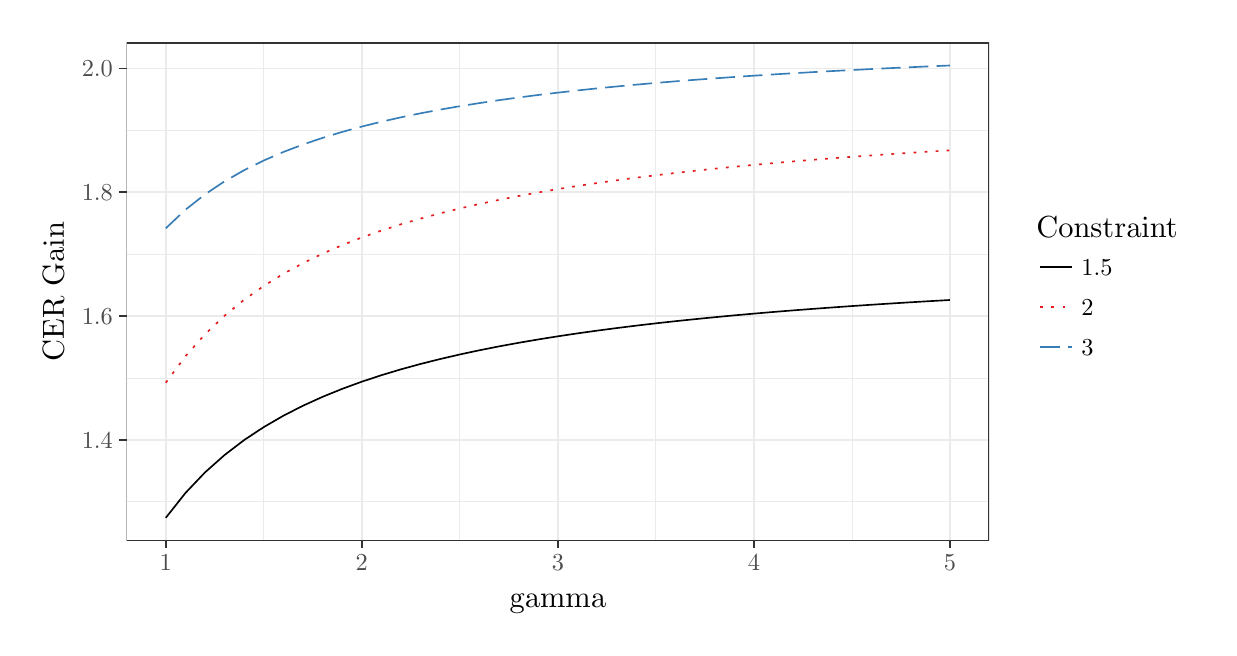
\begin{tikzpicture}[x=1pt,y=1pt]
\definecolor{fillColor}{RGB}{255,255,255}
\path[use as bounding box,fill=fillColor,fill opacity=0.00] (0,0) rectangle (426.79,216.81);
\begin{scope}
\path[clip] (  0.00,  0.00) rectangle (426.79,216.81);
\definecolor{drawColor}{RGB}{255,255,255}
\definecolor{fillColor}{RGB}{255,255,255}

\path[draw=drawColor,line width= 0.6pt,line join=round,line cap=round,fill=fillColor] (  0.00,  0.00) rectangle (426.79,216.81);
\end{scope}
\begin{scope}
\path[clip] ( 35.74, 31.53) rectangle (347.42,211.31);
\definecolor{fillColor}{RGB}{255,255,255}

\path[fill=fillColor] ( 35.74, 31.53) rectangle (347.42,211.31);
\definecolor{drawColor}{gray}{0.92}

\path[draw=drawColor,line width= 0.3pt,line join=round] ( 35.74, 45.51) --
	(347.42, 45.51);

\path[draw=drawColor,line width= 0.3pt,line join=round] ( 35.74, 90.23) --
	(347.42, 90.23);

\path[draw=drawColor,line width= 0.3pt,line join=round] ( 35.74,134.95) --
	(347.42,134.95);

\path[draw=drawColor,line width= 0.3pt,line join=round] ( 35.74,179.67) --
	(347.42,179.67);

\path[draw=drawColor,line width= 0.3pt,line join=round] ( 85.33, 31.53) --
	( 85.33,211.31);

\path[draw=drawColor,line width= 0.3pt,line join=round] (156.16, 31.53) --
	(156.16,211.31);

\path[draw=drawColor,line width= 0.3pt,line join=round] (227.00, 31.53) --
	(227.00,211.31);

\path[draw=drawColor,line width= 0.3pt,line join=round] (297.84, 31.53) --
	(297.84,211.31);

\path[draw=drawColor,line width= 0.6pt,line join=round] ( 35.74, 67.87) --
	(347.42, 67.87);

\path[draw=drawColor,line width= 0.6pt,line join=round] ( 35.74,112.59) --
	(347.42,112.59);

\path[draw=drawColor,line width= 0.6pt,line join=round] ( 35.74,157.31) --
	(347.42,157.31);

\path[draw=drawColor,line width= 0.6pt,line join=round] ( 35.74,202.03) --
	(347.42,202.03);

\path[draw=drawColor,line width= 0.6pt,line join=round] ( 49.91, 31.53) --
	( 49.91,211.31);

\path[draw=drawColor,line width= 0.6pt,line join=round] (120.74, 31.53) --
	(120.74,211.31);

\path[draw=drawColor,line width= 0.6pt,line join=round] (191.58, 31.53) --
	(191.58,211.31);

\path[draw=drawColor,line width= 0.6pt,line join=round] (262.42, 31.53) --
	(262.42,211.31);

\path[draw=drawColor,line width= 0.6pt,line join=round] (333.25, 31.53) --
	(333.25,211.31);
\definecolor{drawColor}{RGB}{0,0,0}

\path[draw=drawColor,line width= 0.6pt,line join=round] ( 49.91, 39.70) --
	( 56.99, 48.65) --
	( 64.07, 56.10) --
	( 71.16, 62.40) --
	( 78.24, 67.81) --
	( 85.33, 72.49) --
	( 92.41, 76.59) --
	( 99.49, 80.21) --
	(106.58, 83.42) --
	(113.66, 86.30) --
	(120.74, 88.89) --
	(127.83, 91.23) --
	(134.91, 93.36) --
	(141.99, 95.30) --
	(149.08, 97.08) --
	(156.16, 98.72) --
	(163.25,100.24) --
	(170.33,101.64) --
	(177.41,102.94) --
	(184.50,104.15) --
	(191.58,105.28) --
	(198.66,106.34) --
	(205.75,107.33) --
	(212.83,108.26) --
	(219.92,109.14) --
	(227.00,109.97) --
	(234.08,110.75) --
	(241.17,111.48) --
	(248.25,112.18) --
	(255.33,112.85) --
	(262.42,113.48) --
	(269.50,114.08) --
	(276.58,114.65) --
	(283.67,115.19) --
	(290.75,115.71) --
	(297.84,116.21) --
	(304.92,116.69) --
	(312.00,117.14) --
	(319.09,117.58) --
	(326.17,118.00) --
	(333.25,118.40);
\definecolor{drawColor}{RGB}{228,26,28}

\path[draw=drawColor,line width= 0.6pt,dash pattern=on 1pt off 3pt ,line join=round] ( 49.91, 88.51) --
	( 56.99, 98.05) --
	( 64.07,106.00) --
	( 71.16,112.73) --
	( 78.24,118.50) --
	( 85.33,123.49) --
	( 92.41,127.87) --
	( 99.49,131.73) --
	(106.58,135.16) --
	(113.66,138.23) --
	(120.74,140.99) --
	(127.83,143.49) --
	(134.91,145.76) --
	(141.99,147.83) --
	(149.08,149.73) --
	(156.16,151.48) --
	(163.25,153.10) --
	(170.33,154.59) --
	(177.41,155.98) --
	(184.50,157.27) --
	(191.58,158.48) --
	(198.66,159.61) --
	(205.75,160.67) --
	(212.83,161.66) --
	(219.92,162.60) --
	(227.00,163.48) --
	(234.08,164.31) --
	(241.17,165.10) --
	(248.25,165.85) --
	(255.33,166.55) --
	(262.42,167.23) --
	(269.50,167.87) --
	(276.58,168.48) --
	(283.67,169.06) --
	(290.75,169.61) --
	(297.84,170.14) --
	(304.92,170.65) --
	(312.00,171.14) --
	(319.09,171.60) --
	(326.17,172.05) --
	(333.25,172.48);
\definecolor{drawColor}{RGB}{55,126,184}

\path[draw=drawColor,line width= 0.6pt,dash pattern=on 7pt off 3pt ,line join=round] ( 49.91,144.31) --
	( 56.99,151.00) --
	( 64.07,156.57) --
	( 71.16,161.28) --
	( 78.24,165.32) --
	( 85.33,168.82) --
	( 92.41,171.89) --
	( 99.49,174.59) --
	(106.58,176.99) --
	(113.66,179.14) --
	(120.74,181.08) --
	(127.83,182.83) --
	(134.91,184.42) --
	(141.99,185.87) --
	(149.08,187.21) --
	(156.16,188.43) --
	(163.25,189.56) --
	(170.33,190.61) --
	(177.41,191.58) --
	(184.50,192.49) --
	(191.58,193.33) --
	(198.66,194.12) --
	(205.75,194.87) --
	(212.83,195.56) --
	(219.92,196.22) --
	(227.00,196.84) --
	(234.08,197.42) --
	(241.17,197.97) --
	(248.25,198.49) --
	(255.33,198.99) --
	(262.42,199.46) --
	(269.50,199.91) --
	(276.58,200.34) --
	(283.67,200.74) --
	(290.75,201.13) --
	(297.84,201.50) --
	(304.92,201.86) --
	(312.00,202.20) --
	(319.09,202.53) --
	(326.17,202.84) --
	(333.25,203.14);
\definecolor{drawColor}{gray}{0.20}

\path[draw=drawColor,line width= 0.6pt,line join=round,line cap=round] ( 35.74, 31.53) rectangle (347.42,211.31);
\end{scope}
\begin{scope}
\path[clip] (  0.00,  0.00) rectangle (426.79,216.81);
\definecolor{drawColor}{gray}{0.30}

\node[text=drawColor,anchor=base east,inner sep=0pt, outer sep=0pt, scale=  0.88] at ( 30.79, 64.84) {1.4};

\node[text=drawColor,anchor=base east,inner sep=0pt, outer sep=0pt, scale=  0.88] at ( 30.79,109.56) {1.6};

\node[text=drawColor,anchor=base east,inner sep=0pt, outer sep=0pt, scale=  0.88] at ( 30.79,154.28) {1.8};

\node[text=drawColor,anchor=base east,inner sep=0pt, outer sep=0pt, scale=  0.88] at ( 30.79,199.00) {2.0};
\end{scope}
\begin{scope}
\path[clip] (  0.00,  0.00) rectangle (426.79,216.81);
\definecolor{drawColor}{gray}{0.20}

\path[draw=drawColor,line width= 0.6pt,line join=round] ( 32.99, 67.87) --
	( 35.74, 67.87);

\path[draw=drawColor,line width= 0.6pt,line join=round] ( 32.99,112.59) --
	( 35.74,112.59);

\path[draw=drawColor,line width= 0.6pt,line join=round] ( 32.99,157.31) --
	( 35.74,157.31);

\path[draw=drawColor,line width= 0.6pt,line join=round] ( 32.99,202.03) --
	( 35.74,202.03);
\end{scope}
\begin{scope}
\path[clip] (  0.00,  0.00) rectangle (426.79,216.81);
\definecolor{drawColor}{gray}{0.20}

\path[draw=drawColor,line width= 0.6pt,line join=round] ( 49.91, 28.78) --
	( 49.91, 31.53);

\path[draw=drawColor,line width= 0.6pt,line join=round] (120.74, 28.78) --
	(120.74, 31.53);

\path[draw=drawColor,line width= 0.6pt,line join=round] (191.58, 28.78) --
	(191.58, 31.53);

\path[draw=drawColor,line width= 0.6pt,line join=round] (262.42, 28.78) --
	(262.42, 31.53);

\path[draw=drawColor,line width= 0.6pt,line join=round] (333.25, 28.78) --
	(333.25, 31.53);
\end{scope}
\begin{scope}
\path[clip] (  0.00,  0.00) rectangle (426.79,216.81);
\definecolor{drawColor}{gray}{0.30}

\node[text=drawColor,anchor=base,inner sep=0pt, outer sep=0pt, scale=  0.88] at ( 49.91, 20.52) {1};

\node[text=drawColor,anchor=base,inner sep=0pt, outer sep=0pt, scale=  0.88] at (120.74, 20.52) {2};

\node[text=drawColor,anchor=base,inner sep=0pt, outer sep=0pt, scale=  0.88] at (191.58, 20.52) {3};

\node[text=drawColor,anchor=base,inner sep=0pt, outer sep=0pt, scale=  0.88] at (262.42, 20.52) {4};

\node[text=drawColor,anchor=base,inner sep=0pt, outer sep=0pt, scale=  0.88] at (333.25, 20.52) {5};
\end{scope}
\begin{scope}
\path[clip] (  0.00,  0.00) rectangle (426.79,216.81);
\definecolor{drawColor}{RGB}{0,0,0}

\node[text=drawColor,anchor=base,inner sep=0pt, outer sep=0pt, scale=  1.10] at (191.58,  7.44) {gamma};
\end{scope}
\begin{scope}
\path[clip] (  0.00,  0.00) rectangle (426.79,216.81);
\definecolor{drawColor}{RGB}{0,0,0}

\node[text=drawColor,rotate= 90.00,anchor=base,inner sep=0pt, outer sep=0pt, scale=  1.10] at ( 13.08,121.42) {CER Gain};
\end{scope}
\begin{scope}
\path[clip] (  0.00,  0.00) rectangle (426.79,216.81);
\definecolor{fillColor}{RGB}{255,255,255}

\path[fill=fillColor] (358.80, 88.45) rectangle (421.29,154.39);
\end{scope}
\begin{scope}
\path[clip] (  0.00,  0.00) rectangle (426.79,216.81);
\definecolor{drawColor}{RGB}{0,0,0}

\node[text=drawColor,anchor=base west,inner sep=0pt, outer sep=0pt, scale=  1.10] at (364.49,141.12) {Constraint};
\end{scope}
\begin{scope}
\path[clip] (  0.00,  0.00) rectangle (426.79,216.81);
\definecolor{fillColor}{RGB}{255,255,255}

\path[fill=fillColor] (364.49,123.05) rectangle (378.95,137.51);
\end{scope}
\begin{scope}
\path[clip] (  0.00,  0.00) rectangle (426.79,216.81);
\definecolor{drawColor}{RGB}{0,0,0}

\path[draw=drawColor,line width= 0.6pt,line join=round] (365.94,130.28) -- (377.50,130.28);
\end{scope}
\begin{scope}
\path[clip] (  0.00,  0.00) rectangle (426.79,216.81);
\definecolor{fillColor}{RGB}{255,255,255}

\path[fill=fillColor] (364.49,108.60) rectangle (378.95,123.05);
\end{scope}
\begin{scope}
\path[clip] (  0.00,  0.00) rectangle (426.79,216.81);
\definecolor{drawColor}{RGB}{228,26,28}

\path[draw=drawColor,line width= 0.6pt,dash pattern=on 1pt off 3pt ,line join=round] (365.94,115.83) -- (377.50,115.83);
\end{scope}
\begin{scope}
\path[clip] (  0.00,  0.00) rectangle (426.79,216.81);
\definecolor{fillColor}{RGB}{255,255,255}

\path[fill=fillColor] (364.49, 94.14) rectangle (378.95,108.60);
\end{scope}
\begin{scope}
\path[clip] (  0.00,  0.00) rectangle (426.79,216.81);
\definecolor{drawColor}{RGB}{55,126,184}

\path[draw=drawColor,line width= 0.6pt,dash pattern=on 7pt off 3pt ,line join=round] (365.94,101.37) -- (377.50,101.37);
\end{scope}
\begin{scope}
\path[clip] (  0.00,  0.00) rectangle (426.79,216.81);
\definecolor{drawColor}{RGB}{0,0,0}

\node[text=drawColor,anchor=base west,inner sep=0pt, outer sep=0pt, scale=  0.88] at (380.75,127.25) {1.5};
\end{scope}
\begin{scope}
\path[clip] (  0.00,  0.00) rectangle (426.79,216.81);
\definecolor{drawColor}{RGB}{0,0,0}

\node[text=drawColor,anchor=base west,inner sep=0pt, outer sep=0pt, scale=  0.88] at (380.75,112.80) {2};
\end{scope}
\begin{scope}
\path[clip] (  0.00,  0.00) rectangle (426.79,216.81);
\definecolor{drawColor}{RGB}{0,0,0}

\node[text=drawColor,anchor=base west,inner sep=0pt, outer sep=0pt, scale=  0.88] at (380.75, 98.34) {3};
\end{scope}
\end{tikzpicture}

	\end{subfigure}
	\begin{subfigure}{\textwidth}
		% Created by tikzDevice version 0.10.1 on 2018-06-14 11:50:00
% !TEX encoding = UTF-8 Unicode
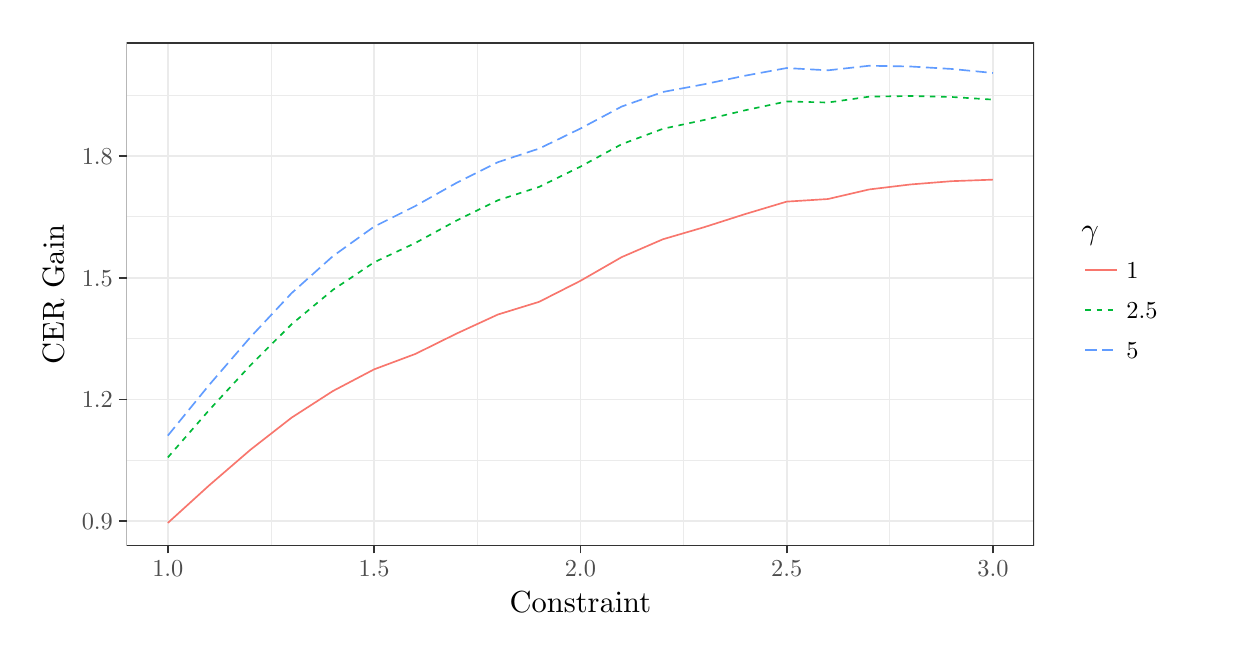
\begin{tikzpicture}[x=1pt,y=1pt]
\definecolor{fillColor}{RGB}{255,255,255}
\path[use as bounding box,fill=fillColor,fill opacity=0.00] (0,0) rectangle (426.79,216.81);
\begin{scope}
\path[clip] (  0.00,  0.00) rectangle (426.79,216.81);
\definecolor{drawColor}{RGB}{255,255,255}
\definecolor{fillColor}{RGB}{255,255,255}

\path[draw=drawColor,line width= 0.6pt,line join=round,line cap=round,fill=fillColor] (  0.00,  0.00) rectangle (426.79,216.81);
\end{scope}
\begin{scope}
\path[clip] ( 35.74, 29.59) rectangle (363.70,211.31);
\definecolor{fillColor}{RGB}{255,255,255}

\path[fill=fillColor] ( 35.74, 29.59) rectangle (363.70,211.31);
\definecolor{drawColor}{gray}{0.92}

\path[draw=drawColor,line width= 0.3pt,line join=round] ( 35.74, 60.51) --
	(363.70, 60.51);

\path[draw=drawColor,line width= 0.3pt,line join=round] ( 35.74,104.47) --
	(363.70,104.47);

\path[draw=drawColor,line width= 0.3pt,line join=round] ( 35.74,148.43) --
	(363.70,148.43);

\path[draw=drawColor,line width= 0.3pt,line join=round] ( 35.74,192.39) --
	(363.70,192.39);

\path[draw=drawColor,line width= 0.3pt,line join=round] ( 87.92, 29.59) --
	( 87.92,211.31);

\path[draw=drawColor,line width= 0.3pt,line join=round] (162.45, 29.59) --
	(162.45,211.31);

\path[draw=drawColor,line width= 0.3pt,line join=round] (236.99, 29.59) --
	(236.99,211.31);

\path[draw=drawColor,line width= 0.3pt,line join=round] (311.53, 29.59) --
	(311.53,211.31);

\path[draw=drawColor,line width= 0.6pt,line join=round] ( 35.74, 38.53) --
	(363.70, 38.53);

\path[draw=drawColor,line width= 0.6pt,line join=round] ( 35.74, 82.49) --
	(363.70, 82.49);

\path[draw=drawColor,line width= 0.6pt,line join=round] ( 35.74,126.45) --
	(363.70,126.45);

\path[draw=drawColor,line width= 0.6pt,line join=round] ( 35.74,170.41) --
	(363.70,170.41);

\path[draw=drawColor,line width= 0.6pt,line join=round] ( 50.65, 29.59) --
	( 50.65,211.31);

\path[draw=drawColor,line width= 0.6pt,line join=round] (125.18, 29.59) --
	(125.18,211.31);

\path[draw=drawColor,line width= 0.6pt,line join=round] (199.72, 29.59) --
	(199.72,211.31);

\path[draw=drawColor,line width= 0.6pt,line join=round] (274.26, 29.59) --
	(274.26,211.31);

\path[draw=drawColor,line width= 0.6pt,line join=round] (348.80, 29.59) --
	(348.80,211.31);
\definecolor{drawColor}{RGB}{248,118,109}

\path[draw=drawColor,line width= 0.6pt,line join=round] ( 50.65, 37.85) --
	( 65.55, 51.39) --
	( 80.46, 64.26) --
	( 95.37, 75.89) --
	(110.28, 85.50) --
	(125.18, 93.34) --
	(140.09, 98.91) --
	(155.00,106.28) --
	(169.91,113.15) --
	(184.81,117.74) --
	(199.72,125.32) --
	(214.63,133.89) --
	(229.54,140.35) --
	(244.44,144.71) --
	(259.35,149.48) --
	(274.26,153.95) --
	(289.17,154.89) --
	(304.07,158.35) --
	(318.98,160.15) --
	(333.89,161.34) --
	(348.80,161.89);
\definecolor{drawColor}{RGB}{0,186,56}

\path[draw=drawColor,line width= 0.6pt,dash pattern=on 2pt off 2pt ,line join=round] ( 50.65, 61.51) --
	( 65.55, 78.60) --
	( 80.46, 94.77) --
	( 95.37,109.64) --
	(110.28,122.05) --
	(125.18,132.02) --
	(140.09,139.01) --
	(155.00,147.13) --
	(169.91,154.44) --
	(184.81,159.27) --
	(199.72,166.59) --
	(214.63,174.70) --
	(229.54,180.27) --
	(244.44,183.45) --
	(259.35,186.98) --
	(274.26,190.15) --
	(289.17,189.76) --
	(304.07,191.88) --
	(318.98,192.12) --
	(333.89,191.76) --
	(348.80,190.81);
\definecolor{drawColor}{RGB}{97,156,255}

\path[draw=drawColor,line width= 0.6pt,dash pattern=on 4pt off 2pt ,line join=round] ( 50.65, 69.40) --
	( 65.55, 87.67) --
	( 80.46,104.94) --
	( 95.37,120.88) --
	(110.28,134.24) --
	(125.18,144.91) --
	(140.09,152.37) --
	(155.00,160.75) --
	(169.91,168.21) --
	(184.81,173.11) --
	(199.72,180.35) --
	(214.63,188.30) --
	(229.54,193.57) --
	(244.44,196.36) --
	(259.35,199.48) --
	(274.26,202.22) --
	(289.17,201.39) --
	(304.07,203.05) --
	(318.98,202.78) --
	(333.89,201.89) --
	(348.80,200.44);
\definecolor{drawColor}{gray}{0.20}

\path[draw=drawColor,line width= 0.6pt,line join=round,line cap=round] ( 35.74, 29.59) rectangle (363.70,211.31);
\end{scope}
\begin{scope}
\path[clip] (  0.00,  0.00) rectangle (426.79,216.81);
\definecolor{drawColor}{gray}{0.30}

\node[text=drawColor,anchor=base east,inner sep=0pt, outer sep=0pt, scale=  0.88] at ( 30.79, 35.50) {0.9};

\node[text=drawColor,anchor=base east,inner sep=0pt, outer sep=0pt, scale=  0.88] at ( 30.79, 79.46) {1.2};

\node[text=drawColor,anchor=base east,inner sep=0pt, outer sep=0pt, scale=  0.88] at ( 30.79,123.42) {1.5};

\node[text=drawColor,anchor=base east,inner sep=0pt, outer sep=0pt, scale=  0.88] at ( 30.79,167.38) {1.8};
\end{scope}
\begin{scope}
\path[clip] (  0.00,  0.00) rectangle (426.79,216.81);
\definecolor{drawColor}{gray}{0.20}

\path[draw=drawColor,line width= 0.6pt,line join=round] ( 32.99, 38.53) --
	( 35.74, 38.53);

\path[draw=drawColor,line width= 0.6pt,line join=round] ( 32.99, 82.49) --
	( 35.74, 82.49);

\path[draw=drawColor,line width= 0.6pt,line join=round] ( 32.99,126.45) --
	( 35.74,126.45);

\path[draw=drawColor,line width= 0.6pt,line join=round] ( 32.99,170.41) --
	( 35.74,170.41);
\end{scope}
\begin{scope}
\path[clip] (  0.00,  0.00) rectangle (426.79,216.81);
\definecolor{drawColor}{gray}{0.20}

\path[draw=drawColor,line width= 0.6pt,line join=round] ( 50.65, 26.84) --
	( 50.65, 29.59);

\path[draw=drawColor,line width= 0.6pt,line join=round] (125.18, 26.84) --
	(125.18, 29.59);

\path[draw=drawColor,line width= 0.6pt,line join=round] (199.72, 26.84) --
	(199.72, 29.59);

\path[draw=drawColor,line width= 0.6pt,line join=round] (274.26, 26.84) --
	(274.26, 29.59);

\path[draw=drawColor,line width= 0.6pt,line join=round] (348.80, 26.84) --
	(348.80, 29.59);
\end{scope}
\begin{scope}
\path[clip] (  0.00,  0.00) rectangle (426.79,216.81);
\definecolor{drawColor}{gray}{0.30}

\node[text=drawColor,anchor=base,inner sep=0pt, outer sep=0pt, scale=  0.88] at ( 50.65, 18.58) {1.0};

\node[text=drawColor,anchor=base,inner sep=0pt, outer sep=0pt, scale=  0.88] at (125.18, 18.58) {1.5};

\node[text=drawColor,anchor=base,inner sep=0pt, outer sep=0pt, scale=  0.88] at (199.72, 18.58) {2.0};

\node[text=drawColor,anchor=base,inner sep=0pt, outer sep=0pt, scale=  0.88] at (274.26, 18.58) {2.5};

\node[text=drawColor,anchor=base,inner sep=0pt, outer sep=0pt, scale=  0.88] at (348.80, 18.58) {3.0};
\end{scope}
\begin{scope}
\path[clip] (  0.00,  0.00) rectangle (426.79,216.81);
\definecolor{drawColor}{RGB}{0,0,0}

\node[text=drawColor,anchor=base,inner sep=0pt, outer sep=0pt, scale=  1.10] at (199.72,  5.50) {Constraint};
\end{scope}
\begin{scope}
\path[clip] (  0.00,  0.00) rectangle (426.79,216.81);
\definecolor{drawColor}{RGB}{0,0,0}

\node[text=drawColor,rotate= 90.00,anchor=base,inner sep=0pt, outer sep=0pt, scale=  1.10] at ( 13.08,120.45) {CER Gain};
\end{scope}
\begin{scope}
\path[clip] (  0.00,  0.00) rectangle (426.79,216.81);
\definecolor{fillColor}{RGB}{255,255,255}

\path[fill=fillColor] (375.09, 87.48) rectangle (421.29,153.41);
\end{scope}
\begin{scope}
\path[clip] (  0.00,  0.00) rectangle (426.79,216.81);
\definecolor{drawColor}{RGB}{0,0,0}

\node[text=drawColor,anchor=base west,inner sep=0pt, outer sep=0pt, scale=  1.10] at (380.78,140.15) {$\gamma$};
\end{scope}
\begin{scope}
\path[clip] (  0.00,  0.00) rectangle (426.79,216.81);
\definecolor{fillColor}{RGB}{255,255,255}

\path[fill=fillColor] (380.78,122.08) rectangle (395.23,136.53);
\end{scope}
\begin{scope}
\path[clip] (  0.00,  0.00) rectangle (426.79,216.81);
\definecolor{drawColor}{RGB}{248,118,109}

\path[draw=drawColor,line width= 0.6pt,line join=round] (382.22,129.31) -- (393.78,129.31);
\end{scope}
\begin{scope}
\path[clip] (  0.00,  0.00) rectangle (426.79,216.81);
\definecolor{fillColor}{RGB}{255,255,255}

\path[fill=fillColor] (380.78,107.63) rectangle (395.23,122.08);
\end{scope}
\begin{scope}
\path[clip] (  0.00,  0.00) rectangle (426.79,216.81);
\definecolor{drawColor}{RGB}{0,186,56}

\path[draw=drawColor,line width= 0.6pt,dash pattern=on 2pt off 2pt ,line join=round] (382.22,114.85) -- (393.78,114.85);
\end{scope}
\begin{scope}
\path[clip] (  0.00,  0.00) rectangle (426.79,216.81);
\definecolor{fillColor}{RGB}{255,255,255}

\path[fill=fillColor] (380.78, 93.17) rectangle (395.23,107.63);
\end{scope}
\begin{scope}
\path[clip] (  0.00,  0.00) rectangle (426.79,216.81);
\definecolor{drawColor}{RGB}{97,156,255}

\path[draw=drawColor,line width= 0.6pt,dash pattern=on 4pt off 2pt ,line join=round] (382.22,100.40) -- (393.78,100.40);
\end{scope}
\begin{scope}
\path[clip] (  0.00,  0.00) rectangle (426.79,216.81);
\definecolor{drawColor}{RGB}{0,0,0}

\node[text=drawColor,anchor=base west,inner sep=0pt, outer sep=0pt, scale=  0.88] at (397.04,126.28) {1};
\end{scope}
\begin{scope}
\path[clip] (  0.00,  0.00) rectangle (426.79,216.81);
\definecolor{drawColor}{RGB}{0,0,0}

\node[text=drawColor,anchor=base west,inner sep=0pt, outer sep=0pt, scale=  0.88] at (397.04,111.82) {2.5};
\end{scope}
\begin{scope}
\path[clip] (  0.00,  0.00) rectangle (426.79,216.81);
\definecolor{drawColor}{RGB}{0,0,0}

\node[text=drawColor,anchor=base west,inner sep=0pt, outer sep=0pt, scale=  0.88] at (397.04, 97.37) {5};
\end{scope}
\end{tikzpicture}

	\end{subfigure}
%\subcaptionbox{First\label{f}}{%
%	% Created by tikzDevice version 0.10.1 on 2018-05-02 14:50:53
% !TEX encoding = UTF-8 Unicode
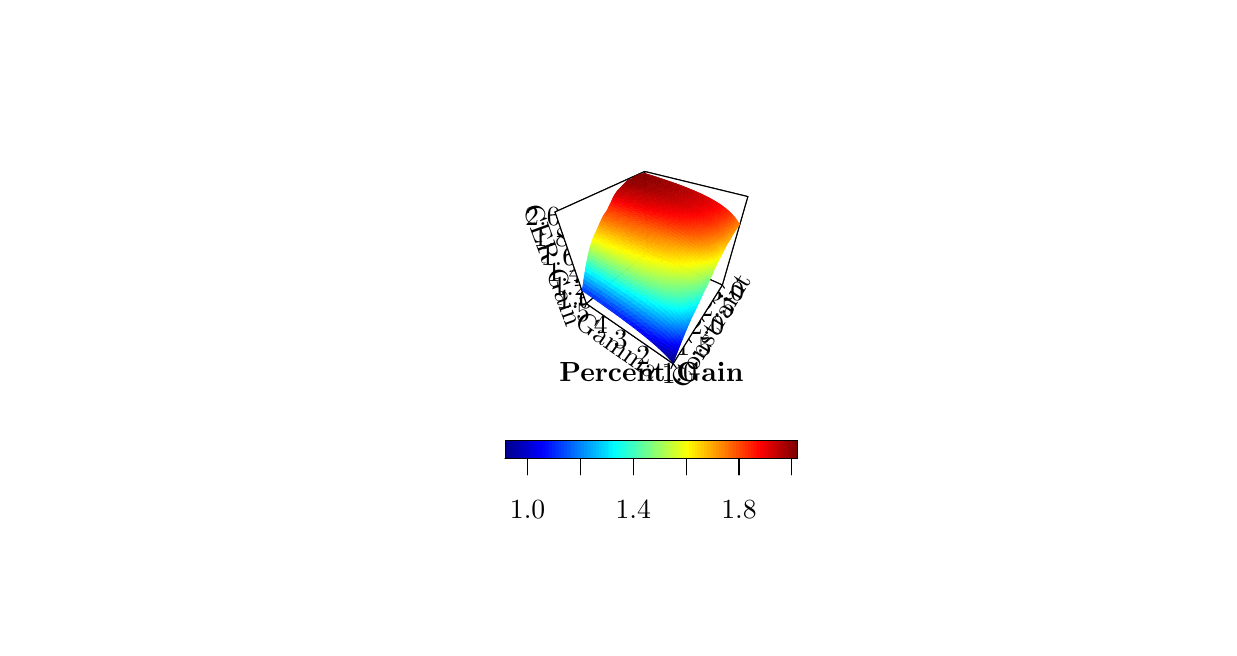
\begin{tikzpicture}[x=1pt,y=1pt]
\definecolor{fillColor}{RGB}{255,255,255}
\path[use as bounding box,fill=fillColor,fill opacity=0.00] (0,0) rectangle (426.79,216.81);
\begin{scope}
\path[clip] ( 49.20, 92.64) rectangle (401.59,167.61);
\definecolor{drawColor}{RGB}{0,0,0}

\path[draw=drawColor,line width= 0.4pt,line join=round,line cap=round] (201.91,117.08) -- (224.04,135.90);

\path[draw=drawColor,line width= 0.4pt,line join=round,line cap=round] (224.04,135.90) -- (222.97,164.83);

\path[draw=drawColor,line width= 0.4pt,line join=round,line cap=round] (222.97,164.83) -- (190.57,150.20);

\path[draw=drawColor,line width= 0.4pt,line join=round,line cap=round] (190.57,150.20) -- (201.91,117.08);

\path[draw=drawColor,line width= 0.4pt,line join=round,line cap=round] (251.01,123.81) -- (260.22,155.77);

\path[draw=drawColor,line width= 0.4pt,line join=round,line cap=round] (260.22,155.77) -- (222.97,164.83);

\path[draw=drawColor,line width= 0.4pt,line join=round,line cap=round] (224.04,135.90) -- (251.01,123.81);

\path[draw=drawColor,line width= 0.4pt,line join=round,line cap=round] (233.23, 95.41) -- (251.01,123.81);

\path[draw=drawColor,line width= 0.4pt,line join=round,line cap=round] (201.91,117.08) -- (233.23, 95.41);
\end{scope}
\begin{scope}
\path[clip] (  0.00,  0.00) rectangle (426.79,216.81);
\definecolor{drawColor}{RGB}{0,0,0}

\node[text=drawColor,rotate= 58.75,anchor=base,inner sep=0pt, outer sep=6pt, scale=  1.00] at (249.64,105.72) {Constraint};

\path[draw=drawColor,line width= 0.4pt,line join=round,line cap=round] (233.23, 95.41) -- (234.35, 93.98);

\node[text=drawColor,anchor=base,inner sep=0pt, outer sep=0pt, scale=  1.00] at (235.46, 89.11) {1.0};

\path[draw=drawColor,line width= 0.4pt,line join=round,line cap=round] (238.83,104.36) -- (239.83,103.02);

\node[text=drawColor,anchor=base,inner sep=0pt, outer sep=0pt, scale=  1.00] at (240.83, 98.24) {1.5};

\path[draw=drawColor,line width= 0.4pt,line join=round,line cap=round] (243.54,111.88) -- (244.45,110.62);

\node[text=drawColor,anchor=base,inner sep=0pt, outer sep=0pt, scale=  1.00] at (245.35,105.92) {2.0};

\path[draw=drawColor,line width= 0.4pt,line join=round,line cap=round] (247.55,118.28) -- (248.38,117.10);

\node[text=drawColor,anchor=base,inner sep=0pt, outer sep=0pt, scale=  1.00] at (249.20,112.48) {2.5};

\path[draw=drawColor,line width= 0.4pt,line join=round,line cap=round] (251.01,123.81) -- (251.77,122.69);

\node[text=drawColor,anchor=base,inner sep=0pt, outer sep=0pt, scale=  1.00] at (252.53,118.14) {3.0};

\node[text=drawColor,rotate=-35.29,anchor=base,inner sep=0pt, outer sep=6pt, scale=  1.00] at (211.28, 99.16) {Gamma};

\path[draw=drawColor,line width= 0.4pt,line join=round,line cap=round] (233.23, 95.41) -- (232.43, 93.62);

\node[text=drawColor,anchor=base,inner sep=0pt, outer sep=0pt, scale=  1.00] at (231.63, 88.38) {1};

\path[draw=drawColor,line width= 0.4pt,line join=round,line cap=round] (223.94,101.84) -- (223.19,100.16);

\node[text=drawColor,anchor=base,inner sep=0pt, outer sep=0pt, scale=  1.00] at (222.44, 95.03) {2};

\path[draw=drawColor,line width= 0.4pt,line join=round,line cap=round] (215.74,107.52) -- (215.03,105.93);

\node[text=drawColor,anchor=base,inner sep=0pt, outer sep=0pt, scale=  1.00] at (214.33,100.90) {3};

\path[draw=drawColor,line width= 0.4pt,line join=round,line cap=round] (208.44,112.57) -- (207.78,111.07);

\node[text=drawColor,anchor=base,inner sep=0pt, outer sep=0pt, scale=  1.00] at (207.12,106.12) {4};

\path[draw=drawColor,line width= 0.4pt,line join=round,line cap=round] (201.91,117.08) -- (201.29,115.66);

\node[text=drawColor,anchor=base,inner sep=0pt, outer sep=0pt, scale=  1.00] at (200.66,110.80) {5};

\node[text=drawColor,rotate=-69.94,anchor=base,inner sep=0pt, outer sep=6pt, scale=  1.00] at (186.77,129.87) {CER Gain};

\path[draw=drawColor,line width= 0.4pt,line join=round,line cap=round] (201.16,119.28) -- (199.50,119.06);

\node[text=drawColor,anchor=base,inner sep=0pt, outer sep=0pt, scale=  1.00] at (197.83,115.39) {1.0};

\path[draw=drawColor,line width= 0.4pt,line join=round,line cap=round] (199.60,123.85) -- (197.83,123.63);

\node[text=drawColor,anchor=base,inner sep=0pt, outer sep=0pt, scale=  1.00] at (196.06,119.96) {1.2};

\path[draw=drawColor,line width= 0.4pt,line join=round,line cap=round] (197.83,128.99) -- (195.95,128.78);

\node[text=drawColor,anchor=base,inner sep=0pt, outer sep=0pt, scale=  1.00] at (194.06,125.11) {1.4};

\path[draw=drawColor,line width= 0.4pt,line join=round,line cap=round] (195.83,134.84) -- (193.82,134.62);

\node[text=drawColor,anchor=base,inner sep=0pt, outer sep=0pt, scale=  1.00] at (191.79,130.96) {1.6};

\path[draw=drawColor,line width= 0.4pt,line join=round,line cap=round] (193.54,141.52) -- (191.37,141.32);

\node[text=drawColor,anchor=base,inner sep=0pt, outer sep=0pt, scale=  1.00] at (189.19,137.67) {1.8};

\path[draw=drawColor,line width= 0.4pt,line join=round,line cap=round] (190.89,149.25) -- (188.55,149.06);

\node[text=drawColor,anchor=base,inner sep=0pt, outer sep=0pt, scale=  1.00] at (186.18,145.42) {2.0};
\end{scope}
\begin{scope}
\path[clip] ( 49.20, 92.64) rectangle (401.59,167.61);

\path[] (233.23, 95.41) --
	(260.22,155.77) --
	(222.97,164.83) --
	(201.91,117.08) --
	(233.23, 95.41);
\definecolor{drawColor}{RGB}{0,0,0}

\path[draw=drawColor,line width= 0.4pt,dash pattern=on 1pt off 3pt ,line join=round,line cap=round] (233.23, 95.41) -- (236.86,129.15);

\path[draw=drawColor,line width= 0.4pt,dash pattern=on 1pt off 3pt ,line join=round,line cap=round] (236.86,129.15) -- (260.22,155.77);

\path[draw=drawColor,line width= 0.4pt,dash pattern=on 1pt off 3pt ,line join=round,line cap=round] (190.57,150.20) -- (236.86,129.15);
\definecolor{fillColor}{RGB}{255,255,255}

\path[fill=fillColor] (201.91,117.08) --
	(224.04,135.90) --
	(222.97,164.83) --
	(190.57,150.20) --
	(201.91,117.08) --
	cycle;

\path[draw=drawColor,line width= 0.4pt,line join=round,line cap=round] (201.91,117.08) --
	(224.04,135.90) --
	(222.97,164.83) --
	(190.57,150.20) --
	(201.91,117.08);

\path[fill=fillColor] (251.01,123.81) --
	(260.22,155.77) --
	(222.97,164.83) --
	(224.04,135.90) --
	(251.01,123.81) --
	cycle;

\path[draw=drawColor,line width= 0.4pt,line join=round,line cap=round] (251.01,123.81) --
	(260.22,155.77) --
	(222.97,164.83) --
	(224.04,135.90) --
	(251.01,123.81);

\path[fill=fillColor] (233.23, 95.41) --
	(251.01,123.81) --
	(224.04,135.90) --
	(201.91,117.08) --
	(233.23, 95.41) --
	cycle;

\path[draw=drawColor,line width= 0.4pt,line join=round,line cap=round] (233.23, 95.41) --
	(251.01,123.81) --
	(224.04,135.90) --
	(201.91,117.08) --
	(233.23, 95.41);
\definecolor{fillColor}{RGB}{148,0,0}

\path[fill=fillColor] (222.85,164.10) --
	(223.24,164.16) --
	(222.99,164.24) --
	(222.61,164.18) --
	cycle;

\path[fill=fillColor] (222.85,164.10) --
	(223.24,164.16) --
	(222.99,164.24) --
	(222.61,164.18) --
	cycle;

\path[fill=fillColor] (223.10,164.02) --
	(223.48,164.09) --
	(223.24,164.16) --
	(222.85,164.10) --
	cycle;

\path[fill=fillColor] (223.10,164.02) --
	(223.48,164.09) --
	(223.24,164.16) --
	(222.85,164.10) --
	cycle;

\path[fill=fillColor] (223.35,163.95) --
	(223.73,164.01) --
	(223.48,164.09) --
	(223.10,164.02) --
	cycle;

\path[fill=fillColor] (223.35,163.95) --
	(223.73,164.01) --
	(223.48,164.09) --
	(223.10,164.02) --
	cycle;

\path[fill=fillColor] (222.47,164.03) --
	(222.85,164.10) --
	(222.61,164.18) --
	(222.22,164.11) --
	cycle;

\path[fill=fillColor] (222.47,164.03) --
	(222.85,164.10) --
	(222.61,164.18) --
	(222.22,164.11) --
	cycle;

\path[fill=fillColor] (223.60,163.87) --
	(223.97,163.94) --
	(223.73,164.01) --
	(223.35,163.95) --
	cycle;

\path[fill=fillColor] (223.60,163.87) --
	(223.97,163.94) --
	(223.73,164.01) --
	(223.35,163.95) --
	cycle;

\path[fill=fillColor] (222.72,163.96) --
	(223.10,164.02) --
	(222.85,164.10) --
	(222.47,164.03) --
	cycle;

\path[fill=fillColor] (222.72,163.96) --
	(223.10,164.02) --
	(222.85,164.10) --
	(222.47,164.03) --
	cycle;

\path[fill=fillColor] (223.84,163.79) --
	(224.22,163.86) --
	(223.97,163.94) --
	(223.60,163.87) --
	cycle;

\path[fill=fillColor] (223.84,163.79) --
	(224.22,163.86) --
	(223.97,163.94) --
	(223.60,163.87) --
	cycle;

\path[fill=fillColor] (222.96,163.88) --
	(223.35,163.95) --
	(223.10,164.02) --
	(222.72,163.96) --
	cycle;

\path[fill=fillColor] (222.96,163.88) --
	(223.35,163.95) --
	(223.10,164.02) --
	(222.72,163.96) --
	cycle;

\path[fill=fillColor] (224.09,163.71) --
	(224.47,163.78) --
	(224.22,163.86) --
	(223.84,163.79) --
	cycle;

\path[fill=fillColor] (224.09,163.71) --
	(224.47,163.78) --
	(224.22,163.86) --
	(223.84,163.79) --
	cycle;
\definecolor{fillColor}{RGB}{138,0,0}

\path[fill=fillColor] (222.08,163.97) --
	(222.47,164.03) --
	(222.22,164.11) --
	(221.83,164.05) --
	cycle;

\path[fill=fillColor] (222.08,163.97) --
	(222.47,164.03) --
	(222.22,164.11) --
	(221.83,164.05) --
	cycle;
\definecolor{fillColor}{RGB}{148,0,0}

\path[fill=fillColor] (223.21,163.80) --
	(223.60,163.87) --
	(223.35,163.95) --
	(222.96,163.88) --
	cycle;

\path[fill=fillColor] (223.21,163.80) --
	(223.60,163.87) --
	(223.35,163.95) --
	(222.96,163.88) --
	cycle;

\path[fill=fillColor] (224.34,163.63) --
	(224.72,163.70) --
	(224.47,163.78) --
	(224.09,163.71) --
	cycle;

\path[fill=fillColor] (224.34,163.63) --
	(224.72,163.70) --
	(224.47,163.78) --
	(224.09,163.71) --
	cycle;
\definecolor{fillColor}{RGB}{138,0,0}

\path[fill=fillColor] (222.33,163.89) --
	(222.72,163.96) --
	(222.47,164.03) --
	(222.08,163.97) --
	cycle;

\path[fill=fillColor] (222.33,163.89) --
	(222.72,163.96) --
	(222.47,164.03) --
	(222.08,163.97) --
	cycle;
\definecolor{fillColor}{RGB}{148,0,0}

\path[fill=fillColor] (223.46,163.72) --
	(223.84,163.79) --
	(223.60,163.87) --
	(223.21,163.80) --
	cycle;

\path[fill=fillColor] (223.46,163.72) --
	(223.84,163.79) --
	(223.60,163.87) --
	(223.21,163.80) --
	cycle;

\path[fill=fillColor] (224.60,163.55) --
	(224.97,163.62) --
	(224.72,163.70) --
	(224.34,163.63) --
	cycle;

\path[fill=fillColor] (224.60,163.55) --
	(224.97,163.62) --
	(224.72,163.70) --
	(224.34,163.63) --
	cycle;
\definecolor{fillColor}{RGB}{138,0,0}

\path[fill=fillColor] (222.58,163.81) --
	(222.96,163.88) --
	(222.72,163.96) --
	(222.33,163.89) --
	cycle;

\path[fill=fillColor] (222.58,163.81) --
	(222.96,163.88) --
	(222.72,163.96) --
	(222.33,163.89) --
	cycle;
\definecolor{fillColor}{RGB}{148,0,0}

\path[fill=fillColor] (223.71,163.64) --
	(224.09,163.71) --
	(223.84,163.79) --
	(223.46,163.72) --
	cycle;

\path[fill=fillColor] (223.71,163.64) --
	(224.09,163.71) --
	(223.84,163.79) --
	(223.46,163.72) --
	cycle;

\path[fill=fillColor] (224.85,163.48) --
	(225.22,163.55) --
	(224.97,163.62) --
	(224.60,163.55) --
	cycle;

\path[fill=fillColor] (224.85,163.48) --
	(225.22,163.55) --
	(224.97,163.62) --
	(224.60,163.55) --
	cycle;
\definecolor{fillColor}{RGB}{138,0,0}

\path[fill=fillColor] (221.69,163.86) --
	(222.08,163.97) --
	(221.83,164.05) --
	(221.44,163.94) --
	cycle;

\path[fill=fillColor] (221.69,163.86) --
	(222.08,163.97) --
	(221.83,164.05) --
	(221.44,163.94) --
	cycle;

\path[fill=fillColor] (222.83,163.73) --
	(223.21,163.80) --
	(222.96,163.88) --
	(222.58,163.81) --
	cycle;

\path[fill=fillColor] (222.83,163.73) --
	(223.21,163.80) --
	(222.96,163.88) --
	(222.58,163.81) --
	cycle;
\definecolor{fillColor}{RGB}{148,0,0}

\path[fill=fillColor] (223.96,163.56) --
	(224.34,163.63) --
	(224.09,163.71) --
	(223.71,163.64) --
	cycle;

\path[fill=fillColor] (223.96,163.56) --
	(224.34,163.63) --
	(224.09,163.71) --
	(223.71,163.64) --
	cycle;

\path[fill=fillColor] (225.10,163.39) --
	(225.47,163.47) --
	(225.22,163.55) --
	(224.85,163.48) --
	cycle;

\path[fill=fillColor] (225.10,163.39) --
	(225.47,163.47) --
	(225.22,163.55) --
	(224.85,163.48) --
	cycle;
\definecolor{fillColor}{RGB}{138,0,0}

\path[fill=fillColor] (221.94,163.78) --
	(222.33,163.89) --
	(222.08,163.97) --
	(221.69,163.86) --
	cycle;

\path[fill=fillColor] (221.94,163.78) --
	(222.33,163.89) --
	(222.08,163.97) --
	(221.69,163.86) --
	cycle;

\path[fill=fillColor] (223.08,163.65) --
	(223.46,163.72) --
	(223.21,163.80) --
	(222.83,163.73) --
	cycle;

\path[fill=fillColor] (223.08,163.65) --
	(223.46,163.72) --
	(223.21,163.80) --
	(222.83,163.73) --
	cycle;
\definecolor{fillColor}{RGB}{148,0,0}

\path[fill=fillColor] (224.22,163.48) --
	(224.60,163.55) --
	(224.34,163.63) --
	(223.96,163.56) --
	cycle;

\path[fill=fillColor] (224.22,163.48) --
	(224.60,163.55) --
	(224.34,163.63) --
	(223.96,163.56) --
	cycle;

\path[fill=fillColor] (225.35,163.31) --
	(225.73,163.39) --
	(225.47,163.47) --
	(225.10,163.39) --
	cycle;

\path[fill=fillColor] (225.35,163.31) --
	(225.73,163.39) --
	(225.47,163.47) --
	(225.10,163.39) --
	cycle;
\definecolor{fillColor}{RGB}{138,0,0}

\path[fill=fillColor] (222.19,163.70) --
	(222.58,163.81) --
	(222.33,163.89) --
	(221.94,163.78) --
	cycle;

\path[fill=fillColor] (222.19,163.70) --
	(222.58,163.81) --
	(222.33,163.89) --
	(221.94,163.78) --
	cycle;
\definecolor{fillColor}{RGB}{148,0,0}

\path[fill=fillColor] (223.33,163.57) --
	(223.71,163.64) --
	(223.46,163.72) --
	(223.08,163.65) --
	cycle;

\path[fill=fillColor] (223.33,163.57) --
	(223.71,163.64) --
	(223.46,163.72) --
	(223.08,163.65) --
	cycle;

\path[fill=fillColor] (224.47,163.40) --
	(224.85,163.48) --
	(224.60,163.55) --
	(224.22,163.48) --
	cycle;

\path[fill=fillColor] (224.47,163.40) --
	(224.85,163.48) --
	(224.60,163.55) --
	(224.22,163.48) --
	cycle;

\path[fill=fillColor] (225.61,163.23) --
	(225.98,163.31) --
	(225.73,163.39) --
	(225.35,163.31) --
	cycle;

\path[fill=fillColor] (225.61,163.23) --
	(225.98,163.31) --
	(225.73,163.39) --
	(225.35,163.31) --
	cycle;
\definecolor{fillColor}{RGB}{138,0,0}

\path[fill=fillColor] (221.29,163.75) --
	(221.69,163.86) --
	(221.44,163.94) --
	(221.04,163.83) --
	cycle;

\path[fill=fillColor] (221.29,163.75) --
	(221.69,163.86) --
	(221.44,163.94) --
	(221.04,163.83) --
	cycle;

\path[fill=fillColor] (222.44,163.62) --
	(222.83,163.73) --
	(222.58,163.81) --
	(222.19,163.70) --
	cycle;

\path[fill=fillColor] (222.44,163.62) --
	(222.83,163.73) --
	(222.58,163.81) --
	(222.19,163.70) --
	cycle;
\definecolor{fillColor}{RGB}{148,0,0}

\path[fill=fillColor] (223.58,163.49) --
	(223.96,163.56) --
	(223.71,163.64) --
	(223.33,163.57) --
	cycle;

\path[fill=fillColor] (223.58,163.49) --
	(223.96,163.56) --
	(223.71,163.64) --
	(223.33,163.57) --
	cycle;

\path[fill=fillColor] (224.72,163.32) --
	(225.10,163.39) --
	(224.85,163.48) --
	(224.47,163.40) --
	cycle;

\path[fill=fillColor] (224.72,163.32) --
	(225.10,163.39) --
	(224.85,163.48) --
	(224.47,163.40) --
	cycle;

\path[fill=fillColor] (225.86,163.15) --
	(226.23,163.22) --
	(225.98,163.31) --
	(225.61,163.23) --
	cycle;

\path[fill=fillColor] (225.86,163.15) --
	(226.23,163.22) --
	(225.98,163.31) --
	(225.61,163.23) --
	cycle;
\definecolor{fillColor}{RGB}{138,0,0}

\path[fill=fillColor] (221.54,163.67) --
	(221.94,163.78) --
	(221.69,163.86) --
	(221.29,163.75) --
	cycle;

\path[fill=fillColor] (221.54,163.67) --
	(221.94,163.78) --
	(221.69,163.86) --
	(221.29,163.75) --
	cycle;

\path[fill=fillColor] (222.69,163.54) --
	(223.08,163.65) --
	(222.83,163.73) --
	(222.44,163.62) --
	cycle;

\path[fill=fillColor] (222.69,163.54) --
	(223.08,163.65) --
	(222.83,163.73) --
	(222.44,163.62) --
	cycle;
\definecolor{fillColor}{RGB}{148,0,0}

\path[fill=fillColor] (223.83,163.41) --
	(224.22,163.48) --
	(223.96,163.56) --
	(223.58,163.49) --
	cycle;

\path[fill=fillColor] (223.83,163.41) --
	(224.22,163.48) --
	(223.96,163.56) --
	(223.58,163.49) --
	cycle;

\path[fill=fillColor] (224.98,163.24) --
	(225.35,163.31) --
	(225.10,163.39) --
	(224.72,163.32) --
	cycle;

\path[fill=fillColor] (224.98,163.24) --
	(225.35,163.31) --
	(225.10,163.39) --
	(224.72,163.32) --
	cycle;

\path[fill=fillColor] (226.12,163.07) --
	(226.49,163.14) --
	(226.23,163.22) --
	(225.86,163.15) --
	cycle;

\path[fill=fillColor] (226.12,163.07) --
	(226.49,163.14) --
	(226.23,163.22) --
	(225.86,163.15) --
	cycle;
\definecolor{fillColor}{RGB}{138,0,0}

\path[fill=fillColor] (221.79,163.59) --
	(222.19,163.70) --
	(221.94,163.78) --
	(221.54,163.67) --
	cycle;

\path[fill=fillColor] (221.79,163.59) --
	(222.19,163.70) --
	(221.94,163.78) --
	(221.54,163.67) --
	cycle;

\path[fill=fillColor] (222.94,163.46) --
	(223.33,163.57) --
	(223.08,163.65) --
	(222.69,163.54) --
	cycle;

\path[fill=fillColor] (222.94,163.46) --
	(223.33,163.57) --
	(223.08,163.65) --
	(222.69,163.54) --
	cycle;
\definecolor{fillColor}{RGB}{148,0,0}

\path[fill=fillColor] (224.09,163.33) --
	(224.47,163.40) --
	(224.22,163.48) --
	(223.83,163.41) --
	cycle;

\path[fill=fillColor] (224.09,163.33) --
	(224.47,163.40) --
	(224.22,163.48) --
	(223.83,163.41) --
	cycle;

\path[fill=fillColor] (225.23,163.16) --
	(225.61,163.23) --
	(225.35,163.31) --
	(224.98,163.24) --
	cycle;

\path[fill=fillColor] (225.23,163.16) --
	(225.61,163.23) --
	(225.35,163.31) --
	(224.98,163.24) --
	cycle;
\definecolor{fillColor}{RGB}{158,0,0}

\path[fill=fillColor] (226.38,162.99) --
	(226.75,163.06) --
	(226.49,163.14) --
	(226.12,163.07) --
	cycle;

\path[fill=fillColor] (226.38,162.99) --
	(226.75,163.06) --
	(226.49,163.14) --
	(226.12,163.07) --
	cycle;
\definecolor{fillColor}{RGB}{138,0,0}

\path[fill=fillColor] (220.89,163.64) --
	(221.29,163.75) --
	(221.04,163.83) --
	(220.64,163.72) --
	cycle;

\path[fill=fillColor] (220.89,163.64) --
	(221.29,163.75) --
	(221.04,163.83) --
	(220.64,163.72) --
	cycle;

\path[fill=fillColor] (222.04,163.51) --
	(222.44,163.62) --
	(222.19,163.70) --
	(221.79,163.59) --
	cycle;

\path[fill=fillColor] (222.04,163.51) --
	(222.44,163.62) --
	(222.19,163.70) --
	(221.79,163.59) --
	cycle;

\path[fill=fillColor] (223.19,163.38) --
	(223.58,163.49) --
	(223.33,163.57) --
	(222.94,163.46) --
	cycle;

\path[fill=fillColor] (223.19,163.38) --
	(223.58,163.49) --
	(223.33,163.57) --
	(222.94,163.46) --
	cycle;
\definecolor{fillColor}{RGB}{148,0,0}

\path[fill=fillColor] (224.34,163.25) --
	(224.72,163.32) --
	(224.47,163.40) --
	(224.09,163.33) --
	cycle;

\path[fill=fillColor] (224.34,163.25) --
	(224.72,163.32) --
	(224.47,163.40) --
	(224.09,163.33) --
	cycle;

\path[fill=fillColor] (225.49,163.08) --
	(225.86,163.15) --
	(225.61,163.23) --
	(225.23,163.16) --
	cycle;

\path[fill=fillColor] (225.49,163.08) --
	(225.86,163.15) --
	(225.61,163.23) --
	(225.23,163.16) --
	cycle;
\definecolor{fillColor}{RGB}{158,0,0}

\path[fill=fillColor] (226.64,162.90) --
	(227.00,162.98) --
	(226.75,163.06) --
	(226.38,162.99) --
	cycle;

\path[fill=fillColor] (226.64,162.90) --
	(227.00,162.98) --
	(226.75,163.06) --
	(226.38,162.99) --
	cycle;
\definecolor{fillColor}{RGB}{138,0,0}

\path[fill=fillColor] (221.14,163.56) --
	(221.54,163.67) --
	(221.29,163.75) --
	(220.89,163.64) --
	cycle;

\path[fill=fillColor] (221.14,163.56) --
	(221.54,163.67) --
	(221.29,163.75) --
	(220.89,163.64) --
	cycle;

\path[fill=fillColor] (222.29,163.43) --
	(222.69,163.54) --
	(222.44,163.62) --
	(222.04,163.51) --
	cycle;

\path[fill=fillColor] (222.29,163.43) --
	(222.69,163.54) --
	(222.44,163.62) --
	(222.04,163.51) --
	cycle;

\path[fill=fillColor] (223.45,163.30) --
	(223.83,163.41) --
	(223.58,163.49) --
	(223.19,163.38) --
	cycle;

\path[fill=fillColor] (223.45,163.30) --
	(223.83,163.41) --
	(223.58,163.49) --
	(223.19,163.38) --
	cycle;
\definecolor{fillColor}{RGB}{148,0,0}

\path[fill=fillColor] (224.60,163.17) --
	(224.98,163.24) --
	(224.72,163.32) --
	(224.34,163.25) --
	cycle;

\path[fill=fillColor] (224.60,163.17) --
	(224.98,163.24) --
	(224.72,163.32) --
	(224.34,163.25) --
	cycle;

\path[fill=fillColor] (225.75,162.99) --
	(226.12,163.07) --
	(225.86,163.15) --
	(225.49,163.08) --
	cycle;

\path[fill=fillColor] (225.75,162.99) --
	(226.12,163.07) --
	(225.86,163.15) --
	(225.49,163.08) --
	cycle;
\definecolor{fillColor}{RGB}{158,0,0}

\path[fill=fillColor] (226.89,162.82) --
	(227.26,162.90) --
	(227.00,162.98) --
	(226.64,162.90) --
	cycle;

\path[fill=fillColor] (226.89,162.82) --
	(227.26,162.90) --
	(227.00,162.98) --
	(226.64,162.90) --
	cycle;
\definecolor{fillColor}{RGB}{138,0,0}

\path[fill=fillColor] (221.39,163.48) --
	(221.79,163.59) --
	(221.54,163.67) --
	(221.14,163.56) --
	cycle;

\path[fill=fillColor] (221.39,163.48) --
	(221.79,163.59) --
	(221.54,163.67) --
	(221.14,163.56) --
	cycle;

\path[fill=fillColor] (222.55,163.34) --
	(222.94,163.46) --
	(222.69,163.54) --
	(222.29,163.43) --
	cycle;

\path[fill=fillColor] (222.55,163.34) --
	(222.94,163.46) --
	(222.69,163.54) --
	(222.29,163.43) --
	cycle;

\path[fill=fillColor] (223.70,163.21) --
	(224.09,163.33) --
	(223.83,163.41) --
	(223.45,163.30) --
	cycle;

\path[fill=fillColor] (223.70,163.21) --
	(224.09,163.33) --
	(223.83,163.41) --
	(223.45,163.30) --
	cycle;
\definecolor{fillColor}{RGB}{148,0,0}

\path[fill=fillColor] (224.85,163.08) --
	(225.23,163.16) --
	(224.98,163.24) --
	(224.60,163.17) --
	cycle;

\path[fill=fillColor] (224.85,163.08) --
	(225.23,163.16) --
	(224.98,163.24) --
	(224.60,163.17) --
	cycle;

\path[fill=fillColor] (226.01,162.91) --
	(226.38,162.99) --
	(226.12,163.07) --
	(225.75,162.99) --
	cycle;

\path[fill=fillColor] (226.01,162.91) --
	(226.38,162.99) --
	(226.12,163.07) --
	(225.75,162.99) --
	cycle;
\definecolor{fillColor}{RGB}{158,0,0}

\path[fill=fillColor] (227.15,162.73) --
	(227.52,162.81) --
	(227.26,162.90) --
	(226.89,162.82) --
	cycle;

\path[fill=fillColor] (227.15,162.73) --
	(227.52,162.81) --
	(227.26,162.90) --
	(226.89,162.82) --
	cycle;
\definecolor{fillColor}{RGB}{138,0,0}

\path[fill=fillColor] (220.49,163.47) --
	(220.89,163.64) --
	(220.64,163.72) --
	(220.24,163.56) --
	cycle;

\path[fill=fillColor] (220.49,163.47) --
	(220.89,163.64) --
	(220.64,163.72) --
	(220.24,163.56) --
	cycle;

\path[fill=fillColor] (221.64,163.39) --
	(222.04,163.51) --
	(221.79,163.59) --
	(221.39,163.48) --
	cycle;

\path[fill=fillColor] (221.64,163.39) --
	(222.04,163.51) --
	(221.79,163.59) --
	(221.39,163.48) --
	cycle;

\path[fill=fillColor] (222.80,163.26) --
	(223.19,163.38) --
	(222.94,163.46) --
	(222.55,163.34) --
	cycle;

\path[fill=fillColor] (222.80,163.26) --
	(223.19,163.38) --
	(222.94,163.46) --
	(222.55,163.34) --
	cycle;

\path[fill=fillColor] (223.96,163.13) --
	(224.34,163.25) --
	(224.09,163.33) --
	(223.70,163.21) --
	cycle;

\path[fill=fillColor] (223.96,163.13) --
	(224.34,163.25) --
	(224.09,163.33) --
	(223.70,163.21) --
	cycle;
\definecolor{fillColor}{RGB}{148,0,0}

\path[fill=fillColor] (225.11,163.00) --
	(225.49,163.08) --
	(225.23,163.16) --
	(224.85,163.08) --
	cycle;

\path[fill=fillColor] (225.11,163.00) --
	(225.49,163.08) --
	(225.23,163.16) --
	(224.85,163.08) --
	cycle;

\path[fill=fillColor] (226.26,162.82) --
	(226.64,162.90) --
	(226.38,162.99) --
	(226.01,162.91) --
	cycle;

\path[fill=fillColor] (226.26,162.82) --
	(226.64,162.90) --
	(226.38,162.99) --
	(226.01,162.91) --
	cycle;
\definecolor{fillColor}{RGB}{158,0,0}

\path[fill=fillColor] (227.42,162.65) --
	(227.78,162.73) --
	(227.52,162.81) --
	(227.15,162.73) --
	cycle;

\path[fill=fillColor] (227.42,162.65) --
	(227.78,162.73) --
	(227.52,162.81) --
	(227.15,162.73) --
	cycle;
\definecolor{fillColor}{RGB}{138,0,0}

\path[fill=fillColor] (220.74,163.39) --
	(221.14,163.56) --
	(220.89,163.64) --
	(220.49,163.47) --
	cycle;

\path[fill=fillColor] (220.74,163.39) --
	(221.14,163.56) --
	(220.89,163.64) --
	(220.49,163.47) --
	cycle;

\path[fill=fillColor] (221.90,163.31) --
	(222.29,163.43) --
	(222.04,163.51) --
	(221.64,163.39) --
	cycle;

\path[fill=fillColor] (221.90,163.31) --
	(222.29,163.43) --
	(222.04,163.51) --
	(221.64,163.39) --
	cycle;

\path[fill=fillColor] (223.06,163.18) --
	(223.45,163.30) --
	(223.19,163.38) --
	(222.80,163.26) --
	cycle;

\path[fill=fillColor] (223.06,163.18) --
	(223.45,163.30) --
	(223.19,163.38) --
	(222.80,163.26) --
	cycle;
\definecolor{fillColor}{RGB}{148,0,0}

\path[fill=fillColor] (224.21,163.05) --
	(224.60,163.17) --
	(224.34,163.25) --
	(223.96,163.13) --
	cycle;

\path[fill=fillColor] (224.21,163.05) --
	(224.60,163.17) --
	(224.34,163.25) --
	(223.96,163.13) --
	cycle;

\path[fill=fillColor] (225.37,162.92) --
	(225.75,162.99) --
	(225.49,163.08) --
	(225.11,163.00) --
	cycle;

\path[fill=fillColor] (225.37,162.92) --
	(225.75,162.99) --
	(225.49,163.08) --
	(225.11,163.00) --
	cycle;

\path[fill=fillColor] (226.52,162.74) --
	(226.89,162.82) --
	(226.64,162.90) --
	(226.26,162.82) --
	cycle;

\path[fill=fillColor] (226.52,162.74) --
	(226.89,162.82) --
	(226.64,162.90) --
	(226.26,162.82) --
	cycle;
\definecolor{fillColor}{RGB}{158,0,0}

\path[fill=fillColor] (227.68,162.56) --
	(228.04,162.64) --
	(227.78,162.73) --
	(227.42,162.65) --
	cycle;

\path[fill=fillColor] (227.68,162.56) --
	(228.04,162.64) --
	(227.78,162.73) --
	(227.42,162.65) --
	cycle;
\definecolor{fillColor}{RGB}{138,0,0}

\path[fill=fillColor] (220.99,163.31) --
	(221.39,163.48) --
	(221.14,163.56) --
	(220.74,163.39) --
	cycle;

\path[fill=fillColor] (220.99,163.31) --
	(221.39,163.48) --
	(221.14,163.56) --
	(220.74,163.39) --
	cycle;

\path[fill=fillColor] (222.15,163.23) --
	(222.55,163.34) --
	(222.29,163.43) --
	(221.90,163.31) --
	cycle;

\path[fill=fillColor] (222.15,163.23) --
	(222.55,163.34) --
	(222.29,163.43) --
	(221.90,163.31) --
	cycle;

\path[fill=fillColor] (223.31,163.10) --
	(223.70,163.21) --
	(223.45,163.30) --
	(223.06,163.18) --
	cycle;

\path[fill=fillColor] (223.31,163.10) --
	(223.70,163.21) --
	(223.45,163.30) --
	(223.06,163.18) --
	cycle;
\definecolor{fillColor}{RGB}{148,0,0}

\path[fill=fillColor] (224.47,162.96) --
	(224.85,163.08) --
	(224.60,163.17) --
	(224.21,163.05) --
	cycle;

\path[fill=fillColor] (224.47,162.96) --
	(224.85,163.08) --
	(224.60,163.17) --
	(224.21,163.05) --
	cycle;

\path[fill=fillColor] (225.63,162.83) --
	(226.01,162.91) --
	(225.75,162.99) --
	(225.37,162.92) --
	cycle;

\path[fill=fillColor] (225.63,162.83) --
	(226.01,162.91) --
	(225.75,162.99) --
	(225.37,162.92) --
	cycle;

\path[fill=fillColor] (226.79,162.65) --
	(227.15,162.73) --
	(226.89,162.82) --
	(226.52,162.74) --
	cycle;

\path[fill=fillColor] (226.79,162.65) --
	(227.15,162.73) --
	(226.89,162.82) --
	(226.52,162.74) --
	cycle;
\definecolor{fillColor}{RGB}{138,0,0}

\path[fill=fillColor] (220.08,163.31) --
	(220.49,163.47) --
	(220.24,163.56) --
	(219.83,163.39) --
	cycle;

\path[fill=fillColor] (220.08,163.31) --
	(220.49,163.47) --
	(220.24,163.56) --
	(219.83,163.39) --
	cycle;
\definecolor{fillColor}{RGB}{158,0,0}

\path[fill=fillColor] (227.94,162.48) --
	(228.30,162.56) --
	(228.04,162.64) --
	(227.68,162.56) --
	cycle;

\path[fill=fillColor] (227.94,162.48) --
	(228.30,162.56) --
	(228.04,162.64) --
	(227.68,162.56) --
	cycle;
\definecolor{fillColor}{RGB}{138,0,0}

\path[fill=fillColor] (221.24,163.23) --
	(221.64,163.39) --
	(221.39,163.48) --
	(220.99,163.31) --
	cycle;

\path[fill=fillColor] (221.24,163.23) --
	(221.64,163.39) --
	(221.39,163.48) --
	(220.99,163.31) --
	cycle;

\path[fill=fillColor] (222.40,163.14) --
	(222.80,163.26) --
	(222.55,163.34) --
	(222.15,163.23) --
	cycle;

\path[fill=fillColor] (222.40,163.14) --
	(222.80,163.26) --
	(222.55,163.34) --
	(222.15,163.23) --
	cycle;

\path[fill=fillColor] (223.57,163.01) --
	(223.96,163.13) --
	(223.70,163.21) --
	(223.31,163.10) --
	cycle;

\path[fill=fillColor] (223.57,163.01) --
	(223.96,163.13) --
	(223.70,163.21) --
	(223.31,163.10) --
	cycle;
\definecolor{fillColor}{RGB}{148,0,0}

\path[fill=fillColor] (224.73,162.88) --
	(225.11,163.00) --
	(224.85,163.08) --
	(224.47,162.96) --
	cycle;

\path[fill=fillColor] (224.73,162.88) --
	(225.11,163.00) --
	(224.85,163.08) --
	(224.47,162.96) --
	cycle;

\path[fill=fillColor] (225.89,162.74) --
	(226.26,162.82) --
	(226.01,162.91) --
	(225.63,162.83) --
	cycle;

\path[fill=fillColor] (225.89,162.74) --
	(226.26,162.82) --
	(226.01,162.91) --
	(225.63,162.83) --
	cycle;

\path[fill=fillColor] (227.05,162.57) --
	(227.42,162.65) --
	(227.15,162.73) --
	(226.79,162.65) --
	cycle;

\path[fill=fillColor] (227.05,162.57) --
	(227.42,162.65) --
	(227.15,162.73) --
	(226.79,162.65) --
	cycle;
\definecolor{fillColor}{RGB}{138,0,0}

\path[fill=fillColor] (220.33,163.23) --
	(220.74,163.39) --
	(220.49,163.47) --
	(220.08,163.31) --
	cycle;

\path[fill=fillColor] (220.33,163.23) --
	(220.74,163.39) --
	(220.49,163.47) --
	(220.08,163.31) --
	cycle;
\definecolor{fillColor}{RGB}{158,0,0}

\path[fill=fillColor] (228.20,162.39) --
	(228.56,162.47) --
	(228.30,162.56) --
	(227.94,162.48) --
	cycle;

\path[fill=fillColor] (228.20,162.39) --
	(228.56,162.47) --
	(228.30,162.56) --
	(227.94,162.48) --
	cycle;
\definecolor{fillColor}{RGB}{138,0,0}

\path[fill=fillColor] (221.50,163.14) --
	(221.90,163.31) --
	(221.64,163.39) --
	(221.24,163.23) --
	cycle;

\path[fill=fillColor] (221.50,163.14) --
	(221.90,163.31) --
	(221.64,163.39) --
	(221.24,163.23) --
	cycle;

\path[fill=fillColor] (222.66,163.06) --
	(223.06,163.18) --
	(222.80,163.26) --
	(222.40,163.14) --
	cycle;

\path[fill=fillColor] (222.66,163.06) --
	(223.06,163.18) --
	(222.80,163.26) --
	(222.40,163.14) --
	cycle;

\path[fill=fillColor] (223.82,162.93) --
	(224.21,163.05) --
	(223.96,163.13) --
	(223.57,163.01) --
	cycle;

\path[fill=fillColor] (223.82,162.93) --
	(224.21,163.05) --
	(223.96,163.13) --
	(223.57,163.01) --
	cycle;
\definecolor{fillColor}{RGB}{148,0,0}

\path[fill=fillColor] (224.99,162.79) --
	(225.37,162.92) --
	(225.11,163.00) --
	(224.73,162.88) --
	cycle;

\path[fill=fillColor] (224.99,162.79) --
	(225.37,162.92) --
	(225.11,163.00) --
	(224.73,162.88) --
	cycle;

\path[fill=fillColor] (226.15,162.66) --
	(226.52,162.74) --
	(226.26,162.82) --
	(225.89,162.74) --
	cycle;

\path[fill=fillColor] (226.15,162.66) --
	(226.52,162.74) --
	(226.26,162.82) --
	(225.89,162.74) --
	cycle;
\definecolor{fillColor}{RGB}{158,0,0}

\path[fill=fillColor] (227.31,162.48) --
	(227.68,162.56) --
	(227.42,162.65) --
	(227.05,162.57) --
	cycle;

\path[fill=fillColor] (227.31,162.48) --
	(227.68,162.56) --
	(227.42,162.65) --
	(227.05,162.57) --
	cycle;
\definecolor{fillColor}{RGB}{138,0,0}

\path[fill=fillColor] (220.58,163.15) --
	(220.99,163.31) --
	(220.74,163.39) --
	(220.33,163.23) --
	cycle;

\path[fill=fillColor] (220.58,163.15) --
	(220.99,163.31) --
	(220.74,163.39) --
	(220.33,163.23) --
	cycle;
\definecolor{fillColor}{RGB}{158,0,0}

\path[fill=fillColor] (228.47,162.30) --
	(228.83,162.39) --
	(228.56,162.47) --
	(228.20,162.39) --
	cycle;

\path[fill=fillColor] (228.47,162.30) --
	(228.83,162.39) --
	(228.56,162.47) --
	(228.20,162.39) --
	cycle;
\definecolor{fillColor}{RGB}{138,0,0}

\path[fill=fillColor] (221.75,163.06) --
	(222.15,163.23) --
	(221.90,163.31) --
	(221.50,163.14) --
	cycle;

\path[fill=fillColor] (221.75,163.06) --
	(222.15,163.23) --
	(221.90,163.31) --
	(221.50,163.14) --
	cycle;

\path[fill=fillColor] (222.92,162.98) --
	(223.31,163.10) --
	(223.06,163.18) --
	(222.66,163.06) --
	cycle;

\path[fill=fillColor] (222.92,162.98) --
	(223.31,163.10) --
	(223.06,163.18) --
	(222.66,163.06) --
	cycle;

\path[fill=fillColor] (224.08,162.84) --
	(224.47,162.96) --
	(224.21,163.05) --
	(223.82,162.93) --
	cycle;

\path[fill=fillColor] (224.08,162.84) --
	(224.47,162.96) --
	(224.21,163.05) --
	(223.82,162.93) --
	cycle;
\definecolor{fillColor}{RGB}{148,0,0}

\path[fill=fillColor] (225.25,162.71) --
	(225.63,162.83) --
	(225.37,162.92) --
	(224.99,162.79) --
	cycle;

\path[fill=fillColor] (225.25,162.71) --
	(225.63,162.83) --
	(225.37,162.92) --
	(224.99,162.79) --
	cycle;

\path[fill=fillColor] (226.41,162.57) --
	(226.79,162.65) --
	(226.52,162.74) --
	(226.15,162.66) --
	cycle;

\path[fill=fillColor] (226.41,162.57) --
	(226.79,162.65) --
	(226.52,162.74) --
	(226.15,162.66) --
	cycle;
\definecolor{fillColor}{RGB}{128,0,0}

\path[fill=fillColor] (219.67,163.15) --
	(220.08,163.31) --
	(219.83,163.39) --
	(219.42,163.23) --
	cycle;

\path[fill=fillColor] (219.67,163.15) --
	(220.08,163.31) --
	(219.83,163.39) --
	(219.42,163.23) --
	cycle;
\definecolor{fillColor}{RGB}{158,0,0}

\path[fill=fillColor] (227.57,162.39) --
	(227.94,162.48) --
	(227.68,162.56) --
	(227.31,162.48) --
	cycle;

\path[fill=fillColor] (227.57,162.39) --
	(227.94,162.48) --
	(227.68,162.56) --
	(227.31,162.48) --
	cycle;
\definecolor{fillColor}{RGB}{138,0,0}

\path[fill=fillColor] (220.84,163.06) --
	(221.24,163.23) --
	(220.99,163.31) --
	(220.58,163.15) --
	cycle;

\path[fill=fillColor] (220.84,163.06) --
	(221.24,163.23) --
	(220.99,163.31) --
	(220.58,163.15) --
	cycle;
\definecolor{fillColor}{RGB}{158,0,0}

\path[fill=fillColor] (228.73,162.21) --
	(229.09,162.30) --
	(228.83,162.39) --
	(228.47,162.30) --
	cycle;

\path[fill=fillColor] (228.73,162.21) --
	(229.09,162.30) --
	(228.83,162.39) --
	(228.47,162.30) --
	cycle;
\definecolor{fillColor}{RGB}{138,0,0}

\path[fill=fillColor] (222.01,162.98) --
	(222.40,163.14) --
	(222.15,163.23) --
	(221.75,163.06) --
	cycle;

\path[fill=fillColor] (222.01,162.98) --
	(222.40,163.14) --
	(222.15,163.23) --
	(221.75,163.06) --
	cycle;

\path[fill=fillColor] (223.17,162.89) --
	(223.57,163.01) --
	(223.31,163.10) --
	(222.92,162.98) --
	cycle;

\path[fill=fillColor] (223.17,162.89) --
	(223.57,163.01) --
	(223.31,163.10) --
	(222.92,162.98) --
	cycle;

\path[fill=fillColor] (224.34,162.76) --
	(224.73,162.88) --
	(224.47,162.96) --
	(224.08,162.84) --
	cycle;

\path[fill=fillColor] (224.34,162.76) --
	(224.73,162.88) --
	(224.47,162.96) --
	(224.08,162.84) --
	cycle;
\definecolor{fillColor}{RGB}{148,0,0}

\path[fill=fillColor] (225.51,162.62) --
	(225.89,162.74) --
	(225.63,162.83) --
	(225.25,162.71) --
	cycle;

\path[fill=fillColor] (225.51,162.62) --
	(225.89,162.74) --
	(225.63,162.83) --
	(225.25,162.71) --
	cycle;

\path[fill=fillColor] (226.67,162.49) --
	(227.05,162.57) --
	(226.79,162.65) --
	(226.41,162.57) --
	cycle;

\path[fill=fillColor] (226.67,162.49) --
	(227.05,162.57) --
	(226.79,162.65) --
	(226.41,162.57) --
	cycle;
\definecolor{fillColor}{RGB}{138,0,0}

\path[fill=fillColor] (219.92,163.06) --
	(220.33,163.23) --
	(220.08,163.31) --
	(219.67,163.15) --
	cycle;

\path[fill=fillColor] (219.92,163.06) --
	(220.33,163.23) --
	(220.08,163.31) --
	(219.67,163.15) --
	cycle;
\definecolor{fillColor}{RGB}{158,0,0}

\path[fill=fillColor] (227.84,162.30) --
	(228.20,162.39) --
	(227.94,162.48) --
	(227.57,162.39) --
	cycle;

\path[fill=fillColor] (227.84,162.30) --
	(228.20,162.39) --
	(227.94,162.48) --
	(227.57,162.39) --
	cycle;
\definecolor{fillColor}{RGB}{138,0,0}

\path[fill=fillColor] (221.09,162.98) --
	(221.50,163.14) --
	(221.24,163.23) --
	(220.84,163.06) --
	cycle;

\path[fill=fillColor] (221.09,162.98) --
	(221.50,163.14) --
	(221.24,163.23) --
	(220.84,163.06) --
	cycle;
\definecolor{fillColor}{RGB}{158,0,0}

\path[fill=fillColor] (229.00,162.12) --
	(229.35,162.21) --
	(229.09,162.30) --
	(228.73,162.21) --
	cycle;

\path[fill=fillColor] (229.00,162.12) --
	(229.35,162.21) --
	(229.09,162.30) --
	(228.73,162.21) --
	cycle;
\definecolor{fillColor}{RGB}{138,0,0}

\path[fill=fillColor] (222.26,162.89) --
	(222.66,163.06) --
	(222.40,163.14) --
	(222.01,162.98) --
	cycle;

\path[fill=fillColor] (222.26,162.89) --
	(222.66,163.06) --
	(222.40,163.14) --
	(222.01,162.98) --
	cycle;

\path[fill=fillColor] (223.43,162.81) --
	(223.82,162.93) --
	(223.57,163.01) --
	(223.17,162.89) --
	cycle;

\path[fill=fillColor] (223.43,162.81) --
	(223.82,162.93) --
	(223.57,163.01) --
	(223.17,162.89) --
	cycle;
\definecolor{fillColor}{RGB}{148,0,0}

\path[fill=fillColor] (224.60,162.67) --
	(224.99,162.79) --
	(224.73,162.88) --
	(224.34,162.76) --
	cycle;

\path[fill=fillColor] (224.60,162.67) --
	(224.99,162.79) --
	(224.73,162.88) --
	(224.34,162.76) --
	cycle;

\path[fill=fillColor] (225.77,162.53) --
	(226.15,162.66) --
	(225.89,162.74) --
	(225.51,162.62) --
	cycle;

\path[fill=fillColor] (225.77,162.53) --
	(226.15,162.66) --
	(225.89,162.74) --
	(225.51,162.62) --
	cycle;

\path[fill=fillColor] (226.94,162.40) --
	(227.31,162.48) --
	(227.05,162.57) --
	(226.67,162.49) --
	cycle;

\path[fill=fillColor] (226.94,162.40) --
	(227.31,162.48) --
	(227.05,162.57) --
	(226.67,162.49) --
	cycle;
\definecolor{fillColor}{RGB}{138,0,0}

\path[fill=fillColor] (220.17,162.98) --
	(220.58,163.15) --
	(220.33,163.23) --
	(219.92,163.06) --
	cycle;

\path[fill=fillColor] (220.17,162.98) --
	(220.58,163.15) --
	(220.33,163.23) --
	(219.92,163.06) --
	cycle;
\definecolor{fillColor}{RGB}{158,0,0}

\path[fill=fillColor] (228.10,162.22) --
	(228.47,162.30) --
	(228.20,162.39) --
	(227.84,162.30) --
	cycle;

\path[fill=fillColor] (228.10,162.22) --
	(228.47,162.30) --
	(228.20,162.39) --
	(227.84,162.30) --
	cycle;
\definecolor{fillColor}{RGB}{138,0,0}

\path[fill=fillColor] (221.35,162.89) --
	(221.75,163.06) --
	(221.50,163.14) --
	(221.09,162.98) --
	cycle;

\path[fill=fillColor] (221.35,162.89) --
	(221.75,163.06) --
	(221.50,163.14) --
	(221.09,162.98) --
	cycle;
\definecolor{fillColor}{RGB}{158,0,0}

\path[fill=fillColor] (229.26,162.03) --
	(229.62,162.12) --
	(229.35,162.21) --
	(229.00,162.12) --
	cycle;

\path[fill=fillColor] (229.26,162.03) --
	(229.62,162.12) --
	(229.35,162.21) --
	(229.00,162.12) --
	cycle;
\definecolor{fillColor}{RGB}{138,0,0}

\path[fill=fillColor] (222.52,162.81) --
	(222.92,162.98) --
	(222.66,163.06) --
	(222.26,162.89) --
	cycle;

\path[fill=fillColor] (222.52,162.81) --
	(222.92,162.98) --
	(222.66,163.06) --
	(222.26,162.89) --
	cycle;

\path[fill=fillColor] (223.69,162.72) --
	(224.08,162.84) --
	(223.82,162.93) --
	(223.43,162.81) --
	cycle;

\path[fill=fillColor] (223.69,162.72) --
	(224.08,162.84) --
	(223.82,162.93) --
	(223.43,162.81) --
	cycle;
\definecolor{fillColor}{RGB}{148,0,0}

\path[fill=fillColor] (224.86,162.58) --
	(225.25,162.71) --
	(224.99,162.79) --
	(224.60,162.67) --
	cycle;

\path[fill=fillColor] (224.86,162.58) --
	(225.25,162.71) --
	(224.99,162.79) --
	(224.60,162.67) --
	cycle;

\path[fill=fillColor] (226.03,162.45) --
	(226.41,162.57) --
	(226.15,162.66) --
	(225.77,162.53) --
	cycle;

\path[fill=fillColor] (226.03,162.45) --
	(226.41,162.57) --
	(226.15,162.66) --
	(225.77,162.53) --
	cycle;
\definecolor{fillColor}{RGB}{138,0,0}

\path[fill=fillColor] (219.26,162.82) --
	(219.67,163.15) --
	(219.42,163.23) --
	(219.01,162.91) --
	cycle;

\path[fill=fillColor] (219.26,162.82) --
	(219.67,163.15) --
	(219.42,163.23) --
	(219.01,162.91) --
	cycle;
\definecolor{fillColor}{RGB}{148,0,0}

\path[fill=fillColor] (227.20,162.31) --
	(227.57,162.39) --
	(227.31,162.48) --
	(226.94,162.40) --
	cycle;

\path[fill=fillColor] (227.20,162.31) --
	(227.57,162.39) --
	(227.31,162.48) --
	(226.94,162.40) --
	cycle;
\definecolor{fillColor}{RGB}{138,0,0}

\path[fill=fillColor] (220.43,162.89) --
	(220.84,163.06) --
	(220.58,163.15) --
	(220.17,162.98) --
	cycle;

\path[fill=fillColor] (220.43,162.89) --
	(220.84,163.06) --
	(220.58,163.15) --
	(220.17,162.98) --
	cycle;
\definecolor{fillColor}{RGB}{158,0,0}

\path[fill=fillColor] (228.37,162.13) --
	(228.73,162.21) --
	(228.47,162.30) --
	(228.10,162.22) --
	cycle;

\path[fill=fillColor] (228.37,162.13) --
	(228.73,162.21) --
	(228.47,162.30) --
	(228.10,162.22) --
	cycle;
\definecolor{fillColor}{RGB}{138,0,0}

\path[fill=fillColor] (221.60,162.81) --
	(222.01,162.98) --
	(221.75,163.06) --
	(221.35,162.89) --
	cycle;

\path[fill=fillColor] (221.60,162.81) --
	(222.01,162.98) --
	(221.75,163.06) --
	(221.35,162.89) --
	cycle;
\definecolor{fillColor}{RGB}{158,0,0}

\path[fill=fillColor] (229.53,161.94) --
	(229.89,162.03) --
	(229.62,162.12) --
	(229.26,162.03) --
	cycle;

\path[fill=fillColor] (229.53,161.94) --
	(229.89,162.03) --
	(229.62,162.12) --
	(229.26,162.03) --
	cycle;
\definecolor{fillColor}{RGB}{138,0,0}

\path[fill=fillColor] (222.78,162.72) --
	(223.17,162.89) --
	(222.92,162.98) --
	(222.52,162.81) --
	cycle;

\path[fill=fillColor] (222.78,162.72) --
	(223.17,162.89) --
	(222.92,162.98) --
	(222.52,162.81) --
	cycle;

\path[fill=fillColor] (223.95,162.63) --
	(224.34,162.76) --
	(224.08,162.84) --
	(223.69,162.72) --
	cycle;

\path[fill=fillColor] (223.95,162.63) --
	(224.34,162.76) --
	(224.08,162.84) --
	(223.69,162.72) --
	cycle;
\definecolor{fillColor}{RGB}{148,0,0}

\path[fill=fillColor] (225.12,162.50) --
	(225.51,162.62) --
	(225.25,162.71) --
	(224.86,162.58) --
	cycle;

\path[fill=fillColor] (225.12,162.50) --
	(225.51,162.62) --
	(225.25,162.71) --
	(224.86,162.58) --
	cycle;

\path[fill=fillColor] (226.30,162.36) --
	(226.67,162.49) --
	(226.41,162.57) --
	(226.03,162.45) --
	cycle;

\path[fill=fillColor] (226.30,162.36) --
	(226.67,162.49) --
	(226.41,162.57) --
	(226.03,162.45) --
	cycle;
\definecolor{fillColor}{RGB}{138,0,0}

\path[fill=fillColor] (219.51,162.74) --
	(219.92,163.06) --
	(219.67,163.15) --
	(219.26,162.82) --
	cycle;

\path[fill=fillColor] (219.51,162.74) --
	(219.92,163.06) --
	(219.67,163.15) --
	(219.26,162.82) --
	cycle;
\definecolor{fillColor}{RGB}{148,0,0}

\path[fill=fillColor] (227.47,162.22) --
	(227.84,162.30) --
	(227.57,162.39) --
	(227.20,162.31) --
	cycle;

\path[fill=fillColor] (227.47,162.22) --
	(227.84,162.30) --
	(227.57,162.39) --
	(227.20,162.31) --
	cycle;
\definecolor{fillColor}{RGB}{138,0,0}

\path[fill=fillColor] (220.68,162.81) --
	(221.09,162.98) --
	(220.84,163.06) --
	(220.43,162.89) --
	cycle;

\path[fill=fillColor] (220.68,162.81) --
	(221.09,162.98) --
	(220.84,163.06) --
	(220.43,162.89) --
	cycle;
\definecolor{fillColor}{RGB}{158,0,0}

\path[fill=fillColor] (228.63,162.04) --
	(229.00,162.12) --
	(228.73,162.21) --
	(228.37,162.13) --
	cycle;

\path[fill=fillColor] (228.63,162.04) --
	(229.00,162.12) --
	(228.73,162.21) --
	(228.37,162.13) --
	cycle;
\definecolor{fillColor}{RGB}{138,0,0}

\path[fill=fillColor] (221.86,162.72) --
	(222.26,162.89) --
	(222.01,162.98) --
	(221.60,162.81) --
	cycle;

\path[fill=fillColor] (221.86,162.72) --
	(222.26,162.89) --
	(222.01,162.98) --
	(221.60,162.81) --
	cycle;
\definecolor{fillColor}{RGB}{158,0,0}

\path[fill=fillColor] (229.80,161.85) --
	(230.15,161.94) --
	(229.89,162.03) --
	(229.53,161.94) --
	cycle;

\path[fill=fillColor] (229.80,161.85) --
	(230.15,161.94) --
	(229.89,162.03) --
	(229.53,161.94) --
	cycle;
\definecolor{fillColor}{RGB}{138,0,0}

\path[fill=fillColor] (223.04,162.63) --
	(223.43,162.81) --
	(223.17,162.89) --
	(222.78,162.72) --
	cycle;

\path[fill=fillColor] (223.04,162.63) --
	(223.43,162.81) --
	(223.17,162.89) --
	(222.78,162.72) --
	cycle;

\path[fill=fillColor] (224.21,162.54) --
	(224.60,162.67) --
	(224.34,162.76) --
	(223.95,162.63) --
	cycle;

\path[fill=fillColor] (224.21,162.54) --
	(224.60,162.67) --
	(224.34,162.76) --
	(223.95,162.63) --
	cycle;
\definecolor{fillColor}{RGB}{148,0,0}

\path[fill=fillColor] (225.39,162.41) --
	(225.77,162.53) --
	(225.51,162.62) --
	(225.12,162.50) --
	cycle;

\path[fill=fillColor] (225.39,162.41) --
	(225.77,162.53) --
	(225.51,162.62) --
	(225.12,162.50) --
	cycle;

\path[fill=fillColor] (226.56,162.27) --
	(226.94,162.40) --
	(226.67,162.49) --
	(226.30,162.36) --
	cycle;

\path[fill=fillColor] (226.56,162.27) --
	(226.94,162.40) --
	(226.67,162.49) --
	(226.30,162.36) --
	cycle;
\definecolor{fillColor}{RGB}{138,0,0}

\path[fill=fillColor] (219.77,162.65) --
	(220.17,162.98) --
	(219.92,163.06) --
	(219.51,162.74) --
	cycle;

\path[fill=fillColor] (219.77,162.65) --
	(220.17,162.98) --
	(219.92,163.06) --
	(219.51,162.74) --
	cycle;
\definecolor{fillColor}{RGB}{148,0,0}

\path[fill=fillColor] (227.73,162.13) --
	(228.10,162.22) --
	(227.84,162.30) --
	(227.47,162.22) --
	cycle;

\path[fill=fillColor] (227.73,162.13) --
	(228.10,162.22) --
	(227.84,162.30) --
	(227.47,162.22) --
	cycle;
\definecolor{fillColor}{RGB}{138,0,0}

\path[fill=fillColor] (220.94,162.72) --
	(221.35,162.89) --
	(221.09,162.98) --
	(220.68,162.81) --
	cycle;

\path[fill=fillColor] (220.94,162.72) --
	(221.35,162.89) --
	(221.09,162.98) --
	(220.68,162.81) --
	cycle;
\definecolor{fillColor}{RGB}{158,0,0}

\path[fill=fillColor] (228.90,161.95) --
	(229.26,162.03) --
	(229.00,162.12) --
	(228.63,162.04) --
	cycle;

\path[fill=fillColor] (228.90,161.95) --
	(229.26,162.03) --
	(229.00,162.12) --
	(228.63,162.04) --
	cycle;
\definecolor{fillColor}{RGB}{138,0,0}

\path[fill=fillColor] (222.12,162.63) --
	(222.52,162.81) --
	(222.26,162.89) --
	(221.86,162.72) --
	cycle;

\path[fill=fillColor] (222.12,162.63) --
	(222.52,162.81) --
	(222.26,162.89) --
	(221.86,162.72) --
	cycle;
\definecolor{fillColor}{RGB}{158,0,0}

\path[fill=fillColor] (230.07,161.76) --
	(230.42,161.85) --
	(230.15,161.94) --
	(229.80,161.85) --
	cycle;

\path[fill=fillColor] (230.07,161.76) --
	(230.42,161.85) --
	(230.15,161.94) --
	(229.80,161.85) --
	cycle;
\definecolor{fillColor}{RGB}{138,0,0}

\path[fill=fillColor] (223.30,162.55) --
	(223.69,162.72) --
	(223.43,162.81) --
	(223.04,162.63) --
	cycle;

\path[fill=fillColor] (223.30,162.55) --
	(223.69,162.72) --
	(223.43,162.81) --
	(223.04,162.63) --
	cycle;

\path[fill=fillColor] (224.47,162.46) --
	(224.86,162.58) --
	(224.60,162.67) --
	(224.21,162.54) --
	cycle;

\path[fill=fillColor] (224.47,162.46) --
	(224.86,162.58) --
	(224.60,162.67) --
	(224.21,162.54) --
	cycle;
\definecolor{fillColor}{RGB}{148,0,0}

\path[fill=fillColor] (225.65,162.32) --
	(226.03,162.45) --
	(225.77,162.53) --
	(225.39,162.41) --
	cycle;

\path[fill=fillColor] (225.65,162.32) --
	(226.03,162.45) --
	(225.77,162.53) --
	(225.39,162.41) --
	cycle;
\definecolor{fillColor}{RGB}{138,0,0}

\path[fill=fillColor] (218.85,162.50) --
	(219.26,162.82) --
	(219.01,162.91) --
	(218.60,162.59) --
	cycle;

\path[fill=fillColor] (218.85,162.50) --
	(219.26,162.82) --
	(219.01,162.91) --
	(218.60,162.59) --
	cycle;
\definecolor{fillColor}{RGB}{148,0,0}

\path[fill=fillColor] (226.83,162.18) --
	(227.20,162.31) --
	(226.94,162.40) --
	(226.56,162.27) --
	cycle;

\path[fill=fillColor] (226.83,162.18) --
	(227.20,162.31) --
	(226.94,162.40) --
	(226.56,162.27) --
	cycle;
\definecolor{fillColor}{RGB}{138,0,0}

\path[fill=fillColor] (220.02,162.57) --
	(220.43,162.89) --
	(220.17,162.98) --
	(219.77,162.65) --
	cycle;

\path[fill=fillColor] (220.02,162.57) --
	(220.43,162.89) --
	(220.17,162.98) --
	(219.77,162.65) --
	cycle;
\definecolor{fillColor}{RGB}{148,0,0}

\path[fill=fillColor] (228.00,162.04) --
	(228.37,162.13) --
	(228.10,162.22) --
	(227.73,162.13) --
	cycle;

\path[fill=fillColor] (228.00,162.04) --
	(228.37,162.13) --
	(228.10,162.22) --
	(227.73,162.13) --
	cycle;
\definecolor{fillColor}{RGB}{138,0,0}

\path[fill=fillColor] (221.19,162.63) --
	(221.60,162.81) --
	(221.35,162.89) --
	(220.94,162.72) --
	cycle;

\path[fill=fillColor] (221.19,162.63) --
	(221.60,162.81) --
	(221.35,162.89) --
	(220.94,162.72) --
	cycle;
\definecolor{fillColor}{RGB}{158,0,0}

\path[fill=fillColor] (229.17,161.86) --
	(229.53,161.94) --
	(229.26,162.03) --
	(228.90,161.95) --
	cycle;

\path[fill=fillColor] (229.17,161.86) --
	(229.53,161.94) --
	(229.26,162.03) --
	(228.90,161.95) --
	cycle;
\definecolor{fillColor}{RGB}{138,0,0}

\path[fill=fillColor] (222.38,162.55) --
	(222.78,162.72) --
	(222.52,162.81) --
	(222.12,162.63) --
	cycle;

\path[fill=fillColor] (222.38,162.55) --
	(222.78,162.72) --
	(222.52,162.81) --
	(222.12,162.63) --
	cycle;
\definecolor{fillColor}{RGB}{158,0,0}

\path[fill=fillColor] (230.34,161.67) --
	(230.69,161.76) --
	(230.42,161.85) --
	(230.07,161.76) --
	cycle;

\path[fill=fillColor] (230.34,161.67) --
	(230.69,161.76) --
	(230.42,161.85) --
	(230.07,161.76) --
	cycle;
\definecolor{fillColor}{RGB}{138,0,0}

\path[fill=fillColor] (223.56,162.46) --
	(223.95,162.63) --
	(223.69,162.72) --
	(223.30,162.55) --
	cycle;

\path[fill=fillColor] (223.56,162.46) --
	(223.95,162.63) --
	(223.69,162.72) --
	(223.30,162.55) --
	cycle;

\path[fill=fillColor] (224.74,162.37) --
	(225.12,162.50) --
	(224.86,162.58) --
	(224.47,162.46) --
	cycle;

\path[fill=fillColor] (224.74,162.37) --
	(225.12,162.50) --
	(224.86,162.58) --
	(224.47,162.46) --
	cycle;
\definecolor{fillColor}{RGB}{148,0,0}

\path[fill=fillColor] (225.91,162.23) --
	(226.30,162.36) --
	(226.03,162.45) --
	(225.65,162.32) --
	cycle;

\path[fill=fillColor] (225.91,162.23) --
	(226.30,162.36) --
	(226.03,162.45) --
	(225.65,162.32) --
	cycle;
\definecolor{fillColor}{RGB}{138,0,0}

\path[fill=fillColor] (219.10,162.41) --
	(219.51,162.74) --
	(219.26,162.82) --
	(218.85,162.50) --
	cycle;

\path[fill=fillColor] (219.10,162.41) --
	(219.51,162.74) --
	(219.26,162.82) --
	(218.85,162.50) --
	cycle;
\definecolor{fillColor}{RGB}{148,0,0}

\path[fill=fillColor] (227.09,162.09) --
	(227.47,162.22) --
	(227.20,162.31) --
	(226.83,162.18) --
	cycle;

\path[fill=fillColor] (227.09,162.09) --
	(227.47,162.22) --
	(227.20,162.31) --
	(226.83,162.18) --
	cycle;
\definecolor{fillColor}{RGB}{138,0,0}

\path[fill=fillColor] (220.28,162.48) --
	(220.68,162.81) --
	(220.43,162.89) --
	(220.02,162.57) --
	cycle;

\path[fill=fillColor] (220.28,162.48) --
	(220.68,162.81) --
	(220.43,162.89) --
	(220.02,162.57) --
	cycle;
\definecolor{fillColor}{RGB}{158,0,0}

\path[fill=fillColor] (228.27,161.95) --
	(228.63,162.04) --
	(228.37,162.13) --
	(228.00,162.04) --
	cycle;

\path[fill=fillColor] (228.27,161.95) --
	(228.63,162.04) --
	(228.37,162.13) --
	(228.00,162.04) --
	cycle;
\definecolor{fillColor}{RGB}{138,0,0}

\path[fill=fillColor] (221.45,162.55) --
	(221.86,162.72) --
	(221.60,162.81) --
	(221.19,162.63) --
	cycle;

\path[fill=fillColor] (221.45,162.55) --
	(221.86,162.72) --
	(221.60,162.81) --
	(221.19,162.63) --
	cycle;
\definecolor{fillColor}{RGB}{158,0,0}

\path[fill=fillColor] (229.44,161.76) --
	(229.80,161.85) --
	(229.53,161.94) --
	(229.17,161.86) --
	cycle;

\path[fill=fillColor] (229.44,161.76) --
	(229.80,161.85) --
	(229.53,161.94) --
	(229.17,161.86) --
	cycle;
\definecolor{fillColor}{RGB}{138,0,0}

\path[fill=fillColor] (222.63,162.46) --
	(223.04,162.63) --
	(222.78,162.72) --
	(222.38,162.55) --
	cycle;

\path[fill=fillColor] (222.63,162.46) --
	(223.04,162.63) --
	(222.78,162.72) --
	(222.38,162.55) --
	cycle;
\definecolor{fillColor}{RGB}{158,0,0}

\path[fill=fillColor] (230.61,161.58) --
	(230.96,161.67) --
	(230.69,161.76) --
	(230.34,161.67) --
	cycle;

\path[fill=fillColor] (230.61,161.58) --
	(230.96,161.67) --
	(230.69,161.76) --
	(230.34,161.67) --
	cycle;
\definecolor{fillColor}{RGB}{138,0,0}

\path[fill=fillColor] (223.82,162.37) --
	(224.21,162.54) --
	(223.95,162.63) --
	(223.56,162.46) --
	cycle;

\path[fill=fillColor] (223.82,162.37) --
	(224.21,162.54) --
	(223.95,162.63) --
	(223.56,162.46) --
	cycle;
\definecolor{fillColor}{RGB}{148,0,0}

\path[fill=fillColor] (225.00,162.28) --
	(225.39,162.41) --
	(225.12,162.50) --
	(224.74,162.37) --
	cycle;

\path[fill=fillColor] (225.00,162.28) --
	(225.39,162.41) --
	(225.12,162.50) --
	(224.74,162.37) --
	cycle;

\path[fill=fillColor] (226.18,162.14) --
	(226.56,162.27) --
	(226.30,162.36) --
	(225.91,162.23) --
	cycle;

\path[fill=fillColor] (226.18,162.14) --
	(226.56,162.27) --
	(226.30,162.36) --
	(225.91,162.23) --
	cycle;
\definecolor{fillColor}{RGB}{138,0,0}

\path[fill=fillColor] (219.36,162.33) --
	(219.77,162.65) --
	(219.51,162.74) --
	(219.10,162.41) --
	cycle;

\path[fill=fillColor] (219.36,162.33) --
	(219.77,162.65) --
	(219.51,162.74) --
	(219.10,162.41) --
	cycle;
\definecolor{fillColor}{RGB}{148,0,0}

\path[fill=fillColor] (227.36,162.00) --
	(227.73,162.13) --
	(227.47,162.22) --
	(227.09,162.09) --
	cycle;

\path[fill=fillColor] (227.36,162.00) --
	(227.73,162.13) --
	(227.47,162.22) --
	(227.09,162.09) --
	cycle;
\definecolor{fillColor}{RGB}{138,0,0}

\path[fill=fillColor] (220.53,162.39) --
	(220.94,162.72) --
	(220.68,162.81) --
	(220.28,162.48) --
	cycle;

\path[fill=fillColor] (220.53,162.39) --
	(220.94,162.72) --
	(220.68,162.81) --
	(220.28,162.48) --
	cycle;
\definecolor{fillColor}{RGB}{158,0,0}

\path[fill=fillColor] (228.54,161.86) --
	(228.90,161.95) --
	(228.63,162.04) --
	(228.27,161.95) --
	cycle;

\path[fill=fillColor] (228.54,161.86) --
	(228.90,161.95) --
	(228.63,162.04) --
	(228.27,161.95) --
	cycle;
\definecolor{fillColor}{RGB}{138,0,0}

\path[fill=fillColor] (221.71,162.46) --
	(222.12,162.63) --
	(221.86,162.72) --
	(221.45,162.55) --
	cycle;

\path[fill=fillColor] (221.71,162.46) --
	(222.12,162.63) --
	(221.86,162.72) --
	(221.45,162.55) --
	cycle;
\definecolor{fillColor}{RGB}{158,0,0}

\path[fill=fillColor] (229.71,161.67) --
	(230.07,161.76) --
	(229.80,161.85) --
	(229.44,161.76) --
	cycle;

\path[fill=fillColor] (229.71,161.67) --
	(230.07,161.76) --
	(229.80,161.85) --
	(229.44,161.76) --
	cycle;
\definecolor{fillColor}{RGB}{138,0,0}

\path[fill=fillColor] (222.90,162.37) --
	(223.30,162.55) --
	(223.04,162.63) --
	(222.63,162.46) --
	cycle;

\path[fill=fillColor] (222.90,162.37) --
	(223.30,162.55) --
	(223.04,162.63) --
	(222.63,162.46) --
	cycle;
\definecolor{fillColor}{RGB}{158,0,0}

\path[fill=fillColor] (230.88,161.48) --
	(231.23,161.58) --
	(230.96,161.67) --
	(230.61,161.58) --
	cycle;

\path[fill=fillColor] (230.88,161.48) --
	(231.23,161.58) --
	(230.96,161.67) --
	(230.61,161.58) --
	cycle;
\definecolor{fillColor}{RGB}{138,0,0}

\path[fill=fillColor] (224.08,162.28) --
	(224.47,162.46) --
	(224.21,162.54) --
	(223.82,162.37) --
	cycle;

\path[fill=fillColor] (224.08,162.28) --
	(224.47,162.46) --
	(224.21,162.54) --
	(223.82,162.37) --
	cycle;
\definecolor{fillColor}{RGB}{148,0,0}

\path[fill=fillColor] (225.26,162.19) --
	(225.65,162.32) --
	(225.39,162.41) --
	(225.00,162.28) --
	cycle;

\path[fill=fillColor] (225.26,162.19) --
	(225.65,162.32) --
	(225.39,162.41) --
	(225.00,162.28) --
	cycle;
\definecolor{fillColor}{RGB}{138,0,0}

\path[fill=fillColor] (218.44,162.17) --
	(218.85,162.50) --
	(218.60,162.59) --
	(218.19,162.26) --
	cycle;

\path[fill=fillColor] (218.44,162.17) --
	(218.85,162.50) --
	(218.60,162.59) --
	(218.19,162.26) --
	cycle;
\definecolor{fillColor}{RGB}{148,0,0}

\path[fill=fillColor] (226.45,162.05) --
	(226.83,162.18) --
	(226.56,162.27) --
	(226.18,162.14) --
	cycle;

\path[fill=fillColor] (226.45,162.05) --
	(226.83,162.18) --
	(226.56,162.27) --
	(226.18,162.14) --
	cycle;
\definecolor{fillColor}{RGB}{138,0,0}

\path[fill=fillColor] (219.61,162.24) --
	(220.02,162.57) --
	(219.77,162.65) --
	(219.36,162.33) --
	cycle;

\path[fill=fillColor] (219.61,162.24) --
	(220.02,162.57) --
	(219.77,162.65) --
	(219.36,162.33) --
	cycle;
\definecolor{fillColor}{RGB}{148,0,0}

\path[fill=fillColor] (227.63,161.91) --
	(228.00,162.04) --
	(227.73,162.13) --
	(227.36,162.00) --
	cycle;

\path[fill=fillColor] (227.63,161.91) --
	(228.00,162.04) --
	(227.73,162.13) --
	(227.36,162.00) --
	cycle;
\definecolor{fillColor}{RGB}{138,0,0}

\path[fill=fillColor] (220.79,162.31) --
	(221.19,162.63) --
	(220.94,162.72) --
	(220.53,162.39) --
	cycle;

\path[fill=fillColor] (220.79,162.31) --
	(221.19,162.63) --
	(220.94,162.72) --
	(220.53,162.39) --
	cycle;
\definecolor{fillColor}{RGB}{158,0,0}

\path[fill=fillColor] (228.81,161.77) --
	(229.17,161.86) --
	(228.90,161.95) --
	(228.54,161.86) --
	cycle;

\path[fill=fillColor] (228.81,161.77) --
	(229.17,161.86) --
	(228.90,161.95) --
	(228.54,161.86) --
	cycle;
\definecolor{fillColor}{RGB}{138,0,0}

\path[fill=fillColor] (221.97,162.37) --
	(222.38,162.55) --
	(222.12,162.63) --
	(221.71,162.46) --
	cycle;

\path[fill=fillColor] (221.97,162.37) --
	(222.38,162.55) --
	(222.12,162.63) --
	(221.71,162.46) --
	cycle;
\definecolor{fillColor}{RGB}{158,0,0}

\path[fill=fillColor] (229.98,161.58) --
	(230.34,161.67) --
	(230.07,161.76) --
	(229.71,161.67) --
	cycle;

\path[fill=fillColor] (229.98,161.58) --
	(230.34,161.67) --
	(230.07,161.76) --
	(229.71,161.67) --
	cycle;
\definecolor{fillColor}{RGB}{138,0,0}

\path[fill=fillColor] (223.16,162.28) --
	(223.56,162.46) --
	(223.30,162.55) --
	(222.90,162.37) --
	cycle;

\path[fill=fillColor] (223.16,162.28) --
	(223.56,162.46) --
	(223.30,162.55) --
	(222.90,162.37) --
	cycle;
\definecolor{fillColor}{RGB}{169,0,0}

\path[fill=fillColor] (231.15,161.39) --
	(231.50,161.48) --
	(231.23,161.58) --
	(230.88,161.48) --
	cycle;

\path[fill=fillColor] (231.15,161.39) --
	(231.50,161.48) --
	(231.23,161.58) --
	(230.88,161.48) --
	cycle;
\definecolor{fillColor}{RGB}{138,0,0}

\path[fill=fillColor] (224.34,162.19) --
	(224.74,162.37) --
	(224.47,162.46) --
	(224.08,162.28) --
	cycle;

\path[fill=fillColor] (224.34,162.19) --
	(224.74,162.37) --
	(224.47,162.46) --
	(224.08,162.28) --
	cycle;
\definecolor{fillColor}{RGB}{148,0,0}

\path[fill=fillColor] (225.53,162.10) --
	(225.91,162.23) --
	(225.65,162.32) --
	(225.26,162.19) --
	cycle;

\path[fill=fillColor] (225.53,162.10) --
	(225.91,162.23) --
	(225.65,162.32) --
	(225.26,162.19) --
	cycle;
\definecolor{fillColor}{RGB}{138,0,0}

\path[fill=fillColor] (218.69,162.09) --
	(219.10,162.41) --
	(218.85,162.50) --
	(218.44,162.17) --
	cycle;

\path[fill=fillColor] (218.69,162.09) --
	(219.10,162.41) --
	(218.85,162.50) --
	(218.44,162.17) --
	cycle;
\definecolor{fillColor}{RGB}{148,0,0}

\path[fill=fillColor] (226.71,161.96) --
	(227.09,162.09) --
	(226.83,162.18) --
	(226.45,162.05) --
	cycle;

\path[fill=fillColor] (226.71,161.96) --
	(227.09,162.09) --
	(226.83,162.18) --
	(226.45,162.05) --
	cycle;
\definecolor{fillColor}{RGB}{138,0,0}

\path[fill=fillColor] (219.87,162.15) --
	(220.28,162.48) --
	(220.02,162.57) --
	(219.61,162.24) --
	cycle;

\path[fill=fillColor] (219.87,162.15) --
	(220.28,162.48) --
	(220.02,162.57) --
	(219.61,162.24) --
	cycle;
\definecolor{fillColor}{RGB}{148,0,0}

\path[fill=fillColor] (227.90,161.81) --
	(228.27,161.95) --
	(228.00,162.04) --
	(227.63,161.91) --
	cycle;

\path[fill=fillColor] (227.90,161.81) --
	(228.27,161.95) --
	(228.00,162.04) --
	(227.63,161.91) --
	cycle;
\definecolor{fillColor}{RGB}{138,0,0}

\path[fill=fillColor] (221.05,162.22) --
	(221.45,162.55) --
	(221.19,162.63) --
	(220.79,162.31) --
	cycle;

\path[fill=fillColor] (221.05,162.22) --
	(221.45,162.55) --
	(221.19,162.63) --
	(220.79,162.31) --
	cycle;
\definecolor{fillColor}{RGB}{158,0,0}

\path[fill=fillColor] (229.08,161.67) --
	(229.44,161.76) --
	(229.17,161.86) --
	(228.81,161.77) --
	cycle;

\path[fill=fillColor] (229.08,161.67) --
	(229.44,161.76) --
	(229.17,161.86) --
	(228.81,161.77) --
	cycle;
\definecolor{fillColor}{RGB}{138,0,0}

\path[fill=fillColor] (222.23,162.28) --
	(222.63,162.46) --
	(222.38,162.55) --
	(221.97,162.37) --
	cycle;

\path[fill=fillColor] (222.23,162.28) --
	(222.63,162.46) --
	(222.38,162.55) --
	(221.97,162.37) --
	cycle;
\definecolor{fillColor}{RGB}{158,0,0}

\path[fill=fillColor] (230.25,161.48) --
	(230.61,161.58) --
	(230.34,161.67) --
	(229.98,161.58) --
	cycle;

\path[fill=fillColor] (230.25,161.48) --
	(230.61,161.58) --
	(230.34,161.67) --
	(229.98,161.58) --
	cycle;
\definecolor{fillColor}{RGB}{138,0,0}

\path[fill=fillColor] (223.42,162.19) --
	(223.82,162.37) --
	(223.56,162.46) --
	(223.16,162.28) --
	cycle;

\path[fill=fillColor] (223.42,162.19) --
	(223.82,162.37) --
	(223.56,162.46) --
	(223.16,162.28) --
	cycle;
\definecolor{fillColor}{RGB}{169,0,0}

\path[fill=fillColor] (231.43,161.29) --
	(231.78,161.39) --
	(231.50,161.48) --
	(231.15,161.39) --
	cycle;

\path[fill=fillColor] (231.43,161.29) --
	(231.78,161.39) --
	(231.50,161.48) --
	(231.15,161.39) --
	cycle;
\definecolor{fillColor}{RGB}{138,0,0}

\path[fill=fillColor] (224.61,162.10) --
	(225.00,162.28) --
	(224.74,162.37) --
	(224.34,162.19) --
	cycle;

\path[fill=fillColor] (224.61,162.10) --
	(225.00,162.28) --
	(224.74,162.37) --
	(224.34,162.19) --
	cycle;
\definecolor{fillColor}{RGB}{148,0,0}

\path[fill=fillColor] (225.79,162.01) --
	(226.18,162.14) --
	(225.91,162.23) --
	(225.53,162.10) --
	cycle;

\path[fill=fillColor] (225.79,162.01) --
	(226.18,162.14) --
	(225.91,162.23) --
	(225.53,162.10) --
	cycle;
\definecolor{fillColor}{RGB}{138,0,0}

\path[fill=fillColor] (218.95,162.00) --
	(219.36,162.33) --
	(219.10,162.41) --
	(218.69,162.09) --
	cycle;

\path[fill=fillColor] (218.95,162.00) --
	(219.36,162.33) --
	(219.10,162.41) --
	(218.69,162.09) --
	cycle;
\definecolor{fillColor}{RGB}{148,0,0}

\path[fill=fillColor] (226.98,161.87) --
	(227.36,162.00) --
	(227.09,162.09) --
	(226.71,161.96) --
	cycle;

\path[fill=fillColor] (226.98,161.87) --
	(227.36,162.00) --
	(227.09,162.09) --
	(226.71,161.96) --
	cycle;
\definecolor{fillColor}{RGB}{138,0,0}

\path[fill=fillColor] (220.13,162.07) --
	(220.53,162.39) --
	(220.28,162.48) --
	(219.87,162.15) --
	cycle;

\path[fill=fillColor] (220.13,162.07) --
	(220.53,162.39) --
	(220.28,162.48) --
	(219.87,162.15) --
	cycle;
\definecolor{fillColor}{RGB}{148,0,0}

\path[fill=fillColor] (228.17,161.72) --
	(228.54,161.86) --
	(228.27,161.95) --
	(227.90,161.81) --
	cycle;

\path[fill=fillColor] (228.17,161.72) --
	(228.54,161.86) --
	(228.27,161.95) --
	(227.90,161.81) --
	cycle;
\definecolor{fillColor}{RGB}{138,0,0}

\path[fill=fillColor] (221.31,162.13) --
	(221.71,162.46) --
	(221.45,162.55) --
	(221.05,162.22) --
	cycle;

\path[fill=fillColor] (221.31,162.13) --
	(221.71,162.46) --
	(221.45,162.55) --
	(221.05,162.22) --
	cycle;
\definecolor{fillColor}{RGB}{158,0,0}

\path[fill=fillColor] (229.35,161.58) --
	(229.71,161.67) --
	(229.44,161.76) --
	(229.08,161.67) --
	cycle;

\path[fill=fillColor] (229.35,161.58) --
	(229.71,161.67) --
	(229.44,161.76) --
	(229.08,161.67) --
	cycle;
\definecolor{fillColor}{RGB}{138,0,0}

\path[fill=fillColor] (222.49,162.19) --
	(222.90,162.37) --
	(222.63,162.46) --
	(222.23,162.28) --
	cycle;

\path[fill=fillColor] (222.49,162.19) --
	(222.90,162.37) --
	(222.63,162.46) --
	(222.23,162.28) --
	cycle;
\definecolor{fillColor}{RGB}{158,0,0}

\path[fill=fillColor] (230.53,161.39) --
	(230.88,161.48) --
	(230.61,161.58) --
	(230.25,161.48) --
	cycle;

\path[fill=fillColor] (230.53,161.39) --
	(230.88,161.48) --
	(230.61,161.58) --
	(230.25,161.48) --
	cycle;
\definecolor{fillColor}{RGB}{138,0,0}

\path[fill=fillColor] (223.68,162.10) --
	(224.08,162.28) --
	(223.82,162.37) --
	(223.42,162.19) --
	cycle;

\path[fill=fillColor] (223.68,162.10) --
	(224.08,162.28) --
	(223.82,162.37) --
	(223.42,162.19) --
	cycle;
\definecolor{fillColor}{RGB}{169,0,0}

\path[fill=fillColor] (231.70,161.20) --
	(232.05,161.30) --
	(231.78,161.39) --
	(231.43,161.29) --
	cycle;

\path[fill=fillColor] (231.70,161.20) --
	(232.05,161.30) --
	(231.78,161.39) --
	(231.43,161.29) --
	cycle;
\definecolor{fillColor}{RGB}{138,0,0}

\path[fill=fillColor] (224.87,162.01) --
	(225.26,162.19) --
	(225.00,162.28) --
	(224.61,162.10) --
	cycle;

\path[fill=fillColor] (224.87,162.01) --
	(225.26,162.19) --
	(225.00,162.28) --
	(224.61,162.10) --
	cycle;

\path[fill=fillColor] (218.01,162.05) --
	(218.44,162.17) --
	(218.19,162.26) --
	(217.75,162.13) --
	cycle;

\path[fill=fillColor] (218.01,162.05) --
	(218.44,162.17) --
	(218.19,162.26) --
	(217.75,162.13) --
	cycle;
\definecolor{fillColor}{RGB}{148,0,0}

\path[fill=fillColor] (226.06,161.92) --
	(226.45,162.05) --
	(226.18,162.14) --
	(225.79,162.01) --
	cycle;

\path[fill=fillColor] (226.06,161.92) --
	(226.45,162.05) --
	(226.18,162.14) --
	(225.79,162.01) --
	cycle;
\definecolor{fillColor}{RGB}{138,0,0}

\path[fill=fillColor] (219.20,161.91) --
	(219.61,162.24) --
	(219.36,162.33) --
	(218.95,162.00) --
	cycle;

\path[fill=fillColor] (219.20,161.91) --
	(219.61,162.24) --
	(219.36,162.33) --
	(218.95,162.00) --
	cycle;
\definecolor{fillColor}{RGB}{148,0,0}

\path[fill=fillColor] (227.25,161.77) --
	(227.63,161.91) --
	(227.36,162.00) --
	(226.98,161.87) --
	cycle;

\path[fill=fillColor] (227.25,161.77) --
	(227.63,161.91) --
	(227.36,162.00) --
	(226.98,161.87) --
	cycle;
\definecolor{fillColor}{RGB}{138,0,0}

\path[fill=fillColor] (220.38,161.98) --
	(220.79,162.31) --
	(220.53,162.39) --
	(220.13,162.07) --
	cycle;

\path[fill=fillColor] (220.38,161.98) --
	(220.79,162.31) --
	(220.53,162.39) --
	(220.13,162.07) --
	cycle;
\definecolor{fillColor}{RGB}{148,0,0}

\path[fill=fillColor] (228.44,161.63) --
	(228.81,161.77) --
	(228.54,161.86) --
	(228.17,161.72) --
	cycle;

\path[fill=fillColor] (228.44,161.63) --
	(228.81,161.77) --
	(228.54,161.86) --
	(228.17,161.72) --
	cycle;
\definecolor{fillColor}{RGB}{138,0,0}

\path[fill=fillColor] (221.57,162.04) --
	(221.97,162.37) --
	(221.71,162.46) --
	(221.31,162.13) --
	cycle;

\path[fill=fillColor] (221.57,162.04) --
	(221.97,162.37) --
	(221.71,162.46) --
	(221.31,162.13) --
	cycle;
\definecolor{fillColor}{RGB}{158,0,0}

\path[fill=fillColor] (229.62,161.48) --
	(229.98,161.58) --
	(229.71,161.67) --
	(229.35,161.58) --
	cycle;

\path[fill=fillColor] (229.62,161.48) --
	(229.98,161.58) --
	(229.71,161.67) --
	(229.35,161.58) --
	cycle;
\definecolor{fillColor}{RGB}{138,0,0}

\path[fill=fillColor] (222.75,162.10) --
	(223.16,162.28) --
	(222.90,162.37) --
	(222.49,162.19) --
	cycle;

\path[fill=fillColor] (222.75,162.10) --
	(223.16,162.28) --
	(222.90,162.37) --
	(222.49,162.19) --
	cycle;
\definecolor{fillColor}{RGB}{158,0,0}

\path[fill=fillColor] (230.80,161.29) --
	(231.15,161.39) --
	(230.88,161.48) --
	(230.53,161.39) --
	cycle;

\path[fill=fillColor] (230.80,161.29) --
	(231.15,161.39) --
	(230.88,161.48) --
	(230.53,161.39) --
	cycle;
\definecolor{fillColor}{RGB}{138,0,0}

\path[fill=fillColor] (223.95,162.01) --
	(224.34,162.19) --
	(224.08,162.28) --
	(223.68,162.10) --
	cycle;

\path[fill=fillColor] (223.95,162.01) --
	(224.34,162.19) --
	(224.08,162.28) --
	(223.68,162.10) --
	cycle;
\definecolor{fillColor}{RGB}{169,0,0}

\path[fill=fillColor] (231.98,161.10) --
	(232.32,161.20) --
	(232.05,161.30) --
	(231.70,161.20) --
	cycle;

\path[fill=fillColor] (231.98,161.10) --
	(232.32,161.20) --
	(232.05,161.30) --
	(231.70,161.20) --
	cycle;
\definecolor{fillColor}{RGB}{148,0,0}

\path[fill=fillColor] (225.14,161.92) --
	(225.53,162.10) --
	(225.26,162.19) --
	(224.87,162.01) --
	cycle;

\path[fill=fillColor] (225.14,161.92) --
	(225.53,162.10) --
	(225.26,162.19) --
	(224.87,162.01) --
	cycle;
\definecolor{fillColor}{RGB}{138,0,0}

\path[fill=fillColor] (218.26,161.96) --
	(218.69,162.09) --
	(218.44,162.17) --
	(218.01,162.05) --
	cycle;

\path[fill=fillColor] (218.26,161.96) --
	(218.69,162.09) --
	(218.44,162.17) --
	(218.01,162.05) --
	cycle;
\definecolor{fillColor}{RGB}{148,0,0}

\path[fill=fillColor] (226.33,161.82) --
	(226.71,161.96) --
	(226.45,162.05) --
	(226.06,161.92) --
	cycle;

\path[fill=fillColor] (226.33,161.82) --
	(226.71,161.96) --
	(226.45,162.05) --
	(226.06,161.92) --
	cycle;

\path[fill=fillColor] (219.46,161.82) --
	(219.87,162.15) --
	(219.61,162.24) --
	(219.20,161.91) --
	cycle;

\path[fill=fillColor] (219.46,161.82) --
	(219.87,162.15) --
	(219.61,162.24) --
	(219.20,161.91) --
	cycle;

\path[fill=fillColor] (227.52,161.68) --
	(227.90,161.81) --
	(227.63,161.91) --
	(227.25,161.77) --
	cycle;

\path[fill=fillColor] (227.52,161.68) --
	(227.90,161.81) --
	(227.63,161.91) --
	(227.25,161.77) --
	cycle;
\definecolor{fillColor}{RGB}{138,0,0}

\path[fill=fillColor] (220.64,161.89) --
	(221.05,162.22) --
	(220.79,162.31) --
	(220.38,161.98) --
	cycle;

\path[fill=fillColor] (220.64,161.89) --
	(221.05,162.22) --
	(220.79,162.31) --
	(220.38,161.98) --
	cycle;
\definecolor{fillColor}{RGB}{148,0,0}

\path[fill=fillColor] (228.71,161.53) --
	(229.08,161.67) --
	(228.81,161.77) --
	(228.44,161.63) --
	cycle;

\path[fill=fillColor] (228.71,161.53) --
	(229.08,161.67) --
	(228.81,161.77) --
	(228.44,161.63) --
	cycle;
\definecolor{fillColor}{RGB}{138,0,0}

\path[fill=fillColor] (221.83,161.95) --
	(222.23,162.28) --
	(221.97,162.37) --
	(221.57,162.04) --
	cycle;

\path[fill=fillColor] (221.83,161.95) --
	(222.23,162.28) --
	(221.97,162.37) --
	(221.57,162.04) --
	cycle;
\definecolor{fillColor}{RGB}{158,0,0}

\path[fill=fillColor] (229.89,161.39) --
	(230.25,161.48) --
	(229.98,161.58) --
	(229.62,161.48) --
	cycle;

\path[fill=fillColor] (229.89,161.39) --
	(230.25,161.48) --
	(229.98,161.58) --
	(229.62,161.48) --
	cycle;
\definecolor{fillColor}{RGB}{138,0,0}

\path[fill=fillColor] (223.02,162.01) --
	(223.42,162.19) --
	(223.16,162.28) --
	(222.75,162.10) --
	cycle;

\path[fill=fillColor] (223.02,162.01) --
	(223.42,162.19) --
	(223.16,162.28) --
	(222.75,162.10) --
	cycle;
\definecolor{fillColor}{RGB}{158,0,0}

\path[fill=fillColor] (231.08,161.20) --
	(231.43,161.29) --
	(231.15,161.39) --
	(230.80,161.29) --
	cycle;

\path[fill=fillColor] (231.08,161.20) --
	(231.43,161.29) --
	(231.15,161.39) --
	(230.80,161.29) --
	cycle;
\definecolor{fillColor}{RGB}{138,0,0}

\path[fill=fillColor] (224.21,161.92) --
	(224.61,162.10) --
	(224.34,162.19) --
	(223.95,162.01) --
	cycle;

\path[fill=fillColor] (224.21,161.92) --
	(224.61,162.10) --
	(224.34,162.19) --
	(223.95,162.01) --
	cycle;
\definecolor{fillColor}{RGB}{169,0,0}

\path[fill=fillColor] (232.25,161.00) --
	(232.60,161.10) --
	(232.32,161.20) --
	(231.98,161.10) --
	cycle;

\path[fill=fillColor] (232.25,161.00) --
	(232.60,161.10) --
	(232.32,161.20) --
	(231.98,161.10) --
	cycle;
\definecolor{fillColor}{RGB}{148,0,0}

\path[fill=fillColor] (225.41,161.83) --
	(225.79,162.01) --
	(225.53,162.10) --
	(225.14,161.92) --
	cycle;

\path[fill=fillColor] (225.41,161.83) --
	(225.79,162.01) --
	(225.53,162.10) --
	(225.14,161.92) --
	cycle;

\path[fill=fillColor] (218.52,161.87) --
	(218.95,162.00) --
	(218.69,162.09) --
	(218.26,161.96) --
	cycle;

\path[fill=fillColor] (218.52,161.87) --
	(218.95,162.00) --
	(218.69,162.09) --
	(218.26,161.96) --
	cycle;

\path[fill=fillColor] (226.60,161.73) --
	(226.98,161.87) --
	(226.71,161.96) --
	(226.33,161.82) --
	cycle;

\path[fill=fillColor] (226.60,161.73) --
	(226.98,161.87) --
	(226.71,161.96) --
	(226.33,161.82) --
	cycle;

\path[fill=fillColor] (219.71,161.73) --
	(220.13,162.07) --
	(219.87,162.15) --
	(219.46,161.82) --
	cycle;

\path[fill=fillColor] (219.71,161.73) --
	(220.13,162.07) --
	(219.87,162.15) --
	(219.46,161.82) --
	cycle;

\path[fill=fillColor] (227.79,161.59) --
	(228.17,161.72) --
	(227.90,161.81) --
	(227.52,161.68) --
	cycle;

\path[fill=fillColor] (227.79,161.59) --
	(228.17,161.72) --
	(227.90,161.81) --
	(227.52,161.68) --
	cycle;
\definecolor{fillColor}{RGB}{138,0,0}

\path[fill=fillColor] (220.90,161.80) --
	(221.31,162.13) --
	(221.05,162.22) --
	(220.64,161.89) --
	cycle;

\path[fill=fillColor] (220.90,161.80) --
	(221.31,162.13) --
	(221.05,162.22) --
	(220.64,161.89) --
	cycle;
\definecolor{fillColor}{RGB}{158,0,0}

\path[fill=fillColor] (228.98,161.44) --
	(229.35,161.58) --
	(229.08,161.67) --
	(228.71,161.53) --
	cycle;

\path[fill=fillColor] (228.98,161.44) --
	(229.35,161.58) --
	(229.08,161.67) --
	(228.71,161.53) --
	cycle;
\definecolor{fillColor}{RGB}{138,0,0}

\path[fill=fillColor] (222.09,161.86) --
	(222.49,162.19) --
	(222.23,162.28) --
	(221.83,161.95) --
	cycle;

\path[fill=fillColor] (222.09,161.86) --
	(222.49,162.19) --
	(222.23,162.28) --
	(221.83,161.95) --
	cycle;
\definecolor{fillColor}{RGB}{158,0,0}

\path[fill=fillColor] (230.17,161.29) --
	(230.53,161.39) --
	(230.25,161.48) --
	(229.89,161.39) --
	cycle;

\path[fill=fillColor] (230.17,161.29) --
	(230.53,161.39) --
	(230.25,161.48) --
	(229.89,161.39) --
	cycle;
\definecolor{fillColor}{RGB}{138,0,0}

\path[fill=fillColor] (223.28,161.92) --
	(223.68,162.10) --
	(223.42,162.19) --
	(223.02,162.01) --
	cycle;

\path[fill=fillColor] (223.28,161.92) --
	(223.68,162.10) --
	(223.42,162.19) --
	(223.02,162.01) --
	cycle;
\definecolor{fillColor}{RGB}{158,0,0}

\path[fill=fillColor] (231.35,161.10) --
	(231.70,161.20) --
	(231.43,161.29) --
	(231.08,161.20) --
	cycle;

\path[fill=fillColor] (231.35,161.10) --
	(231.70,161.20) --
	(231.43,161.29) --
	(231.08,161.20) --
	cycle;
\definecolor{fillColor}{RGB}{138,0,0}

\path[fill=fillColor] (224.48,161.83) --
	(224.87,162.01) --
	(224.61,162.10) --
	(224.21,161.92) --
	cycle;

\path[fill=fillColor] (224.48,161.83) --
	(224.87,162.01) --
	(224.61,162.10) --
	(224.21,161.92) --
	cycle;
\definecolor{fillColor}{RGB}{169,0,0}

\path[fill=fillColor] (232.53,160.91) --
	(232.88,161.01) --
	(232.60,161.10) --
	(232.25,161.00) --
	cycle;

\path[fill=fillColor] (232.53,160.91) --
	(232.88,161.01) --
	(232.60,161.10) --
	(232.25,161.00) --
	cycle;
\definecolor{fillColor}{RGB}{138,0,0}

\path[fill=fillColor] (217.57,161.91) --
	(218.01,162.05) --
	(217.75,162.13) --
	(217.31,162.00) --
	cycle;

\path[fill=fillColor] (217.57,161.91) --
	(218.01,162.05) --
	(217.75,162.13) --
	(217.31,162.00) --
	cycle;
\definecolor{fillColor}{RGB}{148,0,0}

\path[fill=fillColor] (225.67,161.73) --
	(226.06,161.92) --
	(225.79,162.01) --
	(225.41,161.83) --
	cycle;

\path[fill=fillColor] (225.67,161.73) --
	(226.06,161.92) --
	(225.79,162.01) --
	(225.41,161.83) --
	cycle;

\path[fill=fillColor] (218.77,161.78) --
	(219.20,161.91) --
	(218.95,162.00) --
	(218.52,161.87) --
	cycle;

\path[fill=fillColor] (218.77,161.78) --
	(219.20,161.91) --
	(218.95,162.00) --
	(218.52,161.87) --
	cycle;

\path[fill=fillColor] (226.87,161.64) --
	(227.25,161.77) --
	(226.98,161.87) --
	(226.60,161.73) --
	cycle;

\path[fill=fillColor] (226.87,161.64) --
	(227.25,161.77) --
	(226.98,161.87) --
	(226.60,161.73) --
	cycle;

\path[fill=fillColor] (219.97,161.64) --
	(220.38,161.98) --
	(220.13,162.07) --
	(219.71,161.73) --
	cycle;

\path[fill=fillColor] (219.97,161.64) --
	(220.38,161.98) --
	(220.13,162.07) --
	(219.71,161.73) --
	cycle;

\path[fill=fillColor] (228.06,161.49) --
	(228.44,161.63) --
	(228.17,161.72) --
	(227.79,161.59) --
	cycle;

\path[fill=fillColor] (228.06,161.49) --
	(228.44,161.63) --
	(228.17,161.72) --
	(227.79,161.59) --
	cycle;
\definecolor{fillColor}{RGB}{138,0,0}

\path[fill=fillColor] (221.16,161.71) --
	(221.57,162.04) --
	(221.31,162.13) --
	(220.90,161.80) --
	cycle;

\path[fill=fillColor] (221.16,161.71) --
	(221.57,162.04) --
	(221.31,162.13) --
	(220.90,161.80) --
	cycle;
\definecolor{fillColor}{RGB}{158,0,0}

\path[fill=fillColor] (229.25,161.34) --
	(229.62,161.48) --
	(229.35,161.58) --
	(228.98,161.44) --
	cycle;

\path[fill=fillColor] (229.25,161.34) --
	(229.62,161.48) --
	(229.35,161.58) --
	(228.98,161.44) --
	cycle;
\definecolor{fillColor}{RGB}{138,0,0}

\path[fill=fillColor] (222.35,161.77) --
	(222.75,162.10) --
	(222.49,162.19) --
	(222.09,161.86) --
	cycle;

\path[fill=fillColor] (222.35,161.77) --
	(222.75,162.10) --
	(222.49,162.19) --
	(222.09,161.86) --
	cycle;
\definecolor{fillColor}{RGB}{158,0,0}

\path[fill=fillColor] (230.44,161.20) --
	(230.80,161.29) --
	(230.53,161.39) --
	(230.17,161.29) --
	cycle;

\path[fill=fillColor] (230.44,161.20) --
	(230.80,161.29) --
	(230.53,161.39) --
	(230.17,161.29) --
	cycle;
\definecolor{fillColor}{RGB}{138,0,0}

\path[fill=fillColor] (223.55,161.83) --
	(223.95,162.01) --
	(223.68,162.10) --
	(223.28,161.92) --
	cycle;

\path[fill=fillColor] (223.55,161.83) --
	(223.95,162.01) --
	(223.68,162.10) --
	(223.28,161.92) --
	cycle;
\definecolor{fillColor}{RGB}{158,0,0}

\path[fill=fillColor] (231.63,161.00) --
	(231.98,161.10) --
	(231.70,161.20) --
	(231.35,161.10) --
	cycle;

\path[fill=fillColor] (231.63,161.00) --
	(231.98,161.10) --
	(231.70,161.20) --
	(231.35,161.10) --
	cycle;
\definecolor{fillColor}{RGB}{138,0,0}

\path[fill=fillColor] (224.74,161.73) --
	(225.14,161.92) --
	(224.87,162.01) --
	(224.48,161.83) --
	cycle;

\path[fill=fillColor] (224.74,161.73) --
	(225.14,161.92) --
	(224.87,162.01) --
	(224.48,161.83) --
	cycle;
\definecolor{fillColor}{RGB}{169,0,0}

\path[fill=fillColor] (232.81,160.81) --
	(233.15,160.91) --
	(232.88,161.01) --
	(232.53,160.91) --
	cycle;

\path[fill=fillColor] (232.81,160.81) --
	(233.15,160.91) --
	(232.88,161.01) --
	(232.53,160.91) --
	cycle;
\definecolor{fillColor}{RGB}{138,0,0}

\path[fill=fillColor] (217.82,161.82) --
	(218.26,161.96) --
	(218.01,162.05) --
	(217.57,161.91) --
	cycle;

\path[fill=fillColor] (217.82,161.82) --
	(218.26,161.96) --
	(218.01,162.05) --
	(217.57,161.91) --
	cycle;
\definecolor{fillColor}{RGB}{148,0,0}

\path[fill=fillColor] (225.94,161.64) --
	(226.33,161.82) --
	(226.06,161.92) --
	(225.67,161.73) --
	cycle;

\path[fill=fillColor] (225.94,161.64) --
	(226.33,161.82) --
	(226.06,161.92) --
	(225.67,161.73) --
	cycle;

\path[fill=fillColor] (219.03,161.69) --
	(219.46,161.82) --
	(219.20,161.91) --
	(218.77,161.78) --
	cycle;

\path[fill=fillColor] (219.03,161.69) --
	(219.46,161.82) --
	(219.20,161.91) --
	(218.77,161.78) --
	cycle;

\path[fill=fillColor] (227.14,161.54) --
	(227.52,161.68) --
	(227.25,161.77) --
	(226.87,161.64) --
	cycle;

\path[fill=fillColor] (227.14,161.54) --
	(227.52,161.68) --
	(227.25,161.77) --
	(226.87,161.64) --
	cycle;

\path[fill=fillColor] (220.23,161.55) --
	(220.64,161.89) --
	(220.38,161.98) --
	(219.97,161.64) --
	cycle;

\path[fill=fillColor] (220.23,161.55) --
	(220.64,161.89) --
	(220.38,161.98) --
	(219.97,161.64) --
	cycle;

\path[fill=fillColor] (228.33,161.40) --
	(228.71,161.53) --
	(228.44,161.63) --
	(228.06,161.49) --
	cycle;

\path[fill=fillColor] (228.33,161.40) --
	(228.71,161.53) --
	(228.44,161.63) --
	(228.06,161.49) --
	cycle;
\definecolor{fillColor}{RGB}{138,0,0}

\path[fill=fillColor] (221.42,161.61) --
	(221.83,161.95) --
	(221.57,162.04) --
	(221.16,161.71) --
	cycle;

\path[fill=fillColor] (221.42,161.61) --
	(221.83,161.95) --
	(221.57,162.04) --
	(221.16,161.71) --
	cycle;
\definecolor{fillColor}{RGB}{158,0,0}

\path[fill=fillColor] (229.53,161.25) --
	(229.89,161.39) --
	(229.62,161.48) --
	(229.25,161.34) --
	cycle;

\path[fill=fillColor] (229.53,161.25) --
	(229.89,161.39) --
	(229.62,161.48) --
	(229.25,161.34) --
	cycle;
\definecolor{fillColor}{RGB}{138,0,0}

\path[fill=fillColor] (222.62,161.68) --
	(223.02,162.01) --
	(222.75,162.10) --
	(222.35,161.77) --
	cycle;

\path[fill=fillColor] (222.62,161.68) --
	(223.02,162.01) --
	(222.75,162.10) --
	(222.35,161.77) --
	cycle;
\definecolor{fillColor}{RGB}{158,0,0}

\path[fill=fillColor] (230.72,161.10) --
	(231.08,161.20) --
	(230.80,161.29) --
	(230.44,161.20) --
	cycle;

\path[fill=fillColor] (230.72,161.10) --
	(231.08,161.20) --
	(230.80,161.29) --
	(230.44,161.20) --
	cycle;
\definecolor{fillColor}{RGB}{138,0,0}

\path[fill=fillColor] (223.81,161.74) --
	(224.21,161.92) --
	(223.95,162.01) --
	(223.55,161.83) --
	cycle;

\path[fill=fillColor] (223.81,161.74) --
	(224.21,161.92) --
	(223.95,162.01) --
	(223.55,161.83) --
	cycle;
\definecolor{fillColor}{RGB}{169,0,0}

\path[fill=fillColor] (231.91,160.90) --
	(232.25,161.00) --
	(231.98,161.10) --
	(231.63,161.00) --
	cycle;

\path[fill=fillColor] (231.91,160.90) --
	(232.25,161.00) --
	(231.98,161.10) --
	(231.63,161.00) --
	cycle;
\definecolor{fillColor}{RGB}{148,0,0}

\path[fill=fillColor] (225.01,161.64) --
	(225.41,161.83) --
	(225.14,161.92) --
	(224.74,161.73) --
	cycle;

\path[fill=fillColor] (225.01,161.64) --
	(225.41,161.83) --
	(225.14,161.92) --
	(224.74,161.73) --
	cycle;
\definecolor{fillColor}{RGB}{169,0,0}

\path[fill=fillColor] (233.09,160.71) --
	(233.43,160.81) --
	(233.15,160.91) --
	(232.81,160.81) --
	cycle;

\path[fill=fillColor] (233.09,160.71) --
	(233.43,160.81) --
	(233.15,160.91) --
	(232.81,160.81) --
	cycle;
\definecolor{fillColor}{RGB}{138,0,0}

\path[fill=fillColor] (218.08,161.74) --
	(218.52,161.87) --
	(218.26,161.96) --
	(217.82,161.82) --
	cycle;

\path[fill=fillColor] (218.08,161.74) --
	(218.52,161.87) --
	(218.26,161.96) --
	(217.82,161.82) --
	cycle;
\definecolor{fillColor}{RGB}{148,0,0}

\path[fill=fillColor] (226.21,161.54) --
	(226.60,161.73) --
	(226.33,161.82) --
	(225.94,161.64) --
	cycle;

\path[fill=fillColor] (226.21,161.54) --
	(226.60,161.73) --
	(226.33,161.82) --
	(225.94,161.64) --
	cycle;

\path[fill=fillColor] (219.29,161.60) --
	(219.71,161.73) --
	(219.46,161.82) --
	(219.03,161.69) --
	cycle;

\path[fill=fillColor] (219.29,161.60) --
	(219.71,161.73) --
	(219.46,161.82) --
	(219.03,161.69) --
	cycle;

\path[fill=fillColor] (227.41,161.45) --
	(227.79,161.59) --
	(227.52,161.68) --
	(227.14,161.54) --
	cycle;

\path[fill=fillColor] (227.41,161.45) --
	(227.79,161.59) --
	(227.52,161.68) --
	(227.14,161.54) --
	cycle;

\path[fill=fillColor] (220.49,161.46) --
	(220.90,161.80) --
	(220.64,161.89) --
	(220.23,161.55) --
	cycle;

\path[fill=fillColor] (220.49,161.46) --
	(220.90,161.80) --
	(220.64,161.89) --
	(220.23,161.55) --
	cycle;

\path[fill=fillColor] (228.61,161.30) --
	(228.98,161.44) --
	(228.71,161.53) --
	(228.33,161.40) --
	cycle;

\path[fill=fillColor] (228.61,161.30) --
	(228.98,161.44) --
	(228.71,161.53) --
	(228.33,161.40) --
	cycle;

\path[fill=fillColor] (221.68,161.52) --
	(222.09,161.86) --
	(221.83,161.95) --
	(221.42,161.61) --
	cycle;

\path[fill=fillColor] (221.68,161.52) --
	(222.09,161.86) --
	(221.83,161.95) --
	(221.42,161.61) --
	cycle;
\definecolor{fillColor}{RGB}{158,0,0}

\path[fill=fillColor] (229.80,161.15) --
	(230.17,161.29) --
	(229.89,161.39) --
	(229.53,161.25) --
	cycle;

\path[fill=fillColor] (229.80,161.15) --
	(230.17,161.29) --
	(229.89,161.39) --
	(229.53,161.25) --
	cycle;
\definecolor{fillColor}{RGB}{138,0,0}

\path[fill=fillColor] (222.88,161.58) --
	(223.28,161.92) --
	(223.02,162.01) --
	(222.62,161.68) --
	cycle;

\path[fill=fillColor] (222.88,161.58) --
	(223.28,161.92) --
	(223.02,162.01) --
	(222.62,161.68) --
	cycle;
\definecolor{fillColor}{RGB}{158,0,0}

\path[fill=fillColor] (230.99,161.00) --
	(231.35,161.10) --
	(231.08,161.20) --
	(230.72,161.10) --
	cycle;

\path[fill=fillColor] (230.99,161.00) --
	(231.35,161.10) --
	(231.08,161.20) --
	(230.72,161.10) --
	cycle;
\definecolor{fillColor}{RGB}{138,0,0}

\path[fill=fillColor] (224.08,161.64) --
	(224.48,161.83) --
	(224.21,161.92) --
	(223.81,161.74) --
	cycle;

\path[fill=fillColor] (224.08,161.64) --
	(224.48,161.83) --
	(224.21,161.92) --
	(223.81,161.74) --
	cycle;
\definecolor{fillColor}{RGB}{169,0,0}

\path[fill=fillColor] (232.18,160.80) --
	(232.53,160.91) --
	(232.25,161.00) --
	(231.91,160.90) --
	cycle;

\path[fill=fillColor] (232.18,160.80) --
	(232.53,160.91) --
	(232.25,161.00) --
	(231.91,160.90) --
	cycle;
\definecolor{fillColor}{RGB}{138,0,0}

\path[fill=fillColor] (217.13,161.78) --
	(217.57,161.91) --
	(217.31,162.00) --
	(216.87,161.87) --
	cycle;

\path[fill=fillColor] (217.13,161.78) --
	(217.57,161.91) --
	(217.31,162.00) --
	(216.87,161.87) --
	cycle;
\definecolor{fillColor}{RGB}{148,0,0}

\path[fill=fillColor] (225.28,161.55) --
	(225.67,161.73) --
	(225.41,161.83) --
	(225.01,161.64) --
	cycle;

\path[fill=fillColor] (225.28,161.55) --
	(225.67,161.73) --
	(225.41,161.83) --
	(225.01,161.64) --
	cycle;
\definecolor{fillColor}{RGB}{169,0,0}

\path[fill=fillColor] (233.37,160.61) --
	(233.71,160.71) --
	(233.43,160.81) --
	(233.09,160.71) --
	cycle;

\path[fill=fillColor] (233.37,160.61) --
	(233.71,160.71) --
	(233.43,160.81) --
	(233.09,160.71) --
	cycle;
\definecolor{fillColor}{RGB}{138,0,0}

\path[fill=fillColor] (218.34,161.64) --
	(218.77,161.78) --
	(218.52,161.87) --
	(218.08,161.74) --
	cycle;

\path[fill=fillColor] (218.34,161.64) --
	(218.77,161.78) --
	(218.52,161.87) --
	(218.08,161.74) --
	cycle;
\definecolor{fillColor}{RGB}{148,0,0}

\path[fill=fillColor] (226.48,161.45) --
	(226.87,161.64) --
	(226.60,161.73) --
	(226.21,161.54) --
	cycle;

\path[fill=fillColor] (226.48,161.45) --
	(226.87,161.64) --
	(226.60,161.73) --
	(226.21,161.54) --
	cycle;

\path[fill=fillColor] (219.55,161.51) --
	(219.97,161.64) --
	(219.71,161.73) --
	(219.29,161.60) --
	cycle;

\path[fill=fillColor] (219.55,161.51) --
	(219.97,161.64) --
	(219.71,161.73) --
	(219.29,161.60) --
	cycle;

\path[fill=fillColor] (227.68,161.35) --
	(228.06,161.49) --
	(227.79,161.59) --
	(227.41,161.45) --
	cycle;

\path[fill=fillColor] (227.68,161.35) --
	(228.06,161.49) --
	(227.79,161.59) --
	(227.41,161.45) --
	cycle;

\path[fill=fillColor] (220.75,161.37) --
	(221.16,161.71) --
	(220.90,161.80) --
	(220.49,161.46) --
	cycle;

\path[fill=fillColor] (220.75,161.37) --
	(221.16,161.71) --
	(220.90,161.80) --
	(220.49,161.46) --
	cycle;

\path[fill=fillColor] (228.88,161.20) --
	(229.25,161.34) --
	(228.98,161.44) --
	(228.61,161.30) --
	cycle;

\path[fill=fillColor] (228.88,161.20) --
	(229.25,161.34) --
	(228.98,161.44) --
	(228.61,161.30) --
	cycle;

\path[fill=fillColor] (221.95,161.43) --
	(222.35,161.77) --
	(222.09,161.86) --
	(221.68,161.52) --
	cycle;

\path[fill=fillColor] (221.95,161.43) --
	(222.35,161.77) --
	(222.09,161.86) --
	(221.68,161.52) --
	cycle;
\definecolor{fillColor}{RGB}{158,0,0}

\path[fill=fillColor] (230.08,161.05) --
	(230.44,161.20) --
	(230.17,161.29) --
	(229.80,161.15) --
	cycle;

\path[fill=fillColor] (230.08,161.05) --
	(230.44,161.20) --
	(230.17,161.29) --
	(229.80,161.15) --
	cycle;
\definecolor{fillColor}{RGB}{138,0,0}

\path[fill=fillColor] (223.15,161.49) --
	(223.55,161.83) --
	(223.28,161.92) --
	(222.88,161.58) --
	cycle;

\path[fill=fillColor] (223.15,161.49) --
	(223.55,161.83) --
	(223.28,161.92) --
	(222.88,161.58) --
	cycle;
\definecolor{fillColor}{RGB}{158,0,0}

\path[fill=fillColor] (231.27,160.90) --
	(231.63,161.00) --
	(231.35,161.10) --
	(230.99,161.00) --
	cycle;

\path[fill=fillColor] (231.27,160.90) --
	(231.63,161.00) --
	(231.35,161.10) --
	(230.99,161.00) --
	cycle;
\definecolor{fillColor}{RGB}{138,0,0}

\path[fill=fillColor] (224.35,161.55) --
	(224.74,161.73) --
	(224.48,161.83) --
	(224.08,161.64) --
	cycle;

\path[fill=fillColor] (224.35,161.55) --
	(224.74,161.73) --
	(224.48,161.83) --
	(224.08,161.64) --
	cycle;
\definecolor{fillColor}{RGB}{169,0,0}

\path[fill=fillColor] (232.46,160.70) --
	(232.81,160.81) --
	(232.53,160.91) --
	(232.18,160.80) --
	cycle;

\path[fill=fillColor] (232.46,160.70) --
	(232.81,160.81) --
	(232.53,160.91) --
	(232.18,160.80) --
	cycle;
\definecolor{fillColor}{RGB}{138,0,0}

\path[fill=fillColor] (217.38,161.69) --
	(217.82,161.82) --
	(217.57,161.91) --
	(217.13,161.78) --
	cycle;

\path[fill=fillColor] (217.38,161.69) --
	(217.82,161.82) --
	(217.57,161.91) --
	(217.13,161.78) --
	cycle;
\definecolor{fillColor}{RGB}{148,0,0}

\path[fill=fillColor] (225.55,161.45) --
	(225.94,161.64) --
	(225.67,161.73) --
	(225.28,161.55) --
	cycle;

\path[fill=fillColor] (225.55,161.45) --
	(225.94,161.64) --
	(225.67,161.73) --
	(225.28,161.55) --
	cycle;
\definecolor{fillColor}{RGB}{169,0,0}

\path[fill=fillColor] (233.65,160.51) --
	(233.99,160.61) --
	(233.71,160.71) --
	(233.37,160.61) --
	cycle;

\path[fill=fillColor] (233.65,160.51) --
	(233.99,160.61) --
	(233.71,160.71) --
	(233.37,160.61) --
	cycle;
\definecolor{fillColor}{RGB}{138,0,0}

\path[fill=fillColor] (218.59,161.55) --
	(219.03,161.69) --
	(218.77,161.78) --
	(218.34,161.64) --
	cycle;

\path[fill=fillColor] (218.59,161.55) --
	(219.03,161.69) --
	(218.77,161.78) --
	(218.34,161.64) --
	cycle;
\definecolor{fillColor}{RGB}{148,0,0}

\path[fill=fillColor] (226.75,161.35) --
	(227.14,161.54) --
	(226.87,161.64) --
	(226.48,161.45) --
	cycle;

\path[fill=fillColor] (226.75,161.35) --
	(227.14,161.54) --
	(226.87,161.64) --
	(226.48,161.45) --
	cycle;

\path[fill=fillColor] (219.80,161.42) --
	(220.23,161.55) --
	(219.97,161.64) --
	(219.55,161.51) --
	cycle;

\path[fill=fillColor] (219.80,161.42) --
	(220.23,161.55) --
	(219.97,161.64) --
	(219.55,161.51) --
	cycle;

\path[fill=fillColor] (227.96,161.25) --
	(228.33,161.40) --
	(228.06,161.49) --
	(227.68,161.35) --
	cycle;

\path[fill=fillColor] (227.96,161.25) --
	(228.33,161.40) --
	(228.06,161.49) --
	(227.68,161.35) --
	cycle;

\path[fill=fillColor] (221.01,161.28) --
	(221.42,161.61) --
	(221.16,161.71) --
	(220.75,161.37) --
	cycle;

\path[fill=fillColor] (221.01,161.28) --
	(221.42,161.61) --
	(221.16,161.71) --
	(220.75,161.37) --
	cycle;
\definecolor{fillColor}{RGB}{158,0,0}

\path[fill=fillColor] (229.16,161.10) --
	(229.53,161.25) --
	(229.25,161.34) --
	(228.88,161.20) --
	cycle;

\path[fill=fillColor] (229.16,161.10) --
	(229.53,161.25) --
	(229.25,161.34) --
	(228.88,161.20) --
	cycle;
\definecolor{fillColor}{RGB}{148,0,0}

\path[fill=fillColor] (222.21,161.34) --
	(222.62,161.68) --
	(222.35,161.77) --
	(221.95,161.43) --
	cycle;

\path[fill=fillColor] (222.21,161.34) --
	(222.62,161.68) --
	(222.35,161.77) --
	(221.95,161.43) --
	cycle;
\definecolor{fillColor}{RGB}{158,0,0}

\path[fill=fillColor] (230.36,160.95) --
	(230.72,161.10) --
	(230.44,161.20) --
	(230.08,161.05) --
	cycle;

\path[fill=fillColor] (230.36,160.95) --
	(230.72,161.10) --
	(230.44,161.20) --
	(230.08,161.05) --
	cycle;
\definecolor{fillColor}{RGB}{138,0,0}

\path[fill=fillColor] (223.41,161.40) --
	(223.81,161.74) --
	(223.55,161.83) --
	(223.15,161.49) --
	cycle;

\path[fill=fillColor] (223.41,161.40) --
	(223.81,161.74) --
	(223.55,161.83) --
	(223.15,161.49) --
	cycle;
\definecolor{fillColor}{RGB}{158,0,0}

\path[fill=fillColor] (231.55,160.80) --
	(231.91,160.90) --
	(231.63,161.00) --
	(231.27,160.90) --
	cycle;

\path[fill=fillColor] (231.55,160.80) --
	(231.91,160.90) --
	(231.63,161.00) --
	(231.27,160.90) --
	cycle;
\definecolor{fillColor}{RGB}{138,0,0}

\path[fill=fillColor] (224.61,161.45) --
	(225.01,161.64) --
	(224.74,161.73) --
	(224.35,161.55) --
	cycle;

\path[fill=fillColor] (224.61,161.45) --
	(225.01,161.64) --
	(224.74,161.73) --
	(224.35,161.55) --
	cycle;
\definecolor{fillColor}{RGB}{169,0,0}

\path[fill=fillColor] (232.74,160.60) --
	(233.09,160.71) --
	(232.81,160.81) --
	(232.46,160.70) --
	cycle;

\path[fill=fillColor] (232.74,160.60) --
	(233.09,160.71) --
	(232.81,160.81) --
	(232.46,160.70) --
	cycle;
\definecolor{fillColor}{RGB}{138,0,0}

\path[fill=fillColor] (217.64,161.60) --
	(218.08,161.74) --
	(217.82,161.82) --
	(217.38,161.69) --
	cycle;

\path[fill=fillColor] (217.64,161.60) --
	(218.08,161.74) --
	(217.82,161.82) --
	(217.38,161.69) --
	cycle;
\definecolor{fillColor}{RGB}{148,0,0}

\path[fill=fillColor] (225.82,161.36) --
	(226.21,161.54) --
	(225.94,161.64) --
	(225.55,161.45) --
	cycle;

\path[fill=fillColor] (225.82,161.36) --
	(226.21,161.54) --
	(225.94,161.64) --
	(225.55,161.45) --
	cycle;
\definecolor{fillColor}{RGB}{169,0,0}

\path[fill=fillColor] (233.93,160.40) --
	(234.27,160.51) --
	(233.99,160.61) --
	(233.65,160.51) --
	cycle;

\path[fill=fillColor] (233.93,160.40) --
	(234.27,160.51) --
	(233.99,160.61) --
	(233.65,160.51) --
	cycle;
\definecolor{fillColor}{RGB}{138,0,0}

\path[fill=fillColor] (218.85,161.46) --
	(219.29,161.60) --
	(219.03,161.69) --
	(218.59,161.55) --
	cycle;

\path[fill=fillColor] (218.85,161.46) --
	(219.29,161.60) --
	(219.03,161.69) --
	(218.59,161.55) --
	cycle;
\definecolor{fillColor}{RGB}{148,0,0}

\path[fill=fillColor] (227.03,161.26) --
	(227.41,161.45) --
	(227.14,161.54) --
	(226.75,161.35) --
	cycle;

\path[fill=fillColor] (227.03,161.26) --
	(227.41,161.45) --
	(227.14,161.54) --
	(226.75,161.35) --
	cycle;

\path[fill=fillColor] (220.07,161.32) --
	(220.49,161.46) --
	(220.23,161.55) --
	(219.80,161.42) --
	cycle;

\path[fill=fillColor] (220.07,161.32) --
	(220.49,161.46) --
	(220.23,161.55) --
	(219.80,161.42) --
	cycle;

\path[fill=fillColor] (228.23,161.16) --
	(228.61,161.30) --
	(228.33,161.40) --
	(227.96,161.25) --
	cycle;

\path[fill=fillColor] (228.23,161.16) --
	(228.61,161.30) --
	(228.33,161.40) --
	(227.96,161.25) --
	cycle;

\path[fill=fillColor] (221.28,161.18) --
	(221.68,161.52) --
	(221.42,161.61) --
	(221.01,161.28) --
	cycle;

\path[fill=fillColor] (221.28,161.18) --
	(221.68,161.52) --
	(221.42,161.61) --
	(221.01,161.28) --
	cycle;
\definecolor{fillColor}{RGB}{158,0,0}

\path[fill=fillColor] (229.43,161.01) --
	(229.80,161.15) --
	(229.53,161.25) --
	(229.16,161.10) --
	cycle;

\path[fill=fillColor] (229.43,161.01) --
	(229.80,161.15) --
	(229.53,161.25) --
	(229.16,161.10) --
	cycle;
\definecolor{fillColor}{RGB}{148,0,0}

\path[fill=fillColor] (222.48,161.24) --
	(222.88,161.58) --
	(222.62,161.68) --
	(222.21,161.34) --
	cycle;

\path[fill=fillColor] (222.48,161.24) --
	(222.88,161.58) --
	(222.62,161.68) --
	(222.21,161.34) --
	cycle;
\definecolor{fillColor}{RGB}{158,0,0}

\path[fill=fillColor] (230.63,160.85) --
	(230.99,161.00) --
	(230.72,161.10) --
	(230.36,160.95) --
	cycle;

\path[fill=fillColor] (230.63,160.85) --
	(230.99,161.00) --
	(230.72,161.10) --
	(230.36,160.95) --
	cycle;
\definecolor{fillColor}{RGB}{148,0,0}

\path[fill=fillColor] (223.68,161.30) --
	(224.08,161.64) --
	(223.81,161.74) --
	(223.41,161.40) --
	cycle;

\path[fill=fillColor] (223.68,161.30) --
	(224.08,161.64) --
	(223.81,161.74) --
	(223.41,161.40) --
	cycle;
\definecolor{fillColor}{RGB}{158,0,0}

\path[fill=fillColor] (231.83,160.70) --
	(232.18,160.80) --
	(231.91,160.90) --
	(231.55,160.80) --
	cycle;

\path[fill=fillColor] (231.83,160.70) --
	(232.18,160.80) --
	(231.91,160.90) --
	(231.55,160.80) --
	cycle;
\definecolor{fillColor}{RGB}{138,0,0}

\path[fill=fillColor] (216.70,161.36) --
	(217.13,161.78) --
	(216.87,161.87) --
	(216.45,161.45) --
	cycle;

\path[fill=fillColor] (216.70,161.36) --
	(217.13,161.78) --
	(216.87,161.87) --
	(216.45,161.45) --
	cycle;
\definecolor{fillColor}{RGB}{148,0,0}

\path[fill=fillColor] (224.88,161.36) --
	(225.28,161.55) --
	(225.01,161.64) --
	(224.61,161.45) --
	cycle;

\path[fill=fillColor] (224.88,161.36) --
	(225.28,161.55) --
	(225.01,161.64) --
	(224.61,161.45) --
	cycle;
\definecolor{fillColor}{RGB}{169,0,0}

\path[fill=fillColor] (233.02,160.50) --
	(233.37,160.61) --
	(233.09,160.71) --
	(232.74,160.60) --
	cycle;

\path[fill=fillColor] (233.02,160.50) --
	(233.37,160.61) --
	(233.09,160.71) --
	(232.74,160.60) --
	cycle;
\definecolor{fillColor}{RGB}{138,0,0}

\path[fill=fillColor] (217.90,161.51) --
	(218.34,161.64) --
	(218.08,161.74) --
	(217.64,161.60) --
	cycle;

\path[fill=fillColor] (217.90,161.51) --
	(218.34,161.64) --
	(218.08,161.74) --
	(217.64,161.60) --
	cycle;
\definecolor{fillColor}{RGB}{148,0,0}

\path[fill=fillColor] (226.09,161.26) --
	(226.48,161.45) --
	(226.21,161.54) --
	(225.82,161.36) --
	cycle;

\path[fill=fillColor] (226.09,161.26) --
	(226.48,161.45) --
	(226.21,161.54) --
	(225.82,161.36) --
	cycle;
\definecolor{fillColor}{RGB}{169,0,0}

\path[fill=fillColor] (234.21,160.30) --
	(234.55,160.41) --
	(234.27,160.51) --
	(233.93,160.40) --
	cycle;

\path[fill=fillColor] (234.21,160.30) --
	(234.55,160.41) --
	(234.27,160.51) --
	(233.93,160.40) --
	cycle;
\definecolor{fillColor}{RGB}{148,0,0}

\path[fill=fillColor] (219.11,161.37) --
	(219.55,161.51) --
	(219.29,161.60) --
	(218.85,161.46) --
	cycle;

\path[fill=fillColor] (219.11,161.37) --
	(219.55,161.51) --
	(219.29,161.60) --
	(218.85,161.46) --
	cycle;

\path[fill=fillColor] (227.30,161.16) --
	(227.68,161.35) --
	(227.41,161.45) --
	(227.03,161.26) --
	cycle;

\path[fill=fillColor] (227.30,161.16) --
	(227.68,161.35) --
	(227.41,161.45) --
	(227.03,161.26) --
	cycle;

\path[fill=fillColor] (220.33,161.23) --
	(220.75,161.37) --
	(220.49,161.46) --
	(220.07,161.32) --
	cycle;

\path[fill=fillColor] (220.33,161.23) --
	(220.75,161.37) --
	(220.49,161.46) --
	(220.07,161.32) --
	cycle;

\path[fill=fillColor] (228.51,161.06) --
	(228.88,161.20) --
	(228.61,161.30) --
	(228.23,161.16) --
	cycle;

\path[fill=fillColor] (228.51,161.06) --
	(228.88,161.20) --
	(228.61,161.30) --
	(228.23,161.16) --
	cycle;

\path[fill=fillColor] (221.54,161.09) --
	(221.95,161.43) --
	(221.68,161.52) --
	(221.28,161.18) --
	cycle;

\path[fill=fillColor] (221.54,161.09) --
	(221.95,161.43) --
	(221.68,161.52) --
	(221.28,161.18) --
	cycle;
\definecolor{fillColor}{RGB}{158,0,0}

\path[fill=fillColor] (229.71,160.91) --
	(230.08,161.05) --
	(229.80,161.15) --
	(229.43,161.01) --
	cycle;

\path[fill=fillColor] (229.71,160.91) --
	(230.08,161.05) --
	(229.80,161.15) --
	(229.43,161.01) --
	cycle;
\definecolor{fillColor}{RGB}{148,0,0}

\path[fill=fillColor] (222.74,161.15) --
	(223.15,161.49) --
	(222.88,161.58) --
	(222.48,161.24) --
	cycle;

\path[fill=fillColor] (222.74,161.15) --
	(223.15,161.49) --
	(222.88,161.58) --
	(222.48,161.24) --
	cycle;
\definecolor{fillColor}{RGB}{158,0,0}

\path[fill=fillColor] (230.91,160.75) --
	(231.27,160.90) --
	(230.99,161.00) --
	(230.63,160.85) --
	cycle;

\path[fill=fillColor] (230.91,160.75) --
	(231.27,160.90) --
	(230.99,161.00) --
	(230.63,160.85) --
	cycle;
\definecolor{fillColor}{RGB}{148,0,0}

\path[fill=fillColor] (223.95,161.21) --
	(224.35,161.55) --
	(224.08,161.64) --
	(223.68,161.30) --
	cycle;

\path[fill=fillColor] (223.95,161.21) --
	(224.35,161.55) --
	(224.08,161.64) --
	(223.68,161.30) --
	cycle;
\definecolor{fillColor}{RGB}{158,0,0}

\path[fill=fillColor] (232.11,160.60) --
	(232.46,160.70) --
	(232.18,160.80) --
	(231.83,160.70) --
	cycle;

\path[fill=fillColor] (232.11,160.60) --
	(232.46,160.70) --
	(232.18,160.80) --
	(231.83,160.70) --
	cycle;
\definecolor{fillColor}{RGB}{138,0,0}

\path[fill=fillColor] (216.96,161.27) --
	(217.38,161.69) --
	(217.13,161.78) --
	(216.70,161.36) --
	cycle;

\path[fill=fillColor] (216.96,161.27) --
	(217.38,161.69) --
	(217.13,161.78) --
	(216.70,161.36) --
	cycle;
\definecolor{fillColor}{RGB}{148,0,0}

\path[fill=fillColor] (225.15,161.26) --
	(225.55,161.45) --
	(225.28,161.55) --
	(224.88,161.36) --
	cycle;

\path[fill=fillColor] (225.15,161.26) --
	(225.55,161.45) --
	(225.28,161.55) --
	(224.88,161.36) --
	cycle;
\definecolor{fillColor}{RGB}{169,0,0}

\path[fill=fillColor] (233.31,160.40) --
	(233.65,160.51) --
	(233.37,160.61) --
	(233.02,160.50) --
	cycle;

\path[fill=fillColor] (233.31,160.40) --
	(233.65,160.51) --
	(233.37,160.61) --
	(233.02,160.50) --
	cycle;
\definecolor{fillColor}{RGB}{138,0,0}

\path[fill=fillColor] (218.15,161.42) --
	(218.59,161.55) --
	(218.34,161.64) --
	(217.90,161.51) --
	cycle;

\path[fill=fillColor] (218.15,161.42) --
	(218.59,161.55) --
	(218.34,161.64) --
	(217.90,161.51) --
	cycle;
\definecolor{fillColor}{RGB}{148,0,0}

\path[fill=fillColor] (226.36,161.16) --
	(226.75,161.35) --
	(226.48,161.45) --
	(226.09,161.26) --
	cycle;

\path[fill=fillColor] (226.36,161.16) --
	(226.75,161.35) --
	(226.48,161.45) --
	(226.09,161.26) --
	cycle;
\definecolor{fillColor}{RGB}{169,0,0}

\path[fill=fillColor] (234.50,160.19) --
	(234.83,160.30) --
	(234.55,160.41) --
	(234.21,160.30) --
	cycle;

\path[fill=fillColor] (234.50,160.19) --
	(234.83,160.30) --
	(234.55,160.41) --
	(234.21,160.30) --
	cycle;
\definecolor{fillColor}{RGB}{148,0,0}

\path[fill=fillColor] (219.37,161.28) --
	(219.80,161.42) --
	(219.55,161.51) --
	(219.11,161.37) --
	cycle;

\path[fill=fillColor] (219.37,161.28) --
	(219.80,161.42) --
	(219.55,161.51) --
	(219.11,161.37) --
	cycle;

\path[fill=fillColor] (227.57,161.06) --
	(227.96,161.25) --
	(227.68,161.35) --
	(227.30,161.16) --
	cycle;

\path[fill=fillColor] (227.57,161.06) --
	(227.96,161.25) --
	(227.68,161.35) --
	(227.30,161.16) --
	cycle;

\path[fill=fillColor] (220.59,161.14) --
	(221.01,161.28) --
	(220.75,161.37) --
	(220.33,161.23) --
	cycle;

\path[fill=fillColor] (220.59,161.14) --
	(221.01,161.28) --
	(220.75,161.37) --
	(220.33,161.23) --
	cycle;

\path[fill=fillColor] (228.78,160.96) --
	(229.16,161.10) --
	(228.88,161.20) --
	(228.51,161.06) --
	cycle;

\path[fill=fillColor] (228.78,160.96) --
	(229.16,161.10) --
	(228.88,161.20) --
	(228.51,161.06) --
	cycle;

\path[fill=fillColor] (221.80,160.99) --
	(222.21,161.34) --
	(221.95,161.43) --
	(221.54,161.09) --
	cycle;

\path[fill=fillColor] (221.80,160.99) --
	(222.21,161.34) --
	(221.95,161.43) --
	(221.54,161.09) --
	cycle;
\definecolor{fillColor}{RGB}{158,0,0}

\path[fill=fillColor] (229.99,160.81) --
	(230.36,160.95) --
	(230.08,161.05) --
	(229.71,160.91) --
	cycle;

\path[fill=fillColor] (229.99,160.81) --
	(230.36,160.95) --
	(230.08,161.05) --
	(229.71,160.91) --
	cycle;
\definecolor{fillColor}{RGB}{148,0,0}

\path[fill=fillColor] (223.01,161.05) --
	(223.41,161.40) --
	(223.15,161.49) --
	(222.74,161.15) --
	cycle;

\path[fill=fillColor] (223.01,161.05) --
	(223.41,161.40) --
	(223.15,161.49) --
	(222.74,161.15) --
	cycle;
\definecolor{fillColor}{RGB}{158,0,0}

\path[fill=fillColor] (231.19,160.65) --
	(231.55,160.80) --
	(231.27,160.90) --
	(230.91,160.75) --
	cycle;

\path[fill=fillColor] (231.19,160.65) --
	(231.55,160.80) --
	(231.27,160.90) --
	(230.91,160.75) --
	cycle;
\definecolor{fillColor}{RGB}{148,0,0}

\path[fill=fillColor] (224.22,161.11) --
	(224.61,161.45) --
	(224.35,161.55) --
	(223.95,161.21) --
	cycle;

\path[fill=fillColor] (224.22,161.11) --
	(224.61,161.45) --
	(224.35,161.55) --
	(223.95,161.21) --
	cycle;
\definecolor{fillColor}{RGB}{158,0,0}

\path[fill=fillColor] (232.39,160.50) --
	(232.74,160.60) --
	(232.46,160.70) --
	(232.11,160.60) --
	cycle;

\path[fill=fillColor] (232.39,160.50) --
	(232.74,160.60) --
	(232.46,160.70) --
	(232.11,160.60) --
	cycle;
\definecolor{fillColor}{RGB}{138,0,0}

\path[fill=fillColor] (217.22,161.17) --
	(217.64,161.60) --
	(217.38,161.69) --
	(216.96,161.27) --
	cycle;

\path[fill=fillColor] (217.22,161.17) --
	(217.64,161.60) --
	(217.38,161.69) --
	(216.96,161.27) --
	cycle;
\definecolor{fillColor}{RGB}{148,0,0}

\path[fill=fillColor] (225.43,161.17) --
	(225.82,161.36) --
	(225.55,161.45) --
	(225.15,161.26) --
	cycle;

\path[fill=fillColor] (225.43,161.17) --
	(225.82,161.36) --
	(225.55,161.45) --
	(225.15,161.26) --
	cycle;
\definecolor{fillColor}{RGB}{169,0,0}

\path[fill=fillColor] (233.59,160.29) --
	(233.93,160.40) --
	(233.65,160.51) --
	(233.31,160.40) --
	cycle;

\path[fill=fillColor] (233.59,160.29) --
	(233.93,160.40) --
	(233.65,160.51) --
	(233.31,160.40) --
	cycle;
\definecolor{fillColor}{RGB}{138,0,0}

\path[fill=fillColor] (218.41,161.32) --
	(218.85,161.46) --
	(218.59,161.55) --
	(218.15,161.42) --
	cycle;

\path[fill=fillColor] (218.41,161.32) --
	(218.85,161.46) --
	(218.59,161.55) --
	(218.15,161.42) --
	cycle;
\definecolor{fillColor}{RGB}{148,0,0}

\path[fill=fillColor] (226.64,161.06) --
	(227.03,161.26) --
	(226.75,161.35) --
	(226.36,161.16) --
	cycle;

\path[fill=fillColor] (226.64,161.06) --
	(227.03,161.26) --
	(226.75,161.35) --
	(226.36,161.16) --
	cycle;
\definecolor{fillColor}{RGB}{169,0,0}

\path[fill=fillColor] (234.78,160.09) --
	(235.12,160.20) --
	(234.83,160.30) --
	(234.50,160.19) --
	cycle;

\path[fill=fillColor] (234.78,160.09) --
	(235.12,160.20) --
	(234.83,160.30) --
	(234.50,160.19) --
	cycle;
\definecolor{fillColor}{RGB}{148,0,0}

\path[fill=fillColor] (219.63,161.18) --
	(220.07,161.32) --
	(219.80,161.42) --
	(219.37,161.28) --
	cycle;

\path[fill=fillColor] (219.63,161.18) --
	(220.07,161.32) --
	(219.80,161.42) --
	(219.37,161.28) --
	cycle;

\path[fill=fillColor] (227.85,160.96) --
	(228.23,161.16) --
	(227.96,161.25) --
	(227.57,161.06) --
	cycle;

\path[fill=fillColor] (227.85,160.96) --
	(228.23,161.16) --
	(227.96,161.25) --
	(227.57,161.06) --
	cycle;

\path[fill=fillColor] (220.85,161.04) --
	(221.28,161.18) --
	(221.01,161.28) --
	(220.59,161.14) --
	cycle;

\path[fill=fillColor] (220.85,161.04) --
	(221.28,161.18) --
	(221.01,161.28) --
	(220.59,161.14) --
	cycle;

\path[fill=fillColor] (229.06,160.86) --
	(229.43,161.01) --
	(229.16,161.10) --
	(228.78,160.96) --
	cycle;

\path[fill=fillColor] (229.06,160.86) --
	(229.43,161.01) --
	(229.16,161.10) --
	(228.78,160.96) --
	cycle;

\path[fill=fillColor] (222.07,160.90) --
	(222.48,161.24) --
	(222.21,161.34) --
	(221.80,160.99) --
	cycle;

\path[fill=fillColor] (222.07,160.90) --
	(222.48,161.24) --
	(222.21,161.34) --
	(221.80,160.99) --
	cycle;
\definecolor{fillColor}{RGB}{158,0,0}

\path[fill=fillColor] (230.27,160.71) --
	(230.63,160.85) --
	(230.36,160.95) --
	(229.99,160.81) --
	cycle;

\path[fill=fillColor] (230.27,160.71) --
	(230.63,160.85) --
	(230.36,160.95) --
	(229.99,160.81) --
	cycle;
\definecolor{fillColor}{RGB}{148,0,0}

\path[fill=fillColor] (223.28,160.96) --
	(223.68,161.30) --
	(223.41,161.40) --
	(223.01,161.05) --
	cycle;

\path[fill=fillColor] (223.28,160.96) --
	(223.68,161.30) --
	(223.41,161.40) --
	(223.01,161.05) --
	cycle;
\definecolor{fillColor}{RGB}{158,0,0}

\path[fill=fillColor] (231.47,160.55) --
	(231.83,160.70) --
	(231.55,160.80) --
	(231.19,160.65) --
	cycle;

\path[fill=fillColor] (231.47,160.55) --
	(231.83,160.70) --
	(231.55,160.80) --
	(231.19,160.65) --
	cycle;
\definecolor{fillColor}{RGB}{148,0,0}

\path[fill=fillColor] (216.28,160.93) --
	(216.70,161.36) --
	(216.45,161.45) --
	(216.02,161.02) --
	cycle;

\path[fill=fillColor] (216.28,160.93) --
	(216.70,161.36) --
	(216.45,161.45) --
	(216.02,161.02) --
	cycle;

\path[fill=fillColor] (224.49,161.01) --
	(224.88,161.36) --
	(224.61,161.45) --
	(224.22,161.11) --
	cycle;

\path[fill=fillColor] (224.49,161.01) --
	(224.88,161.36) --
	(224.61,161.45) --
	(224.22,161.11) --
	cycle;
\definecolor{fillColor}{RGB}{169,0,0}

\path[fill=fillColor] (232.68,160.39) --
	(233.02,160.50) --
	(232.74,160.60) --
	(232.39,160.50) --
	cycle;

\path[fill=fillColor] (232.68,160.39) --
	(233.02,160.50) --
	(232.74,160.60) --
	(232.39,160.50) --
	cycle;
\definecolor{fillColor}{RGB}{138,0,0}

\path[fill=fillColor] (217.47,161.08) --
	(217.90,161.51) --
	(217.64,161.60) --
	(217.22,161.17) --
	cycle;

\path[fill=fillColor] (217.47,161.08) --
	(217.90,161.51) --
	(217.64,161.60) --
	(217.22,161.17) --
	cycle;
\definecolor{fillColor}{RGB}{148,0,0}

\path[fill=fillColor] (225.70,161.07) --
	(226.09,161.26) --
	(225.82,161.36) --
	(225.43,161.17) --
	cycle;

\path[fill=fillColor] (225.70,161.07) --
	(226.09,161.26) --
	(225.82,161.36) --
	(225.43,161.17) --
	cycle;
\definecolor{fillColor}{RGB}{169,0,0}

\path[fill=fillColor] (233.87,160.19) --
	(234.21,160.30) --
	(233.93,160.40) --
	(233.59,160.29) --
	cycle;

\path[fill=fillColor] (233.87,160.19) --
	(234.21,160.30) --
	(233.93,160.40) --
	(233.59,160.29) --
	cycle;
\definecolor{fillColor}{RGB}{138,0,0}

\path[fill=fillColor] (218.67,161.23) --
	(219.11,161.37) --
	(218.85,161.46) --
	(218.41,161.32) --
	cycle;

\path[fill=fillColor] (218.67,161.23) --
	(219.11,161.37) --
	(218.85,161.46) --
	(218.41,161.32) --
	cycle;
\definecolor{fillColor}{RGB}{148,0,0}

\path[fill=fillColor] (226.91,160.97) --
	(227.30,161.16) --
	(227.03,161.26) --
	(226.64,161.06) --
	cycle;

\path[fill=fillColor] (226.91,160.97) --
	(227.30,161.16) --
	(227.03,161.26) --
	(226.64,161.06) --
	cycle;
\definecolor{fillColor}{RGB}{179,0,0}

\path[fill=fillColor] (235.07,159.98) --
	(235.40,160.10) --
	(235.12,160.20) --
	(234.78,160.09) --
	cycle;

\path[fill=fillColor] (235.07,159.98) --
	(235.40,160.10) --
	(235.12,160.20) --
	(234.78,160.09) --
	cycle;
\definecolor{fillColor}{RGB}{148,0,0}

\path[fill=fillColor] (219.90,161.09) --
	(220.33,161.23) --
	(220.07,161.32) --
	(219.63,161.18) --
	cycle;

\path[fill=fillColor] (219.90,161.09) --
	(220.33,161.23) --
	(220.07,161.32) --
	(219.63,161.18) --
	cycle;

\path[fill=fillColor] (228.13,160.86) --
	(228.51,161.06) --
	(228.23,161.16) --
	(227.85,160.96) --
	cycle;

\path[fill=fillColor] (228.13,160.86) --
	(228.51,161.06) --
	(228.23,161.16) --
	(227.85,160.96) --
	cycle;

\path[fill=fillColor] (221.12,160.95) --
	(221.54,161.09) --
	(221.28,161.18) --
	(220.85,161.04) --
	cycle;

\path[fill=fillColor] (221.12,160.95) --
	(221.54,161.09) --
	(221.28,161.18) --
	(220.85,161.04) --
	cycle;

\path[fill=fillColor] (229.34,160.76) --
	(229.71,160.91) --
	(229.43,161.01) --
	(229.06,160.86) --
	cycle;

\path[fill=fillColor] (229.34,160.76) --
	(229.71,160.91) --
	(229.43,161.01) --
	(229.06,160.86) --
	cycle;

\path[fill=fillColor] (222.34,160.80) --
	(222.74,161.15) --
	(222.48,161.24) --
	(222.07,160.90) --
	cycle;

\path[fill=fillColor] (222.34,160.80) --
	(222.74,161.15) --
	(222.48,161.24) --
	(222.07,160.90) --
	cycle;
\definecolor{fillColor}{RGB}{158,0,0}

\path[fill=fillColor] (230.55,160.60) --
	(230.91,160.75) --
	(230.63,160.85) --
	(230.27,160.71) --
	cycle;

\path[fill=fillColor] (230.55,160.60) --
	(230.91,160.75) --
	(230.63,160.85) --
	(230.27,160.71) --
	cycle;
\definecolor{fillColor}{RGB}{148,0,0}

\path[fill=fillColor] (223.55,160.86) --
	(223.95,161.21) --
	(223.68,161.30) --
	(223.28,160.96) --
	cycle;

\path[fill=fillColor] (223.55,160.86) --
	(223.95,161.21) --
	(223.68,161.30) --
	(223.28,160.96) --
	cycle;
\definecolor{fillColor}{RGB}{158,0,0}

\path[fill=fillColor] (231.75,160.45) --
	(232.11,160.60) --
	(231.83,160.70) --
	(231.47,160.55) --
	cycle;

\path[fill=fillColor] (231.75,160.45) --
	(232.11,160.60) --
	(231.83,160.70) --
	(231.47,160.55) --
	cycle;
\definecolor{fillColor}{RGB}{148,0,0}

\path[fill=fillColor] (216.54,160.84) --
	(216.96,161.27) --
	(216.70,161.36) --
	(216.28,160.93) --
	cycle;

\path[fill=fillColor] (216.54,160.84) --
	(216.96,161.27) --
	(216.70,161.36) --
	(216.28,160.93) --
	cycle;

\path[fill=fillColor] (224.76,160.92) --
	(225.15,161.26) --
	(224.88,161.36) --
	(224.49,161.01) --
	cycle;

\path[fill=fillColor] (224.76,160.92) --
	(225.15,161.26) --
	(224.88,161.36) --
	(224.49,161.01) --
	cycle;
\definecolor{fillColor}{RGB}{169,0,0}

\path[fill=fillColor] (232.96,160.29) --
	(233.31,160.40) --
	(233.02,160.50) --
	(232.68,160.39) --
	cycle;

\path[fill=fillColor] (232.96,160.29) --
	(233.31,160.40) --
	(233.02,160.50) --
	(232.68,160.39) --
	cycle;
\definecolor{fillColor}{RGB}{138,0,0}

\path[fill=fillColor] (217.73,160.99) --
	(218.15,161.42) --
	(217.90,161.51) --
	(217.47,161.08) --
	cycle;

\path[fill=fillColor] (217.73,160.99) --
	(218.15,161.42) --
	(217.90,161.51) --
	(217.47,161.08) --
	cycle;
\definecolor{fillColor}{RGB}{148,0,0}

\path[fill=fillColor] (225.97,160.97) --
	(226.36,161.16) --
	(226.09,161.26) --
	(225.70,161.07) --
	cycle;

\path[fill=fillColor] (225.97,160.97) --
	(226.36,161.16) --
	(226.09,161.26) --
	(225.70,161.07) --
	cycle;
\definecolor{fillColor}{RGB}{169,0,0}

\path[fill=fillColor] (234.16,160.08) --
	(234.50,160.19) --
	(234.21,160.30) --
	(233.87,160.19) --
	cycle;

\path[fill=fillColor] (234.16,160.08) --
	(234.50,160.19) --
	(234.21,160.30) --
	(233.87,160.19) --
	cycle;
\definecolor{fillColor}{RGB}{138,0,0}

\path[fill=fillColor] (218.94,161.14) --
	(219.37,161.28) --
	(219.11,161.37) --
	(218.67,161.23) --
	cycle;

\path[fill=fillColor] (218.94,161.14) --
	(219.37,161.28) --
	(219.11,161.37) --
	(218.67,161.23) --
	cycle;
\definecolor{fillColor}{RGB}{148,0,0}

\path[fill=fillColor] (227.19,160.87) --
	(227.57,161.06) --
	(227.30,161.16) --
	(226.91,160.97) --
	cycle;

\path[fill=fillColor] (227.19,160.87) --
	(227.57,161.06) --
	(227.30,161.16) --
	(226.91,160.97) --
	cycle;
\definecolor{fillColor}{RGB}{179,0,0}

\path[fill=fillColor] (235.35,159.88) --
	(235.69,159.99) --
	(235.40,160.10) --
	(235.07,159.98) --
	cycle;

\path[fill=fillColor] (235.35,159.88) --
	(235.69,159.99) --
	(235.40,160.10) --
	(235.07,159.98) --
	cycle;
\definecolor{fillColor}{RGB}{148,0,0}

\path[fill=fillColor] (220.16,160.99) --
	(220.59,161.14) --
	(220.33,161.23) --
	(219.90,161.09) --
	cycle;

\path[fill=fillColor] (220.16,160.99) --
	(220.59,161.14) --
	(220.33,161.23) --
	(219.90,161.09) --
	cycle;

\path[fill=fillColor] (228.40,160.76) --
	(228.78,160.96) --
	(228.51,161.06) --
	(228.13,160.86) --
	cycle;

\path[fill=fillColor] (228.40,160.76) --
	(228.78,160.96) --
	(228.51,161.06) --
	(228.13,160.86) --
	cycle;

\path[fill=fillColor] (221.38,160.85) --
	(221.80,160.99) --
	(221.54,161.09) --
	(221.12,160.95) --
	cycle;

\path[fill=fillColor] (221.38,160.85) --
	(221.80,160.99) --
	(221.54,161.09) --
	(221.12,160.95) --
	cycle;
\definecolor{fillColor}{RGB}{158,0,0}

\path[fill=fillColor] (229.62,160.66) --
	(229.99,160.81) --
	(229.71,160.91) --
	(229.34,160.76) --
	cycle;

\path[fill=fillColor] (229.62,160.66) --
	(229.99,160.81) --
	(229.71,160.91) --
	(229.34,160.76) --
	cycle;
\definecolor{fillColor}{RGB}{148,0,0}

\path[fill=fillColor] (222.60,160.71) --
	(223.01,161.05) --
	(222.74,161.15) --
	(222.34,160.80) --
	cycle;

\path[fill=fillColor] (222.60,160.71) --
	(223.01,161.05) --
	(222.74,161.15) --
	(222.34,160.80) --
	cycle;
\definecolor{fillColor}{RGB}{158,0,0}

\path[fill=fillColor] (230.83,160.50) --
	(231.19,160.65) --
	(230.91,160.75) --
	(230.55,160.60) --
	cycle;

\path[fill=fillColor] (230.83,160.50) --
	(231.19,160.65) --
	(230.91,160.75) --
	(230.55,160.60) --
	cycle;
\definecolor{fillColor}{RGB}{148,0,0}

\path[fill=fillColor] (223.82,160.76) --
	(224.22,161.11) --
	(223.95,161.21) --
	(223.55,160.86) --
	cycle;

\path[fill=fillColor] (223.82,160.76) --
	(224.22,161.11) --
	(223.95,161.21) --
	(223.55,160.86) --
	cycle;
\definecolor{fillColor}{RGB}{158,0,0}

\path[fill=fillColor] (232.04,160.34) --
	(232.39,160.50) --
	(232.11,160.60) --
	(231.75,160.45) --
	cycle;

\path[fill=fillColor] (232.04,160.34) --
	(232.39,160.50) --
	(232.11,160.60) --
	(231.75,160.45) --
	cycle;
\definecolor{fillColor}{RGB}{148,0,0}

\path[fill=fillColor] (216.79,160.74) --
	(217.22,161.17) --
	(216.96,161.27) --
	(216.54,160.84) --
	cycle;

\path[fill=fillColor] (216.79,160.74) --
	(217.22,161.17) --
	(216.96,161.27) --
	(216.54,160.84) --
	cycle;

\path[fill=fillColor] (225.03,160.82) --
	(225.43,161.17) --
	(225.15,161.26) --
	(224.76,160.92) --
	cycle;

\path[fill=fillColor] (225.03,160.82) --
	(225.43,161.17) --
	(225.15,161.26) --
	(224.76,160.92) --
	cycle;
\definecolor{fillColor}{RGB}{169,0,0}

\path[fill=fillColor] (233.24,160.18) --
	(233.59,160.29) --
	(233.31,160.40) --
	(232.96,160.29) --
	cycle;

\path[fill=fillColor] (233.24,160.18) --
	(233.59,160.29) --
	(233.31,160.40) --
	(232.96,160.29) --
	cycle;
\definecolor{fillColor}{RGB}{148,0,0}

\path[fill=fillColor] (217.99,160.89) --
	(218.41,161.32) --
	(218.15,161.42) --
	(217.73,160.99) --
	cycle;

\path[fill=fillColor] (217.99,160.89) --
	(218.41,161.32) --
	(218.15,161.42) --
	(217.73,160.99) --
	cycle;

\path[fill=fillColor] (226.25,160.87) --
	(226.64,161.06) --
	(226.36,161.16) --
	(225.97,160.97) --
	cycle;

\path[fill=fillColor] (226.25,160.87) --
	(226.64,161.06) --
	(226.36,161.16) --
	(225.97,160.97) --
	cycle;
\definecolor{fillColor}{RGB}{169,0,0}

\path[fill=fillColor] (234.44,159.98) --
	(234.78,160.09) --
	(234.50,160.19) --
	(234.16,160.08) --
	cycle;

\path[fill=fillColor] (234.44,159.98) --
	(234.78,160.09) --
	(234.50,160.19) --
	(234.16,160.08) --
	cycle;
\definecolor{fillColor}{RGB}{138,0,0}

\path[fill=fillColor] (219.20,161.04) --
	(219.63,161.18) --
	(219.37,161.28) --
	(218.94,161.14) --
	cycle;

\path[fill=fillColor] (219.20,161.04) --
	(219.63,161.18) --
	(219.37,161.28) --
	(218.94,161.14) --
	cycle;
\definecolor{fillColor}{RGB}{148,0,0}

\path[fill=fillColor] (227.46,160.77) --
	(227.85,160.96) --
	(227.57,161.06) --
	(227.19,160.87) --
	cycle;

\path[fill=fillColor] (227.46,160.77) --
	(227.85,160.96) --
	(227.57,161.06) --
	(227.19,160.87) --
	cycle;
\definecolor{fillColor}{RGB}{179,0,0}

\path[fill=fillColor] (235.64,159.77) --
	(235.97,159.88) --
	(235.69,159.99) --
	(235.35,159.88) --
	cycle;

\path[fill=fillColor] (235.64,159.77) --
	(235.97,159.88) --
	(235.69,159.99) --
	(235.35,159.88) --
	cycle;
\definecolor{fillColor}{RGB}{148,0,0}

\path[fill=fillColor] (220.42,160.90) --
	(220.85,161.04) --
	(220.59,161.14) --
	(220.16,160.99) --
	cycle;

\path[fill=fillColor] (220.42,160.90) --
	(220.85,161.04) --
	(220.59,161.14) --
	(220.16,160.99) --
	cycle;

\path[fill=fillColor] (228.68,160.66) --
	(229.06,160.86) --
	(228.78,160.96) --
	(228.40,160.76) --
	cycle;

\path[fill=fillColor] (228.68,160.66) --
	(229.06,160.86) --
	(228.78,160.96) --
	(228.40,160.76) --
	cycle;

\path[fill=fillColor] (221.65,160.76) --
	(222.07,160.90) --
	(221.80,160.99) --
	(221.38,160.85) --
	cycle;

\path[fill=fillColor] (221.65,160.76) --
	(222.07,160.90) --
	(221.80,160.99) --
	(221.38,160.85) --
	cycle;
\definecolor{fillColor}{RGB}{158,0,0}

\path[fill=fillColor] (229.90,160.56) --
	(230.27,160.71) --
	(229.99,160.81) --
	(229.62,160.66) --
	cycle;

\path[fill=fillColor] (229.90,160.56) --
	(230.27,160.71) --
	(229.99,160.81) --
	(229.62,160.66) --
	cycle;
\definecolor{fillColor}{RGB}{148,0,0}

\path[fill=fillColor] (222.87,160.61) --
	(223.28,160.96) --
	(223.01,161.05) --
	(222.60,160.71) --
	cycle;

\path[fill=fillColor] (222.87,160.61) --
	(223.28,160.96) --
	(223.01,161.05) --
	(222.60,160.71) --
	cycle;
\definecolor{fillColor}{RGB}{158,0,0}

\path[fill=fillColor] (231.11,160.40) --
	(231.47,160.55) --
	(231.19,160.65) --
	(230.83,160.50) --
	cycle;

\path[fill=fillColor] (231.11,160.40) --
	(231.47,160.55) --
	(231.19,160.65) --
	(230.83,160.50) --
	cycle;
\definecolor{fillColor}{RGB}{148,0,0}

\path[fill=fillColor] (215.85,160.50) --
	(216.28,160.93) --
	(216.02,161.02) --
	(215.60,160.59) --
	cycle;

\path[fill=fillColor] (215.85,160.50) --
	(216.28,160.93) --
	(216.02,161.02) --
	(215.60,160.59) --
	cycle;

\path[fill=fillColor] (224.09,160.67) --
	(224.49,161.01) --
	(224.22,161.11) --
	(223.82,160.76) --
	cycle;

\path[fill=fillColor] (224.09,160.67) --
	(224.49,161.01) --
	(224.22,161.11) --
	(223.82,160.76) --
	cycle;
\definecolor{fillColor}{RGB}{158,0,0}

\path[fill=fillColor] (232.32,160.24) --
	(232.68,160.39) --
	(232.39,160.50) --
	(232.04,160.34) --
	cycle;

\path[fill=fillColor] (232.32,160.24) --
	(232.68,160.39) --
	(232.39,160.50) --
	(232.04,160.34) --
	cycle;
\definecolor{fillColor}{RGB}{148,0,0}

\path[fill=fillColor] (217.05,160.65) --
	(217.47,161.08) --
	(217.22,161.17) --
	(216.79,160.74) --
	cycle;

\path[fill=fillColor] (217.05,160.65) --
	(217.47,161.08) --
	(217.22,161.17) --
	(216.79,160.74) --
	cycle;

\path[fill=fillColor] (225.30,160.72) --
	(225.70,161.07) --
	(225.43,161.17) --
	(225.03,160.82) --
	cycle;

\path[fill=fillColor] (225.30,160.72) --
	(225.70,161.07) --
	(225.43,161.17) --
	(225.03,160.82) --
	cycle;
\definecolor{fillColor}{RGB}{169,0,0}

\path[fill=fillColor] (233.53,160.08) --
	(233.87,160.19) --
	(233.59,160.29) --
	(233.24,160.18) --
	cycle;

\path[fill=fillColor] (233.53,160.08) --
	(233.87,160.19) --
	(233.59,160.29) --
	(233.24,160.18) --
	cycle;
\definecolor{fillColor}{RGB}{148,0,0}

\path[fill=fillColor] (218.25,160.80) --
	(218.67,161.23) --
	(218.41,161.32) --
	(217.99,160.89) --
	cycle;

\path[fill=fillColor] (218.25,160.80) --
	(218.67,161.23) --
	(218.41,161.32) --
	(217.99,160.89) --
	cycle;

\path[fill=fillColor] (226.52,160.77) --
	(226.91,160.97) --
	(226.64,161.06) --
	(226.25,160.87) --
	cycle;

\path[fill=fillColor] (226.52,160.77) --
	(226.91,160.97) --
	(226.64,161.06) --
	(226.25,160.87) --
	cycle;
\definecolor{fillColor}{RGB}{169,0,0}

\path[fill=fillColor] (234.73,159.87) --
	(235.07,159.98) --
	(234.78,160.09) --
	(234.44,159.98) --
	cycle;

\path[fill=fillColor] (234.73,159.87) --
	(235.07,159.98) --
	(234.78,160.09) --
	(234.44,159.98) --
	cycle;
\definecolor{fillColor}{RGB}{148,0,0}

\path[fill=fillColor] (219.46,160.95) --
	(219.90,161.09) --
	(219.63,161.18) --
	(219.20,161.04) --
	cycle;

\path[fill=fillColor] (219.46,160.95) --
	(219.90,161.09) --
	(219.63,161.18) --
	(219.20,161.04) --
	cycle;

\path[fill=fillColor] (227.74,160.67) --
	(228.13,160.86) --
	(227.85,160.96) --
	(227.46,160.77) --
	cycle;

\path[fill=fillColor] (227.74,160.67) --
	(228.13,160.86) --
	(227.85,160.96) --
	(227.46,160.77) --
	cycle;
\definecolor{fillColor}{RGB}{179,0,0}

\path[fill=fillColor] (235.93,159.66) --
	(236.26,159.78) --
	(235.97,159.88) --
	(235.64,159.77) --
	cycle;

\path[fill=fillColor] (235.93,159.66) --
	(236.26,159.78) --
	(235.97,159.88) --
	(235.64,159.77) --
	cycle;
\definecolor{fillColor}{RGB}{148,0,0}

\path[fill=fillColor] (220.69,160.80) --
	(221.12,160.95) --
	(220.85,161.04) --
	(220.42,160.90) --
	cycle;

\path[fill=fillColor] (220.69,160.80) --
	(221.12,160.95) --
	(220.85,161.04) --
	(220.42,160.90) --
	cycle;

\path[fill=fillColor] (228.96,160.56) --
	(229.34,160.76) --
	(229.06,160.86) --
	(228.68,160.66) --
	cycle;

\path[fill=fillColor] (228.96,160.56) --
	(229.34,160.76) --
	(229.06,160.86) --
	(228.68,160.66) --
	cycle;

\path[fill=fillColor] (221.92,160.66) --
	(222.34,160.80) --
	(222.07,160.90) --
	(221.65,160.76) --
	cycle;

\path[fill=fillColor] (221.92,160.66) --
	(222.34,160.80) --
	(222.07,160.90) --
	(221.65,160.76) --
	cycle;
\definecolor{fillColor}{RGB}{158,0,0}

\path[fill=fillColor] (230.18,160.45) --
	(230.55,160.60) --
	(230.27,160.71) --
	(229.90,160.56) --
	cycle;

\path[fill=fillColor] (230.18,160.45) --
	(230.55,160.60) --
	(230.27,160.71) --
	(229.90,160.56) --
	cycle;
\definecolor{fillColor}{RGB}{148,0,0}

\path[fill=fillColor] (223.14,160.51) --
	(223.55,160.86) --
	(223.28,160.96) --
	(222.87,160.61) --
	cycle;

\path[fill=fillColor] (223.14,160.51) --
	(223.55,160.86) --
	(223.28,160.96) --
	(222.87,160.61) --
	cycle;
\definecolor{fillColor}{RGB}{158,0,0}

\path[fill=fillColor] (231.39,160.29) --
	(231.75,160.45) --
	(231.47,160.55) --
	(231.11,160.40) --
	cycle;

\path[fill=fillColor] (231.39,160.29) --
	(231.75,160.45) --
	(231.47,160.55) --
	(231.11,160.40) --
	cycle;
\definecolor{fillColor}{RGB}{148,0,0}

\path[fill=fillColor] (216.11,160.41) --
	(216.54,160.84) --
	(216.28,160.93) --
	(215.85,160.50) --
	cycle;

\path[fill=fillColor] (216.11,160.41) --
	(216.54,160.84) --
	(216.28,160.93) --
	(215.85,160.50) --
	cycle;

\path[fill=fillColor] (224.36,160.57) --
	(224.76,160.92) --
	(224.49,161.01) --
	(224.09,160.67) --
	cycle;

\path[fill=fillColor] (224.36,160.57) --
	(224.76,160.92) --
	(224.49,161.01) --
	(224.09,160.67) --
	cycle;
\definecolor{fillColor}{RGB}{158,0,0}

\path[fill=fillColor] (232.60,160.13) --
	(232.96,160.29) --
	(232.68,160.39) --
	(232.32,160.24) --
	cycle;

\path[fill=fillColor] (232.60,160.13) --
	(232.96,160.29) --
	(232.68,160.39) --
	(232.32,160.24) --
	cycle;
\definecolor{fillColor}{RGB}{148,0,0}

\path[fill=fillColor] (217.31,160.56) --
	(217.73,160.99) --
	(217.47,161.08) --
	(217.05,160.65) --
	cycle;

\path[fill=fillColor] (217.31,160.56) --
	(217.73,160.99) --
	(217.47,161.08) --
	(217.05,160.65) --
	cycle;

\path[fill=fillColor] (225.58,160.62) --
	(225.97,160.97) --
	(225.70,161.07) --
	(225.30,160.72) --
	cycle;

\path[fill=fillColor] (225.58,160.62) --
	(225.97,160.97) --
	(225.70,161.07) --
	(225.30,160.72) --
	cycle;
\definecolor{fillColor}{RGB}{169,0,0}

\path[fill=fillColor] (233.81,159.97) --
	(234.16,160.08) --
	(233.87,160.19) --
	(233.53,160.08) --
	cycle;

\path[fill=fillColor] (233.81,159.97) --
	(234.16,160.08) --
	(233.87,160.19) --
	(233.53,160.08) --
	cycle;
\definecolor{fillColor}{RGB}{148,0,0}

\path[fill=fillColor] (218.52,160.70) --
	(218.94,161.14) --
	(218.67,161.23) --
	(218.25,160.80) --
	cycle;

\path[fill=fillColor] (218.52,160.70) --
	(218.94,161.14) --
	(218.67,161.23) --
	(218.25,160.80) --
	cycle;

\path[fill=fillColor] (226.80,160.67) --
	(227.19,160.87) --
	(226.91,160.97) --
	(226.52,160.77) --
	cycle;

\path[fill=fillColor] (226.80,160.67) --
	(227.19,160.87) --
	(226.91,160.97) --
	(226.52,160.77) --
	cycle;
\definecolor{fillColor}{RGB}{169,0,0}

\path[fill=fillColor] (235.02,159.76) --
	(235.35,159.88) --
	(235.07,159.98) --
	(234.73,159.87) --
	cycle;

\path[fill=fillColor] (235.02,159.76) --
	(235.35,159.88) --
	(235.07,159.98) --
	(234.73,159.87) --
	cycle;
\definecolor{fillColor}{RGB}{148,0,0}

\path[fill=fillColor] (219.73,160.85) --
	(220.16,160.99) --
	(219.90,161.09) --
	(219.46,160.95) --
	cycle;

\path[fill=fillColor] (219.73,160.85) --
	(220.16,160.99) --
	(219.90,161.09) --
	(219.46,160.95) --
	cycle;

\path[fill=fillColor] (228.02,160.56) --
	(228.40,160.76) --
	(228.13,160.86) --
	(227.74,160.67) --
	cycle;

\path[fill=fillColor] (228.02,160.56) --
	(228.40,160.76) --
	(228.13,160.86) --
	(227.74,160.67) --
	cycle;
\definecolor{fillColor}{RGB}{179,0,0}

\path[fill=fillColor] (236.22,159.55) --
	(236.55,159.67) --
	(236.26,159.78) --
	(235.93,159.66) --
	cycle;

\path[fill=fillColor] (236.22,159.55) --
	(236.55,159.67) --
	(236.26,159.78) --
	(235.93,159.66) --
	cycle;
\definecolor{fillColor}{RGB}{148,0,0}

\path[fill=fillColor] (220.96,160.71) --
	(221.38,160.85) --
	(221.12,160.95) --
	(220.69,160.80) --
	cycle;

\path[fill=fillColor] (220.96,160.71) --
	(221.38,160.85) --
	(221.12,160.95) --
	(220.69,160.80) --
	cycle;

\path[fill=fillColor] (229.24,160.46) --
	(229.62,160.66) --
	(229.34,160.76) --
	(228.96,160.56) --
	cycle;

\path[fill=fillColor] (229.24,160.46) --
	(229.62,160.66) --
	(229.34,160.76) --
	(228.96,160.56) --
	cycle;

\path[fill=fillColor] (222.18,160.56) --
	(222.60,160.71) --
	(222.34,160.80) --
	(221.92,160.66) --
	cycle;

\path[fill=fillColor] (222.18,160.56) --
	(222.60,160.71) --
	(222.34,160.80) --
	(221.92,160.66) --
	cycle;
\definecolor{fillColor}{RGB}{158,0,0}

\path[fill=fillColor] (230.46,160.35) --
	(230.83,160.50) --
	(230.55,160.60) --
	(230.18,160.45) --
	cycle;

\path[fill=fillColor] (230.46,160.35) --
	(230.83,160.50) --
	(230.55,160.60) --
	(230.18,160.45) --
	cycle;
\definecolor{fillColor}{RGB}{148,0,0}

\path[fill=fillColor] (223.41,160.41) --
	(223.82,160.76) --
	(223.55,160.86) --
	(223.14,160.51) --
	cycle;

\path[fill=fillColor] (223.41,160.41) --
	(223.82,160.76) --
	(223.55,160.86) --
	(223.14,160.51) --
	cycle;
\definecolor{fillColor}{RGB}{158,0,0}

\path[fill=fillColor] (231.68,160.19) --
	(232.04,160.34) --
	(231.75,160.45) --
	(231.39,160.29) --
	cycle;

\path[fill=fillColor] (231.68,160.19) --
	(232.04,160.34) --
	(231.75,160.45) --
	(231.39,160.29) --
	cycle;
\definecolor{fillColor}{RGB}{148,0,0}

\path[fill=fillColor] (216.36,160.31) --
	(216.79,160.74) --
	(216.54,160.84) --
	(216.11,160.41) --
	cycle;

\path[fill=fillColor] (216.36,160.31) --
	(216.79,160.74) --
	(216.54,160.84) --
	(216.11,160.41) --
	cycle;

\path[fill=fillColor] (224.63,160.47) --
	(225.03,160.82) --
	(224.76,160.92) --
	(224.36,160.57) --
	cycle;

\path[fill=fillColor] (224.63,160.47) --
	(225.03,160.82) --
	(224.76,160.92) --
	(224.36,160.57) --
	cycle;
\definecolor{fillColor}{RGB}{169,0,0}

\path[fill=fillColor] (232.89,160.03) --
	(233.24,160.18) --
	(232.96,160.29) --
	(232.60,160.13) --
	cycle;

\path[fill=fillColor] (232.89,160.03) --
	(233.24,160.18) --
	(232.96,160.29) --
	(232.60,160.13) --
	cycle;
\definecolor{fillColor}{RGB}{148,0,0}

\path[fill=fillColor] (217.57,160.46) --
	(217.99,160.89) --
	(217.73,160.99) --
	(217.31,160.56) --
	cycle;

\path[fill=fillColor] (217.57,160.46) --
	(217.99,160.89) --
	(217.73,160.99) --
	(217.31,160.56) --
	cycle;

\path[fill=fillColor] (225.85,160.52) --
	(226.25,160.87) --
	(225.97,160.97) --
	(225.58,160.62) --
	cycle;

\path[fill=fillColor] (225.85,160.52) --
	(226.25,160.87) --
	(225.97,160.97) --
	(225.58,160.62) --
	cycle;
\definecolor{fillColor}{RGB}{169,0,0}

\path[fill=fillColor] (234.10,159.86) --
	(234.44,159.98) --
	(234.16,160.08) --
	(233.81,159.97) --
	cycle;

\path[fill=fillColor] (234.10,159.86) --
	(234.44,159.98) --
	(234.16,160.08) --
	(233.81,159.97) --
	cycle;
\definecolor{fillColor}{RGB}{148,0,0}

\path[fill=fillColor] (218.78,160.61) --
	(219.20,161.04) --
	(218.94,161.14) --
	(218.52,160.70) --
	cycle;

\path[fill=fillColor] (218.78,160.61) --
	(219.20,161.04) --
	(218.94,161.14) --
	(218.52,160.70) --
	cycle;

\path[fill=fillColor] (227.07,160.57) --
	(227.46,160.77) --
	(227.19,160.87) --
	(226.80,160.67) --
	cycle;

\path[fill=fillColor] (227.07,160.57) --
	(227.46,160.77) --
	(227.19,160.87) --
	(226.80,160.67) --
	cycle;
\definecolor{fillColor}{RGB}{169,0,0}

\path[fill=fillColor] (235.31,159.65) --
	(235.64,159.77) --
	(235.35,159.88) --
	(235.02,159.76) --
	cycle;

\path[fill=fillColor] (235.31,159.65) --
	(235.64,159.77) --
	(235.35,159.88) --
	(235.02,159.76) --
	cycle;
\definecolor{fillColor}{RGB}{148,0,0}

\path[fill=fillColor] (219.99,160.75) --
	(220.42,160.90) --
	(220.16,160.99) --
	(219.73,160.85) --
	cycle;

\path[fill=fillColor] (219.99,160.75) --
	(220.42,160.90) --
	(220.16,160.99) --
	(219.73,160.85) --
	cycle;

\path[fill=fillColor] (228.30,160.46) --
	(228.68,160.66) --
	(228.40,160.76) --
	(228.02,160.56) --
	cycle;

\path[fill=fillColor] (228.30,160.46) --
	(228.68,160.66) --
	(228.40,160.76) --
	(228.02,160.56) --
	cycle;
\definecolor{fillColor}{RGB}{179,0,0}

\path[fill=fillColor] (236.51,159.44) --
	(236.83,159.56) --
	(236.55,159.67) --
	(236.22,159.55) --
	cycle;

\path[fill=fillColor] (236.51,159.44) --
	(236.83,159.56) --
	(236.55,159.67) --
	(236.22,159.55) --
	cycle;
\definecolor{fillColor}{RGB}{148,0,0}

\path[fill=fillColor] (221.22,160.61) --
	(221.65,160.76) --
	(221.38,160.85) --
	(220.96,160.71) --
	cycle;

\path[fill=fillColor] (221.22,160.61) --
	(221.65,160.76) --
	(221.38,160.85) --
	(220.96,160.71) --
	cycle;
\definecolor{fillColor}{RGB}{158,0,0}

\path[fill=fillColor] (229.52,160.35) --
	(229.90,160.56) --
	(229.62,160.66) --
	(229.24,160.46) --
	cycle;

\path[fill=fillColor] (229.52,160.35) --
	(229.90,160.56) --
	(229.62,160.66) --
	(229.24,160.46) --
	cycle;
\definecolor{fillColor}{RGB}{148,0,0}

\path[fill=fillColor] (222.45,160.46) --
	(222.87,160.61) --
	(222.60,160.71) --
	(222.18,160.56) --
	cycle;

\path[fill=fillColor] (222.45,160.46) --
	(222.87,160.61) --
	(222.60,160.71) --
	(222.18,160.56) --
	cycle;
\definecolor{fillColor}{RGB}{158,0,0}

\path[fill=fillColor] (230.74,160.24) --
	(231.11,160.40) --
	(230.83,160.50) --
	(230.46,160.35) --
	cycle;

\path[fill=fillColor] (230.74,160.24) --
	(231.11,160.40) --
	(230.83,160.50) --
	(230.46,160.35) --
	cycle;

\path[fill=fillColor] (215.42,160.04) --
	(215.85,160.50) --
	(215.60,160.59) --
	(215.17,160.13) --
	cycle;

\path[fill=fillColor] (215.42,160.04) --
	(215.85,160.50) --
	(215.60,160.59) --
	(215.17,160.13) --
	cycle;
\definecolor{fillColor}{RGB}{148,0,0}

\path[fill=fillColor] (223.68,160.31) --
	(224.09,160.67) --
	(223.82,160.76) --
	(223.41,160.41) --
	cycle;

\path[fill=fillColor] (223.68,160.31) --
	(224.09,160.67) --
	(223.82,160.76) --
	(223.41,160.41) --
	cycle;
\definecolor{fillColor}{RGB}{158,0,0}

\path[fill=fillColor] (231.96,160.08) --
	(232.32,160.24) --
	(232.04,160.34) --
	(231.68,160.19) --
	cycle;

\path[fill=fillColor] (231.96,160.08) --
	(232.32,160.24) --
	(232.04,160.34) --
	(231.68,160.19) --
	cycle;

\path[fill=fillColor] (216.62,160.22) --
	(217.05,160.65) --
	(216.79,160.74) --
	(216.36,160.31) --
	cycle;

\path[fill=fillColor] (216.62,160.22) --
	(217.05,160.65) --
	(216.79,160.74) --
	(216.36,160.31) --
	cycle;
\definecolor{fillColor}{RGB}{148,0,0}

\path[fill=fillColor] (224.90,160.37) --
	(225.30,160.72) --
	(225.03,160.82) --
	(224.63,160.47) --
	cycle;

\path[fill=fillColor] (224.90,160.37) --
	(225.30,160.72) --
	(225.03,160.82) --
	(224.63,160.47) --
	cycle;
\definecolor{fillColor}{RGB}{169,0,0}

\path[fill=fillColor] (233.18,159.92) --
	(233.53,160.08) --
	(233.24,160.18) --
	(232.89,160.03) --
	cycle;

\path[fill=fillColor] (233.18,159.92) --
	(233.53,160.08) --
	(233.24,160.18) --
	(232.89,160.03) --
	cycle;
\definecolor{fillColor}{RGB}{148,0,0}

\path[fill=fillColor] (217.83,160.36) --
	(218.25,160.80) --
	(217.99,160.89) --
	(217.57,160.46) --
	cycle;

\path[fill=fillColor] (217.83,160.36) --
	(218.25,160.80) --
	(217.99,160.89) --
	(217.57,160.46) --
	cycle;

\path[fill=fillColor] (226.13,160.42) --
	(226.52,160.77) --
	(226.25,160.87) --
	(225.85,160.52) --
	cycle;

\path[fill=fillColor] (226.13,160.42) --
	(226.52,160.77) --
	(226.25,160.87) --
	(225.85,160.52) --
	cycle;
\definecolor{fillColor}{RGB}{169,0,0}

\path[fill=fillColor] (234.39,159.75) --
	(234.73,159.87) --
	(234.44,159.98) --
	(234.10,159.86) --
	cycle;

\path[fill=fillColor] (234.39,159.75) --
	(234.73,159.87) --
	(234.44,159.98) --
	(234.10,159.86) --
	cycle;
\definecolor{fillColor}{RGB}{148,0,0}

\path[fill=fillColor] (219.04,160.51) --
	(219.46,160.95) --
	(219.20,161.04) --
	(218.78,160.61) --
	cycle;

\path[fill=fillColor] (219.04,160.51) --
	(219.46,160.95) --
	(219.20,161.04) --
	(218.78,160.61) --
	cycle;

\path[fill=fillColor] (227.35,160.47) --
	(227.74,160.67) --
	(227.46,160.77) --
	(227.07,160.57) --
	cycle;

\path[fill=fillColor] (227.35,160.47) --
	(227.74,160.67) --
	(227.46,160.77) --
	(227.07,160.57) --
	cycle;
\definecolor{fillColor}{RGB}{179,0,0}

\path[fill=fillColor] (235.59,159.54) --
	(235.93,159.66) --
	(235.64,159.77) --
	(235.31,159.65) --
	cycle;

\path[fill=fillColor] (235.59,159.54) --
	(235.93,159.66) --
	(235.64,159.77) --
	(235.31,159.65) --
	cycle;
\definecolor{fillColor}{RGB}{148,0,0}

\path[fill=fillColor] (220.26,160.66) --
	(220.69,160.80) --
	(220.42,160.90) --
	(219.99,160.75) --
	cycle;

\path[fill=fillColor] (220.26,160.66) --
	(220.69,160.80) --
	(220.42,160.90) --
	(219.99,160.75) --
	cycle;

\path[fill=fillColor] (228.58,160.36) --
	(228.96,160.56) --
	(228.68,160.66) --
	(228.30,160.46) --
	cycle;

\path[fill=fillColor] (228.58,160.36) --
	(228.96,160.56) --
	(228.68,160.66) --
	(228.30,160.46) --
	cycle;
\definecolor{fillColor}{RGB}{179,0,0}

\path[fill=fillColor] (236.80,159.32) --
	(237.12,159.45) --
	(236.83,159.56) --
	(236.51,159.44) --
	cycle;

\path[fill=fillColor] (236.80,159.32) --
	(237.12,159.45) --
	(236.83,159.56) --
	(236.51,159.44) --
	cycle;
\definecolor{fillColor}{RGB}{148,0,0}

\path[fill=fillColor] (221.49,160.51) --
	(221.92,160.66) --
	(221.65,160.76) --
	(221.22,160.61) --
	cycle;

\path[fill=fillColor] (221.49,160.51) --
	(221.92,160.66) --
	(221.65,160.76) --
	(221.22,160.61) --
	cycle;
\definecolor{fillColor}{RGB}{158,0,0}

\path[fill=fillColor] (229.80,160.25) --
	(230.18,160.45) --
	(229.90,160.56) --
	(229.52,160.35) --
	cycle;

\path[fill=fillColor] (229.80,160.25) --
	(230.18,160.45) --
	(229.90,160.56) --
	(229.52,160.35) --
	cycle;
\definecolor{fillColor}{RGB}{148,0,0}

\path[fill=fillColor] (222.72,160.36) --
	(223.14,160.51) --
	(222.87,160.61) --
	(222.45,160.46) --
	cycle;

\path[fill=fillColor] (222.72,160.36) --
	(223.14,160.51) --
	(222.87,160.61) --
	(222.45,160.46) --
	cycle;
\definecolor{fillColor}{RGB}{158,0,0}

\path[fill=fillColor] (231.03,160.14) --
	(231.39,160.29) --
	(231.11,160.40) --
	(230.74,160.24) --
	cycle;

\path[fill=fillColor] (231.03,160.14) --
	(231.39,160.29) --
	(231.11,160.40) --
	(230.74,160.24) --
	cycle;

\path[fill=fillColor] (215.68,159.94) --
	(216.11,160.41) --
	(215.85,160.50) --
	(215.42,160.04) --
	cycle;

\path[fill=fillColor] (215.68,159.94) --
	(216.11,160.41) --
	(215.85,160.50) --
	(215.42,160.04) --
	cycle;
\definecolor{fillColor}{RGB}{148,0,0}

\path[fill=fillColor] (223.95,160.21) --
	(224.36,160.57) --
	(224.09,160.67) --
	(223.68,160.31) --
	cycle;

\path[fill=fillColor] (223.95,160.21) --
	(224.36,160.57) --
	(224.09,160.67) --
	(223.68,160.31) --
	cycle;
\definecolor{fillColor}{RGB}{158,0,0}

\path[fill=fillColor] (232.25,159.98) --
	(232.60,160.13) --
	(232.32,160.24) --
	(231.96,160.08) --
	cycle;

\path[fill=fillColor] (232.25,159.98) --
	(232.60,160.13) --
	(232.32,160.24) --
	(231.96,160.08) --
	cycle;

\path[fill=fillColor] (216.88,160.12) --
	(217.31,160.56) --
	(217.05,160.65) --
	(216.62,160.22) --
	cycle;

\path[fill=fillColor] (216.88,160.12) --
	(217.31,160.56) --
	(217.05,160.65) --
	(216.62,160.22) --
	cycle;
\definecolor{fillColor}{RGB}{148,0,0}

\path[fill=fillColor] (225.18,160.27) --
	(225.58,160.62) --
	(225.30,160.72) --
	(224.90,160.37) --
	cycle;

\path[fill=fillColor] (225.18,160.27) --
	(225.58,160.62) --
	(225.30,160.72) --
	(224.90,160.37) --
	cycle;
\definecolor{fillColor}{RGB}{169,0,0}

\path[fill=fillColor] (233.46,159.81) --
	(233.81,159.97) --
	(233.53,160.08) --
	(233.18,159.92) --
	cycle;

\path[fill=fillColor] (233.46,159.81) --
	(233.81,159.97) --
	(233.53,160.08) --
	(233.18,159.92) --
	cycle;
\definecolor{fillColor}{RGB}{148,0,0}

\path[fill=fillColor] (218.09,160.27) --
	(218.52,160.70) --
	(218.25,160.80) --
	(217.83,160.36) --
	cycle;

\path[fill=fillColor] (218.09,160.27) --
	(218.52,160.70) --
	(218.25,160.80) --
	(217.83,160.36) --
	cycle;

\path[fill=fillColor] (226.40,160.32) --
	(226.80,160.67) --
	(226.52,160.77) --
	(226.13,160.42) --
	cycle;

\path[fill=fillColor] (226.40,160.32) --
	(226.80,160.67) --
	(226.52,160.77) --
	(226.13,160.42) --
	cycle;
\definecolor{fillColor}{RGB}{169,0,0}

\path[fill=fillColor] (234.68,159.64) --
	(235.02,159.76) --
	(234.73,159.87) --
	(234.39,159.75) --
	cycle;

\path[fill=fillColor] (234.68,159.64) --
	(235.02,159.76) --
	(234.73,159.87) --
	(234.39,159.75) --
	cycle;
\definecolor{fillColor}{RGB}{148,0,0}

\path[fill=fillColor] (219.31,160.41) --
	(219.73,160.85) --
	(219.46,160.95) --
	(219.04,160.51) --
	cycle;

\path[fill=fillColor] (219.31,160.41) --
	(219.73,160.85) --
	(219.46,160.95) --
	(219.04,160.51) --
	cycle;

\path[fill=fillColor] (227.63,160.36) --
	(228.02,160.56) --
	(227.74,160.67) --
	(227.35,160.47) --
	cycle;

\path[fill=fillColor] (227.63,160.36) --
	(228.02,160.56) --
	(227.74,160.67) --
	(227.35,160.47) --
	cycle;
\definecolor{fillColor}{RGB}{179,0,0}

\path[fill=fillColor] (235.89,159.43) --
	(236.22,159.55) --
	(235.93,159.66) --
	(235.59,159.54) --
	cycle;

\path[fill=fillColor] (235.89,159.43) --
	(236.22,159.55) --
	(235.93,159.66) --
	(235.59,159.54) --
	cycle;
\definecolor{fillColor}{RGB}{148,0,0}

\path[fill=fillColor] (220.52,160.56) --
	(220.96,160.71) --
	(220.69,160.80) --
	(220.26,160.66) --
	cycle;

\path[fill=fillColor] (220.52,160.56) --
	(220.96,160.71) --
	(220.69,160.80) --
	(220.26,160.66) --
	cycle;

\path[fill=fillColor] (228.86,160.25) --
	(229.24,160.46) --
	(228.96,160.56) --
	(228.58,160.36) --
	cycle;

\path[fill=fillColor] (228.86,160.25) --
	(229.24,160.46) --
	(228.96,160.56) --
	(228.58,160.36) --
	cycle;
\definecolor{fillColor}{RGB}{179,0,0}

\path[fill=fillColor] (237.09,159.21) --
	(237.41,159.33) --
	(237.12,159.45) --
	(236.80,159.32) --
	cycle;

\path[fill=fillColor] (237.09,159.21) --
	(237.41,159.33) --
	(237.12,159.45) --
	(236.80,159.32) --
	cycle;
\definecolor{fillColor}{RGB}{148,0,0}

\path[fill=fillColor] (221.76,160.41) --
	(222.18,160.56) --
	(221.92,160.66) --
	(221.49,160.51) --
	cycle;

\path[fill=fillColor] (221.76,160.41) --
	(222.18,160.56) --
	(221.92,160.66) --
	(221.49,160.51) --
	cycle;
\definecolor{fillColor}{RGB}{158,0,0}

\path[fill=fillColor] (230.08,160.14) --
	(230.46,160.35) --
	(230.18,160.45) --
	(229.80,160.25) --
	cycle;

\path[fill=fillColor] (230.08,160.14) --
	(230.46,160.35) --
	(230.18,160.45) --
	(229.80,160.25) --
	cycle;
\definecolor{fillColor}{RGB}{148,0,0}

\path[fill=fillColor] (222.99,160.26) --
	(223.41,160.41) --
	(223.14,160.51) --
	(222.72,160.36) --
	cycle;

\path[fill=fillColor] (222.99,160.26) --
	(223.41,160.41) --
	(223.14,160.51) --
	(222.72,160.36) --
	cycle;
\definecolor{fillColor}{RGB}{158,0,0}

\path[fill=fillColor] (231.31,160.03) --
	(231.68,160.19) --
	(231.39,160.29) --
	(231.03,160.14) --
	cycle;

\path[fill=fillColor] (231.31,160.03) --
	(231.68,160.19) --
	(231.39,160.29) --
	(231.03,160.14) --
	cycle;

\path[fill=fillColor] (215.94,159.85) --
	(216.36,160.31) --
	(216.11,160.41) --
	(215.68,159.94) --
	cycle;

\path[fill=fillColor] (215.94,159.85) --
	(216.36,160.31) --
	(216.11,160.41) --
	(215.68,159.94) --
	cycle;

\path[fill=fillColor] (224.23,160.11) --
	(224.63,160.47) --
	(224.36,160.57) --
	(223.95,160.21) --
	cycle;

\path[fill=fillColor] (224.23,160.11) --
	(224.63,160.47) --
	(224.36,160.57) --
	(223.95,160.21) --
	cycle;

\path[fill=fillColor] (232.53,159.87) --
	(232.89,160.03) --
	(232.60,160.13) --
	(232.25,159.98) --
	cycle;

\path[fill=fillColor] (232.53,159.87) --
	(232.89,160.03) --
	(232.60,160.13) --
	(232.25,159.98) --
	cycle;

\path[fill=fillColor] (217.14,160.02) --
	(217.57,160.46) --
	(217.31,160.56) --
	(216.88,160.12) --
	cycle;

\path[fill=fillColor] (217.14,160.02) --
	(217.57,160.46) --
	(217.31,160.56) --
	(216.88,160.12) --
	cycle;
\definecolor{fillColor}{RGB}{148,0,0}

\path[fill=fillColor] (225.45,160.16) --
	(225.85,160.52) --
	(225.58,160.62) --
	(225.18,160.27) --
	cycle;

\path[fill=fillColor] (225.45,160.16) --
	(225.85,160.52) --
	(225.58,160.62) --
	(225.18,160.27) --
	cycle;
\definecolor{fillColor}{RGB}{169,0,0}

\path[fill=fillColor] (233.75,159.70) --
	(234.10,159.86) --
	(233.81,159.97) --
	(233.46,159.81) --
	cycle;

\path[fill=fillColor] (233.75,159.70) --
	(234.10,159.86) --
	(233.81,159.97) --
	(233.46,159.81) --
	cycle;
\definecolor{fillColor}{RGB}{148,0,0}

\path[fill=fillColor] (218.35,160.17) --
	(218.78,160.61) --
	(218.52,160.70) --
	(218.09,160.27) --
	cycle;

\path[fill=fillColor] (218.35,160.17) --
	(218.78,160.61) --
	(218.52,160.70) --
	(218.09,160.27) --
	cycle;

\path[fill=fillColor] (226.68,160.21) --
	(227.07,160.57) --
	(226.80,160.67) --
	(226.40,160.32) --
	cycle;

\path[fill=fillColor] (226.68,160.21) --
	(227.07,160.57) --
	(226.80,160.67) --
	(226.40,160.32) --
	cycle;
\definecolor{fillColor}{RGB}{169,0,0}

\path[fill=fillColor] (234.97,159.53) --
	(235.31,159.65) --
	(235.02,159.76) --
	(234.68,159.64) --
	cycle;

\path[fill=fillColor] (234.97,159.53) --
	(235.31,159.65) --
	(235.02,159.76) --
	(234.68,159.64) --
	cycle;
\definecolor{fillColor}{RGB}{148,0,0}

\path[fill=fillColor] (219.57,160.32) --
	(219.99,160.75) --
	(219.73,160.85) --
	(219.31,160.41) --
	cycle;

\path[fill=fillColor] (219.57,160.32) --
	(219.99,160.75) --
	(219.73,160.85) --
	(219.31,160.41) --
	cycle;

\path[fill=fillColor] (227.91,160.26) --
	(228.30,160.46) --
	(228.02,160.56) --
	(227.63,160.36) --
	cycle;

\path[fill=fillColor] (227.91,160.26) --
	(228.30,160.46) --
	(228.02,160.56) --
	(227.63,160.36) --
	cycle;
\definecolor{fillColor}{RGB}{179,0,0}

\path[fill=fillColor] (236.18,159.31) --
	(236.51,159.44) --
	(236.22,159.55) --
	(235.89,159.43) --
	cycle;

\path[fill=fillColor] (236.18,159.31) --
	(236.51,159.44) --
	(236.22,159.55) --
	(235.89,159.43) --
	cycle;
\definecolor{fillColor}{RGB}{148,0,0}

\path[fill=fillColor] (220.79,160.46) --
	(221.22,160.61) --
	(220.96,160.71) --
	(220.52,160.56) --
	cycle;

\path[fill=fillColor] (220.79,160.46) --
	(221.22,160.61) --
	(220.96,160.71) --
	(220.52,160.56) --
	cycle;
\definecolor{fillColor}{RGB}{158,0,0}

\path[fill=fillColor] (229.14,160.15) --
	(229.52,160.35) --
	(229.24,160.46) --
	(228.86,160.25) --
	cycle;

\path[fill=fillColor] (229.14,160.15) --
	(229.52,160.35) --
	(229.24,160.46) --
	(228.86,160.25) --
	cycle;
\definecolor{fillColor}{RGB}{179,0,0}

\path[fill=fillColor] (237.38,159.10) --
	(237.71,159.22) --
	(237.41,159.33) --
	(237.09,159.21) --
	cycle;

\path[fill=fillColor] (237.38,159.10) --
	(237.71,159.22) --
	(237.41,159.33) --
	(237.09,159.21) --
	cycle;
\definecolor{fillColor}{RGB}{148,0,0}

\path[fill=fillColor] (222.03,160.31) --
	(222.45,160.46) --
	(222.18,160.56) --
	(221.76,160.41) --
	cycle;

\path[fill=fillColor] (222.03,160.31) --
	(222.45,160.46) --
	(222.18,160.56) --
	(221.76,160.41) --
	cycle;
\definecolor{fillColor}{RGB}{158,0,0}

\path[fill=fillColor] (230.37,160.04) --
	(230.74,160.24) --
	(230.46,160.35) --
	(230.08,160.14) --
	cycle;

\path[fill=fillColor] (230.37,160.04) --
	(230.74,160.24) --
	(230.46,160.35) --
	(230.08,160.14) --
	cycle;
\definecolor{fillColor}{RGB}{169,0,0}

\path[fill=fillColor] (214.99,159.57) --
	(215.42,160.04) --
	(215.17,160.13) --
	(214.74,159.67) --
	cycle;

\path[fill=fillColor] (214.99,159.57) --
	(215.42,160.04) --
	(215.17,160.13) --
	(214.74,159.67) --
	cycle;
\definecolor{fillColor}{RGB}{158,0,0}

\path[fill=fillColor] (223.27,160.16) --
	(223.68,160.31) --
	(223.41,160.41) --
	(222.99,160.26) --
	cycle;

\path[fill=fillColor] (223.27,160.16) --
	(223.68,160.31) --
	(223.41,160.41) --
	(222.99,160.26) --
	cycle;

\path[fill=fillColor] (231.60,159.92) --
	(231.96,160.08) --
	(231.68,160.19) --
	(231.31,160.03) --
	cycle;

\path[fill=fillColor] (231.60,159.92) --
	(231.96,160.08) --
	(231.68,160.19) --
	(231.31,160.03) --
	cycle;

\path[fill=fillColor] (216.20,159.75) --
	(216.62,160.22) --
	(216.36,160.31) --
	(215.94,159.85) --
	cycle;

\path[fill=fillColor] (216.20,159.75) --
	(216.62,160.22) --
	(216.36,160.31) --
	(215.94,159.85) --
	cycle;

\path[fill=fillColor] (224.50,160.01) --
	(224.90,160.37) --
	(224.63,160.47) --
	(224.23,160.11) --
	cycle;

\path[fill=fillColor] (224.50,160.01) --
	(224.90,160.37) --
	(224.63,160.47) --
	(224.23,160.11) --
	cycle;

\path[fill=fillColor] (232.82,159.76) --
	(233.18,159.92) --
	(232.89,160.03) --
	(232.53,159.87) --
	cycle;

\path[fill=fillColor] (232.82,159.76) --
	(233.18,159.92) --
	(232.89,160.03) --
	(232.53,159.87) --
	cycle;

\path[fill=fillColor] (217.40,159.93) --
	(217.83,160.36) --
	(217.57,160.46) --
	(217.14,160.02) --
	cycle;

\path[fill=fillColor] (217.40,159.93) --
	(217.83,160.36) --
	(217.57,160.46) --
	(217.14,160.02) --
	cycle;
\definecolor{fillColor}{RGB}{148,0,0}

\path[fill=fillColor] (225.73,160.06) --
	(226.13,160.42) --
	(225.85,160.52) --
	(225.45,160.16) --
	cycle;

\path[fill=fillColor] (225.73,160.06) --
	(226.13,160.42) --
	(225.85,160.52) --
	(225.45,160.16) --
	cycle;
\definecolor{fillColor}{RGB}{169,0,0}

\path[fill=fillColor] (234.04,159.59) --
	(234.39,159.75) --
	(234.10,159.86) --
	(233.75,159.70) --
	cycle;

\path[fill=fillColor] (234.04,159.59) --
	(234.39,159.75) --
	(234.10,159.86) --
	(233.75,159.70) --
	cycle;
\definecolor{fillColor}{RGB}{148,0,0}

\path[fill=fillColor] (218.62,160.07) --
	(219.04,160.51) --
	(218.78,160.61) --
	(218.35,160.17) --
	cycle;

\path[fill=fillColor] (218.62,160.07) --
	(219.04,160.51) --
	(218.78,160.61) --
	(218.35,160.17) --
	cycle;

\path[fill=fillColor] (226.96,160.11) --
	(227.35,160.47) --
	(227.07,160.57) --
	(226.68,160.21) --
	cycle;

\path[fill=fillColor] (226.96,160.11) --
	(227.35,160.47) --
	(227.07,160.57) --
	(226.68,160.21) --
	cycle;
\definecolor{fillColor}{RGB}{169,0,0}

\path[fill=fillColor] (235.26,159.42) --
	(235.59,159.54) --
	(235.31,159.65) --
	(234.97,159.53) --
	cycle;

\path[fill=fillColor] (235.26,159.42) --
	(235.59,159.54) --
	(235.31,159.65) --
	(234.97,159.53) --
	cycle;
\definecolor{fillColor}{RGB}{148,0,0}

\path[fill=fillColor] (219.84,160.22) --
	(220.26,160.66) --
	(219.99,160.75) --
	(219.57,160.32) --
	cycle;

\path[fill=fillColor] (219.84,160.22) --
	(220.26,160.66) --
	(219.99,160.75) --
	(219.57,160.32) --
	cycle;

\path[fill=fillColor] (228.19,160.16) --
	(228.58,160.36) --
	(228.30,160.46) --
	(227.91,160.26) --
	cycle;

\path[fill=fillColor] (228.19,160.16) --
	(228.58,160.36) --
	(228.30,160.46) --
	(227.91,160.26) --
	cycle;
\definecolor{fillColor}{RGB}{179,0,0}

\path[fill=fillColor] (236.47,159.20) --
	(236.80,159.32) --
	(236.51,159.44) --
	(236.18,159.31) --
	cycle;

\path[fill=fillColor] (236.47,159.20) --
	(236.80,159.32) --
	(236.51,159.44) --
	(236.18,159.31) --
	cycle;
\definecolor{fillColor}{RGB}{148,0,0}

\path[fill=fillColor] (221.06,160.36) --
	(221.49,160.51) --
	(221.22,160.61) --
	(220.79,160.46) --
	cycle;

\path[fill=fillColor] (221.06,160.36) --
	(221.49,160.51) --
	(221.22,160.61) --
	(220.79,160.46) --
	cycle;
\definecolor{fillColor}{RGB}{158,0,0}

\path[fill=fillColor] (229.42,160.04) --
	(229.80,160.25) --
	(229.52,160.35) --
	(229.14,160.15) --
	cycle;

\path[fill=fillColor] (229.42,160.04) --
	(229.80,160.25) --
	(229.52,160.35) --
	(229.14,160.15) --
	cycle;
\definecolor{fillColor}{RGB}{179,0,0}

\path[fill=fillColor] (237.68,158.98) --
	(238.00,159.11) --
	(237.71,159.22) --
	(237.38,159.10) --
	cycle;

\path[fill=fillColor] (237.68,158.98) --
	(238.00,159.11) --
	(237.71,159.22) --
	(237.38,159.10) --
	cycle;
\definecolor{fillColor}{RGB}{148,0,0}

\path[fill=fillColor] (222.30,160.21) --
	(222.72,160.36) --
	(222.45,160.46) --
	(222.03,160.31) --
	cycle;

\path[fill=fillColor] (222.30,160.21) --
	(222.72,160.36) --
	(222.45,160.46) --
	(222.03,160.31) --
	cycle;
\definecolor{fillColor}{RGB}{158,0,0}

\path[fill=fillColor] (230.65,159.93) --
	(231.03,160.14) --
	(230.74,160.24) --
	(230.37,160.04) --
	cycle;

\path[fill=fillColor] (230.65,159.93) --
	(231.03,160.14) --
	(230.74,160.24) --
	(230.37,160.04) --
	cycle;
\definecolor{fillColor}{RGB}{169,0,0}

\path[fill=fillColor] (215.25,159.48) --
	(215.68,159.94) --
	(215.42,160.04) --
	(214.99,159.57) --
	cycle;

\path[fill=fillColor] (215.25,159.48) --
	(215.68,159.94) --
	(215.42,160.04) --
	(214.99,159.57) --
	cycle;
\definecolor{fillColor}{RGB}{158,0,0}

\path[fill=fillColor] (223.54,160.06) --
	(223.95,160.21) --
	(223.68,160.31) --
	(223.27,160.16) --
	cycle;

\path[fill=fillColor] (223.54,160.06) --
	(223.95,160.21) --
	(223.68,160.31) --
	(223.27,160.16) --
	cycle;

\path[fill=fillColor] (231.88,159.82) --
	(232.25,159.98) --
	(231.96,160.08) --
	(231.60,159.92) --
	cycle;

\path[fill=fillColor] (231.88,159.82) --
	(232.25,159.98) --
	(231.96,160.08) --
	(231.60,159.92) --
	cycle;

\path[fill=fillColor] (216.45,159.65) --
	(216.88,160.12) --
	(216.62,160.22) --
	(216.20,159.75) --
	cycle;

\path[fill=fillColor] (216.45,159.65) --
	(216.88,160.12) --
	(216.62,160.22) --
	(216.20,159.75) --
	cycle;

\path[fill=fillColor] (224.77,159.91) --
	(225.18,160.27) --
	(224.90,160.37) --
	(224.50,160.01) --
	cycle;

\path[fill=fillColor] (224.77,159.91) --
	(225.18,160.27) --
	(224.90,160.37) --
	(224.50,160.01) --
	cycle;
\definecolor{fillColor}{RGB}{169,0,0}

\path[fill=fillColor] (233.11,159.65) --
	(233.46,159.81) --
	(233.18,159.92) --
	(232.82,159.76) --
	cycle;

\path[fill=fillColor] (233.11,159.65) --
	(233.46,159.81) --
	(233.18,159.92) --
	(232.82,159.76) --
	cycle;
\definecolor{fillColor}{RGB}{158,0,0}

\path[fill=fillColor] (217.67,159.83) --
	(218.09,160.27) --
	(217.83,160.36) --
	(217.40,159.93) --
	cycle;

\path[fill=fillColor] (217.67,159.83) --
	(218.09,160.27) --
	(217.83,160.36) --
	(217.40,159.93) --
	cycle;

\path[fill=fillColor] (226.01,159.96) --
	(226.40,160.32) --
	(226.13,160.42) --
	(225.73,160.06) --
	cycle;

\path[fill=fillColor] (226.01,159.96) --
	(226.40,160.32) --
	(226.13,160.42) --
	(225.73,160.06) --
	cycle;
\definecolor{fillColor}{RGB}{169,0,0}

\path[fill=fillColor] (234.33,159.48) --
	(234.68,159.64) --
	(234.39,159.75) --
	(234.04,159.59) --
	cycle;

\path[fill=fillColor] (234.33,159.48) --
	(234.68,159.64) --
	(234.39,159.75) --
	(234.04,159.59) --
	cycle;
\definecolor{fillColor}{RGB}{148,0,0}

\path[fill=fillColor] (218.88,159.97) --
	(219.31,160.41) --
	(219.04,160.51) --
	(218.62,160.07) --
	cycle;

\path[fill=fillColor] (218.88,159.97) --
	(219.31,160.41) --
	(219.04,160.51) --
	(218.62,160.07) --
	cycle;

\path[fill=fillColor] (227.24,160.00) --
	(227.63,160.36) --
	(227.35,160.47) --
	(226.96,160.11) --
	cycle;

\path[fill=fillColor] (227.24,160.00) --
	(227.63,160.36) --
	(227.35,160.47) --
	(226.96,160.11) --
	cycle;
\definecolor{fillColor}{RGB}{169,0,0}

\path[fill=fillColor] (235.55,159.31) --
	(235.89,159.43) --
	(235.59,159.54) --
	(235.26,159.42) --
	cycle;

\path[fill=fillColor] (235.55,159.31) --
	(235.89,159.43) --
	(235.59,159.54) --
	(235.26,159.42) --
	cycle;
\definecolor{fillColor}{RGB}{148,0,0}

\path[fill=fillColor] (220.11,160.12) --
	(220.52,160.56) --
	(220.26,160.66) --
	(219.84,160.22) --
	cycle;

\path[fill=fillColor] (220.11,160.12) --
	(220.52,160.56) --
	(220.26,160.66) --
	(219.84,160.22) --
	cycle;

\path[fill=fillColor] (228.47,160.05) --
	(228.86,160.25) --
	(228.58,160.36) --
	(228.19,160.16) --
	cycle;

\path[fill=fillColor] (228.47,160.05) --
	(228.86,160.25) --
	(228.58,160.36) --
	(228.19,160.16) --
	cycle;
\definecolor{fillColor}{RGB}{179,0,0}

\path[fill=fillColor] (236.76,159.09) --
	(237.09,159.21) --
	(236.80,159.32) --
	(236.47,159.20) --
	cycle;

\path[fill=fillColor] (236.76,159.09) --
	(237.09,159.21) --
	(236.80,159.32) --
	(236.47,159.20) --
	cycle;
\definecolor{fillColor}{RGB}{148,0,0}

\path[fill=fillColor] (221.33,160.26) --
	(221.76,160.41) --
	(221.49,160.51) --
	(221.06,160.36) --
	cycle;

\path[fill=fillColor] (221.33,160.26) --
	(221.76,160.41) --
	(221.49,160.51) --
	(221.06,160.36) --
	cycle;
\definecolor{fillColor}{RGB}{158,0,0}

\path[fill=fillColor] (229.71,159.94) --
	(230.08,160.14) --
	(229.80,160.25) --
	(229.42,160.04) --
	cycle;

\path[fill=fillColor] (229.71,159.94) --
	(230.08,160.14) --
	(229.80,160.25) --
	(229.42,160.04) --
	cycle;
\definecolor{fillColor}{RGB}{179,0,0}

\path[fill=fillColor] (237.97,158.86) --
	(238.29,158.99) --
	(238.00,159.11) --
	(237.68,158.98) --
	cycle;

\path[fill=fillColor] (237.97,158.86) --
	(238.29,158.99) --
	(238.00,159.11) --
	(237.68,158.98) --
	cycle;
\definecolor{fillColor}{RGB}{148,0,0}

\path[fill=fillColor] (222.57,160.11) --
	(222.99,160.26) --
	(222.72,160.36) --
	(222.30,160.21) --
	cycle;

\path[fill=fillColor] (222.57,160.11) --
	(222.99,160.26) --
	(222.72,160.36) --
	(222.30,160.21) --
	cycle;
\definecolor{fillColor}{RGB}{158,0,0}

\path[fill=fillColor] (230.94,159.82) --
	(231.31,160.03) --
	(231.03,160.14) --
	(230.65,159.93) --
	cycle;

\path[fill=fillColor] (230.94,159.82) --
	(231.31,160.03) --
	(231.03,160.14) --
	(230.65,159.93) --
	cycle;
\definecolor{fillColor}{RGB}{169,0,0}

\path[fill=fillColor] (215.51,159.38) --
	(215.94,159.85) --
	(215.68,159.94) --
	(215.25,159.48) --
	cycle;

\path[fill=fillColor] (215.51,159.38) --
	(215.94,159.85) --
	(215.68,159.94) --
	(215.25,159.48) --
	cycle;
\definecolor{fillColor}{RGB}{158,0,0}

\path[fill=fillColor] (223.81,159.96) --
	(224.23,160.11) --
	(223.95,160.21) --
	(223.54,160.06) --
	cycle;

\path[fill=fillColor] (223.81,159.96) --
	(224.23,160.11) --
	(223.95,160.21) --
	(223.54,160.06) --
	cycle;

\path[fill=fillColor] (232.17,159.71) --
	(232.53,159.87) --
	(232.25,159.98) --
	(231.88,159.82) --
	cycle;

\path[fill=fillColor] (232.17,159.71) --
	(232.53,159.87) --
	(232.25,159.98) --
	(231.88,159.82) --
	cycle;

\path[fill=fillColor] (216.72,159.55) --
	(217.14,160.02) --
	(216.88,160.12) --
	(216.45,159.65) --
	cycle;

\path[fill=fillColor] (216.72,159.55) --
	(217.14,160.02) --
	(216.88,160.12) --
	(216.45,159.65) --
	cycle;

\path[fill=fillColor] (225.05,159.81) --
	(225.45,160.16) --
	(225.18,160.27) --
	(224.77,159.91) --
	cycle;

\path[fill=fillColor] (225.05,159.81) --
	(225.45,160.16) --
	(225.18,160.27) --
	(224.77,159.91) --
	cycle;
\definecolor{fillColor}{RGB}{169,0,0}

\path[fill=fillColor] (233.40,159.54) --
	(233.75,159.70) --
	(233.46,159.81) --
	(233.11,159.65) --
	cycle;

\path[fill=fillColor] (233.40,159.54) --
	(233.75,159.70) --
	(233.46,159.81) --
	(233.11,159.65) --
	cycle;
\definecolor{fillColor}{RGB}{158,0,0}

\path[fill=fillColor] (217.93,159.73) --
	(218.35,160.17) --
	(218.09,160.27) --
	(217.67,159.83) --
	cycle;

\path[fill=fillColor] (217.93,159.73) --
	(218.35,160.17) --
	(218.09,160.27) --
	(217.67,159.83) --
	cycle;

\path[fill=fillColor] (226.28,159.85) --
	(226.68,160.21) --
	(226.40,160.32) --
	(226.01,159.96) --
	cycle;

\path[fill=fillColor] (226.28,159.85) --
	(226.68,160.21) --
	(226.40,160.32) --
	(226.01,159.96) --
	cycle;
\definecolor{fillColor}{RGB}{169,0,0}

\path[fill=fillColor] (234.62,159.37) --
	(234.97,159.53) --
	(234.68,159.64) --
	(234.33,159.48) --
	cycle;

\path[fill=fillColor] (234.62,159.37) --
	(234.97,159.53) --
	(234.68,159.64) --
	(234.33,159.48) --
	cycle;
\definecolor{fillColor}{RGB}{148,0,0}

\path[fill=fillColor] (219.15,159.87) --
	(219.57,160.32) --
	(219.31,160.41) --
	(218.88,159.97) --
	cycle;

\path[fill=fillColor] (219.15,159.87) --
	(219.57,160.32) --
	(219.31,160.41) --
	(218.88,159.97) --
	cycle;

\path[fill=fillColor] (227.52,159.90) --
	(227.91,160.26) --
	(227.63,160.36) --
	(227.24,160.00) --
	cycle;

\path[fill=fillColor] (227.52,159.90) --
	(227.91,160.26) --
	(227.63,160.36) --
	(227.24,160.00) --
	cycle;
\definecolor{fillColor}{RGB}{179,0,0}

\path[fill=fillColor] (235.84,159.19) --
	(236.18,159.31) --
	(235.89,159.43) --
	(235.55,159.31) --
	cycle;

\path[fill=fillColor] (235.84,159.19) --
	(236.18,159.31) --
	(235.89,159.43) --
	(235.55,159.31) --
	cycle;
\definecolor{fillColor}{RGB}{148,0,0}

\path[fill=fillColor] (220.37,160.02) --
	(220.79,160.46) --
	(220.52,160.56) --
	(220.11,160.12) --
	cycle;

\path[fill=fillColor] (220.37,160.02) --
	(220.79,160.46) --
	(220.52,160.56) --
	(220.11,160.12) --
	cycle;

\path[fill=fillColor] (228.76,159.94) --
	(229.14,160.15) --
	(228.86,160.25) --
	(228.47,160.05) --
	cycle;

\path[fill=fillColor] (228.76,159.94) --
	(229.14,160.15) --
	(228.86,160.25) --
	(228.47,160.05) --
	cycle;
\definecolor{fillColor}{RGB}{179,0,0}

\path[fill=fillColor] (237.05,158.97) --
	(237.38,159.10) --
	(237.09,159.21) --
	(236.76,159.09) --
	cycle;

\path[fill=fillColor] (237.05,158.97) --
	(237.38,159.10) --
	(237.09,159.21) --
	(236.76,159.09) --
	cycle;
\definecolor{fillColor}{RGB}{148,0,0}

\path[fill=fillColor] (221.60,160.16) --
	(222.03,160.31) --
	(221.76,160.41) --
	(221.33,160.26) --
	cycle;

\path[fill=fillColor] (221.60,160.16) --
	(222.03,160.31) --
	(221.76,160.41) --
	(221.33,160.26) --
	cycle;
\definecolor{fillColor}{RGB}{158,0,0}

\path[fill=fillColor] (229.99,159.83) --
	(230.37,160.04) --
	(230.08,160.14) --
	(229.71,159.94) --
	cycle;

\path[fill=fillColor] (229.99,159.83) --
	(230.37,160.04) --
	(230.08,160.14) --
	(229.71,159.94) --
	cycle;
\definecolor{fillColor}{RGB}{189,0,0}

\path[fill=fillColor] (238.26,158.74) --
	(238.58,158.87) --
	(238.29,158.99) --
	(237.97,158.86) --
	cycle;

\path[fill=fillColor] (238.26,158.74) --
	(238.58,158.87) --
	(238.29,158.99) --
	(237.97,158.86) --
	cycle;
\definecolor{fillColor}{RGB}{169,0,0}

\path[fill=fillColor] (214.56,159.10) --
	(214.99,159.57) --
	(214.74,159.67) --
	(214.30,159.20) --
	cycle;

\path[fill=fillColor] (214.56,159.10) --
	(214.99,159.57) --
	(214.74,159.67) --
	(214.30,159.20) --
	cycle;
\definecolor{fillColor}{RGB}{148,0,0}

\path[fill=fillColor] (222.85,160.01) --
	(223.27,160.16) --
	(222.99,160.26) --
	(222.57,160.11) --
	cycle;

\path[fill=fillColor] (222.85,160.01) --
	(223.27,160.16) --
	(222.99,160.26) --
	(222.57,160.11) --
	cycle;
\definecolor{fillColor}{RGB}{158,0,0}

\path[fill=fillColor] (231.23,159.71) --
	(231.60,159.92) --
	(231.31,160.03) --
	(230.94,159.82) --
	cycle;

\path[fill=fillColor] (231.23,159.71) --
	(231.60,159.92) --
	(231.31,160.03) --
	(230.94,159.82) --
	cycle;
\definecolor{fillColor}{RGB}{169,0,0}

\path[fill=fillColor] (215.76,159.28) --
	(216.20,159.75) --
	(215.94,159.85) --
	(215.51,159.38) --
	cycle;

\path[fill=fillColor] (215.76,159.28) --
	(216.20,159.75) --
	(215.94,159.85) --
	(215.51,159.38) --
	cycle;
\definecolor{fillColor}{RGB}{158,0,0}

\path[fill=fillColor] (224.09,159.86) --
	(224.50,160.01) --
	(224.23,160.11) --
	(223.81,159.96) --
	cycle;

\path[fill=fillColor] (224.09,159.86) --
	(224.50,160.01) --
	(224.23,160.11) --
	(223.81,159.96) --
	cycle;

\path[fill=fillColor] (232.46,159.60) --
	(232.82,159.76) --
	(232.53,159.87) --
	(232.17,159.71) --
	cycle;

\path[fill=fillColor] (232.46,159.60) --
	(232.82,159.76) --
	(232.53,159.87) --
	(232.17,159.71) --
	cycle;

\path[fill=fillColor] (216.98,159.45) --
	(217.40,159.93) --
	(217.14,160.02) --
	(216.72,159.55) --
	cycle;

\path[fill=fillColor] (216.98,159.45) --
	(217.40,159.93) --
	(217.14,160.02) --
	(216.72,159.55) --
	cycle;

\path[fill=fillColor] (225.33,159.70) --
	(225.73,160.06) --
	(225.45,160.16) --
	(225.05,159.81) --
	cycle;

\path[fill=fillColor] (225.33,159.70) --
	(225.73,160.06) --
	(225.45,160.16) --
	(225.05,159.81) --
	cycle;
\definecolor{fillColor}{RGB}{169,0,0}

\path[fill=fillColor] (233.69,159.42) --
	(234.04,159.59) --
	(233.75,159.70) --
	(233.40,159.54) --
	cycle;

\path[fill=fillColor] (233.69,159.42) --
	(234.04,159.59) --
	(233.75,159.70) --
	(233.40,159.54) --
	cycle;
\definecolor{fillColor}{RGB}{158,0,0}

\path[fill=fillColor] (218.19,159.63) --
	(218.62,160.07) --
	(218.35,160.17) --
	(217.93,159.73) --
	cycle;

\path[fill=fillColor] (218.19,159.63) --
	(218.62,160.07) --
	(218.35,160.17) --
	(217.93,159.73) --
	cycle;

\path[fill=fillColor] (226.56,159.75) --
	(226.96,160.11) --
	(226.68,160.21) --
	(226.28,159.85) --
	cycle;

\path[fill=fillColor] (226.56,159.75) --
	(226.96,160.11) --
	(226.68,160.21) --
	(226.28,159.85) --
	cycle;
\definecolor{fillColor}{RGB}{169,0,0}

\path[fill=fillColor] (234.91,159.25) --
	(235.26,159.42) --
	(234.97,159.53) --
	(234.62,159.37) --
	cycle;

\path[fill=fillColor] (234.91,159.25) --
	(235.26,159.42) --
	(234.97,159.53) --
	(234.62,159.37) --
	cycle;
\definecolor{fillColor}{RGB}{148,0,0}

\path[fill=fillColor] (219.42,159.77) --
	(219.84,160.22) --
	(219.57,160.32) --
	(219.15,159.87) --
	cycle;

\path[fill=fillColor] (219.42,159.77) --
	(219.84,160.22) --
	(219.57,160.32) --
	(219.15,159.87) --
	cycle;
\definecolor{fillColor}{RGB}{158,0,0}

\path[fill=fillColor] (227.80,159.79) --
	(228.19,160.16) --
	(227.91,160.26) --
	(227.52,159.90) --
	cycle;

\path[fill=fillColor] (227.80,159.79) --
	(228.19,160.16) --
	(227.91,160.26) --
	(227.52,159.90) --
	cycle;
\definecolor{fillColor}{RGB}{179,0,0}

\path[fill=fillColor] (236.13,159.08) --
	(236.47,159.20) --
	(236.18,159.31) --
	(235.84,159.19) --
	cycle;

\path[fill=fillColor] (236.13,159.08) --
	(236.47,159.20) --
	(236.18,159.31) --
	(235.84,159.19) --
	cycle;
\definecolor{fillColor}{RGB}{148,0,0}

\path[fill=fillColor] (220.64,159.92) --
	(221.06,160.36) --
	(220.79,160.46) --
	(220.37,160.02) --
	cycle;

\path[fill=fillColor] (220.64,159.92) --
	(221.06,160.36) --
	(220.79,160.46) --
	(220.37,160.02) --
	cycle;
\definecolor{fillColor}{RGB}{158,0,0}

\path[fill=fillColor] (229.04,159.84) --
	(229.42,160.04) --
	(229.14,160.15) --
	(228.76,159.94) --
	cycle;

\path[fill=fillColor] (229.04,159.84) --
	(229.42,160.04) --
	(229.14,160.15) --
	(228.76,159.94) --
	cycle;
\definecolor{fillColor}{RGB}{179,0,0}

\path[fill=fillColor] (237.35,158.85) --
	(237.68,158.98) --
	(237.38,159.10) --
	(237.05,158.97) --
	cycle;

\path[fill=fillColor] (237.35,158.85) --
	(237.68,158.98) --
	(237.38,159.10) --
	(237.05,158.97) --
	cycle;
\definecolor{fillColor}{RGB}{148,0,0}

\path[fill=fillColor] (221.87,160.06) --
	(222.30,160.21) --
	(222.03,160.31) --
	(221.60,160.16) --
	cycle;

\path[fill=fillColor] (221.87,160.06) --
	(222.30,160.21) --
	(222.03,160.31) --
	(221.60,160.16) --
	cycle;
\definecolor{fillColor}{RGB}{158,0,0}

\path[fill=fillColor] (230.28,159.72) --
	(230.65,159.93) --
	(230.37,160.04) --
	(229.99,159.83) --
	cycle;

\path[fill=fillColor] (230.28,159.72) --
	(230.65,159.93) --
	(230.37,160.04) --
	(229.99,159.83) --
	cycle;
\definecolor{fillColor}{RGB}{189,0,0}

\path[fill=fillColor] (238.56,158.62) --
	(238.88,158.75) --
	(238.58,158.87) --
	(238.26,158.74) --
	cycle;

\path[fill=fillColor] (238.56,158.62) --
	(238.88,158.75) --
	(238.58,158.87) --
	(238.26,158.74) --
	cycle;
\definecolor{fillColor}{RGB}{169,0,0}

\path[fill=fillColor] (214.81,159.00) --
	(215.25,159.48) --
	(214.99,159.57) --
	(214.56,159.10) --
	cycle;

\path[fill=fillColor] (214.81,159.00) --
	(215.25,159.48) --
	(214.99,159.57) --
	(214.56,159.10) --
	cycle;
\definecolor{fillColor}{RGB}{148,0,0}

\path[fill=fillColor] (223.12,159.91) --
	(223.54,160.06) --
	(223.27,160.16) --
	(222.85,160.01) --
	cycle;

\path[fill=fillColor] (223.12,159.91) --
	(223.54,160.06) --
	(223.27,160.16) --
	(222.85,160.01) --
	cycle;
\definecolor{fillColor}{RGB}{158,0,0}

\path[fill=fillColor] (231.51,159.60) --
	(231.88,159.82) --
	(231.60,159.92) --
	(231.23,159.71) --
	cycle;

\path[fill=fillColor] (231.51,159.60) --
	(231.88,159.82) --
	(231.60,159.92) --
	(231.23,159.71) --
	cycle;
\definecolor{fillColor}{RGB}{169,0,0}

\path[fill=fillColor] (216.02,159.18) --
	(216.45,159.65) --
	(216.20,159.75) --
	(215.76,159.28) --
	cycle;

\path[fill=fillColor] (216.02,159.18) --
	(216.45,159.65) --
	(216.20,159.75) --
	(215.76,159.28) --
	cycle;
\definecolor{fillColor}{RGB}{158,0,0}

\path[fill=fillColor] (224.36,159.75) --
	(224.77,159.91) --
	(224.50,160.01) --
	(224.09,159.86) --
	cycle;

\path[fill=fillColor] (224.36,159.75) --
	(224.77,159.91) --
	(224.50,160.01) --
	(224.09,159.86) --
	cycle;

\path[fill=fillColor] (232.75,159.48) --
	(233.11,159.65) --
	(232.82,159.76) --
	(232.46,159.60) --
	cycle;

\path[fill=fillColor] (232.75,159.48) --
	(233.11,159.65) --
	(232.82,159.76) --
	(232.46,159.60) --
	cycle;

\path[fill=fillColor] (217.24,159.36) --
	(217.67,159.83) --
	(217.40,159.93) --
	(216.98,159.45) --
	cycle;

\path[fill=fillColor] (217.24,159.36) --
	(217.67,159.83) --
	(217.40,159.93) --
	(216.98,159.45) --
	cycle;

\path[fill=fillColor] (225.60,159.60) --
	(226.01,159.96) --
	(225.73,160.06) --
	(225.33,159.70) --
	cycle;

\path[fill=fillColor] (225.60,159.60) --
	(226.01,159.96) --
	(225.73,160.06) --
	(225.33,159.70) --
	cycle;
\definecolor{fillColor}{RGB}{169,0,0}

\path[fill=fillColor] (233.98,159.31) --
	(234.33,159.48) --
	(234.04,159.59) --
	(233.69,159.42) --
	cycle;

\path[fill=fillColor] (233.98,159.31) --
	(234.33,159.48) --
	(234.04,159.59) --
	(233.69,159.42) --
	cycle;
\definecolor{fillColor}{RGB}{158,0,0}

\path[fill=fillColor] (218.46,159.53) --
	(218.88,159.97) --
	(218.62,160.07) --
	(218.19,159.63) --
	cycle;

\path[fill=fillColor] (218.46,159.53) --
	(218.88,159.97) --
	(218.62,160.07) --
	(218.19,159.63) --
	cycle;

\path[fill=fillColor] (226.84,159.64) --
	(227.24,160.00) --
	(226.96,160.11) --
	(226.56,159.75) --
	cycle;

\path[fill=fillColor] (226.84,159.64) --
	(227.24,160.00) --
	(226.96,160.11) --
	(226.56,159.75) --
	cycle;
\definecolor{fillColor}{RGB}{169,0,0}

\path[fill=fillColor] (235.20,159.14) --
	(235.55,159.31) --
	(235.26,159.42) --
	(234.91,159.25) --
	cycle;

\path[fill=fillColor] (235.20,159.14) --
	(235.55,159.31) --
	(235.26,159.42) --
	(234.91,159.25) --
	cycle;
\definecolor{fillColor}{RGB}{158,0,0}

\path[fill=fillColor] (219.68,159.67) --
	(220.11,160.12) --
	(219.84,160.22) --
	(219.42,159.77) --
	cycle;

\path[fill=fillColor] (219.68,159.67) --
	(220.11,160.12) --
	(219.84,160.22) --
	(219.42,159.77) --
	cycle;

\path[fill=fillColor] (228.08,159.69) --
	(228.47,160.05) --
	(228.19,160.16) --
	(227.80,159.79) --
	cycle;

\path[fill=fillColor] (228.08,159.69) --
	(228.47,160.05) --
	(228.19,160.16) --
	(227.80,159.79) --
	cycle;
\definecolor{fillColor}{RGB}{179,0,0}

\path[fill=fillColor] (236.43,158.96) --
	(236.76,159.09) --
	(236.47,159.20) --
	(236.13,159.08) --
	cycle;

\path[fill=fillColor] (236.43,158.96) --
	(236.76,159.09) --
	(236.47,159.20) --
	(236.13,159.08) --
	cycle;
\definecolor{fillColor}{RGB}{148,0,0}

\path[fill=fillColor] (220.91,159.82) --
	(221.33,160.26) --
	(221.06,160.36) --
	(220.64,159.92) --
	cycle;

\path[fill=fillColor] (220.91,159.82) --
	(221.33,160.26) --
	(221.06,160.36) --
	(220.64,159.92) --
	cycle;
\definecolor{fillColor}{RGB}{158,0,0}

\path[fill=fillColor] (229.32,159.73) --
	(229.71,159.94) --
	(229.42,160.04) --
	(229.04,159.84) --
	cycle;

\path[fill=fillColor] (229.32,159.73) --
	(229.71,159.94) --
	(229.42,160.04) --
	(229.04,159.84) --
	cycle;
\definecolor{fillColor}{RGB}{179,0,0}

\path[fill=fillColor] (237.64,158.73) --
	(237.97,158.86) --
	(237.68,158.98) --
	(237.35,158.85) --
	cycle;

\path[fill=fillColor] (237.64,158.73) --
	(237.97,158.86) --
	(237.68,158.98) --
	(237.35,158.85) --
	cycle;
\definecolor{fillColor}{RGB}{148,0,0}

\path[fill=fillColor] (222.15,159.96) --
	(222.57,160.11) --
	(222.30,160.21) --
	(221.87,160.06) --
	cycle;

\path[fill=fillColor] (222.15,159.96) --
	(222.57,160.11) --
	(222.30,160.21) --
	(221.87,160.06) --
	cycle;
\definecolor{fillColor}{RGB}{158,0,0}

\path[fill=fillColor] (230.56,159.61) --
	(230.94,159.82) --
	(230.65,159.93) --
	(230.28,159.72) --
	cycle;

\path[fill=fillColor] (230.56,159.61) --
	(230.94,159.82) --
	(230.65,159.93) --
	(230.28,159.72) --
	cycle;
\definecolor{fillColor}{RGB}{189,0,0}

\path[fill=fillColor] (238.86,158.50) --
	(239.17,158.64) --
	(238.88,158.75) --
	(238.56,158.62) --
	cycle;

\path[fill=fillColor] (238.86,158.50) --
	(239.17,158.64) --
	(238.88,158.75) --
	(238.56,158.62) --
	cycle;
\definecolor{fillColor}{RGB}{169,0,0}

\path[fill=fillColor] (215.07,158.91) --
	(215.51,159.38) --
	(215.25,159.48) --
	(214.81,159.00) --
	cycle;

\path[fill=fillColor] (215.07,158.91) --
	(215.51,159.38) --
	(215.25,159.48) --
	(214.81,159.00) --
	cycle;
\definecolor{fillColor}{RGB}{148,0,0}

\path[fill=fillColor] (223.39,159.80) --
	(223.81,159.96) --
	(223.54,160.06) --
	(223.12,159.91) --
	cycle;

\path[fill=fillColor] (223.39,159.80) --
	(223.81,159.96) --
	(223.54,160.06) --
	(223.12,159.91) --
	cycle;
\definecolor{fillColor}{RGB}{158,0,0}

\path[fill=fillColor] (231.80,159.49) --
	(232.17,159.71) --
	(231.88,159.82) --
	(231.51,159.60) --
	cycle;

\path[fill=fillColor] (231.80,159.49) --
	(232.17,159.71) --
	(231.88,159.82) --
	(231.51,159.60) --
	cycle;
\definecolor{fillColor}{RGB}{169,0,0}

\path[fill=fillColor] (216.28,159.08) --
	(216.72,159.55) --
	(216.45,159.65) --
	(216.02,159.18) --
	cycle;

\path[fill=fillColor] (216.28,159.08) --
	(216.72,159.55) --
	(216.45,159.65) --
	(216.02,159.18) --
	cycle;
\definecolor{fillColor}{RGB}{158,0,0}

\path[fill=fillColor] (224.64,159.65) --
	(225.05,159.81) --
	(224.77,159.91) --
	(224.36,159.75) --
	cycle;

\path[fill=fillColor] (224.64,159.65) --
	(225.05,159.81) --
	(224.77,159.91) --
	(224.36,159.75) --
	cycle;
\definecolor{fillColor}{RGB}{169,0,0}

\path[fill=fillColor] (233.04,159.37) --
	(233.40,159.54) --
	(233.11,159.65) --
	(232.75,159.48) --
	cycle;

\path[fill=fillColor] (233.04,159.37) --
	(233.40,159.54) --
	(233.11,159.65) --
	(232.75,159.48) --
	cycle;
\definecolor{fillColor}{RGB}{158,0,0}

\path[fill=fillColor] (217.50,159.26) --
	(217.93,159.73) --
	(217.67,159.83) --
	(217.24,159.36) --
	cycle;

\path[fill=fillColor] (217.50,159.26) --
	(217.93,159.73) --
	(217.67,159.83) --
	(217.24,159.36) --
	cycle;

\path[fill=fillColor] (225.88,159.49) --
	(226.28,159.85) --
	(226.01,159.96) --
	(225.60,159.60) --
	cycle;

\path[fill=fillColor] (225.88,159.49) --
	(226.28,159.85) --
	(226.01,159.96) --
	(225.60,159.60) --
	cycle;
\definecolor{fillColor}{RGB}{169,0,0}

\path[fill=fillColor] (234.27,159.20) --
	(234.62,159.37) --
	(234.33,159.48) --
	(233.98,159.31) --
	cycle;

\path[fill=fillColor] (234.27,159.20) --
	(234.62,159.37) --
	(234.33,159.48) --
	(233.98,159.31) --
	cycle;
\definecolor{fillColor}{RGB}{158,0,0}

\path[fill=fillColor] (218.72,159.43) --
	(219.15,159.87) --
	(218.88,159.97) --
	(218.46,159.53) --
	cycle;

\path[fill=fillColor] (218.72,159.43) --
	(219.15,159.87) --
	(218.88,159.97) --
	(218.46,159.53) --
	cycle;

\path[fill=fillColor] (227.12,159.54) --
	(227.52,159.90) --
	(227.24,160.00) --
	(226.84,159.64) --
	cycle;

\path[fill=fillColor] (227.12,159.54) --
	(227.52,159.90) --
	(227.24,160.00) --
	(226.84,159.64) --
	cycle;
\definecolor{fillColor}{RGB}{169,0,0}

\path[fill=fillColor] (235.50,159.02) --
	(235.84,159.19) --
	(235.55,159.31) --
	(235.20,159.14) --
	cycle;

\path[fill=fillColor] (235.50,159.02) --
	(235.84,159.19) --
	(235.55,159.31) --
	(235.20,159.14) --
	cycle;
\definecolor{fillColor}{RGB}{158,0,0}

\path[fill=fillColor] (219.95,159.57) --
	(220.37,160.02) --
	(220.11,160.12) --
	(219.68,159.67) --
	cycle;

\path[fill=fillColor] (219.95,159.57) --
	(220.37,160.02) --
	(220.11,160.12) --
	(219.68,159.67) --
	cycle;

\path[fill=fillColor] (228.37,159.58) --
	(228.76,159.94) --
	(228.47,160.05) --
	(228.08,159.69) --
	cycle;

\path[fill=fillColor] (228.37,159.58) --
	(228.76,159.94) --
	(228.47,160.05) --
	(228.08,159.69) --
	cycle;
\definecolor{fillColor}{RGB}{179,0,0}

\path[fill=fillColor] (236.72,158.84) --
	(237.05,158.97) --
	(236.76,159.09) --
	(236.43,158.96) --
	cycle;

\path[fill=fillColor] (236.72,158.84) --
	(237.05,158.97) --
	(236.76,159.09) --
	(236.43,158.96) --
	cycle;
\definecolor{fillColor}{RGB}{148,0,0}

\path[fill=fillColor] (221.18,159.71) --
	(221.60,160.16) --
	(221.33,160.26) --
	(220.91,159.82) --
	cycle;

\path[fill=fillColor] (221.18,159.71) --
	(221.60,160.16) --
	(221.33,160.26) --
	(220.91,159.82) --
	cycle;
\definecolor{fillColor}{RGB}{158,0,0}

\path[fill=fillColor] (229.61,159.62) --
	(229.99,159.83) --
	(229.71,159.94) --
	(229.32,159.73) --
	cycle;

\path[fill=fillColor] (229.61,159.62) --
	(229.99,159.83) --
	(229.71,159.94) --
	(229.32,159.73) --
	cycle;
\definecolor{fillColor}{RGB}{179,0,0}

\path[fill=fillColor] (237.94,158.61) --
	(238.26,158.74) --
	(237.97,158.86) --
	(237.64,158.73) --
	cycle;

\path[fill=fillColor] (237.94,158.61) --
	(238.26,158.74) --
	(237.97,158.86) --
	(237.64,158.73) --
	cycle;

\path[fill=fillColor] (214.12,158.66) --
	(214.56,159.10) --
	(214.30,159.20) --
	(213.86,158.76) --
	cycle;

\path[fill=fillColor] (214.12,158.66) --
	(214.56,159.10) --
	(214.30,159.20) --
	(213.86,158.76) --
	cycle;
\definecolor{fillColor}{RGB}{148,0,0}

\path[fill=fillColor] (222.42,159.85) --
	(222.85,160.01) --
	(222.57,160.11) --
	(222.15,159.96) --
	cycle;

\path[fill=fillColor] (222.42,159.85) --
	(222.85,160.01) --
	(222.57,160.11) --
	(222.15,159.96) --
	cycle;
\definecolor{fillColor}{RGB}{158,0,0}

\path[fill=fillColor] (230.85,159.50) --
	(231.23,159.71) --
	(230.94,159.82) --
	(230.56,159.61) --
	cycle;

\path[fill=fillColor] (230.85,159.50) --
	(231.23,159.71) --
	(230.94,159.82) --
	(230.56,159.61) --
	cycle;
\definecolor{fillColor}{RGB}{189,0,0}

\path[fill=fillColor] (239.15,158.38) --
	(239.47,158.51) --
	(239.17,158.64) --
	(238.86,158.50) --
	cycle;

\path[fill=fillColor] (239.15,158.38) --
	(239.47,158.51) --
	(239.17,158.64) --
	(238.86,158.50) --
	cycle;
\definecolor{fillColor}{RGB}{169,0,0}

\path[fill=fillColor] (215.33,158.81) --
	(215.76,159.28) --
	(215.51,159.38) --
	(215.07,158.91) --
	cycle;

\path[fill=fillColor] (215.33,158.81) --
	(215.76,159.28) --
	(215.51,159.38) --
	(215.07,158.91) --
	cycle;
\definecolor{fillColor}{RGB}{158,0,0}

\path[fill=fillColor] (223.67,159.70) --
	(224.09,159.86) --
	(223.81,159.96) --
	(223.39,159.80) --
	cycle;

\path[fill=fillColor] (223.67,159.70) --
	(224.09,159.86) --
	(223.81,159.96) --
	(223.39,159.80) --
	cycle;

\path[fill=fillColor] (232.09,159.38) --
	(232.46,159.60) --
	(232.17,159.71) --
	(231.80,159.49) --
	cycle;

\path[fill=fillColor] (232.09,159.38) --
	(232.46,159.60) --
	(232.17,159.71) --
	(231.80,159.49) --
	cycle;
\definecolor{fillColor}{RGB}{169,0,0}

\path[fill=fillColor] (216.55,158.98) --
	(216.98,159.45) --
	(216.72,159.55) --
	(216.28,159.08) --
	cycle;

\path[fill=fillColor] (216.55,158.98) --
	(216.98,159.45) --
	(216.72,159.55) --
	(216.28,159.08) --
	cycle;
\definecolor{fillColor}{RGB}{158,0,0}

\path[fill=fillColor] (224.92,159.54) --
	(225.33,159.70) --
	(225.05,159.81) --
	(224.64,159.65) --
	cycle;

\path[fill=fillColor] (224.92,159.54) --
	(225.33,159.70) --
	(225.05,159.81) --
	(224.64,159.65) --
	cycle;
\definecolor{fillColor}{RGB}{169,0,0}

\path[fill=fillColor] (233.33,159.26) --
	(233.69,159.42) --
	(233.40,159.54) --
	(233.04,159.37) --
	cycle;

\path[fill=fillColor] (233.33,159.26) --
	(233.69,159.42) --
	(233.40,159.54) --
	(233.04,159.37) --
	cycle;
\definecolor{fillColor}{RGB}{158,0,0}

\path[fill=fillColor] (217.77,159.15) --
	(218.19,159.63) --
	(217.93,159.73) --
	(217.50,159.26) --
	cycle;

\path[fill=fillColor] (217.77,159.15) --
	(218.19,159.63) --
	(217.93,159.73) --
	(217.50,159.26) --
	cycle;

\path[fill=fillColor] (226.16,159.38) --
	(226.56,159.75) --
	(226.28,159.85) --
	(225.88,159.49) --
	cycle;

\path[fill=fillColor] (226.16,159.38) --
	(226.56,159.75) --
	(226.28,159.85) --
	(225.88,159.49) --
	cycle;
\definecolor{fillColor}{RGB}{169,0,0}

\path[fill=fillColor] (234.56,159.08) --
	(234.91,159.25) --
	(234.62,159.37) --
	(234.27,159.20) --
	cycle;

\path[fill=fillColor] (234.56,159.08) --
	(234.91,159.25) --
	(234.62,159.37) --
	(234.27,159.20) --
	cycle;
\definecolor{fillColor}{RGB}{158,0,0}

\path[fill=fillColor] (218.99,159.33) --
	(219.42,159.77) --
	(219.15,159.87) --
	(218.72,159.43) --
	cycle;

\path[fill=fillColor] (218.99,159.33) --
	(219.42,159.77) --
	(219.15,159.87) --
	(218.72,159.43) --
	cycle;

\path[fill=fillColor] (227.41,159.43) --
	(227.80,159.79) --
	(227.52,159.90) --
	(227.12,159.54) --
	cycle;

\path[fill=fillColor] (227.41,159.43) --
	(227.80,159.79) --
	(227.52,159.90) --
	(227.12,159.54) --
	cycle;
\definecolor{fillColor}{RGB}{169,0,0}

\path[fill=fillColor] (235.79,158.90) --
	(236.13,159.08) --
	(235.84,159.19) --
	(235.50,159.02) --
	cycle;

\path[fill=fillColor] (235.79,158.90) --
	(236.13,159.08) --
	(235.84,159.19) --
	(235.50,159.02) --
	cycle;
\definecolor{fillColor}{RGB}{158,0,0}

\path[fill=fillColor] (220.22,159.47) --
	(220.64,159.92) --
	(220.37,160.02) --
	(219.95,159.57) --
	cycle;

\path[fill=fillColor] (220.22,159.47) --
	(220.64,159.92) --
	(220.37,160.02) --
	(219.95,159.57) --
	cycle;

\path[fill=fillColor] (228.65,159.47) --
	(229.04,159.84) --
	(228.76,159.94) --
	(228.37,159.58) --
	cycle;

\path[fill=fillColor] (228.65,159.47) --
	(229.04,159.84) --
	(228.76,159.94) --
	(228.37,159.58) --
	cycle;
\definecolor{fillColor}{RGB}{179,0,0}

\path[fill=fillColor] (237.02,158.72) --
	(237.35,158.85) --
	(237.05,158.97) --
	(236.72,158.84) --
	cycle;

\path[fill=fillColor] (237.02,158.72) --
	(237.35,158.85) --
	(237.05,158.97) --
	(236.72,158.84) --
	cycle;
\definecolor{fillColor}{RGB}{148,0,0}

\path[fill=fillColor] (221.46,159.61) --
	(221.87,160.06) --
	(221.60,160.16) --
	(221.18,159.71) --
	cycle;

\path[fill=fillColor] (221.46,159.61) --
	(221.87,160.06) --
	(221.60,160.16) --
	(221.18,159.71) --
	cycle;
\definecolor{fillColor}{RGB}{158,0,0}

\path[fill=fillColor] (229.90,159.51) --
	(230.28,159.72) --
	(229.99,159.83) --
	(229.61,159.62) --
	cycle;

\path[fill=fillColor] (229.90,159.51) --
	(230.28,159.72) --
	(229.99,159.83) --
	(229.61,159.62) --
	cycle;
\definecolor{fillColor}{RGB}{179,0,0}

\path[fill=fillColor] (238.24,158.49) --
	(238.56,158.62) --
	(238.26,158.74) --
	(237.94,158.61) --
	cycle;

\path[fill=fillColor] (238.24,158.49) --
	(238.56,158.62) --
	(238.26,158.74) --
	(237.94,158.61) --
	cycle;

\path[fill=fillColor] (214.38,158.56) --
	(214.81,159.00) --
	(214.56,159.10) --
	(214.12,158.66) --
	cycle;

\path[fill=fillColor] (214.38,158.56) --
	(214.81,159.00) --
	(214.56,159.10) --
	(214.12,158.66) --
	cycle;
\definecolor{fillColor}{RGB}{148,0,0}

\path[fill=fillColor] (222.70,159.75) --
	(223.12,159.91) --
	(222.85,160.01) --
	(222.42,159.85) --
	cycle;

\path[fill=fillColor] (222.70,159.75) --
	(223.12,159.91) --
	(222.85,160.01) --
	(222.42,159.85) --
	cycle;
\definecolor{fillColor}{RGB}{158,0,0}

\path[fill=fillColor] (231.14,159.39) --
	(231.51,159.60) --
	(231.23,159.71) --
	(230.85,159.50) --
	cycle;

\path[fill=fillColor] (231.14,159.39) --
	(231.51,159.60) --
	(231.23,159.71) --
	(230.85,159.50) --
	cycle;
\definecolor{fillColor}{RGB}{189,0,0}

\path[fill=fillColor] (239.45,158.26) --
	(239.77,158.39) --
	(239.47,158.51) --
	(239.15,158.38) --
	cycle;

\path[fill=fillColor] (239.45,158.26) --
	(239.77,158.39) --
	(239.47,158.51) --
	(239.15,158.38) --
	cycle;
\definecolor{fillColor}{RGB}{169,0,0}

\path[fill=fillColor] (215.59,158.71) --
	(216.02,159.18) --
	(215.76,159.28) --
	(215.33,158.81) --
	cycle;

\path[fill=fillColor] (215.59,158.71) --
	(216.02,159.18) --
	(215.76,159.28) --
	(215.33,158.81) --
	cycle;
\definecolor{fillColor}{RGB}{158,0,0}

\path[fill=fillColor] (223.95,159.59) --
	(224.36,159.75) --
	(224.09,159.86) --
	(223.67,159.70) --
	cycle;

\path[fill=fillColor] (223.95,159.59) --
	(224.36,159.75) --
	(224.09,159.86) --
	(223.67,159.70) --
	cycle;

\path[fill=fillColor] (232.38,159.27) --
	(232.75,159.48) --
	(232.46,159.60) --
	(232.09,159.38) --
	cycle;

\path[fill=fillColor] (232.38,159.27) --
	(232.75,159.48) --
	(232.46,159.60) --
	(232.09,159.38) --
	cycle;
\definecolor{fillColor}{RGB}{169,0,0}

\path[fill=fillColor] (216.81,158.88) --
	(217.24,159.36) --
	(216.98,159.45) --
	(216.55,158.98) --
	cycle;

\path[fill=fillColor] (216.81,158.88) --
	(217.24,159.36) --
	(216.98,159.45) --
	(216.55,158.98) --
	cycle;
\definecolor{fillColor}{RGB}{158,0,0}

\path[fill=fillColor] (225.20,159.44) --
	(225.60,159.60) --
	(225.33,159.70) --
	(224.92,159.54) --
	cycle;

\path[fill=fillColor] (225.20,159.44) --
	(225.60,159.60) --
	(225.33,159.70) --
	(224.92,159.54) --
	cycle;
\definecolor{fillColor}{RGB}{169,0,0}

\path[fill=fillColor] (233.62,159.14) --
	(233.98,159.31) --
	(233.69,159.42) --
	(233.33,159.26) --
	cycle;

\path[fill=fillColor] (233.62,159.14) --
	(233.98,159.31) --
	(233.69,159.42) --
	(233.33,159.26) --
	cycle;

\path[fill=fillColor] (218.03,159.05) --
	(218.46,159.53) --
	(218.19,159.63) --
	(217.77,159.15) --
	cycle;

\path[fill=fillColor] (218.03,159.05) --
	(218.46,159.53) --
	(218.19,159.63) --
	(217.77,159.15) --
	cycle;
\definecolor{fillColor}{RGB}{158,0,0}

\path[fill=fillColor] (226.44,159.28) --
	(226.84,159.64) --
	(226.56,159.75) --
	(226.16,159.38) --
	cycle;

\path[fill=fillColor] (226.44,159.28) --
	(226.84,159.64) --
	(226.56,159.75) --
	(226.16,159.38) --
	cycle;
\definecolor{fillColor}{RGB}{169,0,0}

\path[fill=fillColor] (234.85,158.97) --
	(235.20,159.14) --
	(234.91,159.25) --
	(234.56,159.08) --
	cycle;

\path[fill=fillColor] (234.85,158.97) --
	(235.20,159.14) --
	(234.91,159.25) --
	(234.56,159.08) --
	cycle;
\definecolor{fillColor}{RGB}{158,0,0}

\path[fill=fillColor] (219.26,159.23) --
	(219.68,159.67) --
	(219.42,159.77) --
	(218.99,159.33) --
	cycle;

\path[fill=fillColor] (219.26,159.23) --
	(219.68,159.67) --
	(219.42,159.77) --
	(218.99,159.33) --
	cycle;

\path[fill=fillColor] (227.69,159.32) --
	(228.08,159.69) --
	(227.80,159.79) --
	(227.41,159.43) --
	cycle;

\path[fill=fillColor] (227.69,159.32) --
	(228.08,159.69) --
	(227.80,159.79) --
	(227.41,159.43) --
	cycle;
\definecolor{fillColor}{RGB}{179,0,0}

\path[fill=fillColor] (236.09,158.79) --
	(236.43,158.96) --
	(236.13,159.08) --
	(235.79,158.90) --
	cycle;

\path[fill=fillColor] (236.09,158.79) --
	(236.43,158.96) --
	(236.13,159.08) --
	(235.79,158.90) --
	cycle;
\definecolor{fillColor}{RGB}{158,0,0}

\path[fill=fillColor] (220.49,159.37) --
	(220.91,159.82) --
	(220.64,159.92) --
	(220.22,159.47) --
	cycle;

\path[fill=fillColor] (220.49,159.37) --
	(220.91,159.82) --
	(220.64,159.92) --
	(220.22,159.47) --
	cycle;

\path[fill=fillColor] (228.94,159.36) --
	(229.32,159.73) --
	(229.04,159.84) --
	(228.65,159.47) --
	cycle;

\path[fill=fillColor] (228.94,159.36) --
	(229.32,159.73) --
	(229.04,159.84) --
	(228.65,159.47) --
	cycle;
\definecolor{fillColor}{RGB}{179,0,0}

\path[fill=fillColor] (237.31,158.60) --
	(237.64,158.73) --
	(237.35,158.85) --
	(237.02,158.72) --
	cycle;

\path[fill=fillColor] (237.31,158.60) --
	(237.64,158.73) --
	(237.35,158.85) --
	(237.02,158.72) --
	cycle;
\definecolor{fillColor}{RGB}{148,0,0}

\path[fill=fillColor] (221.73,159.51) --
	(222.15,159.96) --
	(221.87,160.06) --
	(221.46,159.61) --
	cycle;

\path[fill=fillColor] (221.73,159.51) --
	(222.15,159.96) --
	(221.87,160.06) --
	(221.46,159.61) --
	cycle;
\definecolor{fillColor}{RGB}{158,0,0}

\path[fill=fillColor] (230.18,159.40) --
	(230.56,159.61) --
	(230.28,159.72) --
	(229.90,159.51) --
	cycle;

\path[fill=fillColor] (230.18,159.40) --
	(230.56,159.61) --
	(230.28,159.72) --
	(229.90,159.51) --
	cycle;
\definecolor{fillColor}{RGB}{189,0,0}

\path[fill=fillColor] (238.54,158.37) --
	(238.86,158.50) --
	(238.56,158.62) --
	(238.24,158.49) --
	cycle;

\path[fill=fillColor] (238.54,158.37) --
	(238.86,158.50) --
	(238.56,158.62) --
	(238.24,158.49) --
	cycle;
\definecolor{fillColor}{RGB}{179,0,0}

\path[fill=fillColor] (214.63,158.46) --
	(215.07,158.91) --
	(214.81,159.00) --
	(214.38,158.56) --
	cycle;

\path[fill=fillColor] (214.63,158.46) --
	(215.07,158.91) --
	(214.81,159.00) --
	(214.38,158.56) --
	cycle;
\definecolor{fillColor}{RGB}{148,0,0}

\path[fill=fillColor] (222.97,159.65) --
	(223.39,159.80) --
	(223.12,159.91) --
	(222.70,159.75) --
	cycle;

\path[fill=fillColor] (222.97,159.65) --
	(223.39,159.80) --
	(223.12,159.91) --
	(222.70,159.75) --
	cycle;
\definecolor{fillColor}{RGB}{158,0,0}

\path[fill=fillColor] (231.43,159.28) --
	(231.80,159.49) --
	(231.51,159.60) --
	(231.14,159.39) --
	cycle;

\path[fill=fillColor] (231.43,159.28) --
	(231.80,159.49) --
	(231.51,159.60) --
	(231.14,159.39) --
	cycle;
\definecolor{fillColor}{RGB}{189,0,0}

\path[fill=fillColor] (239.75,158.13) --
	(240.06,158.27) --
	(239.77,158.39) --
	(239.45,158.26) --
	cycle;

\path[fill=fillColor] (239.75,158.13) --
	(240.06,158.27) --
	(239.77,158.39) --
	(239.45,158.26) --
	cycle;
\definecolor{fillColor}{RGB}{179,0,0}

\path[fill=fillColor] (215.85,158.60) --
	(216.28,159.08) --
	(216.02,159.18) --
	(215.59,158.71) --
	cycle;

\path[fill=fillColor] (215.85,158.60) --
	(216.28,159.08) --
	(216.02,159.18) --
	(215.59,158.71) --
	cycle;
\definecolor{fillColor}{RGB}{158,0,0}

\path[fill=fillColor] (224.22,159.49) --
	(224.64,159.65) --
	(224.36,159.75) --
	(223.95,159.59) --
	cycle;

\path[fill=fillColor] (224.22,159.49) --
	(224.64,159.65) --
	(224.36,159.75) --
	(223.95,159.59) --
	cycle;

\path[fill=fillColor] (232.67,159.15) --
	(233.04,159.37) --
	(232.75,159.48) --
	(232.38,159.27) --
	cycle;

\path[fill=fillColor] (232.67,159.15) --
	(233.04,159.37) --
	(232.75,159.48) --
	(232.38,159.27) --
	cycle;
\definecolor{fillColor}{RGB}{169,0,0}

\path[fill=fillColor] (217.07,158.78) --
	(217.50,159.26) --
	(217.24,159.36) --
	(216.81,158.88) --
	cycle;

\path[fill=fillColor] (217.07,158.78) --
	(217.50,159.26) --
	(217.24,159.36) --
	(216.81,158.88) --
	cycle;
\definecolor{fillColor}{RGB}{158,0,0}

\path[fill=fillColor] (225.48,159.33) --
	(225.88,159.49) --
	(225.60,159.60) --
	(225.20,159.44) --
	cycle;

\path[fill=fillColor] (225.48,159.33) --
	(225.88,159.49) --
	(225.60,159.60) --
	(225.20,159.44) --
	cycle;
\definecolor{fillColor}{RGB}{169,0,0}

\path[fill=fillColor] (233.91,159.03) --
	(234.27,159.20) --
	(233.98,159.31) --
	(233.62,159.14) --
	cycle;

\path[fill=fillColor] (233.91,159.03) --
	(234.27,159.20) --
	(233.98,159.31) --
	(233.62,159.14) --
	cycle;

\path[fill=fillColor] (218.30,158.95) --
	(218.72,159.43) --
	(218.46,159.53) --
	(218.03,159.05) --
	cycle;

\path[fill=fillColor] (218.30,158.95) --
	(218.72,159.43) --
	(218.46,159.53) --
	(218.03,159.05) --
	cycle;
\definecolor{fillColor}{RGB}{158,0,0}

\path[fill=fillColor] (226.73,159.17) --
	(227.12,159.54) --
	(226.84,159.64) --
	(226.44,159.28) --
	cycle;

\path[fill=fillColor] (226.73,159.17) --
	(227.12,159.54) --
	(226.84,159.64) --
	(226.44,159.28) --
	cycle;
\definecolor{fillColor}{RGB}{169,0,0}

\path[fill=fillColor] (235.15,158.85) --
	(235.50,159.02) --
	(235.20,159.14) --
	(234.85,158.97) --
	cycle;

\path[fill=fillColor] (235.15,158.85) --
	(235.50,159.02) --
	(235.20,159.14) --
	(234.85,158.97) --
	cycle;
\definecolor{fillColor}{RGB}{158,0,0}

\path[fill=fillColor] (219.53,159.12) --
	(219.95,159.57) --
	(219.68,159.67) --
	(219.26,159.23) --
	cycle;

\path[fill=fillColor] (219.53,159.12) --
	(219.95,159.57) --
	(219.68,159.67) --
	(219.26,159.23) --
	cycle;

\path[fill=fillColor] (227.97,159.21) --
	(228.37,159.58) --
	(228.08,159.69) --
	(227.69,159.32) --
	cycle;

\path[fill=fillColor] (227.97,159.21) --
	(228.37,159.58) --
	(228.08,159.69) --
	(227.69,159.32) --
	cycle;
\definecolor{fillColor}{RGB}{179,0,0}

\path[fill=fillColor] (236.38,158.66) --
	(236.72,158.84) --
	(236.43,158.96) --
	(236.09,158.79) --
	cycle;

\path[fill=fillColor] (236.38,158.66) --
	(236.72,158.84) --
	(236.43,158.96) --
	(236.09,158.79) --
	cycle;
\definecolor{fillColor}{RGB}{158,0,0}

\path[fill=fillColor] (220.76,159.26) --
	(221.18,159.71) --
	(220.91,159.82) --
	(220.49,159.37) --
	cycle;

\path[fill=fillColor] (220.76,159.26) --
	(221.18,159.71) --
	(220.91,159.82) --
	(220.49,159.37) --
	cycle;

\path[fill=fillColor] (229.22,159.25) --
	(229.61,159.62) --
	(229.32,159.73) --
	(228.94,159.36) --
	cycle;

\path[fill=fillColor] (229.22,159.25) --
	(229.61,159.62) --
	(229.32,159.73) --
	(228.94,159.36) --
	cycle;
\definecolor{fillColor}{RGB}{179,0,0}

\path[fill=fillColor] (237.61,158.48) --
	(237.94,158.61) --
	(237.64,158.73) --
	(237.31,158.60) --
	cycle;

\path[fill=fillColor] (237.61,158.48) --
	(237.94,158.61) --
	(237.64,158.73) --
	(237.31,158.60) --
	cycle;

\path[fill=fillColor] (213.68,158.21) --
	(214.12,158.66) --
	(213.86,158.76) --
	(213.42,158.31) --
	cycle;

\path[fill=fillColor] (213.68,158.21) --
	(214.12,158.66) --
	(213.86,158.76) --
	(213.42,158.31) --
	cycle;
\definecolor{fillColor}{RGB}{148,0,0}

\path[fill=fillColor] (222.00,159.40) --
	(222.42,159.85) --
	(222.15,159.96) --
	(221.73,159.51) --
	cycle;

\path[fill=fillColor] (222.00,159.40) --
	(222.42,159.85) --
	(222.15,159.96) --
	(221.73,159.51) --
	cycle;
\definecolor{fillColor}{RGB}{158,0,0}

\path[fill=fillColor] (230.47,159.29) --
	(230.85,159.50) --
	(230.56,159.61) --
	(230.18,159.40) --
	cycle;

\path[fill=fillColor] (230.47,159.29) --
	(230.85,159.50) --
	(230.56,159.61) --
	(230.18,159.40) --
	cycle;
\definecolor{fillColor}{RGB}{189,0,0}

\path[fill=fillColor] (238.83,158.24) --
	(239.15,158.38) --
	(238.86,158.50) --
	(238.54,158.37) --
	cycle;

\path[fill=fillColor] (238.83,158.24) --
	(239.15,158.38) --
	(238.86,158.50) --
	(238.54,158.37) --
	cycle;
\definecolor{fillColor}{RGB}{179,0,0}

\path[fill=fillColor] (214.89,158.36) --
	(215.33,158.81) --
	(215.07,158.91) --
	(214.63,158.46) --
	cycle;

\path[fill=fillColor] (214.89,158.36) --
	(215.33,158.81) --
	(215.07,158.91) --
	(214.63,158.46) --
	cycle;
\definecolor{fillColor}{RGB}{148,0,0}

\path[fill=fillColor] (223.25,159.54) --
	(223.67,159.70) --
	(223.39,159.80) --
	(222.97,159.65) --
	cycle;

\path[fill=fillColor] (223.25,159.54) --
	(223.67,159.70) --
	(223.39,159.80) --
	(222.97,159.65) --
	cycle;
\definecolor{fillColor}{RGB}{158,0,0}

\path[fill=fillColor] (231.72,159.16) --
	(232.09,159.38) --
	(231.80,159.49) --
	(231.43,159.28) --
	cycle;

\path[fill=fillColor] (231.72,159.16) --
	(232.09,159.38) --
	(231.80,159.49) --
	(231.43,159.28) --
	cycle;
\definecolor{fillColor}{RGB}{189,0,0}

\path[fill=fillColor] (240.05,158.00) --
	(240.36,158.14) --
	(240.06,158.27) --
	(239.75,158.13) --
	cycle;

\path[fill=fillColor] (240.05,158.00) --
	(240.36,158.14) --
	(240.06,158.27) --
	(239.75,158.13) --
	cycle;
\definecolor{fillColor}{RGB}{179,0,0}

\path[fill=fillColor] (216.11,158.50) --
	(216.55,158.98) --
	(216.28,159.08) --
	(215.85,158.60) --
	cycle;

\path[fill=fillColor] (216.11,158.50) --
	(216.55,158.98) --
	(216.28,159.08) --
	(215.85,158.60) --
	cycle;
\definecolor{fillColor}{RGB}{158,0,0}

\path[fill=fillColor] (224.50,159.38) --
	(224.92,159.54) --
	(224.64,159.65) --
	(224.22,159.49) --
	cycle;

\path[fill=fillColor] (224.50,159.38) --
	(224.92,159.54) --
	(224.64,159.65) --
	(224.22,159.49) --
	cycle;
\definecolor{fillColor}{RGB}{169,0,0}

\path[fill=fillColor] (232.96,159.04) --
	(233.33,159.26) --
	(233.04,159.37) --
	(232.67,159.15) --
	cycle;

\path[fill=fillColor] (232.96,159.04) --
	(233.33,159.26) --
	(233.04,159.37) --
	(232.67,159.15) --
	cycle;

\path[fill=fillColor] (217.34,158.68) --
	(217.77,159.15) --
	(217.50,159.26) --
	(217.07,158.78) --
	cycle;

\path[fill=fillColor] (217.34,158.68) --
	(217.77,159.15) --
	(217.50,159.26) --
	(217.07,158.78) --
	cycle;
\definecolor{fillColor}{RGB}{158,0,0}

\path[fill=fillColor] (225.76,159.22) --
	(226.16,159.38) --
	(225.88,159.49) --
	(225.48,159.33) --
	cycle;

\path[fill=fillColor] (225.76,159.22) --
	(226.16,159.38) --
	(225.88,159.49) --
	(225.48,159.33) --
	cycle;
\definecolor{fillColor}{RGB}{169,0,0}

\path[fill=fillColor] (234.21,158.91) --
	(234.56,159.08) --
	(234.27,159.20) --
	(233.91,159.03) --
	cycle;

\path[fill=fillColor] (234.21,158.91) --
	(234.56,159.08) --
	(234.27,159.20) --
	(233.91,159.03) --
	cycle;

\path[fill=fillColor] (218.56,158.85) --
	(218.99,159.33) --
	(218.72,159.43) --
	(218.30,158.95) --
	cycle;

\path[fill=fillColor] (218.56,158.85) --
	(218.99,159.33) --
	(218.72,159.43) --
	(218.30,158.95) --
	cycle;
\definecolor{fillColor}{RGB}{158,0,0}

\path[fill=fillColor] (227.01,159.06) --
	(227.41,159.43) --
	(227.12,159.54) --
	(226.73,159.17) --
	cycle;

\path[fill=fillColor] (227.01,159.06) --
	(227.41,159.43) --
	(227.12,159.54) --
	(226.73,159.17) --
	cycle;
\definecolor{fillColor}{RGB}{169,0,0}

\path[fill=fillColor] (235.44,158.73) --
	(235.79,158.90) --
	(235.50,159.02) --
	(235.15,158.85) --
	cycle;

\path[fill=fillColor] (235.44,158.73) --
	(235.79,158.90) --
	(235.50,159.02) --
	(235.15,158.85) --
	cycle;
\definecolor{fillColor}{RGB}{158,0,0}

\path[fill=fillColor] (219.80,159.02) --
	(220.22,159.47) --
	(219.95,159.57) --
	(219.53,159.12) --
	cycle;

\path[fill=fillColor] (219.80,159.02) --
	(220.22,159.47) --
	(219.95,159.57) --
	(219.53,159.12) --
	cycle;

\path[fill=fillColor] (228.26,159.10) --
	(228.65,159.47) --
	(228.37,159.58) --
	(227.97,159.21) --
	cycle;

\path[fill=fillColor] (228.26,159.10) --
	(228.65,159.47) --
	(228.37,159.58) --
	(227.97,159.21) --
	cycle;
\definecolor{fillColor}{RGB}{179,0,0}

\path[fill=fillColor] (236.68,158.54) --
	(237.02,158.72) --
	(236.72,158.84) --
	(236.38,158.66) --
	cycle;

\path[fill=fillColor] (236.68,158.54) --
	(237.02,158.72) --
	(236.72,158.84) --
	(236.38,158.66) --
	cycle;
\definecolor{fillColor}{RGB}{158,0,0}

\path[fill=fillColor] (221.04,159.16) --
	(221.46,159.61) --
	(221.18,159.71) --
	(220.76,159.26) --
	cycle;

\path[fill=fillColor] (221.04,159.16) --
	(221.46,159.61) --
	(221.18,159.71) --
	(220.76,159.26) --
	cycle;

\path[fill=fillColor] (229.51,159.14) --
	(229.90,159.51) --
	(229.61,159.62) --
	(229.22,159.25) --
	cycle;

\path[fill=fillColor] (229.51,159.14) --
	(229.90,159.51) --
	(229.61,159.62) --
	(229.22,159.25) --
	cycle;
\definecolor{fillColor}{RGB}{179,0,0}

\path[fill=fillColor] (237.91,158.36) --
	(238.24,158.49) --
	(237.94,158.61) --
	(237.61,158.48) --
	cycle;

\path[fill=fillColor] (237.91,158.36) --
	(238.24,158.49) --
	(237.94,158.61) --
	(237.61,158.48) --
	cycle;

\path[fill=fillColor] (213.93,158.11) --
	(214.38,158.56) --
	(214.12,158.66) --
	(213.68,158.21) --
	cycle;

\path[fill=fillColor] (213.93,158.11) --
	(214.38,158.56) --
	(214.12,158.66) --
	(213.68,158.21) --
	cycle;
\definecolor{fillColor}{RGB}{148,0,0}

\path[fill=fillColor] (222.28,159.30) --
	(222.70,159.75) --
	(222.42,159.85) --
	(222.00,159.40) --
	cycle;

\path[fill=fillColor] (222.28,159.30) --
	(222.70,159.75) --
	(222.42,159.85) --
	(222.00,159.40) --
	cycle;
\definecolor{fillColor}{RGB}{158,0,0}

\path[fill=fillColor] (230.76,159.17) --
	(231.14,159.39) --
	(230.85,159.50) --
	(230.47,159.29) --
	cycle;

\path[fill=fillColor] (230.76,159.17) --
	(231.14,159.39) --
	(230.85,159.50) --
	(230.47,159.29) --
	cycle;
\definecolor{fillColor}{RGB}{189,0,0}

\path[fill=fillColor] (239.13,158.12) --
	(239.45,158.26) --
	(239.15,158.38) --
	(238.83,158.24) --
	cycle;

\path[fill=fillColor] (239.13,158.12) --
	(239.45,158.26) --
	(239.15,158.38) --
	(238.83,158.24) --
	cycle;
\definecolor{fillColor}{RGB}{179,0,0}

\path[fill=fillColor] (215.15,158.25) --
	(215.59,158.71) --
	(215.33,158.81) --
	(214.89,158.36) --
	cycle;

\path[fill=fillColor] (215.15,158.25) --
	(215.59,158.71) --
	(215.33,158.81) --
	(214.89,158.36) --
	cycle;
\definecolor{fillColor}{RGB}{148,0,0}

\path[fill=fillColor] (223.53,159.43) --
	(223.95,159.59) --
	(223.67,159.70) --
	(223.25,159.54) --
	cycle;

\path[fill=fillColor] (223.53,159.43) --
	(223.95,159.59) --
	(223.67,159.70) --
	(223.25,159.54) --
	cycle;
\definecolor{fillColor}{RGB}{158,0,0}

\path[fill=fillColor] (232.01,159.05) --
	(232.38,159.27) --
	(232.09,159.38) --
	(231.72,159.16) --
	cycle;

\path[fill=fillColor] (232.01,159.05) --
	(232.38,159.27) --
	(232.09,159.38) --
	(231.72,159.16) --
	cycle;
\definecolor{fillColor}{RGB}{189,0,0}

\path[fill=fillColor] (240.35,157.88) --
	(240.66,158.02) --
	(240.36,158.14) --
	(240.05,158.00) --
	cycle;

\path[fill=fillColor] (240.35,157.88) --
	(240.66,158.02) --
	(240.36,158.14) --
	(240.05,158.00) --
	cycle;
\definecolor{fillColor}{RGB}{179,0,0}

\path[fill=fillColor] (216.38,158.40) --
	(216.81,158.88) --
	(216.55,158.98) --
	(216.11,158.50) --
	cycle;

\path[fill=fillColor] (216.38,158.40) --
	(216.81,158.88) --
	(216.55,158.98) --
	(216.11,158.50) --
	cycle;
\definecolor{fillColor}{RGB}{158,0,0}

\path[fill=fillColor] (224.78,159.27) --
	(225.20,159.44) --
	(224.92,159.54) --
	(224.50,159.38) --
	cycle;

\path[fill=fillColor] (224.78,159.27) --
	(225.20,159.44) --
	(224.92,159.54) --
	(224.50,159.38) --
	cycle;
\definecolor{fillColor}{RGB}{169,0,0}

\path[fill=fillColor] (233.26,158.92) --
	(233.62,159.14) --
	(233.33,159.26) --
	(232.96,159.04) --
	cycle;

\path[fill=fillColor] (233.26,158.92) --
	(233.62,159.14) --
	(233.33,159.26) --
	(232.96,159.04) --
	cycle;

\path[fill=fillColor] (217.60,158.57) --
	(218.03,159.05) --
	(217.77,159.15) --
	(217.34,158.68) --
	cycle;

\path[fill=fillColor] (217.60,158.57) --
	(218.03,159.05) --
	(217.77,159.15) --
	(217.34,158.68) --
	cycle;
\definecolor{fillColor}{RGB}{158,0,0}

\path[fill=fillColor] (226.04,159.11) --
	(226.44,159.28) --
	(226.16,159.38) --
	(225.76,159.22) --
	cycle;

\path[fill=fillColor] (226.04,159.11) --
	(226.44,159.28) --
	(226.16,159.38) --
	(225.76,159.22) --
	cycle;
\definecolor{fillColor}{RGB}{169,0,0}

\path[fill=fillColor] (234.50,158.79) --
	(234.85,158.97) --
	(234.56,159.08) --
	(234.21,158.91) --
	cycle;

\path[fill=fillColor] (234.50,158.79) --
	(234.85,158.97) --
	(234.56,159.08) --
	(234.21,158.91) --
	cycle;

\path[fill=fillColor] (218.83,158.74) --
	(219.26,159.23) --
	(218.99,159.33) --
	(218.56,158.85) --
	cycle;

\path[fill=fillColor] (218.83,158.74) --
	(219.26,159.23) --
	(218.99,159.33) --
	(218.56,158.85) --
	cycle;
\definecolor{fillColor}{RGB}{158,0,0}

\path[fill=fillColor] (227.29,158.95) --
	(227.69,159.32) --
	(227.41,159.43) --
	(227.01,159.06) --
	cycle;

\path[fill=fillColor] (227.29,158.95) --
	(227.69,159.32) --
	(227.41,159.43) --
	(227.01,159.06) --
	cycle;
\definecolor{fillColor}{RGB}{169,0,0}

\path[fill=fillColor] (235.74,158.61) --
	(236.09,158.79) --
	(235.79,158.90) --
	(235.44,158.73) --
	cycle;

\path[fill=fillColor] (235.74,158.61) --
	(236.09,158.79) --
	(235.79,158.90) --
	(235.44,158.73) --
	cycle;
\definecolor{fillColor}{RGB}{158,0,0}

\path[fill=fillColor] (220.07,158.91) --
	(220.49,159.37) --
	(220.22,159.47) --
	(219.80,159.02) --
	cycle;

\path[fill=fillColor] (220.07,158.91) --
	(220.49,159.37) --
	(220.22,159.47) --
	(219.80,159.02) --
	cycle;

\path[fill=fillColor] (228.54,158.99) --
	(228.94,159.36) --
	(228.65,159.47) --
	(228.26,159.10) --
	cycle;

\path[fill=fillColor] (228.54,158.99) --
	(228.94,159.36) --
	(228.65,159.47) --
	(228.26,159.10) --
	cycle;
\definecolor{fillColor}{RGB}{179,0,0}

\path[fill=fillColor] (236.98,158.42) --
	(237.31,158.60) --
	(237.02,158.72) --
	(236.68,158.54) --
	cycle;

\path[fill=fillColor] (236.98,158.42) --
	(237.31,158.60) --
	(237.02,158.72) --
	(236.68,158.54) --
	cycle;
\definecolor{fillColor}{RGB}{158,0,0}

\path[fill=fillColor] (221.31,159.05) --
	(221.73,159.51) --
	(221.46,159.61) --
	(221.04,159.16) --
	cycle;

\path[fill=fillColor] (221.31,159.05) --
	(221.73,159.51) --
	(221.46,159.61) --
	(221.04,159.16) --
	cycle;

\path[fill=fillColor] (229.80,159.02) --
	(230.18,159.40) --
	(229.90,159.51) --
	(229.51,159.14) --
	cycle;

\path[fill=fillColor] (229.80,159.02) --
	(230.18,159.40) --
	(229.90,159.51) --
	(229.51,159.14) --
	cycle;
\definecolor{fillColor}{RGB}{179,0,0}

\path[fill=fillColor] (238.21,158.23) --
	(238.54,158.37) --
	(238.24,158.49) --
	(237.91,158.36) --
	cycle;

\path[fill=fillColor] (238.21,158.23) --
	(238.54,158.37) --
	(238.24,158.49) --
	(237.91,158.36) --
	cycle;
\definecolor{fillColor}{RGB}{189,0,0}

\path[fill=fillColor] (214.19,158.00) --
	(214.63,158.46) --
	(214.38,158.56) --
	(213.93,158.11) --
	cycle;

\path[fill=fillColor] (214.19,158.00) --
	(214.63,158.46) --
	(214.38,158.56) --
	(213.93,158.11) --
	cycle;
\definecolor{fillColor}{RGB}{158,0,0}

\path[fill=fillColor] (222.55,159.19) --
	(222.97,159.65) --
	(222.70,159.75) --
	(222.28,159.30) --
	cycle;

\path[fill=fillColor] (222.55,159.19) --
	(222.97,159.65) --
	(222.70,159.75) --
	(222.28,159.30) --
	cycle;

\path[fill=fillColor] (231.05,159.06) --
	(231.43,159.28) --
	(231.14,159.39) --
	(230.76,159.17) --
	cycle;

\path[fill=fillColor] (231.05,159.06) --
	(231.43,159.28) --
	(231.14,159.39) --
	(230.76,159.17) --
	cycle;
\definecolor{fillColor}{RGB}{189,0,0}

\path[fill=fillColor] (239.43,157.99) --
	(239.75,158.13) --
	(239.45,158.26) --
	(239.13,158.12) --
	cycle;

\path[fill=fillColor] (239.43,157.99) --
	(239.75,158.13) --
	(239.45,158.26) --
	(239.13,158.12) --
	cycle;
\definecolor{fillColor}{RGB}{179,0,0}

\path[fill=fillColor] (215.41,158.15) --
	(215.85,158.60) --
	(215.59,158.71) --
	(215.15,158.25) --
	cycle;

\path[fill=fillColor] (215.41,158.15) --
	(215.85,158.60) --
	(215.59,158.71) --
	(215.15,158.25) --
	cycle;
\definecolor{fillColor}{RGB}{158,0,0}

\path[fill=fillColor] (223.80,159.33) --
	(224.22,159.49) --
	(223.95,159.59) --
	(223.53,159.43) --
	cycle;

\path[fill=fillColor] (223.80,159.33) --
	(224.22,159.49) --
	(223.95,159.59) --
	(223.53,159.43) --
	cycle;

\path[fill=fillColor] (232.30,158.93) --
	(232.67,159.15) --
	(232.38,159.27) --
	(232.01,159.05) --
	cycle;

\path[fill=fillColor] (232.30,158.93) --
	(232.67,159.15) --
	(232.38,159.27) --
	(232.01,159.05) --
	cycle;
\definecolor{fillColor}{RGB}{189,0,0}

\path[fill=fillColor] (240.65,157.75) --
	(240.96,157.89) --
	(240.66,158.02) --
	(240.35,157.88) --
	cycle;

\path[fill=fillColor] (240.65,157.75) --
	(240.96,157.89) --
	(240.66,158.02) --
	(240.35,157.88) --
	cycle;
\definecolor{fillColor}{RGB}{179,0,0}

\path[fill=fillColor] (216.64,158.30) --
	(217.07,158.78) --
	(216.81,158.88) --
	(216.38,158.40) --
	cycle;

\path[fill=fillColor] (216.64,158.30) --
	(217.07,158.78) --
	(216.81,158.88) --
	(216.38,158.40) --
	cycle;
\definecolor{fillColor}{RGB}{158,0,0}

\path[fill=fillColor] (225.06,159.17) --
	(225.48,159.33) --
	(225.20,159.44) --
	(224.78,159.27) --
	cycle;

\path[fill=fillColor] (225.06,159.17) --
	(225.48,159.33) --
	(225.20,159.44) --
	(224.78,159.27) --
	cycle;
\definecolor{fillColor}{RGB}{169,0,0}

\path[fill=fillColor] (233.55,158.80) --
	(233.91,159.03) --
	(233.62,159.14) --
	(233.26,158.92) --
	cycle;

\path[fill=fillColor] (233.55,158.80) --
	(233.91,159.03) --
	(233.62,159.14) --
	(233.26,158.92) --
	cycle;

\path[fill=fillColor] (217.87,158.47) --
	(218.30,158.95) --
	(218.03,159.05) --
	(217.60,158.57) --
	cycle;

\path[fill=fillColor] (217.87,158.47) --
	(218.30,158.95) --
	(218.03,159.05) --
	(217.60,158.57) --
	cycle;
\definecolor{fillColor}{RGB}{158,0,0}

\path[fill=fillColor] (226.32,159.00) --
	(226.73,159.17) --
	(226.44,159.28) --
	(226.04,159.11) --
	cycle;

\path[fill=fillColor] (226.32,159.00) --
	(226.73,159.17) --
	(226.44,159.28) --
	(226.04,159.11) --
	cycle;
\definecolor{fillColor}{RGB}{169,0,0}

\path[fill=fillColor] (234.80,158.67) --
	(235.15,158.85) --
	(234.85,158.97) --
	(234.50,158.79) --
	cycle;

\path[fill=fillColor] (234.80,158.67) --
	(235.15,158.85) --
	(234.85,158.97) --
	(234.50,158.79) --
	cycle;

\path[fill=fillColor] (219.10,158.64) --
	(219.53,159.12) --
	(219.26,159.23) --
	(218.83,158.74) --
	cycle;

\path[fill=fillColor] (219.10,158.64) --
	(219.53,159.12) --
	(219.26,159.23) --
	(218.83,158.74) --
	cycle;
\definecolor{fillColor}{RGB}{158,0,0}

\path[fill=fillColor] (227.58,158.84) --
	(227.97,159.21) --
	(227.69,159.32) --
	(227.29,158.95) --
	cycle;

\path[fill=fillColor] (227.58,158.84) --
	(227.97,159.21) --
	(227.69,159.32) --
	(227.29,158.95) --
	cycle;
\definecolor{fillColor}{RGB}{179,0,0}

\path[fill=fillColor] (236.04,158.49) --
	(236.38,158.66) --
	(236.09,158.79) --
	(235.74,158.61) --
	cycle;

\path[fill=fillColor] (236.04,158.49) --
	(236.38,158.66) --
	(236.09,158.79) --
	(235.74,158.61) --
	cycle;
\definecolor{fillColor}{RGB}{158,0,0}

\path[fill=fillColor] (220.34,158.81) --
	(220.76,159.26) --
	(220.49,159.37) --
	(220.07,158.91) --
	cycle;

\path[fill=fillColor] (220.34,158.81) --
	(220.76,159.26) --
	(220.49,159.37) --
	(220.07,158.91) --
	cycle;

\path[fill=fillColor] (228.83,158.88) --
	(229.22,159.25) --
	(228.94,159.36) --
	(228.54,158.99) --
	cycle;

\path[fill=fillColor] (228.83,158.88) --
	(229.22,159.25) --
	(228.94,159.36) --
	(228.54,158.99) --
	cycle;
\definecolor{fillColor}{RGB}{179,0,0}

\path[fill=fillColor] (237.28,158.30) --
	(237.61,158.48) --
	(237.31,158.60) --
	(236.98,158.42) --
	cycle;

\path[fill=fillColor] (237.28,158.30) --
	(237.61,158.48) --
	(237.31,158.60) --
	(236.98,158.42) --
	cycle;
\definecolor{fillColor}{RGB}{189,0,0}

\path[fill=fillColor] (213.23,157.75) --
	(213.68,158.21) --
	(213.42,158.31) --
	(212.97,157.86) --
	cycle;

\path[fill=fillColor] (213.23,157.75) --
	(213.68,158.21) --
	(213.42,158.31) --
	(212.97,157.86) --
	cycle;
\definecolor{fillColor}{RGB}{158,0,0}

\path[fill=fillColor] (221.58,158.95) --
	(222.00,159.40) --
	(221.73,159.51) --
	(221.31,159.05) --
	cycle;

\path[fill=fillColor] (221.58,158.95) --
	(222.00,159.40) --
	(221.73,159.51) --
	(221.31,159.05) --
	cycle;

\path[fill=fillColor] (230.09,158.91) --
	(230.47,159.29) --
	(230.18,159.40) --
	(229.80,159.02) --
	cycle;

\path[fill=fillColor] (230.09,158.91) --
	(230.47,159.29) --
	(230.18,159.40) --
	(229.80,159.02) --
	cycle;
\definecolor{fillColor}{RGB}{179,0,0}

\path[fill=fillColor] (238.51,158.11) --
	(238.83,158.24) --
	(238.54,158.37) --
	(238.21,158.23) --
	cycle;

\path[fill=fillColor] (238.51,158.11) --
	(238.83,158.24) --
	(238.54,158.37) --
	(238.21,158.23) --
	cycle;
\definecolor{fillColor}{RGB}{189,0,0}

\path[fill=fillColor] (214.45,157.90) --
	(214.89,158.36) --
	(214.63,158.46) --
	(214.19,158.00) --
	cycle;

\path[fill=fillColor] (214.45,157.90) --
	(214.89,158.36) --
	(214.63,158.46) --
	(214.19,158.00) --
	cycle;
\definecolor{fillColor}{RGB}{158,0,0}

\path[fill=fillColor] (222.83,159.08) --
	(223.25,159.54) --
	(222.97,159.65) --
	(222.55,159.19) --
	cycle;

\path[fill=fillColor] (222.83,159.08) --
	(223.25,159.54) --
	(222.97,159.65) --
	(222.55,159.19) --
	cycle;

\path[fill=fillColor] (231.34,158.94) --
	(231.72,159.16) --
	(231.43,159.28) --
	(231.05,159.06) --
	cycle;

\path[fill=fillColor] (231.34,158.94) --
	(231.72,159.16) --
	(231.43,159.28) --
	(231.05,159.06) --
	cycle;
\definecolor{fillColor}{RGB}{189,0,0}

\path[fill=fillColor] (239.74,157.86) --
	(240.05,158.00) --
	(239.75,158.13) --
	(239.43,157.99) --
	cycle;

\path[fill=fillColor] (239.74,157.86) --
	(240.05,158.00) --
	(239.75,158.13) --
	(239.43,157.99) --
	cycle;
\definecolor{fillColor}{RGB}{179,0,0}

\path[fill=fillColor] (215.67,158.05) --
	(216.11,158.50) --
	(215.85,158.60) --
	(215.41,158.15) --
	cycle;

\path[fill=fillColor] (215.67,158.05) --
	(216.11,158.50) --
	(215.85,158.60) --
	(215.41,158.15) --
	cycle;
\definecolor{fillColor}{RGB}{158,0,0}

\path[fill=fillColor] (224.08,159.22) --
	(224.50,159.38) --
	(224.22,159.49) --
	(223.80,159.33) --
	cycle;

\path[fill=fillColor] (224.08,159.22) --
	(224.50,159.38) --
	(224.22,159.49) --
	(223.80,159.33) --
	cycle;
\definecolor{fillColor}{RGB}{169,0,0}

\path[fill=fillColor] (232.60,158.82) --
	(232.96,159.04) --
	(232.67,159.15) --
	(232.30,158.93) --
	cycle;

\path[fill=fillColor] (232.60,158.82) --
	(232.96,159.04) --
	(232.67,159.15) --
	(232.30,158.93) --
	cycle;
\definecolor{fillColor}{RGB}{199,0,0}

\path[fill=fillColor] (240.96,157.61) --
	(241.26,157.76) --
	(240.96,157.89) --
	(240.65,157.75) --
	cycle;

\path[fill=fillColor] (240.96,157.61) --
	(241.26,157.76) --
	(240.96,157.89) --
	(240.65,157.75) --
	cycle;
\definecolor{fillColor}{RGB}{179,0,0}

\path[fill=fillColor] (216.90,158.19) --
	(217.34,158.68) --
	(217.07,158.78) --
	(216.64,158.30) --
	cycle;

\path[fill=fillColor] (216.90,158.19) --
	(217.34,158.68) --
	(217.07,158.78) --
	(216.64,158.30) --
	cycle;
\definecolor{fillColor}{RGB}{158,0,0}

\path[fill=fillColor] (225.35,159.06) --
	(225.76,159.22) --
	(225.48,159.33) --
	(225.06,159.17) --
	cycle;

\path[fill=fillColor] (225.35,159.06) --
	(225.76,159.22) --
	(225.48,159.33) --
	(225.06,159.17) --
	cycle;
\definecolor{fillColor}{RGB}{169,0,0}

\path[fill=fillColor] (233.85,158.69) --
	(234.21,158.91) --
	(233.91,159.03) --
	(233.55,158.80) --
	cycle;

\path[fill=fillColor] (233.85,158.69) --
	(234.21,158.91) --
	(233.91,159.03) --
	(233.55,158.80) --
	cycle;

\path[fill=fillColor] (218.14,158.36) --
	(218.56,158.85) --
	(218.30,158.95) --
	(217.87,158.47) --
	cycle;

\path[fill=fillColor] (218.14,158.36) --
	(218.56,158.85) --
	(218.30,158.95) --
	(217.87,158.47) --
	cycle;
\definecolor{fillColor}{RGB}{158,0,0}

\path[fill=fillColor] (226.60,158.89) --
	(227.01,159.06) --
	(226.73,159.17) --
	(226.32,159.00) --
	cycle;

\path[fill=fillColor] (226.60,158.89) --
	(227.01,159.06) --
	(226.73,159.17) --
	(226.32,159.00) --
	cycle;
\definecolor{fillColor}{RGB}{169,0,0}

\path[fill=fillColor] (235.09,158.55) --
	(235.44,158.73) --
	(235.15,158.85) --
	(234.80,158.67) --
	cycle;

\path[fill=fillColor] (235.09,158.55) --
	(235.44,158.73) --
	(235.15,158.85) --
	(234.80,158.67) --
	cycle;

\path[fill=fillColor] (219.37,158.53) --
	(219.80,159.02) --
	(219.53,159.12) --
	(219.10,158.64) --
	cycle;

\path[fill=fillColor] (219.37,158.53) --
	(219.80,159.02) --
	(219.53,159.12) --
	(219.10,158.64) --
	cycle;
\definecolor{fillColor}{RGB}{158,0,0}

\path[fill=fillColor] (227.86,158.73) --
	(228.26,159.10) --
	(227.97,159.21) --
	(227.58,158.84) --
	cycle;

\path[fill=fillColor] (227.86,158.73) --
	(228.26,159.10) --
	(227.97,159.21) --
	(227.58,158.84) --
	cycle;
\definecolor{fillColor}{RGB}{179,0,0}

\path[fill=fillColor] (236.34,158.36) --
	(236.68,158.54) --
	(236.38,158.66) --
	(236.04,158.49) --
	cycle;

\path[fill=fillColor] (236.34,158.36) --
	(236.68,158.54) --
	(236.38,158.66) --
	(236.04,158.49) --
	cycle;
\definecolor{fillColor}{RGB}{158,0,0}

\path[fill=fillColor] (220.61,158.70) --
	(221.04,159.16) --
	(220.76,159.26) --
	(220.34,158.81) --
	cycle;

\path[fill=fillColor] (220.61,158.70) --
	(221.04,159.16) --
	(220.76,159.26) --
	(220.34,158.81) --
	cycle;

\path[fill=fillColor] (229.12,158.76) --
	(229.51,159.14) --
	(229.22,159.25) --
	(228.83,158.88) --
	cycle;

\path[fill=fillColor] (229.12,158.76) --
	(229.51,159.14) --
	(229.22,159.25) --
	(228.83,158.88) --
	cycle;
\definecolor{fillColor}{RGB}{179,0,0}

\path[fill=fillColor] (237.58,158.17) --
	(237.91,158.36) --
	(237.61,158.48) --
	(237.28,158.30) --
	cycle;

\path[fill=fillColor] (237.58,158.17) --
	(237.91,158.36) --
	(237.61,158.48) --
	(237.28,158.30) --
	cycle;
\definecolor{fillColor}{RGB}{189,0,0}

\path[fill=fillColor] (213.49,157.65) --
	(213.93,158.11) --
	(213.68,158.21) --
	(213.23,157.75) --
	cycle;

\path[fill=fillColor] (213.49,157.65) --
	(213.93,158.11) --
	(213.68,158.21) --
	(213.23,157.75) --
	cycle;
\definecolor{fillColor}{RGB}{158,0,0}

\path[fill=fillColor] (221.86,158.84) --
	(222.28,159.30) --
	(222.00,159.40) --
	(221.58,158.95) --
	cycle;

\path[fill=fillColor] (221.86,158.84) --
	(222.28,159.30) --
	(222.00,159.40) --
	(221.58,158.95) --
	cycle;

\path[fill=fillColor] (230.38,158.80) --
	(230.76,159.17) --
	(230.47,159.29) --
	(230.09,158.91) --
	cycle;

\path[fill=fillColor] (230.38,158.80) --
	(230.76,159.17) --
	(230.47,159.29) --
	(230.09,158.91) --
	cycle;
\definecolor{fillColor}{RGB}{189,0,0}

\path[fill=fillColor] (238.81,157.98) --
	(239.13,158.12) --
	(238.83,158.24) --
	(238.51,158.11) --
	cycle;

\path[fill=fillColor] (238.81,157.98) --
	(239.13,158.12) --
	(238.83,158.24) --
	(238.51,158.11) --
	cycle;

\path[fill=fillColor] (214.71,157.80) --
	(215.15,158.25) --
	(214.89,158.36) --
	(214.45,157.90) --
	cycle;

\path[fill=fillColor] (214.71,157.80) --
	(215.15,158.25) --
	(214.89,158.36) --
	(214.45,157.90) --
	cycle;
\definecolor{fillColor}{RGB}{158,0,0}

\path[fill=fillColor] (223.11,158.98) --
	(223.53,159.43) --
	(223.25,159.54) --
	(222.83,159.08) --
	cycle;

\path[fill=fillColor] (223.11,158.98) --
	(223.53,159.43) --
	(223.25,159.54) --
	(222.83,159.08) --
	cycle;

\path[fill=fillColor] (231.64,158.83) --
	(232.01,159.05) --
	(231.72,159.16) --
	(231.34,158.94) --
	cycle;

\path[fill=fillColor] (231.64,158.83) --
	(232.01,159.05) --
	(231.72,159.16) --
	(231.34,158.94) --
	cycle;
\definecolor{fillColor}{RGB}{189,0,0}

\path[fill=fillColor] (240.04,157.73) --
	(240.35,157.88) --
	(240.05,158.00) --
	(239.74,157.86) --
	cycle;

\path[fill=fillColor] (240.04,157.73) --
	(240.35,157.88) --
	(240.05,158.00) --
	(239.74,157.86) --
	cycle;
\definecolor{fillColor}{RGB}{179,0,0}

\path[fill=fillColor] (215.94,157.94) --
	(216.38,158.40) --
	(216.11,158.50) --
	(215.67,158.05) --
	cycle;

\path[fill=fillColor] (215.94,157.94) --
	(216.38,158.40) --
	(216.11,158.50) --
	(215.67,158.05) --
	cycle;
\definecolor{fillColor}{RGB}{158,0,0}

\path[fill=fillColor] (224.36,159.11) --
	(224.78,159.27) --
	(224.50,159.38) --
	(224.08,159.22) --
	cycle;

\path[fill=fillColor] (224.36,159.11) --
	(224.78,159.27) --
	(224.50,159.38) --
	(224.08,159.22) --
	cycle;
\definecolor{fillColor}{RGB}{169,0,0}

\path[fill=fillColor] (232.89,158.70) --
	(233.26,158.92) --
	(232.96,159.04) --
	(232.60,158.82) --
	cycle;

\path[fill=fillColor] (232.89,158.70) --
	(233.26,158.92) --
	(232.96,159.04) --
	(232.60,158.82) --
	cycle;
\definecolor{fillColor}{RGB}{199,0,0}

\path[fill=fillColor] (241.26,157.48) --
	(241.57,157.63) --
	(241.26,157.76) --
	(240.96,157.61) --
	cycle;

\path[fill=fillColor] (241.26,157.48) --
	(241.57,157.63) --
	(241.26,157.76) --
	(240.96,157.61) --
	cycle;
\definecolor{fillColor}{RGB}{179,0,0}

\path[fill=fillColor] (217.17,158.09) --
	(217.60,158.57) --
	(217.34,158.68) --
	(216.90,158.19) --
	cycle;

\path[fill=fillColor] (217.17,158.09) --
	(217.60,158.57) --
	(217.34,158.68) --
	(216.90,158.19) --
	cycle;
\definecolor{fillColor}{RGB}{158,0,0}

\path[fill=fillColor] (225.63,158.95) --
	(226.04,159.11) --
	(225.76,159.22) --
	(225.35,159.06) --
	cycle;

\path[fill=fillColor] (225.63,158.95) --
	(226.04,159.11) --
	(225.76,159.22) --
	(225.35,159.06) --
	cycle;
\definecolor{fillColor}{RGB}{169,0,0}

\path[fill=fillColor] (234.14,158.57) --
	(234.50,158.79) --
	(234.21,158.91) --
	(233.85,158.69) --
	cycle;

\path[fill=fillColor] (234.14,158.57) --
	(234.50,158.79) --
	(234.21,158.91) --
	(233.85,158.69) --
	cycle;

\path[fill=fillColor] (218.40,158.26) --
	(218.83,158.74) --
	(218.56,158.85) --
	(218.14,158.36) --
	cycle;

\path[fill=fillColor] (218.40,158.26) --
	(218.83,158.74) --
	(218.56,158.85) --
	(218.14,158.36) --
	cycle;
\definecolor{fillColor}{RGB}{158,0,0}

\path[fill=fillColor] (226.89,158.78) --
	(227.29,158.95) --
	(227.01,159.06) --
	(226.60,158.89) --
	cycle;

\path[fill=fillColor] (226.89,158.78) --
	(227.29,158.95) --
	(227.01,159.06) --
	(226.60,158.89) --
	cycle;
\definecolor{fillColor}{RGB}{169,0,0}

\path[fill=fillColor] (235.39,158.43) --
	(235.74,158.61) --
	(235.44,158.73) --
	(235.09,158.55) --
	cycle;

\path[fill=fillColor] (235.39,158.43) --
	(235.74,158.61) --
	(235.44,158.73) --
	(235.09,158.55) --
	cycle;

\path[fill=fillColor] (219.64,158.43) --
	(220.07,158.91) --
	(219.80,159.02) --
	(219.37,158.53) --
	cycle;

\path[fill=fillColor] (219.64,158.43) --
	(220.07,158.91) --
	(219.80,159.02) --
	(219.37,158.53) --
	cycle;

\path[fill=fillColor] (228.15,158.61) --
	(228.54,158.99) --
	(228.26,159.10) --
	(227.86,158.73) --
	cycle;

\path[fill=fillColor] (228.15,158.61) --
	(228.54,158.99) --
	(228.26,159.10) --
	(227.86,158.73) --
	cycle;
\definecolor{fillColor}{RGB}{179,0,0}

\path[fill=fillColor] (236.64,158.24) --
	(236.98,158.42) --
	(236.68,158.54) --
	(236.34,158.36) --
	cycle;

\path[fill=fillColor] (236.64,158.24) --
	(236.98,158.42) --
	(236.68,158.54) --
	(236.34,158.36) --
	cycle;
\definecolor{fillColor}{RGB}{158,0,0}

\path[fill=fillColor] (220.89,158.60) --
	(221.31,159.05) --
	(221.04,159.16) --
	(220.61,158.70) --
	cycle;

\path[fill=fillColor] (220.89,158.60) --
	(221.31,159.05) --
	(221.04,159.16) --
	(220.61,158.70) --
	cycle;

\path[fill=fillColor] (229.41,158.65) --
	(229.80,159.02) --
	(229.51,159.14) --
	(229.12,158.76) --
	cycle;

\path[fill=fillColor] (229.41,158.65) --
	(229.80,159.02) --
	(229.51,159.14) --
	(229.12,158.76) --
	cycle;
\definecolor{fillColor}{RGB}{179,0,0}

\path[fill=fillColor] (237.88,158.05) --
	(238.21,158.23) --
	(237.91,158.36) --
	(237.58,158.17) --
	cycle;

\path[fill=fillColor] (237.88,158.05) --
	(238.21,158.23) --
	(237.91,158.36) --
	(237.58,158.17) --
	cycle;
\definecolor{fillColor}{RGB}{189,0,0}

\path[fill=fillColor] (213.74,157.55) --
	(214.19,158.00) --
	(213.93,158.11) --
	(213.49,157.65) --
	cycle;

\path[fill=fillColor] (213.74,157.55) --
	(214.19,158.00) --
	(213.93,158.11) --
	(213.49,157.65) --
	cycle;
\definecolor{fillColor}{RGB}{158,0,0}

\path[fill=fillColor] (222.14,158.73) --
	(222.55,159.19) --
	(222.28,159.30) --
	(221.86,158.84) --
	cycle;

\path[fill=fillColor] (222.14,158.73) --
	(222.55,159.19) --
	(222.28,159.30) --
	(221.86,158.84) --
	cycle;

\path[fill=fillColor] (230.67,158.68) --
	(231.05,159.06) --
	(230.76,159.17) --
	(230.38,158.80) --
	cycle;

\path[fill=fillColor] (230.67,158.68) --
	(231.05,159.06) --
	(230.76,159.17) --
	(230.38,158.80) --
	cycle;
\definecolor{fillColor}{RGB}{189,0,0}

\path[fill=fillColor] (239.11,157.85) --
	(239.43,157.99) --
	(239.13,158.12) --
	(238.81,157.98) --
	cycle;

\path[fill=fillColor] (239.11,157.85) --
	(239.43,157.99) --
	(239.13,158.12) --
	(238.81,157.98) --
	cycle;

\path[fill=fillColor] (214.97,157.69) --
	(215.41,158.15) --
	(215.15,158.25) --
	(214.71,157.80) --
	cycle;

\path[fill=fillColor] (214.97,157.69) --
	(215.41,158.15) --
	(215.15,158.25) --
	(214.71,157.80) --
	cycle;
\definecolor{fillColor}{RGB}{158,0,0}

\path[fill=fillColor] (223.39,158.87) --
	(223.80,159.33) --
	(223.53,159.43) --
	(223.11,158.98) --
	cycle;

\path[fill=fillColor] (223.39,158.87) --
	(223.80,159.33) --
	(223.53,159.43) --
	(223.11,158.98) --
	cycle;

\path[fill=fillColor] (231.93,158.71) --
	(232.30,158.93) --
	(232.01,159.05) --
	(231.64,158.83) --
	cycle;

\path[fill=fillColor] (231.93,158.71) --
	(232.30,158.93) --
	(232.01,159.05) --
	(231.64,158.83) --
	cycle;
\definecolor{fillColor}{RGB}{189,0,0}

\path[fill=fillColor] (240.34,157.60) --
	(240.65,157.75) --
	(240.35,157.88) --
	(240.04,157.73) --
	cycle;

\path[fill=fillColor] (240.34,157.60) --
	(240.65,157.75) --
	(240.35,157.88) --
	(240.04,157.73) --
	cycle;
\definecolor{fillColor}{RGB}{179,0,0}

\path[fill=fillColor] (216.20,157.84) --
	(216.64,158.30) --
	(216.38,158.40) --
	(215.94,157.94) --
	cycle;

\path[fill=fillColor] (216.20,157.84) --
	(216.64,158.30) --
	(216.38,158.40) --
	(215.94,157.94) --
	cycle;
\definecolor{fillColor}{RGB}{158,0,0}

\path[fill=fillColor] (224.65,159.00) --
	(225.06,159.17) --
	(224.78,159.27) --
	(224.36,159.11) --
	cycle;

\path[fill=fillColor] (224.65,159.00) --
	(225.06,159.17) --
	(224.78,159.27) --
	(224.36,159.11) --
	cycle;
\definecolor{fillColor}{RGB}{169,0,0}

\path[fill=fillColor] (233.18,158.58) --
	(233.55,158.80) --
	(233.26,158.92) --
	(232.89,158.70) --
	cycle;

\path[fill=fillColor] (233.18,158.58) --
	(233.55,158.80) --
	(233.26,158.92) --
	(232.89,158.70) --
	cycle;
\definecolor{fillColor}{RGB}{199,0,0}

\path[fill=fillColor] (241.56,157.35) --
	(241.87,157.50) --
	(241.57,157.63) --
	(241.26,157.48) --
	cycle;

\path[fill=fillColor] (241.56,157.35) --
	(241.87,157.50) --
	(241.57,157.63) --
	(241.26,157.48) --
	cycle;
\definecolor{fillColor}{RGB}{179,0,0}

\path[fill=fillColor] (217.44,157.98) --
	(217.87,158.47) --
	(217.60,158.57) --
	(217.17,158.09) --
	cycle;

\path[fill=fillColor] (217.44,157.98) --
	(217.87,158.47) --
	(217.60,158.57) --
	(217.17,158.09) --
	cycle;
\definecolor{fillColor}{RGB}{158,0,0}

\path[fill=fillColor] (225.91,158.84) --
	(226.32,159.00) --
	(226.04,159.11) --
	(225.63,158.95) --
	cycle;

\path[fill=fillColor] (225.91,158.84) --
	(226.32,159.00) --
	(226.04,159.11) --
	(225.63,158.95) --
	cycle;
\definecolor{fillColor}{RGB}{169,0,0}

\path[fill=fillColor] (234.44,158.44) --
	(234.80,158.67) --
	(234.50,158.79) --
	(234.14,158.57) --
	cycle;

\path[fill=fillColor] (234.44,158.44) --
	(234.80,158.67) --
	(234.50,158.79) --
	(234.14,158.57) --
	cycle;

\path[fill=fillColor] (218.67,158.15) --
	(219.10,158.64) --
	(218.83,158.74) --
	(218.40,158.26) --
	cycle;

\path[fill=fillColor] (218.67,158.15) --
	(219.10,158.64) --
	(218.83,158.74) --
	(218.40,158.26) --
	cycle;

\path[fill=fillColor] (227.17,158.67) --
	(227.58,158.84) --
	(227.29,158.95) --
	(226.89,158.78) --
	cycle;

\path[fill=fillColor] (227.17,158.67) --
	(227.58,158.84) --
	(227.29,158.95) --
	(226.89,158.78) --
	cycle;

\path[fill=fillColor] (235.69,158.31) --
	(236.04,158.49) --
	(235.74,158.61) --
	(235.39,158.43) --
	cycle;

\path[fill=fillColor] (235.69,158.31) --
	(236.04,158.49) --
	(235.74,158.61) --
	(235.39,158.43) --
	cycle;

\path[fill=fillColor] (219.91,158.32) --
	(220.34,158.81) --
	(220.07,158.91) --
	(219.64,158.43) --
	cycle;

\path[fill=fillColor] (219.91,158.32) --
	(220.34,158.81) --
	(220.07,158.91) --
	(219.64,158.43) --
	cycle;

\path[fill=fillColor] (228.43,158.50) --
	(228.83,158.88) --
	(228.54,158.99) --
	(228.15,158.61) --
	cycle;

\path[fill=fillColor] (228.43,158.50) --
	(228.83,158.88) --
	(228.54,158.99) --
	(228.15,158.61) --
	cycle;
\definecolor{fillColor}{RGB}{179,0,0}

\path[fill=fillColor] (236.94,158.11) --
	(237.28,158.30) --
	(236.98,158.42) --
	(236.64,158.24) --
	cycle;

\path[fill=fillColor] (236.94,158.11) --
	(237.28,158.30) --
	(236.98,158.42) --
	(236.64,158.24) --
	cycle;
\definecolor{fillColor}{RGB}{199,0,0}

\path[fill=fillColor] (212.80,157.10) --
	(213.23,157.75) --
	(212.97,157.86) --
	(212.55,157.20) --
	cycle;

\path[fill=fillColor] (212.80,157.10) --
	(213.23,157.75) --
	(212.97,157.86) --
	(212.55,157.20) --
	cycle;
\definecolor{fillColor}{RGB}{169,0,0}

\path[fill=fillColor] (221.16,158.49) --
	(221.58,158.95) --
	(221.31,159.05) --
	(220.89,158.60) --
	cycle;

\path[fill=fillColor] (221.16,158.49) --
	(221.58,158.95) --
	(221.31,159.05) --
	(220.89,158.60) --
	cycle;

\path[fill=fillColor] (229.70,158.53) --
	(230.09,158.91) --
	(229.80,159.02) --
	(229.41,158.65) --
	cycle;

\path[fill=fillColor] (229.70,158.53) --
	(230.09,158.91) --
	(229.80,159.02) --
	(229.41,158.65) --
	cycle;
\definecolor{fillColor}{RGB}{179,0,0}

\path[fill=fillColor] (238.18,157.92) --
	(238.51,158.11) --
	(238.21,158.23) --
	(237.88,158.05) --
	cycle;

\path[fill=fillColor] (238.18,157.92) --
	(238.51,158.11) --
	(238.21,158.23) --
	(237.88,158.05) --
	cycle;
\definecolor{fillColor}{RGB}{189,0,0}

\path[fill=fillColor] (214.00,157.44) --
	(214.45,157.90) --
	(214.19,158.00) --
	(213.74,157.55) --
	cycle;

\path[fill=fillColor] (214.00,157.44) --
	(214.45,157.90) --
	(214.19,158.00) --
	(213.74,157.55) --
	cycle;
\definecolor{fillColor}{RGB}{158,0,0}

\path[fill=fillColor] (222.41,158.63) --
	(222.83,159.08) --
	(222.55,159.19) --
	(222.14,158.73) --
	cycle;

\path[fill=fillColor] (222.41,158.63) --
	(222.83,159.08) --
	(222.55,159.19) --
	(222.14,158.73) --
	cycle;

\path[fill=fillColor] (230.96,158.56) --
	(231.34,158.94) --
	(231.05,159.06) --
	(230.67,158.68) --
	cycle;

\path[fill=fillColor] (230.96,158.56) --
	(231.34,158.94) --
	(231.05,159.06) --
	(230.67,158.68) --
	cycle;
\definecolor{fillColor}{RGB}{189,0,0}

\path[fill=fillColor] (239.42,157.72) --
	(239.74,157.86) --
	(239.43,157.99) --
	(239.11,157.85) --
	cycle;

\path[fill=fillColor] (239.42,157.72) --
	(239.74,157.86) --
	(239.43,157.99) --
	(239.11,157.85) --
	cycle;

\path[fill=fillColor] (215.23,157.59) --
	(215.67,158.05) --
	(215.41,158.15) --
	(214.97,157.69) --
	cycle;

\path[fill=fillColor] (215.23,157.59) --
	(215.67,158.05) --
	(215.41,158.15) --
	(214.97,157.69) --
	cycle;
\definecolor{fillColor}{RGB}{158,0,0}

\path[fill=fillColor] (223.67,158.76) --
	(224.08,159.22) --
	(223.80,159.33) --
	(223.39,158.87) --
	cycle;

\path[fill=fillColor] (223.67,158.76) --
	(224.08,159.22) --
	(223.80,159.33) --
	(223.39,158.87) --
	cycle;
\definecolor{fillColor}{RGB}{169,0,0}

\path[fill=fillColor] (232.22,158.59) --
	(232.60,158.82) --
	(232.30,158.93) --
	(231.93,158.71) --
	cycle;

\path[fill=fillColor] (232.22,158.59) --
	(232.60,158.82) --
	(232.30,158.93) --
	(231.93,158.71) --
	cycle;
\definecolor{fillColor}{RGB}{189,0,0}

\path[fill=fillColor] (240.64,157.47) --
	(240.96,157.61) --
	(240.65,157.75) --
	(240.34,157.60) --
	cycle;

\path[fill=fillColor] (240.64,157.47) --
	(240.96,157.61) --
	(240.65,157.75) --
	(240.34,157.60) --
	cycle;
\definecolor{fillColor}{RGB}{179,0,0}

\path[fill=fillColor] (216.47,157.73) --
	(216.90,158.19) --
	(216.64,158.30) --
	(216.20,157.84) --
	cycle;

\path[fill=fillColor] (216.47,157.73) --
	(216.90,158.19) --
	(216.64,158.30) --
	(216.20,157.84) --
	cycle;
\definecolor{fillColor}{RGB}{158,0,0}

\path[fill=fillColor] (224.93,158.89) --
	(225.35,159.06) --
	(225.06,159.17) --
	(224.65,159.00) --
	cycle;

\path[fill=fillColor] (224.93,158.89) --
	(225.35,159.06) --
	(225.06,159.17) --
	(224.65,159.00) --
	cycle;
\definecolor{fillColor}{RGB}{169,0,0}

\path[fill=fillColor] (233.48,158.46) --
	(233.85,158.69) --
	(233.55,158.80) --
	(233.18,158.58) --
	cycle;

\path[fill=fillColor] (233.48,158.46) --
	(233.85,158.69) --
	(233.55,158.80) --
	(233.18,158.58) --
	cycle;
\definecolor{fillColor}{RGB}{199,0,0}

\path[fill=fillColor] (241.87,157.21) --
	(242.17,157.36) --
	(241.87,157.50) --
	(241.56,157.35) --
	cycle;

\path[fill=fillColor] (241.87,157.21) --
	(242.17,157.36) --
	(241.87,157.50) --
	(241.56,157.35) --
	cycle;
\definecolor{fillColor}{RGB}{179,0,0}

\path[fill=fillColor] (217.70,157.88) --
	(218.14,158.36) --
	(217.87,158.47) --
	(217.44,157.98) --
	cycle;

\path[fill=fillColor] (217.70,157.88) --
	(218.14,158.36) --
	(217.87,158.47) --
	(217.44,157.98) --
	cycle;
\definecolor{fillColor}{RGB}{158,0,0}

\path[fill=fillColor] (226.20,158.72) --
	(226.60,158.89) --
	(226.32,159.00) --
	(225.91,158.84) --
	cycle;

\path[fill=fillColor] (226.20,158.72) --
	(226.60,158.89) --
	(226.32,159.00) --
	(225.91,158.84) --
	cycle;
\definecolor{fillColor}{RGB}{169,0,0}

\path[fill=fillColor] (234.74,158.32) --
	(235.09,158.55) --
	(234.80,158.67) --
	(234.44,158.44) --
	cycle;

\path[fill=fillColor] (234.74,158.32) --
	(235.09,158.55) --
	(234.80,158.67) --
	(234.44,158.44) --
	cycle;

\path[fill=fillColor] (218.94,158.05) --
	(219.37,158.53) --
	(219.10,158.64) --
	(218.67,158.15) --
	cycle;

\path[fill=fillColor] (218.94,158.05) --
	(219.37,158.53) --
	(219.10,158.64) --
	(218.67,158.15) --
	cycle;

\path[fill=fillColor] (227.46,158.56) --
	(227.86,158.73) --
	(227.58,158.84) --
	(227.17,158.67) --
	cycle;

\path[fill=fillColor] (227.46,158.56) --
	(227.86,158.73) --
	(227.58,158.84) --
	(227.17,158.67) --
	cycle;

\path[fill=fillColor] (235.99,158.18) --
	(236.34,158.36) --
	(236.04,158.49) --
	(235.69,158.31) --
	cycle;

\path[fill=fillColor] (235.99,158.18) --
	(236.34,158.36) --
	(236.04,158.49) --
	(235.69,158.31) --
	cycle;

\path[fill=fillColor] (220.19,158.21) --
	(220.61,158.70) --
	(220.34,158.81) --
	(219.91,158.32) --
	cycle;

\path[fill=fillColor] (220.19,158.21) --
	(220.61,158.70) --
	(220.34,158.81) --
	(219.91,158.32) --
	cycle;

\path[fill=fillColor] (228.72,158.39) --
	(229.12,158.76) --
	(228.83,158.88) --
	(228.43,158.50) --
	cycle;

\path[fill=fillColor] (228.72,158.39) --
	(229.12,158.76) --
	(228.83,158.88) --
	(228.43,158.50) --
	cycle;
\definecolor{fillColor}{RGB}{179,0,0}

\path[fill=fillColor] (237.24,157.99) --
	(237.58,158.17) --
	(237.28,158.30) --
	(236.94,158.11) --
	cycle;

\path[fill=fillColor] (237.24,157.99) --
	(237.58,158.17) --
	(237.28,158.30) --
	(236.94,158.11) --
	cycle;
\definecolor{fillColor}{RGB}{199,0,0}

\path[fill=fillColor] (213.06,156.99) --
	(213.49,157.65) --
	(213.23,157.75) --
	(212.80,157.10) --
	cycle;

\path[fill=fillColor] (213.06,156.99) --
	(213.49,157.65) --
	(213.23,157.75) --
	(212.80,157.10) --
	cycle;
\definecolor{fillColor}{RGB}{169,0,0}

\path[fill=fillColor] (221.44,158.38) --
	(221.86,158.84) --
	(221.58,158.95) --
	(221.16,158.49) --
	cycle;

\path[fill=fillColor] (221.44,158.38) --
	(221.86,158.84) --
	(221.58,158.95) --
	(221.16,158.49) --
	cycle;

\path[fill=fillColor] (229.99,158.42) --
	(230.38,158.80) --
	(230.09,158.91) --
	(229.70,158.53) --
	cycle;

\path[fill=fillColor] (229.99,158.42) --
	(230.38,158.80) --
	(230.09,158.91) --
	(229.70,158.53) --
	cycle;
\definecolor{fillColor}{RGB}{179,0,0}

\path[fill=fillColor] (238.48,157.79) --
	(238.81,157.98) --
	(238.51,158.11) --
	(238.18,157.92) --
	cycle;

\path[fill=fillColor] (238.48,157.79) --
	(238.81,157.98) --
	(238.51,158.11) --
	(238.18,157.92) --
	cycle;
\definecolor{fillColor}{RGB}{189,0,0}

\path[fill=fillColor] (214.26,157.34) --
	(214.71,157.80) --
	(214.45,157.90) --
	(214.00,157.44) --
	cycle;

\path[fill=fillColor] (214.26,157.34) --
	(214.71,157.80) --
	(214.45,157.90) --
	(214.00,157.44) --
	cycle;
\definecolor{fillColor}{RGB}{158,0,0}

\path[fill=fillColor] (222.69,158.52) --
	(223.11,158.98) --
	(222.83,159.08) --
	(222.41,158.63) --
	cycle;

\path[fill=fillColor] (222.69,158.52) --
	(223.11,158.98) --
	(222.83,159.08) --
	(222.41,158.63) --
	cycle;
\definecolor{fillColor}{RGB}{169,0,0}

\path[fill=fillColor] (231.25,158.45) --
	(231.64,158.83) --
	(231.34,158.94) --
	(230.96,158.56) --
	cycle;

\path[fill=fillColor] (231.25,158.45) --
	(231.64,158.83) --
	(231.34,158.94) --
	(230.96,158.56) --
	cycle;
\definecolor{fillColor}{RGB}{189,0,0}

\path[fill=fillColor] (239.72,157.59) --
	(240.04,157.73) --
	(239.74,157.86) --
	(239.42,157.72) --
	cycle;

\path[fill=fillColor] (239.72,157.59) --
	(240.04,157.73) --
	(239.74,157.86) --
	(239.42,157.72) --
	cycle;

\path[fill=fillColor] (215.50,157.48) --
	(215.94,157.94) --
	(215.67,158.05) --
	(215.23,157.59) --
	cycle;

\path[fill=fillColor] (215.50,157.48) --
	(215.94,157.94) --
	(215.67,158.05) --
	(215.23,157.59) --
	cycle;
\definecolor{fillColor}{RGB}{158,0,0}

\path[fill=fillColor] (223.95,158.65) --
	(224.36,159.11) --
	(224.08,159.22) --
	(223.67,158.76) --
	cycle;

\path[fill=fillColor] (223.95,158.65) --
	(224.36,159.11) --
	(224.08,159.22) --
	(223.67,158.76) --
	cycle;
\definecolor{fillColor}{RGB}{169,0,0}

\path[fill=fillColor] (232.52,158.47) --
	(232.89,158.70) --
	(232.60,158.82) --
	(232.22,158.59) --
	cycle;

\path[fill=fillColor] (232.52,158.47) --
	(232.89,158.70) --
	(232.60,158.82) --
	(232.22,158.59) --
	cycle;
\definecolor{fillColor}{RGB}{199,0,0}

\path[fill=fillColor] (240.95,157.33) --
	(241.26,157.48) --
	(240.96,157.61) --
	(240.64,157.47) --
	cycle;

\path[fill=fillColor] (240.95,157.33) --
	(241.26,157.48) --
	(240.96,157.61) --
	(240.64,157.47) --
	cycle;
\definecolor{fillColor}{RGB}{179,0,0}

\path[fill=fillColor] (216.73,157.63) --
	(217.17,158.09) --
	(216.90,158.19) --
	(216.47,157.73) --
	cycle;

\path[fill=fillColor] (216.73,157.63) --
	(217.17,158.09) --
	(216.90,158.19) --
	(216.47,157.73) --
	cycle;
\definecolor{fillColor}{RGB}{158,0,0}

\path[fill=fillColor] (225.21,158.78) --
	(225.63,158.95) --
	(225.35,159.06) --
	(224.93,158.89) --
	cycle;

\path[fill=fillColor] (225.21,158.78) --
	(225.63,158.95) --
	(225.35,159.06) --
	(224.93,158.89) --
	cycle;
\definecolor{fillColor}{RGB}{169,0,0}

\path[fill=fillColor] (233.78,158.34) --
	(234.14,158.57) --
	(233.85,158.69) --
	(233.48,158.46) --
	cycle;

\path[fill=fillColor] (233.78,158.34) --
	(234.14,158.57) --
	(233.85,158.69) --
	(233.48,158.46) --
	cycle;
\definecolor{fillColor}{RGB}{199,0,0}

\path[fill=fillColor] (242.17,157.07) --
	(242.48,157.23) --
	(242.17,157.36) --
	(241.87,157.21) --
	cycle;

\path[fill=fillColor] (242.17,157.07) --
	(242.48,157.23) --
	(242.17,157.36) --
	(241.87,157.21) --
	cycle;
\definecolor{fillColor}{RGB}{179,0,0}

\path[fill=fillColor] (217.97,157.77) --
	(218.40,158.26) --
	(218.14,158.36) --
	(217.70,157.88) --
	cycle;

\path[fill=fillColor] (217.97,157.77) --
	(218.40,158.26) --
	(218.14,158.36) --
	(217.70,157.88) --
	cycle;
\definecolor{fillColor}{RGB}{158,0,0}

\path[fill=fillColor] (226.48,158.61) --
	(226.89,158.78) --
	(226.60,158.89) --
	(226.20,158.72) --
	cycle;

\path[fill=fillColor] (226.48,158.61) --
	(226.89,158.78) --
	(226.60,158.89) --
	(226.20,158.72) --
	cycle;
\definecolor{fillColor}{RGB}{169,0,0}

\path[fill=fillColor] (235.04,158.20) --
	(235.39,158.43) --
	(235.09,158.55) --
	(234.74,158.32) --
	cycle;

\path[fill=fillColor] (235.04,158.20) --
	(235.39,158.43) --
	(235.09,158.55) --
	(234.74,158.32) --
	cycle;
\definecolor{fillColor}{RGB}{179,0,0}

\path[fill=fillColor] (219.21,157.94) --
	(219.64,158.43) --
	(219.37,158.53) --
	(218.94,158.05) --
	cycle;

\path[fill=fillColor] (219.21,157.94) --
	(219.64,158.43) --
	(219.37,158.53) --
	(218.94,158.05) --
	cycle;
\definecolor{fillColor}{RGB}{169,0,0}

\path[fill=fillColor] (227.75,158.44) --
	(228.15,158.61) --
	(227.86,158.73) --
	(227.46,158.56) --
	cycle;

\path[fill=fillColor] (227.75,158.44) --
	(228.15,158.61) --
	(227.86,158.73) --
	(227.46,158.56) --
	cycle;
\definecolor{fillColor}{RGB}{179,0,0}

\path[fill=fillColor] (236.29,158.06) --
	(236.64,158.24) --
	(236.34,158.36) --
	(235.99,158.18) --
	cycle;

\path[fill=fillColor] (236.29,158.06) --
	(236.64,158.24) --
	(236.34,158.36) --
	(235.99,158.18) --
	cycle;
\definecolor{fillColor}{RGB}{169,0,0}

\path[fill=fillColor] (220.46,158.11) --
	(220.89,158.60) --
	(220.61,158.70) --
	(220.19,158.21) --
	cycle;

\path[fill=fillColor] (220.46,158.11) --
	(220.89,158.60) --
	(220.61,158.70) --
	(220.19,158.21) --
	cycle;

\path[fill=fillColor] (229.01,158.27) --
	(229.41,158.65) --
	(229.12,158.76) --
	(228.72,158.39) --
	cycle;

\path[fill=fillColor] (229.01,158.27) --
	(229.41,158.65) --
	(229.12,158.76) --
	(228.72,158.39) --
	cycle;
\definecolor{fillColor}{RGB}{179,0,0}

\path[fill=fillColor] (237.54,157.86) --
	(237.88,158.05) --
	(237.58,158.17) --
	(237.24,157.99) --
	cycle;

\path[fill=fillColor] (237.54,157.86) --
	(237.88,158.05) --
	(237.58,158.17) --
	(237.24,157.99) --
	cycle;
\definecolor{fillColor}{RGB}{199,0,0}

\path[fill=fillColor] (213.32,156.89) --
	(213.74,157.55) --
	(213.49,157.65) --
	(213.06,156.99) --
	cycle;

\path[fill=fillColor] (213.32,156.89) --
	(213.74,157.55) --
	(213.49,157.65) --
	(213.06,156.99) --
	cycle;
\definecolor{fillColor}{RGB}{169,0,0}

\path[fill=fillColor] (221.71,158.27) --
	(222.14,158.73) --
	(221.86,158.84) --
	(221.44,158.38) --
	cycle;

\path[fill=fillColor] (221.71,158.27) --
	(222.14,158.73) --
	(221.86,158.84) --
	(221.44,158.38) --
	cycle;

\path[fill=fillColor] (230.28,158.30) --
	(230.67,158.68) --
	(230.38,158.80) --
	(229.99,158.42) --
	cycle;

\path[fill=fillColor] (230.28,158.30) --
	(230.67,158.68) --
	(230.38,158.80) --
	(229.99,158.42) --
	cycle;
\definecolor{fillColor}{RGB}{189,0,0}

\path[fill=fillColor] (238.78,157.66) --
	(239.11,157.85) --
	(238.81,157.98) --
	(238.48,157.79) --
	cycle;

\path[fill=fillColor] (238.78,157.66) --
	(239.11,157.85) --
	(238.81,157.98) --
	(238.48,157.79) --
	cycle;

\path[fill=fillColor] (214.53,157.23) --
	(214.97,157.69) --
	(214.71,157.80) --
	(214.26,157.34) --
	cycle;

\path[fill=fillColor] (214.53,157.23) --
	(214.97,157.69) --
	(214.71,157.80) --
	(214.26,157.34) --
	cycle;
\definecolor{fillColor}{RGB}{158,0,0}

\path[fill=fillColor] (222.97,158.41) --
	(223.39,158.87) --
	(223.11,158.98) --
	(222.69,158.52) --
	cycle;

\path[fill=fillColor] (222.97,158.41) --
	(223.39,158.87) --
	(223.11,158.98) --
	(222.69,158.52) --
	cycle;
\definecolor{fillColor}{RGB}{169,0,0}

\path[fill=fillColor] (231.55,158.33) --
	(231.93,158.71) --
	(231.64,158.83) --
	(231.25,158.45) --
	cycle;

\path[fill=fillColor] (231.55,158.33) --
	(231.93,158.71) --
	(231.64,158.83) --
	(231.25,158.45) --
	cycle;
\definecolor{fillColor}{RGB}{189,0,0}

\path[fill=fillColor] (240.02,157.45) --
	(240.34,157.60) --
	(240.04,157.73) --
	(239.72,157.59) --
	cycle;

\path[fill=fillColor] (240.02,157.45) --
	(240.34,157.60) --
	(240.04,157.73) --
	(239.72,157.59) --
	cycle;

\path[fill=fillColor] (215.76,157.38) --
	(216.20,157.84) --
	(215.94,157.94) --
	(215.50,157.48) --
	cycle;

\path[fill=fillColor] (215.76,157.38) --
	(216.20,157.84) --
	(215.94,157.94) --
	(215.50,157.48) --
	cycle;
\definecolor{fillColor}{RGB}{158,0,0}

\path[fill=fillColor] (224.23,158.54) --
	(224.65,159.00) --
	(224.36,159.11) --
	(223.95,158.65) --
	cycle;

\path[fill=fillColor] (224.23,158.54) --
	(224.65,159.00) --
	(224.36,159.11) --
	(223.95,158.65) --
	cycle;
\definecolor{fillColor}{RGB}{169,0,0}

\path[fill=fillColor] (232.81,158.35) --
	(233.18,158.58) --
	(232.89,158.70) --
	(232.52,158.47) --
	cycle;

\path[fill=fillColor] (232.81,158.35) --
	(233.18,158.58) --
	(232.89,158.70) --
	(232.52,158.47) --
	cycle;
\definecolor{fillColor}{RGB}{199,0,0}

\path[fill=fillColor] (241.25,157.20) --
	(241.56,157.35) --
	(241.26,157.48) --
	(240.95,157.33) --
	cycle;

\path[fill=fillColor] (241.25,157.20) --
	(241.56,157.35) --
	(241.26,157.48) --
	(240.95,157.33) --
	cycle;
\definecolor{fillColor}{RGB}{179,0,0}

\path[fill=fillColor] (217.00,157.52) --
	(217.44,157.98) --
	(217.17,158.09) --
	(216.73,157.63) --
	cycle;

\path[fill=fillColor] (217.00,157.52) --
	(217.44,157.98) --
	(217.17,158.09) --
	(216.73,157.63) --
	cycle;
\definecolor{fillColor}{RGB}{158,0,0}

\path[fill=fillColor] (225.50,158.67) --
	(225.91,158.84) --
	(225.63,158.95) --
	(225.21,158.78) --
	cycle;

\path[fill=fillColor] (225.50,158.67) --
	(225.91,158.84) --
	(225.63,158.95) --
	(225.21,158.78) --
	cycle;
\definecolor{fillColor}{RGB}{169,0,0}

\path[fill=fillColor] (234.08,158.21) --
	(234.44,158.44) --
	(234.14,158.57) --
	(233.78,158.34) --
	cycle;

\path[fill=fillColor] (234.08,158.21) --
	(234.44,158.44) --
	(234.14,158.57) --
	(233.78,158.34) --
	cycle;
\definecolor{fillColor}{RGB}{199,0,0}

\path[fill=fillColor] (242.48,156.93) --
	(242.78,157.09) --
	(242.48,157.23) --
	(242.17,157.07) --
	cycle;

\path[fill=fillColor] (242.48,156.93) --
	(242.78,157.09) --
	(242.48,157.23) --
	(242.17,157.07) --
	cycle;
\definecolor{fillColor}{RGB}{179,0,0}

\path[fill=fillColor] (218.24,157.66) --
	(218.67,158.15) --
	(218.40,158.26) --
	(217.97,157.77) --
	cycle;

\path[fill=fillColor] (218.24,157.66) --
	(218.67,158.15) --
	(218.40,158.26) --
	(217.97,157.77) --
	cycle;
\definecolor{fillColor}{RGB}{158,0,0}

\path[fill=fillColor] (226.77,158.50) --
	(227.17,158.67) --
	(226.89,158.78) --
	(226.48,158.61) --
	cycle;

\path[fill=fillColor] (226.77,158.50) --
	(227.17,158.67) --
	(226.89,158.78) --
	(226.48,158.61) --
	cycle;
\definecolor{fillColor}{RGB}{169,0,0}

\path[fill=fillColor] (235.33,158.07) --
	(235.69,158.31) --
	(235.39,158.43) --
	(235.04,158.20) --
	cycle;

\path[fill=fillColor] (235.33,158.07) --
	(235.69,158.31) --
	(235.39,158.43) --
	(235.04,158.20) --
	cycle;
\definecolor{fillColor}{RGB}{179,0,0}

\path[fill=fillColor] (219.49,157.83) --
	(219.91,158.32) --
	(219.64,158.43) --
	(219.21,157.94) --
	cycle;

\path[fill=fillColor] (219.49,157.83) --
	(219.91,158.32) --
	(219.64,158.43) --
	(219.21,157.94) --
	cycle;
\definecolor{fillColor}{RGB}{169,0,0}

\path[fill=fillColor] (228.04,158.33) --
	(228.43,158.50) --
	(228.15,158.61) --
	(227.75,158.44) --
	cycle;

\path[fill=fillColor] (228.04,158.33) --
	(228.43,158.50) --
	(228.15,158.61) --
	(227.75,158.44) --
	cycle;
\definecolor{fillColor}{RGB}{179,0,0}

\path[fill=fillColor] (236.59,157.93) --
	(236.94,158.11) --
	(236.64,158.24) --
	(236.29,158.06) --
	cycle;

\path[fill=fillColor] (236.59,157.93) --
	(236.94,158.11) --
	(236.64,158.24) --
	(236.29,158.06) --
	cycle;
\definecolor{fillColor}{RGB}{210,0,0}

\path[fill=fillColor] (212.38,156.44) --
	(212.80,157.10) --
	(212.55,157.20) --
	(212.12,156.55) --
	cycle;

\path[fill=fillColor] (212.38,156.44) --
	(212.80,157.10) --
	(212.55,157.20) --
	(212.12,156.55) --
	cycle;
\definecolor{fillColor}{RGB}{169,0,0}

\path[fill=fillColor] (220.74,158.00) --
	(221.16,158.49) --
	(220.89,158.60) --
	(220.46,158.11) --
	cycle;

\path[fill=fillColor] (220.74,158.00) --
	(221.16,158.49) --
	(220.89,158.60) --
	(220.46,158.11) --
	cycle;

\path[fill=fillColor] (229.30,158.15) --
	(229.70,158.53) --
	(229.41,158.65) --
	(229.01,158.27) --
	cycle;

\path[fill=fillColor] (229.30,158.15) --
	(229.70,158.53) --
	(229.41,158.65) --
	(229.01,158.27) --
	cycle;
\definecolor{fillColor}{RGB}{179,0,0}

\path[fill=fillColor] (237.84,157.73) --
	(238.18,157.92) --
	(237.88,158.05) --
	(237.54,157.86) --
	cycle;

\path[fill=fillColor] (237.84,157.73) --
	(238.18,157.92) --
	(237.88,158.05) --
	(237.54,157.86) --
	cycle;
\definecolor{fillColor}{RGB}{199,0,0}

\path[fill=fillColor] (213.58,156.78) --
	(214.00,157.44) --
	(213.74,157.55) --
	(213.32,156.89) --
	cycle;

\path[fill=fillColor] (213.58,156.78) --
	(214.00,157.44) --
	(213.74,157.55) --
	(213.32,156.89) --
	cycle;
\definecolor{fillColor}{RGB}{169,0,0}

\path[fill=fillColor] (221.99,158.16) --
	(222.41,158.63) --
	(222.14,158.73) --
	(221.71,158.27) --
	cycle;

\path[fill=fillColor] (221.99,158.16) --
	(222.41,158.63) --
	(222.14,158.73) --
	(221.71,158.27) --
	cycle;

\path[fill=fillColor] (230.57,158.18) --
	(230.96,158.56) --
	(230.67,158.68) --
	(230.28,158.30) --
	cycle;

\path[fill=fillColor] (230.57,158.18) --
	(230.96,158.56) --
	(230.67,158.68) --
	(230.28,158.30) --
	cycle;
\definecolor{fillColor}{RGB}{189,0,0}

\path[fill=fillColor] (239.09,157.53) --
	(239.42,157.72) --
	(239.11,157.85) --
	(238.78,157.66) --
	cycle;

\path[fill=fillColor] (239.09,157.53) --
	(239.42,157.72) --
	(239.11,157.85) --
	(238.78,157.66) --
	cycle;

\path[fill=fillColor] (214.79,157.13) --
	(215.23,157.59) --
	(214.97,157.69) --
	(214.53,157.23) --
	cycle;

\path[fill=fillColor] (214.79,157.13) --
	(215.23,157.59) --
	(214.97,157.69) --
	(214.53,157.23) --
	cycle;
\definecolor{fillColor}{RGB}{158,0,0}

\path[fill=fillColor] (223.25,158.29) --
	(223.67,158.76) --
	(223.39,158.87) --
	(222.97,158.41) --
	cycle;

\path[fill=fillColor] (223.25,158.29) --
	(223.67,158.76) --
	(223.39,158.87) --
	(222.97,158.41) --
	cycle;
\definecolor{fillColor}{RGB}{169,0,0}

\path[fill=fillColor] (231.84,158.21) --
	(232.22,158.59) --
	(231.93,158.71) --
	(231.55,158.33) --
	cycle;

\path[fill=fillColor] (231.84,158.21) --
	(232.22,158.59) --
	(231.93,158.71) --
	(231.55,158.33) --
	cycle;
\definecolor{fillColor}{RGB}{189,0,0}

\path[fill=fillColor] (240.33,157.32) --
	(240.64,157.47) --
	(240.34,157.60) --
	(240.02,157.45) --
	cycle;

\path[fill=fillColor] (240.33,157.32) --
	(240.64,157.47) --
	(240.34,157.60) --
	(240.02,157.45) --
	cycle;

\path[fill=fillColor] (216.02,157.27) --
	(216.47,157.73) --
	(216.20,157.84) --
	(215.76,157.38) --
	cycle;

\path[fill=fillColor] (216.02,157.27) --
	(216.47,157.73) --
	(216.20,157.84) --
	(215.76,157.38) --
	cycle;
\definecolor{fillColor}{RGB}{158,0,0}

\path[fill=fillColor] (224.52,158.43) --
	(224.93,158.89) --
	(224.65,159.00) --
	(224.23,158.54) --
	cycle;

\path[fill=fillColor] (224.52,158.43) --
	(224.93,158.89) --
	(224.65,159.00) --
	(224.23,158.54) --
	cycle;
\definecolor{fillColor}{RGB}{169,0,0}

\path[fill=fillColor] (233.11,158.23) --
	(233.48,158.46) --
	(233.18,158.58) --
	(232.81,158.35) --
	cycle;

\path[fill=fillColor] (233.11,158.23) --
	(233.48,158.46) --
	(233.18,158.58) --
	(232.81,158.35) --
	cycle;
\definecolor{fillColor}{RGB}{199,0,0}

\path[fill=fillColor] (241.56,157.06) --
	(241.87,157.21) --
	(241.56,157.35) --
	(241.25,157.20) --
	cycle;

\path[fill=fillColor] (241.56,157.06) --
	(241.87,157.21) --
	(241.56,157.35) --
	(241.25,157.20) --
	cycle;
\definecolor{fillColor}{RGB}{189,0,0}

\path[fill=fillColor] (217.27,157.41) --
	(217.70,157.88) --
	(217.44,157.98) --
	(217.00,157.52) --
	cycle;

\path[fill=fillColor] (217.27,157.41) --
	(217.70,157.88) --
	(217.44,157.98) --
	(217.00,157.52) --
	cycle;
\definecolor{fillColor}{RGB}{158,0,0}

\path[fill=fillColor] (225.78,158.55) --
	(226.20,158.72) --
	(225.91,158.84) --
	(225.50,158.67) --
	cycle;

\path[fill=fillColor] (225.78,158.55) --
	(226.20,158.72) --
	(225.91,158.84) --
	(225.50,158.67) --
	cycle;
\definecolor{fillColor}{RGB}{169,0,0}

\path[fill=fillColor] (234.37,158.09) --
	(234.74,158.32) --
	(234.44,158.44) --
	(234.08,158.21) --
	cycle;

\path[fill=fillColor] (234.37,158.09) --
	(234.74,158.32) --
	(234.44,158.44) --
	(234.08,158.21) --
	cycle;
\definecolor{fillColor}{RGB}{199,0,0}

\path[fill=fillColor] (242.79,156.79) --
	(243.09,156.95) --
	(242.78,157.09) --
	(242.48,156.93) --
	cycle;

\path[fill=fillColor] (242.79,156.79) --
	(243.09,156.95) --
	(242.78,157.09) --
	(242.48,156.93) --
	cycle;
\definecolor{fillColor}{RGB}{179,0,0}

\path[fill=fillColor] (218.51,157.56) --
	(218.94,158.05) --
	(218.67,158.15) --
	(218.24,157.66) --
	cycle;

\path[fill=fillColor] (218.51,157.56) --
	(218.94,158.05) --
	(218.67,158.15) --
	(218.24,157.66) --
	cycle;
\definecolor{fillColor}{RGB}{158,0,0}

\path[fill=fillColor] (227.06,158.38) --
	(227.46,158.56) --
	(227.17,158.67) --
	(226.77,158.50) --
	cycle;

\path[fill=fillColor] (227.06,158.38) --
	(227.46,158.56) --
	(227.17,158.67) --
	(226.77,158.50) --
	cycle;
\definecolor{fillColor}{RGB}{169,0,0}

\path[fill=fillColor] (235.63,157.95) --
	(235.99,158.18) --
	(235.69,158.31) --
	(235.33,158.07) --
	cycle;

\path[fill=fillColor] (235.63,157.95) --
	(235.99,158.18) --
	(235.69,158.31) --
	(235.33,158.07) --
	cycle;
\definecolor{fillColor}{RGB}{179,0,0}

\path[fill=fillColor] (219.76,157.72) --
	(220.19,158.21) --
	(219.91,158.32) --
	(219.49,157.83) --
	cycle;

\path[fill=fillColor] (219.76,157.72) --
	(220.19,158.21) --
	(219.91,158.32) --
	(219.49,157.83) --
	cycle;
\definecolor{fillColor}{RGB}{169,0,0}

\path[fill=fillColor] (228.33,158.21) --
	(228.72,158.39) --
	(228.43,158.50) --
	(228.04,158.33) --
	cycle;

\path[fill=fillColor] (228.33,158.21) --
	(228.72,158.39) --
	(228.43,158.50) --
	(228.04,158.33) --
	cycle;
\definecolor{fillColor}{RGB}{179,0,0}

\path[fill=fillColor] (236.89,157.80) --
	(237.24,157.99) --
	(236.94,158.11) --
	(236.59,157.93) --
	cycle;

\path[fill=fillColor] (236.89,157.80) --
	(237.24,157.99) --
	(236.94,158.11) --
	(236.59,157.93) --
	cycle;
\definecolor{fillColor}{RGB}{210,0,0}

\path[fill=fillColor] (212.64,156.33) --
	(213.06,156.99) --
	(212.80,157.10) --
	(212.38,156.44) --
	cycle;

\path[fill=fillColor] (212.64,156.33) --
	(213.06,156.99) --
	(212.80,157.10) --
	(212.38,156.44) --
	cycle;
\definecolor{fillColor}{RGB}{169,0,0}

\path[fill=fillColor] (221.01,157.89) --
	(221.44,158.38) --
	(221.16,158.49) --
	(220.74,158.00) --
	cycle;

\path[fill=fillColor] (221.01,157.89) --
	(221.44,158.38) --
	(221.16,158.49) --
	(220.74,158.00) --
	cycle;

\path[fill=fillColor] (229.59,158.03) --
	(229.99,158.42) --
	(229.70,158.53) --
	(229.30,158.15) --
	cycle;

\path[fill=fillColor] (229.59,158.03) --
	(229.99,158.42) --
	(229.70,158.53) --
	(229.30,158.15) --
	cycle;
\definecolor{fillColor}{RGB}{179,0,0}

\path[fill=fillColor] (238.14,157.60) --
	(238.48,157.79) --
	(238.18,157.92) --
	(237.84,157.73) --
	cycle;

\path[fill=fillColor] (238.14,157.60) --
	(238.48,157.79) --
	(238.18,157.92) --
	(237.84,157.73) --
	cycle;
\definecolor{fillColor}{RGB}{199,0,0}

\path[fill=fillColor] (213.84,156.68) --
	(214.26,157.34) --
	(214.00,157.44) --
	(213.58,156.78) --
	cycle;

\path[fill=fillColor] (213.84,156.68) --
	(214.26,157.34) --
	(214.00,157.44) --
	(213.58,156.78) --
	cycle;
\definecolor{fillColor}{RGB}{169,0,0}

\path[fill=fillColor] (222.27,158.05) --
	(222.69,158.52) --
	(222.41,158.63) --
	(221.99,158.16) --
	cycle;

\path[fill=fillColor] (222.27,158.05) --
	(222.69,158.52) --
	(222.41,158.63) --
	(221.99,158.16) --
	cycle;

\path[fill=fillColor] (230.86,158.06) --
	(231.25,158.45) --
	(230.96,158.56) --
	(230.57,158.18) --
	cycle;

\path[fill=fillColor] (230.86,158.06) --
	(231.25,158.45) --
	(230.96,158.56) --
	(230.57,158.18) --
	cycle;
\definecolor{fillColor}{RGB}{189,0,0}

\path[fill=fillColor] (239.39,157.39) --
	(239.72,157.59) --
	(239.42,157.72) --
	(239.09,157.53) --
	cycle;

\path[fill=fillColor] (239.39,157.39) --
	(239.72,157.59) --
	(239.42,157.72) --
	(239.09,157.53) --
	cycle;

\path[fill=fillColor] (215.05,157.02) --
	(215.50,157.48) --
	(215.23,157.59) --
	(214.79,157.13) --
	cycle;

\path[fill=fillColor] (215.05,157.02) --
	(215.50,157.48) --
	(215.23,157.59) --
	(214.79,157.13) --
	cycle;
\definecolor{fillColor}{RGB}{158,0,0}

\path[fill=fillColor] (223.53,158.18) --
	(223.95,158.65) --
	(223.67,158.76) --
	(223.25,158.29) --
	cycle;

\path[fill=fillColor] (223.53,158.18) --
	(223.95,158.65) --
	(223.67,158.76) --
	(223.25,158.29) --
	cycle;
\definecolor{fillColor}{RGB}{169,0,0}

\path[fill=fillColor] (232.14,158.09) --
	(232.52,158.47) --
	(232.22,158.59) --
	(231.84,158.21) --
	cycle;

\path[fill=fillColor] (232.14,158.09) --
	(232.52,158.47) --
	(232.22,158.59) --
	(231.84,158.21) --
	cycle;
\definecolor{fillColor}{RGB}{189,0,0}

\path[fill=fillColor] (240.63,157.18) --
	(240.95,157.33) --
	(240.64,157.47) --
	(240.33,157.32) --
	cycle;

\path[fill=fillColor] (240.63,157.18) --
	(240.95,157.33) --
	(240.64,157.47) --
	(240.33,157.32) --
	cycle;

\path[fill=fillColor] (216.29,157.16) --
	(216.73,157.63) --
	(216.47,157.73) --
	(216.02,157.27) --
	cycle;

\path[fill=fillColor] (216.29,157.16) --
	(216.73,157.63) --
	(216.47,157.73) --
	(216.02,157.27) --
	cycle;
\definecolor{fillColor}{RGB}{158,0,0}

\path[fill=fillColor] (224.80,158.31) --
	(225.21,158.78) --
	(224.93,158.89) --
	(224.52,158.43) --
	cycle;

\path[fill=fillColor] (224.80,158.31) --
	(225.21,158.78) --
	(224.93,158.89) --
	(224.52,158.43) --
	cycle;
\definecolor{fillColor}{RGB}{169,0,0}

\path[fill=fillColor] (233.41,158.11) --
	(233.78,158.34) --
	(233.48,158.46) --
	(233.11,158.23) --
	cycle;

\path[fill=fillColor] (233.41,158.11) --
	(233.78,158.34) --
	(233.48,158.46) --
	(233.11,158.23) --
	cycle;
\definecolor{fillColor}{RGB}{199,0,0}

\path[fill=fillColor] (241.87,156.92) --
	(242.17,157.07) --
	(241.87,157.21) --
	(241.56,157.06) --
	cycle;

\path[fill=fillColor] (241.87,156.92) --
	(242.17,157.07) --
	(241.87,157.21) --
	(241.56,157.06) --
	cycle;
\definecolor{fillColor}{RGB}{189,0,0}

\path[fill=fillColor] (217.53,157.31) --
	(217.97,157.77) --
	(217.70,157.88) --
	(217.27,157.41) --
	cycle;

\path[fill=fillColor] (217.53,157.31) --
	(217.97,157.77) --
	(217.70,157.88) --
	(217.27,157.41) --
	cycle;
\definecolor{fillColor}{RGB}{158,0,0}

\path[fill=fillColor] (226.07,158.44) --
	(226.48,158.61) --
	(226.20,158.72) --
	(225.78,158.55) --
	cycle;

\path[fill=fillColor] (226.07,158.44) --
	(226.48,158.61) --
	(226.20,158.72) --
	(225.78,158.55) --
	cycle;
\definecolor{fillColor}{RGB}{169,0,0}

\path[fill=fillColor] (234.67,157.96) --
	(235.04,158.20) --
	(234.74,158.32) --
	(234.37,158.09) --
	cycle;

\path[fill=fillColor] (234.67,157.96) --
	(235.04,158.20) --
	(234.74,158.32) --
	(234.37,158.09) --
	cycle;
\definecolor{fillColor}{RGB}{210,0,0}

\path[fill=fillColor] (243.09,156.65) --
	(243.39,156.81) --
	(243.09,156.95) --
	(242.79,156.79) --
	cycle;

\path[fill=fillColor] (243.09,156.65) --
	(243.39,156.81) --
	(243.09,156.95) --
	(242.79,156.79) --
	cycle;
\definecolor{fillColor}{RGB}{179,0,0}

\path[fill=fillColor] (218.78,157.45) --
	(219.21,157.94) --
	(218.94,158.05) --
	(218.51,157.56) --
	cycle;

\path[fill=fillColor] (218.78,157.45) --
	(219.21,157.94) --
	(218.94,158.05) --
	(218.51,157.56) --
	cycle;
\definecolor{fillColor}{RGB}{169,0,0}

\path[fill=fillColor] (227.34,158.27) --
	(227.75,158.44) --
	(227.46,158.56) --
	(227.06,158.38) --
	cycle;

\path[fill=fillColor] (227.34,158.27) --
	(227.75,158.44) --
	(227.46,158.56) --
	(227.06,158.38) --
	cycle;
\definecolor{fillColor}{RGB}{179,0,0}

\path[fill=fillColor] (235.94,157.82) --
	(236.29,158.06) --
	(235.99,158.18) --
	(235.63,157.95) --
	cycle;

\path[fill=fillColor] (235.94,157.82) --
	(236.29,158.06) --
	(235.99,158.18) --
	(235.63,157.95) --
	cycle;

\path[fill=fillColor] (220.03,157.61) --
	(220.46,158.11) --
	(220.19,158.21) --
	(219.76,157.72) --
	cycle;

\path[fill=fillColor] (220.03,157.61) --
	(220.46,158.11) --
	(220.19,158.21) --
	(219.76,157.72) --
	cycle;
\definecolor{fillColor}{RGB}{169,0,0}

\path[fill=fillColor] (228.62,158.09) --
	(229.01,158.27) --
	(228.72,158.39) --
	(228.33,158.21) --
	cycle;

\path[fill=fillColor] (228.62,158.09) --
	(229.01,158.27) --
	(228.72,158.39) --
	(228.33,158.21) --
	cycle;
\definecolor{fillColor}{RGB}{179,0,0}

\path[fill=fillColor] (237.20,157.67) --
	(237.54,157.86) --
	(237.24,157.99) --
	(236.89,157.80) --
	cycle;

\path[fill=fillColor] (237.20,157.67) --
	(237.54,157.86) --
	(237.24,157.99) --
	(236.89,157.80) --
	cycle;
\definecolor{fillColor}{RGB}{210,0,0}

\path[fill=fillColor] (212.89,156.23) --
	(213.32,156.89) --
	(213.06,156.99) --
	(212.64,156.33) --
	cycle;

\path[fill=fillColor] (212.89,156.23) --
	(213.32,156.89) --
	(213.06,156.99) --
	(212.64,156.33) --
	cycle;
\definecolor{fillColor}{RGB}{169,0,0}

\path[fill=fillColor] (221.29,157.78) --
	(221.71,158.27) --
	(221.44,158.38) --
	(221.01,157.89) --
	cycle;

\path[fill=fillColor] (221.29,157.78) --
	(221.71,158.27) --
	(221.44,158.38) --
	(221.01,157.89) --
	cycle;

\path[fill=fillColor] (229.89,157.92) --
	(230.28,158.30) --
	(229.99,158.42) --
	(229.59,158.03) --
	cycle;

\path[fill=fillColor] (229.89,157.92) --
	(230.28,158.30) --
	(229.99,158.42) --
	(229.59,158.03) --
	cycle;
\definecolor{fillColor}{RGB}{179,0,0}

\path[fill=fillColor] (238.45,157.47) --
	(238.78,157.66) --
	(238.48,157.79) --
	(238.14,157.60) --
	cycle;

\path[fill=fillColor] (238.45,157.47) --
	(238.78,157.66) --
	(238.48,157.79) --
	(238.14,157.60) --
	cycle;
\definecolor{fillColor}{RGB}{199,0,0}

\path[fill=fillColor] (214.10,156.57) --
	(214.53,157.23) --
	(214.26,157.34) --
	(213.84,156.68) --
	cycle;

\path[fill=fillColor] (214.10,156.57) --
	(214.53,157.23) --
	(214.26,157.34) --
	(213.84,156.68) --
	cycle;
\definecolor{fillColor}{RGB}{169,0,0}

\path[fill=fillColor] (222.55,157.94) --
	(222.97,158.41) --
	(222.69,158.52) --
	(222.27,158.05) --
	cycle;

\path[fill=fillColor] (222.55,157.94) --
	(222.97,158.41) --
	(222.69,158.52) --
	(222.27,158.05) --
	cycle;

\path[fill=fillColor] (231.16,157.94) --
	(231.55,158.33) --
	(231.25,158.45) --
	(230.86,158.06) --
	cycle;

\path[fill=fillColor] (231.16,157.94) --
	(231.55,158.33) --
	(231.25,158.45) --
	(230.86,158.06) --
	cycle;
\definecolor{fillColor}{RGB}{189,0,0}

\path[fill=fillColor] (239.70,157.26) --
	(240.02,157.45) --
	(239.72,157.59) --
	(239.39,157.39) --
	cycle;

\path[fill=fillColor] (239.70,157.26) --
	(240.02,157.45) --
	(239.72,157.59) --
	(239.39,157.39) --
	cycle;

\path[fill=fillColor] (215.32,156.91) --
	(215.76,157.38) --
	(215.50,157.48) --
	(215.05,157.02) --
	cycle;

\path[fill=fillColor] (215.32,156.91) --
	(215.76,157.38) --
	(215.50,157.48) --
	(215.05,157.02) --
	cycle;
\definecolor{fillColor}{RGB}{169,0,0}

\path[fill=fillColor] (223.81,158.07) --
	(224.23,158.54) --
	(223.95,158.65) --
	(223.53,158.18) --
	cycle;

\path[fill=fillColor] (223.81,158.07) --
	(224.23,158.54) --
	(223.95,158.65) --
	(223.53,158.18) --
	cycle;

\path[fill=fillColor] (232.43,157.96) --
	(232.81,158.35) --
	(232.52,158.47) --
	(232.14,158.09) --
	cycle;

\path[fill=fillColor] (232.43,157.96) --
	(232.81,158.35) --
	(232.52,158.47) --
	(232.14,158.09) --
	cycle;
\definecolor{fillColor}{RGB}{189,0,0}

\path[fill=fillColor] (240.94,157.04) --
	(241.25,157.20) --
	(240.95,157.33) --
	(240.63,157.18) --
	cycle;

\path[fill=fillColor] (240.94,157.04) --
	(241.25,157.20) --
	(240.95,157.33) --
	(240.63,157.18) --
	cycle;

\path[fill=fillColor] (216.56,157.06) --
	(217.00,157.52) --
	(216.73,157.63) --
	(216.29,157.16) --
	cycle;

\path[fill=fillColor] (216.56,157.06) --
	(217.00,157.52) --
	(216.73,157.63) --
	(216.29,157.16) --
	cycle;
\definecolor{fillColor}{RGB}{158,0,0}

\path[fill=fillColor] (225.08,158.20) --
	(225.50,158.67) --
	(225.21,158.78) --
	(224.80,158.31) --
	cycle;

\path[fill=fillColor] (225.08,158.20) --
	(225.50,158.67) --
	(225.21,158.78) --
	(224.80,158.31) --
	cycle;
\definecolor{fillColor}{RGB}{169,0,0}

\path[fill=fillColor] (233.71,157.98) --
	(234.08,158.21) --
	(233.78,158.34) --
	(233.41,158.11) --
	cycle;

\path[fill=fillColor] (233.71,157.98) --
	(234.08,158.21) --
	(233.78,158.34) --
	(233.41,158.11) --
	cycle;
\definecolor{fillColor}{RGB}{199,0,0}

\path[fill=fillColor] (242.17,156.78) --
	(242.48,156.93) --
	(242.17,157.07) --
	(241.87,156.92) --
	cycle;

\path[fill=fillColor] (242.17,156.78) --
	(242.48,156.93) --
	(242.17,157.07) --
	(241.87,156.92) --
	cycle;
\definecolor{fillColor}{RGB}{189,0,0}

\path[fill=fillColor] (217.80,157.20) --
	(218.24,157.66) --
	(217.97,157.77) --
	(217.53,157.31) --
	cycle;

\path[fill=fillColor] (217.80,157.20) --
	(218.24,157.66) --
	(217.97,157.77) --
	(217.53,157.31) --
	cycle;
\definecolor{fillColor}{RGB}{158,0,0}

\path[fill=fillColor] (226.36,158.32) --
	(226.77,158.50) --
	(226.48,158.61) --
	(226.07,158.44) --
	cycle;

\path[fill=fillColor] (226.36,158.32) --
	(226.77,158.50) --
	(226.48,158.61) --
	(226.07,158.44) --
	cycle;
\definecolor{fillColor}{RGB}{169,0,0}

\path[fill=fillColor] (234.97,157.84) --
	(235.33,158.07) --
	(235.04,158.20) --
	(234.67,157.96) --
	cycle;

\path[fill=fillColor] (234.97,157.84) --
	(235.33,158.07) --
	(235.04,158.20) --
	(234.67,157.96) --
	cycle;
\definecolor{fillColor}{RGB}{210,0,0}

\path[fill=fillColor] (243.40,156.50) --
	(243.70,156.66) --
	(243.39,156.81) --
	(243.09,156.65) --
	cycle;

\path[fill=fillColor] (243.40,156.50) --
	(243.70,156.66) --
	(243.39,156.81) --
	(243.09,156.65) --
	cycle;
\definecolor{fillColor}{RGB}{179,0,0}

\path[fill=fillColor] (219.06,157.34) --
	(219.49,157.83) --
	(219.21,157.94) --
	(218.78,157.45) --
	cycle;

\path[fill=fillColor] (219.06,157.34) --
	(219.49,157.83) --
	(219.21,157.94) --
	(218.78,157.45) --
	cycle;
\definecolor{fillColor}{RGB}{169,0,0}

\path[fill=fillColor] (227.63,158.15) --
	(228.04,158.33) --
	(227.75,158.44) --
	(227.34,158.27) --
	cycle;

\path[fill=fillColor] (227.63,158.15) --
	(228.04,158.33) --
	(227.75,158.44) --
	(227.34,158.27) --
	cycle;
\definecolor{fillColor}{RGB}{179,0,0}

\path[fill=fillColor] (236.24,157.69) --
	(236.59,157.93) --
	(236.29,158.06) --
	(235.94,157.82) --
	cycle;

\path[fill=fillColor] (236.24,157.69) --
	(236.59,157.93) --
	(236.29,158.06) --
	(235.94,157.82) --
	cycle;
\definecolor{fillColor}{RGB}{220,0,0}

\path[fill=fillColor] (211.95,155.78) --
	(212.38,156.44) --
	(212.12,156.55) --
	(211.70,155.89) --
	cycle;

\path[fill=fillColor] (211.95,155.78) --
	(212.38,156.44) --
	(212.12,156.55) --
	(211.70,155.89) --
	cycle;
\definecolor{fillColor}{RGB}{179,0,0}

\path[fill=fillColor] (220.31,157.50) --
	(220.74,158.00) --
	(220.46,158.11) --
	(220.03,157.61) --
	cycle;

\path[fill=fillColor] (220.31,157.50) --
	(220.74,158.00) --
	(220.46,158.11) --
	(220.03,157.61) --
	cycle;
\definecolor{fillColor}{RGB}{169,0,0}

\path[fill=fillColor] (228.91,157.97) --
	(229.30,158.15) --
	(229.01,158.27) --
	(228.62,158.09) --
	cycle;

\path[fill=fillColor] (228.91,157.97) --
	(229.30,158.15) --
	(229.01,158.27) --
	(228.62,158.09) --
	cycle;
\definecolor{fillColor}{RGB}{179,0,0}

\path[fill=fillColor] (237.50,157.54) --
	(237.84,157.73) --
	(237.54,157.86) --
	(237.20,157.67) --
	cycle;

\path[fill=fillColor] (237.50,157.54) --
	(237.84,157.73) --
	(237.54,157.86) --
	(237.20,157.67) --
	cycle;
\definecolor{fillColor}{RGB}{210,0,0}

\path[fill=fillColor] (213.15,156.12) --
	(213.58,156.78) --
	(213.32,156.89) --
	(212.89,156.23) --
	cycle;

\path[fill=fillColor] (213.15,156.12) --
	(213.58,156.78) --
	(213.32,156.89) --
	(212.89,156.23) --
	cycle;
\definecolor{fillColor}{RGB}{169,0,0}

\path[fill=fillColor] (221.57,157.67) --
	(221.99,158.16) --
	(221.71,158.27) --
	(221.29,157.78) --
	cycle;

\path[fill=fillColor] (221.57,157.67) --
	(221.99,158.16) --
	(221.71,158.27) --
	(221.29,157.78) --
	cycle;

\path[fill=fillColor] (230.18,157.79) --
	(230.57,158.18) --
	(230.28,158.30) --
	(229.89,157.92) --
	cycle;

\path[fill=fillColor] (230.18,157.79) --
	(230.57,158.18) --
	(230.28,158.30) --
	(229.89,157.92) --
	cycle;
\definecolor{fillColor}{RGB}{189,0,0}

\path[fill=fillColor] (238.75,157.33) --
	(239.09,157.53) --
	(238.78,157.66) --
	(238.45,157.47) --
	cycle;

\path[fill=fillColor] (238.75,157.33) --
	(239.09,157.53) --
	(238.78,157.66) --
	(238.45,157.47) --
	cycle;
\definecolor{fillColor}{RGB}{199,0,0}

\path[fill=fillColor] (214.36,156.46) --
	(214.79,157.13) --
	(214.53,157.23) --
	(214.10,156.57) --
	cycle;

\path[fill=fillColor] (214.36,156.46) --
	(214.79,157.13) --
	(214.53,157.23) --
	(214.10,156.57) --
	cycle;
\definecolor{fillColor}{RGB}{169,0,0}

\path[fill=fillColor] (222.83,157.83) --
	(223.25,158.29) --
	(222.97,158.41) --
	(222.55,157.94) --
	cycle;

\path[fill=fillColor] (222.83,157.83) --
	(223.25,158.29) --
	(222.97,158.41) --
	(222.55,157.94) --
	cycle;

\path[fill=fillColor] (231.45,157.82) --
	(231.84,158.21) --
	(231.55,158.33) --
	(231.16,157.94) --
	cycle;

\path[fill=fillColor] (231.45,157.82) --
	(231.84,158.21) --
	(231.55,158.33) --
	(231.16,157.94) --
	cycle;
\definecolor{fillColor}{RGB}{189,0,0}

\path[fill=fillColor] (240.00,157.12) --
	(240.33,157.32) --
	(240.02,157.45) --
	(239.70,157.26) --
	cycle;

\path[fill=fillColor] (240.00,157.12) --
	(240.33,157.32) --
	(240.02,157.45) --
	(239.70,157.26) --
	cycle;

\path[fill=fillColor] (215.58,156.81) --
	(216.02,157.27) --
	(215.76,157.38) --
	(215.32,156.91) --
	cycle;

\path[fill=fillColor] (215.58,156.81) --
	(216.02,157.27) --
	(215.76,157.38) --
	(215.32,156.91) --
	cycle;
\definecolor{fillColor}{RGB}{169,0,0}

\path[fill=fillColor] (224.10,157.96) --
	(224.52,158.43) --
	(224.23,158.54) --
	(223.81,158.07) --
	cycle;

\path[fill=fillColor] (224.10,157.96) --
	(224.52,158.43) --
	(224.23,158.54) --
	(223.81,158.07) --
	cycle;

\path[fill=fillColor] (232.73,157.84) --
	(233.11,158.23) --
	(232.81,158.35) --
	(232.43,157.96) --
	cycle;

\path[fill=fillColor] (232.73,157.84) --
	(233.11,158.23) --
	(232.81,158.35) --
	(232.43,157.96) --
	cycle;
\definecolor{fillColor}{RGB}{199,0,0}

\path[fill=fillColor] (241.25,156.90) --
	(241.56,157.06) --
	(241.25,157.20) --
	(240.94,157.04) --
	cycle;

\path[fill=fillColor] (241.25,156.90) --
	(241.56,157.06) --
	(241.25,157.20) --
	(240.94,157.04) --
	cycle;
\definecolor{fillColor}{RGB}{189,0,0}

\path[fill=fillColor] (216.83,156.95) --
	(217.27,157.41) --
	(217.00,157.52) --
	(216.56,157.06) --
	cycle;

\path[fill=fillColor] (216.83,156.95) --
	(217.27,157.41) --
	(217.00,157.52) --
	(216.56,157.06) --
	cycle;
\definecolor{fillColor}{RGB}{158,0,0}

\path[fill=fillColor] (225.37,158.08) --
	(225.78,158.55) --
	(225.50,158.67) --
	(225.08,158.20) --
	cycle;

\path[fill=fillColor] (225.37,158.08) --
	(225.78,158.55) --
	(225.50,158.67) --
	(225.08,158.20) --
	cycle;
\definecolor{fillColor}{RGB}{169,0,0}

\path[fill=fillColor] (234.01,157.85) --
	(234.37,158.09) --
	(234.08,158.21) --
	(233.71,157.98) --
	cycle;

\path[fill=fillColor] (234.01,157.85) --
	(234.37,158.09) --
	(234.08,158.21) --
	(233.71,157.98) --
	cycle;
\definecolor{fillColor}{RGB}{199,0,0}

\path[fill=fillColor] (242.48,156.63) --
	(242.79,156.79) --
	(242.48,156.93) --
	(242.17,156.78) --
	cycle;

\path[fill=fillColor] (242.48,156.63) --
	(242.79,156.79) --
	(242.48,156.93) --
	(242.17,156.78) --
	cycle;
\definecolor{fillColor}{RGB}{189,0,0}

\path[fill=fillColor] (218.08,157.09) --
	(218.51,157.56) --
	(218.24,157.66) --
	(217.80,157.20) --
	cycle;

\path[fill=fillColor] (218.08,157.09) --
	(218.51,157.56) --
	(218.24,157.66) --
	(217.80,157.20) --
	cycle;
\definecolor{fillColor}{RGB}{158,0,0}

\path[fill=fillColor] (226.65,158.21) --
	(227.06,158.38) --
	(226.77,158.50) --
	(226.36,158.32) --
	cycle;

\path[fill=fillColor] (226.65,158.21) --
	(227.06,158.38) --
	(226.77,158.50) --
	(226.36,158.32) --
	cycle;
\definecolor{fillColor}{RGB}{169,0,0}

\path[fill=fillColor] (235.28,157.71) --
	(235.63,157.95) --
	(235.33,158.07) --
	(234.97,157.84) --
	cycle;

\path[fill=fillColor] (235.28,157.71) --
	(235.63,157.95) --
	(235.33,158.07) --
	(234.97,157.84) --
	cycle;
\definecolor{fillColor}{RGB}{210,0,0}

\path[fill=fillColor] (243.71,156.35) --
	(244.01,156.52) --
	(243.70,156.66) --
	(243.40,156.50) --
	cycle;

\path[fill=fillColor] (243.71,156.35) --
	(244.01,156.52) --
	(243.70,156.66) --
	(243.40,156.50) --
	cycle;
\definecolor{fillColor}{RGB}{179,0,0}

\path[fill=fillColor] (219.33,157.23) --
	(219.76,157.72) --
	(219.49,157.83) --
	(219.06,157.34) --
	cycle;

\path[fill=fillColor] (219.33,157.23) --
	(219.76,157.72) --
	(219.49,157.83) --
	(219.06,157.34) --
	cycle;
\definecolor{fillColor}{RGB}{169,0,0}

\path[fill=fillColor] (227.92,158.03) --
	(228.33,158.21) --
	(228.04,158.33) --
	(227.63,158.15) --
	cycle;

\path[fill=fillColor] (227.92,158.03) --
	(228.33,158.21) --
	(228.04,158.33) --
	(227.63,158.15) --
	cycle;
\definecolor{fillColor}{RGB}{179,0,0}

\path[fill=fillColor] (236.54,157.56) --
	(236.89,157.80) --
	(236.59,157.93) --
	(236.24,157.69) --
	cycle;

\path[fill=fillColor] (236.54,157.56) --
	(236.89,157.80) --
	(236.59,157.93) --
	(236.24,157.69) --
	cycle;
\definecolor{fillColor}{RGB}{220,0,0}

\path[fill=fillColor] (212.21,155.67) --
	(212.64,156.33) --
	(212.38,156.44) --
	(211.95,155.78) --
	cycle;

\path[fill=fillColor] (212.21,155.67) --
	(212.64,156.33) --
	(212.38,156.44) --
	(211.95,155.78) --
	cycle;
\definecolor{fillColor}{RGB}{179,0,0}

\path[fill=fillColor] (220.59,157.39) --
	(221.01,157.89) --
	(220.74,158.00) --
	(220.31,157.50) --
	cycle;

\path[fill=fillColor] (220.59,157.39) --
	(221.01,157.89) --
	(220.74,158.00) --
	(220.31,157.50) --
	cycle;
\definecolor{fillColor}{RGB}{169,0,0}

\path[fill=fillColor] (229.20,157.86) --
	(229.59,158.03) --
	(229.30,158.15) --
	(228.91,157.97) --
	cycle;

\path[fill=fillColor] (229.20,157.86) --
	(229.59,158.03) --
	(229.30,158.15) --
	(228.91,157.97) --
	cycle;
\definecolor{fillColor}{RGB}{179,0,0}

\path[fill=fillColor] (237.80,157.41) --
	(238.14,157.60) --
	(237.84,157.73) --
	(237.50,157.54) --
	cycle;

\path[fill=fillColor] (237.80,157.41) --
	(238.14,157.60) --
	(237.84,157.73) --
	(237.50,157.54) --
	cycle;
\definecolor{fillColor}{RGB}{210,0,0}

\path[fill=fillColor] (213.41,156.01) --
	(213.84,156.68) --
	(213.58,156.78) --
	(213.15,156.12) --
	cycle;

\path[fill=fillColor] (213.41,156.01) --
	(213.84,156.68) --
	(213.58,156.78) --
	(213.15,156.12) --
	cycle;
\definecolor{fillColor}{RGB}{169,0,0}

\path[fill=fillColor] (221.85,157.55) --
	(222.27,158.05) --
	(221.99,158.16) --
	(221.57,157.67) --
	cycle;

\path[fill=fillColor] (221.85,157.55) --
	(222.27,158.05) --
	(221.99,158.16) --
	(221.57,157.67) --
	cycle;

\path[fill=fillColor] (230.47,157.67) --
	(230.86,158.06) --
	(230.57,158.18) --
	(230.18,157.79) --
	cycle;

\path[fill=fillColor] (230.47,157.67) --
	(230.86,158.06) --
	(230.57,158.18) --
	(230.18,157.79) --
	cycle;
\definecolor{fillColor}{RGB}{189,0,0}

\path[fill=fillColor] (239.06,157.20) --
	(239.39,157.39) --
	(239.09,157.53) --
	(238.75,157.33) --
	cycle;

\path[fill=fillColor] (239.06,157.20) --
	(239.39,157.39) --
	(239.09,157.53) --
	(238.75,157.33) --
	cycle;
\definecolor{fillColor}{RGB}{199,0,0}

\path[fill=fillColor] (214.63,156.36) --
	(215.05,157.02) --
	(214.79,157.13) --
	(214.36,156.46) --
	cycle;

\path[fill=fillColor] (214.63,156.36) --
	(215.05,157.02) --
	(214.79,157.13) --
	(214.36,156.46) --
	cycle;
\definecolor{fillColor}{RGB}{169,0,0}

\path[fill=fillColor] (223.11,157.71) --
	(223.53,158.18) --
	(223.25,158.29) --
	(222.83,157.83) --
	cycle;

\path[fill=fillColor] (223.11,157.71) --
	(223.53,158.18) --
	(223.25,158.29) --
	(222.83,157.83) --
	cycle;

\path[fill=fillColor] (231.75,157.70) --
	(232.14,158.09) --
	(231.84,158.21) --
	(231.45,157.82) --
	cycle;

\path[fill=fillColor] (231.75,157.70) --
	(232.14,158.09) --
	(231.84,158.21) --
	(231.45,157.82) --
	cycle;
\definecolor{fillColor}{RGB}{189,0,0}

\path[fill=fillColor] (240.31,156.98) --
	(240.63,157.18) --
	(240.33,157.32) --
	(240.00,157.12) --
	cycle;

\path[fill=fillColor] (240.31,156.98) --
	(240.63,157.18) --
	(240.33,157.32) --
	(240.00,157.12) --
	cycle;
\definecolor{fillColor}{RGB}{199,0,0}

\path[fill=fillColor] (215.85,156.70) --
	(216.29,157.16) --
	(216.02,157.27) --
	(215.58,156.81) --
	cycle;

\path[fill=fillColor] (215.85,156.70) --
	(216.29,157.16) --
	(216.02,157.27) --
	(215.58,156.81) --
	cycle;
\definecolor{fillColor}{RGB}{169,0,0}

\path[fill=fillColor] (224.38,157.84) --
	(224.80,158.31) --
	(224.52,158.43) --
	(224.10,157.96) --
	cycle;

\path[fill=fillColor] (224.38,157.84) --
	(224.80,158.31) --
	(224.52,158.43) --
	(224.10,157.96) --
	cycle;

\path[fill=fillColor] (233.03,157.71) --
	(233.41,158.11) --
	(233.11,158.23) --
	(232.73,157.84) --
	cycle;

\path[fill=fillColor] (233.03,157.71) --
	(233.41,158.11) --
	(233.11,158.23) --
	(232.73,157.84) --
	cycle;
\definecolor{fillColor}{RGB}{199,0,0}

\path[fill=fillColor] (241.56,156.76) --
	(241.87,156.92) --
	(241.56,157.06) --
	(241.25,156.90) --
	cycle;

\path[fill=fillColor] (241.56,156.76) --
	(241.87,156.92) --
	(241.56,157.06) --
	(241.25,156.90) --
	cycle;
\definecolor{fillColor}{RGB}{189,0,0}

\path[fill=fillColor] (217.09,156.84) --
	(217.53,157.31) --
	(217.27,157.41) --
	(216.83,156.95) --
	cycle;

\path[fill=fillColor] (217.09,156.84) --
	(217.53,157.31) --
	(217.27,157.41) --
	(216.83,156.95) --
	cycle;
\definecolor{fillColor}{RGB}{158,0,0}

\path[fill=fillColor] (225.66,157.97) --
	(226.07,158.44) --
	(225.78,158.55) --
	(225.37,158.08) --
	cycle;

\path[fill=fillColor] (225.66,157.97) --
	(226.07,158.44) --
	(225.78,158.55) --
	(225.37,158.08) --
	cycle;
\definecolor{fillColor}{RGB}{169,0,0}

\path[fill=fillColor] (234.31,157.73) --
	(234.67,157.96) --
	(234.37,158.09) --
	(234.01,157.85) --
	cycle;

\path[fill=fillColor] (234.31,157.73) --
	(234.67,157.96) --
	(234.37,158.09) --
	(234.01,157.85) --
	cycle;
\definecolor{fillColor}{RGB}{199,0,0}

\path[fill=fillColor] (242.79,156.48) --
	(243.09,156.65) --
	(242.79,156.79) --
	(242.48,156.63) --
	cycle;

\path[fill=fillColor] (242.79,156.48) --
	(243.09,156.65) --
	(242.79,156.79) --
	(242.48,156.63) --
	cycle;
\definecolor{fillColor}{RGB}{189,0,0}

\path[fill=fillColor] (218.35,156.98) --
	(218.78,157.45) --
	(218.51,157.56) --
	(218.08,157.09) --
	cycle;

\path[fill=fillColor] (218.35,156.98) --
	(218.78,157.45) --
	(218.51,157.56) --
	(218.08,157.09) --
	cycle;
\definecolor{fillColor}{RGB}{158,0,0}

\path[fill=fillColor] (226.94,158.09) --
	(227.34,158.27) --
	(227.06,158.38) --
	(226.65,158.21) --
	cycle;

\path[fill=fillColor] (226.94,158.09) --
	(227.34,158.27) --
	(227.06,158.38) --
	(226.65,158.21) --
	cycle;
\definecolor{fillColor}{RGB}{179,0,0}

\path[fill=fillColor] (235.58,157.58) --
	(235.94,157.82) --
	(235.63,157.95) --
	(235.28,157.71) --
	cycle;

\path[fill=fillColor] (235.58,157.58) --
	(235.94,157.82) --
	(235.63,157.95) --
	(235.28,157.71) --
	cycle;
\definecolor{fillColor}{RGB}{210,0,0}

\path[fill=fillColor] (244.02,156.20) --
	(244.31,156.37) --
	(244.01,156.52) --
	(243.71,156.35) --
	cycle;

\path[fill=fillColor] (244.02,156.20) --
	(244.31,156.37) --
	(244.01,156.52) --
	(243.71,156.35) --
	cycle;
\definecolor{fillColor}{RGB}{179,0,0}

\path[fill=fillColor] (219.60,157.12) --
	(220.03,157.61) --
	(219.76,157.72) --
	(219.33,157.23) --
	cycle;

\path[fill=fillColor] (219.60,157.12) --
	(220.03,157.61) --
	(219.76,157.72) --
	(219.33,157.23) --
	cycle;
\definecolor{fillColor}{RGB}{169,0,0}

\path[fill=fillColor] (228.22,157.91) --
	(228.62,158.09) --
	(228.33,158.21) --
	(227.92,158.03) --
	cycle;

\path[fill=fillColor] (228.22,157.91) --
	(228.62,158.09) --
	(228.33,158.21) --
	(227.92,158.03) --
	cycle;
\definecolor{fillColor}{RGB}{179,0,0}

\path[fill=fillColor] (236.85,157.43) --
	(237.20,157.67) --
	(236.89,157.80) --
	(236.54,157.56) --
	cycle;

\path[fill=fillColor] (236.85,157.43) --
	(237.20,157.67) --
	(236.89,157.80) --
	(236.54,157.56) --
	cycle;
\definecolor{fillColor}{RGB}{220,0,0}

\path[fill=fillColor] (212.47,155.57) --
	(212.89,156.23) --
	(212.64,156.33) --
	(212.21,155.67) --
	cycle;

\path[fill=fillColor] (212.47,155.57) --
	(212.89,156.23) --
	(212.64,156.33) --
	(212.21,155.67) --
	cycle;
\definecolor{fillColor}{RGB}{179,0,0}

\path[fill=fillColor] (220.86,157.28) --
	(221.29,157.78) --
	(221.01,157.89) --
	(220.59,157.39) --
	cycle;

\path[fill=fillColor] (220.86,157.28) --
	(221.29,157.78) --
	(221.01,157.89) --
	(220.59,157.39) --
	cycle;
\definecolor{fillColor}{RGB}{169,0,0}

\path[fill=fillColor] (229.49,157.73) --
	(229.89,157.92) --
	(229.59,158.03) --
	(229.20,157.86) --
	cycle;

\path[fill=fillColor] (229.49,157.73) --
	(229.89,157.92) --
	(229.59,158.03) --
	(229.20,157.86) --
	cycle;
\definecolor{fillColor}{RGB}{179,0,0}

\path[fill=fillColor] (238.11,157.27) --
	(238.45,157.47) --
	(238.14,157.60) --
	(237.80,157.41) --
	cycle;

\path[fill=fillColor] (238.11,157.27) --
	(238.45,157.47) --
	(238.14,157.60) --
	(237.80,157.41) --
	cycle;
\definecolor{fillColor}{RGB}{210,0,0}

\path[fill=fillColor] (213.67,155.91) --
	(214.10,156.57) --
	(213.84,156.68) --
	(213.41,156.01) --
	cycle;

\path[fill=fillColor] (213.67,155.91) --
	(214.10,156.57) --
	(213.84,156.68) --
	(213.41,156.01) --
	cycle;
\definecolor{fillColor}{RGB}{179,0,0}

\path[fill=fillColor] (222.13,157.44) --
	(222.55,157.94) --
	(222.27,158.05) --
	(221.85,157.55) --
	cycle;

\path[fill=fillColor] (222.13,157.44) --
	(222.55,157.94) --
	(222.27,158.05) --
	(221.85,157.55) --
	cycle;
\definecolor{fillColor}{RGB}{169,0,0}

\path[fill=fillColor] (230.77,157.55) --
	(231.16,157.94) --
	(230.86,158.06) --
	(230.47,157.67) --
	cycle;

\path[fill=fillColor] (230.77,157.55) --
	(231.16,157.94) --
	(230.86,158.06) --
	(230.47,157.67) --
	cycle;
\definecolor{fillColor}{RGB}{189,0,0}

\path[fill=fillColor] (239.37,157.06) --
	(239.70,157.26) --
	(239.39,157.39) --
	(239.06,157.20) --
	cycle;

\path[fill=fillColor] (239.37,157.06) --
	(239.70,157.26) --
	(239.39,157.39) --
	(239.06,157.20) --
	cycle;
\definecolor{fillColor}{RGB}{199,0,0}

\path[fill=fillColor] (214.89,156.25) --
	(215.32,156.91) --
	(215.05,157.02) --
	(214.63,156.36) --
	cycle;

\path[fill=fillColor] (214.89,156.25) --
	(215.32,156.91) --
	(215.05,157.02) --
	(214.63,156.36) --
	cycle;
\definecolor{fillColor}{RGB}{169,0,0}

\path[fill=fillColor] (223.39,157.60) --
	(223.81,158.07) --
	(223.53,158.18) --
	(223.11,157.71) --
	cycle;

\path[fill=fillColor] (223.39,157.60) --
	(223.81,158.07) --
	(223.53,158.18) --
	(223.11,157.71) --
	cycle;

\path[fill=fillColor] (232.05,157.57) --
	(232.43,157.96) --
	(232.14,158.09) --
	(231.75,157.70) --
	cycle;

\path[fill=fillColor] (232.05,157.57) --
	(232.43,157.96) --
	(232.14,158.09) --
	(231.75,157.70) --
	cycle;
\definecolor{fillColor}{RGB}{189,0,0}

\path[fill=fillColor] (240.62,156.84) --
	(240.94,157.04) --
	(240.63,157.18) --
	(240.31,156.98) --
	cycle;

\path[fill=fillColor] (240.62,156.84) --
	(240.94,157.04) --
	(240.63,157.18) --
	(240.31,156.98) --
	cycle;
\definecolor{fillColor}{RGB}{199,0,0}

\path[fill=fillColor] (216.11,156.59) --
	(216.56,157.06) --
	(216.29,157.16) --
	(215.85,156.70) --
	cycle;

\path[fill=fillColor] (216.11,156.59) --
	(216.56,157.06) --
	(216.29,157.16) --
	(215.85,156.70) --
	cycle;
\definecolor{fillColor}{RGB}{169,0,0}

\path[fill=fillColor] (224.67,157.73) --
	(225.08,158.20) --
	(224.80,158.31) --
	(224.38,157.84) --
	cycle;

\path[fill=fillColor] (224.67,157.73) --
	(225.08,158.20) --
	(224.80,158.31) --
	(224.38,157.84) --
	cycle;

\path[fill=fillColor] (233.33,157.59) --
	(233.71,157.98) --
	(233.41,158.11) --
	(233.03,157.71) --
	cycle;

\path[fill=fillColor] (233.33,157.59) --
	(233.71,157.98) --
	(233.41,158.11) --
	(233.03,157.71) --
	cycle;
\definecolor{fillColor}{RGB}{199,0,0}

\path[fill=fillColor] (241.86,156.62) --
	(242.17,156.78) --
	(241.87,156.92) --
	(241.56,156.76) --
	cycle;

\path[fill=fillColor] (241.86,156.62) --
	(242.17,156.78) --
	(241.87,156.92) --
	(241.56,156.76) --
	cycle;
\definecolor{fillColor}{RGB}{189,0,0}

\path[fill=fillColor] (217.36,156.73) --
	(217.80,157.20) --
	(217.53,157.31) --
	(217.09,156.84) --
	cycle;

\path[fill=fillColor] (217.36,156.73) --
	(217.80,157.20) --
	(217.53,157.31) --
	(217.09,156.84) --
	cycle;
\definecolor{fillColor}{RGB}{158,0,0}

\path[fill=fillColor] (225.95,157.85) --
	(226.36,158.32) --
	(226.07,158.44) --
	(225.66,157.97) --
	cycle;

\path[fill=fillColor] (225.95,157.85) --
	(226.36,158.32) --
	(226.07,158.44) --
	(225.66,157.97) --
	cycle;
\definecolor{fillColor}{RGB}{169,0,0}

\path[fill=fillColor] (234.61,157.60) --
	(234.97,157.84) --
	(234.67,157.96) --
	(234.31,157.73) --
	cycle;

\path[fill=fillColor] (234.61,157.60) --
	(234.97,157.84) --
	(234.67,157.96) --
	(234.31,157.73) --
	cycle;
\definecolor{fillColor}{RGB}{210,0,0}

\path[fill=fillColor] (243.10,156.34) --
	(243.40,156.50) --
	(243.09,156.65) --
	(242.79,156.48) --
	cycle;

\path[fill=fillColor] (243.10,156.34) --
	(243.40,156.50) --
	(243.09,156.65) --
	(242.79,156.48) --
	cycle;
\definecolor{fillColor}{RGB}{189,0,0}

\path[fill=fillColor] (218.62,156.87) --
	(219.06,157.34) --
	(218.78,157.45) --
	(218.35,156.98) --
	cycle;

\path[fill=fillColor] (218.62,156.87) --
	(219.06,157.34) --
	(218.78,157.45) --
	(218.35,156.98) --
	cycle;
\definecolor{fillColor}{RGB}{158,0,0}

\path[fill=fillColor] (227.23,157.97) --
	(227.63,158.15) --
	(227.34,158.27) --
	(226.94,158.09) --
	cycle;

\path[fill=fillColor] (227.23,157.97) --
	(227.63,158.15) --
	(227.34,158.27) --
	(226.94,158.09) --
	cycle;
\definecolor{fillColor}{RGB}{179,0,0}

\path[fill=fillColor] (235.88,157.45) --
	(236.24,157.69) --
	(235.94,157.82) --
	(235.58,157.58) --
	cycle;

\path[fill=fillColor] (235.88,157.45) --
	(236.24,157.69) --
	(235.94,157.82) --
	(235.58,157.58) --
	cycle;
\definecolor{fillColor}{RGB}{210,0,0}

\path[fill=fillColor] (244.33,156.05) --
	(244.62,156.22) --
	(244.31,156.37) --
	(244.02,156.20) --
	cycle;

\path[fill=fillColor] (244.33,156.05) --
	(244.62,156.22) --
	(244.31,156.37) --
	(244.02,156.20) --
	cycle;
\definecolor{fillColor}{RGB}{230,0,0}

\path[fill=fillColor] (211.55,154.91) --
	(211.95,155.78) --
	(211.70,155.89) --
	(211.30,155.01) --
	cycle;

\path[fill=fillColor] (211.55,154.91) --
	(211.95,155.78) --
	(211.70,155.89) --
	(211.30,155.01) --
	cycle;
\definecolor{fillColor}{RGB}{179,0,0}

\path[fill=fillColor] (219.88,157.00) --
	(220.31,157.50) --
	(220.03,157.61) --
	(219.60,157.12) --
	cycle;

\path[fill=fillColor] (219.88,157.00) --
	(220.31,157.50) --
	(220.03,157.61) --
	(219.60,157.12) --
	cycle;
\definecolor{fillColor}{RGB}{169,0,0}

\path[fill=fillColor] (228.51,157.79) --
	(228.91,157.97) --
	(228.62,158.09) --
	(228.22,157.91) --
	cycle;

\path[fill=fillColor] (228.51,157.79) --
	(228.91,157.97) --
	(228.62,158.09) --
	(228.22,157.91) --
	cycle;
\definecolor{fillColor}{RGB}{179,0,0}

\path[fill=fillColor] (237.15,157.29) --
	(237.50,157.54) --
	(237.20,157.67) --
	(236.85,157.43) --
	cycle;

\path[fill=fillColor] (237.15,157.29) --
	(237.50,157.54) --
	(237.20,157.67) --
	(236.85,157.43) --
	cycle;
\definecolor{fillColor}{RGB}{220,0,0}

\path[fill=fillColor] (212.72,155.46) --
	(213.15,156.12) --
	(212.89,156.23) --
	(212.47,155.57) --
	cycle;

\path[fill=fillColor] (212.72,155.46) --
	(213.15,156.12) --
	(212.89,156.23) --
	(212.47,155.57) --
	cycle;
\definecolor{fillColor}{RGB}{179,0,0}

\path[fill=fillColor] (221.14,157.17) --
	(221.57,157.67) --
	(221.29,157.78) --
	(220.86,157.28) --
	cycle;

\path[fill=fillColor] (221.14,157.17) --
	(221.57,157.67) --
	(221.29,157.78) --
	(220.86,157.28) --
	cycle;
\definecolor{fillColor}{RGB}{169,0,0}

\path[fill=fillColor] (229.79,157.61) --
	(230.18,157.79) --
	(229.89,157.92) --
	(229.49,157.73) --
	cycle;

\path[fill=fillColor] (229.79,157.61) --
	(230.18,157.79) --
	(229.89,157.92) --
	(229.49,157.73) --
	cycle;
\definecolor{fillColor}{RGB}{179,0,0}

\path[fill=fillColor] (238.42,157.13) --
	(238.75,157.33) --
	(238.45,157.47) --
	(238.11,157.27) --
	cycle;

\path[fill=fillColor] (238.42,157.13) --
	(238.75,157.33) --
	(238.45,157.47) --
	(238.11,157.27) --
	cycle;
\definecolor{fillColor}{RGB}{210,0,0}

\path[fill=fillColor] (213.94,155.80) --
	(214.36,156.46) --
	(214.10,156.57) --
	(213.67,155.91) --
	cycle;

\path[fill=fillColor] (213.94,155.80) --
	(214.36,156.46) --
	(214.10,156.57) --
	(213.67,155.91) --
	cycle;
\definecolor{fillColor}{RGB}{179,0,0}

\path[fill=fillColor] (222.41,157.33) --
	(222.83,157.83) --
	(222.55,157.94) --
	(222.13,157.44) --
	cycle;

\path[fill=fillColor] (222.41,157.33) --
	(222.83,157.83) --
	(222.55,157.94) --
	(222.13,157.44) --
	cycle;
\definecolor{fillColor}{RGB}{169,0,0}

\path[fill=fillColor] (231.06,157.43) --
	(231.45,157.82) --
	(231.16,157.94) --
	(230.77,157.55) --
	cycle;

\path[fill=fillColor] (231.06,157.43) --
	(231.45,157.82) --
	(231.16,157.94) --
	(230.77,157.55) --
	cycle;
\definecolor{fillColor}{RGB}{189,0,0}

\path[fill=fillColor] (239.67,156.92) --
	(240.00,157.12) --
	(239.70,157.26) --
	(239.37,157.06) --
	cycle;

\path[fill=fillColor] (239.67,156.92) --
	(240.00,157.12) --
	(239.70,157.26) --
	(239.37,157.06) --
	cycle;
\definecolor{fillColor}{RGB}{199,0,0}

\path[fill=fillColor] (215.15,156.14) --
	(215.58,156.81) --
	(215.32,156.91) --
	(214.89,156.25) --
	cycle;

\path[fill=fillColor] (215.15,156.14) --
	(215.58,156.81) --
	(215.32,156.91) --
	(214.89,156.25) --
	cycle;
\definecolor{fillColor}{RGB}{169,0,0}

\path[fill=fillColor] (223.68,157.48) --
	(224.10,157.96) --
	(223.81,158.07) --
	(223.39,157.60) --
	cycle;

\path[fill=fillColor] (223.68,157.48) --
	(224.10,157.96) --
	(223.81,158.07) --
	(223.39,157.60) --
	cycle;

\path[fill=fillColor] (232.35,157.45) --
	(232.73,157.84) --
	(232.43,157.96) --
	(232.05,157.57) --
	cycle;

\path[fill=fillColor] (232.35,157.45) --
	(232.73,157.84) --
	(232.43,157.96) --
	(232.05,157.57) --
	cycle;
\definecolor{fillColor}{RGB}{189,0,0}

\path[fill=fillColor] (240.93,156.70) --
	(241.25,156.90) --
	(240.94,157.04) --
	(240.62,156.84) --
	cycle;

\path[fill=fillColor] (240.93,156.70) --
	(241.25,156.90) --
	(240.94,157.04) --
	(240.62,156.84) --
	cycle;
\definecolor{fillColor}{RGB}{199,0,0}

\path[fill=fillColor] (216.38,156.48) --
	(216.83,156.95) --
	(216.56,157.06) --
	(216.11,156.59) --
	cycle;

\path[fill=fillColor] (216.38,156.48) --
	(216.83,156.95) --
	(216.56,157.06) --
	(216.11,156.59) --
	cycle;
\definecolor{fillColor}{RGB}{169,0,0}

\path[fill=fillColor] (224.95,157.61) --
	(225.37,158.08) --
	(225.08,158.20) --
	(224.67,157.73) --
	cycle;

\path[fill=fillColor] (224.95,157.61) --
	(225.37,158.08) --
	(225.08,158.20) --
	(224.67,157.73) --
	cycle;

\path[fill=fillColor] (233.63,157.46) --
	(234.01,157.85) --
	(233.71,157.98) --
	(233.33,157.59) --
	cycle;

\path[fill=fillColor] (233.63,157.46) --
	(234.01,157.85) --
	(233.71,157.98) --
	(233.33,157.59) --
	cycle;
\definecolor{fillColor}{RGB}{199,0,0}

\path[fill=fillColor] (242.17,156.47) --
	(242.48,156.63) --
	(242.17,156.78) --
	(241.86,156.62) --
	cycle;

\path[fill=fillColor] (242.17,156.47) --
	(242.48,156.63) --
	(242.17,156.78) --
	(241.86,156.62) --
	cycle;
\definecolor{fillColor}{RGB}{189,0,0}

\path[fill=fillColor] (217.64,156.62) --
	(218.08,157.09) --
	(217.80,157.20) --
	(217.36,156.73) --
	cycle;

\path[fill=fillColor] (217.64,156.62) --
	(218.08,157.09) --
	(217.80,157.20) --
	(217.36,156.73) --
	cycle;
\definecolor{fillColor}{RGB}{169,0,0}

\path[fill=fillColor] (226.23,157.73) --
	(226.65,158.21) --
	(226.36,158.32) --
	(225.95,157.85) --
	cycle;

\path[fill=fillColor] (226.23,157.73) --
	(226.65,158.21) --
	(226.36,158.32) --
	(225.95,157.85) --
	cycle;

\path[fill=fillColor] (234.91,157.47) --
	(235.28,157.71) --
	(234.97,157.84) --
	(234.61,157.60) --
	cycle;

\path[fill=fillColor] (234.91,157.47) --
	(235.28,157.71) --
	(234.97,157.84) --
	(234.61,157.60) --
	cycle;
\definecolor{fillColor}{RGB}{210,0,0}

\path[fill=fillColor] (243.41,156.19) --
	(243.71,156.35) --
	(243.40,156.50) --
	(243.10,156.34) --
	cycle;

\path[fill=fillColor] (243.41,156.19) --
	(243.71,156.35) --
	(243.40,156.50) --
	(243.10,156.34) --
	cycle;
\definecolor{fillColor}{RGB}{189,0,0}

\path[fill=fillColor] (218.89,156.75) --
	(219.33,157.23) --
	(219.06,157.34) --
	(218.62,156.87) --
	cycle;

\path[fill=fillColor] (218.89,156.75) --
	(219.33,157.23) --
	(219.06,157.34) --
	(218.62,156.87) --
	cycle;
\definecolor{fillColor}{RGB}{169,0,0}

\path[fill=fillColor] (227.52,157.85) --
	(227.92,158.03) --
	(227.63,158.15) --
	(227.23,157.97) --
	cycle;

\path[fill=fillColor] (227.52,157.85) --
	(227.92,158.03) --
	(227.63,158.15) --
	(227.23,157.97) --
	cycle;
\definecolor{fillColor}{RGB}{179,0,0}

\path[fill=fillColor] (236.19,157.32) --
	(236.54,157.56) --
	(236.24,157.69) --
	(235.88,157.45) --
	cycle;

\path[fill=fillColor] (236.19,157.32) --
	(236.54,157.56) --
	(236.24,157.69) --
	(235.88,157.45) --
	cycle;
\definecolor{fillColor}{RGB}{210,0,0}

\path[fill=fillColor] (244.64,155.89) --
	(244.93,156.07) --
	(244.62,156.22) --
	(244.33,156.05) --
	cycle;

\path[fill=fillColor] (244.64,155.89) --
	(244.93,156.07) --
	(244.62,156.22) --
	(244.33,156.05) --
	cycle;
\definecolor{fillColor}{RGB}{230,0,0}

\path[fill=fillColor] (211.81,154.80) --
	(212.21,155.67) --
	(211.95,155.78) --
	(211.55,154.91) --
	cycle;

\path[fill=fillColor] (211.81,154.80) --
	(212.21,155.67) --
	(211.95,155.78) --
	(211.55,154.91) --
	cycle;
\definecolor{fillColor}{RGB}{189,0,0}

\path[fill=fillColor] (220.15,156.89) --
	(220.59,157.39) --
	(220.31,157.50) --
	(219.88,157.00) --
	cycle;

\path[fill=fillColor] (220.15,156.89) --
	(220.59,157.39) --
	(220.31,157.50) --
	(219.88,157.00) --
	cycle;
\definecolor{fillColor}{RGB}{169,0,0}

\path[fill=fillColor] (228.80,157.67) --
	(229.20,157.86) --
	(228.91,157.97) --
	(228.51,157.79) --
	cycle;

\path[fill=fillColor] (228.80,157.67) --
	(229.20,157.86) --
	(228.91,157.97) --
	(228.51,157.79) --
	cycle;
\definecolor{fillColor}{RGB}{179,0,0}

\path[fill=fillColor] (237.46,157.16) --
	(237.80,157.41) --
	(237.50,157.54) --
	(237.15,157.29) --
	cycle;

\path[fill=fillColor] (237.46,157.16) --
	(237.80,157.41) --
	(237.50,157.54) --
	(237.15,157.29) --
	cycle;
\definecolor{fillColor}{RGB}{220,0,0}

\path[fill=fillColor] (212.98,155.35) --
	(213.41,156.01) --
	(213.15,156.12) --
	(212.72,155.46) --
	cycle;

\path[fill=fillColor] (212.98,155.35) --
	(213.41,156.01) --
	(213.15,156.12) --
	(212.72,155.46) --
	cycle;
\definecolor{fillColor}{RGB}{179,0,0}

\path[fill=fillColor] (221.42,157.05) --
	(221.85,157.55) --
	(221.57,157.67) --
	(221.14,157.17) --
	cycle;

\path[fill=fillColor] (221.42,157.05) --
	(221.85,157.55) --
	(221.57,157.67) --
	(221.14,157.17) --
	cycle;
\definecolor{fillColor}{RGB}{169,0,0}

\path[fill=fillColor] (230.08,157.49) --
	(230.47,157.67) --
	(230.18,157.79) --
	(229.79,157.61) --
	cycle;

\path[fill=fillColor] (230.08,157.49) --
	(230.47,157.67) --
	(230.18,157.79) --
	(229.79,157.61) --
	cycle;
\definecolor{fillColor}{RGB}{189,0,0}

\path[fill=fillColor] (238.72,157.00) --
	(239.06,157.20) --
	(238.75,157.33) --
	(238.42,157.13) --
	cycle;

\path[fill=fillColor] (238.72,157.00) --
	(239.06,157.20) --
	(238.75,157.33) --
	(238.42,157.13) --
	cycle;
\definecolor{fillColor}{RGB}{210,0,0}

\path[fill=fillColor] (214.20,155.69) --
	(214.63,156.36) --
	(214.36,156.46) --
	(213.94,155.80) --
	cycle;

\path[fill=fillColor] (214.20,155.69) --
	(214.63,156.36) --
	(214.36,156.46) --
	(213.94,155.80) --
	cycle;
\definecolor{fillColor}{RGB}{179,0,0}

\path[fill=fillColor] (222.69,157.21) --
	(223.11,157.71) --
	(222.83,157.83) --
	(222.41,157.33) --
	cycle;

\path[fill=fillColor] (222.69,157.21) --
	(223.11,157.71) --
	(222.83,157.83) --
	(222.41,157.33) --
	cycle;

\path[fill=fillColor] (231.36,157.30) --
	(231.75,157.70) --
	(231.45,157.82) --
	(231.06,157.43) --
	cycle;

\path[fill=fillColor] (231.36,157.30) --
	(231.75,157.70) --
	(231.45,157.82) --
	(231.06,157.43) --
	cycle;
\definecolor{fillColor}{RGB}{189,0,0}

\path[fill=fillColor] (239.98,156.78) --
	(240.31,156.98) --
	(240.00,157.12) --
	(239.67,156.92) --
	cycle;

\path[fill=fillColor] (239.98,156.78) --
	(240.31,156.98) --
	(240.00,157.12) --
	(239.67,156.92) --
	cycle;
\definecolor{fillColor}{RGB}{199,0,0}

\path[fill=fillColor] (215.42,156.03) --
	(215.85,156.70) --
	(215.58,156.81) --
	(215.15,156.14) --
	cycle;

\path[fill=fillColor] (215.42,156.03) --
	(215.85,156.70) --
	(215.58,156.81) --
	(215.15,156.14) --
	cycle;
\definecolor{fillColor}{RGB}{169,0,0}

\path[fill=fillColor] (223.96,157.37) --
	(224.38,157.84) --
	(224.10,157.96) --
	(223.68,157.48) --
	cycle;

\path[fill=fillColor] (223.96,157.37) --
	(224.38,157.84) --
	(224.10,157.96) --
	(223.68,157.48) --
	cycle;

\path[fill=fillColor] (232.65,157.32) --
	(233.03,157.71) --
	(232.73,157.84) --
	(232.35,157.45) --
	cycle;

\path[fill=fillColor] (232.65,157.32) --
	(233.03,157.71) --
	(232.73,157.84) --
	(232.35,157.45) --
	cycle;
\definecolor{fillColor}{RGB}{199,0,0}

\path[fill=fillColor] (241.24,156.55) --
	(241.56,156.76) --
	(241.25,156.90) --
	(240.93,156.70) --
	cycle;

\path[fill=fillColor] (241.24,156.55) --
	(241.56,156.76) --
	(241.25,156.90) --
	(240.93,156.70) --
	cycle;

\path[fill=fillColor] (216.65,156.37) --
	(217.09,156.84) --
	(216.83,156.95) --
	(216.38,156.48) --
	cycle;

\path[fill=fillColor] (216.65,156.37) --
	(217.09,156.84) --
	(216.83,156.95) --
	(216.38,156.48) --
	cycle;
\definecolor{fillColor}{RGB}{169,0,0}

\path[fill=fillColor] (225.24,157.49) --
	(225.66,157.97) --
	(225.37,158.08) --
	(224.95,157.61) --
	cycle;

\path[fill=fillColor] (225.24,157.49) --
	(225.66,157.97) --
	(225.37,158.08) --
	(224.95,157.61) --
	cycle;

\path[fill=fillColor] (233.93,157.33) --
	(234.31,157.73) --
	(234.01,157.85) --
	(233.63,157.46) --
	cycle;

\path[fill=fillColor] (233.93,157.33) --
	(234.31,157.73) --
	(234.01,157.85) --
	(233.63,157.46) --
	cycle;
\definecolor{fillColor}{RGB}{199,0,0}

\path[fill=fillColor] (242.48,156.32) --
	(242.79,156.48) --
	(242.48,156.63) --
	(242.17,156.47) --
	cycle;

\path[fill=fillColor] (242.48,156.32) --
	(242.79,156.48) --
	(242.48,156.63) --
	(242.17,156.47) --
	cycle;
\definecolor{fillColor}{RGB}{189,0,0}

\path[fill=fillColor] (217.91,156.50) --
	(218.35,156.98) --
	(218.08,157.09) --
	(217.64,156.62) --
	cycle;

\path[fill=fillColor] (217.91,156.50) --
	(218.35,156.98) --
	(218.08,157.09) --
	(217.64,156.62) --
	cycle;
\definecolor{fillColor}{RGB}{169,0,0}

\path[fill=fillColor] (226.52,157.61) --
	(226.94,158.09) --
	(226.65,158.21) --
	(226.23,157.73) --
	cycle;

\path[fill=fillColor] (226.52,157.61) --
	(226.94,158.09) --
	(226.65,158.21) --
	(226.23,157.73) --
	cycle;
\definecolor{fillColor}{RGB}{179,0,0}

\path[fill=fillColor] (235.22,157.34) --
	(235.58,157.58) --
	(235.28,157.71) --
	(234.91,157.47) --
	cycle;

\path[fill=fillColor] (235.22,157.34) --
	(235.58,157.58) --
	(235.28,157.71) --
	(234.91,157.47) --
	cycle;
\definecolor{fillColor}{RGB}{210,0,0}

\path[fill=fillColor] (243.72,156.03) --
	(244.02,156.20) --
	(243.71,156.35) --
	(243.41,156.19) --
	cycle;

\path[fill=fillColor] (243.72,156.03) --
	(244.02,156.20) --
	(243.71,156.35) --
	(243.41,156.19) --
	cycle;
\definecolor{fillColor}{RGB}{189,0,0}

\path[fill=fillColor] (219.17,156.64) --
	(219.60,157.12) --
	(219.33,157.23) --
	(218.89,156.75) --
	cycle;

\path[fill=fillColor] (219.17,156.64) --
	(219.60,157.12) --
	(219.33,157.23) --
	(218.89,156.75) --
	cycle;
\definecolor{fillColor}{RGB}{169,0,0}

\path[fill=fillColor] (227.81,157.73) --
	(228.22,157.91) --
	(227.92,158.03) --
	(227.52,157.85) --
	cycle;

\path[fill=fillColor] (227.81,157.73) --
	(228.22,157.91) --
	(227.92,158.03) --
	(227.52,157.85) --
	cycle;
\definecolor{fillColor}{RGB}{179,0,0}

\path[fill=fillColor] (236.49,157.18) --
	(236.85,157.43) --
	(236.54,157.56) --
	(236.19,157.32) --
	cycle;

\path[fill=fillColor] (236.49,157.18) --
	(236.85,157.43) --
	(236.54,157.56) --
	(236.19,157.32) --
	cycle;
\definecolor{fillColor}{RGB}{220,0,0}

\path[fill=fillColor] (244.95,155.74) --
	(245.24,155.91) --
	(244.93,156.07) --
	(244.64,155.89) --
	cycle;

\path[fill=fillColor] (244.95,155.74) --
	(245.24,155.91) --
	(244.93,156.07) --
	(244.64,155.89) --
	cycle;
\definecolor{fillColor}{RGB}{230,0,0}

\path[fill=fillColor] (212.07,154.69) --
	(212.47,155.57) --
	(212.21,155.67) --
	(211.81,154.80) --
	cycle;

\path[fill=fillColor] (212.07,154.69) --
	(212.47,155.57) --
	(212.21,155.67) --
	(211.81,154.80) --
	cycle;
\definecolor{fillColor}{RGB}{189,0,0}

\path[fill=fillColor] (220.43,156.78) --
	(220.86,157.28) --
	(220.59,157.39) --
	(220.15,156.89) --
	cycle;

\path[fill=fillColor] (220.43,156.78) --
	(220.86,157.28) --
	(220.59,157.39) --
	(220.15,156.89) --
	cycle;
\definecolor{fillColor}{RGB}{169,0,0}

\path[fill=fillColor] (229.10,157.55) --
	(229.49,157.73) --
	(229.20,157.86) --
	(228.80,157.67) --
	cycle;

\path[fill=fillColor] (229.10,157.55) --
	(229.49,157.73) --
	(229.20,157.86) --
	(228.80,157.67) --
	cycle;
\definecolor{fillColor}{RGB}{179,0,0}

\path[fill=fillColor] (237.76,157.02) --
	(238.11,157.27) --
	(237.80,157.41) --
	(237.46,157.16) --
	cycle;

\path[fill=fillColor] (237.76,157.02) --
	(238.11,157.27) --
	(237.80,157.41) --
	(237.46,157.16) --
	cycle;
\definecolor{fillColor}{RGB}{220,0,0}

\path[fill=fillColor] (213.24,155.24) --
	(213.67,155.91) --
	(213.41,156.01) --
	(212.98,155.35) --
	cycle;

\path[fill=fillColor] (213.24,155.24) --
	(213.67,155.91) --
	(213.41,156.01) --
	(212.98,155.35) --
	cycle;
\definecolor{fillColor}{RGB}{179,0,0}

\path[fill=fillColor] (221.70,156.94) --
	(222.13,157.44) --
	(221.85,157.55) --
	(221.42,157.05) --
	cycle;

\path[fill=fillColor] (221.70,156.94) --
	(222.13,157.44) --
	(221.85,157.55) --
	(221.42,157.05) --
	cycle;
\definecolor{fillColor}{RGB}{169,0,0}

\path[fill=fillColor] (230.38,157.37) --
	(230.77,157.55) --
	(230.47,157.67) --
	(230.08,157.49) --
	cycle;

\path[fill=fillColor] (230.38,157.37) --
	(230.77,157.55) --
	(230.47,157.67) --
	(230.08,157.49) --
	cycle;
\definecolor{fillColor}{RGB}{189,0,0}

\path[fill=fillColor] (239.03,156.86) --
	(239.37,157.06) --
	(239.06,157.20) --
	(238.72,157.00) --
	cycle;

\path[fill=fillColor] (239.03,156.86) --
	(239.37,157.06) --
	(239.06,157.20) --
	(238.72,157.00) --
	cycle;
\definecolor{fillColor}{RGB}{210,0,0}

\path[fill=fillColor] (214.46,155.58) --
	(214.89,156.25) --
	(214.63,156.36) --
	(214.20,155.69) --
	cycle;

\path[fill=fillColor] (214.46,155.58) --
	(214.89,156.25) --
	(214.63,156.36) --
	(214.20,155.69) --
	cycle;
\definecolor{fillColor}{RGB}{179,0,0}

\path[fill=fillColor] (222.97,157.09) --
	(223.39,157.60) --
	(223.11,157.71) --
	(222.69,157.21) --
	cycle;

\path[fill=fillColor] (222.97,157.09) --
	(223.39,157.60) --
	(223.11,157.71) --
	(222.69,157.21) --
	cycle;

\path[fill=fillColor] (231.66,157.18) --
	(232.05,157.57) --
	(231.75,157.70) --
	(231.36,157.30) --
	cycle;

\path[fill=fillColor] (231.66,157.18) --
	(232.05,157.57) --
	(231.75,157.70) --
	(231.36,157.30) --
	cycle;
\definecolor{fillColor}{RGB}{189,0,0}

\path[fill=fillColor] (240.29,156.64) --
	(240.62,156.84) --
	(240.31,156.98) --
	(239.98,156.78) --
	cycle;

\path[fill=fillColor] (240.29,156.64) --
	(240.62,156.84) --
	(240.31,156.98) --
	(239.98,156.78) --
	cycle;
\definecolor{fillColor}{RGB}{199,0,0}

\path[fill=fillColor] (215.69,155.92) --
	(216.11,156.59) --
	(215.85,156.70) --
	(215.42,156.03) --
	cycle;

\path[fill=fillColor] (215.69,155.92) --
	(216.11,156.59) --
	(215.85,156.70) --
	(215.42,156.03) --
	cycle;
\definecolor{fillColor}{RGB}{169,0,0}

\path[fill=fillColor] (224.25,157.25) --
	(224.67,157.73) --
	(224.38,157.84) --
	(223.96,157.37) --
	cycle;

\path[fill=fillColor] (224.25,157.25) --
	(224.67,157.73) --
	(224.38,157.84) --
	(223.96,157.37) --
	cycle;
\definecolor{fillColor}{RGB}{179,0,0}

\path[fill=fillColor] (232.95,157.19) --
	(233.33,157.59) --
	(233.03,157.71) --
	(232.65,157.32) --
	cycle;

\path[fill=fillColor] (232.95,157.19) --
	(233.33,157.59) --
	(233.03,157.71) --
	(232.65,157.32) --
	cycle;
\definecolor{fillColor}{RGB}{199,0,0}

\path[fill=fillColor] (241.55,156.41) --
	(241.86,156.62) --
	(241.56,156.76) --
	(241.24,156.55) --
	cycle;

\path[fill=fillColor] (241.55,156.41) --
	(241.86,156.62) --
	(241.56,156.76) --
	(241.24,156.55) --
	cycle;

\path[fill=fillColor] (216.92,156.25) --
	(217.36,156.73) --
	(217.09,156.84) --
	(216.65,156.37) --
	cycle;

\path[fill=fillColor] (216.92,156.25) --
	(217.36,156.73) --
	(217.09,156.84) --
	(216.65,156.37) --
	cycle;
\definecolor{fillColor}{RGB}{169,0,0}

\path[fill=fillColor] (225.53,157.37) --
	(225.95,157.85) --
	(225.66,157.97) --
	(225.24,157.49) --
	cycle;

\path[fill=fillColor] (225.53,157.37) --
	(225.95,157.85) --
	(225.66,157.97) --
	(225.24,157.49) --
	cycle;
\definecolor{fillColor}{RGB}{179,0,0}

\path[fill=fillColor] (234.23,157.20) --
	(234.61,157.60) --
	(234.31,157.73) --
	(233.93,157.33) --
	cycle;

\path[fill=fillColor] (234.23,157.20) --
	(234.61,157.60) --
	(234.31,157.73) --
	(233.93,157.33) --
	cycle;
\definecolor{fillColor}{RGB}{199,0,0}

\path[fill=fillColor] (242.80,156.17) --
	(243.10,156.34) --
	(242.79,156.48) --
	(242.48,156.32) --
	cycle;

\path[fill=fillColor] (242.80,156.17) --
	(243.10,156.34) --
	(242.79,156.48) --
	(242.48,156.32) --
	cycle;
\definecolor{fillColor}{RGB}{189,0,0}

\path[fill=fillColor] (218.18,156.39) --
	(218.62,156.87) --
	(218.35,156.98) --
	(217.91,156.50) --
	cycle;

\path[fill=fillColor] (218.18,156.39) --
	(218.62,156.87) --
	(218.35,156.98) --
	(217.91,156.50) --
	cycle;
\definecolor{fillColor}{RGB}{169,0,0}

\path[fill=fillColor] (226.82,157.49) --
	(227.23,157.97) --
	(226.94,158.09) --
	(226.52,157.61) --
	cycle;

\path[fill=fillColor] (226.82,157.49) --
	(227.23,157.97) --
	(226.94,158.09) --
	(226.52,157.61) --
	cycle;
\definecolor{fillColor}{RGB}{179,0,0}

\path[fill=fillColor] (235.52,157.20) --
	(235.88,157.45) --
	(235.58,157.58) --
	(235.22,157.34) --
	cycle;

\path[fill=fillColor] (235.52,157.20) --
	(235.88,157.45) --
	(235.58,157.58) --
	(235.22,157.34) --
	cycle;
\definecolor{fillColor}{RGB}{210,0,0}

\path[fill=fillColor] (244.03,155.88) --
	(244.33,156.05) --
	(244.02,156.20) --
	(243.72,156.03) --
	cycle;

\path[fill=fillColor] (244.03,155.88) --
	(244.33,156.05) --
	(244.02,156.20) --
	(243.72,156.03) --
	cycle;
\definecolor{fillColor}{RGB}{251,0,0}

\path[fill=fillColor] (211.15,154.03) --
	(211.55,154.91) --
	(211.30,155.01) --
	(210.90,154.14) --
	cycle;

\path[fill=fillColor] (211.15,154.03) --
	(211.55,154.91) --
	(211.30,155.01) --
	(210.90,154.14) --
	cycle;
\definecolor{fillColor}{RGB}{189,0,0}

\path[fill=fillColor] (219.44,156.53) --
	(219.88,157.00) --
	(219.60,157.12) --
	(219.17,156.64) --
	cycle;

\path[fill=fillColor] (219.44,156.53) --
	(219.88,157.00) --
	(219.60,157.12) --
	(219.17,156.64) --
	cycle;
\definecolor{fillColor}{RGB}{169,0,0}

\path[fill=fillColor] (228.10,157.61) --
	(228.51,157.79) --
	(228.22,157.91) --
	(227.81,157.73) --
	cycle;

\path[fill=fillColor] (228.10,157.61) --
	(228.51,157.79) --
	(228.22,157.91) --
	(227.81,157.73) --
	cycle;
\definecolor{fillColor}{RGB}{179,0,0}

\path[fill=fillColor] (236.80,157.05) --
	(237.15,157.29) --
	(236.85,157.43) --
	(236.49,157.18) --
	cycle;

\path[fill=fillColor] (236.80,157.05) --
	(237.15,157.29) --
	(236.85,157.43) --
	(236.49,157.18) --
	cycle;
\definecolor{fillColor}{RGB}{220,0,0}

\path[fill=fillColor] (245.26,155.58) --
	(245.55,155.76) --
	(245.24,155.91) --
	(244.95,155.74) --
	cycle;

\path[fill=fillColor] (245.26,155.58) --
	(245.55,155.76) --
	(245.24,155.91) --
	(244.95,155.74) --
	cycle;
\definecolor{fillColor}{RGB}{230,0,0}

\path[fill=fillColor] (212.32,154.58) --
	(212.72,155.46) --
	(212.47,155.57) --
	(212.07,154.69) --
	cycle;

\path[fill=fillColor] (212.32,154.58) --
	(212.72,155.46) --
	(212.47,155.57) --
	(212.07,154.69) --
	cycle;
\definecolor{fillColor}{RGB}{189,0,0}

\path[fill=fillColor] (220.71,156.66) --
	(221.14,157.17) --
	(220.86,157.28) --
	(220.43,156.78) --
	cycle;

\path[fill=fillColor] (220.71,156.66) --
	(221.14,157.17) --
	(220.86,157.28) --
	(220.43,156.78) --
	cycle;
\definecolor{fillColor}{RGB}{169,0,0}

\path[fill=fillColor] (229.39,157.43) --
	(229.79,157.61) --
	(229.49,157.73) --
	(229.10,157.55) --
	cycle;

\path[fill=fillColor] (229.39,157.43) --
	(229.79,157.61) --
	(229.49,157.73) --
	(229.10,157.55) --
	cycle;
\definecolor{fillColor}{RGB}{179,0,0}

\path[fill=fillColor] (238.07,156.88) --
	(238.42,157.13) --
	(238.11,157.27) --
	(237.76,157.02) --
	cycle;

\path[fill=fillColor] (238.07,156.88) --
	(238.42,157.13) --
	(238.11,157.27) --
	(237.76,157.02) --
	cycle;
\definecolor{fillColor}{RGB}{220,0,0}

\path[fill=fillColor] (213.51,155.13) --
	(213.94,155.80) --
	(213.67,155.91) --
	(213.24,155.24) --
	cycle;

\path[fill=fillColor] (213.51,155.13) --
	(213.94,155.80) --
	(213.67,155.91) --
	(213.24,155.24) --
	cycle;
\definecolor{fillColor}{RGB}{179,0,0}

\path[fill=fillColor] (221.98,156.82) --
	(222.41,157.33) --
	(222.13,157.44) --
	(221.70,156.94) --
	cycle;

\path[fill=fillColor] (221.98,156.82) --
	(222.41,157.33) --
	(222.13,157.44) --
	(221.70,156.94) --
	cycle;

\path[fill=fillColor] (230.68,157.24) --
	(231.06,157.43) --
	(230.77,157.55) --
	(230.38,157.37) --
	cycle;

\path[fill=fillColor] (230.68,157.24) --
	(231.06,157.43) --
	(230.77,157.55) --
	(230.38,157.37) --
	cycle;
\definecolor{fillColor}{RGB}{189,0,0}

\path[fill=fillColor] (239.34,156.72) --
	(239.67,156.92) --
	(239.37,157.06) --
	(239.03,156.86) --
	cycle;

\path[fill=fillColor] (239.34,156.72) --
	(239.67,156.92) --
	(239.37,157.06) --
	(239.03,156.86) --
	cycle;
\definecolor{fillColor}{RGB}{210,0,0}

\path[fill=fillColor] (214.73,155.47) --
	(215.15,156.14) --
	(214.89,156.25) --
	(214.46,155.58) --
	cycle;

\path[fill=fillColor] (214.73,155.47) --
	(215.15,156.14) --
	(214.89,156.25) --
	(214.46,155.58) --
	cycle;
\definecolor{fillColor}{RGB}{179,0,0}

\path[fill=fillColor] (223.26,156.98) --
	(223.68,157.48) --
	(223.39,157.60) --
	(222.97,157.09) --
	cycle;

\path[fill=fillColor] (223.26,156.98) --
	(223.68,157.48) --
	(223.39,157.60) --
	(222.97,157.09) --
	cycle;

\path[fill=fillColor] (231.96,157.05) --
	(232.35,157.45) --
	(232.05,157.57) --
	(231.66,157.18) --
	cycle;

\path[fill=fillColor] (231.96,157.05) --
	(232.35,157.45) --
	(232.05,157.57) --
	(231.66,157.18) --
	cycle;
\definecolor{fillColor}{RGB}{189,0,0}

\path[fill=fillColor] (240.60,156.49) --
	(240.93,156.70) --
	(240.62,156.84) --
	(240.29,156.64) --
	cycle;

\path[fill=fillColor] (240.60,156.49) --
	(240.93,156.70) --
	(240.62,156.84) --
	(240.29,156.64) --
	cycle;
\definecolor{fillColor}{RGB}{210,0,0}

\path[fill=fillColor] (215.96,155.80) --
	(216.38,156.48) --
	(216.11,156.59) --
	(215.69,155.92) --
	cycle;

\path[fill=fillColor] (215.96,155.80) --
	(216.38,156.48) --
	(216.11,156.59) --
	(215.69,155.92) --
	cycle;
\definecolor{fillColor}{RGB}{169,0,0}

\path[fill=fillColor] (224.54,157.13) --
	(224.95,157.61) --
	(224.67,157.73) --
	(224.25,157.25) --
	cycle;

\path[fill=fillColor] (224.54,157.13) --
	(224.95,157.61) --
	(224.67,157.73) --
	(224.25,157.25) --
	cycle;
\definecolor{fillColor}{RGB}{179,0,0}

\path[fill=fillColor] (233.25,157.06) --
	(233.63,157.46) --
	(233.33,157.59) --
	(232.95,157.19) --
	cycle;

\path[fill=fillColor] (233.25,157.06) --
	(233.63,157.46) --
	(233.33,157.59) --
	(232.95,157.19) --
	cycle;
\definecolor{fillColor}{RGB}{199,0,0}

\path[fill=fillColor] (241.86,156.26) --
	(242.17,156.47) --
	(241.86,156.62) --
	(241.55,156.41) --
	cycle;

\path[fill=fillColor] (241.86,156.26) --
	(242.17,156.47) --
	(241.86,156.62) --
	(241.55,156.41) --
	cycle;

\path[fill=fillColor] (217.19,156.14) --
	(217.64,156.62) --
	(217.36,156.73) --
	(216.92,156.25) --
	cycle;

\path[fill=fillColor] (217.19,156.14) --
	(217.64,156.62) --
	(217.36,156.73) --
	(216.92,156.25) --
	cycle;
\definecolor{fillColor}{RGB}{169,0,0}

\path[fill=fillColor] (225.82,157.25) --
	(226.23,157.73) --
	(225.95,157.85) --
	(225.53,157.37) --
	cycle;

\path[fill=fillColor] (225.82,157.25) --
	(226.23,157.73) --
	(225.95,157.85) --
	(225.53,157.37) --
	cycle;
\definecolor{fillColor}{RGB}{179,0,0}

\path[fill=fillColor] (234.54,157.07) --
	(234.91,157.47) --
	(234.61,157.60) --
	(234.23,157.20) --
	cycle;

\path[fill=fillColor] (234.54,157.07) --
	(234.91,157.47) --
	(234.61,157.60) --
	(234.23,157.20) --
	cycle;
\definecolor{fillColor}{RGB}{210,0,0}

\path[fill=fillColor] (243.11,156.02) --
	(243.41,156.19) --
	(243.10,156.34) --
	(242.80,156.17) --
	cycle;

\path[fill=fillColor] (243.11,156.02) --
	(243.41,156.19) --
	(243.10,156.34) --
	(242.80,156.17) --
	cycle;
\definecolor{fillColor}{RGB}{199,0,0}

\path[fill=fillColor] (218.45,156.28) --
	(218.89,156.75) --
	(218.62,156.87) --
	(218.18,156.39) --
	cycle;

\path[fill=fillColor] (218.45,156.28) --
	(218.89,156.75) --
	(218.62,156.87) --
	(218.18,156.39) --
	cycle;
\definecolor{fillColor}{RGB}{169,0,0}

\path[fill=fillColor] (227.11,157.37) --
	(227.52,157.85) --
	(227.23,157.97) --
	(226.82,157.49) --
	cycle;

\path[fill=fillColor] (227.11,157.37) --
	(227.52,157.85) --
	(227.23,157.97) --
	(226.82,157.49) --
	cycle;
\definecolor{fillColor}{RGB}{179,0,0}

\path[fill=fillColor] (235.83,157.07) --
	(236.19,157.32) --
	(235.88,157.45) --
	(235.52,157.20) --
	cycle;

\path[fill=fillColor] (235.83,157.07) --
	(236.19,157.32) --
	(235.88,157.45) --
	(235.52,157.20) --
	cycle;
\definecolor{fillColor}{RGB}{210,0,0}

\path[fill=fillColor] (244.34,155.72) --
	(244.64,155.89) --
	(244.33,156.05) --
	(244.03,155.88) --
	cycle;

\path[fill=fillColor] (244.34,155.72) --
	(244.64,155.89) --
	(244.33,156.05) --
	(244.03,155.88) --
	cycle;
\definecolor{fillColor}{RGB}{251,0,0}

\path[fill=fillColor] (211.41,153.92) --
	(211.81,154.80) --
	(211.55,154.91) --
	(211.15,154.03) --
	cycle;

\path[fill=fillColor] (211.41,153.92) --
	(211.81,154.80) --
	(211.55,154.91) --
	(211.15,154.03) --
	cycle;
\definecolor{fillColor}{RGB}{189,0,0}

\path[fill=fillColor] (219.72,156.41) --
	(220.15,156.89) --
	(219.88,157.00) --
	(219.44,156.53) --
	cycle;

\path[fill=fillColor] (219.72,156.41) --
	(220.15,156.89) --
	(219.88,157.00) --
	(219.44,156.53) --
	cycle;
\definecolor{fillColor}{RGB}{169,0,0}

\path[fill=fillColor] (228.40,157.49) --
	(228.80,157.67) --
	(228.51,157.79) --
	(228.10,157.61) --
	cycle;

\path[fill=fillColor] (228.40,157.49) --
	(228.80,157.67) --
	(228.51,157.79) --
	(228.10,157.61) --
	cycle;
\definecolor{fillColor}{RGB}{179,0,0}

\path[fill=fillColor] (237.10,156.91) --
	(237.46,157.16) --
	(237.15,157.29) --
	(236.80,157.05) --
	cycle;

\path[fill=fillColor] (237.10,156.91) --
	(237.46,157.16) --
	(237.15,157.29) --
	(236.80,157.05) --
	cycle;
\definecolor{fillColor}{RGB}{220,0,0}

\path[fill=fillColor] (245.58,155.41) --
	(245.86,155.59) --
	(245.55,155.76) --
	(245.26,155.58) --
	cycle;

\path[fill=fillColor] (245.58,155.41) --
	(245.86,155.59) --
	(245.55,155.76) --
	(245.26,155.58) --
	cycle;
\definecolor{fillColor}{RGB}{240,0,0}

\path[fill=fillColor] (212.58,154.47) --
	(212.98,155.35) --
	(212.72,155.46) --
	(212.32,154.58) --
	cycle;

\path[fill=fillColor] (212.58,154.47) --
	(212.98,155.35) --
	(212.72,155.46) --
	(212.32,154.58) --
	cycle;
\definecolor{fillColor}{RGB}{189,0,0}

\path[fill=fillColor] (220.99,156.55) --
	(221.42,157.05) --
	(221.14,157.17) --
	(220.71,156.66) --
	cycle;

\path[fill=fillColor] (220.99,156.55) --
	(221.42,157.05) --
	(221.14,157.17) --
	(220.71,156.66) --
	cycle;
\definecolor{fillColor}{RGB}{169,0,0}

\path[fill=fillColor] (229.69,157.30) --
	(230.08,157.49) --
	(229.79,157.61) --
	(229.39,157.43) --
	cycle;

\path[fill=fillColor] (229.69,157.30) --
	(230.08,157.49) --
	(229.79,157.61) --
	(229.39,157.43) --
	cycle;
\definecolor{fillColor}{RGB}{189,0,0}

\path[fill=fillColor] (238.38,156.74) --
	(238.72,157.00) --
	(238.42,157.13) --
	(238.07,156.88) --
	cycle;

\path[fill=fillColor] (238.38,156.74) --
	(238.72,157.00) --
	(238.42,157.13) --
	(238.07,156.88) --
	cycle;
\definecolor{fillColor}{RGB}{220,0,0}

\path[fill=fillColor] (213.77,155.02) --
	(214.20,155.69) --
	(213.94,155.80) --
	(213.51,155.13) --
	cycle;

\path[fill=fillColor] (213.77,155.02) --
	(214.20,155.69) --
	(213.94,155.80) --
	(213.51,155.13) --
	cycle;
\definecolor{fillColor}{RGB}{179,0,0}

\path[fill=fillColor] (222.26,156.70) --
	(222.69,157.21) --
	(222.41,157.33) --
	(221.98,156.82) --
	cycle;

\path[fill=fillColor] (222.26,156.70) --
	(222.69,157.21) --
	(222.41,157.33) --
	(221.98,156.82) --
	cycle;

\path[fill=fillColor] (230.98,157.11) --
	(231.36,157.30) --
	(231.06,157.43) --
	(230.68,157.24) --
	cycle;

\path[fill=fillColor] (230.98,157.11) --
	(231.36,157.30) --
	(231.06,157.43) --
	(230.68,157.24) --
	cycle;
\definecolor{fillColor}{RGB}{189,0,0}

\path[fill=fillColor] (239.65,156.57) --
	(239.98,156.78) --
	(239.67,156.92) --
	(239.34,156.72) --
	cycle;

\path[fill=fillColor] (239.65,156.57) --
	(239.98,156.78) --
	(239.67,156.92) --
	(239.34,156.72) --
	cycle;
\definecolor{fillColor}{RGB}{210,0,0}

\path[fill=fillColor] (214.99,155.35) --
	(215.42,156.03) --
	(215.15,156.14) --
	(214.73,155.47) --
	cycle;

\path[fill=fillColor] (214.99,155.35) --
	(215.42,156.03) --
	(215.15,156.14) --
	(214.73,155.47) --
	cycle;
\definecolor{fillColor}{RGB}{179,0,0}

\path[fill=fillColor] (223.54,156.86) --
	(223.96,157.37) --
	(223.68,157.48) --
	(223.26,156.98) --
	cycle;

\path[fill=fillColor] (223.54,156.86) --
	(223.96,157.37) --
	(223.68,157.48) --
	(223.26,156.98) --
	cycle;

\path[fill=fillColor] (232.26,156.92) --
	(232.65,157.32) --
	(232.35,157.45) --
	(231.96,157.05) --
	cycle;

\path[fill=fillColor] (232.26,156.92) --
	(232.65,157.32) --
	(232.35,157.45) --
	(231.96,157.05) --
	cycle;
\definecolor{fillColor}{RGB}{199,0,0}

\path[fill=fillColor] (240.91,156.34) --
	(241.24,156.55) --
	(240.93,156.70) --
	(240.60,156.49) --
	cycle;

\path[fill=fillColor] (240.91,156.34) --
	(241.24,156.55) --
	(240.93,156.70) --
	(240.60,156.49) --
	cycle;
\definecolor{fillColor}{RGB}{210,0,0}

\path[fill=fillColor] (216.22,155.69) --
	(216.65,156.37) --
	(216.38,156.48) --
	(215.96,155.80) --
	cycle;

\path[fill=fillColor] (216.22,155.69) --
	(216.65,156.37) --
	(216.38,156.48) --
	(215.96,155.80) --
	cycle;
\definecolor{fillColor}{RGB}{179,0,0}

\path[fill=fillColor] (224.82,157.01) --
	(225.24,157.49) --
	(224.95,157.61) --
	(224.54,157.13) --
	cycle;

\path[fill=fillColor] (224.82,157.01) --
	(225.24,157.49) --
	(224.95,157.61) --
	(224.54,157.13) --
	cycle;

\path[fill=fillColor] (233.55,156.93) --
	(233.93,157.33) --
	(233.63,157.46) --
	(233.25,157.06) --
	cycle;

\path[fill=fillColor] (233.55,156.93) --
	(233.93,157.33) --
	(233.63,157.46) --
	(233.25,157.06) --
	cycle;
\definecolor{fillColor}{RGB}{199,0,0}

\path[fill=fillColor] (242.17,156.11) --
	(242.48,156.32) --
	(242.17,156.47) --
	(241.86,156.26) --
	cycle;

\path[fill=fillColor] (242.17,156.11) --
	(242.48,156.32) --
	(242.17,156.47) --
	(241.86,156.26) --
	cycle;

\path[fill=fillColor] (217.46,156.03) --
	(217.91,156.50) --
	(217.64,156.62) --
	(217.19,156.14) --
	cycle;

\path[fill=fillColor] (217.46,156.03) --
	(217.91,156.50) --
	(217.64,156.62) --
	(217.19,156.14) --
	cycle;
\definecolor{fillColor}{RGB}{169,0,0}

\path[fill=fillColor] (226.11,157.13) --
	(226.52,157.61) --
	(226.23,157.73) --
	(225.82,157.25) --
	cycle;

\path[fill=fillColor] (226.11,157.13) --
	(226.52,157.61) --
	(226.23,157.73) --
	(225.82,157.25) --
	cycle;
\definecolor{fillColor}{RGB}{179,0,0}

\path[fill=fillColor] (234.84,156.94) --
	(235.22,157.34) --
	(234.91,157.47) --
	(234.54,157.07) --
	cycle;

\path[fill=fillColor] (234.84,156.94) --
	(235.22,157.34) --
	(234.91,157.47) --
	(234.54,157.07) --
	cycle;
\definecolor{fillColor}{RGB}{210,0,0}

\path[fill=fillColor] (243.42,155.86) --
	(243.72,156.03) --
	(243.41,156.19) --
	(243.11,156.02) --
	cycle;

\path[fill=fillColor] (243.42,155.86) --
	(243.72,156.03) --
	(243.41,156.19) --
	(243.11,156.02) --
	cycle;
\definecolor{fillColor}{RGB}{199,0,0}

\path[fill=fillColor] (218.73,156.16) --
	(219.17,156.64) --
	(218.89,156.75) --
	(218.45,156.28) --
	cycle;

\path[fill=fillColor] (218.73,156.16) --
	(219.17,156.64) --
	(218.89,156.75) --
	(218.45,156.28) --
	cycle;
\definecolor{fillColor}{RGB}{169,0,0}

\path[fill=fillColor] (227.40,157.25) --
	(227.81,157.73) --
	(227.52,157.85) --
	(227.11,157.37) --
	cycle;

\path[fill=fillColor] (227.40,157.25) --
	(227.81,157.73) --
	(227.52,157.85) --
	(227.11,157.37) --
	cycle;
\definecolor{fillColor}{RGB}{179,0,0}

\path[fill=fillColor] (236.13,156.94) --
	(236.49,157.18) --
	(236.19,157.32) --
	(235.83,157.07) --
	cycle;

\path[fill=fillColor] (236.13,156.94) --
	(236.49,157.18) --
	(236.19,157.32) --
	(235.83,157.07) --
	cycle;
\definecolor{fillColor}{RGB}{210,0,0}

\path[fill=fillColor] (244.66,155.56) --
	(244.95,155.74) --
	(244.64,155.89) --
	(244.34,155.72) --
	cycle;

\path[fill=fillColor] (244.66,155.56) --
	(244.95,155.74) --
	(244.64,155.89) --
	(244.34,155.72) --
	cycle;
\definecolor{fillColor}{RGB}{251,0,0}

\path[fill=fillColor] (211.67,153.81) --
	(212.07,154.69) --
	(211.81,154.80) --
	(211.41,153.92) --
	cycle;

\path[fill=fillColor] (211.67,153.81) --
	(212.07,154.69) --
	(211.81,154.80) --
	(211.41,153.92) --
	cycle;
\definecolor{fillColor}{RGB}{189,0,0}

\path[fill=fillColor] (220.00,156.30) --
	(220.43,156.78) --
	(220.15,156.89) --
	(219.72,156.41) --
	cycle;

\path[fill=fillColor] (220.00,156.30) --
	(220.43,156.78) --
	(220.15,156.89) --
	(219.72,156.41) --
	cycle;
\definecolor{fillColor}{RGB}{169,0,0}

\path[fill=fillColor] (228.70,157.36) --
	(229.10,157.55) --
	(228.80,157.67) --
	(228.40,157.49) --
	cycle;

\path[fill=fillColor] (228.70,157.36) --
	(229.10,157.55) --
	(228.80,157.67) --
	(228.40,157.49) --
	cycle;
\definecolor{fillColor}{RGB}{179,0,0}

\path[fill=fillColor] (237.41,156.77) --
	(237.76,157.02) --
	(237.46,157.16) --
	(237.10,156.91) --
	cycle;

\path[fill=fillColor] (237.41,156.77) --
	(237.76,157.02) --
	(237.46,157.16) --
	(237.10,156.91) --
	cycle;
\definecolor{fillColor}{RGB}{220,0,0}

\path[fill=fillColor] (245.89,155.25) --
	(246.17,155.43) --
	(245.86,155.59) --
	(245.58,155.41) --
	cycle;

\path[fill=fillColor] (245.89,155.25) --
	(246.17,155.43) --
	(245.86,155.59) --
	(245.58,155.41) --
	cycle;
\definecolor{fillColor}{RGB}{240,0,0}

\path[fill=fillColor] (212.84,154.35) --
	(213.24,155.24) --
	(212.98,155.35) --
	(212.58,154.47) --
	cycle;

\path[fill=fillColor] (212.84,154.35) --
	(213.24,155.24) --
	(212.98,155.35) --
	(212.58,154.47) --
	cycle;
\definecolor{fillColor}{RGB}{189,0,0}

\path[fill=fillColor] (221.27,156.43) --
	(221.70,156.94) --
	(221.42,157.05) --
	(220.99,156.55) --
	cycle;

\path[fill=fillColor] (221.27,156.43) --
	(221.70,156.94) --
	(221.42,157.05) --
	(220.99,156.55) --
	cycle;
\definecolor{fillColor}{RGB}{169,0,0}

\path[fill=fillColor] (229.99,157.18) --
	(230.38,157.37) --
	(230.08,157.49) --
	(229.69,157.30) --
	cycle;

\path[fill=fillColor] (229.99,157.18) --
	(230.38,157.37) --
	(230.08,157.49) --
	(229.69,157.30) --
	cycle;
\definecolor{fillColor}{RGB}{189,0,0}

\path[fill=fillColor] (238.69,156.60) --
	(239.03,156.86) --
	(238.72,157.00) --
	(238.38,156.74) --
	cycle;

\path[fill=fillColor] (238.69,156.60) --
	(239.03,156.86) --
	(238.72,157.00) --
	(238.38,156.74) --
	cycle;
\definecolor{fillColor}{RGB}{220,0,0}

\path[fill=fillColor] (214.03,154.90) --
	(214.46,155.58) --
	(214.20,155.69) --
	(213.77,155.02) --
	cycle;

\path[fill=fillColor] (214.03,154.90) --
	(214.46,155.58) --
	(214.20,155.69) --
	(213.77,155.02) --
	cycle;
\definecolor{fillColor}{RGB}{179,0,0}

\path[fill=fillColor] (222.55,156.59) --
	(222.97,157.09) --
	(222.69,157.21) --
	(222.26,156.70) --
	cycle;

\path[fill=fillColor] (222.55,156.59) --
	(222.97,157.09) --
	(222.69,157.21) --
	(222.26,156.70) --
	cycle;

\path[fill=fillColor] (231.27,156.99) --
	(231.66,157.18) --
	(231.36,157.30) --
	(230.98,157.11) --
	cycle;

\path[fill=fillColor] (231.27,156.99) --
	(231.66,157.18) --
	(231.36,157.30) --
	(230.98,157.11) --
	cycle;
\definecolor{fillColor}{RGB}{189,0,0}

\path[fill=fillColor] (239.96,156.43) --
	(240.29,156.64) --
	(239.98,156.78) --
	(239.65,156.57) --
	cycle;

\path[fill=fillColor] (239.96,156.43) --
	(240.29,156.64) --
	(239.98,156.78) --
	(239.65,156.57) --
	cycle;
\definecolor{fillColor}{RGB}{220,0,0}

\path[fill=fillColor] (215.26,155.24) --
	(215.69,155.92) --
	(215.42,156.03) --
	(214.99,155.35) --
	cycle;

\path[fill=fillColor] (215.26,155.24) --
	(215.69,155.92) --
	(215.42,156.03) --
	(214.99,155.35) --
	cycle;
\definecolor{fillColor}{RGB}{179,0,0}

\path[fill=fillColor] (223.83,156.74) --
	(224.25,157.25) --
	(223.96,157.37) --
	(223.54,156.86) --
	cycle;

\path[fill=fillColor] (223.83,156.74) --
	(224.25,157.25) --
	(223.96,157.37) --
	(223.54,156.86) --
	cycle;

\path[fill=fillColor] (232.56,156.79) --
	(232.95,157.19) --
	(232.65,157.32) --
	(232.26,156.92) --
	cycle;

\path[fill=fillColor] (232.56,156.79) --
	(232.95,157.19) --
	(232.65,157.32) --
	(232.26,156.92) --
	cycle;
\definecolor{fillColor}{RGB}{199,0,0}

\path[fill=fillColor] (241.22,156.20) --
	(241.55,156.41) --
	(241.24,156.55) --
	(240.91,156.34) --
	cycle;

\path[fill=fillColor] (241.22,156.20) --
	(241.55,156.41) --
	(241.24,156.55) --
	(240.91,156.34) --
	cycle;
\definecolor{fillColor}{RGB}{210,0,0}

\path[fill=fillColor] (216.49,155.58) --
	(216.92,156.25) --
	(216.65,156.37) --
	(216.22,155.69) --
	cycle;

\path[fill=fillColor] (216.49,155.58) --
	(216.92,156.25) --
	(216.65,156.37) --
	(216.22,155.69) --
	cycle;
\definecolor{fillColor}{RGB}{179,0,0}

\path[fill=fillColor] (225.11,156.89) --
	(225.53,157.37) --
	(225.24,157.49) --
	(224.82,157.01) --
	cycle;

\path[fill=fillColor] (225.11,156.89) --
	(225.53,157.37) --
	(225.24,157.49) --
	(224.82,157.01) --
	cycle;

\path[fill=fillColor] (233.85,156.80) --
	(234.23,157.20) --
	(233.93,157.33) --
	(233.55,156.93) --
	cycle;

\path[fill=fillColor] (233.85,156.80) --
	(234.23,157.20) --
	(233.93,157.33) --
	(233.55,156.93) --
	cycle;
\definecolor{fillColor}{RGB}{199,0,0}

\path[fill=fillColor] (242.48,155.95) --
	(242.80,156.17) --
	(242.48,156.32) --
	(242.17,156.11) --
	cycle;

\path[fill=fillColor] (242.48,155.95) --
	(242.80,156.17) --
	(242.48,156.32) --
	(242.17,156.11) --
	cycle;

\path[fill=fillColor] (217.74,155.91) --
	(218.18,156.39) --
	(217.91,156.50) --
	(217.46,156.03) --
	cycle;

\path[fill=fillColor] (217.74,155.91) --
	(218.18,156.39) --
	(217.91,156.50) --
	(217.46,156.03) --
	cycle;
\definecolor{fillColor}{RGB}{169,0,0}

\path[fill=fillColor] (226.40,157.01) --
	(226.82,157.49) --
	(226.52,157.61) --
	(226.11,157.13) --
	cycle;

\path[fill=fillColor] (226.40,157.01) --
	(226.82,157.49) --
	(226.52,157.61) --
	(226.11,157.13) --
	cycle;
\definecolor{fillColor}{RGB}{179,0,0}

\path[fill=fillColor] (235.15,156.80) --
	(235.52,157.20) --
	(235.22,157.34) --
	(234.84,156.94) --
	cycle;

\path[fill=fillColor] (235.15,156.80) --
	(235.52,157.20) --
	(235.22,157.34) --
	(234.84,156.94) --
	cycle;
\definecolor{fillColor}{RGB}{210,0,0}

\path[fill=fillColor] (243.73,155.71) --
	(244.03,155.88) --
	(243.72,156.03) --
	(243.42,155.86) --
	cycle;

\path[fill=fillColor] (243.73,155.71) --
	(244.03,155.88) --
	(243.72,156.03) --
	(243.42,155.86) --
	cycle;
\definecolor{fillColor}{RGB}{255,16,0}

\path[fill=fillColor] (210.75,153.15) --
	(211.15,154.03) --
	(210.90,154.14) --
	(210.50,153.27) --
	cycle;

\path[fill=fillColor] (210.75,153.15) --
	(211.15,154.03) --
	(210.90,154.14) --
	(210.50,153.27) --
	cycle;
\definecolor{fillColor}{RGB}{199,0,0}

\path[fill=fillColor] (219.00,156.05) --
	(219.44,156.53) --
	(219.17,156.64) --
	(218.73,156.16) --
	cycle;

\path[fill=fillColor] (219.00,156.05) --
	(219.44,156.53) --
	(219.17,156.64) --
	(218.73,156.16) --
	cycle;
\definecolor{fillColor}{RGB}{169,0,0}

\path[fill=fillColor] (227.69,157.13) --
	(228.10,157.61) --
	(227.81,157.73) --
	(227.40,157.25) --
	cycle;

\path[fill=fillColor] (227.69,157.13) --
	(228.10,157.61) --
	(227.81,157.73) --
	(227.40,157.25) --
	cycle;
\definecolor{fillColor}{RGB}{179,0,0}

\path[fill=fillColor] (236.44,156.80) --
	(236.80,157.05) --
	(236.49,157.18) --
	(236.13,156.94) --
	cycle;

\path[fill=fillColor] (236.44,156.80) --
	(236.80,157.05) --
	(236.49,157.18) --
	(236.13,156.94) --
	cycle;
\definecolor{fillColor}{RGB}{220,0,0}

\path[fill=fillColor] (244.97,155.40) --
	(245.26,155.58) --
	(244.95,155.74) --
	(244.66,155.56) --
	cycle;

\path[fill=fillColor] (244.97,155.40) --
	(245.26,155.58) --
	(244.95,155.74) --
	(244.66,155.56) --
	cycle;
\definecolor{fillColor}{RGB}{251,0,0}

\path[fill=fillColor] (211.92,153.70) --
	(212.32,154.58) --
	(212.07,154.69) --
	(211.67,153.81) --
	cycle;

\path[fill=fillColor] (211.92,153.70) --
	(212.32,154.58) --
	(212.07,154.69) --
	(211.67,153.81) --
	cycle;
\definecolor{fillColor}{RGB}{189,0,0}

\path[fill=fillColor] (220.28,156.18) --
	(220.71,156.66) --
	(220.43,156.78) --
	(220.00,156.30) --
	cycle;

\path[fill=fillColor] (220.28,156.18) --
	(220.71,156.66) --
	(220.43,156.78) --
	(220.00,156.30) --
	cycle;
\definecolor{fillColor}{RGB}{169,0,0}

\path[fill=fillColor] (228.99,157.24) --
	(229.39,157.43) --
	(229.10,157.55) --
	(228.70,157.36) --
	cycle;

\path[fill=fillColor] (228.99,157.24) --
	(229.39,157.43) --
	(229.10,157.55) --
	(228.70,157.36) --
	cycle;
\definecolor{fillColor}{RGB}{179,0,0}

\path[fill=fillColor] (237.72,156.63) --
	(238.07,156.88) --
	(237.76,157.02) --
	(237.41,156.77) --
	cycle;

\path[fill=fillColor] (237.72,156.63) --
	(238.07,156.88) --
	(237.76,157.02) --
	(237.41,156.77) --
	cycle;
\definecolor{fillColor}{RGB}{220,0,0}

\path[fill=fillColor] (246.20,155.08) --
	(246.49,155.27) --
	(246.17,155.43) --
	(245.89,155.25) --
	cycle;

\path[fill=fillColor] (246.20,155.08) --
	(246.49,155.27) --
	(246.17,155.43) --
	(245.89,155.25) --
	cycle;
\definecolor{fillColor}{RGB}{240,0,0}

\path[fill=fillColor] (213.10,154.24) --
	(213.51,155.13) --
	(213.24,155.24) --
	(212.84,154.35) --
	cycle;

\path[fill=fillColor] (213.10,154.24) --
	(213.51,155.13) --
	(213.24,155.24) --
	(212.84,154.35) --
	cycle;
\definecolor{fillColor}{RGB}{189,0,0}

\path[fill=fillColor] (221.55,156.31) --
	(221.98,156.82) --
	(221.70,156.94) --
	(221.27,156.43) --
	cycle;

\path[fill=fillColor] (221.55,156.31) --
	(221.98,156.82) --
	(221.70,156.94) --
	(221.27,156.43) --
	cycle;
\definecolor{fillColor}{RGB}{169,0,0}

\path[fill=fillColor] (230.29,157.05) --
	(230.68,157.24) --
	(230.38,157.37) --
	(229.99,157.18) --
	cycle;

\path[fill=fillColor] (230.29,157.05) --
	(230.68,157.24) --
	(230.38,157.37) --
	(229.99,157.18) --
	cycle;
\definecolor{fillColor}{RGB}{189,0,0}

\path[fill=fillColor] (239.00,156.46) --
	(239.34,156.72) --
	(239.03,156.86) --
	(238.69,156.60) --
	cycle;

\path[fill=fillColor] (239.00,156.46) --
	(239.34,156.72) --
	(239.03,156.86) --
	(238.69,156.60) --
	cycle;
\definecolor{fillColor}{RGB}{220,0,0}

\path[fill=fillColor] (214.30,154.79) --
	(214.73,155.47) --
	(214.46,155.58) --
	(214.03,154.90) --
	cycle;

\path[fill=fillColor] (214.30,154.79) --
	(214.73,155.47) --
	(214.46,155.58) --
	(214.03,154.90) --
	cycle;
\definecolor{fillColor}{RGB}{179,0,0}

\path[fill=fillColor] (222.83,156.47) --
	(223.26,156.98) --
	(222.97,157.09) --
	(222.55,156.59) --
	cycle;

\path[fill=fillColor] (222.83,156.47) --
	(223.26,156.98) --
	(222.97,157.09) --
	(222.55,156.59) --
	cycle;

\path[fill=fillColor] (231.58,156.86) --
	(231.96,157.05) --
	(231.66,157.18) --
	(231.27,156.99) --
	cycle;

\path[fill=fillColor] (231.58,156.86) --
	(231.96,157.05) --
	(231.66,157.18) --
	(231.27,156.99) --
	cycle;
\definecolor{fillColor}{RGB}{189,0,0}

\path[fill=fillColor] (240.27,156.28) --
	(240.60,156.49) --
	(240.29,156.64) --
	(239.96,156.43) --
	cycle;

\path[fill=fillColor] (240.27,156.28) --
	(240.60,156.49) --
	(240.29,156.64) --
	(239.96,156.43) --
	cycle;
\definecolor{fillColor}{RGB}{220,0,0}

\path[fill=fillColor] (215.53,155.13) --
	(215.96,155.80) --
	(215.69,155.92) --
	(215.26,155.24) --
	cycle;

\path[fill=fillColor] (215.53,155.13) --
	(215.96,155.80) --
	(215.69,155.92) --
	(215.26,155.24) --
	cycle;
\definecolor{fillColor}{RGB}{179,0,0}

\path[fill=fillColor] (224.11,156.62) --
	(224.54,157.13) --
	(224.25,157.25) --
	(223.83,156.74) --
	cycle;

\path[fill=fillColor] (224.11,156.62) --
	(224.54,157.13) --
	(224.25,157.25) --
	(223.83,156.74) --
	cycle;

\path[fill=fillColor] (232.86,156.66) --
	(233.25,157.06) --
	(232.95,157.19) --
	(232.56,156.79) --
	cycle;

\path[fill=fillColor] (232.86,156.66) --
	(233.25,157.06) --
	(232.95,157.19) --
	(232.56,156.79) --
	cycle;
\definecolor{fillColor}{RGB}{199,0,0}

\path[fill=fillColor] (241.54,156.04) --
	(241.86,156.26) --
	(241.55,156.41) --
	(241.22,156.20) --
	cycle;

\path[fill=fillColor] (241.54,156.04) --
	(241.86,156.26) --
	(241.55,156.41) --
	(241.22,156.20) --
	cycle;
\definecolor{fillColor}{RGB}{210,0,0}

\path[fill=fillColor] (216.76,155.46) --
	(217.19,156.14) --
	(216.92,156.25) --
	(216.49,155.58) --
	cycle;

\path[fill=fillColor] (216.76,155.46) --
	(217.19,156.14) --
	(216.92,156.25) --
	(216.49,155.58) --
	cycle;
\definecolor{fillColor}{RGB}{179,0,0}

\path[fill=fillColor] (225.40,156.77) --
	(225.82,157.25) --
	(225.53,157.37) --
	(225.11,156.89) --
	cycle;

\path[fill=fillColor] (225.40,156.77) --
	(225.82,157.25) --
	(225.53,157.37) --
	(225.11,156.89) --
	cycle;

\path[fill=fillColor] (234.16,156.66) --
	(234.54,157.07) --
	(234.23,157.20) --
	(233.85,156.80) --
	cycle;

\path[fill=fillColor] (234.16,156.66) --
	(234.54,157.07) --
	(234.23,157.20) --
	(233.85,156.80) --
	cycle;
\definecolor{fillColor}{RGB}{199,0,0}

\path[fill=fillColor] (242.79,155.80) --
	(243.11,156.02) --
	(242.80,156.17) --
	(242.48,155.95) --
	cycle;

\path[fill=fillColor] (242.79,155.80) --
	(243.11,156.02) --
	(242.80,156.17) --
	(242.48,155.95) --
	cycle;

\path[fill=fillColor] (218.01,155.80) --
	(218.45,156.28) --
	(218.18,156.39) --
	(217.74,155.91) --
	cycle;

\path[fill=fillColor] (218.01,155.80) --
	(218.45,156.28) --
	(218.18,156.39) --
	(217.74,155.91) --
	cycle;
\definecolor{fillColor}{RGB}{169,0,0}

\path[fill=fillColor] (226.69,156.89) --
	(227.11,157.37) --
	(226.82,157.49) --
	(226.40,157.01) --
	cycle;

\path[fill=fillColor] (226.69,156.89) --
	(227.11,157.37) --
	(226.82,157.49) --
	(226.40,157.01) --
	cycle;
\definecolor{fillColor}{RGB}{179,0,0}

\path[fill=fillColor] (235.45,156.66) --
	(235.83,157.07) --
	(235.52,157.20) --
	(235.15,156.80) --
	cycle;

\path[fill=fillColor] (235.45,156.66) --
	(235.83,157.07) --
	(235.52,157.20) --
	(235.15,156.80) --
	cycle;
\definecolor{fillColor}{RGB}{210,0,0}

\path[fill=fillColor] (244.05,155.54) --
	(244.34,155.72) --
	(244.03,155.88) --
	(243.73,155.71) --
	cycle;

\path[fill=fillColor] (244.05,155.54) --
	(244.34,155.72) --
	(244.03,155.88) --
	(243.73,155.71) --
	cycle;
\definecolor{fillColor}{RGB}{255,16,0}

\path[fill=fillColor] (211.01,153.04) --
	(211.41,153.92) --
	(211.15,154.03) --
	(210.75,153.15) --
	cycle;

\path[fill=fillColor] (211.01,153.04) --
	(211.41,153.92) --
	(211.15,154.03) --
	(210.75,153.15) --
	cycle;
\definecolor{fillColor}{RGB}{199,0,0}

\path[fill=fillColor] (219.28,155.93) --
	(219.72,156.41) --
	(219.44,156.53) --
	(219.00,156.05) --
	cycle;

\path[fill=fillColor] (219.28,155.93) --
	(219.72,156.41) --
	(219.44,156.53) --
	(219.00,156.05) --
	cycle;
\definecolor{fillColor}{RGB}{169,0,0}

\path[fill=fillColor] (227.99,157.00) --
	(228.40,157.49) --
	(228.10,157.61) --
	(227.69,157.13) --
	cycle;

\path[fill=fillColor] (227.99,157.00) --
	(228.40,157.49) --
	(228.10,157.61) --
	(227.69,157.13) --
	cycle;
\definecolor{fillColor}{RGB}{179,0,0}

\path[fill=fillColor] (236.75,156.66) --
	(237.10,156.91) --
	(236.80,157.05) --
	(236.44,156.80) --
	cycle;

\path[fill=fillColor] (236.75,156.66) --
	(237.10,156.91) --
	(236.80,157.05) --
	(236.44,156.80) --
	cycle;
\definecolor{fillColor}{RGB}{220,0,0}

\path[fill=fillColor] (245.28,155.23) --
	(245.58,155.41) --
	(245.26,155.58) --
	(244.97,155.40) --
	cycle;

\path[fill=fillColor] (245.28,155.23) --
	(245.58,155.41) --
	(245.26,155.58) --
	(244.97,155.40) --
	cycle;
\definecolor{fillColor}{RGB}{251,0,0}

\path[fill=fillColor] (212.18,153.58) --
	(212.58,154.47) --
	(212.32,154.58) --
	(211.92,153.70) --
	cycle;

\path[fill=fillColor] (212.18,153.58) --
	(212.58,154.47) --
	(212.32,154.58) --
	(211.92,153.70) --
	cycle;
\definecolor{fillColor}{RGB}{189,0,0}

\path[fill=fillColor] (220.56,156.06) --
	(220.99,156.55) --
	(220.71,156.66) --
	(220.28,156.18) --
	cycle;

\path[fill=fillColor] (220.56,156.06) --
	(220.99,156.55) --
	(220.71,156.66) --
	(220.28,156.18) --
	cycle;
\definecolor{fillColor}{RGB}{169,0,0}

\path[fill=fillColor] (229.29,157.11) --
	(229.69,157.30) --
	(229.39,157.43) --
	(228.99,157.24) --
	cycle;

\path[fill=fillColor] (229.29,157.11) --
	(229.69,157.30) --
	(229.39,157.43) --
	(228.99,157.24) --
	cycle;
\definecolor{fillColor}{RGB}{189,0,0}

\path[fill=fillColor] (238.03,156.49) --
	(238.38,156.74) --
	(238.07,156.88) --
	(237.72,156.63) --
	cycle;

\path[fill=fillColor] (238.03,156.49) --
	(238.38,156.74) --
	(238.07,156.88) --
	(237.72,156.63) --
	cycle;
\definecolor{fillColor}{RGB}{230,0,0}

\path[fill=fillColor] (246.51,154.91) --
	(246.80,155.10) --
	(246.49,155.27) --
	(246.20,155.08) --
	cycle;

\path[fill=fillColor] (246.51,154.91) --
	(246.80,155.10) --
	(246.49,155.27) --
	(246.20,155.08) --
	cycle;
\definecolor{fillColor}{RGB}{240,0,0}

\path[fill=fillColor] (213.37,154.13) --
	(213.77,155.02) --
	(213.51,155.13) --
	(213.10,154.24) --
	cycle;

\path[fill=fillColor] (213.37,154.13) --
	(213.77,155.02) --
	(213.51,155.13) --
	(213.10,154.24) --
	cycle;
\definecolor{fillColor}{RGB}{189,0,0}

\path[fill=fillColor] (221.83,156.19) --
	(222.26,156.70) --
	(221.98,156.82) --
	(221.55,156.31) --
	cycle;

\path[fill=fillColor] (221.83,156.19) --
	(222.26,156.70) --
	(221.98,156.82) --
	(221.55,156.31) --
	cycle;
\definecolor{fillColor}{RGB}{179,0,0}

\path[fill=fillColor] (230.58,156.92) --
	(230.98,157.11) --
	(230.68,157.24) --
	(230.29,157.05) --
	cycle;

\path[fill=fillColor] (230.58,156.92) --
	(230.98,157.11) --
	(230.68,157.24) --
	(230.29,157.05) --
	cycle;
\definecolor{fillColor}{RGB}{189,0,0}

\path[fill=fillColor] (239.31,156.31) --
	(239.65,156.57) --
	(239.34,156.72) --
	(239.00,156.46) --
	cycle;

\path[fill=fillColor] (239.31,156.31) --
	(239.65,156.57) --
	(239.34,156.72) --
	(239.00,156.46) --
	cycle;
\definecolor{fillColor}{RGB}{230,0,0}

\path[fill=fillColor] (214.56,154.68) --
	(214.99,155.35) --
	(214.73,155.47) --
	(214.30,154.79) --
	cycle;

\path[fill=fillColor] (214.56,154.68) --
	(214.99,155.35) --
	(214.73,155.47) --
	(214.30,154.79) --
	cycle;
\definecolor{fillColor}{RGB}{189,0,0}

\path[fill=fillColor] (223.12,156.35) --
	(223.54,156.86) --
	(223.26,156.98) --
	(222.83,156.47) --
	cycle;

\path[fill=fillColor] (223.12,156.35) --
	(223.54,156.86) --
	(223.26,156.98) --
	(222.83,156.47) --
	cycle;
\definecolor{fillColor}{RGB}{179,0,0}

\path[fill=fillColor] (231.88,156.73) --
	(232.26,156.92) --
	(231.96,157.05) --
	(231.58,156.86) --
	cycle;

\path[fill=fillColor] (231.88,156.73) --
	(232.26,156.92) --
	(231.96,157.05) --
	(231.58,156.86) --
	cycle;
\definecolor{fillColor}{RGB}{189,0,0}

\path[fill=fillColor] (240.58,156.13) --
	(240.91,156.34) --
	(240.60,156.49) --
	(240.27,156.28) --
	cycle;

\path[fill=fillColor] (240.58,156.13) --
	(240.91,156.34) --
	(240.60,156.49) --
	(240.27,156.28) --
	cycle;
\definecolor{fillColor}{RGB}{220,0,0}

\path[fill=fillColor] (215.80,155.01) --
	(216.22,155.69) --
	(215.96,155.80) --
	(215.53,155.13) --
	cycle;

\path[fill=fillColor] (215.80,155.01) --
	(216.22,155.69) --
	(215.96,155.80) --
	(215.53,155.13) --
	cycle;
\definecolor{fillColor}{RGB}{179,0,0}

\path[fill=fillColor] (224.40,156.50) --
	(224.82,157.01) --
	(224.54,157.13) --
	(224.11,156.62) --
	cycle;

\path[fill=fillColor] (224.40,156.50) --
	(224.82,157.01) --
	(224.54,157.13) --
	(224.11,156.62) --
	cycle;

\path[fill=fillColor] (233.16,156.53) --
	(233.55,156.93) --
	(233.25,157.06) --
	(232.86,156.66) --
	cycle;

\path[fill=fillColor] (233.16,156.53) --
	(233.55,156.93) --
	(233.25,157.06) --
	(232.86,156.66) --
	cycle;
\definecolor{fillColor}{RGB}{199,0,0}

\path[fill=fillColor] (241.85,155.89) --
	(242.17,156.11) --
	(241.86,156.26) --
	(241.54,156.04) --
	cycle;

\path[fill=fillColor] (241.85,155.89) --
	(242.17,156.11) --
	(241.86,156.26) --
	(241.54,156.04) --
	cycle;
\definecolor{fillColor}{RGB}{210,0,0}

\path[fill=fillColor] (217.04,155.35) --
	(217.46,156.03) --
	(217.19,156.14) --
	(216.76,155.46) --
	cycle;

\path[fill=fillColor] (217.04,155.35) --
	(217.46,156.03) --
	(217.19,156.14) --
	(216.76,155.46) --
	cycle;
\definecolor{fillColor}{RGB}{179,0,0}

\path[fill=fillColor] (225.69,156.65) --
	(226.11,157.13) --
	(225.82,157.25) --
	(225.40,156.77) --
	cycle;

\path[fill=fillColor] (225.69,156.65) --
	(226.11,157.13) --
	(225.82,157.25) --
	(225.40,156.77) --
	cycle;

\path[fill=fillColor] (234.46,156.53) --
	(234.84,156.94) --
	(234.54,157.07) --
	(234.16,156.66) --
	cycle;

\path[fill=fillColor] (234.46,156.53) --
	(234.84,156.94) --
	(234.54,157.07) --
	(234.16,156.66) --
	cycle;
\definecolor{fillColor}{RGB}{210,0,0}

\path[fill=fillColor] (243.11,155.64) --
	(243.42,155.86) --
	(243.11,156.02) --
	(242.79,155.80) --
	cycle;

\path[fill=fillColor] (243.11,155.64) --
	(243.42,155.86) --
	(243.11,156.02) --
	(242.79,155.80) --
	cycle;
\definecolor{fillColor}{RGB}{199,0,0}

\path[fill=fillColor] (218.29,155.68) --
	(218.73,156.16) --
	(218.45,156.28) --
	(218.01,155.80) --
	cycle;

\path[fill=fillColor] (218.29,155.68) --
	(218.73,156.16) --
	(218.45,156.28) --
	(218.01,155.80) --
	cycle;
\definecolor{fillColor}{RGB}{169,0,0}

\path[fill=fillColor] (226.99,156.76) --
	(227.40,157.25) --
	(227.11,157.37) --
	(226.69,156.89) --
	cycle;

\path[fill=fillColor] (226.99,156.76) --
	(227.40,157.25) --
	(227.11,157.37) --
	(226.69,156.89) --
	cycle;
\definecolor{fillColor}{RGB}{179,0,0}

\path[fill=fillColor] (235.76,156.53) --
	(236.13,156.94) --
	(235.83,157.07) --
	(235.45,156.66) --
	cycle;

\path[fill=fillColor] (235.76,156.53) --
	(236.13,156.94) --
	(235.83,157.07) --
	(235.45,156.66) --
	cycle;
\definecolor{fillColor}{RGB}{210,0,0}

\path[fill=fillColor] (244.36,155.38) --
	(244.66,155.56) --
	(244.34,155.72) --
	(244.05,155.54) --
	cycle;

\path[fill=fillColor] (244.36,155.38) --
	(244.66,155.56) --
	(244.34,155.72) --
	(244.05,155.54) --
	cycle;
\definecolor{fillColor}{RGB}{255,16,0}

\path[fill=fillColor] (211.26,152.93) --
	(211.67,153.81) --
	(211.41,153.92) --
	(211.01,153.04) --
	cycle;

\path[fill=fillColor] (211.26,152.93) --
	(211.67,153.81) --
	(211.41,153.92) --
	(211.01,153.04) --
	cycle;
\definecolor{fillColor}{RGB}{199,0,0}

\path[fill=fillColor] (219.56,155.82) --
	(220.00,156.30) --
	(219.72,156.41) --
	(219.28,155.93) --
	cycle;

\path[fill=fillColor] (219.56,155.82) --
	(220.00,156.30) --
	(219.72,156.41) --
	(219.28,155.93) --
	cycle;
\definecolor{fillColor}{RGB}{169,0,0}

\path[fill=fillColor] (228.29,156.88) --
	(228.70,157.36) --
	(228.40,157.49) --
	(227.99,157.00) --
	cycle;

\path[fill=fillColor] (228.29,156.88) --
	(228.70,157.36) --
	(228.40,157.49) --
	(227.99,157.00) --
	cycle;
\definecolor{fillColor}{RGB}{179,0,0}

\path[fill=fillColor] (237.06,156.52) --
	(237.41,156.77) --
	(237.10,156.91) --
	(236.75,156.66) --
	cycle;

\path[fill=fillColor] (237.06,156.52) --
	(237.41,156.77) --
	(237.10,156.91) --
	(236.75,156.66) --
	cycle;
\definecolor{fillColor}{RGB}{220,0,0}

\path[fill=fillColor] (245.60,155.07) --
	(245.89,155.25) --
	(245.58,155.41) --
	(245.28,155.23) --
	cycle;

\path[fill=fillColor] (245.60,155.07) --
	(245.89,155.25) --
	(245.58,155.41) --
	(245.28,155.23) --
	cycle;
\definecolor{fillColor}{RGB}{251,0,0}

\path[fill=fillColor] (212.44,153.47) --
	(212.84,154.35) --
	(212.58,154.47) --
	(212.18,153.58) --
	cycle;

\path[fill=fillColor] (212.44,153.47) --
	(212.84,154.35) --
	(212.58,154.47) --
	(212.18,153.58) --
	cycle;
\definecolor{fillColor}{RGB}{189,0,0}

\path[fill=fillColor] (220.84,155.95) --
	(221.27,156.43) --
	(220.99,156.55) --
	(220.56,156.06) --
	cycle;

\path[fill=fillColor] (220.84,155.95) --
	(221.27,156.43) --
	(220.99,156.55) --
	(220.56,156.06) --
	cycle;
\definecolor{fillColor}{RGB}{169,0,0}

\path[fill=fillColor] (229.59,156.99) --
	(229.99,157.18) --
	(229.69,157.30) --
	(229.29,157.11) --
	cycle;

\path[fill=fillColor] (229.59,156.99) --
	(229.99,157.18) --
	(229.69,157.30) --
	(229.29,157.11) --
	cycle;
\definecolor{fillColor}{RGB}{189,0,0}

\path[fill=fillColor] (238.34,156.35) --
	(238.69,156.60) --
	(238.38,156.74) --
	(238.03,156.49) --
	cycle;

\path[fill=fillColor] (238.34,156.35) --
	(238.69,156.60) --
	(238.38,156.74) --
	(238.03,156.49) --
	cycle;
\definecolor{fillColor}{RGB}{230,0,0}

\path[fill=fillColor] (246.83,154.74) --
	(247.11,154.93) --
	(246.80,155.10) --
	(246.51,154.91) --
	cycle;

\path[fill=fillColor] (246.83,154.74) --
	(247.11,154.93) --
	(246.80,155.10) --
	(246.51,154.91) --
	cycle;
\definecolor{fillColor}{RGB}{240,0,0}

\path[fill=fillColor] (213.63,154.02) --
	(214.03,154.90) --
	(213.77,155.02) --
	(213.37,154.13) --
	cycle;

\path[fill=fillColor] (213.63,154.02) --
	(214.03,154.90) --
	(213.77,155.02) --
	(213.37,154.13) --
	cycle;
\definecolor{fillColor}{RGB}{189,0,0}

\path[fill=fillColor] (222.12,156.07) --
	(222.55,156.59) --
	(222.26,156.70) --
	(221.83,156.19) --
	cycle;

\path[fill=fillColor] (222.12,156.07) --
	(222.55,156.59) --
	(222.26,156.70) --
	(221.83,156.19) --
	cycle;
\definecolor{fillColor}{RGB}{179,0,0}

\path[fill=fillColor] (230.89,156.79) --
	(231.27,156.99) --
	(230.98,157.11) --
	(230.58,156.92) --
	cycle;

\path[fill=fillColor] (230.89,156.79) --
	(231.27,156.99) --
	(230.98,157.11) --
	(230.58,156.92) --
	cycle;
\definecolor{fillColor}{RGB}{189,0,0}

\path[fill=fillColor] (239.62,156.17) --
	(239.96,156.43) --
	(239.65,156.57) --
	(239.31,156.31) --
	cycle;

\path[fill=fillColor] (239.62,156.17) --
	(239.96,156.43) --
	(239.65,156.57) --
	(239.31,156.31) --
	cycle;
\definecolor{fillColor}{RGB}{230,0,0}

\path[fill=fillColor] (214.83,154.56) --
	(215.26,155.24) --
	(214.99,155.35) --
	(214.56,154.68) --
	cycle;

\path[fill=fillColor] (214.83,154.56) --
	(215.26,155.24) --
	(214.99,155.35) --
	(214.56,154.68) --
	cycle;
\definecolor{fillColor}{RGB}{189,0,0}

\path[fill=fillColor] (223.40,156.23) --
	(223.83,156.74) --
	(223.54,156.86) --
	(223.12,156.35) --
	cycle;

\path[fill=fillColor] (223.40,156.23) --
	(223.83,156.74) --
	(223.54,156.86) --
	(223.12,156.35) --
	cycle;
\definecolor{fillColor}{RGB}{179,0,0}

\path[fill=fillColor] (232.18,156.59) --
	(232.56,156.79) --
	(232.26,156.92) --
	(231.88,156.73) --
	cycle;

\path[fill=fillColor] (232.18,156.59) --
	(232.56,156.79) --
	(232.26,156.92) --
	(231.88,156.73) --
	cycle;
\definecolor{fillColor}{RGB}{199,0,0}

\path[fill=fillColor] (240.90,155.98) --
	(241.22,156.20) --
	(240.91,156.34) --
	(240.58,156.13) --
	cycle;

\path[fill=fillColor] (240.90,155.98) --
	(241.22,156.20) --
	(240.91,156.34) --
	(240.58,156.13) --
	cycle;
\definecolor{fillColor}{RGB}{220,0,0}

\path[fill=fillColor] (216.06,154.90) --
	(216.49,155.58) --
	(216.22,155.69) --
	(215.80,155.01) --
	cycle;

\path[fill=fillColor] (216.06,154.90) --
	(216.49,155.58) --
	(216.22,155.69) --
	(215.80,155.01) --
	cycle;
\definecolor{fillColor}{RGB}{179,0,0}

\path[fill=fillColor] (224.69,156.38) --
	(225.11,156.89) --
	(224.82,157.01) --
	(224.40,156.50) --
	cycle;

\path[fill=fillColor] (224.69,156.38) --
	(225.11,156.89) --
	(224.82,157.01) --
	(224.40,156.50) --
	cycle;

\path[fill=fillColor] (233.47,156.39) --
	(233.85,156.80) --
	(233.55,156.93) --
	(233.16,156.53) --
	cycle;

\path[fill=fillColor] (233.47,156.39) --
	(233.85,156.80) --
	(233.55,156.93) --
	(233.16,156.53) --
	cycle;
\definecolor{fillColor}{RGB}{199,0,0}

\path[fill=fillColor] (242.16,155.74) --
	(242.48,155.95) --
	(242.17,156.11) --
	(241.85,155.89) --
	cycle;

\path[fill=fillColor] (242.16,155.74) --
	(242.48,155.95) --
	(242.17,156.11) --
	(241.85,155.89) --
	cycle;
\definecolor{fillColor}{RGB}{210,0,0}

\path[fill=fillColor] (217.31,155.23) --
	(217.74,155.91) --
	(217.46,156.03) --
	(217.04,155.35) --
	cycle;

\path[fill=fillColor] (217.31,155.23) --
	(217.74,155.91) --
	(217.46,156.03) --
	(217.04,155.35) --
	cycle;
\definecolor{fillColor}{RGB}{179,0,0}

\path[fill=fillColor] (225.98,156.53) --
	(226.40,157.01) --
	(226.11,157.13) --
	(225.69,156.65) --
	cycle;

\path[fill=fillColor] (225.98,156.53) --
	(226.40,157.01) --
	(226.11,157.13) --
	(225.69,156.65) --
	cycle;

\path[fill=fillColor] (234.77,156.39) --
	(235.15,156.80) --
	(234.84,156.94) --
	(234.46,156.53) --
	cycle;

\path[fill=fillColor] (234.77,156.39) --
	(235.15,156.80) --
	(234.84,156.94) --
	(234.46,156.53) --
	cycle;
\definecolor{fillColor}{RGB}{210,0,0}

\path[fill=fillColor] (243.42,155.48) --
	(243.73,155.71) --
	(243.42,155.86) --
	(243.11,155.64) --
	cycle;

\path[fill=fillColor] (243.42,155.48) --
	(243.73,155.71) --
	(243.42,155.86) --
	(243.11,155.64) --
	cycle;
\definecolor{fillColor}{RGB}{255,27,0}

\path[fill=fillColor] (210.35,152.33) --
	(210.75,153.15) --
	(210.50,153.27) --
	(210.09,152.45) --
	cycle;

\path[fill=fillColor] (210.35,152.33) --
	(210.75,153.15) --
	(210.50,153.27) --
	(210.09,152.45) --
	cycle;
\definecolor{fillColor}{RGB}{199,0,0}

\path[fill=fillColor] (218.56,155.57) --
	(219.00,156.05) --
	(218.73,156.16) --
	(218.29,155.68) --
	cycle;

\path[fill=fillColor] (218.56,155.57) --
	(219.00,156.05) --
	(218.73,156.16) --
	(218.29,155.68) --
	cycle;
\definecolor{fillColor}{RGB}{179,0,0}

\path[fill=fillColor] (227.28,156.64) --
	(227.69,157.13) --
	(227.40,157.25) --
	(226.99,156.76) --
	cycle;

\path[fill=fillColor] (227.28,156.64) --
	(227.69,157.13) --
	(227.40,157.25) --
	(226.99,156.76) --
	cycle;

\path[fill=fillColor] (236.07,156.39) --
	(236.44,156.80) --
	(236.13,156.94) --
	(235.76,156.53) --
	cycle;

\path[fill=fillColor] (236.07,156.39) --
	(236.44,156.80) --
	(236.13,156.94) --
	(235.76,156.53) --
	cycle;
\definecolor{fillColor}{RGB}{210,0,0}

\path[fill=fillColor] (244.67,155.22) --
	(244.97,155.40) --
	(244.66,155.56) --
	(244.36,155.38) --
	cycle;

\path[fill=fillColor] (244.67,155.22) --
	(244.97,155.40) --
	(244.66,155.56) --
	(244.36,155.38) --
	cycle;
\definecolor{fillColor}{RGB}{255,16,0}

\path[fill=fillColor] (211.52,152.82) --
	(211.92,153.70) --
	(211.67,153.81) --
	(211.26,152.93) --
	cycle;

\path[fill=fillColor] (211.52,152.82) --
	(211.92,153.70) --
	(211.67,153.81) --
	(211.26,152.93) --
	cycle;
\definecolor{fillColor}{RGB}{199,0,0}

\path[fill=fillColor] (219.84,155.70) --
	(220.28,156.18) --
	(220.00,156.30) --
	(219.56,155.82) --
	cycle;

\path[fill=fillColor] (219.84,155.70) --
	(220.28,156.18) --
	(220.00,156.30) --
	(219.56,155.82) --
	cycle;
\definecolor{fillColor}{RGB}{169,0,0}

\path[fill=fillColor] (228.58,156.75) --
	(228.99,157.24) --
	(228.70,157.36) --
	(228.29,156.88) --
	cycle;

\path[fill=fillColor] (228.58,156.75) --
	(228.99,157.24) --
	(228.70,157.36) --
	(228.29,156.88) --
	cycle;
\definecolor{fillColor}{RGB}{179,0,0}

\path[fill=fillColor] (237.37,156.37) --
	(237.72,156.63) --
	(237.41,156.77) --
	(237.06,156.52) --
	cycle;

\path[fill=fillColor] (237.37,156.37) --
	(237.72,156.63) --
	(237.41,156.77) --
	(237.06,156.52) --
	cycle;
\definecolor{fillColor}{RGB}{220,0,0}

\path[fill=fillColor] (245.91,154.90) --
	(246.20,155.08) --
	(245.89,155.25) --
	(245.60,155.07) --
	cycle;

\path[fill=fillColor] (245.91,154.90) --
	(246.20,155.08) --
	(245.89,155.25) --
	(245.60,155.07) --
	cycle;
\definecolor{fillColor}{RGB}{251,0,0}

\path[fill=fillColor] (212.70,153.36) --
	(213.10,154.24) --
	(212.84,154.35) --
	(212.44,153.47) --
	cycle;

\path[fill=fillColor] (212.70,153.36) --
	(213.10,154.24) --
	(212.84,154.35) --
	(212.44,153.47) --
	cycle;
\definecolor{fillColor}{RGB}{199,0,0}

\path[fill=fillColor] (221.12,155.83) --
	(221.55,156.31) --
	(221.27,156.43) --
	(220.84,155.95) --
	cycle;

\path[fill=fillColor] (221.12,155.83) --
	(221.55,156.31) --
	(221.27,156.43) --
	(220.84,155.95) --
	cycle;
\definecolor{fillColor}{RGB}{169,0,0}

\path[fill=fillColor] (229.89,156.86) --
	(230.29,157.05) --
	(229.99,157.18) --
	(229.59,156.99) --
	cycle;

\path[fill=fillColor] (229.89,156.86) --
	(230.29,157.05) --
	(229.99,157.18) --
	(229.59,156.99) --
	cycle;
\definecolor{fillColor}{RGB}{189,0,0}

\path[fill=fillColor] (238.65,156.20) --
	(239.00,156.46) --
	(238.69,156.60) --
	(238.34,156.35) --
	cycle;

\path[fill=fillColor] (238.65,156.20) --
	(239.00,156.46) --
	(238.69,156.60) --
	(238.34,156.35) --
	cycle;
\definecolor{fillColor}{RGB}{230,0,0}

\path[fill=fillColor] (247.14,154.56) --
	(247.42,154.75) --
	(247.11,154.93) --
	(246.83,154.74) --
	cycle;

\path[fill=fillColor] (247.14,154.56) --
	(247.42,154.75) --
	(247.11,154.93) --
	(246.83,154.74) --
	cycle;
\definecolor{fillColor}{RGB}{240,0,0}

\path[fill=fillColor] (213.89,153.90) --
	(214.30,154.79) --
	(214.03,154.90) --
	(213.63,154.02) --
	cycle;

\path[fill=fillColor] (213.89,153.90) --
	(214.30,154.79) --
	(214.03,154.90) --
	(213.63,154.02) --
	cycle;
\definecolor{fillColor}{RGB}{189,0,0}

\path[fill=fillColor] (222.40,155.95) --
	(222.83,156.47) --
	(222.55,156.59) --
	(222.12,156.07) --
	cycle;

\path[fill=fillColor] (222.40,155.95) --
	(222.83,156.47) --
	(222.55,156.59) --
	(222.12,156.07) --
	cycle;
\definecolor{fillColor}{RGB}{179,0,0}

\path[fill=fillColor] (231.19,156.66) --
	(231.58,156.86) --
	(231.27,156.99) --
	(230.89,156.79) --
	cycle;

\path[fill=fillColor] (231.19,156.66) --
	(231.58,156.86) --
	(231.27,156.99) --
	(230.89,156.79) --
	cycle;
\definecolor{fillColor}{RGB}{189,0,0}

\path[fill=fillColor] (239.93,156.02) --
	(240.27,156.28) --
	(239.96,156.43) --
	(239.62,156.17) --
	cycle;

\path[fill=fillColor] (239.93,156.02) --
	(240.27,156.28) --
	(239.96,156.43) --
	(239.62,156.17) --
	cycle;
\definecolor{fillColor}{RGB}{230,0,0}

\path[fill=fillColor] (215.10,154.45) --
	(215.53,155.13) --
	(215.26,155.24) --
	(214.83,154.56) --
	cycle;

\path[fill=fillColor] (215.10,154.45) --
	(215.53,155.13) --
	(215.26,155.24) --
	(214.83,154.56) --
	cycle;
\definecolor{fillColor}{RGB}{189,0,0}

\path[fill=fillColor] (223.69,156.11) --
	(224.11,156.62) --
	(223.83,156.74) --
	(223.40,156.23) --
	cycle;

\path[fill=fillColor] (223.69,156.11) --
	(224.11,156.62) --
	(223.83,156.74) --
	(223.40,156.23) --
	cycle;
\definecolor{fillColor}{RGB}{179,0,0}

\path[fill=fillColor] (232.48,156.46) --
	(232.86,156.66) --
	(232.56,156.79) --
	(232.18,156.59) --
	cycle;

\path[fill=fillColor] (232.48,156.46) --
	(232.86,156.66) --
	(232.56,156.79) --
	(232.18,156.59) --
	cycle;
\definecolor{fillColor}{RGB}{199,0,0}

\path[fill=fillColor] (241.21,155.83) --
	(241.54,156.04) --
	(241.22,156.20) --
	(240.90,155.98) --
	cycle;

\path[fill=fillColor] (241.21,155.83) --
	(241.54,156.04) --
	(241.22,156.20) --
	(240.90,155.98) --
	cycle;
\definecolor{fillColor}{RGB}{220,0,0}

\path[fill=fillColor] (216.34,154.78) --
	(216.76,155.46) --
	(216.49,155.58) --
	(216.06,154.90) --
	cycle;

\path[fill=fillColor] (216.34,154.78) --
	(216.76,155.46) --
	(216.49,155.58) --
	(216.06,154.90) --
	cycle;
\definecolor{fillColor}{RGB}{179,0,0}

\path[fill=fillColor] (224.98,156.26) --
	(225.40,156.77) --
	(225.11,156.89) --
	(224.69,156.38) --
	cycle;

\path[fill=fillColor] (224.98,156.26) --
	(225.40,156.77) --
	(225.11,156.89) --
	(224.69,156.38) --
	cycle;

\path[fill=fillColor] (233.77,156.26) --
	(234.16,156.66) --
	(233.85,156.80) --
	(233.47,156.39) --
	cycle;

\path[fill=fillColor] (233.77,156.26) --
	(234.16,156.66) --
	(233.85,156.80) --
	(233.47,156.39) --
	cycle;
\definecolor{fillColor}{RGB}{199,0,0}

\path[fill=fillColor] (242.48,155.58) --
	(242.79,155.80) --
	(242.48,155.95) --
	(242.16,155.74) --
	cycle;

\path[fill=fillColor] (242.48,155.58) --
	(242.79,155.80) --
	(242.48,155.95) --
	(242.16,155.74) --
	cycle;
\definecolor{fillColor}{RGB}{210,0,0}

\path[fill=fillColor] (217.58,155.11) --
	(218.01,155.80) --
	(217.74,155.91) --
	(217.31,155.23) --
	cycle;

\path[fill=fillColor] (217.58,155.11) --
	(218.01,155.80) --
	(217.74,155.91) --
	(217.31,155.23) --
	cycle;
\definecolor{fillColor}{RGB}{179,0,0}

\path[fill=fillColor] (226.28,156.40) --
	(226.69,156.89) --
	(226.40,157.01) --
	(225.98,156.53) --
	cycle;

\path[fill=fillColor] (226.28,156.40) --
	(226.69,156.89) --
	(226.40,157.01) --
	(225.98,156.53) --
	cycle;

\path[fill=fillColor] (235.07,156.25) --
	(235.45,156.66) --
	(235.15,156.80) --
	(234.77,156.39) --
	cycle;

\path[fill=fillColor] (235.07,156.25) --
	(235.45,156.66) --
	(235.15,156.80) --
	(234.77,156.39) --
	cycle;
\definecolor{fillColor}{RGB}{210,0,0}

\path[fill=fillColor] (243.74,155.32) --
	(244.05,155.54) --
	(243.73,155.71) --
	(243.42,155.48) --
	cycle;

\path[fill=fillColor] (243.74,155.32) --
	(244.05,155.54) --
	(243.73,155.71) --
	(243.42,155.48) --
	cycle;
\definecolor{fillColor}{RGB}{255,27,0}

\path[fill=fillColor] (210.60,152.22) --
	(211.01,153.04) --
	(210.75,153.15) --
	(210.35,152.33) --
	cycle;

\path[fill=fillColor] (210.60,152.22) --
	(211.01,153.04) --
	(210.75,153.15) --
	(210.35,152.33) --
	cycle;
\definecolor{fillColor}{RGB}{199,0,0}

\path[fill=fillColor] (218.84,155.45) --
	(219.28,155.93) --
	(219.00,156.05) --
	(218.56,155.57) --
	cycle;

\path[fill=fillColor] (218.84,155.45) --
	(219.28,155.93) --
	(219.00,156.05) --
	(218.56,155.57) --
	cycle;
\definecolor{fillColor}{RGB}{179,0,0}

\path[fill=fillColor] (227.58,156.51) --
	(227.99,157.00) --
	(227.69,157.13) --
	(227.28,156.64) --
	cycle;

\path[fill=fillColor] (227.58,156.51) --
	(227.99,157.00) --
	(227.69,157.13) --
	(227.28,156.64) --
	cycle;

\path[fill=fillColor] (236.38,156.25) --
	(236.75,156.66) --
	(236.44,156.80) --
	(236.07,156.39) --
	cycle;

\path[fill=fillColor] (236.38,156.25) --
	(236.75,156.66) --
	(236.44,156.80) --
	(236.07,156.39) --
	cycle;
\definecolor{fillColor}{RGB}{220,0,0}

\path[fill=fillColor] (244.99,155.05) --
	(245.28,155.23) --
	(244.97,155.40) --
	(244.67,155.22) --
	cycle;

\path[fill=fillColor] (244.99,155.05) --
	(245.28,155.23) --
	(244.97,155.40) --
	(244.67,155.22) --
	cycle;
\definecolor{fillColor}{RGB}{255,16,0}

\path[fill=fillColor] (211.78,152.70) --
	(212.18,153.58) --
	(211.92,153.70) --
	(211.52,152.82) --
	cycle;

\path[fill=fillColor] (211.78,152.70) --
	(212.18,153.58) --
	(211.92,153.70) --
	(211.52,152.82) --
	cycle;
\definecolor{fillColor}{RGB}{199,0,0}

\path[fill=fillColor] (220.12,155.58) --
	(220.56,156.06) --
	(220.28,156.18) --
	(219.84,155.70) --
	cycle;

\path[fill=fillColor] (220.12,155.58) --
	(220.56,156.06) --
	(220.28,156.18) --
	(219.84,155.70) --
	cycle;
\definecolor{fillColor}{RGB}{169,0,0}

\path[fill=fillColor] (228.88,156.62) --
	(229.29,157.11) --
	(228.99,157.24) --
	(228.58,156.75) --
	cycle;

\path[fill=fillColor] (228.88,156.62) --
	(229.29,157.11) --
	(228.99,157.24) --
	(228.58,156.75) --
	cycle;
\definecolor{fillColor}{RGB}{189,0,0}

\path[fill=fillColor] (237.68,156.23) --
	(238.03,156.49) --
	(237.72,156.63) --
	(237.37,156.37) --
	cycle;

\path[fill=fillColor] (237.68,156.23) --
	(238.03,156.49) --
	(237.72,156.63) --
	(237.37,156.37) --
	cycle;
\definecolor{fillColor}{RGB}{220,0,0}

\path[fill=fillColor] (246.23,154.72) --
	(246.51,154.91) --
	(246.20,155.08) --
	(245.91,154.90) --
	cycle;

\path[fill=fillColor] (246.23,154.72) --
	(246.51,154.91) --
	(246.20,155.08) --
	(245.91,154.90) --
	cycle;
\definecolor{fillColor}{RGB}{251,0,0}

\path[fill=fillColor] (212.96,153.24) --
	(213.37,154.13) --
	(213.10,154.24) --
	(212.70,153.36) --
	cycle;

\path[fill=fillColor] (212.96,153.24) --
	(213.37,154.13) --
	(213.10,154.24) --
	(212.70,153.36) --
	cycle;
\definecolor{fillColor}{RGB}{199,0,0}

\path[fill=fillColor] (221.40,155.71) --
	(221.83,156.19) --
	(221.55,156.31) --
	(221.12,155.83) --
	cycle;

\path[fill=fillColor] (221.40,155.71) --
	(221.83,156.19) --
	(221.55,156.31) --
	(221.12,155.83) --
	cycle;
\definecolor{fillColor}{RGB}{169,0,0}

\path[fill=fillColor] (230.19,156.73) --
	(230.58,156.92) --
	(230.29,157.05) --
	(229.89,156.86) --
	cycle;

\path[fill=fillColor] (230.19,156.73) --
	(230.58,156.92) --
	(230.29,157.05) --
	(229.89,156.86) --
	cycle;
\definecolor{fillColor}{RGB}{189,0,0}

\path[fill=fillColor] (238.96,156.05) --
	(239.31,156.31) --
	(239.00,156.46) --
	(238.65,156.20) --
	cycle;

\path[fill=fillColor] (238.96,156.05) --
	(239.31,156.31) --
	(239.00,156.46) --
	(238.65,156.20) --
	cycle;
\definecolor{fillColor}{RGB}{230,0,0}

\path[fill=fillColor] (247.46,154.38) --
	(247.74,154.57) --
	(247.42,154.75) --
	(247.14,154.56) --
	cycle;

\path[fill=fillColor] (247.46,154.38) --
	(247.74,154.57) --
	(247.42,154.75) --
	(247.14,154.56) --
	cycle;
\definecolor{fillColor}{RGB}{240,0,0}

\path[fill=fillColor] (214.16,153.79) --
	(214.56,154.68) --
	(214.30,154.79) --
	(213.89,153.90) --
	cycle;

\path[fill=fillColor] (214.16,153.79) --
	(214.56,154.68) --
	(214.30,154.79) --
	(213.89,153.90) --
	cycle;
\definecolor{fillColor}{RGB}{189,0,0}

\path[fill=fillColor] (222.69,155.83) --
	(223.12,156.35) --
	(222.83,156.47) --
	(222.40,155.95) --
	cycle;

\path[fill=fillColor] (222.69,155.83) --
	(223.12,156.35) --
	(222.83,156.47) --
	(222.40,155.95) --
	cycle;
\definecolor{fillColor}{RGB}{179,0,0}

\path[fill=fillColor] (231.49,156.53) --
	(231.88,156.73) --
	(231.58,156.86) --
	(231.19,156.66) --
	cycle;

\path[fill=fillColor] (231.49,156.53) --
	(231.88,156.73) --
	(231.58,156.86) --
	(231.19,156.66) --
	cycle;
\definecolor{fillColor}{RGB}{189,0,0}

\path[fill=fillColor] (240.25,155.87) --
	(240.58,156.13) --
	(240.27,156.28) --
	(239.93,156.02) --
	cycle;

\path[fill=fillColor] (240.25,155.87) --
	(240.58,156.13) --
	(240.27,156.28) --
	(239.93,156.02) --
	cycle;
\definecolor{fillColor}{RGB}{230,0,0}

\path[fill=fillColor] (215.36,154.33) --
	(215.80,155.01) --
	(215.53,155.13) --
	(215.10,154.45) --
	cycle;

\path[fill=fillColor] (215.36,154.33) --
	(215.80,155.01) --
	(215.53,155.13) --
	(215.10,154.45) --
	cycle;
\definecolor{fillColor}{RGB}{189,0,0}

\path[fill=fillColor] (223.98,155.98) --
	(224.40,156.50) --
	(224.11,156.62) --
	(223.69,156.11) --
	cycle;

\path[fill=fillColor] (223.98,155.98) --
	(224.40,156.50) --
	(224.11,156.62) --
	(223.69,156.11) --
	cycle;
\definecolor{fillColor}{RGB}{179,0,0}

\path[fill=fillColor] (232.79,156.33) --
	(233.16,156.53) --
	(232.86,156.66) --
	(232.48,156.46) --
	cycle;

\path[fill=fillColor] (232.79,156.33) --
	(233.16,156.53) --
	(232.86,156.66) --
	(232.48,156.46) --
	cycle;
\definecolor{fillColor}{RGB}{199,0,0}

\path[fill=fillColor] (241.52,155.67) --
	(241.85,155.89) --
	(241.54,156.04) --
	(241.21,155.83) --
	cycle;

\path[fill=fillColor] (241.52,155.67) --
	(241.85,155.89) --
	(241.54,156.04) --
	(241.21,155.83) --
	cycle;
\definecolor{fillColor}{RGB}{220,0,0}

\path[fill=fillColor] (216.61,154.66) --
	(217.04,155.35) --
	(216.76,155.46) --
	(216.34,154.78) --
	cycle;

\path[fill=fillColor] (216.61,154.66) --
	(217.04,155.35) --
	(216.76,155.46) --
	(216.34,154.78) --
	cycle;
\definecolor{fillColor}{RGB}{179,0,0}

\path[fill=fillColor] (225.27,156.13) --
	(225.69,156.65) --
	(225.40,156.77) --
	(224.98,156.26) --
	cycle;

\path[fill=fillColor] (225.27,156.13) --
	(225.69,156.65) --
	(225.40,156.77) --
	(224.98,156.26) --
	cycle;
\definecolor{fillColor}{RGB}{189,0,0}

\path[fill=fillColor] (234.08,156.12) --
	(234.46,156.53) --
	(234.16,156.66) --
	(233.77,156.26) --
	cycle;

\path[fill=fillColor] (234.08,156.12) --
	(234.46,156.53) --
	(234.16,156.66) --
	(233.77,156.26) --
	cycle;
\definecolor{fillColor}{RGB}{199,0,0}

\path[fill=fillColor] (242.79,155.42) --
	(243.11,155.64) --
	(242.79,155.80) --
	(242.48,155.58) --
	cycle;

\path[fill=fillColor] (242.79,155.42) --
	(243.11,155.64) --
	(242.79,155.80) --
	(242.48,155.58) --
	cycle;
\definecolor{fillColor}{RGB}{210,0,0}

\path[fill=fillColor] (217.86,155.00) --
	(218.29,155.68) --
	(218.01,155.80) --
	(217.58,155.11) --
	cycle;

\path[fill=fillColor] (217.86,155.00) --
	(218.29,155.68) --
	(218.01,155.80) --
	(217.58,155.11) --
	cycle;
\definecolor{fillColor}{RGB}{179,0,0}

\path[fill=fillColor] (226.57,156.28) --
	(226.99,156.76) --
	(226.69,156.89) --
	(226.28,156.40) --
	cycle;

\path[fill=fillColor] (226.57,156.28) --
	(226.99,156.76) --
	(226.69,156.89) --
	(226.28,156.40) --
	cycle;
\definecolor{fillColor}{RGB}{189,0,0}

\path[fill=fillColor] (235.38,156.12) --
	(235.76,156.53) --
	(235.45,156.66) --
	(235.07,156.25) --
	cycle;

\path[fill=fillColor] (235.38,156.12) --
	(235.76,156.53) --
	(235.45,156.66) --
	(235.07,156.25) --
	cycle;
\definecolor{fillColor}{RGB}{210,0,0}

\path[fill=fillColor] (244.05,155.15) --
	(244.36,155.38) --
	(244.05,155.54) --
	(243.74,155.32) --
	cycle;

\path[fill=fillColor] (244.05,155.15) --
	(244.36,155.38) --
	(244.05,155.54) --
	(243.74,155.32) --
	cycle;
\definecolor{fillColor}{RGB}{255,27,0}

\path[fill=fillColor] (210.86,152.11) --
	(211.26,152.93) --
	(211.01,153.04) --
	(210.60,152.22) --
	cycle;

\path[fill=fillColor] (210.86,152.11) --
	(211.26,152.93) --
	(211.01,153.04) --
	(210.60,152.22) --
	cycle;
\definecolor{fillColor}{RGB}{199,0,0}

\path[fill=fillColor] (219.12,155.33) --
	(219.56,155.82) --
	(219.28,155.93) --
	(218.84,155.45) --
	cycle;

\path[fill=fillColor] (219.12,155.33) --
	(219.56,155.82) --
	(219.28,155.93) --
	(218.84,155.45) --
	cycle;
\definecolor{fillColor}{RGB}{179,0,0}

\path[fill=fillColor] (227.87,156.39) --
	(228.29,156.88) --
	(227.99,157.00) --
	(227.58,156.51) --
	cycle;

\path[fill=fillColor] (227.87,156.39) --
	(228.29,156.88) --
	(227.99,157.00) --
	(227.58,156.51) --
	cycle;
\definecolor{fillColor}{RGB}{189,0,0}

\path[fill=fillColor] (236.69,156.10) --
	(237.06,156.52) --
	(236.75,156.66) --
	(236.38,156.25) --
	cycle;

\path[fill=fillColor] (236.69,156.10) --
	(237.06,156.52) --
	(236.75,156.66) --
	(236.38,156.25) --
	cycle;
\definecolor{fillColor}{RGB}{220,0,0}

\path[fill=fillColor] (245.30,154.88) --
	(245.60,155.07) --
	(245.28,155.23) --
	(244.99,155.05) --
	cycle;

\path[fill=fillColor] (245.30,154.88) --
	(245.60,155.07) --
	(245.28,155.23) --
	(244.99,155.05) --
	cycle;
\definecolor{fillColor}{RGB}{255,16,0}

\path[fill=fillColor] (212.04,152.59) --
	(212.44,153.47) --
	(212.18,153.58) --
	(211.78,152.70) --
	cycle;

\path[fill=fillColor] (212.04,152.59) --
	(212.44,153.47) --
	(212.18,153.58) --
	(211.78,152.70) --
	cycle;
\definecolor{fillColor}{RGB}{199,0,0}

\path[fill=fillColor] (220.40,155.46) --
	(220.84,155.95) --
	(220.56,156.06) --
	(220.12,155.58) --
	cycle;

\path[fill=fillColor] (220.40,155.46) --
	(220.84,155.95) --
	(220.56,156.06) --
	(220.12,155.58) --
	cycle;
\definecolor{fillColor}{RGB}{169,0,0}

\path[fill=fillColor] (229.18,156.49) --
	(229.59,156.99) --
	(229.29,157.11) --
	(228.88,156.62) --
	cycle;

\path[fill=fillColor] (229.18,156.49) --
	(229.59,156.99) --
	(229.29,157.11) --
	(228.88,156.62) --
	cycle;
\definecolor{fillColor}{RGB}{189,0,0}

\path[fill=fillColor] (237.99,156.09) --
	(238.34,156.35) --
	(238.03,156.49) --
	(237.68,156.23) --
	cycle;

\path[fill=fillColor] (237.99,156.09) --
	(238.34,156.35) --
	(238.03,156.49) --
	(237.68,156.23) --
	cycle;
\definecolor{fillColor}{RGB}{230,0,0}

\path[fill=fillColor] (246.54,154.54) --
	(246.83,154.74) --
	(246.51,154.91) --
	(246.23,154.72) --
	cycle;

\path[fill=fillColor] (246.54,154.54) --
	(246.83,154.74) --
	(246.51,154.91) --
	(246.23,154.72) --
	cycle;
\definecolor{fillColor}{RGB}{251,0,0}

\path[fill=fillColor] (213.22,153.13) --
	(213.63,154.02) --
	(213.37,154.13) --
	(212.96,153.24) --
	cycle;

\path[fill=fillColor] (213.22,153.13) --
	(213.63,154.02) --
	(213.37,154.13) --
	(212.96,153.24) --
	cycle;
\definecolor{fillColor}{RGB}{199,0,0}

\path[fill=fillColor] (221.68,155.59) --
	(222.12,156.07) --
	(221.83,156.19) --
	(221.40,155.71) --
	cycle;

\path[fill=fillColor] (221.68,155.59) --
	(222.12,156.07) --
	(221.83,156.19) --
	(221.40,155.71) --
	cycle;
\definecolor{fillColor}{RGB}{179,0,0}

\path[fill=fillColor] (230.49,156.60) --
	(230.89,156.79) --
	(230.58,156.92) --
	(230.19,156.73) --
	cycle;

\path[fill=fillColor] (230.49,156.60) --
	(230.89,156.79) --
	(230.58,156.92) --
	(230.19,156.73) --
	cycle;
\definecolor{fillColor}{RGB}{189,0,0}

\path[fill=fillColor] (239.28,155.90) --
	(239.62,156.17) --
	(239.31,156.31) --
	(238.96,156.05) --
	cycle;

\path[fill=fillColor] (239.28,155.90) --
	(239.62,156.17) --
	(239.31,156.31) --
	(238.96,156.05) --
	cycle;
\definecolor{fillColor}{RGB}{230,0,0}

\path[fill=fillColor] (247.77,154.19) --
	(248.05,154.39) --
	(247.74,154.57) --
	(247.46,154.38) --
	cycle;

\path[fill=fillColor] (247.77,154.19) --
	(248.05,154.39) --
	(247.74,154.57) --
	(247.46,154.38) --
	cycle;
\definecolor{fillColor}{RGB}{240,0,0}

\path[fill=fillColor] (214.42,153.67) --
	(214.83,154.56) --
	(214.56,154.68) --
	(214.16,153.79) --
	cycle;

\path[fill=fillColor] (214.42,153.67) --
	(214.83,154.56) --
	(214.56,154.68) --
	(214.16,153.79) --
	cycle;
\definecolor{fillColor}{RGB}{189,0,0}

\path[fill=fillColor] (222.97,155.71) --
	(223.40,156.23) --
	(223.12,156.35) --
	(222.69,155.83) --
	cycle;

\path[fill=fillColor] (222.97,155.71) --
	(223.40,156.23) --
	(223.12,156.35) --
	(222.69,155.83) --
	cycle;
\definecolor{fillColor}{RGB}{179,0,0}

\path[fill=fillColor] (231.79,156.40) --
	(232.18,156.59) --
	(231.88,156.73) --
	(231.49,156.53) --
	cycle;

\path[fill=fillColor] (231.79,156.40) --
	(232.18,156.59) --
	(231.88,156.73) --
	(231.49,156.53) --
	cycle;
\definecolor{fillColor}{RGB}{199,0,0}

\path[fill=fillColor] (240.56,155.71) --
	(240.90,155.98) --
	(240.58,156.13) --
	(240.25,155.87) --
	cycle;

\path[fill=fillColor] (240.56,155.71) --
	(240.90,155.98) --
	(240.58,156.13) --
	(240.25,155.87) --
	cycle;
\definecolor{fillColor}{RGB}{230,0,0}

\path[fill=fillColor] (215.63,154.21) --
	(216.06,154.90) --
	(215.80,155.01) --
	(215.36,154.33) --
	cycle;

\path[fill=fillColor] (215.63,154.21) --
	(216.06,154.90) --
	(215.80,155.01) --
	(215.36,154.33) --
	cycle;
\definecolor{fillColor}{RGB}{189,0,0}

\path[fill=fillColor] (224.27,155.86) --
	(224.69,156.38) --
	(224.40,156.50) --
	(223.98,155.98) --
	cycle;

\path[fill=fillColor] (224.27,155.86) --
	(224.69,156.38) --
	(224.40,156.50) --
	(223.98,155.98) --
	cycle;
\definecolor{fillColor}{RGB}{179,0,0}

\path[fill=fillColor] (233.09,156.19) --
	(233.47,156.39) --
	(233.16,156.53) --
	(232.79,156.33) --
	cycle;

\path[fill=fillColor] (233.09,156.19) --
	(233.47,156.39) --
	(233.16,156.53) --
	(232.79,156.33) --
	cycle;
\definecolor{fillColor}{RGB}{199,0,0}

\path[fill=fillColor] (241.84,155.52) --
	(242.16,155.74) --
	(241.85,155.89) --
	(241.52,155.67) --
	cycle;

\path[fill=fillColor] (241.84,155.52) --
	(242.16,155.74) --
	(241.85,155.89) --
	(241.52,155.67) --
	cycle;
\definecolor{fillColor}{RGB}{220,0,0}

\path[fill=fillColor] (216.88,154.55) --
	(217.31,155.23) --
	(217.04,155.35) --
	(216.61,154.66) --
	cycle;

\path[fill=fillColor] (216.88,154.55) --
	(217.31,155.23) --
	(217.04,155.35) --
	(216.61,154.66) --
	cycle;
\definecolor{fillColor}{RGB}{189,0,0}

\path[fill=fillColor] (225.56,156.01) --
	(225.98,156.53) --
	(225.69,156.65) --
	(225.27,156.13) --
	cycle;

\path[fill=fillColor] (225.56,156.01) --
	(225.98,156.53) --
	(225.69,156.65) --
	(225.27,156.13) --
	cycle;

\path[fill=fillColor] (234.39,155.98) --
	(234.77,156.39) --
	(234.46,156.53) --
	(234.08,156.12) --
	cycle;

\path[fill=fillColor] (234.39,155.98) --
	(234.77,156.39) --
	(234.46,156.53) --
	(234.08,156.12) --
	cycle;
\definecolor{fillColor}{RGB}{210,0,0}

\path[fill=fillColor] (243.11,155.26) --
	(243.42,155.48) --
	(243.11,155.64) --
	(242.79,155.42) --
	cycle;

\path[fill=fillColor] (243.11,155.26) --
	(243.42,155.48) --
	(243.11,155.64) --
	(242.79,155.42) --
	cycle;
\definecolor{fillColor}{RGB}{255,47,0}

\path[fill=fillColor] (209.94,151.51) --
	(210.35,152.33) --
	(210.09,152.45) --
	(209.69,151.63) --
	cycle;

\path[fill=fillColor] (209.94,151.51) --
	(210.35,152.33) --
	(210.09,152.45) --
	(209.69,151.63) --
	cycle;
\definecolor{fillColor}{RGB}{210,0,0}

\path[fill=fillColor] (218.13,154.88) --
	(218.56,155.57) --
	(218.29,155.68) --
	(217.86,155.00) --
	cycle;

\path[fill=fillColor] (218.13,154.88) --
	(218.56,155.57) --
	(218.29,155.68) --
	(217.86,155.00) --
	cycle;
\definecolor{fillColor}{RGB}{179,0,0}

\path[fill=fillColor] (226.87,156.15) --
	(227.28,156.64) --
	(226.99,156.76) --
	(226.57,156.28) --
	cycle;

\path[fill=fillColor] (226.87,156.15) --
	(227.28,156.64) --
	(226.99,156.76) --
	(226.57,156.28) --
	cycle;
\definecolor{fillColor}{RGB}{189,0,0}

\path[fill=fillColor] (235.69,155.97) --
	(236.07,156.39) --
	(235.76,156.53) --
	(235.38,156.12) --
	cycle;

\path[fill=fillColor] (235.69,155.97) --
	(236.07,156.39) --
	(235.76,156.53) --
	(235.38,156.12) --
	cycle;
\definecolor{fillColor}{RGB}{210,0,0}

\path[fill=fillColor] (244.37,154.99) --
	(244.67,155.22) --
	(244.36,155.38) --
	(244.05,155.15) --
	cycle;

\path[fill=fillColor] (244.37,154.99) --
	(244.67,155.22) --
	(244.36,155.38) --
	(244.05,155.15) --
	cycle;
\definecolor{fillColor}{RGB}{255,27,0}

\path[fill=fillColor] (211.11,151.99) --
	(211.52,152.82) --
	(211.26,152.93) --
	(210.86,152.11) --
	cycle;

\path[fill=fillColor] (211.11,151.99) --
	(211.52,152.82) --
	(211.26,152.93) --
	(210.86,152.11) --
	cycle;
\definecolor{fillColor}{RGB}{199,0,0}

\path[fill=fillColor] (219.40,155.21) --
	(219.84,155.70) --
	(219.56,155.82) --
	(219.12,155.33) --
	cycle;

\path[fill=fillColor] (219.40,155.21) --
	(219.84,155.70) --
	(219.56,155.82) --
	(219.12,155.33) --
	cycle;
\definecolor{fillColor}{RGB}{179,0,0}

\path[fill=fillColor] (228.17,156.26) --
	(228.58,156.75) --
	(228.29,156.88) --
	(227.87,156.39) --
	cycle;

\path[fill=fillColor] (228.17,156.26) --
	(228.58,156.75) --
	(228.29,156.88) --
	(227.87,156.39) --
	cycle;
\definecolor{fillColor}{RGB}{189,0,0}

\path[fill=fillColor] (237.00,155.96) --
	(237.37,156.37) --
	(237.06,156.52) --
	(236.69,156.10) --
	cycle;

\path[fill=fillColor] (237.00,155.96) --
	(237.37,156.37) --
	(237.06,156.52) --
	(236.69,156.10) --
	cycle;
\definecolor{fillColor}{RGB}{220,0,0}

\path[fill=fillColor] (245.62,154.71) --
	(245.91,154.90) --
	(245.60,155.07) --
	(245.30,154.88) --
	cycle;

\path[fill=fillColor] (245.62,154.71) --
	(245.91,154.90) --
	(245.60,155.07) --
	(245.30,154.88) --
	cycle;
\definecolor{fillColor}{RGB}{255,16,0}

\path[fill=fillColor] (212.30,152.47) --
	(212.70,153.36) --
	(212.44,153.47) --
	(212.04,152.59) --
	cycle;

\path[fill=fillColor] (212.30,152.47) --
	(212.70,153.36) --
	(212.44,153.47) --
	(212.04,152.59) --
	cycle;
\definecolor{fillColor}{RGB}{199,0,0}

\path[fill=fillColor] (220.68,155.34) --
	(221.12,155.83) --
	(220.84,155.95) --
	(220.40,155.46) --
	cycle;

\path[fill=fillColor] (220.68,155.34) --
	(221.12,155.83) --
	(220.84,155.95) --
	(220.40,155.46) --
	cycle;
\definecolor{fillColor}{RGB}{179,0,0}

\path[fill=fillColor] (229.48,156.36) --
	(229.89,156.86) --
	(229.59,156.99) --
	(229.18,156.49) --
	cycle;

\path[fill=fillColor] (229.48,156.36) --
	(229.89,156.86) --
	(229.59,156.99) --
	(229.18,156.49) --
	cycle;
\definecolor{fillColor}{RGB}{189,0,0}

\path[fill=fillColor] (238.30,155.94) --
	(238.65,156.20) --
	(238.34,156.35) --
	(237.99,156.09) --
	cycle;

\path[fill=fillColor] (238.30,155.94) --
	(238.65,156.20) --
	(238.34,156.35) --
	(237.99,156.09) --
	cycle;
\definecolor{fillColor}{RGB}{230,0,0}

\path[fill=fillColor] (246.86,154.37) --
	(247.14,154.56) --
	(246.83,154.74) --
	(246.54,154.54) --
	cycle;

\path[fill=fillColor] (246.86,154.37) --
	(247.14,154.56) --
	(246.83,154.74) --
	(246.54,154.54) --
	cycle;
\definecolor{fillColor}{RGB}{251,0,0}

\path[fill=fillColor] (213.49,153.01) --
	(213.89,153.90) --
	(213.63,154.02) --
	(213.22,153.13) --
	cycle;

\path[fill=fillColor] (213.49,153.01) --
	(213.89,153.90) --
	(213.63,154.02) --
	(213.22,153.13) --
	cycle;
\definecolor{fillColor}{RGB}{199,0,0}

\path[fill=fillColor] (221.97,155.46) --
	(222.40,155.95) --
	(222.12,156.07) --
	(221.68,155.59) --
	cycle;

\path[fill=fillColor] (221.97,155.46) --
	(222.40,155.95) --
	(222.12,156.07) --
	(221.68,155.59) --
	cycle;
\definecolor{fillColor}{RGB}{179,0,0}

\path[fill=fillColor] (230.79,156.46) --
	(231.19,156.66) --
	(230.89,156.79) --
	(230.49,156.60) --
	cycle;

\path[fill=fillColor] (230.79,156.46) --
	(231.19,156.66) --
	(230.89,156.79) --
	(230.49,156.60) --
	cycle;
\definecolor{fillColor}{RGB}{189,0,0}

\path[fill=fillColor] (239.59,155.75) --
	(239.93,156.02) --
	(239.62,156.17) --
	(239.28,155.90) --
	cycle;

\path[fill=fillColor] (239.59,155.75) --
	(239.93,156.02) --
	(239.62,156.17) --
	(239.28,155.90) --
	cycle;
\definecolor{fillColor}{RGB}{240,0,0}

\path[fill=fillColor] (248.09,154.01) --
	(248.36,154.21) --
	(248.05,154.39) --
	(247.77,154.19) --
	cycle;

\path[fill=fillColor] (248.09,154.01) --
	(248.36,154.21) --
	(248.05,154.39) --
	(247.77,154.19) --
	cycle;

\path[fill=fillColor] (214.69,153.55) --
	(215.10,154.45) --
	(214.83,154.56) --
	(214.42,153.67) --
	cycle;

\path[fill=fillColor] (214.69,153.55) --
	(215.10,154.45) --
	(214.83,154.56) --
	(214.42,153.67) --
	cycle;
\definecolor{fillColor}{RGB}{189,0,0}

\path[fill=fillColor] (223.26,155.59) --
	(223.69,156.11) --
	(223.40,156.23) --
	(222.97,155.71) --
	cycle;

\path[fill=fillColor] (223.26,155.59) --
	(223.69,156.11) --
	(223.40,156.23) --
	(222.97,155.71) --
	cycle;
\definecolor{fillColor}{RGB}{179,0,0}

\path[fill=fillColor] (232.10,156.26) --
	(232.48,156.46) --
	(232.18,156.59) --
	(231.79,156.40) --
	cycle;

\path[fill=fillColor] (232.10,156.26) --
	(232.48,156.46) --
	(232.18,156.59) --
	(231.79,156.40) --
	cycle;
\definecolor{fillColor}{RGB}{199,0,0}

\path[fill=fillColor] (240.87,155.56) --
	(241.21,155.83) --
	(240.90,155.98) --
	(240.56,155.71) --
	cycle;

\path[fill=fillColor] (240.87,155.56) --
	(241.21,155.83) --
	(240.90,155.98) --
	(240.56,155.71) --
	cycle;
\definecolor{fillColor}{RGB}{230,0,0}

\path[fill=fillColor] (215.90,154.10) --
	(216.34,154.78) --
	(216.06,154.90) --
	(215.63,154.21) --
	cycle;

\path[fill=fillColor] (215.90,154.10) --
	(216.34,154.78) --
	(216.06,154.90) --
	(215.63,154.21) --
	cycle;
\definecolor{fillColor}{RGB}{189,0,0}

\path[fill=fillColor] (224.56,155.74) --
	(224.98,156.26) --
	(224.69,156.38) --
	(224.27,155.86) --
	cycle;

\path[fill=fillColor] (224.56,155.74) --
	(224.98,156.26) --
	(224.69,156.38) --
	(224.27,155.86) --
	cycle;

\path[fill=fillColor] (233.40,156.05) --
	(233.77,156.26) --
	(233.47,156.39) --
	(233.09,156.19) --
	cycle;

\path[fill=fillColor] (233.40,156.05) --
	(233.77,156.26) --
	(233.47,156.39) --
	(233.09,156.19) --
	cycle;
\definecolor{fillColor}{RGB}{199,0,0}

\path[fill=fillColor] (242.15,155.35) --
	(242.48,155.58) --
	(242.16,155.74) --
	(241.84,155.52) --
	cycle;

\path[fill=fillColor] (242.15,155.35) --
	(242.48,155.58) --
	(242.16,155.74) --
	(241.84,155.52) --
	cycle;
\definecolor{fillColor}{RGB}{220,0,0}

\path[fill=fillColor] (217.15,154.43) --
	(217.58,155.11) --
	(217.31,155.23) --
	(216.88,154.55) --
	cycle;

\path[fill=fillColor] (217.15,154.43) --
	(217.58,155.11) --
	(217.31,155.23) --
	(216.88,154.55) --
	cycle;
\definecolor{fillColor}{RGB}{189,0,0}

\path[fill=fillColor] (225.86,155.88) --
	(226.28,156.40) --
	(225.98,156.53) --
	(225.56,156.01) --
	cycle;

\path[fill=fillColor] (225.86,155.88) --
	(226.28,156.40) --
	(225.98,156.53) --
	(225.56,156.01) --
	cycle;

\path[fill=fillColor] (234.69,155.84) --
	(235.07,156.25) --
	(234.77,156.39) --
	(234.39,155.98) --
	cycle;

\path[fill=fillColor] (234.69,155.84) --
	(235.07,156.25) --
	(234.77,156.39) --
	(234.39,155.98) --
	cycle;
\definecolor{fillColor}{RGB}{210,0,0}

\path[fill=fillColor] (243.42,155.09) --
	(243.74,155.32) --
	(243.42,155.48) --
	(243.11,155.26) --
	cycle;

\path[fill=fillColor] (243.42,155.09) --
	(243.74,155.32) --
	(243.42,155.48) --
	(243.11,155.26) --
	cycle;
\definecolor{fillColor}{RGB}{255,47,0}

\path[fill=fillColor] (210.19,151.40) --
	(210.60,152.22) --
	(210.35,152.33) --
	(209.94,151.51) --
	cycle;

\path[fill=fillColor] (210.19,151.40) --
	(210.60,152.22) --
	(210.35,152.33) --
	(209.94,151.51) --
	cycle;
\definecolor{fillColor}{RGB}{210,0,0}

\path[fill=fillColor] (218.41,154.76) --
	(218.84,155.45) --
	(218.56,155.57) --
	(218.13,154.88) --
	cycle;

\path[fill=fillColor] (218.41,154.76) --
	(218.84,155.45) --
	(218.56,155.57) --
	(218.13,154.88) --
	cycle;
\definecolor{fillColor}{RGB}{179,0,0}

\path[fill=fillColor] (227.16,156.02) --
	(227.58,156.51) --
	(227.28,156.64) --
	(226.87,156.15) --
	cycle;

\path[fill=fillColor] (227.16,156.02) --
	(227.58,156.51) --
	(227.28,156.64) --
	(226.87,156.15) --
	cycle;
\definecolor{fillColor}{RGB}{189,0,0}

\path[fill=fillColor] (236.00,155.83) --
	(236.38,156.25) --
	(236.07,156.39) --
	(235.69,155.97) --
	cycle;

\path[fill=fillColor] (236.00,155.83) --
	(236.38,156.25) --
	(236.07,156.39) --
	(235.69,155.97) --
	cycle;
\definecolor{fillColor}{RGB}{210,0,0}

\path[fill=fillColor] (244.68,154.82) --
	(244.99,155.05) --
	(244.67,155.22) --
	(244.37,154.99) --
	cycle;

\path[fill=fillColor] (244.68,154.82) --
	(244.99,155.05) --
	(244.67,155.22) --
	(244.37,154.99) --
	cycle;
\definecolor{fillColor}{RGB}{255,27,0}

\path[fill=fillColor] (211.37,151.87) --
	(211.78,152.70) --
	(211.52,152.82) --
	(211.11,151.99) --
	cycle;

\path[fill=fillColor] (211.37,151.87) --
	(211.78,152.70) --
	(211.52,152.82) --
	(211.11,151.99) --
	cycle;
\definecolor{fillColor}{RGB}{210,0,0}

\path[fill=fillColor] (219.68,155.09) --
	(220.12,155.58) --
	(219.84,155.70) --
	(219.40,155.21) --
	cycle;

\path[fill=fillColor] (219.68,155.09) --
	(220.12,155.58) --
	(219.84,155.70) --
	(219.40,155.21) --
	cycle;
\definecolor{fillColor}{RGB}{179,0,0}

\path[fill=fillColor] (228.47,156.13) --
	(228.88,156.62) --
	(228.58,156.75) --
	(228.17,156.26) --
	cycle;

\path[fill=fillColor] (228.47,156.13) --
	(228.88,156.62) --
	(228.58,156.75) --
	(228.17,156.26) --
	cycle;
\definecolor{fillColor}{RGB}{189,0,0}

\path[fill=fillColor] (237.31,155.81) --
	(237.68,156.23) --
	(237.37,156.37) --
	(237.00,155.96) --
	cycle;

\path[fill=fillColor] (237.31,155.81) --
	(237.68,156.23) --
	(237.37,156.37) --
	(237.00,155.96) --
	cycle;
\definecolor{fillColor}{RGB}{220,0,0}

\path[fill=fillColor] (245.94,154.53) --
	(246.23,154.72) --
	(245.91,154.90) --
	(245.62,154.71) --
	cycle;

\path[fill=fillColor] (245.94,154.53) --
	(246.23,154.72) --
	(245.91,154.90) --
	(245.62,154.71) --
	cycle;
\definecolor{fillColor}{RGB}{255,16,0}

\path[fill=fillColor] (212.56,152.35) --
	(212.96,153.24) --
	(212.70,153.36) --
	(212.30,152.47) --
	cycle;

\path[fill=fillColor] (212.56,152.35) --
	(212.96,153.24) --
	(212.70,153.36) --
	(212.30,152.47) --
	cycle;
\definecolor{fillColor}{RGB}{199,0,0}

\path[fill=fillColor] (220.96,155.22) --
	(221.40,155.71) --
	(221.12,155.83) --
	(220.68,155.34) --
	cycle;

\path[fill=fillColor] (220.96,155.22) --
	(221.40,155.71) --
	(221.12,155.83) --
	(220.68,155.34) --
	cycle;
\definecolor{fillColor}{RGB}{179,0,0}

\path[fill=fillColor] (229.78,156.23) --
	(230.19,156.73) --
	(229.89,156.86) --
	(229.48,156.36) --
	cycle;

\path[fill=fillColor] (229.78,156.23) --
	(230.19,156.73) --
	(229.89,156.86) --
	(229.48,156.36) --
	cycle;
\definecolor{fillColor}{RGB}{189,0,0}

\path[fill=fillColor] (238.61,155.79) --
	(238.96,156.05) --
	(238.65,156.20) --
	(238.30,155.94) --
	cycle;

\path[fill=fillColor] (238.61,155.79) --
	(238.96,156.05) --
	(238.65,156.20) --
	(238.30,155.94) --
	cycle;
\definecolor{fillColor}{RGB}{230,0,0}

\path[fill=fillColor] (247.17,154.18) --
	(247.46,154.38) --
	(247.14,154.56) --
	(246.86,154.37) --
	cycle;

\path[fill=fillColor] (247.17,154.18) --
	(247.46,154.38) --
	(247.14,154.56) --
	(246.86,154.37) --
	cycle;
\definecolor{fillColor}{RGB}{255,6,0}

\path[fill=fillColor] (213.75,152.89) --
	(214.16,153.79) --
	(213.89,153.90) --
	(213.49,153.01) --
	cycle;

\path[fill=fillColor] (213.75,152.89) --
	(214.16,153.79) --
	(213.89,153.90) --
	(213.49,153.01) --
	cycle;
\definecolor{fillColor}{RGB}{199,0,0}

\path[fill=fillColor] (222.26,155.34) --
	(222.69,155.83) --
	(222.40,155.95) --
	(221.97,155.46) --
	cycle;

\path[fill=fillColor] (222.26,155.34) --
	(222.69,155.83) --
	(222.40,155.95) --
	(221.97,155.46) --
	cycle;
\definecolor{fillColor}{RGB}{179,0,0}

\path[fill=fillColor] (231.10,156.33) --
	(231.49,156.53) --
	(231.19,156.66) --
	(230.79,156.46) --
	cycle;

\path[fill=fillColor] (231.10,156.33) --
	(231.49,156.53) --
	(231.19,156.66) --
	(230.79,156.46) --
	cycle;
\definecolor{fillColor}{RGB}{189,0,0}

\path[fill=fillColor] (239.90,155.60) --
	(240.25,155.87) --
	(239.93,156.02) --
	(239.59,155.75) --
	cycle;

\path[fill=fillColor] (239.90,155.60) --
	(240.25,155.87) --
	(239.93,156.02) --
	(239.59,155.75) --
	cycle;
\definecolor{fillColor}{RGB}{240,0,0}

\path[fill=fillColor] (248.40,153.82) --
	(248.68,154.02) --
	(248.36,154.21) --
	(248.09,154.01) --
	cycle;

\path[fill=fillColor] (248.40,153.82) --
	(248.68,154.02) --
	(248.36,154.21) --
	(248.09,154.01) --
	cycle;

\path[fill=fillColor] (214.96,153.43) --
	(215.36,154.33) --
	(215.10,154.45) --
	(214.69,153.55) --
	cycle;

\path[fill=fillColor] (214.96,153.43) --
	(215.36,154.33) --
	(215.10,154.45) --
	(214.69,153.55) --
	cycle;
\definecolor{fillColor}{RGB}{189,0,0}

\path[fill=fillColor] (223.55,155.46) --
	(223.98,155.98) --
	(223.69,156.11) --
	(223.26,155.59) --
	cycle;

\path[fill=fillColor] (223.55,155.46) --
	(223.98,155.98) --
	(223.69,156.11) --
	(223.26,155.59) --
	cycle;
\definecolor{fillColor}{RGB}{179,0,0}

\path[fill=fillColor] (232.40,156.13) --
	(232.79,156.33) --
	(232.48,156.46) --
	(232.10,156.26) --
	cycle;

\path[fill=fillColor] (232.40,156.13) --
	(232.79,156.33) --
	(232.48,156.46) --
	(232.10,156.26) --
	cycle;
\definecolor{fillColor}{RGB}{199,0,0}

\path[fill=fillColor] (241.19,155.40) --
	(241.52,155.67) --
	(241.21,155.83) --
	(240.87,155.56) --
	cycle;

\path[fill=fillColor] (241.19,155.40) --
	(241.52,155.67) --
	(241.21,155.83) --
	(240.87,155.56) --
	cycle;
\definecolor{fillColor}{RGB}{230,0,0}

\path[fill=fillColor] (216.18,153.98) --
	(216.61,154.66) --
	(216.34,154.78) --
	(215.90,154.10) --
	cycle;

\path[fill=fillColor] (216.18,153.98) --
	(216.61,154.66) --
	(216.34,154.78) --
	(215.90,154.10) --
	cycle;
\definecolor{fillColor}{RGB}{189,0,0}

\path[fill=fillColor] (224.85,155.61) --
	(225.27,156.13) --
	(224.98,156.26) --
	(224.56,155.74) --
	cycle;

\path[fill=fillColor] (224.85,155.61) --
	(225.27,156.13) --
	(224.98,156.26) --
	(224.56,155.74) --
	cycle;

\path[fill=fillColor] (233.70,155.92) --
	(234.08,156.12) --
	(233.77,156.26) --
	(233.40,156.05) --
	cycle;

\path[fill=fillColor] (233.70,155.92) --
	(234.08,156.12) --
	(233.77,156.26) --
	(233.40,156.05) --
	cycle;
\definecolor{fillColor}{RGB}{199,0,0}

\path[fill=fillColor] (242.47,155.19) --
	(242.79,155.42) --
	(242.48,155.58) --
	(242.15,155.35) --
	cycle;

\path[fill=fillColor] (242.47,155.19) --
	(242.79,155.42) --
	(242.48,155.58) --
	(242.15,155.35) --
	cycle;
\definecolor{fillColor}{RGB}{220,0,0}

\path[fill=fillColor] (217.43,154.31) --
	(217.86,155.00) --
	(217.58,155.11) --
	(217.15,154.43) --
	cycle;

\path[fill=fillColor] (217.43,154.31) --
	(217.86,155.00) --
	(217.58,155.11) --
	(217.15,154.43) --
	cycle;
\definecolor{fillColor}{RGB}{189,0,0}

\path[fill=fillColor] (226.15,155.75) --
	(226.57,156.28) --
	(226.28,156.40) --
	(225.86,155.88) --
	cycle;

\path[fill=fillColor] (226.15,155.75) --
	(226.57,156.28) --
	(226.28,156.40) --
	(225.86,155.88) --
	cycle;

\path[fill=fillColor] (235.00,155.70) --
	(235.38,156.12) --
	(235.07,156.25) --
	(234.69,155.84) --
	cycle;

\path[fill=fillColor] (235.00,155.70) --
	(235.38,156.12) --
	(235.07,156.25) --
	(234.69,155.84) --
	cycle;
\definecolor{fillColor}{RGB}{210,0,0}

\path[fill=fillColor] (243.74,154.92) --
	(244.05,155.15) --
	(243.74,155.32) --
	(243.42,155.09) --
	cycle;

\path[fill=fillColor] (243.74,154.92) --
	(244.05,155.15) --
	(243.74,155.32) --
	(243.42,155.09) --
	cycle;
\definecolor{fillColor}{RGB}{255,47,0}

\path[fill=fillColor] (210.45,151.28) --
	(210.86,152.11) --
	(210.60,152.22) --
	(210.19,151.40) --
	cycle;

\path[fill=fillColor] (210.45,151.28) --
	(210.86,152.11) --
	(210.60,152.22) --
	(210.19,151.40) --
	cycle;
\definecolor{fillColor}{RGB}{210,0,0}

\path[fill=fillColor] (218.69,154.64) --
	(219.12,155.33) --
	(218.84,155.45) --
	(218.41,154.76) --
	cycle;

\path[fill=fillColor] (218.69,154.64) --
	(219.12,155.33) --
	(218.84,155.45) --
	(218.41,154.76) --
	cycle;
\definecolor{fillColor}{RGB}{179,0,0}

\path[fill=fillColor] (227.46,155.89) --
	(227.87,156.39) --
	(227.58,156.51) --
	(227.16,156.02) --
	cycle;

\path[fill=fillColor] (227.46,155.89) --
	(227.87,156.39) --
	(227.58,156.51) --
	(227.16,156.02) --
	cycle;
\definecolor{fillColor}{RGB}{189,0,0}

\path[fill=fillColor] (236.31,155.69) --
	(236.69,156.10) --
	(236.38,156.25) --
	(236.00,155.83) --
	cycle;

\path[fill=fillColor] (236.31,155.69) --
	(236.69,156.10) --
	(236.38,156.25) --
	(236.00,155.83) --
	cycle;
\definecolor{fillColor}{RGB}{220,0,0}

\path[fill=fillColor] (245.00,154.64) --
	(245.30,154.88) --
	(244.99,155.05) --
	(244.68,154.82) --
	cycle;

\path[fill=fillColor] (245.00,154.64) --
	(245.30,154.88) --
	(244.99,155.05) --
	(244.68,154.82) --
	cycle;
\definecolor{fillColor}{RGB}{255,27,0}

\path[fill=fillColor] (211.63,151.76) --
	(212.04,152.59) --
	(211.78,152.70) --
	(211.37,151.87) --
	cycle;

\path[fill=fillColor] (211.63,151.76) --
	(212.04,152.59) --
	(211.78,152.70) --
	(211.37,151.87) --
	cycle;
\definecolor{fillColor}{RGB}{210,0,0}

\path[fill=fillColor] (219.96,154.97) --
	(220.40,155.46) --
	(220.12,155.58) --
	(219.68,155.09) --
	cycle;

\path[fill=fillColor] (219.96,154.97) --
	(220.40,155.46) --
	(220.12,155.58) --
	(219.68,155.09) --
	cycle;
\definecolor{fillColor}{RGB}{179,0,0}

\path[fill=fillColor] (228.77,156.00) --
	(229.18,156.49) --
	(228.88,156.62) --
	(228.47,156.13) --
	cycle;

\path[fill=fillColor] (228.77,156.00) --
	(229.18,156.49) --
	(228.88,156.62) --
	(228.47,156.13) --
	cycle;
\definecolor{fillColor}{RGB}{189,0,0}

\path[fill=fillColor] (237.62,155.67) --
	(237.99,156.09) --
	(237.68,156.23) --
	(237.31,155.81) --
	cycle;

\path[fill=fillColor] (237.62,155.67) --
	(237.99,156.09) --
	(237.68,156.23) --
	(237.31,155.81) --
	cycle;
\definecolor{fillColor}{RGB}{220,0,0}

\path[fill=fillColor] (246.25,154.35) --
	(246.54,154.54) --
	(246.23,154.72) --
	(245.94,154.53) --
	cycle;

\path[fill=fillColor] (246.25,154.35) --
	(246.54,154.54) --
	(246.23,154.72) --
	(245.94,154.53) --
	cycle;
\definecolor{fillColor}{RGB}{255,16,0}

\path[fill=fillColor] (212.82,152.24) --
	(213.22,153.13) --
	(212.96,153.24) --
	(212.56,152.35) --
	cycle;

\path[fill=fillColor] (212.82,152.24) --
	(213.22,153.13) --
	(212.96,153.24) --
	(212.56,152.35) --
	cycle;
\definecolor{fillColor}{RGB}{199,0,0}

\path[fill=fillColor] (221.25,155.09) --
	(221.68,155.59) --
	(221.40,155.71) --
	(220.96,155.22) --
	cycle;

\path[fill=fillColor] (221.25,155.09) --
	(221.68,155.59) --
	(221.40,155.71) --
	(220.96,155.22) --
	cycle;
\definecolor{fillColor}{RGB}{179,0,0}

\path[fill=fillColor] (230.08,156.10) --
	(230.49,156.60) --
	(230.19,156.73) --
	(229.78,156.23) --
	cycle;

\path[fill=fillColor] (230.08,156.10) --
	(230.49,156.60) --
	(230.19,156.73) --
	(229.78,156.23) --
	cycle;
\definecolor{fillColor}{RGB}{189,0,0}

\path[fill=fillColor] (238.93,155.64) --
	(239.28,155.90) --
	(238.96,156.05) --
	(238.61,155.79) --
	cycle;

\path[fill=fillColor] (238.93,155.64) --
	(239.28,155.90) --
	(238.96,156.05) --
	(238.61,155.79) --
	cycle;
\definecolor{fillColor}{RGB}{230,0,0}

\path[fill=fillColor] (247.49,153.99) --
	(247.77,154.19) --
	(247.46,154.38) --
	(247.17,154.18) --
	cycle;

\path[fill=fillColor] (247.49,153.99) --
	(247.77,154.19) --
	(247.46,154.38) --
	(247.17,154.18) --
	cycle;
\definecolor{fillColor}{RGB}{255,6,0}

\path[fill=fillColor] (214.02,152.78) --
	(214.42,153.67) --
	(214.16,153.79) --
	(213.75,152.89) --
	cycle;

\path[fill=fillColor] (214.02,152.78) --
	(214.42,153.67) --
	(214.16,153.79) --
	(213.75,152.89) --
	cycle;
\definecolor{fillColor}{RGB}{199,0,0}

\path[fill=fillColor] (222.54,155.22) --
	(222.97,155.71) --
	(222.69,155.83) --
	(222.26,155.34) --
	cycle;

\path[fill=fillColor] (222.54,155.22) --
	(222.97,155.71) --
	(222.69,155.83) --
	(222.26,155.34) --
	cycle;
\definecolor{fillColor}{RGB}{179,0,0}

\path[fill=fillColor] (231.40,156.20) --
	(231.79,156.40) --
	(231.49,156.53) --
	(231.10,156.33) --
	cycle;

\path[fill=fillColor] (231.40,156.20) --
	(231.79,156.40) --
	(231.49,156.53) --
	(231.10,156.33) --
	cycle;
\definecolor{fillColor}{RGB}{199,0,0}

\path[fill=fillColor] (240.22,155.44) --
	(240.56,155.71) --
	(240.25,155.87) --
	(239.90,155.60) --
	cycle;

\path[fill=fillColor] (240.22,155.44) --
	(240.56,155.71) --
	(240.25,155.87) --
	(239.90,155.60) --
	cycle;
\definecolor{fillColor}{RGB}{240,0,0}

\path[fill=fillColor] (248.72,153.62) --
	(248.99,153.83) --
	(248.68,154.02) --
	(248.40,153.82) --
	cycle;

\path[fill=fillColor] (248.72,153.62) --
	(248.99,153.83) --
	(248.68,154.02) --
	(248.40,153.82) --
	cycle;

\path[fill=fillColor] (215.23,153.32) --
	(215.63,154.21) --
	(215.36,154.33) --
	(214.96,153.43) --
	cycle;

\path[fill=fillColor] (215.23,153.32) --
	(215.63,154.21) --
	(215.36,154.33) --
	(214.96,153.43) --
	cycle;
\definecolor{fillColor}{RGB}{199,0,0}

\path[fill=fillColor] (223.84,155.34) --
	(224.27,155.86) --
	(223.98,155.98) --
	(223.55,155.46) --
	cycle;

\path[fill=fillColor] (223.84,155.34) --
	(224.27,155.86) --
	(223.98,155.98) --
	(223.55,155.46) --
	cycle;
\definecolor{fillColor}{RGB}{179,0,0}

\path[fill=fillColor] (232.71,155.99) --
	(233.09,156.19) --
	(232.79,156.33) --
	(232.40,156.13) --
	cycle;

\path[fill=fillColor] (232.71,155.99) --
	(233.09,156.19) --
	(232.79,156.33) --
	(232.40,156.13) --
	cycle;
\definecolor{fillColor}{RGB}{199,0,0}

\path[fill=fillColor] (241.51,155.24) --
	(241.84,155.52) --
	(241.52,155.67) --
	(241.19,155.40) --
	cycle;

\path[fill=fillColor] (241.51,155.24) --
	(241.84,155.52) --
	(241.52,155.67) --
	(241.19,155.40) --
	cycle;
\definecolor{fillColor}{RGB}{230,0,0}

\path[fill=fillColor] (216.45,153.86) --
	(216.88,154.55) --
	(216.61,154.66) --
	(216.18,153.98) --
	cycle;

\path[fill=fillColor] (216.45,153.86) --
	(216.88,154.55) --
	(216.61,154.66) --
	(216.18,153.98) --
	cycle;
\definecolor{fillColor}{RGB}{189,0,0}

\path[fill=fillColor] (225.14,155.48) --
	(225.56,156.01) --
	(225.27,156.13) --
	(224.85,155.61) --
	cycle;

\path[fill=fillColor] (225.14,155.48) --
	(225.56,156.01) --
	(225.27,156.13) --
	(224.85,155.61) --
	cycle;

\path[fill=fillColor] (234.01,155.77) --
	(234.39,155.98) --
	(234.08,156.12) --
	(233.70,155.92) --
	cycle;

\path[fill=fillColor] (234.01,155.77) --
	(234.39,155.98) --
	(234.08,156.12) --
	(233.70,155.92) --
	cycle;
\definecolor{fillColor}{RGB}{210,0,0}

\path[fill=fillColor] (242.79,155.03) --
	(243.11,155.26) --
	(242.79,155.42) --
	(242.47,155.19) --
	cycle;

\path[fill=fillColor] (242.79,155.03) --
	(243.11,155.26) --
	(242.79,155.42) --
	(242.47,155.19) --
	cycle;
\definecolor{fillColor}{RGB}{255,57,0}

\path[fill=fillColor] (209.53,150.69) --
	(209.94,151.51) --
	(209.69,151.63) --
	(209.28,150.81) --
	cycle;

\path[fill=fillColor] (209.53,150.69) --
	(209.94,151.51) --
	(209.69,151.63) --
	(209.28,150.81) --
	cycle;
\definecolor{fillColor}{RGB}{220,0,0}

\path[fill=fillColor] (217.70,154.19) --
	(218.13,154.88) --
	(217.86,155.00) --
	(217.43,154.31) --
	cycle;

\path[fill=fillColor] (217.70,154.19) --
	(218.13,154.88) --
	(217.86,155.00) --
	(217.43,154.31) --
	cycle;
\definecolor{fillColor}{RGB}{189,0,0}

\path[fill=fillColor] (226.45,155.62) --
	(226.87,156.15) --
	(226.57,156.28) --
	(226.15,155.75) --
	cycle;

\path[fill=fillColor] (226.45,155.62) --
	(226.87,156.15) --
	(226.57,156.28) --
	(226.15,155.75) --
	cycle;

\path[fill=fillColor] (235.31,155.56) --
	(235.69,155.97) --
	(235.38,156.12) --
	(235.00,155.70) --
	cycle;

\path[fill=fillColor] (235.31,155.56) --
	(235.69,155.97) --
	(235.38,156.12) --
	(235.00,155.70) --
	cycle;
\definecolor{fillColor}{RGB}{210,0,0}

\path[fill=fillColor] (244.06,154.75) --
	(244.37,154.99) --
	(244.05,155.15) --
	(243.74,154.92) --
	cycle;

\path[fill=fillColor] (244.06,154.75) --
	(244.37,154.99) --
	(244.05,155.15) --
	(243.74,154.92) --
	cycle;
\definecolor{fillColor}{RGB}{255,47,0}

\path[fill=fillColor] (210.70,151.16) --
	(211.11,151.99) --
	(210.86,152.11) --
	(210.45,151.28) --
	cycle;

\path[fill=fillColor] (210.70,151.16) --
	(211.11,151.99) --
	(210.86,152.11) --
	(210.45,151.28) --
	cycle;
\definecolor{fillColor}{RGB}{210,0,0}

\path[fill=fillColor] (218.97,154.52) --
	(219.40,155.21) --
	(219.12,155.33) --
	(218.69,154.64) --
	cycle;

\path[fill=fillColor] (218.97,154.52) --
	(219.40,155.21) --
	(219.12,155.33) --
	(218.69,154.64) --
	cycle;
\definecolor{fillColor}{RGB}{179,0,0}

\path[fill=fillColor] (227.76,155.76) --
	(228.17,156.26) --
	(227.87,156.39) --
	(227.46,155.89) --
	cycle;

\path[fill=fillColor] (227.76,155.76) --
	(228.17,156.26) --
	(227.87,156.39) --
	(227.46,155.89) --
	cycle;
\definecolor{fillColor}{RGB}{189,0,0}

\path[fill=fillColor] (236.62,155.54) --
	(237.00,155.96) --
	(236.69,156.10) --
	(236.31,155.69) --
	cycle;

\path[fill=fillColor] (236.62,155.54) --
	(237.00,155.96) --
	(236.69,156.10) --
	(236.31,155.69) --
	cycle;
\definecolor{fillColor}{RGB}{220,0,0}

\path[fill=fillColor] (245.32,154.47) --
	(245.62,154.71) --
	(245.30,154.88) --
	(245.00,154.64) --
	cycle;

\path[fill=fillColor] (245.32,154.47) --
	(245.62,154.71) --
	(245.30,154.88) --
	(245.00,154.64) --
	cycle;
\definecolor{fillColor}{RGB}{255,27,0}

\path[fill=fillColor] (211.89,151.64) --
	(212.30,152.47) --
	(212.04,152.59) --
	(211.63,151.76) --
	cycle;

\path[fill=fillColor] (211.89,151.64) --
	(212.30,152.47) --
	(212.04,152.59) --
	(211.63,151.76) --
	cycle;
\definecolor{fillColor}{RGB}{210,0,0}

\path[fill=fillColor] (220.24,154.85) --
	(220.68,155.34) --
	(220.40,155.46) --
	(219.96,154.97) --
	cycle;

\path[fill=fillColor] (220.24,154.85) --
	(220.68,155.34) --
	(220.40,155.46) --
	(219.96,154.97) --
	cycle;
\definecolor{fillColor}{RGB}{179,0,0}

\path[fill=fillColor] (229.07,155.87) --
	(229.48,156.36) --
	(229.18,156.49) --
	(228.77,156.00) --
	cycle;

\path[fill=fillColor] (229.07,155.87) --
	(229.48,156.36) --
	(229.18,156.49) --
	(228.77,156.00) --
	cycle;
\definecolor{fillColor}{RGB}{189,0,0}

\path[fill=fillColor] (237.93,155.51) --
	(238.30,155.94) --
	(237.99,156.09) --
	(237.62,155.67) --
	cycle;

\path[fill=fillColor] (237.93,155.51) --
	(238.30,155.94) --
	(237.99,156.09) --
	(237.62,155.67) --
	cycle;
\definecolor{fillColor}{RGB}{230,0,0}

\path[fill=fillColor] (246.57,154.17) --
	(246.86,154.37) --
	(246.54,154.54) --
	(246.25,154.35) --
	cycle;

\path[fill=fillColor] (246.57,154.17) --
	(246.86,154.37) --
	(246.54,154.54) --
	(246.25,154.35) --
	cycle;
\definecolor{fillColor}{RGB}{255,16,0}

\path[fill=fillColor] (213.08,152.12) --
	(213.49,153.01) --
	(213.22,153.13) --
	(212.82,152.24) --
	cycle;

\path[fill=fillColor] (213.08,152.12) --
	(213.49,153.01) --
	(213.22,153.13) --
	(212.82,152.24) --
	cycle;
\definecolor{fillColor}{RGB}{199,0,0}

\path[fill=fillColor] (221.53,154.97) --
	(221.97,155.46) --
	(221.68,155.59) --
	(221.25,155.09) --
	cycle;

\path[fill=fillColor] (221.53,154.97) --
	(221.97,155.46) --
	(221.68,155.59) --
	(221.25,155.09) --
	cycle;
\definecolor{fillColor}{RGB}{179,0,0}

\path[fill=fillColor] (230.39,155.96) --
	(230.79,156.46) --
	(230.49,156.60) --
	(230.08,156.10) --
	cycle;

\path[fill=fillColor] (230.39,155.96) --
	(230.79,156.46) --
	(230.49,156.60) --
	(230.08,156.10) --
	cycle;
\definecolor{fillColor}{RGB}{189,0,0}

\path[fill=fillColor] (239.24,155.48) --
	(239.59,155.75) --
	(239.28,155.90) --
	(238.93,155.64) --
	cycle;

\path[fill=fillColor] (239.24,155.48) --
	(239.59,155.75) --
	(239.28,155.90) --
	(238.93,155.64) --
	cycle;
\definecolor{fillColor}{RGB}{240,0,0}

\path[fill=fillColor] (247.81,153.81) --
	(248.09,154.01) --
	(247.77,154.19) --
	(247.49,153.99) --
	cycle;

\path[fill=fillColor] (247.81,153.81) --
	(248.09,154.01) --
	(247.77,154.19) --
	(247.49,153.99) --
	cycle;
\definecolor{fillColor}{RGB}{255,6,0}

\path[fill=fillColor] (214.28,152.66) --
	(214.69,153.55) --
	(214.42,153.67) --
	(214.02,152.78) --
	cycle;

\path[fill=fillColor] (214.28,152.66) --
	(214.69,153.55) --
	(214.42,153.67) --
	(214.02,152.78) --
	cycle;
\definecolor{fillColor}{RGB}{199,0,0}

\path[fill=fillColor] (222.83,155.09) --
	(223.26,155.59) --
	(222.97,155.71) --
	(222.54,155.22) --
	cycle;

\path[fill=fillColor] (222.83,155.09) --
	(223.26,155.59) --
	(222.97,155.71) --
	(222.54,155.22) --
	cycle;
\definecolor{fillColor}{RGB}{179,0,0}

\path[fill=fillColor] (231.71,156.06) --
	(232.10,156.26) --
	(231.79,156.40) --
	(231.40,156.20) --
	cycle;

\path[fill=fillColor] (231.71,156.06) --
	(232.10,156.26) --
	(231.79,156.40) --
	(231.40,156.20) --
	cycle;
\definecolor{fillColor}{RGB}{199,0,0}

\path[fill=fillColor] (240.53,155.28) --
	(240.87,155.56) --
	(240.56,155.71) --
	(240.22,155.44) --
	cycle;

\path[fill=fillColor] (240.53,155.28) --
	(240.87,155.56) --
	(240.56,155.71) --
	(240.22,155.44) --
	cycle;
\definecolor{fillColor}{RGB}{240,0,0}

\path[fill=fillColor] (249.03,153.43) --
	(249.30,153.64) --
	(248.99,153.83) --
	(248.72,153.62) --
	cycle;

\path[fill=fillColor] (249.03,153.43) --
	(249.30,153.64) --
	(248.99,153.83) --
	(248.72,153.62) --
	cycle;

\path[fill=fillColor] (215.50,153.20) --
	(215.90,154.10) --
	(215.63,154.21) --
	(215.23,153.32) --
	cycle;

\path[fill=fillColor] (215.50,153.20) --
	(215.90,154.10) --
	(215.63,154.21) --
	(215.23,153.32) --
	cycle;
\definecolor{fillColor}{RGB}{199,0,0}

\path[fill=fillColor] (224.13,155.21) --
	(224.56,155.74) --
	(224.27,155.86) --
	(223.84,155.34) --
	cycle;

\path[fill=fillColor] (224.13,155.21) --
	(224.56,155.74) --
	(224.27,155.86) --
	(223.84,155.34) --
	cycle;
\definecolor{fillColor}{RGB}{179,0,0}

\path[fill=fillColor] (233.02,155.85) --
	(233.40,156.05) --
	(233.09,156.19) --
	(232.71,155.99) --
	cycle;

\path[fill=fillColor] (233.02,155.85) --
	(233.40,156.05) --
	(233.09,156.19) --
	(232.71,155.99) --
	cycle;
\definecolor{fillColor}{RGB}{199,0,0}

\path[fill=fillColor] (241.82,155.08) --
	(242.15,155.35) --
	(241.84,155.52) --
	(241.51,155.24) --
	cycle;

\path[fill=fillColor] (241.82,155.08) --
	(242.15,155.35) --
	(241.84,155.52) --
	(241.51,155.24) --
	cycle;
\definecolor{fillColor}{RGB}{230,0,0}

\path[fill=fillColor] (216.72,153.74) --
	(217.15,154.43) --
	(216.88,154.55) --
	(216.45,153.86) --
	cycle;

\path[fill=fillColor] (216.72,153.74) --
	(217.15,154.43) --
	(216.88,154.55) --
	(216.45,153.86) --
	cycle;
\definecolor{fillColor}{RGB}{189,0,0}

\path[fill=fillColor] (225.43,155.36) --
	(225.86,155.88) --
	(225.56,156.01) --
	(225.14,155.48) --
	cycle;

\path[fill=fillColor] (225.43,155.36) --
	(225.86,155.88) --
	(225.56,156.01) --
	(225.14,155.48) --
	cycle;

\path[fill=fillColor] (234.32,155.63) --
	(234.69,155.84) --
	(234.39,155.98) --
	(234.01,155.77) --
	cycle;

\path[fill=fillColor] (234.32,155.63) --
	(234.69,155.84) --
	(234.39,155.98) --
	(234.01,155.77) --
	cycle;
\definecolor{fillColor}{RGB}{210,0,0}

\path[fill=fillColor] (243.10,154.86) --
	(243.42,155.09) --
	(243.11,155.26) --
	(242.79,155.03) --
	cycle;

\path[fill=fillColor] (243.10,154.86) --
	(243.42,155.09) --
	(243.11,155.26) --
	(242.79,155.03) --
	cycle;
\definecolor{fillColor}{RGB}{255,57,0}

\path[fill=fillColor] (209.78,150.57) --
	(210.19,151.40) --
	(209.94,151.51) --
	(209.53,150.69) --
	cycle;

\path[fill=fillColor] (209.78,150.57) --
	(210.19,151.40) --
	(209.94,151.51) --
	(209.53,150.69) --
	cycle;
\definecolor{fillColor}{RGB}{220,0,0}

\path[fill=fillColor] (217.98,154.07) --
	(218.41,154.76) --
	(218.13,154.88) --
	(217.70,154.19) --
	cycle;

\path[fill=fillColor] (217.98,154.07) --
	(218.41,154.76) --
	(218.13,154.88) --
	(217.70,154.19) --
	cycle;
\definecolor{fillColor}{RGB}{189,0,0}

\path[fill=fillColor] (226.74,155.49) --
	(227.16,156.02) --
	(226.87,156.15) --
	(226.45,155.62) --
	cycle;

\path[fill=fillColor] (226.74,155.49) --
	(227.16,156.02) --
	(226.87,156.15) --
	(226.45,155.62) --
	cycle;

\path[fill=fillColor] (235.62,155.41) --
	(236.00,155.83) --
	(235.69,155.97) --
	(235.31,155.56) --
	cycle;

\path[fill=fillColor] (235.62,155.41) --
	(236.00,155.83) --
	(235.69,155.97) --
	(235.31,155.56) --
	cycle;
\definecolor{fillColor}{RGB}{210,0,0}

\path[fill=fillColor] (244.37,154.58) --
	(244.68,154.82) --
	(244.37,154.99) --
	(244.06,154.75) --
	cycle;

\path[fill=fillColor] (244.37,154.58) --
	(244.68,154.82) --
	(244.37,154.99) --
	(244.06,154.75) --
	cycle;
\definecolor{fillColor}{RGB}{255,47,0}

\path[fill=fillColor] (210.96,151.05) --
	(211.37,151.87) --
	(211.11,151.99) --
	(210.70,151.16) --
	cycle;

\path[fill=fillColor] (210.96,151.05) --
	(211.37,151.87) --
	(211.11,151.99) --
	(210.70,151.16) --
	cycle;
\definecolor{fillColor}{RGB}{210,0,0}

\path[fill=fillColor] (219.25,154.40) --
	(219.68,155.09) --
	(219.40,155.21) --
	(218.97,154.52) --
	cycle;

\path[fill=fillColor] (219.25,154.40) --
	(219.68,155.09) --
	(219.40,155.21) --
	(218.97,154.52) --
	cycle;
\definecolor{fillColor}{RGB}{189,0,0}

\path[fill=fillColor] (228.06,155.63) --
	(228.47,156.13) --
	(228.17,156.26) --
	(227.76,155.76) --
	cycle;

\path[fill=fillColor] (228.06,155.63) --
	(228.47,156.13) --
	(228.17,156.26) --
	(227.76,155.76) --
	cycle;

\path[fill=fillColor] (236.93,155.39) --
	(237.31,155.81) --
	(237.00,155.96) --
	(236.62,155.54) --
	cycle;

\path[fill=fillColor] (236.93,155.39) --
	(237.31,155.81) --
	(237.00,155.96) --
	(236.62,155.54) --
	cycle;
\definecolor{fillColor}{RGB}{220,0,0}

\path[fill=fillColor] (245.63,154.29) --
	(245.94,154.53) --
	(245.62,154.71) --
	(245.32,154.47) --
	cycle;

\path[fill=fillColor] (245.63,154.29) --
	(245.94,154.53) --
	(245.62,154.71) --
	(245.32,154.47) --
	cycle;
\definecolor{fillColor}{RGB}{255,27,0}

\path[fill=fillColor] (212.15,151.52) --
	(212.56,152.35) --
	(212.30,152.47) --
	(211.89,151.64) --
	cycle;

\path[fill=fillColor] (212.15,151.52) --
	(212.56,152.35) --
	(212.30,152.47) --
	(211.89,151.64) --
	cycle;
\definecolor{fillColor}{RGB}{210,0,0}

\path[fill=fillColor] (220.52,154.72) --
	(220.96,155.22) --
	(220.68,155.34) --
	(220.24,154.85) --
	cycle;

\path[fill=fillColor] (220.52,154.72) --
	(220.96,155.22) --
	(220.68,155.34) --
	(220.24,154.85) --
	cycle;
\definecolor{fillColor}{RGB}{179,0,0}

\path[fill=fillColor] (229.37,155.73) --
	(229.78,156.23) --
	(229.48,156.36) --
	(229.07,155.87) --
	cycle;

\path[fill=fillColor] (229.37,155.73) --
	(229.78,156.23) --
	(229.48,156.36) --
	(229.07,155.87) --
	cycle;
\definecolor{fillColor}{RGB}{189,0,0}

\path[fill=fillColor] (238.25,155.36) --
	(238.61,155.79) --
	(238.30,155.94) --
	(237.93,155.51) --
	cycle;

\path[fill=fillColor] (238.25,155.36) --
	(238.61,155.79) --
	(238.30,155.94) --
	(237.93,155.51) --
	cycle;
\definecolor{fillColor}{RGB}{230,0,0}

\path[fill=fillColor] (246.89,153.98) --
	(247.17,154.18) --
	(246.86,154.37) --
	(246.57,154.17) --
	cycle;

\path[fill=fillColor] (246.89,153.98) --
	(247.17,154.18) --
	(246.86,154.37) --
	(246.57,154.17) --
	cycle;
\definecolor{fillColor}{RGB}{255,16,0}

\path[fill=fillColor] (213.34,152.00) --
	(213.75,152.89) --
	(213.49,153.01) --
	(213.08,152.12) --
	cycle;

\path[fill=fillColor] (213.34,152.00) --
	(213.75,152.89) --
	(213.49,153.01) --
	(213.08,152.12) --
	cycle;
\definecolor{fillColor}{RGB}{199,0,0}

\path[fill=fillColor] (221.82,154.85) --
	(222.26,155.34) --
	(221.97,155.46) --
	(221.53,154.97) --
	cycle;

\path[fill=fillColor] (221.82,154.85) --
	(222.26,155.34) --
	(221.97,155.46) --
	(221.53,154.97) --
	cycle;
\definecolor{fillColor}{RGB}{179,0,0}

\path[fill=fillColor] (230.69,155.83) --
	(231.10,156.33) --
	(230.79,156.46) --
	(230.39,155.96) --
	cycle;

\path[fill=fillColor] (230.69,155.83) --
	(231.10,156.33) --
	(230.79,156.46) --
	(230.39,155.96) --
	cycle;
\definecolor{fillColor}{RGB}{189,0,0}

\path[fill=fillColor] (239.56,155.32) --
	(239.90,155.60) --
	(239.59,155.75) --
	(239.24,155.48) --
	cycle;

\path[fill=fillColor] (239.56,155.32) --
	(239.90,155.60) --
	(239.59,155.75) --
	(239.24,155.48) --
	cycle;
\definecolor{fillColor}{RGB}{240,0,0}

\path[fill=fillColor] (248.12,153.61) --
	(248.40,153.82) --
	(248.09,154.01) --
	(247.81,153.81) --
	cycle;

\path[fill=fillColor] (248.12,153.61) --
	(248.40,153.82) --
	(248.09,154.01) --
	(247.81,153.81) --
	cycle;
\definecolor{fillColor}{RGB}{255,6,0}

\path[fill=fillColor] (214.55,152.54) --
	(214.96,153.43) --
	(214.69,153.55) --
	(214.28,152.66) --
	cycle;

\path[fill=fillColor] (214.55,152.54) --
	(214.96,153.43) --
	(214.69,153.55) --
	(214.28,152.66) --
	cycle;
\definecolor{fillColor}{RGB}{199,0,0}

\path[fill=fillColor] (223.12,154.97) --
	(223.55,155.46) --
	(223.26,155.59) --
	(222.83,155.09) --
	cycle;

\path[fill=fillColor] (223.12,154.97) --
	(223.55,155.46) --
	(223.26,155.59) --
	(222.83,155.09) --
	cycle;
\definecolor{fillColor}{RGB}{179,0,0}

\path[fill=fillColor] (232.01,155.92) --
	(232.40,156.13) --
	(232.10,156.26) --
	(231.71,156.06) --
	cycle;

\path[fill=fillColor] (232.01,155.92) --
	(232.40,156.13) --
	(232.10,156.26) --
	(231.71,156.06) --
	cycle;
\definecolor{fillColor}{RGB}{199,0,0}

\path[fill=fillColor] (240.85,155.12) --
	(241.19,155.40) --
	(240.87,155.56) --
	(240.53,155.28) --
	cycle;

\path[fill=fillColor] (240.85,155.12) --
	(241.19,155.40) --
	(240.87,155.56) --
	(240.53,155.28) --
	cycle;
\definecolor{fillColor}{RGB}{251,0,0}

\path[fill=fillColor] (249.35,153.22) --
	(249.62,153.43) --
	(249.30,153.64) --
	(249.03,153.43) --
	cycle;

\path[fill=fillColor] (249.35,153.22) --
	(249.62,153.43) --
	(249.30,153.64) --
	(249.03,153.43) --
	cycle;
\definecolor{fillColor}{RGB}{240,0,0}

\path[fill=fillColor] (215.77,153.08) --
	(216.18,153.98) --
	(215.90,154.10) --
	(215.50,153.20) --
	cycle;

\path[fill=fillColor] (215.77,153.08) --
	(216.18,153.98) --
	(215.90,154.10) --
	(215.50,153.20) --
	cycle;
\definecolor{fillColor}{RGB}{199,0,0}

\path[fill=fillColor] (224.42,155.08) --
	(224.85,155.61) --
	(224.56,155.74) --
	(224.13,155.21) --
	cycle;

\path[fill=fillColor] (224.42,155.08) --
	(224.85,155.61) --
	(224.56,155.74) --
	(224.13,155.21) --
	cycle;
\definecolor{fillColor}{RGB}{189,0,0}

\path[fill=fillColor] (233.32,155.71) --
	(233.70,155.92) --
	(233.40,156.05) --
	(233.02,155.85) --
	cycle;

\path[fill=fillColor] (233.32,155.71) --
	(233.70,155.92) --
	(233.40,156.05) --
	(233.02,155.85) --
	cycle;
\definecolor{fillColor}{RGB}{199,0,0}

\path[fill=fillColor] (242.14,154.91) --
	(242.47,155.19) --
	(242.15,155.35) --
	(241.82,155.08) --
	cycle;

\path[fill=fillColor] (242.14,154.91) --
	(242.47,155.19) --
	(242.15,155.35) --
	(241.82,155.08) --
	cycle;
\definecolor{fillColor}{RGB}{230,0,0}

\path[fill=fillColor] (217.00,153.62) --
	(217.43,154.31) --
	(217.15,154.43) --
	(216.72,153.74) --
	cycle;

\path[fill=fillColor] (217.00,153.62) --
	(217.43,154.31) --
	(217.15,154.43) --
	(216.72,153.74) --
	cycle;
\definecolor{fillColor}{RGB}{189,0,0}

\path[fill=fillColor] (225.73,155.23) --
	(226.15,155.75) --
	(225.86,155.88) --
	(225.43,155.36) --
	cycle;

\path[fill=fillColor] (225.73,155.23) --
	(226.15,155.75) --
	(225.86,155.88) --
	(225.43,155.36) --
	cycle;

\path[fill=fillColor] (234.63,155.49) --
	(235.00,155.70) --
	(234.69,155.84) --
	(234.32,155.63) --
	cycle;

\path[fill=fillColor] (234.63,155.49) --
	(235.00,155.70) --
	(234.69,155.84) --
	(234.32,155.63) --
	cycle;
\definecolor{fillColor}{RGB}{210,0,0}

\path[fill=fillColor] (243.42,154.69) --
	(243.74,154.92) --
	(243.42,155.09) --
	(243.10,154.86) --
	cycle;

\path[fill=fillColor] (243.42,154.69) --
	(243.74,154.92) --
	(243.42,155.09) --
	(243.10,154.86) --
	cycle;
\definecolor{fillColor}{RGB}{255,57,0}

\path[fill=fillColor] (210.04,150.46) --
	(210.45,151.28) --
	(210.19,151.40) --
	(209.78,150.57) --
	cycle;

\path[fill=fillColor] (210.04,150.46) --
	(210.45,151.28) --
	(210.19,151.40) --
	(209.78,150.57) --
	cycle;
\definecolor{fillColor}{RGB}{220,0,0}

\path[fill=fillColor] (218.26,153.95) --
	(218.69,154.64) --
	(218.41,154.76) --
	(217.98,154.07) --
	cycle;

\path[fill=fillColor] (218.26,153.95) --
	(218.69,154.64) --
	(218.41,154.76) --
	(217.98,154.07) --
	cycle;
\definecolor{fillColor}{RGB}{189,0,0}

\path[fill=fillColor] (227.04,155.36) --
	(227.46,155.89) --
	(227.16,156.02) --
	(226.74,155.49) --
	cycle;

\path[fill=fillColor] (227.04,155.36) --
	(227.46,155.89) --
	(227.16,156.02) --
	(226.74,155.49) --
	cycle;

\path[fill=fillColor] (235.93,155.27) --
	(236.31,155.69) --
	(236.00,155.83) --
	(235.62,155.41) --
	cycle;

\path[fill=fillColor] (235.93,155.27) --
	(236.31,155.69) --
	(236.00,155.83) --
	(235.62,155.41) --
	cycle;
\definecolor{fillColor}{RGB}{220,0,0}

\path[fill=fillColor] (244.69,154.40) --
	(245.00,154.64) --
	(244.68,154.82) --
	(244.37,154.58) --
	cycle;

\path[fill=fillColor] (244.69,154.40) --
	(245.00,154.64) --
	(244.68,154.82) --
	(244.37,154.58) --
	cycle;
\definecolor{fillColor}{RGB}{255,47,0}

\path[fill=fillColor] (211.22,150.93) --
	(211.63,151.76) --
	(211.37,151.87) --
	(210.96,151.05) --
	cycle;

\path[fill=fillColor] (211.22,150.93) --
	(211.63,151.76) --
	(211.37,151.87) --
	(210.96,151.05) --
	cycle;
\definecolor{fillColor}{RGB}{210,0,0}

\path[fill=fillColor] (219.53,154.27) --
	(219.96,154.97) --
	(219.68,155.09) --
	(219.25,154.40) --
	cycle;

\path[fill=fillColor] (219.53,154.27) --
	(219.96,154.97) --
	(219.68,155.09) --
	(219.25,154.40) --
	cycle;
\definecolor{fillColor}{RGB}{189,0,0}

\path[fill=fillColor] (228.36,155.50) --
	(228.77,156.00) --
	(228.47,156.13) --
	(228.06,155.63) --
	cycle;

\path[fill=fillColor] (228.36,155.50) --
	(228.77,156.00) --
	(228.47,156.13) --
	(228.06,155.63) --
	cycle;

\path[fill=fillColor] (237.25,155.24) --
	(237.62,155.67) --
	(237.31,155.81) --
	(236.93,155.39) --
	cycle;

\path[fill=fillColor] (237.25,155.24) --
	(237.62,155.67) --
	(237.31,155.81) --
	(236.93,155.39) --
	cycle;
\definecolor{fillColor}{RGB}{220,0,0}

\path[fill=fillColor] (245.95,154.10) --
	(246.25,154.35) --
	(245.94,154.53) --
	(245.63,154.29) --
	cycle;

\path[fill=fillColor] (245.95,154.10) --
	(246.25,154.35) --
	(245.94,154.53) --
	(245.63,154.29) --
	cycle;
\definecolor{fillColor}{RGB}{255,37,0}

\path[fill=fillColor] (212.41,151.40) --
	(212.82,152.24) --
	(212.56,152.35) --
	(212.15,151.52) --
	cycle;

\path[fill=fillColor] (212.41,151.40) --
	(212.82,152.24) --
	(212.56,152.35) --
	(212.15,151.52) --
	cycle;
\definecolor{fillColor}{RGB}{210,0,0}

\path[fill=fillColor] (220.81,154.60) --
	(221.25,155.09) --
	(220.96,155.22) --
	(220.52,154.72) --
	cycle;

\path[fill=fillColor] (220.81,154.60) --
	(221.25,155.09) --
	(220.96,155.22) --
	(220.52,154.72) --
	cycle;
\definecolor{fillColor}{RGB}{179,0,0}

\path[fill=fillColor] (229.67,155.60) --
	(230.08,156.10) --
	(229.78,156.23) --
	(229.37,155.73) --
	cycle;

\path[fill=fillColor] (229.67,155.60) --
	(230.08,156.10) --
	(229.78,156.23) --
	(229.37,155.73) --
	cycle;
\definecolor{fillColor}{RGB}{189,0,0}

\path[fill=fillColor] (238.56,155.21) --
	(238.93,155.64) --
	(238.61,155.79) --
	(238.25,155.36) --
	cycle;

\path[fill=fillColor] (238.56,155.21) --
	(238.93,155.64) --
	(238.61,155.79) --
	(238.25,155.36) --
	cycle;
\definecolor{fillColor}{RGB}{230,0,0}

\path[fill=fillColor] (247.20,153.79) --
	(247.49,153.99) --
	(247.17,154.18) --
	(246.89,153.98) --
	cycle;

\path[fill=fillColor] (247.20,153.79) --
	(247.49,153.99) --
	(247.17,154.18) --
	(246.89,153.98) --
	cycle;
\definecolor{fillColor}{RGB}{255,16,0}

\path[fill=fillColor] (213.61,151.88) --
	(214.02,152.78) --
	(213.75,152.89) --
	(213.34,152.00) --
	cycle;

\path[fill=fillColor] (213.61,151.88) --
	(214.02,152.78) --
	(213.75,152.89) --
	(213.34,152.00) --
	cycle;
\definecolor{fillColor}{RGB}{210,0,0}

\path[fill=fillColor] (222.11,154.72) --
	(222.54,155.22) --
	(222.26,155.34) --
	(221.82,154.85) --
	cycle;

\path[fill=fillColor] (222.11,154.72) --
	(222.54,155.22) --
	(222.26,155.34) --
	(221.82,154.85) --
	cycle;
\definecolor{fillColor}{RGB}{179,0,0}

\path[fill=fillColor] (231.00,155.69) --
	(231.40,156.20) --
	(231.10,156.33) --
	(230.69,155.83) --
	cycle;

\path[fill=fillColor] (231.00,155.69) --
	(231.40,156.20) --
	(231.10,156.33) --
	(230.69,155.83) --
	cycle;
\definecolor{fillColor}{RGB}{199,0,0}

\path[fill=fillColor] (239.87,155.17) --
	(240.22,155.44) --
	(239.90,155.60) --
	(239.56,155.32) --
	cycle;

\path[fill=fillColor] (239.87,155.17) --
	(240.22,155.44) --
	(239.90,155.60) --
	(239.56,155.32) --
	cycle;
\definecolor{fillColor}{RGB}{240,0,0}

\path[fill=fillColor] (248.44,153.41) --
	(248.72,153.62) --
	(248.40,153.82) --
	(248.12,153.61) --
	cycle;

\path[fill=fillColor] (248.44,153.41) --
	(248.72,153.62) --
	(248.40,153.82) --
	(248.12,153.61) --
	cycle;
\definecolor{fillColor}{RGB}{255,6,0}

\path[fill=fillColor] (214.82,152.42) --
	(215.23,153.32) --
	(214.96,153.43) --
	(214.55,152.54) --
	cycle;

\path[fill=fillColor] (214.82,152.42) --
	(215.23,153.32) --
	(214.96,153.43) --
	(214.55,152.54) --
	cycle;
\definecolor{fillColor}{RGB}{199,0,0}

\path[fill=fillColor] (223.41,154.84) --
	(223.84,155.34) --
	(223.55,155.46) --
	(223.12,154.97) --
	cycle;

\path[fill=fillColor] (223.41,154.84) --
	(223.84,155.34) --
	(223.55,155.46) --
	(223.12,154.97) --
	cycle;
\definecolor{fillColor}{RGB}{179,0,0}

\path[fill=fillColor] (232.32,155.78) --
	(232.71,155.99) --
	(232.40,156.13) --
	(232.01,155.92) --
	cycle;

\path[fill=fillColor] (232.32,155.78) --
	(232.71,155.99) --
	(232.40,156.13) --
	(232.01,155.92) --
	cycle;
\definecolor{fillColor}{RGB}{199,0,0}

\path[fill=fillColor] (241.17,154.96) --
	(241.51,155.24) --
	(241.19,155.40) --
	(240.85,155.12) --
	cycle;

\path[fill=fillColor] (241.17,154.96) --
	(241.51,155.24) --
	(241.19,155.40) --
	(240.85,155.12) --
	cycle;
\definecolor{fillColor}{RGB}{251,0,0}

\path[fill=fillColor] (249.66,153.01) --
	(249.93,153.23) --
	(249.62,153.43) --
	(249.35,153.22) --
	cycle;

\path[fill=fillColor] (249.66,153.01) --
	(249.93,153.23) --
	(249.62,153.43) --
	(249.35,153.22) --
	cycle;
\definecolor{fillColor}{RGB}{240,0,0}

\path[fill=fillColor] (216.04,152.96) --
	(216.45,153.86) --
	(216.18,153.98) --
	(215.77,153.08) --
	cycle;

\path[fill=fillColor] (216.04,152.96) --
	(216.45,153.86) --
	(216.18,153.98) --
	(215.77,153.08) --
	cycle;
\definecolor{fillColor}{RGB}{199,0,0}

\path[fill=fillColor] (224.72,154.96) --
	(225.14,155.48) --
	(224.85,155.61) --
	(224.42,155.08) --
	cycle;

\path[fill=fillColor] (224.72,154.96) --
	(225.14,155.48) --
	(224.85,155.61) --
	(224.42,155.08) --
	cycle;
\definecolor{fillColor}{RGB}{189,0,0}

\path[fill=fillColor] (233.63,155.57) --
	(234.01,155.77) --
	(233.70,155.92) --
	(233.32,155.71) --
	cycle;

\path[fill=fillColor] (233.63,155.57) --
	(234.01,155.77) --
	(233.70,155.92) --
	(233.32,155.71) --
	cycle;
\definecolor{fillColor}{RGB}{210,0,0}

\path[fill=fillColor] (242.46,154.75) --
	(242.79,155.03) --
	(242.47,155.19) --
	(242.14,154.91) --
	cycle;

\path[fill=fillColor] (242.46,154.75) --
	(242.79,155.03) --
	(242.47,155.19) --
	(242.14,154.91) --
	cycle;
\definecolor{fillColor}{RGB}{255,68,0}

\path[fill=fillColor] (209.09,150.04) --
	(209.53,150.69) --
	(209.28,150.81) --
	(208.84,150.16) --
	cycle;

\path[fill=fillColor] (209.09,150.04) --
	(209.53,150.69) --
	(209.28,150.81) --
	(208.84,150.16) --
	cycle;
\definecolor{fillColor}{RGB}{230,0,0}

\path[fill=fillColor] (217.27,153.50) --
	(217.70,154.19) --
	(217.43,154.31) --
	(217.00,153.62) --
	cycle;

\path[fill=fillColor] (217.27,153.50) --
	(217.70,154.19) --
	(217.43,154.31) --
	(217.00,153.62) --
	cycle;
\definecolor{fillColor}{RGB}{189,0,0}

\path[fill=fillColor] (226.02,155.10) --
	(226.45,155.62) --
	(226.15,155.75) --
	(225.73,155.23) --
	cycle;

\path[fill=fillColor] (226.02,155.10) --
	(226.45,155.62) --
	(226.15,155.75) --
	(225.73,155.23) --
	cycle;

\path[fill=fillColor] (234.94,155.34) --
	(235.31,155.56) --
	(235.00,155.70) --
	(234.63,155.49) --
	cycle;

\path[fill=fillColor] (234.94,155.34) --
	(235.31,155.56) --
	(235.00,155.70) --
	(234.63,155.49) --
	cycle;
\definecolor{fillColor}{RGB}{210,0,0}

\path[fill=fillColor] (243.74,154.52) --
	(244.06,154.75) --
	(243.74,154.92) --
	(243.42,154.69) --
	cycle;

\path[fill=fillColor] (243.74,154.52) --
	(244.06,154.75) --
	(243.74,154.92) --
	(243.42,154.69) --
	cycle;
\definecolor{fillColor}{RGB}{255,57,0}

\path[fill=fillColor] (210.29,150.34) --
	(210.70,151.16) --
	(210.45,151.28) --
	(210.04,150.46) --
	cycle;

\path[fill=fillColor] (210.29,150.34) --
	(210.70,151.16) --
	(210.45,151.28) --
	(210.04,150.46) --
	cycle;
\definecolor{fillColor}{RGB}{220,0,0}

\path[fill=fillColor] (218.54,153.82) --
	(218.97,154.52) --
	(218.69,154.64) --
	(218.26,153.95) --
	cycle;

\path[fill=fillColor] (218.54,153.82) --
	(218.97,154.52) --
	(218.69,154.64) --
	(218.26,153.95) --
	cycle;
\definecolor{fillColor}{RGB}{189,0,0}

\path[fill=fillColor] (227.34,155.23) --
	(227.76,155.76) --
	(227.46,155.89) --
	(227.04,155.36) --
	cycle;

\path[fill=fillColor] (227.34,155.23) --
	(227.76,155.76) --
	(227.46,155.89) --
	(227.04,155.36) --
	cycle;

\path[fill=fillColor] (236.24,155.12) --
	(236.62,155.54) --
	(236.31,155.69) --
	(235.93,155.27) --
	cycle;

\path[fill=fillColor] (236.24,155.12) --
	(236.62,155.54) --
	(236.31,155.69) --
	(235.93,155.27) --
	cycle;
\definecolor{fillColor}{RGB}{220,0,0}

\path[fill=fillColor] (245.01,154.23) --
	(245.32,154.47) --
	(245.00,154.64) --
	(244.69,154.40) --
	cycle;

\path[fill=fillColor] (245.01,154.23) --
	(245.32,154.47) --
	(245.00,154.64) --
	(244.69,154.40) --
	cycle;
\definecolor{fillColor}{RGB}{255,47,0}

\path[fill=fillColor] (211.47,150.81) --
	(211.89,151.64) --
	(211.63,151.76) --
	(211.22,150.93) --
	cycle;

\path[fill=fillColor] (211.47,150.81) --
	(211.89,151.64) --
	(211.63,151.76) --
	(211.22,150.93) --
	cycle;
\definecolor{fillColor}{RGB}{220,0,0}

\path[fill=fillColor] (219.81,154.15) --
	(220.24,154.85) --
	(219.96,154.97) --
	(219.53,154.27) --
	cycle;

\path[fill=fillColor] (219.81,154.15) --
	(220.24,154.85) --
	(219.96,154.97) --
	(219.53,154.27) --
	cycle;
\definecolor{fillColor}{RGB}{189,0,0}

\path[fill=fillColor] (228.66,155.36) --
	(229.07,155.87) --
	(228.77,156.00) --
	(228.36,155.50) --
	cycle;

\path[fill=fillColor] (228.66,155.36) --
	(229.07,155.87) --
	(228.77,156.00) --
	(228.36,155.50) --
	cycle;

\path[fill=fillColor] (237.56,155.09) --
	(237.93,155.51) --
	(237.62,155.67) --
	(237.25,155.24) --
	cycle;

\path[fill=fillColor] (237.56,155.09) --
	(237.93,155.51) --
	(237.62,155.67) --
	(237.25,155.24) --
	cycle;
\definecolor{fillColor}{RGB}{230,0,0}

\path[fill=fillColor] (246.27,153.92) --
	(246.57,154.17) --
	(246.25,154.35) --
	(245.95,154.10) --
	cycle;

\path[fill=fillColor] (246.27,153.92) --
	(246.57,154.17) --
	(246.25,154.35) --
	(245.95,154.10) --
	cycle;
\definecolor{fillColor}{RGB}{255,37,0}

\path[fill=fillColor] (212.67,151.28) --
	(213.08,152.12) --
	(212.82,152.24) --
	(212.41,151.40) --
	cycle;

\path[fill=fillColor] (212.67,151.28) --
	(213.08,152.12) --
	(212.82,152.24) --
	(212.41,151.40) --
	cycle;
\definecolor{fillColor}{RGB}{210,0,0}

\path[fill=fillColor] (221.09,154.47) --
	(221.53,154.97) --
	(221.25,155.09) --
	(220.81,154.60) --
	cycle;

\path[fill=fillColor] (221.09,154.47) --
	(221.53,154.97) --
	(221.25,155.09) --
	(220.81,154.60) --
	cycle;
\definecolor{fillColor}{RGB}{179,0,0}

\path[fill=fillColor] (229.98,155.46) --
	(230.39,155.96) --
	(230.08,156.10) --
	(229.67,155.60) --
	cycle;

\path[fill=fillColor] (229.98,155.46) --
	(230.39,155.96) --
	(230.08,156.10) --
	(229.67,155.60) --
	cycle;
\definecolor{fillColor}{RGB}{199,0,0}

\path[fill=fillColor] (238.88,155.05) --
	(239.24,155.48) --
	(238.93,155.64) --
	(238.56,155.21) --
	cycle;

\path[fill=fillColor] (238.88,155.05) --
	(239.24,155.48) --
	(238.93,155.64) --
	(238.56,155.21) --
	cycle;
\definecolor{fillColor}{RGB}{230,0,0}

\path[fill=fillColor] (247.52,153.60) --
	(247.81,153.81) --
	(247.49,153.99) --
	(247.20,153.79) --
	cycle;

\path[fill=fillColor] (247.52,153.60) --
	(247.81,153.81) --
	(247.49,153.99) --
	(247.20,153.79) --
	cycle;
\definecolor{fillColor}{RGB}{255,16,0}

\path[fill=fillColor] (213.87,151.76) --
	(214.28,152.66) --
	(214.02,152.78) --
	(213.61,151.88) --
	cycle;

\path[fill=fillColor] (213.87,151.76) --
	(214.28,152.66) --
	(214.02,152.78) --
	(213.61,151.88) --
	cycle;
\definecolor{fillColor}{RGB}{210,0,0}

\path[fill=fillColor] (222.40,154.59) --
	(222.83,155.09) --
	(222.54,155.22) --
	(222.11,154.72) --
	cycle;

\path[fill=fillColor] (222.40,154.59) --
	(222.83,155.09) --
	(222.54,155.22) --
	(222.11,154.72) --
	cycle;
\definecolor{fillColor}{RGB}{179,0,0}

\path[fill=fillColor] (231.30,155.55) --
	(231.71,156.06) --
	(231.40,156.20) --
	(231.00,155.69) --
	cycle;

\path[fill=fillColor] (231.30,155.55) --
	(231.71,156.06) --
	(231.40,156.20) --
	(231.00,155.69) --
	cycle;
\definecolor{fillColor}{RGB}{199,0,0}

\path[fill=fillColor] (240.19,155.01) --
	(240.53,155.28) --
	(240.22,155.44) --
	(239.87,155.17) --
	cycle;

\path[fill=fillColor] (240.19,155.01) --
	(240.53,155.28) --
	(240.22,155.44) --
	(239.87,155.17) --
	cycle;
\definecolor{fillColor}{RGB}{240,0,0}

\path[fill=fillColor] (248.76,153.21) --
	(249.03,153.43) --
	(248.72,153.62) --
	(248.44,153.41) --
	cycle;

\path[fill=fillColor] (248.76,153.21) --
	(249.03,153.43) --
	(248.72,153.62) --
	(248.44,153.41) --
	cycle;
\definecolor{fillColor}{RGB}{255,6,0}

\path[fill=fillColor] (215.09,152.30) --
	(215.50,153.20) --
	(215.23,153.32) --
	(214.82,152.42) --
	cycle;

\path[fill=fillColor] (215.09,152.30) --
	(215.50,153.20) --
	(215.23,153.32) --
	(214.82,152.42) --
	cycle;
\definecolor{fillColor}{RGB}{199,0,0}

\path[fill=fillColor] (223.70,154.71) --
	(224.13,155.21) --
	(223.84,155.34) --
	(223.41,154.84) --
	cycle;

\path[fill=fillColor] (223.70,154.71) --
	(224.13,155.21) --
	(223.84,155.34) --
	(223.41,154.84) --
	cycle;
\definecolor{fillColor}{RGB}{179,0,0}

\path[fill=fillColor] (232.63,155.64) --
	(233.02,155.85) --
	(232.71,155.99) --
	(232.32,155.78) --
	cycle;

\path[fill=fillColor] (232.63,155.64) --
	(233.02,155.85) --
	(232.71,155.99) --
	(232.32,155.78) --
	cycle;
\definecolor{fillColor}{RGB}{199,0,0}

\path[fill=fillColor] (241.49,154.79) --
	(241.82,155.08) --
	(241.51,155.24) --
	(241.17,154.96) --
	cycle;

\path[fill=fillColor] (241.49,154.79) --
	(241.82,155.08) --
	(241.51,155.24) --
	(241.17,154.96) --
	cycle;
\definecolor{fillColor}{RGB}{251,0,0}

\path[fill=fillColor] (249.98,152.80) --
	(250.25,153.02) --
	(249.93,153.23) --
	(249.66,153.01) --
	cycle;

\path[fill=fillColor] (249.98,152.80) --
	(250.25,153.02) --
	(249.93,153.23) --
	(249.66,153.01) --
	cycle;
\definecolor{fillColor}{RGB}{240,0,0}

\path[fill=fillColor] (216.31,152.83) --
	(216.72,153.74) --
	(216.45,153.86) --
	(216.04,152.96) --
	cycle;

\path[fill=fillColor] (216.31,152.83) --
	(216.72,153.74) --
	(216.45,153.86) --
	(216.04,152.96) --
	cycle;
\definecolor{fillColor}{RGB}{199,0,0}

\path[fill=fillColor] (225.01,154.83) --
	(225.43,155.36) --
	(225.14,155.48) --
	(224.72,154.96) --
	cycle;

\path[fill=fillColor] (225.01,154.83) --
	(225.43,155.36) --
	(225.14,155.48) --
	(224.72,154.96) --
	cycle;
\definecolor{fillColor}{RGB}{189,0,0}

\path[fill=fillColor] (233.94,155.42) --
	(234.32,155.63) --
	(234.01,155.77) --
	(233.63,155.57) --
	cycle;

\path[fill=fillColor] (233.94,155.42) --
	(234.32,155.63) --
	(234.01,155.77) --
	(233.63,155.57) --
	cycle;
\definecolor{fillColor}{RGB}{210,0,0}

\path[fill=fillColor] (242.78,154.57) --
	(243.10,154.86) --
	(242.79,155.03) --
	(242.46,154.75) --
	cycle;

\path[fill=fillColor] (242.78,154.57) --
	(243.10,154.86) --
	(242.79,155.03) --
	(242.46,154.75) --
	cycle;
\definecolor{fillColor}{RGB}{255,68,0}

\path[fill=fillColor] (209.34,149.93) --
	(209.78,150.57) --
	(209.53,150.69) --
	(209.09,150.04) --
	cycle;

\path[fill=fillColor] (209.34,149.93) --
	(209.78,150.57) --
	(209.53,150.69) --
	(209.09,150.04) --
	cycle;
\definecolor{fillColor}{RGB}{230,0,0}

\path[fill=fillColor] (217.55,153.37) --
	(217.98,154.07) --
	(217.70,154.19) --
	(217.27,153.50) --
	cycle;

\path[fill=fillColor] (217.55,153.37) --
	(217.98,154.07) --
	(217.70,154.19) --
	(217.27,153.50) --
	cycle;
\definecolor{fillColor}{RGB}{199,0,0}

\path[fill=fillColor] (226.32,154.96) --
	(226.74,155.49) --
	(226.45,155.62) --
	(226.02,155.10) --
	cycle;

\path[fill=fillColor] (226.32,154.96) --
	(226.74,155.49) --
	(226.45,155.62) --
	(226.02,155.10) --
	cycle;
\definecolor{fillColor}{RGB}{189,0,0}

\path[fill=fillColor] (235.25,155.20) --
	(235.62,155.41) --
	(235.31,155.56) --
	(234.94,155.34) --
	cycle;

\path[fill=fillColor] (235.25,155.20) --
	(235.62,155.41) --
	(235.31,155.56) --
	(234.94,155.34) --
	cycle;
\definecolor{fillColor}{RGB}{210,0,0}

\path[fill=fillColor] (244.06,154.34) --
	(244.37,154.58) --
	(244.06,154.75) --
	(243.74,154.52) --
	cycle;

\path[fill=fillColor] (244.06,154.34) --
	(244.37,154.58) --
	(244.06,154.75) --
	(243.74,154.52) --
	cycle;
\definecolor{fillColor}{RGB}{255,57,0}

\path[fill=fillColor] (210.55,150.22) --
	(210.96,151.05) --
	(210.70,151.16) --
	(210.29,150.34) --
	cycle;

\path[fill=fillColor] (210.55,150.22) --
	(210.96,151.05) --
	(210.70,151.16) --
	(210.29,150.34) --
	cycle;
\definecolor{fillColor}{RGB}{220,0,0}

\path[fill=fillColor] (218.82,153.70) --
	(219.25,154.40) --
	(218.97,154.52) --
	(218.54,153.82) --
	cycle;

\path[fill=fillColor] (218.82,153.70) --
	(219.25,154.40) --
	(218.97,154.52) --
	(218.54,153.82) --
	cycle;
\definecolor{fillColor}{RGB}{189,0,0}

\path[fill=fillColor] (227.64,155.10) --
	(228.06,155.63) --
	(227.76,155.76) --
	(227.34,155.23) --
	cycle;

\path[fill=fillColor] (227.64,155.10) --
	(228.06,155.63) --
	(227.76,155.76) --
	(227.34,155.23) --
	cycle;
\definecolor{fillColor}{RGB}{199,0,0}

\path[fill=fillColor] (236.56,154.97) --
	(236.93,155.39) --
	(236.62,155.54) --
	(236.24,155.12) --
	cycle;

\path[fill=fillColor] (236.56,154.97) --
	(236.93,155.39) --
	(236.62,155.54) --
	(236.24,155.12) --
	cycle;
\definecolor{fillColor}{RGB}{220,0,0}

\path[fill=fillColor] (245.33,154.04) --
	(245.63,154.29) --
	(245.32,154.47) --
	(245.01,154.23) --
	cycle;

\path[fill=fillColor] (245.33,154.04) --
	(245.63,154.29) --
	(245.32,154.47) --
	(245.01,154.23) --
	cycle;
\definecolor{fillColor}{RGB}{255,47,0}

\path[fill=fillColor] (211.73,150.69) --
	(212.15,151.52) --
	(211.89,151.64) --
	(211.47,150.81) --
	cycle;

\path[fill=fillColor] (211.73,150.69) --
	(212.15,151.52) --
	(211.89,151.64) --
	(211.47,150.81) --
	cycle;
\definecolor{fillColor}{RGB}{220,0,0}

\path[fill=fillColor] (220.10,154.02) --
	(220.52,154.72) --
	(220.24,154.85) --
	(219.81,154.15) --
	cycle;

\path[fill=fillColor] (220.10,154.02) --
	(220.52,154.72) --
	(220.24,154.85) --
	(219.81,154.15) --
	cycle;
\definecolor{fillColor}{RGB}{189,0,0}

\path[fill=fillColor] (228.96,155.23) --
	(229.37,155.73) --
	(229.07,155.87) --
	(228.66,155.36) --
	cycle;

\path[fill=fillColor] (228.96,155.23) --
	(229.37,155.73) --
	(229.07,155.87) --
	(228.66,155.36) --
	cycle;
\definecolor{fillColor}{RGB}{199,0,0}

\path[fill=fillColor] (237.87,154.93) --
	(238.25,155.36) --
	(237.93,155.51) --
	(237.56,155.09) --
	cycle;

\path[fill=fillColor] (237.87,154.93) --
	(238.25,155.36) --
	(237.93,155.51) --
	(237.56,155.09) --
	cycle;
\definecolor{fillColor}{RGB}{230,0,0}

\path[fill=fillColor] (246.59,153.73) --
	(246.89,153.98) --
	(246.57,154.17) --
	(246.27,153.92) --
	cycle;

\path[fill=fillColor] (246.59,153.73) --
	(246.89,153.98) --
	(246.57,154.17) --
	(246.27,153.92) --
	cycle;
\definecolor{fillColor}{RGB}{255,37,0}

\path[fill=fillColor] (212.93,151.16) --
	(213.34,152.00) --
	(213.08,152.12) --
	(212.67,151.28) --
	cycle;

\path[fill=fillColor] (212.93,151.16) --
	(213.34,152.00) --
	(213.08,152.12) --
	(212.67,151.28) --
	cycle;
\definecolor{fillColor}{RGB}{210,0,0}

\path[fill=fillColor] (221.38,154.35) --
	(221.82,154.85) --
	(221.53,154.97) --
	(221.09,154.47) --
	cycle;

\path[fill=fillColor] (221.38,154.35) --
	(221.82,154.85) --
	(221.53,154.97) --
	(221.09,154.47) --
	cycle;
\definecolor{fillColor}{RGB}{189,0,0}

\path[fill=fillColor] (230.28,155.32) --
	(230.69,155.83) --
	(230.39,155.96) --
	(229.98,155.46) --
	cycle;

\path[fill=fillColor] (230.28,155.32) --
	(230.69,155.83) --
	(230.39,155.96) --
	(229.98,155.46) --
	cycle;
\definecolor{fillColor}{RGB}{199,0,0}

\path[fill=fillColor] (239.19,154.89) --
	(239.56,155.32) --
	(239.24,155.48) --
	(238.88,155.05) --
	cycle;

\path[fill=fillColor] (239.19,154.89) --
	(239.56,155.32) --
	(239.24,155.48) --
	(238.88,155.05) --
	cycle;
\definecolor{fillColor}{RGB}{240,0,0}

\path[fill=fillColor] (247.84,153.40) --
	(248.12,153.61) --
	(247.81,153.81) --
	(247.52,153.60) --
	cycle;

\path[fill=fillColor] (247.84,153.40) --
	(248.12,153.61) --
	(247.81,153.81) --
	(247.52,153.60) --
	cycle;
\definecolor{fillColor}{RGB}{255,16,0}

\path[fill=fillColor] (214.14,151.64) --
	(214.55,152.54) --
	(214.28,152.66) --
	(213.87,151.76) --
	cycle;

\path[fill=fillColor] (214.14,151.64) --
	(214.55,152.54) --
	(214.28,152.66) --
	(213.87,151.76) --
	cycle;
\definecolor{fillColor}{RGB}{210,0,0}

\path[fill=fillColor] (222.68,154.47) --
	(223.12,154.97) --
	(222.83,155.09) --
	(222.40,154.59) --
	cycle;

\path[fill=fillColor] (222.68,154.47) --
	(223.12,154.97) --
	(222.83,155.09) --
	(222.40,154.59) --
	cycle;
\definecolor{fillColor}{RGB}{179,0,0}

\path[fill=fillColor] (231.61,155.41) --
	(232.01,155.92) --
	(231.71,156.06) --
	(231.30,155.55) --
	cycle;

\path[fill=fillColor] (231.61,155.41) --
	(232.01,155.92) --
	(231.71,156.06) --
	(231.30,155.55) --
	cycle;
\definecolor{fillColor}{RGB}{199,0,0}

\path[fill=fillColor] (240.51,154.84) --
	(240.85,155.12) --
	(240.53,155.28) --
	(240.19,155.01) --
	cycle;

\path[fill=fillColor] (240.51,154.84) --
	(240.85,155.12) --
	(240.53,155.28) --
	(240.19,155.01) --
	cycle;
\definecolor{fillColor}{RGB}{251,0,0}

\path[fill=fillColor] (249.07,153.00) --
	(249.35,153.22) --
	(249.03,153.43) --
	(248.76,153.21) --
	cycle;

\path[fill=fillColor] (249.07,153.00) --
	(249.35,153.22) --
	(249.03,153.43) --
	(248.76,153.21) --
	cycle;
\definecolor{fillColor}{RGB}{255,6,0}

\path[fill=fillColor] (215.36,152.17) --
	(215.77,153.08) --
	(215.50,153.20) --
	(215.09,152.30) --
	cycle;

\path[fill=fillColor] (215.36,152.17) --
	(215.77,153.08) --
	(215.50,153.20) --
	(215.09,152.30) --
	cycle;
\definecolor{fillColor}{RGB}{199,0,0}

\path[fill=fillColor] (223.99,154.58) --
	(224.42,155.08) --
	(224.13,155.21) --
	(223.70,154.71) --
	cycle;

\path[fill=fillColor] (223.99,154.58) --
	(224.42,155.08) --
	(224.13,155.21) --
	(223.70,154.71) --
	cycle;
\definecolor{fillColor}{RGB}{179,0,0}

\path[fill=fillColor] (232.94,155.50) --
	(233.32,155.71) --
	(233.02,155.85) --
	(232.63,155.64) --
	cycle;

\path[fill=fillColor] (232.94,155.50) --
	(233.32,155.71) --
	(233.02,155.85) --
	(232.63,155.64) --
	cycle;
\definecolor{fillColor}{RGB}{199,0,0}

\path[fill=fillColor] (241.80,154.63) --
	(242.14,154.91) --
	(241.82,155.08) --
	(241.49,154.79) --
	cycle;

\path[fill=fillColor] (241.80,154.63) --
	(242.14,154.91) --
	(241.82,155.08) --
	(241.49,154.79) --
	cycle;
\definecolor{fillColor}{RGB}{255,6,0}

\path[fill=fillColor] (250.29,152.58) --
	(250.56,152.81) --
	(250.25,153.02) --
	(249.98,152.80) --
	cycle;

\path[fill=fillColor] (250.29,152.58) --
	(250.56,152.81) --
	(250.25,153.02) --
	(249.98,152.80) --
	cycle;
\definecolor{fillColor}{RGB}{251,0,0}

\path[fill=fillColor] (216.58,152.71) --
	(217.00,153.62) --
	(216.72,153.74) --
	(216.31,152.83) --
	cycle;

\path[fill=fillColor] (216.58,152.71) --
	(217.00,153.62) --
	(216.72,153.74) --
	(216.31,152.83) --
	cycle;
\definecolor{fillColor}{RGB}{199,0,0}

\path[fill=fillColor] (225.30,154.69) --
	(225.73,155.23) --
	(225.43,155.36) --
	(225.01,154.83) --
	cycle;

\path[fill=fillColor] (225.30,154.69) --
	(225.73,155.23) --
	(225.43,155.36) --
	(225.01,154.83) --
	cycle;
\definecolor{fillColor}{RGB}{189,0,0}

\path[fill=fillColor] (234.25,155.28) --
	(234.63,155.49) --
	(234.32,155.63) --
	(233.94,155.42) --
	cycle;

\path[fill=fillColor] (234.25,155.28) --
	(234.63,155.49) --
	(234.32,155.63) --
	(233.94,155.42) --
	cycle;
\definecolor{fillColor}{RGB}{210,0,0}

\path[fill=fillColor] (243.09,154.40) --
	(243.42,154.69) --
	(243.10,154.86) --
	(242.78,154.57) --
	cycle;

\path[fill=fillColor] (243.09,154.40) --
	(243.42,154.69) --
	(243.10,154.86) --
	(242.78,154.57) --
	cycle;
\definecolor{fillColor}{RGB}{255,68,0}

\path[fill=fillColor] (209.60,149.81) --
	(210.04,150.46) --
	(209.78,150.57) --
	(209.34,149.93) --
	cycle;

\path[fill=fillColor] (209.60,149.81) --
	(210.04,150.46) --
	(209.78,150.57) --
	(209.34,149.93) --
	cycle;
\definecolor{fillColor}{RGB}{230,0,0}

\path[fill=fillColor] (217.83,153.25) --
	(218.26,153.95) --
	(217.98,154.07) --
	(217.55,153.37) --
	cycle;

\path[fill=fillColor] (217.83,153.25) --
	(218.26,153.95) --
	(217.98,154.07) --
	(217.55,153.37) --
	cycle;
\definecolor{fillColor}{RGB}{199,0,0}

\path[fill=fillColor] (226.62,154.83) --
	(227.04,155.36) --
	(226.74,155.49) --
	(226.32,154.96) --
	cycle;

\path[fill=fillColor] (226.62,154.83) --
	(227.04,155.36) --
	(226.74,155.49) --
	(226.32,154.96) --
	cycle;
\definecolor{fillColor}{RGB}{189,0,0}

\path[fill=fillColor] (235.56,155.05) --
	(235.93,155.27) --
	(235.62,155.41) --
	(235.25,155.20) --
	cycle;

\path[fill=fillColor] (235.56,155.05) --
	(235.93,155.27) --
	(235.62,155.41) --
	(235.25,155.20) --
	cycle;
\definecolor{fillColor}{RGB}{220,0,0}

\path[fill=fillColor] (244.38,154.16) --
	(244.69,154.40) --
	(244.37,154.58) --
	(244.06,154.34) --
	cycle;

\path[fill=fillColor] (244.38,154.16) --
	(244.69,154.40) --
	(244.37,154.58) --
	(244.06,154.34) --
	cycle;
\definecolor{fillColor}{RGB}{255,57,0}

\path[fill=fillColor] (210.80,150.10) --
	(211.22,150.93) --
	(210.96,151.05) --
	(210.55,150.22) --
	cycle;

\path[fill=fillColor] (210.80,150.10) --
	(211.22,150.93) --
	(210.96,151.05) --
	(210.55,150.22) --
	cycle;
\definecolor{fillColor}{RGB}{230,0,0}

\path[fill=fillColor] (219.10,153.57) --
	(219.53,154.27) --
	(219.25,154.40) --
	(218.82,153.70) --
	cycle;

\path[fill=fillColor] (219.10,153.57) --
	(219.53,154.27) --
	(219.25,154.40) --
	(218.82,153.70) --
	cycle;
\definecolor{fillColor}{RGB}{189,0,0}

\path[fill=fillColor] (227.94,154.96) --
	(228.36,155.50) --
	(228.06,155.63) --
	(227.64,155.10) --
	cycle;

\path[fill=fillColor] (227.94,154.96) --
	(228.36,155.50) --
	(228.06,155.63) --
	(227.64,155.10) --
	cycle;
\definecolor{fillColor}{RGB}{199,0,0}

\path[fill=fillColor] (236.87,154.81) --
	(237.25,155.24) --
	(236.93,155.39) --
	(236.56,154.97) --
	cycle;

\path[fill=fillColor] (236.87,154.81) --
	(237.25,155.24) --
	(236.93,155.39) --
	(236.56,154.97) --
	cycle;
\definecolor{fillColor}{RGB}{220,0,0}

\path[fill=fillColor] (245.65,153.86) --
	(245.95,154.10) --
	(245.63,154.29) --
	(245.33,154.04) --
	cycle;

\path[fill=fillColor] (245.65,153.86) --
	(245.95,154.10) --
	(245.63,154.29) --
	(245.33,154.04) --
	cycle;
\definecolor{fillColor}{RGB}{255,47,0}

\path[fill=fillColor] (211.99,150.57) --
	(212.41,151.40) --
	(212.15,151.52) --
	(211.73,150.69) --
	cycle;

\path[fill=fillColor] (211.99,150.57) --
	(212.41,151.40) --
	(212.15,151.52) --
	(211.73,150.69) --
	cycle;
\definecolor{fillColor}{RGB}{220,0,0}

\path[fill=fillColor] (220.38,153.90) --
	(220.81,154.60) --
	(220.52,154.72) --
	(220.10,154.02) --
	cycle;

\path[fill=fillColor] (220.38,153.90) --
	(220.81,154.60) --
	(220.52,154.72) --
	(220.10,154.02) --
	cycle;
\definecolor{fillColor}{RGB}{189,0,0}

\path[fill=fillColor] (229.26,155.09) --
	(229.67,155.60) --
	(229.37,155.73) --
	(228.96,155.23) --
	cycle;

\path[fill=fillColor] (229.26,155.09) --
	(229.67,155.60) --
	(229.37,155.73) --
	(228.96,155.23) --
	cycle;
\definecolor{fillColor}{RGB}{199,0,0}

\path[fill=fillColor] (238.19,154.78) --
	(238.56,155.21) --
	(238.25,155.36) --
	(237.87,154.93) --
	cycle;

\path[fill=fillColor] (238.19,154.78) --
	(238.56,155.21) --
	(238.25,155.36) --
	(237.87,154.93) --
	cycle;
\definecolor{fillColor}{RGB}{230,0,0}

\path[fill=fillColor] (246.91,153.54) --
	(247.20,153.79) --
	(246.89,153.98) --
	(246.59,153.73) --
	cycle;

\path[fill=fillColor] (246.91,153.54) --
	(247.20,153.79) --
	(246.89,153.98) --
	(246.59,153.73) --
	cycle;
\definecolor{fillColor}{RGB}{255,37,0}

\path[fill=fillColor] (213.19,151.04) --
	(213.61,151.88) --
	(213.34,152.00) --
	(212.93,151.16) --
	cycle;

\path[fill=fillColor] (213.19,151.04) --
	(213.61,151.88) --
	(213.34,152.00) --
	(212.93,151.16) --
	cycle;
\definecolor{fillColor}{RGB}{210,0,0}

\path[fill=fillColor] (221.67,154.22) --
	(222.11,154.72) --
	(221.82,154.85) --
	(221.38,154.35) --
	cycle;

\path[fill=fillColor] (221.67,154.22) --
	(222.11,154.72) --
	(221.82,154.85) --
	(221.38,154.35) --
	cycle;
\definecolor{fillColor}{RGB}{189,0,0}

\path[fill=fillColor] (230.59,155.18) --
	(231.00,155.69) --
	(230.69,155.83) --
	(230.28,155.32) --
	cycle;

\path[fill=fillColor] (230.59,155.18) --
	(231.00,155.69) --
	(230.69,155.83) --
	(230.28,155.32) --
	cycle;
\definecolor{fillColor}{RGB}{199,0,0}

\path[fill=fillColor] (239.51,154.74) --
	(239.87,155.17) --
	(239.56,155.32) --
	(239.19,154.89) --
	cycle;

\path[fill=fillColor] (239.51,154.74) --
	(239.87,155.17) --
	(239.56,155.32) --
	(239.19,154.89) --
	cycle;
\definecolor{fillColor}{RGB}{240,0,0}

\path[fill=fillColor] (248.16,153.20) --
	(248.44,153.41) --
	(248.12,153.61) --
	(247.84,153.40) --
	cycle;

\path[fill=fillColor] (248.16,153.20) --
	(248.44,153.41) --
	(248.12,153.61) --
	(247.84,153.40) --
	cycle;
\definecolor{fillColor}{RGB}{255,16,0}

\path[fill=fillColor] (214.41,151.52) --
	(214.82,152.42) --
	(214.55,152.54) --
	(214.14,151.64) --
	cycle;

\path[fill=fillColor] (214.41,151.52) --
	(214.82,152.42) --
	(214.55,152.54) --
	(214.14,151.64) --
	cycle;
\definecolor{fillColor}{RGB}{210,0,0}

\path[fill=fillColor] (222.98,154.34) --
	(223.41,154.84) --
	(223.12,154.97) --
	(222.68,154.47) --
	cycle;

\path[fill=fillColor] (222.98,154.34) --
	(223.41,154.84) --
	(223.12,154.97) --
	(222.68,154.47) --
	cycle;
\definecolor{fillColor}{RGB}{179,0,0}

\path[fill=fillColor] (231.92,155.27) --
	(232.32,155.78) --
	(232.01,155.92) --
	(231.61,155.41) --
	cycle;

\path[fill=fillColor] (231.92,155.27) --
	(232.32,155.78) --
	(232.01,155.92) --
	(231.61,155.41) --
	cycle;
\definecolor{fillColor}{RGB}{199,0,0}

\path[fill=fillColor] (240.83,154.68) --
	(241.17,154.96) --
	(240.85,155.12) --
	(240.51,154.84) --
	cycle;

\path[fill=fillColor] (240.83,154.68) --
	(241.17,154.96) --
	(240.85,155.12) --
	(240.51,154.84) --
	cycle;
\definecolor{fillColor}{RGB}{251,0,0}

\path[fill=fillColor] (249.39,152.79) --
	(249.66,153.01) --
	(249.35,153.22) --
	(249.07,153.00) --
	cycle;

\path[fill=fillColor] (249.39,152.79) --
	(249.66,153.01) --
	(249.35,153.22) --
	(249.07,153.00) --
	cycle;
\definecolor{fillColor}{RGB}{255,6,0}

\path[fill=fillColor] (215.63,152.05) --
	(216.04,152.96) --
	(215.77,153.08) --
	(215.36,152.17) --
	cycle;

\path[fill=fillColor] (215.63,152.05) --
	(216.04,152.96) --
	(215.77,153.08) --
	(215.36,152.17) --
	cycle;
\definecolor{fillColor}{RGB}{199,0,0}

\path[fill=fillColor] (224.29,154.45) --
	(224.72,154.96) --
	(224.42,155.08) --
	(223.99,154.58) --
	cycle;

\path[fill=fillColor] (224.29,154.45) --
	(224.72,154.96) --
	(224.42,155.08) --
	(223.99,154.58) --
	cycle;
\definecolor{fillColor}{RGB}{189,0,0}

\path[fill=fillColor] (233.25,155.35) --
	(233.63,155.57) --
	(233.32,155.71) --
	(232.94,155.50) --
	cycle;

\path[fill=fillColor] (233.25,155.35) --
	(233.63,155.57) --
	(233.32,155.71) --
	(232.94,155.50) --
	cycle;
\definecolor{fillColor}{RGB}{210,0,0}

\path[fill=fillColor] (242.12,154.46) --
	(242.46,154.75) --
	(242.14,154.91) --
	(241.80,154.63) --
	cycle;

\path[fill=fillColor] (242.12,154.46) --
	(242.46,154.75) --
	(242.14,154.91) --
	(241.80,154.63) --
	cycle;
\definecolor{fillColor}{RGB}{255,6,0}

\path[fill=fillColor] (250.60,152.36) --
	(250.87,152.59) --
	(250.56,152.81) --
	(250.29,152.58) --
	cycle;

\path[fill=fillColor] (250.60,152.36) --
	(250.87,152.59) --
	(250.56,152.81) --
	(250.29,152.58) --
	cycle;
\definecolor{fillColor}{RGB}{255,78,0}

\path[fill=fillColor] (208.65,149.39) --
	(209.09,150.04) --
	(208.84,150.16) --
	(208.40,149.51) --
	cycle;

\path[fill=fillColor] (208.65,149.39) --
	(209.09,150.04) --
	(208.84,150.16) --
	(208.40,149.51) --
	cycle;
\definecolor{fillColor}{RGB}{251,0,0}

\path[fill=fillColor] (216.86,152.59) --
	(217.27,153.50) --
	(217.00,153.62) --
	(216.58,152.71) --
	cycle;

\path[fill=fillColor] (216.86,152.59) --
	(217.27,153.50) --
	(217.00,153.62) --
	(216.58,152.71) --
	cycle;
\definecolor{fillColor}{RGB}{199,0,0}

\path[fill=fillColor] (225.60,154.56) --
	(226.02,155.10) --
	(225.73,155.23) --
	(225.30,154.69) --
	cycle;

\path[fill=fillColor] (225.60,154.56) --
	(226.02,155.10) --
	(225.73,155.23) --
	(225.30,154.69) --
	cycle;
\definecolor{fillColor}{RGB}{189,0,0}

\path[fill=fillColor] (234.57,155.13) --
	(234.94,155.34) --
	(234.63,155.49) --
	(234.25,155.28) --
	cycle;

\path[fill=fillColor] (234.57,155.13) --
	(234.94,155.34) --
	(234.63,155.49) --
	(234.25,155.28) --
	cycle;
\definecolor{fillColor}{RGB}{210,0,0}

\path[fill=fillColor] (243.41,154.23) --
	(243.74,154.52) --
	(243.42,154.69) --
	(243.09,154.40) --
	cycle;

\path[fill=fillColor] (243.41,154.23) --
	(243.74,154.52) --
	(243.42,154.69) --
	(243.09,154.40) --
	cycle;
\definecolor{fillColor}{RGB}{255,68,0}

\path[fill=fillColor] (209.85,149.69) --
	(210.29,150.34) --
	(210.04,150.46) --
	(209.60,149.81) --
	cycle;

\path[fill=fillColor] (209.85,149.69) --
	(210.29,150.34) --
	(210.04,150.46) --
	(209.60,149.81) --
	cycle;
\definecolor{fillColor}{RGB}{230,0,0}

\path[fill=fillColor] (218.11,153.13) --
	(218.54,153.82) --
	(218.26,153.95) --
	(217.83,153.25) --
	cycle;

\path[fill=fillColor] (218.11,153.13) --
	(218.54,153.82) --
	(218.26,153.95) --
	(217.83,153.25) --
	cycle;
\definecolor{fillColor}{RGB}{199,0,0}

\path[fill=fillColor] (226.92,154.70) --
	(227.34,155.23) --
	(227.04,155.36) --
	(226.62,154.83) --
	cycle;

\path[fill=fillColor] (226.92,154.70) --
	(227.34,155.23) --
	(227.04,155.36) --
	(226.62,154.83) --
	cycle;

\path[fill=fillColor] (235.88,154.90) --
	(236.24,155.12) --
	(235.93,155.27) --
	(235.56,155.05) --
	cycle;

\path[fill=fillColor] (235.88,154.90) --
	(236.24,155.12) --
	(235.93,155.27) --
	(235.56,155.05) --
	cycle;
\definecolor{fillColor}{RGB}{220,0,0}

\path[fill=fillColor] (244.70,153.98) --
	(245.01,154.23) --
	(244.69,154.40) --
	(244.38,154.16) --
	cycle;

\path[fill=fillColor] (244.70,153.98) --
	(245.01,154.23) --
	(244.69,154.40) --
	(244.38,154.16) --
	cycle;
\definecolor{fillColor}{RGB}{255,57,0}

\path[fill=fillColor] (211.06,149.98) --
	(211.47,150.81) --
	(211.22,150.93) --
	(210.80,150.10) --
	cycle;

\path[fill=fillColor] (211.06,149.98) --
	(211.47,150.81) --
	(211.22,150.93) --
	(210.80,150.10) --
	cycle;
\definecolor{fillColor}{RGB}{230,0,0}

\path[fill=fillColor] (219.38,153.45) --
	(219.81,154.15) --
	(219.53,154.27) --
	(219.10,153.57) --
	cycle;

\path[fill=fillColor] (219.38,153.45) --
	(219.81,154.15) --
	(219.53,154.27) --
	(219.10,153.57) --
	cycle;
\definecolor{fillColor}{RGB}{189,0,0}

\path[fill=fillColor] (228.24,154.83) --
	(228.66,155.36) --
	(228.36,155.50) --
	(227.94,154.96) --
	cycle;

\path[fill=fillColor] (228.24,154.83) --
	(228.66,155.36) --
	(228.36,155.50) --
	(227.94,154.96) --
	cycle;
\definecolor{fillColor}{RGB}{199,0,0}

\path[fill=fillColor] (237.18,154.66) --
	(237.56,155.09) --
	(237.25,155.24) --
	(236.87,154.81) --
	cycle;

\path[fill=fillColor] (237.18,154.66) --
	(237.56,155.09) --
	(237.25,155.24) --
	(236.87,154.81) --
	cycle;
\definecolor{fillColor}{RGB}{230,0,0}

\path[fill=fillColor] (245.97,153.67) --
	(246.27,153.92) --
	(245.95,154.10) --
	(245.65,153.86) --
	cycle;

\path[fill=fillColor] (245.97,153.67) --
	(246.27,153.92) --
	(245.95,154.10) --
	(245.65,153.86) --
	cycle;
\definecolor{fillColor}{RGB}{255,47,0}

\path[fill=fillColor] (212.25,150.45) --
	(212.67,151.28) --
	(212.41,151.40) --
	(211.99,150.57) --
	cycle;

\path[fill=fillColor] (212.25,150.45) --
	(212.67,151.28) --
	(212.41,151.40) --
	(211.99,150.57) --
	cycle;
\definecolor{fillColor}{RGB}{220,0,0}

\path[fill=fillColor] (220.66,153.77) --
	(221.09,154.47) --
	(220.81,154.60) --
	(220.38,153.90) --
	cycle;

\path[fill=fillColor] (220.66,153.77) --
	(221.09,154.47) --
	(220.81,154.60) --
	(220.38,153.90) --
	cycle;
\definecolor{fillColor}{RGB}{189,0,0}

\path[fill=fillColor] (229.57,154.95) --
	(229.98,155.46) --
	(229.67,155.60) --
	(229.26,155.09) --
	cycle;

\path[fill=fillColor] (229.57,154.95) --
	(229.98,155.46) --
	(229.67,155.60) --
	(229.26,155.09) --
	cycle;
\definecolor{fillColor}{RGB}{199,0,0}

\path[fill=fillColor] (238.51,154.62) --
	(238.88,155.05) --
	(238.56,155.21) --
	(238.19,154.78) --
	cycle;

\path[fill=fillColor] (238.51,154.62) --
	(238.88,155.05) --
	(238.56,155.21) --
	(238.19,154.78) --
	cycle;
\definecolor{fillColor}{RGB}{230,0,0}

\path[fill=fillColor] (247.23,153.34) --
	(247.52,153.60) --
	(247.20,153.79) --
	(246.91,153.54) --
	cycle;

\path[fill=fillColor] (247.23,153.34) --
	(247.52,153.60) --
	(247.20,153.79) --
	(246.91,153.54) --
	cycle;
\definecolor{fillColor}{RGB}{255,37,0}

\path[fill=fillColor] (213.46,150.92) --
	(213.87,151.76) --
	(213.61,151.88) --
	(213.19,151.04) --
	cycle;

\path[fill=fillColor] (213.46,150.92) --
	(213.87,151.76) --
	(213.61,151.88) --
	(213.19,151.04) --
	cycle;
\definecolor{fillColor}{RGB}{210,0,0}

\path[fill=fillColor] (221.96,154.09) --
	(222.40,154.59) --
	(222.11,154.72) --
	(221.67,154.22) --
	cycle;

\path[fill=fillColor] (221.96,154.09) --
	(222.40,154.59) --
	(222.11,154.72) --
	(221.67,154.22) --
	cycle;
\definecolor{fillColor}{RGB}{189,0,0}

\path[fill=fillColor] (230.89,155.04) --
	(231.30,155.55) --
	(231.00,155.69) --
	(230.59,155.18) --
	cycle;

\path[fill=fillColor] (230.89,155.04) --
	(231.30,155.55) --
	(231.00,155.69) --
	(230.59,155.18) --
	cycle;
\definecolor{fillColor}{RGB}{199,0,0}

\path[fill=fillColor] (239.83,154.57) --
	(240.19,155.01) --
	(239.87,155.17) --
	(239.51,154.74) --
	cycle;

\path[fill=fillColor] (239.83,154.57) --
	(240.19,155.01) --
	(239.87,155.17) --
	(239.51,154.74) --
	cycle;
\definecolor{fillColor}{RGB}{240,0,0}

\path[fill=fillColor] (248.48,153.00) --
	(248.76,153.21) --
	(248.44,153.41) --
	(248.16,153.20) --
	cycle;

\path[fill=fillColor] (248.48,153.00) --
	(248.76,153.21) --
	(248.44,153.41) --
	(248.16,153.20) --
	cycle;
\definecolor{fillColor}{RGB}{255,16,0}

\path[fill=fillColor] (214.68,151.40) --
	(215.09,152.30) --
	(214.82,152.42) --
	(214.41,151.52) --
	cycle;

\path[fill=fillColor] (214.68,151.40) --
	(215.09,152.30) --
	(214.82,152.42) --
	(214.41,151.52) --
	cycle;
\definecolor{fillColor}{RGB}{210,0,0}

\path[fill=fillColor] (223.27,154.21) --
	(223.70,154.71) --
	(223.41,154.84) --
	(222.98,154.34) --
	cycle;

\path[fill=fillColor] (223.27,154.21) --
	(223.70,154.71) --
	(223.41,154.84) --
	(222.98,154.34) --
	cycle;
\definecolor{fillColor}{RGB}{189,0,0}

\path[fill=fillColor] (232.23,155.13) --
	(232.63,155.64) --
	(232.32,155.78) --
	(231.92,155.27) --
	cycle;

\path[fill=fillColor] (232.23,155.13) --
	(232.63,155.64) --
	(232.32,155.78) --
	(231.92,155.27) --
	cycle;
\definecolor{fillColor}{RGB}{199,0,0}

\path[fill=fillColor] (241.15,154.51) --
	(241.49,154.79) --
	(241.17,154.96) --
	(240.83,154.68) --
	cycle;

\path[fill=fillColor] (241.15,154.51) --
	(241.49,154.79) --
	(241.17,154.96) --
	(240.83,154.68) --
	cycle;
\definecolor{fillColor}{RGB}{251,0,0}

\path[fill=fillColor] (249.70,152.58) --
	(249.98,152.80) --
	(249.66,153.01) --
	(249.39,152.79) --
	cycle;

\path[fill=fillColor] (249.70,152.58) --
	(249.98,152.80) --
	(249.66,153.01) --
	(249.39,152.79) --
	cycle;
\definecolor{fillColor}{RGB}{255,6,0}

\path[fill=fillColor] (215.90,151.93) --
	(216.31,152.83) --
	(216.04,152.96) --
	(215.63,152.05) --
	cycle;

\path[fill=fillColor] (215.90,151.93) --
	(216.31,152.83) --
	(216.04,152.96) --
	(215.63,152.05) --
	cycle;
\definecolor{fillColor}{RGB}{210,0,0}

\path[fill=fillColor] (224.58,154.32) --
	(225.01,154.83) --
	(224.72,154.96) --
	(224.29,154.45) --
	cycle;

\path[fill=fillColor] (224.58,154.32) --
	(225.01,154.83) --
	(224.72,154.96) --
	(224.29,154.45) --
	cycle;
\definecolor{fillColor}{RGB}{189,0,0}

\path[fill=fillColor] (233.56,155.21) --
	(233.94,155.42) --
	(233.63,155.57) --
	(233.25,155.35) --
	cycle;

\path[fill=fillColor] (233.56,155.21) --
	(233.94,155.42) --
	(233.63,155.57) --
	(233.25,155.35) --
	cycle;
\definecolor{fillColor}{RGB}{210,0,0}

\path[fill=fillColor] (242.44,154.28) --
	(242.78,154.57) --
	(242.46,154.75) --
	(242.12,154.46) --
	cycle;

\path[fill=fillColor] (242.44,154.28) --
	(242.78,154.57) --
	(242.46,154.75) --
	(242.12,154.46) --
	cycle;
\definecolor{fillColor}{RGB}{255,6,0}

\path[fill=fillColor] (250.92,152.14) --
	(251.18,152.37) --
	(250.87,152.59) --
	(250.60,152.36) --
	cycle;

\path[fill=fillColor] (250.92,152.14) --
	(251.18,152.37) --
	(250.87,152.59) --
	(250.60,152.36) --
	cycle;
\definecolor{fillColor}{RGB}{255,78,0}

\path[fill=fillColor] (208.90,149.28) --
	(209.34,149.93) --
	(209.09,150.04) --
	(208.65,149.39) --
	cycle;

\path[fill=fillColor] (208.90,149.28) --
	(209.34,149.93) --
	(209.09,150.04) --
	(208.65,149.39) --
	cycle;
\definecolor{fillColor}{RGB}{251,0,0}

\path[fill=fillColor] (217.14,152.46) --
	(217.55,153.37) --
	(217.27,153.50) --
	(216.86,152.59) --
	cycle;

\path[fill=fillColor] (217.14,152.46) --
	(217.55,153.37) --
	(217.27,153.50) --
	(216.86,152.59) --
	cycle;
\definecolor{fillColor}{RGB}{199,0,0}

\path[fill=fillColor] (225.90,154.43) --
	(226.32,154.96) --
	(226.02,155.10) --
	(225.60,154.56) --
	cycle;

\path[fill=fillColor] (225.90,154.43) --
	(226.32,154.96) --
	(226.02,155.10) --
	(225.60,154.56) --
	cycle;
\definecolor{fillColor}{RGB}{189,0,0}

\path[fill=fillColor] (234.88,154.98) --
	(235.25,155.20) --
	(234.94,155.34) --
	(234.57,155.13) --
	cycle;

\path[fill=fillColor] (234.88,154.98) --
	(235.25,155.20) --
	(234.94,155.34) --
	(234.57,155.13) --
	cycle;
\definecolor{fillColor}{RGB}{210,0,0}

\path[fill=fillColor] (243.73,154.05) --
	(244.06,154.34) --
	(243.74,154.52) --
	(243.41,154.23) --
	cycle;

\path[fill=fillColor] (243.73,154.05) --
	(244.06,154.34) --
	(243.74,154.52) --
	(243.41,154.23) --
	cycle;
\definecolor{fillColor}{RGB}{255,68,0}

\path[fill=fillColor] (210.11,149.57) --
	(210.55,150.22) --
	(210.29,150.34) --
	(209.85,149.69) --
	cycle;

\path[fill=fillColor] (210.11,149.57) --
	(210.55,150.22) --
	(210.29,150.34) --
	(209.85,149.69) --
	cycle;
\definecolor{fillColor}{RGB}{240,0,0}

\path[fill=fillColor] (218.39,153.00) --
	(218.82,153.70) --
	(218.54,153.82) --
	(218.11,153.13) --
	cycle;

\path[fill=fillColor] (218.39,153.00) --
	(218.82,153.70) --
	(218.54,153.82) --
	(218.11,153.13) --
	cycle;
\definecolor{fillColor}{RGB}{199,0,0}

\path[fill=fillColor] (227.22,154.56) --
	(227.64,155.10) --
	(227.34,155.23) --
	(226.92,154.70) --
	cycle;

\path[fill=fillColor] (227.22,154.56) --
	(227.64,155.10) --
	(227.34,155.23) --
	(226.92,154.70) --
	cycle;

\path[fill=fillColor] (236.19,154.74) --
	(236.56,154.97) --
	(236.24,155.12) --
	(235.88,154.90) --
	cycle;

\path[fill=fillColor] (236.19,154.74) --
	(236.56,154.97) --
	(236.24,155.12) --
	(235.88,154.90) --
	cycle;
\definecolor{fillColor}{RGB}{220,0,0}

\path[fill=fillColor] (245.02,153.79) --
	(245.33,154.04) --
	(245.01,154.23) --
	(244.70,153.98) --
	cycle;

\path[fill=fillColor] (245.02,153.79) --
	(245.33,154.04) --
	(245.01,154.23) --
	(244.70,153.98) --
	cycle;
\definecolor{fillColor}{RGB}{255,57,0}

\path[fill=fillColor] (211.32,149.86) --
	(211.73,150.69) --
	(211.47,150.81) --
	(211.06,149.98) --
	cycle;

\path[fill=fillColor] (211.32,149.86) --
	(211.73,150.69) --
	(211.47,150.81) --
	(211.06,149.98) --
	cycle;
\definecolor{fillColor}{RGB}{230,0,0}

\path[fill=fillColor] (219.66,153.32) --
	(220.10,154.02) --
	(219.81,154.15) --
	(219.38,153.45) --
	cycle;

\path[fill=fillColor] (219.66,153.32) --
	(220.10,154.02) --
	(219.81,154.15) --
	(219.38,153.45) --
	cycle;
\definecolor{fillColor}{RGB}{199,0,0}

\path[fill=fillColor] (228.54,154.69) --
	(228.96,155.23) --
	(228.66,155.36) --
	(228.24,154.83) --
	cycle;

\path[fill=fillColor] (228.54,154.69) --
	(228.96,155.23) --
	(228.66,155.36) --
	(228.24,154.83) --
	cycle;

\path[fill=fillColor] (237.50,154.50) --
	(237.87,154.93) --
	(237.56,155.09) --
	(237.18,154.66) --
	cycle;

\path[fill=fillColor] (237.50,154.50) --
	(237.87,154.93) --
	(237.56,155.09) --
	(237.18,154.66) --
	cycle;
\definecolor{fillColor}{RGB}{230,0,0}

\path[fill=fillColor] (246.29,153.47) --
	(246.59,153.73) --
	(246.27,153.92) --
	(245.97,153.67) --
	cycle;

\path[fill=fillColor] (246.29,153.47) --
	(246.59,153.73) --
	(246.27,153.92) --
	(245.97,153.67) --
	cycle;
\definecolor{fillColor}{RGB}{255,47,0}

\path[fill=fillColor] (212.52,150.33) --
	(212.93,151.16) --
	(212.67,151.28) --
	(212.25,150.45) --
	cycle;

\path[fill=fillColor] (212.52,150.33) --
	(212.93,151.16) --
	(212.67,151.28) --
	(212.25,150.45) --
	cycle;
\definecolor{fillColor}{RGB}{220,0,0}

\path[fill=fillColor] (220.95,153.64) --
	(221.38,154.35) --
	(221.09,154.47) --
	(220.66,153.77) --
	cycle;

\path[fill=fillColor] (220.95,153.64) --
	(221.38,154.35) --
	(221.09,154.47) --
	(220.66,153.77) --
	cycle;
\definecolor{fillColor}{RGB}{189,0,0}

\path[fill=fillColor] (229.87,154.81) --
	(230.28,155.32) --
	(229.98,155.46) --
	(229.57,154.95) --
	cycle;

\path[fill=fillColor] (229.87,154.81) --
	(230.28,155.32) --
	(229.98,155.46) --
	(229.57,154.95) --
	cycle;
\definecolor{fillColor}{RGB}{199,0,0}

\path[fill=fillColor] (238.82,154.46) --
	(239.19,154.89) --
	(238.88,155.05) --
	(238.51,154.62) --
	cycle;

\path[fill=fillColor] (238.82,154.46) --
	(239.19,154.89) --
	(238.88,155.05) --
	(238.51,154.62) --
	cycle;
\definecolor{fillColor}{RGB}{240,0,0}

\path[fill=fillColor] (247.55,153.14) --
	(247.84,153.40) --
	(247.52,153.60) --
	(247.23,153.34) --
	cycle;

\path[fill=fillColor] (247.55,153.14) --
	(247.84,153.40) --
	(247.52,153.60) --
	(247.23,153.34) --
	cycle;
\definecolor{fillColor}{RGB}{255,37,0}

\path[fill=fillColor] (213.73,150.80) --
	(214.14,151.64) --
	(213.87,151.76) --
	(213.46,150.92) --
	cycle;

\path[fill=fillColor] (213.73,150.80) --
	(214.14,151.64) --
	(213.87,151.76) --
	(213.46,150.92) --
	cycle;
\definecolor{fillColor}{RGB}{210,0,0}

\path[fill=fillColor] (222.25,153.96) --
	(222.68,154.47) --
	(222.40,154.59) --
	(221.96,154.09) --
	cycle;

\path[fill=fillColor] (222.25,153.96) --
	(222.68,154.47) --
	(222.40,154.59) --
	(221.96,154.09) --
	cycle;
\definecolor{fillColor}{RGB}{189,0,0}

\path[fill=fillColor] (231.20,154.90) --
	(231.61,155.41) --
	(231.30,155.55) --
	(230.89,155.04) --
	cycle;

\path[fill=fillColor] (231.20,154.90) --
	(231.61,155.41) --
	(231.30,155.55) --
	(230.89,155.04) --
	cycle;
\definecolor{fillColor}{RGB}{199,0,0}

\path[fill=fillColor] (240.15,154.41) --
	(240.51,154.84) --
	(240.19,155.01) --
	(239.83,154.57) --
	cycle;

\path[fill=fillColor] (240.15,154.41) --
	(240.51,154.84) --
	(240.19,155.01) --
	(239.83,154.57) --
	cycle;
\definecolor{fillColor}{RGB}{240,0,0}

\path[fill=fillColor] (248.79,152.78) --
	(249.07,153.00) --
	(248.76,153.21) --
	(248.48,153.00) --
	cycle;

\path[fill=fillColor] (248.79,152.78) --
	(249.07,153.00) --
	(248.76,153.21) --
	(248.48,153.00) --
	cycle;
\definecolor{fillColor}{RGB}{255,27,0}

\path[fill=fillColor] (214.95,151.27) --
	(215.36,152.17) --
	(215.09,152.30) --
	(214.68,151.40) --
	cycle;

\path[fill=fillColor] (214.95,151.27) --
	(215.36,152.17) --
	(215.09,152.30) --
	(214.68,151.40) --
	cycle;
\definecolor{fillColor}{RGB}{210,0,0}

\path[fill=fillColor] (223.56,154.08) --
	(223.99,154.58) --
	(223.70,154.71) --
	(223.27,154.21) --
	cycle;

\path[fill=fillColor] (223.56,154.08) --
	(223.99,154.58) --
	(223.70,154.71) --
	(223.27,154.21) --
	cycle;
\definecolor{fillColor}{RGB}{189,0,0}

\path[fill=fillColor] (232.54,154.99) --
	(232.94,155.50) --
	(232.63,155.64) --
	(232.23,155.13) --
	cycle;

\path[fill=fillColor] (232.54,154.99) --
	(232.94,155.50) --
	(232.63,155.64) --
	(232.23,155.13) --
	cycle;
\definecolor{fillColor}{RGB}{210,0,0}

\path[fill=fillColor] (241.47,154.34) --
	(241.80,154.63) --
	(241.49,154.79) --
	(241.15,154.51) --
	cycle;

\path[fill=fillColor] (241.47,154.34) --
	(241.80,154.63) --
	(241.49,154.79) --
	(241.15,154.51) --
	cycle;
\definecolor{fillColor}{RGB}{251,0,0}

\path[fill=fillColor] (250.02,152.35) --
	(250.29,152.58) --
	(249.98,152.80) --
	(249.70,152.58) --
	cycle;

\path[fill=fillColor] (250.02,152.35) --
	(250.29,152.58) --
	(249.98,152.80) --
	(249.70,152.58) --
	cycle;
\definecolor{fillColor}{RGB}{255,6,0}

\path[fill=fillColor] (216.17,151.80) --
	(216.58,152.71) --
	(216.31,152.83) --
	(215.90,151.93) --
	cycle;

\path[fill=fillColor] (216.17,151.80) --
	(216.58,152.71) --
	(216.31,152.83) --
	(215.90,151.93) --
	cycle;
\definecolor{fillColor}{RGB}{210,0,0}

\path[fill=fillColor] (224.87,154.19) --
	(225.30,154.69) --
	(225.01,154.83) --
	(224.58,154.32) --
	cycle;

\path[fill=fillColor] (224.87,154.19) --
	(225.30,154.69) --
	(225.01,154.83) --
	(224.58,154.32) --
	cycle;
\definecolor{fillColor}{RGB}{189,0,0}

\path[fill=fillColor] (233.87,155.06) --
	(234.25,155.28) --
	(233.94,155.42) --
	(233.56,155.21) --
	cycle;

\path[fill=fillColor] (233.87,155.06) --
	(234.25,155.28) --
	(233.94,155.42) --
	(233.56,155.21) --
	cycle;
\definecolor{fillColor}{RGB}{210,0,0}

\path[fill=fillColor] (242.76,154.11) --
	(243.09,154.40) --
	(242.78,154.57) --
	(242.44,154.28) --
	cycle;

\path[fill=fillColor] (242.76,154.11) --
	(243.09,154.40) --
	(242.78,154.57) --
	(242.44,154.28) --
	cycle;
\definecolor{fillColor}{RGB}{255,16,0}

\path[fill=fillColor] (251.23,151.90) --
	(251.49,152.13) --
	(251.18,152.37) --
	(250.92,152.14) --
	cycle;

\path[fill=fillColor] (251.23,151.90) --
	(251.49,152.13) --
	(251.18,152.37) --
	(250.92,152.14) --
	cycle;
\definecolor{fillColor}{RGB}{255,78,0}

\path[fill=fillColor] (209.15,149.16) --
	(209.60,149.81) --
	(209.34,149.93) --
	(208.90,149.28) --
	cycle;

\path[fill=fillColor] (209.15,149.16) --
	(209.60,149.81) --
	(209.34,149.93) --
	(208.90,149.28) --
	cycle;
\definecolor{fillColor}{RGB}{251,0,0}

\path[fill=fillColor] (217.41,152.34) --
	(217.83,153.25) --
	(217.55,153.37) --
	(217.14,152.46) --
	cycle;

\path[fill=fillColor] (217.41,152.34) --
	(217.83,153.25) --
	(217.55,153.37) --
	(217.14,152.46) --
	cycle;
\definecolor{fillColor}{RGB}{199,0,0}

\path[fill=fillColor] (226.19,154.29) --
	(226.62,154.83) --
	(226.32,154.96) --
	(225.90,154.43) --
	cycle;

\path[fill=fillColor] (226.19,154.29) --
	(226.62,154.83) --
	(226.32,154.96) --
	(225.90,154.43) --
	cycle;
\definecolor{fillColor}{RGB}{189,0,0}

\path[fill=fillColor] (235.19,154.83) --
	(235.56,155.05) --
	(235.25,155.20) --
	(234.88,154.98) --
	cycle;

\path[fill=fillColor] (235.19,154.83) --
	(235.56,155.05) --
	(235.25,155.20) --
	(234.88,154.98) --
	cycle;
\definecolor{fillColor}{RGB}{220,0,0}

\path[fill=fillColor] (244.06,153.86) --
	(244.38,154.16) --
	(244.06,154.34) --
	(243.73,154.05) --
	cycle;

\path[fill=fillColor] (244.06,153.86) --
	(244.38,154.16) --
	(244.06,154.34) --
	(243.73,154.05) --
	cycle;
\definecolor{fillColor}{RGB}{255,78,0}

\path[fill=fillColor] (210.36,149.45) --
	(210.80,150.10) --
	(210.55,150.22) --
	(210.11,149.57) --
	cycle;

\path[fill=fillColor] (210.36,149.45) --
	(210.80,150.10) --
	(210.55,150.22) --
	(210.11,149.57) --
	cycle;
\definecolor{fillColor}{RGB}{240,0,0}

\path[fill=fillColor] (218.67,152.87) --
	(219.10,153.57) --
	(218.82,153.70) --
	(218.39,153.00) --
	cycle;

\path[fill=fillColor] (218.67,152.87) --
	(219.10,153.57) --
	(218.82,153.70) --
	(218.39,153.00) --
	cycle;
\definecolor{fillColor}{RGB}{199,0,0}

\path[fill=fillColor] (227.52,154.43) --
	(227.94,154.96) --
	(227.64,155.10) --
	(227.22,154.56) --
	cycle;

\path[fill=fillColor] (227.52,154.43) --
	(227.94,154.96) --
	(227.64,155.10) --
	(227.22,154.56) --
	cycle;

\path[fill=fillColor] (236.51,154.59) --
	(236.87,154.81) --
	(236.56,154.97) --
	(236.19,154.74) --
	cycle;

\path[fill=fillColor] (236.51,154.59) --
	(236.87,154.81) --
	(236.56,154.97) --
	(236.19,154.74) --
	cycle;
\definecolor{fillColor}{RGB}{220,0,0}

\path[fill=fillColor] (245.34,153.61) --
	(245.65,153.86) --
	(245.33,154.04) --
	(245.02,153.79) --
	cycle;

\path[fill=fillColor] (245.34,153.61) --
	(245.65,153.86) --
	(245.33,154.04) --
	(245.02,153.79) --
	cycle;
\definecolor{fillColor}{RGB}{255,57,0}

\path[fill=fillColor] (211.58,149.73) --
	(211.99,150.57) --
	(211.73,150.69) --
	(211.32,149.86) --
	cycle;

\path[fill=fillColor] (211.58,149.73) --
	(211.99,150.57) --
	(211.73,150.69) --
	(211.32,149.86) --
	cycle;
\definecolor{fillColor}{RGB}{230,0,0}

\path[fill=fillColor] (219.95,153.19) --
	(220.38,153.90) --
	(220.10,154.02) --
	(219.66,153.32) --
	cycle;

\path[fill=fillColor] (219.95,153.19) --
	(220.38,153.90) --
	(220.10,154.02) --
	(219.66,153.32) --
	cycle;
\definecolor{fillColor}{RGB}{199,0,0}

\path[fill=fillColor] (228.85,154.55) --
	(229.26,155.09) --
	(228.96,155.23) --
	(228.54,154.69) --
	cycle;

\path[fill=fillColor] (228.85,154.55) --
	(229.26,155.09) --
	(228.96,155.23) --
	(228.54,154.69) --
	cycle;

\path[fill=fillColor] (237.82,154.35) --
	(238.19,154.78) --
	(237.87,154.93) --
	(237.50,154.50) --
	cycle;

\path[fill=fillColor] (237.82,154.35) --
	(238.19,154.78) --
	(237.87,154.93) --
	(237.50,154.50) --
	cycle;
\definecolor{fillColor}{RGB}{230,0,0}

\path[fill=fillColor] (246.61,153.28) --
	(246.91,153.54) --
	(246.59,153.73) --
	(246.29,153.47) --
	cycle;

\path[fill=fillColor] (246.61,153.28) --
	(246.91,153.54) --
	(246.59,153.73) --
	(246.29,153.47) --
	cycle;
\definecolor{fillColor}{RGB}{255,47,0}

\path[fill=fillColor] (212.78,150.20) --
	(213.19,151.04) --
	(212.93,151.16) --
	(212.52,150.33) --
	cycle;

\path[fill=fillColor] (212.78,150.20) --
	(213.19,151.04) --
	(212.93,151.16) --
	(212.52,150.33) --
	cycle;
\definecolor{fillColor}{RGB}{220,0,0}

\path[fill=fillColor] (221.24,153.51) --
	(221.67,154.22) --
	(221.38,154.35) --
	(220.95,153.64) --
	cycle;

\path[fill=fillColor] (221.24,153.51) --
	(221.67,154.22) --
	(221.38,154.35) --
	(220.95,153.64) --
	cycle;
\definecolor{fillColor}{RGB}{189,0,0}

\path[fill=fillColor] (230.18,154.67) --
	(230.59,155.18) --
	(230.28,155.32) --
	(229.87,154.81) --
	cycle;

\path[fill=fillColor] (230.18,154.67) --
	(230.59,155.18) --
	(230.28,155.32) --
	(229.87,154.81) --
	cycle;
\definecolor{fillColor}{RGB}{199,0,0}

\path[fill=fillColor] (239.14,154.30) --
	(239.51,154.74) --
	(239.19,154.89) --
	(238.82,154.46) --
	cycle;

\path[fill=fillColor] (239.14,154.30) --
	(239.51,154.74) --
	(239.19,154.89) --
	(238.82,154.46) --
	cycle;
\definecolor{fillColor}{RGB}{240,0,0}

\path[fill=fillColor] (247.86,152.93) --
	(248.16,153.20) --
	(247.84,153.40) --
	(247.55,153.14) --
	cycle;

\path[fill=fillColor] (247.86,152.93) --
	(248.16,153.20) --
	(247.84,153.40) --
	(247.55,153.14) --
	cycle;
\definecolor{fillColor}{RGB}{255,37,0}

\path[fill=fillColor] (213.99,150.68) --
	(214.41,151.52) --
	(214.14,151.64) --
	(213.73,150.80) --
	cycle;

\path[fill=fillColor] (213.99,150.68) --
	(214.41,151.52) --
	(214.14,151.64) --
	(213.73,150.80) --
	cycle;
\definecolor{fillColor}{RGB}{210,0,0}

\path[fill=fillColor] (222.54,153.83) --
	(222.98,154.34) --
	(222.68,154.47) --
	(222.25,153.96) --
	cycle;

\path[fill=fillColor] (222.54,153.83) --
	(222.98,154.34) --
	(222.68,154.47) --
	(222.25,153.96) --
	cycle;
\definecolor{fillColor}{RGB}{189,0,0}

\path[fill=fillColor] (231.51,154.76) --
	(231.92,155.27) --
	(231.61,155.41) --
	(231.20,154.90) --
	cycle;

\path[fill=fillColor] (231.51,154.76) --
	(231.92,155.27) --
	(231.61,155.41) --
	(231.20,154.90) --
	cycle;
\definecolor{fillColor}{RGB}{199,0,0}

\path[fill=fillColor] (240.47,154.24) --
	(240.83,154.68) --
	(240.51,154.84) --
	(240.15,154.41) --
	cycle;

\path[fill=fillColor] (240.47,154.24) --
	(240.83,154.68) --
	(240.51,154.84) --
	(240.15,154.41) --
	cycle;
\definecolor{fillColor}{RGB}{251,0,0}

\path[fill=fillColor] (249.11,152.57) --
	(249.39,152.79) --
	(249.07,153.00) --
	(248.79,152.78) --
	cycle;

\path[fill=fillColor] (249.11,152.57) --
	(249.39,152.79) --
	(249.07,153.00) --
	(248.79,152.78) --
	cycle;
\definecolor{fillColor}{RGB}{255,27,0}

\path[fill=fillColor] (215.22,151.15) --
	(215.63,152.05) --
	(215.36,152.17) --
	(214.95,151.27) --
	cycle;

\path[fill=fillColor] (215.22,151.15) --
	(215.63,152.05) --
	(215.36,152.17) --
	(214.95,151.27) --
	cycle;
\definecolor{fillColor}{RGB}{210,0,0}

\path[fill=fillColor] (223.85,153.94) --
	(224.29,154.45) --
	(223.99,154.58) --
	(223.56,154.08) --
	cycle;

\path[fill=fillColor] (223.85,153.94) --
	(224.29,154.45) --
	(223.99,154.58) --
	(223.56,154.08) --
	cycle;
\definecolor{fillColor}{RGB}{189,0,0}

\path[fill=fillColor] (232.85,154.84) --
	(233.25,155.35) --
	(232.94,155.50) --
	(232.54,154.99) --
	cycle;

\path[fill=fillColor] (232.85,154.84) --
	(233.25,155.35) --
	(232.94,155.50) --
	(232.54,154.99) --
	cycle;
\definecolor{fillColor}{RGB}{210,0,0}

\path[fill=fillColor] (241.79,154.17) --
	(242.12,154.46) --
	(241.80,154.63) --
	(241.47,154.34) --
	cycle;

\path[fill=fillColor] (241.79,154.17) --
	(242.12,154.46) --
	(241.80,154.63) --
	(241.47,154.34) --
	cycle;
\definecolor{fillColor}{RGB}{255,6,0}

\path[fill=fillColor] (250.33,152.13) --
	(250.60,152.36) --
	(250.29,152.58) --
	(250.02,152.35) --
	cycle;

\path[fill=fillColor] (250.33,152.13) --
	(250.60,152.36) --
	(250.29,152.58) --
	(250.02,152.35) --
	cycle;
\definecolor{fillColor}{RGB}{255,88,0}

\path[fill=fillColor] (208.21,148.74) --
	(208.65,149.39) --
	(208.40,149.51) --
	(207.95,148.86) --
	cycle;

\path[fill=fillColor] (208.21,148.74) --
	(208.65,149.39) --
	(208.40,149.51) --
	(207.95,148.86) --
	cycle;
\definecolor{fillColor}{RGB}{255,6,0}

\path[fill=fillColor] (216.45,151.68) --
	(216.86,152.59) --
	(216.58,152.71) --
	(216.17,151.80) --
	cycle;

\path[fill=fillColor] (216.45,151.68) --
	(216.86,152.59) --
	(216.58,152.71) --
	(216.17,151.80) --
	cycle;
\definecolor{fillColor}{RGB}{210,0,0}

\path[fill=fillColor] (225.17,154.05) --
	(225.60,154.56) --
	(225.30,154.69) --
	(224.87,154.19) --
	cycle;

\path[fill=fillColor] (225.17,154.05) --
	(225.60,154.56) --
	(225.30,154.69) --
	(224.87,154.19) --
	cycle;
\definecolor{fillColor}{RGB}{189,0,0}

\path[fill=fillColor] (234.19,154.91) --
	(234.57,155.13) --
	(234.25,155.28) --
	(233.87,155.06) --
	cycle;

\path[fill=fillColor] (234.19,154.91) --
	(234.57,155.13) --
	(234.25,155.28) --
	(233.87,155.06) --
	cycle;
\definecolor{fillColor}{RGB}{210,0,0}

\path[fill=fillColor] (243.09,153.93) --
	(243.41,154.23) --
	(243.09,154.40) --
	(242.76,154.11) --
	cycle;

\path[fill=fillColor] (243.09,153.93) --
	(243.41,154.23) --
	(243.09,154.40) --
	(242.76,154.11) --
	cycle;
\definecolor{fillColor}{RGB}{255,16,0}

\path[fill=fillColor] (251.54,151.66) --
	(251.80,151.90) --
	(251.49,152.13) --
	(251.23,151.90) --
	cycle;

\path[fill=fillColor] (251.54,151.66) --
	(251.80,151.90) --
	(251.49,152.13) --
	(251.23,151.90) --
	cycle;
\definecolor{fillColor}{RGB}{255,78,0}

\path[fill=fillColor] (209.41,149.03) --
	(209.85,149.69) --
	(209.60,149.81) --
	(209.15,149.16) --
	cycle;

\path[fill=fillColor] (209.41,149.03) --
	(209.85,149.69) --
	(209.60,149.81) --
	(209.15,149.16) --
	cycle;
\definecolor{fillColor}{RGB}{251,0,0}

\path[fill=fillColor] (217.69,152.21) --
	(218.11,153.13) --
	(217.83,153.25) --
	(217.41,152.34) --
	cycle;

\path[fill=fillColor] (217.69,152.21) --
	(218.11,153.13) --
	(217.83,153.25) --
	(217.41,152.34) --
	cycle;
\definecolor{fillColor}{RGB}{199,0,0}

\path[fill=fillColor] (226.49,154.16) --
	(226.92,154.70) --
	(226.62,154.83) --
	(226.19,154.29) --
	cycle;

\path[fill=fillColor] (226.49,154.16) --
	(226.92,154.70) --
	(226.62,154.83) --
	(226.19,154.29) --
	cycle;

\path[fill=fillColor] (235.51,154.68) --
	(235.88,154.90) --
	(235.56,155.05) --
	(235.19,154.83) --
	cycle;

\path[fill=fillColor] (235.51,154.68) --
	(235.88,154.90) --
	(235.56,155.05) --
	(235.19,154.83) --
	cycle;
\definecolor{fillColor}{RGB}{220,0,0}

\path[fill=fillColor] (244.38,153.68) --
	(244.70,153.98) --
	(244.38,154.16) --
	(244.06,153.86) --
	cycle;

\path[fill=fillColor] (244.38,153.68) --
	(244.70,153.98) --
	(244.38,154.16) --
	(244.06,153.86) --
	cycle;
\definecolor{fillColor}{RGB}{255,78,0}

\path[fill=fillColor] (210.62,149.32) --
	(211.06,149.98) --
	(210.80,150.10) --
	(210.36,149.45) --
	cycle;

\path[fill=fillColor] (210.62,149.32) --
	(211.06,149.98) --
	(210.80,150.10) --
	(210.36,149.45) --
	cycle;
\definecolor{fillColor}{RGB}{240,0,0}

\path[fill=fillColor] (218.95,152.75) --
	(219.38,153.45) --
	(219.10,153.57) --
	(218.67,152.87) --
	cycle;

\path[fill=fillColor] (218.95,152.75) --
	(219.38,153.45) --
	(219.10,153.57) --
	(218.67,152.87) --
	cycle;
\definecolor{fillColor}{RGB}{199,0,0}

\path[fill=fillColor] (227.82,154.29) --
	(228.24,154.83) --
	(227.94,154.96) --
	(227.52,154.43) --
	cycle;

\path[fill=fillColor] (227.82,154.29) --
	(228.24,154.83) --
	(227.94,154.96) --
	(227.52,154.43) --
	cycle;

\path[fill=fillColor] (236.82,154.43) --
	(237.18,154.66) --
	(236.87,154.81) --
	(236.51,154.59) --
	cycle;

\path[fill=fillColor] (236.82,154.43) --
	(237.18,154.66) --
	(236.87,154.81) --
	(236.51,154.59) --
	cycle;
\definecolor{fillColor}{RGB}{220,0,0}

\path[fill=fillColor] (245.66,153.42) --
	(245.97,153.67) --
	(245.65,153.86) --
	(245.34,153.61) --
	cycle;

\path[fill=fillColor] (245.66,153.42) --
	(245.97,153.67) --
	(245.65,153.86) --
	(245.34,153.61) --
	cycle;
\definecolor{fillColor}{RGB}{255,68,0}

\path[fill=fillColor] (211.84,149.61) --
	(212.25,150.45) --
	(211.99,150.57) --
	(211.58,149.73) --
	cycle;

\path[fill=fillColor] (211.84,149.61) --
	(212.25,150.45) --
	(211.99,150.57) --
	(211.58,149.73) --
	cycle;
\definecolor{fillColor}{RGB}{230,0,0}

\path[fill=fillColor] (220.23,153.07) --
	(220.66,153.77) --
	(220.38,153.90) --
	(219.95,153.19) --
	cycle;

\path[fill=fillColor] (220.23,153.07) --
	(220.66,153.77) --
	(220.38,153.90) --
	(219.95,153.19) --
	cycle;
\definecolor{fillColor}{RGB}{199,0,0}

\path[fill=fillColor] (229.15,154.41) --
	(229.57,154.95) --
	(229.26,155.09) --
	(228.85,154.55) --
	cycle;

\path[fill=fillColor] (229.15,154.41) --
	(229.57,154.95) --
	(229.26,155.09) --
	(228.85,154.55) --
	cycle;

\path[fill=fillColor] (238.13,154.18) --
	(238.51,154.62) --
	(238.19,154.78) --
	(237.82,154.35) --
	cycle;

\path[fill=fillColor] (238.13,154.18) --
	(238.51,154.62) --
	(238.19,154.78) --
	(237.82,154.35) --
	cycle;
\definecolor{fillColor}{RGB}{230,0,0}

\path[fill=fillColor] (246.93,153.08) --
	(247.23,153.34) --
	(246.91,153.54) --
	(246.61,153.28) --
	cycle;

\path[fill=fillColor] (246.93,153.08) --
	(247.23,153.34) --
	(246.91,153.54) --
	(246.61,153.28) --
	cycle;
\definecolor{fillColor}{RGB}{255,47,0}

\path[fill=fillColor] (213.04,150.08) --
	(213.46,150.92) --
	(213.19,151.04) --
	(212.78,150.20) --
	cycle;

\path[fill=fillColor] (213.04,150.08) --
	(213.46,150.92) --
	(213.19,151.04) --
	(212.78,150.20) --
	cycle;
\definecolor{fillColor}{RGB}{220,0,0}

\path[fill=fillColor] (221.53,153.38) --
	(221.96,154.09) --
	(221.67,154.22) --
	(221.24,153.51) --
	cycle;

\path[fill=fillColor] (221.53,153.38) --
	(221.96,154.09) --
	(221.67,154.22) --
	(221.24,153.51) --
	cycle;
\definecolor{fillColor}{RGB}{189,0,0}

\path[fill=fillColor] (230.48,154.53) --
	(230.89,155.04) --
	(230.59,155.18) --
	(230.18,154.67) --
	cycle;

\path[fill=fillColor] (230.48,154.53) --
	(230.89,155.04) --
	(230.59,155.18) --
	(230.18,154.67) --
	cycle;
\definecolor{fillColor}{RGB}{199,0,0}

\path[fill=fillColor] (239.46,154.13) --
	(239.83,154.57) --
	(239.51,154.74) --
	(239.14,154.30) --
	cycle;

\path[fill=fillColor] (239.46,154.13) --
	(239.83,154.57) --
	(239.51,154.74) --
	(239.14,154.30) --
	cycle;
\definecolor{fillColor}{RGB}{240,0,0}

\path[fill=fillColor] (248.18,152.73) --
	(248.48,153.00) --
	(248.16,153.20) --
	(247.86,152.93) --
	cycle;

\path[fill=fillColor] (248.18,152.73) --
	(248.48,153.00) --
	(248.16,153.20) --
	(247.86,152.93) --
	cycle;
\definecolor{fillColor}{RGB}{255,37,0}

\path[fill=fillColor] (214.26,150.55) --
	(214.68,151.40) --
	(214.41,151.52) --
	(213.99,150.68) --
	cycle;

\path[fill=fillColor] (214.26,150.55) --
	(214.68,151.40) --
	(214.41,151.52) --
	(213.99,150.68) --
	cycle;
\definecolor{fillColor}{RGB}{210,0,0}

\path[fill=fillColor] (222.83,153.70) --
	(223.27,154.21) --
	(222.98,154.34) --
	(222.54,153.83) --
	cycle;

\path[fill=fillColor] (222.83,153.70) --
	(223.27,154.21) --
	(222.98,154.34) --
	(222.54,153.83) --
	cycle;
\definecolor{fillColor}{RGB}{189,0,0}

\path[fill=fillColor] (231.82,154.61) --
	(232.23,155.13) --
	(231.92,155.27) --
	(231.51,154.76) --
	cycle;

\path[fill=fillColor] (231.82,154.61) --
	(232.23,155.13) --
	(231.92,155.27) --
	(231.51,154.76) --
	cycle;
\definecolor{fillColor}{RGB}{210,0,0}

\path[fill=fillColor] (240.78,154.07) --
	(241.15,154.51) --
	(240.83,154.68) --
	(240.47,154.24) --
	cycle;

\path[fill=fillColor] (240.78,154.07) --
	(241.15,154.51) --
	(240.83,154.68) --
	(240.47,154.24) --
	cycle;
\definecolor{fillColor}{RGB}{251,0,0}

\path[fill=fillColor] (249.43,152.35) --
	(249.70,152.58) --
	(249.39,152.79) --
	(249.11,152.57) --
	cycle;

\path[fill=fillColor] (249.43,152.35) --
	(249.70,152.58) --
	(249.39,152.79) --
	(249.11,152.57) --
	cycle;
\definecolor{fillColor}{RGB}{255,27,0}

\path[fill=fillColor] (215.49,151.02) --
	(215.90,151.93) --
	(215.63,152.05) --
	(215.22,151.15) --
	cycle;

\path[fill=fillColor] (215.49,151.02) --
	(215.90,151.93) --
	(215.63,152.05) --
	(215.22,151.15) --
	cycle;
\definecolor{fillColor}{RGB}{210,0,0}

\path[fill=fillColor] (224.15,153.81) --
	(224.58,154.32) --
	(224.29,154.45) --
	(223.85,153.94) --
	cycle;

\path[fill=fillColor] (224.15,153.81) --
	(224.58,154.32) --
	(224.29,154.45) --
	(223.85,153.94) --
	cycle;
\definecolor{fillColor}{RGB}{189,0,0}

\path[fill=fillColor] (233.16,154.69) --
	(233.56,155.21) --
	(233.25,155.35) --
	(232.85,154.84) --
	cycle;

\path[fill=fillColor] (233.16,154.69) --
	(233.56,155.21) --
	(233.25,155.35) --
	(232.85,154.84) --
	cycle;
\definecolor{fillColor}{RGB}{210,0,0}

\path[fill=fillColor] (242.11,153.99) --
	(242.44,154.28) --
	(242.12,154.46) --
	(241.79,154.17) --
	cycle;

\path[fill=fillColor] (242.11,153.99) --
	(242.44,154.28) --
	(242.12,154.46) --
	(241.79,154.17) --
	cycle;
\definecolor{fillColor}{RGB}{255,6,0}

\path[fill=fillColor] (250.65,151.90) --
	(250.92,152.14) --
	(250.60,152.36) --
	(250.33,152.13) --
	cycle;

\path[fill=fillColor] (250.65,151.90) --
	(250.92,152.14) --
	(250.60,152.36) --
	(250.33,152.13) --
	cycle;
\definecolor{fillColor}{RGB}{255,88,0}

\path[fill=fillColor] (208.46,148.62) --
	(208.90,149.28) --
	(208.65,149.39) --
	(208.21,148.74) --
	cycle;

\path[fill=fillColor] (208.46,148.62) --
	(208.90,149.28) --
	(208.65,149.39) --
	(208.21,148.74) --
	cycle;
\definecolor{fillColor}{RGB}{255,6,0}

\path[fill=fillColor] (216.72,151.55) --
	(217.14,152.46) --
	(216.86,152.59) --
	(216.45,151.68) --
	cycle;

\path[fill=fillColor] (216.72,151.55) --
	(217.14,152.46) --
	(216.86,152.59) --
	(216.45,151.68) --
	cycle;
\definecolor{fillColor}{RGB}{210,0,0}

\path[fill=fillColor] (225.47,153.92) --
	(225.90,154.43) --
	(225.60,154.56) --
	(225.17,154.05) --
	cycle;

\path[fill=fillColor] (225.47,153.92) --
	(225.90,154.43) --
	(225.60,154.56) --
	(225.17,154.05) --
	cycle;
\definecolor{fillColor}{RGB}{189,0,0}

\path[fill=fillColor] (234.50,154.76) --
	(234.88,154.98) --
	(234.57,155.13) --
	(234.19,154.91) --
	cycle;

\path[fill=fillColor] (234.50,154.76) --
	(234.88,154.98) --
	(234.57,155.13) --
	(234.19,154.91) --
	cycle;
\definecolor{fillColor}{RGB}{210,0,0}

\path[fill=fillColor] (243.41,153.75) --
	(243.73,154.05) --
	(243.41,154.23) --
	(243.09,153.93) --
	cycle;

\path[fill=fillColor] (243.41,153.75) --
	(243.73,154.05) --
	(243.41,154.23) --
	(243.09,153.93) --
	cycle;
\definecolor{fillColor}{RGB}{255,16,0}

\path[fill=fillColor] (251.85,151.42) --
	(252.12,151.66) --
	(251.80,151.90) --
	(251.54,151.66) --
	cycle;

\path[fill=fillColor] (251.85,151.42) --
	(252.12,151.66) --
	(251.80,151.90) --
	(251.54,151.66) --
	cycle;
\definecolor{fillColor}{RGB}{255,78,0}

\path[fill=fillColor] (209.66,148.91) --
	(210.11,149.57) --
	(209.85,149.69) --
	(209.41,149.03) --
	cycle;

\path[fill=fillColor] (209.66,148.91) --
	(210.11,149.57) --
	(209.85,149.69) --
	(209.41,149.03) --
	cycle;
\definecolor{fillColor}{RGB}{251,0,0}

\path[fill=fillColor] (217.97,152.08) --
	(218.39,153.00) --
	(218.11,153.13) --
	(217.69,152.21) --
	cycle;

\path[fill=fillColor] (217.97,152.08) --
	(218.39,153.00) --
	(218.11,153.13) --
	(217.69,152.21) --
	cycle;
\definecolor{fillColor}{RGB}{210,0,0}

\path[fill=fillColor] (226.79,154.02) --
	(227.22,154.56) --
	(226.92,154.70) --
	(226.49,154.16) --
	cycle;

\path[fill=fillColor] (226.79,154.02) --
	(227.22,154.56) --
	(226.92,154.70) --
	(226.49,154.16) --
	cycle;
\definecolor{fillColor}{RGB}{199,0,0}

\path[fill=fillColor] (235.82,154.52) --
	(236.19,154.74) --
	(235.88,154.90) --
	(235.51,154.68) --
	cycle;

\path[fill=fillColor] (235.82,154.52) --
	(236.19,154.74) --
	(235.88,154.90) --
	(235.51,154.68) --
	cycle;
\definecolor{fillColor}{RGB}{220,0,0}

\path[fill=fillColor] (244.70,153.49) --
	(245.02,153.79) --
	(244.70,153.98) --
	(244.38,153.68) --
	cycle;

\path[fill=fillColor] (244.70,153.49) --
	(245.02,153.79) --
	(244.70,153.98) --
	(244.38,153.68) --
	cycle;
\definecolor{fillColor}{RGB}{255,78,0}

\path[fill=fillColor] (210.88,149.20) --
	(211.32,149.86) --
	(211.06,149.98) --
	(210.62,149.32) --
	cycle;

\path[fill=fillColor] (210.88,149.20) --
	(211.32,149.86) --
	(211.06,149.98) --
	(210.62,149.32) --
	cycle;
\definecolor{fillColor}{RGB}{240,0,0}

\path[fill=fillColor] (219.23,152.62) --
	(219.66,153.32) --
	(219.38,153.45) --
	(218.95,152.75) --
	cycle;

\path[fill=fillColor] (219.23,152.62) --
	(219.66,153.32) --
	(219.38,153.45) --
	(218.95,152.75) --
	cycle;
\definecolor{fillColor}{RGB}{199,0,0}

\path[fill=fillColor] (228.12,154.15) --
	(228.54,154.69) --
	(228.24,154.83) --
	(227.82,154.29) --
	cycle;

\path[fill=fillColor] (228.12,154.15) --
	(228.54,154.69) --
	(228.24,154.83) --
	(227.82,154.29) --
	cycle;

\path[fill=fillColor] (237.14,154.28) --
	(237.50,154.50) --
	(237.18,154.66) --
	(236.82,154.43) --
	cycle;

\path[fill=fillColor] (237.14,154.28) --
	(237.50,154.50) --
	(237.18,154.66) --
	(236.82,154.43) --
	cycle;
\definecolor{fillColor}{RGB}{230,0,0}

\path[fill=fillColor] (245.98,153.22) --
	(246.29,153.47) --
	(245.97,153.67) --
	(245.66,153.42) --
	cycle;

\path[fill=fillColor] (245.98,153.22) --
	(246.29,153.47) --
	(245.97,153.67) --
	(245.66,153.42) --
	cycle;
\definecolor{fillColor}{RGB}{255,68,0}

\path[fill=fillColor] (212.10,149.49) --
	(212.52,150.33) --
	(212.25,150.45) --
	(211.84,149.61) --
	cycle;

\path[fill=fillColor] (212.10,149.49) --
	(212.52,150.33) --
	(212.25,150.45) --
	(211.84,149.61) --
	cycle;
\definecolor{fillColor}{RGB}{230,0,0}

\path[fill=fillColor] (220.52,152.93) --
	(220.95,153.64) --
	(220.66,153.77) --
	(220.23,153.07) --
	cycle;

\path[fill=fillColor] (220.52,152.93) --
	(220.95,153.64) --
	(220.66,153.77) --
	(220.23,153.07) --
	cycle;
\definecolor{fillColor}{RGB}{199,0,0}

\path[fill=fillColor] (229.45,154.27) --
	(229.87,154.81) --
	(229.57,154.95) --
	(229.15,154.41) --
	cycle;

\path[fill=fillColor] (229.45,154.27) --
	(229.87,154.81) --
	(229.57,154.95) --
	(229.15,154.41) --
	cycle;
\definecolor{fillColor}{RGB}{210,0,0}

\path[fill=fillColor] (238.45,154.02) --
	(238.82,154.46) --
	(238.51,154.62) --
	(238.13,154.18) --
	cycle;

\path[fill=fillColor] (238.45,154.02) --
	(238.82,154.46) --
	(238.51,154.62) --
	(238.13,154.18) --
	cycle;
\definecolor{fillColor}{RGB}{240,0,0}

\path[fill=fillColor] (247.25,152.87) --
	(247.55,153.14) --
	(247.23,153.34) --
	(246.93,153.08) --
	cycle;

\path[fill=fillColor] (247.25,152.87) --
	(247.55,153.14) --
	(247.23,153.34) --
	(246.93,153.08) --
	cycle;
\definecolor{fillColor}{RGB}{255,47,0}

\path[fill=fillColor] (213.31,149.96) --
	(213.73,150.80) --
	(213.46,150.92) --
	(213.04,150.08) --
	cycle;

\path[fill=fillColor] (213.31,149.96) --
	(213.73,150.80) --
	(213.46,150.92) --
	(213.04,150.08) --
	cycle;
\definecolor{fillColor}{RGB}{220,0,0}

\path[fill=fillColor] (221.82,153.25) --
	(222.25,153.96) --
	(221.96,154.09) --
	(221.53,153.38) --
	cycle;

\path[fill=fillColor] (221.82,153.25) --
	(222.25,153.96) --
	(221.96,154.09) --
	(221.53,153.38) --
	cycle;
\definecolor{fillColor}{RGB}{199,0,0}

\path[fill=fillColor] (230.79,154.39) --
	(231.20,154.90) --
	(230.89,155.04) --
	(230.48,154.53) --
	cycle;

\path[fill=fillColor] (230.79,154.39) --
	(231.20,154.90) --
	(230.89,155.04) --
	(230.48,154.53) --
	cycle;
\definecolor{fillColor}{RGB}{210,0,0}

\path[fill=fillColor] (239.78,153.96) --
	(240.15,154.41) --
	(239.83,154.57) --
	(239.46,154.13) --
	cycle;

\path[fill=fillColor] (239.78,153.96) --
	(240.15,154.41) --
	(239.83,154.57) --
	(239.46,154.13) --
	cycle;
\definecolor{fillColor}{RGB}{240,0,0}

\path[fill=fillColor] (248.50,152.51) --
	(248.79,152.78) --
	(248.48,153.00) --
	(248.18,152.73) --
	cycle;

\path[fill=fillColor] (248.50,152.51) --
	(248.79,152.78) --
	(248.48,153.00) --
	(248.18,152.73) --
	cycle;
\definecolor{fillColor}{RGB}{255,37,0}

\path[fill=fillColor] (214.53,150.43) --
	(214.95,151.27) --
	(214.68,151.40) --
	(214.26,150.55) --
	cycle;

\path[fill=fillColor] (214.53,150.43) --
	(214.95,151.27) --
	(214.68,151.40) --
	(214.26,150.55) --
	cycle;
\definecolor{fillColor}{RGB}{220,0,0}

\path[fill=fillColor] (223.12,153.57) --
	(223.56,154.08) --
	(223.27,154.21) --
	(222.83,153.70) --
	cycle;

\path[fill=fillColor] (223.12,153.57) --
	(223.56,154.08) --
	(223.27,154.21) --
	(222.83,153.70) --
	cycle;
\definecolor{fillColor}{RGB}{189,0,0}

\path[fill=fillColor] (232.13,154.47) --
	(232.54,154.99) --
	(232.23,155.13) --
	(231.82,154.61) --
	cycle;

\path[fill=fillColor] (232.13,154.47) --
	(232.54,154.99) --
	(232.23,155.13) --
	(231.82,154.61) --
	cycle;
\definecolor{fillColor}{RGB}{210,0,0}

\path[fill=fillColor] (241.11,153.90) --
	(241.47,154.34) --
	(241.15,154.51) --
	(240.78,154.07) --
	cycle;

\path[fill=fillColor] (241.11,153.90) --
	(241.47,154.34) --
	(241.15,154.51) --
	(240.78,154.07) --
	cycle;
\definecolor{fillColor}{RGB}{251,0,0}

\path[fill=fillColor] (249.74,152.12) --
	(250.02,152.35) --
	(249.70,152.58) --
	(249.43,152.35) --
	cycle;

\path[fill=fillColor] (249.74,152.12) --
	(250.02,152.35) --
	(249.70,152.58) --
	(249.43,152.35) --
	cycle;
\definecolor{fillColor}{RGB}{255,27,0}

\path[fill=fillColor] (215.76,150.90) --
	(216.17,151.80) --
	(215.90,151.93) --
	(215.49,151.02) --
	cycle;

\path[fill=fillColor] (215.76,150.90) --
	(216.17,151.80) --
	(215.90,151.93) --
	(215.49,151.02) --
	cycle;
\definecolor{fillColor}{RGB}{210,0,0}

\path[fill=fillColor] (224.44,153.68) --
	(224.87,154.19) --
	(224.58,154.32) --
	(224.15,153.81) --
	cycle;

\path[fill=fillColor] (224.44,153.68) --
	(224.87,154.19) --
	(224.58,154.32) --
	(224.15,153.81) --
	cycle;
\definecolor{fillColor}{RGB}{189,0,0}

\path[fill=fillColor] (233.47,154.54) --
	(233.87,155.06) --
	(233.56,155.21) --
	(233.16,154.69) --
	cycle;

\path[fill=fillColor] (233.47,154.54) --
	(233.87,155.06) --
	(233.56,155.21) --
	(233.16,154.69) --
	cycle;
\definecolor{fillColor}{RGB}{210,0,0}

\path[fill=fillColor] (242.43,153.81) --
	(242.76,154.11) --
	(242.44,154.28) --
	(242.11,153.99) --
	cycle;

\path[fill=fillColor] (242.43,153.81) --
	(242.76,154.11) --
	(242.44,154.28) --
	(242.11,153.99) --
	cycle;
\definecolor{fillColor}{RGB}{255,6,0}

\path[fill=fillColor] (250.96,151.66) --
	(251.23,151.90) --
	(250.92,152.14) --
	(250.65,151.90) --
	cycle;

\path[fill=fillColor] (250.96,151.66) --
	(251.23,151.90) --
	(250.92,152.14) --
	(250.65,151.90) --
	cycle;
\definecolor{fillColor}{RGB}{255,88,0}

\path[fill=fillColor] (208.71,148.50) --
	(209.15,149.16) --
	(208.90,149.28) --
	(208.46,148.62) --
	cycle;

\path[fill=fillColor] (208.71,148.50) --
	(209.15,149.16) --
	(208.90,149.28) --
	(208.46,148.62) --
	cycle;
\definecolor{fillColor}{RGB}{255,6,0}

\path[fill=fillColor] (217.00,151.42) --
	(217.41,152.34) --
	(217.14,152.46) --
	(216.72,151.55) --
	cycle;

\path[fill=fillColor] (217.00,151.42) --
	(217.41,152.34) --
	(217.14,152.46) --
	(216.72,151.55) --
	cycle;
\definecolor{fillColor}{RGB}{210,0,0}

\path[fill=fillColor] (225.77,153.78) --
	(226.19,154.29) --
	(225.90,154.43) --
	(225.47,153.92) --
	cycle;

\path[fill=fillColor] (225.77,153.78) --
	(226.19,154.29) --
	(225.90,154.43) --
	(225.47,153.92) --
	cycle;
\definecolor{fillColor}{RGB}{189,0,0}

\path[fill=fillColor] (234.82,154.61) --
	(235.19,154.83) --
	(234.88,154.98) --
	(234.50,154.76) --
	cycle;

\path[fill=fillColor] (234.82,154.61) --
	(235.19,154.83) --
	(234.88,154.98) --
	(234.50,154.76) --
	cycle;
\definecolor{fillColor}{RGB}{220,0,0}

\path[fill=fillColor] (243.73,153.57) --
	(244.06,153.86) --
	(243.73,154.05) --
	(243.41,153.75) --
	cycle;

\path[fill=fillColor] (243.73,153.57) --
	(244.06,153.86) --
	(243.73,154.05) --
	(243.41,153.75) --
	cycle;
\definecolor{fillColor}{RGB}{255,27,0}

\path[fill=fillColor] (252.16,151.16) --
	(252.42,151.41) --
	(252.12,151.66) --
	(251.85,151.42) --
	cycle;

\path[fill=fillColor] (252.16,151.16) --
	(252.42,151.41) --
	(252.12,151.66) --
	(251.85,151.42) --
	cycle;
\definecolor{fillColor}{RGB}{255,88,0}

\path[fill=fillColor] (209.92,148.79) --
	(210.36,149.45) --
	(210.11,149.57) --
	(209.66,148.91) --
	cycle;

\path[fill=fillColor] (209.92,148.79) --
	(210.36,149.45) --
	(210.11,149.57) --
	(209.66,148.91) --
	cycle;
\definecolor{fillColor}{RGB}{251,0,0}

\path[fill=fillColor] (218.25,151.95) --
	(218.67,152.87) --
	(218.39,153.00) --
	(217.97,152.08) --
	cycle;

\path[fill=fillColor] (218.25,151.95) --
	(218.67,152.87) --
	(218.39,153.00) --
	(217.97,152.08) --
	cycle;
\definecolor{fillColor}{RGB}{210,0,0}

\path[fill=fillColor] (227.09,153.88) --
	(227.52,154.43) --
	(227.22,154.56) --
	(226.79,154.02) --
	cycle;

\path[fill=fillColor] (227.09,153.88) --
	(227.52,154.43) --
	(227.22,154.56) --
	(226.79,154.02) --
	cycle;
\definecolor{fillColor}{RGB}{199,0,0}

\path[fill=fillColor] (236.14,154.37) --
	(236.51,154.59) --
	(236.19,154.74) --
	(235.82,154.52) --
	cycle;

\path[fill=fillColor] (236.14,154.37) --
	(236.51,154.59) --
	(236.19,154.74) --
	(235.82,154.52) --
	cycle;
\definecolor{fillColor}{RGB}{220,0,0}

\path[fill=fillColor] (245.02,153.30) --
	(245.34,153.61) --
	(245.02,153.79) --
	(244.70,153.49) --
	cycle;

\path[fill=fillColor] (245.02,153.30) --
	(245.34,153.61) --
	(245.02,153.79) --
	(244.70,153.49) --
	cycle;
\definecolor{fillColor}{RGB}{255,78,0}

\path[fill=fillColor] (211.14,149.08) --
	(211.58,149.73) --
	(211.32,149.86) --
	(210.88,149.20) --
	cycle;

\path[fill=fillColor] (211.14,149.08) --
	(211.58,149.73) --
	(211.32,149.86) --
	(210.88,149.20) --
	cycle;
\definecolor{fillColor}{RGB}{240,0,0}

\path[fill=fillColor] (219.51,152.49) --
	(219.95,153.19) --
	(219.66,153.32) --
	(219.23,152.62) --
	cycle;

\path[fill=fillColor] (219.51,152.49) --
	(219.95,153.19) --
	(219.66,153.32) --
	(219.23,152.62) --
	cycle;
\definecolor{fillColor}{RGB}{199,0,0}

\path[fill=fillColor] (228.43,154.01) --
	(228.85,154.55) --
	(228.54,154.69) --
	(228.12,154.15) --
	cycle;

\path[fill=fillColor] (228.43,154.01) --
	(228.85,154.55) --
	(228.54,154.69) --
	(228.12,154.15) --
	cycle;

\path[fill=fillColor] (237.46,154.12) --
	(237.82,154.35) --
	(237.50,154.50) --
	(237.14,154.28) --
	cycle;

\path[fill=fillColor] (237.46,154.12) --
	(237.82,154.35) --
	(237.50,154.50) --
	(237.14,154.28) --
	cycle;
\definecolor{fillColor}{RGB}{230,0,0}

\path[fill=fillColor] (246.30,153.02) --
	(246.61,153.28) --
	(246.29,153.47) --
	(245.98,153.22) --
	cycle;

\path[fill=fillColor] (246.30,153.02) --
	(246.61,153.28) --
	(246.29,153.47) --
	(245.98,153.22) --
	cycle;
\definecolor{fillColor}{RGB}{255,68,0}

\path[fill=fillColor] (212.37,149.36) --
	(212.78,150.20) --
	(212.52,150.33) --
	(212.10,149.49) --
	cycle;

\path[fill=fillColor] (212.37,149.36) --
	(212.78,150.20) --
	(212.52,150.33) --
	(212.10,149.49) --
	cycle;
\definecolor{fillColor}{RGB}{230,0,0}

\path[fill=fillColor] (220.81,152.80) --
	(221.24,153.51) --
	(220.95,153.64) --
	(220.52,152.93) --
	cycle;

\path[fill=fillColor] (220.81,152.80) --
	(221.24,153.51) --
	(220.95,153.64) --
	(220.52,152.93) --
	cycle;
\definecolor{fillColor}{RGB}{199,0,0}

\path[fill=fillColor] (229.76,154.13) --
	(230.18,154.67) --
	(229.87,154.81) --
	(229.45,154.27) --
	cycle;

\path[fill=fillColor] (229.76,154.13) --
	(230.18,154.67) --
	(229.87,154.81) --
	(229.45,154.27) --
	cycle;
\definecolor{fillColor}{RGB}{210,0,0}

\path[fill=fillColor] (238.77,153.86) --
	(239.14,154.30) --
	(238.82,154.46) --
	(238.45,154.02) --
	cycle;

\path[fill=fillColor] (238.77,153.86) --
	(239.14,154.30) --
	(238.82,154.46) --
	(238.45,154.02) --
	cycle;
\definecolor{fillColor}{RGB}{240,0,0}

\path[fill=fillColor] (247.57,152.67) --
	(247.86,152.93) --
	(247.55,153.14) --
	(247.25,152.87) --
	cycle;

\path[fill=fillColor] (247.57,152.67) --
	(247.86,152.93) --
	(247.55,153.14) --
	(247.25,152.87) --
	cycle;
\definecolor{fillColor}{RGB}{255,47,0}

\path[fill=fillColor] (213.58,149.83) --
	(213.99,150.68) --
	(213.73,150.80) --
	(213.31,149.96) --
	cycle;

\path[fill=fillColor] (213.58,149.83) --
	(213.99,150.68) --
	(213.73,150.80) --
	(213.31,149.96) --
	cycle;
\definecolor{fillColor}{RGB}{220,0,0}

\path[fill=fillColor] (222.11,153.12) --
	(222.54,153.83) --
	(222.25,153.96) --
	(221.82,153.25) --
	cycle;

\path[fill=fillColor] (222.11,153.12) --
	(222.54,153.83) --
	(222.25,153.96) --
	(221.82,153.25) --
	cycle;
\definecolor{fillColor}{RGB}{199,0,0}

\path[fill=fillColor] (231.10,154.24) --
	(231.51,154.76) --
	(231.20,154.90) --
	(230.79,154.39) --
	cycle;

\path[fill=fillColor] (231.10,154.24) --
	(231.51,154.76) --
	(231.20,154.90) --
	(230.79,154.39) --
	cycle;
\definecolor{fillColor}{RGB}{210,0,0}

\path[fill=fillColor] (240.10,153.80) --
	(240.47,154.24) --
	(240.15,154.41) --
	(239.78,153.96) --
	cycle;

\path[fill=fillColor] (240.10,153.80) --
	(240.47,154.24) --
	(240.15,154.41) --
	(239.78,153.96) --
	cycle;
\definecolor{fillColor}{RGB}{251,0,0}

\path[fill=fillColor] (248.82,152.29) --
	(249.11,152.57) --
	(248.79,152.78) --
	(248.50,152.51) --
	cycle;

\path[fill=fillColor] (248.82,152.29) --
	(249.11,152.57) --
	(248.79,152.78) --
	(248.50,152.51) --
	cycle;
\definecolor{fillColor}{RGB}{255,37,0}

\path[fill=fillColor] (214.80,150.30) --
	(215.22,151.15) --
	(214.95,151.27) --
	(214.53,150.43) --
	cycle;

\path[fill=fillColor] (214.80,150.30) --
	(215.22,151.15) --
	(214.95,151.27) --
	(214.53,150.43) --
	cycle;
\definecolor{fillColor}{RGB}{220,0,0}

\path[fill=fillColor] (223.42,153.43) --
	(223.85,153.94) --
	(223.56,154.08) --
	(223.12,153.57) --
	cycle;

\path[fill=fillColor] (223.42,153.43) --
	(223.85,153.94) --
	(223.56,154.08) --
	(223.12,153.57) --
	cycle;
\definecolor{fillColor}{RGB}{189,0,0}

\path[fill=fillColor] (232.44,154.32) --
	(232.85,154.84) --
	(232.54,154.99) --
	(232.13,154.47) --
	cycle;

\path[fill=fillColor] (232.44,154.32) --
	(232.85,154.84) --
	(232.54,154.99) --
	(232.13,154.47) --
	cycle;
\definecolor{fillColor}{RGB}{210,0,0}

\path[fill=fillColor] (241.43,153.72) --
	(241.79,154.17) --
	(241.47,154.34) --
	(241.11,153.90) --
	cycle;

\path[fill=fillColor] (241.43,153.72) --
	(241.79,154.17) --
	(241.47,154.34) --
	(241.11,153.90) --
	cycle;
\definecolor{fillColor}{RGB}{255,6,0}

\path[fill=fillColor] (250.06,151.89) --
	(250.33,152.13) --
	(250.02,152.35) --
	(249.74,152.12) --
	cycle;

\path[fill=fillColor] (250.06,151.89) --
	(250.33,152.13) --
	(250.02,152.35) --
	(249.74,152.12) --
	cycle;
\definecolor{fillColor}{RGB}{255,99,0}

\path[fill=fillColor] (207.80,147.90) --
	(208.21,148.74) --
	(207.95,148.86) --
	(207.54,148.02) --
	cycle;

\path[fill=fillColor] (207.80,147.90) --
	(208.21,148.74) --
	(207.95,148.86) --
	(207.54,148.02) --
	cycle;
\definecolor{fillColor}{RGB}{255,27,0}

\path[fill=fillColor] (216.03,150.77) --
	(216.45,151.68) --
	(216.17,151.80) --
	(215.76,150.90) --
	cycle;

\path[fill=fillColor] (216.03,150.77) --
	(216.45,151.68) --
	(216.17,151.80) --
	(215.76,150.90) --
	cycle;
\definecolor{fillColor}{RGB}{210,0,0}

\path[fill=fillColor] (224.74,153.54) --
	(225.17,154.05) --
	(224.87,154.19) --
	(224.44,153.68) --
	cycle;

\path[fill=fillColor] (224.74,153.54) --
	(225.17,154.05) --
	(224.87,154.19) --
	(224.44,153.68) --
	cycle;
\definecolor{fillColor}{RGB}{189,0,0}

\path[fill=fillColor] (233.79,154.39) --
	(234.19,154.91) --
	(233.87,155.06) --
	(233.47,154.54) --
	cycle;

\path[fill=fillColor] (233.79,154.39) --
	(234.19,154.91) --
	(233.87,155.06) --
	(233.47,154.54) --
	cycle;
\definecolor{fillColor}{RGB}{210,0,0}

\path[fill=fillColor] (242.75,153.64) --
	(243.09,153.93) --
	(242.76,154.11) --
	(242.43,153.81) --
	cycle;

\path[fill=fillColor] (242.75,153.64) --
	(243.09,153.93) --
	(242.76,154.11) --
	(242.43,153.81) --
	cycle;
\definecolor{fillColor}{RGB}{255,16,0}

\path[fill=fillColor] (251.28,151.41) --
	(251.54,151.66) --
	(251.23,151.90) --
	(250.96,151.66) --
	cycle;

\path[fill=fillColor] (251.28,151.41) --
	(251.54,151.66) --
	(251.23,151.90) --
	(250.96,151.66) --
	cycle;
\definecolor{fillColor}{RGB}{255,88,0}

\path[fill=fillColor] (208.96,148.38) --
	(209.41,149.03) --
	(209.15,149.16) --
	(208.71,148.50) --
	cycle;

\path[fill=fillColor] (208.96,148.38) --
	(209.41,149.03) --
	(209.15,149.16) --
	(208.71,148.50) --
	cycle;
\definecolor{fillColor}{RGB}{255,6,0}

\path[fill=fillColor] (217.28,151.30) --
	(217.69,152.21) --
	(217.41,152.34) --
	(217.00,151.42) --
	cycle;

\path[fill=fillColor] (217.28,151.30) --
	(217.69,152.21) --
	(217.41,152.34) --
	(217.00,151.42) --
	cycle;
\definecolor{fillColor}{RGB}{210,0,0}

\path[fill=fillColor] (226.07,153.64) --
	(226.49,154.16) --
	(226.19,154.29) --
	(225.77,153.78) --
	cycle;

\path[fill=fillColor] (226.07,153.64) --
	(226.49,154.16) --
	(226.19,154.29) --
	(225.77,153.78) --
	cycle;
\definecolor{fillColor}{RGB}{189,0,0}

\path[fill=fillColor] (235.13,154.45) --
	(235.51,154.68) --
	(235.19,154.83) --
	(234.82,154.61) --
	cycle;

\path[fill=fillColor] (235.13,154.45) --
	(235.51,154.68) --
	(235.19,154.83) --
	(234.82,154.61) --
	cycle;
\definecolor{fillColor}{RGB}{220,0,0}

\path[fill=fillColor] (244.05,153.38) --
	(244.38,153.68) --
	(244.06,153.86) --
	(243.73,153.57) --
	cycle;

\path[fill=fillColor] (244.05,153.38) --
	(244.38,153.68) --
	(244.06,153.86) --
	(243.73,153.57) --
	cycle;
\definecolor{fillColor}{RGB}{255,27,0}

\path[fill=fillColor] (252.47,150.90) --
	(252.73,151.15) --
	(252.42,151.41) --
	(252.16,151.16) --
	cycle;

\path[fill=fillColor] (252.47,150.90) --
	(252.73,151.15) --
	(252.42,151.41) --
	(252.16,151.16) --
	cycle;
\definecolor{fillColor}{RGB}{255,88,0}

\path[fill=fillColor] (210.18,148.67) --
	(210.62,149.32) --
	(210.36,149.45) --
	(209.92,148.79) --
	cycle;

\path[fill=fillColor] (210.18,148.67) --
	(210.62,149.32) --
	(210.36,149.45) --
	(209.92,148.79) --
	cycle;
\definecolor{fillColor}{RGB}{251,0,0}

\path[fill=fillColor] (218.53,151.83) --
	(218.95,152.75) --
	(218.67,152.87) --
	(218.25,151.95) --
	cycle;

\path[fill=fillColor] (218.53,151.83) --
	(218.95,152.75) --
	(218.67,152.87) --
	(218.25,151.95) --
	cycle;
\definecolor{fillColor}{RGB}{210,0,0}

\path[fill=fillColor] (227.40,153.74) --
	(227.82,154.29) --
	(227.52,154.43) --
	(227.09,153.88) --
	cycle;

\path[fill=fillColor] (227.40,153.74) --
	(227.82,154.29) --
	(227.52,154.43) --
	(227.09,153.88) --
	cycle;
\definecolor{fillColor}{RGB}{199,0,0}

\path[fill=fillColor] (236.46,154.21) --
	(236.82,154.43) --
	(236.51,154.59) --
	(236.14,154.37) --
	cycle;

\path[fill=fillColor] (236.46,154.21) --
	(236.82,154.43) --
	(236.51,154.59) --
	(236.14,154.37) --
	cycle;
\definecolor{fillColor}{RGB}{230,0,0}

\path[fill=fillColor] (245.34,153.11) --
	(245.66,153.42) --
	(245.34,153.61) --
	(245.02,153.30) --
	cycle;

\path[fill=fillColor] (245.34,153.11) --
	(245.66,153.42) --
	(245.34,153.61) --
	(245.02,153.30) --
	cycle;
\definecolor{fillColor}{RGB}{255,78,0}

\path[fill=fillColor] (211.40,148.95) --
	(211.84,149.61) --
	(211.58,149.73) --
	(211.14,149.08) --
	cycle;

\path[fill=fillColor] (211.40,148.95) --
	(211.84,149.61) --
	(211.58,149.73) --
	(211.14,149.08) --
	cycle;
\definecolor{fillColor}{RGB}{240,0,0}

\path[fill=fillColor] (219.80,152.36) --
	(220.23,153.07) --
	(219.95,153.19) --
	(219.51,152.49) --
	cycle;

\path[fill=fillColor] (219.80,152.36) --
	(220.23,153.07) --
	(219.95,153.19) --
	(219.51,152.49) --
	cycle;
\definecolor{fillColor}{RGB}{199,0,0}

\path[fill=fillColor] (228.73,153.87) --
	(229.15,154.41) --
	(228.85,154.55) --
	(228.43,154.01) --
	cycle;

\path[fill=fillColor] (228.73,153.87) --
	(229.15,154.41) --
	(228.85,154.55) --
	(228.43,154.01) --
	cycle;
\definecolor{fillColor}{RGB}{210,0,0}

\path[fill=fillColor] (237.78,153.95) --
	(238.13,154.18) --
	(237.82,154.35) --
	(237.46,154.12) --
	cycle;

\path[fill=fillColor] (237.78,153.95) --
	(238.13,154.18) --
	(237.82,154.35) --
	(237.46,154.12) --
	cycle;
\definecolor{fillColor}{RGB}{230,0,0}

\path[fill=fillColor] (246.62,152.82) --
	(246.93,153.08) --
	(246.61,153.28) --
	(246.30,153.02) --
	cycle;

\path[fill=fillColor] (246.62,152.82) --
	(246.93,153.08) --
	(246.61,153.28) --
	(246.30,153.02) --
	cycle;
\definecolor{fillColor}{RGB}{255,68,0}

\path[fill=fillColor] (212.63,149.24) --
	(213.04,150.08) --
	(212.78,150.20) --
	(212.37,149.36) --
	cycle;

\path[fill=fillColor] (212.63,149.24) --
	(213.04,150.08) --
	(212.78,150.20) --
	(212.37,149.36) --
	cycle;
\definecolor{fillColor}{RGB}{230,0,0}

\path[fill=fillColor] (221.09,152.67) --
	(221.53,153.38) --
	(221.24,153.51) --
	(220.81,152.80) --
	cycle;

\path[fill=fillColor] (221.09,152.67) --
	(221.53,153.38) --
	(221.24,153.51) --
	(220.81,152.80) --
	cycle;
\definecolor{fillColor}{RGB}{199,0,0}

\path[fill=fillColor] (230.07,153.98) --
	(230.48,154.53) --
	(230.18,154.67) --
	(229.76,154.13) --
	cycle;

\path[fill=fillColor] (230.07,153.98) --
	(230.48,154.53) --
	(230.18,154.67) --
	(229.76,154.13) --
	cycle;
\definecolor{fillColor}{RGB}{210,0,0}

\path[fill=fillColor] (239.09,153.69) --
	(239.46,154.13) --
	(239.14,154.30) --
	(238.77,153.86) --
	cycle;

\path[fill=fillColor] (239.09,153.69) --
	(239.46,154.13) --
	(239.14,154.30) --
	(238.77,153.86) --
	cycle;
\definecolor{fillColor}{RGB}{240,0,0}

\path[fill=fillColor] (247.89,152.46) --
	(248.18,152.73) --
	(247.86,152.93) --
	(247.57,152.67) --
	cycle;

\path[fill=fillColor] (247.89,152.46) --
	(248.18,152.73) --
	(247.86,152.93) --
	(247.57,152.67) --
	cycle;
\definecolor{fillColor}{RGB}{255,47,0}

\path[fill=fillColor] (213.84,149.70) --
	(214.26,150.55) --
	(213.99,150.68) --
	(213.58,149.83) --
	cycle;

\path[fill=fillColor] (213.84,149.70) --
	(214.26,150.55) --
	(213.99,150.68) --
	(213.58,149.83) --
	cycle;
\definecolor{fillColor}{RGB}{220,0,0}

\path[fill=fillColor] (222.40,152.99) --
	(222.83,153.70) --
	(222.54,153.83) --
	(222.11,153.12) --
	cycle;

\path[fill=fillColor] (222.40,152.99) --
	(222.83,153.70) --
	(222.54,153.83) --
	(222.11,153.12) --
	cycle;
\definecolor{fillColor}{RGB}{199,0,0}

\path[fill=fillColor] (231.41,154.09) --
	(231.82,154.61) --
	(231.51,154.76) --
	(231.10,154.24) --
	cycle;

\path[fill=fillColor] (231.41,154.09) --
	(231.82,154.61) --
	(231.51,154.76) --
	(231.10,154.24) --
	cycle;
\definecolor{fillColor}{RGB}{210,0,0}

\path[fill=fillColor] (240.42,153.62) --
	(240.78,154.07) --
	(240.47,154.24) --
	(240.10,153.80) --
	cycle;

\path[fill=fillColor] (240.42,153.62) --
	(240.78,154.07) --
	(240.47,154.24) --
	(240.10,153.80) --
	cycle;
\definecolor{fillColor}{RGB}{251,0,0}

\path[fill=fillColor] (249.14,152.07) --
	(249.43,152.35) --
	(249.11,152.57) --
	(248.82,152.29) --
	cycle;

\path[fill=fillColor] (249.14,152.07) --
	(249.43,152.35) --
	(249.11,152.57) --
	(248.82,152.29) --
	cycle;
\definecolor{fillColor}{RGB}{255,37,0}

\path[fill=fillColor] (215.07,150.17) --
	(215.49,151.02) --
	(215.22,151.15) --
	(214.80,150.30) --
	cycle;

\path[fill=fillColor] (215.07,150.17) --
	(215.49,151.02) --
	(215.22,151.15) --
	(214.80,150.30) --
	cycle;
\definecolor{fillColor}{RGB}{220,0,0}

\path[fill=fillColor] (223.71,153.30) --
	(224.15,153.81) --
	(223.85,153.94) --
	(223.42,153.43) --
	cycle;

\path[fill=fillColor] (223.71,153.30) --
	(224.15,153.81) --
	(223.85,153.94) --
	(223.42,153.43) --
	cycle;
\definecolor{fillColor}{RGB}{199,0,0}

\path[fill=fillColor] (232.75,154.17) --
	(233.16,154.69) --
	(232.85,154.84) --
	(232.44,154.32) --
	cycle;

\path[fill=fillColor] (232.75,154.17) --
	(233.16,154.69) --
	(232.85,154.84) --
	(232.44,154.32) --
	cycle;
\definecolor{fillColor}{RGB}{210,0,0}

\path[fill=fillColor] (241.75,153.54) --
	(242.11,153.99) --
	(241.79,154.17) --
	(241.43,153.72) --
	cycle;

\path[fill=fillColor] (241.75,153.54) --
	(242.11,153.99) --
	(241.79,154.17) --
	(241.43,153.72) --
	cycle;
\definecolor{fillColor}{RGB}{255,6,0}

\path[fill=fillColor] (250.38,151.66) --
	(250.65,151.90) --
	(250.33,152.13) --
	(250.06,151.89) --
	cycle;

\path[fill=fillColor] (250.38,151.66) --
	(250.65,151.90) --
	(250.33,152.13) --
	(250.06,151.89) --
	cycle;
\definecolor{fillColor}{RGB}{255,109,0}

\path[fill=fillColor] (208.05,147.77) --
	(208.46,148.62) --
	(208.21,148.74) --
	(207.80,147.90) --
	cycle;

\path[fill=fillColor] (208.05,147.77) --
	(208.46,148.62) --
	(208.21,148.74) --
	(207.80,147.90) --
	cycle;
\definecolor{fillColor}{RGB}{255,27,0}

\path[fill=fillColor] (216.31,150.64) --
	(216.72,151.55) --
	(216.45,151.68) --
	(216.03,150.77) --
	cycle;

\path[fill=fillColor] (216.31,150.64) --
	(216.72,151.55) --
	(216.45,151.68) --
	(216.03,150.77) --
	cycle;
\definecolor{fillColor}{RGB}{210,0,0}

\path[fill=fillColor] (225.04,153.40) --
	(225.47,153.92) --
	(225.17,154.05) --
	(224.74,153.54) --
	cycle;

\path[fill=fillColor] (225.04,153.40) --
	(225.47,153.92) --
	(225.17,154.05) --
	(224.74,153.54) --
	cycle;
\definecolor{fillColor}{RGB}{189,0,0}

\path[fill=fillColor] (234.10,154.24) --
	(234.50,154.76) --
	(234.19,154.91) --
	(233.79,154.39) --
	cycle;

\path[fill=fillColor] (234.10,154.24) --
	(234.50,154.76) --
	(234.19,154.91) --
	(233.79,154.39) --
	cycle;
\definecolor{fillColor}{RGB}{220,0,0}

\path[fill=fillColor] (243.07,153.45) --
	(243.41,153.75) --
	(243.09,153.93) --
	(242.75,153.64) --
	cycle;

\path[fill=fillColor] (243.07,153.45) --
	(243.41,153.75) --
	(243.09,153.93) --
	(242.75,153.64) --
	cycle;
\definecolor{fillColor}{RGB}{255,16,0}

\path[fill=fillColor] (251.59,151.17) --
	(251.85,151.42) --
	(251.54,151.66) --
	(251.28,151.41) --
	cycle;

\path[fill=fillColor] (251.59,151.17) --
	(251.85,151.42) --
	(251.54,151.66) --
	(251.28,151.41) --
	cycle;
\definecolor{fillColor}{RGB}{255,88,0}

\path[fill=fillColor] (209.22,148.25) --
	(209.66,148.91) --
	(209.41,149.03) --
	(208.96,148.38) --
	cycle;

\path[fill=fillColor] (209.22,148.25) --
	(209.66,148.91) --
	(209.41,149.03) --
	(208.96,148.38) --
	cycle;
\definecolor{fillColor}{RGB}{255,16,0}

\path[fill=fillColor] (217.55,151.17) --
	(217.97,152.08) --
	(217.69,152.21) --
	(217.28,151.30) --
	cycle;

\path[fill=fillColor] (217.55,151.17) --
	(217.97,152.08) --
	(217.69,152.21) --
	(217.28,151.30) --
	cycle;
\definecolor{fillColor}{RGB}{210,0,0}

\path[fill=fillColor] (226.37,153.51) --
	(226.79,154.02) --
	(226.49,154.16) --
	(226.07,153.64) --
	cycle;

\path[fill=fillColor] (226.37,153.51) --
	(226.79,154.02) --
	(226.49,154.16) --
	(226.07,153.64) --
	cycle;
\definecolor{fillColor}{RGB}{199,0,0}

\path[fill=fillColor] (235.45,154.30) --
	(235.82,154.52) --
	(235.51,154.68) --
	(235.13,154.45) --
	cycle;

\path[fill=fillColor] (235.45,154.30) --
	(235.82,154.52) --
	(235.51,154.68) --
	(235.13,154.45) --
	cycle;
\definecolor{fillColor}{RGB}{220,0,0}

\path[fill=fillColor] (244.37,153.19) --
	(244.70,153.49) --
	(244.38,153.68) --
	(244.05,153.38) --
	cycle;

\path[fill=fillColor] (244.37,153.19) --
	(244.70,153.49) --
	(244.38,153.68) --
	(244.05,153.38) --
	cycle;
\definecolor{fillColor}{RGB}{255,37,0}

\path[fill=fillColor] (252.78,150.64) --
	(253.04,150.90) --
	(252.73,151.15) --
	(252.47,150.90) --
	cycle;

\path[fill=fillColor] (252.78,150.64) --
	(253.04,150.90) --
	(252.73,151.15) --
	(252.47,150.90) --
	cycle;
\definecolor{fillColor}{RGB}{255,88,0}

\path[fill=fillColor] (210.44,148.54) --
	(210.88,149.20) --
	(210.62,149.32) --
	(210.18,148.67) --
	cycle;

\path[fill=fillColor] (210.44,148.54) --
	(210.88,149.20) --
	(210.62,149.32) --
	(210.18,148.67) --
	cycle;
\definecolor{fillColor}{RGB}{251,0,0}

\path[fill=fillColor] (218.81,151.70) --
	(219.23,152.62) --
	(218.95,152.75) --
	(218.53,151.83) --
	cycle;

\path[fill=fillColor] (218.81,151.70) --
	(219.23,152.62) --
	(218.95,152.75) --
	(218.53,151.83) --
	cycle;
\definecolor{fillColor}{RGB}{210,0,0}

\path[fill=fillColor] (227.70,153.60) --
	(228.12,154.15) --
	(227.82,154.29) --
	(227.40,153.74) --
	cycle;

\path[fill=fillColor] (227.70,153.60) --
	(228.12,154.15) --
	(227.82,154.29) --
	(227.40,153.74) --
	cycle;
\definecolor{fillColor}{RGB}{199,0,0}

\path[fill=fillColor] (236.78,154.05) --
	(237.14,154.28) --
	(236.82,154.43) --
	(236.46,154.21) --
	cycle;

\path[fill=fillColor] (236.78,154.05) --
	(237.14,154.28) --
	(236.82,154.43) --
	(236.46,154.21) --
	cycle;
\definecolor{fillColor}{RGB}{230,0,0}

\path[fill=fillColor] (245.66,152.91) --
	(245.98,153.22) --
	(245.66,153.42) --
	(245.34,153.11) --
	cycle;

\path[fill=fillColor] (245.66,152.91) --
	(245.98,153.22) --
	(245.66,153.42) --
	(245.34,153.11) --
	cycle;
\definecolor{fillColor}{RGB}{255,78,0}

\path[fill=fillColor] (211.66,148.83) --
	(212.10,149.49) --
	(211.84,149.61) --
	(211.40,148.95) --
	cycle;

\path[fill=fillColor] (211.66,148.83) --
	(212.10,149.49) --
	(211.84,149.61) --
	(211.40,148.95) --
	cycle;
\definecolor{fillColor}{RGB}{240,0,0}

\path[fill=fillColor] (220.09,152.22) --
	(220.52,152.93) --
	(220.23,153.07) --
	(219.80,152.36) --
	cycle;

\path[fill=fillColor] (220.09,152.22) --
	(220.52,152.93) --
	(220.23,153.07) --
	(219.80,152.36) --
	cycle;
\definecolor{fillColor}{RGB}{210,0,0}

\path[fill=fillColor] (229.04,153.72) --
	(229.45,154.27) --
	(229.15,154.41) --
	(228.73,153.87) --
	cycle;

\path[fill=fillColor] (229.04,153.72) --
	(229.45,154.27) --
	(229.15,154.41) --
	(228.73,153.87) --
	cycle;

\path[fill=fillColor] (238.10,153.79) --
	(238.45,154.02) --
	(238.13,154.18) --
	(237.78,153.95) --
	cycle;

\path[fill=fillColor] (238.10,153.79) --
	(238.45,154.02) --
	(238.13,154.18) --
	(237.78,153.95) --
	cycle;
\definecolor{fillColor}{RGB}{240,0,0}

\path[fill=fillColor] (246.95,152.61) --
	(247.25,152.87) --
	(246.93,153.08) --
	(246.62,152.82) --
	cycle;

\path[fill=fillColor] (246.95,152.61) --
	(247.25,152.87) --
	(246.93,153.08) --
	(246.62,152.82) --
	cycle;
\definecolor{fillColor}{RGB}{255,68,0}

\path[fill=fillColor] (212.89,149.11) --
	(213.31,149.96) --
	(213.04,150.08) --
	(212.63,149.24) --
	cycle;

\path[fill=fillColor] (212.89,149.11) --
	(213.31,149.96) --
	(213.04,150.08) --
	(212.63,149.24) --
	cycle;
\definecolor{fillColor}{RGB}{230,0,0}

\path[fill=fillColor] (221.38,152.54) --
	(221.82,153.25) --
	(221.53,153.38) --
	(221.09,152.67) --
	cycle;

\path[fill=fillColor] (221.38,152.54) --
	(221.82,153.25) --
	(221.53,153.38) --
	(221.09,152.67) --
	cycle;
\definecolor{fillColor}{RGB}{199,0,0}

\path[fill=fillColor] (230.38,153.84) --
	(230.79,154.39) --
	(230.48,154.53) --
	(230.07,153.98) --
	cycle;

\path[fill=fillColor] (230.38,153.84) --
	(230.79,154.39) --
	(230.48,154.53) --
	(230.07,153.98) --
	cycle;
\definecolor{fillColor}{RGB}{210,0,0}

\path[fill=fillColor] (239.41,153.52) --
	(239.78,153.96) --
	(239.46,154.13) --
	(239.09,153.69) --
	cycle;

\path[fill=fillColor] (239.41,153.52) --
	(239.78,153.96) --
	(239.46,154.13) --
	(239.09,153.69) --
	cycle;
\definecolor{fillColor}{RGB}{240,0,0}

\path[fill=fillColor] (248.21,152.24) --
	(248.50,152.51) --
	(248.18,152.73) --
	(247.89,152.46) --
	cycle;

\path[fill=fillColor] (248.21,152.24) --
	(248.50,152.51) --
	(248.18,152.73) --
	(247.89,152.46) --
	cycle;
\definecolor{fillColor}{RGB}{255,57,0}

\path[fill=fillColor] (214.11,149.58) --
	(214.53,150.43) --
	(214.26,150.55) --
	(213.84,149.70) --
	cycle;

\path[fill=fillColor] (214.11,149.58) --
	(214.53,150.43) --
	(214.26,150.55) --
	(213.84,149.70) --
	cycle;
\definecolor{fillColor}{RGB}{220,0,0}

\path[fill=fillColor] (222.69,152.85) --
	(223.12,153.57) --
	(222.83,153.70) --
	(222.40,152.99) --
	cycle;

\path[fill=fillColor] (222.69,152.85) --
	(223.12,153.57) --
	(222.83,153.70) --
	(222.40,152.99) --
	cycle;
\definecolor{fillColor}{RGB}{199,0,0}

\path[fill=fillColor] (231.72,153.95) --
	(232.13,154.47) --
	(231.82,154.61) --
	(231.41,154.09) --
	cycle;

\path[fill=fillColor] (231.72,153.95) --
	(232.13,154.47) --
	(231.82,154.61) --
	(231.41,154.09) --
	cycle;
\definecolor{fillColor}{RGB}{210,0,0}

\path[fill=fillColor] (240.74,153.45) --
	(241.11,153.90) --
	(240.78,154.07) --
	(240.42,153.62) --
	cycle;

\path[fill=fillColor] (240.74,153.45) --
	(241.11,153.90) --
	(240.78,154.07) --
	(240.42,153.62) --
	cycle;
\definecolor{fillColor}{RGB}{251,0,0}

\path[fill=fillColor] (249.46,151.84) --
	(249.74,152.12) --
	(249.43,152.35) --
	(249.14,152.07) --
	cycle;

\path[fill=fillColor] (249.46,151.84) --
	(249.74,152.12) --
	(249.43,152.35) --
	(249.14,152.07) --
	cycle;
\definecolor{fillColor}{RGB}{255,37,0}

\path[fill=fillColor] (215.34,150.04) --
	(215.76,150.90) --
	(215.49,151.02) --
	(215.07,150.17) --
	cycle;

\path[fill=fillColor] (215.34,150.04) --
	(215.76,150.90) --
	(215.49,151.02) --
	(215.07,150.17) --
	cycle;
\definecolor{fillColor}{RGB}{220,0,0}

\path[fill=fillColor] (224.01,153.16) --
	(224.44,153.68) --
	(224.15,153.81) --
	(223.71,153.30) --
	cycle;

\path[fill=fillColor] (224.01,153.16) --
	(224.44,153.68) --
	(224.15,153.81) --
	(223.71,153.30) --
	cycle;
\definecolor{fillColor}{RGB}{199,0,0}

\path[fill=fillColor] (233.07,154.02) --
	(233.47,154.54) --
	(233.16,154.69) --
	(232.75,154.17) --
	cycle;

\path[fill=fillColor] (233.07,154.02) --
	(233.47,154.54) --
	(233.16,154.69) --
	(232.75,154.17) --
	cycle;
\definecolor{fillColor}{RGB}{210,0,0}

\path[fill=fillColor] (242.07,153.36) --
	(242.43,153.81) --
	(242.11,153.99) --
	(241.75,153.54) --
	cycle;

\path[fill=fillColor] (242.07,153.36) --
	(242.43,153.81) --
	(242.11,153.99) --
	(241.75,153.54) --
	cycle;
\definecolor{fillColor}{RGB}{255,6,0}

\path[fill=fillColor] (250.69,151.42) --
	(250.96,151.66) --
	(250.65,151.90) --
	(250.38,151.66) --
	cycle;

\path[fill=fillColor] (250.69,151.42) --
	(250.96,151.66) --
	(250.65,151.90) --
	(250.38,151.66) --
	cycle;
\definecolor{fillColor}{RGB}{255,109,0}

\path[fill=fillColor] (208.30,147.65) --
	(208.71,148.50) --
	(208.46,148.62) --
	(208.05,147.77) --
	cycle;

\path[fill=fillColor] (208.30,147.65) --
	(208.71,148.50) --
	(208.46,148.62) --
	(208.05,147.77) --
	cycle;
\definecolor{fillColor}{RGB}{255,27,0}

\path[fill=fillColor] (216.58,150.51) --
	(217.00,151.42) --
	(216.72,151.55) --
	(216.31,150.64) --
	cycle;

\path[fill=fillColor] (216.58,150.51) --
	(217.00,151.42) --
	(216.72,151.55) --
	(216.31,150.64) --
	cycle;
\definecolor{fillColor}{RGB}{220,0,0}

\path[fill=fillColor] (225.34,153.27) --
	(225.77,153.78) --
	(225.47,153.92) --
	(225.04,153.40) --
	cycle;

\path[fill=fillColor] (225.34,153.27) --
	(225.77,153.78) --
	(225.47,153.92) --
	(225.04,153.40) --
	cycle;
\definecolor{fillColor}{RGB}{199,0,0}

\path[fill=fillColor] (234.42,154.08) --
	(234.82,154.61) --
	(234.50,154.76) --
	(234.10,154.24) --
	cycle;

\path[fill=fillColor] (234.42,154.08) --
	(234.82,154.61) --
	(234.50,154.76) --
	(234.10,154.24) --
	cycle;
\definecolor{fillColor}{RGB}{220,0,0}

\path[fill=fillColor] (243.40,153.26) --
	(243.73,153.57) --
	(243.41,153.75) --
	(243.07,153.45) --
	cycle;

\path[fill=fillColor] (243.40,153.26) --
	(243.73,153.57) --
	(243.41,153.75) --
	(243.07,153.45) --
	cycle;
\definecolor{fillColor}{RGB}{255,27,0}

\path[fill=fillColor] (251.90,150.91) --
	(252.16,151.16) --
	(251.85,151.42) --
	(251.59,151.17) --
	cycle;

\path[fill=fillColor] (251.90,150.91) --
	(252.16,151.16) --
	(251.85,151.42) --
	(251.59,151.17) --
	cycle;
\definecolor{fillColor}{RGB}{255,99,0}

\path[fill=fillColor] (209.48,148.13) --
	(209.92,148.79) --
	(209.66,148.91) --
	(209.22,148.25) --
	cycle;

\path[fill=fillColor] (209.48,148.13) --
	(209.92,148.79) --
	(209.66,148.91) --
	(209.22,148.25) --
	cycle;
\definecolor{fillColor}{RGB}{255,16,0}

\path[fill=fillColor] (217.83,151.04) --
	(218.25,151.95) --
	(217.97,152.08) --
	(217.55,151.17) --
	cycle;

\path[fill=fillColor] (217.83,151.04) --
	(218.25,151.95) --
	(217.97,152.08) --
	(217.55,151.17) --
	cycle;
\definecolor{fillColor}{RGB}{210,0,0}

\path[fill=fillColor] (226.67,153.37) --
	(227.09,153.88) --
	(226.79,154.02) --
	(226.37,153.51) --
	cycle;

\path[fill=fillColor] (226.67,153.37) --
	(227.09,153.88) --
	(226.79,154.02) --
	(226.37,153.51) --
	cycle;
\definecolor{fillColor}{RGB}{199,0,0}

\path[fill=fillColor] (235.77,154.14) --
	(236.14,154.37) --
	(235.82,154.52) --
	(235.45,154.30) --
	cycle;

\path[fill=fillColor] (235.77,154.14) --
	(236.14,154.37) --
	(235.82,154.52) --
	(235.45,154.30) --
	cycle;
\definecolor{fillColor}{RGB}{220,0,0}

\path[fill=fillColor] (244.70,152.99) --
	(245.02,153.30) --
	(244.70,153.49) --
	(244.37,153.19) --
	cycle;

\path[fill=fillColor] (244.70,152.99) --
	(245.02,153.30) --
	(244.70,153.49) --
	(244.37,153.19) --
	cycle;
\definecolor{fillColor}{RGB}{255,37,0}

\path[fill=fillColor] (253.08,150.36) --
	(253.34,150.62) --
	(253.04,150.90) --
	(252.78,150.64) --
	cycle;

\path[fill=fillColor] (253.08,150.36) --
	(253.34,150.62) --
	(253.04,150.90) --
	(252.78,150.64) --
	cycle;
\definecolor{fillColor}{RGB}{255,88,0}

\path[fill=fillColor] (210.70,148.42) --
	(211.14,149.08) --
	(210.88,149.20) --
	(210.44,148.54) --
	cycle;

\path[fill=fillColor] (210.70,148.42) --
	(211.14,149.08) --
	(210.88,149.20) --
	(210.44,148.54) --
	cycle;
\definecolor{fillColor}{RGB}{251,0,0}

\path[fill=fillColor] (219.10,151.56) --
	(219.51,152.49) --
	(219.23,152.62) --
	(218.81,151.70) --
	cycle;

\path[fill=fillColor] (219.10,151.56) --
	(219.51,152.49) --
	(219.23,152.62) --
	(218.81,151.70) --
	cycle;
\definecolor{fillColor}{RGB}{210,0,0}

\path[fill=fillColor] (228.00,153.46) --
	(228.43,154.01) --
	(228.12,154.15) --
	(227.70,153.60) --
	cycle;

\path[fill=fillColor] (228.00,153.46) --
	(228.43,154.01) --
	(228.12,154.15) --
	(227.70,153.60) --
	cycle;
\definecolor{fillColor}{RGB}{199,0,0}

\path[fill=fillColor] (237.09,153.88) --
	(237.46,154.12) --
	(237.14,154.28) --
	(236.78,154.05) --
	cycle;

\path[fill=fillColor] (237.09,153.88) --
	(237.46,154.12) --
	(237.14,154.28) --
	(236.78,154.05) --
	cycle;
\definecolor{fillColor}{RGB}{230,0,0}

\path[fill=fillColor] (245.99,152.70) --
	(246.30,153.02) --
	(245.98,153.22) --
	(245.66,152.91) --
	cycle;

\path[fill=fillColor] (245.99,152.70) --
	(246.30,153.02) --
	(245.98,153.22) --
	(245.66,152.91) --
	cycle;
\definecolor{fillColor}{RGB}{255,78,0}

\path[fill=fillColor] (211.92,148.70) --
	(212.37,149.36) --
	(212.10,149.49) --
	(211.66,148.83) --
	cycle;

\path[fill=fillColor] (211.92,148.70) --
	(212.37,149.36) --
	(212.10,149.49) --
	(211.66,148.83) --
	cycle;
\definecolor{fillColor}{RGB}{240,0,0}

\path[fill=fillColor] (220.37,152.09) --
	(220.81,152.80) --
	(220.52,152.93) --
	(220.09,152.22) --
	cycle;

\path[fill=fillColor] (220.37,152.09) --
	(220.81,152.80) --
	(220.52,152.93) --
	(220.09,152.22) --
	cycle;
\definecolor{fillColor}{RGB}{210,0,0}

\path[fill=fillColor] (229.34,153.58) --
	(229.76,154.13) --
	(229.45,154.27) --
	(229.04,153.72) --
	cycle;

\path[fill=fillColor] (229.34,153.58) --
	(229.76,154.13) --
	(229.45,154.27) --
	(229.04,153.72) --
	cycle;

\path[fill=fillColor] (238.42,153.62) --
	(238.77,153.86) --
	(238.45,154.02) --
	(238.10,153.79) --
	cycle;

\path[fill=fillColor] (238.42,153.62) --
	(238.77,153.86) --
	(238.45,154.02) --
	(238.10,153.79) --
	cycle;
\definecolor{fillColor}{RGB}{240,0,0}

\path[fill=fillColor] (247.27,152.40) --
	(247.57,152.67) --
	(247.25,152.87) --
	(246.95,152.61) --
	cycle;

\path[fill=fillColor] (247.27,152.40) --
	(247.57,152.67) --
	(247.25,152.87) --
	(246.95,152.61) --
	cycle;
\definecolor{fillColor}{RGB}{255,68,0}

\path[fill=fillColor] (213.16,148.99) --
	(213.58,149.83) --
	(213.31,149.96) --
	(212.89,149.11) --
	cycle;

\path[fill=fillColor] (213.16,148.99) --
	(213.58,149.83) --
	(213.31,149.96) --
	(212.89,149.11) --
	cycle;
\definecolor{fillColor}{RGB}{230,0,0}

\path[fill=fillColor] (221.67,152.41) --
	(222.11,153.12) --
	(221.82,153.25) --
	(221.38,152.54) --
	cycle;

\path[fill=fillColor] (221.67,152.41) --
	(222.11,153.12) --
	(221.82,153.25) --
	(221.38,152.54) --
	cycle;
\definecolor{fillColor}{RGB}{199,0,0}

\path[fill=fillColor] (230.69,153.69) --
	(231.10,154.24) --
	(230.79,154.39) --
	(230.38,153.84) --
	cycle;

\path[fill=fillColor] (230.69,153.69) --
	(231.10,154.24) --
	(230.79,154.39) --
	(230.38,153.84) --
	cycle;
\definecolor{fillColor}{RGB}{210,0,0}

\path[fill=fillColor] (239.73,153.35) --
	(240.10,153.80) --
	(239.78,153.96) --
	(239.41,153.52) --
	cycle;

\path[fill=fillColor] (239.73,153.35) --
	(240.10,153.80) --
	(239.78,153.96) --
	(239.41,153.52) --
	cycle;
\definecolor{fillColor}{RGB}{251,0,0}

\path[fill=fillColor] (248.53,152.01) --
	(248.82,152.29) --
	(248.50,152.51) --
	(248.21,152.24) --
	cycle;

\path[fill=fillColor] (248.53,152.01) --
	(248.82,152.29) --
	(248.50,152.51) --
	(248.21,152.24) --
	cycle;
\definecolor{fillColor}{RGB}{255,57,0}

\path[fill=fillColor] (214.38,149.45) --
	(214.80,150.30) --
	(214.53,150.43) --
	(214.11,149.58) --
	cycle;

\path[fill=fillColor] (214.38,149.45) --
	(214.80,150.30) --
	(214.53,150.43) --
	(214.11,149.58) --
	cycle;
\definecolor{fillColor}{RGB}{220,0,0}

\path[fill=fillColor] (222.98,152.72) --
	(223.42,153.43) --
	(223.12,153.57) --
	(222.69,152.85) --
	cycle;

\path[fill=fillColor] (222.98,152.72) --
	(223.42,153.43) --
	(223.12,153.57) --
	(222.69,152.85) --
	cycle;
\definecolor{fillColor}{RGB}{199,0,0}

\path[fill=fillColor] (232.03,153.79) --
	(232.44,154.32) --
	(232.13,154.47) --
	(231.72,153.95) --
	cycle;

\path[fill=fillColor] (232.03,153.79) --
	(232.44,154.32) --
	(232.13,154.47) --
	(231.72,153.95) --
	cycle;
\definecolor{fillColor}{RGB}{210,0,0}

\path[fill=fillColor] (241.06,153.27) --
	(241.43,153.72) --
	(241.11,153.90) --
	(240.74,153.45) --
	cycle;

\path[fill=fillColor] (241.06,153.27) --
	(241.43,153.72) --
	(241.11,153.90) --
	(240.74,153.45) --
	cycle;
\definecolor{fillColor}{RGB}{255,6,0}

\path[fill=fillColor] (249.77,151.61) --
	(250.06,151.89) --
	(249.74,152.12) --
	(249.46,151.84) --
	cycle;

\path[fill=fillColor] (249.77,151.61) --
	(250.06,151.89) --
	(249.74,152.12) --
	(249.46,151.84) --
	cycle;
\definecolor{fillColor}{RGB}{255,119,0}

\path[fill=fillColor] (207.39,147.05) --
	(207.80,147.90) --
	(207.54,148.02) --
	(207.14,147.17) --
	cycle;

\path[fill=fillColor] (207.39,147.05) --
	(207.80,147.90) --
	(207.54,148.02) --
	(207.14,147.17) --
	cycle;
\definecolor{fillColor}{RGB}{255,37,0}

\path[fill=fillColor] (215.61,149.92) --
	(216.03,150.77) --
	(215.76,150.90) --
	(215.34,150.04) --
	cycle;

\path[fill=fillColor] (215.61,149.92) --
	(216.03,150.77) --
	(215.76,150.90) --
	(215.34,150.04) --
	cycle;
\definecolor{fillColor}{RGB}{220,0,0}

\path[fill=fillColor] (224.30,153.02) --
	(224.74,153.54) --
	(224.44,153.68) --
	(224.01,153.16) --
	cycle;

\path[fill=fillColor] (224.30,153.02) --
	(224.74,153.54) --
	(224.44,153.68) --
	(224.01,153.16) --
	cycle;
\definecolor{fillColor}{RGB}{199,0,0}

\path[fill=fillColor] (233.38,153.86) --
	(233.79,154.39) --
	(233.47,154.54) --
	(233.07,154.02) --
	cycle;

\path[fill=fillColor] (233.38,153.86) --
	(233.79,154.39) --
	(233.47,154.54) --
	(233.07,154.02) --
	cycle;
\definecolor{fillColor}{RGB}{220,0,0}

\path[fill=fillColor] (242.39,153.18) --
	(242.75,153.64) --
	(242.43,153.81) --
	(242.07,153.36) --
	cycle;

\path[fill=fillColor] (242.39,153.18) --
	(242.75,153.64) --
	(242.43,153.81) --
	(242.07,153.36) --
	cycle;
\definecolor{fillColor}{RGB}{255,16,0}

\path[fill=fillColor] (251.01,151.17) --
	(251.28,151.41) --
	(250.96,151.66) --
	(250.69,151.42) --
	cycle;

\path[fill=fillColor] (251.01,151.17) --
	(251.28,151.41) --
	(250.96,151.66) --
	(250.69,151.42) --
	cycle;
\definecolor{fillColor}{RGB}{255,109,0}

\path[fill=fillColor] (208.55,147.53) --
	(208.96,148.38) --
	(208.71,148.50) --
	(208.30,147.65) --
	cycle;

\path[fill=fillColor] (208.55,147.53) --
	(208.96,148.38) --
	(208.71,148.50) --
	(208.30,147.65) --
	cycle;
\definecolor{fillColor}{RGB}{255,27,0}

\path[fill=fillColor] (216.86,150.38) --
	(217.28,151.30) --
	(217.00,151.42) --
	(216.58,150.51) --
	cycle;

\path[fill=fillColor] (216.86,150.38) --
	(217.28,151.30) --
	(217.00,151.42) --
	(216.58,150.51) --
	cycle;
\definecolor{fillColor}{RGB}{220,0,0}

\path[fill=fillColor] (225.64,153.13) --
	(226.07,153.64) --
	(225.77,153.78) --
	(225.34,153.27) --
	cycle;

\path[fill=fillColor] (225.64,153.13) --
	(226.07,153.64) --
	(225.77,153.78) --
	(225.34,153.27) --
	cycle;
\definecolor{fillColor}{RGB}{199,0,0}

\path[fill=fillColor] (234.73,153.92) --
	(235.13,154.45) --
	(234.82,154.61) --
	(234.42,154.08) --
	cycle;

\path[fill=fillColor] (234.73,153.92) --
	(235.13,154.45) --
	(234.82,154.61) --
	(234.42,154.08) --
	cycle;
\definecolor{fillColor}{RGB}{220,0,0}

\path[fill=fillColor] (243.72,153.07) --
	(244.05,153.38) --
	(243.73,153.57) --
	(243.40,153.26) --
	cycle;

\path[fill=fillColor] (243.72,153.07) --
	(244.05,153.38) --
	(243.73,153.57) --
	(243.40,153.26) --
	cycle;
\definecolor{fillColor}{RGB}{255,27,0}

\path[fill=fillColor] (252.21,150.64) --
	(252.47,150.90) --
	(252.16,151.16) --
	(251.90,150.91) --
	cycle;

\path[fill=fillColor] (252.21,150.64) --
	(252.47,150.90) --
	(252.16,151.16) --
	(251.90,150.91) --
	cycle;
\definecolor{fillColor}{RGB}{255,99,0}

\path[fill=fillColor] (209.73,148.01) --
	(210.18,148.67) --
	(209.92,148.79) --
	(209.48,148.13) --
	cycle;

\path[fill=fillColor] (209.73,148.01) --
	(210.18,148.67) --
	(209.92,148.79) --
	(209.48,148.13) --
	cycle;
\definecolor{fillColor}{RGB}{255,16,0}

\path[fill=fillColor] (218.11,150.91) --
	(218.53,151.83) --
	(218.25,151.95) --
	(217.83,151.04) --
	cycle;

\path[fill=fillColor] (218.11,150.91) --
	(218.53,151.83) --
	(218.25,151.95) --
	(217.83,151.04) --
	cycle;
\definecolor{fillColor}{RGB}{210,0,0}

\path[fill=fillColor] (226.97,153.22) --
	(227.40,153.74) --
	(227.09,153.88) --
	(226.67,153.37) --
	cycle;

\path[fill=fillColor] (226.97,153.22) --
	(227.40,153.74) --
	(227.09,153.88) --
	(226.67,153.37) --
	cycle;
\definecolor{fillColor}{RGB}{199,0,0}

\path[fill=fillColor] (236.09,153.98) --
	(236.46,154.21) --
	(236.14,154.37) --
	(235.77,154.14) --
	cycle;

\path[fill=fillColor] (236.09,153.98) --
	(236.46,154.21) --
	(236.14,154.37) --
	(235.77,154.14) --
	cycle;
\definecolor{fillColor}{RGB}{230,0,0}

\path[fill=fillColor] (245.02,152.80) --
	(245.34,153.11) --
	(245.02,153.30) --
	(244.70,152.99) --
	cycle;

\path[fill=fillColor] (245.02,152.80) --
	(245.34,153.11) --
	(245.02,153.30) --
	(244.70,152.99) --
	cycle;
\definecolor{fillColor}{RGB}{255,37,0}

\path[fill=fillColor] (253.39,150.07) --
	(253.65,150.34) --
	(253.34,150.62) --
	(253.08,150.36) --
	cycle;

\path[fill=fillColor] (253.39,150.07) --
	(253.65,150.34) --
	(253.34,150.62) --
	(253.08,150.36) --
	cycle;
\definecolor{fillColor}{RGB}{255,88,0}

\path[fill=fillColor] (210.96,148.29) --
	(211.40,148.95) --
	(211.14,149.08) --
	(210.70,148.42) --
	cycle;

\path[fill=fillColor] (210.96,148.29) --
	(211.40,148.95) --
	(211.14,149.08) --
	(210.70,148.42) --
	cycle;
\definecolor{fillColor}{RGB}{251,0,0}

\path[fill=fillColor] (219.38,151.43) --
	(219.80,152.36) --
	(219.51,152.49) --
	(219.10,151.56) --
	cycle;

\path[fill=fillColor] (219.38,151.43) --
	(219.80,152.36) --
	(219.51,152.49) --
	(219.10,151.56) --
	cycle;
\definecolor{fillColor}{RGB}{210,0,0}

\path[fill=fillColor] (228.31,153.32) --
	(228.73,153.87) --
	(228.43,154.01) --
	(228.00,153.46) --
	cycle;

\path[fill=fillColor] (228.31,153.32) --
	(228.73,153.87) --
	(228.43,154.01) --
	(228.00,153.46) --
	cycle;
\definecolor{fillColor}{RGB}{199,0,0}

\path[fill=fillColor] (237.41,153.72) --
	(237.78,153.95) --
	(237.46,154.12) --
	(237.09,153.88) --
	cycle;

\path[fill=fillColor] (237.41,153.72) --
	(237.78,153.95) --
	(237.46,154.12) --
	(237.09,153.88) --
	cycle;
\definecolor{fillColor}{RGB}{230,0,0}

\path[fill=fillColor] (246.31,152.50) --
	(246.62,152.82) --
	(246.30,153.02) --
	(245.99,152.70) --
	cycle;

\path[fill=fillColor] (246.31,152.50) --
	(246.62,152.82) --
	(246.30,153.02) --
	(245.99,152.70) --
	cycle;
\definecolor{fillColor}{RGB}{255,78,0}

\path[fill=fillColor] (212.19,148.58) --
	(212.63,149.24) --
	(212.37,149.36) --
	(211.92,148.70) --
	cycle;

\path[fill=fillColor] (212.19,148.58) --
	(212.63,149.24) --
	(212.37,149.36) --
	(211.92,148.70) --
	cycle;
\definecolor{fillColor}{RGB}{240,0,0}

\path[fill=fillColor] (220.66,151.96) --
	(221.09,152.67) --
	(220.81,152.80) --
	(220.37,152.09) --
	cycle;

\path[fill=fillColor] (220.66,151.96) --
	(221.09,152.67) --
	(220.81,152.80) --
	(220.37,152.09) --
	cycle;
\definecolor{fillColor}{RGB}{210,0,0}

\path[fill=fillColor] (229.65,153.43) --
	(230.07,153.98) --
	(229.76,154.13) --
	(229.34,153.58) --
	cycle;

\path[fill=fillColor] (229.65,153.43) --
	(230.07,153.98) --
	(229.76,154.13) --
	(229.34,153.58) --
	cycle;

\path[fill=fillColor] (238.74,153.45) --
	(239.09,153.69) --
	(238.77,153.86) --
	(238.42,153.62) --
	cycle;

\path[fill=fillColor] (238.74,153.45) --
	(239.09,153.69) --
	(238.77,153.86) --
	(238.42,153.62) --
	cycle;
\definecolor{fillColor}{RGB}{240,0,0}

\path[fill=fillColor] (247.59,152.18) --
	(247.89,152.46) --
	(247.57,152.67) --
	(247.27,152.40) --
	cycle;

\path[fill=fillColor] (247.59,152.18) --
	(247.89,152.46) --
	(247.57,152.67) --
	(247.27,152.40) --
	cycle;
\definecolor{fillColor}{RGB}{255,68,0}

\path[fill=fillColor] (213.43,148.86) --
	(213.84,149.70) --
	(213.58,149.83) --
	(213.16,148.99) --
	cycle;

\path[fill=fillColor] (213.43,148.86) --
	(213.84,149.70) --
	(213.58,149.83) --
	(213.16,148.99) --
	cycle;
\definecolor{fillColor}{RGB}{230,0,0}

\path[fill=fillColor] (221.97,152.27) --
	(222.40,152.99) --
	(222.11,153.12) --
	(221.67,152.41) --
	cycle;

\path[fill=fillColor] (221.97,152.27) --
	(222.40,152.99) --
	(222.11,153.12) --
	(221.67,152.41) --
	cycle;
\definecolor{fillColor}{RGB}{199,0,0}

\path[fill=fillColor] (231.00,153.54) --
	(231.41,154.09) --
	(231.10,154.24) --
	(230.69,153.69) --
	cycle;

\path[fill=fillColor] (231.00,153.54) --
	(231.41,154.09) --
	(231.10,154.24) --
	(230.69,153.69) --
	cycle;
\definecolor{fillColor}{RGB}{210,0,0}

\path[fill=fillColor] (240.05,153.17) --
	(240.42,153.62) --
	(240.10,153.80) --
	(239.73,153.35) --
	cycle;

\path[fill=fillColor] (240.05,153.17) --
	(240.42,153.62) --
	(240.10,153.80) --
	(239.73,153.35) --
	cycle;
\definecolor{fillColor}{RGB}{251,0,0}

\path[fill=fillColor] (248.85,151.79) --
	(249.14,152.07) --
	(248.82,152.29) --
	(248.53,152.01) --
	cycle;

\path[fill=fillColor] (248.85,151.79) --
	(249.14,152.07) --
	(248.82,152.29) --
	(248.53,152.01) --
	cycle;
\definecolor{fillColor}{RGB}{255,57,0}

\path[fill=fillColor] (214.65,149.32) --
	(215.07,150.17) --
	(214.80,150.30) --
	(214.38,149.45) --
	cycle;

\path[fill=fillColor] (214.65,149.32) --
	(215.07,150.17) --
	(214.80,150.30) --
	(214.38,149.45) --
	cycle;
\definecolor{fillColor}{RGB}{230,0,0}

\path[fill=fillColor] (223.28,152.58) --
	(223.71,153.30) --
	(223.42,153.43) --
	(222.98,152.72) --
	cycle;

\path[fill=fillColor] (223.28,152.58) --
	(223.71,153.30) --
	(223.42,153.43) --
	(222.98,152.72) --
	cycle;
\definecolor{fillColor}{RGB}{199,0,0}

\path[fill=fillColor] (232.35,153.64) --
	(232.75,154.17) --
	(232.44,154.32) --
	(232.03,153.79) --
	cycle;

\path[fill=fillColor] (232.35,153.64) --
	(232.75,154.17) --
	(232.44,154.32) --
	(232.03,153.79) --
	cycle;
\definecolor{fillColor}{RGB}{220,0,0}

\path[fill=fillColor] (241.39,153.09) --
	(241.75,153.54) --
	(241.43,153.72) --
	(241.06,153.27) --
	cycle;

\path[fill=fillColor] (241.39,153.09) --
	(241.75,153.54) --
	(241.43,153.72) --
	(241.06,153.27) --
	cycle;
\definecolor{fillColor}{RGB}{255,6,0}

\path[fill=fillColor] (250.09,151.37) --
	(250.38,151.66) --
	(250.06,151.89) --
	(249.77,151.61) --
	cycle;

\path[fill=fillColor] (250.09,151.37) --
	(250.38,151.66) --
	(250.06,151.89) --
	(249.77,151.61) --
	cycle;
\definecolor{fillColor}{RGB}{255,119,0}

\path[fill=fillColor] (207.64,146.93) --
	(208.05,147.77) --
	(207.80,147.90) --
	(207.39,147.05) --
	cycle;

\path[fill=fillColor] (207.64,146.93) --
	(208.05,147.77) --
	(207.80,147.90) --
	(207.39,147.05) --
	cycle;
\definecolor{fillColor}{RGB}{255,37,0}

\path[fill=fillColor] (215.89,149.79) --
	(216.31,150.64) --
	(216.03,150.77) --
	(215.61,149.92) --
	cycle;

\path[fill=fillColor] (215.89,149.79) --
	(216.31,150.64) --
	(216.03,150.77) --
	(215.61,149.92) --
	cycle;
\definecolor{fillColor}{RGB}{220,0,0}

\path[fill=fillColor] (224.60,152.89) --
	(225.04,153.40) --
	(224.74,153.54) --
	(224.30,153.02) --
	cycle;

\path[fill=fillColor] (224.60,152.89) --
	(225.04,153.40) --
	(224.74,153.54) --
	(224.30,153.02) --
	cycle;
\definecolor{fillColor}{RGB}{199,0,0}

\path[fill=fillColor] (233.70,153.71) --
	(234.10,154.24) --
	(233.79,154.39) --
	(233.38,153.86) --
	cycle;

\path[fill=fillColor] (233.70,153.71) --
	(234.10,154.24) --
	(233.79,154.39) --
	(233.38,153.86) --
	cycle;
\definecolor{fillColor}{RGB}{220,0,0}

\path[fill=fillColor] (242.72,152.99) --
	(243.07,153.45) --
	(242.75,153.64) --
	(242.39,153.18) --
	cycle;

\path[fill=fillColor] (242.72,152.99) --
	(243.07,153.45) --
	(242.75,153.64) --
	(242.39,153.18) --
	cycle;
\definecolor{fillColor}{RGB}{255,16,0}

\path[fill=fillColor] (251.32,150.92) --
	(251.59,151.17) --
	(251.28,151.41) --
	(251.01,151.17) --
	cycle;

\path[fill=fillColor] (251.32,150.92) --
	(251.59,151.17) --
	(251.28,151.41) --
	(251.01,151.17) --
	cycle;
\definecolor{fillColor}{RGB}{255,109,0}

\path[fill=fillColor] (208.81,147.40) --
	(209.22,148.25) --
	(208.96,148.38) --
	(208.55,147.53) --
	cycle;

\path[fill=fillColor] (208.81,147.40) --
	(209.22,148.25) --
	(208.96,148.38) --
	(208.55,147.53) --
	cycle;
\definecolor{fillColor}{RGB}{255,27,0}

\path[fill=fillColor] (217.14,150.25) --
	(217.55,151.17) --
	(217.28,151.30) --
	(216.86,150.38) --
	cycle;

\path[fill=fillColor] (217.14,150.25) --
	(217.55,151.17) --
	(217.28,151.30) --
	(216.86,150.38) --
	cycle;
\definecolor{fillColor}{RGB}{220,0,0}

\path[fill=fillColor] (225.94,152.99) --
	(226.37,153.51) --
	(226.07,153.64) --
	(225.64,153.13) --
	cycle;

\path[fill=fillColor] (225.94,152.99) --
	(226.37,153.51) --
	(226.07,153.64) --
	(225.64,153.13) --
	cycle;
\definecolor{fillColor}{RGB}{199,0,0}

\path[fill=fillColor] (235.05,153.76) --
	(235.45,154.30) --
	(235.13,154.45) --
	(234.73,153.92) --
	cycle;

\path[fill=fillColor] (235.05,153.76) --
	(235.45,154.30) --
	(235.13,154.45) --
	(234.73,153.92) --
	cycle;
\definecolor{fillColor}{RGB}{220,0,0}

\path[fill=fillColor] (244.04,152.88) --
	(244.37,153.19) --
	(244.05,153.38) --
	(243.72,153.07) --
	cycle;

\path[fill=fillColor] (244.04,152.88) --
	(244.37,153.19) --
	(244.05,153.38) --
	(243.72,153.07) --
	cycle;
\definecolor{fillColor}{RGB}{255,27,0}

\path[fill=fillColor] (252.52,150.38) --
	(252.78,150.64) --
	(252.47,150.90) --
	(252.21,150.64) --
	cycle;

\path[fill=fillColor] (252.52,150.38) --
	(252.78,150.64) --
	(252.47,150.90) --
	(252.21,150.64) --
	cycle;
\definecolor{fillColor}{RGB}{255,99,0}

\path[fill=fillColor] (209.99,147.88) --
	(210.44,148.54) --
	(210.18,148.67) --
	(209.73,148.01) --
	cycle;

\path[fill=fillColor] (209.99,147.88) --
	(210.44,148.54) --
	(210.18,148.67) --
	(209.73,148.01) --
	cycle;
\definecolor{fillColor}{RGB}{255,16,0}

\path[fill=fillColor] (218.39,150.77) --
	(218.81,151.70) --
	(218.53,151.83) --
	(218.11,150.91) --
	cycle;

\path[fill=fillColor] (218.39,150.77) --
	(218.81,151.70) --
	(218.53,151.83) --
	(218.11,150.91) --
	cycle;
\definecolor{fillColor}{RGB}{210,0,0}

\path[fill=fillColor] (227.27,153.08) --
	(227.70,153.60) --
	(227.40,153.74) --
	(226.97,153.22) --
	cycle;

\path[fill=fillColor] (227.27,153.08) --
	(227.70,153.60) --
	(227.40,153.74) --
	(226.97,153.22) --
	cycle;
\definecolor{fillColor}{RGB}{199,0,0}

\path[fill=fillColor] (236.41,153.81) --
	(236.78,154.05) --
	(236.46,154.21) --
	(236.09,153.98) --
	cycle;

\path[fill=fillColor] (236.41,153.81) --
	(236.78,154.05) --
	(236.46,154.21) --
	(236.09,153.98) --
	cycle;
\definecolor{fillColor}{RGB}{230,0,0}

\path[fill=fillColor] (245.34,152.59) --
	(245.66,152.91) --
	(245.34,153.11) --
	(245.02,152.80) --
	cycle;

\path[fill=fillColor] (245.34,152.59) --
	(245.66,152.91) --
	(245.34,153.11) --
	(245.02,152.80) --
	cycle;
\definecolor{fillColor}{RGB}{255,47,0}

\path[fill=fillColor] (253.69,149.79) --
	(253.95,150.06) --
	(253.65,150.34) --
	(253.39,150.07) --
	cycle;

\path[fill=fillColor] (253.69,149.79) --
	(253.95,150.06) --
	(253.65,150.34) --
	(253.39,150.07) --
	cycle;
\definecolor{fillColor}{RGB}{255,88,0}

\path[fill=fillColor] (211.22,148.17) --
	(211.66,148.83) --
	(211.40,148.95) --
	(210.96,148.29) --
	cycle;

\path[fill=fillColor] (211.22,148.17) --
	(211.66,148.83) --
	(211.40,148.95) --
	(210.96,148.29) --
	cycle;
\definecolor{fillColor}{RGB}{251,0,0}

\path[fill=fillColor] (219.67,151.30) --
	(220.09,152.22) --
	(219.80,152.36) --
	(219.38,151.43) --
	cycle;

\path[fill=fillColor] (219.67,151.30) --
	(220.09,152.22) --
	(219.80,152.36) --
	(219.38,151.43) --
	cycle;
\definecolor{fillColor}{RGB}{210,0,0}

\path[fill=fillColor] (228.62,153.17) --
	(229.04,153.72) --
	(228.73,153.87) --
	(228.31,153.32) --
	cycle;

\path[fill=fillColor] (228.62,153.17) --
	(229.04,153.72) --
	(228.73,153.87) --
	(228.31,153.32) --
	cycle;

\path[fill=fillColor] (237.73,153.55) --
	(238.10,153.79) --
	(237.78,153.95) --
	(237.41,153.72) --
	cycle;

\path[fill=fillColor] (237.73,153.55) --
	(238.10,153.79) --
	(237.78,153.95) --
	(237.41,153.72) --
	cycle;
\definecolor{fillColor}{RGB}{240,0,0}

\path[fill=fillColor] (246.63,152.29) --
	(246.95,152.61) --
	(246.62,152.82) --
	(246.31,152.50) --
	cycle;

\path[fill=fillColor] (246.63,152.29) --
	(246.95,152.61) --
	(246.62,152.82) --
	(246.31,152.50) --
	cycle;
\definecolor{fillColor}{RGB}{255,78,0}

\path[fill=fillColor] (212.45,148.45) --
	(212.89,149.11) --
	(212.63,149.24) --
	(212.19,148.58) --
	cycle;

\path[fill=fillColor] (212.45,148.45) --
	(212.89,149.11) --
	(212.63,149.24) --
	(212.19,148.58) --
	cycle;
\definecolor{fillColor}{RGB}{240,0,0}

\path[fill=fillColor] (220.95,151.82) --
	(221.38,152.54) --
	(221.09,152.67) --
	(220.66,151.96) --
	cycle;

\path[fill=fillColor] (220.95,151.82) --
	(221.38,152.54) --
	(221.09,152.67) --
	(220.66,151.96) --
	cycle;
\definecolor{fillColor}{RGB}{210,0,0}

\path[fill=fillColor] (229.96,153.28) --
	(230.38,153.84) --
	(230.07,153.98) --
	(229.65,153.43) --
	cycle;

\path[fill=fillColor] (229.96,153.28) --
	(230.38,153.84) --
	(230.07,153.98) --
	(229.65,153.43) --
	cycle;

\path[fill=fillColor] (239.06,153.28) --
	(239.41,153.52) --
	(239.09,153.69) --
	(238.74,153.45) --
	cycle;

\path[fill=fillColor] (239.06,153.28) --
	(239.41,153.52) --
	(239.09,153.69) --
	(238.74,153.45) --
	cycle;
\definecolor{fillColor}{RGB}{240,0,0}

\path[fill=fillColor] (247.91,151.96) --
	(248.21,152.24) --
	(247.89,152.46) --
	(247.59,152.18) --
	cycle;

\path[fill=fillColor] (247.91,151.96) --
	(248.21,152.24) --
	(247.89,152.46) --
	(247.59,152.18) --
	cycle;
\definecolor{fillColor}{RGB}{255,68,0}

\path[fill=fillColor] (213.69,148.73) --
	(214.11,149.58) --
	(213.84,149.70) --
	(213.43,148.86) --
	cycle;

\path[fill=fillColor] (213.69,148.73) --
	(214.11,149.58) --
	(213.84,149.70) --
	(213.43,148.86) --
	cycle;
\definecolor{fillColor}{RGB}{230,0,0}

\path[fill=fillColor] (222.26,152.13) --
	(222.69,152.85) --
	(222.40,152.99) --
	(221.97,152.27) --
	cycle;

\path[fill=fillColor] (222.26,152.13) --
	(222.69,152.85) --
	(222.40,152.99) --
	(221.97,152.27) --
	cycle;
\definecolor{fillColor}{RGB}{210,0,0}

\path[fill=fillColor] (231.31,153.39) --
	(231.72,153.95) --
	(231.41,154.09) --
	(231.00,153.54) --
	cycle;

\path[fill=fillColor] (231.31,153.39) --
	(231.72,153.95) --
	(231.41,154.09) --
	(231.00,153.54) --
	cycle;
\definecolor{fillColor}{RGB}{220,0,0}

\path[fill=fillColor] (240.37,152.99) --
	(240.74,153.45) --
	(240.42,153.62) --
	(240.05,153.17) --
	cycle;

\path[fill=fillColor] (240.37,152.99) --
	(240.74,153.45) --
	(240.42,153.62) --
	(240.05,153.17) --
	cycle;
\definecolor{fillColor}{RGB}{251,0,0}

\path[fill=fillColor] (249.17,151.56) --
	(249.46,151.84) --
	(249.14,152.07) --
	(248.85,151.79) --
	cycle;

\path[fill=fillColor] (249.17,151.56) --
	(249.46,151.84) --
	(249.14,152.07) --
	(248.85,151.79) --
	cycle;
\definecolor{fillColor}{RGB}{255,57,0}

\path[fill=fillColor] (214.92,149.19) --
	(215.34,150.04) --
	(215.07,150.17) --
	(214.65,149.32) --
	cycle;

\path[fill=fillColor] (214.92,149.19) --
	(215.34,150.04) --
	(215.07,150.17) --
	(214.65,149.32) --
	cycle;
\definecolor{fillColor}{RGB}{230,0,0}

\path[fill=fillColor] (223.58,152.44) --
	(224.01,153.16) --
	(223.71,153.30) --
	(223.28,152.58) --
	cycle;

\path[fill=fillColor] (223.58,152.44) --
	(224.01,153.16) --
	(223.71,153.30) --
	(223.28,152.58) --
	cycle;
\definecolor{fillColor}{RGB}{199,0,0}

\path[fill=fillColor] (232.66,153.49) --
	(233.07,154.02) --
	(232.75,154.17) --
	(232.35,153.64) --
	cycle;

\path[fill=fillColor] (232.66,153.49) --
	(233.07,154.02) --
	(232.75,154.17) --
	(232.35,153.64) --
	cycle;
\definecolor{fillColor}{RGB}{220,0,0}

\path[fill=fillColor] (241.71,152.91) --
	(242.07,153.36) --
	(241.75,153.54) --
	(241.39,153.09) --
	cycle;

\path[fill=fillColor] (241.71,152.91) --
	(242.07,153.36) --
	(241.75,153.54) --
	(241.39,153.09) --
	cycle;
\definecolor{fillColor}{RGB}{255,6,0}

\path[fill=fillColor] (250.41,151.12) --
	(250.69,151.42) --
	(250.38,151.66) --
	(250.09,151.37) --
	cycle;

\path[fill=fillColor] (250.41,151.12) --
	(250.69,151.42) --
	(250.38,151.66) --
	(250.09,151.37) --
	cycle;
\definecolor{fillColor}{RGB}{255,119,0}

\path[fill=fillColor] (207.89,146.80) --
	(208.30,147.65) --
	(208.05,147.77) --
	(207.64,146.93) --
	cycle;

\path[fill=fillColor] (207.89,146.80) --
	(208.30,147.65) --
	(208.05,147.77) --
	(207.64,146.93) --
	cycle;
\definecolor{fillColor}{RGB}{255,47,0}

\path[fill=fillColor] (216.16,149.66) --
	(216.58,150.51) --
	(216.31,150.64) --
	(215.89,149.79) --
	cycle;

\path[fill=fillColor] (216.16,149.66) --
	(216.58,150.51) --
	(216.31,150.64) --
	(215.89,149.79) --
	cycle;
\definecolor{fillColor}{RGB}{220,0,0}

\path[fill=fillColor] (224.90,152.74) --
	(225.34,153.27) --
	(225.04,153.40) --
	(224.60,152.89) --
	cycle;

\path[fill=fillColor] (224.90,152.74) --
	(225.34,153.27) --
	(225.04,153.40) --
	(224.60,152.89) --
	cycle;
\definecolor{fillColor}{RGB}{199,0,0}

\path[fill=fillColor] (234.01,153.55) --
	(234.42,154.08) --
	(234.10,154.24) --
	(233.70,153.71) --
	cycle;

\path[fill=fillColor] (234.01,153.55) --
	(234.42,154.08) --
	(234.10,154.24) --
	(233.70,153.71) --
	cycle;
\definecolor{fillColor}{RGB}{220,0,0}

\path[fill=fillColor] (243.04,152.80) --
	(243.40,153.26) --
	(243.07,153.45) --
	(242.72,152.99) --
	cycle;

\path[fill=fillColor] (243.04,152.80) --
	(243.40,153.26) --
	(243.07,153.45) --
	(242.72,152.99) --
	cycle;
\definecolor{fillColor}{RGB}{255,27,0}

\path[fill=fillColor] (251.63,150.65) --
	(251.90,150.91) --
	(251.59,151.17) --
	(251.32,150.92) --
	cycle;

\path[fill=fillColor] (251.63,150.65) --
	(251.90,150.91) --
	(251.59,151.17) --
	(251.32,150.92) --
	cycle;
\definecolor{fillColor}{RGB}{255,109,0}

\path[fill=fillColor] (209.06,147.28) --
	(209.48,148.13) --
	(209.22,148.25) --
	(208.81,147.40) --
	cycle;

\path[fill=fillColor] (209.06,147.28) --
	(209.48,148.13) --
	(209.22,148.25) --
	(208.81,147.40) --
	cycle;
\definecolor{fillColor}{RGB}{255,27,0}

\path[fill=fillColor] (217.42,150.12) --
	(217.83,151.04) --
	(217.55,151.17) --
	(217.14,150.25) --
	cycle;

\path[fill=fillColor] (217.42,150.12) --
	(217.83,151.04) --
	(217.55,151.17) --
	(217.14,150.25) --
	cycle;
\definecolor{fillColor}{RGB}{220,0,0}

\path[fill=fillColor] (226.24,152.84) --
	(226.67,153.37) --
	(226.37,153.51) --
	(225.94,152.99) --
	cycle;

\path[fill=fillColor] (226.24,152.84) --
	(226.67,153.37) --
	(226.37,153.51) --
	(225.94,152.99) --
	cycle;
\definecolor{fillColor}{RGB}{199,0,0}

\path[fill=fillColor] (235.37,153.61) --
	(235.77,154.14) --
	(235.45,154.30) --
	(235.05,153.76) --
	cycle;

\path[fill=fillColor] (235.37,153.61) --
	(235.77,154.14) --
	(235.45,154.30) --
	(235.05,153.76) --
	cycle;
\definecolor{fillColor}{RGB}{220,0,0}

\path[fill=fillColor] (244.37,152.68) --
	(244.70,152.99) --
	(244.37,153.19) --
	(244.04,152.88) --
	cycle;

\path[fill=fillColor] (244.37,152.68) --
	(244.70,152.99) --
	(244.37,153.19) --
	(244.04,152.88) --
	cycle;
\definecolor{fillColor}{RGB}{255,37,0}

\path[fill=fillColor] (252.82,150.09) --
	(253.08,150.36) --
	(252.78,150.64) --
	(252.52,150.38) --
	cycle;

\path[fill=fillColor] (252.82,150.09) --
	(253.08,150.36) --
	(252.78,150.64) --
	(252.52,150.38) --
	cycle;
\definecolor{fillColor}{RGB}{255,99,0}

\path[fill=fillColor] (210.25,147.75) --
	(210.70,148.42) --
	(210.44,148.54) --
	(209.99,147.88) --
	cycle;

\path[fill=fillColor] (210.25,147.75) --
	(210.70,148.42) --
	(210.44,148.54) --
	(209.99,147.88) --
	cycle;
\definecolor{fillColor}{RGB}{255,16,0}

\path[fill=fillColor] (218.68,150.64) --
	(219.10,151.56) --
	(218.81,151.70) --
	(218.39,150.77) --
	cycle;

\path[fill=fillColor] (218.68,150.64) --
	(219.10,151.56) --
	(218.81,151.70) --
	(218.39,150.77) --
	cycle;
\definecolor{fillColor}{RGB}{220,0,0}

\path[fill=fillColor] (227.58,152.94) --
	(228.00,153.46) --
	(227.70,153.60) --
	(227.27,153.08) --
	cycle;

\path[fill=fillColor] (227.58,152.94) --
	(228.00,153.46) --
	(227.70,153.60) --
	(227.27,153.08) --
	cycle;
\definecolor{fillColor}{RGB}{199,0,0}

\path[fill=fillColor] (236.73,153.65) --
	(237.09,153.88) --
	(236.78,154.05) --
	(236.41,153.81) --
	cycle;

\path[fill=fillColor] (236.73,153.65) --
	(237.09,153.88) --
	(236.78,154.05) --
	(236.41,153.81) --
	cycle;
\definecolor{fillColor}{RGB}{230,0,0}

\path[fill=fillColor] (245.67,152.39) --
	(245.99,152.70) --
	(245.66,152.91) --
	(245.34,152.59) --
	cycle;

\path[fill=fillColor] (245.67,152.39) --
	(245.99,152.70) --
	(245.66,152.91) --
	(245.34,152.59) --
	cycle;
\definecolor{fillColor}{RGB}{255,47,0}

\path[fill=fillColor] (253.99,149.48) --
	(254.25,149.76) --
	(253.95,150.06) --
	(253.69,149.79) --
	cycle;

\path[fill=fillColor] (253.99,149.48) --
	(254.25,149.76) --
	(253.95,150.06) --
	(253.69,149.79) --
	cycle;
\definecolor{fillColor}{RGB}{255,88,0}

\path[fill=fillColor] (211.48,148.04) --
	(211.92,148.70) --
	(211.66,148.83) --
	(211.22,148.17) --
	cycle;

\path[fill=fillColor] (211.48,148.04) --
	(211.92,148.70) --
	(211.66,148.83) --
	(211.22,148.17) --
	cycle;
\definecolor{fillColor}{RGB}{251,0,0}

\path[fill=fillColor] (219.95,151.16) --
	(220.37,152.09) --
	(220.09,152.22) --
	(219.67,151.30) --
	cycle;

\path[fill=fillColor] (219.95,151.16) --
	(220.37,152.09) --
	(220.09,152.22) --
	(219.67,151.30) --
	cycle;
\definecolor{fillColor}{RGB}{210,0,0}

\path[fill=fillColor] (228.92,153.02) --
	(229.34,153.58) --
	(229.04,153.72) --
	(228.62,153.17) --
	cycle;

\path[fill=fillColor] (228.92,153.02) --
	(229.34,153.58) --
	(229.04,153.72) --
	(228.62,153.17) --
	cycle;

\path[fill=fillColor] (238.06,153.38) --
	(238.42,153.62) --
	(238.10,153.79) --
	(237.73,153.55) --
	cycle;

\path[fill=fillColor] (238.06,153.38) --
	(238.42,153.62) --
	(238.10,153.79) --
	(237.73,153.55) --
	cycle;
\definecolor{fillColor}{RGB}{240,0,0}

\path[fill=fillColor] (246.95,152.07) --
	(247.27,152.40) --
	(246.95,152.61) --
	(246.63,152.29) --
	cycle;

\path[fill=fillColor] (246.95,152.07) --
	(247.27,152.40) --
	(246.95,152.61) --
	(246.63,152.29) --
	cycle;
\definecolor{fillColor}{RGB}{255,78,0}

\path[fill=fillColor] (212.72,148.32) --
	(213.16,148.99) --
	(212.89,149.11) --
	(212.45,148.45) --
	cycle;

\path[fill=fillColor] (212.72,148.32) --
	(213.16,148.99) --
	(212.89,149.11) --
	(212.45,148.45) --
	cycle;
\definecolor{fillColor}{RGB}{240,0,0}

\path[fill=fillColor] (221.24,151.69) --
	(221.67,152.41) --
	(221.38,152.54) --
	(220.95,151.82) --
	cycle;

\path[fill=fillColor] (221.24,151.69) --
	(221.67,152.41) --
	(221.38,152.54) --
	(220.95,151.82) --
	cycle;
\definecolor{fillColor}{RGB}{210,0,0}

\path[fill=fillColor] (230.27,153.13) --
	(230.69,153.69) --
	(230.38,153.84) --
	(229.96,153.28) --
	cycle;

\path[fill=fillColor] (230.27,153.13) --
	(230.69,153.69) --
	(230.38,153.84) --
	(229.96,153.28) --
	cycle;

\path[fill=fillColor] (239.38,153.11) --
	(239.73,153.35) --
	(239.41,153.52) --
	(239.06,153.28) --
	cycle;

\path[fill=fillColor] (239.38,153.11) --
	(239.73,153.35) --
	(239.41,153.52) --
	(239.06,153.28) --
	cycle;
\definecolor{fillColor}{RGB}{251,0,0}

\path[fill=fillColor] (248.23,151.73) --
	(248.53,152.01) --
	(248.21,152.24) --
	(247.91,151.96) --
	cycle;

\path[fill=fillColor] (248.23,151.73) --
	(248.53,152.01) --
	(248.21,152.24) --
	(247.91,151.96) --
	cycle;
\definecolor{fillColor}{RGB}{255,68,0}

\path[fill=fillColor] (213.96,148.60) --
	(214.38,149.45) --
	(214.11,149.58) --
	(213.69,148.73) --
	cycle;

\path[fill=fillColor] (213.96,148.60) --
	(214.38,149.45) --
	(214.11,149.58) --
	(213.69,148.73) --
	cycle;
\definecolor{fillColor}{RGB}{240,0,0}

\path[fill=fillColor] (222.55,152.00) --
	(222.98,152.72) --
	(222.69,152.85) --
	(222.26,152.13) --
	cycle;

\path[fill=fillColor] (222.55,152.00) --
	(222.98,152.72) --
	(222.69,152.85) --
	(222.26,152.13) --
	cycle;
\definecolor{fillColor}{RGB}{210,0,0}

\path[fill=fillColor] (231.62,153.24) --
	(232.03,153.79) --
	(231.72,153.95) --
	(231.31,153.39) --
	cycle;

\path[fill=fillColor] (231.62,153.24) --
	(232.03,153.79) --
	(231.72,153.95) --
	(231.31,153.39) --
	cycle;
\definecolor{fillColor}{RGB}{220,0,0}

\path[fill=fillColor] (240.70,152.82) --
	(241.06,153.27) --
	(240.74,153.45) --
	(240.37,152.99) --
	cycle;

\path[fill=fillColor] (240.70,152.82) --
	(241.06,153.27) --
	(240.74,153.45) --
	(240.37,152.99) --
	cycle;
\definecolor{fillColor}{RGB}{255,6,0}

\path[fill=fillColor] (249.49,151.32) --
	(249.77,151.61) --
	(249.46,151.84) --
	(249.17,151.56) --
	cycle;

\path[fill=fillColor] (249.49,151.32) --
	(249.77,151.61) --
	(249.46,151.84) --
	(249.17,151.56) --
	cycle;
\definecolor{fillColor}{RGB}{255,140,0}

\path[fill=fillColor] (206.98,146.20) --
	(207.39,147.05) --
	(207.14,147.17) --
	(206.73,146.33) --
	cycle;

\path[fill=fillColor] (206.98,146.20) --
	(207.39,147.05) --
	(207.14,147.17) --
	(206.73,146.33) --
	cycle;
\definecolor{fillColor}{RGB}{255,57,0}

\path[fill=fillColor] (215.19,149.06) --
	(215.61,149.92) --
	(215.34,150.04) --
	(214.92,149.19) --
	cycle;

\path[fill=fillColor] (215.19,149.06) --
	(215.61,149.92) --
	(215.34,150.04) --
	(214.92,149.19) --
	cycle;
\definecolor{fillColor}{RGB}{230,0,0}

\path[fill=fillColor] (223.87,152.30) --
	(224.30,153.02) --
	(224.01,153.16) --
	(223.58,152.44) --
	cycle;

\path[fill=fillColor] (223.87,152.30) --
	(224.30,153.02) --
	(224.01,153.16) --
	(223.58,152.44) --
	cycle;
\definecolor{fillColor}{RGB}{199,0,0}

\path[fill=fillColor] (232.98,153.33) --
	(233.38,153.86) --
	(233.07,154.02) --
	(232.66,153.49) --
	cycle;

\path[fill=fillColor] (232.98,153.33) --
	(233.38,153.86) --
	(233.07,154.02) --
	(232.66,153.49) --
	cycle;
\definecolor{fillColor}{RGB}{220,0,0}

\path[fill=fillColor] (242.03,152.72) --
	(242.39,153.18) --
	(242.07,153.36) --
	(241.71,152.91) --
	cycle;

\path[fill=fillColor] (242.03,152.72) --
	(242.39,153.18) --
	(242.07,153.36) --
	(241.71,152.91) --
	cycle;
\definecolor{fillColor}{RGB}{255,16,0}

\path[fill=fillColor] (250.72,150.87) --
	(251.01,151.17) --
	(250.69,151.42) --
	(250.41,151.12) --
	cycle;

\path[fill=fillColor] (250.72,150.87) --
	(251.01,151.17) --
	(250.69,151.42) --
	(250.41,151.12) --
	cycle;
\definecolor{fillColor}{RGB}{255,119,0}

\path[fill=fillColor] (208.14,146.68) --
	(208.55,147.53) --
	(208.30,147.65) --
	(207.89,146.80) --
	cycle;

\path[fill=fillColor] (208.14,146.68) --
	(208.55,147.53) --
	(208.30,147.65) --
	(207.89,146.80) --
	cycle;
\definecolor{fillColor}{RGB}{255,47,0}

\path[fill=fillColor] (216.44,149.52) --
	(216.86,150.38) --
	(216.58,150.51) --
	(216.16,149.66) --
	cycle;

\path[fill=fillColor] (216.44,149.52) --
	(216.86,150.38) --
	(216.58,150.51) --
	(216.16,149.66) --
	cycle;
\definecolor{fillColor}{RGB}{220,0,0}

\path[fill=fillColor] (225.20,152.60) --
	(225.64,153.13) --
	(225.34,153.27) --
	(224.90,152.74) --
	cycle;

\path[fill=fillColor] (225.20,152.60) --
	(225.64,153.13) --
	(225.34,153.27) --
	(224.90,152.74) --
	cycle;
\definecolor{fillColor}{RGB}{199,0,0}

\path[fill=fillColor] (234.33,153.39) --
	(234.73,153.92) --
	(234.42,154.08) --
	(234.01,153.55) --
	cycle;

\path[fill=fillColor] (234.33,153.39) --
	(234.73,153.92) --
	(234.42,154.08) --
	(234.01,153.55) --
	cycle;
\definecolor{fillColor}{RGB}{220,0,0}

\path[fill=fillColor] (243.37,152.61) --
	(243.72,153.07) --
	(243.40,153.26) --
	(243.04,152.80) --
	cycle;

\path[fill=fillColor] (243.37,152.61) --
	(243.72,153.07) --
	(243.40,153.26) --
	(243.04,152.80) --
	cycle;
\definecolor{fillColor}{RGB}{255,27,0}

\path[fill=fillColor] (251.94,150.38) --
	(252.21,150.64) --
	(251.90,150.91) --
	(251.63,150.65) --
	cycle;

\path[fill=fillColor] (251.94,150.38) --
	(252.21,150.64) --
	(251.90,150.91) --
	(251.63,150.65) --
	cycle;
\definecolor{fillColor}{RGB}{255,109,0}

\path[fill=fillColor] (209.32,147.15) --
	(209.73,148.01) --
	(209.48,148.13) --
	(209.06,147.28) --
	cycle;

\path[fill=fillColor] (209.32,147.15) --
	(209.73,148.01) --
	(209.48,148.13) --
	(209.06,147.28) --
	cycle;
\definecolor{fillColor}{RGB}{255,27,0}

\path[fill=fillColor] (217.70,149.99) --
	(218.11,150.91) --
	(217.83,151.04) --
	(217.42,150.12) --
	cycle;

\path[fill=fillColor] (217.70,149.99) --
	(218.11,150.91) --
	(217.83,151.04) --
	(217.42,150.12) --
	cycle;
\definecolor{fillColor}{RGB}{220,0,0}

\path[fill=fillColor] (226.54,152.70) --
	(226.97,153.22) --
	(226.67,153.37) --
	(226.24,152.84) --
	cycle;

\path[fill=fillColor] (226.54,152.70) --
	(226.97,153.22) --
	(226.67,153.37) --
	(226.24,152.84) --
	cycle;
\definecolor{fillColor}{RGB}{199,0,0}

\path[fill=fillColor] (235.69,153.44) --
	(236.09,153.98) --
	(235.77,154.14) --
	(235.37,153.61) --
	cycle;

\path[fill=fillColor] (235.69,153.44) --
	(236.09,153.98) --
	(235.77,154.14) --
	(235.37,153.61) --
	cycle;
\definecolor{fillColor}{RGB}{230,0,0}

\path[fill=fillColor] (244.69,152.48) --
	(245.02,152.80) --
	(244.70,152.99) --
	(244.37,152.68) --
	cycle;

\path[fill=fillColor] (244.69,152.48) --
	(245.02,152.80) --
	(244.70,152.99) --
	(244.37,152.68) --
	cycle;
\definecolor{fillColor}{RGB}{255,37,0}

\path[fill=fillColor] (253.13,149.80) --
	(253.39,150.07) --
	(253.08,150.36) --
	(252.82,150.09) --
	cycle;

\path[fill=fillColor] (253.13,149.80) --
	(253.39,150.07) --
	(253.08,150.36) --
	(252.82,150.09) --
	cycle;
\definecolor{fillColor}{RGB}{255,99,0}

\path[fill=fillColor] (210.51,147.63) --
	(210.96,148.29) --
	(210.70,148.42) --
	(210.25,147.75) --
	cycle;

\path[fill=fillColor] (210.51,147.63) --
	(210.96,148.29) --
	(210.70,148.42) --
	(210.25,147.75) --
	cycle;
\definecolor{fillColor}{RGB}{255,16,0}

\path[fill=fillColor] (218.96,150.51) --
	(219.38,151.43) --
	(219.10,151.56) --
	(218.68,150.64) --
	cycle;

\path[fill=fillColor] (218.96,150.51) --
	(219.38,151.43) --
	(219.10,151.56) --
	(218.68,150.64) --
	cycle;
\definecolor{fillColor}{RGB}{220,0,0}

\path[fill=fillColor] (227.88,152.79) --
	(228.31,153.32) --
	(228.00,153.46) --
	(227.58,152.94) --
	cycle;

\path[fill=fillColor] (227.88,152.79) --
	(228.31,153.32) --
	(228.00,153.46) --
	(227.58,152.94) --
	cycle;
\definecolor{fillColor}{RGB}{199,0,0}

\path[fill=fillColor] (237.05,153.48) --
	(237.41,153.72) --
	(237.09,153.88) --
	(236.73,153.65) --
	cycle;

\path[fill=fillColor] (237.05,153.48) --
	(237.41,153.72) --
	(237.09,153.88) --
	(236.73,153.65) --
	cycle;
\definecolor{fillColor}{RGB}{230,0,0}

\path[fill=fillColor] (245.99,152.18) --
	(246.31,152.50) --
	(245.99,152.70) --
	(245.67,152.39) --
	cycle;

\path[fill=fillColor] (245.99,152.18) --
	(246.31,152.50) --
	(245.99,152.70) --
	(245.67,152.39) --
	cycle;
\definecolor{fillColor}{RGB}{255,57,0}

\path[fill=fillColor] (254.29,149.17) --
	(254.54,149.45) --
	(254.25,149.76) --
	(253.99,149.48) --
	cycle;

\path[fill=fillColor] (254.29,149.17) --
	(254.54,149.45) --
	(254.25,149.76) --
	(253.99,149.48) --
	cycle;
\definecolor{fillColor}{RGB}{255,88,0}

\path[fill=fillColor] (211.74,147.91) --
	(212.19,148.58) --
	(211.92,148.70) --
	(211.48,148.04) --
	cycle;

\path[fill=fillColor] (211.74,147.91) --
	(212.19,148.58) --
	(211.92,148.70) --
	(211.48,148.04) --
	cycle;
\definecolor{fillColor}{RGB}{255,6,0}

\path[fill=fillColor] (220.24,151.03) --
	(220.66,151.96) --
	(220.37,152.09) --
	(219.95,151.16) --
	cycle;

\path[fill=fillColor] (220.24,151.03) --
	(220.66,151.96) --
	(220.37,152.09) --
	(219.95,151.16) --
	cycle;
\definecolor{fillColor}{RGB}{210,0,0}

\path[fill=fillColor] (229.23,152.88) --
	(229.65,153.43) --
	(229.34,153.58) --
	(228.92,153.02) --
	cycle;

\path[fill=fillColor] (229.23,152.88) --
	(229.65,153.43) --
	(229.34,153.58) --
	(228.92,153.02) --
	cycle;

\path[fill=fillColor] (238.38,153.21) --
	(238.74,153.45) --
	(238.42,153.62) --
	(238.06,153.38) --
	cycle;

\path[fill=fillColor] (238.38,153.21) --
	(238.74,153.45) --
	(238.42,153.62) --
	(238.06,153.38) --
	cycle;
\definecolor{fillColor}{RGB}{240,0,0}

\path[fill=fillColor] (247.28,151.86) --
	(247.59,152.18) --
	(247.27,152.40) --
	(246.95,152.07) --
	cycle;

\path[fill=fillColor] (247.28,151.86) --
	(247.59,152.18) --
	(247.27,152.40) --
	(246.95,152.07) --
	cycle;
\definecolor{fillColor}{RGB}{255,78,0}

\path[fill=fillColor] (212.98,148.19) --
	(213.43,148.86) --
	(213.16,148.99) --
	(212.72,148.32) --
	cycle;

\path[fill=fillColor] (212.98,148.19) --
	(213.43,148.86) --
	(213.16,148.99) --
	(212.72,148.32) --
	cycle;
\definecolor{fillColor}{RGB}{240,0,0}

\path[fill=fillColor] (221.53,151.55) --
	(221.97,152.27) --
	(221.67,152.41) --
	(221.24,151.69) --
	cycle;

\path[fill=fillColor] (221.53,151.55) --
	(221.97,152.27) --
	(221.67,152.41) --
	(221.24,151.69) --
	cycle;
\definecolor{fillColor}{RGB}{210,0,0}

\path[fill=fillColor] (230.58,152.98) --
	(231.00,153.54) --
	(230.69,153.69) --
	(230.27,153.13) --
	cycle;

\path[fill=fillColor] (230.58,152.98) --
	(231.00,153.54) --
	(230.69,153.69) --
	(230.27,153.13) --
	cycle;
\definecolor{fillColor}{RGB}{220,0,0}

\path[fill=fillColor] (239.70,152.93) --
	(240.05,153.17) --
	(239.73,153.35) --
	(239.38,153.11) --
	cycle;

\path[fill=fillColor] (239.70,152.93) --
	(240.05,153.17) --
	(239.73,153.35) --
	(239.38,153.11) --
	cycle;
\definecolor{fillColor}{RGB}{251,0,0}

\path[fill=fillColor] (248.55,151.51) --
	(248.85,151.79) --
	(248.53,152.01) --
	(248.23,151.73) --
	cycle;

\path[fill=fillColor] (248.55,151.51) --
	(248.85,151.79) --
	(248.53,152.01) --
	(248.23,151.73) --
	cycle;
\definecolor{fillColor}{RGB}{255,68,0}

\path[fill=fillColor] (214.23,148.47) --
	(214.65,149.32) --
	(214.38,149.45) --
	(213.96,148.60) --
	cycle;

\path[fill=fillColor] (214.23,148.47) --
	(214.65,149.32) --
	(214.38,149.45) --
	(213.96,148.60) --
	cycle;
\definecolor{fillColor}{RGB}{240,0,0}

\path[fill=fillColor] (222.85,151.86) --
	(223.28,152.58) --
	(222.98,152.72) --
	(222.55,152.00) --
	cycle;

\path[fill=fillColor] (222.85,151.86) --
	(223.28,152.58) --
	(222.98,152.72) --
	(222.55,152.00) --
	cycle;
\definecolor{fillColor}{RGB}{210,0,0}

\path[fill=fillColor] (231.93,153.08) --
	(232.35,153.64) --
	(232.03,153.79) --
	(231.62,153.24) --
	cycle;

\path[fill=fillColor] (231.93,153.08) --
	(232.35,153.64) --
	(232.03,153.79) --
	(231.62,153.24) --
	cycle;
\definecolor{fillColor}{RGB}{220,0,0}

\path[fill=fillColor] (241.02,152.63) --
	(241.39,153.09) --
	(241.06,153.27) --
	(240.70,152.82) --
	cycle;

\path[fill=fillColor] (241.02,152.63) --
	(241.39,153.09) --
	(241.06,153.27) --
	(240.70,152.82) --
	cycle;
\definecolor{fillColor}{RGB}{255,6,0}

\path[fill=fillColor] (249.80,151.08) --
	(250.09,151.37) --
	(249.77,151.61) --
	(249.49,151.32) --
	cycle;

\path[fill=fillColor] (249.80,151.08) --
	(250.09,151.37) --
	(249.77,151.61) --
	(249.49,151.32) --
	cycle;
\definecolor{fillColor}{RGB}{255,140,0}

\path[fill=fillColor] (207.23,146.08) --
	(207.64,146.93) --
	(207.39,147.05) --
	(206.98,146.20) --
	cycle;

\path[fill=fillColor] (207.23,146.08) --
	(207.64,146.93) --
	(207.39,147.05) --
	(206.98,146.20) --
	cycle;
\definecolor{fillColor}{RGB}{255,57,0}

\path[fill=fillColor] (215.47,148.93) --
	(215.89,149.79) --
	(215.61,149.92) --
	(215.19,149.06) --
	cycle;

\path[fill=fillColor] (215.47,148.93) --
	(215.89,149.79) --
	(215.61,149.92) --
	(215.19,149.06) --
	cycle;
\definecolor{fillColor}{RGB}{230,0,0}

\path[fill=fillColor] (224.17,152.16) --
	(224.60,152.89) --
	(224.30,153.02) --
	(223.87,152.30) --
	cycle;

\path[fill=fillColor] (224.17,152.16) --
	(224.60,152.89) --
	(224.30,153.02) --
	(223.87,152.30) --
	cycle;
\definecolor{fillColor}{RGB}{210,0,0}

\path[fill=fillColor] (233.29,153.18) --
	(233.70,153.71) --
	(233.38,153.86) --
	(232.98,153.33) --
	cycle;

\path[fill=fillColor] (233.29,153.18) --
	(233.70,153.71) --
	(233.38,153.86) --
	(232.98,153.33) --
	cycle;
\definecolor{fillColor}{RGB}{220,0,0}

\path[fill=fillColor] (242.36,152.53) --
	(242.72,152.99) --
	(242.39,153.18) --
	(242.03,152.72) --
	cycle;

\path[fill=fillColor] (242.36,152.53) --
	(242.72,152.99) --
	(242.39,153.18) --
	(242.03,152.72) --
	cycle;
\definecolor{fillColor}{RGB}{255,16,0}

\path[fill=fillColor] (251.04,150.62) --
	(251.32,150.92) --
	(251.01,151.17) --
	(250.72,150.87) --
	cycle;

\path[fill=fillColor] (251.04,150.62) --
	(251.32,150.92) --
	(251.01,151.17) --
	(250.72,150.87) --
	cycle;
\definecolor{fillColor}{RGB}{255,119,0}

\path[fill=fillColor] (208.40,146.55) --
	(208.81,147.40) --
	(208.55,147.53) --
	(208.14,146.68) --
	cycle;

\path[fill=fillColor] (208.40,146.55) --
	(208.81,147.40) --
	(208.55,147.53) --
	(208.14,146.68) --
	cycle;
\definecolor{fillColor}{RGB}{255,47,0}

\path[fill=fillColor] (216.72,149.39) --
	(217.14,150.25) --
	(216.86,150.38) --
	(216.44,149.52) --
	cycle;

\path[fill=fillColor] (216.72,149.39) --
	(217.14,150.25) --
	(216.86,150.38) --
	(216.44,149.52) --
	cycle;
\definecolor{fillColor}{RGB}{220,0,0}

\path[fill=fillColor] (225.50,152.46) --
	(225.94,152.99) --
	(225.64,153.13) --
	(225.20,152.60) --
	cycle;

\path[fill=fillColor] (225.50,152.46) --
	(225.94,152.99) --
	(225.64,153.13) --
	(225.20,152.60) --
	cycle;
\definecolor{fillColor}{RGB}{199,0,0}

\path[fill=fillColor] (234.65,153.23) --
	(235.05,153.76) --
	(234.73,153.92) --
	(234.33,153.39) --
	cycle;

\path[fill=fillColor] (234.65,153.23) --
	(235.05,153.76) --
	(234.73,153.92) --
	(234.33,153.39) --
	cycle;
\definecolor{fillColor}{RGB}{220,0,0}

\path[fill=fillColor] (243.69,152.41) --
	(244.04,152.88) --
	(243.72,153.07) --
	(243.37,152.61) --
	cycle;

\path[fill=fillColor] (243.69,152.41) --
	(244.04,152.88) --
	(243.72,153.07) --
	(243.37,152.61) --
	cycle;
\definecolor{fillColor}{RGB}{255,27,0}

\path[fill=fillColor] (252.25,150.11) --
	(252.52,150.38) --
	(252.21,150.64) --
	(251.94,150.38) --
	cycle;

\path[fill=fillColor] (252.25,150.11) --
	(252.52,150.38) --
	(252.21,150.64) --
	(251.94,150.38) --
	cycle;
\definecolor{fillColor}{RGB}{255,109,0}

\path[fill=fillColor] (209.58,147.02) --
	(209.99,147.88) --
	(209.73,148.01) --
	(209.32,147.15) --
	cycle;

\path[fill=fillColor] (209.58,147.02) --
	(209.99,147.88) --
	(209.73,148.01) --
	(209.32,147.15) --
	cycle;
\definecolor{fillColor}{RGB}{255,27,0}

\path[fill=fillColor] (217.98,149.85) --
	(218.39,150.77) --
	(218.11,150.91) --
	(217.70,149.99) --
	cycle;

\path[fill=fillColor] (217.98,149.85) --
	(218.39,150.77) --
	(218.11,150.91) --
	(217.70,149.99) --
	cycle;
\definecolor{fillColor}{RGB}{220,0,0}

\path[fill=fillColor] (226.85,152.56) --
	(227.27,153.08) --
	(226.97,153.22) --
	(226.54,152.70) --
	cycle;

\path[fill=fillColor] (226.85,152.56) --
	(227.27,153.08) --
	(226.97,153.22) --
	(226.54,152.70) --
	cycle;
\definecolor{fillColor}{RGB}{199,0,0}

\path[fill=fillColor] (236.01,153.28) --
	(236.41,153.81) --
	(236.09,153.98) --
	(235.69,153.44) --
	cycle;

\path[fill=fillColor] (236.01,153.28) --
	(236.41,153.81) --
	(236.09,153.98) --
	(235.69,153.44) --
	cycle;
\definecolor{fillColor}{RGB}{230,0,0}

\path[fill=fillColor] (245.02,152.27) --
	(245.34,152.59) --
	(245.02,152.80) --
	(244.69,152.48) --
	cycle;

\path[fill=fillColor] (245.02,152.27) --
	(245.34,152.59) --
	(245.02,152.80) --
	(244.69,152.48) --
	cycle;
\definecolor{fillColor}{RGB}{255,47,0}

\path[fill=fillColor] (253.44,149.51) --
	(253.69,149.79) --
	(253.39,150.07) --
	(253.13,149.80) --
	cycle;

\path[fill=fillColor] (253.44,149.51) --
	(253.69,149.79) --
	(253.39,150.07) --
	(253.13,149.80) --
	cycle;
\definecolor{fillColor}{RGB}{255,99,0}

\path[fill=fillColor] (210.77,147.50) --
	(211.22,148.17) --
	(210.96,148.29) --
	(210.51,147.63) --
	cycle;

\path[fill=fillColor] (210.77,147.50) --
	(211.22,148.17) --
	(210.96,148.29) --
	(210.51,147.63) --
	cycle;
\definecolor{fillColor}{RGB}{255,16,0}

\path[fill=fillColor] (219.25,150.37) --
	(219.67,151.30) --
	(219.38,151.43) --
	(218.96,150.51) --
	cycle;

\path[fill=fillColor] (219.25,150.37) --
	(219.67,151.30) --
	(219.38,151.43) --
	(218.96,150.51) --
	cycle;
\definecolor{fillColor}{RGB}{220,0,0}

\path[fill=fillColor] (228.19,152.64) --
	(228.62,153.17) --
	(228.31,153.32) --
	(227.88,152.79) --
	cycle;

\path[fill=fillColor] (228.19,152.64) --
	(228.62,153.17) --
	(228.31,153.32) --
	(227.88,152.79) --
	cycle;
\definecolor{fillColor}{RGB}{210,0,0}

\path[fill=fillColor] (237.37,153.31) --
	(237.73,153.55) --
	(237.41,153.72) --
	(237.05,153.48) --
	cycle;

\path[fill=fillColor] (237.37,153.31) --
	(237.73,153.55) --
	(237.41,153.72) --
	(237.05,153.48) --
	cycle;
\definecolor{fillColor}{RGB}{240,0,0}

\path[fill=fillColor] (246.31,151.96) --
	(246.63,152.29) --
	(246.31,152.50) --
	(245.99,152.18) --
	cycle;

\path[fill=fillColor] (246.31,151.96) --
	(246.63,152.29) --
	(246.31,152.50) --
	(245.99,152.18) --
	cycle;
\definecolor{fillColor}{RGB}{255,68,0}

\path[fill=fillColor] (254.59,148.86) --
	(254.84,149.14) --
	(254.54,149.45) --
	(254.29,149.17) --
	cycle;

\path[fill=fillColor] (254.59,148.86) --
	(254.84,149.14) --
	(254.54,149.45) --
	(254.29,149.17) --
	cycle;
\definecolor{fillColor}{RGB}{255,88,0}

\path[fill=fillColor] (212.01,147.78) --
	(212.45,148.45) --
	(212.19,148.58) --
	(211.74,147.91) --
	cycle;

\path[fill=fillColor] (212.01,147.78) --
	(212.45,148.45) --
	(212.19,148.58) --
	(211.74,147.91) --
	cycle;
\definecolor{fillColor}{RGB}{255,6,0}

\path[fill=fillColor] (220.53,150.89) --
	(220.95,151.82) --
	(220.66,151.96) --
	(220.24,151.03) --
	cycle;

\path[fill=fillColor] (220.53,150.89) --
	(220.95,151.82) --
	(220.66,151.96) --
	(220.24,151.03) --
	cycle;
\definecolor{fillColor}{RGB}{220,0,0}

\path[fill=fillColor] (229.54,152.73) --
	(229.96,153.28) --
	(229.65,153.43) --
	(229.23,152.88) --
	cycle;

\path[fill=fillColor] (229.54,152.73) --
	(229.96,153.28) --
	(229.65,153.43) --
	(229.23,152.88) --
	cycle;
\definecolor{fillColor}{RGB}{210,0,0}

\path[fill=fillColor] (238.70,153.03) --
	(239.06,153.28) --
	(238.74,153.45) --
	(238.38,153.21) --
	cycle;

\path[fill=fillColor] (238.70,153.03) --
	(239.06,153.28) --
	(238.74,153.45) --
	(238.38,153.21) --
	cycle;
\definecolor{fillColor}{RGB}{240,0,0}

\path[fill=fillColor] (247.60,151.63) --
	(247.91,151.96) --
	(247.59,152.18) --
	(247.28,151.86) --
	cycle;

\path[fill=fillColor] (247.60,151.63) --
	(247.91,151.96) --
	(247.59,152.18) --
	(247.28,151.86) --
	cycle;
\definecolor{fillColor}{RGB}{255,78,0}

\path[fill=fillColor] (213.25,148.06) --
	(213.69,148.73) --
	(213.43,148.86) --
	(212.98,148.19) --
	cycle;

\path[fill=fillColor] (213.25,148.06) --
	(213.69,148.73) --
	(213.43,148.86) --
	(212.98,148.19) --
	cycle;
\definecolor{fillColor}{RGB}{251,0,0}

\path[fill=fillColor] (221.82,151.41) --
	(222.26,152.13) --
	(221.97,152.27) --
	(221.53,151.55) --
	cycle;

\path[fill=fillColor] (221.82,151.41) --
	(222.26,152.13) --
	(221.97,152.27) --
	(221.53,151.55) --
	cycle;
\definecolor{fillColor}{RGB}{210,0,0}

\path[fill=fillColor] (230.89,152.83) --
	(231.31,153.39) --
	(231.00,153.54) --
	(230.58,152.98) --
	cycle;

\path[fill=fillColor] (230.89,152.83) --
	(231.31,153.39) --
	(231.00,153.54) --
	(230.58,152.98) --
	cycle;
\definecolor{fillColor}{RGB}{220,0,0}

\path[fill=fillColor] (240.03,152.75) --
	(240.37,152.99) --
	(240.05,153.17) --
	(239.70,152.93) --
	cycle;

\path[fill=fillColor] (240.03,152.75) --
	(240.37,152.99) --
	(240.05,153.17) --
	(239.70,152.93) --
	cycle;
\definecolor{fillColor}{RGB}{251,0,0}

\path[fill=fillColor] (248.87,151.27) --
	(249.17,151.56) --
	(248.85,151.79) --
	(248.55,151.51) --
	cycle;

\path[fill=fillColor] (248.87,151.27) --
	(249.17,151.56) --
	(248.85,151.79) --
	(248.55,151.51) --
	cycle;
\definecolor{fillColor}{RGB}{255,68,0}

\path[fill=fillColor] (214.50,148.34) --
	(214.92,149.19) --
	(214.65,149.32) --
	(214.23,148.47) --
	cycle;

\path[fill=fillColor] (214.50,148.34) --
	(214.92,149.19) --
	(214.65,149.32) --
	(214.23,148.47) --
	cycle;
\definecolor{fillColor}{RGB}{240,0,0}

\path[fill=fillColor] (223.14,151.72) --
	(223.58,152.44) --
	(223.28,152.58) --
	(222.85,151.86) --
	cycle;

\path[fill=fillColor] (223.14,151.72) --
	(223.58,152.44) --
	(223.28,152.58) --
	(222.85,151.86) --
	cycle;
\definecolor{fillColor}{RGB}{210,0,0}

\path[fill=fillColor] (232.25,152.93) --
	(232.66,153.49) --
	(232.35,153.64) --
	(231.93,153.08) --
	cycle;

\path[fill=fillColor] (232.25,152.93) --
	(232.66,153.49) --
	(232.35,153.64) --
	(231.93,153.08) --
	cycle;
\definecolor{fillColor}{RGB}{220,0,0}

\path[fill=fillColor] (241.34,152.45) --
	(241.71,152.91) --
	(241.39,153.09) --
	(241.02,152.63) --
	cycle;

\path[fill=fillColor] (241.34,152.45) --
	(241.71,152.91) --
	(241.39,153.09) --
	(241.02,152.63) --
	cycle;
\definecolor{fillColor}{RGB}{255,6,0}

\path[fill=fillColor] (250.12,150.82) --
	(250.41,151.12) --
	(250.09,151.37) --
	(249.80,151.08) --
	cycle;

\path[fill=fillColor] (250.12,150.82) --
	(250.41,151.12) --
	(250.09,151.37) --
	(249.80,151.08) --
	cycle;
\definecolor{fillColor}{RGB}{255,140,0}

\path[fill=fillColor] (207.48,145.95) --
	(207.89,146.80) --
	(207.64,146.93) --
	(207.23,146.08) --
	cycle;

\path[fill=fillColor] (207.48,145.95) --
	(207.89,146.80) --
	(207.64,146.93) --
	(207.23,146.08) --
	cycle;
\definecolor{fillColor}{RGB}{255,57,0}

\path[fill=fillColor] (215.74,148.80) --
	(216.16,149.66) --
	(215.89,149.79) --
	(215.47,148.93) --
	cycle;

\path[fill=fillColor] (215.74,148.80) --
	(216.16,149.66) --
	(215.89,149.79) --
	(215.47,148.93) --
	cycle;
\definecolor{fillColor}{RGB}{230,0,0}

\path[fill=fillColor] (224.47,152.02) --
	(224.90,152.74) --
	(224.60,152.89) --
	(224.17,152.16) --
	cycle;

\path[fill=fillColor] (224.47,152.02) --
	(224.90,152.74) --
	(224.60,152.89) --
	(224.17,152.16) --
	cycle;
\definecolor{fillColor}{RGB}{210,0,0}

\path[fill=fillColor] (233.61,153.02) --
	(234.01,153.55) --
	(233.70,153.71) --
	(233.29,153.18) --
	cycle;

\path[fill=fillColor] (233.61,153.02) --
	(234.01,153.55) --
	(233.70,153.71) --
	(233.29,153.18) --
	cycle;
\definecolor{fillColor}{RGB}{220,0,0}

\path[fill=fillColor] (242.68,152.34) --
	(243.04,152.80) --
	(242.72,152.99) --
	(242.36,152.53) --
	cycle;

\path[fill=fillColor] (242.68,152.34) --
	(243.04,152.80) --
	(242.72,152.99) --
	(242.36,152.53) --
	cycle;
\definecolor{fillColor}{RGB}{255,27,0}

\path[fill=fillColor] (251.35,150.34) --
	(251.63,150.65) --
	(251.32,150.92) --
	(251.04,150.62) --
	cycle;

\path[fill=fillColor] (251.35,150.34) --
	(251.63,150.65) --
	(251.32,150.92) --
	(251.04,150.62) --
	cycle;
\definecolor{fillColor}{RGB}{255,119,0}

\path[fill=fillColor] (208.65,146.42) --
	(209.06,147.28) --
	(208.81,147.40) --
	(208.40,146.55) --
	cycle;

\path[fill=fillColor] (208.65,146.42) --
	(209.06,147.28) --
	(208.81,147.40) --
	(208.40,146.55) --
	cycle;
\definecolor{fillColor}{RGB}{255,47,0}

\path[fill=fillColor] (216.99,149.26) --
	(217.42,150.12) --
	(217.14,150.25) --
	(216.72,149.39) --
	cycle;

\path[fill=fillColor] (216.99,149.26) --
	(217.42,150.12) --
	(217.14,150.25) --
	(216.72,149.39) --
	cycle;
\definecolor{fillColor}{RGB}{220,0,0}

\path[fill=fillColor] (225.81,152.32) --
	(226.24,152.84) --
	(225.94,152.99) --
	(225.50,152.46) --
	cycle;

\path[fill=fillColor] (225.81,152.32) --
	(226.24,152.84) --
	(225.94,152.99) --
	(225.50,152.46) --
	cycle;
\definecolor{fillColor}{RGB}{210,0,0}

\path[fill=fillColor] (234.97,153.07) --
	(235.37,153.61) --
	(235.05,153.76) --
	(234.65,153.23) --
	cycle;

\path[fill=fillColor] (234.97,153.07) --
	(235.37,153.61) --
	(235.05,153.76) --
	(234.65,153.23) --
	cycle;
\definecolor{fillColor}{RGB}{230,0,0}

\path[fill=fillColor] (244.01,152.21) --
	(244.37,152.68) --
	(244.04,152.88) --
	(243.69,152.41) --
	cycle;

\path[fill=fillColor] (244.01,152.21) --
	(244.37,152.68) --
	(244.04,152.88) --
	(243.69,152.41) --
	cycle;
\definecolor{fillColor}{RGB}{255,37,0}

\path[fill=fillColor] (252.56,149.82) --
	(252.82,150.09) --
	(252.52,150.38) --
	(252.25,150.11) --
	cycle;

\path[fill=fillColor] (252.56,149.82) --
	(252.82,150.09) --
	(252.52,150.38) --
	(252.25,150.11) --
	cycle;
\definecolor{fillColor}{RGB}{255,109,0}

\path[fill=fillColor] (209.84,146.90) --
	(210.25,147.75) --
	(209.99,147.88) --
	(209.58,147.02) --
	cycle;

\path[fill=fillColor] (209.84,146.90) --
	(210.25,147.75) --
	(209.99,147.88) --
	(209.58,147.02) --
	cycle;
\definecolor{fillColor}{RGB}{255,27,0}

\path[fill=fillColor] (218.26,149.72) --
	(218.68,150.64) --
	(218.39,150.77) --
	(217.98,149.85) --
	cycle;

\path[fill=fillColor] (218.26,149.72) --
	(218.68,150.64) --
	(218.39,150.77) --
	(217.98,149.85) --
	cycle;
\definecolor{fillColor}{RGB}{220,0,0}

\path[fill=fillColor] (227.15,152.41) --
	(227.58,152.94) --
	(227.27,153.08) --
	(226.85,152.56) --
	cycle;

\path[fill=fillColor] (227.15,152.41) --
	(227.58,152.94) --
	(227.27,153.08) --
	(226.85,152.56) --
	cycle;
\definecolor{fillColor}{RGB}{199,0,0}

\path[fill=fillColor] (236.33,153.11) --
	(236.73,153.65) --
	(236.41,153.81) --
	(236.01,153.28) --
	cycle;

\path[fill=fillColor] (236.33,153.11) --
	(236.73,153.65) --
	(236.41,153.81) --
	(236.01,153.28) --
	cycle;
\definecolor{fillColor}{RGB}{230,0,0}

\path[fill=fillColor] (245.34,152.07) --
	(245.67,152.39) --
	(245.34,152.59) --
	(245.02,152.27) --
	cycle;

\path[fill=fillColor] (245.34,152.07) --
	(245.67,152.39) --
	(245.34,152.59) --
	(245.02,152.27) --
	cycle;
\definecolor{fillColor}{RGB}{255,47,0}

\path[fill=fillColor] (253.73,149.20) --
	(253.99,149.48) --
	(253.69,149.79) --
	(253.44,149.51) --
	cycle;

\path[fill=fillColor] (253.73,149.20) --
	(253.99,149.48) --
	(253.69,149.79) --
	(253.44,149.51) --
	cycle;
\definecolor{fillColor}{RGB}{255,99,0}

\path[fill=fillColor] (211.03,147.37) --
	(211.48,148.04) --
	(211.22,148.17) --
	(210.77,147.50) --
	cycle;

\path[fill=fillColor] (211.03,147.37) --
	(211.48,148.04) --
	(211.22,148.17) --
	(210.77,147.50) --
	cycle;
\definecolor{fillColor}{RGB}{255,16,0}

\path[fill=fillColor] (219.53,150.24) --
	(219.95,151.16) --
	(219.67,151.30) --
	(219.25,150.37) --
	cycle;

\path[fill=fillColor] (219.53,150.24) --
	(219.95,151.16) --
	(219.67,151.30) --
	(219.25,150.37) --
	cycle;
\definecolor{fillColor}{RGB}{220,0,0}

\path[fill=fillColor] (228.50,152.49) --
	(228.92,153.02) --
	(228.62,153.17) --
	(228.19,152.64) --
	cycle;

\path[fill=fillColor] (228.50,152.49) --
	(228.92,153.02) --
	(228.62,153.17) --
	(228.19,152.64) --
	cycle;
\definecolor{fillColor}{RGB}{210,0,0}

\path[fill=fillColor] (237.69,153.14) --
	(238.06,153.38) --
	(237.73,153.55) --
	(237.37,153.31) --
	cycle;

\path[fill=fillColor] (237.69,153.14) --
	(238.06,153.38) --
	(237.73,153.55) --
	(237.37,153.31) --
	cycle;
\definecolor{fillColor}{RGB}{240,0,0}

\path[fill=fillColor] (246.64,151.74) --
	(246.95,152.07) --
	(246.63,152.29) --
	(246.31,151.96) --
	cycle;

\path[fill=fillColor] (246.64,151.74) --
	(246.95,152.07) --
	(246.63,152.29) --
	(246.31,151.96) --
	cycle;
\definecolor{fillColor}{RGB}{255,68,0}

\path[fill=fillColor] (254.88,148.51) --
	(255.13,148.80) --
	(254.84,149.14) --
	(254.59,148.86) --
	cycle;

\path[fill=fillColor] (254.88,148.51) --
	(255.13,148.80) --
	(254.84,149.14) --
	(254.59,148.86) --
	cycle;
\definecolor{fillColor}{RGB}{255,88,0}

\path[fill=fillColor] (212.27,147.65) --
	(212.72,148.32) --
	(212.45,148.45) --
	(212.01,147.78) --
	cycle;

\path[fill=fillColor] (212.27,147.65) --
	(212.72,148.32) --
	(212.45,148.45) --
	(212.01,147.78) --
	cycle;
\definecolor{fillColor}{RGB}{255,6,0}

\path[fill=fillColor] (220.82,150.75) --
	(221.24,151.69) --
	(220.95,151.82) --
	(220.53,150.89) --
	cycle;

\path[fill=fillColor] (220.82,150.75) --
	(221.24,151.69) --
	(220.95,151.82) --
	(220.53,150.89) --
	cycle;
\definecolor{fillColor}{RGB}{220,0,0}

\path[fill=fillColor] (229.85,152.57) --
	(230.27,153.13) --
	(229.96,153.28) --
	(229.54,152.73) --
	cycle;

\path[fill=fillColor] (229.85,152.57) --
	(230.27,153.13) --
	(229.96,153.28) --
	(229.54,152.73) --
	cycle;
\definecolor{fillColor}{RGB}{210,0,0}

\path[fill=fillColor] (239.03,152.86) --
	(239.38,153.11) --
	(239.06,153.28) --
	(238.70,153.03) --
	cycle;

\path[fill=fillColor] (239.03,152.86) --
	(239.38,153.11) --
	(239.06,153.28) --
	(238.70,153.03) --
	cycle;
\definecolor{fillColor}{RGB}{251,0,0}

\path[fill=fillColor] (247.92,151.40) --
	(248.23,151.73) --
	(247.91,151.96) --
	(247.60,151.63) --
	cycle;

\path[fill=fillColor] (247.92,151.40) --
	(248.23,151.73) --
	(247.91,151.96) --
	(247.60,151.63) --
	cycle;
\definecolor{fillColor}{RGB}{255,78,0}

\path[fill=fillColor] (213.52,147.93) --
	(213.96,148.60) --
	(213.69,148.73) --
	(213.25,148.06) --
	cycle;

\path[fill=fillColor] (213.52,147.93) --
	(213.96,148.60) --
	(213.69,148.73) --
	(213.25,148.06) --
	cycle;
\definecolor{fillColor}{RGB}{251,0,0}

\path[fill=fillColor] (222.12,151.27) --
	(222.55,152.00) --
	(222.26,152.13) --
	(221.82,151.41) --
	cycle;

\path[fill=fillColor] (222.12,151.27) --
	(222.55,152.00) --
	(222.26,152.13) --
	(221.82,151.41) --
	cycle;
\definecolor{fillColor}{RGB}{210,0,0}

\path[fill=fillColor] (231.21,152.68) --
	(231.62,153.24) --
	(231.31,153.39) --
	(230.89,152.83) --
	cycle;

\path[fill=fillColor] (231.21,152.68) --
	(231.62,153.24) --
	(231.31,153.39) --
	(230.89,152.83) --
	cycle;
\definecolor{fillColor}{RGB}{220,0,0}

\path[fill=fillColor] (240.35,152.57) --
	(240.70,152.82) --
	(240.37,152.99) --
	(240.03,152.75) --
	cycle;

\path[fill=fillColor] (240.35,152.57) --
	(240.70,152.82) --
	(240.37,152.99) --
	(240.03,152.75) --
	cycle;
\definecolor{fillColor}{RGB}{255,6,0}

\path[fill=fillColor] (249.19,151.02) --
	(249.49,151.32) --
	(249.17,151.56) --
	(248.87,151.27) --
	cycle;

\path[fill=fillColor] (249.19,151.02) --
	(249.49,151.32) --
	(249.17,151.56) --
	(248.87,151.27) --
	cycle;
\definecolor{fillColor}{RGB}{255,150,0}

\path[fill=fillColor] (206.58,145.29) --
	(206.98,146.20) --
	(206.73,146.33) --
	(206.33,145.41) --
	cycle;

\path[fill=fillColor] (206.58,145.29) --
	(206.98,146.20) --
	(206.73,146.33) --
	(206.33,145.41) --
	cycle;
\definecolor{fillColor}{RGB}{255,68,0}

\path[fill=fillColor] (214.77,148.21) --
	(215.19,149.06) --
	(214.92,149.19) --
	(214.50,148.34) --
	cycle;

\path[fill=fillColor] (214.77,148.21) --
	(215.19,149.06) --
	(214.92,149.19) --
	(214.50,148.34) --
	cycle;
\definecolor{fillColor}{RGB}{240,0,0}

\path[fill=fillColor] (223.44,151.58) --
	(223.87,152.30) --
	(223.58,152.44) --
	(223.14,151.72) --
	cycle;

\path[fill=fillColor] (223.44,151.58) --
	(223.87,152.30) --
	(223.58,152.44) --
	(223.14,151.72) --
	cycle;
\definecolor{fillColor}{RGB}{210,0,0}

\path[fill=fillColor] (232.56,152.77) --
	(232.98,153.33) --
	(232.66,153.49) --
	(232.25,152.93) --
	cycle;

\path[fill=fillColor] (232.56,152.77) --
	(232.98,153.33) --
	(232.66,153.49) --
	(232.25,152.93) --
	cycle;
\definecolor{fillColor}{RGB}{220,0,0}

\path[fill=fillColor] (241.67,152.26) --
	(242.03,152.72) --
	(241.71,152.91) --
	(241.34,152.45) --
	cycle;

\path[fill=fillColor] (241.67,152.26) --
	(242.03,152.72) --
	(241.71,152.91) --
	(241.34,152.45) --
	cycle;
\definecolor{fillColor}{RGB}{255,16,0}

\path[fill=fillColor] (250.44,150.57) --
	(250.72,150.87) --
	(250.41,151.12) --
	(250.12,150.82) --
	cycle;

\path[fill=fillColor] (250.44,150.57) --
	(250.72,150.87) --
	(250.41,151.12) --
	(250.12,150.82) --
	cycle;
\definecolor{fillColor}{RGB}{255,140,0}

\path[fill=fillColor] (207.73,145.82) --
	(208.14,146.68) --
	(207.89,146.80) --
	(207.48,145.95) --
	cycle;

\path[fill=fillColor] (207.73,145.82) --
	(208.14,146.68) --
	(207.89,146.80) --
	(207.48,145.95) --
	cycle;
\definecolor{fillColor}{RGB}{255,57,0}

\path[fill=fillColor] (216.02,148.66) --
	(216.44,149.52) --
	(216.16,149.66) --
	(215.74,148.80) --
	cycle;

\path[fill=fillColor] (216.02,148.66) --
	(216.44,149.52) --
	(216.16,149.66) --
	(215.74,148.80) --
	cycle;
\definecolor{fillColor}{RGB}{230,0,0}

\path[fill=fillColor] (224.77,151.88) --
	(225.20,152.60) --
	(224.90,152.74) --
	(224.47,152.02) --
	cycle;

\path[fill=fillColor] (224.77,151.88) --
	(225.20,152.60) --
	(224.90,152.74) --
	(224.47,152.02) --
	cycle;
\definecolor{fillColor}{RGB}{210,0,0}

\path[fill=fillColor] (233.93,152.86) --
	(234.33,153.39) --
	(234.01,153.55) --
	(233.61,153.02) --
	cycle;

\path[fill=fillColor] (233.93,152.86) --
	(234.33,153.39) --
	(234.01,153.55) --
	(233.61,153.02) --
	cycle;
\definecolor{fillColor}{RGB}{230,0,0}

\path[fill=fillColor] (243.01,152.14) --
	(243.37,152.61) --
	(243.04,152.80) --
	(242.68,152.34) --
	cycle;

\path[fill=fillColor] (243.01,152.14) --
	(243.37,152.61) --
	(243.04,152.80) --
	(242.68,152.34) --
	cycle;
\definecolor{fillColor}{RGB}{255,27,0}

\path[fill=fillColor] (251.66,150.07) --
	(251.94,150.38) --
	(251.63,150.65) --
	(251.35,150.34) --
	cycle;

\path[fill=fillColor] (251.66,150.07) --
	(251.94,150.38) --
	(251.63,150.65) --
	(251.35,150.34) --
	cycle;
\definecolor{fillColor}{RGB}{255,119,0}

\path[fill=fillColor] (208.91,146.30) --
	(209.32,147.15) --
	(209.06,147.28) --
	(208.65,146.42) --
	cycle;

\path[fill=fillColor] (208.91,146.30) --
	(209.32,147.15) --
	(209.06,147.28) --
	(208.65,146.42) --
	cycle;
\definecolor{fillColor}{RGB}{255,47,0}

\path[fill=fillColor] (217.27,149.12) --
	(217.70,149.99) --
	(217.42,150.12) --
	(216.99,149.26) --
	cycle;

\path[fill=fillColor] (217.27,149.12) --
	(217.70,149.99) --
	(217.42,150.12) --
	(216.99,149.26) --
	cycle;
\definecolor{fillColor}{RGB}{230,0,0}

\path[fill=fillColor] (226.11,152.17) --
	(226.54,152.70) --
	(226.24,152.84) --
	(225.81,152.32) --
	cycle;

\path[fill=fillColor] (226.11,152.17) --
	(226.54,152.70) --
	(226.24,152.84) --
	(225.81,152.32) --
	cycle;
\definecolor{fillColor}{RGB}{210,0,0}

\path[fill=fillColor] (235.29,152.90) --
	(235.69,153.44) --
	(235.37,153.61) --
	(234.97,153.07) --
	cycle;

\path[fill=fillColor] (235.29,152.90) --
	(235.69,153.44) --
	(235.37,153.61) --
	(234.97,153.07) --
	cycle;
\definecolor{fillColor}{RGB}{230,0,0}

\path[fill=fillColor] (244.34,152.01) --
	(244.69,152.48) --
	(244.37,152.68) --
	(244.01,152.21) --
	cycle;

\path[fill=fillColor] (244.34,152.01) --
	(244.69,152.48) --
	(244.37,152.68) --
	(244.01,152.21) --
	cycle;
\definecolor{fillColor}{RGB}{255,37,0}

\path[fill=fillColor] (252.87,149.53) --
	(253.13,149.80) --
	(252.82,150.09) --
	(252.56,149.82) --
	cycle;

\path[fill=fillColor] (252.87,149.53) --
	(253.13,149.80) --
	(252.82,150.09) --
	(252.56,149.82) --
	cycle;
\definecolor{fillColor}{RGB}{255,109,0}

\path[fill=fillColor] (210.09,146.77) --
	(210.51,147.63) --
	(210.25,147.75) --
	(209.84,146.90) --
	cycle;

\path[fill=fillColor] (210.09,146.77) --
	(210.51,147.63) --
	(210.25,147.75) --
	(209.84,146.90) --
	cycle;
\definecolor{fillColor}{RGB}{255,37,0}

\path[fill=fillColor] (218.54,149.58) --
	(218.96,150.51) --
	(218.68,150.64) --
	(218.26,149.72) --
	cycle;

\path[fill=fillColor] (218.54,149.58) --
	(218.96,150.51) --
	(218.68,150.64) --
	(218.26,149.72) --
	cycle;
\definecolor{fillColor}{RGB}{220,0,0}

\path[fill=fillColor] (227.46,152.26) --
	(227.88,152.79) --
	(227.58,152.94) --
	(227.15,152.41) --
	cycle;

\path[fill=fillColor] (227.46,152.26) --
	(227.88,152.79) --
	(227.58,152.94) --
	(227.15,152.41) --
	cycle;
\definecolor{fillColor}{RGB}{210,0,0}

\path[fill=fillColor] (236.65,152.94) --
	(237.05,153.48) --
	(236.73,153.65) --
	(236.33,153.11) --
	cycle;

\path[fill=fillColor] (236.65,152.94) --
	(237.05,153.48) --
	(236.73,153.65) --
	(236.33,153.11) --
	cycle;
\definecolor{fillColor}{RGB}{230,0,0}

\path[fill=fillColor] (245.67,151.86) --
	(245.99,152.18) --
	(245.67,152.39) --
	(245.34,152.07) --
	cycle;

\path[fill=fillColor] (245.67,151.86) --
	(245.99,152.18) --
	(245.67,152.39) --
	(245.34,152.07) --
	cycle;
\definecolor{fillColor}{RGB}{255,57,0}

\path[fill=fillColor] (254.03,148.88) --
	(254.29,149.17) --
	(253.99,149.48) --
	(253.73,149.20) --
	cycle;

\path[fill=fillColor] (254.03,148.88) --
	(254.29,149.17) --
	(253.99,149.48) --
	(253.73,149.20) --
	cycle;
\definecolor{fillColor}{RGB}{255,99,0}

\path[fill=fillColor] (211.30,147.24) --
	(211.74,147.91) --
	(211.48,148.04) --
	(211.03,147.37) --
	cycle;

\path[fill=fillColor] (211.30,147.24) --
	(211.74,147.91) --
	(211.48,148.04) --
	(211.03,147.37) --
	cycle;
\definecolor{fillColor}{RGB}{255,16,0}

\path[fill=fillColor] (219.82,150.10) --
	(220.24,151.03) --
	(219.95,151.16) --
	(219.53,150.24) --
	cycle;

\path[fill=fillColor] (219.82,150.10) --
	(220.24,151.03) --
	(219.95,151.16) --
	(219.53,150.24) --
	cycle;
\definecolor{fillColor}{RGB}{220,0,0}

\path[fill=fillColor] (228.81,152.34) --
	(229.23,152.88) --
	(228.92,153.02) --
	(228.50,152.49) --
	cycle;

\path[fill=fillColor] (228.81,152.34) --
	(229.23,152.88) --
	(228.92,153.02) --
	(228.50,152.49) --
	cycle;
\definecolor{fillColor}{RGB}{210,0,0}

\path[fill=fillColor] (238.02,152.96) --
	(238.38,153.21) --
	(238.06,153.38) --
	(237.69,153.14) --
	cycle;

\path[fill=fillColor] (238.02,152.96) --
	(238.38,153.21) --
	(238.06,153.38) --
	(237.69,153.14) --
	cycle;
\definecolor{fillColor}{RGB}{240,0,0}

\path[fill=fillColor] (246.96,151.53) --
	(247.28,151.86) --
	(246.95,152.07) --
	(246.64,151.74) --
	cycle;

\path[fill=fillColor] (246.96,151.53) --
	(247.28,151.86) --
	(246.95,152.07) --
	(246.64,151.74) --
	cycle;
\definecolor{fillColor}{RGB}{255,78,0}

\path[fill=fillColor] (255.17,148.16) --
	(255.42,148.46) --
	(255.13,148.80) --
	(254.88,148.51) --
	cycle;

\path[fill=fillColor] (255.17,148.16) --
	(255.42,148.46) --
	(255.13,148.80) --
	(254.88,148.51) --
	cycle;
\definecolor{fillColor}{RGB}{255,88,0}

\path[fill=fillColor] (212.54,147.52) --
	(212.98,148.19) --
	(212.72,148.32) --
	(212.27,147.65) --
	cycle;

\path[fill=fillColor] (212.54,147.52) --
	(212.98,148.19) --
	(212.72,148.32) --
	(212.27,147.65) --
	cycle;
\definecolor{fillColor}{RGB}{255,6,0}

\path[fill=fillColor] (221.11,150.62) --
	(221.53,151.55) --
	(221.24,151.69) --
	(220.82,150.75) --
	cycle;

\path[fill=fillColor] (221.11,150.62) --
	(221.53,151.55) --
	(221.24,151.69) --
	(220.82,150.75) --
	cycle;
\definecolor{fillColor}{RGB}{220,0,0}

\path[fill=fillColor] (230.16,152.42) --
	(230.58,152.98) --
	(230.27,153.13) --
	(229.85,152.57) --
	cycle;

\path[fill=fillColor] (230.16,152.42) --
	(230.58,152.98) --
	(230.27,153.13) --
	(229.85,152.57) --
	cycle;

\path[fill=fillColor] (239.35,152.68) --
	(239.70,152.93) --
	(239.38,153.11) --
	(239.03,152.86) --
	cycle;

\path[fill=fillColor] (239.35,152.68) --
	(239.70,152.93) --
	(239.38,153.11) --
	(239.03,152.86) --
	cycle;
\definecolor{fillColor}{RGB}{251,0,0}

\path[fill=fillColor] (248.24,151.17) --
	(248.55,151.51) --
	(248.23,151.73) --
	(247.92,151.40) --
	cycle;

\path[fill=fillColor] (248.24,151.17) --
	(248.55,151.51) --
	(248.23,151.73) --
	(247.92,151.40) --
	cycle;
\definecolor{fillColor}{RGB}{255,78,0}

\path[fill=fillColor] (213.79,147.80) --
	(214.23,148.47) --
	(213.96,148.60) --
	(213.52,147.93) --
	cycle;

\path[fill=fillColor] (213.79,147.80) --
	(214.23,148.47) --
	(213.96,148.60) --
	(213.52,147.93) --
	cycle;
\definecolor{fillColor}{RGB}{251,0,0}

\path[fill=fillColor] (222.41,151.13) --
	(222.85,151.86) --
	(222.55,152.00) --
	(222.12,151.27) --
	cycle;

\path[fill=fillColor] (222.41,151.13) --
	(222.85,151.86) --
	(222.55,152.00) --
	(222.12,151.27) --
	cycle;
\definecolor{fillColor}{RGB}{220,0,0}

\path[fill=fillColor] (231.52,152.52) --
	(231.93,153.08) --
	(231.62,153.24) --
	(231.21,152.68) --
	cycle;

\path[fill=fillColor] (231.52,152.52) --
	(231.93,153.08) --
	(231.62,153.24) --
	(231.21,152.68) --
	cycle;

\path[fill=fillColor] (240.67,152.38) --
	(241.02,152.63) --
	(240.70,152.82) --
	(240.35,152.57) --
	cycle;

\path[fill=fillColor] (240.67,152.38) --
	(241.02,152.63) --
	(240.70,152.82) --
	(240.35,152.57) --
	cycle;
\definecolor{fillColor}{RGB}{255,6,0}

\path[fill=fillColor] (249.51,150.78) --
	(249.80,151.08) --
	(249.49,151.32) --
	(249.19,151.02) --
	cycle;

\path[fill=fillColor] (249.51,150.78) --
	(249.80,151.08) --
	(249.49,151.32) --
	(249.19,151.02) --
	cycle;
\definecolor{fillColor}{RGB}{255,150,0}

\path[fill=fillColor] (206.83,145.16) --
	(207.23,146.08) --
	(206.98,146.20) --
	(206.58,145.29) --
	cycle;

\path[fill=fillColor] (206.83,145.16) --
	(207.23,146.08) --
	(206.98,146.20) --
	(206.58,145.29) --
	cycle;
\definecolor{fillColor}{RGB}{255,68,0}

\path[fill=fillColor] (215.05,148.07) --
	(215.47,148.93) --
	(215.19,149.06) --
	(214.77,148.21) --
	cycle;

\path[fill=fillColor] (215.05,148.07) --
	(215.47,148.93) --
	(215.19,149.06) --
	(214.77,148.21) --
	cycle;
\definecolor{fillColor}{RGB}{240,0,0}

\path[fill=fillColor] (223.74,151.43) --
	(224.17,152.16) --
	(223.87,152.30) --
	(223.44,151.58) --
	cycle;

\path[fill=fillColor] (223.74,151.43) --
	(224.17,152.16) --
	(223.87,152.30) --
	(223.44,151.58) --
	cycle;
\definecolor{fillColor}{RGB}{210,0,0}

\path[fill=fillColor] (232.88,152.61) --
	(233.29,153.18) --
	(232.98,153.33) --
	(232.56,152.77) --
	cycle;

\path[fill=fillColor] (232.88,152.61) --
	(233.29,153.18) --
	(232.98,153.33) --
	(232.56,152.77) --
	cycle;
\definecolor{fillColor}{RGB}{230,0,0}

\path[fill=fillColor] (241.99,152.06) --
	(242.36,152.53) --
	(242.03,152.72) --
	(241.67,152.26) --
	cycle;

\path[fill=fillColor] (241.99,152.06) --
	(242.36,152.53) --
	(242.03,152.72) --
	(241.67,152.26) --
	cycle;
\definecolor{fillColor}{RGB}{255,16,0}

\path[fill=fillColor] (250.75,150.31) --
	(251.04,150.62) --
	(250.72,150.87) --
	(250.44,150.57) --
	cycle;

\path[fill=fillColor] (250.75,150.31) --
	(251.04,150.62) --
	(250.72,150.87) --
	(250.44,150.57) --
	cycle;
\definecolor{fillColor}{RGB}{255,140,0}

\path[fill=fillColor] (207.98,145.70) --
	(208.40,146.55) --
	(208.14,146.68) --
	(207.73,145.82) --
	cycle;

\path[fill=fillColor] (207.98,145.70) --
	(208.40,146.55) --
	(208.14,146.68) --
	(207.73,145.82) --
	cycle;
\definecolor{fillColor}{RGB}{255,57,0}

\path[fill=fillColor] (216.29,148.53) --
	(216.72,149.39) --
	(216.44,149.52) --
	(216.02,148.66) --
	cycle;

\path[fill=fillColor] (216.29,148.53) --
	(216.72,149.39) --
	(216.44,149.52) --
	(216.02,148.66) --
	cycle;
\definecolor{fillColor}{RGB}{230,0,0}

\path[fill=fillColor] (225.07,151.73) --
	(225.50,152.46) --
	(225.20,152.60) --
	(224.77,151.88) --
	cycle;

\path[fill=fillColor] (225.07,151.73) --
	(225.50,152.46) --
	(225.20,152.60) --
	(224.77,151.88) --
	cycle;
\definecolor{fillColor}{RGB}{210,0,0}

\path[fill=fillColor] (234.24,152.69) --
	(234.65,153.23) --
	(234.33,153.39) --
	(233.93,152.86) --
	cycle;

\path[fill=fillColor] (234.24,152.69) --
	(234.65,153.23) --
	(234.33,153.39) --
	(233.93,152.86) --
	cycle;
\definecolor{fillColor}{RGB}{230,0,0}

\path[fill=fillColor] (243.33,151.94) --
	(243.69,152.41) --
	(243.37,152.61) --
	(243.01,152.14) --
	cycle;

\path[fill=fillColor] (243.33,151.94) --
	(243.69,152.41) --
	(243.37,152.61) --
	(243.01,152.14) --
	cycle;
\definecolor{fillColor}{RGB}{255,27,0}

\path[fill=fillColor] (251.98,149.80) --
	(252.25,150.11) --
	(251.94,150.38) --
	(251.66,150.07) --
	cycle;

\path[fill=fillColor] (251.98,149.80) --
	(252.25,150.11) --
	(251.94,150.38) --
	(251.66,150.07) --
	cycle;
\definecolor{fillColor}{RGB}{255,119,0}

\path[fill=fillColor] (209.16,146.17) --
	(209.58,147.02) --
	(209.32,147.15) --
	(208.91,146.30) --
	cycle;

\path[fill=fillColor] (209.16,146.17) --
	(209.58,147.02) --
	(209.32,147.15) --
	(208.91,146.30) --
	cycle;
\definecolor{fillColor}{RGB}{255,47,0}

\path[fill=fillColor] (217.55,148.99) --
	(217.98,149.85) --
	(217.70,149.99) --
	(217.27,149.12) --
	cycle;

\path[fill=fillColor] (217.55,148.99) --
	(217.98,149.85) --
	(217.70,149.99) --
	(217.27,149.12) --
	cycle;
\definecolor{fillColor}{RGB}{230,0,0}

\path[fill=fillColor] (226.41,152.03) --
	(226.85,152.56) --
	(226.54,152.70) --
	(226.11,152.17) --
	cycle;

\path[fill=fillColor] (226.41,152.03) --
	(226.85,152.56) --
	(226.54,152.70) --
	(226.11,152.17) --
	cycle;
\definecolor{fillColor}{RGB}{210,0,0}

\path[fill=fillColor] (235.61,152.73) --
	(236.01,153.28) --
	(235.69,153.44) --
	(235.29,152.90) --
	cycle;

\path[fill=fillColor] (235.61,152.73) --
	(236.01,153.28) --
	(235.69,153.44) --
	(235.29,152.90) --
	cycle;
\definecolor{fillColor}{RGB}{230,0,0}

\path[fill=fillColor] (244.66,151.80) --
	(245.02,152.27) --
	(244.69,152.48) --
	(244.34,152.01) --
	cycle;

\path[fill=fillColor] (244.66,151.80) --
	(245.02,152.27) --
	(244.69,152.48) --
	(244.34,152.01) --
	cycle;
\definecolor{fillColor}{RGB}{255,47,0}

\path[fill=fillColor] (253.17,149.23) --
	(253.44,149.51) --
	(253.13,149.80) --
	(252.87,149.53) --
	cycle;

\path[fill=fillColor] (253.17,149.23) --
	(253.44,149.51) --
	(253.13,149.80) --
	(252.87,149.53) --
	cycle;
\definecolor{fillColor}{RGB}{255,109,0}

\path[fill=fillColor] (210.36,146.64) --
	(210.77,147.50) --
	(210.51,147.63) --
	(210.09,146.77) --
	cycle;

\path[fill=fillColor] (210.36,146.64) --
	(210.77,147.50) --
	(210.51,147.63) --
	(210.09,146.77) --
	cycle;
\definecolor{fillColor}{RGB}{255,37,0}

\path[fill=fillColor] (218.83,149.44) --
	(219.25,150.37) --
	(218.96,150.51) --
	(218.54,149.58) --
	cycle;

\path[fill=fillColor] (218.83,149.44) --
	(219.25,150.37) --
	(218.96,150.51) --
	(218.54,149.58) --
	cycle;
\definecolor{fillColor}{RGB}{220,0,0}

\path[fill=fillColor] (227.76,152.11) --
	(228.19,152.64) --
	(227.88,152.79) --
	(227.46,152.26) --
	cycle;

\path[fill=fillColor] (227.76,152.11) --
	(228.19,152.64) --
	(227.88,152.79) --
	(227.46,152.26) --
	cycle;
\definecolor{fillColor}{RGB}{210,0,0}

\path[fill=fillColor] (236.97,152.77) --
	(237.37,153.31) --
	(237.05,153.48) --
	(236.65,152.94) --
	cycle;

\path[fill=fillColor] (236.97,152.77) --
	(237.37,153.31) --
	(237.05,153.48) --
	(236.65,152.94) --
	cycle;
\definecolor{fillColor}{RGB}{240,0,0}

\path[fill=fillColor] (245.99,151.63) --
	(246.31,151.96) --
	(245.99,152.18) --
	(245.67,151.86) --
	cycle;

\path[fill=fillColor] (245.99,151.63) --
	(246.31,151.96) --
	(245.99,152.18) --
	(245.67,151.86) --
	cycle;
\definecolor{fillColor}{RGB}{255,57,0}

\path[fill=fillColor] (254.33,148.56) --
	(254.59,148.86) --
	(254.29,149.17) --
	(254.03,148.88) --
	cycle;

\path[fill=fillColor] (254.33,148.56) --
	(254.59,148.86) --
	(254.29,149.17) --
	(254.03,148.88) --
	cycle;
\definecolor{fillColor}{RGB}{255,99,0}

\path[fill=fillColor] (211.56,147.11) --
	(212.01,147.78) --
	(211.74,147.91) --
	(211.30,147.24) --
	cycle;

\path[fill=fillColor] (211.56,147.11) --
	(212.01,147.78) --
	(211.74,147.91) --
	(211.30,147.24) --
	cycle;
\definecolor{fillColor}{RGB}{255,16,0}

\path[fill=fillColor] (220.11,149.96) --
	(220.53,150.89) --
	(220.24,151.03) --
	(219.82,150.10) --
	cycle;

\path[fill=fillColor] (220.11,149.96) --
	(220.53,150.89) --
	(220.24,151.03) --
	(219.82,150.10) --
	cycle;
\definecolor{fillColor}{RGB}{220,0,0}

\path[fill=fillColor] (229.12,152.19) --
	(229.54,152.73) --
	(229.23,152.88) --
	(228.81,152.34) --
	cycle;

\path[fill=fillColor] (229.12,152.19) --
	(229.54,152.73) --
	(229.23,152.88) --
	(228.81,152.34) --
	cycle;
\definecolor{fillColor}{RGB}{210,0,0}

\path[fill=fillColor] (238.34,152.79) --
	(238.70,153.03) --
	(238.38,153.21) --
	(238.02,152.96) --
	cycle;

\path[fill=fillColor] (238.34,152.79) --
	(238.70,153.03) --
	(238.38,153.21) --
	(238.02,152.96) --
	cycle;
\definecolor{fillColor}{RGB}{251,0,0}

\path[fill=fillColor] (247.28,151.29) --
	(247.60,151.63) --
	(247.28,151.86) --
	(246.96,151.53) --
	cycle;

\path[fill=fillColor] (247.28,151.29) --
	(247.60,151.63) --
	(247.28,151.86) --
	(246.96,151.53) --
	cycle;
\definecolor{fillColor}{RGB}{255,78,0}

\path[fill=fillColor] (255.45,147.82) --
	(255.71,148.12) --
	(255.42,148.46) --
	(255.17,148.16) --
	cycle;

\path[fill=fillColor] (255.45,147.82) --
	(255.71,148.12) --
	(255.42,148.46) --
	(255.17,148.16) --
	cycle;
\definecolor{fillColor}{RGB}{255,88,0}

\path[fill=fillColor] (212.81,147.39) --
	(213.25,148.06) --
	(212.98,148.19) --
	(212.54,147.52) --
	cycle;

\path[fill=fillColor] (212.81,147.39) --
	(213.25,148.06) --
	(212.98,148.19) --
	(212.54,147.52) --
	cycle;
\definecolor{fillColor}{RGB}{255,6,0}

\path[fill=fillColor] (221.40,150.48) --
	(221.82,151.41) --
	(221.53,151.55) --
	(221.11,150.62) --
	cycle;

\path[fill=fillColor] (221.40,150.48) --
	(221.82,151.41) --
	(221.53,151.55) --
	(221.11,150.62) --
	cycle;
\definecolor{fillColor}{RGB}{220,0,0}

\path[fill=fillColor] (230.47,152.27) --
	(230.89,152.83) --
	(230.58,152.98) --
	(230.16,152.42) --
	cycle;

\path[fill=fillColor] (230.47,152.27) --
	(230.89,152.83) --
	(230.58,152.98) --
	(230.16,152.42) --
	cycle;

\path[fill=fillColor] (239.67,152.50) --
	(240.03,152.75) --
	(239.70,152.93) --
	(239.35,152.68) --
	cycle;

\path[fill=fillColor] (239.67,152.50) --
	(240.03,152.75) --
	(239.70,152.93) --
	(239.35,152.68) --
	cycle;
\definecolor{fillColor}{RGB}{251,0,0}

\path[fill=fillColor] (248.56,150.92) --
	(248.87,151.27) --
	(248.55,151.51) --
	(248.24,151.17) --
	cycle;

\path[fill=fillColor] (248.56,150.92) --
	(248.87,151.27) --
	(248.55,151.51) --
	(248.24,151.17) --
	cycle;
\definecolor{fillColor}{RGB}{255,78,0}

\path[fill=fillColor] (214.06,147.67) --
	(214.50,148.34) --
	(214.23,148.47) --
	(213.79,147.80) --
	cycle;

\path[fill=fillColor] (214.06,147.67) --
	(214.50,148.34) --
	(214.23,148.47) --
	(213.79,147.80) --
	cycle;
\definecolor{fillColor}{RGB}{251,0,0}

\path[fill=fillColor] (222.71,150.99) --
	(223.14,151.72) --
	(222.85,151.86) --
	(222.41,151.13) --
	cycle;

\path[fill=fillColor] (222.71,150.99) --
	(223.14,151.72) --
	(222.85,151.86) --
	(222.41,151.13) --
	cycle;
\definecolor{fillColor}{RGB}{220,0,0}

\path[fill=fillColor] (231.83,152.36) --
	(232.25,152.93) --
	(231.93,153.08) --
	(231.52,152.52) --
	cycle;

\path[fill=fillColor] (231.83,152.36) --
	(232.25,152.93) --
	(231.93,153.08) --
	(231.52,152.52) --
	cycle;

\path[fill=fillColor] (241.00,152.19) --
	(241.34,152.45) --
	(241.02,152.63) --
	(240.67,152.38) --
	cycle;

\path[fill=fillColor] (241.00,152.19) --
	(241.34,152.45) --
	(241.02,152.63) --
	(240.67,152.38) --
	cycle;
\definecolor{fillColor}{RGB}{255,6,0}

\path[fill=fillColor] (249.83,150.52) --
	(250.12,150.82) --
	(249.80,151.08) --
	(249.51,150.78) --
	cycle;

\path[fill=fillColor] (249.83,150.52) --
	(250.12,150.82) --
	(249.80,151.08) --
	(249.51,150.78) --
	cycle;
\definecolor{fillColor}{RGB}{255,150,0}

\path[fill=fillColor] (207.08,145.03) --
	(207.48,145.95) --
	(207.23,146.08) --
	(206.83,145.16) --
	cycle;

\path[fill=fillColor] (207.08,145.03) --
	(207.48,145.95) --
	(207.23,146.08) --
	(206.83,145.16) --
	cycle;
\definecolor{fillColor}{RGB}{255,68,0}

\path[fill=fillColor] (215.32,147.94) --
	(215.74,148.80) --
	(215.47,148.93) --
	(215.05,148.07) --
	cycle;

\path[fill=fillColor] (215.32,147.94) --
	(215.74,148.80) --
	(215.47,148.93) --
	(215.05,148.07) --
	cycle;
\definecolor{fillColor}{RGB}{240,0,0}

\path[fill=fillColor] (224.04,151.29) --
	(224.47,152.02) --
	(224.17,152.16) --
	(223.74,151.43) --
	cycle;

\path[fill=fillColor] (224.04,151.29) --
	(224.47,152.02) --
	(224.17,152.16) --
	(223.74,151.43) --
	cycle;
\definecolor{fillColor}{RGB}{210,0,0}

\path[fill=fillColor] (233.20,152.45) --
	(233.61,153.02) --
	(233.29,153.18) --
	(232.88,152.61) --
	cycle;

\path[fill=fillColor] (233.20,152.45) --
	(233.61,153.02) --
	(233.29,153.18) --
	(232.88,152.61) --
	cycle;
\definecolor{fillColor}{RGB}{230,0,0}

\path[fill=fillColor] (242.32,151.87) --
	(242.68,152.34) --
	(242.36,152.53) --
	(241.99,152.06) --
	cycle;

\path[fill=fillColor] (242.32,151.87) --
	(242.68,152.34) --
	(242.36,152.53) --
	(241.99,152.06) --
	cycle;
\definecolor{fillColor}{RGB}{255,27,0}

\path[fill=fillColor] (251.07,150.03) --
	(251.35,150.34) --
	(251.04,150.62) --
	(250.75,150.31) --
	cycle;

\path[fill=fillColor] (251.07,150.03) --
	(251.35,150.34) --
	(251.04,150.62) --
	(250.75,150.31) --
	cycle;
\definecolor{fillColor}{RGB}{255,140,0}

\path[fill=fillColor] (208.24,145.57) --
	(208.65,146.42) --
	(208.40,146.55) --
	(207.98,145.70) --
	cycle;

\path[fill=fillColor] (208.24,145.57) --
	(208.65,146.42) --
	(208.40,146.55) --
	(207.98,145.70) --
	cycle;
\definecolor{fillColor}{RGB}{255,57,0}

\path[fill=fillColor] (216.57,148.40) --
	(216.99,149.26) --
	(216.72,149.39) --
	(216.29,148.53) --
	cycle;

\path[fill=fillColor] (216.57,148.40) --
	(216.99,149.26) --
	(216.72,149.39) --
	(216.29,148.53) --
	cycle;
\definecolor{fillColor}{RGB}{230,0,0}

\path[fill=fillColor] (225.37,151.58) --
	(225.81,152.32) --
	(225.50,152.46) --
	(225.07,151.73) --
	cycle;

\path[fill=fillColor] (225.37,151.58) --
	(225.81,152.32) --
	(225.50,152.46) --
	(225.07,151.73) --
	cycle;
\definecolor{fillColor}{RGB}{210,0,0}

\path[fill=fillColor] (234.56,152.53) --
	(234.97,153.07) --
	(234.65,153.23) --
	(234.24,152.69) --
	cycle;

\path[fill=fillColor] (234.56,152.53) --
	(234.97,153.07) --
	(234.65,153.23) --
	(234.24,152.69) --
	cycle;
\definecolor{fillColor}{RGB}{230,0,0}

\path[fill=fillColor] (243.66,151.74) --
	(244.01,152.21) --
	(243.69,152.41) --
	(243.33,151.94) --
	cycle;

\path[fill=fillColor] (243.66,151.74) --
	(244.01,152.21) --
	(243.69,152.41) --
	(243.33,151.94) --
	cycle;
\definecolor{fillColor}{RGB}{255,37,0}

\path[fill=fillColor] (252.28,149.50) --
	(252.56,149.82) --
	(252.25,150.11) --
	(251.98,149.80) --
	cycle;

\path[fill=fillColor] (252.28,149.50) --
	(252.56,149.82) --
	(252.25,150.11) --
	(251.98,149.80) --
	cycle;
\definecolor{fillColor}{RGB}{255,119,0}

\path[fill=fillColor] (209.42,146.04) --
	(209.84,146.90) --
	(209.58,147.02) --
	(209.16,146.17) --
	cycle;

\path[fill=fillColor] (209.42,146.04) --
	(209.84,146.90) --
	(209.58,147.02) --
	(209.16,146.17) --
	cycle;
\definecolor{fillColor}{RGB}{255,47,0}

\path[fill=fillColor] (217.83,148.85) --
	(218.26,149.72) --
	(217.98,149.85) --
	(217.55,148.99) --
	cycle;

\path[fill=fillColor] (217.83,148.85) --
	(218.26,149.72) --
	(217.98,149.85) --
	(217.55,148.99) --
	cycle;
\definecolor{fillColor}{RGB}{230,0,0}

\path[fill=fillColor] (226.72,151.88) --
	(227.15,152.41) --
	(226.85,152.56) --
	(226.41,152.03) --
	cycle;

\path[fill=fillColor] (226.72,151.88) --
	(227.15,152.41) --
	(226.85,152.56) --
	(226.41,152.03) --
	cycle;
\definecolor{fillColor}{RGB}{210,0,0}

\path[fill=fillColor] (235.93,152.57) --
	(236.33,153.11) --
	(236.01,153.28) --
	(235.61,152.73) --
	cycle;

\path[fill=fillColor] (235.93,152.57) --
	(236.33,153.11) --
	(236.01,153.28) --
	(235.61,152.73) --
	cycle;
\definecolor{fillColor}{RGB}{240,0,0}

\path[fill=fillColor] (244.99,151.59) --
	(245.34,152.07) --
	(245.02,152.27) --
	(244.66,151.80) --
	cycle;

\path[fill=fillColor] (244.99,151.59) --
	(245.34,152.07) --
	(245.02,152.27) --
	(244.66,151.80) --
	cycle;
\definecolor{fillColor}{RGB}{255,47,0}

\path[fill=fillColor] (253.47,148.91) --
	(253.73,149.20) --
	(253.44,149.51) --
	(253.17,149.23) --
	cycle;

\path[fill=fillColor] (253.47,148.91) --
	(253.73,149.20) --
	(253.44,149.51) --
	(253.17,149.23) --
	cycle;
\definecolor{fillColor}{RGB}{255,109,0}

\path[fill=fillColor] (210.62,146.51) --
	(211.03,147.37) --
	(210.77,147.50) --
	(210.36,146.64) --
	cycle;

\path[fill=fillColor] (210.62,146.51) --
	(211.03,147.37) --
	(210.77,147.50) --
	(210.36,146.64) --
	cycle;
\definecolor{fillColor}{RGB}{255,37,0}

\path[fill=fillColor] (219.11,149.31) --
	(219.53,150.24) --
	(219.25,150.37) --
	(218.83,149.44) --
	cycle;

\path[fill=fillColor] (219.11,149.31) --
	(219.53,150.24) --
	(219.25,150.37) --
	(218.83,149.44) --
	cycle;
\definecolor{fillColor}{RGB}{230,0,0}

\path[fill=fillColor] (228.07,151.96) --
	(228.50,152.49) --
	(228.19,152.64) --
	(227.76,152.11) --
	cycle;

\path[fill=fillColor] (228.07,151.96) --
	(228.50,152.49) --
	(228.19,152.64) --
	(227.76,152.11) --
	cycle;
\definecolor{fillColor}{RGB}{210,0,0}

\path[fill=fillColor] (237.30,152.59) --
	(237.69,153.14) --
	(237.37,153.31) --
	(236.97,152.77) --
	cycle;

\path[fill=fillColor] (237.30,152.59) --
	(237.69,153.14) --
	(237.37,153.31) --
	(236.97,152.77) --
	cycle;
\definecolor{fillColor}{RGB}{240,0,0}

\path[fill=fillColor] (246.32,151.41) --
	(246.64,151.74) --
	(246.31,151.96) --
	(245.99,151.63) --
	cycle;

\path[fill=fillColor] (246.32,151.41) --
	(246.64,151.74) --
	(246.31,151.96) --
	(245.99,151.63) --
	cycle;
\definecolor{fillColor}{RGB}{255,68,0}

\path[fill=fillColor] (254.62,148.21) --
	(254.88,148.51) --
	(254.59,148.86) --
	(254.33,148.56) --
	cycle;

\path[fill=fillColor] (254.62,148.21) --
	(254.88,148.51) --
	(254.59,148.86) --
	(254.33,148.56) --
	cycle;
\definecolor{fillColor}{RGB}{255,99,0}

\path[fill=fillColor] (211.83,146.98) --
	(212.27,147.65) --
	(212.01,147.78) --
	(211.56,147.11) --
	cycle;

\path[fill=fillColor] (211.83,146.98) --
	(212.27,147.65) --
	(212.01,147.78) --
	(211.56,147.11) --
	cycle;
\definecolor{fillColor}{RGB}{255,16,0}

\path[fill=fillColor] (220.39,149.82) --
	(220.82,150.75) --
	(220.53,150.89) --
	(220.11,149.96) --
	cycle;

\path[fill=fillColor] (220.39,149.82) --
	(220.82,150.75) --
	(220.53,150.89) --
	(220.11,149.96) --
	cycle;
\definecolor{fillColor}{RGB}{220,0,0}

\path[fill=fillColor] (229.43,152.04) --
	(229.85,152.57) --
	(229.54,152.73) --
	(229.12,152.19) --
	cycle;

\path[fill=fillColor] (229.43,152.04) --
	(229.85,152.57) --
	(229.54,152.73) --
	(229.12,152.19) --
	cycle;
\definecolor{fillColor}{RGB}{210,0,0}

\path[fill=fillColor] (238.67,152.61) --
	(239.03,152.86) --
	(238.70,153.03) --
	(238.34,152.79) --
	cycle;

\path[fill=fillColor] (238.67,152.61) --
	(239.03,152.86) --
	(238.70,153.03) --
	(238.34,152.79) --
	cycle;
\definecolor{fillColor}{RGB}{251,0,0}

\path[fill=fillColor] (247.61,151.06) --
	(247.92,151.40) --
	(247.60,151.63) --
	(247.28,151.29) --
	cycle;

\path[fill=fillColor] (247.61,151.06) --
	(247.92,151.40) --
	(247.60,151.63) --
	(247.28,151.29) --
	cycle;
\definecolor{fillColor}{RGB}{255,88,0}

\path[fill=fillColor] (255.73,147.43) --
	(255.98,147.74) --
	(255.71,148.12) --
	(255.45,147.82) --
	cycle;

\path[fill=fillColor] (255.73,147.43) --
	(255.98,147.74) --
	(255.71,148.12) --
	(255.45,147.82) --
	cycle;

\path[fill=fillColor] (213.07,147.26) --
	(213.52,147.93) --
	(213.25,148.06) --
	(212.81,147.39) --
	cycle;

\path[fill=fillColor] (213.07,147.26) --
	(213.52,147.93) --
	(213.25,148.06) --
	(212.81,147.39) --
	cycle;
\definecolor{fillColor}{RGB}{255,6,0}

\path[fill=fillColor] (221.69,150.33) --
	(222.12,151.27) --
	(221.82,151.41) --
	(221.40,150.48) --
	cycle;

\path[fill=fillColor] (221.69,150.33) --
	(222.12,151.27) --
	(221.82,151.41) --
	(221.40,150.48) --
	cycle;
\definecolor{fillColor}{RGB}{220,0,0}

\path[fill=fillColor] (230.79,152.11) --
	(231.21,152.68) --
	(230.89,152.83) --
	(230.47,152.27) --
	cycle;

\path[fill=fillColor] (230.79,152.11) --
	(231.21,152.68) --
	(230.89,152.83) --
	(230.47,152.27) --
	cycle;

\path[fill=fillColor] (240.00,152.31) --
	(240.35,152.57) --
	(240.03,152.75) --
	(239.67,152.50) --
	cycle;

\path[fill=fillColor] (240.00,152.31) --
	(240.35,152.57) --
	(240.03,152.75) --
	(239.67,152.50) --
	cycle;
\definecolor{fillColor}{RGB}{255,6,0}

\path[fill=fillColor] (248.89,150.68) --
	(249.19,151.02) --
	(248.87,151.27) --
	(248.56,150.92) --
	cycle;

\path[fill=fillColor] (248.89,150.68) --
	(249.19,151.02) --
	(248.87,151.27) --
	(248.56,150.92) --
	cycle;
\definecolor{fillColor}{RGB}{255,171,0}

\path[fill=fillColor] (206.18,144.37) --
	(206.58,145.29) --
	(206.33,145.41) --
	(205.93,144.50) --
	cycle;

\path[fill=fillColor] (206.18,144.37) --
	(206.58,145.29) --
	(206.33,145.41) --
	(205.93,144.50) --
	cycle;
\definecolor{fillColor}{RGB}{255,88,0}

\path[fill=fillColor] (214.33,147.53) --
	(214.77,148.21) --
	(214.50,148.34) --
	(214.06,147.67) --
	cycle;

\path[fill=fillColor] (214.33,147.53) --
	(214.77,148.21) --
	(214.50,148.34) --
	(214.06,147.67) --
	cycle;
\definecolor{fillColor}{RGB}{251,0,0}

\path[fill=fillColor] (223.00,150.85) --
	(223.44,151.58) --
	(223.14,151.72) --
	(222.71,150.99) --
	cycle;

\path[fill=fillColor] (223.00,150.85) --
	(223.44,151.58) --
	(223.14,151.72) --
	(222.71,150.99) --
	cycle;
\definecolor{fillColor}{RGB}{220,0,0}

\path[fill=fillColor] (232.15,152.20) --
	(232.56,152.77) --
	(232.25,152.93) --
	(231.83,152.36) --
	cycle;

\path[fill=fillColor] (232.15,152.20) --
	(232.56,152.77) --
	(232.25,152.93) --
	(231.83,152.36) --
	cycle;
\definecolor{fillColor}{RGB}{230,0,0}

\path[fill=fillColor] (241.33,152.00) --
	(241.67,152.26) --
	(241.34,152.45) --
	(241.00,152.19) --
	cycle;

\path[fill=fillColor] (241.33,152.00) --
	(241.67,152.26) --
	(241.34,152.45) --
	(241.00,152.19) --
	cycle;
\definecolor{fillColor}{RGB}{255,16,0}

\path[fill=fillColor] (250.15,150.26) --
	(250.44,150.57) --
	(250.12,150.82) --
	(249.83,150.52) --
	cycle;

\path[fill=fillColor] (250.15,150.26) --
	(250.44,150.57) --
	(250.12,150.82) --
	(249.83,150.52) --
	cycle;
\definecolor{fillColor}{RGB}{255,150,0}

\path[fill=fillColor] (207.33,144.90) --
	(207.73,145.82) --
	(207.48,145.95) --
	(207.08,145.03) --
	cycle;

\path[fill=fillColor] (207.33,144.90) --
	(207.73,145.82) --
	(207.48,145.95) --
	(207.08,145.03) --
	cycle;
\definecolor{fillColor}{RGB}{255,78,0}

\path[fill=fillColor] (215.60,147.80) --
	(216.02,148.66) --
	(215.74,148.80) --
	(215.32,147.94) --
	cycle;

\path[fill=fillColor] (215.60,147.80) --
	(216.02,148.66) --
	(215.74,148.80) --
	(215.32,147.94) --
	cycle;
\definecolor{fillColor}{RGB}{240,0,0}

\path[fill=fillColor] (224.34,151.14) --
	(224.77,151.88) --
	(224.47,152.02) --
	(224.04,151.29) --
	cycle;

\path[fill=fillColor] (224.34,151.14) --
	(224.77,151.88) --
	(224.47,152.02) --
	(224.04,151.29) --
	cycle;
\definecolor{fillColor}{RGB}{220,0,0}

\path[fill=fillColor] (233.52,152.28) --
	(233.93,152.86) --
	(233.61,153.02) --
	(233.20,152.45) --
	cycle;

\path[fill=fillColor] (233.52,152.28) --
	(233.93,152.86) --
	(233.61,153.02) --
	(233.20,152.45) --
	cycle;
\definecolor{fillColor}{RGB}{230,0,0}

\path[fill=fillColor] (242.64,151.67) --
	(243.01,152.14) --
	(242.68,152.34) --
	(242.32,151.87) --
	cycle;

\path[fill=fillColor] (242.64,151.67) --
	(243.01,152.14) --
	(242.68,152.34) --
	(242.32,151.87) --
	cycle;
\definecolor{fillColor}{RGB}{255,27,0}

\path[fill=fillColor] (251.38,149.76) --
	(251.66,150.07) --
	(251.35,150.34) --
	(251.07,150.03) --
	cycle;

\path[fill=fillColor] (251.38,149.76) --
	(251.66,150.07) --
	(251.35,150.34) --
	(251.07,150.03) --
	cycle;
\definecolor{fillColor}{RGB}{255,140,0}

\path[fill=fillColor] (208.49,145.44) --
	(208.91,146.30) --
	(208.65,146.42) --
	(208.24,145.57) --
	cycle;

\path[fill=fillColor] (208.49,145.44) --
	(208.91,146.30) --
	(208.65,146.42) --
	(208.24,145.57) --
	cycle;
\definecolor{fillColor}{RGB}{255,57,0}

\path[fill=fillColor] (216.85,148.26) --
	(217.27,149.12) --
	(216.99,149.26) --
	(216.57,148.40) --
	cycle;

\path[fill=fillColor] (216.85,148.26) --
	(217.27,149.12) --
	(216.99,149.26) --
	(216.57,148.40) --
	cycle;
\definecolor{fillColor}{RGB}{230,0,0}

\path[fill=fillColor] (225.68,151.44) --
	(226.11,152.17) --
	(225.81,152.32) --
	(225.37,151.58) --
	cycle;

\path[fill=fillColor] (225.68,151.44) --
	(226.11,152.17) --
	(225.81,152.32) --
	(225.37,151.58) --
	cycle;
\definecolor{fillColor}{RGB}{210,0,0}

\path[fill=fillColor] (234.88,152.36) --
	(235.29,152.90) --
	(234.97,153.07) --
	(234.56,152.53) --
	cycle;

\path[fill=fillColor] (234.88,152.36) --
	(235.29,152.90) --
	(234.97,153.07) --
	(234.56,152.53) --
	cycle;
\definecolor{fillColor}{RGB}{230,0,0}

\path[fill=fillColor] (243.98,151.54) --
	(244.34,152.01) --
	(244.01,152.21) --
	(243.66,151.74) --
	cycle;

\path[fill=fillColor] (243.98,151.54) --
	(244.34,152.01) --
	(244.01,152.21) --
	(243.66,151.74) --
	cycle;
\definecolor{fillColor}{RGB}{255,37,0}

\path[fill=fillColor] (252.59,149.20) --
	(252.87,149.53) --
	(252.56,149.82) --
	(252.28,149.50) --
	cycle;

\path[fill=fillColor] (252.59,149.20) --
	(252.87,149.53) --
	(252.56,149.82) --
	(252.28,149.50) --
	cycle;
\definecolor{fillColor}{RGB}{255,130,0}

\path[fill=fillColor] (209.68,145.91) --
	(210.09,146.77) --
	(209.84,146.90) --
	(209.42,146.04) --
	cycle;

\path[fill=fillColor] (209.68,145.91) --
	(210.09,146.77) --
	(209.84,146.90) --
	(209.42,146.04) --
	cycle;
\definecolor{fillColor}{RGB}{255,47,0}

\path[fill=fillColor] (218.12,148.71) --
	(218.54,149.58) --
	(218.26,149.72) --
	(217.83,148.85) --
	cycle;

\path[fill=fillColor] (218.12,148.71) --
	(218.54,149.58) --
	(218.26,149.72) --
	(217.83,148.85) --
	cycle;
\definecolor{fillColor}{RGB}{230,0,0}

\path[fill=fillColor] (227.02,151.73) --
	(227.46,152.26) --
	(227.15,152.41) --
	(226.72,151.88) --
	cycle;

\path[fill=fillColor] (227.02,151.73) --
	(227.46,152.26) --
	(227.15,152.41) --
	(226.72,151.88) --
	cycle;
\definecolor{fillColor}{RGB}{210,0,0}

\path[fill=fillColor] (236.25,152.39) --
	(236.65,152.94) --
	(236.33,153.11) --
	(235.93,152.57) --
	cycle;

\path[fill=fillColor] (236.25,152.39) --
	(236.65,152.94) --
	(236.33,153.11) --
	(235.93,152.57) --
	cycle;
\definecolor{fillColor}{RGB}{240,0,0}

\path[fill=fillColor] (245.32,151.38) --
	(245.67,151.86) --
	(245.34,152.07) --
	(244.99,151.59) --
	cycle;

\path[fill=fillColor] (245.32,151.38) --
	(245.67,151.86) --
	(245.34,152.07) --
	(244.99,151.59) --
	cycle;
\definecolor{fillColor}{RGB}{255,57,0}

\path[fill=fillColor] (253.77,148.59) --
	(254.03,148.88) --
	(253.73,149.20) --
	(253.47,148.91) --
	cycle;

\path[fill=fillColor] (253.77,148.59) --
	(254.03,148.88) --
	(253.73,149.20) --
	(253.47,148.91) --
	cycle;
\definecolor{fillColor}{RGB}{255,109,0}

\path[fill=fillColor] (210.88,146.38) --
	(211.30,147.24) --
	(211.03,147.37) --
	(210.62,146.51) --
	cycle;

\path[fill=fillColor] (210.88,146.38) --
	(211.30,147.24) --
	(211.03,147.37) --
	(210.62,146.51) --
	cycle;
\definecolor{fillColor}{RGB}{255,37,0}

\path[fill=fillColor] (219.40,149.17) --
	(219.82,150.10) --
	(219.53,150.24) --
	(219.11,149.31) --
	cycle;

\path[fill=fillColor] (219.40,149.17) --
	(219.82,150.10) --
	(219.53,150.24) --
	(219.11,149.31) --
	cycle;
\definecolor{fillColor}{RGB}{230,0,0}

\path[fill=fillColor] (228.38,151.81) --
	(228.81,152.34) --
	(228.50,152.49) --
	(228.07,151.96) --
	cycle;

\path[fill=fillColor] (228.38,151.81) --
	(228.81,152.34) --
	(228.50,152.49) --
	(228.07,151.96) --
	cycle;
\definecolor{fillColor}{RGB}{210,0,0}

\path[fill=fillColor] (237.62,152.42) --
	(238.02,152.96) --
	(237.69,153.14) --
	(237.30,152.59) --
	cycle;

\path[fill=fillColor] (237.62,152.42) --
	(238.02,152.96) --
	(237.69,153.14) --
	(237.30,152.59) --
	cycle;
\definecolor{fillColor}{RGB}{240,0,0}

\path[fill=fillColor] (246.64,151.19) --
	(246.96,151.53) --
	(246.64,151.74) --
	(246.32,151.41) --
	cycle;

\path[fill=fillColor] (246.64,151.19) --
	(246.96,151.53) --
	(246.64,151.74) --
	(246.32,151.41) --
	cycle;
\definecolor{fillColor}{RGB}{255,78,0}

\path[fill=fillColor] (254.91,147.86) --
	(255.17,148.16) --
	(254.88,148.51) --
	(254.62,148.21) --
	cycle;

\path[fill=fillColor] (254.91,147.86) --
	(255.17,148.16) --
	(254.88,148.51) --
	(254.62,148.21) --
	cycle;
\definecolor{fillColor}{RGB}{255,99,0}

\path[fill=fillColor] (212.09,146.85) --
	(212.54,147.52) --
	(212.27,147.65) --
	(211.83,146.98) --
	cycle;

\path[fill=fillColor] (212.09,146.85) --
	(212.54,147.52) --
	(212.27,147.65) --
	(211.83,146.98) --
	cycle;
\definecolor{fillColor}{RGB}{255,16,0}

\path[fill=fillColor] (220.68,149.68) --
	(221.11,150.62) --
	(220.82,150.75) --
	(220.39,149.82) --
	cycle;

\path[fill=fillColor] (220.68,149.68) --
	(221.11,150.62) --
	(220.82,150.75) --
	(220.39,149.82) --
	cycle;
\definecolor{fillColor}{RGB}{220,0,0}

\path[fill=fillColor] (229.74,151.88) --
	(230.16,152.42) --
	(229.85,152.57) --
	(229.43,152.04) --
	cycle;

\path[fill=fillColor] (229.74,151.88) --
	(230.16,152.42) --
	(229.85,152.57) --
	(229.43,152.04) --
	cycle;
\definecolor{fillColor}{RGB}{210,0,0}

\path[fill=fillColor] (238.99,152.43) --
	(239.35,152.68) --
	(239.03,152.86) --
	(238.67,152.61) --
	cycle;

\path[fill=fillColor] (238.99,152.43) --
	(239.35,152.68) --
	(239.03,152.86) --
	(238.67,152.61) --
	cycle;
\definecolor{fillColor}{RGB}{251,0,0}

\path[fill=fillColor] (247.93,150.83) --
	(248.24,151.17) --
	(247.92,151.40) --
	(247.61,151.06) --
	cycle;

\path[fill=fillColor] (247.93,150.83) --
	(248.24,151.17) --
	(247.92,151.40) --
	(247.61,151.06) --
	cycle;
\definecolor{fillColor}{RGB}{255,99,0}

\path[fill=fillColor] (256.01,147.04) --
	(256.26,147.36) --
	(255.98,147.74) --
	(255.73,147.43) --
	cycle;

\path[fill=fillColor] (256.01,147.04) --
	(256.26,147.36) --
	(255.98,147.74) --
	(255.73,147.43) --
	cycle;
\definecolor{fillColor}{RGB}{255,88,0}

\path[fill=fillColor] (213.34,147.12) --
	(213.79,147.80) --
	(213.52,147.93) --
	(213.07,147.26) --
	cycle;

\path[fill=fillColor] (213.34,147.12) --
	(213.79,147.80) --
	(213.52,147.93) --
	(213.07,147.26) --
	cycle;
\definecolor{fillColor}{RGB}{255,6,0}

\path[fill=fillColor] (221.99,150.19) --
	(222.41,151.13) --
	(222.12,151.27) --
	(221.69,150.33) --
	cycle;

\path[fill=fillColor] (221.99,150.19) --
	(222.41,151.13) --
	(222.12,151.27) --
	(221.69,150.33) --
	cycle;
\definecolor{fillColor}{RGB}{220,0,0}

\path[fill=fillColor] (231.10,151.95) --
	(231.52,152.52) --
	(231.21,152.68) --
	(230.79,152.11) --
	cycle;

\path[fill=fillColor] (231.10,151.95) --
	(231.52,152.52) --
	(231.21,152.68) --
	(230.79,152.11) --
	cycle;

\path[fill=fillColor] (240.33,152.12) --
	(240.67,152.38) --
	(240.35,152.57) --
	(240.00,152.31) --
	cycle;

\path[fill=fillColor] (240.33,152.12) --
	(240.67,152.38) --
	(240.35,152.57) --
	(240.00,152.31) --
	cycle;
\definecolor{fillColor}{RGB}{255,6,0}

\path[fill=fillColor] (249.21,150.43) --
	(249.51,150.78) --
	(249.19,151.02) --
	(248.89,150.68) --
	cycle;

\path[fill=fillColor] (249.21,150.43) --
	(249.51,150.78) --
	(249.19,151.02) --
	(248.89,150.68) --
	cycle;
\definecolor{fillColor}{RGB}{255,171,0}

\path[fill=fillColor] (206.43,144.24) --
	(206.83,145.16) --
	(206.58,145.29) --
	(206.18,144.37) --
	cycle;

\path[fill=fillColor] (206.43,144.24) --
	(206.83,145.16) --
	(206.58,145.29) --
	(206.18,144.37) --
	cycle;
\definecolor{fillColor}{RGB}{255,88,0}

\path[fill=fillColor] (214.60,147.40) --
	(215.05,148.07) --
	(214.77,148.21) --
	(214.33,147.53) --
	cycle;

\path[fill=fillColor] (214.60,147.40) --
	(215.05,148.07) --
	(214.77,148.21) --
	(214.33,147.53) --
	cycle;
\definecolor{fillColor}{RGB}{251,0,0}

\path[fill=fillColor] (223.30,150.70) --
	(223.74,151.43) --
	(223.44,151.58) --
	(223.00,150.85) --
	cycle;

\path[fill=fillColor] (223.30,150.70) --
	(223.74,151.43) --
	(223.44,151.58) --
	(223.00,150.85) --
	cycle;
\definecolor{fillColor}{RGB}{220,0,0}

\path[fill=fillColor] (232.47,152.04) --
	(232.88,152.61) --
	(232.56,152.77) --
	(232.15,152.20) --
	cycle;

\path[fill=fillColor] (232.47,152.04) --
	(232.88,152.61) --
	(232.56,152.77) --
	(232.15,152.20) --
	cycle;
\definecolor{fillColor}{RGB}{230,0,0}

\path[fill=fillColor] (241.65,151.80) --
	(241.99,152.06) --
	(241.67,152.26) --
	(241.33,152.00) --
	cycle;

\path[fill=fillColor] (241.65,151.80) --
	(241.99,152.06) --
	(241.67,152.26) --
	(241.33,152.00) --
	cycle;
\definecolor{fillColor}{RGB}{255,16,0}

\path[fill=fillColor] (250.47,150.00) --
	(250.75,150.31) --
	(250.44,150.57) --
	(250.15,150.26) --
	cycle;

\path[fill=fillColor] (250.47,150.00) --
	(250.75,150.31) --
	(250.44,150.57) --
	(250.15,150.26) --
	cycle;
\definecolor{fillColor}{RGB}{255,150,0}

\path[fill=fillColor] (207.58,144.77) --
	(207.98,145.70) --
	(207.73,145.82) --
	(207.33,144.90) --
	cycle;

\path[fill=fillColor] (207.58,144.77) --
	(207.98,145.70) --
	(207.73,145.82) --
	(207.33,144.90) --
	cycle;
\definecolor{fillColor}{RGB}{255,78,0}

\path[fill=fillColor] (215.87,147.67) --
	(216.29,148.53) --
	(216.02,148.66) --
	(215.60,147.80) --
	cycle;

\path[fill=fillColor] (215.87,147.67) --
	(216.29,148.53) --
	(216.02,148.66) --
	(215.60,147.80) --
	cycle;
\definecolor{fillColor}{RGB}{240,0,0}

\path[fill=fillColor] (224.64,151.00) --
	(225.07,151.73) --
	(224.77,151.88) --
	(224.34,151.14) --
	cycle;

\path[fill=fillColor] (224.64,151.00) --
	(225.07,151.73) --
	(224.77,151.88) --
	(224.34,151.14) --
	cycle;
\definecolor{fillColor}{RGB}{220,0,0}

\path[fill=fillColor] (233.83,152.12) --
	(234.24,152.69) --
	(233.93,152.86) --
	(233.52,152.28) --
	cycle;

\path[fill=fillColor] (233.83,152.12) --
	(234.24,152.69) --
	(233.93,152.86) --
	(233.52,152.28) --
	cycle;
\definecolor{fillColor}{RGB}{230,0,0}

\path[fill=fillColor] (242.97,151.47) --
	(243.33,151.94) --
	(243.01,152.14) --
	(242.64,151.67) --
	cycle;

\path[fill=fillColor] (242.97,151.47) --
	(243.33,151.94) --
	(243.01,152.14) --
	(242.64,151.67) --
	cycle;
\definecolor{fillColor}{RGB}{255,27,0}

\path[fill=fillColor] (251.69,149.48) --
	(251.98,149.80) --
	(251.66,150.07) --
	(251.38,149.76) --
	cycle;

\path[fill=fillColor] (251.69,149.48) --
	(251.98,149.80) --
	(251.66,150.07) --
	(251.38,149.76) --
	cycle;
\definecolor{fillColor}{RGB}{255,140,0}

\path[fill=fillColor] (208.75,145.31) --
	(209.16,146.17) --
	(208.91,146.30) --
	(208.49,145.44) --
	cycle;

\path[fill=fillColor] (208.75,145.31) --
	(209.16,146.17) --
	(208.91,146.30) --
	(208.49,145.44) --
	cycle;
\definecolor{fillColor}{RGB}{255,57,0}

\path[fill=fillColor] (217.13,148.12) --
	(217.55,148.99) --
	(217.27,149.12) --
	(216.85,148.26) --
	cycle;

\path[fill=fillColor] (217.13,148.12) --
	(217.55,148.99) --
	(217.27,149.12) --
	(216.85,148.26) --
	cycle;
\definecolor{fillColor}{RGB}{240,0,0}

\path[fill=fillColor] (225.98,151.29) --
	(226.41,152.03) --
	(226.11,152.17) --
	(225.68,151.44) --
	cycle;

\path[fill=fillColor] (225.98,151.29) --
	(226.41,152.03) --
	(226.11,152.17) --
	(225.68,151.44) --
	cycle;
\definecolor{fillColor}{RGB}{220,0,0}

\path[fill=fillColor] (235.20,152.19) --
	(235.61,152.73) --
	(235.29,152.90) --
	(234.88,152.36) --
	cycle;

\path[fill=fillColor] (235.20,152.19) --
	(235.61,152.73) --
	(235.29,152.90) --
	(234.88,152.36) --
	cycle;
\definecolor{fillColor}{RGB}{240,0,0}

\path[fill=fillColor] (244.31,151.32) --
	(244.66,151.80) --
	(244.34,152.01) --
	(243.98,151.54) --
	cycle;

\path[fill=fillColor] (244.31,151.32) --
	(244.66,151.80) --
	(244.34,152.01) --
	(243.98,151.54) --
	cycle;
\definecolor{fillColor}{RGB}{255,47,0}

\path[fill=fillColor] (252.90,148.90) --
	(253.17,149.23) --
	(252.87,149.53) --
	(252.59,149.20) --
	cycle;

\path[fill=fillColor] (252.90,148.90) --
	(253.17,149.23) --
	(252.87,149.53) --
	(252.59,149.20) --
	cycle;
\definecolor{fillColor}{RGB}{255,130,0}

\path[fill=fillColor] (209.94,145.78) --
	(210.36,146.64) --
	(210.09,146.77) --
	(209.68,145.91) --
	cycle;

\path[fill=fillColor] (209.94,145.78) --
	(210.36,146.64) --
	(210.09,146.77) --
	(209.68,145.91) --
	cycle;
\definecolor{fillColor}{RGB}{255,47,0}

\path[fill=fillColor] (218.40,148.57) --
	(218.83,149.44) --
	(218.54,149.58) --
	(218.12,148.71) --
	cycle;

\path[fill=fillColor] (218.40,148.57) --
	(218.83,149.44) --
	(218.54,149.58) --
	(218.12,148.71) --
	cycle;
\definecolor{fillColor}{RGB}{230,0,0}

\path[fill=fillColor] (227.33,151.58) --
	(227.76,152.11) --
	(227.46,152.26) --
	(227.02,151.73) --
	cycle;

\path[fill=fillColor] (227.33,151.58) --
	(227.76,152.11) --
	(227.46,152.26) --
	(227.02,151.73) --
	cycle;
\definecolor{fillColor}{RGB}{210,0,0}

\path[fill=fillColor] (236.58,152.22) --
	(236.97,152.77) --
	(236.65,152.94) --
	(236.25,152.39) --
	cycle;

\path[fill=fillColor] (236.58,152.22) --
	(236.97,152.77) --
	(236.65,152.94) --
	(236.25,152.39) --
	cycle;
\definecolor{fillColor}{RGB}{240,0,0}

\path[fill=fillColor] (245.64,151.15) --
	(245.99,151.63) --
	(245.67,151.86) --
	(245.32,151.38) --
	cycle;

\path[fill=fillColor] (245.64,151.15) --
	(245.99,151.63) --
	(245.67,151.86) --
	(245.32,151.38) --
	cycle;
\definecolor{fillColor}{RGB}{255,57,0}

\path[fill=fillColor] (254.07,148.27) --
	(254.33,148.56) --
	(254.03,148.88) --
	(253.77,148.59) --
	cycle;

\path[fill=fillColor] (254.07,148.27) --
	(254.33,148.56) --
	(254.03,148.88) --
	(253.77,148.59) --
	cycle;
\definecolor{fillColor}{RGB}{255,109,0}

\path[fill=fillColor] (211.14,146.25) --
	(211.56,147.11) --
	(211.30,147.24) --
	(210.88,146.38) --
	cycle;

\path[fill=fillColor] (211.14,146.25) --
	(211.56,147.11) --
	(211.30,147.24) --
	(210.88,146.38) --
	cycle;
\definecolor{fillColor}{RGB}{255,37,0}

\path[fill=fillColor] (219.68,149.03) --
	(220.11,149.96) --
	(219.82,150.10) --
	(219.40,149.17) --
	cycle;

\path[fill=fillColor] (219.68,149.03) --
	(220.11,149.96) --
	(219.82,150.10) --
	(219.40,149.17) --
	cycle;
\definecolor{fillColor}{RGB}{230,0,0}

\path[fill=fillColor] (228.69,151.66) --
	(229.12,152.19) --
	(228.81,152.34) --
	(228.38,151.81) --
	cycle;

\path[fill=fillColor] (228.69,151.66) --
	(229.12,152.19) --
	(228.81,152.34) --
	(228.38,151.81) --
	cycle;
\definecolor{fillColor}{RGB}{210,0,0}

\path[fill=fillColor] (237.95,152.24) --
	(238.34,152.79) --
	(238.02,152.96) --
	(237.62,152.42) --
	cycle;

\path[fill=fillColor] (237.95,152.24) --
	(238.34,152.79) --
	(238.02,152.96) --
	(237.62,152.42) --
	cycle;
\definecolor{fillColor}{RGB}{251,0,0}

\path[fill=fillColor] (246.97,150.95) --
	(247.28,151.29) --
	(246.96,151.53) --
	(246.64,151.19) --
	cycle;

\path[fill=fillColor] (246.97,150.95) --
	(247.28,151.29) --
	(246.96,151.53) --
	(246.64,151.19) --
	cycle;
\definecolor{fillColor}{RGB}{255,78,0}

\path[fill=fillColor] (255.20,147.50) --
	(255.45,147.82) --
	(255.17,148.16) --
	(254.91,147.86) --
	cycle;

\path[fill=fillColor] (255.20,147.50) --
	(255.45,147.82) --
	(255.17,148.16) --
	(254.91,147.86) --
	cycle;
\definecolor{fillColor}{RGB}{255,99,0}

\path[fill=fillColor] (212.36,146.71) --
	(212.81,147.39) --
	(212.54,147.52) --
	(212.09,146.85) --
	cycle;

\path[fill=fillColor] (212.36,146.71) --
	(212.81,147.39) --
	(212.54,147.52) --
	(212.09,146.85) --
	cycle;
\definecolor{fillColor}{RGB}{255,27,0}

\path[fill=fillColor] (220.97,149.54) --
	(221.40,150.48) --
	(221.11,150.62) --
	(220.68,149.68) --
	cycle;

\path[fill=fillColor] (220.97,149.54) --
	(221.40,150.48) --
	(221.11,150.62) --
	(220.68,149.68) --
	cycle;
\definecolor{fillColor}{RGB}{230,0,0}

\path[fill=fillColor] (230.05,151.73) --
	(230.47,152.27) --
	(230.16,152.42) --
	(229.74,151.88) --
	cycle;

\path[fill=fillColor] (230.05,151.73) --
	(230.47,152.27) --
	(230.16,152.42) --
	(229.74,151.88) --
	cycle;
\definecolor{fillColor}{RGB}{220,0,0}

\path[fill=fillColor] (239.32,152.24) --
	(239.67,152.50) --
	(239.35,152.68) --
	(238.99,152.43) --
	cycle;

\path[fill=fillColor] (239.32,152.24) --
	(239.67,152.50) --
	(239.35,152.68) --
	(238.99,152.43) --
	cycle;
\definecolor{fillColor}{RGB}{255,6,0}

\path[fill=fillColor] (248.25,150.58) --
	(248.56,150.92) --
	(248.24,151.17) --
	(247.93,150.83) --
	cycle;

\path[fill=fillColor] (248.25,150.58) --
	(248.56,150.92) --
	(248.24,151.17) --
	(247.93,150.83) --
	cycle;
\definecolor{fillColor}{RGB}{255,109,0}

\path[fill=fillColor] (256.28,146.65) --
	(256.53,146.98) --
	(256.26,147.36) --
	(256.01,147.04) --
	cycle;

\path[fill=fillColor] (256.28,146.65) --
	(256.53,146.98) --
	(256.26,147.36) --
	(256.01,147.04) --
	cycle;
\definecolor{fillColor}{RGB}{255,88,0}

\path[fill=fillColor] (213.61,146.99) --
	(214.06,147.67) --
	(213.79,147.80) --
	(213.34,147.12) --
	cycle;

\path[fill=fillColor] (213.61,146.99) --
	(214.06,147.67) --
	(213.79,147.80) --
	(213.34,147.12) --
	cycle;
\definecolor{fillColor}{RGB}{255,6,0}

\path[fill=fillColor] (222.28,150.05) --
	(222.71,150.99) --
	(222.41,151.13) --
	(221.99,150.19) --
	cycle;

\path[fill=fillColor] (222.28,150.05) --
	(222.71,150.99) --
	(222.41,151.13) --
	(221.99,150.19) --
	cycle;
\definecolor{fillColor}{RGB}{220,0,0}

\path[fill=fillColor] (231.42,151.79) --
	(231.83,152.36) --
	(231.52,152.52) --
	(231.10,151.95) --
	cycle;

\path[fill=fillColor] (231.42,151.79) --
	(231.83,152.36) --
	(231.52,152.52) --
	(231.10,151.95) --
	cycle;

\path[fill=fillColor] (240.65,151.93) --
	(241.00,152.19) --
	(240.67,152.38) --
	(240.33,152.12) --
	cycle;

\path[fill=fillColor] (240.65,151.93) --
	(241.00,152.19) --
	(240.67,152.38) --
	(240.33,152.12) --
	cycle;
\definecolor{fillColor}{RGB}{255,16,0}

\path[fill=fillColor] (249.53,150.17) --
	(249.83,150.52) --
	(249.51,150.78) --
	(249.21,150.43) --
	cycle;

\path[fill=fillColor] (249.53,150.17) --
	(249.83,150.52) --
	(249.51,150.78) --
	(249.21,150.43) --
	cycle;
\definecolor{fillColor}{RGB}{255,171,0}

\path[fill=fillColor] (206.68,144.11) --
	(207.08,145.03) --
	(206.83,145.16) --
	(206.43,144.24) --
	cycle;

\path[fill=fillColor] (206.68,144.11) --
	(207.08,145.03) --
	(206.83,145.16) --
	(206.43,144.24) --
	cycle;
\definecolor{fillColor}{RGB}{255,88,0}

\path[fill=fillColor] (214.88,147.26) --
	(215.32,147.94) --
	(215.05,148.07) --
	(214.60,147.40) --
	cycle;

\path[fill=fillColor] (214.88,147.26) --
	(215.32,147.94) --
	(215.05,148.07) --
	(214.60,147.40) --
	cycle;
\definecolor{fillColor}{RGB}{251,0,0}

\path[fill=fillColor] (223.60,150.56) --
	(224.04,151.29) --
	(223.74,151.43) --
	(223.30,150.70) --
	cycle;

\path[fill=fillColor] (223.60,150.56) --
	(224.04,151.29) --
	(223.74,151.43) --
	(223.30,150.70) --
	cycle;
\definecolor{fillColor}{RGB}{220,0,0}

\path[fill=fillColor] (232.78,151.88) --
	(233.20,152.45) --
	(232.88,152.61) --
	(232.47,152.04) --
	cycle;

\path[fill=fillColor] (232.78,151.88) --
	(233.20,152.45) --
	(232.88,152.61) --
	(232.47,152.04) --
	cycle;
\definecolor{fillColor}{RGB}{230,0,0}

\path[fill=fillColor] (241.98,151.61) --
	(242.32,151.87) --
	(241.99,152.06) --
	(241.65,151.80) --
	cycle;

\path[fill=fillColor] (241.98,151.61) --
	(242.32,151.87) --
	(241.99,152.06) --
	(241.65,151.80) --
	cycle;
\definecolor{fillColor}{RGB}{255,27,0}

\path[fill=fillColor] (250.78,149.72) --
	(251.07,150.03) --
	(250.75,150.31) --
	(250.47,150.00) --
	cycle;

\path[fill=fillColor] (250.78,149.72) --
	(251.07,150.03) --
	(250.75,150.31) --
	(250.47,150.00) --
	cycle;
\definecolor{fillColor}{RGB}{255,150,0}

\path[fill=fillColor] (207.84,144.65) --
	(208.24,145.57) --
	(207.98,145.70) --
	(207.58,144.77) --
	cycle;

\path[fill=fillColor] (207.84,144.65) --
	(208.24,145.57) --
	(207.98,145.70) --
	(207.58,144.77) --
	cycle;
\definecolor{fillColor}{RGB}{255,78,0}

\path[fill=fillColor] (216.15,147.53) --
	(216.57,148.40) --
	(216.29,148.53) --
	(215.87,147.67) --
	cycle;

\path[fill=fillColor] (216.15,147.53) --
	(216.57,148.40) --
	(216.29,148.53) --
	(215.87,147.67) --
	cycle;
\definecolor{fillColor}{RGB}{240,0,0}

\path[fill=fillColor] (224.94,150.85) --
	(225.37,151.58) --
	(225.07,151.73) --
	(224.64,151.00) --
	cycle;

\path[fill=fillColor] (224.94,150.85) --
	(225.37,151.58) --
	(225.07,151.73) --
	(224.64,151.00) --
	cycle;
\definecolor{fillColor}{RGB}{220,0,0}

\path[fill=fillColor] (234.15,151.95) --
	(234.56,152.53) --
	(234.24,152.69) --
	(233.83,152.12) --
	cycle;

\path[fill=fillColor] (234.15,151.95) --
	(234.56,152.53) --
	(234.24,152.69) --
	(233.83,152.12) --
	cycle;
\definecolor{fillColor}{RGB}{240,0,0}

\path[fill=fillColor] (243.30,151.26) --
	(243.66,151.74) --
	(243.33,151.94) --
	(242.97,151.47) --
	cycle;

\path[fill=fillColor] (243.30,151.26) --
	(243.66,151.74) --
	(243.33,151.94) --
	(242.97,151.47) --
	cycle;
\definecolor{fillColor}{RGB}{255,37,0}

\path[fill=fillColor] (252.00,149.17) --
	(252.28,149.50) --
	(251.98,149.80) --
	(251.69,149.48) --
	cycle;

\path[fill=fillColor] (252.00,149.17) --
	(252.28,149.50) --
	(251.98,149.80) --
	(251.69,149.48) --
	cycle;
\definecolor{fillColor}{RGB}{255,140,0}

\path[fill=fillColor] (209.00,145.18) --
	(209.42,146.04) --
	(209.16,146.17) --
	(208.75,145.31) --
	cycle;

\path[fill=fillColor] (209.00,145.18) --
	(209.42,146.04) --
	(209.16,146.17) --
	(208.75,145.31) --
	cycle;
\definecolor{fillColor}{RGB}{255,57,0}

\path[fill=fillColor] (217.41,147.98) --
	(217.83,148.85) --
	(217.55,148.99) --
	(217.13,148.12) --
	cycle;

\path[fill=fillColor] (217.41,147.98) --
	(217.83,148.85) --
	(217.55,148.99) --
	(217.13,148.12) --
	cycle;
\definecolor{fillColor}{RGB}{240,0,0}

\path[fill=fillColor] (226.29,151.14) --
	(226.72,151.88) --
	(226.41,152.03) --
	(225.98,151.29) --
	cycle;

\path[fill=fillColor] (226.29,151.14) --
	(226.72,151.88) --
	(226.41,152.03) --
	(225.98,151.29) --
	cycle;
\definecolor{fillColor}{RGB}{220,0,0}

\path[fill=fillColor] (235.53,152.02) --
	(235.93,152.57) --
	(235.61,152.73) --
	(235.20,152.19) --
	cycle;

\path[fill=fillColor] (235.53,152.02) --
	(235.93,152.57) --
	(235.61,152.73) --
	(235.20,152.19) --
	cycle;
\definecolor{fillColor}{RGB}{240,0,0}

\path[fill=fillColor] (244.64,151.11) --
	(244.99,151.59) --
	(244.66,151.80) --
	(244.31,151.32) --
	cycle;

\path[fill=fillColor] (244.64,151.11) --
	(244.99,151.59) --
	(244.66,151.80) --
	(244.31,151.32) --
	cycle;
\definecolor{fillColor}{RGB}{255,47,0}

\path[fill=fillColor] (253.20,148.57) --
	(253.47,148.91) --
	(253.17,149.23) --
	(252.90,148.90) --
	cycle;

\path[fill=fillColor] (253.20,148.57) --
	(253.47,148.91) --
	(253.17,149.23) --
	(252.90,148.90) --
	cycle;
\definecolor{fillColor}{RGB}{255,130,0}

\path[fill=fillColor] (210.20,145.64) --
	(210.62,146.51) --
	(210.36,146.64) --
	(209.94,145.78) --
	cycle;

\path[fill=fillColor] (210.20,145.64) --
	(210.62,146.51) --
	(210.36,146.64) --
	(209.94,145.78) --
	cycle;
\definecolor{fillColor}{RGB}{255,47,0}

\path[fill=fillColor] (218.68,148.44) --
	(219.11,149.31) --
	(218.83,149.44) --
	(218.40,148.57) --
	cycle;

\path[fill=fillColor] (218.68,148.44) --
	(219.11,149.31) --
	(218.83,149.44) --
	(218.40,148.57) --
	cycle;
\definecolor{fillColor}{RGB}{230,0,0}

\path[fill=fillColor] (227.64,151.42) --
	(228.07,151.96) --
	(227.76,152.11) --
	(227.33,151.58) --
	cycle;

\path[fill=fillColor] (227.64,151.42) --
	(228.07,151.96) --
	(227.76,152.11) --
	(227.33,151.58) --
	cycle;
\definecolor{fillColor}{RGB}{220,0,0}

\path[fill=fillColor] (236.90,152.04) --
	(237.30,152.59) --
	(236.97,152.77) --
	(236.58,152.22) --
	cycle;

\path[fill=fillColor] (236.90,152.04) --
	(237.30,152.59) --
	(236.97,152.77) --
	(236.58,152.22) --
	cycle;
\definecolor{fillColor}{RGB}{240,0,0}

\path[fill=fillColor] (245.97,150.93) --
	(246.32,151.41) --
	(245.99,151.63) --
	(245.64,151.15) --
	cycle;

\path[fill=fillColor] (245.97,150.93) --
	(246.32,151.41) --
	(245.99,151.63) --
	(245.64,151.15) --
	cycle;
\definecolor{fillColor}{RGB}{255,68,0}

\path[fill=fillColor] (254.36,147.91) --
	(254.62,148.21) --
	(254.33,148.56) --
	(254.07,148.27) --
	cycle;

\path[fill=fillColor] (254.36,147.91) --
	(254.62,148.21) --
	(254.33,148.56) --
	(254.07,148.27) --
	cycle;
\definecolor{fillColor}{RGB}{255,109,0}

\path[fill=fillColor] (211.41,146.11) --
	(211.83,146.98) --
	(211.56,147.11) --
	(211.14,146.25) --
	cycle;

\path[fill=fillColor] (211.41,146.11) --
	(211.83,146.98) --
	(211.56,147.11) --
	(211.14,146.25) --
	cycle;
\definecolor{fillColor}{RGB}{255,37,0}

\path[fill=fillColor] (219.97,148.89) --
	(220.39,149.82) --
	(220.11,149.96) --
	(219.68,149.03) --
	cycle;

\path[fill=fillColor] (219.97,148.89) --
	(220.39,149.82) --
	(220.11,149.96) --
	(219.68,149.03) --
	cycle;
\definecolor{fillColor}{RGB}{230,0,0}

\path[fill=fillColor] (229.00,151.50) --
	(229.43,152.04) --
	(229.12,152.19) --
	(228.69,151.66) --
	cycle;

\path[fill=fillColor] (229.00,151.50) --
	(229.43,152.04) --
	(229.12,152.19) --
	(228.69,151.66) --
	cycle;
\definecolor{fillColor}{RGB}{220,0,0}

\path[fill=fillColor] (238.27,152.06) --
	(238.67,152.61) --
	(238.34,152.79) --
	(237.95,152.24) --
	cycle;

\path[fill=fillColor] (238.27,152.06) --
	(238.67,152.61) --
	(238.34,152.79) --
	(237.95,152.24) --
	cycle;
\definecolor{fillColor}{RGB}{251,0,0}

\path[fill=fillColor] (247.29,150.72) --
	(247.61,151.06) --
	(247.28,151.29) --
	(246.97,150.95) --
	cycle;

\path[fill=fillColor] (247.29,150.72) --
	(247.61,151.06) --
	(247.28,151.29) --
	(246.97,150.95) --
	cycle;
\definecolor{fillColor}{RGB}{255,88,0}

\path[fill=fillColor] (255.48,147.11) --
	(255.73,147.43) --
	(255.45,147.82) --
	(255.20,147.50) --
	cycle;

\path[fill=fillColor] (255.48,147.11) --
	(255.73,147.43) --
	(255.45,147.82) --
	(255.20,147.50) --
	cycle;
\definecolor{fillColor}{RGB}{255,99,0}

\path[fill=fillColor] (212.63,146.58) --
	(213.07,147.26) --
	(212.81,147.39) --
	(212.36,146.71) --
	cycle;

\path[fill=fillColor] (212.63,146.58) --
	(213.07,147.26) --
	(212.81,147.39) --
	(212.36,146.71) --
	cycle;
\definecolor{fillColor}{RGB}{255,27,0}

\path[fill=fillColor] (221.27,149.39) --
	(221.69,150.33) --
	(221.40,150.48) --
	(220.97,149.54) --
	cycle;

\path[fill=fillColor] (221.27,149.39) --
	(221.69,150.33) --
	(221.40,150.48) --
	(220.97,149.54) --
	cycle;
\definecolor{fillColor}{RGB}{230,0,0}

\path[fill=fillColor] (230.37,151.57) --
	(230.79,152.11) --
	(230.47,152.27) --
	(230.05,151.73) --
	cycle;

\path[fill=fillColor] (230.37,151.57) --
	(230.79,152.11) --
	(230.47,152.27) --
	(230.05,151.73) --
	cycle;
\definecolor{fillColor}{RGB}{220,0,0}

\path[fill=fillColor] (239.65,152.06) --
	(240.00,152.31) --
	(239.67,152.50) --
	(239.32,152.24) --
	cycle;

\path[fill=fillColor] (239.65,152.06) --
	(240.00,152.31) --
	(239.67,152.50) --
	(239.32,152.24) --
	cycle;
\definecolor{fillColor}{RGB}{255,6,0}

\path[fill=fillColor] (248.58,150.33) --
	(248.89,150.68) --
	(248.56,150.92) --
	(248.25,150.58) --
	cycle;

\path[fill=fillColor] (248.58,150.33) --
	(248.89,150.68) --
	(248.56,150.92) --
	(248.25,150.58) --
	cycle;
\definecolor{fillColor}{RGB}{255,109,0}

\path[fill=fillColor] (256.54,146.20) --
	(256.79,146.54) --
	(256.53,146.98) --
	(256.28,146.65) --
	cycle;

\path[fill=fillColor] (256.54,146.20) --
	(256.79,146.54) --
	(256.53,146.98) --
	(256.28,146.65) --
	cycle;
\definecolor{fillColor}{RGB}{255,191,0}

\path[fill=fillColor] (205.78,143.46) --
	(206.18,144.37) --
	(205.93,144.50) --
	(205.54,143.59) --
	cycle;

\path[fill=fillColor] (205.78,143.46) --
	(206.18,144.37) --
	(205.93,144.50) --
	(205.54,143.59) --
	cycle;
\definecolor{fillColor}{RGB}{255,99,0}

\path[fill=fillColor] (213.89,146.86) --
	(214.33,147.53) --
	(214.06,147.67) --
	(213.61,146.99) --
	cycle;

\path[fill=fillColor] (213.89,146.86) --
	(214.33,147.53) --
	(214.06,147.67) --
	(213.61,146.99) --
	cycle;
\definecolor{fillColor}{RGB}{255,6,0}

\path[fill=fillColor] (222.58,149.90) --
	(223.00,150.85) --
	(222.71,150.99) --
	(222.28,150.05) --
	cycle;

\path[fill=fillColor] (222.58,149.90) --
	(223.00,150.85) --
	(222.71,150.99) --
	(222.28,150.05) --
	cycle;
\definecolor{fillColor}{RGB}{230,0,0}

\path[fill=fillColor] (231.73,151.63) --
	(232.15,152.20) --
	(231.83,152.36) --
	(231.42,151.79) --
	cycle;

\path[fill=fillColor] (231.73,151.63) --
	(232.15,152.20) --
	(231.83,152.36) --
	(231.42,151.79) --
	cycle;

\path[fill=fillColor] (240.98,151.74) --
	(241.33,152.00) --
	(241.00,152.19) --
	(240.65,151.93) --
	cycle;

\path[fill=fillColor] (240.98,151.74) --
	(241.33,152.00) --
	(241.00,152.19) --
	(240.65,151.93) --
	cycle;
\definecolor{fillColor}{RGB}{255,16,0}

\path[fill=fillColor] (249.84,149.90) --
	(250.15,150.26) --
	(249.83,150.52) --
	(249.53,150.17) --
	cycle;

\path[fill=fillColor] (249.84,149.90) --
	(250.15,150.26) --
	(249.83,150.52) --
	(249.53,150.17) --
	cycle;
\definecolor{fillColor}{RGB}{255,171,0}

\path[fill=fillColor] (206.93,143.98) --
	(207.33,144.90) --
	(207.08,145.03) --
	(206.68,144.11) --
	cycle;

\path[fill=fillColor] (206.93,143.98) --
	(207.33,144.90) --
	(207.08,145.03) --
	(206.68,144.11) --
	cycle;
\definecolor{fillColor}{RGB}{255,88,0}

\path[fill=fillColor] (215.15,147.13) --
	(215.60,147.80) --
	(215.32,147.94) --
	(214.88,147.26) --
	cycle;

\path[fill=fillColor] (215.15,147.13) --
	(215.60,147.80) --
	(215.32,147.94) --
	(214.88,147.26) --
	cycle;
\definecolor{fillColor}{RGB}{251,0,0}

\path[fill=fillColor] (223.90,150.41) --
	(224.34,151.14) --
	(224.04,151.29) --
	(223.60,150.56) --
	cycle;

\path[fill=fillColor] (223.90,150.41) --
	(224.34,151.14) --
	(224.04,151.29) --
	(223.60,150.56) --
	cycle;
\definecolor{fillColor}{RGB}{220,0,0}

\path[fill=fillColor] (233.10,151.71) --
	(233.52,152.28) --
	(233.20,152.45) --
	(232.78,151.88) --
	cycle;

\path[fill=fillColor] (233.10,151.71) --
	(233.52,152.28) --
	(233.20,152.45) --
	(232.78,151.88) --
	cycle;
\definecolor{fillColor}{RGB}{230,0,0}

\path[fill=fillColor] (242.31,151.41) --
	(242.64,151.67) --
	(242.32,151.87) --
	(241.98,151.61) --
	cycle;

\path[fill=fillColor] (242.31,151.41) --
	(242.64,151.67) --
	(242.32,151.87) --
	(241.98,151.61) --
	cycle;
\definecolor{fillColor}{RGB}{255,27,0}

\path[fill=fillColor] (251.09,149.44) --
	(251.38,149.76) --
	(251.07,150.03) --
	(250.78,149.72) --
	cycle;

\path[fill=fillColor] (251.09,149.44) --
	(251.38,149.76) --
	(251.07,150.03) --
	(250.78,149.72) --
	cycle;
\definecolor{fillColor}{RGB}{255,150,0}

\path[fill=fillColor] (208.09,144.51) --
	(208.49,145.44) --
	(208.24,145.57) --
	(207.84,144.65) --
	cycle;

\path[fill=fillColor] (208.09,144.51) --
	(208.49,145.44) --
	(208.24,145.57) --
	(207.84,144.65) --
	cycle;
\definecolor{fillColor}{RGB}{255,78,0}

\path[fill=fillColor] (216.43,147.39) --
	(216.85,148.26) --
	(216.57,148.40) --
	(216.15,147.53) --
	cycle;

\path[fill=fillColor] (216.43,147.39) --
	(216.85,148.26) --
	(216.57,148.40) --
	(216.15,147.53) --
	cycle;
\definecolor{fillColor}{RGB}{251,0,0}

\path[fill=fillColor] (225.24,150.70) --
	(225.68,151.44) --
	(225.37,151.58) --
	(224.94,150.85) --
	cycle;

\path[fill=fillColor] (225.24,150.70) --
	(225.68,151.44) --
	(225.37,151.58) --
	(224.94,150.85) --
	cycle;
\definecolor{fillColor}{RGB}{220,0,0}

\path[fill=fillColor] (234.47,151.78) --
	(234.88,152.36) --
	(234.56,152.53) --
	(234.15,151.95) --
	cycle;

\path[fill=fillColor] (234.47,151.78) --
	(234.88,152.36) --
	(234.56,152.53) --
	(234.15,151.95) --
	cycle;
\definecolor{fillColor}{RGB}{240,0,0}

\path[fill=fillColor] (243.62,151.06) --
	(243.98,151.54) --
	(243.66,151.74) --
	(243.30,151.26) --
	cycle;

\path[fill=fillColor] (243.62,151.06) --
	(243.98,151.54) --
	(243.66,151.74) --
	(243.30,151.26) --
	cycle;
\definecolor{fillColor}{RGB}{255,37,0}

\path[fill=fillColor] (252.31,148.87) --
	(252.59,149.20) --
	(252.28,149.50) --
	(252.00,149.17) --
	cycle;

\path[fill=fillColor] (252.31,148.87) --
	(252.59,149.20) --
	(252.28,149.50) --
	(252.00,149.17) --
	cycle;
\definecolor{fillColor}{RGB}{255,140,0}

\path[fill=fillColor] (209.26,145.05) --
	(209.68,145.91) --
	(209.42,146.04) --
	(209.00,145.18) --
	cycle;

\path[fill=fillColor] (209.26,145.05) --
	(209.68,145.91) --
	(209.42,146.04) --
	(209.00,145.18) --
	cycle;
\definecolor{fillColor}{RGB}{255,68,0}

\path[fill=fillColor] (217.69,147.84) --
	(218.12,148.71) --
	(217.83,148.85) --
	(217.41,147.98) --
	cycle;

\path[fill=fillColor] (217.69,147.84) --
	(218.12,148.71) --
	(217.83,148.85) --
	(217.41,147.98) --
	cycle;
\definecolor{fillColor}{RGB}{240,0,0}

\path[fill=fillColor] (226.59,150.99) --
	(227.02,151.73) --
	(226.72,151.88) --
	(226.29,151.14) --
	cycle;

\path[fill=fillColor] (226.59,150.99) --
	(227.02,151.73) --
	(226.72,151.88) --
	(226.29,151.14) --
	cycle;
\definecolor{fillColor}{RGB}{220,0,0}

\path[fill=fillColor] (235.85,151.84) --
	(236.25,152.39) --
	(235.93,152.57) --
	(235.53,152.02) --
	cycle;

\path[fill=fillColor] (235.85,151.84) --
	(236.25,152.39) --
	(235.93,152.57) --
	(235.53,152.02) --
	cycle;
\definecolor{fillColor}{RGB}{240,0,0}

\path[fill=fillColor] (244.96,150.89) --
	(245.32,151.38) --
	(244.99,151.59) --
	(244.64,151.11) --
	cycle;

\path[fill=fillColor] (244.96,150.89) --
	(245.32,151.38) --
	(244.99,151.59) --
	(244.64,151.11) --
	cycle;
\definecolor{fillColor}{RGB}{255,57,0}

\path[fill=fillColor] (253.50,148.25) --
	(253.77,148.59) --
	(253.47,148.91) --
	(253.20,148.57) --
	cycle;

\path[fill=fillColor] (253.50,148.25) --
	(253.77,148.59) --
	(253.47,148.91) --
	(253.20,148.57) --
	cycle;
\definecolor{fillColor}{RGB}{255,130,0}

\path[fill=fillColor] (210.46,145.51) --
	(210.88,146.38) --
	(210.62,146.51) --
	(210.20,145.64) --
	cycle;

\path[fill=fillColor] (210.46,145.51) --
	(210.88,146.38) --
	(210.62,146.51) --
	(210.20,145.64) --
	cycle;
\definecolor{fillColor}{RGB}{255,47,0}

\path[fill=fillColor] (218.97,148.30) --
	(219.40,149.17) --
	(219.11,149.31) --
	(218.68,148.44) --
	cycle;

\path[fill=fillColor] (218.97,148.30) --
	(219.40,149.17) --
	(219.11,149.31) --
	(218.68,148.44) --
	cycle;
\definecolor{fillColor}{RGB}{230,0,0}

\path[fill=fillColor] (227.95,151.27) --
	(228.38,151.81) --
	(228.07,151.96) --
	(227.64,151.42) --
	cycle;

\path[fill=fillColor] (227.95,151.27) --
	(228.38,151.81) --
	(228.07,151.96) --
	(227.64,151.42) --
	cycle;
\definecolor{fillColor}{RGB}{220,0,0}

\path[fill=fillColor] (237.22,151.86) --
	(237.62,152.42) --
	(237.30,152.59) --
	(236.90,152.04) --
	cycle;

\path[fill=fillColor] (237.22,151.86) --
	(237.62,152.42) --
	(237.30,152.59) --
	(236.90,152.04) --
	cycle;
\definecolor{fillColor}{RGB}{251,0,0}

\path[fill=fillColor] (246.29,150.70) --
	(246.64,151.19) --
	(246.32,151.41) --
	(245.97,150.93) --
	cycle;

\path[fill=fillColor] (246.29,150.70) --
	(246.64,151.19) --
	(246.32,151.41) --
	(245.97,150.93) --
	cycle;
\definecolor{fillColor}{RGB}{255,78,0}

\path[fill=fillColor] (254.65,147.55) --
	(254.91,147.86) --
	(254.62,148.21) --
	(254.36,147.91) --
	cycle;

\path[fill=fillColor] (254.65,147.55) --
	(254.91,147.86) --
	(254.62,148.21) --
	(254.36,147.91) --
	cycle;
\definecolor{fillColor}{RGB}{255,109,0}

\path[fill=fillColor] (211.67,145.98) --
	(212.09,146.85) --
	(211.83,146.98) --
	(211.41,146.11) --
	cycle;

\path[fill=fillColor] (211.67,145.98) --
	(212.09,146.85) --
	(211.83,146.98) --
	(211.41,146.11) --
	cycle;
\definecolor{fillColor}{RGB}{255,37,0}

\path[fill=fillColor] (220.26,148.74) --
	(220.68,149.68) --
	(220.39,149.82) --
	(219.97,148.89) --
	cycle;

\path[fill=fillColor] (220.26,148.74) --
	(220.68,149.68) --
	(220.39,149.82) --
	(219.97,148.89) --
	cycle;
\definecolor{fillColor}{RGB}{230,0,0}

\path[fill=fillColor] (229.31,151.34) --
	(229.74,151.88) --
	(229.43,152.04) --
	(229.00,151.50) --
	cycle;

\path[fill=fillColor] (229.31,151.34) --
	(229.74,151.88) --
	(229.43,152.04) --
	(229.00,151.50) --
	cycle;
\definecolor{fillColor}{RGB}{220,0,0}

\path[fill=fillColor] (238.60,151.87) --
	(238.99,152.43) --
	(238.67,152.61) --
	(238.27,152.06) --
	cycle;

\path[fill=fillColor] (238.60,151.87) --
	(238.99,152.43) --
	(238.67,152.61) --
	(238.27,152.06) --
	cycle;
\definecolor{fillColor}{RGB}{251,0,0}

\path[fill=fillColor] (247.62,150.48) --
	(247.93,150.83) --
	(247.61,151.06) --
	(247.29,150.72) --
	cycle;

\path[fill=fillColor] (247.62,150.48) --
	(247.93,150.83) --
	(247.61,151.06) --
	(247.29,150.72) --
	cycle;
\definecolor{fillColor}{RGB}{255,99,0}

\path[fill=fillColor] (255.76,146.71) --
	(256.01,147.04) --
	(255.73,147.43) --
	(255.48,147.11) --
	cycle;

\path[fill=fillColor] (255.76,146.71) --
	(256.01,147.04) --
	(255.73,147.43) --
	(255.48,147.11) --
	cycle;

\path[fill=fillColor] (212.90,146.45) --
	(213.34,147.12) --
	(213.07,147.26) --
	(212.63,146.58) --
	cycle;

\path[fill=fillColor] (212.90,146.45) --
	(213.34,147.12) --
	(213.07,147.26) --
	(212.63,146.58) --
	cycle;
\definecolor{fillColor}{RGB}{255,27,0}

\path[fill=fillColor] (221.56,149.25) --
	(221.99,150.19) --
	(221.69,150.33) --
	(221.27,149.39) --
	cycle;

\path[fill=fillColor] (221.56,149.25) --
	(221.99,150.19) --
	(221.69,150.33) --
	(221.27,149.39) --
	cycle;
\definecolor{fillColor}{RGB}{230,0,0}

\path[fill=fillColor] (230.68,151.41) --
	(231.10,151.95) --
	(230.79,152.11) --
	(230.37,151.57) --
	cycle;

\path[fill=fillColor] (230.68,151.41) --
	(231.10,151.95) --
	(230.79,152.11) --
	(230.37,151.57) --
	cycle;
\definecolor{fillColor}{RGB}{220,0,0}

\path[fill=fillColor] (239.97,151.86) --
	(240.33,152.12) --
	(240.00,152.31) --
	(239.65,152.06) --
	cycle;

\path[fill=fillColor] (239.97,151.86) --
	(240.33,152.12) --
	(240.00,152.31) --
	(239.65,152.06) --
	cycle;
\definecolor{fillColor}{RGB}{255,6,0}

\path[fill=fillColor] (248.90,150.08) --
	(249.21,150.43) --
	(248.89,150.68) --
	(248.58,150.33) --
	cycle;

\path[fill=fillColor] (248.90,150.08) --
	(249.21,150.43) --
	(248.89,150.68) --
	(248.58,150.33) --
	cycle;
\definecolor{fillColor}{RGB}{255,119,0}

\path[fill=fillColor] (256.80,145.76) --
	(257.05,146.10) --
	(256.79,146.54) --
	(256.54,146.20) --
	cycle;

\path[fill=fillColor] (256.80,145.76) --
	(257.05,146.10) --
	(256.79,146.54) --
	(256.54,146.20) --
	cycle;
\definecolor{fillColor}{RGB}{255,191,0}

\path[fill=fillColor] (206.03,143.33) --
	(206.43,144.24) --
	(206.18,144.37) --
	(205.78,143.46) --
	cycle;

\path[fill=fillColor] (206.03,143.33) --
	(206.43,144.24) --
	(206.18,144.37) --
	(205.78,143.46) --
	cycle;
\definecolor{fillColor}{RGB}{255,99,0}

\path[fill=fillColor] (214.16,146.72) --
	(214.60,147.40) --
	(214.33,147.53) --
	(213.89,146.86) --
	cycle;

\path[fill=fillColor] (214.16,146.72) --
	(214.60,147.40) --
	(214.33,147.53) --
	(213.89,146.86) --
	cycle;
\definecolor{fillColor}{RGB}{255,6,0}

\path[fill=fillColor] (222.87,149.76) --
	(223.30,150.70) --
	(223.00,150.85) --
	(222.58,149.90) --
	cycle;

\path[fill=fillColor] (222.87,149.76) --
	(223.30,150.70) --
	(223.00,150.85) --
	(222.58,149.90) --
	cycle;
\definecolor{fillColor}{RGB}{230,0,0}

\path[fill=fillColor] (232.05,151.47) --
	(232.47,152.04) --
	(232.15,152.20) --
	(231.73,151.63) --
	cycle;

\path[fill=fillColor] (232.05,151.47) --
	(232.47,152.04) --
	(232.15,152.20) --
	(231.73,151.63) --
	cycle;

\path[fill=fillColor] (241.31,151.54) --
	(241.65,151.80) --
	(241.33,152.00) --
	(240.98,151.74) --
	cycle;

\path[fill=fillColor] (241.31,151.54) --
	(241.65,151.80) --
	(241.33,152.00) --
	(240.98,151.74) --
	cycle;
\definecolor{fillColor}{RGB}{255,16,0}

\path[fill=fillColor] (250.16,149.64) --
	(250.47,150.00) --
	(250.15,150.26) --
	(249.84,149.90) --
	cycle;

\path[fill=fillColor] (250.16,149.64) --
	(250.47,150.00) --
	(250.15,150.26) --
	(249.84,149.90) --
	cycle;
\definecolor{fillColor}{RGB}{255,171,0}

\path[fill=fillColor] (207.18,143.85) --
	(207.58,144.77) --
	(207.33,144.90) --
	(206.93,143.98) --
	cycle;

\path[fill=fillColor] (207.18,143.85) --
	(207.58,144.77) --
	(207.33,144.90) --
	(206.93,143.98) --
	cycle;
\definecolor{fillColor}{RGB}{255,88,0}

\path[fill=fillColor] (215.43,146.99) --
	(215.87,147.67) --
	(215.60,147.80) --
	(215.15,147.13) --
	cycle;

\path[fill=fillColor] (215.43,146.99) --
	(215.87,147.67) --
	(215.60,147.80) --
	(215.15,147.13) --
	cycle;
\definecolor{fillColor}{RGB}{251,0,0}

\path[fill=fillColor] (224.20,150.26) --
	(224.64,151.00) --
	(224.34,151.14) --
	(223.90,150.41) --
	cycle;

\path[fill=fillColor] (224.20,150.26) --
	(224.64,151.00) --
	(224.34,151.14) --
	(223.90,150.41) --
	cycle;
\definecolor{fillColor}{RGB}{220,0,0}

\path[fill=fillColor] (233.42,151.54) --
	(233.83,152.12) --
	(233.52,152.28) --
	(233.10,151.71) --
	cycle;

\path[fill=fillColor] (233.42,151.54) --
	(233.83,152.12) --
	(233.52,152.28) --
	(233.10,151.71) --
	cycle;
\definecolor{fillColor}{RGB}{240,0,0}

\path[fill=fillColor] (242.63,151.20) --
	(242.97,151.47) --
	(242.64,151.67) --
	(242.31,151.41) --
	cycle;

\path[fill=fillColor] (242.63,151.20) --
	(242.97,151.47) --
	(242.64,151.67) --
	(242.31,151.41) --
	cycle;
\definecolor{fillColor}{RGB}{255,37,0}

\path[fill=fillColor] (251.41,149.15) --
	(251.69,149.48) --
	(251.38,149.76) --
	(251.09,149.44) --
	cycle;

\path[fill=fillColor] (251.41,149.15) --
	(251.69,149.48) --
	(251.38,149.76) --
	(251.09,149.44) --
	cycle;
\definecolor{fillColor}{RGB}{255,160,0}

\path[fill=fillColor] (208.34,144.38) --
	(208.75,145.31) --
	(208.49,145.44) --
	(208.09,144.51) --
	cycle;

\path[fill=fillColor] (208.34,144.38) --
	(208.75,145.31) --
	(208.49,145.44) --
	(208.09,144.51) --
	cycle;
\definecolor{fillColor}{RGB}{255,78,0}

\path[fill=fillColor] (216.71,147.26) --
	(217.13,148.12) --
	(216.85,148.26) --
	(216.43,147.39) --
	cycle;

\path[fill=fillColor] (216.71,147.26) --
	(217.13,148.12) --
	(216.85,148.26) --
	(216.43,147.39) --
	cycle;
\definecolor{fillColor}{RGB}{251,0,0}

\path[fill=fillColor] (225.55,150.55) --
	(225.98,151.29) --
	(225.68,151.44) --
	(225.24,150.70) --
	cycle;

\path[fill=fillColor] (225.55,150.55) --
	(225.98,151.29) --
	(225.68,151.44) --
	(225.24,150.70) --
	cycle;
\definecolor{fillColor}{RGB}{220,0,0}

\path[fill=fillColor] (234.80,151.61) --
	(235.20,152.19) --
	(234.88,152.36) --
	(234.47,151.78) --
	cycle;

\path[fill=fillColor] (234.80,151.61) --
	(235.20,152.19) --
	(234.88,152.36) --
	(234.47,151.78) --
	cycle;
\definecolor{fillColor}{RGB}{240,0,0}

\path[fill=fillColor] (243.95,150.84) --
	(244.31,151.32) --
	(243.98,151.54) --
	(243.62,151.06) --
	cycle;

\path[fill=fillColor] (243.95,150.84) --
	(244.31,151.32) --
	(243.98,151.54) --
	(243.62,151.06) --
	cycle;
\definecolor{fillColor}{RGB}{255,47,0}

\path[fill=fillColor] (252.62,148.57) --
	(252.90,148.90) --
	(252.59,149.20) --
	(252.31,148.87) --
	cycle;

\path[fill=fillColor] (252.62,148.57) --
	(252.90,148.90) --
	(252.59,149.20) --
	(252.31,148.87) --
	cycle;
\definecolor{fillColor}{RGB}{255,140,0}

\path[fill=fillColor] (209.52,144.91) --
	(209.94,145.78) --
	(209.68,145.91) --
	(209.26,145.05) --
	cycle;

\path[fill=fillColor] (209.52,144.91) --
	(209.94,145.78) --
	(209.68,145.91) --
	(209.26,145.05) --
	cycle;
\definecolor{fillColor}{RGB}{255,68,0}

\path[fill=fillColor] (217.97,147.70) --
	(218.40,148.57) --
	(218.12,148.71) --
	(217.69,147.84) --
	cycle;

\path[fill=fillColor] (217.97,147.70) --
	(218.40,148.57) --
	(218.12,148.71) --
	(217.69,147.84) --
	cycle;
\definecolor{fillColor}{RGB}{240,0,0}

\path[fill=fillColor] (226.90,150.84) --
	(227.33,151.58) --
	(227.02,151.73) --
	(226.59,150.99) --
	cycle;

\path[fill=fillColor] (226.90,150.84) --
	(227.33,151.58) --
	(227.02,151.73) --
	(226.59,150.99) --
	cycle;
\definecolor{fillColor}{RGB}{220,0,0}

\path[fill=fillColor] (236.17,151.67) --
	(236.58,152.22) --
	(236.25,152.39) --
	(235.85,151.84) --
	cycle;

\path[fill=fillColor] (236.17,151.67) --
	(236.58,152.22) --
	(236.25,152.39) --
	(235.85,151.84) --
	cycle;
\definecolor{fillColor}{RGB}{251,0,0}

\path[fill=fillColor] (245.29,150.66) --
	(245.64,151.15) --
	(245.32,151.38) --
	(244.96,150.89) --
	cycle;

\path[fill=fillColor] (245.29,150.66) --
	(245.64,151.15) --
	(245.32,151.38) --
	(244.96,150.89) --
	cycle;
\definecolor{fillColor}{RGB}{255,68,0}

\path[fill=fillColor] (253.80,147.92) --
	(254.07,148.27) --
	(253.77,148.59) --
	(253.50,148.25) --
	cycle;

\path[fill=fillColor] (253.80,147.92) --
	(254.07,148.27) --
	(253.77,148.59) --
	(253.50,148.25) --
	cycle;
\definecolor{fillColor}{RGB}{255,130,0}

\path[fill=fillColor] (210.72,145.38) --
	(211.14,146.25) --
	(210.88,146.38) --
	(210.46,145.51) --
	cycle;

\path[fill=fillColor] (210.72,145.38) --
	(211.14,146.25) --
	(210.88,146.38) --
	(210.46,145.51) --
	cycle;
\definecolor{fillColor}{RGB}{255,47,0}

\path[fill=fillColor] (219.26,148.15) --
	(219.68,149.03) --
	(219.40,149.17) --
	(218.97,148.30) --
	cycle;

\path[fill=fillColor] (219.26,148.15) --
	(219.68,149.03) --
	(219.40,149.17) --
	(218.97,148.30) --
	cycle;
\definecolor{fillColor}{RGB}{230,0,0}

\path[fill=fillColor] (228.26,151.11) --
	(228.69,151.66) --
	(228.38,151.81) --
	(227.95,151.27) --
	cycle;

\path[fill=fillColor] (228.26,151.11) --
	(228.69,151.66) --
	(228.38,151.81) --
	(227.95,151.27) --
	cycle;
\definecolor{fillColor}{RGB}{220,0,0}

\path[fill=fillColor] (237.55,151.68) --
	(237.95,152.24) --
	(237.62,152.42) --
	(237.22,151.86) --
	cycle;

\path[fill=fillColor] (237.55,151.68) --
	(237.95,152.24) --
	(237.62,152.42) --
	(237.22,151.86) --
	cycle;
\definecolor{fillColor}{RGB}{251,0,0}

\path[fill=fillColor] (246.62,150.46) --
	(246.97,150.95) --
	(246.64,151.19) --
	(246.29,150.70) --
	cycle;

\path[fill=fillColor] (246.62,150.46) --
	(246.97,150.95) --
	(246.64,151.19) --
	(246.29,150.70) --
	cycle;
\definecolor{fillColor}{RGB}{255,78,0}

\path[fill=fillColor] (254.94,147.19) --
	(255.20,147.50) --
	(254.91,147.86) --
	(254.65,147.55) --
	cycle;

\path[fill=fillColor] (254.94,147.19) --
	(255.20,147.50) --
	(254.91,147.86) --
	(254.65,147.55) --
	cycle;
\definecolor{fillColor}{RGB}{255,119,0}

\path[fill=fillColor] (211.94,145.84) --
	(212.36,146.71) --
	(212.09,146.85) --
	(211.67,145.98) --
	cycle;

\path[fill=fillColor] (211.94,145.84) --
	(212.36,146.71) --
	(212.09,146.85) --
	(211.67,145.98) --
	cycle;
\definecolor{fillColor}{RGB}{255,37,0}

\path[fill=fillColor] (220.55,148.60) --
	(220.97,149.54) --
	(220.68,149.68) --
	(220.26,148.74) --
	cycle;

\path[fill=fillColor] (220.55,148.60) --
	(220.97,149.54) --
	(220.68,149.68) --
	(220.26,148.74) --
	cycle;
\definecolor{fillColor}{RGB}{230,0,0}

\path[fill=fillColor] (229.63,151.18) --
	(230.05,151.73) --
	(229.74,151.88) --
	(229.31,151.34) --
	cycle;

\path[fill=fillColor] (229.63,151.18) --
	(230.05,151.73) --
	(229.74,151.88) --
	(229.31,151.34) --
	cycle;
\definecolor{fillColor}{RGB}{220,0,0}

\path[fill=fillColor] (238.93,151.68) --
	(239.32,152.24) --
	(238.99,152.43) --
	(238.60,151.87) --
	cycle;

\path[fill=fillColor] (238.93,151.68) --
	(239.32,152.24) --
	(238.99,152.43) --
	(238.60,151.87) --
	cycle;
\definecolor{fillColor}{RGB}{255,6,0}

\path[fill=fillColor] (247.94,150.23) --
	(248.25,150.58) --
	(247.93,150.83) --
	(247.62,150.48) --
	cycle;

\path[fill=fillColor] (247.94,150.23) --
	(248.25,150.58) --
	(247.93,150.83) --
	(247.62,150.48) --
	cycle;
\definecolor{fillColor}{RGB}{255,109,0}

\path[fill=fillColor] (256.03,146.32) --
	(256.28,146.65) --
	(256.01,147.04) --
	(255.76,146.71) --
	cycle;

\path[fill=fillColor] (256.03,146.32) --
	(256.28,146.65) --
	(256.01,147.04) --
	(255.76,146.71) --
	cycle;
\definecolor{fillColor}{RGB}{255,99,0}

\path[fill=fillColor] (213.17,146.31) --
	(213.61,146.99) --
	(213.34,147.12) --
	(212.90,146.45) --
	cycle;

\path[fill=fillColor] (213.17,146.31) --
	(213.61,146.99) --
	(213.34,147.12) --
	(212.90,146.45) --
	cycle;
\definecolor{fillColor}{RGB}{255,27,0}

\path[fill=fillColor] (221.85,149.11) --
	(222.28,150.05) --
	(221.99,150.19) --
	(221.56,149.25) --
	cycle;

\path[fill=fillColor] (221.85,149.11) --
	(222.28,150.05) --
	(221.99,150.19) --
	(221.56,149.25) --
	cycle;
\definecolor{fillColor}{RGB}{230,0,0}

\path[fill=fillColor] (231.00,151.25) --
	(231.42,151.79) --
	(231.10,151.95) --
	(230.68,151.41) --
	cycle;

\path[fill=fillColor] (231.00,151.25) --
	(231.42,151.79) --
	(231.10,151.95) --
	(230.68,151.41) --
	cycle;
\definecolor{fillColor}{RGB}{220,0,0}

\path[fill=fillColor] (240.30,151.67) --
	(240.65,151.93) --
	(240.33,152.12) --
	(239.97,151.86) --
	cycle;

\path[fill=fillColor] (240.30,151.67) --
	(240.65,151.93) --
	(240.33,152.12) --
	(239.97,151.86) --
	cycle;
\definecolor{fillColor}{RGB}{255,16,0}

\path[fill=fillColor] (249.22,149.81) --
	(249.53,150.17) --
	(249.21,150.43) --
	(248.90,150.08) --
	cycle;

\path[fill=fillColor] (249.22,149.81) --
	(249.53,150.17) --
	(249.21,150.43) --
	(248.90,150.08) --
	cycle;
\definecolor{fillColor}{RGB}{255,130,0}

\path[fill=fillColor] (257.06,145.32) --
	(257.31,145.67) --
	(257.05,146.10) --
	(256.80,145.76) --
	cycle;

\path[fill=fillColor] (257.06,145.32) --
	(257.31,145.67) --
	(257.05,146.10) --
	(256.80,145.76) --
	cycle;
\definecolor{fillColor}{RGB}{255,191,0}

\path[fill=fillColor] (206.28,143.20) --
	(206.68,144.11) --
	(206.43,144.24) --
	(206.03,143.33) --
	cycle;

\path[fill=fillColor] (206.28,143.20) --
	(206.68,144.11) --
	(206.43,144.24) --
	(206.03,143.33) --
	cycle;
\definecolor{fillColor}{RGB}{255,99,0}

\path[fill=fillColor] (214.43,146.58) --
	(214.88,147.26) --
	(214.60,147.40) --
	(214.16,146.72) --
	cycle;

\path[fill=fillColor] (214.43,146.58) --
	(214.88,147.26) --
	(214.60,147.40) --
	(214.16,146.72) --
	cycle;
\definecolor{fillColor}{RGB}{255,16,0}

\path[fill=fillColor] (223.17,149.61) --
	(223.60,150.56) --
	(223.30,150.70) --
	(222.87,149.76) --
	cycle;

\path[fill=fillColor] (223.17,149.61) --
	(223.60,150.56) --
	(223.30,150.70) --
	(222.87,149.76) --
	cycle;
\definecolor{fillColor}{RGB}{230,0,0}

\path[fill=fillColor] (232.37,151.30) --
	(232.78,151.88) --
	(232.47,152.04) --
	(232.05,151.47) --
	cycle;

\path[fill=fillColor] (232.37,151.30) --
	(232.78,151.88) --
	(232.47,152.04) --
	(232.05,151.47) --
	cycle;

\path[fill=fillColor] (241.64,151.34) --
	(241.98,151.61) --
	(241.65,151.80) --
	(241.31,151.54) --
	cycle;

\path[fill=fillColor] (241.64,151.34) --
	(241.98,151.61) --
	(241.65,151.80) --
	(241.31,151.54) --
	cycle;
\definecolor{fillColor}{RGB}{255,27,0}

\path[fill=fillColor] (250.48,149.35) --
	(250.78,149.72) --
	(250.47,150.00) --
	(250.16,149.64) --
	cycle;

\path[fill=fillColor] (250.48,149.35) --
	(250.78,149.72) --
	(250.47,150.00) --
	(250.16,149.64) --
	cycle;
\definecolor{fillColor}{RGB}{255,171,0}

\path[fill=fillColor] (207.43,143.72) --
	(207.84,144.65) --
	(207.58,144.77) --
	(207.18,143.85) --
	cycle;

\path[fill=fillColor] (207.43,143.72) --
	(207.84,144.65) --
	(207.58,144.77) --
	(207.18,143.85) --
	cycle;
\definecolor{fillColor}{RGB}{255,88,0}

\path[fill=fillColor] (215.70,146.85) --
	(216.15,147.53) --
	(215.87,147.67) --
	(215.43,146.99) --
	cycle;

\path[fill=fillColor] (215.70,146.85) --
	(216.15,147.53) --
	(215.87,147.67) --
	(215.43,146.99) --
	cycle;
\definecolor{fillColor}{RGB}{255,6,0}

\path[fill=fillColor] (224.50,150.11) --
	(224.94,150.85) --
	(224.64,151.00) --
	(224.20,150.26) --
	cycle;

\path[fill=fillColor] (224.50,150.11) --
	(224.94,150.85) --
	(224.64,151.00) --
	(224.20,150.26) --
	cycle;
\definecolor{fillColor}{RGB}{230,0,0}

\path[fill=fillColor] (233.74,151.37) --
	(234.15,151.95) --
	(233.83,152.12) --
	(233.42,151.54) --
	cycle;

\path[fill=fillColor] (233.74,151.37) --
	(234.15,151.95) --
	(233.83,152.12) --
	(233.42,151.54) --
	cycle;
\definecolor{fillColor}{RGB}{240,0,0}

\path[fill=fillColor] (242.96,150.99) --
	(243.30,151.26) --
	(242.97,151.47) --
	(242.63,151.20) --
	cycle;

\path[fill=fillColor] (242.96,150.99) --
	(243.30,151.26) --
	(242.97,151.47) --
	(242.63,151.20) --
	cycle;
\definecolor{fillColor}{RGB}{255,37,0}

\path[fill=fillColor] (251.72,148.85) --
	(252.00,149.17) --
	(251.69,149.48) --
	(251.41,149.15) --
	cycle;

\path[fill=fillColor] (251.72,148.85) --
	(252.00,149.17) --
	(251.69,149.48) --
	(251.41,149.15) --
	cycle;
\definecolor{fillColor}{RGB}{255,160,0}

\path[fill=fillColor] (208.60,144.25) --
	(209.00,145.18) --
	(208.75,145.31) --
	(208.34,144.38) --
	cycle;

\path[fill=fillColor] (208.60,144.25) --
	(209.00,145.18) --
	(208.75,145.31) --
	(208.34,144.38) --
	cycle;
\definecolor{fillColor}{RGB}{255,78,0}

\path[fill=fillColor] (216.99,147.12) --
	(217.41,147.98) --
	(217.13,148.12) --
	(216.71,147.26) --
	cycle;

\path[fill=fillColor] (216.99,147.12) --
	(217.41,147.98) --
	(217.13,148.12) --
	(216.71,147.26) --
	cycle;
\definecolor{fillColor}{RGB}{251,0,0}

\path[fill=fillColor] (225.85,150.40) --
	(226.29,151.14) --
	(225.98,151.29) --
	(225.55,150.55) --
	cycle;

\path[fill=fillColor] (225.85,150.40) --
	(226.29,151.14) --
	(225.98,151.29) --
	(225.55,150.55) --
	cycle;
\definecolor{fillColor}{RGB}{220,0,0}

\path[fill=fillColor] (235.12,151.44) --
	(235.53,152.02) --
	(235.20,152.19) --
	(234.80,151.61) --
	cycle;

\path[fill=fillColor] (235.12,151.44) --
	(235.53,152.02) --
	(235.20,152.19) --
	(234.80,151.61) --
	cycle;
\definecolor{fillColor}{RGB}{240,0,0}

\path[fill=fillColor] (244.28,150.62) --
	(244.64,151.11) --
	(244.31,151.32) --
	(243.95,150.84) --
	cycle;

\path[fill=fillColor] (244.28,150.62) --
	(244.64,151.11) --
	(244.31,151.32) --
	(243.95,150.84) --
	cycle;
\definecolor{fillColor}{RGB}{255,47,0}

\path[fill=fillColor] (252.92,148.23) --
	(253.20,148.57) --
	(252.90,148.90) --
	(252.62,148.57) --
	cycle;

\path[fill=fillColor] (252.92,148.23) --
	(253.20,148.57) --
	(252.90,148.90) --
	(252.62,148.57) --
	cycle;
\definecolor{fillColor}{RGB}{255,140,0}

\path[fill=fillColor] (209.78,144.78) --
	(210.20,145.64) --
	(209.94,145.78) --
	(209.52,144.91) --
	cycle;

\path[fill=fillColor] (209.78,144.78) --
	(210.20,145.64) --
	(209.94,145.78) --
	(209.52,144.91) --
	cycle;
\definecolor{fillColor}{RGB}{255,68,0}

\path[fill=fillColor] (218.26,147.56) --
	(218.68,148.44) --
	(218.40,148.57) --
	(217.97,147.70) --
	cycle;

\path[fill=fillColor] (218.26,147.56) --
	(218.68,148.44) --
	(218.40,148.57) --
	(217.97,147.70) --
	cycle;
\definecolor{fillColor}{RGB}{240,0,0}

\path[fill=fillColor] (227.21,150.68) --
	(227.64,151.42) --
	(227.33,151.58) --
	(226.90,150.84) --
	cycle;

\path[fill=fillColor] (227.21,150.68) --
	(227.64,151.42) --
	(227.33,151.58) --
	(226.90,150.84) --
	cycle;
\definecolor{fillColor}{RGB}{220,0,0}

\path[fill=fillColor] (236.50,151.49) --
	(236.90,152.04) --
	(236.58,152.22) --
	(236.17,151.67) --
	cycle;

\path[fill=fillColor] (236.50,151.49) --
	(236.90,152.04) --
	(236.58,152.22) --
	(236.17,151.67) --
	cycle;
\definecolor{fillColor}{RGB}{251,0,0}

\path[fill=fillColor] (245.62,150.44) --
	(245.97,150.93) --
	(245.64,151.15) --
	(245.29,150.66) --
	cycle;

\path[fill=fillColor] (245.62,150.44) --
	(245.97,150.93) --
	(245.64,151.15) --
	(245.29,150.66) --
	cycle;
\definecolor{fillColor}{RGB}{255,68,0}

\path[fill=fillColor] (254.09,147.55) --
	(254.36,147.91) --
	(254.07,148.27) --
	(253.80,147.92) --
	cycle;

\path[fill=fillColor] (254.09,147.55) --
	(254.36,147.91) --
	(254.07,148.27) --
	(253.80,147.92) --
	cycle;
\definecolor{fillColor}{RGB}{255,130,0}

\path[fill=fillColor] (210.99,145.24) --
	(211.41,146.11) --
	(211.14,146.25) --
	(210.72,145.38) --
	cycle;

\path[fill=fillColor] (210.99,145.24) --
	(211.41,146.11) --
	(211.14,146.25) --
	(210.72,145.38) --
	cycle;
\definecolor{fillColor}{RGB}{255,57,0}

\path[fill=fillColor] (219.54,148.01) --
	(219.97,148.89) --
	(219.68,149.03) --
	(219.26,148.15) --
	cycle;

\path[fill=fillColor] (219.54,148.01) --
	(219.97,148.89) --
	(219.68,149.03) --
	(219.26,148.15) --
	cycle;
\definecolor{fillColor}{RGB}{240,0,0}

\path[fill=fillColor] (228.57,150.95) --
	(229.00,151.50) --
	(228.69,151.66) --
	(228.26,151.11) --
	cycle;

\path[fill=fillColor] (228.57,150.95) --
	(229.00,151.50) --
	(228.69,151.66) --
	(228.26,151.11) --
	cycle;
\definecolor{fillColor}{RGB}{220,0,0}

\path[fill=fillColor] (237.88,151.50) --
	(238.27,152.06) --
	(237.95,152.24) --
	(237.55,151.68) --
	cycle;

\path[fill=fillColor] (237.88,151.50) --
	(238.27,152.06) --
	(237.95,152.24) --
	(237.55,151.68) --
	cycle;
\definecolor{fillColor}{RGB}{251,0,0}

\path[fill=fillColor] (246.94,150.22) --
	(247.29,150.72) --
	(246.97,150.95) --
	(246.62,150.46) --
	cycle;

\path[fill=fillColor] (246.94,150.22) --
	(247.29,150.72) --
	(246.97,150.95) --
	(246.62,150.46) --
	cycle;
\definecolor{fillColor}{RGB}{255,88,0}

\path[fill=fillColor] (255.22,146.79) --
	(255.48,147.11) --
	(255.20,147.50) --
	(254.94,147.19) --
	cycle;

\path[fill=fillColor] (255.22,146.79) --
	(255.48,147.11) --
	(255.20,147.50) --
	(254.94,147.19) --
	cycle;
\definecolor{fillColor}{RGB}{255,119,0}

\path[fill=fillColor] (212.21,145.71) --
	(212.63,146.58) --
	(212.36,146.71) --
	(211.94,145.84) --
	cycle;

\path[fill=fillColor] (212.21,145.71) --
	(212.63,146.58) --
	(212.36,146.71) --
	(211.94,145.84) --
	cycle;
\definecolor{fillColor}{RGB}{255,37,0}

\path[fill=fillColor] (220.84,148.46) --
	(221.27,149.39) --
	(220.97,149.54) --
	(220.55,148.60) --
	cycle;

\path[fill=fillColor] (220.84,148.46) --
	(221.27,149.39) --
	(220.97,149.54) --
	(220.55,148.60) --
	cycle;
\definecolor{fillColor}{RGB}{230,0,0}

\path[fill=fillColor] (229.94,151.02) --
	(230.37,151.57) --
	(230.05,151.73) --
	(229.63,151.18) --
	cycle;

\path[fill=fillColor] (229.94,151.02) --
	(230.37,151.57) --
	(230.05,151.73) --
	(229.63,151.18) --
	cycle;
\definecolor{fillColor}{RGB}{220,0,0}

\path[fill=fillColor] (239.25,151.49) --
	(239.65,152.06) --
	(239.32,152.24) --
	(238.93,151.68) --
	cycle;

\path[fill=fillColor] (239.25,151.49) --
	(239.65,152.06) --
	(239.32,152.24) --
	(238.93,151.68) --
	cycle;
\definecolor{fillColor}{RGB}{255,6,0}

\path[fill=fillColor] (248.26,149.97) --
	(248.58,150.33) --
	(248.25,150.58) --
	(247.94,150.23) --
	cycle;

\path[fill=fillColor] (248.26,149.97) --
	(248.58,150.33) --
	(248.25,150.58) --
	(247.94,150.23) --
	cycle;
\definecolor{fillColor}{RGB}{255,109,0}

\path[fill=fillColor] (256.29,145.86) --
	(256.54,146.20) --
	(256.28,146.65) --
	(256.03,146.32) --
	cycle;

\path[fill=fillColor] (256.29,145.86) --
	(256.54,146.20) --
	(256.28,146.65) --
	(256.03,146.32) --
	cycle;
\definecolor{fillColor}{RGB}{255,202,0}

\path[fill=fillColor] (205.37,142.61) --
	(205.78,143.46) --
	(205.54,143.59) --
	(205.13,142.74) --
	cycle;

\path[fill=fillColor] (205.37,142.61) --
	(205.78,143.46) --
	(205.54,143.59) --
	(205.13,142.74) --
	cycle;
\definecolor{fillColor}{RGB}{255,109,0}

\path[fill=fillColor] (213.44,146.17) --
	(213.89,146.86) --
	(213.61,146.99) --
	(213.17,146.31) --
	cycle;

\path[fill=fillColor] (213.44,146.17) --
	(213.89,146.86) --
	(213.61,146.99) --
	(213.17,146.31) --
	cycle;
\definecolor{fillColor}{RGB}{255,27,0}

\path[fill=fillColor] (222.15,148.96) --
	(222.58,149.90) --
	(222.28,150.05) --
	(221.85,149.11) --
	cycle;

\path[fill=fillColor] (222.15,148.96) --
	(222.58,149.90) --
	(222.28,150.05) --
	(221.85,149.11) --
	cycle;
\definecolor{fillColor}{RGB}{230,0,0}

\path[fill=fillColor] (231.31,151.08) --
	(231.73,151.63) --
	(231.42,151.79) --
	(231.00,151.25) --
	cycle;

\path[fill=fillColor] (231.31,151.08) --
	(231.73,151.63) --
	(231.42,151.79) --
	(231.00,151.25) --
	cycle;

\path[fill=fillColor] (240.63,151.47) --
	(240.98,151.74) --
	(240.65,151.93) --
	(240.30,151.67) --
	cycle;

\path[fill=fillColor] (240.63,151.47) --
	(240.98,151.74) --
	(240.65,151.93) --
	(240.30,151.67) --
	cycle;
\definecolor{fillColor}{RGB}{255,16,0}

\path[fill=fillColor] (249.54,149.54) --
	(249.84,149.90) --
	(249.53,150.17) --
	(249.22,149.81) --
	cycle;

\path[fill=fillColor] (249.54,149.54) --
	(249.84,149.90) --
	(249.53,150.17) --
	(249.22,149.81) --
	cycle;
\definecolor{fillColor}{RGB}{255,191,0}

\path[fill=fillColor] (206.53,143.07) --
	(206.93,143.98) --
	(206.68,144.11) --
	(206.28,143.20) --
	cycle;

\path[fill=fillColor] (206.53,143.07) --
	(206.93,143.98) --
	(206.68,144.11) --
	(206.28,143.20) --
	cycle;
\definecolor{fillColor}{RGB}{255,99,0}

\path[fill=fillColor] (214.71,146.44) --
	(215.15,147.13) --
	(214.88,147.26) --
	(214.43,146.58) --
	cycle;

\path[fill=fillColor] (214.71,146.44) --
	(215.15,147.13) --
	(214.88,147.26) --
	(214.43,146.58) --
	cycle;
\definecolor{fillColor}{RGB}{255,16,0}

\path[fill=fillColor] (223.47,149.46) --
	(223.90,150.41) --
	(223.60,150.56) --
	(223.17,149.61) --
	cycle;

\path[fill=fillColor] (223.47,149.46) --
	(223.90,150.41) --
	(223.60,150.56) --
	(223.17,149.61) --
	cycle;
\definecolor{fillColor}{RGB}{230,0,0}

\path[fill=fillColor] (232.69,151.13) --
	(233.10,151.71) --
	(232.78,151.88) --
	(232.37,151.30) --
	cycle;

\path[fill=fillColor] (232.69,151.13) --
	(233.10,151.71) --
	(232.78,151.88) --
	(232.37,151.30) --
	cycle;

\path[fill=fillColor] (241.97,151.14) --
	(242.31,151.41) --
	(241.98,151.61) --
	(241.64,151.34) --
	cycle;

\path[fill=fillColor] (241.97,151.14) --
	(242.31,151.41) --
	(241.98,151.61) --
	(241.64,151.34) --
	cycle;
\definecolor{fillColor}{RGB}{255,27,0}

\path[fill=fillColor] (250.79,149.06) --
	(251.09,149.44) --
	(250.78,149.72) --
	(250.48,149.35) --
	cycle;

\path[fill=fillColor] (250.79,149.06) --
	(251.09,149.44) --
	(250.78,149.72) --
	(250.48,149.35) --
	cycle;
\definecolor{fillColor}{RGB}{255,171,0}

\path[fill=fillColor] (207.69,143.59) --
	(208.09,144.51) --
	(207.84,144.65) --
	(207.43,143.72) --
	cycle;

\path[fill=fillColor] (207.69,143.59) --
	(208.09,144.51) --
	(207.84,144.65) --
	(207.43,143.72) --
	cycle;
\definecolor{fillColor}{RGB}{255,88,0}

\path[fill=fillColor] (215.98,146.71) --
	(216.43,147.39) --
	(216.15,147.53) --
	(215.70,146.85) --
	cycle;

\path[fill=fillColor] (215.98,146.71) --
	(216.43,147.39) --
	(216.15,147.53) --
	(215.70,146.85) --
	cycle;
\definecolor{fillColor}{RGB}{255,6,0}

\path[fill=fillColor] (224.81,149.96) --
	(225.24,150.70) --
	(224.94,150.85) --
	(224.50,150.11) --
	cycle;

\path[fill=fillColor] (224.81,149.96) --
	(225.24,150.70) --
	(224.94,150.85) --
	(224.50,150.11) --
	cycle;
\definecolor{fillColor}{RGB}{230,0,0}

\path[fill=fillColor] (234.06,151.20) --
	(234.47,151.78) --
	(234.15,151.95) --
	(233.74,151.37) --
	cycle;

\path[fill=fillColor] (234.06,151.20) --
	(234.47,151.78) --
	(234.15,151.95) --
	(233.74,151.37) --
	cycle;
\definecolor{fillColor}{RGB}{240,0,0}

\path[fill=fillColor] (243.29,150.78) --
	(243.62,151.06) --
	(243.30,151.26) --
	(242.96,150.99) --
	cycle;

\path[fill=fillColor] (243.29,150.78) --
	(243.62,151.06) --
	(243.30,151.26) --
	(242.96,150.99) --
	cycle;
\definecolor{fillColor}{RGB}{255,47,0}

\path[fill=fillColor] (252.03,148.54) --
	(252.31,148.87) --
	(252.00,149.17) --
	(251.72,148.85) --
	cycle;

\path[fill=fillColor] (252.03,148.54) --
	(252.31,148.87) --
	(252.00,149.17) --
	(251.72,148.85) --
	cycle;
\definecolor{fillColor}{RGB}{255,160,0}

\path[fill=fillColor] (208.86,144.12) --
	(209.26,145.05) --
	(209.00,145.18) --
	(208.60,144.25) --
	cycle;

\path[fill=fillColor] (208.86,144.12) --
	(209.26,145.05) --
	(209.00,145.18) --
	(208.60,144.25) --
	cycle;
\definecolor{fillColor}{RGB}{255,78,0}

\path[fill=fillColor] (217.27,146.97) --
	(217.69,147.84) --
	(217.41,147.98) --
	(216.99,147.12) --
	cycle;

\path[fill=fillColor] (217.27,146.97) --
	(217.69,147.84) --
	(217.41,147.98) --
	(216.99,147.12) --
	cycle;
\definecolor{fillColor}{RGB}{251,0,0}

\path[fill=fillColor] (226.16,150.24) --
	(226.59,150.99) --
	(226.29,151.14) --
	(225.85,150.40) --
	cycle;

\path[fill=fillColor] (226.16,150.24) --
	(226.59,150.99) --
	(226.29,151.14) --
	(225.85,150.40) --
	cycle;
\definecolor{fillColor}{RGB}{230,0,0}

\path[fill=fillColor] (235.44,151.26) --
	(235.85,151.84) --
	(235.53,152.02) --
	(235.12,151.44) --
	cycle;

\path[fill=fillColor] (235.44,151.26) --
	(235.85,151.84) --
	(235.53,152.02) --
	(235.12,151.44) --
	cycle;
\definecolor{fillColor}{RGB}{251,0,0}

\path[fill=fillColor] (244.61,150.40) --
	(244.96,150.89) --
	(244.64,151.11) --
	(244.28,150.62) --
	cycle;

\path[fill=fillColor] (244.61,150.40) --
	(244.96,150.89) --
	(244.64,151.11) --
	(244.28,150.62) --
	cycle;
\definecolor{fillColor}{RGB}{255,57,0}

\path[fill=fillColor] (253.22,147.90) --
	(253.50,148.25) --
	(253.20,148.57) --
	(252.92,148.23) --
	cycle;

\path[fill=fillColor] (253.22,147.90) --
	(253.50,148.25) --
	(253.20,148.57) --
	(252.92,148.23) --
	cycle;
\definecolor{fillColor}{RGB}{255,140,0}

\path[fill=fillColor] (210.04,144.65) --
	(210.46,145.51) --
	(210.20,145.64) --
	(209.78,144.78) --
	cycle;

\path[fill=fillColor] (210.04,144.65) --
	(210.46,145.51) --
	(210.20,145.64) --
	(209.78,144.78) --
	cycle;
\definecolor{fillColor}{RGB}{255,68,0}

\path[fill=fillColor] (218.54,147.42) --
	(218.97,148.30) --
	(218.68,148.44) --
	(218.26,147.56) --
	cycle;

\path[fill=fillColor] (218.54,147.42) --
	(218.97,148.30) --
	(218.68,148.44) --
	(218.26,147.56) --
	cycle;
\definecolor{fillColor}{RGB}{240,0,0}

\path[fill=fillColor] (227.52,150.52) --
	(227.95,151.27) --
	(227.64,151.42) --
	(227.21,150.68) --
	cycle;

\path[fill=fillColor] (227.52,150.52) --
	(227.95,151.27) --
	(227.64,151.42) --
	(227.21,150.68) --
	cycle;
\definecolor{fillColor}{RGB}{220,0,0}

\path[fill=fillColor] (236.82,151.31) --
	(237.22,151.86) --
	(236.90,152.04) --
	(236.50,151.49) --
	cycle;

\path[fill=fillColor] (236.82,151.31) --
	(237.22,151.86) --
	(236.90,152.04) --
	(236.50,151.49) --
	cycle;
\definecolor{fillColor}{RGB}{251,0,0}

\path[fill=fillColor] (245.94,150.21) --
	(246.29,150.70) --
	(245.97,150.93) --
	(245.62,150.44) --
	cycle;

\path[fill=fillColor] (245.94,150.21) --
	(246.29,150.70) --
	(245.97,150.93) --
	(245.62,150.44) --
	cycle;
\definecolor{fillColor}{RGB}{255,78,0}

\path[fill=fillColor] (254.38,147.19) --
	(254.65,147.55) --
	(254.36,147.91) --
	(254.09,147.55) --
	cycle;

\path[fill=fillColor] (254.38,147.19) --
	(254.65,147.55) --
	(254.36,147.91) --
	(254.09,147.55) --
	cycle;
\definecolor{fillColor}{RGB}{255,130,0}

\path[fill=fillColor] (211.25,145.11) --
	(211.67,145.98) --
	(211.41,146.11) --
	(210.99,145.24) --
	cycle;

\path[fill=fillColor] (211.25,145.11) --
	(211.67,145.98) --
	(211.41,146.11) --
	(210.99,145.24) --
	cycle;
\definecolor{fillColor}{RGB}{255,57,0}

\path[fill=fillColor] (219.83,147.87) --
	(220.26,148.74) --
	(219.97,148.89) --
	(219.54,148.01) --
	cycle;

\path[fill=fillColor] (219.83,147.87) --
	(220.26,148.74) --
	(219.97,148.89) --
	(219.54,148.01) --
	cycle;
\definecolor{fillColor}{RGB}{240,0,0}

\path[fill=fillColor] (228.89,150.80) --
	(229.31,151.34) --
	(229.00,151.50) --
	(228.57,150.95) --
	cycle;

\path[fill=fillColor] (228.89,150.80) --
	(229.31,151.34) --
	(229.00,151.50) --
	(228.57,150.95) --
	cycle;
\definecolor{fillColor}{RGB}{220,0,0}

\path[fill=fillColor] (238.20,151.31) --
	(238.60,151.87) --
	(238.27,152.06) --
	(237.88,151.50) --
	cycle;

\path[fill=fillColor] (238.20,151.31) --
	(238.60,151.87) --
	(238.27,152.06) --
	(237.88,151.50) --
	cycle;
\definecolor{fillColor}{RGB}{255,6,0}

\path[fill=fillColor] (247.27,149.98) --
	(247.62,150.48) --
	(247.29,150.72) --
	(246.94,150.22) --
	cycle;

\path[fill=fillColor] (247.27,149.98) --
	(247.62,150.48) --
	(247.29,150.72) --
	(246.94,150.22) --
	cycle;
\definecolor{fillColor}{RGB}{255,99,0}

\path[fill=fillColor] (255.50,146.38) --
	(255.76,146.71) --
	(255.48,147.11) --
	(255.22,146.79) --
	cycle;

\path[fill=fillColor] (255.50,146.38) --
	(255.76,146.71) --
	(255.48,147.11) --
	(255.22,146.79) --
	cycle;
\definecolor{fillColor}{RGB}{255,119,0}

\path[fill=fillColor] (212.47,145.57) --
	(212.90,146.45) --
	(212.63,146.58) --
	(212.21,145.71) --
	cycle;

\path[fill=fillColor] (212.47,145.57) --
	(212.90,146.45) --
	(212.63,146.58) --
	(212.21,145.71) --
	cycle;
\definecolor{fillColor}{RGB}{255,37,0}

\path[fill=fillColor] (221.13,148.31) --
	(221.56,149.25) --
	(221.27,149.39) --
	(220.84,148.46) --
	cycle;

\path[fill=fillColor] (221.13,148.31) --
	(221.56,149.25) --
	(221.27,149.39) --
	(220.84,148.46) --
	cycle;
\definecolor{fillColor}{RGB}{230,0,0}

\path[fill=fillColor] (230.26,150.86) --
	(230.68,151.41) --
	(230.37,151.57) --
	(229.94,151.02) --
	cycle;

\path[fill=fillColor] (230.26,150.86) --
	(230.68,151.41) --
	(230.37,151.57) --
	(229.94,151.02) --
	cycle;
\definecolor{fillColor}{RGB}{220,0,0}

\path[fill=fillColor] (239.58,151.30) --
	(239.97,151.86) --
	(239.65,152.06) --
	(239.25,151.49) --
	cycle;

\path[fill=fillColor] (239.58,151.30) --
	(239.97,151.86) --
	(239.65,152.06) --
	(239.25,151.49) --
	cycle;
\definecolor{fillColor}{RGB}{255,6,0}

\path[fill=fillColor] (248.59,149.72) --
	(248.90,150.08) --
	(248.58,150.33) --
	(248.26,149.97) --
	cycle;

\path[fill=fillColor] (248.59,149.72) --
	(248.90,150.08) --
	(248.58,150.33) --
	(248.26,149.97) --
	cycle;
\definecolor{fillColor}{RGB}{255,119,0}

\path[fill=fillColor] (256.55,145.41) --
	(256.80,145.76) --
	(256.54,146.20) --
	(256.29,145.86) --
	cycle;

\path[fill=fillColor] (256.55,145.41) --
	(256.80,145.76) --
	(256.54,146.20) --
	(256.29,145.86) --
	cycle;
\definecolor{fillColor}{RGB}{255,202,0}

\path[fill=fillColor] (205.62,142.48) --
	(206.03,143.33) --
	(205.78,143.46) --
	(205.37,142.61) --
	cycle;

\path[fill=fillColor] (205.62,142.48) --
	(206.03,143.33) --
	(205.78,143.46) --
	(205.37,142.61) --
	cycle;
\definecolor{fillColor}{RGB}{255,109,0}

\path[fill=fillColor] (213.71,146.04) --
	(214.16,146.72) --
	(213.89,146.86) --
	(213.44,146.17) --
	cycle;

\path[fill=fillColor] (213.71,146.04) --
	(214.16,146.72) --
	(213.89,146.86) --
	(213.44,146.17) --
	cycle;
\definecolor{fillColor}{RGB}{255,27,0}

\path[fill=fillColor] (222.45,148.81) --
	(222.87,149.76) --
	(222.58,149.90) --
	(222.15,148.96) --
	cycle;

\path[fill=fillColor] (222.45,148.81) --
	(222.87,149.76) --
	(222.58,149.90) --
	(222.15,148.96) --
	cycle;
\definecolor{fillColor}{RGB}{230,0,0}

\path[fill=fillColor] (231.63,150.92) --
	(232.05,151.47) --
	(231.73,151.63) --
	(231.31,151.08) --
	cycle;

\path[fill=fillColor] (231.63,150.92) --
	(232.05,151.47) --
	(231.73,151.63) --
	(231.31,151.08) --
	cycle;

\path[fill=fillColor] (240.96,151.27) --
	(241.31,151.54) --
	(240.98,151.74) --
	(240.63,151.47) --
	cycle;

\path[fill=fillColor] (240.96,151.27) --
	(241.31,151.54) --
	(240.98,151.74) --
	(240.63,151.47) --
	cycle;
\definecolor{fillColor}{RGB}{255,16,0}

\path[fill=fillColor] (249.86,149.27) --
	(250.16,149.64) --
	(249.84,149.90) --
	(249.54,149.54) --
	cycle;

\path[fill=fillColor] (249.86,149.27) --
	(250.16,149.64) --
	(249.84,149.90) --
	(249.54,149.54) --
	cycle;
\definecolor{fillColor}{RGB}{255,191,0}

\path[fill=fillColor] (206.78,142.93) --
	(207.18,143.85) --
	(206.93,143.98) --
	(206.53,143.07) --
	cycle;

\path[fill=fillColor] (206.78,142.93) --
	(207.18,143.85) --
	(206.93,143.98) --
	(206.53,143.07) --
	cycle;
\definecolor{fillColor}{RGB}{255,99,0}

\path[fill=fillColor] (214.98,146.31) --
	(215.43,146.99) --
	(215.15,147.13) --
	(214.71,146.44) --
	cycle;

\path[fill=fillColor] (214.98,146.31) --
	(215.43,146.99) --
	(215.15,147.13) --
	(214.71,146.44) --
	cycle;
\definecolor{fillColor}{RGB}{255,16,0}

\path[fill=fillColor] (223.77,149.31) --
	(224.20,150.26) --
	(223.90,150.41) --
	(223.47,149.46) --
	cycle;

\path[fill=fillColor] (223.77,149.31) --
	(224.20,150.26) --
	(223.90,150.41) --
	(223.47,149.46) --
	cycle;
\definecolor{fillColor}{RGB}{230,0,0}

\path[fill=fillColor] (233.01,150.96) --
	(233.42,151.54) --
	(233.10,151.71) --
	(232.69,151.13) --
	cycle;

\path[fill=fillColor] (233.01,150.96) --
	(233.42,151.54) --
	(233.10,151.71) --
	(232.69,151.13) --
	cycle;
\definecolor{fillColor}{RGB}{240,0,0}

\path[fill=fillColor] (242.29,150.93) --
	(242.63,151.20) --
	(242.31,151.41) --
	(241.97,151.14) --
	cycle;

\path[fill=fillColor] (242.29,150.93) --
	(242.63,151.20) --
	(242.31,151.41) --
	(241.97,151.14) --
	cycle;
\definecolor{fillColor}{RGB}{255,37,0}

\path[fill=fillColor] (251.11,148.78) --
	(251.41,149.15) --
	(251.09,149.44) --
	(250.79,149.06) --
	cycle;

\path[fill=fillColor] (251.11,148.78) --
	(251.41,149.15) --
	(251.09,149.44) --
	(250.79,149.06) --
	cycle;
\definecolor{fillColor}{RGB}{255,171,0}

\path[fill=fillColor] (207.94,143.46) --
	(208.34,144.38) --
	(208.09,144.51) --
	(207.69,143.59) --
	cycle;

\path[fill=fillColor] (207.94,143.46) --
	(208.34,144.38) --
	(208.09,144.51) --
	(207.69,143.59) --
	cycle;
\definecolor{fillColor}{RGB}{255,88,0}

\path[fill=fillColor] (216.26,146.57) --
	(216.71,147.26) --
	(216.43,147.39) --
	(215.98,146.71) --
	cycle;

\path[fill=fillColor] (216.26,146.57) --
	(216.71,147.26) --
	(216.43,147.39) --
	(215.98,146.71) --
	cycle;
\definecolor{fillColor}{RGB}{255,6,0}

\path[fill=fillColor] (225.11,149.81) --
	(225.55,150.55) --
	(225.24,150.70) --
	(224.81,149.96) --
	cycle;

\path[fill=fillColor] (225.11,149.81) --
	(225.55,150.55) --
	(225.24,150.70) --
	(224.81,149.96) --
	cycle;
\definecolor{fillColor}{RGB}{230,0,0}

\path[fill=fillColor] (234.39,151.03) --
	(234.80,151.61) --
	(234.47,151.78) --
	(234.06,151.20) --
	cycle;

\path[fill=fillColor] (234.39,151.03) --
	(234.80,151.61) --
	(234.47,151.78) --
	(234.06,151.20) --
	cycle;
\definecolor{fillColor}{RGB}{240,0,0}

\path[fill=fillColor] (243.62,150.56) --
	(243.95,150.84) --
	(243.62,151.06) --
	(243.29,150.78) --
	cycle;

\path[fill=fillColor] (243.62,150.56) --
	(243.95,150.84) --
	(243.62,151.06) --
	(243.29,150.78) --
	cycle;
\definecolor{fillColor}{RGB}{255,47,0}

\path[fill=fillColor] (252.34,148.23) --
	(252.62,148.57) --
	(252.31,148.87) --
	(252.03,148.54) --
	cycle;

\path[fill=fillColor] (252.34,148.23) --
	(252.62,148.57) --
	(252.31,148.87) --
	(252.03,148.54) --
	cycle;
\definecolor{fillColor}{RGB}{255,160,0}

\path[fill=fillColor] (209.12,143.98) --
	(209.52,144.91) --
	(209.26,145.05) --
	(208.86,144.12) --
	cycle;

\path[fill=fillColor] (209.12,143.98) --
	(209.52,144.91) --
	(209.26,145.05) --
	(208.86,144.12) --
	cycle;
\definecolor{fillColor}{RGB}{255,78,0}

\path[fill=fillColor] (217.55,146.83) --
	(217.97,147.70) --
	(217.69,147.84) --
	(217.27,146.97) --
	cycle;

\path[fill=fillColor] (217.55,146.83) --
	(217.97,147.70) --
	(217.69,147.84) --
	(217.27,146.97) --
	cycle;
\definecolor{fillColor}{RGB}{251,0,0}

\path[fill=fillColor] (226.46,150.09) --
	(226.90,150.84) --
	(226.59,150.99) --
	(226.16,150.24) --
	cycle;

\path[fill=fillColor] (226.46,150.09) --
	(226.90,150.84) --
	(226.59,150.99) --
	(226.16,150.24) --
	cycle;
\definecolor{fillColor}{RGB}{230,0,0}

\path[fill=fillColor] (235.77,151.08) --
	(236.17,151.67) --
	(235.85,151.84) --
	(235.44,151.26) --
	cycle;

\path[fill=fillColor] (235.77,151.08) --
	(236.17,151.67) --
	(235.85,151.84) --
	(235.44,151.26) --
	cycle;
\definecolor{fillColor}{RGB}{251,0,0}

\path[fill=fillColor] (244.93,150.17) --
	(245.29,150.66) --
	(244.96,150.89) --
	(244.61,150.40) --
	cycle;

\path[fill=fillColor] (244.93,150.17) --
	(245.29,150.66) --
	(244.96,150.89) --
	(244.61,150.40) --
	cycle;
\definecolor{fillColor}{RGB}{255,68,0}

\path[fill=fillColor] (253.52,147.57) --
	(253.80,147.92) --
	(253.50,148.25) --
	(253.22,147.90) --
	cycle;

\path[fill=fillColor] (253.52,147.57) --
	(253.80,147.92) --
	(253.50,148.25) --
	(253.22,147.90) --
	cycle;
\definecolor{fillColor}{RGB}{255,140,0}

\path[fill=fillColor] (210.31,144.51) --
	(210.72,145.38) --
	(210.46,145.51) --
	(210.04,144.65) --
	cycle;

\path[fill=fillColor] (210.31,144.51) --
	(210.72,145.38) --
	(210.46,145.51) --
	(210.04,144.65) --
	cycle;
\definecolor{fillColor}{RGB}{255,68,0}

\path[fill=fillColor] (218.83,147.28) --
	(219.26,148.15) --
	(218.97,148.30) --
	(218.54,147.42) --
	cycle;

\path[fill=fillColor] (218.83,147.28) --
	(219.26,148.15) --
	(218.97,148.30) --
	(218.54,147.42) --
	cycle;
\definecolor{fillColor}{RGB}{240,0,0}

\path[fill=fillColor] (227.83,150.37) --
	(228.26,151.11) --
	(227.95,151.27) --
	(227.52,150.52) --
	cycle;

\path[fill=fillColor] (227.83,150.37) --
	(228.26,151.11) --
	(227.95,151.27) --
	(227.52,150.52) --
	cycle;
\definecolor{fillColor}{RGB}{230,0,0}

\path[fill=fillColor] (237.15,151.12) --
	(237.55,151.68) --
	(237.22,151.86) --
	(236.82,151.31) --
	cycle;

\path[fill=fillColor] (237.15,151.12) --
	(237.55,151.68) --
	(237.22,151.86) --
	(236.82,151.31) --
	cycle;
\definecolor{fillColor}{RGB}{251,0,0}

\path[fill=fillColor] (246.27,149.97) --
	(246.62,150.46) --
	(246.29,150.70) --
	(245.94,150.21) --
	cycle;

\path[fill=fillColor] (246.27,149.97) --
	(246.62,150.46) --
	(246.29,150.70) --
	(245.94,150.21) --
	cycle;
\definecolor{fillColor}{RGB}{255,78,0}

\path[fill=fillColor] (254.67,146.82) --
	(254.94,147.19) --
	(254.65,147.55) --
	(254.38,147.19) --
	cycle;

\path[fill=fillColor] (254.67,146.82) --
	(254.94,147.19) --
	(254.65,147.55) --
	(254.38,147.19) --
	cycle;
\definecolor{fillColor}{RGB}{255,130,0}

\path[fill=fillColor] (211.52,144.97) --
	(211.94,145.84) --
	(211.67,145.98) --
	(211.25,145.11) --
	cycle;

\path[fill=fillColor] (211.52,144.97) --
	(211.94,145.84) --
	(211.67,145.98) --
	(211.25,145.11) --
	cycle;
\definecolor{fillColor}{RGB}{255,57,0}

\path[fill=fillColor] (220.12,147.72) --
	(220.55,148.60) --
	(220.26,148.74) --
	(219.83,147.87) --
	cycle;

\path[fill=fillColor] (220.12,147.72) --
	(220.55,148.60) --
	(220.26,148.74) --
	(219.83,147.87) --
	cycle;
\definecolor{fillColor}{RGB}{240,0,0}

\path[fill=fillColor] (229.20,150.64) --
	(229.63,151.18) --
	(229.31,151.34) --
	(228.89,150.80) --
	cycle;

\path[fill=fillColor] (229.20,150.64) --
	(229.63,151.18) --
	(229.31,151.34) --
	(228.89,150.80) --
	cycle;
\definecolor{fillColor}{RGB}{230,0,0}

\path[fill=fillColor] (238.53,151.12) --
	(238.93,151.68) --
	(238.60,151.87) --
	(238.20,151.31) --
	cycle;

\path[fill=fillColor] (238.53,151.12) --
	(238.93,151.68) --
	(238.60,151.87) --
	(238.20,151.31) --
	cycle;
\definecolor{fillColor}{RGB}{255,6,0}

\path[fill=fillColor] (247.59,149.73) --
	(247.94,150.23) --
	(247.62,150.48) --
	(247.27,149.98) --
	cycle;

\path[fill=fillColor] (247.59,149.73) --
	(247.94,150.23) --
	(247.62,150.48) --
	(247.27,149.98) --
	cycle;
\definecolor{fillColor}{RGB}{255,109,0}

\path[fill=fillColor] (255.78,145.98) --
	(256.03,146.32) --
	(255.76,146.71) --
	(255.50,146.38) --
	cycle;

\path[fill=fillColor] (255.78,145.98) --
	(256.03,146.32) --
	(255.76,146.71) --
	(255.50,146.38) --
	cycle;
\definecolor{fillColor}{RGB}{255,119,0}

\path[fill=fillColor] (212.74,145.44) --
	(213.17,146.31) --
	(212.90,146.45) --
	(212.47,145.57) --
	cycle;

\path[fill=fillColor] (212.74,145.44) --
	(213.17,146.31) --
	(212.90,146.45) --
	(212.47,145.57) --
	cycle;
\definecolor{fillColor}{RGB}{255,37,0}

\path[fill=fillColor] (221.43,148.16) --
	(221.85,149.11) --
	(221.56,149.25) --
	(221.13,148.31) --
	cycle;

\path[fill=fillColor] (221.43,148.16) --
	(221.85,149.11) --
	(221.56,149.25) --
	(221.13,148.31) --
	cycle;
\definecolor{fillColor}{RGB}{240,0,0}

\path[fill=fillColor] (230.57,150.70) --
	(231.00,151.25) --
	(230.68,151.41) --
	(230.26,150.86) --
	cycle;

\path[fill=fillColor] (230.57,150.70) --
	(231.00,151.25) --
	(230.68,151.41) --
	(230.26,150.86) --
	cycle;
\definecolor{fillColor}{RGB}{230,0,0}

\path[fill=fillColor] (239.91,151.10) --
	(240.30,151.67) --
	(239.97,151.86) --
	(239.58,151.30) --
	cycle;

\path[fill=fillColor] (239.91,151.10) --
	(240.30,151.67) --
	(239.97,151.86) --
	(239.58,151.30) --
	cycle;
\definecolor{fillColor}{RGB}{255,16,0}

\path[fill=fillColor] (248.91,149.45) --
	(249.22,149.81) --
	(248.90,150.08) --
	(248.59,149.72) --
	cycle;

\path[fill=fillColor] (248.91,149.45) --
	(249.22,149.81) --
	(248.90,150.08) --
	(248.59,149.72) --
	cycle;
\definecolor{fillColor}{RGB}{255,130,0}

\path[fill=fillColor] (256.81,144.96) --
	(257.06,145.32) --
	(256.80,145.76) --
	(256.55,145.41) --
	cycle;

\path[fill=fillColor] (256.81,144.96) --
	(257.06,145.32) --
	(256.80,145.76) --
	(256.55,145.41) --
	cycle;
\definecolor{fillColor}{RGB}{255,202,0}

\path[fill=fillColor] (205.87,142.35) --
	(206.28,143.20) --
	(206.03,143.33) --
	(205.62,142.48) --
	cycle;

\path[fill=fillColor] (205.87,142.35) --
	(206.28,143.20) --
	(206.03,143.33) --
	(205.62,142.48) --
	cycle;
\definecolor{fillColor}{RGB}{255,109,0}

\path[fill=fillColor] (213.98,145.90) --
	(214.43,146.58) --
	(214.16,146.72) --
	(213.71,146.04) --
	cycle;

\path[fill=fillColor] (213.98,145.90) --
	(214.43,146.58) --
	(214.16,146.72) --
	(213.71,146.04) --
	cycle;
\definecolor{fillColor}{RGB}{255,27,0}

\path[fill=fillColor] (222.74,148.66) --
	(223.17,149.61) --
	(222.87,149.76) --
	(222.45,148.81) --
	cycle;

\path[fill=fillColor] (222.74,148.66) --
	(223.17,149.61) --
	(222.87,149.76) --
	(222.45,148.81) --
	cycle;
\definecolor{fillColor}{RGB}{230,0,0}

\path[fill=fillColor] (231.95,150.75) --
	(232.37,151.30) --
	(232.05,151.47) --
	(231.63,150.92) --
	cycle;

\path[fill=fillColor] (231.95,150.75) --
	(232.37,151.30) --
	(232.05,151.47) --
	(231.63,150.92) --
	cycle;

\path[fill=fillColor] (241.29,151.07) --
	(241.64,151.34) --
	(241.31,151.54) --
	(240.96,151.27) --
	cycle;

\path[fill=fillColor] (241.29,151.07) --
	(241.64,151.34) --
	(241.31,151.54) --
	(240.96,151.27) --
	cycle;
\definecolor{fillColor}{RGB}{255,27,0}

\path[fill=fillColor] (250.17,148.98) --
	(250.48,149.35) --
	(250.16,149.64) --
	(249.86,149.27) --
	cycle;

\path[fill=fillColor] (250.17,148.98) --
	(250.48,149.35) --
	(250.16,149.64) --
	(249.86,149.27) --
	cycle;
\definecolor{fillColor}{RGB}{255,191,0}

\path[fill=fillColor] (207.03,142.80) --
	(207.43,143.72) --
	(207.18,143.85) --
	(206.78,142.93) --
	cycle;

\path[fill=fillColor] (207.03,142.80) --
	(207.43,143.72) --
	(207.18,143.85) --
	(206.78,142.93) --
	cycle;
\definecolor{fillColor}{RGB}{255,99,0}

\path[fill=fillColor] (215.26,146.17) --
	(215.70,146.85) --
	(215.43,146.99) --
	(214.98,146.31) --
	cycle;

\path[fill=fillColor] (215.26,146.17) --
	(215.70,146.85) --
	(215.43,146.99) --
	(214.98,146.31) --
	cycle;
\definecolor{fillColor}{RGB}{255,16,0}

\path[fill=fillColor] (224.07,149.16) --
	(224.50,150.11) --
	(224.20,150.26) --
	(223.77,149.31) --
	cycle;

\path[fill=fillColor] (224.07,149.16) --
	(224.50,150.11) --
	(224.20,150.26) --
	(223.77,149.31) --
	cycle;
\definecolor{fillColor}{RGB}{230,0,0}

\path[fill=fillColor] (233.33,150.79) --
	(233.74,151.37) --
	(233.42,151.54) --
	(233.01,150.96) --
	cycle;

\path[fill=fillColor] (233.33,150.79) --
	(233.74,151.37) --
	(233.42,151.54) --
	(233.01,150.96) --
	cycle;
\definecolor{fillColor}{RGB}{240,0,0}

\path[fill=fillColor] (242.62,150.71) --
	(242.96,150.99) --
	(242.63,151.20) --
	(242.29,150.93) --
	cycle;

\path[fill=fillColor] (242.62,150.71) --
	(242.96,150.99) --
	(242.63,151.20) --
	(242.29,150.93) --
	cycle;
\definecolor{fillColor}{RGB}{255,37,0}

\path[fill=fillColor] (251.42,148.46) --
	(251.72,148.85) --
	(251.41,149.15) --
	(251.11,148.78) --
	cycle;

\path[fill=fillColor] (251.42,148.46) --
	(251.72,148.85) --
	(251.41,149.15) --
	(251.11,148.78) --
	cycle;
\definecolor{fillColor}{RGB}{255,171,0}

\path[fill=fillColor] (208.20,143.32) --
	(208.60,144.25) --
	(208.34,144.38) --
	(207.94,143.46) --
	cycle;

\path[fill=fillColor] (208.20,143.32) --
	(208.60,144.25) --
	(208.34,144.38) --
	(207.94,143.46) --
	cycle;
\definecolor{fillColor}{RGB}{255,88,0}

\path[fill=fillColor] (216.54,146.43) --
	(216.99,147.12) --
	(216.71,147.26) --
	(216.26,146.57) --
	cycle;

\path[fill=fillColor] (216.54,146.43) --
	(216.99,147.12) --
	(216.71,147.26) --
	(216.26,146.57) --
	cycle;
\definecolor{fillColor}{RGB}{255,6,0}

\path[fill=fillColor] (225.41,149.66) --
	(225.85,150.40) --
	(225.55,150.55) --
	(225.11,149.81) --
	cycle;

\path[fill=fillColor] (225.41,149.66) --
	(225.85,150.40) --
	(225.55,150.55) --
	(225.11,149.81) --
	cycle;
\definecolor{fillColor}{RGB}{230,0,0}

\path[fill=fillColor] (234.71,150.85) --
	(235.12,151.44) --
	(234.80,151.61) --
	(234.39,151.03) --
	cycle;

\path[fill=fillColor] (234.71,150.85) --
	(235.12,151.44) --
	(234.80,151.61) --
	(234.39,151.03) --
	cycle;
\definecolor{fillColor}{RGB}{251,0,0}

\path[fill=fillColor] (243.95,150.34) --
	(244.28,150.62) --
	(243.95,150.84) --
	(243.62,150.56) --
	cycle;

\path[fill=fillColor] (243.95,150.34) --
	(244.28,150.62) --
	(243.95,150.84) --
	(243.62,150.56) --
	cycle;
\definecolor{fillColor}{RGB}{255,57,0}

\path[fill=fillColor] (252.64,147.89) --
	(252.92,148.23) --
	(252.62,148.57) --
	(252.34,148.23) --
	cycle;

\path[fill=fillColor] (252.64,147.89) --
	(252.92,148.23) --
	(252.62,148.57) --
	(252.34,148.23) --
	cycle;
\definecolor{fillColor}{RGB}{255,160,0}

\path[fill=fillColor] (209.38,143.85) --
	(209.78,144.78) --
	(209.52,144.91) --
	(209.12,143.98) --
	cycle;

\path[fill=fillColor] (209.38,143.85) --
	(209.78,144.78) --
	(209.52,144.91) --
	(209.12,143.98) --
	cycle;
\definecolor{fillColor}{RGB}{255,78,0}

\path[fill=fillColor] (217.83,146.69) --
	(218.26,147.56) --
	(217.97,147.70) --
	(217.55,146.83) --
	cycle;

\path[fill=fillColor] (217.83,146.69) --
	(218.26,147.56) --
	(217.97,147.70) --
	(217.55,146.83) --
	cycle;
\definecolor{fillColor}{RGB}{251,0,0}

\path[fill=fillColor] (226.77,149.93) --
	(227.21,150.68) --
	(226.90,150.84) --
	(226.46,150.09) --
	cycle;

\path[fill=fillColor] (226.77,149.93) --
	(227.21,150.68) --
	(226.90,150.84) --
	(226.46,150.09) --
	cycle;
\definecolor{fillColor}{RGB}{230,0,0}

\path[fill=fillColor] (236.09,150.90) --
	(236.50,151.49) --
	(236.17,151.67) --
	(235.77,151.08) --
	cycle;

\path[fill=fillColor] (236.09,150.90) --
	(236.50,151.49) --
	(236.17,151.67) --
	(235.77,151.08) --
	cycle;
\definecolor{fillColor}{RGB}{251,0,0}

\path[fill=fillColor] (245.26,149.94) --
	(245.62,150.44) --
	(245.29,150.66) --
	(244.93,150.17) --
	cycle;

\path[fill=fillColor] (245.26,149.94) --
	(245.62,150.44) --
	(245.29,150.66) --
	(244.93,150.17) --
	cycle;
\definecolor{fillColor}{RGB}{255,68,0}

\path[fill=fillColor] (253.81,147.19) --
	(254.09,147.55) --
	(253.80,147.92) --
	(253.52,147.57) --
	cycle;

\path[fill=fillColor] (253.81,147.19) --
	(254.09,147.55) --
	(253.80,147.92) --
	(253.52,147.57) --
	cycle;
\definecolor{fillColor}{RGB}{255,140,0}

\path[fill=fillColor] (210.57,144.38) --
	(210.99,145.24) --
	(210.72,145.38) --
	(210.31,144.51) --
	cycle;

\path[fill=fillColor] (210.57,144.38) --
	(210.99,145.24) --
	(210.72,145.38) --
	(210.31,144.51) --
	cycle;
\definecolor{fillColor}{RGB}{255,68,0}

\path[fill=fillColor] (219.12,147.13) --
	(219.54,148.01) --
	(219.26,148.15) --
	(218.83,147.28) --
	cycle;

\path[fill=fillColor] (219.12,147.13) --
	(219.54,148.01) --
	(219.26,148.15) --
	(218.83,147.28) --
	cycle;
\definecolor{fillColor}{RGB}{240,0,0}

\path[fill=fillColor] (228.14,150.21) --
	(228.57,150.95) --
	(228.26,151.11) --
	(227.83,150.37) --
	cycle;

\path[fill=fillColor] (228.14,150.21) --
	(228.57,150.95) --
	(228.26,151.11) --
	(227.83,150.37) --
	cycle;
\definecolor{fillColor}{RGB}{230,0,0}

\path[fill=fillColor] (237.48,150.94) --
	(237.88,151.50) --
	(237.55,151.68) --
	(237.15,151.12) --
	cycle;

\path[fill=fillColor] (237.48,150.94) --
	(237.88,151.50) --
	(237.55,151.68) --
	(237.15,151.12) --
	cycle;
\definecolor{fillColor}{RGB}{255,6,0}

\path[fill=fillColor] (246.59,149.72) --
	(246.94,150.22) --
	(246.62,150.46) --
	(246.27,149.97) --
	cycle;

\path[fill=fillColor] (246.59,149.72) --
	(246.94,150.22) --
	(246.62,150.46) --
	(246.27,149.97) --
	cycle;
\definecolor{fillColor}{RGB}{255,88,0}

\path[fill=fillColor] (254.95,146.41) --
	(255.22,146.79) --
	(254.94,147.19) --
	(254.67,146.82) --
	cycle;

\path[fill=fillColor] (254.95,146.41) --
	(255.22,146.79) --
	(254.94,147.19) --
	(254.67,146.82) --
	cycle;
\definecolor{fillColor}{RGB}{255,130,0}

\path[fill=fillColor] (211.79,144.84) --
	(212.21,145.71) --
	(211.94,145.84) --
	(211.52,144.97) --
	cycle;

\path[fill=fillColor] (211.79,144.84) --
	(212.21,145.71) --
	(211.94,145.84) --
	(211.52,144.97) --
	cycle;
\definecolor{fillColor}{RGB}{255,57,0}

\path[fill=fillColor] (220.41,147.57) --
	(220.84,148.46) --
	(220.55,148.60) --
	(220.12,147.72) --
	cycle;

\path[fill=fillColor] (220.41,147.57) --
	(220.84,148.46) --
	(220.55,148.60) --
	(220.12,147.72) --
	cycle;
\definecolor{fillColor}{RGB}{240,0,0}

\path[fill=fillColor] (229.51,150.47) --
	(229.94,151.02) --
	(229.63,151.18) --
	(229.20,150.64) --
	cycle;

\path[fill=fillColor] (229.51,150.47) --
	(229.94,151.02) --
	(229.63,151.18) --
	(229.20,150.64) --
	cycle;
\definecolor{fillColor}{RGB}{230,0,0}

\path[fill=fillColor] (238.86,150.93) --
	(239.25,151.49) --
	(238.93,151.68) --
	(238.53,151.12) --
	cycle;

\path[fill=fillColor] (238.86,150.93) --
	(239.25,151.49) --
	(238.93,151.68) --
	(238.53,151.12) --
	cycle;
\definecolor{fillColor}{RGB}{255,6,0}

\path[fill=fillColor] (247.92,149.47) --
	(248.26,149.97) --
	(247.94,150.23) --
	(247.59,149.73) --
	cycle;

\path[fill=fillColor] (247.92,149.47) --
	(248.26,149.97) --
	(247.94,150.23) --
	(247.59,149.73) --
	cycle;
\definecolor{fillColor}{RGB}{255,119,0}

\path[fill=fillColor] (256.04,145.52) --
	(256.29,145.86) --
	(256.03,146.32) --
	(255.78,145.98) --
	cycle;

\path[fill=fillColor] (256.04,145.52) --
	(256.29,145.86) --
	(256.03,146.32) --
	(255.78,145.98) --
	cycle;
\definecolor{fillColor}{RGB}{255,222,0}

\path[fill=fillColor] (204.96,141.76) --
	(205.37,142.61) --
	(205.13,142.74) --
	(204.72,141.89) --
	cycle;

\path[fill=fillColor] (204.96,141.76) --
	(205.37,142.61) --
	(205.13,142.74) --
	(204.72,141.89) --
	cycle;
\definecolor{fillColor}{RGB}{255,119,0}

\path[fill=fillColor] (213.01,145.30) --
	(213.44,146.17) --
	(213.17,146.31) --
	(212.74,145.44) --
	cycle;

\path[fill=fillColor] (213.01,145.30) --
	(213.44,146.17) --
	(213.17,146.31) --
	(212.74,145.44) --
	cycle;
\definecolor{fillColor}{RGB}{255,47,0}

\path[fill=fillColor] (221.72,148.01) --
	(222.15,148.96) --
	(221.85,149.11) --
	(221.43,148.16) --
	cycle;

\path[fill=fillColor] (221.72,148.01) --
	(222.15,148.96) --
	(221.85,149.11) --
	(221.43,148.16) --
	cycle;
\definecolor{fillColor}{RGB}{240,0,0}

\path[fill=fillColor] (230.89,150.53) --
	(231.31,151.08) --
	(231.00,151.25) --
	(230.57,150.70) --
	cycle;

\path[fill=fillColor] (230.89,150.53) --
	(231.31,151.08) --
	(231.00,151.25) --
	(230.57,150.70) --
	cycle;
\definecolor{fillColor}{RGB}{230,0,0}

\path[fill=fillColor] (240.24,150.91) --
	(240.63,151.47) --
	(240.30,151.67) --
	(239.91,151.10) --
	cycle;

\path[fill=fillColor] (240.24,150.91) --
	(240.63,151.47) --
	(240.30,151.67) --
	(239.91,151.10) --
	cycle;
\definecolor{fillColor}{RGB}{255,16,0}

\path[fill=fillColor] (249.23,149.17) --
	(249.54,149.54) --
	(249.22,149.81) --
	(248.91,149.45) --
	cycle;

\path[fill=fillColor] (249.23,149.17) --
	(249.54,149.54) --
	(249.22,149.81) --
	(248.91,149.45) --
	cycle;
\definecolor{fillColor}{RGB}{255,202,0}

\path[fill=fillColor] (206.12,142.21) --
	(206.53,143.07) --
	(206.28,143.20) --
	(205.87,142.35) --
	cycle;

\path[fill=fillColor] (206.12,142.21) --
	(206.53,143.07) --
	(206.28,143.20) --
	(205.87,142.35) --
	cycle;
\definecolor{fillColor}{RGB}{255,109,0}

\path[fill=fillColor] (214.26,145.76) --
	(214.71,146.44) --
	(214.43,146.58) --
	(213.98,145.90) --
	cycle;

\path[fill=fillColor] (214.26,145.76) --
	(214.71,146.44) --
	(214.43,146.58) --
	(213.98,145.90) --
	cycle;
\definecolor{fillColor}{RGB}{255,27,0}

\path[fill=fillColor] (223.04,148.51) --
	(223.47,149.46) --
	(223.17,149.61) --
	(222.74,148.66) --
	cycle;

\path[fill=fillColor] (223.04,148.51) --
	(223.47,149.46) --
	(223.17,149.61) --
	(222.74,148.66) --
	cycle;
\definecolor{fillColor}{RGB}{240,0,0}

\path[fill=fillColor] (232.27,150.58) --
	(232.69,151.13) --
	(232.37,151.30) --
	(231.95,150.75) --
	cycle;

\path[fill=fillColor] (232.27,150.58) --
	(232.69,151.13) --
	(232.37,151.30) --
	(231.95,150.75) --
	cycle;
\definecolor{fillColor}{RGB}{230,0,0}

\path[fill=fillColor] (241.62,150.86) --
	(241.97,151.14) --
	(241.64,151.34) --
	(241.29,151.07) --
	cycle;

\path[fill=fillColor] (241.62,150.86) --
	(241.97,151.14) --
	(241.64,151.34) --
	(241.29,151.07) --
	cycle;
\definecolor{fillColor}{RGB}{255,27,0}

\path[fill=fillColor] (250.49,148.69) --
	(250.79,149.06) --
	(250.48,149.35) --
	(250.17,148.98) --
	cycle;

\path[fill=fillColor] (250.49,148.69) --
	(250.79,149.06) --
	(250.48,149.35) --
	(250.17,148.98) --
	cycle;
\definecolor{fillColor}{RGB}{255,191,0}

\path[fill=fillColor] (207.29,142.67) --
	(207.69,143.59) --
	(207.43,143.72) --
	(207.03,142.80) --
	cycle;

\path[fill=fillColor] (207.29,142.67) --
	(207.69,143.59) --
	(207.43,143.72) --
	(207.03,142.80) --
	cycle;
\definecolor{fillColor}{RGB}{255,99,0}

\path[fill=fillColor] (215.54,146.03) --
	(215.98,146.71) --
	(215.70,146.85) --
	(215.26,146.17) --
	cycle;

\path[fill=fillColor] (215.54,146.03) --
	(215.98,146.71) --
	(215.70,146.85) --
	(215.26,146.17) --
	cycle;
\definecolor{fillColor}{RGB}{255,16,0}

\path[fill=fillColor] (224.37,149.01) --
	(224.81,149.96) --
	(224.50,150.11) --
	(224.07,149.16) --
	cycle;

\path[fill=fillColor] (224.37,149.01) --
	(224.81,149.96) --
	(224.50,150.11) --
	(224.07,149.16) --
	cycle;
\definecolor{fillColor}{RGB}{230,0,0}

\path[fill=fillColor] (233.65,150.62) --
	(234.06,151.20) --
	(233.74,151.37) --
	(233.33,150.79) --
	cycle;

\path[fill=fillColor] (233.65,150.62) --
	(234.06,151.20) --
	(233.74,151.37) --
	(233.33,150.79) --
	cycle;
\definecolor{fillColor}{RGB}{240,0,0}

\path[fill=fillColor] (242.95,150.50) --
	(243.29,150.78) --
	(242.96,150.99) --
	(242.62,150.71) --
	cycle;

\path[fill=fillColor] (242.95,150.50) --
	(243.29,150.78) --
	(242.96,150.99) --
	(242.62,150.71) --
	cycle;
\definecolor{fillColor}{RGB}{255,47,0}

\path[fill=fillColor] (251.73,148.15) --
	(252.03,148.54) --
	(251.72,148.85) --
	(251.42,148.46) --
	cycle;

\path[fill=fillColor] (251.73,148.15) --
	(252.03,148.54) --
	(251.72,148.85) --
	(251.42,148.46) --
	cycle;
\definecolor{fillColor}{RGB}{255,171,0}

\path[fill=fillColor] (208.45,143.19) --
	(208.86,144.12) --
	(208.60,144.25) --
	(208.20,143.32) --
	cycle;

\path[fill=fillColor] (208.45,143.19) --
	(208.86,144.12) --
	(208.60,144.25) --
	(208.20,143.32) --
	cycle;
\definecolor{fillColor}{RGB}{255,88,0}

\path[fill=fillColor] (216.82,146.29) --
	(217.27,146.97) --
	(216.99,147.12) --
	(216.54,146.43) --
	cycle;

\path[fill=fillColor] (216.82,146.29) --
	(217.27,146.97) --
	(216.99,147.12) --
	(216.54,146.43) --
	cycle;
\definecolor{fillColor}{RGB}{255,6,0}

\path[fill=fillColor] (225.72,149.50) --
	(226.16,150.24) --
	(225.85,150.40) --
	(225.41,149.66) --
	cycle;

\path[fill=fillColor] (225.72,149.50) --
	(226.16,150.24) --
	(225.85,150.40) --
	(225.41,149.66) --
	cycle;
\definecolor{fillColor}{RGB}{230,0,0}

\path[fill=fillColor] (235.03,150.67) --
	(235.44,151.26) --
	(235.12,151.44) --
	(234.71,150.85) --
	cycle;

\path[fill=fillColor] (235.03,150.67) --
	(235.44,151.26) --
	(235.12,151.44) --
	(234.71,150.85) --
	cycle;
\definecolor{fillColor}{RGB}{251,0,0}

\path[fill=fillColor] (244.28,150.12) --
	(244.61,150.40) --
	(244.28,150.62) --
	(243.95,150.34) --
	cycle;

\path[fill=fillColor] (244.28,150.12) --
	(244.61,150.40) --
	(244.28,150.62) --
	(243.95,150.34) --
	cycle;
\definecolor{fillColor}{RGB}{255,57,0}

\path[fill=fillColor] (252.94,147.55) --
	(253.22,147.90) --
	(252.92,148.23) --
	(252.64,147.89) --
	cycle;

\path[fill=fillColor] (252.94,147.55) --
	(253.22,147.90) --
	(252.92,148.23) --
	(252.64,147.89) --
	cycle;
\definecolor{fillColor}{RGB}{255,160,0}

\path[fill=fillColor] (209.64,143.71) --
	(210.04,144.65) --
	(209.78,144.78) --
	(209.38,143.85) --
	cycle;

\path[fill=fillColor] (209.64,143.71) --
	(210.04,144.65) --
	(209.78,144.78) --
	(209.38,143.85) --
	cycle;
\definecolor{fillColor}{RGB}{255,78,0}

\path[fill=fillColor] (218.12,146.55) --
	(218.54,147.42) --
	(218.26,147.56) --
	(217.83,146.69) --
	cycle;

\path[fill=fillColor] (218.12,146.55) --
	(218.54,147.42) --
	(218.26,147.56) --
	(217.83,146.69) --
	cycle;
\definecolor{fillColor}{RGB}{251,0,0}

\path[fill=fillColor] (227.08,149.77) --
	(227.52,150.52) --
	(227.21,150.68) --
	(226.77,149.93) --
	cycle;

\path[fill=fillColor] (227.08,149.77) --
	(227.52,150.52) --
	(227.21,150.68) --
	(226.77,149.93) --
	cycle;
\definecolor{fillColor}{RGB}{230,0,0}

\path[fill=fillColor] (236.42,150.72) --
	(236.82,151.31) --
	(236.50,151.49) --
	(236.09,150.90) --
	cycle;

\path[fill=fillColor] (236.42,150.72) --
	(236.82,151.31) --
	(236.50,151.49) --
	(236.09,150.90) --
	cycle;
\definecolor{fillColor}{RGB}{255,6,0}

\path[fill=fillColor] (245.59,149.71) --
	(245.94,150.21) --
	(245.62,150.44) --
	(245.26,149.94) --
	cycle;

\path[fill=fillColor] (245.59,149.71) --
	(245.94,150.21) --
	(245.62,150.44) --
	(245.26,149.94) --
	cycle;
\definecolor{fillColor}{RGB}{255,78,0}

\path[fill=fillColor] (254.11,146.82) --
	(254.38,147.19) --
	(254.09,147.55) --
	(253.81,147.19) --
	cycle;

\path[fill=fillColor] (254.11,146.82) --
	(254.38,147.19) --
	(254.09,147.55) --
	(253.81,147.19) --
	cycle;
\definecolor{fillColor}{RGB}{255,140,0}

\path[fill=fillColor] (210.83,144.24) --
	(211.25,145.11) --
	(210.99,145.24) --
	(210.57,144.38) --
	cycle;

\path[fill=fillColor] (210.83,144.24) --
	(211.25,145.11) --
	(210.99,145.24) --
	(210.57,144.38) --
	cycle;
\definecolor{fillColor}{RGB}{255,68,0}

\path[fill=fillColor] (219.40,146.99) --
	(219.83,147.87) --
	(219.54,148.01) --
	(219.12,147.13) --
	cycle;

\path[fill=fillColor] (219.40,146.99) --
	(219.83,147.87) --
	(219.54,148.01) --
	(219.12,147.13) --
	cycle;
\definecolor{fillColor}{RGB}{251,0,0}

\path[fill=fillColor] (228.45,150.04) --
	(228.89,150.80) --
	(228.57,150.95) --
	(228.14,150.21) --
	cycle;

\path[fill=fillColor] (228.45,150.04) --
	(228.89,150.80) --
	(228.57,150.95) --
	(228.14,150.21) --
	cycle;
\definecolor{fillColor}{RGB}{230,0,0}

\path[fill=fillColor] (237.80,150.75) --
	(238.20,151.31) --
	(237.88,151.50) --
	(237.48,150.94) --
	cycle;

\path[fill=fillColor] (237.80,150.75) --
	(238.20,151.31) --
	(237.88,151.50) --
	(237.48,150.94) --
	cycle;
\definecolor{fillColor}{RGB}{255,6,0}

\path[fill=fillColor] (246.92,149.48) --
	(247.27,149.98) --
	(246.94,150.22) --
	(246.59,149.72) --
	cycle;

\path[fill=fillColor] (246.92,149.48) --
	(247.27,149.98) --
	(246.94,150.22) --
	(246.59,149.72) --
	cycle;
\definecolor{fillColor}{RGB}{255,99,0}

\path[fill=fillColor] (255.23,146.00) --
	(255.50,146.38) --
	(255.22,146.79) --
	(254.95,146.41) --
	cycle;

\path[fill=fillColor] (255.23,146.00) --
	(255.50,146.38) --
	(255.22,146.79) --
	(254.95,146.41) --
	cycle;
\definecolor{fillColor}{RGB}{255,130,0}

\path[fill=fillColor] (212.05,144.70) --
	(212.47,145.57) --
	(212.21,145.71) --
	(211.79,144.84) --
	cycle;

\path[fill=fillColor] (212.05,144.70) --
	(212.47,145.57) --
	(212.21,145.71) --
	(211.79,144.84) --
	cycle;
\definecolor{fillColor}{RGB}{255,57,0}

\path[fill=fillColor] (220.70,147.43) --
	(221.13,148.31) --
	(220.84,148.46) --
	(220.41,147.57) --
	cycle;

\path[fill=fillColor] (220.70,147.43) --
	(221.13,148.31) --
	(220.84,148.46) --
	(220.41,147.57) --
	cycle;
\definecolor{fillColor}{RGB}{240,0,0}

\path[fill=fillColor] (229.83,150.31) --
	(230.26,150.86) --
	(229.94,151.02) --
	(229.51,150.47) --
	cycle;

\path[fill=fillColor] (229.83,150.31) --
	(230.26,150.86) --
	(229.94,151.02) --
	(229.51,150.47) --
	cycle;
\definecolor{fillColor}{RGB}{230,0,0}

\path[fill=fillColor] (239.19,150.73) --
	(239.58,151.30) --
	(239.25,151.49) --
	(238.86,150.93) --
	cycle;

\path[fill=fillColor] (239.19,150.73) --
	(239.58,151.30) --
	(239.25,151.49) --
	(238.86,150.93) --
	cycle;
\definecolor{fillColor}{RGB}{255,16,0}

\path[fill=fillColor] (248.24,149.21) --
	(248.59,149.72) --
	(248.26,149.97) --
	(247.92,149.47) --
	cycle;

\path[fill=fillColor] (248.24,149.21) --
	(248.59,149.72) --
	(248.26,149.97) --
	(247.92,149.47) --
	cycle;
\definecolor{fillColor}{RGB}{255,119,0}

\path[fill=fillColor] (256.30,145.06) --
	(256.55,145.41) --
	(256.29,145.86) --
	(256.04,145.52) --
	cycle;

\path[fill=fillColor] (256.30,145.06) --
	(256.55,145.41) --
	(256.29,145.86) --
	(256.04,145.52) --
	cycle;
\definecolor{fillColor}{RGB}{255,222,0}

\path[fill=fillColor] (205.21,141.63) --
	(205.62,142.48) --
	(205.37,142.61) --
	(204.96,141.76) --
	cycle;

\path[fill=fillColor] (205.21,141.63) --
	(205.62,142.48) --
	(205.37,142.61) --
	(204.96,141.76) --
	cycle;
\definecolor{fillColor}{RGB}{255,119,0}

\path[fill=fillColor] (213.29,145.16) --
	(213.71,146.04) --
	(213.44,146.17) --
	(213.01,145.30) --
	cycle;

\path[fill=fillColor] (213.29,145.16) --
	(213.71,146.04) --
	(213.44,146.17) --
	(213.01,145.30) --
	cycle;
\definecolor{fillColor}{RGB}{255,47,0}

\path[fill=fillColor] (222.02,147.86) --
	(222.45,148.81) --
	(222.15,148.96) --
	(221.72,148.01) --
	cycle;

\path[fill=fillColor] (222.02,147.86) --
	(222.45,148.81) --
	(222.15,148.96) --
	(221.72,148.01) --
	cycle;
\definecolor{fillColor}{RGB}{240,0,0}

\path[fill=fillColor] (231.21,150.36) --
	(231.63,150.92) --
	(231.31,151.08) --
	(230.89,150.53) --
	cycle;

\path[fill=fillColor] (231.21,150.36) --
	(231.63,150.92) --
	(231.31,151.08) --
	(230.89,150.53) --
	cycle;
\definecolor{fillColor}{RGB}{230,0,0}

\path[fill=fillColor] (240.57,150.70) --
	(240.96,151.27) --
	(240.63,151.47) --
	(240.24,150.91) --
	cycle;

\path[fill=fillColor] (240.57,150.70) --
	(240.96,151.27) --
	(240.63,151.47) --
	(240.24,150.91) --
	cycle;
\definecolor{fillColor}{RGB}{255,27,0}

\path[fill=fillColor] (249.55,148.90) --
	(249.86,149.27) --
	(249.54,149.54) --
	(249.23,149.17) --
	cycle;

\path[fill=fillColor] (249.55,148.90) --
	(249.86,149.27) --
	(249.54,149.54) --
	(249.23,149.17) --
	cycle;
\definecolor{fillColor}{RGB}{255,202,0}

\path[fill=fillColor] (206.37,142.08) --
	(206.78,142.93) --
	(206.53,143.07) --
	(206.12,142.21) --
	cycle;

\path[fill=fillColor] (206.37,142.08) --
	(206.78,142.93) --
	(206.53,143.07) --
	(206.12,142.21) --
	cycle;
\definecolor{fillColor}{RGB}{255,109,0}

\path[fill=fillColor] (214.53,145.62) --
	(214.98,146.31) --
	(214.71,146.44) --
	(214.26,145.76) --
	cycle;

\path[fill=fillColor] (214.53,145.62) --
	(214.98,146.31) --
	(214.71,146.44) --
	(214.26,145.76) --
	cycle;
\definecolor{fillColor}{RGB}{255,27,0}

\path[fill=fillColor] (223.34,148.36) --
	(223.77,149.31) --
	(223.47,149.46) --
	(223.04,148.51) --
	cycle;

\path[fill=fillColor] (223.34,148.36) --
	(223.77,149.31) --
	(223.47,149.46) --
	(223.04,148.51) --
	cycle;
\definecolor{fillColor}{RGB}{240,0,0}

\path[fill=fillColor] (232.59,150.41) --
	(233.01,150.96) --
	(232.69,151.13) --
	(232.27,150.58) --
	cycle;

\path[fill=fillColor] (232.59,150.41) --
	(233.01,150.96) --
	(232.69,151.13) --
	(232.27,150.58) --
	cycle;
\definecolor{fillColor}{RGB}{230,0,0}

\path[fill=fillColor] (241.95,150.65) --
	(242.29,150.93) --
	(241.97,151.14) --
	(241.62,150.86) --
	cycle;

\path[fill=fillColor] (241.95,150.65) --
	(242.29,150.93) --
	(241.97,151.14) --
	(241.62,150.86) --
	cycle;
\definecolor{fillColor}{RGB}{255,37,0}

\path[fill=fillColor] (250.81,148.40) --
	(251.11,148.78) --
	(250.79,149.06) --
	(250.49,148.69) --
	cycle;

\path[fill=fillColor] (250.81,148.40) --
	(251.11,148.78) --
	(250.79,149.06) --
	(250.49,148.69) --
	cycle;
\definecolor{fillColor}{RGB}{255,191,0}

\path[fill=fillColor] (207.54,142.53) --
	(207.94,143.46) --
	(207.69,143.59) --
	(207.29,142.67) --
	cycle;

\path[fill=fillColor] (207.54,142.53) --
	(207.94,143.46) --
	(207.69,143.59) --
	(207.29,142.67) --
	cycle;
\definecolor{fillColor}{RGB}{255,99,0}

\path[fill=fillColor] (215.81,145.88) --
	(216.26,146.57) --
	(215.98,146.71) --
	(215.54,146.03) --
	cycle;

\path[fill=fillColor] (215.81,145.88) --
	(216.26,146.57) --
	(215.98,146.71) --
	(215.54,146.03) --
	cycle;
\definecolor{fillColor}{RGB}{255,16,0}

\path[fill=fillColor] (224.68,148.85) --
	(225.11,149.81) --
	(224.81,149.96) --
	(224.37,149.01) --
	cycle;

\path[fill=fillColor] (224.68,148.85) --
	(225.11,149.81) --
	(224.81,149.96) --
	(224.37,149.01) --
	cycle;
\definecolor{fillColor}{RGB}{240,0,0}

\path[fill=fillColor] (233.97,150.44) --
	(234.39,151.03) --
	(234.06,151.20) --
	(233.65,150.62) --
	cycle;

\path[fill=fillColor] (233.97,150.44) --
	(234.39,151.03) --
	(234.06,151.20) --
	(233.65,150.62) --
	cycle;

\path[fill=fillColor] (243.28,150.28) --
	(243.62,150.56) --
	(243.29,150.78) --
	(242.95,150.50) --
	cycle;

\path[fill=fillColor] (243.28,150.28) --
	(243.62,150.56) --
	(243.29,150.78) --
	(242.95,150.50) --
	cycle;
\definecolor{fillColor}{RGB}{255,47,0}

\path[fill=fillColor] (252.04,147.84) --
	(252.34,148.23) --
	(252.03,148.54) --
	(251.73,148.15) --
	cycle;

\path[fill=fillColor] (252.04,147.84) --
	(252.34,148.23) --
	(252.03,148.54) --
	(251.73,148.15) --
	cycle;
\definecolor{fillColor}{RGB}{255,171,0}

\path[fill=fillColor] (208.71,143.05) --
	(209.12,143.98) --
	(208.86,144.12) --
	(208.45,143.19) --
	cycle;

\path[fill=fillColor] (208.71,143.05) --
	(209.12,143.98) --
	(208.86,144.12) --
	(208.45,143.19) --
	cycle;
\definecolor{fillColor}{RGB}{255,88,0}

\path[fill=fillColor] (217.10,146.14) --
	(217.55,146.83) --
	(217.27,146.97) --
	(216.82,146.29) --
	cycle;

\path[fill=fillColor] (217.10,146.14) --
	(217.55,146.83) --
	(217.27,146.97) --
	(216.82,146.29) --
	cycle;
\definecolor{fillColor}{RGB}{255,6,0}

\path[fill=fillColor] (226.03,149.34) --
	(226.46,150.09) --
	(226.16,150.24) --
	(225.72,149.50) --
	cycle;

\path[fill=fillColor] (226.03,149.34) --
	(226.46,150.09) --
	(226.16,150.24) --
	(225.72,149.50) --
	cycle;
\definecolor{fillColor}{RGB}{230,0,0}

\path[fill=fillColor] (235.36,150.49) --
	(235.77,151.08) --
	(235.44,151.26) --
	(235.03,150.67) --
	cycle;

\path[fill=fillColor] (235.36,150.49) --
	(235.77,151.08) --
	(235.44,151.26) --
	(235.03,150.67) --
	cycle;
\definecolor{fillColor}{RGB}{251,0,0}

\path[fill=fillColor] (244.61,149.88) --
	(244.93,150.17) --
	(244.61,150.40) --
	(244.28,150.12) --
	cycle;

\path[fill=fillColor] (244.61,149.88) --
	(244.93,150.17) --
	(244.61,150.40) --
	(244.28,150.12) --
	cycle;
\definecolor{fillColor}{RGB}{255,68,0}

\path[fill=fillColor] (253.24,147.21) --
	(253.52,147.57) --
	(253.22,147.90) --
	(252.94,147.55) --
	cycle;

\path[fill=fillColor] (253.24,147.21) --
	(253.52,147.57) --
	(253.22,147.90) --
	(252.94,147.55) --
	cycle;
\definecolor{fillColor}{RGB}{255,160,0}

\path[fill=fillColor] (209.90,143.58) --
	(210.31,144.51) --
	(210.04,144.65) --
	(209.64,143.71) --
	cycle;

\path[fill=fillColor] (209.90,143.58) --
	(210.31,144.51) --
	(210.04,144.65) --
	(209.64,143.71) --
	cycle;
\definecolor{fillColor}{RGB}{255,78,0}

\path[fill=fillColor] (218.40,146.40) --
	(218.83,147.28) --
	(218.54,147.42) --
	(218.12,146.55) --
	cycle;

\path[fill=fillColor] (218.40,146.40) --
	(218.83,147.28) --
	(218.54,147.42) --
	(218.12,146.55) --
	cycle;
\definecolor{fillColor}{RGB}{251,0,0}

\path[fill=fillColor] (227.39,149.62) --
	(227.83,150.37) --
	(227.52,150.52) --
	(227.08,149.77) --
	cycle;

\path[fill=fillColor] (227.39,149.62) --
	(227.83,150.37) --
	(227.52,150.52) --
	(227.08,149.77) --
	cycle;
\definecolor{fillColor}{RGB}{230,0,0}

\path[fill=fillColor] (236.74,150.53) --
	(237.15,151.12) --
	(236.82,151.31) --
	(236.42,150.72) --
	cycle;

\path[fill=fillColor] (236.74,150.53) --
	(237.15,151.12) --
	(236.82,151.31) --
	(236.42,150.72) --
	cycle;
\definecolor{fillColor}{RGB}{255,6,0}

\path[fill=fillColor] (245.91,149.46) --
	(246.27,149.97) --
	(245.94,150.21) --
	(245.59,149.71) --
	cycle;

\path[fill=fillColor] (245.91,149.46) --
	(246.27,149.97) --
	(245.94,150.21) --
	(245.59,149.71) --
	cycle;
\definecolor{fillColor}{RGB}{255,88,0}

\path[fill=fillColor] (254.40,146.45) --
	(254.67,146.82) --
	(254.38,147.19) --
	(254.11,146.82) --
	cycle;

\path[fill=fillColor] (254.40,146.45) --
	(254.67,146.82) --
	(254.38,147.19) --
	(254.11,146.82) --
	cycle;
\definecolor{fillColor}{RGB}{255,150,0}

\path[fill=fillColor] (211.10,144.10) --
	(211.52,144.97) --
	(211.25,145.11) --
	(210.83,144.24) --
	cycle;

\path[fill=fillColor] (211.10,144.10) --
	(211.52,144.97) --
	(211.25,145.11) --
	(210.83,144.24) --
	cycle;
\definecolor{fillColor}{RGB}{255,68,0}

\path[fill=fillColor] (219.69,146.84) --
	(220.12,147.72) --
	(219.83,147.87) --
	(219.40,146.99) --
	cycle;

\path[fill=fillColor] (219.69,146.84) --
	(220.12,147.72) --
	(219.83,147.87) --
	(219.40,146.99) --
	cycle;
\definecolor{fillColor}{RGB}{251,0,0}

\path[fill=fillColor] (228.77,149.88) --
	(229.20,150.64) --
	(228.89,150.80) --
	(228.45,150.04) --
	cycle;

\path[fill=fillColor] (228.77,149.88) --
	(229.20,150.64) --
	(228.89,150.80) --
	(228.45,150.04) --
	cycle;
\definecolor{fillColor}{RGB}{230,0,0}

\path[fill=fillColor] (238.13,150.55) --
	(238.53,151.12) --
	(238.20,151.31) --
	(237.80,150.75) --
	cycle;

\path[fill=fillColor] (238.13,150.55) --
	(238.53,151.12) --
	(238.20,151.31) --
	(237.80,150.75) --
	cycle;
\definecolor{fillColor}{RGB}{255,16,0}

\path[fill=fillColor] (247.25,149.22) --
	(247.59,149.73) --
	(247.27,149.98) --
	(246.92,149.48) --
	cycle;

\path[fill=fillColor] (247.25,149.22) --
	(247.59,149.73) --
	(247.27,149.98) --
	(246.92,149.48) --
	cycle;
\definecolor{fillColor}{RGB}{255,109,0}

\path[fill=fillColor] (255.51,145.59) --
	(255.78,145.98) --
	(255.50,146.38) --
	(255.23,146.00) --
	cycle;

\path[fill=fillColor] (255.51,145.59) --
	(255.78,145.98) --
	(255.50,146.38) --
	(255.23,146.00) --
	cycle;
\definecolor{fillColor}{RGB}{255,130,0}

\path[fill=fillColor] (212.32,144.56) --
	(212.74,145.44) --
	(212.47,145.57) --
	(212.05,144.70) --
	cycle;

\path[fill=fillColor] (212.32,144.56) --
	(212.74,145.44) --
	(212.47,145.57) --
	(212.05,144.70) --
	cycle;
\definecolor{fillColor}{RGB}{255,57,0}

\path[fill=fillColor] (221.00,147.28) --
	(221.43,148.16) --
	(221.13,148.31) --
	(220.70,147.43) --
	cycle;

\path[fill=fillColor] (221.00,147.28) --
	(221.43,148.16) --
	(221.13,148.31) --
	(220.70,147.43) --
	cycle;
\definecolor{fillColor}{RGB}{240,0,0}

\path[fill=fillColor] (230.15,150.14) --
	(230.57,150.70) --
	(230.26,150.86) --
	(229.83,150.31) --
	cycle;

\path[fill=fillColor] (230.15,150.14) --
	(230.57,150.70) --
	(230.26,150.86) --
	(229.83,150.31) --
	cycle;
\definecolor{fillColor}{RGB}{230,0,0}

\path[fill=fillColor] (239.52,150.53) --
	(239.91,151.10) --
	(239.58,151.30) --
	(239.19,150.73) --
	cycle;

\path[fill=fillColor] (239.52,150.53) --
	(239.91,151.10) --
	(239.58,151.30) --
	(239.19,150.73) --
	cycle;
\definecolor{fillColor}{RGB}{255,16,0}

\path[fill=fillColor] (248.56,148.93) --
	(248.91,149.45) --
	(248.59,149.72) --
	(248.24,149.21) --
	cycle;

\path[fill=fillColor] (248.56,148.93) --
	(248.91,149.45) --
	(248.59,149.72) --
	(248.24,149.21) --
	cycle;
\definecolor{fillColor}{RGB}{255,130,0}

\path[fill=fillColor] (256.56,144.60) --
	(256.81,144.96) --
	(256.55,145.41) --
	(256.30,145.06) --
	cycle;

\path[fill=fillColor] (256.56,144.60) --
	(256.81,144.96) --
	(256.55,145.41) --
	(256.30,145.06) --
	cycle;
\definecolor{fillColor}{RGB}{255,222,0}

\path[fill=fillColor] (205.46,141.49) --
	(205.87,142.35) --
	(205.62,142.48) --
	(205.21,141.63) --
	cycle;

\path[fill=fillColor] (205.46,141.49) --
	(205.87,142.35) --
	(205.62,142.48) --
	(205.21,141.63) --
	cycle;
\definecolor{fillColor}{RGB}{255,119,0}

\path[fill=fillColor] (213.56,145.02) --
	(213.98,145.90) --
	(213.71,146.04) --
	(213.29,145.16) --
	cycle;

\path[fill=fillColor] (213.56,145.02) --
	(213.98,145.90) --
	(213.71,146.04) --
	(213.29,145.16) --
	cycle;
\definecolor{fillColor}{RGB}{255,47,0}

\path[fill=fillColor] (222.31,147.71) --
	(222.74,148.66) --
	(222.45,148.81) --
	(222.02,147.86) --
	cycle;

\path[fill=fillColor] (222.31,147.71) --
	(222.74,148.66) --
	(222.45,148.81) --
	(222.02,147.86) --
	cycle;
\definecolor{fillColor}{RGB}{240,0,0}

\path[fill=fillColor] (231.53,150.19) --
	(231.95,150.75) --
	(231.63,150.92) --
	(231.21,150.36) --
	cycle;

\path[fill=fillColor] (231.53,150.19) --
	(231.95,150.75) --
	(231.63,150.92) --
	(231.21,150.36) --
	cycle;
\definecolor{fillColor}{RGB}{230,0,0}

\path[fill=fillColor] (240.90,150.49) --
	(241.29,151.07) --
	(240.96,151.27) --
	(240.57,150.70) --
	cycle;

\path[fill=fillColor] (240.90,150.49) --
	(241.29,151.07) --
	(240.96,151.27) --
	(240.57,150.70) --
	cycle;
\definecolor{fillColor}{RGB}{255,27,0}

\path[fill=fillColor] (249.87,148.60) --
	(250.17,148.98) --
	(249.86,149.27) --
	(249.55,148.90) --
	cycle;

\path[fill=fillColor] (249.87,148.60) --
	(250.17,148.98) --
	(249.86,149.27) --
	(249.55,148.90) --
	cycle;
\definecolor{fillColor}{RGB}{255,202,0}

\path[fill=fillColor] (206.62,141.94) --
	(207.03,142.80) --
	(206.78,142.93) --
	(206.37,142.08) --
	cycle;

\path[fill=fillColor] (206.62,141.94) --
	(207.03,142.80) --
	(206.78,142.93) --
	(206.37,142.08) --
	cycle;
\definecolor{fillColor}{RGB}{255,109,0}

\path[fill=fillColor] (214.81,145.48) --
	(215.26,146.17) --
	(214.98,146.31) --
	(214.53,145.62) --
	cycle;

\path[fill=fillColor] (214.81,145.48) --
	(215.26,146.17) --
	(214.98,146.31) --
	(214.53,145.62) --
	cycle;
\definecolor{fillColor}{RGB}{255,37,0}

\path[fill=fillColor] (223.64,148.21) --
	(224.07,149.16) --
	(223.77,149.31) --
	(223.34,148.36) --
	cycle;

\path[fill=fillColor] (223.64,148.21) --
	(224.07,149.16) --
	(223.77,149.31) --
	(223.34,148.36) --
	cycle;
\definecolor{fillColor}{RGB}{240,0,0}

\path[fill=fillColor] (232.91,150.23) --
	(233.33,150.79) --
	(233.01,150.96) --
	(232.59,150.41) --
	cycle;

\path[fill=fillColor] (232.91,150.23) --
	(233.33,150.79) --
	(233.01,150.96) --
	(232.59,150.41) --
	cycle;

\path[fill=fillColor] (242.28,150.43) --
	(242.62,150.71) --
	(242.29,150.93) --
	(241.95,150.65) --
	cycle;

\path[fill=fillColor] (242.28,150.43) --
	(242.62,150.71) --
	(242.29,150.93) --
	(241.95,150.65) --
	cycle;
\definecolor{fillColor}{RGB}{255,37,0}

\path[fill=fillColor] (251.12,148.08) --
	(251.42,148.46) --
	(251.11,148.78) --
	(250.81,148.40) --
	cycle;

\path[fill=fillColor] (251.12,148.08) --
	(251.42,148.46) --
	(251.11,148.78) --
	(250.81,148.40) --
	cycle;
\definecolor{fillColor}{RGB}{255,191,0}

\path[fill=fillColor] (207.79,142.40) --
	(208.20,143.32) --
	(207.94,143.46) --
	(207.54,142.53) --
	cycle;

\path[fill=fillColor] (207.79,142.40) --
	(208.20,143.32) --
	(207.94,143.46) --
	(207.54,142.53) --
	cycle;
\definecolor{fillColor}{RGB}{255,99,0}

\path[fill=fillColor] (216.09,145.74) --
	(216.54,146.43) --
	(216.26,146.57) --
	(215.81,145.88) --
	cycle;

\path[fill=fillColor] (216.09,145.74) --
	(216.54,146.43) --
	(216.26,146.57) --
	(215.81,145.88) --
	cycle;
\definecolor{fillColor}{RGB}{255,16,0}

\path[fill=fillColor] (224.98,148.70) --
	(225.41,149.66) --
	(225.11,149.81) --
	(224.68,148.85) --
	cycle;

\path[fill=fillColor] (224.98,148.70) --
	(225.41,149.66) --
	(225.11,149.81) --
	(224.68,148.85) --
	cycle;
\definecolor{fillColor}{RGB}{240,0,0}

\path[fill=fillColor] (234.29,150.26) --
	(234.71,150.85) --
	(234.39,151.03) --
	(233.97,150.44) --
	cycle;

\path[fill=fillColor] (234.29,150.26) --
	(234.71,150.85) --
	(234.39,151.03) --
	(233.97,150.44) --
	cycle;
\definecolor{fillColor}{RGB}{251,0,0}

\path[fill=fillColor] (243.61,150.05) --
	(243.95,150.34) --
	(243.62,150.56) --
	(243.28,150.28) --
	cycle;

\path[fill=fillColor] (243.61,150.05) --
	(243.95,150.34) --
	(243.62,150.56) --
	(243.28,150.28) --
	cycle;
\definecolor{fillColor}{RGB}{255,57,0}

\path[fill=fillColor] (252.34,147.49) --
	(252.64,147.89) --
	(252.34,148.23) --
	(252.04,147.84) --
	cycle;

\path[fill=fillColor] (252.34,147.49) --
	(252.64,147.89) --
	(252.34,148.23) --
	(252.04,147.84) --
	cycle;
\definecolor{fillColor}{RGB}{255,171,0}

\path[fill=fillColor] (208.97,142.92) --
	(209.38,143.85) --
	(209.12,143.98) --
	(208.71,143.05) --
	cycle;

\path[fill=fillColor] (208.97,142.92) --
	(209.38,143.85) --
	(209.12,143.98) --
	(208.71,143.05) --
	cycle;
\definecolor{fillColor}{RGB}{255,88,0}

\path[fill=fillColor] (217.39,146.00) --
	(217.83,146.69) --
	(217.55,146.83) --
	(217.10,146.14) --
	cycle;

\path[fill=fillColor] (217.39,146.00) --
	(217.83,146.69) --
	(217.55,146.83) --
	(217.10,146.14) --
	cycle;
\definecolor{fillColor}{RGB}{255,6,0}

\path[fill=fillColor] (226.34,149.18) --
	(226.77,149.93) --
	(226.46,150.09) --
	(226.03,149.34) --
	cycle;

\path[fill=fillColor] (226.34,149.18) --
	(226.77,149.93) --
	(226.46,150.09) --
	(226.03,149.34) --
	cycle;
\definecolor{fillColor}{RGB}{240,0,0}

\path[fill=fillColor] (235.68,150.31) --
	(236.09,150.90) --
	(235.77,151.08) --
	(235.36,150.49) --
	cycle;

\path[fill=fillColor] (235.68,150.31) --
	(236.09,150.90) --
	(235.77,151.08) --
	(235.36,150.49) --
	cycle;
\definecolor{fillColor}{RGB}{255,6,0}

\path[fill=fillColor] (244.93,149.65) --
	(245.26,149.94) --
	(244.93,150.17) --
	(244.61,149.88) --
	cycle;

\path[fill=fillColor] (244.93,149.65) --
	(245.26,149.94) --
	(244.93,150.17) --
	(244.61,149.88) --
	cycle;
\definecolor{fillColor}{RGB}{255,68,0}

\path[fill=fillColor] (253.54,146.83) --
	(253.81,147.19) --
	(253.52,147.57) --
	(253.24,147.21) --
	cycle;

\path[fill=fillColor] (253.54,146.83) --
	(253.81,147.19) --
	(253.52,147.57) --
	(253.24,147.21) --
	cycle;
\definecolor{fillColor}{RGB}{255,160,0}

\path[fill=fillColor] (210.16,143.44) --
	(210.57,144.38) --
	(210.31,144.51) --
	(209.90,143.58) --
	cycle;

\path[fill=fillColor] (210.16,143.44) --
	(210.57,144.38) --
	(210.31,144.51) --
	(209.90,143.58) --
	cycle;
\definecolor{fillColor}{RGB}{255,88,0}

\path[fill=fillColor] (218.69,146.25) --
	(219.12,147.13) --
	(218.83,147.28) --
	(218.40,146.40) --
	cycle;

\path[fill=fillColor] (218.69,146.25) --
	(219.12,147.13) --
	(218.83,147.28) --
	(218.40,146.40) --
	cycle;
\definecolor{fillColor}{RGB}{255,6,0}

\path[fill=fillColor] (227.70,149.45) --
	(228.14,150.21) --
	(227.83,150.37) --
	(227.39,149.62) --
	cycle;

\path[fill=fillColor] (227.70,149.45) --
	(228.14,150.21) --
	(227.83,150.37) --
	(227.39,149.62) --
	cycle;
\definecolor{fillColor}{RGB}{240,0,0}

\path[fill=fillColor] (237.07,150.34) --
	(237.48,150.94) --
	(237.15,151.12) --
	(236.74,150.53) --
	cycle;

\path[fill=fillColor] (237.07,150.34) --
	(237.48,150.94) --
	(237.15,151.12) --
	(236.74,150.53) --
	cycle;
\definecolor{fillColor}{RGB}{255,6,0}

\path[fill=fillColor] (246.24,149.22) --
	(246.59,149.72) --
	(246.27,149.97) --
	(245.91,149.46) --
	cycle;

\path[fill=fillColor] (246.24,149.22) --
	(246.59,149.72) --
	(246.27,149.97) --
	(245.91,149.46) --
	cycle;
\definecolor{fillColor}{RGB}{255,88,0}

\path[fill=fillColor] (254.68,146.04) --
	(254.95,146.41) --
	(254.67,146.82) --
	(254.40,146.45) --
	cycle;

\path[fill=fillColor] (254.68,146.04) --
	(254.95,146.41) --
	(254.67,146.82) --
	(254.40,146.45) --
	cycle;
\definecolor{fillColor}{RGB}{255,150,0}

\path[fill=fillColor] (211.36,143.96) --
	(211.79,144.84) --
	(211.52,144.97) --
	(211.10,144.10) --
	cycle;

\path[fill=fillColor] (211.36,143.96) --
	(211.79,144.84) --
	(211.52,144.97) --
	(211.10,144.10) --
	cycle;
\definecolor{fillColor}{RGB}{255,68,0}

\path[fill=fillColor] (219.98,146.69) --
	(220.41,147.57) --
	(220.12,147.72) --
	(219.69,146.84) --
	cycle;

\path[fill=fillColor] (219.98,146.69) --
	(220.41,147.57) --
	(220.12,147.72) --
	(219.69,146.84) --
	cycle;
\definecolor{fillColor}{RGB}{251,0,0}

\path[fill=fillColor] (229.08,149.72) --
	(229.51,150.47) --
	(229.20,150.64) --
	(228.77,149.88) --
	cycle;

\path[fill=fillColor] (229.08,149.72) --
	(229.51,150.47) --
	(229.20,150.64) --
	(228.77,149.88) --
	cycle;
\definecolor{fillColor}{RGB}{230,0,0}

\path[fill=fillColor] (238.46,150.36) --
	(238.86,150.93) --
	(238.53,151.12) --
	(238.13,150.55) --
	cycle;

\path[fill=fillColor] (238.46,150.36) --
	(238.86,150.93) --
	(238.53,151.12) --
	(238.13,150.55) --
	cycle;
\definecolor{fillColor}{RGB}{255,16,0}

\path[fill=fillColor] (247.57,148.96) --
	(247.92,149.47) --
	(247.59,149.73) --
	(247.25,149.22) --
	cycle;

\path[fill=fillColor] (247.57,148.96) --
	(247.92,149.47) --
	(247.59,149.73) --
	(247.25,149.22) --
	cycle;
\definecolor{fillColor}{RGB}{255,119,0}

\path[fill=fillColor] (255.77,145.13) --
	(256.04,145.52) --
	(255.78,145.98) --
	(255.51,145.59) --
	cycle;

\path[fill=fillColor] (255.77,145.13) --
	(256.04,145.52) --
	(255.78,145.98) --
	(255.51,145.59) --
	cycle;
\definecolor{fillColor}{RGB}{255,233,0}

\path[fill=fillColor] (204.55,140.91) --
	(204.96,141.76) --
	(204.72,141.89) --
	(204.31,141.04) --
	cycle;

\path[fill=fillColor] (204.55,140.91) --
	(204.96,141.76) --
	(204.72,141.89) --
	(204.31,141.04) --
	cycle;
\definecolor{fillColor}{RGB}{255,130,0}

\path[fill=fillColor] (212.59,144.42) --
	(213.01,145.30) --
	(212.74,145.44) --
	(212.32,144.56) --
	cycle;

\path[fill=fillColor] (212.59,144.42) --
	(213.01,145.30) --
	(212.74,145.44) --
	(212.32,144.56) --
	cycle;
\definecolor{fillColor}{RGB}{255,57,0}

\path[fill=fillColor] (221.29,147.13) --
	(221.72,148.01) --
	(221.43,148.16) --
	(221.00,147.28) --
	cycle;

\path[fill=fillColor] (221.29,147.13) --
	(221.72,148.01) --
	(221.43,148.16) --
	(221.00,147.28) --
	cycle;
\definecolor{fillColor}{RGB}{240,0,0}

\path[fill=fillColor] (230.46,149.97) --
	(230.89,150.53) --
	(230.57,150.70) --
	(230.15,150.14) --
	cycle;

\path[fill=fillColor] (230.46,149.97) --
	(230.89,150.53) --
	(230.57,150.70) --
	(230.15,150.14) --
	cycle;
\definecolor{fillColor}{RGB}{230,0,0}

\path[fill=fillColor] (239.85,150.33) --
	(240.24,150.91) --
	(239.91,151.10) --
	(239.52,150.53) --
	cycle;

\path[fill=fillColor] (239.85,150.33) --
	(240.24,150.91) --
	(239.91,151.10) --
	(239.52,150.53) --
	cycle;
\definecolor{fillColor}{RGB}{255,27,0}

\path[fill=fillColor] (248.88,148.66) --
	(249.23,149.17) --
	(248.91,149.45) --
	(248.56,148.93) --
	cycle;

\path[fill=fillColor] (248.88,148.66) --
	(249.23,149.17) --
	(248.91,149.45) --
	(248.56,148.93) --
	cycle;
\definecolor{fillColor}{RGB}{255,222,0}

\path[fill=fillColor] (205.70,141.36) --
	(206.12,142.21) --
	(205.87,142.35) --
	(205.46,141.49) --
	cycle;

\path[fill=fillColor] (205.70,141.36) --
	(206.12,142.21) --
	(205.87,142.35) --
	(205.46,141.49) --
	cycle;
\definecolor{fillColor}{RGB}{255,119,0}

\path[fill=fillColor] (213.83,144.88) --
	(214.26,145.76) --
	(213.98,145.90) --
	(213.56,145.02) --
	cycle;

\path[fill=fillColor] (213.83,144.88) --
	(214.26,145.76) --
	(213.98,145.90) --
	(213.56,145.02) --
	cycle;
\definecolor{fillColor}{RGB}{255,47,0}

\path[fill=fillColor] (222.61,147.56) --
	(223.04,148.51) --
	(222.74,148.66) --
	(222.31,147.71) --
	cycle;

\path[fill=fillColor] (222.61,147.56) --
	(223.04,148.51) --
	(222.74,148.66) --
	(222.31,147.71) --
	cycle;
\definecolor{fillColor}{RGB}{240,0,0}

\path[fill=fillColor] (231.85,150.02) --
	(232.27,150.58) --
	(231.95,150.75) --
	(231.53,150.19) --
	cycle;

\path[fill=fillColor] (231.85,150.02) --
	(232.27,150.58) --
	(231.95,150.75) --
	(231.53,150.19) --
	cycle;

\path[fill=fillColor] (241.23,150.29) --
	(241.62,150.86) --
	(241.29,151.07) --
	(240.90,150.49) --
	cycle;

\path[fill=fillColor] (241.23,150.29) --
	(241.62,150.86) --
	(241.29,151.07) --
	(240.90,150.49) --
	cycle;
\definecolor{fillColor}{RGB}{255,37,0}

\path[fill=fillColor] (250.18,148.31) --
	(250.49,148.69) --
	(250.17,148.98) --
	(249.87,148.60) --
	cycle;

\path[fill=fillColor] (250.18,148.31) --
	(250.49,148.69) --
	(250.17,148.98) --
	(249.87,148.60) --
	cycle;
\definecolor{fillColor}{RGB}{255,202,0}

\path[fill=fillColor] (206.87,141.81) --
	(207.29,142.67) --
	(207.03,142.80) --
	(206.62,141.94) --
	cycle;

\path[fill=fillColor] (206.87,141.81) --
	(207.29,142.67) --
	(207.03,142.80) --
	(206.62,141.94) --
	cycle;
\definecolor{fillColor}{RGB}{255,109,0}

\path[fill=fillColor] (215.09,145.34) --
	(215.54,146.03) --
	(215.26,146.17) --
	(214.81,145.48) --
	cycle;

\path[fill=fillColor] (215.09,145.34) --
	(215.54,146.03) --
	(215.26,146.17) --
	(214.81,145.48) --
	cycle;
\definecolor{fillColor}{RGB}{255,37,0}

\path[fill=fillColor] (223.94,148.05) --
	(224.37,149.01) --
	(224.07,149.16) --
	(223.64,148.21) --
	cycle;

\path[fill=fillColor] (223.94,148.05) --
	(224.37,149.01) --
	(224.07,149.16) --
	(223.64,148.21) --
	cycle;
\definecolor{fillColor}{RGB}{240,0,0}

\path[fill=fillColor] (233.23,150.05) --
	(233.65,150.62) --
	(233.33,150.79) --
	(232.91,150.23) --
	cycle;

\path[fill=fillColor] (233.23,150.05) --
	(233.65,150.62) --
	(233.33,150.79) --
	(232.91,150.23) --
	cycle;

\path[fill=fillColor] (242.61,150.22) --
	(242.95,150.50) --
	(242.62,150.71) --
	(242.28,150.43) --
	cycle;

\path[fill=fillColor] (242.61,150.22) --
	(242.95,150.50) --
	(242.62,150.71) --
	(242.28,150.43) --
	cycle;
\definecolor{fillColor}{RGB}{255,47,0}

\path[fill=fillColor] (251.43,147.76) --
	(251.73,148.15) --
	(251.42,148.46) --
	(251.12,148.08) --
	cycle;

\path[fill=fillColor] (251.43,147.76) --
	(251.73,148.15) --
	(251.42,148.46) --
	(251.12,148.08) --
	cycle;
\definecolor{fillColor}{RGB}{255,191,0}

\path[fill=fillColor] (208.05,142.26) --
	(208.45,143.19) --
	(208.20,143.32) --
	(207.79,142.40) --
	cycle;

\path[fill=fillColor] (208.05,142.26) --
	(208.45,143.19) --
	(208.20,143.32) --
	(207.79,142.40) --
	cycle;
\definecolor{fillColor}{RGB}{255,99,0}

\path[fill=fillColor] (216.37,145.60) --
	(216.82,146.29) --
	(216.54,146.43) --
	(216.09,145.74) --
	cycle;

\path[fill=fillColor] (216.37,145.60) --
	(216.82,146.29) --
	(216.54,146.43) --
	(216.09,145.74) --
	cycle;
\definecolor{fillColor}{RGB}{255,16,0}

\path[fill=fillColor] (225.29,148.54) --
	(225.72,149.50) --
	(225.41,149.66) --
	(224.98,148.70) --
	cycle;

\path[fill=fillColor] (225.29,148.54) --
	(225.72,149.50) --
	(225.41,149.66) --
	(224.98,148.70) --
	cycle;
\definecolor{fillColor}{RGB}{240,0,0}

\path[fill=fillColor] (234.62,150.08) --
	(235.03,150.67) --
	(234.71,150.85) --
	(234.29,150.26) --
	cycle;

\path[fill=fillColor] (234.62,150.08) --
	(235.03,150.67) --
	(234.71,150.85) --
	(234.29,150.26) --
	cycle;
\definecolor{fillColor}{RGB}{251,0,0}

\path[fill=fillColor] (243.95,149.83) --
	(244.28,150.12) --
	(243.95,150.34) --
	(243.61,150.05) --
	cycle;

\path[fill=fillColor] (243.95,149.83) --
	(244.28,150.12) --
	(243.95,150.34) --
	(243.61,150.05) --
	cycle;
\definecolor{fillColor}{RGB}{255,57,0}

\path[fill=fillColor] (252.65,147.15) --
	(252.94,147.55) --
	(252.64,147.89) --
	(252.34,147.49) --
	cycle;

\path[fill=fillColor] (252.65,147.15) --
	(252.94,147.55) --
	(252.64,147.89) --
	(252.34,147.49) --
	cycle;
\definecolor{fillColor}{RGB}{255,181,0}

\path[fill=fillColor] (209.23,142.78) --
	(209.64,143.71) --
	(209.38,143.85) --
	(208.97,142.92) --
	cycle;

\path[fill=fillColor] (209.23,142.78) --
	(209.64,143.71) --
	(209.38,143.85) --
	(208.97,142.92) --
	cycle;
\definecolor{fillColor}{RGB}{255,99,0}

\path[fill=fillColor] (217.67,145.85) --
	(218.12,146.55) --
	(217.83,146.69) --
	(217.39,146.00) --
	cycle;

\path[fill=fillColor] (217.67,145.85) --
	(218.12,146.55) --
	(217.83,146.69) --
	(217.39,146.00) --
	cycle;
\definecolor{fillColor}{RGB}{255,6,0}

\path[fill=fillColor] (226.65,149.02) --
	(227.08,149.77) --
	(226.77,149.93) --
	(226.34,149.18) --
	cycle;

\path[fill=fillColor] (226.65,149.02) --
	(227.08,149.77) --
	(226.77,149.93) --
	(226.34,149.18) --
	cycle;
\definecolor{fillColor}{RGB}{240,0,0}

\path[fill=fillColor] (236.01,150.12) --
	(236.42,150.72) --
	(236.09,150.90) --
	(235.68,150.31) --
	cycle;

\path[fill=fillColor] (236.01,150.12) --
	(236.42,150.72) --
	(236.09,150.90) --
	(235.68,150.31) --
	cycle;
\definecolor{fillColor}{RGB}{255,6,0}

\path[fill=fillColor] (245.26,149.42) --
	(245.59,149.71) --
	(245.26,149.94) --
	(244.93,149.65) --
	cycle;

\path[fill=fillColor] (245.26,149.42) --
	(245.59,149.71) --
	(245.26,149.94) --
	(244.93,149.65) --
	cycle;
\definecolor{fillColor}{RGB}{255,78,0}

\path[fill=fillColor] (253.83,146.46) --
	(254.11,146.82) --
	(253.81,147.19) --
	(253.54,146.83) --
	cycle;

\path[fill=fillColor] (253.83,146.46) --
	(254.11,146.82) --
	(253.81,147.19) --
	(253.54,146.83) --
	cycle;
\definecolor{fillColor}{RGB}{255,160,0}

\path[fill=fillColor] (210.42,143.30) --
	(210.83,144.24) --
	(210.57,144.38) --
	(210.16,143.44) --
	cycle;

\path[fill=fillColor] (210.42,143.30) --
	(210.83,144.24) --
	(210.57,144.38) --
	(210.16,143.44) --
	cycle;
\definecolor{fillColor}{RGB}{255,88,0}

\path[fill=fillColor] (218.97,146.11) --
	(219.40,146.99) --
	(219.12,147.13) --
	(218.69,146.25) --
	cycle;

\path[fill=fillColor] (218.97,146.11) --
	(219.40,146.99) --
	(219.12,147.13) --
	(218.69,146.25) --
	cycle;
\definecolor{fillColor}{RGB}{255,6,0}

\path[fill=fillColor] (228.02,149.29) --
	(228.45,150.04) --
	(228.14,150.21) --
	(227.70,149.45) --
	cycle;

\path[fill=fillColor] (228.02,149.29) --
	(228.45,150.04) --
	(228.14,150.21) --
	(227.70,149.45) --
	cycle;
\definecolor{fillColor}{RGB}{240,0,0}

\path[fill=fillColor] (237.40,150.15) --
	(237.80,150.75) --
	(237.48,150.94) --
	(237.07,150.34) --
	cycle;

\path[fill=fillColor] (237.40,150.15) --
	(237.80,150.75) --
	(237.48,150.94) --
	(237.07,150.34) --
	cycle;
\definecolor{fillColor}{RGB}{255,16,0}

\path[fill=fillColor] (246.57,148.97) --
	(246.92,149.48) --
	(246.59,149.72) --
	(246.24,149.22) --
	cycle;

\path[fill=fillColor] (246.57,148.97) --
	(246.92,149.48) --
	(246.59,149.72) --
	(246.24,149.22) --
	cycle;
\definecolor{fillColor}{RGB}{255,99,0}

\path[fill=fillColor] (254.95,145.62) --
	(255.23,146.00) --
	(254.95,146.41) --
	(254.68,146.04) --
	cycle;

\path[fill=fillColor] (254.95,145.62) --
	(255.23,146.00) --
	(254.95,146.41) --
	(254.68,146.04) --
	cycle;
\definecolor{fillColor}{RGB}{255,150,0}

\path[fill=fillColor] (211.63,143.82) --
	(212.05,144.70) --
	(211.79,144.84) --
	(211.36,143.96) --
	cycle;

\path[fill=fillColor] (211.63,143.82) --
	(212.05,144.70) --
	(211.79,144.84) --
	(211.36,143.96) --
	cycle;
\definecolor{fillColor}{RGB}{255,68,0}

\path[fill=fillColor] (220.27,146.54) --
	(220.70,147.43) --
	(220.41,147.57) --
	(219.98,146.69) --
	cycle;

\path[fill=fillColor] (220.27,146.54) --
	(220.70,147.43) --
	(220.41,147.57) --
	(219.98,146.69) --
	cycle;
\definecolor{fillColor}{RGB}{251,0,0}

\path[fill=fillColor] (229.40,149.55) --
	(229.83,150.31) --
	(229.51,150.47) --
	(229.08,149.72) --
	cycle;

\path[fill=fillColor] (229.40,149.55) --
	(229.83,150.31) --
	(229.51,150.47) --
	(229.08,149.72) --
	cycle;
\definecolor{fillColor}{RGB}{240,0,0}

\path[fill=fillColor] (238.79,150.16) --
	(239.19,150.73) --
	(238.86,150.93) --
	(238.46,150.36) --
	cycle;

\path[fill=fillColor] (238.79,150.16) --
	(239.19,150.73) --
	(238.86,150.93) --
	(238.46,150.36) --
	cycle;
\definecolor{fillColor}{RGB}{255,16,0}

\path[fill=fillColor] (247.90,148.70) --
	(248.24,149.21) --
	(247.92,149.47) --
	(247.57,148.96) --
	cycle;

\path[fill=fillColor] (247.90,148.70) --
	(248.24,149.21) --
	(247.92,149.47) --
	(247.57,148.96) --
	cycle;
\definecolor{fillColor}{RGB}{255,130,0}

\path[fill=fillColor] (256.03,144.66) --
	(256.30,145.06) --
	(256.04,145.52) --
	(255.77,145.13) --
	cycle;

\path[fill=fillColor] (256.03,144.66) --
	(256.30,145.06) --
	(256.04,145.52) --
	(255.77,145.13) --
	cycle;
\definecolor{fillColor}{RGB}{255,233,0}

\path[fill=fillColor] (204.80,140.77) --
	(205.21,141.63) --
	(204.96,141.76) --
	(204.55,140.91) --
	cycle;

\path[fill=fillColor] (204.80,140.77) --
	(205.21,141.63) --
	(204.96,141.76) --
	(204.55,140.91) --
	cycle;
\definecolor{fillColor}{RGB}{255,130,0}

\path[fill=fillColor] (212.86,144.28) --
	(213.29,145.16) --
	(213.01,145.30) --
	(212.59,144.42) --
	cycle;

\path[fill=fillColor] (212.86,144.28) --
	(213.29,145.16) --
	(213.01,145.30) --
	(212.59,144.42) --
	cycle;
\definecolor{fillColor}{RGB}{255,57,0}

\path[fill=fillColor] (221.59,146.98) --
	(222.02,147.86) --
	(221.72,148.01) --
	(221.29,147.13) --
	cycle;

\path[fill=fillColor] (221.59,146.98) --
	(222.02,147.86) --
	(221.72,148.01) --
	(221.29,147.13) --
	cycle;
\definecolor{fillColor}{RGB}{251,0,0}

\path[fill=fillColor] (230.78,149.80) --
	(231.21,150.36) --
	(230.89,150.53) --
	(230.46,149.97) --
	cycle;

\path[fill=fillColor] (230.78,149.80) --
	(231.21,150.36) --
	(230.89,150.53) --
	(230.46,149.97) --
	cycle;
\definecolor{fillColor}{RGB}{240,0,0}

\path[fill=fillColor] (240.18,150.12) --
	(240.57,150.70) --
	(240.24,150.91) --
	(239.85,150.33) --
	cycle;

\path[fill=fillColor] (240.18,150.12) --
	(240.57,150.70) --
	(240.24,150.91) --
	(239.85,150.33) --
	cycle;
\definecolor{fillColor}{RGB}{255,27,0}

\path[fill=fillColor] (249.21,148.38) --
	(249.55,148.90) --
	(249.23,149.17) --
	(248.88,148.66) --
	cycle;

\path[fill=fillColor] (249.21,148.38) --
	(249.55,148.90) --
	(249.23,149.17) --
	(248.88,148.66) --
	cycle;
\definecolor{fillColor}{RGB}{255,222,0}

\path[fill=fillColor] (205.95,141.22) --
	(206.37,142.08) --
	(206.12,142.21) --
	(205.70,141.36) --
	cycle;

\path[fill=fillColor] (205.95,141.22) --
	(206.37,142.08) --
	(206.12,142.21) --
	(205.70,141.36) --
	cycle;
\definecolor{fillColor}{RGB}{255,119,0}

\path[fill=fillColor] (214.11,144.74) --
	(214.53,145.62) --
	(214.26,145.76) --
	(213.83,144.88) --
	cycle;

\path[fill=fillColor] (214.11,144.74) --
	(214.53,145.62) --
	(214.26,145.76) --
	(213.83,144.88) --
	cycle;
\definecolor{fillColor}{RGB}{255,47,0}

\path[fill=fillColor] (222.91,147.41) --
	(223.34,148.36) --
	(223.04,148.51) --
	(222.61,147.56) --
	cycle;

\path[fill=fillColor] (222.91,147.41) --
	(223.34,148.36) --
	(223.04,148.51) --
	(222.61,147.56) --
	cycle;
\definecolor{fillColor}{RGB}{240,0,0}

\path[fill=fillColor] (232.17,149.84) --
	(232.59,150.41) --
	(232.27,150.58) --
	(231.85,150.02) --
	cycle;

\path[fill=fillColor] (232.17,149.84) --
	(232.59,150.41) --
	(232.27,150.58) --
	(231.85,150.02) --
	cycle;

\path[fill=fillColor] (241.56,150.07) --
	(241.95,150.65) --
	(241.62,150.86) --
	(241.23,150.29) --
	cycle;

\path[fill=fillColor] (241.56,150.07) --
	(241.95,150.65) --
	(241.62,150.86) --
	(241.23,150.29) --
	cycle;
\definecolor{fillColor}{RGB}{255,37,0}

\path[fill=fillColor] (250.50,148.01) --
	(250.81,148.40) --
	(250.49,148.69) --
	(250.18,148.31) --
	cycle;

\path[fill=fillColor] (250.50,148.01) --
	(250.81,148.40) --
	(250.49,148.69) --
	(250.18,148.31) --
	cycle;
\definecolor{fillColor}{RGB}{255,212,0}

\path[fill=fillColor] (207.12,141.67) --
	(207.54,142.53) --
	(207.29,142.67) --
	(206.87,141.81) --
	cycle;

\path[fill=fillColor] (207.12,141.67) --
	(207.54,142.53) --
	(207.29,142.67) --
	(206.87,141.81) --
	cycle;
\definecolor{fillColor}{RGB}{255,109,0}

\path[fill=fillColor] (215.36,145.19) --
	(215.81,145.88) --
	(215.54,146.03) --
	(215.09,145.34) --
	cycle;

\path[fill=fillColor] (215.36,145.19) --
	(215.81,145.88) --
	(215.54,146.03) --
	(215.09,145.34) --
	cycle;
\definecolor{fillColor}{RGB}{255,37,0}

\path[fill=fillColor] (224.24,147.90) --
	(224.68,148.85) --
	(224.37,149.01) --
	(223.94,148.05) --
	cycle;

\path[fill=fillColor] (224.24,147.90) --
	(224.68,148.85) --
	(224.37,149.01) --
	(223.94,148.05) --
	cycle;
\definecolor{fillColor}{RGB}{240,0,0}

\path[fill=fillColor] (233.56,149.88) --
	(233.97,150.44) --
	(233.65,150.62) --
	(233.23,150.05) --
	cycle;

\path[fill=fillColor] (233.56,149.88) --
	(233.97,150.44) --
	(233.65,150.62) --
	(233.23,150.05) --
	cycle;

\path[fill=fillColor] (242.94,149.99) --
	(243.28,150.28) --
	(242.95,150.50) --
	(242.61,150.22) --
	cycle;

\path[fill=fillColor] (242.94,149.99) --
	(243.28,150.28) --
	(242.95,150.50) --
	(242.61,150.22) --
	cycle;
\definecolor{fillColor}{RGB}{255,47,0}

\path[fill=fillColor] (251.74,147.44) --
	(252.04,147.84) --
	(251.73,148.15) --
	(251.43,147.76) --
	cycle;

\path[fill=fillColor] (251.74,147.44) --
	(252.04,147.84) --
	(251.73,148.15) --
	(251.43,147.76) --
	cycle;
\definecolor{fillColor}{RGB}{255,191,0}

\path[fill=fillColor] (208.31,142.12) --
	(208.71,143.05) --
	(208.45,143.19) --
	(208.05,142.26) --
	cycle;

\path[fill=fillColor] (208.31,142.12) --
	(208.71,143.05) --
	(208.45,143.19) --
	(208.05,142.26) --
	cycle;
\definecolor{fillColor}{RGB}{255,99,0}

\path[fill=fillColor] (216.66,145.45) --
	(217.10,146.14) --
	(216.82,146.29) --
	(216.37,145.60) --
	cycle;

\path[fill=fillColor] (216.66,145.45) --
	(217.10,146.14) --
	(216.82,146.29) --
	(216.37,145.60) --
	cycle;
\definecolor{fillColor}{RGB}{255,16,0}

\path[fill=fillColor] (225.59,148.38) --
	(226.03,149.34) --
	(225.72,149.50) --
	(225.29,148.54) --
	cycle;

\path[fill=fillColor] (225.59,148.38) --
	(226.03,149.34) --
	(225.72,149.50) --
	(225.29,148.54) --
	cycle;
\definecolor{fillColor}{RGB}{240,0,0}

\path[fill=fillColor] (234.94,149.90) --
	(235.36,150.49) --
	(235.03,150.67) --
	(234.62,150.08) --
	cycle;

\path[fill=fillColor] (234.94,149.90) --
	(235.36,150.49) --
	(235.03,150.67) --
	(234.62,150.08) --
	cycle;
\definecolor{fillColor}{RGB}{251,0,0}

\path[fill=fillColor] (244.28,149.59) --
	(244.61,149.88) --
	(244.28,150.12) --
	(243.95,149.83) --
	cycle;

\path[fill=fillColor] (244.28,149.59) --
	(244.61,149.88) --
	(244.28,150.12) --
	(243.95,149.83) --
	cycle;
\definecolor{fillColor}{RGB}{255,68,0}

\path[fill=fillColor] (252.95,146.80) --
	(253.24,147.21) --
	(252.94,147.55) --
	(252.65,147.15) --
	cycle;

\path[fill=fillColor] (252.95,146.80) --
	(253.24,147.21) --
	(252.94,147.55) --
	(252.65,147.15) --
	cycle;
\definecolor{fillColor}{RGB}{255,181,0}

\path[fill=fillColor] (209.49,142.64) --
	(209.90,143.58) --
	(209.64,143.71) --
	(209.23,142.78) --
	cycle;

\path[fill=fillColor] (209.49,142.64) --
	(209.90,143.58) --
	(209.64,143.71) --
	(209.23,142.78) --
	cycle;
\definecolor{fillColor}{RGB}{255,99,0}

\path[fill=fillColor] (217.96,145.71) --
	(218.40,146.40) --
	(218.12,146.55) --
	(217.67,145.85) --
	cycle;

\path[fill=fillColor] (217.96,145.71) --
	(218.40,146.40) --
	(218.12,146.55) --
	(217.67,145.85) --
	cycle;
\definecolor{fillColor}{RGB}{255,6,0}

\path[fill=fillColor] (226.96,148.86) --
	(227.39,149.62) --
	(227.08,149.77) --
	(226.65,149.02) --
	cycle;

\path[fill=fillColor] (226.96,148.86) --
	(227.39,149.62) --
	(227.08,149.77) --
	(226.65,149.02) --
	cycle;
\definecolor{fillColor}{RGB}{240,0,0}

\path[fill=fillColor] (236.34,149.93) --
	(236.74,150.53) --
	(236.42,150.72) --
	(236.01,150.12) --
	cycle;

\path[fill=fillColor] (236.34,149.93) --
	(236.74,150.53) --
	(236.42,150.72) --
	(236.01,150.12) --
	cycle;
\definecolor{fillColor}{RGB}{255,6,0}

\path[fill=fillColor] (245.59,149.17) --
	(245.91,149.46) --
	(245.59,149.71) --
	(245.26,149.42) --
	cycle;

\path[fill=fillColor] (245.59,149.17) --
	(245.91,149.46) --
	(245.59,149.71) --
	(245.26,149.42) --
	cycle;
\definecolor{fillColor}{RGB}{255,88,0}

\path[fill=fillColor] (254.12,146.08) --
	(254.40,146.45) --
	(254.11,146.82) --
	(253.83,146.46) --
	cycle;

\path[fill=fillColor] (254.12,146.08) --
	(254.40,146.45) --
	(254.11,146.82) --
	(253.83,146.46) --
	cycle;
\definecolor{fillColor}{RGB}{255,160,0}

\path[fill=fillColor] (210.69,143.16) --
	(211.10,144.10) --
	(210.83,144.24) --
	(210.42,143.30) --
	cycle;

\path[fill=fillColor] (210.69,143.16) --
	(211.10,144.10) --
	(210.83,144.24) --
	(210.42,143.30) --
	cycle;
\definecolor{fillColor}{RGB}{255,88,0}

\path[fill=fillColor] (219.26,145.96) --
	(219.69,146.84) --
	(219.40,146.99) --
	(218.97,146.11) --
	cycle;

\path[fill=fillColor] (219.26,145.96) --
	(219.69,146.84) --
	(219.40,146.99) --
	(218.97,146.11) --
	cycle;
\definecolor{fillColor}{RGB}{255,6,0}

\path[fill=fillColor] (228.33,149.13) --
	(228.77,149.88) --
	(228.45,150.04) --
	(228.02,149.29) --
	cycle;

\path[fill=fillColor] (228.33,149.13) --
	(228.77,149.88) --
	(228.45,150.04) --
	(228.02,149.29) --
	cycle;
\definecolor{fillColor}{RGB}{240,0,0}

\path[fill=fillColor] (237.73,149.95) --
	(238.13,150.55) --
	(237.80,150.75) --
	(237.40,150.15) --
	cycle;

\path[fill=fillColor] (237.73,149.95) --
	(238.13,150.55) --
	(237.80,150.75) --
	(237.40,150.15) --
	cycle;
\definecolor{fillColor}{RGB}{255,16,0}

\path[fill=fillColor] (246.89,148.71) --
	(247.25,149.22) --
	(246.92,149.48) --
	(246.57,148.97) --
	cycle;

\path[fill=fillColor] (246.89,148.71) --
	(247.25,149.22) --
	(246.92,149.48) --
	(246.57,148.97) --
	cycle;
\definecolor{fillColor}{RGB}{255,109,0}

\path[fill=fillColor] (255.23,145.20) --
	(255.51,145.59) --
	(255.23,146.00) --
	(254.95,145.62) --
	cycle;

\path[fill=fillColor] (255.23,145.20) --
	(255.51,145.59) --
	(255.23,146.00) --
	(254.95,145.62) --
	cycle;
\definecolor{fillColor}{RGB}{255,150,0}

\path[fill=fillColor] (211.90,143.68) --
	(212.32,144.56) --
	(212.05,144.70) --
	(211.63,143.82) --
	cycle;

\path[fill=fillColor] (211.90,143.68) --
	(212.32,144.56) --
	(212.05,144.70) --
	(211.63,143.82) --
	cycle;
\definecolor{fillColor}{RGB}{255,78,0}

\path[fill=fillColor] (220.57,146.39) --
	(221.00,147.28) --
	(220.70,147.43) --
	(220.27,146.54) --
	cycle;

\path[fill=fillColor] (220.57,146.39) --
	(221.00,147.28) --
	(220.70,147.43) --
	(220.27,146.54) --
	cycle;
\definecolor{fillColor}{RGB}{251,0,0}

\path[fill=fillColor] (229.71,149.38) --
	(230.15,150.14) --
	(229.83,150.31) --
	(229.40,149.55) --
	cycle;

\path[fill=fillColor] (229.71,149.38) --
	(230.15,150.14) --
	(229.83,150.31) --
	(229.40,149.55) --
	cycle;
\definecolor{fillColor}{RGB}{240,0,0}

\path[fill=fillColor] (239.12,149.96) --
	(239.52,150.53) --
	(239.19,150.73) --
	(238.79,150.16) --
	cycle;

\path[fill=fillColor] (239.12,149.96) --
	(239.52,150.53) --
	(239.19,150.73) --
	(238.79,150.16) --
	cycle;
\definecolor{fillColor}{RGB}{255,27,0}

\path[fill=fillColor] (248.22,148.42) --
	(248.56,148.93) --
	(248.24,149.21) --
	(247.90,148.70) --
	cycle;

\path[fill=fillColor] (248.22,148.42) --
	(248.56,148.93) --
	(248.24,149.21) --
	(247.90,148.70) --
	cycle;
\definecolor{fillColor}{RGB}{255,140,0}

\path[fill=fillColor] (256.29,144.19) --
	(256.56,144.60) --
	(256.30,145.06) --
	(256.03,144.66) --
	cycle;

\path[fill=fillColor] (256.29,144.19) --
	(256.56,144.60) --
	(256.30,145.06) --
	(256.03,144.66) --
	cycle;
\definecolor{fillColor}{RGB}{255,233,0}

\path[fill=fillColor] (205.04,140.64) --
	(205.46,141.49) --
	(205.21,141.63) --
	(204.80,140.77) --
	cycle;

\path[fill=fillColor] (205.04,140.64) --
	(205.46,141.49) --
	(205.21,141.63) --
	(204.80,140.77) --
	cycle;
\definecolor{fillColor}{RGB}{255,130,0}

\path[fill=fillColor] (213.13,144.14) --
	(213.56,145.02) --
	(213.29,145.16) --
	(212.86,144.28) --
	cycle;

\path[fill=fillColor] (213.13,144.14) --
	(213.56,145.02) --
	(213.29,145.16) --
	(212.86,144.28) --
	cycle;
\definecolor{fillColor}{RGB}{255,57,0}

\path[fill=fillColor] (221.88,146.82) --
	(222.31,147.71) --
	(222.02,147.86) --
	(221.59,146.98) --
	cycle;

\path[fill=fillColor] (221.88,146.82) --
	(222.31,147.71) --
	(222.02,147.86) --
	(221.59,146.98) --
	cycle;
\definecolor{fillColor}{RGB}{251,0,0}

\path[fill=fillColor] (231.10,149.63) --
	(231.53,150.19) --
	(231.21,150.36) --
	(230.78,149.80) --
	cycle;

\path[fill=fillColor] (231.10,149.63) --
	(231.53,150.19) --
	(231.21,150.36) --
	(230.78,149.80) --
	cycle;
\definecolor{fillColor}{RGB}{240,0,0}

\path[fill=fillColor] (240.51,149.92) --
	(240.90,150.49) --
	(240.57,150.70) --
	(240.18,150.12) --
	cycle;

\path[fill=fillColor] (240.51,149.92) --
	(240.90,150.49) --
	(240.57,150.70) --
	(240.18,150.12) --
	cycle;
\definecolor{fillColor}{RGB}{255,27,0}

\path[fill=fillColor] (249.52,148.08) --
	(249.87,148.60) --
	(249.55,148.90) --
	(249.21,148.38) --
	cycle;

\path[fill=fillColor] (249.52,148.08) --
	(249.87,148.60) --
	(249.55,148.90) --
	(249.21,148.38) --
	cycle;
\definecolor{fillColor}{RGB}{255,222,0}

\path[fill=fillColor] (206.20,141.09) --
	(206.62,141.94) --
	(206.37,142.08) --
	(205.95,141.22) --
	cycle;

\path[fill=fillColor] (206.20,141.09) --
	(206.62,141.94) --
	(206.37,142.08) --
	(205.95,141.22) --
	cycle;
\definecolor{fillColor}{RGB}{255,119,0}

\path[fill=fillColor] (214.38,144.59) --
	(214.81,145.48) --
	(214.53,145.62) --
	(214.11,144.74) --
	cycle;

\path[fill=fillColor] (214.38,144.59) --
	(214.81,145.48) --
	(214.53,145.62) --
	(214.11,144.74) --
	cycle;
\definecolor{fillColor}{RGB}{255,47,0}

\path[fill=fillColor] (223.21,147.25) --
	(223.64,148.21) --
	(223.34,148.36) --
	(222.91,147.41) --
	cycle;

\path[fill=fillColor] (223.21,147.25) --
	(223.64,148.21) --
	(223.34,148.36) --
	(222.91,147.41) --
	cycle;
\definecolor{fillColor}{RGB}{251,0,0}

\path[fill=fillColor] (232.49,149.67) --
	(232.91,150.23) --
	(232.59,150.41) --
	(232.17,149.84) --
	cycle;

\path[fill=fillColor] (232.49,149.67) --
	(232.91,150.23) --
	(232.59,150.41) --
	(232.17,149.84) --
	cycle;
\definecolor{fillColor}{RGB}{240,0,0}

\path[fill=fillColor] (241.89,149.85) --
	(242.28,150.43) --
	(241.95,150.65) --
	(241.56,150.07) --
	cycle;

\path[fill=fillColor] (241.89,149.85) --
	(242.28,150.43) --
	(241.95,150.65) --
	(241.56,150.07) --
	cycle;
\definecolor{fillColor}{RGB}{255,47,0}

\path[fill=fillColor] (250.81,147.69) --
	(251.12,148.08) --
	(250.81,148.40) --
	(250.50,148.01) --
	cycle;

\path[fill=fillColor] (250.81,147.69) --
	(251.12,148.08) --
	(250.81,148.40) --
	(250.50,148.01) --
	cycle;
\definecolor{fillColor}{RGB}{255,212,0}

\path[fill=fillColor] (207.38,141.54) --
	(207.79,142.40) --
	(207.54,142.53) --
	(207.12,141.67) --
	cycle;

\path[fill=fillColor] (207.38,141.54) --
	(207.79,142.40) --
	(207.54,142.53) --
	(207.12,141.67) --
	cycle;
\definecolor{fillColor}{RGB}{255,109,0}

\path[fill=fillColor] (215.64,145.05) --
	(216.09,145.74) --
	(215.81,145.88) --
	(215.36,145.19) --
	cycle;

\path[fill=fillColor] (215.64,145.05) --
	(216.09,145.74) --
	(215.81,145.88) --
	(215.36,145.19) --
	cycle;
\definecolor{fillColor}{RGB}{255,37,0}

\path[fill=fillColor] (224.55,147.74) --
	(224.98,148.70) --
	(224.68,148.85) --
	(224.24,147.90) --
	cycle;

\path[fill=fillColor] (224.55,147.74) --
	(224.98,148.70) --
	(224.68,148.85) --
	(224.24,147.90) --
	cycle;
\definecolor{fillColor}{RGB}{240,0,0}

\path[fill=fillColor] (233.88,149.70) --
	(234.29,150.26) --
	(233.97,150.44) --
	(233.56,149.88) --
	cycle;

\path[fill=fillColor] (233.88,149.70) --
	(234.29,150.26) --
	(233.97,150.44) --
	(233.56,149.88) --
	cycle;
\definecolor{fillColor}{RGB}{251,0,0}

\path[fill=fillColor] (243.28,149.76) --
	(243.61,150.05) --
	(243.28,150.28) --
	(242.94,149.99) --
	cycle;

\path[fill=fillColor] (243.28,149.76) --
	(243.61,150.05) --
	(243.28,150.28) --
	(242.94,149.99) --
	cycle;
\definecolor{fillColor}{RGB}{255,57,0}

\path[fill=fillColor] (252.04,147.09) --
	(252.34,147.49) --
	(252.04,147.84) --
	(251.74,147.44) --
	cycle;

\path[fill=fillColor] (252.04,147.09) --
	(252.34,147.49) --
	(252.04,147.84) --
	(251.74,147.44) --
	cycle;
\definecolor{fillColor}{RGB}{255,191,0}

\path[fill=fillColor] (208.56,141.99) --
	(208.97,142.92) --
	(208.71,143.05) --
	(208.31,142.12) --
	cycle;

\path[fill=fillColor] (208.56,141.99) --
	(208.97,142.92) --
	(208.71,143.05) --
	(208.31,142.12) --
	cycle;
\definecolor{fillColor}{RGB}{255,99,0}

\path[fill=fillColor] (216.94,145.31) --
	(217.39,146.00) --
	(217.10,146.14) --
	(216.66,145.45) --
	cycle;

\path[fill=fillColor] (216.94,145.31) --
	(217.39,146.00) --
	(217.10,146.14) --
	(216.66,145.45) --
	cycle;
\definecolor{fillColor}{RGB}{255,27,0}

\path[fill=fillColor] (225.90,148.22) --
	(226.34,149.18) --
	(226.03,149.34) --
	(225.59,148.38) --
	cycle;

\path[fill=fillColor] (225.90,148.22) --
	(226.34,149.18) --
	(226.03,149.34) --
	(225.59,148.38) --
	cycle;
\definecolor{fillColor}{RGB}{240,0,0}

\path[fill=fillColor] (235.27,149.71) --
	(235.68,150.31) --
	(235.36,150.49) --
	(234.94,149.90) --
	cycle;

\path[fill=fillColor] (235.27,149.71) --
	(235.68,150.31) --
	(235.36,150.49) --
	(234.94,149.90) --
	cycle;
\definecolor{fillColor}{RGB}{255,6,0}

\path[fill=fillColor] (244.61,149.35) --
	(244.93,149.65) --
	(244.61,149.88) --
	(244.28,149.59) --
	cycle;

\path[fill=fillColor] (244.61,149.35) --
	(244.93,149.65) --
	(244.61,149.88) --
	(244.28,149.59) --
	cycle;
\definecolor{fillColor}{RGB}{255,78,0}

\path[fill=fillColor] (253.24,146.42) --
	(253.54,146.83) --
	(253.24,147.21) --
	(252.95,146.80) --
	cycle;

\path[fill=fillColor] (253.24,146.42) --
	(253.54,146.83) --
	(253.24,147.21) --
	(252.95,146.80) --
	cycle;
\definecolor{fillColor}{RGB}{255,181,0}

\path[fill=fillColor] (209.75,142.50) --
	(210.16,143.44) --
	(209.90,143.58) --
	(209.49,142.64) --
	cycle;

\path[fill=fillColor] (209.75,142.50) --
	(210.16,143.44) --
	(209.90,143.58) --
	(209.49,142.64) --
	cycle;
\definecolor{fillColor}{RGB}{255,99,0}

\path[fill=fillColor] (218.24,145.56) --
	(218.69,146.25) --
	(218.40,146.40) --
	(217.96,145.71) --
	cycle;

\path[fill=fillColor] (218.24,145.56) --
	(218.69,146.25) --
	(218.40,146.40) --
	(217.96,145.71) --
	cycle;
\definecolor{fillColor}{RGB}{255,16,0}

\path[fill=fillColor] (227.27,148.70) --
	(227.70,149.45) --
	(227.39,149.62) --
	(226.96,148.86) --
	cycle;

\path[fill=fillColor] (227.27,148.70) --
	(227.70,149.45) --
	(227.39,149.62) --
	(226.96,148.86) --
	cycle;
\definecolor{fillColor}{RGB}{240,0,0}

\path[fill=fillColor] (236.66,149.74) --
	(237.07,150.34) --
	(236.74,150.53) --
	(236.34,149.93) --
	cycle;

\path[fill=fillColor] (236.66,149.74) --
	(237.07,150.34) --
	(236.74,150.53) --
	(236.34,149.93) --
	cycle;
\definecolor{fillColor}{RGB}{255,16,0}

\path[fill=fillColor] (245.92,148.92) --
	(246.24,149.22) --
	(245.91,149.46) --
	(245.59,149.17) --
	cycle;

\path[fill=fillColor] (245.92,148.92) --
	(246.24,149.22) --
	(245.91,149.46) --
	(245.59,149.17) --
	cycle;
\definecolor{fillColor}{RGB}{255,99,0}

\path[fill=fillColor] (254.40,145.65) --
	(254.68,146.04) --
	(254.40,146.45) --
	(254.12,146.08) --
	cycle;

\path[fill=fillColor] (254.40,145.65) --
	(254.68,146.04) --
	(254.40,146.45) --
	(254.12,146.08) --
	cycle;
\definecolor{fillColor}{RGB}{255,160,0}

\path[fill=fillColor] (210.95,143.02) --
	(211.36,143.96) --
	(211.10,144.10) --
	(210.69,143.16) --
	cycle;

\path[fill=fillColor] (210.95,143.02) --
	(211.36,143.96) --
	(211.10,144.10) --
	(210.69,143.16) --
	cycle;
\definecolor{fillColor}{RGB}{255,88,0}

\path[fill=fillColor] (219.55,145.81) --
	(219.98,146.69) --
	(219.69,146.84) --
	(219.26,145.96) --
	cycle;

\path[fill=fillColor] (219.55,145.81) --
	(219.98,146.69) --
	(219.69,146.84) --
	(219.26,145.96) --
	cycle;
\definecolor{fillColor}{RGB}{255,6,0}

\path[fill=fillColor] (228.64,148.96) --
	(229.08,149.72) --
	(228.77,149.88) --
	(228.33,149.13) --
	cycle;

\path[fill=fillColor] (228.64,148.96) --
	(229.08,149.72) --
	(228.77,149.88) --
	(228.33,149.13) --
	cycle;
\definecolor{fillColor}{RGB}{240,0,0}

\path[fill=fillColor] (238.06,149.76) --
	(238.46,150.36) --
	(238.13,150.55) --
	(237.73,149.95) --
	cycle;

\path[fill=fillColor] (238.06,149.76) --
	(238.46,150.36) --
	(238.13,150.55) --
	(237.73,149.95) --
	cycle;
\definecolor{fillColor}{RGB}{255,16,0}

\path[fill=fillColor] (247.22,148.44) --
	(247.57,148.96) --
	(247.25,149.22) --
	(246.89,148.71) --
	cycle;

\path[fill=fillColor] (247.22,148.44) --
	(247.57,148.96) --
	(247.25,149.22) --
	(246.89,148.71) --
	cycle;
\definecolor{fillColor}{RGB}{255,119,0}

\path[fill=fillColor] (255.49,144.73) --
	(255.77,145.13) --
	(255.51,145.59) --
	(255.23,145.20) --
	cycle;

\path[fill=fillColor] (255.49,144.73) --
	(255.77,145.13) --
	(255.51,145.59) --
	(255.23,145.20) --
	cycle;
\definecolor{fillColor}{RGB}{255,253,0}

\path[fill=fillColor] (204.19,139.83) --
	(204.55,140.91) --
	(204.31,141.04) --
	(203.95,139.97) --
	cycle;

\path[fill=fillColor] (204.19,139.83) --
	(204.55,140.91) --
	(204.31,141.04) --
	(203.95,139.97) --
	cycle;
\definecolor{fillColor}{RGB}{255,150,0}

\path[fill=fillColor] (212.17,143.54) --
	(212.59,144.42) --
	(212.32,144.56) --
	(211.90,143.68) --
	cycle;

\path[fill=fillColor] (212.17,143.54) --
	(212.59,144.42) --
	(212.32,144.56) --
	(211.90,143.68) --
	cycle;
\definecolor{fillColor}{RGB}{255,78,0}

\path[fill=fillColor] (220.86,146.24) --
	(221.29,147.13) --
	(221.00,147.28) --
	(220.57,146.39) --
	cycle;

\path[fill=fillColor] (220.86,146.24) --
	(221.29,147.13) --
	(221.00,147.28) --
	(220.57,146.39) --
	cycle;
\definecolor{fillColor}{RGB}{251,0,0}

\path[fill=fillColor] (230.03,149.21) --
	(230.46,149.97) --
	(230.15,150.14) --
	(229.71,149.38) --
	cycle;

\path[fill=fillColor] (230.03,149.21) --
	(230.46,149.97) --
	(230.15,150.14) --
	(229.71,149.38) --
	cycle;
\definecolor{fillColor}{RGB}{240,0,0}

\path[fill=fillColor] (239.45,149.76) --
	(239.85,150.33) --
	(239.52,150.53) --
	(239.12,149.96) --
	cycle;

\path[fill=fillColor] (239.45,149.76) --
	(239.85,150.33) --
	(239.52,150.53) --
	(239.12,149.96) --
	cycle;
\definecolor{fillColor}{RGB}{255,27,0}

\path[fill=fillColor] (248.54,148.14) --
	(248.88,148.66) --
	(248.56,148.93) --
	(248.22,148.42) --
	cycle;

\path[fill=fillColor] (248.54,148.14) --
	(248.88,148.66) --
	(248.56,148.93) --
	(248.22,148.42) --
	cycle;
\definecolor{fillColor}{RGB}{255,233,0}

\path[fill=fillColor] (205.29,140.50) --
	(205.70,141.36) --
	(205.46,141.49) --
	(205.04,140.64) --
	cycle;

\path[fill=fillColor] (205.29,140.50) --
	(205.70,141.36) --
	(205.46,141.49) --
	(205.04,140.64) --
	cycle;
\definecolor{fillColor}{RGB}{255,140,0}

\path[fill=fillColor] (213.41,144.00) --
	(213.83,144.88) --
	(213.56,145.02) --
	(213.13,144.14) --
	cycle;

\path[fill=fillColor] (213.41,144.00) --
	(213.83,144.88) --
	(213.56,145.02) --
	(213.13,144.14) --
	cycle;
\definecolor{fillColor}{RGB}{255,57,0}

\path[fill=fillColor] (222.18,146.67) --
	(222.61,147.56) --
	(222.31,147.71) --
	(221.88,146.82) --
	cycle;

\path[fill=fillColor] (222.18,146.67) --
	(222.61,147.56) --
	(222.31,147.71) --
	(221.88,146.82) --
	cycle;
\definecolor{fillColor}{RGB}{251,0,0}

\path[fill=fillColor] (231.42,149.46) --
	(231.85,150.02) --
	(231.53,150.19) --
	(231.10,149.63) --
	cycle;

\path[fill=fillColor] (231.42,149.46) --
	(231.85,150.02) --
	(231.53,150.19) --
	(231.10,149.63) --
	cycle;
\definecolor{fillColor}{RGB}{240,0,0}

\path[fill=fillColor] (240.84,149.71) --
	(241.23,150.29) --
	(240.90,150.49) --
	(240.51,149.92) --
	cycle;

\path[fill=fillColor] (240.84,149.71) --
	(241.23,150.29) --
	(240.90,150.49) --
	(240.51,149.92) --
	cycle;
\definecolor{fillColor}{RGB}{255,37,0}

\path[fill=fillColor] (249.84,147.78) --
	(250.18,148.31) --
	(249.87,148.60) --
	(249.52,148.08) --
	cycle;

\path[fill=fillColor] (249.84,147.78) --
	(250.18,148.31) --
	(249.87,148.60) --
	(249.52,148.08) --
	cycle;
\definecolor{fillColor}{RGB}{255,222,0}

\path[fill=fillColor] (206.46,140.95) --
	(206.87,141.81) --
	(206.62,141.94) --
	(206.20,141.09) --
	cycle;

\path[fill=fillColor] (206.46,140.95) --
	(206.87,141.81) --
	(206.62,141.94) --
	(206.20,141.09) --
	cycle;
\definecolor{fillColor}{RGB}{255,119,0}

\path[fill=fillColor] (214.66,144.45) --
	(215.09,145.34) --
	(214.81,145.48) --
	(214.38,144.59) --
	cycle;

\path[fill=fillColor] (214.66,144.45) --
	(215.09,145.34) --
	(214.81,145.48) --
	(214.38,144.59) --
	cycle;
\definecolor{fillColor}{RGB}{255,47,0}

\path[fill=fillColor] (223.51,147.10) --
	(223.94,148.05) --
	(223.64,148.21) --
	(223.21,147.25) --
	cycle;

\path[fill=fillColor] (223.51,147.10) --
	(223.94,148.05) --
	(223.64,148.21) --
	(223.21,147.25) --
	cycle;
\definecolor{fillColor}{RGB}{251,0,0}

\path[fill=fillColor] (232.81,149.49) --
	(233.23,150.05) --
	(232.91,150.23) --
	(232.49,149.67) --
	cycle;

\path[fill=fillColor] (232.81,149.49) --
	(233.23,150.05) --
	(232.91,150.23) --
	(232.49,149.67) --
	cycle;
\definecolor{fillColor}{RGB}{240,0,0}

\path[fill=fillColor] (242.23,149.63) --
	(242.61,150.22) --
	(242.28,150.43) --
	(241.89,149.85) --
	cycle;

\path[fill=fillColor] (242.23,149.63) --
	(242.61,150.22) --
	(242.28,150.43) --
	(241.89,149.85) --
	cycle;
\definecolor{fillColor}{RGB}{255,47,0}

\path[fill=fillColor] (251.12,147.37) --
	(251.43,147.76) --
	(251.12,148.08) --
	(250.81,147.69) --
	cycle;

\path[fill=fillColor] (251.12,147.37) --
	(251.43,147.76) --
	(251.12,148.08) --
	(250.81,147.69) --
	cycle;
\definecolor{fillColor}{RGB}{255,212,0}

\path[fill=fillColor] (207.63,141.40) --
	(208.05,142.26) --
	(207.79,142.40) --
	(207.38,141.54) --
	cycle;

\path[fill=fillColor] (207.63,141.40) --
	(208.05,142.26) --
	(207.79,142.40) --
	(207.38,141.54) --
	cycle;
\definecolor{fillColor}{RGB}{255,109,0}

\path[fill=fillColor] (215.93,144.90) --
	(216.37,145.60) --
	(216.09,145.74) --
	(215.64,145.05) --
	cycle;

\path[fill=fillColor] (215.93,144.90) --
	(216.37,145.60) --
	(216.09,145.74) --
	(215.64,145.05) --
	cycle;
\definecolor{fillColor}{RGB}{255,37,0}

\path[fill=fillColor] (224.85,147.58) --
	(225.29,148.54) --
	(224.98,148.70) --
	(224.55,147.74) --
	cycle;

\path[fill=fillColor] (224.85,147.58) --
	(225.29,148.54) --
	(224.98,148.70) --
	(224.55,147.74) --
	cycle;
\definecolor{fillColor}{RGB}{251,0,0}

\path[fill=fillColor] (234.20,149.51) --
	(234.62,150.08) --
	(234.29,150.26) --
	(233.88,149.70) --
	cycle;

\path[fill=fillColor] (234.20,149.51) --
	(234.62,150.08) --
	(234.29,150.26) --
	(233.88,149.70) --
	cycle;

\path[fill=fillColor] (243.61,149.54) --
	(243.95,149.83) --
	(243.61,150.05) --
	(243.28,149.76) --
	cycle;

\path[fill=fillColor] (243.61,149.54) --
	(243.95,149.83) --
	(243.61,150.05) --
	(243.28,149.76) --
	cycle;
\definecolor{fillColor}{RGB}{255,68,0}

\path[fill=fillColor] (252.35,146.74) --
	(252.65,147.15) --
	(252.34,147.49) --
	(252.04,147.09) --
	cycle;

\path[fill=fillColor] (252.35,146.74) --
	(252.65,147.15) --
	(252.34,147.49) --
	(252.04,147.09) --
	cycle;
\definecolor{fillColor}{RGB}{255,191,0}

\path[fill=fillColor] (208.82,141.85) --
	(209.23,142.78) --
	(208.97,142.92) --
	(208.56,141.99) --
	cycle;

\path[fill=fillColor] (208.82,141.85) --
	(209.23,142.78) --
	(208.97,142.92) --
	(208.56,141.99) --
	cycle;
\definecolor{fillColor}{RGB}{255,109,0}

\path[fill=fillColor] (217.22,145.16) --
	(217.67,145.85) --
	(217.39,146.00) --
	(216.94,145.31) --
	cycle;

\path[fill=fillColor] (217.22,145.16) --
	(217.67,145.85) --
	(217.39,146.00) --
	(216.94,145.31) --
	cycle;
\definecolor{fillColor}{RGB}{255,27,0}

\path[fill=fillColor] (226.21,148.06) --
	(226.65,149.02) --
	(226.34,149.18) --
	(225.90,148.22) --
	cycle;

\path[fill=fillColor] (226.21,148.06) --
	(226.65,149.02) --
	(226.34,149.18) --
	(225.90,148.22) --
	cycle;
\definecolor{fillColor}{RGB}{251,0,0}

\path[fill=fillColor] (235.60,149.52) --
	(236.01,150.12) --
	(235.68,150.31) --
	(235.27,149.71) --
	cycle;

\path[fill=fillColor] (235.60,149.52) --
	(236.01,150.12) --
	(235.68,150.31) --
	(235.27,149.71) --
	cycle;
\definecolor{fillColor}{RGB}{255,6,0}

\path[fill=fillColor] (244.94,149.12) --
	(245.26,149.42) --
	(244.93,149.65) --
	(244.61,149.35) --
	cycle;

\path[fill=fillColor] (244.94,149.12) --
	(245.26,149.42) --
	(244.93,149.65) --
	(244.61,149.35) --
	cycle;
\definecolor{fillColor}{RGB}{255,78,0}

\path[fill=fillColor] (253.53,146.03) --
	(253.83,146.46) --
	(253.54,146.83) --
	(253.24,146.42) --
	cycle;

\path[fill=fillColor] (253.53,146.03) --
	(253.83,146.46) --
	(253.54,146.83) --
	(253.24,146.42) --
	cycle;
\definecolor{fillColor}{RGB}{255,181,0}

\path[fill=fillColor] (210.01,142.36) --
	(210.42,143.30) --
	(210.16,143.44) --
	(209.75,142.50) --
	cycle;

\path[fill=fillColor] (210.01,142.36) --
	(210.42,143.30) --
	(210.16,143.44) --
	(209.75,142.50) --
	cycle;
\definecolor{fillColor}{RGB}{255,99,0}

\path[fill=fillColor] (218.53,145.41) --
	(218.97,146.11) --
	(218.69,146.25) --
	(218.24,145.56) --
	cycle;

\path[fill=fillColor] (218.53,145.41) --
	(218.97,146.11) --
	(218.69,146.25) --
	(218.24,145.56) --
	cycle;
\definecolor{fillColor}{RGB}{255,16,0}

\path[fill=fillColor] (227.58,148.53) --
	(228.02,149.29) --
	(227.70,149.45) --
	(227.27,148.70) --
	cycle;

\path[fill=fillColor] (227.58,148.53) --
	(228.02,149.29) --
	(227.70,149.45) --
	(227.27,148.70) --
	cycle;
\definecolor{fillColor}{RGB}{240,0,0}

\path[fill=fillColor] (236.99,149.55) --
	(237.40,150.15) --
	(237.07,150.34) --
	(236.66,149.74) --
	cycle;

\path[fill=fillColor] (236.99,149.55) --
	(237.40,150.15) --
	(237.07,150.34) --
	(236.66,149.74) --
	cycle;
\definecolor{fillColor}{RGB}{255,16,0}

\path[fill=fillColor] (246.25,148.67) --
	(246.57,148.97) --
	(246.24,149.22) --
	(245.92,148.92) --
	cycle;

\path[fill=fillColor] (246.25,148.67) --
	(246.57,148.97) --
	(246.24,149.22) --
	(245.92,148.92) --
	cycle;
\definecolor{fillColor}{RGB}{255,99,0}

\path[fill=fillColor] (254.68,145.23) --
	(254.95,145.62) --
	(254.68,146.04) --
	(254.40,145.65) --
	cycle;

\path[fill=fillColor] (254.68,145.23) --
	(254.95,145.62) --
	(254.68,146.04) --
	(254.40,145.65) --
	cycle;
\definecolor{fillColor}{RGB}{255,160,0}

\path[fill=fillColor] (211.22,142.88) --
	(211.63,143.82) --
	(211.36,143.96) --
	(210.95,143.02) --
	cycle;

\path[fill=fillColor] (211.22,142.88) --
	(211.63,143.82) --
	(211.36,143.96) --
	(210.95,143.02) --
	cycle;
\definecolor{fillColor}{RGB}{255,88,0}

\path[fill=fillColor] (219.84,145.66) --
	(220.27,146.54) --
	(219.98,146.69) --
	(219.55,145.81) --
	cycle;

\path[fill=fillColor] (219.84,145.66) --
	(220.27,146.54) --
	(219.98,146.69) --
	(219.55,145.81) --
	cycle;
\definecolor{fillColor}{RGB}{255,6,0}

\path[fill=fillColor] (228.96,148.79) --
	(229.40,149.55) --
	(229.08,149.72) --
	(228.64,148.96) --
	cycle;

\path[fill=fillColor] (228.96,148.79) --
	(229.40,149.55) --
	(229.08,149.72) --
	(228.64,148.96) --
	cycle;
\definecolor{fillColor}{RGB}{240,0,0}

\path[fill=fillColor] (238.39,149.55) --
	(238.79,150.16) --
	(238.46,150.36) --
	(238.06,149.76) --
	cycle;

\path[fill=fillColor] (238.39,149.55) --
	(238.79,150.16) --
	(238.46,150.36) --
	(238.06,149.76) --
	cycle;
\definecolor{fillColor}{RGB}{255,27,0}

\path[fill=fillColor] (247.54,148.18) --
	(247.90,148.70) --
	(247.57,148.96) --
	(247.22,148.44) --
	cycle;

\path[fill=fillColor] (247.54,148.18) --
	(247.90,148.70) --
	(247.57,148.96) --
	(247.22,148.44) --
	cycle;
\definecolor{fillColor}{RGB}{255,130,0}

\path[fill=fillColor] (255.75,144.25) --
	(256.03,144.66) --
	(255.77,145.13) --
	(255.49,144.73) --
	cycle;

\path[fill=fillColor] (255.75,144.25) --
	(256.03,144.66) --
	(255.77,145.13) --
	(255.49,144.73) --
	cycle;
\definecolor{fillColor}{RGB}{255,253,0}

\path[fill=fillColor] (204.44,139.70) --
	(204.80,140.77) --
	(204.55,140.91) --
	(204.19,139.83) --
	cycle;

\path[fill=fillColor] (204.44,139.70) --
	(204.80,140.77) --
	(204.55,140.91) --
	(204.19,139.83) --
	cycle;
\definecolor{fillColor}{RGB}{255,150,0}

\path[fill=fillColor] (212.44,143.40) --
	(212.86,144.28) --
	(212.59,144.42) --
	(212.17,143.54) --
	cycle;

\path[fill=fillColor] (212.44,143.40) --
	(212.86,144.28) --
	(212.59,144.42) --
	(212.17,143.54) --
	cycle;
\definecolor{fillColor}{RGB}{255,78,0}

\path[fill=fillColor] (221.15,146.09) --
	(221.59,146.98) --
	(221.29,147.13) --
	(220.86,146.24) --
	cycle;

\path[fill=fillColor] (221.15,146.09) --
	(221.59,146.98) --
	(221.29,147.13) --
	(220.86,146.24) --
	cycle;
\definecolor{fillColor}{RGB}{251,0,0}

\path[fill=fillColor] (230.35,149.04) --
	(230.78,149.80) --
	(230.46,149.97) --
	(230.03,149.21) --
	cycle;

\path[fill=fillColor] (230.35,149.04) --
	(230.78,149.80) --
	(230.46,149.97) --
	(230.03,149.21) --
	cycle;
\definecolor{fillColor}{RGB}{240,0,0}

\path[fill=fillColor] (239.78,149.54) --
	(240.18,150.12) --
	(239.85,150.33) --
	(239.45,149.76) --
	cycle;

\path[fill=fillColor] (239.78,149.54) --
	(240.18,150.12) --
	(239.85,150.33) --
	(239.45,149.76) --
	cycle;
\definecolor{fillColor}{RGB}{255,37,0}

\path[fill=fillColor] (248.86,147.86) --
	(249.21,148.38) --
	(248.88,148.66) --
	(248.54,148.14) --
	cycle;

\path[fill=fillColor] (248.86,147.86) --
	(249.21,148.38) --
	(248.88,148.66) --
	(248.54,148.14) --
	cycle;
\definecolor{fillColor}{RGB}{255,233,0}

\path[fill=fillColor] (205.54,140.37) --
	(205.95,141.22) --
	(205.70,141.36) --
	(205.29,140.50) --
	cycle;

\path[fill=fillColor] (205.54,140.37) --
	(205.95,141.22) --
	(205.70,141.36) --
	(205.29,140.50) --
	cycle;
\definecolor{fillColor}{RGB}{255,140,0}

\path[fill=fillColor] (213.68,143.85) --
	(214.11,144.74) --
	(213.83,144.88) --
	(213.41,144.00) --
	cycle;

\path[fill=fillColor] (213.68,143.85) --
	(214.11,144.74) --
	(213.83,144.88) --
	(213.41,144.00) --
	cycle;
\definecolor{fillColor}{RGB}{255,68,0}

\path[fill=fillColor] (222.48,146.51) --
	(222.91,147.41) --
	(222.61,147.56) --
	(222.18,146.67) --
	cycle;

\path[fill=fillColor] (222.48,146.51) --
	(222.91,147.41) --
	(222.61,147.56) --
	(222.18,146.67) --
	cycle;
\definecolor{fillColor}{RGB}{251,0,0}

\path[fill=fillColor] (231.74,149.28) --
	(232.17,149.84) --
	(231.85,150.02) --
	(231.42,149.46) --
	cycle;

\path[fill=fillColor] (231.74,149.28) --
	(232.17,149.84) --
	(231.85,150.02) --
	(231.42,149.46) --
	cycle;
\definecolor{fillColor}{RGB}{240,0,0}

\path[fill=fillColor] (241.17,149.49) --
	(241.56,150.07) --
	(241.23,150.29) --
	(240.84,149.71) --
	cycle;

\path[fill=fillColor] (241.17,149.49) --
	(241.56,150.07) --
	(241.23,150.29) --
	(240.84,149.71) --
	cycle;
\definecolor{fillColor}{RGB}{255,37,0}

\path[fill=fillColor] (250.16,147.48) --
	(250.50,148.01) --
	(250.18,148.31) --
	(249.84,147.78) --
	cycle;

\path[fill=fillColor] (250.16,147.48) --
	(250.50,148.01) --
	(250.18,148.31) --
	(249.84,147.78) --
	cycle;
\definecolor{fillColor}{RGB}{255,222,0}

\path[fill=fillColor] (206.71,140.81) --
	(207.12,141.67) --
	(206.87,141.81) --
	(206.46,140.95) --
	cycle;

\path[fill=fillColor] (206.71,140.81) --
	(207.12,141.67) --
	(206.87,141.81) --
	(206.46,140.95) --
	cycle;
\definecolor{fillColor}{RGB}{255,119,0}

\path[fill=fillColor] (214.94,144.30) --
	(215.36,145.19) --
	(215.09,145.34) --
	(214.66,144.45) --
	cycle;

\path[fill=fillColor] (214.94,144.30) --
	(215.36,145.19) --
	(215.09,145.34) --
	(214.66,144.45) --
	cycle;
\definecolor{fillColor}{RGB}{255,47,0}

\path[fill=fillColor] (223.81,146.94) --
	(224.24,147.90) --
	(223.94,148.05) --
	(223.51,147.10) --
	cycle;

\path[fill=fillColor] (223.81,146.94) --
	(224.24,147.90) --
	(223.94,148.05) --
	(223.51,147.10) --
	cycle;
\definecolor{fillColor}{RGB}{251,0,0}

\path[fill=fillColor] (233.14,149.31) --
	(233.56,149.88) --
	(233.23,150.05) --
	(232.81,149.49) --
	cycle;

\path[fill=fillColor] (233.14,149.31) --
	(233.56,149.88) --
	(233.23,150.05) --
	(232.81,149.49) --
	cycle;

\path[fill=fillColor] (242.56,149.40) --
	(242.94,149.99) --
	(242.61,150.22) --
	(242.23,149.63) --
	cycle;

\path[fill=fillColor] (242.56,149.40) --
	(242.94,149.99) --
	(242.61,150.22) --
	(242.23,149.63) --
	cycle;
\definecolor{fillColor}{RGB}{255,57,0}

\path[fill=fillColor] (251.44,147.04) --
	(251.74,147.44) --
	(251.43,147.76) --
	(251.12,147.37) --
	cycle;

\path[fill=fillColor] (251.44,147.04) --
	(251.74,147.44) --
	(251.43,147.76) --
	(251.12,147.37) --
	cycle;
\definecolor{fillColor}{RGB}{255,212,0}

\path[fill=fillColor] (207.89,141.26) --
	(208.31,142.12) --
	(208.05,142.26) --
	(207.63,141.40) --
	cycle;

\path[fill=fillColor] (207.89,141.26) --
	(208.31,142.12) --
	(208.05,142.26) --
	(207.63,141.40) --
	cycle;
\definecolor{fillColor}{RGB}{255,109,0}

\path[fill=fillColor] (216.21,144.76) --
	(216.66,145.45) --
	(216.37,145.60) --
	(215.93,144.90) --
	cycle;

\path[fill=fillColor] (216.21,144.76) --
	(216.66,145.45) --
	(216.37,145.60) --
	(215.93,144.90) --
	cycle;
\definecolor{fillColor}{RGB}{255,37,0}

\path[fill=fillColor] (225.16,147.42) --
	(225.59,148.38) --
	(225.29,148.54) --
	(224.85,147.58) --
	cycle;

\path[fill=fillColor] (225.16,147.42) --
	(225.59,148.38) --
	(225.29,148.54) --
	(224.85,147.58) --
	cycle;
\definecolor{fillColor}{RGB}{251,0,0}

\path[fill=fillColor] (234.53,149.33) --
	(234.94,149.90) --
	(234.62,150.08) --
	(234.20,149.51) --
	cycle;

\path[fill=fillColor] (234.53,149.33) --
	(234.94,149.90) --
	(234.62,150.08) --
	(234.20,149.51) --
	cycle;

\path[fill=fillColor] (243.94,149.30) --
	(244.28,149.59) --
	(243.95,149.83) --
	(243.61,149.54) --
	cycle;

\path[fill=fillColor] (243.94,149.30) --
	(244.28,149.59) --
	(243.95,149.83) --
	(243.61,149.54) --
	cycle;
\definecolor{fillColor}{RGB}{255,68,0}

\path[fill=fillColor] (252.65,146.39) --
	(252.95,146.80) --
	(252.65,147.15) --
	(252.35,146.74) --
	cycle;

\path[fill=fillColor] (252.65,146.39) --
	(252.95,146.80) --
	(252.65,147.15) --
	(252.35,146.74) --
	cycle;
\definecolor{fillColor}{RGB}{255,191,0}

\path[fill=fillColor] (209.08,141.71) --
	(209.49,142.64) --
	(209.23,142.78) --
	(208.82,141.85) --
	cycle;

\path[fill=fillColor] (209.08,141.71) --
	(209.49,142.64) --
	(209.23,142.78) --
	(208.82,141.85) --
	cycle;
\definecolor{fillColor}{RGB}{255,109,0}

\path[fill=fillColor] (217.51,145.01) --
	(217.96,145.71) --
	(217.67,145.85) --
	(217.22,145.16) --
	cycle;

\path[fill=fillColor] (217.51,145.01) --
	(217.96,145.71) --
	(217.67,145.85) --
	(217.22,145.16) --
	cycle;
\definecolor{fillColor}{RGB}{255,27,0}

\path[fill=fillColor] (226.52,147.89) --
	(226.96,148.86) --
	(226.65,149.02) --
	(226.21,148.06) --
	cycle;

\path[fill=fillColor] (226.52,147.89) --
	(226.96,148.86) --
	(226.65,149.02) --
	(226.21,148.06) --
	cycle;
\definecolor{fillColor}{RGB}{251,0,0}

\path[fill=fillColor] (235.92,149.33) --
	(236.34,149.93) --
	(236.01,150.12) --
	(235.60,149.52) --
	cycle;

\path[fill=fillColor] (235.92,149.33) --
	(236.34,149.93) --
	(236.01,150.12) --
	(235.60,149.52) --
	cycle;
\definecolor{fillColor}{RGB}{255,6,0}

\path[fill=fillColor] (245.27,148.86) --
	(245.59,149.17) --
	(245.26,149.42) --
	(244.94,149.12) --
	cycle;

\path[fill=fillColor] (245.27,148.86) --
	(245.59,149.17) --
	(245.26,149.42) --
	(244.94,149.12) --
	cycle;
\definecolor{fillColor}{RGB}{255,88,0}

\path[fill=fillColor] (253.83,145.65) --
	(254.12,146.08) --
	(253.83,146.46) --
	(253.53,146.03) --
	cycle;

\path[fill=fillColor] (253.83,145.65) --
	(254.12,146.08) --
	(253.83,146.46) --
	(253.53,146.03) --
	cycle;
\definecolor{fillColor}{RGB}{255,181,0}

\path[fill=fillColor] (210.28,142.22) --
	(210.69,143.16) --
	(210.42,143.30) --
	(210.01,142.36) --
	cycle;

\path[fill=fillColor] (210.28,142.22) --
	(210.69,143.16) --
	(210.42,143.30) --
	(210.01,142.36) --
	cycle;
\definecolor{fillColor}{RGB}{255,99,0}

\path[fill=fillColor] (218.82,145.26) --
	(219.26,145.96) --
	(218.97,146.11) --
	(218.53,145.41) --
	cycle;

\path[fill=fillColor] (218.82,145.26) --
	(219.26,145.96) --
	(218.97,146.11) --
	(218.53,145.41) --
	cycle;
\definecolor{fillColor}{RGB}{255,16,0}

\path[fill=fillColor] (227.89,148.37) --
	(228.33,149.13) --
	(228.02,149.29) --
	(227.58,148.53) --
	cycle;

\path[fill=fillColor] (227.89,148.37) --
	(228.33,149.13) --
	(228.02,149.29) --
	(227.58,148.53) --
	cycle;
\definecolor{fillColor}{RGB}{251,0,0}

\path[fill=fillColor] (237.32,149.35) --
	(237.73,149.95) --
	(237.40,150.15) --
	(236.99,149.55) --
	cycle;

\path[fill=fillColor] (237.32,149.35) --
	(237.73,149.95) --
	(237.40,150.15) --
	(236.99,149.55) --
	cycle;
\definecolor{fillColor}{RGB}{255,16,0}

\path[fill=fillColor] (246.58,148.40) --
	(246.89,148.71) --
	(246.57,148.97) --
	(246.25,148.67) --
	cycle;

\path[fill=fillColor] (246.58,148.40) --
	(246.89,148.71) --
	(246.57,148.97) --
	(246.25,148.67) --
	cycle;
\definecolor{fillColor}{RGB}{255,109,0}

\path[fill=fillColor] (254.96,144.81) --
	(255.23,145.20) --
	(254.95,145.62) --
	(254.68,145.23) --
	cycle;

\path[fill=fillColor] (254.96,144.81) --
	(255.23,145.20) --
	(254.95,145.62) --
	(254.68,145.23) --
	cycle;
\definecolor{fillColor}{RGB}{255,160,0}

\path[fill=fillColor] (211.49,142.74) --
	(211.90,143.68) --
	(211.63,143.82) --
	(211.22,142.88) --
	cycle;

\path[fill=fillColor] (211.49,142.74) --
	(211.90,143.68) --
	(211.63,143.82) --
	(211.22,142.88) --
	cycle;
\definecolor{fillColor}{RGB}{255,88,0}

\path[fill=fillColor] (220.13,145.50) --
	(220.57,146.39) --
	(220.27,146.54) --
	(219.84,145.66) --
	cycle;

\path[fill=fillColor] (220.13,145.50) --
	(220.57,146.39) --
	(220.27,146.54) --
	(219.84,145.66) --
	cycle;
\definecolor{fillColor}{RGB}{255,6,0}

\path[fill=fillColor] (229.28,148.62) --
	(229.71,149.38) --
	(229.40,149.55) --
	(228.96,148.79) --
	cycle;

\path[fill=fillColor] (229.28,148.62) --
	(229.71,149.38) --
	(229.40,149.55) --
	(228.96,148.79) --
	cycle;
\definecolor{fillColor}{RGB}{251,0,0}

\path[fill=fillColor] (238.72,149.35) --
	(239.12,149.96) --
	(238.79,150.16) --
	(238.39,149.55) --
	cycle;

\path[fill=fillColor] (238.72,149.35) --
	(239.12,149.96) --
	(238.79,150.16) --
	(238.39,149.55) --
	cycle;
\definecolor{fillColor}{RGB}{255,27,0}

\path[fill=fillColor] (247.87,147.90) --
	(248.22,148.42) --
	(247.90,148.70) --
	(247.54,148.18) --
	cycle;

\path[fill=fillColor] (247.87,147.90) --
	(248.22,148.42) --
	(247.90,148.70) --
	(247.54,148.18) --
	cycle;
\definecolor{fillColor}{RGB}{255,140,0}

\path[fill=fillColor] (256.01,143.78) --
	(256.29,144.19) --
	(256.03,144.66) --
	(255.75,144.25) --
	cycle;

\path[fill=fillColor] (256.01,143.78) --
	(256.29,144.19) --
	(256.03,144.66) --
	(255.75,144.25) --
	cycle;
\definecolor{fillColor}{RGB}{255,253,0}

\path[fill=fillColor] (204.68,139.56) --
	(205.04,140.64) --
	(204.80,140.77) --
	(204.44,139.70) --
	cycle;

\path[fill=fillColor] (204.68,139.56) --
	(205.04,140.64) --
	(204.80,140.77) --
	(204.44,139.70) --
	cycle;
\definecolor{fillColor}{RGB}{255,150,0}

\path[fill=fillColor] (212.71,143.26) --
	(213.13,144.14) --
	(212.86,144.28) --
	(212.44,143.40) --
	cycle;

\path[fill=fillColor] (212.71,143.26) --
	(213.13,144.14) --
	(212.86,144.28) --
	(212.44,143.40) --
	cycle;
\definecolor{fillColor}{RGB}{255,78,0}

\path[fill=fillColor] (221.45,145.93) --
	(221.88,146.82) --
	(221.59,146.98) --
	(221.15,146.09) --
	cycle;

\path[fill=fillColor] (221.45,145.93) --
	(221.88,146.82) --
	(221.59,146.98) --
	(221.15,146.09) --
	cycle;
\definecolor{fillColor}{RGB}{255,6,0}

\path[fill=fillColor] (230.67,148.87) --
	(231.10,149.63) --
	(230.78,149.80) --
	(230.35,149.04) --
	cycle;

\path[fill=fillColor] (230.67,148.87) --
	(231.10,149.63) --
	(230.78,149.80) --
	(230.35,149.04) --
	cycle;
\definecolor{fillColor}{RGB}{251,0,0}

\path[fill=fillColor] (240.11,149.33) --
	(240.51,149.92) --
	(240.18,150.12) --
	(239.78,149.54) --
	cycle;

\path[fill=fillColor] (240.11,149.33) --
	(240.51,149.92) --
	(240.18,150.12) --
	(239.78,149.54) --
	cycle;
\definecolor{fillColor}{RGB}{255,37,0}

\path[fill=fillColor] (249.18,147.55) --
	(249.52,148.08) --
	(249.21,148.38) --
	(248.86,147.86) --
	cycle;

\path[fill=fillColor] (249.18,147.55) --
	(249.52,148.08) --
	(249.21,148.38) --
	(248.86,147.86) --
	cycle;
\definecolor{fillColor}{RGB}{255,233,0}

\path[fill=fillColor] (205.79,140.23) --
	(206.20,141.09) --
	(205.95,141.22) --
	(205.54,140.37) --
	cycle;

\path[fill=fillColor] (205.79,140.23) --
	(206.20,141.09) --
	(205.95,141.22) --
	(205.54,140.37) --
	cycle;
\definecolor{fillColor}{RGB}{255,140,0}

\path[fill=fillColor] (213.96,143.71) --
	(214.38,144.59) --
	(214.11,144.74) --
	(213.68,143.85) --
	cycle;

\path[fill=fillColor] (213.96,143.71) --
	(214.38,144.59) --
	(214.11,144.74) --
	(213.68,143.85) --
	cycle;
\definecolor{fillColor}{RGB}{255,68,0}

\path[fill=fillColor] (222.78,146.36) --
	(223.21,147.25) --
	(222.91,147.41) --
	(222.48,146.51) --
	cycle;

\path[fill=fillColor] (222.78,146.36) --
	(223.21,147.25) --
	(222.91,147.41) --
	(222.48,146.51) --
	cycle;
\definecolor{fillColor}{RGB}{251,0,0}

\path[fill=fillColor] (232.07,149.10) --
	(232.49,149.67) --
	(232.17,149.84) --
	(231.74,149.28) --
	cycle;

\path[fill=fillColor] (232.07,149.10) --
	(232.49,149.67) --
	(232.17,149.84) --
	(231.74,149.28) --
	cycle;

\path[fill=fillColor] (241.50,149.27) --
	(241.89,149.85) --
	(241.56,150.07) --
	(241.17,149.49) --
	cycle;

\path[fill=fillColor] (241.50,149.27) --
	(241.89,149.85) --
	(241.56,150.07) --
	(241.17,149.49) --
	cycle;
\definecolor{fillColor}{RGB}{255,47,0}

\path[fill=fillColor] (250.47,147.15) --
	(250.81,147.69) --
	(250.50,148.01) --
	(250.16,147.48) --
	cycle;

\path[fill=fillColor] (250.47,147.15) --
	(250.81,147.69) --
	(250.50,148.01) --
	(250.16,147.48) --
	cycle;
\definecolor{fillColor}{RGB}{255,222,0}

\path[fill=fillColor] (206.96,140.68) --
	(207.38,141.54) --
	(207.12,141.67) --
	(206.71,140.81) --
	cycle;

\path[fill=fillColor] (206.96,140.68) --
	(207.38,141.54) --
	(207.12,141.67) --
	(206.71,140.81) --
	cycle;
\definecolor{fillColor}{RGB}{255,119,0}

\path[fill=fillColor] (215.22,144.16) --
	(215.64,145.05) --
	(215.36,145.19) --
	(214.94,144.30) --
	cycle;

\path[fill=fillColor] (215.22,144.16) --
	(215.64,145.05) --
	(215.36,145.19) --
	(214.94,144.30) --
	cycle;
\definecolor{fillColor}{RGB}{255,47,0}

\path[fill=fillColor] (224.12,146.78) --
	(224.55,147.74) --
	(224.24,147.90) --
	(223.81,146.94) --
	cycle;

\path[fill=fillColor] (224.12,146.78) --
	(224.55,147.74) --
	(224.24,147.90) --
	(223.81,146.94) --
	cycle;
\definecolor{fillColor}{RGB}{251,0,0}

\path[fill=fillColor] (233.46,149.13) --
	(233.88,149.70) --
	(233.56,149.88) --
	(233.14,149.31) --
	cycle;

\path[fill=fillColor] (233.46,149.13) --
	(233.88,149.70) --
	(233.56,149.88) --
	(233.14,149.31) --
	cycle;

\path[fill=fillColor] (242.89,149.17) --
	(243.28,149.76) --
	(242.94,149.99) --
	(242.56,149.40) --
	cycle;

\path[fill=fillColor] (242.89,149.17) --
	(243.28,149.76) --
	(242.94,149.99) --
	(242.56,149.40) --
	cycle;
\definecolor{fillColor}{RGB}{255,57,0}

\path[fill=fillColor] (251.74,146.69) --
	(252.04,147.09) --
	(251.74,147.44) --
	(251.44,147.04) --
	cycle;

\path[fill=fillColor] (251.74,146.69) --
	(252.04,147.09) --
	(251.74,147.44) --
	(251.44,147.04) --
	cycle;
\definecolor{fillColor}{RGB}{255,212,0}

\path[fill=fillColor] (208.15,141.12) --
	(208.56,141.99) --
	(208.31,142.12) --
	(207.89,141.26) --
	cycle;

\path[fill=fillColor] (208.15,141.12) --
	(208.56,141.99) --
	(208.31,142.12) --
	(207.89,141.26) --
	cycle;
\definecolor{fillColor}{RGB}{255,109,0}

\path[fill=fillColor] (216.49,144.61) --
	(216.94,145.31) --
	(216.66,145.45) --
	(216.21,144.76) --
	cycle;

\path[fill=fillColor] (216.49,144.61) --
	(216.94,145.31) --
	(216.66,145.45) --
	(216.21,144.76) --
	cycle;
\definecolor{fillColor}{RGB}{255,37,0}

\path[fill=fillColor] (225.47,147.25) --
	(225.90,148.22) --
	(225.59,148.38) --
	(225.16,147.42) --
	cycle;

\path[fill=fillColor] (225.47,147.25) --
	(225.90,148.22) --
	(225.59,148.38) --
	(225.16,147.42) --
	cycle;
\definecolor{fillColor}{RGB}{251,0,0}

\path[fill=fillColor] (234.86,149.14) --
	(235.27,149.71) --
	(234.94,149.90) --
	(234.53,149.33) --
	cycle;

\path[fill=fillColor] (234.86,149.14) --
	(235.27,149.71) --
	(234.94,149.90) --
	(234.53,149.33) --
	cycle;

\path[fill=fillColor] (244.27,149.06) --
	(244.61,149.35) --
	(244.28,149.59) --
	(243.94,149.30) --
	cycle;

\path[fill=fillColor] (244.27,149.06) --
	(244.61,149.35) --
	(244.28,149.59) --
	(243.94,149.30) --
	cycle;
\definecolor{fillColor}{RGB}{255,78,0}

\path[fill=fillColor] (252.94,146.00) --
	(253.24,146.42) --
	(252.95,146.80) --
	(252.65,146.39) --
	cycle;

\path[fill=fillColor] (252.94,146.00) --
	(253.24,146.42) --
	(252.95,146.80) --
	(252.65,146.39) --
	cycle;
\definecolor{fillColor}{RGB}{255,191,0}

\path[fill=fillColor] (209.34,141.57) --
	(209.75,142.50) --
	(209.49,142.64) --
	(209.08,141.71) --
	cycle;

\path[fill=fillColor] (209.34,141.57) --
	(209.75,142.50) --
	(209.49,142.64) --
	(209.08,141.71) --
	cycle;
\definecolor{fillColor}{RGB}{255,109,0}

\path[fill=fillColor] (217.79,144.86) --
	(218.24,145.56) --
	(217.96,145.71) --
	(217.51,145.01) --
	cycle;

\path[fill=fillColor] (217.79,144.86) --
	(218.24,145.56) --
	(217.96,145.71) --
	(217.51,145.01) --
	cycle;
\definecolor{fillColor}{RGB}{255,27,0}

\path[fill=fillColor] (226.83,147.73) --
	(227.27,148.70) --
	(226.96,148.86) --
	(226.52,147.89) --
	cycle;

\path[fill=fillColor] (226.83,147.73) --
	(227.27,148.70) --
	(226.96,148.86) --
	(226.52,147.89) --
	cycle;
\definecolor{fillColor}{RGB}{251,0,0}

\path[fill=fillColor] (236.25,149.14) --
	(236.66,149.74) --
	(236.34,149.93) --
	(235.92,149.33) --
	cycle;

\path[fill=fillColor] (236.25,149.14) --
	(236.66,149.74) --
	(236.34,149.93) --
	(235.92,149.33) --
	cycle;
\definecolor{fillColor}{RGB}{255,16,0}

\path[fill=fillColor] (245.60,148.61) --
	(245.92,148.92) --
	(245.59,149.17) --
	(245.27,148.86) --
	cycle;

\path[fill=fillColor] (245.60,148.61) --
	(245.92,148.92) --
	(245.59,149.17) --
	(245.27,148.86) --
	cycle;
\definecolor{fillColor}{RGB}{255,99,0}

\path[fill=fillColor] (254.11,145.22) --
	(254.40,145.65) --
	(254.12,146.08) --
	(253.83,145.65) --
	cycle;

\path[fill=fillColor] (254.11,145.22) --
	(254.40,145.65) --
	(254.12,146.08) --
	(253.83,145.65) --
	cycle;
\definecolor{fillColor}{RGB}{255,181,0}

\path[fill=fillColor] (210.54,142.08) --
	(210.95,143.02) --
	(210.69,143.16) --
	(210.28,142.22) --
	cycle;

\path[fill=fillColor] (210.54,142.08) --
	(210.95,143.02) --
	(210.69,143.16) --
	(210.28,142.22) --
	cycle;
\definecolor{fillColor}{RGB}{255,99,0}

\path[fill=fillColor] (219.11,145.11) --
	(219.55,145.81) --
	(219.26,145.96) --
	(218.82,145.26) --
	cycle;

\path[fill=fillColor] (219.11,145.11) --
	(219.55,145.81) --
	(219.26,145.96) --
	(218.82,145.26) --
	cycle;
\definecolor{fillColor}{RGB}{255,16,0}

\path[fill=fillColor] (228.21,148.20) --
	(228.64,148.96) --
	(228.33,149.13) --
	(227.89,148.37) --
	cycle;

\path[fill=fillColor] (228.21,148.20) --
	(228.64,148.96) --
	(228.33,149.13) --
	(227.89,148.37) --
	cycle;
\definecolor{fillColor}{RGB}{251,0,0}

\path[fill=fillColor] (237.65,149.15) --
	(238.06,149.76) --
	(237.73,149.95) --
	(237.32,149.35) --
	cycle;

\path[fill=fillColor] (237.65,149.15) --
	(238.06,149.76) --
	(237.73,149.95) --
	(237.32,149.35) --
	cycle;
\definecolor{fillColor}{RGB}{255,27,0}

\path[fill=fillColor] (246.90,148.13) --
	(247.22,148.44) --
	(246.89,148.71) --
	(246.58,148.40) --
	cycle;

\path[fill=fillColor] (246.90,148.13) --
	(247.22,148.44) --
	(246.89,148.71) --
	(246.58,148.40) --
	cycle;
\definecolor{fillColor}{RGB}{255,119,0}

\path[fill=fillColor] (255.22,144.32) --
	(255.49,144.73) --
	(255.23,145.20) --
	(254.96,144.81) --
	cycle;

\path[fill=fillColor] (255.22,144.32) --
	(255.49,144.73) --
	(255.23,145.20) --
	(254.96,144.81) --
	cycle;
\definecolor{fillColor}{RGB}{235,255,19}

\path[fill=fillColor] (203.83,138.77) --
	(204.19,139.83) --
	(203.95,139.97) --
	(203.59,138.90) --
	cycle;

\path[fill=fillColor] (203.83,138.77) --
	(204.19,139.83) --
	(203.95,139.97) --
	(203.59,138.90) --
	cycle;
\definecolor{fillColor}{RGB}{255,160,0}

\path[fill=fillColor] (211.75,142.60) --
	(212.17,143.54) --
	(211.90,143.68) --
	(211.49,142.74) --
	cycle;

\path[fill=fillColor] (211.75,142.60) --
	(212.17,143.54) --
	(211.90,143.68) --
	(211.49,142.74) --
	cycle;
\definecolor{fillColor}{RGB}{255,88,0}

\path[fill=fillColor] (220.43,145.35) --
	(220.86,146.24) --
	(220.57,146.39) --
	(220.13,145.50) --
	cycle;

\path[fill=fillColor] (220.43,145.35) --
	(220.86,146.24) --
	(220.57,146.39) --
	(220.13,145.50) --
	cycle;
\definecolor{fillColor}{RGB}{255,6,0}

\path[fill=fillColor] (229.59,148.45) --
	(230.03,149.21) --
	(229.71,149.38) --
	(229.28,148.62) --
	cycle;

\path[fill=fillColor] (229.59,148.45) --
	(230.03,149.21) --
	(229.71,149.38) --
	(229.28,148.62) --
	cycle;
\definecolor{fillColor}{RGB}{251,0,0}

\path[fill=fillColor] (239.05,149.15) --
	(239.45,149.76) --
	(239.12,149.96) --
	(238.72,149.35) --
	cycle;

\path[fill=fillColor] (239.05,149.15) --
	(239.45,149.76) --
	(239.12,149.96) --
	(238.72,149.35) --
	cycle;
\definecolor{fillColor}{RGB}{255,37,0}

\path[fill=fillColor] (248.19,147.61) --
	(248.54,148.14) --
	(248.22,148.42) --
	(247.87,147.90) --
	cycle;

\path[fill=fillColor] (248.19,147.61) --
	(248.54,148.14) --
	(248.22,148.42) --
	(247.87,147.90) --
	cycle;
\definecolor{fillColor}{RGB}{255,253,0}

\path[fill=fillColor] (204.93,139.43) --
	(205.29,140.50) --
	(205.04,140.64) --
	(204.68,139.56) --
	cycle;

\path[fill=fillColor] (204.93,139.43) --
	(205.29,140.50) --
	(205.04,140.64) --
	(204.68,139.56) --
	cycle;
\definecolor{fillColor}{RGB}{255,150,0}

\path[fill=fillColor] (212.98,143.11) --
	(213.41,144.00) --
	(213.13,144.14) --
	(212.71,143.26) --
	cycle;

\path[fill=fillColor] (212.98,143.11) --
	(213.41,144.00) --
	(213.13,144.14) --
	(212.71,143.26) --
	cycle;
\definecolor{fillColor}{RGB}{255,78,0}

\path[fill=fillColor] (221.75,145.78) --
	(222.18,146.67) --
	(221.88,146.82) --
	(221.45,145.93) --
	cycle;

\path[fill=fillColor] (221.75,145.78) --
	(222.18,146.67) --
	(221.88,146.82) --
	(221.45,145.93) --
	cycle;
\definecolor{fillColor}{RGB}{255,6,0}

\path[fill=fillColor] (230.99,148.69) --
	(231.42,149.46) --
	(231.10,149.63) --
	(230.67,148.87) --
	cycle;

\path[fill=fillColor] (230.99,148.69) --
	(231.42,149.46) --
	(231.10,149.63) --
	(230.67,148.87) --
	cycle;
\definecolor{fillColor}{RGB}{251,0,0}

\path[fill=fillColor] (240.45,149.12) --
	(240.84,149.71) --
	(240.51,149.92) --
	(240.11,149.33) --
	cycle;

\path[fill=fillColor] (240.45,149.12) --
	(240.84,149.71) --
	(240.51,149.92) --
	(240.11,149.33) --
	cycle;
\definecolor{fillColor}{RGB}{255,37,0}

\path[fill=fillColor] (249.50,147.25) --
	(249.84,147.78) --
	(249.52,148.08) --
	(249.18,147.55) --
	cycle;

\path[fill=fillColor] (249.50,147.25) --
	(249.84,147.78) --
	(249.52,148.08) --
	(249.18,147.55) --
	cycle;
\definecolor{fillColor}{RGB}{255,243,0}

\path[fill=fillColor] (206.04,140.09) --
	(206.46,140.95) --
	(206.20,141.09) --
	(205.79,140.23) --
	cycle;

\path[fill=fillColor] (206.04,140.09) --
	(206.46,140.95) --
	(206.20,141.09) --
	(205.79,140.23) --
	cycle;
\definecolor{fillColor}{RGB}{255,140,0}

\path[fill=fillColor] (214.23,143.56) --
	(214.66,144.45) --
	(214.38,144.59) --
	(213.96,143.71) --
	cycle;

\path[fill=fillColor] (214.23,143.56) --
	(214.66,144.45) --
	(214.38,144.59) --
	(213.96,143.71) --
	cycle;
\definecolor{fillColor}{RGB}{255,68,0}

\path[fill=fillColor] (223.08,146.20) --
	(223.51,147.10) --
	(223.21,147.25) --
	(222.78,146.36) --
	cycle;

\path[fill=fillColor] (223.08,146.20) --
	(223.51,147.10) --
	(223.21,147.25) --
	(222.78,146.36) --
	cycle;
\definecolor{fillColor}{RGB}{251,0,0}

\path[fill=fillColor] (232.39,148.92) --
	(232.81,149.49) --
	(232.49,149.67) --
	(232.07,149.10) --
	cycle;

\path[fill=fillColor] (232.39,148.92) --
	(232.81,149.49) --
	(232.49,149.67) --
	(232.07,149.10) --
	cycle;

\path[fill=fillColor] (241.84,149.04) --
	(242.23,149.63) --
	(241.89,149.85) --
	(241.50,149.27) --
	cycle;

\path[fill=fillColor] (241.84,149.04) --
	(242.23,149.63) --
	(241.89,149.85) --
	(241.50,149.27) --
	cycle;
\definecolor{fillColor}{RGB}{255,47,0}

\path[fill=fillColor] (250.79,146.82) --
	(251.12,147.37) --
	(250.81,147.69) --
	(250.47,147.15) --
	cycle;

\path[fill=fillColor] (250.79,146.82) --
	(251.12,147.37) --
	(250.81,147.69) --
	(250.47,147.15) --
	cycle;
\definecolor{fillColor}{RGB}{255,222,0}

\path[fill=fillColor] (207.22,140.54) --
	(207.63,141.40) --
	(207.38,141.54) --
	(206.96,140.68) --
	cycle;

\path[fill=fillColor] (207.22,140.54) --
	(207.63,141.40) --
	(207.38,141.54) --
	(206.96,140.68) --
	cycle;
\definecolor{fillColor}{RGB}{255,130,0}

\path[fill=fillColor] (215.50,144.01) --
	(215.93,144.90) --
	(215.64,145.05) --
	(215.22,144.16) --
	cycle;

\path[fill=fillColor] (215.50,144.01) --
	(215.93,144.90) --
	(215.64,145.05) --
	(215.22,144.16) --
	cycle;
\definecolor{fillColor}{RGB}{255,57,0}

\path[fill=fillColor] (224.42,146.62) --
	(224.85,147.58) --
	(224.55,147.74) --
	(224.12,146.78) --
	cycle;

\path[fill=fillColor] (224.42,146.62) --
	(224.85,147.58) --
	(224.55,147.74) --
	(224.12,146.78) --
	cycle;
\definecolor{fillColor}{RGB}{251,0,0}

\path[fill=fillColor] (233.79,148.94) --
	(234.20,149.51) --
	(233.88,149.70) --
	(233.46,149.13) --
	cycle;

\path[fill=fillColor] (233.79,148.94) --
	(234.20,149.51) --
	(233.88,149.70) --
	(233.46,149.13) --
	cycle;

\path[fill=fillColor] (243.22,148.94) --
	(243.61,149.54) --
	(243.28,149.76) --
	(242.89,149.17) --
	cycle;

\path[fill=fillColor] (243.22,148.94) --
	(243.61,149.54) --
	(243.28,149.76) --
	(242.89,149.17) --
	cycle;
\definecolor{fillColor}{RGB}{255,68,0}

\path[fill=fillColor] (252.05,146.33) --
	(252.35,146.74) --
	(252.04,147.09) --
	(251.74,146.69) --
	cycle;

\path[fill=fillColor] (252.05,146.33) --
	(252.35,146.74) --
	(252.04,147.09) --
	(251.74,146.69) --
	cycle;
\definecolor{fillColor}{RGB}{255,212,0}

\path[fill=fillColor] (208.40,140.98) --
	(208.82,141.85) --
	(208.56,141.99) --
	(208.15,141.12) --
	cycle;

\path[fill=fillColor] (208.40,140.98) --
	(208.82,141.85) --
	(208.56,141.99) --
	(208.15,141.12) --
	cycle;
\definecolor{fillColor}{RGB}{255,119,0}

\path[fill=fillColor] (216.77,144.46) --
	(217.22,145.16) --
	(216.94,145.31) --
	(216.49,144.61) --
	cycle;

\path[fill=fillColor] (216.77,144.46) --
	(217.22,145.16) --
	(216.94,145.31) --
	(216.49,144.61) --
	cycle;
\definecolor{fillColor}{RGB}{255,37,0}

\path[fill=fillColor] (225.77,147.09) --
	(226.21,148.06) --
	(225.90,148.22) --
	(225.47,147.25) --
	cycle;

\path[fill=fillColor] (225.77,147.09) --
	(226.21,148.06) --
	(225.90,148.22) --
	(225.47,147.25) --
	cycle;
\definecolor{fillColor}{RGB}{251,0,0}

\path[fill=fillColor] (235.18,148.95) --
	(235.60,149.52) --
	(235.27,149.71) --
	(234.86,149.14) --
	cycle;

\path[fill=fillColor] (235.18,148.95) --
	(235.60,149.52) --
	(235.27,149.71) --
	(234.86,149.14) --
	cycle;
\definecolor{fillColor}{RGB}{255,6,0}

\path[fill=fillColor] (244.60,148.81) --
	(244.94,149.12) --
	(244.61,149.35) --
	(244.27,149.06) --
	cycle;

\path[fill=fillColor] (244.60,148.81) --
	(244.94,149.12) --
	(244.61,149.35) --
	(244.27,149.06) --
	cycle;
\definecolor{fillColor}{RGB}{255,88,0}

\path[fill=fillColor] (253.24,145.61) --
	(253.53,146.03) --
	(253.24,146.42) --
	(252.94,146.00) --
	cycle;

\path[fill=fillColor] (253.24,145.61) --
	(253.53,146.03) --
	(253.24,146.42) --
	(252.94,146.00) --
	cycle;
\definecolor{fillColor}{RGB}{255,191,0}

\path[fill=fillColor] (209.61,141.43) --
	(210.01,142.36) --
	(209.75,142.50) --
	(209.34,141.57) --
	cycle;

\path[fill=fillColor] (209.61,141.43) --
	(210.01,142.36) --
	(209.75,142.50) --
	(209.34,141.57) --
	cycle;
\definecolor{fillColor}{RGB}{255,109,0}

\path[fill=fillColor] (218.08,144.71) --
	(218.53,145.41) --
	(218.24,145.56) --
	(217.79,144.86) --
	cycle;

\path[fill=fillColor] (218.08,144.71) --
	(218.53,145.41) --
	(218.24,145.56) --
	(217.79,144.86) --
	cycle;
\definecolor{fillColor}{RGB}{255,27,0}

\path[fill=fillColor] (227.14,147.56) --
	(227.58,148.53) --
	(227.27,148.70) --
	(226.83,147.73) --
	cycle;

\path[fill=fillColor] (227.14,147.56) --
	(227.58,148.53) --
	(227.27,148.70) --
	(226.83,147.73) --
	cycle;
\definecolor{fillColor}{RGB}{251,0,0}

\path[fill=fillColor] (236.58,148.94) --
	(236.99,149.55) --
	(236.66,149.74) --
	(236.25,149.14) --
	cycle;

\path[fill=fillColor] (236.58,148.94) --
	(236.99,149.55) --
	(236.66,149.74) --
	(236.25,149.14) --
	cycle;
\definecolor{fillColor}{RGB}{255,16,0}

\path[fill=fillColor] (245.93,148.36) --
	(246.25,148.67) --
	(245.92,148.92) --
	(245.60,148.61) --
	cycle;

\path[fill=fillColor] (245.93,148.36) --
	(246.25,148.67) --
	(245.92,148.92) --
	(245.60,148.61) --
	cycle;
\definecolor{fillColor}{RGB}{255,109,0}

\path[fill=fillColor] (254.39,144.79) --
	(254.68,145.23) --
	(254.40,145.65) --
	(254.11,145.22) --
	cycle;

\path[fill=fillColor] (254.39,144.79) --
	(254.68,145.23) --
	(254.40,145.65) --
	(254.11,145.22) --
	cycle;
\definecolor{fillColor}{RGB}{255,181,0}

\path[fill=fillColor] (210.81,141.94) --
	(211.22,142.88) --
	(210.95,143.02) --
	(210.54,142.08) --
	cycle;

\path[fill=fillColor] (210.81,141.94) --
	(211.22,142.88) --
	(210.95,143.02) --
	(210.54,142.08) --
	cycle;
\definecolor{fillColor}{RGB}{255,99,0}

\path[fill=fillColor] (219.40,144.96) --
	(219.84,145.66) --
	(219.55,145.81) --
	(219.11,145.11) --
	cycle;

\path[fill=fillColor] (219.40,144.96) --
	(219.84,145.66) --
	(219.55,145.81) --
	(219.11,145.11) --
	cycle;
\definecolor{fillColor}{RGB}{255,16,0}

\path[fill=fillColor] (228.52,148.03) --
	(228.96,148.79) --
	(228.64,148.96) --
	(228.21,148.20) --
	cycle;

\path[fill=fillColor] (228.52,148.03) --
	(228.96,148.79) --
	(228.64,148.96) --
	(228.21,148.20) --
	cycle;
\definecolor{fillColor}{RGB}{251,0,0}

\path[fill=fillColor] (237.98,148.94) --
	(238.39,149.55) --
	(238.06,149.76) --
	(237.65,149.15) --
	cycle;

\path[fill=fillColor] (237.98,148.94) --
	(238.39,149.55) --
	(238.06,149.76) --
	(237.65,149.15) --
	cycle;
\definecolor{fillColor}{RGB}{255,27,0}

\path[fill=fillColor] (247.23,147.86) --
	(247.54,148.18) --
	(247.22,148.44) --
	(246.90,148.13) --
	cycle;

\path[fill=fillColor] (247.23,147.86) --
	(247.54,148.18) --
	(247.22,148.44) --
	(246.90,148.13) --
	cycle;
\definecolor{fillColor}{RGB}{255,130,0}

\path[fill=fillColor] (255.48,143.84) --
	(255.75,144.25) --
	(255.49,144.73) --
	(255.22,144.32) --
	cycle;

\path[fill=fillColor] (255.48,143.84) --
	(255.75,144.25) --
	(255.49,144.73) --
	(255.22,144.32) --
	cycle;
\definecolor{fillColor}{RGB}{235,255,19}

\path[fill=fillColor] (204.08,138.63) --
	(204.44,139.70) --
	(204.19,139.83) --
	(203.83,138.77) --
	cycle;

\path[fill=fillColor] (204.08,138.63) --
	(204.44,139.70) --
	(204.19,139.83) --
	(203.83,138.77) --
	cycle;
\definecolor{fillColor}{RGB}{255,160,0}

\path[fill=fillColor] (212.02,142.45) --
	(212.44,143.40) --
	(212.17,143.54) --
	(211.75,142.60) --
	cycle;

\path[fill=fillColor] (212.02,142.45) --
	(212.44,143.40) --
	(212.17,143.54) --
	(211.75,142.60) --
	cycle;
\definecolor{fillColor}{RGB}{255,88,0}

\path[fill=fillColor] (220.72,145.20) --
	(221.15,146.09) --
	(220.86,146.24) --
	(220.43,145.35) --
	cycle;

\path[fill=fillColor] (220.72,145.20) --
	(221.15,146.09) --
	(220.86,146.24) --
	(220.43,145.35) --
	cycle;
\definecolor{fillColor}{RGB}{255,16,0}

\path[fill=fillColor] (229.91,148.27) --
	(230.35,149.04) --
	(230.03,149.21) --
	(229.59,148.45) --
	cycle;

\path[fill=fillColor] (229.91,148.27) --
	(230.35,149.04) --
	(230.03,149.21) --
	(229.59,148.45) --
	cycle;
\definecolor{fillColor}{RGB}{251,0,0}

\path[fill=fillColor] (239.38,148.93) --
	(239.78,149.54) --
	(239.45,149.76) --
	(239.05,149.15) --
	cycle;

\path[fill=fillColor] (239.38,148.93) --
	(239.78,149.54) --
	(239.45,149.76) --
	(239.05,149.15) --
	cycle;
\definecolor{fillColor}{RGB}{255,37,0}

\path[fill=fillColor] (248.51,147.33) --
	(248.86,147.86) --
	(248.54,148.14) --
	(248.19,147.61) --
	cycle;

\path[fill=fillColor] (248.51,147.33) --
	(248.86,147.86) --
	(248.54,148.14) --
	(248.19,147.61) --
	cycle;
\definecolor{fillColor}{RGB}{255,253,0}

\path[fill=fillColor] (205.18,139.29) --
	(205.54,140.37) --
	(205.29,140.50) --
	(204.93,139.43) --
	cycle;

\path[fill=fillColor] (205.18,139.29) --
	(205.54,140.37) --
	(205.29,140.50) --
	(204.93,139.43) --
	cycle;
\definecolor{fillColor}{RGB}{255,150,0}

\path[fill=fillColor] (213.26,142.97) --
	(213.68,143.85) --
	(213.41,144.00) --
	(212.98,143.11) --
	cycle;

\path[fill=fillColor] (213.26,142.97) --
	(213.68,143.85) --
	(213.41,144.00) --
	(212.98,143.11) --
	cycle;
\definecolor{fillColor}{RGB}{255,78,0}

\path[fill=fillColor] (222.04,145.62) --
	(222.48,146.51) --
	(222.18,146.67) --
	(221.75,145.78) --
	cycle;

\path[fill=fillColor] (222.04,145.62) --
	(222.48,146.51) --
	(222.18,146.67) --
	(221.75,145.78) --
	cycle;
\definecolor{fillColor}{RGB}{255,6,0}

\path[fill=fillColor] (231.31,148.51) --
	(231.74,149.28) --
	(231.42,149.46) --
	(230.99,148.69) --
	cycle;

\path[fill=fillColor] (231.31,148.51) --
	(231.74,149.28) --
	(231.42,149.46) --
	(230.99,148.69) --
	cycle;
\definecolor{fillColor}{RGB}{251,0,0}

\path[fill=fillColor] (240.78,148.90) --
	(241.17,149.49) --
	(240.84,149.71) --
	(240.45,149.12) --
	cycle;

\path[fill=fillColor] (240.78,148.90) --
	(241.17,149.49) --
	(240.84,149.71) --
	(240.45,149.12) --
	cycle;
\definecolor{fillColor}{RGB}{255,47,0}

\path[fill=fillColor] (249.82,146.94) --
	(250.16,147.48) --
	(249.84,147.78) --
	(249.50,147.25) --
	cycle;

\path[fill=fillColor] (249.82,146.94) --
	(250.16,147.48) --
	(249.84,147.78) --
	(249.50,147.25) --
	cycle;
\definecolor{fillColor}{RGB}{255,243,0}

\path[fill=fillColor] (206.29,139.95) --
	(206.71,140.81) --
	(206.46,140.95) --
	(206.04,140.09) --
	cycle;

\path[fill=fillColor] (206.29,139.95) --
	(206.71,140.81) --
	(206.46,140.95) --
	(206.04,140.09) --
	cycle;
\definecolor{fillColor}{RGB}{255,140,0}

\path[fill=fillColor] (214.51,143.42) --
	(214.94,144.30) --
	(214.66,144.45) --
	(214.23,143.56) --
	cycle;

\path[fill=fillColor] (214.51,143.42) --
	(214.94,144.30) --
	(214.66,144.45) --
	(214.23,143.56) --
	cycle;
\definecolor{fillColor}{RGB}{255,68,0}

\path[fill=fillColor] (223.38,146.04) --
	(223.81,146.94) --
	(223.51,147.10) --
	(223.08,146.20) --
	cycle;

\path[fill=fillColor] (223.38,146.04) --
	(223.81,146.94) --
	(223.51,147.10) --
	(223.08,146.20) --
	cycle;
\definecolor{fillColor}{RGB}{255,6,0}

\path[fill=fillColor] (232.71,148.74) --
	(233.14,149.31) --
	(232.81,149.49) --
	(232.39,148.92) --
	cycle;

\path[fill=fillColor] (232.71,148.74) --
	(233.14,149.31) --
	(232.81,149.49) --
	(232.39,148.92) --
	cycle;
\definecolor{fillColor}{RGB}{251,0,0}

\path[fill=fillColor] (242.17,148.81) --
	(242.56,149.40) --
	(242.23,149.63) --
	(241.84,149.04) --
	cycle;

\path[fill=fillColor] (242.17,148.81) --
	(242.56,149.40) --
	(242.23,149.63) --
	(241.84,149.04) --
	cycle;
\definecolor{fillColor}{RGB}{255,57,0}

\path[fill=fillColor] (251.10,146.50) --
	(251.44,147.04) --
	(251.12,147.37) --
	(250.79,146.82) --
	cycle;

\path[fill=fillColor] (251.10,146.50) --
	(251.44,147.04) --
	(251.12,147.37) --
	(250.79,146.82) --
	cycle;
\definecolor{fillColor}{RGB}{255,222,0}

\path[fill=fillColor] (207.47,140.40) --
	(207.89,141.26) --
	(207.63,141.40) --
	(207.22,140.54) --
	cycle;

\path[fill=fillColor] (207.47,140.40) --
	(207.89,141.26) --
	(207.63,141.40) --
	(207.22,140.54) --
	cycle;
\definecolor{fillColor}{RGB}{255,130,0}

\path[fill=fillColor] (215.78,143.86) --
	(216.21,144.76) --
	(215.93,144.90) --
	(215.50,144.01) --
	cycle;

\path[fill=fillColor] (215.78,143.86) --
	(216.21,144.76) --
	(215.93,144.90) --
	(215.50,144.01) --
	cycle;
\definecolor{fillColor}{RGB}{255,57,0}

\path[fill=fillColor] (224.72,146.46) --
	(225.16,147.42) --
	(224.85,147.58) --
	(224.42,146.62) --
	cycle;

\path[fill=fillColor] (224.72,146.46) --
	(225.16,147.42) --
	(224.85,147.58) --
	(224.42,146.62) --
	cycle;
\definecolor{fillColor}{RGB}{251,0,0}

\path[fill=fillColor] (234.11,148.75) --
	(234.53,149.33) --
	(234.20,149.51) --
	(233.79,148.94) --
	cycle;

\path[fill=fillColor] (234.11,148.75) --
	(234.53,149.33) --
	(234.20,149.51) --
	(233.79,148.94) --
	cycle;
\definecolor{fillColor}{RGB}{255,6,0}

\path[fill=fillColor] (243.56,148.70) --
	(243.94,149.30) --
	(243.61,149.54) --
	(243.22,148.94) --
	cycle;

\path[fill=fillColor] (243.56,148.70) --
	(243.94,149.30) --
	(243.61,149.54) --
	(243.22,148.94) --
	cycle;
\definecolor{fillColor}{RGB}{255,68,0}

\path[fill=fillColor] (252.35,145.97) --
	(252.65,146.39) --
	(252.35,146.74) --
	(252.05,146.33) --
	cycle;

\path[fill=fillColor] (252.35,145.97) --
	(252.65,146.39) --
	(252.35,146.74) --
	(252.05,146.33) --
	cycle;
\definecolor{fillColor}{RGB}{255,212,0}

\path[fill=fillColor] (208.66,140.84) --
	(209.08,141.71) --
	(208.82,141.85) --
	(208.40,140.98) --
	cycle;

\path[fill=fillColor] (208.66,140.84) --
	(209.08,141.71) --
	(208.82,141.85) --
	(208.40,140.98) --
	cycle;
\definecolor{fillColor}{RGB}{255,119,0}

\path[fill=fillColor] (217.06,144.31) --
	(217.51,145.01) --
	(217.22,145.16) --
	(216.77,144.46) --
	cycle;

\path[fill=fillColor] (217.06,144.31) --
	(217.51,145.01) --
	(217.22,145.16) --
	(216.77,144.46) --
	cycle;
\definecolor{fillColor}{RGB}{255,47,0}

\path[fill=fillColor] (226.08,146.93) --
	(226.52,147.89) --
	(226.21,148.06) --
	(225.77,147.09) --
	cycle;

\path[fill=fillColor] (226.08,146.93) --
	(226.52,147.89) --
	(226.21,148.06) --
	(225.77,147.09) --
	cycle;
\definecolor{fillColor}{RGB}{251,0,0}

\path[fill=fillColor] (235.51,148.75) --
	(235.92,149.33) --
	(235.60,149.52) --
	(235.18,148.95) --
	cycle;

\path[fill=fillColor] (235.51,148.75) --
	(235.92,149.33) --
	(235.60,149.52) --
	(235.18,148.95) --
	cycle;
\definecolor{fillColor}{RGB}{255,6,0}

\path[fill=fillColor] (244.94,148.56) --
	(245.27,148.86) --
	(244.94,149.12) --
	(244.60,148.81) --
	cycle;

\path[fill=fillColor] (244.94,148.56) --
	(245.27,148.86) --
	(244.94,149.12) --
	(244.60,148.81) --
	cycle;
\definecolor{fillColor}{RGB}{255,88,0}

\path[fill=fillColor] (253.53,145.22) --
	(253.83,145.65) --
	(253.53,146.03) --
	(253.24,145.61) --
	cycle;

\path[fill=fillColor] (253.53,145.22) --
	(253.83,145.65) --
	(253.53,146.03) --
	(253.24,145.61) --
	cycle;
\definecolor{fillColor}{RGB}{255,202,0}

\path[fill=fillColor] (209.87,141.28) --
	(210.28,142.22) --
	(210.01,142.36) --
	(209.61,141.43) --
	cycle;

\path[fill=fillColor] (209.87,141.28) --
	(210.28,142.22) --
	(210.01,142.36) --
	(209.61,141.43) --
	cycle;
\definecolor{fillColor}{RGB}{255,109,0}

\path[fill=fillColor] (218.37,144.56) --
	(218.82,145.26) --
	(218.53,145.41) --
	(218.08,144.71) --
	cycle;

\path[fill=fillColor] (218.37,144.56) --
	(218.82,145.26) --
	(218.53,145.41) --
	(218.08,144.71) --
	cycle;
\definecolor{fillColor}{RGB}{255,27,0}

\path[fill=fillColor] (227.45,147.39) --
	(227.89,148.37) --
	(227.58,148.53) --
	(227.14,147.56) --
	cycle;

\path[fill=fillColor] (227.45,147.39) --
	(227.89,148.37) --
	(227.58,148.53) --
	(227.14,147.56) --
	cycle;
\definecolor{fillColor}{RGB}{251,0,0}

\path[fill=fillColor] (236.91,148.74) --
	(237.32,149.35) --
	(236.99,149.55) --
	(236.58,148.94) --
	cycle;

\path[fill=fillColor] (236.91,148.74) --
	(237.32,149.35) --
	(236.99,149.55) --
	(236.58,148.94) --
	cycle;
\definecolor{fillColor}{RGB}{255,16,0}

\path[fill=fillColor] (246.25,148.08) --
	(246.58,148.40) --
	(246.25,148.67) --
	(245.93,148.36) --
	cycle;

\path[fill=fillColor] (246.25,148.08) --
	(246.58,148.40) --
	(246.25,148.67) --
	(245.93,148.36) --
	cycle;
\definecolor{fillColor}{RGB}{255,109,0}

\path[fill=fillColor] (254.66,144.36) --
	(254.96,144.81) --
	(254.68,145.23) --
	(254.39,144.79) --
	cycle;

\path[fill=fillColor] (254.66,144.36) --
	(254.96,144.81) --
	(254.68,145.23) --
	(254.39,144.79) --
	cycle;
\definecolor{fillColor}{RGB}{255,181,0}

\path[fill=fillColor] (211.07,141.80) --
	(211.49,142.74) --
	(211.22,142.88) --
	(210.81,141.94) --
	cycle;

\path[fill=fillColor] (211.07,141.80) --
	(211.49,142.74) --
	(211.22,142.88) --
	(210.81,141.94) --
	cycle;
\definecolor{fillColor}{RGB}{255,99,0}

\path[fill=fillColor] (219.69,144.80) --
	(220.13,145.50) --
	(219.84,145.66) --
	(219.40,144.96) --
	cycle;

\path[fill=fillColor] (219.69,144.80) --
	(220.13,145.50) --
	(219.84,145.66) --
	(219.40,144.96) --
	cycle;
\definecolor{fillColor}{RGB}{255,16,0}

\path[fill=fillColor] (228.84,147.86) --
	(229.28,148.62) --
	(228.96,148.79) --
	(228.52,148.03) --
	cycle;

\path[fill=fillColor] (228.84,147.86) --
	(229.28,148.62) --
	(228.96,148.79) --
	(228.52,148.03) --
	cycle;
\definecolor{fillColor}{RGB}{251,0,0}

\path[fill=fillColor] (238.31,148.74) --
	(238.72,149.35) --
	(238.39,149.55) --
	(237.98,148.94) --
	cycle;

\path[fill=fillColor] (238.31,148.74) --
	(238.72,149.35) --
	(238.39,149.55) --
	(237.98,148.94) --
	cycle;
\definecolor{fillColor}{RGB}{255,27,0}

\path[fill=fillColor] (247.55,147.57) --
	(247.87,147.90) --
	(247.54,148.18) --
	(247.23,147.86) --
	cycle;

\path[fill=fillColor] (247.55,147.57) --
	(247.87,147.90) --
	(247.54,148.18) --
	(247.23,147.86) --
	cycle;
\definecolor{fillColor}{RGB}{255,140,0}

\path[fill=fillColor] (255.74,143.36) --
	(256.01,143.78) --
	(255.75,144.25) --
	(255.48,143.84) --
	cycle;

\path[fill=fillColor] (255.74,143.36) --
	(256.01,143.78) --
	(255.75,144.25) --
	(255.48,143.84) --
	cycle;
\definecolor{fillColor}{RGB}{235,255,19}

\path[fill=fillColor] (204.32,138.49) --
	(204.68,139.56) --
	(204.44,139.70) --
	(204.08,138.63) --
	cycle;

\path[fill=fillColor] (204.32,138.49) --
	(204.68,139.56) --
	(204.44,139.70) --
	(204.08,138.63) --
	cycle;
\definecolor{fillColor}{RGB}{255,171,0}

\path[fill=fillColor] (212.29,142.31) --
	(212.71,143.26) --
	(212.44,143.40) --
	(212.02,142.45) --
	cycle;

\path[fill=fillColor] (212.29,142.31) --
	(212.71,143.26) --
	(212.44,143.40) --
	(212.02,142.45) --
	cycle;
\definecolor{fillColor}{RGB}{255,88,0}

\path[fill=fillColor] (221.02,145.04) --
	(221.45,145.93) --
	(221.15,146.09) --
	(220.72,145.20) --
	cycle;

\path[fill=fillColor] (221.02,145.04) --
	(221.45,145.93) --
	(221.15,146.09) --
	(220.72,145.20) --
	cycle;
\definecolor{fillColor}{RGB}{255,16,0}

\path[fill=fillColor] (230.23,148.10) --
	(230.67,148.87) --
	(230.35,149.04) --
	(229.91,148.27) --
	cycle;

\path[fill=fillColor] (230.23,148.10) --
	(230.67,148.87) --
	(230.35,149.04) --
	(229.91,148.27) --
	cycle;
\definecolor{fillColor}{RGB}{251,0,0}

\path[fill=fillColor] (239.71,148.72) --
	(240.11,149.33) --
	(239.78,149.54) --
	(239.38,148.93) --
	cycle;

\path[fill=fillColor] (239.71,148.72) --
	(240.11,149.33) --
	(239.78,149.54) --
	(239.38,148.93) --
	cycle;
\definecolor{fillColor}{RGB}{255,47,0}

\path[fill=fillColor] (248.83,147.02) --
	(249.18,147.55) --
	(248.86,147.86) --
	(248.51,147.33) --
	cycle;

\path[fill=fillColor] (248.83,147.02) --
	(249.18,147.55) --
	(248.86,147.86) --
	(248.51,147.33) --
	cycle;
\definecolor{fillColor}{RGB}{255,253,0}

\path[fill=fillColor] (205.42,139.15) --
	(205.79,140.23) --
	(205.54,140.37) --
	(205.18,139.29) --
	cycle;

\path[fill=fillColor] (205.42,139.15) --
	(205.79,140.23) --
	(205.54,140.37) --
	(205.18,139.29) --
	cycle;
\definecolor{fillColor}{RGB}{255,150,0}

\path[fill=fillColor] (213.53,142.82) --
	(213.96,143.71) --
	(213.68,143.85) --
	(213.26,142.97) --
	cycle;

\path[fill=fillColor] (213.53,142.82) --
	(213.96,143.71) --
	(213.68,143.85) --
	(213.26,142.97) --
	cycle;
\definecolor{fillColor}{RGB}{255,78,0}

\path[fill=fillColor] (222.34,145.46) --
	(222.78,146.36) --
	(222.48,146.51) --
	(222.04,145.62) --
	cycle;

\path[fill=fillColor] (222.34,145.46) --
	(222.78,146.36) --
	(222.48,146.51) --
	(222.04,145.62) --
	cycle;
\definecolor{fillColor}{RGB}{255,6,0}

\path[fill=fillColor] (231.63,148.33) --
	(232.07,149.10) --
	(231.74,149.28) --
	(231.31,148.51) --
	cycle;

\path[fill=fillColor] (231.63,148.33) --
	(232.07,149.10) --
	(231.74,149.28) --
	(231.31,148.51) --
	cycle;
\definecolor{fillColor}{RGB}{251,0,0}

\path[fill=fillColor] (241.11,148.68) --
	(241.50,149.27) --
	(241.17,149.49) --
	(240.78,148.90) --
	cycle;

\path[fill=fillColor] (241.11,148.68) --
	(241.50,149.27) --
	(241.17,149.49) --
	(240.78,148.90) --
	cycle;
\definecolor{fillColor}{RGB}{255,47,0}

\path[fill=fillColor] (250.13,146.61) --
	(250.47,147.15) --
	(250.16,147.48) --
	(249.82,146.94) --
	cycle;

\path[fill=fillColor] (250.13,146.61) --
	(250.47,147.15) --
	(250.16,147.48) --
	(249.82,146.94) --
	cycle;
\definecolor{fillColor}{RGB}{255,243,0}

\path[fill=fillColor] (206.54,139.81) --
	(206.96,140.68) --
	(206.71,140.81) --
	(206.29,139.95) --
	cycle;

\path[fill=fillColor] (206.54,139.81) --
	(206.96,140.68) --
	(206.71,140.81) --
	(206.29,139.95) --
	cycle;
\definecolor{fillColor}{RGB}{255,140,0}

\path[fill=fillColor] (214.79,143.27) --
	(215.22,144.16) --
	(214.94,144.30) --
	(214.51,143.42) --
	cycle;

\path[fill=fillColor] (214.79,143.27) --
	(215.22,144.16) --
	(214.94,144.30) --
	(214.51,143.42) --
	cycle;
\definecolor{fillColor}{RGB}{255,68,0}

\path[fill=fillColor] (223.68,145.88) --
	(224.12,146.78) --
	(223.81,146.94) --
	(223.38,146.04) --
	cycle;

\path[fill=fillColor] (223.68,145.88) --
	(224.12,146.78) --
	(223.81,146.94) --
	(223.38,146.04) --
	cycle;
\definecolor{fillColor}{RGB}{255,6,0}

\path[fill=fillColor] (233.04,148.55) --
	(233.46,149.13) --
	(233.14,149.31) --
	(232.71,148.74) --
	cycle;

\path[fill=fillColor] (233.04,148.55) --
	(233.46,149.13) --
	(233.14,149.31) --
	(232.71,148.74) --
	cycle;

\path[fill=fillColor] (242.50,148.58) --
	(242.89,149.17) --
	(242.56,149.40) --
	(242.17,148.81) --
	cycle;

\path[fill=fillColor] (242.50,148.58) --
	(242.89,149.17) --
	(242.56,149.40) --
	(242.17,148.81) --
	cycle;
\definecolor{fillColor}{RGB}{255,68,0}

\path[fill=fillColor] (251.40,146.14) --
	(251.74,146.69) --
	(251.44,147.04) --
	(251.10,146.50) --
	cycle;

\path[fill=fillColor] (251.40,146.14) --
	(251.74,146.69) --
	(251.44,147.04) --
	(251.10,146.50) --
	cycle;
\definecolor{fillColor}{RGB}{255,222,0}

\path[fill=fillColor] (207.73,140.26) --
	(208.15,141.12) --
	(207.89,141.26) --
	(207.47,140.40) --
	cycle;

\path[fill=fillColor] (207.73,140.26) --
	(208.15,141.12) --
	(207.89,141.26) --
	(207.47,140.40) --
	cycle;
\definecolor{fillColor}{RGB}{255,130,0}

\path[fill=fillColor] (216.06,143.71) --
	(216.49,144.61) --
	(216.21,144.76) --
	(215.78,143.86) --
	cycle;

\path[fill=fillColor] (216.06,143.71) --
	(216.49,144.61) --
	(216.21,144.76) --
	(215.78,143.86) --
	cycle;
\definecolor{fillColor}{RGB}{255,57,0}

\path[fill=fillColor] (225.03,146.29) --
	(225.47,147.25) --
	(225.16,147.42) --
	(224.72,146.46) --
	cycle;

\path[fill=fillColor] (225.03,146.29) --
	(225.47,147.25) --
	(225.16,147.42) --
	(224.72,146.46) --
	cycle;
\definecolor{fillColor}{RGB}{255,6,0}

\path[fill=fillColor] (234.44,148.56) --
	(234.86,149.14) --
	(234.53,149.33) --
	(234.11,148.75) --
	cycle;

\path[fill=fillColor] (234.44,148.56) --
	(234.86,149.14) --
	(234.53,149.33) --
	(234.11,148.75) --
	cycle;

\path[fill=fillColor] (243.89,148.46) --
	(244.27,149.06) --
	(243.94,149.30) --
	(243.56,148.70) --
	cycle;

\path[fill=fillColor] (243.89,148.46) --
	(244.27,149.06) --
	(243.94,149.30) --
	(243.56,148.70) --
	cycle;
\definecolor{fillColor}{RGB}{255,78,0}

\path[fill=fillColor] (252.64,145.58) --
	(252.94,146.00) --
	(252.65,146.39) --
	(252.35,145.97) --
	cycle;

\path[fill=fillColor] (252.64,145.58) --
	(252.94,146.00) --
	(252.65,146.39) --
	(252.35,145.97) --
	cycle;
\definecolor{fillColor}{RGB}{255,212,0}

\path[fill=fillColor] (208.92,140.70) --
	(209.34,141.57) --
	(209.08,141.71) --
	(208.66,140.84) --
	cycle;

\path[fill=fillColor] (208.92,140.70) --
	(209.34,141.57) --
	(209.08,141.71) --
	(208.66,140.84) --
	cycle;
\definecolor{fillColor}{RGB}{255,119,0}

\path[fill=fillColor] (217.34,144.16) --
	(217.79,144.86) --
	(217.51,145.01) --
	(217.06,144.31) --
	cycle;

\path[fill=fillColor] (217.34,144.16) --
	(217.79,144.86) --
	(217.51,145.01) --
	(217.06,144.31) --
	cycle;
\definecolor{fillColor}{RGB}{255,47,0}

\path[fill=fillColor] (226.39,146.76) --
	(226.83,147.73) --
	(226.52,147.89) --
	(226.08,146.93) --
	cycle;

\path[fill=fillColor] (226.39,146.76) --
	(226.83,147.73) --
	(226.52,147.89) --
	(226.08,146.93) --
	cycle;
\definecolor{fillColor}{RGB}{255,6,0}

\path[fill=fillColor] (235.84,148.56) --
	(236.25,149.14) --
	(235.92,149.33) --
	(235.51,148.75) --
	cycle;

\path[fill=fillColor] (235.84,148.56) --
	(236.25,149.14) --
	(235.92,149.33) --
	(235.51,148.75) --
	cycle;
\definecolor{fillColor}{RGB}{255,16,0}

\path[fill=fillColor] (245.27,148.30) --
	(245.60,148.61) --
	(245.27,148.86) --
	(244.94,148.56) --
	cycle;

\path[fill=fillColor] (245.27,148.30) --
	(245.60,148.61) --
	(245.27,148.86) --
	(244.94,148.56) --
	cycle;
\definecolor{fillColor}{RGB}{255,99,0}

\path[fill=fillColor] (253.81,144.78) --
	(254.11,145.22) --
	(253.83,145.65) --
	(253.53,145.22) --
	cycle;

\path[fill=fillColor] (253.81,144.78) --
	(254.11,145.22) --
	(253.83,145.65) --
	(253.53,145.22) --
	cycle;
\definecolor{fillColor}{RGB}{255,202,0}

\path[fill=fillColor] (210.13,141.14) --
	(210.54,142.08) --
	(210.28,142.22) --
	(209.87,141.28) --
	cycle;

\path[fill=fillColor] (210.13,141.14) --
	(210.54,142.08) --
	(210.28,142.22) --
	(209.87,141.28) --
	cycle;
\definecolor{fillColor}{RGB}{255,109,0}

\path[fill=fillColor] (218.66,144.40) --
	(219.11,145.11) --
	(218.82,145.26) --
	(218.37,144.56) --
	cycle;

\path[fill=fillColor] (218.66,144.40) --
	(219.11,145.11) --
	(218.82,145.26) --
	(218.37,144.56) --
	cycle;
\definecolor{fillColor}{RGB}{255,27,0}

\path[fill=fillColor] (227.77,147.22) --
	(228.21,148.20) --
	(227.89,148.37) --
	(227.45,147.39) --
	cycle;

\path[fill=fillColor] (227.77,147.22) --
	(228.21,148.20) --
	(227.89,148.37) --
	(227.45,147.39) --
	cycle;
\definecolor{fillColor}{RGB}{255,6,0}

\path[fill=fillColor] (237.24,148.54) --
	(237.65,149.15) --
	(237.32,149.35) --
	(236.91,148.74) --
	cycle;

\path[fill=fillColor] (237.24,148.54) --
	(237.65,149.15) --
	(237.32,149.35) --
	(236.91,148.74) --
	cycle;
\definecolor{fillColor}{RGB}{255,27,0}

\path[fill=fillColor] (246.58,147.81) --
	(246.90,148.13) --
	(246.58,148.40) --
	(246.25,148.08) --
	cycle;

\path[fill=fillColor] (246.58,147.81) --
	(246.90,148.13) --
	(246.58,148.40) --
	(246.25,148.08) --
	cycle;
\definecolor{fillColor}{RGB}{255,119,0}

\path[fill=fillColor] (254.92,143.87) --
	(255.22,144.32) --
	(254.96,144.81) --
	(254.66,144.36) --
	cycle;

\path[fill=fillColor] (254.92,143.87) --
	(255.22,144.32) --
	(254.96,144.81) --
	(254.66,144.36) --
	cycle;
\definecolor{fillColor}{RGB}{215,255,39}

\path[fill=fillColor] (203.48,137.70) --
	(203.83,138.77) --
	(203.59,138.90) --
	(203.24,137.84) --
	cycle;

\path[fill=fillColor] (203.48,137.70) --
	(203.83,138.77) --
	(203.59,138.90) --
	(203.24,137.84) --
	cycle;
\definecolor{fillColor}{RGB}{255,181,0}

\path[fill=fillColor] (211.34,141.65) --
	(211.75,142.60) --
	(211.49,142.74) --
	(211.07,141.80) --
	cycle;

\path[fill=fillColor] (211.34,141.65) --
	(211.75,142.60) --
	(211.49,142.74) --
	(211.07,141.80) --
	cycle;
\definecolor{fillColor}{RGB}{255,99,0}

\path[fill=fillColor] (219.98,144.65) --
	(220.43,145.35) --
	(220.13,145.50) --
	(219.69,144.80) --
	cycle;

\path[fill=fillColor] (219.98,144.65) --
	(220.43,145.35) --
	(220.13,145.50) --
	(219.69,144.80) --
	cycle;
\definecolor{fillColor}{RGB}{255,27,0}

\path[fill=fillColor] (229.16,147.68) --
	(229.59,148.45) --
	(229.28,148.62) --
	(228.84,147.86) --
	cycle;

\path[fill=fillColor] (229.16,147.68) --
	(229.59,148.45) --
	(229.28,148.62) --
	(228.84,147.86) --
	cycle;
\definecolor{fillColor}{RGB}{255,6,0}

\path[fill=fillColor] (238.64,148.53) --
	(239.05,149.15) --
	(238.72,149.35) --
	(238.31,148.74) --
	cycle;

\path[fill=fillColor] (238.64,148.53) --
	(239.05,149.15) --
	(238.72,149.35) --
	(238.31,148.74) --
	cycle;
\definecolor{fillColor}{RGB}{255,37,0}

\path[fill=fillColor] (247.88,147.29) --
	(248.19,147.61) --
	(247.87,147.90) --
	(247.55,147.57) --
	cycle;

\path[fill=fillColor] (247.88,147.29) --
	(248.19,147.61) --
	(247.87,147.90) --
	(247.55,147.57) --
	cycle;
\definecolor{fillColor}{RGB}{235,255,19}

\path[fill=fillColor] (204.57,138.35) --
	(204.93,139.43) --
	(204.68,139.56) --
	(204.32,138.49) --
	cycle;

\path[fill=fillColor] (204.57,138.35) --
	(204.93,139.43) --
	(204.68,139.56) --
	(204.32,138.49) --
	cycle;
\definecolor{fillColor}{RGB}{255,171,0}

\path[fill=fillColor] (212.57,142.16) --
	(212.98,143.11) --
	(212.71,143.26) --
	(212.29,142.31) --
	cycle;

\path[fill=fillColor] (212.57,142.16) --
	(212.98,143.11) --
	(212.71,143.26) --
	(212.29,142.31) --
	cycle;
\definecolor{fillColor}{RGB}{255,88,0}

\path[fill=fillColor] (221.31,144.88) --
	(221.75,145.78) --
	(221.45,145.93) --
	(221.02,145.04) --
	cycle;

\path[fill=fillColor] (221.31,144.88) --
	(221.75,145.78) --
	(221.45,145.93) --
	(221.02,145.04) --
	cycle;
\definecolor{fillColor}{RGB}{255,16,0}

\path[fill=fillColor] (230.55,147.92) --
	(230.99,148.69) --
	(230.67,148.87) --
	(230.23,148.10) --
	cycle;

\path[fill=fillColor] (230.55,147.92) --
	(230.99,148.69) --
	(230.67,148.87) --
	(230.23,148.10) --
	cycle;
\definecolor{fillColor}{RGB}{255,6,0}

\path[fill=fillColor] (240.05,148.50) --
	(240.45,149.12) --
	(240.11,149.33) --
	(239.71,148.72) --
	cycle;

\path[fill=fillColor] (240.05,148.50) --
	(240.45,149.12) --
	(240.11,149.33) --
	(239.71,148.72) --
	cycle;
\definecolor{fillColor}{RGB}{255,47,0}

\path[fill=fillColor] (249.15,146.71) --
	(249.50,147.25) --
	(249.18,147.55) --
	(248.83,147.02) --
	cycle;

\path[fill=fillColor] (249.15,146.71) --
	(249.50,147.25) --
	(249.18,147.55) --
	(248.83,147.02) --
	cycle;
\definecolor{fillColor}{RGB}{255,253,0}

\path[fill=fillColor] (205.67,139.01) --
	(206.04,140.09) --
	(205.79,140.23) --
	(205.42,139.15) --
	cycle;

\path[fill=fillColor] (205.67,139.01) --
	(206.04,140.09) --
	(205.79,140.23) --
	(205.42,139.15) --
	cycle;
\definecolor{fillColor}{RGB}{255,150,0}

\path[fill=fillColor] (213.81,142.68) --
	(214.23,143.56) --
	(213.96,143.71) --
	(213.53,142.82) --
	cycle;

\path[fill=fillColor] (213.81,142.68) --
	(214.23,143.56) --
	(213.96,143.71) --
	(213.53,142.82) --
	cycle;
\definecolor{fillColor}{RGB}{255,78,0}

\path[fill=fillColor] (222.64,145.30) --
	(223.08,146.20) --
	(222.78,146.36) --
	(222.34,145.46) --
	cycle;

\path[fill=fillColor] (222.64,145.30) --
	(223.08,146.20) --
	(222.78,146.36) --
	(222.34,145.46) --
	cycle;
\definecolor{fillColor}{RGB}{255,6,0}

\path[fill=fillColor] (231.96,148.15) --
	(232.39,148.92) --
	(232.07,149.10) --
	(231.63,148.33) --
	cycle;

\path[fill=fillColor] (231.96,148.15) --
	(232.39,148.92) --
	(232.07,149.10) --
	(231.63,148.33) --
	cycle;

\path[fill=fillColor] (241.45,148.45) --
	(241.84,149.04) --
	(241.50,149.27) --
	(241.11,148.68) --
	cycle;

\path[fill=fillColor] (241.45,148.45) --
	(241.84,149.04) --
	(241.50,149.27) --
	(241.11,148.68) --
	cycle;
\definecolor{fillColor}{RGB}{255,57,0}

\path[fill=fillColor] (250.44,146.28) --
	(250.79,146.82) --
	(250.47,147.15) --
	(250.13,146.61) --
	cycle;

\path[fill=fillColor] (250.44,146.28) --
	(250.79,146.82) --
	(250.47,147.15) --
	(250.13,146.61) --
	cycle;
\definecolor{fillColor}{RGB}{255,243,0}

\path[fill=fillColor] (206.80,139.67) --
	(207.22,140.54) --
	(206.96,140.68) --
	(206.54,139.81) --
	cycle;

\path[fill=fillColor] (206.80,139.67) --
	(207.22,140.54) --
	(206.96,140.68) --
	(206.54,139.81) --
	cycle;
\definecolor{fillColor}{RGB}{255,140,0}

\path[fill=fillColor] (215.07,143.12) --
	(215.50,144.01) --
	(215.22,144.16) --
	(214.79,143.27) --
	cycle;

\path[fill=fillColor] (215.07,143.12) --
	(215.50,144.01) --
	(215.22,144.16) --
	(214.79,143.27) --
	cycle;
\definecolor{fillColor}{RGB}{255,68,0}

\path[fill=fillColor] (223.98,145.71) --
	(224.42,146.62) --
	(224.12,146.78) --
	(223.68,145.88) --
	cycle;

\path[fill=fillColor] (223.98,145.71) --
	(224.42,146.62) --
	(224.12,146.78) --
	(223.68,145.88) --
	cycle;
\definecolor{fillColor}{RGB}{255,6,0}

\path[fill=fillColor] (233.37,148.36) --
	(233.79,148.94) --
	(233.46,149.13) --
	(233.04,148.55) --
	cycle;

\path[fill=fillColor] (233.37,148.36) --
	(233.79,148.94) --
	(233.46,149.13) --
	(233.04,148.55) --
	cycle;

\path[fill=fillColor] (242.84,148.35) --
	(243.22,148.94) --
	(242.89,149.17) --
	(242.50,148.58) --
	cycle;

\path[fill=fillColor] (242.84,148.35) --
	(243.22,148.94) --
	(242.89,149.17) --
	(242.50,148.58) --
	cycle;
\definecolor{fillColor}{RGB}{255,68,0}

\path[fill=fillColor] (251.71,145.78) --
	(252.05,146.33) --
	(251.74,146.69) --
	(251.40,146.14) --
	cycle;

\path[fill=fillColor] (251.71,145.78) --
	(252.05,146.33) --
	(251.74,146.69) --
	(251.40,146.14) --
	cycle;
\definecolor{fillColor}{RGB}{255,222,0}

\path[fill=fillColor] (207.98,140.11) --
	(208.40,140.98) --
	(208.15,141.12) --
	(207.73,140.26) --
	cycle;

\path[fill=fillColor] (207.98,140.11) --
	(208.40,140.98) --
	(208.15,141.12) --
	(207.73,140.26) --
	cycle;
\definecolor{fillColor}{RGB}{255,130,0}

\path[fill=fillColor] (216.34,143.56) --
	(216.77,144.46) --
	(216.49,144.61) --
	(216.06,143.71) --
	cycle;

\path[fill=fillColor] (216.34,143.56) --
	(216.77,144.46) --
	(216.49,144.61) --
	(216.06,143.71) --
	cycle;
\definecolor{fillColor}{RGB}{255,57,0}

\path[fill=fillColor] (225.34,146.12) --
	(225.77,147.09) --
	(225.47,147.25) --
	(225.03,146.29) --
	cycle;

\path[fill=fillColor] (225.34,146.12) --
	(225.77,147.09) --
	(225.47,147.25) --
	(225.03,146.29) --
	cycle;
\definecolor{fillColor}{RGB}{255,6,0}

\path[fill=fillColor] (234.77,148.37) --
	(235.18,148.95) --
	(234.86,149.14) --
	(234.44,148.56) --
	cycle;

\path[fill=fillColor] (234.77,148.37) --
	(235.18,148.95) --
	(234.86,149.14) --
	(234.44,148.56) --
	cycle;

\path[fill=fillColor] (244.22,148.21) --
	(244.60,148.81) --
	(244.27,149.06) --
	(243.89,148.46) --
	cycle;

\path[fill=fillColor] (244.22,148.21) --
	(244.60,148.81) --
	(244.27,149.06) --
	(243.89,148.46) --
	cycle;
\definecolor{fillColor}{RGB}{255,88,0}

\path[fill=fillColor] (252.94,145.18) --
	(253.24,145.61) --
	(252.94,146.00) --
	(252.64,145.58) --
	cycle;

\path[fill=fillColor] (252.94,145.18) --
	(253.24,145.61) --
	(252.94,146.00) --
	(252.64,145.58) --
	cycle;
\definecolor{fillColor}{RGB}{255,212,0}

\path[fill=fillColor] (209.18,140.56) --
	(209.61,141.43) --
	(209.34,141.57) --
	(208.92,140.70) --
	cycle;

\path[fill=fillColor] (209.18,140.56) --
	(209.61,141.43) --
	(209.34,141.57) --
	(208.92,140.70) --
	cycle;
\definecolor{fillColor}{RGB}{255,119,0}

\path[fill=fillColor] (217.63,144.01) --
	(218.08,144.71) --
	(217.79,144.86) --
	(217.34,144.16) --
	cycle;

\path[fill=fillColor] (217.63,144.01) --
	(218.08,144.71) --
	(217.79,144.86) --
	(217.34,144.16) --
	cycle;
\definecolor{fillColor}{RGB}{255,47,0}

\path[fill=fillColor] (226.70,146.59) --
	(227.14,147.56) --
	(226.83,147.73) --
	(226.39,146.76) --
	cycle;

\path[fill=fillColor] (226.70,146.59) --
	(227.14,147.56) --
	(226.83,147.73) --
	(226.39,146.76) --
	cycle;
\definecolor{fillColor}{RGB}{255,6,0}

\path[fill=fillColor] (236.17,148.36) --
	(236.58,148.94) --
	(236.25,149.14) --
	(235.84,148.56) --
	cycle;

\path[fill=fillColor] (236.17,148.36) --
	(236.58,148.94) --
	(236.25,149.14) --
	(235.84,148.56) --
	cycle;
\definecolor{fillColor}{RGB}{255,16,0}

\path[fill=fillColor] (245.60,148.04) --
	(245.93,148.36) --
	(245.60,148.61) --
	(245.27,148.30) --
	cycle;

\path[fill=fillColor] (245.60,148.04) --
	(245.93,148.36) --
	(245.60,148.61) --
	(245.27,148.30) --
	cycle;
\definecolor{fillColor}{RGB}{255,109,0}

\path[fill=fillColor] (254.09,144.35) --
	(254.39,144.79) --
	(254.11,145.22) --
	(253.81,144.78) --
	cycle;

\path[fill=fillColor] (254.09,144.35) --
	(254.39,144.79) --
	(254.11,145.22) --
	(253.81,144.78) --
	cycle;
\definecolor{fillColor}{RGB}{255,202,0}

\path[fill=fillColor] (210.40,141.00) --
	(210.81,141.94) --
	(210.54,142.08) --
	(210.13,141.14) --
	cycle;

\path[fill=fillColor] (210.40,141.00) --
	(210.81,141.94) --
	(210.54,142.08) --
	(210.13,141.14) --
	cycle;
\definecolor{fillColor}{RGB}{255,109,0}

\path[fill=fillColor] (218.95,144.25) --
	(219.40,144.96) --
	(219.11,145.11) --
	(218.66,144.40) --
	cycle;

\path[fill=fillColor] (218.95,144.25) --
	(219.40,144.96) --
	(219.11,145.11) --
	(218.66,144.40) --
	cycle;
\definecolor{fillColor}{RGB}{255,37,0}

\path[fill=fillColor] (228.08,147.05) --
	(228.52,148.03) --
	(228.21,148.20) --
	(227.77,147.22) --
	cycle;

\path[fill=fillColor] (228.08,147.05) --
	(228.52,148.03) --
	(228.21,148.20) --
	(227.77,147.22) --
	cycle;
\definecolor{fillColor}{RGB}{255,6,0}

\path[fill=fillColor] (237.57,148.33) --
	(237.98,148.94) --
	(237.65,149.15) --
	(237.24,148.54) --
	cycle;

\path[fill=fillColor] (237.57,148.33) --
	(237.98,148.94) --
	(237.65,149.15) --
	(237.24,148.54) --
	cycle;
\definecolor{fillColor}{RGB}{255,27,0}

\path[fill=fillColor] (246.91,147.54) --
	(247.23,147.86) --
	(246.90,148.13) --
	(246.58,147.81) --
	cycle;

\path[fill=fillColor] (246.91,147.54) --
	(247.23,147.86) --
	(246.90,148.13) --
	(246.58,147.81) --
	cycle;
\definecolor{fillColor}{RGB}{255,130,0}

\path[fill=fillColor] (255.18,143.38) --
	(255.48,143.84) --
	(255.22,144.32) --
	(254.92,143.87) --
	cycle;

\path[fill=fillColor] (255.18,143.38) --
	(255.48,143.84) --
	(255.22,144.32) --
	(254.92,143.87) --
	cycle;
\definecolor{fillColor}{RGB}{215,255,39}

\path[fill=fillColor] (203.72,137.56) --
	(204.08,138.63) --
	(203.83,138.77) --
	(203.48,137.70) --
	cycle;

\path[fill=fillColor] (203.72,137.56) --
	(204.08,138.63) --
	(203.83,138.77) --
	(203.48,137.70) --
	cycle;
\definecolor{fillColor}{RGB}{255,181,0}

\path[fill=fillColor] (211.61,141.51) --
	(212.02,142.45) --
	(211.75,142.60) --
	(211.34,141.65) --
	cycle;

\path[fill=fillColor] (211.61,141.51) --
	(212.02,142.45) --
	(211.75,142.60) --
	(211.34,141.65) --
	cycle;
\definecolor{fillColor}{RGB}{255,99,0}

\path[fill=fillColor] (220.28,144.49) --
	(220.72,145.20) --
	(220.43,145.35) --
	(219.98,144.65) --
	cycle;

\path[fill=fillColor] (220.28,144.49) --
	(220.72,145.20) --
	(220.43,145.35) --
	(219.98,144.65) --
	cycle;
\definecolor{fillColor}{RGB}{255,27,0}

\path[fill=fillColor] (229.48,147.50) --
	(229.91,148.27) --
	(229.59,148.45) --
	(229.16,147.68) --
	cycle;

\path[fill=fillColor] (229.48,147.50) --
	(229.91,148.27) --
	(229.59,148.45) --
	(229.16,147.68) --
	cycle;
\definecolor{fillColor}{RGB}{255,6,0}

\path[fill=fillColor] (238.98,148.31) --
	(239.38,148.93) --
	(239.05,149.15) --
	(238.64,148.53) --
	cycle;

\path[fill=fillColor] (238.98,148.31) --
	(239.38,148.93) --
	(239.05,149.15) --
	(238.64,148.53) --
	cycle;
\definecolor{fillColor}{RGB}{255,37,0}

\path[fill=fillColor] (248.20,147.00) --
	(248.51,147.33) --
	(248.19,147.61) --
	(247.88,147.29) --
	cycle;

\path[fill=fillColor] (248.20,147.00) --
	(248.51,147.33) --
	(248.19,147.61) --
	(247.88,147.29) --
	cycle;
\definecolor{fillColor}{RGB}{235,255,19}

\path[fill=fillColor] (204.81,138.21) --
	(205.18,139.29) --
	(204.93,139.43) --
	(204.57,138.35) --
	cycle;

\path[fill=fillColor] (204.81,138.21) --
	(205.18,139.29) --
	(204.93,139.43) --
	(204.57,138.35) --
	cycle;
\definecolor{fillColor}{RGB}{255,171,0}

\path[fill=fillColor] (212.84,142.02) --
	(213.26,142.97) --
	(212.98,143.11) --
	(212.57,142.16) --
	cycle;

\path[fill=fillColor] (212.84,142.02) --
	(213.26,142.97) --
	(212.98,143.11) --
	(212.57,142.16) --
	cycle;
\definecolor{fillColor}{RGB}{255,99,0}

\path[fill=fillColor] (221.61,144.72) --
	(222.04,145.62) --
	(221.75,145.78) --
	(221.31,144.88) --
	cycle;

\path[fill=fillColor] (221.61,144.72) --
	(222.04,145.62) --
	(221.75,145.78) --
	(221.31,144.88) --
	cycle;
\definecolor{fillColor}{RGB}{255,16,0}

\path[fill=fillColor] (230.87,147.74) --
	(231.31,148.51) --
	(230.99,148.69) --
	(230.55,147.92) --
	cycle;

\path[fill=fillColor] (230.87,147.74) --
	(231.31,148.51) --
	(230.99,148.69) --
	(230.55,147.92) --
	cycle;
\definecolor{fillColor}{RGB}{255,6,0}

\path[fill=fillColor] (240.38,148.28) --
	(240.78,148.90) --
	(240.45,149.12) --
	(240.05,148.50) --
	cycle;

\path[fill=fillColor] (240.38,148.28) --
	(240.78,148.90) --
	(240.45,149.12) --
	(240.05,148.50) --
	cycle;
\definecolor{fillColor}{RGB}{255,47,0}

\path[fill=fillColor] (249.47,146.40) --
	(249.82,146.94) --
	(249.50,147.25) --
	(249.15,146.71) --
	cycle;

\path[fill=fillColor] (249.47,146.40) --
	(249.82,146.94) --
	(249.50,147.25) --
	(249.15,146.71) --
	cycle;
\definecolor{fillColor}{RGB}{255,253,0}

\path[fill=fillColor] (205.92,138.87) --
	(206.29,139.95) --
	(206.04,140.09) --
	(205.67,139.01) --
	cycle;

\path[fill=fillColor] (205.92,138.87) --
	(206.29,139.95) --
	(206.04,140.09) --
	(205.67,139.01) --
	cycle;
\definecolor{fillColor}{RGB}{255,150,0}

\path[fill=fillColor] (214.08,142.53) --
	(214.51,143.42) --
	(214.23,143.56) --
	(213.81,142.68) --
	cycle;

\path[fill=fillColor] (214.08,142.53) --
	(214.51,143.42) --
	(214.23,143.56) --
	(213.81,142.68) --
	cycle;
\definecolor{fillColor}{RGB}{255,78,0}

\path[fill=fillColor] (222.94,145.14) --
	(223.38,146.04) --
	(223.08,146.20) --
	(222.64,145.30) --
	cycle;

\path[fill=fillColor] (222.94,145.14) --
	(223.38,146.04) --
	(223.08,146.20) --
	(222.64,145.30) --
	cycle;
\definecolor{fillColor}{RGB}{255,6,0}

\path[fill=fillColor] (232.28,147.96) --
	(232.71,148.74) --
	(232.39,148.92) --
	(231.96,148.15) --
	cycle;

\path[fill=fillColor] (232.28,147.96) --
	(232.71,148.74) --
	(232.39,148.92) --
	(231.96,148.15) --
	cycle;

\path[fill=fillColor] (241.78,148.22) --
	(242.17,148.81) --
	(241.84,149.04) --
	(241.45,148.45) --
	cycle;

\path[fill=fillColor] (241.78,148.22) --
	(242.17,148.81) --
	(241.84,149.04) --
	(241.45,148.45) --
	cycle;
\definecolor{fillColor}{RGB}{255,68,0}

\path[fill=fillColor] (250.76,145.95) --
	(251.10,146.50) --
	(250.79,146.82) --
	(250.44,146.28) --
	cycle;

\path[fill=fillColor] (250.76,145.95) --
	(251.10,146.50) --
	(250.79,146.82) --
	(250.44,146.28) --
	cycle;
\definecolor{fillColor}{RGB}{255,243,0}

\path[fill=fillColor] (207.05,139.53) --
	(207.47,140.40) --
	(207.22,140.54) --
	(206.80,139.67) --
	cycle;

\path[fill=fillColor] (207.05,139.53) --
	(207.47,140.40) --
	(207.22,140.54) --
	(206.80,139.67) --
	cycle;
\definecolor{fillColor}{RGB}{255,140,0}

\path[fill=fillColor] (215.35,142.97) --
	(215.78,143.86) --
	(215.50,144.01) --
	(215.07,143.12) --
	cycle;

\path[fill=fillColor] (215.35,142.97) --
	(215.78,143.86) --
	(215.50,144.01) --
	(215.07,143.12) --
	cycle;
\definecolor{fillColor}{RGB}{255,68,0}

\path[fill=fillColor] (224.29,145.55) --
	(224.72,146.46) --
	(224.42,146.62) --
	(223.98,145.71) --
	cycle;

\path[fill=fillColor] (224.29,145.55) --
	(224.72,146.46) --
	(224.42,146.62) --
	(223.98,145.71) --
	cycle;
\definecolor{fillColor}{RGB}{255,6,0}

\path[fill=fillColor] (233.69,148.17) --
	(234.11,148.75) --
	(233.79,148.94) --
	(233.37,148.36) --
	cycle;

\path[fill=fillColor] (233.69,148.17) --
	(234.11,148.75) --
	(233.79,148.94) --
	(233.37,148.36) --
	cycle;

\path[fill=fillColor] (243.17,148.10) --
	(243.56,148.70) --
	(243.22,148.94) --
	(242.84,148.35) --
	cycle;

\path[fill=fillColor] (243.17,148.10) --
	(243.56,148.70) --
	(243.22,148.94) --
	(242.84,148.35) --
	cycle;
\definecolor{fillColor}{RGB}{255,78,0}

\path[fill=fillColor] (252.01,145.41) --
	(252.35,145.97) --
	(252.05,146.33) --
	(251.71,145.78) --
	cycle;

\path[fill=fillColor] (252.01,145.41) --
	(252.35,145.97) --
	(252.05,146.33) --
	(251.71,145.78) --
	cycle;
\definecolor{fillColor}{RGB}{255,222,0}

\path[fill=fillColor] (208.24,139.97) --
	(208.66,140.84) --
	(208.40,140.98) --
	(207.98,140.11) --
	cycle;

\path[fill=fillColor] (208.24,139.97) --
	(208.66,140.84) --
	(208.40,140.98) --
	(207.98,140.11) --
	cycle;
\definecolor{fillColor}{RGB}{255,130,0}

\path[fill=fillColor] (216.63,143.41) --
	(217.06,144.31) --
	(216.77,144.46) --
	(216.34,143.56) --
	cycle;

\path[fill=fillColor] (216.63,143.41) --
	(217.06,144.31) --
	(216.77,144.46) --
	(216.34,143.56) --
	cycle;
\definecolor{fillColor}{RGB}{255,57,0}

\path[fill=fillColor] (225.65,145.96) --
	(226.08,146.93) --
	(225.77,147.09) --
	(225.34,146.12) --
	cycle;

\path[fill=fillColor] (225.65,145.96) --
	(226.08,146.93) --
	(225.77,147.09) --
	(225.34,146.12) --
	cycle;
\definecolor{fillColor}{RGB}{255,6,0}

\path[fill=fillColor] (235.10,148.17) --
	(235.51,148.75) --
	(235.18,148.95) --
	(234.77,148.37) --
	cycle;

\path[fill=fillColor] (235.10,148.17) --
	(235.51,148.75) --
	(235.18,148.95) --
	(234.77,148.37) --
	cycle;
\definecolor{fillColor}{RGB}{255,16,0}

\path[fill=fillColor] (244.55,147.95) --
	(244.94,148.56) --
	(244.60,148.81) --
	(244.22,148.21) --
	cycle;

\path[fill=fillColor] (244.55,147.95) --
	(244.94,148.56) --
	(244.60,148.81) --
	(244.22,148.21) --
	cycle;
\definecolor{fillColor}{RGB}{255,99,0}

\path[fill=fillColor] (253.23,144.79) --
	(253.53,145.22) --
	(253.24,145.61) --
	(252.94,145.18) --
	cycle;

\path[fill=fillColor] (253.23,144.79) --
	(253.53,145.22) --
	(253.24,145.61) --
	(252.94,145.18) --
	cycle;
\definecolor{fillColor}{RGB}{255,212,0}

\path[fill=fillColor] (209.45,140.41) --
	(209.87,141.28) --
	(209.61,141.43) --
	(209.18,140.56) --
	cycle;

\path[fill=fillColor] (209.45,140.41) --
	(209.87,141.28) --
	(209.61,141.43) --
	(209.18,140.56) --
	cycle;
\definecolor{fillColor}{RGB}{255,119,0}

\path[fill=fillColor] (217.92,143.85) --
	(218.37,144.56) --
	(218.08,144.71) --
	(217.63,144.01) --
	cycle;

\path[fill=fillColor] (217.92,143.85) --
	(218.37,144.56) --
	(218.08,144.71) --
	(217.63,144.01) --
	cycle;
\definecolor{fillColor}{RGB}{255,47,0}

\path[fill=fillColor] (227.02,146.42) --
	(227.45,147.39) --
	(227.14,147.56) --
	(226.70,146.59) --
	cycle;

\path[fill=fillColor] (227.02,146.42) --
	(227.45,147.39) --
	(227.14,147.56) --
	(226.70,146.59) --
	cycle;
\definecolor{fillColor}{RGB}{255,6,0}

\path[fill=fillColor] (236.50,148.15) --
	(236.91,148.74) --
	(236.58,148.94) --
	(236.17,148.36) --
	cycle;

\path[fill=fillColor] (236.50,148.15) --
	(236.91,148.74) --
	(236.58,148.94) --
	(236.17,148.36) --
	cycle;
\definecolor{fillColor}{RGB}{255,16,0}

\path[fill=fillColor] (245.93,147.77) --
	(246.25,148.08) --
	(245.93,148.36) --
	(245.60,148.04) --
	cycle;

\path[fill=fillColor] (245.93,147.77) --
	(246.25,148.08) --
	(245.93,148.36) --
	(245.60,148.04) --
	cycle;
\definecolor{fillColor}{RGB}{255,119,0}

\path[fill=fillColor] (254.37,143.91) --
	(254.66,144.36) --
	(254.39,144.79) --
	(254.09,144.35) --
	cycle;

\path[fill=fillColor] (254.37,143.91) --
	(254.66,144.36) --
	(254.39,144.79) --
	(254.09,144.35) --
	cycle;
\definecolor{fillColor}{RGB}{255,202,0}

\path[fill=fillColor] (210.66,140.85) --
	(211.07,141.80) --
	(210.81,141.94) --
	(210.40,141.00) --
	cycle;

\path[fill=fillColor] (210.66,140.85) --
	(211.07,141.80) --
	(210.81,141.94) --
	(210.40,141.00) --
	cycle;
\definecolor{fillColor}{RGB}{255,109,0}

\path[fill=fillColor] (219.24,144.10) --
	(219.69,144.80) --
	(219.40,144.96) --
	(218.95,144.25) --
	cycle;

\path[fill=fillColor] (219.24,144.10) --
	(219.69,144.80) --
	(219.40,144.96) --
	(218.95,144.25) --
	cycle;
\definecolor{fillColor}{RGB}{255,37,0}

\path[fill=fillColor] (228.40,146.88) --
	(228.84,147.86) --
	(228.52,148.03) --
	(228.08,147.05) --
	cycle;

\path[fill=fillColor] (228.40,146.88) --
	(228.84,147.86) --
	(228.52,148.03) --
	(228.08,147.05) --
	cycle;
\definecolor{fillColor}{RGB}{255,6,0}

\path[fill=fillColor] (237.90,148.12) --
	(238.31,148.74) --
	(237.98,148.94) --
	(237.57,148.33) --
	cycle;

\path[fill=fillColor] (237.90,148.12) --
	(238.31,148.74) --
	(237.98,148.94) --
	(237.57,148.33) --
	cycle;
\definecolor{fillColor}{RGB}{255,27,0}

\path[fill=fillColor] (247.24,147.25) --
	(247.55,147.57) --
	(247.23,147.86) --
	(246.91,147.54) --
	cycle;

\path[fill=fillColor] (247.24,147.25) --
	(247.55,147.57) --
	(247.23,147.86) --
	(246.91,147.54) --
	cycle;
\definecolor{fillColor}{RGB}{255,140,0}

\path[fill=fillColor] (255.44,142.89) --
	(255.74,143.36) --
	(255.48,143.84) --
	(255.18,143.38) --
	cycle;

\path[fill=fillColor] (255.44,142.89) --
	(255.74,143.36) --
	(255.48,143.84) --
	(255.18,143.38) --
	cycle;
\definecolor{fillColor}{RGB}{215,255,39}

\path[fill=fillColor] (203.96,137.42) --
	(204.32,138.49) --
	(204.08,138.63) --
	(203.72,137.56) --
	cycle;

\path[fill=fillColor] (203.96,137.42) --
	(204.32,138.49) --
	(204.08,138.63) --
	(203.72,137.56) --
	cycle;
\definecolor{fillColor}{RGB}{255,181,0}

\path[fill=fillColor] (211.88,141.36) --
	(212.29,142.31) --
	(212.02,142.45) --
	(211.61,141.51) --
	cycle;

\path[fill=fillColor] (211.88,141.36) --
	(212.29,142.31) --
	(212.02,142.45) --
	(211.61,141.51) --
	cycle;
\definecolor{fillColor}{RGB}{255,109,0}

\path[fill=fillColor] (220.57,144.33) --
	(221.02,145.04) --
	(220.72,145.20) --
	(220.28,144.49) --
	cycle;

\path[fill=fillColor] (220.57,144.33) --
	(221.02,145.04) --
	(220.72,145.20) --
	(220.28,144.49) --
	cycle;
\definecolor{fillColor}{RGB}{255,27,0}

\path[fill=fillColor] (229.79,147.33) --
	(230.23,148.10) --
	(229.91,148.27) --
	(229.48,147.50) --
	cycle;

\path[fill=fillColor] (229.79,147.33) --
	(230.23,148.10) --
	(229.91,148.27) --
	(229.48,147.50) --
	cycle;
\definecolor{fillColor}{RGB}{255,6,0}

\path[fill=fillColor] (239.31,148.10) --
	(239.71,148.72) --
	(239.38,148.93) --
	(238.98,148.31) --
	cycle;

\path[fill=fillColor] (239.31,148.10) --
	(239.71,148.72) --
	(239.38,148.93) --
	(238.98,148.31) --
	cycle;
\definecolor{fillColor}{RGB}{255,47,0}

\path[fill=fillColor] (248.52,146.68) --
	(248.83,147.02) --
	(248.51,147.33) --
	(248.20,147.00) --
	cycle;

\path[fill=fillColor] (248.52,146.68) --
	(248.83,147.02) --
	(248.51,147.33) --
	(248.20,147.00) --
	cycle;
\definecolor{fillColor}{RGB}{235,255,19}

\path[fill=fillColor] (205.06,138.07) --
	(205.42,139.15) --
	(205.18,139.29) --
	(204.81,138.21) --
	cycle;

\path[fill=fillColor] (205.06,138.07) --
	(205.42,139.15) --
	(205.18,139.29) --
	(204.81,138.21) --
	cycle;
\definecolor{fillColor}{RGB}{255,171,0}

\path[fill=fillColor] (213.11,141.87) --
	(213.53,142.82) --
	(213.26,142.97) --
	(212.84,142.02) --
	cycle;

\path[fill=fillColor] (213.11,141.87) --
	(213.53,142.82) --
	(213.26,142.97) --
	(212.84,142.02) --
	cycle;
\definecolor{fillColor}{RGB}{255,99,0}

\path[fill=fillColor] (221.91,144.56) --
	(222.34,145.46) --
	(222.04,145.62) --
	(221.61,144.72) --
	cycle;

\path[fill=fillColor] (221.91,144.56) --
	(222.34,145.46) --
	(222.04,145.62) --
	(221.61,144.72) --
	cycle;
\definecolor{fillColor}{RGB}{255,16,0}

\path[fill=fillColor] (231.20,147.56) --
	(231.63,148.33) --
	(231.31,148.51) --
	(230.87,147.74) --
	cycle;

\path[fill=fillColor] (231.20,147.56) --
	(231.63,148.33) --
	(231.31,148.51) --
	(230.87,147.74) --
	cycle;
\definecolor{fillColor}{RGB}{255,6,0}

\path[fill=fillColor] (240.71,148.05) --
	(241.11,148.68) --
	(240.78,148.90) --
	(240.38,148.28) --
	cycle;

\path[fill=fillColor] (240.71,148.05) --
	(241.11,148.68) --
	(240.78,148.90) --
	(240.38,148.28) --
	cycle;
\definecolor{fillColor}{RGB}{255,57,0}

\path[fill=fillColor] (249.79,146.07) --
	(250.13,146.61) --
	(249.82,146.94) --
	(249.47,146.40) --
	cycle;

\path[fill=fillColor] (249.79,146.07) --
	(250.13,146.61) --
	(249.82,146.94) --
	(249.47,146.40) --
	cycle;
\definecolor{fillColor}{RGB}{255,253,0}

\path[fill=fillColor] (206.18,138.73) --
	(206.54,139.81) --
	(206.29,139.95) --
	(205.92,138.87) --
	cycle;

\path[fill=fillColor] (206.18,138.73) --
	(206.54,139.81) --
	(206.29,139.95) --
	(205.92,138.87) --
	cycle;
\definecolor{fillColor}{RGB}{255,150,0}

\path[fill=fillColor] (214.36,142.38) --
	(214.79,143.27) --
	(214.51,143.42) --
	(214.08,142.53) --
	cycle;

\path[fill=fillColor] (214.36,142.38) --
	(214.79,143.27) --
	(214.51,143.42) --
	(214.08,142.53) --
	cycle;
\definecolor{fillColor}{RGB}{255,88,0}

\path[fill=fillColor] (223.24,144.98) --
	(223.68,145.88) --
	(223.38,146.04) --
	(222.94,145.14) --
	cycle;

\path[fill=fillColor] (223.24,144.98) --
	(223.68,145.88) --
	(223.38,146.04) --
	(222.94,145.14) --
	cycle;
\definecolor{fillColor}{RGB}{255,16,0}

\path[fill=fillColor] (232.61,147.77) --
	(233.04,148.55) --
	(232.71,148.74) --
	(232.28,147.96) --
	cycle;

\path[fill=fillColor] (232.61,147.77) --
	(233.04,148.55) --
	(232.71,148.74) --
	(232.28,147.96) --
	cycle;
\definecolor{fillColor}{RGB}{255,6,0}

\path[fill=fillColor] (242.11,147.98) --
	(242.50,148.58) --
	(242.17,148.81) --
	(241.78,148.22) --
	cycle;

\path[fill=fillColor] (242.11,147.98) --
	(242.50,148.58) --
	(242.17,148.81) --
	(241.78,148.22) --
	cycle;
\definecolor{fillColor}{RGB}{255,68,0}

\path[fill=fillColor] (251.06,145.58) --
	(251.40,146.14) --
	(251.10,146.50) --
	(250.76,145.95) --
	cycle;

\path[fill=fillColor] (251.06,145.58) --
	(251.40,146.14) --
	(251.10,146.50) --
	(250.76,145.95) --
	cycle;
\definecolor{fillColor}{RGB}{255,243,0}

\path[fill=fillColor] (207.31,139.39) --
	(207.73,140.26) --
	(207.47,140.40) --
	(207.05,139.53) --
	cycle;

\path[fill=fillColor] (207.31,139.39) --
	(207.73,140.26) --
	(207.47,140.40) --
	(207.05,139.53) --
	cycle;
\definecolor{fillColor}{RGB}{255,140,0}

\path[fill=fillColor] (215.63,142.82) --
	(216.06,143.71) --
	(215.78,143.86) --
	(215.35,142.97) --
	cycle;

\path[fill=fillColor] (215.63,142.82) --
	(216.06,143.71) --
	(215.78,143.86) --
	(215.35,142.97) --
	cycle;
\definecolor{fillColor}{RGB}{255,68,0}

\path[fill=fillColor] (224.59,145.38) --
	(225.03,146.29) --
	(224.72,146.46) --
	(224.29,145.55) --
	cycle;

\path[fill=fillColor] (224.59,145.38) --
	(225.03,146.29) --
	(224.72,146.46) --
	(224.29,145.55) --
	cycle;
\definecolor{fillColor}{RGB}{255,6,0}

\path[fill=fillColor] (234.02,147.98) --
	(234.44,148.56) --
	(234.11,148.75) --
	(233.69,148.17) --
	cycle;

\path[fill=fillColor] (234.02,147.98) --
	(234.44,148.56) --
	(234.11,148.75) --
	(233.69,148.17) --
	cycle;
\definecolor{fillColor}{RGB}{255,16,0}

\path[fill=fillColor] (243.50,147.85) --
	(243.89,148.46) --
	(243.56,148.70) --
	(243.17,148.10) --
	cycle;

\path[fill=fillColor] (243.50,147.85) --
	(243.89,148.46) --
	(243.56,148.70) --
	(243.17,148.10) --
	cycle;
\definecolor{fillColor}{RGB}{255,88,0}

\path[fill=fillColor] (252.31,145.01) --
	(252.64,145.58) --
	(252.35,145.97) --
	(252.01,145.41) --
	cycle;

\path[fill=fillColor] (252.31,145.01) --
	(252.64,145.58) --
	(252.35,145.97) --
	(252.01,145.41) --
	cycle;
\definecolor{fillColor}{RGB}{255,233,0}

\path[fill=fillColor] (208.50,139.83) --
	(208.92,140.70) --
	(208.66,140.84) --
	(208.24,139.97) --
	cycle;

\path[fill=fillColor] (208.50,139.83) --
	(208.92,140.70) --
	(208.66,140.84) --
	(208.24,139.97) --
	cycle;
\definecolor{fillColor}{RGB}{255,130,0}

\path[fill=fillColor] (216.91,143.26) --
	(217.34,144.16) --
	(217.06,144.31) --
	(216.63,143.41) --
	cycle;

\path[fill=fillColor] (216.91,143.26) --
	(217.34,144.16) --
	(217.06,144.31) --
	(216.63,143.41) --
	cycle;
\definecolor{fillColor}{RGB}{255,57,0}

\path[fill=fillColor] (225.95,145.79) --
	(226.39,146.76) --
	(226.08,146.93) --
	(225.65,145.96) --
	cycle;

\path[fill=fillColor] (225.95,145.79) --
	(226.39,146.76) --
	(226.08,146.93) --
	(225.65,145.96) --
	cycle;
\definecolor{fillColor}{RGB}{255,6,0}

\path[fill=fillColor] (235.43,147.97) --
	(235.84,148.56) --
	(235.51,148.75) --
	(235.10,148.17) --
	cycle;

\path[fill=fillColor] (235.43,147.97) --
	(235.84,148.56) --
	(235.51,148.75) --
	(235.10,148.17) --
	cycle;
\definecolor{fillColor}{RGB}{255,16,0}

\path[fill=fillColor] (244.89,147.69) --
	(245.27,148.30) --
	(244.94,148.56) --
	(244.55,147.95) --
	cycle;

\path[fill=fillColor] (244.89,147.69) --
	(245.27,148.30) --
	(244.94,148.56) --
	(244.55,147.95) --
	cycle;
\definecolor{fillColor}{RGB}{255,99,0}

\path[fill=fillColor] (253.51,144.34) --
	(253.81,144.78) --
	(253.53,145.22) --
	(253.23,144.79) --
	cycle;

\path[fill=fillColor] (253.51,144.34) --
	(253.81,144.78) --
	(253.53,145.22) --
	(253.23,144.79) --
	cycle;
\definecolor{fillColor}{RGB}{255,212,0}

\path[fill=fillColor] (209.71,140.27) --
	(210.13,141.14) --
	(209.87,141.28) --
	(209.45,140.41) --
	cycle;

\path[fill=fillColor] (209.71,140.27) --
	(210.13,141.14) --
	(209.87,141.28) --
	(209.45,140.41) --
	cycle;
\definecolor{fillColor}{RGB}{255,119,0}

\path[fill=fillColor] (218.21,143.70) --
	(218.66,144.40) --
	(218.37,144.56) --
	(217.92,143.85) --
	cycle;

\path[fill=fillColor] (218.21,143.70) --
	(218.66,144.40) --
	(218.37,144.56) --
	(217.92,143.85) --
	cycle;
\definecolor{fillColor}{RGB}{255,47,0}

\path[fill=fillColor] (227.33,146.25) --
	(227.77,147.22) --
	(227.45,147.39) --
	(227.02,146.42) --
	cycle;

\path[fill=fillColor] (227.33,146.25) --
	(227.77,147.22) --
	(227.45,147.39) --
	(227.02,146.42) --
	cycle;
\definecolor{fillColor}{RGB}{255,6,0}

\path[fill=fillColor] (236.83,147.95) --
	(237.24,148.54) --
	(236.91,148.74) --
	(236.50,148.15) --
	cycle;

\path[fill=fillColor] (236.83,147.95) --
	(237.24,148.54) --
	(236.91,148.74) --
	(236.50,148.15) --
	cycle;
\definecolor{fillColor}{RGB}{255,27,0}

\path[fill=fillColor] (246.26,147.49) --
	(246.58,147.81) --
	(246.25,148.08) --
	(245.93,147.77) --
	cycle;

\path[fill=fillColor] (246.26,147.49) --
	(246.58,147.81) --
	(246.25,148.08) --
	(245.93,147.77) --
	cycle;
\definecolor{fillColor}{RGB}{255,130,0}

\path[fill=fillColor] (254.63,143.41) --
	(254.92,143.87) --
	(254.66,144.36) --
	(254.37,143.91) --
	cycle;

\path[fill=fillColor] (254.63,143.41) --
	(254.92,143.87) --
	(254.66,144.36) --
	(254.37,143.91) --
	cycle;
\definecolor{fillColor}{RGB}{184,255,70}

\path[fill=fillColor] (203.17,136.46) --
	(203.48,137.70) --
	(203.24,137.84) --
	(202.93,136.60) --
	cycle;

\path[fill=fillColor] (203.17,136.46) --
	(203.48,137.70) --
	(203.24,137.84) --
	(202.93,136.60) --
	cycle;
\definecolor{fillColor}{RGB}{255,202,0}

\path[fill=fillColor] (210.93,140.71) --
	(211.34,141.65) --
	(211.07,141.80) --
	(210.66,140.85) --
	cycle;

\path[fill=fillColor] (210.93,140.71) --
	(211.34,141.65) --
	(211.07,141.80) --
	(210.66,140.85) --
	cycle;
\definecolor{fillColor}{RGB}{255,109,0}

\path[fill=fillColor] (219.53,143.94) --
	(219.98,144.65) --
	(219.69,144.80) --
	(219.24,144.10) --
	cycle;

\path[fill=fillColor] (219.53,143.94) --
	(219.98,144.65) --
	(219.69,144.80) --
	(219.24,144.10) --
	cycle;
\definecolor{fillColor}{RGB}{255,37,0}

\path[fill=fillColor] (228.72,146.70) --
	(229.16,147.68) --
	(228.84,147.86) --
	(228.40,146.88) --
	cycle;

\path[fill=fillColor] (228.72,146.70) --
	(229.16,147.68) --
	(228.84,147.86) --
	(228.40,146.88) --
	cycle;
\definecolor{fillColor}{RGB}{255,6,0}

\path[fill=fillColor] (238.24,147.91) --
	(238.64,148.53) --
	(238.31,148.74) --
	(237.90,148.12) --
	cycle;

\path[fill=fillColor] (238.24,147.91) --
	(238.64,148.53) --
	(238.31,148.74) --
	(237.90,148.12) --
	cycle;
\definecolor{fillColor}{RGB}{255,37,0}

\path[fill=fillColor] (247.56,146.96) --
	(247.88,147.29) --
	(247.55,147.57) --
	(247.24,147.25) --
	cycle;

\path[fill=fillColor] (247.56,146.96) --
	(247.88,147.29) --
	(247.55,147.57) --
	(247.24,147.25) --
	cycle;
\definecolor{fillColor}{RGB}{204,255,50}

\path[fill=fillColor] (204.21,137.28) --
	(204.57,138.35) --
	(204.32,138.49) --
	(203.96,137.42) --
	cycle;

\path[fill=fillColor] (204.21,137.28) --
	(204.57,138.35) --
	(204.32,138.49) --
	(203.96,137.42) --
	cycle;
\definecolor{fillColor}{RGB}{255,181,0}

\path[fill=fillColor] (212.15,141.21) --
	(212.57,142.16) --
	(212.29,142.31) --
	(211.88,141.36) --
	cycle;

\path[fill=fillColor] (212.15,141.21) --
	(212.57,142.16) --
	(212.29,142.31) --
	(211.88,141.36) --
	cycle;
\definecolor{fillColor}{RGB}{255,109,0}

\path[fill=fillColor] (220.87,144.17) --
	(221.31,144.88) --
	(221.02,145.04) --
	(220.57,144.33) --
	cycle;

\path[fill=fillColor] (220.87,144.17) --
	(221.31,144.88) --
	(221.02,145.04) --
	(220.57,144.33) --
	cycle;
\definecolor{fillColor}{RGB}{255,27,0}

\path[fill=fillColor] (230.12,147.14) --
	(230.55,147.92) --
	(230.23,148.10) --
	(229.79,147.33) --
	cycle;

\path[fill=fillColor] (230.12,147.14) --
	(230.55,147.92) --
	(230.23,148.10) --
	(229.79,147.33) --
	cycle;
\definecolor{fillColor}{RGB}{255,6,0}

\path[fill=fillColor] (239.64,147.88) --
	(240.05,148.50) --
	(239.71,148.72) --
	(239.31,148.10) --
	cycle;

\path[fill=fillColor] (239.64,147.88) --
	(240.05,148.50) --
	(239.71,148.72) --
	(239.31,148.10) --
	cycle;
\definecolor{fillColor}{RGB}{255,47,0}

\path[fill=fillColor] (248.84,146.37) --
	(249.15,146.71) --
	(248.83,147.02) --
	(248.52,146.68) --
	cycle;

\path[fill=fillColor] (248.84,146.37) --
	(249.15,146.71) --
	(248.83,147.02) --
	(248.52,146.68) --
	cycle;
\definecolor{fillColor}{RGB}{225,255,29}

\path[fill=fillColor] (205.31,137.93) --
	(205.67,139.01) --
	(205.42,139.15) --
	(205.06,138.07) --
	cycle;

\path[fill=fillColor] (205.31,137.93) --
	(205.67,139.01) --
	(205.42,139.15) --
	(205.06,138.07) --
	cycle;
\definecolor{fillColor}{RGB}{255,171,0}

\path[fill=fillColor] (213.39,141.72) --
	(213.81,142.68) --
	(213.53,142.82) --
	(213.11,141.87) --
	cycle;

\path[fill=fillColor] (213.39,141.72) --
	(213.81,142.68) --
	(213.53,142.82) --
	(213.11,141.87) --
	cycle;
\definecolor{fillColor}{RGB}{255,99,0}

\path[fill=fillColor] (222.21,144.40) --
	(222.64,145.30) --
	(222.34,145.46) --
	(221.91,144.56) --
	cycle;

\path[fill=fillColor] (222.21,144.40) --
	(222.64,145.30) --
	(222.34,145.46) --
	(221.91,144.56) --
	cycle;
\definecolor{fillColor}{RGB}{255,16,0}

\path[fill=fillColor] (231.52,147.37) --
	(231.96,148.15) --
	(231.63,148.33) --
	(231.20,147.56) --
	cycle;

\path[fill=fillColor] (231.52,147.37) --
	(231.96,148.15) --
	(231.63,148.33) --
	(231.20,147.56) --
	cycle;
\definecolor{fillColor}{RGB}{255,6,0}

\path[fill=fillColor] (241.05,147.82) --
	(241.45,148.45) --
	(241.11,148.68) --
	(240.71,148.05) --
	cycle;

\path[fill=fillColor] (241.05,147.82) --
	(241.45,148.45) --
	(241.11,148.68) --
	(240.71,148.05) --
	cycle;
\definecolor{fillColor}{RGB}{255,68,0}

\path[fill=fillColor] (250.10,145.73) --
	(250.44,146.28) --
	(250.13,146.61) --
	(249.79,146.07) --
	cycle;

\path[fill=fillColor] (250.10,145.73) --
	(250.44,146.28) --
	(250.13,146.61) --
	(249.79,146.07) --
	cycle;
\definecolor{fillColor}{RGB}{245,255,9}

\path[fill=fillColor] (206.43,138.59) --
	(206.80,139.67) --
	(206.54,139.81) --
	(206.18,138.73) --
	cycle;

\path[fill=fillColor] (206.43,138.59) --
	(206.80,139.67) --
	(206.54,139.81) --
	(206.18,138.73) --
	cycle;
\definecolor{fillColor}{RGB}{255,160,0}

\path[fill=fillColor] (214.64,142.23) --
	(215.07,143.12) --
	(214.79,143.27) --
	(214.36,142.38) --
	cycle;

\path[fill=fillColor] (214.64,142.23) --
	(215.07,143.12) --
	(214.79,143.27) --
	(214.36,142.38) --
	cycle;
\definecolor{fillColor}{RGB}{255,88,0}

\path[fill=fillColor] (223.55,144.81) --
	(223.98,145.71) --
	(223.68,145.88) --
	(223.24,144.98) --
	cycle;

\path[fill=fillColor] (223.55,144.81) --
	(223.98,145.71) --
	(223.68,145.88) --
	(223.24,144.98) --
	cycle;
\definecolor{fillColor}{RGB}{255,16,0}

\path[fill=fillColor] (232.93,147.58) --
	(233.37,148.36) --
	(233.04,148.55) --
	(232.61,147.77) --
	cycle;

\path[fill=fillColor] (232.93,147.58) --
	(233.37,148.36) --
	(233.04,148.55) --
	(232.61,147.77) --
	cycle;

\path[fill=fillColor] (242.45,147.74) --
	(242.84,148.35) --
	(242.50,148.58) --
	(242.11,147.98) --
	cycle;

\path[fill=fillColor] (242.45,147.74) --
	(242.84,148.35) --
	(242.50,148.58) --
	(242.11,147.98) --
	cycle;
\definecolor{fillColor}{RGB}{255,78,0}

\path[fill=fillColor] (251.37,145.22) --
	(251.71,145.78) --
	(251.40,146.14) --
	(251.06,145.58) --
	cycle;

\path[fill=fillColor] (251.37,145.22) --
	(251.71,145.78) --
	(251.40,146.14) --
	(251.06,145.58) --
	cycle;
\definecolor{fillColor}{RGB}{255,243,0}

\path[fill=fillColor] (207.56,139.25) --
	(207.98,140.11) --
	(207.73,140.26) --
	(207.31,139.39) --
	cycle;

\path[fill=fillColor] (207.56,139.25) --
	(207.98,140.11) --
	(207.73,140.26) --
	(207.31,139.39) --
	cycle;
\definecolor{fillColor}{RGB}{255,140,0}

\path[fill=fillColor] (215.91,142.67) --
	(216.34,143.56) --
	(216.06,143.71) --
	(215.63,142.82) --
	cycle;

\path[fill=fillColor] (215.91,142.67) --
	(216.34,143.56) --
	(216.06,143.71) --
	(215.63,142.82) --
	cycle;
\definecolor{fillColor}{RGB}{255,78,0}

\path[fill=fillColor] (224.90,145.22) --
	(225.34,146.12) --
	(225.03,146.29) --
	(224.59,145.38) --
	cycle;

\path[fill=fillColor] (224.90,145.22) --
	(225.34,146.12) --
	(225.03,146.29) --
	(224.59,145.38) --
	cycle;
\definecolor{fillColor}{RGB}{255,16,0}

\path[fill=fillColor] (234.35,147.78) --
	(234.77,148.37) --
	(234.44,148.56) --
	(234.02,147.98) --
	cycle;

\path[fill=fillColor] (234.35,147.78) --
	(234.77,148.37) --
	(234.44,148.56) --
	(234.02,147.98) --
	cycle;

\path[fill=fillColor] (243.84,147.60) --
	(244.22,148.21) --
	(243.89,148.46) --
	(243.50,147.85) --
	cycle;

\path[fill=fillColor] (243.84,147.60) --
	(244.22,148.21) --
	(243.89,148.46) --
	(243.50,147.85) --
	cycle;
\definecolor{fillColor}{RGB}{255,88,0}

\path[fill=fillColor] (252.60,144.61) --
	(252.94,145.18) --
	(252.64,145.58) --
	(252.31,145.01) --
	cycle;

\path[fill=fillColor] (252.60,144.61) --
	(252.94,145.18) --
	(252.64,145.58) --
	(252.31,145.01) --
	cycle;
\definecolor{fillColor}{RGB}{255,233,0}

\path[fill=fillColor] (208.76,139.69) --
	(209.18,140.56) --
	(208.92,140.70) --
	(208.50,139.83) --
	cycle;

\path[fill=fillColor] (208.76,139.69) --
	(209.18,140.56) --
	(208.92,140.70) --
	(208.50,139.83) --
	cycle;
\definecolor{fillColor}{RGB}{255,130,0}

\path[fill=fillColor] (217.20,143.11) --
	(217.63,144.01) --
	(217.34,144.16) --
	(216.91,143.26) --
	cycle;

\path[fill=fillColor] (217.20,143.11) --
	(217.63,144.01) --
	(217.34,144.16) --
	(216.91,143.26) --
	cycle;
\definecolor{fillColor}{RGB}{255,57,0}

\path[fill=fillColor] (226.27,145.62) --
	(226.70,146.59) --
	(226.39,146.76) --
	(225.95,145.79) --
	cycle;

\path[fill=fillColor] (226.27,145.62) --
	(226.70,146.59) --
	(226.39,146.76) --
	(225.95,145.79) --
	cycle;
\definecolor{fillColor}{RGB}{255,6,0}

\path[fill=fillColor] (235.76,147.77) --
	(236.17,148.36) --
	(235.84,148.56) --
	(235.43,147.97) --
	cycle;

\path[fill=fillColor] (235.76,147.77) --
	(236.17,148.36) --
	(235.84,148.56) --
	(235.43,147.97) --
	cycle;
\definecolor{fillColor}{RGB}{255,16,0}

\path[fill=fillColor] (245.22,147.43) --
	(245.60,148.04) --
	(245.27,148.30) --
	(244.89,147.69) --
	cycle;

\path[fill=fillColor] (245.22,147.43) --
	(245.60,148.04) --
	(245.27,148.30) --
	(244.89,147.69) --
	cycle;
\definecolor{fillColor}{RGB}{255,109,0}

\path[fill=fillColor] (253.79,143.90) --
	(254.09,144.35) --
	(253.81,144.78) --
	(253.51,144.34) --
	cycle;

\path[fill=fillColor] (253.79,143.90) --
	(254.09,144.35) --
	(253.81,144.78) --
	(253.51,144.34) --
	cycle;
\definecolor{fillColor}{RGB}{255,212,0}

\path[fill=fillColor] (209.97,140.12) --
	(210.40,141.00) --
	(210.13,141.14) --
	(209.71,140.27) --
	cycle;

\path[fill=fillColor] (209.97,140.12) --
	(210.40,141.00) --
	(210.13,141.14) --
	(209.71,140.27) --
	cycle;
\definecolor{fillColor}{RGB}{255,119,0}

\path[fill=fillColor] (218.50,143.54) --
	(218.95,144.25) --
	(218.66,144.40) --
	(218.21,143.70) --
	cycle;

\path[fill=fillColor] (218.50,143.54) --
	(218.95,144.25) --
	(218.66,144.40) --
	(218.21,143.70) --
	cycle;
\definecolor{fillColor}{RGB}{255,47,0}

\path[fill=fillColor] (227.64,146.07) --
	(228.08,147.05) --
	(227.77,147.22) --
	(227.33,146.25) --
	cycle;

\path[fill=fillColor] (227.64,146.07) --
	(228.08,147.05) --
	(227.77,147.22) --
	(227.33,146.25) --
	cycle;
\definecolor{fillColor}{RGB}{255,16,0}

\path[fill=fillColor] (237.16,147.74) --
	(237.57,148.33) --
	(237.24,148.54) --
	(236.83,147.95) --
	cycle;

\path[fill=fillColor] (237.16,147.74) --
	(237.57,148.33) --
	(237.24,148.54) --
	(236.83,147.95) --
	cycle;
\definecolor{fillColor}{RGB}{255,27,0}

\path[fill=fillColor] (246.59,147.21) --
	(246.91,147.54) --
	(246.58,147.81) --
	(246.26,147.49) --
	cycle;

\path[fill=fillColor] (246.59,147.21) --
	(246.91,147.54) --
	(246.58,147.81) --
	(246.26,147.49) --
	cycle;
\definecolor{fillColor}{RGB}{255,140,0}

\path[fill=fillColor] (254.89,142.91) --
	(255.18,143.38) --
	(254.92,143.87) --
	(254.63,143.41) --
	cycle;

\path[fill=fillColor] (254.89,142.91) --
	(255.18,143.38) --
	(254.92,143.87) --
	(254.63,143.41) --
	cycle;
\definecolor{fillColor}{RGB}{184,255,70}

\path[fill=fillColor] (203.41,136.32) --
	(203.72,137.56) --
	(203.48,137.70) --
	(203.17,136.46) --
	cycle;

\path[fill=fillColor] (203.41,136.32) --
	(203.72,137.56) --
	(203.48,137.70) --
	(203.17,136.46) --
	cycle;
\definecolor{fillColor}{RGB}{255,202,0}

\path[fill=fillColor] (211.20,140.56) --
	(211.61,141.51) --
	(211.34,141.65) --
	(210.93,140.71) --
	cycle;

\path[fill=fillColor] (211.20,140.56) --
	(211.61,141.51) --
	(211.34,141.65) --
	(210.93,140.71) --
	cycle;
\definecolor{fillColor}{RGB}{255,109,0}

\path[fill=fillColor] (219.83,143.78) --
	(220.28,144.49) --
	(219.98,144.65) --
	(219.53,143.94) --
	cycle;

\path[fill=fillColor] (219.83,143.78) --
	(220.28,144.49) --
	(219.98,144.65) --
	(219.53,143.94) --
	cycle;
\definecolor{fillColor}{RGB}{255,37,0}

\path[fill=fillColor] (229.03,146.52) --
	(229.48,147.50) --
	(229.16,147.68) --
	(228.72,146.70) --
	cycle;

\path[fill=fillColor] (229.03,146.52) --
	(229.48,147.50) --
	(229.16,147.68) --
	(228.72,146.70) --
	cycle;
\definecolor{fillColor}{RGB}{255,16,0}

\path[fill=fillColor] (238.57,147.69) --
	(238.98,148.31) --
	(238.64,148.53) --
	(238.24,147.91) --
	cycle;

\path[fill=fillColor] (238.57,147.69) --
	(238.98,148.31) --
	(238.64,148.53) --
	(238.24,147.91) --
	cycle;
\definecolor{fillColor}{RGB}{255,37,0}

\path[fill=fillColor] (247.89,146.66) --
	(248.20,147.00) --
	(247.88,147.29) --
	(247.56,146.96) --
	cycle;

\path[fill=fillColor] (247.89,146.66) --
	(248.20,147.00) --
	(247.88,147.29) --
	(247.56,146.96) --
	cycle;
\definecolor{fillColor}{RGB}{204,255,50}

\path[fill=fillColor] (204.45,137.14) --
	(204.81,138.21) --
	(204.57,138.35) --
	(204.21,137.28) --
	cycle;

\path[fill=fillColor] (204.45,137.14) --
	(204.81,138.21) --
	(204.57,138.35) --
	(204.21,137.28) --
	cycle;
\definecolor{fillColor}{RGB}{255,181,0}

\path[fill=fillColor] (212.42,141.07) --
	(212.84,142.02) --
	(212.57,142.16) --
	(212.15,141.21) --
	cycle;

\path[fill=fillColor] (212.42,141.07) --
	(212.84,142.02) --
	(212.57,142.16) --
	(212.15,141.21) --
	cycle;
\definecolor{fillColor}{RGB}{255,109,0}

\path[fill=fillColor] (221.16,144.01) --
	(221.61,144.72) --
	(221.31,144.88) --
	(220.87,144.17) --
	cycle;

\path[fill=fillColor] (221.16,144.01) --
	(221.61,144.72) --
	(221.31,144.88) --
	(220.87,144.17) --
	cycle;
\definecolor{fillColor}{RGB}{255,27,0}

\path[fill=fillColor] (230.44,146.96) --
	(230.87,147.74) --
	(230.55,147.92) --
	(230.12,147.14) --
	cycle;

\path[fill=fillColor] (230.44,146.96) --
	(230.87,147.74) --
	(230.55,147.92) --
	(230.12,147.14) --
	cycle;
\definecolor{fillColor}{RGB}{255,16,0}

\path[fill=fillColor] (239.98,147.65) --
	(240.38,148.28) --
	(240.05,148.50) --
	(239.64,147.88) --
	cycle;

\path[fill=fillColor] (239.98,147.65) --
	(240.38,148.28) --
	(240.05,148.50) --
	(239.64,147.88) --
	cycle;
\definecolor{fillColor}{RGB}{255,57,0}

\path[fill=fillColor] (249.17,146.06) --
	(249.47,146.40) --
	(249.15,146.71) --
	(248.84,146.37) --
	cycle;

\path[fill=fillColor] (249.17,146.06) --
	(249.47,146.40) --
	(249.15,146.71) --
	(248.84,146.37) --
	cycle;
\definecolor{fillColor}{RGB}{225,255,29}

\path[fill=fillColor] (205.56,137.79) --
	(205.92,138.87) --
	(205.67,139.01) --
	(205.31,137.93) --
	cycle;

\path[fill=fillColor] (205.56,137.79) --
	(205.92,138.87) --
	(205.67,139.01) --
	(205.31,137.93) --
	cycle;
\definecolor{fillColor}{RGB}{255,171,0}

\path[fill=fillColor] (213.66,141.57) --
	(214.08,142.53) --
	(213.81,142.68) --
	(213.39,141.72) --
	cycle;

\path[fill=fillColor] (213.66,141.57) --
	(214.08,142.53) --
	(213.81,142.68) --
	(213.39,141.72) --
	cycle;
\definecolor{fillColor}{RGB}{255,99,0}

\path[fill=fillColor] (222.51,144.24) --
	(222.94,145.14) --
	(222.64,145.30) --
	(222.21,144.40) --
	cycle;

\path[fill=fillColor] (222.51,144.24) --
	(222.94,145.14) --
	(222.64,145.30) --
	(222.21,144.40) --
	cycle;
\definecolor{fillColor}{RGB}{255,27,0}

\path[fill=fillColor] (231.84,147.18) --
	(232.28,147.96) --
	(231.96,148.15) --
	(231.52,147.37) --
	cycle;

\path[fill=fillColor] (231.84,147.18) --
	(232.28,147.96) --
	(231.96,148.15) --
	(231.52,147.37) --
	cycle;
\definecolor{fillColor}{RGB}{255,16,0}

\path[fill=fillColor] (241.38,147.59) --
	(241.78,148.22) --
	(241.45,148.45) --
	(241.05,147.82) --
	cycle;

\path[fill=fillColor] (241.38,147.59) --
	(241.78,148.22) --
	(241.45,148.45) --
	(241.05,147.82) --
	cycle;
\definecolor{fillColor}{RGB}{255,68,0}

\path[fill=fillColor] (250.41,145.39) --
	(250.76,145.95) --
	(250.44,146.28) --
	(250.10,145.73) --
	cycle;

\path[fill=fillColor] (250.41,145.39) --
	(250.76,145.95) --
	(250.44,146.28) --
	(250.10,145.73) --
	cycle;
\definecolor{fillColor}{RGB}{245,255,9}

\path[fill=fillColor] (206.68,138.45) --
	(207.05,139.53) --
	(206.80,139.67) --
	(206.43,138.59) --
	cycle;

\path[fill=fillColor] (206.68,138.45) --
	(207.05,139.53) --
	(206.80,139.67) --
	(206.43,138.59) --
	cycle;
\definecolor{fillColor}{RGB}{255,160,0}

\path[fill=fillColor] (214.92,142.08) --
	(215.35,142.97) --
	(215.07,143.12) --
	(214.64,142.23) --
	cycle;

\path[fill=fillColor] (214.92,142.08) --
	(215.35,142.97) --
	(215.07,143.12) --
	(214.64,142.23) --
	cycle;
\definecolor{fillColor}{RGB}{255,88,0}

\path[fill=fillColor] (223.85,144.65) --
	(224.29,145.55) --
	(223.98,145.71) --
	(223.55,144.81) --
	cycle;

\path[fill=fillColor] (223.85,144.65) --
	(224.29,145.55) --
	(223.98,145.71) --
	(223.55,144.81) --
	cycle;
\definecolor{fillColor}{RGB}{255,16,0}

\path[fill=fillColor] (233.26,147.39) --
	(233.69,148.17) --
	(233.37,148.36) --
	(232.93,147.58) --
	cycle;

\path[fill=fillColor] (233.26,147.39) --
	(233.69,148.17) --
	(233.37,148.36) --
	(232.93,147.58) --
	cycle;

\path[fill=fillColor] (242.78,147.49) --
	(243.17,148.10) --
	(242.84,148.35) --
	(242.45,147.74) --
	cycle;

\path[fill=fillColor] (242.78,147.49) --
	(243.17,148.10) --
	(242.84,148.35) --
	(242.45,147.74) --
	cycle;
\definecolor{fillColor}{RGB}{255,78,0}

\path[fill=fillColor] (251.67,144.85) --
	(252.01,145.41) --
	(251.71,145.78) --
	(251.37,145.22) --
	cycle;

\path[fill=fillColor] (251.67,144.85) --
	(252.01,145.41) --
	(251.71,145.78) --
	(251.37,145.22) --
	cycle;
\definecolor{fillColor}{RGB}{255,243,0}

\path[fill=fillColor] (207.82,139.10) --
	(208.24,139.97) --
	(207.98,140.11) --
	(207.56,139.25) --
	cycle;

\path[fill=fillColor] (207.82,139.10) --
	(208.24,139.97) --
	(207.98,140.11) --
	(207.56,139.25) --
	cycle;
\definecolor{fillColor}{RGB}{255,140,0}

\path[fill=fillColor] (216.20,142.52) --
	(216.63,143.41) --
	(216.34,143.56) --
	(215.91,142.67) --
	cycle;

\path[fill=fillColor] (216.20,142.52) --
	(216.63,143.41) --
	(216.34,143.56) --
	(215.91,142.67) --
	cycle;
\definecolor{fillColor}{RGB}{255,78,0}

\path[fill=fillColor] (225.21,145.05) --
	(225.65,145.96) --
	(225.34,146.12) --
	(224.90,145.22) --
	cycle;

\path[fill=fillColor] (225.21,145.05) --
	(225.65,145.96) --
	(225.34,146.12) --
	(224.90,145.22) --
	cycle;
\definecolor{fillColor}{RGB}{255,16,0}

\path[fill=fillColor] (234.68,147.58) --
	(235.10,148.17) --
	(234.77,148.37) --
	(234.35,147.78) --
	cycle;

\path[fill=fillColor] (234.68,147.58) --
	(235.10,148.17) --
	(234.77,148.37) --
	(234.35,147.78) --
	cycle;

\path[fill=fillColor] (244.17,147.34) --
	(244.55,147.95) --
	(244.22,148.21) --
	(243.84,147.60) --
	cycle;

\path[fill=fillColor] (244.17,147.34) --
	(244.55,147.95) --
	(244.22,148.21) --
	(243.84,147.60) --
	cycle;
\definecolor{fillColor}{RGB}{255,99,0}

\path[fill=fillColor] (252.90,144.21) --
	(253.23,144.79) --
	(252.94,145.18) --
	(252.60,144.61) --
	cycle;

\path[fill=fillColor] (252.90,144.21) --
	(253.23,144.79) --
	(252.94,145.18) --
	(252.60,144.61) --
	cycle;
\definecolor{fillColor}{RGB}{255,233,0}

\path[fill=fillColor] (209.02,139.54) --
	(209.45,140.41) --
	(209.18,140.56) --
	(208.76,139.69) --
	cycle;

\path[fill=fillColor] (209.02,139.54) --
	(209.45,140.41) --
	(209.18,140.56) --
	(208.76,139.69) --
	cycle;
\definecolor{fillColor}{RGB}{255,130,0}

\path[fill=fillColor] (217.49,142.95) --
	(217.92,143.85) --
	(217.63,144.01) --
	(217.20,143.11) --
	cycle;

\path[fill=fillColor] (217.49,142.95) --
	(217.92,143.85) --
	(217.63,144.01) --
	(217.20,143.11) --
	cycle;
\definecolor{fillColor}{RGB}{255,68,0}

\path[fill=fillColor] (226.58,145.45) --
	(227.02,146.42) --
	(226.70,146.59) --
	(226.27,145.62) --
	cycle;

\path[fill=fillColor] (226.58,145.45) --
	(227.02,146.42) --
	(226.70,146.59) --
	(226.27,145.62) --
	cycle;
\definecolor{fillColor}{RGB}{255,16,0}

\path[fill=fillColor] (236.09,147.56) --
	(236.50,148.15) --
	(236.17,148.36) --
	(235.76,147.77) --
	cycle;

\path[fill=fillColor] (236.09,147.56) --
	(236.50,148.15) --
	(236.17,148.36) --
	(235.76,147.77) --
	cycle;
\definecolor{fillColor}{RGB}{255,27,0}

\path[fill=fillColor] (245.55,147.15) --
	(245.93,147.77) --
	(245.60,148.04) --
	(245.22,147.43) --
	cycle;

\path[fill=fillColor] (245.55,147.15) --
	(245.93,147.77) --
	(245.60,148.04) --
	(245.22,147.43) --
	cycle;
\definecolor{fillColor}{RGB}{255,119,0}

\path[fill=fillColor] (254.07,143.45) --
	(254.37,143.91) --
	(254.09,144.35) --
	(253.79,143.90) --
	cycle;

\path[fill=fillColor] (254.07,143.45) --
	(254.37,143.91) --
	(254.09,144.35) --
	(253.79,143.90) --
	cycle;
\definecolor{fillColor}{RGB}{255,212,0}

\path[fill=fillColor] (210.24,139.98) --
	(210.66,140.85) --
	(210.40,141.00) --
	(209.97,140.12) --
	cycle;

\path[fill=fillColor] (210.24,139.98) --
	(210.66,140.85) --
	(210.40,141.00) --
	(209.97,140.12) --
	cycle;
\definecolor{fillColor}{RGB}{255,119,0}

\path[fill=fillColor] (218.79,143.39) --
	(219.24,144.10) --
	(218.95,144.25) --
	(218.50,143.54) --
	cycle;

\path[fill=fillColor] (218.79,143.39) --
	(219.24,144.10) --
	(218.95,144.25) --
	(218.50,143.54) --
	cycle;
\definecolor{fillColor}{RGB}{255,47,0}

\path[fill=fillColor] (227.96,145.90) --
	(228.40,146.88) --
	(228.08,147.05) --
	(227.64,146.07) --
	cycle;

\path[fill=fillColor] (227.96,145.90) --
	(228.40,146.88) --
	(228.08,147.05) --
	(227.64,146.07) --
	cycle;
\definecolor{fillColor}{RGB}{255,16,0}

\path[fill=fillColor] (237.50,147.53) --
	(237.90,148.12) --
	(237.57,148.33) --
	(237.16,147.74) --
	cycle;

\path[fill=fillColor] (237.50,147.53) --
	(237.90,148.12) --
	(237.57,148.33) --
	(237.16,147.74) --
	cycle;
\definecolor{fillColor}{RGB}{255,27,0}

\path[fill=fillColor] (246.92,146.92) --
	(247.24,147.25) --
	(246.91,147.54) --
	(246.59,147.21) --
	cycle;

\path[fill=fillColor] (246.92,146.92) --
	(247.24,147.25) --
	(246.91,147.54) --
	(246.59,147.21) --
	cycle;
\definecolor{fillColor}{RGB}{255,150,0}

\path[fill=fillColor] (255.15,142.42) --
	(255.44,142.89) --
	(255.18,143.38) --
	(254.89,142.91) --
	cycle;

\path[fill=fillColor] (255.15,142.42) --
	(255.44,142.89) --
	(255.18,143.38) --
	(254.89,142.91) --
	cycle;
\definecolor{fillColor}{RGB}{184,255,70}

\path[fill=fillColor] (203.65,136.18) --
	(203.96,137.42) --
	(203.72,137.56) --
	(203.41,136.32) --
	cycle;

\path[fill=fillColor] (203.65,136.18) --
	(203.96,137.42) --
	(203.72,137.56) --
	(203.41,136.32) --
	cycle;
\definecolor{fillColor}{RGB}{255,202,0}

\path[fill=fillColor] (211.47,140.41) --
	(211.88,141.36) --
	(211.61,141.51) --
	(211.20,140.56) --
	cycle;

\path[fill=fillColor] (211.47,140.41) --
	(211.88,141.36) --
	(211.61,141.51) --
	(211.20,140.56) --
	cycle;
\definecolor{fillColor}{RGB}{255,119,0}

\path[fill=fillColor] (220.12,143.62) --
	(220.57,144.33) --
	(220.28,144.49) --
	(219.83,143.78) --
	cycle;

\path[fill=fillColor] (220.12,143.62) --
	(220.57,144.33) --
	(220.28,144.49) --
	(219.83,143.78) --
	cycle;
\definecolor{fillColor}{RGB}{255,37,0}

\path[fill=fillColor] (229.35,146.34) --
	(229.79,147.33) --
	(229.48,147.50) --
	(229.03,146.52) --
	cycle;

\path[fill=fillColor] (229.35,146.34) --
	(229.79,147.33) --
	(229.48,147.50) --
	(229.03,146.52) --
	cycle;
\definecolor{fillColor}{RGB}{255,16,0}

\path[fill=fillColor] (238.90,147.47) --
	(239.31,148.10) --
	(238.98,148.31) --
	(238.57,147.69) --
	cycle;

\path[fill=fillColor] (238.90,147.47) --
	(239.31,148.10) --
	(238.98,148.31) --
	(238.57,147.69) --
	cycle;
\definecolor{fillColor}{RGB}{255,47,0}

\path[fill=fillColor] (248.21,146.35) --
	(248.52,146.68) --
	(248.20,147.00) --
	(247.89,146.66) --
	cycle;

\path[fill=fillColor] (248.21,146.35) --
	(248.52,146.68) --
	(248.20,147.00) --
	(247.89,146.66) --
	cycle;
\definecolor{fillColor}{RGB}{204,255,50}

\path[fill=fillColor] (204.70,137.00) --
	(205.06,138.07) --
	(204.81,138.21) --
	(204.45,137.14) --
	cycle;

\path[fill=fillColor] (204.70,137.00) --
	(205.06,138.07) --
	(204.81,138.21) --
	(204.45,137.14) --
	cycle;
\definecolor{fillColor}{RGB}{255,191,0}

\path[fill=fillColor] (212.70,140.92) --
	(213.11,141.87) --
	(212.84,142.02) --
	(212.42,141.07) --
	cycle;

\path[fill=fillColor] (212.70,140.92) --
	(213.11,141.87) --
	(212.84,142.02) --
	(212.42,141.07) --
	cycle;
\definecolor{fillColor}{RGB}{255,109,0}

\path[fill=fillColor] (221.46,143.85) --
	(221.91,144.56) --
	(221.61,144.72) --
	(221.16,144.01) --
	cycle;

\path[fill=fillColor] (221.46,143.85) --
	(221.91,144.56) --
	(221.61,144.72) --
	(221.16,144.01) --
	cycle;
\definecolor{fillColor}{RGB}{255,27,0}

\path[fill=fillColor] (230.76,146.78) --
	(231.20,147.56) --
	(230.87,147.74) --
	(230.44,146.96) --
	cycle;

\path[fill=fillColor] (230.76,146.78) --
	(231.20,147.56) --
	(230.87,147.74) --
	(230.44,146.96) --
	cycle;
\definecolor{fillColor}{RGB}{255,16,0}

\path[fill=fillColor] (240.31,147.42) --
	(240.71,148.05) --
	(240.38,148.28) --
	(239.98,147.65) --
	cycle;

\path[fill=fillColor] (240.31,147.42) --
	(240.71,148.05) --
	(240.38,148.28) --
	(239.98,147.65) --
	cycle;
\definecolor{fillColor}{RGB}{255,57,0}

\path[fill=fillColor] (249.48,145.72) --
	(249.79,146.07) --
	(249.47,146.40) --
	(249.17,146.06) --
	cycle;

\path[fill=fillColor] (249.48,145.72) --
	(249.79,146.07) --
	(249.47,146.40) --
	(249.17,146.06) --
	cycle;
\definecolor{fillColor}{RGB}{225,255,29}

\path[fill=fillColor] (205.81,137.65) --
	(206.18,138.73) --
	(205.92,138.87) --
	(205.56,137.79) --
	cycle;

\path[fill=fillColor] (205.81,137.65) --
	(206.18,138.73) --
	(205.92,138.87) --
	(205.56,137.79) --
	cycle;
\definecolor{fillColor}{RGB}{255,171,0}

\path[fill=fillColor] (213.94,141.42) --
	(214.36,142.38) --
	(214.08,142.53) --
	(213.66,141.57) --
	cycle;

\path[fill=fillColor] (213.94,141.42) --
	(214.36,142.38) --
	(214.08,142.53) --
	(213.66,141.57) --
	cycle;
\definecolor{fillColor}{RGB}{255,99,0}

\path[fill=fillColor] (222.81,144.07) --
	(223.24,144.98) --
	(222.94,145.14) --
	(222.51,144.24) --
	cycle;

\path[fill=fillColor] (222.81,144.07) --
	(223.24,144.98) --
	(222.94,145.14) --
	(222.51,144.24) --
	cycle;
\definecolor{fillColor}{RGB}{255,27,0}

\path[fill=fillColor] (232.17,146.99) --
	(232.61,147.77) --
	(232.28,147.96) --
	(231.84,147.18) --
	cycle;

\path[fill=fillColor] (232.17,146.99) --
	(232.61,147.77) --
	(232.28,147.96) --
	(231.84,147.18) --
	cycle;
\definecolor{fillColor}{RGB}{255,16,0}

\path[fill=fillColor] (241.71,147.35) --
	(242.11,147.98) --
	(241.78,148.22) --
	(241.38,147.59) --
	cycle;

\path[fill=fillColor] (241.71,147.35) --
	(242.11,147.98) --
	(241.78,148.22) --
	(241.38,147.59) --
	cycle;
\definecolor{fillColor}{RGB}{255,78,0}

\path[fill=fillColor] (250.72,145.02) --
	(251.06,145.58) --
	(250.76,145.95) --
	(250.41,145.39) --
	cycle;

\path[fill=fillColor] (250.72,145.02) --
	(251.06,145.58) --
	(250.76,145.95) --
	(250.41,145.39) --
	cycle;
\definecolor{fillColor}{RGB}{245,255,9}

\path[fill=fillColor] (206.94,138.30) --
	(207.31,139.39) --
	(207.05,139.53) --
	(206.68,138.45) --
	cycle;

\path[fill=fillColor] (206.94,138.30) --
	(207.31,139.39) --
	(207.05,139.53) --
	(206.68,138.45) --
	cycle;
\definecolor{fillColor}{RGB}{255,160,0}

\path[fill=fillColor] (215.20,141.92) --
	(215.63,142.82) --
	(215.35,142.97) --
	(214.92,142.08) --
	cycle;

\path[fill=fillColor] (215.20,141.92) --
	(215.63,142.82) --
	(215.35,142.97) --
	(214.92,142.08) --
	cycle;
\definecolor{fillColor}{RGB}{255,88,0}

\path[fill=fillColor] (224.16,144.48) --
	(224.59,145.38) --
	(224.29,145.55) --
	(223.85,144.65) --
	cycle;

\path[fill=fillColor] (224.16,144.48) --
	(224.59,145.38) --
	(224.29,145.55) --
	(223.85,144.65) --
	cycle;
\definecolor{fillColor}{RGB}{255,16,0}

\path[fill=fillColor] (233.59,147.20) --
	(234.02,147.98) --
	(233.69,148.17) --
	(233.26,147.39) --
	cycle;

\path[fill=fillColor] (233.59,147.20) --
	(234.02,147.98) --
	(233.69,148.17) --
	(233.26,147.39) --
	cycle;

\path[fill=fillColor] (243.11,147.24) --
	(243.50,147.85) --
	(243.17,148.10) --
	(242.78,147.49) --
	cycle;

\path[fill=fillColor] (243.11,147.24) --
	(243.50,147.85) --
	(243.17,148.10) --
	(242.78,147.49) --
	cycle;
\definecolor{fillColor}{RGB}{255,88,0}

\path[fill=fillColor] (251.97,144.45) --
	(252.31,145.01) --
	(252.01,145.41) --
	(251.67,144.85) --
	cycle;

\path[fill=fillColor] (251.97,144.45) --
	(252.31,145.01) --
	(252.01,145.41) --
	(251.67,144.85) --
	cycle;
\definecolor{fillColor}{RGB}{255,243,0}

\path[fill=fillColor] (208.08,138.96) --
	(208.50,139.83) --
	(208.24,139.97) --
	(207.82,139.10) --
	cycle;

\path[fill=fillColor] (208.08,138.96) --
	(208.50,139.83) --
	(208.24,139.97) --
	(207.82,139.10) --
	cycle;
\definecolor{fillColor}{RGB}{255,140,0}

\path[fill=fillColor] (216.48,142.36) --
	(216.91,143.26) --
	(216.63,143.41) --
	(216.20,142.52) --
	cycle;

\path[fill=fillColor] (216.48,142.36) --
	(216.91,143.26) --
	(216.63,143.41) --
	(216.20,142.52) --
	cycle;
\definecolor{fillColor}{RGB}{255,78,0}

\path[fill=fillColor] (225.52,144.88) --
	(225.95,145.79) --
	(225.65,145.96) --
	(225.21,145.05) --
	cycle;

\path[fill=fillColor] (225.52,144.88) --
	(225.95,145.79) --
	(225.65,145.96) --
	(225.21,145.05) --
	cycle;
\definecolor{fillColor}{RGB}{255,16,0}

\path[fill=fillColor] (235.01,147.39) --
	(235.43,147.97) --
	(235.10,148.17) --
	(234.68,147.58) --
	cycle;

\path[fill=fillColor] (235.01,147.39) --
	(235.43,147.97) --
	(235.10,148.17) --
	(234.68,147.58) --
	cycle;
\definecolor{fillColor}{RGB}{255,27,0}

\path[fill=fillColor] (244.50,147.08) --
	(244.89,147.69) --
	(244.55,147.95) --
	(244.17,147.34) --
	cycle;

\path[fill=fillColor] (244.50,147.08) --
	(244.89,147.69) --
	(244.55,147.95) --
	(244.17,147.34) --
	cycle;
\definecolor{fillColor}{RGB}{255,109,0}

\path[fill=fillColor] (253.18,143.76) --
	(253.51,144.34) --
	(253.23,144.79) --
	(252.90,144.21) --
	cycle;

\path[fill=fillColor] (253.18,143.76) --
	(253.51,144.34) --
	(253.23,144.79) --
	(252.90,144.21) --
	cycle;
\definecolor{fillColor}{RGB}{255,233,0}

\path[fill=fillColor] (209.29,139.40) --
	(209.71,140.27) --
	(209.45,140.41) --
	(209.02,139.54) --
	cycle;

\path[fill=fillColor] (209.29,139.40) --
	(209.71,140.27) --
	(209.45,140.41) --
	(209.02,139.54) --
	cycle;
\definecolor{fillColor}{RGB}{255,130,0}

\path[fill=fillColor] (217.78,142.80) --
	(218.21,143.70) --
	(217.92,143.85) --
	(217.49,142.95) --
	cycle;

\path[fill=fillColor] (217.78,142.80) --
	(218.21,143.70) --
	(217.92,143.85) --
	(217.49,142.95) --
	cycle;
\definecolor{fillColor}{RGB}{255,68,0}

\path[fill=fillColor] (226.89,145.27) --
	(227.33,146.25) --
	(227.02,146.42) --
	(226.58,145.45) --
	cycle;

\path[fill=fillColor] (226.89,145.27) --
	(227.33,146.25) --
	(227.02,146.42) --
	(226.58,145.45) --
	cycle;
\definecolor{fillColor}{RGB}{255,16,0}

\path[fill=fillColor] (236.42,147.36) --
	(236.83,147.95) --
	(236.50,148.15) --
	(236.09,147.56) --
	cycle;

\path[fill=fillColor] (236.42,147.36) --
	(236.83,147.95) --
	(236.50,148.15) --
	(236.09,147.56) --
	cycle;
\definecolor{fillColor}{RGB}{255,27,0}

\path[fill=fillColor] (245.88,146.87) --
	(246.26,147.49) --
	(245.93,147.77) --
	(245.55,147.15) --
	cycle;

\path[fill=fillColor] (245.88,146.87) --
	(246.26,147.49) --
	(245.93,147.77) --
	(245.55,147.15) --
	cycle;
\definecolor{fillColor}{RGB}{255,130,0}

\path[fill=fillColor] (254.33,142.95) --
	(254.63,143.41) --
	(254.37,143.91) --
	(254.07,143.45) --
	cycle;

\path[fill=fillColor] (254.33,142.95) --
	(254.63,143.41) --
	(254.37,143.91) --
	(254.07,143.45) --
	cycle;
\definecolor{fillColor}{RGB}{153,255,101}

\path[fill=fillColor] (202.86,135.23) --
	(203.17,136.46) --
	(202.93,136.60) --
	(202.62,135.37) --
	cycle;

\path[fill=fillColor] (202.86,135.23) --
	(203.17,136.46) --
	(202.93,136.60) --
	(202.62,135.37) --
	cycle;
\definecolor{fillColor}{RGB}{255,212,0}

\path[fill=fillColor] (210.50,139.83) --
	(210.93,140.71) --
	(210.66,140.85) --
	(210.24,139.98) --
	cycle;

\path[fill=fillColor] (210.50,139.83) --
	(210.93,140.71) --
	(210.66,140.85) --
	(210.24,139.98) --
	cycle;
\definecolor{fillColor}{RGB}{255,119,0}

\path[fill=fillColor] (219.08,143.23) --
	(219.53,143.94) --
	(219.24,144.10) --
	(218.79,143.39) --
	cycle;

\path[fill=fillColor] (219.08,143.23) --
	(219.53,143.94) --
	(219.24,144.10) --
	(218.79,143.39) --
	cycle;
\definecolor{fillColor}{RGB}{255,57,0}

\path[fill=fillColor] (228.27,145.72) --
	(228.72,146.70) --
	(228.40,146.88) --
	(227.96,145.90) --
	cycle;

\path[fill=fillColor] (228.27,145.72) --
	(228.72,146.70) --
	(228.40,146.88) --
	(227.96,145.90) --
	cycle;
\definecolor{fillColor}{RGB}{255,16,0}

\path[fill=fillColor] (237.83,147.32) --
	(238.24,147.91) --
	(237.90,148.12) --
	(237.50,147.53) --
	cycle;

\path[fill=fillColor] (237.83,147.32) --
	(238.24,147.91) --
	(237.90,148.12) --
	(237.50,147.53) --
	cycle;
\definecolor{fillColor}{RGB}{255,37,0}

\path[fill=fillColor] (247.24,146.62) --
	(247.56,146.96) --
	(247.24,147.25) --
	(246.92,146.92) --
	cycle;

\path[fill=fillColor] (247.24,146.62) --
	(247.56,146.96) --
	(247.24,147.25) --
	(246.92,146.92) --
	cycle;
\definecolor{fillColor}{RGB}{184,255,70}

\path[fill=fillColor] (203.89,136.04) --
	(204.21,137.28) --
	(203.96,137.42) --
	(203.65,136.18) --
	cycle;

\path[fill=fillColor] (203.89,136.04) --
	(204.21,137.28) --
	(203.96,137.42) --
	(203.65,136.18) --
	cycle;
\definecolor{fillColor}{RGB}{255,202,0}

\path[fill=fillColor] (211.74,140.26) --
	(212.15,141.21) --
	(211.88,141.36) --
	(211.47,140.41) --
	cycle;

\path[fill=fillColor] (211.74,140.26) --
	(212.15,141.21) --
	(211.88,141.36) --
	(211.47,140.41) --
	cycle;
\definecolor{fillColor}{RGB}{255,119,0}

\path[fill=fillColor] (220.42,143.46) --
	(220.87,144.17) --
	(220.57,144.33) --
	(220.12,143.62) --
	cycle;

\path[fill=fillColor] (220.42,143.46) --
	(220.87,144.17) --
	(220.57,144.33) --
	(220.12,143.62) --
	cycle;
\definecolor{fillColor}{RGB}{255,37,0}

\path[fill=fillColor] (229.67,146.16) --
	(230.12,147.14) --
	(229.79,147.33) --
	(229.35,146.34) --
	cycle;

\path[fill=fillColor] (229.67,146.16) --
	(230.12,147.14) --
	(229.79,147.33) --
	(229.35,146.34) --
	cycle;
\definecolor{fillColor}{RGB}{255,16,0}

\path[fill=fillColor] (239.24,147.25) --
	(239.64,147.88) --
	(239.31,148.10) --
	(238.90,147.47) --
	cycle;

\path[fill=fillColor] (239.24,147.25) --
	(239.64,147.88) --
	(239.31,148.10) --
	(238.90,147.47) --
	cycle;
\definecolor{fillColor}{RGB}{255,47,0}

\path[fill=fillColor] (248.53,146.03) --
	(248.84,146.37) --
	(248.52,146.68) --
	(248.21,146.35) --
	cycle;

\path[fill=fillColor] (248.53,146.03) --
	(248.84,146.37) --
	(248.52,146.68) --
	(248.21,146.35) --
	cycle;
\definecolor{fillColor}{RGB}{204,255,50}

\path[fill=fillColor] (204.95,136.86) --
	(205.31,137.93) --
	(205.06,138.07) --
	(204.70,137.00) --
	cycle;

\path[fill=fillColor] (204.95,136.86) --
	(205.31,137.93) --
	(205.06,138.07) --
	(204.70,137.00) --
	cycle;
\definecolor{fillColor}{RGB}{255,191,0}

\path[fill=fillColor] (212.97,140.77) --
	(213.39,141.72) --
	(213.11,141.87) --
	(212.70,140.92) --
	cycle;

\path[fill=fillColor] (212.97,140.77) --
	(213.39,141.72) --
	(213.11,141.87) --
	(212.70,140.92) --
	cycle;
\definecolor{fillColor}{RGB}{255,109,0}

\path[fill=fillColor] (221.76,143.69) --
	(222.21,144.40) --
	(221.91,144.56) --
	(221.46,143.85) --
	cycle;

\path[fill=fillColor] (221.76,143.69) --
	(222.21,144.40) --
	(221.91,144.56) --
	(221.46,143.85) --
	cycle;
\definecolor{fillColor}{RGB}{255,37,0}

\path[fill=fillColor] (231.08,146.59) --
	(231.52,147.37) --
	(231.20,147.56) --
	(230.76,146.78) --
	cycle;

\path[fill=fillColor] (231.08,146.59) --
	(231.52,147.37) --
	(231.20,147.56) --
	(230.76,146.78) --
	cycle;
\definecolor{fillColor}{RGB}{255,16,0}

\path[fill=fillColor] (240.65,147.19) --
	(241.05,147.82) --
	(240.71,148.05) --
	(240.31,147.42) --
	cycle;

\path[fill=fillColor] (240.65,147.19) --
	(241.05,147.82) --
	(240.71,148.05) --
	(240.31,147.42) --
	cycle;
\definecolor{fillColor}{RGB}{255,68,0}

\path[fill=fillColor] (249.80,145.38) --
	(250.10,145.73) --
	(249.79,146.07) --
	(249.48,145.72) --
	cycle;

\path[fill=fillColor] (249.80,145.38) --
	(250.10,145.73) --
	(249.79,146.07) --
	(249.48,145.72) --
	cycle;
\definecolor{fillColor}{RGB}{225,255,29}

\path[fill=fillColor] (206.06,137.51) --
	(206.43,138.59) --
	(206.18,138.73) --
	(205.81,137.65) --
	cycle;

\path[fill=fillColor] (206.06,137.51) --
	(206.43,138.59) --
	(206.18,138.73) --
	(205.81,137.65) --
	cycle;
\definecolor{fillColor}{RGB}{255,171,0}

\path[fill=fillColor] (214.22,141.27) --
	(214.64,142.23) --
	(214.36,142.38) --
	(213.94,141.42) --
	cycle;

\path[fill=fillColor] (214.22,141.27) --
	(214.64,142.23) --
	(214.36,142.38) --
	(213.94,141.42) --
	cycle;
\definecolor{fillColor}{RGB}{255,99,0}

\path[fill=fillColor] (223.11,143.91) --
	(223.55,144.81) --
	(223.24,144.98) --
	(222.81,144.07) --
	cycle;

\path[fill=fillColor] (223.11,143.91) --
	(223.55,144.81) --
	(223.24,144.98) --
	(222.81,144.07) --
	cycle;
\definecolor{fillColor}{RGB}{255,27,0}

\path[fill=fillColor] (232.50,146.80) --
	(232.93,147.58) --
	(232.61,147.77) --
	(232.17,146.99) --
	cycle;

\path[fill=fillColor] (232.50,146.80) --
	(232.93,147.58) --
	(232.61,147.77) --
	(232.17,146.99) --
	cycle;
\definecolor{fillColor}{RGB}{255,16,0}

\path[fill=fillColor] (242.05,147.11) --
	(242.45,147.74) --
	(242.11,147.98) --
	(241.71,147.35) --
	cycle;

\path[fill=fillColor] (242.05,147.11) --
	(242.45,147.74) --
	(242.11,147.98) --
	(241.71,147.35) --
	cycle;
\definecolor{fillColor}{RGB}{255,78,0}

\path[fill=fillColor] (251.02,144.65) --
	(251.37,145.22) --
	(251.06,145.58) --
	(250.72,145.02) --
	cycle;

\path[fill=fillColor] (251.02,144.65) --
	(251.37,145.22) --
	(251.06,145.58) --
	(250.72,145.02) --
	cycle;
\definecolor{fillColor}{RGB}{245,255,9}

\path[fill=fillColor] (207.19,138.16) --
	(207.56,139.25) --
	(207.31,139.39) --
	(206.94,138.30) --
	cycle;

\path[fill=fillColor] (207.19,138.16) --
	(207.56,139.25) --
	(207.31,139.39) --
	(206.94,138.30) --
	cycle;
\definecolor{fillColor}{RGB}{255,160,0}

\path[fill=fillColor] (215.48,141.77) --
	(215.91,142.67) --
	(215.63,142.82) --
	(215.20,141.92) --
	cycle;

\path[fill=fillColor] (215.48,141.77) --
	(215.91,142.67) --
	(215.63,142.82) --
	(215.20,141.92) --
	cycle;
\definecolor{fillColor}{RGB}{255,88,0}

\path[fill=fillColor] (224.46,144.31) --
	(224.90,145.22) --
	(224.59,145.38) --
	(224.16,144.48) --
	cycle;

\path[fill=fillColor] (224.46,144.31) --
	(224.90,145.22) --
	(224.59,145.38) --
	(224.16,144.48) --
	cycle;
\definecolor{fillColor}{RGB}{255,16,0}

\path[fill=fillColor] (233.91,147.00) --
	(234.35,147.78) --
	(234.02,147.98) --
	(233.59,147.20) --
	cycle;

\path[fill=fillColor] (233.91,147.00) --
	(234.35,147.78) --
	(234.02,147.98) --
	(233.59,147.20) --
	cycle;
\definecolor{fillColor}{RGB}{255,27,0}

\path[fill=fillColor] (243.45,146.99) --
	(243.84,147.60) --
	(243.50,147.85) --
	(243.11,147.24) --
	cycle;

\path[fill=fillColor] (243.45,146.99) --
	(243.84,147.60) --
	(243.50,147.85) --
	(243.11,147.24) --
	cycle;
\definecolor{fillColor}{RGB}{255,99,0}

\path[fill=fillColor] (252.26,144.04) --
	(252.60,144.61) --
	(252.31,145.01) --
	(251.97,144.45) --
	cycle;

\path[fill=fillColor] (252.26,144.04) --
	(252.60,144.61) --
	(252.31,145.01) --
	(251.97,144.45) --
	cycle;
\definecolor{fillColor}{RGB}{255,243,0}

\path[fill=fillColor] (208.34,138.81) --
	(208.76,139.69) --
	(208.50,139.83) --
	(208.08,138.96) --
	cycle;

\path[fill=fillColor] (208.34,138.81) --
	(208.76,139.69) --
	(208.50,139.83) --
	(208.08,138.96) --
	cycle;
\definecolor{fillColor}{RGB}{255,150,0}

\path[fill=fillColor] (216.77,142.21) --
	(217.20,143.11) --
	(216.91,143.26) --
	(216.48,142.36) --
	cycle;

\path[fill=fillColor] (216.77,142.21) --
	(217.20,143.11) --
	(216.91,143.26) --
	(216.48,142.36) --
	cycle;
\definecolor{fillColor}{RGB}{255,78,0}

\path[fill=fillColor] (225.83,144.71) --
	(226.27,145.62) --
	(225.95,145.79) --
	(225.52,144.88) --
	cycle;

\path[fill=fillColor] (225.83,144.71) --
	(226.27,145.62) --
	(225.95,145.79) --
	(225.52,144.88) --
	cycle;
\definecolor{fillColor}{RGB}{255,16,0}

\path[fill=fillColor] (235.34,147.18) --
	(235.76,147.77) --
	(235.43,147.97) --
	(235.01,147.39) --
	cycle;

\path[fill=fillColor] (235.34,147.18) --
	(235.76,147.77) --
	(235.43,147.97) --
	(235.01,147.39) --
	cycle;
\definecolor{fillColor}{RGB}{255,27,0}

\path[fill=fillColor] (244.83,146.81) --
	(245.22,147.43) --
	(244.89,147.69) --
	(244.50,147.08) --
	cycle;

\path[fill=fillColor] (244.83,146.81) --
	(245.22,147.43) --
	(244.89,147.69) --
	(244.50,147.08) --
	cycle;
\definecolor{fillColor}{RGB}{255,119,0}

\path[fill=fillColor] (253.46,143.31) --
	(253.79,143.90) --
	(253.51,144.34) --
	(253.18,143.76) --
	cycle;

\path[fill=fillColor] (253.46,143.31) --
	(253.79,143.90) --
	(253.51,144.34) --
	(253.18,143.76) --
	cycle;
\definecolor{fillColor}{RGB}{255,233,0}

\path[fill=fillColor] (209.55,139.25) --
	(209.97,140.12) --
	(209.71,140.27) --
	(209.29,139.40) --
	cycle;

\path[fill=fillColor] (209.55,139.25) --
	(209.97,140.12) --
	(209.71,140.27) --
	(209.29,139.40) --
	cycle;
\definecolor{fillColor}{RGB}{255,130,0}

\path[fill=fillColor] (218.06,142.64) --
	(218.50,143.54) --
	(218.21,143.70) --
	(217.78,142.80) --
	cycle;

\path[fill=fillColor] (218.06,142.64) --
	(218.50,143.54) --
	(218.21,143.70) --
	(217.78,142.80) --
	cycle;
\definecolor{fillColor}{RGB}{255,68,0}

\path[fill=fillColor] (227.20,145.10) --
	(227.64,146.07) --
	(227.33,146.25) --
	(226.89,145.27) --
	cycle;

\path[fill=fillColor] (227.20,145.10) --
	(227.64,146.07) --
	(227.33,146.25) --
	(226.89,145.27) --
	cycle;
\definecolor{fillColor}{RGB}{255,16,0}

\path[fill=fillColor] (236.75,147.15) --
	(237.16,147.74) --
	(236.83,147.95) --
	(236.42,147.36) --
	cycle;

\path[fill=fillColor] (236.75,147.15) --
	(237.16,147.74) --
	(236.83,147.95) --
	(236.42,147.36) --
	cycle;
\definecolor{fillColor}{RGB}{255,27,0}

\path[fill=fillColor] (246.21,146.59) --
	(246.59,147.21) --
	(246.26,147.49) --
	(245.88,146.87) --
	cycle;

\path[fill=fillColor] (246.21,146.59) --
	(246.59,147.21) --
	(246.26,147.49) --
	(245.88,146.87) --
	cycle;
\definecolor{fillColor}{RGB}{255,140,0}

\path[fill=fillColor] (254.59,142.44) --
	(254.89,142.91) --
	(254.63,143.41) --
	(254.33,142.95) --
	cycle;

\path[fill=fillColor] (254.59,142.44) --
	(254.89,142.91) --
	(254.63,143.41) --
	(254.33,142.95) --
	cycle;
\definecolor{fillColor}{RGB}{153,255,101}

\path[fill=fillColor] (203.10,135.09) --
	(203.41,136.32) --
	(203.17,136.46) --
	(202.86,135.23) --
	cycle;

\path[fill=fillColor] (203.10,135.09) --
	(203.41,136.32) --
	(203.17,136.46) --
	(202.86,135.23) --
	cycle;
\definecolor{fillColor}{RGB}{255,212,0}

\path[fill=fillColor] (210.77,139.68) --
	(211.20,140.56) --
	(210.93,140.71) --
	(210.50,139.83) --
	cycle;

\path[fill=fillColor] (210.77,139.68) --
	(211.20,140.56) --
	(210.93,140.71) --
	(210.50,139.83) --
	cycle;
\definecolor{fillColor}{RGB}{255,119,0}

\path[fill=fillColor] (219.38,143.07) --
	(219.83,143.78) --
	(219.53,143.94) --
	(219.08,143.23) --
	cycle;

\path[fill=fillColor] (219.38,143.07) --
	(219.83,143.78) --
	(219.53,143.94) --
	(219.08,143.23) --
	cycle;
\definecolor{fillColor}{RGB}{255,57,0}

\path[fill=fillColor] (228.59,145.54) --
	(229.03,146.52) --
	(228.72,146.70) --
	(228.27,145.72) --
	cycle;

\path[fill=fillColor] (228.59,145.54) --
	(229.03,146.52) --
	(228.72,146.70) --
	(228.27,145.72) --
	cycle;
\definecolor{fillColor}{RGB}{255,16,0}

\path[fill=fillColor] (238.16,147.09) --
	(238.57,147.69) --
	(238.24,147.91) --
	(237.83,147.32) --
	cycle;

\path[fill=fillColor] (238.16,147.09) --
	(238.57,147.69) --
	(238.24,147.91) --
	(237.83,147.32) --
	cycle;
\definecolor{fillColor}{RGB}{255,37,0}

\path[fill=fillColor] (247.57,146.32) --
	(247.89,146.66) --
	(247.56,146.96) --
	(247.24,146.62) --
	cycle;

\path[fill=fillColor] (247.57,146.32) --
	(247.89,146.66) --
	(247.56,146.96) --
	(247.24,146.62) --
	cycle;
\definecolor{fillColor}{RGB}{184,255,70}

\path[fill=fillColor] (204.14,135.90) --
	(204.45,137.14) --
	(204.21,137.28) --
	(203.89,136.04) --
	cycle;

\path[fill=fillColor] (204.14,135.90) --
	(204.45,137.14) --
	(204.21,137.28) --
	(203.89,136.04) --
	cycle;
\definecolor{fillColor}{RGB}{255,202,0}

\path[fill=fillColor] (212.01,140.11) --
	(212.42,141.07) --
	(212.15,141.21) --
	(211.74,140.26) --
	cycle;

\path[fill=fillColor] (212.01,140.11) --
	(212.42,141.07) --
	(212.15,141.21) --
	(211.74,140.26) --
	cycle;
\definecolor{fillColor}{RGB}{255,119,0}

\path[fill=fillColor] (220.71,143.30) --
	(221.16,144.01) --
	(220.87,144.17) --
	(220.42,143.46) --
	cycle;

\path[fill=fillColor] (220.71,143.30) --
	(221.16,144.01) --
	(220.87,144.17) --
	(220.42,143.46) --
	cycle;
\definecolor{fillColor}{RGB}{255,47,0}

\path[fill=fillColor] (229.99,145.97) --
	(230.44,146.96) --
	(230.12,147.14) --
	(229.67,146.16) --
	cycle;

\path[fill=fillColor] (229.99,145.97) --
	(230.44,146.96) --
	(230.12,147.14) --
	(229.67,146.16) --
	cycle;
\definecolor{fillColor}{RGB}{255,16,0}

\path[fill=fillColor] (239.57,147.02) --
	(239.98,147.65) --
	(239.64,147.88) --
	(239.24,147.25) --
	cycle;

\path[fill=fillColor] (239.57,147.02) --
	(239.98,147.65) --
	(239.64,147.88) --
	(239.24,147.25) --
	cycle;
\definecolor{fillColor}{RGB}{255,57,0}

\path[fill=fillColor] (248.85,145.71) --
	(249.17,146.06) --
	(248.84,146.37) --
	(248.53,146.03) --
	cycle;

\path[fill=fillColor] (248.85,145.71) --
	(249.17,146.06) --
	(248.84,146.37) --
	(248.53,146.03) --
	cycle;
\definecolor{fillColor}{RGB}{204,255,50}

\path[fill=fillColor] (205.19,136.72) --
	(205.56,137.79) --
	(205.31,137.93) --
	(204.95,136.86) --
	cycle;

\path[fill=fillColor] (205.19,136.72) --
	(205.56,137.79) --
	(205.31,137.93) --
	(204.95,136.86) --
	cycle;
\definecolor{fillColor}{RGB}{255,191,0}

\path[fill=fillColor] (213.24,140.62) --
	(213.66,141.57) --
	(213.39,141.72) --
	(212.97,140.77) --
	cycle;

\path[fill=fillColor] (213.24,140.62) --
	(213.66,141.57) --
	(213.39,141.72) --
	(212.97,140.77) --
	cycle;
\definecolor{fillColor}{RGB}{255,109,0}

\path[fill=fillColor] (222.06,143.52) --
	(222.51,144.24) --
	(222.21,144.40) --
	(221.76,143.69) --
	cycle;

\path[fill=fillColor] (222.06,143.52) --
	(222.51,144.24) --
	(222.21,144.40) --
	(221.76,143.69) --
	cycle;
\definecolor{fillColor}{RGB}{255,37,0}

\path[fill=fillColor] (231.41,146.40) --
	(231.84,147.18) --
	(231.52,147.37) --
	(231.08,146.59) --
	cycle;

\path[fill=fillColor] (231.41,146.40) --
	(231.84,147.18) --
	(231.52,147.37) --
	(231.08,146.59) --
	cycle;
\definecolor{fillColor}{RGB}{255,16,0}

\path[fill=fillColor] (240.98,146.95) --
	(241.38,147.59) --
	(241.05,147.82) --
	(240.65,147.19) --
	cycle;

\path[fill=fillColor] (240.98,146.95) --
	(241.38,147.59) --
	(241.05,147.82) --
	(240.65,147.19) --
	cycle;
\definecolor{fillColor}{RGB}{255,68,0}

\path[fill=fillColor] (250.11,145.04) --
	(250.41,145.39) --
	(250.10,145.73) --
	(249.80,145.38) --
	cycle;

\path[fill=fillColor] (250.11,145.04) --
	(250.41,145.39) --
	(250.10,145.73) --
	(249.80,145.38) --
	cycle;
\definecolor{fillColor}{RGB}{225,255,29}

\path[fill=fillColor] (206.31,137.36) --
	(206.68,138.45) --
	(206.43,138.59) --
	(206.06,137.51) --
	cycle;

\path[fill=fillColor] (206.31,137.36) --
	(206.68,138.45) --
	(206.43,138.59) --
	(206.06,137.51) --
	cycle;
\definecolor{fillColor}{RGB}{255,171,0}

\path[fill=fillColor] (214.50,141.12) --
	(214.92,142.08) --
	(214.64,142.23) --
	(214.22,141.27) --
	cycle;

\path[fill=fillColor] (214.50,141.12) --
	(214.92,142.08) --
	(214.64,142.23) --
	(214.22,141.27) --
	cycle;
\definecolor{fillColor}{RGB}{255,99,0}

\path[fill=fillColor] (223.41,143.74) --
	(223.85,144.65) --
	(223.55,144.81) --
	(223.11,143.91) --
	cycle;

\path[fill=fillColor] (223.41,143.74) --
	(223.85,144.65) --
	(223.55,144.81) --
	(223.11,143.91) --
	cycle;
\definecolor{fillColor}{RGB}{255,27,0}

\path[fill=fillColor] (232.82,146.60) --
	(233.26,147.39) --
	(232.93,147.58) --
	(232.50,146.80) --
	cycle;

\path[fill=fillColor] (232.82,146.60) --
	(233.26,147.39) --
	(232.93,147.58) --
	(232.50,146.80) --
	cycle;

\path[fill=fillColor] (242.38,146.86) --
	(242.78,147.49) --
	(242.45,147.74) --
	(242.05,147.11) --
	cycle;

\path[fill=fillColor] (242.38,146.86) --
	(242.78,147.49) --
	(242.45,147.74) --
	(242.05,147.11) --
	cycle;
\definecolor{fillColor}{RGB}{255,88,0}

\path[fill=fillColor] (251.33,144.28) --
	(251.67,144.85) --
	(251.37,145.22) --
	(251.02,144.65) --
	cycle;

\path[fill=fillColor] (251.33,144.28) --
	(251.67,144.85) --
	(251.37,145.22) --
	(251.02,144.65) --
	cycle;
\definecolor{fillColor}{RGB}{245,255,9}

\path[fill=fillColor] (207.45,138.01) --
	(207.82,139.10) --
	(207.56,139.25) --
	(207.19,138.16) --
	cycle;

\path[fill=fillColor] (207.45,138.01) --
	(207.82,139.10) --
	(207.56,139.25) --
	(207.19,138.16) --
	cycle;
\definecolor{fillColor}{RGB}{255,160,0}

\path[fill=fillColor] (215.76,141.62) --
	(216.20,142.52) --
	(215.91,142.67) --
	(215.48,141.77) --
	cycle;

\path[fill=fillColor] (215.76,141.62) --
	(216.20,142.52) --
	(215.91,142.67) --
	(215.48,141.77) --
	cycle;
\definecolor{fillColor}{RGB}{255,88,0}

\path[fill=fillColor] (224.77,144.14) --
	(225.21,145.05) --
	(224.90,145.22) --
	(224.46,144.31) --
	cycle;

\path[fill=fillColor] (224.77,144.14) --
	(225.21,145.05) --
	(224.90,145.22) --
	(224.46,144.31) --
	cycle;
\definecolor{fillColor}{RGB}{255,27,0}

\path[fill=fillColor] (234.24,146.80) --
	(234.68,147.58) --
	(234.35,147.78) --
	(233.91,147.00) --
	cycle;

\path[fill=fillColor] (234.24,146.80) --
	(234.68,147.58) --
	(234.35,147.78) --
	(233.91,147.00) --
	cycle;

\path[fill=fillColor] (243.78,146.73) --
	(244.17,147.34) --
	(243.84,147.60) --
	(243.45,146.99) --
	cycle;

\path[fill=fillColor] (243.78,146.73) --
	(244.17,147.34) --
	(243.84,147.60) --
	(243.45,146.99) --
	cycle;
\definecolor{fillColor}{RGB}{255,109,0}

\path[fill=fillColor] (252.56,143.64) --
	(252.90,144.21) --
	(252.60,144.61) --
	(252.26,144.04) --
	cycle;

\path[fill=fillColor] (252.56,143.64) --
	(252.90,144.21) --
	(252.60,144.61) --
	(252.26,144.04) --
	cycle;
\definecolor{fillColor}{RGB}{255,243,0}

\path[fill=fillColor] (208.60,138.67) --
	(209.02,139.54) --
	(208.76,139.69) --
	(208.34,138.81) --
	cycle;

\path[fill=fillColor] (208.60,138.67) --
	(209.02,139.54) --
	(208.76,139.69) --
	(208.34,138.81) --
	cycle;
\definecolor{fillColor}{RGB}{255,150,0}

\path[fill=fillColor] (217.05,142.05) --
	(217.49,142.95) --
	(217.20,143.11) --
	(216.77,142.21) --
	cycle;

\path[fill=fillColor] (217.05,142.05) --
	(217.49,142.95) --
	(217.20,143.11) --
	(216.77,142.21) --
	cycle;
\definecolor{fillColor}{RGB}{255,78,0}

\path[fill=fillColor] (226.14,144.53) --
	(226.58,145.45) --
	(226.27,145.62) --
	(225.83,144.71) --
	cycle;

\path[fill=fillColor] (226.14,144.53) --
	(226.58,145.45) --
	(226.27,145.62) --
	(225.83,144.71) --
	cycle;
\definecolor{fillColor}{RGB}{255,16,0}

\path[fill=fillColor] (235.67,146.97) --
	(236.09,147.56) --
	(235.76,147.77) --
	(235.34,147.18) --
	cycle;

\path[fill=fillColor] (235.67,146.97) --
	(236.09,147.56) --
	(235.76,147.77) --
	(235.34,147.18) --
	cycle;
\definecolor{fillColor}{RGB}{255,27,0}

\path[fill=fillColor] (245.16,146.53) --
	(245.55,147.15) --
	(245.22,147.43) --
	(244.83,146.81) --
	cycle;

\path[fill=fillColor] (245.16,146.53) --
	(245.55,147.15) --
	(245.22,147.43) --
	(244.83,146.81) --
	cycle;
\definecolor{fillColor}{RGB}{255,130,0}

\path[fill=fillColor] (253.74,142.86) --
	(254.07,143.45) --
	(253.79,143.90) --
	(253.46,143.31) --
	cycle;

\path[fill=fillColor] (253.74,142.86) --
	(254.07,143.45) --
	(253.79,143.90) --
	(253.46,143.31) --
	cycle;
\definecolor{fillColor}{RGB}{255,233,0}

\path[fill=fillColor] (209.81,139.10) --
	(210.24,139.98) --
	(209.97,140.12) --
	(209.55,139.25) --
	cycle;

\path[fill=fillColor] (209.81,139.10) --
	(210.24,139.98) --
	(209.97,140.12) --
	(209.55,139.25) --
	cycle;
\definecolor{fillColor}{RGB}{255,130,0}

\path[fill=fillColor] (218.36,142.48) --
	(218.79,143.39) --
	(218.50,143.54) --
	(218.06,142.64) --
	cycle;

\path[fill=fillColor] (218.36,142.48) --
	(218.79,143.39) --
	(218.50,143.54) --
	(218.06,142.64) --
	cycle;
\definecolor{fillColor}{RGB}{255,68,0}

\path[fill=fillColor] (227.52,144.92) --
	(227.96,145.90) --
	(227.64,146.07) --
	(227.20,145.10) --
	cycle;

\path[fill=fillColor] (227.52,144.92) --
	(227.96,145.90) --
	(227.64,146.07) --
	(227.20,145.10) --
	cycle;
\definecolor{fillColor}{RGB}{255,16,0}

\path[fill=fillColor] (237.08,146.93) --
	(237.50,147.53) --
	(237.16,147.74) --
	(236.75,147.15) --
	cycle;

\path[fill=fillColor] (237.08,146.93) --
	(237.50,147.53) --
	(237.16,147.74) --
	(236.75,147.15) --
	cycle;
\definecolor{fillColor}{RGB}{255,37,0}

\path[fill=fillColor] (246.54,146.29) --
	(246.92,146.92) --
	(246.59,147.21) --
	(246.21,146.59) --
	cycle;

\path[fill=fillColor] (246.54,146.29) --
	(246.92,146.92) --
	(246.59,147.21) --
	(246.21,146.59) --
	cycle;
\definecolor{fillColor}{RGB}{255,150,0}

\path[fill=fillColor] (254.85,141.94) --
	(255.15,142.42) --
	(254.89,142.91) --
	(254.59,142.44) --
	cycle;

\path[fill=fillColor] (254.85,141.94) --
	(255.15,142.42) --
	(254.89,142.91) --
	(254.59,142.44) --
	cycle;
\definecolor{fillColor}{RGB}{153,255,101}

\path[fill=fillColor] (203.34,134.95) --
	(203.65,136.18) --
	(203.41,136.32) --
	(203.10,135.09) --
	cycle;

\path[fill=fillColor] (203.34,134.95) --
	(203.65,136.18) --
	(203.41,136.32) --
	(203.10,135.09) --
	cycle;
\definecolor{fillColor}{RGB}{255,222,0}

\path[fill=fillColor] (211.04,139.53) --
	(211.47,140.41) --
	(211.20,140.56) --
	(210.77,139.68) --
	cycle;

\path[fill=fillColor] (211.04,139.53) --
	(211.47,140.41) --
	(211.20,140.56) --
	(210.77,139.68) --
	cycle;
\definecolor{fillColor}{RGB}{255,130,0}

\path[fill=fillColor] (219.67,142.91) --
	(220.12,143.62) --
	(219.83,143.78) --
	(219.38,143.07) --
	cycle;

\path[fill=fillColor] (219.67,142.91) --
	(220.12,143.62) --
	(219.83,143.78) --
	(219.38,143.07) --
	cycle;
\definecolor{fillColor}{RGB}{255,57,0}

\path[fill=fillColor] (228.91,145.36) --
	(229.35,146.34) --
	(229.03,146.52) --
	(228.59,145.54) --
	cycle;

\path[fill=fillColor] (228.91,145.36) --
	(229.35,146.34) --
	(229.03,146.52) --
	(228.59,145.54) --
	cycle;
\definecolor{fillColor}{RGB}{255,27,0}

\path[fill=fillColor] (238.50,146.87) --
	(238.90,147.47) --
	(238.57,147.69) --
	(238.16,147.09) --
	cycle;

\path[fill=fillColor] (238.50,146.87) --
	(238.90,147.47) --
	(238.57,147.69) --
	(238.16,147.09) --
	cycle;
\definecolor{fillColor}{RGB}{255,47,0}

\path[fill=fillColor] (247.89,146.00) --
	(248.21,146.35) --
	(247.89,146.66) --
	(247.57,146.32) --
	cycle;

\path[fill=fillColor] (247.89,146.00) --
	(248.21,146.35) --
	(247.89,146.66) --
	(247.57,146.32) --
	cycle;
\definecolor{fillColor}{RGB}{184,255,70}

\path[fill=fillColor] (204.38,135.76) --
	(204.70,137.00) --
	(204.45,137.14) --
	(204.14,135.90) --
	cycle;

\path[fill=fillColor] (204.38,135.76) --
	(204.70,137.00) --
	(204.45,137.14) --
	(204.14,135.90) --
	cycle;
\definecolor{fillColor}{RGB}{255,202,0}

\path[fill=fillColor] (212.28,139.96) --
	(212.70,140.92) --
	(212.42,141.07) --
	(212.01,140.11) --
	cycle;

\path[fill=fillColor] (212.28,139.96) --
	(212.70,140.92) --
	(212.42,141.07) --
	(212.01,140.11) --
	cycle;
\definecolor{fillColor}{RGB}{255,119,0}

\path[fill=fillColor] (221.01,143.14) --
	(221.46,143.85) --
	(221.16,144.01) --
	(220.71,143.30) --
	cycle;

\path[fill=fillColor] (221.01,143.14) --
	(221.46,143.85) --
	(221.16,144.01) --
	(220.71,143.30) --
	cycle;
\definecolor{fillColor}{RGB}{255,47,0}

\path[fill=fillColor] (230.31,145.79) --
	(230.76,146.78) --
	(230.44,146.96) --
	(229.99,145.97) --
	cycle;

\path[fill=fillColor] (230.31,145.79) --
	(230.76,146.78) --
	(230.44,146.96) --
	(229.99,145.97) --
	cycle;
\definecolor{fillColor}{RGB}{255,27,0}

\path[fill=fillColor] (239.91,146.79) --
	(240.31,147.42) --
	(239.98,147.65) --
	(239.57,147.02) --
	cycle;

\path[fill=fillColor] (239.91,146.79) --
	(240.31,147.42) --
	(239.98,147.65) --
	(239.57,147.02) --
	cycle;
\definecolor{fillColor}{RGB}{255,57,0}

\path[fill=fillColor] (249.17,145.36) --
	(249.48,145.72) --
	(249.17,146.06) --
	(248.85,145.71) --
	cycle;

\path[fill=fillColor] (249.17,145.36) --
	(249.48,145.72) --
	(249.17,146.06) --
	(248.85,145.71) --
	cycle;
\definecolor{fillColor}{RGB}{204,255,50}

\path[fill=fillColor] (205.44,136.57) --
	(205.81,137.65) --
	(205.56,137.79) --
	(205.19,136.72) --
	cycle;

\path[fill=fillColor] (205.44,136.57) --
	(205.81,137.65) --
	(205.56,137.79) --
	(205.19,136.72) --
	cycle;
\definecolor{fillColor}{RGB}{255,191,0}

\path[fill=fillColor] (213.52,140.46) --
	(213.94,141.42) --
	(213.66,141.57) --
	(213.24,140.62) --
	cycle;

\path[fill=fillColor] (213.52,140.46) --
	(213.94,141.42) --
	(213.66,141.57) --
	(213.24,140.62) --
	cycle;
\definecolor{fillColor}{RGB}{255,109,0}

\path[fill=fillColor] (222.36,143.36) --
	(222.81,144.07) --
	(222.51,144.24) --
	(222.06,143.52) --
	cycle;

\path[fill=fillColor] (222.36,143.36) --
	(222.81,144.07) --
	(222.51,144.24) --
	(222.06,143.52) --
	cycle;
\definecolor{fillColor}{RGB}{255,37,0}

\path[fill=fillColor] (231.73,146.21) --
	(232.17,146.99) --
	(231.84,147.18) --
	(231.41,146.40) --
	cycle;

\path[fill=fillColor] (231.73,146.21) --
	(232.17,146.99) --
	(231.84,147.18) --
	(231.41,146.40) --
	cycle;
\definecolor{fillColor}{RGB}{255,27,0}

\path[fill=fillColor] (241.31,146.71) --
	(241.71,147.35) --
	(241.38,147.59) --
	(240.98,146.95) --
	cycle;

\path[fill=fillColor] (241.31,146.71) --
	(241.71,147.35) --
	(241.38,147.59) --
	(240.98,146.95) --
	cycle;
\definecolor{fillColor}{RGB}{255,78,0}

\path[fill=fillColor] (250.42,144.66) --
	(250.72,145.02) --
	(250.41,145.39) --
	(250.11,145.04) --
	cycle;

\path[fill=fillColor] (250.42,144.66) --
	(250.72,145.02) --
	(250.41,145.39) --
	(250.11,145.04) --
	cycle;
\definecolor{fillColor}{RGB}{225,255,29}

\path[fill=fillColor] (206.56,137.22) --
	(206.94,138.30) --
	(206.68,138.45) --
	(206.31,137.36) --
	cycle;

\path[fill=fillColor] (206.56,137.22) --
	(206.94,138.30) --
	(206.68,138.45) --
	(206.31,137.36) --
	cycle;
\definecolor{fillColor}{RGB}{255,171,0}

\path[fill=fillColor] (214.78,140.96) --
	(215.20,141.92) --
	(214.92,142.08) --
	(214.50,141.12) --
	cycle;

\path[fill=fillColor] (214.78,140.96) --
	(215.20,141.92) --
	(214.92,142.08) --
	(214.50,141.12) --
	cycle;
\definecolor{fillColor}{RGB}{255,99,0}

\path[fill=fillColor] (223.72,143.57) --
	(224.16,144.48) --
	(223.85,144.65) --
	(223.41,143.74) --
	cycle;

\path[fill=fillColor] (223.72,143.57) --
	(224.16,144.48) --
	(223.85,144.65) --
	(223.41,143.74) --
	cycle;
\definecolor{fillColor}{RGB}{255,27,0}

\path[fill=fillColor] (233.15,146.41) --
	(233.59,147.20) --
	(233.26,147.39) --
	(232.82,146.60) --
	cycle;

\path[fill=fillColor] (233.15,146.41) --
	(233.59,147.20) --
	(233.26,147.39) --
	(232.82,146.60) --
	cycle;

\path[fill=fillColor] (242.72,146.60) --
	(243.11,147.24) --
	(242.78,147.49) --
	(242.38,146.86) --
	cycle;

\path[fill=fillColor] (242.72,146.60) --
	(243.11,147.24) --
	(242.78,147.49) --
	(242.38,146.86) --
	cycle;
\definecolor{fillColor}{RGB}{255,99,0}

\path[fill=fillColor] (251.63,143.87) --
	(251.97,144.45) --
	(251.67,144.85) --
	(251.33,144.28) --
	cycle;

\path[fill=fillColor] (251.63,143.87) --
	(251.97,144.45) --
	(251.67,144.85) --
	(251.33,144.28) --
	cycle;
\definecolor{fillColor}{RGB}{245,255,9}

\path[fill=fillColor] (207.70,137.87) --
	(208.08,138.96) --
	(207.82,139.10) --
	(207.45,138.01) --
	cycle;

\path[fill=fillColor] (207.70,137.87) --
	(208.08,138.96) --
	(207.82,139.10) --
	(207.45,138.01) --
	cycle;
\definecolor{fillColor}{RGB}{255,160,0}

\path[fill=fillColor] (216.05,141.46) --
	(216.48,142.36) --
	(216.20,142.52) --
	(215.76,141.62) --
	cycle;

\path[fill=fillColor] (216.05,141.46) --
	(216.48,142.36) --
	(216.20,142.52) --
	(215.76,141.62) --
	cycle;
\definecolor{fillColor}{RGB}{255,88,0}

\path[fill=fillColor] (225.08,143.97) --
	(225.52,144.88) --
	(225.21,145.05) --
	(224.77,144.14) --
	cycle;

\path[fill=fillColor] (225.08,143.97) --
	(225.52,144.88) --
	(225.21,145.05) --
	(224.77,144.14) --
	cycle;
\definecolor{fillColor}{RGB}{255,27,0}

\path[fill=fillColor] (234.57,146.59) --
	(235.01,147.39) --
	(234.68,147.58) --
	(234.24,146.80) --
	cycle;

\path[fill=fillColor] (234.57,146.59) --
	(235.01,147.39) --
	(234.68,147.58) --
	(234.24,146.80) --
	cycle;

\path[fill=fillColor] (244.11,146.46) --
	(244.50,147.08) --
	(244.17,147.34) --
	(243.78,146.73) --
	cycle;

\path[fill=fillColor] (244.11,146.46) --
	(244.50,147.08) --
	(244.17,147.34) --
	(243.78,146.73) --
	cycle;
\definecolor{fillColor}{RGB}{255,109,0}

\path[fill=fillColor] (252.84,143.18) --
	(253.18,143.76) --
	(252.90,144.21) --
	(252.56,143.64) --
	cycle;

\path[fill=fillColor] (252.84,143.18) --
	(253.18,143.76) --
	(252.90,144.21) --
	(252.56,143.64) --
	cycle;
\definecolor{fillColor}{RGB}{255,243,0}

\path[fill=fillColor] (208.86,138.52) --
	(209.29,139.40) --
	(209.02,139.54) --
	(208.60,138.67) --
	cycle;

\path[fill=fillColor] (208.86,138.52) --
	(209.29,139.40) --
	(209.02,139.54) --
	(208.60,138.67) --
	cycle;
\definecolor{fillColor}{RGB}{255,150,0}

\path[fill=fillColor] (217.34,141.89) --
	(217.78,142.80) --
	(217.49,142.95) --
	(217.05,142.05) --
	cycle;

\path[fill=fillColor] (217.34,141.89) --
	(217.78,142.80) --
	(217.49,142.95) --
	(217.05,142.05) --
	cycle;
\definecolor{fillColor}{RGB}{255,78,0}

\path[fill=fillColor] (226.45,144.36) --
	(226.89,145.27) --
	(226.58,145.45) --
	(226.14,144.53) --
	cycle;

\path[fill=fillColor] (226.45,144.36) --
	(226.89,145.27) --
	(226.58,145.45) --
	(226.14,144.53) --
	cycle;
\definecolor{fillColor}{RGB}{255,27,0}

\path[fill=fillColor] (236.00,146.76) --
	(236.42,147.36) --
	(236.09,147.56) --
	(235.67,146.97) --
	cycle;

\path[fill=fillColor] (236.00,146.76) --
	(236.42,147.36) --
	(236.09,147.56) --
	(235.67,146.97) --
	cycle;
\definecolor{fillColor}{RGB}{255,37,0}

\path[fill=fillColor] (245.50,146.25) --
	(245.88,146.87) --
	(245.55,147.15) --
	(245.16,146.53) --
	cycle;

\path[fill=fillColor] (245.50,146.25) --
	(245.88,146.87) --
	(245.55,147.15) --
	(245.16,146.53) --
	cycle;
\definecolor{fillColor}{RGB}{255,130,0}

\path[fill=fillColor] (254.00,142.35) --
	(254.33,142.95) --
	(254.07,143.45) --
	(253.74,142.86) --
	cycle;

\path[fill=fillColor] (254.00,142.35) --
	(254.33,142.95) --
	(254.07,143.45) --
	(253.74,142.86) --
	cycle;
\definecolor{fillColor}{RGB}{132,255,122}

\path[fill=fillColor] (202.56,134.01) --
	(202.86,135.23) --
	(202.62,135.37) --
	(202.32,134.15) --
	cycle;

\path[fill=fillColor] (202.56,134.01) --
	(202.86,135.23) --
	(202.62,135.37) --
	(202.32,134.15) --
	cycle;
\definecolor{fillColor}{RGB}{255,233,0}

\path[fill=fillColor] (210.08,138.95) --
	(210.50,139.83) --
	(210.24,139.98) --
	(209.81,139.10) --
	cycle;

\path[fill=fillColor] (210.08,138.95) --
	(210.50,139.83) --
	(210.24,139.98) --
	(209.81,139.10) --
	cycle;
\definecolor{fillColor}{RGB}{255,140,0}

\path[fill=fillColor] (218.65,142.32) --
	(219.08,143.23) --
	(218.79,143.39) --
	(218.36,142.48) --
	cycle;

\path[fill=fillColor] (218.65,142.32) --
	(219.08,143.23) --
	(218.79,143.39) --
	(218.36,142.48) --
	cycle;
\definecolor{fillColor}{RGB}{255,68,0}

\path[fill=fillColor] (227.83,144.74) --
	(228.27,145.72) --
	(227.96,145.90) --
	(227.52,144.92) --
	cycle;

\path[fill=fillColor] (227.83,144.74) --
	(228.27,145.72) --
	(227.96,145.90) --
	(227.52,144.92) --
	cycle;
\definecolor{fillColor}{RGB}{255,27,0}

\path[fill=fillColor] (237.42,146.72) --
	(237.83,147.32) --
	(237.50,147.53) --
	(237.08,146.93) --
	cycle;

\path[fill=fillColor] (237.42,146.72) --
	(237.83,147.32) --
	(237.50,147.53) --
	(237.08,146.93) --
	cycle;
\definecolor{fillColor}{RGB}{255,37,0}

\path[fill=fillColor] (246.86,145.99) --
	(247.24,146.62) --
	(246.92,146.92) --
	(246.54,146.29) --
	cycle;

\path[fill=fillColor] (246.86,145.99) --
	(247.24,146.62) --
	(246.92,146.92) --
	(246.54,146.29) --
	cycle;
\definecolor{fillColor}{RGB}{153,255,101}

\path[fill=fillColor] (203.58,134.81) --
	(203.89,136.04) --
	(203.65,136.18) --
	(203.34,134.95) --
	cycle;

\path[fill=fillColor] (203.58,134.81) --
	(203.89,136.04) --
	(203.65,136.18) --
	(203.34,134.95) --
	cycle;
\definecolor{fillColor}{RGB}{255,222,0}

\path[fill=fillColor] (211.31,139.38) --
	(211.74,140.26) --
	(211.47,140.41) --
	(211.04,139.53) --
	cycle;

\path[fill=fillColor] (211.31,139.38) --
	(211.74,140.26) --
	(211.47,140.41) --
	(211.04,139.53) --
	cycle;
\definecolor{fillColor}{RGB}{255,130,0}

\path[fill=fillColor] (219.97,142.75) --
	(220.42,143.46) --
	(220.12,143.62) --
	(219.67,142.91) --
	cycle;

\path[fill=fillColor] (219.97,142.75) --
	(220.42,143.46) --
	(220.12,143.62) --
	(219.67,142.91) --
	cycle;
\definecolor{fillColor}{RGB}{255,57,0}

\path[fill=fillColor] (229.23,145.17) --
	(229.67,146.16) --
	(229.35,146.34) --
	(228.91,145.36) --
	cycle;

\path[fill=fillColor] (229.23,145.17) --
	(229.67,146.16) --
	(229.35,146.34) --
	(228.91,145.36) --
	cycle;
\definecolor{fillColor}{RGB}{255,27,0}

\path[fill=fillColor] (238.83,146.65) --
	(239.24,147.25) --
	(238.90,147.47) --
	(238.50,146.87) --
	cycle;

\path[fill=fillColor] (238.83,146.65) --
	(239.24,147.25) --
	(238.90,147.47) --
	(238.50,146.87) --
	cycle;
\definecolor{fillColor}{RGB}{255,47,0}

\path[fill=fillColor] (248.22,145.68) --
	(248.53,146.03) --
	(248.21,146.35) --
	(247.89,146.00) --
	cycle;

\path[fill=fillColor] (248.22,145.68) --
	(248.53,146.03) --
	(248.21,146.35) --
	(247.89,146.00) --
	cycle;
\definecolor{fillColor}{RGB}{184,255,70}

\path[fill=fillColor] (204.63,135.61) --
	(204.95,136.86) --
	(204.70,137.00) --
	(204.38,135.76) --
	cycle;

\path[fill=fillColor] (204.63,135.61) --
	(204.95,136.86) --
	(204.70,137.00) --
	(204.38,135.76) --
	cycle;
\definecolor{fillColor}{RGB}{255,202,0}

\path[fill=fillColor] (212.55,139.81) --
	(212.97,140.77) --
	(212.70,140.92) --
	(212.28,139.96) --
	cycle;

\path[fill=fillColor] (212.55,139.81) --
	(212.97,140.77) --
	(212.70,140.92) --
	(212.28,139.96) --
	cycle;
\definecolor{fillColor}{RGB}{255,119,0}

\path[fill=fillColor] (221.31,142.97) --
	(221.76,143.69) --
	(221.46,143.85) --
	(221.01,143.14) --
	cycle;

\path[fill=fillColor] (221.31,142.97) --
	(221.76,143.69) --
	(221.46,143.85) --
	(221.01,143.14) --
	cycle;
\definecolor{fillColor}{RGB}{255,47,0}

\path[fill=fillColor] (230.64,145.60) --
	(231.08,146.59) --
	(230.76,146.78) --
	(230.31,145.79) --
	cycle;

\path[fill=fillColor] (230.64,145.60) --
	(231.08,146.59) --
	(230.76,146.78) --
	(230.31,145.79) --
	cycle;
\definecolor{fillColor}{RGB}{255,27,0}

\path[fill=fillColor] (240.24,146.56) --
	(240.65,147.19) --
	(240.31,147.42) --
	(239.91,146.79) --
	cycle;

\path[fill=fillColor] (240.24,146.56) --
	(240.65,147.19) --
	(240.31,147.42) --
	(239.91,146.79) --
	cycle;
\definecolor{fillColor}{RGB}{255,68,0}

\path[fill=fillColor] (249.49,145.02) --
	(249.80,145.38) --
	(249.48,145.72) --
	(249.17,145.36) --
	cycle;

\path[fill=fillColor] (249.49,145.02) --
	(249.80,145.38) --
	(249.48,145.72) --
	(249.17,145.36) --
	cycle;
\definecolor{fillColor}{RGB}{204,255,50}

\path[fill=fillColor] (205.69,136.43) --
	(206.06,137.51) --
	(205.81,137.65) --
	(205.44,136.57) --
	cycle;

\path[fill=fillColor] (205.69,136.43) --
	(206.06,137.51) --
	(205.81,137.65) --
	(205.44,136.57) --
	cycle;
\definecolor{fillColor}{RGB}{255,191,0}

\path[fill=fillColor] (213.80,140.31) --
	(214.22,141.27) --
	(213.94,141.42) --
	(213.52,140.46) --
	cycle;

\path[fill=fillColor] (213.80,140.31) --
	(214.22,141.27) --
	(213.94,141.42) --
	(213.52,140.46) --
	cycle;
\definecolor{fillColor}{RGB}{255,109,0}

\path[fill=fillColor] (222.66,143.19) --
	(223.11,143.91) --
	(222.81,144.07) --
	(222.36,143.36) --
	cycle;

\path[fill=fillColor] (222.66,143.19) --
	(223.11,143.91) --
	(222.81,144.07) --
	(222.36,143.36) --
	cycle;
\definecolor{fillColor}{RGB}{255,37,0}

\path[fill=fillColor] (232.06,146.01) --
	(232.50,146.80) --
	(232.17,146.99) --
	(231.73,146.21) --
	cycle;

\path[fill=fillColor] (232.06,146.01) --
	(232.50,146.80) --
	(232.17,146.99) --
	(231.73,146.21) --
	cycle;
\definecolor{fillColor}{RGB}{255,27,0}

\path[fill=fillColor] (241.65,146.47) --
	(242.05,147.11) --
	(241.71,147.35) --
	(241.31,146.71) --
	cycle;

\path[fill=fillColor] (241.65,146.47) --
	(242.05,147.11) --
	(241.71,147.35) --
	(241.31,146.71) --
	cycle;
\definecolor{fillColor}{RGB}{255,88,0}

\path[fill=fillColor] (250.72,144.29) --
	(251.02,144.65) --
	(250.72,145.02) --
	(250.42,144.66) --
	cycle;

\path[fill=fillColor] (250.72,144.29) --
	(251.02,144.65) --
	(250.72,145.02) --
	(250.42,144.66) --
	cycle;
\definecolor{fillColor}{RGB}{225,255,29}

\path[fill=fillColor] (206.82,137.07) --
	(207.19,138.16) --
	(206.94,138.30) --
	(206.56,137.22) --
	cycle;

\path[fill=fillColor] (206.82,137.07) --
	(207.19,138.16) --
	(206.94,138.30) --
	(206.56,137.22) --
	cycle;
\definecolor{fillColor}{RGB}{255,171,0}

\path[fill=fillColor] (215.06,140.81) --
	(215.48,141.77) --
	(215.20,141.92) --
	(214.78,140.96) --
	cycle;

\path[fill=fillColor] (215.06,140.81) --
	(215.48,141.77) --
	(215.20,141.92) --
	(214.78,140.96) --
	cycle;
\definecolor{fillColor}{RGB}{255,109,0}

\path[fill=fillColor] (224.02,143.40) --
	(224.46,144.31) --
	(224.16,144.48) --
	(223.72,143.57) --
	cycle;

\path[fill=fillColor] (224.02,143.40) --
	(224.46,144.31) --
	(224.16,144.48) --
	(223.72,143.57) --
	cycle;
\definecolor{fillColor}{RGB}{255,37,0}

\path[fill=fillColor] (233.48,146.21) --
	(233.91,147.00) --
	(233.59,147.20) --
	(233.15,146.41) --
	cycle;

\path[fill=fillColor] (233.48,146.21) --
	(233.91,147.00) --
	(233.59,147.20) --
	(233.15,146.41) --
	cycle;
\definecolor{fillColor}{RGB}{255,27,0}

\path[fill=fillColor] (243.05,146.35) --
	(243.45,146.99) --
	(243.11,147.24) --
	(242.72,146.60) --
	cycle;

\path[fill=fillColor] (243.05,146.35) --
	(243.45,146.99) --
	(243.11,147.24) --
	(242.72,146.60) --
	cycle;
\definecolor{fillColor}{RGB}{255,99,0}

\path[fill=fillColor] (251.92,143.46) --
	(252.26,144.04) --
	(251.97,144.45) --
	(251.63,143.87) --
	cycle;

\path[fill=fillColor] (251.92,143.46) --
	(252.26,144.04) --
	(251.97,144.45) --
	(251.63,143.87) --
	cycle;
\definecolor{fillColor}{RGB}{245,255,9}

\path[fill=fillColor] (207.96,137.72) --
	(208.34,138.81) --
	(208.08,138.96) --
	(207.70,137.87) --
	cycle;

\path[fill=fillColor] (207.96,137.72) --
	(208.34,138.81) --
	(208.08,138.96) --
	(207.70,137.87) --
	cycle;
\definecolor{fillColor}{RGB}{255,160,0}

\path[fill=fillColor] (216.33,141.31) --
	(216.77,142.21) --
	(216.48,142.36) --
	(216.05,141.46) --
	cycle;

\path[fill=fillColor] (216.33,141.31) --
	(216.77,142.21) --
	(216.48,142.36) --
	(216.05,141.46) --
	cycle;
\definecolor{fillColor}{RGB}{255,88,0}

\path[fill=fillColor] (225.39,143.79) --
	(225.83,144.71) --
	(225.52,144.88) --
	(225.08,143.97) --
	cycle;

\path[fill=fillColor] (225.39,143.79) --
	(225.83,144.71) --
	(225.52,144.88) --
	(225.08,143.97) --
	cycle;
\definecolor{fillColor}{RGB}{255,27,0}

\path[fill=fillColor] (234.91,146.39) --
	(235.34,147.18) --
	(235.01,147.39) --
	(234.57,146.59) --
	cycle;

\path[fill=fillColor] (234.91,146.39) --
	(235.34,147.18) --
	(235.01,147.39) --
	(234.57,146.59) --
	cycle;
\definecolor{fillColor}{RGB}{255,37,0}

\path[fill=fillColor] (244.45,146.19) --
	(244.83,146.81) --
	(244.50,147.08) --
	(244.11,146.46) --
	cycle;

\path[fill=fillColor] (244.45,146.19) --
	(244.83,146.81) --
	(244.50,147.08) --
	(244.11,146.46) --
	cycle;
\definecolor{fillColor}{RGB}{255,119,0}

\path[fill=fillColor] (253.12,142.72) --
	(253.46,143.31) --
	(253.18,143.76) --
	(252.84,143.18) --
	cycle;

\path[fill=fillColor] (253.12,142.72) --
	(253.46,143.31) --
	(253.18,143.76) --
	(252.84,143.18) --
	cycle;
\definecolor{fillColor}{RGB}{255,243,0}

\path[fill=fillColor] (209.12,138.37) --
	(209.55,139.25) --
	(209.29,139.40) --
	(208.86,138.52) --
	cycle;

\path[fill=fillColor] (209.12,138.37) --
	(209.55,139.25) --
	(209.29,139.40) --
	(208.86,138.52) --
	cycle;
\definecolor{fillColor}{RGB}{255,150,0}

\path[fill=fillColor] (217.63,141.73) --
	(218.06,142.64) --
	(217.78,142.80) --
	(217.34,141.89) --
	cycle;

\path[fill=fillColor] (217.63,141.73) --
	(218.06,142.64) --
	(217.78,142.80) --
	(217.34,141.89) --
	cycle;
\definecolor{fillColor}{RGB}{255,78,0}

\path[fill=fillColor] (226.76,144.18) --
	(227.20,145.10) --
	(226.89,145.27) --
	(226.45,144.36) --
	cycle;

\path[fill=fillColor] (226.76,144.18) --
	(227.20,145.10) --
	(226.89,145.27) --
	(226.45,144.36) --
	cycle;
\definecolor{fillColor}{RGB}{255,27,0}

\path[fill=fillColor] (236.34,146.55) --
	(236.75,147.15) --
	(236.42,147.36) --
	(236.00,146.76) --
	cycle;

\path[fill=fillColor] (236.34,146.55) --
	(236.75,147.15) --
	(236.42,147.36) --
	(236.00,146.76) --
	cycle;
\definecolor{fillColor}{RGB}{255,37,0}

\path[fill=fillColor] (245.83,145.97) --
	(246.21,146.59) --
	(245.88,146.87) --
	(245.50,146.25) --
	cycle;

\path[fill=fillColor] (245.83,145.97) --
	(246.21,146.59) --
	(245.88,146.87) --
	(245.50,146.25) --
	cycle;
\definecolor{fillColor}{RGB}{255,150,0}

\path[fill=fillColor] (254.26,141.84) --
	(254.59,142.44) --
	(254.33,142.95) --
	(254.00,142.35) --
	cycle;

\path[fill=fillColor] (254.26,141.84) --
	(254.59,142.44) --
	(254.33,142.95) --
	(254.00,142.35) --
	cycle;
\definecolor{fillColor}{RGB}{132,255,122}

\path[fill=fillColor] (202.79,133.87) --
	(203.10,135.09) --
	(202.86,135.23) --
	(202.56,134.01) --
	cycle;

\path[fill=fillColor] (202.79,133.87) --
	(203.10,135.09) --
	(202.86,135.23) --
	(202.56,134.01) --
	cycle;
\definecolor{fillColor}{RGB}{255,233,0}

\path[fill=fillColor] (210.35,138.80) --
	(210.77,139.68) --
	(210.50,139.83) --
	(210.08,138.95) --
	cycle;

\path[fill=fillColor] (210.35,138.80) --
	(210.77,139.68) --
	(210.50,139.83) --
	(210.08,138.95) --
	cycle;
\definecolor{fillColor}{RGB}{255,140,0}

\path[fill=fillColor] (218.94,142.16) --
	(219.38,143.07) --
	(219.08,143.23) --
	(218.65,142.32) --
	cycle;

\path[fill=fillColor] (218.94,142.16) --
	(219.38,143.07) --
	(219.08,143.23) --
	(218.65,142.32) --
	cycle;
\definecolor{fillColor}{RGB}{255,68,0}

\path[fill=fillColor] (228.15,144.56) --
	(228.59,145.54) --
	(228.27,145.72) --
	(227.83,144.74) --
	cycle;

\path[fill=fillColor] (228.15,144.56) --
	(228.59,145.54) --
	(228.27,145.72) --
	(227.83,144.74) --
	cycle;
\definecolor{fillColor}{RGB}{255,27,0}

\path[fill=fillColor] (237.75,146.49) --
	(238.16,147.09) --
	(237.83,147.32) --
	(237.42,146.72) --
	cycle;

\path[fill=fillColor] (237.75,146.49) --
	(238.16,147.09) --
	(237.83,147.32) --
	(237.42,146.72) --
	cycle;
\definecolor{fillColor}{RGB}{255,47,0}

\path[fill=fillColor] (247.19,145.69) --
	(247.57,146.32) --
	(247.24,146.62) --
	(246.86,145.99) --
	cycle;

\path[fill=fillColor] (247.19,145.69) --
	(247.57,146.32) --
	(247.24,146.62) --
	(246.86,145.99) --
	cycle;
\definecolor{fillColor}{RGB}{153,255,101}

\path[fill=fillColor] (203.82,134.66) --
	(204.14,135.90) --
	(203.89,136.04) --
	(203.58,134.81) --
	cycle;

\path[fill=fillColor] (203.82,134.66) --
	(204.14,135.90) --
	(203.89,136.04) --
	(203.58,134.81) --
	cycle;
\definecolor{fillColor}{RGB}{255,222,0}

\path[fill=fillColor] (211.58,139.23) --
	(212.01,140.11) --
	(211.74,140.26) --
	(211.31,139.38) --
	cycle;

\path[fill=fillColor] (211.58,139.23) --
	(212.01,140.11) --
	(211.74,140.26) --
	(211.31,139.38) --
	cycle;
\definecolor{fillColor}{RGB}{255,130,0}

\path[fill=fillColor] (220.26,142.58) --
	(220.71,143.30) --
	(220.42,143.46) --
	(219.97,142.75) --
	cycle;

\path[fill=fillColor] (220.26,142.58) --
	(220.71,143.30) --
	(220.42,143.46) --
	(219.97,142.75) --
	cycle;
\definecolor{fillColor}{RGB}{255,57,0}

\path[fill=fillColor] (229.55,144.99) --
	(229.99,145.97) --
	(229.67,146.16) --
	(229.23,145.17) --
	cycle;

\path[fill=fillColor] (229.55,144.99) --
	(229.99,145.97) --
	(229.67,146.16) --
	(229.23,145.17) --
	cycle;
\definecolor{fillColor}{RGB}{255,27,0}

\path[fill=fillColor] (239.17,146.42) --
	(239.57,147.02) --
	(239.24,147.25) --
	(238.83,146.65) --
	cycle;

\path[fill=fillColor] (239.17,146.42) --
	(239.57,147.02) --
	(239.24,147.25) --
	(238.83,146.65) --
	cycle;
\definecolor{fillColor}{RGB}{255,57,0}

\path[fill=fillColor] (248.54,145.36) --
	(248.85,145.71) --
	(248.53,146.03) --
	(248.22,145.68) --
	cycle;

\path[fill=fillColor] (248.54,145.36) --
	(248.85,145.71) --
	(248.53,146.03) --
	(248.22,145.68) --
	cycle;
\definecolor{fillColor}{RGB}{184,255,70}

\path[fill=fillColor] (204.87,135.47) --
	(205.19,136.72) --
	(204.95,136.86) --
	(204.63,135.61) --
	cycle;

\path[fill=fillColor] (204.87,135.47) --
	(205.19,136.72) --
	(204.95,136.86) --
	(204.63,135.61) --
	cycle;
\definecolor{fillColor}{RGB}{255,202,0}

\path[fill=fillColor] (212.83,139.66) --
	(213.24,140.62) --
	(212.97,140.77) --
	(212.55,139.81) --
	cycle;

\path[fill=fillColor] (212.83,139.66) --
	(213.24,140.62) --
	(212.97,140.77) --
	(212.55,139.81) --
	cycle;
\definecolor{fillColor}{RGB}{255,119,0}

\path[fill=fillColor] (221.61,142.81) --
	(222.06,143.52) --
	(221.76,143.69) --
	(221.31,142.97) --
	cycle;

\path[fill=fillColor] (221.61,142.81) --
	(222.06,143.52) --
	(221.76,143.69) --
	(221.31,142.97) --
	cycle;
\definecolor{fillColor}{RGB}{255,47,0}

\path[fill=fillColor] (230.96,145.41) --
	(231.41,146.40) --
	(231.08,146.59) --
	(230.64,145.60) --
	cycle;

\path[fill=fillColor] (230.96,145.41) --
	(231.41,146.40) --
	(231.08,146.59) --
	(230.64,145.60) --
	cycle;
\definecolor{fillColor}{RGB}{255,27,0}

\path[fill=fillColor] (240.58,146.31) --
	(240.98,146.95) --
	(240.65,147.19) --
	(240.24,146.56) --
	cycle;

\path[fill=fillColor] (240.58,146.31) --
	(240.98,146.95) --
	(240.65,147.19) --
	(240.24,146.56) --
	cycle;
\definecolor{fillColor}{RGB}{255,78,0}

\path[fill=fillColor] (249.80,144.67) --
	(250.11,145.04) --
	(249.80,145.38) --
	(249.49,145.02) --
	cycle;

\path[fill=fillColor] (249.80,144.67) --
	(250.11,145.04) --
	(249.80,145.38) --
	(249.49,145.02) --
	cycle;
\definecolor{fillColor}{RGB}{204,255,50}

\path[fill=fillColor] (205.94,136.28) --
	(206.31,137.36) --
	(206.06,137.51) --
	(205.69,136.43) --
	cycle;

\path[fill=fillColor] (205.94,136.28) --
	(206.31,137.36) --
	(206.06,137.51) --
	(205.69,136.43) --
	cycle;
\definecolor{fillColor}{RGB}{255,191,0}

\path[fill=fillColor] (214.08,140.16) --
	(214.50,141.12) --
	(214.22,141.27) --
	(213.80,140.31) --
	cycle;

\path[fill=fillColor] (214.08,140.16) --
	(214.50,141.12) --
	(214.22,141.27) --
	(213.80,140.31) --
	cycle;
\definecolor{fillColor}{RGB}{255,119,0}

\path[fill=fillColor] (222.97,143.02) --
	(223.41,143.74) --
	(223.11,143.91) --
	(222.66,143.19) --
	cycle;

\path[fill=fillColor] (222.97,143.02) --
	(223.41,143.74) --
	(223.11,143.91) --
	(222.66,143.19) --
	cycle;
\definecolor{fillColor}{RGB}{255,37,0}

\path[fill=fillColor] (232.38,145.82) --
	(232.82,146.60) --
	(232.50,146.80) --
	(232.06,146.01) --
	cycle;

\path[fill=fillColor] (232.38,145.82) --
	(232.82,146.60) --
	(232.50,146.80) --
	(232.06,146.01) --
	cycle;
\definecolor{fillColor}{RGB}{255,27,0}

\path[fill=fillColor] (241.98,146.21) --
	(242.38,146.86) --
	(242.05,147.11) --
	(241.65,146.47) --
	cycle;

\path[fill=fillColor] (241.98,146.21) --
	(242.38,146.86) --
	(242.05,147.11) --
	(241.65,146.47) --
	cycle;
\definecolor{fillColor}{RGB}{255,88,0}

\path[fill=fillColor] (251.03,143.91) --
	(251.33,144.28) --
	(251.02,144.65) --
	(250.72,144.29) --
	cycle;

\path[fill=fillColor] (251.03,143.91) --
	(251.33,144.28) --
	(251.02,144.65) --
	(250.72,144.29) --
	cycle;
\definecolor{fillColor}{RGB}{225,255,29}

\path[fill=fillColor] (207.07,136.93) --
	(207.45,138.01) --
	(207.19,138.16) --
	(206.82,137.07) --
	cycle;

\path[fill=fillColor] (207.07,136.93) --
	(207.45,138.01) --
	(207.19,138.16) --
	(206.82,137.07) --
	cycle;
\definecolor{fillColor}{RGB}{255,171,0}

\path[fill=fillColor] (215.34,140.65) --
	(215.76,141.62) --
	(215.48,141.77) --
	(215.06,140.81) --
	cycle;

\path[fill=fillColor] (215.34,140.65) --
	(215.76,141.62) --
	(215.48,141.77) --
	(215.06,140.81) --
	cycle;
\definecolor{fillColor}{RGB}{255,109,0}

\path[fill=fillColor] (224.33,143.23) --
	(224.77,144.14) --
	(224.46,144.31) --
	(224.02,143.40) --
	cycle;

\path[fill=fillColor] (224.33,143.23) --
	(224.77,144.14) --
	(224.46,144.31) --
	(224.02,143.40) --
	cycle;
\definecolor{fillColor}{RGB}{255,37,0}

\path[fill=fillColor] (233.81,146.00) --
	(234.24,146.80) --
	(233.91,147.00) --
	(233.48,146.21) --
	cycle;

\path[fill=fillColor] (233.81,146.00) --
	(234.24,146.80) --
	(233.91,147.00) --
	(233.48,146.21) --
	cycle;

\path[fill=fillColor] (243.39,146.08) --
	(243.78,146.73) --
	(243.45,146.99) --
	(243.05,146.35) --
	cycle;

\path[fill=fillColor] (243.39,146.08) --
	(243.78,146.73) --
	(243.45,146.99) --
	(243.05,146.35) --
	cycle;
\definecolor{fillColor}{RGB}{255,109,0}

\path[fill=fillColor] (252.22,143.05) --
	(252.56,143.64) --
	(252.26,144.04) --
	(251.92,143.46) --
	cycle;

\path[fill=fillColor] (252.22,143.05) --
	(252.56,143.64) --
	(252.26,144.04) --
	(251.92,143.46) --
	cycle;
\definecolor{fillColor}{RGB}{245,255,9}

\path[fill=fillColor] (208.22,137.57) --
	(208.60,138.67) --
	(208.34,138.81) --
	(207.96,137.72) --
	cycle;

\path[fill=fillColor] (208.22,137.57) --
	(208.60,138.67) --
	(208.34,138.81) --
	(207.96,137.72) --
	cycle;
\definecolor{fillColor}{RGB}{255,160,0}

\path[fill=fillColor] (216.62,141.15) --
	(217.05,142.05) --
	(216.77,142.21) --
	(216.33,141.31) --
	cycle;

\path[fill=fillColor] (216.62,141.15) --
	(217.05,142.05) --
	(216.77,142.21) --
	(216.33,141.31) --
	cycle;
\definecolor{fillColor}{RGB}{255,99,0}

\path[fill=fillColor] (225.70,143.62) --
	(226.14,144.53) --
	(225.83,144.71) --
	(225.39,143.79) --
	cycle;

\path[fill=fillColor] (225.70,143.62) --
	(226.14,144.53) --
	(225.83,144.71) --
	(225.39,143.79) --
	cycle;
\definecolor{fillColor}{RGB}{255,27,0}

\path[fill=fillColor] (235.24,146.18) --
	(235.67,146.97) --
	(235.34,147.18) --
	(234.91,146.39) --
	cycle;

\path[fill=fillColor] (235.24,146.18) --
	(235.67,146.97) --
	(235.34,147.18) --
	(234.91,146.39) --
	cycle;
\definecolor{fillColor}{RGB}{255,37,0}

\path[fill=fillColor] (244.78,145.91) --
	(245.16,146.53) --
	(244.83,146.81) --
	(244.45,146.19) --
	cycle;

\path[fill=fillColor] (244.78,145.91) --
	(245.16,146.53) --
	(244.83,146.81) --
	(244.45,146.19) --
	cycle;
\definecolor{fillColor}{RGB}{255,130,0}

\path[fill=fillColor] (253.40,142.27) --
	(253.74,142.86) --
	(253.46,143.31) --
	(253.12,142.72) --
	cycle;

\path[fill=fillColor] (253.40,142.27) --
	(253.74,142.86) --
	(253.46,143.31) --
	(253.12,142.72) --
	cycle;
\definecolor{fillColor}{RGB}{255,243,0}

\path[fill=fillColor] (209.39,138.22) --
	(209.81,139.10) --
	(209.55,139.25) --
	(209.12,138.37) --
	cycle;

\path[fill=fillColor] (209.39,138.22) --
	(209.81,139.10) --
	(209.55,139.25) --
	(209.12,138.37) --
	cycle;
\definecolor{fillColor}{RGB}{255,150,0}

\path[fill=fillColor] (217.92,141.57) --
	(218.36,142.48) --
	(218.06,142.64) --
	(217.63,141.73) --
	cycle;

\path[fill=fillColor] (217.92,141.57) --
	(218.36,142.48) --
	(218.06,142.64) --
	(217.63,141.73) --
	cycle;
\definecolor{fillColor}{RGB}{255,88,0}

\path[fill=fillColor] (227.08,144.00) --
	(227.52,144.92) --
	(227.20,145.10) --
	(226.76,144.18) --
	cycle;

\path[fill=fillColor] (227.08,144.00) --
	(227.52,144.92) --
	(227.20,145.10) --
	(226.76,144.18) --
	cycle;
\definecolor{fillColor}{RGB}{255,27,0}

\path[fill=fillColor] (236.67,146.33) --
	(237.08,146.93) --
	(236.75,147.15) --
	(236.34,146.55) --
	cycle;

\path[fill=fillColor] (236.67,146.33) --
	(237.08,146.93) --
	(236.75,147.15) --
	(236.34,146.55) --
	cycle;
\definecolor{fillColor}{RGB}{255,47,0}

\path[fill=fillColor] (246.16,145.66) --
	(246.54,146.29) --
	(246.21,146.59) --
	(245.83,145.97) --
	cycle;

\path[fill=fillColor] (246.16,145.66) --
	(246.54,146.29) --
	(246.21,146.59) --
	(245.83,145.97) --
	cycle;
\definecolor{fillColor}{RGB}{255,160,0}

\path[fill=fillColor] (254.52,141.33) --
	(254.85,141.94) --
	(254.59,142.44) --
	(254.26,141.84) --
	cycle;

\path[fill=fillColor] (254.52,141.33) --
	(254.85,141.94) --
	(254.59,142.44) --
	(254.26,141.84) --
	cycle;
\definecolor{fillColor}{RGB}{132,255,122}

\path[fill=fillColor] (203.03,133.73) --
	(203.34,134.95) --
	(203.10,135.09) --
	(202.79,133.87) --
	cycle;

\path[fill=fillColor] (203.03,133.73) --
	(203.34,134.95) --
	(203.10,135.09) --
	(202.79,133.87) --
	cycle;
\definecolor{fillColor}{RGB}{255,233,0}

\path[fill=fillColor] (210.61,138.65) --
	(211.04,139.53) --
	(210.77,139.68) --
	(210.35,138.80) --
	cycle;

\path[fill=fillColor] (210.61,138.65) --
	(211.04,139.53) --
	(210.77,139.68) --
	(210.35,138.80) --
	cycle;
\definecolor{fillColor}{RGB}{255,140,0}

\path[fill=fillColor] (219.23,142.00) --
	(219.67,142.91) --
	(219.38,143.07) --
	(218.94,142.16) --
	cycle;

\path[fill=fillColor] (219.23,142.00) --
	(219.67,142.91) --
	(219.38,143.07) --
	(218.94,142.16) --
	cycle;
\definecolor{fillColor}{RGB}{255,68,0}

\path[fill=fillColor] (228.47,144.37) --
	(228.91,145.36) --
	(228.59,145.54) --
	(228.15,144.56) --
	cycle;

\path[fill=fillColor] (228.47,144.37) --
	(228.91,145.36) --
	(228.59,145.54) --
	(228.15,144.56) --
	cycle;
\definecolor{fillColor}{RGB}{255,27,0}

\path[fill=fillColor] (238.09,146.27) --
	(238.50,146.87) --
	(238.16,147.09) --
	(237.75,146.49) --
	cycle;

\path[fill=fillColor] (238.09,146.27) --
	(238.50,146.87) --
	(238.16,147.09) --
	(237.75,146.49) --
	cycle;
\definecolor{fillColor}{RGB}{255,47,0}

\path[fill=fillColor] (247.52,145.37) --
	(247.89,146.00) --
	(247.57,146.32) --
	(247.19,145.69) --
	cycle;

\path[fill=fillColor] (247.52,145.37) --
	(247.89,146.00) --
	(247.57,146.32) --
	(247.19,145.69) --
	cycle;
\definecolor{fillColor}{RGB}{153,255,101}

\path[fill=fillColor] (204.07,134.52) --
	(204.38,135.76) --
	(204.14,135.90) --
	(203.82,134.66) --
	cycle;

\path[fill=fillColor] (204.07,134.52) --
	(204.38,135.76) --
	(204.14,135.90) --
	(203.82,134.66) --
	cycle;
\definecolor{fillColor}{RGB}{255,222,0}

\path[fill=fillColor] (211.85,139.08) --
	(212.28,139.96) --
	(212.01,140.11) --
	(211.58,139.23) --
	cycle;

\path[fill=fillColor] (211.85,139.08) --
	(212.28,139.96) --
	(212.01,140.11) --
	(211.58,139.23) --
	cycle;
\definecolor{fillColor}{RGB}{255,130,0}

\path[fill=fillColor] (220.56,142.42) --
	(221.01,143.14) --
	(220.71,143.30) --
	(220.26,142.58) --
	cycle;

\path[fill=fillColor] (220.56,142.42) --
	(221.01,143.14) --
	(220.71,143.30) --
	(220.26,142.58) --
	cycle;
\definecolor{fillColor}{RGB}{255,57,0}

\path[fill=fillColor] (229.87,144.80) --
	(230.31,145.79) --
	(229.99,145.97) --
	(229.55,144.99) --
	cycle;

\path[fill=fillColor] (229.87,144.80) --
	(230.31,145.79) --
	(229.99,145.97) --
	(229.55,144.99) --
	cycle;
\definecolor{fillColor}{RGB}{255,27,0}

\path[fill=fillColor] (239.50,146.18) --
	(239.91,146.79) --
	(239.57,147.02) --
	(239.17,146.42) --
	cycle;

\path[fill=fillColor] (239.50,146.18) --
	(239.91,146.79) --
	(239.57,147.02) --
	(239.17,146.42) --
	cycle;
\definecolor{fillColor}{RGB}{255,57,0}

\path[fill=fillColor] (248.86,145.01) --
	(249.17,145.36) --
	(248.85,145.71) --
	(248.54,145.36) --
	cycle;

\path[fill=fillColor] (248.86,145.01) --
	(249.17,145.36) --
	(248.85,145.71) --
	(248.54,145.36) --
	cycle;
\definecolor{fillColor}{RGB}{184,255,70}

\path[fill=fillColor] (205.12,135.33) --
	(205.44,136.57) --
	(205.19,136.72) --
	(204.87,135.47) --
	cycle;

\path[fill=fillColor] (205.12,135.33) --
	(205.44,136.57) --
	(205.19,136.72) --
	(204.87,135.47) --
	cycle;
\definecolor{fillColor}{RGB}{255,202,0}

\path[fill=fillColor] (213.10,139.51) --
	(213.52,140.46) --
	(213.24,140.62) --
	(212.83,139.66) --
	cycle;

\path[fill=fillColor] (213.10,139.51) --
	(213.52,140.46) --
	(213.24,140.62) --
	(212.83,139.66) --
	cycle;
\definecolor{fillColor}{RGB}{255,119,0}

\path[fill=fillColor] (221.91,142.64) --
	(222.36,143.36) --
	(222.06,143.52) --
	(221.61,142.81) --
	cycle;

\path[fill=fillColor] (221.91,142.64) --
	(222.36,143.36) --
	(222.06,143.52) --
	(221.61,142.81) --
	cycle;
\definecolor{fillColor}{RGB}{255,47,0}

\path[fill=fillColor] (231.28,145.21) --
	(231.73,146.21) --
	(231.41,146.40) --
	(230.96,145.41) --
	cycle;

\path[fill=fillColor] (231.28,145.21) --
	(231.73,146.21) --
	(231.41,146.40) --
	(230.96,145.41) --
	cycle;
\definecolor{fillColor}{RGB}{255,37,0}

\path[fill=fillColor] (240.91,146.07) --
	(241.31,146.71) --
	(240.98,146.95) --
	(240.58,146.31) --
	cycle;

\path[fill=fillColor] (240.91,146.07) --
	(241.31,146.71) --
	(240.98,146.95) --
	(240.58,146.31) --
	cycle;
\definecolor{fillColor}{RGB}{255,78,0}

\path[fill=fillColor] (250.11,144.29) --
	(250.42,144.66) --
	(250.11,145.04) --
	(249.80,144.67) --
	cycle;

\path[fill=fillColor] (250.11,144.29) --
	(250.42,144.66) --
	(250.11,145.04) --
	(249.80,144.67) --
	cycle;
\definecolor{fillColor}{RGB}{204,255,50}

\path[fill=fillColor] (206.20,136.14) --
	(206.56,137.22) --
	(206.31,137.36) --
	(205.94,136.28) --
	cycle;

\path[fill=fillColor] (206.20,136.14) --
	(206.56,137.22) --
	(206.31,137.36) --
	(205.94,136.28) --
	cycle;
\definecolor{fillColor}{RGB}{255,191,0}

\path[fill=fillColor] (214.35,140.00) --
	(214.78,140.96) --
	(214.50,141.12) --
	(214.08,140.16) --
	cycle;

\path[fill=fillColor] (214.35,140.00) --
	(214.78,140.96) --
	(214.50,141.12) --
	(214.08,140.16) --
	cycle;
\definecolor{fillColor}{RGB}{255,119,0}

\path[fill=fillColor] (223.27,142.85) --
	(223.72,143.57) --
	(223.41,143.74) --
	(222.97,143.02) --
	cycle;

\path[fill=fillColor] (223.27,142.85) --
	(223.72,143.57) --
	(223.41,143.74) --
	(222.97,143.02) --
	cycle;
\definecolor{fillColor}{RGB}{255,37,0}

\path[fill=fillColor] (232.71,145.62) --
	(233.15,146.41) --
	(232.82,146.60) --
	(232.38,145.82) --
	cycle;

\path[fill=fillColor] (232.71,145.62) --
	(233.15,146.41) --
	(232.82,146.60) --
	(232.38,145.82) --
	cycle;

\path[fill=fillColor] (242.32,145.96) --
	(242.72,146.60) --
	(242.38,146.86) --
	(241.98,146.21) --
	cycle;

\path[fill=fillColor] (242.32,145.96) --
	(242.72,146.60) --
	(242.38,146.86) --
	(241.98,146.21) --
	cycle;
\definecolor{fillColor}{RGB}{255,99,0}

\path[fill=fillColor] (251.33,143.49) --
	(251.63,143.87) --
	(251.33,144.28) --
	(251.03,143.91) --
	cycle;

\path[fill=fillColor] (251.33,143.49) --
	(251.63,143.87) --
	(251.33,144.28) --
	(251.03,143.91) --
	cycle;
\definecolor{fillColor}{RGB}{225,255,29}

\path[fill=fillColor] (207.33,136.78) --
	(207.70,137.87) --
	(207.45,138.01) --
	(207.07,136.93) --
	cycle;

\path[fill=fillColor] (207.33,136.78) --
	(207.70,137.87) --
	(207.45,138.01) --
	(207.07,136.93) --
	cycle;
\definecolor{fillColor}{RGB}{255,181,0}

\path[fill=fillColor] (215.62,140.50) --
	(216.05,141.46) --
	(215.76,141.62) --
	(215.34,140.65) --
	cycle;

\path[fill=fillColor] (215.62,140.50) --
	(216.05,141.46) --
	(215.76,141.62) --
	(215.34,140.65) --
	cycle;
\definecolor{fillColor}{RGB}{255,109,0}

\path[fill=fillColor] (224.64,143.05) --
	(225.08,143.97) --
	(224.77,144.14) --
	(224.33,143.23) --
	cycle;

\path[fill=fillColor] (224.64,143.05) --
	(225.08,143.97) --
	(224.77,144.14) --
	(224.33,143.23) --
	cycle;
\definecolor{fillColor}{RGB}{255,37,0}

\path[fill=fillColor] (234.14,145.80) --
	(234.57,146.59) --
	(234.24,146.80) --
	(233.81,146.00) --
	cycle;

\path[fill=fillColor] (234.14,145.80) --
	(234.57,146.59) --
	(234.24,146.80) --
	(233.81,146.00) --
	cycle;

\path[fill=fillColor] (243.72,145.81) --
	(244.11,146.46) --
	(243.78,146.73) --
	(243.39,146.08) --
	cycle;

\path[fill=fillColor] (243.72,145.81) --
	(244.11,146.46) --
	(243.78,146.73) --
	(243.39,146.08) --
	cycle;
\definecolor{fillColor}{RGB}{255,119,0}

\path[fill=fillColor] (252.50,142.59) --
	(252.84,143.18) --
	(252.56,143.64) --
	(252.22,143.05) --
	cycle;

\path[fill=fillColor] (252.50,142.59) --
	(252.84,143.18) --
	(252.56,143.64) --
	(252.22,143.05) --
	cycle;
\definecolor{fillColor}{RGB}{245,255,9}

\path[fill=fillColor] (208.48,137.43) --
	(208.86,138.52) --
	(208.60,138.67) --
	(208.22,137.57) --
	cycle;

\path[fill=fillColor] (208.48,137.43) --
	(208.86,138.52) --
	(208.60,138.67) --
	(208.22,137.57) --
	cycle;
\definecolor{fillColor}{RGB}{255,160,0}

\path[fill=fillColor] (216.91,140.99) --
	(217.34,141.89) --
	(217.05,142.05) --
	(216.62,141.15) --
	cycle;

\path[fill=fillColor] (216.91,140.99) --
	(217.34,141.89) --
	(217.05,142.05) --
	(216.62,141.15) --
	cycle;
\definecolor{fillColor}{RGB}{255,99,0}

\path[fill=fillColor] (226.01,143.44) --
	(226.45,144.36) --
	(226.14,144.53) --
	(225.70,143.62) --
	cycle;

\path[fill=fillColor] (226.01,143.44) --
	(226.45,144.36) --
	(226.14,144.53) --
	(225.70,143.62) --
	cycle;
\definecolor{fillColor}{RGB}{255,27,0}

\path[fill=fillColor] (235.57,145.97) --
	(236.00,146.76) --
	(235.67,146.97) --
	(235.24,146.18) --
	cycle;

\path[fill=fillColor] (235.57,145.97) --
	(236.00,146.76) --
	(235.67,146.97) --
	(235.24,146.18) --
	cycle;
\definecolor{fillColor}{RGB}{255,37,0}

\path[fill=fillColor] (245.11,145.62) --
	(245.50,146.25) --
	(245.16,146.53) --
	(244.78,145.91) --
	cycle;

\path[fill=fillColor] (245.11,145.62) --
	(245.50,146.25) --
	(245.16,146.53) --
	(244.78,145.91) --
	cycle;
\definecolor{fillColor}{RGB}{255,140,0}

\path[fill=fillColor] (253.66,141.75) --
	(254.00,142.35) --
	(253.74,142.86) --
	(253.40,142.27) --
	cycle;

\path[fill=fillColor] (253.66,141.75) --
	(254.00,142.35) --
	(253.74,142.86) --
	(253.40,142.27) --
	cycle;
\definecolor{fillColor}{RGB}{101,255,153}

\path[fill=fillColor] (202.30,132.64) --
	(202.56,134.01) --
	(202.32,134.15) --
	(202.07,132.78) --
	cycle;

\path[fill=fillColor] (202.30,132.64) --
	(202.56,134.01) --
	(202.32,134.15) --
	(202.07,132.78) --
	cycle;
\definecolor{fillColor}{RGB}{255,243,0}

\path[fill=fillColor] (209.65,138.07) --
	(210.08,138.95) --
	(209.81,139.10) --
	(209.39,138.22) --
	cycle;

\path[fill=fillColor] (209.65,138.07) --
	(210.08,138.95) --
	(209.81,139.10) --
	(209.39,138.22) --
	cycle;
\definecolor{fillColor}{RGB}{255,150,0}

\path[fill=fillColor] (218.21,141.41) --
	(218.65,142.32) --
	(218.36,142.48) --
	(217.92,141.57) --
	cycle;

\path[fill=fillColor] (218.21,141.41) --
	(218.65,142.32) --
	(218.36,142.48) --
	(217.92,141.57) --
	cycle;
\definecolor{fillColor}{RGB}{255,88,0}

\path[fill=fillColor] (227.39,143.82) --
	(227.83,144.74) --
	(227.52,144.92) --
	(227.08,144.00) --
	cycle;

\path[fill=fillColor] (227.39,143.82) --
	(227.83,144.74) --
	(227.52,144.92) --
	(227.08,144.00) --
	cycle;
\definecolor{fillColor}{RGB}{255,27,0}

\path[fill=fillColor] (237.00,146.11) --
	(237.42,146.72) --
	(237.08,146.93) --
	(236.67,146.33) --
	cycle;

\path[fill=fillColor] (237.00,146.11) --
	(237.42,146.72) --
	(237.08,146.93) --
	(236.67,146.33) --
	cycle;
\definecolor{fillColor}{RGB}{255,47,0}

\path[fill=fillColor] (246.48,145.36) --
	(246.86,145.99) --
	(246.54,146.29) --
	(246.16,145.66) --
	cycle;

\path[fill=fillColor] (246.48,145.36) --
	(246.86,145.99) --
	(246.54,146.29) --
	(246.16,145.66) --
	cycle;
\definecolor{fillColor}{RGB}{132,255,122}

\path[fill=fillColor] (203.27,133.58) --
	(203.58,134.81) --
	(203.34,134.95) --
	(203.03,133.73) --
	cycle;

\path[fill=fillColor] (203.27,133.58) --
	(203.58,134.81) --
	(203.34,134.95) --
	(203.03,133.73) --
	cycle;
\definecolor{fillColor}{RGB}{255,233,0}

\path[fill=fillColor] (210.88,138.50) --
	(211.31,139.38) --
	(211.04,139.53) --
	(210.61,138.65) --
	cycle;

\path[fill=fillColor] (210.88,138.50) --
	(211.31,139.38) --
	(211.04,139.53) --
	(210.61,138.65) --
	cycle;
\definecolor{fillColor}{RGB}{255,140,0}

\path[fill=fillColor] (219.53,141.83) --
	(219.97,142.75) --
	(219.67,142.91) --
	(219.23,142.00) --
	cycle;

\path[fill=fillColor] (219.53,141.83) --
	(219.97,142.75) --
	(219.67,142.91) --
	(219.23,142.00) --
	cycle;
\definecolor{fillColor}{RGB}{255,78,0}

\path[fill=fillColor] (228.78,144.19) --
	(229.23,145.17) --
	(228.91,145.36) --
	(228.47,144.37) --
	cycle;

\path[fill=fillColor] (228.78,144.19) --
	(229.23,145.17) --
	(228.91,145.36) --
	(228.47,144.37) --
	cycle;
\definecolor{fillColor}{RGB}{255,27,0}

\path[fill=fillColor] (238.42,146.04) --
	(238.83,146.65) --
	(238.50,146.87) --
	(238.09,146.27) --
	cycle;

\path[fill=fillColor] (238.42,146.04) --
	(238.83,146.65) --
	(238.50,146.87) --
	(238.09,146.27) --
	cycle;
\definecolor{fillColor}{RGB}{255,57,0}

\path[fill=fillColor] (247.84,145.04) --
	(248.22,145.68) --
	(247.89,146.00) --
	(247.52,145.37) --
	cycle;

\path[fill=fillColor] (247.84,145.04) --
	(248.22,145.68) --
	(247.89,146.00) --
	(247.52,145.37) --
	cycle;
\definecolor{fillColor}{RGB}{153,255,101}

\path[fill=fillColor] (204.31,134.38) --
	(204.63,135.61) --
	(204.38,135.76) --
	(204.07,134.52) --
	cycle;

\path[fill=fillColor] (204.31,134.38) --
	(204.63,135.61) --
	(204.38,135.76) --
	(204.07,134.52) --
	cycle;
\definecolor{fillColor}{RGB}{255,222,0}

\path[fill=fillColor] (212.12,138.93) --
	(212.55,139.81) --
	(212.28,139.96) --
	(211.85,139.08) --
	cycle;

\path[fill=fillColor] (212.12,138.93) --
	(212.55,139.81) --
	(212.28,139.96) --
	(211.85,139.08) --
	cycle;
\definecolor{fillColor}{RGB}{255,130,0}

\path[fill=fillColor] (220.86,142.25) --
	(221.31,142.97) --
	(221.01,143.14) --
	(220.56,142.42) --
	cycle;

\path[fill=fillColor] (220.86,142.25) --
	(221.31,142.97) --
	(221.01,143.14) --
	(220.56,142.42) --
	cycle;
\definecolor{fillColor}{RGB}{255,68,0}

\path[fill=fillColor] (230.19,144.61) --
	(230.64,145.60) --
	(230.31,145.79) --
	(229.87,144.80) --
	cycle;

\path[fill=fillColor] (230.19,144.61) --
	(230.64,145.60) --
	(230.31,145.79) --
	(229.87,144.80) --
	cycle;
\definecolor{fillColor}{RGB}{255,37,0}

\path[fill=fillColor] (239.84,145.95) --
	(240.24,146.56) --
	(239.91,146.79) --
	(239.50,146.18) --
	cycle;

\path[fill=fillColor] (239.84,145.95) --
	(240.24,146.56) --
	(239.91,146.79) --
	(239.50,146.18) --
	cycle;
\definecolor{fillColor}{RGB}{255,68,0}

\path[fill=fillColor] (249.18,144.66) --
	(249.49,145.02) --
	(249.17,145.36) --
	(248.86,145.01) --
	cycle;

\path[fill=fillColor] (249.18,144.66) --
	(249.49,145.02) --
	(249.17,145.36) --
	(248.86,145.01) --
	cycle;
\definecolor{fillColor}{RGB}{184,255,70}

\path[fill=fillColor] (205.37,135.18) --
	(205.69,136.43) --
	(205.44,136.57) --
	(205.12,135.33) --
	cycle;

\path[fill=fillColor] (205.37,135.18) --
	(205.69,136.43) --
	(205.44,136.57) --
	(205.12,135.33) --
	cycle;
\definecolor{fillColor}{RGB}{255,212,0}

\path[fill=fillColor] (213.38,139.35) --
	(213.80,140.31) --
	(213.52,140.46) --
	(213.10,139.51) --
	cycle;

\path[fill=fillColor] (213.38,139.35) --
	(213.80,140.31) --
	(213.52,140.46) --
	(213.10,139.51) --
	cycle;
\definecolor{fillColor}{RGB}{255,119,0}

\path[fill=fillColor] (222.22,142.47) --
	(222.66,143.19) --
	(222.36,143.36) --
	(221.91,142.64) --
	cycle;

\path[fill=fillColor] (222.22,142.47) --
	(222.66,143.19) --
	(222.36,143.36) --
	(221.91,142.64) --
	cycle;
\definecolor{fillColor}{RGB}{255,47,0}

\path[fill=fillColor] (231.61,145.02) --
	(232.06,146.01) --
	(231.73,146.21) --
	(231.28,145.21) --
	cycle;

\path[fill=fillColor] (231.61,145.02) --
	(232.06,146.01) --
	(231.73,146.21) --
	(231.28,145.21) --
	cycle;
\definecolor{fillColor}{RGB}{255,37,0}

\path[fill=fillColor] (241.25,145.82) --
	(241.65,146.47) --
	(241.31,146.71) --
	(240.91,146.07) --
	cycle;

\path[fill=fillColor] (241.25,145.82) --
	(241.65,146.47) --
	(241.31,146.71) --
	(240.91,146.07) --
	cycle;
\definecolor{fillColor}{RGB}{255,88,0}

\path[fill=fillColor] (250.42,143.91) --
	(250.72,144.29) --
	(250.42,144.66) --
	(250.11,144.29) --
	cycle;

\path[fill=fillColor] (250.42,143.91) --
	(250.72,144.29) --
	(250.42,144.66) --
	(250.11,144.29) --
	cycle;
\definecolor{fillColor}{RGB}{204,255,50}

\path[fill=fillColor] (206.45,135.99) --
	(206.82,137.07) --
	(206.56,137.22) --
	(206.20,136.14) --
	cycle;

\path[fill=fillColor] (206.45,135.99) --
	(206.82,137.07) --
	(206.56,137.22) --
	(206.20,136.14) --
	cycle;
\definecolor{fillColor}{RGB}{255,191,0}

\path[fill=fillColor] (214.63,139.85) --
	(215.06,140.81) --
	(214.78,140.96) --
	(214.35,140.00) --
	cycle;

\path[fill=fillColor] (214.63,139.85) --
	(215.06,140.81) --
	(214.78,140.96) --
	(214.35,140.00) --
	cycle;
\definecolor{fillColor}{RGB}{255,119,0}

\path[fill=fillColor] (223.58,142.68) --
	(224.02,143.40) --
	(223.72,143.57) --
	(223.27,142.85) --
	cycle;

\path[fill=fillColor] (223.58,142.68) --
	(224.02,143.40) --
	(223.72,143.57) --
	(223.27,142.85) --
	cycle;
\definecolor{fillColor}{RGB}{255,47,0}

\path[fill=fillColor] (233.04,145.41) --
	(233.48,146.21) --
	(233.15,146.41) --
	(232.71,145.62) --
	cycle;

\path[fill=fillColor] (233.04,145.41) --
	(233.48,146.21) --
	(233.15,146.41) --
	(232.71,145.62) --
	cycle;
\definecolor{fillColor}{RGB}{255,37,0}

\path[fill=fillColor] (242.65,145.70) --
	(243.05,146.35) --
	(242.72,146.60) --
	(242.32,145.96) --
	cycle;

\path[fill=fillColor] (242.65,145.70) --
	(243.05,146.35) --
	(242.72,146.60) --
	(242.32,145.96) --
	cycle;
\definecolor{fillColor}{RGB}{255,109,0}

\path[fill=fillColor] (251.62,143.08) --
	(251.92,143.46) --
	(251.63,143.87) --
	(251.33,143.49) --
	cycle;

\path[fill=fillColor] (251.62,143.08) --
	(251.92,143.46) --
	(251.63,143.87) --
	(251.33,143.49) --
	cycle;
\definecolor{fillColor}{RGB}{225,255,29}

\path[fill=fillColor] (207.59,136.63) --
	(207.96,137.72) --
	(207.70,137.87) --
	(207.33,136.78) --
	cycle;

\path[fill=fillColor] (207.59,136.63) --
	(207.96,137.72) --
	(207.70,137.87) --
	(207.33,136.78) --
	cycle;
\definecolor{fillColor}{RGB}{255,181,0}

\path[fill=fillColor] (215.91,140.34) --
	(216.33,141.31) --
	(216.05,141.46) --
	(215.62,140.50) --
	cycle;

\path[fill=fillColor] (215.91,140.34) --
	(216.33,141.31) --
	(216.05,141.46) --
	(215.62,140.50) --
	cycle;
\definecolor{fillColor}{RGB}{255,109,0}

\path[fill=fillColor] (224.95,142.88) --
	(225.39,143.79) --
	(225.08,143.97) --
	(224.64,143.05) --
	cycle;

\path[fill=fillColor] (224.95,142.88) --
	(225.39,143.79) --
	(225.08,143.97) --
	(224.64,143.05) --
	cycle;
\definecolor{fillColor}{RGB}{255,37,0}

\path[fill=fillColor] (234.47,145.59) --
	(234.91,146.39) --
	(234.57,146.59) --
	(234.14,145.80) --
	cycle;

\path[fill=fillColor] (234.47,145.59) --
	(234.91,146.39) --
	(234.57,146.59) --
	(234.14,145.80) --
	cycle;

\path[fill=fillColor] (244.05,145.54) --
	(244.45,146.19) --
	(244.11,146.46) --
	(243.72,145.81) --
	cycle;

\path[fill=fillColor] (244.05,145.54) --
	(244.45,146.19) --
	(244.11,146.46) --
	(243.72,145.81) --
	cycle;
\definecolor{fillColor}{RGB}{255,130,0}

\path[fill=fillColor] (252.78,142.13) --
	(253.12,142.72) --
	(252.84,143.18) --
	(252.50,142.59) --
	cycle;

\path[fill=fillColor] (252.78,142.13) --
	(253.12,142.72) --
	(252.84,143.18) --
	(252.50,142.59) --
	cycle;
\definecolor{fillColor}{RGB}{245,255,9}

\path[fill=fillColor] (208.74,137.28) --
	(209.12,138.37) --
	(208.86,138.52) --
	(208.48,137.43) --
	cycle;

\path[fill=fillColor] (208.74,137.28) --
	(209.12,138.37) --
	(208.86,138.52) --
	(208.48,137.43) --
	cycle;
\definecolor{fillColor}{RGB}{255,160,0}

\path[fill=fillColor] (217.20,140.83) --
	(217.63,141.73) --
	(217.34,141.89) --
	(216.91,140.99) --
	cycle;

\path[fill=fillColor] (217.20,140.83) --
	(217.63,141.73) --
	(217.34,141.89) --
	(216.91,140.99) --
	cycle;
\definecolor{fillColor}{RGB}{255,99,0}

\path[fill=fillColor] (226.32,143.26) --
	(226.76,144.18) --
	(226.45,144.36) --
	(226.01,143.44) --
	cycle;

\path[fill=fillColor] (226.32,143.26) --
	(226.76,144.18) --
	(226.45,144.36) --
	(226.01,143.44) --
	cycle;
\definecolor{fillColor}{RGB}{255,37,0}

\path[fill=fillColor] (235.90,145.75) --
	(236.34,146.55) --
	(236.00,146.76) --
	(235.57,145.97) --
	cycle;

\path[fill=fillColor] (235.90,145.75) --
	(236.34,146.55) --
	(236.00,146.76) --
	(235.57,145.97) --
	cycle;
\definecolor{fillColor}{RGB}{255,47,0}

\path[fill=fillColor] (245.44,145.34) --
	(245.83,145.97) --
	(245.50,146.25) --
	(245.11,145.62) --
	cycle;

\path[fill=fillColor] (245.44,145.34) --
	(245.83,145.97) --
	(245.50,146.25) --
	(245.11,145.62) --
	cycle;
\definecolor{fillColor}{RGB}{255,150,0}

\path[fill=fillColor] (253.92,141.23) --
	(254.26,141.84) --
	(254.00,142.35) --
	(253.66,141.75) --
	cycle;

\path[fill=fillColor] (253.92,141.23) --
	(254.26,141.84) --
	(254.00,142.35) --
	(253.66,141.75) --
	cycle;
\definecolor{fillColor}{RGB}{101,255,153}

\path[fill=fillColor] (202.54,132.49) --
	(202.79,133.87) --
	(202.56,134.01) --
	(202.30,132.64) --
	cycle;

\path[fill=fillColor] (202.54,132.49) --
	(202.79,133.87) --
	(202.56,134.01) --
	(202.30,132.64) --
	cycle;
\definecolor{fillColor}{RGB}{255,243,0}

\path[fill=fillColor] (209.92,137.92) --
	(210.35,138.80) --
	(210.08,138.95) --
	(209.65,138.07) --
	cycle;

\path[fill=fillColor] (209.92,137.92) --
	(210.35,138.80) --
	(210.08,138.95) --
	(209.65,138.07) --
	cycle;
\definecolor{fillColor}{RGB}{255,150,0}

\path[fill=fillColor] (218.50,141.25) --
	(218.94,142.16) --
	(218.65,142.32) --
	(218.21,141.41) --
	cycle;

\path[fill=fillColor] (218.50,141.25) --
	(218.94,142.16) --
	(218.65,142.32) --
	(218.21,141.41) --
	cycle;
\definecolor{fillColor}{RGB}{255,88,0}

\path[fill=fillColor] (227.71,143.63) --
	(228.15,144.56) --
	(227.83,144.74) --
	(227.39,143.82) --
	cycle;

\path[fill=fillColor] (227.71,143.63) --
	(228.15,144.56) --
	(227.83,144.74) --
	(227.39,143.82) --
	cycle;
\definecolor{fillColor}{RGB}{255,37,0}

\path[fill=fillColor] (237.34,145.89) --
	(237.75,146.49) --
	(237.42,146.72) --
	(237.00,146.11) --
	cycle;

\path[fill=fillColor] (237.34,145.89) --
	(237.75,146.49) --
	(237.42,146.72) --
	(237.00,146.11) --
	cycle;
\definecolor{fillColor}{RGB}{255,47,0}

\path[fill=fillColor] (246.81,145.05) --
	(247.19,145.69) --
	(246.86,145.99) --
	(246.48,145.36) --
	cycle;

\path[fill=fillColor] (246.81,145.05) --
	(247.19,145.69) --
	(246.86,145.99) --
	(246.48,145.36) --
	cycle;
\definecolor{fillColor}{RGB}{132,255,122}

\path[fill=fillColor] (203.51,133.44) --
	(203.82,134.66) --
	(203.58,134.81) --
	(203.27,133.58) --
	cycle;

\path[fill=fillColor] (203.51,133.44) --
	(203.82,134.66) --
	(203.58,134.81) --
	(203.27,133.58) --
	cycle;
\definecolor{fillColor}{RGB}{255,233,0}

\path[fill=fillColor] (211.15,138.35) --
	(211.58,139.23) --
	(211.31,139.38) --
	(210.88,138.50) --
	cycle;

\path[fill=fillColor] (211.15,138.35) --
	(211.58,139.23) --
	(211.31,139.38) --
	(210.88,138.50) --
	cycle;
\definecolor{fillColor}{RGB}{255,140,0}

\path[fill=fillColor] (219.83,141.67) --
	(220.26,142.58) --
	(219.97,142.75) --
	(219.53,141.83) --
	cycle;

\path[fill=fillColor] (219.83,141.67) --
	(220.26,142.58) --
	(219.97,142.75) --
	(219.53,141.83) --
	cycle;
\definecolor{fillColor}{RGB}{255,78,0}

\path[fill=fillColor] (229.10,144.00) --
	(229.55,144.99) --
	(229.23,145.17) --
	(228.78,144.19) --
	cycle;

\path[fill=fillColor] (229.10,144.00) --
	(229.55,144.99) --
	(229.23,145.17) --
	(228.78,144.19) --
	cycle;
\definecolor{fillColor}{RGB}{255,37,0}

\path[fill=fillColor] (238.76,145.81) --
	(239.17,146.42) --
	(238.83,146.65) --
	(238.42,146.04) --
	cycle;

\path[fill=fillColor] (238.76,145.81) --
	(239.17,146.42) --
	(238.83,146.65) --
	(238.42,146.04) --
	cycle;
\definecolor{fillColor}{RGB}{255,57,0}

\path[fill=fillColor] (248.16,144.72) --
	(248.54,145.36) --
	(248.22,145.68) --
	(247.84,145.04) --
	cycle;

\path[fill=fillColor] (248.16,144.72) --
	(248.54,145.36) --
	(248.22,145.68) --
	(247.84,145.04) --
	cycle;
\definecolor{fillColor}{RGB}{153,255,101}

\path[fill=fillColor] (204.56,134.23) --
	(204.87,135.47) --
	(204.63,135.61) --
	(204.31,134.38) --
	cycle;

\path[fill=fillColor] (204.56,134.23) --
	(204.87,135.47) --
	(204.63,135.61) --
	(204.31,134.38) --
	cycle;
\definecolor{fillColor}{RGB}{255,222,0}

\path[fill=fillColor] (212.40,138.77) --
	(212.83,139.66) --
	(212.55,139.81) --
	(212.12,138.93) --
	cycle;

\path[fill=fillColor] (212.40,138.77) --
	(212.83,139.66) --
	(212.55,139.81) --
	(212.12,138.93) --
	cycle;
\definecolor{fillColor}{RGB}{255,130,0}

\path[fill=fillColor] (221.16,142.08) --
	(221.61,142.81) --
	(221.31,142.97) --
	(220.86,142.25) --
	cycle;

\path[fill=fillColor] (221.16,142.08) --
	(221.61,142.81) --
	(221.31,142.97) --
	(220.86,142.25) --
	cycle;
\definecolor{fillColor}{RGB}{255,68,0}

\path[fill=fillColor] (230.51,144.41) --
	(230.96,145.41) --
	(230.64,145.60) --
	(230.19,144.61) --
	cycle;

\path[fill=fillColor] (230.51,144.41) --
	(230.96,145.41) --
	(230.64,145.60) --
	(230.19,144.61) --
	cycle;
\definecolor{fillColor}{RGB}{255,37,0}

\path[fill=fillColor] (240.17,145.70) --
	(240.58,146.31) --
	(240.24,146.56) --
	(239.84,145.95) --
	cycle;

\path[fill=fillColor] (240.17,145.70) --
	(240.58,146.31) --
	(240.24,146.56) --
	(239.84,145.95) --
	cycle;
\definecolor{fillColor}{RGB}{255,78,0}

\path[fill=fillColor] (249.49,144.31) --
	(249.80,144.67) --
	(249.49,145.02) --
	(249.18,144.66) --
	cycle;

\path[fill=fillColor] (249.49,144.31) --
	(249.80,144.67) --
	(249.49,145.02) --
	(249.18,144.66) --
	cycle;
\definecolor{fillColor}{RGB}{184,255,70}

\path[fill=fillColor] (205.62,135.03) --
	(205.94,136.28) --
	(205.69,136.43) --
	(205.37,135.18) --
	cycle;

\path[fill=fillColor] (205.62,135.03) --
	(205.94,136.28) --
	(205.69,136.43) --
	(205.37,135.18) --
	cycle;
\definecolor{fillColor}{RGB}{255,212,0}

\path[fill=fillColor] (213.65,139.20) --
	(214.08,140.16) --
	(213.80,140.31) --
	(213.38,139.35) --
	cycle;

\path[fill=fillColor] (213.65,139.20) --
	(214.08,140.16) --
	(213.80,140.31) --
	(213.38,139.35) --
	cycle;
\definecolor{fillColor}{RGB}{255,119,0}

\path[fill=fillColor] (222.52,142.30) --
	(222.97,143.02) --
	(222.66,143.19) --
	(222.22,142.47) --
	cycle;

\path[fill=fillColor] (222.52,142.30) --
	(222.97,143.02) --
	(222.66,143.19) --
	(222.22,142.47) --
	cycle;
\definecolor{fillColor}{RGB}{255,57,0}

\path[fill=fillColor] (231.94,144.82) --
	(232.38,145.82) --
	(232.06,146.01) --
	(231.61,145.02) --
	cycle;

\path[fill=fillColor] (231.94,144.82) --
	(232.38,145.82) --
	(232.06,146.01) --
	(231.61,145.02) --
	cycle;
\definecolor{fillColor}{RGB}{255,37,0}

\path[fill=fillColor] (241.58,145.57) --
	(241.98,146.21) --
	(241.65,146.47) --
	(241.25,145.82) --
	cycle;

\path[fill=fillColor] (241.58,145.57) --
	(241.98,146.21) --
	(241.65,146.47) --
	(241.25,145.82) --
	cycle;
\definecolor{fillColor}{RGB}{255,88,0}

\path[fill=fillColor] (250.73,143.53) --
	(251.03,143.91) --
	(250.72,144.29) --
	(250.42,143.91) --
	cycle;

\path[fill=fillColor] (250.73,143.53) --
	(251.03,143.91) --
	(250.72,144.29) --
	(250.42,143.91) --
	cycle;
\definecolor{fillColor}{RGB}{204,255,50}

\path[fill=fillColor] (206.70,135.84) --
	(207.07,136.93) --
	(206.82,137.07) --
	(206.45,135.99) --
	cycle;

\path[fill=fillColor] (206.70,135.84) --
	(207.07,136.93) --
	(206.82,137.07) --
	(206.45,135.99) --
	cycle;
\definecolor{fillColor}{RGB}{255,191,0}

\path[fill=fillColor] (214.92,139.69) --
	(215.34,140.65) --
	(215.06,140.81) --
	(214.63,139.85) --
	cycle;

\path[fill=fillColor] (214.92,139.69) --
	(215.34,140.65) --
	(215.06,140.81) --
	(214.63,139.85) --
	cycle;
\definecolor{fillColor}{RGB}{255,119,0}

\path[fill=fillColor] (223.88,142.50) --
	(224.33,143.23) --
	(224.02,143.40) --
	(223.58,142.68) --
	cycle;

\path[fill=fillColor] (223.88,142.50) --
	(224.33,143.23) --
	(224.02,143.40) --
	(223.58,142.68) --
	cycle;
\definecolor{fillColor}{RGB}{255,47,0}

\path[fill=fillColor] (233.37,145.21) --
	(233.81,146.00) --
	(233.48,146.21) --
	(233.04,145.41) --
	cycle;

\path[fill=fillColor] (233.37,145.21) --
	(233.81,146.00) --
	(233.48,146.21) --
	(233.04,145.41) --
	cycle;
\definecolor{fillColor}{RGB}{255,37,0}

\path[fill=fillColor] (242.99,145.43) --
	(243.39,146.08) --
	(243.05,146.35) --
	(242.65,145.70) --
	cycle;

\path[fill=fillColor] (242.99,145.43) --
	(243.39,146.08) --
	(243.05,146.35) --
	(242.65,145.70) --
	cycle;
\definecolor{fillColor}{RGB}{255,119,0}

\path[fill=fillColor] (251.92,142.66) --
	(252.22,143.05) --
	(251.92,143.46) --
	(251.62,143.08) --
	cycle;

\path[fill=fillColor] (251.92,142.66) --
	(252.22,143.05) --
	(251.92,143.46) --
	(251.62,143.08) --
	cycle;
\definecolor{fillColor}{RGB}{225,255,29}

\path[fill=fillColor] (207.85,136.48) --
	(208.22,137.57) --
	(207.96,137.72) --
	(207.59,136.63) --
	cycle;

\path[fill=fillColor] (207.85,136.48) --
	(208.22,137.57) --
	(207.96,137.72) --
	(207.59,136.63) --
	cycle;
\definecolor{fillColor}{RGB}{255,181,0}

\path[fill=fillColor] (216.19,140.18) --
	(216.62,141.15) --
	(216.33,141.31) --
	(215.91,140.34) --
	cycle;

\path[fill=fillColor] (216.19,140.18) --
	(216.62,141.15) --
	(216.33,141.31) --
	(215.91,140.34) --
	cycle;
\definecolor{fillColor}{RGB}{255,109,0}

\path[fill=fillColor] (225.26,142.70) --
	(225.70,143.62) --
	(225.39,143.79) --
	(224.95,142.88) --
	cycle;

\path[fill=fillColor] (225.26,142.70) --
	(225.70,143.62) --
	(225.39,143.79) --
	(224.95,142.88) --
	cycle;
\definecolor{fillColor}{RGB}{255,37,0}

\path[fill=fillColor] (234.80,145.38) --
	(235.24,146.18) --
	(234.91,146.39) --
	(234.47,145.59) --
	cycle;

\path[fill=fillColor] (234.80,145.38) --
	(235.24,146.18) --
	(234.91,146.39) --
	(234.47,145.59) --
	cycle;
\definecolor{fillColor}{RGB}{255,47,0}

\path[fill=fillColor] (244.39,145.25) --
	(244.78,145.91) --
	(244.45,146.19) --
	(244.05,145.54) --
	cycle;

\path[fill=fillColor] (244.39,145.25) --
	(244.78,145.91) --
	(244.45,146.19) --
	(244.05,145.54) --
	cycle;
\definecolor{fillColor}{RGB}{255,140,0}

\path[fill=fillColor] (253.06,141.67) --
	(253.40,142.27) --
	(253.12,142.72) --
	(252.78,142.13) --
	cycle;

\path[fill=fillColor] (253.06,141.67) --
	(253.40,142.27) --
	(253.12,142.72) --
	(252.78,142.13) --
	cycle;
\definecolor{fillColor}{RGB}{245,255,9}

\path[fill=fillColor] (209.01,137.13) --
	(209.39,138.22) --
	(209.12,138.37) --
	(208.74,137.28) --
	cycle;

\path[fill=fillColor] (209.01,137.13) --
	(209.39,138.22) --
	(209.12,138.37) --
	(208.74,137.28) --
	cycle;
\definecolor{fillColor}{RGB}{255,160,0}

\path[fill=fillColor] (217.48,140.67) --
	(217.92,141.57) --
	(217.63,141.73) --
	(217.20,140.83) --
	cycle;

\path[fill=fillColor] (217.48,140.67) --
	(217.92,141.57) --
	(217.63,141.73) --
	(217.20,140.83) --
	cycle;
\definecolor{fillColor}{RGB}{255,99,0}

\path[fill=fillColor] (226.63,143.08) --
	(227.08,144.00) --
	(226.76,144.18) --
	(226.32,143.26) --
	cycle;

\path[fill=fillColor] (226.63,143.08) --
	(227.08,144.00) --
	(226.76,144.18) --
	(226.32,143.26) --
	cycle;
\definecolor{fillColor}{RGB}{255,37,0}

\path[fill=fillColor] (236.24,145.53) --
	(236.67,146.33) --
	(236.34,146.55) --
	(235.90,145.75) --
	cycle;

\path[fill=fillColor] (236.24,145.53) --
	(236.67,146.33) --
	(236.34,146.55) --
	(235.90,145.75) --
	cycle;
\definecolor{fillColor}{RGB}{255,47,0}

\path[fill=fillColor] (245.77,145.03) --
	(246.16,145.66) --
	(245.83,145.97) --
	(245.44,145.34) --
	cycle;

\path[fill=fillColor] (245.77,145.03) --
	(246.16,145.66) --
	(245.83,145.97) --
	(245.44,145.34) --
	cycle;
\definecolor{fillColor}{RGB}{255,160,0}

\path[fill=fillColor] (254.18,140.72) --
	(254.52,141.33) --
	(254.26,141.84) --
	(253.92,141.23) --
	cycle;

\path[fill=fillColor] (254.18,140.72) --
	(254.52,141.33) --
	(254.26,141.84) --
	(253.92,141.23) --
	cycle;
\definecolor{fillColor}{RGB}{101,255,153}

\path[fill=fillColor] (202.77,132.35) --
	(203.03,133.73) --
	(202.79,133.87) --
	(202.54,132.49) --
	cycle;

\path[fill=fillColor] (202.77,132.35) --
	(203.03,133.73) --
	(202.79,133.87) --
	(202.54,132.49) --
	cycle;
\definecolor{fillColor}{RGB}{255,253,0}

\path[fill=fillColor] (210.19,137.77) --
	(210.61,138.65) --
	(210.35,138.80) --
	(209.92,137.92) --
	cycle;

\path[fill=fillColor] (210.19,137.77) --
	(210.61,138.65) --
	(210.35,138.80) --
	(209.92,137.92) --
	cycle;
\definecolor{fillColor}{RGB}{255,150,0}

\path[fill=fillColor] (218.80,141.09) --
	(219.23,142.00) --
	(218.94,142.16) --
	(218.50,141.25) --
	cycle;

\path[fill=fillColor] (218.80,141.09) --
	(219.23,142.00) --
	(218.94,142.16) --
	(218.50,141.25) --
	cycle;
\definecolor{fillColor}{RGB}{255,88,0}

\path[fill=fillColor] (228.02,143.45) --
	(228.47,144.37) --
	(228.15,144.56) --
	(227.71,143.63) --
	cycle;

\path[fill=fillColor] (228.02,143.45) --
	(228.47,144.37) --
	(228.15,144.56) --
	(227.71,143.63) --
	cycle;
\definecolor{fillColor}{RGB}{255,37,0}

\path[fill=fillColor] (237.67,145.66) --
	(238.09,146.27) --
	(237.75,146.49) --
	(237.34,145.89) --
	cycle;

\path[fill=fillColor] (237.67,145.66) --
	(238.09,146.27) --
	(237.75,146.49) --
	(237.34,145.89) --
	cycle;
\definecolor{fillColor}{RGB}{255,57,0}

\path[fill=fillColor] (247.14,144.73) --
	(247.52,145.37) --
	(247.19,145.69) --
	(246.81,145.05) --
	cycle;

\path[fill=fillColor] (247.14,144.73) --
	(247.52,145.37) --
	(247.19,145.69) --
	(246.81,145.05) --
	cycle;
\definecolor{fillColor}{RGB}{132,255,122}

\path[fill=fillColor] (203.75,133.29) --
	(204.07,134.52) --
	(203.82,134.66) --
	(203.51,133.44) --
	cycle;

\path[fill=fillColor] (203.75,133.29) --
	(204.07,134.52) --
	(203.82,134.66) --
	(203.51,133.44) --
	cycle;
\definecolor{fillColor}{RGB}{255,233,0}

\path[fill=fillColor] (211.42,138.20) --
	(211.85,139.08) --
	(211.58,139.23) --
	(211.15,138.35) --
	cycle;

\path[fill=fillColor] (211.42,138.20) --
	(211.85,139.08) --
	(211.58,139.23) --
	(211.15,138.35) --
	cycle;
\definecolor{fillColor}{RGB}{255,140,0}

\path[fill=fillColor] (220.12,141.50) --
	(220.56,142.42) --
	(220.26,142.58) --
	(219.83,141.67) --
	cycle;

\path[fill=fillColor] (220.12,141.50) --
	(220.56,142.42) --
	(220.26,142.58) --
	(219.83,141.67) --
	cycle;
\definecolor{fillColor}{RGB}{255,78,0}

\path[fill=fillColor] (229.42,143.81) --
	(229.87,144.80) --
	(229.55,144.99) --
	(229.10,144.00) --
	cycle;

\path[fill=fillColor] (229.42,143.81) --
	(229.87,144.80) --
	(229.55,144.99) --
	(229.10,144.00) --
	cycle;
\definecolor{fillColor}{RGB}{255,37,0}

\path[fill=fillColor] (239.09,145.57) --
	(239.50,146.18) --
	(239.17,146.42) --
	(238.76,145.81) --
	cycle;

\path[fill=fillColor] (239.09,145.57) --
	(239.50,146.18) --
	(239.17,146.42) --
	(238.76,145.81) --
	cycle;
\definecolor{fillColor}{RGB}{255,68,0}

\path[fill=fillColor] (248.48,144.36) --
	(248.86,145.01) --
	(248.54,145.36) --
	(248.16,144.72) --
	cycle;

\path[fill=fillColor] (248.48,144.36) --
	(248.86,145.01) --
	(248.54,145.36) --
	(248.16,144.72) --
	cycle;
\definecolor{fillColor}{RGB}{153,255,101}

\path[fill=fillColor] (204.80,134.09) --
	(205.12,135.33) --
	(204.87,135.47) --
	(204.56,134.23) --
	cycle;

\path[fill=fillColor] (204.80,134.09) --
	(205.12,135.33) --
	(204.87,135.47) --
	(204.56,134.23) --
	cycle;
\definecolor{fillColor}{RGB}{255,222,0}

\path[fill=fillColor] (212.67,138.62) --
	(213.10,139.51) --
	(212.83,139.66) --
	(212.40,138.77) --
	cycle;

\path[fill=fillColor] (212.67,138.62) --
	(213.10,139.51) --
	(212.83,139.66) --
	(212.40,138.77) --
	cycle;
\definecolor{fillColor}{RGB}{255,130,0}

\path[fill=fillColor] (221.46,141.91) --
	(221.91,142.64) --
	(221.61,142.81) --
	(221.16,142.08) --
	cycle;

\path[fill=fillColor] (221.46,141.91) --
	(221.91,142.64) --
	(221.61,142.81) --
	(221.16,142.08) --
	cycle;
\definecolor{fillColor}{RGB}{255,68,0}

\path[fill=fillColor] (230.84,144.22) --
	(231.28,145.21) --
	(230.96,145.41) --
	(230.51,144.41) --
	cycle;

\path[fill=fillColor] (230.84,144.22) --
	(231.28,145.21) --
	(230.96,145.41) --
	(230.51,144.41) --
	cycle;
\definecolor{fillColor}{RGB}{255,37,0}

\path[fill=fillColor] (240.51,145.45) --
	(240.91,146.07) --
	(240.58,146.31) --
	(240.17,145.70) --
	cycle;

\path[fill=fillColor] (240.51,145.45) --
	(240.91,146.07) --
	(240.58,146.31) --
	(240.17,145.70) --
	cycle;
\definecolor{fillColor}{RGB}{255,78,0}

\path[fill=fillColor] (249.80,143.92) --
	(250.11,144.29) --
	(249.80,144.67) --
	(249.49,144.31) --
	cycle;

\path[fill=fillColor] (249.80,143.92) --
	(250.11,144.29) --
	(249.80,144.67) --
	(249.49,144.31) --
	cycle;
\definecolor{fillColor}{RGB}{184,255,70}

\path[fill=fillColor] (205.87,134.89) --
	(206.20,136.14) --
	(205.94,136.28) --
	(205.62,135.03) --
	cycle;

\path[fill=fillColor] (205.87,134.89) --
	(206.20,136.14) --
	(205.94,136.28) --
	(205.62,135.03) --
	cycle;
\definecolor{fillColor}{RGB}{255,212,0}

\path[fill=fillColor] (213.93,139.04) --
	(214.35,140.00) --
	(214.08,140.16) --
	(213.65,139.20) --
	cycle;

\path[fill=fillColor] (213.93,139.04) --
	(214.35,140.00) --
	(214.08,140.16) --
	(213.65,139.20) --
	cycle;
\definecolor{fillColor}{RGB}{255,130,0}

\path[fill=fillColor] (222.82,142.12) --
	(223.27,142.85) --
	(222.97,143.02) --
	(222.52,142.30) --
	cycle;

\path[fill=fillColor] (222.82,142.12) --
	(223.27,142.85) --
	(222.97,143.02) --
	(222.52,142.30) --
	cycle;
\definecolor{fillColor}{RGB}{255,57,0}

\path[fill=fillColor] (232.26,144.62) --
	(232.71,145.62) --
	(232.38,145.82) --
	(231.94,144.82) --
	cycle;

\path[fill=fillColor] (232.26,144.62) --
	(232.71,145.62) --
	(232.38,145.82) --
	(231.94,144.82) --
	cycle;
\definecolor{fillColor}{RGB}{255,37,0}

\path[fill=fillColor] (241.92,145.31) --
	(242.32,145.96) --
	(241.98,146.21) --
	(241.58,145.57) --
	cycle;

\path[fill=fillColor] (241.92,145.31) --
	(242.32,145.96) --
	(241.98,146.21) --
	(241.58,145.57) --
	cycle;
\definecolor{fillColor}{RGB}{255,99,0}

\path[fill=fillColor] (251.03,143.11) --
	(251.33,143.49) --
	(251.03,143.91) --
	(250.73,143.53) --
	cycle;

\path[fill=fillColor] (251.03,143.11) --
	(251.33,143.49) --
	(251.03,143.91) --
	(250.73,143.53) --
	cycle;
\definecolor{fillColor}{RGB}{204,255,50}

\path[fill=fillColor] (206.96,135.70) --
	(207.33,136.78) --
	(207.07,136.93) --
	(206.70,135.84) --
	cycle;

\path[fill=fillColor] (206.96,135.70) --
	(207.33,136.78) --
	(207.07,136.93) --
	(206.70,135.84) --
	cycle;
\definecolor{fillColor}{RGB}{255,191,0}

\path[fill=fillColor] (215.20,139.53) --
	(215.62,140.50) --
	(215.34,140.65) --
	(214.92,139.69) --
	cycle;

\path[fill=fillColor] (215.20,139.53) --
	(215.62,140.50) --
	(215.34,140.65) --
	(214.92,139.69) --
	cycle;
\definecolor{fillColor}{RGB}{255,119,0}

\path[fill=fillColor] (224.19,142.33) --
	(224.64,143.05) --
	(224.33,143.23) --
	(223.88,142.50) --
	cycle;

\path[fill=fillColor] (224.19,142.33) --
	(224.64,143.05) --
	(224.33,143.23) --
	(223.88,142.50) --
	cycle;
\definecolor{fillColor}{RGB}{255,47,0}

\path[fill=fillColor] (233.70,145.00) --
	(234.14,145.80) --
	(233.81,146.00) --
	(233.37,145.21) --
	cycle;

\path[fill=fillColor] (233.70,145.00) --
	(234.14,145.80) --
	(233.81,146.00) --
	(233.37,145.21) --
	cycle;

\path[fill=fillColor] (243.32,145.15) --
	(243.72,145.81) --
	(243.39,146.08) --
	(242.99,145.43) --
	cycle;

\path[fill=fillColor] (243.32,145.15) --
	(243.72,145.81) --
	(243.39,146.08) --
	(242.99,145.43) --
	cycle;
\definecolor{fillColor}{RGB}{255,119,0}

\path[fill=fillColor] (252.20,142.19) --
	(252.50,142.59) --
	(252.22,143.05) --
	(251.92,142.66) --
	cycle;

\path[fill=fillColor] (252.20,142.19) --
	(252.50,142.59) --
	(252.22,143.05) --
	(251.92,142.66) --
	cycle;
\definecolor{fillColor}{RGB}{225,255,29}

\path[fill=fillColor] (208.10,136.33) --
	(208.48,137.43) --
	(208.22,137.57) --
	(207.85,136.48) --
	cycle;

\path[fill=fillColor] (208.10,136.33) --
	(208.48,137.43) --
	(208.22,137.57) --
	(207.85,136.48) --
	cycle;
\definecolor{fillColor}{RGB}{255,181,0}

\path[fill=fillColor] (216.48,140.02) --
	(216.91,140.99) --
	(216.62,141.15) --
	(216.19,140.18) --
	cycle;

\path[fill=fillColor] (216.48,140.02) --
	(216.91,140.99) --
	(216.62,141.15) --
	(216.19,140.18) --
	cycle;
\definecolor{fillColor}{RGB}{255,109,0}

\path[fill=fillColor] (225.57,142.52) --
	(226.01,143.44) --
	(225.70,143.62) --
	(225.26,142.70) --
	cycle;

\path[fill=fillColor] (225.57,142.52) --
	(226.01,143.44) --
	(225.70,143.62) --
	(225.26,142.70) --
	cycle;
\definecolor{fillColor}{RGB}{255,47,0}

\path[fill=fillColor] (235.13,145.17) --
	(235.57,145.97) --
	(235.24,146.18) --
	(234.80,145.38) --
	cycle;

\path[fill=fillColor] (235.13,145.17) --
	(235.57,145.97) --
	(235.24,146.18) --
	(234.80,145.38) --
	cycle;

\path[fill=fillColor] (244.72,144.96) --
	(245.11,145.62) --
	(244.78,145.91) --
	(244.39,145.25) --
	cycle;

\path[fill=fillColor] (244.72,144.96) --
	(245.11,145.62) --
	(244.78,145.91) --
	(244.39,145.25) --
	cycle;
\definecolor{fillColor}{RGB}{255,150,0}

\path[fill=fillColor] (253.32,141.15) --
	(253.66,141.75) --
	(253.40,142.27) --
	(253.06,141.67) --
	cycle;

\path[fill=fillColor] (253.32,141.15) --
	(253.66,141.75) --
	(253.40,142.27) --
	(253.06,141.67) --
	cycle;
\definecolor{fillColor}{RGB}{70,255,184}

\path[fill=fillColor] (202.05,131.28) --
	(202.30,132.64) --
	(202.07,132.78) --
	(201.81,131.42) --
	cycle;

\path[fill=fillColor] (202.05,131.28) --
	(202.30,132.64) --
	(202.07,132.78) --
	(201.81,131.42) --
	cycle;
\definecolor{fillColor}{RGB}{245,255,9}

\path[fill=fillColor] (209.27,136.98) --
	(209.65,138.07) --
	(209.39,138.22) --
	(209.01,137.13) --
	cycle;

\path[fill=fillColor] (209.27,136.98) --
	(209.65,138.07) --
	(209.39,138.22) --
	(209.01,137.13) --
	cycle;
\definecolor{fillColor}{RGB}{255,171,0}

\path[fill=fillColor] (217.78,140.50) --
	(218.21,141.41) --
	(217.92,141.57) --
	(217.48,140.67) --
	cycle;

\path[fill=fillColor] (217.78,140.50) --
	(218.21,141.41) --
	(217.92,141.57) --
	(217.48,140.67) --
	cycle;
\definecolor{fillColor}{RGB}{255,99,0}

\path[fill=fillColor] (226.95,142.89) --
	(227.39,143.82) --
	(227.08,144.00) --
	(226.63,143.08) --
	cycle;

\path[fill=fillColor] (226.95,142.89) --
	(227.39,143.82) --
	(227.08,144.00) --
	(226.63,143.08) --
	cycle;
\definecolor{fillColor}{RGB}{255,37,0}

\path[fill=fillColor] (236.57,145.31) --
	(237.00,146.11) --
	(236.67,146.33) --
	(236.24,145.53) --
	cycle;

\path[fill=fillColor] (236.57,145.31) --
	(237.00,146.11) --
	(236.67,146.33) --
	(236.24,145.53) --
	cycle;
\definecolor{fillColor}{RGB}{255,57,0}

\path[fill=fillColor] (246.10,144.72) --
	(246.48,145.36) --
	(246.16,145.66) --
	(245.77,145.03) --
	cycle;

\path[fill=fillColor] (246.10,144.72) --
	(246.48,145.36) --
	(246.16,145.66) --
	(245.77,145.03) --
	cycle;
\definecolor{fillColor}{RGB}{101,255,153}

\path[fill=fillColor] (203.01,132.21) --
	(203.27,133.58) --
	(203.03,133.73) --
	(202.77,132.35) --
	cycle;

\path[fill=fillColor] (203.01,132.21) --
	(203.27,133.58) --
	(203.03,133.73) --
	(202.77,132.35) --
	cycle;
\definecolor{fillColor}{RGB}{255,253,0}

\path[fill=fillColor] (210.45,137.62) --
	(210.88,138.50) --
	(210.61,138.65) --
	(210.19,137.77) --
	cycle;

\path[fill=fillColor] (210.45,137.62) --
	(210.88,138.50) --
	(210.61,138.65) --
	(210.19,137.77) --
	cycle;
\definecolor{fillColor}{RGB}{255,150,0}

\path[fill=fillColor] (219.09,140.92) --
	(219.53,141.83) --
	(219.23,142.00) --
	(218.80,141.09) --
	cycle;

\path[fill=fillColor] (219.09,140.92) --
	(219.53,141.83) --
	(219.23,142.00) --
	(218.80,141.09) --
	cycle;
\definecolor{fillColor}{RGB}{255,88,0}

\path[fill=fillColor] (228.34,143.26) --
	(228.78,144.19) --
	(228.47,144.37) --
	(228.02,143.45) --
	cycle;

\path[fill=fillColor] (228.34,143.26) --
	(228.78,144.19) --
	(228.47,144.37) --
	(228.02,143.45) --
	cycle;
\definecolor{fillColor}{RGB}{255,37,0}

\path[fill=fillColor] (238.01,145.43) --
	(238.42,146.04) --
	(238.09,146.27) --
	(237.67,145.66) --
	cycle;

\path[fill=fillColor] (238.01,145.43) --
	(238.42,146.04) --
	(238.09,146.27) --
	(237.67,145.66) --
	cycle;
\definecolor{fillColor}{RGB}{255,68,0}

\path[fill=fillColor] (247.46,144.40) --
	(247.84,145.04) --
	(247.52,145.37) --
	(247.14,144.73) --
	cycle;

\path[fill=fillColor] (247.46,144.40) --
	(247.84,145.04) --
	(247.52,145.37) --
	(247.14,144.73) --
	cycle;
\definecolor{fillColor}{RGB}{122,255,132}

\path[fill=fillColor] (204.00,133.15) --
	(204.31,134.38) --
	(204.07,134.52) --
	(203.75,133.29) --
	cycle;

\path[fill=fillColor] (204.00,133.15) --
	(204.31,134.38) --
	(204.07,134.52) --
	(203.75,133.29) --
	cycle;
\definecolor{fillColor}{RGB}{255,233,0}

\path[fill=fillColor] (211.69,138.04) --
	(212.12,138.93) --
	(211.85,139.08) --
	(211.42,138.20) --
	cycle;

\path[fill=fillColor] (211.69,138.04) --
	(212.12,138.93) --
	(211.85,139.08) --
	(211.42,138.20) --
	cycle;
\definecolor{fillColor}{RGB}{255,140,0}

\path[fill=fillColor] (220.42,141.33) --
	(220.86,142.25) --
	(220.56,142.42) --
	(220.12,141.50) --
	cycle;

\path[fill=fillColor] (220.42,141.33) --
	(220.86,142.25) --
	(220.56,142.42) --
	(220.12,141.50) --
	cycle;
\definecolor{fillColor}{RGB}{255,78,0}

\path[fill=fillColor] (229.74,143.61) --
	(230.19,144.61) --
	(229.87,144.80) --
	(229.42,143.81) --
	cycle;

\path[fill=fillColor] (229.74,143.61) --
	(230.19,144.61) --
	(229.87,144.80) --
	(229.42,143.81) --
	cycle;
\definecolor{fillColor}{RGB}{255,37,0}

\path[fill=fillColor] (239.43,145.33) --
	(239.84,145.95) --
	(239.50,146.18) --
	(239.09,145.57) --
	cycle;

\path[fill=fillColor] (239.43,145.33) --
	(239.84,145.95) --
	(239.50,146.18) --
	(239.09,145.57) --
	cycle;
\definecolor{fillColor}{RGB}{255,68,0}

\path[fill=fillColor] (248.80,144.01) --
	(249.18,144.66) --
	(248.86,145.01) --
	(248.48,144.36) --
	cycle;

\path[fill=fillColor] (248.80,144.01) --
	(249.18,144.66) --
	(248.86,145.01) --
	(248.48,144.36) --
	cycle;
\definecolor{fillColor}{RGB}{153,255,101}

\path[fill=fillColor] (205.05,133.94) --
	(205.37,135.18) --
	(205.12,135.33) --
	(204.80,134.09) --
	cycle;

\path[fill=fillColor] (205.05,133.94) --
	(205.37,135.18) --
	(205.12,135.33) --
	(204.80,134.09) --
	cycle;
\definecolor{fillColor}{RGB}{255,222,0}

\path[fill=fillColor] (212.95,138.46) --
	(213.38,139.35) --
	(213.10,139.51) --
	(212.67,138.62) --
	cycle;

\path[fill=fillColor] (212.95,138.46) --
	(213.38,139.35) --
	(213.10,139.51) --
	(212.67,138.62) --
	cycle;
\definecolor{fillColor}{RGB}{255,130,0}

\path[fill=fillColor] (221.76,141.74) --
	(222.22,142.47) --
	(221.91,142.64) --
	(221.46,141.91) --
	cycle;

\path[fill=fillColor] (221.76,141.74) --
	(222.22,142.47) --
	(221.91,142.64) --
	(221.46,141.91) --
	cycle;
\definecolor{fillColor}{RGB}{255,68,0}

\path[fill=fillColor] (231.16,144.02) --
	(231.61,145.02) --
	(231.28,145.21) --
	(230.84,144.22) --
	cycle;

\path[fill=fillColor] (231.16,144.02) --
	(231.61,145.02) --
	(231.28,145.21) --
	(230.84,144.22) --
	cycle;
\definecolor{fillColor}{RGB}{255,47,0}

\path[fill=fillColor] (240.85,145.20) --
	(241.25,145.82) --
	(240.91,146.07) --
	(240.51,145.45) --
	cycle;

\path[fill=fillColor] (240.85,145.20) --
	(241.25,145.82) --
	(240.91,146.07) --
	(240.51,145.45) --
	cycle;
\definecolor{fillColor}{RGB}{255,88,0}

\path[fill=fillColor] (250.11,143.53) --
	(250.42,143.91) --
	(250.11,144.29) --
	(249.80,143.92) --
	cycle;

\path[fill=fillColor] (250.11,143.53) --
	(250.42,143.91) --
	(250.11,144.29) --
	(249.80,143.92) --
	cycle;
\definecolor{fillColor}{RGB}{184,255,70}

\path[fill=fillColor] (206.12,134.74) --
	(206.45,135.99) --
	(206.20,136.14) --
	(205.87,134.89) --
	cycle;

\path[fill=fillColor] (206.12,134.74) --
	(206.45,135.99) --
	(206.20,136.14) --
	(205.87,134.89) --
	cycle;
\definecolor{fillColor}{RGB}{255,212,0}

\path[fill=fillColor] (214.21,138.88) --
	(214.63,139.85) --
	(214.35,140.00) --
	(213.93,139.04) --
	cycle;

\path[fill=fillColor] (214.21,138.88) --
	(214.63,139.85) --
	(214.35,140.00) --
	(213.93,139.04) --
	cycle;
\definecolor{fillColor}{RGB}{255,130,0}

\path[fill=fillColor] (223.13,141.95) --
	(223.58,142.68) --
	(223.27,142.85) --
	(222.82,142.12) --
	cycle;

\path[fill=fillColor] (223.13,141.95) --
	(223.58,142.68) --
	(223.27,142.85) --
	(222.82,142.12) --
	cycle;
\definecolor{fillColor}{RGB}{255,57,0}

\path[fill=fillColor] (232.59,144.41) --
	(233.04,145.41) --
	(232.71,145.62) --
	(232.26,144.62) --
	cycle;

\path[fill=fillColor] (232.59,144.41) --
	(233.04,145.41) --
	(232.71,145.62) --
	(232.26,144.62) --
	cycle;
\definecolor{fillColor}{RGB}{255,47,0}

\path[fill=fillColor] (242.25,145.05) --
	(242.65,145.70) --
	(242.32,145.96) --
	(241.92,145.31) --
	cycle;

\path[fill=fillColor] (242.25,145.05) --
	(242.65,145.70) --
	(242.32,145.96) --
	(241.92,145.31) --
	cycle;
\definecolor{fillColor}{RGB}{255,109,0}

\path[fill=fillColor] (251.32,142.69) --
	(251.62,143.08) --
	(251.33,143.49) --
	(251.03,143.11) --
	cycle;

\path[fill=fillColor] (251.32,142.69) --
	(251.62,143.08) --
	(251.33,143.49) --
	(251.03,143.11) --
	cycle;
\definecolor{fillColor}{RGB}{204,255,50}

\path[fill=fillColor] (207.21,135.55) --
	(207.59,136.63) --
	(207.33,136.78) --
	(206.96,135.70) --
	cycle;

\path[fill=fillColor] (207.21,135.55) --
	(207.59,136.63) --
	(207.33,136.78) --
	(206.96,135.70) --
	cycle;
\definecolor{fillColor}{RGB}{255,191,0}

\path[fill=fillColor] (215.48,139.37) --
	(215.91,140.34) --
	(215.62,140.50) --
	(215.20,139.53) --
	cycle;

\path[fill=fillColor] (215.48,139.37) --
	(215.91,140.34) --
	(215.62,140.50) --
	(215.20,139.53) --
	cycle;
\definecolor{fillColor}{RGB}{255,119,0}

\path[fill=fillColor] (224.50,142.15) --
	(224.95,142.88) --
	(224.64,143.05) --
	(224.19,142.33) --
	cycle;

\path[fill=fillColor] (224.50,142.15) --
	(224.95,142.88) --
	(224.64,143.05) --
	(224.19,142.33) --
	cycle;
\definecolor{fillColor}{RGB}{255,47,0}

\path[fill=fillColor] (234.03,144.79) --
	(234.47,145.59) --
	(234.14,145.80) --
	(233.70,145.00) --
	cycle;

\path[fill=fillColor] (234.03,144.79) --
	(234.47,145.59) --
	(234.14,145.80) --
	(233.70,145.00) --
	cycle;

\path[fill=fillColor] (243.66,144.88) --
	(244.05,145.54) --
	(243.72,145.81) --
	(243.32,145.15) --
	cycle;

\path[fill=fillColor] (243.66,144.88) --
	(244.05,145.54) --
	(243.72,145.81) --
	(243.32,145.15) --
	cycle;
\definecolor{fillColor}{RGB}{255,130,0}

\path[fill=fillColor] (252.48,141.73) --
	(252.78,142.13) --
	(252.50,142.59) --
	(252.20,142.19) --
	cycle;

\path[fill=fillColor] (252.48,141.73) --
	(252.78,142.13) --
	(252.50,142.59) --
	(252.20,142.19) --
	cycle;
\definecolor{fillColor}{RGB}{225,255,29}

\path[fill=fillColor] (208.36,136.18) --
	(208.74,137.28) --
	(208.48,137.43) --
	(208.10,136.33) --
	cycle;

\path[fill=fillColor] (208.36,136.18) --
	(208.74,137.28) --
	(208.48,137.43) --
	(208.10,136.33) --
	cycle;
\definecolor{fillColor}{RGB}{255,181,0}

\path[fill=fillColor] (216.77,139.86) --
	(217.20,140.83) --
	(216.91,140.99) --
	(216.48,140.02) --
	cycle;

\path[fill=fillColor] (216.77,139.86) --
	(217.20,140.83) --
	(216.91,140.99) --
	(216.48,140.02) --
	cycle;
\definecolor{fillColor}{RGB}{255,109,0}

\path[fill=fillColor] (225.88,142.34) --
	(226.32,143.26) --
	(226.01,143.44) --
	(225.57,142.52) --
	cycle;

\path[fill=fillColor] (225.88,142.34) --
	(226.32,143.26) --
	(226.01,143.44) --
	(225.57,142.52) --
	cycle;
\definecolor{fillColor}{RGB}{255,47,0}

\path[fill=fillColor] (235.47,144.95) --
	(235.90,145.75) --
	(235.57,145.97) --
	(235.13,145.17) --
	cycle;

\path[fill=fillColor] (235.47,144.95) --
	(235.90,145.75) --
	(235.57,145.97) --
	(235.13,145.17) --
	cycle;
\definecolor{fillColor}{RGB}{255,57,0}

\path[fill=fillColor] (245.05,144.67) --
	(245.44,145.34) --
	(245.11,145.62) --
	(244.72,144.96) --
	cycle;

\path[fill=fillColor] (245.05,144.67) --
	(245.44,145.34) --
	(245.11,145.62) --
	(244.72,144.96) --
	cycle;
\definecolor{fillColor}{RGB}{255,160,0}

\path[fill=fillColor] (253.58,140.62) --
	(253.92,141.23) --
	(253.66,141.75) --
	(253.32,141.15) --
	cycle;

\path[fill=fillColor] (253.58,140.62) --
	(253.92,141.23) --
	(253.66,141.75) --
	(253.32,141.15) --
	cycle;
\definecolor{fillColor}{RGB}{60,255,194}

\path[fill=fillColor] (202.28,131.13) --
	(202.54,132.49) --
	(202.30,132.64) --
	(202.05,131.28) --
	cycle;

\path[fill=fillColor] (202.28,131.13) --
	(202.54,132.49) --
	(202.30,132.64) --
	(202.05,131.28) --
	cycle;
\definecolor{fillColor}{RGB}{245,255,9}

\path[fill=fillColor] (209.53,136.82) --
	(209.92,137.92) --
	(209.65,138.07) --
	(209.27,136.98) --
	cycle;

\path[fill=fillColor] (209.53,136.82) --
	(209.92,137.92) --
	(209.65,138.07) --
	(209.27,136.98) --
	cycle;
\definecolor{fillColor}{RGB}{255,171,0}

\path[fill=fillColor] (218.07,140.34) --
	(218.50,141.25) --
	(218.21,141.41) --
	(217.78,140.50) --
	cycle;

\path[fill=fillColor] (218.07,140.34) --
	(218.50,141.25) --
	(218.21,141.41) --
	(217.78,140.50) --
	cycle;
\definecolor{fillColor}{RGB}{255,99,0}

\path[fill=fillColor] (227.26,142.71) --
	(227.71,143.63) --
	(227.39,143.82) --
	(226.95,142.89) --
	cycle;

\path[fill=fillColor] (227.26,142.71) --
	(227.71,143.63) --
	(227.39,143.82) --
	(226.95,142.89) --
	cycle;
\definecolor{fillColor}{RGB}{255,37,0}

\path[fill=fillColor] (236.91,145.08) --
	(237.34,145.89) --
	(237.00,146.11) --
	(236.57,145.31) --
	cycle;

\path[fill=fillColor] (236.91,145.08) --
	(237.34,145.89) --
	(237.00,146.11) --
	(236.57,145.31) --
	cycle;
\definecolor{fillColor}{RGB}{255,57,0}

\path[fill=fillColor] (246.43,144.41) --
	(246.81,145.05) --
	(246.48,145.36) --
	(246.10,144.72) --
	cycle;

\path[fill=fillColor] (246.43,144.41) --
	(246.81,145.05) --
	(246.48,145.36) --
	(246.10,144.72) --
	cycle;
\definecolor{fillColor}{RGB}{101,255,153}

\path[fill=fillColor] (203.25,132.06) --
	(203.51,133.44) --
	(203.27,133.58) --
	(203.01,132.21) --
	cycle;

\path[fill=fillColor] (203.25,132.06) --
	(203.51,133.44) --
	(203.27,133.58) --
	(203.01,132.21) --
	cycle;
\definecolor{fillColor}{RGB}{255,253,0}

\path[fill=fillColor] (210.72,137.47) --
	(211.15,138.35) --
	(210.88,138.50) --
	(210.45,137.62) --
	cycle;

\path[fill=fillColor] (210.72,137.47) --
	(211.15,138.35) --
	(210.88,138.50) --
	(210.45,137.62) --
	cycle;
\definecolor{fillColor}{RGB}{255,160,0}

\path[fill=fillColor] (219.39,140.75) --
	(219.83,141.67) --
	(219.53,141.83) --
	(219.09,140.92) --
	cycle;

\path[fill=fillColor] (219.39,140.75) --
	(219.83,141.67) --
	(219.53,141.83) --
	(219.09,140.92) --
	cycle;
\definecolor{fillColor}{RGB}{255,88,0}

\path[fill=fillColor] (228.66,143.07) --
	(229.10,144.00) --
	(228.78,144.19) --
	(228.34,143.26) --
	cycle;

\path[fill=fillColor] (228.66,143.07) --
	(229.10,144.00) --
	(228.78,144.19) --
	(228.34,143.26) --
	cycle;
\definecolor{fillColor}{RGB}{255,37,0}

\path[fill=fillColor] (238.35,145.19) --
	(238.76,145.81) --
	(238.42,146.04) --
	(238.01,145.43) --
	cycle;

\path[fill=fillColor] (238.35,145.19) --
	(238.76,145.81) --
	(238.42,146.04) --
	(238.01,145.43) --
	cycle;
\definecolor{fillColor}{RGB}{255,68,0}

\path[fill=fillColor] (247.79,144.07) --
	(248.16,144.72) --
	(247.84,145.04) --
	(247.46,144.40) --
	cycle;

\path[fill=fillColor] (247.79,144.07) --
	(248.16,144.72) --
	(247.84,145.04) --
	(247.46,144.40) --
	cycle;
\definecolor{fillColor}{RGB}{122,255,132}

\path[fill=fillColor] (204.24,133.00) --
	(204.56,134.23) --
	(204.31,134.38) --
	(204.00,133.15) --
	cycle;

\path[fill=fillColor] (204.24,133.00) --
	(204.56,134.23) --
	(204.31,134.38) --
	(204.00,133.15) --
	cycle;
\definecolor{fillColor}{RGB}{255,233,0}

\path[fill=fillColor] (211.97,137.89) --
	(212.40,138.77) --
	(212.12,138.93) --
	(211.69,138.04) --
	cycle;

\path[fill=fillColor] (211.97,137.89) --
	(212.40,138.77) --
	(212.12,138.93) --
	(211.69,138.04) --
	cycle;
\definecolor{fillColor}{RGB}{255,140,0}

\path[fill=fillColor] (220.72,141.17) --
	(221.16,142.08) --
	(220.86,142.25) --
	(220.42,141.33) --
	cycle;

\path[fill=fillColor] (220.72,141.17) --
	(221.16,142.08) --
	(220.86,142.25) --
	(220.42,141.33) --
	cycle;
\definecolor{fillColor}{RGB}{255,78,0}

\path[fill=fillColor] (230.07,143.42) --
	(230.51,144.41) --
	(230.19,144.61) --
	(229.74,143.61) --
	cycle;

\path[fill=fillColor] (230.07,143.42) --
	(230.51,144.41) --
	(230.19,144.61) --
	(229.74,143.61) --
	cycle;
\definecolor{fillColor}{RGB}{255,47,0}

\path[fill=fillColor] (239.77,145.08) --
	(240.17,145.70) --
	(239.84,145.95) --
	(239.43,145.33) --
	cycle;

\path[fill=fillColor] (239.77,145.08) --
	(240.17,145.70) --
	(239.84,145.95) --
	(239.43,145.33) --
	cycle;
\definecolor{fillColor}{RGB}{255,78,0}

\path[fill=fillColor] (249.12,143.65) --
	(249.49,144.31) --
	(249.18,144.66) --
	(248.80,144.01) --
	cycle;

\path[fill=fillColor] (249.12,143.65) --
	(249.49,144.31) --
	(249.18,144.66) --
	(248.80,144.01) --
	cycle;
\definecolor{fillColor}{RGB}{153,255,101}

\path[fill=fillColor] (205.30,133.79) --
	(205.62,135.03) --
	(205.37,135.18) --
	(205.05,133.94) --
	cycle;

\path[fill=fillColor] (205.30,133.79) --
	(205.62,135.03) --
	(205.37,135.18) --
	(205.05,133.94) --
	cycle;
\definecolor{fillColor}{RGB}{255,222,0}

\path[fill=fillColor] (213.22,138.31) --
	(213.65,139.20) --
	(213.38,139.35) --
	(212.95,138.46) --
	cycle;

\path[fill=fillColor] (213.22,138.31) --
	(213.65,139.20) --
	(213.38,139.35) --
	(212.95,138.46) --
	cycle;
\definecolor{fillColor}{RGB}{255,130,0}

\path[fill=fillColor] (222.07,141.57) --
	(222.52,142.30) --
	(222.22,142.47) --
	(221.76,141.74) --
	cycle;

\path[fill=fillColor] (222.07,141.57) --
	(222.52,142.30) --
	(222.22,142.47) --
	(221.76,141.74) --
	cycle;
\definecolor{fillColor}{RGB}{255,68,0}

\path[fill=fillColor] (231.49,143.82) --
	(231.94,144.82) --
	(231.61,145.02) --
	(231.16,144.02) --
	cycle;

\path[fill=fillColor] (231.49,143.82) --
	(231.94,144.82) --
	(231.61,145.02) --
	(231.16,144.02) --
	cycle;
\definecolor{fillColor}{RGB}{255,47,0}

\path[fill=fillColor] (241.18,144.94) --
	(241.58,145.57) --
	(241.25,145.82) --
	(240.85,145.20) --
	cycle;

\path[fill=fillColor] (241.18,144.94) --
	(241.58,145.57) --
	(241.25,145.82) --
	(240.85,145.20) --
	cycle;
\definecolor{fillColor}{RGB}{255,99,0}

\path[fill=fillColor] (250.42,143.15) --
	(250.73,143.53) --
	(250.42,143.91) --
	(250.11,143.53) --
	cycle;

\path[fill=fillColor] (250.42,143.15) --
	(250.73,143.53) --
	(250.42,143.91) --
	(250.11,143.53) --
	cycle;
\definecolor{fillColor}{RGB}{173,255,81}

\path[fill=fillColor] (206.37,134.59) --
	(206.70,135.84) --
	(206.45,135.99) --
	(206.12,134.74) --
	cycle;

\path[fill=fillColor] (206.37,134.59) --
	(206.70,135.84) --
	(206.45,135.99) --
	(206.12,134.74) --
	cycle;
\definecolor{fillColor}{RGB}{255,212,0}

\path[fill=fillColor] (214.49,138.72) --
	(214.92,139.69) --
	(214.63,139.85) --
	(214.21,138.88) --
	cycle;

\path[fill=fillColor] (214.49,138.72) --
	(214.92,139.69) --
	(214.63,139.85) --
	(214.21,138.88) --
	cycle;
\definecolor{fillColor}{RGB}{255,130,0}

\path[fill=fillColor] (223.43,141.78) --
	(223.88,142.50) --
	(223.58,142.68) --
	(223.13,141.95) --
	cycle;

\path[fill=fillColor] (223.43,141.78) --
	(223.88,142.50) --
	(223.58,142.68) --
	(223.13,141.95) --
	cycle;
\definecolor{fillColor}{RGB}{255,57,0}

\path[fill=fillColor] (232.92,144.21) --
	(233.37,145.21) --
	(233.04,145.41) --
	(232.59,144.41) --
	cycle;

\path[fill=fillColor] (232.92,144.21) --
	(233.37,145.21) --
	(233.04,145.41) --
	(232.59,144.41) --
	cycle;
\definecolor{fillColor}{RGB}{255,47,0}

\path[fill=fillColor] (242.59,144.77) --
	(242.99,145.43) --
	(242.65,145.70) --
	(242.25,145.05) --
	cycle;

\path[fill=fillColor] (242.59,144.77) --
	(242.99,145.43) --
	(242.65,145.70) --
	(242.25,145.05) --
	cycle;
\definecolor{fillColor}{RGB}{255,119,0}

\path[fill=fillColor] (251.62,142.26) --
	(251.92,142.66) --
	(251.62,143.08) --
	(251.32,142.69) --
	cycle;

\path[fill=fillColor] (251.62,142.26) --
	(251.92,142.66) --
	(251.62,143.08) --
	(251.32,142.69) --
	cycle;
\definecolor{fillColor}{RGB}{204,255,50}

\path[fill=fillColor] (207.47,135.40) --
	(207.85,136.48) --
	(207.59,136.63) --
	(207.21,135.55) --
	cycle;

\path[fill=fillColor] (207.47,135.40) --
	(207.85,136.48) --
	(207.59,136.63) --
	(207.21,135.55) --
	cycle;
\definecolor{fillColor}{RGB}{255,191,0}

\path[fill=fillColor] (215.77,139.21) --
	(216.19,140.18) --
	(215.91,140.34) --
	(215.48,139.37) --
	cycle;

\path[fill=fillColor] (215.77,139.21) --
	(216.19,140.18) --
	(215.91,140.34) --
	(215.48,139.37) --
	cycle;
\definecolor{fillColor}{RGB}{255,119,0}

\path[fill=fillColor] (224.81,141.97) --
	(225.26,142.70) --
	(224.95,142.88) --
	(224.50,142.15) --
	cycle;

\path[fill=fillColor] (224.81,141.97) --
	(225.26,142.70) --
	(224.95,142.88) --
	(224.50,142.15) --
	cycle;
\definecolor{fillColor}{RGB}{255,57,0}

\path[fill=fillColor] (234.36,144.58) --
	(234.80,145.38) --
	(234.47,145.59) --
	(234.03,144.79) --
	cycle;

\path[fill=fillColor] (234.36,144.58) --
	(234.80,145.38) --
	(234.47,145.59) --
	(234.03,144.79) --
	cycle;

\path[fill=fillColor] (243.99,144.59) --
	(244.39,145.25) --
	(244.05,145.54) --
	(243.66,144.88) --
	cycle;

\path[fill=fillColor] (243.99,144.59) --
	(244.39,145.25) --
	(244.05,145.54) --
	(243.66,144.88) --
	cycle;
\definecolor{fillColor}{RGB}{255,140,0}

\path[fill=fillColor] (252.77,141.26) --
	(253.06,141.67) --
	(252.78,142.13) --
	(252.48,141.73) --
	cycle;

\path[fill=fillColor] (252.77,141.26) --
	(253.06,141.67) --
	(252.78,142.13) --
	(252.48,141.73) --
	cycle;
\definecolor{fillColor}{RGB}{225,255,29}

\path[fill=fillColor] (208.63,136.03) --
	(209.01,137.13) --
	(208.74,137.28) --
	(208.36,136.18) --
	cycle;

\path[fill=fillColor] (208.63,136.03) --
	(209.01,137.13) --
	(208.74,137.28) --
	(208.36,136.18) --
	cycle;
\definecolor{fillColor}{RGB}{255,181,0}

\path[fill=fillColor] (217.06,139.69) --
	(217.48,140.67) --
	(217.20,140.83) --
	(216.77,139.86) --
	cycle;

\path[fill=fillColor] (217.06,139.69) --
	(217.48,140.67) --
	(217.20,140.83) --
	(216.77,139.86) --
	cycle;
\definecolor{fillColor}{RGB}{255,119,0}

\path[fill=fillColor] (226.19,142.16) --
	(226.63,143.08) --
	(226.32,143.26) --
	(225.88,142.34) --
	cycle;

\path[fill=fillColor] (226.19,142.16) --
	(226.63,143.08) --
	(226.32,143.26) --
	(225.88,142.34) --
	cycle;
\definecolor{fillColor}{RGB}{255,47,0}

\path[fill=fillColor] (235.80,144.72) --
	(236.24,145.53) --
	(235.90,145.75) --
	(235.47,144.95) --
	cycle;

\path[fill=fillColor] (235.80,144.72) --
	(236.24,145.53) --
	(235.90,145.75) --
	(235.47,144.95) --
	cycle;
\definecolor{fillColor}{RGB}{255,57,0}

\path[fill=fillColor] (245.38,144.36) --
	(245.77,145.03) --
	(245.44,145.34) --
	(245.05,144.67) --
	cycle;

\path[fill=fillColor] (245.38,144.36) --
	(245.77,145.03) --
	(245.44,145.34) --
	(245.05,144.67) --
	cycle;
\definecolor{fillColor}{RGB}{255,171,0}

\path[fill=fillColor] (253.84,140.10) --
	(254.18,140.72) --
	(253.92,141.23) --
	(253.58,140.62) --
	cycle;

\path[fill=fillColor] (253.84,140.10) --
	(254.18,140.72) --
	(253.92,141.23) --
	(253.58,140.62) --
	cycle;
\definecolor{fillColor}{RGB}{60,255,194}

\path[fill=fillColor] (202.51,130.99) --
	(202.77,132.35) --
	(202.54,132.49) --
	(202.28,131.13) --
	cycle;

\path[fill=fillColor] (202.51,130.99) --
	(202.77,132.35) --
	(202.54,132.49) --
	(202.28,131.13) --
	cycle;
\definecolor{fillColor}{RGB}{245,255,9}

\path[fill=fillColor] (209.80,136.67) --
	(210.19,137.77) --
	(209.92,137.92) --
	(209.53,136.82) --
	cycle;

\path[fill=fillColor] (209.80,136.67) --
	(210.19,137.77) --
	(209.92,137.92) --
	(209.53,136.82) --
	cycle;
\definecolor{fillColor}{RGB}{255,171,0}

\path[fill=fillColor] (218.36,140.17) --
	(218.80,141.09) --
	(218.50,141.25) --
	(218.07,140.34) --
	cycle;

\path[fill=fillColor] (218.36,140.17) --
	(218.80,141.09) --
	(218.50,141.25) --
	(218.07,140.34) --
	cycle;
\definecolor{fillColor}{RGB}{255,109,0}

\path[fill=fillColor] (227.58,142.52) --
	(228.02,143.45) --
	(227.71,143.63) --
	(227.26,142.71) --
	cycle;

\path[fill=fillColor] (227.58,142.52) --
	(228.02,143.45) --
	(227.71,143.63) --
	(227.26,142.71) --
	cycle;
\definecolor{fillColor}{RGB}{255,47,0}

\path[fill=fillColor] (237.24,144.85) --
	(237.67,145.66) --
	(237.34,145.89) --
	(236.91,145.08) --
	cycle;

\path[fill=fillColor] (237.24,144.85) --
	(237.67,145.66) --
	(237.34,145.89) --
	(236.91,145.08) --
	cycle;
\definecolor{fillColor}{RGB}{255,68,0}

\path[fill=fillColor] (246.75,144.08) --
	(247.14,144.73) --
	(246.81,145.05) --
	(246.43,144.41) --
	cycle;

\path[fill=fillColor] (246.75,144.08) --
	(247.14,144.73) --
	(246.81,145.05) --
	(246.43,144.41) --
	cycle;
\definecolor{fillColor}{RGB}{101,255,153}

\path[fill=fillColor] (203.49,131.91) --
	(203.75,133.29) --
	(203.51,133.44) --
	(203.25,132.06) --
	cycle;

\path[fill=fillColor] (203.49,131.91) --
	(203.75,133.29) --
	(203.51,133.44) --
	(203.25,132.06) --
	cycle;
\definecolor{fillColor}{RGB}{255,253,0}

\path[fill=fillColor] (210.99,137.31) --
	(211.42,138.20) --
	(211.15,138.35) --
	(210.72,137.47) --
	cycle;

\path[fill=fillColor] (210.99,137.31) --
	(211.42,138.20) --
	(211.15,138.35) --
	(210.72,137.47) --
	cycle;
\definecolor{fillColor}{RGB}{255,160,0}

\path[fill=fillColor] (219.68,140.59) --
	(220.12,141.50) --
	(219.83,141.67) --
	(219.39,140.75) --
	cycle;

\path[fill=fillColor] (219.68,140.59) --
	(220.12,141.50) --
	(219.83,141.67) --
	(219.39,140.75) --
	cycle;
\definecolor{fillColor}{RGB}{255,99,0}

\path[fill=fillColor] (228.98,142.88) --
	(229.42,143.81) --
	(229.10,144.00) --
	(228.66,143.07) --
	cycle;

\path[fill=fillColor] (228.98,142.88) --
	(229.42,143.81) --
	(229.10,144.00) --
	(228.66,143.07) --
	cycle;
\definecolor{fillColor}{RGB}{255,47,0}

\path[fill=fillColor] (238.68,144.95) --
	(239.09,145.57) --
	(238.76,145.81) --
	(238.35,145.19) --
	cycle;

\path[fill=fillColor] (238.68,144.95) --
	(239.09,145.57) --
	(238.76,145.81) --
	(238.35,145.19) --
	cycle;
\definecolor{fillColor}{RGB}{255,78,0}

\path[fill=fillColor] (248.10,143.71) --
	(248.48,144.36) --
	(248.16,144.72) --
	(247.79,144.07) --
	cycle;

\path[fill=fillColor] (248.10,143.71) --
	(248.48,144.36) --
	(248.16,144.72) --
	(247.79,144.07) --
	cycle;
\definecolor{fillColor}{RGB}{122,255,132}

\path[fill=fillColor] (204.48,132.86) --
	(204.80,134.09) --
	(204.56,134.23) --
	(204.24,133.00) --
	cycle;

\path[fill=fillColor] (204.48,132.86) --
	(204.80,134.09) --
	(204.56,134.23) --
	(204.24,133.00) --
	cycle;
\definecolor{fillColor}{RGB}{255,243,0}

\path[fill=fillColor] (212.24,137.73) --
	(212.67,138.62) --
	(212.40,138.77) --
	(211.97,137.89) --
	cycle;

\path[fill=fillColor] (212.24,137.73) --
	(212.67,138.62) --
	(212.40,138.77) --
	(211.97,137.89) --
	cycle;
\definecolor{fillColor}{RGB}{255,140,0}

\path[fill=fillColor] (221.02,140.99) --
	(221.46,141.91) --
	(221.16,142.08) --
	(220.72,141.17) --
	cycle;

\path[fill=fillColor] (221.02,140.99) --
	(221.46,141.91) --
	(221.16,142.08) --
	(220.72,141.17) --
	cycle;
\definecolor{fillColor}{RGB}{255,88,0}

\path[fill=fillColor] (230.39,143.22) --
	(230.84,144.22) --
	(230.51,144.41) --
	(230.07,143.42) --
	cycle;

\path[fill=fillColor] (230.39,143.22) --
	(230.84,144.22) --
	(230.51,144.41) --
	(230.07,143.42) --
	cycle;
\definecolor{fillColor}{RGB}{255,47,0}

\path[fill=fillColor] (240.10,144.83) --
	(240.51,145.45) --
	(240.17,145.70) --
	(239.77,145.08) --
	cycle;

\path[fill=fillColor] (240.10,144.83) --
	(240.51,145.45) --
	(240.17,145.70) --
	(239.77,145.08) --
	cycle;
\definecolor{fillColor}{RGB}{255,88,0}

\path[fill=fillColor] (249.43,143.26) --
	(249.80,143.92) --
	(249.49,144.31) --
	(249.12,143.65) --
	cycle;

\path[fill=fillColor] (249.43,143.26) --
	(249.80,143.92) --
	(249.49,144.31) --
	(249.12,143.65) --
	cycle;
\definecolor{fillColor}{RGB}{153,255,101}

\path[fill=fillColor] (205.54,133.64) --
	(205.87,134.89) --
	(205.62,135.03) --
	(205.30,133.79) --
	cycle;

\path[fill=fillColor] (205.54,133.64) --
	(205.87,134.89) --
	(205.62,135.03) --
	(205.30,133.79) --
	cycle;
\definecolor{fillColor}{RGB}{255,222,0}

\path[fill=fillColor] (213.50,138.15) --
	(213.93,139.04) --
	(213.65,139.20) --
	(213.22,138.31) --
	cycle;

\path[fill=fillColor] (213.50,138.15) --
	(213.93,139.04) --
	(213.65,139.20) --
	(213.22,138.31) --
	cycle;
\definecolor{fillColor}{RGB}{255,140,0}

\path[fill=fillColor] (222.37,141.40) --
	(222.82,142.12) --
	(222.52,142.30) --
	(222.07,141.57) --
	cycle;

\path[fill=fillColor] (222.37,141.40) --
	(222.82,142.12) --
	(222.52,142.30) --
	(222.07,141.57) --
	cycle;
\definecolor{fillColor}{RGB}{255,68,0}

\path[fill=fillColor] (231.81,143.62) --
	(232.26,144.62) --
	(231.94,144.82) --
	(231.49,143.82) --
	cycle;

\path[fill=fillColor] (231.81,143.62) --
	(232.26,144.62) --
	(231.94,144.82) --
	(231.49,143.82) --
	cycle;
\definecolor{fillColor}{RGB}{255,47,0}

\path[fill=fillColor] (241.52,144.68) --
	(241.92,145.31) --
	(241.58,145.57) --
	(241.18,144.94) --
	cycle;

\path[fill=fillColor] (241.52,144.68) --
	(241.92,145.31) --
	(241.58,145.57) --
	(241.18,144.94) --
	cycle;
\definecolor{fillColor}{RGB}{255,99,0}

\path[fill=fillColor] (250.72,142.72) --
	(251.03,143.11) --
	(250.73,143.53) --
	(250.42,143.15) --
	cycle;

\path[fill=fillColor] (250.72,142.72) --
	(251.03,143.11) --
	(250.73,143.53) --
	(250.42,143.15) --
	cycle;
\definecolor{fillColor}{RGB}{173,255,81}

\path[fill=fillColor] (206.63,134.44) --
	(206.96,135.70) --
	(206.70,135.84) --
	(206.37,134.59) --
	cycle;

\path[fill=fillColor] (206.63,134.44) --
	(206.96,135.70) --
	(206.70,135.84) --
	(206.37,134.59) --
	cycle;
\definecolor{fillColor}{RGB}{255,212,0}

\path[fill=fillColor] (214.77,138.56) --
	(215.20,139.53) --
	(214.92,139.69) --
	(214.49,138.72) --
	cycle;

\path[fill=fillColor] (214.77,138.56) --
	(215.20,139.53) --
	(214.92,139.69) --
	(214.49,138.72) --
	cycle;
\definecolor{fillColor}{RGB}{255,130,0}

\path[fill=fillColor] (223.74,141.60) --
	(224.19,142.33) --
	(223.88,142.50) --
	(223.43,141.78) --
	cycle;

\path[fill=fillColor] (223.74,141.60) --
	(224.19,142.33) --
	(223.88,142.50) --
	(223.43,141.78) --
	cycle;
\definecolor{fillColor}{RGB}{255,57,0}

\path[fill=fillColor] (233.25,144.00) --
	(233.70,145.00) --
	(233.37,145.21) --
	(232.92,144.21) --
	cycle;

\path[fill=fillColor] (233.25,144.00) --
	(233.70,145.00) --
	(233.37,145.21) --
	(232.92,144.21) --
	cycle;

\path[fill=fillColor] (242.92,144.49) --
	(243.32,145.15) --
	(242.99,145.43) --
	(242.59,144.77) --
	cycle;

\path[fill=fillColor] (242.92,144.49) --
	(243.32,145.15) --
	(242.99,145.43) --
	(242.59,144.77) --
	cycle;
\definecolor{fillColor}{RGB}{255,130,0}

\path[fill=fillColor] (251.90,141.79) --
	(252.20,142.19) --
	(251.92,142.66) --
	(251.62,142.26) --
	cycle;

\path[fill=fillColor] (251.90,141.79) --
	(252.20,142.19) --
	(251.92,142.66) --
	(251.62,142.26) --
	cycle;
\definecolor{fillColor}{RGB}{204,255,50}

\path[fill=fillColor] (207.73,135.25) --
	(208.10,136.33) --
	(207.85,136.48) --
	(207.47,135.40) --
	cycle;

\path[fill=fillColor] (207.73,135.25) --
	(208.10,136.33) --
	(207.85,136.48) --
	(207.47,135.40) --
	cycle;
\definecolor{fillColor}{RGB}{255,202,0}

\path[fill=fillColor] (216.05,139.05) --
	(216.48,140.02) --
	(216.19,140.18) --
	(215.77,139.21) --
	cycle;

\path[fill=fillColor] (216.05,139.05) --
	(216.48,140.02) --
	(216.19,140.18) --
	(215.77,139.21) --
	cycle;
\definecolor{fillColor}{RGB}{255,119,0}

\path[fill=fillColor] (225.12,141.79) --
	(225.57,142.52) --
	(225.26,142.70) --
	(224.81,141.97) --
	cycle;

\path[fill=fillColor] (225.12,141.79) --
	(225.57,142.52) --
	(225.26,142.70) --
	(224.81,141.97) --
	cycle;
\definecolor{fillColor}{RGB}{255,57,0}

\path[fill=fillColor] (234.70,144.36) --
	(235.13,145.17) --
	(234.80,145.38) --
	(234.36,144.58) --
	cycle;

\path[fill=fillColor] (234.70,144.36) --
	(235.13,145.17) --
	(234.80,145.38) --
	(234.36,144.58) --
	cycle;

\path[fill=fillColor] (244.32,144.30) --
	(244.72,144.96) --
	(244.39,145.25) --
	(243.99,144.59) --
	cycle;

\path[fill=fillColor] (244.32,144.30) --
	(244.72,144.96) --
	(244.39,145.25) --
	(243.99,144.59) --
	cycle;
\definecolor{fillColor}{RGB}{255,150,0}

\path[fill=fillColor] (253.03,140.73) --
	(253.32,141.15) --
	(253.06,141.67) --
	(252.77,141.26) --
	cycle;

\path[fill=fillColor] (253.03,140.73) --
	(253.32,141.15) --
	(253.06,141.67) --
	(252.77,141.26) --
	cycle;
\definecolor{fillColor}{RGB}{29,255,225}

\path[fill=fillColor] (201.79,129.93) --
	(202.05,131.28) --
	(201.81,131.42) --
	(201.56,130.08) --
	cycle;

\path[fill=fillColor] (201.79,129.93) --
	(202.05,131.28) --
	(201.81,131.42) --
	(201.56,130.08) --
	cycle;
\definecolor{fillColor}{RGB}{225,255,29}

\path[fill=fillColor] (208.89,135.88) --
	(209.27,136.98) --
	(209.01,137.13) --
	(208.63,136.03) --
	cycle;

\path[fill=fillColor] (208.89,135.88) --
	(209.27,136.98) --
	(209.01,137.13) --
	(208.63,136.03) --
	cycle;
\definecolor{fillColor}{RGB}{255,181,0}

\path[fill=fillColor] (217.35,139.53) --
	(217.78,140.50) --
	(217.48,140.67) --
	(217.06,139.69) --
	cycle;

\path[fill=fillColor] (217.35,139.53) --
	(217.78,140.50) --
	(217.48,140.67) --
	(217.06,139.69) --
	cycle;
\definecolor{fillColor}{RGB}{255,119,0}

\path[fill=fillColor] (226.51,141.97) --
	(226.95,142.89) --
	(226.63,143.08) --
	(226.19,142.16) --
	cycle;

\path[fill=fillColor] (226.51,141.97) --
	(226.95,142.89) --
	(226.63,143.08) --
	(226.19,142.16) --
	cycle;
\definecolor{fillColor}{RGB}{255,47,0}

\path[fill=fillColor] (236.13,144.50) --
	(236.57,145.31) --
	(236.24,145.53) --
	(235.80,144.72) --
	cycle;

\path[fill=fillColor] (236.13,144.50) --
	(236.57,145.31) --
	(236.24,145.53) --
	(235.80,144.72) --
	cycle;
\definecolor{fillColor}{RGB}{255,68,0}

\path[fill=fillColor] (245.71,144.05) --
	(246.10,144.72) --
	(245.77,145.03) --
	(245.38,144.36) --
	cycle;

\path[fill=fillColor] (245.71,144.05) --
	(246.10,144.72) --
	(245.77,145.03) --
	(245.38,144.36) --
	cycle;
\definecolor{fillColor}{RGB}{60,255,194}

\path[fill=fillColor] (202.75,130.84) --
	(203.01,132.21) --
	(202.77,132.35) --
	(202.51,130.99) --
	cycle;

\path[fill=fillColor] (202.75,130.84) --
	(203.01,132.21) --
	(202.77,132.35) --
	(202.51,130.99) --
	cycle;
\definecolor{fillColor}{RGB}{245,255,9}

\path[fill=fillColor] (210.07,136.52) --
	(210.45,137.62) --
	(210.19,137.77) --
	(209.80,136.67) --
	cycle;

\path[fill=fillColor] (210.07,136.52) --
	(210.45,137.62) --
	(210.19,137.77) --
	(209.80,136.67) --
	cycle;
\definecolor{fillColor}{RGB}{255,171,0}

\path[fill=fillColor] (218.65,140.01) --
	(219.09,140.92) --
	(218.80,141.09) --
	(218.36,140.17) --
	cycle;

\path[fill=fillColor] (218.65,140.01) --
	(219.09,140.92) --
	(218.80,141.09) --
	(218.36,140.17) --
	cycle;
\definecolor{fillColor}{RGB}{255,109,0}

\path[fill=fillColor] (227.90,142.33) --
	(228.34,143.26) --
	(228.02,143.45) --
	(227.58,142.52) --
	cycle;

\path[fill=fillColor] (227.90,142.33) --
	(228.34,143.26) --
	(228.02,143.45) --
	(227.58,142.52) --
	cycle;
\definecolor{fillColor}{RGB}{255,47,0}

\path[fill=fillColor] (237.58,144.62) --
	(238.01,145.43) --
	(237.67,145.66) --
	(237.24,144.85) --
	cycle;

\path[fill=fillColor] (237.58,144.62) --
	(238.01,145.43) --
	(237.67,145.66) --
	(237.24,144.85) --
	cycle;
\definecolor{fillColor}{RGB}{255,68,0}

\path[fill=fillColor] (247.08,143.75) --
	(247.46,144.40) --
	(247.14,144.73) --
	(246.75,144.08) --
	cycle;

\path[fill=fillColor] (247.08,143.75) --
	(247.46,144.40) --
	(247.14,144.73) --
	(246.75,144.08) --
	cycle;
\definecolor{fillColor}{RGB}{91,255,163}

\path[fill=fillColor] (203.73,131.77) --
	(204.00,133.15) --
	(203.75,133.29) --
	(203.49,131.91) --
	cycle;

\path[fill=fillColor] (203.73,131.77) --
	(204.00,133.15) --
	(203.75,133.29) --
	(203.49,131.91) --
	cycle;
\definecolor{fillColor}{RGB}{255,253,0}

\path[fill=fillColor] (211.26,137.16) --
	(211.69,138.04) --
	(211.42,138.20) --
	(210.99,137.31) --
	cycle;

\path[fill=fillColor] (211.26,137.16) --
	(211.69,138.04) --
	(211.42,138.20) --
	(210.99,137.31) --
	cycle;
\definecolor{fillColor}{RGB}{255,160,0}

\path[fill=fillColor] (219.98,140.42) --
	(220.42,141.33) --
	(220.12,141.50) --
	(219.68,140.59) --
	cycle;

\path[fill=fillColor] (219.98,140.42) --
	(220.42,141.33) --
	(220.12,141.50) --
	(219.68,140.59) --
	cycle;
\definecolor{fillColor}{RGB}{255,99,0}

\path[fill=fillColor] (229.30,142.68) --
	(229.74,143.61) --
	(229.42,143.81) --
	(228.98,142.88) --
	cycle;

\path[fill=fillColor] (229.30,142.68) --
	(229.74,143.61) --
	(229.42,143.81) --
	(228.98,142.88) --
	cycle;
\definecolor{fillColor}{RGB}{255,47,0}

\path[fill=fillColor] (239.02,144.71) --
	(239.43,145.33) --
	(239.09,145.57) --
	(238.68,144.95) --
	cycle;

\path[fill=fillColor] (239.02,144.71) --
	(239.43,145.33) --
	(239.09,145.57) --
	(238.68,144.95) --
	cycle;
\definecolor{fillColor}{RGB}{255,78,0}

\path[fill=fillColor] (248.42,143.35) --
	(248.80,144.01) --
	(248.48,144.36) --
	(248.10,143.71) --
	cycle;

\path[fill=fillColor] (248.42,143.35) --
	(248.80,144.01) --
	(248.48,144.36) --
	(248.10,143.71) --
	cycle;
\definecolor{fillColor}{RGB}{122,255,132}

\path[fill=fillColor] (204.73,132.71) --
	(205.05,133.94) --
	(204.80,134.09) --
	(204.48,132.86) --
	cycle;

\path[fill=fillColor] (204.73,132.71) --
	(205.05,133.94) --
	(204.80,134.09) --
	(204.48,132.86) --
	cycle;
\definecolor{fillColor}{RGB}{255,243,0}

\path[fill=fillColor] (212.51,137.57) --
	(212.95,138.46) --
	(212.67,138.62) --
	(212.24,137.73) --
	cycle;

\path[fill=fillColor] (212.51,137.57) --
	(212.95,138.46) --
	(212.67,138.62) --
	(212.24,137.73) --
	cycle;
\definecolor{fillColor}{RGB}{255,150,0}

\path[fill=fillColor] (221.32,140.82) --
	(221.76,141.74) --
	(221.46,141.91) --
	(221.02,140.99) --
	cycle;

\path[fill=fillColor] (221.32,140.82) --
	(221.76,141.74) --
	(221.46,141.91) --
	(221.02,140.99) --
	cycle;
\definecolor{fillColor}{RGB}{255,88,0}

\path[fill=fillColor] (230.71,143.02) --
	(231.16,144.02) --
	(230.84,144.22) --
	(230.39,143.22) --
	cycle;

\path[fill=fillColor] (230.71,143.02) --
	(231.16,144.02) --
	(230.84,144.22) --
	(230.39,143.22) --
	cycle;
\definecolor{fillColor}{RGB}{255,47,0}

\path[fill=fillColor] (240.44,144.58) --
	(240.85,145.20) --
	(240.51,145.45) --
	(240.10,144.83) --
	cycle;

\path[fill=fillColor] (240.44,144.58) --
	(240.85,145.20) --
	(240.51,145.45) --
	(240.10,144.83) --
	cycle;
\definecolor{fillColor}{RGB}{255,88,0}

\path[fill=fillColor] (249.74,142.87) --
	(250.11,143.53) --
	(249.80,143.92) --
	(249.43,143.26) --
	cycle;

\path[fill=fillColor] (249.74,142.87) --
	(250.11,143.53) --
	(249.80,143.92) --
	(249.43,143.26) --
	cycle;
\definecolor{fillColor}{RGB}{153,255,101}

\path[fill=fillColor] (205.79,133.49) --
	(206.12,134.74) --
	(205.87,134.89) --
	(205.54,133.64) --
	cycle;

\path[fill=fillColor] (205.79,133.49) --
	(206.12,134.74) --
	(205.87,134.89) --
	(205.54,133.64) --
	cycle;
\definecolor{fillColor}{RGB}{255,222,0}

\path[fill=fillColor] (213.78,137.99) --
	(214.21,138.88) --
	(213.93,139.04) --
	(213.50,138.15) --
	cycle;

\path[fill=fillColor] (213.78,137.99) --
	(214.21,138.88) --
	(213.93,139.04) --
	(213.50,138.15) --
	cycle;
\definecolor{fillColor}{RGB}{255,140,0}

\path[fill=fillColor] (222.68,141.22) --
	(223.13,141.95) --
	(222.82,142.12) --
	(222.37,141.40) --
	cycle;

\path[fill=fillColor] (222.68,141.22) --
	(223.13,141.95) --
	(222.82,142.12) --
	(222.37,141.40) --
	cycle;
\definecolor{fillColor}{RGB}{255,78,0}

\path[fill=fillColor] (232.14,143.41) --
	(232.59,144.41) --
	(232.26,144.62) --
	(231.81,143.62) --
	cycle;

\path[fill=fillColor] (232.14,143.41) --
	(232.59,144.41) --
	(232.26,144.62) --
	(231.81,143.62) --
	cycle;
\definecolor{fillColor}{RGB}{255,57,0}

\path[fill=fillColor] (241.85,144.42) --
	(242.25,145.05) --
	(241.92,145.31) --
	(241.52,144.68) --
	cycle;

\path[fill=fillColor] (241.85,144.42) --
	(242.25,145.05) --
	(241.92,145.31) --
	(241.52,144.68) --
	cycle;
\definecolor{fillColor}{RGB}{255,109,0}

\path[fill=fillColor] (251.02,142.29) --
	(251.32,142.69) --
	(251.03,143.11) --
	(250.72,142.72) --
	cycle;

\path[fill=fillColor] (251.02,142.29) --
	(251.32,142.69) --
	(251.03,143.11) --
	(250.72,142.72) --
	cycle;
\definecolor{fillColor}{RGB}{173,255,81}

\path[fill=fillColor] (206.88,134.29) --
	(207.21,135.55) --
	(206.96,135.70) --
	(206.63,134.44) --
	cycle;

\path[fill=fillColor] (206.88,134.29) --
	(207.21,135.55) --
	(206.96,135.70) --
	(206.63,134.44) --
	cycle;
\definecolor{fillColor}{RGB}{255,212,0}

\path[fill=fillColor] (215.06,138.40) --
	(215.48,139.37) --
	(215.20,139.53) --
	(214.77,138.56) --
	cycle;

\path[fill=fillColor] (215.06,138.40) --
	(215.48,139.37) --
	(215.20,139.53) --
	(214.77,138.56) --
	cycle;
\definecolor{fillColor}{RGB}{255,130,0}

\path[fill=fillColor] (224.05,141.42) --
	(224.50,142.15) --
	(224.19,142.33) --
	(223.74,141.60) --
	cycle;

\path[fill=fillColor] (224.05,141.42) --
	(224.50,142.15) --
	(224.19,142.33) --
	(223.74,141.60) --
	cycle;
\definecolor{fillColor}{RGB}{255,68,0}

\path[fill=fillColor] (233.58,143.78) --
	(234.03,144.79) --
	(233.70,145.00) --
	(233.25,144.00) --
	cycle;

\path[fill=fillColor] (233.58,143.78) --
	(234.03,144.79) --
	(233.70,145.00) --
	(233.25,144.00) --
	cycle;
\definecolor{fillColor}{RGB}{255,57,0}

\path[fill=fillColor] (243.26,144.22) --
	(243.66,144.88) --
	(243.32,145.15) --
	(242.92,144.49) --
	cycle;

\path[fill=fillColor] (243.26,144.22) --
	(243.66,144.88) --
	(243.32,145.15) --
	(242.92,144.49) --
	cycle;
\definecolor{fillColor}{RGB}{255,130,0}

\path[fill=fillColor] (252.19,141.32) --
	(252.48,141.73) --
	(252.20,142.19) --
	(251.90,141.79) --
	cycle;

\path[fill=fillColor] (252.19,141.32) --
	(252.48,141.73) --
	(252.20,142.19) --
	(251.90,141.79) --
	cycle;
\definecolor{fillColor}{RGB}{204,255,50}

\path[fill=fillColor] (207.99,135.09) --
	(208.36,136.18) --
	(208.10,136.33) --
	(207.73,135.25) --
	cycle;

\path[fill=fillColor] (207.99,135.09) --
	(208.36,136.18) --
	(208.10,136.33) --
	(207.73,135.25) --
	cycle;
\definecolor{fillColor}{RGB}{255,202,0}

\path[fill=fillColor] (216.34,138.88) --
	(216.77,139.86) --
	(216.48,140.02) --
	(216.05,139.05) --
	cycle;

\path[fill=fillColor] (216.34,138.88) --
	(216.77,139.86) --
	(216.48,140.02) --
	(216.05,139.05) --
	cycle;
\definecolor{fillColor}{RGB}{255,130,0}

\path[fill=fillColor] (225.43,141.61) --
	(225.88,142.34) --
	(225.57,142.52) --
	(225.12,141.79) --
	cycle;

\path[fill=fillColor] (225.43,141.61) --
	(225.88,142.34) --
	(225.57,142.52) --
	(225.12,141.79) --
	cycle;
\definecolor{fillColor}{RGB}{255,57,0}

\path[fill=fillColor] (235.03,144.14) --
	(235.47,144.95) --
	(235.13,145.17) --
	(234.70,144.36) --
	cycle;

\path[fill=fillColor] (235.03,144.14) --
	(235.47,144.95) --
	(235.13,145.17) --
	(234.70,144.36) --
	cycle;

\path[fill=fillColor] (244.66,144.00) --
	(245.05,144.67) --
	(244.72,144.96) --
	(244.32,144.30) --
	cycle;

\path[fill=fillColor] (244.66,144.00) --
	(245.05,144.67) --
	(244.72,144.96) --
	(244.32,144.30) --
	cycle;
\definecolor{fillColor}{RGB}{255,160,0}

\path[fill=fillColor] (253.29,140.20) --
	(253.58,140.62) --
	(253.32,141.15) --
	(253.03,140.73) --
	cycle;

\path[fill=fillColor] (253.29,140.20) --
	(253.58,140.62) --
	(253.32,141.15) --
	(253.03,140.73) --
	cycle;
\definecolor{fillColor}{RGB}{29,255,225}

\path[fill=fillColor] (202.03,129.79) --
	(202.28,131.13) --
	(202.05,131.28) --
	(201.79,129.93) --
	cycle;

\path[fill=fillColor] (202.03,129.79) --
	(202.28,131.13) --
	(202.05,131.28) --
	(201.79,129.93) --
	cycle;
\definecolor{fillColor}{RGB}{225,255,29}

\path[fill=fillColor] (209.15,135.73) --
	(209.53,136.82) --
	(209.27,136.98) --
	(208.89,135.88) --
	cycle;

\path[fill=fillColor] (209.15,135.73) --
	(209.53,136.82) --
	(209.27,136.98) --
	(208.89,135.88) --
	cycle;
\definecolor{fillColor}{RGB}{255,181,0}

\path[fill=fillColor] (217.64,139.36) --
	(218.07,140.34) --
	(217.78,140.50) --
	(217.35,139.53) --
	cycle;

\path[fill=fillColor] (217.64,139.36) --
	(218.07,140.34) --
	(217.78,140.50) --
	(217.35,139.53) --
	cycle;
\definecolor{fillColor}{RGB}{255,119,0}

\path[fill=fillColor] (226.82,141.78) --
	(227.26,142.71) --
	(226.95,142.89) --
	(226.51,141.97) --
	cycle;

\path[fill=fillColor] (226.82,141.78) --
	(227.26,142.71) --
	(226.95,142.89) --
	(226.51,141.97) --
	cycle;
\definecolor{fillColor}{RGB}{255,57,0}

\path[fill=fillColor] (236.47,144.27) --
	(236.91,145.08) --
	(236.57,145.31) --
	(236.13,144.50) --
	cycle;

\path[fill=fillColor] (236.47,144.27) --
	(236.91,145.08) --
	(236.57,145.31) --
	(236.13,144.50) --
	cycle;
\definecolor{fillColor}{RGB}{255,68,0}

\path[fill=fillColor] (246.04,143.74) --
	(246.43,144.41) --
	(246.10,144.72) --
	(245.71,144.05) --
	cycle;

\path[fill=fillColor] (246.04,143.74) --
	(246.43,144.41) --
	(246.10,144.72) --
	(245.71,144.05) --
	cycle;
\definecolor{fillColor}{RGB}{60,255,194}

\path[fill=fillColor] (202.99,130.70) --
	(203.25,132.06) --
	(203.01,132.21) --
	(202.75,130.84) --
	cycle;

\path[fill=fillColor] (202.99,130.70) --
	(203.25,132.06) --
	(203.01,132.21) --
	(202.75,130.84) --
	cycle;
\definecolor{fillColor}{RGB}{235,255,19}

\path[fill=fillColor] (210.33,136.36) --
	(210.72,137.47) --
	(210.45,137.62) --
	(210.07,136.52) --
	cycle;

\path[fill=fillColor] (210.33,136.36) --
	(210.72,137.47) --
	(210.45,137.62) --
	(210.07,136.52) --
	cycle;
\definecolor{fillColor}{RGB}{255,171,0}

\path[fill=fillColor] (218.95,139.84) --
	(219.39,140.75) --
	(219.09,140.92) --
	(218.65,140.01) --
	cycle;

\path[fill=fillColor] (218.95,139.84) --
	(219.39,140.75) --
	(219.09,140.92) --
	(218.65,140.01) --
	cycle;
\definecolor{fillColor}{RGB}{255,109,0}

\path[fill=fillColor] (228.22,142.14) --
	(228.66,143.07) --
	(228.34,143.26) --
	(227.90,142.33) --
	cycle;

\path[fill=fillColor] (228.22,142.14) --
	(228.66,143.07) --
	(228.34,143.26) --
	(227.90,142.33) --
	cycle;
\definecolor{fillColor}{RGB}{255,47,0}

\path[fill=fillColor] (237.91,144.38) --
	(238.35,145.19) --
	(238.01,145.43) --
	(237.58,144.62) --
	cycle;

\path[fill=fillColor] (237.91,144.38) --
	(238.35,145.19) --
	(238.01,145.43) --
	(237.58,144.62) --
	cycle;
\definecolor{fillColor}{RGB}{255,78,0}

\path[fill=fillColor] (247.41,143.42) --
	(247.79,144.07) --
	(247.46,144.40) --
	(247.08,143.75) --
	cycle;

\path[fill=fillColor] (247.41,143.42) --
	(247.79,144.07) --
	(247.46,144.40) --
	(247.08,143.75) --
	cycle;
\definecolor{fillColor}{RGB}{91,255,163}

\path[fill=fillColor] (203.97,131.62) --
	(204.24,133.00) --
	(204.00,133.15) --
	(203.73,131.77) --
	cycle;

\path[fill=fillColor] (203.97,131.62) --
	(204.24,133.00) --
	(204.00,133.15) --
	(203.73,131.77) --
	cycle;
\definecolor{fillColor}{RGB}{255,253,0}

\path[fill=fillColor] (211.54,137.00) --
	(211.97,137.89) --
	(211.69,138.04) --
	(211.26,137.16) --
	cycle;

\path[fill=fillColor] (211.54,137.00) --
	(211.97,137.89) --
	(211.69,138.04) --
	(211.26,137.16) --
	cycle;
\definecolor{fillColor}{RGB}{255,160,0}

\path[fill=fillColor] (220.28,140.25) --
	(220.72,141.17) --
	(220.42,141.33) --
	(219.98,140.42) --
	cycle;

\path[fill=fillColor] (220.28,140.25) --
	(220.72,141.17) --
	(220.42,141.33) --
	(219.98,140.42) --
	cycle;
\definecolor{fillColor}{RGB}{255,99,0}

\path[fill=fillColor] (229.62,142.49) --
	(230.07,143.42) --
	(229.74,143.61) --
	(229.30,142.68) --
	cycle;

\path[fill=fillColor] (229.62,142.49) --
	(230.07,143.42) --
	(229.74,143.61) --
	(229.30,142.68) --
	cycle;
\definecolor{fillColor}{RGB}{255,47,0}

\path[fill=fillColor] (239.36,144.46) --
	(239.77,145.08) --
	(239.43,145.33) --
	(239.02,144.71) --
	cycle;

\path[fill=fillColor] (239.36,144.46) --
	(239.77,145.08) --
	(239.43,145.33) --
	(239.02,144.71) --
	cycle;
\definecolor{fillColor}{RGB}{255,88,0}

\path[fill=fillColor] (248.74,142.99) --
	(249.12,143.65) --
	(248.80,144.01) --
	(248.42,143.35) --
	cycle;

\path[fill=fillColor] (248.74,142.99) --
	(249.12,143.65) --
	(248.80,144.01) --
	(248.42,143.35) --
	cycle;
\definecolor{fillColor}{RGB}{122,255,132}

\path[fill=fillColor] (204.98,132.56) --
	(205.30,133.79) --
	(205.05,133.94) --
	(204.73,132.71) --
	cycle;

\path[fill=fillColor] (204.98,132.56) --
	(205.30,133.79) --
	(205.05,133.94) --
	(204.73,132.71) --
	cycle;
\definecolor{fillColor}{RGB}{255,243,0}

\path[fill=fillColor] (212.79,137.42) --
	(213.22,138.31) --
	(212.95,138.46) --
	(212.51,137.57) --
	cycle;

\path[fill=fillColor] (212.79,137.42) --
	(213.22,138.31) --
	(212.95,138.46) --
	(212.51,137.57) --
	cycle;
\definecolor{fillColor}{RGB}{255,150,0}

\path[fill=fillColor] (221.63,140.65) --
	(222.07,141.57) --
	(221.76,141.74) --
	(221.32,140.82) --
	cycle;

\path[fill=fillColor] (221.63,140.65) --
	(222.07,141.57) --
	(221.76,141.74) --
	(221.32,140.82) --
	cycle;
\definecolor{fillColor}{RGB}{255,88,0}

\path[fill=fillColor] (231.04,142.82) --
	(231.49,143.82) --
	(231.16,144.02) --
	(230.71,143.02) --
	cycle;

\path[fill=fillColor] (231.04,142.82) --
	(231.49,143.82) --
	(231.16,144.02) --
	(230.71,143.02) --
	cycle;
\definecolor{fillColor}{RGB}{255,57,0}

\path[fill=fillColor] (240.78,144.32) --
	(241.18,144.94) --
	(240.85,145.20) --
	(240.44,144.58) --
	cycle;

\path[fill=fillColor] (240.78,144.32) --
	(241.18,144.94) --
	(240.85,145.20) --
	(240.44,144.58) --
	cycle;
\definecolor{fillColor}{RGB}{255,99,0}

\path[fill=fillColor] (250.05,142.48) --
	(250.42,143.15) --
	(250.11,143.53) --
	(249.74,142.87) --
	cycle;

\path[fill=fillColor] (250.05,142.48) --
	(250.42,143.15) --
	(250.11,143.53) --
	(249.74,142.87) --
	cycle;
\definecolor{fillColor}{RGB}{153,255,101}

\path[fill=fillColor] (206.04,133.34) --
	(206.37,134.59) --
	(206.12,134.74) --
	(205.79,133.49) --
	cycle;

\path[fill=fillColor] (206.04,133.34) --
	(206.37,134.59) --
	(206.12,134.74) --
	(205.79,133.49) --
	cycle;
\definecolor{fillColor}{RGB}{255,222,0}

\path[fill=fillColor] (214.06,137.83) --
	(214.49,138.72) --
	(214.21,138.88) --
	(213.78,137.99) --
	cycle;

\path[fill=fillColor] (214.06,137.83) --
	(214.49,138.72) --
	(214.21,138.88) --
	(213.78,137.99) --
	cycle;
\definecolor{fillColor}{RGB}{255,140,0}

\path[fill=fillColor] (222.98,141.05) --
	(223.43,141.78) --
	(223.13,141.95) --
	(222.68,141.22) --
	cycle;

\path[fill=fillColor] (222.98,141.05) --
	(223.43,141.78) --
	(223.13,141.95) --
	(222.68,141.22) --
	cycle;
\definecolor{fillColor}{RGB}{255,78,0}

\path[fill=fillColor] (232.47,143.20) --
	(232.92,144.21) --
	(232.59,144.41) --
	(232.14,143.41) --
	cycle;

\path[fill=fillColor] (232.47,143.20) --
	(232.92,144.21) --
	(232.59,144.41) --
	(232.14,143.41) --
	cycle;
\definecolor{fillColor}{RGB}{255,57,0}

\path[fill=fillColor] (242.19,144.14) --
	(242.59,144.77) --
	(242.25,145.05) --
	(241.85,144.42) --
	cycle;

\path[fill=fillColor] (242.19,144.14) --
	(242.59,144.77) --
	(242.25,145.05) --
	(241.85,144.42) --
	cycle;
\definecolor{fillColor}{RGB}{255,119,0}

\path[fill=fillColor] (251.32,141.86) --
	(251.62,142.26) --
	(251.32,142.69) --
	(251.02,142.29) --
	cycle;

\path[fill=fillColor] (251.32,141.86) --
	(251.62,142.26) --
	(251.32,142.69) --
	(251.02,142.29) --
	cycle;
\definecolor{fillColor}{RGB}{173,255,81}

\path[fill=fillColor] (207.13,134.14) --
	(207.47,135.40) --
	(207.21,135.55) --
	(206.88,134.29) --
	cycle;

\path[fill=fillColor] (207.13,134.14) --
	(207.47,135.40) --
	(207.21,135.55) --
	(206.88,134.29) --
	cycle;
\definecolor{fillColor}{RGB}{255,212,0}

\path[fill=fillColor] (215.34,138.24) --
	(215.77,139.21) --
	(215.48,139.37) --
	(215.06,138.40) --
	cycle;

\path[fill=fillColor] (215.34,138.24) --
	(215.77,139.21) --
	(215.48,139.37) --
	(215.06,138.40) --
	cycle;
\definecolor{fillColor}{RGB}{255,130,0}

\path[fill=fillColor] (224.36,141.24) --
	(224.81,141.97) --
	(224.50,142.15) --
	(224.05,141.42) --
	cycle;

\path[fill=fillColor] (224.36,141.24) --
	(224.81,141.97) --
	(224.50,142.15) --
	(224.05,141.42) --
	cycle;
\definecolor{fillColor}{RGB}{255,68,0}

\path[fill=fillColor] (233.91,143.57) --
	(234.36,144.58) --
	(234.03,144.79) --
	(233.58,143.78) --
	cycle;

\path[fill=fillColor] (233.91,143.57) --
	(234.36,144.58) --
	(234.03,144.79) --
	(233.58,143.78) --
	cycle;
\definecolor{fillColor}{RGB}{255,57,0}

\path[fill=fillColor] (243.59,143.92) --
	(243.99,144.59) --
	(243.66,144.88) --
	(243.26,144.22) --
	cycle;

\path[fill=fillColor] (243.59,143.92) --
	(243.99,144.59) --
	(243.66,144.88) --
	(243.26,144.22) --
	cycle;
\definecolor{fillColor}{RGB}{255,140,0}

\path[fill=fillColor] (252.47,140.84) --
	(252.77,141.26) --
	(252.48,141.73) --
	(252.19,141.32) --
	cycle;

\path[fill=fillColor] (252.47,140.84) --
	(252.77,141.26) --
	(252.48,141.73) --
	(252.19,141.32) --
	cycle;
\definecolor{fillColor}{RGB}{204,255,50}

\path[fill=fillColor] (208.25,134.94) --
	(208.63,136.03) --
	(208.36,136.18) --
	(207.99,135.09) --
	cycle;

\path[fill=fillColor] (208.25,134.94) --
	(208.63,136.03) --
	(208.36,136.18) --
	(207.99,135.09) --
	cycle;
\definecolor{fillColor}{RGB}{255,202,0}

\path[fill=fillColor] (216.63,138.72) --
	(217.06,139.69) --
	(216.77,139.86) --
	(216.34,138.88) --
	cycle;

\path[fill=fillColor] (216.63,138.72) --
	(217.06,139.69) --
	(216.77,139.86) --
	(216.34,138.88) --
	cycle;
\definecolor{fillColor}{RGB}{255,130,0}

\path[fill=fillColor] (225.75,141.42) --
	(226.19,142.16) --
	(225.88,142.34) --
	(225.43,141.61) --
	cycle;

\path[fill=fillColor] (225.75,141.42) --
	(226.19,142.16) --
	(225.88,142.34) --
	(225.43,141.61) --
	cycle;
\definecolor{fillColor}{RGB}{255,57,0}

\path[fill=fillColor] (235.36,143.92) --
	(235.80,144.72) --
	(235.47,144.95) --
	(235.03,144.14) --
	cycle;

\path[fill=fillColor] (235.36,143.92) --
	(235.80,144.72) --
	(235.47,144.95) --
	(235.03,144.14) --
	cycle;
\definecolor{fillColor}{RGB}{255,68,0}

\path[fill=fillColor] (244.99,143.69) --
	(245.38,144.36) --
	(245.05,144.67) --
	(244.66,144.00) --
	cycle;

\path[fill=fillColor] (244.99,143.69) --
	(245.38,144.36) --
	(245.05,144.67) --
	(244.66,144.00) --
	cycle;
\definecolor{fillColor}{RGB}{255,171,0}

\path[fill=fillColor] (253.55,139.67) --
	(253.84,140.10) --
	(253.58,140.62) --
	(253.29,140.20) --
	cycle;

\path[fill=fillColor] (253.55,139.67) --
	(253.84,140.10) --
	(253.58,140.62) --
	(253.29,140.20) --
	cycle;
\definecolor{fillColor}{RGB}{29,255,225}

\path[fill=fillColor] (202.26,129.64) --
	(202.51,130.99) --
	(202.28,131.13) --
	(202.03,129.79) --
	cycle;

\path[fill=fillColor] (202.26,129.64) --
	(202.51,130.99) --
	(202.28,131.13) --
	(202.03,129.79) --
	cycle;
\definecolor{fillColor}{RGB}{215,255,39}

\path[fill=fillColor] (209.42,135.57) --
	(209.80,136.67) --
	(209.53,136.82) --
	(209.15,135.73) --
	cycle;

\path[fill=fillColor] (209.42,135.57) --
	(209.80,136.67) --
	(209.53,136.82) --
	(209.15,135.73) --
	cycle;
\definecolor{fillColor}{RGB}{255,181,0}

\path[fill=fillColor] (217.93,139.20) --
	(218.36,140.17) --
	(218.07,140.34) --
	(217.64,139.36) --
	cycle;

\path[fill=fillColor] (217.93,139.20) --
	(218.36,140.17) --
	(218.07,140.34) --
	(217.64,139.36) --
	cycle;
\definecolor{fillColor}{RGB}{255,119,0}

\path[fill=fillColor] (227.14,141.60) --
	(227.58,142.52) --
	(227.26,142.71) --
	(226.82,141.78) --
	cycle;

\path[fill=fillColor] (227.14,141.60) --
	(227.58,142.52) --
	(227.26,142.71) --
	(226.82,141.78) --
	cycle;
\definecolor{fillColor}{RGB}{255,57,0}

\path[fill=fillColor] (236.80,144.04) --
	(237.24,144.85) --
	(236.91,145.08) --
	(236.47,144.27) --
	cycle;

\path[fill=fillColor] (236.80,144.04) --
	(237.24,144.85) --
	(236.91,145.08) --
	(236.47,144.27) --
	cycle;
\definecolor{fillColor}{RGB}{255,78,0}

\path[fill=fillColor] (246.36,143.40) --
	(246.75,144.08) --
	(246.43,144.41) --
	(246.04,143.74) --
	cycle;

\path[fill=fillColor] (246.36,143.40) --
	(246.75,144.08) --
	(246.43,144.41) --
	(246.04,143.74) --
	cycle;
\definecolor{fillColor}{RGB}{60,255,194}

\path[fill=fillColor] (203.22,130.55) --
	(203.49,131.91) --
	(203.25,132.06) --
	(202.99,130.70) --
	cycle;

\path[fill=fillColor] (203.22,130.55) --
	(203.49,131.91) --
	(203.25,132.06) --
	(202.99,130.70) --
	cycle;
\definecolor{fillColor}{RGB}{235,255,19}

\path[fill=fillColor] (210.60,136.21) --
	(210.99,137.31) --
	(210.72,137.47) --
	(210.33,136.36) --
	cycle;

\path[fill=fillColor] (210.60,136.21) --
	(210.99,137.31) --
	(210.72,137.47) --
	(210.33,136.36) --
	cycle;
\definecolor{fillColor}{RGB}{255,171,0}

\path[fill=fillColor] (219.24,139.67) --
	(219.68,140.59) --
	(219.39,140.75) --
	(218.95,139.84) --
	cycle;

\path[fill=fillColor] (219.24,139.67) --
	(219.68,140.59) --
	(219.39,140.75) --
	(218.95,139.84) --
	cycle;
\definecolor{fillColor}{RGB}{255,109,0}

\path[fill=fillColor] (228.53,141.95) --
	(228.98,142.88) --
	(228.66,143.07) --
	(228.22,142.14) --
	cycle;

\path[fill=fillColor] (228.53,141.95) --
	(228.98,142.88) --
	(228.66,143.07) --
	(228.22,142.14) --
	cycle;
\definecolor{fillColor}{RGB}{255,57,0}

\path[fill=fillColor] (238.25,144.14) --
	(238.68,144.95) --
	(238.35,145.19) --
	(237.91,144.38) --
	cycle;

\path[fill=fillColor] (238.25,144.14) --
	(238.68,144.95) --
	(238.35,145.19) --
	(237.91,144.38) --
	cycle;
\definecolor{fillColor}{RGB}{255,78,0}

\path[fill=fillColor] (247.72,143.05) --
	(248.10,143.71) --
	(247.79,144.07) --
	(247.41,143.42) --
	cycle;

\path[fill=fillColor] (247.72,143.05) --
	(248.10,143.71) --
	(247.79,144.07) --
	(247.41,143.42) --
	cycle;
\definecolor{fillColor}{RGB}{91,255,163}

\path[fill=fillColor] (204.21,131.47) --
	(204.48,132.86) --
	(204.24,133.00) --
	(203.97,131.62) --
	cycle;

\path[fill=fillColor] (204.21,131.47) --
	(204.48,132.86) --
	(204.24,133.00) --
	(203.97,131.62) --
	cycle;
\definecolor{fillColor}{RGB}{255,253,0}

\path[fill=fillColor] (211.81,136.84) --
	(212.24,137.73) --
	(211.97,137.89) --
	(211.54,137.00) --
	cycle;

\path[fill=fillColor] (211.81,136.84) --
	(212.24,137.73) --
	(211.97,137.89) --
	(211.54,137.00) --
	cycle;
\definecolor{fillColor}{RGB}{255,160,0}

\path[fill=fillColor] (220.58,140.07) --
	(221.02,140.99) --
	(220.72,141.17) --
	(220.28,140.25) --
	cycle;

\path[fill=fillColor] (220.58,140.07) --
	(221.02,140.99) --
	(220.72,141.17) --
	(220.28,140.25) --
	cycle;
\definecolor{fillColor}{RGB}{255,99,0}

\path[fill=fillColor] (229.94,142.29) --
	(230.39,143.22) --
	(230.07,143.42) --
	(229.62,142.49) --
	cycle;

\path[fill=fillColor] (229.94,142.29) --
	(230.39,143.22) --
	(230.07,143.42) --
	(229.62,142.49) --
	cycle;
\definecolor{fillColor}{RGB}{255,57,0}

\path[fill=fillColor] (239.69,144.21) --
	(240.10,144.83) --
	(239.77,145.08) --
	(239.36,144.46) --
	cycle;

\path[fill=fillColor] (239.69,144.21) --
	(240.10,144.83) --
	(239.77,145.08) --
	(239.36,144.46) --
	cycle;
\definecolor{fillColor}{RGB}{255,88,0}

\path[fill=fillColor] (249.05,142.60) --
	(249.43,143.26) --
	(249.12,143.65) --
	(248.74,142.99) --
	cycle;

\path[fill=fillColor] (249.05,142.60) --
	(249.43,143.26) --
	(249.12,143.65) --
	(248.74,142.99) --
	cycle;
\definecolor{fillColor}{RGB}{122,255,132}

\path[fill=fillColor] (205.22,132.41) --
	(205.54,133.64) --
	(205.30,133.79) --
	(204.98,132.56) --
	cycle;

\path[fill=fillColor] (205.22,132.41) --
	(205.54,133.64) --
	(205.30,133.79) --
	(204.98,132.56) --
	cycle;
\definecolor{fillColor}{RGB}{255,243,0}

\path[fill=fillColor] (213.07,137.26) --
	(213.50,138.15) --
	(213.22,138.31) --
	(212.79,137.42) --
	cycle;

\path[fill=fillColor] (213.07,137.26) --
	(213.50,138.15) --
	(213.22,138.31) --
	(212.79,137.42) --
	cycle;
\definecolor{fillColor}{RGB}{255,150,0}

\path[fill=fillColor] (221.93,140.47) --
	(222.37,141.40) --
	(222.07,141.57) --
	(221.63,140.65) --
	cycle;

\path[fill=fillColor] (221.93,140.47) --
	(222.37,141.40) --
	(222.07,141.57) --
	(221.63,140.65) --
	cycle;
\definecolor{fillColor}{RGB}{255,88,0}

\path[fill=fillColor] (231.36,142.62) --
	(231.81,143.62) --
	(231.49,143.82) --
	(231.04,142.82) --
	cycle;

\path[fill=fillColor] (231.36,142.62) --
	(231.81,143.62) --
	(231.49,143.82) --
	(231.04,142.82) --
	cycle;
\definecolor{fillColor}{RGB}{255,57,0}

\path[fill=fillColor] (241.11,144.05) --
	(241.52,144.68) --
	(241.18,144.94) --
	(240.78,144.32) --
	cycle;

\path[fill=fillColor] (241.11,144.05) --
	(241.52,144.68) --
	(241.18,144.94) --
	(240.78,144.32) --
	cycle;
\definecolor{fillColor}{RGB}{255,109,0}

\path[fill=fillColor] (250.35,142.05) --
	(250.72,142.72) --
	(250.42,143.15) --
	(250.05,142.48) --
	cycle;

\path[fill=fillColor] (250.35,142.05) --
	(250.72,142.72) --
	(250.42,143.15) --
	(250.05,142.48) --
	cycle;
\definecolor{fillColor}{RGB}{153,255,101}

\path[fill=fillColor] (206.30,133.19) --
	(206.63,134.44) --
	(206.37,134.59) --
	(206.04,133.34) --
	cycle;

\path[fill=fillColor] (206.30,133.19) --
	(206.63,134.44) --
	(206.37,134.59) --
	(206.04,133.34) --
	cycle;
\definecolor{fillColor}{RGB}{255,233,0}

\path[fill=fillColor] (214.34,137.67) --
	(214.77,138.56) --
	(214.49,138.72) --
	(214.06,137.83) --
	cycle;

\path[fill=fillColor] (214.34,137.67) --
	(214.77,138.56) --
	(214.49,138.72) --
	(214.06,137.83) --
	cycle;
\definecolor{fillColor}{RGB}{255,140,0}

\path[fill=fillColor] (223.29,140.87) --
	(223.74,141.60) --
	(223.43,141.78) --
	(222.98,141.05) --
	cycle;

\path[fill=fillColor] (223.29,140.87) --
	(223.74,141.60) --
	(223.43,141.78) --
	(222.98,141.05) --
	cycle;
\definecolor{fillColor}{RGB}{255,78,0}

\path[fill=fillColor] (232.80,142.99) --
	(233.25,144.00) --
	(232.92,144.21) --
	(232.47,143.20) --
	cycle;

\path[fill=fillColor] (232.80,142.99) --
	(233.25,144.00) --
	(232.92,144.21) --
	(232.47,143.20) --
	cycle;
\definecolor{fillColor}{RGB}{255,57,0}

\path[fill=fillColor] (242.52,143.86) --
	(242.92,144.49) --
	(242.59,144.77) --
	(242.19,144.14) --
	cycle;

\path[fill=fillColor] (242.52,143.86) --
	(242.92,144.49) --
	(242.59,144.77) --
	(242.19,144.14) --
	cycle;
\definecolor{fillColor}{RGB}{255,130,0}

\path[fill=fillColor] (251.60,141.38) --
	(251.90,141.79) --
	(251.62,142.26) --
	(251.32,141.86) --
	cycle;

\path[fill=fillColor] (251.60,141.38) --
	(251.90,141.79) --
	(251.62,142.26) --
	(251.32,141.86) --
	cycle;
\definecolor{fillColor}{RGB}{173,255,81}

\path[fill=fillColor] (207.39,133.99) --
	(207.73,135.25) --
	(207.47,135.40) --
	(207.13,134.14) --
	cycle;

\path[fill=fillColor] (207.39,133.99) --
	(207.73,135.25) --
	(207.47,135.40) --
	(207.13,134.14) --
	cycle;
\definecolor{fillColor}{RGB}{255,212,0}

\path[fill=fillColor] (215.62,138.08) --
	(216.05,139.05) --
	(215.77,139.21) --
	(215.34,138.24) --
	cycle;

\path[fill=fillColor] (215.62,138.08) --
	(216.05,139.05) --
	(215.77,139.21) --
	(215.34,138.24) --
	cycle;
\definecolor{fillColor}{RGB}{255,130,0}

\path[fill=fillColor] (224.67,141.06) --
	(225.12,141.79) --
	(224.81,141.97) --
	(224.36,141.24) --
	cycle;

\path[fill=fillColor] (224.67,141.06) --
	(225.12,141.79) --
	(224.81,141.97) --
	(224.36,141.24) --
	cycle;
\definecolor{fillColor}{RGB}{255,68,0}

\path[fill=fillColor] (234.24,143.35) --
	(234.70,144.36) --
	(234.36,144.58) --
	(233.91,143.57) --
	cycle;

\path[fill=fillColor] (234.24,143.35) --
	(234.70,144.36) --
	(234.36,144.58) --
	(233.91,143.57) --
	cycle;

\path[fill=fillColor] (243.92,143.63) --
	(244.32,144.30) --
	(243.99,144.59) --
	(243.59,143.92) --
	cycle;

\path[fill=fillColor] (243.92,143.63) --
	(244.32,144.30) --
	(243.99,144.59) --
	(243.59,143.92) --
	cycle;
\definecolor{fillColor}{RGB}{255,150,0}

\path[fill=fillColor] (252.73,140.30) --
	(253.03,140.73) --
	(252.77,141.26) --
	(252.47,140.84) --
	cycle;

\path[fill=fillColor] (252.73,140.30) --
	(253.03,140.73) --
	(252.77,141.26) --
	(252.47,140.84) --
	cycle;
\definecolor{fillColor}{RGB}{0,253,255}

\path[fill=fillColor] (201.57,128.53) --
	(201.79,129.93) --
	(201.56,130.08) --
	(201.34,128.67) --
	cycle;

\path[fill=fillColor] (201.57,128.53) --
	(201.79,129.93) --
	(201.56,130.08) --
	(201.34,128.67) --
	cycle;
\definecolor{fillColor}{RGB}{194,255,60}

\path[fill=fillColor] (208.51,134.79) --
	(208.89,135.88) --
	(208.63,136.03) --
	(208.25,134.94) --
	cycle;

\path[fill=fillColor] (208.51,134.79) --
	(208.89,135.88) --
	(208.63,136.03) --
	(208.25,134.94) --
	cycle;
\definecolor{fillColor}{RGB}{255,202,0}

\path[fill=fillColor] (216.92,138.55) --
	(217.35,139.53) --
	(217.06,139.69) --
	(216.63,138.72) --
	cycle;

\path[fill=fillColor] (216.92,138.55) --
	(217.35,139.53) --
	(217.06,139.69) --
	(216.63,138.72) --
	cycle;
\definecolor{fillColor}{RGB}{255,130,0}

\path[fill=fillColor] (226.06,141.24) --
	(226.51,141.97) --
	(226.19,142.16) --
	(225.75,141.42) --
	cycle;

\path[fill=fillColor] (226.06,141.24) --
	(226.51,141.97) --
	(226.19,142.16) --
	(225.75,141.42) --
	cycle;
\definecolor{fillColor}{RGB}{255,57,0}

\path[fill=fillColor] (235.70,143.69) --
	(236.13,144.50) --
	(235.80,144.72) --
	(235.36,143.92) --
	cycle;

\path[fill=fillColor] (235.70,143.69) --
	(236.13,144.50) --
	(235.80,144.72) --
	(235.36,143.92) --
	cycle;
\definecolor{fillColor}{RGB}{255,68,0}

\path[fill=fillColor] (245.32,143.38) --
	(245.71,144.05) --
	(245.38,144.36) --
	(244.99,143.69) --
	cycle;

\path[fill=fillColor] (245.32,143.38) --
	(245.71,144.05) --
	(245.38,144.36) --
	(244.99,143.69) --
	cycle;
\definecolor{fillColor}{RGB}{29,255,225}

\path[fill=fillColor] (202.49,129.50) --
	(202.75,130.84) --
	(202.51,130.99) --
	(202.26,129.64) --
	cycle;

\path[fill=fillColor] (202.49,129.50) --
	(202.75,130.84) --
	(202.51,130.99) --
	(202.26,129.64) --
	cycle;
\definecolor{fillColor}{RGB}{215,255,39}

\path[fill=fillColor] (209.68,135.42) --
	(210.07,136.52) --
	(209.80,136.67) --
	(209.42,135.57) --
	cycle;

\path[fill=fillColor] (209.68,135.42) --
	(210.07,136.52) --
	(209.80,136.67) --
	(209.42,135.57) --
	cycle;
\definecolor{fillColor}{RGB}{255,181,0}

\path[fill=fillColor] (218.22,139.03) --
	(218.65,140.01) --
	(218.36,140.17) --
	(217.93,139.20) --
	cycle;

\path[fill=fillColor] (218.22,139.03) --
	(218.65,140.01) --
	(218.36,140.17) --
	(217.93,139.20) --
	cycle;
\definecolor{fillColor}{RGB}{255,119,0}

\path[fill=fillColor] (227.45,141.40) --
	(227.90,142.33) --
	(227.58,142.52) --
	(227.14,141.60) --
	cycle;

\path[fill=fillColor] (227.45,141.40) --
	(227.90,142.33) --
	(227.58,142.52) --
	(227.14,141.60) --
	cycle;
\definecolor{fillColor}{RGB}{255,57,0}

\path[fill=fillColor] (237.14,143.81) --
	(237.58,144.62) --
	(237.24,144.85) --
	(236.80,144.04) --
	cycle;

\path[fill=fillColor] (237.14,143.81) --
	(237.58,144.62) --
	(237.24,144.85) --
	(236.80,144.04) --
	cycle;
\definecolor{fillColor}{RGB}{255,78,0}

\path[fill=fillColor] (246.69,143.07) --
	(247.08,143.75) --
	(246.75,144.08) --
	(246.36,143.40) --
	cycle;

\path[fill=fillColor] (246.69,143.07) --
	(247.08,143.75) --
	(246.75,144.08) --
	(246.36,143.40) --
	cycle;
\definecolor{fillColor}{RGB}{60,255,194}

\path[fill=fillColor] (203.46,130.40) --
	(203.73,131.77) --
	(203.49,131.91) --
	(203.22,130.55) --
	cycle;

\path[fill=fillColor] (203.46,130.40) --
	(203.73,131.77) --
	(203.49,131.91) --
	(203.22,130.55) --
	cycle;
\definecolor{fillColor}{RGB}{235,255,19}

\path[fill=fillColor] (210.87,136.05) --
	(211.26,137.16) --
	(210.99,137.31) --
	(210.60,136.21) --
	cycle;

\path[fill=fillColor] (210.87,136.05) --
	(211.26,137.16) --
	(210.99,137.31) --
	(210.60,136.21) --
	cycle;
\definecolor{fillColor}{RGB}{255,171,0}

\path[fill=fillColor] (219.54,139.50) --
	(219.98,140.42) --
	(219.68,140.59) --
	(219.24,139.67) --
	cycle;

\path[fill=fillColor] (219.54,139.50) --
	(219.98,140.42) --
	(219.68,140.59) --
	(219.24,139.67) --
	cycle;
\definecolor{fillColor}{RGB}{255,109,0}

\path[fill=fillColor] (228.85,141.75) --
	(229.30,142.68) --
	(228.98,142.88) --
	(228.53,141.95) --
	cycle;

\path[fill=fillColor] (228.85,141.75) --
	(229.30,142.68) --
	(228.98,142.88) --
	(228.53,141.95) --
	cycle;
\definecolor{fillColor}{RGB}{255,57,0}

\path[fill=fillColor] (238.59,143.89) --
	(239.02,144.71) --
	(238.68,144.95) --
	(238.25,144.14) --
	cycle;

\path[fill=fillColor] (238.59,143.89) --
	(239.02,144.71) --
	(238.68,144.95) --
	(238.25,144.14) --
	cycle;
\definecolor{fillColor}{RGB}{255,88,0}

\path[fill=fillColor] (248.04,142.69) --
	(248.42,143.35) --
	(248.10,143.71) --
	(247.72,143.05) --
	cycle;

\path[fill=fillColor] (248.04,142.69) --
	(248.42,143.35) --
	(248.10,143.71) --
	(247.72,143.05) --
	cycle;
\definecolor{fillColor}{RGB}{91,255,163}

\path[fill=fillColor] (204.45,131.32) --
	(204.73,132.71) --
	(204.48,132.86) --
	(204.21,131.47) --
	cycle;

\path[fill=fillColor] (204.45,131.32) --
	(204.73,132.71) --
	(204.48,132.86) --
	(204.21,131.47) --
	cycle;
\definecolor{fillColor}{RGB}{255,253,0}

\path[fill=fillColor] (212.08,136.68) --
	(212.51,137.57) --
	(212.24,137.73) --
	(211.81,136.84) --
	cycle;

\path[fill=fillColor] (212.08,136.68) --
	(212.51,137.57) --
	(212.24,137.73) --
	(211.81,136.84) --
	cycle;
\definecolor{fillColor}{RGB}{255,160,0}

\path[fill=fillColor] (220.88,139.90) --
	(221.32,140.82) --
	(221.02,140.99) --
	(220.58,140.07) --
	cycle;

\path[fill=fillColor] (220.88,139.90) --
	(221.32,140.82) --
	(221.02,140.99) --
	(220.58,140.07) --
	cycle;
\definecolor{fillColor}{RGB}{255,99,0}

\path[fill=fillColor] (230.27,142.09) --
	(230.71,143.02) --
	(230.39,143.22) --
	(229.94,142.29) --
	cycle;

\path[fill=fillColor] (230.27,142.09) --
	(230.71,143.02) --
	(230.39,143.22) --
	(229.94,142.29) --
	cycle;
\definecolor{fillColor}{RGB}{255,57,0}

\path[fill=fillColor] (240.03,143.95) --
	(240.44,144.58) --
	(240.10,144.83) --
	(239.69,144.21) --
	cycle;

\path[fill=fillColor] (240.03,143.95) --
	(240.44,144.58) --
	(240.10,144.83) --
	(239.69,144.21) --
	cycle;
\definecolor{fillColor}{RGB}{255,99,0}

\path[fill=fillColor] (249.36,142.20) --
	(249.74,142.87) --
	(249.43,143.26) --
	(249.05,142.60) --
	cycle;

\path[fill=fillColor] (249.36,142.20) --
	(249.74,142.87) --
	(249.43,143.26) --
	(249.05,142.60) --
	cycle;
\definecolor{fillColor}{RGB}{122,255,132}

\path[fill=fillColor] (205.47,132.26) --
	(205.79,133.49) --
	(205.54,133.64) --
	(205.22,132.41) --
	cycle;

\path[fill=fillColor] (205.47,132.26) --
	(205.79,133.49) --
	(205.54,133.64) --
	(205.22,132.41) --
	cycle;
\definecolor{fillColor}{RGB}{255,243,0}

\path[fill=fillColor] (213.35,137.10) --
	(213.78,137.99) --
	(213.50,138.15) --
	(213.07,137.26) --
	cycle;

\path[fill=fillColor] (213.35,137.10) --
	(213.78,137.99) --
	(213.50,138.15) --
	(213.07,137.26) --
	cycle;
\definecolor{fillColor}{RGB}{255,150,0}

\path[fill=fillColor] (222.23,140.30) --
	(222.68,141.22) --
	(222.37,141.40) --
	(221.93,140.47) --
	cycle;

\path[fill=fillColor] (222.23,140.30) --
	(222.68,141.22) --
	(222.37,141.40) --
	(221.93,140.47) --
	cycle;
\definecolor{fillColor}{RGB}{255,88,0}

\path[fill=fillColor] (231.69,142.41) --
	(232.14,143.41) --
	(231.81,143.62) --
	(231.36,142.62) --
	cycle;

\path[fill=fillColor] (231.69,142.41) --
	(232.14,143.41) --
	(231.81,143.62) --
	(231.36,142.62) --
	cycle;
\definecolor{fillColor}{RGB}{255,57,0}

\path[fill=fillColor] (241.45,143.79) --
	(241.85,144.42) --
	(241.52,144.68) --
	(241.11,144.05) --
	cycle;

\path[fill=fillColor] (241.45,143.79) --
	(241.85,144.42) --
	(241.52,144.68) --
	(241.11,144.05) --
	cycle;
\definecolor{fillColor}{RGB}{255,119,0}

\path[fill=fillColor] (250.65,141.61) --
	(251.02,142.29) --
	(250.72,142.72) --
	(250.35,142.05) --
	cycle;

\path[fill=fillColor] (250.65,141.61) --
	(251.02,142.29) --
	(250.72,142.72) --
	(250.35,142.05) --
	cycle;
\definecolor{fillColor}{RGB}{153,255,101}

\path[fill=fillColor] (206.55,133.04) --
	(206.88,134.29) --
	(206.63,134.44) --
	(206.30,133.19) --
	cycle;

\path[fill=fillColor] (206.55,133.04) --
	(206.88,134.29) --
	(206.63,134.44) --
	(206.30,133.19) --
	cycle;
\definecolor{fillColor}{RGB}{255,233,0}

\path[fill=fillColor] (214.62,137.51) --
	(215.06,138.40) --
	(214.77,138.56) --
	(214.34,137.67) --
	cycle;

\path[fill=fillColor] (214.62,137.51) --
	(215.06,138.40) --
	(214.77,138.56) --
	(214.34,137.67) --
	cycle;
\definecolor{fillColor}{RGB}{255,140,0}

\path[fill=fillColor] (223.60,140.69) --
	(224.05,141.42) --
	(223.74,141.60) --
	(223.29,140.87) --
	cycle;

\path[fill=fillColor] (223.60,140.69) --
	(224.05,141.42) --
	(223.74,141.60) --
	(223.29,140.87) --
	cycle;
\definecolor{fillColor}{RGB}{255,78,0}

\path[fill=fillColor] (233.13,142.78) --
	(233.58,143.78) --
	(233.25,144.00) --
	(232.80,142.99) --
	cycle;

\path[fill=fillColor] (233.13,142.78) --
	(233.58,143.78) --
	(233.25,144.00) --
	(232.80,142.99) --
	cycle;
\definecolor{fillColor}{RGB}{255,68,0}

\path[fill=fillColor] (242.86,143.58) --
	(243.26,144.22) --
	(242.92,144.49) --
	(242.52,143.86) --
	cycle;

\path[fill=fillColor] (242.86,143.58) --
	(243.26,144.22) --
	(242.92,144.49) --
	(242.52,143.86) --
	cycle;
\definecolor{fillColor}{RGB}{255,140,0}

\path[fill=fillColor] (251.89,140.90) --
	(252.19,141.32) --
	(251.90,141.79) --
	(251.60,141.38) --
	cycle;

\path[fill=fillColor] (251.89,140.90) --
	(252.19,141.32) --
	(251.90,141.79) --
	(251.60,141.38) --
	cycle;
\definecolor{fillColor}{RGB}{173,255,81}

\path[fill=fillColor] (207.65,133.83) --
	(207.99,135.09) --
	(207.73,135.25) --
	(207.39,133.99) --
	cycle;

\path[fill=fillColor] (207.65,133.83) --
	(207.99,135.09) --
	(207.73,135.25) --
	(207.39,133.99) --
	cycle;
\definecolor{fillColor}{RGB}{255,212,0}

\path[fill=fillColor] (215.91,137.91) --
	(216.34,138.88) --
	(216.05,139.05) --
	(215.62,138.08) --
	cycle;

\path[fill=fillColor] (215.91,137.91) --
	(216.34,138.88) --
	(216.05,139.05) --
	(215.62,138.08) --
	cycle;
\definecolor{fillColor}{RGB}{255,140,0}

\path[fill=fillColor] (224.98,140.87) --
	(225.43,141.61) --
	(225.12,141.79) --
	(224.67,141.06) --
	cycle;

\path[fill=fillColor] (224.98,140.87) --
	(225.43,141.61) --
	(225.12,141.79) --
	(224.67,141.06) --
	cycle;
\definecolor{fillColor}{RGB}{255,68,0}

\path[fill=fillColor] (234.57,143.13) --
	(235.03,144.14) --
	(234.70,144.36) --
	(234.24,143.35) --
	cycle;

\path[fill=fillColor] (234.57,143.13) --
	(235.03,144.14) --
	(234.70,144.36) --
	(234.24,143.35) --
	cycle;

\path[fill=fillColor] (244.26,143.33) --
	(244.66,144.00) --
	(244.32,144.30) --
	(243.92,143.63) --
	cycle;

\path[fill=fillColor] (244.26,143.33) --
	(244.66,144.00) --
	(244.32,144.30) --
	(243.92,143.63) --
	cycle;
\definecolor{fillColor}{RGB}{255,160,0}

\path[fill=fillColor] (252.99,139.77) --
	(253.29,140.20) --
	(253.03,140.73) --
	(252.73,140.30) --
	cycle;

\path[fill=fillColor] (252.99,139.77) --
	(253.29,140.20) --
	(253.03,140.73) --
	(252.73,140.30) --
	cycle;
\definecolor{fillColor}{RGB}{0,253,255}

\path[fill=fillColor] (201.80,128.38) --
	(202.03,129.79) --
	(201.79,129.93) --
	(201.57,128.53) --
	cycle;

\path[fill=fillColor] (201.80,128.38) --
	(202.03,129.79) --
	(201.79,129.93) --
	(201.57,128.53) --
	cycle;
\definecolor{fillColor}{RGB}{194,255,60}

\path[fill=fillColor] (208.77,134.63) --
	(209.15,135.73) --
	(208.89,135.88) --
	(208.51,134.79) --
	cycle;

\path[fill=fillColor] (208.77,134.63) --
	(209.15,135.73) --
	(208.89,135.88) --
	(208.51,134.79) --
	cycle;
\definecolor{fillColor}{RGB}{255,202,0}

\path[fill=fillColor] (217.21,138.39) --
	(217.64,139.36) --
	(217.35,139.53) --
	(216.92,138.55) --
	cycle;

\path[fill=fillColor] (217.21,138.39) --
	(217.64,139.36) --
	(217.35,139.53) --
	(216.92,138.55) --
	cycle;
\definecolor{fillColor}{RGB}{255,130,0}

\path[fill=fillColor] (226.37,141.05) --
	(226.82,141.78) --
	(226.51,141.97) --
	(226.06,141.24) --
	cycle;

\path[fill=fillColor] (226.37,141.05) --
	(226.82,141.78) --
	(226.51,141.97) --
	(226.06,141.24) --
	cycle;
\definecolor{fillColor}{RGB}{255,68,0}

\path[fill=fillColor] (236.03,143.46) --
	(236.47,144.27) --
	(236.13,144.50) --
	(235.70,143.69) --
	cycle;

\path[fill=fillColor] (236.03,143.46) --
	(236.47,144.27) --
	(236.13,144.50) --
	(235.70,143.69) --
	cycle;
\definecolor{fillColor}{RGB}{255,78,0}

\path[fill=fillColor] (245.65,143.06) --
	(246.04,143.74) --
	(245.71,144.05) --
	(245.32,143.38) --
	cycle;

\path[fill=fillColor] (245.65,143.06) --
	(246.04,143.74) --
	(245.71,144.05) --
	(245.32,143.38) --
	cycle;
\definecolor{fillColor}{RGB}{29,255,225}

\path[fill=fillColor] (202.73,129.35) --
	(202.99,130.70) --
	(202.75,130.84) --
	(202.49,129.50) --
	cycle;

\path[fill=fillColor] (202.73,129.35) --
	(202.99,130.70) --
	(202.75,130.84) --
	(202.49,129.50) --
	cycle;
\definecolor{fillColor}{RGB}{215,255,39}

\path[fill=fillColor] (209.95,135.26) --
	(210.33,136.36) --
	(210.07,136.52) --
	(209.68,135.42) --
	cycle;

\path[fill=fillColor] (209.95,135.26) --
	(210.33,136.36) --
	(210.07,136.52) --
	(209.68,135.42) --
	cycle;
\definecolor{fillColor}{RGB}{255,191,0}

\path[fill=fillColor] (218.52,138.86) --
	(218.95,139.84) --
	(218.65,140.01) --
	(218.22,139.03) --
	cycle;

\path[fill=fillColor] (218.52,138.86) --
	(218.95,139.84) --
	(218.65,140.01) --
	(218.22,139.03) --
	cycle;
\definecolor{fillColor}{RGB}{255,119,0}

\path[fill=fillColor] (227.77,141.21) --
	(228.22,142.14) --
	(227.90,142.33) --
	(227.45,141.40) --
	cycle;

\path[fill=fillColor] (227.77,141.21) --
	(228.22,142.14) --
	(227.90,142.33) --
	(227.45,141.40) --
	cycle;
\definecolor{fillColor}{RGB}{255,57,0}

\path[fill=fillColor] (237.48,143.56) --
	(237.91,144.38) --
	(237.58,144.62) --
	(237.14,143.81) --
	cycle;

\path[fill=fillColor] (237.48,143.56) --
	(237.91,144.38) --
	(237.58,144.62) --
	(237.14,143.81) --
	cycle;
\definecolor{fillColor}{RGB}{255,88,0}

\path[fill=fillColor] (247.02,142.73) --
	(247.41,143.42) --
	(247.08,143.75) --
	(246.69,143.07) --
	cycle;

\path[fill=fillColor] (247.02,142.73) --
	(247.41,143.42) --
	(247.08,143.75) --
	(246.69,143.07) --
	cycle;
\definecolor{fillColor}{RGB}{60,255,194}

\path[fill=fillColor] (203.70,130.25) --
	(203.97,131.62) --
	(203.73,131.77) --
	(203.46,130.40) --
	cycle;

\path[fill=fillColor] (203.70,130.25) --
	(203.97,131.62) --
	(203.73,131.77) --
	(203.46,130.40) --
	cycle;
\definecolor{fillColor}{RGB}{235,255,19}

\path[fill=fillColor] (211.14,135.89) --
	(211.54,137.00) --
	(211.26,137.16) --
	(210.87,136.05) --
	cycle;

\path[fill=fillColor] (211.14,135.89) --
	(211.54,137.00) --
	(211.26,137.16) --
	(210.87,136.05) --
	cycle;
\definecolor{fillColor}{RGB}{255,171,0}

\path[fill=fillColor] (219.84,139.33) --
	(220.28,140.25) --
	(219.98,140.42) --
	(219.54,139.50) --
	cycle;

\path[fill=fillColor] (219.84,139.33) --
	(220.28,140.25) --
	(219.98,140.42) --
	(219.54,139.50) --
	cycle;
\definecolor{fillColor}{RGB}{255,109,0}

\path[fill=fillColor] (229.18,141.55) --
	(229.62,142.49) --
	(229.30,142.68) --
	(228.85,141.75) --
	cycle;

\path[fill=fillColor] (229.18,141.55) --
	(229.62,142.49) --
	(229.30,142.68) --
	(228.85,141.75) --
	cycle;
\definecolor{fillColor}{RGB}{255,57,0}

\path[fill=fillColor] (238.92,143.64) --
	(239.36,144.46) --
	(239.02,144.71) --
	(238.59,143.89) --
	cycle;

\path[fill=fillColor] (238.92,143.64) --
	(239.36,144.46) --
	(239.02,144.71) --
	(238.59,143.89) --
	cycle;
\definecolor{fillColor}{RGB}{255,99,0}

\path[fill=fillColor] (248.36,142.33) --
	(248.74,142.99) --
	(248.42,143.35) --
	(248.04,142.69) --
	cycle;

\path[fill=fillColor] (248.36,142.33) --
	(248.74,142.99) --
	(248.42,143.35) --
	(248.04,142.69) --
	cycle;
\definecolor{fillColor}{RGB}{91,255,163}

\path[fill=fillColor] (204.70,131.17) --
	(204.98,132.56) --
	(204.73,132.71) --
	(204.45,131.32) --
	cycle;

\path[fill=fillColor] (204.70,131.17) --
	(204.98,132.56) --
	(204.73,132.71) --
	(204.45,131.32) --
	cycle;
\definecolor{fillColor}{RGB}{255,253,0}

\path[fill=fillColor] (212.36,136.52) --
	(212.79,137.42) --
	(212.51,137.57) --
	(212.08,136.68) --
	cycle;

\path[fill=fillColor] (212.36,136.52) --
	(212.79,137.42) --
	(212.51,137.57) --
	(212.08,136.68) --
	cycle;
\definecolor{fillColor}{RGB}{255,160,0}

\path[fill=fillColor] (221.18,139.73) --
	(221.63,140.65) --
	(221.32,140.82) --
	(220.88,139.90) --
	cycle;

\path[fill=fillColor] (221.18,139.73) --
	(221.63,140.65) --
	(221.32,140.82) --
	(220.88,139.90) --
	cycle;
\definecolor{fillColor}{RGB}{255,99,0}

\path[fill=fillColor] (230.59,141.88) --
	(231.04,142.82) --
	(230.71,143.02) --
	(230.27,142.09) --
	cycle;

\path[fill=fillColor] (230.59,141.88) --
	(231.04,142.82) --
	(230.71,143.02) --
	(230.27,142.09) --
	cycle;
\definecolor{fillColor}{RGB}{255,57,0}

\path[fill=fillColor] (240.37,143.68) --
	(240.78,144.32) --
	(240.44,144.58) --
	(240.03,143.95) --
	cycle;

\path[fill=fillColor] (240.37,143.68) --
	(240.78,144.32) --
	(240.44,144.58) --
	(240.03,143.95) --
	cycle;
\definecolor{fillColor}{RGB}{255,109,0}

\path[fill=fillColor] (249.67,141.81) --
	(250.05,142.48) --
	(249.74,142.87) --
	(249.36,142.20) --
	cycle;

\path[fill=fillColor] (249.67,141.81) --
	(250.05,142.48) --
	(249.74,142.87) --
	(249.36,142.20) --
	cycle;
\definecolor{fillColor}{RGB}{122,255,132}

\path[fill=fillColor] (205.72,132.11) --
	(206.04,133.34) --
	(205.79,133.49) --
	(205.47,132.26) --
	cycle;

\path[fill=fillColor] (205.72,132.11) --
	(206.04,133.34) --
	(205.79,133.49) --
	(205.47,132.26) --
	cycle;
\definecolor{fillColor}{RGB}{255,243,0}

\path[fill=fillColor] (213.62,136.93) --
	(214.06,137.83) --
	(213.78,137.99) --
	(213.35,137.10) --
	cycle;

\path[fill=fillColor] (213.62,136.93) --
	(214.06,137.83) --
	(213.78,137.99) --
	(213.35,137.10) --
	cycle;
\definecolor{fillColor}{RGB}{255,150,0}

\path[fill=fillColor] (222.54,140.12) --
	(222.98,141.05) --
	(222.68,141.22) --
	(222.23,140.30) --
	cycle;

\path[fill=fillColor] (222.54,140.12) --
	(222.98,141.05) --
	(222.68,141.22) --
	(222.23,140.30) --
	cycle;
\definecolor{fillColor}{RGB}{255,99,0}

\path[fill=fillColor] (232.02,142.20) --
	(232.47,143.20) --
	(232.14,143.41) --
	(231.69,142.41) --
	cycle;

\path[fill=fillColor] (232.02,142.20) --
	(232.47,143.20) --
	(232.14,143.41) --
	(231.69,142.41) --
	cycle;
\definecolor{fillColor}{RGB}{255,68,0}

\path[fill=fillColor] (241.79,143.50) --
	(242.19,144.14) --
	(241.85,144.42) --
	(241.45,143.79) --
	cycle;

\path[fill=fillColor] (241.79,143.50) --
	(242.19,144.14) --
	(241.85,144.42) --
	(241.45,143.79) --
	cycle;
\definecolor{fillColor}{RGB}{255,119,0}

\path[fill=fillColor] (250.95,141.18) --
	(251.32,141.86) --
	(251.02,142.29) --
	(250.65,141.61) --
	cycle;

\path[fill=fillColor] (250.95,141.18) --
	(251.32,141.86) --
	(251.02,142.29) --
	(250.65,141.61) --
	cycle;
\definecolor{fillColor}{RGB}{153,255,101}

\path[fill=fillColor] (206.80,132.89) --
	(207.13,134.14) --
	(206.88,134.29) --
	(206.55,133.04) --
	cycle;

\path[fill=fillColor] (206.80,132.89) --
	(207.13,134.14) --
	(206.88,134.29) --
	(206.55,133.04) --
	cycle;
\definecolor{fillColor}{RGB}{255,233,0}

\path[fill=fillColor] (214.90,137.34) --
	(215.34,138.24) --
	(215.06,138.40) --
	(214.62,137.51) --
	cycle;

\path[fill=fillColor] (214.90,137.34) --
	(215.34,138.24) --
	(215.06,138.40) --
	(214.62,137.51) --
	cycle;
\definecolor{fillColor}{RGB}{255,140,0}

\path[fill=fillColor] (223.91,140.50) --
	(224.36,141.24) --
	(224.05,141.42) --
	(223.60,140.69) --
	cycle;

\path[fill=fillColor] (223.91,140.50) --
	(224.36,141.24) --
	(224.05,141.42) --
	(223.60,140.69) --
	cycle;
\definecolor{fillColor}{RGB}{255,88,0}

\path[fill=fillColor] (233.46,142.56) --
	(233.91,143.57) --
	(233.58,143.78) --
	(233.13,142.78) --
	cycle;

\path[fill=fillColor] (233.46,142.56) --
	(233.91,143.57) --
	(233.58,143.78) --
	(233.13,142.78) --
	cycle;
\definecolor{fillColor}{RGB}{255,68,0}

\path[fill=fillColor] (243.19,143.28) --
	(243.59,143.92) --
	(243.26,144.22) --
	(242.86,143.58) --
	cycle;

\path[fill=fillColor] (243.19,143.28) --
	(243.59,143.92) --
	(243.26,144.22) --
	(242.86,143.58) --
	cycle;
\definecolor{fillColor}{RGB}{255,150,0}

\path[fill=fillColor] (252.17,140.42) --
	(252.47,140.84) --
	(252.19,141.32) --
	(251.89,140.90) --
	cycle;

\path[fill=fillColor] (252.17,140.42) --
	(252.47,140.84) --
	(252.19,141.32) --
	(251.89,140.90) --
	cycle;
\definecolor{fillColor}{RGB}{173,255,81}

\path[fill=fillColor] (207.91,133.68) --
	(208.25,134.94) --
	(207.99,135.09) --
	(207.65,133.83) --
	cycle;

\path[fill=fillColor] (207.91,133.68) --
	(208.25,134.94) --
	(207.99,135.09) --
	(207.65,133.83) --
	cycle;
\definecolor{fillColor}{RGB}{255,212,0}

\path[fill=fillColor] (216.20,137.75) --
	(216.63,138.72) --
	(216.34,138.88) --
	(215.91,137.91) --
	cycle;

\path[fill=fillColor] (216.20,137.75) --
	(216.63,138.72) --
	(216.34,138.88) --
	(215.91,137.91) --
	cycle;
\definecolor{fillColor}{RGB}{255,140,0}

\path[fill=fillColor] (225.30,140.69) --
	(225.75,141.42) --
	(225.43,141.61) --
	(224.98,140.87) --
	cycle;

\path[fill=fillColor] (225.30,140.69) --
	(225.75,141.42) --
	(225.43,141.61) --
	(224.98,140.87) --
	cycle;
\definecolor{fillColor}{RGB}{255,78,0}

\path[fill=fillColor] (234.91,142.90) --
	(235.36,143.92) --
	(235.03,144.14) --
	(234.57,143.13) --
	cycle;

\path[fill=fillColor] (234.91,142.90) --
	(235.36,143.92) --
	(235.03,144.14) --
	(234.57,143.13) --
	cycle;

\path[fill=fillColor] (244.59,143.02) --
	(244.99,143.69) --
	(244.66,144.00) --
	(244.26,143.33) --
	cycle;

\path[fill=fillColor] (244.59,143.02) --
	(244.99,143.69) --
	(244.66,144.00) --
	(244.26,143.33) --
	cycle;
\definecolor{fillColor}{RGB}{255,181,0}

\path[fill=fillColor] (253.26,139.23) --
	(253.55,139.67) --
	(253.29,140.20) --
	(252.99,139.77) --
	cycle;

\path[fill=fillColor] (253.26,139.23) --
	(253.55,139.67) --
	(253.29,140.20) --
	(252.99,139.77) --
	cycle;
\definecolor{fillColor}{RGB}{0,253,255}

\path[fill=fillColor] (202.03,128.23) --
	(202.26,129.64) --
	(202.03,129.79) --
	(201.80,128.38) --
	cycle;

\path[fill=fillColor] (202.03,128.23) --
	(202.26,129.64) --
	(202.03,129.79) --
	(201.80,128.38) --
	cycle;
\definecolor{fillColor}{RGB}{194,255,60}

\path[fill=fillColor] (209.03,134.48) --
	(209.42,135.57) --
	(209.15,135.73) --
	(208.77,134.63) --
	cycle;

\path[fill=fillColor] (209.03,134.48) --
	(209.42,135.57) --
	(209.15,135.73) --
	(208.77,134.63) --
	cycle;
\definecolor{fillColor}{RGB}{255,202,0}

\path[fill=fillColor] (217.50,138.22) --
	(217.93,139.20) --
	(217.64,139.36) --
	(217.21,138.39) --
	cycle;

\path[fill=fillColor] (217.50,138.22) --
	(217.93,139.20) --
	(217.64,139.36) --
	(217.21,138.39) --
	cycle;
\definecolor{fillColor}{RGB}{255,130,0}

\path[fill=fillColor] (226.69,140.86) --
	(227.14,141.60) --
	(226.82,141.78) --
	(226.37,141.05) --
	cycle;

\path[fill=fillColor] (226.69,140.86) --
	(227.14,141.60) --
	(226.82,141.78) --
	(226.37,141.05) --
	cycle;
\definecolor{fillColor}{RGB}{255,68,0}

\path[fill=fillColor] (236.37,143.22) --
	(236.80,144.04) --
	(236.47,144.27) --
	(236.03,143.46) --
	cycle;

\path[fill=fillColor] (236.37,143.22) --
	(236.80,144.04) --
	(236.47,144.27) --
	(236.03,143.46) --
	cycle;
\definecolor{fillColor}{RGB}{255,78,0}

\path[fill=fillColor] (245.97,142.72) --
	(246.36,143.40) --
	(246.04,143.74) --
	(245.65,143.06) --
	cycle;

\path[fill=fillColor] (245.97,142.72) --
	(246.36,143.40) --
	(246.04,143.74) --
	(245.65,143.06) --
	cycle;
\definecolor{fillColor}{RGB}{29,255,225}

\path[fill=fillColor] (202.96,129.20) --
	(203.22,130.55) --
	(202.99,130.70) --
	(202.73,129.35) --
	cycle;

\path[fill=fillColor] (202.96,129.20) --
	(203.22,130.55) --
	(202.99,130.70) --
	(202.73,129.35) --
	cycle;
\definecolor{fillColor}{RGB}{215,255,39}

\path[fill=fillColor] (210.21,135.10) --
	(210.60,136.21) --
	(210.33,136.36) --
	(209.95,135.26) --
	cycle;

\path[fill=fillColor] (210.21,135.10) --
	(210.60,136.21) --
	(210.33,136.36) --
	(209.95,135.26) --
	cycle;
\definecolor{fillColor}{RGB}{255,191,0}

\path[fill=fillColor] (218.81,138.69) --
	(219.24,139.67) --
	(218.95,139.84) --
	(218.52,138.86) --
	cycle;

\path[fill=fillColor] (218.81,138.69) --
	(219.24,139.67) --
	(218.95,139.84) --
	(218.52,138.86) --
	cycle;
\definecolor{fillColor}{RGB}{255,130,0}

\path[fill=fillColor] (228.09,141.02) --
	(228.53,141.95) --
	(228.22,142.14) --
	(227.77,141.21) --
	cycle;

\path[fill=fillColor] (228.09,141.02) --
	(228.53,141.95) --
	(228.22,142.14) --
	(227.77,141.21) --
	cycle;
\definecolor{fillColor}{RGB}{255,68,0}

\path[fill=fillColor] (237.81,143.32) --
	(238.25,144.14) --
	(237.91,144.38) --
	(237.48,143.56) --
	cycle;

\path[fill=fillColor] (237.81,143.32) --
	(238.25,144.14) --
	(237.91,144.38) --
	(237.48,143.56) --
	cycle;
\definecolor{fillColor}{RGB}{255,88,0}

\path[fill=fillColor] (247.34,142.36) --
	(247.72,143.05) --
	(247.41,143.42) --
	(247.02,142.73) --
	cycle;

\path[fill=fillColor] (247.34,142.36) --
	(247.72,143.05) --
	(247.41,143.42) --
	(247.02,142.73) --
	cycle;
\definecolor{fillColor}{RGB}{60,255,194}

\path[fill=fillColor] (203.94,130.10) --
	(204.21,131.47) --
	(203.97,131.62) --
	(203.70,130.25) --
	cycle;

\path[fill=fillColor] (203.94,130.10) --
	(204.21,131.47) --
	(203.97,131.62) --
	(203.70,130.25) --
	cycle;
\definecolor{fillColor}{RGB}{235,255,19}

\path[fill=fillColor] (211.41,135.73) --
	(211.81,136.84) --
	(211.54,137.00) --
	(211.14,135.89) --
	cycle;

\path[fill=fillColor] (211.41,135.73) --
	(211.81,136.84) --
	(211.54,137.00) --
	(211.14,135.89) --
	cycle;
\definecolor{fillColor}{RGB}{255,171,0}

\path[fill=fillColor] (220.14,139.15) --
	(220.58,140.07) --
	(220.28,140.25) --
	(219.84,139.33) --
	cycle;

\path[fill=fillColor] (220.14,139.15) --
	(220.58,140.07) --
	(220.28,140.25) --
	(219.84,139.33) --
	cycle;
\definecolor{fillColor}{RGB}{255,119,0}

\path[fill=fillColor] (229.50,141.35) --
	(229.94,142.29) --
	(229.62,142.49) --
	(229.18,141.55) --
	cycle;

\path[fill=fillColor] (229.50,141.35) --
	(229.94,142.29) --
	(229.62,142.49) --
	(229.18,141.55) --
	cycle;
\definecolor{fillColor}{RGB}{255,68,0}

\path[fill=fillColor] (239.26,143.38) --
	(239.69,144.21) --
	(239.36,144.46) --
	(238.92,143.64) --
	cycle;

\path[fill=fillColor] (239.26,143.38) --
	(239.69,144.21) --
	(239.36,144.46) --
	(238.92,143.64) --
	cycle;
\definecolor{fillColor}{RGB}{255,99,0}

\path[fill=fillColor] (248.67,141.93) --
	(249.05,142.60) --
	(248.74,142.99) --
	(248.36,142.33) --
	cycle;

\path[fill=fillColor] (248.67,141.93) --
	(249.05,142.60) --
	(248.74,142.99) --
	(248.36,142.33) --
	cycle;
\definecolor{fillColor}{RGB}{91,255,163}

\path[fill=fillColor] (204.94,131.02) --
	(205.22,132.41) --
	(204.98,132.56) --
	(204.70,131.17) --
	cycle;

\path[fill=fillColor] (204.94,131.02) --
	(205.22,132.41) --
	(204.98,132.56) --
	(204.70,131.17) --
	cycle;
\definecolor{fillColor}{RGB}{255,253,0}

\path[fill=fillColor] (212.63,136.36) --
	(213.07,137.26) --
	(212.79,137.42) --
	(212.36,136.52) --
	cycle;

\path[fill=fillColor] (212.63,136.36) --
	(213.07,137.26) --
	(212.79,137.42) --
	(212.36,136.52) --
	cycle;
\definecolor{fillColor}{RGB}{255,160,0}

\path[fill=fillColor] (221.49,139.55) --
	(221.93,140.47) --
	(221.63,140.65) --
	(221.18,139.73) --
	cycle;

\path[fill=fillColor] (221.49,139.55) --
	(221.93,140.47) --
	(221.63,140.65) --
	(221.18,139.73) --
	cycle;
\definecolor{fillColor}{RGB}{255,109,0}

\path[fill=fillColor] (230.92,141.68) --
	(231.36,142.62) --
	(231.04,142.82) --
	(230.59,141.88) --
	cycle;

\path[fill=fillColor] (230.92,141.68) --
	(231.36,142.62) --
	(231.04,142.82) --
	(230.59,141.88) --
	cycle;
\definecolor{fillColor}{RGB}{255,68,0}

\path[fill=fillColor] (240.71,143.42) --
	(241.11,144.05) --
	(240.78,144.32) --
	(240.37,143.68) --
	cycle;

\path[fill=fillColor] (240.71,143.42) --
	(241.11,144.05) --
	(240.78,144.32) --
	(240.37,143.68) --
	cycle;
\definecolor{fillColor}{RGB}{255,119,0}

\path[fill=fillColor] (249.97,141.37) --
	(250.35,142.05) --
	(250.05,142.48) --
	(249.67,141.81) --
	cycle;

\path[fill=fillColor] (249.97,141.37) --
	(250.35,142.05) --
	(250.05,142.48) --
	(249.67,141.81) --
	cycle;
\definecolor{fillColor}{RGB}{122,255,132}

\path[fill=fillColor] (205.97,131.96) --
	(206.30,133.19) --
	(206.04,133.34) --
	(205.72,132.11) --
	cycle;

\path[fill=fillColor] (205.97,131.96) --
	(206.30,133.19) --
	(206.04,133.34) --
	(205.72,132.11) --
	cycle;
\definecolor{fillColor}{RGB}{255,243,0}

\path[fill=fillColor] (213.90,136.77) --
	(214.34,137.67) --
	(214.06,137.83) --
	(213.62,136.93) --
	cycle;

\path[fill=fillColor] (213.90,136.77) --
	(214.34,137.67) --
	(214.06,137.83) --
	(213.62,136.93) --
	cycle;
\definecolor{fillColor}{RGB}{255,150,0}

\path[fill=fillColor] (222.85,139.94) --
	(223.29,140.87) --
	(222.98,141.05) --
	(222.54,140.12) --
	cycle;

\path[fill=fillColor] (222.85,139.94) --
	(223.29,140.87) --
	(222.98,141.05) --
	(222.54,140.12) --
	cycle;
\definecolor{fillColor}{RGB}{255,99,0}

\path[fill=fillColor] (232.35,141.99) --
	(232.80,142.99) --
	(232.47,143.20) --
	(232.02,142.20) --
	cycle;

\path[fill=fillColor] (232.35,141.99) --
	(232.80,142.99) --
	(232.47,143.20) --
	(232.02,142.20) --
	cycle;
\definecolor{fillColor}{RGB}{255,68,0}

\path[fill=fillColor] (242.12,143.22) --
	(242.52,143.86) --
	(242.19,144.14) --
	(241.79,143.50) --
	cycle;

\path[fill=fillColor] (242.12,143.22) --
	(242.52,143.86) --
	(242.19,144.14) --
	(241.79,143.50) --
	cycle;
\definecolor{fillColor}{RGB}{255,130,0}

\path[fill=fillColor] (251.23,140.70) --
	(251.60,141.38) --
	(251.32,141.86) --
	(250.95,141.18) --
	cycle;

\path[fill=fillColor] (251.23,140.70) --
	(251.60,141.38) --
	(251.32,141.86) --
	(250.95,141.18) --
	cycle;
\definecolor{fillColor}{RGB}{153,255,101}

\path[fill=fillColor] (207.06,132.74) --
	(207.39,133.99) --
	(207.13,134.14) --
	(206.80,132.89) --
	cycle;

\path[fill=fillColor] (207.06,132.74) --
	(207.39,133.99) --
	(207.13,134.14) --
	(206.80,132.89) --
	cycle;
\definecolor{fillColor}{RGB}{255,233,0}

\path[fill=fillColor] (215.19,137.18) --
	(215.62,138.08) --
	(215.34,138.24) --
	(214.90,137.34) --
	cycle;

\path[fill=fillColor] (215.19,137.18) --
	(215.62,138.08) --
	(215.34,138.24) --
	(214.90,137.34) --
	cycle;
\definecolor{fillColor}{RGB}{255,140,0}

\path[fill=fillColor] (224.22,140.32) --
	(224.67,141.06) --
	(224.36,141.24) --
	(223.91,140.50) --
	cycle;

\path[fill=fillColor] (224.22,140.32) --
	(224.67,141.06) --
	(224.36,141.24) --
	(223.91,140.50) --
	cycle;
\definecolor{fillColor}{RGB}{255,88,0}

\path[fill=fillColor] (233.79,142.34) --
	(234.24,143.35) --
	(233.91,143.57) --
	(233.46,142.56) --
	cycle;

\path[fill=fillColor] (233.79,142.34) --
	(234.24,143.35) --
	(233.91,143.57) --
	(233.46,142.56) --
	cycle;
\definecolor{fillColor}{RGB}{255,78,0}

\path[fill=fillColor] (243.53,142.98) --
	(243.92,143.63) --
	(243.59,143.92) --
	(243.19,143.28) --
	cycle;

\path[fill=fillColor] (243.53,142.98) --
	(243.92,143.63) --
	(243.59,143.92) --
	(243.19,143.28) --
	cycle;
\definecolor{fillColor}{RGB}{255,160,0}

\path[fill=fillColor] (252.43,139.88) --
	(252.73,140.30) --
	(252.47,140.84) --
	(252.17,140.42) --
	cycle;

\path[fill=fillColor] (252.43,139.88) --
	(252.73,140.30) --
	(252.47,140.84) --
	(252.17,140.42) --
	cycle;
\definecolor{fillColor}{RGB}{0,212,255}

\path[fill=fillColor] (201.35,127.14) --
	(201.57,128.53) --
	(201.34,128.67) --
	(201.12,127.28) --
	cycle;

\path[fill=fillColor] (201.35,127.14) --
	(201.57,128.53) --
	(201.34,128.67) --
	(201.12,127.28) --
	cycle;
\definecolor{fillColor}{RGB}{173,255,81}

\path[fill=fillColor] (208.17,133.52) --
	(208.51,134.79) --
	(208.25,134.94) --
	(207.91,133.68) --
	cycle;

\path[fill=fillColor] (208.17,133.52) --
	(208.51,134.79) --
	(208.25,134.94) --
	(207.91,133.68) --
	cycle;
\definecolor{fillColor}{RGB}{255,222,0}

\path[fill=fillColor] (216.49,137.58) --
	(216.92,138.55) --
	(216.63,138.72) --
	(216.20,137.75) --
	cycle;

\path[fill=fillColor] (216.49,137.58) --
	(216.92,138.55) --
	(216.63,138.72) --
	(216.20,137.75) --
	cycle;
\definecolor{fillColor}{RGB}{255,140,0}

\path[fill=fillColor] (225.61,140.50) --
	(226.06,141.24) --
	(225.75,141.42) --
	(225.30,140.69) --
	cycle;

\path[fill=fillColor] (225.61,140.50) --
	(226.06,141.24) --
	(225.75,141.42) --
	(225.30,140.69) --
	cycle;
\definecolor{fillColor}{RGB}{255,78,0}

\path[fill=fillColor] (235.24,142.68) --
	(235.70,143.69) --
	(235.36,143.92) --
	(234.91,142.90) --
	cycle;

\path[fill=fillColor] (235.24,142.68) --
	(235.70,143.69) --
	(235.36,143.92) --
	(234.91,142.90) --
	cycle;

\path[fill=fillColor] (244.92,142.70) --
	(245.32,143.38) --
	(244.99,143.69) --
	(244.59,143.02) --
	cycle;

\path[fill=fillColor] (244.92,142.70) --
	(245.32,143.38) --
	(244.99,143.69) --
	(244.59,143.02) --
	cycle;
\definecolor{fillColor}{RGB}{0,253,255}

\path[fill=fillColor] (202.26,128.08) --
	(202.49,129.50) --
	(202.26,129.64) --
	(202.03,128.23) --
	cycle;

\path[fill=fillColor] (202.26,128.08) --
	(202.49,129.50) --
	(202.26,129.64) --
	(202.03,128.23) --
	cycle;
\definecolor{fillColor}{RGB}{194,255,60}

\path[fill=fillColor] (209.30,134.32) --
	(209.68,135.42) --
	(209.42,135.57) --
	(209.03,134.48) --
	cycle;

\path[fill=fillColor] (209.30,134.32) --
	(209.68,135.42) --
	(209.42,135.57) --
	(209.03,134.48) --
	cycle;
\definecolor{fillColor}{RGB}{255,202,0}

\path[fill=fillColor] (217.79,138.05) --
	(218.22,139.03) --
	(217.93,139.20) --
	(217.50,138.22) --
	cycle;

\path[fill=fillColor] (217.79,138.05) --
	(218.22,139.03) --
	(217.93,139.20) --
	(217.50,138.22) --
	cycle;
\definecolor{fillColor}{RGB}{255,130,0}

\path[fill=fillColor] (227.01,140.66) --
	(227.45,141.40) --
	(227.14,141.60) --
	(226.69,140.86) --
	cycle;

\path[fill=fillColor] (227.01,140.66) --
	(227.45,141.40) --
	(227.14,141.60) --
	(226.69,140.86) --
	cycle;
\definecolor{fillColor}{RGB}{255,68,0}

\path[fill=fillColor] (236.70,142.99) --
	(237.14,143.81) --
	(236.80,144.04) --
	(236.37,143.22) --
	cycle;

\path[fill=fillColor] (236.70,142.99) --
	(237.14,143.81) --
	(236.80,144.04) --
	(236.37,143.22) --
	cycle;
\definecolor{fillColor}{RGB}{255,88,0}

\path[fill=fillColor] (246.30,142.38) --
	(246.69,143.07) --
	(246.36,143.40) --
	(245.97,142.72) --
	cycle;

\path[fill=fillColor] (246.30,142.38) --
	(246.69,143.07) --
	(246.36,143.40) --
	(245.97,142.72) --
	cycle;
\definecolor{fillColor}{RGB}{29,255,225}

\path[fill=fillColor] (203.20,129.05) --
	(203.46,130.40) --
	(203.22,130.55) --
	(202.96,129.20) --
	cycle;

\path[fill=fillColor] (203.20,129.05) --
	(203.46,130.40) --
	(203.22,130.55) --
	(202.96,129.20) --
	cycle;
\definecolor{fillColor}{RGB}{215,255,39}

\path[fill=fillColor] (210.48,134.95) --
	(210.87,136.05) --
	(210.60,136.21) --
	(210.21,135.10) --
	cycle;

\path[fill=fillColor] (210.48,134.95) --
	(210.87,136.05) --
	(210.60,136.21) --
	(210.21,135.10) --
	cycle;
\definecolor{fillColor}{RGB}{255,191,0}

\path[fill=fillColor] (219.11,138.51) --
	(219.54,139.50) --
	(219.24,139.67) --
	(218.81,138.69) --
	cycle;

\path[fill=fillColor] (219.11,138.51) --
	(219.54,139.50) --
	(219.24,139.67) --
	(218.81,138.69) --
	cycle;
\definecolor{fillColor}{RGB}{255,130,0}

\path[fill=fillColor] (228.41,140.82) --
	(228.85,141.75) --
	(228.53,141.95) --
	(228.09,141.02) --
	cycle;

\path[fill=fillColor] (228.41,140.82) --
	(228.85,141.75) --
	(228.53,141.95) --
	(228.09,141.02) --
	cycle;
\definecolor{fillColor}{RGB}{255,68,0}

\path[fill=fillColor] (238.15,143.07) --
	(238.59,143.89) --
	(238.25,144.14) --
	(237.81,143.32) --
	cycle;

\path[fill=fillColor] (238.15,143.07) --
	(238.59,143.89) --
	(238.25,144.14) --
	(237.81,143.32) --
	cycle;
\definecolor{fillColor}{RGB}{255,99,0}

\path[fill=fillColor] (247.66,142.00) --
	(248.04,142.69) --
	(247.72,143.05) --
	(247.34,142.36) --
	cycle;

\path[fill=fillColor] (247.66,142.00) --
	(248.04,142.69) --
	(247.72,143.05) --
	(247.34,142.36) --
	cycle;
\definecolor{fillColor}{RGB}{60,255,194}

\path[fill=fillColor] (204.18,129.95) --
	(204.45,131.32) --
	(204.21,131.47) --
	(203.94,130.10) --
	cycle;

\path[fill=fillColor] (204.18,129.95) --
	(204.45,131.32) --
	(204.21,131.47) --
	(203.94,130.10) --
	cycle;
\definecolor{fillColor}{RGB}{235,255,19}

\path[fill=fillColor] (211.69,135.57) --
	(212.08,136.68) --
	(211.81,136.84) --
	(211.41,135.73) --
	cycle;

\path[fill=fillColor] (211.69,135.57) --
	(212.08,136.68) --
	(211.81,136.84) --
	(211.41,135.73) --
	cycle;
\definecolor{fillColor}{RGB}{255,181,0}

\path[fill=fillColor] (220.44,138.98) --
	(220.88,139.90) --
	(220.58,140.07) --
	(220.14,139.15) --
	cycle;

\path[fill=fillColor] (220.44,138.98) --
	(220.88,139.90) --
	(220.58,140.07) --
	(220.14,139.15) --
	cycle;
\definecolor{fillColor}{RGB}{255,119,0}

\path[fill=fillColor] (229.82,141.15) --
	(230.27,142.09) --
	(229.94,142.29) --
	(229.50,141.35) --
	cycle;

\path[fill=fillColor] (229.82,141.15) --
	(230.27,142.09) --
	(229.94,142.29) --
	(229.50,141.35) --
	cycle;
\definecolor{fillColor}{RGB}{255,68,0}

\path[fill=fillColor] (239.60,143.13) --
	(240.03,143.95) --
	(239.69,144.21) --
	(239.26,143.38) --
	cycle;

\path[fill=fillColor] (239.60,143.13) --
	(240.03,143.95) --
	(239.69,144.21) --
	(239.26,143.38) --
	cycle;
\definecolor{fillColor}{RGB}{255,109,0}

\path[fill=fillColor] (248.99,141.53) --
	(249.36,142.20) --
	(249.05,142.60) --
	(248.67,141.93) --
	cycle;

\path[fill=fillColor] (248.99,141.53) --
	(249.36,142.20) --
	(249.05,142.60) --
	(248.67,141.93) --
	cycle;
\definecolor{fillColor}{RGB}{91,255,163}

\path[fill=fillColor] (205.19,130.87) --
	(205.47,132.26) --
	(205.22,132.41) --
	(204.94,131.02) --
	cycle;

\path[fill=fillColor] (205.19,130.87) --
	(205.47,132.26) --
	(205.22,132.41) --
	(204.94,131.02) --
	cycle;
\definecolor{fillColor}{RGB}{255,253,0}

\path[fill=fillColor] (212.91,136.20) --
	(213.35,137.10) --
	(213.07,137.26) --
	(212.63,136.36) --
	cycle;

\path[fill=fillColor] (212.91,136.20) --
	(213.35,137.10) --
	(213.07,137.26) --
	(212.63,136.36) --
	cycle;
\definecolor{fillColor}{RGB}{255,160,0}

\path[fill=fillColor] (221.79,139.37) --
	(222.23,140.30) --
	(221.93,140.47) --
	(221.49,139.55) --
	cycle;

\path[fill=fillColor] (221.79,139.37) --
	(222.23,140.30) --
	(221.93,140.47) --
	(221.49,139.55) --
	cycle;
\definecolor{fillColor}{RGB}{255,109,0}

\path[fill=fillColor] (231.24,141.47) --
	(231.69,142.41) --
	(231.36,142.62) --
	(230.92,141.68) --
	cycle;

\path[fill=fillColor] (231.24,141.47) --
	(231.69,142.41) --
	(231.36,142.62) --
	(230.92,141.68) --
	cycle;
\definecolor{fillColor}{RGB}{255,68,0}

\path[fill=fillColor] (241.05,143.15) --
	(241.45,143.79) --
	(241.11,144.05) --
	(240.71,143.42) --
	cycle;

\path[fill=fillColor] (241.05,143.15) --
	(241.45,143.79) --
	(241.11,144.05) --
	(240.71,143.42) --
	cycle;
\definecolor{fillColor}{RGB}{255,119,0}

\path[fill=fillColor] (250.27,140.93) --
	(250.65,141.61) --
	(250.35,142.05) --
	(249.97,141.37) --
	cycle;

\path[fill=fillColor] (250.27,140.93) --
	(250.65,141.61) --
	(250.35,142.05) --
	(249.97,141.37) --
	cycle;
\definecolor{fillColor}{RGB}{122,255,132}

\path[fill=fillColor] (206.22,131.80) --
	(206.55,133.04) --
	(206.30,133.19) --
	(205.97,131.96) --
	cycle;

\path[fill=fillColor] (206.22,131.80) --
	(206.55,133.04) --
	(206.30,133.19) --
	(205.97,131.96) --
	cycle;
\definecolor{fillColor}{RGB}{255,243,0}

\path[fill=fillColor] (214.19,136.61) --
	(214.62,137.51) --
	(214.34,137.67) --
	(213.90,136.77) --
	cycle;

\path[fill=fillColor] (214.19,136.61) --
	(214.62,137.51) --
	(214.34,137.67) --
	(213.90,136.77) --
	cycle;
\definecolor{fillColor}{RGB}{255,150,0}

\path[fill=fillColor] (223.16,139.76) --
	(223.60,140.69) --
	(223.29,140.87) --
	(222.85,139.94) --
	cycle;

\path[fill=fillColor] (223.16,139.76) --
	(223.60,140.69) --
	(223.29,140.87) --
	(222.85,139.94) --
	cycle;
\definecolor{fillColor}{RGB}{255,99,0}

\path[fill=fillColor] (232.68,141.77) --
	(233.13,142.78) --
	(232.80,142.99) --
	(232.35,141.99) --
	cycle;

\path[fill=fillColor] (232.68,141.77) --
	(233.13,142.78) --
	(232.80,142.99) --
	(232.35,141.99) --
	cycle;
\definecolor{fillColor}{RGB}{255,68,0}

\path[fill=fillColor] (242.46,142.94) --
	(242.86,143.58) --
	(242.52,143.86) --
	(242.12,143.22) --
	cycle;

\path[fill=fillColor] (242.46,142.94) --
	(242.86,143.58) --
	(242.52,143.86) --
	(242.12,143.22) --
	cycle;
\definecolor{fillColor}{RGB}{255,140,0}

\path[fill=fillColor] (251.52,140.21) --
	(251.89,140.90) --
	(251.60,141.38) --
	(251.23,140.70) --
	cycle;

\path[fill=fillColor] (251.52,140.21) --
	(251.89,140.90) --
	(251.60,141.38) --
	(251.23,140.70) --
	cycle;
\definecolor{fillColor}{RGB}{142,255,112}

\path[fill=fillColor] (207.31,132.58) --
	(207.65,133.83) --
	(207.39,133.99) --
	(207.06,132.74) --
	cycle;

\path[fill=fillColor] (207.31,132.58) --
	(207.65,133.83) --
	(207.39,133.99) --
	(207.06,132.74) --
	cycle;
\definecolor{fillColor}{RGB}{255,233,0}

\path[fill=fillColor] (215.47,137.01) --
	(215.91,137.91) --
	(215.62,138.08) --
	(215.19,137.18) --
	cycle;

\path[fill=fillColor] (215.47,137.01) --
	(215.91,137.91) --
	(215.62,138.08) --
	(215.19,137.18) --
	cycle;
\definecolor{fillColor}{RGB}{255,150,0}

\path[fill=fillColor] (224.53,140.13) --
	(224.98,140.87) --
	(224.67,141.06) --
	(224.22,140.32) --
	cycle;

\path[fill=fillColor] (224.53,140.13) --
	(224.98,140.87) --
	(224.67,141.06) --
	(224.22,140.32) --
	cycle;
\definecolor{fillColor}{RGB}{255,88,0}

\path[fill=fillColor] (234.12,142.12) --
	(234.57,143.13) --
	(234.24,143.35) --
	(233.79,142.34) --
	cycle;

\path[fill=fillColor] (234.12,142.12) --
	(234.57,143.13) --
	(234.24,143.35) --
	(233.79,142.34) --
	cycle;
\definecolor{fillColor}{RGB}{255,78,0}

\path[fill=fillColor] (243.86,142.69) --
	(244.26,143.33) --
	(243.92,143.63) --
	(243.53,142.98) --
	cycle;

\path[fill=fillColor] (243.86,142.69) --
	(244.26,143.33) --
	(243.92,143.63) --
	(243.53,142.98) --
	cycle;
\definecolor{fillColor}{RGB}{255,171,0}

\path[fill=fillColor] (252.70,139.33) --
	(252.99,139.77) --
	(252.73,140.30) --
	(252.43,139.88) --
	cycle;

\path[fill=fillColor] (252.70,139.33) --
	(252.99,139.77) --
	(252.73,140.30) --
	(252.43,139.88) --
	cycle;
\definecolor{fillColor}{RGB}{0,212,255}

\path[fill=fillColor] (201.57,126.99) --
	(201.80,128.38) --
	(201.57,128.53) --
	(201.35,127.14) --
	cycle;

\path[fill=fillColor] (201.57,126.99) --
	(201.80,128.38) --
	(201.57,128.53) --
	(201.35,127.14) --
	cycle;
\definecolor{fillColor}{RGB}{173,255,81}

\path[fill=fillColor] (208.43,133.37) --
	(208.77,134.63) --
	(208.51,134.79) --
	(208.17,133.52) --
	cycle;

\path[fill=fillColor] (208.43,133.37) --
	(208.77,134.63) --
	(208.51,134.79) --
	(208.17,133.52) --
	cycle;
\definecolor{fillColor}{RGB}{255,222,0}

\path[fill=fillColor] (216.78,137.41) --
	(217.21,138.39) --
	(216.92,138.55) --
	(216.49,137.58) --
	cycle;

\path[fill=fillColor] (216.78,137.41) --
	(217.21,138.39) --
	(216.92,138.55) --
	(216.49,137.58) --
	cycle;
\definecolor{fillColor}{RGB}{255,140,0}

\path[fill=fillColor] (225.93,140.31) --
	(226.37,141.05) --
	(226.06,141.24) --
	(225.61,140.50) --
	cycle;

\path[fill=fillColor] (225.93,140.31) --
	(226.37,141.05) --
	(226.06,141.24) --
	(225.61,140.50) --
	cycle;
\definecolor{fillColor}{RGB}{255,78,0}

\path[fill=fillColor] (235.58,142.44) --
	(236.03,143.46) --
	(235.70,143.69) --
	(235.24,142.68) --
	cycle;

\path[fill=fillColor] (235.58,142.44) --
	(236.03,143.46) --
	(235.70,143.69) --
	(235.24,142.68) --
	cycle;
\definecolor{fillColor}{RGB}{255,88,0}

\path[fill=fillColor] (245.25,142.38) --
	(245.65,143.06) --
	(245.32,143.38) --
	(244.92,142.70) --
	cycle;

\path[fill=fillColor] (245.25,142.38) --
	(245.65,143.06) --
	(245.32,143.38) --
	(244.92,142.70) --
	cycle;
\definecolor{fillColor}{RGB}{0,253,255}

\path[fill=fillColor] (202.49,127.94) --
	(202.73,129.35) --
	(202.49,129.50) --
	(202.26,128.08) --
	cycle;

\path[fill=fillColor] (202.49,127.94) --
	(202.73,129.35) --
	(202.49,129.50) --
	(202.26,128.08) --
	cycle;
\definecolor{fillColor}{RGB}{194,255,60}

\path[fill=fillColor] (209.56,134.16) --
	(209.95,135.26) --
	(209.68,135.42) --
	(209.30,134.32) --
	cycle;

\path[fill=fillColor] (209.56,134.16) --
	(209.95,135.26) --
	(209.68,135.42) --
	(209.30,134.32) --
	cycle;
\definecolor{fillColor}{RGB}{255,202,0}

\path[fill=fillColor] (218.08,137.88) --
	(218.52,138.86) --
	(218.22,139.03) --
	(217.79,138.05) --
	cycle;

\path[fill=fillColor] (218.08,137.88) --
	(218.52,138.86) --
	(218.22,139.03) --
	(217.79,138.05) --
	cycle;
\definecolor{fillColor}{RGB}{255,140,0}

\path[fill=fillColor] (227.32,140.47) --
	(227.77,141.21) --
	(227.45,141.40) --
	(227.01,140.66) --
	cycle;

\path[fill=fillColor] (227.32,140.47) --
	(227.77,141.21) --
	(227.45,141.40) --
	(227.01,140.66) --
	cycle;
\definecolor{fillColor}{RGB}{255,78,0}

\path[fill=fillColor] (237.04,142.74) --
	(237.48,143.56) --
	(237.14,143.81) --
	(236.70,142.99) --
	cycle;

\path[fill=fillColor] (237.04,142.74) --
	(237.48,143.56) --
	(237.14,143.81) --
	(236.70,142.99) --
	cycle;
\definecolor{fillColor}{RGB}{255,88,0}

\path[fill=fillColor] (246.62,142.04) --
	(247.02,142.73) --
	(246.69,143.07) --
	(246.30,142.38) --
	cycle;

\path[fill=fillColor] (246.62,142.04) --
	(247.02,142.73) --
	(246.69,143.07) --
	(246.30,142.38) --
	cycle;
\definecolor{fillColor}{RGB}{29,255,225}

\path[fill=fillColor] (203.44,128.90) --
	(203.70,130.25) --
	(203.46,130.40) --
	(203.20,129.05) --
	cycle;

\path[fill=fillColor] (203.44,128.90) --
	(203.70,130.25) --
	(203.46,130.40) --
	(203.20,129.05) --
	cycle;
\definecolor{fillColor}{RGB}{215,255,39}

\path[fill=fillColor] (210.75,134.79) --
	(211.14,135.89) --
	(210.87,136.05) --
	(210.48,134.95) --
	cycle;

\path[fill=fillColor] (210.75,134.79) --
	(211.14,135.89) --
	(210.87,136.05) --
	(210.48,134.95) --
	cycle;
\definecolor{fillColor}{RGB}{255,191,0}

\path[fill=fillColor] (219.40,138.34) --
	(219.84,139.33) --
	(219.54,139.50) --
	(219.11,138.51) --
	cycle;

\path[fill=fillColor] (219.40,138.34) --
	(219.84,139.33) --
	(219.54,139.50) --
	(219.11,138.51) --
	cycle;
\definecolor{fillColor}{RGB}{255,130,0}

\path[fill=fillColor] (228.73,140.62) --
	(229.18,141.55) --
	(228.85,141.75) --
	(228.41,140.82) --
	cycle;

\path[fill=fillColor] (228.73,140.62) --
	(229.18,141.55) --
	(228.85,141.75) --
	(228.41,140.82) --
	cycle;
\definecolor{fillColor}{RGB}{255,68,0}

\path[fill=fillColor] (238.49,142.82) --
	(238.92,143.64) --
	(238.59,143.89) --
	(238.15,143.07) --
	cycle;

\path[fill=fillColor] (238.49,142.82) --
	(238.92,143.64) --
	(238.59,143.89) --
	(238.15,143.07) --
	cycle;
\definecolor{fillColor}{RGB}{255,99,0}

\path[fill=fillColor] (247.98,141.63) --
	(248.36,142.33) --
	(248.04,142.69) --
	(247.66,142.00) --
	cycle;

\path[fill=fillColor] (247.98,141.63) --
	(248.36,142.33) --
	(248.04,142.69) --
	(247.66,142.00) --
	cycle;
\definecolor{fillColor}{RGB}{60,255,194}

\path[fill=fillColor] (204.43,129.80) --
	(204.70,131.17) --
	(204.45,131.32) --
	(204.18,129.95) --
	cycle;

\path[fill=fillColor] (204.43,129.80) --
	(204.70,131.17) --
	(204.45,131.32) --
	(204.18,129.95) --
	cycle;
\definecolor{fillColor}{RGB}{235,255,19}

\path[fill=fillColor] (211.96,135.41) --
	(212.36,136.52) --
	(212.08,136.68) --
	(211.69,135.57) --
	cycle;

\path[fill=fillColor] (211.96,135.41) --
	(212.36,136.52) --
	(212.08,136.68) --
	(211.69,135.57) --
	cycle;
\definecolor{fillColor}{RGB}{255,181,0}

\path[fill=fillColor] (220.74,138.80) --
	(221.18,139.73) --
	(220.88,139.90) --
	(220.44,138.98) --
	cycle;

\path[fill=fillColor] (220.74,138.80) --
	(221.18,139.73) --
	(220.88,139.90) --
	(220.44,138.98) --
	cycle;
\definecolor{fillColor}{RGB}{255,119,0}

\path[fill=fillColor] (230.15,140.94) --
	(230.59,141.88) --
	(230.27,142.09) --
	(229.82,141.15) --
	cycle;

\path[fill=fillColor] (230.15,140.94) --
	(230.59,141.88) --
	(230.27,142.09) --
	(229.82,141.15) --
	cycle;
\definecolor{fillColor}{RGB}{255,68,0}

\path[fill=fillColor] (239.94,142.86) --
	(240.37,143.68) --
	(240.03,143.95) --
	(239.60,143.13) --
	cycle;

\path[fill=fillColor] (239.94,142.86) --
	(240.37,143.68) --
	(240.03,143.95) --
	(239.60,143.13) --
	cycle;
\definecolor{fillColor}{RGB}{255,119,0}

\path[fill=fillColor] (249.30,141.13) --
	(249.67,141.81) --
	(249.36,142.20) --
	(248.99,141.53) --
	cycle;

\path[fill=fillColor] (249.30,141.13) --
	(249.67,141.81) --
	(249.36,142.20) --
	(248.99,141.53) --
	cycle;
\definecolor{fillColor}{RGB}{91,255,163}

\path[fill=fillColor] (205.44,130.72) --
	(205.72,132.11) --
	(205.47,132.26) --
	(205.19,130.87) --
	cycle;

\path[fill=fillColor] (205.44,130.72) --
	(205.72,132.11) --
	(205.47,132.26) --
	(205.19,130.87) --
	cycle;
\definecolor{fillColor}{RGB}{255,253,0}

\path[fill=fillColor] (213.19,136.04) --
	(213.62,136.93) --
	(213.35,137.10) --
	(212.91,136.20) --
	cycle;

\path[fill=fillColor] (213.19,136.04) --
	(213.62,136.93) --
	(213.35,137.10) --
	(212.91,136.20) --
	cycle;
\definecolor{fillColor}{RGB}{255,171,0}

\path[fill=fillColor] (222.10,139.19) --
	(222.54,140.12) --
	(222.23,140.30) --
	(221.79,139.37) --
	cycle;

\path[fill=fillColor] (222.10,139.19) --
	(222.54,140.12) --
	(222.23,140.30) --
	(221.79,139.37) --
	cycle;
\definecolor{fillColor}{RGB}{255,109,0}

\path[fill=fillColor] (231.57,141.26) --
	(232.02,142.20) --
	(231.69,142.41) --
	(231.24,141.47) --
	cycle;

\path[fill=fillColor] (231.57,141.26) --
	(232.02,142.20) --
	(231.69,142.41) --
	(231.24,141.47) --
	cycle;
\definecolor{fillColor}{RGB}{255,68,0}

\path[fill=fillColor] (241.38,142.86) --
	(241.79,143.50) --
	(241.45,143.79) --
	(241.05,143.15) --
	cycle;

\path[fill=fillColor] (241.38,142.86) --
	(241.79,143.50) --
	(241.45,143.79) --
	(241.05,143.15) --
	cycle;
\definecolor{fillColor}{RGB}{255,130,0}

\path[fill=fillColor] (250.57,140.50) --
	(250.95,141.18) --
	(250.65,141.61) --
	(250.27,140.93) --
	cycle;

\path[fill=fillColor] (250.57,140.50) --
	(250.95,141.18) --
	(250.65,141.61) --
	(250.27,140.93) --
	cycle;
\definecolor{fillColor}{RGB}{122,255,132}

\path[fill=fillColor] (206.47,131.65) --
	(206.80,132.89) --
	(206.55,133.04) --
	(206.22,131.80) --
	cycle;

\path[fill=fillColor] (206.47,131.65) --
	(206.80,132.89) --
	(206.55,133.04) --
	(206.22,131.80) --
	cycle;
\definecolor{fillColor}{RGB}{255,243,0}

\path[fill=fillColor] (214.47,136.44) --
	(214.90,137.34) --
	(214.62,137.51) --
	(214.19,136.61) --
	cycle;

\path[fill=fillColor] (214.47,136.44) --
	(214.90,137.34) --
	(214.62,137.51) --
	(214.19,136.61) --
	cycle;
\definecolor{fillColor}{RGB}{255,160,0}

\path[fill=fillColor] (223.47,139.57) --
	(223.91,140.50) --
	(223.60,140.69) --
	(223.16,139.76) --
	cycle;

\path[fill=fillColor] (223.47,139.57) --
	(223.91,140.50) --
	(223.60,140.69) --
	(223.16,139.76) --
	cycle;
\definecolor{fillColor}{RGB}{255,99,0}

\path[fill=fillColor] (233.01,141.55) --
	(233.46,142.56) --
	(233.13,142.78) --
	(232.68,141.77) --
	cycle;

\path[fill=fillColor] (233.01,141.55) --
	(233.46,142.56) --
	(233.13,142.78) --
	(232.68,141.77) --
	cycle;
\definecolor{fillColor}{RGB}{255,78,0}

\path[fill=fillColor] (242.79,142.64) --
	(243.19,143.28) --
	(242.86,143.58) --
	(242.46,142.94) --
	cycle;

\path[fill=fillColor] (242.79,142.64) --
	(243.19,143.28) --
	(242.86,143.58) --
	(242.46,142.94) --
	cycle;
\definecolor{fillColor}{RGB}{255,150,0}

\path[fill=fillColor] (251.80,139.73) --
	(252.17,140.42) --
	(251.89,140.90) --
	(251.52,140.21) --
	cycle;

\path[fill=fillColor] (251.80,139.73) --
	(252.17,140.42) --
	(251.89,140.90) --
	(251.52,140.21) --
	cycle;
\definecolor{fillColor}{RGB}{142,255,112}

\path[fill=fillColor] (207.57,132.43) --
	(207.91,133.68) --
	(207.65,133.83) --
	(207.31,132.58) --
	cycle;

\path[fill=fillColor] (207.57,132.43) --
	(207.91,133.68) --
	(207.65,133.83) --
	(207.31,132.58) --
	cycle;
\definecolor{fillColor}{RGB}{255,233,0}

\path[fill=fillColor] (215.76,136.84) --
	(216.20,137.75) --
	(215.91,137.91) --
	(215.47,137.01) --
	cycle;

\path[fill=fillColor] (215.76,136.84) --
	(216.20,137.75) --
	(215.91,137.91) --
	(215.47,137.01) --
	cycle;
\definecolor{fillColor}{RGB}{255,150,0}

\path[fill=fillColor] (224.85,139.95) --
	(225.30,140.69) --
	(224.98,140.87) --
	(224.53,140.13) --
	cycle;

\path[fill=fillColor] (224.85,139.95) --
	(225.30,140.69) --
	(224.98,140.87) --
	(224.53,140.13) --
	cycle;
\definecolor{fillColor}{RGB}{255,88,0}

\path[fill=fillColor] (234.45,141.89) --
	(234.91,142.90) --
	(234.57,143.13) --
	(234.12,142.12) --
	cycle;

\path[fill=fillColor] (234.45,141.89) --
	(234.91,142.90) --
	(234.57,143.13) --
	(234.12,142.12) --
	cycle;
\definecolor{fillColor}{RGB}{255,78,0}

\path[fill=fillColor] (244.19,142.37) --
	(244.59,143.02) --
	(244.26,143.33) --
	(243.86,142.69) --
	cycle;

\path[fill=fillColor] (244.19,142.37) --
	(244.59,143.02) --
	(244.26,143.33) --
	(243.86,142.69) --
	cycle;
\definecolor{fillColor}{RGB}{255,181,0}

\path[fill=fillColor] (252.96,138.79) --
	(253.26,139.23) --
	(252.99,139.77) --
	(252.70,139.33) --
	cycle;

\path[fill=fillColor] (252.96,138.79) --
	(253.26,139.23) --
	(252.99,139.77) --
	(252.70,139.33) --
	cycle;
\definecolor{fillColor}{RGB}{0,212,255}

\path[fill=fillColor] (201.80,126.84) --
	(202.03,128.23) --
	(201.80,128.38) --
	(201.57,126.99) --
	cycle;

\path[fill=fillColor] (201.80,126.84) --
	(202.03,128.23) --
	(201.80,128.38) --
	(201.57,126.99) --
	cycle;
\definecolor{fillColor}{RGB}{173,255,81}

\path[fill=fillColor] (208.69,133.21) --
	(209.03,134.48) --
	(208.77,134.63) --
	(208.43,133.37) --
	cycle;

\path[fill=fillColor] (208.69,133.21) --
	(209.03,134.48) --
	(208.77,134.63) --
	(208.43,133.37) --
	cycle;
\definecolor{fillColor}{RGB}{255,222,0}

\path[fill=fillColor] (217.07,137.24) --
	(217.50,138.22) --
	(217.21,138.39) --
	(216.78,137.41) --
	cycle;

\path[fill=fillColor] (217.07,137.24) --
	(217.50,138.22) --
	(217.21,138.39) --
	(216.78,137.41) --
	cycle;
\definecolor{fillColor}{RGB}{255,140,0}

\path[fill=fillColor] (226.24,140.12) --
	(226.69,140.86) --
	(226.37,141.05) --
	(225.93,140.31) --
	cycle;

\path[fill=fillColor] (226.24,140.12) --
	(226.69,140.86) --
	(226.37,141.05) --
	(225.93,140.31) --
	cycle;
\definecolor{fillColor}{RGB}{255,78,0}

\path[fill=fillColor] (235.91,142.21) --
	(236.37,143.22) --
	(236.03,143.46) --
	(235.58,142.44) --
	cycle;

\path[fill=fillColor] (235.91,142.21) --
	(236.37,143.22) --
	(236.03,143.46) --
	(235.58,142.44) --
	cycle;
\definecolor{fillColor}{RGB}{255,88,0}

\path[fill=fillColor] (245.58,142.04) --
	(245.97,142.72) --
	(245.65,143.06) --
	(245.25,142.38) --
	cycle;

\path[fill=fillColor] (245.58,142.04) --
	(245.97,142.72) --
	(245.65,143.06) --
	(245.25,142.38) --
	cycle;
\definecolor{fillColor}{RGB}{0,253,255}

\path[fill=fillColor] (202.73,127.79) --
	(202.96,129.20) --
	(202.73,129.35) --
	(202.49,127.94) --
	cycle;

\path[fill=fillColor] (202.73,127.79) --
	(202.96,129.20) --
	(202.73,129.35) --
	(202.49,127.94) --
	cycle;
\definecolor{fillColor}{RGB}{194,255,60}

\path[fill=fillColor] (209.83,134.01) --
	(210.21,135.10) --
	(209.95,135.26) --
	(209.56,134.16) --
	cycle;

\path[fill=fillColor] (209.83,134.01) --
	(210.21,135.10) --
	(209.95,135.26) --
	(209.56,134.16) --
	cycle;
\definecolor{fillColor}{RGB}{255,202,0}

\path[fill=fillColor] (218.38,137.70) --
	(218.81,138.69) --
	(218.52,138.86) --
	(218.08,137.88) --
	cycle;

\path[fill=fillColor] (218.38,137.70) --
	(218.81,138.69) --
	(218.52,138.86) --
	(218.08,137.88) --
	cycle;
\definecolor{fillColor}{RGB}{255,140,0}

\path[fill=fillColor] (227.64,140.28) --
	(228.09,141.02) --
	(227.77,141.21) --
	(227.32,140.47) --
	cycle;

\path[fill=fillColor] (227.64,140.28) --
	(228.09,141.02) --
	(227.77,141.21) --
	(227.32,140.47) --
	cycle;
\definecolor{fillColor}{RGB}{255,78,0}

\path[fill=fillColor] (237.38,142.50) --
	(237.81,143.32) --
	(237.48,143.56) --
	(237.04,142.74) --
	cycle;

\path[fill=fillColor] (237.38,142.50) --
	(237.81,143.32) --
	(237.48,143.56) --
	(237.04,142.74) --
	cycle;
\definecolor{fillColor}{RGB}{255,99,0}

\path[fill=fillColor] (246.95,141.67) --
	(247.34,142.36) --
	(247.02,142.73) --
	(246.62,142.04) --
	cycle;

\path[fill=fillColor] (246.95,141.67) --
	(247.34,142.36) --
	(247.02,142.73) --
	(246.62,142.04) --
	cycle;
\definecolor{fillColor}{RGB}{29,255,225}

\path[fill=fillColor] (203.68,128.75) --
	(203.94,130.10) --
	(203.70,130.25) --
	(203.44,128.90) --
	cycle;

\path[fill=fillColor] (203.68,128.75) --
	(203.94,130.10) --
	(203.70,130.25) --
	(203.44,128.90) --
	cycle;
\definecolor{fillColor}{RGB}{215,255,39}

\path[fill=fillColor] (211.02,134.63) --
	(211.41,135.73) --
	(211.14,135.89) --
	(210.75,134.79) --
	cycle;

\path[fill=fillColor] (211.02,134.63) --
	(211.41,135.73) --
	(211.14,135.89) --
	(210.75,134.79) --
	cycle;
\definecolor{fillColor}{RGB}{255,191,0}

\path[fill=fillColor] (219.70,138.17) --
	(220.14,139.15) --
	(219.84,139.33) --
	(219.40,138.34) --
	cycle;

\path[fill=fillColor] (219.70,138.17) --
	(220.14,139.15) --
	(219.84,139.33) --
	(219.40,138.34) --
	cycle;
\definecolor{fillColor}{RGB}{255,130,0}

\path[fill=fillColor] (229.05,140.42) --
	(229.50,141.35) --
	(229.18,141.55) --
	(228.73,140.62) --
	cycle;

\path[fill=fillColor] (229.05,140.42) --
	(229.50,141.35) --
	(229.18,141.55) --
	(228.73,140.62) --
	cycle;
\definecolor{fillColor}{RGB}{255,78,0}

\path[fill=fillColor] (238.83,142.56) --
	(239.26,143.38) --
	(238.92,143.64) --
	(238.49,142.82) --
	cycle;

\path[fill=fillColor] (238.83,142.56) --
	(239.26,143.38) --
	(238.92,143.64) --
	(238.49,142.82) --
	cycle;
\definecolor{fillColor}{RGB}{255,109,0}

\path[fill=fillColor] (248.29,141.23) --
	(248.67,141.93) --
	(248.36,142.33) --
	(247.98,141.63) --
	cycle;

\path[fill=fillColor] (248.29,141.23) --
	(248.67,141.93) --
	(248.36,142.33) --
	(247.98,141.63) --
	cycle;
\definecolor{fillColor}{RGB}{60,255,194}

\path[fill=fillColor] (204.67,129.65) --
	(204.94,131.02) --
	(204.70,131.17) --
	(204.43,129.80) --
	cycle;

\path[fill=fillColor] (204.67,129.65) --
	(204.94,131.02) --
	(204.70,131.17) --
	(204.43,129.80) --
	cycle;
\definecolor{fillColor}{RGB}{235,255,19}

\path[fill=fillColor] (212.24,135.25) --
	(212.63,136.36) --
	(212.36,136.52) --
	(211.96,135.41) --
	cycle;

\path[fill=fillColor] (212.24,135.25) --
	(212.63,136.36) --
	(212.36,136.52) --
	(211.96,135.41) --
	cycle;
\definecolor{fillColor}{RGB}{255,181,0}

\path[fill=fillColor] (221.04,138.62) --
	(221.49,139.55) --
	(221.18,139.73) --
	(220.74,138.80) --
	cycle;

\path[fill=fillColor] (221.04,138.62) --
	(221.49,139.55) --
	(221.18,139.73) --
	(220.74,138.80) --
	cycle;
\definecolor{fillColor}{RGB}{255,119,0}

\path[fill=fillColor] (230.47,140.74) --
	(230.92,141.68) --
	(230.59,141.88) --
	(230.15,140.94) --
	cycle;

\path[fill=fillColor] (230.47,140.74) --
	(230.92,141.68) --
	(230.59,141.88) --
	(230.15,140.94) --
	cycle;
\definecolor{fillColor}{RGB}{255,78,0}

\path[fill=fillColor] (240.27,142.59) --
	(240.71,143.42) --
	(240.37,143.68) --
	(239.94,142.86) --
	cycle;

\path[fill=fillColor] (240.27,142.59) --
	(240.71,143.42) --
	(240.37,143.68) --
	(239.94,142.86) --
	cycle;
\definecolor{fillColor}{RGB}{255,119,0}

\path[fill=fillColor] (249.60,140.69) --
	(249.97,141.37) --
	(249.67,141.81) --
	(249.30,141.13) --
	cycle;

\path[fill=fillColor] (249.60,140.69) --
	(249.97,141.37) --
	(249.67,141.81) --
	(249.30,141.13) --
	cycle;
\definecolor{fillColor}{RGB}{91,255,163}

\path[fill=fillColor] (205.68,130.56) --
	(205.97,131.96) --
	(205.72,132.11) --
	(205.44,130.72) --
	cycle;

\path[fill=fillColor] (205.68,130.56) --
	(205.97,131.96) --
	(205.72,132.11) --
	(205.44,130.72) --
	cycle;
\definecolor{fillColor}{RGB}{245,255,9}

\path[fill=fillColor] (213.47,135.87) --
	(213.90,136.77) --
	(213.62,136.93) --
	(213.19,136.04) --
	cycle;

\path[fill=fillColor] (213.47,135.87) --
	(213.90,136.77) --
	(213.62,136.93) --
	(213.19,136.04) --
	cycle;
\definecolor{fillColor}{RGB}{255,171,0}

\path[fill=fillColor] (222.40,139.01) --
	(222.85,139.94) --
	(222.54,140.12) --
	(222.10,139.19) --
	cycle;

\path[fill=fillColor] (222.40,139.01) --
	(222.85,139.94) --
	(222.54,140.12) --
	(222.10,139.19) --
	cycle;
\definecolor{fillColor}{RGB}{255,109,0}

\path[fill=fillColor] (231.90,141.04) --
	(232.35,141.99) --
	(232.02,142.20) --
	(231.57,141.26) --
	cycle;

\path[fill=fillColor] (231.90,141.04) --
	(232.35,141.99) --
	(232.02,142.20) --
	(231.57,141.26) --
	cycle;
\definecolor{fillColor}{RGB}{255,78,0}

\path[fill=fillColor] (241.72,142.58) --
	(242.12,143.22) --
	(241.79,143.50) --
	(241.38,142.86) --
	cycle;

\path[fill=fillColor] (241.72,142.58) --
	(242.12,143.22) --
	(241.79,143.50) --
	(241.38,142.86) --
	cycle;
\definecolor{fillColor}{RGB}{255,140,0}

\path[fill=fillColor] (250.86,140.01) --
	(251.23,140.70) --
	(250.95,141.18) --
	(250.57,140.50) --
	cycle;

\path[fill=fillColor] (250.86,140.01) --
	(251.23,140.70) --
	(250.95,141.18) --
	(250.57,140.50) --
	cycle;
\definecolor{fillColor}{RGB}{122,255,132}

\path[fill=fillColor] (206.72,131.49) --
	(207.06,132.74) --
	(206.80,132.89) --
	(206.47,131.65) --
	cycle;

\path[fill=fillColor] (206.72,131.49) --
	(207.06,132.74) --
	(206.80,132.89) --
	(206.47,131.65) --
	cycle;
\definecolor{fillColor}{RGB}{255,243,0}

\path[fill=fillColor] (214.75,136.28) --
	(215.19,137.18) --
	(214.90,137.34) --
	(214.47,136.44) --
	cycle;

\path[fill=fillColor] (214.75,136.28) --
	(215.19,137.18) --
	(214.90,137.34) --
	(214.47,136.44) --
	cycle;
\definecolor{fillColor}{RGB}{255,160,0}

\path[fill=fillColor] (223.78,139.39) --
	(224.22,140.32) --
	(223.91,140.50) --
	(223.47,139.57) --
	cycle;

\path[fill=fillColor] (223.78,139.39) --
	(224.22,140.32) --
	(223.91,140.50) --
	(223.47,139.57) --
	cycle;
\definecolor{fillColor}{RGB}{255,99,0}

\path[fill=fillColor] (233.34,141.33) --
	(233.79,142.34) --
	(233.46,142.56) --
	(233.01,141.55) --
	cycle;

\path[fill=fillColor] (233.34,141.33) --
	(233.79,142.34) --
	(233.46,142.56) --
	(233.01,141.55) --
	cycle;
\definecolor{fillColor}{RGB}{255,78,0}

\path[fill=fillColor] (243.13,142.34) --
	(243.53,142.98) --
	(243.19,143.28) --
	(242.79,142.64) --
	cycle;

\path[fill=fillColor] (243.13,142.34) --
	(243.53,142.98) --
	(243.19,143.28) --
	(242.79,142.64) --
	cycle;
\definecolor{fillColor}{RGB}{255,160,0}

\path[fill=fillColor] (252.06,139.18) --
	(252.43,139.88) --
	(252.17,140.42) --
	(251.80,139.73) --
	cycle;

\path[fill=fillColor] (252.06,139.18) --
	(252.43,139.88) --
	(252.17,140.42) --
	(251.80,139.73) --
	cycle;
\definecolor{fillColor}{RGB}{0,181,255}

\path[fill=fillColor] (201.13,125.76) --
	(201.35,127.14) --
	(201.12,127.28) --
	(200.90,125.91) --
	cycle;

\path[fill=fillColor] (201.13,125.76) --
	(201.35,127.14) --
	(201.12,127.28) --
	(200.90,125.91) --
	cycle;
\definecolor{fillColor}{RGB}{142,255,112}

\path[fill=fillColor] (207.83,132.27) --
	(208.17,133.52) --
	(207.91,133.68) --
	(207.57,132.43) --
	cycle;

\path[fill=fillColor] (207.83,132.27) --
	(208.17,133.52) --
	(207.91,133.68) --
	(207.57,132.43) --
	cycle;
\definecolor{fillColor}{RGB}{255,233,0}

\path[fill=fillColor] (216.05,136.68) --
	(216.49,137.58) --
	(216.20,137.75) --
	(215.76,136.84) --
	cycle;

\path[fill=fillColor] (216.05,136.68) --
	(216.49,137.58) --
	(216.20,137.75) --
	(215.76,136.84) --
	cycle;
\definecolor{fillColor}{RGB}{255,150,0}

\path[fill=fillColor] (225.16,139.76) --
	(225.61,140.50) --
	(225.30,140.69) --
	(224.85,139.95) --
	cycle;

\path[fill=fillColor] (225.16,139.76) --
	(225.61,140.50) --
	(225.30,140.69) --
	(224.85,139.95) --
	cycle;
\definecolor{fillColor}{RGB}{255,99,0}

\path[fill=fillColor] (234.79,141.66) --
	(235.24,142.68) --
	(234.91,142.90) --
	(234.45,141.89) --
	cycle;

\path[fill=fillColor] (234.79,141.66) --
	(235.24,142.68) --
	(234.91,142.90) --
	(234.45,141.89) --
	cycle;
\definecolor{fillColor}{RGB}{255,88,0}

\path[fill=fillColor] (244.53,142.04) --
	(244.92,142.70) --
	(244.59,143.02) --
	(244.19,142.37) --
	cycle;

\path[fill=fillColor] (244.53,142.04) --
	(244.92,142.70) --
	(244.59,143.02) --
	(244.19,142.37) --
	cycle;
\definecolor{fillColor}{RGB}{0,212,255}

\path[fill=fillColor] (202.03,126.69) --
	(202.26,128.08) --
	(202.03,128.23) --
	(201.80,126.84) --
	cycle;

\path[fill=fillColor] (202.03,126.69) --
	(202.26,128.08) --
	(202.03,128.23) --
	(201.80,126.84) --
	cycle;
\definecolor{fillColor}{RGB}{173,255,81}

\path[fill=fillColor] (208.95,133.05) --
	(209.30,134.32) --
	(209.03,134.48) --
	(208.69,133.21) --
	cycle;

\path[fill=fillColor] (208.95,133.05) --
	(209.30,134.32) --
	(209.03,134.48) --
	(208.69,133.21) --
	cycle;
\definecolor{fillColor}{RGB}{255,222,0}

\path[fill=fillColor] (217.36,137.07) --
	(217.79,138.05) --
	(217.50,138.22) --
	(217.07,137.24) --
	cycle;

\path[fill=fillColor] (217.36,137.07) --
	(217.79,138.05) --
	(217.50,138.22) --
	(217.07,137.24) --
	cycle;
\definecolor{fillColor}{RGB}{255,140,0}

\path[fill=fillColor] (226.56,139.92) --
	(227.01,140.66) --
	(226.69,140.86) --
	(226.24,140.12) --
	cycle;

\path[fill=fillColor] (226.56,139.92) --
	(227.01,140.66) --
	(226.69,140.86) --
	(226.24,140.12) --
	cycle;
\definecolor{fillColor}{RGB}{255,88,0}

\path[fill=fillColor] (236.25,141.97) --
	(236.70,142.99) --
	(236.37,143.22) --
	(235.91,142.21) --
	cycle;

\path[fill=fillColor] (236.25,141.97) --
	(236.70,142.99) --
	(236.37,143.22) --
	(235.91,142.21) --
	cycle;
\definecolor{fillColor}{RGB}{255,99,0}

\path[fill=fillColor] (245.90,141.69) --
	(246.30,142.38) --
	(245.97,142.72) --
	(245.58,142.04) --
	cycle;

\path[fill=fillColor] (245.90,141.69) --
	(246.30,142.38) --
	(245.97,142.72) --
	(245.58,142.04) --
	cycle;
\definecolor{fillColor}{RGB}{0,253,255}

\path[fill=fillColor] (202.96,127.63) --
	(203.20,129.05) --
	(202.96,129.20) --
	(202.73,127.79) --
	cycle;

\path[fill=fillColor] (202.96,127.63) --
	(203.20,129.05) --
	(202.96,129.20) --
	(202.73,127.79) --
	cycle;
\definecolor{fillColor}{RGB}{194,255,60}

\path[fill=fillColor] (210.09,133.85) --
	(210.48,134.95) --
	(210.21,135.10) --
	(209.83,134.01) --
	cycle;

\path[fill=fillColor] (210.09,133.85) --
	(210.48,134.95) --
	(210.21,135.10) --
	(209.83,134.01) --
	cycle;
\definecolor{fillColor}{RGB}{255,212,0}

\path[fill=fillColor] (218.67,137.53) --
	(219.11,138.51) --
	(218.81,138.69) --
	(218.38,137.70) --
	cycle;

\path[fill=fillColor] (218.67,137.53) --
	(219.11,138.51) --
	(218.81,138.69) --
	(218.38,137.70) --
	cycle;
\definecolor{fillColor}{RGB}{255,140,0}

\path[fill=fillColor] (227.96,140.07) --
	(228.41,140.82) --
	(228.09,141.02) --
	(227.64,140.28) --
	cycle;

\path[fill=fillColor] (227.96,140.07) --
	(228.41,140.82) --
	(228.09,141.02) --
	(227.64,140.28) --
	cycle;
\definecolor{fillColor}{RGB}{255,78,0}

\path[fill=fillColor] (237.71,142.25) --
	(238.15,143.07) --
	(237.81,143.32) --
	(237.38,142.50) --
	cycle;

\path[fill=fillColor] (237.71,142.25) --
	(238.15,143.07) --
	(237.81,143.32) --
	(237.38,142.50) --
	cycle;
\definecolor{fillColor}{RGB}{255,109,0}

\path[fill=fillColor] (247.27,141.30) --
	(247.66,142.00) --
	(247.34,142.36) --
	(246.95,141.67) --
	cycle;

\path[fill=fillColor] (247.27,141.30) --
	(247.66,142.00) --
	(247.34,142.36) --
	(246.95,141.67) --
	cycle;
\definecolor{fillColor}{RGB}{29,255,225}

\path[fill=fillColor] (203.92,128.60) --
	(204.18,129.95) --
	(203.94,130.10) --
	(203.68,128.75) --
	cycle;

\path[fill=fillColor] (203.92,128.60) --
	(204.18,129.95) --
	(203.94,130.10) --
	(203.68,128.75) --
	cycle;
\definecolor{fillColor}{RGB}{215,255,39}

\path[fill=fillColor] (211.29,134.47) --
	(211.69,135.57) --
	(211.41,135.73) --
	(211.02,134.63) --
	cycle;

\path[fill=fillColor] (211.29,134.47) --
	(211.69,135.57) --
	(211.41,135.73) --
	(211.02,134.63) --
	cycle;
\definecolor{fillColor}{RGB}{255,191,0}

\path[fill=fillColor] (220.00,137.99) --
	(220.44,138.98) --
	(220.14,139.15) --
	(219.70,138.17) --
	cycle;

\path[fill=fillColor] (220.00,137.99) --
	(220.44,138.98) --
	(220.14,139.15) --
	(219.70,138.17) --
	cycle;
\definecolor{fillColor}{RGB}{255,130,0}

\path[fill=fillColor] (229.37,140.21) --
	(229.82,141.15) --
	(229.50,141.35) --
	(229.05,140.42) --
	cycle;

\path[fill=fillColor] (229.37,140.21) --
	(229.82,141.15) --
	(229.50,141.35) --
	(229.05,140.42) --
	cycle;
\definecolor{fillColor}{RGB}{255,78,0}

\path[fill=fillColor] (239.16,142.30) --
	(239.60,143.13) --
	(239.26,143.38) --
	(238.83,142.56) --
	cycle;

\path[fill=fillColor] (239.16,142.30) --
	(239.60,143.13) --
	(239.26,143.38) --
	(238.83,142.56) --
	cycle;
\definecolor{fillColor}{RGB}{255,119,0}

\path[fill=fillColor] (248.60,140.83) --
	(248.99,141.53) --
	(248.67,141.93) --
	(248.29,141.23) --
	cycle;

\path[fill=fillColor] (248.60,140.83) --
	(248.99,141.53) --
	(248.67,141.93) --
	(248.29,141.23) --
	cycle;
\definecolor{fillColor}{RGB}{60,255,194}

\path[fill=fillColor] (204.91,129.50) --
	(205.19,130.87) --
	(204.94,131.02) --
	(204.67,129.65) --
	cycle;

\path[fill=fillColor] (204.91,129.50) --
	(205.19,130.87) --
	(204.94,131.02) --
	(204.67,129.65) --
	cycle;
\definecolor{fillColor}{RGB}{235,255,19}

\path[fill=fillColor] (212.51,135.09) --
	(212.91,136.20) --
	(212.63,136.36) --
	(212.24,135.25) --
	cycle;

\path[fill=fillColor] (212.51,135.09) --
	(212.91,136.20) --
	(212.63,136.36) --
	(212.24,135.25) --
	cycle;
\definecolor{fillColor}{RGB}{255,181,0}

\path[fill=fillColor] (221.35,138.44) --
	(221.79,139.37) --
	(221.49,139.55) --
	(221.04,138.62) --
	cycle;

\path[fill=fillColor] (221.35,138.44) --
	(221.79,139.37) --
	(221.49,139.55) --
	(221.04,138.62) --
	cycle;
\definecolor{fillColor}{RGB}{255,119,0}

\path[fill=fillColor] (230.80,140.53) --
	(231.24,141.47) --
	(230.92,141.68) --
	(230.47,140.74) --
	cycle;

\path[fill=fillColor] (230.80,140.53) --
	(231.24,141.47) --
	(230.92,141.68) --
	(230.47,140.74) --
	cycle;
\definecolor{fillColor}{RGB}{255,78,0}

\path[fill=fillColor] (240.61,142.32) --
	(241.05,143.15) --
	(240.71,143.42) --
	(240.27,142.59) --
	cycle;

\path[fill=fillColor] (240.61,142.32) --
	(241.05,143.15) --
	(240.71,143.42) --
	(240.27,142.59) --
	cycle;
\definecolor{fillColor}{RGB}{255,130,0}

\path[fill=fillColor] (249.90,140.25) --
	(250.27,140.93) --
	(249.97,141.37) --
	(249.60,140.69) --
	cycle;

\path[fill=fillColor] (249.90,140.25) --
	(250.27,140.93) --
	(249.97,141.37) --
	(249.60,140.69) --
	cycle;
\definecolor{fillColor}{RGB}{91,255,163}

\path[fill=fillColor] (205.93,130.41) --
	(206.22,131.80) --
	(205.97,131.96) --
	(205.68,130.56) --
	cycle;

\path[fill=fillColor] (205.93,130.41) --
	(206.22,131.80) --
	(205.97,131.96) --
	(205.68,130.56) --
	cycle;
\definecolor{fillColor}{RGB}{245,255,9}

\path[fill=fillColor] (213.75,135.71) --
	(214.19,136.61) --
	(213.90,136.77) --
	(213.47,135.87) --
	cycle;

\path[fill=fillColor] (213.75,135.71) --
	(214.19,136.61) --
	(213.90,136.77) --
	(213.47,135.87) --
	cycle;
\definecolor{fillColor}{RGB}{255,171,0}

\path[fill=fillColor] (222.71,138.82) --
	(223.16,139.76) --
	(222.85,139.94) --
	(222.40,139.01) --
	cycle;

\path[fill=fillColor] (222.71,138.82) --
	(223.16,139.76) --
	(222.85,139.94) --
	(222.40,139.01) --
	cycle;
\definecolor{fillColor}{RGB}{255,119,0}

\path[fill=fillColor] (232.23,140.82) --
	(232.68,141.77) --
	(232.35,141.99) --
	(231.90,141.04) --
	cycle;

\path[fill=fillColor] (232.23,140.82) --
	(232.68,141.77) --
	(232.35,141.99) --
	(231.90,141.04) --
	cycle;
\definecolor{fillColor}{RGB}{255,78,0}

\path[fill=fillColor] (242.06,142.29) --
	(242.46,142.94) --
	(242.12,143.22) --
	(241.72,142.58) --
	cycle;

\path[fill=fillColor] (242.06,142.29) --
	(242.46,142.94) --
	(242.12,143.22) --
	(241.72,142.58) --
	cycle;
\definecolor{fillColor}{RGB}{255,150,0}

\path[fill=fillColor] (251.14,139.52) --
	(251.52,140.21) --
	(251.23,140.70) --
	(250.86,140.01) --
	cycle;

\path[fill=fillColor] (251.14,139.52) --
	(251.52,140.21) --
	(251.23,140.70) --
	(250.86,140.01) --
	cycle;
\definecolor{fillColor}{RGB}{122,255,132}

\path[fill=fillColor] (206.98,131.34) --
	(207.31,132.58) --
	(207.06,132.74) --
	(206.72,131.49) --
	cycle;

\path[fill=fillColor] (206.98,131.34) --
	(207.31,132.58) --
	(207.06,132.74) --
	(206.72,131.49) --
	cycle;
\definecolor{fillColor}{RGB}{255,243,0}

\path[fill=fillColor] (215.04,136.11) --
	(215.47,137.01) --
	(215.19,137.18) --
	(214.75,136.28) --
	cycle;

\path[fill=fillColor] (215.04,136.11) --
	(215.47,137.01) --
	(215.19,137.18) --
	(214.75,136.28) --
	cycle;
\definecolor{fillColor}{RGB}{255,160,0}

\path[fill=fillColor] (224.09,139.20) --
	(224.53,140.13) --
	(224.22,140.32) --
	(223.78,139.39) --
	cycle;

\path[fill=fillColor] (224.09,139.20) --
	(224.53,140.13) --
	(224.22,140.32) --
	(223.78,139.39) --
	cycle;
\definecolor{fillColor}{RGB}{255,109,0}

\path[fill=fillColor] (233.67,141.10) --
	(234.12,142.12) --
	(233.79,142.34) --
	(233.34,141.33) --
	cycle;

\path[fill=fillColor] (233.67,141.10) --
	(234.12,142.12) --
	(233.79,142.34) --
	(233.34,141.33) --
	cycle;
\definecolor{fillColor}{RGB}{255,88,0}

\path[fill=fillColor] (243.46,142.03) --
	(243.86,142.69) --
	(243.53,142.98) --
	(243.13,142.34) --
	cycle;

\path[fill=fillColor] (243.46,142.03) --
	(243.86,142.69) --
	(243.53,142.98) --
	(243.13,142.34) --
	cycle;
\definecolor{fillColor}{RGB}{255,171,0}

\path[fill=fillColor] (252.33,138.63) --
	(252.70,139.33) --
	(252.43,139.88) --
	(252.06,139.18) --
	cycle;

\path[fill=fillColor] (252.33,138.63) --
	(252.70,139.33) --
	(252.43,139.88) --
	(252.06,139.18) --
	cycle;
\definecolor{fillColor}{RGB}{0,181,255}

\path[fill=fillColor] (201.35,125.61) --
	(201.57,126.99) --
	(201.35,127.14) --
	(201.13,125.76) --
	cycle;

\path[fill=fillColor] (201.35,125.61) --
	(201.57,126.99) --
	(201.35,127.14) --
	(201.13,125.76) --
	cycle;
\definecolor{fillColor}{RGB}{142,255,112}

\path[fill=fillColor] (208.08,132.11) --
	(208.43,133.37) --
	(208.17,133.52) --
	(207.83,132.27) --
	cycle;

\path[fill=fillColor] (208.08,132.11) --
	(208.43,133.37) --
	(208.17,133.52) --
	(207.83,132.27) --
	cycle;
\definecolor{fillColor}{RGB}{255,233,0}

\path[fill=fillColor] (216.34,136.51) --
	(216.78,137.41) --
	(216.49,137.58) --
	(216.05,136.68) --
	cycle;

\path[fill=fillColor] (216.34,136.51) --
	(216.78,137.41) --
	(216.49,137.58) --
	(216.05,136.68) --
	cycle;
\definecolor{fillColor}{RGB}{255,150,0}

\path[fill=fillColor] (225.48,139.56) --
	(225.93,140.31) --
	(225.61,140.50) --
	(225.16,139.76) --
	cycle;

\path[fill=fillColor] (225.48,139.56) --
	(225.93,140.31) --
	(225.61,140.50) --
	(225.16,139.76) --
	cycle;
\definecolor{fillColor}{RGB}{255,99,0}

\path[fill=fillColor] (235.12,141.42) --
	(235.58,142.44) --
	(235.24,142.68) --
	(234.79,141.66) --
	cycle;

\path[fill=fillColor] (235.12,141.42) --
	(235.58,142.44) --
	(235.24,142.68) --
	(234.79,141.66) --
	cycle;
\definecolor{fillColor}{RGB}{255,88,0}

\path[fill=fillColor] (244.86,141.72) --
	(245.25,142.38) --
	(244.92,142.70) --
	(244.53,142.04) --
	cycle;

\path[fill=fillColor] (244.86,141.72) --
	(245.25,142.38) --
	(244.92,142.70) --
	(244.53,142.04) --
	cycle;
\definecolor{fillColor}{RGB}{0,212,255}

\path[fill=fillColor] (202.26,126.54) --
	(202.49,127.94) --
	(202.26,128.08) --
	(202.03,126.69) --
	cycle;

\path[fill=fillColor] (202.26,126.54) --
	(202.49,127.94) --
	(202.26,128.08) --
	(202.03,126.69) --
	cycle;
\definecolor{fillColor}{RGB}{173,255,81}

\path[fill=fillColor] (209.21,132.90) --
	(209.56,134.16) --
	(209.30,134.32) --
	(208.95,133.05) --
	cycle;

\path[fill=fillColor] (209.21,132.90) --
	(209.56,134.16) --
	(209.30,134.32) --
	(208.95,133.05) --
	cycle;
\definecolor{fillColor}{RGB}{255,222,0}

\path[fill=fillColor] (217.65,136.90) --
	(218.08,137.88) --
	(217.79,138.05) --
	(217.36,137.07) --
	cycle;

\path[fill=fillColor] (217.65,136.90) --
	(218.08,137.88) --
	(217.79,138.05) --
	(217.36,137.07) --
	cycle;
\definecolor{fillColor}{RGB}{255,150,0}

\path[fill=fillColor] (226.88,139.73) --
	(227.32,140.47) --
	(227.01,140.66) --
	(226.56,139.92) --
	cycle;

\path[fill=fillColor] (226.88,139.73) --
	(227.32,140.47) --
	(227.01,140.66) --
	(226.56,139.92) --
	cycle;
\definecolor{fillColor}{RGB}{255,88,0}

\path[fill=fillColor] (236.58,141.72) --
	(237.04,142.74) --
	(236.70,142.99) --
	(236.25,141.97) --
	cycle;

\path[fill=fillColor] (236.58,141.72) --
	(237.04,142.74) --
	(236.70,142.99) --
	(236.25,141.97) --
	cycle;
\definecolor{fillColor}{RGB}{255,99,0}

\path[fill=fillColor] (246.23,141.35) --
	(246.62,142.04) --
	(246.30,142.38) --
	(245.90,141.69) --
	cycle;

\path[fill=fillColor] (246.23,141.35) --
	(246.62,142.04) --
	(246.30,142.38) --
	(245.90,141.69) --
	cycle;
\definecolor{fillColor}{RGB}{0,253,255}

\path[fill=fillColor] (203.20,127.48) --
	(203.44,128.90) --
	(203.20,129.05) --
	(202.96,127.63) --
	cycle;

\path[fill=fillColor] (203.20,127.48) --
	(203.44,128.90) --
	(203.20,129.05) --
	(202.96,127.63) --
	cycle;
\definecolor{fillColor}{RGB}{194,255,60}

\path[fill=fillColor] (210.36,133.69) --
	(210.75,134.79) --
	(210.48,134.95) --
	(210.09,133.85) --
	cycle;

\path[fill=fillColor] (210.36,133.69) --
	(210.75,134.79) --
	(210.48,134.95) --
	(210.09,133.85) --
	cycle;
\definecolor{fillColor}{RGB}{255,212,0}

\path[fill=fillColor] (218.97,137.36) --
	(219.40,138.34) --
	(219.11,138.51) --
	(218.67,137.53) --
	cycle;

\path[fill=fillColor] (218.97,137.36) --
	(219.40,138.34) --
	(219.11,138.51) --
	(218.67,137.53) --
	cycle;
\definecolor{fillColor}{RGB}{255,140,0}

\path[fill=fillColor] (228.28,139.87) --
	(228.73,140.62) --
	(228.41,140.82) --
	(227.96,140.07) --
	cycle;

\path[fill=fillColor] (228.28,139.87) --
	(228.73,140.62) --
	(228.41,140.82) --
	(227.96,140.07) --
	cycle;
\definecolor{fillColor}{RGB}{255,78,0}

\path[fill=fillColor] (238.05,141.99) --
	(238.49,142.82) --
	(238.15,143.07) --
	(237.71,142.25) --
	cycle;

\path[fill=fillColor] (238.05,141.99) --
	(238.49,142.82) --
	(238.15,143.07) --
	(237.71,142.25) --
	cycle;
\definecolor{fillColor}{RGB}{255,109,0}

\path[fill=fillColor] (247.59,140.93) --
	(247.98,141.63) --
	(247.66,142.00) --
	(247.27,141.30) --
	cycle;

\path[fill=fillColor] (247.59,140.93) --
	(247.98,141.63) --
	(247.66,142.00) --
	(247.27,141.30) --
	cycle;
\definecolor{fillColor}{RGB}{29,255,225}

\path[fill=fillColor] (204.16,128.44) --
	(204.43,129.80) --
	(204.18,129.95) --
	(203.92,128.60) --
	cycle;

\path[fill=fillColor] (204.16,128.44) --
	(204.43,129.80) --
	(204.18,129.95) --
	(203.92,128.60) --
	cycle;
\definecolor{fillColor}{RGB}{215,255,39}

\path[fill=fillColor] (211.57,134.30) --
	(211.96,135.41) --
	(211.69,135.57) --
	(211.29,134.47) --
	cycle;

\path[fill=fillColor] (211.57,134.30) --
	(211.96,135.41) --
	(211.69,135.57) --
	(211.29,134.47) --
	cycle;
\definecolor{fillColor}{RGB}{255,191,0}

\path[fill=fillColor] (220.30,137.81) --
	(220.74,138.80) --
	(220.44,138.98) --
	(220.00,137.99) --
	cycle;

\path[fill=fillColor] (220.30,137.81) --
	(220.74,138.80) --
	(220.44,138.98) --
	(220.00,137.99) --
	cycle;
\definecolor{fillColor}{RGB}{255,130,0}

\path[fill=fillColor] (229.70,140.00) --
	(230.15,140.94) --
	(229.82,141.15) --
	(229.37,140.21) --
	cycle;

\path[fill=fillColor] (229.70,140.00) --
	(230.15,140.94) --
	(229.82,141.15) --
	(229.37,140.21) --
	cycle;
\definecolor{fillColor}{RGB}{255,78,0}

\path[fill=fillColor] (239.50,142.03) --
	(239.94,142.86) --
	(239.60,143.13) --
	(239.16,142.30) --
	cycle;

\path[fill=fillColor] (239.50,142.03) --
	(239.94,142.86) --
	(239.60,143.13) --
	(239.16,142.30) --
	cycle;
\definecolor{fillColor}{RGB}{255,119,0}

\path[fill=fillColor] (248.91,140.43) --
	(249.30,141.13) --
	(248.99,141.53) --
	(248.60,140.83) --
	cycle;

\path[fill=fillColor] (248.91,140.43) --
	(249.30,141.13) --
	(248.99,141.53) --
	(248.60,140.83) --
	cycle;
\definecolor{fillColor}{RGB}{60,255,194}

\path[fill=fillColor] (205.16,129.34) --
	(205.44,130.72) --
	(205.19,130.87) --
	(204.91,129.50) --
	cycle;

\path[fill=fillColor] (205.16,129.34) --
	(205.44,130.72) --
	(205.19,130.87) --
	(204.91,129.50) --
	cycle;
\definecolor{fillColor}{RGB}{235,255,19}

\path[fill=fillColor] (212.79,134.92) --
	(213.19,136.04) --
	(212.91,136.20) --
	(212.51,135.09) --
	cycle;

\path[fill=fillColor] (212.79,134.92) --
	(213.19,136.04) --
	(212.91,136.20) --
	(212.51,135.09) --
	cycle;
\definecolor{fillColor}{RGB}{255,181,0}

\path[fill=fillColor] (221.65,138.26) --
	(222.10,139.19) --
	(221.79,139.37) --
	(221.35,138.44) --
	cycle;

\path[fill=fillColor] (221.65,138.26) --
	(222.10,139.19) --
	(221.79,139.37) --
	(221.35,138.44) --
	cycle;
\definecolor{fillColor}{RGB}{255,130,0}

\path[fill=fillColor] (231.12,140.31) --
	(231.57,141.26) --
	(231.24,141.47) --
	(230.80,140.53) --
	cycle;

\path[fill=fillColor] (231.12,140.31) --
	(231.57,141.26) --
	(231.24,141.47) --
	(230.80,140.53) --
	cycle;
\definecolor{fillColor}{RGB}{255,78,0}

\path[fill=fillColor] (240.95,142.03) --
	(241.38,142.86) --
	(241.05,143.15) --
	(240.61,142.32) --
	cycle;

\path[fill=fillColor] (240.95,142.03) --
	(241.38,142.86) --
	(241.05,143.15) --
	(240.61,142.32) --
	cycle;
\definecolor{fillColor}{RGB}{255,140,0}

\path[fill=fillColor] (250.20,139.81) --
	(250.57,140.50) --
	(250.27,140.93) --
	(249.90,140.25) --
	cycle;

\path[fill=fillColor] (250.20,139.81) --
	(250.57,140.50) --
	(250.27,140.93) --
	(249.90,140.25) --
	cycle;
\definecolor{fillColor}{RGB}{91,255,163}

\path[fill=fillColor] (206.18,130.26) --
	(206.47,131.65) --
	(206.22,131.80) --
	(205.93,130.41) --
	cycle;

\path[fill=fillColor] (206.18,130.26) --
	(206.47,131.65) --
	(206.22,131.80) --
	(205.93,130.41) --
	cycle;
\definecolor{fillColor}{RGB}{245,255,9}

\path[fill=fillColor] (214.03,135.54) --
	(214.47,136.44) --
	(214.19,136.61) --
	(213.75,135.71) --
	cycle;

\path[fill=fillColor] (214.03,135.54) --
	(214.47,136.44) --
	(214.19,136.61) --
	(213.75,135.71) --
	cycle;
\definecolor{fillColor}{RGB}{255,171,0}

\path[fill=fillColor] (223.02,138.64) --
	(223.47,139.57) --
	(223.16,139.76) --
	(222.71,138.82) --
	cycle;

\path[fill=fillColor] (223.02,138.64) --
	(223.47,139.57) --
	(223.16,139.76) --
	(222.71,138.82) --
	cycle;
\definecolor{fillColor}{RGB}{255,119,0}

\path[fill=fillColor] (232.56,140.60) --
	(233.01,141.55) --
	(232.68,141.77) --
	(232.23,140.82) --
	cycle;

\path[fill=fillColor] (232.56,140.60) --
	(233.01,141.55) --
	(232.68,141.77) --
	(232.23,140.82) --
	cycle;
\definecolor{fillColor}{RGB}{255,88,0}

\path[fill=fillColor] (242.39,141.99) --
	(242.79,142.64) --
	(242.46,142.94) --
	(242.06,142.29) --
	cycle;

\path[fill=fillColor] (242.39,141.99) --
	(242.79,142.64) --
	(242.46,142.94) --
	(242.06,142.29) --
	cycle;
\definecolor{fillColor}{RGB}{255,160,0}

\path[fill=fillColor] (251.43,139.03) --
	(251.80,139.73) --
	(251.52,140.21) --
	(251.14,139.52) --
	cycle;

\path[fill=fillColor] (251.43,139.03) --
	(251.80,139.73) --
	(251.52,140.21) --
	(251.14,139.52) --
	cycle;
\definecolor{fillColor}{RGB}{122,255,132}

\path[fill=fillColor] (207.23,131.18) --
	(207.57,132.43) --
	(207.31,132.58) --
	(206.98,131.34) --
	cycle;

\path[fill=fillColor] (207.23,131.18) --
	(207.57,132.43) --
	(207.31,132.58) --
	(206.98,131.34) --
	cycle;
\definecolor{fillColor}{RGB}{255,253,0}

\path[fill=fillColor] (215.32,135.94) --
	(215.76,136.84) --
	(215.47,137.01) --
	(215.04,136.11) --
	cycle;

\path[fill=fillColor] (215.32,135.94) --
	(215.76,136.84) --
	(215.47,137.01) --
	(215.04,136.11) --
	cycle;
\definecolor{fillColor}{RGB}{255,160,0}

\path[fill=fillColor] (224.40,139.01) --
	(224.85,139.95) --
	(224.53,140.13) --
	(224.09,139.20) --
	cycle;

\path[fill=fillColor] (224.40,139.01) --
	(224.85,139.95) --
	(224.53,140.13) --
	(224.09,139.20) --
	cycle;
\definecolor{fillColor}{RGB}{255,109,0}

\path[fill=fillColor] (234.00,140.87) --
	(234.45,141.89) --
	(234.12,142.12) --
	(233.67,141.10) --
	cycle;

\path[fill=fillColor] (234.00,140.87) --
	(234.45,141.89) --
	(234.12,142.12) --
	(233.67,141.10) --
	cycle;
\definecolor{fillColor}{RGB}{255,88,0}

\path[fill=fillColor] (243.80,141.71) --
	(244.19,142.37) --
	(243.86,142.69) --
	(243.46,142.03) --
	cycle;

\path[fill=fillColor] (243.80,141.71) --
	(244.19,142.37) --
	(243.86,142.69) --
	(243.46,142.03) --
	cycle;
\definecolor{fillColor}{RGB}{255,181,0}

\path[fill=fillColor] (252.59,138.08) --
	(252.96,138.79) --
	(252.70,139.33) --
	(252.33,138.63) --
	cycle;

\path[fill=fillColor] (252.59,138.08) --
	(252.96,138.79) --
	(252.70,139.33) --
	(252.33,138.63) --
	cycle;
\definecolor{fillColor}{RGB}{0,181,255}

\path[fill=fillColor] (201.58,125.47) --
	(201.80,126.84) --
	(201.57,126.99) --
	(201.35,125.61) --
	cycle;

\path[fill=fillColor] (201.58,125.47) --
	(201.80,126.84) --
	(201.57,126.99) --
	(201.35,125.61) --
	cycle;
\definecolor{fillColor}{RGB}{142,255,112}

\path[fill=fillColor] (208.34,131.96) --
	(208.69,133.21) --
	(208.43,133.37) --
	(208.08,132.11) --
	cycle;

\path[fill=fillColor] (208.34,131.96) --
	(208.69,133.21) --
	(208.43,133.37) --
	(208.08,132.11) --
	cycle;
\definecolor{fillColor}{RGB}{255,233,0}

\path[fill=fillColor] (216.63,136.33) --
	(217.07,137.24) --
	(216.78,137.41) --
	(216.34,136.51) --
	cycle;

\path[fill=fillColor] (216.63,136.33) --
	(217.07,137.24) --
	(216.78,137.41) --
	(216.34,136.51) --
	cycle;
\definecolor{fillColor}{RGB}{255,150,0}

\path[fill=fillColor] (225.79,139.37) --
	(226.24,140.12) --
	(225.93,140.31) --
	(225.48,139.56) --
	cycle;

\path[fill=fillColor] (225.79,139.37) --
	(226.24,140.12) --
	(225.93,140.31) --
	(225.48,139.56) --
	cycle;
\definecolor{fillColor}{RGB}{255,99,0}

\path[fill=fillColor] (235.45,141.19) --
	(235.91,142.21) --
	(235.58,142.44) --
	(235.12,141.42) --
	cycle;

\path[fill=fillColor] (235.45,141.19) --
	(235.91,142.21) --
	(235.58,142.44) --
	(235.12,141.42) --
	cycle;

\path[fill=fillColor] (245.18,141.38) --
	(245.58,142.04) --
	(245.25,142.38) --
	(244.86,141.72) --
	cycle;

\path[fill=fillColor] (245.18,141.38) --
	(245.58,142.04) --
	(245.25,142.38) --
	(244.86,141.72) --
	cycle;
\definecolor{fillColor}{RGB}{0,212,255}

\path[fill=fillColor] (202.50,126.39) --
	(202.73,127.79) --
	(202.49,127.94) --
	(202.26,126.54) --
	cycle;

\path[fill=fillColor] (202.50,126.39) --
	(202.73,127.79) --
	(202.49,127.94) --
	(202.26,126.54) --
	cycle;
\definecolor{fillColor}{RGB}{173,255,81}

\path[fill=fillColor] (209.48,132.74) --
	(209.83,134.01) --
	(209.56,134.16) --
	(209.21,132.90) --
	cycle;

\path[fill=fillColor] (209.48,132.74) --
	(209.83,134.01) --
	(209.56,134.16) --
	(209.21,132.90) --
	cycle;
\definecolor{fillColor}{RGB}{255,222,0}

\path[fill=fillColor] (217.94,136.72) --
	(218.38,137.70) --
	(218.08,137.88) --
	(217.65,136.90) --
	cycle;

\path[fill=fillColor] (217.94,136.72) --
	(218.38,137.70) --
	(218.08,137.88) --
	(217.65,136.90) --
	cycle;
\definecolor{fillColor}{RGB}{255,150,0}

\path[fill=fillColor] (227.20,139.53) --
	(227.64,140.28) --
	(227.32,140.47) --
	(226.88,139.73) --
	cycle;

\path[fill=fillColor] (227.20,139.53) --
	(227.64,140.28) --
	(227.32,140.47) --
	(226.88,139.73) --
	cycle;
\definecolor{fillColor}{RGB}{255,88,0}

\path[fill=fillColor] (236.92,141.47) --
	(237.38,142.50) --
	(237.04,142.74) --
	(236.58,141.72) --
	cycle;

\path[fill=fillColor] (236.92,141.47) --
	(237.38,142.50) --
	(237.04,142.74) --
	(236.58,141.72) --
	cycle;
\definecolor{fillColor}{RGB}{255,109,0}

\path[fill=fillColor] (246.55,140.98) --
	(246.95,141.67) --
	(246.62,142.04) --
	(246.23,141.35) --
	cycle;

\path[fill=fillColor] (246.55,140.98) --
	(246.95,141.67) --
	(246.62,142.04) --
	(246.23,141.35) --
	cycle;
\definecolor{fillColor}{RGB}{0,253,255}

\path[fill=fillColor] (203.43,127.33) --
	(203.68,128.75) --
	(203.44,128.90) --
	(203.20,127.48) --
	cycle;

\path[fill=fillColor] (203.43,127.33) --
	(203.68,128.75) --
	(203.44,128.90) --
	(203.20,127.48) --
	cycle;
\definecolor{fillColor}{RGB}{194,255,60}

\path[fill=fillColor] (210.63,133.53) --
	(211.02,134.63) --
	(210.75,134.79) --
	(210.36,133.69) --
	cycle;

\path[fill=fillColor] (210.63,133.53) --
	(211.02,134.63) --
	(210.75,134.79) --
	(210.36,133.69) --
	cycle;
\definecolor{fillColor}{RGB}{255,212,0}

\path[fill=fillColor] (219.27,137.18) --
	(219.70,138.17) --
	(219.40,138.34) --
	(218.97,137.36) --
	cycle;

\path[fill=fillColor] (219.27,137.18) --
	(219.70,138.17) --
	(219.40,138.34) --
	(218.97,137.36) --
	cycle;
\definecolor{fillColor}{RGB}{255,140,0}

\path[fill=fillColor] (228.61,139.67) --
	(229.05,140.42) --
	(228.73,140.62) --
	(228.28,139.87) --
	cycle;

\path[fill=fillColor] (228.61,139.67) --
	(229.05,140.42) --
	(228.73,140.62) --
	(228.28,139.87) --
	cycle;
\definecolor{fillColor}{RGB}{255,88,0}

\path[fill=fillColor] (238.39,141.73) --
	(238.83,142.56) --
	(238.49,142.82) --
	(238.05,141.99) --
	cycle;

\path[fill=fillColor] (238.39,141.73) --
	(238.83,142.56) --
	(238.49,142.82) --
	(238.05,141.99) --
	cycle;
\definecolor{fillColor}{RGB}{255,119,0}

\path[fill=fillColor] (247.90,140.53) --
	(248.29,141.23) --
	(247.98,141.63) --
	(247.59,140.93) --
	cycle;

\path[fill=fillColor] (247.90,140.53) --
	(248.29,141.23) --
	(247.98,141.63) --
	(247.59,140.93) --
	cycle;
\definecolor{fillColor}{RGB}{29,255,225}

\path[fill=fillColor] (204.40,128.29) --
	(204.67,129.65) --
	(204.43,129.80) --
	(204.16,128.44) --
	cycle;

\path[fill=fillColor] (204.40,128.29) --
	(204.67,129.65) --
	(204.43,129.80) --
	(204.16,128.44) --
	cycle;
\definecolor{fillColor}{RGB}{215,255,39}

\path[fill=fillColor] (211.84,134.14) --
	(212.24,135.25) --
	(211.96,135.41) --
	(211.57,134.30) --
	cycle;

\path[fill=fillColor] (211.84,134.14) --
	(212.24,135.25) --
	(211.96,135.41) --
	(211.57,134.30) --
	cycle;
\definecolor{fillColor}{RGB}{255,191,0}

\path[fill=fillColor] (220.61,137.63) --
	(221.04,138.62) --
	(220.74,138.80) --
	(220.30,137.81) --
	cycle;

\path[fill=fillColor] (220.61,137.63) --
	(221.04,138.62) --
	(220.74,138.80) --
	(220.30,137.81) --
	cycle;
\definecolor{fillColor}{RGB}{255,140,0}

\path[fill=fillColor] (230.02,139.80) --
	(230.47,140.74) --
	(230.15,140.94) --
	(229.70,140.00) --
	cycle;

\path[fill=fillColor] (230.02,139.80) --
	(230.47,140.74) --
	(230.15,140.94) --
	(229.70,140.00) --
	cycle;
\definecolor{fillColor}{RGB}{255,88,0}

\path[fill=fillColor] (239.84,141.76) --
	(240.27,142.59) --
	(239.94,142.86) --
	(239.50,142.03) --
	cycle;

\path[fill=fillColor] (239.84,141.76) --
	(240.27,142.59) --
	(239.94,142.86) --
	(239.50,142.03) --
	cycle;
\definecolor{fillColor}{RGB}{255,130,0}

\path[fill=fillColor] (249.21,139.98) --
	(249.60,140.69) --
	(249.30,141.13) --
	(248.91,140.43) --
	cycle;

\path[fill=fillColor] (249.21,139.98) --
	(249.60,140.69) --
	(249.30,141.13) --
	(248.91,140.43) --
	cycle;
\definecolor{fillColor}{RGB}{60,255,194}

\path[fill=fillColor] (205.40,129.19) --
	(205.68,130.56) --
	(205.44,130.72) --
	(205.16,129.34) --
	cycle;

\path[fill=fillColor] (205.40,129.19) --
	(205.68,130.56) --
	(205.44,130.72) --
	(205.16,129.34) --
	cycle;
\definecolor{fillColor}{RGB}{235,255,19}

\path[fill=fillColor] (213.07,134.76) --
	(213.47,135.87) --
	(213.19,136.04) --
	(212.79,134.92) --
	cycle;

\path[fill=fillColor] (213.07,134.76) --
	(213.47,135.87) --
	(213.19,136.04) --
	(212.79,134.92) --
	cycle;
\definecolor{fillColor}{RGB}{255,181,0}

\path[fill=fillColor] (221.96,138.08) --
	(222.40,139.01) --
	(222.10,139.19) --
	(221.65,138.26) --
	cycle;

\path[fill=fillColor] (221.96,138.08) --
	(222.40,139.01) --
	(222.10,139.19) --
	(221.65,138.26) --
	cycle;
\definecolor{fillColor}{RGB}{255,130,0}

\path[fill=fillColor] (231.45,140.10) --
	(231.90,141.04) --
	(231.57,141.26) --
	(231.12,140.31) --
	cycle;

\path[fill=fillColor] (231.45,140.10) --
	(231.90,141.04) --
	(231.57,141.26) --
	(231.12,140.31) --
	cycle;
\definecolor{fillColor}{RGB}{255,88,0}

\path[fill=fillColor] (241.29,141.74) --
	(241.72,142.58) --
	(241.38,142.86) --
	(240.95,142.03) --
	cycle;

\path[fill=fillColor] (241.29,141.74) --
	(241.72,142.58) --
	(241.38,142.86) --
	(240.95,142.03) --
	cycle;
\definecolor{fillColor}{RGB}{255,150,0}

\path[fill=fillColor] (250.48,139.31) --
	(250.86,140.01) --
	(250.57,140.50) --
	(250.20,139.81) --
	cycle;

\path[fill=fillColor] (250.48,139.31) --
	(250.86,140.01) --
	(250.57,140.50) --
	(250.20,139.81) --
	cycle;
\definecolor{fillColor}{RGB}{91,255,163}

\path[fill=fillColor] (206.43,130.10) --
	(206.72,131.49) --
	(206.47,131.65) --
	(206.18,130.26) --
	cycle;

\path[fill=fillColor] (206.43,130.10) --
	(206.72,131.49) --
	(206.47,131.65) --
	(206.18,130.26) --
	cycle;
\definecolor{fillColor}{RGB}{245,255,9}

\path[fill=fillColor] (214.31,135.38) --
	(214.75,136.28) --
	(214.47,136.44) --
	(214.03,135.54) --
	cycle;

\path[fill=fillColor] (214.31,135.38) --
	(214.75,136.28) --
	(214.47,136.44) --
	(214.03,135.54) --
	cycle;
\definecolor{fillColor}{RGB}{255,171,0}

\path[fill=fillColor] (223.33,138.45) --
	(223.78,139.39) --
	(223.47,139.57) --
	(223.02,138.64) --
	cycle;

\path[fill=fillColor] (223.33,138.45) --
	(223.78,139.39) --
	(223.47,139.57) --
	(223.02,138.64) --
	cycle;
\definecolor{fillColor}{RGB}{255,119,0}

\path[fill=fillColor] (232.89,140.38) --
	(233.34,141.33) --
	(233.01,141.55) --
	(232.56,140.60) --
	cycle;

\path[fill=fillColor] (232.89,140.38) --
	(233.34,141.33) --
	(233.01,141.55) --
	(232.56,140.60) --
	cycle;
\definecolor{fillColor}{RGB}{255,88,0}

\path[fill=fillColor] (242.73,141.68) --
	(243.13,142.34) --
	(242.79,142.64) --
	(242.39,141.99) --
	cycle;

\path[fill=fillColor] (242.73,141.68) --
	(243.13,142.34) --
	(242.79,142.64) --
	(242.39,141.99) --
	cycle;
\definecolor{fillColor}{RGB}{255,171,0}

\path[fill=fillColor] (251.69,138.47) --
	(252.06,139.18) --
	(251.80,139.73) --
	(251.43,139.03) --
	cycle;

\path[fill=fillColor] (251.69,138.47) --
	(252.06,139.18) --
	(251.80,139.73) --
	(251.43,139.03) --
	cycle;
\definecolor{fillColor}{RGB}{0,140,255}

\path[fill=fillColor] (200.93,124.35) --
	(201.13,125.76) --
	(200.90,125.91) --
	(200.70,124.50) --
	cycle;

\path[fill=fillColor] (200.93,124.35) --
	(201.13,125.76) --
	(200.90,125.91) --
	(200.70,124.50) --
	cycle;
\definecolor{fillColor}{RGB}{122,255,132}

\path[fill=fillColor] (207.49,131.03) --
	(207.83,132.27) --
	(207.57,132.43) --
	(207.23,131.18) --
	cycle;

\path[fill=fillColor] (207.49,131.03) --
	(207.83,132.27) --
	(207.57,132.43) --
	(207.23,131.18) --
	cycle;
\definecolor{fillColor}{RGB}{255,253,0}

\path[fill=fillColor] (215.61,135.77) --
	(216.05,136.68) --
	(215.76,136.84) --
	(215.32,135.94) --
	cycle;

\path[fill=fillColor] (215.61,135.77) --
	(216.05,136.68) --
	(215.76,136.84) --
	(215.32,135.94) --
	cycle;
\definecolor{fillColor}{RGB}{255,160,0}

\path[fill=fillColor] (224.71,138.82) --
	(225.16,139.76) --
	(224.85,139.95) --
	(224.40,139.01) --
	cycle;

\path[fill=fillColor] (224.71,138.82) --
	(225.16,139.76) --
	(224.85,139.95) --
	(224.40,139.01) --
	cycle;
\definecolor{fillColor}{RGB}{255,109,0}

\path[fill=fillColor] (234.33,140.65) --
	(234.79,141.66) --
	(234.45,141.89) --
	(234.00,140.87) --
	cycle;

\path[fill=fillColor] (234.33,140.65) --
	(234.79,141.66) --
	(234.45,141.89) --
	(234.00,140.87) --
	cycle;
\definecolor{fillColor}{RGB}{255,99,0}

\path[fill=fillColor] (244.13,141.39) --
	(244.53,142.04) --
	(244.19,142.37) --
	(243.80,141.71) --
	cycle;

\path[fill=fillColor] (244.13,141.39) --
	(244.53,142.04) --
	(244.19,142.37) --
	(243.80,141.71) --
	cycle;
\definecolor{fillColor}{RGB}{0,181,255}

\path[fill=fillColor] (201.81,125.31) --
	(202.03,126.69) --
	(201.80,126.84) --
	(201.58,125.47) --
	cycle;

\path[fill=fillColor] (201.81,125.31) --
	(202.03,126.69) --
	(201.80,126.84) --
	(201.58,125.47) --
	cycle;
\definecolor{fillColor}{RGB}{142,255,112}

\path[fill=fillColor] (208.60,131.80) --
	(208.95,133.05) --
	(208.69,133.21) --
	(208.34,131.96) --
	cycle;

\path[fill=fillColor] (208.60,131.80) --
	(208.95,133.05) --
	(208.69,133.21) --
	(208.34,131.96) --
	cycle;
\definecolor{fillColor}{RGB}{255,233,0}

\path[fill=fillColor] (216.92,136.16) --
	(217.36,137.07) --
	(217.07,137.24) --
	(216.63,136.33) --
	cycle;

\path[fill=fillColor] (216.92,136.16) --
	(217.36,137.07) --
	(217.07,137.24) --
	(216.63,136.33) --
	cycle;
\definecolor{fillColor}{RGB}{255,150,0}

\path[fill=fillColor] (226.11,139.18) --
	(226.56,139.92) --
	(226.24,140.12) --
	(225.79,139.37) --
	cycle;

\path[fill=fillColor] (226.11,139.18) --
	(226.56,139.92) --
	(226.24,140.12) --
	(225.79,139.37) --
	cycle;
\definecolor{fillColor}{RGB}{255,99,0}

\path[fill=fillColor] (235.79,140.95) --
	(236.25,141.97) --
	(235.91,142.21) --
	(235.45,141.19) --
	cycle;

\path[fill=fillColor] (235.79,140.95) --
	(236.25,141.97) --
	(235.91,142.21) --
	(235.45,141.19) --
	cycle;

\path[fill=fillColor] (245.51,141.03) --
	(245.90,141.69) --
	(245.58,142.04) --
	(245.18,141.38) --
	cycle;

\path[fill=fillColor] (245.51,141.03) --
	(245.90,141.69) --
	(245.58,142.04) --
	(245.18,141.38) --
	cycle;
\definecolor{fillColor}{RGB}{0,212,255}

\path[fill=fillColor] (202.73,126.24) --
	(202.96,127.63) --
	(202.73,127.79) --
	(202.50,126.39) --
	cycle;

\path[fill=fillColor] (202.73,126.24) --
	(202.96,127.63) --
	(202.73,127.79) --
	(202.50,126.39) --
	cycle;
\definecolor{fillColor}{RGB}{173,255,81}

\path[fill=fillColor] (209.74,132.58) --
	(210.09,133.85) --
	(209.83,134.01) --
	(209.48,132.74) --
	cycle;

\path[fill=fillColor] (209.74,132.58) --
	(210.09,133.85) --
	(209.83,134.01) --
	(209.48,132.74) --
	cycle;
\definecolor{fillColor}{RGB}{255,222,0}

\path[fill=fillColor] (218.24,136.55) --
	(218.67,137.53) --
	(218.38,137.70) --
	(217.94,136.72) --
	cycle;

\path[fill=fillColor] (218.24,136.55) --
	(218.67,137.53) --
	(218.38,137.70) --
	(217.94,136.72) --
	cycle;
\definecolor{fillColor}{RGB}{255,150,0}

\path[fill=fillColor] (227.52,139.33) --
	(227.96,140.07) --
	(227.64,140.28) --
	(227.20,139.53) --
	cycle;

\path[fill=fillColor] (227.52,139.33) --
	(227.96,140.07) --
	(227.64,140.28) --
	(227.20,139.53) --
	cycle;
\definecolor{fillColor}{RGB}{255,99,0}

\path[fill=fillColor] (237.26,141.23) --
	(237.71,142.25) --
	(237.38,142.50) --
	(236.92,141.47) --
	cycle;

\path[fill=fillColor] (237.26,141.23) --
	(237.71,142.25) --
	(237.38,142.50) --
	(236.92,141.47) --
	cycle;
\definecolor{fillColor}{RGB}{255,109,0}

\path[fill=fillColor] (246.87,140.60) --
	(247.27,141.30) --
	(246.95,141.67) --
	(246.55,140.98) --
	cycle;

\path[fill=fillColor] (246.87,140.60) --
	(247.27,141.30) --
	(246.95,141.67) --
	(246.55,140.98) --
	cycle;
\definecolor{fillColor}{RGB}{0,253,255}

\path[fill=fillColor] (203.67,127.18) --
	(203.92,128.60) --
	(203.68,128.75) --
	(203.43,127.33) --
	cycle;

\path[fill=fillColor] (203.67,127.18) --
	(203.92,128.60) --
	(203.68,128.75) --
	(203.43,127.33) --
	cycle;
\definecolor{fillColor}{RGB}{194,255,60}

\path[fill=fillColor] (210.90,133.36) --
	(211.29,134.47) --
	(211.02,134.63) --
	(210.63,133.53) --
	cycle;

\path[fill=fillColor] (210.90,133.36) --
	(211.29,134.47) --
	(211.02,134.63) --
	(210.63,133.53) --
	cycle;
\definecolor{fillColor}{RGB}{255,212,0}

\path[fill=fillColor] (219.57,137.00) --
	(220.00,137.99) --
	(219.70,138.17) --
	(219.27,137.18) --
	cycle;

\path[fill=fillColor] (219.57,137.00) --
	(220.00,137.99) --
	(219.70,138.17) --
	(219.27,137.18) --
	cycle;
\definecolor{fillColor}{RGB}{255,150,0}

\path[fill=fillColor] (228.93,139.46) --
	(229.37,140.21) --
	(229.05,140.42) --
	(228.61,139.67) --
	cycle;

\path[fill=fillColor] (228.93,139.46) --
	(229.37,140.21) --
	(229.05,140.42) --
	(228.61,139.67) --
	cycle;
\definecolor{fillColor}{RGB}{255,88,0}

\path[fill=fillColor] (238.73,141.47) --
	(239.16,142.30) --
	(238.83,142.56) --
	(238.39,141.73) --
	cycle;

\path[fill=fillColor] (238.73,141.47) --
	(239.16,142.30) --
	(238.83,142.56) --
	(238.39,141.73) --
	cycle;
\definecolor{fillColor}{RGB}{255,130,0}

\path[fill=fillColor] (248.21,140.12) --
	(248.60,140.83) --
	(248.29,141.23) --
	(247.90,140.53) --
	cycle;

\path[fill=fillColor] (248.21,140.12) --
	(248.60,140.83) --
	(248.29,141.23) --
	(247.90,140.53) --
	cycle;
\definecolor{fillColor}{RGB}{29,255,225}

\path[fill=fillColor] (204.64,128.14) --
	(204.91,129.50) --
	(204.67,129.65) --
	(204.40,128.29) --
	cycle;

\path[fill=fillColor] (204.64,128.14) --
	(204.91,129.50) --
	(204.67,129.65) --
	(204.40,128.29) --
	cycle;
\definecolor{fillColor}{RGB}{215,255,39}

\path[fill=fillColor] (212.12,133.98) --
	(212.51,135.09) --
	(212.24,135.25) --
	(211.84,134.14) --
	cycle;

\path[fill=fillColor] (212.12,133.98) --
	(212.51,135.09) --
	(212.24,135.25) --
	(211.84,134.14) --
	cycle;
\definecolor{fillColor}{RGB}{255,202,0}

\path[fill=fillColor] (220.91,137.45) --
	(221.35,138.44) --
	(221.04,138.62) --
	(220.61,137.63) --
	cycle;

\path[fill=fillColor] (220.91,137.45) --
	(221.35,138.44) --
	(221.04,138.62) --
	(220.61,137.63) --
	cycle;
\definecolor{fillColor}{RGB}{255,140,0}

\path[fill=fillColor] (230.35,139.58) --
	(230.80,140.53) --
	(230.47,140.74) --
	(230.02,139.80) --
	cycle;

\path[fill=fillColor] (230.35,139.58) --
	(230.80,140.53) --
	(230.47,140.74) --
	(230.02,139.80) --
	cycle;
\definecolor{fillColor}{RGB}{255,88,0}

\path[fill=fillColor] (240.18,141.48) --
	(240.61,142.32) --
	(240.27,142.59) --
	(239.84,141.76) --
	cycle;

\path[fill=fillColor] (240.18,141.48) --
	(240.61,142.32) --
	(240.27,142.59) --
	(239.84,141.76) --
	cycle;
\definecolor{fillColor}{RGB}{255,140,0}

\path[fill=fillColor] (249.51,139.53) --
	(249.90,140.25) --
	(249.60,140.69) --
	(249.21,139.98) --
	cycle;

\path[fill=fillColor] (249.51,139.53) --
	(249.90,140.25) --
	(249.60,140.69) --
	(249.21,139.98) --
	cycle;
\definecolor{fillColor}{RGB}{60,255,194}

\path[fill=fillColor] (205.65,129.03) --
	(205.93,130.41) --
	(205.68,130.56) --
	(205.40,129.19) --
	cycle;

\path[fill=fillColor] (205.65,129.03) --
	(205.93,130.41) --
	(205.68,130.56) --
	(205.40,129.19) --
	cycle;
\definecolor{fillColor}{RGB}{235,255,19}

\path[fill=fillColor] (213.35,134.59) --
	(213.75,135.71) --
	(213.47,135.87) --
	(213.07,134.76) --
	cycle;

\path[fill=fillColor] (213.35,134.59) --
	(213.75,135.71) --
	(213.47,135.87) --
	(213.07,134.76) --
	cycle;
\definecolor{fillColor}{RGB}{255,181,0}

\path[fill=fillColor] (222.27,137.89) --
	(222.71,138.82) --
	(222.40,139.01) --
	(221.96,138.08) --
	cycle;

\path[fill=fillColor] (222.27,137.89) --
	(222.71,138.82) --
	(222.40,139.01) --
	(221.96,138.08) --
	cycle;
\definecolor{fillColor}{RGB}{255,130,0}

\path[fill=fillColor] (231.78,139.88) --
	(232.23,140.82) --
	(231.90,141.04) --
	(231.45,140.10) --
	cycle;

\path[fill=fillColor] (231.78,139.88) --
	(232.23,140.82) --
	(231.90,141.04) --
	(231.45,140.10) --
	cycle;
\definecolor{fillColor}{RGB}{255,88,0}

\path[fill=fillColor] (241.62,141.45) --
	(242.06,142.29) --
	(241.72,142.58) --
	(241.29,141.74) --
	cycle;

\path[fill=fillColor] (241.62,141.45) --
	(242.06,142.29) --
	(241.72,142.58) --
	(241.29,141.74) --
	cycle;
\definecolor{fillColor}{RGB}{255,160,0}

\path[fill=fillColor] (250.77,138.82) --
	(251.14,139.52) --
	(250.86,140.01) --
	(250.48,139.31) --
	cycle;

\path[fill=fillColor] (250.77,138.82) --
	(251.14,139.52) --
	(250.86,140.01) --
	(250.48,139.31) --
	cycle;
\definecolor{fillColor}{RGB}{91,255,163}

\path[fill=fillColor] (206.69,129.94) --
	(206.98,131.34) --
	(206.72,131.49) --
	(206.43,130.10) --
	cycle;

\path[fill=fillColor] (206.69,129.94) --
	(206.98,131.34) --
	(206.72,131.49) --
	(206.43,130.10) --
	cycle;
\definecolor{fillColor}{RGB}{245,255,9}

\path[fill=fillColor] (214.60,135.21) --
	(215.04,136.11) --
	(214.75,136.28) --
	(214.31,135.38) --
	cycle;

\path[fill=fillColor] (214.60,135.21) --
	(215.04,136.11) --
	(214.75,136.28) --
	(214.31,135.38) --
	cycle;
\definecolor{fillColor}{RGB}{255,171,0}

\path[fill=fillColor] (223.64,138.26) --
	(224.09,139.20) --
	(223.78,139.39) --
	(223.33,138.45) --
	cycle;

\path[fill=fillColor] (223.64,138.26) --
	(224.09,139.20) --
	(223.78,139.39) --
	(223.33,138.45) --
	cycle;
\definecolor{fillColor}{RGB}{255,119,0}

\path[fill=fillColor] (233.22,140.15) --
	(233.67,141.10) --
	(233.34,141.33) --
	(232.89,140.38) --
	cycle;

\path[fill=fillColor] (233.22,140.15) --
	(233.67,141.10) --
	(233.34,141.33) --
	(232.89,140.38) --
	cycle;
\definecolor{fillColor}{RGB}{255,88,0}

\path[fill=fillColor] (243.06,141.38) --
	(243.46,142.03) --
	(243.13,142.34) --
	(242.73,141.68) --
	cycle;

\path[fill=fillColor] (243.06,141.38) --
	(243.46,142.03) --
	(243.13,142.34) --
	(242.73,141.68) --
	cycle;
\definecolor{fillColor}{RGB}{255,181,0}

\path[fill=fillColor] (251.95,137.92) --
	(252.33,138.63) --
	(252.06,139.18) --
	(251.69,138.47) --
	cycle;

\path[fill=fillColor] (251.95,137.92) --
	(252.33,138.63) --
	(252.06,139.18) --
	(251.69,138.47) --
	cycle;
\definecolor{fillColor}{RGB}{0,140,255}

\path[fill=fillColor] (201.15,124.20) --
	(201.35,125.61) --
	(201.13,125.76) --
	(200.93,124.35) --
	cycle;

\path[fill=fillColor] (201.15,124.20) --
	(201.35,125.61) --
	(201.13,125.76) --
	(200.93,124.35) --
	cycle;
\definecolor{fillColor}{RGB}{122,255,132}

\path[fill=fillColor] (207.75,130.87) --
	(208.08,132.11) --
	(207.83,132.27) --
	(207.49,131.03) --
	cycle;

\path[fill=fillColor] (207.75,130.87) --
	(208.08,132.11) --
	(207.83,132.27) --
	(207.49,131.03) --
	cycle;
\definecolor{fillColor}{RGB}{255,253,0}

\path[fill=fillColor] (215.90,135.60) --
	(216.34,136.51) --
	(216.05,136.68) --
	(215.61,135.77) --
	cycle;

\path[fill=fillColor] (215.90,135.60) --
	(216.34,136.51) --
	(216.05,136.68) --
	(215.61,135.77) --
	cycle;
\definecolor{fillColor}{RGB}{255,160,0}

\path[fill=fillColor] (225.03,138.63) --
	(225.48,139.56) --
	(225.16,139.76) --
	(224.71,138.82) --
	cycle;

\path[fill=fillColor] (225.03,138.63) --
	(225.48,139.56) --
	(225.16,139.76) --
	(224.71,138.82) --
	cycle;
\definecolor{fillColor}{RGB}{255,109,0}

\path[fill=fillColor] (234.66,140.41) --
	(235.12,141.42) --
	(234.79,141.66) --
	(234.33,140.65) --
	cycle;

\path[fill=fillColor] (234.66,140.41) --
	(235.12,141.42) --
	(234.79,141.66) --
	(234.33,140.65) --
	cycle;
\definecolor{fillColor}{RGB}{255,99,0}

\path[fill=fillColor] (244.46,141.06) --
	(244.86,141.72) --
	(244.53,142.04) --
	(244.13,141.39) --
	cycle;

\path[fill=fillColor] (244.46,141.06) --
	(244.86,141.72) --
	(244.53,142.04) --
	(244.13,141.39) --
	cycle;
\definecolor{fillColor}{RGB}{0,181,255}

\path[fill=fillColor] (202.04,125.16) --
	(202.26,126.54) --
	(202.03,126.69) --
	(201.81,125.31) --
	cycle;

\path[fill=fillColor] (202.04,125.16) --
	(202.26,126.54) --
	(202.03,126.69) --
	(201.81,125.31) --
	cycle;
\definecolor{fillColor}{RGB}{142,255,112}

\path[fill=fillColor] (208.87,131.64) --
	(209.21,132.90) --
	(208.95,133.05) --
	(208.60,131.80) --
	cycle;

\path[fill=fillColor] (208.87,131.64) --
	(209.21,132.90) --
	(208.95,133.05) --
	(208.60,131.80) --
	cycle;
\definecolor{fillColor}{RGB}{255,243,0}

\path[fill=fillColor] (217.21,135.99) --
	(217.65,136.90) --
	(217.36,137.07) --
	(216.92,136.16) --
	cycle;

\path[fill=fillColor] (217.21,135.99) --
	(217.65,136.90) --
	(217.36,137.07) --
	(216.92,136.16) --
	cycle;
\definecolor{fillColor}{RGB}{255,160,0}

\path[fill=fillColor] (226.43,138.98) --
	(226.88,139.73) --
	(226.56,139.92) --
	(226.11,139.18) --
	cycle;

\path[fill=fillColor] (226.43,138.98) --
	(226.88,139.73) --
	(226.56,139.92) --
	(226.11,139.18) --
	cycle;
\definecolor{fillColor}{RGB}{255,109,0}

\path[fill=fillColor] (236.12,140.70) --
	(236.58,141.72) --
	(236.25,141.97) --
	(235.79,140.95) --
	cycle;

\path[fill=fillColor] (236.12,140.70) --
	(236.58,141.72) --
	(236.25,141.97) --
	(235.79,140.95) --
	cycle;

\path[fill=fillColor] (245.84,140.68) --
	(246.23,141.35) --
	(245.90,141.69) --
	(245.51,141.03) --
	cycle;

\path[fill=fillColor] (245.84,140.68) --
	(246.23,141.35) --
	(245.90,141.69) --
	(245.51,141.03) --
	cycle;
\definecolor{fillColor}{RGB}{0,212,255}

\path[fill=fillColor] (202.96,126.09) --
	(203.20,127.48) --
	(202.96,127.63) --
	(202.73,126.24) --
	cycle;

\path[fill=fillColor] (202.96,126.09) --
	(203.20,127.48) --
	(202.96,127.63) --
	(202.73,126.24) --
	cycle;
\definecolor{fillColor}{RGB}{173,255,81}

\path[fill=fillColor] (210.01,132.42) --
	(210.36,133.69) --
	(210.09,133.85) --
	(209.74,132.58) --
	cycle;

\path[fill=fillColor] (210.01,132.42) --
	(210.36,133.69) --
	(210.09,133.85) --
	(209.74,132.58) --
	cycle;
\definecolor{fillColor}{RGB}{255,222,0}

\path[fill=fillColor] (218.53,136.37) --
	(218.97,137.36) --
	(218.67,137.53) --
	(218.24,136.55) --
	cycle;

\path[fill=fillColor] (218.53,136.37) --
	(218.97,137.36) --
	(218.67,137.53) --
	(218.24,136.55) --
	cycle;
\definecolor{fillColor}{RGB}{255,150,0}

\path[fill=fillColor] (227.84,139.12) --
	(228.28,139.87) --
	(227.96,140.07) --
	(227.52,139.33) --
	cycle;

\path[fill=fillColor] (227.84,139.12) --
	(228.28,139.87) --
	(227.96,140.07) --
	(227.52,139.33) --
	cycle;
\definecolor{fillColor}{RGB}{255,99,0}

\path[fill=fillColor] (237.59,140.96) --
	(238.05,141.99) --
	(237.71,142.25) --
	(237.26,141.23) --
	cycle;

\path[fill=fillColor] (237.59,140.96) --
	(238.05,141.99) --
	(237.71,142.25) --
	(237.26,141.23) --
	cycle;
\definecolor{fillColor}{RGB}{255,119,0}

\path[fill=fillColor] (247.19,140.23) --
	(247.59,140.93) --
	(247.27,141.30) --
	(246.87,140.60) --
	cycle;

\path[fill=fillColor] (247.19,140.23) --
	(247.59,140.93) --
	(247.27,141.30) --
	(246.87,140.60) --
	cycle;
\definecolor{fillColor}{RGB}{0,243,255}

\path[fill=fillColor] (203.91,127.03) --
	(204.16,128.44) --
	(203.92,128.60) --
	(203.67,127.18) --
	cycle;

\path[fill=fillColor] (203.91,127.03) --
	(204.16,128.44) --
	(203.92,128.60) --
	(203.67,127.18) --
	cycle;
\definecolor{fillColor}{RGB}{194,255,60}

\path[fill=fillColor] (211.17,133.20) --
	(211.57,134.30) --
	(211.29,134.47) --
	(210.90,133.36) --
	cycle;

\path[fill=fillColor] (211.17,133.20) --
	(211.57,134.30) --
	(211.29,134.47) --
	(210.90,133.36) --
	cycle;
\definecolor{fillColor}{RGB}{255,212,0}

\path[fill=fillColor] (219.87,136.82) --
	(220.30,137.81) --
	(220.00,137.99) --
	(219.57,137.00) --
	cycle;

\path[fill=fillColor] (219.87,136.82) --
	(220.30,137.81) --
	(220.00,137.99) --
	(219.57,137.00) --
	cycle;
\definecolor{fillColor}{RGB}{255,150,0}

\path[fill=fillColor] (229.25,139.25) --
	(229.70,140.00) --
	(229.37,140.21) --
	(228.93,139.46) --
	cycle;

\path[fill=fillColor] (229.25,139.25) --
	(229.70,140.00) --
	(229.37,140.21) --
	(228.93,139.46) --
	cycle;
\definecolor{fillColor}{RGB}{255,88,0}

\path[fill=fillColor] (239.06,141.20) --
	(239.50,142.03) --
	(239.16,142.30) --
	(238.73,141.47) --
	cycle;

\path[fill=fillColor] (239.06,141.20) --
	(239.50,142.03) --
	(239.16,142.30) --
	(238.73,141.47) --
	cycle;
\definecolor{fillColor}{RGB}{255,130,0}

\path[fill=fillColor] (248.52,139.72) --
	(248.91,140.43) --
	(248.60,140.83) --
	(248.21,140.12) --
	cycle;

\path[fill=fillColor] (248.52,139.72) --
	(248.91,140.43) --
	(248.60,140.83) --
	(248.21,140.12) --
	cycle;
\definecolor{fillColor}{RGB}{29,255,225}

\path[fill=fillColor] (204.88,127.98) --
	(205.16,129.34) --
	(204.91,129.50) --
	(204.64,128.14) --
	cycle;

\path[fill=fillColor] (204.88,127.98) --
	(205.16,129.34) --
	(204.91,129.50) --
	(204.64,128.14) --
	cycle;
\definecolor{fillColor}{RGB}{215,255,39}

\path[fill=fillColor] (212.39,133.81) --
	(212.79,134.92) --
	(212.51,135.09) --
	(212.12,133.98) --
	cycle;

\path[fill=fillColor] (212.39,133.81) --
	(212.79,134.92) --
	(212.51,135.09) --
	(212.12,133.98) --
	cycle;
\definecolor{fillColor}{RGB}{255,202,0}

\path[fill=fillColor] (221.21,137.27) --
	(221.65,138.26) --
	(221.35,138.44) --
	(220.91,137.45) --
	cycle;

\path[fill=fillColor] (221.21,137.27) --
	(221.65,138.26) --
	(221.35,138.44) --
	(220.91,137.45) --
	cycle;
\definecolor{fillColor}{RGB}{255,140,0}

\path[fill=fillColor] (230.67,139.37) --
	(231.12,140.31) --
	(230.80,140.53) --
	(230.35,139.58) --
	cycle;

\path[fill=fillColor] (230.67,139.37) --
	(231.12,140.31) --
	(230.80,140.53) --
	(230.35,139.58) --
	cycle;
\definecolor{fillColor}{RGB}{255,88,0}

\path[fill=fillColor] (240.51,141.19) --
	(240.95,142.03) --
	(240.61,142.32) --
	(240.18,141.48) --
	cycle;

\path[fill=fillColor] (240.51,141.19) --
	(240.95,142.03) --
	(240.61,142.32) --
	(240.18,141.48) --
	cycle;
\definecolor{fillColor}{RGB}{255,150,0}

\path[fill=fillColor] (249.81,139.09) --
	(250.20,139.81) --
	(249.90,140.25) --
	(249.51,139.53) --
	cycle;

\path[fill=fillColor] (249.81,139.09) --
	(250.20,139.81) --
	(249.90,140.25) --
	(249.51,139.53) --
	cycle;
\definecolor{fillColor}{RGB}{60,255,194}

\path[fill=fillColor] (205.90,128.88) --
	(206.18,130.26) --
	(205.93,130.41) --
	(205.65,129.03) --
	cycle;

\path[fill=fillColor] (205.90,128.88) --
	(206.18,130.26) --
	(205.93,130.41) --
	(205.65,129.03) --
	cycle;
\definecolor{fillColor}{RGB}{225,255,29}

\path[fill=fillColor] (213.63,134.42) --
	(214.03,135.54) --
	(213.75,135.71) --
	(213.35,134.59) --
	cycle;

\path[fill=fillColor] (213.63,134.42) --
	(214.03,135.54) --
	(213.75,135.71) --
	(213.35,134.59) --
	cycle;
\definecolor{fillColor}{RGB}{255,191,0}

\path[fill=fillColor] (222.57,137.71) --
	(223.02,138.64) --
	(222.71,138.82) --
	(222.27,137.89) --
	cycle;

\path[fill=fillColor] (222.57,137.71) --
	(223.02,138.64) --
	(222.71,138.82) --
	(222.27,137.89) --
	cycle;
\definecolor{fillColor}{RGB}{255,130,0}

\path[fill=fillColor] (232.11,139.66) --
	(232.56,140.60) --
	(232.23,140.82) --
	(231.78,139.88) --
	cycle;

\path[fill=fillColor] (232.11,139.66) --
	(232.56,140.60) --
	(232.23,140.82) --
	(231.78,139.88) --
	cycle;
\definecolor{fillColor}{RGB}{255,88,0}

\path[fill=fillColor] (241.96,141.15) --
	(242.39,141.99) --
	(242.06,142.29) --
	(241.62,141.45) --
	cycle;

\path[fill=fillColor] (241.96,141.15) --
	(242.39,141.99) --
	(242.06,142.29) --
	(241.62,141.45) --
	cycle;
\definecolor{fillColor}{RGB}{255,171,0}

\path[fill=fillColor] (251.05,138.33) --
	(251.43,139.03) --
	(251.14,139.52) --
	(250.77,138.82) --
	cycle;

\path[fill=fillColor] (251.05,138.33) --
	(251.43,139.03) --
	(251.14,139.52) --
	(250.77,138.82) --
	cycle;
\definecolor{fillColor}{RGB}{91,255,163}

\path[fill=fillColor] (206.94,129.79) --
	(207.23,131.18) --
	(206.98,131.34) --
	(206.69,129.94) --
	cycle;

\path[fill=fillColor] (206.94,129.79) --
	(207.23,131.18) --
	(206.98,131.34) --
	(206.69,129.94) --
	cycle;
\definecolor{fillColor}{RGB}{245,255,9}

\path[fill=fillColor] (214.88,135.04) --
	(215.32,135.94) --
	(215.04,136.11) --
	(214.60,135.21) --
	cycle;

\path[fill=fillColor] (214.88,135.04) --
	(215.32,135.94) --
	(215.04,136.11) --
	(214.60,135.21) --
	cycle;
\definecolor{fillColor}{RGB}{255,171,0}

\path[fill=fillColor] (223.95,138.07) --
	(224.40,139.01) --
	(224.09,139.20) --
	(223.64,138.26) --
	cycle;

\path[fill=fillColor] (223.95,138.07) --
	(224.40,139.01) --
	(224.09,139.20) --
	(223.64,138.26) --
	cycle;
\definecolor{fillColor}{RGB}{255,130,0}

\path[fill=fillColor] (233.55,139.92) --
	(234.00,140.87) --
	(233.67,141.10) --
	(233.22,140.15) --
	cycle;

\path[fill=fillColor] (233.55,139.92) --
	(234.00,140.87) --
	(233.67,141.10) --
	(233.22,140.15) --
	cycle;
\definecolor{fillColor}{RGB}{255,99,0}

\path[fill=fillColor] (243.40,141.05) --
	(243.80,141.71) --
	(243.46,142.03) --
	(243.06,141.38) --
	cycle;

\path[fill=fillColor] (243.40,141.05) --
	(243.80,141.71) --
	(243.46,142.03) --
	(243.06,141.38) --
	cycle;
\definecolor{fillColor}{RGB}{255,191,0}

\path[fill=fillColor] (252.22,137.37) --
	(252.59,138.08) --
	(252.33,138.63) --
	(251.95,137.92) --
	cycle;

\path[fill=fillColor] (252.22,137.37) --
	(252.59,138.08) --
	(252.33,138.63) --
	(251.95,137.92) --
	cycle;
\definecolor{fillColor}{RGB}{0,140,255}

\path[fill=fillColor] (201.38,124.05) --
	(201.58,125.47) --
	(201.35,125.61) --
	(201.15,124.20) --
	cycle;

\path[fill=fillColor] (201.38,124.05) --
	(201.58,125.47) --
	(201.35,125.61) --
	(201.15,124.20) --
	cycle;
\definecolor{fillColor}{RGB}{122,255,132}

\path[fill=fillColor] (208.00,130.71) --
	(208.34,131.96) --
	(208.08,132.11) --
	(207.75,130.87) --
	cycle;

\path[fill=fillColor] (208.00,130.71) --
	(208.34,131.96) --
	(208.08,132.11) --
	(207.75,130.87) --
	cycle;
\definecolor{fillColor}{RGB}{255,253,0}

\path[fill=fillColor] (216.19,135.43) --
	(216.63,136.33) --
	(216.34,136.51) --
	(215.90,135.60) --
	cycle;

\path[fill=fillColor] (216.19,135.43) --
	(216.63,136.33) --
	(216.34,136.51) --
	(215.90,135.60) --
	cycle;
\definecolor{fillColor}{RGB}{255,160,0}

\path[fill=fillColor] (225.34,138.43) --
	(225.79,139.37) --
	(225.48,139.56) --
	(225.03,138.63) --
	cycle;

\path[fill=fillColor] (225.34,138.43) --
	(225.79,139.37) --
	(225.48,139.56) --
	(225.03,138.63) --
	cycle;
\definecolor{fillColor}{RGB}{255,119,0}

\path[fill=fillColor] (235.00,140.17) --
	(235.45,141.19) --
	(235.12,141.42) --
	(234.66,140.41) --
	cycle;

\path[fill=fillColor] (235.00,140.17) --
	(235.45,141.19) --
	(235.12,141.42) --
	(234.66,140.41) --
	cycle;
\definecolor{fillColor}{RGB}{255,109,0}

\path[fill=fillColor] (244.79,140.71) --
	(245.18,141.38) --
	(244.86,141.72) --
	(244.46,141.06) --
	cycle;

\path[fill=fillColor] (244.79,140.71) --
	(245.18,141.38) --
	(244.86,141.72) --
	(244.46,141.06) --
	cycle;
\definecolor{fillColor}{RGB}{0,181,255}

\path[fill=fillColor] (202.27,125.01) --
	(202.50,126.39) --
	(202.26,126.54) --
	(202.04,125.16) --
	cycle;

\path[fill=fillColor] (202.27,125.01) --
	(202.50,126.39) --
	(202.26,126.54) --
	(202.04,125.16) --
	cycle;
\definecolor{fillColor}{RGB}{142,255,112}

\path[fill=fillColor] (209.13,131.48) --
	(209.48,132.74) --
	(209.21,132.90) --
	(208.87,131.64) --
	cycle;

\path[fill=fillColor] (209.13,131.48) --
	(209.48,132.74) --
	(209.21,132.90) --
	(208.87,131.64) --
	cycle;
\definecolor{fillColor}{RGB}{255,243,0}

\path[fill=fillColor] (217.50,135.81) --
	(217.94,136.72) --
	(217.65,136.90) --
	(217.21,135.99) --
	cycle;

\path[fill=fillColor] (217.50,135.81) --
	(217.94,136.72) --
	(217.65,136.90) --
	(217.21,135.99) --
	cycle;
\definecolor{fillColor}{RGB}{255,160,0}

\path[fill=fillColor] (226.75,138.78) --
	(227.20,139.53) --
	(226.88,139.73) --
	(226.43,138.98) --
	cycle;

\path[fill=fillColor] (226.75,138.78) --
	(227.20,139.53) --
	(226.88,139.73) --
	(226.43,138.98) --
	cycle;
\definecolor{fillColor}{RGB}{255,109,0}

\path[fill=fillColor] (236.46,140.45) --
	(236.92,141.47) --
	(236.58,141.72) --
	(236.12,140.70) --
	cycle;

\path[fill=fillColor] (236.46,140.45) --
	(236.92,141.47) --
	(236.58,141.72) --
	(236.12,140.70) --
	cycle;
\definecolor{fillColor}{RGB}{255,119,0}

\path[fill=fillColor] (246.16,140.31) --
	(246.55,140.98) --
	(246.23,141.35) --
	(245.84,140.68) --
	cycle;

\path[fill=fillColor] (246.16,140.31) --
	(246.55,140.98) --
	(246.23,141.35) --
	(245.84,140.68) --
	cycle;
\definecolor{fillColor}{RGB}{0,212,255}

\path[fill=fillColor] (203.20,125.93) --
	(203.43,127.33) --
	(203.20,127.48) --
	(202.96,126.09) --
	cycle;

\path[fill=fillColor] (203.20,125.93) --
	(203.43,127.33) --
	(203.20,127.48) --
	(202.96,126.09) --
	cycle;
\definecolor{fillColor}{RGB}{163,255,91}

\path[fill=fillColor] (210.28,132.25) --
	(210.63,133.53) --
	(210.36,133.69) --
	(210.01,132.42) --
	cycle;

\path[fill=fillColor] (210.28,132.25) --
	(210.63,133.53) --
	(210.36,133.69) --
	(210.01,132.42) --
	cycle;
\definecolor{fillColor}{RGB}{255,222,0}

\path[fill=fillColor] (218.83,136.19) --
	(219.27,137.18) --
	(218.97,137.36) --
	(218.53,136.37) --
	cycle;

\path[fill=fillColor] (218.83,136.19) --
	(219.27,137.18) --
	(218.97,137.36) --
	(218.53,136.37) --
	cycle;
\definecolor{fillColor}{RGB}{255,150,0}

\path[fill=fillColor] (228.16,138.92) --
	(228.61,139.67) --
	(228.28,139.87) --
	(227.84,139.12) --
	cycle;

\path[fill=fillColor] (228.16,138.92) --
	(228.61,139.67) --
	(228.28,139.87) --
	(227.84,139.12) --
	cycle;
\definecolor{fillColor}{RGB}{255,99,0}

\path[fill=fillColor] (237.93,140.70) --
	(238.39,141.73) --
	(238.05,141.99) --
	(237.59,140.96) --
	cycle;

\path[fill=fillColor] (237.93,140.70) --
	(238.39,141.73) --
	(238.05,141.99) --
	(237.59,140.96) --
	cycle;
\definecolor{fillColor}{RGB}{255,130,0}

\path[fill=fillColor] (247.51,139.82) --
	(247.90,140.53) --
	(247.59,140.93) --
	(247.19,140.23) --
	cycle;

\path[fill=fillColor] (247.51,139.82) --
	(247.90,140.53) --
	(247.59,140.93) --
	(247.19,140.23) --
	cycle;
\definecolor{fillColor}{RGB}{0,243,255}

\path[fill=fillColor] (204.15,126.87) --
	(204.40,128.29) --
	(204.16,128.44) --
	(203.91,127.03) --
	cycle;

\path[fill=fillColor] (204.15,126.87) --
	(204.40,128.29) --
	(204.16,128.44) --
	(203.91,127.03) --
	cycle;
\definecolor{fillColor}{RGB}{194,255,60}

\path[fill=fillColor] (211.45,133.04) --
	(211.84,134.14) --
	(211.57,134.30) --
	(211.17,133.20) --
	cycle;

\path[fill=fillColor] (211.45,133.04) --
	(211.84,134.14) --
	(211.57,134.30) --
	(211.17,133.20) --
	cycle;
\definecolor{fillColor}{RGB}{255,212,0}

\path[fill=fillColor] (220.17,136.64) --
	(220.61,137.63) --
	(220.30,137.81) --
	(219.87,136.82) --
	cycle;

\path[fill=fillColor] (220.17,136.64) --
	(220.61,137.63) --
	(220.30,137.81) --
	(219.87,136.82) --
	cycle;
\definecolor{fillColor}{RGB}{255,150,0}

\path[fill=fillColor] (229.58,139.05) --
	(230.02,139.80) --
	(229.70,140.00) --
	(229.25,139.25) --
	cycle;

\path[fill=fillColor] (229.58,139.05) --
	(230.02,139.80) --
	(229.70,140.00) --
	(229.25,139.25) --
	cycle;
\definecolor{fillColor}{RGB}{255,99,0}

\path[fill=fillColor] (239.40,140.92) --
	(239.84,141.76) --
	(239.50,142.03) --
	(239.06,141.20) --
	cycle;

\path[fill=fillColor] (239.40,140.92) --
	(239.84,141.76) --
	(239.50,142.03) --
	(239.06,141.20) --
	cycle;
\definecolor{fillColor}{RGB}{255,140,0}

\path[fill=fillColor] (248.82,139.27) --
	(249.21,139.98) --
	(248.91,140.43) --
	(248.52,139.72) --
	cycle;

\path[fill=fillColor] (248.82,139.27) --
	(249.21,139.98) --
	(248.91,140.43) --
	(248.52,139.72) --
	cycle;
\definecolor{fillColor}{RGB}{29,255,225}

\path[fill=fillColor] (205.13,127.83) --
	(205.40,129.19) --
	(205.16,129.34) --
	(204.88,127.98) --
	cycle;

\path[fill=fillColor] (205.13,127.83) --
	(205.40,129.19) --
	(205.16,129.34) --
	(204.88,127.98) --
	cycle;
\definecolor{fillColor}{RGB}{215,255,39}

\path[fill=fillColor] (212.67,133.65) --
	(213.07,134.76) --
	(212.79,134.92) --
	(212.39,133.81) --
	cycle;

\path[fill=fillColor] (212.67,133.65) --
	(213.07,134.76) --
	(212.79,134.92) --
	(212.39,133.81) --
	cycle;
\definecolor{fillColor}{RGB}{255,202,0}

\path[fill=fillColor] (221.52,137.08) --
	(221.96,138.08) --
	(221.65,138.26) --
	(221.21,137.27) --
	cycle;

\path[fill=fillColor] (221.52,137.08) --
	(221.96,138.08) --
	(221.65,138.26) --
	(221.21,137.27) --
	cycle;
\definecolor{fillColor}{RGB}{255,140,0}

\path[fill=fillColor] (231.00,139.15) --
	(231.45,140.10) --
	(231.12,140.31) --
	(230.67,139.37) --
	cycle;

\path[fill=fillColor] (231.00,139.15) --
	(231.45,140.10) --
	(231.12,140.31) --
	(230.67,139.37) --
	cycle;
\definecolor{fillColor}{RGB}{255,99,0}

\path[fill=fillColor] (240.85,140.90) --
	(241.29,141.74) --
	(240.95,142.03) --
	(240.51,141.19) --
	cycle;

\path[fill=fillColor] (240.85,140.90) --
	(241.29,141.74) --
	(240.95,142.03) --
	(240.51,141.19) --
	cycle;
\definecolor{fillColor}{RGB}{255,160,0}

\path[fill=fillColor] (250.10,138.59) --
	(250.48,139.31) --
	(250.20,139.81) --
	(249.81,139.09) --
	cycle;

\path[fill=fillColor] (250.10,138.59) --
	(250.48,139.31) --
	(250.20,139.81) --
	(249.81,139.09) --
	cycle;
\definecolor{fillColor}{RGB}{60,255,194}

\path[fill=fillColor] (206.15,128.72) --
	(206.43,130.10) --
	(206.18,130.26) --
	(205.90,128.88) --
	cycle;

\path[fill=fillColor] (206.15,128.72) --
	(206.43,130.10) --
	(206.18,130.26) --
	(205.90,128.88) --
	cycle;
\definecolor{fillColor}{RGB}{225,255,29}

\path[fill=fillColor] (213.91,134.26) --
	(214.31,135.38) --
	(214.03,135.54) --
	(213.63,134.42) --
	cycle;

\path[fill=fillColor] (213.91,134.26) --
	(214.31,135.38) --
	(214.03,135.54) --
	(213.63,134.42) --
	cycle;
\definecolor{fillColor}{RGB}{255,191,0}

\path[fill=fillColor] (222.88,137.52) --
	(223.33,138.45) --
	(223.02,138.64) --
	(222.57,137.71) --
	cycle;

\path[fill=fillColor] (222.88,137.52) --
	(223.33,138.45) --
	(223.02,138.64) --
	(222.57,137.71) --
	cycle;
\definecolor{fillColor}{RGB}{255,140,0}

\path[fill=fillColor] (232.44,139.43) --
	(232.89,140.38) --
	(232.56,140.60) --
	(232.11,139.66) --
	cycle;

\path[fill=fillColor] (232.44,139.43) --
	(232.89,140.38) --
	(232.56,140.60) --
	(232.11,139.66) --
	cycle;
\definecolor{fillColor}{RGB}{255,99,0}

\path[fill=fillColor] (242.30,140.84) --
	(242.73,141.68) --
	(242.39,141.99) --
	(241.96,141.15) --
	cycle;

\path[fill=fillColor] (242.30,140.84) --
	(242.73,141.68) --
	(242.39,141.99) --
	(241.96,141.15) --
	cycle;
\definecolor{fillColor}{RGB}{255,181,0}

\path[fill=fillColor] (251.32,137.76) --
	(251.69,138.47) --
	(251.43,139.03) --
	(251.05,138.33) --
	cycle;

\path[fill=fillColor] (251.32,137.76) --
	(251.69,138.47) --
	(251.43,139.03) --
	(251.05,138.33) --
	cycle;
\definecolor{fillColor}{RGB}{0,109,255}

\path[fill=fillColor] (200.73,122.96) --
	(200.93,124.35) --
	(200.70,124.50) --
	(200.51,123.11) --
	cycle;

\path[fill=fillColor] (200.73,122.96) --
	(200.93,124.35) --
	(200.70,124.50) --
	(200.51,123.11) --
	cycle;
\definecolor{fillColor}{RGB}{91,255,163}

\path[fill=fillColor] (207.19,129.63) --
	(207.49,131.03) --
	(207.23,131.18) --
	(206.94,129.79) --
	cycle;

\path[fill=fillColor] (207.19,129.63) --
	(207.49,131.03) --
	(207.23,131.18) --
	(206.94,129.79) --
	cycle;
\definecolor{fillColor}{RGB}{245,255,9}

\path[fill=fillColor] (215.17,134.87) --
	(215.61,135.77) --
	(215.32,135.94) --
	(214.88,135.04) --
	cycle;

\path[fill=fillColor] (215.17,134.87) --
	(215.61,135.77) --
	(215.32,135.94) --
	(214.88,135.04) --
	cycle;
\definecolor{fillColor}{RGB}{255,181,0}

\path[fill=fillColor] (224.26,137.88) --
	(224.71,138.82) --
	(224.40,139.01) --
	(223.95,138.07) --
	cycle;

\path[fill=fillColor] (224.26,137.88) --
	(224.71,138.82) --
	(224.40,139.01) --
	(223.95,138.07) --
	cycle;
\definecolor{fillColor}{RGB}{255,130,0}

\path[fill=fillColor] (233.88,139.69) --
	(234.33,140.65) --
	(234.00,140.87) --
	(233.55,139.92) --
	cycle;

\path[fill=fillColor] (233.88,139.69) --
	(234.33,140.65) --
	(234.00,140.87) --
	(233.55,139.92) --
	cycle;
\definecolor{fillColor}{RGB}{255,99,0}

\path[fill=fillColor] (243.73,140.72) --
	(244.13,141.39) --
	(243.80,141.71) --
	(243.40,141.05) --
	cycle;

\path[fill=fillColor] (243.73,140.72) --
	(244.13,141.39) --
	(243.80,141.71) --
	(243.40,141.05) --
	cycle;
\definecolor{fillColor}{RGB}{0,140,255}

\path[fill=fillColor] (201.60,123.90) --
	(201.81,125.31) --
	(201.58,125.47) --
	(201.38,124.05) --
	cycle;

\path[fill=fillColor] (201.60,123.90) --
	(201.81,125.31) --
	(201.58,125.47) --
	(201.38,124.05) --
	cycle;
\definecolor{fillColor}{RGB}{112,255,142}

\path[fill=fillColor] (208.26,130.55) --
	(208.60,131.80) --
	(208.34,131.96) --
	(208.00,130.71) --
	cycle;

\path[fill=fillColor] (208.26,130.55) --
	(208.60,131.80) --
	(208.34,131.96) --
	(208.00,130.71) --
	cycle;
\definecolor{fillColor}{RGB}{255,253,0}

\path[fill=fillColor] (216.48,135.25) --
	(216.92,136.16) --
	(216.63,136.33) --
	(216.19,135.43) --
	cycle;

\path[fill=fillColor] (216.48,135.25) --
	(216.92,136.16) --
	(216.63,136.33) --
	(216.19,135.43) --
	cycle;
\definecolor{fillColor}{RGB}{255,171,0}

\path[fill=fillColor] (225.66,138.23) --
	(226.11,139.18) --
	(225.79,139.37) --
	(225.34,138.43) --
	cycle;

\path[fill=fillColor] (225.66,138.23) --
	(226.11,139.18) --
	(225.79,139.37) --
	(225.34,138.43) --
	cycle;
\definecolor{fillColor}{RGB}{255,119,0}

\path[fill=fillColor] (235.33,139.93) --
	(235.79,140.95) --
	(235.45,141.19) --
	(235.00,140.17) --
	cycle;

\path[fill=fillColor] (235.33,139.93) --
	(235.79,140.95) --
	(235.45,141.19) --
	(235.00,140.17) --
	cycle;
\definecolor{fillColor}{RGB}{255,109,0}

\path[fill=fillColor] (245.12,140.36) --
	(245.51,141.03) --
	(245.18,141.38) --
	(244.79,140.71) --
	cycle;

\path[fill=fillColor] (245.12,140.36) --
	(245.51,141.03) --
	(245.18,141.38) --
	(244.79,140.71) --
	cycle;
\definecolor{fillColor}{RGB}{0,181,255}

\path[fill=fillColor] (202.50,124.86) --
	(202.73,126.24) --
	(202.50,126.39) --
	(202.27,125.01) --
	cycle;

\path[fill=fillColor] (202.50,124.86) --
	(202.73,126.24) --
	(202.50,126.39) --
	(202.27,125.01) --
	cycle;
\definecolor{fillColor}{RGB}{142,255,112}

\path[fill=fillColor] (209.39,131.32) --
	(209.74,132.58) --
	(209.48,132.74) --
	(209.13,131.48) --
	cycle;

\path[fill=fillColor] (209.39,131.32) --
	(209.74,132.58) --
	(209.48,132.74) --
	(209.13,131.48) --
	cycle;
\definecolor{fillColor}{RGB}{255,243,0}

\path[fill=fillColor] (217.80,135.64) --
	(218.24,136.55) --
	(217.94,136.72) --
	(217.50,135.81) --
	cycle;

\path[fill=fillColor] (217.80,135.64) --
	(218.24,136.55) --
	(217.94,136.72) --
	(217.50,135.81) --
	cycle;
\definecolor{fillColor}{RGB}{255,160,0}

\path[fill=fillColor] (227.07,138.58) --
	(227.52,139.33) --
	(227.20,139.53) --
	(226.75,138.78) --
	cycle;

\path[fill=fillColor] (227.07,138.58) --
	(227.52,139.33) --
	(227.20,139.53) --
	(226.75,138.78) --
	cycle;
\definecolor{fillColor}{RGB}{255,109,0}

\path[fill=fillColor] (236.80,140.20) --
	(237.26,141.23) --
	(236.92,141.47) --
	(236.46,140.45) --
	cycle;

\path[fill=fillColor] (236.80,140.20) --
	(237.26,141.23) --
	(236.92,141.47) --
	(236.46,140.45) --
	cycle;
\definecolor{fillColor}{RGB}{255,119,0}

\path[fill=fillColor] (246.48,139.93) --
	(246.87,140.60) --
	(246.55,140.98) --
	(246.16,140.31) --
	cycle;

\path[fill=fillColor] (246.48,139.93) --
	(246.87,140.60) --
	(246.55,140.98) --
	(246.16,140.31) --
	cycle;
\definecolor{fillColor}{RGB}{0,212,255}

\path[fill=fillColor] (203.43,125.78) --
	(203.67,127.18) --
	(203.43,127.33) --
	(203.20,125.93) --
	cycle;

\path[fill=fillColor] (203.43,125.78) --
	(203.67,127.18) --
	(203.43,127.33) --
	(203.20,125.93) --
	cycle;
\definecolor{fillColor}{RGB}{163,255,91}

\path[fill=fillColor] (210.54,132.09) --
	(210.90,133.36) --
	(210.63,133.53) --
	(210.28,132.25) --
	cycle;

\path[fill=fillColor] (210.54,132.09) --
	(210.90,133.36) --
	(210.63,133.53) --
	(210.28,132.25) --
	cycle;
\definecolor{fillColor}{RGB}{255,233,0}

\path[fill=fillColor] (219.13,136.01) --
	(219.57,137.00) --
	(219.27,137.18) --
	(218.83,136.19) --
	cycle;

\path[fill=fillColor] (219.13,136.01) --
	(219.57,137.00) --
	(219.27,137.18) --
	(218.83,136.19) --
	cycle;
\definecolor{fillColor}{RGB}{255,150,0}

\path[fill=fillColor] (228.48,138.71) --
	(228.93,139.46) --
	(228.61,139.67) --
	(228.16,138.92) --
	cycle;

\path[fill=fillColor] (228.48,138.71) --
	(228.93,139.46) --
	(228.61,139.67) --
	(228.16,138.92) --
	cycle;
\definecolor{fillColor}{RGB}{255,109,0}

\path[fill=fillColor] (238.27,140.44) --
	(238.73,141.47) --
	(238.39,141.73) --
	(237.93,140.70) --
	cycle;

\path[fill=fillColor] (238.27,140.44) --
	(238.73,141.47) --
	(238.39,141.73) --
	(237.93,140.70) --
	cycle;
\definecolor{fillColor}{RGB}{255,130,0}

\path[fill=fillColor] (247.82,139.41) --
	(248.21,140.12) --
	(247.90,140.53) --
	(247.51,139.82) --
	cycle;

\path[fill=fillColor] (247.82,139.41) --
	(248.21,140.12) --
	(247.90,140.53) --
	(247.51,139.82) --
	cycle;
\definecolor{fillColor}{RGB}{0,243,255}

\path[fill=fillColor] (204.39,126.72) --
	(204.64,128.14) --
	(204.40,128.29) --
	(204.15,126.87) --
	cycle;

\path[fill=fillColor] (204.39,126.72) --
	(204.64,128.14) --
	(204.40,128.29) --
	(204.15,126.87) --
	cycle;
\definecolor{fillColor}{RGB}{194,255,60}

\path[fill=fillColor] (211.72,132.87) --
	(212.12,133.98) --
	(211.84,134.14) --
	(211.45,133.04) --
	cycle;

\path[fill=fillColor] (211.72,132.87) --
	(212.12,133.98) --
	(211.84,134.14) --
	(211.45,133.04) --
	cycle;
\definecolor{fillColor}{RGB}{255,212,0}

\path[fill=fillColor] (220.47,136.46) --
	(220.91,137.45) --
	(220.61,137.63) --
	(220.17,136.64) --
	cycle;

\path[fill=fillColor] (220.47,136.46) --
	(220.91,137.45) --
	(220.61,137.63) --
	(220.17,136.64) --
	cycle;
\definecolor{fillColor}{RGB}{255,150,0}

\path[fill=fillColor] (229.90,138.83) --
	(230.35,139.58) --
	(230.02,139.80) --
	(229.58,139.05) --
	cycle;

\path[fill=fillColor] (229.90,138.83) --
	(230.35,139.58) --
	(230.02,139.80) --
	(229.58,139.05) --
	cycle;
\definecolor{fillColor}{RGB}{255,99,0}

\path[fill=fillColor] (239.74,140.65) --
	(240.18,141.48) --
	(239.84,141.76) --
	(239.40,140.92) --
	cycle;

\path[fill=fillColor] (239.74,140.65) --
	(240.18,141.48) --
	(239.84,141.76) --
	(239.40,140.92) --
	cycle;
\definecolor{fillColor}{RGB}{255,150,0}

\path[fill=fillColor] (249.12,138.82) --
	(249.51,139.53) --
	(249.21,139.98) --
	(248.82,139.27) --
	cycle;

\path[fill=fillColor] (249.12,138.82) --
	(249.51,139.53) --
	(249.21,139.98) --
	(248.82,139.27) --
	cycle;
\definecolor{fillColor}{RGB}{29,255,225}

\path[fill=fillColor] (205.37,127.67) --
	(205.65,129.03) --
	(205.40,129.19) --
	(205.13,127.83) --
	cycle;

\path[fill=fillColor] (205.37,127.67) --
	(205.65,129.03) --
	(205.40,129.19) --
	(205.13,127.83) --
	cycle;
\definecolor{fillColor}{RGB}{204,255,50}

\path[fill=fillColor] (212.95,133.48) --
	(213.35,134.59) --
	(213.07,134.76) --
	(212.67,133.65) --
	cycle;

\path[fill=fillColor] (212.95,133.48) --
	(213.35,134.59) --
	(213.07,134.76) --
	(212.67,133.65) --
	cycle;
\definecolor{fillColor}{RGB}{255,202,0}

\path[fill=fillColor] (221.82,136.90) --
	(222.27,137.89) --
	(221.96,138.08) --
	(221.52,137.08) --
	cycle;

\path[fill=fillColor] (221.82,136.90) --
	(222.27,137.89) --
	(221.96,138.08) --
	(221.52,137.08) --
	cycle;
\definecolor{fillColor}{RGB}{255,150,0}

\path[fill=fillColor] (231.33,138.93) --
	(231.78,139.88) --
	(231.45,140.10) --
	(231.00,139.15) --
	cycle;

\path[fill=fillColor] (231.33,138.93) --
	(231.78,139.88) --
	(231.45,140.10) --
	(231.00,139.15) --
	cycle;
\definecolor{fillColor}{RGB}{255,99,0}

\path[fill=fillColor] (241.19,140.61) --
	(241.62,141.45) --
	(241.29,141.74) --
	(240.85,140.90) --
	cycle;

\path[fill=fillColor] (241.19,140.61) --
	(241.62,141.45) --
	(241.29,141.74) --
	(240.85,140.90) --
	cycle;
\definecolor{fillColor}{RGB}{255,171,0}

\path[fill=fillColor] (250.38,138.09) --
	(250.77,138.82) --
	(250.48,139.31) --
	(250.10,138.59) --
	cycle;

\path[fill=fillColor] (250.38,138.09) --
	(250.77,138.82) --
	(250.48,139.31) --
	(250.10,138.59) --
	cycle;
\definecolor{fillColor}{RGB}{60,255,194}

\path[fill=fillColor] (206.40,128.56) --
	(206.69,129.94) --
	(206.43,130.10) --
	(206.15,128.72) --
	cycle;

\path[fill=fillColor] (206.40,128.56) --
	(206.69,129.94) --
	(206.43,130.10) --
	(206.15,128.72) --
	cycle;
\definecolor{fillColor}{RGB}{225,255,29}

\path[fill=fillColor] (214.19,134.09) --
	(214.60,135.21) --
	(214.31,135.38) --
	(213.91,134.26) --
	cycle;

\path[fill=fillColor] (214.19,134.09) --
	(214.60,135.21) --
	(214.31,135.38) --
	(213.91,134.26) --
	cycle;
\definecolor{fillColor}{RGB}{255,191,0}

\path[fill=fillColor] (223.19,137.33) --
	(223.64,138.26) --
	(223.33,138.45) --
	(222.88,137.52) --
	cycle;

\path[fill=fillColor] (223.19,137.33) --
	(223.64,138.26) --
	(223.33,138.45) --
	(222.88,137.52) --
	cycle;
\definecolor{fillColor}{RGB}{255,140,0}

\path[fill=fillColor] (232.77,139.20) --
	(233.22,140.15) --
	(232.89,140.38) --
	(232.44,139.43) --
	cycle;

\path[fill=fillColor] (232.77,139.20) --
	(233.22,140.15) --
	(232.89,140.38) --
	(232.44,139.43) --
	cycle;
\definecolor{fillColor}{RGB}{255,99,0}

\path[fill=fillColor] (242.63,140.53) --
	(243.06,141.38) --
	(242.73,141.68) --
	(242.30,140.84) --
	cycle;

\path[fill=fillColor] (242.63,140.53) --
	(243.06,141.38) --
	(242.73,141.68) --
	(242.30,140.84) --
	cycle;
\definecolor{fillColor}{RGB}{255,191,0}

\path[fill=fillColor] (251.58,137.20) --
	(251.95,137.92) --
	(251.69,138.47) --
	(251.32,137.76) --
	cycle;

\path[fill=fillColor] (251.58,137.20) --
	(251.95,137.92) --
	(251.69,138.47) --
	(251.32,137.76) --
	cycle;
\definecolor{fillColor}{RGB}{0,109,255}

\path[fill=fillColor] (200.95,122.81) --
	(201.15,124.20) --
	(200.93,124.35) --
	(200.73,122.96) --
	cycle;

\path[fill=fillColor] (200.95,122.81) --
	(201.15,124.20) --
	(200.93,124.35) --
	(200.73,122.96) --
	cycle;
\definecolor{fillColor}{RGB}{91,255,163}

\path[fill=fillColor] (207.45,129.47) --
	(207.75,130.87) --
	(207.49,131.03) --
	(207.19,129.63) --
	cycle;

\path[fill=fillColor] (207.45,129.47) --
	(207.75,130.87) --
	(207.49,131.03) --
	(207.19,129.63) --
	cycle;
\definecolor{fillColor}{RGB}{245,255,9}

\path[fill=fillColor] (215.46,134.70) --
	(215.90,135.60) --
	(215.61,135.77) --
	(215.17,134.87) --
	cycle;

\path[fill=fillColor] (215.46,134.70) --
	(215.90,135.60) --
	(215.61,135.77) --
	(215.17,134.87) --
	cycle;
\definecolor{fillColor}{RGB}{255,181,0}

\path[fill=fillColor] (224.58,137.69) --
	(225.03,138.63) --
	(224.71,138.82) --
	(224.26,137.88) --
	cycle;

\path[fill=fillColor] (224.58,137.69) --
	(225.03,138.63) --
	(224.71,138.82) --
	(224.26,137.88) --
	cycle;
\definecolor{fillColor}{RGB}{255,130,0}

\path[fill=fillColor] (234.21,139.45) --
	(234.66,140.41) --
	(234.33,140.65) --
	(233.88,139.69) --
	cycle;

\path[fill=fillColor] (234.21,139.45) --
	(234.66,140.41) --
	(234.33,140.65) --
	(233.88,139.69) --
	cycle;
\definecolor{fillColor}{RGB}{255,109,0}

\path[fill=fillColor] (244.06,140.40) --
	(244.46,141.06) --
	(244.13,141.39) --
	(243.73,140.72) --
	cycle;

\path[fill=fillColor] (244.06,140.40) --
	(244.46,141.06) --
	(244.13,141.39) --
	(243.73,140.72) --
	cycle;
\definecolor{fillColor}{RGB}{0,140,255}

\path[fill=fillColor] (201.83,123.75) --
	(202.04,125.16) --
	(201.81,125.31) --
	(201.60,123.90) --
	cycle;

\path[fill=fillColor] (201.83,123.75) --
	(202.04,125.16) --
	(201.81,125.31) --
	(201.60,123.90) --
	cycle;
\definecolor{fillColor}{RGB}{112,255,142}

\path[fill=fillColor] (208.52,130.39) --
	(208.87,131.64) --
	(208.60,131.80) --
	(208.26,130.55) --
	cycle;

\path[fill=fillColor] (208.52,130.39) --
	(208.87,131.64) --
	(208.60,131.80) --
	(208.26,130.55) --
	cycle;
\definecolor{fillColor}{RGB}{255,253,0}

\path[fill=fillColor] (216.77,135.08) --
	(217.21,135.99) --
	(216.92,136.16) --
	(216.48,135.25) --
	cycle;

\path[fill=fillColor] (216.77,135.08) --
	(217.21,135.99) --
	(216.92,136.16) --
	(216.48,135.25) --
	cycle;
\definecolor{fillColor}{RGB}{255,171,0}

\path[fill=fillColor] (225.98,138.04) --
	(226.43,138.98) --
	(226.11,139.18) --
	(225.66,138.23) --
	cycle;

\path[fill=fillColor] (225.98,138.04) --
	(226.43,138.98) --
	(226.11,139.18) --
	(225.66,138.23) --
	cycle;
\definecolor{fillColor}{RGB}{255,119,0}

\path[fill=fillColor] (235.67,139.68) --
	(236.12,140.70) --
	(235.79,140.95) --
	(235.33,139.93) --
	cycle;

\path[fill=fillColor] (235.67,139.68) --
	(236.12,140.70) --
	(235.79,140.95) --
	(235.33,139.93) --
	cycle;

\path[fill=fillColor] (245.45,140.01) --
	(245.84,140.68) --
	(245.51,141.03) --
	(245.12,140.36) --
	cycle;

\path[fill=fillColor] (245.45,140.01) --
	(245.84,140.68) --
	(245.51,141.03) --
	(245.12,140.36) --
	cycle;
\definecolor{fillColor}{RGB}{0,181,255}

\path[fill=fillColor] (202.73,124.71) --
	(202.96,126.09) --
	(202.73,126.24) --
	(202.50,124.86) --
	cycle;

\path[fill=fillColor] (202.73,124.71) --
	(202.96,126.09) --
	(202.73,126.24) --
	(202.50,124.86) --
	cycle;
\definecolor{fillColor}{RGB}{142,255,112}

\path[fill=fillColor] (209.66,131.15) --
	(210.01,132.42) --
	(209.74,132.58) --
	(209.39,131.32) --
	cycle;

\path[fill=fillColor] (209.66,131.15) --
	(210.01,132.42) --
	(209.74,132.58) --
	(209.39,131.32) --
	cycle;
\definecolor{fillColor}{RGB}{255,243,0}

\path[fill=fillColor] (218.09,135.46) --
	(218.53,136.37) --
	(218.24,136.55) --
	(217.80,135.64) --
	cycle;

\path[fill=fillColor] (218.09,135.46) --
	(218.53,136.37) --
	(218.24,136.55) --
	(217.80,135.64) --
	cycle;
\definecolor{fillColor}{RGB}{255,160,0}

\path[fill=fillColor] (227.39,138.37) --
	(227.84,139.12) --
	(227.52,139.33) --
	(227.07,138.58) --
	cycle;

\path[fill=fillColor] (227.39,138.37) --
	(227.84,139.12) --
	(227.52,139.33) --
	(227.07,138.58) --
	cycle;
\definecolor{fillColor}{RGB}{255,119,0}

\path[fill=fillColor] (237.13,139.94) --
	(237.59,140.96) --
	(237.26,141.23) --
	(236.80,140.20) --
	cycle;

\path[fill=fillColor] (237.13,139.94) --
	(237.59,140.96) --
	(237.26,141.23) --
	(236.80,140.20) --
	cycle;
\definecolor{fillColor}{RGB}{255,130,0}

\path[fill=fillColor] (246.80,139.55) --
	(247.19,140.23) --
	(246.87,140.60) --
	(246.48,139.93) --
	cycle;

\path[fill=fillColor] (246.80,139.55) --
	(247.19,140.23) --
	(246.87,140.60) --
	(246.48,139.93) --
	cycle;
\definecolor{fillColor}{RGB}{0,212,255}

\path[fill=fillColor] (203.67,125.63) --
	(203.91,127.03) --
	(203.67,127.18) --
	(203.43,125.78) --
	cycle;

\path[fill=fillColor] (203.67,125.63) --
	(203.91,127.03) --
	(203.67,127.18) --
	(203.43,125.78) --
	cycle;
\definecolor{fillColor}{RGB}{163,255,91}

\path[fill=fillColor] (210.81,131.93) --
	(211.17,133.20) --
	(210.90,133.36) --
	(210.54,132.09) --
	cycle;

\path[fill=fillColor] (210.81,131.93) --
	(211.17,133.20) --
	(210.90,133.36) --
	(210.54,132.09) --
	cycle;
\definecolor{fillColor}{RGB}{255,233,0}

\path[fill=fillColor] (219.43,135.83) --
	(219.87,136.82) --
	(219.57,137.00) --
	(219.13,136.01) --
	cycle;

\path[fill=fillColor] (219.43,135.83) --
	(219.87,136.82) --
	(219.57,137.00) --
	(219.13,136.01) --
	cycle;
\definecolor{fillColor}{RGB}{255,160,0}

\path[fill=fillColor] (228.81,138.50) --
	(229.25,139.25) --
	(228.93,139.46) --
	(228.48,138.71) --
	cycle;

\path[fill=fillColor] (228.81,138.50) --
	(229.25,139.25) --
	(228.93,139.46) --
	(228.48,138.71) --
	cycle;
\definecolor{fillColor}{RGB}{255,109,0}

\path[fill=fillColor] (238.60,140.17) --
	(239.06,141.20) --
	(238.73,141.47) --
	(238.27,140.44) --
	cycle;

\path[fill=fillColor] (238.60,140.17) --
	(239.06,141.20) --
	(238.73,141.47) --
	(238.27,140.44) --
	cycle;
\definecolor{fillColor}{RGB}{255,140,0}

\path[fill=fillColor] (248.13,139.00) --
	(248.52,139.72) --
	(248.21,140.12) --
	(247.82,139.41) --
	cycle;

\path[fill=fillColor] (248.13,139.00) --
	(248.52,139.72) --
	(248.21,140.12) --
	(247.82,139.41) --
	cycle;
\definecolor{fillColor}{RGB}{0,243,255}

\path[fill=fillColor] (204.63,126.56) --
	(204.88,127.98) --
	(204.64,128.14) --
	(204.39,126.72) --
	cycle;

\path[fill=fillColor] (204.63,126.56) --
	(204.88,127.98) --
	(204.64,128.14) --
	(204.39,126.72) --
	cycle;
\definecolor{fillColor}{RGB}{184,255,70}

\path[fill=fillColor] (211.99,132.70) --
	(212.39,133.81) --
	(212.12,133.98) --
	(211.72,132.87) --
	cycle;

\path[fill=fillColor] (211.99,132.70) --
	(212.39,133.81) --
	(212.12,133.98) --
	(211.72,132.87) --
	cycle;
\definecolor{fillColor}{RGB}{255,212,0}

\path[fill=fillColor] (220.77,136.28) --
	(221.21,137.27) --
	(220.91,137.45) --
	(220.47,136.46) --
	cycle;

\path[fill=fillColor] (220.77,136.28) --
	(221.21,137.27) --
	(220.91,137.45) --
	(220.47,136.46) --
	cycle;
\definecolor{fillColor}{RGB}{255,150,0}

\path[fill=fillColor] (230.23,138.61) --
	(230.67,139.37) --
	(230.35,139.58) --
	(229.90,138.83) --
	cycle;

\path[fill=fillColor] (230.23,138.61) --
	(230.67,139.37) --
	(230.35,139.58) --
	(229.90,138.83) --
	cycle;
\definecolor{fillColor}{RGB}{255,109,0}

\path[fill=fillColor] (240.08,140.35) --
	(240.51,141.19) --
	(240.18,141.48) --
	(239.74,140.65) --
	cycle;

\path[fill=fillColor] (240.08,140.35) --
	(240.51,141.19) --
	(240.18,141.48) --
	(239.74,140.65) --
	cycle;
\definecolor{fillColor}{RGB}{255,160,0}

\path[fill=fillColor] (249.42,138.37) --
	(249.81,139.09) --
	(249.51,139.53) --
	(249.12,138.82) --
	cycle;

\path[fill=fillColor] (249.42,138.37) --
	(249.81,139.09) --
	(249.51,139.53) --
	(249.12,138.82) --
	cycle;
\definecolor{fillColor}{RGB}{29,255,225}

\path[fill=fillColor] (205.62,127.52) --
	(205.90,128.88) --
	(205.65,129.03) --
	(205.37,127.67) --
	cycle;

\path[fill=fillColor] (205.62,127.52) --
	(205.90,128.88) --
	(205.65,129.03) --
	(205.37,127.67) --
	cycle;
\definecolor{fillColor}{RGB}{204,255,50}

\path[fill=fillColor] (213.23,133.31) --
	(213.63,134.42) --
	(213.35,134.59) --
	(212.95,133.48) --
	cycle;

\path[fill=fillColor] (213.23,133.31) --
	(213.63,134.42) --
	(213.35,134.59) --
	(212.95,133.48) --
	cycle;
\definecolor{fillColor}{RGB}{255,202,0}

\path[fill=fillColor] (222.13,136.71) --
	(222.57,137.71) --
	(222.27,137.89) --
	(221.82,136.90) --
	cycle;

\path[fill=fillColor] (222.13,136.71) --
	(222.57,137.71) --
	(222.27,137.89) --
	(221.82,136.90) --
	cycle;
\definecolor{fillColor}{RGB}{255,150,0}

\path[fill=fillColor] (231.66,138.71) --
	(232.11,139.66) --
	(231.78,139.88) --
	(231.33,138.93) --
	cycle;

\path[fill=fillColor] (231.66,138.71) --
	(232.11,139.66) --
	(231.78,139.88) --
	(231.33,138.93) --
	cycle;
\definecolor{fillColor}{RGB}{255,109,0}

\path[fill=fillColor] (241.53,140.31) --
	(241.96,141.15) --
	(241.62,141.45) --
	(241.19,140.61) --
	cycle;

\path[fill=fillColor] (241.53,140.31) --
	(241.96,141.15) --
	(241.62,141.45) --
	(241.19,140.61) --
	cycle;
\definecolor{fillColor}{RGB}{255,181,0}

\path[fill=fillColor] (250.67,137.60) --
	(251.05,138.33) --
	(250.77,138.82) --
	(250.38,138.09) --
	cycle;

\path[fill=fillColor] (250.67,137.60) --
	(251.05,138.33) --
	(250.77,138.82) --
	(250.38,138.09) --
	cycle;
\definecolor{fillColor}{RGB}{60,255,194}

\path[fill=fillColor] (206.65,128.41) --
	(206.94,129.79) --
	(206.69,129.94) --
	(206.40,128.56) --
	cycle;

\path[fill=fillColor] (206.65,128.41) --
	(206.94,129.79) --
	(206.69,129.94) --
	(206.40,128.56) --
	cycle;
\definecolor{fillColor}{RGB}{225,255,29}

\path[fill=fillColor] (214.48,133.92) --
	(214.88,135.04) --
	(214.60,135.21) --
	(214.19,134.09) --
	cycle;

\path[fill=fillColor] (214.48,133.92) --
	(214.88,135.04) --
	(214.60,135.21) --
	(214.19,134.09) --
	cycle;
\definecolor{fillColor}{RGB}{255,191,0}

\path[fill=fillColor] (223.50,137.14) --
	(223.95,138.07) --
	(223.64,138.26) --
	(223.19,137.33) --
	cycle;

\path[fill=fillColor] (223.50,137.14) --
	(223.95,138.07) --
	(223.64,138.26) --
	(223.19,137.33) --
	cycle;
\definecolor{fillColor}{RGB}{255,140,0}

\path[fill=fillColor] (233.10,138.97) --
	(233.55,139.92) --
	(233.22,140.15) --
	(232.77,139.20) --
	cycle;

\path[fill=fillColor] (233.10,138.97) --
	(233.55,139.92) --
	(233.22,140.15) --
	(232.77,139.20) --
	cycle;
\definecolor{fillColor}{RGB}{255,109,0}

\path[fill=fillColor] (242.96,140.20) --
	(243.40,141.05) --
	(243.06,141.38) --
	(242.63,140.53) --
	cycle;

\path[fill=fillColor] (242.96,140.20) --
	(243.40,141.05) --
	(243.06,141.38) --
	(242.63,140.53) --
	cycle;
\definecolor{fillColor}{RGB}{255,202,0}

\path[fill=fillColor] (251.84,136.65) --
	(252.22,137.37) --
	(251.95,137.92) --
	(251.58,137.20) --
	cycle;

\path[fill=fillColor] (251.84,136.65) --
	(252.22,137.37) --
	(251.95,137.92) --
	(251.58,137.20) --
	cycle;
\definecolor{fillColor}{RGB}{0,99,255}

\path[fill=fillColor] (201.18,122.66) --
	(201.38,124.05) --
	(201.15,124.20) --
	(200.95,122.81) --
	cycle;

\path[fill=fillColor] (201.18,122.66) --
	(201.38,124.05) --
	(201.15,124.20) --
	(200.95,122.81) --
	cycle;
\definecolor{fillColor}{RGB}{91,255,163}

\path[fill=fillColor] (207.70,129.31) --
	(208.00,130.71) --
	(207.75,130.87) --
	(207.45,129.47) --
	cycle;

\path[fill=fillColor] (207.70,129.31) --
	(208.00,130.71) --
	(207.75,130.87) --
	(207.45,129.47) --
	cycle;
\definecolor{fillColor}{RGB}{245,255,9}

\path[fill=fillColor] (215.75,134.52) --
	(216.19,135.43) --
	(215.90,135.60) --
	(215.46,134.70) --
	cycle;

\path[fill=fillColor] (215.75,134.52) --
	(216.19,135.43) --
	(215.90,135.60) --
	(215.46,134.70) --
	cycle;
\definecolor{fillColor}{RGB}{255,181,0}

\path[fill=fillColor] (224.89,137.49) --
	(225.34,138.43) --
	(225.03,138.63) --
	(224.58,137.69) --
	cycle;

\path[fill=fillColor] (224.89,137.49) --
	(225.34,138.43) --
	(225.03,138.63) --
	(224.58,137.69) --
	cycle;
\definecolor{fillColor}{RGB}{255,130,0}

\path[fill=fillColor] (234.55,139.21) --
	(235.00,140.17) --
	(234.66,140.41) --
	(234.21,139.45) --
	cycle;

\path[fill=fillColor] (234.55,139.21) --
	(235.00,140.17) --
	(234.66,140.41) --
	(234.21,139.45) --
	cycle;
\definecolor{fillColor}{RGB}{255,109,0}

\path[fill=fillColor] (244.39,140.04) --
	(244.79,140.71) --
	(244.46,141.06) --
	(244.06,140.40) --
	cycle;

\path[fill=fillColor] (244.39,140.04) --
	(244.79,140.71) --
	(244.46,141.06) --
	(244.06,140.40) --
	cycle;
\definecolor{fillColor}{RGB}{0,140,255}

\path[fill=fillColor] (202.06,123.60) --
	(202.27,125.01) --
	(202.04,125.16) --
	(201.83,123.75) --
	cycle;

\path[fill=fillColor] (202.06,123.60) --
	(202.27,125.01) --
	(202.04,125.16) --
	(201.83,123.75) --
	cycle;
\definecolor{fillColor}{RGB}{112,255,142}

\path[fill=fillColor] (208.78,130.23) --
	(209.13,131.48) --
	(208.87,131.64) --
	(208.52,130.39) --
	cycle;

\path[fill=fillColor] (208.78,130.23) --
	(209.13,131.48) --
	(208.87,131.64) --
	(208.52,130.39) --
	cycle;
\definecolor{fillColor}{RGB}{255,253,0}

\path[fill=fillColor] (217.06,134.90) --
	(217.50,135.81) --
	(217.21,135.99) --
	(216.77,135.08) --
	cycle;

\path[fill=fillColor] (217.06,134.90) --
	(217.50,135.81) --
	(217.21,135.99) --
	(216.77,135.08) --
	cycle;
\definecolor{fillColor}{RGB}{255,171,0}

\path[fill=fillColor] (226.30,137.84) --
	(226.75,138.78) --
	(226.43,138.98) --
	(225.98,138.04) --
	cycle;

\path[fill=fillColor] (226.30,137.84) --
	(226.75,138.78) --
	(226.43,138.98) --
	(225.98,138.04) --
	cycle;
\definecolor{fillColor}{RGB}{255,130,0}

\path[fill=fillColor] (236.00,139.43) --
	(236.46,140.45) --
	(236.12,140.70) --
	(235.67,139.68) --
	cycle;

\path[fill=fillColor] (236.00,139.43) --
	(236.46,140.45) --
	(236.12,140.70) --
	(235.67,139.68) --
	cycle;
\definecolor{fillColor}{RGB}{255,119,0}

\path[fill=fillColor] (245.77,139.63) --
	(246.16,140.31) --
	(245.84,140.68) --
	(245.45,140.01) --
	cycle;

\path[fill=fillColor] (245.77,139.63) --
	(246.16,140.31) --
	(245.84,140.68) --
	(245.45,140.01) --
	cycle;
\definecolor{fillColor}{RGB}{0,181,255}

\path[fill=fillColor] (202.96,124.55) --
	(203.20,125.93) --
	(202.96,126.09) --
	(202.73,124.71) --
	cycle;

\path[fill=fillColor] (202.96,124.55) --
	(203.20,125.93) --
	(202.96,126.09) --
	(202.73,124.71) --
	cycle;
\definecolor{fillColor}{RGB}{142,255,112}

\path[fill=fillColor] (209.92,130.99) --
	(210.28,132.25) --
	(210.01,132.42) --
	(209.66,131.15) --
	cycle;

\path[fill=fillColor] (209.92,130.99) --
	(210.28,132.25) --
	(210.01,132.42) --
	(209.66,131.15) --
	cycle;
\definecolor{fillColor}{RGB}{255,243,0}

\path[fill=fillColor] (218.39,135.28) --
	(218.83,136.19) --
	(218.53,136.37) --
	(218.09,135.46) --
	cycle;

\path[fill=fillColor] (218.39,135.28) --
	(218.83,136.19) --
	(218.53,136.37) --
	(218.09,135.46) --
	cycle;
\definecolor{fillColor}{RGB}{255,160,0}

\path[fill=fillColor] (227.71,138.17) --
	(228.16,138.92) --
	(227.84,139.12) --
	(227.39,138.37) --
	cycle;

\path[fill=fillColor] (227.71,138.17) --
	(228.16,138.92) --
	(227.84,139.12) --
	(227.39,138.37) --
	cycle;
\definecolor{fillColor}{RGB}{255,119,0}

\path[fill=fillColor] (237.47,139.68) --
	(237.93,140.70) --
	(237.59,140.96) --
	(237.13,139.94) --
	cycle;

\path[fill=fillColor] (237.47,139.68) --
	(237.93,140.70) --
	(237.59,140.96) --
	(237.13,139.94) --
	cycle;
\definecolor{fillColor}{RGB}{255,140,0}

\path[fill=fillColor] (247.12,139.14) --
	(247.51,139.82) --
	(247.19,140.23) --
	(246.80,139.55) --
	cycle;

\path[fill=fillColor] (247.12,139.14) --
	(247.51,139.82) --
	(247.19,140.23) --
	(246.80,139.55) --
	cycle;
\definecolor{fillColor}{RGB}{0,212,255}

\path[fill=fillColor] (203.90,125.47) --
	(204.15,126.87) --
	(203.91,127.03) --
	(203.67,125.63) --
	cycle;

\path[fill=fillColor] (203.90,125.47) --
	(204.15,126.87) --
	(203.91,127.03) --
	(203.67,125.63) --
	cycle;
\definecolor{fillColor}{RGB}{163,255,91}

\path[fill=fillColor] (211.08,131.76) --
	(211.45,133.04) --
	(211.17,133.20) --
	(210.81,131.93) --
	cycle;

\path[fill=fillColor] (211.08,131.76) --
	(211.45,133.04) --
	(211.17,133.20) --
	(210.81,131.93) --
	cycle;
\definecolor{fillColor}{RGB}{255,233,0}

\path[fill=fillColor] (219.73,135.65) --
	(220.17,136.64) --
	(219.87,136.82) --
	(219.43,135.83) --
	cycle;

\path[fill=fillColor] (219.73,135.65) --
	(220.17,136.64) --
	(219.87,136.82) --
	(219.43,135.83) --
	cycle;
\definecolor{fillColor}{RGB}{255,160,0}

\path[fill=fillColor] (229.13,138.29) --
	(229.58,139.05) --
	(229.25,139.25) --
	(228.81,138.50) --
	cycle;

\path[fill=fillColor] (229.13,138.29) --
	(229.58,139.05) --
	(229.25,139.25) --
	(228.81,138.50) --
	cycle;
\definecolor{fillColor}{RGB}{255,109,0}

\path[fill=fillColor] (238.94,139.89) --
	(239.40,140.92) --
	(239.06,141.20) --
	(238.60,140.17) --
	cycle;

\path[fill=fillColor] (238.94,139.89) --
	(239.40,140.92) --
	(239.06,141.20) --
	(238.60,140.17) --
	cycle;
\definecolor{fillColor}{RGB}{255,150,0}

\path[fill=fillColor] (248.43,138.55) --
	(248.82,139.27) --
	(248.52,139.72) --
	(248.13,139.00) --
	cycle;

\path[fill=fillColor] (248.43,138.55) --
	(248.82,139.27) --
	(248.52,139.72) --
	(248.13,139.00) --
	cycle;
\definecolor{fillColor}{RGB}{0,243,255}

\path[fill=fillColor] (204.87,126.41) --
	(205.13,127.83) --
	(204.88,127.98) --
	(204.63,126.56) --
	cycle;

\path[fill=fillColor] (204.87,126.41) --
	(205.13,127.83) --
	(204.88,127.98) --
	(204.63,126.56) --
	cycle;
\definecolor{fillColor}{RGB}{184,255,70}

\path[fill=fillColor] (212.27,132.54) --
	(212.67,133.65) --
	(212.39,133.81) --
	(211.99,132.70) --
	cycle;

\path[fill=fillColor] (212.27,132.54) --
	(212.67,133.65) --
	(212.39,133.81) --
	(211.99,132.70) --
	cycle;
\definecolor{fillColor}{RGB}{255,222,0}

\path[fill=fillColor] (221.08,136.09) --
	(221.52,137.08) --
	(221.21,137.27) --
	(220.77,136.28) --
	cycle;

\path[fill=fillColor] (221.08,136.09) --
	(221.52,137.08) --
	(221.21,137.27) --
	(220.77,136.28) --
	cycle;
\definecolor{fillColor}{RGB}{255,160,0}

\path[fill=fillColor] (230.56,138.40) --
	(231.00,139.15) --
	(230.67,139.37) --
	(230.23,138.61) --
	cycle;

\path[fill=fillColor] (230.56,138.40) --
	(231.00,139.15) --
	(230.67,139.37) --
	(230.23,138.61) --
	cycle;
\definecolor{fillColor}{RGB}{255,109,0}

\path[fill=fillColor] (240.42,140.06) --
	(240.85,140.90) --
	(240.51,141.19) --
	(240.08,140.35) --
	cycle;

\path[fill=fillColor] (240.42,140.06) --
	(240.85,140.90) --
	(240.51,141.19) --
	(240.08,140.35) --
	cycle;
\definecolor{fillColor}{RGB}{255,171,0}

\path[fill=fillColor] (249.71,137.86) --
	(250.10,138.59) --
	(249.81,139.09) --
	(249.42,138.37) --
	cycle;

\path[fill=fillColor] (249.71,137.86) --
	(250.10,138.59) --
	(249.81,139.09) --
	(249.42,138.37) --
	cycle;
\definecolor{fillColor}{RGB}{19,255,235}

\path[fill=fillColor] (205.86,127.36) --
	(206.15,128.72) --
	(205.90,128.88) --
	(205.62,127.52) --
	cycle;

\path[fill=fillColor] (205.86,127.36) --
	(206.15,128.72) --
	(205.90,128.88) --
	(205.62,127.52) --
	cycle;
\definecolor{fillColor}{RGB}{204,255,50}

\path[fill=fillColor] (213.51,133.14) --
	(213.91,134.26) --
	(213.63,134.42) --
	(213.23,133.31) --
	cycle;

\path[fill=fillColor] (213.51,133.14) --
	(213.91,134.26) --
	(213.63,134.42) --
	(213.23,133.31) --
	cycle;
\definecolor{fillColor}{RGB}{255,202,0}

\path[fill=fillColor] (222.44,136.52) --
	(222.88,137.52) --
	(222.57,137.71) --
	(222.13,136.71) --
	cycle;

\path[fill=fillColor] (222.44,136.52) --
	(222.88,137.52) --
	(222.57,137.71) --
	(222.13,136.71) --
	cycle;
\definecolor{fillColor}{RGB}{255,150,0}

\path[fill=fillColor] (231.99,138.48) --
	(232.44,139.43) --
	(232.11,139.66) --
	(231.66,138.71) --
	cycle;

\path[fill=fillColor] (231.99,138.48) --
	(232.44,139.43) --
	(232.11,139.66) --
	(231.66,138.71) --
	cycle;
\definecolor{fillColor}{RGB}{255,109,0}

\path[fill=fillColor] (241.86,140.00) --
	(242.30,140.84) --
	(241.96,141.15) --
	(241.53,140.31) --
	cycle;

\path[fill=fillColor] (241.86,140.00) --
	(242.30,140.84) --
	(241.96,141.15) --
	(241.53,140.31) --
	cycle;
\definecolor{fillColor}{RGB}{255,191,0}

\path[fill=fillColor] (250.93,137.03) --
	(251.32,137.76) --
	(251.05,138.33) --
	(250.67,137.60) --
	cycle;

\path[fill=fillColor] (250.93,137.03) --
	(251.32,137.76) --
	(251.05,138.33) --
	(250.67,137.60) --
	cycle;
\definecolor{fillColor}{RGB}{0,68,255}

\path[fill=fillColor] (200.54,121.59) --
	(200.73,122.96) --
	(200.51,123.11) --
	(200.32,121.74) --
	cycle;

\path[fill=fillColor] (200.54,121.59) --
	(200.73,122.96) --
	(200.51,123.11) --
	(200.32,121.74) --
	cycle;
\definecolor{fillColor}{RGB}{60,255,194}

\path[fill=fillColor] (206.90,128.25) --
	(207.19,129.63) --
	(206.94,129.79) --
	(206.65,128.41) --
	cycle;

\path[fill=fillColor] (206.90,128.25) --
	(207.19,129.63) --
	(206.94,129.79) --
	(206.65,128.41) --
	cycle;
\definecolor{fillColor}{RGB}{225,255,29}

\path[fill=fillColor] (214.76,133.74) --
	(215.17,134.87) --
	(214.88,135.04) --
	(214.48,133.92) --
	cycle;

\path[fill=fillColor] (214.76,133.74) --
	(215.17,134.87) --
	(214.88,135.04) --
	(214.48,133.92) --
	cycle;
\definecolor{fillColor}{RGB}{255,191,0}

\path[fill=fillColor] (223.82,136.94) --
	(224.26,137.88) --
	(223.95,138.07) --
	(223.50,137.14) --
	cycle;

\path[fill=fillColor] (223.82,136.94) --
	(224.26,137.88) --
	(223.95,138.07) --
	(223.50,137.14) --
	cycle;
\definecolor{fillColor}{RGB}{255,140,0}

\path[fill=fillColor] (233.43,138.74) --
	(233.88,139.69) --
	(233.55,139.92) --
	(233.10,138.97) --
	cycle;

\path[fill=fillColor] (233.43,138.74) --
	(233.88,139.69) --
	(233.55,139.92) --
	(233.10,138.97) --
	cycle;
\definecolor{fillColor}{RGB}{255,109,0}

\path[fill=fillColor] (243.30,139.87) --
	(243.73,140.72) --
	(243.40,141.05) --
	(242.96,140.20) --
	cycle;

\path[fill=fillColor] (243.30,139.87) --
	(243.73,140.72) --
	(243.40,141.05) --
	(242.96,140.20) --
	cycle;
\definecolor{fillColor}{RGB}{0,99,255}

\path[fill=fillColor] (201.40,122.51) --
	(201.60,123.90) --
	(201.38,124.05) --
	(201.18,122.66) --
	cycle;

\path[fill=fillColor] (201.40,122.51) --
	(201.60,123.90) --
	(201.38,124.05) --
	(201.18,122.66) --
	cycle;
\definecolor{fillColor}{RGB}{91,255,163}

\path[fill=fillColor] (207.96,129.15) --
	(208.26,130.55) --
	(208.00,130.71) --
	(207.70,129.31) --
	cycle;

\path[fill=fillColor] (207.96,129.15) --
	(208.26,130.55) --
	(208.00,130.71) --
	(207.70,129.31) --
	cycle;
\definecolor{fillColor}{RGB}{245,255,9}

\path[fill=fillColor] (216.03,134.35) --
	(216.48,135.25) --
	(216.19,135.43) --
	(215.75,134.52) --
	cycle;

\path[fill=fillColor] (216.03,134.35) --
	(216.48,135.25) --
	(216.19,135.43) --
	(215.75,134.52) --
	cycle;
\definecolor{fillColor}{RGB}{255,181,0}

\path[fill=fillColor] (225.21,137.29) --
	(225.66,138.23) --
	(225.34,138.43) --
	(224.89,137.49) --
	cycle;

\path[fill=fillColor] (225.21,137.29) --
	(225.66,138.23) --
	(225.34,138.43) --
	(224.89,137.49) --
	cycle;
\definecolor{fillColor}{RGB}{255,140,0}

\path[fill=fillColor] (234.88,138.97) --
	(235.33,139.93) --
	(235.00,140.17) --
	(234.55,139.21) --
	cycle;

\path[fill=fillColor] (234.88,138.97) --
	(235.33,139.93) --
	(235.00,140.17) --
	(234.55,139.21) --
	cycle;
\definecolor{fillColor}{RGB}{255,119,0}

\path[fill=fillColor] (244.72,139.69) --
	(245.12,140.36) --
	(244.79,140.71) --
	(244.39,140.04) --
	cycle;

\path[fill=fillColor] (244.72,139.69) --
	(245.12,140.36) --
	(244.79,140.71) --
	(244.39,140.04) --
	cycle;
\definecolor{fillColor}{RGB}{0,140,255}

\path[fill=fillColor] (202.28,123.44) --
	(202.50,124.86) --
	(202.27,125.01) --
	(202.06,123.60) --
	cycle;

\path[fill=fillColor] (202.28,123.44) --
	(202.50,124.86) --
	(202.27,125.01) --
	(202.06,123.60) --
	cycle;
\definecolor{fillColor}{RGB}{112,255,142}

\path[fill=fillColor] (209.04,130.06) --
	(209.39,131.32) --
	(209.13,131.48) --
	(208.78,130.23) --
	cycle;

\path[fill=fillColor] (209.04,130.06) --
	(209.39,131.32) --
	(209.13,131.48) --
	(208.78,130.23) --
	cycle;
\definecolor{fillColor}{RGB}{255,253,0}

\path[fill=fillColor] (217.35,134.73) --
	(217.80,135.64) --
	(217.50,135.81) --
	(217.06,134.90) --
	cycle;

\path[fill=fillColor] (217.35,134.73) --
	(217.80,135.64) --
	(217.50,135.81) --
	(217.06,134.90) --
	cycle;
\definecolor{fillColor}{RGB}{255,171,0}

\path[fill=fillColor] (226.62,137.63) --
	(227.07,138.58) --
	(226.75,138.78) --
	(226.30,137.84) --
	cycle;

\path[fill=fillColor] (226.62,137.63) --
	(227.07,138.58) --
	(226.75,138.78) --
	(226.30,137.84) --
	cycle;
\definecolor{fillColor}{RGB}{255,130,0}

\path[fill=fillColor] (236.34,139.18) --
	(236.80,140.20) --
	(236.46,140.45) --
	(236.00,139.43) --
	cycle;

\path[fill=fillColor] (236.34,139.18) --
	(236.80,140.20) --
	(236.46,140.45) --
	(236.00,139.43) --
	cycle;

\path[fill=fillColor] (246.09,139.25) --
	(246.48,139.93) --
	(246.16,140.31) --
	(245.77,139.63) --
	cycle;

\path[fill=fillColor] (246.09,139.25) --
	(246.48,139.93) --
	(246.16,140.31) --
	(245.77,139.63) --
	cycle;
\definecolor{fillColor}{RGB}{0,181,255}

\path[fill=fillColor] (203.19,124.40) --
	(203.43,125.78) --
	(203.20,125.93) --
	(202.96,124.55) --
	cycle;

\path[fill=fillColor] (203.19,124.40) --
	(203.43,125.78) --
	(203.20,125.93) --
	(202.96,124.55) --
	cycle;
\definecolor{fillColor}{RGB}{142,255,112}

\path[fill=fillColor] (210.19,130.83) --
	(210.54,132.09) --
	(210.28,132.25) --
	(209.92,130.99) --
	cycle;

\path[fill=fillColor] (210.19,130.83) --
	(210.54,132.09) --
	(210.28,132.25) --
	(209.92,130.99) --
	cycle;
\definecolor{fillColor}{RGB}{255,243,0}

\path[fill=fillColor] (218.68,135.10) --
	(219.13,136.01) --
	(218.83,136.19) --
	(218.39,135.28) --
	cycle;

\path[fill=fillColor] (218.68,135.10) --
	(219.13,136.01) --
	(218.83,136.19) --
	(218.39,135.28) --
	cycle;
\definecolor{fillColor}{RGB}{255,160,0}

\path[fill=fillColor] (228.03,137.96) --
	(228.48,138.71) --
	(228.16,138.92) --
	(227.71,138.17) --
	cycle;

\path[fill=fillColor] (228.03,137.96) --
	(228.48,138.71) --
	(228.16,138.92) --
	(227.71,138.17) --
	cycle;
\definecolor{fillColor}{RGB}{255,119,0}

\path[fill=fillColor] (237.81,139.41) --
	(238.27,140.44) --
	(237.93,140.70) --
	(237.47,139.68) --
	cycle;

\path[fill=fillColor] (237.81,139.41) --
	(238.27,140.44) --
	(237.93,140.70) --
	(237.47,139.68) --
	cycle;
\definecolor{fillColor}{RGB}{255,140,0}

\path[fill=fillColor] (247.43,138.72) --
	(247.82,139.41) --
	(247.51,139.82) --
	(247.12,139.14) --
	cycle;

\path[fill=fillColor] (247.43,138.72) --
	(247.82,139.41) --
	(247.51,139.82) --
	(247.12,139.14) --
	cycle;
\definecolor{fillColor}{RGB}{0,212,255}

\path[fill=fillColor] (204.14,125.31) --
	(204.39,126.72) --
	(204.15,126.87) --
	(203.90,125.47) --
	cycle;

\path[fill=fillColor] (204.14,125.31) --
	(204.39,126.72) --
	(204.15,126.87) --
	(203.90,125.47) --
	cycle;
\definecolor{fillColor}{RGB}{163,255,91}

\path[fill=fillColor] (211.36,131.59) --
	(211.72,132.87) --
	(211.45,133.04) --
	(211.08,131.76) --
	cycle;

\path[fill=fillColor] (211.36,131.59) --
	(211.72,132.87) --
	(211.45,133.04) --
	(211.08,131.76) --
	cycle;
\definecolor{fillColor}{RGB}{255,233,0}

\path[fill=fillColor] (220.03,135.47) --
	(220.47,136.46) --
	(220.17,136.64) --
	(219.73,135.65) --
	cycle;

\path[fill=fillColor] (220.03,135.47) --
	(220.47,136.46) --
	(220.17,136.64) --
	(219.73,135.65) --
	cycle;
\definecolor{fillColor}{RGB}{255,160,0}

\path[fill=fillColor] (229.46,138.07) --
	(229.90,138.83) --
	(229.58,139.05) --
	(229.13,138.29) --
	cycle;

\path[fill=fillColor] (229.46,138.07) --
	(229.90,138.83) --
	(229.58,139.05) --
	(229.13,138.29) --
	cycle;
\definecolor{fillColor}{RGB}{255,119,0}

\path[fill=fillColor] (239.28,139.61) --
	(239.74,140.65) --
	(239.40,140.92) --
	(238.94,139.89) --
	cycle;

\path[fill=fillColor] (239.28,139.61) --
	(239.74,140.65) --
	(239.40,140.92) --
	(238.94,139.89) --
	cycle;
\definecolor{fillColor}{RGB}{255,160,0}

\path[fill=fillColor] (248.74,138.09) --
	(249.12,138.82) --
	(248.82,139.27) --
	(248.43,138.55) --
	cycle;

\path[fill=fillColor] (248.74,138.09) --
	(249.12,138.82) --
	(248.82,139.27) --
	(248.43,138.55) --
	cycle;
\definecolor{fillColor}{RGB}{0,243,255}

\path[fill=fillColor] (205.11,126.25) --
	(205.37,127.67) --
	(205.13,127.83) --
	(204.87,126.41) --
	cycle;

\path[fill=fillColor] (205.11,126.25) --
	(205.37,127.67) --
	(205.13,127.83) --
	(204.87,126.41) --
	cycle;
\definecolor{fillColor}{RGB}{184,255,70}

\path[fill=fillColor] (212.55,132.37) --
	(212.95,133.48) --
	(212.67,133.65) --
	(212.27,132.54) --
	cycle;

\path[fill=fillColor] (212.55,132.37) --
	(212.95,133.48) --
	(212.67,133.65) --
	(212.27,132.54) --
	cycle;
\definecolor{fillColor}{RGB}{255,222,0}

\path[fill=fillColor] (221.38,135.90) --
	(221.82,136.90) --
	(221.52,137.08) --
	(221.08,136.09) --
	cycle;

\path[fill=fillColor] (221.38,135.90) --
	(221.82,136.90) --
	(221.52,137.08) --
	(221.08,136.09) --
	cycle;
\definecolor{fillColor}{RGB}{255,160,0}

\path[fill=fillColor] (230.88,138.17) --
	(231.33,138.93) --
	(231.00,139.15) --
	(230.56,138.40) --
	cycle;

\path[fill=fillColor] (230.88,138.17) --
	(231.33,138.93) --
	(231.00,139.15) --
	(230.56,138.40) --
	cycle;
\definecolor{fillColor}{RGB}{255,109,0}

\path[fill=fillColor] (240.75,139.77) --
	(241.19,140.61) --
	(240.85,140.90) --
	(240.42,140.06) --
	cycle;

\path[fill=fillColor] (240.75,139.77) --
	(241.19,140.61) --
	(240.85,140.90) --
	(240.42,140.06) --
	cycle;
\definecolor{fillColor}{RGB}{255,181,0}

\path[fill=fillColor] (250.00,137.36) --
	(250.38,138.09) --
	(250.10,138.59) --
	(249.71,137.86) --
	cycle;

\path[fill=fillColor] (250.00,137.36) --
	(250.38,138.09) --
	(250.10,138.59) --
	(249.71,137.86) --
	cycle;
\definecolor{fillColor}{RGB}{19,255,235}

\path[fill=fillColor] (206.11,127.20) --
	(206.40,128.56) --
	(206.15,128.72) --
	(205.86,127.36) --
	cycle;

\path[fill=fillColor] (206.11,127.20) --
	(206.40,128.56) --
	(206.15,128.72) --
	(205.86,127.36) --
	cycle;
\definecolor{fillColor}{RGB}{204,255,50}

\path[fill=fillColor] (213.79,132.97) --
	(214.19,134.09) --
	(213.91,134.26) --
	(213.51,133.14) --
	cycle;

\path[fill=fillColor] (213.79,132.97) --
	(214.19,134.09) --
	(213.91,134.26) --
	(213.51,133.14) --
	cycle;
\definecolor{fillColor}{RGB}{255,202,0}

\path[fill=fillColor] (222.75,136.33) --
	(223.19,137.33) --
	(222.88,137.52) --
	(222.44,136.52) --
	cycle;

\path[fill=fillColor] (222.75,136.33) --
	(223.19,137.33) --
	(222.88,137.52) --
	(222.44,136.52) --
	cycle;
\definecolor{fillColor}{RGB}{255,150,0}

\path[fill=fillColor] (232.32,138.25) --
	(232.77,139.20) --
	(232.44,139.43) --
	(231.99,138.48) --
	cycle;

\path[fill=fillColor] (232.32,138.25) --
	(232.77,139.20) --
	(232.44,139.43) --
	(231.99,138.48) --
	cycle;
\definecolor{fillColor}{RGB}{255,119,0}

\path[fill=fillColor] (242.20,139.69) --
	(242.63,140.53) --
	(242.30,140.84) --
	(241.86,140.00) --
	cycle;

\path[fill=fillColor] (242.20,139.69) --
	(242.63,140.53) --
	(242.30,140.84) --
	(241.86,140.00) --
	cycle;
\definecolor{fillColor}{RGB}{255,202,0}

\path[fill=fillColor] (251.20,136.46) --
	(251.58,137.20) --
	(251.32,137.76) --
	(250.93,137.03) --
	cycle;

\path[fill=fillColor] (251.20,136.46) --
	(251.58,137.20) --
	(251.32,137.76) --
	(250.93,137.03) --
	cycle;
\definecolor{fillColor}{RGB}{0,68,255}

\path[fill=fillColor] (200.76,121.44) --
	(200.95,122.81) --
	(200.73,122.96) --
	(200.54,121.59) --
	cycle;

\path[fill=fillColor] (200.76,121.44) --
	(200.95,122.81) --
	(200.73,122.96) --
	(200.54,121.59) --
	cycle;
\definecolor{fillColor}{RGB}{50,255,204}

\path[fill=fillColor] (207.15,128.09) --
	(207.45,129.47) --
	(207.19,129.63) --
	(206.90,128.25) --
	cycle;

\path[fill=fillColor] (207.15,128.09) --
	(207.45,129.47) --
	(207.19,129.63) --
	(206.90,128.25) --
	cycle;
\definecolor{fillColor}{RGB}{225,255,29}

\path[fill=fillColor] (215.05,133.57) --
	(215.46,134.70) --
	(215.17,134.87) --
	(214.76,133.74) --
	cycle;

\path[fill=fillColor] (215.05,133.57) --
	(215.46,134.70) --
	(215.17,134.87) --
	(214.76,133.74) --
	cycle;
\definecolor{fillColor}{RGB}{255,191,0}

\path[fill=fillColor] (224.13,136.75) --
	(224.58,137.69) --
	(224.26,137.88) --
	(223.82,136.94) --
	cycle;

\path[fill=fillColor] (224.13,136.75) --
	(224.58,137.69) --
	(224.26,137.88) --
	(223.82,136.94) --
	cycle;
\definecolor{fillColor}{RGB}{255,150,0}

\path[fill=fillColor] (233.76,138.50) --
	(234.21,139.45) --
	(233.88,139.69) --
	(233.43,138.74) --
	cycle;

\path[fill=fillColor] (233.76,138.50) --
	(234.21,139.45) --
	(233.88,139.69) --
	(233.43,138.74) --
	cycle;
\definecolor{fillColor}{RGB}{255,119,0}

\path[fill=fillColor] (243.63,139.54) --
	(244.06,140.40) --
	(243.73,140.72) --
	(243.30,139.87) --
	cycle;

\path[fill=fillColor] (243.63,139.54) --
	(244.06,140.40) --
	(243.73,140.72) --
	(243.30,139.87) --
	cycle;
\definecolor{fillColor}{RGB}{0,99,255}

\path[fill=fillColor] (201.62,122.35) --
	(201.83,123.75) --
	(201.60,123.90) --
	(201.40,122.51) --
	cycle;

\path[fill=fillColor] (201.62,122.35) --
	(201.83,123.75) --
	(201.60,123.90) --
	(201.40,122.51) --
	cycle;
\definecolor{fillColor}{RGB}{81,255,173}

\path[fill=fillColor] (208.22,128.99) --
	(208.52,130.39) --
	(208.26,130.55) --
	(207.96,129.15) --
	cycle;

\path[fill=fillColor] (208.22,128.99) --
	(208.52,130.39) --
	(208.26,130.55) --
	(207.96,129.15) --
	cycle;
\definecolor{fillColor}{RGB}{235,255,19}

\path[fill=fillColor] (216.33,134.17) --
	(216.77,135.08) --
	(216.48,135.25) --
	(216.03,134.35) --
	cycle;

\path[fill=fillColor] (216.33,134.17) --
	(216.77,135.08) --
	(216.48,135.25) --
	(216.03,134.35) --
	cycle;
\definecolor{fillColor}{RGB}{255,181,0}

\path[fill=fillColor] (225.53,137.09) --
	(225.98,138.04) --
	(225.66,138.23) --
	(225.21,137.29) --
	cycle;

\path[fill=fillColor] (225.53,137.09) --
	(225.98,138.04) --
	(225.66,138.23) --
	(225.21,137.29) --
	cycle;
\definecolor{fillColor}{RGB}{255,140,0}

\path[fill=fillColor] (235.22,138.72) --
	(235.67,139.68) --
	(235.33,139.93) --
	(234.88,138.97) --
	cycle;

\path[fill=fillColor] (235.22,138.72) --
	(235.67,139.68) --
	(235.33,139.93) --
	(234.88,138.97) --
	cycle;
\definecolor{fillColor}{RGB}{255,130,0}

\path[fill=fillColor] (245.05,139.34) --
	(245.45,140.01) --
	(245.12,140.36) --
	(244.72,139.69) --
	cycle;

\path[fill=fillColor] (245.05,139.34) --
	(245.45,140.01) --
	(245.12,140.36) --
	(244.72,139.69) --
	cycle;
\definecolor{fillColor}{RGB}{0,140,255}

\path[fill=fillColor] (202.51,123.29) --
	(202.73,124.71) --
	(202.50,124.86) --
	(202.28,123.44) --
	cycle;

\path[fill=fillColor] (202.51,123.29) --
	(202.73,124.71) --
	(202.50,124.86) --
	(202.28,123.44) --
	cycle;
\definecolor{fillColor}{RGB}{112,255,142}

\path[fill=fillColor] (209.31,129.90) --
	(209.66,131.15) --
	(209.39,131.32) --
	(209.04,130.06) --
	cycle;

\path[fill=fillColor] (209.31,129.90) --
	(209.66,131.15) --
	(209.39,131.32) --
	(209.04,130.06) --
	cycle;
\definecolor{fillColor}{RGB}{255,253,0}

\path[fill=fillColor] (217.65,134.55) --
	(218.09,135.46) --
	(217.80,135.64) --
	(217.35,134.73) --
	cycle;

\path[fill=fillColor] (217.65,134.55) --
	(218.09,135.46) --
	(217.80,135.64) --
	(217.35,134.73) --
	cycle;
\definecolor{fillColor}{RGB}{255,171,0}

\path[fill=fillColor] (226.94,137.42) --
	(227.39,138.37) --
	(227.07,138.58) --
	(226.62,137.63) --
	cycle;

\path[fill=fillColor] (226.94,137.42) --
	(227.39,138.37) --
	(227.07,138.58) --
	(226.62,137.63) --
	cycle;
\definecolor{fillColor}{RGB}{255,130,0}

\path[fill=fillColor] (236.67,138.91) --
	(237.13,139.94) --
	(236.80,140.20) --
	(236.34,139.18) --
	cycle;

\path[fill=fillColor] (236.67,138.91) --
	(237.13,139.94) --
	(236.80,140.20) --
	(236.34,139.18) --
	cycle;
\definecolor{fillColor}{RGB}{255,140,0}

\path[fill=fillColor] (246.41,138.87) --
	(246.80,139.55) --
	(246.48,139.93) --
	(246.09,139.25) --
	cycle;

\path[fill=fillColor] (246.41,138.87) --
	(246.80,139.55) --
	(246.48,139.93) --
	(246.09,139.25) --
	cycle;
\definecolor{fillColor}{RGB}{0,171,255}

\path[fill=fillColor] (203.43,124.24) --
	(203.67,125.63) --
	(203.43,125.78) --
	(203.19,124.40) --
	cycle;

\path[fill=fillColor] (203.43,124.24) --
	(203.67,125.63) --
	(203.43,125.78) --
	(203.19,124.40) --
	cycle;
\definecolor{fillColor}{RGB}{142,255,112}

\path[fill=fillColor] (210.46,130.66) --
	(210.81,131.93) --
	(210.54,132.09) --
	(210.19,130.83) --
	cycle;

\path[fill=fillColor] (210.46,130.66) --
	(210.81,131.93) --
	(210.54,132.09) --
	(210.19,130.83) --
	cycle;
\definecolor{fillColor}{RGB}{255,243,0}

\path[fill=fillColor] (218.98,134.92) --
	(219.43,135.83) --
	(219.13,136.01) --
	(218.68,135.10) --
	cycle;

\path[fill=fillColor] (218.98,134.92) --
	(219.43,135.83) --
	(219.13,136.01) --
	(218.68,135.10) --
	cycle;
\definecolor{fillColor}{RGB}{255,171,0}

\path[fill=fillColor] (228.36,137.74) --
	(228.81,138.50) --
	(228.48,138.71) --
	(228.03,137.96) --
	cycle;

\path[fill=fillColor] (228.36,137.74) --
	(228.81,138.50) --
	(228.48,138.71) --
	(228.03,137.96) --
	cycle;
\definecolor{fillColor}{RGB}{255,130,0}

\path[fill=fillColor] (238.14,139.14) --
	(238.60,140.17) --
	(238.27,140.44) --
	(237.81,139.41) --
	cycle;

\path[fill=fillColor] (238.14,139.14) --
	(238.60,140.17) --
	(238.27,140.44) --
	(237.81,139.41) --
	cycle;
\definecolor{fillColor}{RGB}{255,150,0}

\path[fill=fillColor] (247.74,138.31) --
	(248.13,139.00) --
	(247.82,139.41) --
	(247.43,138.72) --
	cycle;

\path[fill=fillColor] (247.74,138.31) --
	(248.13,139.00) --
	(247.82,139.41) --
	(247.43,138.72) --
	cycle;
\definecolor{fillColor}{RGB}{0,212,255}

\path[fill=fillColor] (204.38,125.16) --
	(204.63,126.56) --
	(204.39,126.72) --
	(204.14,125.31) --
	cycle;

\path[fill=fillColor] (204.38,125.16) --
	(204.63,126.56) --
	(204.39,126.72) --
	(204.14,125.31) --
	cycle;
\definecolor{fillColor}{RGB}{163,255,91}

\path[fill=fillColor] (211.63,131.43) --
	(211.99,132.70) --
	(211.72,132.87) --
	(211.36,131.59) --
	cycle;

\path[fill=fillColor] (211.63,131.43) --
	(211.99,132.70) --
	(211.72,132.87) --
	(211.36,131.59) --
	cycle;
\definecolor{fillColor}{RGB}{255,233,0}

\path[fill=fillColor] (220.33,135.28) --
	(220.77,136.28) --
	(220.47,136.46) --
	(220.03,135.47) --
	cycle;

\path[fill=fillColor] (220.33,135.28) --
	(220.77,136.28) --
	(220.47,136.46) --
	(220.03,135.47) --
	cycle;
\definecolor{fillColor}{RGB}{255,160,0}

\path[fill=fillColor] (229.78,137.86) --
	(230.23,138.61) --
	(229.90,138.83) --
	(229.46,138.07) --
	cycle;

\path[fill=fillColor] (229.78,137.86) --
	(230.23,138.61) --
	(229.90,138.83) --
	(229.46,138.07) --
	cycle;
\definecolor{fillColor}{RGB}{255,119,0}

\path[fill=fillColor] (239.62,139.32) --
	(240.08,140.35) --
	(239.74,140.65) --
	(239.28,139.61) --
	cycle;

\path[fill=fillColor] (239.62,139.32) --
	(240.08,140.35) --
	(239.74,140.65) --
	(239.28,139.61) --
	cycle;
\definecolor{fillColor}{RGB}{255,171,0}

\path[fill=fillColor] (249.04,137.64) --
	(249.42,138.37) --
	(249.12,138.82) --
	(248.74,138.09) --
	cycle;

\path[fill=fillColor] (249.04,137.64) --
	(249.42,138.37) --
	(249.12,138.82) --
	(248.74,138.09) --
	cycle;
\definecolor{fillColor}{RGB}{0,243,255}

\path[fill=fillColor] (205.36,126.09) --
	(205.62,127.52) --
	(205.37,127.67) --
	(205.11,126.25) --
	cycle;

\path[fill=fillColor] (205.36,126.09) --
	(205.62,127.52) --
	(205.37,127.67) --
	(205.11,126.25) --
	cycle;
\definecolor{fillColor}{RGB}{184,255,70}

\path[fill=fillColor] (212.82,132.20) --
	(213.23,133.31) --
	(212.95,133.48) --
	(212.55,132.37) --
	cycle;

\path[fill=fillColor] (212.82,132.20) --
	(213.23,133.31) --
	(212.95,133.48) --
	(212.55,132.37) --
	cycle;
\definecolor{fillColor}{RGB}{255,222,0}

\path[fill=fillColor] (221.69,135.71) --
	(222.13,136.71) --
	(221.82,136.90) --
	(221.38,135.90) --
	cycle;

\path[fill=fillColor] (221.69,135.71) --
	(222.13,136.71) --
	(221.82,136.90) --
	(221.38,135.90) --
	cycle;
\definecolor{fillColor}{RGB}{255,160,0}

\path[fill=fillColor] (231.21,137.95) --
	(231.66,138.71) --
	(231.33,138.93) --
	(230.88,138.17) --
	cycle;

\path[fill=fillColor] (231.21,137.95) --
	(231.66,138.71) --
	(231.33,138.93) --
	(230.88,138.17) --
	cycle;
\definecolor{fillColor}{RGB}{255,119,0}

\path[fill=fillColor] (241.09,139.46) --
	(241.53,140.31) --
	(241.19,140.61) --
	(240.75,139.77) --
	cycle;

\path[fill=fillColor] (241.09,139.46) --
	(241.53,140.31) --
	(241.19,140.61) --
	(240.75,139.77) --
	cycle;
\definecolor{fillColor}{RGB}{255,191,0}

\path[fill=fillColor] (250.28,136.86) --
	(250.67,137.60) --
	(250.38,138.09) --
	(250.00,137.36) --
	cycle;

\path[fill=fillColor] (250.28,136.86) --
	(250.67,137.60) --
	(250.38,138.09) --
	(250.00,137.36) --
	cycle;
\definecolor{fillColor}{RGB}{19,255,235}

\path[fill=fillColor] (206.36,127.04) --
	(206.65,128.41) --
	(206.40,128.56) --
	(206.11,127.20) --
	cycle;

\path[fill=fillColor] (206.36,127.04) --
	(206.65,128.41) --
	(206.40,128.56) --
	(206.11,127.20) --
	cycle;
\definecolor{fillColor}{RGB}{204,255,50}

\path[fill=fillColor] (214.07,132.80) --
	(214.48,133.92) --
	(214.19,134.09) --
	(213.79,132.97) --
	cycle;

\path[fill=fillColor] (214.07,132.80) --
	(214.48,133.92) --
	(214.19,134.09) --
	(213.79,132.97) --
	cycle;
\definecolor{fillColor}{RGB}{255,212,0}

\path[fill=fillColor] (223.06,136.14) --
	(223.50,137.14) --
	(223.19,137.33) --
	(222.75,136.33) --
	cycle;

\path[fill=fillColor] (223.06,136.14) --
	(223.50,137.14) --
	(223.19,137.33) --
	(222.75,136.33) --
	cycle;
\definecolor{fillColor}{RGB}{255,160,0}

\path[fill=fillColor] (232.65,138.02) --
	(233.10,138.97) --
	(232.77,139.20) --
	(232.32,138.25) --
	cycle;

\path[fill=fillColor] (232.65,138.02) --
	(233.10,138.97) --
	(232.77,139.20) --
	(232.32,138.25) --
	cycle;
\definecolor{fillColor}{RGB}{255,119,0}

\path[fill=fillColor] (242.53,139.35) --
	(242.96,140.20) --
	(242.63,140.53) --
	(242.20,139.69) --
	cycle;

\path[fill=fillColor] (242.53,139.35) --
	(242.96,140.20) --
	(242.63,140.53) --
	(242.20,139.69) --
	cycle;
\definecolor{fillColor}{RGB}{255,212,0}

\path[fill=fillColor] (251.46,135.90) --
	(251.84,136.65) --
	(251.58,137.20) --
	(251.20,136.46) --
	cycle;

\path[fill=fillColor] (251.46,135.90) --
	(251.84,136.65) --
	(251.58,137.20) --
	(251.20,136.46) --
	cycle;
\definecolor{fillColor}{RGB}{0,68,255}

\path[fill=fillColor] (200.98,121.28) --
	(201.18,122.66) --
	(200.95,122.81) --
	(200.76,121.44) --
	cycle;

\path[fill=fillColor] (200.98,121.28) --
	(201.18,122.66) --
	(200.95,122.81) --
	(200.76,121.44) --
	cycle;
\definecolor{fillColor}{RGB}{50,255,204}

\path[fill=fillColor] (207.40,127.93) --
	(207.70,129.31) --
	(207.45,129.47) --
	(207.15,128.09) --
	cycle;

\path[fill=fillColor] (207.40,127.93) --
	(207.70,129.31) --
	(207.45,129.47) --
	(207.15,128.09) --
	cycle;
\definecolor{fillColor}{RGB}{225,255,29}

\path[fill=fillColor] (215.33,133.40) --
	(215.75,134.52) --
	(215.46,134.70) --
	(215.05,133.57) --
	cycle;

\path[fill=fillColor] (215.33,133.40) --
	(215.75,134.52) --
	(215.46,134.70) --
	(215.05,133.57) --
	cycle;
\definecolor{fillColor}{RGB}{255,191,0}

\path[fill=fillColor] (224.44,136.55) --
	(224.89,137.49) --
	(224.58,137.69) --
	(224.13,136.75) --
	cycle;

\path[fill=fillColor] (224.44,136.55) --
	(224.89,137.49) --
	(224.58,137.69) --
	(224.13,136.75) --
	cycle;
\definecolor{fillColor}{RGB}{255,150,0}

\path[fill=fillColor] (234.10,138.25) --
	(234.55,139.21) --
	(234.21,139.45) --
	(233.76,138.50) --
	cycle;

\path[fill=fillColor] (234.10,138.25) --
	(234.55,139.21) --
	(234.21,139.45) --
	(233.76,138.50) --
	cycle;
\definecolor{fillColor}{RGB}{255,119,0}

\path[fill=fillColor] (243.96,139.19) --
	(244.39,140.04) --
	(244.06,140.40) --
	(243.63,139.54) --
	cycle;

\path[fill=fillColor] (243.96,139.19) --
	(244.39,140.04) --
	(244.06,140.40) --
	(243.63,139.54) --
	cycle;
\definecolor{fillColor}{RGB}{0,99,255}

\path[fill=fillColor] (201.85,122.20) --
	(202.06,123.60) --
	(201.83,123.75) --
	(201.62,122.35) --
	cycle;

\path[fill=fillColor] (201.85,122.20) --
	(202.06,123.60) --
	(201.83,123.75) --
	(201.62,122.35) --
	cycle;
\definecolor{fillColor}{RGB}{81,255,173}

\path[fill=fillColor] (208.48,128.82) --
	(208.78,130.23) --
	(208.52,130.39) --
	(208.22,128.99) --
	cycle;

\path[fill=fillColor] (208.48,128.82) --
	(208.78,130.23) --
	(208.52,130.39) --
	(208.22,128.99) --
	cycle;
\definecolor{fillColor}{RGB}{235,255,19}

\path[fill=fillColor] (216.62,133.99) --
	(217.06,134.90) --
	(216.77,135.08) --
	(216.33,134.17) --
	cycle;

\path[fill=fillColor] (216.62,133.99) --
	(217.06,134.90) --
	(216.77,135.08) --
	(216.33,134.17) --
	cycle;
\definecolor{fillColor}{RGB}{255,181,0}

\path[fill=fillColor] (225.85,136.89) --
	(226.30,137.84) --
	(225.98,138.04) --
	(225.53,137.09) --
	cycle;

\path[fill=fillColor] (225.85,136.89) --
	(226.30,137.84) --
	(225.98,138.04) --
	(225.53,137.09) --
	cycle;
\definecolor{fillColor}{RGB}{255,140,0}

\path[fill=fillColor] (235.55,138.47) --
	(236.00,139.43) --
	(235.67,139.68) --
	(235.22,138.72) --
	cycle;

\path[fill=fillColor] (235.55,138.47) --
	(236.00,139.43) --
	(235.67,139.68) --
	(235.22,138.72) --
	cycle;
\definecolor{fillColor}{RGB}{255,130,0}

\path[fill=fillColor] (245.37,138.95) --
	(245.77,139.63) --
	(245.45,140.01) --
	(245.05,139.34) --
	cycle;

\path[fill=fillColor] (245.37,138.95) --
	(245.77,139.63) --
	(245.45,140.01) --
	(245.05,139.34) --
	cycle;
\definecolor{fillColor}{RGB}{0,140,255}

\path[fill=fillColor] (202.74,123.13) --
	(202.96,124.55) --
	(202.73,124.71) --
	(202.51,123.29) --
	cycle;

\path[fill=fillColor] (202.74,123.13) --
	(202.96,124.55) --
	(202.73,124.71) --
	(202.51,123.29) --
	cycle;
\definecolor{fillColor}{RGB}{112,255,142}

\path[fill=fillColor] (209.57,129.74) --
	(209.92,130.99) --
	(209.66,131.15) --
	(209.31,129.90) --
	cycle;

\path[fill=fillColor] (209.57,129.74) --
	(209.92,130.99) --
	(209.66,131.15) --
	(209.31,129.90) --
	cycle;
\definecolor{fillColor}{RGB}{255,253,0}

\path[fill=fillColor] (217.94,134.37) --
	(218.39,135.28) --
	(218.09,135.46) --
	(217.65,134.55) --
	cycle;

\path[fill=fillColor] (217.94,134.37) --
	(218.39,135.28) --
	(218.09,135.46) --
	(217.65,134.55) --
	cycle;
\definecolor{fillColor}{RGB}{255,181,0}

\path[fill=fillColor] (227.26,137.22) --
	(227.71,138.17) --
	(227.39,138.37) --
	(226.94,137.42) --
	cycle;

\path[fill=fillColor] (227.26,137.22) --
	(227.71,138.17) --
	(227.39,138.37) --
	(226.94,137.42) --
	cycle;
\definecolor{fillColor}{RGB}{255,140,0}

\path[fill=fillColor] (237.01,138.65) --
	(237.47,139.68) --
	(237.13,139.94) --
	(236.67,138.91) --
	cycle;

\path[fill=fillColor] (237.01,138.65) --
	(237.47,139.68) --
	(237.13,139.94) --
	(236.67,138.91) --
	cycle;

\path[fill=fillColor] (246.73,138.45) --
	(247.12,139.14) --
	(246.80,139.55) --
	(246.41,138.87) --
	cycle;

\path[fill=fillColor] (246.73,138.45) --
	(247.12,139.14) --
	(246.80,139.55) --
	(246.41,138.87) --
	cycle;
\definecolor{fillColor}{RGB}{0,171,255}

\path[fill=fillColor] (203.66,124.09) --
	(203.90,125.47) --
	(203.67,125.63) --
	(203.43,124.24) --
	cycle;

\path[fill=fillColor] (203.66,124.09) --
	(203.90,125.47) --
	(203.67,125.63) --
	(203.43,124.24) --
	cycle;
\definecolor{fillColor}{RGB}{142,255,112}

\path[fill=fillColor] (210.73,130.49) --
	(211.08,131.76) --
	(210.81,131.93) --
	(210.46,130.66) --
	cycle;

\path[fill=fillColor] (210.73,130.49) --
	(211.08,131.76) --
	(210.81,131.93) --
	(210.46,130.66) --
	cycle;
\definecolor{fillColor}{RGB}{255,243,0}

\path[fill=fillColor] (219.28,134.73) --
	(219.73,135.65) --
	(219.43,135.83) --
	(218.98,134.92) --
	cycle;

\path[fill=fillColor] (219.28,134.73) --
	(219.73,135.65) --
	(219.43,135.83) --
	(218.98,134.92) --
	cycle;
\definecolor{fillColor}{RGB}{255,171,0}

\path[fill=fillColor] (228.68,137.53) --
	(229.13,138.29) --
	(228.81,138.50) --
	(228.36,137.74) --
	cycle;

\path[fill=fillColor] (228.68,137.53) --
	(229.13,138.29) --
	(228.81,138.50) --
	(228.36,137.74) --
	cycle;
\definecolor{fillColor}{RGB}{255,130,0}

\path[fill=fillColor] (238.48,138.86) --
	(238.94,139.89) --
	(238.60,140.17) --
	(238.14,139.14) --
	cycle;

\path[fill=fillColor] (238.48,138.86) --
	(238.94,139.89) --
	(238.60,140.17) --
	(238.14,139.14) --
	cycle;
\definecolor{fillColor}{RGB}{255,160,0}

\path[fill=fillColor] (248.05,137.85) --
	(248.43,138.55) --
	(248.13,139.00) --
	(247.74,138.31) --
	cycle;

\path[fill=fillColor] (248.05,137.85) --
	(248.43,138.55) --
	(248.13,139.00) --
	(247.74,138.31) --
	cycle;
\definecolor{fillColor}{RGB}{0,212,255}

\path[fill=fillColor] (204.62,125.00) --
	(204.87,126.41) --
	(204.63,126.56) --
	(204.38,125.16) --
	cycle;

\path[fill=fillColor] (204.62,125.00) --
	(204.87,126.41) --
	(204.63,126.56) --
	(204.38,125.16) --
	cycle;
\definecolor{fillColor}{RGB}{163,255,91}

\path[fill=fillColor] (211.90,131.26) --
	(212.27,132.54) --
	(211.99,132.70) --
	(211.63,131.43) --
	cycle;

\path[fill=fillColor] (211.90,131.26) --
	(212.27,132.54) --
	(211.99,132.70) --
	(211.63,131.43) --
	cycle;
\definecolor{fillColor}{RGB}{255,233,0}

\path[fill=fillColor] (220.63,135.09) --
	(221.08,136.09) --
	(220.77,136.28) --
	(220.33,135.28) --
	cycle;

\path[fill=fillColor] (220.63,135.09) --
	(221.08,136.09) --
	(220.77,136.28) --
	(220.33,135.28) --
	cycle;
\definecolor{fillColor}{RGB}{255,171,0}

\path[fill=fillColor] (230.11,137.64) --
	(230.56,138.40) --
	(230.23,138.61) --
	(229.78,137.86) --
	cycle;

\path[fill=fillColor] (230.11,137.64) --
	(230.56,138.40) --
	(230.23,138.61) --
	(229.78,137.86) --
	cycle;
\definecolor{fillColor}{RGB}{255,119,0}

\path[fill=fillColor] (239.95,139.03) --
	(240.42,140.06) --
	(240.08,140.35) --
	(239.62,139.32) --
	cycle;

\path[fill=fillColor] (239.95,139.03) --
	(240.42,140.06) --
	(240.08,140.35) --
	(239.62,139.32) --
	cycle;
\definecolor{fillColor}{RGB}{255,181,0}

\path[fill=fillColor] (249.32,137.13) --
	(249.71,137.86) --
	(249.42,138.37) --
	(249.04,137.64) --
	cycle;

\path[fill=fillColor] (249.32,137.13) --
	(249.71,137.86) --
	(249.42,138.37) --
	(249.04,137.64) --
	cycle;
\definecolor{fillColor}{RGB}{0,243,255}

\path[fill=fillColor] (205.60,125.93) --
	(205.86,127.36) --
	(205.62,127.52) --
	(205.36,126.09) --
	cycle;

\path[fill=fillColor] (205.60,125.93) --
	(205.86,127.36) --
	(205.62,127.52) --
	(205.36,126.09) --
	cycle;
\definecolor{fillColor}{RGB}{184,255,70}

\path[fill=fillColor] (213.10,132.03) --
	(213.51,133.14) --
	(213.23,133.31) --
	(212.82,132.20) --
	cycle;

\path[fill=fillColor] (213.10,132.03) --
	(213.51,133.14) --
	(213.23,133.31) --
	(212.82,132.20) --
	cycle;
\definecolor{fillColor}{RGB}{255,222,0}

\path[fill=fillColor] (222.00,135.52) --
	(222.44,136.52) --
	(222.13,136.71) --
	(221.69,135.71) --
	cycle;

\path[fill=fillColor] (222.00,135.52) --
	(222.44,136.52) --
	(222.13,136.71) --
	(221.69,135.71) --
	cycle;
\definecolor{fillColor}{RGB}{255,160,0}

\path[fill=fillColor] (231.54,137.72) --
	(231.99,138.48) --
	(231.66,138.71) --
	(231.21,137.95) --
	cycle;

\path[fill=fillColor] (231.54,137.72) --
	(231.99,138.48) --
	(231.66,138.71) --
	(231.21,137.95) --
	cycle;
\definecolor{fillColor}{RGB}{255,119,0}

\path[fill=fillColor] (241.43,139.15) --
	(241.86,140.00) --
	(241.53,140.31) --
	(241.09,139.46) --
	cycle;

\path[fill=fillColor] (241.43,139.15) --
	(241.86,140.00) --
	(241.53,140.31) --
	(241.09,139.46) --
	cycle;
\definecolor{fillColor}{RGB}{255,202,0}

\path[fill=fillColor] (250.55,136.29) --
	(250.93,137.03) --
	(250.67,137.60) --
	(250.28,136.86) --
	cycle;

\path[fill=fillColor] (250.55,136.29) --
	(250.93,137.03) --
	(250.67,137.60) --
	(250.28,136.86) --
	cycle;
\definecolor{fillColor}{RGB}{19,255,235}

\path[fill=fillColor] (206.61,126.88) --
	(206.90,128.25) --
	(206.65,128.41) --
	(206.36,127.04) --
	cycle;

\path[fill=fillColor] (206.61,126.88) --
	(206.90,128.25) --
	(206.65,128.41) --
	(206.36,127.04) --
	cycle;
\definecolor{fillColor}{RGB}{204,255,50}

\path[fill=fillColor] (214.35,132.62) --
	(214.76,133.74) --
	(214.48,133.92) --
	(214.07,132.80) --
	cycle;

\path[fill=fillColor] (214.35,132.62) --
	(214.76,133.74) --
	(214.48,133.92) --
	(214.07,132.80) --
	cycle;
\definecolor{fillColor}{RGB}{255,212,0}

\path[fill=fillColor] (223.37,135.94) --
	(223.82,136.94) --
	(223.50,137.14) --
	(223.06,136.14) --
	cycle;

\path[fill=fillColor] (223.37,135.94) --
	(223.82,136.94) --
	(223.50,137.14) --
	(223.06,136.14) --
	cycle;
\definecolor{fillColor}{RGB}{255,160,0}

\path[fill=fillColor] (232.98,137.78) --
	(233.43,138.74) --
	(233.10,138.97) --
	(232.65,138.02) --
	cycle;

\path[fill=fillColor] (232.98,137.78) --
	(233.43,138.74) --
	(233.10,138.97) --
	(232.65,138.02) --
	cycle;
\definecolor{fillColor}{RGB}{255,130,0}

\path[fill=fillColor] (242.86,139.02) --
	(243.30,139.87) --
	(242.96,140.20) --
	(242.53,139.35) --
	cycle;

\path[fill=fillColor] (242.86,139.02) --
	(243.30,139.87) --
	(242.96,140.20) --
	(242.53,139.35) --
	cycle;
\definecolor{fillColor}{RGB}{0,68,255}

\path[fill=fillColor] (201.20,121.13) --
	(201.40,122.51) --
	(201.18,122.66) --
	(200.98,121.28) --
	cycle;

\path[fill=fillColor] (201.20,121.13) --
	(201.40,122.51) --
	(201.18,122.66) --
	(200.98,121.28) --
	cycle;
\definecolor{fillColor}{RGB}{50,255,204}

\path[fill=fillColor] (207.66,127.76) --
	(207.96,129.15) --
	(207.70,129.31) --
	(207.40,127.93) --
	cycle;

\path[fill=fillColor] (207.66,127.76) --
	(207.96,129.15) --
	(207.70,129.31) --
	(207.40,127.93) --
	cycle;
\definecolor{fillColor}{RGB}{225,255,29}

\path[fill=fillColor] (215.62,133.22) --
	(216.03,134.35) --
	(215.75,134.52) --
	(215.33,133.40) --
	cycle;

\path[fill=fillColor] (215.62,133.22) --
	(216.03,134.35) --
	(215.75,134.52) --
	(215.33,133.40) --
	cycle;
\definecolor{fillColor}{RGB}{255,202,0}

\path[fill=fillColor] (224.76,136.35) --
	(225.21,137.29) --
	(224.89,137.49) --
	(224.44,136.55) --
	cycle;

\path[fill=fillColor] (224.76,136.35) --
	(225.21,137.29) --
	(224.89,137.49) --
	(224.44,136.55) --
	cycle;
\definecolor{fillColor}{RGB}{255,150,0}

\path[fill=fillColor] (234.43,138.01) --
	(234.88,138.97) --
	(234.55,139.21) --
	(234.10,138.25) --
	cycle;

\path[fill=fillColor] (234.43,138.01) --
	(234.88,138.97) --
	(234.55,139.21) --
	(234.10,138.25) --
	cycle;
\definecolor{fillColor}{RGB}{255,130,0}

\path[fill=fillColor] (244.29,138.83) --
	(244.72,139.69) --
	(244.39,140.04) --
	(243.96,139.19) --
	cycle;

\path[fill=fillColor] (244.29,138.83) --
	(244.72,139.69) --
	(244.39,140.04) --
	(243.96,139.19) --
	cycle;
\definecolor{fillColor}{RGB}{0,99,255}

\path[fill=fillColor] (202.08,122.04) --
	(202.28,123.44) --
	(202.06,123.60) --
	(201.85,122.20) --
	cycle;

\path[fill=fillColor] (202.08,122.04) --
	(202.28,123.44) --
	(202.06,123.60) --
	(201.85,122.20) --
	cycle;
\definecolor{fillColor}{RGB}{81,255,173}

\path[fill=fillColor] (208.74,128.66) --
	(209.04,130.06) --
	(208.78,130.23) --
	(208.48,128.82) --
	cycle;

\path[fill=fillColor] (208.74,128.66) --
	(209.04,130.06) --
	(208.78,130.23) --
	(208.48,128.82) --
	cycle;
\definecolor{fillColor}{RGB}{235,255,19}

\path[fill=fillColor] (216.91,133.81) --
	(217.35,134.73) --
	(217.06,134.90) --
	(216.62,133.99) --
	cycle;

\path[fill=fillColor] (216.91,133.81) --
	(217.35,134.73) --
	(217.06,134.90) --
	(216.62,133.99) --
	cycle;
\definecolor{fillColor}{RGB}{255,191,0}

\path[fill=fillColor] (226.16,136.68) --
	(226.62,137.63) --
	(226.30,137.84) --
	(225.85,136.89) --
	cycle;

\path[fill=fillColor] (226.16,136.68) --
	(226.62,137.63) --
	(226.30,137.84) --
	(225.85,136.89) --
	cycle;
\definecolor{fillColor}{RGB}{255,140,0}

\path[fill=fillColor] (235.89,138.21) --
	(236.34,139.18) --
	(236.00,139.43) --
	(235.55,138.47) --
	cycle;

\path[fill=fillColor] (235.89,138.21) --
	(236.34,139.18) --
	(236.00,139.43) --
	(235.55,138.47) --
	cycle;

\path[fill=fillColor] (245.70,138.57) --
	(246.09,139.25) --
	(245.77,139.63) --
	(245.37,138.95) --
	cycle;

\path[fill=fillColor] (245.70,138.57) --
	(246.09,139.25) --
	(245.77,139.63) --
	(245.37,138.95) --
	cycle;
\definecolor{fillColor}{RGB}{0,140,255}

\path[fill=fillColor] (202.97,122.98) --
	(203.19,124.40) --
	(202.96,124.55) --
	(202.74,123.13) --
	cycle;

\path[fill=fillColor] (202.97,122.98) --
	(203.19,124.40) --
	(202.96,124.55) --
	(202.74,123.13) --
	cycle;
\definecolor{fillColor}{RGB}{112,255,142}

\path[fill=fillColor] (209.84,129.57) --
	(210.19,130.83) --
	(209.92,130.99) --
	(209.57,129.74) --
	cycle;

\path[fill=fillColor] (209.84,129.57) --
	(210.19,130.83) --
	(209.92,130.99) --
	(209.57,129.74) --
	cycle;
\definecolor{fillColor}{RGB}{245,255,9}

\path[fill=fillColor] (218.24,134.19) --
	(218.68,135.10) --
	(218.39,135.28) --
	(217.94,134.37) --
	cycle;

\path[fill=fillColor] (218.24,134.19) --
	(218.68,135.10) --
	(218.39,135.28) --
	(217.94,134.37) --
	cycle;
\definecolor{fillColor}{RGB}{255,181,0}

\path[fill=fillColor] (227.58,137.01) --
	(228.03,137.96) --
	(227.71,138.17) --
	(227.26,137.22) --
	cycle;

\path[fill=fillColor] (227.58,137.01) --
	(228.03,137.96) --
	(227.71,138.17) --
	(227.26,137.22) --
	cycle;
\definecolor{fillColor}{RGB}{255,140,0}

\path[fill=fillColor] (237.35,138.38) --
	(237.81,139.41) --
	(237.47,139.68) --
	(237.01,138.65) --
	cycle;

\path[fill=fillColor] (237.35,138.38) --
	(237.81,139.41) --
	(237.47,139.68) --
	(237.01,138.65) --
	cycle;
\definecolor{fillColor}{RGB}{255,150,0}

\path[fill=fillColor] (247.04,138.03) --
	(247.43,138.72) --
	(247.12,139.14) --
	(246.73,138.45) --
	cycle;

\path[fill=fillColor] (247.04,138.03) --
	(247.43,138.72) --
	(247.12,139.14) --
	(246.73,138.45) --
	cycle;
\definecolor{fillColor}{RGB}{0,171,255}

\path[fill=fillColor] (203.90,123.93) --
	(204.14,125.31) --
	(203.90,125.47) --
	(203.66,124.09) --
	cycle;

\path[fill=fillColor] (203.90,123.93) --
	(204.14,125.31) --
	(203.90,125.47) --
	(203.66,124.09) --
	cycle;
\definecolor{fillColor}{RGB}{142,255,112}

\path[fill=fillColor] (211.00,130.33) --
	(211.36,131.59) --
	(211.08,131.76) --
	(210.73,130.49) --
	cycle;

\path[fill=fillColor] (211.00,130.33) --
	(211.36,131.59) --
	(211.08,131.76) --
	(210.73,130.49) --
	cycle;
\definecolor{fillColor}{RGB}{255,243,0}

\path[fill=fillColor] (219.58,134.55) --
	(220.03,135.47) --
	(219.73,135.65) --
	(219.28,134.73) --
	cycle;

\path[fill=fillColor] (219.58,134.55) --
	(220.03,135.47) --
	(219.73,135.65) --
	(219.28,134.73) --
	cycle;
\definecolor{fillColor}{RGB}{255,171,0}

\path[fill=fillColor] (229.01,137.31) --
	(229.46,138.07) --
	(229.13,138.29) --
	(228.68,137.53) --
	cycle;

\path[fill=fillColor] (229.01,137.31) --
	(229.46,138.07) --
	(229.13,138.29) --
	(228.68,137.53) --
	cycle;
\definecolor{fillColor}{RGB}{255,130,0}

\path[fill=fillColor] (238.82,138.58) --
	(239.28,139.61) --
	(238.94,139.89) --
	(238.48,138.86) --
	cycle;

\path[fill=fillColor] (238.82,138.58) --
	(239.28,139.61) --
	(238.94,139.89) --
	(238.48,138.86) --
	cycle;
\definecolor{fillColor}{RGB}{255,171,0}

\path[fill=fillColor] (248.35,137.40) --
	(248.74,138.09) --
	(248.43,138.55) --
	(248.05,137.85) --
	cycle;

\path[fill=fillColor] (248.35,137.40) --
	(248.74,138.09) --
	(248.43,138.55) --
	(248.05,137.85) --
	cycle;
\definecolor{fillColor}{RGB}{0,212,255}

\path[fill=fillColor] (204.86,124.84) --
	(205.11,126.25) --
	(204.87,126.41) --
	(204.62,125.00) --
	cycle;

\path[fill=fillColor] (204.86,124.84) --
	(205.11,126.25) --
	(204.87,126.41) --
	(204.62,125.00) --
	cycle;
\definecolor{fillColor}{RGB}{163,255,91}

\path[fill=fillColor] (212.18,131.09) --
	(212.55,132.37) --
	(212.27,132.54) --
	(211.90,131.26) --
	cycle;

\path[fill=fillColor] (212.18,131.09) --
	(212.55,132.37) --
	(212.27,132.54) --
	(211.90,131.26) --
	cycle;
\definecolor{fillColor}{RGB}{255,233,0}

\path[fill=fillColor] (220.94,134.91) --
	(221.38,135.90) --
	(221.08,136.09) --
	(220.63,135.09) --
	cycle;

\path[fill=fillColor] (220.94,134.91) --
	(221.38,135.90) --
	(221.08,136.09) --
	(220.63,135.09) --
	cycle;
\definecolor{fillColor}{RGB}{255,171,0}

\path[fill=fillColor] (230.44,137.41) --
	(230.88,138.17) --
	(230.56,138.40) --
	(230.11,137.64) --
	cycle;

\path[fill=fillColor] (230.44,137.41) --
	(230.88,138.17) --
	(230.56,138.40) --
	(230.11,137.64) --
	cycle;
\definecolor{fillColor}{RGB}{255,130,0}

\path[fill=fillColor] (240.29,138.73) --
	(240.75,139.77) --
	(240.42,140.06) --
	(239.95,139.03) --
	cycle;

\path[fill=fillColor] (240.29,138.73) --
	(240.75,139.77) --
	(240.42,140.06) --
	(239.95,139.03) --
	cycle;
\definecolor{fillColor}{RGB}{255,191,0}

\path[fill=fillColor] (249.61,136.63) --
	(250.00,137.36) --
	(249.71,137.86) --
	(249.32,137.13) --
	cycle;

\path[fill=fillColor] (249.61,136.63) --
	(250.00,137.36) --
	(249.71,137.86) --
	(249.32,137.13) --
	cycle;
\definecolor{fillColor}{RGB}{0,243,255}

\path[fill=fillColor] (205.85,125.77) --
	(206.11,127.20) --
	(205.86,127.36) --
	(205.60,125.93) --
	cycle;

\path[fill=fillColor] (205.85,125.77) --
	(206.11,127.20) --
	(205.86,127.36) --
	(205.60,125.93) --
	cycle;
\definecolor{fillColor}{RGB}{184,255,70}

\path[fill=fillColor] (213.38,131.86) --
	(213.79,132.97) --
	(213.51,133.14) --
	(213.10,132.03) --
	cycle;

\path[fill=fillColor] (213.38,131.86) --
	(213.79,132.97) --
	(213.51,133.14) --
	(213.10,132.03) --
	cycle;
\definecolor{fillColor}{RGB}{255,222,0}

\path[fill=fillColor] (222.30,135.33) --
	(222.75,136.33) --
	(222.44,136.52) --
	(222.00,135.52) --
	cycle;

\path[fill=fillColor] (222.30,135.33) --
	(222.75,136.33) --
	(222.44,136.52) --
	(222.00,135.52) --
	cycle;
\definecolor{fillColor}{RGB}{255,160,0}

\path[fill=fillColor] (231.87,137.49) --
	(232.32,138.25) --
	(231.99,138.48) --
	(231.54,137.72) --
	cycle;

\path[fill=fillColor] (231.87,137.49) --
	(232.32,138.25) --
	(231.99,138.48) --
	(231.54,137.72) --
	cycle;
\definecolor{fillColor}{RGB}{255,130,0}

\path[fill=fillColor] (241.76,138.84) --
	(242.20,139.69) --
	(241.86,140.00) --
	(241.43,139.15) --
	cycle;

\path[fill=fillColor] (241.76,138.84) --
	(242.20,139.69) --
	(241.86,140.00) --
	(241.43,139.15) --
	cycle;
\definecolor{fillColor}{RGB}{255,212,0}

\path[fill=fillColor] (250.81,135.72) --
	(251.20,136.46) --
	(250.93,137.03) --
	(250.55,136.29) --
	cycle;

\path[fill=fillColor] (250.81,135.72) --
	(251.20,136.46) --
	(250.93,137.03) --
	(250.55,136.29) --
	cycle;
\definecolor{fillColor}{RGB}{19,255,235}

\path[fill=fillColor] (206.86,126.72) --
	(207.15,128.09) --
	(206.90,128.25) --
	(206.61,126.88) --
	cycle;

\path[fill=fillColor] (206.86,126.72) --
	(207.15,128.09) --
	(206.90,128.25) --
	(206.61,126.88) --
	cycle;
\definecolor{fillColor}{RGB}{204,255,50}

\path[fill=fillColor] (214.64,132.45) --
	(215.05,133.57) --
	(214.76,133.74) --
	(214.35,132.62) --
	cycle;

\path[fill=fillColor] (214.64,132.45) --
	(215.05,133.57) --
	(214.76,133.74) --
	(214.35,132.62) --
	cycle;
\definecolor{fillColor}{RGB}{255,212,0}

\path[fill=fillColor] (223.68,135.74) --
	(224.13,136.75) --
	(223.82,136.94) --
	(223.37,135.94) --
	cycle;

\path[fill=fillColor] (223.68,135.74) --
	(224.13,136.75) --
	(223.82,136.94) --
	(223.37,135.94) --
	cycle;
\definecolor{fillColor}{RGB}{255,160,0}

\path[fill=fillColor] (233.31,137.54) --
	(233.76,138.50) --
	(233.43,138.74) --
	(232.98,137.78) --
	cycle;

\path[fill=fillColor] (233.31,137.54) --
	(233.76,138.50) --
	(233.43,138.74) --
	(232.98,137.78) --
	cycle;
\definecolor{fillColor}{RGB}{255,130,0}

\path[fill=fillColor] (243.20,138.69) --
	(243.63,139.54) --
	(243.30,139.87) --
	(242.86,139.02) --
	cycle;

\path[fill=fillColor] (243.20,138.69) --
	(243.63,139.54) --
	(243.30,139.87) --
	(242.86,139.02) --
	cycle;
\definecolor{fillColor}{RGB}{0,68,255}

\path[fill=fillColor] (201.42,120.98) --
	(201.62,122.35) --
	(201.40,122.51) --
	(201.20,121.13) --
	cycle;

\path[fill=fillColor] (201.42,120.98) --
	(201.62,122.35) --
	(201.40,122.51) --
	(201.20,121.13) --
	cycle;
\definecolor{fillColor}{RGB}{50,255,204}

\path[fill=fillColor] (207.92,127.60) --
	(208.22,128.99) --
	(207.96,129.15) --
	(207.66,127.76) --
	cycle;

\path[fill=fillColor] (207.92,127.60) --
	(208.22,128.99) --
	(207.96,129.15) --
	(207.66,127.76) --
	cycle;
\definecolor{fillColor}{RGB}{225,255,29}

\path[fill=fillColor] (215.91,133.04) --
	(216.33,134.17) --
	(216.03,134.35) --
	(215.62,133.22) --
	cycle;

\path[fill=fillColor] (215.91,133.04) --
	(216.33,134.17) --
	(216.03,134.35) --
	(215.62,133.22) --
	cycle;
\definecolor{fillColor}{RGB}{255,202,0}

\path[fill=fillColor] (225.08,136.15) --
	(225.53,137.09) --
	(225.21,137.29) --
	(224.76,136.35) --
	cycle;

\path[fill=fillColor] (225.08,136.15) --
	(225.53,137.09) --
	(225.21,137.29) --
	(224.76,136.35) --
	cycle;
\definecolor{fillColor}{RGB}{255,150,0}

\path[fill=fillColor] (234.76,137.76) --
	(235.22,138.72) --
	(234.88,138.97) --
	(234.43,138.01) --
	cycle;

\path[fill=fillColor] (234.76,137.76) --
	(235.22,138.72) --
	(234.88,138.97) --
	(234.43,138.01) --
	cycle;
\definecolor{fillColor}{RGB}{255,130,0}

\path[fill=fillColor] (244.62,138.48) --
	(245.05,139.34) --
	(244.72,139.69) --
	(244.29,138.83) --
	cycle;

\path[fill=fillColor] (244.62,138.48) --
	(245.05,139.34) --
	(244.72,139.69) --
	(244.29,138.83) --
	cycle;
\definecolor{fillColor}{RGB}{0,99,255}

\path[fill=fillColor] (202.30,121.89) --
	(202.51,123.29) --
	(202.28,123.44) --
	(202.08,122.04) --
	cycle;

\path[fill=fillColor] (202.30,121.89) --
	(202.51,123.29) --
	(202.28,123.44) --
	(202.08,122.04) --
	cycle;
\definecolor{fillColor}{RGB}{81,255,173}

\path[fill=fillColor] (209.00,128.50) --
	(209.31,129.90) --
	(209.04,130.06) --
	(208.74,128.66) --
	cycle;

\path[fill=fillColor] (209.00,128.50) --
	(209.31,129.90) --
	(209.04,130.06) --
	(208.74,128.66) --
	cycle;
\definecolor{fillColor}{RGB}{235,255,19}

\path[fill=fillColor] (217.20,133.63) --
	(217.65,134.55) --
	(217.35,134.73) --
	(216.91,133.81) --
	cycle;

\path[fill=fillColor] (217.20,133.63) --
	(217.65,134.55) --
	(217.35,134.73) --
	(216.91,133.81) --
	cycle;
\definecolor{fillColor}{RGB}{255,191,0}

\path[fill=fillColor] (226.48,136.48) --
	(226.94,137.42) --
	(226.62,137.63) --
	(226.16,136.68) --
	cycle;

\path[fill=fillColor] (226.48,136.48) --
	(226.94,137.42) --
	(226.62,137.63) --
	(226.16,136.68) --
	cycle;
\definecolor{fillColor}{RGB}{255,150,0}

\path[fill=fillColor] (236.22,137.95) --
	(236.67,138.91) --
	(236.34,139.18) --
	(235.89,138.21) --
	cycle;

\path[fill=fillColor] (236.22,137.95) --
	(236.67,138.91) --
	(236.34,139.18) --
	(235.89,138.21) --
	cycle;
\definecolor{fillColor}{RGB}{255,140,0}

\path[fill=fillColor] (246.02,138.18) --
	(246.41,138.87) --
	(246.09,139.25) --
	(245.70,138.57) --
	cycle;

\path[fill=fillColor] (246.02,138.18) --
	(246.41,138.87) --
	(246.09,139.25) --
	(245.70,138.57) --
	cycle;
\definecolor{fillColor}{RGB}{0,140,255}

\path[fill=fillColor] (203.21,122.82) --
	(203.43,124.24) --
	(203.19,124.40) --
	(202.97,122.98) --
	cycle;

\path[fill=fillColor] (203.21,122.82) --
	(203.43,124.24) --
	(203.19,124.40) --
	(202.97,122.98) --
	cycle;
\definecolor{fillColor}{RGB}{112,255,142}

\path[fill=fillColor] (210.10,129.41) --
	(210.46,130.66) --
	(210.19,130.83) --
	(209.84,129.57) --
	cycle;

\path[fill=fillColor] (210.10,129.41) --
	(210.46,130.66) --
	(210.19,130.83) --
	(209.84,129.57) --
	cycle;
\definecolor{fillColor}{RGB}{245,255,9}

\path[fill=fillColor] (218.54,134.00) --
	(218.98,134.92) --
	(218.68,135.10) --
	(218.24,134.19) --
	cycle;

\path[fill=fillColor] (218.54,134.00) --
	(218.98,134.92) --
	(218.68,135.10) --
	(218.24,134.19) --
	cycle;
\definecolor{fillColor}{RGB}{255,181,0}

\path[fill=fillColor] (227.90,136.79) --
	(228.36,137.74) --
	(228.03,137.96) --
	(227.58,137.01) --
	cycle;

\path[fill=fillColor] (227.90,136.79) --
	(228.36,137.74) --
	(228.03,137.96) --
	(227.58,137.01) --
	cycle;
\definecolor{fillColor}{RGB}{255,140,0}

\path[fill=fillColor] (237.68,138.11) --
	(238.14,139.14) --
	(237.81,139.41) --
	(237.35,138.38) --
	cycle;

\path[fill=fillColor] (237.68,138.11) --
	(238.14,139.14) --
	(237.81,139.41) --
	(237.35,138.38) --
	cycle;
\definecolor{fillColor}{RGB}{255,160,0}

\path[fill=fillColor] (247.36,137.62) --
	(247.74,138.31) --
	(247.43,138.72) --
	(247.04,138.03) --
	cycle;

\path[fill=fillColor] (247.36,137.62) --
	(247.74,138.31) --
	(247.43,138.72) --
	(247.04,138.03) --
	cycle;
\definecolor{fillColor}{RGB}{0,171,255}

\path[fill=fillColor] (204.13,123.77) --
	(204.38,125.16) --
	(204.14,125.31) --
	(203.90,123.93) --
	cycle;

\path[fill=fillColor] (204.13,123.77) --
	(204.38,125.16) --
	(204.14,125.31) --
	(203.90,123.93) --
	cycle;
\definecolor{fillColor}{RGB}{132,255,122}

\path[fill=fillColor] (211.27,130.16) --
	(211.63,131.43) --
	(211.36,131.59) --
	(211.00,130.33) --
	cycle;

\path[fill=fillColor] (211.27,130.16) --
	(211.63,131.43) --
	(211.36,131.59) --
	(211.00,130.33) --
	cycle;
\definecolor{fillColor}{RGB}{255,253,0}

\path[fill=fillColor] (219.88,134.36) --
	(220.33,135.28) --
	(220.03,135.47) --
	(219.58,134.55) --
	cycle;

\path[fill=fillColor] (219.88,134.36) --
	(220.33,135.28) --
	(220.03,135.47) --
	(219.58,134.55) --
	cycle;
\definecolor{fillColor}{RGB}{255,171,0}

\path[fill=fillColor] (229.33,137.09) --
	(229.78,137.86) --
	(229.46,138.07) --
	(229.01,137.31) --
	cycle;

\path[fill=fillColor] (229.33,137.09) --
	(229.78,137.86) --
	(229.46,138.07) --
	(229.01,137.31) --
	cycle;
\definecolor{fillColor}{RGB}{255,140,0}

\path[fill=fillColor] (239.15,138.29) --
	(239.62,139.32) --
	(239.28,139.61) --
	(238.82,138.58) --
	cycle;

\path[fill=fillColor] (239.15,138.29) --
	(239.62,139.32) --
	(239.28,139.61) --
	(238.82,138.58) --
	cycle;
\definecolor{fillColor}{RGB}{255,171,0}

\path[fill=fillColor] (248.65,136.94) --
	(249.04,137.64) --
	(248.74,138.09) --
	(248.35,137.40) --
	cycle;

\path[fill=fillColor] (248.65,136.94) --
	(249.04,137.64) --
	(248.74,138.09) --
	(248.35,137.40) --
	cycle;
\definecolor{fillColor}{RGB}{0,212,255}

\path[fill=fillColor] (205.10,124.68) --
	(205.36,126.09) --
	(205.11,126.25) --
	(204.86,124.84) --
	cycle;

\path[fill=fillColor] (205.10,124.68) --
	(205.36,126.09) --
	(205.11,126.25) --
	(204.86,124.84) --
	cycle;
\definecolor{fillColor}{RGB}{163,255,91}

\path[fill=fillColor] (212.45,130.92) --
	(212.82,132.20) --
	(212.55,132.37) --
	(212.18,131.09) --
	cycle;

\path[fill=fillColor] (212.45,130.92) --
	(212.82,132.20) --
	(212.55,132.37) --
	(212.18,131.09) --
	cycle;
\definecolor{fillColor}{RGB}{255,233,0}

\path[fill=fillColor] (221.24,134.72) --
	(221.69,135.71) --
	(221.38,135.90) --
	(220.94,134.91) --
	cycle;

\path[fill=fillColor] (221.24,134.72) --
	(221.69,135.71) --
	(221.38,135.90) --
	(220.94,134.91) --
	cycle;
\definecolor{fillColor}{RGB}{255,171,0}

\path[fill=fillColor] (230.77,137.18) --
	(231.21,137.95) --
	(230.88,138.17) --
	(230.44,137.41) --
	cycle;

\path[fill=fillColor] (230.77,137.18) --
	(231.21,137.95) --
	(230.88,138.17) --
	(230.44,137.41) --
	cycle;
\definecolor{fillColor}{RGB}{255,130,0}

\path[fill=fillColor] (240.63,138.42) --
	(241.09,139.46) --
	(240.75,139.77) --
	(240.29,138.73) --
	cycle;

\path[fill=fillColor] (240.63,138.42) --
	(241.09,139.46) --
	(240.75,139.77) --
	(240.29,138.73) --
	cycle;
\definecolor{fillColor}{RGB}{255,202,0}

\path[fill=fillColor] (249.89,136.12) --
	(250.28,136.86) --
	(250.00,137.36) --
	(249.61,136.63) --
	cycle;

\path[fill=fillColor] (249.89,136.12) --
	(250.28,136.86) --
	(250.00,137.36) --
	(249.61,136.63) --
	cycle;
\definecolor{fillColor}{RGB}{0,243,255}

\path[fill=fillColor] (206.09,125.61) --
	(206.36,127.04) --
	(206.11,127.20) --
	(205.85,125.77) --
	cycle;

\path[fill=fillColor] (206.09,125.61) --
	(206.36,127.04) --
	(206.11,127.20) --
	(205.85,125.77) --
	cycle;
\definecolor{fillColor}{RGB}{184,255,70}

\path[fill=fillColor] (213.66,131.68) --
	(214.07,132.80) --
	(213.79,132.97) --
	(213.38,131.86) --
	cycle;

\path[fill=fillColor] (213.66,131.68) --
	(214.07,132.80) --
	(213.79,132.97) --
	(213.38,131.86) --
	cycle;
\definecolor{fillColor}{RGB}{255,222,0}

\path[fill=fillColor] (222.61,135.13) --
	(223.06,136.14) --
	(222.75,136.33) --
	(222.30,135.33) --
	cycle;

\path[fill=fillColor] (222.61,135.13) --
	(223.06,136.14) --
	(222.75,136.33) --
	(222.30,135.33) --
	cycle;
\definecolor{fillColor}{RGB}{255,171,0}

\path[fill=fillColor] (232.20,137.25) --
	(232.65,138.02) --
	(232.32,138.25) --
	(231.87,137.49) --
	cycle;

\path[fill=fillColor] (232.20,137.25) --
	(232.65,138.02) --
	(232.32,138.25) --
	(231.87,137.49) --
	cycle;
\definecolor{fillColor}{RGB}{255,130,0}

\path[fill=fillColor] (242.10,138.50) --
	(242.53,139.35) --
	(242.20,139.69) --
	(241.76,138.84) --
	cycle;

\path[fill=fillColor] (242.10,138.50) --
	(242.53,139.35) --
	(242.20,139.69) --
	(241.76,138.84) --
	cycle;
\definecolor{fillColor}{RGB}{255,222,0}

\path[fill=fillColor] (251.08,135.15) --
	(251.46,135.90) --
	(251.20,136.46) --
	(250.81,135.72) --
	cycle;

\path[fill=fillColor] (251.08,135.15) --
	(251.46,135.90) --
	(251.20,136.46) --
	(250.81,135.72) --
	cycle;
\definecolor{fillColor}{RGB}{19,255,235}

\path[fill=fillColor] (207.11,126.56) --
	(207.40,127.93) --
	(207.15,128.09) --
	(206.86,126.72) --
	cycle;

\path[fill=fillColor] (207.11,126.56) --
	(207.40,127.93) --
	(207.15,128.09) --
	(206.86,126.72) --
	cycle;
\definecolor{fillColor}{RGB}{204,255,50}

\path[fill=fillColor] (214.92,132.27) --
	(215.33,133.40) --
	(215.05,133.57) --
	(214.64,132.45) --
	cycle;

\path[fill=fillColor] (214.92,132.27) --
	(215.33,133.40) --
	(215.05,133.57) --
	(214.64,132.45) --
	cycle;
\definecolor{fillColor}{RGB}{255,212,0}

\path[fill=fillColor] (224.00,135.55) --
	(224.44,136.55) --
	(224.13,136.75) --
	(223.68,135.74) --
	cycle;

\path[fill=fillColor] (224.00,135.55) --
	(224.44,136.55) --
	(224.13,136.75) --
	(223.68,135.74) --
	cycle;
\definecolor{fillColor}{RGB}{255,160,0}

\path[fill=fillColor] (233.64,137.30) --
	(234.10,138.25) --
	(233.76,138.50) --
	(233.31,137.54) --
	cycle;

\path[fill=fillColor] (233.64,137.30) --
	(234.10,138.25) --
	(233.76,138.50) --
	(233.31,137.54) --
	cycle;
\definecolor{fillColor}{RGB}{255,140,0}

\path[fill=fillColor] (243.53,138.33) --
	(243.96,139.19) --
	(243.63,139.54) --
	(243.20,138.69) --
	cycle;

\path[fill=fillColor] (243.53,138.33) --
	(243.96,139.19) --
	(243.63,139.54) --
	(243.20,138.69) --
	cycle;
\definecolor{fillColor}{RGB}{0,68,255}

\path[fill=fillColor] (201.65,120.82) --
	(201.85,122.20) --
	(201.62,122.35) --
	(201.42,120.98) --
	cycle;

\path[fill=fillColor] (201.65,120.82) --
	(201.85,122.20) --
	(201.62,122.35) --
	(201.42,120.98) --
	cycle;
\definecolor{fillColor}{RGB}{50,255,204}

\path[fill=fillColor] (208.17,127.44) --
	(208.48,128.82) --
	(208.22,128.99) --
	(207.92,127.60) --
	cycle;

\path[fill=fillColor] (208.17,127.44) --
	(208.48,128.82) --
	(208.22,128.99) --
	(207.92,127.60) --
	cycle;
\definecolor{fillColor}{RGB}{225,255,29}

\path[fill=fillColor] (216.20,132.86) --
	(216.62,133.99) --
	(216.33,134.17) --
	(215.91,133.04) --
	cycle;

\path[fill=fillColor] (216.20,132.86) --
	(216.62,133.99) --
	(216.33,134.17) --
	(215.91,133.04) --
	cycle;
\definecolor{fillColor}{RGB}{255,202,0}

\path[fill=fillColor] (225.39,135.94) --
	(225.85,136.89) --
	(225.53,137.09) --
	(225.08,136.15) --
	cycle;

\path[fill=fillColor] (225.39,135.94) --
	(225.85,136.89) --
	(225.53,137.09) --
	(225.08,136.15) --
	cycle;
\definecolor{fillColor}{RGB}{255,160,0}

\path[fill=fillColor] (235.10,137.50) --
	(235.55,138.47) --
	(235.22,138.72) --
	(234.76,137.76) --
	cycle;

\path[fill=fillColor] (235.10,137.50) --
	(235.55,138.47) --
	(235.22,138.72) --
	(234.76,137.76) --
	cycle;
\definecolor{fillColor}{RGB}{255,140,0}

\path[fill=fillColor] (244.94,138.09) --
	(245.37,138.95) --
	(245.05,139.34) --
	(244.62,138.48) --
	cycle;

\path[fill=fillColor] (244.94,138.09) --
	(245.37,138.95) --
	(245.05,139.34) --
	(244.62,138.48) --
	cycle;
\definecolor{fillColor}{RGB}{0,99,255}

\path[fill=fillColor] (202.53,121.73) --
	(202.74,123.13) --
	(202.51,123.29) --
	(202.30,121.89) --
	cycle;

\path[fill=fillColor] (202.53,121.73) --
	(202.74,123.13) --
	(202.51,123.29) --
	(202.30,121.89) --
	cycle;
\definecolor{fillColor}{RGB}{81,255,173}

\path[fill=fillColor] (209.26,128.33) --
	(209.57,129.74) --
	(209.31,129.90) --
	(209.00,128.50) --
	cycle;

\path[fill=fillColor] (209.26,128.33) --
	(209.57,129.74) --
	(209.31,129.90) --
	(209.00,128.50) --
	cycle;
\definecolor{fillColor}{RGB}{235,255,19}

\path[fill=fillColor] (217.50,133.45) --
	(217.94,134.37) --
	(217.65,134.55) --
	(217.20,133.63) --
	cycle;

\path[fill=fillColor] (217.50,133.45) --
	(217.94,134.37) --
	(217.65,134.55) --
	(217.20,133.63) --
	cycle;
\definecolor{fillColor}{RGB}{255,191,0}

\path[fill=fillColor] (226.81,136.27) --
	(227.26,137.22) --
	(226.94,137.42) --
	(226.48,136.48) --
	cycle;

\path[fill=fillColor] (226.81,136.27) --
	(227.26,137.22) --
	(226.94,137.42) --
	(226.48,136.48) --
	cycle;
\definecolor{fillColor}{RGB}{255,150,0}

\path[fill=fillColor] (236.56,137.68) --
	(237.01,138.65) --
	(236.67,138.91) --
	(236.22,137.95) --
	cycle;

\path[fill=fillColor] (236.56,137.68) --
	(237.01,138.65) --
	(236.67,138.91) --
	(236.22,137.95) --
	cycle;

\path[fill=fillColor] (246.33,137.76) --
	(246.73,138.45) --
	(246.41,138.87) --
	(246.02,138.18) --
	cycle;

\path[fill=fillColor] (246.33,137.76) --
	(246.73,138.45) --
	(246.41,138.87) --
	(246.02,138.18) --
	cycle;
\definecolor{fillColor}{RGB}{0,140,255}

\path[fill=fillColor] (203.44,122.66) --
	(203.66,124.09) --
	(203.43,124.24) --
	(203.21,122.82) --
	cycle;

\path[fill=fillColor] (203.44,122.66) --
	(203.66,124.09) --
	(203.43,124.24) --
	(203.21,122.82) --
	cycle;
\definecolor{fillColor}{RGB}{112,255,142}

\path[fill=fillColor] (210.37,129.24) --
	(210.73,130.49) --
	(210.46,130.66) --
	(210.10,129.41) --
	cycle;

\path[fill=fillColor] (210.37,129.24) --
	(210.73,130.49) --
	(210.46,130.66) --
	(210.10,129.41) --
	cycle;
\definecolor{fillColor}{RGB}{245,255,9}

\path[fill=fillColor] (218.84,133.82) --
	(219.28,134.73) --
	(218.98,134.92) --
	(218.54,134.00) --
	cycle;

\path[fill=fillColor] (218.84,133.82) --
	(219.28,134.73) --
	(218.98,134.92) --
	(218.54,134.00) --
	cycle;
\definecolor{fillColor}{RGB}{255,181,0}

\path[fill=fillColor] (228.23,136.58) --
	(228.68,137.53) --
	(228.36,137.74) --
	(227.90,136.79) --
	cycle;

\path[fill=fillColor] (228.23,136.58) --
	(228.68,137.53) --
	(228.36,137.74) --
	(227.90,136.79) --
	cycle;
\definecolor{fillColor}{RGB}{255,150,0}

\path[fill=fillColor] (238.02,137.83) --
	(238.48,138.86) --
	(238.14,139.14) --
	(237.68,138.11) --
	cycle;

\path[fill=fillColor] (238.02,137.83) --
	(238.48,138.86) --
	(238.14,139.14) --
	(237.68,138.11) --
	cycle;
\definecolor{fillColor}{RGB}{255,171,0}

\path[fill=fillColor] (247.66,137.16) --
	(248.05,137.85) --
	(247.74,138.31) --
	(247.36,137.62) --
	cycle;

\path[fill=fillColor] (247.66,137.16) --
	(248.05,137.85) --
	(247.74,138.31) --
	(247.36,137.62) --
	cycle;
\definecolor{fillColor}{RGB}{0,171,255}

\path[fill=fillColor] (204.37,123.61) --
	(204.62,125.00) --
	(204.38,125.16) --
	(204.13,123.77) --
	cycle;

\path[fill=fillColor] (204.37,123.61) --
	(204.62,125.00) --
	(204.38,125.16) --
	(204.13,123.77) --
	cycle;
\definecolor{fillColor}{RGB}{132,255,122}

\path[fill=fillColor] (211.54,129.99) --
	(211.90,131.26) --
	(211.63,131.43) --
	(211.27,130.16) --
	cycle;

\path[fill=fillColor] (211.54,129.99) --
	(211.90,131.26) --
	(211.63,131.43) --
	(211.27,130.16) --
	cycle;
\definecolor{fillColor}{RGB}{255,253,0}

\path[fill=fillColor] (220.19,134.17) --
	(220.63,135.09) --
	(220.33,135.28) --
	(219.88,134.36) --
	cycle;

\path[fill=fillColor] (220.19,134.17) --
	(220.63,135.09) --
	(220.33,135.28) --
	(219.88,134.36) --
	cycle;
\definecolor{fillColor}{RGB}{255,181,0}

\path[fill=fillColor] (229.66,136.87) --
	(230.11,137.64) --
	(229.78,137.86) --
	(229.33,137.09) --
	cycle;

\path[fill=fillColor] (229.66,136.87) --
	(230.11,137.64) --
	(229.78,137.86) --
	(229.33,137.09) --
	cycle;
\definecolor{fillColor}{RGB}{255,140,0}

\path[fill=fillColor] (239.49,137.99) --
	(239.95,139.03) --
	(239.62,139.32) --
	(239.15,138.29) --
	cycle;

\path[fill=fillColor] (239.49,137.99) --
	(239.95,139.03) --
	(239.62,139.32) --
	(239.15,138.29) --
	cycle;
\definecolor{fillColor}{RGB}{255,181,0}

\path[fill=fillColor] (248.94,136.43) --
	(249.32,137.13) --
	(249.04,137.64) --
	(248.65,136.94) --
	cycle;

\path[fill=fillColor] (248.94,136.43) --
	(249.32,137.13) --
	(249.04,137.64) --
	(248.65,136.94) --
	cycle;
\definecolor{fillColor}{RGB}{0,212,255}

\path[fill=fillColor] (205.34,124.52) --
	(205.60,125.93) --
	(205.36,126.09) --
	(205.10,124.68) --
	cycle;

\path[fill=fillColor] (205.34,124.52) --
	(205.60,125.93) --
	(205.36,126.09) --
	(205.10,124.68) --
	cycle;
\definecolor{fillColor}{RGB}{163,255,91}

\path[fill=fillColor] (212.73,130.75) --
	(213.10,132.03) --
	(212.82,132.20) --
	(212.45,130.92) --
	cycle;

\path[fill=fillColor] (212.73,130.75) --
	(213.10,132.03) --
	(212.82,132.20) --
	(212.45,130.92) --
	cycle;
\definecolor{fillColor}{RGB}{255,243,0}

\path[fill=fillColor] (221.55,134.52) --
	(222.00,135.52) --
	(221.69,135.71) --
	(221.24,134.72) --
	cycle;

\path[fill=fillColor] (221.55,134.52) --
	(222.00,135.52) --
	(221.69,135.71) --
	(221.24,134.72) --
	cycle;
\definecolor{fillColor}{RGB}{255,171,0}

\path[fill=fillColor] (231.10,136.96) --
	(231.54,137.72) --
	(231.21,137.95) --
	(230.77,137.18) --
	cycle;

\path[fill=fillColor] (231.10,136.96) --
	(231.54,137.72) --
	(231.21,137.95) --
	(230.77,137.18) --
	cycle;
\definecolor{fillColor}{RGB}{255,140,0}

\path[fill=fillColor] (240.96,138.11) --
	(241.43,139.15) --
	(241.09,139.46) --
	(240.63,138.42) --
	cycle;

\path[fill=fillColor] (240.96,138.11) --
	(241.43,139.15) --
	(241.09,139.46) --
	(240.63,138.42) --
	cycle;
\definecolor{fillColor}{RGB}{255,212,0}

\path[fill=fillColor] (250.16,135.54) --
	(250.55,136.29) --
	(250.28,136.86) --
	(249.89,136.12) --
	cycle;

\path[fill=fillColor] (250.16,135.54) --
	(250.55,136.29) --
	(250.28,136.86) --
	(249.89,136.12) --
	cycle;
\definecolor{fillColor}{RGB}{0,243,255}

\path[fill=fillColor] (206.34,125.45) --
	(206.61,126.88) --
	(206.36,127.04) --
	(206.09,125.61) --
	cycle;

\path[fill=fillColor] (206.34,125.45) --
	(206.61,126.88) --
	(206.36,127.04) --
	(206.09,125.61) --
	cycle;
\definecolor{fillColor}{RGB}{184,255,70}

\path[fill=fillColor] (213.95,131.51) --
	(214.35,132.62) --
	(214.07,132.80) --
	(213.66,131.68) --
	cycle;

\path[fill=fillColor] (213.95,131.51) --
	(214.35,132.62) --
	(214.07,132.80) --
	(213.66,131.68) --
	cycle;
\definecolor{fillColor}{RGB}{255,222,0}

\path[fill=fillColor] (222.92,134.94) --
	(223.37,135.94) --
	(223.06,136.14) --
	(222.61,135.13) --
	cycle;

\path[fill=fillColor] (222.92,134.94) --
	(223.37,135.94) --
	(223.06,136.14) --
	(222.61,135.13) --
	cycle;
\definecolor{fillColor}{RGB}{255,171,0}

\path[fill=fillColor] (232.54,137.02) --
	(232.98,137.78) --
	(232.65,138.02) --
	(232.20,137.25) --
	cycle;

\path[fill=fillColor] (232.54,137.02) --
	(232.98,137.78) --
	(232.65,138.02) --
	(232.20,137.25) --
	cycle;
\definecolor{fillColor}{RGB}{255,140,0}

\path[fill=fillColor] (242.43,138.17) --
	(242.86,139.02) --
	(242.53,139.35) --
	(242.10,138.50) --
	cycle;

\path[fill=fillColor] (242.43,138.17) --
	(242.86,139.02) --
	(242.53,139.35) --
	(242.10,138.50) --
	cycle;
\definecolor{fillColor}{RGB}{19,255,235}

\path[fill=fillColor] (207.36,126.39) --
	(207.66,127.76) --
	(207.40,127.93) --
	(207.11,126.56) --
	cycle;

\path[fill=fillColor] (207.36,126.39) --
	(207.66,127.76) --
	(207.40,127.93) --
	(207.11,126.56) --
	cycle;
\definecolor{fillColor}{RGB}{204,255,50}

\path[fill=fillColor] (215.21,132.10) --
	(215.62,133.22) --
	(215.33,133.40) --
	(214.92,132.27) --
	cycle;

\path[fill=fillColor] (215.21,132.10) --
	(215.62,133.22) --
	(215.33,133.40) --
	(214.92,132.27) --
	cycle;
\definecolor{fillColor}{RGB}{255,212,0}

\path[fill=fillColor] (224.31,135.34) --
	(224.76,136.35) --
	(224.44,136.55) --
	(224.00,135.55) --
	cycle;

\path[fill=fillColor] (224.31,135.34) --
	(224.76,136.35) --
	(224.44,136.55) --
	(224.00,135.55) --
	cycle;
\definecolor{fillColor}{RGB}{255,171,0}

\path[fill=fillColor] (233.98,137.05) --
	(234.43,138.01) --
	(234.10,138.25) --
	(233.64,137.30) --
	cycle;

\path[fill=fillColor] (233.98,137.05) --
	(234.43,138.01) --
	(234.10,138.25) --
	(233.64,137.30) --
	cycle;
\definecolor{fillColor}{RGB}{255,140,0}

\path[fill=fillColor] (243.86,137.97) --
	(244.29,138.83) --
	(243.96,139.19) --
	(243.53,138.33) --
	cycle;

\path[fill=fillColor] (243.86,137.97) --
	(244.29,138.83) --
	(243.96,139.19) --
	(243.53,138.33) --
	cycle;
\definecolor{fillColor}{RGB}{0,68,255}

\path[fill=fillColor] (201.87,120.67) --
	(202.08,122.04) --
	(201.85,122.20) --
	(201.65,120.82) --
	cycle;

\path[fill=fillColor] (201.87,120.67) --
	(202.08,122.04) --
	(201.85,122.20) --
	(201.65,120.82) --
	cycle;
\definecolor{fillColor}{RGB}{50,255,204}

\path[fill=fillColor] (208.43,127.27) --
	(208.74,128.66) --
	(208.48,128.82) --
	(208.17,127.44) --
	cycle;

\path[fill=fillColor] (208.43,127.27) --
	(208.74,128.66) --
	(208.48,128.82) --
	(208.17,127.44) --
	cycle;
\definecolor{fillColor}{RGB}{215,255,39}

\path[fill=fillColor] (216.49,132.68) --
	(216.91,133.81) --
	(216.62,133.99) --
	(216.20,132.86) --
	cycle;

\path[fill=fillColor] (216.49,132.68) --
	(216.91,133.81) --
	(216.62,133.99) --
	(216.20,132.86) --
	cycle;
\definecolor{fillColor}{RGB}{255,202,0}

\path[fill=fillColor] (225.71,135.74) --
	(226.16,136.68) --
	(225.85,136.89) --
	(225.39,135.94) --
	cycle;

\path[fill=fillColor] (225.71,135.74) --
	(226.16,136.68) --
	(225.85,136.89) --
	(225.39,135.94) --
	cycle;
\definecolor{fillColor}{RGB}{255,160,0}

\path[fill=fillColor] (235.43,137.25) --
	(235.89,138.21) --
	(235.55,138.47) --
	(235.10,137.50) --
	cycle;

\path[fill=fillColor] (235.43,137.25) --
	(235.89,138.21) --
	(235.55,138.47) --
	(235.10,137.50) --
	cycle;
\definecolor{fillColor}{RGB}{255,150,0}

\path[fill=fillColor] (245.27,137.70) --
	(245.70,138.57) --
	(245.37,138.95) --
	(244.94,138.09) --
	cycle;

\path[fill=fillColor] (245.27,137.70) --
	(245.70,138.57) --
	(245.37,138.95) --
	(244.94,138.09) --
	cycle;
\definecolor{fillColor}{RGB}{0,99,255}

\path[fill=fillColor] (202.76,121.58) --
	(202.97,122.98) --
	(202.74,123.13) --
	(202.53,121.73) --
	cycle;

\path[fill=fillColor] (202.76,121.58) --
	(202.97,122.98) --
	(202.74,123.13) --
	(202.53,121.73) --
	cycle;
\definecolor{fillColor}{RGB}{81,255,173}

\path[fill=fillColor] (209.52,128.17) --
	(209.84,129.57) --
	(209.57,129.74) --
	(209.26,128.33) --
	cycle;

\path[fill=fillColor] (209.52,128.17) --
	(209.84,129.57) --
	(209.57,129.74) --
	(209.26,128.33) --
	cycle;
\definecolor{fillColor}{RGB}{235,255,19}

\path[fill=fillColor] (217.79,133.27) --
	(218.24,134.19) --
	(217.94,134.37) --
	(217.50,133.45) --
	cycle;

\path[fill=fillColor] (217.79,133.27) --
	(218.24,134.19) --
	(217.94,134.37) --
	(217.50,133.45) --
	cycle;
\definecolor{fillColor}{RGB}{255,191,0}

\path[fill=fillColor] (227.13,136.06) --
	(227.58,137.01) --
	(227.26,137.22) --
	(226.81,136.27) --
	cycle;

\path[fill=fillColor] (227.13,136.06) --
	(227.58,137.01) --
	(227.26,137.22) --
	(226.81,136.27) --
	cycle;
\definecolor{fillColor}{RGB}{255,150,0}

\path[fill=fillColor] (236.89,137.42) --
	(237.35,138.38) --
	(237.01,138.65) --
	(236.56,137.68) --
	cycle;

\path[fill=fillColor] (236.89,137.42) --
	(237.35,138.38) --
	(237.01,138.65) --
	(236.56,137.68) --
	cycle;
\definecolor{fillColor}{RGB}{255,160,0}

\path[fill=fillColor] (246.65,137.34) --
	(247.04,138.03) --
	(246.73,138.45) --
	(246.33,137.76) --
	cycle;

\path[fill=fillColor] (246.65,137.34) --
	(247.04,138.03) --
	(246.73,138.45) --
	(246.33,137.76) --
	cycle;
\definecolor{fillColor}{RGB}{0,140,255}

\path[fill=fillColor] (203.67,122.51) --
	(203.90,123.93) --
	(203.66,124.09) --
	(203.44,122.66) --
	cycle;

\path[fill=fillColor] (203.67,122.51) --
	(203.90,123.93) --
	(203.66,124.09) --
	(203.44,122.66) --
	cycle;
\definecolor{fillColor}{RGB}{112,255,142}

\path[fill=fillColor] (210.64,129.07) --
	(211.00,130.33) --
	(210.73,130.49) --
	(210.37,129.24) --
	cycle;

\path[fill=fillColor] (210.64,129.07) --
	(211.00,130.33) --
	(210.73,130.49) --
	(210.37,129.24) --
	cycle;
\definecolor{fillColor}{RGB}{245,255,9}

\path[fill=fillColor] (219.14,133.63) --
	(219.58,134.55) --
	(219.28,134.73) --
	(218.84,133.82) --
	cycle;

\path[fill=fillColor] (219.14,133.63) --
	(219.58,134.55) --
	(219.28,134.73) --
	(218.84,133.82) --
	cycle;
\definecolor{fillColor}{RGB}{255,181,0}

\path[fill=fillColor] (228.55,136.36) --
	(229.01,137.31) --
	(228.68,137.53) --
	(228.23,136.58) --
	cycle;

\path[fill=fillColor] (228.55,136.36) --
	(229.01,137.31) --
	(228.68,137.53) --
	(228.23,136.58) --
	cycle;
\definecolor{fillColor}{RGB}{255,150,0}

\path[fill=fillColor] (238.36,137.55) --
	(238.82,138.58) --
	(238.48,138.86) --
	(238.02,137.83) --
	cycle;

\path[fill=fillColor] (238.36,137.55) --
	(238.82,138.58) --
	(238.48,138.86) --
	(238.02,137.83) --
	cycle;
\definecolor{fillColor}{RGB}{255,171,0}

\path[fill=fillColor] (247.96,136.69) --
	(248.35,137.40) --
	(248.05,137.85) --
	(247.66,137.16) --
	cycle;

\path[fill=fillColor] (247.96,136.69) --
	(248.35,137.40) --
	(248.05,137.85) --
	(247.66,137.16) --
	cycle;
\definecolor{fillColor}{RGB}{0,171,255}

\path[fill=fillColor] (204.61,123.45) --
	(204.86,124.84) --
	(204.62,125.00) --
	(204.37,123.61) --
	cycle;

\path[fill=fillColor] (204.61,123.45) --
	(204.86,124.84) --
	(204.62,125.00) --
	(204.37,123.61) --
	cycle;
\definecolor{fillColor}{RGB}{132,255,122}

\path[fill=fillColor] (211.81,129.82) --
	(212.18,131.09) --
	(211.90,131.26) --
	(211.54,129.99) --
	cycle;

\path[fill=fillColor] (211.81,129.82) --
	(212.18,131.09) --
	(211.90,131.26) --
	(211.54,129.99) --
	cycle;
\definecolor{fillColor}{RGB}{255,253,0}

\path[fill=fillColor] (220.49,133.98) --
	(220.94,134.91) --
	(220.63,135.09) --
	(220.19,134.17) --
	cycle;

\path[fill=fillColor] (220.49,133.98) --
	(220.94,134.91) --
	(220.63,135.09) --
	(220.19,134.17) --
	cycle;
\definecolor{fillColor}{RGB}{255,181,0}

\path[fill=fillColor] (229.99,136.65) --
	(230.44,137.41) --
	(230.11,137.64) --
	(229.66,136.87) --
	cycle;

\path[fill=fillColor] (229.99,136.65) --
	(230.44,137.41) --
	(230.11,137.64) --
	(229.66,136.87) --
	cycle;
\definecolor{fillColor}{RGB}{255,150,0}

\path[fill=fillColor] (239.83,137.70) --
	(240.29,138.73) --
	(239.95,139.03) --
	(239.49,137.99) --
	cycle;

\path[fill=fillColor] (239.83,137.70) --
	(240.29,138.73) --
	(239.95,139.03) --
	(239.49,137.99) --
	cycle;
\definecolor{fillColor}{RGB}{255,191,0}

\path[fill=fillColor] (249.23,135.92) --
	(249.61,136.63) --
	(249.32,137.13) --
	(248.94,136.43) --
	cycle;

\path[fill=fillColor] (249.23,135.92) --
	(249.61,136.63) --
	(249.32,137.13) --
	(248.94,136.43) --
	cycle;
\definecolor{fillColor}{RGB}{0,212,255}

\path[fill=fillColor] (205.59,124.36) --
	(205.85,125.77) --
	(205.60,125.93) --
	(205.34,124.52) --
	cycle;

\path[fill=fillColor] (205.59,124.36) --
	(205.85,125.77) --
	(205.60,125.93) --
	(205.34,124.52) --
	cycle;
\definecolor{fillColor}{RGB}{163,255,91}

\path[fill=fillColor] (213.01,130.57) --
	(213.38,131.86) --
	(213.10,132.03) --
	(212.73,130.75) --
	cycle;

\path[fill=fillColor] (213.01,130.57) --
	(213.38,131.86) --
	(213.10,132.03) --
	(212.73,130.75) --
	cycle;
\definecolor{fillColor}{RGB}{255,243,0}

\path[fill=fillColor] (221.86,134.33) --
	(222.30,135.33) --
	(222.00,135.52) --
	(221.55,134.52) --
	cycle;

\path[fill=fillColor] (221.86,134.33) --
	(222.30,135.33) --
	(222.00,135.52) --
	(221.55,134.52) --
	cycle;
\definecolor{fillColor}{RGB}{255,171,0}

\path[fill=fillColor] (231.43,136.72) --
	(231.87,137.49) --
	(231.54,137.72) --
	(231.10,136.96) --
	cycle;

\path[fill=fillColor] (231.43,136.72) --
	(231.87,137.49) --
	(231.54,137.72) --
	(231.10,136.96) --
	cycle;
\definecolor{fillColor}{RGB}{255,140,0}

\path[fill=fillColor] (241.30,137.79) --
	(241.76,138.84) --
	(241.43,139.15) --
	(240.96,138.11) --
	cycle;

\path[fill=fillColor] (241.30,137.79) --
	(241.76,138.84) --
	(241.43,139.15) --
	(240.96,138.11) --
	cycle;
\definecolor{fillColor}{RGB}{255,222,0}

\path[fill=fillColor] (250.43,134.97) --
	(250.81,135.72) --
	(250.55,136.29) --
	(250.16,135.54) --
	cycle;

\path[fill=fillColor] (250.43,134.97) --
	(250.81,135.72) --
	(250.55,136.29) --
	(250.16,135.54) --
	cycle;
\definecolor{fillColor}{RGB}{0,243,255}

\path[fill=fillColor] (206.59,125.29) --
	(206.86,126.72) --
	(206.61,126.88) --
	(206.34,125.45) --
	cycle;

\path[fill=fillColor] (206.59,125.29) --
	(206.86,126.72) --
	(206.61,126.88) --
	(206.34,125.45) --
	cycle;
\definecolor{fillColor}{RGB}{184,255,70}

\path[fill=fillColor] (214.23,131.33) --
	(214.64,132.45) --
	(214.35,132.62) --
	(213.95,131.51) --
	cycle;

\path[fill=fillColor] (214.23,131.33) --
	(214.64,132.45) --
	(214.35,132.62) --
	(213.95,131.51) --
	cycle;
\definecolor{fillColor}{RGB}{255,233,0}

\path[fill=fillColor] (223.24,134.74) --
	(223.68,135.74) --
	(223.37,135.94) --
	(222.92,134.94) --
	cycle;

\path[fill=fillColor] (223.24,134.74) --
	(223.68,135.74) --
	(223.37,135.94) --
	(222.92,134.94) --
	cycle;
\definecolor{fillColor}{RGB}{255,171,0}

\path[fill=fillColor] (232.87,136.77) --
	(233.31,137.54) --
	(232.98,137.78) --
	(232.54,137.02) --
	cycle;

\path[fill=fillColor] (232.87,136.77) --
	(233.31,137.54) --
	(232.98,137.78) --
	(232.54,137.02) --
	cycle;
\definecolor{fillColor}{RGB}{255,140,0}

\path[fill=fillColor] (242.76,137.83) --
	(243.20,138.69) --
	(242.86,139.02) --
	(242.43,138.17) --
	cycle;

\path[fill=fillColor] (242.76,137.83) --
	(243.20,138.69) --
	(242.86,139.02) --
	(242.43,138.17) --
	cycle;
\definecolor{fillColor}{RGB}{19,255,235}

\path[fill=fillColor] (207.62,126.23) --
	(207.92,127.60) --
	(207.66,127.76) --
	(207.36,126.39) --
	cycle;

\path[fill=fillColor] (207.62,126.23) --
	(207.92,127.60) --
	(207.66,127.76) --
	(207.36,126.39) --
	cycle;
\definecolor{fillColor}{RGB}{204,255,50}

\path[fill=fillColor] (215.50,131.92) --
	(215.91,133.04) --
	(215.62,133.22) --
	(215.21,132.10) --
	cycle;

\path[fill=fillColor] (215.50,131.92) --
	(215.91,133.04) --
	(215.62,133.22) --
	(215.21,132.10) --
	cycle;
\definecolor{fillColor}{RGB}{255,212,0}

\path[fill=fillColor] (224.63,135.14) --
	(225.08,136.15) --
	(224.76,136.35) --
	(224.31,135.34) --
	cycle;

\path[fill=fillColor] (224.63,135.14) --
	(225.08,136.15) --
	(224.76,136.35) --
	(224.31,135.34) --
	cycle;
\definecolor{fillColor}{RGB}{255,171,0}

\path[fill=fillColor] (234.31,136.80) --
	(234.76,137.76) --
	(234.43,138.01) --
	(233.98,137.05) --
	cycle;

\path[fill=fillColor] (234.31,136.80) --
	(234.76,137.76) --
	(234.43,138.01) --
	(233.98,137.05) --
	cycle;
\definecolor{fillColor}{RGB}{255,150,0}

\path[fill=fillColor] (244.19,137.62) --
	(244.62,138.48) --
	(244.29,138.83) --
	(243.86,137.97) --
	cycle;

\path[fill=fillColor] (244.19,137.62) --
	(244.62,138.48) --
	(244.29,138.83) --
	(243.86,137.97) --
	cycle;
\definecolor{fillColor}{RGB}{0,68,255}

\path[fill=fillColor] (202.09,120.51) --
	(202.30,121.89) --
	(202.08,122.04) --
	(201.87,120.67) --
	cycle;

\path[fill=fillColor] (202.09,120.51) --
	(202.30,121.89) --
	(202.08,122.04) --
	(201.87,120.67) --
	cycle;
\definecolor{fillColor}{RGB}{50,255,204}

\path[fill=fillColor] (208.69,127.11) --
	(209.00,128.50) --
	(208.74,128.66) --
	(208.43,127.27) --
	cycle;

\path[fill=fillColor] (208.69,127.11) --
	(209.00,128.50) --
	(208.74,128.66) --
	(208.43,127.27) --
	cycle;
\definecolor{fillColor}{RGB}{215,255,39}

\path[fill=fillColor] (216.78,132.50) --
	(217.20,133.63) --
	(216.91,133.81) --
	(216.49,132.68) --
	cycle;

\path[fill=fillColor] (216.78,132.50) --
	(217.20,133.63) --
	(216.91,133.81) --
	(216.49,132.68) --
	cycle;
\definecolor{fillColor}{RGB}{255,202,0}

\path[fill=fillColor] (226.03,135.53) --
	(226.48,136.48) --
	(226.16,136.68) --
	(225.71,135.74) --
	cycle;

\path[fill=fillColor] (226.03,135.53) --
	(226.48,136.48) --
	(226.16,136.68) --
	(225.71,135.74) --
	cycle;
\definecolor{fillColor}{RGB}{255,160,0}

\path[fill=fillColor] (235.77,136.98) --
	(236.22,137.95) --
	(235.89,138.21) --
	(235.43,137.25) --
	cycle;

\path[fill=fillColor] (235.77,136.98) --
	(236.22,137.95) --
	(235.89,138.21) --
	(235.43,137.25) --
	cycle;
\definecolor{fillColor}{RGB}{255,150,0}

\path[fill=fillColor] (245.59,137.32) --
	(246.02,138.18) --
	(245.70,138.57) --
	(245.27,137.70) --
	cycle;

\path[fill=fillColor] (245.59,137.32) --
	(246.02,138.18) --
	(245.70,138.57) --
	(245.27,137.70) --
	cycle;
\definecolor{fillColor}{RGB}{0,99,255}

\path[fill=fillColor] (202.99,121.42) --
	(203.21,122.82) --
	(202.97,122.98) --
	(202.76,121.58) --
	cycle;

\path[fill=fillColor] (202.99,121.42) --
	(203.21,122.82) --
	(202.97,122.98) --
	(202.76,121.58) --
	cycle;
\definecolor{fillColor}{RGB}{81,255,173}

\path[fill=fillColor] (209.78,128.00) --
	(210.10,129.41) --
	(209.84,129.57) --
	(209.52,128.17) --
	cycle;

\path[fill=fillColor] (209.78,128.00) --
	(210.10,129.41) --
	(209.84,129.57) --
	(209.52,128.17) --
	cycle;
\definecolor{fillColor}{RGB}{235,255,19}

\path[fill=fillColor] (218.09,133.09) --
	(218.54,134.00) --
	(218.24,134.19) --
	(217.79,133.27) --
	cycle;

\path[fill=fillColor] (218.09,133.09) --
	(218.54,134.00) --
	(218.24,134.19) --
	(217.79,133.27) --
	cycle;
\definecolor{fillColor}{RGB}{255,191,0}

\path[fill=fillColor] (227.45,135.84) --
	(227.90,136.79) --
	(227.58,137.01) --
	(227.13,136.06) --
	cycle;

\path[fill=fillColor] (227.45,135.84) --
	(227.90,136.79) --
	(227.58,137.01) --
	(227.13,136.06) --
	cycle;
\definecolor{fillColor}{RGB}{255,160,0}

\path[fill=fillColor] (237.23,137.14) --
	(237.68,138.11) --
	(237.35,138.38) --
	(236.89,137.42) --
	cycle;

\path[fill=fillColor] (237.23,137.14) --
	(237.68,138.11) --
	(237.35,138.38) --
	(236.89,137.42) --
	cycle;
\definecolor{fillColor}{RGB}{255,171,0}

\path[fill=fillColor] (246.96,136.92) --
	(247.36,137.62) --
	(247.04,138.03) --
	(246.65,137.34) --
	cycle;

\path[fill=fillColor] (246.96,136.92) --
	(247.36,137.62) --
	(247.04,138.03) --
	(246.65,137.34) --
	cycle;
\definecolor{fillColor}{RGB}{0,140,255}

\path[fill=fillColor] (203.91,122.35) --
	(204.13,123.77) --
	(203.90,123.93) --
	(203.67,122.51) --
	cycle;

\path[fill=fillColor] (203.91,122.35) --
	(204.13,123.77) --
	(203.90,123.93) --
	(203.67,122.51) --
	cycle;
\definecolor{fillColor}{RGB}{112,255,142}

\path[fill=fillColor] (210.91,128.90) --
	(211.27,130.16) --
	(211.00,130.33) --
	(210.64,129.07) --
	cycle;

\path[fill=fillColor] (210.91,128.90) --
	(211.27,130.16) --
	(211.00,130.33) --
	(210.64,129.07) --
	cycle;
\definecolor{fillColor}{RGB}{245,255,9}

\path[fill=fillColor] (219.44,133.44) --
	(219.88,134.36) --
	(219.58,134.55) --
	(219.14,133.63) --
	cycle;

\path[fill=fillColor] (219.44,133.44) --
	(219.88,134.36) --
	(219.58,134.55) --
	(219.14,133.63) --
	cycle;
\definecolor{fillColor}{RGB}{255,191,0}

\path[fill=fillColor] (228.88,136.14) --
	(229.33,137.09) --
	(229.01,137.31) --
	(228.55,136.36) --
	cycle;

\path[fill=fillColor] (228.88,136.14) --
	(229.33,137.09) --
	(229.01,137.31) --
	(228.55,136.36) --
	cycle;
\definecolor{fillColor}{RGB}{255,150,0}

\path[fill=fillColor] (238.69,137.25) --
	(239.15,138.29) --
	(238.82,138.58) --
	(238.36,137.55) --
	cycle;

\path[fill=fillColor] (238.69,137.25) --
	(239.15,138.29) --
	(238.82,138.58) --
	(238.36,137.55) --
	cycle;
\definecolor{fillColor}{RGB}{255,181,0}

\path[fill=fillColor] (248.26,136.23) --
	(248.65,136.94) --
	(248.35,137.40) --
	(247.96,136.69) --
	cycle;

\path[fill=fillColor] (248.26,136.23) --
	(248.65,136.94) --
	(248.35,137.40) --
	(247.96,136.69) --
	cycle;
\definecolor{fillColor}{RGB}{0,171,255}

\path[fill=fillColor] (204.85,123.29) --
	(205.10,124.68) --
	(204.86,124.84) --
	(204.61,123.45) --
	cycle;

\path[fill=fillColor] (204.85,123.29) --
	(205.10,124.68) --
	(204.86,124.84) --
	(204.61,123.45) --
	cycle;
\definecolor{fillColor}{RGB}{132,255,122}

\path[fill=fillColor] (212.09,129.65) --
	(212.45,130.92) --
	(212.18,131.09) --
	(211.81,129.82) --
	cycle;

\path[fill=fillColor] (212.09,129.65) --
	(212.45,130.92) --
	(212.18,131.09) --
	(211.81,129.82) --
	cycle;
\definecolor{fillColor}{RGB}{255,253,0}

\path[fill=fillColor] (220.80,133.79) --
	(221.24,134.72) --
	(220.94,134.91) --
	(220.49,133.98) --
	cycle;

\path[fill=fillColor] (220.80,133.79) --
	(221.24,134.72) --
	(220.94,134.91) --
	(220.49,133.98) --
	cycle;
\definecolor{fillColor}{RGB}{255,181,0}

\path[fill=fillColor] (230.32,136.42) --
	(230.77,137.18) --
	(230.44,137.41) --
	(229.99,136.65) --
	cycle;

\path[fill=fillColor] (230.32,136.42) --
	(230.77,137.18) --
	(230.44,137.41) --
	(229.99,136.65) --
	cycle;
\definecolor{fillColor}{RGB}{255,150,0}

\path[fill=fillColor] (240.16,137.38) --
	(240.63,138.42) --
	(240.29,138.73) --
	(239.83,137.70) --
	cycle;

\path[fill=fillColor] (240.16,137.38) --
	(240.63,138.42) --
	(240.29,138.73) --
	(239.83,137.70) --
	cycle;
\definecolor{fillColor}{RGB}{255,202,0}

\path[fill=fillColor] (249.51,135.41) --
	(249.89,136.12) --
	(249.61,136.63) --
	(249.23,135.92) --
	cycle;

\path[fill=fillColor] (249.51,135.41) --
	(249.89,136.12) --
	(249.61,136.63) --
	(249.23,135.92) --
	cycle;
\definecolor{fillColor}{RGB}{0,212,255}

\path[fill=fillColor] (205.83,124.20) --
	(206.09,125.61) --
	(205.85,125.77) --
	(205.59,124.36) --
	cycle;

\path[fill=fillColor] (205.83,124.20) --
	(206.09,125.61) --
	(205.85,125.77) --
	(205.59,124.36) --
	cycle;
\definecolor{fillColor}{RGB}{163,255,91}

\path[fill=fillColor] (213.29,130.40) --
	(213.66,131.68) --
	(213.38,131.86) --
	(213.01,130.57) --
	cycle;

\path[fill=fillColor] (213.29,130.40) --
	(213.66,131.68) --
	(213.38,131.86) --
	(213.01,130.57) --
	cycle;
\definecolor{fillColor}{RGB}{255,243,0}

\path[fill=fillColor] (222.17,134.13) --
	(222.61,135.13) --
	(222.30,135.33) --
	(221.86,134.33) --
	cycle;

\path[fill=fillColor] (222.17,134.13) --
	(222.61,135.13) --
	(222.30,135.33) --
	(221.86,134.33) --
	cycle;
\definecolor{fillColor}{RGB}{255,181,0}

\path[fill=fillColor] (231.76,136.49) --
	(232.20,137.25) --
	(231.87,137.49) --
	(231.43,136.72) --
	cycle;

\path[fill=fillColor] (231.76,136.49) --
	(232.20,137.25) --
	(231.87,137.49) --
	(231.43,136.72) --
	cycle;
\definecolor{fillColor}{RGB}{255,150,0}

\path[fill=fillColor] (241.63,137.46) --
	(242.10,138.50) --
	(241.76,138.84) --
	(241.30,137.79) --
	cycle;

\path[fill=fillColor] (241.63,137.46) --
	(242.10,138.50) --
	(241.76,138.84) --
	(241.30,137.79) --
	cycle;
\definecolor{fillColor}{RGB}{255,233,0}

\path[fill=fillColor] (250.69,134.40) --
	(251.08,135.15) --
	(250.81,135.72) --
	(250.43,134.97) --
	cycle;

\path[fill=fillColor] (250.69,134.40) --
	(251.08,135.15) --
	(250.81,135.72) --
	(250.43,134.97) --
	cycle;
\definecolor{fillColor}{RGB}{0,243,255}

\path[fill=fillColor] (206.84,125.13) --
	(207.11,126.56) --
	(206.86,126.72) --
	(206.59,125.29) --
	cycle;

\path[fill=fillColor] (206.84,125.13) --
	(207.11,126.56) --
	(206.86,126.72) --
	(206.59,125.29) --
	cycle;
\definecolor{fillColor}{RGB}{184,255,70}

\path[fill=fillColor] (214.51,131.16) --
	(214.92,132.27) --
	(214.64,132.45) --
	(214.23,131.33) --
	cycle;

\path[fill=fillColor] (214.51,131.16) --
	(214.92,132.27) --
	(214.64,132.45) --
	(214.23,131.33) --
	cycle;
\definecolor{fillColor}{RGB}{255,233,0}

\path[fill=fillColor] (223.55,134.54) --
	(224.00,135.55) --
	(223.68,135.74) --
	(223.24,134.74) --
	cycle;

\path[fill=fillColor] (223.55,134.54) --
	(224.00,135.55) --
	(223.68,135.74) --
	(223.24,134.74) --
	cycle;
\definecolor{fillColor}{RGB}{255,181,0}

\path[fill=fillColor] (233.20,136.53) --
	(233.64,137.30) --
	(233.31,137.54) --
	(232.87,136.77) --
	cycle;

\path[fill=fillColor] (233.20,136.53) --
	(233.64,137.30) --
	(233.31,137.54) --
	(232.87,136.77) --
	cycle;
\definecolor{fillColor}{RGB}{255,150,0}

\path[fill=fillColor] (243.09,137.47) --
	(243.53,138.33) --
	(243.20,138.69) --
	(242.76,137.83) --
	cycle;

\path[fill=fillColor] (243.09,137.47) --
	(243.53,138.33) --
	(243.20,138.69) --
	(242.76,137.83) --
	cycle;
\definecolor{fillColor}{RGB}{19,255,235}

\path[fill=fillColor] (207.87,126.07) --
	(208.17,127.44) --
	(207.92,127.60) --
	(207.62,126.23) --
	cycle;

\path[fill=fillColor] (207.87,126.07) --
	(208.17,127.44) --
	(207.92,127.60) --
	(207.62,126.23) --
	cycle;
\definecolor{fillColor}{RGB}{194,255,60}

\path[fill=fillColor] (215.79,131.74) --
	(216.20,132.86) --
	(215.91,133.04) --
	(215.50,131.92) --
	cycle;

\path[fill=fillColor] (215.79,131.74) --
	(216.20,132.86) --
	(215.91,133.04) --
	(215.50,131.92) --
	cycle;
\definecolor{fillColor}{RGB}{255,222,0}

\path[fill=fillColor] (224.94,134.94) --
	(225.39,135.94) --
	(225.08,136.15) --
	(224.63,135.14) --
	cycle;

\path[fill=fillColor] (224.94,134.94) --
	(225.39,135.94) --
	(225.08,136.15) --
	(224.63,135.14) --
	cycle;
\definecolor{fillColor}{RGB}{255,171,0}

\path[fill=fillColor] (234.64,136.54) --
	(235.10,137.50) --
	(234.76,137.76) --
	(234.31,136.80) --
	cycle;

\path[fill=fillColor] (234.64,136.54) --
	(235.10,137.50) --
	(234.76,137.76) --
	(234.31,136.80) --
	cycle;
\definecolor{fillColor}{RGB}{255,150,0}

\path[fill=fillColor] (244.51,137.23) --
	(244.94,138.09) --
	(244.62,138.48) --
	(244.19,137.62) --
	cycle;

\path[fill=fillColor] (244.51,137.23) --
	(244.94,138.09) --
	(244.62,138.48) --
	(244.19,137.62) --
	cycle;
\definecolor{fillColor}{RGB}{0,68,255}

\path[fill=fillColor] (202.32,120.35) --
	(202.53,121.73) --
	(202.30,121.89) --
	(202.09,120.51) --
	cycle;

\path[fill=fillColor] (202.32,120.35) --
	(202.53,121.73) --
	(202.30,121.89) --
	(202.09,120.51) --
	cycle;
\definecolor{fillColor}{RGB}{50,255,204}

\path[fill=fillColor] (208.95,126.94) --
	(209.26,128.33) --
	(209.00,128.50) --
	(208.69,127.11) --
	cycle;

\path[fill=fillColor] (208.95,126.94) --
	(209.26,128.33) --
	(209.00,128.50) --
	(208.69,127.11) --
	cycle;
\definecolor{fillColor}{RGB}{215,255,39}

\path[fill=fillColor] (217.08,132.32) --
	(217.50,133.45) --
	(217.20,133.63) --
	(216.78,132.50) --
	cycle;

\path[fill=fillColor] (217.08,132.32) --
	(217.50,133.45) --
	(217.20,133.63) --
	(216.78,132.50) --
	cycle;
\definecolor{fillColor}{RGB}{255,202,0}

\path[fill=fillColor] (226.35,135.32) --
	(226.81,136.27) --
	(226.48,136.48) --
	(226.03,135.53) --
	cycle;

\path[fill=fillColor] (226.35,135.32) --
	(226.81,136.27) --
	(226.48,136.48) --
	(226.03,135.53) --
	cycle;
\definecolor{fillColor}{RGB}{255,171,0}

\path[fill=fillColor] (236.10,136.72) --
	(236.56,137.68) --
	(236.22,137.95) --
	(235.77,136.98) --
	cycle;

\path[fill=fillColor] (236.10,136.72) --
	(236.56,137.68) --
	(236.22,137.95) --
	(235.77,136.98) --
	cycle;
\definecolor{fillColor}{RGB}{255,160,0}

\path[fill=fillColor] (245.91,136.89) --
	(246.33,137.76) --
	(246.02,138.18) --
	(245.59,137.32) --
	cycle;

\path[fill=fillColor] (245.91,136.89) --
	(246.33,137.76) --
	(246.02,138.18) --
	(245.59,137.32) --
	cycle;
\definecolor{fillColor}{RGB}{0,99,255}

\path[fill=fillColor] (203.22,121.26) --
	(203.44,122.66) --
	(203.21,122.82) --
	(202.99,121.42) --
	cycle;

\path[fill=fillColor] (203.22,121.26) --
	(203.44,122.66) --
	(203.21,122.82) --
	(202.99,121.42) --
	cycle;
\definecolor{fillColor}{RGB}{81,255,173}

\path[fill=fillColor] (210.05,127.83) --
	(210.37,129.24) --
	(210.10,129.41) --
	(209.78,128.00) --
	cycle;

\path[fill=fillColor] (210.05,127.83) --
	(210.37,129.24) --
	(210.10,129.41) --
	(209.78,128.00) --
	cycle;
\definecolor{fillColor}{RGB}{235,255,19}

\path[fill=fillColor] (218.39,132.90) --
	(218.84,133.82) --
	(218.54,134.00) --
	(218.09,133.09) --
	cycle;

\path[fill=fillColor] (218.39,132.90) --
	(218.84,133.82) --
	(218.54,134.00) --
	(218.09,133.09) --
	cycle;
\definecolor{fillColor}{RGB}{255,202,0}

\path[fill=fillColor] (227.77,135.63) --
	(228.23,136.58) --
	(227.90,136.79) --
	(227.45,135.84) --
	cycle;

\path[fill=fillColor] (227.77,135.63) --
	(228.23,136.58) --
	(227.90,136.79) --
	(227.45,135.84) --
	cycle;
\definecolor{fillColor}{RGB}{255,160,0}

\path[fill=fillColor] (237.57,136.86) --
	(238.02,137.83) --
	(237.68,138.11) --
	(237.23,137.14) --
	cycle;

\path[fill=fillColor] (237.57,136.86) --
	(238.02,137.83) --
	(237.68,138.11) --
	(237.23,137.14) --
	cycle;
\definecolor{fillColor}{RGB}{255,171,0}

\path[fill=fillColor] (247.27,136.45) --
	(247.66,137.16) --
	(247.36,137.62) --
	(246.96,136.92) --
	cycle;

\path[fill=fillColor] (247.27,136.45) --
	(247.66,137.16) --
	(247.36,137.62) --
	(246.96,136.92) --
	cycle;
\definecolor{fillColor}{RGB}{0,140,255}

\path[fill=fillColor] (204.14,122.19) --
	(204.37,123.61) --
	(204.13,123.77) --
	(203.91,122.35) --
	cycle;

\path[fill=fillColor] (204.14,122.19) --
	(204.37,123.61) --
	(204.13,123.77) --
	(203.91,122.35) --
	cycle;
\definecolor{fillColor}{RGB}{112,255,142}

\path[fill=fillColor] (211.18,128.73) --
	(211.54,129.99) --
	(211.27,130.16) --
	(210.91,128.90) --
	cycle;

\path[fill=fillColor] (211.18,128.73) --
	(211.54,129.99) --
	(211.27,130.16) --
	(210.91,128.90) --
	cycle;
\definecolor{fillColor}{RGB}{245,255,9}

\path[fill=fillColor] (219.74,133.25) --
	(220.19,134.17) --
	(219.88,134.36) --
	(219.44,133.44) --
	cycle;

\path[fill=fillColor] (219.74,133.25) --
	(220.19,134.17) --
	(219.88,134.36) --
	(219.44,133.44) --
	cycle;
\definecolor{fillColor}{RGB}{255,191,0}

\path[fill=fillColor] (229.21,135.92) --
	(229.66,136.87) --
	(229.33,137.09) --
	(228.88,136.14) --
	cycle;

\path[fill=fillColor] (229.21,135.92) --
	(229.66,136.87) --
	(229.33,137.09) --
	(228.88,136.14) --
	cycle;
\definecolor{fillColor}{RGB}{255,160,0}

\path[fill=fillColor] (239.03,136.96) --
	(239.49,137.99) --
	(239.15,138.29) --
	(238.69,137.25) --
	cycle;

\path[fill=fillColor] (239.03,136.96) --
	(239.49,137.99) --
	(239.15,138.29) --
	(238.69,137.25) --
	cycle;
\definecolor{fillColor}{RGB}{255,191,0}

\path[fill=fillColor] (248.55,135.72) --
	(248.94,136.43) --
	(248.65,136.94) --
	(248.26,136.23) --
	cycle;

\path[fill=fillColor] (248.55,135.72) --
	(248.94,136.43) --
	(248.65,136.94) --
	(248.26,136.23) --
	cycle;
\definecolor{fillColor}{RGB}{0,171,255}

\path[fill=fillColor] (205.09,123.13) --
	(205.34,124.52) --
	(205.10,124.68) --
	(204.85,123.29) --
	cycle;

\path[fill=fillColor] (205.09,123.13) --
	(205.34,124.52) --
	(205.10,124.68) --
	(204.85,123.29) --
	cycle;
\definecolor{fillColor}{RGB}{132,255,122}

\path[fill=fillColor] (212.36,129.47) --
	(212.73,130.75) --
	(212.45,130.92) --
	(212.09,129.65) --
	cycle;

\path[fill=fillColor] (212.36,129.47) --
	(212.73,130.75) --
	(212.45,130.92) --
	(212.09,129.65) --
	cycle;
\definecolor{fillColor}{RGB}{255,253,0}

\path[fill=fillColor] (221.10,133.60) --
	(221.55,134.52) --
	(221.24,134.72) --
	(220.80,133.79) --
	cycle;

\path[fill=fillColor] (221.10,133.60) --
	(221.55,134.52) --
	(221.24,134.72) --
	(220.80,133.79) --
	cycle;
\definecolor{fillColor}{RGB}{255,181,0}

\path[fill=fillColor] (230.65,136.19) --
	(231.10,136.96) --
	(230.77,137.18) --
	(230.32,136.42) --
	cycle;

\path[fill=fillColor] (230.65,136.19) --
	(231.10,136.96) --
	(230.77,137.18) --
	(230.32,136.42) --
	cycle;
\definecolor{fillColor}{RGB}{255,150,0}

\path[fill=fillColor] (240.50,137.07) --
	(240.96,138.11) --
	(240.63,138.42) --
	(240.16,137.38) --
	cycle;

\path[fill=fillColor] (240.50,137.07) --
	(240.96,138.11) --
	(240.63,138.42) --
	(240.16,137.38) --
	cycle;
\definecolor{fillColor}{RGB}{255,212,0}

\path[fill=fillColor] (249.78,134.83) --
	(250.16,135.54) --
	(249.89,136.12) --
	(249.51,135.41) --
	cycle;

\path[fill=fillColor] (249.78,134.83) --
	(250.16,135.54) --
	(249.89,136.12) --
	(249.51,135.41) --
	cycle;
\definecolor{fillColor}{RGB}{0,202,255}

\path[fill=fillColor] (206.08,124.04) --
	(206.34,125.45) --
	(206.09,125.61) --
	(205.83,124.20) --
	cycle;

\path[fill=fillColor] (206.08,124.04) --
	(206.34,125.45) --
	(206.09,125.61) --
	(205.83,124.20) --
	cycle;
\definecolor{fillColor}{RGB}{153,255,101}

\path[fill=fillColor] (213.57,130.22) --
	(213.95,131.51) --
	(213.66,131.68) --
	(213.29,130.40) --
	cycle;

\path[fill=fillColor] (213.57,130.22) --
	(213.95,131.51) --
	(213.66,131.68) --
	(213.29,130.40) --
	cycle;
\definecolor{fillColor}{RGB}{255,243,0}

\path[fill=fillColor] (222.48,133.94) --
	(222.92,134.94) --
	(222.61,135.13) --
	(222.17,134.13) --
	cycle;

\path[fill=fillColor] (222.48,133.94) --
	(222.92,134.94) --
	(222.61,135.13) --
	(222.17,134.13) --
	cycle;
\definecolor{fillColor}{RGB}{255,181,0}

\path[fill=fillColor] (232.09,136.25) --
	(232.54,137.02) --
	(232.20,137.25) --
	(231.76,136.49) --
	cycle;

\path[fill=fillColor] (232.09,136.25) --
	(232.54,137.02) --
	(232.20,137.25) --
	(231.76,136.49) --
	cycle;
\definecolor{fillColor}{RGB}{255,150,0}

\path[fill=fillColor] (241.97,137.12) --
	(242.43,138.17) --
	(242.10,138.50) --
	(241.63,137.46) --
	cycle;

\path[fill=fillColor] (241.97,137.12) --
	(242.43,138.17) --
	(242.10,138.50) --
	(241.63,137.46) --
	cycle;
\definecolor{fillColor}{RGB}{0,243,255}

\path[fill=fillColor] (207.09,124.96) --
	(207.36,126.39) --
	(207.11,126.56) --
	(206.84,125.13) --
	cycle;

\path[fill=fillColor] (207.09,124.96) --
	(207.36,126.39) --
	(207.11,126.56) --
	(206.84,125.13) --
	cycle;
\definecolor{fillColor}{RGB}{184,255,70}

\path[fill=fillColor] (214.80,130.98) --
	(215.21,132.10) --
	(214.92,132.27) --
	(214.51,131.16) --
	cycle;

\path[fill=fillColor] (214.80,130.98) --
	(215.21,132.10) --
	(214.92,132.27) --
	(214.51,131.16) --
	cycle;
\definecolor{fillColor}{RGB}{255,233,0}

\path[fill=fillColor] (223.86,134.34) --
	(224.31,135.34) --
	(224.00,135.55) --
	(223.55,134.54) --
	cycle;

\path[fill=fillColor] (223.86,134.34) --
	(224.31,135.34) --
	(224.00,135.55) --
	(223.55,134.54) --
	cycle;
\definecolor{fillColor}{RGB}{255,181,0}

\path[fill=fillColor] (233.53,136.28) --
	(233.98,137.05) --
	(233.64,137.30) --
	(233.20,136.53) --
	cycle;

\path[fill=fillColor] (233.53,136.28) --
	(233.98,137.05) --
	(233.64,137.30) --
	(233.20,136.53) --
	cycle;
\definecolor{fillColor}{RGB}{255,150,0}

\path[fill=fillColor] (243.42,137.11) --
	(243.86,137.97) --
	(243.53,138.33) --
	(243.09,137.47) --
	cycle;

\path[fill=fillColor] (243.42,137.11) --
	(243.86,137.97) --
	(243.53,138.33) --
	(243.09,137.47) --
	cycle;
\definecolor{fillColor}{RGB}{19,255,235}

\path[fill=fillColor] (208.13,125.90) --
	(208.43,127.27) --
	(208.17,127.44) --
	(207.87,126.07) --
	cycle;

\path[fill=fillColor] (208.13,125.90) --
	(208.43,127.27) --
	(208.17,127.44) --
	(207.87,126.07) --
	cycle;
\definecolor{fillColor}{RGB}{194,255,60}

\path[fill=fillColor] (216.08,131.56) --
	(216.49,132.68) --
	(216.20,132.86) --
	(215.79,131.74) --
	cycle;

\path[fill=fillColor] (216.08,131.56) --
	(216.49,132.68) --
	(216.20,132.86) --
	(215.79,131.74) --
	cycle;
\definecolor{fillColor}{RGB}{255,222,0}

\path[fill=fillColor] (225.26,134.73) --
	(225.71,135.74) --
	(225.39,135.94) --
	(224.94,134.94) --
	cycle;

\path[fill=fillColor] (225.26,134.73) --
	(225.71,135.74) --
	(225.39,135.94) --
	(224.94,134.94) --
	cycle;
\definecolor{fillColor}{RGB}{255,171,0}

\path[fill=fillColor] (234.98,136.29) --
	(235.43,137.25) --
	(235.10,137.50) --
	(234.64,136.54) --
	cycle;

\path[fill=fillColor] (234.98,136.29) --
	(235.43,137.25) --
	(235.10,137.50) --
	(234.64,136.54) --
	cycle;
\definecolor{fillColor}{RGB}{255,160,0}

\path[fill=fillColor] (244.83,136.84) --
	(245.27,137.70) --
	(244.94,138.09) --
	(244.51,137.23) --
	cycle;

\path[fill=fillColor] (244.83,136.84) --
	(245.27,137.70) --
	(244.94,138.09) --
	(244.51,137.23) --
	cycle;
\definecolor{fillColor}{RGB}{0,68,255}

\path[fill=fillColor] (202.55,120.20) --
	(202.76,121.58) --
	(202.53,121.73) --
	(202.32,120.35) --
	cycle;

\path[fill=fillColor] (202.55,120.20) --
	(202.76,121.58) --
	(202.53,121.73) --
	(202.32,120.35) --
	cycle;
\definecolor{fillColor}{RGB}{50,255,204}

\path[fill=fillColor] (209.21,126.78) --
	(209.52,128.17) --
	(209.26,128.33) --
	(208.95,126.94) --
	cycle;

\path[fill=fillColor] (209.21,126.78) --
	(209.52,128.17) --
	(209.26,128.33) --
	(208.95,126.94) --
	cycle;
\definecolor{fillColor}{RGB}{215,255,39}

\path[fill=fillColor] (217.37,132.14) --
	(217.79,133.27) --
	(217.50,133.45) --
	(217.08,132.32) --
	cycle;

\path[fill=fillColor] (217.37,132.14) --
	(217.79,133.27) --
	(217.50,133.45) --
	(217.08,132.32) --
	cycle;
\definecolor{fillColor}{RGB}{255,212,0}

\path[fill=fillColor] (226.67,135.11) --
	(227.13,136.06) --
	(226.81,136.27) --
	(226.35,135.32) --
	cycle;

\path[fill=fillColor] (226.67,135.11) --
	(227.13,136.06) --
	(226.81,136.27) --
	(226.35,135.32) --
	cycle;
\definecolor{fillColor}{RGB}{255,171,0}

\path[fill=fillColor] (236.44,136.45) --
	(236.89,137.42) --
	(236.56,137.68) --
	(236.10,136.72) --
	cycle;

\path[fill=fillColor] (236.44,136.45) --
	(236.89,137.42) --
	(236.56,137.68) --
	(236.10,136.72) --
	cycle;

\path[fill=fillColor] (246.22,136.47) --
	(246.65,137.34) --
	(246.33,137.76) --
	(245.91,136.89) --
	cycle;

\path[fill=fillColor] (246.22,136.47) --
	(246.65,137.34) --
	(246.33,137.76) --
	(245.91,136.89) --
	cycle;
\definecolor{fillColor}{RGB}{0,99,255}

\path[fill=fillColor] (203.45,121.10) --
	(203.67,122.51) --
	(203.44,122.66) --
	(203.22,121.26) --
	cycle;

\path[fill=fillColor] (203.45,121.10) --
	(203.67,122.51) --
	(203.44,122.66) --
	(203.22,121.26) --
	cycle;
\definecolor{fillColor}{RGB}{81,255,173}

\path[fill=fillColor] (210.32,127.66) --
	(210.64,129.07) --
	(210.37,129.24) --
	(210.05,127.83) --
	cycle;

\path[fill=fillColor] (210.32,127.66) --
	(210.64,129.07) --
	(210.37,129.24) --
	(210.05,127.83) --
	cycle;
\definecolor{fillColor}{RGB}{235,255,19}

\path[fill=fillColor] (218.69,132.71) --
	(219.14,133.63) --
	(218.84,133.82) --
	(218.39,132.90) --
	cycle;

\path[fill=fillColor] (218.69,132.71) --
	(219.14,133.63) --
	(218.84,133.82) --
	(218.39,132.90) --
	cycle;
\definecolor{fillColor}{RGB}{255,202,0}

\path[fill=fillColor] (228.10,135.41) --
	(228.55,136.36) --
	(228.23,136.58) --
	(227.77,135.63) --
	cycle;

\path[fill=fillColor] (228.10,135.41) --
	(228.55,136.36) --
	(228.23,136.58) --
	(227.77,135.63) --
	cycle;
\definecolor{fillColor}{RGB}{255,171,0}

\path[fill=fillColor] (237.90,136.58) --
	(238.36,137.55) --
	(238.02,137.83) --
	(237.57,136.86) --
	cycle;

\path[fill=fillColor] (237.90,136.58) --
	(238.36,137.55) --
	(238.02,137.83) --
	(237.57,136.86) --
	cycle;
\definecolor{fillColor}{RGB}{255,181,0}

\path[fill=fillColor] (247.57,135.99) --
	(247.96,136.69) --
	(247.66,137.16) --
	(247.27,136.45) --
	cycle;

\path[fill=fillColor] (247.57,135.99) --
	(247.96,136.69) --
	(247.66,137.16) --
	(247.27,136.45) --
	cycle;
\definecolor{fillColor}{RGB}{0,140,255}

\path[fill=fillColor] (204.38,122.03) --
	(204.61,123.45) --
	(204.37,123.61) --
	(204.14,122.19) --
	cycle;

\path[fill=fillColor] (204.38,122.03) --
	(204.61,123.45) --
	(204.37,123.61) --
	(204.14,122.19) --
	cycle;
\definecolor{fillColor}{RGB}{112,255,142}

\path[fill=fillColor] (211.45,128.56) --
	(211.81,129.82) --
	(211.54,129.99) --
	(211.18,128.73) --
	cycle;

\path[fill=fillColor] (211.45,128.56) --
	(211.81,129.82) --
	(211.54,129.99) --
	(211.18,128.73) --
	cycle;
\definecolor{fillColor}{RGB}{245,255,9}

\path[fill=fillColor] (220.04,133.06) --
	(220.49,133.98) --
	(220.19,134.17) --
	(219.74,133.25) --
	cycle;

\path[fill=fillColor] (220.04,133.06) --
	(220.49,133.98) --
	(220.19,134.17) --
	(219.74,133.25) --
	cycle;
\definecolor{fillColor}{RGB}{255,191,0}

\path[fill=fillColor] (229.54,135.69) --
	(229.99,136.65) --
	(229.66,136.87) --
	(229.21,135.92) --
	cycle;

\path[fill=fillColor] (229.54,135.69) --
	(229.99,136.65) --
	(229.66,136.87) --
	(229.21,135.92) --
	cycle;
\definecolor{fillColor}{RGB}{255,160,0}

\path[fill=fillColor] (239.37,136.66) --
	(239.83,137.70) --
	(239.49,137.99) --
	(239.03,136.96) --
	cycle;

\path[fill=fillColor] (239.37,136.66) --
	(239.83,137.70) --
	(239.49,137.99) --
	(239.03,136.96) --
	cycle;
\definecolor{fillColor}{RGB}{255,202,0}

\path[fill=fillColor] (248.84,135.20) --
	(249.23,135.92) --
	(248.94,136.43) --
	(248.55,135.72) --
	cycle;

\path[fill=fillColor] (248.84,135.20) --
	(249.23,135.92) --
	(248.94,136.43) --
	(248.55,135.72) --
	cycle;
\definecolor{fillColor}{RGB}{0,171,255}

\path[fill=fillColor] (205.33,122.97) --
	(205.59,124.36) --
	(205.34,124.52) --
	(205.09,123.13) --
	cycle;

\path[fill=fillColor] (205.33,122.97) --
	(205.59,124.36) --
	(205.34,124.52) --
	(205.09,123.13) --
	cycle;
\definecolor{fillColor}{RGB}{132,255,122}

\path[fill=fillColor] (212.64,129.30) --
	(213.01,130.57) --
	(212.73,130.75) --
	(212.36,129.47) --
	cycle;

\path[fill=fillColor] (212.64,129.30) --
	(213.01,130.57) --
	(212.73,130.75) --
	(212.36,129.47) --
	cycle;
\definecolor{fillColor}{RGB}{255,253,0}

\path[fill=fillColor] (221.41,133.40) --
	(221.86,134.33) --
	(221.55,134.52) --
	(221.10,133.60) --
	cycle;

\path[fill=fillColor] (221.41,133.40) --
	(221.86,134.33) --
	(221.55,134.52) --
	(221.10,133.60) --
	cycle;
\definecolor{fillColor}{RGB}{255,181,0}

\path[fill=fillColor] (230.98,135.95) --
	(231.43,136.72) --
	(231.10,136.96) --
	(230.65,136.19) --
	cycle;

\path[fill=fillColor] (230.98,135.95) --
	(231.43,136.72) --
	(231.10,136.96) --
	(230.65,136.19) --
	cycle;
\definecolor{fillColor}{RGB}{255,160,0}

\path[fill=fillColor] (240.83,136.75) --
	(241.30,137.79) --
	(240.96,138.11) --
	(240.50,137.07) --
	cycle;

\path[fill=fillColor] (240.83,136.75) --
	(241.30,137.79) --
	(240.96,138.11) --
	(240.50,137.07) --
	cycle;
\definecolor{fillColor}{RGB}{255,233,0}

\path[fill=fillColor] (250.05,134.25) --
	(250.43,134.97) --
	(250.16,135.54) --
	(249.78,134.83) --
	cycle;

\path[fill=fillColor] (250.05,134.25) --
	(250.43,134.97) --
	(250.16,135.54) --
	(249.78,134.83) --
	cycle;
\definecolor{fillColor}{RGB}{0,202,255}

\path[fill=fillColor] (206.32,123.88) --
	(206.59,125.29) --
	(206.34,125.45) --
	(206.08,124.04) --
	cycle;

\path[fill=fillColor] (206.32,123.88) --
	(206.59,125.29) --
	(206.34,125.45) --
	(206.08,124.04) --
	cycle;
\definecolor{fillColor}{RGB}{153,255,101}

\path[fill=fillColor] (213.85,130.05) --
	(214.23,131.33) --
	(213.95,131.51) --
	(213.57,130.22) --
	cycle;

\path[fill=fillColor] (213.85,130.05) --
	(214.23,131.33) --
	(213.95,131.51) --
	(213.57,130.22) --
	cycle;
\definecolor{fillColor}{RGB}{255,243,0}

\path[fill=fillColor] (222.79,133.74) --
	(223.24,134.74) --
	(222.92,134.94) --
	(222.48,133.94) --
	cycle;

\path[fill=fillColor] (222.79,133.74) --
	(223.24,134.74) --
	(222.92,134.94) --
	(222.48,133.94) --
	cycle;
\definecolor{fillColor}{RGB}{255,181,0}

\path[fill=fillColor] (232.42,136.00) --
	(232.87,136.77) --
	(232.54,137.02) --
	(232.09,136.25) --
	cycle;

\path[fill=fillColor] (232.42,136.00) --
	(232.87,136.77) --
	(232.54,137.02) --
	(232.09,136.25) --
	cycle;
\definecolor{fillColor}{RGB}{255,160,0}

\path[fill=fillColor] (242.30,136.79) --
	(242.76,137.83) --
	(242.43,138.17) --
	(241.97,137.12) --
	cycle;

\path[fill=fillColor] (242.30,136.79) --
	(242.76,137.83) --
	(242.43,138.17) --
	(241.97,137.12) --
	cycle;
\definecolor{fillColor}{RGB}{0,243,255}

\path[fill=fillColor] (207.34,124.80) --
	(207.62,126.23) --
	(207.36,126.39) --
	(207.09,124.96) --
	cycle;

\path[fill=fillColor] (207.34,124.80) --
	(207.62,126.23) --
	(207.36,126.39) --
	(207.09,124.96) --
	cycle;
\definecolor{fillColor}{RGB}{173,255,81}

\path[fill=fillColor] (215.09,130.80) --
	(215.50,131.92) --
	(215.21,132.10) --
	(214.80,130.98) --
	cycle;

\path[fill=fillColor] (215.09,130.80) --
	(215.50,131.92) --
	(215.21,132.10) --
	(214.80,130.98) --
	cycle;
\definecolor{fillColor}{RGB}{255,233,0}

\path[fill=fillColor] (224.18,134.13) --
	(224.63,135.14) --
	(224.31,135.34) --
	(223.86,134.34) --
	cycle;

\path[fill=fillColor] (224.18,134.13) --
	(224.63,135.14) --
	(224.31,135.34) --
	(223.86,134.34) --
	cycle;
\definecolor{fillColor}{RGB}{255,181,0}

\path[fill=fillColor] (233.87,136.03) --
	(234.31,136.80) --
	(233.98,137.05) --
	(233.53,136.28) --
	cycle;

\path[fill=fillColor] (233.87,136.03) --
	(234.31,136.80) --
	(233.98,137.05) --
	(233.53,136.28) --
	cycle;
\definecolor{fillColor}{RGB}{255,160,0}

\path[fill=fillColor] (243.75,136.75) --
	(244.19,137.62) --
	(243.86,137.97) --
	(243.42,137.11) --
	cycle;

\path[fill=fillColor] (243.75,136.75) --
	(244.19,137.62) --
	(243.86,137.97) --
	(243.42,137.11) --
	cycle;
\definecolor{fillColor}{RGB}{19,255,235}

\path[fill=fillColor] (208.38,125.73) --
	(208.69,127.11) --
	(208.43,127.27) --
	(208.13,125.90) --
	cycle;

\path[fill=fillColor] (208.38,125.73) --
	(208.69,127.11) --
	(208.43,127.27) --
	(208.13,125.90) --
	cycle;
\definecolor{fillColor}{RGB}{194,255,60}

\path[fill=fillColor] (216.37,131.38) --
	(216.78,132.50) --
	(216.49,132.68) --
	(216.08,131.56) --
	cycle;

\path[fill=fillColor] (216.37,131.38) --
	(216.78,132.50) --
	(216.49,132.68) --
	(216.08,131.56) --
	cycle;
\definecolor{fillColor}{RGB}{255,222,0}

\path[fill=fillColor] (225.58,134.52) --
	(226.03,135.53) --
	(225.71,135.74) --
	(225.26,134.73) --
	cycle;

\path[fill=fillColor] (225.58,134.52) --
	(226.03,135.53) --
	(225.71,135.74) --
	(225.26,134.73) --
	cycle;
\definecolor{fillColor}{RGB}{255,181,0}

\path[fill=fillColor] (235.31,136.02) --
	(235.77,136.98) --
	(235.43,137.25) --
	(234.98,136.29) --
	cycle;

\path[fill=fillColor] (235.31,136.02) --
	(235.77,136.98) --
	(235.43,137.25) --
	(234.98,136.29) --
	cycle;
\definecolor{fillColor}{RGB}{255,171,0}

\path[fill=fillColor] (245.16,136.45) --
	(245.59,137.32) --
	(245.27,137.70) --
	(244.83,136.84) --
	cycle;

\path[fill=fillColor] (245.16,136.45) --
	(245.59,137.32) --
	(245.27,137.70) --
	(244.83,136.84) --
	cycle;
\definecolor{fillColor}{RGB}{0,57,255}

\path[fill=fillColor] (202.78,120.04) --
	(202.99,121.42) --
	(202.76,121.58) --
	(202.55,120.20) --
	cycle;

\path[fill=fillColor] (202.78,120.04) --
	(202.99,121.42) --
	(202.76,121.58) --
	(202.55,120.20) --
	cycle;
\definecolor{fillColor}{RGB}{50,255,204}

\path[fill=fillColor] (209.47,126.61) --
	(209.78,128.00) --
	(209.52,128.17) --
	(209.21,126.78) --
	cycle;

\path[fill=fillColor] (209.47,126.61) --
	(209.78,128.00) --
	(209.52,128.17) --
	(209.21,126.78) --
	cycle;
\definecolor{fillColor}{RGB}{215,255,39}

\path[fill=fillColor] (217.67,131.95) --
	(218.09,133.09) --
	(217.79,133.27) --
	(217.37,132.14) --
	cycle;

\path[fill=fillColor] (217.67,131.95) --
	(218.09,133.09) --
	(217.79,133.27) --
	(217.37,132.14) --
	cycle;
\definecolor{fillColor}{RGB}{255,212,0}

\path[fill=fillColor] (227.00,134.89) --
	(227.45,135.84) --
	(227.13,136.06) --
	(226.67,135.11) --
	cycle;

\path[fill=fillColor] (227.00,134.89) --
	(227.45,135.84) --
	(227.13,136.06) --
	(226.67,135.11) --
	cycle;
\definecolor{fillColor}{RGB}{255,171,0}

\path[fill=fillColor] (236.77,136.17) --
	(237.23,137.14) --
	(236.89,137.42) --
	(236.44,136.45) --
	cycle;

\path[fill=fillColor] (236.77,136.17) --
	(237.23,137.14) --
	(236.89,137.42) --
	(236.44,136.45) --
	cycle;
\definecolor{fillColor}{RGB}{255,181,0}

\path[fill=fillColor] (246.54,136.05) --
	(246.96,136.92) --
	(246.65,137.34) --
	(246.22,136.47) --
	cycle;

\path[fill=fillColor] (246.54,136.05) --
	(246.96,136.92) --
	(246.65,137.34) --
	(246.22,136.47) --
	cycle;
\definecolor{fillColor}{RGB}{0,99,255}

\path[fill=fillColor] (203.68,120.94) --
	(203.91,122.35) --
	(203.67,122.51) --
	(203.45,121.10) --
	cycle;

\path[fill=fillColor] (203.68,120.94) --
	(203.91,122.35) --
	(203.67,122.51) --
	(203.45,121.10) --
	cycle;
\definecolor{fillColor}{RGB}{81,255,173}

\path[fill=fillColor] (210.58,127.49) --
	(210.91,128.90) --
	(210.64,129.07) --
	(210.32,127.66) --
	cycle;

\path[fill=fillColor] (210.58,127.49) --
	(210.91,128.90) --
	(210.64,129.07) --
	(210.32,127.66) --
	cycle;
\definecolor{fillColor}{RGB}{225,255,29}

\path[fill=fillColor] (218.99,132.52) --
	(219.44,133.44) --
	(219.14,133.63) --
	(218.69,132.71) --
	cycle;

\path[fill=fillColor] (218.99,132.52) --
	(219.44,133.44) --
	(219.14,133.63) --
	(218.69,132.71) --
	cycle;
\definecolor{fillColor}{RGB}{255,202,0}

\path[fill=fillColor] (228.43,135.18) --
	(228.88,136.14) --
	(228.55,136.36) --
	(228.10,135.41) --
	cycle;

\path[fill=fillColor] (228.43,135.18) --
	(228.88,136.14) --
	(228.55,136.36) --
	(228.10,135.41) --
	cycle;
\definecolor{fillColor}{RGB}{255,171,0}

\path[fill=fillColor] (238.24,136.28) --
	(238.69,137.25) --
	(238.36,137.55) --
	(237.90,136.58) --
	cycle;

\path[fill=fillColor] (238.24,136.28) --
	(238.69,137.25) --
	(238.36,137.55) --
	(237.90,136.58) --
	cycle;
\definecolor{fillColor}{RGB}{255,191,0}

\path[fill=fillColor] (247.87,135.52) --
	(248.26,136.23) --
	(247.96,136.69) --
	(247.57,135.99) --
	cycle;

\path[fill=fillColor] (247.87,135.52) --
	(248.26,136.23) --
	(247.96,136.69) --
	(247.57,135.99) --
	cycle;
\definecolor{fillColor}{RGB}{0,140,255}

\path[fill=fillColor] (204.62,121.87) --
	(204.85,123.29) --
	(204.61,123.45) --
	(204.38,122.03) --
	cycle;

\path[fill=fillColor] (204.62,121.87) --
	(204.85,123.29) --
	(204.61,123.45) --
	(204.38,122.03) --
	cycle;
\definecolor{fillColor}{RGB}{112,255,142}

\path[fill=fillColor] (211.72,128.39) --
	(212.09,129.65) --
	(211.81,129.82) --
	(211.45,128.56) --
	cycle;

\path[fill=fillColor] (211.72,128.39) --
	(212.09,129.65) --
	(211.81,129.82) --
	(211.45,128.56) --
	cycle;
\definecolor{fillColor}{RGB}{245,255,9}

\path[fill=fillColor] (220.35,132.87) --
	(220.80,133.79) --
	(220.49,133.98) --
	(220.04,133.06) --
	cycle;

\path[fill=fillColor] (220.35,132.87) --
	(220.80,133.79) --
	(220.49,133.98) --
	(220.04,133.06) --
	cycle;
\definecolor{fillColor}{RGB}{255,191,0}

\path[fill=fillColor] (229.86,135.46) --
	(230.32,136.42) --
	(229.99,136.65) --
	(229.54,135.69) --
	cycle;

\path[fill=fillColor] (229.86,135.46) --
	(230.32,136.42) --
	(229.99,136.65) --
	(229.54,135.69) --
	cycle;
\definecolor{fillColor}{RGB}{255,171,0}

\path[fill=fillColor] (239.70,136.35) --
	(240.16,137.38) --
	(239.83,137.70) --
	(239.37,136.66) --
	cycle;

\path[fill=fillColor] (239.70,136.35) --
	(240.16,137.38) --
	(239.83,137.70) --
	(239.37,136.66) --
	cycle;
\definecolor{fillColor}{RGB}{255,212,0}

\path[fill=fillColor] (249.13,134.69) --
	(249.51,135.41) --
	(249.23,135.92) --
	(248.84,135.20) --
	cycle;

\path[fill=fillColor] (249.13,134.69) --
	(249.51,135.41) --
	(249.23,135.92) --
	(248.84,135.20) --
	cycle;
\definecolor{fillColor}{RGB}{0,171,255}

\path[fill=fillColor] (205.57,122.81) --
	(205.83,124.20) --
	(205.59,124.36) --
	(205.33,122.97) --
	cycle;

\path[fill=fillColor] (205.57,122.81) --
	(205.83,124.20) --
	(205.59,124.36) --
	(205.33,122.97) --
	cycle;
\definecolor{fillColor}{RGB}{132,255,122}

\path[fill=fillColor] (212.91,129.13) --
	(213.29,130.40) --
	(213.01,130.57) --
	(212.64,129.30) --
	cycle;

\path[fill=fillColor] (212.91,129.13) --
	(213.29,130.40) --
	(213.01,130.57) --
	(212.64,129.30) --
	cycle;
\definecolor{fillColor}{RGB}{255,253,0}

\path[fill=fillColor] (221.72,133.21) --
	(222.17,134.13) --
	(221.86,134.33) --
	(221.41,133.40) --
	cycle;

\path[fill=fillColor] (221.72,133.21) --
	(222.17,134.13) --
	(221.86,134.33) --
	(221.41,133.40) --
	cycle;
\definecolor{fillColor}{RGB}{255,191,0}

\path[fill=fillColor] (231.31,135.72) --
	(231.76,136.49) --
	(231.43,136.72) --
	(230.98,135.95) --
	cycle;

\path[fill=fillColor] (231.31,135.72) --
	(231.76,136.49) --
	(231.43,136.72) --
	(230.98,135.95) --
	cycle;
\definecolor{fillColor}{RGB}{255,160,0}

\path[fill=fillColor] (241.17,136.42) --
	(241.63,137.46) --
	(241.30,137.79) --
	(240.83,136.75) --
	cycle;

\path[fill=fillColor] (241.17,136.42) --
	(241.63,137.46) --
	(241.30,137.79) --
	(240.83,136.75) --
	cycle;
\definecolor{fillColor}{RGB}{255,243,0}

\path[fill=fillColor] (250.31,133.68) --
	(250.69,134.40) --
	(250.43,134.97) --
	(250.05,134.25) --
	cycle;

\path[fill=fillColor] (250.31,133.68) --
	(250.69,134.40) --
	(250.43,134.97) --
	(250.05,134.25) --
	cycle;
\definecolor{fillColor}{RGB}{0,202,255}

\path[fill=fillColor] (206.57,123.71) --
	(206.84,125.13) --
	(206.59,125.29) --
	(206.32,123.88) --
	cycle;

\path[fill=fillColor] (206.57,123.71) --
	(206.84,125.13) --
	(206.59,125.29) --
	(206.32,123.88) --
	cycle;
\definecolor{fillColor}{RGB}{153,255,101}

\path[fill=fillColor] (214.13,129.87) --
	(214.51,131.16) --
	(214.23,131.33) --
	(213.85,130.05) --
	cycle;

\path[fill=fillColor] (214.13,129.87) --
	(214.51,131.16) --
	(214.23,131.33) --
	(213.85,130.05) --
	cycle;
\definecolor{fillColor}{RGB}{255,243,0}

\path[fill=fillColor] (223.10,133.54) --
	(223.55,134.54) --
	(223.24,134.74) --
	(222.79,133.74) --
	cycle;

\path[fill=fillColor] (223.10,133.54) --
	(223.55,134.54) --
	(223.24,134.74) --
	(222.79,133.74) --
	cycle;
\definecolor{fillColor}{RGB}{255,191,0}

\path[fill=fillColor] (232.76,135.76) --
	(233.20,136.53) --
	(232.87,136.77) --
	(232.42,136.00) --
	cycle;

\path[fill=fillColor] (232.76,135.76) --
	(233.20,136.53) --
	(232.87,136.77) --
	(232.42,136.00) --
	cycle;
\definecolor{fillColor}{RGB}{255,160,0}

\path[fill=fillColor] (242.63,136.43) --
	(243.09,137.47) --
	(242.76,137.83) --
	(242.30,136.79) --
	cycle;

\path[fill=fillColor] (242.63,136.43) --
	(243.09,137.47) --
	(242.76,137.83) --
	(242.30,136.79) --
	cycle;
\definecolor{fillColor}{RGB}{0,243,255}

\path[fill=fillColor] (207.59,124.63) --
	(207.87,126.07) --
	(207.62,126.23) --
	(207.34,124.80) --
	cycle;

\path[fill=fillColor] (207.59,124.63) --
	(207.87,126.07) --
	(207.62,126.23) --
	(207.34,124.80) --
	cycle;
\definecolor{fillColor}{RGB}{173,255,81}

\path[fill=fillColor] (215.37,130.62) --
	(215.79,131.74) --
	(215.50,131.92) --
	(215.09,130.80) --
	cycle;

\path[fill=fillColor] (215.37,130.62) --
	(215.79,131.74) --
	(215.50,131.92) --
	(215.09,130.80) --
	cycle;
\definecolor{fillColor}{RGB}{255,233,0}

\path[fill=fillColor] (224.49,133.93) --
	(224.94,134.94) --
	(224.63,135.14) --
	(224.18,134.13) --
	cycle;

\path[fill=fillColor] (224.49,133.93) --
	(224.94,134.94) --
	(224.63,135.14) --
	(224.18,134.13) --
	cycle;
\definecolor{fillColor}{RGB}{255,181,0}

\path[fill=fillColor] (234.20,135.77) --
	(234.64,136.54) --
	(234.31,136.80) --
	(233.87,136.03) --
	cycle;

\path[fill=fillColor] (234.20,135.77) --
	(234.64,136.54) --
	(234.31,136.80) --
	(233.87,136.03) --
	cycle;
\definecolor{fillColor}{RGB}{255,171,0}

\path[fill=fillColor] (244.08,136.36) --
	(244.51,137.23) --
	(244.19,137.62) --
	(243.75,136.75) --
	cycle;

\path[fill=fillColor] (244.08,136.36) --
	(244.51,137.23) --
	(244.19,137.62) --
	(243.75,136.75) --
	cycle;
\definecolor{fillColor}{RGB}{19,255,235}

\path[fill=fillColor] (208.64,125.57) --
	(208.95,126.94) --
	(208.69,127.11) --
	(208.38,125.73) --
	cycle;

\path[fill=fillColor] (208.64,125.57) --
	(208.95,126.94) --
	(208.69,127.11) --
	(208.38,125.73) --
	cycle;
\definecolor{fillColor}{RGB}{194,255,60}

\path[fill=fillColor] (216.66,131.19) --
	(217.08,132.32) --
	(216.78,132.50) --
	(216.37,131.38) --
	cycle;

\path[fill=fillColor] (216.66,131.19) --
	(217.08,132.32) --
	(216.78,132.50) --
	(216.37,131.38) --
	cycle;
\definecolor{fillColor}{RGB}{255,222,0}

\path[fill=fillColor] (225.90,134.31) --
	(226.35,135.32) --
	(226.03,135.53) --
	(225.58,134.52) --
	cycle;

\path[fill=fillColor] (225.90,134.31) --
	(226.35,135.32) --
	(226.03,135.53) --
	(225.58,134.52) --
	cycle;
\definecolor{fillColor}{RGB}{255,181,0}

\path[fill=fillColor] (235.65,135.75) --
	(236.10,136.72) --
	(235.77,136.98) --
	(235.31,136.02) --
	cycle;

\path[fill=fillColor] (235.65,135.75) --
	(236.10,136.72) --
	(235.77,136.98) --
	(235.31,136.02) --
	cycle;
\definecolor{fillColor}{RGB}{255,171,0}

\path[fill=fillColor] (245.47,136.02) --
	(245.91,136.89) --
	(245.59,137.32) --
	(245.16,136.45) --
	cycle;

\path[fill=fillColor] (245.47,136.02) --
	(245.91,136.89) --
	(245.59,137.32) --
	(245.16,136.45) --
	cycle;
\definecolor{fillColor}{RGB}{0,57,255}

\path[fill=fillColor] (203.00,119.88) --
	(203.22,121.26) --
	(202.99,121.42) --
	(202.78,120.04) --
	cycle;

\path[fill=fillColor] (203.00,119.88) --
	(203.22,121.26) --
	(202.99,121.42) --
	(202.78,120.04) --
	cycle;
\definecolor{fillColor}{RGB}{50,255,204}

\path[fill=fillColor] (209.73,126.44) --
	(210.05,127.83) --
	(209.78,128.00) --
	(209.47,126.61) --
	cycle;

\path[fill=fillColor] (209.73,126.44) --
	(210.05,127.83) --
	(209.78,128.00) --
	(209.47,126.61) --
	cycle;
\definecolor{fillColor}{RGB}{215,255,39}

\path[fill=fillColor] (217.97,131.76) --
	(218.39,132.90) --
	(218.09,133.09) --
	(217.67,131.95) --
	cycle;

\path[fill=fillColor] (217.97,131.76) --
	(218.39,132.90) --
	(218.09,133.09) --
	(217.67,131.95) --
	cycle;
\definecolor{fillColor}{RGB}{255,212,0}

\path[fill=fillColor] (227.32,134.67) --
	(227.77,135.63) --
	(227.45,135.84) --
	(227.00,134.89) --
	cycle;

\path[fill=fillColor] (227.32,134.67) --
	(227.77,135.63) --
	(227.45,135.84) --
	(227.00,134.89) --
	cycle;
\definecolor{fillColor}{RGB}{255,181,0}

\path[fill=fillColor] (237.11,135.89) --
	(237.57,136.86) --
	(237.23,137.14) --
	(236.77,136.17) --
	cycle;

\path[fill=fillColor] (237.11,135.89) --
	(237.57,136.86) --
	(237.23,137.14) --
	(236.77,136.17) --
	cycle;

\path[fill=fillColor] (246.84,135.58) --
	(247.27,136.45) --
	(246.96,136.92) --
	(246.54,136.05) --
	cycle;

\path[fill=fillColor] (246.84,135.58) --
	(247.27,136.45) --
	(246.96,136.92) --
	(246.54,136.05) --
	cycle;
\definecolor{fillColor}{RGB}{0,99,255}

\path[fill=fillColor] (203.92,120.78) --
	(204.14,122.19) --
	(203.91,122.35) --
	(203.68,120.94) --
	cycle;

\path[fill=fillColor] (203.92,120.78) --
	(204.14,122.19) --
	(203.91,122.35) --
	(203.68,120.94) --
	cycle;
\definecolor{fillColor}{RGB}{81,255,173}

\path[fill=fillColor] (210.85,127.32) --
	(211.18,128.73) --
	(210.91,128.90) --
	(210.58,127.49) --
	cycle;

\path[fill=fillColor] (210.85,127.32) --
	(211.18,128.73) --
	(210.91,128.90) --
	(210.58,127.49) --
	cycle;
\definecolor{fillColor}{RGB}{225,255,29}

\path[fill=fillColor] (219.29,132.33) --
	(219.74,133.25) --
	(219.44,133.44) --
	(218.99,132.52) --
	cycle;

\path[fill=fillColor] (219.29,132.33) --
	(219.74,133.25) --
	(219.44,133.44) --
	(218.99,132.52) --
	cycle;
\definecolor{fillColor}{RGB}{255,202,0}

\path[fill=fillColor] (228.75,134.96) --
	(229.21,135.92) --
	(228.88,136.14) --
	(228.43,135.18) --
	cycle;

\path[fill=fillColor] (228.75,134.96) --
	(229.21,135.92) --
	(228.88,136.14) --
	(228.43,135.18) --
	cycle;
\definecolor{fillColor}{RGB}{255,171,0}

\path[fill=fillColor] (238.57,135.98) --
	(239.03,136.96) --
	(238.69,137.25) --
	(238.24,136.28) --
	cycle;

\path[fill=fillColor] (238.57,135.98) --
	(239.03,136.96) --
	(238.69,137.25) --
	(238.24,136.28) --
	cycle;
\definecolor{fillColor}{RGB}{255,202,0}

\path[fill=fillColor] (248.16,135.00) --
	(248.55,135.72) --
	(248.26,136.23) --
	(247.87,135.52) --
	cycle;

\path[fill=fillColor] (248.16,135.00) --
	(248.55,135.72) --
	(248.26,136.23) --
	(247.87,135.52) --
	cycle;
\definecolor{fillColor}{RGB}{0,140,255}

\path[fill=fillColor] (204.85,121.71) --
	(205.09,123.13) --
	(204.85,123.29) --
	(204.62,121.87) --
	cycle;

\path[fill=fillColor] (204.85,121.71) --
	(205.09,123.13) --
	(204.85,123.29) --
	(204.62,121.87) --
	cycle;
\definecolor{fillColor}{RGB}{101,255,153}

\path[fill=fillColor] (211.99,128.21) --
	(212.36,129.47) --
	(212.09,129.65) --
	(211.72,128.39) --
	cycle;

\path[fill=fillColor] (211.99,128.21) --
	(212.36,129.47) --
	(212.09,129.65) --
	(211.72,128.39) --
	cycle;
\definecolor{fillColor}{RGB}{235,255,19}

\path[fill=fillColor] (220.65,132.68) --
	(221.10,133.60) --
	(220.80,133.79) --
	(220.35,132.87) --
	cycle;

\path[fill=fillColor] (220.65,132.68) --
	(221.10,133.60) --
	(220.80,133.79) --
	(220.35,132.87) --
	cycle;
\definecolor{fillColor}{RGB}{255,191,0}

\path[fill=fillColor] (230.19,135.23) --
	(230.65,136.19) --
	(230.32,136.42) --
	(229.86,135.46) --
	cycle;

\path[fill=fillColor] (230.19,135.23) --
	(230.65,136.19) --
	(230.32,136.42) --
	(229.86,135.46) --
	cycle;
\definecolor{fillColor}{RGB}{255,171,0}

\path[fill=fillColor] (240.04,136.03) --
	(240.50,137.07) --
	(240.16,137.38) --
	(239.70,136.35) --
	cycle;

\path[fill=fillColor] (240.04,136.03) --
	(240.50,137.07) --
	(240.16,137.38) --
	(239.70,136.35) --
	cycle;
\definecolor{fillColor}{RGB}{255,222,0}

\path[fill=fillColor] (249.40,134.10) --
	(249.78,134.83) --
	(249.51,135.41) --
	(249.13,134.69) --
	cycle;

\path[fill=fillColor] (249.40,134.10) --
	(249.78,134.83) --
	(249.51,135.41) --
	(249.13,134.69) --
	cycle;
\definecolor{fillColor}{RGB}{0,171,255}

\path[fill=fillColor] (205.82,122.65) --
	(206.08,124.04) --
	(205.83,124.20) --
	(205.57,122.81) --
	cycle;

\path[fill=fillColor] (205.82,122.65) --
	(206.08,124.04) --
	(205.83,124.20) --
	(205.57,122.81) --
	cycle;
\definecolor{fillColor}{RGB}{132,255,122}

\path[fill=fillColor] (213.19,128.95) --
	(213.57,130.22) --
	(213.29,130.40) --
	(212.91,129.13) --
	cycle;

\path[fill=fillColor] (213.19,128.95) --
	(213.57,130.22) --
	(213.29,130.40) --
	(212.91,129.13) --
	cycle;
\definecolor{fillColor}{RGB}{245,255,9}

\path[fill=fillColor] (222.03,133.01) --
	(222.48,133.94) --
	(222.17,134.13) --
	(221.72,133.21) --
	cycle;

\path[fill=fillColor] (222.03,133.01) --
	(222.48,133.94) --
	(222.17,134.13) --
	(221.72,133.21) --
	cycle;
\definecolor{fillColor}{RGB}{255,191,0}

\path[fill=fillColor] (231.64,135.48) --
	(232.09,136.25) --
	(231.76,136.49) --
	(231.31,135.72) --
	cycle;

\path[fill=fillColor] (231.64,135.48) --
	(232.09,136.25) --
	(231.76,136.49) --
	(231.31,135.72) --
	cycle;
\definecolor{fillColor}{RGB}{255,171,0}

\path[fill=fillColor] (241.50,136.08) --
	(241.97,137.12) --
	(241.63,137.46) --
	(241.17,136.42) --
	cycle;

\path[fill=fillColor] (241.50,136.08) --
	(241.97,137.12) --
	(241.63,137.46) --
	(241.17,136.42) --
	cycle;
\definecolor{fillColor}{RGB}{0,202,255}

\path[fill=fillColor] (206.82,123.55) --
	(207.09,124.96) --
	(206.84,125.13) --
	(206.57,123.71) --
	cycle;

\path[fill=fillColor] (206.82,123.55) --
	(207.09,124.96) --
	(206.84,125.13) --
	(206.57,123.71) --
	cycle;
\definecolor{fillColor}{RGB}{153,255,101}

\path[fill=fillColor] (214.42,129.69) --
	(214.80,130.98) --
	(214.51,131.16) --
	(214.13,129.87) --
	cycle;

\path[fill=fillColor] (214.42,129.69) --
	(214.80,130.98) --
	(214.51,131.16) --
	(214.13,129.87) --
	cycle;
\definecolor{fillColor}{RGB}{255,253,0}

\path[fill=fillColor] (223.42,133.33) --
	(223.86,134.34) --
	(223.55,134.54) --
	(223.10,133.54) --
	cycle;

\path[fill=fillColor] (223.42,133.33) --
	(223.86,134.34) --
	(223.55,134.54) --
	(223.10,133.54) --
	cycle;
\definecolor{fillColor}{RGB}{255,191,0}

\path[fill=fillColor] (233.09,135.51) --
	(233.53,136.28) --
	(233.20,136.53) --
	(232.76,135.76) --
	cycle;

\path[fill=fillColor] (233.09,135.51) --
	(233.53,136.28) --
	(233.20,136.53) --
	(232.76,135.76) --
	cycle;
\definecolor{fillColor}{RGB}{255,171,0}

\path[fill=fillColor] (242.96,136.07) --
	(243.42,137.11) --
	(243.09,137.47) --
	(242.63,136.43) --
	cycle;

\path[fill=fillColor] (242.96,136.07) --
	(243.42,137.11) --
	(243.09,137.47) --
	(242.63,136.43) --
	cycle;
\definecolor{fillColor}{RGB}{0,243,255}

\path[fill=fillColor] (207.85,124.47) --
	(208.13,125.90) --
	(207.87,126.07) --
	(207.59,124.63) --
	cycle;

\path[fill=fillColor] (207.85,124.47) --
	(208.13,125.90) --
	(207.87,126.07) --
	(207.59,124.63) --
	cycle;
\definecolor{fillColor}{RGB}{173,255,81}

\path[fill=fillColor] (215.66,130.44) --
	(216.08,131.56) --
	(215.79,131.74) --
	(215.37,130.62) --
	cycle;

\path[fill=fillColor] (215.66,130.44) --
	(216.08,131.56) --
	(215.79,131.74) --
	(215.37,130.62) --
	cycle;
\definecolor{fillColor}{RGB}{255,233,0}

\path[fill=fillColor] (224.81,133.72) --
	(225.26,134.73) --
	(224.94,134.94) --
	(224.49,133.93) --
	cycle;

\path[fill=fillColor] (224.81,133.72) --
	(225.26,134.73) --
	(224.94,134.94) --
	(224.49,133.93) --
	cycle;
\definecolor{fillColor}{RGB}{255,191,0}

\path[fill=fillColor] (234.54,135.51) --
	(234.98,136.29) --
	(234.64,136.54) --
	(234.20,135.77) --
	cycle;

\path[fill=fillColor] (234.54,135.51) --
	(234.98,136.29) --
	(234.64,136.54) --
	(234.20,135.77) --
	cycle;
\definecolor{fillColor}{RGB}{255,171,0}

\path[fill=fillColor] (244.40,135.97) --
	(244.83,136.84) --
	(244.51,137.23) --
	(244.08,136.36) --
	cycle;

\path[fill=fillColor] (244.40,135.97) --
	(244.83,136.84) --
	(244.51,137.23) --
	(244.08,136.36) --
	cycle;
\definecolor{fillColor}{RGB}{19,255,235}

\path[fill=fillColor] (208.90,125.40) --
	(209.21,126.78) --
	(208.95,126.94) --
	(208.64,125.57) --
	cycle;

\path[fill=fillColor] (208.90,125.40) --
	(209.21,126.78) --
	(208.95,126.94) --
	(208.64,125.57) --
	cycle;
\definecolor{fillColor}{RGB}{194,255,60}

\path[fill=fillColor] (216.95,131.01) --
	(217.37,132.14) --
	(217.08,132.32) --
	(216.66,131.19) --
	cycle;

\path[fill=fillColor] (216.95,131.01) --
	(217.37,132.14) --
	(217.08,132.32) --
	(216.66,131.19) --
	cycle;
\definecolor{fillColor}{RGB}{255,222,0}

\path[fill=fillColor] (226.22,134.09) --
	(226.67,135.11) --
	(226.35,135.32) --
	(225.90,134.31) --
	cycle;

\path[fill=fillColor] (226.22,134.09) --
	(226.67,135.11) --
	(226.35,135.32) --
	(225.90,134.31) --
	cycle;
\definecolor{fillColor}{RGB}{255,181,0}

\path[fill=fillColor] (235.98,135.48) --
	(236.44,136.45) --
	(236.10,136.72) --
	(235.65,135.75) --
	cycle;

\path[fill=fillColor] (235.98,135.48) --
	(236.44,136.45) --
	(236.10,136.72) --
	(235.65,135.75) --
	cycle;

\path[fill=fillColor] (245.79,135.60) --
	(246.22,136.47) --
	(245.91,136.89) --
	(245.47,136.02) --
	cycle;

\path[fill=fillColor] (245.79,135.60) --
	(246.22,136.47) --
	(245.91,136.89) --
	(245.47,136.02) --
	cycle;
\definecolor{fillColor}{RGB}{0,57,255}

\path[fill=fillColor] (203.23,119.72) --
	(203.45,121.10) --
	(203.22,121.26) --
	(203.00,119.88) --
	cycle;

\path[fill=fillColor] (203.23,119.72) --
	(203.45,121.10) --
	(203.22,121.26) --
	(203.00,119.88) --
	cycle;
\definecolor{fillColor}{RGB}{50,255,204}

\path[fill=fillColor] (210.00,126.27) --
	(210.32,127.66) --
	(210.05,127.83) --
	(209.73,126.44) --
	cycle;

\path[fill=fillColor] (210.00,126.27) --
	(210.32,127.66) --
	(210.05,127.83) --
	(209.73,126.44) --
	cycle;
\definecolor{fillColor}{RGB}{215,255,39}

\path[fill=fillColor] (218.26,131.58) --
	(218.69,132.71) --
	(218.39,132.90) --
	(217.97,131.76) --
	cycle;

\path[fill=fillColor] (218.26,131.58) --
	(218.69,132.71) --
	(218.39,132.90) --
	(217.97,131.76) --
	cycle;
\definecolor{fillColor}{RGB}{255,212,0}

\path[fill=fillColor] (227.65,134.45) --
	(228.10,135.41) --
	(227.77,135.63) --
	(227.32,134.67) --
	cycle;

\path[fill=fillColor] (227.65,134.45) --
	(228.10,135.41) --
	(227.77,135.63) --
	(227.32,134.67) --
	cycle;
\definecolor{fillColor}{RGB}{255,181,0}

\path[fill=fillColor] (237.45,135.61) --
	(237.90,136.58) --
	(237.57,136.86) --
	(237.11,135.89) --
	cycle;

\path[fill=fillColor] (237.45,135.61) --
	(237.90,136.58) --
	(237.57,136.86) --
	(237.11,135.89) --
	cycle;
\definecolor{fillColor}{RGB}{255,191,0}

\path[fill=fillColor] (247.14,135.11) --
	(247.57,135.99) --
	(247.27,136.45) --
	(246.84,135.58) --
	cycle;

\path[fill=fillColor] (247.14,135.11) --
	(247.57,135.99) --
	(247.27,136.45) --
	(246.84,135.58) --
	cycle;
\definecolor{fillColor}{RGB}{0,99,255}

\path[fill=fillColor] (204.15,120.62) --
	(204.38,122.03) --
	(204.14,122.19) --
	(203.92,120.78) --
	cycle;

\path[fill=fillColor] (204.15,120.62) --
	(204.38,122.03) --
	(204.14,122.19) --
	(203.92,120.78) --
	cycle;
\definecolor{fillColor}{RGB}{81,255,173}

\path[fill=fillColor] (211.12,127.15) --
	(211.45,128.56) --
	(211.18,128.73) --
	(210.85,127.32) --
	cycle;

\path[fill=fillColor] (211.12,127.15) --
	(211.45,128.56) --
	(211.18,128.73) --
	(210.85,127.32) --
	cycle;
\definecolor{fillColor}{RGB}{225,255,29}

\path[fill=fillColor] (219.59,132.14) --
	(220.04,133.06) --
	(219.74,133.25) --
	(219.29,132.33) --
	cycle;

\path[fill=fillColor] (219.59,132.14) --
	(220.04,133.06) --
	(219.74,133.25) --
	(219.29,132.33) --
	cycle;
\definecolor{fillColor}{RGB}{255,202,0}

\path[fill=fillColor] (229.08,134.73) --
	(229.54,135.69) --
	(229.21,135.92) --
	(228.75,134.96) --
	cycle;

\path[fill=fillColor] (229.08,134.73) --
	(229.54,135.69) --
	(229.21,135.92) --
	(228.75,134.96) --
	cycle;
\definecolor{fillColor}{RGB}{255,181,0}

\path[fill=fillColor] (238.91,135.69) --
	(239.37,136.66) --
	(239.03,136.96) --
	(238.57,135.98) --
	cycle;

\path[fill=fillColor] (238.91,135.69) --
	(239.37,136.66) --
	(239.03,136.96) --
	(238.57,135.98) --
	cycle;
\definecolor{fillColor}{RGB}{255,212,0}

\path[fill=fillColor] (248.45,134.48) --
	(248.84,135.20) --
	(248.55,135.72) --
	(248.16,135.00) --
	cycle;

\path[fill=fillColor] (248.45,134.48) --
	(248.84,135.20) --
	(248.55,135.72) --
	(248.16,135.00) --
	cycle;
\definecolor{fillColor}{RGB}{0,140,255}

\path[fill=fillColor] (205.09,121.54) --
	(205.33,122.97) --
	(205.09,123.13) --
	(204.85,121.71) --
	cycle;

\path[fill=fillColor] (205.09,121.54) --
	(205.33,122.97) --
	(205.09,123.13) --
	(204.85,121.71) --
	cycle;
\definecolor{fillColor}{RGB}{101,255,153}

\path[fill=fillColor] (212.27,128.04) --
	(212.64,129.30) --
	(212.36,129.47) --
	(211.99,128.21) --
	cycle;

\path[fill=fillColor] (212.27,128.04) --
	(212.64,129.30) --
	(212.36,129.47) --
	(211.99,128.21) --
	cycle;
\definecolor{fillColor}{RGB}{235,255,19}

\path[fill=fillColor] (220.96,132.48) --
	(221.41,133.40) --
	(221.10,133.60) --
	(220.65,132.68) --
	cycle;

\path[fill=fillColor] (220.96,132.48) --
	(221.41,133.40) --
	(221.10,133.60) --
	(220.65,132.68) --
	cycle;
\definecolor{fillColor}{RGB}{255,202,0}

\path[fill=fillColor] (230.52,134.99) --
	(230.98,135.95) --
	(230.65,136.19) --
	(230.19,135.23) --
	cycle;

\path[fill=fillColor] (230.52,134.99) --
	(230.98,135.95) --
	(230.65,136.19) --
	(230.19,135.23) --
	cycle;
\definecolor{fillColor}{RGB}{255,181,0}

\path[fill=fillColor] (240.37,135.71) --
	(240.83,136.75) --
	(240.50,137.07) --
	(240.04,136.03) --
	cycle;

\path[fill=fillColor] (240.37,135.71) --
	(240.83,136.75) --
	(240.50,137.07) --
	(240.04,136.03) --
	cycle;
\definecolor{fillColor}{RGB}{255,243,0}

\path[fill=fillColor] (249.66,133.52) --
	(250.05,134.25) --
	(249.78,134.83) --
	(249.40,134.10) --
	cycle;

\path[fill=fillColor] (249.66,133.52) --
	(250.05,134.25) --
	(249.78,134.83) --
	(249.40,134.10) --
	cycle;
\definecolor{fillColor}{RGB}{0,171,255}

\path[fill=fillColor] (206.06,122.48) --
	(206.32,123.88) --
	(206.08,124.04) --
	(205.82,122.65) --
	cycle;

\path[fill=fillColor] (206.06,122.48) --
	(206.32,123.88) --
	(206.08,124.04) --
	(205.82,122.65) --
	cycle;
\definecolor{fillColor}{RGB}{132,255,122}

\path[fill=fillColor] (213.47,128.77) --
	(213.85,130.05) --
	(213.57,130.22) --
	(213.19,128.95) --
	cycle;

\path[fill=fillColor] (213.47,128.77) --
	(213.85,130.05) --
	(213.57,130.22) --
	(213.19,128.95) --
	cycle;
\definecolor{fillColor}{RGB}{245,255,9}

\path[fill=fillColor] (222.34,132.81) --
	(222.79,133.74) --
	(222.48,133.94) --
	(222.03,133.01) --
	cycle;

\path[fill=fillColor] (222.34,132.81) --
	(222.79,133.74) --
	(222.48,133.94) --
	(222.03,133.01) --
	cycle;
\definecolor{fillColor}{RGB}{255,191,0}

\path[fill=fillColor] (231.98,135.23) --
	(232.42,136.00) --
	(232.09,136.25) --
	(231.64,135.48) --
	cycle;

\path[fill=fillColor] (231.98,135.23) --
	(232.42,136.00) --
	(232.09,136.25) --
	(231.64,135.48) --
	cycle;
\definecolor{fillColor}{RGB}{255,171,0}

\path[fill=fillColor] (241.83,135.75) --
	(242.30,136.79) --
	(241.97,137.12) --
	(241.50,136.08) --
	cycle;

\path[fill=fillColor] (241.83,135.75) --
	(242.30,136.79) --
	(241.97,137.12) --
	(241.50,136.08) --
	cycle;
\definecolor{fillColor}{RGB}{0,202,255}

\path[fill=fillColor] (207.07,123.38) --
	(207.34,124.80) --
	(207.09,124.96) --
	(206.82,123.55) --
	cycle;

\path[fill=fillColor] (207.07,123.38) --
	(207.34,124.80) --
	(207.09,124.96) --
	(206.82,123.55) --
	cycle;
\definecolor{fillColor}{RGB}{153,255,101}

\path[fill=fillColor] (214.70,129.51) --
	(215.09,130.80) --
	(214.80,130.98) --
	(214.42,129.69) --
	cycle;

\path[fill=fillColor] (214.70,129.51) --
	(215.09,130.80) --
	(214.80,130.98) --
	(214.42,129.69) --
	cycle;
\definecolor{fillColor}{RGB}{255,253,0}

\path[fill=fillColor] (223.73,133.13) --
	(224.18,134.13) --
	(223.86,134.34) --
	(223.42,133.33) --
	cycle;

\path[fill=fillColor] (223.73,133.13) --
	(224.18,134.13) --
	(223.86,134.34) --
	(223.42,133.33) --
	cycle;
\definecolor{fillColor}{RGB}{255,191,0}

\path[fill=fillColor] (233.43,135.25) --
	(233.87,136.03) --
	(233.53,136.28) --
	(233.09,135.51) --
	cycle;

\path[fill=fillColor] (233.43,135.25) --
	(233.87,136.03) --
	(233.53,136.28) --
	(233.09,135.51) --
	cycle;
\definecolor{fillColor}{RGB}{255,171,0}

\path[fill=fillColor] (243.29,135.71) --
	(243.75,136.75) --
	(243.42,137.11) --
	(242.96,136.07) --
	cycle;

\path[fill=fillColor] (243.29,135.71) --
	(243.75,136.75) --
	(243.42,137.11) --
	(242.96,136.07) --
	cycle;
\definecolor{fillColor}{RGB}{0,243,255}

\path[fill=fillColor] (208.10,124.30) --
	(208.38,125.73) --
	(208.13,125.90) --
	(207.85,124.47) --
	cycle;

\path[fill=fillColor] (208.10,124.30) --
	(208.38,125.73) --
	(208.13,125.90) --
	(207.85,124.47) --
	cycle;
\definecolor{fillColor}{RGB}{173,255,81}

\path[fill=fillColor] (215.95,130.25) --
	(216.37,131.38) --
	(216.08,131.56) --
	(215.66,130.44) --
	cycle;

\path[fill=fillColor] (215.95,130.25) --
	(216.37,131.38) --
	(216.08,131.56) --
	(215.66,130.44) --
	cycle;
\definecolor{fillColor}{RGB}{255,243,0}

\path[fill=fillColor] (225.13,133.51) --
	(225.58,134.52) --
	(225.26,134.73) --
	(224.81,133.72) --
	cycle;

\path[fill=fillColor] (225.13,133.51) --
	(225.58,134.52) --
	(225.26,134.73) --
	(224.81,133.72) --
	cycle;
\definecolor{fillColor}{RGB}{255,191,0}

\path[fill=fillColor] (234.87,135.25) --
	(235.31,136.02) --
	(234.98,136.29) --
	(234.54,135.51) --
	cycle;

\path[fill=fillColor] (234.87,135.25) --
	(235.31,136.02) --
	(234.98,136.29) --
	(234.54,135.51) --
	cycle;
\definecolor{fillColor}{RGB}{255,181,0}

\path[fill=fillColor] (244.73,135.58) --
	(245.16,136.45) --
	(244.83,136.84) --
	(244.40,135.97) --
	cycle;

\path[fill=fillColor] (244.73,135.58) --
	(245.16,136.45) --
	(244.83,136.84) --
	(244.40,135.97) --
	cycle;
\definecolor{fillColor}{RGB}{19,255,235}

\path[fill=fillColor] (209.16,125.23) --
	(209.47,126.61) --
	(209.21,126.78) --
	(208.90,125.40) --
	cycle;

\path[fill=fillColor] (209.16,125.23) --
	(209.47,126.61) --
	(209.21,126.78) --
	(208.90,125.40) --
	cycle;
\definecolor{fillColor}{RGB}{194,255,60}

\path[fill=fillColor] (217.25,130.82) --
	(217.67,131.95) --
	(217.37,132.14) --
	(216.95,131.01) --
	cycle;

\path[fill=fillColor] (217.25,130.82) --
	(217.67,131.95) --
	(217.37,132.14) --
	(216.95,131.01) --
	cycle;
\definecolor{fillColor}{RGB}{255,222,0}

\path[fill=fillColor] (226.54,133.88) --
	(227.00,134.89) --
	(226.67,135.11) --
	(226.22,134.09) --
	cycle;

\path[fill=fillColor] (226.54,133.88) --
	(227.00,134.89) --
	(226.67,135.11) --
	(226.22,134.09) --
	cycle;
\definecolor{fillColor}{RGB}{255,191,0}

\path[fill=fillColor] (236.32,135.20) --
	(236.77,136.17) --
	(236.44,136.45) --
	(235.98,135.48) --
	cycle;

\path[fill=fillColor] (236.32,135.20) --
	(236.77,136.17) --
	(236.44,136.45) --
	(235.98,135.48) --
	cycle;

\path[fill=fillColor] (246.11,135.17) --
	(246.54,136.05) --
	(246.22,136.47) --
	(245.79,135.60) --
	cycle;

\path[fill=fillColor] (246.11,135.17) --
	(246.54,136.05) --
	(246.22,136.47) --
	(245.79,135.60) --
	cycle;
\definecolor{fillColor}{RGB}{0,57,255}

\path[fill=fillColor] (203.46,119.56) --
	(203.68,120.94) --
	(203.45,121.10) --
	(203.23,119.72) --
	cycle;

\path[fill=fillColor] (203.46,119.56) --
	(203.68,120.94) --
	(203.45,121.10) --
	(203.23,119.72) --
	cycle;
\definecolor{fillColor}{RGB}{50,255,204}

\path[fill=fillColor] (210.26,126.10) --
	(210.58,127.49) --
	(210.32,127.66) --
	(210.00,126.27) --
	cycle;

\path[fill=fillColor] (210.26,126.10) --
	(210.58,127.49) --
	(210.32,127.66) --
	(210.00,126.27) --
	cycle;
\definecolor{fillColor}{RGB}{215,255,39}

\path[fill=fillColor] (218.56,131.39) --
	(218.99,132.52) --
	(218.69,132.71) --
	(218.26,131.58) --
	cycle;

\path[fill=fillColor] (218.56,131.39) --
	(218.99,132.52) --
	(218.69,132.71) --
	(218.26,131.58) --
	cycle;
\definecolor{fillColor}{RGB}{255,222,0}

\path[fill=fillColor] (227.97,134.23) --
	(228.43,135.18) --
	(228.10,135.41) --
	(227.65,134.45) --
	cycle;

\path[fill=fillColor] (227.97,134.23) --
	(228.43,135.18) --
	(228.10,135.41) --
	(227.65,134.45) --
	cycle;
\definecolor{fillColor}{RGB}{255,181,0}

\path[fill=fillColor] (237.78,135.31) --
	(238.24,136.28) --
	(237.90,136.58) --
	(237.45,135.61) --
	cycle;

\path[fill=fillColor] (237.78,135.31) --
	(238.24,136.28) --
	(237.90,136.58) --
	(237.45,135.61) --
	cycle;
\definecolor{fillColor}{RGB}{255,202,0}

\path[fill=fillColor] (247.45,134.65) --
	(247.87,135.52) --
	(247.57,135.99) --
	(247.14,135.11) --
	cycle;

\path[fill=fillColor] (247.45,134.65) --
	(247.87,135.52) --
	(247.57,135.99) --
	(247.14,135.11) --
	cycle;
\definecolor{fillColor}{RGB}{0,99,255}

\path[fill=fillColor] (204.39,120.46) --
	(204.62,121.87) --
	(204.38,122.03) --
	(204.15,120.62) --
	cycle;

\path[fill=fillColor] (204.39,120.46) --
	(204.62,121.87) --
	(204.38,122.03) --
	(204.15,120.62) --
	cycle;
\definecolor{fillColor}{RGB}{81,255,173}

\path[fill=fillColor] (211.39,126.97) --
	(211.72,128.39) --
	(211.45,128.56) --
	(211.12,127.15) --
	cycle;

\path[fill=fillColor] (211.39,126.97) --
	(211.72,128.39) --
	(211.45,128.56) --
	(211.12,127.15) --
	cycle;
\definecolor{fillColor}{RGB}{225,255,29}

\path[fill=fillColor] (219.90,131.95) --
	(220.35,132.87) --
	(220.04,133.06) --
	(219.59,132.14) --
	cycle;

\path[fill=fillColor] (219.90,131.95) --
	(220.35,132.87) --
	(220.04,133.06) --
	(219.59,132.14) --
	cycle;
\definecolor{fillColor}{RGB}{255,212,0}

\path[fill=fillColor] (229.41,134.50) --
	(229.86,135.46) --
	(229.54,135.69) --
	(229.08,134.73) --
	cycle;

\path[fill=fillColor] (229.41,134.50) --
	(229.86,135.46) --
	(229.54,135.69) --
	(229.08,134.73) --
	cycle;
\definecolor{fillColor}{RGB}{255,181,0}

\path[fill=fillColor] (239.25,135.37) --
	(239.70,136.35) --
	(239.37,136.66) --
	(238.91,135.69) --
	cycle;

\path[fill=fillColor] (239.25,135.37) --
	(239.70,136.35) --
	(239.37,136.66) --
	(238.91,135.69) --
	cycle;
\definecolor{fillColor}{RGB}{255,222,0}

\path[fill=fillColor] (248.74,133.97) --
	(249.13,134.69) --
	(248.84,135.20) --
	(248.45,134.48) --
	cycle;

\path[fill=fillColor] (248.74,133.97) --
	(249.13,134.69) --
	(248.84,135.20) --
	(248.45,134.48) --
	cycle;
\definecolor{fillColor}{RGB}{0,130,255}

\path[fill=fillColor] (205.33,121.38) --
	(205.57,122.81) --
	(205.33,122.97) --
	(205.09,121.54) --
	cycle;

\path[fill=fillColor] (205.33,121.38) --
	(205.57,122.81) --
	(205.33,122.97) --
	(205.09,121.54) --
	cycle;
\definecolor{fillColor}{RGB}{101,255,153}

\path[fill=fillColor] (212.54,127.86) --
	(212.91,129.13) --
	(212.64,129.30) --
	(212.27,128.04) --
	cycle;

\path[fill=fillColor] (212.54,127.86) --
	(212.91,129.13) --
	(212.64,129.30) --
	(212.27,128.04) --
	cycle;
\definecolor{fillColor}{RGB}{235,255,19}

\path[fill=fillColor] (221.27,132.28) --
	(221.72,133.21) --
	(221.41,133.40) --
	(220.96,132.48) --
	cycle;

\path[fill=fillColor] (221.27,132.28) --
	(221.72,133.21) --
	(221.41,133.40) --
	(220.96,132.48) --
	cycle;
\definecolor{fillColor}{RGB}{255,202,0}

\path[fill=fillColor] (230.86,134.76) --
	(231.31,135.72) --
	(230.98,135.95) --
	(230.52,134.99) --
	cycle;

\path[fill=fillColor] (230.86,134.76) --
	(231.31,135.72) --
	(230.98,135.95) --
	(230.52,134.99) --
	cycle;
\definecolor{fillColor}{RGB}{255,181,0}

\path[fill=fillColor] (240.70,135.38) --
	(241.17,136.42) --
	(240.83,136.75) --
	(240.37,135.71) --
	cycle;

\path[fill=fillColor] (240.70,135.38) --
	(241.17,136.42) --
	(240.83,136.75) --
	(240.37,135.71) --
	cycle;
\definecolor{fillColor}{RGB}{255,253,0}

\path[fill=fillColor] (249.93,132.94) --
	(250.31,133.68) --
	(250.05,134.25) --
	(249.66,133.52) --
	cycle;

\path[fill=fillColor] (249.93,132.94) --
	(250.31,133.68) --
	(250.05,134.25) --
	(249.66,133.52) --
	cycle;
\definecolor{fillColor}{RGB}{0,171,255}

\path[fill=fillColor] (206.31,122.32) --
	(206.57,123.71) --
	(206.32,123.88) --
	(206.06,122.48) --
	cycle;

\path[fill=fillColor] (206.31,122.32) --
	(206.57,123.71) --
	(206.32,123.88) --
	(206.06,122.48) --
	cycle;
\definecolor{fillColor}{RGB}{132,255,122}

\path[fill=fillColor] (213.75,128.59) --
	(214.13,129.87) --
	(213.85,130.05) --
	(213.47,128.77) --
	cycle;

\path[fill=fillColor] (213.75,128.59) --
	(214.13,129.87) --
	(213.85,130.05) --
	(213.47,128.77) --
	cycle;
\definecolor{fillColor}{RGB}{245,255,9}

\path[fill=fillColor] (222.65,132.61) --
	(223.10,133.54) --
	(222.79,133.74) --
	(222.34,132.81) --
	cycle;

\path[fill=fillColor] (222.65,132.61) --
	(223.10,133.54) --
	(222.79,133.74) --
	(222.34,132.81) --
	cycle;
\definecolor{fillColor}{RGB}{255,191,0}

\path[fill=fillColor] (232.31,134.98) --
	(232.76,135.76) --
	(232.42,136.00) --
	(231.98,135.23) --
	cycle;

\path[fill=fillColor] (232.31,134.98) --
	(232.76,135.76) --
	(232.42,136.00) --
	(231.98,135.23) --
	cycle;
\definecolor{fillColor}{RGB}{255,181,0}

\path[fill=fillColor] (242.16,135.38) --
	(242.63,136.43) --
	(242.30,136.79) --
	(241.83,135.75) --
	cycle;

\path[fill=fillColor] (242.16,135.38) --
	(242.63,136.43) --
	(242.30,136.79) --
	(241.83,135.75) --
	cycle;
\definecolor{fillColor}{RGB}{0,202,255}

\path[fill=fillColor] (207.32,123.22) --
	(207.59,124.63) --
	(207.34,124.80) --
	(207.07,123.38) --
	cycle;

\path[fill=fillColor] (207.32,123.22) --
	(207.59,124.63) --
	(207.34,124.80) --
	(207.07,123.38) --
	cycle;
\definecolor{fillColor}{RGB}{153,255,101}

\path[fill=fillColor] (214.99,129.33) --
	(215.37,130.62) --
	(215.09,130.80) --
	(214.70,129.51) --
	cycle;

\path[fill=fillColor] (214.99,129.33) --
	(215.37,130.62) --
	(215.09,130.80) --
	(214.70,129.51) --
	cycle;
\definecolor{fillColor}{RGB}{255,253,0}

\path[fill=fillColor] (224.04,132.92) --
	(224.49,133.93) --
	(224.18,134.13) --
	(223.73,133.13) --
	cycle;

\path[fill=fillColor] (224.04,132.92) --
	(224.49,133.93) --
	(224.18,134.13) --
	(223.73,133.13) --
	cycle;
\definecolor{fillColor}{RGB}{255,191,0}

\path[fill=fillColor] (233.76,135.00) --
	(234.20,135.77) --
	(233.87,136.03) --
	(233.43,135.25) --
	cycle;

\path[fill=fillColor] (233.76,135.00) --
	(234.20,135.77) --
	(233.87,136.03) --
	(233.43,135.25) --
	cycle;
\definecolor{fillColor}{RGB}{255,181,0}

\path[fill=fillColor] (243.61,135.31) --
	(244.08,136.36) --
	(243.75,136.75) --
	(243.29,135.71) --
	cycle;

\path[fill=fillColor] (243.61,135.31) --
	(244.08,136.36) --
	(243.75,136.75) --
	(243.29,135.71) --
	cycle;
\definecolor{fillColor}{RGB}{0,233,255}

\path[fill=fillColor] (208.35,124.13) --
	(208.64,125.57) --
	(208.38,125.73) --
	(208.10,124.30) --
	cycle;

\path[fill=fillColor] (208.35,124.13) --
	(208.64,125.57) --
	(208.38,125.73) --
	(208.10,124.30) --
	cycle;
\definecolor{fillColor}{RGB}{173,255,81}

\path[fill=fillColor] (216.24,130.07) --
	(216.66,131.19) --
	(216.37,131.38) --
	(215.95,130.25) --
	cycle;

\path[fill=fillColor] (216.24,130.07) --
	(216.66,131.19) --
	(216.37,131.38) --
	(215.95,130.25) --
	cycle;
\definecolor{fillColor}{RGB}{255,243,0}

\path[fill=fillColor] (225.45,133.30) --
	(225.90,134.31) --
	(225.58,134.52) --
	(225.13,133.51) --
	cycle;

\path[fill=fillColor] (225.45,133.30) --
	(225.90,134.31) --
	(225.58,134.52) --
	(225.13,133.51) --
	cycle;
\definecolor{fillColor}{RGB}{255,191,0}

\path[fill=fillColor] (235.21,134.98) --
	(235.65,135.75) --
	(235.31,136.02) --
	(234.87,135.25) --
	cycle;

\path[fill=fillColor] (235.21,134.98) --
	(235.65,135.75) --
	(235.31,136.02) --
	(234.87,135.25) --
	cycle;

\path[fill=fillColor] (245.04,135.15) --
	(245.47,136.02) --
	(245.16,136.45) --
	(244.73,135.58) --
	cycle;

\path[fill=fillColor] (245.04,135.15) --
	(245.47,136.02) --
	(245.16,136.45) --
	(244.73,135.58) --
	cycle;
\definecolor{fillColor}{RGB}{19,255,235}

\path[fill=fillColor] (209.42,125.06) --
	(209.73,126.44) --
	(209.47,126.61) --
	(209.16,125.23) --
	cycle;

\path[fill=fillColor] (209.42,125.06) --
	(209.73,126.44) --
	(209.47,126.61) --
	(209.16,125.23) --
	cycle;
\definecolor{fillColor}{RGB}{194,255,60}

\path[fill=fillColor] (217.54,130.63) --
	(217.97,131.76) --
	(217.67,131.95) --
	(217.25,130.82) --
	cycle;

\path[fill=fillColor] (217.54,130.63) --
	(217.97,131.76) --
	(217.67,131.95) --
	(217.25,130.82) --
	cycle;
\definecolor{fillColor}{RGB}{255,233,0}

\path[fill=fillColor] (226.87,133.66) --
	(227.32,134.67) --
	(227.00,134.89) --
	(226.54,133.88) --
	cycle;

\path[fill=fillColor] (226.87,133.66) --
	(227.32,134.67) --
	(227.00,134.89) --
	(226.54,133.88) --
	cycle;
\definecolor{fillColor}{RGB}{255,191,0}

\path[fill=fillColor] (236.66,134.92) --
	(237.11,135.89) --
	(236.77,136.17) --
	(236.32,135.20) --
	cycle;

\path[fill=fillColor] (236.66,134.92) --
	(237.11,135.89) --
	(236.77,136.17) --
	(236.32,135.20) --
	cycle;
\definecolor{fillColor}{RGB}{255,202,0}

\path[fill=fillColor] (246.41,134.70) --
	(246.84,135.58) --
	(246.54,136.05) --
	(246.11,135.17) --
	cycle;

\path[fill=fillColor] (246.41,134.70) --
	(246.84,135.58) --
	(246.54,136.05) --
	(246.11,135.17) --
	cycle;
\definecolor{fillColor}{RGB}{0,57,255}

\path[fill=fillColor] (203.69,119.40) --
	(203.92,120.78) --
	(203.68,120.94) --
	(203.46,119.56) --
	cycle;

\path[fill=fillColor] (203.69,119.40) --
	(203.92,120.78) --
	(203.68,120.94) --
	(203.46,119.56) --
	cycle;
\definecolor{fillColor}{RGB}{50,255,204}

\path[fill=fillColor] (210.53,125.92) --
	(210.85,127.32) --
	(210.58,127.49) --
	(210.26,126.10) --
	cycle;

\path[fill=fillColor] (210.53,125.92) --
	(210.85,127.32) --
	(210.58,127.49) --
	(210.26,126.10) --
	cycle;
\definecolor{fillColor}{RGB}{215,255,39}

\path[fill=fillColor] (218.86,131.20) --
	(219.29,132.33) --
	(218.99,132.52) --
	(218.56,131.39) --
	cycle;

\path[fill=fillColor] (218.86,131.20) --
	(219.29,132.33) --
	(218.99,132.52) --
	(218.56,131.39) --
	cycle;
\definecolor{fillColor}{RGB}{255,222,0}

\path[fill=fillColor] (228.30,134.00) --
	(228.75,134.96) --
	(228.43,135.18) --
	(227.97,134.23) --
	cycle;

\path[fill=fillColor] (228.30,134.00) --
	(228.75,134.96) --
	(228.43,135.18) --
	(227.97,134.23) --
	cycle;
\definecolor{fillColor}{RGB}{255,191,0}

\path[fill=fillColor] (238.12,135.01) --
	(238.57,135.98) --
	(238.24,136.28) --
	(237.78,135.31) --
	cycle;

\path[fill=fillColor] (238.12,135.01) --
	(238.57,135.98) --
	(238.24,136.28) --
	(237.78,135.31) --
	cycle;
\definecolor{fillColor}{RGB}{255,212,0}

\path[fill=fillColor] (247.74,134.12) --
	(248.16,135.00) --
	(247.87,135.52) --
	(247.45,134.65) --
	cycle;

\path[fill=fillColor] (247.74,134.12) --
	(248.16,135.00) --
	(247.87,135.52) --
	(247.45,134.65) --
	cycle;
\definecolor{fillColor}{RGB}{0,99,255}

\path[fill=fillColor] (204.62,120.30) --
	(204.85,121.71) --
	(204.62,121.87) --
	(204.39,120.46) --
	cycle;

\path[fill=fillColor] (204.62,120.30) --
	(204.85,121.71) --
	(204.62,121.87) --
	(204.39,120.46) --
	cycle;
\definecolor{fillColor}{RGB}{81,255,173}

\path[fill=fillColor] (211.66,126.80) --
	(211.99,128.21) --
	(211.72,128.39) --
	(211.39,126.97) --
	cycle;

\path[fill=fillColor] (211.66,126.80) --
	(211.99,128.21) --
	(211.72,128.39) --
	(211.39,126.97) --
	cycle;
\definecolor{fillColor}{RGB}{225,255,29}

\path[fill=fillColor] (220.20,131.75) --
	(220.65,132.68) --
	(220.35,132.87) --
	(219.90,131.95) --
	cycle;

\path[fill=fillColor] (220.20,131.75) --
	(220.65,132.68) --
	(220.35,132.87) --
	(219.90,131.95) --
	cycle;
\definecolor{fillColor}{RGB}{255,212,0}

\path[fill=fillColor] (229.74,134.27) --
	(230.19,135.23) --
	(229.86,135.46) --
	(229.41,134.50) --
	cycle;

\path[fill=fillColor] (229.74,134.27) --
	(230.19,135.23) --
	(229.86,135.46) --
	(229.41,134.50) --
	cycle;
\definecolor{fillColor}{RGB}{255,191,0}

\path[fill=fillColor] (239.58,135.06) --
	(240.04,136.03) --
	(239.70,136.35) --
	(239.25,135.37) --
	cycle;

\path[fill=fillColor] (239.58,135.06) --
	(240.04,136.03) --
	(239.70,136.35) --
	(239.25,135.37) --
	cycle;
\definecolor{fillColor}{RGB}{255,233,0}

\path[fill=fillColor] (249.01,133.38) --
	(249.40,134.10) --
	(249.13,134.69) --
	(248.74,133.97) --
	cycle;

\path[fill=fillColor] (249.01,133.38) --
	(249.40,134.10) --
	(249.13,134.69) --
	(248.74,133.97) --
	cycle;
\definecolor{fillColor}{RGB}{0,130,255}

\path[fill=fillColor] (205.57,121.22) --
	(205.82,122.65) --
	(205.57,122.81) --
	(205.33,121.38) --
	cycle;

\path[fill=fillColor] (205.57,121.22) --
	(205.82,122.65) --
	(205.57,122.81) --
	(205.33,121.38) --
	cycle;
\definecolor{fillColor}{RGB}{101,255,153}

\path[fill=fillColor] (212.82,127.69) --
	(213.19,128.95) --
	(212.91,129.13) --
	(212.54,127.86) --
	cycle;

\path[fill=fillColor] (212.82,127.69) --
	(213.19,128.95) --
	(212.91,129.13) --
	(212.54,127.86) --
	cycle;
\definecolor{fillColor}{RGB}{235,255,19}

\path[fill=fillColor] (221.58,132.08) --
	(222.03,133.01) --
	(221.72,133.21) --
	(221.27,132.28) --
	cycle;

\path[fill=fillColor] (221.58,132.08) --
	(222.03,133.01) --
	(221.72,133.21) --
	(221.27,132.28) --
	cycle;
\definecolor{fillColor}{RGB}{255,202,0}

\path[fill=fillColor] (231.19,134.52) --
	(231.64,135.48) --
	(231.31,135.72) --
	(230.86,134.76) --
	cycle;

\path[fill=fillColor] (231.19,134.52) --
	(231.64,135.48) --
	(231.31,135.72) --
	(230.86,134.76) --
	cycle;
\definecolor{fillColor}{RGB}{255,191,0}

\path[fill=fillColor] (241.04,135.04) --
	(241.50,136.08) --
	(241.17,136.42) --
	(240.70,135.38) --
	cycle;

\path[fill=fillColor] (241.04,135.04) --
	(241.50,136.08) --
	(241.17,136.42) --
	(240.70,135.38) --
	cycle;
\definecolor{fillColor}{RGB}{0,171,255}

\path[fill=fillColor] (206.55,122.15) --
	(206.82,123.55) --
	(206.57,123.71) --
	(206.31,122.32) --
	cycle;

\path[fill=fillColor] (206.55,122.15) --
	(206.82,123.55) --
	(206.57,123.71) --
	(206.31,122.32) --
	cycle;
\definecolor{fillColor}{RGB}{132,255,122}

\path[fill=fillColor] (214.04,128.42) --
	(214.42,129.69) --
	(214.13,129.87) --
	(213.75,128.59) --
	cycle;

\path[fill=fillColor] (214.04,128.42) --
	(214.42,129.69) --
	(214.13,129.87) --
	(213.75,128.59) --
	cycle;
\definecolor{fillColor}{RGB}{245,255,9}

\path[fill=fillColor] (222.96,132.40) --
	(223.42,133.33) --
	(223.10,133.54) --
	(222.65,132.61) --
	cycle;

\path[fill=fillColor] (222.96,132.40) --
	(223.42,133.33) --
	(223.10,133.54) --
	(222.65,132.61) --
	cycle;
\definecolor{fillColor}{RGB}{255,202,0}

\path[fill=fillColor] (232.65,134.73) --
	(233.09,135.51) --
	(232.76,135.76) --
	(232.31,134.98) --
	cycle;

\path[fill=fillColor] (232.65,134.73) --
	(233.09,135.51) --
	(232.76,135.76) --
	(232.31,134.98) --
	cycle;
\definecolor{fillColor}{RGB}{255,181,0}

\path[fill=fillColor] (242.49,135.02) --
	(242.96,136.07) --
	(242.63,136.43) --
	(242.16,135.38) --
	cycle;

\path[fill=fillColor] (242.49,135.02) --
	(242.96,136.07) --
	(242.63,136.43) --
	(242.16,135.38) --
	cycle;
\definecolor{fillColor}{RGB}{0,202,255}

\path[fill=fillColor] (207.57,123.05) --
	(207.85,124.47) --
	(207.59,124.63) --
	(207.32,123.22) --
	cycle;

\path[fill=fillColor] (207.57,123.05) --
	(207.85,124.47) --
	(207.59,124.63) --
	(207.32,123.22) --
	cycle;
\definecolor{fillColor}{RGB}{153,255,101}

\path[fill=fillColor] (215.27,129.15) --
	(215.66,130.44) --
	(215.37,130.62) --
	(214.99,129.33) --
	cycle;

\path[fill=fillColor] (215.27,129.15) --
	(215.66,130.44) --
	(215.37,130.62) --
	(214.99,129.33) --
	cycle;
\definecolor{fillColor}{RGB}{255,253,0}

\path[fill=fillColor] (224.36,132.71) --
	(224.81,133.72) --
	(224.49,133.93) --
	(224.04,132.92) --
	cycle;

\path[fill=fillColor] (224.36,132.71) --
	(224.81,133.72) --
	(224.49,133.93) --
	(224.04,132.92) --
	cycle;
\definecolor{fillColor}{RGB}{255,202,0}

\path[fill=fillColor] (234.10,134.74) --
	(234.54,135.51) --
	(234.20,135.77) --
	(233.76,135.00) --
	cycle;

\path[fill=fillColor] (234.10,134.74) --
	(234.54,135.51) --
	(234.20,135.77) --
	(233.76,135.00) --
	cycle;
\definecolor{fillColor}{RGB}{255,191,0}

\path[fill=fillColor] (243.94,134.92) --
	(244.40,135.97) --
	(244.08,136.36) --
	(243.61,135.31) --
	cycle;

\path[fill=fillColor] (243.94,134.92) --
	(244.40,135.97) --
	(244.08,136.36) --
	(243.61,135.31) --
	cycle;
\definecolor{fillColor}{RGB}{0,233,255}

\path[fill=fillColor] (208.61,123.96) --
	(208.90,125.40) --
	(208.64,125.57) --
	(208.35,124.13) --
	cycle;

\path[fill=fillColor] (208.61,123.96) --
	(208.90,125.40) --
	(208.64,125.57) --
	(208.35,124.13) --
	cycle;
\definecolor{fillColor}{RGB}{173,255,81}

\path[fill=fillColor] (216.53,129.88) --
	(216.95,131.01) --
	(216.66,131.19) --
	(216.24,130.07) --
	cycle;

\path[fill=fillColor] (216.53,129.88) --
	(216.95,131.01) --
	(216.66,131.19) --
	(216.24,130.07) --
	cycle;
\definecolor{fillColor}{RGB}{255,243,0}

\path[fill=fillColor] (225.77,133.08) --
	(226.22,134.09) --
	(225.90,134.31) --
	(225.45,133.30) --
	cycle;

\path[fill=fillColor] (225.77,133.08) --
	(226.22,134.09) --
	(225.90,134.31) --
	(225.45,133.30) --
	cycle;
\definecolor{fillColor}{RGB}{255,202,0}

\path[fill=fillColor] (235.55,134.71) --
	(235.98,135.48) --
	(235.65,135.75) --
	(235.21,134.98) --
	cycle;

\path[fill=fillColor] (235.55,134.71) --
	(235.98,135.48) --
	(235.65,135.75) --
	(235.21,134.98) --
	cycle;
\definecolor{fillColor}{RGB}{255,191,0}

\path[fill=fillColor] (245.36,134.72) --
	(245.79,135.60) --
	(245.47,136.02) --
	(245.04,135.15) --
	cycle;

\path[fill=fillColor] (245.36,134.72) --
	(245.79,135.60) --
	(245.47,136.02) --
	(245.04,135.15) --
	cycle;
\definecolor{fillColor}{RGB}{19,255,235}

\path[fill=fillColor] (209.68,124.89) --
	(210.00,126.27) --
	(209.73,126.44) --
	(209.42,125.06) --
	cycle;

\path[fill=fillColor] (209.68,124.89) --
	(210.00,126.27) --
	(209.73,126.44) --
	(209.42,125.06) --
	cycle;
\definecolor{fillColor}{RGB}{194,255,60}

\path[fill=fillColor] (217.84,130.45) --
	(218.26,131.58) --
	(217.97,131.76) --
	(217.54,130.63) --
	cycle;

\path[fill=fillColor] (217.84,130.45) --
	(218.26,131.58) --
	(217.97,131.76) --
	(217.54,130.63) --
	cycle;
\definecolor{fillColor}{RGB}{255,233,0}

\path[fill=fillColor] (227.19,133.44) --
	(227.65,134.45) --
	(227.32,134.67) --
	(226.87,133.66) --
	cycle;

\path[fill=fillColor] (227.19,133.44) --
	(227.65,134.45) --
	(227.32,134.67) --
	(226.87,133.66) --
	cycle;
\definecolor{fillColor}{RGB}{255,202,0}

\path[fill=fillColor] (236.99,134.63) --
	(237.45,135.61) --
	(237.11,135.89) --
	(236.66,134.92) --
	cycle;

\path[fill=fillColor] (236.99,134.63) --
	(237.45,135.61) --
	(237.11,135.89) --
	(236.66,134.92) --
	cycle;
\definecolor{fillColor}{RGB}{255,212,0}

\path[fill=fillColor] (246.72,134.23) --
	(247.14,135.11) --
	(246.84,135.58) --
	(246.41,134.70) --
	cycle;

\path[fill=fillColor] (246.72,134.23) --
	(247.14,135.11) --
	(246.84,135.58) --
	(246.41,134.70) --
	cycle;
\definecolor{fillColor}{RGB}{0,57,255}

\path[fill=fillColor] (203.93,119.24) --
	(204.15,120.62) --
	(203.92,120.78) --
	(203.69,119.40) --
	cycle;

\path[fill=fillColor] (203.93,119.24) --
	(204.15,120.62) --
	(203.92,120.78) --
	(203.69,119.40) --
	cycle;
\definecolor{fillColor}{RGB}{50,255,204}

\path[fill=fillColor] (210.79,125.75) --
	(211.12,127.15) --
	(210.85,127.32) --
	(210.53,125.92) --
	cycle;

\path[fill=fillColor] (210.79,125.75) --
	(211.12,127.15) --
	(210.85,127.32) --
	(210.53,125.92) --
	cycle;
\definecolor{fillColor}{RGB}{204,255,50}

\path[fill=fillColor] (219.17,131.00) --
	(219.59,132.14) --
	(219.29,132.33) --
	(218.86,131.20) --
	cycle;

\path[fill=fillColor] (219.17,131.00) --
	(219.59,132.14) --
	(219.29,132.33) --
	(218.86,131.20) --
	cycle;
\definecolor{fillColor}{RGB}{255,222,0}

\path[fill=fillColor] (228.62,133.77) --
	(229.08,134.73) --
	(228.75,134.96) --
	(228.30,134.00) --
	cycle;

\path[fill=fillColor] (228.62,133.77) --
	(229.08,134.73) --
	(228.75,134.96) --
	(228.30,134.00) --
	cycle;
\definecolor{fillColor}{RGB}{255,191,0}

\path[fill=fillColor] (238.46,134.71) --
	(238.91,135.69) --
	(238.57,135.98) --
	(238.12,135.01) --
	cycle;

\path[fill=fillColor] (238.46,134.71) --
	(238.91,135.69) --
	(238.57,135.98) --
	(238.12,135.01) --
	cycle;
\definecolor{fillColor}{RGB}{255,222,0}

\path[fill=fillColor] (248.03,133.60) --
	(248.45,134.48) --
	(248.16,135.00) --
	(247.74,134.12) --
	cycle;

\path[fill=fillColor] (248.03,133.60) --
	(248.45,134.48) --
	(248.16,135.00) --
	(247.74,134.12) --
	cycle;
\definecolor{fillColor}{RGB}{0,99,255}

\path[fill=fillColor] (204.86,120.14) --
	(205.09,121.54) --
	(204.85,121.71) --
	(204.62,120.30) --
	cycle;

\path[fill=fillColor] (204.86,120.14) --
	(205.09,121.54) --
	(204.85,121.71) --
	(204.62,120.30) --
	cycle;
\definecolor{fillColor}{RGB}{70,255,184}

\path[fill=fillColor] (211.93,126.62) --
	(212.27,128.04) --
	(211.99,128.21) --
	(211.66,126.80) --
	cycle;

\path[fill=fillColor] (211.93,126.62) --
	(212.27,128.04) --
	(211.99,128.21) --
	(211.66,126.80) --
	cycle;
\definecolor{fillColor}{RGB}{225,255,29}

\path[fill=fillColor] (220.51,131.55) --
	(220.96,132.48) --
	(220.65,132.68) --
	(220.20,131.75) --
	cycle;

\path[fill=fillColor] (220.51,131.55) --
	(220.96,132.48) --
	(220.65,132.68) --
	(220.20,131.75) --
	cycle;
\definecolor{fillColor}{RGB}{255,212,0}

\path[fill=fillColor] (230.07,134.03) --
	(230.52,134.99) --
	(230.19,135.23) --
	(229.74,134.27) --
	cycle;

\path[fill=fillColor] (230.07,134.03) --
	(230.52,134.99) --
	(230.19,135.23) --
	(229.74,134.27) --
	cycle;
\definecolor{fillColor}{RGB}{255,191,0}

\path[fill=fillColor] (239.92,134.74) --
	(240.37,135.71) --
	(240.04,136.03) --
	(239.58,135.06) --
	cycle;

\path[fill=fillColor] (239.92,134.74) --
	(240.37,135.71) --
	(240.04,136.03) --
	(239.58,135.06) --
	cycle;
\definecolor{fillColor}{RGB}{255,243,0}

\path[fill=fillColor] (249.28,132.79) --
	(249.66,133.52) --
	(249.40,134.10) --
	(249.01,133.38) --
	cycle;

\path[fill=fillColor] (249.28,132.79) --
	(249.66,133.52) --
	(249.40,134.10) --
	(249.01,133.38) --
	cycle;
\definecolor{fillColor}{RGB}{0,130,255}

\path[fill=fillColor] (205.82,121.05) --
	(206.06,122.48) --
	(205.82,122.65) --
	(205.57,121.22) --
	cycle;

\path[fill=fillColor] (205.82,121.05) --
	(206.06,122.48) --
	(205.82,122.65) --
	(205.57,121.22) --
	cycle;
\definecolor{fillColor}{RGB}{101,255,153}

\path[fill=fillColor] (213.10,127.51) --
	(213.47,128.77) --
	(213.19,128.95) --
	(212.82,127.69) --
	cycle;

\path[fill=fillColor] (213.10,127.51) --
	(213.47,128.77) --
	(213.19,128.95) --
	(212.82,127.69) --
	cycle;
\definecolor{fillColor}{RGB}{235,255,19}

\path[fill=fillColor] (221.89,131.88) --
	(222.34,132.81) --
	(222.03,133.01) --
	(221.58,132.08) --
	cycle;

\path[fill=fillColor] (221.89,131.88) --
	(222.34,132.81) --
	(222.03,133.01) --
	(221.58,132.08) --
	cycle;
\definecolor{fillColor}{RGB}{255,202,0}

\path[fill=fillColor] (231.52,134.27) --
	(231.98,135.23) --
	(231.64,135.48) --
	(231.19,134.52) --
	cycle;

\path[fill=fillColor] (231.52,134.27) --
	(231.98,135.23) --
	(231.64,135.48) --
	(231.19,134.52) --
	cycle;
\definecolor{fillColor}{RGB}{255,191,0}

\path[fill=fillColor] (241.37,134.70) --
	(241.83,135.75) --
	(241.50,136.08) --
	(241.04,135.04) --
	cycle;

\path[fill=fillColor] (241.37,134.70) --
	(241.83,135.75) --
	(241.50,136.08) --
	(241.04,135.04) --
	cycle;
\definecolor{fillColor}{RGB}{0,171,255}

\path[fill=fillColor] (206.80,121.99) --
	(207.07,123.38) --
	(206.82,123.55) --
	(206.55,122.15) --
	cycle;

\path[fill=fillColor] (206.80,121.99) --
	(207.07,123.38) --
	(206.82,123.55) --
	(206.55,122.15) --
	cycle;
\definecolor{fillColor}{RGB}{122,255,132}

\path[fill=fillColor] (214.32,128.24) --
	(214.70,129.51) --
	(214.42,129.69) --
	(214.04,128.42) --
	cycle;

\path[fill=fillColor] (214.32,128.24) --
	(214.70,129.51) --
	(214.42,129.69) --
	(214.04,128.42) --
	cycle;
\definecolor{fillColor}{RGB}{245,255,9}

\path[fill=fillColor] (223.28,132.20) --
	(223.73,133.13) --
	(223.42,133.33) --
	(222.96,132.40) --
	cycle;

\path[fill=fillColor] (223.28,132.20) --
	(223.73,133.13) --
	(223.42,133.33) --
	(222.96,132.40) --
	cycle;
\definecolor{fillColor}{RGB}{255,202,0}

\path[fill=fillColor] (232.98,134.48) --
	(233.43,135.25) --
	(233.09,135.51) --
	(232.65,134.73) --
	cycle;

\path[fill=fillColor] (232.98,134.48) --
	(233.43,135.25) --
	(233.09,135.51) --
	(232.65,134.73) --
	cycle;
\definecolor{fillColor}{RGB}{255,191,0}

\path[fill=fillColor] (242.82,134.66) --
	(243.29,135.71) --
	(242.96,136.07) --
	(242.49,135.02) --
	cycle;

\path[fill=fillColor] (242.82,134.66) --
	(243.29,135.71) --
	(242.96,136.07) --
	(242.49,135.02) --
	cycle;
\definecolor{fillColor}{RGB}{0,202,255}

\path[fill=fillColor] (207.82,122.88) --
	(208.10,124.30) --
	(207.85,124.47) --
	(207.57,123.05) --
	cycle;

\path[fill=fillColor] (207.82,122.88) --
	(208.10,124.30) --
	(207.85,124.47) --
	(207.57,123.05) --
	cycle;
\definecolor{fillColor}{RGB}{153,255,101}

\path[fill=fillColor] (215.56,128.97) --
	(215.95,130.25) --
	(215.66,130.44) --
	(215.27,129.15) --
	cycle;

\path[fill=fillColor] (215.56,128.97) --
	(215.95,130.25) --
	(215.66,130.44) --
	(215.27,129.15) --
	cycle;
\definecolor{fillColor}{RGB}{255,253,0}

\path[fill=fillColor] (224.68,132.50) --
	(225.13,133.51) --
	(224.81,133.72) --
	(224.36,132.71) --
	cycle;

\path[fill=fillColor] (224.68,132.50) --
	(225.13,133.51) --
	(224.81,133.72) --
	(224.36,132.71) --
	cycle;
\definecolor{fillColor}{RGB}{255,202,0}

\path[fill=fillColor] (234.43,134.47) --
	(234.87,135.25) --
	(234.54,135.51) --
	(234.10,134.74) --
	cycle;

\path[fill=fillColor] (234.43,134.47) --
	(234.87,135.25) --
	(234.54,135.51) --
	(234.10,134.74) --
	cycle;
\definecolor{fillColor}{RGB}{255,191,0}

\path[fill=fillColor] (244.26,134.53) --
	(244.73,135.58) --
	(244.40,135.97) --
	(243.94,134.92) --
	cycle;

\path[fill=fillColor] (244.26,134.53) --
	(244.73,135.58) --
	(244.40,135.97) --
	(243.94,134.92) --
	cycle;
\definecolor{fillColor}{RGB}{0,233,255}

\path[fill=fillColor] (208.87,123.79) --
	(209.16,125.23) --
	(208.90,125.40) --
	(208.61,123.96) --
	cycle;

\path[fill=fillColor] (208.87,123.79) --
	(209.16,125.23) --
	(208.90,125.40) --
	(208.61,123.96) --
	cycle;
\definecolor{fillColor}{RGB}{173,255,81}

\path[fill=fillColor] (216.83,129.70) --
	(217.25,130.82) --
	(216.95,131.01) --
	(216.53,129.88) --
	cycle;

\path[fill=fillColor] (216.83,129.70) --
	(217.25,130.82) --
	(216.95,131.01) --
	(216.53,129.88) --
	cycle;
\definecolor{fillColor}{RGB}{255,243,0}

\path[fill=fillColor] (226.09,132.86) --
	(226.54,133.88) --
	(226.22,134.09) --
	(225.77,133.08) --
	cycle;

\path[fill=fillColor] (226.09,132.86) --
	(226.54,133.88) --
	(226.22,134.09) --
	(225.77,133.08) --
	cycle;
\definecolor{fillColor}{RGB}{255,202,0}

\path[fill=fillColor] (235.88,134.42) --
	(236.32,135.20) --
	(235.98,135.48) --
	(235.55,134.71) --
	cycle;

\path[fill=fillColor] (235.88,134.42) --
	(236.32,135.20) --
	(235.98,135.48) --
	(235.55,134.71) --
	cycle;

\path[fill=fillColor] (245.67,134.30) --
	(246.11,135.17) --
	(245.79,135.60) --
	(245.36,134.72) --
	cycle;

\path[fill=fillColor] (245.67,134.30) --
	(246.11,135.17) --
	(245.79,135.60) --
	(245.36,134.72) --
	cycle;
\definecolor{fillColor}{RGB}{9,255,245}

\path[fill=fillColor] (209.94,124.72) --
	(210.26,126.10) --
	(210.00,126.27) --
	(209.68,124.89) --
	cycle;

\path[fill=fillColor] (209.94,124.72) --
	(210.26,126.10) --
	(210.00,126.27) --
	(209.68,124.89) --
	cycle;
\definecolor{fillColor}{RGB}{194,255,60}

\path[fill=fillColor] (218.14,130.26) --
	(218.56,131.39) --
	(218.26,131.58) --
	(217.84,130.45) --
	cycle;

\path[fill=fillColor] (218.14,130.26) --
	(218.56,131.39) --
	(218.26,131.58) --
	(217.84,130.45) --
	cycle;
\definecolor{fillColor}{RGB}{255,233,0}

\path[fill=fillColor] (227.52,133.21) --
	(227.97,134.23) --
	(227.65,134.45) --
	(227.19,133.44) --
	cycle;

\path[fill=fillColor] (227.52,133.21) --
	(227.97,134.23) --
	(227.65,134.45) --
	(227.19,133.44) --
	cycle;
\definecolor{fillColor}{RGB}{255,202,0}

\path[fill=fillColor] (237.33,134.34) --
	(237.78,135.31) --
	(237.45,135.61) --
	(236.99,134.63) --
	cycle;

\path[fill=fillColor] (237.33,134.34) --
	(237.78,135.31) --
	(237.45,135.61) --
	(236.99,134.63) --
	cycle;
\definecolor{fillColor}{RGB}{255,212,0}

\path[fill=fillColor] (247.02,133.77) --
	(247.45,134.65) --
	(247.14,135.11) --
	(246.72,134.23) --
	cycle;

\path[fill=fillColor] (247.02,133.77) --
	(247.45,134.65) --
	(247.14,135.11) --
	(246.72,134.23) --
	cycle;
\definecolor{fillColor}{RGB}{0,57,255}

\path[fill=fillColor] (204.16,119.07) --
	(204.39,120.46) --
	(204.15,120.62) --
	(203.93,119.24) --
	cycle;

\path[fill=fillColor] (204.16,119.07) --
	(204.39,120.46) --
	(204.15,120.62) --
	(203.93,119.24) --
	cycle;
\definecolor{fillColor}{RGB}{39,255,215}

\path[fill=fillColor] (211.06,125.58) --
	(211.39,126.97) --
	(211.12,127.15) --
	(210.79,125.75) --
	cycle;

\path[fill=fillColor] (211.06,125.58) --
	(211.39,126.97) --
	(211.12,127.15) --
	(210.79,125.75) --
	cycle;
\definecolor{fillColor}{RGB}{204,255,50}

\path[fill=fillColor] (219.47,130.81) --
	(219.90,131.95) --
	(219.59,132.14) --
	(219.17,131.00) --
	cycle;

\path[fill=fillColor] (219.47,130.81) --
	(219.90,131.95) --
	(219.59,132.14) --
	(219.17,131.00) --
	cycle;
\definecolor{fillColor}{RGB}{255,222,0}

\path[fill=fillColor] (228.95,133.54) --
	(229.41,134.50) --
	(229.08,134.73) --
	(228.62,133.77) --
	cycle;

\path[fill=fillColor] (228.95,133.54) --
	(229.41,134.50) --
	(229.08,134.73) --
	(228.62,133.77) --
	cycle;
\definecolor{fillColor}{RGB}{255,202,0}

\path[fill=fillColor] (238.79,134.40) --
	(239.25,135.37) --
	(238.91,135.69) --
	(238.46,134.71) --
	cycle;

\path[fill=fillColor] (238.79,134.40) --
	(239.25,135.37) --
	(238.91,135.69) --
	(238.46,134.71) --
	cycle;
\definecolor{fillColor}{RGB}{255,233,0}

\path[fill=fillColor] (248.31,133.08) --
	(248.74,133.97) --
	(248.45,134.48) --
	(248.03,133.60) --
	cycle;

\path[fill=fillColor] (248.31,133.08) --
	(248.74,133.97) --
	(248.45,134.48) --
	(248.03,133.60) --
	cycle;
\definecolor{fillColor}{RGB}{0,99,255}

\path[fill=fillColor] (205.10,119.97) --
	(205.33,121.38) --
	(205.09,121.54) --
	(204.86,120.14) --
	cycle;

\path[fill=fillColor] (205.10,119.97) --
	(205.33,121.38) --
	(205.09,121.54) --
	(204.86,120.14) --
	cycle;
\definecolor{fillColor}{RGB}{70,255,184}

\path[fill=fillColor] (212.21,126.45) --
	(212.54,127.86) --
	(212.27,128.04) --
	(211.93,126.62) --
	cycle;

\path[fill=fillColor] (212.21,126.45) --
	(212.54,127.86) --
	(212.27,128.04) --
	(211.93,126.62) --
	cycle;
\definecolor{fillColor}{RGB}{225,255,29}

\path[fill=fillColor] (220.82,131.36) --
	(221.27,132.28) --
	(220.96,132.48) --
	(220.51,131.55) --
	cycle;

\path[fill=fillColor] (220.82,131.36) --
	(221.27,132.28) --
	(220.96,132.48) --
	(220.51,131.55) --
	cycle;
\definecolor{fillColor}{RGB}{255,212,0}

\path[fill=fillColor] (230.40,133.79) --
	(230.86,134.76) --
	(230.52,134.99) --
	(230.07,134.03) --
	cycle;

\path[fill=fillColor] (230.40,133.79) --
	(230.86,134.76) --
	(230.52,134.99) --
	(230.07,134.03) --
	cycle;
\definecolor{fillColor}{RGB}{255,202,0}

\path[fill=fillColor] (240.25,134.40) --
	(240.70,135.38) --
	(240.37,135.71) --
	(239.92,134.74) --
	cycle;

\path[fill=fillColor] (240.25,134.40) --
	(240.70,135.38) --
	(240.37,135.71) --
	(239.92,134.74) --
	cycle;
\definecolor{fillColor}{RGB}{245,255,9}

\path[fill=fillColor] (249.54,132.21) --
	(249.93,132.94) --
	(249.66,133.52) --
	(249.28,132.79) --
	cycle;

\path[fill=fillColor] (249.54,132.21) --
	(249.93,132.94) --
	(249.66,133.52) --
	(249.28,132.79) --
	cycle;
\definecolor{fillColor}{RGB}{0,130,255}

\path[fill=fillColor] (206.06,120.89) --
	(206.31,122.32) --
	(206.06,122.48) --
	(205.82,121.05) --
	cycle;

\path[fill=fillColor] (206.06,120.89) --
	(206.31,122.32) --
	(206.06,122.48) --
	(205.82,121.05) --
	cycle;
\definecolor{fillColor}{RGB}{101,255,153}

\path[fill=fillColor] (213.38,127.33) --
	(213.75,128.59) --
	(213.47,128.77) --
	(213.10,127.51) --
	cycle;

\path[fill=fillColor] (213.38,127.33) --
	(213.75,128.59) --
	(213.47,128.77) --
	(213.10,127.51) --
	cycle;
\definecolor{fillColor}{RGB}{235,255,19}

\path[fill=fillColor] (222.20,131.68) --
	(222.65,132.61) --
	(222.34,132.81) --
	(221.89,131.88) --
	cycle;

\path[fill=fillColor] (222.20,131.68) --
	(222.65,132.61) --
	(222.34,132.81) --
	(221.89,131.88) --
	cycle;
\definecolor{fillColor}{RGB}{255,212,0}

\path[fill=fillColor] (231.85,134.02) --
	(232.31,134.98) --
	(231.98,135.23) --
	(231.52,134.27) --
	cycle;

\path[fill=fillColor] (231.85,134.02) --
	(232.31,134.98) --
	(231.98,135.23) --
	(231.52,134.27) --
	cycle;
\definecolor{fillColor}{RGB}{255,202,0}

\path[fill=fillColor] (241.70,134.34) --
	(242.16,135.38) --
	(241.83,135.75) --
	(241.37,134.70) --
	cycle;

\path[fill=fillColor] (241.70,134.34) --
	(242.16,135.38) --
	(241.83,135.75) --
	(241.37,134.70) --
	cycle;
\definecolor{fillColor}{RGB}{0,171,255}

\path[fill=fillColor] (207.05,121.82) --
	(207.32,123.22) --
	(207.07,123.38) --
	(206.80,121.99) --
	cycle;

\path[fill=fillColor] (207.05,121.82) --
	(207.32,123.22) --
	(207.07,123.38) --
	(206.80,121.99) --
	cycle;
\definecolor{fillColor}{RGB}{122,255,132}

\path[fill=fillColor] (214.60,128.05) --
	(214.99,129.33) --
	(214.70,129.51) --
	(214.32,128.24) --
	cycle;

\path[fill=fillColor] (214.60,128.05) --
	(214.99,129.33) --
	(214.70,129.51) --
	(214.32,128.24) --
	cycle;
\definecolor{fillColor}{RGB}{245,255,9}

\path[fill=fillColor] (223.59,131.99) --
	(224.04,132.92) --
	(223.73,133.13) --
	(223.28,132.20) --
	cycle;

\path[fill=fillColor] (223.59,131.99) --
	(224.04,132.92) --
	(223.73,133.13) --
	(223.28,132.20) --
	cycle;
\definecolor{fillColor}{RGB}{255,202,0}

\path[fill=fillColor] (233.32,134.22) --
	(233.76,135.00) --
	(233.43,135.25) --
	(232.98,134.48) --
	cycle;

\path[fill=fillColor] (233.32,134.22) --
	(233.76,135.00) --
	(233.43,135.25) --
	(232.98,134.48) --
	cycle;

\path[fill=fillColor] (243.15,134.27) --
	(243.61,135.31) --
	(243.29,135.71) --
	(242.82,134.66) --
	cycle;

\path[fill=fillColor] (243.15,134.27) --
	(243.61,135.31) --
	(243.29,135.71) --
	(242.82,134.66) --
	cycle;
\definecolor{fillColor}{RGB}{0,202,255}

\path[fill=fillColor] (208.07,122.71) --
	(208.35,124.13) --
	(208.10,124.30) --
	(207.82,122.88) --
	cycle;

\path[fill=fillColor] (208.07,122.71) --
	(208.35,124.13) --
	(208.10,124.30) --
	(207.82,122.88) --
	cycle;
\definecolor{fillColor}{RGB}{153,255,101}

\path[fill=fillColor] (215.85,128.78) --
	(216.24,130.07) --
	(215.95,130.25) --
	(215.56,128.97) --
	cycle;

\path[fill=fillColor] (215.85,128.78) --
	(216.24,130.07) --
	(215.95,130.25) --
	(215.56,128.97) --
	cycle;
\definecolor{fillColor}{RGB}{255,253,0}

\path[fill=fillColor] (225.00,132.28) --
	(225.45,133.30) --
	(225.13,133.51) --
	(224.68,132.50) --
	cycle;

\path[fill=fillColor] (225.00,132.28) --
	(225.45,133.30) --
	(225.13,133.51) --
	(224.68,132.50) --
	cycle;
\definecolor{fillColor}{RGB}{255,202,0}

\path[fill=fillColor] (234.77,134.20) --
	(235.21,134.98) --
	(234.87,135.25) --
	(234.43,134.47) --
	cycle;

\path[fill=fillColor] (234.77,134.20) --
	(235.21,134.98) --
	(234.87,135.25) --
	(234.43,134.47) --
	cycle;

\path[fill=fillColor] (244.58,134.10) --
	(245.04,135.15) --
	(244.73,135.58) --
	(244.26,134.53) --
	cycle;

\path[fill=fillColor] (244.58,134.10) --
	(245.04,135.15) --
	(244.73,135.58) --
	(244.26,134.53) --
	cycle;
\definecolor{fillColor}{RGB}{0,233,255}

\path[fill=fillColor] (209.13,123.62) --
	(209.42,125.06) --
	(209.16,125.23) --
	(208.87,123.79) --
	cycle;

\path[fill=fillColor] (209.13,123.62) --
	(209.42,125.06) --
	(209.16,125.23) --
	(208.87,123.79) --
	cycle;
\definecolor{fillColor}{RGB}{173,255,81}

\path[fill=fillColor] (217.12,129.51) --
	(217.54,130.63) --
	(217.25,130.82) --
	(216.83,129.70) --
	cycle;

\path[fill=fillColor] (217.12,129.51) --
	(217.54,130.63) --
	(217.25,130.82) --
	(216.83,129.70) --
	cycle;
\definecolor{fillColor}{RGB}{255,243,0}

\path[fill=fillColor] (226.41,132.64) --
	(226.87,133.66) --
	(226.54,133.88) --
	(226.09,132.86) --
	cycle;

\path[fill=fillColor] (226.41,132.64) --
	(226.87,133.66) --
	(226.54,133.88) --
	(226.09,132.86) --
	cycle;
\definecolor{fillColor}{RGB}{255,202,0}

\path[fill=fillColor] (236.22,134.14) --
	(236.66,134.92) --
	(236.32,135.20) --
	(235.88,134.42) --
	cycle;

\path[fill=fillColor] (236.22,134.14) --
	(236.66,134.92) --
	(236.32,135.20) --
	(235.88,134.42) --
	cycle;
\definecolor{fillColor}{RGB}{255,212,0}

\path[fill=fillColor] (245.98,133.82) --
	(246.41,134.70) --
	(246.11,135.17) --
	(245.67,134.30) --
	cycle;

\path[fill=fillColor] (245.98,133.82) --
	(246.41,134.70) --
	(246.11,135.17) --
	(245.67,134.30) --
	cycle;
\definecolor{fillColor}{RGB}{9,255,245}

\path[fill=fillColor] (210.21,124.55) --
	(210.53,125.92) --
	(210.26,126.10) --
	(209.94,124.72) --
	cycle;

\path[fill=fillColor] (210.21,124.55) --
	(210.53,125.92) --
	(210.26,126.10) --
	(209.94,124.72) --
	cycle;
\definecolor{fillColor}{RGB}{184,255,70}

\path[fill=fillColor] (218.44,130.06) --
	(218.86,131.20) --
	(218.56,131.39) --
	(218.14,130.26) --
	cycle;

\path[fill=fillColor] (218.44,130.06) --
	(218.86,131.20) --
	(218.56,131.39) --
	(218.14,130.26) --
	cycle;
\definecolor{fillColor}{RGB}{255,233,0}

\path[fill=fillColor] (227.84,132.99) --
	(228.30,134.00) --
	(227.97,134.23) --
	(227.52,133.21) --
	cycle;

\path[fill=fillColor] (227.84,132.99) --
	(228.30,134.00) --
	(227.97,134.23) --
	(227.52,133.21) --
	cycle;
\definecolor{fillColor}{RGB}{255,202,0}

\path[fill=fillColor] (237.66,134.04) --
	(238.12,135.01) --
	(237.78,135.31) --
	(237.33,134.34) --
	cycle;

\path[fill=fillColor] (237.66,134.04) --
	(238.12,135.01) --
	(237.78,135.31) --
	(237.33,134.34) --
	cycle;
\definecolor{fillColor}{RGB}{255,222,0}

\path[fill=fillColor] (247.31,133.24) --
	(247.74,134.12) --
	(247.45,134.65) --
	(247.02,133.77) --
	cycle;

\path[fill=fillColor] (247.31,133.24) --
	(247.74,134.12) --
	(247.45,134.65) --
	(247.02,133.77) --
	cycle;
\definecolor{fillColor}{RGB}{0,57,255}

\path[fill=fillColor] (204.39,118.91) --
	(204.62,120.30) --
	(204.39,120.46) --
	(204.16,119.07) --
	cycle;

\path[fill=fillColor] (204.39,118.91) --
	(204.62,120.30) --
	(204.39,120.46) --
	(204.16,119.07) --
	cycle;
\definecolor{fillColor}{RGB}{39,255,215}

\path[fill=fillColor] (211.33,125.40) --
	(211.66,126.80) --
	(211.39,126.97) --
	(211.06,125.58) --
	cycle;

\path[fill=fillColor] (211.33,125.40) --
	(211.66,126.80) --
	(211.39,126.97) --
	(211.06,125.58) --
	cycle;
\definecolor{fillColor}{RGB}{204,255,50}

\path[fill=fillColor] (219.77,130.61) --
	(220.20,131.75) --
	(219.90,131.95) --
	(219.47,130.81) --
	cycle;

\path[fill=fillColor] (219.77,130.61) --
	(220.20,131.75) --
	(219.90,131.95) --
	(219.47,130.81) --
	cycle;
\definecolor{fillColor}{RGB}{255,222,0}

\path[fill=fillColor] (229.28,133.31) --
	(229.74,134.27) --
	(229.41,134.50) --
	(228.95,133.54) --
	cycle;

\path[fill=fillColor] (229.28,133.31) --
	(229.74,134.27) --
	(229.41,134.50) --
	(228.95,133.54) --
	cycle;
\definecolor{fillColor}{RGB}{255,202,0}

\path[fill=fillColor] (239.13,134.08) --
	(239.58,135.06) --
	(239.25,135.37) --
	(238.79,134.40) --
	cycle;

\path[fill=fillColor] (239.13,134.08) --
	(239.58,135.06) --
	(239.25,135.37) --
	(238.79,134.40) --
	cycle;
\definecolor{fillColor}{RGB}{255,243,0}

\path[fill=fillColor] (248.58,132.49) --
	(249.01,133.38) --
	(248.74,133.97) --
	(248.31,133.08) --
	cycle;

\path[fill=fillColor] (248.58,132.49) --
	(249.01,133.38) --
	(248.74,133.97) --
	(248.31,133.08) --
	cycle;
\definecolor{fillColor}{RGB}{0,99,255}

\path[fill=fillColor] (205.33,119.81) --
	(205.57,121.22) --
	(205.33,121.38) --
	(205.10,119.97) --
	cycle;

\path[fill=fillColor] (205.33,119.81) --
	(205.57,121.22) --
	(205.33,121.38) --
	(205.10,119.97) --
	cycle;
\definecolor{fillColor}{RGB}{70,255,184}

\path[fill=fillColor] (212.48,126.27) --
	(212.82,127.69) --
	(212.54,127.86) --
	(212.21,126.45) --
	cycle;

\path[fill=fillColor] (212.48,126.27) --
	(212.82,127.69) --
	(212.54,127.86) --
	(212.21,126.45) --
	cycle;
\definecolor{fillColor}{RGB}{215,255,39}

\path[fill=fillColor] (221.13,131.15) --
	(221.58,132.08) --
	(221.27,132.28) --
	(220.82,131.36) --
	cycle;

\path[fill=fillColor] (221.13,131.15) --
	(221.58,132.08) --
	(221.27,132.28) --
	(220.82,131.36) --
	cycle;
\definecolor{fillColor}{RGB}{255,222,0}

\path[fill=fillColor] (230.73,133.55) --
	(231.19,134.52) --
	(230.86,134.76) --
	(230.40,133.79) --
	cycle;

\path[fill=fillColor] (230.73,133.55) --
	(231.19,134.52) --
	(230.86,134.76) --
	(230.40,133.79) --
	cycle;
\definecolor{fillColor}{RGB}{255,202,0}

\path[fill=fillColor] (240.58,134.06) --
	(241.04,135.04) --
	(240.70,135.38) --
	(240.25,134.40) --
	cycle;

\path[fill=fillColor] (240.58,134.06) --
	(241.04,135.04) --
	(240.70,135.38) --
	(240.25,134.40) --
	cycle;
\definecolor{fillColor}{RGB}{0,130,255}

\path[fill=fillColor] (206.30,120.72) --
	(206.55,122.15) --
	(206.31,122.32) --
	(206.06,120.89) --
	cycle;

\path[fill=fillColor] (206.30,120.72) --
	(206.55,122.15) --
	(206.31,122.32) --
	(206.06,120.89) --
	cycle;
\definecolor{fillColor}{RGB}{101,255,153}

\path[fill=fillColor] (213.66,127.15) --
	(214.04,128.42) --
	(213.75,128.59) --
	(213.38,127.33) --
	cycle;

\path[fill=fillColor] (213.66,127.15) --
	(214.04,128.42) --
	(213.75,128.59) --
	(213.38,127.33) --
	cycle;
\definecolor{fillColor}{RGB}{225,255,29}

\path[fill=fillColor] (222.51,131.47) --
	(222.96,132.40) --
	(222.65,132.61) --
	(222.20,131.68) --
	cycle;

\path[fill=fillColor] (222.51,131.47) --
	(222.96,132.40) --
	(222.65,132.61) --
	(222.20,131.68) --
	cycle;
\definecolor{fillColor}{RGB}{255,212,0}

\path[fill=fillColor] (232.19,133.77) --
	(232.65,134.73) --
	(232.31,134.98) --
	(231.85,134.02) --
	cycle;

\path[fill=fillColor] (232.19,133.77) --
	(232.65,134.73) --
	(232.31,134.98) --
	(231.85,134.02) --
	cycle;
\definecolor{fillColor}{RGB}{255,202,0}

\path[fill=fillColor] (242.03,133.98) --
	(242.49,135.02) --
	(242.16,135.38) --
	(241.70,134.34) --
	cycle;

\path[fill=fillColor] (242.03,133.98) --
	(242.49,135.02) --
	(242.16,135.38) --
	(241.70,134.34) --
	cycle;
\definecolor{fillColor}{RGB}{0,171,255}

\path[fill=fillColor] (207.29,121.65) --
	(207.57,123.05) --
	(207.32,123.22) --
	(207.05,121.82) --
	cycle;

\path[fill=fillColor] (207.29,121.65) --
	(207.57,123.05) --
	(207.32,123.22) --
	(207.05,121.82) --
	cycle;
\definecolor{fillColor}{RGB}{122,255,132}

\path[fill=fillColor] (214.89,127.87) --
	(215.27,129.15) --
	(214.99,129.33) --
	(214.60,128.05) --
	cycle;

\path[fill=fillColor] (214.89,127.87) --
	(215.27,129.15) --
	(214.99,129.33) --
	(214.60,128.05) --
	cycle;
\definecolor{fillColor}{RGB}{235,255,19}

\path[fill=fillColor] (223.91,131.78) --
	(224.36,132.71) --
	(224.04,132.92) --
	(223.59,131.99) --
	cycle;

\path[fill=fillColor] (223.91,131.78) --
	(224.36,132.71) --
	(224.04,132.92) --
	(223.59,131.99) --
	cycle;
\definecolor{fillColor}{RGB}{255,212,0}

\path[fill=fillColor] (233.65,133.96) --
	(234.10,134.74) --
	(233.76,135.00) --
	(233.32,134.22) --
	cycle;

\path[fill=fillColor] (233.65,133.96) --
	(234.10,134.74) --
	(233.76,135.00) --
	(233.32,134.22) --
	cycle;
\definecolor{fillColor}{RGB}{255,202,0}

\path[fill=fillColor] (243.47,133.88) --
	(243.94,134.92) --
	(243.61,135.31) --
	(243.15,134.27) --
	cycle;

\path[fill=fillColor] (243.47,133.88) --
	(243.94,134.92) --
	(243.61,135.31) --
	(243.15,134.27) --
	cycle;
\definecolor{fillColor}{RGB}{0,202,255}

\path[fill=fillColor] (208.33,122.54) --
	(208.61,123.96) --
	(208.35,124.13) --
	(208.07,122.71) --
	cycle;

\path[fill=fillColor] (208.33,122.54) --
	(208.61,123.96) --
	(208.35,124.13) --
	(208.07,122.71) --
	cycle;
\definecolor{fillColor}{RGB}{153,255,101}

\path[fill=fillColor] (216.14,128.59) --
	(216.53,129.88) --
	(216.24,130.07) --
	(215.85,128.78) --
	cycle;

\path[fill=fillColor] (216.14,128.59) --
	(216.53,129.88) --
	(216.24,130.07) --
	(215.85,128.78) --
	cycle;
\definecolor{fillColor}{RGB}{245,255,9}

\path[fill=fillColor] (225.32,132.07) --
	(225.77,133.08) --
	(225.45,133.30) --
	(225.00,132.28) --
	cycle;

\path[fill=fillColor] (225.32,132.07) --
	(225.77,133.08) --
	(225.45,133.30) --
	(225.00,132.28) --
	cycle;
\definecolor{fillColor}{RGB}{255,212,0}

\path[fill=fillColor] (235.11,133.93) --
	(235.55,134.71) --
	(235.21,134.98) --
	(234.77,134.20) --
	cycle;

\path[fill=fillColor] (235.11,133.93) --
	(235.55,134.71) --
	(235.21,134.98) --
	(234.77,134.20) --
	cycle;

\path[fill=fillColor] (244.89,133.68) --
	(245.36,134.72) --
	(245.04,135.15) --
	(244.58,134.10) --
	cycle;

\path[fill=fillColor] (244.89,133.68) --
	(245.36,134.72) --
	(245.04,135.15) --
	(244.58,134.10) --
	cycle;
\definecolor{fillColor}{RGB}{0,233,255}

\path[fill=fillColor] (209.39,123.45) --
	(209.68,124.89) --
	(209.42,125.06) --
	(209.13,123.62) --
	cycle;

\path[fill=fillColor] (209.39,123.45) --
	(209.68,124.89) --
	(209.42,125.06) --
	(209.13,123.62) --
	cycle;
\definecolor{fillColor}{RGB}{173,255,81}

\path[fill=fillColor] (217.42,129.32) --
	(217.84,130.45) --
	(217.54,130.63) --
	(217.12,129.51) --
	cycle;

\path[fill=fillColor] (217.42,129.32) --
	(217.84,130.45) --
	(217.54,130.63) --
	(217.12,129.51) --
	cycle;
\definecolor{fillColor}{RGB}{255,253,0}

\path[fill=fillColor] (226.74,132.42) --
	(227.19,133.44) --
	(226.87,133.66) --
	(226.41,132.64) --
	cycle;

\path[fill=fillColor] (226.74,132.42) --
	(227.19,133.44) --
	(226.87,133.66) --
	(226.41,132.64) --
	cycle;
\definecolor{fillColor}{RGB}{255,212,0}

\path[fill=fillColor] (236.56,133.86) --
	(236.99,134.63) --
	(236.66,134.92) --
	(236.22,134.14) --
	cycle;

\path[fill=fillColor] (236.56,133.86) --
	(236.99,134.63) --
	(236.66,134.92) --
	(236.22,134.14) --
	cycle;
\definecolor{fillColor}{RGB}{255,222,0}

\path[fill=fillColor] (246.29,133.35) --
	(246.72,134.23) --
	(246.41,134.70) --
	(245.98,133.82) --
	cycle;

\path[fill=fillColor] (246.29,133.35) --
	(246.72,134.23) --
	(246.41,134.70) --
	(245.98,133.82) --
	cycle;
\definecolor{fillColor}{RGB}{9,255,245}

\path[fill=fillColor] (210.47,124.37) --
	(210.79,125.75) --
	(210.53,125.92) --
	(210.21,124.55) --
	cycle;

\path[fill=fillColor] (210.47,124.37) --
	(210.79,125.75) --
	(210.53,125.92) --
	(210.21,124.55) --
	cycle;
\definecolor{fillColor}{RGB}{184,255,70}

\path[fill=fillColor] (218.74,129.87) --
	(219.17,131.00) --
	(218.86,131.20) --
	(218.44,130.06) --
	cycle;

\path[fill=fillColor] (218.74,129.87) --
	(219.17,131.00) --
	(218.86,131.20) --
	(218.44,130.06) --
	cycle;
\definecolor{fillColor}{RGB}{255,243,0}

\path[fill=fillColor] (228.17,132.76) --
	(228.62,133.77) --
	(228.30,134.00) --
	(227.84,132.99) --
	cycle;

\path[fill=fillColor] (228.17,132.76) --
	(228.62,133.77) --
	(228.30,134.00) --
	(227.84,132.99) --
	cycle;
\definecolor{fillColor}{RGB}{255,212,0}

\path[fill=fillColor] (238.00,133.74) --
	(238.46,134.71) --
	(238.12,135.01) --
	(237.66,134.04) --
	cycle;

\path[fill=fillColor] (238.00,133.74) --
	(238.46,134.71) --
	(238.12,135.01) --
	(237.66,134.04) --
	cycle;
\definecolor{fillColor}{RGB}{255,233,0}

\path[fill=fillColor] (247.60,132.72) --
	(248.03,133.60) --
	(247.74,134.12) --
	(247.31,133.24) --
	cycle;

\path[fill=fillColor] (247.60,132.72) --
	(248.03,133.60) --
	(247.74,134.12) --
	(247.31,133.24) --
	cycle;
\definecolor{fillColor}{RGB}{0,57,255}

\path[fill=fillColor] (204.63,118.75) --
	(204.86,120.14) --
	(204.62,120.30) --
	(204.39,118.91) --
	cycle;

\path[fill=fillColor] (204.63,118.75) --
	(204.86,120.14) --
	(204.62,120.30) --
	(204.39,118.91) --
	cycle;
\definecolor{fillColor}{RGB}{39,255,215}

\path[fill=fillColor] (211.60,125.23) --
	(211.93,126.62) --
	(211.66,126.80) --
	(211.33,125.40) --
	cycle;

\path[fill=fillColor] (211.60,125.23) --
	(211.93,126.62) --
	(211.66,126.80) --
	(211.33,125.40) --
	cycle;
\definecolor{fillColor}{RGB}{204,255,50}

\path[fill=fillColor] (220.08,130.41) --
	(220.51,131.55) --
	(220.20,131.75) --
	(219.77,130.61) --
	cycle;

\path[fill=fillColor] (220.08,130.41) --
	(220.51,131.55) --
	(220.20,131.75) --
	(219.77,130.61) --
	cycle;
\definecolor{fillColor}{RGB}{255,233,0}

\path[fill=fillColor] (229.61,133.07) --
	(230.07,134.03) --
	(229.74,134.27) --
	(229.28,133.31) --
	cycle;

\path[fill=fillColor] (229.61,133.07) --
	(230.07,134.03) --
	(229.74,134.27) --
	(229.28,133.31) --
	cycle;
\definecolor{fillColor}{RGB}{255,212,0}

\path[fill=fillColor] (239.46,133.76) --
	(239.92,134.74) --
	(239.58,135.06) --
	(239.13,134.08) --
	cycle;

\path[fill=fillColor] (239.46,133.76) --
	(239.92,134.74) --
	(239.58,135.06) --
	(239.13,134.08) --
	cycle;
\definecolor{fillColor}{RGB}{245,255,9}

\path[fill=fillColor] (248.85,131.91) --
	(249.28,132.79) --
	(249.01,133.38) --
	(248.58,132.49) --
	cycle;

\path[fill=fillColor] (248.85,131.91) --
	(249.28,132.79) --
	(249.01,133.38) --
	(248.58,132.49) --
	cycle;
\definecolor{fillColor}{RGB}{0,99,255}

\path[fill=fillColor] (205.57,119.64) --
	(205.82,121.05) --
	(205.57,121.22) --
	(205.33,119.81) --
	cycle;

\path[fill=fillColor] (205.57,119.64) --
	(205.82,121.05) --
	(205.57,121.22) --
	(205.33,119.81) --
	cycle;
\definecolor{fillColor}{RGB}{70,255,184}

\path[fill=fillColor] (212.76,126.09) --
	(213.10,127.51) --
	(212.82,127.69) --
	(212.48,126.27) --
	cycle;

\path[fill=fillColor] (212.76,126.09) --
	(213.10,127.51) --
	(212.82,127.69) --
	(212.48,126.27) --
	cycle;
\definecolor{fillColor}{RGB}{215,255,39}

\path[fill=fillColor] (221.43,130.95) --
	(221.89,131.88) --
	(221.58,132.08) --
	(221.13,131.15) --
	cycle;

\path[fill=fillColor] (221.43,130.95) --
	(221.89,131.88) --
	(221.58,132.08) --
	(221.13,131.15) --
	cycle;
\definecolor{fillColor}{RGB}{255,222,0}

\path[fill=fillColor] (231.06,133.30) --
	(231.52,134.27) --
	(231.19,134.52) --
	(230.73,133.55) --
	cycle;

\path[fill=fillColor] (231.06,133.30) --
	(231.52,134.27) --
	(231.19,134.52) --
	(230.73,133.55) --
	cycle;
\definecolor{fillColor}{RGB}{255,212,0}

\path[fill=fillColor] (240.91,133.73) --
	(241.37,134.70) --
	(241.04,135.04) --
	(240.58,134.06) --
	cycle;

\path[fill=fillColor] (240.91,133.73) --
	(241.37,134.70) --
	(241.04,135.04) --
	(240.58,134.06) --
	cycle;
\definecolor{fillColor}{RGB}{0,130,255}

\path[fill=fillColor] (206.55,120.55) --
	(206.80,121.99) --
	(206.55,122.15) --
	(206.30,120.72) --
	cycle;

\path[fill=fillColor] (206.55,120.55) --
	(206.80,121.99) --
	(206.55,122.15) --
	(206.30,120.72) --
	cycle;
\definecolor{fillColor}{RGB}{101,255,153}

\path[fill=fillColor] (213.94,126.97) --
	(214.32,128.24) --
	(214.04,128.42) --
	(213.66,127.15) --
	cycle;

\path[fill=fillColor] (213.94,126.97) --
	(214.32,128.24) --
	(214.04,128.42) --
	(213.66,127.15) --
	cycle;
\definecolor{fillColor}{RGB}{225,255,29}

\path[fill=fillColor] (222.82,131.26) --
	(223.28,132.20) --
	(222.96,132.40) --
	(222.51,131.47) --
	cycle;

\path[fill=fillColor] (222.82,131.26) --
	(223.28,132.20) --
	(222.96,132.40) --
	(222.51,131.47) --
	cycle;
\definecolor{fillColor}{RGB}{255,212,0}

\path[fill=fillColor] (232.52,133.51) --
	(232.98,134.48) --
	(232.65,134.73) --
	(232.19,133.77) --
	cycle;

\path[fill=fillColor] (232.52,133.51) --
	(232.98,134.48) --
	(232.65,134.73) --
	(232.19,133.77) --
	cycle;

\path[fill=fillColor] (242.36,133.62) --
	(242.82,134.66) --
	(242.49,135.02) --
	(242.03,133.98) --
	cycle;

\path[fill=fillColor] (242.36,133.62) --
	(242.82,134.66) --
	(242.49,135.02) --
	(242.03,133.98) --
	cycle;
\definecolor{fillColor}{RGB}{0,171,255}

\path[fill=fillColor] (207.54,121.48) --
	(207.82,122.88) --
	(207.57,123.05) --
	(207.29,121.65) --
	cycle;

\path[fill=fillColor] (207.54,121.48) --
	(207.82,122.88) --
	(207.57,123.05) --
	(207.29,121.65) --
	cycle;
\definecolor{fillColor}{RGB}{122,255,132}

\path[fill=fillColor] (215.17,127.69) --
	(215.56,128.97) --
	(215.27,129.15) --
	(214.89,127.87) --
	cycle;

\path[fill=fillColor] (215.17,127.69) --
	(215.56,128.97) --
	(215.27,129.15) --
	(214.89,127.87) --
	cycle;
\definecolor{fillColor}{RGB}{235,255,19}

\path[fill=fillColor] (224.22,131.56) --
	(224.68,132.50) --
	(224.36,132.71) --
	(223.91,131.78) --
	cycle;

\path[fill=fillColor] (224.22,131.56) --
	(224.68,132.50) --
	(224.36,132.71) --
	(223.91,131.78) --
	cycle;
\definecolor{fillColor}{RGB}{255,212,0}

\path[fill=fillColor] (233.99,133.69) --
	(234.43,134.47) --
	(234.10,134.74) --
	(233.65,133.96) --
	cycle;

\path[fill=fillColor] (233.99,133.69) --
	(234.43,134.47) --
	(234.10,134.74) --
	(233.65,133.96) --
	cycle;

\path[fill=fillColor] (243.79,133.49) --
	(244.26,134.53) --
	(243.94,134.92) --
	(243.47,133.88) --
	cycle;

\path[fill=fillColor] (243.79,133.49) --
	(244.26,134.53) --
	(243.94,134.92) --
	(243.47,133.88) --
	cycle;
\definecolor{fillColor}{RGB}{0,202,255}

\path[fill=fillColor] (208.58,122.37) --
	(208.87,123.79) --
	(208.61,123.96) --
	(208.33,122.54) --
	cycle;

\path[fill=fillColor] (208.58,122.37) --
	(208.87,123.79) --
	(208.61,123.96) --
	(208.33,122.54) --
	cycle;
\definecolor{fillColor}{RGB}{142,255,112}

\path[fill=fillColor] (216.43,128.41) --
	(216.83,129.70) --
	(216.53,129.88) --
	(216.14,128.59) --
	cycle;

\path[fill=fillColor] (216.43,128.41) --
	(216.83,129.70) --
	(216.53,129.88) --
	(216.14,128.59) --
	cycle;
\definecolor{fillColor}{RGB}{245,255,9}

\path[fill=fillColor] (225.64,131.85) --
	(226.09,132.86) --
	(225.77,133.08) --
	(225.32,132.07) --
	cycle;

\path[fill=fillColor] (225.64,131.85) --
	(226.09,132.86) --
	(225.77,133.08) --
	(225.32,132.07) --
	cycle;
\definecolor{fillColor}{RGB}{255,212,0}

\path[fill=fillColor] (235.44,133.64) --
	(235.88,134.42) --
	(235.55,134.71) --
	(235.11,133.93) --
	cycle;

\path[fill=fillColor] (235.44,133.64) --
	(235.88,134.42) --
	(235.55,134.71) --
	(235.11,133.93) --
	cycle;
\definecolor{fillColor}{RGB}{255,222,0}

\path[fill=fillColor] (245.21,133.25) --
	(245.67,134.30) --
	(245.36,134.72) --
	(244.89,133.68) --
	cycle;

\path[fill=fillColor] (245.21,133.25) --
	(245.67,134.30) --
	(245.36,134.72) --
	(244.89,133.68) --
	cycle;
\definecolor{fillColor}{RGB}{0,233,255}

\path[fill=fillColor] (209.65,123.28) --
	(209.94,124.72) --
	(209.68,124.89) --
	(209.39,123.45) --
	cycle;

\path[fill=fillColor] (209.65,123.28) --
	(209.94,124.72) --
	(209.68,124.89) --
	(209.39,123.45) --
	cycle;
\definecolor{fillColor}{RGB}{163,255,91}

\path[fill=fillColor] (217.71,129.13) --
	(218.14,130.26) --
	(217.84,130.45) --
	(217.42,129.32) --
	cycle;

\path[fill=fillColor] (217.71,129.13) --
	(218.14,130.26) --
	(217.84,130.45) --
	(217.42,129.32) --
	cycle;
\definecolor{fillColor}{RGB}{255,253,0}

\path[fill=fillColor] (227.06,132.19) --
	(227.52,133.21) --
	(227.19,133.44) --
	(226.74,132.42) --
	cycle;

\path[fill=fillColor] (227.06,132.19) --
	(227.52,133.21) --
	(227.19,133.44) --
	(226.74,132.42) --
	cycle;
\definecolor{fillColor}{RGB}{255,212,0}

\path[fill=fillColor] (236.89,133.56) --
	(237.33,134.34) --
	(236.99,134.63) --
	(236.56,133.86) --
	cycle;

\path[fill=fillColor] (236.89,133.56) --
	(237.33,134.34) --
	(236.99,134.63) --
	(236.56,133.86) --
	cycle;
\definecolor{fillColor}{RGB}{255,233,0}

\path[fill=fillColor] (246.59,132.88) --
	(247.02,133.77) --
	(246.72,134.23) --
	(246.29,133.35) --
	cycle;

\path[fill=fillColor] (246.59,132.88) --
	(247.02,133.77) --
	(246.72,134.23) --
	(246.29,133.35) --
	cycle;
\definecolor{fillColor}{RGB}{9,255,245}

\path[fill=fillColor] (210.74,124.20) --
	(211.06,125.58) --
	(210.79,125.75) --
	(210.47,124.37) --
	cycle;

\path[fill=fillColor] (210.74,124.20) --
	(211.06,125.58) --
	(210.79,125.75) --
	(210.47,124.37) --
	cycle;
\definecolor{fillColor}{RGB}{184,255,70}

\path[fill=fillColor] (219.04,129.67) --
	(219.47,130.81) --
	(219.17,131.00) --
	(218.74,129.87) --
	cycle;

\path[fill=fillColor] (219.04,129.67) --
	(219.47,130.81) --
	(219.17,131.00) --
	(218.74,129.87) --
	cycle;
\definecolor{fillColor}{RGB}{255,243,0}

\path[fill=fillColor] (228.49,132.52) --
	(228.95,133.54) --
	(228.62,133.77) --
	(228.17,132.76) --
	cycle;

\path[fill=fillColor] (228.49,132.52) --
	(228.95,133.54) --
	(228.62,133.77) --
	(228.17,132.76) --
	cycle;
\definecolor{fillColor}{RGB}{255,212,0}

\path[fill=fillColor] (238.33,133.42) --
	(238.79,134.40) --
	(238.46,134.71) --
	(238.00,133.74) --
	cycle;

\path[fill=fillColor] (238.33,133.42) --
	(238.79,134.40) --
	(238.46,134.71) --
	(238.00,133.74) --
	cycle;
\definecolor{fillColor}{RGB}{255,243,0}

\path[fill=fillColor] (247.89,132.20) --
	(248.31,133.08) --
	(248.03,133.60) --
	(247.60,132.72) --
	cycle;

\path[fill=fillColor] (247.89,132.20) --
	(248.31,133.08) --
	(248.03,133.60) --
	(247.60,132.72) --
	cycle;
\definecolor{fillColor}{RGB}{0,57,255}

\path[fill=fillColor] (204.86,118.58) --
	(205.10,119.97) --
	(204.86,120.14) --
	(204.63,118.75) --
	cycle;

\path[fill=fillColor] (204.86,118.58) --
	(205.10,119.97) --
	(204.86,120.14) --
	(204.63,118.75) --
	cycle;
\definecolor{fillColor}{RGB}{39,255,215}

\path[fill=fillColor] (211.87,125.05) --
	(212.21,126.45) --
	(211.93,126.62) --
	(211.60,125.23) --
	cycle;

\path[fill=fillColor] (211.87,125.05) --
	(212.21,126.45) --
	(211.93,126.62) --
	(211.60,125.23) --
	cycle;
\definecolor{fillColor}{RGB}{204,255,50}

\path[fill=fillColor] (220.38,130.22) --
	(220.82,131.36) --
	(220.51,131.55) --
	(220.08,130.41) --
	cycle;

\path[fill=fillColor] (220.38,130.22) --
	(220.82,131.36) --
	(220.51,131.55) --
	(220.08,130.41) --
	cycle;
\definecolor{fillColor}{RGB}{255,233,0}

\path[fill=fillColor] (229.94,132.83) --
	(230.40,133.79) --
	(230.07,134.03) --
	(229.61,133.07) --
	cycle;

\path[fill=fillColor] (229.94,132.83) --
	(230.40,133.79) --
	(230.07,134.03) --
	(229.61,133.07) --
	cycle;
\definecolor{fillColor}{RGB}{255,212,0}

\path[fill=fillColor] (239.79,133.42) --
	(240.25,134.40) --
	(239.92,134.74) --
	(239.46,133.76) --
	cycle;

\path[fill=fillColor] (239.79,133.42) --
	(240.25,134.40) --
	(239.92,134.74) --
	(239.46,133.76) --
	cycle;
\definecolor{fillColor}{RGB}{235,255,19}

\path[fill=fillColor] (249.12,131.32) --
	(249.54,132.21) --
	(249.28,132.79) --
	(248.85,131.91) --
	cycle;

\path[fill=fillColor] (249.12,131.32) --
	(249.54,132.21) --
	(249.28,132.79) --
	(248.85,131.91) --
	cycle;
\definecolor{fillColor}{RGB}{0,99,255}

\path[fill=fillColor] (205.81,119.48) --
	(206.06,120.89) --
	(205.82,121.05) --
	(205.57,119.64) --
	cycle;

\path[fill=fillColor] (205.81,119.48) --
	(206.06,120.89) --
	(205.82,121.05) --
	(205.57,119.64) --
	cycle;
\definecolor{fillColor}{RGB}{70,255,184}

\path[fill=fillColor] (213.03,125.91) --
	(213.38,127.33) --
	(213.10,127.51) --
	(212.76,126.09) --
	cycle;

\path[fill=fillColor] (213.03,125.91) --
	(213.38,127.33) --
	(213.10,127.51) --
	(212.76,126.09) --
	cycle;
\definecolor{fillColor}{RGB}{215,255,39}

\path[fill=fillColor] (221.75,130.75) --
	(222.20,131.68) --
	(221.89,131.88) --
	(221.43,130.95) --
	cycle;

\path[fill=fillColor] (221.75,130.75) --
	(222.20,131.68) --
	(221.89,131.88) --
	(221.43,130.95) --
	cycle;
\definecolor{fillColor}{RGB}{255,222,0}

\path[fill=fillColor] (231.40,133.06) --
	(231.85,134.02) --
	(231.52,134.27) --
	(231.06,133.30) --
	cycle;

\path[fill=fillColor] (231.40,133.06) --
	(231.85,134.02) --
	(231.52,134.27) --
	(231.06,133.30) --
	cycle;
\definecolor{fillColor}{RGB}{255,212,0}

\path[fill=fillColor] (241.24,133.36) --
	(241.70,134.34) --
	(241.37,134.70) --
	(240.91,133.73) --
	cycle;

\path[fill=fillColor] (241.24,133.36) --
	(241.70,134.34) --
	(241.37,134.70) --
	(240.91,133.73) --
	cycle;
\definecolor{fillColor}{RGB}{0,130,255}

\path[fill=fillColor] (206.79,120.39) --
	(207.05,121.82) --
	(206.80,121.99) --
	(206.55,120.55) --
	cycle;

\path[fill=fillColor] (206.79,120.39) --
	(207.05,121.82) --
	(206.80,121.99) --
	(206.55,120.55) --
	cycle;
\definecolor{fillColor}{RGB}{101,255,153}

\path[fill=fillColor] (214.22,126.78) --
	(214.60,128.05) --
	(214.32,128.24) --
	(213.94,126.97) --
	cycle;

\path[fill=fillColor] (214.22,126.78) --
	(214.60,128.05) --
	(214.32,128.24) --
	(213.94,126.97) --
	cycle;
\definecolor{fillColor}{RGB}{225,255,29}

\path[fill=fillColor] (223.14,131.06) --
	(223.59,131.99) --
	(223.28,132.20) --
	(222.82,131.26) --
	cycle;

\path[fill=fillColor] (223.14,131.06) --
	(223.59,131.99) --
	(223.28,132.20) --
	(222.82,131.26) --
	cycle;
\definecolor{fillColor}{RGB}{255,222,0}

\path[fill=fillColor] (232.86,133.25) --
	(233.32,134.22) --
	(232.98,134.48) --
	(232.52,133.51) --
	cycle;

\path[fill=fillColor] (232.86,133.25) --
	(233.32,134.22) --
	(232.98,134.48) --
	(232.52,133.51) --
	cycle;
\definecolor{fillColor}{RGB}{255,212,0}

\path[fill=fillColor] (242.68,133.22) --
	(243.15,134.27) --
	(242.82,134.66) --
	(242.36,133.62) --
	cycle;

\path[fill=fillColor] (242.68,133.22) --
	(243.15,134.27) --
	(242.82,134.66) --
	(242.36,133.62) --
	cycle;
\definecolor{fillColor}{RGB}{0,171,255}

\path[fill=fillColor] (207.79,121.31) --
	(208.07,122.71) --
	(207.82,122.88) --
	(207.54,121.48) --
	cycle;

\path[fill=fillColor] (207.79,121.31) --
	(208.07,122.71) --
	(207.82,122.88) --
	(207.54,121.48) --
	cycle;
\definecolor{fillColor}{RGB}{122,255,132}

\path[fill=fillColor] (215.46,127.50) --
	(215.85,128.78) --
	(215.56,128.97) --
	(215.17,127.69) --
	cycle;

\path[fill=fillColor] (215.46,127.50) --
	(215.85,128.78) --
	(215.56,128.97) --
	(215.17,127.69) --
	cycle;
\definecolor{fillColor}{RGB}{235,255,19}

\path[fill=fillColor] (224.54,131.35) --
	(225.00,132.28) --
	(224.68,132.50) --
	(224.22,131.56) --
	cycle;

\path[fill=fillColor] (224.54,131.35) --
	(225.00,132.28) --
	(224.68,132.50) --
	(224.22,131.56) --
	cycle;
\definecolor{fillColor}{RGB}{255,212,0}

\path[fill=fillColor] (234.33,133.41) --
	(234.77,134.20) --
	(234.43,134.47) --
	(233.99,133.69) --
	cycle;

\path[fill=fillColor] (234.33,133.41) --
	(234.77,134.20) --
	(234.43,134.47) --
	(233.99,133.69) --
	cycle;
\definecolor{fillColor}{RGB}{255,222,0}

\path[fill=fillColor] (244.11,133.06) --
	(244.58,134.10) --
	(244.26,134.53) --
	(243.79,133.49) --
	cycle;

\path[fill=fillColor] (244.11,133.06) --
	(244.58,134.10) --
	(244.26,134.53) --
	(243.79,133.49) --
	cycle;
\definecolor{fillColor}{RGB}{0,202,255}

\path[fill=fillColor] (208.84,122.20) --
	(209.13,123.62) --
	(208.87,123.79) --
	(208.58,122.37) --
	cycle;

\path[fill=fillColor] (208.84,122.20) --
	(209.13,123.62) --
	(208.87,123.79) --
	(208.58,122.37) --
	cycle;
\definecolor{fillColor}{RGB}{142,255,112}

\path[fill=fillColor] (216.72,128.22) --
	(217.12,129.51) --
	(216.83,129.70) --
	(216.43,128.41) --
	cycle;

\path[fill=fillColor] (216.72,128.22) --
	(217.12,129.51) --
	(216.83,129.70) --
	(216.43,128.41) --
	cycle;
\definecolor{fillColor}{RGB}{245,255,9}

\path[fill=fillColor] (225.96,131.63) --
	(226.41,132.64) --
	(226.09,132.86) --
	(225.64,131.85) --
	cycle;

\path[fill=fillColor] (225.96,131.63) --
	(226.41,132.64) --
	(226.09,132.86) --
	(225.64,131.85) --
	cycle;
\definecolor{fillColor}{RGB}{255,212,0}

\path[fill=fillColor] (235.78,133.36) --
	(236.22,134.14) --
	(235.88,134.42) --
	(235.44,133.64) --
	cycle;

\path[fill=fillColor] (235.78,133.36) --
	(236.22,134.14) --
	(235.88,134.42) --
	(235.44,133.64) --
	cycle;
\definecolor{fillColor}{RGB}{255,222,0}

\path[fill=fillColor] (245.51,132.78) --
	(245.98,133.82) --
	(245.67,134.30) --
	(245.21,133.25) --
	cycle;

\path[fill=fillColor] (245.51,132.78) --
	(245.98,133.82) --
	(245.67,134.30) --
	(245.21,133.25) --
	cycle;
\definecolor{fillColor}{RGB}{0,233,255}

\path[fill=fillColor] (209.91,123.10) --
	(210.21,124.55) --
	(209.94,124.72) --
	(209.65,123.28) --
	cycle;

\path[fill=fillColor] (209.91,123.10) --
	(210.21,124.55) --
	(209.94,124.72) --
	(209.65,123.28) --
	cycle;
\definecolor{fillColor}{RGB}{163,255,91}

\path[fill=fillColor] (218.01,128.93) --
	(218.44,130.06) --
	(218.14,130.26) --
	(217.71,129.13) --
	cycle;

\path[fill=fillColor] (218.01,128.93) --
	(218.44,130.06) --
	(218.14,130.26) --
	(217.71,129.13) --
	cycle;
\definecolor{fillColor}{RGB}{255,253,0}

\path[fill=fillColor] (227.38,131.97) --
	(227.84,132.99) --
	(227.52,133.21) --
	(227.06,132.19) --
	cycle;

\path[fill=fillColor] (227.38,131.97) --
	(227.84,132.99) --
	(227.52,133.21) --
	(227.06,132.19) --
	cycle;
\definecolor{fillColor}{RGB}{255,222,0}

\path[fill=fillColor] (237.23,133.26) --
	(237.66,134.04) --
	(237.33,134.34) --
	(236.89,133.56) --
	cycle;

\path[fill=fillColor] (237.23,133.26) --
	(237.66,134.04) --
	(237.33,134.34) --
	(236.89,133.56) --
	cycle;
\definecolor{fillColor}{RGB}{255,243,0}

\path[fill=fillColor] (246.88,132.36) --
	(247.31,133.24) --
	(247.02,133.77) --
	(246.59,132.88) --
	cycle;

\path[fill=fillColor] (246.88,132.36) --
	(247.31,133.24) --
	(247.02,133.77) --
	(246.59,132.88) --
	cycle;
\definecolor{fillColor}{RGB}{9,255,245}

\path[fill=fillColor] (211.00,124.02) --
	(211.33,125.40) --
	(211.06,125.58) --
	(210.74,124.20) --
	cycle;

\path[fill=fillColor] (211.00,124.02) --
	(211.33,125.40) --
	(211.06,125.58) --
	(210.74,124.20) --
	cycle;
\definecolor{fillColor}{RGB}{184,255,70}

\path[fill=fillColor] (219.34,129.48) --
	(219.77,130.61) --
	(219.47,130.81) --
	(219.04,129.67) --
	cycle;

\path[fill=fillColor] (219.34,129.48) --
	(219.77,130.61) --
	(219.47,130.81) --
	(219.04,129.67) --
	cycle;
\definecolor{fillColor}{RGB}{255,243,0}

\path[fill=fillColor] (228.82,132.29) --
	(229.28,133.31) --
	(228.95,133.54) --
	(228.49,132.52) --
	cycle;

\path[fill=fillColor] (228.82,132.29) --
	(229.28,133.31) --
	(228.95,133.54) --
	(228.49,132.52) --
	cycle;
\definecolor{fillColor}{RGB}{255,222,0}

\path[fill=fillColor] (238.67,133.10) --
	(239.13,134.08) --
	(238.79,134.40) --
	(238.33,133.42) --
	cycle;

\path[fill=fillColor] (238.67,133.10) --
	(239.13,134.08) --
	(238.79,134.40) --
	(238.33,133.42) --
	cycle;
\definecolor{fillColor}{RGB}{245,255,9}

\path[fill=fillColor] (248.16,131.60) --
	(248.58,132.49) --
	(248.31,133.08) --
	(247.89,132.20) --
	cycle;

\path[fill=fillColor] (248.16,131.60) --
	(248.58,132.49) --
	(248.31,133.08) --
	(247.89,132.20) --
	cycle;
\definecolor{fillColor}{RGB}{0,57,255}

\path[fill=fillColor] (205.10,118.42) --
	(205.33,119.81) --
	(205.10,119.97) --
	(204.86,118.58) --
	cycle;

\path[fill=fillColor] (205.10,118.42) --
	(205.33,119.81) --
	(205.10,119.97) --
	(204.86,118.58) --
	cycle;
\definecolor{fillColor}{RGB}{39,255,215}

\path[fill=fillColor] (212.14,124.87) --
	(212.48,126.27) --
	(212.21,126.45) --
	(211.87,125.05) --
	cycle;

\path[fill=fillColor] (212.14,124.87) --
	(212.48,126.27) --
	(212.21,126.45) --
	(211.87,125.05) --
	cycle;
\definecolor{fillColor}{RGB}{204,255,50}

\path[fill=fillColor] (220.69,130.01) --
	(221.13,131.15) --
	(220.82,131.36) --
	(220.38,130.22) --
	cycle;

\path[fill=fillColor] (220.69,130.01) --
	(221.13,131.15) --
	(220.82,131.36) --
	(220.38,130.22) --
	cycle;
\definecolor{fillColor}{RGB}{255,233,0}

\path[fill=fillColor] (230.27,132.59) --
	(230.73,133.55) --
	(230.40,133.79) --
	(229.94,132.83) --
	cycle;

\path[fill=fillColor] (230.27,132.59) --
	(230.73,133.55) --
	(230.40,133.79) --
	(229.94,132.83) --
	cycle;
\definecolor{fillColor}{RGB}{255,222,0}

\path[fill=fillColor] (240.13,133.08) --
	(240.58,134.06) --
	(240.25,134.40) --
	(239.79,133.42) --
	cycle;

\path[fill=fillColor] (240.13,133.08) --
	(240.58,134.06) --
	(240.25,134.40) --
	(239.79,133.42) --
	cycle;
\definecolor{fillColor}{RGB}{0,99,255}

\path[fill=fillColor] (206.06,119.31) --
	(206.30,120.72) --
	(206.06,120.89) --
	(205.81,119.48) --
	cycle;

\path[fill=fillColor] (206.06,119.31) --
	(206.30,120.72) --
	(206.06,120.89) --
	(205.81,119.48) --
	cycle;
\definecolor{fillColor}{RGB}{70,255,184}

\path[fill=fillColor] (213.31,125.73) --
	(213.66,127.15) --
	(213.38,127.33) --
	(213.03,125.91) --
	cycle;

\path[fill=fillColor] (213.31,125.73) --
	(213.66,127.15) --
	(213.38,127.33) --
	(213.03,125.91) --
	cycle;
\definecolor{fillColor}{RGB}{215,255,39}

\path[fill=fillColor] (222.06,130.54) --
	(222.51,131.47) --
	(222.20,131.68) --
	(221.75,130.75) --
	cycle;

\path[fill=fillColor] (222.06,130.54) --
	(222.51,131.47) --
	(222.20,131.68) --
	(221.75,130.75) --
	cycle;
\definecolor{fillColor}{RGB}{255,222,0}

\path[fill=fillColor] (231.73,132.81) --
	(232.19,133.77) --
	(231.85,134.02) --
	(231.40,133.06) --
	cycle;

\path[fill=fillColor] (231.73,132.81) --
	(232.19,133.77) --
	(231.85,134.02) --
	(231.40,133.06) --
	cycle;

\path[fill=fillColor] (241.57,133.00) --
	(242.03,133.98) --
	(241.70,134.34) --
	(241.24,133.36) --
	cycle;

\path[fill=fillColor] (241.57,133.00) --
	(242.03,133.98) --
	(241.70,134.34) --
	(241.24,133.36) --
	cycle;
\definecolor{fillColor}{RGB}{0,130,255}

\path[fill=fillColor] (207.04,120.22) --
	(207.29,121.65) --
	(207.05,121.82) --
	(206.79,120.39) --
	cycle;

\path[fill=fillColor] (207.04,120.22) --
	(207.29,121.65) --
	(207.05,121.82) --
	(206.79,120.39) --
	cycle;
\definecolor{fillColor}{RGB}{101,255,153}

\path[fill=fillColor] (214.50,126.60) --
	(214.89,127.87) --
	(214.60,128.05) --
	(214.22,126.78) --
	cycle;

\path[fill=fillColor] (214.50,126.60) --
	(214.89,127.87) --
	(214.60,128.05) --
	(214.22,126.78) --
	cycle;
\definecolor{fillColor}{RGB}{225,255,29}

\path[fill=fillColor] (223.45,130.84) --
	(223.91,131.78) --
	(223.59,131.99) --
	(223.14,131.06) --
	cycle;

\path[fill=fillColor] (223.45,130.84) --
	(223.91,131.78) --
	(223.59,131.99) --
	(223.14,131.06) --
	cycle;
\definecolor{fillColor}{RGB}{255,222,0}

\path[fill=fillColor] (233.19,132.99) --
	(233.65,133.96) --
	(233.32,134.22) --
	(232.86,133.25) --
	cycle;

\path[fill=fillColor] (233.19,132.99) --
	(233.65,133.96) --
	(233.32,134.22) --
	(232.86,133.25) --
	cycle;

\path[fill=fillColor] (243.01,132.83) --
	(243.47,133.88) --
	(243.15,134.27) --
	(242.68,133.22) --
	cycle;

\path[fill=fillColor] (243.01,132.83) --
	(243.47,133.88) --
	(243.15,134.27) --
	(242.68,133.22) --
	cycle;
\definecolor{fillColor}{RGB}{0,171,255}

\path[fill=fillColor] (208.05,121.14) --
	(208.33,122.54) --
	(208.07,122.71) --
	(207.79,121.31) --
	cycle;

\path[fill=fillColor] (208.05,121.14) --
	(208.33,122.54) --
	(208.07,122.71) --
	(207.79,121.31) --
	cycle;
\definecolor{fillColor}{RGB}{122,255,132}

\path[fill=fillColor] (215.75,127.31) --
	(216.14,128.59) --
	(215.85,128.78) --
	(215.46,127.50) --
	cycle;

\path[fill=fillColor] (215.75,127.31) --
	(216.14,128.59) --
	(215.85,128.78) --
	(215.46,127.50) --
	cycle;
\definecolor{fillColor}{RGB}{235,255,19}

\path[fill=fillColor] (224.86,131.13) --
	(225.32,132.07) --
	(225.00,132.28) --
	(224.54,131.35) --
	cycle;

\path[fill=fillColor] (224.86,131.13) --
	(225.32,132.07) --
	(225.00,132.28) --
	(224.54,131.35) --
	cycle;
\definecolor{fillColor}{RGB}{255,222,0}

\path[fill=fillColor] (234.66,133.14) --
	(235.11,133.93) --
	(234.77,134.20) --
	(234.33,133.41) --
	cycle;

\path[fill=fillColor] (234.66,133.14) --
	(235.11,133.93) --
	(234.77,134.20) --
	(234.33,133.41) --
	cycle;

\path[fill=fillColor] (244.43,132.63) --
	(244.89,133.68) --
	(244.58,134.10) --
	(244.11,133.06) --
	cycle;

\path[fill=fillColor] (244.43,132.63) --
	(244.89,133.68) --
	(244.58,134.10) --
	(244.11,133.06) --
	cycle;
\definecolor{fillColor}{RGB}{0,202,255}

\path[fill=fillColor] (209.09,122.03) --
	(209.39,123.45) --
	(209.13,123.62) --
	(208.84,122.20) --
	cycle;

\path[fill=fillColor] (209.09,122.03) --
	(209.39,123.45) --
	(209.13,123.62) --
	(208.84,122.20) --
	cycle;
\definecolor{fillColor}{RGB}{142,255,112}

\path[fill=fillColor] (217.02,128.03) --
	(217.42,129.32) --
	(217.12,129.51) --
	(216.72,128.22) --
	cycle;

\path[fill=fillColor] (217.02,128.03) --
	(217.42,129.32) --
	(217.12,129.51) --
	(216.72,128.22) --
	cycle;
\definecolor{fillColor}{RGB}{245,255,9}

\path[fill=fillColor] (226.28,131.40) --
	(226.74,132.42) --
	(226.41,132.64) --
	(225.96,131.63) --
	cycle;

\path[fill=fillColor] (226.28,131.40) --
	(226.74,132.42) --
	(226.41,132.64) --
	(225.96,131.63) --
	cycle;
\definecolor{fillColor}{RGB}{255,222,0}

\path[fill=fillColor] (236.12,133.07) --
	(236.56,133.86) --
	(236.22,134.14) --
	(235.78,133.36) --
	cycle;

\path[fill=fillColor] (236.12,133.07) --
	(236.56,133.86) --
	(236.22,134.14) --
	(235.78,133.36) --
	cycle;
\definecolor{fillColor}{RGB}{255,233,0}

\path[fill=fillColor] (245.82,132.31) --
	(246.29,133.35) --
	(245.98,133.82) --
	(245.51,132.78) --
	cycle;

\path[fill=fillColor] (245.82,132.31) --
	(246.29,133.35) --
	(245.98,133.82) --
	(245.51,132.78) --
	cycle;
\definecolor{fillColor}{RGB}{0,233,255}

\path[fill=fillColor] (210.17,122.93) --
	(210.47,124.37) --
	(210.21,124.55) --
	(209.91,123.10) --
	cycle;

\path[fill=fillColor] (210.17,122.93) --
	(210.47,124.37) --
	(210.21,124.55) --
	(209.91,123.10) --
	cycle;
\definecolor{fillColor}{RGB}{163,255,91}

\path[fill=fillColor] (218.31,128.74) --
	(218.74,129.87) --
	(218.44,130.06) --
	(218.01,128.93) --
	cycle;

\path[fill=fillColor] (218.31,128.74) --
	(218.74,129.87) --
	(218.44,130.06) --
	(218.01,128.93) --
	cycle;
\definecolor{fillColor}{RGB}{255,253,0}

\path[fill=fillColor] (227.71,131.74) --
	(228.17,132.76) --
	(227.84,132.99) --
	(227.38,131.97) --
	cycle;

\path[fill=fillColor] (227.71,131.74) --
	(228.17,132.76) --
	(227.84,132.99) --
	(227.38,131.97) --
	cycle;
\definecolor{fillColor}{RGB}{255,222,0}

\path[fill=fillColor] (237.57,132.95) --
	(238.00,133.74) --
	(237.66,134.04) --
	(237.23,133.26) --
	cycle;

\path[fill=fillColor] (237.57,132.95) --
	(238.00,133.74) --
	(237.66,134.04) --
	(237.23,133.26) --
	cycle;
\definecolor{fillColor}{RGB}{255,253,0}

\path[fill=fillColor] (247.17,131.83) --
	(247.60,132.72) --
	(247.31,133.24) --
	(246.88,132.36) --
	cycle;

\path[fill=fillColor] (247.17,131.83) --
	(247.60,132.72) --
	(247.31,133.24) --
	(246.88,132.36) --
	cycle;
\definecolor{fillColor}{RGB}{9,255,245}

\path[fill=fillColor] (211.27,123.84) --
	(211.60,125.23) --
	(211.33,125.40) --
	(211.00,124.02) --
	cycle;

\path[fill=fillColor] (211.27,123.84) --
	(211.60,125.23) --
	(211.33,125.40) --
	(211.00,124.02) --
	cycle;
\definecolor{fillColor}{RGB}{184,255,70}

\path[fill=fillColor] (219.64,129.28) --
	(220.08,130.41) --
	(219.77,130.61) --
	(219.34,129.48) --
	cycle;

\path[fill=fillColor] (219.64,129.28) --
	(220.08,130.41) --
	(219.77,130.61) --
	(219.34,129.48) --
	cycle;
\definecolor{fillColor}{RGB}{255,243,0}

\path[fill=fillColor] (229.15,132.05) --
	(229.61,133.07) --
	(229.28,133.31) --
	(228.82,132.29) --
	cycle;

\path[fill=fillColor] (229.15,132.05) --
	(229.61,133.07) --
	(229.28,133.31) --
	(228.82,132.29) --
	cycle;
\definecolor{fillColor}{RGB}{255,222,0}

\path[fill=fillColor] (239.00,132.78) --
	(239.46,133.76) --
	(239.13,134.08) --
	(238.67,133.10) --
	cycle;

\path[fill=fillColor] (239.00,132.78) --
	(239.46,133.76) --
	(239.13,134.08) --
	(238.67,133.10) --
	cycle;
\definecolor{fillColor}{RGB}{235,255,19}

\path[fill=fillColor] (248.43,131.02) --
	(248.85,131.91) --
	(248.58,132.49) --
	(248.16,131.60) --
	cycle;

\path[fill=fillColor] (248.43,131.02) --
	(248.85,131.91) --
	(248.58,132.49) --
	(248.16,131.60) --
	cycle;
\definecolor{fillColor}{RGB}{0,57,255}

\path[fill=fillColor] (205.34,118.25) --
	(205.57,119.64) --
	(205.33,119.81) --
	(205.10,118.42) --
	cycle;

\path[fill=fillColor] (205.34,118.25) --
	(205.57,119.64) --
	(205.33,119.81) --
	(205.10,118.42) --
	cycle;
\definecolor{fillColor}{RGB}{39,255,215}

\path[fill=fillColor] (212.42,124.69) --
	(212.76,126.09) --
	(212.48,126.27) --
	(212.14,124.87) --
	cycle;

\path[fill=fillColor] (212.42,124.69) --
	(212.76,126.09) --
	(212.48,126.27) --
	(212.14,124.87) --
	cycle;
\definecolor{fillColor}{RGB}{204,255,50}

\path[fill=fillColor] (221.00,129.81) --
	(221.43,130.95) --
	(221.13,131.15) --
	(220.69,130.01) --
	cycle;

\path[fill=fillColor] (221.00,129.81) --
	(221.43,130.95) --
	(221.13,131.15) --
	(220.69,130.01) --
	cycle;
\definecolor{fillColor}{RGB}{255,233,0}

\path[fill=fillColor] (230.60,132.34) --
	(231.06,133.30) --
	(230.73,133.55) --
	(230.27,132.59) --
	cycle;

\path[fill=fillColor] (230.60,132.34) --
	(231.06,133.30) --
	(230.73,133.55) --
	(230.27,132.59) --
	cycle;
\definecolor{fillColor}{RGB}{255,222,0}

\path[fill=fillColor] (240.46,132.75) --
	(240.91,133.73) --
	(240.58,134.06) --
	(240.13,133.08) --
	cycle;

\path[fill=fillColor] (240.46,132.75) --
	(240.91,133.73) --
	(240.58,134.06) --
	(240.13,133.08) --
	cycle;
\definecolor{fillColor}{RGB}{0,99,255}

\path[fill=fillColor] (206.30,119.14) --
	(206.55,120.55) --
	(206.30,120.72) --
	(206.06,119.31) --
	cycle;

\path[fill=fillColor] (206.30,119.14) --
	(206.55,120.55) --
	(206.30,120.72) --
	(206.06,119.31) --
	cycle;
\definecolor{fillColor}{RGB}{70,255,184}

\path[fill=fillColor] (213.59,125.55) --
	(213.94,126.97) --
	(213.66,127.15) --
	(213.31,125.73) --
	cycle;

\path[fill=fillColor] (213.59,125.55) --
	(213.94,126.97) --
	(213.66,127.15) --
	(213.31,125.73) --
	cycle;
\definecolor{fillColor}{RGB}{215,255,39}

\path[fill=fillColor] (222.37,130.33) --
	(222.82,131.26) --
	(222.51,131.47) --
	(222.06,130.54) --
	cycle;

\path[fill=fillColor] (222.37,130.33) --
	(222.82,131.26) --
	(222.51,131.47) --
	(222.06,130.54) --
	cycle;
\definecolor{fillColor}{RGB}{255,233,0}

\path[fill=fillColor] (232.06,132.55) --
	(232.52,133.51) --
	(232.19,133.77) --
	(231.73,132.81) --
	cycle;

\path[fill=fillColor] (232.06,132.55) --
	(232.52,133.51) --
	(232.19,133.77) --
	(231.73,132.81) --
	cycle;
\definecolor{fillColor}{RGB}{255,222,0}

\path[fill=fillColor] (241.90,132.64) --
	(242.36,133.62) --
	(242.03,133.98) --
	(241.57,133.00) --
	cycle;

\path[fill=fillColor] (241.90,132.64) --
	(242.36,133.62) --
	(242.03,133.98) --
	(241.57,133.00) --
	cycle;
\definecolor{fillColor}{RGB}{0,130,255}

\path[fill=fillColor] (207.29,120.05) --
	(207.54,121.48) --
	(207.29,121.65) --
	(207.04,120.22) --
	cycle;

\path[fill=fillColor] (207.29,120.05) --
	(207.54,121.48) --
	(207.29,121.65) --
	(207.04,120.22) --
	cycle;
\definecolor{fillColor}{RGB}{101,255,153}

\path[fill=fillColor] (214.79,126.42) --
	(215.17,127.69) --
	(214.89,127.87) --
	(214.50,126.60) --
	cycle;

\path[fill=fillColor] (214.79,126.42) --
	(215.17,127.69) --
	(214.89,127.87) --
	(214.50,126.60) --
	cycle;
\definecolor{fillColor}{RGB}{225,255,29}

\path[fill=fillColor] (223.77,130.63) --
	(224.22,131.56) --
	(223.91,131.78) --
	(223.45,130.84) --
	cycle;

\path[fill=fillColor] (223.77,130.63) --
	(224.22,131.56) --
	(223.91,131.78) --
	(223.45,130.84) --
	cycle;
\definecolor{fillColor}{RGB}{255,222,0}

\path[fill=fillColor] (233.53,132.72) --
	(233.99,133.69) --
	(233.65,133.96) --
	(233.19,132.99) --
	cycle;

\path[fill=fillColor] (233.53,132.72) --
	(233.99,133.69) --
	(233.65,133.96) --
	(233.19,132.99) --
	cycle;
\definecolor{fillColor}{RGB}{255,233,0}

\path[fill=fillColor] (243.33,132.44) --
	(243.79,133.49) --
	(243.47,133.88) --
	(243.01,132.83) --
	cycle;

\path[fill=fillColor] (243.33,132.44) --
	(243.79,133.49) --
	(243.47,133.88) --
	(243.01,132.83) --
	cycle;
\definecolor{fillColor}{RGB}{0,160,255}

\path[fill=fillColor] (208.30,120.97) --
	(208.58,122.37) --
	(208.33,122.54) --
	(208.05,121.14) --
	cycle;

\path[fill=fillColor] (208.30,120.97) --
	(208.58,122.37) --
	(208.33,122.54) --
	(208.05,121.14) --
	cycle;
\definecolor{fillColor}{RGB}{122,255,132}

\path[fill=fillColor] (216.04,127.12) --
	(216.43,128.41) --
	(216.14,128.59) --
	(215.75,127.31) --
	cycle;

\path[fill=fillColor] (216.04,127.12) --
	(216.43,128.41) --
	(216.14,128.59) --
	(215.75,127.31) --
	cycle;
\definecolor{fillColor}{RGB}{235,255,19}

\path[fill=fillColor] (225.18,130.91) --
	(225.64,131.85) --
	(225.32,132.07) --
	(224.86,131.13) --
	cycle;

\path[fill=fillColor] (225.18,130.91) --
	(225.64,131.85) --
	(225.32,132.07) --
	(224.86,131.13) --
	cycle;
\definecolor{fillColor}{RGB}{255,222,0}

\path[fill=fillColor] (235.00,132.86) --
	(235.44,133.64) --
	(235.11,133.93) --
	(234.66,133.14) --
	cycle;

\path[fill=fillColor] (235.00,132.86) --
	(235.44,133.64) --
	(235.11,133.93) --
	(234.66,133.14) --
	cycle;
\definecolor{fillColor}{RGB}{255,233,0}

\path[fill=fillColor] (244.74,132.20) --
	(245.21,133.25) --
	(244.89,133.68) --
	(244.43,132.63) --
	cycle;

\path[fill=fillColor] (244.74,132.20) --
	(245.21,133.25) --
	(244.89,133.68) --
	(244.43,132.63) --
	cycle;
\definecolor{fillColor}{RGB}{0,202,255}

\path[fill=fillColor] (209.35,121.86) --
	(209.65,123.28) --
	(209.39,123.45) --
	(209.09,122.03) --
	cycle;

\path[fill=fillColor] (209.35,121.86) --
	(209.65,123.28) --
	(209.39,123.45) --
	(209.09,122.03) --
	cycle;
\definecolor{fillColor}{RGB}{142,255,112}

\path[fill=fillColor] (217.31,127.83) --
	(217.71,129.13) --
	(217.42,129.32) --
	(217.02,128.03) --
	cycle;

\path[fill=fillColor] (217.31,127.83) --
	(217.71,129.13) --
	(217.42,129.32) --
	(217.02,128.03) --
	cycle;
\definecolor{fillColor}{RGB}{245,255,9}

\path[fill=fillColor] (226.60,131.18) --
	(227.06,132.19) --
	(226.74,132.42) --
	(226.28,131.40) --
	cycle;

\path[fill=fillColor] (226.60,131.18) --
	(227.06,132.19) --
	(226.74,132.42) --
	(226.28,131.40) --
	cycle;
\definecolor{fillColor}{RGB}{255,222,0}

\path[fill=fillColor] (236.45,132.77) --
	(236.89,133.56) --
	(236.56,133.86) --
	(236.12,133.07) --
	cycle;

\path[fill=fillColor] (236.45,132.77) --
	(236.89,133.56) --
	(236.56,133.86) --
	(236.12,133.07) --
	cycle;
\definecolor{fillColor}{RGB}{255,243,0}

\path[fill=fillColor] (246.12,131.84) --
	(246.59,132.88) --
	(246.29,133.35) --
	(245.82,132.31) --
	cycle;

\path[fill=fillColor] (246.12,131.84) --
	(246.59,132.88) --
	(246.29,133.35) --
	(245.82,132.31) --
	cycle;
\definecolor{fillColor}{RGB}{0,233,255}

\path[fill=fillColor] (210.43,122.75) --
	(210.74,124.20) --
	(210.47,124.37) --
	(210.17,122.93) --
	cycle;

\path[fill=fillColor] (210.43,122.75) --
	(210.74,124.20) --
	(210.47,124.37) --
	(210.17,122.93) --
	cycle;
\definecolor{fillColor}{RGB}{163,255,91}

\path[fill=fillColor] (218.61,128.54) --
	(219.04,129.67) --
	(218.74,129.87) --
	(218.31,128.74) --
	cycle;

\path[fill=fillColor] (218.61,128.54) --
	(219.04,129.67) --
	(218.74,129.87) --
	(218.31,128.74) --
	cycle;
\definecolor{fillColor}{RGB}{255,253,0}

\path[fill=fillColor] (228.04,131.50) --
	(228.49,132.52) --
	(228.17,132.76) --
	(227.71,131.74) --
	cycle;

\path[fill=fillColor] (228.04,131.50) --
	(228.49,132.52) --
	(228.17,132.76) --
	(227.71,131.74) --
	cycle;
\definecolor{fillColor}{RGB}{255,222,0}

\path[fill=fillColor] (237.90,132.64) --
	(238.33,133.42) --
	(238.00,133.74) --
	(237.57,132.95) --
	cycle;

\path[fill=fillColor] (237.90,132.64) --
	(238.33,133.42) --
	(238.00,133.74) --
	(237.57,132.95) --
	cycle;
\definecolor{fillColor}{RGB}{245,255,9}

\path[fill=fillColor] (247.46,131.31) --
	(247.89,132.20) --
	(247.60,132.72) --
	(247.17,131.83) --
	cycle;

\path[fill=fillColor] (247.46,131.31) --
	(247.89,132.20) --
	(247.60,132.72) --
	(247.17,131.83) --
	cycle;
\definecolor{fillColor}{RGB}{9,255,245}

\path[fill=fillColor] (211.54,123.67) --
	(211.87,125.05) --
	(211.60,125.23) --
	(211.27,123.84) --
	cycle;

\path[fill=fillColor] (211.54,123.67) --
	(211.87,125.05) --
	(211.60,125.23) --
	(211.27,123.84) --
	cycle;
\definecolor{fillColor}{RGB}{184,255,70}

\path[fill=fillColor] (219.95,129.08) --
	(220.38,130.22) --
	(220.08,130.41) --
	(219.64,129.28) --
	cycle;

\path[fill=fillColor] (219.95,129.08) --
	(220.38,130.22) --
	(220.08,130.41) --
	(219.64,129.28) --
	cycle;
\definecolor{fillColor}{RGB}{255,243,0}

\path[fill=fillColor] (229.48,131.81) --
	(229.94,132.83) --
	(229.61,133.07) --
	(229.15,132.05) --
	cycle;

\path[fill=fillColor] (229.48,131.81) --
	(229.94,132.83) --
	(229.61,133.07) --
	(229.15,132.05) --
	cycle;
\definecolor{fillColor}{RGB}{255,233,0}

\path[fill=fillColor] (239.34,132.44) --
	(239.79,133.42) --
	(239.46,133.76) --
	(239.00,132.78) --
	cycle;

\path[fill=fillColor] (239.34,132.44) --
	(239.79,133.42) --
	(239.46,133.76) --
	(239.00,132.78) --
	cycle;
\definecolor{fillColor}{RGB}{225,255,29}

\path[fill=fillColor] (248.69,130.43) --
	(249.12,131.32) --
	(248.85,131.91) --
	(248.43,131.02) --
	cycle;

\path[fill=fillColor] (248.69,130.43) --
	(249.12,131.32) --
	(248.85,131.91) --
	(248.43,131.02) --
	cycle;
\definecolor{fillColor}{RGB}{0,57,255}

\path[fill=fillColor] (205.57,118.08) --
	(205.81,119.48) --
	(205.57,119.64) --
	(205.34,118.25) --
	cycle;

\path[fill=fillColor] (205.57,118.08) --
	(205.81,119.48) --
	(205.57,119.64) --
	(205.34,118.25) --
	cycle;
\definecolor{fillColor}{RGB}{39,255,215}

\path[fill=fillColor] (212.69,124.51) --
	(213.03,125.91) --
	(212.76,126.09) --
	(212.42,124.69) --
	cycle;

\path[fill=fillColor] (212.69,124.51) --
	(213.03,125.91) --
	(212.76,126.09) --
	(212.42,124.69) --
	cycle;
\definecolor{fillColor}{RGB}{194,255,60}

\path[fill=fillColor] (221.31,129.61) --
	(221.75,130.75) --
	(221.43,130.95) --
	(221.00,129.81) --
	cycle;

\path[fill=fillColor] (221.31,129.61) --
	(221.75,130.75) --
	(221.43,130.95) --
	(221.00,129.81) --
	cycle;
\definecolor{fillColor}{RGB}{255,243,0}

\path[fill=fillColor] (230.94,132.09) --
	(231.40,133.06) --
	(231.06,133.30) --
	(230.60,132.34) --
	cycle;

\path[fill=fillColor] (230.94,132.09) --
	(231.40,133.06) --
	(231.06,133.30) --
	(230.60,132.34) --
	cycle;
\definecolor{fillColor}{RGB}{255,233,0}

\path[fill=fillColor] (240.79,132.38) --
	(241.24,133.36) --
	(240.91,133.73) --
	(240.46,132.75) --
	cycle;

\path[fill=fillColor] (240.79,132.38) --
	(241.24,133.36) --
	(240.91,133.73) --
	(240.46,132.75) --
	cycle;
\definecolor{fillColor}{RGB}{0,99,255}

\path[fill=fillColor] (206.54,118.97) --
	(206.79,120.39) --
	(206.55,120.55) --
	(206.30,119.14) --
	cycle;

\path[fill=fillColor] (206.54,118.97) --
	(206.79,120.39) --
	(206.55,120.55) --
	(206.30,119.14) --
	cycle;
\definecolor{fillColor}{RGB}{70,255,184}

\path[fill=fillColor] (213.87,125.37) --
	(214.22,126.78) --
	(213.94,126.97) --
	(213.59,125.55) --
	cycle;

\path[fill=fillColor] (213.87,125.37) --
	(214.22,126.78) --
	(213.94,126.97) --
	(213.59,125.55) --
	cycle;
\definecolor{fillColor}{RGB}{215,255,39}

\path[fill=fillColor] (222.68,130.12) --
	(223.14,131.06) --
	(222.82,131.26) --
	(222.37,130.33) --
	cycle;

\path[fill=fillColor] (222.68,130.12) --
	(223.14,131.06) --
	(222.82,131.26) --
	(222.37,130.33) --
	cycle;
\definecolor{fillColor}{RGB}{255,233,0}

\path[fill=fillColor] (232.40,132.28) --
	(232.86,133.25) --
	(232.52,133.51) --
	(232.06,132.55) --
	cycle;

\path[fill=fillColor] (232.40,132.28) --
	(232.86,133.25) --
	(232.52,133.51) --
	(232.06,132.55) --
	cycle;

\path[fill=fillColor] (242.23,132.24) --
	(242.68,133.22) --
	(242.36,133.62) --
	(241.90,132.64) --
	cycle;

\path[fill=fillColor] (242.23,132.24) --
	(242.68,133.22) --
	(242.36,133.62) --
	(241.90,132.64) --
	cycle;
\definecolor{fillColor}{RGB}{0,130,255}

\path[fill=fillColor] (207.53,119.88) --
	(207.79,121.31) --
	(207.54,121.48) --
	(207.29,120.05) --
	cycle;

\path[fill=fillColor] (207.53,119.88) --
	(207.79,121.31) --
	(207.54,121.48) --
	(207.29,120.05) --
	cycle;
\definecolor{fillColor}{RGB}{91,255,163}

\path[fill=fillColor] (215.07,126.23) --
	(215.46,127.50) --
	(215.17,127.69) --
	(214.79,126.42) --
	cycle;

\path[fill=fillColor] (215.07,126.23) --
	(215.46,127.50) --
	(215.17,127.69) --
	(214.79,126.42) --
	cycle;
\definecolor{fillColor}{RGB}{225,255,29}

\path[fill=fillColor] (224.09,130.42) --
	(224.54,131.35) --
	(224.22,131.56) --
	(223.77,130.63) --
	cycle;

\path[fill=fillColor] (224.09,130.42) --
	(224.54,131.35) --
	(224.22,131.56) --
	(223.77,130.63) --
	cycle;
\definecolor{fillColor}{RGB}{255,233,0}

\path[fill=fillColor] (233.87,132.45) --
	(234.33,133.41) --
	(233.99,133.69) --
	(233.53,132.72) --
	cycle;

\path[fill=fillColor] (233.87,132.45) --
	(234.33,133.41) --
	(233.99,133.69) --
	(233.53,132.72) --
	cycle;

\path[fill=fillColor] (243.65,132.01) --
	(244.11,133.06) --
	(243.79,133.49) --
	(243.33,132.44) --
	cycle;

\path[fill=fillColor] (243.65,132.01) --
	(244.11,133.06) --
	(243.79,133.49) --
	(243.33,132.44) --
	cycle;
\definecolor{fillColor}{RGB}{0,160,255}

\path[fill=fillColor] (208.55,120.80) --
	(208.84,122.20) --
	(208.58,122.37) --
	(208.30,120.97) --
	cycle;

\path[fill=fillColor] (208.55,120.80) --
	(208.84,122.20) --
	(208.58,122.37) --
	(208.30,120.97) --
	cycle;
\definecolor{fillColor}{RGB}{122,255,132}

\path[fill=fillColor] (216.33,126.93) --
	(216.72,128.22) --
	(216.43,128.41) --
	(216.04,127.12) --
	cycle;

\path[fill=fillColor] (216.33,126.93) --
	(216.72,128.22) --
	(216.43,128.41) --
	(216.04,127.12) --
	cycle;
\definecolor{fillColor}{RGB}{225,255,29}

\path[fill=fillColor] (225.50,130.69) --
	(225.96,131.63) --
	(225.64,131.85) --
	(225.18,130.91) --
	cycle;

\path[fill=fillColor] (225.50,130.69) --
	(225.96,131.63) --
	(225.64,131.85) --
	(225.18,130.91) --
	cycle;
\definecolor{fillColor}{RGB}{255,222,0}

\path[fill=fillColor] (235.34,132.57) --
	(235.78,133.36) --
	(235.44,133.64) --
	(235.00,132.86) --
	cycle;

\path[fill=fillColor] (235.34,132.57) --
	(235.78,133.36) --
	(235.44,133.64) --
	(235.00,132.86) --
	cycle;
\definecolor{fillColor}{RGB}{255,243,0}

\path[fill=fillColor] (245.05,131.73) --
	(245.51,132.78) --
	(245.21,133.25) --
	(244.74,132.20) --
	cycle;

\path[fill=fillColor] (245.05,131.73) --
	(245.51,132.78) --
	(245.21,133.25) --
	(244.74,132.20) --
	cycle;
\definecolor{fillColor}{RGB}{0,202,255}

\path[fill=fillColor] (209.61,121.68) --
	(209.91,123.10) --
	(209.65,123.28) --
	(209.35,121.86) --
	cycle;

\path[fill=fillColor] (209.61,121.68) --
	(209.91,123.10) --
	(209.65,123.28) --
	(209.35,121.86) --
	cycle;
\definecolor{fillColor}{RGB}{142,255,112}

\path[fill=fillColor] (217.61,127.64) --
	(218.01,128.93) --
	(217.71,129.13) --
	(217.31,127.83) --
	cycle;

\path[fill=fillColor] (217.61,127.64) --
	(218.01,128.93) --
	(217.71,129.13) --
	(217.31,127.83) --
	cycle;
\definecolor{fillColor}{RGB}{235,255,19}

\path[fill=fillColor] (226.93,130.95) --
	(227.38,131.97) --
	(227.06,132.19) --
	(226.60,131.18) --
	cycle;

\path[fill=fillColor] (226.93,130.95) --
	(227.38,131.97) --
	(227.06,132.19) --
	(226.60,131.18) --
	cycle;
\definecolor{fillColor}{RGB}{255,233,0}

\path[fill=fillColor] (236.79,132.47) --
	(237.23,133.26) --
	(236.89,133.56) --
	(236.45,132.77) --
	cycle;

\path[fill=fillColor] (236.79,132.47) --
	(237.23,133.26) --
	(236.89,133.56) --
	(236.45,132.77) --
	cycle;
\definecolor{fillColor}{RGB}{255,253,0}

\path[fill=fillColor] (246.42,131.31) --
	(246.88,132.36) --
	(246.59,132.88) --
	(246.12,131.84) --
	cycle;

\path[fill=fillColor] (246.42,131.31) --
	(246.88,132.36) --
	(246.59,132.88) --
	(246.12,131.84) --
	cycle;
\definecolor{fillColor}{RGB}{0,233,255}

\path[fill=fillColor] (210.70,122.58) --
	(211.00,124.02) --
	(210.74,124.20) --
	(210.43,122.75) --
	cycle;

\path[fill=fillColor] (210.70,122.58) --
	(211.00,124.02) --
	(210.74,124.20) --
	(210.43,122.75) --
	cycle;
\definecolor{fillColor}{RGB}{163,255,91}

\path[fill=fillColor] (218.91,128.35) --
	(219.34,129.48) --
	(219.04,129.67) --
	(218.61,128.54) --
	cycle;

\path[fill=fillColor] (218.91,128.35) --
	(219.34,129.48) --
	(219.04,129.67) --
	(218.61,128.54) --
	cycle;
\definecolor{fillColor}{RGB}{245,255,9}

\path[fill=fillColor] (228.37,131.27) --
	(228.82,132.29) --
	(228.49,132.52) --
	(228.04,131.50) --
	cycle;

\path[fill=fillColor] (228.37,131.27) --
	(228.82,132.29) --
	(228.49,132.52) --
	(228.04,131.50) --
	cycle;
\definecolor{fillColor}{RGB}{255,233,0}

\path[fill=fillColor] (238.24,132.32) --
	(238.67,133.10) --
	(238.33,133.42) --
	(237.90,132.64) --
	cycle;

\path[fill=fillColor] (238.24,132.32) --
	(238.67,133.10) --
	(238.33,133.42) --
	(237.90,132.64) --
	cycle;
\definecolor{fillColor}{RGB}{235,255,19}

\path[fill=fillColor] (247.73,130.71) --
	(248.16,131.60) --
	(247.89,132.20) --
	(247.46,131.31) --
	cycle;

\path[fill=fillColor] (247.73,130.71) --
	(248.16,131.60) --
	(247.89,132.20) --
	(247.46,131.31) --
	cycle;
\definecolor{fillColor}{RGB}{9,255,245}

\path[fill=fillColor] (211.81,123.49) --
	(212.14,124.87) --
	(211.87,125.05) --
	(211.54,123.67) --
	cycle;

\path[fill=fillColor] (211.81,123.49) --
	(212.14,124.87) --
	(211.87,125.05) --
	(211.54,123.67) --
	cycle;
\definecolor{fillColor}{RGB}{184,255,70}

\path[fill=fillColor] (220.26,128.88) --
	(220.69,130.01) --
	(220.38,130.22) --
	(219.95,129.08) --
	cycle;

\path[fill=fillColor] (220.26,128.88) --
	(220.69,130.01) --
	(220.38,130.22) --
	(219.95,129.08) --
	cycle;
\definecolor{fillColor}{RGB}{255,253,0}

\path[fill=fillColor] (229.81,131.57) --
	(230.27,132.59) --
	(229.94,132.83) --
	(229.48,131.81) --
	cycle;

\path[fill=fillColor] (229.81,131.57) --
	(230.27,132.59) --
	(229.94,132.83) --
	(229.48,131.81) --
	cycle;
\definecolor{fillColor}{RGB}{255,233,0}

\path[fill=fillColor] (239.67,132.11) --
	(240.13,133.08) --
	(239.79,133.42) --
	(239.34,132.44) --
	cycle;

\path[fill=fillColor] (239.67,132.11) --
	(240.13,133.08) --
	(239.79,133.42) --
	(239.34,132.44) --
	cycle;
\definecolor{fillColor}{RGB}{0,57,255}

\path[fill=fillColor] (205.81,117.92) --
	(206.06,119.31) --
	(205.81,119.48) --
	(205.57,118.08) --
	cycle;

\path[fill=fillColor] (205.81,117.92) --
	(206.06,119.31) --
	(205.81,119.48) --
	(205.57,118.08) --
	cycle;
\definecolor{fillColor}{RGB}{39,255,215}

\path[fill=fillColor] (212.97,124.33) --
	(213.31,125.73) --
	(213.03,125.91) --
	(212.69,124.51) --
	cycle;

\path[fill=fillColor] (212.97,124.33) --
	(213.31,125.73) --
	(213.03,125.91) --
	(212.69,124.51) --
	cycle;
\definecolor{fillColor}{RGB}{194,255,60}

\path[fill=fillColor] (221.62,129.40) --
	(222.06,130.54) --
	(221.75,130.75) --
	(221.31,129.61) --
	cycle;

\path[fill=fillColor] (221.62,129.40) --
	(222.06,130.54) --
	(221.75,130.75) --
	(221.31,129.61) --
	cycle;
\definecolor{fillColor}{RGB}{255,243,0}

\path[fill=fillColor] (231.27,131.84) --
	(231.73,132.81) --
	(231.40,133.06) --
	(230.94,132.09) --
	cycle;

\path[fill=fillColor] (231.27,131.84) --
	(231.73,132.81) --
	(231.40,133.06) --
	(230.94,132.09) --
	cycle;
\definecolor{fillColor}{RGB}{255,233,0}

\path[fill=fillColor] (241.12,132.02) --
	(241.57,133.00) --
	(241.24,133.36) --
	(240.79,132.38) --
	cycle;

\path[fill=fillColor] (241.12,132.02) --
	(241.57,133.00) --
	(241.24,133.36) --
	(240.79,132.38) --
	cycle;
\definecolor{fillColor}{RGB}{0,88,255}

\path[fill=fillColor] (206.78,118.80) --
	(207.04,120.22) --
	(206.79,120.39) --
	(206.54,118.97) --
	cycle;

\path[fill=fillColor] (206.78,118.80) --
	(207.04,120.22) --
	(206.79,120.39) --
	(206.54,118.97) --
	cycle;
\definecolor{fillColor}{RGB}{70,255,184}

\path[fill=fillColor] (214.15,125.18) --
	(214.50,126.60) --
	(214.22,126.78) --
	(213.87,125.37) --
	cycle;

\path[fill=fillColor] (214.15,125.18) --
	(214.50,126.60) --
	(214.22,126.78) --
	(213.87,125.37) --
	cycle;
\definecolor{fillColor}{RGB}{215,255,39}

\path[fill=fillColor] (223.00,129.91) --
	(223.45,130.84) --
	(223.14,131.06) --
	(222.68,130.12) --
	cycle;

\path[fill=fillColor] (223.00,129.91) --
	(223.45,130.84) --
	(223.14,131.06) --
	(222.68,130.12) --
	cycle;
\definecolor{fillColor}{RGB}{255,233,0}

\path[fill=fillColor] (232.73,132.02) --
	(233.19,132.99) --
	(232.86,133.25) --
	(232.40,132.28) --
	cycle;

\path[fill=fillColor] (232.73,132.02) --
	(233.19,132.99) --
	(232.86,133.25) --
	(232.40,132.28) --
	cycle;
\definecolor{fillColor}{RGB}{255,243,0}

\path[fill=fillColor] (242.55,131.85) --
	(243.01,132.83) --
	(242.68,133.22) --
	(242.23,132.24) --
	cycle;

\path[fill=fillColor] (242.55,131.85) --
	(243.01,132.83) --
	(242.68,133.22) --
	(242.23,132.24) --
	cycle;
\definecolor{fillColor}{RGB}{0,130,255}

\path[fill=fillColor] (207.78,119.71) --
	(208.05,121.14) --
	(207.79,121.31) --
	(207.53,119.88) --
	cycle;

\path[fill=fillColor] (207.78,119.71) --
	(208.05,121.14) --
	(207.79,121.31) --
	(207.53,119.88) --
	cycle;
\definecolor{fillColor}{RGB}{91,255,163}

\path[fill=fillColor] (215.36,126.04) --
	(215.75,127.31) --
	(215.46,127.50) --
	(215.07,126.23) --
	cycle;

\path[fill=fillColor] (215.36,126.04) --
	(215.75,127.31) --
	(215.46,127.50) --
	(215.07,126.23) --
	cycle;
\definecolor{fillColor}{RGB}{215,255,39}

\path[fill=fillColor] (224.41,130.20) --
	(224.86,131.13) --
	(224.54,131.35) --
	(224.09,130.42) --
	cycle;

\path[fill=fillColor] (224.41,130.20) --
	(224.86,131.13) --
	(224.54,131.35) --
	(224.09,130.42) --
	cycle;
\definecolor{fillColor}{RGB}{255,233,0}

\path[fill=fillColor] (234.20,132.17) --
	(234.66,133.14) --
	(234.33,133.41) --
	(233.87,132.45) --
	cycle;

\path[fill=fillColor] (234.20,132.17) --
	(234.66,133.14) --
	(234.33,133.41) --
	(233.87,132.45) --
	cycle;
\definecolor{fillColor}{RGB}{255,243,0}

\path[fill=fillColor] (243.96,131.58) --
	(244.43,132.63) --
	(244.11,133.06) --
	(243.65,132.01) --
	cycle;

\path[fill=fillColor] (243.96,131.58) --
	(244.43,132.63) --
	(244.11,133.06) --
	(243.65,132.01) --
	cycle;
\definecolor{fillColor}{RGB}{0,160,255}

\path[fill=fillColor] (208.81,120.63) --
	(209.09,122.03) --
	(208.84,122.20) --
	(208.55,120.80) --
	cycle;

\path[fill=fillColor] (208.81,120.63) --
	(209.09,122.03) --
	(208.84,122.20) --
	(208.55,120.80) --
	cycle;
\definecolor{fillColor}{RGB}{122,255,132}

\path[fill=fillColor] (216.62,126.74) --
	(217.02,128.03) --
	(216.72,128.22) --
	(216.33,126.93) --
	cycle;

\path[fill=fillColor] (216.62,126.74) --
	(217.02,128.03) --
	(216.72,128.22) --
	(216.33,126.93) --
	cycle;
\definecolor{fillColor}{RGB}{225,255,29}

\path[fill=fillColor] (225.82,130.47) --
	(226.28,131.40) --
	(225.96,131.63) --
	(225.50,130.69) --
	cycle;

\path[fill=fillColor] (225.82,130.47) --
	(226.28,131.40) --
	(225.96,131.63) --
	(225.50,130.69) --
	cycle;
\definecolor{fillColor}{RGB}{255,233,0}

\path[fill=fillColor] (235.68,132.28) --
	(236.12,133.07) --
	(235.78,133.36) --
	(235.34,132.57) --
	cycle;

\path[fill=fillColor] (235.68,132.28) --
	(236.12,133.07) --
	(235.78,133.36) --
	(235.34,132.57) --
	cycle;
\definecolor{fillColor}{RGB}{255,253,0}

\path[fill=fillColor] (245.36,131.26) --
	(245.82,132.31) --
	(245.51,132.78) --
	(245.05,131.73) --
	cycle;

\path[fill=fillColor] (245.36,131.26) --
	(245.82,132.31) --
	(245.51,132.78) --
	(245.05,131.73) --
	cycle;
\definecolor{fillColor}{RGB}{0,202,255}

\path[fill=fillColor] (209.87,121.51) --
	(210.17,122.93) --
	(209.91,123.10) --
	(209.61,121.68) --
	cycle;

\path[fill=fillColor] (209.87,121.51) --
	(210.17,122.93) --
	(209.91,123.10) --
	(209.61,121.68) --
	cycle;
\definecolor{fillColor}{RGB}{142,255,112}

\path[fill=fillColor] (217.91,127.45) --
	(218.31,128.74) --
	(218.01,128.93) --
	(217.61,127.64) --
	cycle;

\path[fill=fillColor] (217.91,127.45) --
	(218.31,128.74) --
	(218.01,128.93) --
	(217.61,127.64) --
	cycle;
\definecolor{fillColor}{RGB}{235,255,19}

\path[fill=fillColor] (227.25,130.72) --
	(227.71,131.74) --
	(227.38,131.97) --
	(226.93,130.95) --
	cycle;

\path[fill=fillColor] (227.25,130.72) --
	(227.71,131.74) --
	(227.38,131.97) --
	(226.93,130.95) --
	cycle;
\definecolor{fillColor}{RGB}{255,233,0}

\path[fill=fillColor] (237.13,132.17) --
	(237.57,132.95) --
	(237.23,133.26) --
	(236.79,132.47) --
	cycle;

\path[fill=fillColor] (237.13,132.17) --
	(237.57,132.95) --
	(237.23,133.26) --
	(236.79,132.47) --
	cycle;
\definecolor{fillColor}{RGB}{245,255,9}

\path[fill=fillColor] (246.71,130.79) --
	(247.17,131.83) --
	(246.88,132.36) --
	(246.42,131.31) --
	cycle;

\path[fill=fillColor] (246.71,130.79) --
	(247.17,131.83) --
	(246.88,132.36) --
	(246.42,131.31) --
	cycle;
\definecolor{fillColor}{RGB}{0,233,255}

\path[fill=fillColor] (210.96,122.40) --
	(211.27,123.84) --
	(211.00,124.02) --
	(210.70,122.58) --
	cycle;

\path[fill=fillColor] (210.96,122.40) --
	(211.27,123.84) --
	(211.00,124.02) --
	(210.70,122.58) --
	cycle;
\definecolor{fillColor}{RGB}{163,255,91}

\path[fill=fillColor] (219.21,128.15) --
	(219.64,129.28) --
	(219.34,129.48) --
	(218.91,128.35) --
	cycle;

\path[fill=fillColor] (219.21,128.15) --
	(219.64,129.28) --
	(219.34,129.48) --
	(218.91,128.35) --
	cycle;
\definecolor{fillColor}{RGB}{245,255,9}

\path[fill=fillColor] (228.69,131.03) --
	(229.15,132.05) --
	(228.82,132.29) --
	(228.37,131.27) --
	cycle;

\path[fill=fillColor] (228.69,131.03) --
	(229.15,132.05) --
	(228.82,132.29) --
	(228.37,131.27) --
	cycle;
\definecolor{fillColor}{RGB}{255,233,0}

\path[fill=fillColor] (238.57,132.00) --
	(239.00,132.78) --
	(238.67,133.10) --
	(238.24,132.32) --
	cycle;

\path[fill=fillColor] (238.57,132.00) --
	(239.00,132.78) --
	(238.67,133.10) --
	(238.24,132.32) --
	cycle;
\definecolor{fillColor}{RGB}{225,255,29}

\path[fill=fillColor] (248.00,130.12) --
	(248.43,131.02) --
	(248.16,131.60) --
	(247.73,130.71) --
	cycle;

\path[fill=fillColor] (248.00,130.12) --
	(248.43,131.02) --
	(248.16,131.60) --
	(247.73,130.71) --
	cycle;
\definecolor{fillColor}{RGB}{9,255,245}

\path[fill=fillColor] (212.08,123.31) --
	(212.42,124.69) --
	(212.14,124.87) --
	(211.81,123.49) --
	cycle;

\path[fill=fillColor] (212.08,123.31) --
	(212.42,124.69) --
	(212.14,124.87) --
	(211.81,123.49) --
	cycle;
\definecolor{fillColor}{RGB}{173,255,81}

\path[fill=fillColor] (220.56,128.67) --
	(221.00,129.81) --
	(220.69,130.01) --
	(220.26,128.88) --
	cycle;

\path[fill=fillColor] (220.56,128.67) --
	(221.00,129.81) --
	(220.69,130.01) --
	(220.26,128.88) --
	cycle;
\definecolor{fillColor}{RGB}{255,253,0}

\path[fill=fillColor] (230.14,131.32) --
	(230.60,132.34) --
	(230.27,132.59) --
	(229.81,131.57) --
	cycle;

\path[fill=fillColor] (230.14,131.32) --
	(230.60,132.34) --
	(230.27,132.59) --
	(229.81,131.57) --
	cycle;
\definecolor{fillColor}{RGB}{255,243,0}

\path[fill=fillColor] (240.00,131.77) --
	(240.46,132.75) --
	(240.13,133.08) --
	(239.67,132.11) --
	cycle;

\path[fill=fillColor] (240.00,131.77) --
	(240.46,132.75) --
	(240.13,133.08) --
	(239.67,132.11) --
	cycle;
\definecolor{fillColor}{RGB}{0,57,255}

\path[fill=fillColor] (206.05,117.75) --
	(206.30,119.14) --
	(206.06,119.31) --
	(205.81,117.92) --
	cycle;

\path[fill=fillColor] (206.05,117.75) --
	(206.30,119.14) --
	(206.06,119.31) --
	(205.81,117.92) --
	cycle;
\definecolor{fillColor}{RGB}{39,255,215}

\path[fill=fillColor] (213.24,124.15) --
	(213.59,125.55) --
	(213.31,125.73) --
	(212.97,124.33) --
	cycle;

\path[fill=fillColor] (213.24,124.15) --
	(213.59,125.55) --
	(213.31,125.73) --
	(212.97,124.33) --
	cycle;
\definecolor{fillColor}{RGB}{194,255,60}

\path[fill=fillColor] (221.93,129.19) --
	(222.37,130.33) --
	(222.06,130.54) --
	(221.62,129.40) --
	cycle;

\path[fill=fillColor] (221.93,129.19) --
	(222.37,130.33) --
	(222.06,130.54) --
	(221.62,129.40) --
	cycle;
\definecolor{fillColor}{RGB}{255,243,0}

\path[fill=fillColor] (231.61,131.58) --
	(232.06,132.55) --
	(231.73,132.81) --
	(231.27,131.84) --
	cycle;

\path[fill=fillColor] (231.61,131.58) --
	(232.06,132.55) --
	(231.73,132.81) --
	(231.27,131.84) --
	cycle;

\path[fill=fillColor] (241.45,131.66) --
	(241.90,132.64) --
	(241.57,133.00) --
	(241.12,132.02) --
	cycle;

\path[fill=fillColor] (241.45,131.66) --
	(241.90,132.64) --
	(241.57,133.00) --
	(241.12,132.02) --
	cycle;
\definecolor{fillColor}{RGB}{0,88,255}

\path[fill=fillColor] (207.03,118.63) --
	(207.29,120.05) --
	(207.04,120.22) --
	(206.78,118.80) --
	cycle;

\path[fill=fillColor] (207.03,118.63) --
	(207.29,120.05) --
	(207.04,120.22) --
	(206.78,118.80) --
	cycle;
\definecolor{fillColor}{RGB}{70,255,184}

\path[fill=fillColor] (214.43,125.00) --
	(214.79,126.42) --
	(214.50,126.60) --
	(214.15,125.18) --
	cycle;

\path[fill=fillColor] (214.43,125.00) --
	(214.79,126.42) --
	(214.50,126.60) --
	(214.15,125.18) --
	cycle;
\definecolor{fillColor}{RGB}{204,255,50}

\path[fill=fillColor] (223.31,129.70) --
	(223.77,130.63) --
	(223.45,130.84) --
	(223.00,129.91) --
	cycle;

\path[fill=fillColor] (223.31,129.70) --
	(223.77,130.63) --
	(223.45,130.84) --
	(223.00,129.91) --
	cycle;
\definecolor{fillColor}{RGB}{255,243,0}

\path[fill=fillColor] (233.07,131.75) --
	(233.53,132.72) --
	(233.19,132.99) --
	(232.73,132.02) --
	cycle;

\path[fill=fillColor] (233.07,131.75) --
	(233.53,132.72) --
	(233.19,132.99) --
	(232.73,132.02) --
	cycle;

\path[fill=fillColor] (242.88,131.46) --
	(243.33,132.44) --
	(243.01,132.83) --
	(242.55,131.85) --
	cycle;

\path[fill=fillColor] (242.88,131.46) --
	(243.33,132.44) --
	(243.01,132.83) --
	(242.55,131.85) --
	cycle;
\definecolor{fillColor}{RGB}{0,130,255}

\path[fill=fillColor] (208.03,119.53) --
	(208.30,120.97) --
	(208.05,121.14) --
	(207.78,119.71) --
	cycle;

\path[fill=fillColor] (208.03,119.53) --
	(208.30,120.97) --
	(208.05,121.14) --
	(207.78,119.71) --
	cycle;
\definecolor{fillColor}{RGB}{91,255,163}

\path[fill=fillColor] (215.65,125.85) --
	(216.04,127.12) --
	(215.75,127.31) --
	(215.36,126.04) --
	cycle;

\path[fill=fillColor] (215.65,125.85) --
	(216.04,127.12) --
	(215.75,127.31) --
	(215.36,126.04) --
	cycle;
\definecolor{fillColor}{RGB}{215,255,39}

\path[fill=fillColor] (224.73,129.98) --
	(225.18,130.91) --
	(224.86,131.13) --
	(224.41,130.20) --
	cycle;

\path[fill=fillColor] (224.73,129.98) --
	(225.18,130.91) --
	(224.86,131.13) --
	(224.41,130.20) --
	cycle;
\definecolor{fillColor}{RGB}{255,233,0}

\path[fill=fillColor] (234.54,131.89) --
	(235.00,132.86) --
	(234.66,133.14) --
	(234.20,132.17) --
	cycle;

\path[fill=fillColor] (234.54,131.89) --
	(235.00,132.86) --
	(234.66,133.14) --
	(234.20,132.17) --
	cycle;
\definecolor{fillColor}{RGB}{255,253,0}

\path[fill=fillColor] (244.28,131.16) --
	(244.74,132.20) --
	(244.43,132.63) --
	(243.96,131.58) --
	cycle;

\path[fill=fillColor] (244.28,131.16) --
	(244.74,132.20) --
	(244.43,132.63) --
	(243.96,131.58) --
	cycle;
\definecolor{fillColor}{RGB}{0,160,255}

\path[fill=fillColor] (209.06,120.45) --
	(209.35,121.86) --
	(209.09,122.03) --
	(208.81,120.63) --
	cycle;

\path[fill=fillColor] (209.06,120.45) --
	(209.35,121.86) --
	(209.09,122.03) --
	(208.81,120.63) --
	cycle;
\definecolor{fillColor}{RGB}{122,255,132}

\path[fill=fillColor] (216.91,126.55) --
	(217.31,127.83) --
	(217.02,128.03) --
	(216.62,126.74) --
	cycle;

\path[fill=fillColor] (216.91,126.55) --
	(217.31,127.83) --
	(217.02,128.03) --
	(216.62,126.74) --
	cycle;
\definecolor{fillColor}{RGB}{225,255,29}

\path[fill=fillColor] (226.15,130.24) --
	(226.60,131.18) --
	(226.28,131.40) --
	(225.82,130.47) --
	cycle;

\path[fill=fillColor] (226.15,130.24) --
	(226.60,131.18) --
	(226.28,131.40) --
	(225.82,130.47) --
	cycle;
\definecolor{fillColor}{RGB}{255,233,0}

\path[fill=fillColor] (236.01,131.98) --
	(236.45,132.77) --
	(236.12,133.07) --
	(235.68,132.28) --
	cycle;

\path[fill=fillColor] (236.01,131.98) --
	(236.45,132.77) --
	(236.12,133.07) --
	(235.68,132.28) --
	cycle;
\definecolor{fillColor}{RGB}{245,255,9}

\path[fill=fillColor] (245.66,130.79) --
	(246.12,131.84) --
	(245.82,132.31) --
	(245.36,131.26) --
	cycle;

\path[fill=fillColor] (245.66,130.79) --
	(246.12,131.84) --
	(245.82,132.31) --
	(245.36,131.26) --
	cycle;
\definecolor{fillColor}{RGB}{0,202,255}

\path[fill=fillColor] (210.13,121.33) --
	(210.43,122.75) --
	(210.17,122.93) --
	(209.87,121.51) --
	cycle;

\path[fill=fillColor] (210.13,121.33) --
	(210.43,122.75) --
	(210.17,122.93) --
	(209.87,121.51) --
	cycle;
\definecolor{fillColor}{RGB}{142,255,112}

\path[fill=fillColor] (218.20,127.25) --
	(218.61,128.54) --
	(218.31,128.74) --
	(217.91,127.45) --
	cycle;

\path[fill=fillColor] (218.20,127.25) --
	(218.61,128.54) --
	(218.31,128.74) --
	(217.91,127.45) --
	cycle;
\definecolor{fillColor}{RGB}{235,255,19}

\path[fill=fillColor] (227.58,130.48) --
	(228.04,131.50) --
	(227.71,131.74) --
	(227.25,130.72) --
	cycle;

\path[fill=fillColor] (227.58,130.48) --
	(228.04,131.50) --
	(227.71,131.74) --
	(227.25,130.72) --
	cycle;
\definecolor{fillColor}{RGB}{255,233,0}

\path[fill=fillColor] (237.46,131.85) --
	(237.90,132.64) --
	(237.57,132.95) --
	(237.13,132.17) --
	cycle;

\path[fill=fillColor] (237.46,131.85) --
	(237.90,132.64) --
	(237.57,132.95) --
	(237.13,132.17) --
	cycle;
\definecolor{fillColor}{RGB}{235,255,19}

\path[fill=fillColor] (247.00,130.26) --
	(247.46,131.31) --
	(247.17,131.83) --
	(246.71,130.79) --
	cycle;

\path[fill=fillColor] (247.00,130.26) --
	(247.46,131.31) --
	(247.17,131.83) --
	(246.71,130.79) --
	cycle;
\definecolor{fillColor}{RGB}{0,233,255}

\path[fill=fillColor] (211.23,122.22) --
	(211.54,123.67) --
	(211.27,123.84) --
	(210.96,122.40) --
	cycle;

\path[fill=fillColor] (211.23,122.22) --
	(211.54,123.67) --
	(211.27,123.84) --
	(210.96,122.40) --
	cycle;
\definecolor{fillColor}{RGB}{163,255,91}

\path[fill=fillColor] (219.52,127.95) --
	(219.95,129.08) --
	(219.64,129.28) --
	(219.21,128.15) --
	cycle;

\path[fill=fillColor] (219.52,127.95) --
	(219.95,129.08) --
	(219.64,129.28) --
	(219.21,128.15) --
	cycle;
\definecolor{fillColor}{RGB}{245,255,9}

\path[fill=fillColor] (229.02,130.79) --
	(229.48,131.81) --
	(229.15,132.05) --
	(228.69,131.03) --
	cycle;

\path[fill=fillColor] (229.02,130.79) --
	(229.48,131.81) --
	(229.15,132.05) --
	(228.69,131.03) --
	cycle;
\definecolor{fillColor}{RGB}{255,243,0}

\path[fill=fillColor] (238.91,131.66) --
	(239.34,132.44) --
	(239.00,132.78) --
	(238.57,132.00) --
	cycle;

\path[fill=fillColor] (238.91,131.66) --
	(239.34,132.44) --
	(239.00,132.78) --
	(238.57,132.00) --
	cycle;
\definecolor{fillColor}{RGB}{215,255,39}

\path[fill=fillColor] (248.27,129.54) --
	(248.69,130.43) --
	(248.43,131.02) --
	(248.00,130.12) --
	cycle;

\path[fill=fillColor] (248.27,129.54) --
	(248.69,130.43) --
	(248.43,131.02) --
	(248.00,130.12) --
	cycle;
\definecolor{fillColor}{RGB}{9,255,245}

\path[fill=fillColor] (212.35,123.13) --
	(212.69,124.51) --
	(212.42,124.69) --
	(212.08,123.31) --
	cycle;

\path[fill=fillColor] (212.35,123.13) --
	(212.69,124.51) --
	(212.42,124.69) --
	(212.08,123.31) --
	cycle;
\definecolor{fillColor}{RGB}{173,255,81}

\path[fill=fillColor] (220.87,128.47) --
	(221.31,129.61) --
	(221.00,129.81) --
	(220.56,128.67) --
	cycle;

\path[fill=fillColor] (220.87,128.47) --
	(221.31,129.61) --
	(221.00,129.81) --
	(220.56,128.67) --
	cycle;
\definecolor{fillColor}{RGB}{255,253,0}

\path[fill=fillColor] (230.48,131.07) --
	(230.94,132.09) --
	(230.60,132.34) --
	(230.14,131.32) --
	cycle;

\path[fill=fillColor] (230.48,131.07) --
	(230.94,132.09) --
	(230.60,132.34) --
	(230.14,131.32) --
	cycle;
\definecolor{fillColor}{RGB}{255,243,0}

\path[fill=fillColor] (240.33,131.40) --
	(240.79,132.38) --
	(240.46,132.75) --
	(240.00,131.77) --
	cycle;

\path[fill=fillColor] (240.33,131.40) --
	(240.79,132.38) --
	(240.46,132.75) --
	(240.00,131.77) --
	cycle;
\definecolor{fillColor}{RGB}{0,57,255}

\path[fill=fillColor] (206.29,117.58) --
	(206.54,118.97) --
	(206.30,119.14) --
	(206.05,117.75) --
	cycle;

\path[fill=fillColor] (206.29,117.58) --
	(206.54,118.97) --
	(206.30,119.14) --
	(206.05,117.75) --
	cycle;
\definecolor{fillColor}{RGB}{39,255,215}

\path[fill=fillColor] (213.52,123.96) --
	(213.87,125.37) --
	(213.59,125.55) --
	(213.24,124.15) --
	cycle;

\path[fill=fillColor] (213.52,123.96) --
	(213.87,125.37) --
	(213.59,125.55) --
	(213.24,124.15) --
	cycle;
\definecolor{fillColor}{RGB}{194,255,60}

\path[fill=fillColor] (222.24,128.98) --
	(222.68,130.12) --
	(222.37,130.33) --
	(221.93,129.19) --
	cycle;

\path[fill=fillColor] (222.24,128.98) --
	(222.68,130.12) --
	(222.37,130.33) --
	(221.93,129.19) --
	cycle;
\definecolor{fillColor}{RGB}{255,253,0}

\path[fill=fillColor] (231.94,131.32) --
	(232.40,132.28) --
	(232.06,132.55) --
	(231.61,131.58) --
	cycle;

\path[fill=fillColor] (231.94,131.32) --
	(232.40,132.28) --
	(232.06,132.55) --
	(231.61,131.58) --
	cycle;
\definecolor{fillColor}{RGB}{255,243,0}

\path[fill=fillColor] (241.77,131.26) --
	(242.23,132.24) --
	(241.90,132.64) --
	(241.45,131.66) --
	cycle;

\path[fill=fillColor] (241.77,131.26) --
	(242.23,132.24) --
	(241.90,132.64) --
	(241.45,131.66) --
	cycle;
\definecolor{fillColor}{RGB}{0,88,255}

\path[fill=fillColor] (207.28,118.46) --
	(207.53,119.88) --
	(207.29,120.05) --
	(207.03,118.63) --
	cycle;

\path[fill=fillColor] (207.28,118.46) --
	(207.53,119.88) --
	(207.29,120.05) --
	(207.03,118.63) --
	cycle;
\definecolor{fillColor}{RGB}{70,255,184}

\path[fill=fillColor] (214.71,124.81) --
	(215.07,126.23) --
	(214.79,126.42) --
	(214.43,125.00) --
	cycle;

\path[fill=fillColor] (214.71,124.81) --
	(215.07,126.23) --
	(214.79,126.42) --
	(214.43,125.00) --
	cycle;
\definecolor{fillColor}{RGB}{204,255,50}

\path[fill=fillColor] (223.63,129.48) --
	(224.09,130.42) --
	(223.77,130.63) --
	(223.31,129.70) --
	cycle;

\path[fill=fillColor] (223.63,129.48) --
	(224.09,130.42) --
	(223.77,130.63) --
	(223.31,129.70) --
	cycle;
\definecolor{fillColor}{RGB}{255,243,0}

\path[fill=fillColor] (233.41,131.48) --
	(233.87,132.45) --
	(233.53,132.72) --
	(233.07,131.75) --
	cycle;

\path[fill=fillColor] (233.41,131.48) --
	(233.87,132.45) --
	(233.53,132.72) --
	(233.07,131.75) --
	cycle;
\definecolor{fillColor}{RGB}{255,253,0}

\path[fill=fillColor] (243.19,131.03) --
	(243.65,132.01) --
	(243.33,132.44) --
	(242.88,131.46) --
	cycle;

\path[fill=fillColor] (243.19,131.03) --
	(243.65,132.01) --
	(243.33,132.44) --
	(242.88,131.46) --
	cycle;
\definecolor{fillColor}{RGB}{0,130,255}

\path[fill=fillColor] (208.28,119.36) --
	(208.55,120.80) --
	(208.30,120.97) --
	(208.03,119.53) --
	cycle;

\path[fill=fillColor] (208.28,119.36) --
	(208.55,120.80) --
	(208.30,120.97) --
	(208.03,119.53) --
	cycle;
\definecolor{fillColor}{RGB}{91,255,163}

\path[fill=fillColor] (215.94,125.66) --
	(216.33,126.93) --
	(216.04,127.12) --
	(215.65,125.85) --
	cycle;

\path[fill=fillColor] (215.94,125.66) --
	(216.33,126.93) --
	(216.04,127.12) --
	(215.65,125.85) --
	cycle;
\definecolor{fillColor}{RGB}{215,255,39}

\path[fill=fillColor] (225.05,129.76) --
	(225.50,130.69) --
	(225.18,130.91) --
	(224.73,129.98) --
	cycle;

\path[fill=fillColor] (225.05,129.76) --
	(225.50,130.69) --
	(225.18,130.91) --
	(224.73,129.98) --
	cycle;
\definecolor{fillColor}{RGB}{255,243,0}

\path[fill=fillColor] (234.88,131.60) --
	(235.34,132.57) --
	(235.00,132.86) --
	(234.54,131.89) --
	cycle;

\path[fill=fillColor] (234.88,131.60) --
	(235.34,132.57) --
	(235.00,132.86) --
	(234.54,131.89) --
	cycle;
\definecolor{fillColor}{RGB}{245,255,9}

\path[fill=fillColor] (244.59,130.68) --
	(245.05,131.73) --
	(244.74,132.20) --
	(244.28,131.16) --
	cycle;

\path[fill=fillColor] (244.59,130.68) --
	(245.05,131.73) --
	(244.74,132.20) --
	(244.28,131.16) --
	cycle;
\definecolor{fillColor}{RGB}{0,160,255}

\path[fill=fillColor] (209.32,120.28) --
	(209.61,121.68) --
	(209.35,121.86) --
	(209.06,120.45) --
	cycle;

\path[fill=fillColor] (209.32,120.28) --
	(209.61,121.68) --
	(209.35,121.86) --
	(209.06,120.45) --
	cycle;
\definecolor{fillColor}{RGB}{112,255,142}

\path[fill=fillColor] (217.21,126.36) --
	(217.61,127.64) --
	(217.31,127.83) --
	(216.91,126.55) --
	cycle;

\path[fill=fillColor] (217.21,126.36) --
	(217.61,127.64) --
	(217.31,127.83) --
	(216.91,126.55) --
	cycle;
\definecolor{fillColor}{RGB}{225,255,29}

\path[fill=fillColor] (226.47,130.01) --
	(226.93,130.95) --
	(226.60,131.18) --
	(226.15,130.24) --
	cycle;

\path[fill=fillColor] (226.47,130.01) --
	(226.93,130.95) --
	(226.60,131.18) --
	(226.15,130.24) --
	cycle;
\definecolor{fillColor}{RGB}{255,243,0}

\path[fill=fillColor] (236.35,131.68) --
	(236.79,132.47) --
	(236.45,132.77) --
	(236.01,131.98) --
	cycle;

\path[fill=fillColor] (236.35,131.68) --
	(236.79,132.47) --
	(236.45,132.77) --
	(236.01,131.98) --
	cycle;
\definecolor{fillColor}{RGB}{235,255,19}

\path[fill=fillColor] (245.95,130.26) --
	(246.42,131.31) --
	(246.12,131.84) --
	(245.66,130.79) --
	cycle;

\path[fill=fillColor] (245.95,130.26) --
	(246.42,131.31) --
	(246.12,131.84) --
	(245.66,130.79) --
	cycle;
\definecolor{fillColor}{RGB}{0,191,255}

\path[fill=fillColor] (210.39,121.15) --
	(210.70,122.58) --
	(210.43,122.75) --
	(210.13,121.33) --
	cycle;

\path[fill=fillColor] (210.39,121.15) --
	(210.70,122.58) --
	(210.43,122.75) --
	(210.13,121.33) --
	cycle;
\definecolor{fillColor}{RGB}{142,255,112}

\path[fill=fillColor] (218.50,127.05) --
	(218.91,128.35) --
	(218.61,128.54) --
	(218.20,127.25) --
	cycle;

\path[fill=fillColor] (218.50,127.05) --
	(218.91,128.35) --
	(218.61,128.54) --
	(218.20,127.25) --
	cycle;
\definecolor{fillColor}{RGB}{235,255,19}

\path[fill=fillColor] (227.91,130.25) --
	(228.37,131.27) --
	(228.04,131.50) --
	(227.58,130.48) --
	cycle;

\path[fill=fillColor] (227.91,130.25) --
	(228.37,131.27) --
	(228.04,131.50) --
	(227.58,130.48) --
	cycle;
\definecolor{fillColor}{RGB}{255,243,0}

\path[fill=fillColor] (237.80,131.53) --
	(238.24,132.32) --
	(237.90,132.64) --
	(237.46,131.85) --
	cycle;

\path[fill=fillColor] (237.80,131.53) --
	(238.24,132.32) --
	(237.90,132.64) --
	(237.46,131.85) --
	cycle;
\definecolor{fillColor}{RGB}{225,255,29}

\path[fill=fillColor] (247.27,129.67) --
	(247.73,130.71) --
	(247.46,131.31) --
	(247.00,130.26) --
	cycle;

\path[fill=fillColor] (247.27,129.67) --
	(247.73,130.71) --
	(247.46,131.31) --
	(247.00,130.26) --
	cycle;
\definecolor{fillColor}{RGB}{0,233,255}

\path[fill=fillColor] (211.50,122.04) --
	(211.81,123.49) --
	(211.54,123.67) --
	(211.23,122.22) --
	cycle;

\path[fill=fillColor] (211.50,122.04) --
	(211.81,123.49) --
	(211.54,123.67) --
	(211.23,122.22) --
	cycle;
\definecolor{fillColor}{RGB}{163,255,91}

\path[fill=fillColor] (219.82,127.74) --
	(220.26,128.88) --
	(219.95,129.08) --
	(219.52,127.95) --
	cycle;

\path[fill=fillColor] (219.82,127.74) --
	(220.26,128.88) --
	(219.95,129.08) --
	(219.52,127.95) --
	cycle;
\definecolor{fillColor}{RGB}{245,255,9}

\path[fill=fillColor] (229.35,130.54) --
	(229.81,131.57) --
	(229.48,131.81) --
	(229.02,130.79) --
	cycle;

\path[fill=fillColor] (229.35,130.54) --
	(229.81,131.57) --
	(229.48,131.81) --
	(229.02,130.79) --
	cycle;
\definecolor{fillColor}{RGB}{255,243,0}

\path[fill=fillColor] (239.24,131.32) --
	(239.67,132.11) --
	(239.34,132.44) --
	(238.91,131.66) --
	cycle;

\path[fill=fillColor] (239.24,131.32) --
	(239.67,132.11) --
	(239.34,132.44) --
	(238.91,131.66) --
	cycle;
\definecolor{fillColor}{RGB}{9,255,245}

\path[fill=fillColor] (212.63,122.94) --
	(212.97,124.33) --
	(212.69,124.51) --
	(212.35,123.13) --
	cycle;

\path[fill=fillColor] (212.63,122.94) --
	(212.97,124.33) --
	(212.69,124.51) --
	(212.35,123.13) --
	cycle;
\definecolor{fillColor}{RGB}{173,255,81}

\path[fill=fillColor] (221.18,128.26) --
	(221.62,129.40) --
	(221.31,129.61) --
	(220.87,128.47) --
	cycle;

\path[fill=fillColor] (221.18,128.26) --
	(221.62,129.40) --
	(221.31,129.61) --
	(220.87,128.47) --
	cycle;
\definecolor{fillColor}{RGB}{245,255,9}

\path[fill=fillColor] (230.81,130.81) --
	(231.27,131.84) --
	(230.94,132.09) --
	(230.48,131.07) --
	cycle;

\path[fill=fillColor] (230.81,130.81) --
	(231.27,131.84) --
	(230.94,132.09) --
	(230.48,131.07) --
	cycle;
\definecolor{fillColor}{RGB}{255,253,0}

\path[fill=fillColor] (240.66,131.04) --
	(241.12,132.02) --
	(240.79,132.38) --
	(240.33,131.40) --
	cycle;

\path[fill=fillColor] (240.66,131.04) --
	(241.12,132.02) --
	(240.79,132.38) --
	(240.33,131.40) --
	cycle;
\definecolor{fillColor}{RGB}{0,57,255}

\path[fill=fillColor] (206.54,117.41) --
	(206.78,118.80) --
	(206.54,118.97) --
	(206.29,117.58) --
	cycle;

\path[fill=fillColor] (206.54,117.41) --
	(206.78,118.80) --
	(206.54,118.97) --
	(206.29,117.58) --
	cycle;
\definecolor{fillColor}{RGB}{39,255,215}

\path[fill=fillColor] (213.80,123.78) --
	(214.15,125.18) --
	(213.87,125.37) --
	(213.52,123.96) --
	cycle;

\path[fill=fillColor] (213.80,123.78) --
	(214.15,125.18) --
	(213.87,125.37) --
	(213.52,123.96) --
	cycle;
\definecolor{fillColor}{RGB}{194,255,60}

\path[fill=fillColor] (222.55,128.77) --
	(223.00,129.91) --
	(222.68,130.12) --
	(222.24,128.98) --
	cycle;

\path[fill=fillColor] (222.55,128.77) --
	(223.00,129.91) --
	(222.68,130.12) --
	(222.24,128.98) --
	cycle;
\definecolor{fillColor}{RGB}{255,253,0}

\path[fill=fillColor] (232.28,131.05) --
	(232.73,132.02) --
	(232.40,132.28) --
	(231.94,131.32) --
	cycle;

\path[fill=fillColor] (232.28,131.05) --
	(232.73,132.02) --
	(232.40,132.28) --
	(231.94,131.32) --
	cycle;

\path[fill=fillColor] (242.10,130.87) --
	(242.55,131.85) --
	(242.23,132.24) --
	(241.77,131.26) --
	cycle;

\path[fill=fillColor] (242.10,130.87) --
	(242.55,131.85) --
	(242.23,132.24) --
	(241.77,131.26) --
	cycle;
\definecolor{fillColor}{RGB}{0,88,255}

\path[fill=fillColor] (207.52,118.29) --
	(207.78,119.71) --
	(207.53,119.88) --
	(207.28,118.46) --
	cycle;

\path[fill=fillColor] (207.52,118.29) --
	(207.78,119.71) --
	(207.53,119.88) --
	(207.28,118.46) --
	cycle;
\definecolor{fillColor}{RGB}{60,255,194}

\path[fill=fillColor] (215.00,124.62) --
	(215.36,126.04) --
	(215.07,126.23) --
	(214.71,124.81) --
	cycle;

\path[fill=fillColor] (215.00,124.62) --
	(215.36,126.04) --
	(215.07,126.23) --
	(214.71,124.81) --
	cycle;
\definecolor{fillColor}{RGB}{204,255,50}

\path[fill=fillColor] (223.95,129.26) --
	(224.41,130.20) --
	(224.09,130.42) --
	(223.63,129.48) --
	cycle;

\path[fill=fillColor] (223.95,129.26) --
	(224.41,130.20) --
	(224.09,130.42) --
	(223.63,129.48) --
	cycle;
\definecolor{fillColor}{RGB}{255,243,0}

\path[fill=fillColor] (233.74,131.20) --
	(234.20,132.17) --
	(233.87,132.45) --
	(233.41,131.48) --
	cycle;

\path[fill=fillColor] (233.74,131.20) --
	(234.20,132.17) --
	(233.87,132.45) --
	(233.41,131.48) --
	cycle;
\definecolor{fillColor}{RGB}{245,255,9}

\path[fill=fillColor] (243.51,130.60) --
	(243.96,131.58) --
	(243.65,132.01) --
	(243.19,131.03) --
	cycle;

\path[fill=fillColor] (243.51,130.60) --
	(243.96,131.58) --
	(243.65,132.01) --
	(243.19,131.03) --
	cycle;
\definecolor{fillColor}{RGB}{0,130,255}

\path[fill=fillColor] (208.54,119.19) --
	(208.81,120.63) --
	(208.55,120.80) --
	(208.28,119.36) --
	cycle;

\path[fill=fillColor] (208.54,119.19) --
	(208.81,120.63) --
	(208.55,120.80) --
	(208.28,119.36) --
	cycle;
\definecolor{fillColor}{RGB}{91,255,163}

\path[fill=fillColor] (216.23,125.47) --
	(216.62,126.74) --
	(216.33,126.93) --
	(215.94,125.66) --
	cycle;

\path[fill=fillColor] (216.23,125.47) --
	(216.62,126.74) --
	(216.33,126.93) --
	(215.94,125.66) --
	cycle;
\definecolor{fillColor}{RGB}{215,255,39}

\path[fill=fillColor] (225.37,129.53) --
	(225.82,130.47) --
	(225.50,130.69) --
	(225.05,129.76) --
	cycle;

\path[fill=fillColor] (225.37,129.53) --
	(225.82,130.47) --
	(225.50,130.69) --
	(225.05,129.76) --
	cycle;
\definecolor{fillColor}{RGB}{255,243,0}

\path[fill=fillColor] (235.22,131.31) --
	(235.68,132.28) --
	(235.34,132.57) --
	(234.88,131.60) --
	cycle;

\path[fill=fillColor] (235.22,131.31) --
	(235.68,132.28) --
	(235.34,132.57) --
	(234.88,131.60) --
	cycle;
\definecolor{fillColor}{RGB}{235,255,19}

\path[fill=fillColor] (244.89,130.21) --
	(245.36,131.26) --
	(245.05,131.73) --
	(244.59,130.68) --
	cycle;

\path[fill=fillColor] (244.89,130.21) --
	(245.36,131.26) --
	(245.05,131.73) --
	(244.59,130.68) --
	cycle;
\definecolor{fillColor}{RGB}{0,160,255}

\path[fill=fillColor] (209.58,120.10) --
	(209.87,121.51) --
	(209.61,121.68) --
	(209.32,120.28) --
	cycle;

\path[fill=fillColor] (209.58,120.10) --
	(209.87,121.51) --
	(209.61,121.68) --
	(209.32,120.28) --
	cycle;
\definecolor{fillColor}{RGB}{112,255,142}

\path[fill=fillColor] (217.50,126.16) --
	(217.91,127.45) --
	(217.61,127.64) --
	(217.21,126.36) --
	cycle;

\path[fill=fillColor] (217.50,126.16) --
	(217.91,127.45) --
	(217.61,127.64) --
	(217.21,126.36) --
	cycle;
\definecolor{fillColor}{RGB}{225,255,29}

\path[fill=fillColor] (226.80,129.78) --
	(227.25,130.72) --
	(226.93,130.95) --
	(226.47,130.01) --
	cycle;

\path[fill=fillColor] (226.80,129.78) --
	(227.25,130.72) --
	(226.93,130.95) --
	(226.47,130.01) --
	cycle;
\definecolor{fillColor}{RGB}{255,243,0}

\path[fill=fillColor] (236.69,131.38) --
	(237.13,132.17) --
	(236.79,132.47) --
	(236.35,131.68) --
	cycle;

\path[fill=fillColor] (236.69,131.38) --
	(237.13,132.17) --
	(236.79,132.47) --
	(236.35,131.68) --
	cycle;
\definecolor{fillColor}{RGB}{225,255,29}

\path[fill=fillColor] (246.24,129.74) --
	(246.71,130.79) --
	(246.42,131.31) --
	(245.95,130.26) --
	cycle;

\path[fill=fillColor] (246.24,129.74) --
	(246.71,130.79) --
	(246.42,131.31) --
	(245.95,130.26) --
	cycle;
\definecolor{fillColor}{RGB}{0,191,255}

\path[fill=fillColor] (210.66,120.98) --
	(210.96,122.40) --
	(210.70,122.58) --
	(210.39,121.15) --
	cycle;

\path[fill=fillColor] (210.66,120.98) --
	(210.96,122.40) --
	(210.70,122.58) --
	(210.39,121.15) --
	cycle;
\definecolor{fillColor}{RGB}{142,255,112}

\path[fill=fillColor] (218.80,126.85) --
	(219.21,128.15) --
	(218.91,128.35) --
	(218.50,127.05) --
	cycle;

\path[fill=fillColor] (218.80,126.85) --
	(219.21,128.15) --
	(218.91,128.35) --
	(218.50,127.05) --
	cycle;
\definecolor{fillColor}{RGB}{225,255,29}

\path[fill=fillColor] (228.24,130.01) --
	(228.69,131.03) --
	(228.37,131.27) --
	(227.91,130.25) --
	cycle;

\path[fill=fillColor] (228.24,130.01) --
	(228.69,131.03) --
	(228.37,131.27) --
	(227.91,130.25) --
	cycle;
\definecolor{fillColor}{RGB}{255,243,0}

\path[fill=fillColor] (238.14,131.21) --
	(238.57,132.00) --
	(238.24,132.32) --
	(237.80,131.53) --
	cycle;

\path[fill=fillColor] (238.14,131.21) --
	(238.57,132.00) --
	(238.24,132.32) --
	(237.80,131.53) --
	cycle;
\definecolor{fillColor}{RGB}{204,255,50}

\path[fill=fillColor] (247.54,129.08) --
	(248.00,130.12) --
	(247.73,130.71) --
	(247.27,129.67) --
	cycle;

\path[fill=fillColor] (247.54,129.08) --
	(248.00,130.12) --
	(247.73,130.71) --
	(247.27,129.67) --
	cycle;
\definecolor{fillColor}{RGB}{0,233,255}

\path[fill=fillColor] (211.76,121.86) --
	(212.08,123.31) --
	(211.81,123.49) --
	(211.50,122.04) --
	cycle;

\path[fill=fillColor] (211.76,121.86) --
	(212.08,123.31) --
	(211.81,123.49) --
	(211.50,122.04) --
	cycle;
\definecolor{fillColor}{RGB}{153,255,101}

\path[fill=fillColor] (220.13,127.54) --
	(220.56,128.67) --
	(220.26,128.88) --
	(219.82,127.74) --
	cycle;

\path[fill=fillColor] (220.13,127.54) --
	(220.56,128.67) --
	(220.26,128.88) --
	(219.82,127.74) --
	cycle;
\definecolor{fillColor}{RGB}{235,255,19}

\path[fill=fillColor] (229.68,130.29) --
	(230.14,131.32) --
	(229.81,131.57) --
	(229.35,130.54) --
	cycle;

\path[fill=fillColor] (229.68,130.29) --
	(230.14,131.32) --
	(229.81,131.57) --
	(229.35,130.54) --
	cycle;
\definecolor{fillColor}{RGB}{255,253,0}

\path[fill=fillColor] (239.57,130.98) --
	(240.00,131.77) --
	(239.67,132.11) --
	(239.24,131.32) --
	cycle;

\path[fill=fillColor] (239.57,130.98) --
	(240.00,131.77) --
	(239.67,132.11) --
	(239.24,131.32) --
	cycle;
\definecolor{fillColor}{RGB}{9,255,245}

\path[fill=fillColor] (212.90,122.76) --
	(213.24,124.15) --
	(212.97,124.33) --
	(212.63,122.94) --
	cycle;

\path[fill=fillColor] (212.90,122.76) --
	(213.24,124.15) --
	(212.97,124.33) --
	(212.63,122.94) --
	cycle;
\definecolor{fillColor}{RGB}{173,255,81}

\path[fill=fillColor] (221.49,128.05) --
	(221.93,129.19) --
	(221.62,129.40) --
	(221.18,128.26) --
	cycle;

\path[fill=fillColor] (221.49,128.05) --
	(221.93,129.19) --
	(221.62,129.40) --
	(221.18,128.26) --
	cycle;
\definecolor{fillColor}{RGB}{245,255,9}

\path[fill=fillColor] (231.14,130.55) --
	(231.61,131.58) --
	(231.27,131.84) --
	(230.81,130.81) --
	cycle;

\path[fill=fillColor] (231.14,130.55) --
	(231.61,131.58) --
	(231.27,131.84) --
	(230.81,130.81) --
	cycle;
\definecolor{fillColor}{RGB}{255,253,0}

\path[fill=fillColor] (240.99,130.67) --
	(241.45,131.66) --
	(241.12,132.02) --
	(240.66,131.04) --
	cycle;

\path[fill=fillColor] (240.99,130.67) --
	(241.45,131.66) --
	(241.12,132.02) --
	(240.66,131.04) --
	cycle;
\definecolor{fillColor}{RGB}{0,57,255}

\path[fill=fillColor] (206.78,117.24) --
	(207.03,118.63) --
	(206.78,118.80) --
	(206.54,117.41) --
	cycle;

\path[fill=fillColor] (206.78,117.24) --
	(207.03,118.63) --
	(206.78,118.80) --
	(206.54,117.41) --
	cycle;
\definecolor{fillColor}{RGB}{39,255,215}

\path[fill=fillColor] (214.08,123.59) --
	(214.43,125.00) --
	(214.15,125.18) --
	(213.80,123.78) --
	cycle;

\path[fill=fillColor] (214.08,123.59) --
	(214.43,125.00) --
	(214.15,125.18) --
	(213.80,123.78) --
	cycle;
\definecolor{fillColor}{RGB}{194,255,60}

\path[fill=fillColor] (222.87,128.55) --
	(223.31,129.70) --
	(223.00,129.91) --
	(222.55,128.77) --
	cycle;

\path[fill=fillColor] (222.87,128.55) --
	(223.31,129.70) --
	(223.00,129.91) --
	(222.55,128.77) --
	cycle;
\definecolor{fillColor}{RGB}{255,253,0}

\path[fill=fillColor] (232.61,130.78) --
	(233.07,131.75) --
	(232.73,132.02) --
	(232.28,131.05) --
	cycle;

\path[fill=fillColor] (232.61,130.78) --
	(233.07,131.75) --
	(232.73,132.02) --
	(232.28,131.05) --
	cycle;
\definecolor{fillColor}{RGB}{245,255,9}

\path[fill=fillColor] (242.42,130.48) --
	(242.88,131.46) --
	(242.55,131.85) --
	(242.10,130.87) --
	cycle;

\path[fill=fillColor] (242.42,130.48) --
	(242.88,131.46) --
	(242.55,131.85) --
	(242.10,130.87) --
	cycle;
\definecolor{fillColor}{RGB}{0,88,255}

\path[fill=fillColor] (207.77,118.12) --
	(208.03,119.53) --
	(207.78,119.71) --
	(207.52,118.29) --
	cycle;

\path[fill=fillColor] (207.77,118.12) --
	(208.03,119.53) --
	(207.78,119.71) --
	(207.52,118.29) --
	cycle;
\definecolor{fillColor}{RGB}{60,255,194}

\path[fill=fillColor] (215.28,124.43) --
	(215.65,125.85) --
	(215.36,126.04) --
	(215.00,124.62) --
	cycle;

\path[fill=fillColor] (215.28,124.43) --
	(215.65,125.85) --
	(215.36,126.04) --
	(215.00,124.62) --
	cycle;
\definecolor{fillColor}{RGB}{204,255,50}

\path[fill=fillColor] (224.27,129.04) --
	(224.73,129.98) --
	(224.41,130.20) --
	(223.95,129.26) --
	cycle;

\path[fill=fillColor] (224.27,129.04) --
	(224.73,129.98) --
	(224.41,130.20) --
	(223.95,129.26) --
	cycle;
\definecolor{fillColor}{RGB}{255,253,0}

\path[fill=fillColor] (234.08,130.92) --
	(234.54,131.89) --
	(234.20,132.17) --
	(233.74,131.20) --
	cycle;

\path[fill=fillColor] (234.08,130.92) --
	(234.54,131.89) --
	(234.20,132.17) --
	(233.74,131.20) --
	cycle;
\definecolor{fillColor}{RGB}{235,255,19}

\path[fill=fillColor] (243.83,130.17) --
	(244.28,131.16) --
	(243.96,131.58) --
	(243.51,130.60) --
	cycle;

\path[fill=fillColor] (243.83,130.17) --
	(244.28,131.16) --
	(243.96,131.58) --
	(243.51,130.60) --
	cycle;
\definecolor{fillColor}{RGB}{0,130,255}

\path[fill=fillColor] (208.79,119.01) --
	(209.06,120.45) --
	(208.81,120.63) --
	(208.54,119.19) --
	cycle;

\path[fill=fillColor] (208.79,119.01) --
	(209.06,120.45) --
	(208.81,120.63) --
	(208.54,119.19) --
	cycle;
\definecolor{fillColor}{RGB}{91,255,163}

\path[fill=fillColor] (216.52,125.28) --
	(216.91,126.55) --
	(216.62,126.74) --
	(216.23,125.47) --
	cycle;

\path[fill=fillColor] (216.52,125.28) --
	(216.91,126.55) --
	(216.62,126.74) --
	(216.23,125.47) --
	cycle;
\definecolor{fillColor}{RGB}{215,255,39}

\path[fill=fillColor] (225.69,129.30) --
	(226.15,130.24) --
	(225.82,130.47) --
	(225.37,129.53) --
	cycle;

\path[fill=fillColor] (225.69,129.30) --
	(226.15,130.24) --
	(225.82,130.47) --
	(225.37,129.53) --
	cycle;
\definecolor{fillColor}{RGB}{255,243,0}

\path[fill=fillColor] (235.55,131.01) --
	(236.01,131.98) --
	(235.68,132.28) --
	(235.22,131.31) --
	cycle;

\path[fill=fillColor] (235.55,131.01) --
	(236.01,131.98) --
	(235.68,132.28) --
	(235.22,131.31) --
	cycle;
\definecolor{fillColor}{RGB}{225,255,29}

\path[fill=fillColor] (245.20,129.74) --
	(245.66,130.79) --
	(245.36,131.26) --
	(244.89,130.21) --
	cycle;

\path[fill=fillColor] (245.20,129.74) --
	(245.66,130.79) --
	(245.36,131.26) --
	(244.89,130.21) --
	cycle;
\definecolor{fillColor}{RGB}{0,160,255}

\path[fill=fillColor] (209.83,119.92) --
	(210.13,121.33) --
	(209.87,121.51) --
	(209.58,120.10) --
	cycle;

\path[fill=fillColor] (209.83,119.92) --
	(210.13,121.33) --
	(209.87,121.51) --
	(209.58,120.10) --
	cycle;
\definecolor{fillColor}{RGB}{112,255,142}

\path[fill=fillColor] (217.80,125.96) --
	(218.20,127.25) --
	(217.91,127.45) --
	(217.50,126.16) --
	cycle;

\path[fill=fillColor] (217.80,125.96) --
	(218.20,127.25) --
	(217.91,127.45) --
	(217.50,126.16) --
	cycle;
\definecolor{fillColor}{RGB}{215,255,39}

\path[fill=fillColor] (227.12,129.55) --
	(227.58,130.48) --
	(227.25,130.72) --
	(226.80,129.78) --
	cycle;

\path[fill=fillColor] (227.12,129.55) --
	(227.58,130.48) --
	(227.25,130.72) --
	(226.80,129.78) --
	cycle;
\definecolor{fillColor}{RGB}{255,243,0}

\path[fill=fillColor] (237.03,131.06) --
	(237.46,131.85) --
	(237.13,132.17) --
	(236.69,131.38) --
	cycle;

\path[fill=fillColor] (237.03,131.06) --
	(237.46,131.85) --
	(237.13,132.17) --
	(236.69,131.38) --
	cycle;
\definecolor{fillColor}{RGB}{215,255,39}

\path[fill=fillColor] (246.53,129.22) --
	(247.00,130.26) --
	(246.71,130.79) --
	(246.24,129.74) --
	cycle;

\path[fill=fillColor] (246.53,129.22) --
	(247.00,130.26) --
	(246.71,130.79) --
	(246.24,129.74) --
	cycle;
\definecolor{fillColor}{RGB}{0,191,255}

\path[fill=fillColor] (210.92,120.80) --
	(211.23,122.22) --
	(210.96,122.40) --
	(210.66,120.98) --
	cycle;

\path[fill=fillColor] (210.92,120.80) --
	(211.23,122.22) --
	(210.96,122.40) --
	(210.66,120.98) --
	cycle;
\definecolor{fillColor}{RGB}{132,255,122}

\path[fill=fillColor] (219.10,126.65) --
	(219.52,127.95) --
	(219.21,128.15) --
	(218.80,126.85) --
	cycle;

\path[fill=fillColor] (219.10,126.65) --
	(219.52,127.95) --
	(219.21,128.15) --
	(218.80,126.85) --
	cycle;
\definecolor{fillColor}{RGB}{225,255,29}

\path[fill=fillColor] (228.56,129.76) --
	(229.02,130.79) --
	(228.69,131.03) --
	(228.24,130.01) --
	cycle;

\path[fill=fillColor] (228.56,129.76) --
	(229.02,130.79) --
	(228.69,131.03) --
	(228.24,130.01) --
	cycle;
\definecolor{fillColor}{RGB}{255,253,0}

\path[fill=fillColor] (238.47,130.87) --
	(238.91,131.66) --
	(238.57,132.00) --
	(238.14,131.21) --
	cycle;

\path[fill=fillColor] (238.47,130.87) --
	(238.91,131.66) --
	(238.57,132.00) --
	(238.14,131.21) --
	cycle;
\definecolor{fillColor}{RGB}{194,255,60}

\path[fill=fillColor] (247.81,128.50) --
	(248.27,129.54) --
	(248.00,130.12) --
	(247.54,129.08) --
	cycle;

\path[fill=fillColor] (247.81,128.50) --
	(248.27,129.54) --
	(248.00,130.12) --
	(247.54,129.08) --
	cycle;
\definecolor{fillColor}{RGB}{0,233,255}

\path[fill=fillColor] (212.03,121.68) --
	(212.35,123.13) --
	(212.08,123.31) --
	(211.76,121.86) --
	cycle;

\path[fill=fillColor] (212.03,121.68) --
	(212.35,123.13) --
	(212.08,123.31) --
	(211.76,121.86) --
	cycle;
\definecolor{fillColor}{RGB}{153,255,101}

\path[fill=fillColor] (220.43,127.33) --
	(220.87,128.47) --
	(220.56,128.67) --
	(220.13,127.54) --
	cycle;

\path[fill=fillColor] (220.43,127.33) --
	(220.87,128.47) --
	(220.56,128.67) --
	(220.13,127.54) --
	cycle;
\definecolor{fillColor}{RGB}{235,255,19}

\path[fill=fillColor] (230.02,130.04) --
	(230.48,131.07) --
	(230.14,131.32) --
	(229.68,130.29) --
	cycle;

\path[fill=fillColor] (230.02,130.04) --
	(230.48,131.07) --
	(230.14,131.32) --
	(229.68,130.29) --
	cycle;
\definecolor{fillColor}{RGB}{255,253,0}

\path[fill=fillColor] (239.90,130.61) --
	(240.33,131.40) --
	(240.00,131.77) --
	(239.57,130.98) --
	cycle;

\path[fill=fillColor] (239.90,130.61) --
	(240.33,131.40) --
	(240.00,131.77) --
	(239.57,130.98) --
	cycle;
\definecolor{fillColor}{RGB}{9,255,245}

\path[fill=fillColor] (213.17,122.58) --
	(213.52,123.96) --
	(213.24,124.15) --
	(212.90,122.76) --
	cycle;

\path[fill=fillColor] (213.17,122.58) --
	(213.52,123.96) --
	(213.24,124.15) --
	(212.90,122.76) --
	cycle;
\definecolor{fillColor}{RGB}{173,255,81}

\path[fill=fillColor] (221.80,127.84) --
	(222.24,128.98) --
	(221.93,129.19) --
	(221.49,128.05) --
	cycle;

\path[fill=fillColor] (221.80,127.84) --
	(222.24,128.98) --
	(221.93,129.19) --
	(221.49,128.05) --
	cycle;
\definecolor{fillColor}{RGB}{245,255,9}

\path[fill=fillColor] (231.48,130.29) --
	(231.94,131.32) --
	(231.61,131.58) --
	(231.14,130.55) --
	cycle;

\path[fill=fillColor] (231.48,130.29) --
	(231.94,131.32) --
	(231.61,131.58) --
	(231.14,130.55) --
	cycle;

\path[fill=fillColor] (241.32,130.28) --
	(241.77,131.26) --
	(241.45,131.66) --
	(240.99,130.67) --
	cycle;

\path[fill=fillColor] (241.32,130.28) --
	(241.77,131.26) --
	(241.45,131.66) --
	(240.99,130.67) --
	cycle;
\definecolor{fillColor}{RGB}{0,57,255}

\path[fill=fillColor] (207.02,117.06) --
	(207.28,118.46) --
	(207.03,118.63) --
	(206.78,117.24) --
	cycle;

\path[fill=fillColor] (207.02,117.06) --
	(207.28,118.46) --
	(207.03,118.63) --
	(206.78,117.24) --
	cycle;
\definecolor{fillColor}{RGB}{29,255,225}

\path[fill=fillColor] (214.36,123.40) --
	(214.71,124.81) --
	(214.43,125.00) --
	(214.08,123.59) --
	cycle;

\path[fill=fillColor] (214.36,123.40) --
	(214.71,124.81) --
	(214.43,125.00) --
	(214.08,123.59) --
	cycle;
\definecolor{fillColor}{RGB}{184,255,70}

\path[fill=fillColor] (223.19,128.34) --
	(223.63,129.48) --
	(223.31,129.70) --
	(222.87,128.55) --
	cycle;

\path[fill=fillColor] (223.19,128.34) --
	(223.63,129.48) --
	(223.31,129.70) --
	(222.87,128.55) --
	cycle;
\definecolor{fillColor}{RGB}{255,253,0}

\path[fill=fillColor] (232.95,130.51) --
	(233.41,131.48) --
	(233.07,131.75) --
	(232.61,130.78) --
	cycle;

\path[fill=fillColor] (232.95,130.51) --
	(233.41,131.48) --
	(233.07,131.75) --
	(232.61,130.78) --
	cycle;
\definecolor{fillColor}{RGB}{235,255,19}

\path[fill=fillColor] (242.74,130.05) --
	(243.19,131.03) --
	(242.88,131.46) --
	(242.42,130.48) --
	cycle;

\path[fill=fillColor] (242.74,130.05) --
	(243.19,131.03) --
	(242.88,131.46) --
	(242.42,130.48) --
	cycle;
\definecolor{fillColor}{RGB}{0,88,255}

\path[fill=fillColor] (208.02,117.94) --
	(208.28,119.36) --
	(208.03,119.53) --
	(207.77,118.12) --
	cycle;

\path[fill=fillColor] (208.02,117.94) --
	(208.28,119.36) --
	(208.03,119.53) --
	(207.77,118.12) --
	cycle;
\definecolor{fillColor}{RGB}{60,255,194}

\path[fill=fillColor] (215.57,124.24) --
	(215.94,125.66) --
	(215.65,125.85) --
	(215.28,124.43) --
	cycle;

\path[fill=fillColor] (215.57,124.24) --
	(215.94,125.66) --
	(215.65,125.85) --
	(215.28,124.43) --
	cycle;
\definecolor{fillColor}{RGB}{204,255,50}

\path[fill=fillColor] (224.59,128.82) --
	(225.05,129.76) --
	(224.73,129.98) --
	(224.27,129.04) --
	cycle;

\path[fill=fillColor] (224.59,128.82) --
	(225.05,129.76) --
	(224.73,129.98) --
	(224.27,129.04) --
	cycle;
\definecolor{fillColor}{RGB}{255,253,0}

\path[fill=fillColor] (234.42,130.63) --
	(234.88,131.60) --
	(234.54,131.89) --
	(234.08,130.92) --
	cycle;

\path[fill=fillColor] (234.42,130.63) --
	(234.88,131.60) --
	(234.54,131.89) --
	(234.08,130.92) --
	cycle;
\definecolor{fillColor}{RGB}{235,255,19}

\path[fill=fillColor] (244.13,129.70) --
	(244.59,130.68) --
	(244.28,131.16) --
	(243.83,130.17) --
	cycle;

\path[fill=fillColor] (244.13,129.70) --
	(244.59,130.68) --
	(244.28,131.16) --
	(243.83,130.17) --
	cycle;
\definecolor{fillColor}{RGB}{0,130,255}

\path[fill=fillColor] (209.04,118.84) --
	(209.32,120.28) --
	(209.06,120.45) --
	(208.79,119.01) --
	cycle;

\path[fill=fillColor] (209.04,118.84) --
	(209.32,120.28) --
	(209.06,120.45) --
	(208.79,119.01) --
	cycle;
\definecolor{fillColor}{RGB}{91,255,163}

\path[fill=fillColor] (216.81,125.08) --
	(217.21,126.36) --
	(216.91,126.55) --
	(216.52,125.28) --
	cycle;

\path[fill=fillColor] (216.81,125.08) --
	(217.21,126.36) --
	(216.91,126.55) --
	(216.52,125.28) --
	cycle;
\definecolor{fillColor}{RGB}{204,255,50}

\path[fill=fillColor] (226.01,129.07) --
	(226.47,130.01) --
	(226.15,130.24) --
	(225.69,129.30) --
	cycle;

\path[fill=fillColor] (226.01,129.07) --
	(226.47,130.01) --
	(226.15,130.24) --
	(225.69,129.30) --
	cycle;
\definecolor{fillColor}{RGB}{255,253,0}

\path[fill=fillColor] (235.89,130.71) --
	(236.35,131.68) --
	(236.01,131.98) --
	(235.55,131.01) --
	cycle;

\path[fill=fillColor] (235.89,130.71) --
	(236.35,131.68) --
	(236.01,131.98) --
	(235.55,131.01) --
	cycle;
\definecolor{fillColor}{RGB}{215,255,39}

\path[fill=fillColor] (245.49,129.22) --
	(245.95,130.26) --
	(245.66,130.79) --
	(245.20,129.74) --
	cycle;

\path[fill=fillColor] (245.49,129.22) --
	(245.95,130.26) --
	(245.66,130.79) --
	(245.20,129.74) --
	cycle;
\definecolor{fillColor}{RGB}{0,160,255}

\path[fill=fillColor] (210.09,119.75) --
	(210.39,121.15) --
	(210.13,121.33) --
	(209.83,119.92) --
	cycle;

\path[fill=fillColor] (210.09,119.75) --
	(210.39,121.15) --
	(210.13,121.33) --
	(209.83,119.92) --
	cycle;
\definecolor{fillColor}{RGB}{112,255,142}

\path[fill=fillColor] (218.10,125.77) --
	(218.50,127.05) --
	(218.20,127.25) --
	(217.80,125.96) --
	cycle;

\path[fill=fillColor] (218.10,125.77) --
	(218.50,127.05) --
	(218.20,127.25) --
	(217.80,125.96) --
	cycle;
\definecolor{fillColor}{RGB}{215,255,39}

\path[fill=fillColor] (227.45,129.31) --
	(227.91,130.25) --
	(227.58,130.48) --
	(227.12,129.55) --
	cycle;

\path[fill=fillColor] (227.45,129.31) --
	(227.91,130.25) --
	(227.58,130.48) --
	(227.12,129.55) --
	cycle;
\definecolor{fillColor}{RGB}{255,253,0}

\path[fill=fillColor] (237.36,130.74) --
	(237.80,131.53) --
	(237.46,131.85) --
	(237.03,131.06) --
	cycle;

\path[fill=fillColor] (237.36,130.74) --
	(237.80,131.53) --
	(237.46,131.85) --
	(237.03,131.06) --
	cycle;
\definecolor{fillColor}{RGB}{204,255,50}

\path[fill=fillColor] (246.81,128.63) --
	(247.27,129.67) --
	(247.00,130.26) --
	(246.53,129.22) --
	cycle;

\path[fill=fillColor] (246.81,128.63) --
	(247.27,129.67) --
	(247.00,130.26) --
	(246.53,129.22) --
	cycle;
\definecolor{fillColor}{RGB}{0,191,255}

\path[fill=fillColor] (211.19,120.62) --
	(211.50,122.04) --
	(211.23,122.22) --
	(210.92,120.80) --
	cycle;

\path[fill=fillColor] (211.19,120.62) --
	(211.50,122.04) --
	(211.23,122.22) --
	(210.92,120.80) --
	cycle;
\definecolor{fillColor}{RGB}{132,255,122}

\path[fill=fillColor] (219.41,126.45) --
	(219.82,127.74) --
	(219.52,127.95) --
	(219.10,126.65) --
	cycle;

\path[fill=fillColor] (219.41,126.45) --
	(219.82,127.74) --
	(219.52,127.95) --
	(219.10,126.65) --
	cycle;
\definecolor{fillColor}{RGB}{225,255,29}

\path[fill=fillColor] (228.89,129.52) --
	(229.35,130.54) --
	(229.02,130.79) --
	(228.56,129.76) --
	cycle;

\path[fill=fillColor] (228.89,129.52) --
	(229.35,130.54) --
	(229.02,130.79) --
	(228.56,129.76) --
	cycle;
\definecolor{fillColor}{RGB}{255,253,0}

\path[fill=fillColor] (238.81,130.53) --
	(239.24,131.32) --
	(238.91,131.66) --
	(238.47,130.87) --
	cycle;

\path[fill=fillColor] (238.81,130.53) --
	(239.24,131.32) --
	(238.91,131.66) --
	(238.47,130.87) --
	cycle;
\definecolor{fillColor}{RGB}{0,222,255}

\path[fill=fillColor] (212.30,121.50) --
	(212.63,122.94) --
	(212.35,123.13) --
	(212.03,121.68) --
	cycle;

\path[fill=fillColor] (212.30,121.50) --
	(212.63,122.94) --
	(212.35,123.13) --
	(212.03,121.68) --
	cycle;
\definecolor{fillColor}{RGB}{153,255,101}

\path[fill=fillColor] (220.74,127.12) --
	(221.18,128.26) --
	(220.87,128.47) --
	(220.43,127.33) --
	cycle;

\path[fill=fillColor] (220.74,127.12) --
	(221.18,128.26) --
	(220.87,128.47) --
	(220.43,127.33) --
	cycle;
\definecolor{fillColor}{RGB}{235,255,19}

\path[fill=fillColor] (230.35,129.79) --
	(230.81,130.81) --
	(230.48,131.07) --
	(230.02,130.04) --
	cycle;

\path[fill=fillColor] (230.35,129.79) --
	(230.81,130.81) --
	(230.48,131.07) --
	(230.02,130.04) --
	cycle;
\definecolor{fillColor}{RGB}{245,255,9}

\path[fill=fillColor] (240.24,130.25) --
	(240.66,131.04) --
	(240.33,131.40) --
	(239.90,130.61) --
	cycle;

\path[fill=fillColor] (240.24,130.25) --
	(240.66,131.04) --
	(240.33,131.40) --
	(239.90,130.61) --
	cycle;
\definecolor{fillColor}{RGB}{0,253,255}

\path[fill=fillColor] (213.45,122.39) --
	(213.80,123.78) --
	(213.52,123.96) --
	(213.17,122.58) --
	cycle;

\path[fill=fillColor] (213.45,122.39) --
	(213.80,123.78) --
	(213.52,123.96) --
	(213.17,122.58) --
	cycle;
\definecolor{fillColor}{RGB}{173,255,81}

\path[fill=fillColor] (222.11,127.63) --
	(222.55,128.77) --
	(222.24,128.98) --
	(221.80,127.84) --
	cycle;

\path[fill=fillColor] (222.11,127.63) --
	(222.55,128.77) --
	(222.24,128.98) --
	(221.80,127.84) --
	cycle;
\definecolor{fillColor}{RGB}{245,255,9}

\path[fill=fillColor] (231.81,130.03) --
	(232.28,131.05) --
	(231.94,131.32) --
	(231.48,130.29) --
	cycle;

\path[fill=fillColor] (231.81,130.03) --
	(232.28,131.05) --
	(231.94,131.32) --
	(231.48,130.29) --
	cycle;
\definecolor{fillColor}{RGB}{235,255,19}

\path[fill=fillColor] (241.64,129.89) --
	(242.10,130.87) --
	(241.77,131.26) --
	(241.32,130.28) --
	cycle;

\path[fill=fillColor] (241.64,129.89) --
	(242.10,130.87) --
	(241.77,131.26) --
	(241.32,130.28) --
	cycle;
\definecolor{fillColor}{RGB}{0,57,255}

\path[fill=fillColor] (207.27,116.89) --
	(207.52,118.29) --
	(207.28,118.46) --
	(207.02,117.06) --
	cycle;

\path[fill=fillColor] (207.27,116.89) --
	(207.52,118.29) --
	(207.28,118.46) --
	(207.02,117.06) --
	cycle;
\definecolor{fillColor}{RGB}{29,255,225}

\path[fill=fillColor] (214.64,123.22) --
	(215.00,124.62) --
	(214.71,124.81) --
	(214.36,123.40) --
	cycle;

\path[fill=fillColor] (214.64,123.22) --
	(215.00,124.62) --
	(214.71,124.81) --
	(214.36,123.40) --
	cycle;
\definecolor{fillColor}{RGB}{184,255,70}

\path[fill=fillColor] (223.50,128.12) --
	(223.95,129.26) --
	(223.63,129.48) --
	(223.19,128.34) --
	cycle;

\path[fill=fillColor] (223.50,128.12) --
	(223.95,129.26) --
	(223.63,129.48) --
	(223.19,128.34) --
	cycle;
\definecolor{fillColor}{RGB}{245,255,9}

\path[fill=fillColor] (233.28,130.23) --
	(233.74,131.20) --
	(233.41,131.48) --
	(232.95,130.51) --
	cycle;

\path[fill=fillColor] (233.28,130.23) --
	(233.74,131.20) --
	(233.41,131.48) --
	(232.95,130.51) --
	cycle;
\definecolor{fillColor}{RGB}{235,255,19}

\path[fill=fillColor] (243.06,129.62) --
	(243.51,130.60) --
	(243.19,131.03) --
	(242.74,130.05) --
	cycle;

\path[fill=fillColor] (243.06,129.62) --
	(243.51,130.60) --
	(243.19,131.03) --
	(242.74,130.05) --
	cycle;
\definecolor{fillColor}{RGB}{0,88,255}

\path[fill=fillColor] (208.27,117.77) --
	(208.54,119.19) --
	(208.28,119.36) --
	(208.02,117.94) --
	cycle;

\path[fill=fillColor] (208.27,117.77) --
	(208.54,119.19) --
	(208.28,119.36) --
	(208.02,117.94) --
	cycle;
\definecolor{fillColor}{RGB}{60,255,194}

\path[fill=fillColor] (215.86,124.05) --
	(216.23,125.47) --
	(215.94,125.66) --
	(215.57,124.24) --
	cycle;

\path[fill=fillColor] (215.86,124.05) --
	(216.23,125.47) --
	(215.94,125.66) --
	(215.57,124.24) --
	cycle;
\definecolor{fillColor}{RGB}{194,255,60}

\path[fill=fillColor] (224.91,128.59) --
	(225.37,129.53) --
	(225.05,129.76) --
	(224.59,128.82) --
	cycle;

\path[fill=fillColor] (224.91,128.59) --
	(225.37,129.53) --
	(225.05,129.76) --
	(224.59,128.82) --
	cycle;
\definecolor{fillColor}{RGB}{255,253,0}

\path[fill=fillColor] (234.76,130.34) --
	(235.22,131.31) --
	(234.88,131.60) --
	(234.42,130.63) --
	cycle;

\path[fill=fillColor] (234.76,130.34) --
	(235.22,131.31) --
	(234.88,131.60) --
	(234.42,130.63) --
	cycle;
\definecolor{fillColor}{RGB}{225,255,29}

\path[fill=fillColor] (244.44,129.23) --
	(244.89,130.21) --
	(244.59,130.68) --
	(244.13,129.70) --
	cycle;

\path[fill=fillColor] (244.44,129.23) --
	(244.89,130.21) --
	(244.59,130.68) --
	(244.13,129.70) --
	cycle;
\definecolor{fillColor}{RGB}{0,130,255}

\path[fill=fillColor] (209.30,118.66) --
	(209.58,120.10) --
	(209.32,120.28) --
	(209.04,118.84) --
	cycle;

\path[fill=fillColor] (209.30,118.66) --
	(209.58,120.10) --
	(209.32,120.28) --
	(209.04,118.84) --
	cycle;
\definecolor{fillColor}{RGB}{91,255,163}

\path[fill=fillColor] (217.10,124.89) --
	(217.50,126.16) --
	(217.21,126.36) --
	(216.81,125.08) --
	cycle;

\path[fill=fillColor] (217.10,124.89) --
	(217.50,126.16) --
	(217.21,126.36) --
	(216.81,125.08) --
	cycle;
\definecolor{fillColor}{RGB}{204,255,50}

\path[fill=fillColor] (226.34,128.84) --
	(226.80,129.78) --
	(226.47,130.01) --
	(226.01,129.07) --
	cycle;

\path[fill=fillColor] (226.34,128.84) --
	(226.80,129.78) --
	(226.47,130.01) --
	(226.01,129.07) --
	cycle;
\definecolor{fillColor}{RGB}{255,253,0}

\path[fill=fillColor] (236.23,130.41) --
	(236.69,131.38) --
	(236.35,131.68) --
	(235.89,130.71) --
	cycle;

\path[fill=fillColor] (236.23,130.41) --
	(236.69,131.38) --
	(236.35,131.68) --
	(235.89,130.71) --
	cycle;
\definecolor{fillColor}{RGB}{204,255,50}

\path[fill=fillColor] (245.78,128.70) --
	(246.24,129.74) --
	(245.95,130.26) --
	(245.49,129.22) --
	cycle;

\path[fill=fillColor] (245.78,128.70) --
	(246.24,129.74) --
	(245.95,130.26) --
	(245.49,129.22) --
	cycle;
\definecolor{fillColor}{RGB}{0,160,255}

\path[fill=fillColor] (210.35,119.57) --
	(210.66,120.98) --
	(210.39,121.15) --
	(210.09,119.75) --
	cycle;

\path[fill=fillColor] (210.35,119.57) --
	(210.66,120.98) --
	(210.39,121.15) --
	(210.09,119.75) --
	cycle;
\definecolor{fillColor}{RGB}{112,255,142}

\path[fill=fillColor] (218.39,125.57) --
	(218.80,126.85) --
	(218.50,127.05) --
	(218.10,125.77) --
	cycle;

\path[fill=fillColor] (218.39,125.57) --
	(218.80,126.85) --
	(218.50,127.05) --
	(218.10,125.77) --
	cycle;
\definecolor{fillColor}{RGB}{215,255,39}

\path[fill=fillColor] (227.78,129.07) --
	(228.24,130.01) --
	(227.91,130.25) --
	(227.45,129.31) --
	cycle;

\path[fill=fillColor] (227.78,129.07) --
	(228.24,130.01) --
	(227.91,130.25) --
	(227.45,129.31) --
	cycle;
\definecolor{fillColor}{RGB}{255,253,0}

\path[fill=fillColor] (237.70,130.42) --
	(238.14,131.21) --
	(237.80,131.53) --
	(237.36,130.74) --
	cycle;

\path[fill=fillColor] (237.70,130.42) --
	(238.14,131.21) --
	(237.80,131.53) --
	(237.36,130.74) --
	cycle;
\definecolor{fillColor}{RGB}{194,255,60}

\path[fill=fillColor] (247.08,128.04) --
	(247.54,129.08) --
	(247.27,129.67) --
	(246.81,128.63) --
	cycle;

\path[fill=fillColor] (247.08,128.04) --
	(247.54,129.08) --
	(247.27,129.67) --
	(246.81,128.63) --
	cycle;
\definecolor{fillColor}{RGB}{0,191,255}

\path[fill=fillColor] (211.45,120.43) --
	(211.76,121.86) --
	(211.50,122.04) --
	(211.19,120.62) --
	cycle;

\path[fill=fillColor] (211.45,120.43) --
	(211.76,121.86) --
	(211.50,122.04) --
	(211.19,120.62) --
	cycle;
\definecolor{fillColor}{RGB}{132,255,122}

\path[fill=fillColor] (219.71,126.24) --
	(220.13,127.54) --
	(219.82,127.74) --
	(219.41,126.45) --
	cycle;

\path[fill=fillColor] (219.71,126.24) --
	(220.13,127.54) --
	(219.82,127.74) --
	(219.41,126.45) --
	cycle;
\definecolor{fillColor}{RGB}{225,255,29}

\path[fill=fillColor] (229.22,129.27) --
	(229.68,130.29) --
	(229.35,130.54) --
	(228.89,129.52) --
	cycle;

\path[fill=fillColor] (229.22,129.27) --
	(229.68,130.29) --
	(229.35,130.54) --
	(228.89,129.52) --
	cycle;
\definecolor{fillColor}{RGB}{245,255,9}

\path[fill=fillColor] (239.14,130.19) --
	(239.57,130.98) --
	(239.24,131.32) --
	(238.81,130.53) --
	cycle;

\path[fill=fillColor] (239.14,130.19) --
	(239.57,130.98) --
	(239.24,131.32) --
	(238.81,130.53) --
	cycle;
\definecolor{fillColor}{RGB}{0,222,255}

\path[fill=fillColor] (212.58,121.31) --
	(212.90,122.76) --
	(212.63,122.94) --
	(212.30,121.50) --
	cycle;

\path[fill=fillColor] (212.58,121.31) --
	(212.90,122.76) --
	(212.63,122.94) --
	(212.30,121.50) --
	cycle;
\definecolor{fillColor}{RGB}{153,255,101}

\path[fill=fillColor] (221.05,126.91) --
	(221.49,128.05) --
	(221.18,128.26) --
	(220.74,127.12) --
	cycle;

\path[fill=fillColor] (221.05,126.91) --
	(221.49,128.05) --
	(221.18,128.26) --
	(220.74,127.12) --
	cycle;
\definecolor{fillColor}{RGB}{235,255,19}

\path[fill=fillColor] (230.68,129.53) --
	(231.14,130.55) --
	(230.81,130.81) --
	(230.35,129.79) --
	cycle;

\path[fill=fillColor] (230.68,129.53) --
	(231.14,130.55) --
	(230.81,130.81) --
	(230.35,129.79) --
	cycle;

\path[fill=fillColor] (240.57,129.88) --
	(240.99,130.67) --
	(240.66,131.04) --
	(240.24,130.25) --
	cycle;

\path[fill=fillColor] (240.57,129.88) --
	(240.99,130.67) --
	(240.66,131.04) --
	(240.24,130.25) --
	cycle;
\definecolor{fillColor}{RGB}{0,253,255}

\path[fill=fillColor] (213.73,122.20) --
	(214.08,123.59) --
	(213.80,123.78) --
	(213.45,122.39) --
	cycle;

\path[fill=fillColor] (213.73,122.20) --
	(214.08,123.59) --
	(213.80,123.78) --
	(213.45,122.39) --
	cycle;
\definecolor{fillColor}{RGB}{173,255,81}

\path[fill=fillColor] (222.43,127.41) --
	(222.87,128.55) --
	(222.55,128.77) --
	(222.11,127.63) --
	cycle;

\path[fill=fillColor] (222.43,127.41) --
	(222.87,128.55) --
	(222.55,128.77) --
	(222.11,127.63) --
	cycle;
\definecolor{fillColor}{RGB}{235,255,19}

\path[fill=fillColor] (232.15,129.75) --
	(232.61,130.78) --
	(232.28,131.05) --
	(231.81,130.03) --
	cycle;

\path[fill=fillColor] (232.15,129.75) --
	(232.61,130.78) --
	(232.28,131.05) --
	(231.81,130.03) --
	cycle;

\path[fill=fillColor] (241.97,129.49) --
	(242.42,130.48) --
	(242.10,130.87) --
	(241.64,129.89) --
	cycle;

\path[fill=fillColor] (241.97,129.49) --
	(242.42,130.48) --
	(242.10,130.87) --
	(241.64,129.89) --
	cycle;
\definecolor{fillColor}{RGB}{0,57,255}

\path[fill=fillColor] (207.51,116.72) --
	(207.77,118.12) --
	(207.52,118.29) --
	(207.27,116.89) --
	cycle;

\path[fill=fillColor] (207.51,116.72) --
	(207.77,118.12) --
	(207.52,118.29) --
	(207.27,116.89) --
	cycle;
\definecolor{fillColor}{RGB}{29,255,225}

\path[fill=fillColor] (214.92,123.03) --
	(215.28,124.43) --
	(215.00,124.62) --
	(214.64,123.22) --
	cycle;

\path[fill=fillColor] (214.92,123.03) --
	(215.28,124.43) --
	(215.00,124.62) --
	(214.64,123.22) --
	cycle;
\definecolor{fillColor}{RGB}{184,255,70}

\path[fill=fillColor] (223.82,127.89) --
	(224.27,129.04) --
	(223.95,129.26) --
	(223.50,128.12) --
	cycle;

\path[fill=fillColor] (223.82,127.89) --
	(224.27,129.04) --
	(223.95,129.26) --
	(223.50,128.12) --
	cycle;
\definecolor{fillColor}{RGB}{245,255,9}

\path[fill=fillColor] (233.62,129.94) --
	(234.08,130.92) --
	(233.74,131.20) --
	(233.28,130.23) --
	cycle;

\path[fill=fillColor] (233.62,129.94) --
	(234.08,130.92) --
	(233.74,131.20) --
	(233.28,130.23) --
	cycle;
\definecolor{fillColor}{RGB}{225,255,29}

\path[fill=fillColor] (243.37,129.19) --
	(243.83,130.17) --
	(243.51,130.60) --
	(243.06,129.62) --
	cycle;

\path[fill=fillColor] (243.37,129.19) --
	(243.83,130.17) --
	(243.51,130.60) --
	(243.06,129.62) --
	cycle;
\definecolor{fillColor}{RGB}{0,88,255}

\path[fill=fillColor] (208.52,117.59) --
	(208.79,119.01) --
	(208.54,119.19) --
	(208.27,117.77) --
	cycle;

\path[fill=fillColor] (208.52,117.59) --
	(208.79,119.01) --
	(208.54,119.19) --
	(208.27,117.77) --
	cycle;
\definecolor{fillColor}{RGB}{60,255,194}

\path[fill=fillColor] (216.15,123.86) --
	(216.52,125.28) --
	(216.23,125.47) --
	(215.86,124.05) --
	cycle;

\path[fill=fillColor] (216.15,123.86) --
	(216.52,125.28) --
	(216.23,125.47) --
	(215.86,124.05) --
	cycle;
\definecolor{fillColor}{RGB}{194,255,60}

\path[fill=fillColor] (225.23,128.36) --
	(225.69,129.30) --
	(225.37,129.53) --
	(224.91,128.59) --
	cycle;

\path[fill=fillColor] (225.23,128.36) --
	(225.69,129.30) --
	(225.37,129.53) --
	(224.91,128.59) --
	cycle;
\definecolor{fillColor}{RGB}{245,255,9}

\path[fill=fillColor] (235.09,130.04) --
	(235.55,131.01) --
	(235.22,131.31) --
	(234.76,130.34) --
	cycle;

\path[fill=fillColor] (235.09,130.04) --
	(235.55,131.01) --
	(235.22,131.31) --
	(234.76,130.34) --
	cycle;
\definecolor{fillColor}{RGB}{215,255,39}

\path[fill=fillColor] (244.75,128.76) --
	(245.20,129.74) --
	(244.89,130.21) --
	(244.44,129.23) --
	cycle;

\path[fill=fillColor] (244.75,128.76) --
	(245.20,129.74) --
	(244.89,130.21) --
	(244.44,129.23) --
	cycle;
\definecolor{fillColor}{RGB}{0,130,255}

\path[fill=fillColor] (209.55,118.48) --
	(209.83,119.92) --
	(209.58,120.10) --
	(209.30,118.66) --
	cycle;

\path[fill=fillColor] (209.55,118.48) --
	(209.83,119.92) --
	(209.58,120.10) --
	(209.30,118.66) --
	cycle;
\definecolor{fillColor}{RGB}{91,255,163}

\path[fill=fillColor] (217.40,124.69) --
	(217.80,125.96) --
	(217.50,126.16) --
	(217.10,124.89) --
	cycle;

\path[fill=fillColor] (217.40,124.69) --
	(217.80,125.96) --
	(217.50,126.16) --
	(217.10,124.89) --
	cycle;
\definecolor{fillColor}{RGB}{204,255,50}

\path[fill=fillColor] (226.66,128.60) --
	(227.12,129.55) --
	(226.80,129.78) --
	(226.34,128.84) --
	cycle;

\path[fill=fillColor] (226.66,128.60) --
	(227.12,129.55) --
	(226.80,129.78) --
	(226.34,128.84) --
	cycle;
\definecolor{fillColor}{RGB}{245,255,9}

\path[fill=fillColor] (236.57,130.09) --
	(237.03,131.06) --
	(236.69,131.38) --
	(236.23,130.41) --
	cycle;

\path[fill=fillColor] (236.57,130.09) --
	(237.03,131.06) --
	(236.69,131.38) --
	(236.23,130.41) --
	cycle;
\definecolor{fillColor}{RGB}{194,255,60}

\path[fill=fillColor] (246.07,128.18) --
	(246.53,129.22) --
	(246.24,129.74) --
	(245.78,128.70) --
	cycle;

\path[fill=fillColor] (246.07,128.18) --
	(246.53,129.22) --
	(246.24,129.74) --
	(245.78,128.70) --
	cycle;
\definecolor{fillColor}{RGB}{0,160,255}

\path[fill=fillColor] (210.62,119.39) --
	(210.92,120.80) --
	(210.66,120.98) --
	(210.35,119.57) --
	cycle;

\path[fill=fillColor] (210.62,119.39) --
	(210.92,120.80) --
	(210.66,120.98) --
	(210.35,119.57) --
	cycle;
\definecolor{fillColor}{RGB}{112,255,142}

\path[fill=fillColor] (218.69,125.36) --
	(219.10,126.65) --
	(218.80,126.85) --
	(218.39,125.57) --
	cycle;

\path[fill=fillColor] (218.69,125.36) --
	(219.10,126.65) --
	(218.80,126.85) --
	(218.39,125.57) --
	cycle;
\definecolor{fillColor}{RGB}{215,255,39}

\path[fill=fillColor] (228.11,128.82) --
	(228.56,129.76) --
	(228.24,130.01) --
	(227.78,129.07) --
	cycle;

\path[fill=fillColor] (228.11,128.82) --
	(228.56,129.76) --
	(228.24,130.01) --
	(227.78,129.07) --
	cycle;
\definecolor{fillColor}{RGB}{245,255,9}

\path[fill=fillColor] (238.04,130.07) --
	(238.47,130.87) --
	(238.14,131.21) --
	(237.70,130.42) --
	cycle;

\path[fill=fillColor] (238.04,130.07) --
	(238.47,130.87) --
	(238.14,131.21) --
	(237.70,130.42) --
	cycle;
\definecolor{fillColor}{RGB}{173,255,81}

\path[fill=fillColor] (247.35,127.46) --
	(247.81,128.50) --
	(247.54,129.08) --
	(247.08,128.04) --
	cycle;

\path[fill=fillColor] (247.35,127.46) --
	(247.81,128.50) --
	(247.54,129.08) --
	(247.08,128.04) --
	cycle;
\definecolor{fillColor}{RGB}{0,191,255}

\path[fill=fillColor] (211.72,120.25) --
	(212.03,121.68) --
	(211.76,121.86) --
	(211.45,120.43) --
	cycle;

\path[fill=fillColor] (211.72,120.25) --
	(212.03,121.68) --
	(211.76,121.86) --
	(211.45,120.43) --
	cycle;
\definecolor{fillColor}{RGB}{132,255,122}

\path[fill=fillColor] (220.01,126.04) --
	(220.43,127.33) --
	(220.13,127.54) --
	(219.71,126.24) --
	cycle;

\path[fill=fillColor] (220.01,126.04) --
	(220.43,127.33) --
	(220.13,127.54) --
	(219.71,126.24) --
	cycle;
\definecolor{fillColor}{RGB}{215,255,39}

\path[fill=fillColor] (229.56,129.02) --
	(230.02,130.04) --
	(229.68,130.29) --
	(229.22,129.27) --
	cycle;

\path[fill=fillColor] (229.56,129.02) --
	(230.02,130.04) --
	(229.68,130.29) --
	(229.22,129.27) --
	cycle;
\definecolor{fillColor}{RGB}{245,255,9}

\path[fill=fillColor] (239.47,129.82) --
	(239.90,130.61) --
	(239.57,130.98) --
	(239.14,130.19) --
	cycle;

\path[fill=fillColor] (239.47,129.82) --
	(239.90,130.61) --
	(239.57,130.98) --
	(239.14,130.19) --
	cycle;
\definecolor{fillColor}{RGB}{0,222,255}

\path[fill=fillColor] (212.85,121.13) --
	(213.17,122.58) --
	(212.90,122.76) --
	(212.58,121.31) --
	cycle;

\path[fill=fillColor] (212.85,121.13) --
	(213.17,122.58) --
	(212.90,122.76) --
	(212.58,121.31) --
	cycle;
\definecolor{fillColor}{RGB}{153,255,101}

\path[fill=fillColor] (221.36,126.70) --
	(221.80,127.84) --
	(221.49,128.05) --
	(221.05,126.91) --
	cycle;

\path[fill=fillColor] (221.36,126.70) --
	(221.80,127.84) --
	(221.49,128.05) --
	(221.05,126.91) --
	cycle;
\definecolor{fillColor}{RGB}{225,255,29}

\path[fill=fillColor] (231.02,129.26) --
	(231.48,130.29) --
	(231.14,130.55) --
	(230.68,129.53) --
	cycle;

\path[fill=fillColor] (231.02,129.26) --
	(231.48,130.29) --
	(231.14,130.55) --
	(230.68,129.53) --
	cycle;
\definecolor{fillColor}{RGB}{235,255,19}

\path[fill=fillColor] (240.89,129.49) --
	(241.32,130.28) --
	(240.99,130.67) --
	(240.57,129.88) --
	cycle;

\path[fill=fillColor] (240.89,129.49) --
	(241.32,130.28) --
	(240.99,130.67) --
	(240.57,129.88) --
	cycle;
\definecolor{fillColor}{RGB}{0,253,255}

\path[fill=fillColor] (214.01,122.02) --
	(214.36,123.40) --
	(214.08,123.59) --
	(213.73,122.20) --
	cycle;

\path[fill=fillColor] (214.01,122.02) --
	(214.36,123.40) --
	(214.08,123.59) --
	(213.73,122.20) --
	cycle;
\definecolor{fillColor}{RGB}{163,255,91}

\path[fill=fillColor] (222.74,127.19) --
	(223.19,128.34) --
	(222.87,128.55) --
	(222.43,127.41) --
	cycle;

\path[fill=fillColor] (222.74,127.19) --
	(223.19,128.34) --
	(222.87,128.55) --
	(222.43,127.41) --
	cycle;
\definecolor{fillColor}{RGB}{235,255,19}

\path[fill=fillColor] (232.48,129.48) --
	(232.95,130.51) --
	(232.61,130.78) --
	(232.15,129.75) --
	cycle;

\path[fill=fillColor] (232.48,129.48) --
	(232.95,130.51) --
	(232.61,130.78) --
	(232.15,129.75) --
	cycle;
\definecolor{fillColor}{RGB}{225,255,29}

\path[fill=fillColor] (242.29,129.06) --
	(242.74,130.05) --
	(242.42,130.48) --
	(241.97,129.49) --
	cycle;

\path[fill=fillColor] (242.29,129.06) --
	(242.74,130.05) --
	(242.42,130.48) --
	(241.97,129.49) --
	cycle;
\definecolor{fillColor}{RGB}{0,57,255}

\path[fill=fillColor] (207.76,116.54) --
	(208.02,117.94) --
	(207.77,118.12) --
	(207.51,116.72) --
	cycle;

\path[fill=fillColor] (207.76,116.54) --
	(208.02,117.94) --
	(207.77,118.12) --
	(207.51,116.72) --
	cycle;
\definecolor{fillColor}{RGB}{29,255,225}

\path[fill=fillColor] (215.21,122.84) --
	(215.57,124.24) --
	(215.28,124.43) --
	(214.92,123.03) --
	cycle;

\path[fill=fillColor] (215.21,122.84) --
	(215.57,124.24) --
	(215.28,124.43) --
	(214.92,123.03) --
	cycle;
\definecolor{fillColor}{RGB}{184,255,70}

\path[fill=fillColor] (224.14,127.67) --
	(224.59,128.82) --
	(224.27,129.04) --
	(223.82,127.89) --
	cycle;

\path[fill=fillColor] (224.14,127.67) --
	(224.59,128.82) --
	(224.27,129.04) --
	(223.82,127.89) --
	cycle;
\definecolor{fillColor}{RGB}{235,255,19}

\path[fill=fillColor] (233.96,129.66) --
	(234.42,130.63) --
	(234.08,130.92) --
	(233.62,129.94) --
	cycle;

\path[fill=fillColor] (233.96,129.66) --
	(234.42,130.63) --
	(234.08,130.92) --
	(233.62,129.94) --
	cycle;
\definecolor{fillColor}{RGB}{215,255,39}

\path[fill=fillColor] (243.68,128.72) --
	(244.13,129.70) --
	(243.83,130.17) --
	(243.37,129.19) --
	cycle;

\path[fill=fillColor] (243.68,128.72) --
	(244.13,129.70) --
	(243.83,130.17) --
	(243.37,129.19) --
	cycle;
\definecolor{fillColor}{RGB}{0,88,255}

\path[fill=fillColor] (208.77,117.42) --
	(209.04,118.84) --
	(208.79,119.01) --
	(208.52,117.59) --
	cycle;

\path[fill=fillColor] (208.77,117.42) --
	(209.04,118.84) --
	(208.79,119.01) --
	(208.52,117.59) --
	cycle;
\definecolor{fillColor}{RGB}{60,255,194}

\path[fill=fillColor] (216.43,123.66) --
	(216.81,125.08) --
	(216.52,125.28) --
	(216.15,123.86) --
	cycle;

\path[fill=fillColor] (216.43,123.66) --
	(216.81,125.08) --
	(216.52,125.28) --
	(216.15,123.86) --
	cycle;
\definecolor{fillColor}{RGB}{194,255,60}

\path[fill=fillColor] (225.56,128.13) --
	(226.01,129.07) --
	(225.69,129.30) --
	(225.23,128.36) --
	cycle;

\path[fill=fillColor] (225.56,128.13) --
	(226.01,129.07) --
	(225.69,129.30) --
	(225.23,128.36) --
	cycle;
\definecolor{fillColor}{RGB}{245,255,9}

\path[fill=fillColor] (235.43,129.74) --
	(235.89,130.71) --
	(235.55,131.01) --
	(235.09,130.04) --
	cycle;

\path[fill=fillColor] (235.43,129.74) --
	(235.89,130.71) --
	(235.55,131.01) --
	(235.09,130.04) --
	cycle;
\definecolor{fillColor}{RGB}{204,255,50}

\path[fill=fillColor] (245.04,128.24) --
	(245.49,129.22) --
	(245.20,129.74) --
	(244.75,128.76) --
	cycle;

\path[fill=fillColor] (245.04,128.24) --
	(245.49,129.22) --
	(245.20,129.74) --
	(244.75,128.76) --
	cycle;
\definecolor{fillColor}{RGB}{0,119,255}

\path[fill=fillColor] (209.81,118.30) --
	(210.09,119.75) --
	(209.83,119.92) --
	(209.55,118.48) --
	cycle;

\path[fill=fillColor] (209.81,118.30) --
	(210.09,119.75) --
	(209.83,119.92) --
	(209.55,118.48) --
	cycle;
\definecolor{fillColor}{RGB}{81,255,173}

\path[fill=fillColor] (217.69,124.49) --
	(218.10,125.77) --
	(217.80,125.96) --
	(217.40,124.69) --
	cycle;

\path[fill=fillColor] (217.69,124.49) --
	(218.10,125.77) --
	(217.80,125.96) --
	(217.40,124.69) --
	cycle;
\definecolor{fillColor}{RGB}{204,255,50}

\path[fill=fillColor] (226.99,128.37) --
	(227.45,129.31) --
	(227.12,129.55) --
	(226.66,128.60) --
	cycle;

\path[fill=fillColor] (226.99,128.37) --
	(227.45,129.31) --
	(227.12,129.55) --
	(226.66,128.60) --
	cycle;
\definecolor{fillColor}{RGB}{245,255,9}

\path[fill=fillColor] (236.90,129.77) --
	(237.36,130.74) --
	(237.03,131.06) --
	(236.57,130.09) --
	cycle;

\path[fill=fillColor] (236.90,129.77) --
	(237.36,130.74) --
	(237.03,131.06) --
	(236.57,130.09) --
	cycle;
\definecolor{fillColor}{RGB}{184,255,70}

\path[fill=fillColor] (246.34,127.59) --
	(246.81,128.63) --
	(246.53,129.22) --
	(246.07,128.18) --
	cycle;

\path[fill=fillColor] (246.34,127.59) --
	(246.81,128.63) --
	(246.53,129.22) --
	(246.07,128.18) --
	cycle;
\definecolor{fillColor}{RGB}{0,160,255}

\path[fill=fillColor] (210.88,119.21) --
	(211.19,120.62) --
	(210.92,120.80) --
	(210.62,119.39) --
	cycle;

\path[fill=fillColor] (210.88,119.21) --
	(211.19,120.62) --
	(210.92,120.80) --
	(210.62,119.39) --
	cycle;
\definecolor{fillColor}{RGB}{112,255,142}

\path[fill=fillColor] (218.99,125.16) --
	(219.41,126.45) --
	(219.10,126.65) --
	(218.69,125.36) --
	cycle;

\path[fill=fillColor] (218.99,125.16) --
	(219.41,126.45) --
	(219.10,126.65) --
	(218.69,125.36) --
	cycle;
\definecolor{fillColor}{RGB}{204,255,50}

\path[fill=fillColor] (228.43,128.58) --
	(228.89,129.52) --
	(228.56,129.76) --
	(228.11,128.82) --
	cycle;

\path[fill=fillColor] (228.43,128.58) --
	(228.89,129.52) --
	(228.56,129.76) --
	(228.11,128.82) --
	cycle;
\definecolor{fillColor}{RGB}{245,255,9}

\path[fill=fillColor] (238.37,129.73) --
	(238.81,130.53) --
	(238.47,130.87) --
	(238.04,130.07) --
	cycle;

\path[fill=fillColor] (238.37,129.73) --
	(238.81,130.53) --
	(238.47,130.87) --
	(238.04,130.07) --
	cycle;
\definecolor{fillColor}{RGB}{0,191,255}

\path[fill=fillColor] (211.99,120.07) --
	(212.30,121.50) --
	(212.03,121.68) --
	(211.72,120.25) --
	cycle;

\path[fill=fillColor] (211.99,120.07) --
	(212.30,121.50) --
	(212.03,121.68) --
	(211.72,120.25) --
	cycle;
\definecolor{fillColor}{RGB}{132,255,122}

\path[fill=fillColor] (220.32,125.83) --
	(220.74,127.12) --
	(220.43,127.33) --
	(220.01,126.04) --
	cycle;

\path[fill=fillColor] (220.32,125.83) --
	(220.74,127.12) --
	(220.43,127.33) --
	(220.01,126.04) --
	cycle;
\definecolor{fillColor}{RGB}{215,255,39}

\path[fill=fillColor] (229.89,128.76) --
	(230.35,129.79) --
	(230.02,130.04) --
	(229.56,129.02) --
	cycle;

\path[fill=fillColor] (229.89,128.76) --
	(230.35,129.79) --
	(230.02,130.04) --
	(229.56,129.02) --
	cycle;
\definecolor{fillColor}{RGB}{235,255,19}

\path[fill=fillColor] (239.80,129.46) --
	(240.24,130.25) --
	(239.90,130.61) --
	(239.47,129.82) --
	cycle;

\path[fill=fillColor] (239.80,129.46) --
	(240.24,130.25) --
	(239.90,130.61) --
	(239.47,129.82) --
	cycle;
\definecolor{fillColor}{RGB}{0,222,255}

\path[fill=fillColor] (213.12,120.94) --
	(213.45,122.39) --
	(213.17,122.58) --
	(212.85,121.13) --
	cycle;

\path[fill=fillColor] (213.12,120.94) --
	(213.45,122.39) --
	(213.17,122.58) --
	(212.85,121.13) --
	cycle;
\definecolor{fillColor}{RGB}{153,255,101}

\path[fill=fillColor] (221.67,126.49) --
	(222.11,127.63) --
	(221.80,127.84) --
	(221.36,126.70) --
	cycle;

\path[fill=fillColor] (221.67,126.49) --
	(222.11,127.63) --
	(221.80,127.84) --
	(221.36,126.70) --
	cycle;
\definecolor{fillColor}{RGB}{225,255,29}

\path[fill=fillColor] (231.35,129.00) --
	(231.81,130.03) --
	(231.48,130.29) --
	(231.02,129.26) --
	cycle;

\path[fill=fillColor] (231.35,129.00) --
	(231.81,130.03) --
	(231.48,130.29) --
	(231.02,129.26) --
	cycle;

\path[fill=fillColor] (241.22,129.10) --
	(241.64,129.89) --
	(241.32,130.28) --
	(240.89,129.49) --
	cycle;

\path[fill=fillColor] (241.22,129.10) --
	(241.64,129.89) --
	(241.32,130.28) --
	(240.89,129.49) --
	cycle;
\definecolor{fillColor}{RGB}{0,253,255}

\path[fill=fillColor] (214.29,121.83) --
	(214.64,123.22) --
	(214.36,123.40) --
	(214.01,122.02) --
	cycle;

\path[fill=fillColor] (214.29,121.83) --
	(214.64,123.22) --
	(214.36,123.40) --
	(214.01,122.02) --
	cycle;
\definecolor{fillColor}{RGB}{163,255,91}

\path[fill=fillColor] (223.06,126.97) --
	(223.50,128.12) --
	(223.19,128.34) --
	(222.74,127.19) --
	cycle;

\path[fill=fillColor] (223.06,126.97) --
	(223.50,128.12) --
	(223.19,128.34) --
	(222.74,127.19) --
	cycle;
\definecolor{fillColor}{RGB}{235,255,19}

\path[fill=fillColor] (232.82,129.20) --
	(233.28,130.23) --
	(232.95,130.51) --
	(232.48,129.48) --
	cycle;

\path[fill=fillColor] (232.82,129.20) --
	(233.28,130.23) --
	(232.95,130.51) --
	(232.48,129.48) --
	cycle;
\definecolor{fillColor}{RGB}{215,255,39}

\path[fill=fillColor] (242.60,128.64) --
	(243.06,129.62) --
	(242.74,130.05) --
	(242.29,129.06) --
	cycle;

\path[fill=fillColor] (242.60,128.64) --
	(243.06,129.62) --
	(242.74,130.05) --
	(242.29,129.06) --
	cycle;
\definecolor{fillColor}{RGB}{0,47,255}

\path[fill=fillColor] (208.01,116.37) --
	(208.27,117.77) --
	(208.02,117.94) --
	(207.76,116.54) --
	cycle;

\path[fill=fillColor] (208.01,116.37) --
	(208.27,117.77) --
	(208.02,117.94) --
	(207.76,116.54) --
	cycle;
\definecolor{fillColor}{RGB}{29,255,225}

\path[fill=fillColor] (215.49,122.64) --
	(215.86,124.05) --
	(215.57,124.24) --
	(215.21,122.84) --
	cycle;

\path[fill=fillColor] (215.49,122.64) --
	(215.86,124.05) --
	(215.57,124.24) --
	(215.21,122.84) --
	cycle;
\definecolor{fillColor}{RGB}{184,255,70}

\path[fill=fillColor] (224.46,127.44) --
	(224.91,128.59) --
	(224.59,128.82) --
	(224.14,127.67) --
	cycle;

\path[fill=fillColor] (224.46,127.44) --
	(224.91,128.59) --
	(224.59,128.82) --
	(224.14,127.67) --
	cycle;
\definecolor{fillColor}{RGB}{235,255,19}

\path[fill=fillColor] (234.30,129.37) --
	(234.76,130.34) --
	(234.42,130.63) --
	(233.96,129.66) --
	cycle;

\path[fill=fillColor] (234.30,129.37) --
	(234.76,130.34) --
	(234.42,130.63) --
	(233.96,129.66) --
	cycle;
\definecolor{fillColor}{RGB}{204,255,50}

\path[fill=fillColor] (243.99,128.25) --
	(244.44,129.23) --
	(244.13,129.70) --
	(243.68,128.72) --
	cycle;

\path[fill=fillColor] (243.99,128.25) --
	(244.44,129.23) --
	(244.13,129.70) --
	(243.68,128.72) --
	cycle;
\definecolor{fillColor}{RGB}{0,88,255}

\path[fill=fillColor] (209.02,117.24) --
	(209.30,118.66) --
	(209.04,118.84) --
	(208.77,117.42) --
	cycle;

\path[fill=fillColor] (209.02,117.24) --
	(209.30,118.66) --
	(209.04,118.84) --
	(208.77,117.42) --
	cycle;
\definecolor{fillColor}{RGB}{60,255,194}

\path[fill=fillColor] (216.73,123.46) --
	(217.10,124.89) --
	(216.81,125.08) --
	(216.43,123.66) --
	cycle;

\path[fill=fillColor] (216.73,123.46) --
	(217.10,124.89) --
	(216.81,125.08) --
	(216.43,123.66) --
	cycle;
\definecolor{fillColor}{RGB}{194,255,60}

\path[fill=fillColor] (225.88,127.90) --
	(226.34,128.84) --
	(226.01,129.07) --
	(225.56,128.13) --
	cycle;

\path[fill=fillColor] (225.88,127.90) --
	(226.34,128.84) --
	(226.01,129.07) --
	(225.56,128.13) --
	cycle;
\definecolor{fillColor}{RGB}{235,255,19}

\path[fill=fillColor] (235.77,129.43) --
	(236.23,130.41) --
	(235.89,130.71) --
	(235.43,129.74) --
	cycle;

\path[fill=fillColor] (235.77,129.43) --
	(236.23,130.41) --
	(235.89,130.71) --
	(235.43,129.74) --
	cycle;
\definecolor{fillColor}{RGB}{194,255,60}

\path[fill=fillColor] (245.33,127.72) --
	(245.78,128.70) --
	(245.49,129.22) --
	(245.04,128.24) --
	cycle;

\path[fill=fillColor] (245.33,127.72) --
	(245.78,128.70) --
	(245.49,129.22) --
	(245.04,128.24) --
	cycle;
\definecolor{fillColor}{RGB}{0,119,255}

\path[fill=fillColor] (210.07,118.13) --
	(210.35,119.57) --
	(210.09,119.75) --
	(209.81,118.30) --
	cycle;

\path[fill=fillColor] (210.07,118.13) --
	(210.35,119.57) --
	(210.09,119.75) --
	(209.81,118.30) --
	cycle;
\definecolor{fillColor}{RGB}{81,255,173}

\path[fill=fillColor] (217.99,124.29) --
	(218.39,125.57) --
	(218.10,125.77) --
	(217.69,124.49) --
	cycle;

\path[fill=fillColor] (217.99,124.29) --
	(218.39,125.57) --
	(218.10,125.77) --
	(217.69,124.49) --
	cycle;
\definecolor{fillColor}{RGB}{204,255,50}

\path[fill=fillColor] (227.32,128.13) --
	(227.78,129.07) --
	(227.45,129.31) --
	(226.99,128.37) --
	cycle;

\path[fill=fillColor] (227.32,128.13) --
	(227.78,129.07) --
	(227.45,129.31) --
	(226.99,128.37) --
	cycle;
\definecolor{fillColor}{RGB}{235,255,19}

\path[fill=fillColor] (237.24,129.44) --
	(237.70,130.42) --
	(237.36,130.74) --
	(236.90,129.77) --
	cycle;

\path[fill=fillColor] (237.24,129.44) --
	(237.70,130.42) --
	(237.36,130.74) --
	(236.90,129.77) --
	cycle;
\definecolor{fillColor}{RGB}{173,255,81}

\path[fill=fillColor] (246.62,127.00) --
	(247.08,128.04) --
	(246.81,128.63) --
	(246.34,127.59) --
	cycle;

\path[fill=fillColor] (246.62,127.00) --
	(247.08,128.04) --
	(246.81,128.63) --
	(246.34,127.59) --
	cycle;
\definecolor{fillColor}{RGB}{0,160,255}

\path[fill=fillColor] (211.14,119.03) --
	(211.45,120.43) --
	(211.19,120.62) --
	(210.88,119.21) --
	cycle;

\path[fill=fillColor] (211.14,119.03) --
	(211.45,120.43) --
	(211.19,120.62) --
	(210.88,119.21) --
	cycle;
\definecolor{fillColor}{RGB}{112,255,142}

\path[fill=fillColor] (219.30,124.96) --
	(219.71,126.24) --
	(219.41,126.45) --
	(218.99,125.16) --
	cycle;

\path[fill=fillColor] (219.30,124.96) --
	(219.71,126.24) --
	(219.41,126.45) --
	(218.99,125.16) --
	cycle;
\definecolor{fillColor}{RGB}{204,255,50}

\path[fill=fillColor] (228.76,128.33) --
	(229.22,129.27) --
	(228.89,129.52) --
	(228.43,128.58) --
	cycle;

\path[fill=fillColor] (228.76,128.33) --
	(229.22,129.27) --
	(228.89,129.52) --
	(228.43,128.58) --
	cycle;
\definecolor{fillColor}{RGB}{235,255,19}

\path[fill=fillColor] (238.71,129.39) --
	(239.14,130.19) --
	(238.81,130.53) --
	(238.37,129.73) --
	cycle;

\path[fill=fillColor] (238.71,129.39) --
	(239.14,130.19) --
	(238.81,130.53) --
	(238.37,129.73) --
	cycle;
\definecolor{fillColor}{RGB}{0,191,255}

\path[fill=fillColor] (212.26,119.89) --
	(212.58,121.31) --
	(212.30,121.50) --
	(211.99,120.07) --
	cycle;

\path[fill=fillColor] (212.26,119.89) --
	(212.58,121.31) --
	(212.30,121.50) --
	(211.99,120.07) --
	cycle;
\definecolor{fillColor}{RGB}{132,255,122}

\path[fill=fillColor] (220.63,125.62) --
	(221.05,126.91) --
	(220.74,127.12) --
	(220.32,125.83) --
	cycle;

\path[fill=fillColor] (220.63,125.62) --
	(221.05,126.91) --
	(220.74,127.12) --
	(220.32,125.83) --
	cycle;
\definecolor{fillColor}{RGB}{215,255,39}

\path[fill=fillColor] (230.22,128.50) --
	(230.68,129.53) --
	(230.35,129.79) --
	(229.89,128.76) --
	cycle;

\path[fill=fillColor] (230.22,128.50) --
	(230.68,129.53) --
	(230.35,129.79) --
	(229.89,128.76) --
	cycle;
\definecolor{fillColor}{RGB}{225,255,29}

\path[fill=fillColor] (240.14,129.09) --
	(240.57,129.88) --
	(240.24,130.25) --
	(239.80,129.46) --
	cycle;

\path[fill=fillColor] (240.14,129.09) --
	(240.57,129.88) --
	(240.24,130.25) --
	(239.80,129.46) --
	cycle;
\definecolor{fillColor}{RGB}{0,222,255}

\path[fill=fillColor] (213.40,120.76) --
	(213.73,122.20) --
	(213.45,122.39) --
	(213.12,120.94) --
	cycle;

\path[fill=fillColor] (213.40,120.76) --
	(213.73,122.20) --
	(213.45,122.39) --
	(213.12,120.94) --
	cycle;
\definecolor{fillColor}{RGB}{153,255,101}

\path[fill=fillColor] (221.98,126.27) --
	(222.43,127.41) --
	(222.11,127.63) --
	(221.67,126.49) --
	cycle;

\path[fill=fillColor] (221.98,126.27) --
	(222.43,127.41) --
	(222.11,127.63) --
	(221.67,126.49) --
	cycle;
\definecolor{fillColor}{RGB}{225,255,29}

\path[fill=fillColor] (231.68,128.73) --
	(232.15,129.75) --
	(231.81,130.03) --
	(231.35,129.00) --
	cycle;

\path[fill=fillColor] (231.68,128.73) --
	(232.15,129.75) --
	(231.81,130.03) --
	(231.35,129.00) --
	cycle;
\definecolor{fillColor}{RGB}{215,255,39}

\path[fill=fillColor] (241.54,128.70) --
	(241.97,129.49) --
	(241.64,129.89) --
	(241.22,129.10) --
	cycle;

\path[fill=fillColor] (241.54,128.70) --
	(241.97,129.49) --
	(241.64,129.89) --
	(241.22,129.10) --
	cycle;
\definecolor{fillColor}{RGB}{0,253,255}

\path[fill=fillColor] (214.57,121.64) --
	(214.92,123.03) --
	(214.64,123.22) --
	(214.29,121.83) --
	cycle;

\path[fill=fillColor] (214.57,121.64) --
	(214.92,123.03) --
	(214.64,123.22) --
	(214.29,121.83) --
	cycle;
\definecolor{fillColor}{RGB}{163,255,91}

\path[fill=fillColor] (223.37,126.75) --
	(223.82,127.89) --
	(223.50,128.12) --
	(223.06,126.97) --
	cycle;

\path[fill=fillColor] (223.37,126.75) --
	(223.82,127.89) --
	(223.50,128.12) --
	(223.06,126.97) --
	cycle;
\definecolor{fillColor}{RGB}{225,255,29}

\path[fill=fillColor] (233.16,128.92) --
	(233.62,129.94) --
	(233.28,130.23) --
	(232.82,129.20) --
	cycle;

\path[fill=fillColor] (233.16,128.92) --
	(233.62,129.94) --
	(233.28,130.23) --
	(232.82,129.20) --
	cycle;
\definecolor{fillColor}{RGB}{204,255,50}

\path[fill=fillColor] (242.92,128.21) --
	(243.37,129.19) --
	(243.06,129.62) --
	(242.60,128.64) --
	cycle;

\path[fill=fillColor] (242.92,128.21) --
	(243.37,129.19) --
	(243.06,129.62) --
	(242.60,128.64) --
	cycle;
\definecolor{fillColor}{RGB}{0,47,255}

\path[fill=fillColor] (208.25,116.19) --
	(208.52,117.59) --
	(208.27,117.77) --
	(208.01,116.37) --
	cycle;

\path[fill=fillColor] (208.25,116.19) --
	(208.52,117.59) --
	(208.27,117.77) --
	(208.01,116.37) --
	cycle;
\definecolor{fillColor}{RGB}{29,255,225}

\path[fill=fillColor] (215.78,122.45) --
	(216.15,123.86) --
	(215.86,124.05) --
	(215.49,122.64) --
	cycle;

\path[fill=fillColor] (215.78,122.45) --
	(216.15,123.86) --
	(215.86,124.05) --
	(215.49,122.64) --
	cycle;
\definecolor{fillColor}{RGB}{173,255,81}

\path[fill=fillColor] (224.78,127.22) --
	(225.23,128.36) --
	(224.91,128.59) --
	(224.46,127.44) --
	cycle;

\path[fill=fillColor] (224.78,127.22) --
	(225.23,128.36) --
	(224.91,128.59) --
	(224.46,127.44) --
	cycle;
\definecolor{fillColor}{RGB}{235,255,19}

\path[fill=fillColor] (234.63,129.07) --
	(235.09,130.04) --
	(234.76,130.34) --
	(234.30,129.37) --
	cycle;

\path[fill=fillColor] (234.63,129.07) --
	(235.09,130.04) --
	(234.76,130.34) --
	(234.30,129.37) --
	cycle;
\definecolor{fillColor}{RGB}{194,255,60}

\path[fill=fillColor] (244.29,127.78) --
	(244.75,128.76) --
	(244.44,129.23) --
	(243.99,128.25) --
	cycle;

\path[fill=fillColor] (244.29,127.78) --
	(244.75,128.76) --
	(244.44,129.23) --
	(243.99,128.25) --
	cycle;
\definecolor{fillColor}{RGB}{0,88,255}

\path[fill=fillColor] (209.28,117.06) --
	(209.55,118.48) --
	(209.30,118.66) --
	(209.02,117.24) --
	cycle;

\path[fill=fillColor] (209.28,117.06) --
	(209.55,118.48) --
	(209.30,118.66) --
	(209.02,117.24) --
	cycle;
\definecolor{fillColor}{RGB}{60,255,194}

\path[fill=fillColor] (217.02,123.27) --
	(217.40,124.69) --
	(217.10,124.89) --
	(216.73,123.46) --
	cycle;

\path[fill=fillColor] (217.02,123.27) --
	(217.40,124.69) --
	(217.10,124.89) --
	(216.73,123.46) --
	cycle;
\definecolor{fillColor}{RGB}{194,255,60}

\path[fill=fillColor] (226.20,127.66) --
	(226.66,128.60) --
	(226.34,128.84) --
	(225.88,127.90) --
	cycle;

\path[fill=fillColor] (226.20,127.66) --
	(226.66,128.60) --
	(226.34,128.84) --
	(225.88,127.90) --
	cycle;
\definecolor{fillColor}{RGB}{235,255,19}

\path[fill=fillColor] (236.11,129.11) --
	(236.57,130.09) --
	(236.23,130.41) --
	(235.77,129.43) --
	cycle;

\path[fill=fillColor] (236.11,129.11) --
	(236.57,130.09) --
	(236.23,130.41) --
	(235.77,129.43) --
	cycle;
\definecolor{fillColor}{RGB}{184,255,70}

\path[fill=fillColor] (245.62,127.20) --
	(246.07,128.18) --
	(245.78,128.70) --
	(245.33,127.72) --
	cycle;

\path[fill=fillColor] (245.62,127.20) --
	(246.07,128.18) --
	(245.78,128.70) --
	(245.33,127.72) --
	cycle;
\definecolor{fillColor}{RGB}{0,119,255}

\path[fill=fillColor] (210.33,117.95) --
	(210.62,119.39) --
	(210.35,119.57) --
	(210.07,118.13) --
	cycle;

\path[fill=fillColor] (210.33,117.95) --
	(210.62,119.39) --
	(210.35,119.57) --
	(210.07,118.13) --
	cycle;
\definecolor{fillColor}{RGB}{81,255,173}

\path[fill=fillColor] (218.29,124.09) --
	(218.69,125.36) --
	(218.39,125.57) --
	(217.99,124.29) --
	cycle;

\path[fill=fillColor] (218.29,124.09) --
	(218.69,125.36) --
	(218.39,125.57) --
	(217.99,124.29) --
	cycle;
\definecolor{fillColor}{RGB}{194,255,60}

\path[fill=fillColor] (227.65,127.88) --
	(228.11,128.82) --
	(227.78,129.07) --
	(227.32,128.13) --
	cycle;

\path[fill=fillColor] (227.65,127.88) --
	(228.11,128.82) --
	(227.78,129.07) --
	(227.32,128.13) --
	cycle;
\definecolor{fillColor}{RGB}{235,255,19}

\path[fill=fillColor] (237.58,129.10) --
	(238.04,130.07) --
	(237.70,130.42) --
	(237.24,129.44) --
	cycle;

\path[fill=fillColor] (237.58,129.10) --
	(238.04,130.07) --
	(237.70,130.42) --
	(237.24,129.44) --
	cycle;
\definecolor{fillColor}{RGB}{163,255,91}

\path[fill=fillColor] (246.89,126.42) --
	(247.35,127.46) --
	(247.08,128.04) --
	(246.62,127.00) --
	cycle;

\path[fill=fillColor] (246.89,126.42) --
	(247.35,127.46) --
	(247.08,128.04) --
	(246.62,127.00) --
	cycle;
\definecolor{fillColor}{RGB}{0,160,255}

\path[fill=fillColor] (211.41,118.84) --
	(211.72,120.25) --
	(211.45,120.43) --
	(211.14,119.03) --
	cycle;

\path[fill=fillColor] (211.41,118.84) --
	(211.72,120.25) --
	(211.45,120.43) --
	(211.14,119.03) --
	cycle;
\definecolor{fillColor}{RGB}{101,255,153}

\path[fill=fillColor] (219.60,124.75) --
	(220.01,126.04) --
	(219.71,126.24) --
	(219.30,124.96) --
	cycle;

\path[fill=fillColor] (219.60,124.75) --
	(220.01,126.04) --
	(219.71,126.24) --
	(219.30,124.96) --
	cycle;
\definecolor{fillColor}{RGB}{204,255,50}

\path[fill=fillColor] (229.10,128.08) --
	(229.56,129.02) --
	(229.22,129.27) --
	(228.76,128.33) --
	cycle;

\path[fill=fillColor] (229.10,128.08) --
	(229.56,129.02) --
	(229.22,129.27) --
	(228.76,128.33) --
	cycle;
\definecolor{fillColor}{RGB}{235,255,19}

\path[fill=fillColor] (239.04,129.03) --
	(239.47,129.82) --
	(239.14,130.19) --
	(238.71,129.39) --
	cycle;

\path[fill=fillColor] (239.04,129.03) --
	(239.47,129.82) --
	(239.14,130.19) --
	(238.71,129.39) --
	cycle;
\definecolor{fillColor}{RGB}{0,191,255}

\path[fill=fillColor] (212.53,119.70) --
	(212.85,121.13) --
	(212.58,121.31) --
	(212.26,119.89) --
	cycle;

\path[fill=fillColor] (212.53,119.70) --
	(212.85,121.13) --
	(212.58,121.31) --
	(212.26,119.89) --
	cycle;
\definecolor{fillColor}{RGB}{132,255,122}

\path[fill=fillColor] (220.94,125.41) --
	(221.36,126.70) --
	(221.05,126.91) --
	(220.63,125.62) --
	cycle;

\path[fill=fillColor] (220.94,125.41) --
	(221.36,126.70) --
	(221.05,126.91) --
	(220.63,125.62) --
	cycle;
\definecolor{fillColor}{RGB}{215,255,39}

\path[fill=fillColor] (230.55,128.24) --
	(231.02,129.26) --
	(230.68,129.53) --
	(230.22,128.50) --
	cycle;

\path[fill=fillColor] (230.55,128.24) --
	(231.02,129.26) --
	(230.68,129.53) --
	(230.22,128.50) --
	cycle;
\definecolor{fillColor}{RGB}{225,255,29}

\path[fill=fillColor] (240.46,128.70) --
	(240.89,129.49) --
	(240.57,129.88) --
	(240.14,129.09) --
	cycle;

\path[fill=fillColor] (240.46,128.70) --
	(240.89,129.49) --
	(240.57,129.88) --
	(240.14,129.09) --
	cycle;
\definecolor{fillColor}{RGB}{0,222,255}

\path[fill=fillColor] (213.67,120.57) --
	(214.01,122.02) --
	(213.73,122.20) --
	(213.40,120.76) --
	cycle;

\path[fill=fillColor] (213.67,120.57) --
	(214.01,122.02) --
	(213.73,122.20) --
	(213.40,120.76) --
	cycle;
\definecolor{fillColor}{RGB}{142,255,112}

\path[fill=fillColor] (222.30,126.06) --
	(222.74,127.19) --
	(222.43,127.41) --
	(221.98,126.27) --
	cycle;

\path[fill=fillColor] (222.30,126.06) --
	(222.74,127.19) --
	(222.43,127.41) --
	(221.98,126.27) --
	cycle;
\definecolor{fillColor}{RGB}{215,255,39}

\path[fill=fillColor] (232.02,128.45) --
	(232.48,129.48) --
	(232.15,129.75) --
	(231.68,128.73) --
	cycle;

\path[fill=fillColor] (232.02,128.45) --
	(232.48,129.48) --
	(232.15,129.75) --
	(231.68,128.73) --
	cycle;

\path[fill=fillColor] (241.86,128.27) --
	(242.29,129.06) --
	(241.97,129.49) --
	(241.54,128.70) --
	cycle;

\path[fill=fillColor] (241.86,128.27) --
	(242.29,129.06) --
	(241.97,129.49) --
	(241.54,128.70) --
	cycle;
\definecolor{fillColor}{RGB}{0,253,255}

\path[fill=fillColor] (214.85,121.45) --
	(215.21,122.84) --
	(214.92,123.03) --
	(214.57,121.64) --
	cycle;

\path[fill=fillColor] (214.85,121.45) --
	(215.21,122.84) --
	(214.92,123.03) --
	(214.57,121.64) --
	cycle;
\definecolor{fillColor}{RGB}{163,255,91}

\path[fill=fillColor] (223.69,126.53) --
	(224.14,127.67) --
	(223.82,127.89) --
	(223.37,126.75) --
	cycle;

\path[fill=fillColor] (223.69,126.53) --
	(224.14,127.67) --
	(223.82,127.89) --
	(223.37,126.75) --
	cycle;
\definecolor{fillColor}{RGB}{225,255,29}

\path[fill=fillColor] (233.49,128.63) --
	(233.96,129.66) --
	(233.62,129.94) --
	(233.16,128.92) --
	cycle;

\path[fill=fillColor] (233.49,128.63) --
	(233.96,129.66) --
	(233.62,129.94) --
	(233.16,128.92) --
	cycle;
\definecolor{fillColor}{RGB}{204,255,50}

\path[fill=fillColor] (243.23,127.74) --
	(243.68,128.72) --
	(243.37,129.19) --
	(242.92,128.21) --
	cycle;

\path[fill=fillColor] (243.23,127.74) --
	(243.68,128.72) --
	(243.37,129.19) --
	(242.92,128.21) --
	cycle;
\definecolor{fillColor}{RGB}{0,47,255}

\path[fill=fillColor] (208.50,116.02) --
	(208.77,117.42) --
	(208.52,117.59) --
	(208.25,116.19) --
	cycle;

\path[fill=fillColor] (208.50,116.02) --
	(208.77,117.42) --
	(208.52,117.59) --
	(208.25,116.19) --
	cycle;
\definecolor{fillColor}{RGB}{29,255,225}

\path[fill=fillColor] (216.06,122.25) --
	(216.43,123.66) --
	(216.15,123.86) --
	(215.78,122.45) --
	cycle;

\path[fill=fillColor] (216.06,122.25) --
	(216.43,123.66) --
	(216.15,123.86) --
	(215.78,122.45) --
	cycle;
\definecolor{fillColor}{RGB}{173,255,81}

\path[fill=fillColor] (225.10,126.99) --
	(225.56,128.13) --
	(225.23,128.36) --
	(224.78,127.22) --
	cycle;

\path[fill=fillColor] (225.10,126.99) --
	(225.56,128.13) --
	(225.23,128.36) --
	(224.78,127.22) --
	cycle;
\definecolor{fillColor}{RGB}{225,255,29}

\path[fill=fillColor] (234.97,128.76) --
	(235.43,129.74) --
	(235.09,130.04) --
	(234.63,129.07) --
	cycle;

\path[fill=fillColor] (234.97,128.76) --
	(235.43,129.74) --
	(235.09,130.04) --
	(234.63,129.07) --
	cycle;
\definecolor{fillColor}{RGB}{184,255,70}

\path[fill=fillColor] (244.59,127.26) --
	(245.04,128.24) --
	(244.75,128.76) --
	(244.29,127.78) --
	cycle;

\path[fill=fillColor] (244.59,127.26) --
	(245.04,128.24) --
	(244.75,128.76) --
	(244.29,127.78) --
	cycle;
\definecolor{fillColor}{RGB}{0,88,255}

\path[fill=fillColor] (209.53,116.88) --
	(209.81,118.30) --
	(209.55,118.48) --
	(209.28,117.06) --
	cycle;

\path[fill=fillColor] (209.53,116.88) --
	(209.81,118.30) --
	(209.55,118.48) --
	(209.28,117.06) --
	cycle;
\definecolor{fillColor}{RGB}{60,255,194}

\path[fill=fillColor] (217.31,123.07) --
	(217.69,124.49) --
	(217.40,124.69) --
	(217.02,123.27) --
	cycle;

\path[fill=fillColor] (217.31,123.07) --
	(217.69,124.49) --
	(217.40,124.69) --
	(217.02,123.27) --
	cycle;
\definecolor{fillColor}{RGB}{184,255,70}

\path[fill=fillColor] (226.53,127.43) --
	(226.99,128.37) --
	(226.66,128.60) --
	(226.20,127.66) --
	cycle;

\path[fill=fillColor] (226.53,127.43) --
	(226.99,128.37) --
	(226.66,128.60) --
	(226.20,127.66) --
	cycle;
\definecolor{fillColor}{RGB}{225,255,29}

\path[fill=fillColor] (236.44,128.79) --
	(236.90,129.77) --
	(236.57,130.09) --
	(236.11,129.11) --
	cycle;

\path[fill=fillColor] (236.44,128.79) --
	(236.90,129.77) --
	(236.57,130.09) --
	(236.11,129.11) --
	cycle;
\definecolor{fillColor}{RGB}{173,255,81}

\path[fill=fillColor] (245.90,126.61) --
	(246.34,127.59) --
	(246.07,128.18) --
	(245.62,127.20) --
	cycle;

\path[fill=fillColor] (245.90,126.61) --
	(246.34,127.59) --
	(246.07,128.18) --
	(245.62,127.20) --
	cycle;
\definecolor{fillColor}{RGB}{0,119,255}

\path[fill=fillColor] (210.59,117.76) --
	(210.88,119.21) --
	(210.62,119.39) --
	(210.33,117.95) --
	cycle;

\path[fill=fillColor] (210.59,117.76) --
	(210.88,119.21) --
	(210.62,119.39) --
	(210.33,117.95) --
	cycle;
\definecolor{fillColor}{RGB}{81,255,173}

\path[fill=fillColor] (218.58,123.88) --
	(218.99,125.16) --
	(218.69,125.36) --
	(218.29,124.09) --
	cycle;

\path[fill=fillColor] (218.58,123.88) --
	(218.99,125.16) --
	(218.69,125.36) --
	(218.29,124.09) --
	cycle;
\definecolor{fillColor}{RGB}{194,255,60}

\path[fill=fillColor] (227.98,127.64) --
	(228.43,128.58) --
	(228.11,128.82) --
	(227.65,127.88) --
	cycle;

\path[fill=fillColor] (227.98,127.64) --
	(228.43,128.58) --
	(228.11,128.82) --
	(227.65,127.88) --
	cycle;
\definecolor{fillColor}{RGB}{225,255,29}

\path[fill=fillColor] (237.91,128.76) --
	(238.37,129.73) --
	(238.04,130.07) --
	(237.58,129.10) --
	cycle;

\path[fill=fillColor] (237.91,128.76) --
	(238.37,129.73) --
	(238.04,130.07) --
	(237.58,129.10) --
	cycle;
\definecolor{fillColor}{RGB}{0,160,255}

\path[fill=fillColor] (211.67,118.66) --
	(211.99,120.07) --
	(211.72,120.25) --
	(211.41,118.84) --
	cycle;

\path[fill=fillColor] (211.67,118.66) --
	(211.99,120.07) --
	(211.72,120.25) --
	(211.41,118.84) --
	cycle;
\definecolor{fillColor}{RGB}{101,255,153}

\path[fill=fillColor] (219.90,124.54) --
	(220.32,125.83) --
	(220.01,126.04) --
	(219.60,124.75) --
	cycle;

\path[fill=fillColor] (219.90,124.54) --
	(220.32,125.83) --
	(220.01,126.04) --
	(219.60,124.75) --
	cycle;
\definecolor{fillColor}{RGB}{204,255,50}

\path[fill=fillColor] (229.43,127.82) --
	(229.89,128.76) --
	(229.56,129.02) --
	(229.10,128.08) --
	cycle;

\path[fill=fillColor] (229.43,127.82) --
	(229.89,128.76) --
	(229.56,129.02) --
	(229.10,128.08) --
	cycle;
\definecolor{fillColor}{RGB}{225,255,29}

\path[fill=fillColor] (239.37,128.66) --
	(239.80,129.46) --
	(239.47,129.82) --
	(239.04,129.03) --
	cycle;

\path[fill=fillColor] (239.37,128.66) --
	(239.80,129.46) --
	(239.47,129.82) --
	(239.04,129.03) --
	cycle;
\definecolor{fillColor}{RGB}{0,191,255}

\path[fill=fillColor] (212.80,119.51) --
	(213.12,120.94) --
	(212.85,121.13) --
	(212.53,119.70) --
	cycle;

\path[fill=fillColor] (212.80,119.51) --
	(213.12,120.94) --
	(212.85,121.13) --
	(212.53,119.70) --
	cycle;
\definecolor{fillColor}{RGB}{122,255,132}

\path[fill=fillColor] (221.24,125.19) --
	(221.67,126.49) --
	(221.36,126.70) --
	(220.94,125.41) --
	cycle;

\path[fill=fillColor] (221.24,125.19) --
	(221.67,126.49) --
	(221.36,126.70) --
	(220.94,125.41) --
	cycle;
\definecolor{fillColor}{RGB}{204,255,50}

\path[fill=fillColor] (230.89,127.97) --
	(231.35,129.00) --
	(231.02,129.26) --
	(230.55,128.24) --
	cycle;

\path[fill=fillColor] (230.89,127.97) --
	(231.35,129.00) --
	(231.02,129.26) --
	(230.55,128.24) --
	cycle;
\definecolor{fillColor}{RGB}{215,255,39}

\path[fill=fillColor] (240.79,128.30) --
	(241.22,129.10) --
	(240.89,129.49) --
	(240.46,128.70) --
	cycle;

\path[fill=fillColor] (240.79,128.30) --
	(241.22,129.10) --
	(240.89,129.49) --
	(240.46,128.70) --
	cycle;
\definecolor{fillColor}{RGB}{0,222,255}

\path[fill=fillColor] (213.95,120.38) --
	(214.29,121.83) --
	(214.01,122.02) --
	(213.67,120.57) --
	cycle;

\path[fill=fillColor] (213.95,120.38) --
	(214.29,121.83) --
	(214.01,122.02) --
	(213.67,120.57) --
	cycle;
\definecolor{fillColor}{RGB}{142,255,112}

\path[fill=fillColor] (222.61,125.84) --
	(223.06,126.97) --
	(222.74,127.19) --
	(222.30,126.06) --
	cycle;

\path[fill=fillColor] (222.61,125.84) --
	(223.06,126.97) --
	(222.74,127.19) --
	(222.30,126.06) --
	cycle;
\definecolor{fillColor}{RGB}{215,255,39}

\path[fill=fillColor] (232.36,128.18) --
	(232.82,129.20) --
	(232.48,129.48) --
	(232.02,128.45) --
	cycle;

\path[fill=fillColor] (232.36,128.18) --
	(232.82,129.20) --
	(232.48,129.48) --
	(232.02,128.45) --
	cycle;
\definecolor{fillColor}{RGB}{204,255,50}

\path[fill=fillColor] (242.18,127.85) --
	(242.60,128.64) --
	(242.29,129.06) --
	(241.86,128.27) --
	cycle;

\path[fill=fillColor] (242.18,127.85) --
	(242.60,128.64) --
	(242.29,129.06) --
	(241.86,128.27) --
	cycle;
\definecolor{fillColor}{RGB}{0,253,255}

\path[fill=fillColor] (215.13,121.25) --
	(215.49,122.64) --
	(215.21,122.84) --
	(214.85,121.45) --
	cycle;

\path[fill=fillColor] (215.13,121.25) --
	(215.49,122.64) --
	(215.21,122.84) --
	(214.85,121.45) --
	cycle;
\definecolor{fillColor}{RGB}{163,255,91}

\path[fill=fillColor] (224.01,126.30) --
	(224.46,127.44) --
	(224.14,127.67) --
	(223.69,126.53) --
	cycle;

\path[fill=fillColor] (224.01,126.30) --
	(224.46,127.44) --
	(224.14,127.67) --
	(223.69,126.53) --
	cycle;
\definecolor{fillColor}{RGB}{225,255,29}

\path[fill=fillColor] (233.83,128.34) --
	(234.30,129.37) --
	(233.96,129.66) --
	(233.49,128.63) --
	cycle;

\path[fill=fillColor] (233.83,128.34) --
	(234.30,129.37) --
	(233.96,129.66) --
	(233.49,128.63) --
	cycle;
\definecolor{fillColor}{RGB}{194,255,60}

\path[fill=fillColor] (243.54,127.27) --
	(243.99,128.25) --
	(243.68,128.72) --
	(243.23,127.74) --
	cycle;

\path[fill=fillColor] (243.54,127.27) --
	(243.99,128.25) --
	(243.68,128.72) --
	(243.23,127.74) --
	cycle;
\definecolor{fillColor}{RGB}{0,47,255}

\path[fill=fillColor] (208.75,115.84) --
	(209.02,117.24) --
	(208.77,117.42) --
	(208.50,116.02) --
	cycle;

\path[fill=fillColor] (208.75,115.84) --
	(209.02,117.24) --
	(208.77,117.42) --
	(208.50,116.02) --
	cycle;
\definecolor{fillColor}{RGB}{29,255,225}

\path[fill=fillColor] (216.35,122.06) --
	(216.73,123.46) --
	(216.43,123.66) --
	(216.06,122.25) --
	cycle;

\path[fill=fillColor] (216.35,122.06) --
	(216.73,123.46) --
	(216.43,123.66) --
	(216.06,122.25) --
	cycle;
\definecolor{fillColor}{RGB}{173,255,81}

\path[fill=fillColor] (225.42,126.75) --
	(225.88,127.90) --
	(225.56,128.13) --
	(225.10,126.99) --
	cycle;

\path[fill=fillColor] (225.42,126.75) --
	(225.88,127.90) --
	(225.56,128.13) --
	(225.10,126.99) --
	cycle;
\definecolor{fillColor}{RGB}{225,255,29}

\path[fill=fillColor] (235.31,128.46) --
	(235.77,129.43) --
	(235.43,129.74) --
	(234.97,128.76) --
	cycle;

\path[fill=fillColor] (235.31,128.46) --
	(235.77,129.43) --
	(235.43,129.74) --
	(234.97,128.76) --
	cycle;
\definecolor{fillColor}{RGB}{173,255,81}

\path[fill=fillColor] (244.88,126.74) --
	(245.33,127.72) --
	(245.04,128.24) --
	(244.59,127.26) --
	cycle;

\path[fill=fillColor] (244.88,126.74) --
	(245.33,127.72) --
	(245.04,128.24) --
	(244.59,127.26) --
	cycle;
\definecolor{fillColor}{RGB}{0,88,255}

\path[fill=fillColor] (209.79,116.70) --
	(210.07,118.13) --
	(209.81,118.30) --
	(209.53,116.88) --
	cycle;

\path[fill=fillColor] (209.79,116.70) --
	(210.07,118.13) --
	(209.81,118.30) --
	(209.53,116.88) --
	cycle;
\definecolor{fillColor}{RGB}{50,255,204}

\path[fill=fillColor] (217.60,122.87) --
	(217.99,124.29) --
	(217.69,124.49) --
	(217.31,123.07) --
	cycle;

\path[fill=fillColor] (217.60,122.87) --
	(217.99,124.29) --
	(217.69,124.49) --
	(217.31,123.07) --
	cycle;
\definecolor{fillColor}{RGB}{184,255,70}

\path[fill=fillColor] (226.86,127.18) --
	(227.32,128.13) --
	(226.99,128.37) --
	(226.53,127.43) --
	cycle;

\path[fill=fillColor] (226.86,127.18) --
	(227.32,128.13) --
	(226.99,128.37) --
	(226.53,127.43) --
	cycle;
\definecolor{fillColor}{RGB}{225,255,29}

\path[fill=fillColor] (236.78,128.47) --
	(237.24,129.44) --
	(236.90,129.77) --
	(236.44,128.79) --
	cycle;

\path[fill=fillColor] (236.78,128.47) --
	(237.24,129.44) --
	(236.90,129.77) --
	(236.44,128.79) --
	cycle;
\definecolor{fillColor}{RGB}{153,255,101}

\path[fill=fillColor] (246.17,126.03) --
	(246.62,127.00) --
	(246.34,127.59) --
	(245.90,126.61) --
	cycle;

\path[fill=fillColor] (246.17,126.03) --
	(246.62,127.00) --
	(246.34,127.59) --
	(245.90,126.61) --
	cycle;
\definecolor{fillColor}{RGB}{0,119,255}

\path[fill=fillColor] (210.85,117.58) --
	(211.14,119.03) --
	(210.88,119.21) --
	(210.59,117.76) --
	cycle;

\path[fill=fillColor] (210.85,117.58) --
	(211.14,119.03) --
	(210.88,119.21) --
	(210.59,117.76) --
	cycle;
\definecolor{fillColor}{RGB}{81,255,173}

\path[fill=fillColor] (218.88,123.68) --
	(219.30,124.96) --
	(218.99,125.16) --
	(218.58,123.88) --
	cycle;

\path[fill=fillColor] (218.88,123.68) --
	(219.30,124.96) --
	(218.99,125.16) --
	(218.58,123.88) --
	cycle;
\definecolor{fillColor}{RGB}{194,255,60}

\path[fill=fillColor] (228.30,127.39) --
	(228.76,128.33) --
	(228.43,128.58) --
	(227.98,127.64) --
	cycle;

\path[fill=fillColor] (228.30,127.39) --
	(228.76,128.33) --
	(228.43,128.58) --
	(227.98,127.64) --
	cycle;
\definecolor{fillColor}{RGB}{225,255,29}

\path[fill=fillColor] (238.25,128.42) --
	(238.71,129.39) --
	(238.37,129.73) --
	(237.91,128.76) --
	cycle;

\path[fill=fillColor] (238.25,128.42) --
	(238.71,129.39) --
	(238.37,129.73) --
	(237.91,128.76) --
	cycle;
\definecolor{fillColor}{RGB}{0,160,255}

\path[fill=fillColor] (211.94,118.47) --
	(212.26,119.89) --
	(211.99,120.07) --
	(211.67,118.66) --
	cycle;

\path[fill=fillColor] (211.94,118.47) --
	(212.26,119.89) --
	(211.99,120.07) --
	(211.67,118.66) --
	cycle;
\definecolor{fillColor}{RGB}{101,255,153}

\path[fill=fillColor] (220.21,124.33) --
	(220.63,125.62) --
	(220.32,125.83) --
	(219.90,124.54) --
	cycle;

\path[fill=fillColor] (220.21,124.33) --
	(220.63,125.62) --
	(220.32,125.83) --
	(219.90,124.54) --
	cycle;
\definecolor{fillColor}{RGB}{194,255,60}

\path[fill=fillColor] (229.76,127.56) --
	(230.22,128.50) --
	(229.89,128.76) --
	(229.43,127.82) --
	cycle;

\path[fill=fillColor] (229.76,127.56) --
	(230.22,128.50) --
	(229.89,128.76) --
	(229.43,127.82) --
	cycle;
\definecolor{fillColor}{RGB}{215,255,39}

\path[fill=fillColor] (239.70,128.29) --
	(240.14,129.09) --
	(239.80,129.46) --
	(239.37,128.66) --
	cycle;

\path[fill=fillColor] (239.70,128.29) --
	(240.14,129.09) --
	(239.80,129.46) --
	(239.37,128.66) --
	cycle;
\definecolor{fillColor}{RGB}{0,191,255}

\path[fill=fillColor] (213.07,119.33) --
	(213.40,120.76) --
	(213.12,120.94) --
	(212.80,119.51) --
	cycle;

\path[fill=fillColor] (213.07,119.33) --
	(213.40,120.76) --
	(213.12,120.94) --
	(212.80,119.51) --
	cycle;
\definecolor{fillColor}{RGB}{122,255,132}

\path[fill=fillColor] (221.56,124.98) --
	(221.98,126.27) --
	(221.67,126.49) --
	(221.24,125.19) --
	cycle;

\path[fill=fillColor] (221.56,124.98) --
	(221.98,126.27) --
	(221.67,126.49) --
	(221.24,125.19) --
	cycle;
\definecolor{fillColor}{RGB}{204,255,50}

\path[fill=fillColor] (231.22,127.70) --
	(231.68,128.73) --
	(231.35,129.00) --
	(230.89,127.97) --
	cycle;

\path[fill=fillColor] (231.22,127.70) --
	(231.68,128.73) --
	(231.35,129.00) --
	(230.89,127.97) --
	cycle;

\path[fill=fillColor] (241.12,127.91) --
	(241.54,128.70) --
	(241.22,129.10) --
	(240.79,128.30) --
	cycle;

\path[fill=fillColor] (241.12,127.91) --
	(241.54,128.70) --
	(241.22,129.10) --
	(240.79,128.30) --
	cycle;
\definecolor{fillColor}{RGB}{0,222,255}

\path[fill=fillColor] (214.23,120.19) --
	(214.57,121.64) --
	(214.29,121.83) --
	(213.95,120.38) --
	cycle;

\path[fill=fillColor] (214.23,120.19) --
	(214.57,121.64) --
	(214.29,121.83) --
	(213.95,120.38) --
	cycle;
\definecolor{fillColor}{RGB}{142,255,112}

\path[fill=fillColor] (222.93,125.61) --
	(223.37,126.75) --
	(223.06,126.97) --
	(222.61,125.84) --
	cycle;

\path[fill=fillColor] (222.93,125.61) --
	(223.37,126.75) --
	(223.06,126.97) --
	(222.61,125.84) --
	cycle;
\definecolor{fillColor}{RGB}{215,255,39}

\path[fill=fillColor] (232.69,127.89) --
	(233.16,128.92) --
	(232.82,129.20) --
	(232.36,128.18) --
	cycle;

\path[fill=fillColor] (232.69,127.89) --
	(233.16,128.92) --
	(232.82,129.20) --
	(232.36,128.18) --
	cycle;
\definecolor{fillColor}{RGB}{194,255,60}

\path[fill=fillColor] (242.50,127.42) --
	(242.92,128.21) --
	(242.60,128.64) --
	(242.18,127.85) --
	cycle;

\path[fill=fillColor] (242.50,127.42) --
	(242.92,128.21) --
	(242.60,128.64) --
	(242.18,127.85) --
	cycle;
\definecolor{fillColor}{RGB}{0,253,255}

\path[fill=fillColor] (215.41,121.06) --
	(215.78,122.45) --
	(215.49,122.64) --
	(215.13,121.25) --
	cycle;

\path[fill=fillColor] (215.41,121.06) --
	(215.78,122.45) --
	(215.49,122.64) --
	(215.13,121.25) --
	cycle;
\definecolor{fillColor}{RGB}{153,255,101}

\path[fill=fillColor] (224.33,126.07) --
	(224.78,127.22) --
	(224.46,127.44) --
	(224.01,126.30) --
	cycle;

\path[fill=fillColor] (224.33,126.07) --
	(224.78,127.22) --
	(224.46,127.44) --
	(224.01,126.30) --
	cycle;
\definecolor{fillColor}{RGB}{215,255,39}

\path[fill=fillColor] (234.17,128.04) --
	(234.63,129.07) --
	(234.30,129.37) --
	(233.83,128.34) --
	cycle;

\path[fill=fillColor] (234.17,128.04) --
	(234.63,129.07) --
	(234.30,129.37) --
	(233.83,128.34) --
	cycle;
\definecolor{fillColor}{RGB}{184,255,70}

\path[fill=fillColor] (243.84,126.80) --
	(244.29,127.78) --
	(243.99,128.25) --
	(243.54,127.27) --
	cycle;

\path[fill=fillColor] (243.84,126.80) --
	(244.29,127.78) --
	(243.99,128.25) --
	(243.54,127.27) --
	cycle;
\definecolor{fillColor}{RGB}{0,47,255}

\path[fill=fillColor] (209.00,115.66) --
	(209.28,117.06) --
	(209.02,117.24) --
	(208.75,115.84) --
	cycle;

\path[fill=fillColor] (209.00,115.66) --
	(209.28,117.06) --
	(209.02,117.24) --
	(208.75,115.84) --
	cycle;
\definecolor{fillColor}{RGB}{29,255,225}

\path[fill=fillColor] (216.64,121.86) --
	(217.02,123.27) --
	(216.73,123.46) --
	(216.35,122.06) --
	cycle;

\path[fill=fillColor] (216.64,121.86) --
	(217.02,123.27) --
	(216.73,123.46) --
	(216.35,122.06) --
	cycle;
\definecolor{fillColor}{RGB}{173,255,81}

\path[fill=fillColor] (225.75,126.52) --
	(226.20,127.66) --
	(225.88,127.90) --
	(225.42,126.75) --
	cycle;

\path[fill=fillColor] (225.75,126.52) --
	(226.20,127.66) --
	(225.88,127.90) --
	(225.42,126.75) --
	cycle;
\definecolor{fillColor}{RGB}{215,255,39}

\path[fill=fillColor] (235.65,128.14) --
	(236.11,129.11) --
	(235.77,129.43) --
	(235.31,128.46) --
	cycle;

\path[fill=fillColor] (235.65,128.14) --
	(236.11,129.11) --
	(235.77,129.43) --
	(235.31,128.46) --
	cycle;
\definecolor{fillColor}{RGB}{163,255,91}

\path[fill=fillColor] (245.17,126.22) --
	(245.62,127.20) --
	(245.33,127.72) --
	(244.88,126.74) --
	cycle;

\path[fill=fillColor] (245.17,126.22) --
	(245.62,127.20) --
	(245.33,127.72) --
	(244.88,126.74) --
	cycle;
\definecolor{fillColor}{RGB}{0,88,255}

\path[fill=fillColor] (210.04,116.52) --
	(210.33,117.95) --
	(210.07,118.13) --
	(209.79,116.70) --
	cycle;

\path[fill=fillColor] (210.04,116.52) --
	(210.33,117.95) --
	(210.07,118.13) --
	(209.79,116.70) --
	cycle;
\definecolor{fillColor}{RGB}{50,255,204}

\path[fill=fillColor] (217.90,122.67) --
	(218.29,124.09) --
	(217.99,124.29) --
	(217.60,122.87) --
	cycle;

\path[fill=fillColor] (217.90,122.67) --
	(218.29,124.09) --
	(217.99,124.29) --
	(217.60,122.87) --
	cycle;
\definecolor{fillColor}{RGB}{184,255,70}

\path[fill=fillColor] (227.19,126.94) --
	(227.65,127.88) --
	(227.32,128.13) --
	(226.86,127.18) --
	cycle;

\path[fill=fillColor] (227.19,126.94) --
	(227.65,127.88) --
	(227.32,128.13) --
	(226.86,127.18) --
	cycle;
\definecolor{fillColor}{RGB}{225,255,29}

\path[fill=fillColor] (237.12,128.13) --
	(237.58,129.10) --
	(237.24,129.44) --
	(236.78,128.47) --
	cycle;

\path[fill=fillColor] (237.12,128.13) --
	(237.58,129.10) --
	(237.24,129.44) --
	(236.78,128.47) --
	cycle;
\definecolor{fillColor}{RGB}{142,255,112}

\path[fill=fillColor] (246.44,125.45) --
	(246.89,126.42) --
	(246.62,127.00) --
	(246.17,126.03) --
	cycle;

\path[fill=fillColor] (246.44,125.45) --
	(246.89,126.42) --
	(246.62,127.00) --
	(246.17,126.03) --
	cycle;
\definecolor{fillColor}{RGB}{0,119,255}

\path[fill=fillColor] (211.11,117.40) --
	(211.41,118.84) --
	(211.14,119.03) --
	(210.85,117.58) --
	cycle;

\path[fill=fillColor] (211.11,117.40) --
	(211.41,118.84) --
	(211.14,119.03) --
	(210.85,117.58) --
	cycle;
\definecolor{fillColor}{RGB}{81,255,173}

\path[fill=fillColor] (219.19,123.47) --
	(219.60,124.75) --
	(219.30,124.96) --
	(218.88,123.68) --
	cycle;

\path[fill=fillColor] (219.19,123.47) --
	(219.60,124.75) --
	(219.30,124.96) --
	(218.88,123.68) --
	cycle;
\definecolor{fillColor}{RGB}{194,255,60}

\path[fill=fillColor] (228.64,127.13) --
	(229.10,128.08) --
	(228.76,128.33) --
	(228.30,127.39) --
	cycle;

\path[fill=fillColor] (228.64,127.13) --
	(229.10,128.08) --
	(228.76,128.33) --
	(228.30,127.39) --
	cycle;
\definecolor{fillColor}{RGB}{215,255,39}

\path[fill=fillColor] (238.58,128.05) --
	(239.04,129.03) --
	(238.71,129.39) --
	(238.25,128.42) --
	cycle;

\path[fill=fillColor] (238.58,128.05) --
	(239.04,129.03) --
	(238.71,129.39) --
	(238.25,128.42) --
	cycle;
\definecolor{fillColor}{RGB}{0,150,255}

\path[fill=fillColor] (212.21,118.29) --
	(212.53,119.70) --
	(212.26,119.89) --
	(211.94,118.47) --
	cycle;

\path[fill=fillColor] (212.21,118.29) --
	(212.53,119.70) --
	(212.26,119.89) --
	(211.94,118.47) --
	cycle;
\definecolor{fillColor}{RGB}{101,255,153}

\path[fill=fillColor] (220.51,124.12) --
	(220.94,125.41) --
	(220.63,125.62) --
	(220.21,124.33) --
	cycle;

\path[fill=fillColor] (220.51,124.12) --
	(220.94,125.41) --
	(220.63,125.62) --
	(220.21,124.33) --
	cycle;
\definecolor{fillColor}{RGB}{194,255,60}

\path[fill=fillColor] (230.09,127.30) --
	(230.55,128.24) --
	(230.22,128.50) --
	(229.76,127.56) --
	cycle;

\path[fill=fillColor] (230.09,127.30) --
	(230.55,128.24) --
	(230.22,128.50) --
	(229.76,127.56) --
	cycle;
\definecolor{fillColor}{RGB}{215,255,39}

\path[fill=fillColor] (240.03,127.90) --
	(240.46,128.70) --
	(240.14,129.09) --
	(239.70,128.29) --
	cycle;

\path[fill=fillColor] (240.03,127.90) --
	(240.46,128.70) --
	(240.14,129.09) --
	(239.70,128.29) --
	cycle;
\definecolor{fillColor}{RGB}{0,191,255}

\path[fill=fillColor] (213.34,119.14) --
	(213.67,120.57) --
	(213.40,120.76) --
	(213.07,119.33) --
	cycle;

\path[fill=fillColor] (213.34,119.14) --
	(213.67,120.57) --
	(213.40,120.76) --
	(213.07,119.33) --
	cycle;
\definecolor{fillColor}{RGB}{122,255,132}

\path[fill=fillColor] (221.87,124.76) --
	(222.30,126.06) --
	(221.98,126.27) --
	(221.56,124.98) --
	cycle;

\path[fill=fillColor] (221.87,124.76) --
	(222.30,126.06) --
	(221.98,126.27) --
	(221.56,124.98) --
	cycle;
\definecolor{fillColor}{RGB}{204,255,50}

\path[fill=fillColor] (231.56,127.43) --
	(232.02,128.45) --
	(231.68,128.73) --
	(231.22,127.70) --
	cycle;

\path[fill=fillColor] (231.56,127.43) --
	(232.02,128.45) --
	(231.68,128.73) --
	(231.22,127.70) --
	cycle;

\path[fill=fillColor] (241.44,127.48) --
	(241.86,128.27) --
	(241.54,128.70) --
	(241.12,127.91) --
	cycle;

\path[fill=fillColor] (241.44,127.48) --
	(241.86,128.27) --
	(241.54,128.70) --
	(241.12,127.91) --
	cycle;
\definecolor{fillColor}{RGB}{0,222,255}

\path[fill=fillColor] (214.51,120.00) --
	(214.85,121.45) --
	(214.57,121.64) --
	(214.23,120.19) --
	cycle;

\path[fill=fillColor] (214.51,120.00) --
	(214.85,121.45) --
	(214.57,121.64) --
	(214.23,120.19) --
	cycle;
\definecolor{fillColor}{RGB}{142,255,112}

\path[fill=fillColor] (223.24,125.39) --
	(223.69,126.53) --
	(223.37,126.75) --
	(222.93,125.61) --
	cycle;

\path[fill=fillColor] (223.24,125.39) --
	(223.69,126.53) --
	(223.37,126.75) --
	(222.93,125.61) --
	cycle;
\definecolor{fillColor}{RGB}{204,255,50}

\path[fill=fillColor] (233.03,127.60) --
	(233.49,128.63) --
	(233.16,128.92) --
	(232.69,127.89) --
	cycle;

\path[fill=fillColor] (233.03,127.60) --
	(233.49,128.63) --
	(233.16,128.92) --
	(232.69,127.89) --
	cycle;
\definecolor{fillColor}{RGB}{184,255,70}

\path[fill=fillColor] (242.81,126.95) --
	(243.23,127.74) --
	(242.92,128.21) --
	(242.50,127.42) --
	cycle;

\path[fill=fillColor] (242.81,126.95) --
	(243.23,127.74) --
	(242.92,128.21) --
	(242.50,127.42) --
	cycle;
\definecolor{fillColor}{RGB}{0,253,255}

\path[fill=fillColor] (215.70,120.86) --
	(216.06,122.25) --
	(215.78,122.45) --
	(215.41,121.06) --
	cycle;

\path[fill=fillColor] (215.70,120.86) --
	(216.06,122.25) --
	(215.78,122.45) --
	(215.41,121.06) --
	cycle;
\definecolor{fillColor}{RGB}{153,255,101}

\path[fill=fillColor] (224.65,125.85) --
	(225.10,126.99) --
	(224.78,127.22) --
	(224.33,126.07) --
	cycle;

\path[fill=fillColor] (224.65,125.85) --
	(225.10,126.99) --
	(224.78,127.22) --
	(224.33,126.07) --
	cycle;
\definecolor{fillColor}{RGB}{215,255,39}

\path[fill=fillColor] (234.51,127.74) --
	(234.97,128.76) --
	(234.63,129.07) --
	(234.17,128.04) --
	cycle;

\path[fill=fillColor] (234.51,127.74) --
	(234.97,128.76) --
	(234.63,129.07) --
	(234.17,128.04) --
	cycle;
\definecolor{fillColor}{RGB}{173,255,81}

\path[fill=fillColor] (244.14,126.28) --
	(244.59,127.26) --
	(244.29,127.78) --
	(243.84,126.80) --
	cycle;

\path[fill=fillColor] (244.14,126.28) --
	(244.59,127.26) --
	(244.29,127.78) --
	(243.84,126.80) --
	cycle;
\definecolor{fillColor}{RGB}{0,47,255}

\path[fill=fillColor] (209.26,115.48) --
	(209.53,116.88) --
	(209.28,117.06) --
	(209.00,115.66) --
	cycle;

\path[fill=fillColor] (209.26,115.48) --
	(209.53,116.88) --
	(209.28,117.06) --
	(209.00,115.66) --
	cycle;
\definecolor{fillColor}{RGB}{19,255,235}

\path[fill=fillColor] (216.93,121.66) --
	(217.31,123.07) --
	(217.02,123.27) --
	(216.64,121.86) --
	cycle;

\path[fill=fillColor] (216.93,121.66) --
	(217.31,123.07) --
	(217.02,123.27) --
	(216.64,121.86) --
	cycle;
\definecolor{fillColor}{RGB}{173,255,81}

\path[fill=fillColor] (226.07,126.28) --
	(226.53,127.43) --
	(226.20,127.66) --
	(225.75,126.52) --
	cycle;

\path[fill=fillColor] (226.07,126.28) --
	(226.53,127.43) --
	(226.20,127.66) --
	(225.75,126.52) --
	cycle;
\definecolor{fillColor}{RGB}{215,255,39}

\path[fill=fillColor] (235.98,127.82) --
	(236.44,128.79) --
	(236.11,129.11) --
	(235.65,128.14) --
	cycle;

\path[fill=fillColor] (235.98,127.82) --
	(236.44,128.79) --
	(236.11,129.11) --
	(235.65,128.14) --
	cycle;
\definecolor{fillColor}{RGB}{153,255,101}

\path[fill=fillColor] (245.45,125.64) --
	(245.90,126.61) --
	(245.62,127.20) --
	(245.17,126.22) --
	cycle;

\path[fill=fillColor] (245.45,125.64) --
	(245.90,126.61) --
	(245.62,127.20) --
	(245.17,126.22) --
	cycle;
\definecolor{fillColor}{RGB}{0,88,255}

\path[fill=fillColor] (210.30,116.34) --
	(210.59,117.76) --
	(210.33,117.95) --
	(210.04,116.52) --
	cycle;

\path[fill=fillColor] (210.30,116.34) --
	(210.59,117.76) --
	(210.33,117.95) --
	(210.04,116.52) --
	cycle;
\definecolor{fillColor}{RGB}{50,255,204}

\path[fill=fillColor] (218.20,122.46) --
	(218.58,123.88) --
	(218.29,124.09) --
	(217.90,122.67) --
	cycle;

\path[fill=fillColor] (218.20,122.46) --
	(218.58,123.88) --
	(218.29,124.09) --
	(217.90,122.67) --
	cycle;
\definecolor{fillColor}{RGB}{184,255,70}

\path[fill=fillColor] (227.51,126.69) --
	(227.98,127.64) --
	(227.65,127.88) --
	(227.19,126.94) --
	cycle;

\path[fill=fillColor] (227.51,126.69) --
	(227.98,127.64) --
	(227.65,127.88) --
	(227.19,126.94) --
	cycle;
\definecolor{fillColor}{RGB}{215,255,39}

\path[fill=fillColor] (237.45,127.79) --
	(237.91,128.76) --
	(237.58,129.10) --
	(237.12,128.13) --
	cycle;

\path[fill=fillColor] (237.45,127.79) --
	(237.91,128.76) --
	(237.58,129.10) --
	(237.12,128.13) --
	cycle;
\definecolor{fillColor}{RGB}{0,119,255}

\path[fill=fillColor] (211.37,117.21) --
	(211.67,118.66) --
	(211.41,118.84) --
	(211.11,117.40) --
	cycle;

\path[fill=fillColor] (211.37,117.21) --
	(211.67,118.66) --
	(211.41,118.84) --
	(211.11,117.40) --
	cycle;
\definecolor{fillColor}{RGB}{81,255,173}

\path[fill=fillColor] (219.49,123.26) --
	(219.90,124.54) --
	(219.60,124.75) --
	(219.19,123.47) --
	cycle;

\path[fill=fillColor] (219.49,123.26) --
	(219.90,124.54) --
	(219.60,124.75) --
	(219.19,123.47) --
	cycle;
\definecolor{fillColor}{RGB}{184,255,70}

\path[fill=fillColor] (228.97,126.88) --
	(229.43,127.82) --
	(229.10,128.08) --
	(228.64,127.13) --
	cycle;

\path[fill=fillColor] (228.97,126.88) --
	(229.43,127.82) --
	(229.10,128.08) --
	(228.64,127.13) --
	cycle;
\definecolor{fillColor}{RGB}{215,255,39}

\path[fill=fillColor] (238.91,127.69) --
	(239.37,128.66) --
	(239.04,129.03) --
	(238.58,128.05) --
	cycle;

\path[fill=fillColor] (238.91,127.69) --
	(239.37,128.66) --
	(239.04,129.03) --
	(238.58,128.05) --
	cycle;
\definecolor{fillColor}{RGB}{0,150,255}

\path[fill=fillColor] (212.48,118.10) --
	(212.80,119.51) --
	(212.53,119.70) --
	(212.21,118.29) --
	cycle;

\path[fill=fillColor] (212.48,118.10) --
	(212.80,119.51) --
	(212.53,119.70) --
	(212.21,118.29) --
	cycle;
\definecolor{fillColor}{RGB}{101,255,153}

\path[fill=fillColor] (220.82,123.91) --
	(221.24,125.19) --
	(220.94,125.41) --
	(220.51,124.12) --
	cycle;

\path[fill=fillColor] (220.82,123.91) --
	(221.24,125.19) --
	(220.94,125.41) --
	(220.51,124.12) --
	cycle;
\definecolor{fillColor}{RGB}{194,255,60}

\path[fill=fillColor] (230.43,127.03) --
	(230.89,127.97) --
	(230.55,128.24) --
	(230.09,127.30) --
	cycle;

\path[fill=fillColor] (230.43,127.03) --
	(230.89,127.97) --
	(230.55,128.24) --
	(230.09,127.30) --
	cycle;
\definecolor{fillColor}{RGB}{204,255,50}

\path[fill=fillColor] (240.36,127.50) --
	(240.79,128.30) --
	(240.46,128.70) --
	(240.03,127.90) --
	cycle;

\path[fill=fillColor] (240.36,127.50) --
	(240.79,128.30) --
	(240.46,128.70) --
	(240.03,127.90) --
	cycle;
\definecolor{fillColor}{RGB}{0,191,255}

\path[fill=fillColor] (213.62,118.95) --
	(213.95,120.38) --
	(213.67,120.57) --
	(213.34,119.14) --
	cycle;

\path[fill=fillColor] (213.62,118.95) --
	(213.95,120.38) --
	(213.67,120.57) --
	(213.34,119.14) --
	cycle;
\definecolor{fillColor}{RGB}{122,255,132}

\path[fill=fillColor] (222.18,124.54) --
	(222.61,125.84) --
	(222.30,126.06) --
	(221.87,124.76) --
	cycle;

\path[fill=fillColor] (222.18,124.54) --
	(222.61,125.84) --
	(222.30,126.06) --
	(221.87,124.76) --
	cycle;
\definecolor{fillColor}{RGB}{194,255,60}

\path[fill=fillColor] (231.89,127.15) --
	(232.36,128.18) --
	(232.02,128.45) --
	(231.56,127.43) --
	cycle;

\path[fill=fillColor] (231.89,127.15) --
	(232.36,128.18) --
	(232.02,128.45) --
	(231.56,127.43) --
	cycle;

\path[fill=fillColor] (241.76,127.05) --
	(242.18,127.85) --
	(241.86,128.27) --
	(241.44,127.48) --
	cycle;

\path[fill=fillColor] (241.76,127.05) --
	(242.18,127.85) --
	(241.86,128.27) --
	(241.44,127.48) --
	cycle;
\definecolor{fillColor}{RGB}{0,222,255}

\path[fill=fillColor] (214.79,119.80) --
	(215.13,121.25) --
	(214.85,121.45) --
	(214.51,120.00) --
	cycle;

\path[fill=fillColor] (214.79,119.80) --
	(215.13,121.25) --
	(214.85,121.45) --
	(214.51,120.00) --
	cycle;
\definecolor{fillColor}{RGB}{142,255,112}

\path[fill=fillColor] (223.56,125.16) --
	(224.01,126.30) --
	(223.69,126.53) --
	(223.24,125.39) --
	cycle;

\path[fill=fillColor] (223.56,125.16) --
	(224.01,126.30) --
	(223.69,126.53) --
	(223.24,125.39) --
	cycle;
\definecolor{fillColor}{RGB}{204,255,50}

\path[fill=fillColor] (233.37,127.31) --
	(233.83,128.34) --
	(233.49,128.63) --
	(233.03,127.60) --
	cycle;

\path[fill=fillColor] (233.37,127.31) --
	(233.83,128.34) --
	(233.49,128.63) --
	(233.03,127.60) --
	cycle;
\definecolor{fillColor}{RGB}{173,255,81}

\path[fill=fillColor] (243.12,126.48) --
	(243.54,127.27) --
	(243.23,127.74) --
	(242.81,126.95) --
	cycle;

\path[fill=fillColor] (243.12,126.48) --
	(243.54,127.27) --
	(243.23,127.74) --
	(242.81,126.95) --
	cycle;
\definecolor{fillColor}{RGB}{0,253,255}

\path[fill=fillColor] (215.99,120.67) --
	(216.35,122.06) --
	(216.06,122.25) --
	(215.70,120.86) --
	cycle;

\path[fill=fillColor] (215.99,120.67) --
	(216.35,122.06) --
	(216.06,122.25) --
	(215.70,120.86) --
	cycle;
\definecolor{fillColor}{RGB}{153,255,101}

\path[fill=fillColor] (224.97,125.61) --
	(225.42,126.75) --
	(225.10,126.99) --
	(224.65,125.85) --
	cycle;

\path[fill=fillColor] (224.97,125.61) --
	(225.42,126.75) --
	(225.10,126.99) --
	(224.65,125.85) --
	cycle;
\definecolor{fillColor}{RGB}{204,255,50}

\path[fill=fillColor] (234.84,127.43) --
	(235.31,128.46) --
	(234.97,128.76) --
	(234.51,127.74) --
	cycle;

\path[fill=fillColor] (234.84,127.43) --
	(235.31,128.46) --
	(234.97,128.76) --
	(234.51,127.74) --
	cycle;
\definecolor{fillColor}{RGB}{163,255,91}

\path[fill=fillColor] (244.43,125.76) --
	(244.88,126.74) --
	(244.59,127.26) --
	(244.14,126.28) --
	cycle;

\path[fill=fillColor] (244.43,125.76) --
	(244.88,126.74) --
	(244.59,127.26) --
	(244.14,126.28) --
	cycle;
\definecolor{fillColor}{RGB}{0,47,255}

\path[fill=fillColor] (209.51,115.30) --
	(209.79,116.70) --
	(209.53,116.88) --
	(209.26,115.48) --
	cycle;

\path[fill=fillColor] (209.51,115.30) --
	(209.79,116.70) --
	(209.53,116.88) --
	(209.26,115.48) --
	cycle;
\definecolor{fillColor}{RGB}{19,255,235}

\path[fill=fillColor] (217.22,121.46) --
	(217.60,122.87) --
	(217.31,123.07) --
	(216.93,121.66) --
	cycle;

\path[fill=fillColor] (217.22,121.46) --
	(217.60,122.87) --
	(217.31,123.07) --
	(216.93,121.66) --
	cycle;
\definecolor{fillColor}{RGB}{163,255,91}

\path[fill=fillColor] (226.40,126.04) --
	(226.86,127.18) --
	(226.53,127.43) --
	(226.07,126.28) --
	cycle;

\path[fill=fillColor] (226.40,126.04) --
	(226.86,127.18) --
	(226.53,127.43) --
	(226.07,126.28) --
	cycle;
\definecolor{fillColor}{RGB}{215,255,39}

\path[fill=fillColor] (236.32,127.50) --
	(236.78,128.47) --
	(236.44,128.79) --
	(235.98,127.82) --
	cycle;

\path[fill=fillColor] (236.32,127.50) --
	(236.78,128.47) --
	(236.44,128.79) --
	(235.98,127.82) --
	cycle;
\definecolor{fillColor}{RGB}{142,255,112}

\path[fill=fillColor] (245.72,125.05) --
	(246.17,126.03) --
	(245.90,126.61) --
	(245.45,125.64) --
	cycle;

\path[fill=fillColor] (245.72,125.05) --
	(246.17,126.03) --
	(245.90,126.61) --
	(245.45,125.64) --
	cycle;
\definecolor{fillColor}{RGB}{0,88,255}

\path[fill=fillColor] (210.56,116.16) --
	(210.85,117.58) --
	(210.59,117.76) --
	(210.30,116.34) --
	cycle;

\path[fill=fillColor] (210.56,116.16) --
	(210.85,117.58) --
	(210.59,117.76) --
	(210.30,116.34) --
	cycle;
\definecolor{fillColor}{RGB}{50,255,204}

\path[fill=fillColor] (218.49,122.26) --
	(218.88,123.68) --
	(218.58,123.88) --
	(218.20,122.46) --
	cycle;

\path[fill=fillColor] (218.49,122.26) --
	(218.88,123.68) --
	(218.58,123.88) --
	(218.20,122.46) --
	cycle;
\definecolor{fillColor}{RGB}{173,255,81}

\path[fill=fillColor] (227.84,126.44) --
	(228.30,127.39) --
	(227.98,127.64) --
	(227.51,126.69) --
	cycle;

\path[fill=fillColor] (227.84,126.44) --
	(228.30,127.39) --
	(227.98,127.64) --
	(227.51,126.69) --
	cycle;
\definecolor{fillColor}{RGB}{215,255,39}

\path[fill=fillColor] (237.79,127.45) --
	(238.25,128.42) --
	(237.91,128.76) --
	(237.45,127.79) --
	cycle;

\path[fill=fillColor] (237.79,127.45) --
	(238.25,128.42) --
	(237.91,128.76) --
	(237.45,127.79) --
	cycle;
\definecolor{fillColor}{RGB}{0,119,255}

\path[fill=fillColor] (211.64,117.03) --
	(211.94,118.47) --
	(211.67,118.66) --
	(211.37,117.21) --
	cycle;

\path[fill=fillColor] (211.64,117.03) --
	(211.94,118.47) --
	(211.67,118.66) --
	(211.37,117.21) --
	cycle;
\definecolor{fillColor}{RGB}{81,255,173}

\path[fill=fillColor] (219.79,123.05) --
	(220.21,124.33) --
	(219.90,124.54) --
	(219.49,123.26) --
	cycle;

\path[fill=fillColor] (219.79,123.05) --
	(220.21,124.33) --
	(219.90,124.54) --
	(219.49,123.26) --
	cycle;
\definecolor{fillColor}{RGB}{184,255,70}

\path[fill=fillColor] (229.30,126.62) --
	(229.76,127.56) --
	(229.43,127.82) --
	(228.97,126.88) --
	cycle;

\path[fill=fillColor] (229.30,126.62) --
	(229.76,127.56) --
	(229.43,127.82) --
	(228.97,126.88) --
	cycle;
\definecolor{fillColor}{RGB}{204,255,50}

\path[fill=fillColor] (239.25,127.32) --
	(239.70,128.29) --
	(239.37,128.66) --
	(238.91,127.69) --
	cycle;

\path[fill=fillColor] (239.25,127.32) --
	(239.70,128.29) --
	(239.37,128.66) --
	(238.91,127.69) --
	cycle;
\definecolor{fillColor}{RGB}{0,150,255}

\path[fill=fillColor] (212.75,117.91) --
	(213.07,119.33) --
	(212.80,119.51) --
	(212.48,118.10) --
	cycle;

\path[fill=fillColor] (212.75,117.91) --
	(213.07,119.33) --
	(212.80,119.51) --
	(212.48,118.10) --
	cycle;
\definecolor{fillColor}{RGB}{101,255,153}

\path[fill=fillColor] (221.13,123.69) --
	(221.56,124.98) --
	(221.24,125.19) --
	(220.82,123.91) --
	cycle;

\path[fill=fillColor] (221.13,123.69) --
	(221.56,124.98) --
	(221.24,125.19) --
	(220.82,123.91) --
	cycle;
\definecolor{fillColor}{RGB}{194,255,60}

\path[fill=fillColor] (230.76,126.76) --
	(231.22,127.70) --
	(230.89,127.97) --
	(230.43,127.03) --
	cycle;

\path[fill=fillColor] (230.76,126.76) --
	(231.22,127.70) --
	(230.89,127.97) --
	(230.43,127.03) --
	cycle;
\definecolor{fillColor}{RGB}{204,255,50}

\path[fill=fillColor] (240.69,127.11) --
	(241.12,127.91) --
	(240.79,128.30) --
	(240.36,127.50) --
	cycle;

\path[fill=fillColor] (240.69,127.11) --
	(241.12,127.91) --
	(240.79,128.30) --
	(240.36,127.50) --
	cycle;
\definecolor{fillColor}{RGB}{0,181,255}

\path[fill=fillColor] (213.89,118.76) --
	(214.23,120.19) --
	(213.95,120.38) --
	(213.62,118.95) --
	cycle;

\path[fill=fillColor] (213.89,118.76) --
	(214.23,120.19) --
	(213.95,120.38) --
	(213.62,118.95) --
	cycle;
\definecolor{fillColor}{RGB}{122,255,132}

\path[fill=fillColor] (222.49,124.32) --
	(222.93,125.61) --
	(222.61,125.84) --
	(222.18,124.54) --
	cycle;

\path[fill=fillColor] (222.49,124.32) --
	(222.93,125.61) --
	(222.61,125.84) --
	(222.18,124.54) --
	cycle;
\definecolor{fillColor}{RGB}{194,255,60}

\path[fill=fillColor] (232.23,126.86) --
	(232.69,127.89) --
	(232.36,128.18) --
	(231.89,127.15) --
	cycle;

\path[fill=fillColor] (232.23,126.86) --
	(232.69,127.89) --
	(232.36,128.18) --
	(231.89,127.15) --
	cycle;
\definecolor{fillColor}{RGB}{184,255,70}

\path[fill=fillColor] (242.08,126.62) --
	(242.50,127.42) --
	(242.18,127.85) --
	(241.76,127.05) --
	cycle;

\path[fill=fillColor] (242.08,126.62) --
	(242.50,127.42) --
	(242.18,127.85) --
	(241.76,127.05) --
	cycle;
\definecolor{fillColor}{RGB}{0,222,255}

\path[fill=fillColor] (215.07,119.61) --
	(215.41,121.06) --
	(215.13,121.25) --
	(214.79,119.80) --
	cycle;

\path[fill=fillColor] (215.07,119.61) --
	(215.41,121.06) --
	(215.13,121.25) --
	(214.79,119.80) --
	cycle;
\definecolor{fillColor}{RGB}{132,255,122}

\path[fill=fillColor] (223.88,124.94) --
	(224.33,126.07) --
	(224.01,126.30) --
	(223.56,125.16) --
	cycle;

\path[fill=fillColor] (223.88,124.94) --
	(224.33,126.07) --
	(224.01,126.30) --
	(223.56,125.16) --
	cycle;
\definecolor{fillColor}{RGB}{204,255,50}

\path[fill=fillColor] (233.70,127.01) --
	(234.17,128.04) --
	(233.83,128.34) --
	(233.37,127.31) --
	cycle;

\path[fill=fillColor] (233.70,127.01) --
	(234.17,128.04) --
	(233.83,128.34) --
	(233.37,127.31) --
	cycle;
\definecolor{fillColor}{RGB}{173,255,81}

\path[fill=fillColor] (243.43,126.01) --
	(243.84,126.80) --
	(243.54,127.27) --
	(243.12,126.48) --
	cycle;

\path[fill=fillColor] (243.43,126.01) --
	(243.84,126.80) --
	(243.54,127.27) --
	(243.12,126.48) --
	cycle;
\definecolor{fillColor}{RGB}{0,243,255}

\path[fill=fillColor] (216.27,120.47) --
	(216.64,121.86) --
	(216.35,122.06) --
	(215.99,120.67) --
	cycle;

\path[fill=fillColor] (216.27,120.47) --
	(216.64,121.86) --
	(216.35,122.06) --
	(215.99,120.67) --
	cycle;
\definecolor{fillColor}{RGB}{153,255,101}

\path[fill=fillColor] (225.29,125.38) --
	(225.75,126.52) --
	(225.42,126.75) --
	(224.97,125.61) --
	cycle;

\path[fill=fillColor] (225.29,125.38) --
	(225.75,126.52) --
	(225.42,126.75) --
	(224.97,125.61) --
	cycle;
\definecolor{fillColor}{RGB}{204,255,50}

\path[fill=fillColor] (235.18,127.11) --
	(235.65,128.14) --
	(235.31,128.46) --
	(234.84,127.43) --
	cycle;

\path[fill=fillColor] (235.18,127.11) --
	(235.65,128.14) --
	(235.31,128.46) --
	(234.84,127.43) --
	cycle;
\definecolor{fillColor}{RGB}{153,255,101}

\path[fill=fillColor] (244.73,125.24) --
	(245.17,126.22) --
	(244.88,126.74) --
	(244.43,125.76) --
	cycle;

\path[fill=fillColor] (244.73,125.24) --
	(245.17,126.22) --
	(244.88,126.74) --
	(244.43,125.76) --
	cycle;
\definecolor{fillColor}{RGB}{0,47,255}

\path[fill=fillColor] (209.76,115.12) --
	(210.04,116.52) --
	(209.79,116.70) --
	(209.51,115.30) --
	cycle;

\path[fill=fillColor] (209.76,115.12) --
	(210.04,116.52) --
	(209.79,116.70) --
	(209.51,115.30) --
	cycle;
\definecolor{fillColor}{RGB}{19,255,235}

\path[fill=fillColor] (217.52,121.26) --
	(217.90,122.67) --
	(217.60,122.87) --
	(217.22,121.46) --
	cycle;

\path[fill=fillColor] (217.52,121.26) --
	(217.90,122.67) --
	(217.60,122.87) --
	(217.22,121.46) --
	cycle;
\definecolor{fillColor}{RGB}{163,255,91}

\path[fill=fillColor] (226.73,125.79) --
	(227.19,126.94) --
	(226.86,127.18) --
	(226.40,126.04) --
	cycle;

\path[fill=fillColor] (226.73,125.79) --
	(227.19,126.94) --
	(226.86,127.18) --
	(226.40,126.04) --
	cycle;
\definecolor{fillColor}{RGB}{204,255,50}

\path[fill=fillColor] (236.66,127.16) --
	(237.12,128.13) --
	(236.78,128.47) --
	(236.32,127.50) --
	cycle;

\path[fill=fillColor] (236.66,127.16) --
	(237.12,128.13) --
	(236.78,128.47) --
	(236.32,127.50) --
	cycle;
\definecolor{fillColor}{RGB}{122,255,132}

\path[fill=fillColor] (246.00,124.47) --
	(246.44,125.45) --
	(246.17,126.03) --
	(245.72,125.05) --
	cycle;

\path[fill=fillColor] (246.00,124.47) --
	(246.44,125.45) --
	(246.17,126.03) --
	(245.72,125.05) --
	cycle;
\definecolor{fillColor}{RGB}{0,88,255}

\path[fill=fillColor] (210.82,115.97) --
	(211.11,117.40) --
	(210.85,117.58) --
	(210.56,116.16) --
	cycle;

\path[fill=fillColor] (210.82,115.97) --
	(211.11,117.40) --
	(210.85,117.58) --
	(210.56,116.16) --
	cycle;
\definecolor{fillColor}{RGB}{50,255,204}

\path[fill=fillColor] (218.79,122.05) --
	(219.19,123.47) --
	(218.88,123.68) --
	(218.49,122.26) --
	cycle;

\path[fill=fillColor] (218.79,122.05) --
	(219.19,123.47) --
	(218.88,123.68) --
	(218.49,122.26) --
	cycle;
\definecolor{fillColor}{RGB}{173,255,81}

\path[fill=fillColor] (228.17,126.19) --
	(228.64,127.13) --
	(228.30,127.39) --
	(227.84,126.44) --
	cycle;

\path[fill=fillColor] (228.17,126.19) --
	(228.64,127.13) --
	(228.30,127.39) --
	(227.84,126.44) --
	cycle;
\definecolor{fillColor}{RGB}{204,255,50}

\path[fill=fillColor] (238.12,127.08) --
	(238.58,128.05) --
	(238.25,128.42) --
	(237.79,127.45) --
	cycle;

\path[fill=fillColor] (238.12,127.08) --
	(238.58,128.05) --
	(238.25,128.42) --
	(237.79,127.45) --
	cycle;
\definecolor{fillColor}{RGB}{0,119,255}

\path[fill=fillColor] (211.90,116.84) --
	(212.21,118.29) --
	(211.94,118.47) --
	(211.64,117.03) --
	cycle;

\path[fill=fillColor] (211.90,116.84) --
	(212.21,118.29) --
	(211.94,118.47) --
	(211.64,117.03) --
	cycle;
\definecolor{fillColor}{RGB}{70,255,184}

\path[fill=fillColor] (220.09,122.84) --
	(220.51,124.12) --
	(220.21,124.33) --
	(219.79,123.05) --
	cycle;

\path[fill=fillColor] (220.09,122.84) --
	(220.51,124.12) --
	(220.21,124.33) --
	(219.79,123.05) --
	cycle;
\definecolor{fillColor}{RGB}{184,255,70}

\path[fill=fillColor] (229.63,126.35) --
	(230.09,127.30) --
	(229.76,127.56) --
	(229.30,126.62) --
	cycle;

\path[fill=fillColor] (229.63,126.35) --
	(230.09,127.30) --
	(229.76,127.56) --
	(229.30,126.62) --
	cycle;
\definecolor{fillColor}{RGB}{204,255,50}

\path[fill=fillColor] (239.58,126.93) --
	(240.03,127.90) --
	(239.70,128.29) --
	(239.25,127.32) --
	cycle;

\path[fill=fillColor] (239.58,126.93) --
	(240.03,127.90) --
	(239.70,128.29) --
	(239.25,127.32) --
	cycle;
\definecolor{fillColor}{RGB}{0,150,255}

\path[fill=fillColor] (213.02,117.72) --
	(213.34,119.14) --
	(213.07,119.33) --
	(212.75,117.91) --
	cycle;

\path[fill=fillColor] (213.02,117.72) --
	(213.34,119.14) --
	(213.07,119.33) --
	(212.75,117.91) --
	cycle;
\definecolor{fillColor}{RGB}{91,255,163}

\path[fill=fillColor] (221.44,123.47) --
	(221.87,124.76) --
	(221.56,124.98) --
	(221.13,123.69) --
	cycle;

\path[fill=fillColor] (221.44,123.47) --
	(221.87,124.76) --
	(221.56,124.98) --
	(221.13,123.69) --
	cycle;
\definecolor{fillColor}{RGB}{184,255,70}

\path[fill=fillColor] (231.10,126.48) --
	(231.56,127.43) --
	(231.22,127.70) --
	(230.76,126.76) --
	cycle;

\path[fill=fillColor] (231.10,126.48) --
	(231.56,127.43) --
	(231.22,127.70) --
	(230.76,126.76) --
	cycle;
\definecolor{fillColor}{RGB}{194,255,60}

\path[fill=fillColor] (241.01,126.68) --
	(241.44,127.48) --
	(241.12,127.91) --
	(240.69,127.11) --
	cycle;

\path[fill=fillColor] (241.01,126.68) --
	(241.44,127.48) --
	(241.12,127.91) --
	(240.69,127.11) --
	cycle;
\definecolor{fillColor}{RGB}{0,181,255}

\path[fill=fillColor] (214.17,118.56) --
	(214.51,120.00) --
	(214.23,120.19) --
	(213.89,118.76) --
	cycle;

\path[fill=fillColor] (214.17,118.56) --
	(214.51,120.00) --
	(214.23,120.19) --
	(213.89,118.76) --
	cycle;
\definecolor{fillColor}{RGB}{122,255,132}

\path[fill=fillColor] (222.81,124.10) --
	(223.24,125.39) --
	(222.93,125.61) --
	(222.49,124.32) --
	cycle;

\path[fill=fillColor] (222.81,124.10) --
	(223.24,125.39) --
	(222.93,125.61) --
	(222.49,124.32) --
	cycle;
\definecolor{fillColor}{RGB}{194,255,60}

\path[fill=fillColor] (232.56,126.57) --
	(233.03,127.60) --
	(232.69,127.89) --
	(232.23,126.86) --
	cycle;

\path[fill=fillColor] (232.56,126.57) --
	(233.03,127.60) --
	(232.69,127.89) --
	(232.23,126.86) --
	cycle;
\definecolor{fillColor}{RGB}{173,255,81}

\path[fill=fillColor] (242.39,126.15) --
	(242.81,126.95) --
	(242.50,127.42) --
	(242.08,126.62) --
	cycle;

\path[fill=fillColor] (242.39,126.15) --
	(242.81,126.95) --
	(242.50,127.42) --
	(242.08,126.62) --
	cycle;
\definecolor{fillColor}{RGB}{0,212,255}

\path[fill=fillColor] (215.35,119.41) --
	(215.70,120.86) --
	(215.41,121.06) --
	(215.07,119.61) --
	cycle;

\path[fill=fillColor] (215.35,119.41) --
	(215.70,120.86) --
	(215.41,121.06) --
	(215.07,119.61) --
	cycle;
\definecolor{fillColor}{RGB}{132,255,122}

\path[fill=fillColor] (224.20,124.71) --
	(224.65,125.85) --
	(224.33,126.07) --
	(223.88,124.94) --
	cycle;

\path[fill=fillColor] (224.20,124.71) --
	(224.65,125.85) --
	(224.33,126.07) --
	(223.88,124.94) --
	cycle;
\definecolor{fillColor}{RGB}{194,255,60}

\path[fill=fillColor] (234.04,126.71) --
	(234.51,127.74) --
	(234.17,128.04) --
	(233.70,127.01) --
	cycle;

\path[fill=fillColor] (234.04,126.71) --
	(234.51,127.74) --
	(234.17,128.04) --
	(233.70,127.01) --
	cycle;
\definecolor{fillColor}{RGB}{163,255,91}

\path[fill=fillColor] (243.72,125.49) --
	(244.14,126.28) --
	(243.84,126.80) --
	(243.43,126.01) --
	cycle;

\path[fill=fillColor] (243.72,125.49) --
	(244.14,126.28) --
	(243.84,126.80) --
	(243.43,126.01) --
	cycle;
\definecolor{fillColor}{RGB}{0,243,255}

\path[fill=fillColor] (216.56,120.27) --
	(216.93,121.66) --
	(216.64,121.86) --
	(216.27,120.47) --
	cycle;

\path[fill=fillColor] (216.56,120.27) --
	(216.93,121.66) --
	(216.64,121.86) --
	(216.27,120.47) --
	cycle;
\definecolor{fillColor}{RGB}{153,255,101}

\path[fill=fillColor] (225.62,125.14) --
	(226.07,126.28) --
	(225.75,126.52) --
	(225.29,125.38) --
	cycle;

\path[fill=fillColor] (225.62,125.14) --
	(226.07,126.28) --
	(225.75,126.52) --
	(225.29,125.38) --
	cycle;
\definecolor{fillColor}{RGB}{194,255,60}

\path[fill=fillColor] (235.52,126.79) --
	(235.98,127.82) --
	(235.65,128.14) --
	(235.18,127.11) --
	cycle;

\path[fill=fillColor] (235.52,126.79) --
	(235.98,127.82) --
	(235.65,128.14) --
	(235.18,127.11) --
	cycle;
\definecolor{fillColor}{RGB}{132,255,122}

\path[fill=fillColor] (245.00,124.66) --
	(245.45,125.64) --
	(245.17,126.22) --
	(244.73,125.24) --
	cycle;

\path[fill=fillColor] (245.00,124.66) --
	(245.45,125.64) --
	(245.17,126.22) --
	(244.73,125.24) --
	cycle;
\definecolor{fillColor}{RGB}{0,47,255}

\path[fill=fillColor] (210.02,114.94) --
	(210.30,116.34) --
	(210.04,116.52) --
	(209.76,115.12) --
	cycle;

\path[fill=fillColor] (210.02,114.94) --
	(210.30,116.34) --
	(210.04,116.52) --
	(209.76,115.12) --
	cycle;
\definecolor{fillColor}{RGB}{19,255,235}

\path[fill=fillColor] (217.81,121.05) --
	(218.20,122.46) --
	(217.90,122.67) --
	(217.52,121.26) --
	cycle;

\path[fill=fillColor] (217.81,121.05) --
	(218.20,122.46) --
	(217.90,122.67) --
	(217.52,121.26) --
	cycle;
\definecolor{fillColor}{RGB}{163,255,91}

\path[fill=fillColor] (227.05,125.55) --
	(227.51,126.69) --
	(227.19,126.94) --
	(226.73,125.79) --
	cycle;

\path[fill=fillColor] (227.05,125.55) --
	(227.51,126.69) --
	(227.19,126.94) --
	(226.73,125.79) --
	cycle;
\definecolor{fillColor}{RGB}{204,255,50}

\path[fill=fillColor] (236.99,126.81) --
	(237.45,127.79) --
	(237.12,128.13) --
	(236.66,127.16) --
	cycle;

\path[fill=fillColor] (236.99,126.81) --
	(237.45,127.79) --
	(237.12,128.13) --
	(236.66,127.16) --
	cycle;
\definecolor{fillColor}{RGB}{0,78,255}

\path[fill=fillColor] (211.08,115.79) --
	(211.37,117.21) --
	(211.11,117.40) --
	(210.82,115.97) --
	cycle;

\path[fill=fillColor] (211.08,115.79) --
	(211.37,117.21) --
	(211.11,117.40) --
	(210.82,115.97) --
	cycle;
\definecolor{fillColor}{RGB}{50,255,204}

\path[fill=fillColor] (219.09,121.84) --
	(219.49,123.26) --
	(219.19,123.47) --
	(218.79,122.05) --
	cycle;

\path[fill=fillColor] (219.09,121.84) --
	(219.49,123.26) --
	(219.19,123.47) --
	(218.79,122.05) --
	cycle;
\definecolor{fillColor}{RGB}{173,255,81}

\path[fill=fillColor] (228.51,125.93) --
	(228.97,126.88) --
	(228.64,127.13) --
	(228.17,126.19) --
	cycle;

\path[fill=fillColor] (228.51,125.93) --
	(228.97,126.88) --
	(228.64,127.13) --
	(228.17,126.19) --
	cycle;
\definecolor{fillColor}{RGB}{194,255,60}

\path[fill=fillColor] (238.46,126.72) --
	(238.91,127.69) --
	(238.58,128.05) --
	(238.12,127.08) --
	cycle;

\path[fill=fillColor] (238.46,126.72) --
	(238.91,127.69) --
	(238.58,128.05) --
	(238.12,127.08) --
	cycle;
\definecolor{fillColor}{RGB}{0,119,255}

\path[fill=fillColor] (212.17,116.66) --
	(212.48,118.10) --
	(212.21,118.29) --
	(211.90,116.84) --
	cycle;

\path[fill=fillColor] (212.17,116.66) --
	(212.48,118.10) --
	(212.21,118.29) --
	(211.90,116.84) --
	cycle;
\definecolor{fillColor}{RGB}{70,255,184}

\path[fill=fillColor] (220.40,122.63) --
	(220.82,123.91) --
	(220.51,124.12) --
	(220.09,122.84) --
	cycle;

\path[fill=fillColor] (220.40,122.63) --
	(220.82,123.91) --
	(220.51,124.12) --
	(220.09,122.84) --
	cycle;
\definecolor{fillColor}{RGB}{173,255,81}

\path[fill=fillColor] (229.97,126.09) --
	(230.43,127.03) --
	(230.09,127.30) --
	(229.63,126.35) --
	cycle;

\path[fill=fillColor] (229.97,126.09) --
	(230.43,127.03) --
	(230.09,127.30) --
	(229.63,126.35) --
	cycle;
\definecolor{fillColor}{RGB}{194,255,60}

\path[fill=fillColor] (239.91,126.54) --
	(240.36,127.50) --
	(240.03,127.90) --
	(239.58,126.93) --
	cycle;

\path[fill=fillColor] (239.91,126.54) --
	(240.36,127.50) --
	(240.03,127.90) --
	(239.58,126.93) --
	cycle;
\definecolor{fillColor}{RGB}{0,150,255}

\path[fill=fillColor] (213.29,117.53) --
	(213.62,118.95) --
	(213.34,119.14) --
	(213.02,117.72) --
	cycle;

\path[fill=fillColor] (213.29,117.53) --
	(213.62,118.95) --
	(213.34,119.14) --
	(213.02,117.72) --
	cycle;
\definecolor{fillColor}{RGB}{91,255,163}

\path[fill=fillColor] (221.75,123.25) --
	(222.18,124.54) --
	(221.87,124.76) --
	(221.44,123.47) --
	cycle;

\path[fill=fillColor] (221.75,123.25) --
	(222.18,124.54) --
	(221.87,124.76) --
	(221.44,123.47) --
	cycle;
\definecolor{fillColor}{RGB}{184,255,70}

\path[fill=fillColor] (231.43,126.21) --
	(231.89,127.15) --
	(231.56,127.43) --
	(231.10,126.48) --
	cycle;

\path[fill=fillColor] (231.43,126.21) --
	(231.89,127.15) --
	(231.56,127.43) --
	(231.10,126.48) --
	cycle;

\path[fill=fillColor] (241.33,126.25) --
	(241.76,127.05) --
	(241.44,127.48) --
	(241.01,126.68) --
	cycle;

\path[fill=fillColor] (241.33,126.25) --
	(241.76,127.05) --
	(241.44,127.48) --
	(241.01,126.68) --
	cycle;
\definecolor{fillColor}{RGB}{0,181,255}

\path[fill=fillColor] (214.45,118.37) --
	(214.79,119.80) --
	(214.51,120.00) --
	(214.17,118.56) --
	cycle;

\path[fill=fillColor] (214.45,118.37) --
	(214.79,119.80) --
	(214.51,120.00) --
	(214.17,118.56) --
	cycle;
\definecolor{fillColor}{RGB}{112,255,142}

\path[fill=fillColor] (223.12,123.87) --
	(223.56,125.16) --
	(223.24,125.39) --
	(222.81,124.10) --
	cycle;

\path[fill=fillColor] (223.12,123.87) --
	(223.56,125.16) --
	(223.24,125.39) --
	(222.81,124.10) --
	cycle;
\definecolor{fillColor}{RGB}{184,255,70}

\path[fill=fillColor] (232.90,126.29) --
	(233.37,127.31) --
	(233.03,127.60) --
	(232.56,126.57) --
	cycle;

\path[fill=fillColor] (232.90,126.29) --
	(233.37,127.31) --
	(233.03,127.60) --
	(232.56,126.57) --
	cycle;
\definecolor{fillColor}{RGB}{163,255,91}

\path[fill=fillColor] (242.70,125.69) --
	(243.12,126.48) --
	(242.81,126.95) --
	(242.39,126.15) --
	cycle;

\path[fill=fillColor] (242.70,125.69) --
	(243.12,126.48) --
	(242.81,126.95) --
	(242.39,126.15) --
	cycle;
\definecolor{fillColor}{RGB}{0,212,255}

\path[fill=fillColor] (215.63,119.22) --
	(215.99,120.67) --
	(215.70,120.86) --
	(215.35,119.41) --
	cycle;

\path[fill=fillColor] (215.63,119.22) --
	(215.99,120.67) --
	(215.70,120.86) --
	(215.35,119.41) --
	cycle;
\definecolor{fillColor}{RGB}{132,255,122}

\path[fill=fillColor] (224.52,124.47) --
	(224.97,125.61) --
	(224.65,125.85) --
	(224.20,124.71) --
	cycle;

\path[fill=fillColor] (224.52,124.47) --
	(224.97,125.61) --
	(224.65,125.85) --
	(224.20,124.71) --
	cycle;
\definecolor{fillColor}{RGB}{194,255,60}

\path[fill=fillColor] (234.38,126.40) --
	(234.84,127.43) --
	(234.51,127.74) --
	(234.04,126.71) --
	cycle;

\path[fill=fillColor] (234.38,126.40) --
	(234.84,127.43) --
	(234.51,127.74) --
	(234.04,126.71) --
	cycle;
\definecolor{fillColor}{RGB}{142,255,112}

\path[fill=fillColor] (244.02,124.97) --
	(244.43,125.76) --
	(244.14,126.28) --
	(243.72,125.49) --
	cycle;

\path[fill=fillColor] (244.02,124.97) --
	(244.43,125.76) --
	(244.14,126.28) --
	(243.72,125.49) --
	cycle;
\definecolor{fillColor}{RGB}{0,243,255}

\path[fill=fillColor] (216.85,120.07) --
	(217.22,121.46) --
	(216.93,121.66) --
	(216.56,120.27) --
	cycle;

\path[fill=fillColor] (216.85,120.07) --
	(217.22,121.46) --
	(216.93,121.66) --
	(216.56,120.27) --
	cycle;
\definecolor{fillColor}{RGB}{142,255,112}

\path[fill=fillColor] (225.94,124.90) --
	(226.40,126.04) --
	(226.07,126.28) --
	(225.62,125.14) --
	cycle;

\path[fill=fillColor] (225.94,124.90) --
	(226.40,126.04) --
	(226.07,126.28) --
	(225.62,125.14) --
	cycle;
\definecolor{fillColor}{RGB}{194,255,60}

\path[fill=fillColor] (235.86,126.47) --
	(236.32,127.50) --
	(235.98,127.82) --
	(235.52,126.79) --
	cycle;

\path[fill=fillColor] (235.86,126.47) --
	(236.32,127.50) --
	(235.98,127.82) --
	(235.52,126.79) --
	cycle;
\definecolor{fillColor}{RGB}{122,255,132}

\path[fill=fillColor] (245.28,124.08) --
	(245.72,125.05) --
	(245.45,125.64) --
	(245.00,124.66) --
	cycle;

\path[fill=fillColor] (245.28,124.08) --
	(245.72,125.05) --
	(245.45,125.64) --
	(245.00,124.66) --
	cycle;
\definecolor{fillColor}{RGB}{0,47,255}

\path[fill=fillColor] (210.27,114.75) --
	(210.56,116.16) --
	(210.30,116.34) --
	(210.02,114.94) --
	cycle;

\path[fill=fillColor] (210.27,114.75) --
	(210.56,116.16) --
	(210.30,116.34) --
	(210.02,114.94) --
	cycle;
\definecolor{fillColor}{RGB}{19,255,235}

\path[fill=fillColor] (218.11,120.85) --
	(218.49,122.26) --
	(218.20,122.46) --
	(217.81,121.05) --
	cycle;

\path[fill=fillColor] (218.11,120.85) --
	(218.49,122.26) --
	(218.20,122.46) --
	(217.81,121.05) --
	cycle;
\definecolor{fillColor}{RGB}{163,255,91}

\path[fill=fillColor] (227.38,125.30) --
	(227.84,126.44) --
	(227.51,126.69) --
	(227.05,125.55) --
	cycle;

\path[fill=fillColor] (227.38,125.30) --
	(227.84,126.44) --
	(227.51,126.69) --
	(227.05,125.55) --
	cycle;
\definecolor{fillColor}{RGB}{194,255,60}

\path[fill=fillColor] (237.33,126.47) --
	(237.79,127.45) --
	(237.45,127.79) --
	(236.99,126.81) --
	cycle;

\path[fill=fillColor] (237.33,126.47) --
	(237.79,127.45) --
	(237.45,127.79) --
	(236.99,126.81) --
	cycle;
\definecolor{fillColor}{RGB}{0,78,255}

\path[fill=fillColor] (211.34,115.60) --
	(211.64,117.03) --
	(211.37,117.21) --
	(211.08,115.79) --
	cycle;

\path[fill=fillColor] (211.34,115.60) --
	(211.64,117.03) --
	(211.37,117.21) --
	(211.08,115.79) --
	cycle;
\definecolor{fillColor}{RGB}{50,255,204}

\path[fill=fillColor] (219.39,121.63) --
	(219.79,123.05) --
	(219.49,123.26) --
	(219.09,121.84) --
	cycle;

\path[fill=fillColor] (219.39,121.63) --
	(219.79,123.05) --
	(219.49,123.26) --
	(219.09,121.84) --
	cycle;
\definecolor{fillColor}{RGB}{173,255,81}

\path[fill=fillColor] (228.84,125.67) --
	(229.30,126.62) --
	(228.97,126.88) --
	(228.51,125.93) --
	cycle;

\path[fill=fillColor] (228.84,125.67) --
	(229.30,126.62) --
	(228.97,126.88) --
	(228.51,125.93) --
	cycle;
\definecolor{fillColor}{RGB}{194,255,60}

\path[fill=fillColor] (238.79,126.35) --
	(239.25,127.32) --
	(238.91,127.69) --
	(238.46,126.72) --
	cycle;

\path[fill=fillColor] (238.79,126.35) --
	(239.25,127.32) --
	(238.91,127.69) --
	(238.46,126.72) --
	cycle;
\definecolor{fillColor}{RGB}{0,119,255}

\path[fill=fillColor] (212.44,116.47) --
	(212.75,117.91) --
	(212.48,118.10) --
	(212.17,116.66) --
	cycle;

\path[fill=fillColor] (212.44,116.47) --
	(212.75,117.91) --
	(212.48,118.10) --
	(212.17,116.66) --
	cycle;
\definecolor{fillColor}{RGB}{70,255,184}

\path[fill=fillColor] (220.71,122.41) --
	(221.13,123.69) --
	(220.82,123.91) --
	(220.40,122.63) --
	cycle;

\path[fill=fillColor] (220.71,122.41) --
	(221.13,123.69) --
	(220.82,123.91) --
	(220.40,122.63) --
	cycle;
\definecolor{fillColor}{RGB}{173,255,81}

\path[fill=fillColor] (230.30,125.81) --
	(230.76,126.76) --
	(230.43,127.03) --
	(229.97,126.09) --
	cycle;

\path[fill=fillColor] (230.30,125.81) --
	(230.76,126.76) --
	(230.43,127.03) --
	(229.97,126.09) --
	cycle;
\definecolor{fillColor}{RGB}{184,255,70}

\path[fill=fillColor] (240.23,126.14) --
	(240.69,127.11) --
	(240.36,127.50) --
	(239.91,126.54) --
	cycle;

\path[fill=fillColor] (240.23,126.14) --
	(240.69,127.11) --
	(240.36,127.50) --
	(239.91,126.54) --
	cycle;
\definecolor{fillColor}{RGB}{0,150,255}

\path[fill=fillColor] (213.56,117.34) --
	(213.89,118.76) --
	(213.62,118.95) --
	(213.29,117.53) --
	cycle;

\path[fill=fillColor] (213.56,117.34) --
	(213.89,118.76) --
	(213.62,118.95) --
	(213.29,117.53) --
	cycle;
\definecolor{fillColor}{RGB}{91,255,163}

\path[fill=fillColor] (222.06,123.03) --
	(222.49,124.32) --
	(222.18,124.54) --
	(221.75,123.25) --
	cycle;

\path[fill=fillColor] (222.06,123.03) --
	(222.49,124.32) --
	(222.18,124.54) --
	(221.75,123.25) --
	cycle;
\definecolor{fillColor}{RGB}{184,255,70}

\path[fill=fillColor] (231.77,125.92) --
	(232.23,126.86) --
	(231.89,127.15) --
	(231.43,126.21) --
	cycle;

\path[fill=fillColor] (231.77,125.92) --
	(232.23,126.86) --
	(231.89,127.15) --
	(231.43,126.21) --
	cycle;
\definecolor{fillColor}{RGB}{173,255,81}

\path[fill=fillColor] (241.65,125.83) --
	(242.08,126.62) --
	(241.76,127.05) --
	(241.33,126.25) --
	cycle;

\path[fill=fillColor] (241.65,125.83) --
	(242.08,126.62) --
	(241.76,127.05) --
	(241.33,126.25) --
	cycle;
\definecolor{fillColor}{RGB}{0,181,255}

\path[fill=fillColor] (214.72,118.18) --
	(215.07,119.61) --
	(214.79,119.80) --
	(214.45,118.37) --
	cycle;

\path[fill=fillColor] (214.72,118.18) --
	(215.07,119.61) --
	(214.79,119.80) --
	(214.45,118.37) --
	cycle;
\definecolor{fillColor}{RGB}{112,255,142}

\path[fill=fillColor] (223.44,123.64) --
	(223.88,124.94) --
	(223.56,125.16) --
	(223.12,123.87) --
	cycle;

\path[fill=fillColor] (223.44,123.64) --
	(223.88,124.94) --
	(223.56,125.16) --
	(223.12,123.87) --
	cycle;
\definecolor{fillColor}{RGB}{184,255,70}

\path[fill=fillColor] (233.24,125.98) --
	(233.70,127.01) --
	(233.37,127.31) --
	(232.90,126.29) --
	cycle;

\path[fill=fillColor] (233.24,125.98) --
	(233.70,127.01) --
	(233.37,127.31) --
	(232.90,126.29) --
	cycle;
\definecolor{fillColor}{RGB}{163,255,91}

\path[fill=fillColor] (243.01,125.22) --
	(243.43,126.01) --
	(243.12,126.48) --
	(242.70,125.69) --
	cycle;

\path[fill=fillColor] (243.01,125.22) --
	(243.43,126.01) --
	(243.12,126.48) --
	(242.70,125.69) --
	cycle;
\definecolor{fillColor}{RGB}{0,212,255}

\path[fill=fillColor] (215.92,119.02) --
	(216.27,120.47) --
	(215.99,120.67) --
	(215.63,119.22) --
	cycle;

\path[fill=fillColor] (215.92,119.02) --
	(216.27,120.47) --
	(215.99,120.67) --
	(215.63,119.22) --
	cycle;
\definecolor{fillColor}{RGB}{132,255,122}

\path[fill=fillColor] (224.84,124.24) --
	(225.29,125.38) --
	(224.97,125.61) --
	(224.52,124.47) --
	cycle;

\path[fill=fillColor] (224.84,124.24) --
	(225.29,125.38) --
	(224.97,125.61) --
	(224.52,124.47) --
	cycle;
\definecolor{fillColor}{RGB}{184,255,70}

\path[fill=fillColor] (234.71,126.08) --
	(235.18,127.11) --
	(234.84,127.43) --
	(234.38,126.40) --
	cycle;

\path[fill=fillColor] (234.71,126.08) --
	(235.18,127.11) --
	(234.84,127.43) --
	(234.38,126.40) --
	cycle;
\definecolor{fillColor}{RGB}{132,255,122}

\path[fill=fillColor] (244.32,124.46) --
	(244.73,125.24) --
	(244.43,125.76) --
	(244.02,124.97) --
	cycle;

\path[fill=fillColor] (244.32,124.46) --
	(244.73,125.24) --
	(244.43,125.76) --
	(244.02,124.97) --
	cycle;
\definecolor{fillColor}{RGB}{0,243,255}

\path[fill=fillColor] (217.14,119.87) --
	(217.52,121.26) --
	(217.22,121.46) --
	(216.85,120.07) --
	cycle;

\path[fill=fillColor] (217.14,119.87) --
	(217.52,121.26) --
	(217.22,121.46) --
	(216.85,120.07) --
	cycle;
\definecolor{fillColor}{RGB}{142,255,112}

\path[fill=fillColor] (226.27,124.65) --
	(226.73,125.79) --
	(226.40,126.04) --
	(225.94,124.90) --
	cycle;

\path[fill=fillColor] (226.27,124.65) --
	(226.73,125.79) --
	(226.40,126.04) --
	(225.94,124.90) --
	cycle;
\definecolor{fillColor}{RGB}{194,255,60}

\path[fill=fillColor] (236.19,126.13) --
	(236.66,127.16) --
	(236.32,127.50) --
	(235.86,126.47) --
	cycle;

\path[fill=fillColor] (236.19,126.13) --
	(236.66,127.16) --
	(236.32,127.50) --
	(235.86,126.47) --
	cycle;
\definecolor{fillColor}{RGB}{112,255,142}

\path[fill=fillColor] (245.55,123.50) --
	(246.00,124.47) --
	(245.72,125.05) --
	(245.28,124.08) --
	cycle;

\path[fill=fillColor] (245.55,123.50) --
	(246.00,124.47) --
	(245.72,125.05) --
	(245.28,124.08) --
	cycle;
\definecolor{fillColor}{RGB}{0,47,255}

\path[fill=fillColor] (210.53,114.57) --
	(210.82,115.97) --
	(210.56,116.16) --
	(210.27,114.75) --
	cycle;

\path[fill=fillColor] (210.53,114.57) --
	(210.82,115.97) --
	(210.56,116.16) --
	(210.27,114.75) --
	cycle;
\definecolor{fillColor}{RGB}{19,255,235}

\path[fill=fillColor] (218.40,120.64) --
	(218.79,122.05) --
	(218.49,122.26) --
	(218.11,120.85) --
	cycle;

\path[fill=fillColor] (218.40,120.64) --
	(218.79,122.05) --
	(218.49,122.26) --
	(218.11,120.85) --
	cycle;
\definecolor{fillColor}{RGB}{153,255,101}

\path[fill=fillColor] (227.71,125.04) --
	(228.17,126.19) --
	(227.84,126.44) --
	(227.38,125.30) --
	cycle;

\path[fill=fillColor] (227.71,125.04) --
	(228.17,126.19) --
	(227.84,126.44) --
	(227.38,125.30) --
	cycle;
\definecolor{fillColor}{RGB}{194,255,60}

\path[fill=fillColor] (237.66,126.11) --
	(238.12,127.08) --
	(237.79,127.45) --
	(237.33,126.47) --
	cycle;

\path[fill=fillColor] (237.66,126.11) --
	(238.12,127.08) --
	(237.79,127.45) --
	(237.33,126.47) --
	cycle;
\definecolor{fillColor}{RGB}{0,78,255}

\path[fill=fillColor] (211.60,115.42) --
	(211.90,116.84) --
	(211.64,117.03) --
	(211.34,115.60) --
	cycle;

\path[fill=fillColor] (211.60,115.42) --
	(211.90,116.84) --
	(211.64,117.03) --
	(211.34,115.60) --
	cycle;
\definecolor{fillColor}{RGB}{50,255,204}

\path[fill=fillColor] (219.69,121.42) --
	(220.09,122.84) --
	(219.79,123.05) --
	(219.39,121.63) --
	cycle;

\path[fill=fillColor] (219.69,121.42) --
	(220.09,122.84) --
	(219.79,123.05) --
	(219.39,121.63) --
	cycle;
\definecolor{fillColor}{RGB}{163,255,91}

\path[fill=fillColor] (229.17,125.41) --
	(229.63,126.35) --
	(229.30,126.62) --
	(228.84,125.67) --
	cycle;

\path[fill=fillColor] (229.17,125.41) --
	(229.63,126.35) --
	(229.30,126.62) --
	(228.84,125.67) --
	cycle;
\definecolor{fillColor}{RGB}{184,255,70}

\path[fill=fillColor] (239.12,125.96) --
	(239.58,126.93) --
	(239.25,127.32) --
	(238.79,126.35) --
	cycle;

\path[fill=fillColor] (239.12,125.96) --
	(239.58,126.93) --
	(239.25,127.32) --
	(238.79,126.35) --
	cycle;
\definecolor{fillColor}{RGB}{0,119,255}

\path[fill=fillColor] (212.70,116.28) --
	(213.02,117.72) --
	(212.75,117.91) --
	(212.44,116.47) --
	cycle;

\path[fill=fillColor] (212.70,116.28) --
	(213.02,117.72) --
	(212.75,117.91) --
	(212.44,116.47) --
	cycle;
\definecolor{fillColor}{RGB}{70,255,184}

\path[fill=fillColor] (221.01,122.20) --
	(221.44,123.47) --
	(221.13,123.69) --
	(220.71,122.41) --
	cycle;

\path[fill=fillColor] (221.01,122.20) --
	(221.44,123.47) --
	(221.13,123.69) --
	(220.71,122.41) --
	cycle;
\definecolor{fillColor}{RGB}{173,255,81}

\path[fill=fillColor] (230.64,125.54) --
	(231.10,126.48) --
	(230.76,126.76) --
	(230.30,125.81) --
	cycle;

\path[fill=fillColor] (230.64,125.54) --
	(231.10,126.48) --
	(230.76,126.76) --
	(230.30,125.81) --
	cycle;
\definecolor{fillColor}{RGB}{184,255,70}

\path[fill=fillColor] (240.56,125.72) --
	(241.01,126.68) --
	(240.69,127.11) --
	(240.23,126.14) --
	cycle;

\path[fill=fillColor] (240.56,125.72) --
	(241.01,126.68) --
	(240.69,127.11) --
	(240.23,126.14) --
	cycle;
\definecolor{fillColor}{RGB}{0,150,255}

\path[fill=fillColor] (213.83,117.15) --
	(214.17,118.56) --
	(213.89,118.76) --
	(213.56,117.34) --
	cycle;

\path[fill=fillColor] (213.83,117.15) --
	(214.17,118.56) --
	(213.89,118.76) --
	(213.56,117.34) --
	cycle;
\definecolor{fillColor}{RGB}{91,255,163}

\path[fill=fillColor] (222.37,122.81) --
	(222.81,124.10) --
	(222.49,124.32) --
	(222.06,123.03) --
	cycle;

\path[fill=fillColor] (222.37,122.81) --
	(222.81,124.10) --
	(222.49,124.32) --
	(222.06,123.03) --
	cycle;
\definecolor{fillColor}{RGB}{173,255,81}

\path[fill=fillColor] (232.10,125.63) --
	(232.56,126.57) --
	(232.23,126.86) --
	(231.77,125.92) --
	cycle;

\path[fill=fillColor] (232.10,125.63) --
	(232.56,126.57) --
	(232.23,126.86) --
	(231.77,125.92) --
	cycle;
\definecolor{fillColor}{RGB}{163,255,91}

\path[fill=fillColor] (241.97,125.36) --
	(242.39,126.15) --
	(242.08,126.62) --
	(241.65,125.83) --
	cycle;

\path[fill=fillColor] (241.97,125.36) --
	(242.39,126.15) --
	(242.08,126.62) --
	(241.65,125.83) --
	cycle;
\definecolor{fillColor}{RGB}{0,181,255}

\path[fill=fillColor] (215.00,117.98) --
	(215.35,119.41) --
	(215.07,119.61) --
	(214.72,118.18) --
	cycle;

\path[fill=fillColor] (215.00,117.98) --
	(215.35,119.41) --
	(215.07,119.61) --
	(214.72,118.18) --
	cycle;
\definecolor{fillColor}{RGB}{112,255,142}

\path[fill=fillColor] (223.76,123.41) --
	(224.20,124.71) --
	(223.88,124.94) --
	(223.44,123.64) --
	cycle;

\path[fill=fillColor] (223.76,123.41) --
	(224.20,124.71) --
	(223.88,124.94) --
	(223.44,123.64) --
	cycle;
\definecolor{fillColor}{RGB}{184,255,70}

\path[fill=fillColor] (233.57,125.68) --
	(234.04,126.71) --
	(233.70,127.01) --
	(233.24,125.98) --
	cycle;

\path[fill=fillColor] (233.57,125.68) --
	(234.04,126.71) --
	(233.70,127.01) --
	(233.24,125.98) --
	cycle;
\definecolor{fillColor}{RGB}{153,255,101}

\path[fill=fillColor] (243.31,124.70) --
	(243.72,125.49) --
	(243.43,126.01) --
	(243.01,125.22) --
	cycle;

\path[fill=fillColor] (243.31,124.70) --
	(243.72,125.49) --
	(243.43,126.01) --
	(243.01,125.22) --
	cycle;
\definecolor{fillColor}{RGB}{0,212,255}

\path[fill=fillColor] (216.20,118.82) --
	(216.56,120.27) --
	(216.27,120.47) --
	(215.92,119.02) --
	cycle;

\path[fill=fillColor] (216.20,118.82) --
	(216.56,120.27) --
	(216.27,120.47) --
	(215.92,119.02) --
	cycle;
\definecolor{fillColor}{RGB}{132,255,122}

\path[fill=fillColor] (225.16,124.00) --
	(225.62,125.14) --
	(225.29,125.38) --
	(224.84,124.24) --
	cycle;

\path[fill=fillColor] (225.16,124.00) --
	(225.62,125.14) --
	(225.29,125.38) --
	(224.84,124.24) --
	cycle;
\definecolor{fillColor}{RGB}{184,255,70}

\path[fill=fillColor] (235.05,125.76) --
	(235.52,126.79) --
	(235.18,127.11) --
	(234.71,126.08) --
	cycle;

\path[fill=fillColor] (235.05,125.76) --
	(235.52,126.79) --
	(235.18,127.11) --
	(234.71,126.08) --
	cycle;
\definecolor{fillColor}{RGB}{122,255,132}

\path[fill=fillColor] (244.59,123.87) --
	(245.00,124.66) --
	(244.73,125.24) --
	(244.32,124.46) --
	cycle;

\path[fill=fillColor] (244.59,123.87) --
	(245.00,124.66) --
	(244.73,125.24) --
	(244.32,124.46) --
	cycle;
\definecolor{fillColor}{RGB}{0,243,255}

\path[fill=fillColor] (217.43,119.66) --
	(217.81,121.05) --
	(217.52,121.26) --
	(217.14,119.87) --
	cycle;

\path[fill=fillColor] (217.43,119.66) --
	(217.81,121.05) --
	(217.52,121.26) --
	(217.14,119.87) --
	cycle;
\definecolor{fillColor}{RGB}{142,255,112}

\path[fill=fillColor] (226.60,124.41) --
	(227.05,125.55) --
	(226.73,125.79) --
	(226.27,124.65) --
	cycle;

\path[fill=fillColor] (226.60,124.41) --
	(227.05,125.55) --
	(226.73,125.79) --
	(226.27,124.65) --
	cycle;
\definecolor{fillColor}{RGB}{184,255,70}

\path[fill=fillColor] (236.53,125.79) --
	(236.99,126.81) --
	(236.66,127.16) --
	(236.19,126.13) --
	cycle;

\path[fill=fillColor] (236.53,125.79) --
	(236.99,126.81) --
	(236.66,127.16) --
	(236.19,126.13) --
	cycle;
\definecolor{fillColor}{RGB}{0,47,255}

\path[fill=fillColor] (210.79,114.38) --
	(211.08,115.79) --
	(210.82,115.97) --
	(210.53,114.57) --
	cycle;

\path[fill=fillColor] (210.79,114.38) --
	(211.08,115.79) --
	(210.82,115.97) --
	(210.53,114.57) --
	cycle;
\definecolor{fillColor}{RGB}{19,255,235}

\path[fill=fillColor] (218.70,120.43) --
	(219.09,121.84) --
	(218.79,122.05) --
	(218.40,120.64) --
	cycle;

\path[fill=fillColor] (218.70,120.43) --
	(219.09,121.84) --
	(218.79,122.05) --
	(218.40,120.64) --
	cycle;
\definecolor{fillColor}{RGB}{153,255,101}

\path[fill=fillColor] (228.04,124.79) --
	(228.51,125.93) --
	(228.17,126.19) --
	(227.71,125.04) --
	cycle;

\path[fill=fillColor] (228.04,124.79) --
	(228.51,125.93) --
	(228.17,126.19) --
	(227.71,125.04) --
	cycle;
\definecolor{fillColor}{RGB}{184,255,70}

\path[fill=fillColor] (238.00,125.74) --
	(238.46,126.72) --
	(238.12,127.08) --
	(237.66,126.11) --
	cycle;

\path[fill=fillColor] (238.00,125.74) --
	(238.46,126.72) --
	(238.12,127.08) --
	(237.66,126.11) --
	cycle;
\definecolor{fillColor}{RGB}{0,78,255}

\path[fill=fillColor] (211.87,115.23) --
	(212.17,116.66) --
	(211.90,116.84) --
	(211.60,115.42) --
	cycle;

\path[fill=fillColor] (211.87,115.23) --
	(212.17,116.66) --
	(211.90,116.84) --
	(211.60,115.42) --
	cycle;
\definecolor{fillColor}{RGB}{39,255,215}

\path[fill=fillColor] (220.00,121.21) --
	(220.40,122.63) --
	(220.09,122.84) --
	(219.69,121.42) --
	cycle;

\path[fill=fillColor] (220.00,121.21) --
	(220.40,122.63) --
	(220.09,122.84) --
	(219.69,121.42) --
	cycle;
\definecolor{fillColor}{RGB}{163,255,91}

\path[fill=fillColor] (229.50,125.14) --
	(229.97,126.09) --
	(229.63,126.35) --
	(229.17,125.41) --
	cycle;

\path[fill=fillColor] (229.50,125.14) --
	(229.97,126.09) --
	(229.63,126.35) --
	(229.17,125.41) --
	cycle;
\definecolor{fillColor}{RGB}{184,255,70}

\path[fill=fillColor] (239.45,125.57) --
	(239.91,126.54) --
	(239.58,126.93) --
	(239.12,125.96) --
	cycle;

\path[fill=fillColor] (239.45,125.57) --
	(239.91,126.54) --
	(239.58,126.93) --
	(239.12,125.96) --
	cycle;
\definecolor{fillColor}{RGB}{0,119,255}

\path[fill=fillColor] (212.97,116.09) --
	(213.29,117.53) --
	(213.02,117.72) --
	(212.70,116.28) --
	cycle;

\path[fill=fillColor] (212.97,116.09) --
	(213.29,117.53) --
	(213.02,117.72) --
	(212.70,116.28) --
	cycle;
\definecolor{fillColor}{RGB}{70,255,184}

\path[fill=fillColor] (221.32,121.98) --
	(221.75,123.25) --
	(221.44,123.47) --
	(221.01,122.20) --
	cycle;

\path[fill=fillColor] (221.32,121.98) --
	(221.75,123.25) --
	(221.44,123.47) --
	(221.01,122.20) --
	cycle;
\definecolor{fillColor}{RGB}{163,255,91}

\path[fill=fillColor] (230.97,125.26) --
	(231.43,126.21) --
	(231.10,126.48) --
	(230.64,125.54) --
	cycle;

\path[fill=fillColor] (230.97,125.26) --
	(231.43,126.21) --
	(231.10,126.48) --
	(230.64,125.54) --
	cycle;
\definecolor{fillColor}{RGB}{173,255,81}

\path[fill=fillColor] (240.88,125.29) --
	(241.33,126.25) --
	(241.01,126.68) --
	(240.56,125.72) --
	cycle;

\path[fill=fillColor] (240.88,125.29) --
	(241.33,126.25) --
	(241.01,126.68) --
	(240.56,125.72) --
	cycle;
\definecolor{fillColor}{RGB}{0,150,255}

\path[fill=fillColor] (214.11,116.96) --
	(214.45,118.37) --
	(214.17,118.56) --
	(213.83,117.15) --
	cycle;

\path[fill=fillColor] (214.11,116.96) --
	(214.45,118.37) --
	(214.17,118.56) --
	(213.83,117.15) --
	cycle;
\definecolor{fillColor}{RGB}{91,255,163}

\path[fill=fillColor] (222.69,122.58) --
	(223.12,123.87) --
	(222.81,124.10) --
	(222.37,122.81) --
	cycle;

\path[fill=fillColor] (222.69,122.58) --
	(223.12,123.87) --
	(222.81,124.10) --
	(222.37,122.81) --
	cycle;
\definecolor{fillColor}{RGB}{173,255,81}

\path[fill=fillColor] (232.44,125.34) --
	(232.90,126.29) --
	(232.56,126.57) --
	(232.10,125.63) --
	cycle;

\path[fill=fillColor] (232.44,125.34) --
	(232.90,126.29) --
	(232.56,126.57) --
	(232.10,125.63) --
	cycle;
\definecolor{fillColor}{RGB}{163,255,91}

\path[fill=fillColor] (242.28,124.89) --
	(242.70,125.69) --
	(242.39,126.15) --
	(241.97,125.36) --
	cycle;

\path[fill=fillColor] (242.28,124.89) --
	(242.70,125.69) --
	(242.39,126.15) --
	(241.97,125.36) --
	cycle;
\definecolor{fillColor}{RGB}{0,181,255}

\path[fill=fillColor] (215.28,117.78) --
	(215.63,119.22) --
	(215.35,119.41) --
	(215.00,117.98) --
	cycle;

\path[fill=fillColor] (215.28,117.78) --
	(215.63,119.22) --
	(215.35,119.41) --
	(215.00,117.98) --
	cycle;
\definecolor{fillColor}{RGB}{112,255,142}

\path[fill=fillColor] (224.08,123.18) --
	(224.52,124.47) --
	(224.20,124.71) --
	(223.76,123.41) --
	cycle;

\path[fill=fillColor] (224.08,123.18) --
	(224.52,124.47) --
	(224.20,124.71) --
	(223.76,123.41) --
	cycle;
\definecolor{fillColor}{RGB}{173,255,81}

\path[fill=fillColor] (233.91,125.38) --
	(234.38,126.40) --
	(234.04,126.71) --
	(233.57,125.68) --
	cycle;

\path[fill=fillColor] (233.91,125.38) --
	(234.38,126.40) --
	(234.04,126.71) --
	(233.57,125.68) --
	cycle;
\definecolor{fillColor}{RGB}{142,255,112}

\path[fill=fillColor] (243.61,124.18) --
	(244.02,124.97) --
	(243.72,125.49) --
	(243.31,124.70) --
	cycle;

\path[fill=fillColor] (243.61,124.18) --
	(244.02,124.97) --
	(243.72,125.49) --
	(243.31,124.70) --
	cycle;
\definecolor{fillColor}{RGB}{0,212,255}

\path[fill=fillColor] (216.49,118.62) --
	(216.85,120.07) --
	(216.56,120.27) --
	(216.20,118.82) --
	cycle;

\path[fill=fillColor] (216.49,118.62) --
	(216.85,120.07) --
	(216.56,120.27) --
	(216.20,118.82) --
	cycle;
\definecolor{fillColor}{RGB}{122,255,132}

\path[fill=fillColor] (225.49,123.76) --
	(225.94,124.90) --
	(225.62,125.14) --
	(225.16,124.00) --
	cycle;

\path[fill=fillColor] (225.49,123.76) --
	(225.94,124.90) --
	(225.62,125.14) --
	(225.16,124.00) --
	cycle;
\definecolor{fillColor}{RGB}{173,255,81}

\path[fill=fillColor] (235.39,125.44) --
	(235.86,126.47) --
	(235.52,126.79) --
	(235.05,125.76) --
	cycle;

\path[fill=fillColor] (235.39,125.44) --
	(235.86,126.47) --
	(235.52,126.79) --
	(235.05,125.76) --
	cycle;
\definecolor{fillColor}{RGB}{112,255,142}

\path[fill=fillColor] (244.87,123.29) --
	(245.28,124.08) --
	(245.00,124.66) --
	(244.59,123.87) --
	cycle;

\path[fill=fillColor] (244.87,123.29) --
	(245.28,124.08) --
	(245.00,124.66) --
	(244.59,123.87) --
	cycle;
\definecolor{fillColor}{RGB}{0,243,255}

\path[fill=fillColor] (217.72,119.46) --
	(218.11,120.85) --
	(217.81,121.05) --
	(217.43,119.66) --
	cycle;

\path[fill=fillColor] (217.72,119.46) --
	(218.11,120.85) --
	(217.81,121.05) --
	(217.43,119.66) --
	cycle;
\definecolor{fillColor}{RGB}{142,255,112}

\path[fill=fillColor] (226.92,124.16) --
	(227.38,125.30) --
	(227.05,125.55) --
	(226.60,124.41) --
	cycle;

\path[fill=fillColor] (226.92,124.16) --
	(227.38,125.30) --
	(227.05,125.55) --
	(226.60,124.41) --
	cycle;
\definecolor{fillColor}{RGB}{184,255,70}

\path[fill=fillColor] (236.86,125.45) --
	(237.33,126.47) --
	(236.99,126.81) --
	(236.53,125.79) --
	cycle;

\path[fill=fillColor] (236.86,125.45) --
	(237.33,126.47) --
	(236.99,126.81) --
	(236.53,125.79) --
	cycle;
\definecolor{fillColor}{RGB}{0,47,255}

\path[fill=fillColor] (211.05,114.20) --
	(211.34,115.60) --
	(211.08,115.79) --
	(210.79,114.38) --
	cycle;

\path[fill=fillColor] (211.05,114.20) --
	(211.34,115.60) --
	(211.08,115.79) --
	(210.79,114.38) --
	cycle;
\definecolor{fillColor}{RGB}{19,255,235}

\path[fill=fillColor] (219.00,120.22) --
	(219.39,121.63) --
	(219.09,121.84) --
	(218.70,120.43) --
	cycle;

\path[fill=fillColor] (219.00,120.22) --
	(219.39,121.63) --
	(219.09,121.84) --
	(218.70,120.43) --
	cycle;
\definecolor{fillColor}{RGB}{153,255,101}

\path[fill=fillColor] (228.37,124.53) --
	(228.84,125.67) --
	(228.51,125.93) --
	(228.04,124.79) --
	cycle;

\path[fill=fillColor] (228.37,124.53) --
	(228.84,125.67) --
	(228.51,125.93) --
	(228.04,124.79) --
	cycle;
\definecolor{fillColor}{RGB}{173,255,81}

\path[fill=fillColor] (238.33,125.38) --
	(238.79,126.35) --
	(238.46,126.72) --
	(238.00,125.74) --
	cycle;

\path[fill=fillColor] (238.33,125.38) --
	(238.79,126.35) --
	(238.46,126.72) --
	(238.00,125.74) --
	cycle;
\definecolor{fillColor}{RGB}{0,78,255}

\path[fill=fillColor] (212.13,115.04) --
	(212.44,116.47) --
	(212.17,116.66) --
	(211.87,115.23) --
	cycle;

\path[fill=fillColor] (212.13,115.04) --
	(212.44,116.47) --
	(212.17,116.66) --
	(211.87,115.23) --
	cycle;
\definecolor{fillColor}{RGB}{39,255,215}

\path[fill=fillColor] (220.30,120.99) --
	(220.71,122.41) --
	(220.40,122.63) --
	(220.00,121.21) --
	cycle;

\path[fill=fillColor] (220.30,120.99) --
	(220.71,122.41) --
	(220.40,122.63) --
	(220.00,121.21) --
	cycle;
\definecolor{fillColor}{RGB}{163,255,91}

\path[fill=fillColor] (229.84,124.87) --
	(230.30,125.81) --
	(229.97,126.09) --
	(229.50,125.14) --
	cycle;

\path[fill=fillColor] (229.84,124.87) --
	(230.30,125.81) --
	(229.97,126.09) --
	(229.50,125.14) --
	cycle;
\definecolor{fillColor}{RGB}{173,255,81}

\path[fill=fillColor] (239.78,125.17) --
	(240.23,126.14) --
	(239.91,126.54) --
	(239.45,125.57) --
	cycle;

\path[fill=fillColor] (239.78,125.17) --
	(240.23,126.14) --
	(239.91,126.54) --
	(239.45,125.57) --
	cycle;
\definecolor{fillColor}{RGB}{0,119,255}

\path[fill=fillColor] (213.24,115.90) --
	(213.56,117.34) --
	(213.29,117.53) --
	(212.97,116.09) --
	cycle;

\path[fill=fillColor] (213.24,115.90) --
	(213.56,117.34) --
	(213.29,117.53) --
	(212.97,116.09) --
	cycle;
\definecolor{fillColor}{RGB}{70,255,184}

\path[fill=fillColor] (221.63,121.75) --
	(222.06,123.03) --
	(221.75,123.25) --
	(221.32,121.98) --
	cycle;

\path[fill=fillColor] (221.63,121.75) --
	(222.06,123.03) --
	(221.75,123.25) --
	(221.32,121.98) --
	cycle;
\definecolor{fillColor}{RGB}{163,255,91}

\path[fill=fillColor] (231.31,124.98) --
	(231.77,125.92) --
	(231.43,126.21) --
	(230.97,125.26) --
	cycle;

\path[fill=fillColor] (231.31,124.98) --
	(231.77,125.92) --
	(231.43,126.21) --
	(230.97,125.26) --
	cycle;

\path[fill=fillColor] (241.20,124.86) --
	(241.65,125.83) --
	(241.33,126.25) --
	(240.88,125.29) --
	cycle;

\path[fill=fillColor] (241.20,124.86) --
	(241.65,125.83) --
	(241.33,126.25) --
	(240.88,125.29) --
	cycle;
\definecolor{fillColor}{RGB}{0,150,255}

\path[fill=fillColor] (214.39,116.76) --
	(214.72,118.18) --
	(214.45,118.37) --
	(214.11,116.96) --
	cycle;

\path[fill=fillColor] (214.39,116.76) --
	(214.72,118.18) --
	(214.45,118.37) --
	(214.11,116.96) --
	cycle;
\definecolor{fillColor}{RGB}{91,255,163}

\path[fill=fillColor] (223.00,122.36) --
	(223.44,123.64) --
	(223.12,123.87) --
	(222.69,122.58) --
	cycle;

\path[fill=fillColor] (223.00,122.36) --
	(223.44,123.64) --
	(223.12,123.87) --
	(222.69,122.58) --
	cycle;
\definecolor{fillColor}{RGB}{163,255,91}

\path[fill=fillColor] (232.78,125.04) --
	(233.24,125.98) --
	(232.90,126.29) --
	(232.44,125.34) --
	cycle;

\path[fill=fillColor] (232.78,125.04) --
	(233.24,125.98) --
	(232.90,126.29) --
	(232.44,125.34) --
	cycle;
\definecolor{fillColor}{RGB}{153,255,101}

\path[fill=fillColor] (242.59,124.42) --
	(243.01,125.22) --
	(242.70,125.69) --
	(242.28,124.89) --
	cycle;

\path[fill=fillColor] (242.59,124.42) --
	(243.01,125.22) --
	(242.70,125.69) --
	(242.28,124.89) --
	cycle;
\definecolor{fillColor}{RGB}{0,181,255}

\path[fill=fillColor] (215.57,117.58) --
	(215.92,119.02) --
	(215.63,119.22) --
	(215.28,117.78) --
	cycle;

\path[fill=fillColor] (215.57,117.58) --
	(215.92,119.02) --
	(215.63,119.22) --
	(215.28,117.78) --
	cycle;
\definecolor{fillColor}{RGB}{112,255,142}

\path[fill=fillColor] (224.40,122.94) --
	(224.84,124.24) --
	(224.52,124.47) --
	(224.08,123.18) --
	cycle;

\path[fill=fillColor] (224.40,122.94) --
	(224.84,124.24) --
	(224.52,124.47) --
	(224.08,123.18) --
	cycle;
\definecolor{fillColor}{RGB}{173,255,81}

\path[fill=fillColor] (234.25,125.06) --
	(234.71,126.08) --
	(234.38,126.40) --
	(233.91,125.38) --
	cycle;

\path[fill=fillColor] (234.25,125.06) --
	(234.71,126.08) --
	(234.38,126.40) --
	(233.91,125.38) --
	cycle;
\definecolor{fillColor}{RGB}{122,255,132}

\path[fill=fillColor] (243.90,123.66) --
	(244.32,124.46) --
	(244.02,124.97) --
	(243.61,124.18) --
	cycle;

\path[fill=fillColor] (243.90,123.66) --
	(244.32,124.46) --
	(244.02,124.97) --
	(243.61,124.18) --
	cycle;
\definecolor{fillColor}{RGB}{0,212,255}

\path[fill=fillColor] (216.78,118.42) --
	(217.14,119.87) --
	(216.85,120.07) --
	(216.49,118.62) --
	cycle;

\path[fill=fillColor] (216.78,118.42) --
	(217.14,119.87) --
	(216.85,120.07) --
	(216.49,118.62) --
	cycle;
\definecolor{fillColor}{RGB}{122,255,132}

\path[fill=fillColor] (225.81,123.51) --
	(226.27,124.65) --
	(225.94,124.90) --
	(225.49,123.76) --
	cycle;

\path[fill=fillColor] (225.81,123.51) --
	(226.27,124.65) --
	(225.94,124.90) --
	(225.49,123.76) --
	cycle;
\definecolor{fillColor}{RGB}{173,255,81}

\path[fill=fillColor] (235.73,125.10) --
	(236.19,126.13) --
	(235.86,126.47) --
	(235.39,125.44) --
	cycle;

\path[fill=fillColor] (235.73,125.10) --
	(236.19,126.13) --
	(235.86,126.47) --
	(235.39,125.44) --
	cycle;
\definecolor{fillColor}{RGB}{101,255,153}

\path[fill=fillColor] (245.15,122.72) --
	(245.55,123.50) --
	(245.28,124.08) --
	(244.87,123.29) --
	cycle;

\path[fill=fillColor] (245.15,122.72) --
	(245.55,123.50) --
	(245.28,124.08) --
	(244.87,123.29) --
	cycle;
\definecolor{fillColor}{RGB}{0,243,255}

\path[fill=fillColor] (218.02,119.25) --
	(218.40,120.64) --
	(218.11,120.85) --
	(217.72,119.46) --
	cycle;

\path[fill=fillColor] (218.02,119.25) --
	(218.40,120.64) --
	(218.11,120.85) --
	(217.72,119.46) --
	cycle;
\definecolor{fillColor}{RGB}{132,255,122}

\path[fill=fillColor] (227.25,123.90) --
	(227.71,125.04) --
	(227.38,125.30) --
	(226.92,124.16) --
	cycle;

\path[fill=fillColor] (227.25,123.90) --
	(227.71,125.04) --
	(227.38,125.30) --
	(226.92,124.16) --
	cycle;
\definecolor{fillColor}{RGB}{173,255,81}

\path[fill=fillColor] (237.20,125.09) --
	(237.66,126.11) --
	(237.33,126.47) --
	(236.86,125.45) --
	cycle;

\path[fill=fillColor] (237.20,125.09) --
	(237.66,126.11) --
	(237.33,126.47) --
	(236.86,125.45) --
	cycle;
\definecolor{fillColor}{RGB}{0,47,255}

\path[fill=fillColor] (211.31,114.01) --
	(211.60,115.42) --
	(211.34,115.60) --
	(211.05,114.20) --
	cycle;

\path[fill=fillColor] (211.31,114.01) --
	(211.60,115.42) --
	(211.34,115.60) --
	(211.05,114.20) --
	cycle;
\definecolor{fillColor}{RGB}{9,255,245}

\path[fill=fillColor] (219.30,120.01) --
	(219.69,121.42) --
	(219.39,121.63) --
	(219.00,120.22) --
	cycle;

\path[fill=fillColor] (219.30,120.01) --
	(219.69,121.42) --
	(219.39,121.63) --
	(219.00,120.22) --
	cycle;
\definecolor{fillColor}{RGB}{153,255,101}

\path[fill=fillColor] (228.71,124.27) --
	(229.17,125.41) --
	(228.84,125.67) --
	(228.37,124.53) --
	cycle;

\path[fill=fillColor] (228.71,124.27) --
	(229.17,125.41) --
	(228.84,125.67) --
	(228.37,124.53) --
	cycle;
\definecolor{fillColor}{RGB}{173,255,81}

\path[fill=fillColor] (238.66,124.99) --
	(239.12,125.96) --
	(238.79,126.35) --
	(238.33,125.38) --
	cycle;

\path[fill=fillColor] (238.66,124.99) --
	(239.12,125.96) --
	(238.79,126.35) --
	(238.33,125.38) --
	cycle;
\definecolor{fillColor}{RGB}{0,78,255}

\path[fill=fillColor] (212.40,114.85) --
	(212.70,116.28) --
	(212.44,116.47) --
	(212.13,115.04) --
	cycle;

\path[fill=fillColor] (212.40,114.85) --
	(212.70,116.28) --
	(212.44,116.47) --
	(212.13,115.04) --
	cycle;
\definecolor{fillColor}{RGB}{39,255,215}

\path[fill=fillColor] (220.61,120.78) --
	(221.01,122.20) --
	(220.71,122.41) --
	(220.30,120.99) --
	cycle;

\path[fill=fillColor] (220.61,120.78) --
	(221.01,122.20) --
	(220.71,122.41) --
	(220.30,120.99) --
	cycle;
\definecolor{fillColor}{RGB}{153,255,101}

\path[fill=fillColor] (230.17,124.59) --
	(230.64,125.54) --
	(230.30,125.81) --
	(229.84,124.87) --
	cycle;

\path[fill=fillColor] (230.17,124.59) --
	(230.64,125.54) --
	(230.30,125.81) --
	(229.84,124.87) --
	cycle;
\definecolor{fillColor}{RGB}{163,255,91}

\path[fill=fillColor] (240.10,124.75) --
	(240.56,125.72) --
	(240.23,126.14) --
	(239.78,125.17) --
	cycle;

\path[fill=fillColor] (240.10,124.75) --
	(240.56,125.72) --
	(240.23,126.14) --
	(239.78,125.17) --
	cycle;
\definecolor{fillColor}{RGB}{0,109,255}

\path[fill=fillColor] (213.52,115.70) --
	(213.83,117.15) --
	(213.56,117.34) --
	(213.24,115.90) --
	cycle;

\path[fill=fillColor] (213.52,115.70) --
	(213.83,117.15) --
	(213.56,117.34) --
	(213.24,115.90) --
	cycle;
\definecolor{fillColor}{RGB}{60,255,194}

\path[fill=fillColor] (221.94,121.53) --
	(222.37,122.81) --
	(222.06,123.03) --
	(221.63,121.75) --
	cycle;

\path[fill=fillColor] (221.94,121.53) --
	(222.37,122.81) --
	(222.06,123.03) --
	(221.63,121.75) --
	cycle;
\definecolor{fillColor}{RGB}{163,255,91}

\path[fill=fillColor] (231.64,124.69) --
	(232.10,125.63) --
	(231.77,125.92) --
	(231.31,124.98) --
	cycle;

\path[fill=fillColor] (231.64,124.69) --
	(232.10,125.63) --
	(231.77,125.92) --
	(231.31,124.98) --
	cycle;
\definecolor{fillColor}{RGB}{153,255,101}

\path[fill=fillColor] (241.51,124.39) --
	(241.97,125.36) --
	(241.65,125.83) --
	(241.20,124.86) --
	cycle;

\path[fill=fillColor] (241.51,124.39) --
	(241.97,125.36) --
	(241.65,125.83) --
	(241.20,124.86) --
	cycle;
\definecolor{fillColor}{RGB}{0,150,255}

\path[fill=fillColor] (214.66,116.57) --
	(215.00,117.98) --
	(214.72,118.18) --
	(214.39,116.76) --
	cycle;

\path[fill=fillColor] (214.66,116.57) --
	(215.00,117.98) --
	(214.72,118.18) --
	(214.39,116.76) --
	cycle;
\definecolor{fillColor}{RGB}{81,255,173}

\path[fill=fillColor] (223.32,122.13) --
	(223.76,123.41) --
	(223.44,123.64) --
	(223.00,122.36) --
	cycle;

\path[fill=fillColor] (223.32,122.13) --
	(223.76,123.41) --
	(223.44,123.64) --
	(223.00,122.36) --
	cycle;
\definecolor{fillColor}{RGB}{163,255,91}

\path[fill=fillColor] (233.11,124.74) --
	(233.57,125.68) --
	(233.24,125.98) --
	(232.78,125.04) --
	cycle;

\path[fill=fillColor] (233.11,124.74) --
	(233.57,125.68) --
	(233.24,125.98) --
	(232.78,125.04) --
	cycle;
\definecolor{fillColor}{RGB}{142,255,112}

\path[fill=fillColor] (242.89,123.90) --
	(243.31,124.70) --
	(243.01,125.22) --
	(242.59,124.42) --
	cycle;

\path[fill=fillColor] (242.89,123.90) --
	(243.31,124.70) --
	(243.01,125.22) --
	(242.59,124.42) --
	cycle;
\definecolor{fillColor}{RGB}{0,181,255}

\path[fill=fillColor] (215.85,117.38) --
	(216.20,118.82) --
	(215.92,119.02) --
	(215.57,117.58) --
	cycle;

\path[fill=fillColor] (215.85,117.38) --
	(216.20,118.82) --
	(215.92,119.02) --
	(215.57,117.58) --
	cycle;
\definecolor{fillColor}{RGB}{101,255,153}

\path[fill=fillColor] (224.72,122.71) --
	(225.16,124.00) --
	(224.84,124.24) --
	(224.40,122.94) --
	cycle;

\path[fill=fillColor] (224.72,122.71) --
	(225.16,124.00) --
	(224.84,124.24) --
	(224.40,122.94) --
	cycle;
\definecolor{fillColor}{RGB}{163,255,91}

\path[fill=fillColor] (234.59,124.74) --
	(235.05,125.76) --
	(234.71,126.08) --
	(234.25,125.06) --
	cycle;

\path[fill=fillColor] (234.59,124.74) --
	(235.05,125.76) --
	(234.71,126.08) --
	(234.25,125.06) --
	cycle;
\definecolor{fillColor}{RGB}{112,255,142}

\path[fill=fillColor] (244.18,123.08) --
	(244.59,123.87) --
	(244.32,124.46) --
	(243.90,123.66) --
	cycle;

\path[fill=fillColor] (244.18,123.08) --
	(244.59,123.87) --
	(244.32,124.46) --
	(243.90,123.66) --
	cycle;
\definecolor{fillColor}{RGB}{0,212,255}

\path[fill=fillColor] (217.07,118.21) --
	(217.43,119.66) --
	(217.14,119.87) --
	(216.78,118.42) --
	cycle;

\path[fill=fillColor] (217.07,118.21) --
	(217.43,119.66) --
	(217.14,119.87) --
	(216.78,118.42) --
	cycle;
\definecolor{fillColor}{RGB}{122,255,132}

\path[fill=fillColor] (226.14,123.27) --
	(226.60,124.41) --
	(226.27,124.65) --
	(225.81,123.51) --
	cycle;

\path[fill=fillColor] (226.14,123.27) --
	(226.60,124.41) --
	(226.27,124.65) --
	(225.81,123.51) --
	cycle;
\definecolor{fillColor}{RGB}{163,255,91}

\path[fill=fillColor] (236.06,124.76) --
	(236.53,125.79) --
	(236.19,126.13) --
	(235.73,125.10) --
	cycle;

\path[fill=fillColor] (236.06,124.76) --
	(236.53,125.79) --
	(236.19,126.13) --
	(235.73,125.10) --
	cycle;
\definecolor{fillColor}{RGB}{0,243,255}

\path[fill=fillColor] (218.31,119.04) --
	(218.70,120.43) --
	(218.40,120.64) --
	(218.02,119.25) --
	cycle;

\path[fill=fillColor] (218.31,119.04) --
	(218.70,120.43) --
	(218.40,120.64) --
	(218.02,119.25) --
	cycle;
\definecolor{fillColor}{RGB}{132,255,122}

\path[fill=fillColor] (227.58,123.65) --
	(228.04,124.79) --
	(227.71,125.04) --
	(227.25,123.90) --
	cycle;

\path[fill=fillColor] (227.58,123.65) --
	(228.04,124.79) --
	(227.71,125.04) --
	(227.25,123.90) --
	cycle;
\definecolor{fillColor}{RGB}{163,255,91}

\path[fill=fillColor] (237.53,124.72) --
	(238.00,125.74) --
	(237.66,126.11) --
	(237.20,125.09) --
	cycle;

\path[fill=fillColor] (237.53,124.72) --
	(238.00,125.74) --
	(237.66,126.11) --
	(237.20,125.09) --
	cycle;
\definecolor{fillColor}{RGB}{0,47,255}

\path[fill=fillColor] (211.57,113.82) --
	(211.87,115.23) --
	(211.60,115.42) --
	(211.31,114.01) --
	cycle;

\path[fill=fillColor] (211.57,113.82) --
	(211.87,115.23) --
	(211.60,115.42) --
	(211.31,114.01) --
	cycle;
\definecolor{fillColor}{RGB}{9,255,245}

\path[fill=fillColor] (219.60,119.80) --
	(220.00,121.21) --
	(219.69,121.42) --
	(219.30,120.01) --
	cycle;

\path[fill=fillColor] (219.60,119.80) --
	(220.00,121.21) --
	(219.69,121.42) --
	(219.30,120.01) --
	cycle;
\definecolor{fillColor}{RGB}{142,255,112}

\path[fill=fillColor] (229.04,124.00) --
	(229.50,125.14) --
	(229.17,125.41) --
	(228.71,124.27) --
	cycle;

\path[fill=fillColor] (229.04,124.00) --
	(229.50,125.14) --
	(229.17,125.41) --
	(228.71,124.27) --
	cycle;
\definecolor{fillColor}{RGB}{163,255,91}

\path[fill=fillColor] (238.99,124.59) --
	(239.45,125.57) --
	(239.12,125.96) --
	(238.66,124.99) --
	cycle;

\path[fill=fillColor] (238.99,124.59) --
	(239.45,125.57) --
	(239.12,125.96) --
	(238.66,124.99) --
	cycle;
\definecolor{fillColor}{RGB}{0,78,255}

\path[fill=fillColor] (212.66,114.66) --
	(212.97,116.09) --
	(212.70,116.28) --
	(212.40,114.85) --
	cycle;

\path[fill=fillColor] (212.66,114.66) --
	(212.97,116.09) --
	(212.70,116.28) --
	(212.40,114.85) --
	cycle;
\definecolor{fillColor}{RGB}{39,255,215}

\path[fill=fillColor] (220.91,120.56) --
	(221.32,121.98) --
	(221.01,122.20) --
	(220.61,120.78) --
	cycle;

\path[fill=fillColor] (220.91,120.56) --
	(221.32,121.98) --
	(221.01,122.20) --
	(220.61,120.78) --
	cycle;
\definecolor{fillColor}{RGB}{153,255,101}

\path[fill=fillColor] (230.51,124.32) --
	(230.97,125.26) --
	(230.64,125.54) --
	(230.17,124.59) --
	cycle;

\path[fill=fillColor] (230.51,124.32) --
	(230.97,125.26) --
	(230.64,125.54) --
	(230.17,124.59) --
	cycle;

\path[fill=fillColor] (240.42,124.32) --
	(240.88,125.29) --
	(240.56,125.72) --
	(240.10,124.75) --
	cycle;

\path[fill=fillColor] (240.42,124.32) --
	(240.88,125.29) --
	(240.56,125.72) --
	(240.10,124.75) --
	cycle;
\definecolor{fillColor}{RGB}{0,109,255}

\path[fill=fillColor] (213.79,115.51) --
	(214.11,116.96) --
	(213.83,117.15) --
	(213.52,115.70) --
	cycle;

\path[fill=fillColor] (213.79,115.51) --
	(214.11,116.96) --
	(213.83,117.15) --
	(213.52,115.70) --
	cycle;
\definecolor{fillColor}{RGB}{60,255,194}

\path[fill=fillColor] (222.26,121.31) --
	(222.69,122.58) --
	(222.37,122.81) --
	(221.94,121.53) --
	cycle;

\path[fill=fillColor] (222.26,121.31) --
	(222.69,122.58) --
	(222.37,122.81) --
	(221.94,121.53) --
	cycle;
\definecolor{fillColor}{RGB}{153,255,101}

\path[fill=fillColor] (231.98,124.40) --
	(232.44,125.34) --
	(232.10,125.63) --
	(231.64,124.69) --
	cycle;

\path[fill=fillColor] (231.98,124.40) --
	(232.44,125.34) --
	(232.10,125.63) --
	(231.64,124.69) --
	cycle;
\definecolor{fillColor}{RGB}{142,255,112}

\path[fill=fillColor] (241.83,123.93) --
	(242.28,124.89) --
	(241.97,125.36) --
	(241.51,124.39) --
	cycle;

\path[fill=fillColor] (241.83,123.93) --
	(242.28,124.89) --
	(241.97,125.36) --
	(241.51,124.39) --
	cycle;
\definecolor{fillColor}{RGB}{0,150,255}

\path[fill=fillColor] (214.94,116.37) --
	(215.28,117.78) --
	(215.00,117.98) --
	(214.66,116.57) --
	cycle;

\path[fill=fillColor] (214.94,116.37) --
	(215.28,117.78) --
	(215.00,117.98) --
	(214.66,116.57) --
	cycle;
\definecolor{fillColor}{RGB}{81,255,173}

\path[fill=fillColor] (223.64,121.89) --
	(224.08,123.18) --
	(223.76,123.41) --
	(223.32,122.13) --
	cycle;

\path[fill=fillColor] (223.64,121.89) --
	(224.08,123.18) --
	(223.76,123.41) --
	(223.32,122.13) --
	cycle;
\definecolor{fillColor}{RGB}{163,255,91}

\path[fill=fillColor] (233.45,124.44) --
	(233.91,125.38) --
	(233.57,125.68) --
	(233.11,124.74) --
	cycle;

\path[fill=fillColor] (233.45,124.44) --
	(233.91,125.38) --
	(233.57,125.68) --
	(233.11,124.74) --
	cycle;
\definecolor{fillColor}{RGB}{132,255,122}

\path[fill=fillColor] (243.19,123.38) --
	(243.61,124.18) --
	(243.31,124.70) --
	(242.89,123.90) --
	cycle;

\path[fill=fillColor] (243.19,123.38) --
	(243.61,124.18) --
	(243.31,124.70) --
	(242.89,123.90) --
	cycle;
\definecolor{fillColor}{RGB}{0,181,255}

\path[fill=fillColor] (216.13,117.18) --
	(216.49,118.62) --
	(216.20,118.82) --
	(215.85,117.38) --
	cycle;

\path[fill=fillColor] (216.13,117.18) --
	(216.49,118.62) --
	(216.20,118.82) --
	(215.85,117.38) --
	cycle;
\definecolor{fillColor}{RGB}{101,255,153}

\path[fill=fillColor] (225.04,122.47) --
	(225.49,123.76) --
	(225.16,124.00) --
	(224.72,122.71) --
	cycle;

\path[fill=fillColor] (225.04,122.47) --
	(225.49,123.76) --
	(225.16,124.00) --
	(224.72,122.71) --
	cycle;
\definecolor{fillColor}{RGB}{163,255,91}

\path[fill=fillColor] (234.92,124.42) --
	(235.39,125.44) --
	(235.05,125.76) --
	(234.59,124.74) --
	cycle;

\path[fill=fillColor] (234.92,124.42) --
	(235.39,125.44) --
	(235.05,125.76) --
	(234.59,124.74) --
	cycle;
\definecolor{fillColor}{RGB}{101,255,153}

\path[fill=fillColor] (244.46,122.50) --
	(244.87,123.29) --
	(244.59,123.87) --
	(244.18,123.08) --
	cycle;

\path[fill=fillColor] (244.46,122.50) --
	(244.87,123.29) --
	(244.59,123.87) --
	(244.18,123.08) --
	cycle;
\definecolor{fillColor}{RGB}{0,212,255}

\path[fill=fillColor] (217.36,118.01) --
	(217.72,119.46) --
	(217.43,119.66) --
	(217.07,118.21) --
	cycle;

\path[fill=fillColor] (217.36,118.01) --
	(217.72,119.46) --
	(217.43,119.66) --
	(217.07,118.21) --
	cycle;
\definecolor{fillColor}{RGB}{122,255,132}

\path[fill=fillColor] (226.46,123.02) --
	(226.92,124.16) --
	(226.60,124.41) --
	(226.14,123.27) --
	cycle;

\path[fill=fillColor] (226.46,123.02) --
	(226.92,124.16) --
	(226.60,124.41) --
	(226.14,123.27) --
	cycle;
\definecolor{fillColor}{RGB}{163,255,91}

\path[fill=fillColor] (236.40,124.42) --
	(236.86,125.45) --
	(236.53,125.79) --
	(236.06,124.76) --
	cycle;

\path[fill=fillColor] (236.40,124.42) --
	(236.86,125.45) --
	(236.53,125.79) --
	(236.06,124.76) --
	cycle;
\definecolor{fillColor}{RGB}{0,243,255}

\path[fill=fillColor] (218.61,118.83) --
	(219.00,120.22) --
	(218.70,120.43) --
	(218.31,119.04) --
	cycle;

\path[fill=fillColor] (218.61,118.83) --
	(219.00,120.22) --
	(218.70,120.43) --
	(218.31,119.04) --
	cycle;
\definecolor{fillColor}{RGB}{132,255,122}

\path[fill=fillColor] (227.91,123.39) --
	(228.37,124.53) --
	(228.04,124.79) --
	(227.58,123.65) --
	cycle;

\path[fill=fillColor] (227.91,123.39) --
	(228.37,124.53) --
	(228.04,124.79) --
	(227.58,123.65) --
	cycle;
\definecolor{fillColor}{RGB}{163,255,91}

\path[fill=fillColor] (237.87,124.36) --
	(238.33,125.38) --
	(238.00,125.74) --
	(237.53,124.72) --
	cycle;

\path[fill=fillColor] (237.87,124.36) --
	(238.33,125.38) --
	(238.00,125.74) --
	(237.53,124.72) --
	cycle;
\definecolor{fillColor}{RGB}{0,47,255}

\path[fill=fillColor] (211.83,113.64) --
	(212.13,115.04) --
	(211.87,115.23) --
	(211.57,113.82) --
	cycle;

\path[fill=fillColor] (211.83,113.64) --
	(212.13,115.04) --
	(211.87,115.23) --
	(211.57,113.82) --
	cycle;
\definecolor{fillColor}{RGB}{9,255,245}

\path[fill=fillColor] (219.90,119.59) --
	(220.30,120.99) --
	(220.00,121.21) --
	(219.60,119.80) --
	cycle;

\path[fill=fillColor] (219.90,119.59) --
	(220.30,120.99) --
	(220.00,121.21) --
	(219.60,119.80) --
	cycle;
\definecolor{fillColor}{RGB}{142,255,112}

\path[fill=fillColor] (229.37,123.73) --
	(229.84,124.87) --
	(229.50,125.14) --
	(229.04,124.00) --
	cycle;

\path[fill=fillColor] (229.37,123.73) --
	(229.84,124.87) --
	(229.50,125.14) --
	(229.04,124.00) --
	cycle;
\definecolor{fillColor}{RGB}{153,255,101}

\path[fill=fillColor] (239.32,124.20) --
	(239.78,125.17) --
	(239.45,125.57) --
	(238.99,124.59) --
	cycle;

\path[fill=fillColor] (239.32,124.20) --
	(239.78,125.17) --
	(239.45,125.57) --
	(238.99,124.59) --
	cycle;
\definecolor{fillColor}{RGB}{0,78,255}

\path[fill=fillColor] (212.93,114.47) --
	(213.24,115.90) --
	(212.97,116.09) --
	(212.66,114.66) --
	cycle;

\path[fill=fillColor] (212.93,114.47) --
	(213.24,115.90) --
	(212.97,116.09) --
	(212.66,114.66) --
	cycle;
\definecolor{fillColor}{RGB}{39,255,215}

\path[fill=fillColor] (221.22,120.33) --
	(221.63,121.75) --
	(221.32,121.98) --
	(220.91,120.56) --
	cycle;

\path[fill=fillColor] (221.22,120.33) --
	(221.63,121.75) --
	(221.32,121.98) --
	(220.91,120.56) --
	cycle;
\definecolor{fillColor}{RGB}{153,255,101}

\path[fill=fillColor] (230.84,124.03) --
	(231.31,124.98) --
	(230.97,125.26) --
	(230.51,124.32) --
	cycle;

\path[fill=fillColor] (230.84,124.03) --
	(231.31,124.98) --
	(230.97,125.26) --
	(230.51,124.32) --
	cycle;

\path[fill=fillColor] (240.75,123.90) --
	(241.20,124.86) --
	(240.88,125.29) --
	(240.42,124.32) --
	cycle;

\path[fill=fillColor] (240.75,123.90) --
	(241.20,124.86) --
	(240.88,125.29) --
	(240.42,124.32) --
	cycle;
\definecolor{fillColor}{RGB}{0,109,255}

\path[fill=fillColor] (214.06,115.31) --
	(214.39,116.76) --
	(214.11,116.96) --
	(213.79,115.51) --
	cycle;

\path[fill=fillColor] (214.06,115.31) --
	(214.39,116.76) --
	(214.11,116.96) --
	(213.79,115.51) --
	cycle;
\definecolor{fillColor}{RGB}{60,255,194}

\path[fill=fillColor] (222.57,121.08) --
	(223.00,122.36) --
	(222.69,122.58) --
	(222.26,121.31) --
	cycle;

\path[fill=fillColor] (222.57,121.08) --
	(223.00,122.36) --
	(222.69,122.58) --
	(222.26,121.31) --
	cycle;
\definecolor{fillColor}{RGB}{153,255,101}

\path[fill=fillColor] (232.32,124.10) --
	(232.78,125.04) --
	(232.44,125.34) --
	(231.98,124.40) --
	cycle;

\path[fill=fillColor] (232.32,124.10) --
	(232.78,125.04) --
	(232.44,125.34) --
	(231.98,124.40) --
	cycle;
\definecolor{fillColor}{RGB}{132,255,122}

\path[fill=fillColor] (242.14,123.46) --
	(242.59,124.42) --
	(242.28,124.89) --
	(241.83,123.93) --
	cycle;

\path[fill=fillColor] (242.14,123.46) --
	(242.59,124.42) --
	(242.28,124.89) --
	(241.83,123.93) --
	cycle;
\definecolor{fillColor}{RGB}{0,140,255}

\path[fill=fillColor] (215.22,116.17) --
	(215.57,117.58) --
	(215.28,117.78) --
	(214.94,116.37) --
	cycle;

\path[fill=fillColor] (215.22,116.17) --
	(215.57,117.58) --
	(215.28,117.78) --
	(214.94,116.37) --
	cycle;
\definecolor{fillColor}{RGB}{81,255,173}

\path[fill=fillColor] (223.95,121.66) --
	(224.40,122.94) --
	(224.08,123.18) --
	(223.64,121.89) --
	cycle;

\path[fill=fillColor] (223.95,121.66) --
	(224.40,122.94) --
	(224.08,123.18) --
	(223.64,121.89) --
	cycle;
\definecolor{fillColor}{RGB}{153,255,101}

\path[fill=fillColor] (233.79,124.12) --
	(234.25,125.06) --
	(233.91,125.38) --
	(233.45,124.44) --
	cycle;

\path[fill=fillColor] (233.79,124.12) --
	(234.25,125.06) --
	(233.91,125.38) --
	(233.45,124.44) --
	cycle;
\definecolor{fillColor}{RGB}{122,255,132}

\path[fill=fillColor] (243.49,122.87) --
	(243.90,123.66) --
	(243.61,124.18) --
	(243.19,123.38) --
	cycle;

\path[fill=fillColor] (243.49,122.87) --
	(243.90,123.66) --
	(243.61,124.18) --
	(243.19,123.38) --
	cycle;
\definecolor{fillColor}{RGB}{0,181,255}

\path[fill=fillColor] (216.42,116.98) --
	(216.78,118.42) --
	(216.49,118.62) --
	(216.13,117.18) --
	cycle;

\path[fill=fillColor] (216.42,116.98) --
	(216.78,118.42) --
	(216.49,118.62) --
	(216.13,117.18) --
	cycle;
\definecolor{fillColor}{RGB}{101,255,153}

\path[fill=fillColor] (225.36,122.22) --
	(225.81,123.51) --
	(225.49,123.76) --
	(225.04,122.47) --
	cycle;

\path[fill=fillColor] (225.36,122.22) --
	(225.81,123.51) --
	(225.49,123.76) --
	(225.04,122.47) --
	cycle;
\definecolor{fillColor}{RGB}{153,255,101}

\path[fill=fillColor] (235.26,124.08) --
	(235.73,125.10) --
	(235.39,125.44) --
	(234.92,124.42) --
	cycle;

\path[fill=fillColor] (235.26,124.08) --
	(235.73,125.10) --
	(235.39,125.44) --
	(234.92,124.42) --
	cycle;
\definecolor{fillColor}{RGB}{91,255,163}

\path[fill=fillColor] (244.74,121.93) --
	(245.15,122.72) --
	(244.87,123.29) --
	(244.46,122.50) --
	cycle;

\path[fill=fillColor] (244.74,121.93) --
	(245.15,122.72) --
	(244.87,123.29) --
	(244.46,122.50) --
	cycle;
\definecolor{fillColor}{RGB}{0,212,255}

\path[fill=fillColor] (217.65,117.80) --
	(218.02,119.25) --
	(217.72,119.46) --
	(217.36,118.01) --
	cycle;

\path[fill=fillColor] (217.65,117.80) --
	(218.02,119.25) --
	(217.72,119.46) --
	(217.36,118.01) --
	cycle;
\definecolor{fillColor}{RGB}{112,255,142}

\path[fill=fillColor] (226.79,122.77) --
	(227.25,123.90) --
	(226.92,124.16) --
	(226.46,123.02) --
	cycle;

\path[fill=fillColor] (226.79,122.77) --
	(227.25,123.90) --
	(226.92,124.16) --
	(226.46,123.02) --
	cycle;
\definecolor{fillColor}{RGB}{153,255,101}

\path[fill=fillColor] (236.73,124.06) --
	(237.20,125.09) --
	(236.86,125.45) --
	(236.40,124.42) --
	cycle;

\path[fill=fillColor] (236.73,124.06) --
	(237.20,125.09) --
	(236.86,125.45) --
	(236.40,124.42) --
	cycle;
\definecolor{fillColor}{RGB}{0,233,255}

\path[fill=fillColor] (218.90,118.62) --
	(219.30,120.01) --
	(219.00,120.22) --
	(218.61,118.83) --
	cycle;

\path[fill=fillColor] (218.90,118.62) --
	(219.30,120.01) --
	(219.00,120.22) --
	(218.61,118.83) --
	cycle;
\definecolor{fillColor}{RGB}{132,255,122}

\path[fill=fillColor] (228.24,123.13) --
	(228.71,124.27) --
	(228.37,124.53) --
	(227.91,123.39) --
	cycle;

\path[fill=fillColor] (228.24,123.13) --
	(228.71,124.27) --
	(228.37,124.53) --
	(227.91,123.39) --
	cycle;
\definecolor{fillColor}{RGB}{153,255,101}

\path[fill=fillColor] (238.20,123.97) --
	(238.66,124.99) --
	(238.33,125.38) --
	(237.87,124.36) --
	cycle;

\path[fill=fillColor] (238.20,123.97) --
	(238.66,124.99) --
	(238.33,125.38) --
	(237.87,124.36) --
	cycle;
\definecolor{fillColor}{RGB}{0,47,255}

\path[fill=fillColor] (212.09,113.44) --
	(212.40,114.85) --
	(212.13,115.04) --
	(211.83,113.64) --
	cycle;

\path[fill=fillColor] (212.09,113.44) --
	(212.40,114.85) --
	(212.13,115.04) --
	(211.83,113.64) --
	cycle;
\definecolor{fillColor}{RGB}{9,255,245}

\path[fill=fillColor] (220.20,119.37) --
	(220.61,120.78) --
	(220.30,120.99) --
	(219.90,119.59) --
	cycle;

\path[fill=fillColor] (220.20,119.37) --
	(220.61,120.78) --
	(220.30,120.99) --
	(219.90,119.59) --
	cycle;
\definecolor{fillColor}{RGB}{142,255,112}

\path[fill=fillColor] (229.70,123.46) --
	(230.17,124.59) --
	(229.84,124.87) --
	(229.37,123.73) --
	cycle;

\path[fill=fillColor] (229.70,123.46) --
	(230.17,124.59) --
	(229.84,124.87) --
	(229.37,123.73) --
	cycle;
\definecolor{fillColor}{RGB}{153,255,101}

\path[fill=fillColor] (239.64,123.78) --
	(240.10,124.75) --
	(239.78,125.17) --
	(239.32,124.20) --
	cycle;

\path[fill=fillColor] (239.64,123.78) --
	(240.10,124.75) --
	(239.78,125.17) --
	(239.32,124.20) --
	cycle;
\definecolor{fillColor}{RGB}{0,78,255}

\path[fill=fillColor] (213.20,114.28) --
	(213.52,115.70) --
	(213.24,115.90) --
	(212.93,114.47) --
	cycle;

\path[fill=fillColor] (213.20,114.28) --
	(213.52,115.70) --
	(213.24,115.90) --
	(212.93,114.47) --
	cycle;
\definecolor{fillColor}{RGB}{39,255,215}

\path[fill=fillColor] (221.53,120.11) --
	(221.94,121.53) --
	(221.63,121.75) --
	(221.22,120.33) --
	cycle;

\path[fill=fillColor] (221.53,120.11) --
	(221.94,121.53) --
	(221.63,121.75) --
	(221.22,120.33) --
	cycle;
\definecolor{fillColor}{RGB}{142,255,112}

\path[fill=fillColor] (231.18,123.74) --
	(231.64,124.69) --
	(231.31,124.98) --
	(230.84,124.03) --
	cycle;

\path[fill=fillColor] (231.18,123.74) --
	(231.64,124.69) --
	(231.31,124.98) --
	(230.84,124.03) --
	cycle;

\path[fill=fillColor] (241.06,123.43) --
	(241.51,124.39) --
	(241.20,124.86) --
	(240.75,123.90) --
	cycle;

\path[fill=fillColor] (241.06,123.43) --
	(241.51,124.39) --
	(241.20,124.86) --
	(240.75,123.90) --
	cycle;
\definecolor{fillColor}{RGB}{0,109,255}

\path[fill=fillColor] (214.34,115.12) --
	(214.66,116.57) --
	(214.39,116.76) --
	(214.06,115.31) --
	cycle;

\path[fill=fillColor] (214.34,115.12) --
	(214.66,116.57) --
	(214.39,116.76) --
	(214.06,115.31) --
	cycle;
\definecolor{fillColor}{RGB}{60,255,194}

\path[fill=fillColor] (222.88,120.85) --
	(223.32,122.13) --
	(223.00,122.36) --
	(222.57,121.08) --
	cycle;

\path[fill=fillColor] (222.88,120.85) --
	(223.32,122.13) --
	(223.00,122.36) --
	(222.57,121.08) --
	cycle;
\definecolor{fillColor}{RGB}{153,255,101}

\path[fill=fillColor] (232.65,123.80) --
	(233.11,124.74) --
	(232.78,125.04) --
	(232.32,124.10) --
	cycle;

\path[fill=fillColor] (232.65,123.80) --
	(233.11,124.74) --
	(232.78,125.04) --
	(232.32,124.10) --
	cycle;
\definecolor{fillColor}{RGB}{122,255,132}

\path[fill=fillColor] (242.44,122.95) --
	(242.89,123.90) --
	(242.59,124.42) --
	(242.14,123.46) --
	cycle;

\path[fill=fillColor] (242.44,122.95) --
	(242.89,123.90) --
	(242.59,124.42) --
	(242.14,123.46) --
	cycle;
\definecolor{fillColor}{RGB}{0,140,255}

\path[fill=fillColor] (215.50,115.97) --
	(215.85,117.38) --
	(215.57,117.58) --
	(215.22,116.17) --
	cycle;

\path[fill=fillColor] (215.50,115.97) --
	(215.85,117.38) --
	(215.57,117.58) --
	(215.22,116.17) --
	cycle;
\definecolor{fillColor}{RGB}{81,255,173}

\path[fill=fillColor] (224.27,121.42) --
	(224.72,122.71) --
	(224.40,122.94) --
	(223.95,121.66) --
	cycle;

\path[fill=fillColor] (224.27,121.42) --
	(224.72,122.71) --
	(224.40,122.94) --
	(223.95,121.66) --
	cycle;
\definecolor{fillColor}{RGB}{153,255,101}

\path[fill=fillColor] (234.13,123.80) --
	(234.59,124.74) --
	(234.25,125.06) --
	(233.79,124.12) --
	cycle;

\path[fill=fillColor] (234.13,123.80) --
	(234.59,124.74) --
	(234.25,125.06) --
	(233.79,124.12) --
	cycle;
\definecolor{fillColor}{RGB}{101,255,153}

\path[fill=fillColor] (243.77,122.29) --
	(244.18,123.08) --
	(243.90,123.66) --
	(243.49,122.87) --
	cycle;

\path[fill=fillColor] (243.77,122.29) --
	(244.18,123.08) --
	(243.90,123.66) --
	(243.49,122.87) --
	cycle;
\definecolor{fillColor}{RGB}{0,171,255}

\path[fill=fillColor] (216.70,116.78) --
	(217.07,118.21) --
	(216.78,118.42) --
	(216.42,116.98) --
	cycle;

\path[fill=fillColor] (216.70,116.78) --
	(217.07,118.21) --
	(216.78,118.42) --
	(216.42,116.98) --
	cycle;
\definecolor{fillColor}{RGB}{101,255,153}

\path[fill=fillColor] (225.68,121.98) --
	(226.14,123.27) --
	(225.81,123.51) --
	(225.36,122.22) --
	cycle;

\path[fill=fillColor] (225.68,121.98) --
	(226.14,123.27) --
	(225.81,123.51) --
	(225.36,122.22) --
	cycle;
\definecolor{fillColor}{RGB}{153,255,101}

\path[fill=fillColor] (235.60,123.74) --
	(236.06,124.76) --
	(235.73,125.10) --
	(235.26,124.08) --
	cycle;

\path[fill=fillColor] (235.60,123.74) --
	(236.06,124.76) --
	(235.73,125.10) --
	(235.26,124.08) --
	cycle;
\definecolor{fillColor}{RGB}{0,202,255}

\path[fill=fillColor] (217.94,117.59) --
	(218.31,119.04) --
	(218.02,119.25) --
	(217.65,117.80) --
	cycle;

\path[fill=fillColor] (217.94,117.59) --
	(218.31,119.04) --
	(218.02,119.25) --
	(217.65,117.80) --
	cycle;
\definecolor{fillColor}{RGB}{112,255,142}

\path[fill=fillColor] (227.12,122.51) --
	(227.58,123.65) --
	(227.25,123.90) --
	(226.79,122.77) --
	cycle;

\path[fill=fillColor] (227.12,122.51) --
	(227.58,123.65) --
	(227.25,123.90) --
	(226.79,122.77) --
	cycle;
\definecolor{fillColor}{RGB}{153,255,101}

\path[fill=fillColor] (237.07,123.70) --
	(237.53,124.72) --
	(237.20,125.09) --
	(236.73,124.06) --
	cycle;

\path[fill=fillColor] (237.07,123.70) --
	(237.53,124.72) --
	(237.20,125.09) --
	(236.73,124.06) --
	cycle;
\definecolor{fillColor}{RGB}{0,233,255}

\path[fill=fillColor] (219.20,118.41) --
	(219.60,119.80) --
	(219.30,120.01) --
	(218.90,118.62) --
	cycle;

\path[fill=fillColor] (219.20,118.41) --
	(219.60,119.80) --
	(219.30,120.01) --
	(218.90,118.62) --
	cycle;
\definecolor{fillColor}{RGB}{122,255,132}

\path[fill=fillColor] (228.57,122.86) --
	(229.04,124.00) --
	(228.71,124.27) --
	(228.24,123.13) --
	cycle;

\path[fill=fillColor] (228.57,122.86) --
	(229.04,124.00) --
	(228.71,124.27) --
	(228.24,123.13) --
	cycle;
\definecolor{fillColor}{RGB}{153,255,101}

\path[fill=fillColor] (238.53,123.58) --
	(238.99,124.59) --
	(238.66,124.99) --
	(238.20,123.97) --
	cycle;

\path[fill=fillColor] (238.53,123.58) --
	(238.99,124.59) --
	(238.66,124.99) --
	(238.20,123.97) --
	cycle;
\definecolor{fillColor}{RGB}{0,37,255}

\path[fill=fillColor] (212.36,113.25) --
	(212.66,114.66) --
	(212.40,114.85) --
	(212.09,113.44) --
	cycle;

\path[fill=fillColor] (212.36,113.25) --
	(212.66,114.66) --
	(212.40,114.85) --
	(212.09,113.44) --
	cycle;
\definecolor{fillColor}{RGB}{9,255,245}

\path[fill=fillColor] (220.51,119.15) --
	(220.91,120.56) --
	(220.61,120.78) --
	(220.20,119.37) --
	cycle;

\path[fill=fillColor] (220.51,119.15) --
	(220.91,120.56) --
	(220.61,120.78) --
	(220.20,119.37) --
	cycle;
\definecolor{fillColor}{RGB}{132,255,122}

\path[fill=fillColor] (230.04,123.18) --
	(230.51,124.32) --
	(230.17,124.59) --
	(229.70,123.46) --
	cycle;

\path[fill=fillColor] (230.04,123.18) --
	(230.51,124.32) --
	(230.17,124.59) --
	(229.70,123.46) --
	cycle;
\definecolor{fillColor}{RGB}{142,255,112}

\path[fill=fillColor] (239.97,123.35) --
	(240.42,124.32) --
	(240.10,124.75) --
	(239.64,123.78) --
	cycle;

\path[fill=fillColor] (239.97,123.35) --
	(240.42,124.32) --
	(240.10,124.75) --
	(239.64,123.78) --
	cycle;
\definecolor{fillColor}{RGB}{0,78,255}

\path[fill=fillColor] (213.47,114.08) --
	(213.79,115.51) --
	(213.52,115.70) --
	(213.20,114.28) --
	cycle;

\path[fill=fillColor] (213.47,114.08) --
	(213.79,115.51) --
	(213.52,115.70) --
	(213.20,114.28) --
	cycle;
\definecolor{fillColor}{RGB}{29,255,225}

\path[fill=fillColor] (221.84,119.89) --
	(222.26,121.31) --
	(221.94,121.53) --
	(221.53,120.11) --
	cycle;

\path[fill=fillColor] (221.84,119.89) --
	(222.26,121.31) --
	(221.94,121.53) --
	(221.53,120.11) --
	cycle;
\definecolor{fillColor}{RGB}{142,255,112}

\path[fill=fillColor] (231.52,123.46) --
	(231.98,124.40) --
	(231.64,124.69) --
	(231.18,123.74) --
	cycle;

\path[fill=fillColor] (231.52,123.46) --
	(231.98,124.40) --
	(231.64,124.69) --
	(231.18,123.74) --
	cycle;
\definecolor{fillColor}{RGB}{132,255,122}

\path[fill=fillColor] (241.38,122.97) --
	(241.83,123.93) --
	(241.51,124.39) --
	(241.06,123.43) --
	cycle;

\path[fill=fillColor] (241.38,122.97) --
	(241.83,123.93) --
	(241.51,124.39) --
	(241.06,123.43) --
	cycle;
\definecolor{fillColor}{RGB}{0,109,255}

\path[fill=fillColor] (214.61,114.92) --
	(214.94,116.37) --
	(214.66,116.57) --
	(214.34,115.12) --
	cycle;

\path[fill=fillColor] (214.61,114.92) --
	(214.94,116.37) --
	(214.66,116.57) --
	(214.34,115.12) --
	cycle;
\definecolor{fillColor}{RGB}{60,255,194}

\path[fill=fillColor] (223.20,120.62) --
	(223.64,121.89) --
	(223.32,122.13) --
	(222.88,120.85) --
	cycle;

\path[fill=fillColor] (223.20,120.62) --
	(223.64,121.89) --
	(223.32,122.13) --
	(222.88,120.85) --
	cycle;
\definecolor{fillColor}{RGB}{142,255,112}

\path[fill=fillColor] (232.99,123.50) --
	(233.45,124.44) --
	(233.11,124.74) --
	(232.65,123.80) --
	cycle;

\path[fill=fillColor] (232.99,123.50) --
	(233.45,124.44) --
	(233.11,124.74) --
	(232.65,123.80) --
	cycle;
\definecolor{fillColor}{RGB}{112,255,142}

\path[fill=fillColor] (242.74,122.43) --
	(243.19,123.38) --
	(242.89,123.90) --
	(242.44,122.95) --
	cycle;

\path[fill=fillColor] (242.74,122.43) --
	(243.19,123.38) --
	(242.89,123.90) --
	(242.44,122.95) --
	cycle;
\definecolor{fillColor}{RGB}{0,140,255}

\path[fill=fillColor] (215.78,115.77) --
	(216.13,117.18) --
	(215.85,117.38) --
	(215.50,115.97) --
	cycle;

\path[fill=fillColor] (215.78,115.77) --
	(216.13,117.18) --
	(215.85,117.38) --
	(215.50,115.97) --
	cycle;
\definecolor{fillColor}{RGB}{81,255,173}

\path[fill=fillColor] (224.59,121.18) --
	(225.04,122.47) --
	(224.72,122.71) --
	(224.27,121.42) --
	cycle;

\path[fill=fillColor] (224.59,121.18) --
	(225.04,122.47) --
	(224.72,122.71) --
	(224.27,121.42) --
	cycle;
\definecolor{fillColor}{RGB}{142,255,112}

\path[fill=fillColor] (234.46,123.48) --
	(234.92,124.42) --
	(234.59,124.74) --
	(234.13,123.80) --
	cycle;

\path[fill=fillColor] (234.46,123.48) --
	(234.92,124.42) --
	(234.59,124.74) --
	(234.13,123.80) --
	cycle;
\definecolor{fillColor}{RGB}{91,255,163}

\path[fill=fillColor] (244.05,121.71) --
	(244.46,122.50) --
	(244.18,123.08) --
	(243.77,122.29) --
	cycle;

\path[fill=fillColor] (244.05,121.71) --
	(244.46,122.50) --
	(244.18,123.08) --
	(243.77,122.29) --
	cycle;
\definecolor{fillColor}{RGB}{0,171,255}

\path[fill=fillColor] (216.99,116.57) --
	(217.36,118.01) --
	(217.07,118.21) --
	(216.70,116.78) --
	cycle;

\path[fill=fillColor] (216.99,116.57) --
	(217.36,118.01) --
	(217.07,118.21) --
	(216.70,116.78) --
	cycle;
\definecolor{fillColor}{RGB}{91,255,163}

\path[fill=fillColor] (226.01,121.73) --
	(226.46,123.02) --
	(226.14,123.27) --
	(225.68,121.98) --
	cycle;

\path[fill=fillColor] (226.01,121.73) --
	(226.46,123.02) --
	(226.14,123.27) --
	(225.68,121.98) --
	cycle;
\definecolor{fillColor}{RGB}{142,255,112}

\path[fill=fillColor] (235.93,123.40) --
	(236.40,124.42) --
	(236.06,124.76) --
	(235.60,123.74) --
	cycle;

\path[fill=fillColor] (235.93,123.40) --
	(236.40,124.42) --
	(236.06,124.76) --
	(235.60,123.74) --
	cycle;
\definecolor{fillColor}{RGB}{0,202,255}

\path[fill=fillColor] (218.23,117.38) --
	(218.61,118.83) --
	(218.31,119.04) --
	(217.94,117.59) --
	cycle;

\path[fill=fillColor] (218.23,117.38) --
	(218.61,118.83) --
	(218.31,119.04) --
	(217.94,117.59) --
	cycle;
\definecolor{fillColor}{RGB}{112,255,142}

\path[fill=fillColor] (227.45,122.25) --
	(227.91,123.39) --
	(227.58,123.65) --
	(227.12,122.51) --
	cycle;

\path[fill=fillColor] (227.45,122.25) --
	(227.91,123.39) --
	(227.58,123.65) --
	(227.12,122.51) --
	cycle;
\definecolor{fillColor}{RGB}{142,255,112}

\path[fill=fillColor] (237.40,123.34) --
	(237.87,124.36) --
	(237.53,124.72) --
	(237.07,123.70) --
	cycle;

\path[fill=fillColor] (237.40,123.34) --
	(237.87,124.36) --
	(237.53,124.72) --
	(237.07,123.70) --
	cycle;
\definecolor{fillColor}{RGB}{0,233,255}

\path[fill=fillColor] (219.50,118.19) --
	(219.90,119.59) --
	(219.60,119.80) --
	(219.20,118.41) --
	cycle;

\path[fill=fillColor] (219.50,118.19) --
	(219.90,119.59) --
	(219.60,119.80) --
	(219.20,118.41) --
	cycle;
\definecolor{fillColor}{RGB}{122,255,132}

\path[fill=fillColor] (228.90,122.59) --
	(229.37,123.73) --
	(229.04,124.00) --
	(228.57,122.86) --
	cycle;

\path[fill=fillColor] (228.90,122.59) --
	(229.37,123.73) --
	(229.04,124.00) --
	(228.57,122.86) --
	cycle;
\definecolor{fillColor}{RGB}{142,255,112}

\path[fill=fillColor] (238.86,123.19) --
	(239.32,124.20) --
	(238.99,124.59) --
	(238.53,123.58) --
	cycle;

\path[fill=fillColor] (238.86,123.19) --
	(239.32,124.20) --
	(238.99,124.59) --
	(238.53,123.58) --
	cycle;
\definecolor{fillColor}{RGB}{0,37,255}

\path[fill=fillColor] (212.62,113.06) --
	(212.93,114.47) --
	(212.66,114.66) --
	(212.36,113.25) --
	cycle;

\path[fill=fillColor] (212.62,113.06) --
	(212.93,114.47) --
	(212.66,114.66) --
	(212.36,113.25) --
	cycle;
\definecolor{fillColor}{RGB}{9,255,245}

\path[fill=fillColor] (220.81,118.93) --
	(221.22,120.33) --
	(220.91,120.56) --
	(220.51,119.15) --
	cycle;

\path[fill=fillColor] (220.81,118.93) --
	(221.22,120.33) --
	(220.91,120.56) --
	(220.51,119.15) --
	cycle;
\definecolor{fillColor}{RGB}{132,255,122}

\path[fill=fillColor] (230.37,122.90) --
	(230.84,124.03) --
	(230.51,124.32) --
	(230.04,123.18) --
	cycle;

\path[fill=fillColor] (230.37,122.90) --
	(230.84,124.03) --
	(230.51,124.32) --
	(230.04,123.18) --
	cycle;

\path[fill=fillColor] (240.29,122.93) --
	(240.75,123.90) --
	(240.42,124.32) --
	(239.97,123.35) --
	cycle;

\path[fill=fillColor] (240.29,122.93) --
	(240.75,123.90) --
	(240.42,124.32) --
	(239.97,123.35) --
	cycle;
\definecolor{fillColor}{RGB}{0,78,255}

\path[fill=fillColor] (213.74,113.89) --
	(214.06,115.31) --
	(213.79,115.51) --
	(213.47,114.08) --
	cycle;

\path[fill=fillColor] (213.74,113.89) --
	(214.06,115.31) --
	(213.79,115.51) --
	(213.47,114.08) --
	cycle;
\definecolor{fillColor}{RGB}{29,255,225}

\path[fill=fillColor] (222.15,119.66) --
	(222.57,121.08) --
	(222.26,121.31) --
	(221.84,119.89) --
	cycle;

\path[fill=fillColor] (222.15,119.66) --
	(222.57,121.08) --
	(222.26,121.31) --
	(221.84,119.89) --
	cycle;
\definecolor{fillColor}{RGB}{142,255,112}

\path[fill=fillColor] (231.85,123.16) --
	(232.32,124.10) --
	(231.98,124.40) --
	(231.52,123.46) --
	cycle;

\path[fill=fillColor] (231.85,123.16) --
	(232.32,124.10) --
	(231.98,124.40) --
	(231.52,123.46) --
	cycle;
\definecolor{fillColor}{RGB}{122,255,132}

\path[fill=fillColor] (241.69,122.50) --
	(242.14,123.46) --
	(241.83,123.93) --
	(241.38,122.97) --
	cycle;

\path[fill=fillColor] (241.69,122.50) --
	(242.14,123.46) --
	(241.83,123.93) --
	(241.38,122.97) --
	cycle;
\definecolor{fillColor}{RGB}{0,109,255}

\path[fill=fillColor] (214.89,114.72) --
	(215.22,116.17) --
	(214.94,116.37) --
	(214.61,114.92) --
	cycle;

\path[fill=fillColor] (214.89,114.72) --
	(215.22,116.17) --
	(214.94,116.37) --
	(214.61,114.92) --
	cycle;
\definecolor{fillColor}{RGB}{60,255,194}

\path[fill=fillColor] (223.51,120.38) --
	(223.95,121.66) --
	(223.64,121.89) --
	(223.20,120.62) --
	cycle;

\path[fill=fillColor] (223.51,120.38) --
	(223.95,121.66) --
	(223.64,121.89) --
	(223.20,120.62) --
	cycle;
\definecolor{fillColor}{RGB}{142,255,112}

\path[fill=fillColor] (233.33,123.18) --
	(233.79,124.12) --
	(233.45,124.44) --
	(232.99,123.50) --
	cycle;

\path[fill=fillColor] (233.33,123.18) --
	(233.79,124.12) --
	(233.45,124.44) --
	(232.99,123.50) --
	cycle;
\definecolor{fillColor}{RGB}{101,255,153}

\path[fill=fillColor] (243.04,121.92) --
	(243.49,122.87) --
	(243.19,123.38) --
	(242.74,122.43) --
	cycle;

\path[fill=fillColor] (243.04,121.92) --
	(243.49,122.87) --
	(243.19,123.38) --
	(242.74,122.43) --
	cycle;
\definecolor{fillColor}{RGB}{0,140,255}

\path[fill=fillColor] (216.06,115.57) --
	(216.42,116.98) --
	(216.13,117.18) --
	(215.78,115.77) --
	cycle;

\path[fill=fillColor] (216.06,115.57) --
	(216.42,116.98) --
	(216.13,117.18) --
	(215.78,115.77) --
	cycle;
\definecolor{fillColor}{RGB}{70,255,184}

\path[fill=fillColor] (224.91,120.94) --
	(225.36,122.22) --
	(225.04,122.47) --
	(224.59,121.18) --
	cycle;

\path[fill=fillColor] (224.91,120.94) --
	(225.36,122.22) --
	(225.04,122.47) --
	(224.59,121.18) --
	cycle;
\definecolor{fillColor}{RGB}{142,255,112}

\path[fill=fillColor] (234.80,123.14) --
	(235.26,124.08) --
	(234.92,124.42) --
	(234.46,123.48) --
	cycle;

\path[fill=fillColor] (234.80,123.14) --
	(235.26,124.08) --
	(234.92,124.42) --
	(234.46,123.48) --
	cycle;
\definecolor{fillColor}{RGB}{81,255,173}

\path[fill=fillColor] (244.33,121.14) --
	(244.74,121.93) --
	(244.46,122.50) --
	(244.05,121.71) --
	cycle;

\path[fill=fillColor] (244.33,121.14) --
	(244.74,121.93) --
	(244.46,122.50) --
	(244.05,121.71) --
	cycle;
\definecolor{fillColor}{RGB}{0,171,255}

\path[fill=fillColor] (217.28,116.37) --
	(217.65,117.80) --
	(217.36,118.01) --
	(216.99,116.57) --
	cycle;

\path[fill=fillColor] (217.28,116.37) --
	(217.65,117.80) --
	(217.36,118.01) --
	(216.99,116.57) --
	cycle;
\definecolor{fillColor}{RGB}{91,255,163}

\path[fill=fillColor] (226.33,121.48) --
	(226.79,122.77) --
	(226.46,123.02) --
	(226.01,121.73) --
	cycle;

\path[fill=fillColor] (226.33,121.48) --
	(226.79,122.77) --
	(226.46,123.02) --
	(226.01,121.73) --
	cycle;
\definecolor{fillColor}{RGB}{142,255,112}

\path[fill=fillColor] (236.27,123.04) --
	(236.73,124.06) --
	(236.40,124.42) --
	(235.93,123.40) --
	cycle;

\path[fill=fillColor] (236.27,123.04) --
	(236.73,124.06) --
	(236.40,124.42) --
	(235.93,123.40) --
	cycle;
\definecolor{fillColor}{RGB}{0,202,255}

\path[fill=fillColor] (218.53,117.17) --
	(218.90,118.62) --
	(218.61,118.83) --
	(218.23,117.38) --
	cycle;

\path[fill=fillColor] (218.53,117.17) --
	(218.90,118.62) --
	(218.61,118.83) --
	(218.23,117.38) --
	cycle;
\definecolor{fillColor}{RGB}{112,255,142}

\path[fill=fillColor] (227.78,121.99) --
	(228.24,123.13) --
	(227.91,123.39) --
	(227.45,122.25) --
	cycle;

\path[fill=fillColor] (227.78,121.99) --
	(228.24,123.13) --
	(227.91,123.39) --
	(227.45,122.25) --
	cycle;
\definecolor{fillColor}{RGB}{142,255,112}

\path[fill=fillColor] (237.73,122.95) --
	(238.20,123.97) --
	(237.87,124.36) --
	(237.40,123.34) --
	cycle;

\path[fill=fillColor] (237.73,122.95) --
	(238.20,123.97) --
	(237.87,124.36) --
	(237.40,123.34) --
	cycle;
\definecolor{fillColor}{RGB}{0,233,255}

\path[fill=fillColor] (219.80,117.98) --
	(220.20,119.37) --
	(219.90,119.59) --
	(219.50,118.19) --
	cycle;

\path[fill=fillColor] (219.80,117.98) --
	(220.20,119.37) --
	(219.90,119.59) --
	(219.50,118.19) --
	cycle;
\definecolor{fillColor}{RGB}{122,255,132}

\path[fill=fillColor] (229.24,122.32) --
	(229.70,123.46) --
	(229.37,123.73) --
	(228.90,122.59) --
	cycle;

\path[fill=fillColor] (229.24,122.32) --
	(229.70,123.46) --
	(229.37,123.73) --
	(228.90,122.59) --
	cycle;
\definecolor{fillColor}{RGB}{132,255,122}

\path[fill=fillColor] (239.18,122.76) --
	(239.64,123.78) --
	(239.32,124.20) --
	(238.86,123.19) --
	cycle;

\path[fill=fillColor] (239.18,122.76) --
	(239.64,123.78) --
	(239.32,124.20) --
	(238.86,123.19) --
	cycle;
\definecolor{fillColor}{RGB}{0,37,255}

\path[fill=fillColor] (212.89,112.87) --
	(213.20,114.28) --
	(212.93,114.47) --
	(212.62,113.06) --
	cycle;

\path[fill=fillColor] (212.89,112.87) --
	(213.20,114.28) --
	(212.93,114.47) --
	(212.62,113.06) --
	cycle;
\definecolor{fillColor}{RGB}{9,255,245}

\path[fill=fillColor] (221.12,118.71) --
	(221.53,120.11) --
	(221.22,120.33) --
	(220.81,118.93) --
	cycle;

\path[fill=fillColor] (221.12,118.71) --
	(221.53,120.11) --
	(221.22,120.33) --
	(220.81,118.93) --
	cycle;
\definecolor{fillColor}{RGB}{132,255,122}

\path[fill=fillColor] (230.71,122.61) --
	(231.18,123.74) --
	(230.84,124.03) --
	(230.37,122.90) --
	cycle;

\path[fill=fillColor] (230.71,122.61) --
	(231.18,123.74) --
	(230.84,124.03) --
	(230.37,122.90) --
	cycle;
\definecolor{fillColor}{RGB}{122,255,132}

\path[fill=fillColor] (240.61,122.47) --
	(241.06,123.43) --
	(240.75,123.90) --
	(240.29,122.93) --
	cycle;

\path[fill=fillColor] (240.61,122.47) --
	(241.06,123.43) --
	(240.75,123.90) --
	(240.29,122.93) --
	cycle;
\definecolor{fillColor}{RGB}{0,78,255}

\path[fill=fillColor] (214.01,113.69) --
	(214.34,115.12) --
	(214.06,115.31) --
	(213.74,113.89) --
	cycle;

\path[fill=fillColor] (214.01,113.69) --
	(214.34,115.12) --
	(214.06,115.31) --
	(213.74,113.89) --
	cycle;
\definecolor{fillColor}{RGB}{29,255,225}

\path[fill=fillColor] (222.46,119.43) --
	(222.88,120.85) --
	(222.57,121.08) --
	(222.15,119.66) --
	cycle;

\path[fill=fillColor] (222.46,119.43) --
	(222.88,120.85) --
	(222.57,121.08) --
	(222.15,119.66) --
	cycle;
\definecolor{fillColor}{RGB}{132,255,122}

\path[fill=fillColor] (232.19,122.85) --
	(232.65,123.80) --
	(232.32,124.10) --
	(231.85,123.16) --
	cycle;

\path[fill=fillColor] (232.19,122.85) --
	(232.65,123.80) --
	(232.32,124.10) --
	(231.85,123.16) --
	cycle;
\definecolor{fillColor}{RGB}{112,255,142}

\path[fill=fillColor] (241.99,121.99) --
	(242.44,122.95) --
	(242.14,123.46) --
	(241.69,122.50) --
	cycle;

\path[fill=fillColor] (241.99,121.99) --
	(242.44,122.95) --
	(242.14,123.46) --
	(241.69,122.50) --
	cycle;
\definecolor{fillColor}{RGB}{0,109,255}

\path[fill=fillColor] (215.16,114.52) --
	(215.50,115.97) --
	(215.22,116.17) --
	(214.89,114.72) --
	cycle;

\path[fill=fillColor] (215.16,114.52) --
	(215.50,115.97) --
	(215.22,116.17) --
	(214.89,114.72) --
	cycle;
\definecolor{fillColor}{RGB}{50,255,204}

\path[fill=fillColor] (223.83,120.15) --
	(224.27,121.42) --
	(223.95,121.66) --
	(223.51,120.38) --
	cycle;

\path[fill=fillColor] (223.83,120.15) --
	(224.27,121.42) --
	(223.95,121.66) --
	(223.51,120.38) --
	cycle;
\definecolor{fillColor}{RGB}{132,255,122}

\path[fill=fillColor] (233.67,122.86) --
	(234.13,123.80) --
	(233.79,124.12) --
	(233.33,123.18) --
	cycle;

\path[fill=fillColor] (233.67,122.86) --
	(234.13,123.80) --
	(233.79,124.12) --
	(233.33,123.18) --
	cycle;
\definecolor{fillColor}{RGB}{91,255,163}

\path[fill=fillColor] (243.33,121.34) --
	(243.77,122.29) --
	(243.49,122.87) --
	(243.04,121.92) --
	cycle;

\path[fill=fillColor] (243.33,121.34) --
	(243.77,122.29) --
	(243.49,122.87) --
	(243.04,121.92) --
	cycle;
\definecolor{fillColor}{RGB}{0,140,255}

\path[fill=fillColor] (216.35,115.36) --
	(216.70,116.78) --
	(216.42,116.98) --
	(216.06,115.57) --
	cycle;

\path[fill=fillColor] (216.35,115.36) --
	(216.70,116.78) --
	(216.42,116.98) --
	(216.06,115.57) --
	cycle;
\definecolor{fillColor}{RGB}{70,255,184}

\path[fill=fillColor] (225.23,120.70) --
	(225.68,121.98) --
	(225.36,122.22) --
	(224.91,120.94) --
	cycle;

\path[fill=fillColor] (225.23,120.70) --
	(225.68,121.98) --
	(225.36,122.22) --
	(224.91,120.94) --
	cycle;
\definecolor{fillColor}{RGB}{132,255,122}

\path[fill=fillColor] (235.14,122.81) --
	(235.60,123.74) --
	(235.26,124.08) --
	(234.80,123.14) --
	cycle;

\path[fill=fillColor] (235.14,122.81) --
	(235.60,123.74) --
	(235.26,124.08) --
	(234.80,123.14) --
	cycle;
\definecolor{fillColor}{RGB}{0,171,255}

\path[fill=fillColor] (217.57,116.16) --
	(217.94,117.59) --
	(217.65,117.80) --
	(217.28,116.37) --
	cycle;

\path[fill=fillColor] (217.57,116.16) --
	(217.94,117.59) --
	(217.65,117.80) --
	(217.28,116.37) --
	cycle;
\definecolor{fillColor}{RGB}{91,255,163}

\path[fill=fillColor] (226.66,121.23) --
	(227.12,122.51) --
	(226.79,122.77) --
	(226.33,121.48) --
	cycle;

\path[fill=fillColor] (226.66,121.23) --
	(227.12,122.51) --
	(226.79,122.77) --
	(226.33,121.48) --
	cycle;
\definecolor{fillColor}{RGB}{132,255,122}

\path[fill=fillColor] (236.60,122.68) --
	(237.07,123.70) --
	(236.73,124.06) --
	(236.27,123.04) --
	cycle;

\path[fill=fillColor] (236.60,122.68) --
	(237.07,123.70) --
	(236.73,124.06) --
	(236.27,123.04) --
	cycle;
\definecolor{fillColor}{RGB}{0,202,255}

\path[fill=fillColor] (218.82,116.96) --
	(219.20,118.41) --
	(218.90,118.62) --
	(218.53,117.17) --
	cycle;

\path[fill=fillColor] (218.82,116.96) --
	(219.20,118.41) --
	(218.90,118.62) --
	(218.53,117.17) --
	cycle;
\definecolor{fillColor}{RGB}{101,255,153}

\path[fill=fillColor] (228.11,121.73) --
	(228.57,122.86) --
	(228.24,123.13) --
	(227.78,121.99) --
	cycle;

\path[fill=fillColor] (228.11,121.73) --
	(228.57,122.86) --
	(228.24,123.13) --
	(227.78,121.99) --
	cycle;
\definecolor{fillColor}{RGB}{132,255,122}

\path[fill=fillColor] (238.06,122.56) --
	(238.53,123.58) --
	(238.20,123.97) --
	(237.73,122.95) --
	cycle;

\path[fill=fillColor] (238.06,122.56) --
	(238.53,123.58) --
	(238.20,123.97) --
	(237.73,122.95) --
	cycle;
\definecolor{fillColor}{RGB}{0,233,255}

\path[fill=fillColor] (220.10,117.76) --
	(220.51,119.15) --
	(220.20,119.37) --
	(219.80,117.98) --
	cycle;

\path[fill=fillColor] (220.10,117.76) --
	(220.51,119.15) --
	(220.20,119.37) --
	(219.80,117.98) --
	cycle;
\definecolor{fillColor}{RGB}{112,255,142}

\path[fill=fillColor] (229.57,122.05) --
	(230.04,123.18) --
	(229.70,123.46) --
	(229.24,122.32) --
	cycle;

\path[fill=fillColor] (229.57,122.05) --
	(230.04,123.18) --
	(229.70,123.46) --
	(229.24,122.32) --
	cycle;
\definecolor{fillColor}{RGB}{122,255,132}

\path[fill=fillColor] (239.51,122.34) --
	(239.97,123.35) --
	(239.64,123.78) --
	(239.18,122.76) --
	cycle;

\path[fill=fillColor] (239.51,122.34) --
	(239.97,123.35) --
	(239.64,123.78) --
	(239.18,122.76) --
	cycle;
\definecolor{fillColor}{RGB}{0,37,255}

\path[fill=fillColor] (213.16,112.67) --
	(213.47,114.08) --
	(213.20,114.28) --
	(212.89,112.87) --
	cycle;

\path[fill=fillColor] (213.16,112.67) --
	(213.47,114.08) --
	(213.20,114.28) --
	(212.89,112.87) --
	cycle;
\definecolor{fillColor}{RGB}{0,253,255}

\path[fill=fillColor] (221.42,118.48) --
	(221.84,119.89) --
	(221.53,120.11) --
	(221.12,118.71) --
	cycle;

\path[fill=fillColor] (221.42,118.48) --
	(221.84,119.89) --
	(221.53,120.11) --
	(221.12,118.71) --
	cycle;
\definecolor{fillColor}{RGB}{122,255,132}

\path[fill=fillColor] (231.05,122.32) --
	(231.52,123.46) --
	(231.18,123.74) --
	(230.71,122.61) --
	cycle;

\path[fill=fillColor] (231.05,122.32) --
	(231.52,123.46) --
	(231.18,123.74) --
	(230.71,122.61) --
	cycle;
\definecolor{fillColor}{RGB}{112,255,142}

\path[fill=fillColor] (240.92,122.00) --
	(241.38,122.97) --
	(241.06,123.43) --
	(240.61,122.47) --
	cycle;

\path[fill=fillColor] (240.92,122.00) --
	(241.38,122.97) --
	(241.06,123.43) --
	(240.61,122.47) --
	cycle;
\definecolor{fillColor}{RGB}{0,78,255}

\path[fill=fillColor] (214.29,113.49) --
	(214.61,114.92) --
	(214.34,115.12) --
	(214.01,113.69) --
	cycle;

\path[fill=fillColor] (214.29,113.49) --
	(214.61,114.92) --
	(214.34,115.12) --
	(214.01,113.69) --
	cycle;
\definecolor{fillColor}{RGB}{29,255,225}

\path[fill=fillColor] (222.77,119.20) --
	(223.20,120.62) --
	(222.88,120.85) --
	(222.46,119.43) --
	cycle;

\path[fill=fillColor] (222.77,119.20) --
	(223.20,120.62) --
	(222.88,120.85) --
	(222.46,119.43) --
	cycle;
\definecolor{fillColor}{RGB}{132,255,122}

\path[fill=fillColor] (232.53,122.55) --
	(232.99,123.50) --
	(232.65,123.80) --
	(232.19,122.85) --
	cycle;

\path[fill=fillColor] (232.53,122.55) --
	(232.99,123.50) --
	(232.65,123.80) --
	(232.19,122.85) --
	cycle;
\definecolor{fillColor}{RGB}{101,255,153}

\path[fill=fillColor] (242.29,121.48) --
	(242.74,122.43) --
	(242.44,122.95) --
	(241.99,121.99) --
	cycle;

\path[fill=fillColor] (242.29,121.48) --
	(242.74,122.43) --
	(242.44,122.95) --
	(241.99,121.99) --
	cycle;
\definecolor{fillColor}{RGB}{0,109,255}

\path[fill=fillColor] (215.44,114.32) --
	(215.78,115.77) --
	(215.50,115.97) --
	(215.16,114.52) --
	cycle;

\path[fill=fillColor] (215.44,114.32) --
	(215.78,115.77) --
	(215.50,115.97) --
	(215.16,114.52) --
	cycle;
\definecolor{fillColor}{RGB}{50,255,204}

\path[fill=fillColor] (224.15,119.91) --
	(224.59,121.18) --
	(224.27,121.42) --
	(223.83,120.15) --
	cycle;

\path[fill=fillColor] (224.15,119.91) --
	(224.59,121.18) --
	(224.27,121.42) --
	(223.83,120.15) --
	cycle;
\definecolor{fillColor}{RGB}{132,255,122}

\path[fill=fillColor] (234.00,122.54) --
	(234.46,123.48) --
	(234.13,123.80) --
	(233.67,122.86) --
	cycle;

\path[fill=fillColor] (234.00,122.54) --
	(234.46,123.48) --
	(234.13,123.80) --
	(233.67,122.86) --
	cycle;
\definecolor{fillColor}{RGB}{81,255,173}

\path[fill=fillColor] (243.61,120.77) --
	(244.05,121.71) --
	(243.77,122.29) --
	(243.33,121.34) --
	cycle;

\path[fill=fillColor] (243.61,120.77) --
	(244.05,121.71) --
	(243.77,122.29) --
	(243.33,121.34) --
	cycle;
\definecolor{fillColor}{RGB}{0,140,255}

\path[fill=fillColor] (216.63,115.16) --
	(216.99,116.57) --
	(216.70,116.78) --
	(216.35,115.36) --
	cycle;

\path[fill=fillColor] (216.63,115.16) --
	(216.99,116.57) --
	(216.70,116.78) --
	(216.35,115.36) --
	cycle;
\definecolor{fillColor}{RGB}{70,255,184}

\path[fill=fillColor] (225.56,120.45) --
	(226.01,121.73) --
	(225.68,121.98) --
	(225.23,120.70) --
	cycle;

\path[fill=fillColor] (225.56,120.45) --
	(226.01,121.73) --
	(225.68,121.98) --
	(225.23,120.70) --
	cycle;
\definecolor{fillColor}{RGB}{132,255,122}

\path[fill=fillColor] (235.47,122.47) --
	(235.93,123.40) --
	(235.60,123.74) --
	(235.14,122.81) --
	cycle;

\path[fill=fillColor] (235.47,122.47) --
	(235.93,123.40) --
	(235.60,123.74) --
	(235.14,122.81) --
	cycle;
\definecolor{fillColor}{RGB}{0,171,255}

\path[fill=fillColor] (217.86,115.95) --
	(218.23,117.38) --
	(217.94,117.59) --
	(217.57,116.16) --
	cycle;

\path[fill=fillColor] (217.86,115.95) --
	(218.23,117.38) --
	(217.94,117.59) --
	(217.57,116.16) --
	cycle;
\definecolor{fillColor}{RGB}{91,255,163}

\path[fill=fillColor] (226.99,120.97) --
	(227.45,122.25) --
	(227.12,122.51) --
	(226.66,121.23) --
	cycle;

\path[fill=fillColor] (226.99,120.97) --
	(227.45,122.25) --
	(227.12,122.51) --
	(226.66,121.23) --
	cycle;
\definecolor{fillColor}{RGB}{132,255,122}

\path[fill=fillColor] (236.93,122.32) --
	(237.40,123.34) --
	(237.07,123.70) --
	(236.60,122.68) --
	cycle;

\path[fill=fillColor] (236.93,122.32) --
	(237.40,123.34) --
	(237.07,123.70) --
	(236.60,122.68) --
	cycle;
\definecolor{fillColor}{RGB}{0,202,255}

\path[fill=fillColor] (219.12,116.74) --
	(219.50,118.19) --
	(219.20,118.41) --
	(218.82,116.96) --
	cycle;

\path[fill=fillColor] (219.12,116.74) --
	(219.50,118.19) --
	(219.20,118.41) --
	(218.82,116.96) --
	cycle;
\definecolor{fillColor}{RGB}{101,255,153}

\path[fill=fillColor] (228.44,121.46) --
	(228.90,122.59) --
	(228.57,122.86) --
	(228.11,121.73) --
	cycle;

\path[fill=fillColor] (228.44,121.46) --
	(228.90,122.59) --
	(228.57,122.86) --
	(228.11,121.73) --
	cycle;
\definecolor{fillColor}{RGB}{122,255,132}

\path[fill=fillColor] (238.39,122.17) --
	(238.86,123.19) --
	(238.53,123.58) --
	(238.06,122.56) --
	cycle;

\path[fill=fillColor] (238.39,122.17) --
	(238.86,123.19) --
	(238.53,123.58) --
	(238.06,122.56) --
	cycle;
\definecolor{fillColor}{RGB}{0,233,255}

\path[fill=fillColor] (220.41,117.54) --
	(220.81,118.93) --
	(220.51,119.15) --
	(220.10,117.76) --
	cycle;

\path[fill=fillColor] (220.41,117.54) --
	(220.81,118.93) --
	(220.51,119.15) --
	(220.10,117.76) --
	cycle;
\definecolor{fillColor}{RGB}{112,255,142}

\path[fill=fillColor] (229.91,121.76) --
	(230.37,122.90) --
	(230.04,123.18) --
	(229.57,122.05) --
	cycle;

\path[fill=fillColor] (229.91,121.76) --
	(230.37,122.90) --
	(230.04,123.18) --
	(229.57,122.05) --
	cycle;
\definecolor{fillColor}{RGB}{122,255,132}

\path[fill=fillColor] (239.83,121.92) --
	(240.29,122.93) --
	(239.97,123.35) --
	(239.51,122.34) --
	cycle;

\path[fill=fillColor] (239.83,121.92) --
	(240.29,122.93) --
	(239.97,123.35) --
	(239.51,122.34) --
	cycle;
\definecolor{fillColor}{RGB}{0,37,255}

\path[fill=fillColor] (213.42,112.48) --
	(213.74,113.89) --
	(213.47,114.08) --
	(213.16,112.67) --
	cycle;

\path[fill=fillColor] (213.42,112.48) --
	(213.74,113.89) --
	(213.47,114.08) --
	(213.16,112.67) --
	cycle;
\definecolor{fillColor}{RGB}{0,253,255}

\path[fill=fillColor] (221.73,118.26) --
	(222.15,119.66) --
	(221.84,119.89) --
	(221.42,118.48) --
	cycle;

\path[fill=fillColor] (221.73,118.26) --
	(222.15,119.66) --
	(221.84,119.89) --
	(221.42,118.48) --
	cycle;
\definecolor{fillColor}{RGB}{122,255,132}

\path[fill=fillColor] (231.38,122.02) --
	(231.85,123.16) --
	(231.52,123.46) --
	(231.05,122.32) --
	cycle;

\path[fill=fillColor] (231.38,122.02) --
	(231.85,123.16) --
	(231.52,123.46) --
	(231.05,122.32) --
	cycle;
\definecolor{fillColor}{RGB}{112,255,142}

\path[fill=fillColor] (241.24,121.54) --
	(241.69,122.50) --
	(241.38,122.97) --
	(240.92,122.00) --
	cycle;

\path[fill=fillColor] (241.24,121.54) --
	(241.69,122.50) --
	(241.38,122.97) --
	(240.92,122.00) --
	cycle;
\definecolor{fillColor}{RGB}{0,68,255}

\path[fill=fillColor] (214.56,113.29) --
	(214.89,114.72) --
	(214.61,114.92) --
	(214.29,113.49) --
	cycle;

\path[fill=fillColor] (214.56,113.29) --
	(214.89,114.72) --
	(214.61,114.92) --
	(214.29,113.49) --
	cycle;
\definecolor{fillColor}{RGB}{29,255,225}

\path[fill=fillColor] (223.09,118.97) --
	(223.51,120.38) --
	(223.20,120.62) --
	(222.77,119.20) --
	cycle;

\path[fill=fillColor] (223.09,118.97) --
	(223.51,120.38) --
	(223.20,120.62) --
	(222.77,119.20) --
	cycle;
\definecolor{fillColor}{RGB}{132,255,122}

\path[fill=fillColor] (232.87,122.24) --
	(233.33,123.18) --
	(232.99,123.50) --
	(232.53,122.55) --
	cycle;

\path[fill=fillColor] (232.87,122.24) --
	(233.33,123.18) --
	(232.99,123.50) --
	(232.53,122.55) --
	cycle;
\definecolor{fillColor}{RGB}{91,255,163}

\path[fill=fillColor] (242.60,120.97) --
	(243.04,121.92) --
	(242.74,122.43) --
	(242.29,121.48) --
	cycle;

\path[fill=fillColor] (242.60,120.97) --
	(243.04,121.92) --
	(242.74,122.43) --
	(242.29,121.48) --
	cycle;
\definecolor{fillColor}{RGB}{0,109,255}

\path[fill=fillColor] (215.72,114.12) --
	(216.06,115.57) --
	(215.78,115.77) --
	(215.44,114.32) --
	cycle;

\path[fill=fillColor] (215.72,114.12) --
	(216.06,115.57) --
	(215.78,115.77) --
	(215.44,114.32) --
	cycle;
\definecolor{fillColor}{RGB}{50,255,204}

\path[fill=fillColor] (224.47,119.67) --
	(224.91,120.94) --
	(224.59,121.18) --
	(224.15,119.91) --
	cycle;

\path[fill=fillColor] (224.47,119.67) --
	(224.91,120.94) --
	(224.59,121.18) --
	(224.15,119.91) --
	cycle;
\definecolor{fillColor}{RGB}{132,255,122}

\path[fill=fillColor] (234.34,122.21) --
	(234.80,123.14) --
	(234.46,123.48) --
	(234.00,122.54) --
	cycle;

\path[fill=fillColor] (234.34,122.21) --
	(234.80,123.14) --
	(234.46,123.48) --
	(234.00,122.54) --
	cycle;
\definecolor{fillColor}{RGB}{70,255,184}

\path[fill=fillColor] (243.89,120.20) --
	(244.33,121.14) --
	(244.05,121.71) --
	(243.61,120.77) --
	cycle;

\path[fill=fillColor] (243.89,120.20) --
	(244.33,121.14) --
	(244.05,121.71) --
	(243.61,120.77) --
	cycle;
\definecolor{fillColor}{RGB}{0,140,255}

\path[fill=fillColor] (216.92,114.95) --
	(217.28,116.37) --
	(216.99,116.57) --
	(216.63,115.16) --
	cycle;

\path[fill=fillColor] (216.92,114.95) --
	(217.28,116.37) --
	(216.99,116.57) --
	(216.63,115.16) --
	cycle;
\definecolor{fillColor}{RGB}{70,255,184}

\path[fill=fillColor] (225.88,120.20) --
	(226.33,121.48) --
	(226.01,121.73) --
	(225.56,120.45) --
	cycle;

\path[fill=fillColor] (225.88,120.20) --
	(226.33,121.48) --
	(226.01,121.73) --
	(225.56,120.45) --
	cycle;
\definecolor{fillColor}{RGB}{122,255,132}

\path[fill=fillColor] (235.81,122.11) --
	(236.27,123.04) --
	(235.93,123.40) --
	(235.47,122.47) --
	cycle;

\path[fill=fillColor] (235.81,122.11) --
	(236.27,123.04) --
	(235.93,123.40) --
	(235.47,122.47) --
	cycle;
\definecolor{fillColor}{RGB}{0,171,255}

\path[fill=fillColor] (218.15,115.74) --
	(218.53,117.17) --
	(218.23,117.38) --
	(217.86,115.95) --
	cycle;

\path[fill=fillColor] (218.15,115.74) --
	(218.53,117.17) --
	(218.23,117.38) --
	(217.86,115.95) --
	cycle;
\definecolor{fillColor}{RGB}{81,255,173}

\path[fill=fillColor] (227.32,120.71) --
	(227.78,121.99) --
	(227.45,122.25) --
	(226.99,120.97) --
	cycle;

\path[fill=fillColor] (227.32,120.71) --
	(227.78,121.99) --
	(227.45,122.25) --
	(226.99,120.97) --
	cycle;
\definecolor{fillColor}{RGB}{122,255,132}

\path[fill=fillColor] (237.27,121.93) --
	(237.73,122.95) --
	(237.40,123.34) --
	(236.93,122.32) --
	cycle;

\path[fill=fillColor] (237.27,121.93) --
	(237.73,122.95) --
	(237.40,123.34) --
	(236.93,122.32) --
	cycle;
\definecolor{fillColor}{RGB}{0,202,255}

\path[fill=fillColor] (219.42,116.53) --
	(219.80,117.98) --
	(219.50,118.19) --
	(219.12,116.74) --
	cycle;

\path[fill=fillColor] (219.42,116.53) --
	(219.80,117.98) --
	(219.50,118.19) --
	(219.12,116.74) --
	cycle;
\definecolor{fillColor}{RGB}{101,255,153}

\path[fill=fillColor] (228.77,121.19) --
	(229.24,122.32) --
	(228.90,122.59) --
	(228.44,121.46) --
	cycle;

\path[fill=fillColor] (228.77,121.19) --
	(229.24,122.32) --
	(228.90,122.59) --
	(228.44,121.46) --
	cycle;
\definecolor{fillColor}{RGB}{122,255,132}

\path[fill=fillColor] (238.72,121.75) --
	(239.18,122.76) --
	(238.86,123.19) --
	(238.39,122.17) --
	cycle;

\path[fill=fillColor] (238.72,121.75) --
	(239.18,122.76) --
	(238.86,123.19) --
	(238.39,122.17) --
	cycle;
\definecolor{fillColor}{RGB}{0,233,255}

\path[fill=fillColor] (220.71,117.32) --
	(221.12,118.71) --
	(220.81,118.93) --
	(220.41,117.54) --
	cycle;

\path[fill=fillColor] (220.71,117.32) --
	(221.12,118.71) --
	(220.81,118.93) --
	(220.41,117.54) --
	cycle;
\definecolor{fillColor}{RGB}{112,255,142}

\path[fill=fillColor] (230.24,121.48) --
	(230.71,122.61) --
	(230.37,122.90) --
	(229.91,121.76) --
	cycle;

\path[fill=fillColor] (230.24,121.48) --
	(230.71,122.61) --
	(230.37,122.90) --
	(229.91,121.76) --
	cycle;

\path[fill=fillColor] (240.15,121.46) --
	(240.61,122.47) --
	(240.29,122.93) --
	(239.83,121.92) --
	cycle;

\path[fill=fillColor] (240.15,121.46) --
	(240.61,122.47) --
	(240.29,122.93) --
	(239.83,121.92) --
	cycle;
\definecolor{fillColor}{RGB}{0,37,255}

\path[fill=fillColor] (213.69,112.28) --
	(214.01,113.69) --
	(213.74,113.89) --
	(213.42,112.48) --
	cycle;

\path[fill=fillColor] (213.69,112.28) --
	(214.01,113.69) --
	(213.74,113.89) --
	(213.42,112.48) --
	cycle;
\definecolor{fillColor}{RGB}{0,253,255}

\path[fill=fillColor] (222.04,118.03) --
	(222.46,119.43) --
	(222.15,119.66) --
	(221.73,118.26) --
	cycle;

\path[fill=fillColor] (222.04,118.03) --
	(222.46,119.43) --
	(222.15,119.66) --
	(221.73,118.26) --
	cycle;
\definecolor{fillColor}{RGB}{122,255,132}

\path[fill=fillColor] (231.72,121.72) --
	(232.19,122.85) --
	(231.85,123.16) --
	(231.38,122.02) --
	cycle;

\path[fill=fillColor] (231.72,121.72) --
	(232.19,122.85) --
	(231.85,123.16) --
	(231.38,122.02) --
	cycle;
\definecolor{fillColor}{RGB}{101,255,153}

\path[fill=fillColor] (241.54,121.03) --
	(241.99,121.99) --
	(241.69,122.50) --
	(241.24,121.54) --
	cycle;

\path[fill=fillColor] (241.54,121.03) --
	(241.99,121.99) --
	(241.69,122.50) --
	(241.24,121.54) --
	cycle;
\definecolor{fillColor}{RGB}{0,68,255}

\path[fill=fillColor] (214.83,113.09) --
	(215.16,114.52) --
	(214.89,114.72) --
	(214.56,113.29) --
	cycle;

\path[fill=fillColor] (214.83,113.09) --
	(215.16,114.52) --
	(214.89,114.72) --
	(214.56,113.29) --
	cycle;
\definecolor{fillColor}{RGB}{29,255,225}

\path[fill=fillColor] (223.40,118.74) --
	(223.83,120.15) --
	(223.51,120.38) --
	(223.09,118.97) --
	cycle;

\path[fill=fillColor] (223.40,118.74) --
	(223.83,120.15) --
	(223.51,120.38) --
	(223.09,118.97) --
	cycle;
\definecolor{fillColor}{RGB}{122,255,132}

\path[fill=fillColor] (233.21,121.92) --
	(233.67,122.86) --
	(233.33,123.18) --
	(232.87,122.24) --
	cycle;

\path[fill=fillColor] (233.21,121.92) --
	(233.67,122.86) --
	(233.33,123.18) --
	(232.87,122.24) --
	cycle;
\definecolor{fillColor}{RGB}{81,255,173}

\path[fill=fillColor] (242.88,120.39) --
	(243.33,121.34) --
	(243.04,121.92) --
	(242.60,120.97) --
	cycle;

\path[fill=fillColor] (242.88,120.39) --
	(243.33,121.34) --
	(243.04,121.92) --
	(242.60,120.97) --
	cycle;
\definecolor{fillColor}{RGB}{0,109,255}

\path[fill=fillColor] (216.00,113.92) --
	(216.35,115.36) --
	(216.06,115.57) --
	(215.72,114.12) --
	cycle;

\path[fill=fillColor] (216.00,113.92) --
	(216.35,115.36) --
	(216.06,115.57) --
	(215.72,114.12) --
	cycle;
\definecolor{fillColor}{RGB}{50,255,204}

\path[fill=fillColor] (224.79,119.43) --
	(225.23,120.70) --
	(224.91,120.94) --
	(224.47,119.67) --
	cycle;

\path[fill=fillColor] (224.79,119.43) --
	(225.23,120.70) --
	(224.91,120.94) --
	(224.47,119.67) --
	cycle;
\definecolor{fillColor}{RGB}{122,255,132}

\path[fill=fillColor] (234.68,121.87) --
	(235.14,122.81) --
	(234.80,123.14) --
	(234.34,122.21) --
	cycle;

\path[fill=fillColor] (234.68,121.87) --
	(235.14,122.81) --
	(234.80,123.14) --
	(234.34,122.21) --
	cycle;
\definecolor{fillColor}{RGB}{0,140,255}

\path[fill=fillColor] (217.21,114.74) --
	(217.57,116.16) --
	(217.28,116.37) --
	(216.92,114.95) --
	cycle;

\path[fill=fillColor] (217.21,114.74) --
	(217.57,116.16) --
	(217.28,116.37) --
	(216.92,114.95) --
	cycle;
\definecolor{fillColor}{RGB}{70,255,184}

\path[fill=fillColor] (226.21,119.95) --
	(226.66,121.23) --
	(226.33,121.48) --
	(225.88,120.20) --
	cycle;

\path[fill=fillColor] (226.21,119.95) --
	(226.66,121.23) --
	(226.33,121.48) --
	(225.88,120.20) --
	cycle;
\definecolor{fillColor}{RGB}{122,255,132}

\path[fill=fillColor] (236.14,121.75) --
	(236.60,122.68) --
	(236.27,123.04) --
	(235.81,122.11) --
	cycle;

\path[fill=fillColor] (236.14,121.75) --
	(236.60,122.68) --
	(236.27,123.04) --
	(235.81,122.11) --
	cycle;
\definecolor{fillColor}{RGB}{0,171,255}

\path[fill=fillColor] (218.44,115.53) --
	(218.82,116.96) --
	(218.53,117.17) --
	(218.15,115.74) --
	cycle;

\path[fill=fillColor] (218.44,115.53) --
	(218.82,116.96) --
	(218.53,117.17) --
	(218.15,115.74) --
	cycle;
\definecolor{fillColor}{RGB}{81,255,173}

\path[fill=fillColor] (227.65,120.45) --
	(228.11,121.73) --
	(227.78,121.99) --
	(227.32,120.71) --
	cycle;

\path[fill=fillColor] (227.65,120.45) --
	(228.11,121.73) --
	(227.78,121.99) --
	(227.32,120.71) --
	cycle;
\definecolor{fillColor}{RGB}{112,255,142}

\path[fill=fillColor] (237.60,121.54) --
	(238.06,122.56) --
	(237.73,122.95) --
	(237.27,121.93) --
	cycle;

\path[fill=fillColor] (237.60,121.54) --
	(238.06,122.56) --
	(237.73,122.95) --
	(237.27,121.93) --
	cycle;
\definecolor{fillColor}{RGB}{0,202,255}

\path[fill=fillColor] (219.71,116.31) --
	(220.10,117.76) --
	(219.80,117.98) --
	(219.42,116.53) --
	cycle;

\path[fill=fillColor] (219.71,116.31) --
	(220.10,117.76) --
	(219.80,117.98) --
	(219.42,116.53) --
	cycle;
\definecolor{fillColor}{RGB}{101,255,153}

\path[fill=fillColor] (229.10,120.91) --
	(229.57,122.05) --
	(229.24,122.32) --
	(228.77,121.19) --
	cycle;

\path[fill=fillColor] (229.10,120.91) --
	(229.57,122.05) --
	(229.24,122.32) --
	(228.77,121.19) --
	cycle;
\definecolor{fillColor}{RGB}{112,255,142}

\path[fill=fillColor] (239.04,121.33) --
	(239.51,122.34) --
	(239.18,122.76) --
	(238.72,121.75) --
	cycle;

\path[fill=fillColor] (239.04,121.33) --
	(239.51,122.34) --
	(239.18,122.76) --
	(238.72,121.75) --
	cycle;
\definecolor{fillColor}{RGB}{0,222,255}

\path[fill=fillColor] (221.01,117.10) --
	(221.42,118.48) --
	(221.12,118.71) --
	(220.71,117.32) --
	cycle;

\path[fill=fillColor] (221.01,117.10) --
	(221.42,118.48) --
	(221.12,118.71) --
	(220.71,117.32) --
	cycle;
\definecolor{fillColor}{RGB}{112,255,142}

\path[fill=fillColor] (230.58,121.19) --
	(231.05,122.32) --
	(230.71,122.61) --
	(230.24,121.48) --
	cycle;

\path[fill=fillColor] (230.58,121.19) --
	(231.05,122.32) --
	(230.71,122.61) --
	(230.24,121.48) --
	cycle;
\definecolor{fillColor}{RGB}{101,255,153}

\path[fill=fillColor] (240.46,121.00) --
	(240.92,122.00) --
	(240.61,122.47) --
	(240.15,121.46) --
	cycle;

\path[fill=fillColor] (240.46,121.00) --
	(240.92,122.00) --
	(240.61,122.47) --
	(240.15,121.46) --
	cycle;
\definecolor{fillColor}{RGB}{0,37,255}

\path[fill=fillColor] (213.96,112.09) --
	(214.29,113.49) --
	(214.01,113.69) --
	(213.69,112.28) --
	cycle;

\path[fill=fillColor] (213.96,112.09) --
	(214.29,113.49) --
	(214.01,113.69) --
	(213.69,112.28) --
	cycle;
\definecolor{fillColor}{RGB}{0,253,255}

\path[fill=fillColor] (222.35,117.80) --
	(222.77,119.20) --
	(222.46,119.43) --
	(222.04,118.03) --
	cycle;

\path[fill=fillColor] (222.35,117.80) --
	(222.77,119.20) --
	(222.46,119.43) --
	(222.04,118.03) --
	cycle;
\definecolor{fillColor}{RGB}{112,255,142}

\path[fill=fillColor] (232.06,121.42) --
	(232.53,122.55) --
	(232.19,122.85) --
	(231.72,121.72) --
	cycle;

\path[fill=fillColor] (232.06,121.42) --
	(232.53,122.55) --
	(232.19,122.85) --
	(231.72,121.72) --
	cycle;
\definecolor{fillColor}{RGB}{91,255,163}

\path[fill=fillColor] (241.85,120.52) --
	(242.29,121.48) --
	(241.99,121.99) --
	(241.54,121.03) --
	cycle;

\path[fill=fillColor] (241.85,120.52) --
	(242.29,121.48) --
	(241.99,121.99) --
	(241.54,121.03) --
	cycle;
\definecolor{fillColor}{RGB}{0,68,255}

\path[fill=fillColor] (215.11,112.89) --
	(215.44,114.32) --
	(215.16,114.52) --
	(214.83,113.09) --
	cycle;

\path[fill=fillColor] (215.11,112.89) --
	(215.44,114.32) --
	(215.16,114.52) --
	(214.83,113.09) --
	cycle;
\definecolor{fillColor}{RGB}{19,255,235}

\path[fill=fillColor] (223.72,118.50) --
	(224.15,119.91) --
	(223.83,120.15) --
	(223.40,118.74) --
	cycle;

\path[fill=fillColor] (223.72,118.50) --
	(224.15,119.91) --
	(223.83,120.15) --
	(223.40,118.74) --
	cycle;
\definecolor{fillColor}{RGB}{122,255,132}

\path[fill=fillColor] (233.54,121.60) --
	(234.00,122.54) --
	(233.67,122.86) --
	(233.21,121.92) --
	cycle;

\path[fill=fillColor] (233.54,121.60) --
	(234.00,122.54) --
	(233.67,122.86) --
	(233.21,121.92) --
	cycle;
\definecolor{fillColor}{RGB}{70,255,184}

\path[fill=fillColor] (243.17,119.82) --
	(243.61,120.77) --
	(243.33,121.34) --
	(242.88,120.39) --
	cycle;

\path[fill=fillColor] (243.17,119.82) --
	(243.61,120.77) --
	(243.33,121.34) --
	(242.88,120.39) --
	cycle;
\definecolor{fillColor}{RGB}{0,109,255}

\path[fill=fillColor] (216.29,113.71) --
	(216.63,115.16) --
	(216.35,115.36) --
	(216.00,113.92) --
	cycle;

\path[fill=fillColor] (216.29,113.71) --
	(216.63,115.16) --
	(216.35,115.36) --
	(216.00,113.92) --
	cycle;
\definecolor{fillColor}{RGB}{39,255,215}

\path[fill=fillColor] (225.11,119.18) --
	(225.56,120.45) --
	(225.23,120.70) --
	(224.79,119.43) --
	cycle;

\path[fill=fillColor] (225.11,119.18) --
	(225.56,120.45) --
	(225.23,120.70) --
	(224.79,119.43) --
	cycle;
\definecolor{fillColor}{RGB}{122,255,132}

\path[fill=fillColor] (235.02,121.53) --
	(235.47,122.47) --
	(235.14,122.81) --
	(234.68,121.87) --
	cycle;

\path[fill=fillColor] (235.02,121.53) --
	(235.47,122.47) --
	(235.14,122.81) --
	(234.68,121.87) --
	cycle;
\definecolor{fillColor}{RGB}{0,140,255}

\path[fill=fillColor] (217.49,114.53) --
	(217.86,115.95) --
	(217.57,116.16) --
	(217.21,114.74) --
	cycle;

\path[fill=fillColor] (217.49,114.53) --
	(217.86,115.95) --
	(217.57,116.16) --
	(217.21,114.74) --
	cycle;
\definecolor{fillColor}{RGB}{60,255,194}

\path[fill=fillColor] (226.53,119.69) --
	(226.99,120.97) --
	(226.66,121.23) --
	(226.21,119.95) --
	cycle;

\path[fill=fillColor] (226.53,119.69) --
	(226.99,120.97) --
	(226.66,121.23) --
	(226.21,119.95) --
	cycle;
\definecolor{fillColor}{RGB}{112,255,142}

\path[fill=fillColor] (236.48,121.39) --
	(236.93,122.32) --
	(236.60,122.68) --
	(236.14,121.75) --
	cycle;

\path[fill=fillColor] (236.48,121.39) --
	(236.93,122.32) --
	(236.60,122.68) --
	(236.14,121.75) --
	cycle;
\definecolor{fillColor}{RGB}{0,171,255}

\path[fill=fillColor] (218.74,115.31) --
	(219.12,116.74) --
	(218.82,116.96) --
	(218.44,115.53) --
	cycle;

\path[fill=fillColor] (218.74,115.31) --
	(219.12,116.74) --
	(218.82,116.96) --
	(218.44,115.53) --
	cycle;
\definecolor{fillColor}{RGB}{81,255,173}

\path[fill=fillColor] (227.98,120.18) --
	(228.44,121.46) --
	(228.11,121.73) --
	(227.65,120.45) --
	cycle;

\path[fill=fillColor] (227.98,120.18) --
	(228.44,121.46) --
	(228.11,121.73) --
	(227.65,120.45) --
	cycle;
\definecolor{fillColor}{RGB}{112,255,142}

\path[fill=fillColor] (237.93,121.15) --
	(238.39,122.17) --
	(238.06,122.56) --
	(237.60,121.54) --
	cycle;

\path[fill=fillColor] (237.93,121.15) --
	(238.39,122.17) --
	(238.06,122.56) --
	(237.60,121.54) --
	cycle;
\definecolor{fillColor}{RGB}{0,202,255}

\path[fill=fillColor] (220.01,116.09) --
	(220.41,117.54) --
	(220.10,117.76) --
	(219.71,116.31) --
	cycle;

\path[fill=fillColor] (220.01,116.09) --
	(220.41,117.54) --
	(220.10,117.76) --
	(219.71,116.31) --
	cycle;
\definecolor{fillColor}{RGB}{91,255,163}

\path[fill=fillColor] (229.44,120.63) --
	(229.91,121.76) --
	(229.57,122.05) --
	(229.10,120.91) --
	cycle;

\path[fill=fillColor] (229.44,120.63) --
	(229.91,121.76) --
	(229.57,122.05) --
	(229.10,120.91) --
	cycle;
\definecolor{fillColor}{RGB}{101,255,153}

\path[fill=fillColor] (239.37,120.91) --
	(239.83,121.92) --
	(239.51,122.34) --
	(239.04,121.33) --
	cycle;

\path[fill=fillColor] (239.37,120.91) --
	(239.83,121.92) --
	(239.51,122.34) --
	(239.04,121.33) --
	cycle;
\definecolor{fillColor}{RGB}{0,222,255}

\path[fill=fillColor] (221.32,116.87) --
	(221.73,118.26) --
	(221.42,118.48) --
	(221.01,117.10) --
	cycle;

\path[fill=fillColor] (221.32,116.87) --
	(221.73,118.26) --
	(221.42,118.48) --
	(221.01,117.10) --
	cycle;
\definecolor{fillColor}{RGB}{101,255,153}

\path[fill=fillColor] (230.91,120.89) --
	(231.38,122.02) --
	(231.05,122.32) --
	(230.58,121.19) --
	cycle;

\path[fill=fillColor] (230.91,120.89) --
	(231.38,122.02) --
	(231.05,122.32) --
	(230.58,121.19) --
	cycle;
\definecolor{fillColor}{RGB}{91,255,163}

\path[fill=fillColor] (240.78,120.54) --
	(241.24,121.54) --
	(240.92,122.00) --
	(240.46,121.00) --
	cycle;

\path[fill=fillColor] (240.78,120.54) --
	(241.24,121.54) --
	(240.92,122.00) --
	(240.46,121.00) --
	cycle;
\definecolor{fillColor}{RGB}{0,37,255}

\path[fill=fillColor] (214.24,111.89) --
	(214.56,113.29) --
	(214.29,113.49) --
	(213.96,112.09) --
	cycle;

\path[fill=fillColor] (214.24,111.89) --
	(214.56,113.29) --
	(214.29,113.49) --
	(213.96,112.09) --
	cycle;
\definecolor{fillColor}{RGB}{0,253,255}

\path[fill=fillColor] (222.66,117.57) --
	(223.09,118.97) --
	(222.77,119.20) --
	(222.35,117.80) --
	cycle;

\path[fill=fillColor] (222.66,117.57) --
	(223.09,118.97) --
	(222.77,119.20) --
	(222.35,117.80) --
	cycle;
\definecolor{fillColor}{RGB}{112,255,142}

\path[fill=fillColor] (232.39,121.11) --
	(232.87,122.24) --
	(232.53,122.55) --
	(232.06,121.42) --
	cycle;

\path[fill=fillColor] (232.39,121.11) --
	(232.87,122.24) --
	(232.53,122.55) --
	(232.06,121.42) --
	cycle;
\definecolor{fillColor}{RGB}{81,255,173}

\path[fill=fillColor] (242.15,120.01) --
	(242.60,120.97) --
	(242.29,121.48) --
	(241.85,120.52) --
	cycle;

\path[fill=fillColor] (242.15,120.01) --
	(242.60,120.97) --
	(242.29,121.48) --
	(241.85,120.52) --
	cycle;
\definecolor{fillColor}{RGB}{0,68,255}

\path[fill=fillColor] (215.39,112.69) --
	(215.72,114.12) --
	(215.44,114.32) --
	(215.11,112.89) --
	cycle;

\path[fill=fillColor] (215.39,112.69) --
	(215.72,114.12) --
	(215.44,114.32) --
	(215.11,112.89) --
	cycle;
\definecolor{fillColor}{RGB}{19,255,235}

\path[fill=fillColor] (224.03,118.26) --
	(224.47,119.67) --
	(224.15,119.91) --
	(223.72,118.50) --
	cycle;

\path[fill=fillColor] (224.03,118.26) --
	(224.47,119.67) --
	(224.15,119.91) --
	(223.72,118.50) --
	cycle;
\definecolor{fillColor}{RGB}{112,255,142}

\path[fill=fillColor] (233.88,121.26) --
	(234.34,122.21) --
	(234.00,122.54) --
	(233.54,121.60) --
	cycle;

\path[fill=fillColor] (233.88,121.26) --
	(234.34,122.21) --
	(234.00,122.54) --
	(233.54,121.60) --
	cycle;
\definecolor{fillColor}{RGB}{50,255,204}

\path[fill=fillColor] (243.45,119.26) --
	(243.89,120.20) --
	(243.61,120.77) --
	(243.17,119.82) --
	cycle;

\path[fill=fillColor] (243.45,119.26) --
	(243.89,120.20) --
	(243.61,120.77) --
	(243.17,119.82) --
	cycle;
\definecolor{fillColor}{RGB}{0,99,255}

\path[fill=fillColor] (216.57,113.51) --
	(216.92,114.95) --
	(216.63,115.16) --
	(216.29,113.71) --
	cycle;

\path[fill=fillColor] (216.57,113.51) --
	(216.92,114.95) --
	(216.63,115.16) --
	(216.29,113.71) --
	cycle;
\definecolor{fillColor}{RGB}{39,255,215}

\path[fill=fillColor] (225.43,118.93) --
	(225.88,120.20) --
	(225.56,120.45) --
	(225.11,119.18) --
	cycle;

\path[fill=fillColor] (225.43,118.93) --
	(225.88,120.20) --
	(225.56,120.45) --
	(225.11,119.18) --
	cycle;
\definecolor{fillColor}{RGB}{112,255,142}

\path[fill=fillColor] (235.35,121.17) --
	(235.81,122.11) --
	(235.47,122.47) --
	(235.02,121.53) --
	cycle;

\path[fill=fillColor] (235.35,121.17) --
	(235.81,122.11) --
	(235.47,122.47) --
	(235.02,121.53) --
	cycle;
\definecolor{fillColor}{RGB}{0,140,255}

\path[fill=fillColor] (217.78,114.32) --
	(218.15,115.74) --
	(217.86,115.95) --
	(217.49,114.53) --
	cycle;

\path[fill=fillColor] (217.78,114.32) --
	(218.15,115.74) --
	(217.86,115.95) --
	(217.49,114.53) --
	cycle;
\definecolor{fillColor}{RGB}{60,255,194}

\path[fill=fillColor] (226.86,119.43) --
	(227.32,120.71) --
	(226.99,120.97) --
	(226.53,119.69) --
	cycle;

\path[fill=fillColor] (226.86,119.43) --
	(227.32,120.71) --
	(226.99,120.97) --
	(226.53,119.69) --
	cycle;
\definecolor{fillColor}{RGB}{112,255,142}

\path[fill=fillColor] (236.81,121.00) --
	(237.27,121.93) --
	(236.93,122.32) --
	(236.48,121.39) --
	cycle;

\path[fill=fillColor] (236.81,121.00) --
	(237.27,121.93) --
	(236.93,122.32) --
	(236.48,121.39) --
	cycle;
\definecolor{fillColor}{RGB}{0,160,255}

\path[fill=fillColor] (219.03,115.10) --
	(219.42,116.53) --
	(219.12,116.74) --
	(218.74,115.31) --
	cycle;

\path[fill=fillColor] (219.03,115.10) --
	(219.42,116.53) --
	(219.12,116.74) --
	(218.74,115.31) --
	cycle;
\definecolor{fillColor}{RGB}{81,255,173}

\path[fill=fillColor] (228.31,119.91) --
	(228.77,121.19) --
	(228.44,121.46) --
	(227.98,120.18) --
	cycle;

\path[fill=fillColor] (228.31,119.91) --
	(228.77,121.19) --
	(228.44,121.46) --
	(227.98,120.18) --
	cycle;
\definecolor{fillColor}{RGB}{101,255,153}

\path[fill=fillColor] (238.25,120.74) --
	(238.72,121.75) --
	(238.39,122.17) --
	(237.93,121.15) --
	cycle;

\path[fill=fillColor] (238.25,120.74) --
	(238.72,121.75) --
	(238.39,122.17) --
	(237.93,121.15) --
	cycle;
\definecolor{fillColor}{RGB}{0,191,255}

\path[fill=fillColor] (220.31,115.87) --
	(220.71,117.32) --
	(220.41,117.54) --
	(220.01,116.09) --
	cycle;

\path[fill=fillColor] (220.31,115.87) --
	(220.71,117.32) --
	(220.41,117.54) --
	(220.01,116.09) --
	cycle;
\definecolor{fillColor}{RGB}{91,255,163}

\path[fill=fillColor] (229.77,120.35) --
	(230.24,121.48) --
	(229.91,121.76) --
	(229.44,120.63) --
	cycle;

\path[fill=fillColor] (229.77,120.35) --
	(230.24,121.48) --
	(229.91,121.76) --
	(229.44,120.63) --
	cycle;

\path[fill=fillColor] (239.69,120.45) --
	(240.15,121.46) --
	(239.83,121.92) --
	(239.37,120.91) --
	cycle;

\path[fill=fillColor] (239.69,120.45) --
	(240.15,121.46) --
	(239.83,121.92) --
	(239.37,120.91) --
	cycle;
\definecolor{fillColor}{RGB}{0,222,255}

\path[fill=fillColor] (221.63,116.64) --
	(222.04,118.03) --
	(221.73,118.26) --
	(221.32,116.87) --
	cycle;

\path[fill=fillColor] (221.63,116.64) --
	(222.04,118.03) --
	(221.73,118.26) --
	(221.32,116.87) --
	cycle;
\definecolor{fillColor}{RGB}{101,255,153}

\path[fill=fillColor] (231.25,120.60) --
	(231.72,121.72) --
	(231.38,122.02) --
	(230.91,120.89) --
	cycle;

\path[fill=fillColor] (231.25,120.60) --
	(231.72,121.72) --
	(231.38,122.02) --
	(230.91,120.89) --
	cycle;
\definecolor{fillColor}{RGB}{81,255,173}

\path[fill=fillColor] (241.08,120.03) --
	(241.54,121.03) --
	(241.24,121.54) --
	(240.78,120.54) --
	cycle;

\path[fill=fillColor] (241.08,120.03) --
	(241.54,121.03) --
	(241.24,121.54) --
	(240.78,120.54) --
	cycle;
\definecolor{fillColor}{RGB}{0,37,255}

\path[fill=fillColor] (214.51,111.69) --
	(214.83,113.09) --
	(214.56,113.29) --
	(214.24,111.89) --
	cycle;

\path[fill=fillColor] (214.51,111.69) --
	(214.83,113.09) --
	(214.56,113.29) --
	(214.24,111.89) --
	cycle;
\definecolor{fillColor}{RGB}{0,253,255}

\path[fill=fillColor] (222.97,117.34) --
	(223.40,118.74) --
	(223.09,118.97) --
	(222.66,117.57) --
	cycle;

\path[fill=fillColor] (222.97,117.34) --
	(223.40,118.74) --
	(223.09,118.97) --
	(222.66,117.57) --
	cycle;
\definecolor{fillColor}{RGB}{101,255,153}

\path[fill=fillColor] (232.73,120.79) --
	(233.21,121.92) --
	(232.87,122.24) --
	(232.39,121.11) --
	cycle;

\path[fill=fillColor] (232.73,120.79) --
	(233.21,121.92) --
	(232.87,122.24) --
	(232.39,121.11) --
	cycle;
\definecolor{fillColor}{RGB}{60,255,194}

\path[fill=fillColor] (242.44,119.44) --
	(242.88,120.39) --
	(242.60,120.97) --
	(242.15,120.01) --
	cycle;

\path[fill=fillColor] (242.44,119.44) --
	(242.88,120.39) --
	(242.60,120.97) --
	(242.15,120.01) --
	cycle;
\definecolor{fillColor}{RGB}{0,68,255}

\path[fill=fillColor] (215.66,112.49) --
	(216.00,113.92) --
	(215.72,114.12) --
	(215.39,112.69) --
	cycle;

\path[fill=fillColor] (215.66,112.49) --
	(216.00,113.92) --
	(215.72,114.12) --
	(215.39,112.69) --
	cycle;
\definecolor{fillColor}{RGB}{19,255,235}

\path[fill=fillColor] (224.35,118.02) --
	(224.79,119.43) --
	(224.47,119.67) --
	(224.03,118.26) --
	cycle;

\path[fill=fillColor] (224.35,118.02) --
	(224.79,119.43) --
	(224.47,119.67) --
	(224.03,118.26) --
	cycle;
\definecolor{fillColor}{RGB}{112,255,142}

\path[fill=fillColor] (234.22,120.93) --
	(234.68,121.87) --
	(234.34,122.21) --
	(233.88,121.26) --
	cycle;

\path[fill=fillColor] (234.22,120.93) --
	(234.68,121.87) --
	(234.34,122.21) --
	(233.88,121.26) --
	cycle;
\definecolor{fillColor}{RGB}{0,99,255}

\path[fill=fillColor] (216.85,113.30) --
	(217.21,114.74) --
	(216.92,114.95) --
	(216.57,113.51) --
	cycle;

\path[fill=fillColor] (216.85,113.30) --
	(217.21,114.74) --
	(216.92,114.95) --
	(216.57,113.51) --
	cycle;
\definecolor{fillColor}{RGB}{39,255,215}

\path[fill=fillColor] (225.75,118.68) --
	(226.21,119.95) --
	(225.88,120.20) --
	(225.43,118.93) --
	cycle;

\path[fill=fillColor] (225.75,118.68) --
	(226.21,119.95) --
	(225.88,120.20) --
	(225.43,118.93) --
	cycle;
\definecolor{fillColor}{RGB}{101,255,153}

\path[fill=fillColor] (235.69,120.82) --
	(236.14,121.75) --
	(235.81,122.11) --
	(235.35,121.17) --
	cycle;

\path[fill=fillColor] (235.69,120.82) --
	(236.14,121.75) --
	(235.81,122.11) --
	(235.35,121.17) --
	cycle;
\definecolor{fillColor}{RGB}{0,130,255}

\path[fill=fillColor] (218.07,114.11) --
	(218.44,115.53) --
	(218.15,115.74) --
	(217.78,114.32) --
	cycle;

\path[fill=fillColor] (218.07,114.11) --
	(218.44,115.53) --
	(218.15,115.74) --
	(217.78,114.32) --
	cycle;
\definecolor{fillColor}{RGB}{60,255,194}

\path[fill=fillColor] (227.19,119.17) --
	(227.65,120.45) --
	(227.32,120.71) --
	(226.86,119.43) --
	cycle;

\path[fill=fillColor] (227.19,119.17) --
	(227.65,120.45) --
	(227.32,120.71) --
	(226.86,119.43) --
	cycle;
\definecolor{fillColor}{RGB}{101,255,153}

\path[fill=fillColor] (237.14,120.62) --
	(237.60,121.54) --
	(237.27,121.93) --
	(236.81,121.00) --
	cycle;

\path[fill=fillColor] (237.14,120.62) --
	(237.60,121.54) --
	(237.27,121.93) --
	(236.81,121.00) --
	cycle;
\definecolor{fillColor}{RGB}{0,160,255}

\path[fill=fillColor] (219.33,114.88) --
	(219.71,116.31) --
	(219.42,116.53) --
	(219.03,115.10) --
	cycle;

\path[fill=fillColor] (219.33,114.88) --
	(219.71,116.31) --
	(219.42,116.53) --
	(219.03,115.10) --
	cycle;
\definecolor{fillColor}{RGB}{70,255,184}

\path[fill=fillColor] (228.64,119.64) --
	(229.10,120.91) --
	(228.77,121.19) --
	(228.31,119.91) --
	cycle;

\path[fill=fillColor] (228.64,119.64) --
	(229.10,120.91) --
	(228.77,121.19) --
	(228.31,119.91) --
	cycle;
\definecolor{fillColor}{RGB}{91,255,163}

\path[fill=fillColor] (238.58,120.32) --
	(239.04,121.33) --
	(238.72,121.75) --
	(238.25,120.74) --
	cycle;

\path[fill=fillColor] (238.58,120.32) --
	(239.04,121.33) --
	(238.72,121.75) --
	(238.25,120.74) --
	cycle;
\definecolor{fillColor}{RGB}{0,191,255}

\path[fill=fillColor] (220.62,115.65) --
	(221.01,117.10) --
	(220.71,117.32) --
	(220.31,115.87) --
	cycle;

\path[fill=fillColor] (220.62,115.65) --
	(221.01,117.10) --
	(220.71,117.32) --
	(220.31,115.87) --
	cycle;
\definecolor{fillColor}{RGB}{91,255,163}

\path[fill=fillColor] (230.11,120.06) --
	(230.58,121.19) --
	(230.24,121.48) --
	(229.77,120.35) --
	cycle;

\path[fill=fillColor] (230.11,120.06) --
	(230.58,121.19) --
	(230.24,121.48) --
	(229.77,120.35) --
	cycle;
\definecolor{fillColor}{RGB}{81,255,173}

\path[fill=fillColor] (240.00,120.00) --
	(240.46,121.00) --
	(240.15,121.46) --
	(239.69,120.45) --
	cycle;

\path[fill=fillColor] (240.00,120.00) --
	(240.46,121.00) --
	(240.15,121.46) --
	(239.69,120.45) --
	cycle;
\definecolor{fillColor}{RGB}{0,222,255}

\path[fill=fillColor] (221.93,116.41) --
	(222.35,117.80) --
	(222.04,118.03) --
	(221.63,116.64) --
	cycle;

\path[fill=fillColor] (221.93,116.41) --
	(222.35,117.80) --
	(222.04,118.03) --
	(221.63,116.64) --
	cycle;
\definecolor{fillColor}{RGB}{91,255,163}

\path[fill=fillColor] (231.58,120.30) --
	(232.06,121.42) --
	(231.72,121.72) --
	(231.25,120.60) --
	cycle;

\path[fill=fillColor] (231.58,120.30) --
	(232.06,121.42) --
	(231.72,121.72) --
	(231.25,120.60) --
	cycle;
\definecolor{fillColor}{RGB}{70,255,184}

\path[fill=fillColor] (241.39,119.53) --
	(241.85,120.52) --
	(241.54,121.03) --
	(241.08,120.03) --
	cycle;

\path[fill=fillColor] (241.39,119.53) --
	(241.85,120.52) --
	(241.54,121.03) --
	(241.08,120.03) --
	cycle;
\definecolor{fillColor}{RGB}{0,37,255}

\path[fill=fillColor] (214.78,111.49) --
	(215.11,112.89) --
	(214.83,113.09) --
	(214.51,111.69) --
	cycle;

\path[fill=fillColor] (214.78,111.49) --
	(215.11,112.89) --
	(214.83,113.09) --
	(214.51,111.69) --
	cycle;
\definecolor{fillColor}{RGB}{0,243,255}

\path[fill=fillColor] (223.29,117.10) --
	(223.72,118.50) --
	(223.40,118.74) --
	(222.97,117.34) --
	cycle;

\path[fill=fillColor] (223.29,117.10) --
	(223.72,118.50) --
	(223.40,118.74) --
	(222.97,117.34) --
	cycle;
\definecolor{fillColor}{RGB}{101,255,153}

\path[fill=fillColor] (233.07,120.48) --
	(233.54,121.60) --
	(233.21,121.92) --
	(232.73,120.79) --
	cycle;

\path[fill=fillColor] (233.07,120.48) --
	(233.54,121.60) --
	(233.21,121.92) --
	(232.73,120.79) --
	cycle;
\definecolor{fillColor}{RGB}{50,255,204}

\path[fill=fillColor] (242.72,118.88) --
	(243.17,119.82) --
	(242.88,120.39) --
	(242.44,119.44) --
	cycle;

\path[fill=fillColor] (242.72,118.88) --
	(243.17,119.82) --
	(242.88,120.39) --
	(242.44,119.44) --
	cycle;
\definecolor{fillColor}{RGB}{0,68,255}

\path[fill=fillColor] (215.94,112.28) --
	(216.29,113.71) --
	(216.00,113.92) --
	(215.66,112.49) --
	cycle;

\path[fill=fillColor] (215.94,112.28) --
	(216.29,113.71) --
	(216.00,113.92) --
	(215.66,112.49) --
	cycle;
\definecolor{fillColor}{RGB}{19,255,235}

\path[fill=fillColor] (224.67,117.77) --
	(225.11,119.18) --
	(224.79,119.43) --
	(224.35,118.02) --
	cycle;

\path[fill=fillColor] (224.67,117.77) --
	(225.11,119.18) --
	(224.79,119.43) --
	(224.35,118.02) --
	cycle;
\definecolor{fillColor}{RGB}{101,255,153}

\path[fill=fillColor] (234.56,120.59) --
	(235.02,121.53) --
	(234.68,121.87) --
	(234.22,120.93) --
	cycle;

\path[fill=fillColor] (234.56,120.59) --
	(235.02,121.53) --
	(234.68,121.87) --
	(234.22,120.93) --
	cycle;
\definecolor{fillColor}{RGB}{0,99,255}

\path[fill=fillColor] (217.14,113.09) --
	(217.49,114.53) --
	(217.21,114.74) --
	(216.85,113.30) --
	cycle;

\path[fill=fillColor] (217.14,113.09) --
	(217.49,114.53) --
	(217.21,114.74) --
	(216.85,113.30) --
	cycle;
\definecolor{fillColor}{RGB}{39,255,215}

\path[fill=fillColor] (226.08,118.42) --
	(226.53,119.69) --
	(226.21,119.95) --
	(225.75,118.68) --
	cycle;

\path[fill=fillColor] (226.08,118.42) --
	(226.53,119.69) --
	(226.21,119.95) --
	(225.75,118.68) --
	cycle;
\definecolor{fillColor}{RGB}{101,255,153}

\path[fill=fillColor] (236.02,120.46) --
	(236.48,121.39) --
	(236.14,121.75) --
	(235.69,120.82) --
	cycle;

\path[fill=fillColor] (236.02,120.46) --
	(236.48,121.39) --
	(236.14,121.75) --
	(235.69,120.82) --
	cycle;
\definecolor{fillColor}{RGB}{0,130,255}

\path[fill=fillColor] (218.36,113.90) --
	(218.74,115.31) --
	(218.44,115.53) --
	(218.07,114.11) --
	cycle;

\path[fill=fillColor] (218.36,113.90) --
	(218.74,115.31) --
	(218.44,115.53) --
	(218.07,114.11) --
	cycle;
\definecolor{fillColor}{RGB}{50,255,204}

\path[fill=fillColor] (227.51,118.91) --
	(227.98,120.18) --
	(227.65,120.45) --
	(227.19,119.17) --
	cycle;

\path[fill=fillColor] (227.51,118.91) --
	(227.98,120.18) --
	(227.65,120.45) --
	(227.19,119.17) --
	cycle;
\definecolor{fillColor}{RGB}{91,255,163}

\path[fill=fillColor] (237.48,120.23) --
	(237.93,121.15) --
	(237.60,121.54) --
	(237.14,120.62) --
	cycle;

\path[fill=fillColor] (237.48,120.23) --
	(237.93,121.15) --
	(237.60,121.54) --
	(237.14,120.62) --
	cycle;
\definecolor{fillColor}{RGB}{0,160,255}

\path[fill=fillColor] (219.63,114.66) --
	(220.01,116.09) --
	(219.71,116.31) --
	(219.33,114.88) --
	cycle;

\path[fill=fillColor] (219.63,114.66) --
	(220.01,116.09) --
	(219.71,116.31) --
	(219.33,114.88) --
	cycle;
\definecolor{fillColor}{RGB}{70,255,184}

\path[fill=fillColor] (228.97,119.36) --
	(229.44,120.63) --
	(229.10,120.91) --
	(228.64,119.64) --
	cycle;

\path[fill=fillColor] (228.97,119.36) --
	(229.44,120.63) --
	(229.10,120.91) --
	(228.64,119.64) --
	cycle;
\definecolor{fillColor}{RGB}{91,255,163}

\path[fill=fillColor] (238.90,119.90) --
	(239.37,120.91) --
	(239.04,121.33) --
	(238.58,120.32) --
	cycle;

\path[fill=fillColor] (238.90,119.90) --
	(239.37,120.91) --
	(239.04,121.33) --
	(238.58,120.32) --
	cycle;
\definecolor{fillColor}{RGB}{0,191,255}

\path[fill=fillColor] (220.92,115.42) --
	(221.32,116.87) --
	(221.01,117.10) --
	(220.62,115.65) --
	cycle;

\path[fill=fillColor] (220.92,115.42) --
	(221.32,116.87) --
	(221.01,117.10) --
	(220.62,115.65) --
	cycle;
\definecolor{fillColor}{RGB}{81,255,173}

\path[fill=fillColor] (230.44,119.77) --
	(230.91,120.89) --
	(230.58,121.19) --
	(230.11,120.06) --
	cycle;

\path[fill=fillColor] (230.44,119.77) --
	(230.91,120.89) --
	(230.58,121.19) --
	(230.11,120.06) --
	cycle;

\path[fill=fillColor] (240.32,119.54) --
	(240.78,120.54) --
	(240.46,121.00) --
	(240.00,120.00) --
	cycle;

\path[fill=fillColor] (240.32,119.54) --
	(240.78,120.54) --
	(240.46,121.00) --
	(240.00,120.00) --
	cycle;
\definecolor{fillColor}{RGB}{0,222,255}

\path[fill=fillColor] (222.24,116.18) --
	(222.66,117.57) --
	(222.35,117.80) --
	(221.93,116.41) --
	cycle;

\path[fill=fillColor] (222.24,116.18) --
	(222.66,117.57) --
	(222.35,117.80) --
	(221.93,116.41) --
	cycle;
\definecolor{fillColor}{RGB}{91,255,163}

\path[fill=fillColor] (231.92,119.99) --
	(232.39,121.11) --
	(232.06,121.42) --
	(231.58,120.30) --
	cycle;

\path[fill=fillColor] (231.92,119.99) --
	(232.39,121.11) --
	(232.06,121.42) --
	(231.58,120.30) --
	cycle;
\definecolor{fillColor}{RGB}{60,255,194}

\path[fill=fillColor] (241.69,119.02) --
	(242.15,120.01) --
	(241.85,120.52) --
	(241.39,119.53) --
	cycle;

\path[fill=fillColor] (241.69,119.02) --
	(242.15,120.01) --
	(241.85,120.52) --
	(241.39,119.53) --
	cycle;
\definecolor{fillColor}{RGB}{0,37,255}

\path[fill=fillColor] (215.06,111.28) --
	(215.39,112.69) --
	(215.11,112.89) --
	(214.78,111.49) --
	cycle;

\path[fill=fillColor] (215.06,111.28) --
	(215.39,112.69) --
	(215.11,112.89) --
	(214.78,111.49) --
	cycle;
\definecolor{fillColor}{RGB}{0,243,255}

\path[fill=fillColor] (223.60,116.86) --
	(224.03,118.26) --
	(223.72,118.50) --
	(223.29,117.10) --
	cycle;

\path[fill=fillColor] (223.60,116.86) --
	(224.03,118.26) --
	(223.72,118.50) --
	(223.29,117.10) --
	cycle;
\definecolor{fillColor}{RGB}{101,255,153}

\path[fill=fillColor] (233.41,120.15) --
	(233.88,121.26) --
	(233.54,121.60) --
	(233.07,120.48) --
	cycle;

\path[fill=fillColor] (233.41,120.15) --
	(233.88,121.26) --
	(233.54,121.60) --
	(233.07,120.48) --
	cycle;
\definecolor{fillColor}{RGB}{39,255,215}

\path[fill=fillColor] (243.01,118.31) --
	(243.45,119.26) --
	(243.17,119.82) --
	(242.72,118.88) --
	cycle;

\path[fill=fillColor] (243.01,118.31) --
	(243.45,119.26) --
	(243.17,119.82) --
	(242.72,118.88) --
	cycle;
\definecolor{fillColor}{RGB}{0,68,255}

\path[fill=fillColor] (216.22,112.08) --
	(216.57,113.51) --
	(216.29,113.71) --
	(215.94,112.28) --
	cycle;

\path[fill=fillColor] (216.22,112.08) --
	(216.57,113.51) --
	(216.29,113.71) --
	(215.94,112.28) --
	cycle;
\definecolor{fillColor}{RGB}{19,255,235}

\path[fill=fillColor] (224.99,117.52) --
	(225.43,118.93) --
	(225.11,119.18) --
	(224.67,117.77) --
	cycle;

\path[fill=fillColor] (224.99,117.52) --
	(225.43,118.93) --
	(225.11,119.18) --
	(224.67,117.77) --
	cycle;
\definecolor{fillColor}{RGB}{101,255,153}

\path[fill=fillColor] (234.89,120.24) --
	(235.35,121.17) --
	(235.02,121.53) --
	(234.56,120.59) --
	cycle;

\path[fill=fillColor] (234.89,120.24) --
	(235.35,121.17) --
	(235.02,121.53) --
	(234.56,120.59) --
	cycle;
\definecolor{fillColor}{RGB}{0,99,255}

\path[fill=fillColor] (217.42,112.88) --
	(217.78,114.32) --
	(217.49,114.53) --
	(217.14,113.09) --
	cycle;

\path[fill=fillColor] (217.42,112.88) --
	(217.78,114.32) --
	(217.49,114.53) --
	(217.14,113.09) --
	cycle;
\definecolor{fillColor}{RGB}{39,255,215}

\path[fill=fillColor] (226.40,118.17) --
	(226.86,119.43) --
	(226.53,119.69) --
	(226.08,118.42) --
	cycle;

\path[fill=fillColor] (226.40,118.17) --
	(226.86,119.43) --
	(226.53,119.69) --
	(226.08,118.42) --
	cycle;
\definecolor{fillColor}{RGB}{91,255,163}

\path[fill=fillColor] (236.36,120.07) --
	(236.81,121.00) --
	(236.48,121.39) --
	(236.02,120.46) --
	cycle;

\path[fill=fillColor] (236.36,120.07) --
	(236.81,121.00) --
	(236.48,121.39) --
	(236.02,120.46) --
	cycle;
\definecolor{fillColor}{RGB}{0,130,255}

\path[fill=fillColor] (218.66,113.68) --
	(219.03,115.10) --
	(218.74,115.31) --
	(218.36,113.90) --
	cycle;

\path[fill=fillColor] (218.66,113.68) --
	(219.03,115.10) --
	(218.74,115.31) --
	(218.36,113.90) --
	cycle;
\definecolor{fillColor}{RGB}{50,255,204}

\path[fill=fillColor] (227.84,118.64) --
	(228.31,119.91) --
	(227.98,120.18) --
	(227.51,118.91) --
	cycle;

\path[fill=fillColor] (227.84,118.64) --
	(228.31,119.91) --
	(227.98,120.18) --
	(227.51,118.91) --
	cycle;
\definecolor{fillColor}{RGB}{91,255,163}

\path[fill=fillColor] (237.80,119.82) --
	(238.25,120.74) --
	(237.93,121.15) --
	(237.48,120.23) --
	cycle;

\path[fill=fillColor] (237.80,119.82) --
	(238.25,120.74) --
	(237.93,121.15) --
	(237.48,120.23) --
	cycle;
\definecolor{fillColor}{RGB}{0,160,255}

\path[fill=fillColor] (219.92,114.44) --
	(220.31,115.87) --
	(220.01,116.09) --
	(219.63,114.66) --
	cycle;

\path[fill=fillColor] (219.92,114.44) --
	(220.31,115.87) --
	(220.01,116.09) --
	(219.63,114.66) --
	cycle;
\definecolor{fillColor}{RGB}{70,255,184}

\path[fill=fillColor] (229.30,119.08) --
	(229.77,120.35) --
	(229.44,120.63) --
	(228.97,119.36) --
	cycle;

\path[fill=fillColor] (229.30,119.08) --
	(229.77,120.35) --
	(229.44,120.63) --
	(228.97,119.36) --
	cycle;
\definecolor{fillColor}{RGB}{81,255,173}

\path[fill=fillColor] (239.22,119.45) --
	(239.69,120.45) --
	(239.37,120.91) --
	(238.90,119.90) --
	cycle;

\path[fill=fillColor] (239.22,119.45) --
	(239.69,120.45) --
	(239.37,120.91) --
	(238.90,119.90) --
	cycle;
\definecolor{fillColor}{RGB}{0,191,255}

\path[fill=fillColor] (221.22,115.20) --
	(221.63,116.64) --
	(221.32,116.87) --
	(220.92,115.42) --
	cycle;

\path[fill=fillColor] (221.22,115.20) --
	(221.63,116.64) --
	(221.32,116.87) --
	(220.92,115.42) --
	cycle;
\definecolor{fillColor}{RGB}{81,255,173}

\path[fill=fillColor] (230.78,119.47) --
	(231.25,120.60) --
	(230.91,120.89) --
	(230.44,119.77) --
	cycle;

\path[fill=fillColor] (230.78,119.47) --
	(231.25,120.60) --
	(230.91,120.89) --
	(230.44,119.77) --
	cycle;
\definecolor{fillColor}{RGB}{70,255,184}

\path[fill=fillColor] (240.63,119.04) --
	(241.08,120.03) --
	(240.78,120.54) --
	(240.32,119.54) --
	cycle;

\path[fill=fillColor] (240.63,119.04) --
	(241.08,120.03) --
	(240.78,120.54) --
	(240.32,119.54) --
	cycle;
\definecolor{fillColor}{RGB}{0,222,255}

\path[fill=fillColor] (222.55,115.95) --
	(222.97,117.34) --
	(222.66,117.57) --
	(222.24,116.18) --
	cycle;

\path[fill=fillColor] (222.55,115.95) --
	(222.97,117.34) --
	(222.66,117.57) --
	(222.24,116.18) --
	cycle;
\definecolor{fillColor}{RGB}{91,255,163}

\path[fill=fillColor] (232.26,119.67) --
	(232.73,120.79) --
	(232.39,121.11) --
	(231.92,119.99) --
	cycle;

\path[fill=fillColor] (232.26,119.67) --
	(232.73,120.79) --
	(232.39,121.11) --
	(231.92,119.99) --
	cycle;
\definecolor{fillColor}{RGB}{50,255,204}

\path[fill=fillColor] (241.98,118.46) --
	(242.44,119.44) --
	(242.15,120.01) --
	(241.69,119.02) --
	cycle;

\path[fill=fillColor] (241.98,118.46) --
	(242.44,119.44) --
	(242.15,120.01) --
	(241.69,119.02) --
	cycle;
\definecolor{fillColor}{RGB}{0,37,255}

\path[fill=fillColor] (215.33,111.08) --
	(215.66,112.49) --
	(215.39,112.69) --
	(215.06,111.28) --
	cycle;

\path[fill=fillColor] (215.33,111.08) --
	(215.66,112.49) --
	(215.39,112.69) --
	(215.06,111.28) --
	cycle;
\definecolor{fillColor}{RGB}{0,243,255}

\path[fill=fillColor] (223.92,116.62) --
	(224.35,118.02) --
	(224.03,118.26) --
	(223.60,116.86) --
	cycle;

\path[fill=fillColor] (223.92,116.62) --
	(224.35,118.02) --
	(224.03,118.26) --
	(223.60,116.86) --
	cycle;
\definecolor{fillColor}{RGB}{91,255,163}

\path[fill=fillColor] (233.74,119.81) --
	(234.22,120.93) --
	(233.88,121.26) --
	(233.41,120.15) --
	cycle;

\path[fill=fillColor] (233.74,119.81) --
	(234.22,120.93) --
	(233.88,121.26) --
	(233.41,120.15) --
	cycle;
\definecolor{fillColor}{RGB}{0,68,255}

\path[fill=fillColor] (216.51,111.87) --
	(216.85,113.30) --
	(216.57,113.51) --
	(216.22,112.08) --
	cycle;

\path[fill=fillColor] (216.51,111.87) --
	(216.85,113.30) --
	(216.57,113.51) --
	(216.22,112.08) --
	cycle;
\definecolor{fillColor}{RGB}{9,255,245}

\path[fill=fillColor] (225.31,117.27) --
	(225.75,118.68) --
	(225.43,118.93) --
	(224.99,117.52) --
	cycle;

\path[fill=fillColor] (225.31,117.27) --
	(225.75,118.68) --
	(225.43,118.93) --
	(224.99,117.52) --
	cycle;
\definecolor{fillColor}{RGB}{91,255,163}

\path[fill=fillColor] (235.23,119.88) --
	(235.69,120.82) --
	(235.35,121.17) --
	(234.89,120.24) --
	cycle;

\path[fill=fillColor] (235.23,119.88) --
	(235.69,120.82) --
	(235.35,121.17) --
	(234.89,120.24) --
	cycle;
\definecolor{fillColor}{RGB}{0,99,255}

\path[fill=fillColor] (217.71,112.67) --
	(218.07,114.11) --
	(217.78,114.32) --
	(217.42,112.88) --
	cycle;

\path[fill=fillColor] (217.71,112.67) --
	(218.07,114.11) --
	(217.78,114.32) --
	(217.42,112.88) --
	cycle;
\definecolor{fillColor}{RGB}{29,255,225}

\path[fill=fillColor] (226.73,117.91) --
	(227.19,119.17) --
	(226.86,119.43) --
	(226.40,118.17) --
	cycle;

\path[fill=fillColor] (226.73,117.91) --
	(227.19,119.17) --
	(226.86,119.43) --
	(226.40,118.17) --
	cycle;
\definecolor{fillColor}{RGB}{91,255,163}

\path[fill=fillColor] (236.69,119.69) --
	(237.14,120.62) --
	(236.81,121.00) --
	(236.36,120.07) --
	cycle;

\path[fill=fillColor] (236.69,119.69) --
	(237.14,120.62) --
	(236.81,121.00) --
	(236.36,120.07) --
	cycle;
\definecolor{fillColor}{RGB}{0,130,255}

\path[fill=fillColor] (218.95,113.47) --
	(219.33,114.88) --
	(219.03,115.10) --
	(218.66,113.68) --
	cycle;

\path[fill=fillColor] (218.95,113.47) --
	(219.33,114.88) --
	(219.03,115.10) --
	(218.66,113.68) --
	cycle;
\definecolor{fillColor}{RGB}{50,255,204}

\path[fill=fillColor] (228.17,118.37) --
	(228.64,119.64) --
	(228.31,119.91) --
	(227.84,118.64) --
	cycle;

\path[fill=fillColor] (228.17,118.37) --
	(228.64,119.64) --
	(228.31,119.91) --
	(227.84,118.64) --
	cycle;
\definecolor{fillColor}{RGB}{81,255,173}

\path[fill=fillColor] (238.13,119.40) --
	(238.58,120.32) --
	(238.25,120.74) --
	(237.80,119.82) --
	cycle;

\path[fill=fillColor] (238.13,119.40) --
	(238.58,120.32) --
	(238.25,120.74) --
	(237.80,119.82) --
	cycle;
\definecolor{fillColor}{RGB}{0,160,255}

\path[fill=fillColor] (220.22,114.22) --
	(220.62,115.65) --
	(220.31,115.87) --
	(219.92,114.44) --
	cycle;

\path[fill=fillColor] (220.22,114.22) --
	(220.62,115.65) --
	(220.31,115.87) --
	(219.92,114.44) --
	cycle;
\definecolor{fillColor}{RGB}{60,255,194}

\path[fill=fillColor] (229.63,118.79) --
	(230.11,120.06) --
	(229.77,120.35) --
	(229.30,119.08) --
	cycle;

\path[fill=fillColor] (229.63,118.79) --
	(230.11,120.06) --
	(229.77,120.35) --
	(229.30,119.08) --
	cycle;
\definecolor{fillColor}{RGB}{70,255,184}

\path[fill=fillColor] (239.54,118.99) --
	(240.00,120.00) --
	(239.69,120.45) --
	(239.22,119.45) --
	cycle;

\path[fill=fillColor] (239.54,118.99) --
	(240.00,120.00) --
	(239.69,120.45) --
	(239.22,119.45) --
	cycle;
\definecolor{fillColor}{RGB}{0,191,255}

\path[fill=fillColor] (221.53,114.97) --
	(221.93,116.41) --
	(221.63,116.64) --
	(221.22,115.20) --
	cycle;

\path[fill=fillColor] (221.53,114.97) --
	(221.93,116.41) --
	(221.63,116.64) --
	(221.22,115.20) --
	cycle;
\definecolor{fillColor}{RGB}{70,255,184}

\path[fill=fillColor] (231.11,119.17) --
	(231.58,120.30) --
	(231.25,120.60) --
	(230.78,119.47) --
	cycle;

\path[fill=fillColor] (231.11,119.17) --
	(231.58,120.30) --
	(231.25,120.60) --
	(230.78,119.47) --
	cycle;
\definecolor{fillColor}{RGB}{60,255,194}

\path[fill=fillColor] (240.93,118.53) --
	(241.39,119.53) --
	(241.08,120.03) --
	(240.63,119.04) --
	cycle;

\path[fill=fillColor] (240.93,118.53) --
	(241.39,119.53) --
	(241.08,120.03) --
	(240.63,119.04) --
	cycle;
\definecolor{fillColor}{RGB}{0,212,255}

\path[fill=fillColor] (222.86,115.71) --
	(223.29,117.10) --
	(222.97,117.34) --
	(222.55,115.95) --
	cycle;

\path[fill=fillColor] (222.86,115.71) --
	(223.29,117.10) --
	(222.97,117.34) --
	(222.55,115.95) --
	cycle;
\definecolor{fillColor}{RGB}{81,255,173}

\path[fill=fillColor] (232.60,119.36) --
	(233.07,120.48) --
	(232.73,120.79) --
	(232.26,119.67) --
	cycle;

\path[fill=fillColor] (232.60,119.36) --
	(233.07,120.48) --
	(232.73,120.79) --
	(232.26,119.67) --
	cycle;
\definecolor{fillColor}{RGB}{39,255,215}

\path[fill=fillColor] (242.27,117.90) --
	(242.72,118.88) --
	(242.44,119.44) --
	(241.98,118.46) --
	cycle;

\path[fill=fillColor] (242.27,117.90) --
	(242.72,118.88) --
	(242.44,119.44) --
	(241.98,118.46) --
	cycle;
\definecolor{fillColor}{RGB}{0,27,255}

\path[fill=fillColor] (215.61,110.88) --
	(215.94,112.28) --
	(215.66,112.49) --
	(215.33,111.08) --
	cycle;

\path[fill=fillColor] (215.61,110.88) --
	(215.94,112.28) --
	(215.66,112.49) --
	(215.33,111.08) --
	cycle;
\definecolor{fillColor}{RGB}{0,243,255}

\path[fill=fillColor] (224.23,116.37) --
	(224.67,117.77) --
	(224.35,118.02) --
	(223.92,116.62) --
	cycle;

\path[fill=fillColor] (224.23,116.37) --
	(224.67,117.77) --
	(224.35,118.02) --
	(223.92,116.62) --
	cycle;
\definecolor{fillColor}{RGB}{91,255,163}

\path[fill=fillColor] (234.08,119.48) --
	(234.56,120.59) --
	(234.22,120.93) --
	(233.74,119.81) --
	cycle;

\path[fill=fillColor] (234.08,119.48) --
	(234.56,120.59) --
	(234.22,120.93) --
	(233.74,119.81) --
	cycle;
\definecolor{fillColor}{RGB}{0,68,255}

\path[fill=fillColor] (216.79,111.66) --
	(217.14,113.09) --
	(216.85,113.30) --
	(216.51,111.87) --
	cycle;

\path[fill=fillColor] (216.79,111.66) --
	(217.14,113.09) --
	(216.85,113.30) --
	(216.51,111.87) --
	cycle;
\definecolor{fillColor}{RGB}{9,255,245}

\path[fill=fillColor] (225.63,117.02) --
	(226.08,118.42) --
	(225.75,118.68) --
	(225.31,117.27) --
	cycle;

\path[fill=fillColor] (225.63,117.02) --
	(226.08,118.42) --
	(225.75,118.68) --
	(225.31,117.27) --
	cycle;
\definecolor{fillColor}{RGB}{91,255,163}

\path[fill=fillColor] (235.57,119.52) --
	(236.02,120.46) --
	(235.69,120.82) --
	(235.23,119.88) --
	cycle;

\path[fill=fillColor] (235.57,119.52) --
	(236.02,120.46) --
	(235.69,120.82) --
	(235.23,119.88) --
	cycle;
\definecolor{fillColor}{RGB}{0,99,255}

\path[fill=fillColor] (218.00,112.45) --
	(218.36,113.90) --
	(218.07,114.11) --
	(217.71,112.67) --
	cycle;

\path[fill=fillColor] (218.00,112.45) --
	(218.36,113.90) --
	(218.07,114.11) --
	(217.71,112.67) --
	cycle;
\definecolor{fillColor}{RGB}{29,255,225}

\path[fill=fillColor] (227.06,117.64) --
	(227.51,118.91) --
	(227.19,119.17) --
	(226.73,117.91) --
	cycle;

\path[fill=fillColor] (227.06,117.64) --
	(227.51,118.91) --
	(227.19,119.17) --
	(226.73,117.91) --
	cycle;
\definecolor{fillColor}{RGB}{81,255,173}

\path[fill=fillColor] (237.02,119.31) --
	(237.48,120.23) --
	(237.14,120.62) --
	(236.69,119.69) --
	cycle;

\path[fill=fillColor] (237.02,119.31) --
	(237.48,120.23) --
	(237.14,120.62) --
	(236.69,119.69) --
	cycle;
\definecolor{fillColor}{RGB}{0,130,255}

\path[fill=fillColor] (219.24,113.25) --
	(219.63,114.66) --
	(219.33,114.88) --
	(218.95,113.47) --
	cycle;

\path[fill=fillColor] (219.24,113.25) --
	(219.63,114.66) --
	(219.33,114.88) --
	(218.95,113.47) --
	cycle;
\definecolor{fillColor}{RGB}{50,255,204}

\path[fill=fillColor] (228.50,118.09) --
	(228.97,119.36) --
	(228.64,119.64) --
	(228.17,118.37) --
	cycle;

\path[fill=fillColor] (228.50,118.09) --
	(228.97,119.36) --
	(228.64,119.64) --
	(228.17,118.37) --
	cycle;
\definecolor{fillColor}{RGB}{70,255,184}

\path[fill=fillColor] (238.46,118.99) --
	(238.90,119.90) --
	(238.58,120.32) --
	(238.13,119.40) --
	cycle;

\path[fill=fillColor] (238.46,118.99) --
	(238.90,119.90) --
	(238.58,120.32) --
	(238.13,119.40) --
	cycle;
\definecolor{fillColor}{RGB}{0,160,255}

\path[fill=fillColor] (220.52,113.99) --
	(220.92,115.42) --
	(220.62,115.65) --
	(220.22,114.22) --
	cycle;

\path[fill=fillColor] (220.52,113.99) --
	(220.92,115.42) --
	(220.62,115.65) --
	(220.22,114.22) --
	cycle;
\definecolor{fillColor}{RGB}{60,255,194}

\path[fill=fillColor] (229.97,118.50) --
	(230.44,119.77) --
	(230.11,120.06) --
	(229.63,118.79) --
	cycle;

\path[fill=fillColor] (229.97,118.50) --
	(230.44,119.77) --
	(230.11,120.06) --
	(229.63,118.79) --
	cycle;

\path[fill=fillColor] (239.86,118.54) --
	(240.32,119.54) --
	(240.00,120.00) --
	(239.54,118.99) --
	cycle;

\path[fill=fillColor] (239.86,118.54) --
	(240.32,119.54) --
	(240.00,120.00) --
	(239.54,118.99) --
	cycle;
\definecolor{fillColor}{RGB}{0,191,255}

\path[fill=fillColor] (221.83,114.74) --
	(222.24,116.18) --
	(221.93,116.41) --
	(221.53,114.97) --
	cycle;

\path[fill=fillColor] (221.83,114.74) --
	(222.24,116.18) --
	(221.93,116.41) --
	(221.53,114.97) --
	cycle;
\definecolor{fillColor}{RGB}{70,255,184}

\path[fill=fillColor] (231.45,118.86) --
	(231.92,119.99) --
	(231.58,120.30) --
	(231.11,119.17) --
	cycle;

\path[fill=fillColor] (231.45,118.86) --
	(231.92,119.99) --
	(231.58,120.30) --
	(231.11,119.17) --
	cycle;
\definecolor{fillColor}{RGB}{50,255,204}

\path[fill=fillColor] (241.24,118.03) --
	(241.69,119.02) --
	(241.39,119.53) --
	(240.93,118.53) --
	cycle;

\path[fill=fillColor] (241.24,118.03) --
	(241.69,119.02) --
	(241.39,119.53) --
	(240.93,118.53) --
	cycle;
\definecolor{fillColor}{RGB}{0,212,255}

\path[fill=fillColor] (223.18,115.48) --
	(223.60,116.86) --
	(223.29,117.10) --
	(222.86,115.71) --
	cycle;

\path[fill=fillColor] (223.18,115.48) --
	(223.60,116.86) --
	(223.29,117.10) --
	(222.86,115.71) --
	cycle;
\definecolor{fillColor}{RGB}{81,255,173}

\path[fill=fillColor] (232.93,119.03) --
	(233.41,120.15) --
	(233.07,120.48) --
	(232.60,119.36) --
	cycle;

\path[fill=fillColor] (232.93,119.03) --
	(233.41,120.15) --
	(233.07,120.48) --
	(232.60,119.36) --
	cycle;
\definecolor{fillColor}{RGB}{19,255,235}

\path[fill=fillColor] (242.56,117.34) --
	(243.01,118.31) --
	(242.72,118.88) --
	(242.27,117.90) --
	cycle;

\path[fill=fillColor] (242.56,117.34) --
	(243.01,118.31) --
	(242.72,118.88) --
	(242.27,117.90) --
	cycle;
\definecolor{fillColor}{RGB}{0,27,255}

\path[fill=fillColor] (215.88,110.67) --
	(216.22,112.08) --
	(215.94,112.28) --
	(215.61,110.88) --
	cycle;

\path[fill=fillColor] (215.88,110.67) --
	(216.22,112.08) --
	(215.94,112.28) --
	(215.61,110.88) --
	cycle;
\definecolor{fillColor}{RGB}{0,243,255}

\path[fill=fillColor] (224.55,116.13) --
	(224.99,117.52) --
	(224.67,117.77) --
	(224.23,116.37) --
	cycle;

\path[fill=fillColor] (224.55,116.13) --
	(224.99,117.52) --
	(224.67,117.77) --
	(224.23,116.37) --
	cycle;
\definecolor{fillColor}{RGB}{81,255,173}

\path[fill=fillColor] (234.42,119.13) --
	(234.89,120.24) --
	(234.56,120.59) --
	(234.08,119.48) --
	cycle;

\path[fill=fillColor] (234.42,119.13) --
	(234.89,120.24) --
	(234.56,120.59) --
	(234.08,119.48) --
	cycle;
\definecolor{fillColor}{RGB}{0,68,255}

\path[fill=fillColor] (217.07,111.45) --
	(217.42,112.88) --
	(217.14,113.09) --
	(216.79,111.66) --
	cycle;

\path[fill=fillColor] (217.07,111.45) --
	(217.42,112.88) --
	(217.14,113.09) --
	(216.79,111.66) --
	cycle;
\definecolor{fillColor}{RGB}{9,255,245}

\path[fill=fillColor] (225.95,116.76) --
	(226.40,118.17) --
	(226.08,118.42) --
	(225.63,117.02) --
	cycle;

\path[fill=fillColor] (225.95,116.76) --
	(226.40,118.17) --
	(226.08,118.42) --
	(225.63,117.02) --
	cycle;
\definecolor{fillColor}{RGB}{81,255,173}

\path[fill=fillColor] (235.90,119.14) --
	(236.36,120.07) --
	(236.02,120.46) --
	(235.57,119.52) --
	cycle;

\path[fill=fillColor] (235.90,119.14) --
	(236.36,120.07) --
	(236.02,120.46) --
	(235.57,119.52) --
	cycle;
\definecolor{fillColor}{RGB}{0,99,255}

\path[fill=fillColor] (218.29,112.24) --
	(218.66,113.68) --
	(218.36,113.90) --
	(218.00,112.45) --
	cycle;

\path[fill=fillColor] (218.29,112.24) --
	(218.66,113.68) --
	(218.36,113.90) --
	(218.00,112.45) --
	cycle;
\definecolor{fillColor}{RGB}{29,255,225}

\path[fill=fillColor] (227.38,117.38) --
	(227.84,118.64) --
	(227.51,118.91) --
	(227.06,117.64) --
	cycle;

\path[fill=fillColor] (227.38,117.38) --
	(227.84,118.64) --
	(227.51,118.91) --
	(227.06,117.64) --
	cycle;
\definecolor{fillColor}{RGB}{70,255,184}

\path[fill=fillColor] (237.35,118.90) --
	(237.80,119.82) --
	(237.48,120.23) --
	(237.02,119.31) --
	cycle;

\path[fill=fillColor] (237.35,118.90) --
	(237.80,119.82) --
	(237.48,120.23) --
	(237.02,119.31) --
	cycle;
\definecolor{fillColor}{RGB}{0,130,255}

\path[fill=fillColor] (219.54,113.03) --
	(219.92,114.44) --
	(219.63,114.66) --
	(219.24,113.25) --
	cycle;

\path[fill=fillColor] (219.54,113.03) --
	(219.92,114.44) --
	(219.63,114.66) --
	(219.24,113.25) --
	cycle;
\definecolor{fillColor}{RGB}{39,255,215}

\path[fill=fillColor] (228.83,117.81) --
	(229.30,119.08) --
	(228.97,119.36) --
	(228.50,118.09) --
	cycle;

\path[fill=fillColor] (228.83,117.81) --
	(229.30,119.08) --
	(228.97,119.36) --
	(228.50,118.09) --
	cycle;
\definecolor{fillColor}{RGB}{60,255,194}

\path[fill=fillColor] (238.78,118.54) --
	(239.22,119.45) --
	(238.90,119.90) --
	(238.46,118.99) --
	cycle;

\path[fill=fillColor] (238.78,118.54) --
	(239.22,119.45) --
	(238.90,119.90) --
	(238.46,118.99) --
	cycle;
\definecolor{fillColor}{RGB}{0,160,255}

\path[fill=fillColor] (220.82,113.77) --
	(221.22,115.20) --
	(220.92,115.42) --
	(220.52,113.99) --
	cycle;

\path[fill=fillColor] (220.82,113.77) --
	(221.22,115.20) --
	(220.92,115.42) --
	(220.52,113.99) --
	cycle;
\definecolor{fillColor}{RGB}{60,255,194}

\path[fill=fillColor] (230.30,118.21) --
	(230.78,119.47) --
	(230.44,119.77) --
	(229.97,118.50) --
	cycle;

\path[fill=fillColor] (230.30,118.21) --
	(230.78,119.47) --
	(230.44,119.77) --
	(229.97,118.50) --
	cycle;
\definecolor{fillColor}{RGB}{50,255,204}

\path[fill=fillColor] (240.17,118.04) --
	(240.63,119.04) --
	(240.32,119.54) --
	(239.86,118.54) --
	cycle;

\path[fill=fillColor] (240.17,118.04) --
	(240.63,119.04) --
	(240.32,119.54) --
	(239.86,118.54) --
	cycle;
\definecolor{fillColor}{RGB}{0,181,255}

\path[fill=fillColor] (222.14,114.51) --
	(222.55,115.95) --
	(222.24,116.18) --
	(221.83,114.74) --
	cycle;

\path[fill=fillColor] (222.14,114.51) --
	(222.55,115.95) --
	(222.24,116.18) --
	(221.83,114.74) --
	cycle;
\definecolor{fillColor}{RGB}{70,255,184}

\path[fill=fillColor] (231.79,118.55) --
	(232.26,119.67) --
	(231.92,119.99) --
	(231.45,118.86) --
	cycle;

\path[fill=fillColor] (231.79,118.55) --
	(232.26,119.67) --
	(231.92,119.99) --
	(231.45,118.86) --
	cycle;
\definecolor{fillColor}{RGB}{29,255,225}

\path[fill=fillColor] (241.53,117.47) --
	(241.98,118.46) --
	(241.69,119.02) --
	(241.24,118.03) --
	cycle;

\path[fill=fillColor] (241.53,117.47) --
	(241.98,118.46) --
	(241.69,119.02) --
	(241.24,118.03) --
	cycle;
\definecolor{fillColor}{RGB}{0,212,255}

\path[fill=fillColor] (223.49,115.24) --
	(223.92,116.62) --
	(223.60,116.86) --
	(223.18,115.48) --
	cycle;

\path[fill=fillColor] (223.49,115.24) --
	(223.92,116.62) --
	(223.60,116.86) --
	(223.18,115.48) --
	cycle;
\definecolor{fillColor}{RGB}{70,255,184}

\path[fill=fillColor] (233.27,118.70) --
	(233.74,119.81) --
	(233.41,120.15) --
	(232.93,119.03) --
	cycle;

\path[fill=fillColor] (233.27,118.70) --
	(233.74,119.81) --
	(233.41,120.15) --
	(232.93,119.03) --
	cycle;
\definecolor{fillColor}{RGB}{0,27,255}

\path[fill=fillColor] (216.16,110.46) --
	(216.51,111.87) --
	(216.22,112.08) --
	(215.88,110.67) --
	cycle;

\path[fill=fillColor] (216.16,110.46) --
	(216.51,111.87) --
	(216.22,112.08) --
	(215.88,110.67) --
	cycle;
\definecolor{fillColor}{RGB}{0,233,255}

\path[fill=fillColor] (224.87,115.88) --
	(225.31,117.27) --
	(224.99,117.52) --
	(224.55,116.13) --
	cycle;

\path[fill=fillColor] (224.87,115.88) --
	(225.31,117.27) --
	(224.99,117.52) --
	(224.55,116.13) --
	cycle;
\definecolor{fillColor}{RGB}{81,255,173}

\path[fill=fillColor] (234.75,118.77) --
	(235.23,119.88) --
	(234.89,120.24) --
	(234.42,119.13) --
	cycle;

\path[fill=fillColor] (234.75,118.77) --
	(235.23,119.88) --
	(234.89,120.24) --
	(234.42,119.13) --
	cycle;
\definecolor{fillColor}{RGB}{0,57,255}

\path[fill=fillColor] (217.36,111.24) --
	(217.71,112.67) --
	(217.42,112.88) --
	(217.07,111.45) --
	cycle;

\path[fill=fillColor] (217.36,111.24) --
	(217.71,112.67) --
	(217.42,112.88) --
	(217.07,111.45) --
	cycle;
\definecolor{fillColor}{RGB}{9,255,245}

\path[fill=fillColor] (226.28,116.51) --
	(226.73,117.91) --
	(226.40,118.17) --
	(225.95,116.76) --
	cycle;

\path[fill=fillColor] (226.28,116.51) --
	(226.73,117.91) --
	(226.40,118.17) --
	(225.95,116.76) --
	cycle;
\definecolor{fillColor}{RGB}{70,255,184}

\path[fill=fillColor] (236.23,118.76) --
	(236.69,119.69) --
	(236.36,120.07) --
	(235.90,119.14) --
	cycle;

\path[fill=fillColor] (236.23,118.76) --
	(236.69,119.69) --
	(236.36,120.07) --
	(235.90,119.14) --
	cycle;
\definecolor{fillColor}{RGB}{0,99,255}

\path[fill=fillColor] (218.58,112.02) --
	(218.95,113.47) --
	(218.66,113.68) --
	(218.29,112.24) --
	cycle;

\path[fill=fillColor] (218.58,112.02) --
	(218.95,113.47) --
	(218.66,113.68) --
	(218.29,112.24) --
	cycle;
\definecolor{fillColor}{RGB}{19,255,235}

\path[fill=fillColor] (227.71,117.11) --
	(228.17,118.37) --
	(227.84,118.64) --
	(227.38,117.38) --
	cycle;

\path[fill=fillColor] (227.71,117.11) --
	(228.17,118.37) --
	(227.84,118.64) --
	(227.38,117.38) --
	cycle;
\definecolor{fillColor}{RGB}{70,255,184}

\path[fill=fillColor] (237.68,118.48) --
	(238.13,119.40) --
	(237.80,119.82) --
	(237.35,118.90) --
	cycle;

\path[fill=fillColor] (237.68,118.48) --
	(238.13,119.40) --
	(237.80,119.82) --
	(237.35,118.90) --
	cycle;
\definecolor{fillColor}{RGB}{0,130,255}

\path[fill=fillColor] (219.84,112.81) --
	(220.22,114.22) --
	(219.92,114.44) --
	(219.54,113.03) --
	cycle;

\path[fill=fillColor] (219.84,112.81) --
	(220.22,114.22) --
	(219.92,114.44) --
	(219.54,113.03) --
	cycle;
\definecolor{fillColor}{RGB}{39,255,215}

\path[fill=fillColor] (229.17,117.53) --
	(229.63,118.79) --
	(229.30,119.08) --
	(228.83,117.81) --
	cycle;

\path[fill=fillColor] (229.17,117.53) --
	(229.63,118.79) --
	(229.30,119.08) --
	(228.83,117.81) --
	cycle;
\definecolor{fillColor}{RGB}{50,255,204}

\path[fill=fillColor] (239.10,118.09) --
	(239.54,118.99) --
	(239.22,119.45) --
	(238.78,118.54) --
	cycle;

\path[fill=fillColor] (239.10,118.09) --
	(239.54,118.99) --
	(239.22,119.45) --
	(238.78,118.54) --
	cycle;
\definecolor{fillColor}{RGB}{0,150,255}

\path[fill=fillColor] (221.13,113.54) --
	(221.53,114.97) --
	(221.22,115.20) --
	(220.82,113.77) --
	cycle;

\path[fill=fillColor] (221.13,113.54) --
	(221.53,114.97) --
	(221.22,115.20) --
	(220.82,113.77) --
	cycle;
\definecolor{fillColor}{RGB}{50,255,204}

\path[fill=fillColor] (230.64,117.91) --
	(231.11,119.17) --
	(230.78,119.47) --
	(230.30,118.21) --
	cycle;

\path[fill=fillColor] (230.64,117.91) --
	(231.11,119.17) --
	(230.78,119.47) --
	(230.30,118.21) --
	cycle;
\definecolor{fillColor}{RGB}{39,255,215}

\path[fill=fillColor] (240.48,117.54) --
	(240.93,118.53) --
	(240.63,119.04) --
	(240.17,118.04) --
	cycle;

\path[fill=fillColor] (240.48,117.54) --
	(240.93,118.53) --
	(240.63,119.04) --
	(240.17,118.04) --
	cycle;
\definecolor{fillColor}{RGB}{0,181,255}

\path[fill=fillColor] (222.45,114.27) --
	(222.86,115.71) --
	(222.55,115.95) --
	(222.14,114.51) --
	cycle;

\path[fill=fillColor] (222.45,114.27) --
	(222.86,115.71) --
	(222.55,115.95) --
	(222.14,114.51) --
	cycle;
\definecolor{fillColor}{RGB}{60,255,194}

\path[fill=fillColor] (232.12,118.24) --
	(232.60,119.36) --
	(232.26,119.67) --
	(231.79,118.55) --
	cycle;

\path[fill=fillColor] (232.12,118.24) --
	(232.60,119.36) --
	(232.26,119.67) --
	(231.79,118.55) --
	cycle;
\definecolor{fillColor}{RGB}{19,255,235}

\path[fill=fillColor] (241.82,116.92) --
	(242.27,117.90) --
	(241.98,118.46) --
	(241.53,117.47) --
	cycle;

\path[fill=fillColor] (241.82,116.92) --
	(242.27,117.90) --
	(241.98,118.46) --
	(241.53,117.47) --
	cycle;
\definecolor{fillColor}{RGB}{0,212,255}

\path[fill=fillColor] (223.80,114.99) --
	(224.23,116.37) --
	(223.92,116.62) --
	(223.49,115.24) --
	cycle;

\path[fill=fillColor] (223.80,114.99) --
	(224.23,116.37) --
	(223.92,116.62) --
	(223.49,115.24) --
	cycle;
\definecolor{fillColor}{RGB}{70,255,184}

\path[fill=fillColor] (233.61,118.37) --
	(234.08,119.48) --
	(233.74,119.81) --
	(233.27,118.70) --
	cycle;

\path[fill=fillColor] (233.61,118.37) --
	(234.08,119.48) --
	(233.74,119.81) --
	(233.27,118.70) --
	cycle;
\definecolor{fillColor}{RGB}{0,27,255}

\path[fill=fillColor] (216.44,110.25) --
	(216.79,111.66) --
	(216.51,111.87) --
	(216.16,110.46) --
	cycle;

\path[fill=fillColor] (216.44,110.25) --
	(216.79,111.66) --
	(216.51,111.87) --
	(216.16,110.46) --
	cycle;
\definecolor{fillColor}{RGB}{0,233,255}

\path[fill=fillColor] (225.19,115.63) --
	(225.63,117.02) --
	(225.31,117.27) --
	(224.87,115.88) --
	cycle;

\path[fill=fillColor] (225.19,115.63) --
	(225.63,117.02) --
	(225.31,117.27) --
	(224.87,115.88) --
	cycle;
\definecolor{fillColor}{RGB}{70,255,184}

\path[fill=fillColor] (235.09,118.42) --
	(235.57,119.52) --
	(235.23,119.88) --
	(234.75,118.77) --
	cycle;

\path[fill=fillColor] (235.09,118.42) --
	(235.57,119.52) --
	(235.23,119.88) --
	(234.75,118.77) --
	cycle;
\definecolor{fillColor}{RGB}{0,57,255}

\path[fill=fillColor] (217.64,111.03) --
	(218.00,112.45) --
	(217.71,112.67) --
	(217.36,111.24) --
	cycle;

\path[fill=fillColor] (217.64,111.03) --
	(218.00,112.45) --
	(217.71,112.67) --
	(217.36,111.24) --
	cycle;
\definecolor{fillColor}{RGB}{0,253,255}

\path[fill=fillColor] (226.60,116.24) --
	(227.06,117.64) --
	(226.73,117.91) --
	(226.28,116.51) --
	cycle;

\path[fill=fillColor] (226.60,116.24) --
	(227.06,117.64) --
	(226.73,117.91) --
	(226.28,116.51) --
	cycle;
\definecolor{fillColor}{RGB}{70,255,184}

\path[fill=fillColor] (236.57,118.38) --
	(237.02,119.31) --
	(236.69,119.69) --
	(236.23,118.76) --
	cycle;

\path[fill=fillColor] (236.57,118.38) --
	(237.02,119.31) --
	(236.69,119.69) --
	(236.23,118.76) --
	cycle;
\definecolor{fillColor}{RGB}{0,88,255}

\path[fill=fillColor] (218.87,111.80) --
	(219.24,113.25) --
	(218.95,113.47) --
	(218.58,112.02) --
	cycle;

\path[fill=fillColor] (218.87,111.80) --
	(219.24,113.25) --
	(218.95,113.47) --
	(218.58,112.02) --
	cycle;
\definecolor{fillColor}{RGB}{19,255,235}

\path[fill=fillColor] (228.04,116.83) --
	(228.50,118.09) --
	(228.17,118.37) --
	(227.71,117.11) --
	cycle;

\path[fill=fillColor] (228.04,116.83) --
	(228.50,118.09) --
	(228.17,118.37) --
	(227.71,117.11) --
	cycle;
\definecolor{fillColor}{RGB}{60,255,194}

\path[fill=fillColor] (238.01,118.07) --
	(238.46,118.99) --
	(238.13,119.40) --
	(237.68,118.48) --
	cycle;

\path[fill=fillColor] (238.01,118.07) --
	(238.46,118.99) --
	(238.13,119.40) --
	(237.68,118.48) --
	cycle;
\definecolor{fillColor}{RGB}{0,119,255}

\path[fill=fillColor] (220.13,112.58) --
	(220.52,113.99) --
	(220.22,114.22) --
	(219.84,112.81) --
	cycle;

\path[fill=fillColor] (220.13,112.58) --
	(220.52,113.99) --
	(220.22,114.22) --
	(219.84,112.81) --
	cycle;
\definecolor{fillColor}{RGB}{39,255,215}

\path[fill=fillColor] (229.50,117.24) --
	(229.97,118.50) --
	(229.63,118.79) --
	(229.17,117.53) --
	cycle;

\path[fill=fillColor] (229.50,117.24) --
	(229.97,118.50) --
	(229.63,118.79) --
	(229.17,117.53) --
	cycle;
\definecolor{fillColor}{RGB}{50,255,204}

\path[fill=fillColor] (239.42,117.64) --
	(239.86,118.54) --
	(239.54,118.99) --
	(239.10,118.09) --
	cycle;

\path[fill=fillColor] (239.42,117.64) --
	(239.86,118.54) --
	(239.54,118.99) --
	(239.10,118.09) --
	cycle;
\definecolor{fillColor}{RGB}{0,150,255}

\path[fill=fillColor] (221.43,113.31) --
	(221.83,114.74) --
	(221.53,114.97) --
	(221.13,113.54) --
	cycle;

\path[fill=fillColor] (221.43,113.31) --
	(221.83,114.74) --
	(221.53,114.97) --
	(221.13,113.54) --
	cycle;
\definecolor{fillColor}{RGB}{50,255,204}

\path[fill=fillColor] (230.97,117.61) --
	(231.45,118.86) --
	(231.11,119.17) --
	(230.64,117.91) --
	cycle;

\path[fill=fillColor] (230.97,117.61) --
	(231.45,118.86) --
	(231.11,119.17) --
	(230.64,117.91) --
	cycle;
\definecolor{fillColor}{RGB}{29,255,225}

\path[fill=fillColor] (240.78,117.04) --
	(241.24,118.03) --
	(240.93,118.53) --
	(240.48,117.54) --
	cycle;

\path[fill=fillColor] (240.78,117.04) --
	(241.24,118.03) --
	(240.93,118.53) --
	(240.48,117.54) --
	cycle;
\definecolor{fillColor}{RGB}{0,181,255}

\path[fill=fillColor] (222.76,114.04) --
	(223.18,115.48) --
	(222.86,115.71) --
	(222.45,114.27) --
	cycle;

\path[fill=fillColor] (222.76,114.04) --
	(223.18,115.48) --
	(222.86,115.71) --
	(222.45,114.27) --
	cycle;
\definecolor{fillColor}{RGB}{60,255,194}

\path[fill=fillColor] (232.46,117.91) --
	(232.93,119.03) --
	(232.60,119.36) --
	(232.12,118.24) --
	cycle;

\path[fill=fillColor] (232.46,117.91) --
	(232.93,119.03) --
	(232.60,119.36) --
	(232.12,118.24) --
	cycle;
\definecolor{fillColor}{RGB}{9,255,245}

\path[fill=fillColor] (242.11,116.36) --
	(242.56,117.34) --
	(242.27,117.90) --
	(241.82,116.92) --
	cycle;

\path[fill=fillColor] (242.11,116.36) --
	(242.56,117.34) --
	(242.27,117.90) --
	(241.82,116.92) --
	cycle;
\definecolor{fillColor}{RGB}{0,212,255}

\path[fill=fillColor] (224.12,114.75) --
	(224.55,116.13) --
	(224.23,116.37) --
	(223.80,114.99) --
	cycle;

\path[fill=fillColor] (224.12,114.75) --
	(224.55,116.13) --
	(224.23,116.37) --
	(223.80,114.99) --
	cycle;
\definecolor{fillColor}{RGB}{60,255,194}

\path[fill=fillColor] (233.94,118.02) --
	(234.42,119.13) --
	(234.08,119.48) --
	(233.61,118.37) --
	cycle;

\path[fill=fillColor] (233.94,118.02) --
	(234.42,119.13) --
	(234.08,119.48) --
	(233.61,118.37) --
	cycle;
\definecolor{fillColor}{RGB}{0,27,255}

\path[fill=fillColor] (216.72,110.05) --
	(217.07,111.45) --
	(216.79,111.66) --
	(216.44,110.25) --
	cycle;

\path[fill=fillColor] (216.72,110.05) --
	(217.07,111.45) --
	(216.79,111.66) --
	(216.44,110.25) --
	cycle;
\definecolor{fillColor}{RGB}{0,233,255}

\path[fill=fillColor] (225.51,115.38) --
	(225.95,116.76) --
	(225.63,117.02) --
	(225.19,115.63) --
	cycle;

\path[fill=fillColor] (225.51,115.38) --
	(225.95,116.76) --
	(225.63,117.02) --
	(225.19,115.63) --
	cycle;
\definecolor{fillColor}{RGB}{60,255,194}

\path[fill=fillColor] (235.42,118.04) --
	(235.90,119.14) --
	(235.57,119.52) --
	(235.09,118.42) --
	cycle;

\path[fill=fillColor] (235.42,118.04) --
	(235.90,119.14) --
	(235.57,119.52) --
	(235.09,118.42) --
	cycle;
\definecolor{fillColor}{RGB}{0,57,255}

\path[fill=fillColor] (217.93,110.81) --
	(218.29,112.24) --
	(218.00,112.45) --
	(217.64,111.03) --
	cycle;

\path[fill=fillColor] (217.93,110.81) --
	(218.29,112.24) --
	(218.00,112.45) --
	(217.64,111.03) --
	cycle;
\definecolor{fillColor}{RGB}{0,253,255}

\path[fill=fillColor] (226.93,115.98) --
	(227.38,117.38) --
	(227.06,117.64) --
	(226.60,116.24) --
	cycle;

\path[fill=fillColor] (226.93,115.98) --
	(227.38,117.38) --
	(227.06,117.64) --
	(226.60,116.24) --
	cycle;
\definecolor{fillColor}{RGB}{60,255,194}

\path[fill=fillColor] (236.90,117.97) --
	(237.35,118.90) --
	(237.02,119.31) --
	(236.57,118.38) --
	cycle;

\path[fill=fillColor] (236.90,117.97) --
	(237.35,118.90) --
	(237.02,119.31) --
	(236.57,118.38) --
	cycle;
\definecolor{fillColor}{RGB}{0,88,255}

\path[fill=fillColor] (219.16,111.59) --
	(219.54,113.03) --
	(219.24,113.25) --
	(218.87,111.80) --
	cycle;

\path[fill=fillColor] (219.16,111.59) --
	(219.54,113.03) --
	(219.24,113.25) --
	(218.87,111.80) --
	cycle;
\definecolor{fillColor}{RGB}{19,255,235}

\path[fill=fillColor] (228.37,116.55) --
	(228.83,117.81) --
	(228.50,118.09) --
	(228.04,116.83) --
	cycle;

\path[fill=fillColor] (228.37,116.55) --
	(228.83,117.81) --
	(228.50,118.09) --
	(228.04,116.83) --
	cycle;
\definecolor{fillColor}{RGB}{50,255,204}

\path[fill=fillColor] (238.33,117.62) --
	(238.78,118.54) --
	(238.46,118.99) --
	(238.01,118.07) --
	cycle;

\path[fill=fillColor] (238.33,117.62) --
	(238.78,118.54) --
	(238.46,118.99) --
	(238.01,118.07) --
	cycle;
\definecolor{fillColor}{RGB}{0,119,255}

\path[fill=fillColor] (220.43,112.36) --
	(220.82,113.77) --
	(220.52,113.99) --
	(220.13,112.58) --
	cycle;

\path[fill=fillColor] (220.43,112.36) --
	(220.82,113.77) --
	(220.52,113.99) --
	(220.13,112.58) --
	cycle;
\definecolor{fillColor}{RGB}{29,255,225}

\path[fill=fillColor] (229.83,116.95) --
	(230.30,118.21) --
	(229.97,118.50) --
	(229.50,117.24) --
	cycle;

\path[fill=fillColor] (229.83,116.95) --
	(230.30,118.21) --
	(229.97,118.50) --
	(229.50,117.24) --
	cycle;
\definecolor{fillColor}{RGB}{39,255,215}

\path[fill=fillColor] (239.73,117.14) --
	(240.17,118.04) --
	(239.86,118.54) --
	(239.42,117.64) --
	cycle;

\path[fill=fillColor] (239.73,117.14) --
	(240.17,118.04) --
	(239.86,118.54) --
	(239.42,117.64) --
	cycle;
\definecolor{fillColor}{RGB}{0,150,255}

\path[fill=fillColor] (221.74,113.08) --
	(222.14,114.51) --
	(221.83,114.74) --
	(221.43,113.31) --
	cycle;

\path[fill=fillColor] (221.74,113.08) --
	(222.14,114.51) --
	(221.83,114.74) --
	(221.43,113.31) --
	cycle;
\definecolor{fillColor}{RGB}{50,255,204}

\path[fill=fillColor] (231.31,117.30) --
	(231.79,118.55) --
	(231.45,118.86) --
	(230.97,117.61) --
	cycle;

\path[fill=fillColor] (231.31,117.30) --
	(231.79,118.55) --
	(231.45,118.86) --
	(230.97,117.61) --
	cycle;
\definecolor{fillColor}{RGB}{19,255,235}

\path[fill=fillColor] (241.08,116.49) --
	(241.53,117.47) --
	(241.24,118.03) --
	(240.78,117.04) --
	cycle;

\path[fill=fillColor] (241.08,116.49) --
	(241.53,117.47) --
	(241.24,118.03) --
	(240.78,117.04) --
	cycle;
\definecolor{fillColor}{RGB}{0,181,255}

\path[fill=fillColor] (223.07,113.80) --
	(223.49,115.24) --
	(223.18,115.48) --
	(222.76,114.04) --
	cycle;

\path[fill=fillColor] (223.07,113.80) --
	(223.49,115.24) --
	(223.18,115.48) --
	(222.76,114.04) --
	cycle;
\definecolor{fillColor}{RGB}{50,255,204}

\path[fill=fillColor] (232.80,117.59) --
	(233.27,118.70) --
	(232.93,119.03) --
	(232.46,117.91) --
	cycle;

\path[fill=fillColor] (232.80,117.59) --
	(233.27,118.70) --
	(232.93,119.03) --
	(232.46,117.91) --
	cycle;
\definecolor{fillColor}{RGB}{0,202,255}

\path[fill=fillColor] (224.43,114.50) --
	(224.87,115.88) --
	(224.55,116.13) --
	(224.12,114.75) --
	cycle;

\path[fill=fillColor] (224.43,114.50) --
	(224.87,115.88) --
	(224.55,116.13) --
	(224.12,114.75) --
	cycle;
\definecolor{fillColor}{RGB}{60,255,194}

\path[fill=fillColor] (234.28,117.67) --
	(234.75,118.77) --
	(234.42,119.13) --
	(233.94,118.02) --
	cycle;

\path[fill=fillColor] (234.28,117.67) --
	(234.75,118.77) --
	(234.42,119.13) --
	(233.94,118.02) --
	cycle;
\definecolor{fillColor}{RGB}{0,27,255}

\path[fill=fillColor] (217.00,109.83) --
	(217.36,111.24) --
	(217.07,111.45) --
	(216.72,110.05) --
	cycle;

\path[fill=fillColor] (217.00,109.83) --
	(217.36,111.24) --
	(217.07,111.45) --
	(216.72,110.05) --
	cycle;
\definecolor{fillColor}{RGB}{0,233,255}

\path[fill=fillColor] (225.83,115.12) --
	(226.28,116.51) --
	(225.95,116.76) --
	(225.51,115.38) --
	cycle;

\path[fill=fillColor] (225.83,115.12) --
	(226.28,116.51) --
	(225.95,116.76) --
	(225.51,115.38) --
	cycle;
\definecolor{fillColor}{RGB}{60,255,194}

\path[fill=fillColor] (235.76,117.67) --
	(236.23,118.76) --
	(235.90,119.14) --
	(235.42,118.04) --
	cycle;

\path[fill=fillColor] (235.76,117.67) --
	(236.23,118.76) --
	(235.90,119.14) --
	(235.42,118.04) --
	cycle;
\definecolor{fillColor}{RGB}{0,57,255}

\path[fill=fillColor] (218.22,110.60) --
	(218.58,112.02) --
	(218.29,112.24) --
	(217.93,110.81) --
	cycle;

\path[fill=fillColor] (218.22,110.60) --
	(218.58,112.02) --
	(218.29,112.24) --
	(217.93,110.81) --
	cycle;
\definecolor{fillColor}{RGB}{0,253,255}

\path[fill=fillColor] (227.25,115.71) --
	(227.71,117.11) --
	(227.38,117.38) --
	(226.93,115.98) --
	cycle;

\path[fill=fillColor] (227.25,115.71) --
	(227.71,117.11) --
	(227.38,117.38) --
	(226.93,115.98) --
	cycle;
\definecolor{fillColor}{RGB}{50,255,204}

\path[fill=fillColor] (237.23,117.56) --
	(237.68,118.48) --
	(237.35,118.90) --
	(236.90,117.97) --
	cycle;

\path[fill=fillColor] (237.23,117.56) --
	(237.68,118.48) --
	(237.35,118.90) --
	(236.90,117.97) --
	cycle;
\definecolor{fillColor}{RGB}{0,88,255}

\path[fill=fillColor] (219.46,111.36) --
	(219.84,112.81) --
	(219.54,113.03) --
	(219.16,111.59) --
	cycle;

\path[fill=fillColor] (219.46,111.36) --
	(219.84,112.81) --
	(219.54,113.03) --
	(219.16,111.59) --
	cycle;
\definecolor{fillColor}{RGB}{19,255,235}

\path[fill=fillColor] (228.70,116.28) --
	(229.17,117.53) --
	(228.83,117.81) --
	(228.37,116.55) --
	cycle;

\path[fill=fillColor] (228.70,116.28) --
	(229.17,117.53) --
	(228.83,117.81) --
	(228.37,116.55) --
	cycle;
\definecolor{fillColor}{RGB}{39,255,215}

\path[fill=fillColor] (238.65,117.18) --
	(239.10,118.09) --
	(238.78,118.54) --
	(238.33,117.62) --
	cycle;

\path[fill=fillColor] (238.65,117.18) --
	(239.10,118.09) --
	(238.78,118.54) --
	(238.33,117.62) --
	cycle;
\definecolor{fillColor}{RGB}{0,119,255}

\path[fill=fillColor] (220.73,112.13) --
	(221.13,113.54) --
	(220.82,113.77) --
	(220.43,112.36) --
	cycle;

\path[fill=fillColor] (220.73,112.13) --
	(221.13,113.54) --
	(220.82,113.77) --
	(220.43,112.36) --
	cycle;
\definecolor{fillColor}{RGB}{29,255,225}

\path[fill=fillColor] (230.16,116.66) --
	(230.64,117.91) --
	(230.30,118.21) --
	(229.83,116.95) --
	cycle;

\path[fill=fillColor] (230.16,116.66) --
	(230.64,117.91) --
	(230.30,118.21) --
	(229.83,116.95) --
	cycle;

\path[fill=fillColor] (240.04,116.65) --
	(240.48,117.54) --
	(240.17,118.04) --
	(239.73,117.14) --
	cycle;

\path[fill=fillColor] (240.04,116.65) --
	(240.48,117.54) --
	(240.17,118.04) --
	(239.73,117.14) --
	cycle;
\definecolor{fillColor}{RGB}{0,150,255}

\path[fill=fillColor] (222.04,112.85) --
	(222.45,114.27) --
	(222.14,114.51) --
	(221.74,113.08) --
	cycle;

\path[fill=fillColor] (222.04,112.85) --
	(222.45,114.27) --
	(222.14,114.51) --
	(221.74,113.08) --
	cycle;
\definecolor{fillColor}{RGB}{39,255,215}

\path[fill=fillColor] (231.64,116.99) --
	(232.12,118.24) --
	(231.79,118.55) --
	(231.31,117.30) --
	cycle;

\path[fill=fillColor] (231.64,116.99) --
	(232.12,118.24) --
	(231.79,118.55) --
	(231.31,117.30) --
	cycle;
\definecolor{fillColor}{RGB}{9,255,245}

\path[fill=fillColor] (241.37,115.93) --
	(241.82,116.92) --
	(241.53,117.47) --
	(241.08,116.49) --
	cycle;

\path[fill=fillColor] (241.37,115.93) --
	(241.82,116.92) --
	(241.53,117.47) --
	(241.08,116.49) --
	cycle;
\definecolor{fillColor}{RGB}{0,181,255}

\path[fill=fillColor] (223.38,113.56) --
	(223.80,114.99) --
	(223.49,115.24) --
	(223.07,113.80) --
	cycle;

\path[fill=fillColor] (223.38,113.56) --
	(223.80,114.99) --
	(223.49,115.24) --
	(223.07,113.80) --
	cycle;
\definecolor{fillColor}{RGB}{50,255,204}

\path[fill=fillColor] (233.13,117.26) --
	(233.61,118.37) --
	(233.27,118.70) --
	(232.80,117.59) --
	cycle;

\path[fill=fillColor] (233.13,117.26) --
	(233.61,118.37) --
	(233.27,118.70) --
	(232.80,117.59) --
	cycle;
\definecolor{fillColor}{RGB}{0,202,255}

\path[fill=fillColor] (224.75,114.25) --
	(225.19,115.63) --
	(224.87,115.88) --
	(224.43,114.50) --
	cycle;

\path[fill=fillColor] (224.75,114.25) --
	(225.19,115.63) --
	(224.87,115.88) --
	(224.43,114.50) --
	cycle;
\definecolor{fillColor}{RGB}{50,255,204}

\path[fill=fillColor] (234.61,117.32) --
	(235.09,118.42) --
	(234.75,118.77) --
	(234.28,117.67) --
	cycle;

\path[fill=fillColor] (234.61,117.32) --
	(235.09,118.42) --
	(234.75,118.77) --
	(234.28,117.67) --
	cycle;
\definecolor{fillColor}{RGB}{0,27,255}

\path[fill=fillColor] (217.29,109.62) --
	(217.64,111.03) --
	(217.36,111.24) --
	(217.00,109.83) --
	cycle;

\path[fill=fillColor] (217.29,109.62) --
	(217.64,111.03) --
	(217.36,111.24) --
	(217.00,109.83) --
	cycle;
\definecolor{fillColor}{RGB}{0,222,255}

\path[fill=fillColor] (226.15,114.86) --
	(226.60,116.24) --
	(226.28,116.51) --
	(225.83,115.12) --
	cycle;

\path[fill=fillColor] (226.15,114.86) --
	(226.60,116.24) --
	(226.28,116.51) --
	(225.83,115.12) --
	cycle;
\definecolor{fillColor}{RGB}{50,255,204}

\path[fill=fillColor] (236.09,117.29) --
	(236.57,118.38) --
	(236.23,118.76) --
	(235.76,117.67) --
	cycle;

\path[fill=fillColor] (236.09,117.29) --
	(236.57,118.38) --
	(236.23,118.76) --
	(235.76,117.67) --
	cycle;
\definecolor{fillColor}{RGB}{0,57,255}

\path[fill=fillColor] (218.50,110.38) --
	(218.87,111.80) --
	(218.58,112.02) --
	(218.22,110.60) --
	cycle;

\path[fill=fillColor] (218.50,110.38) --
	(218.87,111.80) --
	(218.58,112.02) --
	(218.22,110.60) --
	cycle;
\definecolor{fillColor}{RGB}{0,253,255}

\path[fill=fillColor] (227.58,115.44) --
	(228.04,116.83) --
	(227.71,117.11) --
	(227.25,115.71) --
	cycle;

\path[fill=fillColor] (227.58,115.44) --
	(228.04,116.83) --
	(227.71,117.11) --
	(227.25,115.71) --
	cycle;
\definecolor{fillColor}{RGB}{50,255,204}

\path[fill=fillColor] (237.55,117.15) --
	(238.01,118.07) --
	(237.68,118.48) --
	(237.23,117.56) --
	cycle;

\path[fill=fillColor] (237.55,117.15) --
	(238.01,118.07) --
	(237.68,118.48) --
	(237.23,117.56) --
	cycle;
\definecolor{fillColor}{RGB}{0,88,255}

\path[fill=fillColor] (219.75,111.14) --
	(220.13,112.58) --
	(219.84,112.81) --
	(219.46,111.36) --
	cycle;

\path[fill=fillColor] (219.75,111.14) --
	(220.13,112.58) --
	(219.84,112.81) --
	(219.46,111.36) --
	cycle;
\definecolor{fillColor}{RGB}{9,255,245}

\path[fill=fillColor] (229.03,115.99) --
	(229.50,117.24) --
	(229.17,117.53) --
	(228.70,116.28) --
	cycle;

\path[fill=fillColor] (229.03,115.99) --
	(229.50,117.24) --
	(229.17,117.53) --
	(228.70,116.28) --
	cycle;
\definecolor{fillColor}{RGB}{29,255,225}

\path[fill=fillColor] (238.97,116.73) --
	(239.42,117.64) --
	(239.10,118.09) --
	(238.65,117.18) --
	cycle;

\path[fill=fillColor] (238.97,116.73) --
	(239.42,117.64) --
	(239.10,118.09) --
	(238.65,117.18) --
	cycle;
\definecolor{fillColor}{RGB}{0,119,255}

\path[fill=fillColor] (221.03,111.90) --
	(221.43,113.31) --
	(221.13,113.54) --
	(220.73,112.13) --
	cycle;

\path[fill=fillColor] (221.03,111.90) --
	(221.43,113.31) --
	(221.13,113.54) --
	(220.73,112.13) --
	cycle;
\definecolor{fillColor}{RGB}{29,255,225}

\path[fill=fillColor] (230.50,116.35) --
	(230.97,117.61) --
	(230.64,117.91) --
	(230.16,116.66) --
	cycle;

\path[fill=fillColor] (230.50,116.35) --
	(230.97,117.61) --
	(230.64,117.91) --
	(230.16,116.66) --
	cycle;
\definecolor{fillColor}{RGB}{19,255,235}

\path[fill=fillColor] (240.34,116.15) --
	(240.78,117.04) --
	(240.48,117.54) --
	(240.04,116.65) --
	cycle;

\path[fill=fillColor] (240.34,116.15) --
	(240.78,117.04) --
	(240.48,117.54) --
	(240.04,116.65) --
	cycle;
\definecolor{fillColor}{RGB}{0,150,255}

\path[fill=fillColor] (222.35,112.61) --
	(222.76,114.04) --
	(222.45,114.27) --
	(222.04,112.85) --
	cycle;

\path[fill=fillColor] (222.35,112.61) --
	(222.76,114.04) --
	(222.45,114.27) --
	(222.04,112.85) --
	cycle;
\definecolor{fillColor}{RGB}{39,255,215}

\path[fill=fillColor] (231.98,116.67) --
	(232.46,117.91) --
	(232.12,118.24) --
	(231.64,116.99) --
	cycle;

\path[fill=fillColor] (231.98,116.67) --
	(232.46,117.91) --
	(232.12,118.24) --
	(231.64,116.99) --
	cycle;
\definecolor{fillColor}{RGB}{0,243,255}

\path[fill=fillColor] (241.66,115.38) --
	(242.11,116.36) --
	(241.82,116.92) --
	(241.37,115.93) --
	cycle;

\path[fill=fillColor] (241.66,115.38) --
	(242.11,116.36) --
	(241.82,116.92) --
	(241.37,115.93) --
	cycle;
\definecolor{fillColor}{RGB}{0,171,255}

\path[fill=fillColor] (223.69,113.31) --
	(224.12,114.75) --
	(223.80,114.99) --
	(223.38,113.56) --
	cycle;

\path[fill=fillColor] (223.69,113.31) --
	(224.12,114.75) --
	(223.80,114.99) --
	(223.38,113.56) --
	cycle;
\definecolor{fillColor}{RGB}{39,255,215}

\path[fill=fillColor] (233.47,116.91) --
	(233.94,118.02) --
	(233.61,118.37) --
	(233.13,117.26) --
	cycle;

\path[fill=fillColor] (233.47,116.91) --
	(233.94,118.02) --
	(233.61,118.37) --
	(233.13,117.26) --
	cycle;
\definecolor{fillColor}{RGB}{0,202,255}

\path[fill=fillColor] (225.07,114.00) --
	(225.51,115.38) --
	(225.19,115.63) --
	(224.75,114.25) --
	cycle;

\path[fill=fillColor] (225.07,114.00) --
	(225.51,115.38) --
	(225.19,115.63) --
	(224.75,114.25) --
	cycle;
\definecolor{fillColor}{RGB}{50,255,204}

\path[fill=fillColor] (234.95,116.94) --
	(235.42,118.04) --
	(235.09,118.42) --
	(234.61,117.32) --
	cycle;

\path[fill=fillColor] (234.95,116.94) --
	(235.42,118.04) --
	(235.09,118.42) --
	(234.61,117.32) --
	cycle;
\definecolor{fillColor}{RGB}{0,27,255}

\path[fill=fillColor] (217.57,109.41) --
	(217.93,110.81) --
	(217.64,111.03) --
	(217.29,109.62) --
	cycle;

\path[fill=fillColor] (217.57,109.41) --
	(217.93,110.81) --
	(217.64,111.03) --
	(217.29,109.62) --
	cycle;
\definecolor{fillColor}{RGB}{0,222,255}

\path[fill=fillColor] (226.47,114.60) --
	(226.93,115.98) --
	(226.60,116.24) --
	(226.15,114.86) --
	cycle;

\path[fill=fillColor] (226.47,114.60) --
	(226.93,115.98) --
	(226.60,116.24) --
	(226.15,114.86) --
	cycle;
\definecolor{fillColor}{RGB}{50,255,204}

\path[fill=fillColor] (236.42,116.88) --
	(236.90,117.97) --
	(236.57,118.38) --
	(236.09,117.29) --
	cycle;

\path[fill=fillColor] (236.42,116.88) --
	(236.90,117.97) --
	(236.57,118.38) --
	(236.09,117.29) --
	cycle;
\definecolor{fillColor}{RGB}{0,57,255}

\path[fill=fillColor] (218.79,110.16) --
	(219.16,111.59) --
	(218.87,111.80) --
	(218.50,110.38) --
	cycle;

\path[fill=fillColor] (218.79,110.16) --
	(219.16,111.59) --
	(218.87,111.80) --
	(218.50,110.38) --
	cycle;
\definecolor{fillColor}{RGB}{0,243,255}

\path[fill=fillColor] (227.91,115.17) --
	(228.37,116.55) --
	(228.04,116.83) --
	(227.58,115.44) --
	cycle;

\path[fill=fillColor] (227.91,115.17) --
	(228.37,116.55) --
	(228.04,116.83) --
	(227.58,115.44) --
	cycle;
\definecolor{fillColor}{RGB}{39,255,215}

\path[fill=fillColor] (237.88,116.71) --
	(238.33,117.62) --
	(238.01,118.07) --
	(237.55,117.15) --
	cycle;

\path[fill=fillColor] (237.88,116.71) --
	(238.33,117.62) --
	(238.01,118.07) --
	(237.55,117.15) --
	cycle;
\definecolor{fillColor}{RGB}{0,88,255}

\path[fill=fillColor] (220.05,110.92) --
	(220.43,112.36) --
	(220.13,112.58) --
	(219.75,111.14) --
	cycle;

\path[fill=fillColor] (220.05,110.92) --
	(220.43,112.36) --
	(220.13,112.58) --
	(219.75,111.14) --
	cycle;
\definecolor{fillColor}{RGB}{9,255,245}

\path[fill=fillColor] (229.36,115.70) --
	(229.83,116.95) --
	(229.50,117.24) --
	(229.03,115.99) --
	cycle;

\path[fill=fillColor] (229.36,115.70) --
	(229.83,116.95) --
	(229.50,117.24) --
	(229.03,115.99) --
	cycle;
\definecolor{fillColor}{RGB}{19,255,235}

\path[fill=fillColor] (239.28,116.24) --
	(239.73,117.14) --
	(239.42,117.64) --
	(238.97,116.73) --
	cycle;

\path[fill=fillColor] (239.28,116.24) --
	(239.73,117.14) --
	(239.42,117.64) --
	(238.97,116.73) --
	cycle;
\definecolor{fillColor}{RGB}{0,119,255}

\path[fill=fillColor] (221.33,111.67) --
	(221.74,113.08) --
	(221.43,113.31) --
	(221.03,111.90) --
	cycle;

\path[fill=fillColor] (221.33,111.67) --
	(221.74,113.08) --
	(221.43,113.31) --
	(221.03,111.90) --
	cycle;
\definecolor{fillColor}{RGB}{19,255,235}

\path[fill=fillColor] (230.83,116.05) --
	(231.31,117.30) --
	(230.97,117.61) --
	(230.50,116.35) --
	cycle;

\path[fill=fillColor] (230.83,116.05) --
	(231.31,117.30) --
	(230.97,117.61) --
	(230.50,116.35) --
	cycle;
\definecolor{fillColor}{RGB}{9,255,245}

\path[fill=fillColor] (240.64,115.60) --
	(241.08,116.49) --
	(240.78,117.04) --
	(240.34,116.15) --
	cycle;

\path[fill=fillColor] (240.64,115.60) --
	(241.08,116.49) --
	(240.78,117.04) --
	(240.34,116.15) --
	cycle;
\definecolor{fillColor}{RGB}{0,150,255}

\path[fill=fillColor] (222.65,112.38) --
	(223.07,113.80) --
	(222.76,114.04) --
	(222.35,112.61) --
	cycle;

\path[fill=fillColor] (222.65,112.38) --
	(223.07,113.80) --
	(222.76,114.04) --
	(222.35,112.61) --
	cycle;
\definecolor{fillColor}{RGB}{29,255,225}

\path[fill=fillColor] (232.31,116.34) --
	(232.80,117.59) --
	(232.46,117.91) --
	(231.98,116.67) --
	cycle;

\path[fill=fillColor] (232.31,116.34) --
	(232.80,117.59) --
	(232.46,117.91) --
	(231.98,116.67) --
	cycle;
\definecolor{fillColor}{RGB}{0,171,255}

\path[fill=fillColor] (224.01,113.07) --
	(224.43,114.50) --
	(224.12,114.75) --
	(223.69,113.31) --
	cycle;

\path[fill=fillColor] (224.01,113.07) --
	(224.43,114.50) --
	(224.12,114.75) --
	(223.69,113.31) --
	cycle;
\definecolor{fillColor}{RGB}{39,255,215}

\path[fill=fillColor] (233.80,116.56) --
	(234.28,117.67) --
	(233.94,118.02) --
	(233.47,116.91) --
	cycle;

\path[fill=fillColor] (233.80,116.56) --
	(234.28,117.67) --
	(233.94,118.02) --
	(233.47,116.91) --
	cycle;
\definecolor{fillColor}{RGB}{0,202,255}

\path[fill=fillColor] (225.39,113.75) --
	(225.83,115.12) --
	(225.51,115.38) --
	(225.07,114.00) --
	cycle;

\path[fill=fillColor] (225.39,113.75) --
	(225.83,115.12) --
	(225.51,115.38) --
	(225.07,114.00) --
	cycle;
\definecolor{fillColor}{RGB}{39,255,215}

\path[fill=fillColor] (235.28,116.57) --
	(235.76,117.67) --
	(235.42,118.04) --
	(234.95,116.94) --
	cycle;

\path[fill=fillColor] (235.28,116.57) --
	(235.76,117.67) --
	(235.42,118.04) --
	(234.95,116.94) --
	cycle;
\definecolor{fillColor}{RGB}{0,27,255}

\path[fill=fillColor] (217.86,109.19) --
	(218.22,110.60) --
	(217.93,110.81) --
	(217.57,109.41) --
	cycle;

\path[fill=fillColor] (217.86,109.19) --
	(218.22,110.60) --
	(217.93,110.81) --
	(217.57,109.41) --
	cycle;
\definecolor{fillColor}{RGB}{0,222,255}

\path[fill=fillColor] (226.80,114.33) --
	(227.25,115.71) --
	(226.93,115.98) --
	(226.47,114.60) --
	cycle;

\path[fill=fillColor] (226.80,114.33) --
	(227.25,115.71) --
	(226.93,115.98) --
	(226.47,114.60) --
	cycle;
\definecolor{fillColor}{RGB}{39,255,215}

\path[fill=fillColor] (236.75,116.48) --
	(237.23,117.56) --
	(236.90,117.97) --
	(236.42,116.88) --
	cycle;

\path[fill=fillColor] (236.75,116.48) --
	(237.23,117.56) --
	(236.90,117.97) --
	(236.42,116.88) --
	cycle;
\definecolor{fillColor}{RGB}{0,57,255}

\path[fill=fillColor] (219.08,109.94) --
	(219.46,111.36) --
	(219.16,111.59) --
	(218.79,110.16) --
	cycle;

\path[fill=fillColor] (219.08,109.94) --
	(219.46,111.36) --
	(219.16,111.59) --
	(218.79,110.16) --
	cycle;
\definecolor{fillColor}{RGB}{0,243,255}

\path[fill=fillColor] (228.23,114.89) --
	(228.70,116.28) --
	(228.37,116.55) --
	(227.91,115.17) --
	cycle;

\path[fill=fillColor] (228.23,114.89) --
	(228.70,116.28) --
	(228.37,116.55) --
	(227.91,115.17) --
	cycle;
\definecolor{fillColor}{RGB}{29,255,225}

\path[fill=fillColor] (238.20,116.26) --
	(238.65,117.18) --
	(238.33,117.62) --
	(237.88,116.71) --
	cycle;

\path[fill=fillColor] (238.20,116.26) --
	(238.65,117.18) --
	(238.33,117.62) --
	(237.88,116.71) --
	cycle;
\definecolor{fillColor}{RGB}{0,88,255}

\path[fill=fillColor] (220.34,110.69) --
	(220.73,112.13) --
	(220.43,112.36) --
	(220.05,110.92) --
	cycle;

\path[fill=fillColor] (220.34,110.69) --
	(220.73,112.13) --
	(220.43,112.36) --
	(220.05,110.92) --
	cycle;
\definecolor{fillColor}{RGB}{9,255,245}

\path[fill=fillColor] (229.69,115.41) --
	(230.16,116.66) --
	(229.83,116.95) --
	(229.36,115.70) --
	cycle;

\path[fill=fillColor] (229.69,115.41) --
	(230.16,116.66) --
	(229.83,116.95) --
	(229.36,115.70) --
	cycle;

\path[fill=fillColor] (239.59,115.75) --
	(240.04,116.65) --
	(239.73,117.14) --
	(239.28,116.24) --
	cycle;

\path[fill=fillColor] (239.59,115.75) --
	(240.04,116.65) --
	(239.73,117.14) --
	(239.28,116.24) --
	cycle;
\definecolor{fillColor}{RGB}{0,119,255}

\path[fill=fillColor] (221.64,111.44) --
	(222.04,112.85) --
	(221.74,113.08) --
	(221.33,111.67) --
	cycle;

\path[fill=fillColor] (221.64,111.44) --
	(222.04,112.85) --
	(221.74,113.08) --
	(221.33,111.67) --
	cycle;
\definecolor{fillColor}{RGB}{19,255,235}

\path[fill=fillColor] (231.17,115.74) --
	(231.64,116.99) --
	(231.31,117.30) --
	(230.83,116.05) --
	cycle;

\path[fill=fillColor] (231.17,115.74) --
	(231.64,116.99) --
	(231.31,117.30) --
	(230.83,116.05) --
	cycle;
\definecolor{fillColor}{RGB}{0,243,255}

\path[fill=fillColor] (240.94,115.05) --
	(241.37,115.93) --
	(241.08,116.49) --
	(240.64,115.60) --
	cycle;

\path[fill=fillColor] (240.94,115.05) --
	(241.37,115.93) --
	(241.08,116.49) --
	(240.64,115.60) --
	cycle;
\definecolor{fillColor}{RGB}{0,140,255}

\path[fill=fillColor] (222.96,112.14) --
	(223.38,113.56) --
	(223.07,113.80) --
	(222.65,112.38) --
	cycle;

\path[fill=fillColor] (222.96,112.14) --
	(223.38,113.56) --
	(223.07,113.80) --
	(222.65,112.38) --
	cycle;
\definecolor{fillColor}{RGB}{29,255,225}

\path[fill=fillColor] (232.65,116.02) --
	(233.13,117.26) --
	(232.80,117.59) --
	(232.31,116.34) --
	cycle;

\path[fill=fillColor] (232.65,116.02) --
	(233.13,117.26) --
	(232.80,117.59) --
	(232.31,116.34) --
	cycle;
\definecolor{fillColor}{RGB}{0,171,255}

\path[fill=fillColor] (224.32,112.82) --
	(224.75,114.25) --
	(224.43,114.50) --
	(224.01,113.07) --
	cycle;

\path[fill=fillColor] (224.32,112.82) --
	(224.75,114.25) --
	(224.43,114.50) --
	(224.01,113.07) --
	cycle;
\definecolor{fillColor}{RGB}{29,255,225}

\path[fill=fillColor] (234.14,116.22) --
	(234.61,117.32) --
	(234.28,117.67) --
	(233.80,116.56) --
	cycle;

\path[fill=fillColor] (234.14,116.22) --
	(234.61,117.32) --
	(234.28,117.67) --
	(233.80,116.56) --
	cycle;
\definecolor{fillColor}{RGB}{0,191,255}

\path[fill=fillColor] (225.71,113.49) --
	(226.15,114.86) --
	(225.83,115.12) --
	(225.39,113.75) --
	cycle;

\path[fill=fillColor] (225.71,113.49) --
	(226.15,114.86) --
	(225.83,115.12) --
	(225.39,113.75) --
	cycle;
\definecolor{fillColor}{RGB}{29,255,225}

\path[fill=fillColor] (235.62,116.20) --
	(236.09,117.29) --
	(235.76,117.67) --
	(235.28,116.57) --
	cycle;

\path[fill=fillColor] (235.62,116.20) --
	(236.09,117.29) --
	(235.76,117.67) --
	(235.28,116.57) --
	cycle;
\definecolor{fillColor}{RGB}{0,16,255}

\path[fill=fillColor] (218.14,108.98) --
	(218.50,110.38) --
	(218.22,110.60) --
	(217.86,109.19) --
	cycle;

\path[fill=fillColor] (218.14,108.98) --
	(218.50,110.38) --
	(218.22,110.60) --
	(217.86,109.19) --
	cycle;
\definecolor{fillColor}{RGB}{0,222,255}

\path[fill=fillColor] (227.12,114.06) --
	(227.58,115.44) --
	(227.25,115.71) --
	(226.80,114.33) --
	cycle;

\path[fill=fillColor] (227.12,114.06) --
	(227.58,115.44) --
	(227.25,115.71) --
	(226.80,114.33) --
	cycle;
\definecolor{fillColor}{RGB}{29,255,225}

\path[fill=fillColor] (237.08,116.07) --
	(237.55,117.15) --
	(237.23,117.56) --
	(236.75,116.48) --
	cycle;

\path[fill=fillColor] (237.08,116.07) --
	(237.55,117.15) --
	(237.23,117.56) --
	(236.75,116.48) --
	cycle;
\definecolor{fillColor}{RGB}{0,57,255}

\path[fill=fillColor] (219.38,109.72) --
	(219.75,111.14) --
	(219.46,111.36) --
	(219.08,109.94) --
	cycle;

\path[fill=fillColor] (219.38,109.72) --
	(219.75,111.14) --
	(219.46,111.36) --
	(219.08,109.94) --
	cycle;
\definecolor{fillColor}{RGB}{0,243,255}

\path[fill=fillColor] (228.56,114.61) --
	(229.03,115.99) --
	(228.70,116.28) --
	(228.23,114.89) --
	cycle;

\path[fill=fillColor] (228.56,114.61) --
	(229.03,115.99) --
	(228.70,116.28) --
	(228.23,114.89) --
	cycle;
\definecolor{fillColor}{RGB}{19,255,235}

\path[fill=fillColor] (238.52,115.82) --
	(238.97,116.73) --
	(238.65,117.18) --
	(238.20,116.26) --
	cycle;

\path[fill=fillColor] (238.52,115.82) --
	(238.97,116.73) --
	(238.65,117.18) --
	(238.20,116.26) --
	cycle;
\definecolor{fillColor}{RGB}{0,88,255}

\path[fill=fillColor] (220.64,110.47) --
	(221.03,111.90) --
	(220.73,112.13) --
	(220.34,110.69) --
	cycle;

\path[fill=fillColor] (220.64,110.47) --
	(221.03,111.90) --
	(220.73,112.13) --
	(220.34,110.69) --
	cycle;
\definecolor{fillColor}{RGB}{0,253,255}

\path[fill=fillColor] (230.03,115.11) --
	(230.50,116.35) --
	(230.16,116.66) --
	(229.69,115.41) --
	cycle;

\path[fill=fillColor] (230.03,115.11) --
	(230.50,116.35) --
	(230.16,116.66) --
	(229.69,115.41) --
	cycle;

\path[fill=fillColor] (239.90,115.26) --
	(240.34,116.15) --
	(240.04,116.65) --
	(239.59,115.75) --
	cycle;

\path[fill=fillColor] (239.90,115.26) --
	(240.34,116.15) --
	(240.04,116.65) --
	(239.59,115.75) --
	cycle;
\definecolor{fillColor}{RGB}{0,119,255}

\path[fill=fillColor] (221.94,111.21) --
	(222.35,112.61) --
	(222.04,112.85) --
	(221.64,111.44) --
	cycle;

\path[fill=fillColor] (221.94,111.21) --
	(222.35,112.61) --
	(222.04,112.85) --
	(221.64,111.44) --
	cycle;
\definecolor{fillColor}{RGB}{9,255,245}

\path[fill=fillColor] (231.50,115.42) --
	(231.98,116.67) --
	(231.64,116.99) --
	(231.17,115.74) --
	cycle;

\path[fill=fillColor] (231.50,115.42) --
	(231.98,116.67) --
	(231.64,116.99) --
	(231.17,115.74) --
	cycle;
\definecolor{fillColor}{RGB}{0,233,255}

\path[fill=fillColor] (241.23,114.51) --
	(241.66,115.38) --
	(241.37,115.93) --
	(240.94,115.05) --
	cycle;

\path[fill=fillColor] (241.23,114.51) --
	(241.66,115.38) --
	(241.37,115.93) --
	(240.94,115.05) --
	cycle;
\definecolor{fillColor}{RGB}{0,140,255}

\path[fill=fillColor] (223.27,111.89) --
	(223.69,113.31) --
	(223.38,113.56) --
	(222.96,112.14) --
	cycle;

\path[fill=fillColor] (223.27,111.89) --
	(223.69,113.31) --
	(223.38,113.56) --
	(222.96,112.14) --
	cycle;
\definecolor{fillColor}{RGB}{19,255,235}

\path[fill=fillColor] (232.99,115.67) --
	(233.47,116.91) --
	(233.13,117.26) --
	(232.65,116.02) --
	cycle;

\path[fill=fillColor] (232.99,115.67) --
	(233.47,116.91) --
	(233.13,117.26) --
	(232.65,116.02) --
	cycle;
\definecolor{fillColor}{RGB}{0,171,255}

\path[fill=fillColor] (224.64,112.57) --
	(225.07,114.00) --
	(224.75,114.25) --
	(224.32,112.82) --
	cycle;

\path[fill=fillColor] (224.64,112.57) --
	(225.07,114.00) --
	(224.75,114.25) --
	(224.32,112.82) --
	cycle;
\definecolor{fillColor}{RGB}{29,255,225}

\path[fill=fillColor] (234.47,115.85) --
	(234.95,116.94) --
	(234.61,117.32) --
	(234.14,116.22) --
	cycle;

\path[fill=fillColor] (234.47,115.85) --
	(234.95,116.94) --
	(234.61,117.32) --
	(234.14,116.22) --
	cycle;
\definecolor{fillColor}{RGB}{0,191,255}

\path[fill=fillColor] (226.03,113.23) --
	(226.47,114.60) --
	(226.15,114.86) --
	(225.71,113.49) --
	cycle;

\path[fill=fillColor] (226.03,113.23) --
	(226.47,114.60) --
	(226.15,114.86) --
	(225.71,113.49) --
	cycle;
\definecolor{fillColor}{RGB}{29,255,225}

\path[fill=fillColor] (235.95,115.80) --
	(236.42,116.88) --
	(236.09,117.29) --
	(235.62,116.20) --
	cycle;

\path[fill=fillColor] (235.95,115.80) --
	(236.42,116.88) --
	(236.09,117.29) --
	(235.62,116.20) --
	cycle;
\definecolor{fillColor}{RGB}{0,16,255}

\path[fill=fillColor] (218.43,108.76) --
	(218.79,110.16) --
	(218.50,110.38) --
	(218.14,108.98) --
	cycle;

\path[fill=fillColor] (218.43,108.76) --
	(218.79,110.16) --
	(218.50,110.38) --
	(218.14,108.98) --
	cycle;
\definecolor{fillColor}{RGB}{0,212,255}

\path[fill=fillColor] (227.45,113.79) --
	(227.91,115.17) --
	(227.58,115.44) --
	(227.12,114.06) --
	cycle;

\path[fill=fillColor] (227.45,113.79) --
	(227.91,115.17) --
	(227.58,115.44) --
	(227.12,114.06) --
	cycle;
\definecolor{fillColor}{RGB}{19,255,235}

\path[fill=fillColor] (237.40,115.64) --
	(237.88,116.71) --
	(237.55,117.15) --
	(237.08,116.07) --
	cycle;

\path[fill=fillColor] (237.40,115.64) --
	(237.88,116.71) --
	(237.55,117.15) --
	(237.08,116.07) --
	cycle;
\definecolor{fillColor}{RGB}{0,47,255}

\path[fill=fillColor] (219.67,109.50) --
	(220.05,110.92) --
	(219.75,111.14) --
	(219.38,109.72) --
	cycle;

\path[fill=fillColor] (219.67,109.50) --
	(220.05,110.92) --
	(219.75,111.14) --
	(219.38,109.72) --
	cycle;
\definecolor{fillColor}{RGB}{0,233,255}

\path[fill=fillColor] (228.89,114.32) --
	(229.36,115.70) --
	(229.03,115.99) --
	(228.56,114.61) --
	cycle;

\path[fill=fillColor] (228.89,114.32) --
	(229.36,115.70) --
	(229.03,115.99) --
	(228.56,114.61) --
	cycle;
\definecolor{fillColor}{RGB}{9,255,245}

\path[fill=fillColor] (238.84,115.33) --
	(239.28,116.24) --
	(238.97,116.73) --
	(238.52,115.82) --
	cycle;

\path[fill=fillColor] (238.84,115.33) --
	(239.28,116.24) --
	(238.97,116.73) --
	(238.52,115.82) --
	cycle;
\definecolor{fillColor}{RGB}{0,88,255}

\path[fill=fillColor] (220.94,110.24) --
	(221.33,111.67) --
	(221.03,111.90) --
	(220.64,110.47) --
	cycle;

\path[fill=fillColor] (220.94,110.24) --
	(221.33,111.67) --
	(221.03,111.90) --
	(220.64,110.47) --
	cycle;
\definecolor{fillColor}{RGB}{0,253,255}

\path[fill=fillColor] (230.36,114.81) --
	(230.83,116.05) --
	(230.50,116.35) --
	(230.03,115.11) --
	cycle;

\path[fill=fillColor] (230.36,114.81) --
	(230.83,116.05) --
	(230.50,116.35) --
	(230.03,115.11) --
	cycle;
\definecolor{fillColor}{RGB}{0,243,255}

\path[fill=fillColor] (240.20,114.71) --
	(240.64,115.60) --
	(240.34,116.15) --
	(239.90,115.26) --
	cycle;

\path[fill=fillColor] (240.20,114.71) --
	(240.64,115.60) --
	(240.34,116.15) --
	(239.90,115.26) --
	cycle;
\definecolor{fillColor}{RGB}{0,109,255}

\path[fill=fillColor] (222.25,110.97) --
	(222.65,112.38) --
	(222.35,112.61) --
	(221.94,111.21) --
	cycle;

\path[fill=fillColor] (222.25,110.97) --
	(222.65,112.38) --
	(222.35,112.61) --
	(221.94,111.21) --
	cycle;
\definecolor{fillColor}{RGB}{9,255,245}

\path[fill=fillColor] (231.84,115.10) --
	(232.31,116.34) --
	(231.98,116.67) --
	(231.50,115.42) --
	cycle;

\path[fill=fillColor] (231.84,115.10) --
	(232.31,116.34) --
	(231.98,116.67) --
	(231.50,115.42) --
	cycle;
\definecolor{fillColor}{RGB}{0,140,255}

\path[fill=fillColor] (223.58,111.65) --
	(224.01,113.07) --
	(223.69,113.31) --
	(223.27,111.89) --
	cycle;

\path[fill=fillColor] (223.58,111.65) --
	(224.01,113.07) --
	(223.69,113.31) --
	(223.27,111.89) --
	cycle;
\definecolor{fillColor}{RGB}{19,255,235}

\path[fill=fillColor] (233.32,115.33) --
	(233.80,116.56) --
	(233.47,116.91) --
	(232.99,115.67) --
	cycle;

\path[fill=fillColor] (233.32,115.33) --
	(233.80,116.56) --
	(233.47,116.91) --
	(232.99,115.67) --
	cycle;
\definecolor{fillColor}{RGB}{0,171,255}

\path[fill=fillColor] (224.95,112.32) --
	(225.39,113.75) --
	(225.07,114.00) --
	(224.64,112.57) --
	cycle;

\path[fill=fillColor] (224.95,112.32) --
	(225.39,113.75) --
	(225.07,114.00) --
	(224.64,112.57) --
	cycle;
\definecolor{fillColor}{RGB}{19,255,235}

\path[fill=fillColor] (234.81,115.48) --
	(235.28,116.57) --
	(234.95,116.94) --
	(234.47,115.85) --
	cycle;

\path[fill=fillColor] (234.81,115.48) --
	(235.28,116.57) --
	(234.95,116.94) --
	(234.47,115.85) --
	cycle;
\definecolor{fillColor}{RGB}{0,191,255}

\path[fill=fillColor] (226.35,112.97) --
	(226.80,114.33) --
	(226.47,114.60) --
	(226.03,113.23) --
	cycle;

\path[fill=fillColor] (226.35,112.97) --
	(226.80,114.33) --
	(226.47,114.60) --
	(226.03,113.23) --
	cycle;
\definecolor{fillColor}{RGB}{19,255,235}

\path[fill=fillColor] (236.28,115.40) --
	(236.75,116.48) --
	(236.42,116.88) --
	(235.95,115.80) --
	cycle;

\path[fill=fillColor] (236.28,115.40) --
	(236.75,116.48) --
	(236.42,116.88) --
	(235.95,115.80) --
	cycle;
\definecolor{fillColor}{RGB}{0,16,255}

\path[fill=fillColor] (218.72,108.54) --
	(219.08,109.94) --
	(218.79,110.16) --
	(218.43,108.76) --
	cycle;

\path[fill=fillColor] (218.72,108.54) --
	(219.08,109.94) --
	(218.79,110.16) --
	(218.43,108.76) --
	cycle;
\definecolor{fillColor}{RGB}{0,212,255}

\path[fill=fillColor] (227.77,113.52) --
	(228.23,114.89) --
	(227.91,115.17) --
	(227.45,113.79) --
	cycle;

\path[fill=fillColor] (227.77,113.52) --
	(228.23,114.89) --
	(227.91,115.17) --
	(227.45,113.79) --
	cycle;
\definecolor{fillColor}{RGB}{19,255,235}

\path[fill=fillColor] (237.73,115.20) --
	(238.20,116.26) --
	(237.88,116.71) --
	(237.40,115.64) --
	cycle;

\path[fill=fillColor] (237.73,115.20) --
	(238.20,116.26) --
	(237.88,116.71) --
	(237.40,115.64) --
	cycle;
\definecolor{fillColor}{RGB}{0,47,255}

\path[fill=fillColor] (219.96,109.27) --
	(220.34,110.69) --
	(220.05,110.92) --
	(219.67,109.50) --
	cycle;

\path[fill=fillColor] (219.96,109.27) --
	(220.34,110.69) --
	(220.05,110.92) --
	(219.67,109.50) --
	cycle;
\definecolor{fillColor}{RGB}{0,233,255}

\path[fill=fillColor] (229.22,114.03) --
	(229.69,115.41) --
	(229.36,115.70) --
	(228.89,114.32) --
	cycle;

\path[fill=fillColor] (229.22,114.03) --
	(229.69,115.41) --
	(229.36,115.70) --
	(228.89,114.32) --
	cycle;
\definecolor{fillColor}{RGB}{0,253,255}

\path[fill=fillColor] (239.15,114.85) --
	(239.59,115.75) --
	(239.28,116.24) --
	(238.84,115.33) --
	cycle;

\path[fill=fillColor] (239.15,114.85) --
	(239.59,115.75) --
	(239.28,116.24) --
	(238.84,115.33) --
	cycle;
\definecolor{fillColor}{RGB}{0,78,255}

\path[fill=fillColor] (221.24,110.00) --
	(221.64,111.44) --
	(221.33,111.67) --
	(220.94,110.24) --
	cycle;

\path[fill=fillColor] (221.24,110.00) --
	(221.64,111.44) --
	(221.33,111.67) --
	(220.94,110.24) --
	cycle;
\definecolor{fillColor}{RGB}{0,243,255}

\path[fill=fillColor] (230.69,114.50) --
	(231.17,115.74) --
	(230.83,116.05) --
	(230.36,114.81) --
	cycle;

\path[fill=fillColor] (230.69,114.50) --
	(231.17,115.74) --
	(230.83,116.05) --
	(230.36,114.81) --
	cycle;
\definecolor{fillColor}{RGB}{0,233,255}

\path[fill=fillColor] (240.50,114.17) --
	(240.94,115.05) --
	(240.64,115.60) --
	(240.20,114.71) --
	cycle;

\path[fill=fillColor] (240.50,114.17) --
	(240.94,115.05) --
	(240.64,115.60) --
	(240.20,114.71) --
	cycle;
\definecolor{fillColor}{RGB}{0,109,255}

\path[fill=fillColor] (222.55,110.73) --
	(222.96,112.14) --
	(222.65,112.38) --
	(222.25,110.97) --
	cycle;

\path[fill=fillColor] (222.55,110.73) --
	(222.96,112.14) --
	(222.65,112.38) --
	(222.25,110.97) --
	cycle;
\definecolor{fillColor}{RGB}{9,255,245}

\path[fill=fillColor] (232.17,114.78) --
	(232.65,116.02) --
	(232.31,116.34) --
	(231.84,115.10) --
	cycle;

\path[fill=fillColor] (232.17,114.78) --
	(232.65,116.02) --
	(232.31,116.34) --
	(231.84,115.10) --
	cycle;
\definecolor{fillColor}{RGB}{0,140,255}

\path[fill=fillColor] (223.90,111.40) --
	(224.32,112.82) --
	(224.01,113.07) --
	(223.58,111.65) --
	cycle;

\path[fill=fillColor] (223.90,111.40) --
	(224.32,112.82) --
	(224.01,113.07) --
	(223.58,111.65) --
	cycle;
\definecolor{fillColor}{RGB}{9,255,245}

\path[fill=fillColor] (233.66,114.99) --
	(234.14,116.22) --
	(233.80,116.56) --
	(233.32,115.33) --
	cycle;

\path[fill=fillColor] (233.66,114.99) --
	(234.14,116.22) --
	(233.80,116.56) --
	(233.32,115.33) --
	cycle;
\definecolor{fillColor}{RGB}{0,160,255}

\path[fill=fillColor] (225.27,112.06) --
	(225.71,113.49) --
	(225.39,113.75) --
	(224.95,112.32) --
	cycle;

\path[fill=fillColor] (225.27,112.06) --
	(225.71,113.49) --
	(225.39,113.75) --
	(224.95,112.32) --
	cycle;
\definecolor{fillColor}{RGB}{19,255,235}

\path[fill=fillColor] (235.14,115.11) --
	(235.62,116.20) --
	(235.28,116.57) --
	(234.81,115.48) --
	cycle;

\path[fill=fillColor] (235.14,115.11) --
	(235.62,116.20) --
	(235.28,116.57) --
	(234.81,115.48) --
	cycle;
\definecolor{fillColor}{RGB}{0,191,255}

\path[fill=fillColor] (226.67,112.70) --
	(227.12,114.06) --
	(226.80,114.33) --
	(226.35,112.97) --
	cycle;

\path[fill=fillColor] (226.67,112.70) --
	(227.12,114.06) --
	(226.80,114.33) --
	(226.35,112.97) --
	cycle;
\definecolor{fillColor}{RGB}{9,255,245}

\path[fill=fillColor] (236.61,115.00) --
	(237.08,116.07) --
	(236.75,116.48) --
	(236.28,115.40) --
	cycle;

\path[fill=fillColor] (236.61,115.00) --
	(237.08,116.07) --
	(236.75,116.48) --
	(236.28,115.40) --
	cycle;
\definecolor{fillColor}{RGB}{0,16,255}

\path[fill=fillColor] (219.01,108.32) --
	(219.38,109.72) --
	(219.08,109.94) --
	(218.72,108.54) --
	cycle;

\path[fill=fillColor] (219.01,108.32) --
	(219.38,109.72) --
	(219.08,109.94) --
	(218.72,108.54) --
	cycle;
\definecolor{fillColor}{RGB}{0,212,255}

\path[fill=fillColor] (228.10,113.24) --
	(228.56,114.61) --
	(228.23,114.89) --
	(227.77,113.52) --
	cycle;

\path[fill=fillColor] (228.10,113.24) --
	(228.56,114.61) --
	(228.23,114.89) --
	(227.77,113.52) --
	cycle;
\definecolor{fillColor}{RGB}{9,255,245}

\path[fill=fillColor] (238.05,114.76) --
	(238.52,115.82) --
	(238.20,116.26) --
	(237.73,115.20) --
	cycle;

\path[fill=fillColor] (238.05,114.76) --
	(238.52,115.82) --
	(238.20,116.26) --
	(237.73,115.20) --
	cycle;
\definecolor{fillColor}{RGB}{0,47,255}

\path[fill=fillColor] (220.26,109.05) --
	(220.64,110.47) --
	(220.34,110.69) --
	(219.96,109.27) --
	cycle;

\path[fill=fillColor] (220.26,109.05) --
	(220.64,110.47) --
	(220.34,110.69) --
	(219.96,109.27) --
	cycle;
\definecolor{fillColor}{RGB}{0,233,255}

\path[fill=fillColor] (229.55,113.74) --
	(230.03,115.11) --
	(229.69,115.41) --
	(229.22,114.03) --
	cycle;

\path[fill=fillColor] (229.55,113.74) --
	(230.03,115.11) --
	(229.69,115.41) --
	(229.22,114.03) --
	cycle;
\definecolor{fillColor}{RGB}{0,243,255}

\path[fill=fillColor] (239.46,114.36) --
	(239.90,115.26) --
	(239.59,115.75) --
	(239.15,114.85) --
	cycle;

\path[fill=fillColor] (239.46,114.36) --
	(239.90,115.26) --
	(239.59,115.75) --
	(239.15,114.85) --
	cycle;
\definecolor{fillColor}{RGB}{0,78,255}

\path[fill=fillColor] (221.54,109.77) --
	(221.94,111.21) --
	(221.64,111.44) --
	(221.24,110.00) --
	cycle;

\path[fill=fillColor] (221.54,109.77) --
	(221.94,111.21) --
	(221.64,111.44) --
	(221.24,110.00) --
	cycle;
\definecolor{fillColor}{RGB}{0,243,255}

\path[fill=fillColor] (231.03,114.19) --
	(231.50,115.42) --
	(231.17,115.74) --
	(230.69,114.50) --
	cycle;

\path[fill=fillColor] (231.03,114.19) --
	(231.50,115.42) --
	(231.17,115.74) --
	(230.69,114.50) --
	cycle;
\definecolor{fillColor}{RGB}{0,222,255}

\path[fill=fillColor] (240.80,113.63) --
	(241.23,114.51) --
	(240.94,115.05) --
	(240.50,114.17) --
	cycle;

\path[fill=fillColor] (240.80,113.63) --
	(241.23,114.51) --
	(240.94,115.05) --
	(240.50,114.17) --
	cycle;
\definecolor{fillColor}{RGB}{0,109,255}

\path[fill=fillColor] (222.86,110.49) --
	(223.27,111.89) --
	(222.96,112.14) --
	(222.55,110.73) --
	cycle;

\path[fill=fillColor] (222.86,110.49) --
	(223.27,111.89) --
	(222.96,112.14) --
	(222.55,110.73) --
	cycle;
\definecolor{fillColor}{RGB}{0,253,255}

\path[fill=fillColor] (232.50,114.44) --
	(232.99,115.67) --
	(232.65,116.02) --
	(232.17,114.78) --
	cycle;

\path[fill=fillColor] (232.50,114.44) --
	(232.99,115.67) --
	(232.65,116.02) --
	(232.17,114.78) --
	cycle;
\definecolor{fillColor}{RGB}{0,140,255}

\path[fill=fillColor] (224.21,111.16) --
	(224.64,112.57) --
	(224.32,112.82) --
	(223.90,111.40) --
	cycle;

\path[fill=fillColor] (224.21,111.16) --
	(224.64,112.57) --
	(224.32,112.82) --
	(223.90,111.40) --
	cycle;
\definecolor{fillColor}{RGB}{9,255,245}

\path[fill=fillColor] (233.99,114.63) --
	(234.47,115.85) --
	(234.14,116.22) --
	(233.66,114.99) --
	cycle;

\path[fill=fillColor] (233.99,114.63) --
	(234.47,115.85) --
	(234.14,116.22) --
	(233.66,114.99) --
	cycle;
\definecolor{fillColor}{RGB}{0,160,255}

\path[fill=fillColor] (225.59,111.80) --
	(226.03,113.23) --
	(225.71,113.49) --
	(225.27,112.06) --
	cycle;

\path[fill=fillColor] (225.59,111.80) --
	(226.03,113.23) --
	(225.71,113.49) --
	(225.27,112.06) --
	cycle;
\definecolor{fillColor}{RGB}{9,255,245}

\path[fill=fillColor] (235.47,114.71) --
	(235.95,115.80) --
	(235.62,116.20) --
	(235.14,115.11) --
	cycle;

\path[fill=fillColor] (235.47,114.71) --
	(235.95,115.80) --
	(235.62,116.20) --
	(235.14,115.11) --
	cycle;
\definecolor{fillColor}{RGB}{0,181,255}

\path[fill=fillColor] (226.99,112.43) --
	(227.45,113.79) --
	(227.12,114.06) --
	(226.67,112.70) --
	cycle;

\path[fill=fillColor] (226.99,112.43) --
	(227.45,113.79) --
	(227.12,114.06) --
	(226.67,112.70) --
	cycle;
\definecolor{fillColor}{RGB}{9,255,245}

\path[fill=fillColor] (236.93,114.57) --
	(237.40,115.64) --
	(237.08,116.07) --
	(236.61,115.00) --
	cycle;

\path[fill=fillColor] (236.93,114.57) --
	(237.40,115.64) --
	(237.08,116.07) --
	(236.61,115.00) --
	cycle;
\definecolor{fillColor}{RGB}{0,16,255}

\path[fill=fillColor] (219.30,108.10) --
	(219.67,109.50) --
	(219.38,109.72) --
	(219.01,108.32) --
	cycle;

\path[fill=fillColor] (219.30,108.10) --
	(219.67,109.50) --
	(219.38,109.72) --
	(219.01,108.32) --
	cycle;
\definecolor{fillColor}{RGB}{0,202,255}

\path[fill=fillColor] (228.43,112.95) --
	(228.89,114.32) --
	(228.56,114.61) --
	(228.10,113.24) --
	cycle;

\path[fill=fillColor] (228.43,112.95) --
	(228.89,114.32) --
	(228.56,114.61) --
	(228.10,113.24) --
	cycle;
\definecolor{fillColor}{RGB}{0,253,255}

\path[fill=fillColor] (238.37,114.28) --
	(238.84,115.33) --
	(238.52,115.82) --
	(238.05,114.76) --
	cycle;

\path[fill=fillColor] (238.37,114.28) --
	(238.84,115.33) --
	(238.52,115.82) --
	(238.05,114.76) --
	cycle;
\definecolor{fillColor}{RGB}{0,47,255}

\path[fill=fillColor] (220.56,108.82) --
	(220.94,110.24) --
	(220.64,110.47) --
	(220.26,109.05) --
	cycle;

\path[fill=fillColor] (220.56,108.82) --
	(220.94,110.24) --
	(220.64,110.47) --
	(220.26,109.05) --
	cycle;
\definecolor{fillColor}{RGB}{0,222,255}

\path[fill=fillColor] (229.88,113.44) --
	(230.36,114.81) --
	(230.03,115.11) --
	(229.55,113.74) --
	cycle;

\path[fill=fillColor] (229.88,113.44) --
	(230.36,114.81) --
	(230.03,115.11) --
	(229.55,113.74) --
	cycle;
\definecolor{fillColor}{RGB}{0,233,255}

\path[fill=fillColor] (239.76,113.82) --
	(240.20,114.71) --
	(239.90,115.26) --
	(239.46,114.36) --
	cycle;

\path[fill=fillColor] (239.76,113.82) --
	(240.20,114.71) --
	(239.90,115.26) --
	(239.46,114.36) --
	cycle;
\definecolor{fillColor}{RGB}{0,78,255}

\path[fill=fillColor] (221.85,109.54) --
	(222.25,110.97) --
	(221.94,111.21) --
	(221.54,109.77) --
	cycle;

\path[fill=fillColor] (221.85,109.54) --
	(222.25,110.97) --
	(221.94,111.21) --
	(221.54,109.77) --
	cycle;
\definecolor{fillColor}{RGB}{0,243,255}

\path[fill=fillColor] (231.36,113.87) --
	(231.84,115.10) --
	(231.50,115.42) --
	(231.03,114.19) --
	cycle;

\path[fill=fillColor] (231.36,113.87) --
	(231.84,115.10) --
	(231.50,115.42) --
	(231.03,114.19) --
	cycle;
\definecolor{fillColor}{RGB}{0,109,255}

\path[fill=fillColor] (223.17,110.25) --
	(223.58,111.65) --
	(223.27,111.89) --
	(222.86,110.49) --
	cycle;

\path[fill=fillColor] (223.17,110.25) --
	(223.58,111.65) --
	(223.27,111.89) --
	(222.86,110.49) --
	cycle;
\definecolor{fillColor}{RGB}{0,253,255}

\path[fill=fillColor] (232.84,114.11) --
	(233.32,115.33) --
	(232.99,115.67) --
	(232.50,114.44) --
	cycle;

\path[fill=fillColor] (232.84,114.11) --
	(233.32,115.33) --
	(232.99,115.67) --
	(232.50,114.44) --
	cycle;
\definecolor{fillColor}{RGB}{0,130,255}

\path[fill=fillColor] (224.52,110.91) --
	(224.95,112.32) --
	(224.64,112.57) --
	(224.21,111.16) --
	cycle;

\path[fill=fillColor] (224.52,110.91) --
	(224.95,112.32) --
	(224.64,112.57) --
	(224.21,111.16) --
	cycle;
\definecolor{fillColor}{RGB}{0,253,255}

\path[fill=fillColor] (234.32,114.26) --
	(234.81,115.48) --
	(234.47,115.85) --
	(233.99,114.63) --
	cycle;

\path[fill=fillColor] (234.32,114.26) --
	(234.81,115.48) --
	(234.47,115.85) --
	(233.99,114.63) --
	cycle;
\definecolor{fillColor}{RGB}{0,160,255}

\path[fill=fillColor] (225.91,111.54) --
	(226.35,112.97) --
	(226.03,113.23) --
	(225.59,111.80) --
	cycle;

\path[fill=fillColor] (225.91,111.54) --
	(226.35,112.97) --
	(226.03,113.23) --
	(225.59,111.80) --
	cycle;
\definecolor{fillColor}{RGB}{0,253,255}

\path[fill=fillColor] (235.80,114.32) --
	(236.28,115.40) --
	(235.95,115.80) --
	(235.47,114.71) --
	cycle;

\path[fill=fillColor] (235.80,114.32) --
	(236.28,115.40) --
	(235.95,115.80) --
	(235.47,114.71) --
	cycle;
\definecolor{fillColor}{RGB}{0,181,255}

\path[fill=fillColor] (227.32,112.16) --
	(227.77,113.52) --
	(227.45,113.79) --
	(226.99,112.43) --
	cycle;

\path[fill=fillColor] (227.32,112.16) --
	(227.77,113.52) --
	(227.45,113.79) --
	(226.99,112.43) --
	cycle;
\definecolor{fillColor}{RGB}{0,253,255}

\path[fill=fillColor] (237.26,114.13) --
	(237.73,115.20) --
	(237.40,115.64) --
	(236.93,114.57) --
	cycle;

\path[fill=fillColor] (237.26,114.13) --
	(237.73,115.20) --
	(237.40,115.64) --
	(236.93,114.57) --
	cycle;
\definecolor{fillColor}{RGB}{0,16,255}

\path[fill=fillColor] (219.59,107.87) --
	(219.96,109.27) --
	(219.67,109.50) --
	(219.30,108.10) --
	cycle;

\path[fill=fillColor] (219.59,107.87) --
	(219.96,109.27) --
	(219.67,109.50) --
	(219.30,108.10) --
	cycle;
\definecolor{fillColor}{RGB}{0,202,255}

\path[fill=fillColor] (228.76,112.67) --
	(229.22,114.03) --
	(228.89,114.32) --
	(228.43,112.95) --
	cycle;

\path[fill=fillColor] (228.76,112.67) --
	(229.22,114.03) --
	(228.89,114.32) --
	(228.43,112.95) --
	cycle;
\definecolor{fillColor}{RGB}{0,243,255}

\path[fill=fillColor] (238.68,113.80) --
	(239.15,114.85) --
	(238.84,115.33) --
	(238.37,114.28) --
	cycle;

\path[fill=fillColor] (238.68,113.80) --
	(239.15,114.85) --
	(238.84,115.33) --
	(238.37,114.28) --
	cycle;
\definecolor{fillColor}{RGB}{0,47,255}

\path[fill=fillColor] (220.85,108.59) --
	(221.24,110.00) --
	(220.94,110.24) --
	(220.56,108.82) --
	cycle;

\path[fill=fillColor] (220.85,108.59) --
	(221.24,110.00) --
	(220.94,110.24) --
	(220.56,108.82) --
	cycle;
\definecolor{fillColor}{RGB}{0,222,255}

\path[fill=fillColor] (230.22,113.14) --
	(230.69,114.50) --
	(230.36,114.81) --
	(229.88,113.44) --
	cycle;

\path[fill=fillColor] (230.22,113.14) --
	(230.69,114.50) --
	(230.36,114.81) --
	(229.88,113.44) --
	cycle;

\path[fill=fillColor] (240.06,113.29) --
	(240.50,114.17) --
	(240.20,114.71) --
	(239.76,113.82) --
	cycle;

\path[fill=fillColor] (240.06,113.29) --
	(240.50,114.17) --
	(240.20,114.71) --
	(239.76,113.82) --
	cycle;
\definecolor{fillColor}{RGB}{0,78,255}

\path[fill=fillColor] (222.15,109.30) --
	(222.55,110.73) --
	(222.25,110.97) --
	(221.85,109.54) --
	cycle;

\path[fill=fillColor] (222.15,109.30) --
	(222.55,110.73) --
	(222.25,110.97) --
	(221.85,109.54) --
	cycle;
\definecolor{fillColor}{RGB}{0,233,255}

\path[fill=fillColor] (231.69,113.55) --
	(232.17,114.78) --
	(231.84,115.10) --
	(231.36,113.87) --
	cycle;

\path[fill=fillColor] (231.69,113.55) --
	(232.17,114.78) --
	(231.84,115.10) --
	(231.36,113.87) --
	cycle;
\definecolor{fillColor}{RGB}{0,109,255}

\path[fill=fillColor] (223.48,110.01) --
	(223.90,111.40) --
	(223.58,111.65) --
	(223.17,110.25) --
	cycle;

\path[fill=fillColor] (223.48,110.01) --
	(223.90,111.40) --
	(223.58,111.65) --
	(223.17,110.25) --
	cycle;
\definecolor{fillColor}{RGB}{0,243,255}

\path[fill=fillColor] (233.17,113.77) --
	(233.66,114.99) --
	(233.32,115.33) --
	(232.84,114.11) --
	cycle;

\path[fill=fillColor] (233.17,113.77) --
	(233.66,114.99) --
	(233.32,115.33) --
	(232.84,114.11) --
	cycle;
\definecolor{fillColor}{RGB}{0,130,255}

\path[fill=fillColor] (224.84,110.65) --
	(225.27,112.06) --
	(224.95,112.32) --
	(224.52,110.91) --
	cycle;

\path[fill=fillColor] (224.84,110.65) --
	(225.27,112.06) --
	(224.95,112.32) --
	(224.52,110.91) --
	cycle;
\definecolor{fillColor}{RGB}{0,253,255}

\path[fill=fillColor] (234.66,113.90) --
	(235.14,115.11) --
	(234.81,115.48) --
	(234.32,114.26) --
	cycle;

\path[fill=fillColor] (234.66,113.90) --
	(235.14,115.11) --
	(234.81,115.48) --
	(234.32,114.26) --
	cycle;
\definecolor{fillColor}{RGB}{0,160,255}

\path[fill=fillColor] (226.23,111.28) --
	(226.67,112.70) --
	(226.35,112.97) --
	(225.91,111.54) --
	cycle;

\path[fill=fillColor] (226.23,111.28) --
	(226.67,112.70) --
	(226.35,112.97) --
	(225.91,111.54) --
	cycle;
\definecolor{fillColor}{RGB}{0,253,255}

\path[fill=fillColor] (236.14,113.92) --
	(236.61,115.00) --
	(236.28,115.40) --
	(235.80,114.32) --
	cycle;

\path[fill=fillColor] (236.14,113.92) --
	(236.61,115.00) --
	(236.28,115.40) --
	(235.80,114.32) --
	cycle;
\definecolor{fillColor}{RGB}{0,181,255}

\path[fill=fillColor] (227.64,111.88) --
	(228.10,113.24) --
	(227.77,113.52) --
	(227.32,112.16) --
	cycle;

\path[fill=fillColor] (227.64,111.88) --
	(228.10,113.24) --
	(227.77,113.52) --
	(227.32,112.16) --
	cycle;
\definecolor{fillColor}{RGB}{0,243,255}

\path[fill=fillColor] (237.58,113.70) --
	(238.05,114.76) --
	(237.73,115.20) --
	(237.26,114.13) --
	cycle;

\path[fill=fillColor] (237.58,113.70) --
	(238.05,114.76) --
	(237.73,115.20) --
	(237.26,114.13) --
	cycle;
\definecolor{fillColor}{RGB}{0,16,255}

\path[fill=fillColor] (219.88,107.65) --
	(220.26,109.05) --
	(219.96,109.27) --
	(219.59,107.87) --
	cycle;

\path[fill=fillColor] (219.88,107.65) --
	(220.26,109.05) --
	(219.96,109.27) --
	(219.59,107.87) --
	cycle;
\definecolor{fillColor}{RGB}{0,202,255}

\path[fill=fillColor] (229.08,112.38) --
	(229.55,113.74) --
	(229.22,114.03) --
	(228.76,112.67) --
	cycle;

\path[fill=fillColor] (229.08,112.38) --
	(229.55,113.74) --
	(229.22,114.03) --
	(228.76,112.67) --
	cycle;
\definecolor{fillColor}{RGB}{0,233,255}

\path[fill=fillColor] (239.00,113.33) --
	(239.46,114.36) --
	(239.15,114.85) --
	(238.68,113.80) --
	cycle;

\path[fill=fillColor] (239.00,113.33) --
	(239.46,114.36) --
	(239.15,114.85) --
	(238.68,113.80) --
	cycle;
\definecolor{fillColor}{RGB}{0,47,255}

\path[fill=fillColor] (221.15,108.36) --
	(221.54,109.77) --
	(221.24,110.00) --
	(220.85,108.59) --
	cycle;

\path[fill=fillColor] (221.15,108.36) --
	(221.54,109.77) --
	(221.24,110.00) --
	(220.85,108.59) --
	cycle;
\definecolor{fillColor}{RGB}{0,212,255}

\path[fill=fillColor] (230.55,112.83) --
	(231.03,114.19) --
	(230.69,114.50) --
	(230.22,113.14) --
	cycle;

\path[fill=fillColor] (230.55,112.83) --
	(231.03,114.19) --
	(230.69,114.50) --
	(230.22,113.14) --
	cycle;

\path[fill=fillColor] (240.36,112.75) --
	(240.80,113.63) --
	(240.50,114.17) --
	(240.06,113.29) --
	cycle;

\path[fill=fillColor] (240.36,112.75) --
	(240.80,113.63) --
	(240.50,114.17) --
	(240.06,113.29) --
	cycle;
\definecolor{fillColor}{RGB}{0,78,255}

\path[fill=fillColor] (222.45,109.06) --
	(222.86,110.49) --
	(222.55,110.73) --
	(222.15,109.30) --
	cycle;

\path[fill=fillColor] (222.45,109.06) --
	(222.86,110.49) --
	(222.55,110.73) --
	(222.15,109.30) --
	cycle;
\definecolor{fillColor}{RGB}{0,233,255}

\path[fill=fillColor] (232.03,113.22) --
	(232.50,114.44) --
	(232.17,114.78) --
	(231.69,113.55) --
	cycle;

\path[fill=fillColor] (232.03,113.22) --
	(232.50,114.44) --
	(232.17,114.78) --
	(231.69,113.55) --
	cycle;
\definecolor{fillColor}{RGB}{0,99,255}

\path[fill=fillColor] (223.79,109.76) --
	(224.21,111.16) --
	(223.90,111.40) --
	(223.48,110.01) --
	cycle;

\path[fill=fillColor] (223.79,109.76) --
	(224.21,111.16) --
	(223.90,111.40) --
	(223.48,110.01) --
	cycle;
\definecolor{fillColor}{RGB}{0,243,255}

\path[fill=fillColor] (233.51,113.41) --
	(233.99,114.63) --
	(233.66,114.99) --
	(233.17,113.77) --
	cycle;

\path[fill=fillColor] (233.51,113.41) --
	(233.99,114.63) --
	(233.66,114.99) --
	(233.17,113.77) --
	cycle;
\definecolor{fillColor}{RGB}{0,130,255}

\path[fill=fillColor] (225.15,110.39) --
	(225.59,111.80) --
	(225.27,112.06) --
	(224.84,110.65) --
	cycle;

\path[fill=fillColor] (225.15,110.39) --
	(225.59,111.80) --
	(225.27,112.06) --
	(224.84,110.65) --
	cycle;
\definecolor{fillColor}{RGB}{0,243,255}

\path[fill=fillColor] (234.99,113.51) --
	(235.47,114.71) --
	(235.14,115.11) --
	(234.66,113.90) --
	cycle;

\path[fill=fillColor] (234.99,113.51) --
	(235.47,114.71) --
	(235.14,115.11) --
	(234.66,113.90) --
	cycle;
\definecolor{fillColor}{RGB}{0,150,255}

\path[fill=fillColor] (226.55,111.01) --
	(226.99,112.43) --
	(226.67,112.70) --
	(226.23,111.28) --
	cycle;

\path[fill=fillColor] (226.55,111.01) --
	(226.99,112.43) --
	(226.67,112.70) --
	(226.23,111.28) --
	cycle;
\definecolor{fillColor}{RGB}{0,243,255}

\path[fill=fillColor] (236.46,113.50) --
	(236.93,114.57) --
	(236.61,115.00) --
	(236.14,113.92) --
	cycle;

\path[fill=fillColor] (236.46,113.50) --
	(236.93,114.57) --
	(236.61,115.00) --
	(236.14,113.92) --
	cycle;
\definecolor{fillColor}{RGB}{0,181,255}

\path[fill=fillColor] (227.97,111.60) --
	(228.43,112.95) --
	(228.10,113.24) --
	(227.64,111.88) --
	cycle;

\path[fill=fillColor] (227.97,111.60) --
	(228.43,112.95) --
	(228.10,113.24) --
	(227.64,111.88) --
	cycle;
\definecolor{fillColor}{RGB}{0,233,255}

\path[fill=fillColor] (237.90,113.23) --
	(238.37,114.28) --
	(238.05,114.76) --
	(237.58,113.70) --
	cycle;

\path[fill=fillColor] (237.90,113.23) --
	(238.37,114.28) --
	(238.05,114.76) --
	(237.58,113.70) --
	cycle;
\definecolor{fillColor}{RGB}{0,16,255}

\path[fill=fillColor] (220.17,107.42) --
	(220.56,108.82) --
	(220.26,109.05) --
	(219.88,107.65) --
	cycle;

\path[fill=fillColor] (220.17,107.42) --
	(220.56,108.82) --
	(220.26,109.05) --
	(219.88,107.65) --
	cycle;
\definecolor{fillColor}{RGB}{0,191,255}

\path[fill=fillColor] (229.41,112.08) --
	(229.88,113.44) --
	(229.55,113.74) --
	(229.08,112.38) --
	cycle;

\path[fill=fillColor] (229.41,112.08) --
	(229.88,113.44) --
	(229.55,113.74) --
	(229.08,112.38) --
	cycle;
\definecolor{fillColor}{RGB}{0,222,255}

\path[fill=fillColor] (239.30,112.79) --
	(239.76,113.82) --
	(239.46,114.36) --
	(239.00,113.33) --
	cycle;

\path[fill=fillColor] (239.30,112.79) --
	(239.76,113.82) --
	(239.46,114.36) --
	(239.00,113.33) --
	cycle;
\definecolor{fillColor}{RGB}{0,47,255}

\path[fill=fillColor] (221.45,108.12) --
	(221.85,109.54) --
	(221.54,109.77) --
	(221.15,108.36) --
	cycle;

\path[fill=fillColor] (221.45,108.12) --
	(221.85,109.54) --
	(221.54,109.77) --
	(221.15,108.36) --
	cycle;
\definecolor{fillColor}{RGB}{0,212,255}

\path[fill=fillColor] (230.88,112.52) --
	(231.36,113.87) --
	(231.03,114.19) --
	(230.55,112.83) --
	cycle;

\path[fill=fillColor] (230.88,112.52) --
	(231.36,113.87) --
	(231.03,114.19) --
	(230.55,112.83) --
	cycle;
\definecolor{fillColor}{RGB}{0,68,255}

\path[fill=fillColor] (222.76,108.82) --
	(223.17,110.25) --
	(222.86,110.49) --
	(222.45,109.06) --
	cycle;

\path[fill=fillColor] (222.76,108.82) --
	(223.17,110.25) --
	(222.86,110.49) --
	(222.45,109.06) --
	cycle;
\definecolor{fillColor}{RGB}{0,222,255}

\path[fill=fillColor] (232.36,112.89) --
	(232.84,114.11) --
	(232.50,114.44) --
	(232.03,113.22) --
	cycle;

\path[fill=fillColor] (232.36,112.89) --
	(232.84,114.11) --
	(232.50,114.44) --
	(232.03,113.22) --
	cycle;
\definecolor{fillColor}{RGB}{0,99,255}

\path[fill=fillColor] (224.10,109.51) --
	(224.52,110.91) --
	(224.21,111.16) --
	(223.79,109.76) --
	cycle;

\path[fill=fillColor] (224.10,109.51) --
	(224.52,110.91) --
	(224.21,111.16) --
	(223.79,109.76) --
	cycle;
\definecolor{fillColor}{RGB}{0,233,255}

\path[fill=fillColor] (233.84,113.05) --
	(234.32,114.26) --
	(233.99,114.63) --
	(233.51,113.41) --
	cycle;

\path[fill=fillColor] (233.84,113.05) --
	(234.32,114.26) --
	(233.99,114.63) --
	(233.51,113.41) --
	cycle;
\definecolor{fillColor}{RGB}{0,130,255}

\path[fill=fillColor] (225.47,110.14) --
	(225.91,111.54) --
	(225.59,111.80) --
	(225.15,110.39) --
	cycle;

\path[fill=fillColor] (225.47,110.14) --
	(225.91,111.54) --
	(225.59,111.80) --
	(225.15,110.39) --
	cycle;
\definecolor{fillColor}{RGB}{0,233,255}

\path[fill=fillColor] (235.32,113.12) --
	(235.80,114.32) --
	(235.47,114.71) --
	(234.99,113.51) --
	cycle;

\path[fill=fillColor] (235.32,113.12) --
	(235.80,114.32) --
	(235.47,114.71) --
	(234.99,113.51) --
	cycle;
\definecolor{fillColor}{RGB}{0,150,255}

\path[fill=fillColor] (226.87,110.74) --
	(227.32,112.16) --
	(226.99,112.43) --
	(226.55,111.01) --
	cycle;

\path[fill=fillColor] (226.87,110.74) --
	(227.32,112.16) --
	(226.99,112.43) --
	(226.55,111.01) --
	cycle;
\definecolor{fillColor}{RGB}{0,233,255}

\path[fill=fillColor] (236.79,113.07) --
	(237.26,114.13) --
	(236.93,114.57) --
	(236.46,113.50) --
	cycle;

\path[fill=fillColor] (236.79,113.07) --
	(237.26,114.13) --
	(236.93,114.57) --
	(236.46,113.50) --
	cycle;
\definecolor{fillColor}{RGB}{0,171,255}

\path[fill=fillColor] (228.29,111.32) --
	(228.76,112.67) --
	(228.43,112.95) --
	(227.97,111.60) --
	cycle;

\path[fill=fillColor] (228.29,111.32) --
	(228.76,112.67) --
	(228.43,112.95) --
	(227.97,111.60) --
	cycle;
\definecolor{fillColor}{RGB}{0,222,255}

\path[fill=fillColor] (238.22,112.76) --
	(238.68,113.80) --
	(238.37,114.28) --
	(237.90,113.23) --
	cycle;

\path[fill=fillColor] (238.22,112.76) --
	(238.68,113.80) --
	(238.37,114.28) --
	(237.90,113.23) --
	cycle;
\definecolor{fillColor}{RGB}{0,6,255}

\path[fill=fillColor] (220.47,107.19) --
	(220.85,108.59) --
	(220.56,108.82) --
	(220.17,107.42) --
	cycle;

\path[fill=fillColor] (220.47,107.19) --
	(220.85,108.59) --
	(220.56,108.82) --
	(220.17,107.42) --
	cycle;
\definecolor{fillColor}{RGB}{0,191,255}

\path[fill=fillColor] (229.74,111.79) --
	(230.22,113.14) --
	(229.88,113.44) --
	(229.41,112.08) --
	cycle;

\path[fill=fillColor] (229.74,111.79) --
	(230.22,113.14) --
	(229.88,113.44) --
	(229.41,112.08) --
	cycle;
\definecolor{fillColor}{RGB}{0,212,255}

\path[fill=fillColor] (239.60,112.27) --
	(240.06,113.29) --
	(239.76,113.82) --
	(239.30,112.79) --
	cycle;

\path[fill=fillColor] (239.60,112.27) --
	(240.06,113.29) --
	(239.76,113.82) --
	(239.30,112.79) --
	cycle;
\definecolor{fillColor}{RGB}{0,37,255}

\path[fill=fillColor] (221.75,107.89) --
	(222.15,109.30) --
	(221.85,109.54) --
	(221.45,108.12) --
	cycle;

\path[fill=fillColor] (221.75,107.89) --
	(222.15,109.30) --
	(221.85,109.54) --
	(221.45,108.12) --
	cycle;
\definecolor{fillColor}{RGB}{0,212,255}

\path[fill=fillColor] (231.21,112.20) --
	(231.69,113.55) --
	(231.36,113.87) --
	(230.88,112.52) --
	cycle;

\path[fill=fillColor] (231.21,112.20) --
	(231.69,113.55) --
	(231.36,113.87) --
	(230.88,112.52) --
	cycle;
\definecolor{fillColor}{RGB}{0,68,255}

\path[fill=fillColor] (223.06,108.58) --
	(223.48,110.01) --
	(223.17,110.25) --
	(222.76,108.82) --
	cycle;

\path[fill=fillColor] (223.06,108.58) --
	(223.48,110.01) --
	(223.17,110.25) --
	(222.76,108.82) --
	cycle;
\definecolor{fillColor}{RGB}{0,222,255}

\path[fill=fillColor] (232.69,112.55) --
	(233.17,113.77) --
	(232.84,114.11) --
	(232.36,112.89) --
	cycle;

\path[fill=fillColor] (232.69,112.55) --
	(233.17,113.77) --
	(232.84,114.11) --
	(232.36,112.89) --
	cycle;
\definecolor{fillColor}{RGB}{0,99,255}

\path[fill=fillColor] (224.41,109.26) --
	(224.84,110.65) --
	(224.52,110.91) --
	(224.10,109.51) --
	cycle;

\path[fill=fillColor] (224.41,109.26) --
	(224.84,110.65) --
	(224.52,110.91) --
	(224.10,109.51) --
	cycle;
\definecolor{fillColor}{RGB}{0,222,255}

\path[fill=fillColor] (234.17,112.69) --
	(234.66,113.90) --
	(234.32,114.26) --
	(233.84,113.05) --
	cycle;

\path[fill=fillColor] (234.17,112.69) --
	(234.66,113.90) --
	(234.32,114.26) --
	(233.84,113.05) --
	cycle;
\definecolor{fillColor}{RGB}{0,119,255}

\path[fill=fillColor] (225.79,109.87) --
	(226.23,111.28) --
	(225.91,111.54) --
	(225.47,110.14) --
	cycle;

\path[fill=fillColor] (225.79,109.87) --
	(226.23,111.28) --
	(225.91,111.54) --
	(225.47,110.14) --
	cycle;
\definecolor{fillColor}{RGB}{0,233,255}

\path[fill=fillColor] (235.65,112.73) --
	(236.14,113.92) --
	(235.80,114.32) --
	(235.32,113.12) --
	cycle;

\path[fill=fillColor] (235.65,112.73) --
	(236.14,113.92) --
	(235.80,114.32) --
	(235.32,113.12) --
	cycle;
\definecolor{fillColor}{RGB}{0,150,255}

\path[fill=fillColor] (227.19,110.47) --
	(227.64,111.88) --
	(227.32,112.16) --
	(226.87,110.74) --
	cycle;

\path[fill=fillColor] (227.19,110.47) --
	(227.64,111.88) --
	(227.32,112.16) --
	(226.87,110.74) --
	cycle;
\definecolor{fillColor}{RGB}{0,222,255}

\path[fill=fillColor] (237.11,112.64) --
	(237.58,113.70) --
	(237.26,114.13) --
	(236.79,113.07) --
	cycle;

\path[fill=fillColor] (237.11,112.64) --
	(237.58,113.70) --
	(237.26,114.13) --
	(236.79,113.07) --
	cycle;
\definecolor{fillColor}{RGB}{0,171,255}

\path[fill=fillColor] (228.62,111.03) --
	(229.08,112.38) --
	(228.76,112.67) --
	(228.29,111.32) --
	cycle;

\path[fill=fillColor] (228.62,111.03) --
	(229.08,112.38) --
	(228.76,112.67) --
	(228.29,111.32) --
	cycle;
\definecolor{fillColor}{RGB}{0,212,255}

\path[fill=fillColor] (238.53,112.29) --
	(239.00,113.33) --
	(238.68,113.80) --
	(238.22,112.76) --
	cycle;

\path[fill=fillColor] (238.53,112.29) --
	(239.00,113.33) --
	(238.68,113.80) --
	(238.22,112.76) --
	cycle;
\definecolor{fillColor}{RGB}{0,6,255}

\path[fill=fillColor] (220.76,106.96) --
	(221.15,108.36) --
	(220.85,108.59) --
	(220.47,107.19) --
	cycle;

\path[fill=fillColor] (220.76,106.96) --
	(221.15,108.36) --
	(220.85,108.59) --
	(220.47,107.19) --
	cycle;
\definecolor{fillColor}{RGB}{0,191,255}

\path[fill=fillColor] (230.07,111.48) --
	(230.55,112.83) --
	(230.22,113.14) --
	(229.74,111.79) --
	cycle;

\path[fill=fillColor] (230.07,111.48) --
	(230.55,112.83) --
	(230.22,113.14) --
	(229.74,111.79) --
	cycle;

\path[fill=fillColor] (239.90,111.74) --
	(240.36,112.75) --
	(240.06,113.29) --
	(239.60,112.27) --
	cycle;

\path[fill=fillColor] (239.90,111.74) --
	(240.36,112.75) --
	(240.06,113.29) --
	(239.60,112.27) --
	cycle;
\definecolor{fillColor}{RGB}{0,37,255}

\path[fill=fillColor] (222.05,107.65) --
	(222.45,109.06) --
	(222.15,109.30) --
	(221.75,107.89) --
	cycle;

\path[fill=fillColor] (222.05,107.65) --
	(222.45,109.06) --
	(222.15,109.30) --
	(221.75,107.89) --
	cycle;
\definecolor{fillColor}{RGB}{0,202,255}

\path[fill=fillColor] (231.54,111.87) --
	(232.03,113.22) --
	(231.69,113.55) --
	(231.21,112.20) --
	cycle;

\path[fill=fillColor] (231.54,111.87) --
	(232.03,113.22) --
	(231.69,113.55) --
	(231.21,112.20) --
	cycle;
\definecolor{fillColor}{RGB}{0,68,255}

\path[fill=fillColor] (223.37,108.33) --
	(223.79,109.76) --
	(223.48,110.01) --
	(223.06,108.58) --
	cycle;

\path[fill=fillColor] (223.37,108.33) --
	(223.79,109.76) --
	(223.48,110.01) --
	(223.06,108.58) --
	cycle;
\definecolor{fillColor}{RGB}{0,212,255}

\path[fill=fillColor] (233.03,112.20) --
	(233.51,113.41) --
	(233.17,113.77) --
	(232.69,112.55) --
	cycle;

\path[fill=fillColor] (233.03,112.20) --
	(233.51,113.41) --
	(233.17,113.77) --
	(232.69,112.55) --
	cycle;
\definecolor{fillColor}{RGB}{0,99,255}

\path[fill=fillColor] (224.72,109.00) --
	(225.15,110.39) --
	(224.84,110.65) --
	(224.41,109.26) --
	cycle;

\path[fill=fillColor] (224.72,109.00) --
	(225.15,110.39) --
	(224.84,110.65) --
	(224.41,109.26) --
	cycle;
\definecolor{fillColor}{RGB}{0,222,255}

\path[fill=fillColor] (234.50,112.31) --
	(234.99,113.51) --
	(234.66,113.90) --
	(234.17,112.69) --
	cycle;

\path[fill=fillColor] (234.50,112.31) --
	(234.99,113.51) --
	(234.66,113.90) --
	(234.17,112.69) --
	cycle;
\definecolor{fillColor}{RGB}{0,119,255}

\path[fill=fillColor] (226.10,109.61) --
	(226.55,111.01) --
	(226.23,111.28) --
	(225.79,109.87) --
	cycle;

\path[fill=fillColor] (226.10,109.61) --
	(226.55,111.01) --
	(226.23,111.28) --
	(225.79,109.87) --
	cycle;
\definecolor{fillColor}{RGB}{0,222,255}

\path[fill=fillColor] (235.98,112.31) --
	(236.46,113.50) --
	(236.14,113.92) --
	(235.65,112.73) --
	cycle;

\path[fill=fillColor] (235.98,112.31) --
	(236.46,113.50) --
	(236.14,113.92) --
	(235.65,112.73) --
	cycle;
\definecolor{fillColor}{RGB}{0,150,255}

\path[fill=fillColor] (227.51,110.19) --
	(227.97,111.60) --
	(227.64,111.88) --
	(227.19,110.47) --
	cycle;

\path[fill=fillColor] (227.51,110.19) --
	(227.97,111.60) --
	(227.64,111.88) --
	(227.19,110.47) --
	cycle;
\definecolor{fillColor}{RGB}{0,212,255}

\path[fill=fillColor] (237.43,112.18) --
	(237.90,113.23) --
	(237.58,113.70) --
	(237.11,112.64) --
	cycle;

\path[fill=fillColor] (237.43,112.18) --
	(237.90,113.23) --
	(237.58,113.70) --
	(237.11,112.64) --
	cycle;
\definecolor{fillColor}{RGB}{0,171,255}

\path[fill=fillColor] (228.95,110.74) --
	(229.41,112.08) --
	(229.08,112.38) --
	(228.62,111.03) --
	cycle;

\path[fill=fillColor] (228.95,110.74) --
	(229.41,112.08) --
	(229.08,112.38) --
	(228.62,111.03) --
	cycle;
\definecolor{fillColor}{RGB}{0,202,255}

\path[fill=fillColor] (238.84,111.77) --
	(239.30,112.79) --
	(239.00,113.33) --
	(238.53,112.29) --
	cycle;

\path[fill=fillColor] (238.84,111.77) --
	(239.30,112.79) --
	(239.00,113.33) --
	(238.53,112.29) --
	cycle;
\definecolor{fillColor}{RGB}{0,6,255}

\path[fill=fillColor] (221.06,106.73) --
	(221.45,108.12) --
	(221.15,108.36) --
	(220.76,106.96) --
	cycle;

\path[fill=fillColor] (221.06,106.73) --
	(221.45,108.12) --
	(221.15,108.36) --
	(220.76,106.96) --
	cycle;
\definecolor{fillColor}{RGB}{0,181,255}

\path[fill=fillColor] (230.40,111.17) --
	(230.88,112.52) --
	(230.55,112.83) --
	(230.07,111.48) --
	cycle;

\path[fill=fillColor] (230.40,111.17) --
	(230.88,112.52) --
	(230.55,112.83) --
	(230.07,111.48) --
	cycle;
\definecolor{fillColor}{RGB}{0,37,255}

\path[fill=fillColor] (222.35,107.41) --
	(222.76,108.82) --
	(222.45,109.06) --
	(222.05,107.65) --
	cycle;

\path[fill=fillColor] (222.35,107.41) --
	(222.76,108.82) --
	(222.45,109.06) --
	(222.05,107.65) --
	cycle;
\definecolor{fillColor}{RGB}{0,202,255}

\path[fill=fillColor] (231.88,111.55) --
	(232.36,112.89) --
	(232.03,113.22) --
	(231.54,111.87) --
	cycle;

\path[fill=fillColor] (231.88,111.55) --
	(232.36,112.89) --
	(232.03,113.22) --
	(231.54,111.87) --
	cycle;
\definecolor{fillColor}{RGB}{0,68,255}

\path[fill=fillColor] (223.68,108.09) --
	(224.10,109.51) --
	(223.79,109.76) --
	(223.37,108.33) --
	cycle;

\path[fill=fillColor] (223.68,108.09) --
	(224.10,109.51) --
	(223.79,109.76) --
	(223.37,108.33) --
	cycle;
\definecolor{fillColor}{RGB}{0,212,255}

\path[fill=fillColor] (233.36,111.85) --
	(233.84,113.05) --
	(233.51,113.41) --
	(233.03,112.20) --
	cycle;

\path[fill=fillColor] (233.36,111.85) --
	(233.84,113.05) --
	(233.51,113.41) --
	(233.03,112.20) --
	cycle;
\definecolor{fillColor}{RGB}{0,99,255}

\path[fill=fillColor] (225.04,108.75) --
	(225.47,110.14) --
	(225.15,110.39) --
	(224.72,109.00) --
	cycle;

\path[fill=fillColor] (225.04,108.75) --
	(225.47,110.14) --
	(225.15,110.39) --
	(224.72,109.00) --
	cycle;
\definecolor{fillColor}{RGB}{0,212,255}

\path[fill=fillColor] (234.84,111.93) --
	(235.32,113.12) --
	(234.99,113.51) --
	(234.50,112.31) --
	cycle;

\path[fill=fillColor] (234.84,111.93) --
	(235.32,113.12) --
	(234.99,113.51) --
	(234.50,112.31) --
	cycle;
\definecolor{fillColor}{RGB}{0,119,255}

\path[fill=fillColor] (226.42,109.34) --
	(226.87,110.74) --
	(226.55,111.01) --
	(226.10,109.61) --
	cycle;

\path[fill=fillColor] (226.42,109.34) --
	(226.87,110.74) --
	(226.55,111.01) --
	(226.10,109.61) --
	cycle;
\definecolor{fillColor}{RGB}{0,212,255}

\path[fill=fillColor] (236.30,111.89) --
	(236.79,113.07) --
	(236.46,113.50) --
	(235.98,112.31) --
	cycle;

\path[fill=fillColor] (236.30,111.89) --
	(236.79,113.07) --
	(236.46,113.50) --
	(235.98,112.31) --
	cycle;
\definecolor{fillColor}{RGB}{0,140,255}

\path[fill=fillColor] (227.84,109.91) --
	(228.29,111.32) --
	(227.97,111.60) --
	(227.51,110.19) --
	cycle;

\path[fill=fillColor] (227.84,109.91) --
	(228.29,111.32) --
	(227.97,111.60) --
	(227.51,110.19) --
	cycle;
\definecolor{fillColor}{RGB}{0,202,255}

\path[fill=fillColor] (237.75,111.71) --
	(238.22,112.76) --
	(237.90,113.23) --
	(237.43,112.18) --
	cycle;

\path[fill=fillColor] (237.75,111.71) --
	(238.22,112.76) --
	(237.90,113.23) --
	(237.43,112.18) --
	cycle;
\definecolor{fillColor}{RGB}{0,160,255}

\path[fill=fillColor] (229.28,110.45) --
	(229.74,111.79) --
	(229.41,112.08) --
	(228.95,110.74) --
	cycle;

\path[fill=fillColor] (229.28,110.45) --
	(229.74,111.79) --
	(229.41,112.08) --
	(228.95,110.74) --
	cycle;
\definecolor{fillColor}{RGB}{0,191,255}

\path[fill=fillColor] (239.14,111.25) --
	(239.60,112.27) --
	(239.30,112.79) --
	(238.84,111.77) --
	cycle;

\path[fill=fillColor] (239.14,111.25) --
	(239.60,112.27) --
	(239.30,112.79) --
	(238.84,111.77) --
	cycle;
\definecolor{fillColor}{RGB}{0,6,255}

\path[fill=fillColor] (221.36,106.49) --
	(221.75,107.89) --
	(221.45,108.12) --
	(221.06,106.73) --
	cycle;

\path[fill=fillColor] (221.36,106.49) --
	(221.75,107.89) --
	(221.45,108.12) --
	(221.06,106.73) --
	cycle;
\definecolor{fillColor}{RGB}{0,181,255}

\path[fill=fillColor] (230.73,110.86) --
	(231.21,112.20) --
	(230.88,112.52) --
	(230.40,111.17) --
	cycle;

\path[fill=fillColor] (230.73,110.86) --
	(231.21,112.20) --
	(230.88,112.52) --
	(230.40,111.17) --
	cycle;
\definecolor{fillColor}{RGB}{0,37,255}

\path[fill=fillColor] (222.66,107.17) --
	(223.06,108.58) --
	(222.76,108.82) --
	(222.35,107.41) --
	cycle;

\path[fill=fillColor] (222.66,107.17) --
	(223.06,108.58) --
	(222.76,108.82) --
	(222.35,107.41) --
	cycle;
\definecolor{fillColor}{RGB}{0,191,255}

\path[fill=fillColor] (232.21,111.22) --
	(232.69,112.55) --
	(232.36,112.89) --
	(231.88,111.55) --
	cycle;

\path[fill=fillColor] (232.21,111.22) --
	(232.69,112.55) --
	(232.36,112.89) --
	(231.88,111.55) --
	cycle;
\definecolor{fillColor}{RGB}{0,68,255}

\path[fill=fillColor] (223.99,107.84) --
	(224.41,109.26) --
	(224.10,109.51) --
	(223.68,108.09) --
	cycle;

\path[fill=fillColor] (223.99,107.84) --
	(224.41,109.26) --
	(224.10,109.51) --
	(223.68,108.09) --
	cycle;
\definecolor{fillColor}{RGB}{0,202,255}

\path[fill=fillColor] (233.69,111.49) --
	(234.17,112.69) --
	(233.84,113.05) --
	(233.36,111.85) --
	cycle;

\path[fill=fillColor] (233.69,111.49) --
	(234.17,112.69) --
	(233.84,113.05) --
	(233.36,111.85) --
	cycle;
\definecolor{fillColor}{RGB}{0,88,255}

\path[fill=fillColor] (225.35,108.49) --
	(225.79,109.87) --
	(225.47,110.14) --
	(225.04,108.75) --
	cycle;

\path[fill=fillColor] (225.35,108.49) --
	(225.79,109.87) --
	(225.47,110.14) --
	(225.04,108.75) --
	cycle;
\definecolor{fillColor}{RGB}{0,202,255}

\path[fill=fillColor] (235.17,111.54) --
	(235.65,112.73) --
	(235.32,113.12) --
	(234.84,111.93) --
	cycle;

\path[fill=fillColor] (235.17,111.54) --
	(235.65,112.73) --
	(235.32,113.12) --
	(234.84,111.93) --
	cycle;
\definecolor{fillColor}{RGB}{0,119,255}

\path[fill=fillColor] (226.74,109.07) --
	(227.19,110.47) --
	(226.87,110.74) --
	(226.42,109.34) --
	cycle;

\path[fill=fillColor] (226.74,109.07) --
	(227.19,110.47) --
	(226.87,110.74) --
	(226.42,109.34) --
	cycle;
\definecolor{fillColor}{RGB}{0,202,255}

\path[fill=fillColor] (236.63,111.47) --
	(237.11,112.64) --
	(236.79,113.07) --
	(236.30,111.89) --
	cycle;

\path[fill=fillColor] (236.63,111.47) --
	(237.11,112.64) --
	(236.79,113.07) --
	(236.30,111.89) --
	cycle;
\definecolor{fillColor}{RGB}{0,140,255}

\path[fill=fillColor] (228.16,109.63) --
	(228.62,111.03) --
	(228.29,111.32) --
	(227.84,109.91) --
	cycle;

\path[fill=fillColor] (228.16,109.63) --
	(228.62,111.03) --
	(228.29,111.32) --
	(227.84,109.91) --
	cycle;
\definecolor{fillColor}{RGB}{0,202,255}

\path[fill=fillColor] (238.07,111.25) --
	(238.53,112.29) --
	(238.22,112.76) --
	(237.75,111.71) --
	cycle;

\path[fill=fillColor] (238.07,111.25) --
	(238.53,112.29) --
	(238.22,112.76) --
	(237.75,111.71) --
	cycle;
\definecolor{fillColor}{RGB}{0,160,255}

\path[fill=fillColor] (229.60,110.14) --
	(230.07,111.48) --
	(229.74,111.79) --
	(229.28,110.45) --
	cycle;

\path[fill=fillColor] (229.60,110.14) --
	(230.07,111.48) --
	(229.74,111.79) --
	(229.28,110.45) --
	cycle;
\definecolor{fillColor}{RGB}{0,181,255}

\path[fill=fillColor] (239.44,110.73) --
	(239.90,111.74) --
	(239.60,112.27) --
	(239.14,111.25) --
	cycle;

\path[fill=fillColor] (239.44,110.73) --
	(239.90,111.74) --
	(239.60,112.27) --
	(239.14,111.25) --
	cycle;
\definecolor{fillColor}{RGB}{0,6,255}

\path[fill=fillColor] (221.66,106.26) --
	(222.05,107.65) --
	(221.75,107.89) --
	(221.36,106.49) --
	cycle;

\path[fill=fillColor] (221.66,106.26) --
	(222.05,107.65) --
	(221.75,107.89) --
	(221.36,106.49) --
	cycle;
\definecolor{fillColor}{RGB}{0,171,255}

\path[fill=fillColor] (231.07,110.54) --
	(231.54,111.87) --
	(231.21,112.20) --
	(230.73,110.86) --
	cycle;

\path[fill=fillColor] (231.07,110.54) --
	(231.54,111.87) --
	(231.21,112.20) --
	(230.73,110.86) --
	cycle;
\definecolor{fillColor}{RGB}{0,37,255}

\path[fill=fillColor] (222.96,106.93) --
	(223.37,108.33) --
	(223.06,108.58) --
	(222.66,107.17) --
	cycle;

\path[fill=fillColor] (222.96,106.93) --
	(223.37,108.33) --
	(223.06,108.58) --
	(222.66,107.17) --
	cycle;
\definecolor{fillColor}{RGB}{0,191,255}

\path[fill=fillColor] (232.54,110.87) --
	(233.03,112.20) --
	(232.69,112.55) --
	(232.21,111.22) --
	cycle;

\path[fill=fillColor] (232.54,110.87) --
	(233.03,112.20) --
	(232.69,112.55) --
	(232.21,111.22) --
	cycle;
\definecolor{fillColor}{RGB}{0,57,255}

\path[fill=fillColor] (224.30,107.58) --
	(224.72,109.00) --
	(224.41,109.26) --
	(223.99,107.84) --
	cycle;

\path[fill=fillColor] (224.30,107.58) --
	(224.72,109.00) --
	(224.41,109.26) --
	(223.99,107.84) --
	cycle;
\definecolor{fillColor}{RGB}{0,202,255}

\path[fill=fillColor] (234.02,111.12) --
	(234.50,112.31) --
	(234.17,112.69) --
	(233.69,111.49) --
	cycle;

\path[fill=fillColor] (234.02,111.12) --
	(234.50,112.31) --
	(234.17,112.69) --
	(233.69,111.49) --
	cycle;
\definecolor{fillColor}{RGB}{0,88,255}

\path[fill=fillColor] (225.67,108.23) --
	(226.10,109.61) --
	(225.79,109.87) --
	(225.35,108.49) --
	cycle;

\path[fill=fillColor] (225.67,108.23) --
	(226.10,109.61) --
	(225.79,109.87) --
	(225.35,108.49) --
	cycle;
\definecolor{fillColor}{RGB}{0,202,255}

\path[fill=fillColor] (235.49,111.13) --
	(235.98,112.31) --
	(235.65,112.73) --
	(235.17,111.54) --
	cycle;

\path[fill=fillColor] (235.49,111.13) --
	(235.98,112.31) --
	(235.65,112.73) --
	(235.17,111.54) --
	cycle;
\definecolor{fillColor}{RGB}{0,109,255}

\path[fill=fillColor] (227.06,108.80) --
	(227.51,110.19) --
	(227.19,110.47) --
	(226.74,109.07) --
	cycle;

\path[fill=fillColor] (227.06,108.80) --
	(227.51,110.19) --
	(227.19,110.47) --
	(226.74,109.07) --
	cycle;
\definecolor{fillColor}{RGB}{0,202,255}

\path[fill=fillColor] (236.95,111.02) --
	(237.43,112.18) --
	(237.11,112.64) --
	(236.63,111.47) --
	cycle;

\path[fill=fillColor] (236.95,111.02) --
	(237.43,112.18) --
	(237.11,112.64) --
	(236.63,111.47) --
	cycle;
\definecolor{fillColor}{RGB}{0,140,255}

\path[fill=fillColor] (228.49,109.34) --
	(228.95,110.74) --
	(228.62,111.03) --
	(228.16,109.63) --
	cycle;

\path[fill=fillColor] (228.49,109.34) --
	(228.95,110.74) --
	(228.62,111.03) --
	(228.16,109.63) --
	cycle;
\definecolor{fillColor}{RGB}{0,181,255}

\path[fill=fillColor] (238.37,110.74) --
	(238.84,111.77) --
	(238.53,112.29) --
	(238.07,111.25) --
	cycle;

\path[fill=fillColor] (238.37,110.74) --
	(238.84,111.77) --
	(238.53,112.29) --
	(238.07,111.25) --
	cycle;
\definecolor{fillColor}{RGB}{0,150,255}

\path[fill=fillColor] (229.93,109.84) --
	(230.40,111.17) --
	(230.07,111.48) --
	(229.60,110.14) --
	cycle;

\path[fill=fillColor] (229.93,109.84) --
	(230.40,111.17) --
	(230.07,111.48) --
	(229.60,110.14) --
	cycle;
\definecolor{fillColor}{RGB}{0,6,255}

\path[fill=fillColor] (221.96,106.02) --
	(222.35,107.41) --
	(222.05,107.65) --
	(221.66,106.26) --
	cycle;

\path[fill=fillColor] (221.96,106.02) --
	(222.35,107.41) --
	(222.05,107.65) --
	(221.66,106.26) --
	cycle;
\definecolor{fillColor}{RGB}{0,171,255}

\path[fill=fillColor] (231.40,110.22) --
	(231.88,111.55) --
	(231.54,111.87) --
	(231.07,110.54) --
	cycle;

\path[fill=fillColor] (231.40,110.22) --
	(231.88,111.55) --
	(231.54,111.87) --
	(231.07,110.54) --
	cycle;
\definecolor{fillColor}{RGB}{0,37,255}

\path[fill=fillColor] (223.27,106.68) --
	(223.68,108.09) --
	(223.37,108.33) --
	(222.96,106.93) --
	cycle;

\path[fill=fillColor] (223.27,106.68) --
	(223.68,108.09) --
	(223.37,108.33) --
	(222.96,106.93) --
	cycle;
\definecolor{fillColor}{RGB}{0,181,255}

\path[fill=fillColor] (232.87,110.52) --
	(233.36,111.85) --
	(233.03,112.20) --
	(232.54,110.87) --
	cycle;

\path[fill=fillColor] (232.87,110.52) --
	(233.36,111.85) --
	(233.03,112.20) --
	(232.54,110.87) --
	cycle;
\definecolor{fillColor}{RGB}{0,57,255}

\path[fill=fillColor] (224.61,107.33) --
	(225.04,108.75) --
	(224.72,109.00) --
	(224.30,107.58) --
	cycle;

\path[fill=fillColor] (224.61,107.33) --
	(225.04,108.75) --
	(224.72,109.00) --
	(224.30,107.58) --
	cycle;
\definecolor{fillColor}{RGB}{0,191,255}

\path[fill=fillColor] (234.35,110.74) --
	(234.84,111.93) --
	(234.50,112.31) --
	(234.02,111.12) --
	cycle;

\path[fill=fillColor] (234.35,110.74) --
	(234.84,111.93) --
	(234.50,112.31) --
	(234.02,111.12) --
	cycle;
\definecolor{fillColor}{RGB}{0,88,255}

\path[fill=fillColor] (225.98,107.96) --
	(226.42,109.34) --
	(226.10,109.61) --
	(225.67,108.23) --
	cycle;

\path[fill=fillColor] (225.98,107.96) --
	(226.42,109.34) --
	(226.10,109.61) --
	(225.67,108.23) --
	cycle;
\definecolor{fillColor}{RGB}{0,191,255}

\path[fill=fillColor] (235.82,110.72) --
	(236.30,111.89) --
	(235.98,112.31) --
	(235.49,111.13) --
	cycle;

\path[fill=fillColor] (235.82,110.72) --
	(236.30,111.89) --
	(235.98,112.31) --
	(235.49,111.13) --
	cycle;
\definecolor{fillColor}{RGB}{0,109,255}

\path[fill=fillColor] (227.38,108.52) --
	(227.84,109.91) --
	(227.51,110.19) --
	(227.06,108.80) --
	cycle;

\path[fill=fillColor] (227.38,108.52) --
	(227.84,109.91) --
	(227.51,110.19) --
	(227.06,108.80) --
	cycle;
\definecolor{fillColor}{RGB}{0,191,255}

\path[fill=fillColor] (237.27,110.56) --
	(237.75,111.71) --
	(237.43,112.18) --
	(236.95,111.02) --
	cycle;

\path[fill=fillColor] (237.27,110.56) --
	(237.75,111.71) --
	(237.43,112.18) --
	(236.95,111.02) --
	cycle;
\definecolor{fillColor}{RGB}{0,130,255}

\path[fill=fillColor] (228.81,109.05) --
	(229.28,110.45) --
	(228.95,110.74) --
	(228.49,109.34) --
	cycle;

\path[fill=fillColor] (228.81,109.05) --
	(229.28,110.45) --
	(228.95,110.74) --
	(228.49,109.34) --
	cycle;
\definecolor{fillColor}{RGB}{0,171,255}

\path[fill=fillColor] (238.68,110.22) --
	(239.14,111.25) --
	(238.84,111.77) --
	(238.37,110.74) --
	cycle;

\path[fill=fillColor] (238.68,110.22) --
	(239.14,111.25) --
	(238.84,111.77) --
	(238.37,110.74) --
	cycle;
\definecolor{fillColor}{RGB}{0,150,255}

\path[fill=fillColor] (230.26,109.54) --
	(230.73,110.86) --
	(230.40,111.17) --
	(229.93,109.84) --
	cycle;

\path[fill=fillColor] (230.26,109.54) --
	(230.73,110.86) --
	(230.40,111.17) --
	(229.93,109.84) --
	cycle;
\definecolor{fillColor}{RGB}{0,0,251}

\path[fill=fillColor] (222.26,105.78) --
	(222.66,107.17) --
	(222.35,107.41) --
	(221.96,106.02) --
	cycle;

\path[fill=fillColor] (222.26,105.78) --
	(222.66,107.17) --
	(222.35,107.41) --
	(221.96,106.02) --
	cycle;
\definecolor{fillColor}{RGB}{0,171,255}

\path[fill=fillColor] (231.73,109.89) --
	(232.21,111.22) --
	(231.88,111.55) --
	(231.40,110.22) --
	cycle;

\path[fill=fillColor] (231.73,109.89) --
	(232.21,111.22) --
	(231.88,111.55) --
	(231.40,110.22) --
	cycle;
\definecolor{fillColor}{RGB}{0,27,255}

\path[fill=fillColor] (223.57,106.43) --
	(223.99,107.84) --
	(223.68,108.09) --
	(223.27,106.68) --
	cycle;

\path[fill=fillColor] (223.57,106.43) --
	(223.99,107.84) --
	(223.68,108.09) --
	(223.27,106.68) --
	cycle;
\definecolor{fillColor}{RGB}{0,181,255}

\path[fill=fillColor] (233.20,110.17) --
	(233.69,111.49) --
	(233.36,111.85) --
	(232.87,110.52) --
	cycle;

\path[fill=fillColor] (233.20,110.17) --
	(233.69,111.49) --
	(233.36,111.85) --
	(232.87,110.52) --
	cycle;
\definecolor{fillColor}{RGB}{0,57,255}

\path[fill=fillColor] (224.92,107.07) --
	(225.35,108.49) --
	(225.04,108.75) --
	(224.61,107.33) --
	cycle;

\path[fill=fillColor] (224.92,107.07) --
	(225.35,108.49) --
	(225.04,108.75) --
	(224.61,107.33) --
	cycle;
\definecolor{fillColor}{RGB}{0,181,255}

\path[fill=fillColor] (234.68,110.36) --
	(235.17,111.54) --
	(234.84,111.93) --
	(234.35,110.74) --
	cycle;

\path[fill=fillColor] (234.68,110.36) --
	(235.17,111.54) --
	(234.84,111.93) --
	(234.35,110.74) --
	cycle;
\definecolor{fillColor}{RGB}{0,88,255}

\path[fill=fillColor] (226.30,107.69) --
	(226.74,109.07) --
	(226.42,109.34) --
	(225.98,107.96) --
	cycle;

\path[fill=fillColor] (226.30,107.69) --
	(226.74,109.07) --
	(226.42,109.34) --
	(225.98,107.96) --
	cycle;
\definecolor{fillColor}{RGB}{0,181,255}

\path[fill=fillColor] (236.15,110.31) --
	(236.63,111.47) --
	(236.30,111.89) --
	(235.82,110.72) --
	cycle;

\path[fill=fillColor] (236.15,110.31) --
	(236.63,111.47) --
	(236.30,111.89) --
	(235.82,110.72) --
	cycle;
\definecolor{fillColor}{RGB}{0,109,255}

\path[fill=fillColor] (227.71,108.24) --
	(228.16,109.63) --
	(227.84,109.91) --
	(227.38,108.52) --
	cycle;

\path[fill=fillColor] (227.71,108.24) --
	(228.16,109.63) --
	(227.84,109.91) --
	(227.38,108.52) --
	cycle;
\definecolor{fillColor}{RGB}{0,181,255}

\path[fill=fillColor] (237.58,110.11) --
	(238.07,111.25) --
	(237.75,111.71) --
	(237.27,110.56) --
	cycle;

\path[fill=fillColor] (237.58,110.11) --
	(238.07,111.25) --
	(237.75,111.71) --
	(237.27,110.56) --
	cycle;
\definecolor{fillColor}{RGB}{0,130,255}

\path[fill=fillColor] (229.14,108.75) --
	(229.60,110.14) --
	(229.28,110.45) --
	(228.81,109.05) --
	cycle;

\path[fill=fillColor] (229.14,108.75) --
	(229.60,110.14) --
	(229.28,110.45) --
	(228.81,109.05) --
	cycle;
\definecolor{fillColor}{RGB}{0,160,255}

\path[fill=fillColor] (238.98,109.72) --
	(239.44,110.73) --
	(239.14,111.25) --
	(238.68,110.22) --
	cycle;

\path[fill=fillColor] (238.98,109.72) --
	(239.44,110.73) --
	(239.14,111.25) --
	(238.68,110.22) --
	cycle;
\definecolor{fillColor}{RGB}{0,150,255}

\path[fill=fillColor] (230.59,109.22) --
	(231.07,110.54) --
	(230.73,110.86) --
	(230.26,109.54) --
	cycle;

\path[fill=fillColor] (230.59,109.22) --
	(231.07,110.54) --
	(230.73,110.86) --
	(230.26,109.54) --
	cycle;
\definecolor{fillColor}{RGB}{0,0,251}

\path[fill=fillColor] (222.56,105.54) --
	(222.96,106.93) --
	(222.66,107.17) --
	(222.26,105.78) --
	cycle;

\path[fill=fillColor] (222.56,105.54) --
	(222.96,106.93) --
	(222.66,107.17) --
	(222.26,105.78) --
	cycle;
\definecolor{fillColor}{RGB}{0,160,255}

\path[fill=fillColor] (232.06,109.55) --
	(232.54,110.87) --
	(232.21,111.22) --
	(231.73,109.89) --
	cycle;

\path[fill=fillColor] (232.06,109.55) --
	(232.54,110.87) --
	(232.21,111.22) --
	(231.73,109.89) --
	cycle;
\definecolor{fillColor}{RGB}{0,27,255}

\path[fill=fillColor] (223.88,106.18) --
	(224.30,107.58) --
	(223.99,107.84) --
	(223.57,106.43) --
	cycle;

\path[fill=fillColor] (223.88,106.18) --
	(224.30,107.58) --
	(223.99,107.84) --
	(223.57,106.43) --
	cycle;
\definecolor{fillColor}{RGB}{0,171,255}

\path[fill=fillColor] (233.53,109.81) --
	(234.02,111.12) --
	(233.69,111.49) --
	(233.20,110.17) --
	cycle;

\path[fill=fillColor] (233.53,109.81) --
	(234.02,111.12) --
	(233.69,111.49) --
	(233.20,110.17) --
	cycle;
\definecolor{fillColor}{RGB}{0,57,255}

\path[fill=fillColor] (225.24,106.81) --
	(225.67,108.23) --
	(225.35,108.49) --
	(224.92,107.07) --
	cycle;

\path[fill=fillColor] (225.24,106.81) --
	(225.67,108.23) --
	(225.35,108.49) --
	(224.92,107.07) --
	cycle;
\definecolor{fillColor}{RGB}{0,181,255}

\path[fill=fillColor] (235.01,109.96) --
	(235.49,111.13) --
	(235.17,111.54) --
	(234.68,110.36) --
	cycle;

\path[fill=fillColor] (235.01,109.96) --
	(235.49,111.13) --
	(235.17,111.54) --
	(234.68,110.36) --
	cycle;
\definecolor{fillColor}{RGB}{0,78,255}

\path[fill=fillColor] (226.62,107.42) --
	(227.06,108.80) --
	(226.74,109.07) --
	(226.30,107.69) --
	cycle;

\path[fill=fillColor] (226.62,107.42) --
	(227.06,108.80) --
	(226.74,109.07) --
	(226.30,107.69) --
	cycle;
\definecolor{fillColor}{RGB}{0,171,255}

\path[fill=fillColor] (236.47,109.86) --
	(236.95,111.02) --
	(236.63,111.47) --
	(236.15,110.31) --
	cycle;

\path[fill=fillColor] (236.47,109.86) --
	(236.95,111.02) --
	(236.63,111.47) --
	(236.15,110.31) --
	cycle;
\definecolor{fillColor}{RGB}{0,109,255}

\path[fill=fillColor] (228.03,107.96) --
	(228.49,109.34) --
	(228.16,109.63) --
	(227.71,108.24) --
	cycle;

\path[fill=fillColor] (228.03,107.96) --
	(228.49,109.34) --
	(228.16,109.63) --
	(227.71,108.24) --
	cycle;
\definecolor{fillColor}{RGB}{0,171,255}

\path[fill=fillColor] (237.89,109.61) --
	(238.37,110.74) --
	(238.07,111.25) --
	(237.58,110.11) --
	cycle;

\path[fill=fillColor] (237.89,109.61) --
	(238.37,110.74) --
	(238.07,111.25) --
	(237.58,110.11) --
	cycle;
\definecolor{fillColor}{RGB}{0,130,255}

\path[fill=fillColor] (229.46,108.45) --
	(229.93,109.84) --
	(229.60,110.14) --
	(229.14,108.75) --
	cycle;

\path[fill=fillColor] (229.46,108.45) --
	(229.93,109.84) --
	(229.60,110.14) --
	(229.14,108.75) --
	cycle;
\definecolor{fillColor}{RGB}{0,140,255}

\path[fill=fillColor] (230.92,108.90) --
	(231.40,110.22) --
	(231.07,110.54) --
	(230.59,109.22) --
	cycle;

\path[fill=fillColor] (230.92,108.90) --
	(231.40,110.22) --
	(231.07,110.54) --
	(230.59,109.22) --
	cycle;
\definecolor{fillColor}{RGB}{0,0,251}

\path[fill=fillColor] (222.86,105.29) --
	(223.27,106.68) --
	(222.96,106.93) --
	(222.56,105.54) --
	cycle;

\path[fill=fillColor] (222.86,105.29) --
	(223.27,106.68) --
	(222.96,106.93) --
	(222.56,105.54) --
	cycle;
\definecolor{fillColor}{RGB}{0,160,255}

\path[fill=fillColor] (232.39,109.21) --
	(232.87,110.52) --
	(232.54,110.87) --
	(232.06,109.55) --
	cycle;

\path[fill=fillColor] (232.39,109.21) --
	(232.87,110.52) --
	(232.54,110.87) --
	(232.06,109.55) --
	cycle;
\definecolor{fillColor}{RGB}{0,27,255}

\path[fill=fillColor] (224.19,105.93) --
	(224.61,107.33) --
	(224.30,107.58) --
	(223.88,106.18) --
	cycle;

\path[fill=fillColor] (224.19,105.93) --
	(224.61,107.33) --
	(224.30,107.58) --
	(223.88,106.18) --
	cycle;
\definecolor{fillColor}{RGB}{0,160,255}

\path[fill=fillColor] (233.86,109.44) --
	(234.35,110.74) --
	(234.02,111.12) --
	(233.53,109.81) --
	cycle;

\path[fill=fillColor] (233.86,109.44) --
	(234.35,110.74) --
	(234.02,111.12) --
	(233.53,109.81) --
	cycle;
\definecolor{fillColor}{RGB}{0,57,255}

\path[fill=fillColor] (225.55,106.55) --
	(225.98,107.96) --
	(225.67,108.23) --
	(225.24,106.81) --
	cycle;

\path[fill=fillColor] (225.55,106.55) --
	(225.98,107.96) --
	(225.67,108.23) --
	(225.24,106.81) --
	cycle;
\definecolor{fillColor}{RGB}{0,171,255}

\path[fill=fillColor] (235.34,109.55) --
	(235.82,110.72) --
	(235.49,111.13) --
	(235.01,109.96) --
	cycle;

\path[fill=fillColor] (235.34,109.55) --
	(235.82,110.72) --
	(235.49,111.13) --
	(235.01,109.96) --
	cycle;
\definecolor{fillColor}{RGB}{0,78,255}

\path[fill=fillColor] (226.94,107.15) --
	(227.38,108.52) --
	(227.06,108.80) --
	(226.62,107.42) --
	cycle;

\path[fill=fillColor] (226.94,107.15) --
	(227.38,108.52) --
	(227.06,108.80) --
	(226.62,107.42) --
	cycle;
\definecolor{fillColor}{RGB}{0,160,255}

\path[fill=fillColor] (236.79,109.42) --
	(237.27,110.56) --
	(236.95,111.02) --
	(236.47,109.86) --
	cycle;

\path[fill=fillColor] (236.79,109.42) --
	(237.27,110.56) --
	(236.95,111.02) --
	(236.47,109.86) --
	cycle;
\definecolor{fillColor}{RGB}{0,99,255}

\path[fill=fillColor] (228.35,107.67) --
	(228.81,109.05) --
	(228.49,109.34) --
	(228.03,107.96) --
	cycle;

\path[fill=fillColor] (228.35,107.67) --
	(228.81,109.05) --
	(228.49,109.34) --
	(228.03,107.96) --
	cycle;
\definecolor{fillColor}{RGB}{0,160,255}

\path[fill=fillColor] (238.20,109.10) --
	(238.68,110.22) --
	(238.37,110.74) --
	(237.89,109.61) --
	cycle;

\path[fill=fillColor] (238.20,109.10) --
	(238.68,110.22) --
	(238.37,110.74) --
	(237.89,109.61) --
	cycle;
\definecolor{fillColor}{RGB}{0,119,255}

\path[fill=fillColor] (229.79,108.15) --
	(230.26,109.54) --
	(229.93,109.84) --
	(229.46,108.45) --
	cycle;

\path[fill=fillColor] (229.79,108.15) --
	(230.26,109.54) --
	(229.93,109.84) --
	(229.46,108.45) --
	cycle;
\definecolor{fillColor}{RGB}{0,140,255}

\path[fill=fillColor] (231.25,108.58) --
	(231.73,109.89) --
	(231.40,110.22) --
	(230.92,108.90) --
	cycle;

\path[fill=fillColor] (231.25,108.58) --
	(231.73,109.89) --
	(231.40,110.22) --
	(230.92,108.90) --
	cycle;
\definecolor{fillColor}{RGB}{0,0,251}

\path[fill=fillColor] (223.17,105.05) --
	(223.57,106.43) --
	(223.27,106.68) --
	(222.86,105.29) --
	cycle;

\path[fill=fillColor] (223.17,105.05) --
	(223.57,106.43) --
	(223.27,106.68) --
	(222.86,105.29) --
	cycle;
\definecolor{fillColor}{RGB}{0,150,255}

\path[fill=fillColor] (232.72,108.87) --
	(233.20,110.17) --
	(232.87,110.52) --
	(232.39,109.21) --
	cycle;

\path[fill=fillColor] (232.72,108.87) --
	(233.20,110.17) --
	(232.87,110.52) --
	(232.39,109.21) --
	cycle;
\definecolor{fillColor}{RGB}{0,27,255}

\path[fill=fillColor] (224.50,105.67) --
	(224.92,107.07) --
	(224.61,107.33) --
	(224.19,105.93) --
	cycle;

\path[fill=fillColor] (224.50,105.67) --
	(224.92,107.07) --
	(224.61,107.33) --
	(224.19,105.93) --
	cycle;
\definecolor{fillColor}{RGB}{0,160,255}

\path[fill=fillColor] (234.19,109.07) --
	(234.68,110.36) --
	(234.35,110.74) --
	(233.86,109.44) --
	cycle;

\path[fill=fillColor] (234.19,109.07) --
	(234.68,110.36) --
	(234.35,110.74) --
	(233.86,109.44) --
	cycle;
\definecolor{fillColor}{RGB}{0,47,255}

\path[fill=fillColor] (225.86,106.28) --
	(226.30,107.69) --
	(225.98,107.96) --
	(225.55,106.55) --
	cycle;

\path[fill=fillColor] (225.86,106.28) --
	(226.30,107.69) --
	(225.98,107.96) --
	(225.55,106.55) --
	cycle;
\definecolor{fillColor}{RGB}{0,160,255}

\path[fill=fillColor] (235.67,109.15) --
	(236.15,110.31) --
	(235.82,110.72) --
	(235.34,109.55) --
	cycle;

\path[fill=fillColor] (235.67,109.15) --
	(236.15,110.31) --
	(235.82,110.72) --
	(235.34,109.55) --
	cycle;
\definecolor{fillColor}{RGB}{0,78,255}

\path[fill=fillColor] (227.26,106.87) --
	(227.71,108.24) --
	(227.38,108.52) --
	(226.94,107.15) --
	cycle;

\path[fill=fillColor] (227.26,106.87) --
	(227.71,108.24) --
	(227.38,108.52) --
	(226.94,107.15) --
	cycle;
\definecolor{fillColor}{RGB}{0,160,255}

\path[fill=fillColor] (237.11,108.97) --
	(237.58,110.11) --
	(237.27,110.56) --
	(236.79,109.42) --
	cycle;

\path[fill=fillColor] (237.11,108.97) --
	(237.58,110.11) --
	(237.27,110.56) --
	(236.79,109.42) --
	cycle;
\definecolor{fillColor}{RGB}{0,99,255}

\path[fill=fillColor] (228.68,107.38) --
	(229.14,108.75) --
	(228.81,109.05) --
	(228.35,107.67) --
	cycle;

\path[fill=fillColor] (228.68,107.38) --
	(229.14,108.75) --
	(228.81,109.05) --
	(228.35,107.67) --
	cycle;
\definecolor{fillColor}{RGB}{0,140,255}

\path[fill=fillColor] (238.51,108.61) --
	(238.98,109.72) --
	(238.68,110.22) --
	(238.20,109.10) --
	cycle;

\path[fill=fillColor] (238.51,108.61) --
	(238.98,109.72) --
	(238.68,110.22) --
	(238.20,109.10) --
	cycle;
\definecolor{fillColor}{RGB}{0,119,255}

\path[fill=fillColor] (230.12,107.84) --
	(230.59,109.22) --
	(230.26,109.54) --
	(229.79,108.15) --
	cycle;

\path[fill=fillColor] (230.12,107.84) --
	(230.59,109.22) --
	(230.26,109.54) --
	(229.79,108.15) --
	cycle;
\definecolor{fillColor}{RGB}{0,130,255}

\path[fill=fillColor] (231.58,108.24) --
	(232.06,109.55) --
	(231.73,109.89) --
	(231.25,108.58) --
	cycle;

\path[fill=fillColor] (231.58,108.24) --
	(232.06,109.55) --
	(231.73,109.89) --
	(231.25,108.58) --
	cycle;
\definecolor{fillColor}{RGB}{0,0,251}

\path[fill=fillColor] (223.47,104.80) --
	(223.88,106.18) --
	(223.57,106.43) --
	(223.17,105.05) --
	cycle;

\path[fill=fillColor] (223.47,104.80) --
	(223.88,106.18) --
	(223.57,106.43) --
	(223.17,105.05) --
	cycle;
\definecolor{fillColor}{RGB}{0,140,255}

\path[fill=fillColor] (233.05,108.50) --
	(233.53,109.81) --
	(233.20,110.17) --
	(232.72,108.87) --
	cycle;

\path[fill=fillColor] (233.05,108.50) --
	(233.53,109.81) --
	(233.20,110.17) --
	(232.72,108.87) --
	cycle;
\definecolor{fillColor}{RGB}{0,16,255}

\path[fill=fillColor] (224.81,105.42) --
	(225.24,106.81) --
	(224.92,107.07) --
	(224.50,105.67) --
	cycle;

\path[fill=fillColor] (224.81,105.42) --
	(225.24,106.81) --
	(224.92,107.07) --
	(224.50,105.67) --
	cycle;
\definecolor{fillColor}{RGB}{0,150,255}

\path[fill=fillColor] (234.52,108.67) --
	(235.01,109.96) --
	(234.68,110.36) --
	(234.19,109.07) --
	cycle;

\path[fill=fillColor] (234.52,108.67) --
	(235.01,109.96) --
	(234.68,110.36) --
	(234.19,109.07) --
	cycle;
\definecolor{fillColor}{RGB}{0,47,255}

\path[fill=fillColor] (226.18,106.02) --
	(226.62,107.42) --
	(226.30,107.69) --
	(225.86,106.28) --
	cycle;

\path[fill=fillColor] (226.18,106.02) --
	(226.62,107.42) --
	(226.30,107.69) --
	(225.86,106.28) --
	cycle;
\definecolor{fillColor}{RGB}{0,150,255}

\path[fill=fillColor] (235.99,108.71) --
	(236.47,109.86) --
	(236.15,110.31) --
	(235.67,109.15) --
	cycle;

\path[fill=fillColor] (235.99,108.71) --
	(236.47,109.86) --
	(236.15,110.31) --
	(235.67,109.15) --
	cycle;
\definecolor{fillColor}{RGB}{0,68,255}

\path[fill=fillColor] (227.58,106.59) --
	(228.03,107.96) --
	(227.71,108.24) --
	(227.26,106.87) --
	cycle;

\path[fill=fillColor] (227.58,106.59) --
	(228.03,107.96) --
	(227.71,108.24) --
	(227.26,106.87) --
	cycle;
\definecolor{fillColor}{RGB}{0,150,255}

\path[fill=fillColor] (237.42,108.48) --
	(237.89,109.61) --
	(237.58,110.11) --
	(237.11,108.97) --
	cycle;

\path[fill=fillColor] (237.42,108.48) --
	(237.89,109.61) --
	(237.58,110.11) --
	(237.11,108.97) --
	cycle;
\definecolor{fillColor}{RGB}{0,88,255}

\path[fill=fillColor] (229.00,107.08) --
	(229.46,108.45) --
	(229.14,108.75) --
	(228.68,107.38) --
	cycle;

\path[fill=fillColor] (229.00,107.08) --
	(229.46,108.45) --
	(229.14,108.75) --
	(228.68,107.38) --
	cycle;
\definecolor{fillColor}{RGB}{0,109,255}

\path[fill=fillColor] (230.45,107.52) --
	(230.92,108.90) --
	(230.59,109.22) --
	(230.12,107.84) --
	cycle;

\path[fill=fillColor] (230.45,107.52) --
	(230.92,108.90) --
	(230.59,109.22) --
	(230.12,107.84) --
	cycle;
\definecolor{fillColor}{RGB}{0,130,255}

\path[fill=fillColor] (231.91,107.91) --
	(232.39,109.21) --
	(232.06,109.55) --
	(231.58,108.24) --
	cycle;

\path[fill=fillColor] (231.91,107.91) --
	(232.39,109.21) --
	(232.06,109.55) --
	(231.58,108.24) --
	cycle;
\definecolor{fillColor}{RGB}{0,0,251}

\path[fill=fillColor] (223.78,104.55) --
	(224.19,105.93) --
	(223.88,106.18) --
	(223.47,104.80) --
	cycle;

\path[fill=fillColor] (223.78,104.55) --
	(224.19,105.93) --
	(223.88,106.18) --
	(223.47,104.80) --
	cycle;
\definecolor{fillColor}{RGB}{0,140,255}

\path[fill=fillColor] (233.38,108.14) --
	(233.86,109.44) --
	(233.53,109.81) --
	(233.05,108.50) --
	cycle;

\path[fill=fillColor] (233.38,108.14) --
	(233.86,109.44) --
	(233.53,109.81) --
	(233.05,108.50) --
	cycle;
\definecolor{fillColor}{RGB}{0,16,255}

\path[fill=fillColor] (225.12,105.16) --
	(225.55,106.55) --
	(225.24,106.81) --
	(224.81,105.42) --
	cycle;

\path[fill=fillColor] (225.12,105.16) --
	(225.55,106.55) --
	(225.24,106.81) --
	(224.81,105.42) --
	cycle;
\definecolor{fillColor}{RGB}{0,140,255}

\path[fill=fillColor] (234.85,108.27) --
	(235.34,109.55) --
	(235.01,109.96) --
	(234.52,108.67) --
	cycle;

\path[fill=fillColor] (234.85,108.27) --
	(235.34,109.55) --
	(235.01,109.96) --
	(234.52,108.67) --
	cycle;
\definecolor{fillColor}{RGB}{0,47,255}

\path[fill=fillColor] (226.50,105.75) --
	(226.94,107.15) --
	(226.62,107.42) --
	(226.18,106.02) --
	cycle;

\path[fill=fillColor] (226.50,105.75) --
	(226.94,107.15) --
	(226.62,107.42) --
	(226.18,106.02) --
	cycle;
\definecolor{fillColor}{RGB}{0,140,255}

\path[fill=fillColor] (236.31,108.27) --
	(236.79,109.42) --
	(236.47,109.86) --
	(235.99,108.71) --
	cycle;

\path[fill=fillColor] (236.31,108.27) --
	(236.79,109.42) --
	(236.47,109.86) --
	(235.99,108.71) --
	cycle;
\definecolor{fillColor}{RGB}{0,68,255}

\path[fill=fillColor] (227.90,106.31) --
	(228.35,107.67) --
	(228.03,107.96) --
	(227.58,106.59) --
	cycle;

\path[fill=fillColor] (227.90,106.31) --
	(228.35,107.67) --
	(228.03,107.96) --
	(227.58,106.59) --
	cycle;
\definecolor{fillColor}{RGB}{0,140,255}

\path[fill=fillColor] (237.73,107.99) --
	(238.20,109.10) --
	(237.89,109.61) --
	(237.42,108.48) --
	cycle;

\path[fill=fillColor] (237.73,107.99) --
	(238.20,109.10) --
	(237.89,109.61) --
	(237.42,108.48) --
	cycle;
\definecolor{fillColor}{RGB}{0,88,255}

\path[fill=fillColor] (229.33,106.78) --
	(229.79,108.15) --
	(229.46,108.45) --
	(229.00,107.08) --
	cycle;

\path[fill=fillColor] (229.33,106.78) --
	(229.79,108.15) --
	(229.46,108.45) --
	(229.00,107.08) --
	cycle;
\definecolor{fillColor}{RGB}{0,109,255}

\path[fill=fillColor] (230.77,107.21) --
	(231.25,108.58) --
	(230.92,108.90) --
	(230.45,107.52) --
	cycle;

\path[fill=fillColor] (230.77,107.21) --
	(231.25,108.58) --
	(230.92,108.90) --
	(230.45,107.52) --
	cycle;
\definecolor{fillColor}{RGB}{0,119,255}

\path[fill=fillColor] (232.24,107.57) --
	(232.72,108.87) --
	(232.39,109.21) --
	(231.91,107.91) --
	cycle;

\path[fill=fillColor] (232.24,107.57) --
	(232.72,108.87) --
	(232.39,109.21) --
	(231.91,107.91) --
	cycle;
\definecolor{fillColor}{RGB}{0,0,242}

\path[fill=fillColor] (224.08,104.30) --
	(224.50,105.67) --
	(224.19,105.93) --
	(223.78,104.55) --
	cycle;

\path[fill=fillColor] (224.08,104.30) --
	(224.50,105.67) --
	(224.19,105.93) --
	(223.78,104.55) --
	cycle;
\definecolor{fillColor}{RGB}{0,130,255}

\path[fill=fillColor] (233.71,107.78) --
	(234.19,109.07) --
	(233.86,109.44) --
	(233.38,108.14) --
	cycle;

\path[fill=fillColor] (233.71,107.78) --
	(234.19,109.07) --
	(233.86,109.44) --
	(233.38,108.14) --
	cycle;
\definecolor{fillColor}{RGB}{0,16,255}

\path[fill=fillColor] (225.43,104.90) --
	(225.86,106.28) --
	(225.55,106.55) --
	(225.12,105.16) --
	cycle;

\path[fill=fillColor] (225.43,104.90) --
	(225.86,106.28) --
	(225.55,106.55) --
	(225.12,105.16) --
	cycle;
\definecolor{fillColor}{RGB}{0,140,255}

\path[fill=fillColor] (235.17,107.88) --
	(235.67,109.15) --
	(235.34,109.55) --
	(234.85,108.27) --
	cycle;

\path[fill=fillColor] (235.17,107.88) --
	(235.67,109.15) --
	(235.34,109.55) --
	(234.85,108.27) --
	cycle;
\definecolor{fillColor}{RGB}{0,47,255}

\path[fill=fillColor] (226.81,105.47) --
	(227.26,106.87) --
	(226.94,107.15) --
	(226.50,105.75) --
	cycle;

\path[fill=fillColor] (226.81,105.47) --
	(227.26,106.87) --
	(226.94,107.15) --
	(226.50,105.75) --
	cycle;
\definecolor{fillColor}{RGB}{0,140,255}

\path[fill=fillColor] (236.63,107.84) --
	(237.11,108.97) --
	(236.79,109.42) --
	(236.31,108.27) --
	cycle;

\path[fill=fillColor] (236.63,107.84) --
	(237.11,108.97) --
	(236.79,109.42) --
	(236.31,108.27) --
	cycle;
\definecolor{fillColor}{RGB}{0,68,255}

\path[fill=fillColor] (228.22,106.02) --
	(228.68,107.38) --
	(228.35,107.67) --
	(227.90,106.31) --
	cycle;

\path[fill=fillColor] (228.22,106.02) --
	(228.68,107.38) --
	(228.35,107.67) --
	(227.90,106.31) --
	cycle;
\definecolor{fillColor}{RGB}{0,119,255}

\path[fill=fillColor] (238.03,107.50) --
	(238.51,108.61) --
	(238.20,109.10) --
	(237.73,107.99) --
	cycle;

\path[fill=fillColor] (238.03,107.50) --
	(238.51,108.61) --
	(238.20,109.10) --
	(237.73,107.99) --
	cycle;
\definecolor{fillColor}{RGB}{0,88,255}

\path[fill=fillColor] (229.65,106.48) --
	(230.12,107.84) --
	(229.79,108.15) --
	(229.33,106.78) --
	cycle;

\path[fill=fillColor] (229.65,106.48) --
	(230.12,107.84) --
	(229.79,108.15) --
	(229.33,106.78) --
	cycle;
\definecolor{fillColor}{RGB}{0,99,255}

\path[fill=fillColor] (231.10,106.88) --
	(231.58,108.24) --
	(231.25,108.58) --
	(230.77,107.21) --
	cycle;

\path[fill=fillColor] (231.10,106.88) --
	(231.58,108.24) --
	(231.25,108.58) --
	(230.77,107.21) --
	cycle;
\definecolor{fillColor}{RGB}{0,119,255}

\path[fill=fillColor] (232.57,107.22) --
	(233.05,108.50) --
	(232.72,108.87) --
	(232.24,107.57) --
	cycle;

\path[fill=fillColor] (232.57,107.22) --
	(233.05,108.50) --
	(232.72,108.87) --
	(232.24,107.57) --
	cycle;
\definecolor{fillColor}{RGB}{0,0,242}

\path[fill=fillColor] (224.39,104.04) --
	(224.81,105.42) --
	(224.50,105.67) --
	(224.08,104.30) --
	cycle;

\path[fill=fillColor] (224.39,104.04) --
	(224.81,105.42) --
	(224.50,105.67) --
	(224.08,104.30) --
	cycle;
\definecolor{fillColor}{RGB}{0,130,255}

\path[fill=fillColor] (234.03,107.39) --
	(234.52,108.67) --
	(234.19,109.07) --
	(233.71,107.78) --
	cycle;

\path[fill=fillColor] (234.03,107.39) --
	(234.52,108.67) --
	(234.19,109.07) --
	(233.71,107.78) --
	cycle;
\definecolor{fillColor}{RGB}{0,16,255}

\path[fill=fillColor] (225.75,104.63) --
	(226.18,106.02) --
	(225.86,106.28) --
	(225.43,104.90) --
	cycle;

\path[fill=fillColor] (225.75,104.63) --
	(226.18,106.02) --
	(225.86,106.28) --
	(225.43,104.90) --
	cycle;
\definecolor{fillColor}{RGB}{0,130,255}

\path[fill=fillColor] (235.49,107.45) --
	(235.99,108.71) --
	(235.67,109.15) --
	(235.17,107.88) --
	cycle;

\path[fill=fillColor] (235.49,107.45) --
	(235.99,108.71) --
	(235.67,109.15) --
	(235.17,107.88) --
	cycle;
\definecolor{fillColor}{RGB}{0,37,255}

\path[fill=fillColor] (227.13,105.19) --
	(227.58,106.59) --
	(227.26,106.87) --
	(226.81,105.47) --
	cycle;

\path[fill=fillColor] (227.13,105.19) --
	(227.58,106.59) --
	(227.26,106.87) --
	(226.81,105.47) --
	cycle;
\definecolor{fillColor}{RGB}{0,130,255}

\path[fill=fillColor] (236.94,107.35) --
	(237.42,108.48) --
	(237.11,108.97) --
	(236.63,107.84) --
	cycle;

\path[fill=fillColor] (236.94,107.35) --
	(237.42,108.48) --
	(237.11,108.97) --
	(236.63,107.84) --
	cycle;
\definecolor{fillColor}{RGB}{0,57,255}

\path[fill=fillColor] (228.54,105.72) --
	(229.00,107.08) --
	(228.68,107.38) --
	(228.22,106.02) --
	cycle;

\path[fill=fillColor] (228.54,105.72) --
	(229.00,107.08) --
	(228.68,107.38) --
	(228.22,106.02) --
	cycle;
\definecolor{fillColor}{RGB}{0,78,255}

\path[fill=fillColor] (229.98,106.17) --
	(230.45,107.52) --
	(230.12,107.84) --
	(229.65,106.48) --
	cycle;

\path[fill=fillColor] (229.98,106.17) --
	(230.45,107.52) --
	(230.12,107.84) --
	(229.65,106.48) --
	cycle;
\definecolor{fillColor}{RGB}{0,99,255}

\path[fill=fillColor] (231.43,106.55) --
	(231.91,107.91) --
	(231.58,108.24) --
	(231.10,106.88) --
	cycle;

\path[fill=fillColor] (231.43,106.55) --
	(231.91,107.91) --
	(231.58,108.24) --
	(231.10,106.88) --
	cycle;
\definecolor{fillColor}{RGB}{0,109,255}

\path[fill=fillColor] (232.89,106.86) --
	(233.38,108.14) --
	(233.05,108.50) --
	(232.57,107.22) --
	cycle;

\path[fill=fillColor] (232.89,106.86) --
	(233.38,108.14) --
	(233.05,108.50) --
	(232.57,107.22) --
	cycle;
\definecolor{fillColor}{RGB}{0,0,242}

\path[fill=fillColor] (224.70,103.79) --
	(225.12,105.16) --
	(224.81,105.42) --
	(224.39,104.04) --
	cycle;

\path[fill=fillColor] (224.70,103.79) --
	(225.12,105.16) --
	(224.81,105.42) --
	(224.39,104.04) --
	cycle;
\definecolor{fillColor}{RGB}{0,119,255}

\path[fill=fillColor] (234.36,107.00) --
	(234.85,108.27) --
	(234.52,108.67) --
	(234.03,107.39) --
	cycle;

\path[fill=fillColor] (234.36,107.00) --
	(234.85,108.27) --
	(234.52,108.67) --
	(234.03,107.39) --
	cycle;
\definecolor{fillColor}{RGB}{0,16,255}

\path[fill=fillColor] (226.06,104.36) --
	(226.50,105.75) --
	(226.18,106.02) --
	(225.75,104.63) --
	cycle;

\path[fill=fillColor] (226.06,104.36) --
	(226.50,105.75) --
	(226.18,106.02) --
	(225.75,104.63) --
	cycle;
\definecolor{fillColor}{RGB}{0,119,255}

\path[fill=fillColor] (235.82,107.02) --
	(236.31,108.27) --
	(235.99,108.71) --
	(235.49,107.45) --
	cycle;

\path[fill=fillColor] (235.82,107.02) --
	(236.31,108.27) --
	(235.99,108.71) --
	(235.49,107.45) --
	cycle;
\definecolor{fillColor}{RGB}{0,37,255}

\path[fill=fillColor] (227.45,104.92) --
	(227.90,106.31) --
	(227.58,106.59) --
	(227.13,105.19) --
	cycle;

\path[fill=fillColor] (227.45,104.92) --
	(227.90,106.31) --
	(227.58,106.59) --
	(227.13,105.19) --
	cycle;
\definecolor{fillColor}{RGB}{0,119,255}

\path[fill=fillColor] (237.25,106.87) --
	(237.73,107.99) --
	(237.42,108.48) --
	(236.94,107.35) --
	cycle;

\path[fill=fillColor] (237.25,106.87) --
	(237.73,107.99) --
	(237.42,108.48) --
	(236.94,107.35) --
	cycle;
\definecolor{fillColor}{RGB}{0,57,255}

\path[fill=fillColor] (228.86,105.43) --
	(229.33,106.78) --
	(229.00,107.08) --
	(228.54,105.72) --
	cycle;

\path[fill=fillColor] (228.86,105.43) --
	(229.33,106.78) --
	(229.00,107.08) --
	(228.54,105.72) --
	cycle;
\definecolor{fillColor}{RGB}{0,78,255}

\path[fill=fillColor] (230.30,105.86) --
	(230.77,107.21) --
	(230.45,107.52) --
	(229.98,106.17) --
	cycle;

\path[fill=fillColor] (230.30,105.86) --
	(230.77,107.21) --
	(230.45,107.52) --
	(229.98,106.17) --
	cycle;
\definecolor{fillColor}{RGB}{0,99,255}

\path[fill=fillColor] (231.76,106.22) --
	(232.24,107.57) --
	(231.91,107.91) --
	(231.43,106.55) --
	cycle;

\path[fill=fillColor] (231.76,106.22) --
	(232.24,107.57) --
	(231.91,107.91) --
	(231.43,106.55) --
	cycle;
\definecolor{fillColor}{RGB}{0,109,255}

\path[fill=fillColor] (233.22,106.50) --
	(233.71,107.78) --
	(233.38,108.14) --
	(232.89,106.86) --
	cycle;

\path[fill=fillColor] (233.22,106.50) --
	(233.71,107.78) --
	(233.38,108.14) --
	(232.89,106.86) --
	cycle;
\definecolor{fillColor}{RGB}{0,0,242}

\path[fill=fillColor] (225.01,103.52) --
	(225.43,104.90) --
	(225.12,105.16) --
	(224.70,103.79) --
	cycle;

\path[fill=fillColor] (225.01,103.52) --
	(225.43,104.90) --
	(225.12,105.16) --
	(224.70,103.79) --
	cycle;
\definecolor{fillColor}{RGB}{0,109,255}

\path[fill=fillColor] (234.68,106.62) --
	(235.17,107.88) --
	(234.85,108.27) --
	(234.36,107.00) --
	cycle;

\path[fill=fillColor] (234.68,106.62) --
	(235.17,107.88) --
	(234.85,108.27) --
	(234.36,107.00) --
	cycle;
\definecolor{fillColor}{RGB}{0,6,255}

\path[fill=fillColor] (226.37,104.09) --
	(226.81,105.47) --
	(226.50,105.75) --
	(226.06,104.36) --
	cycle;

\path[fill=fillColor] (226.37,104.09) --
	(226.81,105.47) --
	(226.50,105.75) --
	(226.06,104.36) --
	cycle;
\definecolor{fillColor}{RGB}{0,109,255}

\path[fill=fillColor] (236.14,106.59) --
	(236.63,107.84) --
	(236.31,108.27) --
	(235.82,107.02) --
	cycle;

\path[fill=fillColor] (236.14,106.59) --
	(236.63,107.84) --
	(236.31,108.27) --
	(235.82,107.02) --
	cycle;
\definecolor{fillColor}{RGB}{0,37,255}

\path[fill=fillColor] (227.77,104.63) --
	(228.22,106.02) --
	(227.90,106.31) --
	(227.45,104.92) --
	cycle;

\path[fill=fillColor] (227.77,104.63) --
	(228.22,106.02) --
	(227.90,106.31) --
	(227.45,104.92) --
	cycle;
\definecolor{fillColor}{RGB}{0,99,255}

\path[fill=fillColor] (237.56,106.40) --
	(238.03,107.50) --
	(237.73,107.99) --
	(237.25,106.87) --
	cycle;

\path[fill=fillColor] (237.56,106.40) --
	(238.03,107.50) --
	(237.73,107.99) --
	(237.25,106.87) --
	cycle;
\definecolor{fillColor}{RGB}{0,57,255}

\path[fill=fillColor] (229.19,105.13) --
	(229.65,106.48) --
	(229.33,106.78) --
	(228.86,105.43) --
	cycle;

\path[fill=fillColor] (229.19,105.13) --
	(229.65,106.48) --
	(229.33,106.78) --
	(228.86,105.43) --
	cycle;
\definecolor{fillColor}{RGB}{0,68,255}

\path[fill=fillColor] (230.63,105.53) --
	(231.10,106.88) --
	(230.77,107.21) --
	(230.30,105.86) --
	cycle;

\path[fill=fillColor] (230.63,105.53) --
	(231.10,106.88) --
	(230.77,107.21) --
	(230.30,105.86) --
	cycle;
\definecolor{fillColor}{RGB}{0,88,255}

\path[fill=fillColor] (232.08,105.87) --
	(232.57,107.22) --
	(232.24,107.57) --
	(231.76,106.22) --
	cycle;

\path[fill=fillColor] (232.08,105.87) --
	(232.57,107.22) --
	(232.24,107.57) --
	(231.76,106.22) --
	cycle;
\definecolor{fillColor}{RGB}{0,99,255}

\path[fill=fillColor] (233.55,106.12) --
	(234.03,107.39) --
	(233.71,107.78) --
	(233.22,106.50) --
	cycle;

\path[fill=fillColor] (233.55,106.12) --
	(234.03,107.39) --
	(233.71,107.78) --
	(233.22,106.50) --
	cycle;
\definecolor{fillColor}{RGB}{0,0,233}

\path[fill=fillColor] (225.32,103.26) --
	(225.75,104.63) --
	(225.43,104.90) --
	(225.01,103.52) --
	cycle;

\path[fill=fillColor] (225.32,103.26) --
	(225.75,104.63) --
	(225.43,104.90) --
	(225.01,103.52) --
	cycle;
\definecolor{fillColor}{RGB}{0,99,255}

\path[fill=fillColor] (235.01,106.20) --
	(235.49,107.45) --
	(235.17,107.88) --
	(234.68,106.62) --
	cycle;

\path[fill=fillColor] (235.01,106.20) --
	(235.49,107.45) --
	(235.17,107.88) --
	(234.68,106.62) --
	cycle;
\definecolor{fillColor}{RGB}{0,6,255}

\path[fill=fillColor] (226.69,103.82) --
	(227.13,105.19) --
	(226.81,105.47) --
	(226.37,104.09) --
	cycle;

\path[fill=fillColor] (226.69,103.82) --
	(227.13,105.19) --
	(226.81,105.47) --
	(226.37,104.09) --
	cycle;
\definecolor{fillColor}{RGB}{0,99,255}

\path[fill=fillColor] (236.45,106.13) --
	(236.94,107.35) --
	(236.63,107.84) --
	(236.14,106.59) --
	cycle;

\path[fill=fillColor] (236.45,106.13) --
	(236.94,107.35) --
	(236.63,107.84) --
	(236.14,106.59) --
	cycle;
\definecolor{fillColor}{RGB}{0,27,255}

\path[fill=fillColor] (228.09,104.34) --
	(228.54,105.72) --
	(228.22,106.02) --
	(227.77,104.63) --
	cycle;

\path[fill=fillColor] (228.09,104.34) --
	(228.54,105.72) --
	(228.22,106.02) --
	(227.77,104.63) --
	cycle;
\definecolor{fillColor}{RGB}{0,47,255}

\path[fill=fillColor] (229.51,104.82) --
	(229.98,106.17) --
	(229.65,106.48) --
	(229.19,105.13) --
	cycle;

\path[fill=fillColor] (229.51,104.82) --
	(229.98,106.17) --
	(229.65,106.48) --
	(229.19,105.13) --
	cycle;
\definecolor{fillColor}{RGB}{0,68,255}

\path[fill=fillColor] (230.95,105.21) --
	(231.43,106.55) --
	(231.10,106.88) --
	(230.63,105.53) --
	cycle;

\path[fill=fillColor] (230.95,105.21) --
	(231.43,106.55) --
	(231.10,106.88) --
	(230.63,105.53) --
	cycle;
\definecolor{fillColor}{RGB}{0,78,255}

\path[fill=fillColor] (232.41,105.52) --
	(232.89,106.86) --
	(232.57,107.22) --
	(232.08,105.87) --
	cycle;

\path[fill=fillColor] (232.41,105.52) --
	(232.89,106.86) --
	(232.57,107.22) --
	(232.08,105.87) --
	cycle;
\definecolor{fillColor}{RGB}{0,88,255}

\path[fill=fillColor] (233.87,105.74) --
	(234.36,107.00) --
	(234.03,107.39) --
	(233.55,106.12) --
	cycle;

\path[fill=fillColor] (233.87,105.74) --
	(234.36,107.00) --
	(234.03,107.39) --
	(233.55,106.12) --
	cycle;
\definecolor{fillColor}{RGB}{0,0,233}

\path[fill=fillColor] (225.63,103.00) --
	(226.06,104.36) --
	(225.75,104.63) --
	(225.32,103.26) --
	cycle;

\path[fill=fillColor] (225.63,103.00) --
	(226.06,104.36) --
	(225.75,104.63) --
	(225.32,103.26) --
	cycle;
\definecolor{fillColor}{RGB}{0,99,255}

\path[fill=fillColor] (235.33,105.78) --
	(235.82,107.02) --
	(235.49,107.45) --
	(235.01,106.20) --
	cycle;

\path[fill=fillColor] (235.33,105.78) --
	(235.82,107.02) --
	(235.49,107.45) --
	(235.01,106.20) --
	cycle;
\definecolor{fillColor}{RGB}{0,6,255}

\path[fill=fillColor] (227.01,103.54) --
	(227.45,104.92) --
	(227.13,105.19) --
	(226.69,103.82) --
	cycle;

\path[fill=fillColor] (227.01,103.54) --
	(227.45,104.92) --
	(227.13,105.19) --
	(226.69,103.82) --
	cycle;
\definecolor{fillColor}{RGB}{0,88,255}

\path[fill=fillColor] (236.76,105.66) --
	(237.25,106.87) --
	(236.94,107.35) --
	(236.45,106.13) --
	cycle;

\path[fill=fillColor] (236.76,105.66) --
	(237.25,106.87) --
	(236.94,107.35) --
	(236.45,106.13) --
	cycle;
\definecolor{fillColor}{RGB}{0,27,255}

\path[fill=fillColor] (228.41,104.05) --
	(228.86,105.43) --
	(228.54,105.72) --
	(228.09,104.34) --
	cycle;

\path[fill=fillColor] (228.41,104.05) --
	(228.86,105.43) --
	(228.54,105.72) --
	(228.09,104.34) --
	cycle;
\definecolor{fillColor}{RGB}{0,47,255}

\path[fill=fillColor] (229.84,104.52) --
	(230.30,105.86) --
	(229.98,106.17) --
	(229.51,104.82) --
	cycle;

\path[fill=fillColor] (229.84,104.52) --
	(230.30,105.86) --
	(229.98,106.17) --
	(229.51,104.82) --
	cycle;
\definecolor{fillColor}{RGB}{0,68,255}

\path[fill=fillColor] (231.28,104.88) --
	(231.76,106.22) --
	(231.43,106.55) --
	(230.95,105.21) --
	cycle;

\path[fill=fillColor] (231.28,104.88) --
	(231.76,106.22) --
	(231.43,106.55) --
	(230.95,105.21) --
	cycle;
\definecolor{fillColor}{RGB}{0,78,255}

\path[fill=fillColor] (232.74,105.17) --
	(233.22,106.50) --
	(232.89,106.86) --
	(232.41,105.52) --
	cycle;

\path[fill=fillColor] (232.74,105.17) --
	(233.22,106.50) --
	(232.89,106.86) --
	(232.41,105.52) --
	cycle;
\definecolor{fillColor}{RGB}{0,88,255}

\path[fill=fillColor] (234.20,105.36) --
	(234.68,106.62) --
	(234.36,107.00) --
	(233.87,105.74) --
	cycle;

\path[fill=fillColor] (234.20,105.36) --
	(234.68,106.62) --
	(234.36,107.00) --
	(233.87,105.74) --
	cycle;
\definecolor{fillColor}{RGB}{0,0,233}

\path[fill=fillColor] (225.94,102.73) --
	(226.37,104.09) --
	(226.06,104.36) --
	(225.63,103.00) --
	cycle;

\path[fill=fillColor] (225.94,102.73) --
	(226.37,104.09) --
	(226.06,104.36) --
	(225.63,103.00) --
	cycle;
\definecolor{fillColor}{RGB}{0,88,255}

\path[fill=fillColor] (235.65,105.36) --
	(236.14,106.59) --
	(235.82,107.02) --
	(235.33,105.78) --
	cycle;

\path[fill=fillColor] (235.65,105.36) --
	(236.14,106.59) --
	(235.82,107.02) --
	(235.33,105.78) --
	cycle;
\definecolor{fillColor}{RGB}{0,0,251}

\path[fill=fillColor] (227.32,103.26) --
	(227.77,104.63) --
	(227.45,104.92) --
	(227.01,103.54) --
	cycle;

\path[fill=fillColor] (227.32,103.26) --
	(227.77,104.63) --
	(227.45,104.92) --
	(227.01,103.54) --
	cycle;
\definecolor{fillColor}{RGB}{0,78,255}

\path[fill=fillColor] (237.07,105.19) --
	(237.56,106.40) --
	(237.25,106.87) --
	(236.76,105.66) --
	cycle;

\path[fill=fillColor] (237.07,105.19) --
	(237.56,106.40) --
	(237.25,106.87) --
	(236.76,105.66) --
	cycle;
\definecolor{fillColor}{RGB}{0,27,255}

\path[fill=fillColor] (228.73,103.75) --
	(229.19,105.13) --
	(228.86,105.43) --
	(228.41,104.05) --
	cycle;

\path[fill=fillColor] (228.73,103.75) --
	(229.19,105.13) --
	(228.86,105.43) --
	(228.41,104.05) --
	cycle;
\definecolor{fillColor}{RGB}{0,47,255}

\path[fill=fillColor] (230.16,104.20) --
	(230.63,105.53) --
	(230.30,105.86) --
	(229.84,104.52) --
	cycle;

\path[fill=fillColor] (230.16,104.20) --
	(230.63,105.53) --
	(230.30,105.86) --
	(229.84,104.52) --
	cycle;
\definecolor{fillColor}{RGB}{0,57,255}

\path[fill=fillColor] (231.61,104.54) --
	(232.08,105.87) --
	(231.76,106.22) --
	(231.28,104.88) --
	cycle;

\path[fill=fillColor] (231.61,104.54) --
	(232.08,105.87) --
	(231.76,106.22) --
	(231.28,104.88) --
	cycle;
\definecolor{fillColor}{RGB}{0,68,255}

\path[fill=fillColor] (233.06,104.80) --
	(233.55,106.12) --
	(233.22,106.50) --
	(232.74,105.17) --
	cycle;

\path[fill=fillColor] (233.06,104.80) --
	(233.55,106.12) --
	(233.22,106.50) --
	(232.74,105.17) --
	cycle;
\definecolor{fillColor}{RGB}{0,78,255}

\path[fill=fillColor] (234.52,104.96) --
	(235.01,106.20) --
	(234.68,106.62) --
	(234.20,105.36) --
	cycle;

\path[fill=fillColor] (234.52,104.96) --
	(235.01,106.20) --
	(234.68,106.62) --
	(234.20,105.36) --
	cycle;
\definecolor{fillColor}{RGB}{0,0,233}

\path[fill=fillColor] (226.25,102.46) --
	(226.69,103.82) --
	(226.37,104.09) --
	(225.94,102.73) --
	cycle;

\path[fill=fillColor] (226.25,102.46) --
	(226.69,103.82) --
	(226.37,104.09) --
	(225.94,102.73) --
	cycle;
\definecolor{fillColor}{RGB}{0,78,255}

\path[fill=fillColor] (235.96,104.91) --
	(236.45,106.13) --
	(236.14,106.59) --
	(235.65,105.36) --
	cycle;

\path[fill=fillColor] (235.96,104.91) --
	(236.45,106.13) --
	(236.14,106.59) --
	(235.65,105.36) --
	cycle;
\definecolor{fillColor}{RGB}{0,0,251}

\path[fill=fillColor] (227.64,102.98) --
	(228.09,104.34) --
	(227.77,104.63) --
	(227.32,103.26) --
	cycle;

\path[fill=fillColor] (227.64,102.98) --
	(228.09,104.34) --
	(227.77,104.63) --
	(227.32,103.26) --
	cycle;
\definecolor{fillColor}{RGB}{0,16,255}

\path[fill=fillColor] (229.05,103.45) --
	(229.51,104.82) --
	(229.19,105.13) --
	(228.73,103.75) --
	cycle;

\path[fill=fillColor] (229.05,103.45) --
	(229.51,104.82) --
	(229.19,105.13) --
	(228.73,103.75) --
	cycle;
\definecolor{fillColor}{RGB}{0,37,255}

\path[fill=fillColor] (230.48,103.88) --
	(230.95,105.21) --
	(230.63,105.53) --
	(230.16,104.20) --
	cycle;

\path[fill=fillColor] (230.48,103.88) --
	(230.95,105.21) --
	(230.63,105.53) --
	(230.16,104.20) --
	cycle;
\definecolor{fillColor}{RGB}{0,57,255}

\path[fill=fillColor] (231.93,104.20) --
	(232.41,105.52) --
	(232.08,105.87) --
	(231.61,104.54) --
	cycle;

\path[fill=fillColor] (231.93,104.20) --
	(232.41,105.52) --
	(232.08,105.87) --
	(231.61,104.54) --
	cycle;
\definecolor{fillColor}{RGB}{0,68,255}

\path[fill=fillColor] (233.39,104.43) --
	(233.87,105.74) --
	(233.55,106.12) --
	(233.06,104.80) --
	cycle;

\path[fill=fillColor] (233.39,104.43) --
	(233.87,105.74) --
	(233.55,106.12) --
	(233.06,104.80) --
	cycle;

\path[fill=fillColor] (234.84,104.55) --
	(235.33,105.78) --
	(235.01,106.20) --
	(234.52,104.96) --
	cycle;

\path[fill=fillColor] (234.84,104.55) --
	(235.33,105.78) --
	(235.01,106.20) --
	(234.52,104.96) --
	cycle;
\definecolor{fillColor}{RGB}{0,0,224}

\path[fill=fillColor] (226.57,102.19) --
	(227.01,103.54) --
	(226.69,103.82) --
	(226.25,102.46) --
	cycle;

\path[fill=fillColor] (226.57,102.19) --
	(227.01,103.54) --
	(226.69,103.82) --
	(226.25,102.46) --
	cycle;
\definecolor{fillColor}{RGB}{0,68,255}

\path[fill=fillColor] (236.28,104.45) --
	(236.76,105.66) --
	(236.45,106.13) --
	(235.96,104.91) --
	cycle;

\path[fill=fillColor] (236.28,104.45) --
	(236.76,105.66) --
	(236.45,106.13) --
	(235.96,104.91) --
	cycle;
\definecolor{fillColor}{RGB}{0,0,251}

\path[fill=fillColor] (227.96,102.69) --
	(228.41,104.05) --
	(228.09,104.34) --
	(227.64,102.98) --
	cycle;

\path[fill=fillColor] (227.96,102.69) --
	(228.41,104.05) --
	(228.09,104.34) --
	(227.64,102.98) --
	cycle;
\definecolor{fillColor}{RGB}{0,16,255}

\path[fill=fillColor] (229.37,103.15) --
	(229.84,104.52) --
	(229.51,104.82) --
	(229.05,103.45) --
	cycle;

\path[fill=fillColor] (229.37,103.15) --
	(229.84,104.52) --
	(229.51,104.82) --
	(229.05,103.45) --
	cycle;
\definecolor{fillColor}{RGB}{0,37,255}

\path[fill=fillColor] (230.81,103.56) --
	(231.28,104.88) --
	(230.95,105.21) --
	(230.48,103.88) --
	cycle;

\path[fill=fillColor] (230.81,103.56) --
	(231.28,104.88) --
	(230.95,105.21) --
	(230.48,103.88) --
	cycle;
\definecolor{fillColor}{RGB}{0,47,255}

\path[fill=fillColor] (232.26,103.86) --
	(232.74,105.17) --
	(232.41,105.52) --
	(231.93,104.20) --
	cycle;

\path[fill=fillColor] (232.26,103.86) --
	(232.74,105.17) --
	(232.41,105.52) --
	(231.93,104.20) --
	cycle;
\definecolor{fillColor}{RGB}{0,57,255}

\path[fill=fillColor] (233.71,104.06) --
	(234.20,105.36) --
	(233.87,105.74) --
	(233.39,104.43) --
	cycle;

\path[fill=fillColor] (233.71,104.06) --
	(234.20,105.36) --
	(233.87,105.74) --
	(233.39,104.43) --
	cycle;

\path[fill=fillColor] (235.16,104.14) --
	(235.65,105.36) --
	(235.33,105.78) --
	(234.84,104.55) --
	cycle;

\path[fill=fillColor] (235.16,104.14) --
	(235.65,105.36) --
	(235.33,105.78) --
	(234.84,104.55) --
	cycle;
\definecolor{fillColor}{RGB}{0,0,224}

\path[fill=fillColor] (226.88,101.91) --
	(227.32,103.26) --
	(227.01,103.54) --
	(226.57,102.19) --
	cycle;

\path[fill=fillColor] (226.88,101.91) --
	(227.32,103.26) --
	(227.01,103.54) --
	(226.57,102.19) --
	cycle;
\definecolor{fillColor}{RGB}{0,57,255}

\path[fill=fillColor] (236.59,104.00) --
	(237.07,105.19) --
	(236.76,105.66) --
	(236.28,104.45) --
	cycle;

\path[fill=fillColor] (236.59,104.00) --
	(237.07,105.19) --
	(236.76,105.66) --
	(236.28,104.45) --
	cycle;
\definecolor{fillColor}{RGB}{0,0,242}

\path[fill=fillColor] (228.28,102.40) --
	(228.73,103.75) --
	(228.41,104.05) --
	(227.96,102.69) --
	cycle;

\path[fill=fillColor] (228.28,102.40) --
	(228.73,103.75) --
	(228.41,104.05) --
	(227.96,102.69) --
	cycle;
\definecolor{fillColor}{RGB}{0,6,255}

\path[fill=fillColor] (229.69,102.84) --
	(230.16,104.20) --
	(229.84,104.52) --
	(229.37,103.15) --
	cycle;

\path[fill=fillColor] (229.69,102.84) --
	(230.16,104.20) --
	(229.84,104.52) --
	(229.37,103.15) --
	cycle;
\definecolor{fillColor}{RGB}{0,27,255}

\path[fill=fillColor] (231.13,103.23) --
	(231.61,104.54) --
	(231.28,104.88) --
	(230.81,103.56) --
	cycle;

\path[fill=fillColor] (231.13,103.23) --
	(231.61,104.54) --
	(231.28,104.88) --
	(230.81,103.56) --
	cycle;
\definecolor{fillColor}{RGB}{0,37,255}

\path[fill=fillColor] (232.58,103.49) --
	(233.06,104.80) --
	(232.74,105.17) --
	(232.26,103.86) --
	cycle;

\path[fill=fillColor] (232.58,103.49) --
	(233.06,104.80) --
	(232.74,105.17) --
	(232.26,103.86) --
	cycle;
\definecolor{fillColor}{RGB}{0,47,255}

\path[fill=fillColor] (234.03,103.66) --
	(234.52,104.96) --
	(234.20,105.36) --
	(233.71,104.06) --
	cycle;

\path[fill=fillColor] (234.03,103.66) --
	(234.52,104.96) --
	(234.20,105.36) --
	(233.71,104.06) --
	cycle;

\path[fill=fillColor] (235.48,103.69) --
	(235.96,104.91) --
	(235.65,105.36) --
	(235.16,104.14) --
	cycle;

\path[fill=fillColor] (235.48,103.69) --
	(235.96,104.91) --
	(235.65,105.36) --
	(235.16,104.14) --
	cycle;
\definecolor{fillColor}{RGB}{0,0,224}

\path[fill=fillColor] (227.20,101.63) --
	(227.64,102.98) --
	(227.32,103.26) --
	(226.88,101.91) --
	cycle;

\path[fill=fillColor] (227.20,101.63) --
	(227.64,102.98) --
	(227.32,103.26) --
	(226.88,101.91) --
	cycle;
\definecolor{fillColor}{RGB}{0,0,242}

\path[fill=fillColor] (228.60,102.10) --
	(229.05,103.45) --
	(228.73,103.75) --
	(228.28,102.40) --
	cycle;

\path[fill=fillColor] (228.60,102.10) --
	(229.05,103.45) --
	(228.73,103.75) --
	(228.28,102.40) --
	cycle;
\definecolor{fillColor}{RGB}{0,6,255}

\path[fill=fillColor] (230.02,102.53) --
	(230.48,103.88) --
	(230.16,104.20) --
	(229.69,102.84) --
	cycle;

\path[fill=fillColor] (230.02,102.53) --
	(230.48,103.88) --
	(230.16,104.20) --
	(229.69,102.84) --
	cycle;
\definecolor{fillColor}{RGB}{0,27,255}

\path[fill=fillColor] (231.46,102.89) --
	(231.93,104.20) --
	(231.61,104.54) --
	(231.13,103.23) --
	cycle;

\path[fill=fillColor] (231.46,102.89) --
	(231.93,104.20) --
	(231.61,104.54) --
	(231.13,103.23) --
	cycle;
\definecolor{fillColor}{RGB}{0,37,255}

\path[fill=fillColor] (232.90,103.13) --
	(233.39,104.43) --
	(233.06,104.80) --
	(232.58,103.49) --
	cycle;

\path[fill=fillColor] (232.90,103.13) --
	(233.39,104.43) --
	(233.06,104.80) --
	(232.58,103.49) --
	cycle;

\path[fill=fillColor] (234.35,103.26) --
	(234.84,104.55) --
	(234.52,104.96) --
	(234.03,103.66) --
	cycle;

\path[fill=fillColor] (234.35,103.26) --
	(234.84,104.55) --
	(234.52,104.96) --
	(234.03,103.66) --
	cycle;

\path[fill=fillColor] (235.79,103.25) --
	(236.28,104.45) --
	(235.96,104.91) --
	(235.48,103.69) --
	cycle;

\path[fill=fillColor] (235.79,103.25) --
	(236.28,104.45) --
	(235.96,104.91) --
	(235.48,103.69) --
	cycle;
\definecolor{fillColor}{RGB}{0,0,224}

\path[fill=fillColor] (227.51,101.34) --
	(227.96,102.69) --
	(227.64,102.98) --
	(227.20,101.63) --
	cycle;

\path[fill=fillColor] (227.51,101.34) --
	(227.96,102.69) --
	(227.64,102.98) --
	(227.20,101.63) --
	cycle;
\definecolor{fillColor}{RGB}{0,0,242}

\path[fill=fillColor] (228.92,101.81) --
	(229.37,103.15) --
	(229.05,103.45) --
	(228.60,102.10) --
	cycle;

\path[fill=fillColor] (228.92,101.81) --
	(229.37,103.15) --
	(229.05,103.45) --
	(228.60,102.10) --
	cycle;
\definecolor{fillColor}{RGB}{0,6,255}

\path[fill=fillColor] (230.34,102.21) --
	(230.81,103.56) --
	(230.48,103.88) --
	(230.02,102.53) --
	cycle;

\path[fill=fillColor] (230.34,102.21) --
	(230.81,103.56) --
	(230.48,103.88) --
	(230.02,102.53) --
	cycle;
\definecolor{fillColor}{RGB}{0,16,255}

\path[fill=fillColor] (231.78,102.55) --
	(232.26,103.86) --
	(231.93,104.20) --
	(231.46,102.89) --
	cycle;

\path[fill=fillColor] (231.78,102.55) --
	(232.26,103.86) --
	(231.93,104.20) --
	(231.46,102.89) --
	cycle;
\definecolor{fillColor}{RGB}{0,27,255}

\path[fill=fillColor] (233.23,102.77) --
	(233.71,104.06) --
	(233.39,104.43) --
	(232.90,103.13) --
	cycle;

\path[fill=fillColor] (233.23,102.77) --
	(233.71,104.06) --
	(233.39,104.43) --
	(232.90,103.13) --
	cycle;
\definecolor{fillColor}{RGB}{0,37,255}

\path[fill=fillColor] (234.68,102.86) --
	(235.16,104.14) --
	(234.84,104.55) --
	(234.35,103.26) --
	cycle;

\path[fill=fillColor] (234.68,102.86) --
	(235.16,104.14) --
	(234.84,104.55) --
	(234.35,103.26) --
	cycle;

\path[fill=fillColor] (236.11,102.81) --
	(236.59,104.00) --
	(236.28,104.45) --
	(235.79,103.25) --
	cycle;

\path[fill=fillColor] (236.11,102.81) --
	(236.59,104.00) --
	(236.28,104.45) --
	(235.79,103.25) --
	cycle;
\definecolor{fillColor}{RGB}{0,0,215}

\path[fill=fillColor] (227.83,101.05) --
	(228.28,102.40) --
	(227.96,102.69) --
	(227.51,101.34) --
	cycle;

\path[fill=fillColor] (227.83,101.05) --
	(228.28,102.40) --
	(227.96,102.69) --
	(227.51,101.34) --
	cycle;
\definecolor{fillColor}{RGB}{0,0,233}

\path[fill=fillColor] (229.24,101.50) --
	(229.69,102.84) --
	(229.37,103.15) --
	(228.92,101.81) --
	cycle;

\path[fill=fillColor] (229.24,101.50) --
	(229.69,102.84) --
	(229.37,103.15) --
	(228.92,101.81) --
	cycle;
\definecolor{fillColor}{RGB}{0,0,251}

\path[fill=fillColor] (230.66,101.88) --
	(231.13,103.23) --
	(230.81,103.56) --
	(230.34,102.21) --
	cycle;

\path[fill=fillColor] (230.66,101.88) --
	(231.13,103.23) --
	(230.81,103.56) --
	(230.34,102.21) --
	cycle;
\definecolor{fillColor}{RGB}{0,16,255}

\path[fill=fillColor] (232.10,102.20) --
	(232.58,103.49) --
	(232.26,103.86) --
	(231.78,102.55) --
	cycle;

\path[fill=fillColor] (232.10,102.20) --
	(232.58,103.49) --
	(232.26,103.86) --
	(231.78,102.55) --
	cycle;

\path[fill=fillColor] (233.55,102.38) --
	(234.03,103.66) --
	(233.71,104.06) --
	(233.23,102.77) --
	cycle;

\path[fill=fillColor] (233.55,102.38) --
	(234.03,103.66) --
	(233.71,104.06) --
	(233.23,102.77) --
	cycle;
\definecolor{fillColor}{RGB}{0,27,255}

\path[fill=fillColor] (234.99,102.43) --
	(235.48,103.69) --
	(235.16,104.14) --
	(234.68,102.86) --
	cycle;

\path[fill=fillColor] (234.99,102.43) --
	(235.48,103.69) --
	(235.16,104.14) --
	(234.68,102.86) --
	cycle;
\definecolor{fillColor}{RGB}{0,0,215}

\path[fill=fillColor] (228.15,100.76) --
	(228.60,102.10) --
	(228.28,102.40) --
	(227.83,101.05) --
	cycle;

\path[fill=fillColor] (228.15,100.76) --
	(228.60,102.10) --
	(228.28,102.40) --
	(227.83,101.05) --
	cycle;
\definecolor{fillColor}{RGB}{0,0,233}

\path[fill=fillColor] (229.56,101.19) --
	(230.02,102.53) --
	(229.69,102.84) --
	(229.24,101.50) --
	cycle;

\path[fill=fillColor] (229.56,101.19) --
	(230.02,102.53) --
	(229.69,102.84) --
	(229.24,101.50) --
	cycle;
\definecolor{fillColor}{RGB}{0,0,251}

\path[fill=fillColor] (230.98,101.55) --
	(231.46,102.89) --
	(231.13,103.23) --
	(230.66,101.88) --
	cycle;

\path[fill=fillColor] (230.98,101.55) --
	(231.46,102.89) --
	(231.13,103.23) --
	(230.66,101.88) --
	cycle;
\definecolor{fillColor}{RGB}{0,6,255}

\path[fill=fillColor] (232.43,101.84) --
	(232.90,103.13) --
	(232.58,103.49) --
	(232.10,102.20) --
	cycle;

\path[fill=fillColor] (232.43,101.84) --
	(232.90,103.13) --
	(232.58,103.49) --
	(232.10,102.20) --
	cycle;
\definecolor{fillColor}{RGB}{0,16,255}

\path[fill=fillColor] (233.87,101.99) --
	(234.35,103.26) --
	(234.03,103.66) --
	(233.55,102.38) --
	cycle;

\path[fill=fillColor] (233.87,101.99) --
	(234.35,103.26) --
	(234.03,103.66) --
	(233.55,102.38) --
	cycle;

\path[fill=fillColor] (235.31,102.00) --
	(235.79,103.25) --
	(235.48,103.69) --
	(234.99,102.43) --
	cycle;

\path[fill=fillColor] (235.31,102.00) --
	(235.79,103.25) --
	(235.48,103.69) --
	(234.99,102.43) --
	cycle;
\definecolor{fillColor}{RGB}{0,0,215}

\path[fill=fillColor] (228.46,100.47) --
	(228.92,101.81) --
	(228.60,102.10) --
	(228.15,100.76) --
	cycle;

\path[fill=fillColor] (228.46,100.47) --
	(228.92,101.81) --
	(228.60,102.10) --
	(228.15,100.76) --
	cycle;
\definecolor{fillColor}{RGB}{0,0,224}

\path[fill=fillColor] (229.88,100.88) --
	(230.34,102.21) --
	(230.02,102.53) --
	(229.56,101.19) --
	cycle;

\path[fill=fillColor] (229.88,100.88) --
	(230.34,102.21) --
	(230.02,102.53) --
	(229.56,101.19) --
	cycle;
\definecolor{fillColor}{RGB}{0,0,242}

\path[fill=fillColor] (231.31,101.23) --
	(231.78,102.55) --
	(231.46,102.89) --
	(230.98,101.55) --
	cycle;

\path[fill=fillColor] (231.31,101.23) --
	(231.78,102.55) --
	(231.46,102.89) --
	(230.98,101.55) --
	cycle;
\definecolor{fillColor}{RGB}{0,0,251}

\path[fill=fillColor] (232.75,101.48) --
	(233.23,102.77) --
	(232.90,103.13) --
	(232.43,101.84) --
	cycle;

\path[fill=fillColor] (232.75,101.48) --
	(233.23,102.77) --
	(232.90,103.13) --
	(232.43,101.84) --
	cycle;
\definecolor{fillColor}{RGB}{0,6,255}

\path[fill=fillColor] (234.19,101.60) --
	(234.68,102.86) --
	(234.35,103.26) --
	(233.87,101.99) --
	cycle;

\path[fill=fillColor] (234.19,101.60) --
	(234.68,102.86) --
	(234.35,103.26) --
	(233.87,101.99) --
	cycle;

\path[fill=fillColor] (235.62,101.57) --
	(236.11,102.81) --
	(235.79,103.25) --
	(235.31,102.00) --
	cycle;

\path[fill=fillColor] (235.62,101.57) --
	(236.11,102.81) --
	(235.79,103.25) --
	(235.31,102.00) --
	cycle;
\definecolor{fillColor}{RGB}{0,0,206}

\path[fill=fillColor] (228.78,100.17) --
	(229.24,101.50) --
	(228.92,101.81) --
	(228.46,100.47) --
	cycle;

\path[fill=fillColor] (228.78,100.17) --
	(229.24,101.50) --
	(228.92,101.81) --
	(228.46,100.47) --
	cycle;
\definecolor{fillColor}{RGB}{0,0,224}

\path[fill=fillColor] (230.20,100.56) --
	(230.66,101.88) --
	(230.34,102.21) --
	(229.88,100.88) --
	cycle;

\path[fill=fillColor] (230.20,100.56) --
	(230.66,101.88) --
	(230.34,102.21) --
	(229.88,100.88) --
	cycle;
\definecolor{fillColor}{RGB}{0,0,242}

\path[fill=fillColor] (231.63,100.88) --
	(232.10,102.20) --
	(231.78,102.55) --
	(231.31,101.23) --
	cycle;

\path[fill=fillColor] (231.63,100.88) --
	(232.10,102.20) --
	(231.78,102.55) --
	(231.31,101.23) --
	cycle;
\definecolor{fillColor}{RGB}{0,0,251}

\path[fill=fillColor] (233.07,101.10) --
	(233.55,102.38) --
	(233.23,102.77) --
	(232.75,101.48) --
	cycle;

\path[fill=fillColor] (233.07,101.10) --
	(233.55,102.38) --
	(233.23,102.77) --
	(232.75,101.48) --
	cycle;

\path[fill=fillColor] (234.51,101.18) --
	(234.99,102.43) --
	(234.68,102.86) --
	(234.19,101.60) --
	cycle;

\path[fill=fillColor] (234.51,101.18) --
	(234.99,102.43) --
	(234.68,102.86) --
	(234.19,101.60) --
	cycle;
\definecolor{fillColor}{RGB}{0,0,206}

\path[fill=fillColor] (229.10, 99.87) --
	(229.56,101.19) --
	(229.24,101.50) --
	(228.78,100.17) --
	cycle;

\path[fill=fillColor] (229.10, 99.87) --
	(229.56,101.19) --
	(229.24,101.50) --
	(228.78,100.17) --
	cycle;
\definecolor{fillColor}{RGB}{0,0,224}

\path[fill=fillColor] (230.52,100.24) --
	(230.98,101.55) --
	(230.66,101.88) --
	(230.20,100.56) --
	cycle;

\path[fill=fillColor] (230.52,100.24) --
	(230.98,101.55) --
	(230.66,101.88) --
	(230.20,100.56) --
	cycle;
\definecolor{fillColor}{RGB}{0,0,233}

\path[fill=fillColor] (231.95,100.53) --
	(232.43,101.84) --
	(232.10,102.20) --
	(231.63,100.88) --
	cycle;

\path[fill=fillColor] (231.95,100.53) --
	(232.43,101.84) --
	(232.10,102.20) --
	(231.63,100.88) --
	cycle;
\definecolor{fillColor}{RGB}{0,0,242}

\path[fill=fillColor] (233.39,100.72) --
	(233.87,101.99) --
	(233.55,102.38) --
	(233.07,101.10) --
	cycle;

\path[fill=fillColor] (233.39,100.72) --
	(233.87,101.99) --
	(233.55,102.38) --
	(233.07,101.10) --
	cycle;

\path[fill=fillColor] (234.82,100.75) --
	(235.31,102.00) --
	(234.99,102.43) --
	(234.51,101.18) --
	cycle;

\path[fill=fillColor] (234.82,100.75) --
	(235.31,102.00) --
	(234.99,102.43) --
	(234.51,101.18) --
	cycle;
\definecolor{fillColor}{RGB}{0,0,197}

\path[fill=fillColor] (229.42, 99.56) --
	(229.88,100.88) --
	(229.56,101.19) --
	(229.10, 99.87) --
	cycle;

\path[fill=fillColor] (229.42, 99.56) --
	(229.88,100.88) --
	(229.56,101.19) --
	(229.10, 99.87) --
	cycle;
\definecolor{fillColor}{RGB}{0,0,215}

\path[fill=fillColor] (230.84, 99.91) --
	(231.31,101.23) --
	(230.98,101.55) --
	(230.52,100.24) --
	cycle;

\path[fill=fillColor] (230.84, 99.91) --
	(231.31,101.23) --
	(230.98,101.55) --
	(230.52,100.24) --
	cycle;
\definecolor{fillColor}{RGB}{0,0,224}

\path[fill=fillColor] (232.27,100.18) --
	(232.75,101.48) --
	(232.43,101.84) --
	(231.95,100.53) --
	cycle;

\path[fill=fillColor] (232.27,100.18) --
	(232.75,101.48) --
	(232.43,101.84) --
	(231.95,100.53) --
	cycle;
\definecolor{fillColor}{RGB}{0,0,233}

\path[fill=fillColor] (233.71,100.34) --
	(234.19,101.60) --
	(233.87,101.99) --
	(233.39,100.72) --
	cycle;

\path[fill=fillColor] (233.71,100.34) --
	(234.19,101.60) --
	(233.87,101.99) --
	(233.39,100.72) --
	cycle;

\path[fill=fillColor] (235.14,100.33) --
	(235.62,101.57) --
	(235.31,102.00) --
	(234.82,100.75) --
	cycle;

\path[fill=fillColor] (235.14,100.33) --
	(235.62,101.57) --
	(235.31,102.00) --
	(234.82,100.75) --
	cycle;
\definecolor{fillColor}{RGB}{0,0,197}

\path[fill=fillColor] (229.74, 99.25) --
	(230.20,100.56) --
	(229.88,100.88) --
	(229.42, 99.56) --
	cycle;

\path[fill=fillColor] (229.74, 99.25) --
	(230.20,100.56) --
	(229.88,100.88) --
	(229.42, 99.56) --
	cycle;
\definecolor{fillColor}{RGB}{0,0,215}

\path[fill=fillColor] (231.16, 99.57) --
	(231.63,100.88) --
	(231.31,101.23) --
	(230.84, 99.91) --
	cycle;

\path[fill=fillColor] (231.16, 99.57) --
	(231.63,100.88) --
	(231.31,101.23) --
	(230.84, 99.91) --
	cycle;
\definecolor{fillColor}{RGB}{0,0,224}

\path[fill=fillColor] (232.59, 99.81) --
	(233.07,101.10) --
	(232.75,101.48) --
	(232.27,100.18) --
	cycle;

\path[fill=fillColor] (232.59, 99.81) --
	(233.07,101.10) --
	(232.75,101.48) --
	(232.27,100.18) --
	cycle;

\path[fill=fillColor] (234.03, 99.93) --
	(234.51,101.18) --
	(234.19,101.60) --
	(233.71,100.34) --
	cycle;

\path[fill=fillColor] (234.03, 99.93) --
	(234.51,101.18) --
	(234.19,101.60) --
	(233.71,100.34) --
	cycle;
\definecolor{fillColor}{RGB}{0,0,188}

\path[fill=fillColor] (230.06, 98.93) --
	(230.52,100.24) --
	(230.20,100.56) --
	(229.74, 99.25) --
	cycle;

\path[fill=fillColor] (230.06, 98.93) --
	(230.52,100.24) --
	(230.20,100.56) --
	(229.74, 99.25) --
	cycle;
\definecolor{fillColor}{RGB}{0,0,206}

\path[fill=fillColor] (231.48, 99.23) --
	(231.95,100.53) --
	(231.63,100.88) --
	(231.16, 99.57) --
	cycle;

\path[fill=fillColor] (231.48, 99.23) --
	(231.95,100.53) --
	(231.63,100.88) --
	(231.16, 99.57) --
	cycle;
\definecolor{fillColor}{RGB}{0,0,215}

\path[fill=fillColor] (232.91, 99.44) --
	(233.39,100.72) --
	(233.07,101.10) --
	(232.59, 99.81) --
	cycle;

\path[fill=fillColor] (232.91, 99.44) --
	(233.39,100.72) --
	(233.07,101.10) --
	(232.59, 99.81) --
	cycle;
\definecolor{fillColor}{RGB}{0,0,224}

\path[fill=fillColor] (234.34, 99.52) --
	(234.82,100.75) --
	(234.51,101.18) --
	(234.03, 99.93) --
	cycle;

\path[fill=fillColor] (234.34, 99.52) --
	(234.82,100.75) --
	(234.51,101.18) --
	(234.03, 99.93) --
	cycle;
\definecolor{fillColor}{RGB}{0,0,188}

\path[fill=fillColor] (230.38, 98.61) --
	(230.84, 99.91) --
	(230.52,100.24) --
	(230.06, 98.93) --
	cycle;

\path[fill=fillColor] (230.38, 98.61) --
	(230.84, 99.91) --
	(230.52,100.24) --
	(230.06, 98.93) --
	cycle;
\definecolor{fillColor}{RGB}{0,0,197}

\path[fill=fillColor] (231.80, 98.89) --
	(232.27,100.18) --
	(231.95,100.53) --
	(231.48, 99.23) --
	cycle;

\path[fill=fillColor] (231.80, 98.89) --
	(232.27,100.18) --
	(231.95,100.53) --
	(231.48, 99.23) --
	cycle;
\definecolor{fillColor}{RGB}{0,0,206}

\path[fill=fillColor] (233.23, 99.07) --
	(233.71,100.34) --
	(233.39,100.72) --
	(232.91, 99.44) --
	cycle;

\path[fill=fillColor] (233.23, 99.07) --
	(233.71,100.34) --
	(233.39,100.72) --
	(232.91, 99.44) --
	cycle;
\definecolor{fillColor}{RGB}{0,0,215}

\path[fill=fillColor] (234.66, 99.11) --
	(235.14,100.33) --
	(234.82,100.75) --
	(234.34, 99.52) --
	cycle;

\path[fill=fillColor] (234.66, 99.11) --
	(235.14,100.33) --
	(234.82,100.75) --
	(234.34, 99.52) --
	cycle;
\definecolor{fillColor}{RGB}{0,0,188}

\path[fill=fillColor] (230.69, 98.28) --
	(231.16, 99.57) --
	(230.84, 99.91) --
	(230.38, 98.61) --
	cycle;

\path[fill=fillColor] (230.69, 98.28) --
	(231.16, 99.57) --
	(230.84, 99.91) --
	(230.38, 98.61) --
	cycle;
\definecolor{fillColor}{RGB}{0,0,197}

\path[fill=fillColor] (232.12, 98.53) --
	(232.59, 99.81) --
	(232.27,100.18) --
	(231.80, 98.89) --
	cycle;

\path[fill=fillColor] (232.12, 98.53) --
	(232.59, 99.81) --
	(232.27,100.18) --
	(231.80, 98.89) --
	cycle;
\definecolor{fillColor}{RGB}{0,0,206}

\path[fill=fillColor] (233.55, 98.67) --
	(234.03, 99.93) --
	(233.71,100.34) --
	(233.23, 99.07) --
	cycle;

\path[fill=fillColor] (233.55, 98.67) --
	(234.03, 99.93) --
	(233.71,100.34) --
	(233.23, 99.07) --
	cycle;
\definecolor{fillColor}{RGB}{0,0,179}

\path[fill=fillColor] (231.01, 97.95) --
	(231.48, 99.23) --
	(231.16, 99.57) --
	(230.69, 98.28) --
	cycle;

\path[fill=fillColor] (231.01, 97.95) --
	(231.48, 99.23) --
	(231.16, 99.57) --
	(230.69, 98.28) --
	cycle;
\definecolor{fillColor}{RGB}{0,0,188}

\path[fill=fillColor] (232.44, 98.16) --
	(232.91, 99.44) --
	(232.59, 99.81) --
	(232.12, 98.53) --
	cycle;

\path[fill=fillColor] (232.44, 98.16) --
	(232.91, 99.44) --
	(232.59, 99.81) --
	(232.12, 98.53) --
	cycle;
\definecolor{fillColor}{RGB}{0,0,197}

\path[fill=fillColor] (233.86, 98.27) --
	(234.34, 99.52) --
	(234.03, 99.93) --
	(233.55, 98.67) --
	cycle;

\path[fill=fillColor] (233.86, 98.27) --
	(234.34, 99.52) --
	(234.03, 99.93) --
	(233.55, 98.67) --
	cycle;
\definecolor{fillColor}{RGB}{0,0,179}

\path[fill=fillColor] (231.33, 97.61) --
	(231.80, 98.89) --
	(231.48, 99.23) --
	(231.01, 97.95) --
	cycle;

\path[fill=fillColor] (231.33, 97.61) --
	(231.80, 98.89) --
	(231.48, 99.23) --
	(231.01, 97.95) --
	cycle;
\definecolor{fillColor}{RGB}{0,0,188}

\path[fill=fillColor] (232.76, 97.80) --
	(233.23, 99.07) --
	(232.91, 99.44) --
	(232.44, 98.16) --
	cycle;

\path[fill=fillColor] (232.76, 97.80) --
	(233.23, 99.07) --
	(232.91, 99.44) --
	(232.44, 98.16) --
	cycle;

\path[fill=fillColor] (234.18, 97.87) --
	(234.66, 99.11) --
	(234.34, 99.52) --
	(233.86, 98.27) --
	cycle;

\path[fill=fillColor] (234.18, 97.87) --
	(234.66, 99.11) --
	(234.34, 99.52) --
	(233.86, 98.27) --
	cycle;
\definecolor{fillColor}{RGB}{0,0,170}

\path[fill=fillColor] (231.65, 97.26) --
	(232.12, 98.53) --
	(231.80, 98.89) --
	(231.33, 97.61) --
	cycle;

\path[fill=fillColor] (231.65, 97.26) --
	(232.12, 98.53) --
	(231.80, 98.89) --
	(231.33, 97.61) --
	cycle;
\definecolor{fillColor}{RGB}{0,0,179}

\path[fill=fillColor] (233.07, 97.41) --
	(233.55, 98.67) --
	(233.23, 99.07) --
	(232.76, 97.80) --
	cycle;

\path[fill=fillColor] (233.07, 97.41) --
	(233.55, 98.67) --
	(233.23, 99.07) --
	(232.76, 97.80) --
	cycle;
\definecolor{fillColor}{RGB}{0,0,161}

\path[fill=fillColor] (231.97, 96.90) --
	(232.44, 98.16) --
	(232.12, 98.53) --
	(231.65, 97.26) --
	cycle;

\path[fill=fillColor] (231.97, 96.90) --
	(232.44, 98.16) --
	(232.12, 98.53) --
	(231.65, 97.26) --
	cycle;
\definecolor{fillColor}{RGB}{0,0,170}

\path[fill=fillColor] (233.39, 97.02) --
	(233.86, 98.27) --
	(233.55, 98.67) --
	(233.07, 97.41) --
	cycle;

\path[fill=fillColor] (233.39, 97.02) --
	(233.86, 98.27) --
	(233.55, 98.67) --
	(233.07, 97.41) --
	cycle;
\definecolor{fillColor}{RGB}{0,0,161}

\path[fill=fillColor] (232.29, 96.55) --
	(232.76, 97.80) --
	(232.44, 98.16) --
	(231.97, 96.90) --
	cycle;

\path[fill=fillColor] (232.29, 96.55) --
	(232.76, 97.80) --
	(232.44, 98.16) --
	(231.97, 96.90) --
	cycle;

\path[fill=fillColor] (233.70, 96.64) --
	(234.18, 97.87) --
	(233.86, 98.27) --
	(233.39, 97.02) --
	cycle;

\path[fill=fillColor] (233.70, 96.64) --
	(234.18, 97.87) --
	(233.86, 98.27) --
	(233.39, 97.02) --
	cycle;
\definecolor{fillColor}{RGB}{0,0,152}

\path[fill=fillColor] (232.60, 96.17) --
	(233.07, 97.41) --
	(232.76, 97.80) --
	(232.29, 96.55) --
	cycle;

\path[fill=fillColor] (232.60, 96.17) --
	(233.07, 97.41) --
	(232.76, 97.80) --
	(232.29, 96.55) --
	cycle;
\definecolor{fillColor}{RGB}{0,0,143}

\path[fill=fillColor] (232.92, 95.79) --
	(233.39, 97.02) --
	(233.07, 97.41) --
	(232.60, 96.17) --
	cycle;

\path[fill=fillColor] (232.92, 95.79) --
	(233.39, 97.02) --
	(233.07, 97.41) --
	(232.60, 96.17) --
	cycle;

\path[fill=fillColor] (233.23, 95.41) --
	(233.70, 96.64) --
	(233.39, 97.02) --
	(232.92, 95.79) --
	cycle;

\path[fill=fillColor] (233.23, 95.41) --
	(233.70, 96.64) --
	(233.39, 97.02) --
	(232.92, 95.79) --
	cycle;
\end{scope}
\begin{scope}
\path[clip] (  0.00,  0.00) rectangle (426.79,216.81);
\definecolor{drawColor}{RGB}{0,0,0}

\path[draw=drawColor,line width= 0.4pt,line join=round,line cap=round] (172.54, 61.20) --
	(278.25, 61.20) --
	(278.25, 67.70) --
	(172.54, 67.70) --
	(172.54, 61.20);
\end{scope}
\begin{scope}
\path[clip] (172.54, 61.20) rectangle (278.25, 67.70);
\definecolor{fillColor}{RGB}{0,0,143}

\path[fill=fillColor] (172.54, 61.20) rectangle (173.59, 67.70);
\definecolor{fillColor}{RGB}{0,0,152}

\path[fill=fillColor] (173.59, 61.20) rectangle (174.65, 67.70);
\definecolor{fillColor}{RGB}{0,0,161}

\path[fill=fillColor] (174.65, 61.20) rectangle (175.71, 67.70);
\definecolor{fillColor}{RGB}{0,0,170}

\path[fill=fillColor] (175.71, 61.20) rectangle (176.77, 67.70);
\definecolor{fillColor}{RGB}{0,0,179}

\path[fill=fillColor] (176.77, 61.20) rectangle (177.82, 67.70);
\definecolor{fillColor}{RGB}{0,0,188}

\path[fill=fillColor] (177.82, 61.20) rectangle (178.88, 67.70);
\definecolor{fillColor}{RGB}{0,0,197}

\path[fill=fillColor] (178.88, 61.20) rectangle (179.94, 67.70);
\definecolor{fillColor}{RGB}{0,0,206}

\path[fill=fillColor] (179.94, 61.20) rectangle (180.99, 67.70);
\definecolor{fillColor}{RGB}{0,0,215}

\path[fill=fillColor] (180.99, 61.20) rectangle (182.05, 67.70);
\definecolor{fillColor}{RGB}{0,0,224}

\path[fill=fillColor] (182.05, 61.20) rectangle (183.11, 67.70);
\definecolor{fillColor}{RGB}{0,0,233}

\path[fill=fillColor] (183.11, 61.20) rectangle (184.17, 67.70);
\definecolor{fillColor}{RGB}{0,0,242}

\path[fill=fillColor] (184.17, 61.20) rectangle (185.22, 67.70);
\definecolor{fillColor}{RGB}{0,0,251}

\path[fill=fillColor] (185.22, 61.20) rectangle (186.28, 67.70);
\definecolor{fillColor}{RGB}{0,6,255}

\path[fill=fillColor] (186.28, 61.20) rectangle (187.34, 67.70);
\definecolor{fillColor}{RGB}{0,16,255}

\path[fill=fillColor] (187.34, 61.20) rectangle (188.39, 67.70);
\definecolor{fillColor}{RGB}{0,27,255}

\path[fill=fillColor] (188.39, 61.20) rectangle (189.45, 67.70);
\definecolor{fillColor}{RGB}{0,37,255}

\path[fill=fillColor] (189.45, 61.20) rectangle (190.51, 67.70);
\definecolor{fillColor}{RGB}{0,47,255}

\path[fill=fillColor] (190.51, 61.20) rectangle (191.57, 67.70);
\definecolor{fillColor}{RGB}{0,57,255}

\path[fill=fillColor] (191.57, 61.20) rectangle (192.62, 67.70);
\definecolor{fillColor}{RGB}{0,68,255}

\path[fill=fillColor] (192.62, 61.20) rectangle (193.68, 67.70);
\definecolor{fillColor}{RGB}{0,78,255}

\path[fill=fillColor] (193.68, 61.20) rectangle (194.74, 67.70);
\definecolor{fillColor}{RGB}{0,88,255}

\path[fill=fillColor] (194.74, 61.20) rectangle (195.79, 67.70);
\definecolor{fillColor}{RGB}{0,99,255}

\path[fill=fillColor] (195.79, 61.20) rectangle (196.85, 67.70);
\definecolor{fillColor}{RGB}{0,109,255}

\path[fill=fillColor] (196.85, 61.20) rectangle (197.91, 67.70);
\definecolor{fillColor}{RGB}{0,119,255}

\path[fill=fillColor] (197.91, 61.20) rectangle (198.97, 67.70);
\definecolor{fillColor}{RGB}{0,130,255}

\path[fill=fillColor] (198.97, 61.20) rectangle (200.02, 67.70);
\definecolor{fillColor}{RGB}{0,140,255}

\path[fill=fillColor] (200.02, 61.20) rectangle (201.08, 67.70);
\definecolor{fillColor}{RGB}{0,150,255}

\path[fill=fillColor] (201.08, 61.20) rectangle (202.14, 67.70);
\definecolor{fillColor}{RGB}{0,160,255}

\path[fill=fillColor] (202.14, 61.20) rectangle (203.19, 67.70);
\definecolor{fillColor}{RGB}{0,171,255}

\path[fill=fillColor] (203.19, 61.20) rectangle (204.25, 67.70);
\definecolor{fillColor}{RGB}{0,181,255}

\path[fill=fillColor] (204.25, 61.20) rectangle (205.31, 67.70);
\definecolor{fillColor}{RGB}{0,191,255}

\path[fill=fillColor] (205.31, 61.20) rectangle (206.37, 67.70);
\definecolor{fillColor}{RGB}{0,202,255}

\path[fill=fillColor] (206.37, 61.20) rectangle (207.42, 67.70);
\definecolor{fillColor}{RGB}{0,212,255}

\path[fill=fillColor] (207.42, 61.20) rectangle (208.48, 67.70);
\definecolor{fillColor}{RGB}{0,222,255}

\path[fill=fillColor] (208.48, 61.20) rectangle (209.54, 67.70);
\definecolor{fillColor}{RGB}{0,233,255}

\path[fill=fillColor] (209.54, 61.20) rectangle (210.60, 67.70);
\definecolor{fillColor}{RGB}{0,243,255}

\path[fill=fillColor] (210.60, 61.20) rectangle (211.65, 67.70);
\definecolor{fillColor}{RGB}{0,253,255}

\path[fill=fillColor] (211.65, 61.20) rectangle (212.71, 67.70);
\definecolor{fillColor}{RGB}{9,255,245}

\path[fill=fillColor] (212.71, 61.20) rectangle (213.77, 67.70);
\definecolor{fillColor}{RGB}{19,255,235}

\path[fill=fillColor] (213.77, 61.20) rectangle (214.82, 67.70);
\definecolor{fillColor}{RGB}{29,255,225}

\path[fill=fillColor] (214.82, 61.20) rectangle (215.88, 67.70);
\definecolor{fillColor}{RGB}{39,255,215}

\path[fill=fillColor] (215.88, 61.20) rectangle (216.94, 67.70);
\definecolor{fillColor}{RGB}{50,255,204}

\path[fill=fillColor] (216.94, 61.20) rectangle (218.00, 67.70);
\definecolor{fillColor}{RGB}{60,255,194}

\path[fill=fillColor] (218.00, 61.20) rectangle (219.05, 67.70);
\definecolor{fillColor}{RGB}{70,255,184}

\path[fill=fillColor] (219.05, 61.20) rectangle (220.11, 67.70);
\definecolor{fillColor}{RGB}{81,255,173}

\path[fill=fillColor] (220.11, 61.20) rectangle (221.17, 67.70);
\definecolor{fillColor}{RGB}{91,255,163}

\path[fill=fillColor] (221.17, 61.20) rectangle (222.22, 67.70);
\definecolor{fillColor}{RGB}{101,255,153}

\path[fill=fillColor] (222.22, 61.20) rectangle (223.28, 67.70);
\definecolor{fillColor}{RGB}{112,255,142}

\path[fill=fillColor] (223.28, 61.20) rectangle (224.34, 67.70);
\definecolor{fillColor}{RGB}{122,255,132}

\path[fill=fillColor] (224.34, 61.20) rectangle (225.40, 67.70);
\definecolor{fillColor}{RGB}{132,255,122}

\path[fill=fillColor] (225.40, 61.20) rectangle (226.45, 67.70);
\definecolor{fillColor}{RGB}{142,255,112}

\path[fill=fillColor] (226.45, 61.20) rectangle (227.51, 67.70);
\definecolor{fillColor}{RGB}{153,255,101}

\path[fill=fillColor] (227.51, 61.20) rectangle (228.57, 67.70);
\definecolor{fillColor}{RGB}{163,255,91}

\path[fill=fillColor] (228.57, 61.20) rectangle (229.62, 67.70);
\definecolor{fillColor}{RGB}{173,255,81}

\path[fill=fillColor] (229.62, 61.20) rectangle (230.68, 67.70);
\definecolor{fillColor}{RGB}{184,255,70}

\path[fill=fillColor] (230.68, 61.20) rectangle (231.74, 67.70);
\definecolor{fillColor}{RGB}{194,255,60}

\path[fill=fillColor] (231.74, 61.20) rectangle (232.80, 67.70);
\definecolor{fillColor}{RGB}{204,255,50}

\path[fill=fillColor] (232.80, 61.20) rectangle (233.85, 67.70);
\definecolor{fillColor}{RGB}{215,255,39}

\path[fill=fillColor] (233.85, 61.20) rectangle (234.91, 67.70);
\definecolor{fillColor}{RGB}{225,255,29}

\path[fill=fillColor] (234.91, 61.20) rectangle (235.97, 67.70);
\definecolor{fillColor}{RGB}{235,255,19}

\path[fill=fillColor] (235.97, 61.20) rectangle (237.02, 67.70);
\definecolor{fillColor}{RGB}{245,255,9}

\path[fill=fillColor] (237.02, 61.20) rectangle (238.08, 67.70);
\definecolor{fillColor}{RGB}{255,253,0}

\path[fill=fillColor] (238.08, 61.20) rectangle (239.14, 67.70);
\definecolor{fillColor}{RGB}{255,243,0}

\path[fill=fillColor] (239.14, 61.20) rectangle (240.20, 67.70);
\definecolor{fillColor}{RGB}{255,233,0}

\path[fill=fillColor] (240.20, 61.20) rectangle (241.25, 67.70);
\definecolor{fillColor}{RGB}{255,222,0}

\path[fill=fillColor] (241.25, 61.20) rectangle (242.31, 67.70);
\definecolor{fillColor}{RGB}{255,212,0}

\path[fill=fillColor] (242.31, 61.20) rectangle (243.37, 67.70);
\definecolor{fillColor}{RGB}{255,202,0}

\path[fill=fillColor] (243.37, 61.20) rectangle (244.42, 67.70);
\definecolor{fillColor}{RGB}{255,191,0}

\path[fill=fillColor] (244.42, 61.20) rectangle (245.48, 67.70);
\definecolor{fillColor}{RGB}{255,181,0}

\path[fill=fillColor] (245.48, 61.20) rectangle (246.54, 67.70);
\definecolor{fillColor}{RGB}{255,171,0}

\path[fill=fillColor] (246.54, 61.20) rectangle (247.60, 67.70);
\definecolor{fillColor}{RGB}{255,160,0}

\path[fill=fillColor] (247.60, 61.20) rectangle (248.65, 67.70);
\definecolor{fillColor}{RGB}{255,150,0}

\path[fill=fillColor] (248.65, 61.20) rectangle (249.71, 67.70);
\definecolor{fillColor}{RGB}{255,140,0}

\path[fill=fillColor] (249.71, 61.20) rectangle (250.77, 67.70);
\definecolor{fillColor}{RGB}{255,130,0}

\path[fill=fillColor] (250.77, 61.20) rectangle (251.82, 67.70);
\definecolor{fillColor}{RGB}{255,119,0}

\path[fill=fillColor] (251.82, 61.20) rectangle (252.88, 67.70);
\definecolor{fillColor}{RGB}{255,109,0}

\path[fill=fillColor] (252.88, 61.20) rectangle (253.94, 67.70);
\definecolor{fillColor}{RGB}{255,99,0}

\path[fill=fillColor] (253.94, 61.20) rectangle (255.00, 67.70);
\definecolor{fillColor}{RGB}{255,88,0}

\path[fill=fillColor] (255.00, 61.20) rectangle (256.05, 67.70);
\definecolor{fillColor}{RGB}{255,78,0}

\path[fill=fillColor] (256.05, 61.20) rectangle (257.11, 67.70);
\definecolor{fillColor}{RGB}{255,68,0}

\path[fill=fillColor] (257.11, 61.20) rectangle (258.17, 67.70);
\definecolor{fillColor}{RGB}{255,57,0}

\path[fill=fillColor] (258.17, 61.20) rectangle (259.23, 67.70);
\definecolor{fillColor}{RGB}{255,47,0}

\path[fill=fillColor] (259.23, 61.20) rectangle (260.28, 67.70);
\definecolor{fillColor}{RGB}{255,37,0}

\path[fill=fillColor] (260.28, 61.20) rectangle (261.34, 67.70);
\definecolor{fillColor}{RGB}{255,27,0}

\path[fill=fillColor] (261.34, 61.20) rectangle (262.40, 67.70);
\definecolor{fillColor}{RGB}{255,16,0}

\path[fill=fillColor] (262.40, 61.20) rectangle (263.45, 67.70);
\definecolor{fillColor}{RGB}{255,6,0}

\path[fill=fillColor] (263.45, 61.20) rectangle (264.51, 67.70);
\definecolor{fillColor}{RGB}{251,0,0}

\path[fill=fillColor] (264.51, 61.20) rectangle (265.57, 67.70);
\definecolor{fillColor}{RGB}{240,0,0}

\path[fill=fillColor] (265.57, 61.20) rectangle (266.63, 67.70);
\definecolor{fillColor}{RGB}{230,0,0}

\path[fill=fillColor] (266.63, 61.20) rectangle (267.68, 67.70);
\definecolor{fillColor}{RGB}{220,0,0}

\path[fill=fillColor] (267.68, 61.20) rectangle (268.74, 67.70);
\definecolor{fillColor}{RGB}{210,0,0}

\path[fill=fillColor] (268.74, 61.20) rectangle (269.80, 67.70);
\definecolor{fillColor}{RGB}{199,0,0}

\path[fill=fillColor] (269.80, 61.20) rectangle (270.85, 67.70);
\definecolor{fillColor}{RGB}{189,0,0}

\path[fill=fillColor] (270.85, 61.20) rectangle (271.91, 67.70);
\definecolor{fillColor}{RGB}{179,0,0}

\path[fill=fillColor] (271.91, 61.20) rectangle (272.97, 67.70);
\definecolor{fillColor}{RGB}{169,0,0}

\path[fill=fillColor] (272.97, 61.20) rectangle (274.03, 67.70);
\definecolor{fillColor}{RGB}{158,0,0}

\path[fill=fillColor] (274.03, 61.20) rectangle (275.08, 67.70);
\definecolor{fillColor}{RGB}{148,0,0}

\path[fill=fillColor] (275.08, 61.20) rectangle (276.14, 67.70);
\definecolor{fillColor}{RGB}{138,0,0}

\path[fill=fillColor] (276.14, 61.20) rectangle (277.20, 67.70);
\definecolor{fillColor}{RGB}{128,0,0}

\path[fill=fillColor] (277.20, 61.20) rectangle (278.25, 67.70);
\end{scope}
\begin{scope}
\path[clip] (  0.00,  0.00) rectangle (426.79,216.81);
\definecolor{drawColor}{RGB}{0,0,0}

\path[draw=drawColor,line width= 0.4pt,line join=round,line cap=round] (180.66, 61.20) -- (276.14, 61.20);

\path[draw=drawColor,line width= 0.4pt,line join=round,line cap=round] (180.66, 61.20) -- (180.66, 55.20);

\path[draw=drawColor,line width= 0.4pt,line join=round,line cap=round] (199.76, 61.20) -- (199.76, 55.20);

\path[draw=drawColor,line width= 0.4pt,line join=round,line cap=round] (218.85, 61.20) -- (218.85, 55.20);

\path[draw=drawColor,line width= 0.4pt,line join=round,line cap=round] (237.95, 61.20) -- (237.95, 55.20);

\path[draw=drawColor,line width= 0.4pt,line join=round,line cap=round] (257.04, 61.20) -- (257.04, 55.20);

\path[draw=drawColor,line width= 0.4pt,line join=round,line cap=round] (276.14, 61.20) -- (276.14, 55.20);

\node[text=drawColor,anchor=base,inner sep=0pt, outer sep=0pt, scale=  1.00] at (180.66, 39.60) {1.0};

\node[text=drawColor,anchor=base,inner sep=0pt, outer sep=0pt, scale=  1.00] at (218.85, 39.60) {1.4};

\node[text=drawColor,anchor=base,inner sep=0pt, outer sep=0pt, scale=  1.00] at (257.04, 39.60) {1.8};
\end{scope}
\begin{scope}
\path[clip] (  0.00,  0.00) rectangle (426.79,216.81);
\definecolor{drawColor}{RGB}{0,0,0}

\node[text=drawColor,anchor=base,inner sep=0pt, outer sep=6pt, scale=  1.00] at (225.40, 88.85) {\bfseries Percent Gain};
\end{scope}
\begin{scope}
\path[clip] (  0.00,  0.00) rectangle (426.79,216.81);
\definecolor{drawColor}{RGB}{0,0,0}

\path[draw=drawColor,line width= 0.4pt,line join=round,line cap=round] (172.54, 61.20) --
	(278.25, 61.20) --
	(278.25, 67.70) --
	(172.54, 67.70) --
	(172.54, 61.20);
\end{scope}
\end{tikzpicture}
%
%}
\end{figure}
\clearpage
%\begin{figure}[!htb]
%	\caption{{\bf CML Movements}: This figure illustrates the general movement of the capital market line given changes to the preferences and constraints faced by investors. The figures are not based on actual data but are meant to motivate intuition on how the changes in investor preference affect the CML and the relative exprected returns of the tangent market portfolio and the leveraged portfolios along the CML.} \label{fig:fig_cml}
%	%	\begin{subfigure}
%	%		% Created by tikzDevice version 0.10.1 on 2018-05-02 14:50:53
% !TEX encoding = UTF-8 Unicode
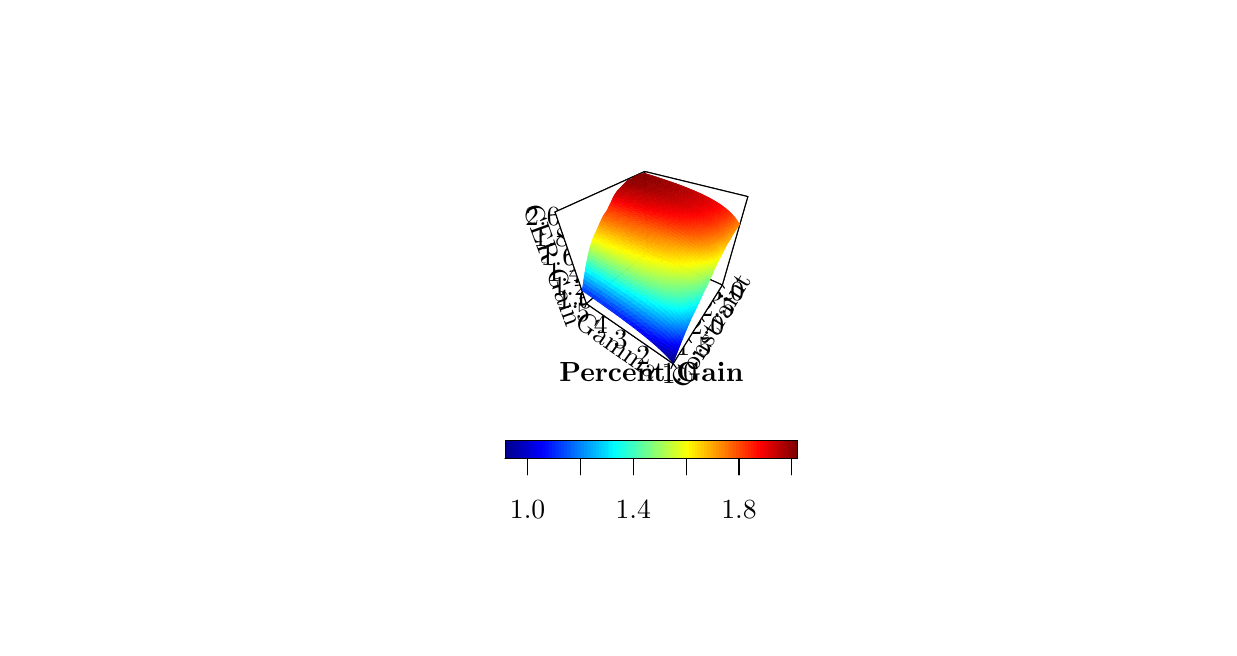
\begin{tikzpicture}[x=1pt,y=1pt]
\definecolor{fillColor}{RGB}{255,255,255}
\path[use as bounding box,fill=fillColor,fill opacity=0.00] (0,0) rectangle (426.79,216.81);
\begin{scope}
\path[clip] ( 49.20, 92.64) rectangle (401.59,167.61);
\definecolor{drawColor}{RGB}{0,0,0}

\path[draw=drawColor,line width= 0.4pt,line join=round,line cap=round] (201.91,117.08) -- (224.04,135.90);

\path[draw=drawColor,line width= 0.4pt,line join=round,line cap=round] (224.04,135.90) -- (222.97,164.83);

\path[draw=drawColor,line width= 0.4pt,line join=round,line cap=round] (222.97,164.83) -- (190.57,150.20);

\path[draw=drawColor,line width= 0.4pt,line join=round,line cap=round] (190.57,150.20) -- (201.91,117.08);

\path[draw=drawColor,line width= 0.4pt,line join=round,line cap=round] (251.01,123.81) -- (260.22,155.77);

\path[draw=drawColor,line width= 0.4pt,line join=round,line cap=round] (260.22,155.77) -- (222.97,164.83);

\path[draw=drawColor,line width= 0.4pt,line join=round,line cap=round] (224.04,135.90) -- (251.01,123.81);

\path[draw=drawColor,line width= 0.4pt,line join=round,line cap=round] (233.23, 95.41) -- (251.01,123.81);

\path[draw=drawColor,line width= 0.4pt,line join=round,line cap=round] (201.91,117.08) -- (233.23, 95.41);
\end{scope}
\begin{scope}
\path[clip] (  0.00,  0.00) rectangle (426.79,216.81);
\definecolor{drawColor}{RGB}{0,0,0}

\node[text=drawColor,rotate= 58.75,anchor=base,inner sep=0pt, outer sep=6pt, scale=  1.00] at (249.64,105.72) {Constraint};

\path[draw=drawColor,line width= 0.4pt,line join=round,line cap=round] (233.23, 95.41) -- (234.35, 93.98);

\node[text=drawColor,anchor=base,inner sep=0pt, outer sep=0pt, scale=  1.00] at (235.46, 89.11) {1.0};

\path[draw=drawColor,line width= 0.4pt,line join=round,line cap=round] (238.83,104.36) -- (239.83,103.02);

\node[text=drawColor,anchor=base,inner sep=0pt, outer sep=0pt, scale=  1.00] at (240.83, 98.24) {1.5};

\path[draw=drawColor,line width= 0.4pt,line join=round,line cap=round] (243.54,111.88) -- (244.45,110.62);

\node[text=drawColor,anchor=base,inner sep=0pt, outer sep=0pt, scale=  1.00] at (245.35,105.92) {2.0};

\path[draw=drawColor,line width= 0.4pt,line join=round,line cap=round] (247.55,118.28) -- (248.38,117.10);

\node[text=drawColor,anchor=base,inner sep=0pt, outer sep=0pt, scale=  1.00] at (249.20,112.48) {2.5};

\path[draw=drawColor,line width= 0.4pt,line join=round,line cap=round] (251.01,123.81) -- (251.77,122.69);

\node[text=drawColor,anchor=base,inner sep=0pt, outer sep=0pt, scale=  1.00] at (252.53,118.14) {3.0};

\node[text=drawColor,rotate=-35.29,anchor=base,inner sep=0pt, outer sep=6pt, scale=  1.00] at (211.28, 99.16) {Gamma};

\path[draw=drawColor,line width= 0.4pt,line join=round,line cap=round] (233.23, 95.41) -- (232.43, 93.62);

\node[text=drawColor,anchor=base,inner sep=0pt, outer sep=0pt, scale=  1.00] at (231.63, 88.38) {1};

\path[draw=drawColor,line width= 0.4pt,line join=round,line cap=round] (223.94,101.84) -- (223.19,100.16);

\node[text=drawColor,anchor=base,inner sep=0pt, outer sep=0pt, scale=  1.00] at (222.44, 95.03) {2};

\path[draw=drawColor,line width= 0.4pt,line join=round,line cap=round] (215.74,107.52) -- (215.03,105.93);

\node[text=drawColor,anchor=base,inner sep=0pt, outer sep=0pt, scale=  1.00] at (214.33,100.90) {3};

\path[draw=drawColor,line width= 0.4pt,line join=round,line cap=round] (208.44,112.57) -- (207.78,111.07);

\node[text=drawColor,anchor=base,inner sep=0pt, outer sep=0pt, scale=  1.00] at (207.12,106.12) {4};

\path[draw=drawColor,line width= 0.4pt,line join=round,line cap=round] (201.91,117.08) -- (201.29,115.66);

\node[text=drawColor,anchor=base,inner sep=0pt, outer sep=0pt, scale=  1.00] at (200.66,110.80) {5};

\node[text=drawColor,rotate=-69.94,anchor=base,inner sep=0pt, outer sep=6pt, scale=  1.00] at (186.77,129.87) {CER Gain};

\path[draw=drawColor,line width= 0.4pt,line join=round,line cap=round] (201.16,119.28) -- (199.50,119.06);

\node[text=drawColor,anchor=base,inner sep=0pt, outer sep=0pt, scale=  1.00] at (197.83,115.39) {1.0};

\path[draw=drawColor,line width= 0.4pt,line join=round,line cap=round] (199.60,123.85) -- (197.83,123.63);

\node[text=drawColor,anchor=base,inner sep=0pt, outer sep=0pt, scale=  1.00] at (196.06,119.96) {1.2};

\path[draw=drawColor,line width= 0.4pt,line join=round,line cap=round] (197.83,128.99) -- (195.95,128.78);

\node[text=drawColor,anchor=base,inner sep=0pt, outer sep=0pt, scale=  1.00] at (194.06,125.11) {1.4};

\path[draw=drawColor,line width= 0.4pt,line join=round,line cap=round] (195.83,134.84) -- (193.82,134.62);

\node[text=drawColor,anchor=base,inner sep=0pt, outer sep=0pt, scale=  1.00] at (191.79,130.96) {1.6};

\path[draw=drawColor,line width= 0.4pt,line join=round,line cap=round] (193.54,141.52) -- (191.37,141.32);

\node[text=drawColor,anchor=base,inner sep=0pt, outer sep=0pt, scale=  1.00] at (189.19,137.67) {1.8};

\path[draw=drawColor,line width= 0.4pt,line join=round,line cap=round] (190.89,149.25) -- (188.55,149.06);

\node[text=drawColor,anchor=base,inner sep=0pt, outer sep=0pt, scale=  1.00] at (186.18,145.42) {2.0};
\end{scope}
\begin{scope}
\path[clip] ( 49.20, 92.64) rectangle (401.59,167.61);

\path[] (233.23, 95.41) --
	(260.22,155.77) --
	(222.97,164.83) --
	(201.91,117.08) --
	(233.23, 95.41);
\definecolor{drawColor}{RGB}{0,0,0}

\path[draw=drawColor,line width= 0.4pt,dash pattern=on 1pt off 3pt ,line join=round,line cap=round] (233.23, 95.41) -- (236.86,129.15);

\path[draw=drawColor,line width= 0.4pt,dash pattern=on 1pt off 3pt ,line join=round,line cap=round] (236.86,129.15) -- (260.22,155.77);

\path[draw=drawColor,line width= 0.4pt,dash pattern=on 1pt off 3pt ,line join=round,line cap=round] (190.57,150.20) -- (236.86,129.15);
\definecolor{fillColor}{RGB}{255,255,255}

\path[fill=fillColor] (201.91,117.08) --
	(224.04,135.90) --
	(222.97,164.83) --
	(190.57,150.20) --
	(201.91,117.08) --
	cycle;

\path[draw=drawColor,line width= 0.4pt,line join=round,line cap=round] (201.91,117.08) --
	(224.04,135.90) --
	(222.97,164.83) --
	(190.57,150.20) --
	(201.91,117.08);

\path[fill=fillColor] (251.01,123.81) --
	(260.22,155.77) --
	(222.97,164.83) --
	(224.04,135.90) --
	(251.01,123.81) --
	cycle;

\path[draw=drawColor,line width= 0.4pt,line join=round,line cap=round] (251.01,123.81) --
	(260.22,155.77) --
	(222.97,164.83) --
	(224.04,135.90) --
	(251.01,123.81);

\path[fill=fillColor] (233.23, 95.41) --
	(251.01,123.81) --
	(224.04,135.90) --
	(201.91,117.08) --
	(233.23, 95.41) --
	cycle;

\path[draw=drawColor,line width= 0.4pt,line join=round,line cap=round] (233.23, 95.41) --
	(251.01,123.81) --
	(224.04,135.90) --
	(201.91,117.08) --
	(233.23, 95.41);
\definecolor{fillColor}{RGB}{148,0,0}

\path[fill=fillColor] (222.85,164.10) --
	(223.24,164.16) --
	(222.99,164.24) --
	(222.61,164.18) --
	cycle;

\path[fill=fillColor] (222.85,164.10) --
	(223.24,164.16) --
	(222.99,164.24) --
	(222.61,164.18) --
	cycle;

\path[fill=fillColor] (223.10,164.02) --
	(223.48,164.09) --
	(223.24,164.16) --
	(222.85,164.10) --
	cycle;

\path[fill=fillColor] (223.10,164.02) --
	(223.48,164.09) --
	(223.24,164.16) --
	(222.85,164.10) --
	cycle;

\path[fill=fillColor] (223.35,163.95) --
	(223.73,164.01) --
	(223.48,164.09) --
	(223.10,164.02) --
	cycle;

\path[fill=fillColor] (223.35,163.95) --
	(223.73,164.01) --
	(223.48,164.09) --
	(223.10,164.02) --
	cycle;

\path[fill=fillColor] (222.47,164.03) --
	(222.85,164.10) --
	(222.61,164.18) --
	(222.22,164.11) --
	cycle;

\path[fill=fillColor] (222.47,164.03) --
	(222.85,164.10) --
	(222.61,164.18) --
	(222.22,164.11) --
	cycle;

\path[fill=fillColor] (223.60,163.87) --
	(223.97,163.94) --
	(223.73,164.01) --
	(223.35,163.95) --
	cycle;

\path[fill=fillColor] (223.60,163.87) --
	(223.97,163.94) --
	(223.73,164.01) --
	(223.35,163.95) --
	cycle;

\path[fill=fillColor] (222.72,163.96) --
	(223.10,164.02) --
	(222.85,164.10) --
	(222.47,164.03) --
	cycle;

\path[fill=fillColor] (222.72,163.96) --
	(223.10,164.02) --
	(222.85,164.10) --
	(222.47,164.03) --
	cycle;

\path[fill=fillColor] (223.84,163.79) --
	(224.22,163.86) --
	(223.97,163.94) --
	(223.60,163.87) --
	cycle;

\path[fill=fillColor] (223.84,163.79) --
	(224.22,163.86) --
	(223.97,163.94) --
	(223.60,163.87) --
	cycle;

\path[fill=fillColor] (222.96,163.88) --
	(223.35,163.95) --
	(223.10,164.02) --
	(222.72,163.96) --
	cycle;

\path[fill=fillColor] (222.96,163.88) --
	(223.35,163.95) --
	(223.10,164.02) --
	(222.72,163.96) --
	cycle;

\path[fill=fillColor] (224.09,163.71) --
	(224.47,163.78) --
	(224.22,163.86) --
	(223.84,163.79) --
	cycle;

\path[fill=fillColor] (224.09,163.71) --
	(224.47,163.78) --
	(224.22,163.86) --
	(223.84,163.79) --
	cycle;
\definecolor{fillColor}{RGB}{138,0,0}

\path[fill=fillColor] (222.08,163.97) --
	(222.47,164.03) --
	(222.22,164.11) --
	(221.83,164.05) --
	cycle;

\path[fill=fillColor] (222.08,163.97) --
	(222.47,164.03) --
	(222.22,164.11) --
	(221.83,164.05) --
	cycle;
\definecolor{fillColor}{RGB}{148,0,0}

\path[fill=fillColor] (223.21,163.80) --
	(223.60,163.87) --
	(223.35,163.95) --
	(222.96,163.88) --
	cycle;

\path[fill=fillColor] (223.21,163.80) --
	(223.60,163.87) --
	(223.35,163.95) --
	(222.96,163.88) --
	cycle;

\path[fill=fillColor] (224.34,163.63) --
	(224.72,163.70) --
	(224.47,163.78) --
	(224.09,163.71) --
	cycle;

\path[fill=fillColor] (224.34,163.63) --
	(224.72,163.70) --
	(224.47,163.78) --
	(224.09,163.71) --
	cycle;
\definecolor{fillColor}{RGB}{138,0,0}

\path[fill=fillColor] (222.33,163.89) --
	(222.72,163.96) --
	(222.47,164.03) --
	(222.08,163.97) --
	cycle;

\path[fill=fillColor] (222.33,163.89) --
	(222.72,163.96) --
	(222.47,164.03) --
	(222.08,163.97) --
	cycle;
\definecolor{fillColor}{RGB}{148,0,0}

\path[fill=fillColor] (223.46,163.72) --
	(223.84,163.79) --
	(223.60,163.87) --
	(223.21,163.80) --
	cycle;

\path[fill=fillColor] (223.46,163.72) --
	(223.84,163.79) --
	(223.60,163.87) --
	(223.21,163.80) --
	cycle;

\path[fill=fillColor] (224.60,163.55) --
	(224.97,163.62) --
	(224.72,163.70) --
	(224.34,163.63) --
	cycle;

\path[fill=fillColor] (224.60,163.55) --
	(224.97,163.62) --
	(224.72,163.70) --
	(224.34,163.63) --
	cycle;
\definecolor{fillColor}{RGB}{138,0,0}

\path[fill=fillColor] (222.58,163.81) --
	(222.96,163.88) --
	(222.72,163.96) --
	(222.33,163.89) --
	cycle;

\path[fill=fillColor] (222.58,163.81) --
	(222.96,163.88) --
	(222.72,163.96) --
	(222.33,163.89) --
	cycle;
\definecolor{fillColor}{RGB}{148,0,0}

\path[fill=fillColor] (223.71,163.64) --
	(224.09,163.71) --
	(223.84,163.79) --
	(223.46,163.72) --
	cycle;

\path[fill=fillColor] (223.71,163.64) --
	(224.09,163.71) --
	(223.84,163.79) --
	(223.46,163.72) --
	cycle;

\path[fill=fillColor] (224.85,163.48) --
	(225.22,163.55) --
	(224.97,163.62) --
	(224.60,163.55) --
	cycle;

\path[fill=fillColor] (224.85,163.48) --
	(225.22,163.55) --
	(224.97,163.62) --
	(224.60,163.55) --
	cycle;
\definecolor{fillColor}{RGB}{138,0,0}

\path[fill=fillColor] (221.69,163.86) --
	(222.08,163.97) --
	(221.83,164.05) --
	(221.44,163.94) --
	cycle;

\path[fill=fillColor] (221.69,163.86) --
	(222.08,163.97) --
	(221.83,164.05) --
	(221.44,163.94) --
	cycle;

\path[fill=fillColor] (222.83,163.73) --
	(223.21,163.80) --
	(222.96,163.88) --
	(222.58,163.81) --
	cycle;

\path[fill=fillColor] (222.83,163.73) --
	(223.21,163.80) --
	(222.96,163.88) --
	(222.58,163.81) --
	cycle;
\definecolor{fillColor}{RGB}{148,0,0}

\path[fill=fillColor] (223.96,163.56) --
	(224.34,163.63) --
	(224.09,163.71) --
	(223.71,163.64) --
	cycle;

\path[fill=fillColor] (223.96,163.56) --
	(224.34,163.63) --
	(224.09,163.71) --
	(223.71,163.64) --
	cycle;

\path[fill=fillColor] (225.10,163.39) --
	(225.47,163.47) --
	(225.22,163.55) --
	(224.85,163.48) --
	cycle;

\path[fill=fillColor] (225.10,163.39) --
	(225.47,163.47) --
	(225.22,163.55) --
	(224.85,163.48) --
	cycle;
\definecolor{fillColor}{RGB}{138,0,0}

\path[fill=fillColor] (221.94,163.78) --
	(222.33,163.89) --
	(222.08,163.97) --
	(221.69,163.86) --
	cycle;

\path[fill=fillColor] (221.94,163.78) --
	(222.33,163.89) --
	(222.08,163.97) --
	(221.69,163.86) --
	cycle;

\path[fill=fillColor] (223.08,163.65) --
	(223.46,163.72) --
	(223.21,163.80) --
	(222.83,163.73) --
	cycle;

\path[fill=fillColor] (223.08,163.65) --
	(223.46,163.72) --
	(223.21,163.80) --
	(222.83,163.73) --
	cycle;
\definecolor{fillColor}{RGB}{148,0,0}

\path[fill=fillColor] (224.22,163.48) --
	(224.60,163.55) --
	(224.34,163.63) --
	(223.96,163.56) --
	cycle;

\path[fill=fillColor] (224.22,163.48) --
	(224.60,163.55) --
	(224.34,163.63) --
	(223.96,163.56) --
	cycle;

\path[fill=fillColor] (225.35,163.31) --
	(225.73,163.39) --
	(225.47,163.47) --
	(225.10,163.39) --
	cycle;

\path[fill=fillColor] (225.35,163.31) --
	(225.73,163.39) --
	(225.47,163.47) --
	(225.10,163.39) --
	cycle;
\definecolor{fillColor}{RGB}{138,0,0}

\path[fill=fillColor] (222.19,163.70) --
	(222.58,163.81) --
	(222.33,163.89) --
	(221.94,163.78) --
	cycle;

\path[fill=fillColor] (222.19,163.70) --
	(222.58,163.81) --
	(222.33,163.89) --
	(221.94,163.78) --
	cycle;
\definecolor{fillColor}{RGB}{148,0,0}

\path[fill=fillColor] (223.33,163.57) --
	(223.71,163.64) --
	(223.46,163.72) --
	(223.08,163.65) --
	cycle;

\path[fill=fillColor] (223.33,163.57) --
	(223.71,163.64) --
	(223.46,163.72) --
	(223.08,163.65) --
	cycle;

\path[fill=fillColor] (224.47,163.40) --
	(224.85,163.48) --
	(224.60,163.55) --
	(224.22,163.48) --
	cycle;

\path[fill=fillColor] (224.47,163.40) --
	(224.85,163.48) --
	(224.60,163.55) --
	(224.22,163.48) --
	cycle;

\path[fill=fillColor] (225.61,163.23) --
	(225.98,163.31) --
	(225.73,163.39) --
	(225.35,163.31) --
	cycle;

\path[fill=fillColor] (225.61,163.23) --
	(225.98,163.31) --
	(225.73,163.39) --
	(225.35,163.31) --
	cycle;
\definecolor{fillColor}{RGB}{138,0,0}

\path[fill=fillColor] (221.29,163.75) --
	(221.69,163.86) --
	(221.44,163.94) --
	(221.04,163.83) --
	cycle;

\path[fill=fillColor] (221.29,163.75) --
	(221.69,163.86) --
	(221.44,163.94) --
	(221.04,163.83) --
	cycle;

\path[fill=fillColor] (222.44,163.62) --
	(222.83,163.73) --
	(222.58,163.81) --
	(222.19,163.70) --
	cycle;

\path[fill=fillColor] (222.44,163.62) --
	(222.83,163.73) --
	(222.58,163.81) --
	(222.19,163.70) --
	cycle;
\definecolor{fillColor}{RGB}{148,0,0}

\path[fill=fillColor] (223.58,163.49) --
	(223.96,163.56) --
	(223.71,163.64) --
	(223.33,163.57) --
	cycle;

\path[fill=fillColor] (223.58,163.49) --
	(223.96,163.56) --
	(223.71,163.64) --
	(223.33,163.57) --
	cycle;

\path[fill=fillColor] (224.72,163.32) --
	(225.10,163.39) --
	(224.85,163.48) --
	(224.47,163.40) --
	cycle;

\path[fill=fillColor] (224.72,163.32) --
	(225.10,163.39) --
	(224.85,163.48) --
	(224.47,163.40) --
	cycle;

\path[fill=fillColor] (225.86,163.15) --
	(226.23,163.22) --
	(225.98,163.31) --
	(225.61,163.23) --
	cycle;

\path[fill=fillColor] (225.86,163.15) --
	(226.23,163.22) --
	(225.98,163.31) --
	(225.61,163.23) --
	cycle;
\definecolor{fillColor}{RGB}{138,0,0}

\path[fill=fillColor] (221.54,163.67) --
	(221.94,163.78) --
	(221.69,163.86) --
	(221.29,163.75) --
	cycle;

\path[fill=fillColor] (221.54,163.67) --
	(221.94,163.78) --
	(221.69,163.86) --
	(221.29,163.75) --
	cycle;

\path[fill=fillColor] (222.69,163.54) --
	(223.08,163.65) --
	(222.83,163.73) --
	(222.44,163.62) --
	cycle;

\path[fill=fillColor] (222.69,163.54) --
	(223.08,163.65) --
	(222.83,163.73) --
	(222.44,163.62) --
	cycle;
\definecolor{fillColor}{RGB}{148,0,0}

\path[fill=fillColor] (223.83,163.41) --
	(224.22,163.48) --
	(223.96,163.56) --
	(223.58,163.49) --
	cycle;

\path[fill=fillColor] (223.83,163.41) --
	(224.22,163.48) --
	(223.96,163.56) --
	(223.58,163.49) --
	cycle;

\path[fill=fillColor] (224.98,163.24) --
	(225.35,163.31) --
	(225.10,163.39) --
	(224.72,163.32) --
	cycle;

\path[fill=fillColor] (224.98,163.24) --
	(225.35,163.31) --
	(225.10,163.39) --
	(224.72,163.32) --
	cycle;

\path[fill=fillColor] (226.12,163.07) --
	(226.49,163.14) --
	(226.23,163.22) --
	(225.86,163.15) --
	cycle;

\path[fill=fillColor] (226.12,163.07) --
	(226.49,163.14) --
	(226.23,163.22) --
	(225.86,163.15) --
	cycle;
\definecolor{fillColor}{RGB}{138,0,0}

\path[fill=fillColor] (221.79,163.59) --
	(222.19,163.70) --
	(221.94,163.78) --
	(221.54,163.67) --
	cycle;

\path[fill=fillColor] (221.79,163.59) --
	(222.19,163.70) --
	(221.94,163.78) --
	(221.54,163.67) --
	cycle;

\path[fill=fillColor] (222.94,163.46) --
	(223.33,163.57) --
	(223.08,163.65) --
	(222.69,163.54) --
	cycle;

\path[fill=fillColor] (222.94,163.46) --
	(223.33,163.57) --
	(223.08,163.65) --
	(222.69,163.54) --
	cycle;
\definecolor{fillColor}{RGB}{148,0,0}

\path[fill=fillColor] (224.09,163.33) --
	(224.47,163.40) --
	(224.22,163.48) --
	(223.83,163.41) --
	cycle;

\path[fill=fillColor] (224.09,163.33) --
	(224.47,163.40) --
	(224.22,163.48) --
	(223.83,163.41) --
	cycle;

\path[fill=fillColor] (225.23,163.16) --
	(225.61,163.23) --
	(225.35,163.31) --
	(224.98,163.24) --
	cycle;

\path[fill=fillColor] (225.23,163.16) --
	(225.61,163.23) --
	(225.35,163.31) --
	(224.98,163.24) --
	cycle;
\definecolor{fillColor}{RGB}{158,0,0}

\path[fill=fillColor] (226.38,162.99) --
	(226.75,163.06) --
	(226.49,163.14) --
	(226.12,163.07) --
	cycle;

\path[fill=fillColor] (226.38,162.99) --
	(226.75,163.06) --
	(226.49,163.14) --
	(226.12,163.07) --
	cycle;
\definecolor{fillColor}{RGB}{138,0,0}

\path[fill=fillColor] (220.89,163.64) --
	(221.29,163.75) --
	(221.04,163.83) --
	(220.64,163.72) --
	cycle;

\path[fill=fillColor] (220.89,163.64) --
	(221.29,163.75) --
	(221.04,163.83) --
	(220.64,163.72) --
	cycle;

\path[fill=fillColor] (222.04,163.51) --
	(222.44,163.62) --
	(222.19,163.70) --
	(221.79,163.59) --
	cycle;

\path[fill=fillColor] (222.04,163.51) --
	(222.44,163.62) --
	(222.19,163.70) --
	(221.79,163.59) --
	cycle;

\path[fill=fillColor] (223.19,163.38) --
	(223.58,163.49) --
	(223.33,163.57) --
	(222.94,163.46) --
	cycle;

\path[fill=fillColor] (223.19,163.38) --
	(223.58,163.49) --
	(223.33,163.57) --
	(222.94,163.46) --
	cycle;
\definecolor{fillColor}{RGB}{148,0,0}

\path[fill=fillColor] (224.34,163.25) --
	(224.72,163.32) --
	(224.47,163.40) --
	(224.09,163.33) --
	cycle;

\path[fill=fillColor] (224.34,163.25) --
	(224.72,163.32) --
	(224.47,163.40) --
	(224.09,163.33) --
	cycle;

\path[fill=fillColor] (225.49,163.08) --
	(225.86,163.15) --
	(225.61,163.23) --
	(225.23,163.16) --
	cycle;

\path[fill=fillColor] (225.49,163.08) --
	(225.86,163.15) --
	(225.61,163.23) --
	(225.23,163.16) --
	cycle;
\definecolor{fillColor}{RGB}{158,0,0}

\path[fill=fillColor] (226.64,162.90) --
	(227.00,162.98) --
	(226.75,163.06) --
	(226.38,162.99) --
	cycle;

\path[fill=fillColor] (226.64,162.90) --
	(227.00,162.98) --
	(226.75,163.06) --
	(226.38,162.99) --
	cycle;
\definecolor{fillColor}{RGB}{138,0,0}

\path[fill=fillColor] (221.14,163.56) --
	(221.54,163.67) --
	(221.29,163.75) --
	(220.89,163.64) --
	cycle;

\path[fill=fillColor] (221.14,163.56) --
	(221.54,163.67) --
	(221.29,163.75) --
	(220.89,163.64) --
	cycle;

\path[fill=fillColor] (222.29,163.43) --
	(222.69,163.54) --
	(222.44,163.62) --
	(222.04,163.51) --
	cycle;

\path[fill=fillColor] (222.29,163.43) --
	(222.69,163.54) --
	(222.44,163.62) --
	(222.04,163.51) --
	cycle;

\path[fill=fillColor] (223.45,163.30) --
	(223.83,163.41) --
	(223.58,163.49) --
	(223.19,163.38) --
	cycle;

\path[fill=fillColor] (223.45,163.30) --
	(223.83,163.41) --
	(223.58,163.49) --
	(223.19,163.38) --
	cycle;
\definecolor{fillColor}{RGB}{148,0,0}

\path[fill=fillColor] (224.60,163.17) --
	(224.98,163.24) --
	(224.72,163.32) --
	(224.34,163.25) --
	cycle;

\path[fill=fillColor] (224.60,163.17) --
	(224.98,163.24) --
	(224.72,163.32) --
	(224.34,163.25) --
	cycle;

\path[fill=fillColor] (225.75,162.99) --
	(226.12,163.07) --
	(225.86,163.15) --
	(225.49,163.08) --
	cycle;

\path[fill=fillColor] (225.75,162.99) --
	(226.12,163.07) --
	(225.86,163.15) --
	(225.49,163.08) --
	cycle;
\definecolor{fillColor}{RGB}{158,0,0}

\path[fill=fillColor] (226.89,162.82) --
	(227.26,162.90) --
	(227.00,162.98) --
	(226.64,162.90) --
	cycle;

\path[fill=fillColor] (226.89,162.82) --
	(227.26,162.90) --
	(227.00,162.98) --
	(226.64,162.90) --
	cycle;
\definecolor{fillColor}{RGB}{138,0,0}

\path[fill=fillColor] (221.39,163.48) --
	(221.79,163.59) --
	(221.54,163.67) --
	(221.14,163.56) --
	cycle;

\path[fill=fillColor] (221.39,163.48) --
	(221.79,163.59) --
	(221.54,163.67) --
	(221.14,163.56) --
	cycle;

\path[fill=fillColor] (222.55,163.34) --
	(222.94,163.46) --
	(222.69,163.54) --
	(222.29,163.43) --
	cycle;

\path[fill=fillColor] (222.55,163.34) --
	(222.94,163.46) --
	(222.69,163.54) --
	(222.29,163.43) --
	cycle;

\path[fill=fillColor] (223.70,163.21) --
	(224.09,163.33) --
	(223.83,163.41) --
	(223.45,163.30) --
	cycle;

\path[fill=fillColor] (223.70,163.21) --
	(224.09,163.33) --
	(223.83,163.41) --
	(223.45,163.30) --
	cycle;
\definecolor{fillColor}{RGB}{148,0,0}

\path[fill=fillColor] (224.85,163.08) --
	(225.23,163.16) --
	(224.98,163.24) --
	(224.60,163.17) --
	cycle;

\path[fill=fillColor] (224.85,163.08) --
	(225.23,163.16) --
	(224.98,163.24) --
	(224.60,163.17) --
	cycle;

\path[fill=fillColor] (226.01,162.91) --
	(226.38,162.99) --
	(226.12,163.07) --
	(225.75,162.99) --
	cycle;

\path[fill=fillColor] (226.01,162.91) --
	(226.38,162.99) --
	(226.12,163.07) --
	(225.75,162.99) --
	cycle;
\definecolor{fillColor}{RGB}{158,0,0}

\path[fill=fillColor] (227.15,162.73) --
	(227.52,162.81) --
	(227.26,162.90) --
	(226.89,162.82) --
	cycle;

\path[fill=fillColor] (227.15,162.73) --
	(227.52,162.81) --
	(227.26,162.90) --
	(226.89,162.82) --
	cycle;
\definecolor{fillColor}{RGB}{138,0,0}

\path[fill=fillColor] (220.49,163.47) --
	(220.89,163.64) --
	(220.64,163.72) --
	(220.24,163.56) --
	cycle;

\path[fill=fillColor] (220.49,163.47) --
	(220.89,163.64) --
	(220.64,163.72) --
	(220.24,163.56) --
	cycle;

\path[fill=fillColor] (221.64,163.39) --
	(222.04,163.51) --
	(221.79,163.59) --
	(221.39,163.48) --
	cycle;

\path[fill=fillColor] (221.64,163.39) --
	(222.04,163.51) --
	(221.79,163.59) --
	(221.39,163.48) --
	cycle;

\path[fill=fillColor] (222.80,163.26) --
	(223.19,163.38) --
	(222.94,163.46) --
	(222.55,163.34) --
	cycle;

\path[fill=fillColor] (222.80,163.26) --
	(223.19,163.38) --
	(222.94,163.46) --
	(222.55,163.34) --
	cycle;

\path[fill=fillColor] (223.96,163.13) --
	(224.34,163.25) --
	(224.09,163.33) --
	(223.70,163.21) --
	cycle;

\path[fill=fillColor] (223.96,163.13) --
	(224.34,163.25) --
	(224.09,163.33) --
	(223.70,163.21) --
	cycle;
\definecolor{fillColor}{RGB}{148,0,0}

\path[fill=fillColor] (225.11,163.00) --
	(225.49,163.08) --
	(225.23,163.16) --
	(224.85,163.08) --
	cycle;

\path[fill=fillColor] (225.11,163.00) --
	(225.49,163.08) --
	(225.23,163.16) --
	(224.85,163.08) --
	cycle;

\path[fill=fillColor] (226.26,162.82) --
	(226.64,162.90) --
	(226.38,162.99) --
	(226.01,162.91) --
	cycle;

\path[fill=fillColor] (226.26,162.82) --
	(226.64,162.90) --
	(226.38,162.99) --
	(226.01,162.91) --
	cycle;
\definecolor{fillColor}{RGB}{158,0,0}

\path[fill=fillColor] (227.42,162.65) --
	(227.78,162.73) --
	(227.52,162.81) --
	(227.15,162.73) --
	cycle;

\path[fill=fillColor] (227.42,162.65) --
	(227.78,162.73) --
	(227.52,162.81) --
	(227.15,162.73) --
	cycle;
\definecolor{fillColor}{RGB}{138,0,0}

\path[fill=fillColor] (220.74,163.39) --
	(221.14,163.56) --
	(220.89,163.64) --
	(220.49,163.47) --
	cycle;

\path[fill=fillColor] (220.74,163.39) --
	(221.14,163.56) --
	(220.89,163.64) --
	(220.49,163.47) --
	cycle;

\path[fill=fillColor] (221.90,163.31) --
	(222.29,163.43) --
	(222.04,163.51) --
	(221.64,163.39) --
	cycle;

\path[fill=fillColor] (221.90,163.31) --
	(222.29,163.43) --
	(222.04,163.51) --
	(221.64,163.39) --
	cycle;

\path[fill=fillColor] (223.06,163.18) --
	(223.45,163.30) --
	(223.19,163.38) --
	(222.80,163.26) --
	cycle;

\path[fill=fillColor] (223.06,163.18) --
	(223.45,163.30) --
	(223.19,163.38) --
	(222.80,163.26) --
	cycle;
\definecolor{fillColor}{RGB}{148,0,0}

\path[fill=fillColor] (224.21,163.05) --
	(224.60,163.17) --
	(224.34,163.25) --
	(223.96,163.13) --
	cycle;

\path[fill=fillColor] (224.21,163.05) --
	(224.60,163.17) --
	(224.34,163.25) --
	(223.96,163.13) --
	cycle;

\path[fill=fillColor] (225.37,162.92) --
	(225.75,162.99) --
	(225.49,163.08) --
	(225.11,163.00) --
	cycle;

\path[fill=fillColor] (225.37,162.92) --
	(225.75,162.99) --
	(225.49,163.08) --
	(225.11,163.00) --
	cycle;

\path[fill=fillColor] (226.52,162.74) --
	(226.89,162.82) --
	(226.64,162.90) --
	(226.26,162.82) --
	cycle;

\path[fill=fillColor] (226.52,162.74) --
	(226.89,162.82) --
	(226.64,162.90) --
	(226.26,162.82) --
	cycle;
\definecolor{fillColor}{RGB}{158,0,0}

\path[fill=fillColor] (227.68,162.56) --
	(228.04,162.64) --
	(227.78,162.73) --
	(227.42,162.65) --
	cycle;

\path[fill=fillColor] (227.68,162.56) --
	(228.04,162.64) --
	(227.78,162.73) --
	(227.42,162.65) --
	cycle;
\definecolor{fillColor}{RGB}{138,0,0}

\path[fill=fillColor] (220.99,163.31) --
	(221.39,163.48) --
	(221.14,163.56) --
	(220.74,163.39) --
	cycle;

\path[fill=fillColor] (220.99,163.31) --
	(221.39,163.48) --
	(221.14,163.56) --
	(220.74,163.39) --
	cycle;

\path[fill=fillColor] (222.15,163.23) --
	(222.55,163.34) --
	(222.29,163.43) --
	(221.90,163.31) --
	cycle;

\path[fill=fillColor] (222.15,163.23) --
	(222.55,163.34) --
	(222.29,163.43) --
	(221.90,163.31) --
	cycle;

\path[fill=fillColor] (223.31,163.10) --
	(223.70,163.21) --
	(223.45,163.30) --
	(223.06,163.18) --
	cycle;

\path[fill=fillColor] (223.31,163.10) --
	(223.70,163.21) --
	(223.45,163.30) --
	(223.06,163.18) --
	cycle;
\definecolor{fillColor}{RGB}{148,0,0}

\path[fill=fillColor] (224.47,162.96) --
	(224.85,163.08) --
	(224.60,163.17) --
	(224.21,163.05) --
	cycle;

\path[fill=fillColor] (224.47,162.96) --
	(224.85,163.08) --
	(224.60,163.17) --
	(224.21,163.05) --
	cycle;

\path[fill=fillColor] (225.63,162.83) --
	(226.01,162.91) --
	(225.75,162.99) --
	(225.37,162.92) --
	cycle;

\path[fill=fillColor] (225.63,162.83) --
	(226.01,162.91) --
	(225.75,162.99) --
	(225.37,162.92) --
	cycle;

\path[fill=fillColor] (226.79,162.65) --
	(227.15,162.73) --
	(226.89,162.82) --
	(226.52,162.74) --
	cycle;

\path[fill=fillColor] (226.79,162.65) --
	(227.15,162.73) --
	(226.89,162.82) --
	(226.52,162.74) --
	cycle;
\definecolor{fillColor}{RGB}{138,0,0}

\path[fill=fillColor] (220.08,163.31) --
	(220.49,163.47) --
	(220.24,163.56) --
	(219.83,163.39) --
	cycle;

\path[fill=fillColor] (220.08,163.31) --
	(220.49,163.47) --
	(220.24,163.56) --
	(219.83,163.39) --
	cycle;
\definecolor{fillColor}{RGB}{158,0,0}

\path[fill=fillColor] (227.94,162.48) --
	(228.30,162.56) --
	(228.04,162.64) --
	(227.68,162.56) --
	cycle;

\path[fill=fillColor] (227.94,162.48) --
	(228.30,162.56) --
	(228.04,162.64) --
	(227.68,162.56) --
	cycle;
\definecolor{fillColor}{RGB}{138,0,0}

\path[fill=fillColor] (221.24,163.23) --
	(221.64,163.39) --
	(221.39,163.48) --
	(220.99,163.31) --
	cycle;

\path[fill=fillColor] (221.24,163.23) --
	(221.64,163.39) --
	(221.39,163.48) --
	(220.99,163.31) --
	cycle;

\path[fill=fillColor] (222.40,163.14) --
	(222.80,163.26) --
	(222.55,163.34) --
	(222.15,163.23) --
	cycle;

\path[fill=fillColor] (222.40,163.14) --
	(222.80,163.26) --
	(222.55,163.34) --
	(222.15,163.23) --
	cycle;

\path[fill=fillColor] (223.57,163.01) --
	(223.96,163.13) --
	(223.70,163.21) --
	(223.31,163.10) --
	cycle;

\path[fill=fillColor] (223.57,163.01) --
	(223.96,163.13) --
	(223.70,163.21) --
	(223.31,163.10) --
	cycle;
\definecolor{fillColor}{RGB}{148,0,0}

\path[fill=fillColor] (224.73,162.88) --
	(225.11,163.00) --
	(224.85,163.08) --
	(224.47,162.96) --
	cycle;

\path[fill=fillColor] (224.73,162.88) --
	(225.11,163.00) --
	(224.85,163.08) --
	(224.47,162.96) --
	cycle;

\path[fill=fillColor] (225.89,162.74) --
	(226.26,162.82) --
	(226.01,162.91) --
	(225.63,162.83) --
	cycle;

\path[fill=fillColor] (225.89,162.74) --
	(226.26,162.82) --
	(226.01,162.91) --
	(225.63,162.83) --
	cycle;

\path[fill=fillColor] (227.05,162.57) --
	(227.42,162.65) --
	(227.15,162.73) --
	(226.79,162.65) --
	cycle;

\path[fill=fillColor] (227.05,162.57) --
	(227.42,162.65) --
	(227.15,162.73) --
	(226.79,162.65) --
	cycle;
\definecolor{fillColor}{RGB}{138,0,0}

\path[fill=fillColor] (220.33,163.23) --
	(220.74,163.39) --
	(220.49,163.47) --
	(220.08,163.31) --
	cycle;

\path[fill=fillColor] (220.33,163.23) --
	(220.74,163.39) --
	(220.49,163.47) --
	(220.08,163.31) --
	cycle;
\definecolor{fillColor}{RGB}{158,0,0}

\path[fill=fillColor] (228.20,162.39) --
	(228.56,162.47) --
	(228.30,162.56) --
	(227.94,162.48) --
	cycle;

\path[fill=fillColor] (228.20,162.39) --
	(228.56,162.47) --
	(228.30,162.56) --
	(227.94,162.48) --
	cycle;
\definecolor{fillColor}{RGB}{138,0,0}

\path[fill=fillColor] (221.50,163.14) --
	(221.90,163.31) --
	(221.64,163.39) --
	(221.24,163.23) --
	cycle;

\path[fill=fillColor] (221.50,163.14) --
	(221.90,163.31) --
	(221.64,163.39) --
	(221.24,163.23) --
	cycle;

\path[fill=fillColor] (222.66,163.06) --
	(223.06,163.18) --
	(222.80,163.26) --
	(222.40,163.14) --
	cycle;

\path[fill=fillColor] (222.66,163.06) --
	(223.06,163.18) --
	(222.80,163.26) --
	(222.40,163.14) --
	cycle;

\path[fill=fillColor] (223.82,162.93) --
	(224.21,163.05) --
	(223.96,163.13) --
	(223.57,163.01) --
	cycle;

\path[fill=fillColor] (223.82,162.93) --
	(224.21,163.05) --
	(223.96,163.13) --
	(223.57,163.01) --
	cycle;
\definecolor{fillColor}{RGB}{148,0,0}

\path[fill=fillColor] (224.99,162.79) --
	(225.37,162.92) --
	(225.11,163.00) --
	(224.73,162.88) --
	cycle;

\path[fill=fillColor] (224.99,162.79) --
	(225.37,162.92) --
	(225.11,163.00) --
	(224.73,162.88) --
	cycle;

\path[fill=fillColor] (226.15,162.66) --
	(226.52,162.74) --
	(226.26,162.82) --
	(225.89,162.74) --
	cycle;

\path[fill=fillColor] (226.15,162.66) --
	(226.52,162.74) --
	(226.26,162.82) --
	(225.89,162.74) --
	cycle;
\definecolor{fillColor}{RGB}{158,0,0}

\path[fill=fillColor] (227.31,162.48) --
	(227.68,162.56) --
	(227.42,162.65) --
	(227.05,162.57) --
	cycle;

\path[fill=fillColor] (227.31,162.48) --
	(227.68,162.56) --
	(227.42,162.65) --
	(227.05,162.57) --
	cycle;
\definecolor{fillColor}{RGB}{138,0,0}

\path[fill=fillColor] (220.58,163.15) --
	(220.99,163.31) --
	(220.74,163.39) --
	(220.33,163.23) --
	cycle;

\path[fill=fillColor] (220.58,163.15) --
	(220.99,163.31) --
	(220.74,163.39) --
	(220.33,163.23) --
	cycle;
\definecolor{fillColor}{RGB}{158,0,0}

\path[fill=fillColor] (228.47,162.30) --
	(228.83,162.39) --
	(228.56,162.47) --
	(228.20,162.39) --
	cycle;

\path[fill=fillColor] (228.47,162.30) --
	(228.83,162.39) --
	(228.56,162.47) --
	(228.20,162.39) --
	cycle;
\definecolor{fillColor}{RGB}{138,0,0}

\path[fill=fillColor] (221.75,163.06) --
	(222.15,163.23) --
	(221.90,163.31) --
	(221.50,163.14) --
	cycle;

\path[fill=fillColor] (221.75,163.06) --
	(222.15,163.23) --
	(221.90,163.31) --
	(221.50,163.14) --
	cycle;

\path[fill=fillColor] (222.92,162.98) --
	(223.31,163.10) --
	(223.06,163.18) --
	(222.66,163.06) --
	cycle;

\path[fill=fillColor] (222.92,162.98) --
	(223.31,163.10) --
	(223.06,163.18) --
	(222.66,163.06) --
	cycle;

\path[fill=fillColor] (224.08,162.84) --
	(224.47,162.96) --
	(224.21,163.05) --
	(223.82,162.93) --
	cycle;

\path[fill=fillColor] (224.08,162.84) --
	(224.47,162.96) --
	(224.21,163.05) --
	(223.82,162.93) --
	cycle;
\definecolor{fillColor}{RGB}{148,0,0}

\path[fill=fillColor] (225.25,162.71) --
	(225.63,162.83) --
	(225.37,162.92) --
	(224.99,162.79) --
	cycle;

\path[fill=fillColor] (225.25,162.71) --
	(225.63,162.83) --
	(225.37,162.92) --
	(224.99,162.79) --
	cycle;

\path[fill=fillColor] (226.41,162.57) --
	(226.79,162.65) --
	(226.52,162.74) --
	(226.15,162.66) --
	cycle;

\path[fill=fillColor] (226.41,162.57) --
	(226.79,162.65) --
	(226.52,162.74) --
	(226.15,162.66) --
	cycle;
\definecolor{fillColor}{RGB}{128,0,0}

\path[fill=fillColor] (219.67,163.15) --
	(220.08,163.31) --
	(219.83,163.39) --
	(219.42,163.23) --
	cycle;

\path[fill=fillColor] (219.67,163.15) --
	(220.08,163.31) --
	(219.83,163.39) --
	(219.42,163.23) --
	cycle;
\definecolor{fillColor}{RGB}{158,0,0}

\path[fill=fillColor] (227.57,162.39) --
	(227.94,162.48) --
	(227.68,162.56) --
	(227.31,162.48) --
	cycle;

\path[fill=fillColor] (227.57,162.39) --
	(227.94,162.48) --
	(227.68,162.56) --
	(227.31,162.48) --
	cycle;
\definecolor{fillColor}{RGB}{138,0,0}

\path[fill=fillColor] (220.84,163.06) --
	(221.24,163.23) --
	(220.99,163.31) --
	(220.58,163.15) --
	cycle;

\path[fill=fillColor] (220.84,163.06) --
	(221.24,163.23) --
	(220.99,163.31) --
	(220.58,163.15) --
	cycle;
\definecolor{fillColor}{RGB}{158,0,0}

\path[fill=fillColor] (228.73,162.21) --
	(229.09,162.30) --
	(228.83,162.39) --
	(228.47,162.30) --
	cycle;

\path[fill=fillColor] (228.73,162.21) --
	(229.09,162.30) --
	(228.83,162.39) --
	(228.47,162.30) --
	cycle;
\definecolor{fillColor}{RGB}{138,0,0}

\path[fill=fillColor] (222.01,162.98) --
	(222.40,163.14) --
	(222.15,163.23) --
	(221.75,163.06) --
	cycle;

\path[fill=fillColor] (222.01,162.98) --
	(222.40,163.14) --
	(222.15,163.23) --
	(221.75,163.06) --
	cycle;

\path[fill=fillColor] (223.17,162.89) --
	(223.57,163.01) --
	(223.31,163.10) --
	(222.92,162.98) --
	cycle;

\path[fill=fillColor] (223.17,162.89) --
	(223.57,163.01) --
	(223.31,163.10) --
	(222.92,162.98) --
	cycle;

\path[fill=fillColor] (224.34,162.76) --
	(224.73,162.88) --
	(224.47,162.96) --
	(224.08,162.84) --
	cycle;

\path[fill=fillColor] (224.34,162.76) --
	(224.73,162.88) --
	(224.47,162.96) --
	(224.08,162.84) --
	cycle;
\definecolor{fillColor}{RGB}{148,0,0}

\path[fill=fillColor] (225.51,162.62) --
	(225.89,162.74) --
	(225.63,162.83) --
	(225.25,162.71) --
	cycle;

\path[fill=fillColor] (225.51,162.62) --
	(225.89,162.74) --
	(225.63,162.83) --
	(225.25,162.71) --
	cycle;

\path[fill=fillColor] (226.67,162.49) --
	(227.05,162.57) --
	(226.79,162.65) --
	(226.41,162.57) --
	cycle;

\path[fill=fillColor] (226.67,162.49) --
	(227.05,162.57) --
	(226.79,162.65) --
	(226.41,162.57) --
	cycle;
\definecolor{fillColor}{RGB}{138,0,0}

\path[fill=fillColor] (219.92,163.06) --
	(220.33,163.23) --
	(220.08,163.31) --
	(219.67,163.15) --
	cycle;

\path[fill=fillColor] (219.92,163.06) --
	(220.33,163.23) --
	(220.08,163.31) --
	(219.67,163.15) --
	cycle;
\definecolor{fillColor}{RGB}{158,0,0}

\path[fill=fillColor] (227.84,162.30) --
	(228.20,162.39) --
	(227.94,162.48) --
	(227.57,162.39) --
	cycle;

\path[fill=fillColor] (227.84,162.30) --
	(228.20,162.39) --
	(227.94,162.48) --
	(227.57,162.39) --
	cycle;
\definecolor{fillColor}{RGB}{138,0,0}

\path[fill=fillColor] (221.09,162.98) --
	(221.50,163.14) --
	(221.24,163.23) --
	(220.84,163.06) --
	cycle;

\path[fill=fillColor] (221.09,162.98) --
	(221.50,163.14) --
	(221.24,163.23) --
	(220.84,163.06) --
	cycle;
\definecolor{fillColor}{RGB}{158,0,0}

\path[fill=fillColor] (229.00,162.12) --
	(229.35,162.21) --
	(229.09,162.30) --
	(228.73,162.21) --
	cycle;

\path[fill=fillColor] (229.00,162.12) --
	(229.35,162.21) --
	(229.09,162.30) --
	(228.73,162.21) --
	cycle;
\definecolor{fillColor}{RGB}{138,0,0}

\path[fill=fillColor] (222.26,162.89) --
	(222.66,163.06) --
	(222.40,163.14) --
	(222.01,162.98) --
	cycle;

\path[fill=fillColor] (222.26,162.89) --
	(222.66,163.06) --
	(222.40,163.14) --
	(222.01,162.98) --
	cycle;

\path[fill=fillColor] (223.43,162.81) --
	(223.82,162.93) --
	(223.57,163.01) --
	(223.17,162.89) --
	cycle;

\path[fill=fillColor] (223.43,162.81) --
	(223.82,162.93) --
	(223.57,163.01) --
	(223.17,162.89) --
	cycle;
\definecolor{fillColor}{RGB}{148,0,0}

\path[fill=fillColor] (224.60,162.67) --
	(224.99,162.79) --
	(224.73,162.88) --
	(224.34,162.76) --
	cycle;

\path[fill=fillColor] (224.60,162.67) --
	(224.99,162.79) --
	(224.73,162.88) --
	(224.34,162.76) --
	cycle;

\path[fill=fillColor] (225.77,162.53) --
	(226.15,162.66) --
	(225.89,162.74) --
	(225.51,162.62) --
	cycle;

\path[fill=fillColor] (225.77,162.53) --
	(226.15,162.66) --
	(225.89,162.74) --
	(225.51,162.62) --
	cycle;

\path[fill=fillColor] (226.94,162.40) --
	(227.31,162.48) --
	(227.05,162.57) --
	(226.67,162.49) --
	cycle;

\path[fill=fillColor] (226.94,162.40) --
	(227.31,162.48) --
	(227.05,162.57) --
	(226.67,162.49) --
	cycle;
\definecolor{fillColor}{RGB}{138,0,0}

\path[fill=fillColor] (220.17,162.98) --
	(220.58,163.15) --
	(220.33,163.23) --
	(219.92,163.06) --
	cycle;

\path[fill=fillColor] (220.17,162.98) --
	(220.58,163.15) --
	(220.33,163.23) --
	(219.92,163.06) --
	cycle;
\definecolor{fillColor}{RGB}{158,0,0}

\path[fill=fillColor] (228.10,162.22) --
	(228.47,162.30) --
	(228.20,162.39) --
	(227.84,162.30) --
	cycle;

\path[fill=fillColor] (228.10,162.22) --
	(228.47,162.30) --
	(228.20,162.39) --
	(227.84,162.30) --
	cycle;
\definecolor{fillColor}{RGB}{138,0,0}

\path[fill=fillColor] (221.35,162.89) --
	(221.75,163.06) --
	(221.50,163.14) --
	(221.09,162.98) --
	cycle;

\path[fill=fillColor] (221.35,162.89) --
	(221.75,163.06) --
	(221.50,163.14) --
	(221.09,162.98) --
	cycle;
\definecolor{fillColor}{RGB}{158,0,0}

\path[fill=fillColor] (229.26,162.03) --
	(229.62,162.12) --
	(229.35,162.21) --
	(229.00,162.12) --
	cycle;

\path[fill=fillColor] (229.26,162.03) --
	(229.62,162.12) --
	(229.35,162.21) --
	(229.00,162.12) --
	cycle;
\definecolor{fillColor}{RGB}{138,0,0}

\path[fill=fillColor] (222.52,162.81) --
	(222.92,162.98) --
	(222.66,163.06) --
	(222.26,162.89) --
	cycle;

\path[fill=fillColor] (222.52,162.81) --
	(222.92,162.98) --
	(222.66,163.06) --
	(222.26,162.89) --
	cycle;

\path[fill=fillColor] (223.69,162.72) --
	(224.08,162.84) --
	(223.82,162.93) --
	(223.43,162.81) --
	cycle;

\path[fill=fillColor] (223.69,162.72) --
	(224.08,162.84) --
	(223.82,162.93) --
	(223.43,162.81) --
	cycle;
\definecolor{fillColor}{RGB}{148,0,0}

\path[fill=fillColor] (224.86,162.58) --
	(225.25,162.71) --
	(224.99,162.79) --
	(224.60,162.67) --
	cycle;

\path[fill=fillColor] (224.86,162.58) --
	(225.25,162.71) --
	(224.99,162.79) --
	(224.60,162.67) --
	cycle;

\path[fill=fillColor] (226.03,162.45) --
	(226.41,162.57) --
	(226.15,162.66) --
	(225.77,162.53) --
	cycle;

\path[fill=fillColor] (226.03,162.45) --
	(226.41,162.57) --
	(226.15,162.66) --
	(225.77,162.53) --
	cycle;
\definecolor{fillColor}{RGB}{138,0,0}

\path[fill=fillColor] (219.26,162.82) --
	(219.67,163.15) --
	(219.42,163.23) --
	(219.01,162.91) --
	cycle;

\path[fill=fillColor] (219.26,162.82) --
	(219.67,163.15) --
	(219.42,163.23) --
	(219.01,162.91) --
	cycle;
\definecolor{fillColor}{RGB}{148,0,0}

\path[fill=fillColor] (227.20,162.31) --
	(227.57,162.39) --
	(227.31,162.48) --
	(226.94,162.40) --
	cycle;

\path[fill=fillColor] (227.20,162.31) --
	(227.57,162.39) --
	(227.31,162.48) --
	(226.94,162.40) --
	cycle;
\definecolor{fillColor}{RGB}{138,0,0}

\path[fill=fillColor] (220.43,162.89) --
	(220.84,163.06) --
	(220.58,163.15) --
	(220.17,162.98) --
	cycle;

\path[fill=fillColor] (220.43,162.89) --
	(220.84,163.06) --
	(220.58,163.15) --
	(220.17,162.98) --
	cycle;
\definecolor{fillColor}{RGB}{158,0,0}

\path[fill=fillColor] (228.37,162.13) --
	(228.73,162.21) --
	(228.47,162.30) --
	(228.10,162.22) --
	cycle;

\path[fill=fillColor] (228.37,162.13) --
	(228.73,162.21) --
	(228.47,162.30) --
	(228.10,162.22) --
	cycle;
\definecolor{fillColor}{RGB}{138,0,0}

\path[fill=fillColor] (221.60,162.81) --
	(222.01,162.98) --
	(221.75,163.06) --
	(221.35,162.89) --
	cycle;

\path[fill=fillColor] (221.60,162.81) --
	(222.01,162.98) --
	(221.75,163.06) --
	(221.35,162.89) --
	cycle;
\definecolor{fillColor}{RGB}{158,0,0}

\path[fill=fillColor] (229.53,161.94) --
	(229.89,162.03) --
	(229.62,162.12) --
	(229.26,162.03) --
	cycle;

\path[fill=fillColor] (229.53,161.94) --
	(229.89,162.03) --
	(229.62,162.12) --
	(229.26,162.03) --
	cycle;
\definecolor{fillColor}{RGB}{138,0,0}

\path[fill=fillColor] (222.78,162.72) --
	(223.17,162.89) --
	(222.92,162.98) --
	(222.52,162.81) --
	cycle;

\path[fill=fillColor] (222.78,162.72) --
	(223.17,162.89) --
	(222.92,162.98) --
	(222.52,162.81) --
	cycle;

\path[fill=fillColor] (223.95,162.63) --
	(224.34,162.76) --
	(224.08,162.84) --
	(223.69,162.72) --
	cycle;

\path[fill=fillColor] (223.95,162.63) --
	(224.34,162.76) --
	(224.08,162.84) --
	(223.69,162.72) --
	cycle;
\definecolor{fillColor}{RGB}{148,0,0}

\path[fill=fillColor] (225.12,162.50) --
	(225.51,162.62) --
	(225.25,162.71) --
	(224.86,162.58) --
	cycle;

\path[fill=fillColor] (225.12,162.50) --
	(225.51,162.62) --
	(225.25,162.71) --
	(224.86,162.58) --
	cycle;

\path[fill=fillColor] (226.30,162.36) --
	(226.67,162.49) --
	(226.41,162.57) --
	(226.03,162.45) --
	cycle;

\path[fill=fillColor] (226.30,162.36) --
	(226.67,162.49) --
	(226.41,162.57) --
	(226.03,162.45) --
	cycle;
\definecolor{fillColor}{RGB}{138,0,0}

\path[fill=fillColor] (219.51,162.74) --
	(219.92,163.06) --
	(219.67,163.15) --
	(219.26,162.82) --
	cycle;

\path[fill=fillColor] (219.51,162.74) --
	(219.92,163.06) --
	(219.67,163.15) --
	(219.26,162.82) --
	cycle;
\definecolor{fillColor}{RGB}{148,0,0}

\path[fill=fillColor] (227.47,162.22) --
	(227.84,162.30) --
	(227.57,162.39) --
	(227.20,162.31) --
	cycle;

\path[fill=fillColor] (227.47,162.22) --
	(227.84,162.30) --
	(227.57,162.39) --
	(227.20,162.31) --
	cycle;
\definecolor{fillColor}{RGB}{138,0,0}

\path[fill=fillColor] (220.68,162.81) --
	(221.09,162.98) --
	(220.84,163.06) --
	(220.43,162.89) --
	cycle;

\path[fill=fillColor] (220.68,162.81) --
	(221.09,162.98) --
	(220.84,163.06) --
	(220.43,162.89) --
	cycle;
\definecolor{fillColor}{RGB}{158,0,0}

\path[fill=fillColor] (228.63,162.04) --
	(229.00,162.12) --
	(228.73,162.21) --
	(228.37,162.13) --
	cycle;

\path[fill=fillColor] (228.63,162.04) --
	(229.00,162.12) --
	(228.73,162.21) --
	(228.37,162.13) --
	cycle;
\definecolor{fillColor}{RGB}{138,0,0}

\path[fill=fillColor] (221.86,162.72) --
	(222.26,162.89) --
	(222.01,162.98) --
	(221.60,162.81) --
	cycle;

\path[fill=fillColor] (221.86,162.72) --
	(222.26,162.89) --
	(222.01,162.98) --
	(221.60,162.81) --
	cycle;
\definecolor{fillColor}{RGB}{158,0,0}

\path[fill=fillColor] (229.80,161.85) --
	(230.15,161.94) --
	(229.89,162.03) --
	(229.53,161.94) --
	cycle;

\path[fill=fillColor] (229.80,161.85) --
	(230.15,161.94) --
	(229.89,162.03) --
	(229.53,161.94) --
	cycle;
\definecolor{fillColor}{RGB}{138,0,0}

\path[fill=fillColor] (223.04,162.63) --
	(223.43,162.81) --
	(223.17,162.89) --
	(222.78,162.72) --
	cycle;

\path[fill=fillColor] (223.04,162.63) --
	(223.43,162.81) --
	(223.17,162.89) --
	(222.78,162.72) --
	cycle;

\path[fill=fillColor] (224.21,162.54) --
	(224.60,162.67) --
	(224.34,162.76) --
	(223.95,162.63) --
	cycle;

\path[fill=fillColor] (224.21,162.54) --
	(224.60,162.67) --
	(224.34,162.76) --
	(223.95,162.63) --
	cycle;
\definecolor{fillColor}{RGB}{148,0,0}

\path[fill=fillColor] (225.39,162.41) --
	(225.77,162.53) --
	(225.51,162.62) --
	(225.12,162.50) --
	cycle;

\path[fill=fillColor] (225.39,162.41) --
	(225.77,162.53) --
	(225.51,162.62) --
	(225.12,162.50) --
	cycle;

\path[fill=fillColor] (226.56,162.27) --
	(226.94,162.40) --
	(226.67,162.49) --
	(226.30,162.36) --
	cycle;

\path[fill=fillColor] (226.56,162.27) --
	(226.94,162.40) --
	(226.67,162.49) --
	(226.30,162.36) --
	cycle;
\definecolor{fillColor}{RGB}{138,0,0}

\path[fill=fillColor] (219.77,162.65) --
	(220.17,162.98) --
	(219.92,163.06) --
	(219.51,162.74) --
	cycle;

\path[fill=fillColor] (219.77,162.65) --
	(220.17,162.98) --
	(219.92,163.06) --
	(219.51,162.74) --
	cycle;
\definecolor{fillColor}{RGB}{148,0,0}

\path[fill=fillColor] (227.73,162.13) --
	(228.10,162.22) --
	(227.84,162.30) --
	(227.47,162.22) --
	cycle;

\path[fill=fillColor] (227.73,162.13) --
	(228.10,162.22) --
	(227.84,162.30) --
	(227.47,162.22) --
	cycle;
\definecolor{fillColor}{RGB}{138,0,0}

\path[fill=fillColor] (220.94,162.72) --
	(221.35,162.89) --
	(221.09,162.98) --
	(220.68,162.81) --
	cycle;

\path[fill=fillColor] (220.94,162.72) --
	(221.35,162.89) --
	(221.09,162.98) --
	(220.68,162.81) --
	cycle;
\definecolor{fillColor}{RGB}{158,0,0}

\path[fill=fillColor] (228.90,161.95) --
	(229.26,162.03) --
	(229.00,162.12) --
	(228.63,162.04) --
	cycle;

\path[fill=fillColor] (228.90,161.95) --
	(229.26,162.03) --
	(229.00,162.12) --
	(228.63,162.04) --
	cycle;
\definecolor{fillColor}{RGB}{138,0,0}

\path[fill=fillColor] (222.12,162.63) --
	(222.52,162.81) --
	(222.26,162.89) --
	(221.86,162.72) --
	cycle;

\path[fill=fillColor] (222.12,162.63) --
	(222.52,162.81) --
	(222.26,162.89) --
	(221.86,162.72) --
	cycle;
\definecolor{fillColor}{RGB}{158,0,0}

\path[fill=fillColor] (230.07,161.76) --
	(230.42,161.85) --
	(230.15,161.94) --
	(229.80,161.85) --
	cycle;

\path[fill=fillColor] (230.07,161.76) --
	(230.42,161.85) --
	(230.15,161.94) --
	(229.80,161.85) --
	cycle;
\definecolor{fillColor}{RGB}{138,0,0}

\path[fill=fillColor] (223.30,162.55) --
	(223.69,162.72) --
	(223.43,162.81) --
	(223.04,162.63) --
	cycle;

\path[fill=fillColor] (223.30,162.55) --
	(223.69,162.72) --
	(223.43,162.81) --
	(223.04,162.63) --
	cycle;

\path[fill=fillColor] (224.47,162.46) --
	(224.86,162.58) --
	(224.60,162.67) --
	(224.21,162.54) --
	cycle;

\path[fill=fillColor] (224.47,162.46) --
	(224.86,162.58) --
	(224.60,162.67) --
	(224.21,162.54) --
	cycle;
\definecolor{fillColor}{RGB}{148,0,0}

\path[fill=fillColor] (225.65,162.32) --
	(226.03,162.45) --
	(225.77,162.53) --
	(225.39,162.41) --
	cycle;

\path[fill=fillColor] (225.65,162.32) --
	(226.03,162.45) --
	(225.77,162.53) --
	(225.39,162.41) --
	cycle;
\definecolor{fillColor}{RGB}{138,0,0}

\path[fill=fillColor] (218.85,162.50) --
	(219.26,162.82) --
	(219.01,162.91) --
	(218.60,162.59) --
	cycle;

\path[fill=fillColor] (218.85,162.50) --
	(219.26,162.82) --
	(219.01,162.91) --
	(218.60,162.59) --
	cycle;
\definecolor{fillColor}{RGB}{148,0,0}

\path[fill=fillColor] (226.83,162.18) --
	(227.20,162.31) --
	(226.94,162.40) --
	(226.56,162.27) --
	cycle;

\path[fill=fillColor] (226.83,162.18) --
	(227.20,162.31) --
	(226.94,162.40) --
	(226.56,162.27) --
	cycle;
\definecolor{fillColor}{RGB}{138,0,0}

\path[fill=fillColor] (220.02,162.57) --
	(220.43,162.89) --
	(220.17,162.98) --
	(219.77,162.65) --
	cycle;

\path[fill=fillColor] (220.02,162.57) --
	(220.43,162.89) --
	(220.17,162.98) --
	(219.77,162.65) --
	cycle;
\definecolor{fillColor}{RGB}{148,0,0}

\path[fill=fillColor] (228.00,162.04) --
	(228.37,162.13) --
	(228.10,162.22) --
	(227.73,162.13) --
	cycle;

\path[fill=fillColor] (228.00,162.04) --
	(228.37,162.13) --
	(228.10,162.22) --
	(227.73,162.13) --
	cycle;
\definecolor{fillColor}{RGB}{138,0,0}

\path[fill=fillColor] (221.19,162.63) --
	(221.60,162.81) --
	(221.35,162.89) --
	(220.94,162.72) --
	cycle;

\path[fill=fillColor] (221.19,162.63) --
	(221.60,162.81) --
	(221.35,162.89) --
	(220.94,162.72) --
	cycle;
\definecolor{fillColor}{RGB}{158,0,0}

\path[fill=fillColor] (229.17,161.86) --
	(229.53,161.94) --
	(229.26,162.03) --
	(228.90,161.95) --
	cycle;

\path[fill=fillColor] (229.17,161.86) --
	(229.53,161.94) --
	(229.26,162.03) --
	(228.90,161.95) --
	cycle;
\definecolor{fillColor}{RGB}{138,0,0}

\path[fill=fillColor] (222.38,162.55) --
	(222.78,162.72) --
	(222.52,162.81) --
	(222.12,162.63) --
	cycle;

\path[fill=fillColor] (222.38,162.55) --
	(222.78,162.72) --
	(222.52,162.81) --
	(222.12,162.63) --
	cycle;
\definecolor{fillColor}{RGB}{158,0,0}

\path[fill=fillColor] (230.34,161.67) --
	(230.69,161.76) --
	(230.42,161.85) --
	(230.07,161.76) --
	cycle;

\path[fill=fillColor] (230.34,161.67) --
	(230.69,161.76) --
	(230.42,161.85) --
	(230.07,161.76) --
	cycle;
\definecolor{fillColor}{RGB}{138,0,0}

\path[fill=fillColor] (223.56,162.46) --
	(223.95,162.63) --
	(223.69,162.72) --
	(223.30,162.55) --
	cycle;

\path[fill=fillColor] (223.56,162.46) --
	(223.95,162.63) --
	(223.69,162.72) --
	(223.30,162.55) --
	cycle;

\path[fill=fillColor] (224.74,162.37) --
	(225.12,162.50) --
	(224.86,162.58) --
	(224.47,162.46) --
	cycle;

\path[fill=fillColor] (224.74,162.37) --
	(225.12,162.50) --
	(224.86,162.58) --
	(224.47,162.46) --
	cycle;
\definecolor{fillColor}{RGB}{148,0,0}

\path[fill=fillColor] (225.91,162.23) --
	(226.30,162.36) --
	(226.03,162.45) --
	(225.65,162.32) --
	cycle;

\path[fill=fillColor] (225.91,162.23) --
	(226.30,162.36) --
	(226.03,162.45) --
	(225.65,162.32) --
	cycle;
\definecolor{fillColor}{RGB}{138,0,0}

\path[fill=fillColor] (219.10,162.41) --
	(219.51,162.74) --
	(219.26,162.82) --
	(218.85,162.50) --
	cycle;

\path[fill=fillColor] (219.10,162.41) --
	(219.51,162.74) --
	(219.26,162.82) --
	(218.85,162.50) --
	cycle;
\definecolor{fillColor}{RGB}{148,0,0}

\path[fill=fillColor] (227.09,162.09) --
	(227.47,162.22) --
	(227.20,162.31) --
	(226.83,162.18) --
	cycle;

\path[fill=fillColor] (227.09,162.09) --
	(227.47,162.22) --
	(227.20,162.31) --
	(226.83,162.18) --
	cycle;
\definecolor{fillColor}{RGB}{138,0,0}

\path[fill=fillColor] (220.28,162.48) --
	(220.68,162.81) --
	(220.43,162.89) --
	(220.02,162.57) --
	cycle;

\path[fill=fillColor] (220.28,162.48) --
	(220.68,162.81) --
	(220.43,162.89) --
	(220.02,162.57) --
	cycle;
\definecolor{fillColor}{RGB}{158,0,0}

\path[fill=fillColor] (228.27,161.95) --
	(228.63,162.04) --
	(228.37,162.13) --
	(228.00,162.04) --
	cycle;

\path[fill=fillColor] (228.27,161.95) --
	(228.63,162.04) --
	(228.37,162.13) --
	(228.00,162.04) --
	cycle;
\definecolor{fillColor}{RGB}{138,0,0}

\path[fill=fillColor] (221.45,162.55) --
	(221.86,162.72) --
	(221.60,162.81) --
	(221.19,162.63) --
	cycle;

\path[fill=fillColor] (221.45,162.55) --
	(221.86,162.72) --
	(221.60,162.81) --
	(221.19,162.63) --
	cycle;
\definecolor{fillColor}{RGB}{158,0,0}

\path[fill=fillColor] (229.44,161.76) --
	(229.80,161.85) --
	(229.53,161.94) --
	(229.17,161.86) --
	cycle;

\path[fill=fillColor] (229.44,161.76) --
	(229.80,161.85) --
	(229.53,161.94) --
	(229.17,161.86) --
	cycle;
\definecolor{fillColor}{RGB}{138,0,0}

\path[fill=fillColor] (222.63,162.46) --
	(223.04,162.63) --
	(222.78,162.72) --
	(222.38,162.55) --
	cycle;

\path[fill=fillColor] (222.63,162.46) --
	(223.04,162.63) --
	(222.78,162.72) --
	(222.38,162.55) --
	cycle;
\definecolor{fillColor}{RGB}{158,0,0}

\path[fill=fillColor] (230.61,161.58) --
	(230.96,161.67) --
	(230.69,161.76) --
	(230.34,161.67) --
	cycle;

\path[fill=fillColor] (230.61,161.58) --
	(230.96,161.67) --
	(230.69,161.76) --
	(230.34,161.67) --
	cycle;
\definecolor{fillColor}{RGB}{138,0,0}

\path[fill=fillColor] (223.82,162.37) --
	(224.21,162.54) --
	(223.95,162.63) --
	(223.56,162.46) --
	cycle;

\path[fill=fillColor] (223.82,162.37) --
	(224.21,162.54) --
	(223.95,162.63) --
	(223.56,162.46) --
	cycle;
\definecolor{fillColor}{RGB}{148,0,0}

\path[fill=fillColor] (225.00,162.28) --
	(225.39,162.41) --
	(225.12,162.50) --
	(224.74,162.37) --
	cycle;

\path[fill=fillColor] (225.00,162.28) --
	(225.39,162.41) --
	(225.12,162.50) --
	(224.74,162.37) --
	cycle;

\path[fill=fillColor] (226.18,162.14) --
	(226.56,162.27) --
	(226.30,162.36) --
	(225.91,162.23) --
	cycle;

\path[fill=fillColor] (226.18,162.14) --
	(226.56,162.27) --
	(226.30,162.36) --
	(225.91,162.23) --
	cycle;
\definecolor{fillColor}{RGB}{138,0,0}

\path[fill=fillColor] (219.36,162.33) --
	(219.77,162.65) --
	(219.51,162.74) --
	(219.10,162.41) --
	cycle;

\path[fill=fillColor] (219.36,162.33) --
	(219.77,162.65) --
	(219.51,162.74) --
	(219.10,162.41) --
	cycle;
\definecolor{fillColor}{RGB}{148,0,0}

\path[fill=fillColor] (227.36,162.00) --
	(227.73,162.13) --
	(227.47,162.22) --
	(227.09,162.09) --
	cycle;

\path[fill=fillColor] (227.36,162.00) --
	(227.73,162.13) --
	(227.47,162.22) --
	(227.09,162.09) --
	cycle;
\definecolor{fillColor}{RGB}{138,0,0}

\path[fill=fillColor] (220.53,162.39) --
	(220.94,162.72) --
	(220.68,162.81) --
	(220.28,162.48) --
	cycle;

\path[fill=fillColor] (220.53,162.39) --
	(220.94,162.72) --
	(220.68,162.81) --
	(220.28,162.48) --
	cycle;
\definecolor{fillColor}{RGB}{158,0,0}

\path[fill=fillColor] (228.54,161.86) --
	(228.90,161.95) --
	(228.63,162.04) --
	(228.27,161.95) --
	cycle;

\path[fill=fillColor] (228.54,161.86) --
	(228.90,161.95) --
	(228.63,162.04) --
	(228.27,161.95) --
	cycle;
\definecolor{fillColor}{RGB}{138,0,0}

\path[fill=fillColor] (221.71,162.46) --
	(222.12,162.63) --
	(221.86,162.72) --
	(221.45,162.55) --
	cycle;

\path[fill=fillColor] (221.71,162.46) --
	(222.12,162.63) --
	(221.86,162.72) --
	(221.45,162.55) --
	cycle;
\definecolor{fillColor}{RGB}{158,0,0}

\path[fill=fillColor] (229.71,161.67) --
	(230.07,161.76) --
	(229.80,161.85) --
	(229.44,161.76) --
	cycle;

\path[fill=fillColor] (229.71,161.67) --
	(230.07,161.76) --
	(229.80,161.85) --
	(229.44,161.76) --
	cycle;
\definecolor{fillColor}{RGB}{138,0,0}

\path[fill=fillColor] (222.90,162.37) --
	(223.30,162.55) --
	(223.04,162.63) --
	(222.63,162.46) --
	cycle;

\path[fill=fillColor] (222.90,162.37) --
	(223.30,162.55) --
	(223.04,162.63) --
	(222.63,162.46) --
	cycle;
\definecolor{fillColor}{RGB}{158,0,0}

\path[fill=fillColor] (230.88,161.48) --
	(231.23,161.58) --
	(230.96,161.67) --
	(230.61,161.58) --
	cycle;

\path[fill=fillColor] (230.88,161.48) --
	(231.23,161.58) --
	(230.96,161.67) --
	(230.61,161.58) --
	cycle;
\definecolor{fillColor}{RGB}{138,0,0}

\path[fill=fillColor] (224.08,162.28) --
	(224.47,162.46) --
	(224.21,162.54) --
	(223.82,162.37) --
	cycle;

\path[fill=fillColor] (224.08,162.28) --
	(224.47,162.46) --
	(224.21,162.54) --
	(223.82,162.37) --
	cycle;
\definecolor{fillColor}{RGB}{148,0,0}

\path[fill=fillColor] (225.26,162.19) --
	(225.65,162.32) --
	(225.39,162.41) --
	(225.00,162.28) --
	cycle;

\path[fill=fillColor] (225.26,162.19) --
	(225.65,162.32) --
	(225.39,162.41) --
	(225.00,162.28) --
	cycle;
\definecolor{fillColor}{RGB}{138,0,0}

\path[fill=fillColor] (218.44,162.17) --
	(218.85,162.50) --
	(218.60,162.59) --
	(218.19,162.26) --
	cycle;

\path[fill=fillColor] (218.44,162.17) --
	(218.85,162.50) --
	(218.60,162.59) --
	(218.19,162.26) --
	cycle;
\definecolor{fillColor}{RGB}{148,0,0}

\path[fill=fillColor] (226.45,162.05) --
	(226.83,162.18) --
	(226.56,162.27) --
	(226.18,162.14) --
	cycle;

\path[fill=fillColor] (226.45,162.05) --
	(226.83,162.18) --
	(226.56,162.27) --
	(226.18,162.14) --
	cycle;
\definecolor{fillColor}{RGB}{138,0,0}

\path[fill=fillColor] (219.61,162.24) --
	(220.02,162.57) --
	(219.77,162.65) --
	(219.36,162.33) --
	cycle;

\path[fill=fillColor] (219.61,162.24) --
	(220.02,162.57) --
	(219.77,162.65) --
	(219.36,162.33) --
	cycle;
\definecolor{fillColor}{RGB}{148,0,0}

\path[fill=fillColor] (227.63,161.91) --
	(228.00,162.04) --
	(227.73,162.13) --
	(227.36,162.00) --
	cycle;

\path[fill=fillColor] (227.63,161.91) --
	(228.00,162.04) --
	(227.73,162.13) --
	(227.36,162.00) --
	cycle;
\definecolor{fillColor}{RGB}{138,0,0}

\path[fill=fillColor] (220.79,162.31) --
	(221.19,162.63) --
	(220.94,162.72) --
	(220.53,162.39) --
	cycle;

\path[fill=fillColor] (220.79,162.31) --
	(221.19,162.63) --
	(220.94,162.72) --
	(220.53,162.39) --
	cycle;
\definecolor{fillColor}{RGB}{158,0,0}

\path[fill=fillColor] (228.81,161.77) --
	(229.17,161.86) --
	(228.90,161.95) --
	(228.54,161.86) --
	cycle;

\path[fill=fillColor] (228.81,161.77) --
	(229.17,161.86) --
	(228.90,161.95) --
	(228.54,161.86) --
	cycle;
\definecolor{fillColor}{RGB}{138,0,0}

\path[fill=fillColor] (221.97,162.37) --
	(222.38,162.55) --
	(222.12,162.63) --
	(221.71,162.46) --
	cycle;

\path[fill=fillColor] (221.97,162.37) --
	(222.38,162.55) --
	(222.12,162.63) --
	(221.71,162.46) --
	cycle;
\definecolor{fillColor}{RGB}{158,0,0}

\path[fill=fillColor] (229.98,161.58) --
	(230.34,161.67) --
	(230.07,161.76) --
	(229.71,161.67) --
	cycle;

\path[fill=fillColor] (229.98,161.58) --
	(230.34,161.67) --
	(230.07,161.76) --
	(229.71,161.67) --
	cycle;
\definecolor{fillColor}{RGB}{138,0,0}

\path[fill=fillColor] (223.16,162.28) --
	(223.56,162.46) --
	(223.30,162.55) --
	(222.90,162.37) --
	cycle;

\path[fill=fillColor] (223.16,162.28) --
	(223.56,162.46) --
	(223.30,162.55) --
	(222.90,162.37) --
	cycle;
\definecolor{fillColor}{RGB}{169,0,0}

\path[fill=fillColor] (231.15,161.39) --
	(231.50,161.48) --
	(231.23,161.58) --
	(230.88,161.48) --
	cycle;

\path[fill=fillColor] (231.15,161.39) --
	(231.50,161.48) --
	(231.23,161.58) --
	(230.88,161.48) --
	cycle;
\definecolor{fillColor}{RGB}{138,0,0}

\path[fill=fillColor] (224.34,162.19) --
	(224.74,162.37) --
	(224.47,162.46) --
	(224.08,162.28) --
	cycle;

\path[fill=fillColor] (224.34,162.19) --
	(224.74,162.37) --
	(224.47,162.46) --
	(224.08,162.28) --
	cycle;
\definecolor{fillColor}{RGB}{148,0,0}

\path[fill=fillColor] (225.53,162.10) --
	(225.91,162.23) --
	(225.65,162.32) --
	(225.26,162.19) --
	cycle;

\path[fill=fillColor] (225.53,162.10) --
	(225.91,162.23) --
	(225.65,162.32) --
	(225.26,162.19) --
	cycle;
\definecolor{fillColor}{RGB}{138,0,0}

\path[fill=fillColor] (218.69,162.09) --
	(219.10,162.41) --
	(218.85,162.50) --
	(218.44,162.17) --
	cycle;

\path[fill=fillColor] (218.69,162.09) --
	(219.10,162.41) --
	(218.85,162.50) --
	(218.44,162.17) --
	cycle;
\definecolor{fillColor}{RGB}{148,0,0}

\path[fill=fillColor] (226.71,161.96) --
	(227.09,162.09) --
	(226.83,162.18) --
	(226.45,162.05) --
	cycle;

\path[fill=fillColor] (226.71,161.96) --
	(227.09,162.09) --
	(226.83,162.18) --
	(226.45,162.05) --
	cycle;
\definecolor{fillColor}{RGB}{138,0,0}

\path[fill=fillColor] (219.87,162.15) --
	(220.28,162.48) --
	(220.02,162.57) --
	(219.61,162.24) --
	cycle;

\path[fill=fillColor] (219.87,162.15) --
	(220.28,162.48) --
	(220.02,162.57) --
	(219.61,162.24) --
	cycle;
\definecolor{fillColor}{RGB}{148,0,0}

\path[fill=fillColor] (227.90,161.81) --
	(228.27,161.95) --
	(228.00,162.04) --
	(227.63,161.91) --
	cycle;

\path[fill=fillColor] (227.90,161.81) --
	(228.27,161.95) --
	(228.00,162.04) --
	(227.63,161.91) --
	cycle;
\definecolor{fillColor}{RGB}{138,0,0}

\path[fill=fillColor] (221.05,162.22) --
	(221.45,162.55) --
	(221.19,162.63) --
	(220.79,162.31) --
	cycle;

\path[fill=fillColor] (221.05,162.22) --
	(221.45,162.55) --
	(221.19,162.63) --
	(220.79,162.31) --
	cycle;
\definecolor{fillColor}{RGB}{158,0,0}

\path[fill=fillColor] (229.08,161.67) --
	(229.44,161.76) --
	(229.17,161.86) --
	(228.81,161.77) --
	cycle;

\path[fill=fillColor] (229.08,161.67) --
	(229.44,161.76) --
	(229.17,161.86) --
	(228.81,161.77) --
	cycle;
\definecolor{fillColor}{RGB}{138,0,0}

\path[fill=fillColor] (222.23,162.28) --
	(222.63,162.46) --
	(222.38,162.55) --
	(221.97,162.37) --
	cycle;

\path[fill=fillColor] (222.23,162.28) --
	(222.63,162.46) --
	(222.38,162.55) --
	(221.97,162.37) --
	cycle;
\definecolor{fillColor}{RGB}{158,0,0}

\path[fill=fillColor] (230.25,161.48) --
	(230.61,161.58) --
	(230.34,161.67) --
	(229.98,161.58) --
	cycle;

\path[fill=fillColor] (230.25,161.48) --
	(230.61,161.58) --
	(230.34,161.67) --
	(229.98,161.58) --
	cycle;
\definecolor{fillColor}{RGB}{138,0,0}

\path[fill=fillColor] (223.42,162.19) --
	(223.82,162.37) --
	(223.56,162.46) --
	(223.16,162.28) --
	cycle;

\path[fill=fillColor] (223.42,162.19) --
	(223.82,162.37) --
	(223.56,162.46) --
	(223.16,162.28) --
	cycle;
\definecolor{fillColor}{RGB}{169,0,0}

\path[fill=fillColor] (231.43,161.29) --
	(231.78,161.39) --
	(231.50,161.48) --
	(231.15,161.39) --
	cycle;

\path[fill=fillColor] (231.43,161.29) --
	(231.78,161.39) --
	(231.50,161.48) --
	(231.15,161.39) --
	cycle;
\definecolor{fillColor}{RGB}{138,0,0}

\path[fill=fillColor] (224.61,162.10) --
	(225.00,162.28) --
	(224.74,162.37) --
	(224.34,162.19) --
	cycle;

\path[fill=fillColor] (224.61,162.10) --
	(225.00,162.28) --
	(224.74,162.37) --
	(224.34,162.19) --
	cycle;
\definecolor{fillColor}{RGB}{148,0,0}

\path[fill=fillColor] (225.79,162.01) --
	(226.18,162.14) --
	(225.91,162.23) --
	(225.53,162.10) --
	cycle;

\path[fill=fillColor] (225.79,162.01) --
	(226.18,162.14) --
	(225.91,162.23) --
	(225.53,162.10) --
	cycle;
\definecolor{fillColor}{RGB}{138,0,0}

\path[fill=fillColor] (218.95,162.00) --
	(219.36,162.33) --
	(219.10,162.41) --
	(218.69,162.09) --
	cycle;

\path[fill=fillColor] (218.95,162.00) --
	(219.36,162.33) --
	(219.10,162.41) --
	(218.69,162.09) --
	cycle;
\definecolor{fillColor}{RGB}{148,0,0}

\path[fill=fillColor] (226.98,161.87) --
	(227.36,162.00) --
	(227.09,162.09) --
	(226.71,161.96) --
	cycle;

\path[fill=fillColor] (226.98,161.87) --
	(227.36,162.00) --
	(227.09,162.09) --
	(226.71,161.96) --
	cycle;
\definecolor{fillColor}{RGB}{138,0,0}

\path[fill=fillColor] (220.13,162.07) --
	(220.53,162.39) --
	(220.28,162.48) --
	(219.87,162.15) --
	cycle;

\path[fill=fillColor] (220.13,162.07) --
	(220.53,162.39) --
	(220.28,162.48) --
	(219.87,162.15) --
	cycle;
\definecolor{fillColor}{RGB}{148,0,0}

\path[fill=fillColor] (228.17,161.72) --
	(228.54,161.86) --
	(228.27,161.95) --
	(227.90,161.81) --
	cycle;

\path[fill=fillColor] (228.17,161.72) --
	(228.54,161.86) --
	(228.27,161.95) --
	(227.90,161.81) --
	cycle;
\definecolor{fillColor}{RGB}{138,0,0}

\path[fill=fillColor] (221.31,162.13) --
	(221.71,162.46) --
	(221.45,162.55) --
	(221.05,162.22) --
	cycle;

\path[fill=fillColor] (221.31,162.13) --
	(221.71,162.46) --
	(221.45,162.55) --
	(221.05,162.22) --
	cycle;
\definecolor{fillColor}{RGB}{158,0,0}

\path[fill=fillColor] (229.35,161.58) --
	(229.71,161.67) --
	(229.44,161.76) --
	(229.08,161.67) --
	cycle;

\path[fill=fillColor] (229.35,161.58) --
	(229.71,161.67) --
	(229.44,161.76) --
	(229.08,161.67) --
	cycle;
\definecolor{fillColor}{RGB}{138,0,0}

\path[fill=fillColor] (222.49,162.19) --
	(222.90,162.37) --
	(222.63,162.46) --
	(222.23,162.28) --
	cycle;

\path[fill=fillColor] (222.49,162.19) --
	(222.90,162.37) --
	(222.63,162.46) --
	(222.23,162.28) --
	cycle;
\definecolor{fillColor}{RGB}{158,0,0}

\path[fill=fillColor] (230.53,161.39) --
	(230.88,161.48) --
	(230.61,161.58) --
	(230.25,161.48) --
	cycle;

\path[fill=fillColor] (230.53,161.39) --
	(230.88,161.48) --
	(230.61,161.58) --
	(230.25,161.48) --
	cycle;
\definecolor{fillColor}{RGB}{138,0,0}

\path[fill=fillColor] (223.68,162.10) --
	(224.08,162.28) --
	(223.82,162.37) --
	(223.42,162.19) --
	cycle;

\path[fill=fillColor] (223.68,162.10) --
	(224.08,162.28) --
	(223.82,162.37) --
	(223.42,162.19) --
	cycle;
\definecolor{fillColor}{RGB}{169,0,0}

\path[fill=fillColor] (231.70,161.20) --
	(232.05,161.30) --
	(231.78,161.39) --
	(231.43,161.29) --
	cycle;

\path[fill=fillColor] (231.70,161.20) --
	(232.05,161.30) --
	(231.78,161.39) --
	(231.43,161.29) --
	cycle;
\definecolor{fillColor}{RGB}{138,0,0}

\path[fill=fillColor] (224.87,162.01) --
	(225.26,162.19) --
	(225.00,162.28) --
	(224.61,162.10) --
	cycle;

\path[fill=fillColor] (224.87,162.01) --
	(225.26,162.19) --
	(225.00,162.28) --
	(224.61,162.10) --
	cycle;

\path[fill=fillColor] (218.01,162.05) --
	(218.44,162.17) --
	(218.19,162.26) --
	(217.75,162.13) --
	cycle;

\path[fill=fillColor] (218.01,162.05) --
	(218.44,162.17) --
	(218.19,162.26) --
	(217.75,162.13) --
	cycle;
\definecolor{fillColor}{RGB}{148,0,0}

\path[fill=fillColor] (226.06,161.92) --
	(226.45,162.05) --
	(226.18,162.14) --
	(225.79,162.01) --
	cycle;

\path[fill=fillColor] (226.06,161.92) --
	(226.45,162.05) --
	(226.18,162.14) --
	(225.79,162.01) --
	cycle;
\definecolor{fillColor}{RGB}{138,0,0}

\path[fill=fillColor] (219.20,161.91) --
	(219.61,162.24) --
	(219.36,162.33) --
	(218.95,162.00) --
	cycle;

\path[fill=fillColor] (219.20,161.91) --
	(219.61,162.24) --
	(219.36,162.33) --
	(218.95,162.00) --
	cycle;
\definecolor{fillColor}{RGB}{148,0,0}

\path[fill=fillColor] (227.25,161.77) --
	(227.63,161.91) --
	(227.36,162.00) --
	(226.98,161.87) --
	cycle;

\path[fill=fillColor] (227.25,161.77) --
	(227.63,161.91) --
	(227.36,162.00) --
	(226.98,161.87) --
	cycle;
\definecolor{fillColor}{RGB}{138,0,0}

\path[fill=fillColor] (220.38,161.98) --
	(220.79,162.31) --
	(220.53,162.39) --
	(220.13,162.07) --
	cycle;

\path[fill=fillColor] (220.38,161.98) --
	(220.79,162.31) --
	(220.53,162.39) --
	(220.13,162.07) --
	cycle;
\definecolor{fillColor}{RGB}{148,0,0}

\path[fill=fillColor] (228.44,161.63) --
	(228.81,161.77) --
	(228.54,161.86) --
	(228.17,161.72) --
	cycle;

\path[fill=fillColor] (228.44,161.63) --
	(228.81,161.77) --
	(228.54,161.86) --
	(228.17,161.72) --
	cycle;
\definecolor{fillColor}{RGB}{138,0,0}

\path[fill=fillColor] (221.57,162.04) --
	(221.97,162.37) --
	(221.71,162.46) --
	(221.31,162.13) --
	cycle;

\path[fill=fillColor] (221.57,162.04) --
	(221.97,162.37) --
	(221.71,162.46) --
	(221.31,162.13) --
	cycle;
\definecolor{fillColor}{RGB}{158,0,0}

\path[fill=fillColor] (229.62,161.48) --
	(229.98,161.58) --
	(229.71,161.67) --
	(229.35,161.58) --
	cycle;

\path[fill=fillColor] (229.62,161.48) --
	(229.98,161.58) --
	(229.71,161.67) --
	(229.35,161.58) --
	cycle;
\definecolor{fillColor}{RGB}{138,0,0}

\path[fill=fillColor] (222.75,162.10) --
	(223.16,162.28) --
	(222.90,162.37) --
	(222.49,162.19) --
	cycle;

\path[fill=fillColor] (222.75,162.10) --
	(223.16,162.28) --
	(222.90,162.37) --
	(222.49,162.19) --
	cycle;
\definecolor{fillColor}{RGB}{158,0,0}

\path[fill=fillColor] (230.80,161.29) --
	(231.15,161.39) --
	(230.88,161.48) --
	(230.53,161.39) --
	cycle;

\path[fill=fillColor] (230.80,161.29) --
	(231.15,161.39) --
	(230.88,161.48) --
	(230.53,161.39) --
	cycle;
\definecolor{fillColor}{RGB}{138,0,0}

\path[fill=fillColor] (223.95,162.01) --
	(224.34,162.19) --
	(224.08,162.28) --
	(223.68,162.10) --
	cycle;

\path[fill=fillColor] (223.95,162.01) --
	(224.34,162.19) --
	(224.08,162.28) --
	(223.68,162.10) --
	cycle;
\definecolor{fillColor}{RGB}{169,0,0}

\path[fill=fillColor] (231.98,161.10) --
	(232.32,161.20) --
	(232.05,161.30) --
	(231.70,161.20) --
	cycle;

\path[fill=fillColor] (231.98,161.10) --
	(232.32,161.20) --
	(232.05,161.30) --
	(231.70,161.20) --
	cycle;
\definecolor{fillColor}{RGB}{148,0,0}

\path[fill=fillColor] (225.14,161.92) --
	(225.53,162.10) --
	(225.26,162.19) --
	(224.87,162.01) --
	cycle;

\path[fill=fillColor] (225.14,161.92) --
	(225.53,162.10) --
	(225.26,162.19) --
	(224.87,162.01) --
	cycle;
\definecolor{fillColor}{RGB}{138,0,0}

\path[fill=fillColor] (218.26,161.96) --
	(218.69,162.09) --
	(218.44,162.17) --
	(218.01,162.05) --
	cycle;

\path[fill=fillColor] (218.26,161.96) --
	(218.69,162.09) --
	(218.44,162.17) --
	(218.01,162.05) --
	cycle;
\definecolor{fillColor}{RGB}{148,0,0}

\path[fill=fillColor] (226.33,161.82) --
	(226.71,161.96) --
	(226.45,162.05) --
	(226.06,161.92) --
	cycle;

\path[fill=fillColor] (226.33,161.82) --
	(226.71,161.96) --
	(226.45,162.05) --
	(226.06,161.92) --
	cycle;

\path[fill=fillColor] (219.46,161.82) --
	(219.87,162.15) --
	(219.61,162.24) --
	(219.20,161.91) --
	cycle;

\path[fill=fillColor] (219.46,161.82) --
	(219.87,162.15) --
	(219.61,162.24) --
	(219.20,161.91) --
	cycle;

\path[fill=fillColor] (227.52,161.68) --
	(227.90,161.81) --
	(227.63,161.91) --
	(227.25,161.77) --
	cycle;

\path[fill=fillColor] (227.52,161.68) --
	(227.90,161.81) --
	(227.63,161.91) --
	(227.25,161.77) --
	cycle;
\definecolor{fillColor}{RGB}{138,0,0}

\path[fill=fillColor] (220.64,161.89) --
	(221.05,162.22) --
	(220.79,162.31) --
	(220.38,161.98) --
	cycle;

\path[fill=fillColor] (220.64,161.89) --
	(221.05,162.22) --
	(220.79,162.31) --
	(220.38,161.98) --
	cycle;
\definecolor{fillColor}{RGB}{148,0,0}

\path[fill=fillColor] (228.71,161.53) --
	(229.08,161.67) --
	(228.81,161.77) --
	(228.44,161.63) --
	cycle;

\path[fill=fillColor] (228.71,161.53) --
	(229.08,161.67) --
	(228.81,161.77) --
	(228.44,161.63) --
	cycle;
\definecolor{fillColor}{RGB}{138,0,0}

\path[fill=fillColor] (221.83,161.95) --
	(222.23,162.28) --
	(221.97,162.37) --
	(221.57,162.04) --
	cycle;

\path[fill=fillColor] (221.83,161.95) --
	(222.23,162.28) --
	(221.97,162.37) --
	(221.57,162.04) --
	cycle;
\definecolor{fillColor}{RGB}{158,0,0}

\path[fill=fillColor] (229.89,161.39) --
	(230.25,161.48) --
	(229.98,161.58) --
	(229.62,161.48) --
	cycle;

\path[fill=fillColor] (229.89,161.39) --
	(230.25,161.48) --
	(229.98,161.58) --
	(229.62,161.48) --
	cycle;
\definecolor{fillColor}{RGB}{138,0,0}

\path[fill=fillColor] (223.02,162.01) --
	(223.42,162.19) --
	(223.16,162.28) --
	(222.75,162.10) --
	cycle;

\path[fill=fillColor] (223.02,162.01) --
	(223.42,162.19) --
	(223.16,162.28) --
	(222.75,162.10) --
	cycle;
\definecolor{fillColor}{RGB}{158,0,0}

\path[fill=fillColor] (231.08,161.20) --
	(231.43,161.29) --
	(231.15,161.39) --
	(230.80,161.29) --
	cycle;

\path[fill=fillColor] (231.08,161.20) --
	(231.43,161.29) --
	(231.15,161.39) --
	(230.80,161.29) --
	cycle;
\definecolor{fillColor}{RGB}{138,0,0}

\path[fill=fillColor] (224.21,161.92) --
	(224.61,162.10) --
	(224.34,162.19) --
	(223.95,162.01) --
	cycle;

\path[fill=fillColor] (224.21,161.92) --
	(224.61,162.10) --
	(224.34,162.19) --
	(223.95,162.01) --
	cycle;
\definecolor{fillColor}{RGB}{169,0,0}

\path[fill=fillColor] (232.25,161.00) --
	(232.60,161.10) --
	(232.32,161.20) --
	(231.98,161.10) --
	cycle;

\path[fill=fillColor] (232.25,161.00) --
	(232.60,161.10) --
	(232.32,161.20) --
	(231.98,161.10) --
	cycle;
\definecolor{fillColor}{RGB}{148,0,0}

\path[fill=fillColor] (225.41,161.83) --
	(225.79,162.01) --
	(225.53,162.10) --
	(225.14,161.92) --
	cycle;

\path[fill=fillColor] (225.41,161.83) --
	(225.79,162.01) --
	(225.53,162.10) --
	(225.14,161.92) --
	cycle;

\path[fill=fillColor] (218.52,161.87) --
	(218.95,162.00) --
	(218.69,162.09) --
	(218.26,161.96) --
	cycle;

\path[fill=fillColor] (218.52,161.87) --
	(218.95,162.00) --
	(218.69,162.09) --
	(218.26,161.96) --
	cycle;

\path[fill=fillColor] (226.60,161.73) --
	(226.98,161.87) --
	(226.71,161.96) --
	(226.33,161.82) --
	cycle;

\path[fill=fillColor] (226.60,161.73) --
	(226.98,161.87) --
	(226.71,161.96) --
	(226.33,161.82) --
	cycle;

\path[fill=fillColor] (219.71,161.73) --
	(220.13,162.07) --
	(219.87,162.15) --
	(219.46,161.82) --
	cycle;

\path[fill=fillColor] (219.71,161.73) --
	(220.13,162.07) --
	(219.87,162.15) --
	(219.46,161.82) --
	cycle;

\path[fill=fillColor] (227.79,161.59) --
	(228.17,161.72) --
	(227.90,161.81) --
	(227.52,161.68) --
	cycle;

\path[fill=fillColor] (227.79,161.59) --
	(228.17,161.72) --
	(227.90,161.81) --
	(227.52,161.68) --
	cycle;
\definecolor{fillColor}{RGB}{138,0,0}

\path[fill=fillColor] (220.90,161.80) --
	(221.31,162.13) --
	(221.05,162.22) --
	(220.64,161.89) --
	cycle;

\path[fill=fillColor] (220.90,161.80) --
	(221.31,162.13) --
	(221.05,162.22) --
	(220.64,161.89) --
	cycle;
\definecolor{fillColor}{RGB}{158,0,0}

\path[fill=fillColor] (228.98,161.44) --
	(229.35,161.58) --
	(229.08,161.67) --
	(228.71,161.53) --
	cycle;

\path[fill=fillColor] (228.98,161.44) --
	(229.35,161.58) --
	(229.08,161.67) --
	(228.71,161.53) --
	cycle;
\definecolor{fillColor}{RGB}{138,0,0}

\path[fill=fillColor] (222.09,161.86) --
	(222.49,162.19) --
	(222.23,162.28) --
	(221.83,161.95) --
	cycle;

\path[fill=fillColor] (222.09,161.86) --
	(222.49,162.19) --
	(222.23,162.28) --
	(221.83,161.95) --
	cycle;
\definecolor{fillColor}{RGB}{158,0,0}

\path[fill=fillColor] (230.17,161.29) --
	(230.53,161.39) --
	(230.25,161.48) --
	(229.89,161.39) --
	cycle;

\path[fill=fillColor] (230.17,161.29) --
	(230.53,161.39) --
	(230.25,161.48) --
	(229.89,161.39) --
	cycle;
\definecolor{fillColor}{RGB}{138,0,0}

\path[fill=fillColor] (223.28,161.92) --
	(223.68,162.10) --
	(223.42,162.19) --
	(223.02,162.01) --
	cycle;

\path[fill=fillColor] (223.28,161.92) --
	(223.68,162.10) --
	(223.42,162.19) --
	(223.02,162.01) --
	cycle;
\definecolor{fillColor}{RGB}{158,0,0}

\path[fill=fillColor] (231.35,161.10) --
	(231.70,161.20) --
	(231.43,161.29) --
	(231.08,161.20) --
	cycle;

\path[fill=fillColor] (231.35,161.10) --
	(231.70,161.20) --
	(231.43,161.29) --
	(231.08,161.20) --
	cycle;
\definecolor{fillColor}{RGB}{138,0,0}

\path[fill=fillColor] (224.48,161.83) --
	(224.87,162.01) --
	(224.61,162.10) --
	(224.21,161.92) --
	cycle;

\path[fill=fillColor] (224.48,161.83) --
	(224.87,162.01) --
	(224.61,162.10) --
	(224.21,161.92) --
	cycle;
\definecolor{fillColor}{RGB}{169,0,0}

\path[fill=fillColor] (232.53,160.91) --
	(232.88,161.01) --
	(232.60,161.10) --
	(232.25,161.00) --
	cycle;

\path[fill=fillColor] (232.53,160.91) --
	(232.88,161.01) --
	(232.60,161.10) --
	(232.25,161.00) --
	cycle;
\definecolor{fillColor}{RGB}{138,0,0}

\path[fill=fillColor] (217.57,161.91) --
	(218.01,162.05) --
	(217.75,162.13) --
	(217.31,162.00) --
	cycle;

\path[fill=fillColor] (217.57,161.91) --
	(218.01,162.05) --
	(217.75,162.13) --
	(217.31,162.00) --
	cycle;
\definecolor{fillColor}{RGB}{148,0,0}

\path[fill=fillColor] (225.67,161.73) --
	(226.06,161.92) --
	(225.79,162.01) --
	(225.41,161.83) --
	cycle;

\path[fill=fillColor] (225.67,161.73) --
	(226.06,161.92) --
	(225.79,162.01) --
	(225.41,161.83) --
	cycle;

\path[fill=fillColor] (218.77,161.78) --
	(219.20,161.91) --
	(218.95,162.00) --
	(218.52,161.87) --
	cycle;

\path[fill=fillColor] (218.77,161.78) --
	(219.20,161.91) --
	(218.95,162.00) --
	(218.52,161.87) --
	cycle;

\path[fill=fillColor] (226.87,161.64) --
	(227.25,161.77) --
	(226.98,161.87) --
	(226.60,161.73) --
	cycle;

\path[fill=fillColor] (226.87,161.64) --
	(227.25,161.77) --
	(226.98,161.87) --
	(226.60,161.73) --
	cycle;

\path[fill=fillColor] (219.97,161.64) --
	(220.38,161.98) --
	(220.13,162.07) --
	(219.71,161.73) --
	cycle;

\path[fill=fillColor] (219.97,161.64) --
	(220.38,161.98) --
	(220.13,162.07) --
	(219.71,161.73) --
	cycle;

\path[fill=fillColor] (228.06,161.49) --
	(228.44,161.63) --
	(228.17,161.72) --
	(227.79,161.59) --
	cycle;

\path[fill=fillColor] (228.06,161.49) --
	(228.44,161.63) --
	(228.17,161.72) --
	(227.79,161.59) --
	cycle;
\definecolor{fillColor}{RGB}{138,0,0}

\path[fill=fillColor] (221.16,161.71) --
	(221.57,162.04) --
	(221.31,162.13) --
	(220.90,161.80) --
	cycle;

\path[fill=fillColor] (221.16,161.71) --
	(221.57,162.04) --
	(221.31,162.13) --
	(220.90,161.80) --
	cycle;
\definecolor{fillColor}{RGB}{158,0,0}

\path[fill=fillColor] (229.25,161.34) --
	(229.62,161.48) --
	(229.35,161.58) --
	(228.98,161.44) --
	cycle;

\path[fill=fillColor] (229.25,161.34) --
	(229.62,161.48) --
	(229.35,161.58) --
	(228.98,161.44) --
	cycle;
\definecolor{fillColor}{RGB}{138,0,0}

\path[fill=fillColor] (222.35,161.77) --
	(222.75,162.10) --
	(222.49,162.19) --
	(222.09,161.86) --
	cycle;

\path[fill=fillColor] (222.35,161.77) --
	(222.75,162.10) --
	(222.49,162.19) --
	(222.09,161.86) --
	cycle;
\definecolor{fillColor}{RGB}{158,0,0}

\path[fill=fillColor] (230.44,161.20) --
	(230.80,161.29) --
	(230.53,161.39) --
	(230.17,161.29) --
	cycle;

\path[fill=fillColor] (230.44,161.20) --
	(230.80,161.29) --
	(230.53,161.39) --
	(230.17,161.29) --
	cycle;
\definecolor{fillColor}{RGB}{138,0,0}

\path[fill=fillColor] (223.55,161.83) --
	(223.95,162.01) --
	(223.68,162.10) --
	(223.28,161.92) --
	cycle;

\path[fill=fillColor] (223.55,161.83) --
	(223.95,162.01) --
	(223.68,162.10) --
	(223.28,161.92) --
	cycle;
\definecolor{fillColor}{RGB}{158,0,0}

\path[fill=fillColor] (231.63,161.00) --
	(231.98,161.10) --
	(231.70,161.20) --
	(231.35,161.10) --
	cycle;

\path[fill=fillColor] (231.63,161.00) --
	(231.98,161.10) --
	(231.70,161.20) --
	(231.35,161.10) --
	cycle;
\definecolor{fillColor}{RGB}{138,0,0}

\path[fill=fillColor] (224.74,161.73) --
	(225.14,161.92) --
	(224.87,162.01) --
	(224.48,161.83) --
	cycle;

\path[fill=fillColor] (224.74,161.73) --
	(225.14,161.92) --
	(224.87,162.01) --
	(224.48,161.83) --
	cycle;
\definecolor{fillColor}{RGB}{169,0,0}

\path[fill=fillColor] (232.81,160.81) --
	(233.15,160.91) --
	(232.88,161.01) --
	(232.53,160.91) --
	cycle;

\path[fill=fillColor] (232.81,160.81) --
	(233.15,160.91) --
	(232.88,161.01) --
	(232.53,160.91) --
	cycle;
\definecolor{fillColor}{RGB}{138,0,0}

\path[fill=fillColor] (217.82,161.82) --
	(218.26,161.96) --
	(218.01,162.05) --
	(217.57,161.91) --
	cycle;

\path[fill=fillColor] (217.82,161.82) --
	(218.26,161.96) --
	(218.01,162.05) --
	(217.57,161.91) --
	cycle;
\definecolor{fillColor}{RGB}{148,0,0}

\path[fill=fillColor] (225.94,161.64) --
	(226.33,161.82) --
	(226.06,161.92) --
	(225.67,161.73) --
	cycle;

\path[fill=fillColor] (225.94,161.64) --
	(226.33,161.82) --
	(226.06,161.92) --
	(225.67,161.73) --
	cycle;

\path[fill=fillColor] (219.03,161.69) --
	(219.46,161.82) --
	(219.20,161.91) --
	(218.77,161.78) --
	cycle;

\path[fill=fillColor] (219.03,161.69) --
	(219.46,161.82) --
	(219.20,161.91) --
	(218.77,161.78) --
	cycle;

\path[fill=fillColor] (227.14,161.54) --
	(227.52,161.68) --
	(227.25,161.77) --
	(226.87,161.64) --
	cycle;

\path[fill=fillColor] (227.14,161.54) --
	(227.52,161.68) --
	(227.25,161.77) --
	(226.87,161.64) --
	cycle;

\path[fill=fillColor] (220.23,161.55) --
	(220.64,161.89) --
	(220.38,161.98) --
	(219.97,161.64) --
	cycle;

\path[fill=fillColor] (220.23,161.55) --
	(220.64,161.89) --
	(220.38,161.98) --
	(219.97,161.64) --
	cycle;

\path[fill=fillColor] (228.33,161.40) --
	(228.71,161.53) --
	(228.44,161.63) --
	(228.06,161.49) --
	cycle;

\path[fill=fillColor] (228.33,161.40) --
	(228.71,161.53) --
	(228.44,161.63) --
	(228.06,161.49) --
	cycle;
\definecolor{fillColor}{RGB}{138,0,0}

\path[fill=fillColor] (221.42,161.61) --
	(221.83,161.95) --
	(221.57,162.04) --
	(221.16,161.71) --
	cycle;

\path[fill=fillColor] (221.42,161.61) --
	(221.83,161.95) --
	(221.57,162.04) --
	(221.16,161.71) --
	cycle;
\definecolor{fillColor}{RGB}{158,0,0}

\path[fill=fillColor] (229.53,161.25) --
	(229.89,161.39) --
	(229.62,161.48) --
	(229.25,161.34) --
	cycle;

\path[fill=fillColor] (229.53,161.25) --
	(229.89,161.39) --
	(229.62,161.48) --
	(229.25,161.34) --
	cycle;
\definecolor{fillColor}{RGB}{138,0,0}

\path[fill=fillColor] (222.62,161.68) --
	(223.02,162.01) --
	(222.75,162.10) --
	(222.35,161.77) --
	cycle;

\path[fill=fillColor] (222.62,161.68) --
	(223.02,162.01) --
	(222.75,162.10) --
	(222.35,161.77) --
	cycle;
\definecolor{fillColor}{RGB}{158,0,0}

\path[fill=fillColor] (230.72,161.10) --
	(231.08,161.20) --
	(230.80,161.29) --
	(230.44,161.20) --
	cycle;

\path[fill=fillColor] (230.72,161.10) --
	(231.08,161.20) --
	(230.80,161.29) --
	(230.44,161.20) --
	cycle;
\definecolor{fillColor}{RGB}{138,0,0}

\path[fill=fillColor] (223.81,161.74) --
	(224.21,161.92) --
	(223.95,162.01) --
	(223.55,161.83) --
	cycle;

\path[fill=fillColor] (223.81,161.74) --
	(224.21,161.92) --
	(223.95,162.01) --
	(223.55,161.83) --
	cycle;
\definecolor{fillColor}{RGB}{169,0,0}

\path[fill=fillColor] (231.91,160.90) --
	(232.25,161.00) --
	(231.98,161.10) --
	(231.63,161.00) --
	cycle;

\path[fill=fillColor] (231.91,160.90) --
	(232.25,161.00) --
	(231.98,161.10) --
	(231.63,161.00) --
	cycle;
\definecolor{fillColor}{RGB}{148,0,0}

\path[fill=fillColor] (225.01,161.64) --
	(225.41,161.83) --
	(225.14,161.92) --
	(224.74,161.73) --
	cycle;

\path[fill=fillColor] (225.01,161.64) --
	(225.41,161.83) --
	(225.14,161.92) --
	(224.74,161.73) --
	cycle;
\definecolor{fillColor}{RGB}{169,0,0}

\path[fill=fillColor] (233.09,160.71) --
	(233.43,160.81) --
	(233.15,160.91) --
	(232.81,160.81) --
	cycle;

\path[fill=fillColor] (233.09,160.71) --
	(233.43,160.81) --
	(233.15,160.91) --
	(232.81,160.81) --
	cycle;
\definecolor{fillColor}{RGB}{138,0,0}

\path[fill=fillColor] (218.08,161.74) --
	(218.52,161.87) --
	(218.26,161.96) --
	(217.82,161.82) --
	cycle;

\path[fill=fillColor] (218.08,161.74) --
	(218.52,161.87) --
	(218.26,161.96) --
	(217.82,161.82) --
	cycle;
\definecolor{fillColor}{RGB}{148,0,0}

\path[fill=fillColor] (226.21,161.54) --
	(226.60,161.73) --
	(226.33,161.82) --
	(225.94,161.64) --
	cycle;

\path[fill=fillColor] (226.21,161.54) --
	(226.60,161.73) --
	(226.33,161.82) --
	(225.94,161.64) --
	cycle;

\path[fill=fillColor] (219.29,161.60) --
	(219.71,161.73) --
	(219.46,161.82) --
	(219.03,161.69) --
	cycle;

\path[fill=fillColor] (219.29,161.60) --
	(219.71,161.73) --
	(219.46,161.82) --
	(219.03,161.69) --
	cycle;

\path[fill=fillColor] (227.41,161.45) --
	(227.79,161.59) --
	(227.52,161.68) --
	(227.14,161.54) --
	cycle;

\path[fill=fillColor] (227.41,161.45) --
	(227.79,161.59) --
	(227.52,161.68) --
	(227.14,161.54) --
	cycle;

\path[fill=fillColor] (220.49,161.46) --
	(220.90,161.80) --
	(220.64,161.89) --
	(220.23,161.55) --
	cycle;

\path[fill=fillColor] (220.49,161.46) --
	(220.90,161.80) --
	(220.64,161.89) --
	(220.23,161.55) --
	cycle;

\path[fill=fillColor] (228.61,161.30) --
	(228.98,161.44) --
	(228.71,161.53) --
	(228.33,161.40) --
	cycle;

\path[fill=fillColor] (228.61,161.30) --
	(228.98,161.44) --
	(228.71,161.53) --
	(228.33,161.40) --
	cycle;

\path[fill=fillColor] (221.68,161.52) --
	(222.09,161.86) --
	(221.83,161.95) --
	(221.42,161.61) --
	cycle;

\path[fill=fillColor] (221.68,161.52) --
	(222.09,161.86) --
	(221.83,161.95) --
	(221.42,161.61) --
	cycle;
\definecolor{fillColor}{RGB}{158,0,0}

\path[fill=fillColor] (229.80,161.15) --
	(230.17,161.29) --
	(229.89,161.39) --
	(229.53,161.25) --
	cycle;

\path[fill=fillColor] (229.80,161.15) --
	(230.17,161.29) --
	(229.89,161.39) --
	(229.53,161.25) --
	cycle;
\definecolor{fillColor}{RGB}{138,0,0}

\path[fill=fillColor] (222.88,161.58) --
	(223.28,161.92) --
	(223.02,162.01) --
	(222.62,161.68) --
	cycle;

\path[fill=fillColor] (222.88,161.58) --
	(223.28,161.92) --
	(223.02,162.01) --
	(222.62,161.68) --
	cycle;
\definecolor{fillColor}{RGB}{158,0,0}

\path[fill=fillColor] (230.99,161.00) --
	(231.35,161.10) --
	(231.08,161.20) --
	(230.72,161.10) --
	cycle;

\path[fill=fillColor] (230.99,161.00) --
	(231.35,161.10) --
	(231.08,161.20) --
	(230.72,161.10) --
	cycle;
\definecolor{fillColor}{RGB}{138,0,0}

\path[fill=fillColor] (224.08,161.64) --
	(224.48,161.83) --
	(224.21,161.92) --
	(223.81,161.74) --
	cycle;

\path[fill=fillColor] (224.08,161.64) --
	(224.48,161.83) --
	(224.21,161.92) --
	(223.81,161.74) --
	cycle;
\definecolor{fillColor}{RGB}{169,0,0}

\path[fill=fillColor] (232.18,160.80) --
	(232.53,160.91) --
	(232.25,161.00) --
	(231.91,160.90) --
	cycle;

\path[fill=fillColor] (232.18,160.80) --
	(232.53,160.91) --
	(232.25,161.00) --
	(231.91,160.90) --
	cycle;
\definecolor{fillColor}{RGB}{138,0,0}

\path[fill=fillColor] (217.13,161.78) --
	(217.57,161.91) --
	(217.31,162.00) --
	(216.87,161.87) --
	cycle;

\path[fill=fillColor] (217.13,161.78) --
	(217.57,161.91) --
	(217.31,162.00) --
	(216.87,161.87) --
	cycle;
\definecolor{fillColor}{RGB}{148,0,0}

\path[fill=fillColor] (225.28,161.55) --
	(225.67,161.73) --
	(225.41,161.83) --
	(225.01,161.64) --
	cycle;

\path[fill=fillColor] (225.28,161.55) --
	(225.67,161.73) --
	(225.41,161.83) --
	(225.01,161.64) --
	cycle;
\definecolor{fillColor}{RGB}{169,0,0}

\path[fill=fillColor] (233.37,160.61) --
	(233.71,160.71) --
	(233.43,160.81) --
	(233.09,160.71) --
	cycle;

\path[fill=fillColor] (233.37,160.61) --
	(233.71,160.71) --
	(233.43,160.81) --
	(233.09,160.71) --
	cycle;
\definecolor{fillColor}{RGB}{138,0,0}

\path[fill=fillColor] (218.34,161.64) --
	(218.77,161.78) --
	(218.52,161.87) --
	(218.08,161.74) --
	cycle;

\path[fill=fillColor] (218.34,161.64) --
	(218.77,161.78) --
	(218.52,161.87) --
	(218.08,161.74) --
	cycle;
\definecolor{fillColor}{RGB}{148,0,0}

\path[fill=fillColor] (226.48,161.45) --
	(226.87,161.64) --
	(226.60,161.73) --
	(226.21,161.54) --
	cycle;

\path[fill=fillColor] (226.48,161.45) --
	(226.87,161.64) --
	(226.60,161.73) --
	(226.21,161.54) --
	cycle;

\path[fill=fillColor] (219.55,161.51) --
	(219.97,161.64) --
	(219.71,161.73) --
	(219.29,161.60) --
	cycle;

\path[fill=fillColor] (219.55,161.51) --
	(219.97,161.64) --
	(219.71,161.73) --
	(219.29,161.60) --
	cycle;

\path[fill=fillColor] (227.68,161.35) --
	(228.06,161.49) --
	(227.79,161.59) --
	(227.41,161.45) --
	cycle;

\path[fill=fillColor] (227.68,161.35) --
	(228.06,161.49) --
	(227.79,161.59) --
	(227.41,161.45) --
	cycle;

\path[fill=fillColor] (220.75,161.37) --
	(221.16,161.71) --
	(220.90,161.80) --
	(220.49,161.46) --
	cycle;

\path[fill=fillColor] (220.75,161.37) --
	(221.16,161.71) --
	(220.90,161.80) --
	(220.49,161.46) --
	cycle;

\path[fill=fillColor] (228.88,161.20) --
	(229.25,161.34) --
	(228.98,161.44) --
	(228.61,161.30) --
	cycle;

\path[fill=fillColor] (228.88,161.20) --
	(229.25,161.34) --
	(228.98,161.44) --
	(228.61,161.30) --
	cycle;

\path[fill=fillColor] (221.95,161.43) --
	(222.35,161.77) --
	(222.09,161.86) --
	(221.68,161.52) --
	cycle;

\path[fill=fillColor] (221.95,161.43) --
	(222.35,161.77) --
	(222.09,161.86) --
	(221.68,161.52) --
	cycle;
\definecolor{fillColor}{RGB}{158,0,0}

\path[fill=fillColor] (230.08,161.05) --
	(230.44,161.20) --
	(230.17,161.29) --
	(229.80,161.15) --
	cycle;

\path[fill=fillColor] (230.08,161.05) --
	(230.44,161.20) --
	(230.17,161.29) --
	(229.80,161.15) --
	cycle;
\definecolor{fillColor}{RGB}{138,0,0}

\path[fill=fillColor] (223.15,161.49) --
	(223.55,161.83) --
	(223.28,161.92) --
	(222.88,161.58) --
	cycle;

\path[fill=fillColor] (223.15,161.49) --
	(223.55,161.83) --
	(223.28,161.92) --
	(222.88,161.58) --
	cycle;
\definecolor{fillColor}{RGB}{158,0,0}

\path[fill=fillColor] (231.27,160.90) --
	(231.63,161.00) --
	(231.35,161.10) --
	(230.99,161.00) --
	cycle;

\path[fill=fillColor] (231.27,160.90) --
	(231.63,161.00) --
	(231.35,161.10) --
	(230.99,161.00) --
	cycle;
\definecolor{fillColor}{RGB}{138,0,0}

\path[fill=fillColor] (224.35,161.55) --
	(224.74,161.73) --
	(224.48,161.83) --
	(224.08,161.64) --
	cycle;

\path[fill=fillColor] (224.35,161.55) --
	(224.74,161.73) --
	(224.48,161.83) --
	(224.08,161.64) --
	cycle;
\definecolor{fillColor}{RGB}{169,0,0}

\path[fill=fillColor] (232.46,160.70) --
	(232.81,160.81) --
	(232.53,160.91) --
	(232.18,160.80) --
	cycle;

\path[fill=fillColor] (232.46,160.70) --
	(232.81,160.81) --
	(232.53,160.91) --
	(232.18,160.80) --
	cycle;
\definecolor{fillColor}{RGB}{138,0,0}

\path[fill=fillColor] (217.38,161.69) --
	(217.82,161.82) --
	(217.57,161.91) --
	(217.13,161.78) --
	cycle;

\path[fill=fillColor] (217.38,161.69) --
	(217.82,161.82) --
	(217.57,161.91) --
	(217.13,161.78) --
	cycle;
\definecolor{fillColor}{RGB}{148,0,0}

\path[fill=fillColor] (225.55,161.45) --
	(225.94,161.64) --
	(225.67,161.73) --
	(225.28,161.55) --
	cycle;

\path[fill=fillColor] (225.55,161.45) --
	(225.94,161.64) --
	(225.67,161.73) --
	(225.28,161.55) --
	cycle;
\definecolor{fillColor}{RGB}{169,0,0}

\path[fill=fillColor] (233.65,160.51) --
	(233.99,160.61) --
	(233.71,160.71) --
	(233.37,160.61) --
	cycle;

\path[fill=fillColor] (233.65,160.51) --
	(233.99,160.61) --
	(233.71,160.71) --
	(233.37,160.61) --
	cycle;
\definecolor{fillColor}{RGB}{138,0,0}

\path[fill=fillColor] (218.59,161.55) --
	(219.03,161.69) --
	(218.77,161.78) --
	(218.34,161.64) --
	cycle;

\path[fill=fillColor] (218.59,161.55) --
	(219.03,161.69) --
	(218.77,161.78) --
	(218.34,161.64) --
	cycle;
\definecolor{fillColor}{RGB}{148,0,0}

\path[fill=fillColor] (226.75,161.35) --
	(227.14,161.54) --
	(226.87,161.64) --
	(226.48,161.45) --
	cycle;

\path[fill=fillColor] (226.75,161.35) --
	(227.14,161.54) --
	(226.87,161.64) --
	(226.48,161.45) --
	cycle;

\path[fill=fillColor] (219.80,161.42) --
	(220.23,161.55) --
	(219.97,161.64) --
	(219.55,161.51) --
	cycle;

\path[fill=fillColor] (219.80,161.42) --
	(220.23,161.55) --
	(219.97,161.64) --
	(219.55,161.51) --
	cycle;

\path[fill=fillColor] (227.96,161.25) --
	(228.33,161.40) --
	(228.06,161.49) --
	(227.68,161.35) --
	cycle;

\path[fill=fillColor] (227.96,161.25) --
	(228.33,161.40) --
	(228.06,161.49) --
	(227.68,161.35) --
	cycle;

\path[fill=fillColor] (221.01,161.28) --
	(221.42,161.61) --
	(221.16,161.71) --
	(220.75,161.37) --
	cycle;

\path[fill=fillColor] (221.01,161.28) --
	(221.42,161.61) --
	(221.16,161.71) --
	(220.75,161.37) --
	cycle;
\definecolor{fillColor}{RGB}{158,0,0}

\path[fill=fillColor] (229.16,161.10) --
	(229.53,161.25) --
	(229.25,161.34) --
	(228.88,161.20) --
	cycle;

\path[fill=fillColor] (229.16,161.10) --
	(229.53,161.25) --
	(229.25,161.34) --
	(228.88,161.20) --
	cycle;
\definecolor{fillColor}{RGB}{148,0,0}

\path[fill=fillColor] (222.21,161.34) --
	(222.62,161.68) --
	(222.35,161.77) --
	(221.95,161.43) --
	cycle;

\path[fill=fillColor] (222.21,161.34) --
	(222.62,161.68) --
	(222.35,161.77) --
	(221.95,161.43) --
	cycle;
\definecolor{fillColor}{RGB}{158,0,0}

\path[fill=fillColor] (230.36,160.95) --
	(230.72,161.10) --
	(230.44,161.20) --
	(230.08,161.05) --
	cycle;

\path[fill=fillColor] (230.36,160.95) --
	(230.72,161.10) --
	(230.44,161.20) --
	(230.08,161.05) --
	cycle;
\definecolor{fillColor}{RGB}{138,0,0}

\path[fill=fillColor] (223.41,161.40) --
	(223.81,161.74) --
	(223.55,161.83) --
	(223.15,161.49) --
	cycle;

\path[fill=fillColor] (223.41,161.40) --
	(223.81,161.74) --
	(223.55,161.83) --
	(223.15,161.49) --
	cycle;
\definecolor{fillColor}{RGB}{158,0,0}

\path[fill=fillColor] (231.55,160.80) --
	(231.91,160.90) --
	(231.63,161.00) --
	(231.27,160.90) --
	cycle;

\path[fill=fillColor] (231.55,160.80) --
	(231.91,160.90) --
	(231.63,161.00) --
	(231.27,160.90) --
	cycle;
\definecolor{fillColor}{RGB}{138,0,0}

\path[fill=fillColor] (224.61,161.45) --
	(225.01,161.64) --
	(224.74,161.73) --
	(224.35,161.55) --
	cycle;

\path[fill=fillColor] (224.61,161.45) --
	(225.01,161.64) --
	(224.74,161.73) --
	(224.35,161.55) --
	cycle;
\definecolor{fillColor}{RGB}{169,0,0}

\path[fill=fillColor] (232.74,160.60) --
	(233.09,160.71) --
	(232.81,160.81) --
	(232.46,160.70) --
	cycle;

\path[fill=fillColor] (232.74,160.60) --
	(233.09,160.71) --
	(232.81,160.81) --
	(232.46,160.70) --
	cycle;
\definecolor{fillColor}{RGB}{138,0,0}

\path[fill=fillColor] (217.64,161.60) --
	(218.08,161.74) --
	(217.82,161.82) --
	(217.38,161.69) --
	cycle;

\path[fill=fillColor] (217.64,161.60) --
	(218.08,161.74) --
	(217.82,161.82) --
	(217.38,161.69) --
	cycle;
\definecolor{fillColor}{RGB}{148,0,0}

\path[fill=fillColor] (225.82,161.36) --
	(226.21,161.54) --
	(225.94,161.64) --
	(225.55,161.45) --
	cycle;

\path[fill=fillColor] (225.82,161.36) --
	(226.21,161.54) --
	(225.94,161.64) --
	(225.55,161.45) --
	cycle;
\definecolor{fillColor}{RGB}{169,0,0}

\path[fill=fillColor] (233.93,160.40) --
	(234.27,160.51) --
	(233.99,160.61) --
	(233.65,160.51) --
	cycle;

\path[fill=fillColor] (233.93,160.40) --
	(234.27,160.51) --
	(233.99,160.61) --
	(233.65,160.51) --
	cycle;
\definecolor{fillColor}{RGB}{138,0,0}

\path[fill=fillColor] (218.85,161.46) --
	(219.29,161.60) --
	(219.03,161.69) --
	(218.59,161.55) --
	cycle;

\path[fill=fillColor] (218.85,161.46) --
	(219.29,161.60) --
	(219.03,161.69) --
	(218.59,161.55) --
	cycle;
\definecolor{fillColor}{RGB}{148,0,0}

\path[fill=fillColor] (227.03,161.26) --
	(227.41,161.45) --
	(227.14,161.54) --
	(226.75,161.35) --
	cycle;

\path[fill=fillColor] (227.03,161.26) --
	(227.41,161.45) --
	(227.14,161.54) --
	(226.75,161.35) --
	cycle;

\path[fill=fillColor] (220.07,161.32) --
	(220.49,161.46) --
	(220.23,161.55) --
	(219.80,161.42) --
	cycle;

\path[fill=fillColor] (220.07,161.32) --
	(220.49,161.46) --
	(220.23,161.55) --
	(219.80,161.42) --
	cycle;

\path[fill=fillColor] (228.23,161.16) --
	(228.61,161.30) --
	(228.33,161.40) --
	(227.96,161.25) --
	cycle;

\path[fill=fillColor] (228.23,161.16) --
	(228.61,161.30) --
	(228.33,161.40) --
	(227.96,161.25) --
	cycle;

\path[fill=fillColor] (221.28,161.18) --
	(221.68,161.52) --
	(221.42,161.61) --
	(221.01,161.28) --
	cycle;

\path[fill=fillColor] (221.28,161.18) --
	(221.68,161.52) --
	(221.42,161.61) --
	(221.01,161.28) --
	cycle;
\definecolor{fillColor}{RGB}{158,0,0}

\path[fill=fillColor] (229.43,161.01) --
	(229.80,161.15) --
	(229.53,161.25) --
	(229.16,161.10) --
	cycle;

\path[fill=fillColor] (229.43,161.01) --
	(229.80,161.15) --
	(229.53,161.25) --
	(229.16,161.10) --
	cycle;
\definecolor{fillColor}{RGB}{148,0,0}

\path[fill=fillColor] (222.48,161.24) --
	(222.88,161.58) --
	(222.62,161.68) --
	(222.21,161.34) --
	cycle;

\path[fill=fillColor] (222.48,161.24) --
	(222.88,161.58) --
	(222.62,161.68) --
	(222.21,161.34) --
	cycle;
\definecolor{fillColor}{RGB}{158,0,0}

\path[fill=fillColor] (230.63,160.85) --
	(230.99,161.00) --
	(230.72,161.10) --
	(230.36,160.95) --
	cycle;

\path[fill=fillColor] (230.63,160.85) --
	(230.99,161.00) --
	(230.72,161.10) --
	(230.36,160.95) --
	cycle;
\definecolor{fillColor}{RGB}{148,0,0}

\path[fill=fillColor] (223.68,161.30) --
	(224.08,161.64) --
	(223.81,161.74) --
	(223.41,161.40) --
	cycle;

\path[fill=fillColor] (223.68,161.30) --
	(224.08,161.64) --
	(223.81,161.74) --
	(223.41,161.40) --
	cycle;
\definecolor{fillColor}{RGB}{158,0,0}

\path[fill=fillColor] (231.83,160.70) --
	(232.18,160.80) --
	(231.91,160.90) --
	(231.55,160.80) --
	cycle;

\path[fill=fillColor] (231.83,160.70) --
	(232.18,160.80) --
	(231.91,160.90) --
	(231.55,160.80) --
	cycle;
\definecolor{fillColor}{RGB}{138,0,0}

\path[fill=fillColor] (216.70,161.36) --
	(217.13,161.78) --
	(216.87,161.87) --
	(216.45,161.45) --
	cycle;

\path[fill=fillColor] (216.70,161.36) --
	(217.13,161.78) --
	(216.87,161.87) --
	(216.45,161.45) --
	cycle;
\definecolor{fillColor}{RGB}{148,0,0}

\path[fill=fillColor] (224.88,161.36) --
	(225.28,161.55) --
	(225.01,161.64) --
	(224.61,161.45) --
	cycle;

\path[fill=fillColor] (224.88,161.36) --
	(225.28,161.55) --
	(225.01,161.64) --
	(224.61,161.45) --
	cycle;
\definecolor{fillColor}{RGB}{169,0,0}

\path[fill=fillColor] (233.02,160.50) --
	(233.37,160.61) --
	(233.09,160.71) --
	(232.74,160.60) --
	cycle;

\path[fill=fillColor] (233.02,160.50) --
	(233.37,160.61) --
	(233.09,160.71) --
	(232.74,160.60) --
	cycle;
\definecolor{fillColor}{RGB}{138,0,0}

\path[fill=fillColor] (217.90,161.51) --
	(218.34,161.64) --
	(218.08,161.74) --
	(217.64,161.60) --
	cycle;

\path[fill=fillColor] (217.90,161.51) --
	(218.34,161.64) --
	(218.08,161.74) --
	(217.64,161.60) --
	cycle;
\definecolor{fillColor}{RGB}{148,0,0}

\path[fill=fillColor] (226.09,161.26) --
	(226.48,161.45) --
	(226.21,161.54) --
	(225.82,161.36) --
	cycle;

\path[fill=fillColor] (226.09,161.26) --
	(226.48,161.45) --
	(226.21,161.54) --
	(225.82,161.36) --
	cycle;
\definecolor{fillColor}{RGB}{169,0,0}

\path[fill=fillColor] (234.21,160.30) --
	(234.55,160.41) --
	(234.27,160.51) --
	(233.93,160.40) --
	cycle;

\path[fill=fillColor] (234.21,160.30) --
	(234.55,160.41) --
	(234.27,160.51) --
	(233.93,160.40) --
	cycle;
\definecolor{fillColor}{RGB}{148,0,0}

\path[fill=fillColor] (219.11,161.37) --
	(219.55,161.51) --
	(219.29,161.60) --
	(218.85,161.46) --
	cycle;

\path[fill=fillColor] (219.11,161.37) --
	(219.55,161.51) --
	(219.29,161.60) --
	(218.85,161.46) --
	cycle;

\path[fill=fillColor] (227.30,161.16) --
	(227.68,161.35) --
	(227.41,161.45) --
	(227.03,161.26) --
	cycle;

\path[fill=fillColor] (227.30,161.16) --
	(227.68,161.35) --
	(227.41,161.45) --
	(227.03,161.26) --
	cycle;

\path[fill=fillColor] (220.33,161.23) --
	(220.75,161.37) --
	(220.49,161.46) --
	(220.07,161.32) --
	cycle;

\path[fill=fillColor] (220.33,161.23) --
	(220.75,161.37) --
	(220.49,161.46) --
	(220.07,161.32) --
	cycle;

\path[fill=fillColor] (228.51,161.06) --
	(228.88,161.20) --
	(228.61,161.30) --
	(228.23,161.16) --
	cycle;

\path[fill=fillColor] (228.51,161.06) --
	(228.88,161.20) --
	(228.61,161.30) --
	(228.23,161.16) --
	cycle;

\path[fill=fillColor] (221.54,161.09) --
	(221.95,161.43) --
	(221.68,161.52) --
	(221.28,161.18) --
	cycle;

\path[fill=fillColor] (221.54,161.09) --
	(221.95,161.43) --
	(221.68,161.52) --
	(221.28,161.18) --
	cycle;
\definecolor{fillColor}{RGB}{158,0,0}

\path[fill=fillColor] (229.71,160.91) --
	(230.08,161.05) --
	(229.80,161.15) --
	(229.43,161.01) --
	cycle;

\path[fill=fillColor] (229.71,160.91) --
	(230.08,161.05) --
	(229.80,161.15) --
	(229.43,161.01) --
	cycle;
\definecolor{fillColor}{RGB}{148,0,0}

\path[fill=fillColor] (222.74,161.15) --
	(223.15,161.49) --
	(222.88,161.58) --
	(222.48,161.24) --
	cycle;

\path[fill=fillColor] (222.74,161.15) --
	(223.15,161.49) --
	(222.88,161.58) --
	(222.48,161.24) --
	cycle;
\definecolor{fillColor}{RGB}{158,0,0}

\path[fill=fillColor] (230.91,160.75) --
	(231.27,160.90) --
	(230.99,161.00) --
	(230.63,160.85) --
	cycle;

\path[fill=fillColor] (230.91,160.75) --
	(231.27,160.90) --
	(230.99,161.00) --
	(230.63,160.85) --
	cycle;
\definecolor{fillColor}{RGB}{148,0,0}

\path[fill=fillColor] (223.95,161.21) --
	(224.35,161.55) --
	(224.08,161.64) --
	(223.68,161.30) --
	cycle;

\path[fill=fillColor] (223.95,161.21) --
	(224.35,161.55) --
	(224.08,161.64) --
	(223.68,161.30) --
	cycle;
\definecolor{fillColor}{RGB}{158,0,0}

\path[fill=fillColor] (232.11,160.60) --
	(232.46,160.70) --
	(232.18,160.80) --
	(231.83,160.70) --
	cycle;

\path[fill=fillColor] (232.11,160.60) --
	(232.46,160.70) --
	(232.18,160.80) --
	(231.83,160.70) --
	cycle;
\definecolor{fillColor}{RGB}{138,0,0}

\path[fill=fillColor] (216.96,161.27) --
	(217.38,161.69) --
	(217.13,161.78) --
	(216.70,161.36) --
	cycle;

\path[fill=fillColor] (216.96,161.27) --
	(217.38,161.69) --
	(217.13,161.78) --
	(216.70,161.36) --
	cycle;
\definecolor{fillColor}{RGB}{148,0,0}

\path[fill=fillColor] (225.15,161.26) --
	(225.55,161.45) --
	(225.28,161.55) --
	(224.88,161.36) --
	cycle;

\path[fill=fillColor] (225.15,161.26) --
	(225.55,161.45) --
	(225.28,161.55) --
	(224.88,161.36) --
	cycle;
\definecolor{fillColor}{RGB}{169,0,0}

\path[fill=fillColor] (233.31,160.40) --
	(233.65,160.51) --
	(233.37,160.61) --
	(233.02,160.50) --
	cycle;

\path[fill=fillColor] (233.31,160.40) --
	(233.65,160.51) --
	(233.37,160.61) --
	(233.02,160.50) --
	cycle;
\definecolor{fillColor}{RGB}{138,0,0}

\path[fill=fillColor] (218.15,161.42) --
	(218.59,161.55) --
	(218.34,161.64) --
	(217.90,161.51) --
	cycle;

\path[fill=fillColor] (218.15,161.42) --
	(218.59,161.55) --
	(218.34,161.64) --
	(217.90,161.51) --
	cycle;
\definecolor{fillColor}{RGB}{148,0,0}

\path[fill=fillColor] (226.36,161.16) --
	(226.75,161.35) --
	(226.48,161.45) --
	(226.09,161.26) --
	cycle;

\path[fill=fillColor] (226.36,161.16) --
	(226.75,161.35) --
	(226.48,161.45) --
	(226.09,161.26) --
	cycle;
\definecolor{fillColor}{RGB}{169,0,0}

\path[fill=fillColor] (234.50,160.19) --
	(234.83,160.30) --
	(234.55,160.41) --
	(234.21,160.30) --
	cycle;

\path[fill=fillColor] (234.50,160.19) --
	(234.83,160.30) --
	(234.55,160.41) --
	(234.21,160.30) --
	cycle;
\definecolor{fillColor}{RGB}{148,0,0}

\path[fill=fillColor] (219.37,161.28) --
	(219.80,161.42) --
	(219.55,161.51) --
	(219.11,161.37) --
	cycle;

\path[fill=fillColor] (219.37,161.28) --
	(219.80,161.42) --
	(219.55,161.51) --
	(219.11,161.37) --
	cycle;

\path[fill=fillColor] (227.57,161.06) --
	(227.96,161.25) --
	(227.68,161.35) --
	(227.30,161.16) --
	cycle;

\path[fill=fillColor] (227.57,161.06) --
	(227.96,161.25) --
	(227.68,161.35) --
	(227.30,161.16) --
	cycle;

\path[fill=fillColor] (220.59,161.14) --
	(221.01,161.28) --
	(220.75,161.37) --
	(220.33,161.23) --
	cycle;

\path[fill=fillColor] (220.59,161.14) --
	(221.01,161.28) --
	(220.75,161.37) --
	(220.33,161.23) --
	cycle;

\path[fill=fillColor] (228.78,160.96) --
	(229.16,161.10) --
	(228.88,161.20) --
	(228.51,161.06) --
	cycle;

\path[fill=fillColor] (228.78,160.96) --
	(229.16,161.10) --
	(228.88,161.20) --
	(228.51,161.06) --
	cycle;

\path[fill=fillColor] (221.80,160.99) --
	(222.21,161.34) --
	(221.95,161.43) --
	(221.54,161.09) --
	cycle;

\path[fill=fillColor] (221.80,160.99) --
	(222.21,161.34) --
	(221.95,161.43) --
	(221.54,161.09) --
	cycle;
\definecolor{fillColor}{RGB}{158,0,0}

\path[fill=fillColor] (229.99,160.81) --
	(230.36,160.95) --
	(230.08,161.05) --
	(229.71,160.91) --
	cycle;

\path[fill=fillColor] (229.99,160.81) --
	(230.36,160.95) --
	(230.08,161.05) --
	(229.71,160.91) --
	cycle;
\definecolor{fillColor}{RGB}{148,0,0}

\path[fill=fillColor] (223.01,161.05) --
	(223.41,161.40) --
	(223.15,161.49) --
	(222.74,161.15) --
	cycle;

\path[fill=fillColor] (223.01,161.05) --
	(223.41,161.40) --
	(223.15,161.49) --
	(222.74,161.15) --
	cycle;
\definecolor{fillColor}{RGB}{158,0,0}

\path[fill=fillColor] (231.19,160.65) --
	(231.55,160.80) --
	(231.27,160.90) --
	(230.91,160.75) --
	cycle;

\path[fill=fillColor] (231.19,160.65) --
	(231.55,160.80) --
	(231.27,160.90) --
	(230.91,160.75) --
	cycle;
\definecolor{fillColor}{RGB}{148,0,0}

\path[fill=fillColor] (224.22,161.11) --
	(224.61,161.45) --
	(224.35,161.55) --
	(223.95,161.21) --
	cycle;

\path[fill=fillColor] (224.22,161.11) --
	(224.61,161.45) --
	(224.35,161.55) --
	(223.95,161.21) --
	cycle;
\definecolor{fillColor}{RGB}{158,0,0}

\path[fill=fillColor] (232.39,160.50) --
	(232.74,160.60) --
	(232.46,160.70) --
	(232.11,160.60) --
	cycle;

\path[fill=fillColor] (232.39,160.50) --
	(232.74,160.60) --
	(232.46,160.70) --
	(232.11,160.60) --
	cycle;
\definecolor{fillColor}{RGB}{138,0,0}

\path[fill=fillColor] (217.22,161.17) --
	(217.64,161.60) --
	(217.38,161.69) --
	(216.96,161.27) --
	cycle;

\path[fill=fillColor] (217.22,161.17) --
	(217.64,161.60) --
	(217.38,161.69) --
	(216.96,161.27) --
	cycle;
\definecolor{fillColor}{RGB}{148,0,0}

\path[fill=fillColor] (225.43,161.17) --
	(225.82,161.36) --
	(225.55,161.45) --
	(225.15,161.26) --
	cycle;

\path[fill=fillColor] (225.43,161.17) --
	(225.82,161.36) --
	(225.55,161.45) --
	(225.15,161.26) --
	cycle;
\definecolor{fillColor}{RGB}{169,0,0}

\path[fill=fillColor] (233.59,160.29) --
	(233.93,160.40) --
	(233.65,160.51) --
	(233.31,160.40) --
	cycle;

\path[fill=fillColor] (233.59,160.29) --
	(233.93,160.40) --
	(233.65,160.51) --
	(233.31,160.40) --
	cycle;
\definecolor{fillColor}{RGB}{138,0,0}

\path[fill=fillColor] (218.41,161.32) --
	(218.85,161.46) --
	(218.59,161.55) --
	(218.15,161.42) --
	cycle;

\path[fill=fillColor] (218.41,161.32) --
	(218.85,161.46) --
	(218.59,161.55) --
	(218.15,161.42) --
	cycle;
\definecolor{fillColor}{RGB}{148,0,0}

\path[fill=fillColor] (226.64,161.06) --
	(227.03,161.26) --
	(226.75,161.35) --
	(226.36,161.16) --
	cycle;

\path[fill=fillColor] (226.64,161.06) --
	(227.03,161.26) --
	(226.75,161.35) --
	(226.36,161.16) --
	cycle;
\definecolor{fillColor}{RGB}{169,0,0}

\path[fill=fillColor] (234.78,160.09) --
	(235.12,160.20) --
	(234.83,160.30) --
	(234.50,160.19) --
	cycle;

\path[fill=fillColor] (234.78,160.09) --
	(235.12,160.20) --
	(234.83,160.30) --
	(234.50,160.19) --
	cycle;
\definecolor{fillColor}{RGB}{148,0,0}

\path[fill=fillColor] (219.63,161.18) --
	(220.07,161.32) --
	(219.80,161.42) --
	(219.37,161.28) --
	cycle;

\path[fill=fillColor] (219.63,161.18) --
	(220.07,161.32) --
	(219.80,161.42) --
	(219.37,161.28) --
	cycle;

\path[fill=fillColor] (227.85,160.96) --
	(228.23,161.16) --
	(227.96,161.25) --
	(227.57,161.06) --
	cycle;

\path[fill=fillColor] (227.85,160.96) --
	(228.23,161.16) --
	(227.96,161.25) --
	(227.57,161.06) --
	cycle;

\path[fill=fillColor] (220.85,161.04) --
	(221.28,161.18) --
	(221.01,161.28) --
	(220.59,161.14) --
	cycle;

\path[fill=fillColor] (220.85,161.04) --
	(221.28,161.18) --
	(221.01,161.28) --
	(220.59,161.14) --
	cycle;

\path[fill=fillColor] (229.06,160.86) --
	(229.43,161.01) --
	(229.16,161.10) --
	(228.78,160.96) --
	cycle;

\path[fill=fillColor] (229.06,160.86) --
	(229.43,161.01) --
	(229.16,161.10) --
	(228.78,160.96) --
	cycle;

\path[fill=fillColor] (222.07,160.90) --
	(222.48,161.24) --
	(222.21,161.34) --
	(221.80,160.99) --
	cycle;

\path[fill=fillColor] (222.07,160.90) --
	(222.48,161.24) --
	(222.21,161.34) --
	(221.80,160.99) --
	cycle;
\definecolor{fillColor}{RGB}{158,0,0}

\path[fill=fillColor] (230.27,160.71) --
	(230.63,160.85) --
	(230.36,160.95) --
	(229.99,160.81) --
	cycle;

\path[fill=fillColor] (230.27,160.71) --
	(230.63,160.85) --
	(230.36,160.95) --
	(229.99,160.81) --
	cycle;
\definecolor{fillColor}{RGB}{148,0,0}

\path[fill=fillColor] (223.28,160.96) --
	(223.68,161.30) --
	(223.41,161.40) --
	(223.01,161.05) --
	cycle;

\path[fill=fillColor] (223.28,160.96) --
	(223.68,161.30) --
	(223.41,161.40) --
	(223.01,161.05) --
	cycle;
\definecolor{fillColor}{RGB}{158,0,0}

\path[fill=fillColor] (231.47,160.55) --
	(231.83,160.70) --
	(231.55,160.80) --
	(231.19,160.65) --
	cycle;

\path[fill=fillColor] (231.47,160.55) --
	(231.83,160.70) --
	(231.55,160.80) --
	(231.19,160.65) --
	cycle;
\definecolor{fillColor}{RGB}{148,0,0}

\path[fill=fillColor] (216.28,160.93) --
	(216.70,161.36) --
	(216.45,161.45) --
	(216.02,161.02) --
	cycle;

\path[fill=fillColor] (216.28,160.93) --
	(216.70,161.36) --
	(216.45,161.45) --
	(216.02,161.02) --
	cycle;

\path[fill=fillColor] (224.49,161.01) --
	(224.88,161.36) --
	(224.61,161.45) --
	(224.22,161.11) --
	cycle;

\path[fill=fillColor] (224.49,161.01) --
	(224.88,161.36) --
	(224.61,161.45) --
	(224.22,161.11) --
	cycle;
\definecolor{fillColor}{RGB}{169,0,0}

\path[fill=fillColor] (232.68,160.39) --
	(233.02,160.50) --
	(232.74,160.60) --
	(232.39,160.50) --
	cycle;

\path[fill=fillColor] (232.68,160.39) --
	(233.02,160.50) --
	(232.74,160.60) --
	(232.39,160.50) --
	cycle;
\definecolor{fillColor}{RGB}{138,0,0}

\path[fill=fillColor] (217.47,161.08) --
	(217.90,161.51) --
	(217.64,161.60) --
	(217.22,161.17) --
	cycle;

\path[fill=fillColor] (217.47,161.08) --
	(217.90,161.51) --
	(217.64,161.60) --
	(217.22,161.17) --
	cycle;
\definecolor{fillColor}{RGB}{148,0,0}

\path[fill=fillColor] (225.70,161.07) --
	(226.09,161.26) --
	(225.82,161.36) --
	(225.43,161.17) --
	cycle;

\path[fill=fillColor] (225.70,161.07) --
	(226.09,161.26) --
	(225.82,161.36) --
	(225.43,161.17) --
	cycle;
\definecolor{fillColor}{RGB}{169,0,0}

\path[fill=fillColor] (233.87,160.19) --
	(234.21,160.30) --
	(233.93,160.40) --
	(233.59,160.29) --
	cycle;

\path[fill=fillColor] (233.87,160.19) --
	(234.21,160.30) --
	(233.93,160.40) --
	(233.59,160.29) --
	cycle;
\definecolor{fillColor}{RGB}{138,0,0}

\path[fill=fillColor] (218.67,161.23) --
	(219.11,161.37) --
	(218.85,161.46) --
	(218.41,161.32) --
	cycle;

\path[fill=fillColor] (218.67,161.23) --
	(219.11,161.37) --
	(218.85,161.46) --
	(218.41,161.32) --
	cycle;
\definecolor{fillColor}{RGB}{148,0,0}

\path[fill=fillColor] (226.91,160.97) --
	(227.30,161.16) --
	(227.03,161.26) --
	(226.64,161.06) --
	cycle;

\path[fill=fillColor] (226.91,160.97) --
	(227.30,161.16) --
	(227.03,161.26) --
	(226.64,161.06) --
	cycle;
\definecolor{fillColor}{RGB}{179,0,0}

\path[fill=fillColor] (235.07,159.98) --
	(235.40,160.10) --
	(235.12,160.20) --
	(234.78,160.09) --
	cycle;

\path[fill=fillColor] (235.07,159.98) --
	(235.40,160.10) --
	(235.12,160.20) --
	(234.78,160.09) --
	cycle;
\definecolor{fillColor}{RGB}{148,0,0}

\path[fill=fillColor] (219.90,161.09) --
	(220.33,161.23) --
	(220.07,161.32) --
	(219.63,161.18) --
	cycle;

\path[fill=fillColor] (219.90,161.09) --
	(220.33,161.23) --
	(220.07,161.32) --
	(219.63,161.18) --
	cycle;

\path[fill=fillColor] (228.13,160.86) --
	(228.51,161.06) --
	(228.23,161.16) --
	(227.85,160.96) --
	cycle;

\path[fill=fillColor] (228.13,160.86) --
	(228.51,161.06) --
	(228.23,161.16) --
	(227.85,160.96) --
	cycle;

\path[fill=fillColor] (221.12,160.95) --
	(221.54,161.09) --
	(221.28,161.18) --
	(220.85,161.04) --
	cycle;

\path[fill=fillColor] (221.12,160.95) --
	(221.54,161.09) --
	(221.28,161.18) --
	(220.85,161.04) --
	cycle;

\path[fill=fillColor] (229.34,160.76) --
	(229.71,160.91) --
	(229.43,161.01) --
	(229.06,160.86) --
	cycle;

\path[fill=fillColor] (229.34,160.76) --
	(229.71,160.91) --
	(229.43,161.01) --
	(229.06,160.86) --
	cycle;

\path[fill=fillColor] (222.34,160.80) --
	(222.74,161.15) --
	(222.48,161.24) --
	(222.07,160.90) --
	cycle;

\path[fill=fillColor] (222.34,160.80) --
	(222.74,161.15) --
	(222.48,161.24) --
	(222.07,160.90) --
	cycle;
\definecolor{fillColor}{RGB}{158,0,0}

\path[fill=fillColor] (230.55,160.60) --
	(230.91,160.75) --
	(230.63,160.85) --
	(230.27,160.71) --
	cycle;

\path[fill=fillColor] (230.55,160.60) --
	(230.91,160.75) --
	(230.63,160.85) --
	(230.27,160.71) --
	cycle;
\definecolor{fillColor}{RGB}{148,0,0}

\path[fill=fillColor] (223.55,160.86) --
	(223.95,161.21) --
	(223.68,161.30) --
	(223.28,160.96) --
	cycle;

\path[fill=fillColor] (223.55,160.86) --
	(223.95,161.21) --
	(223.68,161.30) --
	(223.28,160.96) --
	cycle;
\definecolor{fillColor}{RGB}{158,0,0}

\path[fill=fillColor] (231.75,160.45) --
	(232.11,160.60) --
	(231.83,160.70) --
	(231.47,160.55) --
	cycle;

\path[fill=fillColor] (231.75,160.45) --
	(232.11,160.60) --
	(231.83,160.70) --
	(231.47,160.55) --
	cycle;
\definecolor{fillColor}{RGB}{148,0,0}

\path[fill=fillColor] (216.54,160.84) --
	(216.96,161.27) --
	(216.70,161.36) --
	(216.28,160.93) --
	cycle;

\path[fill=fillColor] (216.54,160.84) --
	(216.96,161.27) --
	(216.70,161.36) --
	(216.28,160.93) --
	cycle;

\path[fill=fillColor] (224.76,160.92) --
	(225.15,161.26) --
	(224.88,161.36) --
	(224.49,161.01) --
	cycle;

\path[fill=fillColor] (224.76,160.92) --
	(225.15,161.26) --
	(224.88,161.36) --
	(224.49,161.01) --
	cycle;
\definecolor{fillColor}{RGB}{169,0,0}

\path[fill=fillColor] (232.96,160.29) --
	(233.31,160.40) --
	(233.02,160.50) --
	(232.68,160.39) --
	cycle;

\path[fill=fillColor] (232.96,160.29) --
	(233.31,160.40) --
	(233.02,160.50) --
	(232.68,160.39) --
	cycle;
\definecolor{fillColor}{RGB}{138,0,0}

\path[fill=fillColor] (217.73,160.99) --
	(218.15,161.42) --
	(217.90,161.51) --
	(217.47,161.08) --
	cycle;

\path[fill=fillColor] (217.73,160.99) --
	(218.15,161.42) --
	(217.90,161.51) --
	(217.47,161.08) --
	cycle;
\definecolor{fillColor}{RGB}{148,0,0}

\path[fill=fillColor] (225.97,160.97) --
	(226.36,161.16) --
	(226.09,161.26) --
	(225.70,161.07) --
	cycle;

\path[fill=fillColor] (225.97,160.97) --
	(226.36,161.16) --
	(226.09,161.26) --
	(225.70,161.07) --
	cycle;
\definecolor{fillColor}{RGB}{169,0,0}

\path[fill=fillColor] (234.16,160.08) --
	(234.50,160.19) --
	(234.21,160.30) --
	(233.87,160.19) --
	cycle;

\path[fill=fillColor] (234.16,160.08) --
	(234.50,160.19) --
	(234.21,160.30) --
	(233.87,160.19) --
	cycle;
\definecolor{fillColor}{RGB}{138,0,0}

\path[fill=fillColor] (218.94,161.14) --
	(219.37,161.28) --
	(219.11,161.37) --
	(218.67,161.23) --
	cycle;

\path[fill=fillColor] (218.94,161.14) --
	(219.37,161.28) --
	(219.11,161.37) --
	(218.67,161.23) --
	cycle;
\definecolor{fillColor}{RGB}{148,0,0}

\path[fill=fillColor] (227.19,160.87) --
	(227.57,161.06) --
	(227.30,161.16) --
	(226.91,160.97) --
	cycle;

\path[fill=fillColor] (227.19,160.87) --
	(227.57,161.06) --
	(227.30,161.16) --
	(226.91,160.97) --
	cycle;
\definecolor{fillColor}{RGB}{179,0,0}

\path[fill=fillColor] (235.35,159.88) --
	(235.69,159.99) --
	(235.40,160.10) --
	(235.07,159.98) --
	cycle;

\path[fill=fillColor] (235.35,159.88) --
	(235.69,159.99) --
	(235.40,160.10) --
	(235.07,159.98) --
	cycle;
\definecolor{fillColor}{RGB}{148,0,0}

\path[fill=fillColor] (220.16,160.99) --
	(220.59,161.14) --
	(220.33,161.23) --
	(219.90,161.09) --
	cycle;

\path[fill=fillColor] (220.16,160.99) --
	(220.59,161.14) --
	(220.33,161.23) --
	(219.90,161.09) --
	cycle;

\path[fill=fillColor] (228.40,160.76) --
	(228.78,160.96) --
	(228.51,161.06) --
	(228.13,160.86) --
	cycle;

\path[fill=fillColor] (228.40,160.76) --
	(228.78,160.96) --
	(228.51,161.06) --
	(228.13,160.86) --
	cycle;

\path[fill=fillColor] (221.38,160.85) --
	(221.80,160.99) --
	(221.54,161.09) --
	(221.12,160.95) --
	cycle;

\path[fill=fillColor] (221.38,160.85) --
	(221.80,160.99) --
	(221.54,161.09) --
	(221.12,160.95) --
	cycle;
\definecolor{fillColor}{RGB}{158,0,0}

\path[fill=fillColor] (229.62,160.66) --
	(229.99,160.81) --
	(229.71,160.91) --
	(229.34,160.76) --
	cycle;

\path[fill=fillColor] (229.62,160.66) --
	(229.99,160.81) --
	(229.71,160.91) --
	(229.34,160.76) --
	cycle;
\definecolor{fillColor}{RGB}{148,0,0}

\path[fill=fillColor] (222.60,160.71) --
	(223.01,161.05) --
	(222.74,161.15) --
	(222.34,160.80) --
	cycle;

\path[fill=fillColor] (222.60,160.71) --
	(223.01,161.05) --
	(222.74,161.15) --
	(222.34,160.80) --
	cycle;
\definecolor{fillColor}{RGB}{158,0,0}

\path[fill=fillColor] (230.83,160.50) --
	(231.19,160.65) --
	(230.91,160.75) --
	(230.55,160.60) --
	cycle;

\path[fill=fillColor] (230.83,160.50) --
	(231.19,160.65) --
	(230.91,160.75) --
	(230.55,160.60) --
	cycle;
\definecolor{fillColor}{RGB}{148,0,0}

\path[fill=fillColor] (223.82,160.76) --
	(224.22,161.11) --
	(223.95,161.21) --
	(223.55,160.86) --
	cycle;

\path[fill=fillColor] (223.82,160.76) --
	(224.22,161.11) --
	(223.95,161.21) --
	(223.55,160.86) --
	cycle;
\definecolor{fillColor}{RGB}{158,0,0}

\path[fill=fillColor] (232.04,160.34) --
	(232.39,160.50) --
	(232.11,160.60) --
	(231.75,160.45) --
	cycle;

\path[fill=fillColor] (232.04,160.34) --
	(232.39,160.50) --
	(232.11,160.60) --
	(231.75,160.45) --
	cycle;
\definecolor{fillColor}{RGB}{148,0,0}

\path[fill=fillColor] (216.79,160.74) --
	(217.22,161.17) --
	(216.96,161.27) --
	(216.54,160.84) --
	cycle;

\path[fill=fillColor] (216.79,160.74) --
	(217.22,161.17) --
	(216.96,161.27) --
	(216.54,160.84) --
	cycle;

\path[fill=fillColor] (225.03,160.82) --
	(225.43,161.17) --
	(225.15,161.26) --
	(224.76,160.92) --
	cycle;

\path[fill=fillColor] (225.03,160.82) --
	(225.43,161.17) --
	(225.15,161.26) --
	(224.76,160.92) --
	cycle;
\definecolor{fillColor}{RGB}{169,0,0}

\path[fill=fillColor] (233.24,160.18) --
	(233.59,160.29) --
	(233.31,160.40) --
	(232.96,160.29) --
	cycle;

\path[fill=fillColor] (233.24,160.18) --
	(233.59,160.29) --
	(233.31,160.40) --
	(232.96,160.29) --
	cycle;
\definecolor{fillColor}{RGB}{148,0,0}

\path[fill=fillColor] (217.99,160.89) --
	(218.41,161.32) --
	(218.15,161.42) --
	(217.73,160.99) --
	cycle;

\path[fill=fillColor] (217.99,160.89) --
	(218.41,161.32) --
	(218.15,161.42) --
	(217.73,160.99) --
	cycle;

\path[fill=fillColor] (226.25,160.87) --
	(226.64,161.06) --
	(226.36,161.16) --
	(225.97,160.97) --
	cycle;

\path[fill=fillColor] (226.25,160.87) --
	(226.64,161.06) --
	(226.36,161.16) --
	(225.97,160.97) --
	cycle;
\definecolor{fillColor}{RGB}{169,0,0}

\path[fill=fillColor] (234.44,159.98) --
	(234.78,160.09) --
	(234.50,160.19) --
	(234.16,160.08) --
	cycle;

\path[fill=fillColor] (234.44,159.98) --
	(234.78,160.09) --
	(234.50,160.19) --
	(234.16,160.08) --
	cycle;
\definecolor{fillColor}{RGB}{138,0,0}

\path[fill=fillColor] (219.20,161.04) --
	(219.63,161.18) --
	(219.37,161.28) --
	(218.94,161.14) --
	cycle;

\path[fill=fillColor] (219.20,161.04) --
	(219.63,161.18) --
	(219.37,161.28) --
	(218.94,161.14) --
	cycle;
\definecolor{fillColor}{RGB}{148,0,0}

\path[fill=fillColor] (227.46,160.77) --
	(227.85,160.96) --
	(227.57,161.06) --
	(227.19,160.87) --
	cycle;

\path[fill=fillColor] (227.46,160.77) --
	(227.85,160.96) --
	(227.57,161.06) --
	(227.19,160.87) --
	cycle;
\definecolor{fillColor}{RGB}{179,0,0}

\path[fill=fillColor] (235.64,159.77) --
	(235.97,159.88) --
	(235.69,159.99) --
	(235.35,159.88) --
	cycle;

\path[fill=fillColor] (235.64,159.77) --
	(235.97,159.88) --
	(235.69,159.99) --
	(235.35,159.88) --
	cycle;
\definecolor{fillColor}{RGB}{148,0,0}

\path[fill=fillColor] (220.42,160.90) --
	(220.85,161.04) --
	(220.59,161.14) --
	(220.16,160.99) --
	cycle;

\path[fill=fillColor] (220.42,160.90) --
	(220.85,161.04) --
	(220.59,161.14) --
	(220.16,160.99) --
	cycle;

\path[fill=fillColor] (228.68,160.66) --
	(229.06,160.86) --
	(228.78,160.96) --
	(228.40,160.76) --
	cycle;

\path[fill=fillColor] (228.68,160.66) --
	(229.06,160.86) --
	(228.78,160.96) --
	(228.40,160.76) --
	cycle;

\path[fill=fillColor] (221.65,160.76) --
	(222.07,160.90) --
	(221.80,160.99) --
	(221.38,160.85) --
	cycle;

\path[fill=fillColor] (221.65,160.76) --
	(222.07,160.90) --
	(221.80,160.99) --
	(221.38,160.85) --
	cycle;
\definecolor{fillColor}{RGB}{158,0,0}

\path[fill=fillColor] (229.90,160.56) --
	(230.27,160.71) --
	(229.99,160.81) --
	(229.62,160.66) --
	cycle;

\path[fill=fillColor] (229.90,160.56) --
	(230.27,160.71) --
	(229.99,160.81) --
	(229.62,160.66) --
	cycle;
\definecolor{fillColor}{RGB}{148,0,0}

\path[fill=fillColor] (222.87,160.61) --
	(223.28,160.96) --
	(223.01,161.05) --
	(222.60,160.71) --
	cycle;

\path[fill=fillColor] (222.87,160.61) --
	(223.28,160.96) --
	(223.01,161.05) --
	(222.60,160.71) --
	cycle;
\definecolor{fillColor}{RGB}{158,0,0}

\path[fill=fillColor] (231.11,160.40) --
	(231.47,160.55) --
	(231.19,160.65) --
	(230.83,160.50) --
	cycle;

\path[fill=fillColor] (231.11,160.40) --
	(231.47,160.55) --
	(231.19,160.65) --
	(230.83,160.50) --
	cycle;
\definecolor{fillColor}{RGB}{148,0,0}

\path[fill=fillColor] (215.85,160.50) --
	(216.28,160.93) --
	(216.02,161.02) --
	(215.60,160.59) --
	cycle;

\path[fill=fillColor] (215.85,160.50) --
	(216.28,160.93) --
	(216.02,161.02) --
	(215.60,160.59) --
	cycle;

\path[fill=fillColor] (224.09,160.67) --
	(224.49,161.01) --
	(224.22,161.11) --
	(223.82,160.76) --
	cycle;

\path[fill=fillColor] (224.09,160.67) --
	(224.49,161.01) --
	(224.22,161.11) --
	(223.82,160.76) --
	cycle;
\definecolor{fillColor}{RGB}{158,0,0}

\path[fill=fillColor] (232.32,160.24) --
	(232.68,160.39) --
	(232.39,160.50) --
	(232.04,160.34) --
	cycle;

\path[fill=fillColor] (232.32,160.24) --
	(232.68,160.39) --
	(232.39,160.50) --
	(232.04,160.34) --
	cycle;
\definecolor{fillColor}{RGB}{148,0,0}

\path[fill=fillColor] (217.05,160.65) --
	(217.47,161.08) --
	(217.22,161.17) --
	(216.79,160.74) --
	cycle;

\path[fill=fillColor] (217.05,160.65) --
	(217.47,161.08) --
	(217.22,161.17) --
	(216.79,160.74) --
	cycle;

\path[fill=fillColor] (225.30,160.72) --
	(225.70,161.07) --
	(225.43,161.17) --
	(225.03,160.82) --
	cycle;

\path[fill=fillColor] (225.30,160.72) --
	(225.70,161.07) --
	(225.43,161.17) --
	(225.03,160.82) --
	cycle;
\definecolor{fillColor}{RGB}{169,0,0}

\path[fill=fillColor] (233.53,160.08) --
	(233.87,160.19) --
	(233.59,160.29) --
	(233.24,160.18) --
	cycle;

\path[fill=fillColor] (233.53,160.08) --
	(233.87,160.19) --
	(233.59,160.29) --
	(233.24,160.18) --
	cycle;
\definecolor{fillColor}{RGB}{148,0,0}

\path[fill=fillColor] (218.25,160.80) --
	(218.67,161.23) --
	(218.41,161.32) --
	(217.99,160.89) --
	cycle;

\path[fill=fillColor] (218.25,160.80) --
	(218.67,161.23) --
	(218.41,161.32) --
	(217.99,160.89) --
	cycle;

\path[fill=fillColor] (226.52,160.77) --
	(226.91,160.97) --
	(226.64,161.06) --
	(226.25,160.87) --
	cycle;

\path[fill=fillColor] (226.52,160.77) --
	(226.91,160.97) --
	(226.64,161.06) --
	(226.25,160.87) --
	cycle;
\definecolor{fillColor}{RGB}{169,0,0}

\path[fill=fillColor] (234.73,159.87) --
	(235.07,159.98) --
	(234.78,160.09) --
	(234.44,159.98) --
	cycle;

\path[fill=fillColor] (234.73,159.87) --
	(235.07,159.98) --
	(234.78,160.09) --
	(234.44,159.98) --
	cycle;
\definecolor{fillColor}{RGB}{148,0,0}

\path[fill=fillColor] (219.46,160.95) --
	(219.90,161.09) --
	(219.63,161.18) --
	(219.20,161.04) --
	cycle;

\path[fill=fillColor] (219.46,160.95) --
	(219.90,161.09) --
	(219.63,161.18) --
	(219.20,161.04) --
	cycle;

\path[fill=fillColor] (227.74,160.67) --
	(228.13,160.86) --
	(227.85,160.96) --
	(227.46,160.77) --
	cycle;

\path[fill=fillColor] (227.74,160.67) --
	(228.13,160.86) --
	(227.85,160.96) --
	(227.46,160.77) --
	cycle;
\definecolor{fillColor}{RGB}{179,0,0}

\path[fill=fillColor] (235.93,159.66) --
	(236.26,159.78) --
	(235.97,159.88) --
	(235.64,159.77) --
	cycle;

\path[fill=fillColor] (235.93,159.66) --
	(236.26,159.78) --
	(235.97,159.88) --
	(235.64,159.77) --
	cycle;
\definecolor{fillColor}{RGB}{148,0,0}

\path[fill=fillColor] (220.69,160.80) --
	(221.12,160.95) --
	(220.85,161.04) --
	(220.42,160.90) --
	cycle;

\path[fill=fillColor] (220.69,160.80) --
	(221.12,160.95) --
	(220.85,161.04) --
	(220.42,160.90) --
	cycle;

\path[fill=fillColor] (228.96,160.56) --
	(229.34,160.76) --
	(229.06,160.86) --
	(228.68,160.66) --
	cycle;

\path[fill=fillColor] (228.96,160.56) --
	(229.34,160.76) --
	(229.06,160.86) --
	(228.68,160.66) --
	cycle;

\path[fill=fillColor] (221.92,160.66) --
	(222.34,160.80) --
	(222.07,160.90) --
	(221.65,160.76) --
	cycle;

\path[fill=fillColor] (221.92,160.66) --
	(222.34,160.80) --
	(222.07,160.90) --
	(221.65,160.76) --
	cycle;
\definecolor{fillColor}{RGB}{158,0,0}

\path[fill=fillColor] (230.18,160.45) --
	(230.55,160.60) --
	(230.27,160.71) --
	(229.90,160.56) --
	cycle;

\path[fill=fillColor] (230.18,160.45) --
	(230.55,160.60) --
	(230.27,160.71) --
	(229.90,160.56) --
	cycle;
\definecolor{fillColor}{RGB}{148,0,0}

\path[fill=fillColor] (223.14,160.51) --
	(223.55,160.86) --
	(223.28,160.96) --
	(222.87,160.61) --
	cycle;

\path[fill=fillColor] (223.14,160.51) --
	(223.55,160.86) --
	(223.28,160.96) --
	(222.87,160.61) --
	cycle;
\definecolor{fillColor}{RGB}{158,0,0}

\path[fill=fillColor] (231.39,160.29) --
	(231.75,160.45) --
	(231.47,160.55) --
	(231.11,160.40) --
	cycle;

\path[fill=fillColor] (231.39,160.29) --
	(231.75,160.45) --
	(231.47,160.55) --
	(231.11,160.40) --
	cycle;
\definecolor{fillColor}{RGB}{148,0,0}

\path[fill=fillColor] (216.11,160.41) --
	(216.54,160.84) --
	(216.28,160.93) --
	(215.85,160.50) --
	cycle;

\path[fill=fillColor] (216.11,160.41) --
	(216.54,160.84) --
	(216.28,160.93) --
	(215.85,160.50) --
	cycle;

\path[fill=fillColor] (224.36,160.57) --
	(224.76,160.92) --
	(224.49,161.01) --
	(224.09,160.67) --
	cycle;

\path[fill=fillColor] (224.36,160.57) --
	(224.76,160.92) --
	(224.49,161.01) --
	(224.09,160.67) --
	cycle;
\definecolor{fillColor}{RGB}{158,0,0}

\path[fill=fillColor] (232.60,160.13) --
	(232.96,160.29) --
	(232.68,160.39) --
	(232.32,160.24) --
	cycle;

\path[fill=fillColor] (232.60,160.13) --
	(232.96,160.29) --
	(232.68,160.39) --
	(232.32,160.24) --
	cycle;
\definecolor{fillColor}{RGB}{148,0,0}

\path[fill=fillColor] (217.31,160.56) --
	(217.73,160.99) --
	(217.47,161.08) --
	(217.05,160.65) --
	cycle;

\path[fill=fillColor] (217.31,160.56) --
	(217.73,160.99) --
	(217.47,161.08) --
	(217.05,160.65) --
	cycle;

\path[fill=fillColor] (225.58,160.62) --
	(225.97,160.97) --
	(225.70,161.07) --
	(225.30,160.72) --
	cycle;

\path[fill=fillColor] (225.58,160.62) --
	(225.97,160.97) --
	(225.70,161.07) --
	(225.30,160.72) --
	cycle;
\definecolor{fillColor}{RGB}{169,0,0}

\path[fill=fillColor] (233.81,159.97) --
	(234.16,160.08) --
	(233.87,160.19) --
	(233.53,160.08) --
	cycle;

\path[fill=fillColor] (233.81,159.97) --
	(234.16,160.08) --
	(233.87,160.19) --
	(233.53,160.08) --
	cycle;
\definecolor{fillColor}{RGB}{148,0,0}

\path[fill=fillColor] (218.52,160.70) --
	(218.94,161.14) --
	(218.67,161.23) --
	(218.25,160.80) --
	cycle;

\path[fill=fillColor] (218.52,160.70) --
	(218.94,161.14) --
	(218.67,161.23) --
	(218.25,160.80) --
	cycle;

\path[fill=fillColor] (226.80,160.67) --
	(227.19,160.87) --
	(226.91,160.97) --
	(226.52,160.77) --
	cycle;

\path[fill=fillColor] (226.80,160.67) --
	(227.19,160.87) --
	(226.91,160.97) --
	(226.52,160.77) --
	cycle;
\definecolor{fillColor}{RGB}{169,0,0}

\path[fill=fillColor] (235.02,159.76) --
	(235.35,159.88) --
	(235.07,159.98) --
	(234.73,159.87) --
	cycle;

\path[fill=fillColor] (235.02,159.76) --
	(235.35,159.88) --
	(235.07,159.98) --
	(234.73,159.87) --
	cycle;
\definecolor{fillColor}{RGB}{148,0,0}

\path[fill=fillColor] (219.73,160.85) --
	(220.16,160.99) --
	(219.90,161.09) --
	(219.46,160.95) --
	cycle;

\path[fill=fillColor] (219.73,160.85) --
	(220.16,160.99) --
	(219.90,161.09) --
	(219.46,160.95) --
	cycle;

\path[fill=fillColor] (228.02,160.56) --
	(228.40,160.76) --
	(228.13,160.86) --
	(227.74,160.67) --
	cycle;

\path[fill=fillColor] (228.02,160.56) --
	(228.40,160.76) --
	(228.13,160.86) --
	(227.74,160.67) --
	cycle;
\definecolor{fillColor}{RGB}{179,0,0}

\path[fill=fillColor] (236.22,159.55) --
	(236.55,159.67) --
	(236.26,159.78) --
	(235.93,159.66) --
	cycle;

\path[fill=fillColor] (236.22,159.55) --
	(236.55,159.67) --
	(236.26,159.78) --
	(235.93,159.66) --
	cycle;
\definecolor{fillColor}{RGB}{148,0,0}

\path[fill=fillColor] (220.96,160.71) --
	(221.38,160.85) --
	(221.12,160.95) --
	(220.69,160.80) --
	cycle;

\path[fill=fillColor] (220.96,160.71) --
	(221.38,160.85) --
	(221.12,160.95) --
	(220.69,160.80) --
	cycle;

\path[fill=fillColor] (229.24,160.46) --
	(229.62,160.66) --
	(229.34,160.76) --
	(228.96,160.56) --
	cycle;

\path[fill=fillColor] (229.24,160.46) --
	(229.62,160.66) --
	(229.34,160.76) --
	(228.96,160.56) --
	cycle;

\path[fill=fillColor] (222.18,160.56) --
	(222.60,160.71) --
	(222.34,160.80) --
	(221.92,160.66) --
	cycle;

\path[fill=fillColor] (222.18,160.56) --
	(222.60,160.71) --
	(222.34,160.80) --
	(221.92,160.66) --
	cycle;
\definecolor{fillColor}{RGB}{158,0,0}

\path[fill=fillColor] (230.46,160.35) --
	(230.83,160.50) --
	(230.55,160.60) --
	(230.18,160.45) --
	cycle;

\path[fill=fillColor] (230.46,160.35) --
	(230.83,160.50) --
	(230.55,160.60) --
	(230.18,160.45) --
	cycle;
\definecolor{fillColor}{RGB}{148,0,0}

\path[fill=fillColor] (223.41,160.41) --
	(223.82,160.76) --
	(223.55,160.86) --
	(223.14,160.51) --
	cycle;

\path[fill=fillColor] (223.41,160.41) --
	(223.82,160.76) --
	(223.55,160.86) --
	(223.14,160.51) --
	cycle;
\definecolor{fillColor}{RGB}{158,0,0}

\path[fill=fillColor] (231.68,160.19) --
	(232.04,160.34) --
	(231.75,160.45) --
	(231.39,160.29) --
	cycle;

\path[fill=fillColor] (231.68,160.19) --
	(232.04,160.34) --
	(231.75,160.45) --
	(231.39,160.29) --
	cycle;
\definecolor{fillColor}{RGB}{148,0,0}

\path[fill=fillColor] (216.36,160.31) --
	(216.79,160.74) --
	(216.54,160.84) --
	(216.11,160.41) --
	cycle;

\path[fill=fillColor] (216.36,160.31) --
	(216.79,160.74) --
	(216.54,160.84) --
	(216.11,160.41) --
	cycle;

\path[fill=fillColor] (224.63,160.47) --
	(225.03,160.82) --
	(224.76,160.92) --
	(224.36,160.57) --
	cycle;

\path[fill=fillColor] (224.63,160.47) --
	(225.03,160.82) --
	(224.76,160.92) --
	(224.36,160.57) --
	cycle;
\definecolor{fillColor}{RGB}{169,0,0}

\path[fill=fillColor] (232.89,160.03) --
	(233.24,160.18) --
	(232.96,160.29) --
	(232.60,160.13) --
	cycle;

\path[fill=fillColor] (232.89,160.03) --
	(233.24,160.18) --
	(232.96,160.29) --
	(232.60,160.13) --
	cycle;
\definecolor{fillColor}{RGB}{148,0,0}

\path[fill=fillColor] (217.57,160.46) --
	(217.99,160.89) --
	(217.73,160.99) --
	(217.31,160.56) --
	cycle;

\path[fill=fillColor] (217.57,160.46) --
	(217.99,160.89) --
	(217.73,160.99) --
	(217.31,160.56) --
	cycle;

\path[fill=fillColor] (225.85,160.52) --
	(226.25,160.87) --
	(225.97,160.97) --
	(225.58,160.62) --
	cycle;

\path[fill=fillColor] (225.85,160.52) --
	(226.25,160.87) --
	(225.97,160.97) --
	(225.58,160.62) --
	cycle;
\definecolor{fillColor}{RGB}{169,0,0}

\path[fill=fillColor] (234.10,159.86) --
	(234.44,159.98) --
	(234.16,160.08) --
	(233.81,159.97) --
	cycle;

\path[fill=fillColor] (234.10,159.86) --
	(234.44,159.98) --
	(234.16,160.08) --
	(233.81,159.97) --
	cycle;
\definecolor{fillColor}{RGB}{148,0,0}

\path[fill=fillColor] (218.78,160.61) --
	(219.20,161.04) --
	(218.94,161.14) --
	(218.52,160.70) --
	cycle;

\path[fill=fillColor] (218.78,160.61) --
	(219.20,161.04) --
	(218.94,161.14) --
	(218.52,160.70) --
	cycle;

\path[fill=fillColor] (227.07,160.57) --
	(227.46,160.77) --
	(227.19,160.87) --
	(226.80,160.67) --
	cycle;

\path[fill=fillColor] (227.07,160.57) --
	(227.46,160.77) --
	(227.19,160.87) --
	(226.80,160.67) --
	cycle;
\definecolor{fillColor}{RGB}{169,0,0}

\path[fill=fillColor] (235.31,159.65) --
	(235.64,159.77) --
	(235.35,159.88) --
	(235.02,159.76) --
	cycle;

\path[fill=fillColor] (235.31,159.65) --
	(235.64,159.77) --
	(235.35,159.88) --
	(235.02,159.76) --
	cycle;
\definecolor{fillColor}{RGB}{148,0,0}

\path[fill=fillColor] (219.99,160.75) --
	(220.42,160.90) --
	(220.16,160.99) --
	(219.73,160.85) --
	cycle;

\path[fill=fillColor] (219.99,160.75) --
	(220.42,160.90) --
	(220.16,160.99) --
	(219.73,160.85) --
	cycle;

\path[fill=fillColor] (228.30,160.46) --
	(228.68,160.66) --
	(228.40,160.76) --
	(228.02,160.56) --
	cycle;

\path[fill=fillColor] (228.30,160.46) --
	(228.68,160.66) --
	(228.40,160.76) --
	(228.02,160.56) --
	cycle;
\definecolor{fillColor}{RGB}{179,0,0}

\path[fill=fillColor] (236.51,159.44) --
	(236.83,159.56) --
	(236.55,159.67) --
	(236.22,159.55) --
	cycle;

\path[fill=fillColor] (236.51,159.44) --
	(236.83,159.56) --
	(236.55,159.67) --
	(236.22,159.55) --
	cycle;
\definecolor{fillColor}{RGB}{148,0,0}

\path[fill=fillColor] (221.22,160.61) --
	(221.65,160.76) --
	(221.38,160.85) --
	(220.96,160.71) --
	cycle;

\path[fill=fillColor] (221.22,160.61) --
	(221.65,160.76) --
	(221.38,160.85) --
	(220.96,160.71) --
	cycle;
\definecolor{fillColor}{RGB}{158,0,0}

\path[fill=fillColor] (229.52,160.35) --
	(229.90,160.56) --
	(229.62,160.66) --
	(229.24,160.46) --
	cycle;

\path[fill=fillColor] (229.52,160.35) --
	(229.90,160.56) --
	(229.62,160.66) --
	(229.24,160.46) --
	cycle;
\definecolor{fillColor}{RGB}{148,0,0}

\path[fill=fillColor] (222.45,160.46) --
	(222.87,160.61) --
	(222.60,160.71) --
	(222.18,160.56) --
	cycle;

\path[fill=fillColor] (222.45,160.46) --
	(222.87,160.61) --
	(222.60,160.71) --
	(222.18,160.56) --
	cycle;
\definecolor{fillColor}{RGB}{158,0,0}

\path[fill=fillColor] (230.74,160.24) --
	(231.11,160.40) --
	(230.83,160.50) --
	(230.46,160.35) --
	cycle;

\path[fill=fillColor] (230.74,160.24) --
	(231.11,160.40) --
	(230.83,160.50) --
	(230.46,160.35) --
	cycle;

\path[fill=fillColor] (215.42,160.04) --
	(215.85,160.50) --
	(215.60,160.59) --
	(215.17,160.13) --
	cycle;

\path[fill=fillColor] (215.42,160.04) --
	(215.85,160.50) --
	(215.60,160.59) --
	(215.17,160.13) --
	cycle;
\definecolor{fillColor}{RGB}{148,0,0}

\path[fill=fillColor] (223.68,160.31) --
	(224.09,160.67) --
	(223.82,160.76) --
	(223.41,160.41) --
	cycle;

\path[fill=fillColor] (223.68,160.31) --
	(224.09,160.67) --
	(223.82,160.76) --
	(223.41,160.41) --
	cycle;
\definecolor{fillColor}{RGB}{158,0,0}

\path[fill=fillColor] (231.96,160.08) --
	(232.32,160.24) --
	(232.04,160.34) --
	(231.68,160.19) --
	cycle;

\path[fill=fillColor] (231.96,160.08) --
	(232.32,160.24) --
	(232.04,160.34) --
	(231.68,160.19) --
	cycle;

\path[fill=fillColor] (216.62,160.22) --
	(217.05,160.65) --
	(216.79,160.74) --
	(216.36,160.31) --
	cycle;

\path[fill=fillColor] (216.62,160.22) --
	(217.05,160.65) --
	(216.79,160.74) --
	(216.36,160.31) --
	cycle;
\definecolor{fillColor}{RGB}{148,0,0}

\path[fill=fillColor] (224.90,160.37) --
	(225.30,160.72) --
	(225.03,160.82) --
	(224.63,160.47) --
	cycle;

\path[fill=fillColor] (224.90,160.37) --
	(225.30,160.72) --
	(225.03,160.82) --
	(224.63,160.47) --
	cycle;
\definecolor{fillColor}{RGB}{169,0,0}

\path[fill=fillColor] (233.18,159.92) --
	(233.53,160.08) --
	(233.24,160.18) --
	(232.89,160.03) --
	cycle;

\path[fill=fillColor] (233.18,159.92) --
	(233.53,160.08) --
	(233.24,160.18) --
	(232.89,160.03) --
	cycle;
\definecolor{fillColor}{RGB}{148,0,0}

\path[fill=fillColor] (217.83,160.36) --
	(218.25,160.80) --
	(217.99,160.89) --
	(217.57,160.46) --
	cycle;

\path[fill=fillColor] (217.83,160.36) --
	(218.25,160.80) --
	(217.99,160.89) --
	(217.57,160.46) --
	cycle;

\path[fill=fillColor] (226.13,160.42) --
	(226.52,160.77) --
	(226.25,160.87) --
	(225.85,160.52) --
	cycle;

\path[fill=fillColor] (226.13,160.42) --
	(226.52,160.77) --
	(226.25,160.87) --
	(225.85,160.52) --
	cycle;
\definecolor{fillColor}{RGB}{169,0,0}

\path[fill=fillColor] (234.39,159.75) --
	(234.73,159.87) --
	(234.44,159.98) --
	(234.10,159.86) --
	cycle;

\path[fill=fillColor] (234.39,159.75) --
	(234.73,159.87) --
	(234.44,159.98) --
	(234.10,159.86) --
	cycle;
\definecolor{fillColor}{RGB}{148,0,0}

\path[fill=fillColor] (219.04,160.51) --
	(219.46,160.95) --
	(219.20,161.04) --
	(218.78,160.61) --
	cycle;

\path[fill=fillColor] (219.04,160.51) --
	(219.46,160.95) --
	(219.20,161.04) --
	(218.78,160.61) --
	cycle;

\path[fill=fillColor] (227.35,160.47) --
	(227.74,160.67) --
	(227.46,160.77) --
	(227.07,160.57) --
	cycle;

\path[fill=fillColor] (227.35,160.47) --
	(227.74,160.67) --
	(227.46,160.77) --
	(227.07,160.57) --
	cycle;
\definecolor{fillColor}{RGB}{179,0,0}

\path[fill=fillColor] (235.59,159.54) --
	(235.93,159.66) --
	(235.64,159.77) --
	(235.31,159.65) --
	cycle;

\path[fill=fillColor] (235.59,159.54) --
	(235.93,159.66) --
	(235.64,159.77) --
	(235.31,159.65) --
	cycle;
\definecolor{fillColor}{RGB}{148,0,0}

\path[fill=fillColor] (220.26,160.66) --
	(220.69,160.80) --
	(220.42,160.90) --
	(219.99,160.75) --
	cycle;

\path[fill=fillColor] (220.26,160.66) --
	(220.69,160.80) --
	(220.42,160.90) --
	(219.99,160.75) --
	cycle;

\path[fill=fillColor] (228.58,160.36) --
	(228.96,160.56) --
	(228.68,160.66) --
	(228.30,160.46) --
	cycle;

\path[fill=fillColor] (228.58,160.36) --
	(228.96,160.56) --
	(228.68,160.66) --
	(228.30,160.46) --
	cycle;
\definecolor{fillColor}{RGB}{179,0,0}

\path[fill=fillColor] (236.80,159.32) --
	(237.12,159.45) --
	(236.83,159.56) --
	(236.51,159.44) --
	cycle;

\path[fill=fillColor] (236.80,159.32) --
	(237.12,159.45) --
	(236.83,159.56) --
	(236.51,159.44) --
	cycle;
\definecolor{fillColor}{RGB}{148,0,0}

\path[fill=fillColor] (221.49,160.51) --
	(221.92,160.66) --
	(221.65,160.76) --
	(221.22,160.61) --
	cycle;

\path[fill=fillColor] (221.49,160.51) --
	(221.92,160.66) --
	(221.65,160.76) --
	(221.22,160.61) --
	cycle;
\definecolor{fillColor}{RGB}{158,0,0}

\path[fill=fillColor] (229.80,160.25) --
	(230.18,160.45) --
	(229.90,160.56) --
	(229.52,160.35) --
	cycle;

\path[fill=fillColor] (229.80,160.25) --
	(230.18,160.45) --
	(229.90,160.56) --
	(229.52,160.35) --
	cycle;
\definecolor{fillColor}{RGB}{148,0,0}

\path[fill=fillColor] (222.72,160.36) --
	(223.14,160.51) --
	(222.87,160.61) --
	(222.45,160.46) --
	cycle;

\path[fill=fillColor] (222.72,160.36) --
	(223.14,160.51) --
	(222.87,160.61) --
	(222.45,160.46) --
	cycle;
\definecolor{fillColor}{RGB}{158,0,0}

\path[fill=fillColor] (231.03,160.14) --
	(231.39,160.29) --
	(231.11,160.40) --
	(230.74,160.24) --
	cycle;

\path[fill=fillColor] (231.03,160.14) --
	(231.39,160.29) --
	(231.11,160.40) --
	(230.74,160.24) --
	cycle;

\path[fill=fillColor] (215.68,159.94) --
	(216.11,160.41) --
	(215.85,160.50) --
	(215.42,160.04) --
	cycle;

\path[fill=fillColor] (215.68,159.94) --
	(216.11,160.41) --
	(215.85,160.50) --
	(215.42,160.04) --
	cycle;
\definecolor{fillColor}{RGB}{148,0,0}

\path[fill=fillColor] (223.95,160.21) --
	(224.36,160.57) --
	(224.09,160.67) --
	(223.68,160.31) --
	cycle;

\path[fill=fillColor] (223.95,160.21) --
	(224.36,160.57) --
	(224.09,160.67) --
	(223.68,160.31) --
	cycle;
\definecolor{fillColor}{RGB}{158,0,0}

\path[fill=fillColor] (232.25,159.98) --
	(232.60,160.13) --
	(232.32,160.24) --
	(231.96,160.08) --
	cycle;

\path[fill=fillColor] (232.25,159.98) --
	(232.60,160.13) --
	(232.32,160.24) --
	(231.96,160.08) --
	cycle;

\path[fill=fillColor] (216.88,160.12) --
	(217.31,160.56) --
	(217.05,160.65) --
	(216.62,160.22) --
	cycle;

\path[fill=fillColor] (216.88,160.12) --
	(217.31,160.56) --
	(217.05,160.65) --
	(216.62,160.22) --
	cycle;
\definecolor{fillColor}{RGB}{148,0,0}

\path[fill=fillColor] (225.18,160.27) --
	(225.58,160.62) --
	(225.30,160.72) --
	(224.90,160.37) --
	cycle;

\path[fill=fillColor] (225.18,160.27) --
	(225.58,160.62) --
	(225.30,160.72) --
	(224.90,160.37) --
	cycle;
\definecolor{fillColor}{RGB}{169,0,0}

\path[fill=fillColor] (233.46,159.81) --
	(233.81,159.97) --
	(233.53,160.08) --
	(233.18,159.92) --
	cycle;

\path[fill=fillColor] (233.46,159.81) --
	(233.81,159.97) --
	(233.53,160.08) --
	(233.18,159.92) --
	cycle;
\definecolor{fillColor}{RGB}{148,0,0}

\path[fill=fillColor] (218.09,160.27) --
	(218.52,160.70) --
	(218.25,160.80) --
	(217.83,160.36) --
	cycle;

\path[fill=fillColor] (218.09,160.27) --
	(218.52,160.70) --
	(218.25,160.80) --
	(217.83,160.36) --
	cycle;

\path[fill=fillColor] (226.40,160.32) --
	(226.80,160.67) --
	(226.52,160.77) --
	(226.13,160.42) --
	cycle;

\path[fill=fillColor] (226.40,160.32) --
	(226.80,160.67) --
	(226.52,160.77) --
	(226.13,160.42) --
	cycle;
\definecolor{fillColor}{RGB}{169,0,0}

\path[fill=fillColor] (234.68,159.64) --
	(235.02,159.76) --
	(234.73,159.87) --
	(234.39,159.75) --
	cycle;

\path[fill=fillColor] (234.68,159.64) --
	(235.02,159.76) --
	(234.73,159.87) --
	(234.39,159.75) --
	cycle;
\definecolor{fillColor}{RGB}{148,0,0}

\path[fill=fillColor] (219.31,160.41) --
	(219.73,160.85) --
	(219.46,160.95) --
	(219.04,160.51) --
	cycle;

\path[fill=fillColor] (219.31,160.41) --
	(219.73,160.85) --
	(219.46,160.95) --
	(219.04,160.51) --
	cycle;

\path[fill=fillColor] (227.63,160.36) --
	(228.02,160.56) --
	(227.74,160.67) --
	(227.35,160.47) --
	cycle;

\path[fill=fillColor] (227.63,160.36) --
	(228.02,160.56) --
	(227.74,160.67) --
	(227.35,160.47) --
	cycle;
\definecolor{fillColor}{RGB}{179,0,0}

\path[fill=fillColor] (235.89,159.43) --
	(236.22,159.55) --
	(235.93,159.66) --
	(235.59,159.54) --
	cycle;

\path[fill=fillColor] (235.89,159.43) --
	(236.22,159.55) --
	(235.93,159.66) --
	(235.59,159.54) --
	cycle;
\definecolor{fillColor}{RGB}{148,0,0}

\path[fill=fillColor] (220.52,160.56) --
	(220.96,160.71) --
	(220.69,160.80) --
	(220.26,160.66) --
	cycle;

\path[fill=fillColor] (220.52,160.56) --
	(220.96,160.71) --
	(220.69,160.80) --
	(220.26,160.66) --
	cycle;

\path[fill=fillColor] (228.86,160.25) --
	(229.24,160.46) --
	(228.96,160.56) --
	(228.58,160.36) --
	cycle;

\path[fill=fillColor] (228.86,160.25) --
	(229.24,160.46) --
	(228.96,160.56) --
	(228.58,160.36) --
	cycle;
\definecolor{fillColor}{RGB}{179,0,0}

\path[fill=fillColor] (237.09,159.21) --
	(237.41,159.33) --
	(237.12,159.45) --
	(236.80,159.32) --
	cycle;

\path[fill=fillColor] (237.09,159.21) --
	(237.41,159.33) --
	(237.12,159.45) --
	(236.80,159.32) --
	cycle;
\definecolor{fillColor}{RGB}{148,0,0}

\path[fill=fillColor] (221.76,160.41) --
	(222.18,160.56) --
	(221.92,160.66) --
	(221.49,160.51) --
	cycle;

\path[fill=fillColor] (221.76,160.41) --
	(222.18,160.56) --
	(221.92,160.66) --
	(221.49,160.51) --
	cycle;
\definecolor{fillColor}{RGB}{158,0,0}

\path[fill=fillColor] (230.08,160.14) --
	(230.46,160.35) --
	(230.18,160.45) --
	(229.80,160.25) --
	cycle;

\path[fill=fillColor] (230.08,160.14) --
	(230.46,160.35) --
	(230.18,160.45) --
	(229.80,160.25) --
	cycle;
\definecolor{fillColor}{RGB}{148,0,0}

\path[fill=fillColor] (222.99,160.26) --
	(223.41,160.41) --
	(223.14,160.51) --
	(222.72,160.36) --
	cycle;

\path[fill=fillColor] (222.99,160.26) --
	(223.41,160.41) --
	(223.14,160.51) --
	(222.72,160.36) --
	cycle;
\definecolor{fillColor}{RGB}{158,0,0}

\path[fill=fillColor] (231.31,160.03) --
	(231.68,160.19) --
	(231.39,160.29) --
	(231.03,160.14) --
	cycle;

\path[fill=fillColor] (231.31,160.03) --
	(231.68,160.19) --
	(231.39,160.29) --
	(231.03,160.14) --
	cycle;

\path[fill=fillColor] (215.94,159.85) --
	(216.36,160.31) --
	(216.11,160.41) --
	(215.68,159.94) --
	cycle;

\path[fill=fillColor] (215.94,159.85) --
	(216.36,160.31) --
	(216.11,160.41) --
	(215.68,159.94) --
	cycle;

\path[fill=fillColor] (224.23,160.11) --
	(224.63,160.47) --
	(224.36,160.57) --
	(223.95,160.21) --
	cycle;

\path[fill=fillColor] (224.23,160.11) --
	(224.63,160.47) --
	(224.36,160.57) --
	(223.95,160.21) --
	cycle;

\path[fill=fillColor] (232.53,159.87) --
	(232.89,160.03) --
	(232.60,160.13) --
	(232.25,159.98) --
	cycle;

\path[fill=fillColor] (232.53,159.87) --
	(232.89,160.03) --
	(232.60,160.13) --
	(232.25,159.98) --
	cycle;

\path[fill=fillColor] (217.14,160.02) --
	(217.57,160.46) --
	(217.31,160.56) --
	(216.88,160.12) --
	cycle;

\path[fill=fillColor] (217.14,160.02) --
	(217.57,160.46) --
	(217.31,160.56) --
	(216.88,160.12) --
	cycle;
\definecolor{fillColor}{RGB}{148,0,0}

\path[fill=fillColor] (225.45,160.16) --
	(225.85,160.52) --
	(225.58,160.62) --
	(225.18,160.27) --
	cycle;

\path[fill=fillColor] (225.45,160.16) --
	(225.85,160.52) --
	(225.58,160.62) --
	(225.18,160.27) --
	cycle;
\definecolor{fillColor}{RGB}{169,0,0}

\path[fill=fillColor] (233.75,159.70) --
	(234.10,159.86) --
	(233.81,159.97) --
	(233.46,159.81) --
	cycle;

\path[fill=fillColor] (233.75,159.70) --
	(234.10,159.86) --
	(233.81,159.97) --
	(233.46,159.81) --
	cycle;
\definecolor{fillColor}{RGB}{148,0,0}

\path[fill=fillColor] (218.35,160.17) --
	(218.78,160.61) --
	(218.52,160.70) --
	(218.09,160.27) --
	cycle;

\path[fill=fillColor] (218.35,160.17) --
	(218.78,160.61) --
	(218.52,160.70) --
	(218.09,160.27) --
	cycle;

\path[fill=fillColor] (226.68,160.21) --
	(227.07,160.57) --
	(226.80,160.67) --
	(226.40,160.32) --
	cycle;

\path[fill=fillColor] (226.68,160.21) --
	(227.07,160.57) --
	(226.80,160.67) --
	(226.40,160.32) --
	cycle;
\definecolor{fillColor}{RGB}{169,0,0}

\path[fill=fillColor] (234.97,159.53) --
	(235.31,159.65) --
	(235.02,159.76) --
	(234.68,159.64) --
	cycle;

\path[fill=fillColor] (234.97,159.53) --
	(235.31,159.65) --
	(235.02,159.76) --
	(234.68,159.64) --
	cycle;
\definecolor{fillColor}{RGB}{148,0,0}

\path[fill=fillColor] (219.57,160.32) --
	(219.99,160.75) --
	(219.73,160.85) --
	(219.31,160.41) --
	cycle;

\path[fill=fillColor] (219.57,160.32) --
	(219.99,160.75) --
	(219.73,160.85) --
	(219.31,160.41) --
	cycle;

\path[fill=fillColor] (227.91,160.26) --
	(228.30,160.46) --
	(228.02,160.56) --
	(227.63,160.36) --
	cycle;

\path[fill=fillColor] (227.91,160.26) --
	(228.30,160.46) --
	(228.02,160.56) --
	(227.63,160.36) --
	cycle;
\definecolor{fillColor}{RGB}{179,0,0}

\path[fill=fillColor] (236.18,159.31) --
	(236.51,159.44) --
	(236.22,159.55) --
	(235.89,159.43) --
	cycle;

\path[fill=fillColor] (236.18,159.31) --
	(236.51,159.44) --
	(236.22,159.55) --
	(235.89,159.43) --
	cycle;
\definecolor{fillColor}{RGB}{148,0,0}

\path[fill=fillColor] (220.79,160.46) --
	(221.22,160.61) --
	(220.96,160.71) --
	(220.52,160.56) --
	cycle;

\path[fill=fillColor] (220.79,160.46) --
	(221.22,160.61) --
	(220.96,160.71) --
	(220.52,160.56) --
	cycle;
\definecolor{fillColor}{RGB}{158,0,0}

\path[fill=fillColor] (229.14,160.15) --
	(229.52,160.35) --
	(229.24,160.46) --
	(228.86,160.25) --
	cycle;

\path[fill=fillColor] (229.14,160.15) --
	(229.52,160.35) --
	(229.24,160.46) --
	(228.86,160.25) --
	cycle;
\definecolor{fillColor}{RGB}{179,0,0}

\path[fill=fillColor] (237.38,159.10) --
	(237.71,159.22) --
	(237.41,159.33) --
	(237.09,159.21) --
	cycle;

\path[fill=fillColor] (237.38,159.10) --
	(237.71,159.22) --
	(237.41,159.33) --
	(237.09,159.21) --
	cycle;
\definecolor{fillColor}{RGB}{148,0,0}

\path[fill=fillColor] (222.03,160.31) --
	(222.45,160.46) --
	(222.18,160.56) --
	(221.76,160.41) --
	cycle;

\path[fill=fillColor] (222.03,160.31) --
	(222.45,160.46) --
	(222.18,160.56) --
	(221.76,160.41) --
	cycle;
\definecolor{fillColor}{RGB}{158,0,0}

\path[fill=fillColor] (230.37,160.04) --
	(230.74,160.24) --
	(230.46,160.35) --
	(230.08,160.14) --
	cycle;

\path[fill=fillColor] (230.37,160.04) --
	(230.74,160.24) --
	(230.46,160.35) --
	(230.08,160.14) --
	cycle;
\definecolor{fillColor}{RGB}{169,0,0}

\path[fill=fillColor] (214.99,159.57) --
	(215.42,160.04) --
	(215.17,160.13) --
	(214.74,159.67) --
	cycle;

\path[fill=fillColor] (214.99,159.57) --
	(215.42,160.04) --
	(215.17,160.13) --
	(214.74,159.67) --
	cycle;
\definecolor{fillColor}{RGB}{158,0,0}

\path[fill=fillColor] (223.27,160.16) --
	(223.68,160.31) --
	(223.41,160.41) --
	(222.99,160.26) --
	cycle;

\path[fill=fillColor] (223.27,160.16) --
	(223.68,160.31) --
	(223.41,160.41) --
	(222.99,160.26) --
	cycle;

\path[fill=fillColor] (231.60,159.92) --
	(231.96,160.08) --
	(231.68,160.19) --
	(231.31,160.03) --
	cycle;

\path[fill=fillColor] (231.60,159.92) --
	(231.96,160.08) --
	(231.68,160.19) --
	(231.31,160.03) --
	cycle;

\path[fill=fillColor] (216.20,159.75) --
	(216.62,160.22) --
	(216.36,160.31) --
	(215.94,159.85) --
	cycle;

\path[fill=fillColor] (216.20,159.75) --
	(216.62,160.22) --
	(216.36,160.31) --
	(215.94,159.85) --
	cycle;

\path[fill=fillColor] (224.50,160.01) --
	(224.90,160.37) --
	(224.63,160.47) --
	(224.23,160.11) --
	cycle;

\path[fill=fillColor] (224.50,160.01) --
	(224.90,160.37) --
	(224.63,160.47) --
	(224.23,160.11) --
	cycle;

\path[fill=fillColor] (232.82,159.76) --
	(233.18,159.92) --
	(232.89,160.03) --
	(232.53,159.87) --
	cycle;

\path[fill=fillColor] (232.82,159.76) --
	(233.18,159.92) --
	(232.89,160.03) --
	(232.53,159.87) --
	cycle;

\path[fill=fillColor] (217.40,159.93) --
	(217.83,160.36) --
	(217.57,160.46) --
	(217.14,160.02) --
	cycle;

\path[fill=fillColor] (217.40,159.93) --
	(217.83,160.36) --
	(217.57,160.46) --
	(217.14,160.02) --
	cycle;
\definecolor{fillColor}{RGB}{148,0,0}

\path[fill=fillColor] (225.73,160.06) --
	(226.13,160.42) --
	(225.85,160.52) --
	(225.45,160.16) --
	cycle;

\path[fill=fillColor] (225.73,160.06) --
	(226.13,160.42) --
	(225.85,160.52) --
	(225.45,160.16) --
	cycle;
\definecolor{fillColor}{RGB}{169,0,0}

\path[fill=fillColor] (234.04,159.59) --
	(234.39,159.75) --
	(234.10,159.86) --
	(233.75,159.70) --
	cycle;

\path[fill=fillColor] (234.04,159.59) --
	(234.39,159.75) --
	(234.10,159.86) --
	(233.75,159.70) --
	cycle;
\definecolor{fillColor}{RGB}{148,0,0}

\path[fill=fillColor] (218.62,160.07) --
	(219.04,160.51) --
	(218.78,160.61) --
	(218.35,160.17) --
	cycle;

\path[fill=fillColor] (218.62,160.07) --
	(219.04,160.51) --
	(218.78,160.61) --
	(218.35,160.17) --
	cycle;

\path[fill=fillColor] (226.96,160.11) --
	(227.35,160.47) --
	(227.07,160.57) --
	(226.68,160.21) --
	cycle;

\path[fill=fillColor] (226.96,160.11) --
	(227.35,160.47) --
	(227.07,160.57) --
	(226.68,160.21) --
	cycle;
\definecolor{fillColor}{RGB}{169,0,0}

\path[fill=fillColor] (235.26,159.42) --
	(235.59,159.54) --
	(235.31,159.65) --
	(234.97,159.53) --
	cycle;

\path[fill=fillColor] (235.26,159.42) --
	(235.59,159.54) --
	(235.31,159.65) --
	(234.97,159.53) --
	cycle;
\definecolor{fillColor}{RGB}{148,0,0}

\path[fill=fillColor] (219.84,160.22) --
	(220.26,160.66) --
	(219.99,160.75) --
	(219.57,160.32) --
	cycle;

\path[fill=fillColor] (219.84,160.22) --
	(220.26,160.66) --
	(219.99,160.75) --
	(219.57,160.32) --
	cycle;

\path[fill=fillColor] (228.19,160.16) --
	(228.58,160.36) --
	(228.30,160.46) --
	(227.91,160.26) --
	cycle;

\path[fill=fillColor] (228.19,160.16) --
	(228.58,160.36) --
	(228.30,160.46) --
	(227.91,160.26) --
	cycle;
\definecolor{fillColor}{RGB}{179,0,0}

\path[fill=fillColor] (236.47,159.20) --
	(236.80,159.32) --
	(236.51,159.44) --
	(236.18,159.31) --
	cycle;

\path[fill=fillColor] (236.47,159.20) --
	(236.80,159.32) --
	(236.51,159.44) --
	(236.18,159.31) --
	cycle;
\definecolor{fillColor}{RGB}{148,0,0}

\path[fill=fillColor] (221.06,160.36) --
	(221.49,160.51) --
	(221.22,160.61) --
	(220.79,160.46) --
	cycle;

\path[fill=fillColor] (221.06,160.36) --
	(221.49,160.51) --
	(221.22,160.61) --
	(220.79,160.46) --
	cycle;
\definecolor{fillColor}{RGB}{158,0,0}

\path[fill=fillColor] (229.42,160.04) --
	(229.80,160.25) --
	(229.52,160.35) --
	(229.14,160.15) --
	cycle;

\path[fill=fillColor] (229.42,160.04) --
	(229.80,160.25) --
	(229.52,160.35) --
	(229.14,160.15) --
	cycle;
\definecolor{fillColor}{RGB}{179,0,0}

\path[fill=fillColor] (237.68,158.98) --
	(238.00,159.11) --
	(237.71,159.22) --
	(237.38,159.10) --
	cycle;

\path[fill=fillColor] (237.68,158.98) --
	(238.00,159.11) --
	(237.71,159.22) --
	(237.38,159.10) --
	cycle;
\definecolor{fillColor}{RGB}{148,0,0}

\path[fill=fillColor] (222.30,160.21) --
	(222.72,160.36) --
	(222.45,160.46) --
	(222.03,160.31) --
	cycle;

\path[fill=fillColor] (222.30,160.21) --
	(222.72,160.36) --
	(222.45,160.46) --
	(222.03,160.31) --
	cycle;
\definecolor{fillColor}{RGB}{158,0,0}

\path[fill=fillColor] (230.65,159.93) --
	(231.03,160.14) --
	(230.74,160.24) --
	(230.37,160.04) --
	cycle;

\path[fill=fillColor] (230.65,159.93) --
	(231.03,160.14) --
	(230.74,160.24) --
	(230.37,160.04) --
	cycle;
\definecolor{fillColor}{RGB}{169,0,0}

\path[fill=fillColor] (215.25,159.48) --
	(215.68,159.94) --
	(215.42,160.04) --
	(214.99,159.57) --
	cycle;

\path[fill=fillColor] (215.25,159.48) --
	(215.68,159.94) --
	(215.42,160.04) --
	(214.99,159.57) --
	cycle;
\definecolor{fillColor}{RGB}{158,0,0}

\path[fill=fillColor] (223.54,160.06) --
	(223.95,160.21) --
	(223.68,160.31) --
	(223.27,160.16) --
	cycle;

\path[fill=fillColor] (223.54,160.06) --
	(223.95,160.21) --
	(223.68,160.31) --
	(223.27,160.16) --
	cycle;

\path[fill=fillColor] (231.88,159.82) --
	(232.25,159.98) --
	(231.96,160.08) --
	(231.60,159.92) --
	cycle;

\path[fill=fillColor] (231.88,159.82) --
	(232.25,159.98) --
	(231.96,160.08) --
	(231.60,159.92) --
	cycle;

\path[fill=fillColor] (216.45,159.65) --
	(216.88,160.12) --
	(216.62,160.22) --
	(216.20,159.75) --
	cycle;

\path[fill=fillColor] (216.45,159.65) --
	(216.88,160.12) --
	(216.62,160.22) --
	(216.20,159.75) --
	cycle;

\path[fill=fillColor] (224.77,159.91) --
	(225.18,160.27) --
	(224.90,160.37) --
	(224.50,160.01) --
	cycle;

\path[fill=fillColor] (224.77,159.91) --
	(225.18,160.27) --
	(224.90,160.37) --
	(224.50,160.01) --
	cycle;
\definecolor{fillColor}{RGB}{169,0,0}

\path[fill=fillColor] (233.11,159.65) --
	(233.46,159.81) --
	(233.18,159.92) --
	(232.82,159.76) --
	cycle;

\path[fill=fillColor] (233.11,159.65) --
	(233.46,159.81) --
	(233.18,159.92) --
	(232.82,159.76) --
	cycle;
\definecolor{fillColor}{RGB}{158,0,0}

\path[fill=fillColor] (217.67,159.83) --
	(218.09,160.27) --
	(217.83,160.36) --
	(217.40,159.93) --
	cycle;

\path[fill=fillColor] (217.67,159.83) --
	(218.09,160.27) --
	(217.83,160.36) --
	(217.40,159.93) --
	cycle;

\path[fill=fillColor] (226.01,159.96) --
	(226.40,160.32) --
	(226.13,160.42) --
	(225.73,160.06) --
	cycle;

\path[fill=fillColor] (226.01,159.96) --
	(226.40,160.32) --
	(226.13,160.42) --
	(225.73,160.06) --
	cycle;
\definecolor{fillColor}{RGB}{169,0,0}

\path[fill=fillColor] (234.33,159.48) --
	(234.68,159.64) --
	(234.39,159.75) --
	(234.04,159.59) --
	cycle;

\path[fill=fillColor] (234.33,159.48) --
	(234.68,159.64) --
	(234.39,159.75) --
	(234.04,159.59) --
	cycle;
\definecolor{fillColor}{RGB}{148,0,0}

\path[fill=fillColor] (218.88,159.97) --
	(219.31,160.41) --
	(219.04,160.51) --
	(218.62,160.07) --
	cycle;

\path[fill=fillColor] (218.88,159.97) --
	(219.31,160.41) --
	(219.04,160.51) --
	(218.62,160.07) --
	cycle;

\path[fill=fillColor] (227.24,160.00) --
	(227.63,160.36) --
	(227.35,160.47) --
	(226.96,160.11) --
	cycle;

\path[fill=fillColor] (227.24,160.00) --
	(227.63,160.36) --
	(227.35,160.47) --
	(226.96,160.11) --
	cycle;
\definecolor{fillColor}{RGB}{169,0,0}

\path[fill=fillColor] (235.55,159.31) --
	(235.89,159.43) --
	(235.59,159.54) --
	(235.26,159.42) --
	cycle;

\path[fill=fillColor] (235.55,159.31) --
	(235.89,159.43) --
	(235.59,159.54) --
	(235.26,159.42) --
	cycle;
\definecolor{fillColor}{RGB}{148,0,0}

\path[fill=fillColor] (220.11,160.12) --
	(220.52,160.56) --
	(220.26,160.66) --
	(219.84,160.22) --
	cycle;

\path[fill=fillColor] (220.11,160.12) --
	(220.52,160.56) --
	(220.26,160.66) --
	(219.84,160.22) --
	cycle;

\path[fill=fillColor] (228.47,160.05) --
	(228.86,160.25) --
	(228.58,160.36) --
	(228.19,160.16) --
	cycle;

\path[fill=fillColor] (228.47,160.05) --
	(228.86,160.25) --
	(228.58,160.36) --
	(228.19,160.16) --
	cycle;
\definecolor{fillColor}{RGB}{179,0,0}

\path[fill=fillColor] (236.76,159.09) --
	(237.09,159.21) --
	(236.80,159.32) --
	(236.47,159.20) --
	cycle;

\path[fill=fillColor] (236.76,159.09) --
	(237.09,159.21) --
	(236.80,159.32) --
	(236.47,159.20) --
	cycle;
\definecolor{fillColor}{RGB}{148,0,0}

\path[fill=fillColor] (221.33,160.26) --
	(221.76,160.41) --
	(221.49,160.51) --
	(221.06,160.36) --
	cycle;

\path[fill=fillColor] (221.33,160.26) --
	(221.76,160.41) --
	(221.49,160.51) --
	(221.06,160.36) --
	cycle;
\definecolor{fillColor}{RGB}{158,0,0}

\path[fill=fillColor] (229.71,159.94) --
	(230.08,160.14) --
	(229.80,160.25) --
	(229.42,160.04) --
	cycle;

\path[fill=fillColor] (229.71,159.94) --
	(230.08,160.14) --
	(229.80,160.25) --
	(229.42,160.04) --
	cycle;
\definecolor{fillColor}{RGB}{179,0,0}

\path[fill=fillColor] (237.97,158.86) --
	(238.29,158.99) --
	(238.00,159.11) --
	(237.68,158.98) --
	cycle;

\path[fill=fillColor] (237.97,158.86) --
	(238.29,158.99) --
	(238.00,159.11) --
	(237.68,158.98) --
	cycle;
\definecolor{fillColor}{RGB}{148,0,0}

\path[fill=fillColor] (222.57,160.11) --
	(222.99,160.26) --
	(222.72,160.36) --
	(222.30,160.21) --
	cycle;

\path[fill=fillColor] (222.57,160.11) --
	(222.99,160.26) --
	(222.72,160.36) --
	(222.30,160.21) --
	cycle;
\definecolor{fillColor}{RGB}{158,0,0}

\path[fill=fillColor] (230.94,159.82) --
	(231.31,160.03) --
	(231.03,160.14) --
	(230.65,159.93) --
	cycle;

\path[fill=fillColor] (230.94,159.82) --
	(231.31,160.03) --
	(231.03,160.14) --
	(230.65,159.93) --
	cycle;
\definecolor{fillColor}{RGB}{169,0,0}

\path[fill=fillColor] (215.51,159.38) --
	(215.94,159.85) --
	(215.68,159.94) --
	(215.25,159.48) --
	cycle;

\path[fill=fillColor] (215.51,159.38) --
	(215.94,159.85) --
	(215.68,159.94) --
	(215.25,159.48) --
	cycle;
\definecolor{fillColor}{RGB}{158,0,0}

\path[fill=fillColor] (223.81,159.96) --
	(224.23,160.11) --
	(223.95,160.21) --
	(223.54,160.06) --
	cycle;

\path[fill=fillColor] (223.81,159.96) --
	(224.23,160.11) --
	(223.95,160.21) --
	(223.54,160.06) --
	cycle;

\path[fill=fillColor] (232.17,159.71) --
	(232.53,159.87) --
	(232.25,159.98) --
	(231.88,159.82) --
	cycle;

\path[fill=fillColor] (232.17,159.71) --
	(232.53,159.87) --
	(232.25,159.98) --
	(231.88,159.82) --
	cycle;

\path[fill=fillColor] (216.72,159.55) --
	(217.14,160.02) --
	(216.88,160.12) --
	(216.45,159.65) --
	cycle;

\path[fill=fillColor] (216.72,159.55) --
	(217.14,160.02) --
	(216.88,160.12) --
	(216.45,159.65) --
	cycle;

\path[fill=fillColor] (225.05,159.81) --
	(225.45,160.16) --
	(225.18,160.27) --
	(224.77,159.91) --
	cycle;

\path[fill=fillColor] (225.05,159.81) --
	(225.45,160.16) --
	(225.18,160.27) --
	(224.77,159.91) --
	cycle;
\definecolor{fillColor}{RGB}{169,0,0}

\path[fill=fillColor] (233.40,159.54) --
	(233.75,159.70) --
	(233.46,159.81) --
	(233.11,159.65) --
	cycle;

\path[fill=fillColor] (233.40,159.54) --
	(233.75,159.70) --
	(233.46,159.81) --
	(233.11,159.65) --
	cycle;
\definecolor{fillColor}{RGB}{158,0,0}

\path[fill=fillColor] (217.93,159.73) --
	(218.35,160.17) --
	(218.09,160.27) --
	(217.67,159.83) --
	cycle;

\path[fill=fillColor] (217.93,159.73) --
	(218.35,160.17) --
	(218.09,160.27) --
	(217.67,159.83) --
	cycle;

\path[fill=fillColor] (226.28,159.85) --
	(226.68,160.21) --
	(226.40,160.32) --
	(226.01,159.96) --
	cycle;

\path[fill=fillColor] (226.28,159.85) --
	(226.68,160.21) --
	(226.40,160.32) --
	(226.01,159.96) --
	cycle;
\definecolor{fillColor}{RGB}{169,0,0}

\path[fill=fillColor] (234.62,159.37) --
	(234.97,159.53) --
	(234.68,159.64) --
	(234.33,159.48) --
	cycle;

\path[fill=fillColor] (234.62,159.37) --
	(234.97,159.53) --
	(234.68,159.64) --
	(234.33,159.48) --
	cycle;
\definecolor{fillColor}{RGB}{148,0,0}

\path[fill=fillColor] (219.15,159.87) --
	(219.57,160.32) --
	(219.31,160.41) --
	(218.88,159.97) --
	cycle;

\path[fill=fillColor] (219.15,159.87) --
	(219.57,160.32) --
	(219.31,160.41) --
	(218.88,159.97) --
	cycle;

\path[fill=fillColor] (227.52,159.90) --
	(227.91,160.26) --
	(227.63,160.36) --
	(227.24,160.00) --
	cycle;

\path[fill=fillColor] (227.52,159.90) --
	(227.91,160.26) --
	(227.63,160.36) --
	(227.24,160.00) --
	cycle;
\definecolor{fillColor}{RGB}{179,0,0}

\path[fill=fillColor] (235.84,159.19) --
	(236.18,159.31) --
	(235.89,159.43) --
	(235.55,159.31) --
	cycle;

\path[fill=fillColor] (235.84,159.19) --
	(236.18,159.31) --
	(235.89,159.43) --
	(235.55,159.31) --
	cycle;
\definecolor{fillColor}{RGB}{148,0,0}

\path[fill=fillColor] (220.37,160.02) --
	(220.79,160.46) --
	(220.52,160.56) --
	(220.11,160.12) --
	cycle;

\path[fill=fillColor] (220.37,160.02) --
	(220.79,160.46) --
	(220.52,160.56) --
	(220.11,160.12) --
	cycle;

\path[fill=fillColor] (228.76,159.94) --
	(229.14,160.15) --
	(228.86,160.25) --
	(228.47,160.05) --
	cycle;

\path[fill=fillColor] (228.76,159.94) --
	(229.14,160.15) --
	(228.86,160.25) --
	(228.47,160.05) --
	cycle;
\definecolor{fillColor}{RGB}{179,0,0}

\path[fill=fillColor] (237.05,158.97) --
	(237.38,159.10) --
	(237.09,159.21) --
	(236.76,159.09) --
	cycle;

\path[fill=fillColor] (237.05,158.97) --
	(237.38,159.10) --
	(237.09,159.21) --
	(236.76,159.09) --
	cycle;
\definecolor{fillColor}{RGB}{148,0,0}

\path[fill=fillColor] (221.60,160.16) --
	(222.03,160.31) --
	(221.76,160.41) --
	(221.33,160.26) --
	cycle;

\path[fill=fillColor] (221.60,160.16) --
	(222.03,160.31) --
	(221.76,160.41) --
	(221.33,160.26) --
	cycle;
\definecolor{fillColor}{RGB}{158,0,0}

\path[fill=fillColor] (229.99,159.83) --
	(230.37,160.04) --
	(230.08,160.14) --
	(229.71,159.94) --
	cycle;

\path[fill=fillColor] (229.99,159.83) --
	(230.37,160.04) --
	(230.08,160.14) --
	(229.71,159.94) --
	cycle;
\definecolor{fillColor}{RGB}{189,0,0}

\path[fill=fillColor] (238.26,158.74) --
	(238.58,158.87) --
	(238.29,158.99) --
	(237.97,158.86) --
	cycle;

\path[fill=fillColor] (238.26,158.74) --
	(238.58,158.87) --
	(238.29,158.99) --
	(237.97,158.86) --
	cycle;
\definecolor{fillColor}{RGB}{169,0,0}

\path[fill=fillColor] (214.56,159.10) --
	(214.99,159.57) --
	(214.74,159.67) --
	(214.30,159.20) --
	cycle;

\path[fill=fillColor] (214.56,159.10) --
	(214.99,159.57) --
	(214.74,159.67) --
	(214.30,159.20) --
	cycle;
\definecolor{fillColor}{RGB}{148,0,0}

\path[fill=fillColor] (222.85,160.01) --
	(223.27,160.16) --
	(222.99,160.26) --
	(222.57,160.11) --
	cycle;

\path[fill=fillColor] (222.85,160.01) --
	(223.27,160.16) --
	(222.99,160.26) --
	(222.57,160.11) --
	cycle;
\definecolor{fillColor}{RGB}{158,0,0}

\path[fill=fillColor] (231.23,159.71) --
	(231.60,159.92) --
	(231.31,160.03) --
	(230.94,159.82) --
	cycle;

\path[fill=fillColor] (231.23,159.71) --
	(231.60,159.92) --
	(231.31,160.03) --
	(230.94,159.82) --
	cycle;
\definecolor{fillColor}{RGB}{169,0,0}

\path[fill=fillColor] (215.76,159.28) --
	(216.20,159.75) --
	(215.94,159.85) --
	(215.51,159.38) --
	cycle;

\path[fill=fillColor] (215.76,159.28) --
	(216.20,159.75) --
	(215.94,159.85) --
	(215.51,159.38) --
	cycle;
\definecolor{fillColor}{RGB}{158,0,0}

\path[fill=fillColor] (224.09,159.86) --
	(224.50,160.01) --
	(224.23,160.11) --
	(223.81,159.96) --
	cycle;

\path[fill=fillColor] (224.09,159.86) --
	(224.50,160.01) --
	(224.23,160.11) --
	(223.81,159.96) --
	cycle;

\path[fill=fillColor] (232.46,159.60) --
	(232.82,159.76) --
	(232.53,159.87) --
	(232.17,159.71) --
	cycle;

\path[fill=fillColor] (232.46,159.60) --
	(232.82,159.76) --
	(232.53,159.87) --
	(232.17,159.71) --
	cycle;

\path[fill=fillColor] (216.98,159.45) --
	(217.40,159.93) --
	(217.14,160.02) --
	(216.72,159.55) --
	cycle;

\path[fill=fillColor] (216.98,159.45) --
	(217.40,159.93) --
	(217.14,160.02) --
	(216.72,159.55) --
	cycle;

\path[fill=fillColor] (225.33,159.70) --
	(225.73,160.06) --
	(225.45,160.16) --
	(225.05,159.81) --
	cycle;

\path[fill=fillColor] (225.33,159.70) --
	(225.73,160.06) --
	(225.45,160.16) --
	(225.05,159.81) --
	cycle;
\definecolor{fillColor}{RGB}{169,0,0}

\path[fill=fillColor] (233.69,159.42) --
	(234.04,159.59) --
	(233.75,159.70) --
	(233.40,159.54) --
	cycle;

\path[fill=fillColor] (233.69,159.42) --
	(234.04,159.59) --
	(233.75,159.70) --
	(233.40,159.54) --
	cycle;
\definecolor{fillColor}{RGB}{158,0,0}

\path[fill=fillColor] (218.19,159.63) --
	(218.62,160.07) --
	(218.35,160.17) --
	(217.93,159.73) --
	cycle;

\path[fill=fillColor] (218.19,159.63) --
	(218.62,160.07) --
	(218.35,160.17) --
	(217.93,159.73) --
	cycle;

\path[fill=fillColor] (226.56,159.75) --
	(226.96,160.11) --
	(226.68,160.21) --
	(226.28,159.85) --
	cycle;

\path[fill=fillColor] (226.56,159.75) --
	(226.96,160.11) --
	(226.68,160.21) --
	(226.28,159.85) --
	cycle;
\definecolor{fillColor}{RGB}{169,0,0}

\path[fill=fillColor] (234.91,159.25) --
	(235.26,159.42) --
	(234.97,159.53) --
	(234.62,159.37) --
	cycle;

\path[fill=fillColor] (234.91,159.25) --
	(235.26,159.42) --
	(234.97,159.53) --
	(234.62,159.37) --
	cycle;
\definecolor{fillColor}{RGB}{148,0,0}

\path[fill=fillColor] (219.42,159.77) --
	(219.84,160.22) --
	(219.57,160.32) --
	(219.15,159.87) --
	cycle;

\path[fill=fillColor] (219.42,159.77) --
	(219.84,160.22) --
	(219.57,160.32) --
	(219.15,159.87) --
	cycle;
\definecolor{fillColor}{RGB}{158,0,0}

\path[fill=fillColor] (227.80,159.79) --
	(228.19,160.16) --
	(227.91,160.26) --
	(227.52,159.90) --
	cycle;

\path[fill=fillColor] (227.80,159.79) --
	(228.19,160.16) --
	(227.91,160.26) --
	(227.52,159.90) --
	cycle;
\definecolor{fillColor}{RGB}{179,0,0}

\path[fill=fillColor] (236.13,159.08) --
	(236.47,159.20) --
	(236.18,159.31) --
	(235.84,159.19) --
	cycle;

\path[fill=fillColor] (236.13,159.08) --
	(236.47,159.20) --
	(236.18,159.31) --
	(235.84,159.19) --
	cycle;
\definecolor{fillColor}{RGB}{148,0,0}

\path[fill=fillColor] (220.64,159.92) --
	(221.06,160.36) --
	(220.79,160.46) --
	(220.37,160.02) --
	cycle;

\path[fill=fillColor] (220.64,159.92) --
	(221.06,160.36) --
	(220.79,160.46) --
	(220.37,160.02) --
	cycle;
\definecolor{fillColor}{RGB}{158,0,0}

\path[fill=fillColor] (229.04,159.84) --
	(229.42,160.04) --
	(229.14,160.15) --
	(228.76,159.94) --
	cycle;

\path[fill=fillColor] (229.04,159.84) --
	(229.42,160.04) --
	(229.14,160.15) --
	(228.76,159.94) --
	cycle;
\definecolor{fillColor}{RGB}{179,0,0}

\path[fill=fillColor] (237.35,158.85) --
	(237.68,158.98) --
	(237.38,159.10) --
	(237.05,158.97) --
	cycle;

\path[fill=fillColor] (237.35,158.85) --
	(237.68,158.98) --
	(237.38,159.10) --
	(237.05,158.97) --
	cycle;
\definecolor{fillColor}{RGB}{148,0,0}

\path[fill=fillColor] (221.87,160.06) --
	(222.30,160.21) --
	(222.03,160.31) --
	(221.60,160.16) --
	cycle;

\path[fill=fillColor] (221.87,160.06) --
	(222.30,160.21) --
	(222.03,160.31) --
	(221.60,160.16) --
	cycle;
\definecolor{fillColor}{RGB}{158,0,0}

\path[fill=fillColor] (230.28,159.72) --
	(230.65,159.93) --
	(230.37,160.04) --
	(229.99,159.83) --
	cycle;

\path[fill=fillColor] (230.28,159.72) --
	(230.65,159.93) --
	(230.37,160.04) --
	(229.99,159.83) --
	cycle;
\definecolor{fillColor}{RGB}{189,0,0}

\path[fill=fillColor] (238.56,158.62) --
	(238.88,158.75) --
	(238.58,158.87) --
	(238.26,158.74) --
	cycle;

\path[fill=fillColor] (238.56,158.62) --
	(238.88,158.75) --
	(238.58,158.87) --
	(238.26,158.74) --
	cycle;
\definecolor{fillColor}{RGB}{169,0,0}

\path[fill=fillColor] (214.81,159.00) --
	(215.25,159.48) --
	(214.99,159.57) --
	(214.56,159.10) --
	cycle;

\path[fill=fillColor] (214.81,159.00) --
	(215.25,159.48) --
	(214.99,159.57) --
	(214.56,159.10) --
	cycle;
\definecolor{fillColor}{RGB}{148,0,0}

\path[fill=fillColor] (223.12,159.91) --
	(223.54,160.06) --
	(223.27,160.16) --
	(222.85,160.01) --
	cycle;

\path[fill=fillColor] (223.12,159.91) --
	(223.54,160.06) --
	(223.27,160.16) --
	(222.85,160.01) --
	cycle;
\definecolor{fillColor}{RGB}{158,0,0}

\path[fill=fillColor] (231.51,159.60) --
	(231.88,159.82) --
	(231.60,159.92) --
	(231.23,159.71) --
	cycle;

\path[fill=fillColor] (231.51,159.60) --
	(231.88,159.82) --
	(231.60,159.92) --
	(231.23,159.71) --
	cycle;
\definecolor{fillColor}{RGB}{169,0,0}

\path[fill=fillColor] (216.02,159.18) --
	(216.45,159.65) --
	(216.20,159.75) --
	(215.76,159.28) --
	cycle;

\path[fill=fillColor] (216.02,159.18) --
	(216.45,159.65) --
	(216.20,159.75) --
	(215.76,159.28) --
	cycle;
\definecolor{fillColor}{RGB}{158,0,0}

\path[fill=fillColor] (224.36,159.75) --
	(224.77,159.91) --
	(224.50,160.01) --
	(224.09,159.86) --
	cycle;

\path[fill=fillColor] (224.36,159.75) --
	(224.77,159.91) --
	(224.50,160.01) --
	(224.09,159.86) --
	cycle;

\path[fill=fillColor] (232.75,159.48) --
	(233.11,159.65) --
	(232.82,159.76) --
	(232.46,159.60) --
	cycle;

\path[fill=fillColor] (232.75,159.48) --
	(233.11,159.65) --
	(232.82,159.76) --
	(232.46,159.60) --
	cycle;

\path[fill=fillColor] (217.24,159.36) --
	(217.67,159.83) --
	(217.40,159.93) --
	(216.98,159.45) --
	cycle;

\path[fill=fillColor] (217.24,159.36) --
	(217.67,159.83) --
	(217.40,159.93) --
	(216.98,159.45) --
	cycle;

\path[fill=fillColor] (225.60,159.60) --
	(226.01,159.96) --
	(225.73,160.06) --
	(225.33,159.70) --
	cycle;

\path[fill=fillColor] (225.60,159.60) --
	(226.01,159.96) --
	(225.73,160.06) --
	(225.33,159.70) --
	cycle;
\definecolor{fillColor}{RGB}{169,0,0}

\path[fill=fillColor] (233.98,159.31) --
	(234.33,159.48) --
	(234.04,159.59) --
	(233.69,159.42) --
	cycle;

\path[fill=fillColor] (233.98,159.31) --
	(234.33,159.48) --
	(234.04,159.59) --
	(233.69,159.42) --
	cycle;
\definecolor{fillColor}{RGB}{158,0,0}

\path[fill=fillColor] (218.46,159.53) --
	(218.88,159.97) --
	(218.62,160.07) --
	(218.19,159.63) --
	cycle;

\path[fill=fillColor] (218.46,159.53) --
	(218.88,159.97) --
	(218.62,160.07) --
	(218.19,159.63) --
	cycle;

\path[fill=fillColor] (226.84,159.64) --
	(227.24,160.00) --
	(226.96,160.11) --
	(226.56,159.75) --
	cycle;

\path[fill=fillColor] (226.84,159.64) --
	(227.24,160.00) --
	(226.96,160.11) --
	(226.56,159.75) --
	cycle;
\definecolor{fillColor}{RGB}{169,0,0}

\path[fill=fillColor] (235.20,159.14) --
	(235.55,159.31) --
	(235.26,159.42) --
	(234.91,159.25) --
	cycle;

\path[fill=fillColor] (235.20,159.14) --
	(235.55,159.31) --
	(235.26,159.42) --
	(234.91,159.25) --
	cycle;
\definecolor{fillColor}{RGB}{158,0,0}

\path[fill=fillColor] (219.68,159.67) --
	(220.11,160.12) --
	(219.84,160.22) --
	(219.42,159.77) --
	cycle;

\path[fill=fillColor] (219.68,159.67) --
	(220.11,160.12) --
	(219.84,160.22) --
	(219.42,159.77) --
	cycle;

\path[fill=fillColor] (228.08,159.69) --
	(228.47,160.05) --
	(228.19,160.16) --
	(227.80,159.79) --
	cycle;

\path[fill=fillColor] (228.08,159.69) --
	(228.47,160.05) --
	(228.19,160.16) --
	(227.80,159.79) --
	cycle;
\definecolor{fillColor}{RGB}{179,0,0}

\path[fill=fillColor] (236.43,158.96) --
	(236.76,159.09) --
	(236.47,159.20) --
	(236.13,159.08) --
	cycle;

\path[fill=fillColor] (236.43,158.96) --
	(236.76,159.09) --
	(236.47,159.20) --
	(236.13,159.08) --
	cycle;
\definecolor{fillColor}{RGB}{148,0,0}

\path[fill=fillColor] (220.91,159.82) --
	(221.33,160.26) --
	(221.06,160.36) --
	(220.64,159.92) --
	cycle;

\path[fill=fillColor] (220.91,159.82) --
	(221.33,160.26) --
	(221.06,160.36) --
	(220.64,159.92) --
	cycle;
\definecolor{fillColor}{RGB}{158,0,0}

\path[fill=fillColor] (229.32,159.73) --
	(229.71,159.94) --
	(229.42,160.04) --
	(229.04,159.84) --
	cycle;

\path[fill=fillColor] (229.32,159.73) --
	(229.71,159.94) --
	(229.42,160.04) --
	(229.04,159.84) --
	cycle;
\definecolor{fillColor}{RGB}{179,0,0}

\path[fill=fillColor] (237.64,158.73) --
	(237.97,158.86) --
	(237.68,158.98) --
	(237.35,158.85) --
	cycle;

\path[fill=fillColor] (237.64,158.73) --
	(237.97,158.86) --
	(237.68,158.98) --
	(237.35,158.85) --
	cycle;
\definecolor{fillColor}{RGB}{148,0,0}

\path[fill=fillColor] (222.15,159.96) --
	(222.57,160.11) --
	(222.30,160.21) --
	(221.87,160.06) --
	cycle;

\path[fill=fillColor] (222.15,159.96) --
	(222.57,160.11) --
	(222.30,160.21) --
	(221.87,160.06) --
	cycle;
\definecolor{fillColor}{RGB}{158,0,0}

\path[fill=fillColor] (230.56,159.61) --
	(230.94,159.82) --
	(230.65,159.93) --
	(230.28,159.72) --
	cycle;

\path[fill=fillColor] (230.56,159.61) --
	(230.94,159.82) --
	(230.65,159.93) --
	(230.28,159.72) --
	cycle;
\definecolor{fillColor}{RGB}{189,0,0}

\path[fill=fillColor] (238.86,158.50) --
	(239.17,158.64) --
	(238.88,158.75) --
	(238.56,158.62) --
	cycle;

\path[fill=fillColor] (238.86,158.50) --
	(239.17,158.64) --
	(238.88,158.75) --
	(238.56,158.62) --
	cycle;
\definecolor{fillColor}{RGB}{169,0,0}

\path[fill=fillColor] (215.07,158.91) --
	(215.51,159.38) --
	(215.25,159.48) --
	(214.81,159.00) --
	cycle;

\path[fill=fillColor] (215.07,158.91) --
	(215.51,159.38) --
	(215.25,159.48) --
	(214.81,159.00) --
	cycle;
\definecolor{fillColor}{RGB}{148,0,0}

\path[fill=fillColor] (223.39,159.80) --
	(223.81,159.96) --
	(223.54,160.06) --
	(223.12,159.91) --
	cycle;

\path[fill=fillColor] (223.39,159.80) --
	(223.81,159.96) --
	(223.54,160.06) --
	(223.12,159.91) --
	cycle;
\definecolor{fillColor}{RGB}{158,0,0}

\path[fill=fillColor] (231.80,159.49) --
	(232.17,159.71) --
	(231.88,159.82) --
	(231.51,159.60) --
	cycle;

\path[fill=fillColor] (231.80,159.49) --
	(232.17,159.71) --
	(231.88,159.82) --
	(231.51,159.60) --
	cycle;
\definecolor{fillColor}{RGB}{169,0,0}

\path[fill=fillColor] (216.28,159.08) --
	(216.72,159.55) --
	(216.45,159.65) --
	(216.02,159.18) --
	cycle;

\path[fill=fillColor] (216.28,159.08) --
	(216.72,159.55) --
	(216.45,159.65) --
	(216.02,159.18) --
	cycle;
\definecolor{fillColor}{RGB}{158,0,0}

\path[fill=fillColor] (224.64,159.65) --
	(225.05,159.81) --
	(224.77,159.91) --
	(224.36,159.75) --
	cycle;

\path[fill=fillColor] (224.64,159.65) --
	(225.05,159.81) --
	(224.77,159.91) --
	(224.36,159.75) --
	cycle;
\definecolor{fillColor}{RGB}{169,0,0}

\path[fill=fillColor] (233.04,159.37) --
	(233.40,159.54) --
	(233.11,159.65) --
	(232.75,159.48) --
	cycle;

\path[fill=fillColor] (233.04,159.37) --
	(233.40,159.54) --
	(233.11,159.65) --
	(232.75,159.48) --
	cycle;
\definecolor{fillColor}{RGB}{158,0,0}

\path[fill=fillColor] (217.50,159.26) --
	(217.93,159.73) --
	(217.67,159.83) --
	(217.24,159.36) --
	cycle;

\path[fill=fillColor] (217.50,159.26) --
	(217.93,159.73) --
	(217.67,159.83) --
	(217.24,159.36) --
	cycle;

\path[fill=fillColor] (225.88,159.49) --
	(226.28,159.85) --
	(226.01,159.96) --
	(225.60,159.60) --
	cycle;

\path[fill=fillColor] (225.88,159.49) --
	(226.28,159.85) --
	(226.01,159.96) --
	(225.60,159.60) --
	cycle;
\definecolor{fillColor}{RGB}{169,0,0}

\path[fill=fillColor] (234.27,159.20) --
	(234.62,159.37) --
	(234.33,159.48) --
	(233.98,159.31) --
	cycle;

\path[fill=fillColor] (234.27,159.20) --
	(234.62,159.37) --
	(234.33,159.48) --
	(233.98,159.31) --
	cycle;
\definecolor{fillColor}{RGB}{158,0,0}

\path[fill=fillColor] (218.72,159.43) --
	(219.15,159.87) --
	(218.88,159.97) --
	(218.46,159.53) --
	cycle;

\path[fill=fillColor] (218.72,159.43) --
	(219.15,159.87) --
	(218.88,159.97) --
	(218.46,159.53) --
	cycle;

\path[fill=fillColor] (227.12,159.54) --
	(227.52,159.90) --
	(227.24,160.00) --
	(226.84,159.64) --
	cycle;

\path[fill=fillColor] (227.12,159.54) --
	(227.52,159.90) --
	(227.24,160.00) --
	(226.84,159.64) --
	cycle;
\definecolor{fillColor}{RGB}{169,0,0}

\path[fill=fillColor] (235.50,159.02) --
	(235.84,159.19) --
	(235.55,159.31) --
	(235.20,159.14) --
	cycle;

\path[fill=fillColor] (235.50,159.02) --
	(235.84,159.19) --
	(235.55,159.31) --
	(235.20,159.14) --
	cycle;
\definecolor{fillColor}{RGB}{158,0,0}

\path[fill=fillColor] (219.95,159.57) --
	(220.37,160.02) --
	(220.11,160.12) --
	(219.68,159.67) --
	cycle;

\path[fill=fillColor] (219.95,159.57) --
	(220.37,160.02) --
	(220.11,160.12) --
	(219.68,159.67) --
	cycle;

\path[fill=fillColor] (228.37,159.58) --
	(228.76,159.94) --
	(228.47,160.05) --
	(228.08,159.69) --
	cycle;

\path[fill=fillColor] (228.37,159.58) --
	(228.76,159.94) --
	(228.47,160.05) --
	(228.08,159.69) --
	cycle;
\definecolor{fillColor}{RGB}{179,0,0}

\path[fill=fillColor] (236.72,158.84) --
	(237.05,158.97) --
	(236.76,159.09) --
	(236.43,158.96) --
	cycle;

\path[fill=fillColor] (236.72,158.84) --
	(237.05,158.97) --
	(236.76,159.09) --
	(236.43,158.96) --
	cycle;
\definecolor{fillColor}{RGB}{148,0,0}

\path[fill=fillColor] (221.18,159.71) --
	(221.60,160.16) --
	(221.33,160.26) --
	(220.91,159.82) --
	cycle;

\path[fill=fillColor] (221.18,159.71) --
	(221.60,160.16) --
	(221.33,160.26) --
	(220.91,159.82) --
	cycle;
\definecolor{fillColor}{RGB}{158,0,0}

\path[fill=fillColor] (229.61,159.62) --
	(229.99,159.83) --
	(229.71,159.94) --
	(229.32,159.73) --
	cycle;

\path[fill=fillColor] (229.61,159.62) --
	(229.99,159.83) --
	(229.71,159.94) --
	(229.32,159.73) --
	cycle;
\definecolor{fillColor}{RGB}{179,0,0}

\path[fill=fillColor] (237.94,158.61) --
	(238.26,158.74) --
	(237.97,158.86) --
	(237.64,158.73) --
	cycle;

\path[fill=fillColor] (237.94,158.61) --
	(238.26,158.74) --
	(237.97,158.86) --
	(237.64,158.73) --
	cycle;

\path[fill=fillColor] (214.12,158.66) --
	(214.56,159.10) --
	(214.30,159.20) --
	(213.86,158.76) --
	cycle;

\path[fill=fillColor] (214.12,158.66) --
	(214.56,159.10) --
	(214.30,159.20) --
	(213.86,158.76) --
	cycle;
\definecolor{fillColor}{RGB}{148,0,0}

\path[fill=fillColor] (222.42,159.85) --
	(222.85,160.01) --
	(222.57,160.11) --
	(222.15,159.96) --
	cycle;

\path[fill=fillColor] (222.42,159.85) --
	(222.85,160.01) --
	(222.57,160.11) --
	(222.15,159.96) --
	cycle;
\definecolor{fillColor}{RGB}{158,0,0}

\path[fill=fillColor] (230.85,159.50) --
	(231.23,159.71) --
	(230.94,159.82) --
	(230.56,159.61) --
	cycle;

\path[fill=fillColor] (230.85,159.50) --
	(231.23,159.71) --
	(230.94,159.82) --
	(230.56,159.61) --
	cycle;
\definecolor{fillColor}{RGB}{189,0,0}

\path[fill=fillColor] (239.15,158.38) --
	(239.47,158.51) --
	(239.17,158.64) --
	(238.86,158.50) --
	cycle;

\path[fill=fillColor] (239.15,158.38) --
	(239.47,158.51) --
	(239.17,158.64) --
	(238.86,158.50) --
	cycle;
\definecolor{fillColor}{RGB}{169,0,0}

\path[fill=fillColor] (215.33,158.81) --
	(215.76,159.28) --
	(215.51,159.38) --
	(215.07,158.91) --
	cycle;

\path[fill=fillColor] (215.33,158.81) --
	(215.76,159.28) --
	(215.51,159.38) --
	(215.07,158.91) --
	cycle;
\definecolor{fillColor}{RGB}{158,0,0}

\path[fill=fillColor] (223.67,159.70) --
	(224.09,159.86) --
	(223.81,159.96) --
	(223.39,159.80) --
	cycle;

\path[fill=fillColor] (223.67,159.70) --
	(224.09,159.86) --
	(223.81,159.96) --
	(223.39,159.80) --
	cycle;

\path[fill=fillColor] (232.09,159.38) --
	(232.46,159.60) --
	(232.17,159.71) --
	(231.80,159.49) --
	cycle;

\path[fill=fillColor] (232.09,159.38) --
	(232.46,159.60) --
	(232.17,159.71) --
	(231.80,159.49) --
	cycle;
\definecolor{fillColor}{RGB}{169,0,0}

\path[fill=fillColor] (216.55,158.98) --
	(216.98,159.45) --
	(216.72,159.55) --
	(216.28,159.08) --
	cycle;

\path[fill=fillColor] (216.55,158.98) --
	(216.98,159.45) --
	(216.72,159.55) --
	(216.28,159.08) --
	cycle;
\definecolor{fillColor}{RGB}{158,0,0}

\path[fill=fillColor] (224.92,159.54) --
	(225.33,159.70) --
	(225.05,159.81) --
	(224.64,159.65) --
	cycle;

\path[fill=fillColor] (224.92,159.54) --
	(225.33,159.70) --
	(225.05,159.81) --
	(224.64,159.65) --
	cycle;
\definecolor{fillColor}{RGB}{169,0,0}

\path[fill=fillColor] (233.33,159.26) --
	(233.69,159.42) --
	(233.40,159.54) --
	(233.04,159.37) --
	cycle;

\path[fill=fillColor] (233.33,159.26) --
	(233.69,159.42) --
	(233.40,159.54) --
	(233.04,159.37) --
	cycle;
\definecolor{fillColor}{RGB}{158,0,0}

\path[fill=fillColor] (217.77,159.15) --
	(218.19,159.63) --
	(217.93,159.73) --
	(217.50,159.26) --
	cycle;

\path[fill=fillColor] (217.77,159.15) --
	(218.19,159.63) --
	(217.93,159.73) --
	(217.50,159.26) --
	cycle;

\path[fill=fillColor] (226.16,159.38) --
	(226.56,159.75) --
	(226.28,159.85) --
	(225.88,159.49) --
	cycle;

\path[fill=fillColor] (226.16,159.38) --
	(226.56,159.75) --
	(226.28,159.85) --
	(225.88,159.49) --
	cycle;
\definecolor{fillColor}{RGB}{169,0,0}

\path[fill=fillColor] (234.56,159.08) --
	(234.91,159.25) --
	(234.62,159.37) --
	(234.27,159.20) --
	cycle;

\path[fill=fillColor] (234.56,159.08) --
	(234.91,159.25) --
	(234.62,159.37) --
	(234.27,159.20) --
	cycle;
\definecolor{fillColor}{RGB}{158,0,0}

\path[fill=fillColor] (218.99,159.33) --
	(219.42,159.77) --
	(219.15,159.87) --
	(218.72,159.43) --
	cycle;

\path[fill=fillColor] (218.99,159.33) --
	(219.42,159.77) --
	(219.15,159.87) --
	(218.72,159.43) --
	cycle;

\path[fill=fillColor] (227.41,159.43) --
	(227.80,159.79) --
	(227.52,159.90) --
	(227.12,159.54) --
	cycle;

\path[fill=fillColor] (227.41,159.43) --
	(227.80,159.79) --
	(227.52,159.90) --
	(227.12,159.54) --
	cycle;
\definecolor{fillColor}{RGB}{169,0,0}

\path[fill=fillColor] (235.79,158.90) --
	(236.13,159.08) --
	(235.84,159.19) --
	(235.50,159.02) --
	cycle;

\path[fill=fillColor] (235.79,158.90) --
	(236.13,159.08) --
	(235.84,159.19) --
	(235.50,159.02) --
	cycle;
\definecolor{fillColor}{RGB}{158,0,0}

\path[fill=fillColor] (220.22,159.47) --
	(220.64,159.92) --
	(220.37,160.02) --
	(219.95,159.57) --
	cycle;

\path[fill=fillColor] (220.22,159.47) --
	(220.64,159.92) --
	(220.37,160.02) --
	(219.95,159.57) --
	cycle;

\path[fill=fillColor] (228.65,159.47) --
	(229.04,159.84) --
	(228.76,159.94) --
	(228.37,159.58) --
	cycle;

\path[fill=fillColor] (228.65,159.47) --
	(229.04,159.84) --
	(228.76,159.94) --
	(228.37,159.58) --
	cycle;
\definecolor{fillColor}{RGB}{179,0,0}

\path[fill=fillColor] (237.02,158.72) --
	(237.35,158.85) --
	(237.05,158.97) --
	(236.72,158.84) --
	cycle;

\path[fill=fillColor] (237.02,158.72) --
	(237.35,158.85) --
	(237.05,158.97) --
	(236.72,158.84) --
	cycle;
\definecolor{fillColor}{RGB}{148,0,0}

\path[fill=fillColor] (221.46,159.61) --
	(221.87,160.06) --
	(221.60,160.16) --
	(221.18,159.71) --
	cycle;

\path[fill=fillColor] (221.46,159.61) --
	(221.87,160.06) --
	(221.60,160.16) --
	(221.18,159.71) --
	cycle;
\definecolor{fillColor}{RGB}{158,0,0}

\path[fill=fillColor] (229.90,159.51) --
	(230.28,159.72) --
	(229.99,159.83) --
	(229.61,159.62) --
	cycle;

\path[fill=fillColor] (229.90,159.51) --
	(230.28,159.72) --
	(229.99,159.83) --
	(229.61,159.62) --
	cycle;
\definecolor{fillColor}{RGB}{179,0,0}

\path[fill=fillColor] (238.24,158.49) --
	(238.56,158.62) --
	(238.26,158.74) --
	(237.94,158.61) --
	cycle;

\path[fill=fillColor] (238.24,158.49) --
	(238.56,158.62) --
	(238.26,158.74) --
	(237.94,158.61) --
	cycle;

\path[fill=fillColor] (214.38,158.56) --
	(214.81,159.00) --
	(214.56,159.10) --
	(214.12,158.66) --
	cycle;

\path[fill=fillColor] (214.38,158.56) --
	(214.81,159.00) --
	(214.56,159.10) --
	(214.12,158.66) --
	cycle;
\definecolor{fillColor}{RGB}{148,0,0}

\path[fill=fillColor] (222.70,159.75) --
	(223.12,159.91) --
	(222.85,160.01) --
	(222.42,159.85) --
	cycle;

\path[fill=fillColor] (222.70,159.75) --
	(223.12,159.91) --
	(222.85,160.01) --
	(222.42,159.85) --
	cycle;
\definecolor{fillColor}{RGB}{158,0,0}

\path[fill=fillColor] (231.14,159.39) --
	(231.51,159.60) --
	(231.23,159.71) --
	(230.85,159.50) --
	cycle;

\path[fill=fillColor] (231.14,159.39) --
	(231.51,159.60) --
	(231.23,159.71) --
	(230.85,159.50) --
	cycle;
\definecolor{fillColor}{RGB}{189,0,0}

\path[fill=fillColor] (239.45,158.26) --
	(239.77,158.39) --
	(239.47,158.51) --
	(239.15,158.38) --
	cycle;

\path[fill=fillColor] (239.45,158.26) --
	(239.77,158.39) --
	(239.47,158.51) --
	(239.15,158.38) --
	cycle;
\definecolor{fillColor}{RGB}{169,0,0}

\path[fill=fillColor] (215.59,158.71) --
	(216.02,159.18) --
	(215.76,159.28) --
	(215.33,158.81) --
	cycle;

\path[fill=fillColor] (215.59,158.71) --
	(216.02,159.18) --
	(215.76,159.28) --
	(215.33,158.81) --
	cycle;
\definecolor{fillColor}{RGB}{158,0,0}

\path[fill=fillColor] (223.95,159.59) --
	(224.36,159.75) --
	(224.09,159.86) --
	(223.67,159.70) --
	cycle;

\path[fill=fillColor] (223.95,159.59) --
	(224.36,159.75) --
	(224.09,159.86) --
	(223.67,159.70) --
	cycle;

\path[fill=fillColor] (232.38,159.27) --
	(232.75,159.48) --
	(232.46,159.60) --
	(232.09,159.38) --
	cycle;

\path[fill=fillColor] (232.38,159.27) --
	(232.75,159.48) --
	(232.46,159.60) --
	(232.09,159.38) --
	cycle;
\definecolor{fillColor}{RGB}{169,0,0}

\path[fill=fillColor] (216.81,158.88) --
	(217.24,159.36) --
	(216.98,159.45) --
	(216.55,158.98) --
	cycle;

\path[fill=fillColor] (216.81,158.88) --
	(217.24,159.36) --
	(216.98,159.45) --
	(216.55,158.98) --
	cycle;
\definecolor{fillColor}{RGB}{158,0,0}

\path[fill=fillColor] (225.20,159.44) --
	(225.60,159.60) --
	(225.33,159.70) --
	(224.92,159.54) --
	cycle;

\path[fill=fillColor] (225.20,159.44) --
	(225.60,159.60) --
	(225.33,159.70) --
	(224.92,159.54) --
	cycle;
\definecolor{fillColor}{RGB}{169,0,0}

\path[fill=fillColor] (233.62,159.14) --
	(233.98,159.31) --
	(233.69,159.42) --
	(233.33,159.26) --
	cycle;

\path[fill=fillColor] (233.62,159.14) --
	(233.98,159.31) --
	(233.69,159.42) --
	(233.33,159.26) --
	cycle;

\path[fill=fillColor] (218.03,159.05) --
	(218.46,159.53) --
	(218.19,159.63) --
	(217.77,159.15) --
	cycle;

\path[fill=fillColor] (218.03,159.05) --
	(218.46,159.53) --
	(218.19,159.63) --
	(217.77,159.15) --
	cycle;
\definecolor{fillColor}{RGB}{158,0,0}

\path[fill=fillColor] (226.44,159.28) --
	(226.84,159.64) --
	(226.56,159.75) --
	(226.16,159.38) --
	cycle;

\path[fill=fillColor] (226.44,159.28) --
	(226.84,159.64) --
	(226.56,159.75) --
	(226.16,159.38) --
	cycle;
\definecolor{fillColor}{RGB}{169,0,0}

\path[fill=fillColor] (234.85,158.97) --
	(235.20,159.14) --
	(234.91,159.25) --
	(234.56,159.08) --
	cycle;

\path[fill=fillColor] (234.85,158.97) --
	(235.20,159.14) --
	(234.91,159.25) --
	(234.56,159.08) --
	cycle;
\definecolor{fillColor}{RGB}{158,0,0}

\path[fill=fillColor] (219.26,159.23) --
	(219.68,159.67) --
	(219.42,159.77) --
	(218.99,159.33) --
	cycle;

\path[fill=fillColor] (219.26,159.23) --
	(219.68,159.67) --
	(219.42,159.77) --
	(218.99,159.33) --
	cycle;

\path[fill=fillColor] (227.69,159.32) --
	(228.08,159.69) --
	(227.80,159.79) --
	(227.41,159.43) --
	cycle;

\path[fill=fillColor] (227.69,159.32) --
	(228.08,159.69) --
	(227.80,159.79) --
	(227.41,159.43) --
	cycle;
\definecolor{fillColor}{RGB}{179,0,0}

\path[fill=fillColor] (236.09,158.79) --
	(236.43,158.96) --
	(236.13,159.08) --
	(235.79,158.90) --
	cycle;

\path[fill=fillColor] (236.09,158.79) --
	(236.43,158.96) --
	(236.13,159.08) --
	(235.79,158.90) --
	cycle;
\definecolor{fillColor}{RGB}{158,0,0}

\path[fill=fillColor] (220.49,159.37) --
	(220.91,159.82) --
	(220.64,159.92) --
	(220.22,159.47) --
	cycle;

\path[fill=fillColor] (220.49,159.37) --
	(220.91,159.82) --
	(220.64,159.92) --
	(220.22,159.47) --
	cycle;

\path[fill=fillColor] (228.94,159.36) --
	(229.32,159.73) --
	(229.04,159.84) --
	(228.65,159.47) --
	cycle;

\path[fill=fillColor] (228.94,159.36) --
	(229.32,159.73) --
	(229.04,159.84) --
	(228.65,159.47) --
	cycle;
\definecolor{fillColor}{RGB}{179,0,0}

\path[fill=fillColor] (237.31,158.60) --
	(237.64,158.73) --
	(237.35,158.85) --
	(237.02,158.72) --
	cycle;

\path[fill=fillColor] (237.31,158.60) --
	(237.64,158.73) --
	(237.35,158.85) --
	(237.02,158.72) --
	cycle;
\definecolor{fillColor}{RGB}{148,0,0}

\path[fill=fillColor] (221.73,159.51) --
	(222.15,159.96) --
	(221.87,160.06) --
	(221.46,159.61) --
	cycle;

\path[fill=fillColor] (221.73,159.51) --
	(222.15,159.96) --
	(221.87,160.06) --
	(221.46,159.61) --
	cycle;
\definecolor{fillColor}{RGB}{158,0,0}

\path[fill=fillColor] (230.18,159.40) --
	(230.56,159.61) --
	(230.28,159.72) --
	(229.90,159.51) --
	cycle;

\path[fill=fillColor] (230.18,159.40) --
	(230.56,159.61) --
	(230.28,159.72) --
	(229.90,159.51) --
	cycle;
\definecolor{fillColor}{RGB}{189,0,0}

\path[fill=fillColor] (238.54,158.37) --
	(238.86,158.50) --
	(238.56,158.62) --
	(238.24,158.49) --
	cycle;

\path[fill=fillColor] (238.54,158.37) --
	(238.86,158.50) --
	(238.56,158.62) --
	(238.24,158.49) --
	cycle;
\definecolor{fillColor}{RGB}{179,0,0}

\path[fill=fillColor] (214.63,158.46) --
	(215.07,158.91) --
	(214.81,159.00) --
	(214.38,158.56) --
	cycle;

\path[fill=fillColor] (214.63,158.46) --
	(215.07,158.91) --
	(214.81,159.00) --
	(214.38,158.56) --
	cycle;
\definecolor{fillColor}{RGB}{148,0,0}

\path[fill=fillColor] (222.97,159.65) --
	(223.39,159.80) --
	(223.12,159.91) --
	(222.70,159.75) --
	cycle;

\path[fill=fillColor] (222.97,159.65) --
	(223.39,159.80) --
	(223.12,159.91) --
	(222.70,159.75) --
	cycle;
\definecolor{fillColor}{RGB}{158,0,0}

\path[fill=fillColor] (231.43,159.28) --
	(231.80,159.49) --
	(231.51,159.60) --
	(231.14,159.39) --
	cycle;

\path[fill=fillColor] (231.43,159.28) --
	(231.80,159.49) --
	(231.51,159.60) --
	(231.14,159.39) --
	cycle;
\definecolor{fillColor}{RGB}{189,0,0}

\path[fill=fillColor] (239.75,158.13) --
	(240.06,158.27) --
	(239.77,158.39) --
	(239.45,158.26) --
	cycle;

\path[fill=fillColor] (239.75,158.13) --
	(240.06,158.27) --
	(239.77,158.39) --
	(239.45,158.26) --
	cycle;
\definecolor{fillColor}{RGB}{179,0,0}

\path[fill=fillColor] (215.85,158.60) --
	(216.28,159.08) --
	(216.02,159.18) --
	(215.59,158.71) --
	cycle;

\path[fill=fillColor] (215.85,158.60) --
	(216.28,159.08) --
	(216.02,159.18) --
	(215.59,158.71) --
	cycle;
\definecolor{fillColor}{RGB}{158,0,0}

\path[fill=fillColor] (224.22,159.49) --
	(224.64,159.65) --
	(224.36,159.75) --
	(223.95,159.59) --
	cycle;

\path[fill=fillColor] (224.22,159.49) --
	(224.64,159.65) --
	(224.36,159.75) --
	(223.95,159.59) --
	cycle;

\path[fill=fillColor] (232.67,159.15) --
	(233.04,159.37) --
	(232.75,159.48) --
	(232.38,159.27) --
	cycle;

\path[fill=fillColor] (232.67,159.15) --
	(233.04,159.37) --
	(232.75,159.48) --
	(232.38,159.27) --
	cycle;
\definecolor{fillColor}{RGB}{169,0,0}

\path[fill=fillColor] (217.07,158.78) --
	(217.50,159.26) --
	(217.24,159.36) --
	(216.81,158.88) --
	cycle;

\path[fill=fillColor] (217.07,158.78) --
	(217.50,159.26) --
	(217.24,159.36) --
	(216.81,158.88) --
	cycle;
\definecolor{fillColor}{RGB}{158,0,0}

\path[fill=fillColor] (225.48,159.33) --
	(225.88,159.49) --
	(225.60,159.60) --
	(225.20,159.44) --
	cycle;

\path[fill=fillColor] (225.48,159.33) --
	(225.88,159.49) --
	(225.60,159.60) --
	(225.20,159.44) --
	cycle;
\definecolor{fillColor}{RGB}{169,0,0}

\path[fill=fillColor] (233.91,159.03) --
	(234.27,159.20) --
	(233.98,159.31) --
	(233.62,159.14) --
	cycle;

\path[fill=fillColor] (233.91,159.03) --
	(234.27,159.20) --
	(233.98,159.31) --
	(233.62,159.14) --
	cycle;

\path[fill=fillColor] (218.30,158.95) --
	(218.72,159.43) --
	(218.46,159.53) --
	(218.03,159.05) --
	cycle;

\path[fill=fillColor] (218.30,158.95) --
	(218.72,159.43) --
	(218.46,159.53) --
	(218.03,159.05) --
	cycle;
\definecolor{fillColor}{RGB}{158,0,0}

\path[fill=fillColor] (226.73,159.17) --
	(227.12,159.54) --
	(226.84,159.64) --
	(226.44,159.28) --
	cycle;

\path[fill=fillColor] (226.73,159.17) --
	(227.12,159.54) --
	(226.84,159.64) --
	(226.44,159.28) --
	cycle;
\definecolor{fillColor}{RGB}{169,0,0}

\path[fill=fillColor] (235.15,158.85) --
	(235.50,159.02) --
	(235.20,159.14) --
	(234.85,158.97) --
	cycle;

\path[fill=fillColor] (235.15,158.85) --
	(235.50,159.02) --
	(235.20,159.14) --
	(234.85,158.97) --
	cycle;
\definecolor{fillColor}{RGB}{158,0,0}

\path[fill=fillColor] (219.53,159.12) --
	(219.95,159.57) --
	(219.68,159.67) --
	(219.26,159.23) --
	cycle;

\path[fill=fillColor] (219.53,159.12) --
	(219.95,159.57) --
	(219.68,159.67) --
	(219.26,159.23) --
	cycle;

\path[fill=fillColor] (227.97,159.21) --
	(228.37,159.58) --
	(228.08,159.69) --
	(227.69,159.32) --
	cycle;

\path[fill=fillColor] (227.97,159.21) --
	(228.37,159.58) --
	(228.08,159.69) --
	(227.69,159.32) --
	cycle;
\definecolor{fillColor}{RGB}{179,0,0}

\path[fill=fillColor] (236.38,158.66) --
	(236.72,158.84) --
	(236.43,158.96) --
	(236.09,158.79) --
	cycle;

\path[fill=fillColor] (236.38,158.66) --
	(236.72,158.84) --
	(236.43,158.96) --
	(236.09,158.79) --
	cycle;
\definecolor{fillColor}{RGB}{158,0,0}

\path[fill=fillColor] (220.76,159.26) --
	(221.18,159.71) --
	(220.91,159.82) --
	(220.49,159.37) --
	cycle;

\path[fill=fillColor] (220.76,159.26) --
	(221.18,159.71) --
	(220.91,159.82) --
	(220.49,159.37) --
	cycle;

\path[fill=fillColor] (229.22,159.25) --
	(229.61,159.62) --
	(229.32,159.73) --
	(228.94,159.36) --
	cycle;

\path[fill=fillColor] (229.22,159.25) --
	(229.61,159.62) --
	(229.32,159.73) --
	(228.94,159.36) --
	cycle;
\definecolor{fillColor}{RGB}{179,0,0}

\path[fill=fillColor] (237.61,158.48) --
	(237.94,158.61) --
	(237.64,158.73) --
	(237.31,158.60) --
	cycle;

\path[fill=fillColor] (237.61,158.48) --
	(237.94,158.61) --
	(237.64,158.73) --
	(237.31,158.60) --
	cycle;

\path[fill=fillColor] (213.68,158.21) --
	(214.12,158.66) --
	(213.86,158.76) --
	(213.42,158.31) --
	cycle;

\path[fill=fillColor] (213.68,158.21) --
	(214.12,158.66) --
	(213.86,158.76) --
	(213.42,158.31) --
	cycle;
\definecolor{fillColor}{RGB}{148,0,0}

\path[fill=fillColor] (222.00,159.40) --
	(222.42,159.85) --
	(222.15,159.96) --
	(221.73,159.51) --
	cycle;

\path[fill=fillColor] (222.00,159.40) --
	(222.42,159.85) --
	(222.15,159.96) --
	(221.73,159.51) --
	cycle;
\definecolor{fillColor}{RGB}{158,0,0}

\path[fill=fillColor] (230.47,159.29) --
	(230.85,159.50) --
	(230.56,159.61) --
	(230.18,159.40) --
	cycle;

\path[fill=fillColor] (230.47,159.29) --
	(230.85,159.50) --
	(230.56,159.61) --
	(230.18,159.40) --
	cycle;
\definecolor{fillColor}{RGB}{189,0,0}

\path[fill=fillColor] (238.83,158.24) --
	(239.15,158.38) --
	(238.86,158.50) --
	(238.54,158.37) --
	cycle;

\path[fill=fillColor] (238.83,158.24) --
	(239.15,158.38) --
	(238.86,158.50) --
	(238.54,158.37) --
	cycle;
\definecolor{fillColor}{RGB}{179,0,0}

\path[fill=fillColor] (214.89,158.36) --
	(215.33,158.81) --
	(215.07,158.91) --
	(214.63,158.46) --
	cycle;

\path[fill=fillColor] (214.89,158.36) --
	(215.33,158.81) --
	(215.07,158.91) --
	(214.63,158.46) --
	cycle;
\definecolor{fillColor}{RGB}{148,0,0}

\path[fill=fillColor] (223.25,159.54) --
	(223.67,159.70) --
	(223.39,159.80) --
	(222.97,159.65) --
	cycle;

\path[fill=fillColor] (223.25,159.54) --
	(223.67,159.70) --
	(223.39,159.80) --
	(222.97,159.65) --
	cycle;
\definecolor{fillColor}{RGB}{158,0,0}

\path[fill=fillColor] (231.72,159.16) --
	(232.09,159.38) --
	(231.80,159.49) --
	(231.43,159.28) --
	cycle;

\path[fill=fillColor] (231.72,159.16) --
	(232.09,159.38) --
	(231.80,159.49) --
	(231.43,159.28) --
	cycle;
\definecolor{fillColor}{RGB}{189,0,0}

\path[fill=fillColor] (240.05,158.00) --
	(240.36,158.14) --
	(240.06,158.27) --
	(239.75,158.13) --
	cycle;

\path[fill=fillColor] (240.05,158.00) --
	(240.36,158.14) --
	(240.06,158.27) --
	(239.75,158.13) --
	cycle;
\definecolor{fillColor}{RGB}{179,0,0}

\path[fill=fillColor] (216.11,158.50) --
	(216.55,158.98) --
	(216.28,159.08) --
	(215.85,158.60) --
	cycle;

\path[fill=fillColor] (216.11,158.50) --
	(216.55,158.98) --
	(216.28,159.08) --
	(215.85,158.60) --
	cycle;
\definecolor{fillColor}{RGB}{158,0,0}

\path[fill=fillColor] (224.50,159.38) --
	(224.92,159.54) --
	(224.64,159.65) --
	(224.22,159.49) --
	cycle;

\path[fill=fillColor] (224.50,159.38) --
	(224.92,159.54) --
	(224.64,159.65) --
	(224.22,159.49) --
	cycle;
\definecolor{fillColor}{RGB}{169,0,0}

\path[fill=fillColor] (232.96,159.04) --
	(233.33,159.26) --
	(233.04,159.37) --
	(232.67,159.15) --
	cycle;

\path[fill=fillColor] (232.96,159.04) --
	(233.33,159.26) --
	(233.04,159.37) --
	(232.67,159.15) --
	cycle;

\path[fill=fillColor] (217.34,158.68) --
	(217.77,159.15) --
	(217.50,159.26) --
	(217.07,158.78) --
	cycle;

\path[fill=fillColor] (217.34,158.68) --
	(217.77,159.15) --
	(217.50,159.26) --
	(217.07,158.78) --
	cycle;
\definecolor{fillColor}{RGB}{158,0,0}

\path[fill=fillColor] (225.76,159.22) --
	(226.16,159.38) --
	(225.88,159.49) --
	(225.48,159.33) --
	cycle;

\path[fill=fillColor] (225.76,159.22) --
	(226.16,159.38) --
	(225.88,159.49) --
	(225.48,159.33) --
	cycle;
\definecolor{fillColor}{RGB}{169,0,0}

\path[fill=fillColor] (234.21,158.91) --
	(234.56,159.08) --
	(234.27,159.20) --
	(233.91,159.03) --
	cycle;

\path[fill=fillColor] (234.21,158.91) --
	(234.56,159.08) --
	(234.27,159.20) --
	(233.91,159.03) --
	cycle;

\path[fill=fillColor] (218.56,158.85) --
	(218.99,159.33) --
	(218.72,159.43) --
	(218.30,158.95) --
	cycle;

\path[fill=fillColor] (218.56,158.85) --
	(218.99,159.33) --
	(218.72,159.43) --
	(218.30,158.95) --
	cycle;
\definecolor{fillColor}{RGB}{158,0,0}

\path[fill=fillColor] (227.01,159.06) --
	(227.41,159.43) --
	(227.12,159.54) --
	(226.73,159.17) --
	cycle;

\path[fill=fillColor] (227.01,159.06) --
	(227.41,159.43) --
	(227.12,159.54) --
	(226.73,159.17) --
	cycle;
\definecolor{fillColor}{RGB}{169,0,0}

\path[fill=fillColor] (235.44,158.73) --
	(235.79,158.90) --
	(235.50,159.02) --
	(235.15,158.85) --
	cycle;

\path[fill=fillColor] (235.44,158.73) --
	(235.79,158.90) --
	(235.50,159.02) --
	(235.15,158.85) --
	cycle;
\definecolor{fillColor}{RGB}{158,0,0}

\path[fill=fillColor] (219.80,159.02) --
	(220.22,159.47) --
	(219.95,159.57) --
	(219.53,159.12) --
	cycle;

\path[fill=fillColor] (219.80,159.02) --
	(220.22,159.47) --
	(219.95,159.57) --
	(219.53,159.12) --
	cycle;

\path[fill=fillColor] (228.26,159.10) --
	(228.65,159.47) --
	(228.37,159.58) --
	(227.97,159.21) --
	cycle;

\path[fill=fillColor] (228.26,159.10) --
	(228.65,159.47) --
	(228.37,159.58) --
	(227.97,159.21) --
	cycle;
\definecolor{fillColor}{RGB}{179,0,0}

\path[fill=fillColor] (236.68,158.54) --
	(237.02,158.72) --
	(236.72,158.84) --
	(236.38,158.66) --
	cycle;

\path[fill=fillColor] (236.68,158.54) --
	(237.02,158.72) --
	(236.72,158.84) --
	(236.38,158.66) --
	cycle;
\definecolor{fillColor}{RGB}{158,0,0}

\path[fill=fillColor] (221.04,159.16) --
	(221.46,159.61) --
	(221.18,159.71) --
	(220.76,159.26) --
	cycle;

\path[fill=fillColor] (221.04,159.16) --
	(221.46,159.61) --
	(221.18,159.71) --
	(220.76,159.26) --
	cycle;

\path[fill=fillColor] (229.51,159.14) --
	(229.90,159.51) --
	(229.61,159.62) --
	(229.22,159.25) --
	cycle;

\path[fill=fillColor] (229.51,159.14) --
	(229.90,159.51) --
	(229.61,159.62) --
	(229.22,159.25) --
	cycle;
\definecolor{fillColor}{RGB}{179,0,0}

\path[fill=fillColor] (237.91,158.36) --
	(238.24,158.49) --
	(237.94,158.61) --
	(237.61,158.48) --
	cycle;

\path[fill=fillColor] (237.91,158.36) --
	(238.24,158.49) --
	(237.94,158.61) --
	(237.61,158.48) --
	cycle;

\path[fill=fillColor] (213.93,158.11) --
	(214.38,158.56) --
	(214.12,158.66) --
	(213.68,158.21) --
	cycle;

\path[fill=fillColor] (213.93,158.11) --
	(214.38,158.56) --
	(214.12,158.66) --
	(213.68,158.21) --
	cycle;
\definecolor{fillColor}{RGB}{148,0,0}

\path[fill=fillColor] (222.28,159.30) --
	(222.70,159.75) --
	(222.42,159.85) --
	(222.00,159.40) --
	cycle;

\path[fill=fillColor] (222.28,159.30) --
	(222.70,159.75) --
	(222.42,159.85) --
	(222.00,159.40) --
	cycle;
\definecolor{fillColor}{RGB}{158,0,0}

\path[fill=fillColor] (230.76,159.17) --
	(231.14,159.39) --
	(230.85,159.50) --
	(230.47,159.29) --
	cycle;

\path[fill=fillColor] (230.76,159.17) --
	(231.14,159.39) --
	(230.85,159.50) --
	(230.47,159.29) --
	cycle;
\definecolor{fillColor}{RGB}{189,0,0}

\path[fill=fillColor] (239.13,158.12) --
	(239.45,158.26) --
	(239.15,158.38) --
	(238.83,158.24) --
	cycle;

\path[fill=fillColor] (239.13,158.12) --
	(239.45,158.26) --
	(239.15,158.38) --
	(238.83,158.24) --
	cycle;
\definecolor{fillColor}{RGB}{179,0,0}

\path[fill=fillColor] (215.15,158.25) --
	(215.59,158.71) --
	(215.33,158.81) --
	(214.89,158.36) --
	cycle;

\path[fill=fillColor] (215.15,158.25) --
	(215.59,158.71) --
	(215.33,158.81) --
	(214.89,158.36) --
	cycle;
\definecolor{fillColor}{RGB}{148,0,0}

\path[fill=fillColor] (223.53,159.43) --
	(223.95,159.59) --
	(223.67,159.70) --
	(223.25,159.54) --
	cycle;

\path[fill=fillColor] (223.53,159.43) --
	(223.95,159.59) --
	(223.67,159.70) --
	(223.25,159.54) --
	cycle;
\definecolor{fillColor}{RGB}{158,0,0}

\path[fill=fillColor] (232.01,159.05) --
	(232.38,159.27) --
	(232.09,159.38) --
	(231.72,159.16) --
	cycle;

\path[fill=fillColor] (232.01,159.05) --
	(232.38,159.27) --
	(232.09,159.38) --
	(231.72,159.16) --
	cycle;
\definecolor{fillColor}{RGB}{189,0,0}

\path[fill=fillColor] (240.35,157.88) --
	(240.66,158.02) --
	(240.36,158.14) --
	(240.05,158.00) --
	cycle;

\path[fill=fillColor] (240.35,157.88) --
	(240.66,158.02) --
	(240.36,158.14) --
	(240.05,158.00) --
	cycle;
\definecolor{fillColor}{RGB}{179,0,0}

\path[fill=fillColor] (216.38,158.40) --
	(216.81,158.88) --
	(216.55,158.98) --
	(216.11,158.50) --
	cycle;

\path[fill=fillColor] (216.38,158.40) --
	(216.81,158.88) --
	(216.55,158.98) --
	(216.11,158.50) --
	cycle;
\definecolor{fillColor}{RGB}{158,0,0}

\path[fill=fillColor] (224.78,159.27) --
	(225.20,159.44) --
	(224.92,159.54) --
	(224.50,159.38) --
	cycle;

\path[fill=fillColor] (224.78,159.27) --
	(225.20,159.44) --
	(224.92,159.54) --
	(224.50,159.38) --
	cycle;
\definecolor{fillColor}{RGB}{169,0,0}

\path[fill=fillColor] (233.26,158.92) --
	(233.62,159.14) --
	(233.33,159.26) --
	(232.96,159.04) --
	cycle;

\path[fill=fillColor] (233.26,158.92) --
	(233.62,159.14) --
	(233.33,159.26) --
	(232.96,159.04) --
	cycle;

\path[fill=fillColor] (217.60,158.57) --
	(218.03,159.05) --
	(217.77,159.15) --
	(217.34,158.68) --
	cycle;

\path[fill=fillColor] (217.60,158.57) --
	(218.03,159.05) --
	(217.77,159.15) --
	(217.34,158.68) --
	cycle;
\definecolor{fillColor}{RGB}{158,0,0}

\path[fill=fillColor] (226.04,159.11) --
	(226.44,159.28) --
	(226.16,159.38) --
	(225.76,159.22) --
	cycle;

\path[fill=fillColor] (226.04,159.11) --
	(226.44,159.28) --
	(226.16,159.38) --
	(225.76,159.22) --
	cycle;
\definecolor{fillColor}{RGB}{169,0,0}

\path[fill=fillColor] (234.50,158.79) --
	(234.85,158.97) --
	(234.56,159.08) --
	(234.21,158.91) --
	cycle;

\path[fill=fillColor] (234.50,158.79) --
	(234.85,158.97) --
	(234.56,159.08) --
	(234.21,158.91) --
	cycle;

\path[fill=fillColor] (218.83,158.74) --
	(219.26,159.23) --
	(218.99,159.33) --
	(218.56,158.85) --
	cycle;

\path[fill=fillColor] (218.83,158.74) --
	(219.26,159.23) --
	(218.99,159.33) --
	(218.56,158.85) --
	cycle;
\definecolor{fillColor}{RGB}{158,0,0}

\path[fill=fillColor] (227.29,158.95) --
	(227.69,159.32) --
	(227.41,159.43) --
	(227.01,159.06) --
	cycle;

\path[fill=fillColor] (227.29,158.95) --
	(227.69,159.32) --
	(227.41,159.43) --
	(227.01,159.06) --
	cycle;
\definecolor{fillColor}{RGB}{169,0,0}

\path[fill=fillColor] (235.74,158.61) --
	(236.09,158.79) --
	(235.79,158.90) --
	(235.44,158.73) --
	cycle;

\path[fill=fillColor] (235.74,158.61) --
	(236.09,158.79) --
	(235.79,158.90) --
	(235.44,158.73) --
	cycle;
\definecolor{fillColor}{RGB}{158,0,0}

\path[fill=fillColor] (220.07,158.91) --
	(220.49,159.37) --
	(220.22,159.47) --
	(219.80,159.02) --
	cycle;

\path[fill=fillColor] (220.07,158.91) --
	(220.49,159.37) --
	(220.22,159.47) --
	(219.80,159.02) --
	cycle;

\path[fill=fillColor] (228.54,158.99) --
	(228.94,159.36) --
	(228.65,159.47) --
	(228.26,159.10) --
	cycle;

\path[fill=fillColor] (228.54,158.99) --
	(228.94,159.36) --
	(228.65,159.47) --
	(228.26,159.10) --
	cycle;
\definecolor{fillColor}{RGB}{179,0,0}

\path[fill=fillColor] (236.98,158.42) --
	(237.31,158.60) --
	(237.02,158.72) --
	(236.68,158.54) --
	cycle;

\path[fill=fillColor] (236.98,158.42) --
	(237.31,158.60) --
	(237.02,158.72) --
	(236.68,158.54) --
	cycle;
\definecolor{fillColor}{RGB}{158,0,0}

\path[fill=fillColor] (221.31,159.05) --
	(221.73,159.51) --
	(221.46,159.61) --
	(221.04,159.16) --
	cycle;

\path[fill=fillColor] (221.31,159.05) --
	(221.73,159.51) --
	(221.46,159.61) --
	(221.04,159.16) --
	cycle;

\path[fill=fillColor] (229.80,159.02) --
	(230.18,159.40) --
	(229.90,159.51) --
	(229.51,159.14) --
	cycle;

\path[fill=fillColor] (229.80,159.02) --
	(230.18,159.40) --
	(229.90,159.51) --
	(229.51,159.14) --
	cycle;
\definecolor{fillColor}{RGB}{179,0,0}

\path[fill=fillColor] (238.21,158.23) --
	(238.54,158.37) --
	(238.24,158.49) --
	(237.91,158.36) --
	cycle;

\path[fill=fillColor] (238.21,158.23) --
	(238.54,158.37) --
	(238.24,158.49) --
	(237.91,158.36) --
	cycle;
\definecolor{fillColor}{RGB}{189,0,0}

\path[fill=fillColor] (214.19,158.00) --
	(214.63,158.46) --
	(214.38,158.56) --
	(213.93,158.11) --
	cycle;

\path[fill=fillColor] (214.19,158.00) --
	(214.63,158.46) --
	(214.38,158.56) --
	(213.93,158.11) --
	cycle;
\definecolor{fillColor}{RGB}{158,0,0}

\path[fill=fillColor] (222.55,159.19) --
	(222.97,159.65) --
	(222.70,159.75) --
	(222.28,159.30) --
	cycle;

\path[fill=fillColor] (222.55,159.19) --
	(222.97,159.65) --
	(222.70,159.75) --
	(222.28,159.30) --
	cycle;

\path[fill=fillColor] (231.05,159.06) --
	(231.43,159.28) --
	(231.14,159.39) --
	(230.76,159.17) --
	cycle;

\path[fill=fillColor] (231.05,159.06) --
	(231.43,159.28) --
	(231.14,159.39) --
	(230.76,159.17) --
	cycle;
\definecolor{fillColor}{RGB}{189,0,0}

\path[fill=fillColor] (239.43,157.99) --
	(239.75,158.13) --
	(239.45,158.26) --
	(239.13,158.12) --
	cycle;

\path[fill=fillColor] (239.43,157.99) --
	(239.75,158.13) --
	(239.45,158.26) --
	(239.13,158.12) --
	cycle;
\definecolor{fillColor}{RGB}{179,0,0}

\path[fill=fillColor] (215.41,158.15) --
	(215.85,158.60) --
	(215.59,158.71) --
	(215.15,158.25) --
	cycle;

\path[fill=fillColor] (215.41,158.15) --
	(215.85,158.60) --
	(215.59,158.71) --
	(215.15,158.25) --
	cycle;
\definecolor{fillColor}{RGB}{158,0,0}

\path[fill=fillColor] (223.80,159.33) --
	(224.22,159.49) --
	(223.95,159.59) --
	(223.53,159.43) --
	cycle;

\path[fill=fillColor] (223.80,159.33) --
	(224.22,159.49) --
	(223.95,159.59) --
	(223.53,159.43) --
	cycle;

\path[fill=fillColor] (232.30,158.93) --
	(232.67,159.15) --
	(232.38,159.27) --
	(232.01,159.05) --
	cycle;

\path[fill=fillColor] (232.30,158.93) --
	(232.67,159.15) --
	(232.38,159.27) --
	(232.01,159.05) --
	cycle;
\definecolor{fillColor}{RGB}{189,0,0}

\path[fill=fillColor] (240.65,157.75) --
	(240.96,157.89) --
	(240.66,158.02) --
	(240.35,157.88) --
	cycle;

\path[fill=fillColor] (240.65,157.75) --
	(240.96,157.89) --
	(240.66,158.02) --
	(240.35,157.88) --
	cycle;
\definecolor{fillColor}{RGB}{179,0,0}

\path[fill=fillColor] (216.64,158.30) --
	(217.07,158.78) --
	(216.81,158.88) --
	(216.38,158.40) --
	cycle;

\path[fill=fillColor] (216.64,158.30) --
	(217.07,158.78) --
	(216.81,158.88) --
	(216.38,158.40) --
	cycle;
\definecolor{fillColor}{RGB}{158,0,0}

\path[fill=fillColor] (225.06,159.17) --
	(225.48,159.33) --
	(225.20,159.44) --
	(224.78,159.27) --
	cycle;

\path[fill=fillColor] (225.06,159.17) --
	(225.48,159.33) --
	(225.20,159.44) --
	(224.78,159.27) --
	cycle;
\definecolor{fillColor}{RGB}{169,0,0}

\path[fill=fillColor] (233.55,158.80) --
	(233.91,159.03) --
	(233.62,159.14) --
	(233.26,158.92) --
	cycle;

\path[fill=fillColor] (233.55,158.80) --
	(233.91,159.03) --
	(233.62,159.14) --
	(233.26,158.92) --
	cycle;

\path[fill=fillColor] (217.87,158.47) --
	(218.30,158.95) --
	(218.03,159.05) --
	(217.60,158.57) --
	cycle;

\path[fill=fillColor] (217.87,158.47) --
	(218.30,158.95) --
	(218.03,159.05) --
	(217.60,158.57) --
	cycle;
\definecolor{fillColor}{RGB}{158,0,0}

\path[fill=fillColor] (226.32,159.00) --
	(226.73,159.17) --
	(226.44,159.28) --
	(226.04,159.11) --
	cycle;

\path[fill=fillColor] (226.32,159.00) --
	(226.73,159.17) --
	(226.44,159.28) --
	(226.04,159.11) --
	cycle;
\definecolor{fillColor}{RGB}{169,0,0}

\path[fill=fillColor] (234.80,158.67) --
	(235.15,158.85) --
	(234.85,158.97) --
	(234.50,158.79) --
	cycle;

\path[fill=fillColor] (234.80,158.67) --
	(235.15,158.85) --
	(234.85,158.97) --
	(234.50,158.79) --
	cycle;

\path[fill=fillColor] (219.10,158.64) --
	(219.53,159.12) --
	(219.26,159.23) --
	(218.83,158.74) --
	cycle;

\path[fill=fillColor] (219.10,158.64) --
	(219.53,159.12) --
	(219.26,159.23) --
	(218.83,158.74) --
	cycle;
\definecolor{fillColor}{RGB}{158,0,0}

\path[fill=fillColor] (227.58,158.84) --
	(227.97,159.21) --
	(227.69,159.32) --
	(227.29,158.95) --
	cycle;

\path[fill=fillColor] (227.58,158.84) --
	(227.97,159.21) --
	(227.69,159.32) --
	(227.29,158.95) --
	cycle;
\definecolor{fillColor}{RGB}{179,0,0}

\path[fill=fillColor] (236.04,158.49) --
	(236.38,158.66) --
	(236.09,158.79) --
	(235.74,158.61) --
	cycle;

\path[fill=fillColor] (236.04,158.49) --
	(236.38,158.66) --
	(236.09,158.79) --
	(235.74,158.61) --
	cycle;
\definecolor{fillColor}{RGB}{158,0,0}

\path[fill=fillColor] (220.34,158.81) --
	(220.76,159.26) --
	(220.49,159.37) --
	(220.07,158.91) --
	cycle;

\path[fill=fillColor] (220.34,158.81) --
	(220.76,159.26) --
	(220.49,159.37) --
	(220.07,158.91) --
	cycle;

\path[fill=fillColor] (228.83,158.88) --
	(229.22,159.25) --
	(228.94,159.36) --
	(228.54,158.99) --
	cycle;

\path[fill=fillColor] (228.83,158.88) --
	(229.22,159.25) --
	(228.94,159.36) --
	(228.54,158.99) --
	cycle;
\definecolor{fillColor}{RGB}{179,0,0}

\path[fill=fillColor] (237.28,158.30) --
	(237.61,158.48) --
	(237.31,158.60) --
	(236.98,158.42) --
	cycle;

\path[fill=fillColor] (237.28,158.30) --
	(237.61,158.48) --
	(237.31,158.60) --
	(236.98,158.42) --
	cycle;
\definecolor{fillColor}{RGB}{189,0,0}

\path[fill=fillColor] (213.23,157.75) --
	(213.68,158.21) --
	(213.42,158.31) --
	(212.97,157.86) --
	cycle;

\path[fill=fillColor] (213.23,157.75) --
	(213.68,158.21) --
	(213.42,158.31) --
	(212.97,157.86) --
	cycle;
\definecolor{fillColor}{RGB}{158,0,0}

\path[fill=fillColor] (221.58,158.95) --
	(222.00,159.40) --
	(221.73,159.51) --
	(221.31,159.05) --
	cycle;

\path[fill=fillColor] (221.58,158.95) --
	(222.00,159.40) --
	(221.73,159.51) --
	(221.31,159.05) --
	cycle;

\path[fill=fillColor] (230.09,158.91) --
	(230.47,159.29) --
	(230.18,159.40) --
	(229.80,159.02) --
	cycle;

\path[fill=fillColor] (230.09,158.91) --
	(230.47,159.29) --
	(230.18,159.40) --
	(229.80,159.02) --
	cycle;
\definecolor{fillColor}{RGB}{179,0,0}

\path[fill=fillColor] (238.51,158.11) --
	(238.83,158.24) --
	(238.54,158.37) --
	(238.21,158.23) --
	cycle;

\path[fill=fillColor] (238.51,158.11) --
	(238.83,158.24) --
	(238.54,158.37) --
	(238.21,158.23) --
	cycle;
\definecolor{fillColor}{RGB}{189,0,0}

\path[fill=fillColor] (214.45,157.90) --
	(214.89,158.36) --
	(214.63,158.46) --
	(214.19,158.00) --
	cycle;

\path[fill=fillColor] (214.45,157.90) --
	(214.89,158.36) --
	(214.63,158.46) --
	(214.19,158.00) --
	cycle;
\definecolor{fillColor}{RGB}{158,0,0}

\path[fill=fillColor] (222.83,159.08) --
	(223.25,159.54) --
	(222.97,159.65) --
	(222.55,159.19) --
	cycle;

\path[fill=fillColor] (222.83,159.08) --
	(223.25,159.54) --
	(222.97,159.65) --
	(222.55,159.19) --
	cycle;

\path[fill=fillColor] (231.34,158.94) --
	(231.72,159.16) --
	(231.43,159.28) --
	(231.05,159.06) --
	cycle;

\path[fill=fillColor] (231.34,158.94) --
	(231.72,159.16) --
	(231.43,159.28) --
	(231.05,159.06) --
	cycle;
\definecolor{fillColor}{RGB}{189,0,0}

\path[fill=fillColor] (239.74,157.86) --
	(240.05,158.00) --
	(239.75,158.13) --
	(239.43,157.99) --
	cycle;

\path[fill=fillColor] (239.74,157.86) --
	(240.05,158.00) --
	(239.75,158.13) --
	(239.43,157.99) --
	cycle;
\definecolor{fillColor}{RGB}{179,0,0}

\path[fill=fillColor] (215.67,158.05) --
	(216.11,158.50) --
	(215.85,158.60) --
	(215.41,158.15) --
	cycle;

\path[fill=fillColor] (215.67,158.05) --
	(216.11,158.50) --
	(215.85,158.60) --
	(215.41,158.15) --
	cycle;
\definecolor{fillColor}{RGB}{158,0,0}

\path[fill=fillColor] (224.08,159.22) --
	(224.50,159.38) --
	(224.22,159.49) --
	(223.80,159.33) --
	cycle;

\path[fill=fillColor] (224.08,159.22) --
	(224.50,159.38) --
	(224.22,159.49) --
	(223.80,159.33) --
	cycle;
\definecolor{fillColor}{RGB}{169,0,0}

\path[fill=fillColor] (232.60,158.82) --
	(232.96,159.04) --
	(232.67,159.15) --
	(232.30,158.93) --
	cycle;

\path[fill=fillColor] (232.60,158.82) --
	(232.96,159.04) --
	(232.67,159.15) --
	(232.30,158.93) --
	cycle;
\definecolor{fillColor}{RGB}{199,0,0}

\path[fill=fillColor] (240.96,157.61) --
	(241.26,157.76) --
	(240.96,157.89) --
	(240.65,157.75) --
	cycle;

\path[fill=fillColor] (240.96,157.61) --
	(241.26,157.76) --
	(240.96,157.89) --
	(240.65,157.75) --
	cycle;
\definecolor{fillColor}{RGB}{179,0,0}

\path[fill=fillColor] (216.90,158.19) --
	(217.34,158.68) --
	(217.07,158.78) --
	(216.64,158.30) --
	cycle;

\path[fill=fillColor] (216.90,158.19) --
	(217.34,158.68) --
	(217.07,158.78) --
	(216.64,158.30) --
	cycle;
\definecolor{fillColor}{RGB}{158,0,0}

\path[fill=fillColor] (225.35,159.06) --
	(225.76,159.22) --
	(225.48,159.33) --
	(225.06,159.17) --
	cycle;

\path[fill=fillColor] (225.35,159.06) --
	(225.76,159.22) --
	(225.48,159.33) --
	(225.06,159.17) --
	cycle;
\definecolor{fillColor}{RGB}{169,0,0}

\path[fill=fillColor] (233.85,158.69) --
	(234.21,158.91) --
	(233.91,159.03) --
	(233.55,158.80) --
	cycle;

\path[fill=fillColor] (233.85,158.69) --
	(234.21,158.91) --
	(233.91,159.03) --
	(233.55,158.80) --
	cycle;

\path[fill=fillColor] (218.14,158.36) --
	(218.56,158.85) --
	(218.30,158.95) --
	(217.87,158.47) --
	cycle;

\path[fill=fillColor] (218.14,158.36) --
	(218.56,158.85) --
	(218.30,158.95) --
	(217.87,158.47) --
	cycle;
\definecolor{fillColor}{RGB}{158,0,0}

\path[fill=fillColor] (226.60,158.89) --
	(227.01,159.06) --
	(226.73,159.17) --
	(226.32,159.00) --
	cycle;

\path[fill=fillColor] (226.60,158.89) --
	(227.01,159.06) --
	(226.73,159.17) --
	(226.32,159.00) --
	cycle;
\definecolor{fillColor}{RGB}{169,0,0}

\path[fill=fillColor] (235.09,158.55) --
	(235.44,158.73) --
	(235.15,158.85) --
	(234.80,158.67) --
	cycle;

\path[fill=fillColor] (235.09,158.55) --
	(235.44,158.73) --
	(235.15,158.85) --
	(234.80,158.67) --
	cycle;

\path[fill=fillColor] (219.37,158.53) --
	(219.80,159.02) --
	(219.53,159.12) --
	(219.10,158.64) --
	cycle;

\path[fill=fillColor] (219.37,158.53) --
	(219.80,159.02) --
	(219.53,159.12) --
	(219.10,158.64) --
	cycle;
\definecolor{fillColor}{RGB}{158,0,0}

\path[fill=fillColor] (227.86,158.73) --
	(228.26,159.10) --
	(227.97,159.21) --
	(227.58,158.84) --
	cycle;

\path[fill=fillColor] (227.86,158.73) --
	(228.26,159.10) --
	(227.97,159.21) --
	(227.58,158.84) --
	cycle;
\definecolor{fillColor}{RGB}{179,0,0}

\path[fill=fillColor] (236.34,158.36) --
	(236.68,158.54) --
	(236.38,158.66) --
	(236.04,158.49) --
	cycle;

\path[fill=fillColor] (236.34,158.36) --
	(236.68,158.54) --
	(236.38,158.66) --
	(236.04,158.49) --
	cycle;
\definecolor{fillColor}{RGB}{158,0,0}

\path[fill=fillColor] (220.61,158.70) --
	(221.04,159.16) --
	(220.76,159.26) --
	(220.34,158.81) --
	cycle;

\path[fill=fillColor] (220.61,158.70) --
	(221.04,159.16) --
	(220.76,159.26) --
	(220.34,158.81) --
	cycle;

\path[fill=fillColor] (229.12,158.76) --
	(229.51,159.14) --
	(229.22,159.25) --
	(228.83,158.88) --
	cycle;

\path[fill=fillColor] (229.12,158.76) --
	(229.51,159.14) --
	(229.22,159.25) --
	(228.83,158.88) --
	cycle;
\definecolor{fillColor}{RGB}{179,0,0}

\path[fill=fillColor] (237.58,158.17) --
	(237.91,158.36) --
	(237.61,158.48) --
	(237.28,158.30) --
	cycle;

\path[fill=fillColor] (237.58,158.17) --
	(237.91,158.36) --
	(237.61,158.48) --
	(237.28,158.30) --
	cycle;
\definecolor{fillColor}{RGB}{189,0,0}

\path[fill=fillColor] (213.49,157.65) --
	(213.93,158.11) --
	(213.68,158.21) --
	(213.23,157.75) --
	cycle;

\path[fill=fillColor] (213.49,157.65) --
	(213.93,158.11) --
	(213.68,158.21) --
	(213.23,157.75) --
	cycle;
\definecolor{fillColor}{RGB}{158,0,0}

\path[fill=fillColor] (221.86,158.84) --
	(222.28,159.30) --
	(222.00,159.40) --
	(221.58,158.95) --
	cycle;

\path[fill=fillColor] (221.86,158.84) --
	(222.28,159.30) --
	(222.00,159.40) --
	(221.58,158.95) --
	cycle;

\path[fill=fillColor] (230.38,158.80) --
	(230.76,159.17) --
	(230.47,159.29) --
	(230.09,158.91) --
	cycle;

\path[fill=fillColor] (230.38,158.80) --
	(230.76,159.17) --
	(230.47,159.29) --
	(230.09,158.91) --
	cycle;
\definecolor{fillColor}{RGB}{189,0,0}

\path[fill=fillColor] (238.81,157.98) --
	(239.13,158.12) --
	(238.83,158.24) --
	(238.51,158.11) --
	cycle;

\path[fill=fillColor] (238.81,157.98) --
	(239.13,158.12) --
	(238.83,158.24) --
	(238.51,158.11) --
	cycle;

\path[fill=fillColor] (214.71,157.80) --
	(215.15,158.25) --
	(214.89,158.36) --
	(214.45,157.90) --
	cycle;

\path[fill=fillColor] (214.71,157.80) --
	(215.15,158.25) --
	(214.89,158.36) --
	(214.45,157.90) --
	cycle;
\definecolor{fillColor}{RGB}{158,0,0}

\path[fill=fillColor] (223.11,158.98) --
	(223.53,159.43) --
	(223.25,159.54) --
	(222.83,159.08) --
	cycle;

\path[fill=fillColor] (223.11,158.98) --
	(223.53,159.43) --
	(223.25,159.54) --
	(222.83,159.08) --
	cycle;

\path[fill=fillColor] (231.64,158.83) --
	(232.01,159.05) --
	(231.72,159.16) --
	(231.34,158.94) --
	cycle;

\path[fill=fillColor] (231.64,158.83) --
	(232.01,159.05) --
	(231.72,159.16) --
	(231.34,158.94) --
	cycle;
\definecolor{fillColor}{RGB}{189,0,0}

\path[fill=fillColor] (240.04,157.73) --
	(240.35,157.88) --
	(240.05,158.00) --
	(239.74,157.86) --
	cycle;

\path[fill=fillColor] (240.04,157.73) --
	(240.35,157.88) --
	(240.05,158.00) --
	(239.74,157.86) --
	cycle;
\definecolor{fillColor}{RGB}{179,0,0}

\path[fill=fillColor] (215.94,157.94) --
	(216.38,158.40) --
	(216.11,158.50) --
	(215.67,158.05) --
	cycle;

\path[fill=fillColor] (215.94,157.94) --
	(216.38,158.40) --
	(216.11,158.50) --
	(215.67,158.05) --
	cycle;
\definecolor{fillColor}{RGB}{158,0,0}

\path[fill=fillColor] (224.36,159.11) --
	(224.78,159.27) --
	(224.50,159.38) --
	(224.08,159.22) --
	cycle;

\path[fill=fillColor] (224.36,159.11) --
	(224.78,159.27) --
	(224.50,159.38) --
	(224.08,159.22) --
	cycle;
\definecolor{fillColor}{RGB}{169,0,0}

\path[fill=fillColor] (232.89,158.70) --
	(233.26,158.92) --
	(232.96,159.04) --
	(232.60,158.82) --
	cycle;

\path[fill=fillColor] (232.89,158.70) --
	(233.26,158.92) --
	(232.96,159.04) --
	(232.60,158.82) --
	cycle;
\definecolor{fillColor}{RGB}{199,0,0}

\path[fill=fillColor] (241.26,157.48) --
	(241.57,157.63) --
	(241.26,157.76) --
	(240.96,157.61) --
	cycle;

\path[fill=fillColor] (241.26,157.48) --
	(241.57,157.63) --
	(241.26,157.76) --
	(240.96,157.61) --
	cycle;
\definecolor{fillColor}{RGB}{179,0,0}

\path[fill=fillColor] (217.17,158.09) --
	(217.60,158.57) --
	(217.34,158.68) --
	(216.90,158.19) --
	cycle;

\path[fill=fillColor] (217.17,158.09) --
	(217.60,158.57) --
	(217.34,158.68) --
	(216.90,158.19) --
	cycle;
\definecolor{fillColor}{RGB}{158,0,0}

\path[fill=fillColor] (225.63,158.95) --
	(226.04,159.11) --
	(225.76,159.22) --
	(225.35,159.06) --
	cycle;

\path[fill=fillColor] (225.63,158.95) --
	(226.04,159.11) --
	(225.76,159.22) --
	(225.35,159.06) --
	cycle;
\definecolor{fillColor}{RGB}{169,0,0}

\path[fill=fillColor] (234.14,158.57) --
	(234.50,158.79) --
	(234.21,158.91) --
	(233.85,158.69) --
	cycle;

\path[fill=fillColor] (234.14,158.57) --
	(234.50,158.79) --
	(234.21,158.91) --
	(233.85,158.69) --
	cycle;

\path[fill=fillColor] (218.40,158.26) --
	(218.83,158.74) --
	(218.56,158.85) --
	(218.14,158.36) --
	cycle;

\path[fill=fillColor] (218.40,158.26) --
	(218.83,158.74) --
	(218.56,158.85) --
	(218.14,158.36) --
	cycle;
\definecolor{fillColor}{RGB}{158,0,0}

\path[fill=fillColor] (226.89,158.78) --
	(227.29,158.95) --
	(227.01,159.06) --
	(226.60,158.89) --
	cycle;

\path[fill=fillColor] (226.89,158.78) --
	(227.29,158.95) --
	(227.01,159.06) --
	(226.60,158.89) --
	cycle;
\definecolor{fillColor}{RGB}{169,0,0}

\path[fill=fillColor] (235.39,158.43) --
	(235.74,158.61) --
	(235.44,158.73) --
	(235.09,158.55) --
	cycle;

\path[fill=fillColor] (235.39,158.43) --
	(235.74,158.61) --
	(235.44,158.73) --
	(235.09,158.55) --
	cycle;

\path[fill=fillColor] (219.64,158.43) --
	(220.07,158.91) --
	(219.80,159.02) --
	(219.37,158.53) --
	cycle;

\path[fill=fillColor] (219.64,158.43) --
	(220.07,158.91) --
	(219.80,159.02) --
	(219.37,158.53) --
	cycle;

\path[fill=fillColor] (228.15,158.61) --
	(228.54,158.99) --
	(228.26,159.10) --
	(227.86,158.73) --
	cycle;

\path[fill=fillColor] (228.15,158.61) --
	(228.54,158.99) --
	(228.26,159.10) --
	(227.86,158.73) --
	cycle;
\definecolor{fillColor}{RGB}{179,0,0}

\path[fill=fillColor] (236.64,158.24) --
	(236.98,158.42) --
	(236.68,158.54) --
	(236.34,158.36) --
	cycle;

\path[fill=fillColor] (236.64,158.24) --
	(236.98,158.42) --
	(236.68,158.54) --
	(236.34,158.36) --
	cycle;
\definecolor{fillColor}{RGB}{158,0,0}

\path[fill=fillColor] (220.89,158.60) --
	(221.31,159.05) --
	(221.04,159.16) --
	(220.61,158.70) --
	cycle;

\path[fill=fillColor] (220.89,158.60) --
	(221.31,159.05) --
	(221.04,159.16) --
	(220.61,158.70) --
	cycle;

\path[fill=fillColor] (229.41,158.65) --
	(229.80,159.02) --
	(229.51,159.14) --
	(229.12,158.76) --
	cycle;

\path[fill=fillColor] (229.41,158.65) --
	(229.80,159.02) --
	(229.51,159.14) --
	(229.12,158.76) --
	cycle;
\definecolor{fillColor}{RGB}{179,0,0}

\path[fill=fillColor] (237.88,158.05) --
	(238.21,158.23) --
	(237.91,158.36) --
	(237.58,158.17) --
	cycle;

\path[fill=fillColor] (237.88,158.05) --
	(238.21,158.23) --
	(237.91,158.36) --
	(237.58,158.17) --
	cycle;
\definecolor{fillColor}{RGB}{189,0,0}

\path[fill=fillColor] (213.74,157.55) --
	(214.19,158.00) --
	(213.93,158.11) --
	(213.49,157.65) --
	cycle;

\path[fill=fillColor] (213.74,157.55) --
	(214.19,158.00) --
	(213.93,158.11) --
	(213.49,157.65) --
	cycle;
\definecolor{fillColor}{RGB}{158,0,0}

\path[fill=fillColor] (222.14,158.73) --
	(222.55,159.19) --
	(222.28,159.30) --
	(221.86,158.84) --
	cycle;

\path[fill=fillColor] (222.14,158.73) --
	(222.55,159.19) --
	(222.28,159.30) --
	(221.86,158.84) --
	cycle;

\path[fill=fillColor] (230.67,158.68) --
	(231.05,159.06) --
	(230.76,159.17) --
	(230.38,158.80) --
	cycle;

\path[fill=fillColor] (230.67,158.68) --
	(231.05,159.06) --
	(230.76,159.17) --
	(230.38,158.80) --
	cycle;
\definecolor{fillColor}{RGB}{189,0,0}

\path[fill=fillColor] (239.11,157.85) --
	(239.43,157.99) --
	(239.13,158.12) --
	(238.81,157.98) --
	cycle;

\path[fill=fillColor] (239.11,157.85) --
	(239.43,157.99) --
	(239.13,158.12) --
	(238.81,157.98) --
	cycle;

\path[fill=fillColor] (214.97,157.69) --
	(215.41,158.15) --
	(215.15,158.25) --
	(214.71,157.80) --
	cycle;

\path[fill=fillColor] (214.97,157.69) --
	(215.41,158.15) --
	(215.15,158.25) --
	(214.71,157.80) --
	cycle;
\definecolor{fillColor}{RGB}{158,0,0}

\path[fill=fillColor] (223.39,158.87) --
	(223.80,159.33) --
	(223.53,159.43) --
	(223.11,158.98) --
	cycle;

\path[fill=fillColor] (223.39,158.87) --
	(223.80,159.33) --
	(223.53,159.43) --
	(223.11,158.98) --
	cycle;

\path[fill=fillColor] (231.93,158.71) --
	(232.30,158.93) --
	(232.01,159.05) --
	(231.64,158.83) --
	cycle;

\path[fill=fillColor] (231.93,158.71) --
	(232.30,158.93) --
	(232.01,159.05) --
	(231.64,158.83) --
	cycle;
\definecolor{fillColor}{RGB}{189,0,0}

\path[fill=fillColor] (240.34,157.60) --
	(240.65,157.75) --
	(240.35,157.88) --
	(240.04,157.73) --
	cycle;

\path[fill=fillColor] (240.34,157.60) --
	(240.65,157.75) --
	(240.35,157.88) --
	(240.04,157.73) --
	cycle;
\definecolor{fillColor}{RGB}{179,0,0}

\path[fill=fillColor] (216.20,157.84) --
	(216.64,158.30) --
	(216.38,158.40) --
	(215.94,157.94) --
	cycle;

\path[fill=fillColor] (216.20,157.84) --
	(216.64,158.30) --
	(216.38,158.40) --
	(215.94,157.94) --
	cycle;
\definecolor{fillColor}{RGB}{158,0,0}

\path[fill=fillColor] (224.65,159.00) --
	(225.06,159.17) --
	(224.78,159.27) --
	(224.36,159.11) --
	cycle;

\path[fill=fillColor] (224.65,159.00) --
	(225.06,159.17) --
	(224.78,159.27) --
	(224.36,159.11) --
	cycle;
\definecolor{fillColor}{RGB}{169,0,0}

\path[fill=fillColor] (233.18,158.58) --
	(233.55,158.80) --
	(233.26,158.92) --
	(232.89,158.70) --
	cycle;

\path[fill=fillColor] (233.18,158.58) --
	(233.55,158.80) --
	(233.26,158.92) --
	(232.89,158.70) --
	cycle;
\definecolor{fillColor}{RGB}{199,0,0}

\path[fill=fillColor] (241.56,157.35) --
	(241.87,157.50) --
	(241.57,157.63) --
	(241.26,157.48) --
	cycle;

\path[fill=fillColor] (241.56,157.35) --
	(241.87,157.50) --
	(241.57,157.63) --
	(241.26,157.48) --
	cycle;
\definecolor{fillColor}{RGB}{179,0,0}

\path[fill=fillColor] (217.44,157.98) --
	(217.87,158.47) --
	(217.60,158.57) --
	(217.17,158.09) --
	cycle;

\path[fill=fillColor] (217.44,157.98) --
	(217.87,158.47) --
	(217.60,158.57) --
	(217.17,158.09) --
	cycle;
\definecolor{fillColor}{RGB}{158,0,0}

\path[fill=fillColor] (225.91,158.84) --
	(226.32,159.00) --
	(226.04,159.11) --
	(225.63,158.95) --
	cycle;

\path[fill=fillColor] (225.91,158.84) --
	(226.32,159.00) --
	(226.04,159.11) --
	(225.63,158.95) --
	cycle;
\definecolor{fillColor}{RGB}{169,0,0}

\path[fill=fillColor] (234.44,158.44) --
	(234.80,158.67) --
	(234.50,158.79) --
	(234.14,158.57) --
	cycle;

\path[fill=fillColor] (234.44,158.44) --
	(234.80,158.67) --
	(234.50,158.79) --
	(234.14,158.57) --
	cycle;

\path[fill=fillColor] (218.67,158.15) --
	(219.10,158.64) --
	(218.83,158.74) --
	(218.40,158.26) --
	cycle;

\path[fill=fillColor] (218.67,158.15) --
	(219.10,158.64) --
	(218.83,158.74) --
	(218.40,158.26) --
	cycle;

\path[fill=fillColor] (227.17,158.67) --
	(227.58,158.84) --
	(227.29,158.95) --
	(226.89,158.78) --
	cycle;

\path[fill=fillColor] (227.17,158.67) --
	(227.58,158.84) --
	(227.29,158.95) --
	(226.89,158.78) --
	cycle;

\path[fill=fillColor] (235.69,158.31) --
	(236.04,158.49) --
	(235.74,158.61) --
	(235.39,158.43) --
	cycle;

\path[fill=fillColor] (235.69,158.31) --
	(236.04,158.49) --
	(235.74,158.61) --
	(235.39,158.43) --
	cycle;

\path[fill=fillColor] (219.91,158.32) --
	(220.34,158.81) --
	(220.07,158.91) --
	(219.64,158.43) --
	cycle;

\path[fill=fillColor] (219.91,158.32) --
	(220.34,158.81) --
	(220.07,158.91) --
	(219.64,158.43) --
	cycle;

\path[fill=fillColor] (228.43,158.50) --
	(228.83,158.88) --
	(228.54,158.99) --
	(228.15,158.61) --
	cycle;

\path[fill=fillColor] (228.43,158.50) --
	(228.83,158.88) --
	(228.54,158.99) --
	(228.15,158.61) --
	cycle;
\definecolor{fillColor}{RGB}{179,0,0}

\path[fill=fillColor] (236.94,158.11) --
	(237.28,158.30) --
	(236.98,158.42) --
	(236.64,158.24) --
	cycle;

\path[fill=fillColor] (236.94,158.11) --
	(237.28,158.30) --
	(236.98,158.42) --
	(236.64,158.24) --
	cycle;
\definecolor{fillColor}{RGB}{199,0,0}

\path[fill=fillColor] (212.80,157.10) --
	(213.23,157.75) --
	(212.97,157.86) --
	(212.55,157.20) --
	cycle;

\path[fill=fillColor] (212.80,157.10) --
	(213.23,157.75) --
	(212.97,157.86) --
	(212.55,157.20) --
	cycle;
\definecolor{fillColor}{RGB}{169,0,0}

\path[fill=fillColor] (221.16,158.49) --
	(221.58,158.95) --
	(221.31,159.05) --
	(220.89,158.60) --
	cycle;

\path[fill=fillColor] (221.16,158.49) --
	(221.58,158.95) --
	(221.31,159.05) --
	(220.89,158.60) --
	cycle;

\path[fill=fillColor] (229.70,158.53) --
	(230.09,158.91) --
	(229.80,159.02) --
	(229.41,158.65) --
	cycle;

\path[fill=fillColor] (229.70,158.53) --
	(230.09,158.91) --
	(229.80,159.02) --
	(229.41,158.65) --
	cycle;
\definecolor{fillColor}{RGB}{179,0,0}

\path[fill=fillColor] (238.18,157.92) --
	(238.51,158.11) --
	(238.21,158.23) --
	(237.88,158.05) --
	cycle;

\path[fill=fillColor] (238.18,157.92) --
	(238.51,158.11) --
	(238.21,158.23) --
	(237.88,158.05) --
	cycle;
\definecolor{fillColor}{RGB}{189,0,0}

\path[fill=fillColor] (214.00,157.44) --
	(214.45,157.90) --
	(214.19,158.00) --
	(213.74,157.55) --
	cycle;

\path[fill=fillColor] (214.00,157.44) --
	(214.45,157.90) --
	(214.19,158.00) --
	(213.74,157.55) --
	cycle;
\definecolor{fillColor}{RGB}{158,0,0}

\path[fill=fillColor] (222.41,158.63) --
	(222.83,159.08) --
	(222.55,159.19) --
	(222.14,158.73) --
	cycle;

\path[fill=fillColor] (222.41,158.63) --
	(222.83,159.08) --
	(222.55,159.19) --
	(222.14,158.73) --
	cycle;

\path[fill=fillColor] (230.96,158.56) --
	(231.34,158.94) --
	(231.05,159.06) --
	(230.67,158.68) --
	cycle;

\path[fill=fillColor] (230.96,158.56) --
	(231.34,158.94) --
	(231.05,159.06) --
	(230.67,158.68) --
	cycle;
\definecolor{fillColor}{RGB}{189,0,0}

\path[fill=fillColor] (239.42,157.72) --
	(239.74,157.86) --
	(239.43,157.99) --
	(239.11,157.85) --
	cycle;

\path[fill=fillColor] (239.42,157.72) --
	(239.74,157.86) --
	(239.43,157.99) --
	(239.11,157.85) --
	cycle;

\path[fill=fillColor] (215.23,157.59) --
	(215.67,158.05) --
	(215.41,158.15) --
	(214.97,157.69) --
	cycle;

\path[fill=fillColor] (215.23,157.59) --
	(215.67,158.05) --
	(215.41,158.15) --
	(214.97,157.69) --
	cycle;
\definecolor{fillColor}{RGB}{158,0,0}

\path[fill=fillColor] (223.67,158.76) --
	(224.08,159.22) --
	(223.80,159.33) --
	(223.39,158.87) --
	cycle;

\path[fill=fillColor] (223.67,158.76) --
	(224.08,159.22) --
	(223.80,159.33) --
	(223.39,158.87) --
	cycle;
\definecolor{fillColor}{RGB}{169,0,0}

\path[fill=fillColor] (232.22,158.59) --
	(232.60,158.82) --
	(232.30,158.93) --
	(231.93,158.71) --
	cycle;

\path[fill=fillColor] (232.22,158.59) --
	(232.60,158.82) --
	(232.30,158.93) --
	(231.93,158.71) --
	cycle;
\definecolor{fillColor}{RGB}{189,0,0}

\path[fill=fillColor] (240.64,157.47) --
	(240.96,157.61) --
	(240.65,157.75) --
	(240.34,157.60) --
	cycle;

\path[fill=fillColor] (240.64,157.47) --
	(240.96,157.61) --
	(240.65,157.75) --
	(240.34,157.60) --
	cycle;
\definecolor{fillColor}{RGB}{179,0,0}

\path[fill=fillColor] (216.47,157.73) --
	(216.90,158.19) --
	(216.64,158.30) --
	(216.20,157.84) --
	cycle;

\path[fill=fillColor] (216.47,157.73) --
	(216.90,158.19) --
	(216.64,158.30) --
	(216.20,157.84) --
	cycle;
\definecolor{fillColor}{RGB}{158,0,0}

\path[fill=fillColor] (224.93,158.89) --
	(225.35,159.06) --
	(225.06,159.17) --
	(224.65,159.00) --
	cycle;

\path[fill=fillColor] (224.93,158.89) --
	(225.35,159.06) --
	(225.06,159.17) --
	(224.65,159.00) --
	cycle;
\definecolor{fillColor}{RGB}{169,0,0}

\path[fill=fillColor] (233.48,158.46) --
	(233.85,158.69) --
	(233.55,158.80) --
	(233.18,158.58) --
	cycle;

\path[fill=fillColor] (233.48,158.46) --
	(233.85,158.69) --
	(233.55,158.80) --
	(233.18,158.58) --
	cycle;
\definecolor{fillColor}{RGB}{199,0,0}

\path[fill=fillColor] (241.87,157.21) --
	(242.17,157.36) --
	(241.87,157.50) --
	(241.56,157.35) --
	cycle;

\path[fill=fillColor] (241.87,157.21) --
	(242.17,157.36) --
	(241.87,157.50) --
	(241.56,157.35) --
	cycle;
\definecolor{fillColor}{RGB}{179,0,0}

\path[fill=fillColor] (217.70,157.88) --
	(218.14,158.36) --
	(217.87,158.47) --
	(217.44,157.98) --
	cycle;

\path[fill=fillColor] (217.70,157.88) --
	(218.14,158.36) --
	(217.87,158.47) --
	(217.44,157.98) --
	cycle;
\definecolor{fillColor}{RGB}{158,0,0}

\path[fill=fillColor] (226.20,158.72) --
	(226.60,158.89) --
	(226.32,159.00) --
	(225.91,158.84) --
	cycle;

\path[fill=fillColor] (226.20,158.72) --
	(226.60,158.89) --
	(226.32,159.00) --
	(225.91,158.84) --
	cycle;
\definecolor{fillColor}{RGB}{169,0,0}

\path[fill=fillColor] (234.74,158.32) --
	(235.09,158.55) --
	(234.80,158.67) --
	(234.44,158.44) --
	cycle;

\path[fill=fillColor] (234.74,158.32) --
	(235.09,158.55) --
	(234.80,158.67) --
	(234.44,158.44) --
	cycle;

\path[fill=fillColor] (218.94,158.05) --
	(219.37,158.53) --
	(219.10,158.64) --
	(218.67,158.15) --
	cycle;

\path[fill=fillColor] (218.94,158.05) --
	(219.37,158.53) --
	(219.10,158.64) --
	(218.67,158.15) --
	cycle;

\path[fill=fillColor] (227.46,158.56) --
	(227.86,158.73) --
	(227.58,158.84) --
	(227.17,158.67) --
	cycle;

\path[fill=fillColor] (227.46,158.56) --
	(227.86,158.73) --
	(227.58,158.84) --
	(227.17,158.67) --
	cycle;

\path[fill=fillColor] (235.99,158.18) --
	(236.34,158.36) --
	(236.04,158.49) --
	(235.69,158.31) --
	cycle;

\path[fill=fillColor] (235.99,158.18) --
	(236.34,158.36) --
	(236.04,158.49) --
	(235.69,158.31) --
	cycle;

\path[fill=fillColor] (220.19,158.21) --
	(220.61,158.70) --
	(220.34,158.81) --
	(219.91,158.32) --
	cycle;

\path[fill=fillColor] (220.19,158.21) --
	(220.61,158.70) --
	(220.34,158.81) --
	(219.91,158.32) --
	cycle;

\path[fill=fillColor] (228.72,158.39) --
	(229.12,158.76) --
	(228.83,158.88) --
	(228.43,158.50) --
	cycle;

\path[fill=fillColor] (228.72,158.39) --
	(229.12,158.76) --
	(228.83,158.88) --
	(228.43,158.50) --
	cycle;
\definecolor{fillColor}{RGB}{179,0,0}

\path[fill=fillColor] (237.24,157.99) --
	(237.58,158.17) --
	(237.28,158.30) --
	(236.94,158.11) --
	cycle;

\path[fill=fillColor] (237.24,157.99) --
	(237.58,158.17) --
	(237.28,158.30) --
	(236.94,158.11) --
	cycle;
\definecolor{fillColor}{RGB}{199,0,0}

\path[fill=fillColor] (213.06,156.99) --
	(213.49,157.65) --
	(213.23,157.75) --
	(212.80,157.10) --
	cycle;

\path[fill=fillColor] (213.06,156.99) --
	(213.49,157.65) --
	(213.23,157.75) --
	(212.80,157.10) --
	cycle;
\definecolor{fillColor}{RGB}{169,0,0}

\path[fill=fillColor] (221.44,158.38) --
	(221.86,158.84) --
	(221.58,158.95) --
	(221.16,158.49) --
	cycle;

\path[fill=fillColor] (221.44,158.38) --
	(221.86,158.84) --
	(221.58,158.95) --
	(221.16,158.49) --
	cycle;

\path[fill=fillColor] (229.99,158.42) --
	(230.38,158.80) --
	(230.09,158.91) --
	(229.70,158.53) --
	cycle;

\path[fill=fillColor] (229.99,158.42) --
	(230.38,158.80) --
	(230.09,158.91) --
	(229.70,158.53) --
	cycle;
\definecolor{fillColor}{RGB}{179,0,0}

\path[fill=fillColor] (238.48,157.79) --
	(238.81,157.98) --
	(238.51,158.11) --
	(238.18,157.92) --
	cycle;

\path[fill=fillColor] (238.48,157.79) --
	(238.81,157.98) --
	(238.51,158.11) --
	(238.18,157.92) --
	cycle;
\definecolor{fillColor}{RGB}{189,0,0}

\path[fill=fillColor] (214.26,157.34) --
	(214.71,157.80) --
	(214.45,157.90) --
	(214.00,157.44) --
	cycle;

\path[fill=fillColor] (214.26,157.34) --
	(214.71,157.80) --
	(214.45,157.90) --
	(214.00,157.44) --
	cycle;
\definecolor{fillColor}{RGB}{158,0,0}

\path[fill=fillColor] (222.69,158.52) --
	(223.11,158.98) --
	(222.83,159.08) --
	(222.41,158.63) --
	cycle;

\path[fill=fillColor] (222.69,158.52) --
	(223.11,158.98) --
	(222.83,159.08) --
	(222.41,158.63) --
	cycle;
\definecolor{fillColor}{RGB}{169,0,0}

\path[fill=fillColor] (231.25,158.45) --
	(231.64,158.83) --
	(231.34,158.94) --
	(230.96,158.56) --
	cycle;

\path[fill=fillColor] (231.25,158.45) --
	(231.64,158.83) --
	(231.34,158.94) --
	(230.96,158.56) --
	cycle;
\definecolor{fillColor}{RGB}{189,0,0}

\path[fill=fillColor] (239.72,157.59) --
	(240.04,157.73) --
	(239.74,157.86) --
	(239.42,157.72) --
	cycle;

\path[fill=fillColor] (239.72,157.59) --
	(240.04,157.73) --
	(239.74,157.86) --
	(239.42,157.72) --
	cycle;

\path[fill=fillColor] (215.50,157.48) --
	(215.94,157.94) --
	(215.67,158.05) --
	(215.23,157.59) --
	cycle;

\path[fill=fillColor] (215.50,157.48) --
	(215.94,157.94) --
	(215.67,158.05) --
	(215.23,157.59) --
	cycle;
\definecolor{fillColor}{RGB}{158,0,0}

\path[fill=fillColor] (223.95,158.65) --
	(224.36,159.11) --
	(224.08,159.22) --
	(223.67,158.76) --
	cycle;

\path[fill=fillColor] (223.95,158.65) --
	(224.36,159.11) --
	(224.08,159.22) --
	(223.67,158.76) --
	cycle;
\definecolor{fillColor}{RGB}{169,0,0}

\path[fill=fillColor] (232.52,158.47) --
	(232.89,158.70) --
	(232.60,158.82) --
	(232.22,158.59) --
	cycle;

\path[fill=fillColor] (232.52,158.47) --
	(232.89,158.70) --
	(232.60,158.82) --
	(232.22,158.59) --
	cycle;
\definecolor{fillColor}{RGB}{199,0,0}

\path[fill=fillColor] (240.95,157.33) --
	(241.26,157.48) --
	(240.96,157.61) --
	(240.64,157.47) --
	cycle;

\path[fill=fillColor] (240.95,157.33) --
	(241.26,157.48) --
	(240.96,157.61) --
	(240.64,157.47) --
	cycle;
\definecolor{fillColor}{RGB}{179,0,0}

\path[fill=fillColor] (216.73,157.63) --
	(217.17,158.09) --
	(216.90,158.19) --
	(216.47,157.73) --
	cycle;

\path[fill=fillColor] (216.73,157.63) --
	(217.17,158.09) --
	(216.90,158.19) --
	(216.47,157.73) --
	cycle;
\definecolor{fillColor}{RGB}{158,0,0}

\path[fill=fillColor] (225.21,158.78) --
	(225.63,158.95) --
	(225.35,159.06) --
	(224.93,158.89) --
	cycle;

\path[fill=fillColor] (225.21,158.78) --
	(225.63,158.95) --
	(225.35,159.06) --
	(224.93,158.89) --
	cycle;
\definecolor{fillColor}{RGB}{169,0,0}

\path[fill=fillColor] (233.78,158.34) --
	(234.14,158.57) --
	(233.85,158.69) --
	(233.48,158.46) --
	cycle;

\path[fill=fillColor] (233.78,158.34) --
	(234.14,158.57) --
	(233.85,158.69) --
	(233.48,158.46) --
	cycle;
\definecolor{fillColor}{RGB}{199,0,0}

\path[fill=fillColor] (242.17,157.07) --
	(242.48,157.23) --
	(242.17,157.36) --
	(241.87,157.21) --
	cycle;

\path[fill=fillColor] (242.17,157.07) --
	(242.48,157.23) --
	(242.17,157.36) --
	(241.87,157.21) --
	cycle;
\definecolor{fillColor}{RGB}{179,0,0}

\path[fill=fillColor] (217.97,157.77) --
	(218.40,158.26) --
	(218.14,158.36) --
	(217.70,157.88) --
	cycle;

\path[fill=fillColor] (217.97,157.77) --
	(218.40,158.26) --
	(218.14,158.36) --
	(217.70,157.88) --
	cycle;
\definecolor{fillColor}{RGB}{158,0,0}

\path[fill=fillColor] (226.48,158.61) --
	(226.89,158.78) --
	(226.60,158.89) --
	(226.20,158.72) --
	cycle;

\path[fill=fillColor] (226.48,158.61) --
	(226.89,158.78) --
	(226.60,158.89) --
	(226.20,158.72) --
	cycle;
\definecolor{fillColor}{RGB}{169,0,0}

\path[fill=fillColor] (235.04,158.20) --
	(235.39,158.43) --
	(235.09,158.55) --
	(234.74,158.32) --
	cycle;

\path[fill=fillColor] (235.04,158.20) --
	(235.39,158.43) --
	(235.09,158.55) --
	(234.74,158.32) --
	cycle;
\definecolor{fillColor}{RGB}{179,0,0}

\path[fill=fillColor] (219.21,157.94) --
	(219.64,158.43) --
	(219.37,158.53) --
	(218.94,158.05) --
	cycle;

\path[fill=fillColor] (219.21,157.94) --
	(219.64,158.43) --
	(219.37,158.53) --
	(218.94,158.05) --
	cycle;
\definecolor{fillColor}{RGB}{169,0,0}

\path[fill=fillColor] (227.75,158.44) --
	(228.15,158.61) --
	(227.86,158.73) --
	(227.46,158.56) --
	cycle;

\path[fill=fillColor] (227.75,158.44) --
	(228.15,158.61) --
	(227.86,158.73) --
	(227.46,158.56) --
	cycle;
\definecolor{fillColor}{RGB}{179,0,0}

\path[fill=fillColor] (236.29,158.06) --
	(236.64,158.24) --
	(236.34,158.36) --
	(235.99,158.18) --
	cycle;

\path[fill=fillColor] (236.29,158.06) --
	(236.64,158.24) --
	(236.34,158.36) --
	(235.99,158.18) --
	cycle;
\definecolor{fillColor}{RGB}{169,0,0}

\path[fill=fillColor] (220.46,158.11) --
	(220.89,158.60) --
	(220.61,158.70) --
	(220.19,158.21) --
	cycle;

\path[fill=fillColor] (220.46,158.11) --
	(220.89,158.60) --
	(220.61,158.70) --
	(220.19,158.21) --
	cycle;

\path[fill=fillColor] (229.01,158.27) --
	(229.41,158.65) --
	(229.12,158.76) --
	(228.72,158.39) --
	cycle;

\path[fill=fillColor] (229.01,158.27) --
	(229.41,158.65) --
	(229.12,158.76) --
	(228.72,158.39) --
	cycle;
\definecolor{fillColor}{RGB}{179,0,0}

\path[fill=fillColor] (237.54,157.86) --
	(237.88,158.05) --
	(237.58,158.17) --
	(237.24,157.99) --
	cycle;

\path[fill=fillColor] (237.54,157.86) --
	(237.88,158.05) --
	(237.58,158.17) --
	(237.24,157.99) --
	cycle;
\definecolor{fillColor}{RGB}{199,0,0}

\path[fill=fillColor] (213.32,156.89) --
	(213.74,157.55) --
	(213.49,157.65) --
	(213.06,156.99) --
	cycle;

\path[fill=fillColor] (213.32,156.89) --
	(213.74,157.55) --
	(213.49,157.65) --
	(213.06,156.99) --
	cycle;
\definecolor{fillColor}{RGB}{169,0,0}

\path[fill=fillColor] (221.71,158.27) --
	(222.14,158.73) --
	(221.86,158.84) --
	(221.44,158.38) --
	cycle;

\path[fill=fillColor] (221.71,158.27) --
	(222.14,158.73) --
	(221.86,158.84) --
	(221.44,158.38) --
	cycle;

\path[fill=fillColor] (230.28,158.30) --
	(230.67,158.68) --
	(230.38,158.80) --
	(229.99,158.42) --
	cycle;

\path[fill=fillColor] (230.28,158.30) --
	(230.67,158.68) --
	(230.38,158.80) --
	(229.99,158.42) --
	cycle;
\definecolor{fillColor}{RGB}{189,0,0}

\path[fill=fillColor] (238.78,157.66) --
	(239.11,157.85) --
	(238.81,157.98) --
	(238.48,157.79) --
	cycle;

\path[fill=fillColor] (238.78,157.66) --
	(239.11,157.85) --
	(238.81,157.98) --
	(238.48,157.79) --
	cycle;

\path[fill=fillColor] (214.53,157.23) --
	(214.97,157.69) --
	(214.71,157.80) --
	(214.26,157.34) --
	cycle;

\path[fill=fillColor] (214.53,157.23) --
	(214.97,157.69) --
	(214.71,157.80) --
	(214.26,157.34) --
	cycle;
\definecolor{fillColor}{RGB}{158,0,0}

\path[fill=fillColor] (222.97,158.41) --
	(223.39,158.87) --
	(223.11,158.98) --
	(222.69,158.52) --
	cycle;

\path[fill=fillColor] (222.97,158.41) --
	(223.39,158.87) --
	(223.11,158.98) --
	(222.69,158.52) --
	cycle;
\definecolor{fillColor}{RGB}{169,0,0}

\path[fill=fillColor] (231.55,158.33) --
	(231.93,158.71) --
	(231.64,158.83) --
	(231.25,158.45) --
	cycle;

\path[fill=fillColor] (231.55,158.33) --
	(231.93,158.71) --
	(231.64,158.83) --
	(231.25,158.45) --
	cycle;
\definecolor{fillColor}{RGB}{189,0,0}

\path[fill=fillColor] (240.02,157.45) --
	(240.34,157.60) --
	(240.04,157.73) --
	(239.72,157.59) --
	cycle;

\path[fill=fillColor] (240.02,157.45) --
	(240.34,157.60) --
	(240.04,157.73) --
	(239.72,157.59) --
	cycle;

\path[fill=fillColor] (215.76,157.38) --
	(216.20,157.84) --
	(215.94,157.94) --
	(215.50,157.48) --
	cycle;

\path[fill=fillColor] (215.76,157.38) --
	(216.20,157.84) --
	(215.94,157.94) --
	(215.50,157.48) --
	cycle;
\definecolor{fillColor}{RGB}{158,0,0}

\path[fill=fillColor] (224.23,158.54) --
	(224.65,159.00) --
	(224.36,159.11) --
	(223.95,158.65) --
	cycle;

\path[fill=fillColor] (224.23,158.54) --
	(224.65,159.00) --
	(224.36,159.11) --
	(223.95,158.65) --
	cycle;
\definecolor{fillColor}{RGB}{169,0,0}

\path[fill=fillColor] (232.81,158.35) --
	(233.18,158.58) --
	(232.89,158.70) --
	(232.52,158.47) --
	cycle;

\path[fill=fillColor] (232.81,158.35) --
	(233.18,158.58) --
	(232.89,158.70) --
	(232.52,158.47) --
	cycle;
\definecolor{fillColor}{RGB}{199,0,0}

\path[fill=fillColor] (241.25,157.20) --
	(241.56,157.35) --
	(241.26,157.48) --
	(240.95,157.33) --
	cycle;

\path[fill=fillColor] (241.25,157.20) --
	(241.56,157.35) --
	(241.26,157.48) --
	(240.95,157.33) --
	cycle;
\definecolor{fillColor}{RGB}{179,0,0}

\path[fill=fillColor] (217.00,157.52) --
	(217.44,157.98) --
	(217.17,158.09) --
	(216.73,157.63) --
	cycle;

\path[fill=fillColor] (217.00,157.52) --
	(217.44,157.98) --
	(217.17,158.09) --
	(216.73,157.63) --
	cycle;
\definecolor{fillColor}{RGB}{158,0,0}

\path[fill=fillColor] (225.50,158.67) --
	(225.91,158.84) --
	(225.63,158.95) --
	(225.21,158.78) --
	cycle;

\path[fill=fillColor] (225.50,158.67) --
	(225.91,158.84) --
	(225.63,158.95) --
	(225.21,158.78) --
	cycle;
\definecolor{fillColor}{RGB}{169,0,0}

\path[fill=fillColor] (234.08,158.21) --
	(234.44,158.44) --
	(234.14,158.57) --
	(233.78,158.34) --
	cycle;

\path[fill=fillColor] (234.08,158.21) --
	(234.44,158.44) --
	(234.14,158.57) --
	(233.78,158.34) --
	cycle;
\definecolor{fillColor}{RGB}{199,0,0}

\path[fill=fillColor] (242.48,156.93) --
	(242.78,157.09) --
	(242.48,157.23) --
	(242.17,157.07) --
	cycle;

\path[fill=fillColor] (242.48,156.93) --
	(242.78,157.09) --
	(242.48,157.23) --
	(242.17,157.07) --
	cycle;
\definecolor{fillColor}{RGB}{179,0,0}

\path[fill=fillColor] (218.24,157.66) --
	(218.67,158.15) --
	(218.40,158.26) --
	(217.97,157.77) --
	cycle;

\path[fill=fillColor] (218.24,157.66) --
	(218.67,158.15) --
	(218.40,158.26) --
	(217.97,157.77) --
	cycle;
\definecolor{fillColor}{RGB}{158,0,0}

\path[fill=fillColor] (226.77,158.50) --
	(227.17,158.67) --
	(226.89,158.78) --
	(226.48,158.61) --
	cycle;

\path[fill=fillColor] (226.77,158.50) --
	(227.17,158.67) --
	(226.89,158.78) --
	(226.48,158.61) --
	cycle;
\definecolor{fillColor}{RGB}{169,0,0}

\path[fill=fillColor] (235.33,158.07) --
	(235.69,158.31) --
	(235.39,158.43) --
	(235.04,158.20) --
	cycle;

\path[fill=fillColor] (235.33,158.07) --
	(235.69,158.31) --
	(235.39,158.43) --
	(235.04,158.20) --
	cycle;
\definecolor{fillColor}{RGB}{179,0,0}

\path[fill=fillColor] (219.49,157.83) --
	(219.91,158.32) --
	(219.64,158.43) --
	(219.21,157.94) --
	cycle;

\path[fill=fillColor] (219.49,157.83) --
	(219.91,158.32) --
	(219.64,158.43) --
	(219.21,157.94) --
	cycle;
\definecolor{fillColor}{RGB}{169,0,0}

\path[fill=fillColor] (228.04,158.33) --
	(228.43,158.50) --
	(228.15,158.61) --
	(227.75,158.44) --
	cycle;

\path[fill=fillColor] (228.04,158.33) --
	(228.43,158.50) --
	(228.15,158.61) --
	(227.75,158.44) --
	cycle;
\definecolor{fillColor}{RGB}{179,0,0}

\path[fill=fillColor] (236.59,157.93) --
	(236.94,158.11) --
	(236.64,158.24) --
	(236.29,158.06) --
	cycle;

\path[fill=fillColor] (236.59,157.93) --
	(236.94,158.11) --
	(236.64,158.24) --
	(236.29,158.06) --
	cycle;
\definecolor{fillColor}{RGB}{210,0,0}

\path[fill=fillColor] (212.38,156.44) --
	(212.80,157.10) --
	(212.55,157.20) --
	(212.12,156.55) --
	cycle;

\path[fill=fillColor] (212.38,156.44) --
	(212.80,157.10) --
	(212.55,157.20) --
	(212.12,156.55) --
	cycle;
\definecolor{fillColor}{RGB}{169,0,0}

\path[fill=fillColor] (220.74,158.00) --
	(221.16,158.49) --
	(220.89,158.60) --
	(220.46,158.11) --
	cycle;

\path[fill=fillColor] (220.74,158.00) --
	(221.16,158.49) --
	(220.89,158.60) --
	(220.46,158.11) --
	cycle;

\path[fill=fillColor] (229.30,158.15) --
	(229.70,158.53) --
	(229.41,158.65) --
	(229.01,158.27) --
	cycle;

\path[fill=fillColor] (229.30,158.15) --
	(229.70,158.53) --
	(229.41,158.65) --
	(229.01,158.27) --
	cycle;
\definecolor{fillColor}{RGB}{179,0,0}

\path[fill=fillColor] (237.84,157.73) --
	(238.18,157.92) --
	(237.88,158.05) --
	(237.54,157.86) --
	cycle;

\path[fill=fillColor] (237.84,157.73) --
	(238.18,157.92) --
	(237.88,158.05) --
	(237.54,157.86) --
	cycle;
\definecolor{fillColor}{RGB}{199,0,0}

\path[fill=fillColor] (213.58,156.78) --
	(214.00,157.44) --
	(213.74,157.55) --
	(213.32,156.89) --
	cycle;

\path[fill=fillColor] (213.58,156.78) --
	(214.00,157.44) --
	(213.74,157.55) --
	(213.32,156.89) --
	cycle;
\definecolor{fillColor}{RGB}{169,0,0}

\path[fill=fillColor] (221.99,158.16) --
	(222.41,158.63) --
	(222.14,158.73) --
	(221.71,158.27) --
	cycle;

\path[fill=fillColor] (221.99,158.16) --
	(222.41,158.63) --
	(222.14,158.73) --
	(221.71,158.27) --
	cycle;

\path[fill=fillColor] (230.57,158.18) --
	(230.96,158.56) --
	(230.67,158.68) --
	(230.28,158.30) --
	cycle;

\path[fill=fillColor] (230.57,158.18) --
	(230.96,158.56) --
	(230.67,158.68) --
	(230.28,158.30) --
	cycle;
\definecolor{fillColor}{RGB}{189,0,0}

\path[fill=fillColor] (239.09,157.53) --
	(239.42,157.72) --
	(239.11,157.85) --
	(238.78,157.66) --
	cycle;

\path[fill=fillColor] (239.09,157.53) --
	(239.42,157.72) --
	(239.11,157.85) --
	(238.78,157.66) --
	cycle;

\path[fill=fillColor] (214.79,157.13) --
	(215.23,157.59) --
	(214.97,157.69) --
	(214.53,157.23) --
	cycle;

\path[fill=fillColor] (214.79,157.13) --
	(215.23,157.59) --
	(214.97,157.69) --
	(214.53,157.23) --
	cycle;
\definecolor{fillColor}{RGB}{158,0,0}

\path[fill=fillColor] (223.25,158.29) --
	(223.67,158.76) --
	(223.39,158.87) --
	(222.97,158.41) --
	cycle;

\path[fill=fillColor] (223.25,158.29) --
	(223.67,158.76) --
	(223.39,158.87) --
	(222.97,158.41) --
	cycle;
\definecolor{fillColor}{RGB}{169,0,0}

\path[fill=fillColor] (231.84,158.21) --
	(232.22,158.59) --
	(231.93,158.71) --
	(231.55,158.33) --
	cycle;

\path[fill=fillColor] (231.84,158.21) --
	(232.22,158.59) --
	(231.93,158.71) --
	(231.55,158.33) --
	cycle;
\definecolor{fillColor}{RGB}{189,0,0}

\path[fill=fillColor] (240.33,157.32) --
	(240.64,157.47) --
	(240.34,157.60) --
	(240.02,157.45) --
	cycle;

\path[fill=fillColor] (240.33,157.32) --
	(240.64,157.47) --
	(240.34,157.60) --
	(240.02,157.45) --
	cycle;

\path[fill=fillColor] (216.02,157.27) --
	(216.47,157.73) --
	(216.20,157.84) --
	(215.76,157.38) --
	cycle;

\path[fill=fillColor] (216.02,157.27) --
	(216.47,157.73) --
	(216.20,157.84) --
	(215.76,157.38) --
	cycle;
\definecolor{fillColor}{RGB}{158,0,0}

\path[fill=fillColor] (224.52,158.43) --
	(224.93,158.89) --
	(224.65,159.00) --
	(224.23,158.54) --
	cycle;

\path[fill=fillColor] (224.52,158.43) --
	(224.93,158.89) --
	(224.65,159.00) --
	(224.23,158.54) --
	cycle;
\definecolor{fillColor}{RGB}{169,0,0}

\path[fill=fillColor] (233.11,158.23) --
	(233.48,158.46) --
	(233.18,158.58) --
	(232.81,158.35) --
	cycle;

\path[fill=fillColor] (233.11,158.23) --
	(233.48,158.46) --
	(233.18,158.58) --
	(232.81,158.35) --
	cycle;
\definecolor{fillColor}{RGB}{199,0,0}

\path[fill=fillColor] (241.56,157.06) --
	(241.87,157.21) --
	(241.56,157.35) --
	(241.25,157.20) --
	cycle;

\path[fill=fillColor] (241.56,157.06) --
	(241.87,157.21) --
	(241.56,157.35) --
	(241.25,157.20) --
	cycle;
\definecolor{fillColor}{RGB}{189,0,0}

\path[fill=fillColor] (217.27,157.41) --
	(217.70,157.88) --
	(217.44,157.98) --
	(217.00,157.52) --
	cycle;

\path[fill=fillColor] (217.27,157.41) --
	(217.70,157.88) --
	(217.44,157.98) --
	(217.00,157.52) --
	cycle;
\definecolor{fillColor}{RGB}{158,0,0}

\path[fill=fillColor] (225.78,158.55) --
	(226.20,158.72) --
	(225.91,158.84) --
	(225.50,158.67) --
	cycle;

\path[fill=fillColor] (225.78,158.55) --
	(226.20,158.72) --
	(225.91,158.84) --
	(225.50,158.67) --
	cycle;
\definecolor{fillColor}{RGB}{169,0,0}

\path[fill=fillColor] (234.37,158.09) --
	(234.74,158.32) --
	(234.44,158.44) --
	(234.08,158.21) --
	cycle;

\path[fill=fillColor] (234.37,158.09) --
	(234.74,158.32) --
	(234.44,158.44) --
	(234.08,158.21) --
	cycle;
\definecolor{fillColor}{RGB}{199,0,0}

\path[fill=fillColor] (242.79,156.79) --
	(243.09,156.95) --
	(242.78,157.09) --
	(242.48,156.93) --
	cycle;

\path[fill=fillColor] (242.79,156.79) --
	(243.09,156.95) --
	(242.78,157.09) --
	(242.48,156.93) --
	cycle;
\definecolor{fillColor}{RGB}{179,0,0}

\path[fill=fillColor] (218.51,157.56) --
	(218.94,158.05) --
	(218.67,158.15) --
	(218.24,157.66) --
	cycle;

\path[fill=fillColor] (218.51,157.56) --
	(218.94,158.05) --
	(218.67,158.15) --
	(218.24,157.66) --
	cycle;
\definecolor{fillColor}{RGB}{158,0,0}

\path[fill=fillColor] (227.06,158.38) --
	(227.46,158.56) --
	(227.17,158.67) --
	(226.77,158.50) --
	cycle;

\path[fill=fillColor] (227.06,158.38) --
	(227.46,158.56) --
	(227.17,158.67) --
	(226.77,158.50) --
	cycle;
\definecolor{fillColor}{RGB}{169,0,0}

\path[fill=fillColor] (235.63,157.95) --
	(235.99,158.18) --
	(235.69,158.31) --
	(235.33,158.07) --
	cycle;

\path[fill=fillColor] (235.63,157.95) --
	(235.99,158.18) --
	(235.69,158.31) --
	(235.33,158.07) --
	cycle;
\definecolor{fillColor}{RGB}{179,0,0}

\path[fill=fillColor] (219.76,157.72) --
	(220.19,158.21) --
	(219.91,158.32) --
	(219.49,157.83) --
	cycle;

\path[fill=fillColor] (219.76,157.72) --
	(220.19,158.21) --
	(219.91,158.32) --
	(219.49,157.83) --
	cycle;
\definecolor{fillColor}{RGB}{169,0,0}

\path[fill=fillColor] (228.33,158.21) --
	(228.72,158.39) --
	(228.43,158.50) --
	(228.04,158.33) --
	cycle;

\path[fill=fillColor] (228.33,158.21) --
	(228.72,158.39) --
	(228.43,158.50) --
	(228.04,158.33) --
	cycle;
\definecolor{fillColor}{RGB}{179,0,0}

\path[fill=fillColor] (236.89,157.80) --
	(237.24,157.99) --
	(236.94,158.11) --
	(236.59,157.93) --
	cycle;

\path[fill=fillColor] (236.89,157.80) --
	(237.24,157.99) --
	(236.94,158.11) --
	(236.59,157.93) --
	cycle;
\definecolor{fillColor}{RGB}{210,0,0}

\path[fill=fillColor] (212.64,156.33) --
	(213.06,156.99) --
	(212.80,157.10) --
	(212.38,156.44) --
	cycle;

\path[fill=fillColor] (212.64,156.33) --
	(213.06,156.99) --
	(212.80,157.10) --
	(212.38,156.44) --
	cycle;
\definecolor{fillColor}{RGB}{169,0,0}

\path[fill=fillColor] (221.01,157.89) --
	(221.44,158.38) --
	(221.16,158.49) --
	(220.74,158.00) --
	cycle;

\path[fill=fillColor] (221.01,157.89) --
	(221.44,158.38) --
	(221.16,158.49) --
	(220.74,158.00) --
	cycle;

\path[fill=fillColor] (229.59,158.03) --
	(229.99,158.42) --
	(229.70,158.53) --
	(229.30,158.15) --
	cycle;

\path[fill=fillColor] (229.59,158.03) --
	(229.99,158.42) --
	(229.70,158.53) --
	(229.30,158.15) --
	cycle;
\definecolor{fillColor}{RGB}{179,0,0}

\path[fill=fillColor] (238.14,157.60) --
	(238.48,157.79) --
	(238.18,157.92) --
	(237.84,157.73) --
	cycle;

\path[fill=fillColor] (238.14,157.60) --
	(238.48,157.79) --
	(238.18,157.92) --
	(237.84,157.73) --
	cycle;
\definecolor{fillColor}{RGB}{199,0,0}

\path[fill=fillColor] (213.84,156.68) --
	(214.26,157.34) --
	(214.00,157.44) --
	(213.58,156.78) --
	cycle;

\path[fill=fillColor] (213.84,156.68) --
	(214.26,157.34) --
	(214.00,157.44) --
	(213.58,156.78) --
	cycle;
\definecolor{fillColor}{RGB}{169,0,0}

\path[fill=fillColor] (222.27,158.05) --
	(222.69,158.52) --
	(222.41,158.63) --
	(221.99,158.16) --
	cycle;

\path[fill=fillColor] (222.27,158.05) --
	(222.69,158.52) --
	(222.41,158.63) --
	(221.99,158.16) --
	cycle;

\path[fill=fillColor] (230.86,158.06) --
	(231.25,158.45) --
	(230.96,158.56) --
	(230.57,158.18) --
	cycle;

\path[fill=fillColor] (230.86,158.06) --
	(231.25,158.45) --
	(230.96,158.56) --
	(230.57,158.18) --
	cycle;
\definecolor{fillColor}{RGB}{189,0,0}

\path[fill=fillColor] (239.39,157.39) --
	(239.72,157.59) --
	(239.42,157.72) --
	(239.09,157.53) --
	cycle;

\path[fill=fillColor] (239.39,157.39) --
	(239.72,157.59) --
	(239.42,157.72) --
	(239.09,157.53) --
	cycle;

\path[fill=fillColor] (215.05,157.02) --
	(215.50,157.48) --
	(215.23,157.59) --
	(214.79,157.13) --
	cycle;

\path[fill=fillColor] (215.05,157.02) --
	(215.50,157.48) --
	(215.23,157.59) --
	(214.79,157.13) --
	cycle;
\definecolor{fillColor}{RGB}{158,0,0}

\path[fill=fillColor] (223.53,158.18) --
	(223.95,158.65) --
	(223.67,158.76) --
	(223.25,158.29) --
	cycle;

\path[fill=fillColor] (223.53,158.18) --
	(223.95,158.65) --
	(223.67,158.76) --
	(223.25,158.29) --
	cycle;
\definecolor{fillColor}{RGB}{169,0,0}

\path[fill=fillColor] (232.14,158.09) --
	(232.52,158.47) --
	(232.22,158.59) --
	(231.84,158.21) --
	cycle;

\path[fill=fillColor] (232.14,158.09) --
	(232.52,158.47) --
	(232.22,158.59) --
	(231.84,158.21) --
	cycle;
\definecolor{fillColor}{RGB}{189,0,0}

\path[fill=fillColor] (240.63,157.18) --
	(240.95,157.33) --
	(240.64,157.47) --
	(240.33,157.32) --
	cycle;

\path[fill=fillColor] (240.63,157.18) --
	(240.95,157.33) --
	(240.64,157.47) --
	(240.33,157.32) --
	cycle;

\path[fill=fillColor] (216.29,157.16) --
	(216.73,157.63) --
	(216.47,157.73) --
	(216.02,157.27) --
	cycle;

\path[fill=fillColor] (216.29,157.16) --
	(216.73,157.63) --
	(216.47,157.73) --
	(216.02,157.27) --
	cycle;
\definecolor{fillColor}{RGB}{158,0,0}

\path[fill=fillColor] (224.80,158.31) --
	(225.21,158.78) --
	(224.93,158.89) --
	(224.52,158.43) --
	cycle;

\path[fill=fillColor] (224.80,158.31) --
	(225.21,158.78) --
	(224.93,158.89) --
	(224.52,158.43) --
	cycle;
\definecolor{fillColor}{RGB}{169,0,0}

\path[fill=fillColor] (233.41,158.11) --
	(233.78,158.34) --
	(233.48,158.46) --
	(233.11,158.23) --
	cycle;

\path[fill=fillColor] (233.41,158.11) --
	(233.78,158.34) --
	(233.48,158.46) --
	(233.11,158.23) --
	cycle;
\definecolor{fillColor}{RGB}{199,0,0}

\path[fill=fillColor] (241.87,156.92) --
	(242.17,157.07) --
	(241.87,157.21) --
	(241.56,157.06) --
	cycle;

\path[fill=fillColor] (241.87,156.92) --
	(242.17,157.07) --
	(241.87,157.21) --
	(241.56,157.06) --
	cycle;
\definecolor{fillColor}{RGB}{189,0,0}

\path[fill=fillColor] (217.53,157.31) --
	(217.97,157.77) --
	(217.70,157.88) --
	(217.27,157.41) --
	cycle;

\path[fill=fillColor] (217.53,157.31) --
	(217.97,157.77) --
	(217.70,157.88) --
	(217.27,157.41) --
	cycle;
\definecolor{fillColor}{RGB}{158,0,0}

\path[fill=fillColor] (226.07,158.44) --
	(226.48,158.61) --
	(226.20,158.72) --
	(225.78,158.55) --
	cycle;

\path[fill=fillColor] (226.07,158.44) --
	(226.48,158.61) --
	(226.20,158.72) --
	(225.78,158.55) --
	cycle;
\definecolor{fillColor}{RGB}{169,0,0}

\path[fill=fillColor] (234.67,157.96) --
	(235.04,158.20) --
	(234.74,158.32) --
	(234.37,158.09) --
	cycle;

\path[fill=fillColor] (234.67,157.96) --
	(235.04,158.20) --
	(234.74,158.32) --
	(234.37,158.09) --
	cycle;
\definecolor{fillColor}{RGB}{210,0,0}

\path[fill=fillColor] (243.09,156.65) --
	(243.39,156.81) --
	(243.09,156.95) --
	(242.79,156.79) --
	cycle;

\path[fill=fillColor] (243.09,156.65) --
	(243.39,156.81) --
	(243.09,156.95) --
	(242.79,156.79) --
	cycle;
\definecolor{fillColor}{RGB}{179,0,0}

\path[fill=fillColor] (218.78,157.45) --
	(219.21,157.94) --
	(218.94,158.05) --
	(218.51,157.56) --
	cycle;

\path[fill=fillColor] (218.78,157.45) --
	(219.21,157.94) --
	(218.94,158.05) --
	(218.51,157.56) --
	cycle;
\definecolor{fillColor}{RGB}{169,0,0}

\path[fill=fillColor] (227.34,158.27) --
	(227.75,158.44) --
	(227.46,158.56) --
	(227.06,158.38) --
	cycle;

\path[fill=fillColor] (227.34,158.27) --
	(227.75,158.44) --
	(227.46,158.56) --
	(227.06,158.38) --
	cycle;
\definecolor{fillColor}{RGB}{179,0,0}

\path[fill=fillColor] (235.94,157.82) --
	(236.29,158.06) --
	(235.99,158.18) --
	(235.63,157.95) --
	cycle;

\path[fill=fillColor] (235.94,157.82) --
	(236.29,158.06) --
	(235.99,158.18) --
	(235.63,157.95) --
	cycle;

\path[fill=fillColor] (220.03,157.61) --
	(220.46,158.11) --
	(220.19,158.21) --
	(219.76,157.72) --
	cycle;

\path[fill=fillColor] (220.03,157.61) --
	(220.46,158.11) --
	(220.19,158.21) --
	(219.76,157.72) --
	cycle;
\definecolor{fillColor}{RGB}{169,0,0}

\path[fill=fillColor] (228.62,158.09) --
	(229.01,158.27) --
	(228.72,158.39) --
	(228.33,158.21) --
	cycle;

\path[fill=fillColor] (228.62,158.09) --
	(229.01,158.27) --
	(228.72,158.39) --
	(228.33,158.21) --
	cycle;
\definecolor{fillColor}{RGB}{179,0,0}

\path[fill=fillColor] (237.20,157.67) --
	(237.54,157.86) --
	(237.24,157.99) --
	(236.89,157.80) --
	cycle;

\path[fill=fillColor] (237.20,157.67) --
	(237.54,157.86) --
	(237.24,157.99) --
	(236.89,157.80) --
	cycle;
\definecolor{fillColor}{RGB}{210,0,0}

\path[fill=fillColor] (212.89,156.23) --
	(213.32,156.89) --
	(213.06,156.99) --
	(212.64,156.33) --
	cycle;

\path[fill=fillColor] (212.89,156.23) --
	(213.32,156.89) --
	(213.06,156.99) --
	(212.64,156.33) --
	cycle;
\definecolor{fillColor}{RGB}{169,0,0}

\path[fill=fillColor] (221.29,157.78) --
	(221.71,158.27) --
	(221.44,158.38) --
	(221.01,157.89) --
	cycle;

\path[fill=fillColor] (221.29,157.78) --
	(221.71,158.27) --
	(221.44,158.38) --
	(221.01,157.89) --
	cycle;

\path[fill=fillColor] (229.89,157.92) --
	(230.28,158.30) --
	(229.99,158.42) --
	(229.59,158.03) --
	cycle;

\path[fill=fillColor] (229.89,157.92) --
	(230.28,158.30) --
	(229.99,158.42) --
	(229.59,158.03) --
	cycle;
\definecolor{fillColor}{RGB}{179,0,0}

\path[fill=fillColor] (238.45,157.47) --
	(238.78,157.66) --
	(238.48,157.79) --
	(238.14,157.60) --
	cycle;

\path[fill=fillColor] (238.45,157.47) --
	(238.78,157.66) --
	(238.48,157.79) --
	(238.14,157.60) --
	cycle;
\definecolor{fillColor}{RGB}{199,0,0}

\path[fill=fillColor] (214.10,156.57) --
	(214.53,157.23) --
	(214.26,157.34) --
	(213.84,156.68) --
	cycle;

\path[fill=fillColor] (214.10,156.57) --
	(214.53,157.23) --
	(214.26,157.34) --
	(213.84,156.68) --
	cycle;
\definecolor{fillColor}{RGB}{169,0,0}

\path[fill=fillColor] (222.55,157.94) --
	(222.97,158.41) --
	(222.69,158.52) --
	(222.27,158.05) --
	cycle;

\path[fill=fillColor] (222.55,157.94) --
	(222.97,158.41) --
	(222.69,158.52) --
	(222.27,158.05) --
	cycle;

\path[fill=fillColor] (231.16,157.94) --
	(231.55,158.33) --
	(231.25,158.45) --
	(230.86,158.06) --
	cycle;

\path[fill=fillColor] (231.16,157.94) --
	(231.55,158.33) --
	(231.25,158.45) --
	(230.86,158.06) --
	cycle;
\definecolor{fillColor}{RGB}{189,0,0}

\path[fill=fillColor] (239.70,157.26) --
	(240.02,157.45) --
	(239.72,157.59) --
	(239.39,157.39) --
	cycle;

\path[fill=fillColor] (239.70,157.26) --
	(240.02,157.45) --
	(239.72,157.59) --
	(239.39,157.39) --
	cycle;

\path[fill=fillColor] (215.32,156.91) --
	(215.76,157.38) --
	(215.50,157.48) --
	(215.05,157.02) --
	cycle;

\path[fill=fillColor] (215.32,156.91) --
	(215.76,157.38) --
	(215.50,157.48) --
	(215.05,157.02) --
	cycle;
\definecolor{fillColor}{RGB}{169,0,0}

\path[fill=fillColor] (223.81,158.07) --
	(224.23,158.54) --
	(223.95,158.65) --
	(223.53,158.18) --
	cycle;

\path[fill=fillColor] (223.81,158.07) --
	(224.23,158.54) --
	(223.95,158.65) --
	(223.53,158.18) --
	cycle;

\path[fill=fillColor] (232.43,157.96) --
	(232.81,158.35) --
	(232.52,158.47) --
	(232.14,158.09) --
	cycle;

\path[fill=fillColor] (232.43,157.96) --
	(232.81,158.35) --
	(232.52,158.47) --
	(232.14,158.09) --
	cycle;
\definecolor{fillColor}{RGB}{189,0,0}

\path[fill=fillColor] (240.94,157.04) --
	(241.25,157.20) --
	(240.95,157.33) --
	(240.63,157.18) --
	cycle;

\path[fill=fillColor] (240.94,157.04) --
	(241.25,157.20) --
	(240.95,157.33) --
	(240.63,157.18) --
	cycle;

\path[fill=fillColor] (216.56,157.06) --
	(217.00,157.52) --
	(216.73,157.63) --
	(216.29,157.16) --
	cycle;

\path[fill=fillColor] (216.56,157.06) --
	(217.00,157.52) --
	(216.73,157.63) --
	(216.29,157.16) --
	cycle;
\definecolor{fillColor}{RGB}{158,0,0}

\path[fill=fillColor] (225.08,158.20) --
	(225.50,158.67) --
	(225.21,158.78) --
	(224.80,158.31) --
	cycle;

\path[fill=fillColor] (225.08,158.20) --
	(225.50,158.67) --
	(225.21,158.78) --
	(224.80,158.31) --
	cycle;
\definecolor{fillColor}{RGB}{169,0,0}

\path[fill=fillColor] (233.71,157.98) --
	(234.08,158.21) --
	(233.78,158.34) --
	(233.41,158.11) --
	cycle;

\path[fill=fillColor] (233.71,157.98) --
	(234.08,158.21) --
	(233.78,158.34) --
	(233.41,158.11) --
	cycle;
\definecolor{fillColor}{RGB}{199,0,0}

\path[fill=fillColor] (242.17,156.78) --
	(242.48,156.93) --
	(242.17,157.07) --
	(241.87,156.92) --
	cycle;

\path[fill=fillColor] (242.17,156.78) --
	(242.48,156.93) --
	(242.17,157.07) --
	(241.87,156.92) --
	cycle;
\definecolor{fillColor}{RGB}{189,0,0}

\path[fill=fillColor] (217.80,157.20) --
	(218.24,157.66) --
	(217.97,157.77) --
	(217.53,157.31) --
	cycle;

\path[fill=fillColor] (217.80,157.20) --
	(218.24,157.66) --
	(217.97,157.77) --
	(217.53,157.31) --
	cycle;
\definecolor{fillColor}{RGB}{158,0,0}

\path[fill=fillColor] (226.36,158.32) --
	(226.77,158.50) --
	(226.48,158.61) --
	(226.07,158.44) --
	cycle;

\path[fill=fillColor] (226.36,158.32) --
	(226.77,158.50) --
	(226.48,158.61) --
	(226.07,158.44) --
	cycle;
\definecolor{fillColor}{RGB}{169,0,0}

\path[fill=fillColor] (234.97,157.84) --
	(235.33,158.07) --
	(235.04,158.20) --
	(234.67,157.96) --
	cycle;

\path[fill=fillColor] (234.97,157.84) --
	(235.33,158.07) --
	(235.04,158.20) --
	(234.67,157.96) --
	cycle;
\definecolor{fillColor}{RGB}{210,0,0}

\path[fill=fillColor] (243.40,156.50) --
	(243.70,156.66) --
	(243.39,156.81) --
	(243.09,156.65) --
	cycle;

\path[fill=fillColor] (243.40,156.50) --
	(243.70,156.66) --
	(243.39,156.81) --
	(243.09,156.65) --
	cycle;
\definecolor{fillColor}{RGB}{179,0,0}

\path[fill=fillColor] (219.06,157.34) --
	(219.49,157.83) --
	(219.21,157.94) --
	(218.78,157.45) --
	cycle;

\path[fill=fillColor] (219.06,157.34) --
	(219.49,157.83) --
	(219.21,157.94) --
	(218.78,157.45) --
	cycle;
\definecolor{fillColor}{RGB}{169,0,0}

\path[fill=fillColor] (227.63,158.15) --
	(228.04,158.33) --
	(227.75,158.44) --
	(227.34,158.27) --
	cycle;

\path[fill=fillColor] (227.63,158.15) --
	(228.04,158.33) --
	(227.75,158.44) --
	(227.34,158.27) --
	cycle;
\definecolor{fillColor}{RGB}{179,0,0}

\path[fill=fillColor] (236.24,157.69) --
	(236.59,157.93) --
	(236.29,158.06) --
	(235.94,157.82) --
	cycle;

\path[fill=fillColor] (236.24,157.69) --
	(236.59,157.93) --
	(236.29,158.06) --
	(235.94,157.82) --
	cycle;
\definecolor{fillColor}{RGB}{220,0,0}

\path[fill=fillColor] (211.95,155.78) --
	(212.38,156.44) --
	(212.12,156.55) --
	(211.70,155.89) --
	cycle;

\path[fill=fillColor] (211.95,155.78) --
	(212.38,156.44) --
	(212.12,156.55) --
	(211.70,155.89) --
	cycle;
\definecolor{fillColor}{RGB}{179,0,0}

\path[fill=fillColor] (220.31,157.50) --
	(220.74,158.00) --
	(220.46,158.11) --
	(220.03,157.61) --
	cycle;

\path[fill=fillColor] (220.31,157.50) --
	(220.74,158.00) --
	(220.46,158.11) --
	(220.03,157.61) --
	cycle;
\definecolor{fillColor}{RGB}{169,0,0}

\path[fill=fillColor] (228.91,157.97) --
	(229.30,158.15) --
	(229.01,158.27) --
	(228.62,158.09) --
	cycle;

\path[fill=fillColor] (228.91,157.97) --
	(229.30,158.15) --
	(229.01,158.27) --
	(228.62,158.09) --
	cycle;
\definecolor{fillColor}{RGB}{179,0,0}

\path[fill=fillColor] (237.50,157.54) --
	(237.84,157.73) --
	(237.54,157.86) --
	(237.20,157.67) --
	cycle;

\path[fill=fillColor] (237.50,157.54) --
	(237.84,157.73) --
	(237.54,157.86) --
	(237.20,157.67) --
	cycle;
\definecolor{fillColor}{RGB}{210,0,0}

\path[fill=fillColor] (213.15,156.12) --
	(213.58,156.78) --
	(213.32,156.89) --
	(212.89,156.23) --
	cycle;

\path[fill=fillColor] (213.15,156.12) --
	(213.58,156.78) --
	(213.32,156.89) --
	(212.89,156.23) --
	cycle;
\definecolor{fillColor}{RGB}{169,0,0}

\path[fill=fillColor] (221.57,157.67) --
	(221.99,158.16) --
	(221.71,158.27) --
	(221.29,157.78) --
	cycle;

\path[fill=fillColor] (221.57,157.67) --
	(221.99,158.16) --
	(221.71,158.27) --
	(221.29,157.78) --
	cycle;

\path[fill=fillColor] (230.18,157.79) --
	(230.57,158.18) --
	(230.28,158.30) --
	(229.89,157.92) --
	cycle;

\path[fill=fillColor] (230.18,157.79) --
	(230.57,158.18) --
	(230.28,158.30) --
	(229.89,157.92) --
	cycle;
\definecolor{fillColor}{RGB}{189,0,0}

\path[fill=fillColor] (238.75,157.33) --
	(239.09,157.53) --
	(238.78,157.66) --
	(238.45,157.47) --
	cycle;

\path[fill=fillColor] (238.75,157.33) --
	(239.09,157.53) --
	(238.78,157.66) --
	(238.45,157.47) --
	cycle;
\definecolor{fillColor}{RGB}{199,0,0}

\path[fill=fillColor] (214.36,156.46) --
	(214.79,157.13) --
	(214.53,157.23) --
	(214.10,156.57) --
	cycle;

\path[fill=fillColor] (214.36,156.46) --
	(214.79,157.13) --
	(214.53,157.23) --
	(214.10,156.57) --
	cycle;
\definecolor{fillColor}{RGB}{169,0,0}

\path[fill=fillColor] (222.83,157.83) --
	(223.25,158.29) --
	(222.97,158.41) --
	(222.55,157.94) --
	cycle;

\path[fill=fillColor] (222.83,157.83) --
	(223.25,158.29) --
	(222.97,158.41) --
	(222.55,157.94) --
	cycle;

\path[fill=fillColor] (231.45,157.82) --
	(231.84,158.21) --
	(231.55,158.33) --
	(231.16,157.94) --
	cycle;

\path[fill=fillColor] (231.45,157.82) --
	(231.84,158.21) --
	(231.55,158.33) --
	(231.16,157.94) --
	cycle;
\definecolor{fillColor}{RGB}{189,0,0}

\path[fill=fillColor] (240.00,157.12) --
	(240.33,157.32) --
	(240.02,157.45) --
	(239.70,157.26) --
	cycle;

\path[fill=fillColor] (240.00,157.12) --
	(240.33,157.32) --
	(240.02,157.45) --
	(239.70,157.26) --
	cycle;

\path[fill=fillColor] (215.58,156.81) --
	(216.02,157.27) --
	(215.76,157.38) --
	(215.32,156.91) --
	cycle;

\path[fill=fillColor] (215.58,156.81) --
	(216.02,157.27) --
	(215.76,157.38) --
	(215.32,156.91) --
	cycle;
\definecolor{fillColor}{RGB}{169,0,0}

\path[fill=fillColor] (224.10,157.96) --
	(224.52,158.43) --
	(224.23,158.54) --
	(223.81,158.07) --
	cycle;

\path[fill=fillColor] (224.10,157.96) --
	(224.52,158.43) --
	(224.23,158.54) --
	(223.81,158.07) --
	cycle;

\path[fill=fillColor] (232.73,157.84) --
	(233.11,158.23) --
	(232.81,158.35) --
	(232.43,157.96) --
	cycle;

\path[fill=fillColor] (232.73,157.84) --
	(233.11,158.23) --
	(232.81,158.35) --
	(232.43,157.96) --
	cycle;
\definecolor{fillColor}{RGB}{199,0,0}

\path[fill=fillColor] (241.25,156.90) --
	(241.56,157.06) --
	(241.25,157.20) --
	(240.94,157.04) --
	cycle;

\path[fill=fillColor] (241.25,156.90) --
	(241.56,157.06) --
	(241.25,157.20) --
	(240.94,157.04) --
	cycle;
\definecolor{fillColor}{RGB}{189,0,0}

\path[fill=fillColor] (216.83,156.95) --
	(217.27,157.41) --
	(217.00,157.52) --
	(216.56,157.06) --
	cycle;

\path[fill=fillColor] (216.83,156.95) --
	(217.27,157.41) --
	(217.00,157.52) --
	(216.56,157.06) --
	cycle;
\definecolor{fillColor}{RGB}{158,0,0}

\path[fill=fillColor] (225.37,158.08) --
	(225.78,158.55) --
	(225.50,158.67) --
	(225.08,158.20) --
	cycle;

\path[fill=fillColor] (225.37,158.08) --
	(225.78,158.55) --
	(225.50,158.67) --
	(225.08,158.20) --
	cycle;
\definecolor{fillColor}{RGB}{169,0,0}

\path[fill=fillColor] (234.01,157.85) --
	(234.37,158.09) --
	(234.08,158.21) --
	(233.71,157.98) --
	cycle;

\path[fill=fillColor] (234.01,157.85) --
	(234.37,158.09) --
	(234.08,158.21) --
	(233.71,157.98) --
	cycle;
\definecolor{fillColor}{RGB}{199,0,0}

\path[fill=fillColor] (242.48,156.63) --
	(242.79,156.79) --
	(242.48,156.93) --
	(242.17,156.78) --
	cycle;

\path[fill=fillColor] (242.48,156.63) --
	(242.79,156.79) --
	(242.48,156.93) --
	(242.17,156.78) --
	cycle;
\definecolor{fillColor}{RGB}{189,0,0}

\path[fill=fillColor] (218.08,157.09) --
	(218.51,157.56) --
	(218.24,157.66) --
	(217.80,157.20) --
	cycle;

\path[fill=fillColor] (218.08,157.09) --
	(218.51,157.56) --
	(218.24,157.66) --
	(217.80,157.20) --
	cycle;
\definecolor{fillColor}{RGB}{158,0,0}

\path[fill=fillColor] (226.65,158.21) --
	(227.06,158.38) --
	(226.77,158.50) --
	(226.36,158.32) --
	cycle;

\path[fill=fillColor] (226.65,158.21) --
	(227.06,158.38) --
	(226.77,158.50) --
	(226.36,158.32) --
	cycle;
\definecolor{fillColor}{RGB}{169,0,0}

\path[fill=fillColor] (235.28,157.71) --
	(235.63,157.95) --
	(235.33,158.07) --
	(234.97,157.84) --
	cycle;

\path[fill=fillColor] (235.28,157.71) --
	(235.63,157.95) --
	(235.33,158.07) --
	(234.97,157.84) --
	cycle;
\definecolor{fillColor}{RGB}{210,0,0}

\path[fill=fillColor] (243.71,156.35) --
	(244.01,156.52) --
	(243.70,156.66) --
	(243.40,156.50) --
	cycle;

\path[fill=fillColor] (243.71,156.35) --
	(244.01,156.52) --
	(243.70,156.66) --
	(243.40,156.50) --
	cycle;
\definecolor{fillColor}{RGB}{179,0,0}

\path[fill=fillColor] (219.33,157.23) --
	(219.76,157.72) --
	(219.49,157.83) --
	(219.06,157.34) --
	cycle;

\path[fill=fillColor] (219.33,157.23) --
	(219.76,157.72) --
	(219.49,157.83) --
	(219.06,157.34) --
	cycle;
\definecolor{fillColor}{RGB}{169,0,0}

\path[fill=fillColor] (227.92,158.03) --
	(228.33,158.21) --
	(228.04,158.33) --
	(227.63,158.15) --
	cycle;

\path[fill=fillColor] (227.92,158.03) --
	(228.33,158.21) --
	(228.04,158.33) --
	(227.63,158.15) --
	cycle;
\definecolor{fillColor}{RGB}{179,0,0}

\path[fill=fillColor] (236.54,157.56) --
	(236.89,157.80) --
	(236.59,157.93) --
	(236.24,157.69) --
	cycle;

\path[fill=fillColor] (236.54,157.56) --
	(236.89,157.80) --
	(236.59,157.93) --
	(236.24,157.69) --
	cycle;
\definecolor{fillColor}{RGB}{220,0,0}

\path[fill=fillColor] (212.21,155.67) --
	(212.64,156.33) --
	(212.38,156.44) --
	(211.95,155.78) --
	cycle;

\path[fill=fillColor] (212.21,155.67) --
	(212.64,156.33) --
	(212.38,156.44) --
	(211.95,155.78) --
	cycle;
\definecolor{fillColor}{RGB}{179,0,0}

\path[fill=fillColor] (220.59,157.39) --
	(221.01,157.89) --
	(220.74,158.00) --
	(220.31,157.50) --
	cycle;

\path[fill=fillColor] (220.59,157.39) --
	(221.01,157.89) --
	(220.74,158.00) --
	(220.31,157.50) --
	cycle;
\definecolor{fillColor}{RGB}{169,0,0}

\path[fill=fillColor] (229.20,157.86) --
	(229.59,158.03) --
	(229.30,158.15) --
	(228.91,157.97) --
	cycle;

\path[fill=fillColor] (229.20,157.86) --
	(229.59,158.03) --
	(229.30,158.15) --
	(228.91,157.97) --
	cycle;
\definecolor{fillColor}{RGB}{179,0,0}

\path[fill=fillColor] (237.80,157.41) --
	(238.14,157.60) --
	(237.84,157.73) --
	(237.50,157.54) --
	cycle;

\path[fill=fillColor] (237.80,157.41) --
	(238.14,157.60) --
	(237.84,157.73) --
	(237.50,157.54) --
	cycle;
\definecolor{fillColor}{RGB}{210,0,0}

\path[fill=fillColor] (213.41,156.01) --
	(213.84,156.68) --
	(213.58,156.78) --
	(213.15,156.12) --
	cycle;

\path[fill=fillColor] (213.41,156.01) --
	(213.84,156.68) --
	(213.58,156.78) --
	(213.15,156.12) --
	cycle;
\definecolor{fillColor}{RGB}{169,0,0}

\path[fill=fillColor] (221.85,157.55) --
	(222.27,158.05) --
	(221.99,158.16) --
	(221.57,157.67) --
	cycle;

\path[fill=fillColor] (221.85,157.55) --
	(222.27,158.05) --
	(221.99,158.16) --
	(221.57,157.67) --
	cycle;

\path[fill=fillColor] (230.47,157.67) --
	(230.86,158.06) --
	(230.57,158.18) --
	(230.18,157.79) --
	cycle;

\path[fill=fillColor] (230.47,157.67) --
	(230.86,158.06) --
	(230.57,158.18) --
	(230.18,157.79) --
	cycle;
\definecolor{fillColor}{RGB}{189,0,0}

\path[fill=fillColor] (239.06,157.20) --
	(239.39,157.39) --
	(239.09,157.53) --
	(238.75,157.33) --
	cycle;

\path[fill=fillColor] (239.06,157.20) --
	(239.39,157.39) --
	(239.09,157.53) --
	(238.75,157.33) --
	cycle;
\definecolor{fillColor}{RGB}{199,0,0}

\path[fill=fillColor] (214.63,156.36) --
	(215.05,157.02) --
	(214.79,157.13) --
	(214.36,156.46) --
	cycle;

\path[fill=fillColor] (214.63,156.36) --
	(215.05,157.02) --
	(214.79,157.13) --
	(214.36,156.46) --
	cycle;
\definecolor{fillColor}{RGB}{169,0,0}

\path[fill=fillColor] (223.11,157.71) --
	(223.53,158.18) --
	(223.25,158.29) --
	(222.83,157.83) --
	cycle;

\path[fill=fillColor] (223.11,157.71) --
	(223.53,158.18) --
	(223.25,158.29) --
	(222.83,157.83) --
	cycle;

\path[fill=fillColor] (231.75,157.70) --
	(232.14,158.09) --
	(231.84,158.21) --
	(231.45,157.82) --
	cycle;

\path[fill=fillColor] (231.75,157.70) --
	(232.14,158.09) --
	(231.84,158.21) --
	(231.45,157.82) --
	cycle;
\definecolor{fillColor}{RGB}{189,0,0}

\path[fill=fillColor] (240.31,156.98) --
	(240.63,157.18) --
	(240.33,157.32) --
	(240.00,157.12) --
	cycle;

\path[fill=fillColor] (240.31,156.98) --
	(240.63,157.18) --
	(240.33,157.32) --
	(240.00,157.12) --
	cycle;
\definecolor{fillColor}{RGB}{199,0,0}

\path[fill=fillColor] (215.85,156.70) --
	(216.29,157.16) --
	(216.02,157.27) --
	(215.58,156.81) --
	cycle;

\path[fill=fillColor] (215.85,156.70) --
	(216.29,157.16) --
	(216.02,157.27) --
	(215.58,156.81) --
	cycle;
\definecolor{fillColor}{RGB}{169,0,0}

\path[fill=fillColor] (224.38,157.84) --
	(224.80,158.31) --
	(224.52,158.43) --
	(224.10,157.96) --
	cycle;

\path[fill=fillColor] (224.38,157.84) --
	(224.80,158.31) --
	(224.52,158.43) --
	(224.10,157.96) --
	cycle;

\path[fill=fillColor] (233.03,157.71) --
	(233.41,158.11) --
	(233.11,158.23) --
	(232.73,157.84) --
	cycle;

\path[fill=fillColor] (233.03,157.71) --
	(233.41,158.11) --
	(233.11,158.23) --
	(232.73,157.84) --
	cycle;
\definecolor{fillColor}{RGB}{199,0,0}

\path[fill=fillColor] (241.56,156.76) --
	(241.87,156.92) --
	(241.56,157.06) --
	(241.25,156.90) --
	cycle;

\path[fill=fillColor] (241.56,156.76) --
	(241.87,156.92) --
	(241.56,157.06) --
	(241.25,156.90) --
	cycle;
\definecolor{fillColor}{RGB}{189,0,0}

\path[fill=fillColor] (217.09,156.84) --
	(217.53,157.31) --
	(217.27,157.41) --
	(216.83,156.95) --
	cycle;

\path[fill=fillColor] (217.09,156.84) --
	(217.53,157.31) --
	(217.27,157.41) --
	(216.83,156.95) --
	cycle;
\definecolor{fillColor}{RGB}{158,0,0}

\path[fill=fillColor] (225.66,157.97) --
	(226.07,158.44) --
	(225.78,158.55) --
	(225.37,158.08) --
	cycle;

\path[fill=fillColor] (225.66,157.97) --
	(226.07,158.44) --
	(225.78,158.55) --
	(225.37,158.08) --
	cycle;
\definecolor{fillColor}{RGB}{169,0,0}

\path[fill=fillColor] (234.31,157.73) --
	(234.67,157.96) --
	(234.37,158.09) --
	(234.01,157.85) --
	cycle;

\path[fill=fillColor] (234.31,157.73) --
	(234.67,157.96) --
	(234.37,158.09) --
	(234.01,157.85) --
	cycle;
\definecolor{fillColor}{RGB}{199,0,0}

\path[fill=fillColor] (242.79,156.48) --
	(243.09,156.65) --
	(242.79,156.79) --
	(242.48,156.63) --
	cycle;

\path[fill=fillColor] (242.79,156.48) --
	(243.09,156.65) --
	(242.79,156.79) --
	(242.48,156.63) --
	cycle;
\definecolor{fillColor}{RGB}{189,0,0}

\path[fill=fillColor] (218.35,156.98) --
	(218.78,157.45) --
	(218.51,157.56) --
	(218.08,157.09) --
	cycle;

\path[fill=fillColor] (218.35,156.98) --
	(218.78,157.45) --
	(218.51,157.56) --
	(218.08,157.09) --
	cycle;
\definecolor{fillColor}{RGB}{158,0,0}

\path[fill=fillColor] (226.94,158.09) --
	(227.34,158.27) --
	(227.06,158.38) --
	(226.65,158.21) --
	cycle;

\path[fill=fillColor] (226.94,158.09) --
	(227.34,158.27) --
	(227.06,158.38) --
	(226.65,158.21) --
	cycle;
\definecolor{fillColor}{RGB}{179,0,0}

\path[fill=fillColor] (235.58,157.58) --
	(235.94,157.82) --
	(235.63,157.95) --
	(235.28,157.71) --
	cycle;

\path[fill=fillColor] (235.58,157.58) --
	(235.94,157.82) --
	(235.63,157.95) --
	(235.28,157.71) --
	cycle;
\definecolor{fillColor}{RGB}{210,0,0}

\path[fill=fillColor] (244.02,156.20) --
	(244.31,156.37) --
	(244.01,156.52) --
	(243.71,156.35) --
	cycle;

\path[fill=fillColor] (244.02,156.20) --
	(244.31,156.37) --
	(244.01,156.52) --
	(243.71,156.35) --
	cycle;
\definecolor{fillColor}{RGB}{179,0,0}

\path[fill=fillColor] (219.60,157.12) --
	(220.03,157.61) --
	(219.76,157.72) --
	(219.33,157.23) --
	cycle;

\path[fill=fillColor] (219.60,157.12) --
	(220.03,157.61) --
	(219.76,157.72) --
	(219.33,157.23) --
	cycle;
\definecolor{fillColor}{RGB}{169,0,0}

\path[fill=fillColor] (228.22,157.91) --
	(228.62,158.09) --
	(228.33,158.21) --
	(227.92,158.03) --
	cycle;

\path[fill=fillColor] (228.22,157.91) --
	(228.62,158.09) --
	(228.33,158.21) --
	(227.92,158.03) --
	cycle;
\definecolor{fillColor}{RGB}{179,0,0}

\path[fill=fillColor] (236.85,157.43) --
	(237.20,157.67) --
	(236.89,157.80) --
	(236.54,157.56) --
	cycle;

\path[fill=fillColor] (236.85,157.43) --
	(237.20,157.67) --
	(236.89,157.80) --
	(236.54,157.56) --
	cycle;
\definecolor{fillColor}{RGB}{220,0,0}

\path[fill=fillColor] (212.47,155.57) --
	(212.89,156.23) --
	(212.64,156.33) --
	(212.21,155.67) --
	cycle;

\path[fill=fillColor] (212.47,155.57) --
	(212.89,156.23) --
	(212.64,156.33) --
	(212.21,155.67) --
	cycle;
\definecolor{fillColor}{RGB}{179,0,0}

\path[fill=fillColor] (220.86,157.28) --
	(221.29,157.78) --
	(221.01,157.89) --
	(220.59,157.39) --
	cycle;

\path[fill=fillColor] (220.86,157.28) --
	(221.29,157.78) --
	(221.01,157.89) --
	(220.59,157.39) --
	cycle;
\definecolor{fillColor}{RGB}{169,0,0}

\path[fill=fillColor] (229.49,157.73) --
	(229.89,157.92) --
	(229.59,158.03) --
	(229.20,157.86) --
	cycle;

\path[fill=fillColor] (229.49,157.73) --
	(229.89,157.92) --
	(229.59,158.03) --
	(229.20,157.86) --
	cycle;
\definecolor{fillColor}{RGB}{179,0,0}

\path[fill=fillColor] (238.11,157.27) --
	(238.45,157.47) --
	(238.14,157.60) --
	(237.80,157.41) --
	cycle;

\path[fill=fillColor] (238.11,157.27) --
	(238.45,157.47) --
	(238.14,157.60) --
	(237.80,157.41) --
	cycle;
\definecolor{fillColor}{RGB}{210,0,0}

\path[fill=fillColor] (213.67,155.91) --
	(214.10,156.57) --
	(213.84,156.68) --
	(213.41,156.01) --
	cycle;

\path[fill=fillColor] (213.67,155.91) --
	(214.10,156.57) --
	(213.84,156.68) --
	(213.41,156.01) --
	cycle;
\definecolor{fillColor}{RGB}{179,0,0}

\path[fill=fillColor] (222.13,157.44) --
	(222.55,157.94) --
	(222.27,158.05) --
	(221.85,157.55) --
	cycle;

\path[fill=fillColor] (222.13,157.44) --
	(222.55,157.94) --
	(222.27,158.05) --
	(221.85,157.55) --
	cycle;
\definecolor{fillColor}{RGB}{169,0,0}

\path[fill=fillColor] (230.77,157.55) --
	(231.16,157.94) --
	(230.86,158.06) --
	(230.47,157.67) --
	cycle;

\path[fill=fillColor] (230.77,157.55) --
	(231.16,157.94) --
	(230.86,158.06) --
	(230.47,157.67) --
	cycle;
\definecolor{fillColor}{RGB}{189,0,0}

\path[fill=fillColor] (239.37,157.06) --
	(239.70,157.26) --
	(239.39,157.39) --
	(239.06,157.20) --
	cycle;

\path[fill=fillColor] (239.37,157.06) --
	(239.70,157.26) --
	(239.39,157.39) --
	(239.06,157.20) --
	cycle;
\definecolor{fillColor}{RGB}{199,0,0}

\path[fill=fillColor] (214.89,156.25) --
	(215.32,156.91) --
	(215.05,157.02) --
	(214.63,156.36) --
	cycle;

\path[fill=fillColor] (214.89,156.25) --
	(215.32,156.91) --
	(215.05,157.02) --
	(214.63,156.36) --
	cycle;
\definecolor{fillColor}{RGB}{169,0,0}

\path[fill=fillColor] (223.39,157.60) --
	(223.81,158.07) --
	(223.53,158.18) --
	(223.11,157.71) --
	cycle;

\path[fill=fillColor] (223.39,157.60) --
	(223.81,158.07) --
	(223.53,158.18) --
	(223.11,157.71) --
	cycle;

\path[fill=fillColor] (232.05,157.57) --
	(232.43,157.96) --
	(232.14,158.09) --
	(231.75,157.70) --
	cycle;

\path[fill=fillColor] (232.05,157.57) --
	(232.43,157.96) --
	(232.14,158.09) --
	(231.75,157.70) --
	cycle;
\definecolor{fillColor}{RGB}{189,0,0}

\path[fill=fillColor] (240.62,156.84) --
	(240.94,157.04) --
	(240.63,157.18) --
	(240.31,156.98) --
	cycle;

\path[fill=fillColor] (240.62,156.84) --
	(240.94,157.04) --
	(240.63,157.18) --
	(240.31,156.98) --
	cycle;
\definecolor{fillColor}{RGB}{199,0,0}

\path[fill=fillColor] (216.11,156.59) --
	(216.56,157.06) --
	(216.29,157.16) --
	(215.85,156.70) --
	cycle;

\path[fill=fillColor] (216.11,156.59) --
	(216.56,157.06) --
	(216.29,157.16) --
	(215.85,156.70) --
	cycle;
\definecolor{fillColor}{RGB}{169,0,0}

\path[fill=fillColor] (224.67,157.73) --
	(225.08,158.20) --
	(224.80,158.31) --
	(224.38,157.84) --
	cycle;

\path[fill=fillColor] (224.67,157.73) --
	(225.08,158.20) --
	(224.80,158.31) --
	(224.38,157.84) --
	cycle;

\path[fill=fillColor] (233.33,157.59) --
	(233.71,157.98) --
	(233.41,158.11) --
	(233.03,157.71) --
	cycle;

\path[fill=fillColor] (233.33,157.59) --
	(233.71,157.98) --
	(233.41,158.11) --
	(233.03,157.71) --
	cycle;
\definecolor{fillColor}{RGB}{199,0,0}

\path[fill=fillColor] (241.86,156.62) --
	(242.17,156.78) --
	(241.87,156.92) --
	(241.56,156.76) --
	cycle;

\path[fill=fillColor] (241.86,156.62) --
	(242.17,156.78) --
	(241.87,156.92) --
	(241.56,156.76) --
	cycle;
\definecolor{fillColor}{RGB}{189,0,0}

\path[fill=fillColor] (217.36,156.73) --
	(217.80,157.20) --
	(217.53,157.31) --
	(217.09,156.84) --
	cycle;

\path[fill=fillColor] (217.36,156.73) --
	(217.80,157.20) --
	(217.53,157.31) --
	(217.09,156.84) --
	cycle;
\definecolor{fillColor}{RGB}{158,0,0}

\path[fill=fillColor] (225.95,157.85) --
	(226.36,158.32) --
	(226.07,158.44) --
	(225.66,157.97) --
	cycle;

\path[fill=fillColor] (225.95,157.85) --
	(226.36,158.32) --
	(226.07,158.44) --
	(225.66,157.97) --
	cycle;
\definecolor{fillColor}{RGB}{169,0,0}

\path[fill=fillColor] (234.61,157.60) --
	(234.97,157.84) --
	(234.67,157.96) --
	(234.31,157.73) --
	cycle;

\path[fill=fillColor] (234.61,157.60) --
	(234.97,157.84) --
	(234.67,157.96) --
	(234.31,157.73) --
	cycle;
\definecolor{fillColor}{RGB}{210,0,0}

\path[fill=fillColor] (243.10,156.34) --
	(243.40,156.50) --
	(243.09,156.65) --
	(242.79,156.48) --
	cycle;

\path[fill=fillColor] (243.10,156.34) --
	(243.40,156.50) --
	(243.09,156.65) --
	(242.79,156.48) --
	cycle;
\definecolor{fillColor}{RGB}{189,0,0}

\path[fill=fillColor] (218.62,156.87) --
	(219.06,157.34) --
	(218.78,157.45) --
	(218.35,156.98) --
	cycle;

\path[fill=fillColor] (218.62,156.87) --
	(219.06,157.34) --
	(218.78,157.45) --
	(218.35,156.98) --
	cycle;
\definecolor{fillColor}{RGB}{158,0,0}

\path[fill=fillColor] (227.23,157.97) --
	(227.63,158.15) --
	(227.34,158.27) --
	(226.94,158.09) --
	cycle;

\path[fill=fillColor] (227.23,157.97) --
	(227.63,158.15) --
	(227.34,158.27) --
	(226.94,158.09) --
	cycle;
\definecolor{fillColor}{RGB}{179,0,0}

\path[fill=fillColor] (235.88,157.45) --
	(236.24,157.69) --
	(235.94,157.82) --
	(235.58,157.58) --
	cycle;

\path[fill=fillColor] (235.88,157.45) --
	(236.24,157.69) --
	(235.94,157.82) --
	(235.58,157.58) --
	cycle;
\definecolor{fillColor}{RGB}{210,0,0}

\path[fill=fillColor] (244.33,156.05) --
	(244.62,156.22) --
	(244.31,156.37) --
	(244.02,156.20) --
	cycle;

\path[fill=fillColor] (244.33,156.05) --
	(244.62,156.22) --
	(244.31,156.37) --
	(244.02,156.20) --
	cycle;
\definecolor{fillColor}{RGB}{230,0,0}

\path[fill=fillColor] (211.55,154.91) --
	(211.95,155.78) --
	(211.70,155.89) --
	(211.30,155.01) --
	cycle;

\path[fill=fillColor] (211.55,154.91) --
	(211.95,155.78) --
	(211.70,155.89) --
	(211.30,155.01) --
	cycle;
\definecolor{fillColor}{RGB}{179,0,0}

\path[fill=fillColor] (219.88,157.00) --
	(220.31,157.50) --
	(220.03,157.61) --
	(219.60,157.12) --
	cycle;

\path[fill=fillColor] (219.88,157.00) --
	(220.31,157.50) --
	(220.03,157.61) --
	(219.60,157.12) --
	cycle;
\definecolor{fillColor}{RGB}{169,0,0}

\path[fill=fillColor] (228.51,157.79) --
	(228.91,157.97) --
	(228.62,158.09) --
	(228.22,157.91) --
	cycle;

\path[fill=fillColor] (228.51,157.79) --
	(228.91,157.97) --
	(228.62,158.09) --
	(228.22,157.91) --
	cycle;
\definecolor{fillColor}{RGB}{179,0,0}

\path[fill=fillColor] (237.15,157.29) --
	(237.50,157.54) --
	(237.20,157.67) --
	(236.85,157.43) --
	cycle;

\path[fill=fillColor] (237.15,157.29) --
	(237.50,157.54) --
	(237.20,157.67) --
	(236.85,157.43) --
	cycle;
\definecolor{fillColor}{RGB}{220,0,0}

\path[fill=fillColor] (212.72,155.46) --
	(213.15,156.12) --
	(212.89,156.23) --
	(212.47,155.57) --
	cycle;

\path[fill=fillColor] (212.72,155.46) --
	(213.15,156.12) --
	(212.89,156.23) --
	(212.47,155.57) --
	cycle;
\definecolor{fillColor}{RGB}{179,0,0}

\path[fill=fillColor] (221.14,157.17) --
	(221.57,157.67) --
	(221.29,157.78) --
	(220.86,157.28) --
	cycle;

\path[fill=fillColor] (221.14,157.17) --
	(221.57,157.67) --
	(221.29,157.78) --
	(220.86,157.28) --
	cycle;
\definecolor{fillColor}{RGB}{169,0,0}

\path[fill=fillColor] (229.79,157.61) --
	(230.18,157.79) --
	(229.89,157.92) --
	(229.49,157.73) --
	cycle;

\path[fill=fillColor] (229.79,157.61) --
	(230.18,157.79) --
	(229.89,157.92) --
	(229.49,157.73) --
	cycle;
\definecolor{fillColor}{RGB}{179,0,0}

\path[fill=fillColor] (238.42,157.13) --
	(238.75,157.33) --
	(238.45,157.47) --
	(238.11,157.27) --
	cycle;

\path[fill=fillColor] (238.42,157.13) --
	(238.75,157.33) --
	(238.45,157.47) --
	(238.11,157.27) --
	cycle;
\definecolor{fillColor}{RGB}{210,0,0}

\path[fill=fillColor] (213.94,155.80) --
	(214.36,156.46) --
	(214.10,156.57) --
	(213.67,155.91) --
	cycle;

\path[fill=fillColor] (213.94,155.80) --
	(214.36,156.46) --
	(214.10,156.57) --
	(213.67,155.91) --
	cycle;
\definecolor{fillColor}{RGB}{179,0,0}

\path[fill=fillColor] (222.41,157.33) --
	(222.83,157.83) --
	(222.55,157.94) --
	(222.13,157.44) --
	cycle;

\path[fill=fillColor] (222.41,157.33) --
	(222.83,157.83) --
	(222.55,157.94) --
	(222.13,157.44) --
	cycle;
\definecolor{fillColor}{RGB}{169,0,0}

\path[fill=fillColor] (231.06,157.43) --
	(231.45,157.82) --
	(231.16,157.94) --
	(230.77,157.55) --
	cycle;

\path[fill=fillColor] (231.06,157.43) --
	(231.45,157.82) --
	(231.16,157.94) --
	(230.77,157.55) --
	cycle;
\definecolor{fillColor}{RGB}{189,0,0}

\path[fill=fillColor] (239.67,156.92) --
	(240.00,157.12) --
	(239.70,157.26) --
	(239.37,157.06) --
	cycle;

\path[fill=fillColor] (239.67,156.92) --
	(240.00,157.12) --
	(239.70,157.26) --
	(239.37,157.06) --
	cycle;
\definecolor{fillColor}{RGB}{199,0,0}

\path[fill=fillColor] (215.15,156.14) --
	(215.58,156.81) --
	(215.32,156.91) --
	(214.89,156.25) --
	cycle;

\path[fill=fillColor] (215.15,156.14) --
	(215.58,156.81) --
	(215.32,156.91) --
	(214.89,156.25) --
	cycle;
\definecolor{fillColor}{RGB}{169,0,0}

\path[fill=fillColor] (223.68,157.48) --
	(224.10,157.96) --
	(223.81,158.07) --
	(223.39,157.60) --
	cycle;

\path[fill=fillColor] (223.68,157.48) --
	(224.10,157.96) --
	(223.81,158.07) --
	(223.39,157.60) --
	cycle;

\path[fill=fillColor] (232.35,157.45) --
	(232.73,157.84) --
	(232.43,157.96) --
	(232.05,157.57) --
	cycle;

\path[fill=fillColor] (232.35,157.45) --
	(232.73,157.84) --
	(232.43,157.96) --
	(232.05,157.57) --
	cycle;
\definecolor{fillColor}{RGB}{189,0,0}

\path[fill=fillColor] (240.93,156.70) --
	(241.25,156.90) --
	(240.94,157.04) --
	(240.62,156.84) --
	cycle;

\path[fill=fillColor] (240.93,156.70) --
	(241.25,156.90) --
	(240.94,157.04) --
	(240.62,156.84) --
	cycle;
\definecolor{fillColor}{RGB}{199,0,0}

\path[fill=fillColor] (216.38,156.48) --
	(216.83,156.95) --
	(216.56,157.06) --
	(216.11,156.59) --
	cycle;

\path[fill=fillColor] (216.38,156.48) --
	(216.83,156.95) --
	(216.56,157.06) --
	(216.11,156.59) --
	cycle;
\definecolor{fillColor}{RGB}{169,0,0}

\path[fill=fillColor] (224.95,157.61) --
	(225.37,158.08) --
	(225.08,158.20) --
	(224.67,157.73) --
	cycle;

\path[fill=fillColor] (224.95,157.61) --
	(225.37,158.08) --
	(225.08,158.20) --
	(224.67,157.73) --
	cycle;

\path[fill=fillColor] (233.63,157.46) --
	(234.01,157.85) --
	(233.71,157.98) --
	(233.33,157.59) --
	cycle;

\path[fill=fillColor] (233.63,157.46) --
	(234.01,157.85) --
	(233.71,157.98) --
	(233.33,157.59) --
	cycle;
\definecolor{fillColor}{RGB}{199,0,0}

\path[fill=fillColor] (242.17,156.47) --
	(242.48,156.63) --
	(242.17,156.78) --
	(241.86,156.62) --
	cycle;

\path[fill=fillColor] (242.17,156.47) --
	(242.48,156.63) --
	(242.17,156.78) --
	(241.86,156.62) --
	cycle;
\definecolor{fillColor}{RGB}{189,0,0}

\path[fill=fillColor] (217.64,156.62) --
	(218.08,157.09) --
	(217.80,157.20) --
	(217.36,156.73) --
	cycle;

\path[fill=fillColor] (217.64,156.62) --
	(218.08,157.09) --
	(217.80,157.20) --
	(217.36,156.73) --
	cycle;
\definecolor{fillColor}{RGB}{169,0,0}

\path[fill=fillColor] (226.23,157.73) --
	(226.65,158.21) --
	(226.36,158.32) --
	(225.95,157.85) --
	cycle;

\path[fill=fillColor] (226.23,157.73) --
	(226.65,158.21) --
	(226.36,158.32) --
	(225.95,157.85) --
	cycle;

\path[fill=fillColor] (234.91,157.47) --
	(235.28,157.71) --
	(234.97,157.84) --
	(234.61,157.60) --
	cycle;

\path[fill=fillColor] (234.91,157.47) --
	(235.28,157.71) --
	(234.97,157.84) --
	(234.61,157.60) --
	cycle;
\definecolor{fillColor}{RGB}{210,0,0}

\path[fill=fillColor] (243.41,156.19) --
	(243.71,156.35) --
	(243.40,156.50) --
	(243.10,156.34) --
	cycle;

\path[fill=fillColor] (243.41,156.19) --
	(243.71,156.35) --
	(243.40,156.50) --
	(243.10,156.34) --
	cycle;
\definecolor{fillColor}{RGB}{189,0,0}

\path[fill=fillColor] (218.89,156.75) --
	(219.33,157.23) --
	(219.06,157.34) --
	(218.62,156.87) --
	cycle;

\path[fill=fillColor] (218.89,156.75) --
	(219.33,157.23) --
	(219.06,157.34) --
	(218.62,156.87) --
	cycle;
\definecolor{fillColor}{RGB}{169,0,0}

\path[fill=fillColor] (227.52,157.85) --
	(227.92,158.03) --
	(227.63,158.15) --
	(227.23,157.97) --
	cycle;

\path[fill=fillColor] (227.52,157.85) --
	(227.92,158.03) --
	(227.63,158.15) --
	(227.23,157.97) --
	cycle;
\definecolor{fillColor}{RGB}{179,0,0}

\path[fill=fillColor] (236.19,157.32) --
	(236.54,157.56) --
	(236.24,157.69) --
	(235.88,157.45) --
	cycle;

\path[fill=fillColor] (236.19,157.32) --
	(236.54,157.56) --
	(236.24,157.69) --
	(235.88,157.45) --
	cycle;
\definecolor{fillColor}{RGB}{210,0,0}

\path[fill=fillColor] (244.64,155.89) --
	(244.93,156.07) --
	(244.62,156.22) --
	(244.33,156.05) --
	cycle;

\path[fill=fillColor] (244.64,155.89) --
	(244.93,156.07) --
	(244.62,156.22) --
	(244.33,156.05) --
	cycle;
\definecolor{fillColor}{RGB}{230,0,0}

\path[fill=fillColor] (211.81,154.80) --
	(212.21,155.67) --
	(211.95,155.78) --
	(211.55,154.91) --
	cycle;

\path[fill=fillColor] (211.81,154.80) --
	(212.21,155.67) --
	(211.95,155.78) --
	(211.55,154.91) --
	cycle;
\definecolor{fillColor}{RGB}{189,0,0}

\path[fill=fillColor] (220.15,156.89) --
	(220.59,157.39) --
	(220.31,157.50) --
	(219.88,157.00) --
	cycle;

\path[fill=fillColor] (220.15,156.89) --
	(220.59,157.39) --
	(220.31,157.50) --
	(219.88,157.00) --
	cycle;
\definecolor{fillColor}{RGB}{169,0,0}

\path[fill=fillColor] (228.80,157.67) --
	(229.20,157.86) --
	(228.91,157.97) --
	(228.51,157.79) --
	cycle;

\path[fill=fillColor] (228.80,157.67) --
	(229.20,157.86) --
	(228.91,157.97) --
	(228.51,157.79) --
	cycle;
\definecolor{fillColor}{RGB}{179,0,0}

\path[fill=fillColor] (237.46,157.16) --
	(237.80,157.41) --
	(237.50,157.54) --
	(237.15,157.29) --
	cycle;

\path[fill=fillColor] (237.46,157.16) --
	(237.80,157.41) --
	(237.50,157.54) --
	(237.15,157.29) --
	cycle;
\definecolor{fillColor}{RGB}{220,0,0}

\path[fill=fillColor] (212.98,155.35) --
	(213.41,156.01) --
	(213.15,156.12) --
	(212.72,155.46) --
	cycle;

\path[fill=fillColor] (212.98,155.35) --
	(213.41,156.01) --
	(213.15,156.12) --
	(212.72,155.46) --
	cycle;
\definecolor{fillColor}{RGB}{179,0,0}

\path[fill=fillColor] (221.42,157.05) --
	(221.85,157.55) --
	(221.57,157.67) --
	(221.14,157.17) --
	cycle;

\path[fill=fillColor] (221.42,157.05) --
	(221.85,157.55) --
	(221.57,157.67) --
	(221.14,157.17) --
	cycle;
\definecolor{fillColor}{RGB}{169,0,0}

\path[fill=fillColor] (230.08,157.49) --
	(230.47,157.67) --
	(230.18,157.79) --
	(229.79,157.61) --
	cycle;

\path[fill=fillColor] (230.08,157.49) --
	(230.47,157.67) --
	(230.18,157.79) --
	(229.79,157.61) --
	cycle;
\definecolor{fillColor}{RGB}{189,0,0}

\path[fill=fillColor] (238.72,157.00) --
	(239.06,157.20) --
	(238.75,157.33) --
	(238.42,157.13) --
	cycle;

\path[fill=fillColor] (238.72,157.00) --
	(239.06,157.20) --
	(238.75,157.33) --
	(238.42,157.13) --
	cycle;
\definecolor{fillColor}{RGB}{210,0,0}

\path[fill=fillColor] (214.20,155.69) --
	(214.63,156.36) --
	(214.36,156.46) --
	(213.94,155.80) --
	cycle;

\path[fill=fillColor] (214.20,155.69) --
	(214.63,156.36) --
	(214.36,156.46) --
	(213.94,155.80) --
	cycle;
\definecolor{fillColor}{RGB}{179,0,0}

\path[fill=fillColor] (222.69,157.21) --
	(223.11,157.71) --
	(222.83,157.83) --
	(222.41,157.33) --
	cycle;

\path[fill=fillColor] (222.69,157.21) --
	(223.11,157.71) --
	(222.83,157.83) --
	(222.41,157.33) --
	cycle;

\path[fill=fillColor] (231.36,157.30) --
	(231.75,157.70) --
	(231.45,157.82) --
	(231.06,157.43) --
	cycle;

\path[fill=fillColor] (231.36,157.30) --
	(231.75,157.70) --
	(231.45,157.82) --
	(231.06,157.43) --
	cycle;
\definecolor{fillColor}{RGB}{189,0,0}

\path[fill=fillColor] (239.98,156.78) --
	(240.31,156.98) --
	(240.00,157.12) --
	(239.67,156.92) --
	cycle;

\path[fill=fillColor] (239.98,156.78) --
	(240.31,156.98) --
	(240.00,157.12) --
	(239.67,156.92) --
	cycle;
\definecolor{fillColor}{RGB}{199,0,0}

\path[fill=fillColor] (215.42,156.03) --
	(215.85,156.70) --
	(215.58,156.81) --
	(215.15,156.14) --
	cycle;

\path[fill=fillColor] (215.42,156.03) --
	(215.85,156.70) --
	(215.58,156.81) --
	(215.15,156.14) --
	cycle;
\definecolor{fillColor}{RGB}{169,0,0}

\path[fill=fillColor] (223.96,157.37) --
	(224.38,157.84) --
	(224.10,157.96) --
	(223.68,157.48) --
	cycle;

\path[fill=fillColor] (223.96,157.37) --
	(224.38,157.84) --
	(224.10,157.96) --
	(223.68,157.48) --
	cycle;

\path[fill=fillColor] (232.65,157.32) --
	(233.03,157.71) --
	(232.73,157.84) --
	(232.35,157.45) --
	cycle;

\path[fill=fillColor] (232.65,157.32) --
	(233.03,157.71) --
	(232.73,157.84) --
	(232.35,157.45) --
	cycle;
\definecolor{fillColor}{RGB}{199,0,0}

\path[fill=fillColor] (241.24,156.55) --
	(241.56,156.76) --
	(241.25,156.90) --
	(240.93,156.70) --
	cycle;

\path[fill=fillColor] (241.24,156.55) --
	(241.56,156.76) --
	(241.25,156.90) --
	(240.93,156.70) --
	cycle;

\path[fill=fillColor] (216.65,156.37) --
	(217.09,156.84) --
	(216.83,156.95) --
	(216.38,156.48) --
	cycle;

\path[fill=fillColor] (216.65,156.37) --
	(217.09,156.84) --
	(216.83,156.95) --
	(216.38,156.48) --
	cycle;
\definecolor{fillColor}{RGB}{169,0,0}

\path[fill=fillColor] (225.24,157.49) --
	(225.66,157.97) --
	(225.37,158.08) --
	(224.95,157.61) --
	cycle;

\path[fill=fillColor] (225.24,157.49) --
	(225.66,157.97) --
	(225.37,158.08) --
	(224.95,157.61) --
	cycle;

\path[fill=fillColor] (233.93,157.33) --
	(234.31,157.73) --
	(234.01,157.85) --
	(233.63,157.46) --
	cycle;

\path[fill=fillColor] (233.93,157.33) --
	(234.31,157.73) --
	(234.01,157.85) --
	(233.63,157.46) --
	cycle;
\definecolor{fillColor}{RGB}{199,0,0}

\path[fill=fillColor] (242.48,156.32) --
	(242.79,156.48) --
	(242.48,156.63) --
	(242.17,156.47) --
	cycle;

\path[fill=fillColor] (242.48,156.32) --
	(242.79,156.48) --
	(242.48,156.63) --
	(242.17,156.47) --
	cycle;
\definecolor{fillColor}{RGB}{189,0,0}

\path[fill=fillColor] (217.91,156.50) --
	(218.35,156.98) --
	(218.08,157.09) --
	(217.64,156.62) --
	cycle;

\path[fill=fillColor] (217.91,156.50) --
	(218.35,156.98) --
	(218.08,157.09) --
	(217.64,156.62) --
	cycle;
\definecolor{fillColor}{RGB}{169,0,0}

\path[fill=fillColor] (226.52,157.61) --
	(226.94,158.09) --
	(226.65,158.21) --
	(226.23,157.73) --
	cycle;

\path[fill=fillColor] (226.52,157.61) --
	(226.94,158.09) --
	(226.65,158.21) --
	(226.23,157.73) --
	cycle;
\definecolor{fillColor}{RGB}{179,0,0}

\path[fill=fillColor] (235.22,157.34) --
	(235.58,157.58) --
	(235.28,157.71) --
	(234.91,157.47) --
	cycle;

\path[fill=fillColor] (235.22,157.34) --
	(235.58,157.58) --
	(235.28,157.71) --
	(234.91,157.47) --
	cycle;
\definecolor{fillColor}{RGB}{210,0,0}

\path[fill=fillColor] (243.72,156.03) --
	(244.02,156.20) --
	(243.71,156.35) --
	(243.41,156.19) --
	cycle;

\path[fill=fillColor] (243.72,156.03) --
	(244.02,156.20) --
	(243.71,156.35) --
	(243.41,156.19) --
	cycle;
\definecolor{fillColor}{RGB}{189,0,0}

\path[fill=fillColor] (219.17,156.64) --
	(219.60,157.12) --
	(219.33,157.23) --
	(218.89,156.75) --
	cycle;

\path[fill=fillColor] (219.17,156.64) --
	(219.60,157.12) --
	(219.33,157.23) --
	(218.89,156.75) --
	cycle;
\definecolor{fillColor}{RGB}{169,0,0}

\path[fill=fillColor] (227.81,157.73) --
	(228.22,157.91) --
	(227.92,158.03) --
	(227.52,157.85) --
	cycle;

\path[fill=fillColor] (227.81,157.73) --
	(228.22,157.91) --
	(227.92,158.03) --
	(227.52,157.85) --
	cycle;
\definecolor{fillColor}{RGB}{179,0,0}

\path[fill=fillColor] (236.49,157.18) --
	(236.85,157.43) --
	(236.54,157.56) --
	(236.19,157.32) --
	cycle;

\path[fill=fillColor] (236.49,157.18) --
	(236.85,157.43) --
	(236.54,157.56) --
	(236.19,157.32) --
	cycle;
\definecolor{fillColor}{RGB}{220,0,0}

\path[fill=fillColor] (244.95,155.74) --
	(245.24,155.91) --
	(244.93,156.07) --
	(244.64,155.89) --
	cycle;

\path[fill=fillColor] (244.95,155.74) --
	(245.24,155.91) --
	(244.93,156.07) --
	(244.64,155.89) --
	cycle;
\definecolor{fillColor}{RGB}{230,0,0}

\path[fill=fillColor] (212.07,154.69) --
	(212.47,155.57) --
	(212.21,155.67) --
	(211.81,154.80) --
	cycle;

\path[fill=fillColor] (212.07,154.69) --
	(212.47,155.57) --
	(212.21,155.67) --
	(211.81,154.80) --
	cycle;
\definecolor{fillColor}{RGB}{189,0,0}

\path[fill=fillColor] (220.43,156.78) --
	(220.86,157.28) --
	(220.59,157.39) --
	(220.15,156.89) --
	cycle;

\path[fill=fillColor] (220.43,156.78) --
	(220.86,157.28) --
	(220.59,157.39) --
	(220.15,156.89) --
	cycle;
\definecolor{fillColor}{RGB}{169,0,0}

\path[fill=fillColor] (229.10,157.55) --
	(229.49,157.73) --
	(229.20,157.86) --
	(228.80,157.67) --
	cycle;

\path[fill=fillColor] (229.10,157.55) --
	(229.49,157.73) --
	(229.20,157.86) --
	(228.80,157.67) --
	cycle;
\definecolor{fillColor}{RGB}{179,0,0}

\path[fill=fillColor] (237.76,157.02) --
	(238.11,157.27) --
	(237.80,157.41) --
	(237.46,157.16) --
	cycle;

\path[fill=fillColor] (237.76,157.02) --
	(238.11,157.27) --
	(237.80,157.41) --
	(237.46,157.16) --
	cycle;
\definecolor{fillColor}{RGB}{220,0,0}

\path[fill=fillColor] (213.24,155.24) --
	(213.67,155.91) --
	(213.41,156.01) --
	(212.98,155.35) --
	cycle;

\path[fill=fillColor] (213.24,155.24) --
	(213.67,155.91) --
	(213.41,156.01) --
	(212.98,155.35) --
	cycle;
\definecolor{fillColor}{RGB}{179,0,0}

\path[fill=fillColor] (221.70,156.94) --
	(222.13,157.44) --
	(221.85,157.55) --
	(221.42,157.05) --
	cycle;

\path[fill=fillColor] (221.70,156.94) --
	(222.13,157.44) --
	(221.85,157.55) --
	(221.42,157.05) --
	cycle;
\definecolor{fillColor}{RGB}{169,0,0}

\path[fill=fillColor] (230.38,157.37) --
	(230.77,157.55) --
	(230.47,157.67) --
	(230.08,157.49) --
	cycle;

\path[fill=fillColor] (230.38,157.37) --
	(230.77,157.55) --
	(230.47,157.67) --
	(230.08,157.49) --
	cycle;
\definecolor{fillColor}{RGB}{189,0,0}

\path[fill=fillColor] (239.03,156.86) --
	(239.37,157.06) --
	(239.06,157.20) --
	(238.72,157.00) --
	cycle;

\path[fill=fillColor] (239.03,156.86) --
	(239.37,157.06) --
	(239.06,157.20) --
	(238.72,157.00) --
	cycle;
\definecolor{fillColor}{RGB}{210,0,0}

\path[fill=fillColor] (214.46,155.58) --
	(214.89,156.25) --
	(214.63,156.36) --
	(214.20,155.69) --
	cycle;

\path[fill=fillColor] (214.46,155.58) --
	(214.89,156.25) --
	(214.63,156.36) --
	(214.20,155.69) --
	cycle;
\definecolor{fillColor}{RGB}{179,0,0}

\path[fill=fillColor] (222.97,157.09) --
	(223.39,157.60) --
	(223.11,157.71) --
	(222.69,157.21) --
	cycle;

\path[fill=fillColor] (222.97,157.09) --
	(223.39,157.60) --
	(223.11,157.71) --
	(222.69,157.21) --
	cycle;

\path[fill=fillColor] (231.66,157.18) --
	(232.05,157.57) --
	(231.75,157.70) --
	(231.36,157.30) --
	cycle;

\path[fill=fillColor] (231.66,157.18) --
	(232.05,157.57) --
	(231.75,157.70) --
	(231.36,157.30) --
	cycle;
\definecolor{fillColor}{RGB}{189,0,0}

\path[fill=fillColor] (240.29,156.64) --
	(240.62,156.84) --
	(240.31,156.98) --
	(239.98,156.78) --
	cycle;

\path[fill=fillColor] (240.29,156.64) --
	(240.62,156.84) --
	(240.31,156.98) --
	(239.98,156.78) --
	cycle;
\definecolor{fillColor}{RGB}{199,0,0}

\path[fill=fillColor] (215.69,155.92) --
	(216.11,156.59) --
	(215.85,156.70) --
	(215.42,156.03) --
	cycle;

\path[fill=fillColor] (215.69,155.92) --
	(216.11,156.59) --
	(215.85,156.70) --
	(215.42,156.03) --
	cycle;
\definecolor{fillColor}{RGB}{169,0,0}

\path[fill=fillColor] (224.25,157.25) --
	(224.67,157.73) --
	(224.38,157.84) --
	(223.96,157.37) --
	cycle;

\path[fill=fillColor] (224.25,157.25) --
	(224.67,157.73) --
	(224.38,157.84) --
	(223.96,157.37) --
	cycle;
\definecolor{fillColor}{RGB}{179,0,0}

\path[fill=fillColor] (232.95,157.19) --
	(233.33,157.59) --
	(233.03,157.71) --
	(232.65,157.32) --
	cycle;

\path[fill=fillColor] (232.95,157.19) --
	(233.33,157.59) --
	(233.03,157.71) --
	(232.65,157.32) --
	cycle;
\definecolor{fillColor}{RGB}{199,0,0}

\path[fill=fillColor] (241.55,156.41) --
	(241.86,156.62) --
	(241.56,156.76) --
	(241.24,156.55) --
	cycle;

\path[fill=fillColor] (241.55,156.41) --
	(241.86,156.62) --
	(241.56,156.76) --
	(241.24,156.55) --
	cycle;

\path[fill=fillColor] (216.92,156.25) --
	(217.36,156.73) --
	(217.09,156.84) --
	(216.65,156.37) --
	cycle;

\path[fill=fillColor] (216.92,156.25) --
	(217.36,156.73) --
	(217.09,156.84) --
	(216.65,156.37) --
	cycle;
\definecolor{fillColor}{RGB}{169,0,0}

\path[fill=fillColor] (225.53,157.37) --
	(225.95,157.85) --
	(225.66,157.97) --
	(225.24,157.49) --
	cycle;

\path[fill=fillColor] (225.53,157.37) --
	(225.95,157.85) --
	(225.66,157.97) --
	(225.24,157.49) --
	cycle;
\definecolor{fillColor}{RGB}{179,0,0}

\path[fill=fillColor] (234.23,157.20) --
	(234.61,157.60) --
	(234.31,157.73) --
	(233.93,157.33) --
	cycle;

\path[fill=fillColor] (234.23,157.20) --
	(234.61,157.60) --
	(234.31,157.73) --
	(233.93,157.33) --
	cycle;
\definecolor{fillColor}{RGB}{199,0,0}

\path[fill=fillColor] (242.80,156.17) --
	(243.10,156.34) --
	(242.79,156.48) --
	(242.48,156.32) --
	cycle;

\path[fill=fillColor] (242.80,156.17) --
	(243.10,156.34) --
	(242.79,156.48) --
	(242.48,156.32) --
	cycle;
\definecolor{fillColor}{RGB}{189,0,0}

\path[fill=fillColor] (218.18,156.39) --
	(218.62,156.87) --
	(218.35,156.98) --
	(217.91,156.50) --
	cycle;

\path[fill=fillColor] (218.18,156.39) --
	(218.62,156.87) --
	(218.35,156.98) --
	(217.91,156.50) --
	cycle;
\definecolor{fillColor}{RGB}{169,0,0}

\path[fill=fillColor] (226.82,157.49) --
	(227.23,157.97) --
	(226.94,158.09) --
	(226.52,157.61) --
	cycle;

\path[fill=fillColor] (226.82,157.49) --
	(227.23,157.97) --
	(226.94,158.09) --
	(226.52,157.61) --
	cycle;
\definecolor{fillColor}{RGB}{179,0,0}

\path[fill=fillColor] (235.52,157.20) --
	(235.88,157.45) --
	(235.58,157.58) --
	(235.22,157.34) --
	cycle;

\path[fill=fillColor] (235.52,157.20) --
	(235.88,157.45) --
	(235.58,157.58) --
	(235.22,157.34) --
	cycle;
\definecolor{fillColor}{RGB}{210,0,0}

\path[fill=fillColor] (244.03,155.88) --
	(244.33,156.05) --
	(244.02,156.20) --
	(243.72,156.03) --
	cycle;

\path[fill=fillColor] (244.03,155.88) --
	(244.33,156.05) --
	(244.02,156.20) --
	(243.72,156.03) --
	cycle;
\definecolor{fillColor}{RGB}{251,0,0}

\path[fill=fillColor] (211.15,154.03) --
	(211.55,154.91) --
	(211.30,155.01) --
	(210.90,154.14) --
	cycle;

\path[fill=fillColor] (211.15,154.03) --
	(211.55,154.91) --
	(211.30,155.01) --
	(210.90,154.14) --
	cycle;
\definecolor{fillColor}{RGB}{189,0,0}

\path[fill=fillColor] (219.44,156.53) --
	(219.88,157.00) --
	(219.60,157.12) --
	(219.17,156.64) --
	cycle;

\path[fill=fillColor] (219.44,156.53) --
	(219.88,157.00) --
	(219.60,157.12) --
	(219.17,156.64) --
	cycle;
\definecolor{fillColor}{RGB}{169,0,0}

\path[fill=fillColor] (228.10,157.61) --
	(228.51,157.79) --
	(228.22,157.91) --
	(227.81,157.73) --
	cycle;

\path[fill=fillColor] (228.10,157.61) --
	(228.51,157.79) --
	(228.22,157.91) --
	(227.81,157.73) --
	cycle;
\definecolor{fillColor}{RGB}{179,0,0}

\path[fill=fillColor] (236.80,157.05) --
	(237.15,157.29) --
	(236.85,157.43) --
	(236.49,157.18) --
	cycle;

\path[fill=fillColor] (236.80,157.05) --
	(237.15,157.29) --
	(236.85,157.43) --
	(236.49,157.18) --
	cycle;
\definecolor{fillColor}{RGB}{220,0,0}

\path[fill=fillColor] (245.26,155.58) --
	(245.55,155.76) --
	(245.24,155.91) --
	(244.95,155.74) --
	cycle;

\path[fill=fillColor] (245.26,155.58) --
	(245.55,155.76) --
	(245.24,155.91) --
	(244.95,155.74) --
	cycle;
\definecolor{fillColor}{RGB}{230,0,0}

\path[fill=fillColor] (212.32,154.58) --
	(212.72,155.46) --
	(212.47,155.57) --
	(212.07,154.69) --
	cycle;

\path[fill=fillColor] (212.32,154.58) --
	(212.72,155.46) --
	(212.47,155.57) --
	(212.07,154.69) --
	cycle;
\definecolor{fillColor}{RGB}{189,0,0}

\path[fill=fillColor] (220.71,156.66) --
	(221.14,157.17) --
	(220.86,157.28) --
	(220.43,156.78) --
	cycle;

\path[fill=fillColor] (220.71,156.66) --
	(221.14,157.17) --
	(220.86,157.28) --
	(220.43,156.78) --
	cycle;
\definecolor{fillColor}{RGB}{169,0,0}

\path[fill=fillColor] (229.39,157.43) --
	(229.79,157.61) --
	(229.49,157.73) --
	(229.10,157.55) --
	cycle;

\path[fill=fillColor] (229.39,157.43) --
	(229.79,157.61) --
	(229.49,157.73) --
	(229.10,157.55) --
	cycle;
\definecolor{fillColor}{RGB}{179,0,0}

\path[fill=fillColor] (238.07,156.88) --
	(238.42,157.13) --
	(238.11,157.27) --
	(237.76,157.02) --
	cycle;

\path[fill=fillColor] (238.07,156.88) --
	(238.42,157.13) --
	(238.11,157.27) --
	(237.76,157.02) --
	cycle;
\definecolor{fillColor}{RGB}{220,0,0}

\path[fill=fillColor] (213.51,155.13) --
	(213.94,155.80) --
	(213.67,155.91) --
	(213.24,155.24) --
	cycle;

\path[fill=fillColor] (213.51,155.13) --
	(213.94,155.80) --
	(213.67,155.91) --
	(213.24,155.24) --
	cycle;
\definecolor{fillColor}{RGB}{179,0,0}

\path[fill=fillColor] (221.98,156.82) --
	(222.41,157.33) --
	(222.13,157.44) --
	(221.70,156.94) --
	cycle;

\path[fill=fillColor] (221.98,156.82) --
	(222.41,157.33) --
	(222.13,157.44) --
	(221.70,156.94) --
	cycle;

\path[fill=fillColor] (230.68,157.24) --
	(231.06,157.43) --
	(230.77,157.55) --
	(230.38,157.37) --
	cycle;

\path[fill=fillColor] (230.68,157.24) --
	(231.06,157.43) --
	(230.77,157.55) --
	(230.38,157.37) --
	cycle;
\definecolor{fillColor}{RGB}{189,0,0}

\path[fill=fillColor] (239.34,156.72) --
	(239.67,156.92) --
	(239.37,157.06) --
	(239.03,156.86) --
	cycle;

\path[fill=fillColor] (239.34,156.72) --
	(239.67,156.92) --
	(239.37,157.06) --
	(239.03,156.86) --
	cycle;
\definecolor{fillColor}{RGB}{210,0,0}

\path[fill=fillColor] (214.73,155.47) --
	(215.15,156.14) --
	(214.89,156.25) --
	(214.46,155.58) --
	cycle;

\path[fill=fillColor] (214.73,155.47) --
	(215.15,156.14) --
	(214.89,156.25) --
	(214.46,155.58) --
	cycle;
\definecolor{fillColor}{RGB}{179,0,0}

\path[fill=fillColor] (223.26,156.98) --
	(223.68,157.48) --
	(223.39,157.60) --
	(222.97,157.09) --
	cycle;

\path[fill=fillColor] (223.26,156.98) --
	(223.68,157.48) --
	(223.39,157.60) --
	(222.97,157.09) --
	cycle;

\path[fill=fillColor] (231.96,157.05) --
	(232.35,157.45) --
	(232.05,157.57) --
	(231.66,157.18) --
	cycle;

\path[fill=fillColor] (231.96,157.05) --
	(232.35,157.45) --
	(232.05,157.57) --
	(231.66,157.18) --
	cycle;
\definecolor{fillColor}{RGB}{189,0,0}

\path[fill=fillColor] (240.60,156.49) --
	(240.93,156.70) --
	(240.62,156.84) --
	(240.29,156.64) --
	cycle;

\path[fill=fillColor] (240.60,156.49) --
	(240.93,156.70) --
	(240.62,156.84) --
	(240.29,156.64) --
	cycle;
\definecolor{fillColor}{RGB}{210,0,0}

\path[fill=fillColor] (215.96,155.80) --
	(216.38,156.48) --
	(216.11,156.59) --
	(215.69,155.92) --
	cycle;

\path[fill=fillColor] (215.96,155.80) --
	(216.38,156.48) --
	(216.11,156.59) --
	(215.69,155.92) --
	cycle;
\definecolor{fillColor}{RGB}{169,0,0}

\path[fill=fillColor] (224.54,157.13) --
	(224.95,157.61) --
	(224.67,157.73) --
	(224.25,157.25) --
	cycle;

\path[fill=fillColor] (224.54,157.13) --
	(224.95,157.61) --
	(224.67,157.73) --
	(224.25,157.25) --
	cycle;
\definecolor{fillColor}{RGB}{179,0,0}

\path[fill=fillColor] (233.25,157.06) --
	(233.63,157.46) --
	(233.33,157.59) --
	(232.95,157.19) --
	cycle;

\path[fill=fillColor] (233.25,157.06) --
	(233.63,157.46) --
	(233.33,157.59) --
	(232.95,157.19) --
	cycle;
\definecolor{fillColor}{RGB}{199,0,0}

\path[fill=fillColor] (241.86,156.26) --
	(242.17,156.47) --
	(241.86,156.62) --
	(241.55,156.41) --
	cycle;

\path[fill=fillColor] (241.86,156.26) --
	(242.17,156.47) --
	(241.86,156.62) --
	(241.55,156.41) --
	cycle;

\path[fill=fillColor] (217.19,156.14) --
	(217.64,156.62) --
	(217.36,156.73) --
	(216.92,156.25) --
	cycle;

\path[fill=fillColor] (217.19,156.14) --
	(217.64,156.62) --
	(217.36,156.73) --
	(216.92,156.25) --
	cycle;
\definecolor{fillColor}{RGB}{169,0,0}

\path[fill=fillColor] (225.82,157.25) --
	(226.23,157.73) --
	(225.95,157.85) --
	(225.53,157.37) --
	cycle;

\path[fill=fillColor] (225.82,157.25) --
	(226.23,157.73) --
	(225.95,157.85) --
	(225.53,157.37) --
	cycle;
\definecolor{fillColor}{RGB}{179,0,0}

\path[fill=fillColor] (234.54,157.07) --
	(234.91,157.47) --
	(234.61,157.60) --
	(234.23,157.20) --
	cycle;

\path[fill=fillColor] (234.54,157.07) --
	(234.91,157.47) --
	(234.61,157.60) --
	(234.23,157.20) --
	cycle;
\definecolor{fillColor}{RGB}{210,0,0}

\path[fill=fillColor] (243.11,156.02) --
	(243.41,156.19) --
	(243.10,156.34) --
	(242.80,156.17) --
	cycle;

\path[fill=fillColor] (243.11,156.02) --
	(243.41,156.19) --
	(243.10,156.34) --
	(242.80,156.17) --
	cycle;
\definecolor{fillColor}{RGB}{199,0,0}

\path[fill=fillColor] (218.45,156.28) --
	(218.89,156.75) --
	(218.62,156.87) --
	(218.18,156.39) --
	cycle;

\path[fill=fillColor] (218.45,156.28) --
	(218.89,156.75) --
	(218.62,156.87) --
	(218.18,156.39) --
	cycle;
\definecolor{fillColor}{RGB}{169,0,0}

\path[fill=fillColor] (227.11,157.37) --
	(227.52,157.85) --
	(227.23,157.97) --
	(226.82,157.49) --
	cycle;

\path[fill=fillColor] (227.11,157.37) --
	(227.52,157.85) --
	(227.23,157.97) --
	(226.82,157.49) --
	cycle;
\definecolor{fillColor}{RGB}{179,0,0}

\path[fill=fillColor] (235.83,157.07) --
	(236.19,157.32) --
	(235.88,157.45) --
	(235.52,157.20) --
	cycle;

\path[fill=fillColor] (235.83,157.07) --
	(236.19,157.32) --
	(235.88,157.45) --
	(235.52,157.20) --
	cycle;
\definecolor{fillColor}{RGB}{210,0,0}

\path[fill=fillColor] (244.34,155.72) --
	(244.64,155.89) --
	(244.33,156.05) --
	(244.03,155.88) --
	cycle;

\path[fill=fillColor] (244.34,155.72) --
	(244.64,155.89) --
	(244.33,156.05) --
	(244.03,155.88) --
	cycle;
\definecolor{fillColor}{RGB}{251,0,0}

\path[fill=fillColor] (211.41,153.92) --
	(211.81,154.80) --
	(211.55,154.91) --
	(211.15,154.03) --
	cycle;

\path[fill=fillColor] (211.41,153.92) --
	(211.81,154.80) --
	(211.55,154.91) --
	(211.15,154.03) --
	cycle;
\definecolor{fillColor}{RGB}{189,0,0}

\path[fill=fillColor] (219.72,156.41) --
	(220.15,156.89) --
	(219.88,157.00) --
	(219.44,156.53) --
	cycle;

\path[fill=fillColor] (219.72,156.41) --
	(220.15,156.89) --
	(219.88,157.00) --
	(219.44,156.53) --
	cycle;
\definecolor{fillColor}{RGB}{169,0,0}

\path[fill=fillColor] (228.40,157.49) --
	(228.80,157.67) --
	(228.51,157.79) --
	(228.10,157.61) --
	cycle;

\path[fill=fillColor] (228.40,157.49) --
	(228.80,157.67) --
	(228.51,157.79) --
	(228.10,157.61) --
	cycle;
\definecolor{fillColor}{RGB}{179,0,0}

\path[fill=fillColor] (237.10,156.91) --
	(237.46,157.16) --
	(237.15,157.29) --
	(236.80,157.05) --
	cycle;

\path[fill=fillColor] (237.10,156.91) --
	(237.46,157.16) --
	(237.15,157.29) --
	(236.80,157.05) --
	cycle;
\definecolor{fillColor}{RGB}{220,0,0}

\path[fill=fillColor] (245.58,155.41) --
	(245.86,155.59) --
	(245.55,155.76) --
	(245.26,155.58) --
	cycle;

\path[fill=fillColor] (245.58,155.41) --
	(245.86,155.59) --
	(245.55,155.76) --
	(245.26,155.58) --
	cycle;
\definecolor{fillColor}{RGB}{240,0,0}

\path[fill=fillColor] (212.58,154.47) --
	(212.98,155.35) --
	(212.72,155.46) --
	(212.32,154.58) --
	cycle;

\path[fill=fillColor] (212.58,154.47) --
	(212.98,155.35) --
	(212.72,155.46) --
	(212.32,154.58) --
	cycle;
\definecolor{fillColor}{RGB}{189,0,0}

\path[fill=fillColor] (220.99,156.55) --
	(221.42,157.05) --
	(221.14,157.17) --
	(220.71,156.66) --
	cycle;

\path[fill=fillColor] (220.99,156.55) --
	(221.42,157.05) --
	(221.14,157.17) --
	(220.71,156.66) --
	cycle;
\definecolor{fillColor}{RGB}{169,0,0}

\path[fill=fillColor] (229.69,157.30) --
	(230.08,157.49) --
	(229.79,157.61) --
	(229.39,157.43) --
	cycle;

\path[fill=fillColor] (229.69,157.30) --
	(230.08,157.49) --
	(229.79,157.61) --
	(229.39,157.43) --
	cycle;
\definecolor{fillColor}{RGB}{189,0,0}

\path[fill=fillColor] (238.38,156.74) --
	(238.72,157.00) --
	(238.42,157.13) --
	(238.07,156.88) --
	cycle;

\path[fill=fillColor] (238.38,156.74) --
	(238.72,157.00) --
	(238.42,157.13) --
	(238.07,156.88) --
	cycle;
\definecolor{fillColor}{RGB}{220,0,0}

\path[fill=fillColor] (213.77,155.02) --
	(214.20,155.69) --
	(213.94,155.80) --
	(213.51,155.13) --
	cycle;

\path[fill=fillColor] (213.77,155.02) --
	(214.20,155.69) --
	(213.94,155.80) --
	(213.51,155.13) --
	cycle;
\definecolor{fillColor}{RGB}{179,0,0}

\path[fill=fillColor] (222.26,156.70) --
	(222.69,157.21) --
	(222.41,157.33) --
	(221.98,156.82) --
	cycle;

\path[fill=fillColor] (222.26,156.70) --
	(222.69,157.21) --
	(222.41,157.33) --
	(221.98,156.82) --
	cycle;

\path[fill=fillColor] (230.98,157.11) --
	(231.36,157.30) --
	(231.06,157.43) --
	(230.68,157.24) --
	cycle;

\path[fill=fillColor] (230.98,157.11) --
	(231.36,157.30) --
	(231.06,157.43) --
	(230.68,157.24) --
	cycle;
\definecolor{fillColor}{RGB}{189,0,0}

\path[fill=fillColor] (239.65,156.57) --
	(239.98,156.78) --
	(239.67,156.92) --
	(239.34,156.72) --
	cycle;

\path[fill=fillColor] (239.65,156.57) --
	(239.98,156.78) --
	(239.67,156.92) --
	(239.34,156.72) --
	cycle;
\definecolor{fillColor}{RGB}{210,0,0}

\path[fill=fillColor] (214.99,155.35) --
	(215.42,156.03) --
	(215.15,156.14) --
	(214.73,155.47) --
	cycle;

\path[fill=fillColor] (214.99,155.35) --
	(215.42,156.03) --
	(215.15,156.14) --
	(214.73,155.47) --
	cycle;
\definecolor{fillColor}{RGB}{179,0,0}

\path[fill=fillColor] (223.54,156.86) --
	(223.96,157.37) --
	(223.68,157.48) --
	(223.26,156.98) --
	cycle;

\path[fill=fillColor] (223.54,156.86) --
	(223.96,157.37) --
	(223.68,157.48) --
	(223.26,156.98) --
	cycle;

\path[fill=fillColor] (232.26,156.92) --
	(232.65,157.32) --
	(232.35,157.45) --
	(231.96,157.05) --
	cycle;

\path[fill=fillColor] (232.26,156.92) --
	(232.65,157.32) --
	(232.35,157.45) --
	(231.96,157.05) --
	cycle;
\definecolor{fillColor}{RGB}{199,0,0}

\path[fill=fillColor] (240.91,156.34) --
	(241.24,156.55) --
	(240.93,156.70) --
	(240.60,156.49) --
	cycle;

\path[fill=fillColor] (240.91,156.34) --
	(241.24,156.55) --
	(240.93,156.70) --
	(240.60,156.49) --
	cycle;
\definecolor{fillColor}{RGB}{210,0,0}

\path[fill=fillColor] (216.22,155.69) --
	(216.65,156.37) --
	(216.38,156.48) --
	(215.96,155.80) --
	cycle;

\path[fill=fillColor] (216.22,155.69) --
	(216.65,156.37) --
	(216.38,156.48) --
	(215.96,155.80) --
	cycle;
\definecolor{fillColor}{RGB}{179,0,0}

\path[fill=fillColor] (224.82,157.01) --
	(225.24,157.49) --
	(224.95,157.61) --
	(224.54,157.13) --
	cycle;

\path[fill=fillColor] (224.82,157.01) --
	(225.24,157.49) --
	(224.95,157.61) --
	(224.54,157.13) --
	cycle;

\path[fill=fillColor] (233.55,156.93) --
	(233.93,157.33) --
	(233.63,157.46) --
	(233.25,157.06) --
	cycle;

\path[fill=fillColor] (233.55,156.93) --
	(233.93,157.33) --
	(233.63,157.46) --
	(233.25,157.06) --
	cycle;
\definecolor{fillColor}{RGB}{199,0,0}

\path[fill=fillColor] (242.17,156.11) --
	(242.48,156.32) --
	(242.17,156.47) --
	(241.86,156.26) --
	cycle;

\path[fill=fillColor] (242.17,156.11) --
	(242.48,156.32) --
	(242.17,156.47) --
	(241.86,156.26) --
	cycle;

\path[fill=fillColor] (217.46,156.03) --
	(217.91,156.50) --
	(217.64,156.62) --
	(217.19,156.14) --
	cycle;

\path[fill=fillColor] (217.46,156.03) --
	(217.91,156.50) --
	(217.64,156.62) --
	(217.19,156.14) --
	cycle;
\definecolor{fillColor}{RGB}{169,0,0}

\path[fill=fillColor] (226.11,157.13) --
	(226.52,157.61) --
	(226.23,157.73) --
	(225.82,157.25) --
	cycle;

\path[fill=fillColor] (226.11,157.13) --
	(226.52,157.61) --
	(226.23,157.73) --
	(225.82,157.25) --
	cycle;
\definecolor{fillColor}{RGB}{179,0,0}

\path[fill=fillColor] (234.84,156.94) --
	(235.22,157.34) --
	(234.91,157.47) --
	(234.54,157.07) --
	cycle;

\path[fill=fillColor] (234.84,156.94) --
	(235.22,157.34) --
	(234.91,157.47) --
	(234.54,157.07) --
	cycle;
\definecolor{fillColor}{RGB}{210,0,0}

\path[fill=fillColor] (243.42,155.86) --
	(243.72,156.03) --
	(243.41,156.19) --
	(243.11,156.02) --
	cycle;

\path[fill=fillColor] (243.42,155.86) --
	(243.72,156.03) --
	(243.41,156.19) --
	(243.11,156.02) --
	cycle;
\definecolor{fillColor}{RGB}{199,0,0}

\path[fill=fillColor] (218.73,156.16) --
	(219.17,156.64) --
	(218.89,156.75) --
	(218.45,156.28) --
	cycle;

\path[fill=fillColor] (218.73,156.16) --
	(219.17,156.64) --
	(218.89,156.75) --
	(218.45,156.28) --
	cycle;
\definecolor{fillColor}{RGB}{169,0,0}

\path[fill=fillColor] (227.40,157.25) --
	(227.81,157.73) --
	(227.52,157.85) --
	(227.11,157.37) --
	cycle;

\path[fill=fillColor] (227.40,157.25) --
	(227.81,157.73) --
	(227.52,157.85) --
	(227.11,157.37) --
	cycle;
\definecolor{fillColor}{RGB}{179,0,0}

\path[fill=fillColor] (236.13,156.94) --
	(236.49,157.18) --
	(236.19,157.32) --
	(235.83,157.07) --
	cycle;

\path[fill=fillColor] (236.13,156.94) --
	(236.49,157.18) --
	(236.19,157.32) --
	(235.83,157.07) --
	cycle;
\definecolor{fillColor}{RGB}{210,0,0}

\path[fill=fillColor] (244.66,155.56) --
	(244.95,155.74) --
	(244.64,155.89) --
	(244.34,155.72) --
	cycle;

\path[fill=fillColor] (244.66,155.56) --
	(244.95,155.74) --
	(244.64,155.89) --
	(244.34,155.72) --
	cycle;
\definecolor{fillColor}{RGB}{251,0,0}

\path[fill=fillColor] (211.67,153.81) --
	(212.07,154.69) --
	(211.81,154.80) --
	(211.41,153.92) --
	cycle;

\path[fill=fillColor] (211.67,153.81) --
	(212.07,154.69) --
	(211.81,154.80) --
	(211.41,153.92) --
	cycle;
\definecolor{fillColor}{RGB}{189,0,0}

\path[fill=fillColor] (220.00,156.30) --
	(220.43,156.78) --
	(220.15,156.89) --
	(219.72,156.41) --
	cycle;

\path[fill=fillColor] (220.00,156.30) --
	(220.43,156.78) --
	(220.15,156.89) --
	(219.72,156.41) --
	cycle;
\definecolor{fillColor}{RGB}{169,0,0}

\path[fill=fillColor] (228.70,157.36) --
	(229.10,157.55) --
	(228.80,157.67) --
	(228.40,157.49) --
	cycle;

\path[fill=fillColor] (228.70,157.36) --
	(229.10,157.55) --
	(228.80,157.67) --
	(228.40,157.49) --
	cycle;
\definecolor{fillColor}{RGB}{179,0,0}

\path[fill=fillColor] (237.41,156.77) --
	(237.76,157.02) --
	(237.46,157.16) --
	(237.10,156.91) --
	cycle;

\path[fill=fillColor] (237.41,156.77) --
	(237.76,157.02) --
	(237.46,157.16) --
	(237.10,156.91) --
	cycle;
\definecolor{fillColor}{RGB}{220,0,0}

\path[fill=fillColor] (245.89,155.25) --
	(246.17,155.43) --
	(245.86,155.59) --
	(245.58,155.41) --
	cycle;

\path[fill=fillColor] (245.89,155.25) --
	(246.17,155.43) --
	(245.86,155.59) --
	(245.58,155.41) --
	cycle;
\definecolor{fillColor}{RGB}{240,0,0}

\path[fill=fillColor] (212.84,154.35) --
	(213.24,155.24) --
	(212.98,155.35) --
	(212.58,154.47) --
	cycle;

\path[fill=fillColor] (212.84,154.35) --
	(213.24,155.24) --
	(212.98,155.35) --
	(212.58,154.47) --
	cycle;
\definecolor{fillColor}{RGB}{189,0,0}

\path[fill=fillColor] (221.27,156.43) --
	(221.70,156.94) --
	(221.42,157.05) --
	(220.99,156.55) --
	cycle;

\path[fill=fillColor] (221.27,156.43) --
	(221.70,156.94) --
	(221.42,157.05) --
	(220.99,156.55) --
	cycle;
\definecolor{fillColor}{RGB}{169,0,0}

\path[fill=fillColor] (229.99,157.18) --
	(230.38,157.37) --
	(230.08,157.49) --
	(229.69,157.30) --
	cycle;

\path[fill=fillColor] (229.99,157.18) --
	(230.38,157.37) --
	(230.08,157.49) --
	(229.69,157.30) --
	cycle;
\definecolor{fillColor}{RGB}{189,0,0}

\path[fill=fillColor] (238.69,156.60) --
	(239.03,156.86) --
	(238.72,157.00) --
	(238.38,156.74) --
	cycle;

\path[fill=fillColor] (238.69,156.60) --
	(239.03,156.86) --
	(238.72,157.00) --
	(238.38,156.74) --
	cycle;
\definecolor{fillColor}{RGB}{220,0,0}

\path[fill=fillColor] (214.03,154.90) --
	(214.46,155.58) --
	(214.20,155.69) --
	(213.77,155.02) --
	cycle;

\path[fill=fillColor] (214.03,154.90) --
	(214.46,155.58) --
	(214.20,155.69) --
	(213.77,155.02) --
	cycle;
\definecolor{fillColor}{RGB}{179,0,0}

\path[fill=fillColor] (222.55,156.59) --
	(222.97,157.09) --
	(222.69,157.21) --
	(222.26,156.70) --
	cycle;

\path[fill=fillColor] (222.55,156.59) --
	(222.97,157.09) --
	(222.69,157.21) --
	(222.26,156.70) --
	cycle;

\path[fill=fillColor] (231.27,156.99) --
	(231.66,157.18) --
	(231.36,157.30) --
	(230.98,157.11) --
	cycle;

\path[fill=fillColor] (231.27,156.99) --
	(231.66,157.18) --
	(231.36,157.30) --
	(230.98,157.11) --
	cycle;
\definecolor{fillColor}{RGB}{189,0,0}

\path[fill=fillColor] (239.96,156.43) --
	(240.29,156.64) --
	(239.98,156.78) --
	(239.65,156.57) --
	cycle;

\path[fill=fillColor] (239.96,156.43) --
	(240.29,156.64) --
	(239.98,156.78) --
	(239.65,156.57) --
	cycle;
\definecolor{fillColor}{RGB}{220,0,0}

\path[fill=fillColor] (215.26,155.24) --
	(215.69,155.92) --
	(215.42,156.03) --
	(214.99,155.35) --
	cycle;

\path[fill=fillColor] (215.26,155.24) --
	(215.69,155.92) --
	(215.42,156.03) --
	(214.99,155.35) --
	cycle;
\definecolor{fillColor}{RGB}{179,0,0}

\path[fill=fillColor] (223.83,156.74) --
	(224.25,157.25) --
	(223.96,157.37) --
	(223.54,156.86) --
	cycle;

\path[fill=fillColor] (223.83,156.74) --
	(224.25,157.25) --
	(223.96,157.37) --
	(223.54,156.86) --
	cycle;

\path[fill=fillColor] (232.56,156.79) --
	(232.95,157.19) --
	(232.65,157.32) --
	(232.26,156.92) --
	cycle;

\path[fill=fillColor] (232.56,156.79) --
	(232.95,157.19) --
	(232.65,157.32) --
	(232.26,156.92) --
	cycle;
\definecolor{fillColor}{RGB}{199,0,0}

\path[fill=fillColor] (241.22,156.20) --
	(241.55,156.41) --
	(241.24,156.55) --
	(240.91,156.34) --
	cycle;

\path[fill=fillColor] (241.22,156.20) --
	(241.55,156.41) --
	(241.24,156.55) --
	(240.91,156.34) --
	cycle;
\definecolor{fillColor}{RGB}{210,0,0}

\path[fill=fillColor] (216.49,155.58) --
	(216.92,156.25) --
	(216.65,156.37) --
	(216.22,155.69) --
	cycle;

\path[fill=fillColor] (216.49,155.58) --
	(216.92,156.25) --
	(216.65,156.37) --
	(216.22,155.69) --
	cycle;
\definecolor{fillColor}{RGB}{179,0,0}

\path[fill=fillColor] (225.11,156.89) --
	(225.53,157.37) --
	(225.24,157.49) --
	(224.82,157.01) --
	cycle;

\path[fill=fillColor] (225.11,156.89) --
	(225.53,157.37) --
	(225.24,157.49) --
	(224.82,157.01) --
	cycle;

\path[fill=fillColor] (233.85,156.80) --
	(234.23,157.20) --
	(233.93,157.33) --
	(233.55,156.93) --
	cycle;

\path[fill=fillColor] (233.85,156.80) --
	(234.23,157.20) --
	(233.93,157.33) --
	(233.55,156.93) --
	cycle;
\definecolor{fillColor}{RGB}{199,0,0}

\path[fill=fillColor] (242.48,155.95) --
	(242.80,156.17) --
	(242.48,156.32) --
	(242.17,156.11) --
	cycle;

\path[fill=fillColor] (242.48,155.95) --
	(242.80,156.17) --
	(242.48,156.32) --
	(242.17,156.11) --
	cycle;

\path[fill=fillColor] (217.74,155.91) --
	(218.18,156.39) --
	(217.91,156.50) --
	(217.46,156.03) --
	cycle;

\path[fill=fillColor] (217.74,155.91) --
	(218.18,156.39) --
	(217.91,156.50) --
	(217.46,156.03) --
	cycle;
\definecolor{fillColor}{RGB}{169,0,0}

\path[fill=fillColor] (226.40,157.01) --
	(226.82,157.49) --
	(226.52,157.61) --
	(226.11,157.13) --
	cycle;

\path[fill=fillColor] (226.40,157.01) --
	(226.82,157.49) --
	(226.52,157.61) --
	(226.11,157.13) --
	cycle;
\definecolor{fillColor}{RGB}{179,0,0}

\path[fill=fillColor] (235.15,156.80) --
	(235.52,157.20) --
	(235.22,157.34) --
	(234.84,156.94) --
	cycle;

\path[fill=fillColor] (235.15,156.80) --
	(235.52,157.20) --
	(235.22,157.34) --
	(234.84,156.94) --
	cycle;
\definecolor{fillColor}{RGB}{210,0,0}

\path[fill=fillColor] (243.73,155.71) --
	(244.03,155.88) --
	(243.72,156.03) --
	(243.42,155.86) --
	cycle;

\path[fill=fillColor] (243.73,155.71) --
	(244.03,155.88) --
	(243.72,156.03) --
	(243.42,155.86) --
	cycle;
\definecolor{fillColor}{RGB}{255,16,0}

\path[fill=fillColor] (210.75,153.15) --
	(211.15,154.03) --
	(210.90,154.14) --
	(210.50,153.27) --
	cycle;

\path[fill=fillColor] (210.75,153.15) --
	(211.15,154.03) --
	(210.90,154.14) --
	(210.50,153.27) --
	cycle;
\definecolor{fillColor}{RGB}{199,0,0}

\path[fill=fillColor] (219.00,156.05) --
	(219.44,156.53) --
	(219.17,156.64) --
	(218.73,156.16) --
	cycle;

\path[fill=fillColor] (219.00,156.05) --
	(219.44,156.53) --
	(219.17,156.64) --
	(218.73,156.16) --
	cycle;
\definecolor{fillColor}{RGB}{169,0,0}

\path[fill=fillColor] (227.69,157.13) --
	(228.10,157.61) --
	(227.81,157.73) --
	(227.40,157.25) --
	cycle;

\path[fill=fillColor] (227.69,157.13) --
	(228.10,157.61) --
	(227.81,157.73) --
	(227.40,157.25) --
	cycle;
\definecolor{fillColor}{RGB}{179,0,0}

\path[fill=fillColor] (236.44,156.80) --
	(236.80,157.05) --
	(236.49,157.18) --
	(236.13,156.94) --
	cycle;

\path[fill=fillColor] (236.44,156.80) --
	(236.80,157.05) --
	(236.49,157.18) --
	(236.13,156.94) --
	cycle;
\definecolor{fillColor}{RGB}{220,0,0}

\path[fill=fillColor] (244.97,155.40) --
	(245.26,155.58) --
	(244.95,155.74) --
	(244.66,155.56) --
	cycle;

\path[fill=fillColor] (244.97,155.40) --
	(245.26,155.58) --
	(244.95,155.74) --
	(244.66,155.56) --
	cycle;
\definecolor{fillColor}{RGB}{251,0,0}

\path[fill=fillColor] (211.92,153.70) --
	(212.32,154.58) --
	(212.07,154.69) --
	(211.67,153.81) --
	cycle;

\path[fill=fillColor] (211.92,153.70) --
	(212.32,154.58) --
	(212.07,154.69) --
	(211.67,153.81) --
	cycle;
\definecolor{fillColor}{RGB}{189,0,0}

\path[fill=fillColor] (220.28,156.18) --
	(220.71,156.66) --
	(220.43,156.78) --
	(220.00,156.30) --
	cycle;

\path[fill=fillColor] (220.28,156.18) --
	(220.71,156.66) --
	(220.43,156.78) --
	(220.00,156.30) --
	cycle;
\definecolor{fillColor}{RGB}{169,0,0}

\path[fill=fillColor] (228.99,157.24) --
	(229.39,157.43) --
	(229.10,157.55) --
	(228.70,157.36) --
	cycle;

\path[fill=fillColor] (228.99,157.24) --
	(229.39,157.43) --
	(229.10,157.55) --
	(228.70,157.36) --
	cycle;
\definecolor{fillColor}{RGB}{179,0,0}

\path[fill=fillColor] (237.72,156.63) --
	(238.07,156.88) --
	(237.76,157.02) --
	(237.41,156.77) --
	cycle;

\path[fill=fillColor] (237.72,156.63) --
	(238.07,156.88) --
	(237.76,157.02) --
	(237.41,156.77) --
	cycle;
\definecolor{fillColor}{RGB}{220,0,0}

\path[fill=fillColor] (246.20,155.08) --
	(246.49,155.27) --
	(246.17,155.43) --
	(245.89,155.25) --
	cycle;

\path[fill=fillColor] (246.20,155.08) --
	(246.49,155.27) --
	(246.17,155.43) --
	(245.89,155.25) --
	cycle;
\definecolor{fillColor}{RGB}{240,0,0}

\path[fill=fillColor] (213.10,154.24) --
	(213.51,155.13) --
	(213.24,155.24) --
	(212.84,154.35) --
	cycle;

\path[fill=fillColor] (213.10,154.24) --
	(213.51,155.13) --
	(213.24,155.24) --
	(212.84,154.35) --
	cycle;
\definecolor{fillColor}{RGB}{189,0,0}

\path[fill=fillColor] (221.55,156.31) --
	(221.98,156.82) --
	(221.70,156.94) --
	(221.27,156.43) --
	cycle;

\path[fill=fillColor] (221.55,156.31) --
	(221.98,156.82) --
	(221.70,156.94) --
	(221.27,156.43) --
	cycle;
\definecolor{fillColor}{RGB}{169,0,0}

\path[fill=fillColor] (230.29,157.05) --
	(230.68,157.24) --
	(230.38,157.37) --
	(229.99,157.18) --
	cycle;

\path[fill=fillColor] (230.29,157.05) --
	(230.68,157.24) --
	(230.38,157.37) --
	(229.99,157.18) --
	cycle;
\definecolor{fillColor}{RGB}{189,0,0}

\path[fill=fillColor] (239.00,156.46) --
	(239.34,156.72) --
	(239.03,156.86) --
	(238.69,156.60) --
	cycle;

\path[fill=fillColor] (239.00,156.46) --
	(239.34,156.72) --
	(239.03,156.86) --
	(238.69,156.60) --
	cycle;
\definecolor{fillColor}{RGB}{220,0,0}

\path[fill=fillColor] (214.30,154.79) --
	(214.73,155.47) --
	(214.46,155.58) --
	(214.03,154.90) --
	cycle;

\path[fill=fillColor] (214.30,154.79) --
	(214.73,155.47) --
	(214.46,155.58) --
	(214.03,154.90) --
	cycle;
\definecolor{fillColor}{RGB}{179,0,0}

\path[fill=fillColor] (222.83,156.47) --
	(223.26,156.98) --
	(222.97,157.09) --
	(222.55,156.59) --
	cycle;

\path[fill=fillColor] (222.83,156.47) --
	(223.26,156.98) --
	(222.97,157.09) --
	(222.55,156.59) --
	cycle;

\path[fill=fillColor] (231.58,156.86) --
	(231.96,157.05) --
	(231.66,157.18) --
	(231.27,156.99) --
	cycle;

\path[fill=fillColor] (231.58,156.86) --
	(231.96,157.05) --
	(231.66,157.18) --
	(231.27,156.99) --
	cycle;
\definecolor{fillColor}{RGB}{189,0,0}

\path[fill=fillColor] (240.27,156.28) --
	(240.60,156.49) --
	(240.29,156.64) --
	(239.96,156.43) --
	cycle;

\path[fill=fillColor] (240.27,156.28) --
	(240.60,156.49) --
	(240.29,156.64) --
	(239.96,156.43) --
	cycle;
\definecolor{fillColor}{RGB}{220,0,0}

\path[fill=fillColor] (215.53,155.13) --
	(215.96,155.80) --
	(215.69,155.92) --
	(215.26,155.24) --
	cycle;

\path[fill=fillColor] (215.53,155.13) --
	(215.96,155.80) --
	(215.69,155.92) --
	(215.26,155.24) --
	cycle;
\definecolor{fillColor}{RGB}{179,0,0}

\path[fill=fillColor] (224.11,156.62) --
	(224.54,157.13) --
	(224.25,157.25) --
	(223.83,156.74) --
	cycle;

\path[fill=fillColor] (224.11,156.62) --
	(224.54,157.13) --
	(224.25,157.25) --
	(223.83,156.74) --
	cycle;

\path[fill=fillColor] (232.86,156.66) --
	(233.25,157.06) --
	(232.95,157.19) --
	(232.56,156.79) --
	cycle;

\path[fill=fillColor] (232.86,156.66) --
	(233.25,157.06) --
	(232.95,157.19) --
	(232.56,156.79) --
	cycle;
\definecolor{fillColor}{RGB}{199,0,0}

\path[fill=fillColor] (241.54,156.04) --
	(241.86,156.26) --
	(241.55,156.41) --
	(241.22,156.20) --
	cycle;

\path[fill=fillColor] (241.54,156.04) --
	(241.86,156.26) --
	(241.55,156.41) --
	(241.22,156.20) --
	cycle;
\definecolor{fillColor}{RGB}{210,0,0}

\path[fill=fillColor] (216.76,155.46) --
	(217.19,156.14) --
	(216.92,156.25) --
	(216.49,155.58) --
	cycle;

\path[fill=fillColor] (216.76,155.46) --
	(217.19,156.14) --
	(216.92,156.25) --
	(216.49,155.58) --
	cycle;
\definecolor{fillColor}{RGB}{179,0,0}

\path[fill=fillColor] (225.40,156.77) --
	(225.82,157.25) --
	(225.53,157.37) --
	(225.11,156.89) --
	cycle;

\path[fill=fillColor] (225.40,156.77) --
	(225.82,157.25) --
	(225.53,157.37) --
	(225.11,156.89) --
	cycle;

\path[fill=fillColor] (234.16,156.66) --
	(234.54,157.07) --
	(234.23,157.20) --
	(233.85,156.80) --
	cycle;

\path[fill=fillColor] (234.16,156.66) --
	(234.54,157.07) --
	(234.23,157.20) --
	(233.85,156.80) --
	cycle;
\definecolor{fillColor}{RGB}{199,0,0}

\path[fill=fillColor] (242.79,155.80) --
	(243.11,156.02) --
	(242.80,156.17) --
	(242.48,155.95) --
	cycle;

\path[fill=fillColor] (242.79,155.80) --
	(243.11,156.02) --
	(242.80,156.17) --
	(242.48,155.95) --
	cycle;

\path[fill=fillColor] (218.01,155.80) --
	(218.45,156.28) --
	(218.18,156.39) --
	(217.74,155.91) --
	cycle;

\path[fill=fillColor] (218.01,155.80) --
	(218.45,156.28) --
	(218.18,156.39) --
	(217.74,155.91) --
	cycle;
\definecolor{fillColor}{RGB}{169,0,0}

\path[fill=fillColor] (226.69,156.89) --
	(227.11,157.37) --
	(226.82,157.49) --
	(226.40,157.01) --
	cycle;

\path[fill=fillColor] (226.69,156.89) --
	(227.11,157.37) --
	(226.82,157.49) --
	(226.40,157.01) --
	cycle;
\definecolor{fillColor}{RGB}{179,0,0}

\path[fill=fillColor] (235.45,156.66) --
	(235.83,157.07) --
	(235.52,157.20) --
	(235.15,156.80) --
	cycle;

\path[fill=fillColor] (235.45,156.66) --
	(235.83,157.07) --
	(235.52,157.20) --
	(235.15,156.80) --
	cycle;
\definecolor{fillColor}{RGB}{210,0,0}

\path[fill=fillColor] (244.05,155.54) --
	(244.34,155.72) --
	(244.03,155.88) --
	(243.73,155.71) --
	cycle;

\path[fill=fillColor] (244.05,155.54) --
	(244.34,155.72) --
	(244.03,155.88) --
	(243.73,155.71) --
	cycle;
\definecolor{fillColor}{RGB}{255,16,0}

\path[fill=fillColor] (211.01,153.04) --
	(211.41,153.92) --
	(211.15,154.03) --
	(210.75,153.15) --
	cycle;

\path[fill=fillColor] (211.01,153.04) --
	(211.41,153.92) --
	(211.15,154.03) --
	(210.75,153.15) --
	cycle;
\definecolor{fillColor}{RGB}{199,0,0}

\path[fill=fillColor] (219.28,155.93) --
	(219.72,156.41) --
	(219.44,156.53) --
	(219.00,156.05) --
	cycle;

\path[fill=fillColor] (219.28,155.93) --
	(219.72,156.41) --
	(219.44,156.53) --
	(219.00,156.05) --
	cycle;
\definecolor{fillColor}{RGB}{169,0,0}

\path[fill=fillColor] (227.99,157.00) --
	(228.40,157.49) --
	(228.10,157.61) --
	(227.69,157.13) --
	cycle;

\path[fill=fillColor] (227.99,157.00) --
	(228.40,157.49) --
	(228.10,157.61) --
	(227.69,157.13) --
	cycle;
\definecolor{fillColor}{RGB}{179,0,0}

\path[fill=fillColor] (236.75,156.66) --
	(237.10,156.91) --
	(236.80,157.05) --
	(236.44,156.80) --
	cycle;

\path[fill=fillColor] (236.75,156.66) --
	(237.10,156.91) --
	(236.80,157.05) --
	(236.44,156.80) --
	cycle;
\definecolor{fillColor}{RGB}{220,0,0}

\path[fill=fillColor] (245.28,155.23) --
	(245.58,155.41) --
	(245.26,155.58) --
	(244.97,155.40) --
	cycle;

\path[fill=fillColor] (245.28,155.23) --
	(245.58,155.41) --
	(245.26,155.58) --
	(244.97,155.40) --
	cycle;
\definecolor{fillColor}{RGB}{251,0,0}

\path[fill=fillColor] (212.18,153.58) --
	(212.58,154.47) --
	(212.32,154.58) --
	(211.92,153.70) --
	cycle;

\path[fill=fillColor] (212.18,153.58) --
	(212.58,154.47) --
	(212.32,154.58) --
	(211.92,153.70) --
	cycle;
\definecolor{fillColor}{RGB}{189,0,0}

\path[fill=fillColor] (220.56,156.06) --
	(220.99,156.55) --
	(220.71,156.66) --
	(220.28,156.18) --
	cycle;

\path[fill=fillColor] (220.56,156.06) --
	(220.99,156.55) --
	(220.71,156.66) --
	(220.28,156.18) --
	cycle;
\definecolor{fillColor}{RGB}{169,0,0}

\path[fill=fillColor] (229.29,157.11) --
	(229.69,157.30) --
	(229.39,157.43) --
	(228.99,157.24) --
	cycle;

\path[fill=fillColor] (229.29,157.11) --
	(229.69,157.30) --
	(229.39,157.43) --
	(228.99,157.24) --
	cycle;
\definecolor{fillColor}{RGB}{189,0,0}

\path[fill=fillColor] (238.03,156.49) --
	(238.38,156.74) --
	(238.07,156.88) --
	(237.72,156.63) --
	cycle;

\path[fill=fillColor] (238.03,156.49) --
	(238.38,156.74) --
	(238.07,156.88) --
	(237.72,156.63) --
	cycle;
\definecolor{fillColor}{RGB}{230,0,0}

\path[fill=fillColor] (246.51,154.91) --
	(246.80,155.10) --
	(246.49,155.27) --
	(246.20,155.08) --
	cycle;

\path[fill=fillColor] (246.51,154.91) --
	(246.80,155.10) --
	(246.49,155.27) --
	(246.20,155.08) --
	cycle;
\definecolor{fillColor}{RGB}{240,0,0}

\path[fill=fillColor] (213.37,154.13) --
	(213.77,155.02) --
	(213.51,155.13) --
	(213.10,154.24) --
	cycle;

\path[fill=fillColor] (213.37,154.13) --
	(213.77,155.02) --
	(213.51,155.13) --
	(213.10,154.24) --
	cycle;
\definecolor{fillColor}{RGB}{189,0,0}

\path[fill=fillColor] (221.83,156.19) --
	(222.26,156.70) --
	(221.98,156.82) --
	(221.55,156.31) --
	cycle;

\path[fill=fillColor] (221.83,156.19) --
	(222.26,156.70) --
	(221.98,156.82) --
	(221.55,156.31) --
	cycle;
\definecolor{fillColor}{RGB}{179,0,0}

\path[fill=fillColor] (230.58,156.92) --
	(230.98,157.11) --
	(230.68,157.24) --
	(230.29,157.05) --
	cycle;

\path[fill=fillColor] (230.58,156.92) --
	(230.98,157.11) --
	(230.68,157.24) --
	(230.29,157.05) --
	cycle;
\definecolor{fillColor}{RGB}{189,0,0}

\path[fill=fillColor] (239.31,156.31) --
	(239.65,156.57) --
	(239.34,156.72) --
	(239.00,156.46) --
	cycle;

\path[fill=fillColor] (239.31,156.31) --
	(239.65,156.57) --
	(239.34,156.72) --
	(239.00,156.46) --
	cycle;
\definecolor{fillColor}{RGB}{230,0,0}

\path[fill=fillColor] (214.56,154.68) --
	(214.99,155.35) --
	(214.73,155.47) --
	(214.30,154.79) --
	cycle;

\path[fill=fillColor] (214.56,154.68) --
	(214.99,155.35) --
	(214.73,155.47) --
	(214.30,154.79) --
	cycle;
\definecolor{fillColor}{RGB}{189,0,0}

\path[fill=fillColor] (223.12,156.35) --
	(223.54,156.86) --
	(223.26,156.98) --
	(222.83,156.47) --
	cycle;

\path[fill=fillColor] (223.12,156.35) --
	(223.54,156.86) --
	(223.26,156.98) --
	(222.83,156.47) --
	cycle;
\definecolor{fillColor}{RGB}{179,0,0}

\path[fill=fillColor] (231.88,156.73) --
	(232.26,156.92) --
	(231.96,157.05) --
	(231.58,156.86) --
	cycle;

\path[fill=fillColor] (231.88,156.73) --
	(232.26,156.92) --
	(231.96,157.05) --
	(231.58,156.86) --
	cycle;
\definecolor{fillColor}{RGB}{189,0,0}

\path[fill=fillColor] (240.58,156.13) --
	(240.91,156.34) --
	(240.60,156.49) --
	(240.27,156.28) --
	cycle;

\path[fill=fillColor] (240.58,156.13) --
	(240.91,156.34) --
	(240.60,156.49) --
	(240.27,156.28) --
	cycle;
\definecolor{fillColor}{RGB}{220,0,0}

\path[fill=fillColor] (215.80,155.01) --
	(216.22,155.69) --
	(215.96,155.80) --
	(215.53,155.13) --
	cycle;

\path[fill=fillColor] (215.80,155.01) --
	(216.22,155.69) --
	(215.96,155.80) --
	(215.53,155.13) --
	cycle;
\definecolor{fillColor}{RGB}{179,0,0}

\path[fill=fillColor] (224.40,156.50) --
	(224.82,157.01) --
	(224.54,157.13) --
	(224.11,156.62) --
	cycle;

\path[fill=fillColor] (224.40,156.50) --
	(224.82,157.01) --
	(224.54,157.13) --
	(224.11,156.62) --
	cycle;

\path[fill=fillColor] (233.16,156.53) --
	(233.55,156.93) --
	(233.25,157.06) --
	(232.86,156.66) --
	cycle;

\path[fill=fillColor] (233.16,156.53) --
	(233.55,156.93) --
	(233.25,157.06) --
	(232.86,156.66) --
	cycle;
\definecolor{fillColor}{RGB}{199,0,0}

\path[fill=fillColor] (241.85,155.89) --
	(242.17,156.11) --
	(241.86,156.26) --
	(241.54,156.04) --
	cycle;

\path[fill=fillColor] (241.85,155.89) --
	(242.17,156.11) --
	(241.86,156.26) --
	(241.54,156.04) --
	cycle;
\definecolor{fillColor}{RGB}{210,0,0}

\path[fill=fillColor] (217.04,155.35) --
	(217.46,156.03) --
	(217.19,156.14) --
	(216.76,155.46) --
	cycle;

\path[fill=fillColor] (217.04,155.35) --
	(217.46,156.03) --
	(217.19,156.14) --
	(216.76,155.46) --
	cycle;
\definecolor{fillColor}{RGB}{179,0,0}

\path[fill=fillColor] (225.69,156.65) --
	(226.11,157.13) --
	(225.82,157.25) --
	(225.40,156.77) --
	cycle;

\path[fill=fillColor] (225.69,156.65) --
	(226.11,157.13) --
	(225.82,157.25) --
	(225.40,156.77) --
	cycle;

\path[fill=fillColor] (234.46,156.53) --
	(234.84,156.94) --
	(234.54,157.07) --
	(234.16,156.66) --
	cycle;

\path[fill=fillColor] (234.46,156.53) --
	(234.84,156.94) --
	(234.54,157.07) --
	(234.16,156.66) --
	cycle;
\definecolor{fillColor}{RGB}{210,0,0}

\path[fill=fillColor] (243.11,155.64) --
	(243.42,155.86) --
	(243.11,156.02) --
	(242.79,155.80) --
	cycle;

\path[fill=fillColor] (243.11,155.64) --
	(243.42,155.86) --
	(243.11,156.02) --
	(242.79,155.80) --
	cycle;
\definecolor{fillColor}{RGB}{199,0,0}

\path[fill=fillColor] (218.29,155.68) --
	(218.73,156.16) --
	(218.45,156.28) --
	(218.01,155.80) --
	cycle;

\path[fill=fillColor] (218.29,155.68) --
	(218.73,156.16) --
	(218.45,156.28) --
	(218.01,155.80) --
	cycle;
\definecolor{fillColor}{RGB}{169,0,0}

\path[fill=fillColor] (226.99,156.76) --
	(227.40,157.25) --
	(227.11,157.37) --
	(226.69,156.89) --
	cycle;

\path[fill=fillColor] (226.99,156.76) --
	(227.40,157.25) --
	(227.11,157.37) --
	(226.69,156.89) --
	cycle;
\definecolor{fillColor}{RGB}{179,0,0}

\path[fill=fillColor] (235.76,156.53) --
	(236.13,156.94) --
	(235.83,157.07) --
	(235.45,156.66) --
	cycle;

\path[fill=fillColor] (235.76,156.53) --
	(236.13,156.94) --
	(235.83,157.07) --
	(235.45,156.66) --
	cycle;
\definecolor{fillColor}{RGB}{210,0,0}

\path[fill=fillColor] (244.36,155.38) --
	(244.66,155.56) --
	(244.34,155.72) --
	(244.05,155.54) --
	cycle;

\path[fill=fillColor] (244.36,155.38) --
	(244.66,155.56) --
	(244.34,155.72) --
	(244.05,155.54) --
	cycle;
\definecolor{fillColor}{RGB}{255,16,0}

\path[fill=fillColor] (211.26,152.93) --
	(211.67,153.81) --
	(211.41,153.92) --
	(211.01,153.04) --
	cycle;

\path[fill=fillColor] (211.26,152.93) --
	(211.67,153.81) --
	(211.41,153.92) --
	(211.01,153.04) --
	cycle;
\definecolor{fillColor}{RGB}{199,0,0}

\path[fill=fillColor] (219.56,155.82) --
	(220.00,156.30) --
	(219.72,156.41) --
	(219.28,155.93) --
	cycle;

\path[fill=fillColor] (219.56,155.82) --
	(220.00,156.30) --
	(219.72,156.41) --
	(219.28,155.93) --
	cycle;
\definecolor{fillColor}{RGB}{169,0,0}

\path[fill=fillColor] (228.29,156.88) --
	(228.70,157.36) --
	(228.40,157.49) --
	(227.99,157.00) --
	cycle;

\path[fill=fillColor] (228.29,156.88) --
	(228.70,157.36) --
	(228.40,157.49) --
	(227.99,157.00) --
	cycle;
\definecolor{fillColor}{RGB}{179,0,0}

\path[fill=fillColor] (237.06,156.52) --
	(237.41,156.77) --
	(237.10,156.91) --
	(236.75,156.66) --
	cycle;

\path[fill=fillColor] (237.06,156.52) --
	(237.41,156.77) --
	(237.10,156.91) --
	(236.75,156.66) --
	cycle;
\definecolor{fillColor}{RGB}{220,0,0}

\path[fill=fillColor] (245.60,155.07) --
	(245.89,155.25) --
	(245.58,155.41) --
	(245.28,155.23) --
	cycle;

\path[fill=fillColor] (245.60,155.07) --
	(245.89,155.25) --
	(245.58,155.41) --
	(245.28,155.23) --
	cycle;
\definecolor{fillColor}{RGB}{251,0,0}

\path[fill=fillColor] (212.44,153.47) --
	(212.84,154.35) --
	(212.58,154.47) --
	(212.18,153.58) --
	cycle;

\path[fill=fillColor] (212.44,153.47) --
	(212.84,154.35) --
	(212.58,154.47) --
	(212.18,153.58) --
	cycle;
\definecolor{fillColor}{RGB}{189,0,0}

\path[fill=fillColor] (220.84,155.95) --
	(221.27,156.43) --
	(220.99,156.55) --
	(220.56,156.06) --
	cycle;

\path[fill=fillColor] (220.84,155.95) --
	(221.27,156.43) --
	(220.99,156.55) --
	(220.56,156.06) --
	cycle;
\definecolor{fillColor}{RGB}{169,0,0}

\path[fill=fillColor] (229.59,156.99) --
	(229.99,157.18) --
	(229.69,157.30) --
	(229.29,157.11) --
	cycle;

\path[fill=fillColor] (229.59,156.99) --
	(229.99,157.18) --
	(229.69,157.30) --
	(229.29,157.11) --
	cycle;
\definecolor{fillColor}{RGB}{189,0,0}

\path[fill=fillColor] (238.34,156.35) --
	(238.69,156.60) --
	(238.38,156.74) --
	(238.03,156.49) --
	cycle;

\path[fill=fillColor] (238.34,156.35) --
	(238.69,156.60) --
	(238.38,156.74) --
	(238.03,156.49) --
	cycle;
\definecolor{fillColor}{RGB}{230,0,0}

\path[fill=fillColor] (246.83,154.74) --
	(247.11,154.93) --
	(246.80,155.10) --
	(246.51,154.91) --
	cycle;

\path[fill=fillColor] (246.83,154.74) --
	(247.11,154.93) --
	(246.80,155.10) --
	(246.51,154.91) --
	cycle;
\definecolor{fillColor}{RGB}{240,0,0}

\path[fill=fillColor] (213.63,154.02) --
	(214.03,154.90) --
	(213.77,155.02) --
	(213.37,154.13) --
	cycle;

\path[fill=fillColor] (213.63,154.02) --
	(214.03,154.90) --
	(213.77,155.02) --
	(213.37,154.13) --
	cycle;
\definecolor{fillColor}{RGB}{189,0,0}

\path[fill=fillColor] (222.12,156.07) --
	(222.55,156.59) --
	(222.26,156.70) --
	(221.83,156.19) --
	cycle;

\path[fill=fillColor] (222.12,156.07) --
	(222.55,156.59) --
	(222.26,156.70) --
	(221.83,156.19) --
	cycle;
\definecolor{fillColor}{RGB}{179,0,0}

\path[fill=fillColor] (230.89,156.79) --
	(231.27,156.99) --
	(230.98,157.11) --
	(230.58,156.92) --
	cycle;

\path[fill=fillColor] (230.89,156.79) --
	(231.27,156.99) --
	(230.98,157.11) --
	(230.58,156.92) --
	cycle;
\definecolor{fillColor}{RGB}{189,0,0}

\path[fill=fillColor] (239.62,156.17) --
	(239.96,156.43) --
	(239.65,156.57) --
	(239.31,156.31) --
	cycle;

\path[fill=fillColor] (239.62,156.17) --
	(239.96,156.43) --
	(239.65,156.57) --
	(239.31,156.31) --
	cycle;
\definecolor{fillColor}{RGB}{230,0,0}

\path[fill=fillColor] (214.83,154.56) --
	(215.26,155.24) --
	(214.99,155.35) --
	(214.56,154.68) --
	cycle;

\path[fill=fillColor] (214.83,154.56) --
	(215.26,155.24) --
	(214.99,155.35) --
	(214.56,154.68) --
	cycle;
\definecolor{fillColor}{RGB}{189,0,0}

\path[fill=fillColor] (223.40,156.23) --
	(223.83,156.74) --
	(223.54,156.86) --
	(223.12,156.35) --
	cycle;

\path[fill=fillColor] (223.40,156.23) --
	(223.83,156.74) --
	(223.54,156.86) --
	(223.12,156.35) --
	cycle;
\definecolor{fillColor}{RGB}{179,0,0}

\path[fill=fillColor] (232.18,156.59) --
	(232.56,156.79) --
	(232.26,156.92) --
	(231.88,156.73) --
	cycle;

\path[fill=fillColor] (232.18,156.59) --
	(232.56,156.79) --
	(232.26,156.92) --
	(231.88,156.73) --
	cycle;
\definecolor{fillColor}{RGB}{199,0,0}

\path[fill=fillColor] (240.90,155.98) --
	(241.22,156.20) --
	(240.91,156.34) --
	(240.58,156.13) --
	cycle;

\path[fill=fillColor] (240.90,155.98) --
	(241.22,156.20) --
	(240.91,156.34) --
	(240.58,156.13) --
	cycle;
\definecolor{fillColor}{RGB}{220,0,0}

\path[fill=fillColor] (216.06,154.90) --
	(216.49,155.58) --
	(216.22,155.69) --
	(215.80,155.01) --
	cycle;

\path[fill=fillColor] (216.06,154.90) --
	(216.49,155.58) --
	(216.22,155.69) --
	(215.80,155.01) --
	cycle;
\definecolor{fillColor}{RGB}{179,0,0}

\path[fill=fillColor] (224.69,156.38) --
	(225.11,156.89) --
	(224.82,157.01) --
	(224.40,156.50) --
	cycle;

\path[fill=fillColor] (224.69,156.38) --
	(225.11,156.89) --
	(224.82,157.01) --
	(224.40,156.50) --
	cycle;

\path[fill=fillColor] (233.47,156.39) --
	(233.85,156.80) --
	(233.55,156.93) --
	(233.16,156.53) --
	cycle;

\path[fill=fillColor] (233.47,156.39) --
	(233.85,156.80) --
	(233.55,156.93) --
	(233.16,156.53) --
	cycle;
\definecolor{fillColor}{RGB}{199,0,0}

\path[fill=fillColor] (242.16,155.74) --
	(242.48,155.95) --
	(242.17,156.11) --
	(241.85,155.89) --
	cycle;

\path[fill=fillColor] (242.16,155.74) --
	(242.48,155.95) --
	(242.17,156.11) --
	(241.85,155.89) --
	cycle;
\definecolor{fillColor}{RGB}{210,0,0}

\path[fill=fillColor] (217.31,155.23) --
	(217.74,155.91) --
	(217.46,156.03) --
	(217.04,155.35) --
	cycle;

\path[fill=fillColor] (217.31,155.23) --
	(217.74,155.91) --
	(217.46,156.03) --
	(217.04,155.35) --
	cycle;
\definecolor{fillColor}{RGB}{179,0,0}

\path[fill=fillColor] (225.98,156.53) --
	(226.40,157.01) --
	(226.11,157.13) --
	(225.69,156.65) --
	cycle;

\path[fill=fillColor] (225.98,156.53) --
	(226.40,157.01) --
	(226.11,157.13) --
	(225.69,156.65) --
	cycle;

\path[fill=fillColor] (234.77,156.39) --
	(235.15,156.80) --
	(234.84,156.94) --
	(234.46,156.53) --
	cycle;

\path[fill=fillColor] (234.77,156.39) --
	(235.15,156.80) --
	(234.84,156.94) --
	(234.46,156.53) --
	cycle;
\definecolor{fillColor}{RGB}{210,0,0}

\path[fill=fillColor] (243.42,155.48) --
	(243.73,155.71) --
	(243.42,155.86) --
	(243.11,155.64) --
	cycle;

\path[fill=fillColor] (243.42,155.48) --
	(243.73,155.71) --
	(243.42,155.86) --
	(243.11,155.64) --
	cycle;
\definecolor{fillColor}{RGB}{255,27,0}

\path[fill=fillColor] (210.35,152.33) --
	(210.75,153.15) --
	(210.50,153.27) --
	(210.09,152.45) --
	cycle;

\path[fill=fillColor] (210.35,152.33) --
	(210.75,153.15) --
	(210.50,153.27) --
	(210.09,152.45) --
	cycle;
\definecolor{fillColor}{RGB}{199,0,0}

\path[fill=fillColor] (218.56,155.57) --
	(219.00,156.05) --
	(218.73,156.16) --
	(218.29,155.68) --
	cycle;

\path[fill=fillColor] (218.56,155.57) --
	(219.00,156.05) --
	(218.73,156.16) --
	(218.29,155.68) --
	cycle;
\definecolor{fillColor}{RGB}{179,0,0}

\path[fill=fillColor] (227.28,156.64) --
	(227.69,157.13) --
	(227.40,157.25) --
	(226.99,156.76) --
	cycle;

\path[fill=fillColor] (227.28,156.64) --
	(227.69,157.13) --
	(227.40,157.25) --
	(226.99,156.76) --
	cycle;

\path[fill=fillColor] (236.07,156.39) --
	(236.44,156.80) --
	(236.13,156.94) --
	(235.76,156.53) --
	cycle;

\path[fill=fillColor] (236.07,156.39) --
	(236.44,156.80) --
	(236.13,156.94) --
	(235.76,156.53) --
	cycle;
\definecolor{fillColor}{RGB}{210,0,0}

\path[fill=fillColor] (244.67,155.22) --
	(244.97,155.40) --
	(244.66,155.56) --
	(244.36,155.38) --
	cycle;

\path[fill=fillColor] (244.67,155.22) --
	(244.97,155.40) --
	(244.66,155.56) --
	(244.36,155.38) --
	cycle;
\definecolor{fillColor}{RGB}{255,16,0}

\path[fill=fillColor] (211.52,152.82) --
	(211.92,153.70) --
	(211.67,153.81) --
	(211.26,152.93) --
	cycle;

\path[fill=fillColor] (211.52,152.82) --
	(211.92,153.70) --
	(211.67,153.81) --
	(211.26,152.93) --
	cycle;
\definecolor{fillColor}{RGB}{199,0,0}

\path[fill=fillColor] (219.84,155.70) --
	(220.28,156.18) --
	(220.00,156.30) --
	(219.56,155.82) --
	cycle;

\path[fill=fillColor] (219.84,155.70) --
	(220.28,156.18) --
	(220.00,156.30) --
	(219.56,155.82) --
	cycle;
\definecolor{fillColor}{RGB}{169,0,0}

\path[fill=fillColor] (228.58,156.75) --
	(228.99,157.24) --
	(228.70,157.36) --
	(228.29,156.88) --
	cycle;

\path[fill=fillColor] (228.58,156.75) --
	(228.99,157.24) --
	(228.70,157.36) --
	(228.29,156.88) --
	cycle;
\definecolor{fillColor}{RGB}{179,0,0}

\path[fill=fillColor] (237.37,156.37) --
	(237.72,156.63) --
	(237.41,156.77) --
	(237.06,156.52) --
	cycle;

\path[fill=fillColor] (237.37,156.37) --
	(237.72,156.63) --
	(237.41,156.77) --
	(237.06,156.52) --
	cycle;
\definecolor{fillColor}{RGB}{220,0,0}

\path[fill=fillColor] (245.91,154.90) --
	(246.20,155.08) --
	(245.89,155.25) --
	(245.60,155.07) --
	cycle;

\path[fill=fillColor] (245.91,154.90) --
	(246.20,155.08) --
	(245.89,155.25) --
	(245.60,155.07) --
	cycle;
\definecolor{fillColor}{RGB}{251,0,0}

\path[fill=fillColor] (212.70,153.36) --
	(213.10,154.24) --
	(212.84,154.35) --
	(212.44,153.47) --
	cycle;

\path[fill=fillColor] (212.70,153.36) --
	(213.10,154.24) --
	(212.84,154.35) --
	(212.44,153.47) --
	cycle;
\definecolor{fillColor}{RGB}{199,0,0}

\path[fill=fillColor] (221.12,155.83) --
	(221.55,156.31) --
	(221.27,156.43) --
	(220.84,155.95) --
	cycle;

\path[fill=fillColor] (221.12,155.83) --
	(221.55,156.31) --
	(221.27,156.43) --
	(220.84,155.95) --
	cycle;
\definecolor{fillColor}{RGB}{169,0,0}

\path[fill=fillColor] (229.89,156.86) --
	(230.29,157.05) --
	(229.99,157.18) --
	(229.59,156.99) --
	cycle;

\path[fill=fillColor] (229.89,156.86) --
	(230.29,157.05) --
	(229.99,157.18) --
	(229.59,156.99) --
	cycle;
\definecolor{fillColor}{RGB}{189,0,0}

\path[fill=fillColor] (238.65,156.20) --
	(239.00,156.46) --
	(238.69,156.60) --
	(238.34,156.35) --
	cycle;

\path[fill=fillColor] (238.65,156.20) --
	(239.00,156.46) --
	(238.69,156.60) --
	(238.34,156.35) --
	cycle;
\definecolor{fillColor}{RGB}{230,0,0}

\path[fill=fillColor] (247.14,154.56) --
	(247.42,154.75) --
	(247.11,154.93) --
	(246.83,154.74) --
	cycle;

\path[fill=fillColor] (247.14,154.56) --
	(247.42,154.75) --
	(247.11,154.93) --
	(246.83,154.74) --
	cycle;
\definecolor{fillColor}{RGB}{240,0,0}

\path[fill=fillColor] (213.89,153.90) --
	(214.30,154.79) --
	(214.03,154.90) --
	(213.63,154.02) --
	cycle;

\path[fill=fillColor] (213.89,153.90) --
	(214.30,154.79) --
	(214.03,154.90) --
	(213.63,154.02) --
	cycle;
\definecolor{fillColor}{RGB}{189,0,0}

\path[fill=fillColor] (222.40,155.95) --
	(222.83,156.47) --
	(222.55,156.59) --
	(222.12,156.07) --
	cycle;

\path[fill=fillColor] (222.40,155.95) --
	(222.83,156.47) --
	(222.55,156.59) --
	(222.12,156.07) --
	cycle;
\definecolor{fillColor}{RGB}{179,0,0}

\path[fill=fillColor] (231.19,156.66) --
	(231.58,156.86) --
	(231.27,156.99) --
	(230.89,156.79) --
	cycle;

\path[fill=fillColor] (231.19,156.66) --
	(231.58,156.86) --
	(231.27,156.99) --
	(230.89,156.79) --
	cycle;
\definecolor{fillColor}{RGB}{189,0,0}

\path[fill=fillColor] (239.93,156.02) --
	(240.27,156.28) --
	(239.96,156.43) --
	(239.62,156.17) --
	cycle;

\path[fill=fillColor] (239.93,156.02) --
	(240.27,156.28) --
	(239.96,156.43) --
	(239.62,156.17) --
	cycle;
\definecolor{fillColor}{RGB}{230,0,0}

\path[fill=fillColor] (215.10,154.45) --
	(215.53,155.13) --
	(215.26,155.24) --
	(214.83,154.56) --
	cycle;

\path[fill=fillColor] (215.10,154.45) --
	(215.53,155.13) --
	(215.26,155.24) --
	(214.83,154.56) --
	cycle;
\definecolor{fillColor}{RGB}{189,0,0}

\path[fill=fillColor] (223.69,156.11) --
	(224.11,156.62) --
	(223.83,156.74) --
	(223.40,156.23) --
	cycle;

\path[fill=fillColor] (223.69,156.11) --
	(224.11,156.62) --
	(223.83,156.74) --
	(223.40,156.23) --
	cycle;
\definecolor{fillColor}{RGB}{179,0,0}

\path[fill=fillColor] (232.48,156.46) --
	(232.86,156.66) --
	(232.56,156.79) --
	(232.18,156.59) --
	cycle;

\path[fill=fillColor] (232.48,156.46) --
	(232.86,156.66) --
	(232.56,156.79) --
	(232.18,156.59) --
	cycle;
\definecolor{fillColor}{RGB}{199,0,0}

\path[fill=fillColor] (241.21,155.83) --
	(241.54,156.04) --
	(241.22,156.20) --
	(240.90,155.98) --
	cycle;

\path[fill=fillColor] (241.21,155.83) --
	(241.54,156.04) --
	(241.22,156.20) --
	(240.90,155.98) --
	cycle;
\definecolor{fillColor}{RGB}{220,0,0}

\path[fill=fillColor] (216.34,154.78) --
	(216.76,155.46) --
	(216.49,155.58) --
	(216.06,154.90) --
	cycle;

\path[fill=fillColor] (216.34,154.78) --
	(216.76,155.46) --
	(216.49,155.58) --
	(216.06,154.90) --
	cycle;
\definecolor{fillColor}{RGB}{179,0,0}

\path[fill=fillColor] (224.98,156.26) --
	(225.40,156.77) --
	(225.11,156.89) --
	(224.69,156.38) --
	cycle;

\path[fill=fillColor] (224.98,156.26) --
	(225.40,156.77) --
	(225.11,156.89) --
	(224.69,156.38) --
	cycle;

\path[fill=fillColor] (233.77,156.26) --
	(234.16,156.66) --
	(233.85,156.80) --
	(233.47,156.39) --
	cycle;

\path[fill=fillColor] (233.77,156.26) --
	(234.16,156.66) --
	(233.85,156.80) --
	(233.47,156.39) --
	cycle;
\definecolor{fillColor}{RGB}{199,0,0}

\path[fill=fillColor] (242.48,155.58) --
	(242.79,155.80) --
	(242.48,155.95) --
	(242.16,155.74) --
	cycle;

\path[fill=fillColor] (242.48,155.58) --
	(242.79,155.80) --
	(242.48,155.95) --
	(242.16,155.74) --
	cycle;
\definecolor{fillColor}{RGB}{210,0,0}

\path[fill=fillColor] (217.58,155.11) --
	(218.01,155.80) --
	(217.74,155.91) --
	(217.31,155.23) --
	cycle;

\path[fill=fillColor] (217.58,155.11) --
	(218.01,155.80) --
	(217.74,155.91) --
	(217.31,155.23) --
	cycle;
\definecolor{fillColor}{RGB}{179,0,0}

\path[fill=fillColor] (226.28,156.40) --
	(226.69,156.89) --
	(226.40,157.01) --
	(225.98,156.53) --
	cycle;

\path[fill=fillColor] (226.28,156.40) --
	(226.69,156.89) --
	(226.40,157.01) --
	(225.98,156.53) --
	cycle;

\path[fill=fillColor] (235.07,156.25) --
	(235.45,156.66) --
	(235.15,156.80) --
	(234.77,156.39) --
	cycle;

\path[fill=fillColor] (235.07,156.25) --
	(235.45,156.66) --
	(235.15,156.80) --
	(234.77,156.39) --
	cycle;
\definecolor{fillColor}{RGB}{210,0,0}

\path[fill=fillColor] (243.74,155.32) --
	(244.05,155.54) --
	(243.73,155.71) --
	(243.42,155.48) --
	cycle;

\path[fill=fillColor] (243.74,155.32) --
	(244.05,155.54) --
	(243.73,155.71) --
	(243.42,155.48) --
	cycle;
\definecolor{fillColor}{RGB}{255,27,0}

\path[fill=fillColor] (210.60,152.22) --
	(211.01,153.04) --
	(210.75,153.15) --
	(210.35,152.33) --
	cycle;

\path[fill=fillColor] (210.60,152.22) --
	(211.01,153.04) --
	(210.75,153.15) --
	(210.35,152.33) --
	cycle;
\definecolor{fillColor}{RGB}{199,0,0}

\path[fill=fillColor] (218.84,155.45) --
	(219.28,155.93) --
	(219.00,156.05) --
	(218.56,155.57) --
	cycle;

\path[fill=fillColor] (218.84,155.45) --
	(219.28,155.93) --
	(219.00,156.05) --
	(218.56,155.57) --
	cycle;
\definecolor{fillColor}{RGB}{179,0,0}

\path[fill=fillColor] (227.58,156.51) --
	(227.99,157.00) --
	(227.69,157.13) --
	(227.28,156.64) --
	cycle;

\path[fill=fillColor] (227.58,156.51) --
	(227.99,157.00) --
	(227.69,157.13) --
	(227.28,156.64) --
	cycle;

\path[fill=fillColor] (236.38,156.25) --
	(236.75,156.66) --
	(236.44,156.80) --
	(236.07,156.39) --
	cycle;

\path[fill=fillColor] (236.38,156.25) --
	(236.75,156.66) --
	(236.44,156.80) --
	(236.07,156.39) --
	cycle;
\definecolor{fillColor}{RGB}{220,0,0}

\path[fill=fillColor] (244.99,155.05) --
	(245.28,155.23) --
	(244.97,155.40) --
	(244.67,155.22) --
	cycle;

\path[fill=fillColor] (244.99,155.05) --
	(245.28,155.23) --
	(244.97,155.40) --
	(244.67,155.22) --
	cycle;
\definecolor{fillColor}{RGB}{255,16,0}

\path[fill=fillColor] (211.78,152.70) --
	(212.18,153.58) --
	(211.92,153.70) --
	(211.52,152.82) --
	cycle;

\path[fill=fillColor] (211.78,152.70) --
	(212.18,153.58) --
	(211.92,153.70) --
	(211.52,152.82) --
	cycle;
\definecolor{fillColor}{RGB}{199,0,0}

\path[fill=fillColor] (220.12,155.58) --
	(220.56,156.06) --
	(220.28,156.18) --
	(219.84,155.70) --
	cycle;

\path[fill=fillColor] (220.12,155.58) --
	(220.56,156.06) --
	(220.28,156.18) --
	(219.84,155.70) --
	cycle;
\definecolor{fillColor}{RGB}{169,0,0}

\path[fill=fillColor] (228.88,156.62) --
	(229.29,157.11) --
	(228.99,157.24) --
	(228.58,156.75) --
	cycle;

\path[fill=fillColor] (228.88,156.62) --
	(229.29,157.11) --
	(228.99,157.24) --
	(228.58,156.75) --
	cycle;
\definecolor{fillColor}{RGB}{189,0,0}

\path[fill=fillColor] (237.68,156.23) --
	(238.03,156.49) --
	(237.72,156.63) --
	(237.37,156.37) --
	cycle;

\path[fill=fillColor] (237.68,156.23) --
	(238.03,156.49) --
	(237.72,156.63) --
	(237.37,156.37) --
	cycle;
\definecolor{fillColor}{RGB}{220,0,0}

\path[fill=fillColor] (246.23,154.72) --
	(246.51,154.91) --
	(246.20,155.08) --
	(245.91,154.90) --
	cycle;

\path[fill=fillColor] (246.23,154.72) --
	(246.51,154.91) --
	(246.20,155.08) --
	(245.91,154.90) --
	cycle;
\definecolor{fillColor}{RGB}{251,0,0}

\path[fill=fillColor] (212.96,153.24) --
	(213.37,154.13) --
	(213.10,154.24) --
	(212.70,153.36) --
	cycle;

\path[fill=fillColor] (212.96,153.24) --
	(213.37,154.13) --
	(213.10,154.24) --
	(212.70,153.36) --
	cycle;
\definecolor{fillColor}{RGB}{199,0,0}

\path[fill=fillColor] (221.40,155.71) --
	(221.83,156.19) --
	(221.55,156.31) --
	(221.12,155.83) --
	cycle;

\path[fill=fillColor] (221.40,155.71) --
	(221.83,156.19) --
	(221.55,156.31) --
	(221.12,155.83) --
	cycle;
\definecolor{fillColor}{RGB}{169,0,0}

\path[fill=fillColor] (230.19,156.73) --
	(230.58,156.92) --
	(230.29,157.05) --
	(229.89,156.86) --
	cycle;

\path[fill=fillColor] (230.19,156.73) --
	(230.58,156.92) --
	(230.29,157.05) --
	(229.89,156.86) --
	cycle;
\definecolor{fillColor}{RGB}{189,0,0}

\path[fill=fillColor] (238.96,156.05) --
	(239.31,156.31) --
	(239.00,156.46) --
	(238.65,156.20) --
	cycle;

\path[fill=fillColor] (238.96,156.05) --
	(239.31,156.31) --
	(239.00,156.46) --
	(238.65,156.20) --
	cycle;
\definecolor{fillColor}{RGB}{230,0,0}

\path[fill=fillColor] (247.46,154.38) --
	(247.74,154.57) --
	(247.42,154.75) --
	(247.14,154.56) --
	cycle;

\path[fill=fillColor] (247.46,154.38) --
	(247.74,154.57) --
	(247.42,154.75) --
	(247.14,154.56) --
	cycle;
\definecolor{fillColor}{RGB}{240,0,0}

\path[fill=fillColor] (214.16,153.79) --
	(214.56,154.68) --
	(214.30,154.79) --
	(213.89,153.90) --
	cycle;

\path[fill=fillColor] (214.16,153.79) --
	(214.56,154.68) --
	(214.30,154.79) --
	(213.89,153.90) --
	cycle;
\definecolor{fillColor}{RGB}{189,0,0}

\path[fill=fillColor] (222.69,155.83) --
	(223.12,156.35) --
	(222.83,156.47) --
	(222.40,155.95) --
	cycle;

\path[fill=fillColor] (222.69,155.83) --
	(223.12,156.35) --
	(222.83,156.47) --
	(222.40,155.95) --
	cycle;
\definecolor{fillColor}{RGB}{179,0,0}

\path[fill=fillColor] (231.49,156.53) --
	(231.88,156.73) --
	(231.58,156.86) --
	(231.19,156.66) --
	cycle;

\path[fill=fillColor] (231.49,156.53) --
	(231.88,156.73) --
	(231.58,156.86) --
	(231.19,156.66) --
	cycle;
\definecolor{fillColor}{RGB}{189,0,0}

\path[fill=fillColor] (240.25,155.87) --
	(240.58,156.13) --
	(240.27,156.28) --
	(239.93,156.02) --
	cycle;

\path[fill=fillColor] (240.25,155.87) --
	(240.58,156.13) --
	(240.27,156.28) --
	(239.93,156.02) --
	cycle;
\definecolor{fillColor}{RGB}{230,0,0}

\path[fill=fillColor] (215.36,154.33) --
	(215.80,155.01) --
	(215.53,155.13) --
	(215.10,154.45) --
	cycle;

\path[fill=fillColor] (215.36,154.33) --
	(215.80,155.01) --
	(215.53,155.13) --
	(215.10,154.45) --
	cycle;
\definecolor{fillColor}{RGB}{189,0,0}

\path[fill=fillColor] (223.98,155.98) --
	(224.40,156.50) --
	(224.11,156.62) --
	(223.69,156.11) --
	cycle;

\path[fill=fillColor] (223.98,155.98) --
	(224.40,156.50) --
	(224.11,156.62) --
	(223.69,156.11) --
	cycle;
\definecolor{fillColor}{RGB}{179,0,0}

\path[fill=fillColor] (232.79,156.33) --
	(233.16,156.53) --
	(232.86,156.66) --
	(232.48,156.46) --
	cycle;

\path[fill=fillColor] (232.79,156.33) --
	(233.16,156.53) --
	(232.86,156.66) --
	(232.48,156.46) --
	cycle;
\definecolor{fillColor}{RGB}{199,0,0}

\path[fill=fillColor] (241.52,155.67) --
	(241.85,155.89) --
	(241.54,156.04) --
	(241.21,155.83) --
	cycle;

\path[fill=fillColor] (241.52,155.67) --
	(241.85,155.89) --
	(241.54,156.04) --
	(241.21,155.83) --
	cycle;
\definecolor{fillColor}{RGB}{220,0,0}

\path[fill=fillColor] (216.61,154.66) --
	(217.04,155.35) --
	(216.76,155.46) --
	(216.34,154.78) --
	cycle;

\path[fill=fillColor] (216.61,154.66) --
	(217.04,155.35) --
	(216.76,155.46) --
	(216.34,154.78) --
	cycle;
\definecolor{fillColor}{RGB}{179,0,0}

\path[fill=fillColor] (225.27,156.13) --
	(225.69,156.65) --
	(225.40,156.77) --
	(224.98,156.26) --
	cycle;

\path[fill=fillColor] (225.27,156.13) --
	(225.69,156.65) --
	(225.40,156.77) --
	(224.98,156.26) --
	cycle;
\definecolor{fillColor}{RGB}{189,0,0}

\path[fill=fillColor] (234.08,156.12) --
	(234.46,156.53) --
	(234.16,156.66) --
	(233.77,156.26) --
	cycle;

\path[fill=fillColor] (234.08,156.12) --
	(234.46,156.53) --
	(234.16,156.66) --
	(233.77,156.26) --
	cycle;
\definecolor{fillColor}{RGB}{199,0,0}

\path[fill=fillColor] (242.79,155.42) --
	(243.11,155.64) --
	(242.79,155.80) --
	(242.48,155.58) --
	cycle;

\path[fill=fillColor] (242.79,155.42) --
	(243.11,155.64) --
	(242.79,155.80) --
	(242.48,155.58) --
	cycle;
\definecolor{fillColor}{RGB}{210,0,0}

\path[fill=fillColor] (217.86,155.00) --
	(218.29,155.68) --
	(218.01,155.80) --
	(217.58,155.11) --
	cycle;

\path[fill=fillColor] (217.86,155.00) --
	(218.29,155.68) --
	(218.01,155.80) --
	(217.58,155.11) --
	cycle;
\definecolor{fillColor}{RGB}{179,0,0}

\path[fill=fillColor] (226.57,156.28) --
	(226.99,156.76) --
	(226.69,156.89) --
	(226.28,156.40) --
	cycle;

\path[fill=fillColor] (226.57,156.28) --
	(226.99,156.76) --
	(226.69,156.89) --
	(226.28,156.40) --
	cycle;
\definecolor{fillColor}{RGB}{189,0,0}

\path[fill=fillColor] (235.38,156.12) --
	(235.76,156.53) --
	(235.45,156.66) --
	(235.07,156.25) --
	cycle;

\path[fill=fillColor] (235.38,156.12) --
	(235.76,156.53) --
	(235.45,156.66) --
	(235.07,156.25) --
	cycle;
\definecolor{fillColor}{RGB}{210,0,0}

\path[fill=fillColor] (244.05,155.15) --
	(244.36,155.38) --
	(244.05,155.54) --
	(243.74,155.32) --
	cycle;

\path[fill=fillColor] (244.05,155.15) --
	(244.36,155.38) --
	(244.05,155.54) --
	(243.74,155.32) --
	cycle;
\definecolor{fillColor}{RGB}{255,27,0}

\path[fill=fillColor] (210.86,152.11) --
	(211.26,152.93) --
	(211.01,153.04) --
	(210.60,152.22) --
	cycle;

\path[fill=fillColor] (210.86,152.11) --
	(211.26,152.93) --
	(211.01,153.04) --
	(210.60,152.22) --
	cycle;
\definecolor{fillColor}{RGB}{199,0,0}

\path[fill=fillColor] (219.12,155.33) --
	(219.56,155.82) --
	(219.28,155.93) --
	(218.84,155.45) --
	cycle;

\path[fill=fillColor] (219.12,155.33) --
	(219.56,155.82) --
	(219.28,155.93) --
	(218.84,155.45) --
	cycle;
\definecolor{fillColor}{RGB}{179,0,0}

\path[fill=fillColor] (227.87,156.39) --
	(228.29,156.88) --
	(227.99,157.00) --
	(227.58,156.51) --
	cycle;

\path[fill=fillColor] (227.87,156.39) --
	(228.29,156.88) --
	(227.99,157.00) --
	(227.58,156.51) --
	cycle;
\definecolor{fillColor}{RGB}{189,0,0}

\path[fill=fillColor] (236.69,156.10) --
	(237.06,156.52) --
	(236.75,156.66) --
	(236.38,156.25) --
	cycle;

\path[fill=fillColor] (236.69,156.10) --
	(237.06,156.52) --
	(236.75,156.66) --
	(236.38,156.25) --
	cycle;
\definecolor{fillColor}{RGB}{220,0,0}

\path[fill=fillColor] (245.30,154.88) --
	(245.60,155.07) --
	(245.28,155.23) --
	(244.99,155.05) --
	cycle;

\path[fill=fillColor] (245.30,154.88) --
	(245.60,155.07) --
	(245.28,155.23) --
	(244.99,155.05) --
	cycle;
\definecolor{fillColor}{RGB}{255,16,0}

\path[fill=fillColor] (212.04,152.59) --
	(212.44,153.47) --
	(212.18,153.58) --
	(211.78,152.70) --
	cycle;

\path[fill=fillColor] (212.04,152.59) --
	(212.44,153.47) --
	(212.18,153.58) --
	(211.78,152.70) --
	cycle;
\definecolor{fillColor}{RGB}{199,0,0}

\path[fill=fillColor] (220.40,155.46) --
	(220.84,155.95) --
	(220.56,156.06) --
	(220.12,155.58) --
	cycle;

\path[fill=fillColor] (220.40,155.46) --
	(220.84,155.95) --
	(220.56,156.06) --
	(220.12,155.58) --
	cycle;
\definecolor{fillColor}{RGB}{169,0,0}

\path[fill=fillColor] (229.18,156.49) --
	(229.59,156.99) --
	(229.29,157.11) --
	(228.88,156.62) --
	cycle;

\path[fill=fillColor] (229.18,156.49) --
	(229.59,156.99) --
	(229.29,157.11) --
	(228.88,156.62) --
	cycle;
\definecolor{fillColor}{RGB}{189,0,0}

\path[fill=fillColor] (237.99,156.09) --
	(238.34,156.35) --
	(238.03,156.49) --
	(237.68,156.23) --
	cycle;

\path[fill=fillColor] (237.99,156.09) --
	(238.34,156.35) --
	(238.03,156.49) --
	(237.68,156.23) --
	cycle;
\definecolor{fillColor}{RGB}{230,0,0}

\path[fill=fillColor] (246.54,154.54) --
	(246.83,154.74) --
	(246.51,154.91) --
	(246.23,154.72) --
	cycle;

\path[fill=fillColor] (246.54,154.54) --
	(246.83,154.74) --
	(246.51,154.91) --
	(246.23,154.72) --
	cycle;
\definecolor{fillColor}{RGB}{251,0,0}

\path[fill=fillColor] (213.22,153.13) --
	(213.63,154.02) --
	(213.37,154.13) --
	(212.96,153.24) --
	cycle;

\path[fill=fillColor] (213.22,153.13) --
	(213.63,154.02) --
	(213.37,154.13) --
	(212.96,153.24) --
	cycle;
\definecolor{fillColor}{RGB}{199,0,0}

\path[fill=fillColor] (221.68,155.59) --
	(222.12,156.07) --
	(221.83,156.19) --
	(221.40,155.71) --
	cycle;

\path[fill=fillColor] (221.68,155.59) --
	(222.12,156.07) --
	(221.83,156.19) --
	(221.40,155.71) --
	cycle;
\definecolor{fillColor}{RGB}{179,0,0}

\path[fill=fillColor] (230.49,156.60) --
	(230.89,156.79) --
	(230.58,156.92) --
	(230.19,156.73) --
	cycle;

\path[fill=fillColor] (230.49,156.60) --
	(230.89,156.79) --
	(230.58,156.92) --
	(230.19,156.73) --
	cycle;
\definecolor{fillColor}{RGB}{189,0,0}

\path[fill=fillColor] (239.28,155.90) --
	(239.62,156.17) --
	(239.31,156.31) --
	(238.96,156.05) --
	cycle;

\path[fill=fillColor] (239.28,155.90) --
	(239.62,156.17) --
	(239.31,156.31) --
	(238.96,156.05) --
	cycle;
\definecolor{fillColor}{RGB}{230,0,0}

\path[fill=fillColor] (247.77,154.19) --
	(248.05,154.39) --
	(247.74,154.57) --
	(247.46,154.38) --
	cycle;

\path[fill=fillColor] (247.77,154.19) --
	(248.05,154.39) --
	(247.74,154.57) --
	(247.46,154.38) --
	cycle;
\definecolor{fillColor}{RGB}{240,0,0}

\path[fill=fillColor] (214.42,153.67) --
	(214.83,154.56) --
	(214.56,154.68) --
	(214.16,153.79) --
	cycle;

\path[fill=fillColor] (214.42,153.67) --
	(214.83,154.56) --
	(214.56,154.68) --
	(214.16,153.79) --
	cycle;
\definecolor{fillColor}{RGB}{189,0,0}

\path[fill=fillColor] (222.97,155.71) --
	(223.40,156.23) --
	(223.12,156.35) --
	(222.69,155.83) --
	cycle;

\path[fill=fillColor] (222.97,155.71) --
	(223.40,156.23) --
	(223.12,156.35) --
	(222.69,155.83) --
	cycle;
\definecolor{fillColor}{RGB}{179,0,0}

\path[fill=fillColor] (231.79,156.40) --
	(232.18,156.59) --
	(231.88,156.73) --
	(231.49,156.53) --
	cycle;

\path[fill=fillColor] (231.79,156.40) --
	(232.18,156.59) --
	(231.88,156.73) --
	(231.49,156.53) --
	cycle;
\definecolor{fillColor}{RGB}{199,0,0}

\path[fill=fillColor] (240.56,155.71) --
	(240.90,155.98) --
	(240.58,156.13) --
	(240.25,155.87) --
	cycle;

\path[fill=fillColor] (240.56,155.71) --
	(240.90,155.98) --
	(240.58,156.13) --
	(240.25,155.87) --
	cycle;
\definecolor{fillColor}{RGB}{230,0,0}

\path[fill=fillColor] (215.63,154.21) --
	(216.06,154.90) --
	(215.80,155.01) --
	(215.36,154.33) --
	cycle;

\path[fill=fillColor] (215.63,154.21) --
	(216.06,154.90) --
	(215.80,155.01) --
	(215.36,154.33) --
	cycle;
\definecolor{fillColor}{RGB}{189,0,0}

\path[fill=fillColor] (224.27,155.86) --
	(224.69,156.38) --
	(224.40,156.50) --
	(223.98,155.98) --
	cycle;

\path[fill=fillColor] (224.27,155.86) --
	(224.69,156.38) --
	(224.40,156.50) --
	(223.98,155.98) --
	cycle;
\definecolor{fillColor}{RGB}{179,0,0}

\path[fill=fillColor] (233.09,156.19) --
	(233.47,156.39) --
	(233.16,156.53) --
	(232.79,156.33) --
	cycle;

\path[fill=fillColor] (233.09,156.19) --
	(233.47,156.39) --
	(233.16,156.53) --
	(232.79,156.33) --
	cycle;
\definecolor{fillColor}{RGB}{199,0,0}

\path[fill=fillColor] (241.84,155.52) --
	(242.16,155.74) --
	(241.85,155.89) --
	(241.52,155.67) --
	cycle;

\path[fill=fillColor] (241.84,155.52) --
	(242.16,155.74) --
	(241.85,155.89) --
	(241.52,155.67) --
	cycle;
\definecolor{fillColor}{RGB}{220,0,0}

\path[fill=fillColor] (216.88,154.55) --
	(217.31,155.23) --
	(217.04,155.35) --
	(216.61,154.66) --
	cycle;

\path[fill=fillColor] (216.88,154.55) --
	(217.31,155.23) --
	(217.04,155.35) --
	(216.61,154.66) --
	cycle;
\definecolor{fillColor}{RGB}{189,0,0}

\path[fill=fillColor] (225.56,156.01) --
	(225.98,156.53) --
	(225.69,156.65) --
	(225.27,156.13) --
	cycle;

\path[fill=fillColor] (225.56,156.01) --
	(225.98,156.53) --
	(225.69,156.65) --
	(225.27,156.13) --
	cycle;

\path[fill=fillColor] (234.39,155.98) --
	(234.77,156.39) --
	(234.46,156.53) --
	(234.08,156.12) --
	cycle;

\path[fill=fillColor] (234.39,155.98) --
	(234.77,156.39) --
	(234.46,156.53) --
	(234.08,156.12) --
	cycle;
\definecolor{fillColor}{RGB}{210,0,0}

\path[fill=fillColor] (243.11,155.26) --
	(243.42,155.48) --
	(243.11,155.64) --
	(242.79,155.42) --
	cycle;

\path[fill=fillColor] (243.11,155.26) --
	(243.42,155.48) --
	(243.11,155.64) --
	(242.79,155.42) --
	cycle;
\definecolor{fillColor}{RGB}{255,47,0}

\path[fill=fillColor] (209.94,151.51) --
	(210.35,152.33) --
	(210.09,152.45) --
	(209.69,151.63) --
	cycle;

\path[fill=fillColor] (209.94,151.51) --
	(210.35,152.33) --
	(210.09,152.45) --
	(209.69,151.63) --
	cycle;
\definecolor{fillColor}{RGB}{210,0,0}

\path[fill=fillColor] (218.13,154.88) --
	(218.56,155.57) --
	(218.29,155.68) --
	(217.86,155.00) --
	cycle;

\path[fill=fillColor] (218.13,154.88) --
	(218.56,155.57) --
	(218.29,155.68) --
	(217.86,155.00) --
	cycle;
\definecolor{fillColor}{RGB}{179,0,0}

\path[fill=fillColor] (226.87,156.15) --
	(227.28,156.64) --
	(226.99,156.76) --
	(226.57,156.28) --
	cycle;

\path[fill=fillColor] (226.87,156.15) --
	(227.28,156.64) --
	(226.99,156.76) --
	(226.57,156.28) --
	cycle;
\definecolor{fillColor}{RGB}{189,0,0}

\path[fill=fillColor] (235.69,155.97) --
	(236.07,156.39) --
	(235.76,156.53) --
	(235.38,156.12) --
	cycle;

\path[fill=fillColor] (235.69,155.97) --
	(236.07,156.39) --
	(235.76,156.53) --
	(235.38,156.12) --
	cycle;
\definecolor{fillColor}{RGB}{210,0,0}

\path[fill=fillColor] (244.37,154.99) --
	(244.67,155.22) --
	(244.36,155.38) --
	(244.05,155.15) --
	cycle;

\path[fill=fillColor] (244.37,154.99) --
	(244.67,155.22) --
	(244.36,155.38) --
	(244.05,155.15) --
	cycle;
\definecolor{fillColor}{RGB}{255,27,0}

\path[fill=fillColor] (211.11,151.99) --
	(211.52,152.82) --
	(211.26,152.93) --
	(210.86,152.11) --
	cycle;

\path[fill=fillColor] (211.11,151.99) --
	(211.52,152.82) --
	(211.26,152.93) --
	(210.86,152.11) --
	cycle;
\definecolor{fillColor}{RGB}{199,0,0}

\path[fill=fillColor] (219.40,155.21) --
	(219.84,155.70) --
	(219.56,155.82) --
	(219.12,155.33) --
	cycle;

\path[fill=fillColor] (219.40,155.21) --
	(219.84,155.70) --
	(219.56,155.82) --
	(219.12,155.33) --
	cycle;
\definecolor{fillColor}{RGB}{179,0,0}

\path[fill=fillColor] (228.17,156.26) --
	(228.58,156.75) --
	(228.29,156.88) --
	(227.87,156.39) --
	cycle;

\path[fill=fillColor] (228.17,156.26) --
	(228.58,156.75) --
	(228.29,156.88) --
	(227.87,156.39) --
	cycle;
\definecolor{fillColor}{RGB}{189,0,0}

\path[fill=fillColor] (237.00,155.96) --
	(237.37,156.37) --
	(237.06,156.52) --
	(236.69,156.10) --
	cycle;

\path[fill=fillColor] (237.00,155.96) --
	(237.37,156.37) --
	(237.06,156.52) --
	(236.69,156.10) --
	cycle;
\definecolor{fillColor}{RGB}{220,0,0}

\path[fill=fillColor] (245.62,154.71) --
	(245.91,154.90) --
	(245.60,155.07) --
	(245.30,154.88) --
	cycle;

\path[fill=fillColor] (245.62,154.71) --
	(245.91,154.90) --
	(245.60,155.07) --
	(245.30,154.88) --
	cycle;
\definecolor{fillColor}{RGB}{255,16,0}

\path[fill=fillColor] (212.30,152.47) --
	(212.70,153.36) --
	(212.44,153.47) --
	(212.04,152.59) --
	cycle;

\path[fill=fillColor] (212.30,152.47) --
	(212.70,153.36) --
	(212.44,153.47) --
	(212.04,152.59) --
	cycle;
\definecolor{fillColor}{RGB}{199,0,0}

\path[fill=fillColor] (220.68,155.34) --
	(221.12,155.83) --
	(220.84,155.95) --
	(220.40,155.46) --
	cycle;

\path[fill=fillColor] (220.68,155.34) --
	(221.12,155.83) --
	(220.84,155.95) --
	(220.40,155.46) --
	cycle;
\definecolor{fillColor}{RGB}{179,0,0}

\path[fill=fillColor] (229.48,156.36) --
	(229.89,156.86) --
	(229.59,156.99) --
	(229.18,156.49) --
	cycle;

\path[fill=fillColor] (229.48,156.36) --
	(229.89,156.86) --
	(229.59,156.99) --
	(229.18,156.49) --
	cycle;
\definecolor{fillColor}{RGB}{189,0,0}

\path[fill=fillColor] (238.30,155.94) --
	(238.65,156.20) --
	(238.34,156.35) --
	(237.99,156.09) --
	cycle;

\path[fill=fillColor] (238.30,155.94) --
	(238.65,156.20) --
	(238.34,156.35) --
	(237.99,156.09) --
	cycle;
\definecolor{fillColor}{RGB}{230,0,0}

\path[fill=fillColor] (246.86,154.37) --
	(247.14,154.56) --
	(246.83,154.74) --
	(246.54,154.54) --
	cycle;

\path[fill=fillColor] (246.86,154.37) --
	(247.14,154.56) --
	(246.83,154.74) --
	(246.54,154.54) --
	cycle;
\definecolor{fillColor}{RGB}{251,0,0}

\path[fill=fillColor] (213.49,153.01) --
	(213.89,153.90) --
	(213.63,154.02) --
	(213.22,153.13) --
	cycle;

\path[fill=fillColor] (213.49,153.01) --
	(213.89,153.90) --
	(213.63,154.02) --
	(213.22,153.13) --
	cycle;
\definecolor{fillColor}{RGB}{199,0,0}

\path[fill=fillColor] (221.97,155.46) --
	(222.40,155.95) --
	(222.12,156.07) --
	(221.68,155.59) --
	cycle;

\path[fill=fillColor] (221.97,155.46) --
	(222.40,155.95) --
	(222.12,156.07) --
	(221.68,155.59) --
	cycle;
\definecolor{fillColor}{RGB}{179,0,0}

\path[fill=fillColor] (230.79,156.46) --
	(231.19,156.66) --
	(230.89,156.79) --
	(230.49,156.60) --
	cycle;

\path[fill=fillColor] (230.79,156.46) --
	(231.19,156.66) --
	(230.89,156.79) --
	(230.49,156.60) --
	cycle;
\definecolor{fillColor}{RGB}{189,0,0}

\path[fill=fillColor] (239.59,155.75) --
	(239.93,156.02) --
	(239.62,156.17) --
	(239.28,155.90) --
	cycle;

\path[fill=fillColor] (239.59,155.75) --
	(239.93,156.02) --
	(239.62,156.17) --
	(239.28,155.90) --
	cycle;
\definecolor{fillColor}{RGB}{240,0,0}

\path[fill=fillColor] (248.09,154.01) --
	(248.36,154.21) --
	(248.05,154.39) --
	(247.77,154.19) --
	cycle;

\path[fill=fillColor] (248.09,154.01) --
	(248.36,154.21) --
	(248.05,154.39) --
	(247.77,154.19) --
	cycle;

\path[fill=fillColor] (214.69,153.55) --
	(215.10,154.45) --
	(214.83,154.56) --
	(214.42,153.67) --
	cycle;

\path[fill=fillColor] (214.69,153.55) --
	(215.10,154.45) --
	(214.83,154.56) --
	(214.42,153.67) --
	cycle;
\definecolor{fillColor}{RGB}{189,0,0}

\path[fill=fillColor] (223.26,155.59) --
	(223.69,156.11) --
	(223.40,156.23) --
	(222.97,155.71) --
	cycle;

\path[fill=fillColor] (223.26,155.59) --
	(223.69,156.11) --
	(223.40,156.23) --
	(222.97,155.71) --
	cycle;
\definecolor{fillColor}{RGB}{179,0,0}

\path[fill=fillColor] (232.10,156.26) --
	(232.48,156.46) --
	(232.18,156.59) --
	(231.79,156.40) --
	cycle;

\path[fill=fillColor] (232.10,156.26) --
	(232.48,156.46) --
	(232.18,156.59) --
	(231.79,156.40) --
	cycle;
\definecolor{fillColor}{RGB}{199,0,0}

\path[fill=fillColor] (240.87,155.56) --
	(241.21,155.83) --
	(240.90,155.98) --
	(240.56,155.71) --
	cycle;

\path[fill=fillColor] (240.87,155.56) --
	(241.21,155.83) --
	(240.90,155.98) --
	(240.56,155.71) --
	cycle;
\definecolor{fillColor}{RGB}{230,0,0}

\path[fill=fillColor] (215.90,154.10) --
	(216.34,154.78) --
	(216.06,154.90) --
	(215.63,154.21) --
	cycle;

\path[fill=fillColor] (215.90,154.10) --
	(216.34,154.78) --
	(216.06,154.90) --
	(215.63,154.21) --
	cycle;
\definecolor{fillColor}{RGB}{189,0,0}

\path[fill=fillColor] (224.56,155.74) --
	(224.98,156.26) --
	(224.69,156.38) --
	(224.27,155.86) --
	cycle;

\path[fill=fillColor] (224.56,155.74) --
	(224.98,156.26) --
	(224.69,156.38) --
	(224.27,155.86) --
	cycle;

\path[fill=fillColor] (233.40,156.05) --
	(233.77,156.26) --
	(233.47,156.39) --
	(233.09,156.19) --
	cycle;

\path[fill=fillColor] (233.40,156.05) --
	(233.77,156.26) --
	(233.47,156.39) --
	(233.09,156.19) --
	cycle;
\definecolor{fillColor}{RGB}{199,0,0}

\path[fill=fillColor] (242.15,155.35) --
	(242.48,155.58) --
	(242.16,155.74) --
	(241.84,155.52) --
	cycle;

\path[fill=fillColor] (242.15,155.35) --
	(242.48,155.58) --
	(242.16,155.74) --
	(241.84,155.52) --
	cycle;
\definecolor{fillColor}{RGB}{220,0,0}

\path[fill=fillColor] (217.15,154.43) --
	(217.58,155.11) --
	(217.31,155.23) --
	(216.88,154.55) --
	cycle;

\path[fill=fillColor] (217.15,154.43) --
	(217.58,155.11) --
	(217.31,155.23) --
	(216.88,154.55) --
	cycle;
\definecolor{fillColor}{RGB}{189,0,0}

\path[fill=fillColor] (225.86,155.88) --
	(226.28,156.40) --
	(225.98,156.53) --
	(225.56,156.01) --
	cycle;

\path[fill=fillColor] (225.86,155.88) --
	(226.28,156.40) --
	(225.98,156.53) --
	(225.56,156.01) --
	cycle;

\path[fill=fillColor] (234.69,155.84) --
	(235.07,156.25) --
	(234.77,156.39) --
	(234.39,155.98) --
	cycle;

\path[fill=fillColor] (234.69,155.84) --
	(235.07,156.25) --
	(234.77,156.39) --
	(234.39,155.98) --
	cycle;
\definecolor{fillColor}{RGB}{210,0,0}

\path[fill=fillColor] (243.42,155.09) --
	(243.74,155.32) --
	(243.42,155.48) --
	(243.11,155.26) --
	cycle;

\path[fill=fillColor] (243.42,155.09) --
	(243.74,155.32) --
	(243.42,155.48) --
	(243.11,155.26) --
	cycle;
\definecolor{fillColor}{RGB}{255,47,0}

\path[fill=fillColor] (210.19,151.40) --
	(210.60,152.22) --
	(210.35,152.33) --
	(209.94,151.51) --
	cycle;

\path[fill=fillColor] (210.19,151.40) --
	(210.60,152.22) --
	(210.35,152.33) --
	(209.94,151.51) --
	cycle;
\definecolor{fillColor}{RGB}{210,0,0}

\path[fill=fillColor] (218.41,154.76) --
	(218.84,155.45) --
	(218.56,155.57) --
	(218.13,154.88) --
	cycle;

\path[fill=fillColor] (218.41,154.76) --
	(218.84,155.45) --
	(218.56,155.57) --
	(218.13,154.88) --
	cycle;
\definecolor{fillColor}{RGB}{179,0,0}

\path[fill=fillColor] (227.16,156.02) --
	(227.58,156.51) --
	(227.28,156.64) --
	(226.87,156.15) --
	cycle;

\path[fill=fillColor] (227.16,156.02) --
	(227.58,156.51) --
	(227.28,156.64) --
	(226.87,156.15) --
	cycle;
\definecolor{fillColor}{RGB}{189,0,0}

\path[fill=fillColor] (236.00,155.83) --
	(236.38,156.25) --
	(236.07,156.39) --
	(235.69,155.97) --
	cycle;

\path[fill=fillColor] (236.00,155.83) --
	(236.38,156.25) --
	(236.07,156.39) --
	(235.69,155.97) --
	cycle;
\definecolor{fillColor}{RGB}{210,0,0}

\path[fill=fillColor] (244.68,154.82) --
	(244.99,155.05) --
	(244.67,155.22) --
	(244.37,154.99) --
	cycle;

\path[fill=fillColor] (244.68,154.82) --
	(244.99,155.05) --
	(244.67,155.22) --
	(244.37,154.99) --
	cycle;
\definecolor{fillColor}{RGB}{255,27,0}

\path[fill=fillColor] (211.37,151.87) --
	(211.78,152.70) --
	(211.52,152.82) --
	(211.11,151.99) --
	cycle;

\path[fill=fillColor] (211.37,151.87) --
	(211.78,152.70) --
	(211.52,152.82) --
	(211.11,151.99) --
	cycle;
\definecolor{fillColor}{RGB}{210,0,0}

\path[fill=fillColor] (219.68,155.09) --
	(220.12,155.58) --
	(219.84,155.70) --
	(219.40,155.21) --
	cycle;

\path[fill=fillColor] (219.68,155.09) --
	(220.12,155.58) --
	(219.84,155.70) --
	(219.40,155.21) --
	cycle;
\definecolor{fillColor}{RGB}{179,0,0}

\path[fill=fillColor] (228.47,156.13) --
	(228.88,156.62) --
	(228.58,156.75) --
	(228.17,156.26) --
	cycle;

\path[fill=fillColor] (228.47,156.13) --
	(228.88,156.62) --
	(228.58,156.75) --
	(228.17,156.26) --
	cycle;
\definecolor{fillColor}{RGB}{189,0,0}

\path[fill=fillColor] (237.31,155.81) --
	(237.68,156.23) --
	(237.37,156.37) --
	(237.00,155.96) --
	cycle;

\path[fill=fillColor] (237.31,155.81) --
	(237.68,156.23) --
	(237.37,156.37) --
	(237.00,155.96) --
	cycle;
\definecolor{fillColor}{RGB}{220,0,0}

\path[fill=fillColor] (245.94,154.53) --
	(246.23,154.72) --
	(245.91,154.90) --
	(245.62,154.71) --
	cycle;

\path[fill=fillColor] (245.94,154.53) --
	(246.23,154.72) --
	(245.91,154.90) --
	(245.62,154.71) --
	cycle;
\definecolor{fillColor}{RGB}{255,16,0}

\path[fill=fillColor] (212.56,152.35) --
	(212.96,153.24) --
	(212.70,153.36) --
	(212.30,152.47) --
	cycle;

\path[fill=fillColor] (212.56,152.35) --
	(212.96,153.24) --
	(212.70,153.36) --
	(212.30,152.47) --
	cycle;
\definecolor{fillColor}{RGB}{199,0,0}

\path[fill=fillColor] (220.96,155.22) --
	(221.40,155.71) --
	(221.12,155.83) --
	(220.68,155.34) --
	cycle;

\path[fill=fillColor] (220.96,155.22) --
	(221.40,155.71) --
	(221.12,155.83) --
	(220.68,155.34) --
	cycle;
\definecolor{fillColor}{RGB}{179,0,0}

\path[fill=fillColor] (229.78,156.23) --
	(230.19,156.73) --
	(229.89,156.86) --
	(229.48,156.36) --
	cycle;

\path[fill=fillColor] (229.78,156.23) --
	(230.19,156.73) --
	(229.89,156.86) --
	(229.48,156.36) --
	cycle;
\definecolor{fillColor}{RGB}{189,0,0}

\path[fill=fillColor] (238.61,155.79) --
	(238.96,156.05) --
	(238.65,156.20) --
	(238.30,155.94) --
	cycle;

\path[fill=fillColor] (238.61,155.79) --
	(238.96,156.05) --
	(238.65,156.20) --
	(238.30,155.94) --
	cycle;
\definecolor{fillColor}{RGB}{230,0,0}

\path[fill=fillColor] (247.17,154.18) --
	(247.46,154.38) --
	(247.14,154.56) --
	(246.86,154.37) --
	cycle;

\path[fill=fillColor] (247.17,154.18) --
	(247.46,154.38) --
	(247.14,154.56) --
	(246.86,154.37) --
	cycle;
\definecolor{fillColor}{RGB}{255,6,0}

\path[fill=fillColor] (213.75,152.89) --
	(214.16,153.79) --
	(213.89,153.90) --
	(213.49,153.01) --
	cycle;

\path[fill=fillColor] (213.75,152.89) --
	(214.16,153.79) --
	(213.89,153.90) --
	(213.49,153.01) --
	cycle;
\definecolor{fillColor}{RGB}{199,0,0}

\path[fill=fillColor] (222.26,155.34) --
	(222.69,155.83) --
	(222.40,155.95) --
	(221.97,155.46) --
	cycle;

\path[fill=fillColor] (222.26,155.34) --
	(222.69,155.83) --
	(222.40,155.95) --
	(221.97,155.46) --
	cycle;
\definecolor{fillColor}{RGB}{179,0,0}

\path[fill=fillColor] (231.10,156.33) --
	(231.49,156.53) --
	(231.19,156.66) --
	(230.79,156.46) --
	cycle;

\path[fill=fillColor] (231.10,156.33) --
	(231.49,156.53) --
	(231.19,156.66) --
	(230.79,156.46) --
	cycle;
\definecolor{fillColor}{RGB}{189,0,0}

\path[fill=fillColor] (239.90,155.60) --
	(240.25,155.87) --
	(239.93,156.02) --
	(239.59,155.75) --
	cycle;

\path[fill=fillColor] (239.90,155.60) --
	(240.25,155.87) --
	(239.93,156.02) --
	(239.59,155.75) --
	cycle;
\definecolor{fillColor}{RGB}{240,0,0}

\path[fill=fillColor] (248.40,153.82) --
	(248.68,154.02) --
	(248.36,154.21) --
	(248.09,154.01) --
	cycle;

\path[fill=fillColor] (248.40,153.82) --
	(248.68,154.02) --
	(248.36,154.21) --
	(248.09,154.01) --
	cycle;

\path[fill=fillColor] (214.96,153.43) --
	(215.36,154.33) --
	(215.10,154.45) --
	(214.69,153.55) --
	cycle;

\path[fill=fillColor] (214.96,153.43) --
	(215.36,154.33) --
	(215.10,154.45) --
	(214.69,153.55) --
	cycle;
\definecolor{fillColor}{RGB}{189,0,0}

\path[fill=fillColor] (223.55,155.46) --
	(223.98,155.98) --
	(223.69,156.11) --
	(223.26,155.59) --
	cycle;

\path[fill=fillColor] (223.55,155.46) --
	(223.98,155.98) --
	(223.69,156.11) --
	(223.26,155.59) --
	cycle;
\definecolor{fillColor}{RGB}{179,0,0}

\path[fill=fillColor] (232.40,156.13) --
	(232.79,156.33) --
	(232.48,156.46) --
	(232.10,156.26) --
	cycle;

\path[fill=fillColor] (232.40,156.13) --
	(232.79,156.33) --
	(232.48,156.46) --
	(232.10,156.26) --
	cycle;
\definecolor{fillColor}{RGB}{199,0,0}

\path[fill=fillColor] (241.19,155.40) --
	(241.52,155.67) --
	(241.21,155.83) --
	(240.87,155.56) --
	cycle;

\path[fill=fillColor] (241.19,155.40) --
	(241.52,155.67) --
	(241.21,155.83) --
	(240.87,155.56) --
	cycle;
\definecolor{fillColor}{RGB}{230,0,0}

\path[fill=fillColor] (216.18,153.98) --
	(216.61,154.66) --
	(216.34,154.78) --
	(215.90,154.10) --
	cycle;

\path[fill=fillColor] (216.18,153.98) --
	(216.61,154.66) --
	(216.34,154.78) --
	(215.90,154.10) --
	cycle;
\definecolor{fillColor}{RGB}{189,0,0}

\path[fill=fillColor] (224.85,155.61) --
	(225.27,156.13) --
	(224.98,156.26) --
	(224.56,155.74) --
	cycle;

\path[fill=fillColor] (224.85,155.61) --
	(225.27,156.13) --
	(224.98,156.26) --
	(224.56,155.74) --
	cycle;

\path[fill=fillColor] (233.70,155.92) --
	(234.08,156.12) --
	(233.77,156.26) --
	(233.40,156.05) --
	cycle;

\path[fill=fillColor] (233.70,155.92) --
	(234.08,156.12) --
	(233.77,156.26) --
	(233.40,156.05) --
	cycle;
\definecolor{fillColor}{RGB}{199,0,0}

\path[fill=fillColor] (242.47,155.19) --
	(242.79,155.42) --
	(242.48,155.58) --
	(242.15,155.35) --
	cycle;

\path[fill=fillColor] (242.47,155.19) --
	(242.79,155.42) --
	(242.48,155.58) --
	(242.15,155.35) --
	cycle;
\definecolor{fillColor}{RGB}{220,0,0}

\path[fill=fillColor] (217.43,154.31) --
	(217.86,155.00) --
	(217.58,155.11) --
	(217.15,154.43) --
	cycle;

\path[fill=fillColor] (217.43,154.31) --
	(217.86,155.00) --
	(217.58,155.11) --
	(217.15,154.43) --
	cycle;
\definecolor{fillColor}{RGB}{189,0,0}

\path[fill=fillColor] (226.15,155.75) --
	(226.57,156.28) --
	(226.28,156.40) --
	(225.86,155.88) --
	cycle;

\path[fill=fillColor] (226.15,155.75) --
	(226.57,156.28) --
	(226.28,156.40) --
	(225.86,155.88) --
	cycle;

\path[fill=fillColor] (235.00,155.70) --
	(235.38,156.12) --
	(235.07,156.25) --
	(234.69,155.84) --
	cycle;

\path[fill=fillColor] (235.00,155.70) --
	(235.38,156.12) --
	(235.07,156.25) --
	(234.69,155.84) --
	cycle;
\definecolor{fillColor}{RGB}{210,0,0}

\path[fill=fillColor] (243.74,154.92) --
	(244.05,155.15) --
	(243.74,155.32) --
	(243.42,155.09) --
	cycle;

\path[fill=fillColor] (243.74,154.92) --
	(244.05,155.15) --
	(243.74,155.32) --
	(243.42,155.09) --
	cycle;
\definecolor{fillColor}{RGB}{255,47,0}

\path[fill=fillColor] (210.45,151.28) --
	(210.86,152.11) --
	(210.60,152.22) --
	(210.19,151.40) --
	cycle;

\path[fill=fillColor] (210.45,151.28) --
	(210.86,152.11) --
	(210.60,152.22) --
	(210.19,151.40) --
	cycle;
\definecolor{fillColor}{RGB}{210,0,0}

\path[fill=fillColor] (218.69,154.64) --
	(219.12,155.33) --
	(218.84,155.45) --
	(218.41,154.76) --
	cycle;

\path[fill=fillColor] (218.69,154.64) --
	(219.12,155.33) --
	(218.84,155.45) --
	(218.41,154.76) --
	cycle;
\definecolor{fillColor}{RGB}{179,0,0}

\path[fill=fillColor] (227.46,155.89) --
	(227.87,156.39) --
	(227.58,156.51) --
	(227.16,156.02) --
	cycle;

\path[fill=fillColor] (227.46,155.89) --
	(227.87,156.39) --
	(227.58,156.51) --
	(227.16,156.02) --
	cycle;
\definecolor{fillColor}{RGB}{189,0,0}

\path[fill=fillColor] (236.31,155.69) --
	(236.69,156.10) --
	(236.38,156.25) --
	(236.00,155.83) --
	cycle;

\path[fill=fillColor] (236.31,155.69) --
	(236.69,156.10) --
	(236.38,156.25) --
	(236.00,155.83) --
	cycle;
\definecolor{fillColor}{RGB}{220,0,0}

\path[fill=fillColor] (245.00,154.64) --
	(245.30,154.88) --
	(244.99,155.05) --
	(244.68,154.82) --
	cycle;

\path[fill=fillColor] (245.00,154.64) --
	(245.30,154.88) --
	(244.99,155.05) --
	(244.68,154.82) --
	cycle;
\definecolor{fillColor}{RGB}{255,27,0}

\path[fill=fillColor] (211.63,151.76) --
	(212.04,152.59) --
	(211.78,152.70) --
	(211.37,151.87) --
	cycle;

\path[fill=fillColor] (211.63,151.76) --
	(212.04,152.59) --
	(211.78,152.70) --
	(211.37,151.87) --
	cycle;
\definecolor{fillColor}{RGB}{210,0,0}

\path[fill=fillColor] (219.96,154.97) --
	(220.40,155.46) --
	(220.12,155.58) --
	(219.68,155.09) --
	cycle;

\path[fill=fillColor] (219.96,154.97) --
	(220.40,155.46) --
	(220.12,155.58) --
	(219.68,155.09) --
	cycle;
\definecolor{fillColor}{RGB}{179,0,0}

\path[fill=fillColor] (228.77,156.00) --
	(229.18,156.49) --
	(228.88,156.62) --
	(228.47,156.13) --
	cycle;

\path[fill=fillColor] (228.77,156.00) --
	(229.18,156.49) --
	(228.88,156.62) --
	(228.47,156.13) --
	cycle;
\definecolor{fillColor}{RGB}{189,0,0}

\path[fill=fillColor] (237.62,155.67) --
	(237.99,156.09) --
	(237.68,156.23) --
	(237.31,155.81) --
	cycle;

\path[fill=fillColor] (237.62,155.67) --
	(237.99,156.09) --
	(237.68,156.23) --
	(237.31,155.81) --
	cycle;
\definecolor{fillColor}{RGB}{220,0,0}

\path[fill=fillColor] (246.25,154.35) --
	(246.54,154.54) --
	(246.23,154.72) --
	(245.94,154.53) --
	cycle;

\path[fill=fillColor] (246.25,154.35) --
	(246.54,154.54) --
	(246.23,154.72) --
	(245.94,154.53) --
	cycle;
\definecolor{fillColor}{RGB}{255,16,0}

\path[fill=fillColor] (212.82,152.24) --
	(213.22,153.13) --
	(212.96,153.24) --
	(212.56,152.35) --
	cycle;

\path[fill=fillColor] (212.82,152.24) --
	(213.22,153.13) --
	(212.96,153.24) --
	(212.56,152.35) --
	cycle;
\definecolor{fillColor}{RGB}{199,0,0}

\path[fill=fillColor] (221.25,155.09) --
	(221.68,155.59) --
	(221.40,155.71) --
	(220.96,155.22) --
	cycle;

\path[fill=fillColor] (221.25,155.09) --
	(221.68,155.59) --
	(221.40,155.71) --
	(220.96,155.22) --
	cycle;
\definecolor{fillColor}{RGB}{179,0,0}

\path[fill=fillColor] (230.08,156.10) --
	(230.49,156.60) --
	(230.19,156.73) --
	(229.78,156.23) --
	cycle;

\path[fill=fillColor] (230.08,156.10) --
	(230.49,156.60) --
	(230.19,156.73) --
	(229.78,156.23) --
	cycle;
\definecolor{fillColor}{RGB}{189,0,0}

\path[fill=fillColor] (238.93,155.64) --
	(239.28,155.90) --
	(238.96,156.05) --
	(238.61,155.79) --
	cycle;

\path[fill=fillColor] (238.93,155.64) --
	(239.28,155.90) --
	(238.96,156.05) --
	(238.61,155.79) --
	cycle;
\definecolor{fillColor}{RGB}{230,0,0}

\path[fill=fillColor] (247.49,153.99) --
	(247.77,154.19) --
	(247.46,154.38) --
	(247.17,154.18) --
	cycle;

\path[fill=fillColor] (247.49,153.99) --
	(247.77,154.19) --
	(247.46,154.38) --
	(247.17,154.18) --
	cycle;
\definecolor{fillColor}{RGB}{255,6,0}

\path[fill=fillColor] (214.02,152.78) --
	(214.42,153.67) --
	(214.16,153.79) --
	(213.75,152.89) --
	cycle;

\path[fill=fillColor] (214.02,152.78) --
	(214.42,153.67) --
	(214.16,153.79) --
	(213.75,152.89) --
	cycle;
\definecolor{fillColor}{RGB}{199,0,0}

\path[fill=fillColor] (222.54,155.22) --
	(222.97,155.71) --
	(222.69,155.83) --
	(222.26,155.34) --
	cycle;

\path[fill=fillColor] (222.54,155.22) --
	(222.97,155.71) --
	(222.69,155.83) --
	(222.26,155.34) --
	cycle;
\definecolor{fillColor}{RGB}{179,0,0}

\path[fill=fillColor] (231.40,156.20) --
	(231.79,156.40) --
	(231.49,156.53) --
	(231.10,156.33) --
	cycle;

\path[fill=fillColor] (231.40,156.20) --
	(231.79,156.40) --
	(231.49,156.53) --
	(231.10,156.33) --
	cycle;
\definecolor{fillColor}{RGB}{199,0,0}

\path[fill=fillColor] (240.22,155.44) --
	(240.56,155.71) --
	(240.25,155.87) --
	(239.90,155.60) --
	cycle;

\path[fill=fillColor] (240.22,155.44) --
	(240.56,155.71) --
	(240.25,155.87) --
	(239.90,155.60) --
	cycle;
\definecolor{fillColor}{RGB}{240,0,0}

\path[fill=fillColor] (248.72,153.62) --
	(248.99,153.83) --
	(248.68,154.02) --
	(248.40,153.82) --
	cycle;

\path[fill=fillColor] (248.72,153.62) --
	(248.99,153.83) --
	(248.68,154.02) --
	(248.40,153.82) --
	cycle;

\path[fill=fillColor] (215.23,153.32) --
	(215.63,154.21) --
	(215.36,154.33) --
	(214.96,153.43) --
	cycle;

\path[fill=fillColor] (215.23,153.32) --
	(215.63,154.21) --
	(215.36,154.33) --
	(214.96,153.43) --
	cycle;
\definecolor{fillColor}{RGB}{199,0,0}

\path[fill=fillColor] (223.84,155.34) --
	(224.27,155.86) --
	(223.98,155.98) --
	(223.55,155.46) --
	cycle;

\path[fill=fillColor] (223.84,155.34) --
	(224.27,155.86) --
	(223.98,155.98) --
	(223.55,155.46) --
	cycle;
\definecolor{fillColor}{RGB}{179,0,0}

\path[fill=fillColor] (232.71,155.99) --
	(233.09,156.19) --
	(232.79,156.33) --
	(232.40,156.13) --
	cycle;

\path[fill=fillColor] (232.71,155.99) --
	(233.09,156.19) --
	(232.79,156.33) --
	(232.40,156.13) --
	cycle;
\definecolor{fillColor}{RGB}{199,0,0}

\path[fill=fillColor] (241.51,155.24) --
	(241.84,155.52) --
	(241.52,155.67) --
	(241.19,155.40) --
	cycle;

\path[fill=fillColor] (241.51,155.24) --
	(241.84,155.52) --
	(241.52,155.67) --
	(241.19,155.40) --
	cycle;
\definecolor{fillColor}{RGB}{230,0,0}

\path[fill=fillColor] (216.45,153.86) --
	(216.88,154.55) --
	(216.61,154.66) --
	(216.18,153.98) --
	cycle;

\path[fill=fillColor] (216.45,153.86) --
	(216.88,154.55) --
	(216.61,154.66) --
	(216.18,153.98) --
	cycle;
\definecolor{fillColor}{RGB}{189,0,0}

\path[fill=fillColor] (225.14,155.48) --
	(225.56,156.01) --
	(225.27,156.13) --
	(224.85,155.61) --
	cycle;

\path[fill=fillColor] (225.14,155.48) --
	(225.56,156.01) --
	(225.27,156.13) --
	(224.85,155.61) --
	cycle;

\path[fill=fillColor] (234.01,155.77) --
	(234.39,155.98) --
	(234.08,156.12) --
	(233.70,155.92) --
	cycle;

\path[fill=fillColor] (234.01,155.77) --
	(234.39,155.98) --
	(234.08,156.12) --
	(233.70,155.92) --
	cycle;
\definecolor{fillColor}{RGB}{210,0,0}

\path[fill=fillColor] (242.79,155.03) --
	(243.11,155.26) --
	(242.79,155.42) --
	(242.47,155.19) --
	cycle;

\path[fill=fillColor] (242.79,155.03) --
	(243.11,155.26) --
	(242.79,155.42) --
	(242.47,155.19) --
	cycle;
\definecolor{fillColor}{RGB}{255,57,0}

\path[fill=fillColor] (209.53,150.69) --
	(209.94,151.51) --
	(209.69,151.63) --
	(209.28,150.81) --
	cycle;

\path[fill=fillColor] (209.53,150.69) --
	(209.94,151.51) --
	(209.69,151.63) --
	(209.28,150.81) --
	cycle;
\definecolor{fillColor}{RGB}{220,0,0}

\path[fill=fillColor] (217.70,154.19) --
	(218.13,154.88) --
	(217.86,155.00) --
	(217.43,154.31) --
	cycle;

\path[fill=fillColor] (217.70,154.19) --
	(218.13,154.88) --
	(217.86,155.00) --
	(217.43,154.31) --
	cycle;
\definecolor{fillColor}{RGB}{189,0,0}

\path[fill=fillColor] (226.45,155.62) --
	(226.87,156.15) --
	(226.57,156.28) --
	(226.15,155.75) --
	cycle;

\path[fill=fillColor] (226.45,155.62) --
	(226.87,156.15) --
	(226.57,156.28) --
	(226.15,155.75) --
	cycle;

\path[fill=fillColor] (235.31,155.56) --
	(235.69,155.97) --
	(235.38,156.12) --
	(235.00,155.70) --
	cycle;

\path[fill=fillColor] (235.31,155.56) --
	(235.69,155.97) --
	(235.38,156.12) --
	(235.00,155.70) --
	cycle;
\definecolor{fillColor}{RGB}{210,0,0}

\path[fill=fillColor] (244.06,154.75) --
	(244.37,154.99) --
	(244.05,155.15) --
	(243.74,154.92) --
	cycle;

\path[fill=fillColor] (244.06,154.75) --
	(244.37,154.99) --
	(244.05,155.15) --
	(243.74,154.92) --
	cycle;
\definecolor{fillColor}{RGB}{255,47,0}

\path[fill=fillColor] (210.70,151.16) --
	(211.11,151.99) --
	(210.86,152.11) --
	(210.45,151.28) --
	cycle;

\path[fill=fillColor] (210.70,151.16) --
	(211.11,151.99) --
	(210.86,152.11) --
	(210.45,151.28) --
	cycle;
\definecolor{fillColor}{RGB}{210,0,0}

\path[fill=fillColor] (218.97,154.52) --
	(219.40,155.21) --
	(219.12,155.33) --
	(218.69,154.64) --
	cycle;

\path[fill=fillColor] (218.97,154.52) --
	(219.40,155.21) --
	(219.12,155.33) --
	(218.69,154.64) --
	cycle;
\definecolor{fillColor}{RGB}{179,0,0}

\path[fill=fillColor] (227.76,155.76) --
	(228.17,156.26) --
	(227.87,156.39) --
	(227.46,155.89) --
	cycle;

\path[fill=fillColor] (227.76,155.76) --
	(228.17,156.26) --
	(227.87,156.39) --
	(227.46,155.89) --
	cycle;
\definecolor{fillColor}{RGB}{189,0,0}

\path[fill=fillColor] (236.62,155.54) --
	(237.00,155.96) --
	(236.69,156.10) --
	(236.31,155.69) --
	cycle;

\path[fill=fillColor] (236.62,155.54) --
	(237.00,155.96) --
	(236.69,156.10) --
	(236.31,155.69) --
	cycle;
\definecolor{fillColor}{RGB}{220,0,0}

\path[fill=fillColor] (245.32,154.47) --
	(245.62,154.71) --
	(245.30,154.88) --
	(245.00,154.64) --
	cycle;

\path[fill=fillColor] (245.32,154.47) --
	(245.62,154.71) --
	(245.30,154.88) --
	(245.00,154.64) --
	cycle;
\definecolor{fillColor}{RGB}{255,27,0}

\path[fill=fillColor] (211.89,151.64) --
	(212.30,152.47) --
	(212.04,152.59) --
	(211.63,151.76) --
	cycle;

\path[fill=fillColor] (211.89,151.64) --
	(212.30,152.47) --
	(212.04,152.59) --
	(211.63,151.76) --
	cycle;
\definecolor{fillColor}{RGB}{210,0,0}

\path[fill=fillColor] (220.24,154.85) --
	(220.68,155.34) --
	(220.40,155.46) --
	(219.96,154.97) --
	cycle;

\path[fill=fillColor] (220.24,154.85) --
	(220.68,155.34) --
	(220.40,155.46) --
	(219.96,154.97) --
	cycle;
\definecolor{fillColor}{RGB}{179,0,0}

\path[fill=fillColor] (229.07,155.87) --
	(229.48,156.36) --
	(229.18,156.49) --
	(228.77,156.00) --
	cycle;

\path[fill=fillColor] (229.07,155.87) --
	(229.48,156.36) --
	(229.18,156.49) --
	(228.77,156.00) --
	cycle;
\definecolor{fillColor}{RGB}{189,0,0}

\path[fill=fillColor] (237.93,155.51) --
	(238.30,155.94) --
	(237.99,156.09) --
	(237.62,155.67) --
	cycle;

\path[fill=fillColor] (237.93,155.51) --
	(238.30,155.94) --
	(237.99,156.09) --
	(237.62,155.67) --
	cycle;
\definecolor{fillColor}{RGB}{230,0,0}

\path[fill=fillColor] (246.57,154.17) --
	(246.86,154.37) --
	(246.54,154.54) --
	(246.25,154.35) --
	cycle;

\path[fill=fillColor] (246.57,154.17) --
	(246.86,154.37) --
	(246.54,154.54) --
	(246.25,154.35) --
	cycle;
\definecolor{fillColor}{RGB}{255,16,0}

\path[fill=fillColor] (213.08,152.12) --
	(213.49,153.01) --
	(213.22,153.13) --
	(212.82,152.24) --
	cycle;

\path[fill=fillColor] (213.08,152.12) --
	(213.49,153.01) --
	(213.22,153.13) --
	(212.82,152.24) --
	cycle;
\definecolor{fillColor}{RGB}{199,0,0}

\path[fill=fillColor] (221.53,154.97) --
	(221.97,155.46) --
	(221.68,155.59) --
	(221.25,155.09) --
	cycle;

\path[fill=fillColor] (221.53,154.97) --
	(221.97,155.46) --
	(221.68,155.59) --
	(221.25,155.09) --
	cycle;
\definecolor{fillColor}{RGB}{179,0,0}

\path[fill=fillColor] (230.39,155.96) --
	(230.79,156.46) --
	(230.49,156.60) --
	(230.08,156.10) --
	cycle;

\path[fill=fillColor] (230.39,155.96) --
	(230.79,156.46) --
	(230.49,156.60) --
	(230.08,156.10) --
	cycle;
\definecolor{fillColor}{RGB}{189,0,0}

\path[fill=fillColor] (239.24,155.48) --
	(239.59,155.75) --
	(239.28,155.90) --
	(238.93,155.64) --
	cycle;

\path[fill=fillColor] (239.24,155.48) --
	(239.59,155.75) --
	(239.28,155.90) --
	(238.93,155.64) --
	cycle;
\definecolor{fillColor}{RGB}{240,0,0}

\path[fill=fillColor] (247.81,153.81) --
	(248.09,154.01) --
	(247.77,154.19) --
	(247.49,153.99) --
	cycle;

\path[fill=fillColor] (247.81,153.81) --
	(248.09,154.01) --
	(247.77,154.19) --
	(247.49,153.99) --
	cycle;
\definecolor{fillColor}{RGB}{255,6,0}

\path[fill=fillColor] (214.28,152.66) --
	(214.69,153.55) --
	(214.42,153.67) --
	(214.02,152.78) --
	cycle;

\path[fill=fillColor] (214.28,152.66) --
	(214.69,153.55) --
	(214.42,153.67) --
	(214.02,152.78) --
	cycle;
\definecolor{fillColor}{RGB}{199,0,0}

\path[fill=fillColor] (222.83,155.09) --
	(223.26,155.59) --
	(222.97,155.71) --
	(222.54,155.22) --
	cycle;

\path[fill=fillColor] (222.83,155.09) --
	(223.26,155.59) --
	(222.97,155.71) --
	(222.54,155.22) --
	cycle;
\definecolor{fillColor}{RGB}{179,0,0}

\path[fill=fillColor] (231.71,156.06) --
	(232.10,156.26) --
	(231.79,156.40) --
	(231.40,156.20) --
	cycle;

\path[fill=fillColor] (231.71,156.06) --
	(232.10,156.26) --
	(231.79,156.40) --
	(231.40,156.20) --
	cycle;
\definecolor{fillColor}{RGB}{199,0,0}

\path[fill=fillColor] (240.53,155.28) --
	(240.87,155.56) --
	(240.56,155.71) --
	(240.22,155.44) --
	cycle;

\path[fill=fillColor] (240.53,155.28) --
	(240.87,155.56) --
	(240.56,155.71) --
	(240.22,155.44) --
	cycle;
\definecolor{fillColor}{RGB}{240,0,0}

\path[fill=fillColor] (249.03,153.43) --
	(249.30,153.64) --
	(248.99,153.83) --
	(248.72,153.62) --
	cycle;

\path[fill=fillColor] (249.03,153.43) --
	(249.30,153.64) --
	(248.99,153.83) --
	(248.72,153.62) --
	cycle;

\path[fill=fillColor] (215.50,153.20) --
	(215.90,154.10) --
	(215.63,154.21) --
	(215.23,153.32) --
	cycle;

\path[fill=fillColor] (215.50,153.20) --
	(215.90,154.10) --
	(215.63,154.21) --
	(215.23,153.32) --
	cycle;
\definecolor{fillColor}{RGB}{199,0,0}

\path[fill=fillColor] (224.13,155.21) --
	(224.56,155.74) --
	(224.27,155.86) --
	(223.84,155.34) --
	cycle;

\path[fill=fillColor] (224.13,155.21) --
	(224.56,155.74) --
	(224.27,155.86) --
	(223.84,155.34) --
	cycle;
\definecolor{fillColor}{RGB}{179,0,0}

\path[fill=fillColor] (233.02,155.85) --
	(233.40,156.05) --
	(233.09,156.19) --
	(232.71,155.99) --
	cycle;

\path[fill=fillColor] (233.02,155.85) --
	(233.40,156.05) --
	(233.09,156.19) --
	(232.71,155.99) --
	cycle;
\definecolor{fillColor}{RGB}{199,0,0}

\path[fill=fillColor] (241.82,155.08) --
	(242.15,155.35) --
	(241.84,155.52) --
	(241.51,155.24) --
	cycle;

\path[fill=fillColor] (241.82,155.08) --
	(242.15,155.35) --
	(241.84,155.52) --
	(241.51,155.24) --
	cycle;
\definecolor{fillColor}{RGB}{230,0,0}

\path[fill=fillColor] (216.72,153.74) --
	(217.15,154.43) --
	(216.88,154.55) --
	(216.45,153.86) --
	cycle;

\path[fill=fillColor] (216.72,153.74) --
	(217.15,154.43) --
	(216.88,154.55) --
	(216.45,153.86) --
	cycle;
\definecolor{fillColor}{RGB}{189,0,0}

\path[fill=fillColor] (225.43,155.36) --
	(225.86,155.88) --
	(225.56,156.01) --
	(225.14,155.48) --
	cycle;

\path[fill=fillColor] (225.43,155.36) --
	(225.86,155.88) --
	(225.56,156.01) --
	(225.14,155.48) --
	cycle;

\path[fill=fillColor] (234.32,155.63) --
	(234.69,155.84) --
	(234.39,155.98) --
	(234.01,155.77) --
	cycle;

\path[fill=fillColor] (234.32,155.63) --
	(234.69,155.84) --
	(234.39,155.98) --
	(234.01,155.77) --
	cycle;
\definecolor{fillColor}{RGB}{210,0,0}

\path[fill=fillColor] (243.10,154.86) --
	(243.42,155.09) --
	(243.11,155.26) --
	(242.79,155.03) --
	cycle;

\path[fill=fillColor] (243.10,154.86) --
	(243.42,155.09) --
	(243.11,155.26) --
	(242.79,155.03) --
	cycle;
\definecolor{fillColor}{RGB}{255,57,0}

\path[fill=fillColor] (209.78,150.57) --
	(210.19,151.40) --
	(209.94,151.51) --
	(209.53,150.69) --
	cycle;

\path[fill=fillColor] (209.78,150.57) --
	(210.19,151.40) --
	(209.94,151.51) --
	(209.53,150.69) --
	cycle;
\definecolor{fillColor}{RGB}{220,0,0}

\path[fill=fillColor] (217.98,154.07) --
	(218.41,154.76) --
	(218.13,154.88) --
	(217.70,154.19) --
	cycle;

\path[fill=fillColor] (217.98,154.07) --
	(218.41,154.76) --
	(218.13,154.88) --
	(217.70,154.19) --
	cycle;
\definecolor{fillColor}{RGB}{189,0,0}

\path[fill=fillColor] (226.74,155.49) --
	(227.16,156.02) --
	(226.87,156.15) --
	(226.45,155.62) --
	cycle;

\path[fill=fillColor] (226.74,155.49) --
	(227.16,156.02) --
	(226.87,156.15) --
	(226.45,155.62) --
	cycle;

\path[fill=fillColor] (235.62,155.41) --
	(236.00,155.83) --
	(235.69,155.97) --
	(235.31,155.56) --
	cycle;

\path[fill=fillColor] (235.62,155.41) --
	(236.00,155.83) --
	(235.69,155.97) --
	(235.31,155.56) --
	cycle;
\definecolor{fillColor}{RGB}{210,0,0}

\path[fill=fillColor] (244.37,154.58) --
	(244.68,154.82) --
	(244.37,154.99) --
	(244.06,154.75) --
	cycle;

\path[fill=fillColor] (244.37,154.58) --
	(244.68,154.82) --
	(244.37,154.99) --
	(244.06,154.75) --
	cycle;
\definecolor{fillColor}{RGB}{255,47,0}

\path[fill=fillColor] (210.96,151.05) --
	(211.37,151.87) --
	(211.11,151.99) --
	(210.70,151.16) --
	cycle;

\path[fill=fillColor] (210.96,151.05) --
	(211.37,151.87) --
	(211.11,151.99) --
	(210.70,151.16) --
	cycle;
\definecolor{fillColor}{RGB}{210,0,0}

\path[fill=fillColor] (219.25,154.40) --
	(219.68,155.09) --
	(219.40,155.21) --
	(218.97,154.52) --
	cycle;

\path[fill=fillColor] (219.25,154.40) --
	(219.68,155.09) --
	(219.40,155.21) --
	(218.97,154.52) --
	cycle;
\definecolor{fillColor}{RGB}{189,0,0}

\path[fill=fillColor] (228.06,155.63) --
	(228.47,156.13) --
	(228.17,156.26) --
	(227.76,155.76) --
	cycle;

\path[fill=fillColor] (228.06,155.63) --
	(228.47,156.13) --
	(228.17,156.26) --
	(227.76,155.76) --
	cycle;

\path[fill=fillColor] (236.93,155.39) --
	(237.31,155.81) --
	(237.00,155.96) --
	(236.62,155.54) --
	cycle;

\path[fill=fillColor] (236.93,155.39) --
	(237.31,155.81) --
	(237.00,155.96) --
	(236.62,155.54) --
	cycle;
\definecolor{fillColor}{RGB}{220,0,0}

\path[fill=fillColor] (245.63,154.29) --
	(245.94,154.53) --
	(245.62,154.71) --
	(245.32,154.47) --
	cycle;

\path[fill=fillColor] (245.63,154.29) --
	(245.94,154.53) --
	(245.62,154.71) --
	(245.32,154.47) --
	cycle;
\definecolor{fillColor}{RGB}{255,27,0}

\path[fill=fillColor] (212.15,151.52) --
	(212.56,152.35) --
	(212.30,152.47) --
	(211.89,151.64) --
	cycle;

\path[fill=fillColor] (212.15,151.52) --
	(212.56,152.35) --
	(212.30,152.47) --
	(211.89,151.64) --
	cycle;
\definecolor{fillColor}{RGB}{210,0,0}

\path[fill=fillColor] (220.52,154.72) --
	(220.96,155.22) --
	(220.68,155.34) --
	(220.24,154.85) --
	cycle;

\path[fill=fillColor] (220.52,154.72) --
	(220.96,155.22) --
	(220.68,155.34) --
	(220.24,154.85) --
	cycle;
\definecolor{fillColor}{RGB}{179,0,0}

\path[fill=fillColor] (229.37,155.73) --
	(229.78,156.23) --
	(229.48,156.36) --
	(229.07,155.87) --
	cycle;

\path[fill=fillColor] (229.37,155.73) --
	(229.78,156.23) --
	(229.48,156.36) --
	(229.07,155.87) --
	cycle;
\definecolor{fillColor}{RGB}{189,0,0}

\path[fill=fillColor] (238.25,155.36) --
	(238.61,155.79) --
	(238.30,155.94) --
	(237.93,155.51) --
	cycle;

\path[fill=fillColor] (238.25,155.36) --
	(238.61,155.79) --
	(238.30,155.94) --
	(237.93,155.51) --
	cycle;
\definecolor{fillColor}{RGB}{230,0,0}

\path[fill=fillColor] (246.89,153.98) --
	(247.17,154.18) --
	(246.86,154.37) --
	(246.57,154.17) --
	cycle;

\path[fill=fillColor] (246.89,153.98) --
	(247.17,154.18) --
	(246.86,154.37) --
	(246.57,154.17) --
	cycle;
\definecolor{fillColor}{RGB}{255,16,0}

\path[fill=fillColor] (213.34,152.00) --
	(213.75,152.89) --
	(213.49,153.01) --
	(213.08,152.12) --
	cycle;

\path[fill=fillColor] (213.34,152.00) --
	(213.75,152.89) --
	(213.49,153.01) --
	(213.08,152.12) --
	cycle;
\definecolor{fillColor}{RGB}{199,0,0}

\path[fill=fillColor] (221.82,154.85) --
	(222.26,155.34) --
	(221.97,155.46) --
	(221.53,154.97) --
	cycle;

\path[fill=fillColor] (221.82,154.85) --
	(222.26,155.34) --
	(221.97,155.46) --
	(221.53,154.97) --
	cycle;
\definecolor{fillColor}{RGB}{179,0,0}

\path[fill=fillColor] (230.69,155.83) --
	(231.10,156.33) --
	(230.79,156.46) --
	(230.39,155.96) --
	cycle;

\path[fill=fillColor] (230.69,155.83) --
	(231.10,156.33) --
	(230.79,156.46) --
	(230.39,155.96) --
	cycle;
\definecolor{fillColor}{RGB}{189,0,0}

\path[fill=fillColor] (239.56,155.32) --
	(239.90,155.60) --
	(239.59,155.75) --
	(239.24,155.48) --
	cycle;

\path[fill=fillColor] (239.56,155.32) --
	(239.90,155.60) --
	(239.59,155.75) --
	(239.24,155.48) --
	cycle;
\definecolor{fillColor}{RGB}{240,0,0}

\path[fill=fillColor] (248.12,153.61) --
	(248.40,153.82) --
	(248.09,154.01) --
	(247.81,153.81) --
	cycle;

\path[fill=fillColor] (248.12,153.61) --
	(248.40,153.82) --
	(248.09,154.01) --
	(247.81,153.81) --
	cycle;
\definecolor{fillColor}{RGB}{255,6,0}

\path[fill=fillColor] (214.55,152.54) --
	(214.96,153.43) --
	(214.69,153.55) --
	(214.28,152.66) --
	cycle;

\path[fill=fillColor] (214.55,152.54) --
	(214.96,153.43) --
	(214.69,153.55) --
	(214.28,152.66) --
	cycle;
\definecolor{fillColor}{RGB}{199,0,0}

\path[fill=fillColor] (223.12,154.97) --
	(223.55,155.46) --
	(223.26,155.59) --
	(222.83,155.09) --
	cycle;

\path[fill=fillColor] (223.12,154.97) --
	(223.55,155.46) --
	(223.26,155.59) --
	(222.83,155.09) --
	cycle;
\definecolor{fillColor}{RGB}{179,0,0}

\path[fill=fillColor] (232.01,155.92) --
	(232.40,156.13) --
	(232.10,156.26) --
	(231.71,156.06) --
	cycle;

\path[fill=fillColor] (232.01,155.92) --
	(232.40,156.13) --
	(232.10,156.26) --
	(231.71,156.06) --
	cycle;
\definecolor{fillColor}{RGB}{199,0,0}

\path[fill=fillColor] (240.85,155.12) --
	(241.19,155.40) --
	(240.87,155.56) --
	(240.53,155.28) --
	cycle;

\path[fill=fillColor] (240.85,155.12) --
	(241.19,155.40) --
	(240.87,155.56) --
	(240.53,155.28) --
	cycle;
\definecolor{fillColor}{RGB}{251,0,0}

\path[fill=fillColor] (249.35,153.22) --
	(249.62,153.43) --
	(249.30,153.64) --
	(249.03,153.43) --
	cycle;

\path[fill=fillColor] (249.35,153.22) --
	(249.62,153.43) --
	(249.30,153.64) --
	(249.03,153.43) --
	cycle;
\definecolor{fillColor}{RGB}{240,0,0}

\path[fill=fillColor] (215.77,153.08) --
	(216.18,153.98) --
	(215.90,154.10) --
	(215.50,153.20) --
	cycle;

\path[fill=fillColor] (215.77,153.08) --
	(216.18,153.98) --
	(215.90,154.10) --
	(215.50,153.20) --
	cycle;
\definecolor{fillColor}{RGB}{199,0,0}

\path[fill=fillColor] (224.42,155.08) --
	(224.85,155.61) --
	(224.56,155.74) --
	(224.13,155.21) --
	cycle;

\path[fill=fillColor] (224.42,155.08) --
	(224.85,155.61) --
	(224.56,155.74) --
	(224.13,155.21) --
	cycle;
\definecolor{fillColor}{RGB}{189,0,0}

\path[fill=fillColor] (233.32,155.71) --
	(233.70,155.92) --
	(233.40,156.05) --
	(233.02,155.85) --
	cycle;

\path[fill=fillColor] (233.32,155.71) --
	(233.70,155.92) --
	(233.40,156.05) --
	(233.02,155.85) --
	cycle;
\definecolor{fillColor}{RGB}{199,0,0}

\path[fill=fillColor] (242.14,154.91) --
	(242.47,155.19) --
	(242.15,155.35) --
	(241.82,155.08) --
	cycle;

\path[fill=fillColor] (242.14,154.91) --
	(242.47,155.19) --
	(242.15,155.35) --
	(241.82,155.08) --
	cycle;
\definecolor{fillColor}{RGB}{230,0,0}

\path[fill=fillColor] (217.00,153.62) --
	(217.43,154.31) --
	(217.15,154.43) --
	(216.72,153.74) --
	cycle;

\path[fill=fillColor] (217.00,153.62) --
	(217.43,154.31) --
	(217.15,154.43) --
	(216.72,153.74) --
	cycle;
\definecolor{fillColor}{RGB}{189,0,0}

\path[fill=fillColor] (225.73,155.23) --
	(226.15,155.75) --
	(225.86,155.88) --
	(225.43,155.36) --
	cycle;

\path[fill=fillColor] (225.73,155.23) --
	(226.15,155.75) --
	(225.86,155.88) --
	(225.43,155.36) --
	cycle;

\path[fill=fillColor] (234.63,155.49) --
	(235.00,155.70) --
	(234.69,155.84) --
	(234.32,155.63) --
	cycle;

\path[fill=fillColor] (234.63,155.49) --
	(235.00,155.70) --
	(234.69,155.84) --
	(234.32,155.63) --
	cycle;
\definecolor{fillColor}{RGB}{210,0,0}

\path[fill=fillColor] (243.42,154.69) --
	(243.74,154.92) --
	(243.42,155.09) --
	(243.10,154.86) --
	cycle;

\path[fill=fillColor] (243.42,154.69) --
	(243.74,154.92) --
	(243.42,155.09) --
	(243.10,154.86) --
	cycle;
\definecolor{fillColor}{RGB}{255,57,0}

\path[fill=fillColor] (210.04,150.46) --
	(210.45,151.28) --
	(210.19,151.40) --
	(209.78,150.57) --
	cycle;

\path[fill=fillColor] (210.04,150.46) --
	(210.45,151.28) --
	(210.19,151.40) --
	(209.78,150.57) --
	cycle;
\definecolor{fillColor}{RGB}{220,0,0}

\path[fill=fillColor] (218.26,153.95) --
	(218.69,154.64) --
	(218.41,154.76) --
	(217.98,154.07) --
	cycle;

\path[fill=fillColor] (218.26,153.95) --
	(218.69,154.64) --
	(218.41,154.76) --
	(217.98,154.07) --
	cycle;
\definecolor{fillColor}{RGB}{189,0,0}

\path[fill=fillColor] (227.04,155.36) --
	(227.46,155.89) --
	(227.16,156.02) --
	(226.74,155.49) --
	cycle;

\path[fill=fillColor] (227.04,155.36) --
	(227.46,155.89) --
	(227.16,156.02) --
	(226.74,155.49) --
	cycle;

\path[fill=fillColor] (235.93,155.27) --
	(236.31,155.69) --
	(236.00,155.83) --
	(235.62,155.41) --
	cycle;

\path[fill=fillColor] (235.93,155.27) --
	(236.31,155.69) --
	(236.00,155.83) --
	(235.62,155.41) --
	cycle;
\definecolor{fillColor}{RGB}{220,0,0}

\path[fill=fillColor] (244.69,154.40) --
	(245.00,154.64) --
	(244.68,154.82) --
	(244.37,154.58) --
	cycle;

\path[fill=fillColor] (244.69,154.40) --
	(245.00,154.64) --
	(244.68,154.82) --
	(244.37,154.58) --
	cycle;
\definecolor{fillColor}{RGB}{255,47,0}

\path[fill=fillColor] (211.22,150.93) --
	(211.63,151.76) --
	(211.37,151.87) --
	(210.96,151.05) --
	cycle;

\path[fill=fillColor] (211.22,150.93) --
	(211.63,151.76) --
	(211.37,151.87) --
	(210.96,151.05) --
	cycle;
\definecolor{fillColor}{RGB}{210,0,0}

\path[fill=fillColor] (219.53,154.27) --
	(219.96,154.97) --
	(219.68,155.09) --
	(219.25,154.40) --
	cycle;

\path[fill=fillColor] (219.53,154.27) --
	(219.96,154.97) --
	(219.68,155.09) --
	(219.25,154.40) --
	cycle;
\definecolor{fillColor}{RGB}{189,0,0}

\path[fill=fillColor] (228.36,155.50) --
	(228.77,156.00) --
	(228.47,156.13) --
	(228.06,155.63) --
	cycle;

\path[fill=fillColor] (228.36,155.50) --
	(228.77,156.00) --
	(228.47,156.13) --
	(228.06,155.63) --
	cycle;

\path[fill=fillColor] (237.25,155.24) --
	(237.62,155.67) --
	(237.31,155.81) --
	(236.93,155.39) --
	cycle;

\path[fill=fillColor] (237.25,155.24) --
	(237.62,155.67) --
	(237.31,155.81) --
	(236.93,155.39) --
	cycle;
\definecolor{fillColor}{RGB}{220,0,0}

\path[fill=fillColor] (245.95,154.10) --
	(246.25,154.35) --
	(245.94,154.53) --
	(245.63,154.29) --
	cycle;

\path[fill=fillColor] (245.95,154.10) --
	(246.25,154.35) --
	(245.94,154.53) --
	(245.63,154.29) --
	cycle;
\definecolor{fillColor}{RGB}{255,37,0}

\path[fill=fillColor] (212.41,151.40) --
	(212.82,152.24) --
	(212.56,152.35) --
	(212.15,151.52) --
	cycle;

\path[fill=fillColor] (212.41,151.40) --
	(212.82,152.24) --
	(212.56,152.35) --
	(212.15,151.52) --
	cycle;
\definecolor{fillColor}{RGB}{210,0,0}

\path[fill=fillColor] (220.81,154.60) --
	(221.25,155.09) --
	(220.96,155.22) --
	(220.52,154.72) --
	cycle;

\path[fill=fillColor] (220.81,154.60) --
	(221.25,155.09) --
	(220.96,155.22) --
	(220.52,154.72) --
	cycle;
\definecolor{fillColor}{RGB}{179,0,0}

\path[fill=fillColor] (229.67,155.60) --
	(230.08,156.10) --
	(229.78,156.23) --
	(229.37,155.73) --
	cycle;

\path[fill=fillColor] (229.67,155.60) --
	(230.08,156.10) --
	(229.78,156.23) --
	(229.37,155.73) --
	cycle;
\definecolor{fillColor}{RGB}{189,0,0}

\path[fill=fillColor] (238.56,155.21) --
	(238.93,155.64) --
	(238.61,155.79) --
	(238.25,155.36) --
	cycle;

\path[fill=fillColor] (238.56,155.21) --
	(238.93,155.64) --
	(238.61,155.79) --
	(238.25,155.36) --
	cycle;
\definecolor{fillColor}{RGB}{230,0,0}

\path[fill=fillColor] (247.20,153.79) --
	(247.49,153.99) --
	(247.17,154.18) --
	(246.89,153.98) --
	cycle;

\path[fill=fillColor] (247.20,153.79) --
	(247.49,153.99) --
	(247.17,154.18) --
	(246.89,153.98) --
	cycle;
\definecolor{fillColor}{RGB}{255,16,0}

\path[fill=fillColor] (213.61,151.88) --
	(214.02,152.78) --
	(213.75,152.89) --
	(213.34,152.00) --
	cycle;

\path[fill=fillColor] (213.61,151.88) --
	(214.02,152.78) --
	(213.75,152.89) --
	(213.34,152.00) --
	cycle;
\definecolor{fillColor}{RGB}{210,0,0}

\path[fill=fillColor] (222.11,154.72) --
	(222.54,155.22) --
	(222.26,155.34) --
	(221.82,154.85) --
	cycle;

\path[fill=fillColor] (222.11,154.72) --
	(222.54,155.22) --
	(222.26,155.34) --
	(221.82,154.85) --
	cycle;
\definecolor{fillColor}{RGB}{179,0,0}

\path[fill=fillColor] (231.00,155.69) --
	(231.40,156.20) --
	(231.10,156.33) --
	(230.69,155.83) --
	cycle;

\path[fill=fillColor] (231.00,155.69) --
	(231.40,156.20) --
	(231.10,156.33) --
	(230.69,155.83) --
	cycle;
\definecolor{fillColor}{RGB}{199,0,0}

\path[fill=fillColor] (239.87,155.17) --
	(240.22,155.44) --
	(239.90,155.60) --
	(239.56,155.32) --
	cycle;

\path[fill=fillColor] (239.87,155.17) --
	(240.22,155.44) --
	(239.90,155.60) --
	(239.56,155.32) --
	cycle;
\definecolor{fillColor}{RGB}{240,0,0}

\path[fill=fillColor] (248.44,153.41) --
	(248.72,153.62) --
	(248.40,153.82) --
	(248.12,153.61) --
	cycle;

\path[fill=fillColor] (248.44,153.41) --
	(248.72,153.62) --
	(248.40,153.82) --
	(248.12,153.61) --
	cycle;
\definecolor{fillColor}{RGB}{255,6,0}

\path[fill=fillColor] (214.82,152.42) --
	(215.23,153.32) --
	(214.96,153.43) --
	(214.55,152.54) --
	cycle;

\path[fill=fillColor] (214.82,152.42) --
	(215.23,153.32) --
	(214.96,153.43) --
	(214.55,152.54) --
	cycle;
\definecolor{fillColor}{RGB}{199,0,0}

\path[fill=fillColor] (223.41,154.84) --
	(223.84,155.34) --
	(223.55,155.46) --
	(223.12,154.97) --
	cycle;

\path[fill=fillColor] (223.41,154.84) --
	(223.84,155.34) --
	(223.55,155.46) --
	(223.12,154.97) --
	cycle;
\definecolor{fillColor}{RGB}{179,0,0}

\path[fill=fillColor] (232.32,155.78) --
	(232.71,155.99) --
	(232.40,156.13) --
	(232.01,155.92) --
	cycle;

\path[fill=fillColor] (232.32,155.78) --
	(232.71,155.99) --
	(232.40,156.13) --
	(232.01,155.92) --
	cycle;
\definecolor{fillColor}{RGB}{199,0,0}

\path[fill=fillColor] (241.17,154.96) --
	(241.51,155.24) --
	(241.19,155.40) --
	(240.85,155.12) --
	cycle;

\path[fill=fillColor] (241.17,154.96) --
	(241.51,155.24) --
	(241.19,155.40) --
	(240.85,155.12) --
	cycle;
\definecolor{fillColor}{RGB}{251,0,0}

\path[fill=fillColor] (249.66,153.01) --
	(249.93,153.23) --
	(249.62,153.43) --
	(249.35,153.22) --
	cycle;

\path[fill=fillColor] (249.66,153.01) --
	(249.93,153.23) --
	(249.62,153.43) --
	(249.35,153.22) --
	cycle;
\definecolor{fillColor}{RGB}{240,0,0}

\path[fill=fillColor] (216.04,152.96) --
	(216.45,153.86) --
	(216.18,153.98) --
	(215.77,153.08) --
	cycle;

\path[fill=fillColor] (216.04,152.96) --
	(216.45,153.86) --
	(216.18,153.98) --
	(215.77,153.08) --
	cycle;
\definecolor{fillColor}{RGB}{199,0,0}

\path[fill=fillColor] (224.72,154.96) --
	(225.14,155.48) --
	(224.85,155.61) --
	(224.42,155.08) --
	cycle;

\path[fill=fillColor] (224.72,154.96) --
	(225.14,155.48) --
	(224.85,155.61) --
	(224.42,155.08) --
	cycle;
\definecolor{fillColor}{RGB}{189,0,0}

\path[fill=fillColor] (233.63,155.57) --
	(234.01,155.77) --
	(233.70,155.92) --
	(233.32,155.71) --
	cycle;

\path[fill=fillColor] (233.63,155.57) --
	(234.01,155.77) --
	(233.70,155.92) --
	(233.32,155.71) --
	cycle;
\definecolor{fillColor}{RGB}{210,0,0}

\path[fill=fillColor] (242.46,154.75) --
	(242.79,155.03) --
	(242.47,155.19) --
	(242.14,154.91) --
	cycle;

\path[fill=fillColor] (242.46,154.75) --
	(242.79,155.03) --
	(242.47,155.19) --
	(242.14,154.91) --
	cycle;
\definecolor{fillColor}{RGB}{255,68,0}

\path[fill=fillColor] (209.09,150.04) --
	(209.53,150.69) --
	(209.28,150.81) --
	(208.84,150.16) --
	cycle;

\path[fill=fillColor] (209.09,150.04) --
	(209.53,150.69) --
	(209.28,150.81) --
	(208.84,150.16) --
	cycle;
\definecolor{fillColor}{RGB}{230,0,0}

\path[fill=fillColor] (217.27,153.50) --
	(217.70,154.19) --
	(217.43,154.31) --
	(217.00,153.62) --
	cycle;

\path[fill=fillColor] (217.27,153.50) --
	(217.70,154.19) --
	(217.43,154.31) --
	(217.00,153.62) --
	cycle;
\definecolor{fillColor}{RGB}{189,0,0}

\path[fill=fillColor] (226.02,155.10) --
	(226.45,155.62) --
	(226.15,155.75) --
	(225.73,155.23) --
	cycle;

\path[fill=fillColor] (226.02,155.10) --
	(226.45,155.62) --
	(226.15,155.75) --
	(225.73,155.23) --
	cycle;

\path[fill=fillColor] (234.94,155.34) --
	(235.31,155.56) --
	(235.00,155.70) --
	(234.63,155.49) --
	cycle;

\path[fill=fillColor] (234.94,155.34) --
	(235.31,155.56) --
	(235.00,155.70) --
	(234.63,155.49) --
	cycle;
\definecolor{fillColor}{RGB}{210,0,0}

\path[fill=fillColor] (243.74,154.52) --
	(244.06,154.75) --
	(243.74,154.92) --
	(243.42,154.69) --
	cycle;

\path[fill=fillColor] (243.74,154.52) --
	(244.06,154.75) --
	(243.74,154.92) --
	(243.42,154.69) --
	cycle;
\definecolor{fillColor}{RGB}{255,57,0}

\path[fill=fillColor] (210.29,150.34) --
	(210.70,151.16) --
	(210.45,151.28) --
	(210.04,150.46) --
	cycle;

\path[fill=fillColor] (210.29,150.34) --
	(210.70,151.16) --
	(210.45,151.28) --
	(210.04,150.46) --
	cycle;
\definecolor{fillColor}{RGB}{220,0,0}

\path[fill=fillColor] (218.54,153.82) --
	(218.97,154.52) --
	(218.69,154.64) --
	(218.26,153.95) --
	cycle;

\path[fill=fillColor] (218.54,153.82) --
	(218.97,154.52) --
	(218.69,154.64) --
	(218.26,153.95) --
	cycle;
\definecolor{fillColor}{RGB}{189,0,0}

\path[fill=fillColor] (227.34,155.23) --
	(227.76,155.76) --
	(227.46,155.89) --
	(227.04,155.36) --
	cycle;

\path[fill=fillColor] (227.34,155.23) --
	(227.76,155.76) --
	(227.46,155.89) --
	(227.04,155.36) --
	cycle;

\path[fill=fillColor] (236.24,155.12) --
	(236.62,155.54) --
	(236.31,155.69) --
	(235.93,155.27) --
	cycle;

\path[fill=fillColor] (236.24,155.12) --
	(236.62,155.54) --
	(236.31,155.69) --
	(235.93,155.27) --
	cycle;
\definecolor{fillColor}{RGB}{220,0,0}

\path[fill=fillColor] (245.01,154.23) --
	(245.32,154.47) --
	(245.00,154.64) --
	(244.69,154.40) --
	cycle;

\path[fill=fillColor] (245.01,154.23) --
	(245.32,154.47) --
	(245.00,154.64) --
	(244.69,154.40) --
	cycle;
\definecolor{fillColor}{RGB}{255,47,0}

\path[fill=fillColor] (211.47,150.81) --
	(211.89,151.64) --
	(211.63,151.76) --
	(211.22,150.93) --
	cycle;

\path[fill=fillColor] (211.47,150.81) --
	(211.89,151.64) --
	(211.63,151.76) --
	(211.22,150.93) --
	cycle;
\definecolor{fillColor}{RGB}{220,0,0}

\path[fill=fillColor] (219.81,154.15) --
	(220.24,154.85) --
	(219.96,154.97) --
	(219.53,154.27) --
	cycle;

\path[fill=fillColor] (219.81,154.15) --
	(220.24,154.85) --
	(219.96,154.97) --
	(219.53,154.27) --
	cycle;
\definecolor{fillColor}{RGB}{189,0,0}

\path[fill=fillColor] (228.66,155.36) --
	(229.07,155.87) --
	(228.77,156.00) --
	(228.36,155.50) --
	cycle;

\path[fill=fillColor] (228.66,155.36) --
	(229.07,155.87) --
	(228.77,156.00) --
	(228.36,155.50) --
	cycle;

\path[fill=fillColor] (237.56,155.09) --
	(237.93,155.51) --
	(237.62,155.67) --
	(237.25,155.24) --
	cycle;

\path[fill=fillColor] (237.56,155.09) --
	(237.93,155.51) --
	(237.62,155.67) --
	(237.25,155.24) --
	cycle;
\definecolor{fillColor}{RGB}{230,0,0}

\path[fill=fillColor] (246.27,153.92) --
	(246.57,154.17) --
	(246.25,154.35) --
	(245.95,154.10) --
	cycle;

\path[fill=fillColor] (246.27,153.92) --
	(246.57,154.17) --
	(246.25,154.35) --
	(245.95,154.10) --
	cycle;
\definecolor{fillColor}{RGB}{255,37,0}

\path[fill=fillColor] (212.67,151.28) --
	(213.08,152.12) --
	(212.82,152.24) --
	(212.41,151.40) --
	cycle;

\path[fill=fillColor] (212.67,151.28) --
	(213.08,152.12) --
	(212.82,152.24) --
	(212.41,151.40) --
	cycle;
\definecolor{fillColor}{RGB}{210,0,0}

\path[fill=fillColor] (221.09,154.47) --
	(221.53,154.97) --
	(221.25,155.09) --
	(220.81,154.60) --
	cycle;

\path[fill=fillColor] (221.09,154.47) --
	(221.53,154.97) --
	(221.25,155.09) --
	(220.81,154.60) --
	cycle;
\definecolor{fillColor}{RGB}{179,0,0}

\path[fill=fillColor] (229.98,155.46) --
	(230.39,155.96) --
	(230.08,156.10) --
	(229.67,155.60) --
	cycle;

\path[fill=fillColor] (229.98,155.46) --
	(230.39,155.96) --
	(230.08,156.10) --
	(229.67,155.60) --
	cycle;
\definecolor{fillColor}{RGB}{199,0,0}

\path[fill=fillColor] (238.88,155.05) --
	(239.24,155.48) --
	(238.93,155.64) --
	(238.56,155.21) --
	cycle;

\path[fill=fillColor] (238.88,155.05) --
	(239.24,155.48) --
	(238.93,155.64) --
	(238.56,155.21) --
	cycle;
\definecolor{fillColor}{RGB}{230,0,0}

\path[fill=fillColor] (247.52,153.60) --
	(247.81,153.81) --
	(247.49,153.99) --
	(247.20,153.79) --
	cycle;

\path[fill=fillColor] (247.52,153.60) --
	(247.81,153.81) --
	(247.49,153.99) --
	(247.20,153.79) --
	cycle;
\definecolor{fillColor}{RGB}{255,16,0}

\path[fill=fillColor] (213.87,151.76) --
	(214.28,152.66) --
	(214.02,152.78) --
	(213.61,151.88) --
	cycle;

\path[fill=fillColor] (213.87,151.76) --
	(214.28,152.66) --
	(214.02,152.78) --
	(213.61,151.88) --
	cycle;
\definecolor{fillColor}{RGB}{210,0,0}

\path[fill=fillColor] (222.40,154.59) --
	(222.83,155.09) --
	(222.54,155.22) --
	(222.11,154.72) --
	cycle;

\path[fill=fillColor] (222.40,154.59) --
	(222.83,155.09) --
	(222.54,155.22) --
	(222.11,154.72) --
	cycle;
\definecolor{fillColor}{RGB}{179,0,0}

\path[fill=fillColor] (231.30,155.55) --
	(231.71,156.06) --
	(231.40,156.20) --
	(231.00,155.69) --
	cycle;

\path[fill=fillColor] (231.30,155.55) --
	(231.71,156.06) --
	(231.40,156.20) --
	(231.00,155.69) --
	cycle;
\definecolor{fillColor}{RGB}{199,0,0}

\path[fill=fillColor] (240.19,155.01) --
	(240.53,155.28) --
	(240.22,155.44) --
	(239.87,155.17) --
	cycle;

\path[fill=fillColor] (240.19,155.01) --
	(240.53,155.28) --
	(240.22,155.44) --
	(239.87,155.17) --
	cycle;
\definecolor{fillColor}{RGB}{240,0,0}

\path[fill=fillColor] (248.76,153.21) --
	(249.03,153.43) --
	(248.72,153.62) --
	(248.44,153.41) --
	cycle;

\path[fill=fillColor] (248.76,153.21) --
	(249.03,153.43) --
	(248.72,153.62) --
	(248.44,153.41) --
	cycle;
\definecolor{fillColor}{RGB}{255,6,0}

\path[fill=fillColor] (215.09,152.30) --
	(215.50,153.20) --
	(215.23,153.32) --
	(214.82,152.42) --
	cycle;

\path[fill=fillColor] (215.09,152.30) --
	(215.50,153.20) --
	(215.23,153.32) --
	(214.82,152.42) --
	cycle;
\definecolor{fillColor}{RGB}{199,0,0}

\path[fill=fillColor] (223.70,154.71) --
	(224.13,155.21) --
	(223.84,155.34) --
	(223.41,154.84) --
	cycle;

\path[fill=fillColor] (223.70,154.71) --
	(224.13,155.21) --
	(223.84,155.34) --
	(223.41,154.84) --
	cycle;
\definecolor{fillColor}{RGB}{179,0,0}

\path[fill=fillColor] (232.63,155.64) --
	(233.02,155.85) --
	(232.71,155.99) --
	(232.32,155.78) --
	cycle;

\path[fill=fillColor] (232.63,155.64) --
	(233.02,155.85) --
	(232.71,155.99) --
	(232.32,155.78) --
	cycle;
\definecolor{fillColor}{RGB}{199,0,0}

\path[fill=fillColor] (241.49,154.79) --
	(241.82,155.08) --
	(241.51,155.24) --
	(241.17,154.96) --
	cycle;

\path[fill=fillColor] (241.49,154.79) --
	(241.82,155.08) --
	(241.51,155.24) --
	(241.17,154.96) --
	cycle;
\definecolor{fillColor}{RGB}{251,0,0}

\path[fill=fillColor] (249.98,152.80) --
	(250.25,153.02) --
	(249.93,153.23) --
	(249.66,153.01) --
	cycle;

\path[fill=fillColor] (249.98,152.80) --
	(250.25,153.02) --
	(249.93,153.23) --
	(249.66,153.01) --
	cycle;
\definecolor{fillColor}{RGB}{240,0,0}

\path[fill=fillColor] (216.31,152.83) --
	(216.72,153.74) --
	(216.45,153.86) --
	(216.04,152.96) --
	cycle;

\path[fill=fillColor] (216.31,152.83) --
	(216.72,153.74) --
	(216.45,153.86) --
	(216.04,152.96) --
	cycle;
\definecolor{fillColor}{RGB}{199,0,0}

\path[fill=fillColor] (225.01,154.83) --
	(225.43,155.36) --
	(225.14,155.48) --
	(224.72,154.96) --
	cycle;

\path[fill=fillColor] (225.01,154.83) --
	(225.43,155.36) --
	(225.14,155.48) --
	(224.72,154.96) --
	cycle;
\definecolor{fillColor}{RGB}{189,0,0}

\path[fill=fillColor] (233.94,155.42) --
	(234.32,155.63) --
	(234.01,155.77) --
	(233.63,155.57) --
	cycle;

\path[fill=fillColor] (233.94,155.42) --
	(234.32,155.63) --
	(234.01,155.77) --
	(233.63,155.57) --
	cycle;
\definecolor{fillColor}{RGB}{210,0,0}

\path[fill=fillColor] (242.78,154.57) --
	(243.10,154.86) --
	(242.79,155.03) --
	(242.46,154.75) --
	cycle;

\path[fill=fillColor] (242.78,154.57) --
	(243.10,154.86) --
	(242.79,155.03) --
	(242.46,154.75) --
	cycle;
\definecolor{fillColor}{RGB}{255,68,0}

\path[fill=fillColor] (209.34,149.93) --
	(209.78,150.57) --
	(209.53,150.69) --
	(209.09,150.04) --
	cycle;

\path[fill=fillColor] (209.34,149.93) --
	(209.78,150.57) --
	(209.53,150.69) --
	(209.09,150.04) --
	cycle;
\definecolor{fillColor}{RGB}{230,0,0}

\path[fill=fillColor] (217.55,153.37) --
	(217.98,154.07) --
	(217.70,154.19) --
	(217.27,153.50) --
	cycle;

\path[fill=fillColor] (217.55,153.37) --
	(217.98,154.07) --
	(217.70,154.19) --
	(217.27,153.50) --
	cycle;
\definecolor{fillColor}{RGB}{199,0,0}

\path[fill=fillColor] (226.32,154.96) --
	(226.74,155.49) --
	(226.45,155.62) --
	(226.02,155.10) --
	cycle;

\path[fill=fillColor] (226.32,154.96) --
	(226.74,155.49) --
	(226.45,155.62) --
	(226.02,155.10) --
	cycle;
\definecolor{fillColor}{RGB}{189,0,0}

\path[fill=fillColor] (235.25,155.20) --
	(235.62,155.41) --
	(235.31,155.56) --
	(234.94,155.34) --
	cycle;

\path[fill=fillColor] (235.25,155.20) --
	(235.62,155.41) --
	(235.31,155.56) --
	(234.94,155.34) --
	cycle;
\definecolor{fillColor}{RGB}{210,0,0}

\path[fill=fillColor] (244.06,154.34) --
	(244.37,154.58) --
	(244.06,154.75) --
	(243.74,154.52) --
	cycle;

\path[fill=fillColor] (244.06,154.34) --
	(244.37,154.58) --
	(244.06,154.75) --
	(243.74,154.52) --
	cycle;
\definecolor{fillColor}{RGB}{255,57,0}

\path[fill=fillColor] (210.55,150.22) --
	(210.96,151.05) --
	(210.70,151.16) --
	(210.29,150.34) --
	cycle;

\path[fill=fillColor] (210.55,150.22) --
	(210.96,151.05) --
	(210.70,151.16) --
	(210.29,150.34) --
	cycle;
\definecolor{fillColor}{RGB}{220,0,0}

\path[fill=fillColor] (218.82,153.70) --
	(219.25,154.40) --
	(218.97,154.52) --
	(218.54,153.82) --
	cycle;

\path[fill=fillColor] (218.82,153.70) --
	(219.25,154.40) --
	(218.97,154.52) --
	(218.54,153.82) --
	cycle;
\definecolor{fillColor}{RGB}{189,0,0}

\path[fill=fillColor] (227.64,155.10) --
	(228.06,155.63) --
	(227.76,155.76) --
	(227.34,155.23) --
	cycle;

\path[fill=fillColor] (227.64,155.10) --
	(228.06,155.63) --
	(227.76,155.76) --
	(227.34,155.23) --
	cycle;
\definecolor{fillColor}{RGB}{199,0,0}

\path[fill=fillColor] (236.56,154.97) --
	(236.93,155.39) --
	(236.62,155.54) --
	(236.24,155.12) --
	cycle;

\path[fill=fillColor] (236.56,154.97) --
	(236.93,155.39) --
	(236.62,155.54) --
	(236.24,155.12) --
	cycle;
\definecolor{fillColor}{RGB}{220,0,0}

\path[fill=fillColor] (245.33,154.04) --
	(245.63,154.29) --
	(245.32,154.47) --
	(245.01,154.23) --
	cycle;

\path[fill=fillColor] (245.33,154.04) --
	(245.63,154.29) --
	(245.32,154.47) --
	(245.01,154.23) --
	cycle;
\definecolor{fillColor}{RGB}{255,47,0}

\path[fill=fillColor] (211.73,150.69) --
	(212.15,151.52) --
	(211.89,151.64) --
	(211.47,150.81) --
	cycle;

\path[fill=fillColor] (211.73,150.69) --
	(212.15,151.52) --
	(211.89,151.64) --
	(211.47,150.81) --
	cycle;
\definecolor{fillColor}{RGB}{220,0,0}

\path[fill=fillColor] (220.10,154.02) --
	(220.52,154.72) --
	(220.24,154.85) --
	(219.81,154.15) --
	cycle;

\path[fill=fillColor] (220.10,154.02) --
	(220.52,154.72) --
	(220.24,154.85) --
	(219.81,154.15) --
	cycle;
\definecolor{fillColor}{RGB}{189,0,0}

\path[fill=fillColor] (228.96,155.23) --
	(229.37,155.73) --
	(229.07,155.87) --
	(228.66,155.36) --
	cycle;

\path[fill=fillColor] (228.96,155.23) --
	(229.37,155.73) --
	(229.07,155.87) --
	(228.66,155.36) --
	cycle;
\definecolor{fillColor}{RGB}{199,0,0}

\path[fill=fillColor] (237.87,154.93) --
	(238.25,155.36) --
	(237.93,155.51) --
	(237.56,155.09) --
	cycle;

\path[fill=fillColor] (237.87,154.93) --
	(238.25,155.36) --
	(237.93,155.51) --
	(237.56,155.09) --
	cycle;
\definecolor{fillColor}{RGB}{230,0,0}

\path[fill=fillColor] (246.59,153.73) --
	(246.89,153.98) --
	(246.57,154.17) --
	(246.27,153.92) --
	cycle;

\path[fill=fillColor] (246.59,153.73) --
	(246.89,153.98) --
	(246.57,154.17) --
	(246.27,153.92) --
	cycle;
\definecolor{fillColor}{RGB}{255,37,0}

\path[fill=fillColor] (212.93,151.16) --
	(213.34,152.00) --
	(213.08,152.12) --
	(212.67,151.28) --
	cycle;

\path[fill=fillColor] (212.93,151.16) --
	(213.34,152.00) --
	(213.08,152.12) --
	(212.67,151.28) --
	cycle;
\definecolor{fillColor}{RGB}{210,0,0}

\path[fill=fillColor] (221.38,154.35) --
	(221.82,154.85) --
	(221.53,154.97) --
	(221.09,154.47) --
	cycle;

\path[fill=fillColor] (221.38,154.35) --
	(221.82,154.85) --
	(221.53,154.97) --
	(221.09,154.47) --
	cycle;
\definecolor{fillColor}{RGB}{189,0,0}

\path[fill=fillColor] (230.28,155.32) --
	(230.69,155.83) --
	(230.39,155.96) --
	(229.98,155.46) --
	cycle;

\path[fill=fillColor] (230.28,155.32) --
	(230.69,155.83) --
	(230.39,155.96) --
	(229.98,155.46) --
	cycle;
\definecolor{fillColor}{RGB}{199,0,0}

\path[fill=fillColor] (239.19,154.89) --
	(239.56,155.32) --
	(239.24,155.48) --
	(238.88,155.05) --
	cycle;

\path[fill=fillColor] (239.19,154.89) --
	(239.56,155.32) --
	(239.24,155.48) --
	(238.88,155.05) --
	cycle;
\definecolor{fillColor}{RGB}{240,0,0}

\path[fill=fillColor] (247.84,153.40) --
	(248.12,153.61) --
	(247.81,153.81) --
	(247.52,153.60) --
	cycle;

\path[fill=fillColor] (247.84,153.40) --
	(248.12,153.61) --
	(247.81,153.81) --
	(247.52,153.60) --
	cycle;
\definecolor{fillColor}{RGB}{255,16,0}

\path[fill=fillColor] (214.14,151.64) --
	(214.55,152.54) --
	(214.28,152.66) --
	(213.87,151.76) --
	cycle;

\path[fill=fillColor] (214.14,151.64) --
	(214.55,152.54) --
	(214.28,152.66) --
	(213.87,151.76) --
	cycle;
\definecolor{fillColor}{RGB}{210,0,0}

\path[fill=fillColor] (222.68,154.47) --
	(223.12,154.97) --
	(222.83,155.09) --
	(222.40,154.59) --
	cycle;

\path[fill=fillColor] (222.68,154.47) --
	(223.12,154.97) --
	(222.83,155.09) --
	(222.40,154.59) --
	cycle;
\definecolor{fillColor}{RGB}{179,0,0}

\path[fill=fillColor] (231.61,155.41) --
	(232.01,155.92) --
	(231.71,156.06) --
	(231.30,155.55) --
	cycle;

\path[fill=fillColor] (231.61,155.41) --
	(232.01,155.92) --
	(231.71,156.06) --
	(231.30,155.55) --
	cycle;
\definecolor{fillColor}{RGB}{199,0,0}

\path[fill=fillColor] (240.51,154.84) --
	(240.85,155.12) --
	(240.53,155.28) --
	(240.19,155.01) --
	cycle;

\path[fill=fillColor] (240.51,154.84) --
	(240.85,155.12) --
	(240.53,155.28) --
	(240.19,155.01) --
	cycle;
\definecolor{fillColor}{RGB}{251,0,0}

\path[fill=fillColor] (249.07,153.00) --
	(249.35,153.22) --
	(249.03,153.43) --
	(248.76,153.21) --
	cycle;

\path[fill=fillColor] (249.07,153.00) --
	(249.35,153.22) --
	(249.03,153.43) --
	(248.76,153.21) --
	cycle;
\definecolor{fillColor}{RGB}{255,6,0}

\path[fill=fillColor] (215.36,152.17) --
	(215.77,153.08) --
	(215.50,153.20) --
	(215.09,152.30) --
	cycle;

\path[fill=fillColor] (215.36,152.17) --
	(215.77,153.08) --
	(215.50,153.20) --
	(215.09,152.30) --
	cycle;
\definecolor{fillColor}{RGB}{199,0,0}

\path[fill=fillColor] (223.99,154.58) --
	(224.42,155.08) --
	(224.13,155.21) --
	(223.70,154.71) --
	cycle;

\path[fill=fillColor] (223.99,154.58) --
	(224.42,155.08) --
	(224.13,155.21) --
	(223.70,154.71) --
	cycle;
\definecolor{fillColor}{RGB}{179,0,0}

\path[fill=fillColor] (232.94,155.50) --
	(233.32,155.71) --
	(233.02,155.85) --
	(232.63,155.64) --
	cycle;

\path[fill=fillColor] (232.94,155.50) --
	(233.32,155.71) --
	(233.02,155.85) --
	(232.63,155.64) --
	cycle;
\definecolor{fillColor}{RGB}{199,0,0}

\path[fill=fillColor] (241.80,154.63) --
	(242.14,154.91) --
	(241.82,155.08) --
	(241.49,154.79) --
	cycle;

\path[fill=fillColor] (241.80,154.63) --
	(242.14,154.91) --
	(241.82,155.08) --
	(241.49,154.79) --
	cycle;
\definecolor{fillColor}{RGB}{255,6,0}

\path[fill=fillColor] (250.29,152.58) --
	(250.56,152.81) --
	(250.25,153.02) --
	(249.98,152.80) --
	cycle;

\path[fill=fillColor] (250.29,152.58) --
	(250.56,152.81) --
	(250.25,153.02) --
	(249.98,152.80) --
	cycle;
\definecolor{fillColor}{RGB}{251,0,0}

\path[fill=fillColor] (216.58,152.71) --
	(217.00,153.62) --
	(216.72,153.74) --
	(216.31,152.83) --
	cycle;

\path[fill=fillColor] (216.58,152.71) --
	(217.00,153.62) --
	(216.72,153.74) --
	(216.31,152.83) --
	cycle;
\definecolor{fillColor}{RGB}{199,0,0}

\path[fill=fillColor] (225.30,154.69) --
	(225.73,155.23) --
	(225.43,155.36) --
	(225.01,154.83) --
	cycle;

\path[fill=fillColor] (225.30,154.69) --
	(225.73,155.23) --
	(225.43,155.36) --
	(225.01,154.83) --
	cycle;
\definecolor{fillColor}{RGB}{189,0,0}

\path[fill=fillColor] (234.25,155.28) --
	(234.63,155.49) --
	(234.32,155.63) --
	(233.94,155.42) --
	cycle;

\path[fill=fillColor] (234.25,155.28) --
	(234.63,155.49) --
	(234.32,155.63) --
	(233.94,155.42) --
	cycle;
\definecolor{fillColor}{RGB}{210,0,0}

\path[fill=fillColor] (243.09,154.40) --
	(243.42,154.69) --
	(243.10,154.86) --
	(242.78,154.57) --
	cycle;

\path[fill=fillColor] (243.09,154.40) --
	(243.42,154.69) --
	(243.10,154.86) --
	(242.78,154.57) --
	cycle;
\definecolor{fillColor}{RGB}{255,68,0}

\path[fill=fillColor] (209.60,149.81) --
	(210.04,150.46) --
	(209.78,150.57) --
	(209.34,149.93) --
	cycle;

\path[fill=fillColor] (209.60,149.81) --
	(210.04,150.46) --
	(209.78,150.57) --
	(209.34,149.93) --
	cycle;
\definecolor{fillColor}{RGB}{230,0,0}

\path[fill=fillColor] (217.83,153.25) --
	(218.26,153.95) --
	(217.98,154.07) --
	(217.55,153.37) --
	cycle;

\path[fill=fillColor] (217.83,153.25) --
	(218.26,153.95) --
	(217.98,154.07) --
	(217.55,153.37) --
	cycle;
\definecolor{fillColor}{RGB}{199,0,0}

\path[fill=fillColor] (226.62,154.83) --
	(227.04,155.36) --
	(226.74,155.49) --
	(226.32,154.96) --
	cycle;

\path[fill=fillColor] (226.62,154.83) --
	(227.04,155.36) --
	(226.74,155.49) --
	(226.32,154.96) --
	cycle;
\definecolor{fillColor}{RGB}{189,0,0}

\path[fill=fillColor] (235.56,155.05) --
	(235.93,155.27) --
	(235.62,155.41) --
	(235.25,155.20) --
	cycle;

\path[fill=fillColor] (235.56,155.05) --
	(235.93,155.27) --
	(235.62,155.41) --
	(235.25,155.20) --
	cycle;
\definecolor{fillColor}{RGB}{220,0,0}

\path[fill=fillColor] (244.38,154.16) --
	(244.69,154.40) --
	(244.37,154.58) --
	(244.06,154.34) --
	cycle;

\path[fill=fillColor] (244.38,154.16) --
	(244.69,154.40) --
	(244.37,154.58) --
	(244.06,154.34) --
	cycle;
\definecolor{fillColor}{RGB}{255,57,0}

\path[fill=fillColor] (210.80,150.10) --
	(211.22,150.93) --
	(210.96,151.05) --
	(210.55,150.22) --
	cycle;

\path[fill=fillColor] (210.80,150.10) --
	(211.22,150.93) --
	(210.96,151.05) --
	(210.55,150.22) --
	cycle;
\definecolor{fillColor}{RGB}{230,0,0}

\path[fill=fillColor] (219.10,153.57) --
	(219.53,154.27) --
	(219.25,154.40) --
	(218.82,153.70) --
	cycle;

\path[fill=fillColor] (219.10,153.57) --
	(219.53,154.27) --
	(219.25,154.40) --
	(218.82,153.70) --
	cycle;
\definecolor{fillColor}{RGB}{189,0,0}

\path[fill=fillColor] (227.94,154.96) --
	(228.36,155.50) --
	(228.06,155.63) --
	(227.64,155.10) --
	cycle;

\path[fill=fillColor] (227.94,154.96) --
	(228.36,155.50) --
	(228.06,155.63) --
	(227.64,155.10) --
	cycle;
\definecolor{fillColor}{RGB}{199,0,0}

\path[fill=fillColor] (236.87,154.81) --
	(237.25,155.24) --
	(236.93,155.39) --
	(236.56,154.97) --
	cycle;

\path[fill=fillColor] (236.87,154.81) --
	(237.25,155.24) --
	(236.93,155.39) --
	(236.56,154.97) --
	cycle;
\definecolor{fillColor}{RGB}{220,0,0}

\path[fill=fillColor] (245.65,153.86) --
	(245.95,154.10) --
	(245.63,154.29) --
	(245.33,154.04) --
	cycle;

\path[fill=fillColor] (245.65,153.86) --
	(245.95,154.10) --
	(245.63,154.29) --
	(245.33,154.04) --
	cycle;
\definecolor{fillColor}{RGB}{255,47,0}

\path[fill=fillColor] (211.99,150.57) --
	(212.41,151.40) --
	(212.15,151.52) --
	(211.73,150.69) --
	cycle;

\path[fill=fillColor] (211.99,150.57) --
	(212.41,151.40) --
	(212.15,151.52) --
	(211.73,150.69) --
	cycle;
\definecolor{fillColor}{RGB}{220,0,0}

\path[fill=fillColor] (220.38,153.90) --
	(220.81,154.60) --
	(220.52,154.72) --
	(220.10,154.02) --
	cycle;

\path[fill=fillColor] (220.38,153.90) --
	(220.81,154.60) --
	(220.52,154.72) --
	(220.10,154.02) --
	cycle;
\definecolor{fillColor}{RGB}{189,0,0}

\path[fill=fillColor] (229.26,155.09) --
	(229.67,155.60) --
	(229.37,155.73) --
	(228.96,155.23) --
	cycle;

\path[fill=fillColor] (229.26,155.09) --
	(229.67,155.60) --
	(229.37,155.73) --
	(228.96,155.23) --
	cycle;
\definecolor{fillColor}{RGB}{199,0,0}

\path[fill=fillColor] (238.19,154.78) --
	(238.56,155.21) --
	(238.25,155.36) --
	(237.87,154.93) --
	cycle;

\path[fill=fillColor] (238.19,154.78) --
	(238.56,155.21) --
	(238.25,155.36) --
	(237.87,154.93) --
	cycle;
\definecolor{fillColor}{RGB}{230,0,0}

\path[fill=fillColor] (246.91,153.54) --
	(247.20,153.79) --
	(246.89,153.98) --
	(246.59,153.73) --
	cycle;

\path[fill=fillColor] (246.91,153.54) --
	(247.20,153.79) --
	(246.89,153.98) --
	(246.59,153.73) --
	cycle;
\definecolor{fillColor}{RGB}{255,37,0}

\path[fill=fillColor] (213.19,151.04) --
	(213.61,151.88) --
	(213.34,152.00) --
	(212.93,151.16) --
	cycle;

\path[fill=fillColor] (213.19,151.04) --
	(213.61,151.88) --
	(213.34,152.00) --
	(212.93,151.16) --
	cycle;
\definecolor{fillColor}{RGB}{210,0,0}

\path[fill=fillColor] (221.67,154.22) --
	(222.11,154.72) --
	(221.82,154.85) --
	(221.38,154.35) --
	cycle;

\path[fill=fillColor] (221.67,154.22) --
	(222.11,154.72) --
	(221.82,154.85) --
	(221.38,154.35) --
	cycle;
\definecolor{fillColor}{RGB}{189,0,0}

\path[fill=fillColor] (230.59,155.18) --
	(231.00,155.69) --
	(230.69,155.83) --
	(230.28,155.32) --
	cycle;

\path[fill=fillColor] (230.59,155.18) --
	(231.00,155.69) --
	(230.69,155.83) --
	(230.28,155.32) --
	cycle;
\definecolor{fillColor}{RGB}{199,0,0}

\path[fill=fillColor] (239.51,154.74) --
	(239.87,155.17) --
	(239.56,155.32) --
	(239.19,154.89) --
	cycle;

\path[fill=fillColor] (239.51,154.74) --
	(239.87,155.17) --
	(239.56,155.32) --
	(239.19,154.89) --
	cycle;
\definecolor{fillColor}{RGB}{240,0,0}

\path[fill=fillColor] (248.16,153.20) --
	(248.44,153.41) --
	(248.12,153.61) --
	(247.84,153.40) --
	cycle;

\path[fill=fillColor] (248.16,153.20) --
	(248.44,153.41) --
	(248.12,153.61) --
	(247.84,153.40) --
	cycle;
\definecolor{fillColor}{RGB}{255,16,0}

\path[fill=fillColor] (214.41,151.52) --
	(214.82,152.42) --
	(214.55,152.54) --
	(214.14,151.64) --
	cycle;

\path[fill=fillColor] (214.41,151.52) --
	(214.82,152.42) --
	(214.55,152.54) --
	(214.14,151.64) --
	cycle;
\definecolor{fillColor}{RGB}{210,0,0}

\path[fill=fillColor] (222.98,154.34) --
	(223.41,154.84) --
	(223.12,154.97) --
	(222.68,154.47) --
	cycle;

\path[fill=fillColor] (222.98,154.34) --
	(223.41,154.84) --
	(223.12,154.97) --
	(222.68,154.47) --
	cycle;
\definecolor{fillColor}{RGB}{179,0,0}

\path[fill=fillColor] (231.92,155.27) --
	(232.32,155.78) --
	(232.01,155.92) --
	(231.61,155.41) --
	cycle;

\path[fill=fillColor] (231.92,155.27) --
	(232.32,155.78) --
	(232.01,155.92) --
	(231.61,155.41) --
	cycle;
\definecolor{fillColor}{RGB}{199,0,0}

\path[fill=fillColor] (240.83,154.68) --
	(241.17,154.96) --
	(240.85,155.12) --
	(240.51,154.84) --
	cycle;

\path[fill=fillColor] (240.83,154.68) --
	(241.17,154.96) --
	(240.85,155.12) --
	(240.51,154.84) --
	cycle;
\definecolor{fillColor}{RGB}{251,0,0}

\path[fill=fillColor] (249.39,152.79) --
	(249.66,153.01) --
	(249.35,153.22) --
	(249.07,153.00) --
	cycle;

\path[fill=fillColor] (249.39,152.79) --
	(249.66,153.01) --
	(249.35,153.22) --
	(249.07,153.00) --
	cycle;
\definecolor{fillColor}{RGB}{255,6,0}

\path[fill=fillColor] (215.63,152.05) --
	(216.04,152.96) --
	(215.77,153.08) --
	(215.36,152.17) --
	cycle;

\path[fill=fillColor] (215.63,152.05) --
	(216.04,152.96) --
	(215.77,153.08) --
	(215.36,152.17) --
	cycle;
\definecolor{fillColor}{RGB}{199,0,0}

\path[fill=fillColor] (224.29,154.45) --
	(224.72,154.96) --
	(224.42,155.08) --
	(223.99,154.58) --
	cycle;

\path[fill=fillColor] (224.29,154.45) --
	(224.72,154.96) --
	(224.42,155.08) --
	(223.99,154.58) --
	cycle;
\definecolor{fillColor}{RGB}{189,0,0}

\path[fill=fillColor] (233.25,155.35) --
	(233.63,155.57) --
	(233.32,155.71) --
	(232.94,155.50) --
	cycle;

\path[fill=fillColor] (233.25,155.35) --
	(233.63,155.57) --
	(233.32,155.71) --
	(232.94,155.50) --
	cycle;
\definecolor{fillColor}{RGB}{210,0,0}

\path[fill=fillColor] (242.12,154.46) --
	(242.46,154.75) --
	(242.14,154.91) --
	(241.80,154.63) --
	cycle;

\path[fill=fillColor] (242.12,154.46) --
	(242.46,154.75) --
	(242.14,154.91) --
	(241.80,154.63) --
	cycle;
\definecolor{fillColor}{RGB}{255,6,0}

\path[fill=fillColor] (250.60,152.36) --
	(250.87,152.59) --
	(250.56,152.81) --
	(250.29,152.58) --
	cycle;

\path[fill=fillColor] (250.60,152.36) --
	(250.87,152.59) --
	(250.56,152.81) --
	(250.29,152.58) --
	cycle;
\definecolor{fillColor}{RGB}{255,78,0}

\path[fill=fillColor] (208.65,149.39) --
	(209.09,150.04) --
	(208.84,150.16) --
	(208.40,149.51) --
	cycle;

\path[fill=fillColor] (208.65,149.39) --
	(209.09,150.04) --
	(208.84,150.16) --
	(208.40,149.51) --
	cycle;
\definecolor{fillColor}{RGB}{251,0,0}

\path[fill=fillColor] (216.86,152.59) --
	(217.27,153.50) --
	(217.00,153.62) --
	(216.58,152.71) --
	cycle;

\path[fill=fillColor] (216.86,152.59) --
	(217.27,153.50) --
	(217.00,153.62) --
	(216.58,152.71) --
	cycle;
\definecolor{fillColor}{RGB}{199,0,0}

\path[fill=fillColor] (225.60,154.56) --
	(226.02,155.10) --
	(225.73,155.23) --
	(225.30,154.69) --
	cycle;

\path[fill=fillColor] (225.60,154.56) --
	(226.02,155.10) --
	(225.73,155.23) --
	(225.30,154.69) --
	cycle;
\definecolor{fillColor}{RGB}{189,0,0}

\path[fill=fillColor] (234.57,155.13) --
	(234.94,155.34) --
	(234.63,155.49) --
	(234.25,155.28) --
	cycle;

\path[fill=fillColor] (234.57,155.13) --
	(234.94,155.34) --
	(234.63,155.49) --
	(234.25,155.28) --
	cycle;
\definecolor{fillColor}{RGB}{210,0,0}

\path[fill=fillColor] (243.41,154.23) --
	(243.74,154.52) --
	(243.42,154.69) --
	(243.09,154.40) --
	cycle;

\path[fill=fillColor] (243.41,154.23) --
	(243.74,154.52) --
	(243.42,154.69) --
	(243.09,154.40) --
	cycle;
\definecolor{fillColor}{RGB}{255,68,0}

\path[fill=fillColor] (209.85,149.69) --
	(210.29,150.34) --
	(210.04,150.46) --
	(209.60,149.81) --
	cycle;

\path[fill=fillColor] (209.85,149.69) --
	(210.29,150.34) --
	(210.04,150.46) --
	(209.60,149.81) --
	cycle;
\definecolor{fillColor}{RGB}{230,0,0}

\path[fill=fillColor] (218.11,153.13) --
	(218.54,153.82) --
	(218.26,153.95) --
	(217.83,153.25) --
	cycle;

\path[fill=fillColor] (218.11,153.13) --
	(218.54,153.82) --
	(218.26,153.95) --
	(217.83,153.25) --
	cycle;
\definecolor{fillColor}{RGB}{199,0,0}

\path[fill=fillColor] (226.92,154.70) --
	(227.34,155.23) --
	(227.04,155.36) --
	(226.62,154.83) --
	cycle;

\path[fill=fillColor] (226.92,154.70) --
	(227.34,155.23) --
	(227.04,155.36) --
	(226.62,154.83) --
	cycle;

\path[fill=fillColor] (235.88,154.90) --
	(236.24,155.12) --
	(235.93,155.27) --
	(235.56,155.05) --
	cycle;

\path[fill=fillColor] (235.88,154.90) --
	(236.24,155.12) --
	(235.93,155.27) --
	(235.56,155.05) --
	cycle;
\definecolor{fillColor}{RGB}{220,0,0}

\path[fill=fillColor] (244.70,153.98) --
	(245.01,154.23) --
	(244.69,154.40) --
	(244.38,154.16) --
	cycle;

\path[fill=fillColor] (244.70,153.98) --
	(245.01,154.23) --
	(244.69,154.40) --
	(244.38,154.16) --
	cycle;
\definecolor{fillColor}{RGB}{255,57,0}

\path[fill=fillColor] (211.06,149.98) --
	(211.47,150.81) --
	(211.22,150.93) --
	(210.80,150.10) --
	cycle;

\path[fill=fillColor] (211.06,149.98) --
	(211.47,150.81) --
	(211.22,150.93) --
	(210.80,150.10) --
	cycle;
\definecolor{fillColor}{RGB}{230,0,0}

\path[fill=fillColor] (219.38,153.45) --
	(219.81,154.15) --
	(219.53,154.27) --
	(219.10,153.57) --
	cycle;

\path[fill=fillColor] (219.38,153.45) --
	(219.81,154.15) --
	(219.53,154.27) --
	(219.10,153.57) --
	cycle;
\definecolor{fillColor}{RGB}{189,0,0}

\path[fill=fillColor] (228.24,154.83) --
	(228.66,155.36) --
	(228.36,155.50) --
	(227.94,154.96) --
	cycle;

\path[fill=fillColor] (228.24,154.83) --
	(228.66,155.36) --
	(228.36,155.50) --
	(227.94,154.96) --
	cycle;
\definecolor{fillColor}{RGB}{199,0,0}

\path[fill=fillColor] (237.18,154.66) --
	(237.56,155.09) --
	(237.25,155.24) --
	(236.87,154.81) --
	cycle;

\path[fill=fillColor] (237.18,154.66) --
	(237.56,155.09) --
	(237.25,155.24) --
	(236.87,154.81) --
	cycle;
\definecolor{fillColor}{RGB}{230,0,0}

\path[fill=fillColor] (245.97,153.67) --
	(246.27,153.92) --
	(245.95,154.10) --
	(245.65,153.86) --
	cycle;

\path[fill=fillColor] (245.97,153.67) --
	(246.27,153.92) --
	(245.95,154.10) --
	(245.65,153.86) --
	cycle;
\definecolor{fillColor}{RGB}{255,47,0}

\path[fill=fillColor] (212.25,150.45) --
	(212.67,151.28) --
	(212.41,151.40) --
	(211.99,150.57) --
	cycle;

\path[fill=fillColor] (212.25,150.45) --
	(212.67,151.28) --
	(212.41,151.40) --
	(211.99,150.57) --
	cycle;
\definecolor{fillColor}{RGB}{220,0,0}

\path[fill=fillColor] (220.66,153.77) --
	(221.09,154.47) --
	(220.81,154.60) --
	(220.38,153.90) --
	cycle;

\path[fill=fillColor] (220.66,153.77) --
	(221.09,154.47) --
	(220.81,154.60) --
	(220.38,153.90) --
	cycle;
\definecolor{fillColor}{RGB}{189,0,0}

\path[fill=fillColor] (229.57,154.95) --
	(229.98,155.46) --
	(229.67,155.60) --
	(229.26,155.09) --
	cycle;

\path[fill=fillColor] (229.57,154.95) --
	(229.98,155.46) --
	(229.67,155.60) --
	(229.26,155.09) --
	cycle;
\definecolor{fillColor}{RGB}{199,0,0}

\path[fill=fillColor] (238.51,154.62) --
	(238.88,155.05) --
	(238.56,155.21) --
	(238.19,154.78) --
	cycle;

\path[fill=fillColor] (238.51,154.62) --
	(238.88,155.05) --
	(238.56,155.21) --
	(238.19,154.78) --
	cycle;
\definecolor{fillColor}{RGB}{230,0,0}

\path[fill=fillColor] (247.23,153.34) --
	(247.52,153.60) --
	(247.20,153.79) --
	(246.91,153.54) --
	cycle;

\path[fill=fillColor] (247.23,153.34) --
	(247.52,153.60) --
	(247.20,153.79) --
	(246.91,153.54) --
	cycle;
\definecolor{fillColor}{RGB}{255,37,0}

\path[fill=fillColor] (213.46,150.92) --
	(213.87,151.76) --
	(213.61,151.88) --
	(213.19,151.04) --
	cycle;

\path[fill=fillColor] (213.46,150.92) --
	(213.87,151.76) --
	(213.61,151.88) --
	(213.19,151.04) --
	cycle;
\definecolor{fillColor}{RGB}{210,0,0}

\path[fill=fillColor] (221.96,154.09) --
	(222.40,154.59) --
	(222.11,154.72) --
	(221.67,154.22) --
	cycle;

\path[fill=fillColor] (221.96,154.09) --
	(222.40,154.59) --
	(222.11,154.72) --
	(221.67,154.22) --
	cycle;
\definecolor{fillColor}{RGB}{189,0,0}

\path[fill=fillColor] (230.89,155.04) --
	(231.30,155.55) --
	(231.00,155.69) --
	(230.59,155.18) --
	cycle;

\path[fill=fillColor] (230.89,155.04) --
	(231.30,155.55) --
	(231.00,155.69) --
	(230.59,155.18) --
	cycle;
\definecolor{fillColor}{RGB}{199,0,0}

\path[fill=fillColor] (239.83,154.57) --
	(240.19,155.01) --
	(239.87,155.17) --
	(239.51,154.74) --
	cycle;

\path[fill=fillColor] (239.83,154.57) --
	(240.19,155.01) --
	(239.87,155.17) --
	(239.51,154.74) --
	cycle;
\definecolor{fillColor}{RGB}{240,0,0}

\path[fill=fillColor] (248.48,153.00) --
	(248.76,153.21) --
	(248.44,153.41) --
	(248.16,153.20) --
	cycle;

\path[fill=fillColor] (248.48,153.00) --
	(248.76,153.21) --
	(248.44,153.41) --
	(248.16,153.20) --
	cycle;
\definecolor{fillColor}{RGB}{255,16,0}

\path[fill=fillColor] (214.68,151.40) --
	(215.09,152.30) --
	(214.82,152.42) --
	(214.41,151.52) --
	cycle;

\path[fill=fillColor] (214.68,151.40) --
	(215.09,152.30) --
	(214.82,152.42) --
	(214.41,151.52) --
	cycle;
\definecolor{fillColor}{RGB}{210,0,0}

\path[fill=fillColor] (223.27,154.21) --
	(223.70,154.71) --
	(223.41,154.84) --
	(222.98,154.34) --
	cycle;

\path[fill=fillColor] (223.27,154.21) --
	(223.70,154.71) --
	(223.41,154.84) --
	(222.98,154.34) --
	cycle;
\definecolor{fillColor}{RGB}{189,0,0}

\path[fill=fillColor] (232.23,155.13) --
	(232.63,155.64) --
	(232.32,155.78) --
	(231.92,155.27) --
	cycle;

\path[fill=fillColor] (232.23,155.13) --
	(232.63,155.64) --
	(232.32,155.78) --
	(231.92,155.27) --
	cycle;
\definecolor{fillColor}{RGB}{199,0,0}

\path[fill=fillColor] (241.15,154.51) --
	(241.49,154.79) --
	(241.17,154.96) --
	(240.83,154.68) --
	cycle;

\path[fill=fillColor] (241.15,154.51) --
	(241.49,154.79) --
	(241.17,154.96) --
	(240.83,154.68) --
	cycle;
\definecolor{fillColor}{RGB}{251,0,0}

\path[fill=fillColor] (249.70,152.58) --
	(249.98,152.80) --
	(249.66,153.01) --
	(249.39,152.79) --
	cycle;

\path[fill=fillColor] (249.70,152.58) --
	(249.98,152.80) --
	(249.66,153.01) --
	(249.39,152.79) --
	cycle;
\definecolor{fillColor}{RGB}{255,6,0}

\path[fill=fillColor] (215.90,151.93) --
	(216.31,152.83) --
	(216.04,152.96) --
	(215.63,152.05) --
	cycle;

\path[fill=fillColor] (215.90,151.93) --
	(216.31,152.83) --
	(216.04,152.96) --
	(215.63,152.05) --
	cycle;
\definecolor{fillColor}{RGB}{210,0,0}

\path[fill=fillColor] (224.58,154.32) --
	(225.01,154.83) --
	(224.72,154.96) --
	(224.29,154.45) --
	cycle;

\path[fill=fillColor] (224.58,154.32) --
	(225.01,154.83) --
	(224.72,154.96) --
	(224.29,154.45) --
	cycle;
\definecolor{fillColor}{RGB}{189,0,0}

\path[fill=fillColor] (233.56,155.21) --
	(233.94,155.42) --
	(233.63,155.57) --
	(233.25,155.35) --
	cycle;

\path[fill=fillColor] (233.56,155.21) --
	(233.94,155.42) --
	(233.63,155.57) --
	(233.25,155.35) --
	cycle;
\definecolor{fillColor}{RGB}{210,0,0}

\path[fill=fillColor] (242.44,154.28) --
	(242.78,154.57) --
	(242.46,154.75) --
	(242.12,154.46) --
	cycle;

\path[fill=fillColor] (242.44,154.28) --
	(242.78,154.57) --
	(242.46,154.75) --
	(242.12,154.46) --
	cycle;
\definecolor{fillColor}{RGB}{255,6,0}

\path[fill=fillColor] (250.92,152.14) --
	(251.18,152.37) --
	(250.87,152.59) --
	(250.60,152.36) --
	cycle;

\path[fill=fillColor] (250.92,152.14) --
	(251.18,152.37) --
	(250.87,152.59) --
	(250.60,152.36) --
	cycle;
\definecolor{fillColor}{RGB}{255,78,0}

\path[fill=fillColor] (208.90,149.28) --
	(209.34,149.93) --
	(209.09,150.04) --
	(208.65,149.39) --
	cycle;

\path[fill=fillColor] (208.90,149.28) --
	(209.34,149.93) --
	(209.09,150.04) --
	(208.65,149.39) --
	cycle;
\definecolor{fillColor}{RGB}{251,0,0}

\path[fill=fillColor] (217.14,152.46) --
	(217.55,153.37) --
	(217.27,153.50) --
	(216.86,152.59) --
	cycle;

\path[fill=fillColor] (217.14,152.46) --
	(217.55,153.37) --
	(217.27,153.50) --
	(216.86,152.59) --
	cycle;
\definecolor{fillColor}{RGB}{199,0,0}

\path[fill=fillColor] (225.90,154.43) --
	(226.32,154.96) --
	(226.02,155.10) --
	(225.60,154.56) --
	cycle;

\path[fill=fillColor] (225.90,154.43) --
	(226.32,154.96) --
	(226.02,155.10) --
	(225.60,154.56) --
	cycle;
\definecolor{fillColor}{RGB}{189,0,0}

\path[fill=fillColor] (234.88,154.98) --
	(235.25,155.20) --
	(234.94,155.34) --
	(234.57,155.13) --
	cycle;

\path[fill=fillColor] (234.88,154.98) --
	(235.25,155.20) --
	(234.94,155.34) --
	(234.57,155.13) --
	cycle;
\definecolor{fillColor}{RGB}{210,0,0}

\path[fill=fillColor] (243.73,154.05) --
	(244.06,154.34) --
	(243.74,154.52) --
	(243.41,154.23) --
	cycle;

\path[fill=fillColor] (243.73,154.05) --
	(244.06,154.34) --
	(243.74,154.52) --
	(243.41,154.23) --
	cycle;
\definecolor{fillColor}{RGB}{255,68,0}

\path[fill=fillColor] (210.11,149.57) --
	(210.55,150.22) --
	(210.29,150.34) --
	(209.85,149.69) --
	cycle;

\path[fill=fillColor] (210.11,149.57) --
	(210.55,150.22) --
	(210.29,150.34) --
	(209.85,149.69) --
	cycle;
\definecolor{fillColor}{RGB}{240,0,0}

\path[fill=fillColor] (218.39,153.00) --
	(218.82,153.70) --
	(218.54,153.82) --
	(218.11,153.13) --
	cycle;

\path[fill=fillColor] (218.39,153.00) --
	(218.82,153.70) --
	(218.54,153.82) --
	(218.11,153.13) --
	cycle;
\definecolor{fillColor}{RGB}{199,0,0}

\path[fill=fillColor] (227.22,154.56) --
	(227.64,155.10) --
	(227.34,155.23) --
	(226.92,154.70) --
	cycle;

\path[fill=fillColor] (227.22,154.56) --
	(227.64,155.10) --
	(227.34,155.23) --
	(226.92,154.70) --
	cycle;

\path[fill=fillColor] (236.19,154.74) --
	(236.56,154.97) --
	(236.24,155.12) --
	(235.88,154.90) --
	cycle;

\path[fill=fillColor] (236.19,154.74) --
	(236.56,154.97) --
	(236.24,155.12) --
	(235.88,154.90) --
	cycle;
\definecolor{fillColor}{RGB}{220,0,0}

\path[fill=fillColor] (245.02,153.79) --
	(245.33,154.04) --
	(245.01,154.23) --
	(244.70,153.98) --
	cycle;

\path[fill=fillColor] (245.02,153.79) --
	(245.33,154.04) --
	(245.01,154.23) --
	(244.70,153.98) --
	cycle;
\definecolor{fillColor}{RGB}{255,57,0}

\path[fill=fillColor] (211.32,149.86) --
	(211.73,150.69) --
	(211.47,150.81) --
	(211.06,149.98) --
	cycle;

\path[fill=fillColor] (211.32,149.86) --
	(211.73,150.69) --
	(211.47,150.81) --
	(211.06,149.98) --
	cycle;
\definecolor{fillColor}{RGB}{230,0,0}

\path[fill=fillColor] (219.66,153.32) --
	(220.10,154.02) --
	(219.81,154.15) --
	(219.38,153.45) --
	cycle;

\path[fill=fillColor] (219.66,153.32) --
	(220.10,154.02) --
	(219.81,154.15) --
	(219.38,153.45) --
	cycle;
\definecolor{fillColor}{RGB}{199,0,0}

\path[fill=fillColor] (228.54,154.69) --
	(228.96,155.23) --
	(228.66,155.36) --
	(228.24,154.83) --
	cycle;

\path[fill=fillColor] (228.54,154.69) --
	(228.96,155.23) --
	(228.66,155.36) --
	(228.24,154.83) --
	cycle;

\path[fill=fillColor] (237.50,154.50) --
	(237.87,154.93) --
	(237.56,155.09) --
	(237.18,154.66) --
	cycle;

\path[fill=fillColor] (237.50,154.50) --
	(237.87,154.93) --
	(237.56,155.09) --
	(237.18,154.66) --
	cycle;
\definecolor{fillColor}{RGB}{230,0,0}

\path[fill=fillColor] (246.29,153.47) --
	(246.59,153.73) --
	(246.27,153.92) --
	(245.97,153.67) --
	cycle;

\path[fill=fillColor] (246.29,153.47) --
	(246.59,153.73) --
	(246.27,153.92) --
	(245.97,153.67) --
	cycle;
\definecolor{fillColor}{RGB}{255,47,0}

\path[fill=fillColor] (212.52,150.33) --
	(212.93,151.16) --
	(212.67,151.28) --
	(212.25,150.45) --
	cycle;

\path[fill=fillColor] (212.52,150.33) --
	(212.93,151.16) --
	(212.67,151.28) --
	(212.25,150.45) --
	cycle;
\definecolor{fillColor}{RGB}{220,0,0}

\path[fill=fillColor] (220.95,153.64) --
	(221.38,154.35) --
	(221.09,154.47) --
	(220.66,153.77) --
	cycle;

\path[fill=fillColor] (220.95,153.64) --
	(221.38,154.35) --
	(221.09,154.47) --
	(220.66,153.77) --
	cycle;
\definecolor{fillColor}{RGB}{189,0,0}

\path[fill=fillColor] (229.87,154.81) --
	(230.28,155.32) --
	(229.98,155.46) --
	(229.57,154.95) --
	cycle;

\path[fill=fillColor] (229.87,154.81) --
	(230.28,155.32) --
	(229.98,155.46) --
	(229.57,154.95) --
	cycle;
\definecolor{fillColor}{RGB}{199,0,0}

\path[fill=fillColor] (238.82,154.46) --
	(239.19,154.89) --
	(238.88,155.05) --
	(238.51,154.62) --
	cycle;

\path[fill=fillColor] (238.82,154.46) --
	(239.19,154.89) --
	(238.88,155.05) --
	(238.51,154.62) --
	cycle;
\definecolor{fillColor}{RGB}{240,0,0}

\path[fill=fillColor] (247.55,153.14) --
	(247.84,153.40) --
	(247.52,153.60) --
	(247.23,153.34) --
	cycle;

\path[fill=fillColor] (247.55,153.14) --
	(247.84,153.40) --
	(247.52,153.60) --
	(247.23,153.34) --
	cycle;
\definecolor{fillColor}{RGB}{255,37,0}

\path[fill=fillColor] (213.73,150.80) --
	(214.14,151.64) --
	(213.87,151.76) --
	(213.46,150.92) --
	cycle;

\path[fill=fillColor] (213.73,150.80) --
	(214.14,151.64) --
	(213.87,151.76) --
	(213.46,150.92) --
	cycle;
\definecolor{fillColor}{RGB}{210,0,0}

\path[fill=fillColor] (222.25,153.96) --
	(222.68,154.47) --
	(222.40,154.59) --
	(221.96,154.09) --
	cycle;

\path[fill=fillColor] (222.25,153.96) --
	(222.68,154.47) --
	(222.40,154.59) --
	(221.96,154.09) --
	cycle;
\definecolor{fillColor}{RGB}{189,0,0}

\path[fill=fillColor] (231.20,154.90) --
	(231.61,155.41) --
	(231.30,155.55) --
	(230.89,155.04) --
	cycle;

\path[fill=fillColor] (231.20,154.90) --
	(231.61,155.41) --
	(231.30,155.55) --
	(230.89,155.04) --
	cycle;
\definecolor{fillColor}{RGB}{199,0,0}

\path[fill=fillColor] (240.15,154.41) --
	(240.51,154.84) --
	(240.19,155.01) --
	(239.83,154.57) --
	cycle;

\path[fill=fillColor] (240.15,154.41) --
	(240.51,154.84) --
	(240.19,155.01) --
	(239.83,154.57) --
	cycle;
\definecolor{fillColor}{RGB}{240,0,0}

\path[fill=fillColor] (248.79,152.78) --
	(249.07,153.00) --
	(248.76,153.21) --
	(248.48,153.00) --
	cycle;

\path[fill=fillColor] (248.79,152.78) --
	(249.07,153.00) --
	(248.76,153.21) --
	(248.48,153.00) --
	cycle;
\definecolor{fillColor}{RGB}{255,27,0}

\path[fill=fillColor] (214.95,151.27) --
	(215.36,152.17) --
	(215.09,152.30) --
	(214.68,151.40) --
	cycle;

\path[fill=fillColor] (214.95,151.27) --
	(215.36,152.17) --
	(215.09,152.30) --
	(214.68,151.40) --
	cycle;
\definecolor{fillColor}{RGB}{210,0,0}

\path[fill=fillColor] (223.56,154.08) --
	(223.99,154.58) --
	(223.70,154.71) --
	(223.27,154.21) --
	cycle;

\path[fill=fillColor] (223.56,154.08) --
	(223.99,154.58) --
	(223.70,154.71) --
	(223.27,154.21) --
	cycle;
\definecolor{fillColor}{RGB}{189,0,0}

\path[fill=fillColor] (232.54,154.99) --
	(232.94,155.50) --
	(232.63,155.64) --
	(232.23,155.13) --
	cycle;

\path[fill=fillColor] (232.54,154.99) --
	(232.94,155.50) --
	(232.63,155.64) --
	(232.23,155.13) --
	cycle;
\definecolor{fillColor}{RGB}{210,0,0}

\path[fill=fillColor] (241.47,154.34) --
	(241.80,154.63) --
	(241.49,154.79) --
	(241.15,154.51) --
	cycle;

\path[fill=fillColor] (241.47,154.34) --
	(241.80,154.63) --
	(241.49,154.79) --
	(241.15,154.51) --
	cycle;
\definecolor{fillColor}{RGB}{251,0,0}

\path[fill=fillColor] (250.02,152.35) --
	(250.29,152.58) --
	(249.98,152.80) --
	(249.70,152.58) --
	cycle;

\path[fill=fillColor] (250.02,152.35) --
	(250.29,152.58) --
	(249.98,152.80) --
	(249.70,152.58) --
	cycle;
\definecolor{fillColor}{RGB}{255,6,0}

\path[fill=fillColor] (216.17,151.80) --
	(216.58,152.71) --
	(216.31,152.83) --
	(215.90,151.93) --
	cycle;

\path[fill=fillColor] (216.17,151.80) --
	(216.58,152.71) --
	(216.31,152.83) --
	(215.90,151.93) --
	cycle;
\definecolor{fillColor}{RGB}{210,0,0}

\path[fill=fillColor] (224.87,154.19) --
	(225.30,154.69) --
	(225.01,154.83) --
	(224.58,154.32) --
	cycle;

\path[fill=fillColor] (224.87,154.19) --
	(225.30,154.69) --
	(225.01,154.83) --
	(224.58,154.32) --
	cycle;
\definecolor{fillColor}{RGB}{189,0,0}

\path[fill=fillColor] (233.87,155.06) --
	(234.25,155.28) --
	(233.94,155.42) --
	(233.56,155.21) --
	cycle;

\path[fill=fillColor] (233.87,155.06) --
	(234.25,155.28) --
	(233.94,155.42) --
	(233.56,155.21) --
	cycle;
\definecolor{fillColor}{RGB}{210,0,0}

\path[fill=fillColor] (242.76,154.11) --
	(243.09,154.40) --
	(242.78,154.57) --
	(242.44,154.28) --
	cycle;

\path[fill=fillColor] (242.76,154.11) --
	(243.09,154.40) --
	(242.78,154.57) --
	(242.44,154.28) --
	cycle;
\definecolor{fillColor}{RGB}{255,16,0}

\path[fill=fillColor] (251.23,151.90) --
	(251.49,152.13) --
	(251.18,152.37) --
	(250.92,152.14) --
	cycle;

\path[fill=fillColor] (251.23,151.90) --
	(251.49,152.13) --
	(251.18,152.37) --
	(250.92,152.14) --
	cycle;
\definecolor{fillColor}{RGB}{255,78,0}

\path[fill=fillColor] (209.15,149.16) --
	(209.60,149.81) --
	(209.34,149.93) --
	(208.90,149.28) --
	cycle;

\path[fill=fillColor] (209.15,149.16) --
	(209.60,149.81) --
	(209.34,149.93) --
	(208.90,149.28) --
	cycle;
\definecolor{fillColor}{RGB}{251,0,0}

\path[fill=fillColor] (217.41,152.34) --
	(217.83,153.25) --
	(217.55,153.37) --
	(217.14,152.46) --
	cycle;

\path[fill=fillColor] (217.41,152.34) --
	(217.83,153.25) --
	(217.55,153.37) --
	(217.14,152.46) --
	cycle;
\definecolor{fillColor}{RGB}{199,0,0}

\path[fill=fillColor] (226.19,154.29) --
	(226.62,154.83) --
	(226.32,154.96) --
	(225.90,154.43) --
	cycle;

\path[fill=fillColor] (226.19,154.29) --
	(226.62,154.83) --
	(226.32,154.96) --
	(225.90,154.43) --
	cycle;
\definecolor{fillColor}{RGB}{189,0,0}

\path[fill=fillColor] (235.19,154.83) --
	(235.56,155.05) --
	(235.25,155.20) --
	(234.88,154.98) --
	cycle;

\path[fill=fillColor] (235.19,154.83) --
	(235.56,155.05) --
	(235.25,155.20) --
	(234.88,154.98) --
	cycle;
\definecolor{fillColor}{RGB}{220,0,0}

\path[fill=fillColor] (244.06,153.86) --
	(244.38,154.16) --
	(244.06,154.34) --
	(243.73,154.05) --
	cycle;

\path[fill=fillColor] (244.06,153.86) --
	(244.38,154.16) --
	(244.06,154.34) --
	(243.73,154.05) --
	cycle;
\definecolor{fillColor}{RGB}{255,78,0}

\path[fill=fillColor] (210.36,149.45) --
	(210.80,150.10) --
	(210.55,150.22) --
	(210.11,149.57) --
	cycle;

\path[fill=fillColor] (210.36,149.45) --
	(210.80,150.10) --
	(210.55,150.22) --
	(210.11,149.57) --
	cycle;
\definecolor{fillColor}{RGB}{240,0,0}

\path[fill=fillColor] (218.67,152.87) --
	(219.10,153.57) --
	(218.82,153.70) --
	(218.39,153.00) --
	cycle;

\path[fill=fillColor] (218.67,152.87) --
	(219.10,153.57) --
	(218.82,153.70) --
	(218.39,153.00) --
	cycle;
\definecolor{fillColor}{RGB}{199,0,0}

\path[fill=fillColor] (227.52,154.43) --
	(227.94,154.96) --
	(227.64,155.10) --
	(227.22,154.56) --
	cycle;

\path[fill=fillColor] (227.52,154.43) --
	(227.94,154.96) --
	(227.64,155.10) --
	(227.22,154.56) --
	cycle;

\path[fill=fillColor] (236.51,154.59) --
	(236.87,154.81) --
	(236.56,154.97) --
	(236.19,154.74) --
	cycle;

\path[fill=fillColor] (236.51,154.59) --
	(236.87,154.81) --
	(236.56,154.97) --
	(236.19,154.74) --
	cycle;
\definecolor{fillColor}{RGB}{220,0,0}

\path[fill=fillColor] (245.34,153.61) --
	(245.65,153.86) --
	(245.33,154.04) --
	(245.02,153.79) --
	cycle;

\path[fill=fillColor] (245.34,153.61) --
	(245.65,153.86) --
	(245.33,154.04) --
	(245.02,153.79) --
	cycle;
\definecolor{fillColor}{RGB}{255,57,0}

\path[fill=fillColor] (211.58,149.73) --
	(211.99,150.57) --
	(211.73,150.69) --
	(211.32,149.86) --
	cycle;

\path[fill=fillColor] (211.58,149.73) --
	(211.99,150.57) --
	(211.73,150.69) --
	(211.32,149.86) --
	cycle;
\definecolor{fillColor}{RGB}{230,0,0}

\path[fill=fillColor] (219.95,153.19) --
	(220.38,153.90) --
	(220.10,154.02) --
	(219.66,153.32) --
	cycle;

\path[fill=fillColor] (219.95,153.19) --
	(220.38,153.90) --
	(220.10,154.02) --
	(219.66,153.32) --
	cycle;
\definecolor{fillColor}{RGB}{199,0,0}

\path[fill=fillColor] (228.85,154.55) --
	(229.26,155.09) --
	(228.96,155.23) --
	(228.54,154.69) --
	cycle;

\path[fill=fillColor] (228.85,154.55) --
	(229.26,155.09) --
	(228.96,155.23) --
	(228.54,154.69) --
	cycle;

\path[fill=fillColor] (237.82,154.35) --
	(238.19,154.78) --
	(237.87,154.93) --
	(237.50,154.50) --
	cycle;

\path[fill=fillColor] (237.82,154.35) --
	(238.19,154.78) --
	(237.87,154.93) --
	(237.50,154.50) --
	cycle;
\definecolor{fillColor}{RGB}{230,0,0}

\path[fill=fillColor] (246.61,153.28) --
	(246.91,153.54) --
	(246.59,153.73) --
	(246.29,153.47) --
	cycle;

\path[fill=fillColor] (246.61,153.28) --
	(246.91,153.54) --
	(246.59,153.73) --
	(246.29,153.47) --
	cycle;
\definecolor{fillColor}{RGB}{255,47,0}

\path[fill=fillColor] (212.78,150.20) --
	(213.19,151.04) --
	(212.93,151.16) --
	(212.52,150.33) --
	cycle;

\path[fill=fillColor] (212.78,150.20) --
	(213.19,151.04) --
	(212.93,151.16) --
	(212.52,150.33) --
	cycle;
\definecolor{fillColor}{RGB}{220,0,0}

\path[fill=fillColor] (221.24,153.51) --
	(221.67,154.22) --
	(221.38,154.35) --
	(220.95,153.64) --
	cycle;

\path[fill=fillColor] (221.24,153.51) --
	(221.67,154.22) --
	(221.38,154.35) --
	(220.95,153.64) --
	cycle;
\definecolor{fillColor}{RGB}{189,0,0}

\path[fill=fillColor] (230.18,154.67) --
	(230.59,155.18) --
	(230.28,155.32) --
	(229.87,154.81) --
	cycle;

\path[fill=fillColor] (230.18,154.67) --
	(230.59,155.18) --
	(230.28,155.32) --
	(229.87,154.81) --
	cycle;
\definecolor{fillColor}{RGB}{199,0,0}

\path[fill=fillColor] (239.14,154.30) --
	(239.51,154.74) --
	(239.19,154.89) --
	(238.82,154.46) --
	cycle;

\path[fill=fillColor] (239.14,154.30) --
	(239.51,154.74) --
	(239.19,154.89) --
	(238.82,154.46) --
	cycle;
\definecolor{fillColor}{RGB}{240,0,0}

\path[fill=fillColor] (247.86,152.93) --
	(248.16,153.20) --
	(247.84,153.40) --
	(247.55,153.14) --
	cycle;

\path[fill=fillColor] (247.86,152.93) --
	(248.16,153.20) --
	(247.84,153.40) --
	(247.55,153.14) --
	cycle;
\definecolor{fillColor}{RGB}{255,37,0}

\path[fill=fillColor] (213.99,150.68) --
	(214.41,151.52) --
	(214.14,151.64) --
	(213.73,150.80) --
	cycle;

\path[fill=fillColor] (213.99,150.68) --
	(214.41,151.52) --
	(214.14,151.64) --
	(213.73,150.80) --
	cycle;
\definecolor{fillColor}{RGB}{210,0,0}

\path[fill=fillColor] (222.54,153.83) --
	(222.98,154.34) --
	(222.68,154.47) --
	(222.25,153.96) --
	cycle;

\path[fill=fillColor] (222.54,153.83) --
	(222.98,154.34) --
	(222.68,154.47) --
	(222.25,153.96) --
	cycle;
\definecolor{fillColor}{RGB}{189,0,0}

\path[fill=fillColor] (231.51,154.76) --
	(231.92,155.27) --
	(231.61,155.41) --
	(231.20,154.90) --
	cycle;

\path[fill=fillColor] (231.51,154.76) --
	(231.92,155.27) --
	(231.61,155.41) --
	(231.20,154.90) --
	cycle;
\definecolor{fillColor}{RGB}{199,0,0}

\path[fill=fillColor] (240.47,154.24) --
	(240.83,154.68) --
	(240.51,154.84) --
	(240.15,154.41) --
	cycle;

\path[fill=fillColor] (240.47,154.24) --
	(240.83,154.68) --
	(240.51,154.84) --
	(240.15,154.41) --
	cycle;
\definecolor{fillColor}{RGB}{251,0,0}

\path[fill=fillColor] (249.11,152.57) --
	(249.39,152.79) --
	(249.07,153.00) --
	(248.79,152.78) --
	cycle;

\path[fill=fillColor] (249.11,152.57) --
	(249.39,152.79) --
	(249.07,153.00) --
	(248.79,152.78) --
	cycle;
\definecolor{fillColor}{RGB}{255,27,0}

\path[fill=fillColor] (215.22,151.15) --
	(215.63,152.05) --
	(215.36,152.17) --
	(214.95,151.27) --
	cycle;

\path[fill=fillColor] (215.22,151.15) --
	(215.63,152.05) --
	(215.36,152.17) --
	(214.95,151.27) --
	cycle;
\definecolor{fillColor}{RGB}{210,0,0}

\path[fill=fillColor] (223.85,153.94) --
	(224.29,154.45) --
	(223.99,154.58) --
	(223.56,154.08) --
	cycle;

\path[fill=fillColor] (223.85,153.94) --
	(224.29,154.45) --
	(223.99,154.58) --
	(223.56,154.08) --
	cycle;
\definecolor{fillColor}{RGB}{189,0,0}

\path[fill=fillColor] (232.85,154.84) --
	(233.25,155.35) --
	(232.94,155.50) --
	(232.54,154.99) --
	cycle;

\path[fill=fillColor] (232.85,154.84) --
	(233.25,155.35) --
	(232.94,155.50) --
	(232.54,154.99) --
	cycle;
\definecolor{fillColor}{RGB}{210,0,0}

\path[fill=fillColor] (241.79,154.17) --
	(242.12,154.46) --
	(241.80,154.63) --
	(241.47,154.34) --
	cycle;

\path[fill=fillColor] (241.79,154.17) --
	(242.12,154.46) --
	(241.80,154.63) --
	(241.47,154.34) --
	cycle;
\definecolor{fillColor}{RGB}{255,6,0}

\path[fill=fillColor] (250.33,152.13) --
	(250.60,152.36) --
	(250.29,152.58) --
	(250.02,152.35) --
	cycle;

\path[fill=fillColor] (250.33,152.13) --
	(250.60,152.36) --
	(250.29,152.58) --
	(250.02,152.35) --
	cycle;
\definecolor{fillColor}{RGB}{255,88,0}

\path[fill=fillColor] (208.21,148.74) --
	(208.65,149.39) --
	(208.40,149.51) --
	(207.95,148.86) --
	cycle;

\path[fill=fillColor] (208.21,148.74) --
	(208.65,149.39) --
	(208.40,149.51) --
	(207.95,148.86) --
	cycle;
\definecolor{fillColor}{RGB}{255,6,0}

\path[fill=fillColor] (216.45,151.68) --
	(216.86,152.59) --
	(216.58,152.71) --
	(216.17,151.80) --
	cycle;

\path[fill=fillColor] (216.45,151.68) --
	(216.86,152.59) --
	(216.58,152.71) --
	(216.17,151.80) --
	cycle;
\definecolor{fillColor}{RGB}{210,0,0}

\path[fill=fillColor] (225.17,154.05) --
	(225.60,154.56) --
	(225.30,154.69) --
	(224.87,154.19) --
	cycle;

\path[fill=fillColor] (225.17,154.05) --
	(225.60,154.56) --
	(225.30,154.69) --
	(224.87,154.19) --
	cycle;
\definecolor{fillColor}{RGB}{189,0,0}

\path[fill=fillColor] (234.19,154.91) --
	(234.57,155.13) --
	(234.25,155.28) --
	(233.87,155.06) --
	cycle;

\path[fill=fillColor] (234.19,154.91) --
	(234.57,155.13) --
	(234.25,155.28) --
	(233.87,155.06) --
	cycle;
\definecolor{fillColor}{RGB}{210,0,0}

\path[fill=fillColor] (243.09,153.93) --
	(243.41,154.23) --
	(243.09,154.40) --
	(242.76,154.11) --
	cycle;

\path[fill=fillColor] (243.09,153.93) --
	(243.41,154.23) --
	(243.09,154.40) --
	(242.76,154.11) --
	cycle;
\definecolor{fillColor}{RGB}{255,16,0}

\path[fill=fillColor] (251.54,151.66) --
	(251.80,151.90) --
	(251.49,152.13) --
	(251.23,151.90) --
	cycle;

\path[fill=fillColor] (251.54,151.66) --
	(251.80,151.90) --
	(251.49,152.13) --
	(251.23,151.90) --
	cycle;
\definecolor{fillColor}{RGB}{255,78,0}

\path[fill=fillColor] (209.41,149.03) --
	(209.85,149.69) --
	(209.60,149.81) --
	(209.15,149.16) --
	cycle;

\path[fill=fillColor] (209.41,149.03) --
	(209.85,149.69) --
	(209.60,149.81) --
	(209.15,149.16) --
	cycle;
\definecolor{fillColor}{RGB}{251,0,0}

\path[fill=fillColor] (217.69,152.21) --
	(218.11,153.13) --
	(217.83,153.25) --
	(217.41,152.34) --
	cycle;

\path[fill=fillColor] (217.69,152.21) --
	(218.11,153.13) --
	(217.83,153.25) --
	(217.41,152.34) --
	cycle;
\definecolor{fillColor}{RGB}{199,0,0}

\path[fill=fillColor] (226.49,154.16) --
	(226.92,154.70) --
	(226.62,154.83) --
	(226.19,154.29) --
	cycle;

\path[fill=fillColor] (226.49,154.16) --
	(226.92,154.70) --
	(226.62,154.83) --
	(226.19,154.29) --
	cycle;

\path[fill=fillColor] (235.51,154.68) --
	(235.88,154.90) --
	(235.56,155.05) --
	(235.19,154.83) --
	cycle;

\path[fill=fillColor] (235.51,154.68) --
	(235.88,154.90) --
	(235.56,155.05) --
	(235.19,154.83) --
	cycle;
\definecolor{fillColor}{RGB}{220,0,0}

\path[fill=fillColor] (244.38,153.68) --
	(244.70,153.98) --
	(244.38,154.16) --
	(244.06,153.86) --
	cycle;

\path[fill=fillColor] (244.38,153.68) --
	(244.70,153.98) --
	(244.38,154.16) --
	(244.06,153.86) --
	cycle;
\definecolor{fillColor}{RGB}{255,78,0}

\path[fill=fillColor] (210.62,149.32) --
	(211.06,149.98) --
	(210.80,150.10) --
	(210.36,149.45) --
	cycle;

\path[fill=fillColor] (210.62,149.32) --
	(211.06,149.98) --
	(210.80,150.10) --
	(210.36,149.45) --
	cycle;
\definecolor{fillColor}{RGB}{240,0,0}

\path[fill=fillColor] (218.95,152.75) --
	(219.38,153.45) --
	(219.10,153.57) --
	(218.67,152.87) --
	cycle;

\path[fill=fillColor] (218.95,152.75) --
	(219.38,153.45) --
	(219.10,153.57) --
	(218.67,152.87) --
	cycle;
\definecolor{fillColor}{RGB}{199,0,0}

\path[fill=fillColor] (227.82,154.29) --
	(228.24,154.83) --
	(227.94,154.96) --
	(227.52,154.43) --
	cycle;

\path[fill=fillColor] (227.82,154.29) --
	(228.24,154.83) --
	(227.94,154.96) --
	(227.52,154.43) --
	cycle;

\path[fill=fillColor] (236.82,154.43) --
	(237.18,154.66) --
	(236.87,154.81) --
	(236.51,154.59) --
	cycle;

\path[fill=fillColor] (236.82,154.43) --
	(237.18,154.66) --
	(236.87,154.81) --
	(236.51,154.59) --
	cycle;
\definecolor{fillColor}{RGB}{220,0,0}

\path[fill=fillColor] (245.66,153.42) --
	(245.97,153.67) --
	(245.65,153.86) --
	(245.34,153.61) --
	cycle;

\path[fill=fillColor] (245.66,153.42) --
	(245.97,153.67) --
	(245.65,153.86) --
	(245.34,153.61) --
	cycle;
\definecolor{fillColor}{RGB}{255,68,0}

\path[fill=fillColor] (211.84,149.61) --
	(212.25,150.45) --
	(211.99,150.57) --
	(211.58,149.73) --
	cycle;

\path[fill=fillColor] (211.84,149.61) --
	(212.25,150.45) --
	(211.99,150.57) --
	(211.58,149.73) --
	cycle;
\definecolor{fillColor}{RGB}{230,0,0}

\path[fill=fillColor] (220.23,153.07) --
	(220.66,153.77) --
	(220.38,153.90) --
	(219.95,153.19) --
	cycle;

\path[fill=fillColor] (220.23,153.07) --
	(220.66,153.77) --
	(220.38,153.90) --
	(219.95,153.19) --
	cycle;
\definecolor{fillColor}{RGB}{199,0,0}

\path[fill=fillColor] (229.15,154.41) --
	(229.57,154.95) --
	(229.26,155.09) --
	(228.85,154.55) --
	cycle;

\path[fill=fillColor] (229.15,154.41) --
	(229.57,154.95) --
	(229.26,155.09) --
	(228.85,154.55) --
	cycle;

\path[fill=fillColor] (238.13,154.18) --
	(238.51,154.62) --
	(238.19,154.78) --
	(237.82,154.35) --
	cycle;

\path[fill=fillColor] (238.13,154.18) --
	(238.51,154.62) --
	(238.19,154.78) --
	(237.82,154.35) --
	cycle;
\definecolor{fillColor}{RGB}{230,0,0}

\path[fill=fillColor] (246.93,153.08) --
	(247.23,153.34) --
	(246.91,153.54) --
	(246.61,153.28) --
	cycle;

\path[fill=fillColor] (246.93,153.08) --
	(247.23,153.34) --
	(246.91,153.54) --
	(246.61,153.28) --
	cycle;
\definecolor{fillColor}{RGB}{255,47,0}

\path[fill=fillColor] (213.04,150.08) --
	(213.46,150.92) --
	(213.19,151.04) --
	(212.78,150.20) --
	cycle;

\path[fill=fillColor] (213.04,150.08) --
	(213.46,150.92) --
	(213.19,151.04) --
	(212.78,150.20) --
	cycle;
\definecolor{fillColor}{RGB}{220,0,0}

\path[fill=fillColor] (221.53,153.38) --
	(221.96,154.09) --
	(221.67,154.22) --
	(221.24,153.51) --
	cycle;

\path[fill=fillColor] (221.53,153.38) --
	(221.96,154.09) --
	(221.67,154.22) --
	(221.24,153.51) --
	cycle;
\definecolor{fillColor}{RGB}{189,0,0}

\path[fill=fillColor] (230.48,154.53) --
	(230.89,155.04) --
	(230.59,155.18) --
	(230.18,154.67) --
	cycle;

\path[fill=fillColor] (230.48,154.53) --
	(230.89,155.04) --
	(230.59,155.18) --
	(230.18,154.67) --
	cycle;
\definecolor{fillColor}{RGB}{199,0,0}

\path[fill=fillColor] (239.46,154.13) --
	(239.83,154.57) --
	(239.51,154.74) --
	(239.14,154.30) --
	cycle;

\path[fill=fillColor] (239.46,154.13) --
	(239.83,154.57) --
	(239.51,154.74) --
	(239.14,154.30) --
	cycle;
\definecolor{fillColor}{RGB}{240,0,0}

\path[fill=fillColor] (248.18,152.73) --
	(248.48,153.00) --
	(248.16,153.20) --
	(247.86,152.93) --
	cycle;

\path[fill=fillColor] (248.18,152.73) --
	(248.48,153.00) --
	(248.16,153.20) --
	(247.86,152.93) --
	cycle;
\definecolor{fillColor}{RGB}{255,37,0}

\path[fill=fillColor] (214.26,150.55) --
	(214.68,151.40) --
	(214.41,151.52) --
	(213.99,150.68) --
	cycle;

\path[fill=fillColor] (214.26,150.55) --
	(214.68,151.40) --
	(214.41,151.52) --
	(213.99,150.68) --
	cycle;
\definecolor{fillColor}{RGB}{210,0,0}

\path[fill=fillColor] (222.83,153.70) --
	(223.27,154.21) --
	(222.98,154.34) --
	(222.54,153.83) --
	cycle;

\path[fill=fillColor] (222.83,153.70) --
	(223.27,154.21) --
	(222.98,154.34) --
	(222.54,153.83) --
	cycle;
\definecolor{fillColor}{RGB}{189,0,0}

\path[fill=fillColor] (231.82,154.61) --
	(232.23,155.13) --
	(231.92,155.27) --
	(231.51,154.76) --
	cycle;

\path[fill=fillColor] (231.82,154.61) --
	(232.23,155.13) --
	(231.92,155.27) --
	(231.51,154.76) --
	cycle;
\definecolor{fillColor}{RGB}{210,0,0}

\path[fill=fillColor] (240.78,154.07) --
	(241.15,154.51) --
	(240.83,154.68) --
	(240.47,154.24) --
	cycle;

\path[fill=fillColor] (240.78,154.07) --
	(241.15,154.51) --
	(240.83,154.68) --
	(240.47,154.24) --
	cycle;
\definecolor{fillColor}{RGB}{251,0,0}

\path[fill=fillColor] (249.43,152.35) --
	(249.70,152.58) --
	(249.39,152.79) --
	(249.11,152.57) --
	cycle;

\path[fill=fillColor] (249.43,152.35) --
	(249.70,152.58) --
	(249.39,152.79) --
	(249.11,152.57) --
	cycle;
\definecolor{fillColor}{RGB}{255,27,0}

\path[fill=fillColor] (215.49,151.02) --
	(215.90,151.93) --
	(215.63,152.05) --
	(215.22,151.15) --
	cycle;

\path[fill=fillColor] (215.49,151.02) --
	(215.90,151.93) --
	(215.63,152.05) --
	(215.22,151.15) --
	cycle;
\definecolor{fillColor}{RGB}{210,0,0}

\path[fill=fillColor] (224.15,153.81) --
	(224.58,154.32) --
	(224.29,154.45) --
	(223.85,153.94) --
	cycle;

\path[fill=fillColor] (224.15,153.81) --
	(224.58,154.32) --
	(224.29,154.45) --
	(223.85,153.94) --
	cycle;
\definecolor{fillColor}{RGB}{189,0,0}

\path[fill=fillColor] (233.16,154.69) --
	(233.56,155.21) --
	(233.25,155.35) --
	(232.85,154.84) --
	cycle;

\path[fill=fillColor] (233.16,154.69) --
	(233.56,155.21) --
	(233.25,155.35) --
	(232.85,154.84) --
	cycle;
\definecolor{fillColor}{RGB}{210,0,0}

\path[fill=fillColor] (242.11,153.99) --
	(242.44,154.28) --
	(242.12,154.46) --
	(241.79,154.17) --
	cycle;

\path[fill=fillColor] (242.11,153.99) --
	(242.44,154.28) --
	(242.12,154.46) --
	(241.79,154.17) --
	cycle;
\definecolor{fillColor}{RGB}{255,6,0}

\path[fill=fillColor] (250.65,151.90) --
	(250.92,152.14) --
	(250.60,152.36) --
	(250.33,152.13) --
	cycle;

\path[fill=fillColor] (250.65,151.90) --
	(250.92,152.14) --
	(250.60,152.36) --
	(250.33,152.13) --
	cycle;
\definecolor{fillColor}{RGB}{255,88,0}

\path[fill=fillColor] (208.46,148.62) --
	(208.90,149.28) --
	(208.65,149.39) --
	(208.21,148.74) --
	cycle;

\path[fill=fillColor] (208.46,148.62) --
	(208.90,149.28) --
	(208.65,149.39) --
	(208.21,148.74) --
	cycle;
\definecolor{fillColor}{RGB}{255,6,0}

\path[fill=fillColor] (216.72,151.55) --
	(217.14,152.46) --
	(216.86,152.59) --
	(216.45,151.68) --
	cycle;

\path[fill=fillColor] (216.72,151.55) --
	(217.14,152.46) --
	(216.86,152.59) --
	(216.45,151.68) --
	cycle;
\definecolor{fillColor}{RGB}{210,0,0}

\path[fill=fillColor] (225.47,153.92) --
	(225.90,154.43) --
	(225.60,154.56) --
	(225.17,154.05) --
	cycle;

\path[fill=fillColor] (225.47,153.92) --
	(225.90,154.43) --
	(225.60,154.56) --
	(225.17,154.05) --
	cycle;
\definecolor{fillColor}{RGB}{189,0,0}

\path[fill=fillColor] (234.50,154.76) --
	(234.88,154.98) --
	(234.57,155.13) --
	(234.19,154.91) --
	cycle;

\path[fill=fillColor] (234.50,154.76) --
	(234.88,154.98) --
	(234.57,155.13) --
	(234.19,154.91) --
	cycle;
\definecolor{fillColor}{RGB}{210,0,0}

\path[fill=fillColor] (243.41,153.75) --
	(243.73,154.05) --
	(243.41,154.23) --
	(243.09,153.93) --
	cycle;

\path[fill=fillColor] (243.41,153.75) --
	(243.73,154.05) --
	(243.41,154.23) --
	(243.09,153.93) --
	cycle;
\definecolor{fillColor}{RGB}{255,16,0}

\path[fill=fillColor] (251.85,151.42) --
	(252.12,151.66) --
	(251.80,151.90) --
	(251.54,151.66) --
	cycle;

\path[fill=fillColor] (251.85,151.42) --
	(252.12,151.66) --
	(251.80,151.90) --
	(251.54,151.66) --
	cycle;
\definecolor{fillColor}{RGB}{255,78,0}

\path[fill=fillColor] (209.66,148.91) --
	(210.11,149.57) --
	(209.85,149.69) --
	(209.41,149.03) --
	cycle;

\path[fill=fillColor] (209.66,148.91) --
	(210.11,149.57) --
	(209.85,149.69) --
	(209.41,149.03) --
	cycle;
\definecolor{fillColor}{RGB}{251,0,0}

\path[fill=fillColor] (217.97,152.08) --
	(218.39,153.00) --
	(218.11,153.13) --
	(217.69,152.21) --
	cycle;

\path[fill=fillColor] (217.97,152.08) --
	(218.39,153.00) --
	(218.11,153.13) --
	(217.69,152.21) --
	cycle;
\definecolor{fillColor}{RGB}{210,0,0}

\path[fill=fillColor] (226.79,154.02) --
	(227.22,154.56) --
	(226.92,154.70) --
	(226.49,154.16) --
	cycle;

\path[fill=fillColor] (226.79,154.02) --
	(227.22,154.56) --
	(226.92,154.70) --
	(226.49,154.16) --
	cycle;
\definecolor{fillColor}{RGB}{199,0,0}

\path[fill=fillColor] (235.82,154.52) --
	(236.19,154.74) --
	(235.88,154.90) --
	(235.51,154.68) --
	cycle;

\path[fill=fillColor] (235.82,154.52) --
	(236.19,154.74) --
	(235.88,154.90) --
	(235.51,154.68) --
	cycle;
\definecolor{fillColor}{RGB}{220,0,0}

\path[fill=fillColor] (244.70,153.49) --
	(245.02,153.79) --
	(244.70,153.98) --
	(244.38,153.68) --
	cycle;

\path[fill=fillColor] (244.70,153.49) --
	(245.02,153.79) --
	(244.70,153.98) --
	(244.38,153.68) --
	cycle;
\definecolor{fillColor}{RGB}{255,78,0}

\path[fill=fillColor] (210.88,149.20) --
	(211.32,149.86) --
	(211.06,149.98) --
	(210.62,149.32) --
	cycle;

\path[fill=fillColor] (210.88,149.20) --
	(211.32,149.86) --
	(211.06,149.98) --
	(210.62,149.32) --
	cycle;
\definecolor{fillColor}{RGB}{240,0,0}

\path[fill=fillColor] (219.23,152.62) --
	(219.66,153.32) --
	(219.38,153.45) --
	(218.95,152.75) --
	cycle;

\path[fill=fillColor] (219.23,152.62) --
	(219.66,153.32) --
	(219.38,153.45) --
	(218.95,152.75) --
	cycle;
\definecolor{fillColor}{RGB}{199,0,0}

\path[fill=fillColor] (228.12,154.15) --
	(228.54,154.69) --
	(228.24,154.83) --
	(227.82,154.29) --
	cycle;

\path[fill=fillColor] (228.12,154.15) --
	(228.54,154.69) --
	(228.24,154.83) --
	(227.82,154.29) --
	cycle;

\path[fill=fillColor] (237.14,154.28) --
	(237.50,154.50) --
	(237.18,154.66) --
	(236.82,154.43) --
	cycle;

\path[fill=fillColor] (237.14,154.28) --
	(237.50,154.50) --
	(237.18,154.66) --
	(236.82,154.43) --
	cycle;
\definecolor{fillColor}{RGB}{230,0,0}

\path[fill=fillColor] (245.98,153.22) --
	(246.29,153.47) --
	(245.97,153.67) --
	(245.66,153.42) --
	cycle;

\path[fill=fillColor] (245.98,153.22) --
	(246.29,153.47) --
	(245.97,153.67) --
	(245.66,153.42) --
	cycle;
\definecolor{fillColor}{RGB}{255,68,0}

\path[fill=fillColor] (212.10,149.49) --
	(212.52,150.33) --
	(212.25,150.45) --
	(211.84,149.61) --
	cycle;

\path[fill=fillColor] (212.10,149.49) --
	(212.52,150.33) --
	(212.25,150.45) --
	(211.84,149.61) --
	cycle;
\definecolor{fillColor}{RGB}{230,0,0}

\path[fill=fillColor] (220.52,152.93) --
	(220.95,153.64) --
	(220.66,153.77) --
	(220.23,153.07) --
	cycle;

\path[fill=fillColor] (220.52,152.93) --
	(220.95,153.64) --
	(220.66,153.77) --
	(220.23,153.07) --
	cycle;
\definecolor{fillColor}{RGB}{199,0,0}

\path[fill=fillColor] (229.45,154.27) --
	(229.87,154.81) --
	(229.57,154.95) --
	(229.15,154.41) --
	cycle;

\path[fill=fillColor] (229.45,154.27) --
	(229.87,154.81) --
	(229.57,154.95) --
	(229.15,154.41) --
	cycle;
\definecolor{fillColor}{RGB}{210,0,0}

\path[fill=fillColor] (238.45,154.02) --
	(238.82,154.46) --
	(238.51,154.62) --
	(238.13,154.18) --
	cycle;

\path[fill=fillColor] (238.45,154.02) --
	(238.82,154.46) --
	(238.51,154.62) --
	(238.13,154.18) --
	cycle;
\definecolor{fillColor}{RGB}{240,0,0}

\path[fill=fillColor] (247.25,152.87) --
	(247.55,153.14) --
	(247.23,153.34) --
	(246.93,153.08) --
	cycle;

\path[fill=fillColor] (247.25,152.87) --
	(247.55,153.14) --
	(247.23,153.34) --
	(246.93,153.08) --
	cycle;
\definecolor{fillColor}{RGB}{255,47,0}

\path[fill=fillColor] (213.31,149.96) --
	(213.73,150.80) --
	(213.46,150.92) --
	(213.04,150.08) --
	cycle;

\path[fill=fillColor] (213.31,149.96) --
	(213.73,150.80) --
	(213.46,150.92) --
	(213.04,150.08) --
	cycle;
\definecolor{fillColor}{RGB}{220,0,0}

\path[fill=fillColor] (221.82,153.25) --
	(222.25,153.96) --
	(221.96,154.09) --
	(221.53,153.38) --
	cycle;

\path[fill=fillColor] (221.82,153.25) --
	(222.25,153.96) --
	(221.96,154.09) --
	(221.53,153.38) --
	cycle;
\definecolor{fillColor}{RGB}{199,0,0}

\path[fill=fillColor] (230.79,154.39) --
	(231.20,154.90) --
	(230.89,155.04) --
	(230.48,154.53) --
	cycle;

\path[fill=fillColor] (230.79,154.39) --
	(231.20,154.90) --
	(230.89,155.04) --
	(230.48,154.53) --
	cycle;
\definecolor{fillColor}{RGB}{210,0,0}

\path[fill=fillColor] (239.78,153.96) --
	(240.15,154.41) --
	(239.83,154.57) --
	(239.46,154.13) --
	cycle;

\path[fill=fillColor] (239.78,153.96) --
	(240.15,154.41) --
	(239.83,154.57) --
	(239.46,154.13) --
	cycle;
\definecolor{fillColor}{RGB}{240,0,0}

\path[fill=fillColor] (248.50,152.51) --
	(248.79,152.78) --
	(248.48,153.00) --
	(248.18,152.73) --
	cycle;

\path[fill=fillColor] (248.50,152.51) --
	(248.79,152.78) --
	(248.48,153.00) --
	(248.18,152.73) --
	cycle;
\definecolor{fillColor}{RGB}{255,37,0}

\path[fill=fillColor] (214.53,150.43) --
	(214.95,151.27) --
	(214.68,151.40) --
	(214.26,150.55) --
	cycle;

\path[fill=fillColor] (214.53,150.43) --
	(214.95,151.27) --
	(214.68,151.40) --
	(214.26,150.55) --
	cycle;
\definecolor{fillColor}{RGB}{220,0,0}

\path[fill=fillColor] (223.12,153.57) --
	(223.56,154.08) --
	(223.27,154.21) --
	(222.83,153.70) --
	cycle;

\path[fill=fillColor] (223.12,153.57) --
	(223.56,154.08) --
	(223.27,154.21) --
	(222.83,153.70) --
	cycle;
\definecolor{fillColor}{RGB}{189,0,0}

\path[fill=fillColor] (232.13,154.47) --
	(232.54,154.99) --
	(232.23,155.13) --
	(231.82,154.61) --
	cycle;

\path[fill=fillColor] (232.13,154.47) --
	(232.54,154.99) --
	(232.23,155.13) --
	(231.82,154.61) --
	cycle;
\definecolor{fillColor}{RGB}{210,0,0}

\path[fill=fillColor] (241.11,153.90) --
	(241.47,154.34) --
	(241.15,154.51) --
	(240.78,154.07) --
	cycle;

\path[fill=fillColor] (241.11,153.90) --
	(241.47,154.34) --
	(241.15,154.51) --
	(240.78,154.07) --
	cycle;
\definecolor{fillColor}{RGB}{251,0,0}

\path[fill=fillColor] (249.74,152.12) --
	(250.02,152.35) --
	(249.70,152.58) --
	(249.43,152.35) --
	cycle;

\path[fill=fillColor] (249.74,152.12) --
	(250.02,152.35) --
	(249.70,152.58) --
	(249.43,152.35) --
	cycle;
\definecolor{fillColor}{RGB}{255,27,0}

\path[fill=fillColor] (215.76,150.90) --
	(216.17,151.80) --
	(215.90,151.93) --
	(215.49,151.02) --
	cycle;

\path[fill=fillColor] (215.76,150.90) --
	(216.17,151.80) --
	(215.90,151.93) --
	(215.49,151.02) --
	cycle;
\definecolor{fillColor}{RGB}{210,0,0}

\path[fill=fillColor] (224.44,153.68) --
	(224.87,154.19) --
	(224.58,154.32) --
	(224.15,153.81) --
	cycle;

\path[fill=fillColor] (224.44,153.68) --
	(224.87,154.19) --
	(224.58,154.32) --
	(224.15,153.81) --
	cycle;
\definecolor{fillColor}{RGB}{189,0,0}

\path[fill=fillColor] (233.47,154.54) --
	(233.87,155.06) --
	(233.56,155.21) --
	(233.16,154.69) --
	cycle;

\path[fill=fillColor] (233.47,154.54) --
	(233.87,155.06) --
	(233.56,155.21) --
	(233.16,154.69) --
	cycle;
\definecolor{fillColor}{RGB}{210,0,0}

\path[fill=fillColor] (242.43,153.81) --
	(242.76,154.11) --
	(242.44,154.28) --
	(242.11,153.99) --
	cycle;

\path[fill=fillColor] (242.43,153.81) --
	(242.76,154.11) --
	(242.44,154.28) --
	(242.11,153.99) --
	cycle;
\definecolor{fillColor}{RGB}{255,6,0}

\path[fill=fillColor] (250.96,151.66) --
	(251.23,151.90) --
	(250.92,152.14) --
	(250.65,151.90) --
	cycle;

\path[fill=fillColor] (250.96,151.66) --
	(251.23,151.90) --
	(250.92,152.14) --
	(250.65,151.90) --
	cycle;
\definecolor{fillColor}{RGB}{255,88,0}

\path[fill=fillColor] (208.71,148.50) --
	(209.15,149.16) --
	(208.90,149.28) --
	(208.46,148.62) --
	cycle;

\path[fill=fillColor] (208.71,148.50) --
	(209.15,149.16) --
	(208.90,149.28) --
	(208.46,148.62) --
	cycle;
\definecolor{fillColor}{RGB}{255,6,0}

\path[fill=fillColor] (217.00,151.42) --
	(217.41,152.34) --
	(217.14,152.46) --
	(216.72,151.55) --
	cycle;

\path[fill=fillColor] (217.00,151.42) --
	(217.41,152.34) --
	(217.14,152.46) --
	(216.72,151.55) --
	cycle;
\definecolor{fillColor}{RGB}{210,0,0}

\path[fill=fillColor] (225.77,153.78) --
	(226.19,154.29) --
	(225.90,154.43) --
	(225.47,153.92) --
	cycle;

\path[fill=fillColor] (225.77,153.78) --
	(226.19,154.29) --
	(225.90,154.43) --
	(225.47,153.92) --
	cycle;
\definecolor{fillColor}{RGB}{189,0,0}

\path[fill=fillColor] (234.82,154.61) --
	(235.19,154.83) --
	(234.88,154.98) --
	(234.50,154.76) --
	cycle;

\path[fill=fillColor] (234.82,154.61) --
	(235.19,154.83) --
	(234.88,154.98) --
	(234.50,154.76) --
	cycle;
\definecolor{fillColor}{RGB}{220,0,0}

\path[fill=fillColor] (243.73,153.57) --
	(244.06,153.86) --
	(243.73,154.05) --
	(243.41,153.75) --
	cycle;

\path[fill=fillColor] (243.73,153.57) --
	(244.06,153.86) --
	(243.73,154.05) --
	(243.41,153.75) --
	cycle;
\definecolor{fillColor}{RGB}{255,27,0}

\path[fill=fillColor] (252.16,151.16) --
	(252.42,151.41) --
	(252.12,151.66) --
	(251.85,151.42) --
	cycle;

\path[fill=fillColor] (252.16,151.16) --
	(252.42,151.41) --
	(252.12,151.66) --
	(251.85,151.42) --
	cycle;
\definecolor{fillColor}{RGB}{255,88,0}

\path[fill=fillColor] (209.92,148.79) --
	(210.36,149.45) --
	(210.11,149.57) --
	(209.66,148.91) --
	cycle;

\path[fill=fillColor] (209.92,148.79) --
	(210.36,149.45) --
	(210.11,149.57) --
	(209.66,148.91) --
	cycle;
\definecolor{fillColor}{RGB}{251,0,0}

\path[fill=fillColor] (218.25,151.95) --
	(218.67,152.87) --
	(218.39,153.00) --
	(217.97,152.08) --
	cycle;

\path[fill=fillColor] (218.25,151.95) --
	(218.67,152.87) --
	(218.39,153.00) --
	(217.97,152.08) --
	cycle;
\definecolor{fillColor}{RGB}{210,0,0}

\path[fill=fillColor] (227.09,153.88) --
	(227.52,154.43) --
	(227.22,154.56) --
	(226.79,154.02) --
	cycle;

\path[fill=fillColor] (227.09,153.88) --
	(227.52,154.43) --
	(227.22,154.56) --
	(226.79,154.02) --
	cycle;
\definecolor{fillColor}{RGB}{199,0,0}

\path[fill=fillColor] (236.14,154.37) --
	(236.51,154.59) --
	(236.19,154.74) --
	(235.82,154.52) --
	cycle;

\path[fill=fillColor] (236.14,154.37) --
	(236.51,154.59) --
	(236.19,154.74) --
	(235.82,154.52) --
	cycle;
\definecolor{fillColor}{RGB}{220,0,0}

\path[fill=fillColor] (245.02,153.30) --
	(245.34,153.61) --
	(245.02,153.79) --
	(244.70,153.49) --
	cycle;

\path[fill=fillColor] (245.02,153.30) --
	(245.34,153.61) --
	(245.02,153.79) --
	(244.70,153.49) --
	cycle;
\definecolor{fillColor}{RGB}{255,78,0}

\path[fill=fillColor] (211.14,149.08) --
	(211.58,149.73) --
	(211.32,149.86) --
	(210.88,149.20) --
	cycle;

\path[fill=fillColor] (211.14,149.08) --
	(211.58,149.73) --
	(211.32,149.86) --
	(210.88,149.20) --
	cycle;
\definecolor{fillColor}{RGB}{240,0,0}

\path[fill=fillColor] (219.51,152.49) --
	(219.95,153.19) --
	(219.66,153.32) --
	(219.23,152.62) --
	cycle;

\path[fill=fillColor] (219.51,152.49) --
	(219.95,153.19) --
	(219.66,153.32) --
	(219.23,152.62) --
	cycle;
\definecolor{fillColor}{RGB}{199,0,0}

\path[fill=fillColor] (228.43,154.01) --
	(228.85,154.55) --
	(228.54,154.69) --
	(228.12,154.15) --
	cycle;

\path[fill=fillColor] (228.43,154.01) --
	(228.85,154.55) --
	(228.54,154.69) --
	(228.12,154.15) --
	cycle;

\path[fill=fillColor] (237.46,154.12) --
	(237.82,154.35) --
	(237.50,154.50) --
	(237.14,154.28) --
	cycle;

\path[fill=fillColor] (237.46,154.12) --
	(237.82,154.35) --
	(237.50,154.50) --
	(237.14,154.28) --
	cycle;
\definecolor{fillColor}{RGB}{230,0,0}

\path[fill=fillColor] (246.30,153.02) --
	(246.61,153.28) --
	(246.29,153.47) --
	(245.98,153.22) --
	cycle;

\path[fill=fillColor] (246.30,153.02) --
	(246.61,153.28) --
	(246.29,153.47) --
	(245.98,153.22) --
	cycle;
\definecolor{fillColor}{RGB}{255,68,0}

\path[fill=fillColor] (212.37,149.36) --
	(212.78,150.20) --
	(212.52,150.33) --
	(212.10,149.49) --
	cycle;

\path[fill=fillColor] (212.37,149.36) --
	(212.78,150.20) --
	(212.52,150.33) --
	(212.10,149.49) --
	cycle;
\definecolor{fillColor}{RGB}{230,0,0}

\path[fill=fillColor] (220.81,152.80) --
	(221.24,153.51) --
	(220.95,153.64) --
	(220.52,152.93) --
	cycle;

\path[fill=fillColor] (220.81,152.80) --
	(221.24,153.51) --
	(220.95,153.64) --
	(220.52,152.93) --
	cycle;
\definecolor{fillColor}{RGB}{199,0,0}

\path[fill=fillColor] (229.76,154.13) --
	(230.18,154.67) --
	(229.87,154.81) --
	(229.45,154.27) --
	cycle;

\path[fill=fillColor] (229.76,154.13) --
	(230.18,154.67) --
	(229.87,154.81) --
	(229.45,154.27) --
	cycle;
\definecolor{fillColor}{RGB}{210,0,0}

\path[fill=fillColor] (238.77,153.86) --
	(239.14,154.30) --
	(238.82,154.46) --
	(238.45,154.02) --
	cycle;

\path[fill=fillColor] (238.77,153.86) --
	(239.14,154.30) --
	(238.82,154.46) --
	(238.45,154.02) --
	cycle;
\definecolor{fillColor}{RGB}{240,0,0}

\path[fill=fillColor] (247.57,152.67) --
	(247.86,152.93) --
	(247.55,153.14) --
	(247.25,152.87) --
	cycle;

\path[fill=fillColor] (247.57,152.67) --
	(247.86,152.93) --
	(247.55,153.14) --
	(247.25,152.87) --
	cycle;
\definecolor{fillColor}{RGB}{255,47,0}

\path[fill=fillColor] (213.58,149.83) --
	(213.99,150.68) --
	(213.73,150.80) --
	(213.31,149.96) --
	cycle;

\path[fill=fillColor] (213.58,149.83) --
	(213.99,150.68) --
	(213.73,150.80) --
	(213.31,149.96) --
	cycle;
\definecolor{fillColor}{RGB}{220,0,0}

\path[fill=fillColor] (222.11,153.12) --
	(222.54,153.83) --
	(222.25,153.96) --
	(221.82,153.25) --
	cycle;

\path[fill=fillColor] (222.11,153.12) --
	(222.54,153.83) --
	(222.25,153.96) --
	(221.82,153.25) --
	cycle;
\definecolor{fillColor}{RGB}{199,0,0}

\path[fill=fillColor] (231.10,154.24) --
	(231.51,154.76) --
	(231.20,154.90) --
	(230.79,154.39) --
	cycle;

\path[fill=fillColor] (231.10,154.24) --
	(231.51,154.76) --
	(231.20,154.90) --
	(230.79,154.39) --
	cycle;
\definecolor{fillColor}{RGB}{210,0,0}

\path[fill=fillColor] (240.10,153.80) --
	(240.47,154.24) --
	(240.15,154.41) --
	(239.78,153.96) --
	cycle;

\path[fill=fillColor] (240.10,153.80) --
	(240.47,154.24) --
	(240.15,154.41) --
	(239.78,153.96) --
	cycle;
\definecolor{fillColor}{RGB}{251,0,0}

\path[fill=fillColor] (248.82,152.29) --
	(249.11,152.57) --
	(248.79,152.78) --
	(248.50,152.51) --
	cycle;

\path[fill=fillColor] (248.82,152.29) --
	(249.11,152.57) --
	(248.79,152.78) --
	(248.50,152.51) --
	cycle;
\definecolor{fillColor}{RGB}{255,37,0}

\path[fill=fillColor] (214.80,150.30) --
	(215.22,151.15) --
	(214.95,151.27) --
	(214.53,150.43) --
	cycle;

\path[fill=fillColor] (214.80,150.30) --
	(215.22,151.15) --
	(214.95,151.27) --
	(214.53,150.43) --
	cycle;
\definecolor{fillColor}{RGB}{220,0,0}

\path[fill=fillColor] (223.42,153.43) --
	(223.85,153.94) --
	(223.56,154.08) --
	(223.12,153.57) --
	cycle;

\path[fill=fillColor] (223.42,153.43) --
	(223.85,153.94) --
	(223.56,154.08) --
	(223.12,153.57) --
	cycle;
\definecolor{fillColor}{RGB}{189,0,0}

\path[fill=fillColor] (232.44,154.32) --
	(232.85,154.84) --
	(232.54,154.99) --
	(232.13,154.47) --
	cycle;

\path[fill=fillColor] (232.44,154.32) --
	(232.85,154.84) --
	(232.54,154.99) --
	(232.13,154.47) --
	cycle;
\definecolor{fillColor}{RGB}{210,0,0}

\path[fill=fillColor] (241.43,153.72) --
	(241.79,154.17) --
	(241.47,154.34) --
	(241.11,153.90) --
	cycle;

\path[fill=fillColor] (241.43,153.72) --
	(241.79,154.17) --
	(241.47,154.34) --
	(241.11,153.90) --
	cycle;
\definecolor{fillColor}{RGB}{255,6,0}

\path[fill=fillColor] (250.06,151.89) --
	(250.33,152.13) --
	(250.02,152.35) --
	(249.74,152.12) --
	cycle;

\path[fill=fillColor] (250.06,151.89) --
	(250.33,152.13) --
	(250.02,152.35) --
	(249.74,152.12) --
	cycle;
\definecolor{fillColor}{RGB}{255,99,0}

\path[fill=fillColor] (207.80,147.90) --
	(208.21,148.74) --
	(207.95,148.86) --
	(207.54,148.02) --
	cycle;

\path[fill=fillColor] (207.80,147.90) --
	(208.21,148.74) --
	(207.95,148.86) --
	(207.54,148.02) --
	cycle;
\definecolor{fillColor}{RGB}{255,27,0}

\path[fill=fillColor] (216.03,150.77) --
	(216.45,151.68) --
	(216.17,151.80) --
	(215.76,150.90) --
	cycle;

\path[fill=fillColor] (216.03,150.77) --
	(216.45,151.68) --
	(216.17,151.80) --
	(215.76,150.90) --
	cycle;
\definecolor{fillColor}{RGB}{210,0,0}

\path[fill=fillColor] (224.74,153.54) --
	(225.17,154.05) --
	(224.87,154.19) --
	(224.44,153.68) --
	cycle;

\path[fill=fillColor] (224.74,153.54) --
	(225.17,154.05) --
	(224.87,154.19) --
	(224.44,153.68) --
	cycle;
\definecolor{fillColor}{RGB}{189,0,0}

\path[fill=fillColor] (233.79,154.39) --
	(234.19,154.91) --
	(233.87,155.06) --
	(233.47,154.54) --
	cycle;

\path[fill=fillColor] (233.79,154.39) --
	(234.19,154.91) --
	(233.87,155.06) --
	(233.47,154.54) --
	cycle;
\definecolor{fillColor}{RGB}{210,0,0}

\path[fill=fillColor] (242.75,153.64) --
	(243.09,153.93) --
	(242.76,154.11) --
	(242.43,153.81) --
	cycle;

\path[fill=fillColor] (242.75,153.64) --
	(243.09,153.93) --
	(242.76,154.11) --
	(242.43,153.81) --
	cycle;
\definecolor{fillColor}{RGB}{255,16,0}

\path[fill=fillColor] (251.28,151.41) --
	(251.54,151.66) --
	(251.23,151.90) --
	(250.96,151.66) --
	cycle;

\path[fill=fillColor] (251.28,151.41) --
	(251.54,151.66) --
	(251.23,151.90) --
	(250.96,151.66) --
	cycle;
\definecolor{fillColor}{RGB}{255,88,0}

\path[fill=fillColor] (208.96,148.38) --
	(209.41,149.03) --
	(209.15,149.16) --
	(208.71,148.50) --
	cycle;

\path[fill=fillColor] (208.96,148.38) --
	(209.41,149.03) --
	(209.15,149.16) --
	(208.71,148.50) --
	cycle;
\definecolor{fillColor}{RGB}{255,6,0}

\path[fill=fillColor] (217.28,151.30) --
	(217.69,152.21) --
	(217.41,152.34) --
	(217.00,151.42) --
	cycle;

\path[fill=fillColor] (217.28,151.30) --
	(217.69,152.21) --
	(217.41,152.34) --
	(217.00,151.42) --
	cycle;
\definecolor{fillColor}{RGB}{210,0,0}

\path[fill=fillColor] (226.07,153.64) --
	(226.49,154.16) --
	(226.19,154.29) --
	(225.77,153.78) --
	cycle;

\path[fill=fillColor] (226.07,153.64) --
	(226.49,154.16) --
	(226.19,154.29) --
	(225.77,153.78) --
	cycle;
\definecolor{fillColor}{RGB}{189,0,0}

\path[fill=fillColor] (235.13,154.45) --
	(235.51,154.68) --
	(235.19,154.83) --
	(234.82,154.61) --
	cycle;

\path[fill=fillColor] (235.13,154.45) --
	(235.51,154.68) --
	(235.19,154.83) --
	(234.82,154.61) --
	cycle;
\definecolor{fillColor}{RGB}{220,0,0}

\path[fill=fillColor] (244.05,153.38) --
	(244.38,153.68) --
	(244.06,153.86) --
	(243.73,153.57) --
	cycle;

\path[fill=fillColor] (244.05,153.38) --
	(244.38,153.68) --
	(244.06,153.86) --
	(243.73,153.57) --
	cycle;
\definecolor{fillColor}{RGB}{255,27,0}

\path[fill=fillColor] (252.47,150.90) --
	(252.73,151.15) --
	(252.42,151.41) --
	(252.16,151.16) --
	cycle;

\path[fill=fillColor] (252.47,150.90) --
	(252.73,151.15) --
	(252.42,151.41) --
	(252.16,151.16) --
	cycle;
\definecolor{fillColor}{RGB}{255,88,0}

\path[fill=fillColor] (210.18,148.67) --
	(210.62,149.32) --
	(210.36,149.45) --
	(209.92,148.79) --
	cycle;

\path[fill=fillColor] (210.18,148.67) --
	(210.62,149.32) --
	(210.36,149.45) --
	(209.92,148.79) --
	cycle;
\definecolor{fillColor}{RGB}{251,0,0}

\path[fill=fillColor] (218.53,151.83) --
	(218.95,152.75) --
	(218.67,152.87) --
	(218.25,151.95) --
	cycle;

\path[fill=fillColor] (218.53,151.83) --
	(218.95,152.75) --
	(218.67,152.87) --
	(218.25,151.95) --
	cycle;
\definecolor{fillColor}{RGB}{210,0,0}

\path[fill=fillColor] (227.40,153.74) --
	(227.82,154.29) --
	(227.52,154.43) --
	(227.09,153.88) --
	cycle;

\path[fill=fillColor] (227.40,153.74) --
	(227.82,154.29) --
	(227.52,154.43) --
	(227.09,153.88) --
	cycle;
\definecolor{fillColor}{RGB}{199,0,0}

\path[fill=fillColor] (236.46,154.21) --
	(236.82,154.43) --
	(236.51,154.59) --
	(236.14,154.37) --
	cycle;

\path[fill=fillColor] (236.46,154.21) --
	(236.82,154.43) --
	(236.51,154.59) --
	(236.14,154.37) --
	cycle;
\definecolor{fillColor}{RGB}{230,0,0}

\path[fill=fillColor] (245.34,153.11) --
	(245.66,153.42) --
	(245.34,153.61) --
	(245.02,153.30) --
	cycle;

\path[fill=fillColor] (245.34,153.11) --
	(245.66,153.42) --
	(245.34,153.61) --
	(245.02,153.30) --
	cycle;
\definecolor{fillColor}{RGB}{255,78,0}

\path[fill=fillColor] (211.40,148.95) --
	(211.84,149.61) --
	(211.58,149.73) --
	(211.14,149.08) --
	cycle;

\path[fill=fillColor] (211.40,148.95) --
	(211.84,149.61) --
	(211.58,149.73) --
	(211.14,149.08) --
	cycle;
\definecolor{fillColor}{RGB}{240,0,0}

\path[fill=fillColor] (219.80,152.36) --
	(220.23,153.07) --
	(219.95,153.19) --
	(219.51,152.49) --
	cycle;

\path[fill=fillColor] (219.80,152.36) --
	(220.23,153.07) --
	(219.95,153.19) --
	(219.51,152.49) --
	cycle;
\definecolor{fillColor}{RGB}{199,0,0}

\path[fill=fillColor] (228.73,153.87) --
	(229.15,154.41) --
	(228.85,154.55) --
	(228.43,154.01) --
	cycle;

\path[fill=fillColor] (228.73,153.87) --
	(229.15,154.41) --
	(228.85,154.55) --
	(228.43,154.01) --
	cycle;
\definecolor{fillColor}{RGB}{210,0,0}

\path[fill=fillColor] (237.78,153.95) --
	(238.13,154.18) --
	(237.82,154.35) --
	(237.46,154.12) --
	cycle;

\path[fill=fillColor] (237.78,153.95) --
	(238.13,154.18) --
	(237.82,154.35) --
	(237.46,154.12) --
	cycle;
\definecolor{fillColor}{RGB}{230,0,0}

\path[fill=fillColor] (246.62,152.82) --
	(246.93,153.08) --
	(246.61,153.28) --
	(246.30,153.02) --
	cycle;

\path[fill=fillColor] (246.62,152.82) --
	(246.93,153.08) --
	(246.61,153.28) --
	(246.30,153.02) --
	cycle;
\definecolor{fillColor}{RGB}{255,68,0}

\path[fill=fillColor] (212.63,149.24) --
	(213.04,150.08) --
	(212.78,150.20) --
	(212.37,149.36) --
	cycle;

\path[fill=fillColor] (212.63,149.24) --
	(213.04,150.08) --
	(212.78,150.20) --
	(212.37,149.36) --
	cycle;
\definecolor{fillColor}{RGB}{230,0,0}

\path[fill=fillColor] (221.09,152.67) --
	(221.53,153.38) --
	(221.24,153.51) --
	(220.81,152.80) --
	cycle;

\path[fill=fillColor] (221.09,152.67) --
	(221.53,153.38) --
	(221.24,153.51) --
	(220.81,152.80) --
	cycle;
\definecolor{fillColor}{RGB}{199,0,0}

\path[fill=fillColor] (230.07,153.98) --
	(230.48,154.53) --
	(230.18,154.67) --
	(229.76,154.13) --
	cycle;

\path[fill=fillColor] (230.07,153.98) --
	(230.48,154.53) --
	(230.18,154.67) --
	(229.76,154.13) --
	cycle;
\definecolor{fillColor}{RGB}{210,0,0}

\path[fill=fillColor] (239.09,153.69) --
	(239.46,154.13) --
	(239.14,154.30) --
	(238.77,153.86) --
	cycle;

\path[fill=fillColor] (239.09,153.69) --
	(239.46,154.13) --
	(239.14,154.30) --
	(238.77,153.86) --
	cycle;
\definecolor{fillColor}{RGB}{240,0,0}

\path[fill=fillColor] (247.89,152.46) --
	(248.18,152.73) --
	(247.86,152.93) --
	(247.57,152.67) --
	cycle;

\path[fill=fillColor] (247.89,152.46) --
	(248.18,152.73) --
	(247.86,152.93) --
	(247.57,152.67) --
	cycle;
\definecolor{fillColor}{RGB}{255,47,0}

\path[fill=fillColor] (213.84,149.70) --
	(214.26,150.55) --
	(213.99,150.68) --
	(213.58,149.83) --
	cycle;

\path[fill=fillColor] (213.84,149.70) --
	(214.26,150.55) --
	(213.99,150.68) --
	(213.58,149.83) --
	cycle;
\definecolor{fillColor}{RGB}{220,0,0}

\path[fill=fillColor] (222.40,152.99) --
	(222.83,153.70) --
	(222.54,153.83) --
	(222.11,153.12) --
	cycle;

\path[fill=fillColor] (222.40,152.99) --
	(222.83,153.70) --
	(222.54,153.83) --
	(222.11,153.12) --
	cycle;
\definecolor{fillColor}{RGB}{199,0,0}

\path[fill=fillColor] (231.41,154.09) --
	(231.82,154.61) --
	(231.51,154.76) --
	(231.10,154.24) --
	cycle;

\path[fill=fillColor] (231.41,154.09) --
	(231.82,154.61) --
	(231.51,154.76) --
	(231.10,154.24) --
	cycle;
\definecolor{fillColor}{RGB}{210,0,0}

\path[fill=fillColor] (240.42,153.62) --
	(240.78,154.07) --
	(240.47,154.24) --
	(240.10,153.80) --
	cycle;

\path[fill=fillColor] (240.42,153.62) --
	(240.78,154.07) --
	(240.47,154.24) --
	(240.10,153.80) --
	cycle;
\definecolor{fillColor}{RGB}{251,0,0}

\path[fill=fillColor] (249.14,152.07) --
	(249.43,152.35) --
	(249.11,152.57) --
	(248.82,152.29) --
	cycle;

\path[fill=fillColor] (249.14,152.07) --
	(249.43,152.35) --
	(249.11,152.57) --
	(248.82,152.29) --
	cycle;
\definecolor{fillColor}{RGB}{255,37,0}

\path[fill=fillColor] (215.07,150.17) --
	(215.49,151.02) --
	(215.22,151.15) --
	(214.80,150.30) --
	cycle;

\path[fill=fillColor] (215.07,150.17) --
	(215.49,151.02) --
	(215.22,151.15) --
	(214.80,150.30) --
	cycle;
\definecolor{fillColor}{RGB}{220,0,0}

\path[fill=fillColor] (223.71,153.30) --
	(224.15,153.81) --
	(223.85,153.94) --
	(223.42,153.43) --
	cycle;

\path[fill=fillColor] (223.71,153.30) --
	(224.15,153.81) --
	(223.85,153.94) --
	(223.42,153.43) --
	cycle;
\definecolor{fillColor}{RGB}{199,0,0}

\path[fill=fillColor] (232.75,154.17) --
	(233.16,154.69) --
	(232.85,154.84) --
	(232.44,154.32) --
	cycle;

\path[fill=fillColor] (232.75,154.17) --
	(233.16,154.69) --
	(232.85,154.84) --
	(232.44,154.32) --
	cycle;
\definecolor{fillColor}{RGB}{210,0,0}

\path[fill=fillColor] (241.75,153.54) --
	(242.11,153.99) --
	(241.79,154.17) --
	(241.43,153.72) --
	cycle;

\path[fill=fillColor] (241.75,153.54) --
	(242.11,153.99) --
	(241.79,154.17) --
	(241.43,153.72) --
	cycle;
\definecolor{fillColor}{RGB}{255,6,0}

\path[fill=fillColor] (250.38,151.66) --
	(250.65,151.90) --
	(250.33,152.13) --
	(250.06,151.89) --
	cycle;

\path[fill=fillColor] (250.38,151.66) --
	(250.65,151.90) --
	(250.33,152.13) --
	(250.06,151.89) --
	cycle;
\definecolor{fillColor}{RGB}{255,109,0}

\path[fill=fillColor] (208.05,147.77) --
	(208.46,148.62) --
	(208.21,148.74) --
	(207.80,147.90) --
	cycle;

\path[fill=fillColor] (208.05,147.77) --
	(208.46,148.62) --
	(208.21,148.74) --
	(207.80,147.90) --
	cycle;
\definecolor{fillColor}{RGB}{255,27,0}

\path[fill=fillColor] (216.31,150.64) --
	(216.72,151.55) --
	(216.45,151.68) --
	(216.03,150.77) --
	cycle;

\path[fill=fillColor] (216.31,150.64) --
	(216.72,151.55) --
	(216.45,151.68) --
	(216.03,150.77) --
	cycle;
\definecolor{fillColor}{RGB}{210,0,0}

\path[fill=fillColor] (225.04,153.40) --
	(225.47,153.92) --
	(225.17,154.05) --
	(224.74,153.54) --
	cycle;

\path[fill=fillColor] (225.04,153.40) --
	(225.47,153.92) --
	(225.17,154.05) --
	(224.74,153.54) --
	cycle;
\definecolor{fillColor}{RGB}{189,0,0}

\path[fill=fillColor] (234.10,154.24) --
	(234.50,154.76) --
	(234.19,154.91) --
	(233.79,154.39) --
	cycle;

\path[fill=fillColor] (234.10,154.24) --
	(234.50,154.76) --
	(234.19,154.91) --
	(233.79,154.39) --
	cycle;
\definecolor{fillColor}{RGB}{220,0,0}

\path[fill=fillColor] (243.07,153.45) --
	(243.41,153.75) --
	(243.09,153.93) --
	(242.75,153.64) --
	cycle;

\path[fill=fillColor] (243.07,153.45) --
	(243.41,153.75) --
	(243.09,153.93) --
	(242.75,153.64) --
	cycle;
\definecolor{fillColor}{RGB}{255,16,0}

\path[fill=fillColor] (251.59,151.17) --
	(251.85,151.42) --
	(251.54,151.66) --
	(251.28,151.41) --
	cycle;

\path[fill=fillColor] (251.59,151.17) --
	(251.85,151.42) --
	(251.54,151.66) --
	(251.28,151.41) --
	cycle;
\definecolor{fillColor}{RGB}{255,88,0}

\path[fill=fillColor] (209.22,148.25) --
	(209.66,148.91) --
	(209.41,149.03) --
	(208.96,148.38) --
	cycle;

\path[fill=fillColor] (209.22,148.25) --
	(209.66,148.91) --
	(209.41,149.03) --
	(208.96,148.38) --
	cycle;
\definecolor{fillColor}{RGB}{255,16,0}

\path[fill=fillColor] (217.55,151.17) --
	(217.97,152.08) --
	(217.69,152.21) --
	(217.28,151.30) --
	cycle;

\path[fill=fillColor] (217.55,151.17) --
	(217.97,152.08) --
	(217.69,152.21) --
	(217.28,151.30) --
	cycle;
\definecolor{fillColor}{RGB}{210,0,0}

\path[fill=fillColor] (226.37,153.51) --
	(226.79,154.02) --
	(226.49,154.16) --
	(226.07,153.64) --
	cycle;

\path[fill=fillColor] (226.37,153.51) --
	(226.79,154.02) --
	(226.49,154.16) --
	(226.07,153.64) --
	cycle;
\definecolor{fillColor}{RGB}{199,0,0}

\path[fill=fillColor] (235.45,154.30) --
	(235.82,154.52) --
	(235.51,154.68) --
	(235.13,154.45) --
	cycle;

\path[fill=fillColor] (235.45,154.30) --
	(235.82,154.52) --
	(235.51,154.68) --
	(235.13,154.45) --
	cycle;
\definecolor{fillColor}{RGB}{220,0,0}

\path[fill=fillColor] (244.37,153.19) --
	(244.70,153.49) --
	(244.38,153.68) --
	(244.05,153.38) --
	cycle;

\path[fill=fillColor] (244.37,153.19) --
	(244.70,153.49) --
	(244.38,153.68) --
	(244.05,153.38) --
	cycle;
\definecolor{fillColor}{RGB}{255,37,0}

\path[fill=fillColor] (252.78,150.64) --
	(253.04,150.90) --
	(252.73,151.15) --
	(252.47,150.90) --
	cycle;

\path[fill=fillColor] (252.78,150.64) --
	(253.04,150.90) --
	(252.73,151.15) --
	(252.47,150.90) --
	cycle;
\definecolor{fillColor}{RGB}{255,88,0}

\path[fill=fillColor] (210.44,148.54) --
	(210.88,149.20) --
	(210.62,149.32) --
	(210.18,148.67) --
	cycle;

\path[fill=fillColor] (210.44,148.54) --
	(210.88,149.20) --
	(210.62,149.32) --
	(210.18,148.67) --
	cycle;
\definecolor{fillColor}{RGB}{251,0,0}

\path[fill=fillColor] (218.81,151.70) --
	(219.23,152.62) --
	(218.95,152.75) --
	(218.53,151.83) --
	cycle;

\path[fill=fillColor] (218.81,151.70) --
	(219.23,152.62) --
	(218.95,152.75) --
	(218.53,151.83) --
	cycle;
\definecolor{fillColor}{RGB}{210,0,0}

\path[fill=fillColor] (227.70,153.60) --
	(228.12,154.15) --
	(227.82,154.29) --
	(227.40,153.74) --
	cycle;

\path[fill=fillColor] (227.70,153.60) --
	(228.12,154.15) --
	(227.82,154.29) --
	(227.40,153.74) --
	cycle;
\definecolor{fillColor}{RGB}{199,0,0}

\path[fill=fillColor] (236.78,154.05) --
	(237.14,154.28) --
	(236.82,154.43) --
	(236.46,154.21) --
	cycle;

\path[fill=fillColor] (236.78,154.05) --
	(237.14,154.28) --
	(236.82,154.43) --
	(236.46,154.21) --
	cycle;
\definecolor{fillColor}{RGB}{230,0,0}

\path[fill=fillColor] (245.66,152.91) --
	(245.98,153.22) --
	(245.66,153.42) --
	(245.34,153.11) --
	cycle;

\path[fill=fillColor] (245.66,152.91) --
	(245.98,153.22) --
	(245.66,153.42) --
	(245.34,153.11) --
	cycle;
\definecolor{fillColor}{RGB}{255,78,0}

\path[fill=fillColor] (211.66,148.83) --
	(212.10,149.49) --
	(211.84,149.61) --
	(211.40,148.95) --
	cycle;

\path[fill=fillColor] (211.66,148.83) --
	(212.10,149.49) --
	(211.84,149.61) --
	(211.40,148.95) --
	cycle;
\definecolor{fillColor}{RGB}{240,0,0}

\path[fill=fillColor] (220.09,152.22) --
	(220.52,152.93) --
	(220.23,153.07) --
	(219.80,152.36) --
	cycle;

\path[fill=fillColor] (220.09,152.22) --
	(220.52,152.93) --
	(220.23,153.07) --
	(219.80,152.36) --
	cycle;
\definecolor{fillColor}{RGB}{210,0,0}

\path[fill=fillColor] (229.04,153.72) --
	(229.45,154.27) --
	(229.15,154.41) --
	(228.73,153.87) --
	cycle;

\path[fill=fillColor] (229.04,153.72) --
	(229.45,154.27) --
	(229.15,154.41) --
	(228.73,153.87) --
	cycle;

\path[fill=fillColor] (238.10,153.79) --
	(238.45,154.02) --
	(238.13,154.18) --
	(237.78,153.95) --
	cycle;

\path[fill=fillColor] (238.10,153.79) --
	(238.45,154.02) --
	(238.13,154.18) --
	(237.78,153.95) --
	cycle;
\definecolor{fillColor}{RGB}{240,0,0}

\path[fill=fillColor] (246.95,152.61) --
	(247.25,152.87) --
	(246.93,153.08) --
	(246.62,152.82) --
	cycle;

\path[fill=fillColor] (246.95,152.61) --
	(247.25,152.87) --
	(246.93,153.08) --
	(246.62,152.82) --
	cycle;
\definecolor{fillColor}{RGB}{255,68,0}

\path[fill=fillColor] (212.89,149.11) --
	(213.31,149.96) --
	(213.04,150.08) --
	(212.63,149.24) --
	cycle;

\path[fill=fillColor] (212.89,149.11) --
	(213.31,149.96) --
	(213.04,150.08) --
	(212.63,149.24) --
	cycle;
\definecolor{fillColor}{RGB}{230,0,0}

\path[fill=fillColor] (221.38,152.54) --
	(221.82,153.25) --
	(221.53,153.38) --
	(221.09,152.67) --
	cycle;

\path[fill=fillColor] (221.38,152.54) --
	(221.82,153.25) --
	(221.53,153.38) --
	(221.09,152.67) --
	cycle;
\definecolor{fillColor}{RGB}{199,0,0}

\path[fill=fillColor] (230.38,153.84) --
	(230.79,154.39) --
	(230.48,154.53) --
	(230.07,153.98) --
	cycle;

\path[fill=fillColor] (230.38,153.84) --
	(230.79,154.39) --
	(230.48,154.53) --
	(230.07,153.98) --
	cycle;
\definecolor{fillColor}{RGB}{210,0,0}

\path[fill=fillColor] (239.41,153.52) --
	(239.78,153.96) --
	(239.46,154.13) --
	(239.09,153.69) --
	cycle;

\path[fill=fillColor] (239.41,153.52) --
	(239.78,153.96) --
	(239.46,154.13) --
	(239.09,153.69) --
	cycle;
\definecolor{fillColor}{RGB}{240,0,0}

\path[fill=fillColor] (248.21,152.24) --
	(248.50,152.51) --
	(248.18,152.73) --
	(247.89,152.46) --
	cycle;

\path[fill=fillColor] (248.21,152.24) --
	(248.50,152.51) --
	(248.18,152.73) --
	(247.89,152.46) --
	cycle;
\definecolor{fillColor}{RGB}{255,57,0}

\path[fill=fillColor] (214.11,149.58) --
	(214.53,150.43) --
	(214.26,150.55) --
	(213.84,149.70) --
	cycle;

\path[fill=fillColor] (214.11,149.58) --
	(214.53,150.43) --
	(214.26,150.55) --
	(213.84,149.70) --
	cycle;
\definecolor{fillColor}{RGB}{220,0,0}

\path[fill=fillColor] (222.69,152.85) --
	(223.12,153.57) --
	(222.83,153.70) --
	(222.40,152.99) --
	cycle;

\path[fill=fillColor] (222.69,152.85) --
	(223.12,153.57) --
	(222.83,153.70) --
	(222.40,152.99) --
	cycle;
\definecolor{fillColor}{RGB}{199,0,0}

\path[fill=fillColor] (231.72,153.95) --
	(232.13,154.47) --
	(231.82,154.61) --
	(231.41,154.09) --
	cycle;

\path[fill=fillColor] (231.72,153.95) --
	(232.13,154.47) --
	(231.82,154.61) --
	(231.41,154.09) --
	cycle;
\definecolor{fillColor}{RGB}{210,0,0}

\path[fill=fillColor] (240.74,153.45) --
	(241.11,153.90) --
	(240.78,154.07) --
	(240.42,153.62) --
	cycle;

\path[fill=fillColor] (240.74,153.45) --
	(241.11,153.90) --
	(240.78,154.07) --
	(240.42,153.62) --
	cycle;
\definecolor{fillColor}{RGB}{251,0,0}

\path[fill=fillColor] (249.46,151.84) --
	(249.74,152.12) --
	(249.43,152.35) --
	(249.14,152.07) --
	cycle;

\path[fill=fillColor] (249.46,151.84) --
	(249.74,152.12) --
	(249.43,152.35) --
	(249.14,152.07) --
	cycle;
\definecolor{fillColor}{RGB}{255,37,0}

\path[fill=fillColor] (215.34,150.04) --
	(215.76,150.90) --
	(215.49,151.02) --
	(215.07,150.17) --
	cycle;

\path[fill=fillColor] (215.34,150.04) --
	(215.76,150.90) --
	(215.49,151.02) --
	(215.07,150.17) --
	cycle;
\definecolor{fillColor}{RGB}{220,0,0}

\path[fill=fillColor] (224.01,153.16) --
	(224.44,153.68) --
	(224.15,153.81) --
	(223.71,153.30) --
	cycle;

\path[fill=fillColor] (224.01,153.16) --
	(224.44,153.68) --
	(224.15,153.81) --
	(223.71,153.30) --
	cycle;
\definecolor{fillColor}{RGB}{199,0,0}

\path[fill=fillColor] (233.07,154.02) --
	(233.47,154.54) --
	(233.16,154.69) --
	(232.75,154.17) --
	cycle;

\path[fill=fillColor] (233.07,154.02) --
	(233.47,154.54) --
	(233.16,154.69) --
	(232.75,154.17) --
	cycle;
\definecolor{fillColor}{RGB}{210,0,0}

\path[fill=fillColor] (242.07,153.36) --
	(242.43,153.81) --
	(242.11,153.99) --
	(241.75,153.54) --
	cycle;

\path[fill=fillColor] (242.07,153.36) --
	(242.43,153.81) --
	(242.11,153.99) --
	(241.75,153.54) --
	cycle;
\definecolor{fillColor}{RGB}{255,6,0}

\path[fill=fillColor] (250.69,151.42) --
	(250.96,151.66) --
	(250.65,151.90) --
	(250.38,151.66) --
	cycle;

\path[fill=fillColor] (250.69,151.42) --
	(250.96,151.66) --
	(250.65,151.90) --
	(250.38,151.66) --
	cycle;
\definecolor{fillColor}{RGB}{255,109,0}

\path[fill=fillColor] (208.30,147.65) --
	(208.71,148.50) --
	(208.46,148.62) --
	(208.05,147.77) --
	cycle;

\path[fill=fillColor] (208.30,147.65) --
	(208.71,148.50) --
	(208.46,148.62) --
	(208.05,147.77) --
	cycle;
\definecolor{fillColor}{RGB}{255,27,0}

\path[fill=fillColor] (216.58,150.51) --
	(217.00,151.42) --
	(216.72,151.55) --
	(216.31,150.64) --
	cycle;

\path[fill=fillColor] (216.58,150.51) --
	(217.00,151.42) --
	(216.72,151.55) --
	(216.31,150.64) --
	cycle;
\definecolor{fillColor}{RGB}{220,0,0}

\path[fill=fillColor] (225.34,153.27) --
	(225.77,153.78) --
	(225.47,153.92) --
	(225.04,153.40) --
	cycle;

\path[fill=fillColor] (225.34,153.27) --
	(225.77,153.78) --
	(225.47,153.92) --
	(225.04,153.40) --
	cycle;
\definecolor{fillColor}{RGB}{199,0,0}

\path[fill=fillColor] (234.42,154.08) --
	(234.82,154.61) --
	(234.50,154.76) --
	(234.10,154.24) --
	cycle;

\path[fill=fillColor] (234.42,154.08) --
	(234.82,154.61) --
	(234.50,154.76) --
	(234.10,154.24) --
	cycle;
\definecolor{fillColor}{RGB}{220,0,0}

\path[fill=fillColor] (243.40,153.26) --
	(243.73,153.57) --
	(243.41,153.75) --
	(243.07,153.45) --
	cycle;

\path[fill=fillColor] (243.40,153.26) --
	(243.73,153.57) --
	(243.41,153.75) --
	(243.07,153.45) --
	cycle;
\definecolor{fillColor}{RGB}{255,27,0}

\path[fill=fillColor] (251.90,150.91) --
	(252.16,151.16) --
	(251.85,151.42) --
	(251.59,151.17) --
	cycle;

\path[fill=fillColor] (251.90,150.91) --
	(252.16,151.16) --
	(251.85,151.42) --
	(251.59,151.17) --
	cycle;
\definecolor{fillColor}{RGB}{255,99,0}

\path[fill=fillColor] (209.48,148.13) --
	(209.92,148.79) --
	(209.66,148.91) --
	(209.22,148.25) --
	cycle;

\path[fill=fillColor] (209.48,148.13) --
	(209.92,148.79) --
	(209.66,148.91) --
	(209.22,148.25) --
	cycle;
\definecolor{fillColor}{RGB}{255,16,0}

\path[fill=fillColor] (217.83,151.04) --
	(218.25,151.95) --
	(217.97,152.08) --
	(217.55,151.17) --
	cycle;

\path[fill=fillColor] (217.83,151.04) --
	(218.25,151.95) --
	(217.97,152.08) --
	(217.55,151.17) --
	cycle;
\definecolor{fillColor}{RGB}{210,0,0}

\path[fill=fillColor] (226.67,153.37) --
	(227.09,153.88) --
	(226.79,154.02) --
	(226.37,153.51) --
	cycle;

\path[fill=fillColor] (226.67,153.37) --
	(227.09,153.88) --
	(226.79,154.02) --
	(226.37,153.51) --
	cycle;
\definecolor{fillColor}{RGB}{199,0,0}

\path[fill=fillColor] (235.77,154.14) --
	(236.14,154.37) --
	(235.82,154.52) --
	(235.45,154.30) --
	cycle;

\path[fill=fillColor] (235.77,154.14) --
	(236.14,154.37) --
	(235.82,154.52) --
	(235.45,154.30) --
	cycle;
\definecolor{fillColor}{RGB}{220,0,0}

\path[fill=fillColor] (244.70,152.99) --
	(245.02,153.30) --
	(244.70,153.49) --
	(244.37,153.19) --
	cycle;

\path[fill=fillColor] (244.70,152.99) --
	(245.02,153.30) --
	(244.70,153.49) --
	(244.37,153.19) --
	cycle;
\definecolor{fillColor}{RGB}{255,37,0}

\path[fill=fillColor] (253.08,150.36) --
	(253.34,150.62) --
	(253.04,150.90) --
	(252.78,150.64) --
	cycle;

\path[fill=fillColor] (253.08,150.36) --
	(253.34,150.62) --
	(253.04,150.90) --
	(252.78,150.64) --
	cycle;
\definecolor{fillColor}{RGB}{255,88,0}

\path[fill=fillColor] (210.70,148.42) --
	(211.14,149.08) --
	(210.88,149.20) --
	(210.44,148.54) --
	cycle;

\path[fill=fillColor] (210.70,148.42) --
	(211.14,149.08) --
	(210.88,149.20) --
	(210.44,148.54) --
	cycle;
\definecolor{fillColor}{RGB}{251,0,0}

\path[fill=fillColor] (219.10,151.56) --
	(219.51,152.49) --
	(219.23,152.62) --
	(218.81,151.70) --
	cycle;

\path[fill=fillColor] (219.10,151.56) --
	(219.51,152.49) --
	(219.23,152.62) --
	(218.81,151.70) --
	cycle;
\definecolor{fillColor}{RGB}{210,0,0}

\path[fill=fillColor] (228.00,153.46) --
	(228.43,154.01) --
	(228.12,154.15) --
	(227.70,153.60) --
	cycle;

\path[fill=fillColor] (228.00,153.46) --
	(228.43,154.01) --
	(228.12,154.15) --
	(227.70,153.60) --
	cycle;
\definecolor{fillColor}{RGB}{199,0,0}

\path[fill=fillColor] (237.09,153.88) --
	(237.46,154.12) --
	(237.14,154.28) --
	(236.78,154.05) --
	cycle;

\path[fill=fillColor] (237.09,153.88) --
	(237.46,154.12) --
	(237.14,154.28) --
	(236.78,154.05) --
	cycle;
\definecolor{fillColor}{RGB}{230,0,0}

\path[fill=fillColor] (245.99,152.70) --
	(246.30,153.02) --
	(245.98,153.22) --
	(245.66,152.91) --
	cycle;

\path[fill=fillColor] (245.99,152.70) --
	(246.30,153.02) --
	(245.98,153.22) --
	(245.66,152.91) --
	cycle;
\definecolor{fillColor}{RGB}{255,78,0}

\path[fill=fillColor] (211.92,148.70) --
	(212.37,149.36) --
	(212.10,149.49) --
	(211.66,148.83) --
	cycle;

\path[fill=fillColor] (211.92,148.70) --
	(212.37,149.36) --
	(212.10,149.49) --
	(211.66,148.83) --
	cycle;
\definecolor{fillColor}{RGB}{240,0,0}

\path[fill=fillColor] (220.37,152.09) --
	(220.81,152.80) --
	(220.52,152.93) --
	(220.09,152.22) --
	cycle;

\path[fill=fillColor] (220.37,152.09) --
	(220.81,152.80) --
	(220.52,152.93) --
	(220.09,152.22) --
	cycle;
\definecolor{fillColor}{RGB}{210,0,0}

\path[fill=fillColor] (229.34,153.58) --
	(229.76,154.13) --
	(229.45,154.27) --
	(229.04,153.72) --
	cycle;

\path[fill=fillColor] (229.34,153.58) --
	(229.76,154.13) --
	(229.45,154.27) --
	(229.04,153.72) --
	cycle;

\path[fill=fillColor] (238.42,153.62) --
	(238.77,153.86) --
	(238.45,154.02) --
	(238.10,153.79) --
	cycle;

\path[fill=fillColor] (238.42,153.62) --
	(238.77,153.86) --
	(238.45,154.02) --
	(238.10,153.79) --
	cycle;
\definecolor{fillColor}{RGB}{240,0,0}

\path[fill=fillColor] (247.27,152.40) --
	(247.57,152.67) --
	(247.25,152.87) --
	(246.95,152.61) --
	cycle;

\path[fill=fillColor] (247.27,152.40) --
	(247.57,152.67) --
	(247.25,152.87) --
	(246.95,152.61) --
	cycle;
\definecolor{fillColor}{RGB}{255,68,0}

\path[fill=fillColor] (213.16,148.99) --
	(213.58,149.83) --
	(213.31,149.96) --
	(212.89,149.11) --
	cycle;

\path[fill=fillColor] (213.16,148.99) --
	(213.58,149.83) --
	(213.31,149.96) --
	(212.89,149.11) --
	cycle;
\definecolor{fillColor}{RGB}{230,0,0}

\path[fill=fillColor] (221.67,152.41) --
	(222.11,153.12) --
	(221.82,153.25) --
	(221.38,152.54) --
	cycle;

\path[fill=fillColor] (221.67,152.41) --
	(222.11,153.12) --
	(221.82,153.25) --
	(221.38,152.54) --
	cycle;
\definecolor{fillColor}{RGB}{199,0,0}

\path[fill=fillColor] (230.69,153.69) --
	(231.10,154.24) --
	(230.79,154.39) --
	(230.38,153.84) --
	cycle;

\path[fill=fillColor] (230.69,153.69) --
	(231.10,154.24) --
	(230.79,154.39) --
	(230.38,153.84) --
	cycle;
\definecolor{fillColor}{RGB}{210,0,0}

\path[fill=fillColor] (239.73,153.35) --
	(240.10,153.80) --
	(239.78,153.96) --
	(239.41,153.52) --
	cycle;

\path[fill=fillColor] (239.73,153.35) --
	(240.10,153.80) --
	(239.78,153.96) --
	(239.41,153.52) --
	cycle;
\definecolor{fillColor}{RGB}{251,0,0}

\path[fill=fillColor] (248.53,152.01) --
	(248.82,152.29) --
	(248.50,152.51) --
	(248.21,152.24) --
	cycle;

\path[fill=fillColor] (248.53,152.01) --
	(248.82,152.29) --
	(248.50,152.51) --
	(248.21,152.24) --
	cycle;
\definecolor{fillColor}{RGB}{255,57,0}

\path[fill=fillColor] (214.38,149.45) --
	(214.80,150.30) --
	(214.53,150.43) --
	(214.11,149.58) --
	cycle;

\path[fill=fillColor] (214.38,149.45) --
	(214.80,150.30) --
	(214.53,150.43) --
	(214.11,149.58) --
	cycle;
\definecolor{fillColor}{RGB}{220,0,0}

\path[fill=fillColor] (222.98,152.72) --
	(223.42,153.43) --
	(223.12,153.57) --
	(222.69,152.85) --
	cycle;

\path[fill=fillColor] (222.98,152.72) --
	(223.42,153.43) --
	(223.12,153.57) --
	(222.69,152.85) --
	cycle;
\definecolor{fillColor}{RGB}{199,0,0}

\path[fill=fillColor] (232.03,153.79) --
	(232.44,154.32) --
	(232.13,154.47) --
	(231.72,153.95) --
	cycle;

\path[fill=fillColor] (232.03,153.79) --
	(232.44,154.32) --
	(232.13,154.47) --
	(231.72,153.95) --
	cycle;
\definecolor{fillColor}{RGB}{210,0,0}

\path[fill=fillColor] (241.06,153.27) --
	(241.43,153.72) --
	(241.11,153.90) --
	(240.74,153.45) --
	cycle;

\path[fill=fillColor] (241.06,153.27) --
	(241.43,153.72) --
	(241.11,153.90) --
	(240.74,153.45) --
	cycle;
\definecolor{fillColor}{RGB}{255,6,0}

\path[fill=fillColor] (249.77,151.61) --
	(250.06,151.89) --
	(249.74,152.12) --
	(249.46,151.84) --
	cycle;

\path[fill=fillColor] (249.77,151.61) --
	(250.06,151.89) --
	(249.74,152.12) --
	(249.46,151.84) --
	cycle;
\definecolor{fillColor}{RGB}{255,119,0}

\path[fill=fillColor] (207.39,147.05) --
	(207.80,147.90) --
	(207.54,148.02) --
	(207.14,147.17) --
	cycle;

\path[fill=fillColor] (207.39,147.05) --
	(207.80,147.90) --
	(207.54,148.02) --
	(207.14,147.17) --
	cycle;
\definecolor{fillColor}{RGB}{255,37,0}

\path[fill=fillColor] (215.61,149.92) --
	(216.03,150.77) --
	(215.76,150.90) --
	(215.34,150.04) --
	cycle;

\path[fill=fillColor] (215.61,149.92) --
	(216.03,150.77) --
	(215.76,150.90) --
	(215.34,150.04) --
	cycle;
\definecolor{fillColor}{RGB}{220,0,0}

\path[fill=fillColor] (224.30,153.02) --
	(224.74,153.54) --
	(224.44,153.68) --
	(224.01,153.16) --
	cycle;

\path[fill=fillColor] (224.30,153.02) --
	(224.74,153.54) --
	(224.44,153.68) --
	(224.01,153.16) --
	cycle;
\definecolor{fillColor}{RGB}{199,0,0}

\path[fill=fillColor] (233.38,153.86) --
	(233.79,154.39) --
	(233.47,154.54) --
	(233.07,154.02) --
	cycle;

\path[fill=fillColor] (233.38,153.86) --
	(233.79,154.39) --
	(233.47,154.54) --
	(233.07,154.02) --
	cycle;
\definecolor{fillColor}{RGB}{220,0,0}

\path[fill=fillColor] (242.39,153.18) --
	(242.75,153.64) --
	(242.43,153.81) --
	(242.07,153.36) --
	cycle;

\path[fill=fillColor] (242.39,153.18) --
	(242.75,153.64) --
	(242.43,153.81) --
	(242.07,153.36) --
	cycle;
\definecolor{fillColor}{RGB}{255,16,0}

\path[fill=fillColor] (251.01,151.17) --
	(251.28,151.41) --
	(250.96,151.66) --
	(250.69,151.42) --
	cycle;

\path[fill=fillColor] (251.01,151.17) --
	(251.28,151.41) --
	(250.96,151.66) --
	(250.69,151.42) --
	cycle;
\definecolor{fillColor}{RGB}{255,109,0}

\path[fill=fillColor] (208.55,147.53) --
	(208.96,148.38) --
	(208.71,148.50) --
	(208.30,147.65) --
	cycle;

\path[fill=fillColor] (208.55,147.53) --
	(208.96,148.38) --
	(208.71,148.50) --
	(208.30,147.65) --
	cycle;
\definecolor{fillColor}{RGB}{255,27,0}

\path[fill=fillColor] (216.86,150.38) --
	(217.28,151.30) --
	(217.00,151.42) --
	(216.58,150.51) --
	cycle;

\path[fill=fillColor] (216.86,150.38) --
	(217.28,151.30) --
	(217.00,151.42) --
	(216.58,150.51) --
	cycle;
\definecolor{fillColor}{RGB}{220,0,0}

\path[fill=fillColor] (225.64,153.13) --
	(226.07,153.64) --
	(225.77,153.78) --
	(225.34,153.27) --
	cycle;

\path[fill=fillColor] (225.64,153.13) --
	(226.07,153.64) --
	(225.77,153.78) --
	(225.34,153.27) --
	cycle;
\definecolor{fillColor}{RGB}{199,0,0}

\path[fill=fillColor] (234.73,153.92) --
	(235.13,154.45) --
	(234.82,154.61) --
	(234.42,154.08) --
	cycle;

\path[fill=fillColor] (234.73,153.92) --
	(235.13,154.45) --
	(234.82,154.61) --
	(234.42,154.08) --
	cycle;
\definecolor{fillColor}{RGB}{220,0,0}

\path[fill=fillColor] (243.72,153.07) --
	(244.05,153.38) --
	(243.73,153.57) --
	(243.40,153.26) --
	cycle;

\path[fill=fillColor] (243.72,153.07) --
	(244.05,153.38) --
	(243.73,153.57) --
	(243.40,153.26) --
	cycle;
\definecolor{fillColor}{RGB}{255,27,0}

\path[fill=fillColor] (252.21,150.64) --
	(252.47,150.90) --
	(252.16,151.16) --
	(251.90,150.91) --
	cycle;

\path[fill=fillColor] (252.21,150.64) --
	(252.47,150.90) --
	(252.16,151.16) --
	(251.90,150.91) --
	cycle;
\definecolor{fillColor}{RGB}{255,99,0}

\path[fill=fillColor] (209.73,148.01) --
	(210.18,148.67) --
	(209.92,148.79) --
	(209.48,148.13) --
	cycle;

\path[fill=fillColor] (209.73,148.01) --
	(210.18,148.67) --
	(209.92,148.79) --
	(209.48,148.13) --
	cycle;
\definecolor{fillColor}{RGB}{255,16,0}

\path[fill=fillColor] (218.11,150.91) --
	(218.53,151.83) --
	(218.25,151.95) --
	(217.83,151.04) --
	cycle;

\path[fill=fillColor] (218.11,150.91) --
	(218.53,151.83) --
	(218.25,151.95) --
	(217.83,151.04) --
	cycle;
\definecolor{fillColor}{RGB}{210,0,0}

\path[fill=fillColor] (226.97,153.22) --
	(227.40,153.74) --
	(227.09,153.88) --
	(226.67,153.37) --
	cycle;

\path[fill=fillColor] (226.97,153.22) --
	(227.40,153.74) --
	(227.09,153.88) --
	(226.67,153.37) --
	cycle;
\definecolor{fillColor}{RGB}{199,0,0}

\path[fill=fillColor] (236.09,153.98) --
	(236.46,154.21) --
	(236.14,154.37) --
	(235.77,154.14) --
	cycle;

\path[fill=fillColor] (236.09,153.98) --
	(236.46,154.21) --
	(236.14,154.37) --
	(235.77,154.14) --
	cycle;
\definecolor{fillColor}{RGB}{230,0,0}

\path[fill=fillColor] (245.02,152.80) --
	(245.34,153.11) --
	(245.02,153.30) --
	(244.70,152.99) --
	cycle;

\path[fill=fillColor] (245.02,152.80) --
	(245.34,153.11) --
	(245.02,153.30) --
	(244.70,152.99) --
	cycle;
\definecolor{fillColor}{RGB}{255,37,0}

\path[fill=fillColor] (253.39,150.07) --
	(253.65,150.34) --
	(253.34,150.62) --
	(253.08,150.36) --
	cycle;

\path[fill=fillColor] (253.39,150.07) --
	(253.65,150.34) --
	(253.34,150.62) --
	(253.08,150.36) --
	cycle;
\definecolor{fillColor}{RGB}{255,88,0}

\path[fill=fillColor] (210.96,148.29) --
	(211.40,148.95) --
	(211.14,149.08) --
	(210.70,148.42) --
	cycle;

\path[fill=fillColor] (210.96,148.29) --
	(211.40,148.95) --
	(211.14,149.08) --
	(210.70,148.42) --
	cycle;
\definecolor{fillColor}{RGB}{251,0,0}

\path[fill=fillColor] (219.38,151.43) --
	(219.80,152.36) --
	(219.51,152.49) --
	(219.10,151.56) --
	cycle;

\path[fill=fillColor] (219.38,151.43) --
	(219.80,152.36) --
	(219.51,152.49) --
	(219.10,151.56) --
	cycle;
\definecolor{fillColor}{RGB}{210,0,0}

\path[fill=fillColor] (228.31,153.32) --
	(228.73,153.87) --
	(228.43,154.01) --
	(228.00,153.46) --
	cycle;

\path[fill=fillColor] (228.31,153.32) --
	(228.73,153.87) --
	(228.43,154.01) --
	(228.00,153.46) --
	cycle;
\definecolor{fillColor}{RGB}{199,0,0}

\path[fill=fillColor] (237.41,153.72) --
	(237.78,153.95) --
	(237.46,154.12) --
	(237.09,153.88) --
	cycle;

\path[fill=fillColor] (237.41,153.72) --
	(237.78,153.95) --
	(237.46,154.12) --
	(237.09,153.88) --
	cycle;
\definecolor{fillColor}{RGB}{230,0,0}

\path[fill=fillColor] (246.31,152.50) --
	(246.62,152.82) --
	(246.30,153.02) --
	(245.99,152.70) --
	cycle;

\path[fill=fillColor] (246.31,152.50) --
	(246.62,152.82) --
	(246.30,153.02) --
	(245.99,152.70) --
	cycle;
\definecolor{fillColor}{RGB}{255,78,0}

\path[fill=fillColor] (212.19,148.58) --
	(212.63,149.24) --
	(212.37,149.36) --
	(211.92,148.70) --
	cycle;

\path[fill=fillColor] (212.19,148.58) --
	(212.63,149.24) --
	(212.37,149.36) --
	(211.92,148.70) --
	cycle;
\definecolor{fillColor}{RGB}{240,0,0}

\path[fill=fillColor] (220.66,151.96) --
	(221.09,152.67) --
	(220.81,152.80) --
	(220.37,152.09) --
	cycle;

\path[fill=fillColor] (220.66,151.96) --
	(221.09,152.67) --
	(220.81,152.80) --
	(220.37,152.09) --
	cycle;
\definecolor{fillColor}{RGB}{210,0,0}

\path[fill=fillColor] (229.65,153.43) --
	(230.07,153.98) --
	(229.76,154.13) --
	(229.34,153.58) --
	cycle;

\path[fill=fillColor] (229.65,153.43) --
	(230.07,153.98) --
	(229.76,154.13) --
	(229.34,153.58) --
	cycle;

\path[fill=fillColor] (238.74,153.45) --
	(239.09,153.69) --
	(238.77,153.86) --
	(238.42,153.62) --
	cycle;

\path[fill=fillColor] (238.74,153.45) --
	(239.09,153.69) --
	(238.77,153.86) --
	(238.42,153.62) --
	cycle;
\definecolor{fillColor}{RGB}{240,0,0}

\path[fill=fillColor] (247.59,152.18) --
	(247.89,152.46) --
	(247.57,152.67) --
	(247.27,152.40) --
	cycle;

\path[fill=fillColor] (247.59,152.18) --
	(247.89,152.46) --
	(247.57,152.67) --
	(247.27,152.40) --
	cycle;
\definecolor{fillColor}{RGB}{255,68,0}

\path[fill=fillColor] (213.43,148.86) --
	(213.84,149.70) --
	(213.58,149.83) --
	(213.16,148.99) --
	cycle;

\path[fill=fillColor] (213.43,148.86) --
	(213.84,149.70) --
	(213.58,149.83) --
	(213.16,148.99) --
	cycle;
\definecolor{fillColor}{RGB}{230,0,0}

\path[fill=fillColor] (221.97,152.27) --
	(222.40,152.99) --
	(222.11,153.12) --
	(221.67,152.41) --
	cycle;

\path[fill=fillColor] (221.97,152.27) --
	(222.40,152.99) --
	(222.11,153.12) --
	(221.67,152.41) --
	cycle;
\definecolor{fillColor}{RGB}{199,0,0}

\path[fill=fillColor] (231.00,153.54) --
	(231.41,154.09) --
	(231.10,154.24) --
	(230.69,153.69) --
	cycle;

\path[fill=fillColor] (231.00,153.54) --
	(231.41,154.09) --
	(231.10,154.24) --
	(230.69,153.69) --
	cycle;
\definecolor{fillColor}{RGB}{210,0,0}

\path[fill=fillColor] (240.05,153.17) --
	(240.42,153.62) --
	(240.10,153.80) --
	(239.73,153.35) --
	cycle;

\path[fill=fillColor] (240.05,153.17) --
	(240.42,153.62) --
	(240.10,153.80) --
	(239.73,153.35) --
	cycle;
\definecolor{fillColor}{RGB}{251,0,0}

\path[fill=fillColor] (248.85,151.79) --
	(249.14,152.07) --
	(248.82,152.29) --
	(248.53,152.01) --
	cycle;

\path[fill=fillColor] (248.85,151.79) --
	(249.14,152.07) --
	(248.82,152.29) --
	(248.53,152.01) --
	cycle;
\definecolor{fillColor}{RGB}{255,57,0}

\path[fill=fillColor] (214.65,149.32) --
	(215.07,150.17) --
	(214.80,150.30) --
	(214.38,149.45) --
	cycle;

\path[fill=fillColor] (214.65,149.32) --
	(215.07,150.17) --
	(214.80,150.30) --
	(214.38,149.45) --
	cycle;
\definecolor{fillColor}{RGB}{230,0,0}

\path[fill=fillColor] (223.28,152.58) --
	(223.71,153.30) --
	(223.42,153.43) --
	(222.98,152.72) --
	cycle;

\path[fill=fillColor] (223.28,152.58) --
	(223.71,153.30) --
	(223.42,153.43) --
	(222.98,152.72) --
	cycle;
\definecolor{fillColor}{RGB}{199,0,0}

\path[fill=fillColor] (232.35,153.64) --
	(232.75,154.17) --
	(232.44,154.32) --
	(232.03,153.79) --
	cycle;

\path[fill=fillColor] (232.35,153.64) --
	(232.75,154.17) --
	(232.44,154.32) --
	(232.03,153.79) --
	cycle;
\definecolor{fillColor}{RGB}{220,0,0}

\path[fill=fillColor] (241.39,153.09) --
	(241.75,153.54) --
	(241.43,153.72) --
	(241.06,153.27) --
	cycle;

\path[fill=fillColor] (241.39,153.09) --
	(241.75,153.54) --
	(241.43,153.72) --
	(241.06,153.27) --
	cycle;
\definecolor{fillColor}{RGB}{255,6,0}

\path[fill=fillColor] (250.09,151.37) --
	(250.38,151.66) --
	(250.06,151.89) --
	(249.77,151.61) --
	cycle;

\path[fill=fillColor] (250.09,151.37) --
	(250.38,151.66) --
	(250.06,151.89) --
	(249.77,151.61) --
	cycle;
\definecolor{fillColor}{RGB}{255,119,0}

\path[fill=fillColor] (207.64,146.93) --
	(208.05,147.77) --
	(207.80,147.90) --
	(207.39,147.05) --
	cycle;

\path[fill=fillColor] (207.64,146.93) --
	(208.05,147.77) --
	(207.80,147.90) --
	(207.39,147.05) --
	cycle;
\definecolor{fillColor}{RGB}{255,37,0}

\path[fill=fillColor] (215.89,149.79) --
	(216.31,150.64) --
	(216.03,150.77) --
	(215.61,149.92) --
	cycle;

\path[fill=fillColor] (215.89,149.79) --
	(216.31,150.64) --
	(216.03,150.77) --
	(215.61,149.92) --
	cycle;
\definecolor{fillColor}{RGB}{220,0,0}

\path[fill=fillColor] (224.60,152.89) --
	(225.04,153.40) --
	(224.74,153.54) --
	(224.30,153.02) --
	cycle;

\path[fill=fillColor] (224.60,152.89) --
	(225.04,153.40) --
	(224.74,153.54) --
	(224.30,153.02) --
	cycle;
\definecolor{fillColor}{RGB}{199,0,0}

\path[fill=fillColor] (233.70,153.71) --
	(234.10,154.24) --
	(233.79,154.39) --
	(233.38,153.86) --
	cycle;

\path[fill=fillColor] (233.70,153.71) --
	(234.10,154.24) --
	(233.79,154.39) --
	(233.38,153.86) --
	cycle;
\definecolor{fillColor}{RGB}{220,0,0}

\path[fill=fillColor] (242.72,152.99) --
	(243.07,153.45) --
	(242.75,153.64) --
	(242.39,153.18) --
	cycle;

\path[fill=fillColor] (242.72,152.99) --
	(243.07,153.45) --
	(242.75,153.64) --
	(242.39,153.18) --
	cycle;
\definecolor{fillColor}{RGB}{255,16,0}

\path[fill=fillColor] (251.32,150.92) --
	(251.59,151.17) --
	(251.28,151.41) --
	(251.01,151.17) --
	cycle;

\path[fill=fillColor] (251.32,150.92) --
	(251.59,151.17) --
	(251.28,151.41) --
	(251.01,151.17) --
	cycle;
\definecolor{fillColor}{RGB}{255,109,0}

\path[fill=fillColor] (208.81,147.40) --
	(209.22,148.25) --
	(208.96,148.38) --
	(208.55,147.53) --
	cycle;

\path[fill=fillColor] (208.81,147.40) --
	(209.22,148.25) --
	(208.96,148.38) --
	(208.55,147.53) --
	cycle;
\definecolor{fillColor}{RGB}{255,27,0}

\path[fill=fillColor] (217.14,150.25) --
	(217.55,151.17) --
	(217.28,151.30) --
	(216.86,150.38) --
	cycle;

\path[fill=fillColor] (217.14,150.25) --
	(217.55,151.17) --
	(217.28,151.30) --
	(216.86,150.38) --
	cycle;
\definecolor{fillColor}{RGB}{220,0,0}

\path[fill=fillColor] (225.94,152.99) --
	(226.37,153.51) --
	(226.07,153.64) --
	(225.64,153.13) --
	cycle;

\path[fill=fillColor] (225.94,152.99) --
	(226.37,153.51) --
	(226.07,153.64) --
	(225.64,153.13) --
	cycle;
\definecolor{fillColor}{RGB}{199,0,0}

\path[fill=fillColor] (235.05,153.76) --
	(235.45,154.30) --
	(235.13,154.45) --
	(234.73,153.92) --
	cycle;

\path[fill=fillColor] (235.05,153.76) --
	(235.45,154.30) --
	(235.13,154.45) --
	(234.73,153.92) --
	cycle;
\definecolor{fillColor}{RGB}{220,0,0}

\path[fill=fillColor] (244.04,152.88) --
	(244.37,153.19) --
	(244.05,153.38) --
	(243.72,153.07) --
	cycle;

\path[fill=fillColor] (244.04,152.88) --
	(244.37,153.19) --
	(244.05,153.38) --
	(243.72,153.07) --
	cycle;
\definecolor{fillColor}{RGB}{255,27,0}

\path[fill=fillColor] (252.52,150.38) --
	(252.78,150.64) --
	(252.47,150.90) --
	(252.21,150.64) --
	cycle;

\path[fill=fillColor] (252.52,150.38) --
	(252.78,150.64) --
	(252.47,150.90) --
	(252.21,150.64) --
	cycle;
\definecolor{fillColor}{RGB}{255,99,0}

\path[fill=fillColor] (209.99,147.88) --
	(210.44,148.54) --
	(210.18,148.67) --
	(209.73,148.01) --
	cycle;

\path[fill=fillColor] (209.99,147.88) --
	(210.44,148.54) --
	(210.18,148.67) --
	(209.73,148.01) --
	cycle;
\definecolor{fillColor}{RGB}{255,16,0}

\path[fill=fillColor] (218.39,150.77) --
	(218.81,151.70) --
	(218.53,151.83) --
	(218.11,150.91) --
	cycle;

\path[fill=fillColor] (218.39,150.77) --
	(218.81,151.70) --
	(218.53,151.83) --
	(218.11,150.91) --
	cycle;
\definecolor{fillColor}{RGB}{210,0,0}

\path[fill=fillColor] (227.27,153.08) --
	(227.70,153.60) --
	(227.40,153.74) --
	(226.97,153.22) --
	cycle;

\path[fill=fillColor] (227.27,153.08) --
	(227.70,153.60) --
	(227.40,153.74) --
	(226.97,153.22) --
	cycle;
\definecolor{fillColor}{RGB}{199,0,0}

\path[fill=fillColor] (236.41,153.81) --
	(236.78,154.05) --
	(236.46,154.21) --
	(236.09,153.98) --
	cycle;

\path[fill=fillColor] (236.41,153.81) --
	(236.78,154.05) --
	(236.46,154.21) --
	(236.09,153.98) --
	cycle;
\definecolor{fillColor}{RGB}{230,0,0}

\path[fill=fillColor] (245.34,152.59) --
	(245.66,152.91) --
	(245.34,153.11) --
	(245.02,152.80) --
	cycle;

\path[fill=fillColor] (245.34,152.59) --
	(245.66,152.91) --
	(245.34,153.11) --
	(245.02,152.80) --
	cycle;
\definecolor{fillColor}{RGB}{255,47,0}

\path[fill=fillColor] (253.69,149.79) --
	(253.95,150.06) --
	(253.65,150.34) --
	(253.39,150.07) --
	cycle;

\path[fill=fillColor] (253.69,149.79) --
	(253.95,150.06) --
	(253.65,150.34) --
	(253.39,150.07) --
	cycle;
\definecolor{fillColor}{RGB}{255,88,0}

\path[fill=fillColor] (211.22,148.17) --
	(211.66,148.83) --
	(211.40,148.95) --
	(210.96,148.29) --
	cycle;

\path[fill=fillColor] (211.22,148.17) --
	(211.66,148.83) --
	(211.40,148.95) --
	(210.96,148.29) --
	cycle;
\definecolor{fillColor}{RGB}{251,0,0}

\path[fill=fillColor] (219.67,151.30) --
	(220.09,152.22) --
	(219.80,152.36) --
	(219.38,151.43) --
	cycle;

\path[fill=fillColor] (219.67,151.30) --
	(220.09,152.22) --
	(219.80,152.36) --
	(219.38,151.43) --
	cycle;
\definecolor{fillColor}{RGB}{210,0,0}

\path[fill=fillColor] (228.62,153.17) --
	(229.04,153.72) --
	(228.73,153.87) --
	(228.31,153.32) --
	cycle;

\path[fill=fillColor] (228.62,153.17) --
	(229.04,153.72) --
	(228.73,153.87) --
	(228.31,153.32) --
	cycle;

\path[fill=fillColor] (237.73,153.55) --
	(238.10,153.79) --
	(237.78,153.95) --
	(237.41,153.72) --
	cycle;

\path[fill=fillColor] (237.73,153.55) --
	(238.10,153.79) --
	(237.78,153.95) --
	(237.41,153.72) --
	cycle;
\definecolor{fillColor}{RGB}{240,0,0}

\path[fill=fillColor] (246.63,152.29) --
	(246.95,152.61) --
	(246.62,152.82) --
	(246.31,152.50) --
	cycle;

\path[fill=fillColor] (246.63,152.29) --
	(246.95,152.61) --
	(246.62,152.82) --
	(246.31,152.50) --
	cycle;
\definecolor{fillColor}{RGB}{255,78,0}

\path[fill=fillColor] (212.45,148.45) --
	(212.89,149.11) --
	(212.63,149.24) --
	(212.19,148.58) --
	cycle;

\path[fill=fillColor] (212.45,148.45) --
	(212.89,149.11) --
	(212.63,149.24) --
	(212.19,148.58) --
	cycle;
\definecolor{fillColor}{RGB}{240,0,0}

\path[fill=fillColor] (220.95,151.82) --
	(221.38,152.54) --
	(221.09,152.67) --
	(220.66,151.96) --
	cycle;

\path[fill=fillColor] (220.95,151.82) --
	(221.38,152.54) --
	(221.09,152.67) --
	(220.66,151.96) --
	cycle;
\definecolor{fillColor}{RGB}{210,0,0}

\path[fill=fillColor] (229.96,153.28) --
	(230.38,153.84) --
	(230.07,153.98) --
	(229.65,153.43) --
	cycle;

\path[fill=fillColor] (229.96,153.28) --
	(230.38,153.84) --
	(230.07,153.98) --
	(229.65,153.43) --
	cycle;

\path[fill=fillColor] (239.06,153.28) --
	(239.41,153.52) --
	(239.09,153.69) --
	(238.74,153.45) --
	cycle;

\path[fill=fillColor] (239.06,153.28) --
	(239.41,153.52) --
	(239.09,153.69) --
	(238.74,153.45) --
	cycle;
\definecolor{fillColor}{RGB}{240,0,0}

\path[fill=fillColor] (247.91,151.96) --
	(248.21,152.24) --
	(247.89,152.46) --
	(247.59,152.18) --
	cycle;

\path[fill=fillColor] (247.91,151.96) --
	(248.21,152.24) --
	(247.89,152.46) --
	(247.59,152.18) --
	cycle;
\definecolor{fillColor}{RGB}{255,68,0}

\path[fill=fillColor] (213.69,148.73) --
	(214.11,149.58) --
	(213.84,149.70) --
	(213.43,148.86) --
	cycle;

\path[fill=fillColor] (213.69,148.73) --
	(214.11,149.58) --
	(213.84,149.70) --
	(213.43,148.86) --
	cycle;
\definecolor{fillColor}{RGB}{230,0,0}

\path[fill=fillColor] (222.26,152.13) --
	(222.69,152.85) --
	(222.40,152.99) --
	(221.97,152.27) --
	cycle;

\path[fill=fillColor] (222.26,152.13) --
	(222.69,152.85) --
	(222.40,152.99) --
	(221.97,152.27) --
	cycle;
\definecolor{fillColor}{RGB}{210,0,0}

\path[fill=fillColor] (231.31,153.39) --
	(231.72,153.95) --
	(231.41,154.09) --
	(231.00,153.54) --
	cycle;

\path[fill=fillColor] (231.31,153.39) --
	(231.72,153.95) --
	(231.41,154.09) --
	(231.00,153.54) --
	cycle;
\definecolor{fillColor}{RGB}{220,0,0}

\path[fill=fillColor] (240.37,152.99) --
	(240.74,153.45) --
	(240.42,153.62) --
	(240.05,153.17) --
	cycle;

\path[fill=fillColor] (240.37,152.99) --
	(240.74,153.45) --
	(240.42,153.62) --
	(240.05,153.17) --
	cycle;
\definecolor{fillColor}{RGB}{251,0,0}

\path[fill=fillColor] (249.17,151.56) --
	(249.46,151.84) --
	(249.14,152.07) --
	(248.85,151.79) --
	cycle;

\path[fill=fillColor] (249.17,151.56) --
	(249.46,151.84) --
	(249.14,152.07) --
	(248.85,151.79) --
	cycle;
\definecolor{fillColor}{RGB}{255,57,0}

\path[fill=fillColor] (214.92,149.19) --
	(215.34,150.04) --
	(215.07,150.17) --
	(214.65,149.32) --
	cycle;

\path[fill=fillColor] (214.92,149.19) --
	(215.34,150.04) --
	(215.07,150.17) --
	(214.65,149.32) --
	cycle;
\definecolor{fillColor}{RGB}{230,0,0}

\path[fill=fillColor] (223.58,152.44) --
	(224.01,153.16) --
	(223.71,153.30) --
	(223.28,152.58) --
	cycle;

\path[fill=fillColor] (223.58,152.44) --
	(224.01,153.16) --
	(223.71,153.30) --
	(223.28,152.58) --
	cycle;
\definecolor{fillColor}{RGB}{199,0,0}

\path[fill=fillColor] (232.66,153.49) --
	(233.07,154.02) --
	(232.75,154.17) --
	(232.35,153.64) --
	cycle;

\path[fill=fillColor] (232.66,153.49) --
	(233.07,154.02) --
	(232.75,154.17) --
	(232.35,153.64) --
	cycle;
\definecolor{fillColor}{RGB}{220,0,0}

\path[fill=fillColor] (241.71,152.91) --
	(242.07,153.36) --
	(241.75,153.54) --
	(241.39,153.09) --
	cycle;

\path[fill=fillColor] (241.71,152.91) --
	(242.07,153.36) --
	(241.75,153.54) --
	(241.39,153.09) --
	cycle;
\definecolor{fillColor}{RGB}{255,6,0}

\path[fill=fillColor] (250.41,151.12) --
	(250.69,151.42) --
	(250.38,151.66) --
	(250.09,151.37) --
	cycle;

\path[fill=fillColor] (250.41,151.12) --
	(250.69,151.42) --
	(250.38,151.66) --
	(250.09,151.37) --
	cycle;
\definecolor{fillColor}{RGB}{255,119,0}

\path[fill=fillColor] (207.89,146.80) --
	(208.30,147.65) --
	(208.05,147.77) --
	(207.64,146.93) --
	cycle;

\path[fill=fillColor] (207.89,146.80) --
	(208.30,147.65) --
	(208.05,147.77) --
	(207.64,146.93) --
	cycle;
\definecolor{fillColor}{RGB}{255,47,0}

\path[fill=fillColor] (216.16,149.66) --
	(216.58,150.51) --
	(216.31,150.64) --
	(215.89,149.79) --
	cycle;

\path[fill=fillColor] (216.16,149.66) --
	(216.58,150.51) --
	(216.31,150.64) --
	(215.89,149.79) --
	cycle;
\definecolor{fillColor}{RGB}{220,0,0}

\path[fill=fillColor] (224.90,152.74) --
	(225.34,153.27) --
	(225.04,153.40) --
	(224.60,152.89) --
	cycle;

\path[fill=fillColor] (224.90,152.74) --
	(225.34,153.27) --
	(225.04,153.40) --
	(224.60,152.89) --
	cycle;
\definecolor{fillColor}{RGB}{199,0,0}

\path[fill=fillColor] (234.01,153.55) --
	(234.42,154.08) --
	(234.10,154.24) --
	(233.70,153.71) --
	cycle;

\path[fill=fillColor] (234.01,153.55) --
	(234.42,154.08) --
	(234.10,154.24) --
	(233.70,153.71) --
	cycle;
\definecolor{fillColor}{RGB}{220,0,0}

\path[fill=fillColor] (243.04,152.80) --
	(243.40,153.26) --
	(243.07,153.45) --
	(242.72,152.99) --
	cycle;

\path[fill=fillColor] (243.04,152.80) --
	(243.40,153.26) --
	(243.07,153.45) --
	(242.72,152.99) --
	cycle;
\definecolor{fillColor}{RGB}{255,27,0}

\path[fill=fillColor] (251.63,150.65) --
	(251.90,150.91) --
	(251.59,151.17) --
	(251.32,150.92) --
	cycle;

\path[fill=fillColor] (251.63,150.65) --
	(251.90,150.91) --
	(251.59,151.17) --
	(251.32,150.92) --
	cycle;
\definecolor{fillColor}{RGB}{255,109,0}

\path[fill=fillColor] (209.06,147.28) --
	(209.48,148.13) --
	(209.22,148.25) --
	(208.81,147.40) --
	cycle;

\path[fill=fillColor] (209.06,147.28) --
	(209.48,148.13) --
	(209.22,148.25) --
	(208.81,147.40) --
	cycle;
\definecolor{fillColor}{RGB}{255,27,0}

\path[fill=fillColor] (217.42,150.12) --
	(217.83,151.04) --
	(217.55,151.17) --
	(217.14,150.25) --
	cycle;

\path[fill=fillColor] (217.42,150.12) --
	(217.83,151.04) --
	(217.55,151.17) --
	(217.14,150.25) --
	cycle;
\definecolor{fillColor}{RGB}{220,0,0}

\path[fill=fillColor] (226.24,152.84) --
	(226.67,153.37) --
	(226.37,153.51) --
	(225.94,152.99) --
	cycle;

\path[fill=fillColor] (226.24,152.84) --
	(226.67,153.37) --
	(226.37,153.51) --
	(225.94,152.99) --
	cycle;
\definecolor{fillColor}{RGB}{199,0,0}

\path[fill=fillColor] (235.37,153.61) --
	(235.77,154.14) --
	(235.45,154.30) --
	(235.05,153.76) --
	cycle;

\path[fill=fillColor] (235.37,153.61) --
	(235.77,154.14) --
	(235.45,154.30) --
	(235.05,153.76) --
	cycle;
\definecolor{fillColor}{RGB}{220,0,0}

\path[fill=fillColor] (244.37,152.68) --
	(244.70,152.99) --
	(244.37,153.19) --
	(244.04,152.88) --
	cycle;

\path[fill=fillColor] (244.37,152.68) --
	(244.70,152.99) --
	(244.37,153.19) --
	(244.04,152.88) --
	cycle;
\definecolor{fillColor}{RGB}{255,37,0}

\path[fill=fillColor] (252.82,150.09) --
	(253.08,150.36) --
	(252.78,150.64) --
	(252.52,150.38) --
	cycle;

\path[fill=fillColor] (252.82,150.09) --
	(253.08,150.36) --
	(252.78,150.64) --
	(252.52,150.38) --
	cycle;
\definecolor{fillColor}{RGB}{255,99,0}

\path[fill=fillColor] (210.25,147.75) --
	(210.70,148.42) --
	(210.44,148.54) --
	(209.99,147.88) --
	cycle;

\path[fill=fillColor] (210.25,147.75) --
	(210.70,148.42) --
	(210.44,148.54) --
	(209.99,147.88) --
	cycle;
\definecolor{fillColor}{RGB}{255,16,0}

\path[fill=fillColor] (218.68,150.64) --
	(219.10,151.56) --
	(218.81,151.70) --
	(218.39,150.77) --
	cycle;

\path[fill=fillColor] (218.68,150.64) --
	(219.10,151.56) --
	(218.81,151.70) --
	(218.39,150.77) --
	cycle;
\definecolor{fillColor}{RGB}{220,0,0}

\path[fill=fillColor] (227.58,152.94) --
	(228.00,153.46) --
	(227.70,153.60) --
	(227.27,153.08) --
	cycle;

\path[fill=fillColor] (227.58,152.94) --
	(228.00,153.46) --
	(227.70,153.60) --
	(227.27,153.08) --
	cycle;
\definecolor{fillColor}{RGB}{199,0,0}

\path[fill=fillColor] (236.73,153.65) --
	(237.09,153.88) --
	(236.78,154.05) --
	(236.41,153.81) --
	cycle;

\path[fill=fillColor] (236.73,153.65) --
	(237.09,153.88) --
	(236.78,154.05) --
	(236.41,153.81) --
	cycle;
\definecolor{fillColor}{RGB}{230,0,0}

\path[fill=fillColor] (245.67,152.39) --
	(245.99,152.70) --
	(245.66,152.91) --
	(245.34,152.59) --
	cycle;

\path[fill=fillColor] (245.67,152.39) --
	(245.99,152.70) --
	(245.66,152.91) --
	(245.34,152.59) --
	cycle;
\definecolor{fillColor}{RGB}{255,47,0}

\path[fill=fillColor] (253.99,149.48) --
	(254.25,149.76) --
	(253.95,150.06) --
	(253.69,149.79) --
	cycle;

\path[fill=fillColor] (253.99,149.48) --
	(254.25,149.76) --
	(253.95,150.06) --
	(253.69,149.79) --
	cycle;
\definecolor{fillColor}{RGB}{255,88,0}

\path[fill=fillColor] (211.48,148.04) --
	(211.92,148.70) --
	(211.66,148.83) --
	(211.22,148.17) --
	cycle;

\path[fill=fillColor] (211.48,148.04) --
	(211.92,148.70) --
	(211.66,148.83) --
	(211.22,148.17) --
	cycle;
\definecolor{fillColor}{RGB}{251,0,0}

\path[fill=fillColor] (219.95,151.16) --
	(220.37,152.09) --
	(220.09,152.22) --
	(219.67,151.30) --
	cycle;

\path[fill=fillColor] (219.95,151.16) --
	(220.37,152.09) --
	(220.09,152.22) --
	(219.67,151.30) --
	cycle;
\definecolor{fillColor}{RGB}{210,0,0}

\path[fill=fillColor] (228.92,153.02) --
	(229.34,153.58) --
	(229.04,153.72) --
	(228.62,153.17) --
	cycle;

\path[fill=fillColor] (228.92,153.02) --
	(229.34,153.58) --
	(229.04,153.72) --
	(228.62,153.17) --
	cycle;

\path[fill=fillColor] (238.06,153.38) --
	(238.42,153.62) --
	(238.10,153.79) --
	(237.73,153.55) --
	cycle;

\path[fill=fillColor] (238.06,153.38) --
	(238.42,153.62) --
	(238.10,153.79) --
	(237.73,153.55) --
	cycle;
\definecolor{fillColor}{RGB}{240,0,0}

\path[fill=fillColor] (246.95,152.07) --
	(247.27,152.40) --
	(246.95,152.61) --
	(246.63,152.29) --
	cycle;

\path[fill=fillColor] (246.95,152.07) --
	(247.27,152.40) --
	(246.95,152.61) --
	(246.63,152.29) --
	cycle;
\definecolor{fillColor}{RGB}{255,78,0}

\path[fill=fillColor] (212.72,148.32) --
	(213.16,148.99) --
	(212.89,149.11) --
	(212.45,148.45) --
	cycle;

\path[fill=fillColor] (212.72,148.32) --
	(213.16,148.99) --
	(212.89,149.11) --
	(212.45,148.45) --
	cycle;
\definecolor{fillColor}{RGB}{240,0,0}

\path[fill=fillColor] (221.24,151.69) --
	(221.67,152.41) --
	(221.38,152.54) --
	(220.95,151.82) --
	cycle;

\path[fill=fillColor] (221.24,151.69) --
	(221.67,152.41) --
	(221.38,152.54) --
	(220.95,151.82) --
	cycle;
\definecolor{fillColor}{RGB}{210,0,0}

\path[fill=fillColor] (230.27,153.13) --
	(230.69,153.69) --
	(230.38,153.84) --
	(229.96,153.28) --
	cycle;

\path[fill=fillColor] (230.27,153.13) --
	(230.69,153.69) --
	(230.38,153.84) --
	(229.96,153.28) --
	cycle;

\path[fill=fillColor] (239.38,153.11) --
	(239.73,153.35) --
	(239.41,153.52) --
	(239.06,153.28) --
	cycle;

\path[fill=fillColor] (239.38,153.11) --
	(239.73,153.35) --
	(239.41,153.52) --
	(239.06,153.28) --
	cycle;
\definecolor{fillColor}{RGB}{251,0,0}

\path[fill=fillColor] (248.23,151.73) --
	(248.53,152.01) --
	(248.21,152.24) --
	(247.91,151.96) --
	cycle;

\path[fill=fillColor] (248.23,151.73) --
	(248.53,152.01) --
	(248.21,152.24) --
	(247.91,151.96) --
	cycle;
\definecolor{fillColor}{RGB}{255,68,0}

\path[fill=fillColor] (213.96,148.60) --
	(214.38,149.45) --
	(214.11,149.58) --
	(213.69,148.73) --
	cycle;

\path[fill=fillColor] (213.96,148.60) --
	(214.38,149.45) --
	(214.11,149.58) --
	(213.69,148.73) --
	cycle;
\definecolor{fillColor}{RGB}{240,0,0}

\path[fill=fillColor] (222.55,152.00) --
	(222.98,152.72) --
	(222.69,152.85) --
	(222.26,152.13) --
	cycle;

\path[fill=fillColor] (222.55,152.00) --
	(222.98,152.72) --
	(222.69,152.85) --
	(222.26,152.13) --
	cycle;
\definecolor{fillColor}{RGB}{210,0,0}

\path[fill=fillColor] (231.62,153.24) --
	(232.03,153.79) --
	(231.72,153.95) --
	(231.31,153.39) --
	cycle;

\path[fill=fillColor] (231.62,153.24) --
	(232.03,153.79) --
	(231.72,153.95) --
	(231.31,153.39) --
	cycle;
\definecolor{fillColor}{RGB}{220,0,0}

\path[fill=fillColor] (240.70,152.82) --
	(241.06,153.27) --
	(240.74,153.45) --
	(240.37,152.99) --
	cycle;

\path[fill=fillColor] (240.70,152.82) --
	(241.06,153.27) --
	(240.74,153.45) --
	(240.37,152.99) --
	cycle;
\definecolor{fillColor}{RGB}{255,6,0}

\path[fill=fillColor] (249.49,151.32) --
	(249.77,151.61) --
	(249.46,151.84) --
	(249.17,151.56) --
	cycle;

\path[fill=fillColor] (249.49,151.32) --
	(249.77,151.61) --
	(249.46,151.84) --
	(249.17,151.56) --
	cycle;
\definecolor{fillColor}{RGB}{255,140,0}

\path[fill=fillColor] (206.98,146.20) --
	(207.39,147.05) --
	(207.14,147.17) --
	(206.73,146.33) --
	cycle;

\path[fill=fillColor] (206.98,146.20) --
	(207.39,147.05) --
	(207.14,147.17) --
	(206.73,146.33) --
	cycle;
\definecolor{fillColor}{RGB}{255,57,0}

\path[fill=fillColor] (215.19,149.06) --
	(215.61,149.92) --
	(215.34,150.04) --
	(214.92,149.19) --
	cycle;

\path[fill=fillColor] (215.19,149.06) --
	(215.61,149.92) --
	(215.34,150.04) --
	(214.92,149.19) --
	cycle;
\definecolor{fillColor}{RGB}{230,0,0}

\path[fill=fillColor] (223.87,152.30) --
	(224.30,153.02) --
	(224.01,153.16) --
	(223.58,152.44) --
	cycle;

\path[fill=fillColor] (223.87,152.30) --
	(224.30,153.02) --
	(224.01,153.16) --
	(223.58,152.44) --
	cycle;
\definecolor{fillColor}{RGB}{199,0,0}

\path[fill=fillColor] (232.98,153.33) --
	(233.38,153.86) --
	(233.07,154.02) --
	(232.66,153.49) --
	cycle;

\path[fill=fillColor] (232.98,153.33) --
	(233.38,153.86) --
	(233.07,154.02) --
	(232.66,153.49) --
	cycle;
\definecolor{fillColor}{RGB}{220,0,0}

\path[fill=fillColor] (242.03,152.72) --
	(242.39,153.18) --
	(242.07,153.36) --
	(241.71,152.91) --
	cycle;

\path[fill=fillColor] (242.03,152.72) --
	(242.39,153.18) --
	(242.07,153.36) --
	(241.71,152.91) --
	cycle;
\definecolor{fillColor}{RGB}{255,16,0}

\path[fill=fillColor] (250.72,150.87) --
	(251.01,151.17) --
	(250.69,151.42) --
	(250.41,151.12) --
	cycle;

\path[fill=fillColor] (250.72,150.87) --
	(251.01,151.17) --
	(250.69,151.42) --
	(250.41,151.12) --
	cycle;
\definecolor{fillColor}{RGB}{255,119,0}

\path[fill=fillColor] (208.14,146.68) --
	(208.55,147.53) --
	(208.30,147.65) --
	(207.89,146.80) --
	cycle;

\path[fill=fillColor] (208.14,146.68) --
	(208.55,147.53) --
	(208.30,147.65) --
	(207.89,146.80) --
	cycle;
\definecolor{fillColor}{RGB}{255,47,0}

\path[fill=fillColor] (216.44,149.52) --
	(216.86,150.38) --
	(216.58,150.51) --
	(216.16,149.66) --
	cycle;

\path[fill=fillColor] (216.44,149.52) --
	(216.86,150.38) --
	(216.58,150.51) --
	(216.16,149.66) --
	cycle;
\definecolor{fillColor}{RGB}{220,0,0}

\path[fill=fillColor] (225.20,152.60) --
	(225.64,153.13) --
	(225.34,153.27) --
	(224.90,152.74) --
	cycle;

\path[fill=fillColor] (225.20,152.60) --
	(225.64,153.13) --
	(225.34,153.27) --
	(224.90,152.74) --
	cycle;
\definecolor{fillColor}{RGB}{199,0,0}

\path[fill=fillColor] (234.33,153.39) --
	(234.73,153.92) --
	(234.42,154.08) --
	(234.01,153.55) --
	cycle;

\path[fill=fillColor] (234.33,153.39) --
	(234.73,153.92) --
	(234.42,154.08) --
	(234.01,153.55) --
	cycle;
\definecolor{fillColor}{RGB}{220,0,0}

\path[fill=fillColor] (243.37,152.61) --
	(243.72,153.07) --
	(243.40,153.26) --
	(243.04,152.80) --
	cycle;

\path[fill=fillColor] (243.37,152.61) --
	(243.72,153.07) --
	(243.40,153.26) --
	(243.04,152.80) --
	cycle;
\definecolor{fillColor}{RGB}{255,27,0}

\path[fill=fillColor] (251.94,150.38) --
	(252.21,150.64) --
	(251.90,150.91) --
	(251.63,150.65) --
	cycle;

\path[fill=fillColor] (251.94,150.38) --
	(252.21,150.64) --
	(251.90,150.91) --
	(251.63,150.65) --
	cycle;
\definecolor{fillColor}{RGB}{255,109,0}

\path[fill=fillColor] (209.32,147.15) --
	(209.73,148.01) --
	(209.48,148.13) --
	(209.06,147.28) --
	cycle;

\path[fill=fillColor] (209.32,147.15) --
	(209.73,148.01) --
	(209.48,148.13) --
	(209.06,147.28) --
	cycle;
\definecolor{fillColor}{RGB}{255,27,0}

\path[fill=fillColor] (217.70,149.99) --
	(218.11,150.91) --
	(217.83,151.04) --
	(217.42,150.12) --
	cycle;

\path[fill=fillColor] (217.70,149.99) --
	(218.11,150.91) --
	(217.83,151.04) --
	(217.42,150.12) --
	cycle;
\definecolor{fillColor}{RGB}{220,0,0}

\path[fill=fillColor] (226.54,152.70) --
	(226.97,153.22) --
	(226.67,153.37) --
	(226.24,152.84) --
	cycle;

\path[fill=fillColor] (226.54,152.70) --
	(226.97,153.22) --
	(226.67,153.37) --
	(226.24,152.84) --
	cycle;
\definecolor{fillColor}{RGB}{199,0,0}

\path[fill=fillColor] (235.69,153.44) --
	(236.09,153.98) --
	(235.77,154.14) --
	(235.37,153.61) --
	cycle;

\path[fill=fillColor] (235.69,153.44) --
	(236.09,153.98) --
	(235.77,154.14) --
	(235.37,153.61) --
	cycle;
\definecolor{fillColor}{RGB}{230,0,0}

\path[fill=fillColor] (244.69,152.48) --
	(245.02,152.80) --
	(244.70,152.99) --
	(244.37,152.68) --
	cycle;

\path[fill=fillColor] (244.69,152.48) --
	(245.02,152.80) --
	(244.70,152.99) --
	(244.37,152.68) --
	cycle;
\definecolor{fillColor}{RGB}{255,37,0}

\path[fill=fillColor] (253.13,149.80) --
	(253.39,150.07) --
	(253.08,150.36) --
	(252.82,150.09) --
	cycle;

\path[fill=fillColor] (253.13,149.80) --
	(253.39,150.07) --
	(253.08,150.36) --
	(252.82,150.09) --
	cycle;
\definecolor{fillColor}{RGB}{255,99,0}

\path[fill=fillColor] (210.51,147.63) --
	(210.96,148.29) --
	(210.70,148.42) --
	(210.25,147.75) --
	cycle;

\path[fill=fillColor] (210.51,147.63) --
	(210.96,148.29) --
	(210.70,148.42) --
	(210.25,147.75) --
	cycle;
\definecolor{fillColor}{RGB}{255,16,0}

\path[fill=fillColor] (218.96,150.51) --
	(219.38,151.43) --
	(219.10,151.56) --
	(218.68,150.64) --
	cycle;

\path[fill=fillColor] (218.96,150.51) --
	(219.38,151.43) --
	(219.10,151.56) --
	(218.68,150.64) --
	cycle;
\definecolor{fillColor}{RGB}{220,0,0}

\path[fill=fillColor] (227.88,152.79) --
	(228.31,153.32) --
	(228.00,153.46) --
	(227.58,152.94) --
	cycle;

\path[fill=fillColor] (227.88,152.79) --
	(228.31,153.32) --
	(228.00,153.46) --
	(227.58,152.94) --
	cycle;
\definecolor{fillColor}{RGB}{199,0,0}

\path[fill=fillColor] (237.05,153.48) --
	(237.41,153.72) --
	(237.09,153.88) --
	(236.73,153.65) --
	cycle;

\path[fill=fillColor] (237.05,153.48) --
	(237.41,153.72) --
	(237.09,153.88) --
	(236.73,153.65) --
	cycle;
\definecolor{fillColor}{RGB}{230,0,0}

\path[fill=fillColor] (245.99,152.18) --
	(246.31,152.50) --
	(245.99,152.70) --
	(245.67,152.39) --
	cycle;

\path[fill=fillColor] (245.99,152.18) --
	(246.31,152.50) --
	(245.99,152.70) --
	(245.67,152.39) --
	cycle;
\definecolor{fillColor}{RGB}{255,57,0}

\path[fill=fillColor] (254.29,149.17) --
	(254.54,149.45) --
	(254.25,149.76) --
	(253.99,149.48) --
	cycle;

\path[fill=fillColor] (254.29,149.17) --
	(254.54,149.45) --
	(254.25,149.76) --
	(253.99,149.48) --
	cycle;
\definecolor{fillColor}{RGB}{255,88,0}

\path[fill=fillColor] (211.74,147.91) --
	(212.19,148.58) --
	(211.92,148.70) --
	(211.48,148.04) --
	cycle;

\path[fill=fillColor] (211.74,147.91) --
	(212.19,148.58) --
	(211.92,148.70) --
	(211.48,148.04) --
	cycle;
\definecolor{fillColor}{RGB}{255,6,0}

\path[fill=fillColor] (220.24,151.03) --
	(220.66,151.96) --
	(220.37,152.09) --
	(219.95,151.16) --
	cycle;

\path[fill=fillColor] (220.24,151.03) --
	(220.66,151.96) --
	(220.37,152.09) --
	(219.95,151.16) --
	cycle;
\definecolor{fillColor}{RGB}{210,0,0}

\path[fill=fillColor] (229.23,152.88) --
	(229.65,153.43) --
	(229.34,153.58) --
	(228.92,153.02) --
	cycle;

\path[fill=fillColor] (229.23,152.88) --
	(229.65,153.43) --
	(229.34,153.58) --
	(228.92,153.02) --
	cycle;

\path[fill=fillColor] (238.38,153.21) --
	(238.74,153.45) --
	(238.42,153.62) --
	(238.06,153.38) --
	cycle;

\path[fill=fillColor] (238.38,153.21) --
	(238.74,153.45) --
	(238.42,153.62) --
	(238.06,153.38) --
	cycle;
\definecolor{fillColor}{RGB}{240,0,0}

\path[fill=fillColor] (247.28,151.86) --
	(247.59,152.18) --
	(247.27,152.40) --
	(246.95,152.07) --
	cycle;

\path[fill=fillColor] (247.28,151.86) --
	(247.59,152.18) --
	(247.27,152.40) --
	(246.95,152.07) --
	cycle;
\definecolor{fillColor}{RGB}{255,78,0}

\path[fill=fillColor] (212.98,148.19) --
	(213.43,148.86) --
	(213.16,148.99) --
	(212.72,148.32) --
	cycle;

\path[fill=fillColor] (212.98,148.19) --
	(213.43,148.86) --
	(213.16,148.99) --
	(212.72,148.32) --
	cycle;
\definecolor{fillColor}{RGB}{240,0,0}

\path[fill=fillColor] (221.53,151.55) --
	(221.97,152.27) --
	(221.67,152.41) --
	(221.24,151.69) --
	cycle;

\path[fill=fillColor] (221.53,151.55) --
	(221.97,152.27) --
	(221.67,152.41) --
	(221.24,151.69) --
	cycle;
\definecolor{fillColor}{RGB}{210,0,0}

\path[fill=fillColor] (230.58,152.98) --
	(231.00,153.54) --
	(230.69,153.69) --
	(230.27,153.13) --
	cycle;

\path[fill=fillColor] (230.58,152.98) --
	(231.00,153.54) --
	(230.69,153.69) --
	(230.27,153.13) --
	cycle;
\definecolor{fillColor}{RGB}{220,0,0}

\path[fill=fillColor] (239.70,152.93) --
	(240.05,153.17) --
	(239.73,153.35) --
	(239.38,153.11) --
	cycle;

\path[fill=fillColor] (239.70,152.93) --
	(240.05,153.17) --
	(239.73,153.35) --
	(239.38,153.11) --
	cycle;
\definecolor{fillColor}{RGB}{251,0,0}

\path[fill=fillColor] (248.55,151.51) --
	(248.85,151.79) --
	(248.53,152.01) --
	(248.23,151.73) --
	cycle;

\path[fill=fillColor] (248.55,151.51) --
	(248.85,151.79) --
	(248.53,152.01) --
	(248.23,151.73) --
	cycle;
\definecolor{fillColor}{RGB}{255,68,0}

\path[fill=fillColor] (214.23,148.47) --
	(214.65,149.32) --
	(214.38,149.45) --
	(213.96,148.60) --
	cycle;

\path[fill=fillColor] (214.23,148.47) --
	(214.65,149.32) --
	(214.38,149.45) --
	(213.96,148.60) --
	cycle;
\definecolor{fillColor}{RGB}{240,0,0}

\path[fill=fillColor] (222.85,151.86) --
	(223.28,152.58) --
	(222.98,152.72) --
	(222.55,152.00) --
	cycle;

\path[fill=fillColor] (222.85,151.86) --
	(223.28,152.58) --
	(222.98,152.72) --
	(222.55,152.00) --
	cycle;
\definecolor{fillColor}{RGB}{210,0,0}

\path[fill=fillColor] (231.93,153.08) --
	(232.35,153.64) --
	(232.03,153.79) --
	(231.62,153.24) --
	cycle;

\path[fill=fillColor] (231.93,153.08) --
	(232.35,153.64) --
	(232.03,153.79) --
	(231.62,153.24) --
	cycle;
\definecolor{fillColor}{RGB}{220,0,0}

\path[fill=fillColor] (241.02,152.63) --
	(241.39,153.09) --
	(241.06,153.27) --
	(240.70,152.82) --
	cycle;

\path[fill=fillColor] (241.02,152.63) --
	(241.39,153.09) --
	(241.06,153.27) --
	(240.70,152.82) --
	cycle;
\definecolor{fillColor}{RGB}{255,6,0}

\path[fill=fillColor] (249.80,151.08) --
	(250.09,151.37) --
	(249.77,151.61) --
	(249.49,151.32) --
	cycle;

\path[fill=fillColor] (249.80,151.08) --
	(250.09,151.37) --
	(249.77,151.61) --
	(249.49,151.32) --
	cycle;
\definecolor{fillColor}{RGB}{255,140,0}

\path[fill=fillColor] (207.23,146.08) --
	(207.64,146.93) --
	(207.39,147.05) --
	(206.98,146.20) --
	cycle;

\path[fill=fillColor] (207.23,146.08) --
	(207.64,146.93) --
	(207.39,147.05) --
	(206.98,146.20) --
	cycle;
\definecolor{fillColor}{RGB}{255,57,0}

\path[fill=fillColor] (215.47,148.93) --
	(215.89,149.79) --
	(215.61,149.92) --
	(215.19,149.06) --
	cycle;

\path[fill=fillColor] (215.47,148.93) --
	(215.89,149.79) --
	(215.61,149.92) --
	(215.19,149.06) --
	cycle;
\definecolor{fillColor}{RGB}{230,0,0}

\path[fill=fillColor] (224.17,152.16) --
	(224.60,152.89) --
	(224.30,153.02) --
	(223.87,152.30) --
	cycle;

\path[fill=fillColor] (224.17,152.16) --
	(224.60,152.89) --
	(224.30,153.02) --
	(223.87,152.30) --
	cycle;
\definecolor{fillColor}{RGB}{210,0,0}

\path[fill=fillColor] (233.29,153.18) --
	(233.70,153.71) --
	(233.38,153.86) --
	(232.98,153.33) --
	cycle;

\path[fill=fillColor] (233.29,153.18) --
	(233.70,153.71) --
	(233.38,153.86) --
	(232.98,153.33) --
	cycle;
\definecolor{fillColor}{RGB}{220,0,0}

\path[fill=fillColor] (242.36,152.53) --
	(242.72,152.99) --
	(242.39,153.18) --
	(242.03,152.72) --
	cycle;

\path[fill=fillColor] (242.36,152.53) --
	(242.72,152.99) --
	(242.39,153.18) --
	(242.03,152.72) --
	cycle;
\definecolor{fillColor}{RGB}{255,16,0}

\path[fill=fillColor] (251.04,150.62) --
	(251.32,150.92) --
	(251.01,151.17) --
	(250.72,150.87) --
	cycle;

\path[fill=fillColor] (251.04,150.62) --
	(251.32,150.92) --
	(251.01,151.17) --
	(250.72,150.87) --
	cycle;
\definecolor{fillColor}{RGB}{255,119,0}

\path[fill=fillColor] (208.40,146.55) --
	(208.81,147.40) --
	(208.55,147.53) --
	(208.14,146.68) --
	cycle;

\path[fill=fillColor] (208.40,146.55) --
	(208.81,147.40) --
	(208.55,147.53) --
	(208.14,146.68) --
	cycle;
\definecolor{fillColor}{RGB}{255,47,0}

\path[fill=fillColor] (216.72,149.39) --
	(217.14,150.25) --
	(216.86,150.38) --
	(216.44,149.52) --
	cycle;

\path[fill=fillColor] (216.72,149.39) --
	(217.14,150.25) --
	(216.86,150.38) --
	(216.44,149.52) --
	cycle;
\definecolor{fillColor}{RGB}{220,0,0}

\path[fill=fillColor] (225.50,152.46) --
	(225.94,152.99) --
	(225.64,153.13) --
	(225.20,152.60) --
	cycle;

\path[fill=fillColor] (225.50,152.46) --
	(225.94,152.99) --
	(225.64,153.13) --
	(225.20,152.60) --
	cycle;
\definecolor{fillColor}{RGB}{199,0,0}

\path[fill=fillColor] (234.65,153.23) --
	(235.05,153.76) --
	(234.73,153.92) --
	(234.33,153.39) --
	cycle;

\path[fill=fillColor] (234.65,153.23) --
	(235.05,153.76) --
	(234.73,153.92) --
	(234.33,153.39) --
	cycle;
\definecolor{fillColor}{RGB}{220,0,0}

\path[fill=fillColor] (243.69,152.41) --
	(244.04,152.88) --
	(243.72,153.07) --
	(243.37,152.61) --
	cycle;

\path[fill=fillColor] (243.69,152.41) --
	(244.04,152.88) --
	(243.72,153.07) --
	(243.37,152.61) --
	cycle;
\definecolor{fillColor}{RGB}{255,27,0}

\path[fill=fillColor] (252.25,150.11) --
	(252.52,150.38) --
	(252.21,150.64) --
	(251.94,150.38) --
	cycle;

\path[fill=fillColor] (252.25,150.11) --
	(252.52,150.38) --
	(252.21,150.64) --
	(251.94,150.38) --
	cycle;
\definecolor{fillColor}{RGB}{255,109,0}

\path[fill=fillColor] (209.58,147.02) --
	(209.99,147.88) --
	(209.73,148.01) --
	(209.32,147.15) --
	cycle;

\path[fill=fillColor] (209.58,147.02) --
	(209.99,147.88) --
	(209.73,148.01) --
	(209.32,147.15) --
	cycle;
\definecolor{fillColor}{RGB}{255,27,0}

\path[fill=fillColor] (217.98,149.85) --
	(218.39,150.77) --
	(218.11,150.91) --
	(217.70,149.99) --
	cycle;

\path[fill=fillColor] (217.98,149.85) --
	(218.39,150.77) --
	(218.11,150.91) --
	(217.70,149.99) --
	cycle;
\definecolor{fillColor}{RGB}{220,0,0}

\path[fill=fillColor] (226.85,152.56) --
	(227.27,153.08) --
	(226.97,153.22) --
	(226.54,152.70) --
	cycle;

\path[fill=fillColor] (226.85,152.56) --
	(227.27,153.08) --
	(226.97,153.22) --
	(226.54,152.70) --
	cycle;
\definecolor{fillColor}{RGB}{199,0,0}

\path[fill=fillColor] (236.01,153.28) --
	(236.41,153.81) --
	(236.09,153.98) --
	(235.69,153.44) --
	cycle;

\path[fill=fillColor] (236.01,153.28) --
	(236.41,153.81) --
	(236.09,153.98) --
	(235.69,153.44) --
	cycle;
\definecolor{fillColor}{RGB}{230,0,0}

\path[fill=fillColor] (245.02,152.27) --
	(245.34,152.59) --
	(245.02,152.80) --
	(244.69,152.48) --
	cycle;

\path[fill=fillColor] (245.02,152.27) --
	(245.34,152.59) --
	(245.02,152.80) --
	(244.69,152.48) --
	cycle;
\definecolor{fillColor}{RGB}{255,47,0}

\path[fill=fillColor] (253.44,149.51) --
	(253.69,149.79) --
	(253.39,150.07) --
	(253.13,149.80) --
	cycle;

\path[fill=fillColor] (253.44,149.51) --
	(253.69,149.79) --
	(253.39,150.07) --
	(253.13,149.80) --
	cycle;
\definecolor{fillColor}{RGB}{255,99,0}

\path[fill=fillColor] (210.77,147.50) --
	(211.22,148.17) --
	(210.96,148.29) --
	(210.51,147.63) --
	cycle;

\path[fill=fillColor] (210.77,147.50) --
	(211.22,148.17) --
	(210.96,148.29) --
	(210.51,147.63) --
	cycle;
\definecolor{fillColor}{RGB}{255,16,0}

\path[fill=fillColor] (219.25,150.37) --
	(219.67,151.30) --
	(219.38,151.43) --
	(218.96,150.51) --
	cycle;

\path[fill=fillColor] (219.25,150.37) --
	(219.67,151.30) --
	(219.38,151.43) --
	(218.96,150.51) --
	cycle;
\definecolor{fillColor}{RGB}{220,0,0}

\path[fill=fillColor] (228.19,152.64) --
	(228.62,153.17) --
	(228.31,153.32) --
	(227.88,152.79) --
	cycle;

\path[fill=fillColor] (228.19,152.64) --
	(228.62,153.17) --
	(228.31,153.32) --
	(227.88,152.79) --
	cycle;
\definecolor{fillColor}{RGB}{210,0,0}

\path[fill=fillColor] (237.37,153.31) --
	(237.73,153.55) --
	(237.41,153.72) --
	(237.05,153.48) --
	cycle;

\path[fill=fillColor] (237.37,153.31) --
	(237.73,153.55) --
	(237.41,153.72) --
	(237.05,153.48) --
	cycle;
\definecolor{fillColor}{RGB}{240,0,0}

\path[fill=fillColor] (246.31,151.96) --
	(246.63,152.29) --
	(246.31,152.50) --
	(245.99,152.18) --
	cycle;

\path[fill=fillColor] (246.31,151.96) --
	(246.63,152.29) --
	(246.31,152.50) --
	(245.99,152.18) --
	cycle;
\definecolor{fillColor}{RGB}{255,68,0}

\path[fill=fillColor] (254.59,148.86) --
	(254.84,149.14) --
	(254.54,149.45) --
	(254.29,149.17) --
	cycle;

\path[fill=fillColor] (254.59,148.86) --
	(254.84,149.14) --
	(254.54,149.45) --
	(254.29,149.17) --
	cycle;
\definecolor{fillColor}{RGB}{255,88,0}

\path[fill=fillColor] (212.01,147.78) --
	(212.45,148.45) --
	(212.19,148.58) --
	(211.74,147.91) --
	cycle;

\path[fill=fillColor] (212.01,147.78) --
	(212.45,148.45) --
	(212.19,148.58) --
	(211.74,147.91) --
	cycle;
\definecolor{fillColor}{RGB}{255,6,0}

\path[fill=fillColor] (220.53,150.89) --
	(220.95,151.82) --
	(220.66,151.96) --
	(220.24,151.03) --
	cycle;

\path[fill=fillColor] (220.53,150.89) --
	(220.95,151.82) --
	(220.66,151.96) --
	(220.24,151.03) --
	cycle;
\definecolor{fillColor}{RGB}{220,0,0}

\path[fill=fillColor] (229.54,152.73) --
	(229.96,153.28) --
	(229.65,153.43) --
	(229.23,152.88) --
	cycle;

\path[fill=fillColor] (229.54,152.73) --
	(229.96,153.28) --
	(229.65,153.43) --
	(229.23,152.88) --
	cycle;
\definecolor{fillColor}{RGB}{210,0,0}

\path[fill=fillColor] (238.70,153.03) --
	(239.06,153.28) --
	(238.74,153.45) --
	(238.38,153.21) --
	cycle;

\path[fill=fillColor] (238.70,153.03) --
	(239.06,153.28) --
	(238.74,153.45) --
	(238.38,153.21) --
	cycle;
\definecolor{fillColor}{RGB}{240,0,0}

\path[fill=fillColor] (247.60,151.63) --
	(247.91,151.96) --
	(247.59,152.18) --
	(247.28,151.86) --
	cycle;

\path[fill=fillColor] (247.60,151.63) --
	(247.91,151.96) --
	(247.59,152.18) --
	(247.28,151.86) --
	cycle;
\definecolor{fillColor}{RGB}{255,78,0}

\path[fill=fillColor] (213.25,148.06) --
	(213.69,148.73) --
	(213.43,148.86) --
	(212.98,148.19) --
	cycle;

\path[fill=fillColor] (213.25,148.06) --
	(213.69,148.73) --
	(213.43,148.86) --
	(212.98,148.19) --
	cycle;
\definecolor{fillColor}{RGB}{251,0,0}

\path[fill=fillColor] (221.82,151.41) --
	(222.26,152.13) --
	(221.97,152.27) --
	(221.53,151.55) --
	cycle;

\path[fill=fillColor] (221.82,151.41) --
	(222.26,152.13) --
	(221.97,152.27) --
	(221.53,151.55) --
	cycle;
\definecolor{fillColor}{RGB}{210,0,0}

\path[fill=fillColor] (230.89,152.83) --
	(231.31,153.39) --
	(231.00,153.54) --
	(230.58,152.98) --
	cycle;

\path[fill=fillColor] (230.89,152.83) --
	(231.31,153.39) --
	(231.00,153.54) --
	(230.58,152.98) --
	cycle;
\definecolor{fillColor}{RGB}{220,0,0}

\path[fill=fillColor] (240.03,152.75) --
	(240.37,152.99) --
	(240.05,153.17) --
	(239.70,152.93) --
	cycle;

\path[fill=fillColor] (240.03,152.75) --
	(240.37,152.99) --
	(240.05,153.17) --
	(239.70,152.93) --
	cycle;
\definecolor{fillColor}{RGB}{251,0,0}

\path[fill=fillColor] (248.87,151.27) --
	(249.17,151.56) --
	(248.85,151.79) --
	(248.55,151.51) --
	cycle;

\path[fill=fillColor] (248.87,151.27) --
	(249.17,151.56) --
	(248.85,151.79) --
	(248.55,151.51) --
	cycle;
\definecolor{fillColor}{RGB}{255,68,0}

\path[fill=fillColor] (214.50,148.34) --
	(214.92,149.19) --
	(214.65,149.32) --
	(214.23,148.47) --
	cycle;

\path[fill=fillColor] (214.50,148.34) --
	(214.92,149.19) --
	(214.65,149.32) --
	(214.23,148.47) --
	cycle;
\definecolor{fillColor}{RGB}{240,0,0}

\path[fill=fillColor] (223.14,151.72) --
	(223.58,152.44) --
	(223.28,152.58) --
	(222.85,151.86) --
	cycle;

\path[fill=fillColor] (223.14,151.72) --
	(223.58,152.44) --
	(223.28,152.58) --
	(222.85,151.86) --
	cycle;
\definecolor{fillColor}{RGB}{210,0,0}

\path[fill=fillColor] (232.25,152.93) --
	(232.66,153.49) --
	(232.35,153.64) --
	(231.93,153.08) --
	cycle;

\path[fill=fillColor] (232.25,152.93) --
	(232.66,153.49) --
	(232.35,153.64) --
	(231.93,153.08) --
	cycle;
\definecolor{fillColor}{RGB}{220,0,0}

\path[fill=fillColor] (241.34,152.45) --
	(241.71,152.91) --
	(241.39,153.09) --
	(241.02,152.63) --
	cycle;

\path[fill=fillColor] (241.34,152.45) --
	(241.71,152.91) --
	(241.39,153.09) --
	(241.02,152.63) --
	cycle;
\definecolor{fillColor}{RGB}{255,6,0}

\path[fill=fillColor] (250.12,150.82) --
	(250.41,151.12) --
	(250.09,151.37) --
	(249.80,151.08) --
	cycle;

\path[fill=fillColor] (250.12,150.82) --
	(250.41,151.12) --
	(250.09,151.37) --
	(249.80,151.08) --
	cycle;
\definecolor{fillColor}{RGB}{255,140,0}

\path[fill=fillColor] (207.48,145.95) --
	(207.89,146.80) --
	(207.64,146.93) --
	(207.23,146.08) --
	cycle;

\path[fill=fillColor] (207.48,145.95) --
	(207.89,146.80) --
	(207.64,146.93) --
	(207.23,146.08) --
	cycle;
\definecolor{fillColor}{RGB}{255,57,0}

\path[fill=fillColor] (215.74,148.80) --
	(216.16,149.66) --
	(215.89,149.79) --
	(215.47,148.93) --
	cycle;

\path[fill=fillColor] (215.74,148.80) --
	(216.16,149.66) --
	(215.89,149.79) --
	(215.47,148.93) --
	cycle;
\definecolor{fillColor}{RGB}{230,0,0}

\path[fill=fillColor] (224.47,152.02) --
	(224.90,152.74) --
	(224.60,152.89) --
	(224.17,152.16) --
	cycle;

\path[fill=fillColor] (224.47,152.02) --
	(224.90,152.74) --
	(224.60,152.89) --
	(224.17,152.16) --
	cycle;
\definecolor{fillColor}{RGB}{210,0,0}

\path[fill=fillColor] (233.61,153.02) --
	(234.01,153.55) --
	(233.70,153.71) --
	(233.29,153.18) --
	cycle;

\path[fill=fillColor] (233.61,153.02) --
	(234.01,153.55) --
	(233.70,153.71) --
	(233.29,153.18) --
	cycle;
\definecolor{fillColor}{RGB}{220,0,0}

\path[fill=fillColor] (242.68,152.34) --
	(243.04,152.80) --
	(242.72,152.99) --
	(242.36,152.53) --
	cycle;

\path[fill=fillColor] (242.68,152.34) --
	(243.04,152.80) --
	(242.72,152.99) --
	(242.36,152.53) --
	cycle;
\definecolor{fillColor}{RGB}{255,27,0}

\path[fill=fillColor] (251.35,150.34) --
	(251.63,150.65) --
	(251.32,150.92) --
	(251.04,150.62) --
	cycle;

\path[fill=fillColor] (251.35,150.34) --
	(251.63,150.65) --
	(251.32,150.92) --
	(251.04,150.62) --
	cycle;
\definecolor{fillColor}{RGB}{255,119,0}

\path[fill=fillColor] (208.65,146.42) --
	(209.06,147.28) --
	(208.81,147.40) --
	(208.40,146.55) --
	cycle;

\path[fill=fillColor] (208.65,146.42) --
	(209.06,147.28) --
	(208.81,147.40) --
	(208.40,146.55) --
	cycle;
\definecolor{fillColor}{RGB}{255,47,0}

\path[fill=fillColor] (216.99,149.26) --
	(217.42,150.12) --
	(217.14,150.25) --
	(216.72,149.39) --
	cycle;

\path[fill=fillColor] (216.99,149.26) --
	(217.42,150.12) --
	(217.14,150.25) --
	(216.72,149.39) --
	cycle;
\definecolor{fillColor}{RGB}{220,0,0}

\path[fill=fillColor] (225.81,152.32) --
	(226.24,152.84) --
	(225.94,152.99) --
	(225.50,152.46) --
	cycle;

\path[fill=fillColor] (225.81,152.32) --
	(226.24,152.84) --
	(225.94,152.99) --
	(225.50,152.46) --
	cycle;
\definecolor{fillColor}{RGB}{210,0,0}

\path[fill=fillColor] (234.97,153.07) --
	(235.37,153.61) --
	(235.05,153.76) --
	(234.65,153.23) --
	cycle;

\path[fill=fillColor] (234.97,153.07) --
	(235.37,153.61) --
	(235.05,153.76) --
	(234.65,153.23) --
	cycle;
\definecolor{fillColor}{RGB}{230,0,0}

\path[fill=fillColor] (244.01,152.21) --
	(244.37,152.68) --
	(244.04,152.88) --
	(243.69,152.41) --
	cycle;

\path[fill=fillColor] (244.01,152.21) --
	(244.37,152.68) --
	(244.04,152.88) --
	(243.69,152.41) --
	cycle;
\definecolor{fillColor}{RGB}{255,37,0}

\path[fill=fillColor] (252.56,149.82) --
	(252.82,150.09) --
	(252.52,150.38) --
	(252.25,150.11) --
	cycle;

\path[fill=fillColor] (252.56,149.82) --
	(252.82,150.09) --
	(252.52,150.38) --
	(252.25,150.11) --
	cycle;
\definecolor{fillColor}{RGB}{255,109,0}

\path[fill=fillColor] (209.84,146.90) --
	(210.25,147.75) --
	(209.99,147.88) --
	(209.58,147.02) --
	cycle;

\path[fill=fillColor] (209.84,146.90) --
	(210.25,147.75) --
	(209.99,147.88) --
	(209.58,147.02) --
	cycle;
\definecolor{fillColor}{RGB}{255,27,0}

\path[fill=fillColor] (218.26,149.72) --
	(218.68,150.64) --
	(218.39,150.77) --
	(217.98,149.85) --
	cycle;

\path[fill=fillColor] (218.26,149.72) --
	(218.68,150.64) --
	(218.39,150.77) --
	(217.98,149.85) --
	cycle;
\definecolor{fillColor}{RGB}{220,0,0}

\path[fill=fillColor] (227.15,152.41) --
	(227.58,152.94) --
	(227.27,153.08) --
	(226.85,152.56) --
	cycle;

\path[fill=fillColor] (227.15,152.41) --
	(227.58,152.94) --
	(227.27,153.08) --
	(226.85,152.56) --
	cycle;
\definecolor{fillColor}{RGB}{199,0,0}

\path[fill=fillColor] (236.33,153.11) --
	(236.73,153.65) --
	(236.41,153.81) --
	(236.01,153.28) --
	cycle;

\path[fill=fillColor] (236.33,153.11) --
	(236.73,153.65) --
	(236.41,153.81) --
	(236.01,153.28) --
	cycle;
\definecolor{fillColor}{RGB}{230,0,0}

\path[fill=fillColor] (245.34,152.07) --
	(245.67,152.39) --
	(245.34,152.59) --
	(245.02,152.27) --
	cycle;

\path[fill=fillColor] (245.34,152.07) --
	(245.67,152.39) --
	(245.34,152.59) --
	(245.02,152.27) --
	cycle;
\definecolor{fillColor}{RGB}{255,47,0}

\path[fill=fillColor] (253.73,149.20) --
	(253.99,149.48) --
	(253.69,149.79) --
	(253.44,149.51) --
	cycle;

\path[fill=fillColor] (253.73,149.20) --
	(253.99,149.48) --
	(253.69,149.79) --
	(253.44,149.51) --
	cycle;
\definecolor{fillColor}{RGB}{255,99,0}

\path[fill=fillColor] (211.03,147.37) --
	(211.48,148.04) --
	(211.22,148.17) --
	(210.77,147.50) --
	cycle;

\path[fill=fillColor] (211.03,147.37) --
	(211.48,148.04) --
	(211.22,148.17) --
	(210.77,147.50) --
	cycle;
\definecolor{fillColor}{RGB}{255,16,0}

\path[fill=fillColor] (219.53,150.24) --
	(219.95,151.16) --
	(219.67,151.30) --
	(219.25,150.37) --
	cycle;

\path[fill=fillColor] (219.53,150.24) --
	(219.95,151.16) --
	(219.67,151.30) --
	(219.25,150.37) --
	cycle;
\definecolor{fillColor}{RGB}{220,0,0}

\path[fill=fillColor] (228.50,152.49) --
	(228.92,153.02) --
	(228.62,153.17) --
	(228.19,152.64) --
	cycle;

\path[fill=fillColor] (228.50,152.49) --
	(228.92,153.02) --
	(228.62,153.17) --
	(228.19,152.64) --
	cycle;
\definecolor{fillColor}{RGB}{210,0,0}

\path[fill=fillColor] (237.69,153.14) --
	(238.06,153.38) --
	(237.73,153.55) --
	(237.37,153.31) --
	cycle;

\path[fill=fillColor] (237.69,153.14) --
	(238.06,153.38) --
	(237.73,153.55) --
	(237.37,153.31) --
	cycle;
\definecolor{fillColor}{RGB}{240,0,0}

\path[fill=fillColor] (246.64,151.74) --
	(246.95,152.07) --
	(246.63,152.29) --
	(246.31,151.96) --
	cycle;

\path[fill=fillColor] (246.64,151.74) --
	(246.95,152.07) --
	(246.63,152.29) --
	(246.31,151.96) --
	cycle;
\definecolor{fillColor}{RGB}{255,68,0}

\path[fill=fillColor] (254.88,148.51) --
	(255.13,148.80) --
	(254.84,149.14) --
	(254.59,148.86) --
	cycle;

\path[fill=fillColor] (254.88,148.51) --
	(255.13,148.80) --
	(254.84,149.14) --
	(254.59,148.86) --
	cycle;
\definecolor{fillColor}{RGB}{255,88,0}

\path[fill=fillColor] (212.27,147.65) --
	(212.72,148.32) --
	(212.45,148.45) --
	(212.01,147.78) --
	cycle;

\path[fill=fillColor] (212.27,147.65) --
	(212.72,148.32) --
	(212.45,148.45) --
	(212.01,147.78) --
	cycle;
\definecolor{fillColor}{RGB}{255,6,0}

\path[fill=fillColor] (220.82,150.75) --
	(221.24,151.69) --
	(220.95,151.82) --
	(220.53,150.89) --
	cycle;

\path[fill=fillColor] (220.82,150.75) --
	(221.24,151.69) --
	(220.95,151.82) --
	(220.53,150.89) --
	cycle;
\definecolor{fillColor}{RGB}{220,0,0}

\path[fill=fillColor] (229.85,152.57) --
	(230.27,153.13) --
	(229.96,153.28) --
	(229.54,152.73) --
	cycle;

\path[fill=fillColor] (229.85,152.57) --
	(230.27,153.13) --
	(229.96,153.28) --
	(229.54,152.73) --
	cycle;
\definecolor{fillColor}{RGB}{210,0,0}

\path[fill=fillColor] (239.03,152.86) --
	(239.38,153.11) --
	(239.06,153.28) --
	(238.70,153.03) --
	cycle;

\path[fill=fillColor] (239.03,152.86) --
	(239.38,153.11) --
	(239.06,153.28) --
	(238.70,153.03) --
	cycle;
\definecolor{fillColor}{RGB}{251,0,0}

\path[fill=fillColor] (247.92,151.40) --
	(248.23,151.73) --
	(247.91,151.96) --
	(247.60,151.63) --
	cycle;

\path[fill=fillColor] (247.92,151.40) --
	(248.23,151.73) --
	(247.91,151.96) --
	(247.60,151.63) --
	cycle;
\definecolor{fillColor}{RGB}{255,78,0}

\path[fill=fillColor] (213.52,147.93) --
	(213.96,148.60) --
	(213.69,148.73) --
	(213.25,148.06) --
	cycle;

\path[fill=fillColor] (213.52,147.93) --
	(213.96,148.60) --
	(213.69,148.73) --
	(213.25,148.06) --
	cycle;
\definecolor{fillColor}{RGB}{251,0,0}

\path[fill=fillColor] (222.12,151.27) --
	(222.55,152.00) --
	(222.26,152.13) --
	(221.82,151.41) --
	cycle;

\path[fill=fillColor] (222.12,151.27) --
	(222.55,152.00) --
	(222.26,152.13) --
	(221.82,151.41) --
	cycle;
\definecolor{fillColor}{RGB}{210,0,0}

\path[fill=fillColor] (231.21,152.68) --
	(231.62,153.24) --
	(231.31,153.39) --
	(230.89,152.83) --
	cycle;

\path[fill=fillColor] (231.21,152.68) --
	(231.62,153.24) --
	(231.31,153.39) --
	(230.89,152.83) --
	cycle;
\definecolor{fillColor}{RGB}{220,0,0}

\path[fill=fillColor] (240.35,152.57) --
	(240.70,152.82) --
	(240.37,152.99) --
	(240.03,152.75) --
	cycle;

\path[fill=fillColor] (240.35,152.57) --
	(240.70,152.82) --
	(240.37,152.99) --
	(240.03,152.75) --
	cycle;
\definecolor{fillColor}{RGB}{255,6,0}

\path[fill=fillColor] (249.19,151.02) --
	(249.49,151.32) --
	(249.17,151.56) --
	(248.87,151.27) --
	cycle;

\path[fill=fillColor] (249.19,151.02) --
	(249.49,151.32) --
	(249.17,151.56) --
	(248.87,151.27) --
	cycle;
\definecolor{fillColor}{RGB}{255,150,0}

\path[fill=fillColor] (206.58,145.29) --
	(206.98,146.20) --
	(206.73,146.33) --
	(206.33,145.41) --
	cycle;

\path[fill=fillColor] (206.58,145.29) --
	(206.98,146.20) --
	(206.73,146.33) --
	(206.33,145.41) --
	cycle;
\definecolor{fillColor}{RGB}{255,68,0}

\path[fill=fillColor] (214.77,148.21) --
	(215.19,149.06) --
	(214.92,149.19) --
	(214.50,148.34) --
	cycle;

\path[fill=fillColor] (214.77,148.21) --
	(215.19,149.06) --
	(214.92,149.19) --
	(214.50,148.34) --
	cycle;
\definecolor{fillColor}{RGB}{240,0,0}

\path[fill=fillColor] (223.44,151.58) --
	(223.87,152.30) --
	(223.58,152.44) --
	(223.14,151.72) --
	cycle;

\path[fill=fillColor] (223.44,151.58) --
	(223.87,152.30) --
	(223.58,152.44) --
	(223.14,151.72) --
	cycle;
\definecolor{fillColor}{RGB}{210,0,0}

\path[fill=fillColor] (232.56,152.77) --
	(232.98,153.33) --
	(232.66,153.49) --
	(232.25,152.93) --
	cycle;

\path[fill=fillColor] (232.56,152.77) --
	(232.98,153.33) --
	(232.66,153.49) --
	(232.25,152.93) --
	cycle;
\definecolor{fillColor}{RGB}{220,0,0}

\path[fill=fillColor] (241.67,152.26) --
	(242.03,152.72) --
	(241.71,152.91) --
	(241.34,152.45) --
	cycle;

\path[fill=fillColor] (241.67,152.26) --
	(242.03,152.72) --
	(241.71,152.91) --
	(241.34,152.45) --
	cycle;
\definecolor{fillColor}{RGB}{255,16,0}

\path[fill=fillColor] (250.44,150.57) --
	(250.72,150.87) --
	(250.41,151.12) --
	(250.12,150.82) --
	cycle;

\path[fill=fillColor] (250.44,150.57) --
	(250.72,150.87) --
	(250.41,151.12) --
	(250.12,150.82) --
	cycle;
\definecolor{fillColor}{RGB}{255,140,0}

\path[fill=fillColor] (207.73,145.82) --
	(208.14,146.68) --
	(207.89,146.80) --
	(207.48,145.95) --
	cycle;

\path[fill=fillColor] (207.73,145.82) --
	(208.14,146.68) --
	(207.89,146.80) --
	(207.48,145.95) --
	cycle;
\definecolor{fillColor}{RGB}{255,57,0}

\path[fill=fillColor] (216.02,148.66) --
	(216.44,149.52) --
	(216.16,149.66) --
	(215.74,148.80) --
	cycle;

\path[fill=fillColor] (216.02,148.66) --
	(216.44,149.52) --
	(216.16,149.66) --
	(215.74,148.80) --
	cycle;
\definecolor{fillColor}{RGB}{230,0,0}

\path[fill=fillColor] (224.77,151.88) --
	(225.20,152.60) --
	(224.90,152.74) --
	(224.47,152.02) --
	cycle;

\path[fill=fillColor] (224.77,151.88) --
	(225.20,152.60) --
	(224.90,152.74) --
	(224.47,152.02) --
	cycle;
\definecolor{fillColor}{RGB}{210,0,0}

\path[fill=fillColor] (233.93,152.86) --
	(234.33,153.39) --
	(234.01,153.55) --
	(233.61,153.02) --
	cycle;

\path[fill=fillColor] (233.93,152.86) --
	(234.33,153.39) --
	(234.01,153.55) --
	(233.61,153.02) --
	cycle;
\definecolor{fillColor}{RGB}{230,0,0}

\path[fill=fillColor] (243.01,152.14) --
	(243.37,152.61) --
	(243.04,152.80) --
	(242.68,152.34) --
	cycle;

\path[fill=fillColor] (243.01,152.14) --
	(243.37,152.61) --
	(243.04,152.80) --
	(242.68,152.34) --
	cycle;
\definecolor{fillColor}{RGB}{255,27,0}

\path[fill=fillColor] (251.66,150.07) --
	(251.94,150.38) --
	(251.63,150.65) --
	(251.35,150.34) --
	cycle;

\path[fill=fillColor] (251.66,150.07) --
	(251.94,150.38) --
	(251.63,150.65) --
	(251.35,150.34) --
	cycle;
\definecolor{fillColor}{RGB}{255,119,0}

\path[fill=fillColor] (208.91,146.30) --
	(209.32,147.15) --
	(209.06,147.28) --
	(208.65,146.42) --
	cycle;

\path[fill=fillColor] (208.91,146.30) --
	(209.32,147.15) --
	(209.06,147.28) --
	(208.65,146.42) --
	cycle;
\definecolor{fillColor}{RGB}{255,47,0}

\path[fill=fillColor] (217.27,149.12) --
	(217.70,149.99) --
	(217.42,150.12) --
	(216.99,149.26) --
	cycle;

\path[fill=fillColor] (217.27,149.12) --
	(217.70,149.99) --
	(217.42,150.12) --
	(216.99,149.26) --
	cycle;
\definecolor{fillColor}{RGB}{230,0,0}

\path[fill=fillColor] (226.11,152.17) --
	(226.54,152.70) --
	(226.24,152.84) --
	(225.81,152.32) --
	cycle;

\path[fill=fillColor] (226.11,152.17) --
	(226.54,152.70) --
	(226.24,152.84) --
	(225.81,152.32) --
	cycle;
\definecolor{fillColor}{RGB}{210,0,0}

\path[fill=fillColor] (235.29,152.90) --
	(235.69,153.44) --
	(235.37,153.61) --
	(234.97,153.07) --
	cycle;

\path[fill=fillColor] (235.29,152.90) --
	(235.69,153.44) --
	(235.37,153.61) --
	(234.97,153.07) --
	cycle;
\definecolor{fillColor}{RGB}{230,0,0}

\path[fill=fillColor] (244.34,152.01) --
	(244.69,152.48) --
	(244.37,152.68) --
	(244.01,152.21) --
	cycle;

\path[fill=fillColor] (244.34,152.01) --
	(244.69,152.48) --
	(244.37,152.68) --
	(244.01,152.21) --
	cycle;
\definecolor{fillColor}{RGB}{255,37,0}

\path[fill=fillColor] (252.87,149.53) --
	(253.13,149.80) --
	(252.82,150.09) --
	(252.56,149.82) --
	cycle;

\path[fill=fillColor] (252.87,149.53) --
	(253.13,149.80) --
	(252.82,150.09) --
	(252.56,149.82) --
	cycle;
\definecolor{fillColor}{RGB}{255,109,0}

\path[fill=fillColor] (210.09,146.77) --
	(210.51,147.63) --
	(210.25,147.75) --
	(209.84,146.90) --
	cycle;

\path[fill=fillColor] (210.09,146.77) --
	(210.51,147.63) --
	(210.25,147.75) --
	(209.84,146.90) --
	cycle;
\definecolor{fillColor}{RGB}{255,37,0}

\path[fill=fillColor] (218.54,149.58) --
	(218.96,150.51) --
	(218.68,150.64) --
	(218.26,149.72) --
	cycle;

\path[fill=fillColor] (218.54,149.58) --
	(218.96,150.51) --
	(218.68,150.64) --
	(218.26,149.72) --
	cycle;
\definecolor{fillColor}{RGB}{220,0,0}

\path[fill=fillColor] (227.46,152.26) --
	(227.88,152.79) --
	(227.58,152.94) --
	(227.15,152.41) --
	cycle;

\path[fill=fillColor] (227.46,152.26) --
	(227.88,152.79) --
	(227.58,152.94) --
	(227.15,152.41) --
	cycle;
\definecolor{fillColor}{RGB}{210,0,0}

\path[fill=fillColor] (236.65,152.94) --
	(237.05,153.48) --
	(236.73,153.65) --
	(236.33,153.11) --
	cycle;

\path[fill=fillColor] (236.65,152.94) --
	(237.05,153.48) --
	(236.73,153.65) --
	(236.33,153.11) --
	cycle;
\definecolor{fillColor}{RGB}{230,0,0}

\path[fill=fillColor] (245.67,151.86) --
	(245.99,152.18) --
	(245.67,152.39) --
	(245.34,152.07) --
	cycle;

\path[fill=fillColor] (245.67,151.86) --
	(245.99,152.18) --
	(245.67,152.39) --
	(245.34,152.07) --
	cycle;
\definecolor{fillColor}{RGB}{255,57,0}

\path[fill=fillColor] (254.03,148.88) --
	(254.29,149.17) --
	(253.99,149.48) --
	(253.73,149.20) --
	cycle;

\path[fill=fillColor] (254.03,148.88) --
	(254.29,149.17) --
	(253.99,149.48) --
	(253.73,149.20) --
	cycle;
\definecolor{fillColor}{RGB}{255,99,0}

\path[fill=fillColor] (211.30,147.24) --
	(211.74,147.91) --
	(211.48,148.04) --
	(211.03,147.37) --
	cycle;

\path[fill=fillColor] (211.30,147.24) --
	(211.74,147.91) --
	(211.48,148.04) --
	(211.03,147.37) --
	cycle;
\definecolor{fillColor}{RGB}{255,16,0}

\path[fill=fillColor] (219.82,150.10) --
	(220.24,151.03) --
	(219.95,151.16) --
	(219.53,150.24) --
	cycle;

\path[fill=fillColor] (219.82,150.10) --
	(220.24,151.03) --
	(219.95,151.16) --
	(219.53,150.24) --
	cycle;
\definecolor{fillColor}{RGB}{220,0,0}

\path[fill=fillColor] (228.81,152.34) --
	(229.23,152.88) --
	(228.92,153.02) --
	(228.50,152.49) --
	cycle;

\path[fill=fillColor] (228.81,152.34) --
	(229.23,152.88) --
	(228.92,153.02) --
	(228.50,152.49) --
	cycle;
\definecolor{fillColor}{RGB}{210,0,0}

\path[fill=fillColor] (238.02,152.96) --
	(238.38,153.21) --
	(238.06,153.38) --
	(237.69,153.14) --
	cycle;

\path[fill=fillColor] (238.02,152.96) --
	(238.38,153.21) --
	(238.06,153.38) --
	(237.69,153.14) --
	cycle;
\definecolor{fillColor}{RGB}{240,0,0}

\path[fill=fillColor] (246.96,151.53) --
	(247.28,151.86) --
	(246.95,152.07) --
	(246.64,151.74) --
	cycle;

\path[fill=fillColor] (246.96,151.53) --
	(247.28,151.86) --
	(246.95,152.07) --
	(246.64,151.74) --
	cycle;
\definecolor{fillColor}{RGB}{255,78,0}

\path[fill=fillColor] (255.17,148.16) --
	(255.42,148.46) --
	(255.13,148.80) --
	(254.88,148.51) --
	cycle;

\path[fill=fillColor] (255.17,148.16) --
	(255.42,148.46) --
	(255.13,148.80) --
	(254.88,148.51) --
	cycle;
\definecolor{fillColor}{RGB}{255,88,0}

\path[fill=fillColor] (212.54,147.52) --
	(212.98,148.19) --
	(212.72,148.32) --
	(212.27,147.65) --
	cycle;

\path[fill=fillColor] (212.54,147.52) --
	(212.98,148.19) --
	(212.72,148.32) --
	(212.27,147.65) --
	cycle;
\definecolor{fillColor}{RGB}{255,6,0}

\path[fill=fillColor] (221.11,150.62) --
	(221.53,151.55) --
	(221.24,151.69) --
	(220.82,150.75) --
	cycle;

\path[fill=fillColor] (221.11,150.62) --
	(221.53,151.55) --
	(221.24,151.69) --
	(220.82,150.75) --
	cycle;
\definecolor{fillColor}{RGB}{220,0,0}

\path[fill=fillColor] (230.16,152.42) --
	(230.58,152.98) --
	(230.27,153.13) --
	(229.85,152.57) --
	cycle;

\path[fill=fillColor] (230.16,152.42) --
	(230.58,152.98) --
	(230.27,153.13) --
	(229.85,152.57) --
	cycle;

\path[fill=fillColor] (239.35,152.68) --
	(239.70,152.93) --
	(239.38,153.11) --
	(239.03,152.86) --
	cycle;

\path[fill=fillColor] (239.35,152.68) --
	(239.70,152.93) --
	(239.38,153.11) --
	(239.03,152.86) --
	cycle;
\definecolor{fillColor}{RGB}{251,0,0}

\path[fill=fillColor] (248.24,151.17) --
	(248.55,151.51) --
	(248.23,151.73) --
	(247.92,151.40) --
	cycle;

\path[fill=fillColor] (248.24,151.17) --
	(248.55,151.51) --
	(248.23,151.73) --
	(247.92,151.40) --
	cycle;
\definecolor{fillColor}{RGB}{255,78,0}

\path[fill=fillColor] (213.79,147.80) --
	(214.23,148.47) --
	(213.96,148.60) --
	(213.52,147.93) --
	cycle;

\path[fill=fillColor] (213.79,147.80) --
	(214.23,148.47) --
	(213.96,148.60) --
	(213.52,147.93) --
	cycle;
\definecolor{fillColor}{RGB}{251,0,0}

\path[fill=fillColor] (222.41,151.13) --
	(222.85,151.86) --
	(222.55,152.00) --
	(222.12,151.27) --
	cycle;

\path[fill=fillColor] (222.41,151.13) --
	(222.85,151.86) --
	(222.55,152.00) --
	(222.12,151.27) --
	cycle;
\definecolor{fillColor}{RGB}{220,0,0}

\path[fill=fillColor] (231.52,152.52) --
	(231.93,153.08) --
	(231.62,153.24) --
	(231.21,152.68) --
	cycle;

\path[fill=fillColor] (231.52,152.52) --
	(231.93,153.08) --
	(231.62,153.24) --
	(231.21,152.68) --
	cycle;

\path[fill=fillColor] (240.67,152.38) --
	(241.02,152.63) --
	(240.70,152.82) --
	(240.35,152.57) --
	cycle;

\path[fill=fillColor] (240.67,152.38) --
	(241.02,152.63) --
	(240.70,152.82) --
	(240.35,152.57) --
	cycle;
\definecolor{fillColor}{RGB}{255,6,0}

\path[fill=fillColor] (249.51,150.78) --
	(249.80,151.08) --
	(249.49,151.32) --
	(249.19,151.02) --
	cycle;

\path[fill=fillColor] (249.51,150.78) --
	(249.80,151.08) --
	(249.49,151.32) --
	(249.19,151.02) --
	cycle;
\definecolor{fillColor}{RGB}{255,150,0}

\path[fill=fillColor] (206.83,145.16) --
	(207.23,146.08) --
	(206.98,146.20) --
	(206.58,145.29) --
	cycle;

\path[fill=fillColor] (206.83,145.16) --
	(207.23,146.08) --
	(206.98,146.20) --
	(206.58,145.29) --
	cycle;
\definecolor{fillColor}{RGB}{255,68,0}

\path[fill=fillColor] (215.05,148.07) --
	(215.47,148.93) --
	(215.19,149.06) --
	(214.77,148.21) --
	cycle;

\path[fill=fillColor] (215.05,148.07) --
	(215.47,148.93) --
	(215.19,149.06) --
	(214.77,148.21) --
	cycle;
\definecolor{fillColor}{RGB}{240,0,0}

\path[fill=fillColor] (223.74,151.43) --
	(224.17,152.16) --
	(223.87,152.30) --
	(223.44,151.58) --
	cycle;

\path[fill=fillColor] (223.74,151.43) --
	(224.17,152.16) --
	(223.87,152.30) --
	(223.44,151.58) --
	cycle;
\definecolor{fillColor}{RGB}{210,0,0}

\path[fill=fillColor] (232.88,152.61) --
	(233.29,153.18) --
	(232.98,153.33) --
	(232.56,152.77) --
	cycle;

\path[fill=fillColor] (232.88,152.61) --
	(233.29,153.18) --
	(232.98,153.33) --
	(232.56,152.77) --
	cycle;
\definecolor{fillColor}{RGB}{230,0,0}

\path[fill=fillColor] (241.99,152.06) --
	(242.36,152.53) --
	(242.03,152.72) --
	(241.67,152.26) --
	cycle;

\path[fill=fillColor] (241.99,152.06) --
	(242.36,152.53) --
	(242.03,152.72) --
	(241.67,152.26) --
	cycle;
\definecolor{fillColor}{RGB}{255,16,0}

\path[fill=fillColor] (250.75,150.31) --
	(251.04,150.62) --
	(250.72,150.87) --
	(250.44,150.57) --
	cycle;

\path[fill=fillColor] (250.75,150.31) --
	(251.04,150.62) --
	(250.72,150.87) --
	(250.44,150.57) --
	cycle;
\definecolor{fillColor}{RGB}{255,140,0}

\path[fill=fillColor] (207.98,145.70) --
	(208.40,146.55) --
	(208.14,146.68) --
	(207.73,145.82) --
	cycle;

\path[fill=fillColor] (207.98,145.70) --
	(208.40,146.55) --
	(208.14,146.68) --
	(207.73,145.82) --
	cycle;
\definecolor{fillColor}{RGB}{255,57,0}

\path[fill=fillColor] (216.29,148.53) --
	(216.72,149.39) --
	(216.44,149.52) --
	(216.02,148.66) --
	cycle;

\path[fill=fillColor] (216.29,148.53) --
	(216.72,149.39) --
	(216.44,149.52) --
	(216.02,148.66) --
	cycle;
\definecolor{fillColor}{RGB}{230,0,0}

\path[fill=fillColor] (225.07,151.73) --
	(225.50,152.46) --
	(225.20,152.60) --
	(224.77,151.88) --
	cycle;

\path[fill=fillColor] (225.07,151.73) --
	(225.50,152.46) --
	(225.20,152.60) --
	(224.77,151.88) --
	cycle;
\definecolor{fillColor}{RGB}{210,0,0}

\path[fill=fillColor] (234.24,152.69) --
	(234.65,153.23) --
	(234.33,153.39) --
	(233.93,152.86) --
	cycle;

\path[fill=fillColor] (234.24,152.69) --
	(234.65,153.23) --
	(234.33,153.39) --
	(233.93,152.86) --
	cycle;
\definecolor{fillColor}{RGB}{230,0,0}

\path[fill=fillColor] (243.33,151.94) --
	(243.69,152.41) --
	(243.37,152.61) --
	(243.01,152.14) --
	cycle;

\path[fill=fillColor] (243.33,151.94) --
	(243.69,152.41) --
	(243.37,152.61) --
	(243.01,152.14) --
	cycle;
\definecolor{fillColor}{RGB}{255,27,0}

\path[fill=fillColor] (251.98,149.80) --
	(252.25,150.11) --
	(251.94,150.38) --
	(251.66,150.07) --
	cycle;

\path[fill=fillColor] (251.98,149.80) --
	(252.25,150.11) --
	(251.94,150.38) --
	(251.66,150.07) --
	cycle;
\definecolor{fillColor}{RGB}{255,119,0}

\path[fill=fillColor] (209.16,146.17) --
	(209.58,147.02) --
	(209.32,147.15) --
	(208.91,146.30) --
	cycle;

\path[fill=fillColor] (209.16,146.17) --
	(209.58,147.02) --
	(209.32,147.15) --
	(208.91,146.30) --
	cycle;
\definecolor{fillColor}{RGB}{255,47,0}

\path[fill=fillColor] (217.55,148.99) --
	(217.98,149.85) --
	(217.70,149.99) --
	(217.27,149.12) --
	cycle;

\path[fill=fillColor] (217.55,148.99) --
	(217.98,149.85) --
	(217.70,149.99) --
	(217.27,149.12) --
	cycle;
\definecolor{fillColor}{RGB}{230,0,0}

\path[fill=fillColor] (226.41,152.03) --
	(226.85,152.56) --
	(226.54,152.70) --
	(226.11,152.17) --
	cycle;

\path[fill=fillColor] (226.41,152.03) --
	(226.85,152.56) --
	(226.54,152.70) --
	(226.11,152.17) --
	cycle;
\definecolor{fillColor}{RGB}{210,0,0}

\path[fill=fillColor] (235.61,152.73) --
	(236.01,153.28) --
	(235.69,153.44) --
	(235.29,152.90) --
	cycle;

\path[fill=fillColor] (235.61,152.73) --
	(236.01,153.28) --
	(235.69,153.44) --
	(235.29,152.90) --
	cycle;
\definecolor{fillColor}{RGB}{230,0,0}

\path[fill=fillColor] (244.66,151.80) --
	(245.02,152.27) --
	(244.69,152.48) --
	(244.34,152.01) --
	cycle;

\path[fill=fillColor] (244.66,151.80) --
	(245.02,152.27) --
	(244.69,152.48) --
	(244.34,152.01) --
	cycle;
\definecolor{fillColor}{RGB}{255,47,0}

\path[fill=fillColor] (253.17,149.23) --
	(253.44,149.51) --
	(253.13,149.80) --
	(252.87,149.53) --
	cycle;

\path[fill=fillColor] (253.17,149.23) --
	(253.44,149.51) --
	(253.13,149.80) --
	(252.87,149.53) --
	cycle;
\definecolor{fillColor}{RGB}{255,109,0}

\path[fill=fillColor] (210.36,146.64) --
	(210.77,147.50) --
	(210.51,147.63) --
	(210.09,146.77) --
	cycle;

\path[fill=fillColor] (210.36,146.64) --
	(210.77,147.50) --
	(210.51,147.63) --
	(210.09,146.77) --
	cycle;
\definecolor{fillColor}{RGB}{255,37,0}

\path[fill=fillColor] (218.83,149.44) --
	(219.25,150.37) --
	(218.96,150.51) --
	(218.54,149.58) --
	cycle;

\path[fill=fillColor] (218.83,149.44) --
	(219.25,150.37) --
	(218.96,150.51) --
	(218.54,149.58) --
	cycle;
\definecolor{fillColor}{RGB}{220,0,0}

\path[fill=fillColor] (227.76,152.11) --
	(228.19,152.64) --
	(227.88,152.79) --
	(227.46,152.26) --
	cycle;

\path[fill=fillColor] (227.76,152.11) --
	(228.19,152.64) --
	(227.88,152.79) --
	(227.46,152.26) --
	cycle;
\definecolor{fillColor}{RGB}{210,0,0}

\path[fill=fillColor] (236.97,152.77) --
	(237.37,153.31) --
	(237.05,153.48) --
	(236.65,152.94) --
	cycle;

\path[fill=fillColor] (236.97,152.77) --
	(237.37,153.31) --
	(237.05,153.48) --
	(236.65,152.94) --
	cycle;
\definecolor{fillColor}{RGB}{240,0,0}

\path[fill=fillColor] (245.99,151.63) --
	(246.31,151.96) --
	(245.99,152.18) --
	(245.67,151.86) --
	cycle;

\path[fill=fillColor] (245.99,151.63) --
	(246.31,151.96) --
	(245.99,152.18) --
	(245.67,151.86) --
	cycle;
\definecolor{fillColor}{RGB}{255,57,0}

\path[fill=fillColor] (254.33,148.56) --
	(254.59,148.86) --
	(254.29,149.17) --
	(254.03,148.88) --
	cycle;

\path[fill=fillColor] (254.33,148.56) --
	(254.59,148.86) --
	(254.29,149.17) --
	(254.03,148.88) --
	cycle;
\definecolor{fillColor}{RGB}{255,99,0}

\path[fill=fillColor] (211.56,147.11) --
	(212.01,147.78) --
	(211.74,147.91) --
	(211.30,147.24) --
	cycle;

\path[fill=fillColor] (211.56,147.11) --
	(212.01,147.78) --
	(211.74,147.91) --
	(211.30,147.24) --
	cycle;
\definecolor{fillColor}{RGB}{255,16,0}

\path[fill=fillColor] (220.11,149.96) --
	(220.53,150.89) --
	(220.24,151.03) --
	(219.82,150.10) --
	cycle;

\path[fill=fillColor] (220.11,149.96) --
	(220.53,150.89) --
	(220.24,151.03) --
	(219.82,150.10) --
	cycle;
\definecolor{fillColor}{RGB}{220,0,0}

\path[fill=fillColor] (229.12,152.19) --
	(229.54,152.73) --
	(229.23,152.88) --
	(228.81,152.34) --
	cycle;

\path[fill=fillColor] (229.12,152.19) --
	(229.54,152.73) --
	(229.23,152.88) --
	(228.81,152.34) --
	cycle;
\definecolor{fillColor}{RGB}{210,0,0}

\path[fill=fillColor] (238.34,152.79) --
	(238.70,153.03) --
	(238.38,153.21) --
	(238.02,152.96) --
	cycle;

\path[fill=fillColor] (238.34,152.79) --
	(238.70,153.03) --
	(238.38,153.21) --
	(238.02,152.96) --
	cycle;
\definecolor{fillColor}{RGB}{251,0,0}

\path[fill=fillColor] (247.28,151.29) --
	(247.60,151.63) --
	(247.28,151.86) --
	(246.96,151.53) --
	cycle;

\path[fill=fillColor] (247.28,151.29) --
	(247.60,151.63) --
	(247.28,151.86) --
	(246.96,151.53) --
	cycle;
\definecolor{fillColor}{RGB}{255,78,0}

\path[fill=fillColor] (255.45,147.82) --
	(255.71,148.12) --
	(255.42,148.46) --
	(255.17,148.16) --
	cycle;

\path[fill=fillColor] (255.45,147.82) --
	(255.71,148.12) --
	(255.42,148.46) --
	(255.17,148.16) --
	cycle;
\definecolor{fillColor}{RGB}{255,88,0}

\path[fill=fillColor] (212.81,147.39) --
	(213.25,148.06) --
	(212.98,148.19) --
	(212.54,147.52) --
	cycle;

\path[fill=fillColor] (212.81,147.39) --
	(213.25,148.06) --
	(212.98,148.19) --
	(212.54,147.52) --
	cycle;
\definecolor{fillColor}{RGB}{255,6,0}

\path[fill=fillColor] (221.40,150.48) --
	(221.82,151.41) --
	(221.53,151.55) --
	(221.11,150.62) --
	cycle;

\path[fill=fillColor] (221.40,150.48) --
	(221.82,151.41) --
	(221.53,151.55) --
	(221.11,150.62) --
	cycle;
\definecolor{fillColor}{RGB}{220,0,0}

\path[fill=fillColor] (230.47,152.27) --
	(230.89,152.83) --
	(230.58,152.98) --
	(230.16,152.42) --
	cycle;

\path[fill=fillColor] (230.47,152.27) --
	(230.89,152.83) --
	(230.58,152.98) --
	(230.16,152.42) --
	cycle;

\path[fill=fillColor] (239.67,152.50) --
	(240.03,152.75) --
	(239.70,152.93) --
	(239.35,152.68) --
	cycle;

\path[fill=fillColor] (239.67,152.50) --
	(240.03,152.75) --
	(239.70,152.93) --
	(239.35,152.68) --
	cycle;
\definecolor{fillColor}{RGB}{251,0,0}

\path[fill=fillColor] (248.56,150.92) --
	(248.87,151.27) --
	(248.55,151.51) --
	(248.24,151.17) --
	cycle;

\path[fill=fillColor] (248.56,150.92) --
	(248.87,151.27) --
	(248.55,151.51) --
	(248.24,151.17) --
	cycle;
\definecolor{fillColor}{RGB}{255,78,0}

\path[fill=fillColor] (214.06,147.67) --
	(214.50,148.34) --
	(214.23,148.47) --
	(213.79,147.80) --
	cycle;

\path[fill=fillColor] (214.06,147.67) --
	(214.50,148.34) --
	(214.23,148.47) --
	(213.79,147.80) --
	cycle;
\definecolor{fillColor}{RGB}{251,0,0}

\path[fill=fillColor] (222.71,150.99) --
	(223.14,151.72) --
	(222.85,151.86) --
	(222.41,151.13) --
	cycle;

\path[fill=fillColor] (222.71,150.99) --
	(223.14,151.72) --
	(222.85,151.86) --
	(222.41,151.13) --
	cycle;
\definecolor{fillColor}{RGB}{220,0,0}

\path[fill=fillColor] (231.83,152.36) --
	(232.25,152.93) --
	(231.93,153.08) --
	(231.52,152.52) --
	cycle;

\path[fill=fillColor] (231.83,152.36) --
	(232.25,152.93) --
	(231.93,153.08) --
	(231.52,152.52) --
	cycle;

\path[fill=fillColor] (241.00,152.19) --
	(241.34,152.45) --
	(241.02,152.63) --
	(240.67,152.38) --
	cycle;

\path[fill=fillColor] (241.00,152.19) --
	(241.34,152.45) --
	(241.02,152.63) --
	(240.67,152.38) --
	cycle;
\definecolor{fillColor}{RGB}{255,6,0}

\path[fill=fillColor] (249.83,150.52) --
	(250.12,150.82) --
	(249.80,151.08) --
	(249.51,150.78) --
	cycle;

\path[fill=fillColor] (249.83,150.52) --
	(250.12,150.82) --
	(249.80,151.08) --
	(249.51,150.78) --
	cycle;
\definecolor{fillColor}{RGB}{255,150,0}

\path[fill=fillColor] (207.08,145.03) --
	(207.48,145.95) --
	(207.23,146.08) --
	(206.83,145.16) --
	cycle;

\path[fill=fillColor] (207.08,145.03) --
	(207.48,145.95) --
	(207.23,146.08) --
	(206.83,145.16) --
	cycle;
\definecolor{fillColor}{RGB}{255,68,0}

\path[fill=fillColor] (215.32,147.94) --
	(215.74,148.80) --
	(215.47,148.93) --
	(215.05,148.07) --
	cycle;

\path[fill=fillColor] (215.32,147.94) --
	(215.74,148.80) --
	(215.47,148.93) --
	(215.05,148.07) --
	cycle;
\definecolor{fillColor}{RGB}{240,0,0}

\path[fill=fillColor] (224.04,151.29) --
	(224.47,152.02) --
	(224.17,152.16) --
	(223.74,151.43) --
	cycle;

\path[fill=fillColor] (224.04,151.29) --
	(224.47,152.02) --
	(224.17,152.16) --
	(223.74,151.43) --
	cycle;
\definecolor{fillColor}{RGB}{210,0,0}

\path[fill=fillColor] (233.20,152.45) --
	(233.61,153.02) --
	(233.29,153.18) --
	(232.88,152.61) --
	cycle;

\path[fill=fillColor] (233.20,152.45) --
	(233.61,153.02) --
	(233.29,153.18) --
	(232.88,152.61) --
	cycle;
\definecolor{fillColor}{RGB}{230,0,0}

\path[fill=fillColor] (242.32,151.87) --
	(242.68,152.34) --
	(242.36,152.53) --
	(241.99,152.06) --
	cycle;

\path[fill=fillColor] (242.32,151.87) --
	(242.68,152.34) --
	(242.36,152.53) --
	(241.99,152.06) --
	cycle;
\definecolor{fillColor}{RGB}{255,27,0}

\path[fill=fillColor] (251.07,150.03) --
	(251.35,150.34) --
	(251.04,150.62) --
	(250.75,150.31) --
	cycle;

\path[fill=fillColor] (251.07,150.03) --
	(251.35,150.34) --
	(251.04,150.62) --
	(250.75,150.31) --
	cycle;
\definecolor{fillColor}{RGB}{255,140,0}

\path[fill=fillColor] (208.24,145.57) --
	(208.65,146.42) --
	(208.40,146.55) --
	(207.98,145.70) --
	cycle;

\path[fill=fillColor] (208.24,145.57) --
	(208.65,146.42) --
	(208.40,146.55) --
	(207.98,145.70) --
	cycle;
\definecolor{fillColor}{RGB}{255,57,0}

\path[fill=fillColor] (216.57,148.40) --
	(216.99,149.26) --
	(216.72,149.39) --
	(216.29,148.53) --
	cycle;

\path[fill=fillColor] (216.57,148.40) --
	(216.99,149.26) --
	(216.72,149.39) --
	(216.29,148.53) --
	cycle;
\definecolor{fillColor}{RGB}{230,0,0}

\path[fill=fillColor] (225.37,151.58) --
	(225.81,152.32) --
	(225.50,152.46) --
	(225.07,151.73) --
	cycle;

\path[fill=fillColor] (225.37,151.58) --
	(225.81,152.32) --
	(225.50,152.46) --
	(225.07,151.73) --
	cycle;
\definecolor{fillColor}{RGB}{210,0,0}

\path[fill=fillColor] (234.56,152.53) --
	(234.97,153.07) --
	(234.65,153.23) --
	(234.24,152.69) --
	cycle;

\path[fill=fillColor] (234.56,152.53) --
	(234.97,153.07) --
	(234.65,153.23) --
	(234.24,152.69) --
	cycle;
\definecolor{fillColor}{RGB}{230,0,0}

\path[fill=fillColor] (243.66,151.74) --
	(244.01,152.21) --
	(243.69,152.41) --
	(243.33,151.94) --
	cycle;

\path[fill=fillColor] (243.66,151.74) --
	(244.01,152.21) --
	(243.69,152.41) --
	(243.33,151.94) --
	cycle;
\definecolor{fillColor}{RGB}{255,37,0}

\path[fill=fillColor] (252.28,149.50) --
	(252.56,149.82) --
	(252.25,150.11) --
	(251.98,149.80) --
	cycle;

\path[fill=fillColor] (252.28,149.50) --
	(252.56,149.82) --
	(252.25,150.11) --
	(251.98,149.80) --
	cycle;
\definecolor{fillColor}{RGB}{255,119,0}

\path[fill=fillColor] (209.42,146.04) --
	(209.84,146.90) --
	(209.58,147.02) --
	(209.16,146.17) --
	cycle;

\path[fill=fillColor] (209.42,146.04) --
	(209.84,146.90) --
	(209.58,147.02) --
	(209.16,146.17) --
	cycle;
\definecolor{fillColor}{RGB}{255,47,0}

\path[fill=fillColor] (217.83,148.85) --
	(218.26,149.72) --
	(217.98,149.85) --
	(217.55,148.99) --
	cycle;

\path[fill=fillColor] (217.83,148.85) --
	(218.26,149.72) --
	(217.98,149.85) --
	(217.55,148.99) --
	cycle;
\definecolor{fillColor}{RGB}{230,0,0}

\path[fill=fillColor] (226.72,151.88) --
	(227.15,152.41) --
	(226.85,152.56) --
	(226.41,152.03) --
	cycle;

\path[fill=fillColor] (226.72,151.88) --
	(227.15,152.41) --
	(226.85,152.56) --
	(226.41,152.03) --
	cycle;
\definecolor{fillColor}{RGB}{210,0,0}

\path[fill=fillColor] (235.93,152.57) --
	(236.33,153.11) --
	(236.01,153.28) --
	(235.61,152.73) --
	cycle;

\path[fill=fillColor] (235.93,152.57) --
	(236.33,153.11) --
	(236.01,153.28) --
	(235.61,152.73) --
	cycle;
\definecolor{fillColor}{RGB}{240,0,0}

\path[fill=fillColor] (244.99,151.59) --
	(245.34,152.07) --
	(245.02,152.27) --
	(244.66,151.80) --
	cycle;

\path[fill=fillColor] (244.99,151.59) --
	(245.34,152.07) --
	(245.02,152.27) --
	(244.66,151.80) --
	cycle;
\definecolor{fillColor}{RGB}{255,47,0}

\path[fill=fillColor] (253.47,148.91) --
	(253.73,149.20) --
	(253.44,149.51) --
	(253.17,149.23) --
	cycle;

\path[fill=fillColor] (253.47,148.91) --
	(253.73,149.20) --
	(253.44,149.51) --
	(253.17,149.23) --
	cycle;
\definecolor{fillColor}{RGB}{255,109,0}

\path[fill=fillColor] (210.62,146.51) --
	(211.03,147.37) --
	(210.77,147.50) --
	(210.36,146.64) --
	cycle;

\path[fill=fillColor] (210.62,146.51) --
	(211.03,147.37) --
	(210.77,147.50) --
	(210.36,146.64) --
	cycle;
\definecolor{fillColor}{RGB}{255,37,0}

\path[fill=fillColor] (219.11,149.31) --
	(219.53,150.24) --
	(219.25,150.37) --
	(218.83,149.44) --
	cycle;

\path[fill=fillColor] (219.11,149.31) --
	(219.53,150.24) --
	(219.25,150.37) --
	(218.83,149.44) --
	cycle;
\definecolor{fillColor}{RGB}{230,0,0}

\path[fill=fillColor] (228.07,151.96) --
	(228.50,152.49) --
	(228.19,152.64) --
	(227.76,152.11) --
	cycle;

\path[fill=fillColor] (228.07,151.96) --
	(228.50,152.49) --
	(228.19,152.64) --
	(227.76,152.11) --
	cycle;
\definecolor{fillColor}{RGB}{210,0,0}

\path[fill=fillColor] (237.30,152.59) --
	(237.69,153.14) --
	(237.37,153.31) --
	(236.97,152.77) --
	cycle;

\path[fill=fillColor] (237.30,152.59) --
	(237.69,153.14) --
	(237.37,153.31) --
	(236.97,152.77) --
	cycle;
\definecolor{fillColor}{RGB}{240,0,0}

\path[fill=fillColor] (246.32,151.41) --
	(246.64,151.74) --
	(246.31,151.96) --
	(245.99,151.63) --
	cycle;

\path[fill=fillColor] (246.32,151.41) --
	(246.64,151.74) --
	(246.31,151.96) --
	(245.99,151.63) --
	cycle;
\definecolor{fillColor}{RGB}{255,68,0}

\path[fill=fillColor] (254.62,148.21) --
	(254.88,148.51) --
	(254.59,148.86) --
	(254.33,148.56) --
	cycle;

\path[fill=fillColor] (254.62,148.21) --
	(254.88,148.51) --
	(254.59,148.86) --
	(254.33,148.56) --
	cycle;
\definecolor{fillColor}{RGB}{255,99,0}

\path[fill=fillColor] (211.83,146.98) --
	(212.27,147.65) --
	(212.01,147.78) --
	(211.56,147.11) --
	cycle;

\path[fill=fillColor] (211.83,146.98) --
	(212.27,147.65) --
	(212.01,147.78) --
	(211.56,147.11) --
	cycle;
\definecolor{fillColor}{RGB}{255,16,0}

\path[fill=fillColor] (220.39,149.82) --
	(220.82,150.75) --
	(220.53,150.89) --
	(220.11,149.96) --
	cycle;

\path[fill=fillColor] (220.39,149.82) --
	(220.82,150.75) --
	(220.53,150.89) --
	(220.11,149.96) --
	cycle;
\definecolor{fillColor}{RGB}{220,0,0}

\path[fill=fillColor] (229.43,152.04) --
	(229.85,152.57) --
	(229.54,152.73) --
	(229.12,152.19) --
	cycle;

\path[fill=fillColor] (229.43,152.04) --
	(229.85,152.57) --
	(229.54,152.73) --
	(229.12,152.19) --
	cycle;
\definecolor{fillColor}{RGB}{210,0,0}

\path[fill=fillColor] (238.67,152.61) --
	(239.03,152.86) --
	(238.70,153.03) --
	(238.34,152.79) --
	cycle;

\path[fill=fillColor] (238.67,152.61) --
	(239.03,152.86) --
	(238.70,153.03) --
	(238.34,152.79) --
	cycle;
\definecolor{fillColor}{RGB}{251,0,0}

\path[fill=fillColor] (247.61,151.06) --
	(247.92,151.40) --
	(247.60,151.63) --
	(247.28,151.29) --
	cycle;

\path[fill=fillColor] (247.61,151.06) --
	(247.92,151.40) --
	(247.60,151.63) --
	(247.28,151.29) --
	cycle;
\definecolor{fillColor}{RGB}{255,88,0}

\path[fill=fillColor] (255.73,147.43) --
	(255.98,147.74) --
	(255.71,148.12) --
	(255.45,147.82) --
	cycle;

\path[fill=fillColor] (255.73,147.43) --
	(255.98,147.74) --
	(255.71,148.12) --
	(255.45,147.82) --
	cycle;

\path[fill=fillColor] (213.07,147.26) --
	(213.52,147.93) --
	(213.25,148.06) --
	(212.81,147.39) --
	cycle;

\path[fill=fillColor] (213.07,147.26) --
	(213.52,147.93) --
	(213.25,148.06) --
	(212.81,147.39) --
	cycle;
\definecolor{fillColor}{RGB}{255,6,0}

\path[fill=fillColor] (221.69,150.33) --
	(222.12,151.27) --
	(221.82,151.41) --
	(221.40,150.48) --
	cycle;

\path[fill=fillColor] (221.69,150.33) --
	(222.12,151.27) --
	(221.82,151.41) --
	(221.40,150.48) --
	cycle;
\definecolor{fillColor}{RGB}{220,0,0}

\path[fill=fillColor] (230.79,152.11) --
	(231.21,152.68) --
	(230.89,152.83) --
	(230.47,152.27) --
	cycle;

\path[fill=fillColor] (230.79,152.11) --
	(231.21,152.68) --
	(230.89,152.83) --
	(230.47,152.27) --
	cycle;

\path[fill=fillColor] (240.00,152.31) --
	(240.35,152.57) --
	(240.03,152.75) --
	(239.67,152.50) --
	cycle;

\path[fill=fillColor] (240.00,152.31) --
	(240.35,152.57) --
	(240.03,152.75) --
	(239.67,152.50) --
	cycle;
\definecolor{fillColor}{RGB}{255,6,0}

\path[fill=fillColor] (248.89,150.68) --
	(249.19,151.02) --
	(248.87,151.27) --
	(248.56,150.92) --
	cycle;

\path[fill=fillColor] (248.89,150.68) --
	(249.19,151.02) --
	(248.87,151.27) --
	(248.56,150.92) --
	cycle;
\definecolor{fillColor}{RGB}{255,171,0}

\path[fill=fillColor] (206.18,144.37) --
	(206.58,145.29) --
	(206.33,145.41) --
	(205.93,144.50) --
	cycle;

\path[fill=fillColor] (206.18,144.37) --
	(206.58,145.29) --
	(206.33,145.41) --
	(205.93,144.50) --
	cycle;
\definecolor{fillColor}{RGB}{255,88,0}

\path[fill=fillColor] (214.33,147.53) --
	(214.77,148.21) --
	(214.50,148.34) --
	(214.06,147.67) --
	cycle;

\path[fill=fillColor] (214.33,147.53) --
	(214.77,148.21) --
	(214.50,148.34) --
	(214.06,147.67) --
	cycle;
\definecolor{fillColor}{RGB}{251,0,0}

\path[fill=fillColor] (223.00,150.85) --
	(223.44,151.58) --
	(223.14,151.72) --
	(222.71,150.99) --
	cycle;

\path[fill=fillColor] (223.00,150.85) --
	(223.44,151.58) --
	(223.14,151.72) --
	(222.71,150.99) --
	cycle;
\definecolor{fillColor}{RGB}{220,0,0}

\path[fill=fillColor] (232.15,152.20) --
	(232.56,152.77) --
	(232.25,152.93) --
	(231.83,152.36) --
	cycle;

\path[fill=fillColor] (232.15,152.20) --
	(232.56,152.77) --
	(232.25,152.93) --
	(231.83,152.36) --
	cycle;
\definecolor{fillColor}{RGB}{230,0,0}

\path[fill=fillColor] (241.33,152.00) --
	(241.67,152.26) --
	(241.34,152.45) --
	(241.00,152.19) --
	cycle;

\path[fill=fillColor] (241.33,152.00) --
	(241.67,152.26) --
	(241.34,152.45) --
	(241.00,152.19) --
	cycle;
\definecolor{fillColor}{RGB}{255,16,0}

\path[fill=fillColor] (250.15,150.26) --
	(250.44,150.57) --
	(250.12,150.82) --
	(249.83,150.52) --
	cycle;

\path[fill=fillColor] (250.15,150.26) --
	(250.44,150.57) --
	(250.12,150.82) --
	(249.83,150.52) --
	cycle;
\definecolor{fillColor}{RGB}{255,150,0}

\path[fill=fillColor] (207.33,144.90) --
	(207.73,145.82) --
	(207.48,145.95) --
	(207.08,145.03) --
	cycle;

\path[fill=fillColor] (207.33,144.90) --
	(207.73,145.82) --
	(207.48,145.95) --
	(207.08,145.03) --
	cycle;
\definecolor{fillColor}{RGB}{255,78,0}

\path[fill=fillColor] (215.60,147.80) --
	(216.02,148.66) --
	(215.74,148.80) --
	(215.32,147.94) --
	cycle;

\path[fill=fillColor] (215.60,147.80) --
	(216.02,148.66) --
	(215.74,148.80) --
	(215.32,147.94) --
	cycle;
\definecolor{fillColor}{RGB}{240,0,0}

\path[fill=fillColor] (224.34,151.14) --
	(224.77,151.88) --
	(224.47,152.02) --
	(224.04,151.29) --
	cycle;

\path[fill=fillColor] (224.34,151.14) --
	(224.77,151.88) --
	(224.47,152.02) --
	(224.04,151.29) --
	cycle;
\definecolor{fillColor}{RGB}{220,0,0}

\path[fill=fillColor] (233.52,152.28) --
	(233.93,152.86) --
	(233.61,153.02) --
	(233.20,152.45) --
	cycle;

\path[fill=fillColor] (233.52,152.28) --
	(233.93,152.86) --
	(233.61,153.02) --
	(233.20,152.45) --
	cycle;
\definecolor{fillColor}{RGB}{230,0,0}

\path[fill=fillColor] (242.64,151.67) --
	(243.01,152.14) --
	(242.68,152.34) --
	(242.32,151.87) --
	cycle;

\path[fill=fillColor] (242.64,151.67) --
	(243.01,152.14) --
	(242.68,152.34) --
	(242.32,151.87) --
	cycle;
\definecolor{fillColor}{RGB}{255,27,0}

\path[fill=fillColor] (251.38,149.76) --
	(251.66,150.07) --
	(251.35,150.34) --
	(251.07,150.03) --
	cycle;

\path[fill=fillColor] (251.38,149.76) --
	(251.66,150.07) --
	(251.35,150.34) --
	(251.07,150.03) --
	cycle;
\definecolor{fillColor}{RGB}{255,140,0}

\path[fill=fillColor] (208.49,145.44) --
	(208.91,146.30) --
	(208.65,146.42) --
	(208.24,145.57) --
	cycle;

\path[fill=fillColor] (208.49,145.44) --
	(208.91,146.30) --
	(208.65,146.42) --
	(208.24,145.57) --
	cycle;
\definecolor{fillColor}{RGB}{255,57,0}

\path[fill=fillColor] (216.85,148.26) --
	(217.27,149.12) --
	(216.99,149.26) --
	(216.57,148.40) --
	cycle;

\path[fill=fillColor] (216.85,148.26) --
	(217.27,149.12) --
	(216.99,149.26) --
	(216.57,148.40) --
	cycle;
\definecolor{fillColor}{RGB}{230,0,0}

\path[fill=fillColor] (225.68,151.44) --
	(226.11,152.17) --
	(225.81,152.32) --
	(225.37,151.58) --
	cycle;

\path[fill=fillColor] (225.68,151.44) --
	(226.11,152.17) --
	(225.81,152.32) --
	(225.37,151.58) --
	cycle;
\definecolor{fillColor}{RGB}{210,0,0}

\path[fill=fillColor] (234.88,152.36) --
	(235.29,152.90) --
	(234.97,153.07) --
	(234.56,152.53) --
	cycle;

\path[fill=fillColor] (234.88,152.36) --
	(235.29,152.90) --
	(234.97,153.07) --
	(234.56,152.53) --
	cycle;
\definecolor{fillColor}{RGB}{230,0,0}

\path[fill=fillColor] (243.98,151.54) --
	(244.34,152.01) --
	(244.01,152.21) --
	(243.66,151.74) --
	cycle;

\path[fill=fillColor] (243.98,151.54) --
	(244.34,152.01) --
	(244.01,152.21) --
	(243.66,151.74) --
	cycle;
\definecolor{fillColor}{RGB}{255,37,0}

\path[fill=fillColor] (252.59,149.20) --
	(252.87,149.53) --
	(252.56,149.82) --
	(252.28,149.50) --
	cycle;

\path[fill=fillColor] (252.59,149.20) --
	(252.87,149.53) --
	(252.56,149.82) --
	(252.28,149.50) --
	cycle;
\definecolor{fillColor}{RGB}{255,130,0}

\path[fill=fillColor] (209.68,145.91) --
	(210.09,146.77) --
	(209.84,146.90) --
	(209.42,146.04) --
	cycle;

\path[fill=fillColor] (209.68,145.91) --
	(210.09,146.77) --
	(209.84,146.90) --
	(209.42,146.04) --
	cycle;
\definecolor{fillColor}{RGB}{255,47,0}

\path[fill=fillColor] (218.12,148.71) --
	(218.54,149.58) --
	(218.26,149.72) --
	(217.83,148.85) --
	cycle;

\path[fill=fillColor] (218.12,148.71) --
	(218.54,149.58) --
	(218.26,149.72) --
	(217.83,148.85) --
	cycle;
\definecolor{fillColor}{RGB}{230,0,0}

\path[fill=fillColor] (227.02,151.73) --
	(227.46,152.26) --
	(227.15,152.41) --
	(226.72,151.88) --
	cycle;

\path[fill=fillColor] (227.02,151.73) --
	(227.46,152.26) --
	(227.15,152.41) --
	(226.72,151.88) --
	cycle;
\definecolor{fillColor}{RGB}{210,0,0}

\path[fill=fillColor] (236.25,152.39) --
	(236.65,152.94) --
	(236.33,153.11) --
	(235.93,152.57) --
	cycle;

\path[fill=fillColor] (236.25,152.39) --
	(236.65,152.94) --
	(236.33,153.11) --
	(235.93,152.57) --
	cycle;
\definecolor{fillColor}{RGB}{240,0,0}

\path[fill=fillColor] (245.32,151.38) --
	(245.67,151.86) --
	(245.34,152.07) --
	(244.99,151.59) --
	cycle;

\path[fill=fillColor] (245.32,151.38) --
	(245.67,151.86) --
	(245.34,152.07) --
	(244.99,151.59) --
	cycle;
\definecolor{fillColor}{RGB}{255,57,0}

\path[fill=fillColor] (253.77,148.59) --
	(254.03,148.88) --
	(253.73,149.20) --
	(253.47,148.91) --
	cycle;

\path[fill=fillColor] (253.77,148.59) --
	(254.03,148.88) --
	(253.73,149.20) --
	(253.47,148.91) --
	cycle;
\definecolor{fillColor}{RGB}{255,109,0}

\path[fill=fillColor] (210.88,146.38) --
	(211.30,147.24) --
	(211.03,147.37) --
	(210.62,146.51) --
	cycle;

\path[fill=fillColor] (210.88,146.38) --
	(211.30,147.24) --
	(211.03,147.37) --
	(210.62,146.51) --
	cycle;
\definecolor{fillColor}{RGB}{255,37,0}

\path[fill=fillColor] (219.40,149.17) --
	(219.82,150.10) --
	(219.53,150.24) --
	(219.11,149.31) --
	cycle;

\path[fill=fillColor] (219.40,149.17) --
	(219.82,150.10) --
	(219.53,150.24) --
	(219.11,149.31) --
	cycle;
\definecolor{fillColor}{RGB}{230,0,0}

\path[fill=fillColor] (228.38,151.81) --
	(228.81,152.34) --
	(228.50,152.49) --
	(228.07,151.96) --
	cycle;

\path[fill=fillColor] (228.38,151.81) --
	(228.81,152.34) --
	(228.50,152.49) --
	(228.07,151.96) --
	cycle;
\definecolor{fillColor}{RGB}{210,0,0}

\path[fill=fillColor] (237.62,152.42) --
	(238.02,152.96) --
	(237.69,153.14) --
	(237.30,152.59) --
	cycle;

\path[fill=fillColor] (237.62,152.42) --
	(238.02,152.96) --
	(237.69,153.14) --
	(237.30,152.59) --
	cycle;
\definecolor{fillColor}{RGB}{240,0,0}

\path[fill=fillColor] (246.64,151.19) --
	(246.96,151.53) --
	(246.64,151.74) --
	(246.32,151.41) --
	cycle;

\path[fill=fillColor] (246.64,151.19) --
	(246.96,151.53) --
	(246.64,151.74) --
	(246.32,151.41) --
	cycle;
\definecolor{fillColor}{RGB}{255,78,0}

\path[fill=fillColor] (254.91,147.86) --
	(255.17,148.16) --
	(254.88,148.51) --
	(254.62,148.21) --
	cycle;

\path[fill=fillColor] (254.91,147.86) --
	(255.17,148.16) --
	(254.88,148.51) --
	(254.62,148.21) --
	cycle;
\definecolor{fillColor}{RGB}{255,99,0}

\path[fill=fillColor] (212.09,146.85) --
	(212.54,147.52) --
	(212.27,147.65) --
	(211.83,146.98) --
	cycle;

\path[fill=fillColor] (212.09,146.85) --
	(212.54,147.52) --
	(212.27,147.65) --
	(211.83,146.98) --
	cycle;
\definecolor{fillColor}{RGB}{255,16,0}

\path[fill=fillColor] (220.68,149.68) --
	(221.11,150.62) --
	(220.82,150.75) --
	(220.39,149.82) --
	cycle;

\path[fill=fillColor] (220.68,149.68) --
	(221.11,150.62) --
	(220.82,150.75) --
	(220.39,149.82) --
	cycle;
\definecolor{fillColor}{RGB}{220,0,0}

\path[fill=fillColor] (229.74,151.88) --
	(230.16,152.42) --
	(229.85,152.57) --
	(229.43,152.04) --
	cycle;

\path[fill=fillColor] (229.74,151.88) --
	(230.16,152.42) --
	(229.85,152.57) --
	(229.43,152.04) --
	cycle;
\definecolor{fillColor}{RGB}{210,0,0}

\path[fill=fillColor] (238.99,152.43) --
	(239.35,152.68) --
	(239.03,152.86) --
	(238.67,152.61) --
	cycle;

\path[fill=fillColor] (238.99,152.43) --
	(239.35,152.68) --
	(239.03,152.86) --
	(238.67,152.61) --
	cycle;
\definecolor{fillColor}{RGB}{251,0,0}

\path[fill=fillColor] (247.93,150.83) --
	(248.24,151.17) --
	(247.92,151.40) --
	(247.61,151.06) --
	cycle;

\path[fill=fillColor] (247.93,150.83) --
	(248.24,151.17) --
	(247.92,151.40) --
	(247.61,151.06) --
	cycle;
\definecolor{fillColor}{RGB}{255,99,0}

\path[fill=fillColor] (256.01,147.04) --
	(256.26,147.36) --
	(255.98,147.74) --
	(255.73,147.43) --
	cycle;

\path[fill=fillColor] (256.01,147.04) --
	(256.26,147.36) --
	(255.98,147.74) --
	(255.73,147.43) --
	cycle;
\definecolor{fillColor}{RGB}{255,88,0}

\path[fill=fillColor] (213.34,147.12) --
	(213.79,147.80) --
	(213.52,147.93) --
	(213.07,147.26) --
	cycle;

\path[fill=fillColor] (213.34,147.12) --
	(213.79,147.80) --
	(213.52,147.93) --
	(213.07,147.26) --
	cycle;
\definecolor{fillColor}{RGB}{255,6,0}

\path[fill=fillColor] (221.99,150.19) --
	(222.41,151.13) --
	(222.12,151.27) --
	(221.69,150.33) --
	cycle;

\path[fill=fillColor] (221.99,150.19) --
	(222.41,151.13) --
	(222.12,151.27) --
	(221.69,150.33) --
	cycle;
\definecolor{fillColor}{RGB}{220,0,0}

\path[fill=fillColor] (231.10,151.95) --
	(231.52,152.52) --
	(231.21,152.68) --
	(230.79,152.11) --
	cycle;

\path[fill=fillColor] (231.10,151.95) --
	(231.52,152.52) --
	(231.21,152.68) --
	(230.79,152.11) --
	cycle;

\path[fill=fillColor] (240.33,152.12) --
	(240.67,152.38) --
	(240.35,152.57) --
	(240.00,152.31) --
	cycle;

\path[fill=fillColor] (240.33,152.12) --
	(240.67,152.38) --
	(240.35,152.57) --
	(240.00,152.31) --
	cycle;
\definecolor{fillColor}{RGB}{255,6,0}

\path[fill=fillColor] (249.21,150.43) --
	(249.51,150.78) --
	(249.19,151.02) --
	(248.89,150.68) --
	cycle;

\path[fill=fillColor] (249.21,150.43) --
	(249.51,150.78) --
	(249.19,151.02) --
	(248.89,150.68) --
	cycle;
\definecolor{fillColor}{RGB}{255,171,0}

\path[fill=fillColor] (206.43,144.24) --
	(206.83,145.16) --
	(206.58,145.29) --
	(206.18,144.37) --
	cycle;

\path[fill=fillColor] (206.43,144.24) --
	(206.83,145.16) --
	(206.58,145.29) --
	(206.18,144.37) --
	cycle;
\definecolor{fillColor}{RGB}{255,88,0}

\path[fill=fillColor] (214.60,147.40) --
	(215.05,148.07) --
	(214.77,148.21) --
	(214.33,147.53) --
	cycle;

\path[fill=fillColor] (214.60,147.40) --
	(215.05,148.07) --
	(214.77,148.21) --
	(214.33,147.53) --
	cycle;
\definecolor{fillColor}{RGB}{251,0,0}

\path[fill=fillColor] (223.30,150.70) --
	(223.74,151.43) --
	(223.44,151.58) --
	(223.00,150.85) --
	cycle;

\path[fill=fillColor] (223.30,150.70) --
	(223.74,151.43) --
	(223.44,151.58) --
	(223.00,150.85) --
	cycle;
\definecolor{fillColor}{RGB}{220,0,0}

\path[fill=fillColor] (232.47,152.04) --
	(232.88,152.61) --
	(232.56,152.77) --
	(232.15,152.20) --
	cycle;

\path[fill=fillColor] (232.47,152.04) --
	(232.88,152.61) --
	(232.56,152.77) --
	(232.15,152.20) --
	cycle;
\definecolor{fillColor}{RGB}{230,0,0}

\path[fill=fillColor] (241.65,151.80) --
	(241.99,152.06) --
	(241.67,152.26) --
	(241.33,152.00) --
	cycle;

\path[fill=fillColor] (241.65,151.80) --
	(241.99,152.06) --
	(241.67,152.26) --
	(241.33,152.00) --
	cycle;
\definecolor{fillColor}{RGB}{255,16,0}

\path[fill=fillColor] (250.47,150.00) --
	(250.75,150.31) --
	(250.44,150.57) --
	(250.15,150.26) --
	cycle;

\path[fill=fillColor] (250.47,150.00) --
	(250.75,150.31) --
	(250.44,150.57) --
	(250.15,150.26) --
	cycle;
\definecolor{fillColor}{RGB}{255,150,0}

\path[fill=fillColor] (207.58,144.77) --
	(207.98,145.70) --
	(207.73,145.82) --
	(207.33,144.90) --
	cycle;

\path[fill=fillColor] (207.58,144.77) --
	(207.98,145.70) --
	(207.73,145.82) --
	(207.33,144.90) --
	cycle;
\definecolor{fillColor}{RGB}{255,78,0}

\path[fill=fillColor] (215.87,147.67) --
	(216.29,148.53) --
	(216.02,148.66) --
	(215.60,147.80) --
	cycle;

\path[fill=fillColor] (215.87,147.67) --
	(216.29,148.53) --
	(216.02,148.66) --
	(215.60,147.80) --
	cycle;
\definecolor{fillColor}{RGB}{240,0,0}

\path[fill=fillColor] (224.64,151.00) --
	(225.07,151.73) --
	(224.77,151.88) --
	(224.34,151.14) --
	cycle;

\path[fill=fillColor] (224.64,151.00) --
	(225.07,151.73) --
	(224.77,151.88) --
	(224.34,151.14) --
	cycle;
\definecolor{fillColor}{RGB}{220,0,0}

\path[fill=fillColor] (233.83,152.12) --
	(234.24,152.69) --
	(233.93,152.86) --
	(233.52,152.28) --
	cycle;

\path[fill=fillColor] (233.83,152.12) --
	(234.24,152.69) --
	(233.93,152.86) --
	(233.52,152.28) --
	cycle;
\definecolor{fillColor}{RGB}{230,0,0}

\path[fill=fillColor] (242.97,151.47) --
	(243.33,151.94) --
	(243.01,152.14) --
	(242.64,151.67) --
	cycle;

\path[fill=fillColor] (242.97,151.47) --
	(243.33,151.94) --
	(243.01,152.14) --
	(242.64,151.67) --
	cycle;
\definecolor{fillColor}{RGB}{255,27,0}

\path[fill=fillColor] (251.69,149.48) --
	(251.98,149.80) --
	(251.66,150.07) --
	(251.38,149.76) --
	cycle;

\path[fill=fillColor] (251.69,149.48) --
	(251.98,149.80) --
	(251.66,150.07) --
	(251.38,149.76) --
	cycle;
\definecolor{fillColor}{RGB}{255,140,0}

\path[fill=fillColor] (208.75,145.31) --
	(209.16,146.17) --
	(208.91,146.30) --
	(208.49,145.44) --
	cycle;

\path[fill=fillColor] (208.75,145.31) --
	(209.16,146.17) --
	(208.91,146.30) --
	(208.49,145.44) --
	cycle;
\definecolor{fillColor}{RGB}{255,57,0}

\path[fill=fillColor] (217.13,148.12) --
	(217.55,148.99) --
	(217.27,149.12) --
	(216.85,148.26) --
	cycle;

\path[fill=fillColor] (217.13,148.12) --
	(217.55,148.99) --
	(217.27,149.12) --
	(216.85,148.26) --
	cycle;
\definecolor{fillColor}{RGB}{240,0,0}

\path[fill=fillColor] (225.98,151.29) --
	(226.41,152.03) --
	(226.11,152.17) --
	(225.68,151.44) --
	cycle;

\path[fill=fillColor] (225.98,151.29) --
	(226.41,152.03) --
	(226.11,152.17) --
	(225.68,151.44) --
	cycle;
\definecolor{fillColor}{RGB}{220,0,0}

\path[fill=fillColor] (235.20,152.19) --
	(235.61,152.73) --
	(235.29,152.90) --
	(234.88,152.36) --
	cycle;

\path[fill=fillColor] (235.20,152.19) --
	(235.61,152.73) --
	(235.29,152.90) --
	(234.88,152.36) --
	cycle;
\definecolor{fillColor}{RGB}{240,0,0}

\path[fill=fillColor] (244.31,151.32) --
	(244.66,151.80) --
	(244.34,152.01) --
	(243.98,151.54) --
	cycle;

\path[fill=fillColor] (244.31,151.32) --
	(244.66,151.80) --
	(244.34,152.01) --
	(243.98,151.54) --
	cycle;
\definecolor{fillColor}{RGB}{255,47,0}

\path[fill=fillColor] (252.90,148.90) --
	(253.17,149.23) --
	(252.87,149.53) --
	(252.59,149.20) --
	cycle;

\path[fill=fillColor] (252.90,148.90) --
	(253.17,149.23) --
	(252.87,149.53) --
	(252.59,149.20) --
	cycle;
\definecolor{fillColor}{RGB}{255,130,0}

\path[fill=fillColor] (209.94,145.78) --
	(210.36,146.64) --
	(210.09,146.77) --
	(209.68,145.91) --
	cycle;

\path[fill=fillColor] (209.94,145.78) --
	(210.36,146.64) --
	(210.09,146.77) --
	(209.68,145.91) --
	cycle;
\definecolor{fillColor}{RGB}{255,47,0}

\path[fill=fillColor] (218.40,148.57) --
	(218.83,149.44) --
	(218.54,149.58) --
	(218.12,148.71) --
	cycle;

\path[fill=fillColor] (218.40,148.57) --
	(218.83,149.44) --
	(218.54,149.58) --
	(218.12,148.71) --
	cycle;
\definecolor{fillColor}{RGB}{230,0,0}

\path[fill=fillColor] (227.33,151.58) --
	(227.76,152.11) --
	(227.46,152.26) --
	(227.02,151.73) --
	cycle;

\path[fill=fillColor] (227.33,151.58) --
	(227.76,152.11) --
	(227.46,152.26) --
	(227.02,151.73) --
	cycle;
\definecolor{fillColor}{RGB}{210,0,0}

\path[fill=fillColor] (236.58,152.22) --
	(236.97,152.77) --
	(236.65,152.94) --
	(236.25,152.39) --
	cycle;

\path[fill=fillColor] (236.58,152.22) --
	(236.97,152.77) --
	(236.65,152.94) --
	(236.25,152.39) --
	cycle;
\definecolor{fillColor}{RGB}{240,0,0}

\path[fill=fillColor] (245.64,151.15) --
	(245.99,151.63) --
	(245.67,151.86) --
	(245.32,151.38) --
	cycle;

\path[fill=fillColor] (245.64,151.15) --
	(245.99,151.63) --
	(245.67,151.86) --
	(245.32,151.38) --
	cycle;
\definecolor{fillColor}{RGB}{255,57,0}

\path[fill=fillColor] (254.07,148.27) --
	(254.33,148.56) --
	(254.03,148.88) --
	(253.77,148.59) --
	cycle;

\path[fill=fillColor] (254.07,148.27) --
	(254.33,148.56) --
	(254.03,148.88) --
	(253.77,148.59) --
	cycle;
\definecolor{fillColor}{RGB}{255,109,0}

\path[fill=fillColor] (211.14,146.25) --
	(211.56,147.11) --
	(211.30,147.24) --
	(210.88,146.38) --
	cycle;

\path[fill=fillColor] (211.14,146.25) --
	(211.56,147.11) --
	(211.30,147.24) --
	(210.88,146.38) --
	cycle;
\definecolor{fillColor}{RGB}{255,37,0}

\path[fill=fillColor] (219.68,149.03) --
	(220.11,149.96) --
	(219.82,150.10) --
	(219.40,149.17) --
	cycle;

\path[fill=fillColor] (219.68,149.03) --
	(220.11,149.96) --
	(219.82,150.10) --
	(219.40,149.17) --
	cycle;
\definecolor{fillColor}{RGB}{230,0,0}

\path[fill=fillColor] (228.69,151.66) --
	(229.12,152.19) --
	(228.81,152.34) --
	(228.38,151.81) --
	cycle;

\path[fill=fillColor] (228.69,151.66) --
	(229.12,152.19) --
	(228.81,152.34) --
	(228.38,151.81) --
	cycle;
\definecolor{fillColor}{RGB}{210,0,0}

\path[fill=fillColor] (237.95,152.24) --
	(238.34,152.79) --
	(238.02,152.96) --
	(237.62,152.42) --
	cycle;

\path[fill=fillColor] (237.95,152.24) --
	(238.34,152.79) --
	(238.02,152.96) --
	(237.62,152.42) --
	cycle;
\definecolor{fillColor}{RGB}{251,0,0}

\path[fill=fillColor] (246.97,150.95) --
	(247.28,151.29) --
	(246.96,151.53) --
	(246.64,151.19) --
	cycle;

\path[fill=fillColor] (246.97,150.95) --
	(247.28,151.29) --
	(246.96,151.53) --
	(246.64,151.19) --
	cycle;
\definecolor{fillColor}{RGB}{255,78,0}

\path[fill=fillColor] (255.20,147.50) --
	(255.45,147.82) --
	(255.17,148.16) --
	(254.91,147.86) --
	cycle;

\path[fill=fillColor] (255.20,147.50) --
	(255.45,147.82) --
	(255.17,148.16) --
	(254.91,147.86) --
	cycle;
\definecolor{fillColor}{RGB}{255,99,0}

\path[fill=fillColor] (212.36,146.71) --
	(212.81,147.39) --
	(212.54,147.52) --
	(212.09,146.85) --
	cycle;

\path[fill=fillColor] (212.36,146.71) --
	(212.81,147.39) --
	(212.54,147.52) --
	(212.09,146.85) --
	cycle;
\definecolor{fillColor}{RGB}{255,27,0}

\path[fill=fillColor] (220.97,149.54) --
	(221.40,150.48) --
	(221.11,150.62) --
	(220.68,149.68) --
	cycle;

\path[fill=fillColor] (220.97,149.54) --
	(221.40,150.48) --
	(221.11,150.62) --
	(220.68,149.68) --
	cycle;
\definecolor{fillColor}{RGB}{230,0,0}

\path[fill=fillColor] (230.05,151.73) --
	(230.47,152.27) --
	(230.16,152.42) --
	(229.74,151.88) --
	cycle;

\path[fill=fillColor] (230.05,151.73) --
	(230.47,152.27) --
	(230.16,152.42) --
	(229.74,151.88) --
	cycle;
\definecolor{fillColor}{RGB}{220,0,0}

\path[fill=fillColor] (239.32,152.24) --
	(239.67,152.50) --
	(239.35,152.68) --
	(238.99,152.43) --
	cycle;

\path[fill=fillColor] (239.32,152.24) --
	(239.67,152.50) --
	(239.35,152.68) --
	(238.99,152.43) --
	cycle;
\definecolor{fillColor}{RGB}{255,6,0}

\path[fill=fillColor] (248.25,150.58) --
	(248.56,150.92) --
	(248.24,151.17) --
	(247.93,150.83) --
	cycle;

\path[fill=fillColor] (248.25,150.58) --
	(248.56,150.92) --
	(248.24,151.17) --
	(247.93,150.83) --
	cycle;
\definecolor{fillColor}{RGB}{255,109,0}

\path[fill=fillColor] (256.28,146.65) --
	(256.53,146.98) --
	(256.26,147.36) --
	(256.01,147.04) --
	cycle;

\path[fill=fillColor] (256.28,146.65) --
	(256.53,146.98) --
	(256.26,147.36) --
	(256.01,147.04) --
	cycle;
\definecolor{fillColor}{RGB}{255,88,0}

\path[fill=fillColor] (213.61,146.99) --
	(214.06,147.67) --
	(213.79,147.80) --
	(213.34,147.12) --
	cycle;

\path[fill=fillColor] (213.61,146.99) --
	(214.06,147.67) --
	(213.79,147.80) --
	(213.34,147.12) --
	cycle;
\definecolor{fillColor}{RGB}{255,6,0}

\path[fill=fillColor] (222.28,150.05) --
	(222.71,150.99) --
	(222.41,151.13) --
	(221.99,150.19) --
	cycle;

\path[fill=fillColor] (222.28,150.05) --
	(222.71,150.99) --
	(222.41,151.13) --
	(221.99,150.19) --
	cycle;
\definecolor{fillColor}{RGB}{220,0,0}

\path[fill=fillColor] (231.42,151.79) --
	(231.83,152.36) --
	(231.52,152.52) --
	(231.10,151.95) --
	cycle;

\path[fill=fillColor] (231.42,151.79) --
	(231.83,152.36) --
	(231.52,152.52) --
	(231.10,151.95) --
	cycle;

\path[fill=fillColor] (240.65,151.93) --
	(241.00,152.19) --
	(240.67,152.38) --
	(240.33,152.12) --
	cycle;

\path[fill=fillColor] (240.65,151.93) --
	(241.00,152.19) --
	(240.67,152.38) --
	(240.33,152.12) --
	cycle;
\definecolor{fillColor}{RGB}{255,16,0}

\path[fill=fillColor] (249.53,150.17) --
	(249.83,150.52) --
	(249.51,150.78) --
	(249.21,150.43) --
	cycle;

\path[fill=fillColor] (249.53,150.17) --
	(249.83,150.52) --
	(249.51,150.78) --
	(249.21,150.43) --
	cycle;
\definecolor{fillColor}{RGB}{255,171,0}

\path[fill=fillColor] (206.68,144.11) --
	(207.08,145.03) --
	(206.83,145.16) --
	(206.43,144.24) --
	cycle;

\path[fill=fillColor] (206.68,144.11) --
	(207.08,145.03) --
	(206.83,145.16) --
	(206.43,144.24) --
	cycle;
\definecolor{fillColor}{RGB}{255,88,0}

\path[fill=fillColor] (214.88,147.26) --
	(215.32,147.94) --
	(215.05,148.07) --
	(214.60,147.40) --
	cycle;

\path[fill=fillColor] (214.88,147.26) --
	(215.32,147.94) --
	(215.05,148.07) --
	(214.60,147.40) --
	cycle;
\definecolor{fillColor}{RGB}{251,0,0}

\path[fill=fillColor] (223.60,150.56) --
	(224.04,151.29) --
	(223.74,151.43) --
	(223.30,150.70) --
	cycle;

\path[fill=fillColor] (223.60,150.56) --
	(224.04,151.29) --
	(223.74,151.43) --
	(223.30,150.70) --
	cycle;
\definecolor{fillColor}{RGB}{220,0,0}

\path[fill=fillColor] (232.78,151.88) --
	(233.20,152.45) --
	(232.88,152.61) --
	(232.47,152.04) --
	cycle;

\path[fill=fillColor] (232.78,151.88) --
	(233.20,152.45) --
	(232.88,152.61) --
	(232.47,152.04) --
	cycle;
\definecolor{fillColor}{RGB}{230,0,0}

\path[fill=fillColor] (241.98,151.61) --
	(242.32,151.87) --
	(241.99,152.06) --
	(241.65,151.80) --
	cycle;

\path[fill=fillColor] (241.98,151.61) --
	(242.32,151.87) --
	(241.99,152.06) --
	(241.65,151.80) --
	cycle;
\definecolor{fillColor}{RGB}{255,27,0}

\path[fill=fillColor] (250.78,149.72) --
	(251.07,150.03) --
	(250.75,150.31) --
	(250.47,150.00) --
	cycle;

\path[fill=fillColor] (250.78,149.72) --
	(251.07,150.03) --
	(250.75,150.31) --
	(250.47,150.00) --
	cycle;
\definecolor{fillColor}{RGB}{255,150,0}

\path[fill=fillColor] (207.84,144.65) --
	(208.24,145.57) --
	(207.98,145.70) --
	(207.58,144.77) --
	cycle;

\path[fill=fillColor] (207.84,144.65) --
	(208.24,145.57) --
	(207.98,145.70) --
	(207.58,144.77) --
	cycle;
\definecolor{fillColor}{RGB}{255,78,0}

\path[fill=fillColor] (216.15,147.53) --
	(216.57,148.40) --
	(216.29,148.53) --
	(215.87,147.67) --
	cycle;

\path[fill=fillColor] (216.15,147.53) --
	(216.57,148.40) --
	(216.29,148.53) --
	(215.87,147.67) --
	cycle;
\definecolor{fillColor}{RGB}{240,0,0}

\path[fill=fillColor] (224.94,150.85) --
	(225.37,151.58) --
	(225.07,151.73) --
	(224.64,151.00) --
	cycle;

\path[fill=fillColor] (224.94,150.85) --
	(225.37,151.58) --
	(225.07,151.73) --
	(224.64,151.00) --
	cycle;
\definecolor{fillColor}{RGB}{220,0,0}

\path[fill=fillColor] (234.15,151.95) --
	(234.56,152.53) --
	(234.24,152.69) --
	(233.83,152.12) --
	cycle;

\path[fill=fillColor] (234.15,151.95) --
	(234.56,152.53) --
	(234.24,152.69) --
	(233.83,152.12) --
	cycle;
\definecolor{fillColor}{RGB}{240,0,0}

\path[fill=fillColor] (243.30,151.26) --
	(243.66,151.74) --
	(243.33,151.94) --
	(242.97,151.47) --
	cycle;

\path[fill=fillColor] (243.30,151.26) --
	(243.66,151.74) --
	(243.33,151.94) --
	(242.97,151.47) --
	cycle;
\definecolor{fillColor}{RGB}{255,37,0}

\path[fill=fillColor] (252.00,149.17) --
	(252.28,149.50) --
	(251.98,149.80) --
	(251.69,149.48) --
	cycle;

\path[fill=fillColor] (252.00,149.17) --
	(252.28,149.50) --
	(251.98,149.80) --
	(251.69,149.48) --
	cycle;
\definecolor{fillColor}{RGB}{255,140,0}

\path[fill=fillColor] (209.00,145.18) --
	(209.42,146.04) --
	(209.16,146.17) --
	(208.75,145.31) --
	cycle;

\path[fill=fillColor] (209.00,145.18) --
	(209.42,146.04) --
	(209.16,146.17) --
	(208.75,145.31) --
	cycle;
\definecolor{fillColor}{RGB}{255,57,0}

\path[fill=fillColor] (217.41,147.98) --
	(217.83,148.85) --
	(217.55,148.99) --
	(217.13,148.12) --
	cycle;

\path[fill=fillColor] (217.41,147.98) --
	(217.83,148.85) --
	(217.55,148.99) --
	(217.13,148.12) --
	cycle;
\definecolor{fillColor}{RGB}{240,0,0}

\path[fill=fillColor] (226.29,151.14) --
	(226.72,151.88) --
	(226.41,152.03) --
	(225.98,151.29) --
	cycle;

\path[fill=fillColor] (226.29,151.14) --
	(226.72,151.88) --
	(226.41,152.03) --
	(225.98,151.29) --
	cycle;
\definecolor{fillColor}{RGB}{220,0,0}

\path[fill=fillColor] (235.53,152.02) --
	(235.93,152.57) --
	(235.61,152.73) --
	(235.20,152.19) --
	cycle;

\path[fill=fillColor] (235.53,152.02) --
	(235.93,152.57) --
	(235.61,152.73) --
	(235.20,152.19) --
	cycle;
\definecolor{fillColor}{RGB}{240,0,0}

\path[fill=fillColor] (244.64,151.11) --
	(244.99,151.59) --
	(244.66,151.80) --
	(244.31,151.32) --
	cycle;

\path[fill=fillColor] (244.64,151.11) --
	(244.99,151.59) --
	(244.66,151.80) --
	(244.31,151.32) --
	cycle;
\definecolor{fillColor}{RGB}{255,47,0}

\path[fill=fillColor] (253.20,148.57) --
	(253.47,148.91) --
	(253.17,149.23) --
	(252.90,148.90) --
	cycle;

\path[fill=fillColor] (253.20,148.57) --
	(253.47,148.91) --
	(253.17,149.23) --
	(252.90,148.90) --
	cycle;
\definecolor{fillColor}{RGB}{255,130,0}

\path[fill=fillColor] (210.20,145.64) --
	(210.62,146.51) --
	(210.36,146.64) --
	(209.94,145.78) --
	cycle;

\path[fill=fillColor] (210.20,145.64) --
	(210.62,146.51) --
	(210.36,146.64) --
	(209.94,145.78) --
	cycle;
\definecolor{fillColor}{RGB}{255,47,0}

\path[fill=fillColor] (218.68,148.44) --
	(219.11,149.31) --
	(218.83,149.44) --
	(218.40,148.57) --
	cycle;

\path[fill=fillColor] (218.68,148.44) --
	(219.11,149.31) --
	(218.83,149.44) --
	(218.40,148.57) --
	cycle;
\definecolor{fillColor}{RGB}{230,0,0}

\path[fill=fillColor] (227.64,151.42) --
	(228.07,151.96) --
	(227.76,152.11) --
	(227.33,151.58) --
	cycle;

\path[fill=fillColor] (227.64,151.42) --
	(228.07,151.96) --
	(227.76,152.11) --
	(227.33,151.58) --
	cycle;
\definecolor{fillColor}{RGB}{220,0,0}

\path[fill=fillColor] (236.90,152.04) --
	(237.30,152.59) --
	(236.97,152.77) --
	(236.58,152.22) --
	cycle;

\path[fill=fillColor] (236.90,152.04) --
	(237.30,152.59) --
	(236.97,152.77) --
	(236.58,152.22) --
	cycle;
\definecolor{fillColor}{RGB}{240,0,0}

\path[fill=fillColor] (245.97,150.93) --
	(246.32,151.41) --
	(245.99,151.63) --
	(245.64,151.15) --
	cycle;

\path[fill=fillColor] (245.97,150.93) --
	(246.32,151.41) --
	(245.99,151.63) --
	(245.64,151.15) --
	cycle;
\definecolor{fillColor}{RGB}{255,68,0}

\path[fill=fillColor] (254.36,147.91) --
	(254.62,148.21) --
	(254.33,148.56) --
	(254.07,148.27) --
	cycle;

\path[fill=fillColor] (254.36,147.91) --
	(254.62,148.21) --
	(254.33,148.56) --
	(254.07,148.27) --
	cycle;
\definecolor{fillColor}{RGB}{255,109,0}

\path[fill=fillColor] (211.41,146.11) --
	(211.83,146.98) --
	(211.56,147.11) --
	(211.14,146.25) --
	cycle;

\path[fill=fillColor] (211.41,146.11) --
	(211.83,146.98) --
	(211.56,147.11) --
	(211.14,146.25) --
	cycle;
\definecolor{fillColor}{RGB}{255,37,0}

\path[fill=fillColor] (219.97,148.89) --
	(220.39,149.82) --
	(220.11,149.96) --
	(219.68,149.03) --
	cycle;

\path[fill=fillColor] (219.97,148.89) --
	(220.39,149.82) --
	(220.11,149.96) --
	(219.68,149.03) --
	cycle;
\definecolor{fillColor}{RGB}{230,0,0}

\path[fill=fillColor] (229.00,151.50) --
	(229.43,152.04) --
	(229.12,152.19) --
	(228.69,151.66) --
	cycle;

\path[fill=fillColor] (229.00,151.50) --
	(229.43,152.04) --
	(229.12,152.19) --
	(228.69,151.66) --
	cycle;
\definecolor{fillColor}{RGB}{220,0,0}

\path[fill=fillColor] (238.27,152.06) --
	(238.67,152.61) --
	(238.34,152.79) --
	(237.95,152.24) --
	cycle;

\path[fill=fillColor] (238.27,152.06) --
	(238.67,152.61) --
	(238.34,152.79) --
	(237.95,152.24) --
	cycle;
\definecolor{fillColor}{RGB}{251,0,0}

\path[fill=fillColor] (247.29,150.72) --
	(247.61,151.06) --
	(247.28,151.29) --
	(246.97,150.95) --
	cycle;

\path[fill=fillColor] (247.29,150.72) --
	(247.61,151.06) --
	(247.28,151.29) --
	(246.97,150.95) --
	cycle;
\definecolor{fillColor}{RGB}{255,88,0}

\path[fill=fillColor] (255.48,147.11) --
	(255.73,147.43) --
	(255.45,147.82) --
	(255.20,147.50) --
	cycle;

\path[fill=fillColor] (255.48,147.11) --
	(255.73,147.43) --
	(255.45,147.82) --
	(255.20,147.50) --
	cycle;
\definecolor{fillColor}{RGB}{255,99,0}

\path[fill=fillColor] (212.63,146.58) --
	(213.07,147.26) --
	(212.81,147.39) --
	(212.36,146.71) --
	cycle;

\path[fill=fillColor] (212.63,146.58) --
	(213.07,147.26) --
	(212.81,147.39) --
	(212.36,146.71) --
	cycle;
\definecolor{fillColor}{RGB}{255,27,0}

\path[fill=fillColor] (221.27,149.39) --
	(221.69,150.33) --
	(221.40,150.48) --
	(220.97,149.54) --
	cycle;

\path[fill=fillColor] (221.27,149.39) --
	(221.69,150.33) --
	(221.40,150.48) --
	(220.97,149.54) --
	cycle;
\definecolor{fillColor}{RGB}{230,0,0}

\path[fill=fillColor] (230.37,151.57) --
	(230.79,152.11) --
	(230.47,152.27) --
	(230.05,151.73) --
	cycle;

\path[fill=fillColor] (230.37,151.57) --
	(230.79,152.11) --
	(230.47,152.27) --
	(230.05,151.73) --
	cycle;
\definecolor{fillColor}{RGB}{220,0,0}

\path[fill=fillColor] (239.65,152.06) --
	(240.00,152.31) --
	(239.67,152.50) --
	(239.32,152.24) --
	cycle;

\path[fill=fillColor] (239.65,152.06) --
	(240.00,152.31) --
	(239.67,152.50) --
	(239.32,152.24) --
	cycle;
\definecolor{fillColor}{RGB}{255,6,0}

\path[fill=fillColor] (248.58,150.33) --
	(248.89,150.68) --
	(248.56,150.92) --
	(248.25,150.58) --
	cycle;

\path[fill=fillColor] (248.58,150.33) --
	(248.89,150.68) --
	(248.56,150.92) --
	(248.25,150.58) --
	cycle;
\definecolor{fillColor}{RGB}{255,109,0}

\path[fill=fillColor] (256.54,146.20) --
	(256.79,146.54) --
	(256.53,146.98) --
	(256.28,146.65) --
	cycle;

\path[fill=fillColor] (256.54,146.20) --
	(256.79,146.54) --
	(256.53,146.98) --
	(256.28,146.65) --
	cycle;
\definecolor{fillColor}{RGB}{255,191,0}

\path[fill=fillColor] (205.78,143.46) --
	(206.18,144.37) --
	(205.93,144.50) --
	(205.54,143.59) --
	cycle;

\path[fill=fillColor] (205.78,143.46) --
	(206.18,144.37) --
	(205.93,144.50) --
	(205.54,143.59) --
	cycle;
\definecolor{fillColor}{RGB}{255,99,0}

\path[fill=fillColor] (213.89,146.86) --
	(214.33,147.53) --
	(214.06,147.67) --
	(213.61,146.99) --
	cycle;

\path[fill=fillColor] (213.89,146.86) --
	(214.33,147.53) --
	(214.06,147.67) --
	(213.61,146.99) --
	cycle;
\definecolor{fillColor}{RGB}{255,6,0}

\path[fill=fillColor] (222.58,149.90) --
	(223.00,150.85) --
	(222.71,150.99) --
	(222.28,150.05) --
	cycle;

\path[fill=fillColor] (222.58,149.90) --
	(223.00,150.85) --
	(222.71,150.99) --
	(222.28,150.05) --
	cycle;
\definecolor{fillColor}{RGB}{230,0,0}

\path[fill=fillColor] (231.73,151.63) --
	(232.15,152.20) --
	(231.83,152.36) --
	(231.42,151.79) --
	cycle;

\path[fill=fillColor] (231.73,151.63) --
	(232.15,152.20) --
	(231.83,152.36) --
	(231.42,151.79) --
	cycle;

\path[fill=fillColor] (240.98,151.74) --
	(241.33,152.00) --
	(241.00,152.19) --
	(240.65,151.93) --
	cycle;

\path[fill=fillColor] (240.98,151.74) --
	(241.33,152.00) --
	(241.00,152.19) --
	(240.65,151.93) --
	cycle;
\definecolor{fillColor}{RGB}{255,16,0}

\path[fill=fillColor] (249.84,149.90) --
	(250.15,150.26) --
	(249.83,150.52) --
	(249.53,150.17) --
	cycle;

\path[fill=fillColor] (249.84,149.90) --
	(250.15,150.26) --
	(249.83,150.52) --
	(249.53,150.17) --
	cycle;
\definecolor{fillColor}{RGB}{255,171,0}

\path[fill=fillColor] (206.93,143.98) --
	(207.33,144.90) --
	(207.08,145.03) --
	(206.68,144.11) --
	cycle;

\path[fill=fillColor] (206.93,143.98) --
	(207.33,144.90) --
	(207.08,145.03) --
	(206.68,144.11) --
	cycle;
\definecolor{fillColor}{RGB}{255,88,0}

\path[fill=fillColor] (215.15,147.13) --
	(215.60,147.80) --
	(215.32,147.94) --
	(214.88,147.26) --
	cycle;

\path[fill=fillColor] (215.15,147.13) --
	(215.60,147.80) --
	(215.32,147.94) --
	(214.88,147.26) --
	cycle;
\definecolor{fillColor}{RGB}{251,0,0}

\path[fill=fillColor] (223.90,150.41) --
	(224.34,151.14) --
	(224.04,151.29) --
	(223.60,150.56) --
	cycle;

\path[fill=fillColor] (223.90,150.41) --
	(224.34,151.14) --
	(224.04,151.29) --
	(223.60,150.56) --
	cycle;
\definecolor{fillColor}{RGB}{220,0,0}

\path[fill=fillColor] (233.10,151.71) --
	(233.52,152.28) --
	(233.20,152.45) --
	(232.78,151.88) --
	cycle;

\path[fill=fillColor] (233.10,151.71) --
	(233.52,152.28) --
	(233.20,152.45) --
	(232.78,151.88) --
	cycle;
\definecolor{fillColor}{RGB}{230,0,0}

\path[fill=fillColor] (242.31,151.41) --
	(242.64,151.67) --
	(242.32,151.87) --
	(241.98,151.61) --
	cycle;

\path[fill=fillColor] (242.31,151.41) --
	(242.64,151.67) --
	(242.32,151.87) --
	(241.98,151.61) --
	cycle;
\definecolor{fillColor}{RGB}{255,27,0}

\path[fill=fillColor] (251.09,149.44) --
	(251.38,149.76) --
	(251.07,150.03) --
	(250.78,149.72) --
	cycle;

\path[fill=fillColor] (251.09,149.44) --
	(251.38,149.76) --
	(251.07,150.03) --
	(250.78,149.72) --
	cycle;
\definecolor{fillColor}{RGB}{255,150,0}

\path[fill=fillColor] (208.09,144.51) --
	(208.49,145.44) --
	(208.24,145.57) --
	(207.84,144.65) --
	cycle;

\path[fill=fillColor] (208.09,144.51) --
	(208.49,145.44) --
	(208.24,145.57) --
	(207.84,144.65) --
	cycle;
\definecolor{fillColor}{RGB}{255,78,0}

\path[fill=fillColor] (216.43,147.39) --
	(216.85,148.26) --
	(216.57,148.40) --
	(216.15,147.53) --
	cycle;

\path[fill=fillColor] (216.43,147.39) --
	(216.85,148.26) --
	(216.57,148.40) --
	(216.15,147.53) --
	cycle;
\definecolor{fillColor}{RGB}{251,0,0}

\path[fill=fillColor] (225.24,150.70) --
	(225.68,151.44) --
	(225.37,151.58) --
	(224.94,150.85) --
	cycle;

\path[fill=fillColor] (225.24,150.70) --
	(225.68,151.44) --
	(225.37,151.58) --
	(224.94,150.85) --
	cycle;
\definecolor{fillColor}{RGB}{220,0,0}

\path[fill=fillColor] (234.47,151.78) --
	(234.88,152.36) --
	(234.56,152.53) --
	(234.15,151.95) --
	cycle;

\path[fill=fillColor] (234.47,151.78) --
	(234.88,152.36) --
	(234.56,152.53) --
	(234.15,151.95) --
	cycle;
\definecolor{fillColor}{RGB}{240,0,0}

\path[fill=fillColor] (243.62,151.06) --
	(243.98,151.54) --
	(243.66,151.74) --
	(243.30,151.26) --
	cycle;

\path[fill=fillColor] (243.62,151.06) --
	(243.98,151.54) --
	(243.66,151.74) --
	(243.30,151.26) --
	cycle;
\definecolor{fillColor}{RGB}{255,37,0}

\path[fill=fillColor] (252.31,148.87) --
	(252.59,149.20) --
	(252.28,149.50) --
	(252.00,149.17) --
	cycle;

\path[fill=fillColor] (252.31,148.87) --
	(252.59,149.20) --
	(252.28,149.50) --
	(252.00,149.17) --
	cycle;
\definecolor{fillColor}{RGB}{255,140,0}

\path[fill=fillColor] (209.26,145.05) --
	(209.68,145.91) --
	(209.42,146.04) --
	(209.00,145.18) --
	cycle;

\path[fill=fillColor] (209.26,145.05) --
	(209.68,145.91) --
	(209.42,146.04) --
	(209.00,145.18) --
	cycle;
\definecolor{fillColor}{RGB}{255,68,0}

\path[fill=fillColor] (217.69,147.84) --
	(218.12,148.71) --
	(217.83,148.85) --
	(217.41,147.98) --
	cycle;

\path[fill=fillColor] (217.69,147.84) --
	(218.12,148.71) --
	(217.83,148.85) --
	(217.41,147.98) --
	cycle;
\definecolor{fillColor}{RGB}{240,0,0}

\path[fill=fillColor] (226.59,150.99) --
	(227.02,151.73) --
	(226.72,151.88) --
	(226.29,151.14) --
	cycle;

\path[fill=fillColor] (226.59,150.99) --
	(227.02,151.73) --
	(226.72,151.88) --
	(226.29,151.14) --
	cycle;
\definecolor{fillColor}{RGB}{220,0,0}

\path[fill=fillColor] (235.85,151.84) --
	(236.25,152.39) --
	(235.93,152.57) --
	(235.53,152.02) --
	cycle;

\path[fill=fillColor] (235.85,151.84) --
	(236.25,152.39) --
	(235.93,152.57) --
	(235.53,152.02) --
	cycle;
\definecolor{fillColor}{RGB}{240,0,0}

\path[fill=fillColor] (244.96,150.89) --
	(245.32,151.38) --
	(244.99,151.59) --
	(244.64,151.11) --
	cycle;

\path[fill=fillColor] (244.96,150.89) --
	(245.32,151.38) --
	(244.99,151.59) --
	(244.64,151.11) --
	cycle;
\definecolor{fillColor}{RGB}{255,57,0}

\path[fill=fillColor] (253.50,148.25) --
	(253.77,148.59) --
	(253.47,148.91) --
	(253.20,148.57) --
	cycle;

\path[fill=fillColor] (253.50,148.25) --
	(253.77,148.59) --
	(253.47,148.91) --
	(253.20,148.57) --
	cycle;
\definecolor{fillColor}{RGB}{255,130,0}

\path[fill=fillColor] (210.46,145.51) --
	(210.88,146.38) --
	(210.62,146.51) --
	(210.20,145.64) --
	cycle;

\path[fill=fillColor] (210.46,145.51) --
	(210.88,146.38) --
	(210.62,146.51) --
	(210.20,145.64) --
	cycle;
\definecolor{fillColor}{RGB}{255,47,0}

\path[fill=fillColor] (218.97,148.30) --
	(219.40,149.17) --
	(219.11,149.31) --
	(218.68,148.44) --
	cycle;

\path[fill=fillColor] (218.97,148.30) --
	(219.40,149.17) --
	(219.11,149.31) --
	(218.68,148.44) --
	cycle;
\definecolor{fillColor}{RGB}{230,0,0}

\path[fill=fillColor] (227.95,151.27) --
	(228.38,151.81) --
	(228.07,151.96) --
	(227.64,151.42) --
	cycle;

\path[fill=fillColor] (227.95,151.27) --
	(228.38,151.81) --
	(228.07,151.96) --
	(227.64,151.42) --
	cycle;
\definecolor{fillColor}{RGB}{220,0,0}

\path[fill=fillColor] (237.22,151.86) --
	(237.62,152.42) --
	(237.30,152.59) --
	(236.90,152.04) --
	cycle;

\path[fill=fillColor] (237.22,151.86) --
	(237.62,152.42) --
	(237.30,152.59) --
	(236.90,152.04) --
	cycle;
\definecolor{fillColor}{RGB}{251,0,0}

\path[fill=fillColor] (246.29,150.70) --
	(246.64,151.19) --
	(246.32,151.41) --
	(245.97,150.93) --
	cycle;

\path[fill=fillColor] (246.29,150.70) --
	(246.64,151.19) --
	(246.32,151.41) --
	(245.97,150.93) --
	cycle;
\definecolor{fillColor}{RGB}{255,78,0}

\path[fill=fillColor] (254.65,147.55) --
	(254.91,147.86) --
	(254.62,148.21) --
	(254.36,147.91) --
	cycle;

\path[fill=fillColor] (254.65,147.55) --
	(254.91,147.86) --
	(254.62,148.21) --
	(254.36,147.91) --
	cycle;
\definecolor{fillColor}{RGB}{255,109,0}

\path[fill=fillColor] (211.67,145.98) --
	(212.09,146.85) --
	(211.83,146.98) --
	(211.41,146.11) --
	cycle;

\path[fill=fillColor] (211.67,145.98) --
	(212.09,146.85) --
	(211.83,146.98) --
	(211.41,146.11) --
	cycle;
\definecolor{fillColor}{RGB}{255,37,0}

\path[fill=fillColor] (220.26,148.74) --
	(220.68,149.68) --
	(220.39,149.82) --
	(219.97,148.89) --
	cycle;

\path[fill=fillColor] (220.26,148.74) --
	(220.68,149.68) --
	(220.39,149.82) --
	(219.97,148.89) --
	cycle;
\definecolor{fillColor}{RGB}{230,0,0}

\path[fill=fillColor] (229.31,151.34) --
	(229.74,151.88) --
	(229.43,152.04) --
	(229.00,151.50) --
	cycle;

\path[fill=fillColor] (229.31,151.34) --
	(229.74,151.88) --
	(229.43,152.04) --
	(229.00,151.50) --
	cycle;
\definecolor{fillColor}{RGB}{220,0,0}

\path[fill=fillColor] (238.60,151.87) --
	(238.99,152.43) --
	(238.67,152.61) --
	(238.27,152.06) --
	cycle;

\path[fill=fillColor] (238.60,151.87) --
	(238.99,152.43) --
	(238.67,152.61) --
	(238.27,152.06) --
	cycle;
\definecolor{fillColor}{RGB}{251,0,0}

\path[fill=fillColor] (247.62,150.48) --
	(247.93,150.83) --
	(247.61,151.06) --
	(247.29,150.72) --
	cycle;

\path[fill=fillColor] (247.62,150.48) --
	(247.93,150.83) --
	(247.61,151.06) --
	(247.29,150.72) --
	cycle;
\definecolor{fillColor}{RGB}{255,99,0}

\path[fill=fillColor] (255.76,146.71) --
	(256.01,147.04) --
	(255.73,147.43) --
	(255.48,147.11) --
	cycle;

\path[fill=fillColor] (255.76,146.71) --
	(256.01,147.04) --
	(255.73,147.43) --
	(255.48,147.11) --
	cycle;

\path[fill=fillColor] (212.90,146.45) --
	(213.34,147.12) --
	(213.07,147.26) --
	(212.63,146.58) --
	cycle;

\path[fill=fillColor] (212.90,146.45) --
	(213.34,147.12) --
	(213.07,147.26) --
	(212.63,146.58) --
	cycle;
\definecolor{fillColor}{RGB}{255,27,0}

\path[fill=fillColor] (221.56,149.25) --
	(221.99,150.19) --
	(221.69,150.33) --
	(221.27,149.39) --
	cycle;

\path[fill=fillColor] (221.56,149.25) --
	(221.99,150.19) --
	(221.69,150.33) --
	(221.27,149.39) --
	cycle;
\definecolor{fillColor}{RGB}{230,0,0}

\path[fill=fillColor] (230.68,151.41) --
	(231.10,151.95) --
	(230.79,152.11) --
	(230.37,151.57) --
	cycle;

\path[fill=fillColor] (230.68,151.41) --
	(231.10,151.95) --
	(230.79,152.11) --
	(230.37,151.57) --
	cycle;
\definecolor{fillColor}{RGB}{220,0,0}

\path[fill=fillColor] (239.97,151.86) --
	(240.33,152.12) --
	(240.00,152.31) --
	(239.65,152.06) --
	cycle;

\path[fill=fillColor] (239.97,151.86) --
	(240.33,152.12) --
	(240.00,152.31) --
	(239.65,152.06) --
	cycle;
\definecolor{fillColor}{RGB}{255,6,0}

\path[fill=fillColor] (248.90,150.08) --
	(249.21,150.43) --
	(248.89,150.68) --
	(248.58,150.33) --
	cycle;

\path[fill=fillColor] (248.90,150.08) --
	(249.21,150.43) --
	(248.89,150.68) --
	(248.58,150.33) --
	cycle;
\definecolor{fillColor}{RGB}{255,119,0}

\path[fill=fillColor] (256.80,145.76) --
	(257.05,146.10) --
	(256.79,146.54) --
	(256.54,146.20) --
	cycle;

\path[fill=fillColor] (256.80,145.76) --
	(257.05,146.10) --
	(256.79,146.54) --
	(256.54,146.20) --
	cycle;
\definecolor{fillColor}{RGB}{255,191,0}

\path[fill=fillColor] (206.03,143.33) --
	(206.43,144.24) --
	(206.18,144.37) --
	(205.78,143.46) --
	cycle;

\path[fill=fillColor] (206.03,143.33) --
	(206.43,144.24) --
	(206.18,144.37) --
	(205.78,143.46) --
	cycle;
\definecolor{fillColor}{RGB}{255,99,0}

\path[fill=fillColor] (214.16,146.72) --
	(214.60,147.40) --
	(214.33,147.53) --
	(213.89,146.86) --
	cycle;

\path[fill=fillColor] (214.16,146.72) --
	(214.60,147.40) --
	(214.33,147.53) --
	(213.89,146.86) --
	cycle;
\definecolor{fillColor}{RGB}{255,6,0}

\path[fill=fillColor] (222.87,149.76) --
	(223.30,150.70) --
	(223.00,150.85) --
	(222.58,149.90) --
	cycle;

\path[fill=fillColor] (222.87,149.76) --
	(223.30,150.70) --
	(223.00,150.85) --
	(222.58,149.90) --
	cycle;
\definecolor{fillColor}{RGB}{230,0,0}

\path[fill=fillColor] (232.05,151.47) --
	(232.47,152.04) --
	(232.15,152.20) --
	(231.73,151.63) --
	cycle;

\path[fill=fillColor] (232.05,151.47) --
	(232.47,152.04) --
	(232.15,152.20) --
	(231.73,151.63) --
	cycle;

\path[fill=fillColor] (241.31,151.54) --
	(241.65,151.80) --
	(241.33,152.00) --
	(240.98,151.74) --
	cycle;

\path[fill=fillColor] (241.31,151.54) --
	(241.65,151.80) --
	(241.33,152.00) --
	(240.98,151.74) --
	cycle;
\definecolor{fillColor}{RGB}{255,16,0}

\path[fill=fillColor] (250.16,149.64) --
	(250.47,150.00) --
	(250.15,150.26) --
	(249.84,149.90) --
	cycle;

\path[fill=fillColor] (250.16,149.64) --
	(250.47,150.00) --
	(250.15,150.26) --
	(249.84,149.90) --
	cycle;
\definecolor{fillColor}{RGB}{255,171,0}

\path[fill=fillColor] (207.18,143.85) --
	(207.58,144.77) --
	(207.33,144.90) --
	(206.93,143.98) --
	cycle;

\path[fill=fillColor] (207.18,143.85) --
	(207.58,144.77) --
	(207.33,144.90) --
	(206.93,143.98) --
	cycle;
\definecolor{fillColor}{RGB}{255,88,0}

\path[fill=fillColor] (215.43,146.99) --
	(215.87,147.67) --
	(215.60,147.80) --
	(215.15,147.13) --
	cycle;

\path[fill=fillColor] (215.43,146.99) --
	(215.87,147.67) --
	(215.60,147.80) --
	(215.15,147.13) --
	cycle;
\definecolor{fillColor}{RGB}{251,0,0}

\path[fill=fillColor] (224.20,150.26) --
	(224.64,151.00) --
	(224.34,151.14) --
	(223.90,150.41) --
	cycle;

\path[fill=fillColor] (224.20,150.26) --
	(224.64,151.00) --
	(224.34,151.14) --
	(223.90,150.41) --
	cycle;
\definecolor{fillColor}{RGB}{220,0,0}

\path[fill=fillColor] (233.42,151.54) --
	(233.83,152.12) --
	(233.52,152.28) --
	(233.10,151.71) --
	cycle;

\path[fill=fillColor] (233.42,151.54) --
	(233.83,152.12) --
	(233.52,152.28) --
	(233.10,151.71) --
	cycle;
\definecolor{fillColor}{RGB}{240,0,0}

\path[fill=fillColor] (242.63,151.20) --
	(242.97,151.47) --
	(242.64,151.67) --
	(242.31,151.41) --
	cycle;

\path[fill=fillColor] (242.63,151.20) --
	(242.97,151.47) --
	(242.64,151.67) --
	(242.31,151.41) --
	cycle;
\definecolor{fillColor}{RGB}{255,37,0}

\path[fill=fillColor] (251.41,149.15) --
	(251.69,149.48) --
	(251.38,149.76) --
	(251.09,149.44) --
	cycle;

\path[fill=fillColor] (251.41,149.15) --
	(251.69,149.48) --
	(251.38,149.76) --
	(251.09,149.44) --
	cycle;
\definecolor{fillColor}{RGB}{255,160,0}

\path[fill=fillColor] (208.34,144.38) --
	(208.75,145.31) --
	(208.49,145.44) --
	(208.09,144.51) --
	cycle;

\path[fill=fillColor] (208.34,144.38) --
	(208.75,145.31) --
	(208.49,145.44) --
	(208.09,144.51) --
	cycle;
\definecolor{fillColor}{RGB}{255,78,0}

\path[fill=fillColor] (216.71,147.26) --
	(217.13,148.12) --
	(216.85,148.26) --
	(216.43,147.39) --
	cycle;

\path[fill=fillColor] (216.71,147.26) --
	(217.13,148.12) --
	(216.85,148.26) --
	(216.43,147.39) --
	cycle;
\definecolor{fillColor}{RGB}{251,0,0}

\path[fill=fillColor] (225.55,150.55) --
	(225.98,151.29) --
	(225.68,151.44) --
	(225.24,150.70) --
	cycle;

\path[fill=fillColor] (225.55,150.55) --
	(225.98,151.29) --
	(225.68,151.44) --
	(225.24,150.70) --
	cycle;
\definecolor{fillColor}{RGB}{220,0,0}

\path[fill=fillColor] (234.80,151.61) --
	(235.20,152.19) --
	(234.88,152.36) --
	(234.47,151.78) --
	cycle;

\path[fill=fillColor] (234.80,151.61) --
	(235.20,152.19) --
	(234.88,152.36) --
	(234.47,151.78) --
	cycle;
\definecolor{fillColor}{RGB}{240,0,0}

\path[fill=fillColor] (243.95,150.84) --
	(244.31,151.32) --
	(243.98,151.54) --
	(243.62,151.06) --
	cycle;

\path[fill=fillColor] (243.95,150.84) --
	(244.31,151.32) --
	(243.98,151.54) --
	(243.62,151.06) --
	cycle;
\definecolor{fillColor}{RGB}{255,47,0}

\path[fill=fillColor] (252.62,148.57) --
	(252.90,148.90) --
	(252.59,149.20) --
	(252.31,148.87) --
	cycle;

\path[fill=fillColor] (252.62,148.57) --
	(252.90,148.90) --
	(252.59,149.20) --
	(252.31,148.87) --
	cycle;
\definecolor{fillColor}{RGB}{255,140,0}

\path[fill=fillColor] (209.52,144.91) --
	(209.94,145.78) --
	(209.68,145.91) --
	(209.26,145.05) --
	cycle;

\path[fill=fillColor] (209.52,144.91) --
	(209.94,145.78) --
	(209.68,145.91) --
	(209.26,145.05) --
	cycle;
\definecolor{fillColor}{RGB}{255,68,0}

\path[fill=fillColor] (217.97,147.70) --
	(218.40,148.57) --
	(218.12,148.71) --
	(217.69,147.84) --
	cycle;

\path[fill=fillColor] (217.97,147.70) --
	(218.40,148.57) --
	(218.12,148.71) --
	(217.69,147.84) --
	cycle;
\definecolor{fillColor}{RGB}{240,0,0}

\path[fill=fillColor] (226.90,150.84) --
	(227.33,151.58) --
	(227.02,151.73) --
	(226.59,150.99) --
	cycle;

\path[fill=fillColor] (226.90,150.84) --
	(227.33,151.58) --
	(227.02,151.73) --
	(226.59,150.99) --
	cycle;
\definecolor{fillColor}{RGB}{220,0,0}

\path[fill=fillColor] (236.17,151.67) --
	(236.58,152.22) --
	(236.25,152.39) --
	(235.85,151.84) --
	cycle;

\path[fill=fillColor] (236.17,151.67) --
	(236.58,152.22) --
	(236.25,152.39) --
	(235.85,151.84) --
	cycle;
\definecolor{fillColor}{RGB}{251,0,0}

\path[fill=fillColor] (245.29,150.66) --
	(245.64,151.15) --
	(245.32,151.38) --
	(244.96,150.89) --
	cycle;

\path[fill=fillColor] (245.29,150.66) --
	(245.64,151.15) --
	(245.32,151.38) --
	(244.96,150.89) --
	cycle;
\definecolor{fillColor}{RGB}{255,68,0}

\path[fill=fillColor] (253.80,147.92) --
	(254.07,148.27) --
	(253.77,148.59) --
	(253.50,148.25) --
	cycle;

\path[fill=fillColor] (253.80,147.92) --
	(254.07,148.27) --
	(253.77,148.59) --
	(253.50,148.25) --
	cycle;
\definecolor{fillColor}{RGB}{255,130,0}

\path[fill=fillColor] (210.72,145.38) --
	(211.14,146.25) --
	(210.88,146.38) --
	(210.46,145.51) --
	cycle;

\path[fill=fillColor] (210.72,145.38) --
	(211.14,146.25) --
	(210.88,146.38) --
	(210.46,145.51) --
	cycle;
\definecolor{fillColor}{RGB}{255,47,0}

\path[fill=fillColor] (219.26,148.15) --
	(219.68,149.03) --
	(219.40,149.17) --
	(218.97,148.30) --
	cycle;

\path[fill=fillColor] (219.26,148.15) --
	(219.68,149.03) --
	(219.40,149.17) --
	(218.97,148.30) --
	cycle;
\definecolor{fillColor}{RGB}{230,0,0}

\path[fill=fillColor] (228.26,151.11) --
	(228.69,151.66) --
	(228.38,151.81) --
	(227.95,151.27) --
	cycle;

\path[fill=fillColor] (228.26,151.11) --
	(228.69,151.66) --
	(228.38,151.81) --
	(227.95,151.27) --
	cycle;
\definecolor{fillColor}{RGB}{220,0,0}

\path[fill=fillColor] (237.55,151.68) --
	(237.95,152.24) --
	(237.62,152.42) --
	(237.22,151.86) --
	cycle;

\path[fill=fillColor] (237.55,151.68) --
	(237.95,152.24) --
	(237.62,152.42) --
	(237.22,151.86) --
	cycle;
\definecolor{fillColor}{RGB}{251,0,0}

\path[fill=fillColor] (246.62,150.46) --
	(246.97,150.95) --
	(246.64,151.19) --
	(246.29,150.70) --
	cycle;

\path[fill=fillColor] (246.62,150.46) --
	(246.97,150.95) --
	(246.64,151.19) --
	(246.29,150.70) --
	cycle;
\definecolor{fillColor}{RGB}{255,78,0}

\path[fill=fillColor] (254.94,147.19) --
	(255.20,147.50) --
	(254.91,147.86) --
	(254.65,147.55) --
	cycle;

\path[fill=fillColor] (254.94,147.19) --
	(255.20,147.50) --
	(254.91,147.86) --
	(254.65,147.55) --
	cycle;
\definecolor{fillColor}{RGB}{255,119,0}

\path[fill=fillColor] (211.94,145.84) --
	(212.36,146.71) --
	(212.09,146.85) --
	(211.67,145.98) --
	cycle;

\path[fill=fillColor] (211.94,145.84) --
	(212.36,146.71) --
	(212.09,146.85) --
	(211.67,145.98) --
	cycle;
\definecolor{fillColor}{RGB}{255,37,0}

\path[fill=fillColor] (220.55,148.60) --
	(220.97,149.54) --
	(220.68,149.68) --
	(220.26,148.74) --
	cycle;

\path[fill=fillColor] (220.55,148.60) --
	(220.97,149.54) --
	(220.68,149.68) --
	(220.26,148.74) --
	cycle;
\definecolor{fillColor}{RGB}{230,0,0}

\path[fill=fillColor] (229.63,151.18) --
	(230.05,151.73) --
	(229.74,151.88) --
	(229.31,151.34) --
	cycle;

\path[fill=fillColor] (229.63,151.18) --
	(230.05,151.73) --
	(229.74,151.88) --
	(229.31,151.34) --
	cycle;
\definecolor{fillColor}{RGB}{220,0,0}

\path[fill=fillColor] (238.93,151.68) --
	(239.32,152.24) --
	(238.99,152.43) --
	(238.60,151.87) --
	cycle;

\path[fill=fillColor] (238.93,151.68) --
	(239.32,152.24) --
	(238.99,152.43) --
	(238.60,151.87) --
	cycle;
\definecolor{fillColor}{RGB}{255,6,0}

\path[fill=fillColor] (247.94,150.23) --
	(248.25,150.58) --
	(247.93,150.83) --
	(247.62,150.48) --
	cycle;

\path[fill=fillColor] (247.94,150.23) --
	(248.25,150.58) --
	(247.93,150.83) --
	(247.62,150.48) --
	cycle;
\definecolor{fillColor}{RGB}{255,109,0}

\path[fill=fillColor] (256.03,146.32) --
	(256.28,146.65) --
	(256.01,147.04) --
	(255.76,146.71) --
	cycle;

\path[fill=fillColor] (256.03,146.32) --
	(256.28,146.65) --
	(256.01,147.04) --
	(255.76,146.71) --
	cycle;
\definecolor{fillColor}{RGB}{255,99,0}

\path[fill=fillColor] (213.17,146.31) --
	(213.61,146.99) --
	(213.34,147.12) --
	(212.90,146.45) --
	cycle;

\path[fill=fillColor] (213.17,146.31) --
	(213.61,146.99) --
	(213.34,147.12) --
	(212.90,146.45) --
	cycle;
\definecolor{fillColor}{RGB}{255,27,0}

\path[fill=fillColor] (221.85,149.11) --
	(222.28,150.05) --
	(221.99,150.19) --
	(221.56,149.25) --
	cycle;

\path[fill=fillColor] (221.85,149.11) --
	(222.28,150.05) --
	(221.99,150.19) --
	(221.56,149.25) --
	cycle;
\definecolor{fillColor}{RGB}{230,0,0}

\path[fill=fillColor] (231.00,151.25) --
	(231.42,151.79) --
	(231.10,151.95) --
	(230.68,151.41) --
	cycle;

\path[fill=fillColor] (231.00,151.25) --
	(231.42,151.79) --
	(231.10,151.95) --
	(230.68,151.41) --
	cycle;
\definecolor{fillColor}{RGB}{220,0,0}

\path[fill=fillColor] (240.30,151.67) --
	(240.65,151.93) --
	(240.33,152.12) --
	(239.97,151.86) --
	cycle;

\path[fill=fillColor] (240.30,151.67) --
	(240.65,151.93) --
	(240.33,152.12) --
	(239.97,151.86) --
	cycle;
\definecolor{fillColor}{RGB}{255,16,0}

\path[fill=fillColor] (249.22,149.81) --
	(249.53,150.17) --
	(249.21,150.43) --
	(248.90,150.08) --
	cycle;

\path[fill=fillColor] (249.22,149.81) --
	(249.53,150.17) --
	(249.21,150.43) --
	(248.90,150.08) --
	cycle;
\definecolor{fillColor}{RGB}{255,130,0}

\path[fill=fillColor] (257.06,145.32) --
	(257.31,145.67) --
	(257.05,146.10) --
	(256.80,145.76) --
	cycle;

\path[fill=fillColor] (257.06,145.32) --
	(257.31,145.67) --
	(257.05,146.10) --
	(256.80,145.76) --
	cycle;
\definecolor{fillColor}{RGB}{255,191,0}

\path[fill=fillColor] (206.28,143.20) --
	(206.68,144.11) --
	(206.43,144.24) --
	(206.03,143.33) --
	cycle;

\path[fill=fillColor] (206.28,143.20) --
	(206.68,144.11) --
	(206.43,144.24) --
	(206.03,143.33) --
	cycle;
\definecolor{fillColor}{RGB}{255,99,0}

\path[fill=fillColor] (214.43,146.58) --
	(214.88,147.26) --
	(214.60,147.40) --
	(214.16,146.72) --
	cycle;

\path[fill=fillColor] (214.43,146.58) --
	(214.88,147.26) --
	(214.60,147.40) --
	(214.16,146.72) --
	cycle;
\definecolor{fillColor}{RGB}{255,16,0}

\path[fill=fillColor] (223.17,149.61) --
	(223.60,150.56) --
	(223.30,150.70) --
	(222.87,149.76) --
	cycle;

\path[fill=fillColor] (223.17,149.61) --
	(223.60,150.56) --
	(223.30,150.70) --
	(222.87,149.76) --
	cycle;
\definecolor{fillColor}{RGB}{230,0,0}

\path[fill=fillColor] (232.37,151.30) --
	(232.78,151.88) --
	(232.47,152.04) --
	(232.05,151.47) --
	cycle;

\path[fill=fillColor] (232.37,151.30) --
	(232.78,151.88) --
	(232.47,152.04) --
	(232.05,151.47) --
	cycle;

\path[fill=fillColor] (241.64,151.34) --
	(241.98,151.61) --
	(241.65,151.80) --
	(241.31,151.54) --
	cycle;

\path[fill=fillColor] (241.64,151.34) --
	(241.98,151.61) --
	(241.65,151.80) --
	(241.31,151.54) --
	cycle;
\definecolor{fillColor}{RGB}{255,27,0}

\path[fill=fillColor] (250.48,149.35) --
	(250.78,149.72) --
	(250.47,150.00) --
	(250.16,149.64) --
	cycle;

\path[fill=fillColor] (250.48,149.35) --
	(250.78,149.72) --
	(250.47,150.00) --
	(250.16,149.64) --
	cycle;
\definecolor{fillColor}{RGB}{255,171,0}

\path[fill=fillColor] (207.43,143.72) --
	(207.84,144.65) --
	(207.58,144.77) --
	(207.18,143.85) --
	cycle;

\path[fill=fillColor] (207.43,143.72) --
	(207.84,144.65) --
	(207.58,144.77) --
	(207.18,143.85) --
	cycle;
\definecolor{fillColor}{RGB}{255,88,0}

\path[fill=fillColor] (215.70,146.85) --
	(216.15,147.53) --
	(215.87,147.67) --
	(215.43,146.99) --
	cycle;

\path[fill=fillColor] (215.70,146.85) --
	(216.15,147.53) --
	(215.87,147.67) --
	(215.43,146.99) --
	cycle;
\definecolor{fillColor}{RGB}{255,6,0}

\path[fill=fillColor] (224.50,150.11) --
	(224.94,150.85) --
	(224.64,151.00) --
	(224.20,150.26) --
	cycle;

\path[fill=fillColor] (224.50,150.11) --
	(224.94,150.85) --
	(224.64,151.00) --
	(224.20,150.26) --
	cycle;
\definecolor{fillColor}{RGB}{230,0,0}

\path[fill=fillColor] (233.74,151.37) --
	(234.15,151.95) --
	(233.83,152.12) --
	(233.42,151.54) --
	cycle;

\path[fill=fillColor] (233.74,151.37) --
	(234.15,151.95) --
	(233.83,152.12) --
	(233.42,151.54) --
	cycle;
\definecolor{fillColor}{RGB}{240,0,0}

\path[fill=fillColor] (242.96,150.99) --
	(243.30,151.26) --
	(242.97,151.47) --
	(242.63,151.20) --
	cycle;

\path[fill=fillColor] (242.96,150.99) --
	(243.30,151.26) --
	(242.97,151.47) --
	(242.63,151.20) --
	cycle;
\definecolor{fillColor}{RGB}{255,37,0}

\path[fill=fillColor] (251.72,148.85) --
	(252.00,149.17) --
	(251.69,149.48) --
	(251.41,149.15) --
	cycle;

\path[fill=fillColor] (251.72,148.85) --
	(252.00,149.17) --
	(251.69,149.48) --
	(251.41,149.15) --
	cycle;
\definecolor{fillColor}{RGB}{255,160,0}

\path[fill=fillColor] (208.60,144.25) --
	(209.00,145.18) --
	(208.75,145.31) --
	(208.34,144.38) --
	cycle;

\path[fill=fillColor] (208.60,144.25) --
	(209.00,145.18) --
	(208.75,145.31) --
	(208.34,144.38) --
	cycle;
\definecolor{fillColor}{RGB}{255,78,0}

\path[fill=fillColor] (216.99,147.12) --
	(217.41,147.98) --
	(217.13,148.12) --
	(216.71,147.26) --
	cycle;

\path[fill=fillColor] (216.99,147.12) --
	(217.41,147.98) --
	(217.13,148.12) --
	(216.71,147.26) --
	cycle;
\definecolor{fillColor}{RGB}{251,0,0}

\path[fill=fillColor] (225.85,150.40) --
	(226.29,151.14) --
	(225.98,151.29) --
	(225.55,150.55) --
	cycle;

\path[fill=fillColor] (225.85,150.40) --
	(226.29,151.14) --
	(225.98,151.29) --
	(225.55,150.55) --
	cycle;
\definecolor{fillColor}{RGB}{220,0,0}

\path[fill=fillColor] (235.12,151.44) --
	(235.53,152.02) --
	(235.20,152.19) --
	(234.80,151.61) --
	cycle;

\path[fill=fillColor] (235.12,151.44) --
	(235.53,152.02) --
	(235.20,152.19) --
	(234.80,151.61) --
	cycle;
\definecolor{fillColor}{RGB}{240,0,0}

\path[fill=fillColor] (244.28,150.62) --
	(244.64,151.11) --
	(244.31,151.32) --
	(243.95,150.84) --
	cycle;

\path[fill=fillColor] (244.28,150.62) --
	(244.64,151.11) --
	(244.31,151.32) --
	(243.95,150.84) --
	cycle;
\definecolor{fillColor}{RGB}{255,47,0}

\path[fill=fillColor] (252.92,148.23) --
	(253.20,148.57) --
	(252.90,148.90) --
	(252.62,148.57) --
	cycle;

\path[fill=fillColor] (252.92,148.23) --
	(253.20,148.57) --
	(252.90,148.90) --
	(252.62,148.57) --
	cycle;
\definecolor{fillColor}{RGB}{255,140,0}

\path[fill=fillColor] (209.78,144.78) --
	(210.20,145.64) --
	(209.94,145.78) --
	(209.52,144.91) --
	cycle;

\path[fill=fillColor] (209.78,144.78) --
	(210.20,145.64) --
	(209.94,145.78) --
	(209.52,144.91) --
	cycle;
\definecolor{fillColor}{RGB}{255,68,0}

\path[fill=fillColor] (218.26,147.56) --
	(218.68,148.44) --
	(218.40,148.57) --
	(217.97,147.70) --
	cycle;

\path[fill=fillColor] (218.26,147.56) --
	(218.68,148.44) --
	(218.40,148.57) --
	(217.97,147.70) --
	cycle;
\definecolor{fillColor}{RGB}{240,0,0}

\path[fill=fillColor] (227.21,150.68) --
	(227.64,151.42) --
	(227.33,151.58) --
	(226.90,150.84) --
	cycle;

\path[fill=fillColor] (227.21,150.68) --
	(227.64,151.42) --
	(227.33,151.58) --
	(226.90,150.84) --
	cycle;
\definecolor{fillColor}{RGB}{220,0,0}

\path[fill=fillColor] (236.50,151.49) --
	(236.90,152.04) --
	(236.58,152.22) --
	(236.17,151.67) --
	cycle;

\path[fill=fillColor] (236.50,151.49) --
	(236.90,152.04) --
	(236.58,152.22) --
	(236.17,151.67) --
	cycle;
\definecolor{fillColor}{RGB}{251,0,0}

\path[fill=fillColor] (245.62,150.44) --
	(245.97,150.93) --
	(245.64,151.15) --
	(245.29,150.66) --
	cycle;

\path[fill=fillColor] (245.62,150.44) --
	(245.97,150.93) --
	(245.64,151.15) --
	(245.29,150.66) --
	cycle;
\definecolor{fillColor}{RGB}{255,68,0}

\path[fill=fillColor] (254.09,147.55) --
	(254.36,147.91) --
	(254.07,148.27) --
	(253.80,147.92) --
	cycle;

\path[fill=fillColor] (254.09,147.55) --
	(254.36,147.91) --
	(254.07,148.27) --
	(253.80,147.92) --
	cycle;
\definecolor{fillColor}{RGB}{255,130,0}

\path[fill=fillColor] (210.99,145.24) --
	(211.41,146.11) --
	(211.14,146.25) --
	(210.72,145.38) --
	cycle;

\path[fill=fillColor] (210.99,145.24) --
	(211.41,146.11) --
	(211.14,146.25) --
	(210.72,145.38) --
	cycle;
\definecolor{fillColor}{RGB}{255,57,0}

\path[fill=fillColor] (219.54,148.01) --
	(219.97,148.89) --
	(219.68,149.03) --
	(219.26,148.15) --
	cycle;

\path[fill=fillColor] (219.54,148.01) --
	(219.97,148.89) --
	(219.68,149.03) --
	(219.26,148.15) --
	cycle;
\definecolor{fillColor}{RGB}{240,0,0}

\path[fill=fillColor] (228.57,150.95) --
	(229.00,151.50) --
	(228.69,151.66) --
	(228.26,151.11) --
	cycle;

\path[fill=fillColor] (228.57,150.95) --
	(229.00,151.50) --
	(228.69,151.66) --
	(228.26,151.11) --
	cycle;
\definecolor{fillColor}{RGB}{220,0,0}

\path[fill=fillColor] (237.88,151.50) --
	(238.27,152.06) --
	(237.95,152.24) --
	(237.55,151.68) --
	cycle;

\path[fill=fillColor] (237.88,151.50) --
	(238.27,152.06) --
	(237.95,152.24) --
	(237.55,151.68) --
	cycle;
\definecolor{fillColor}{RGB}{251,0,0}

\path[fill=fillColor] (246.94,150.22) --
	(247.29,150.72) --
	(246.97,150.95) --
	(246.62,150.46) --
	cycle;

\path[fill=fillColor] (246.94,150.22) --
	(247.29,150.72) --
	(246.97,150.95) --
	(246.62,150.46) --
	cycle;
\definecolor{fillColor}{RGB}{255,88,0}

\path[fill=fillColor] (255.22,146.79) --
	(255.48,147.11) --
	(255.20,147.50) --
	(254.94,147.19) --
	cycle;

\path[fill=fillColor] (255.22,146.79) --
	(255.48,147.11) --
	(255.20,147.50) --
	(254.94,147.19) --
	cycle;
\definecolor{fillColor}{RGB}{255,119,0}

\path[fill=fillColor] (212.21,145.71) --
	(212.63,146.58) --
	(212.36,146.71) --
	(211.94,145.84) --
	cycle;

\path[fill=fillColor] (212.21,145.71) --
	(212.63,146.58) --
	(212.36,146.71) --
	(211.94,145.84) --
	cycle;
\definecolor{fillColor}{RGB}{255,37,0}

\path[fill=fillColor] (220.84,148.46) --
	(221.27,149.39) --
	(220.97,149.54) --
	(220.55,148.60) --
	cycle;

\path[fill=fillColor] (220.84,148.46) --
	(221.27,149.39) --
	(220.97,149.54) --
	(220.55,148.60) --
	cycle;
\definecolor{fillColor}{RGB}{230,0,0}

\path[fill=fillColor] (229.94,151.02) --
	(230.37,151.57) --
	(230.05,151.73) --
	(229.63,151.18) --
	cycle;

\path[fill=fillColor] (229.94,151.02) --
	(230.37,151.57) --
	(230.05,151.73) --
	(229.63,151.18) --
	cycle;
\definecolor{fillColor}{RGB}{220,0,0}

\path[fill=fillColor] (239.25,151.49) --
	(239.65,152.06) --
	(239.32,152.24) --
	(238.93,151.68) --
	cycle;

\path[fill=fillColor] (239.25,151.49) --
	(239.65,152.06) --
	(239.32,152.24) --
	(238.93,151.68) --
	cycle;
\definecolor{fillColor}{RGB}{255,6,0}

\path[fill=fillColor] (248.26,149.97) --
	(248.58,150.33) --
	(248.25,150.58) --
	(247.94,150.23) --
	cycle;

\path[fill=fillColor] (248.26,149.97) --
	(248.58,150.33) --
	(248.25,150.58) --
	(247.94,150.23) --
	cycle;
\definecolor{fillColor}{RGB}{255,109,0}

\path[fill=fillColor] (256.29,145.86) --
	(256.54,146.20) --
	(256.28,146.65) --
	(256.03,146.32) --
	cycle;

\path[fill=fillColor] (256.29,145.86) --
	(256.54,146.20) --
	(256.28,146.65) --
	(256.03,146.32) --
	cycle;
\definecolor{fillColor}{RGB}{255,202,0}

\path[fill=fillColor] (205.37,142.61) --
	(205.78,143.46) --
	(205.54,143.59) --
	(205.13,142.74) --
	cycle;

\path[fill=fillColor] (205.37,142.61) --
	(205.78,143.46) --
	(205.54,143.59) --
	(205.13,142.74) --
	cycle;
\definecolor{fillColor}{RGB}{255,109,0}

\path[fill=fillColor] (213.44,146.17) --
	(213.89,146.86) --
	(213.61,146.99) --
	(213.17,146.31) --
	cycle;

\path[fill=fillColor] (213.44,146.17) --
	(213.89,146.86) --
	(213.61,146.99) --
	(213.17,146.31) --
	cycle;
\definecolor{fillColor}{RGB}{255,27,0}

\path[fill=fillColor] (222.15,148.96) --
	(222.58,149.90) --
	(222.28,150.05) --
	(221.85,149.11) --
	cycle;

\path[fill=fillColor] (222.15,148.96) --
	(222.58,149.90) --
	(222.28,150.05) --
	(221.85,149.11) --
	cycle;
\definecolor{fillColor}{RGB}{230,0,0}

\path[fill=fillColor] (231.31,151.08) --
	(231.73,151.63) --
	(231.42,151.79) --
	(231.00,151.25) --
	cycle;

\path[fill=fillColor] (231.31,151.08) --
	(231.73,151.63) --
	(231.42,151.79) --
	(231.00,151.25) --
	cycle;

\path[fill=fillColor] (240.63,151.47) --
	(240.98,151.74) --
	(240.65,151.93) --
	(240.30,151.67) --
	cycle;

\path[fill=fillColor] (240.63,151.47) --
	(240.98,151.74) --
	(240.65,151.93) --
	(240.30,151.67) --
	cycle;
\definecolor{fillColor}{RGB}{255,16,0}

\path[fill=fillColor] (249.54,149.54) --
	(249.84,149.90) --
	(249.53,150.17) --
	(249.22,149.81) --
	cycle;

\path[fill=fillColor] (249.54,149.54) --
	(249.84,149.90) --
	(249.53,150.17) --
	(249.22,149.81) --
	cycle;
\definecolor{fillColor}{RGB}{255,191,0}

\path[fill=fillColor] (206.53,143.07) --
	(206.93,143.98) --
	(206.68,144.11) --
	(206.28,143.20) --
	cycle;

\path[fill=fillColor] (206.53,143.07) --
	(206.93,143.98) --
	(206.68,144.11) --
	(206.28,143.20) --
	cycle;
\definecolor{fillColor}{RGB}{255,99,0}

\path[fill=fillColor] (214.71,146.44) --
	(215.15,147.13) --
	(214.88,147.26) --
	(214.43,146.58) --
	cycle;

\path[fill=fillColor] (214.71,146.44) --
	(215.15,147.13) --
	(214.88,147.26) --
	(214.43,146.58) --
	cycle;
\definecolor{fillColor}{RGB}{255,16,0}

\path[fill=fillColor] (223.47,149.46) --
	(223.90,150.41) --
	(223.60,150.56) --
	(223.17,149.61) --
	cycle;

\path[fill=fillColor] (223.47,149.46) --
	(223.90,150.41) --
	(223.60,150.56) --
	(223.17,149.61) --
	cycle;
\definecolor{fillColor}{RGB}{230,0,0}

\path[fill=fillColor] (232.69,151.13) --
	(233.10,151.71) --
	(232.78,151.88) --
	(232.37,151.30) --
	cycle;

\path[fill=fillColor] (232.69,151.13) --
	(233.10,151.71) --
	(232.78,151.88) --
	(232.37,151.30) --
	cycle;

\path[fill=fillColor] (241.97,151.14) --
	(242.31,151.41) --
	(241.98,151.61) --
	(241.64,151.34) --
	cycle;

\path[fill=fillColor] (241.97,151.14) --
	(242.31,151.41) --
	(241.98,151.61) --
	(241.64,151.34) --
	cycle;
\definecolor{fillColor}{RGB}{255,27,0}

\path[fill=fillColor] (250.79,149.06) --
	(251.09,149.44) --
	(250.78,149.72) --
	(250.48,149.35) --
	cycle;

\path[fill=fillColor] (250.79,149.06) --
	(251.09,149.44) --
	(250.78,149.72) --
	(250.48,149.35) --
	cycle;
\definecolor{fillColor}{RGB}{255,171,0}

\path[fill=fillColor] (207.69,143.59) --
	(208.09,144.51) --
	(207.84,144.65) --
	(207.43,143.72) --
	cycle;

\path[fill=fillColor] (207.69,143.59) --
	(208.09,144.51) --
	(207.84,144.65) --
	(207.43,143.72) --
	cycle;
\definecolor{fillColor}{RGB}{255,88,0}

\path[fill=fillColor] (215.98,146.71) --
	(216.43,147.39) --
	(216.15,147.53) --
	(215.70,146.85) --
	cycle;

\path[fill=fillColor] (215.98,146.71) --
	(216.43,147.39) --
	(216.15,147.53) --
	(215.70,146.85) --
	cycle;
\definecolor{fillColor}{RGB}{255,6,0}

\path[fill=fillColor] (224.81,149.96) --
	(225.24,150.70) --
	(224.94,150.85) --
	(224.50,150.11) --
	cycle;

\path[fill=fillColor] (224.81,149.96) --
	(225.24,150.70) --
	(224.94,150.85) --
	(224.50,150.11) --
	cycle;
\definecolor{fillColor}{RGB}{230,0,0}

\path[fill=fillColor] (234.06,151.20) --
	(234.47,151.78) --
	(234.15,151.95) --
	(233.74,151.37) --
	cycle;

\path[fill=fillColor] (234.06,151.20) --
	(234.47,151.78) --
	(234.15,151.95) --
	(233.74,151.37) --
	cycle;
\definecolor{fillColor}{RGB}{240,0,0}

\path[fill=fillColor] (243.29,150.78) --
	(243.62,151.06) --
	(243.30,151.26) --
	(242.96,150.99) --
	cycle;

\path[fill=fillColor] (243.29,150.78) --
	(243.62,151.06) --
	(243.30,151.26) --
	(242.96,150.99) --
	cycle;
\definecolor{fillColor}{RGB}{255,47,0}

\path[fill=fillColor] (252.03,148.54) --
	(252.31,148.87) --
	(252.00,149.17) --
	(251.72,148.85) --
	cycle;

\path[fill=fillColor] (252.03,148.54) --
	(252.31,148.87) --
	(252.00,149.17) --
	(251.72,148.85) --
	cycle;
\definecolor{fillColor}{RGB}{255,160,0}

\path[fill=fillColor] (208.86,144.12) --
	(209.26,145.05) --
	(209.00,145.18) --
	(208.60,144.25) --
	cycle;

\path[fill=fillColor] (208.86,144.12) --
	(209.26,145.05) --
	(209.00,145.18) --
	(208.60,144.25) --
	cycle;
\definecolor{fillColor}{RGB}{255,78,0}

\path[fill=fillColor] (217.27,146.97) --
	(217.69,147.84) --
	(217.41,147.98) --
	(216.99,147.12) --
	cycle;

\path[fill=fillColor] (217.27,146.97) --
	(217.69,147.84) --
	(217.41,147.98) --
	(216.99,147.12) --
	cycle;
\definecolor{fillColor}{RGB}{251,0,0}

\path[fill=fillColor] (226.16,150.24) --
	(226.59,150.99) --
	(226.29,151.14) --
	(225.85,150.40) --
	cycle;

\path[fill=fillColor] (226.16,150.24) --
	(226.59,150.99) --
	(226.29,151.14) --
	(225.85,150.40) --
	cycle;
\definecolor{fillColor}{RGB}{230,0,0}

\path[fill=fillColor] (235.44,151.26) --
	(235.85,151.84) --
	(235.53,152.02) --
	(235.12,151.44) --
	cycle;

\path[fill=fillColor] (235.44,151.26) --
	(235.85,151.84) --
	(235.53,152.02) --
	(235.12,151.44) --
	cycle;
\definecolor{fillColor}{RGB}{251,0,0}

\path[fill=fillColor] (244.61,150.40) --
	(244.96,150.89) --
	(244.64,151.11) --
	(244.28,150.62) --
	cycle;

\path[fill=fillColor] (244.61,150.40) --
	(244.96,150.89) --
	(244.64,151.11) --
	(244.28,150.62) --
	cycle;
\definecolor{fillColor}{RGB}{255,57,0}

\path[fill=fillColor] (253.22,147.90) --
	(253.50,148.25) --
	(253.20,148.57) --
	(252.92,148.23) --
	cycle;

\path[fill=fillColor] (253.22,147.90) --
	(253.50,148.25) --
	(253.20,148.57) --
	(252.92,148.23) --
	cycle;
\definecolor{fillColor}{RGB}{255,140,0}

\path[fill=fillColor] (210.04,144.65) --
	(210.46,145.51) --
	(210.20,145.64) --
	(209.78,144.78) --
	cycle;

\path[fill=fillColor] (210.04,144.65) --
	(210.46,145.51) --
	(210.20,145.64) --
	(209.78,144.78) --
	cycle;
\definecolor{fillColor}{RGB}{255,68,0}

\path[fill=fillColor] (218.54,147.42) --
	(218.97,148.30) --
	(218.68,148.44) --
	(218.26,147.56) --
	cycle;

\path[fill=fillColor] (218.54,147.42) --
	(218.97,148.30) --
	(218.68,148.44) --
	(218.26,147.56) --
	cycle;
\definecolor{fillColor}{RGB}{240,0,0}

\path[fill=fillColor] (227.52,150.52) --
	(227.95,151.27) --
	(227.64,151.42) --
	(227.21,150.68) --
	cycle;

\path[fill=fillColor] (227.52,150.52) --
	(227.95,151.27) --
	(227.64,151.42) --
	(227.21,150.68) --
	cycle;
\definecolor{fillColor}{RGB}{220,0,0}

\path[fill=fillColor] (236.82,151.31) --
	(237.22,151.86) --
	(236.90,152.04) --
	(236.50,151.49) --
	cycle;

\path[fill=fillColor] (236.82,151.31) --
	(237.22,151.86) --
	(236.90,152.04) --
	(236.50,151.49) --
	cycle;
\definecolor{fillColor}{RGB}{251,0,0}

\path[fill=fillColor] (245.94,150.21) --
	(246.29,150.70) --
	(245.97,150.93) --
	(245.62,150.44) --
	cycle;

\path[fill=fillColor] (245.94,150.21) --
	(246.29,150.70) --
	(245.97,150.93) --
	(245.62,150.44) --
	cycle;
\definecolor{fillColor}{RGB}{255,78,0}

\path[fill=fillColor] (254.38,147.19) --
	(254.65,147.55) --
	(254.36,147.91) --
	(254.09,147.55) --
	cycle;

\path[fill=fillColor] (254.38,147.19) --
	(254.65,147.55) --
	(254.36,147.91) --
	(254.09,147.55) --
	cycle;
\definecolor{fillColor}{RGB}{255,130,0}

\path[fill=fillColor] (211.25,145.11) --
	(211.67,145.98) --
	(211.41,146.11) --
	(210.99,145.24) --
	cycle;

\path[fill=fillColor] (211.25,145.11) --
	(211.67,145.98) --
	(211.41,146.11) --
	(210.99,145.24) --
	cycle;
\definecolor{fillColor}{RGB}{255,57,0}

\path[fill=fillColor] (219.83,147.87) --
	(220.26,148.74) --
	(219.97,148.89) --
	(219.54,148.01) --
	cycle;

\path[fill=fillColor] (219.83,147.87) --
	(220.26,148.74) --
	(219.97,148.89) --
	(219.54,148.01) --
	cycle;
\definecolor{fillColor}{RGB}{240,0,0}

\path[fill=fillColor] (228.89,150.80) --
	(229.31,151.34) --
	(229.00,151.50) --
	(228.57,150.95) --
	cycle;

\path[fill=fillColor] (228.89,150.80) --
	(229.31,151.34) --
	(229.00,151.50) --
	(228.57,150.95) --
	cycle;
\definecolor{fillColor}{RGB}{220,0,0}

\path[fill=fillColor] (238.20,151.31) --
	(238.60,151.87) --
	(238.27,152.06) --
	(237.88,151.50) --
	cycle;

\path[fill=fillColor] (238.20,151.31) --
	(238.60,151.87) --
	(238.27,152.06) --
	(237.88,151.50) --
	cycle;
\definecolor{fillColor}{RGB}{255,6,0}

\path[fill=fillColor] (247.27,149.98) --
	(247.62,150.48) --
	(247.29,150.72) --
	(246.94,150.22) --
	cycle;

\path[fill=fillColor] (247.27,149.98) --
	(247.62,150.48) --
	(247.29,150.72) --
	(246.94,150.22) --
	cycle;
\definecolor{fillColor}{RGB}{255,99,0}

\path[fill=fillColor] (255.50,146.38) --
	(255.76,146.71) --
	(255.48,147.11) --
	(255.22,146.79) --
	cycle;

\path[fill=fillColor] (255.50,146.38) --
	(255.76,146.71) --
	(255.48,147.11) --
	(255.22,146.79) --
	cycle;
\definecolor{fillColor}{RGB}{255,119,0}

\path[fill=fillColor] (212.47,145.57) --
	(212.90,146.45) --
	(212.63,146.58) --
	(212.21,145.71) --
	cycle;

\path[fill=fillColor] (212.47,145.57) --
	(212.90,146.45) --
	(212.63,146.58) --
	(212.21,145.71) --
	cycle;
\definecolor{fillColor}{RGB}{255,37,0}

\path[fill=fillColor] (221.13,148.31) --
	(221.56,149.25) --
	(221.27,149.39) --
	(220.84,148.46) --
	cycle;

\path[fill=fillColor] (221.13,148.31) --
	(221.56,149.25) --
	(221.27,149.39) --
	(220.84,148.46) --
	cycle;
\definecolor{fillColor}{RGB}{230,0,0}

\path[fill=fillColor] (230.26,150.86) --
	(230.68,151.41) --
	(230.37,151.57) --
	(229.94,151.02) --
	cycle;

\path[fill=fillColor] (230.26,150.86) --
	(230.68,151.41) --
	(230.37,151.57) --
	(229.94,151.02) --
	cycle;
\definecolor{fillColor}{RGB}{220,0,0}

\path[fill=fillColor] (239.58,151.30) --
	(239.97,151.86) --
	(239.65,152.06) --
	(239.25,151.49) --
	cycle;

\path[fill=fillColor] (239.58,151.30) --
	(239.97,151.86) --
	(239.65,152.06) --
	(239.25,151.49) --
	cycle;
\definecolor{fillColor}{RGB}{255,6,0}

\path[fill=fillColor] (248.59,149.72) --
	(248.90,150.08) --
	(248.58,150.33) --
	(248.26,149.97) --
	cycle;

\path[fill=fillColor] (248.59,149.72) --
	(248.90,150.08) --
	(248.58,150.33) --
	(248.26,149.97) --
	cycle;
\definecolor{fillColor}{RGB}{255,119,0}

\path[fill=fillColor] (256.55,145.41) --
	(256.80,145.76) --
	(256.54,146.20) --
	(256.29,145.86) --
	cycle;

\path[fill=fillColor] (256.55,145.41) --
	(256.80,145.76) --
	(256.54,146.20) --
	(256.29,145.86) --
	cycle;
\definecolor{fillColor}{RGB}{255,202,0}

\path[fill=fillColor] (205.62,142.48) --
	(206.03,143.33) --
	(205.78,143.46) --
	(205.37,142.61) --
	cycle;

\path[fill=fillColor] (205.62,142.48) --
	(206.03,143.33) --
	(205.78,143.46) --
	(205.37,142.61) --
	cycle;
\definecolor{fillColor}{RGB}{255,109,0}

\path[fill=fillColor] (213.71,146.04) --
	(214.16,146.72) --
	(213.89,146.86) --
	(213.44,146.17) --
	cycle;

\path[fill=fillColor] (213.71,146.04) --
	(214.16,146.72) --
	(213.89,146.86) --
	(213.44,146.17) --
	cycle;
\definecolor{fillColor}{RGB}{255,27,0}

\path[fill=fillColor] (222.45,148.81) --
	(222.87,149.76) --
	(222.58,149.90) --
	(222.15,148.96) --
	cycle;

\path[fill=fillColor] (222.45,148.81) --
	(222.87,149.76) --
	(222.58,149.90) --
	(222.15,148.96) --
	cycle;
\definecolor{fillColor}{RGB}{230,0,0}

\path[fill=fillColor] (231.63,150.92) --
	(232.05,151.47) --
	(231.73,151.63) --
	(231.31,151.08) --
	cycle;

\path[fill=fillColor] (231.63,150.92) --
	(232.05,151.47) --
	(231.73,151.63) --
	(231.31,151.08) --
	cycle;

\path[fill=fillColor] (240.96,151.27) --
	(241.31,151.54) --
	(240.98,151.74) --
	(240.63,151.47) --
	cycle;

\path[fill=fillColor] (240.96,151.27) --
	(241.31,151.54) --
	(240.98,151.74) --
	(240.63,151.47) --
	cycle;
\definecolor{fillColor}{RGB}{255,16,0}

\path[fill=fillColor] (249.86,149.27) --
	(250.16,149.64) --
	(249.84,149.90) --
	(249.54,149.54) --
	cycle;

\path[fill=fillColor] (249.86,149.27) --
	(250.16,149.64) --
	(249.84,149.90) --
	(249.54,149.54) --
	cycle;
\definecolor{fillColor}{RGB}{255,191,0}

\path[fill=fillColor] (206.78,142.93) --
	(207.18,143.85) --
	(206.93,143.98) --
	(206.53,143.07) --
	cycle;

\path[fill=fillColor] (206.78,142.93) --
	(207.18,143.85) --
	(206.93,143.98) --
	(206.53,143.07) --
	cycle;
\definecolor{fillColor}{RGB}{255,99,0}

\path[fill=fillColor] (214.98,146.31) --
	(215.43,146.99) --
	(215.15,147.13) --
	(214.71,146.44) --
	cycle;

\path[fill=fillColor] (214.98,146.31) --
	(215.43,146.99) --
	(215.15,147.13) --
	(214.71,146.44) --
	cycle;
\definecolor{fillColor}{RGB}{255,16,0}

\path[fill=fillColor] (223.77,149.31) --
	(224.20,150.26) --
	(223.90,150.41) --
	(223.47,149.46) --
	cycle;

\path[fill=fillColor] (223.77,149.31) --
	(224.20,150.26) --
	(223.90,150.41) --
	(223.47,149.46) --
	cycle;
\definecolor{fillColor}{RGB}{230,0,0}

\path[fill=fillColor] (233.01,150.96) --
	(233.42,151.54) --
	(233.10,151.71) --
	(232.69,151.13) --
	cycle;

\path[fill=fillColor] (233.01,150.96) --
	(233.42,151.54) --
	(233.10,151.71) --
	(232.69,151.13) --
	cycle;
\definecolor{fillColor}{RGB}{240,0,0}

\path[fill=fillColor] (242.29,150.93) --
	(242.63,151.20) --
	(242.31,151.41) --
	(241.97,151.14) --
	cycle;

\path[fill=fillColor] (242.29,150.93) --
	(242.63,151.20) --
	(242.31,151.41) --
	(241.97,151.14) --
	cycle;
\definecolor{fillColor}{RGB}{255,37,0}

\path[fill=fillColor] (251.11,148.78) --
	(251.41,149.15) --
	(251.09,149.44) --
	(250.79,149.06) --
	cycle;

\path[fill=fillColor] (251.11,148.78) --
	(251.41,149.15) --
	(251.09,149.44) --
	(250.79,149.06) --
	cycle;
\definecolor{fillColor}{RGB}{255,171,0}

\path[fill=fillColor] (207.94,143.46) --
	(208.34,144.38) --
	(208.09,144.51) --
	(207.69,143.59) --
	cycle;

\path[fill=fillColor] (207.94,143.46) --
	(208.34,144.38) --
	(208.09,144.51) --
	(207.69,143.59) --
	cycle;
\definecolor{fillColor}{RGB}{255,88,0}

\path[fill=fillColor] (216.26,146.57) --
	(216.71,147.26) --
	(216.43,147.39) --
	(215.98,146.71) --
	cycle;

\path[fill=fillColor] (216.26,146.57) --
	(216.71,147.26) --
	(216.43,147.39) --
	(215.98,146.71) --
	cycle;
\definecolor{fillColor}{RGB}{255,6,0}

\path[fill=fillColor] (225.11,149.81) --
	(225.55,150.55) --
	(225.24,150.70) --
	(224.81,149.96) --
	cycle;

\path[fill=fillColor] (225.11,149.81) --
	(225.55,150.55) --
	(225.24,150.70) --
	(224.81,149.96) --
	cycle;
\definecolor{fillColor}{RGB}{230,0,0}

\path[fill=fillColor] (234.39,151.03) --
	(234.80,151.61) --
	(234.47,151.78) --
	(234.06,151.20) --
	cycle;

\path[fill=fillColor] (234.39,151.03) --
	(234.80,151.61) --
	(234.47,151.78) --
	(234.06,151.20) --
	cycle;
\definecolor{fillColor}{RGB}{240,0,0}

\path[fill=fillColor] (243.62,150.56) --
	(243.95,150.84) --
	(243.62,151.06) --
	(243.29,150.78) --
	cycle;

\path[fill=fillColor] (243.62,150.56) --
	(243.95,150.84) --
	(243.62,151.06) --
	(243.29,150.78) --
	cycle;
\definecolor{fillColor}{RGB}{255,47,0}

\path[fill=fillColor] (252.34,148.23) --
	(252.62,148.57) --
	(252.31,148.87) --
	(252.03,148.54) --
	cycle;

\path[fill=fillColor] (252.34,148.23) --
	(252.62,148.57) --
	(252.31,148.87) --
	(252.03,148.54) --
	cycle;
\definecolor{fillColor}{RGB}{255,160,0}

\path[fill=fillColor] (209.12,143.98) --
	(209.52,144.91) --
	(209.26,145.05) --
	(208.86,144.12) --
	cycle;

\path[fill=fillColor] (209.12,143.98) --
	(209.52,144.91) --
	(209.26,145.05) --
	(208.86,144.12) --
	cycle;
\definecolor{fillColor}{RGB}{255,78,0}

\path[fill=fillColor] (217.55,146.83) --
	(217.97,147.70) --
	(217.69,147.84) --
	(217.27,146.97) --
	cycle;

\path[fill=fillColor] (217.55,146.83) --
	(217.97,147.70) --
	(217.69,147.84) --
	(217.27,146.97) --
	cycle;
\definecolor{fillColor}{RGB}{251,0,0}

\path[fill=fillColor] (226.46,150.09) --
	(226.90,150.84) --
	(226.59,150.99) --
	(226.16,150.24) --
	cycle;

\path[fill=fillColor] (226.46,150.09) --
	(226.90,150.84) --
	(226.59,150.99) --
	(226.16,150.24) --
	cycle;
\definecolor{fillColor}{RGB}{230,0,0}

\path[fill=fillColor] (235.77,151.08) --
	(236.17,151.67) --
	(235.85,151.84) --
	(235.44,151.26) --
	cycle;

\path[fill=fillColor] (235.77,151.08) --
	(236.17,151.67) --
	(235.85,151.84) --
	(235.44,151.26) --
	cycle;
\definecolor{fillColor}{RGB}{251,0,0}

\path[fill=fillColor] (244.93,150.17) --
	(245.29,150.66) --
	(244.96,150.89) --
	(244.61,150.40) --
	cycle;

\path[fill=fillColor] (244.93,150.17) --
	(245.29,150.66) --
	(244.96,150.89) --
	(244.61,150.40) --
	cycle;
\definecolor{fillColor}{RGB}{255,68,0}

\path[fill=fillColor] (253.52,147.57) --
	(253.80,147.92) --
	(253.50,148.25) --
	(253.22,147.90) --
	cycle;

\path[fill=fillColor] (253.52,147.57) --
	(253.80,147.92) --
	(253.50,148.25) --
	(253.22,147.90) --
	cycle;
\definecolor{fillColor}{RGB}{255,140,0}

\path[fill=fillColor] (210.31,144.51) --
	(210.72,145.38) --
	(210.46,145.51) --
	(210.04,144.65) --
	cycle;

\path[fill=fillColor] (210.31,144.51) --
	(210.72,145.38) --
	(210.46,145.51) --
	(210.04,144.65) --
	cycle;
\definecolor{fillColor}{RGB}{255,68,0}

\path[fill=fillColor] (218.83,147.28) --
	(219.26,148.15) --
	(218.97,148.30) --
	(218.54,147.42) --
	cycle;

\path[fill=fillColor] (218.83,147.28) --
	(219.26,148.15) --
	(218.97,148.30) --
	(218.54,147.42) --
	cycle;
\definecolor{fillColor}{RGB}{240,0,0}

\path[fill=fillColor] (227.83,150.37) --
	(228.26,151.11) --
	(227.95,151.27) --
	(227.52,150.52) --
	cycle;

\path[fill=fillColor] (227.83,150.37) --
	(228.26,151.11) --
	(227.95,151.27) --
	(227.52,150.52) --
	cycle;
\definecolor{fillColor}{RGB}{230,0,0}

\path[fill=fillColor] (237.15,151.12) --
	(237.55,151.68) --
	(237.22,151.86) --
	(236.82,151.31) --
	cycle;

\path[fill=fillColor] (237.15,151.12) --
	(237.55,151.68) --
	(237.22,151.86) --
	(236.82,151.31) --
	cycle;
\definecolor{fillColor}{RGB}{251,0,0}

\path[fill=fillColor] (246.27,149.97) --
	(246.62,150.46) --
	(246.29,150.70) --
	(245.94,150.21) --
	cycle;

\path[fill=fillColor] (246.27,149.97) --
	(246.62,150.46) --
	(246.29,150.70) --
	(245.94,150.21) --
	cycle;
\definecolor{fillColor}{RGB}{255,78,0}

\path[fill=fillColor] (254.67,146.82) --
	(254.94,147.19) --
	(254.65,147.55) --
	(254.38,147.19) --
	cycle;

\path[fill=fillColor] (254.67,146.82) --
	(254.94,147.19) --
	(254.65,147.55) --
	(254.38,147.19) --
	cycle;
\definecolor{fillColor}{RGB}{255,130,0}

\path[fill=fillColor] (211.52,144.97) --
	(211.94,145.84) --
	(211.67,145.98) --
	(211.25,145.11) --
	cycle;

\path[fill=fillColor] (211.52,144.97) --
	(211.94,145.84) --
	(211.67,145.98) --
	(211.25,145.11) --
	cycle;
\definecolor{fillColor}{RGB}{255,57,0}

\path[fill=fillColor] (220.12,147.72) --
	(220.55,148.60) --
	(220.26,148.74) --
	(219.83,147.87) --
	cycle;

\path[fill=fillColor] (220.12,147.72) --
	(220.55,148.60) --
	(220.26,148.74) --
	(219.83,147.87) --
	cycle;
\definecolor{fillColor}{RGB}{240,0,0}

\path[fill=fillColor] (229.20,150.64) --
	(229.63,151.18) --
	(229.31,151.34) --
	(228.89,150.80) --
	cycle;

\path[fill=fillColor] (229.20,150.64) --
	(229.63,151.18) --
	(229.31,151.34) --
	(228.89,150.80) --
	cycle;
\definecolor{fillColor}{RGB}{230,0,0}

\path[fill=fillColor] (238.53,151.12) --
	(238.93,151.68) --
	(238.60,151.87) --
	(238.20,151.31) --
	cycle;

\path[fill=fillColor] (238.53,151.12) --
	(238.93,151.68) --
	(238.60,151.87) --
	(238.20,151.31) --
	cycle;
\definecolor{fillColor}{RGB}{255,6,0}

\path[fill=fillColor] (247.59,149.73) --
	(247.94,150.23) --
	(247.62,150.48) --
	(247.27,149.98) --
	cycle;

\path[fill=fillColor] (247.59,149.73) --
	(247.94,150.23) --
	(247.62,150.48) --
	(247.27,149.98) --
	cycle;
\definecolor{fillColor}{RGB}{255,109,0}

\path[fill=fillColor] (255.78,145.98) --
	(256.03,146.32) --
	(255.76,146.71) --
	(255.50,146.38) --
	cycle;

\path[fill=fillColor] (255.78,145.98) --
	(256.03,146.32) --
	(255.76,146.71) --
	(255.50,146.38) --
	cycle;
\definecolor{fillColor}{RGB}{255,119,0}

\path[fill=fillColor] (212.74,145.44) --
	(213.17,146.31) --
	(212.90,146.45) --
	(212.47,145.57) --
	cycle;

\path[fill=fillColor] (212.74,145.44) --
	(213.17,146.31) --
	(212.90,146.45) --
	(212.47,145.57) --
	cycle;
\definecolor{fillColor}{RGB}{255,37,0}

\path[fill=fillColor] (221.43,148.16) --
	(221.85,149.11) --
	(221.56,149.25) --
	(221.13,148.31) --
	cycle;

\path[fill=fillColor] (221.43,148.16) --
	(221.85,149.11) --
	(221.56,149.25) --
	(221.13,148.31) --
	cycle;
\definecolor{fillColor}{RGB}{240,0,0}

\path[fill=fillColor] (230.57,150.70) --
	(231.00,151.25) --
	(230.68,151.41) --
	(230.26,150.86) --
	cycle;

\path[fill=fillColor] (230.57,150.70) --
	(231.00,151.25) --
	(230.68,151.41) --
	(230.26,150.86) --
	cycle;
\definecolor{fillColor}{RGB}{230,0,0}

\path[fill=fillColor] (239.91,151.10) --
	(240.30,151.67) --
	(239.97,151.86) --
	(239.58,151.30) --
	cycle;

\path[fill=fillColor] (239.91,151.10) --
	(240.30,151.67) --
	(239.97,151.86) --
	(239.58,151.30) --
	cycle;
\definecolor{fillColor}{RGB}{255,16,0}

\path[fill=fillColor] (248.91,149.45) --
	(249.22,149.81) --
	(248.90,150.08) --
	(248.59,149.72) --
	cycle;

\path[fill=fillColor] (248.91,149.45) --
	(249.22,149.81) --
	(248.90,150.08) --
	(248.59,149.72) --
	cycle;
\definecolor{fillColor}{RGB}{255,130,0}

\path[fill=fillColor] (256.81,144.96) --
	(257.06,145.32) --
	(256.80,145.76) --
	(256.55,145.41) --
	cycle;

\path[fill=fillColor] (256.81,144.96) --
	(257.06,145.32) --
	(256.80,145.76) --
	(256.55,145.41) --
	cycle;
\definecolor{fillColor}{RGB}{255,202,0}

\path[fill=fillColor] (205.87,142.35) --
	(206.28,143.20) --
	(206.03,143.33) --
	(205.62,142.48) --
	cycle;

\path[fill=fillColor] (205.87,142.35) --
	(206.28,143.20) --
	(206.03,143.33) --
	(205.62,142.48) --
	cycle;
\definecolor{fillColor}{RGB}{255,109,0}

\path[fill=fillColor] (213.98,145.90) --
	(214.43,146.58) --
	(214.16,146.72) --
	(213.71,146.04) --
	cycle;

\path[fill=fillColor] (213.98,145.90) --
	(214.43,146.58) --
	(214.16,146.72) --
	(213.71,146.04) --
	cycle;
\definecolor{fillColor}{RGB}{255,27,0}

\path[fill=fillColor] (222.74,148.66) --
	(223.17,149.61) --
	(222.87,149.76) --
	(222.45,148.81) --
	cycle;

\path[fill=fillColor] (222.74,148.66) --
	(223.17,149.61) --
	(222.87,149.76) --
	(222.45,148.81) --
	cycle;
\definecolor{fillColor}{RGB}{230,0,0}

\path[fill=fillColor] (231.95,150.75) --
	(232.37,151.30) --
	(232.05,151.47) --
	(231.63,150.92) --
	cycle;

\path[fill=fillColor] (231.95,150.75) --
	(232.37,151.30) --
	(232.05,151.47) --
	(231.63,150.92) --
	cycle;

\path[fill=fillColor] (241.29,151.07) --
	(241.64,151.34) --
	(241.31,151.54) --
	(240.96,151.27) --
	cycle;

\path[fill=fillColor] (241.29,151.07) --
	(241.64,151.34) --
	(241.31,151.54) --
	(240.96,151.27) --
	cycle;
\definecolor{fillColor}{RGB}{255,27,0}

\path[fill=fillColor] (250.17,148.98) --
	(250.48,149.35) --
	(250.16,149.64) --
	(249.86,149.27) --
	cycle;

\path[fill=fillColor] (250.17,148.98) --
	(250.48,149.35) --
	(250.16,149.64) --
	(249.86,149.27) --
	cycle;
\definecolor{fillColor}{RGB}{255,191,0}

\path[fill=fillColor] (207.03,142.80) --
	(207.43,143.72) --
	(207.18,143.85) --
	(206.78,142.93) --
	cycle;

\path[fill=fillColor] (207.03,142.80) --
	(207.43,143.72) --
	(207.18,143.85) --
	(206.78,142.93) --
	cycle;
\definecolor{fillColor}{RGB}{255,99,0}

\path[fill=fillColor] (215.26,146.17) --
	(215.70,146.85) --
	(215.43,146.99) --
	(214.98,146.31) --
	cycle;

\path[fill=fillColor] (215.26,146.17) --
	(215.70,146.85) --
	(215.43,146.99) --
	(214.98,146.31) --
	cycle;
\definecolor{fillColor}{RGB}{255,16,0}

\path[fill=fillColor] (224.07,149.16) --
	(224.50,150.11) --
	(224.20,150.26) --
	(223.77,149.31) --
	cycle;

\path[fill=fillColor] (224.07,149.16) --
	(224.50,150.11) --
	(224.20,150.26) --
	(223.77,149.31) --
	cycle;
\definecolor{fillColor}{RGB}{230,0,0}

\path[fill=fillColor] (233.33,150.79) --
	(233.74,151.37) --
	(233.42,151.54) --
	(233.01,150.96) --
	cycle;

\path[fill=fillColor] (233.33,150.79) --
	(233.74,151.37) --
	(233.42,151.54) --
	(233.01,150.96) --
	cycle;
\definecolor{fillColor}{RGB}{240,0,0}

\path[fill=fillColor] (242.62,150.71) --
	(242.96,150.99) --
	(242.63,151.20) --
	(242.29,150.93) --
	cycle;

\path[fill=fillColor] (242.62,150.71) --
	(242.96,150.99) --
	(242.63,151.20) --
	(242.29,150.93) --
	cycle;
\definecolor{fillColor}{RGB}{255,37,0}

\path[fill=fillColor] (251.42,148.46) --
	(251.72,148.85) --
	(251.41,149.15) --
	(251.11,148.78) --
	cycle;

\path[fill=fillColor] (251.42,148.46) --
	(251.72,148.85) --
	(251.41,149.15) --
	(251.11,148.78) --
	cycle;
\definecolor{fillColor}{RGB}{255,171,0}

\path[fill=fillColor] (208.20,143.32) --
	(208.60,144.25) --
	(208.34,144.38) --
	(207.94,143.46) --
	cycle;

\path[fill=fillColor] (208.20,143.32) --
	(208.60,144.25) --
	(208.34,144.38) --
	(207.94,143.46) --
	cycle;
\definecolor{fillColor}{RGB}{255,88,0}

\path[fill=fillColor] (216.54,146.43) --
	(216.99,147.12) --
	(216.71,147.26) --
	(216.26,146.57) --
	cycle;

\path[fill=fillColor] (216.54,146.43) --
	(216.99,147.12) --
	(216.71,147.26) --
	(216.26,146.57) --
	cycle;
\definecolor{fillColor}{RGB}{255,6,0}

\path[fill=fillColor] (225.41,149.66) --
	(225.85,150.40) --
	(225.55,150.55) --
	(225.11,149.81) --
	cycle;

\path[fill=fillColor] (225.41,149.66) --
	(225.85,150.40) --
	(225.55,150.55) --
	(225.11,149.81) --
	cycle;
\definecolor{fillColor}{RGB}{230,0,0}

\path[fill=fillColor] (234.71,150.85) --
	(235.12,151.44) --
	(234.80,151.61) --
	(234.39,151.03) --
	cycle;

\path[fill=fillColor] (234.71,150.85) --
	(235.12,151.44) --
	(234.80,151.61) --
	(234.39,151.03) --
	cycle;
\definecolor{fillColor}{RGB}{251,0,0}

\path[fill=fillColor] (243.95,150.34) --
	(244.28,150.62) --
	(243.95,150.84) --
	(243.62,150.56) --
	cycle;

\path[fill=fillColor] (243.95,150.34) --
	(244.28,150.62) --
	(243.95,150.84) --
	(243.62,150.56) --
	cycle;
\definecolor{fillColor}{RGB}{255,57,0}

\path[fill=fillColor] (252.64,147.89) --
	(252.92,148.23) --
	(252.62,148.57) --
	(252.34,148.23) --
	cycle;

\path[fill=fillColor] (252.64,147.89) --
	(252.92,148.23) --
	(252.62,148.57) --
	(252.34,148.23) --
	cycle;
\definecolor{fillColor}{RGB}{255,160,0}

\path[fill=fillColor] (209.38,143.85) --
	(209.78,144.78) --
	(209.52,144.91) --
	(209.12,143.98) --
	cycle;

\path[fill=fillColor] (209.38,143.85) --
	(209.78,144.78) --
	(209.52,144.91) --
	(209.12,143.98) --
	cycle;
\definecolor{fillColor}{RGB}{255,78,0}

\path[fill=fillColor] (217.83,146.69) --
	(218.26,147.56) --
	(217.97,147.70) --
	(217.55,146.83) --
	cycle;

\path[fill=fillColor] (217.83,146.69) --
	(218.26,147.56) --
	(217.97,147.70) --
	(217.55,146.83) --
	cycle;
\definecolor{fillColor}{RGB}{251,0,0}

\path[fill=fillColor] (226.77,149.93) --
	(227.21,150.68) --
	(226.90,150.84) --
	(226.46,150.09) --
	cycle;

\path[fill=fillColor] (226.77,149.93) --
	(227.21,150.68) --
	(226.90,150.84) --
	(226.46,150.09) --
	cycle;
\definecolor{fillColor}{RGB}{230,0,0}

\path[fill=fillColor] (236.09,150.90) --
	(236.50,151.49) --
	(236.17,151.67) --
	(235.77,151.08) --
	cycle;

\path[fill=fillColor] (236.09,150.90) --
	(236.50,151.49) --
	(236.17,151.67) --
	(235.77,151.08) --
	cycle;
\definecolor{fillColor}{RGB}{251,0,0}

\path[fill=fillColor] (245.26,149.94) --
	(245.62,150.44) --
	(245.29,150.66) --
	(244.93,150.17) --
	cycle;

\path[fill=fillColor] (245.26,149.94) --
	(245.62,150.44) --
	(245.29,150.66) --
	(244.93,150.17) --
	cycle;
\definecolor{fillColor}{RGB}{255,68,0}

\path[fill=fillColor] (253.81,147.19) --
	(254.09,147.55) --
	(253.80,147.92) --
	(253.52,147.57) --
	cycle;

\path[fill=fillColor] (253.81,147.19) --
	(254.09,147.55) --
	(253.80,147.92) --
	(253.52,147.57) --
	cycle;
\definecolor{fillColor}{RGB}{255,140,0}

\path[fill=fillColor] (210.57,144.38) --
	(210.99,145.24) --
	(210.72,145.38) --
	(210.31,144.51) --
	cycle;

\path[fill=fillColor] (210.57,144.38) --
	(210.99,145.24) --
	(210.72,145.38) --
	(210.31,144.51) --
	cycle;
\definecolor{fillColor}{RGB}{255,68,0}

\path[fill=fillColor] (219.12,147.13) --
	(219.54,148.01) --
	(219.26,148.15) --
	(218.83,147.28) --
	cycle;

\path[fill=fillColor] (219.12,147.13) --
	(219.54,148.01) --
	(219.26,148.15) --
	(218.83,147.28) --
	cycle;
\definecolor{fillColor}{RGB}{240,0,0}

\path[fill=fillColor] (228.14,150.21) --
	(228.57,150.95) --
	(228.26,151.11) --
	(227.83,150.37) --
	cycle;

\path[fill=fillColor] (228.14,150.21) --
	(228.57,150.95) --
	(228.26,151.11) --
	(227.83,150.37) --
	cycle;
\definecolor{fillColor}{RGB}{230,0,0}

\path[fill=fillColor] (237.48,150.94) --
	(237.88,151.50) --
	(237.55,151.68) --
	(237.15,151.12) --
	cycle;

\path[fill=fillColor] (237.48,150.94) --
	(237.88,151.50) --
	(237.55,151.68) --
	(237.15,151.12) --
	cycle;
\definecolor{fillColor}{RGB}{255,6,0}

\path[fill=fillColor] (246.59,149.72) --
	(246.94,150.22) --
	(246.62,150.46) --
	(246.27,149.97) --
	cycle;

\path[fill=fillColor] (246.59,149.72) --
	(246.94,150.22) --
	(246.62,150.46) --
	(246.27,149.97) --
	cycle;
\definecolor{fillColor}{RGB}{255,88,0}

\path[fill=fillColor] (254.95,146.41) --
	(255.22,146.79) --
	(254.94,147.19) --
	(254.67,146.82) --
	cycle;

\path[fill=fillColor] (254.95,146.41) --
	(255.22,146.79) --
	(254.94,147.19) --
	(254.67,146.82) --
	cycle;
\definecolor{fillColor}{RGB}{255,130,0}

\path[fill=fillColor] (211.79,144.84) --
	(212.21,145.71) --
	(211.94,145.84) --
	(211.52,144.97) --
	cycle;

\path[fill=fillColor] (211.79,144.84) --
	(212.21,145.71) --
	(211.94,145.84) --
	(211.52,144.97) --
	cycle;
\definecolor{fillColor}{RGB}{255,57,0}

\path[fill=fillColor] (220.41,147.57) --
	(220.84,148.46) --
	(220.55,148.60) --
	(220.12,147.72) --
	cycle;

\path[fill=fillColor] (220.41,147.57) --
	(220.84,148.46) --
	(220.55,148.60) --
	(220.12,147.72) --
	cycle;
\definecolor{fillColor}{RGB}{240,0,0}

\path[fill=fillColor] (229.51,150.47) --
	(229.94,151.02) --
	(229.63,151.18) --
	(229.20,150.64) --
	cycle;

\path[fill=fillColor] (229.51,150.47) --
	(229.94,151.02) --
	(229.63,151.18) --
	(229.20,150.64) --
	cycle;
\definecolor{fillColor}{RGB}{230,0,0}

\path[fill=fillColor] (238.86,150.93) --
	(239.25,151.49) --
	(238.93,151.68) --
	(238.53,151.12) --
	cycle;

\path[fill=fillColor] (238.86,150.93) --
	(239.25,151.49) --
	(238.93,151.68) --
	(238.53,151.12) --
	cycle;
\definecolor{fillColor}{RGB}{255,6,0}

\path[fill=fillColor] (247.92,149.47) --
	(248.26,149.97) --
	(247.94,150.23) --
	(247.59,149.73) --
	cycle;

\path[fill=fillColor] (247.92,149.47) --
	(248.26,149.97) --
	(247.94,150.23) --
	(247.59,149.73) --
	cycle;
\definecolor{fillColor}{RGB}{255,119,0}

\path[fill=fillColor] (256.04,145.52) --
	(256.29,145.86) --
	(256.03,146.32) --
	(255.78,145.98) --
	cycle;

\path[fill=fillColor] (256.04,145.52) --
	(256.29,145.86) --
	(256.03,146.32) --
	(255.78,145.98) --
	cycle;
\definecolor{fillColor}{RGB}{255,222,0}

\path[fill=fillColor] (204.96,141.76) --
	(205.37,142.61) --
	(205.13,142.74) --
	(204.72,141.89) --
	cycle;

\path[fill=fillColor] (204.96,141.76) --
	(205.37,142.61) --
	(205.13,142.74) --
	(204.72,141.89) --
	cycle;
\definecolor{fillColor}{RGB}{255,119,0}

\path[fill=fillColor] (213.01,145.30) --
	(213.44,146.17) --
	(213.17,146.31) --
	(212.74,145.44) --
	cycle;

\path[fill=fillColor] (213.01,145.30) --
	(213.44,146.17) --
	(213.17,146.31) --
	(212.74,145.44) --
	cycle;
\definecolor{fillColor}{RGB}{255,47,0}

\path[fill=fillColor] (221.72,148.01) --
	(222.15,148.96) --
	(221.85,149.11) --
	(221.43,148.16) --
	cycle;

\path[fill=fillColor] (221.72,148.01) --
	(222.15,148.96) --
	(221.85,149.11) --
	(221.43,148.16) --
	cycle;
\definecolor{fillColor}{RGB}{240,0,0}

\path[fill=fillColor] (230.89,150.53) --
	(231.31,151.08) --
	(231.00,151.25) --
	(230.57,150.70) --
	cycle;

\path[fill=fillColor] (230.89,150.53) --
	(231.31,151.08) --
	(231.00,151.25) --
	(230.57,150.70) --
	cycle;
\definecolor{fillColor}{RGB}{230,0,0}

\path[fill=fillColor] (240.24,150.91) --
	(240.63,151.47) --
	(240.30,151.67) --
	(239.91,151.10) --
	cycle;

\path[fill=fillColor] (240.24,150.91) --
	(240.63,151.47) --
	(240.30,151.67) --
	(239.91,151.10) --
	cycle;
\definecolor{fillColor}{RGB}{255,16,0}

\path[fill=fillColor] (249.23,149.17) --
	(249.54,149.54) --
	(249.22,149.81) --
	(248.91,149.45) --
	cycle;

\path[fill=fillColor] (249.23,149.17) --
	(249.54,149.54) --
	(249.22,149.81) --
	(248.91,149.45) --
	cycle;
\definecolor{fillColor}{RGB}{255,202,0}

\path[fill=fillColor] (206.12,142.21) --
	(206.53,143.07) --
	(206.28,143.20) --
	(205.87,142.35) --
	cycle;

\path[fill=fillColor] (206.12,142.21) --
	(206.53,143.07) --
	(206.28,143.20) --
	(205.87,142.35) --
	cycle;
\definecolor{fillColor}{RGB}{255,109,0}

\path[fill=fillColor] (214.26,145.76) --
	(214.71,146.44) --
	(214.43,146.58) --
	(213.98,145.90) --
	cycle;

\path[fill=fillColor] (214.26,145.76) --
	(214.71,146.44) --
	(214.43,146.58) --
	(213.98,145.90) --
	cycle;
\definecolor{fillColor}{RGB}{255,27,0}

\path[fill=fillColor] (223.04,148.51) --
	(223.47,149.46) --
	(223.17,149.61) --
	(222.74,148.66) --
	cycle;

\path[fill=fillColor] (223.04,148.51) --
	(223.47,149.46) --
	(223.17,149.61) --
	(222.74,148.66) --
	cycle;
\definecolor{fillColor}{RGB}{240,0,0}

\path[fill=fillColor] (232.27,150.58) --
	(232.69,151.13) --
	(232.37,151.30) --
	(231.95,150.75) --
	cycle;

\path[fill=fillColor] (232.27,150.58) --
	(232.69,151.13) --
	(232.37,151.30) --
	(231.95,150.75) --
	cycle;
\definecolor{fillColor}{RGB}{230,0,0}

\path[fill=fillColor] (241.62,150.86) --
	(241.97,151.14) --
	(241.64,151.34) --
	(241.29,151.07) --
	cycle;

\path[fill=fillColor] (241.62,150.86) --
	(241.97,151.14) --
	(241.64,151.34) --
	(241.29,151.07) --
	cycle;
\definecolor{fillColor}{RGB}{255,27,0}

\path[fill=fillColor] (250.49,148.69) --
	(250.79,149.06) --
	(250.48,149.35) --
	(250.17,148.98) --
	cycle;

\path[fill=fillColor] (250.49,148.69) --
	(250.79,149.06) --
	(250.48,149.35) --
	(250.17,148.98) --
	cycle;
\definecolor{fillColor}{RGB}{255,191,0}

\path[fill=fillColor] (207.29,142.67) --
	(207.69,143.59) --
	(207.43,143.72) --
	(207.03,142.80) --
	cycle;

\path[fill=fillColor] (207.29,142.67) --
	(207.69,143.59) --
	(207.43,143.72) --
	(207.03,142.80) --
	cycle;
\definecolor{fillColor}{RGB}{255,99,0}

\path[fill=fillColor] (215.54,146.03) --
	(215.98,146.71) --
	(215.70,146.85) --
	(215.26,146.17) --
	cycle;

\path[fill=fillColor] (215.54,146.03) --
	(215.98,146.71) --
	(215.70,146.85) --
	(215.26,146.17) --
	cycle;
\definecolor{fillColor}{RGB}{255,16,0}

\path[fill=fillColor] (224.37,149.01) --
	(224.81,149.96) --
	(224.50,150.11) --
	(224.07,149.16) --
	cycle;

\path[fill=fillColor] (224.37,149.01) --
	(224.81,149.96) --
	(224.50,150.11) --
	(224.07,149.16) --
	cycle;
\definecolor{fillColor}{RGB}{230,0,0}

\path[fill=fillColor] (233.65,150.62) --
	(234.06,151.20) --
	(233.74,151.37) --
	(233.33,150.79) --
	cycle;

\path[fill=fillColor] (233.65,150.62) --
	(234.06,151.20) --
	(233.74,151.37) --
	(233.33,150.79) --
	cycle;
\definecolor{fillColor}{RGB}{240,0,0}

\path[fill=fillColor] (242.95,150.50) --
	(243.29,150.78) --
	(242.96,150.99) --
	(242.62,150.71) --
	cycle;

\path[fill=fillColor] (242.95,150.50) --
	(243.29,150.78) --
	(242.96,150.99) --
	(242.62,150.71) --
	cycle;
\definecolor{fillColor}{RGB}{255,47,0}

\path[fill=fillColor] (251.73,148.15) --
	(252.03,148.54) --
	(251.72,148.85) --
	(251.42,148.46) --
	cycle;

\path[fill=fillColor] (251.73,148.15) --
	(252.03,148.54) --
	(251.72,148.85) --
	(251.42,148.46) --
	cycle;
\definecolor{fillColor}{RGB}{255,171,0}

\path[fill=fillColor] (208.45,143.19) --
	(208.86,144.12) --
	(208.60,144.25) --
	(208.20,143.32) --
	cycle;

\path[fill=fillColor] (208.45,143.19) --
	(208.86,144.12) --
	(208.60,144.25) --
	(208.20,143.32) --
	cycle;
\definecolor{fillColor}{RGB}{255,88,0}

\path[fill=fillColor] (216.82,146.29) --
	(217.27,146.97) --
	(216.99,147.12) --
	(216.54,146.43) --
	cycle;

\path[fill=fillColor] (216.82,146.29) --
	(217.27,146.97) --
	(216.99,147.12) --
	(216.54,146.43) --
	cycle;
\definecolor{fillColor}{RGB}{255,6,0}

\path[fill=fillColor] (225.72,149.50) --
	(226.16,150.24) --
	(225.85,150.40) --
	(225.41,149.66) --
	cycle;

\path[fill=fillColor] (225.72,149.50) --
	(226.16,150.24) --
	(225.85,150.40) --
	(225.41,149.66) --
	cycle;
\definecolor{fillColor}{RGB}{230,0,0}

\path[fill=fillColor] (235.03,150.67) --
	(235.44,151.26) --
	(235.12,151.44) --
	(234.71,150.85) --
	cycle;

\path[fill=fillColor] (235.03,150.67) --
	(235.44,151.26) --
	(235.12,151.44) --
	(234.71,150.85) --
	cycle;
\definecolor{fillColor}{RGB}{251,0,0}

\path[fill=fillColor] (244.28,150.12) --
	(244.61,150.40) --
	(244.28,150.62) --
	(243.95,150.34) --
	cycle;

\path[fill=fillColor] (244.28,150.12) --
	(244.61,150.40) --
	(244.28,150.62) --
	(243.95,150.34) --
	cycle;
\definecolor{fillColor}{RGB}{255,57,0}

\path[fill=fillColor] (252.94,147.55) --
	(253.22,147.90) --
	(252.92,148.23) --
	(252.64,147.89) --
	cycle;

\path[fill=fillColor] (252.94,147.55) --
	(253.22,147.90) --
	(252.92,148.23) --
	(252.64,147.89) --
	cycle;
\definecolor{fillColor}{RGB}{255,160,0}

\path[fill=fillColor] (209.64,143.71) --
	(210.04,144.65) --
	(209.78,144.78) --
	(209.38,143.85) --
	cycle;

\path[fill=fillColor] (209.64,143.71) --
	(210.04,144.65) --
	(209.78,144.78) --
	(209.38,143.85) --
	cycle;
\definecolor{fillColor}{RGB}{255,78,0}

\path[fill=fillColor] (218.12,146.55) --
	(218.54,147.42) --
	(218.26,147.56) --
	(217.83,146.69) --
	cycle;

\path[fill=fillColor] (218.12,146.55) --
	(218.54,147.42) --
	(218.26,147.56) --
	(217.83,146.69) --
	cycle;
\definecolor{fillColor}{RGB}{251,0,0}

\path[fill=fillColor] (227.08,149.77) --
	(227.52,150.52) --
	(227.21,150.68) --
	(226.77,149.93) --
	cycle;

\path[fill=fillColor] (227.08,149.77) --
	(227.52,150.52) --
	(227.21,150.68) --
	(226.77,149.93) --
	cycle;
\definecolor{fillColor}{RGB}{230,0,0}

\path[fill=fillColor] (236.42,150.72) --
	(236.82,151.31) --
	(236.50,151.49) --
	(236.09,150.90) --
	cycle;

\path[fill=fillColor] (236.42,150.72) --
	(236.82,151.31) --
	(236.50,151.49) --
	(236.09,150.90) --
	cycle;
\definecolor{fillColor}{RGB}{255,6,0}

\path[fill=fillColor] (245.59,149.71) --
	(245.94,150.21) --
	(245.62,150.44) --
	(245.26,149.94) --
	cycle;

\path[fill=fillColor] (245.59,149.71) --
	(245.94,150.21) --
	(245.62,150.44) --
	(245.26,149.94) --
	cycle;
\definecolor{fillColor}{RGB}{255,78,0}

\path[fill=fillColor] (254.11,146.82) --
	(254.38,147.19) --
	(254.09,147.55) --
	(253.81,147.19) --
	cycle;

\path[fill=fillColor] (254.11,146.82) --
	(254.38,147.19) --
	(254.09,147.55) --
	(253.81,147.19) --
	cycle;
\definecolor{fillColor}{RGB}{255,140,0}

\path[fill=fillColor] (210.83,144.24) --
	(211.25,145.11) --
	(210.99,145.24) --
	(210.57,144.38) --
	cycle;

\path[fill=fillColor] (210.83,144.24) --
	(211.25,145.11) --
	(210.99,145.24) --
	(210.57,144.38) --
	cycle;
\definecolor{fillColor}{RGB}{255,68,0}

\path[fill=fillColor] (219.40,146.99) --
	(219.83,147.87) --
	(219.54,148.01) --
	(219.12,147.13) --
	cycle;

\path[fill=fillColor] (219.40,146.99) --
	(219.83,147.87) --
	(219.54,148.01) --
	(219.12,147.13) --
	cycle;
\definecolor{fillColor}{RGB}{251,0,0}

\path[fill=fillColor] (228.45,150.04) --
	(228.89,150.80) --
	(228.57,150.95) --
	(228.14,150.21) --
	cycle;

\path[fill=fillColor] (228.45,150.04) --
	(228.89,150.80) --
	(228.57,150.95) --
	(228.14,150.21) --
	cycle;
\definecolor{fillColor}{RGB}{230,0,0}

\path[fill=fillColor] (237.80,150.75) --
	(238.20,151.31) --
	(237.88,151.50) --
	(237.48,150.94) --
	cycle;

\path[fill=fillColor] (237.80,150.75) --
	(238.20,151.31) --
	(237.88,151.50) --
	(237.48,150.94) --
	cycle;
\definecolor{fillColor}{RGB}{255,6,0}

\path[fill=fillColor] (246.92,149.48) --
	(247.27,149.98) --
	(246.94,150.22) --
	(246.59,149.72) --
	cycle;

\path[fill=fillColor] (246.92,149.48) --
	(247.27,149.98) --
	(246.94,150.22) --
	(246.59,149.72) --
	cycle;
\definecolor{fillColor}{RGB}{255,99,0}

\path[fill=fillColor] (255.23,146.00) --
	(255.50,146.38) --
	(255.22,146.79) --
	(254.95,146.41) --
	cycle;

\path[fill=fillColor] (255.23,146.00) --
	(255.50,146.38) --
	(255.22,146.79) --
	(254.95,146.41) --
	cycle;
\definecolor{fillColor}{RGB}{255,130,0}

\path[fill=fillColor] (212.05,144.70) --
	(212.47,145.57) --
	(212.21,145.71) --
	(211.79,144.84) --
	cycle;

\path[fill=fillColor] (212.05,144.70) --
	(212.47,145.57) --
	(212.21,145.71) --
	(211.79,144.84) --
	cycle;
\definecolor{fillColor}{RGB}{255,57,0}

\path[fill=fillColor] (220.70,147.43) --
	(221.13,148.31) --
	(220.84,148.46) --
	(220.41,147.57) --
	cycle;

\path[fill=fillColor] (220.70,147.43) --
	(221.13,148.31) --
	(220.84,148.46) --
	(220.41,147.57) --
	cycle;
\definecolor{fillColor}{RGB}{240,0,0}

\path[fill=fillColor] (229.83,150.31) --
	(230.26,150.86) --
	(229.94,151.02) --
	(229.51,150.47) --
	cycle;

\path[fill=fillColor] (229.83,150.31) --
	(230.26,150.86) --
	(229.94,151.02) --
	(229.51,150.47) --
	cycle;
\definecolor{fillColor}{RGB}{230,0,0}

\path[fill=fillColor] (239.19,150.73) --
	(239.58,151.30) --
	(239.25,151.49) --
	(238.86,150.93) --
	cycle;

\path[fill=fillColor] (239.19,150.73) --
	(239.58,151.30) --
	(239.25,151.49) --
	(238.86,150.93) --
	cycle;
\definecolor{fillColor}{RGB}{255,16,0}

\path[fill=fillColor] (248.24,149.21) --
	(248.59,149.72) --
	(248.26,149.97) --
	(247.92,149.47) --
	cycle;

\path[fill=fillColor] (248.24,149.21) --
	(248.59,149.72) --
	(248.26,149.97) --
	(247.92,149.47) --
	cycle;
\definecolor{fillColor}{RGB}{255,119,0}

\path[fill=fillColor] (256.30,145.06) --
	(256.55,145.41) --
	(256.29,145.86) --
	(256.04,145.52) --
	cycle;

\path[fill=fillColor] (256.30,145.06) --
	(256.55,145.41) --
	(256.29,145.86) --
	(256.04,145.52) --
	cycle;
\definecolor{fillColor}{RGB}{255,222,0}

\path[fill=fillColor] (205.21,141.63) --
	(205.62,142.48) --
	(205.37,142.61) --
	(204.96,141.76) --
	cycle;

\path[fill=fillColor] (205.21,141.63) --
	(205.62,142.48) --
	(205.37,142.61) --
	(204.96,141.76) --
	cycle;
\definecolor{fillColor}{RGB}{255,119,0}

\path[fill=fillColor] (213.29,145.16) --
	(213.71,146.04) --
	(213.44,146.17) --
	(213.01,145.30) --
	cycle;

\path[fill=fillColor] (213.29,145.16) --
	(213.71,146.04) --
	(213.44,146.17) --
	(213.01,145.30) --
	cycle;
\definecolor{fillColor}{RGB}{255,47,0}

\path[fill=fillColor] (222.02,147.86) --
	(222.45,148.81) --
	(222.15,148.96) --
	(221.72,148.01) --
	cycle;

\path[fill=fillColor] (222.02,147.86) --
	(222.45,148.81) --
	(222.15,148.96) --
	(221.72,148.01) --
	cycle;
\definecolor{fillColor}{RGB}{240,0,0}

\path[fill=fillColor] (231.21,150.36) --
	(231.63,150.92) --
	(231.31,151.08) --
	(230.89,150.53) --
	cycle;

\path[fill=fillColor] (231.21,150.36) --
	(231.63,150.92) --
	(231.31,151.08) --
	(230.89,150.53) --
	cycle;
\definecolor{fillColor}{RGB}{230,0,0}

\path[fill=fillColor] (240.57,150.70) --
	(240.96,151.27) --
	(240.63,151.47) --
	(240.24,150.91) --
	cycle;

\path[fill=fillColor] (240.57,150.70) --
	(240.96,151.27) --
	(240.63,151.47) --
	(240.24,150.91) --
	cycle;
\definecolor{fillColor}{RGB}{255,27,0}

\path[fill=fillColor] (249.55,148.90) --
	(249.86,149.27) --
	(249.54,149.54) --
	(249.23,149.17) --
	cycle;

\path[fill=fillColor] (249.55,148.90) --
	(249.86,149.27) --
	(249.54,149.54) --
	(249.23,149.17) --
	cycle;
\definecolor{fillColor}{RGB}{255,202,0}

\path[fill=fillColor] (206.37,142.08) --
	(206.78,142.93) --
	(206.53,143.07) --
	(206.12,142.21) --
	cycle;

\path[fill=fillColor] (206.37,142.08) --
	(206.78,142.93) --
	(206.53,143.07) --
	(206.12,142.21) --
	cycle;
\definecolor{fillColor}{RGB}{255,109,0}

\path[fill=fillColor] (214.53,145.62) --
	(214.98,146.31) --
	(214.71,146.44) --
	(214.26,145.76) --
	cycle;

\path[fill=fillColor] (214.53,145.62) --
	(214.98,146.31) --
	(214.71,146.44) --
	(214.26,145.76) --
	cycle;
\definecolor{fillColor}{RGB}{255,27,0}

\path[fill=fillColor] (223.34,148.36) --
	(223.77,149.31) --
	(223.47,149.46) --
	(223.04,148.51) --
	cycle;

\path[fill=fillColor] (223.34,148.36) --
	(223.77,149.31) --
	(223.47,149.46) --
	(223.04,148.51) --
	cycle;
\definecolor{fillColor}{RGB}{240,0,0}

\path[fill=fillColor] (232.59,150.41) --
	(233.01,150.96) --
	(232.69,151.13) --
	(232.27,150.58) --
	cycle;

\path[fill=fillColor] (232.59,150.41) --
	(233.01,150.96) --
	(232.69,151.13) --
	(232.27,150.58) --
	cycle;
\definecolor{fillColor}{RGB}{230,0,0}

\path[fill=fillColor] (241.95,150.65) --
	(242.29,150.93) --
	(241.97,151.14) --
	(241.62,150.86) --
	cycle;

\path[fill=fillColor] (241.95,150.65) --
	(242.29,150.93) --
	(241.97,151.14) --
	(241.62,150.86) --
	cycle;
\definecolor{fillColor}{RGB}{255,37,0}

\path[fill=fillColor] (250.81,148.40) --
	(251.11,148.78) --
	(250.79,149.06) --
	(250.49,148.69) --
	cycle;

\path[fill=fillColor] (250.81,148.40) --
	(251.11,148.78) --
	(250.79,149.06) --
	(250.49,148.69) --
	cycle;
\definecolor{fillColor}{RGB}{255,191,0}

\path[fill=fillColor] (207.54,142.53) --
	(207.94,143.46) --
	(207.69,143.59) --
	(207.29,142.67) --
	cycle;

\path[fill=fillColor] (207.54,142.53) --
	(207.94,143.46) --
	(207.69,143.59) --
	(207.29,142.67) --
	cycle;
\definecolor{fillColor}{RGB}{255,99,0}

\path[fill=fillColor] (215.81,145.88) --
	(216.26,146.57) --
	(215.98,146.71) --
	(215.54,146.03) --
	cycle;

\path[fill=fillColor] (215.81,145.88) --
	(216.26,146.57) --
	(215.98,146.71) --
	(215.54,146.03) --
	cycle;
\definecolor{fillColor}{RGB}{255,16,0}

\path[fill=fillColor] (224.68,148.85) --
	(225.11,149.81) --
	(224.81,149.96) --
	(224.37,149.01) --
	cycle;

\path[fill=fillColor] (224.68,148.85) --
	(225.11,149.81) --
	(224.81,149.96) --
	(224.37,149.01) --
	cycle;
\definecolor{fillColor}{RGB}{240,0,0}

\path[fill=fillColor] (233.97,150.44) --
	(234.39,151.03) --
	(234.06,151.20) --
	(233.65,150.62) --
	cycle;

\path[fill=fillColor] (233.97,150.44) --
	(234.39,151.03) --
	(234.06,151.20) --
	(233.65,150.62) --
	cycle;

\path[fill=fillColor] (243.28,150.28) --
	(243.62,150.56) --
	(243.29,150.78) --
	(242.95,150.50) --
	cycle;

\path[fill=fillColor] (243.28,150.28) --
	(243.62,150.56) --
	(243.29,150.78) --
	(242.95,150.50) --
	cycle;
\definecolor{fillColor}{RGB}{255,47,0}

\path[fill=fillColor] (252.04,147.84) --
	(252.34,148.23) --
	(252.03,148.54) --
	(251.73,148.15) --
	cycle;

\path[fill=fillColor] (252.04,147.84) --
	(252.34,148.23) --
	(252.03,148.54) --
	(251.73,148.15) --
	cycle;
\definecolor{fillColor}{RGB}{255,171,0}

\path[fill=fillColor] (208.71,143.05) --
	(209.12,143.98) --
	(208.86,144.12) --
	(208.45,143.19) --
	cycle;

\path[fill=fillColor] (208.71,143.05) --
	(209.12,143.98) --
	(208.86,144.12) --
	(208.45,143.19) --
	cycle;
\definecolor{fillColor}{RGB}{255,88,0}

\path[fill=fillColor] (217.10,146.14) --
	(217.55,146.83) --
	(217.27,146.97) --
	(216.82,146.29) --
	cycle;

\path[fill=fillColor] (217.10,146.14) --
	(217.55,146.83) --
	(217.27,146.97) --
	(216.82,146.29) --
	cycle;
\definecolor{fillColor}{RGB}{255,6,0}

\path[fill=fillColor] (226.03,149.34) --
	(226.46,150.09) --
	(226.16,150.24) --
	(225.72,149.50) --
	cycle;

\path[fill=fillColor] (226.03,149.34) --
	(226.46,150.09) --
	(226.16,150.24) --
	(225.72,149.50) --
	cycle;
\definecolor{fillColor}{RGB}{230,0,0}

\path[fill=fillColor] (235.36,150.49) --
	(235.77,151.08) --
	(235.44,151.26) --
	(235.03,150.67) --
	cycle;

\path[fill=fillColor] (235.36,150.49) --
	(235.77,151.08) --
	(235.44,151.26) --
	(235.03,150.67) --
	cycle;
\definecolor{fillColor}{RGB}{251,0,0}

\path[fill=fillColor] (244.61,149.88) --
	(244.93,150.17) --
	(244.61,150.40) --
	(244.28,150.12) --
	cycle;

\path[fill=fillColor] (244.61,149.88) --
	(244.93,150.17) --
	(244.61,150.40) --
	(244.28,150.12) --
	cycle;
\definecolor{fillColor}{RGB}{255,68,0}

\path[fill=fillColor] (253.24,147.21) --
	(253.52,147.57) --
	(253.22,147.90) --
	(252.94,147.55) --
	cycle;

\path[fill=fillColor] (253.24,147.21) --
	(253.52,147.57) --
	(253.22,147.90) --
	(252.94,147.55) --
	cycle;
\definecolor{fillColor}{RGB}{255,160,0}

\path[fill=fillColor] (209.90,143.58) --
	(210.31,144.51) --
	(210.04,144.65) --
	(209.64,143.71) --
	cycle;

\path[fill=fillColor] (209.90,143.58) --
	(210.31,144.51) --
	(210.04,144.65) --
	(209.64,143.71) --
	cycle;
\definecolor{fillColor}{RGB}{255,78,0}

\path[fill=fillColor] (218.40,146.40) --
	(218.83,147.28) --
	(218.54,147.42) --
	(218.12,146.55) --
	cycle;

\path[fill=fillColor] (218.40,146.40) --
	(218.83,147.28) --
	(218.54,147.42) --
	(218.12,146.55) --
	cycle;
\definecolor{fillColor}{RGB}{251,0,0}

\path[fill=fillColor] (227.39,149.62) --
	(227.83,150.37) --
	(227.52,150.52) --
	(227.08,149.77) --
	cycle;

\path[fill=fillColor] (227.39,149.62) --
	(227.83,150.37) --
	(227.52,150.52) --
	(227.08,149.77) --
	cycle;
\definecolor{fillColor}{RGB}{230,0,0}

\path[fill=fillColor] (236.74,150.53) --
	(237.15,151.12) --
	(236.82,151.31) --
	(236.42,150.72) --
	cycle;

\path[fill=fillColor] (236.74,150.53) --
	(237.15,151.12) --
	(236.82,151.31) --
	(236.42,150.72) --
	cycle;
\definecolor{fillColor}{RGB}{255,6,0}

\path[fill=fillColor] (245.91,149.46) --
	(246.27,149.97) --
	(245.94,150.21) --
	(245.59,149.71) --
	cycle;

\path[fill=fillColor] (245.91,149.46) --
	(246.27,149.97) --
	(245.94,150.21) --
	(245.59,149.71) --
	cycle;
\definecolor{fillColor}{RGB}{255,88,0}

\path[fill=fillColor] (254.40,146.45) --
	(254.67,146.82) --
	(254.38,147.19) --
	(254.11,146.82) --
	cycle;

\path[fill=fillColor] (254.40,146.45) --
	(254.67,146.82) --
	(254.38,147.19) --
	(254.11,146.82) --
	cycle;
\definecolor{fillColor}{RGB}{255,150,0}

\path[fill=fillColor] (211.10,144.10) --
	(211.52,144.97) --
	(211.25,145.11) --
	(210.83,144.24) --
	cycle;

\path[fill=fillColor] (211.10,144.10) --
	(211.52,144.97) --
	(211.25,145.11) --
	(210.83,144.24) --
	cycle;
\definecolor{fillColor}{RGB}{255,68,0}

\path[fill=fillColor] (219.69,146.84) --
	(220.12,147.72) --
	(219.83,147.87) --
	(219.40,146.99) --
	cycle;

\path[fill=fillColor] (219.69,146.84) --
	(220.12,147.72) --
	(219.83,147.87) --
	(219.40,146.99) --
	cycle;
\definecolor{fillColor}{RGB}{251,0,0}

\path[fill=fillColor] (228.77,149.88) --
	(229.20,150.64) --
	(228.89,150.80) --
	(228.45,150.04) --
	cycle;

\path[fill=fillColor] (228.77,149.88) --
	(229.20,150.64) --
	(228.89,150.80) --
	(228.45,150.04) --
	cycle;
\definecolor{fillColor}{RGB}{230,0,0}

\path[fill=fillColor] (238.13,150.55) --
	(238.53,151.12) --
	(238.20,151.31) --
	(237.80,150.75) --
	cycle;

\path[fill=fillColor] (238.13,150.55) --
	(238.53,151.12) --
	(238.20,151.31) --
	(237.80,150.75) --
	cycle;
\definecolor{fillColor}{RGB}{255,16,0}

\path[fill=fillColor] (247.25,149.22) --
	(247.59,149.73) --
	(247.27,149.98) --
	(246.92,149.48) --
	cycle;

\path[fill=fillColor] (247.25,149.22) --
	(247.59,149.73) --
	(247.27,149.98) --
	(246.92,149.48) --
	cycle;
\definecolor{fillColor}{RGB}{255,109,0}

\path[fill=fillColor] (255.51,145.59) --
	(255.78,145.98) --
	(255.50,146.38) --
	(255.23,146.00) --
	cycle;

\path[fill=fillColor] (255.51,145.59) --
	(255.78,145.98) --
	(255.50,146.38) --
	(255.23,146.00) --
	cycle;
\definecolor{fillColor}{RGB}{255,130,0}

\path[fill=fillColor] (212.32,144.56) --
	(212.74,145.44) --
	(212.47,145.57) --
	(212.05,144.70) --
	cycle;

\path[fill=fillColor] (212.32,144.56) --
	(212.74,145.44) --
	(212.47,145.57) --
	(212.05,144.70) --
	cycle;
\definecolor{fillColor}{RGB}{255,57,0}

\path[fill=fillColor] (221.00,147.28) --
	(221.43,148.16) --
	(221.13,148.31) --
	(220.70,147.43) --
	cycle;

\path[fill=fillColor] (221.00,147.28) --
	(221.43,148.16) --
	(221.13,148.31) --
	(220.70,147.43) --
	cycle;
\definecolor{fillColor}{RGB}{240,0,0}

\path[fill=fillColor] (230.15,150.14) --
	(230.57,150.70) --
	(230.26,150.86) --
	(229.83,150.31) --
	cycle;

\path[fill=fillColor] (230.15,150.14) --
	(230.57,150.70) --
	(230.26,150.86) --
	(229.83,150.31) --
	cycle;
\definecolor{fillColor}{RGB}{230,0,0}

\path[fill=fillColor] (239.52,150.53) --
	(239.91,151.10) --
	(239.58,151.30) --
	(239.19,150.73) --
	cycle;

\path[fill=fillColor] (239.52,150.53) --
	(239.91,151.10) --
	(239.58,151.30) --
	(239.19,150.73) --
	cycle;
\definecolor{fillColor}{RGB}{255,16,0}

\path[fill=fillColor] (248.56,148.93) --
	(248.91,149.45) --
	(248.59,149.72) --
	(248.24,149.21) --
	cycle;

\path[fill=fillColor] (248.56,148.93) --
	(248.91,149.45) --
	(248.59,149.72) --
	(248.24,149.21) --
	cycle;
\definecolor{fillColor}{RGB}{255,130,0}

\path[fill=fillColor] (256.56,144.60) --
	(256.81,144.96) --
	(256.55,145.41) --
	(256.30,145.06) --
	cycle;

\path[fill=fillColor] (256.56,144.60) --
	(256.81,144.96) --
	(256.55,145.41) --
	(256.30,145.06) --
	cycle;
\definecolor{fillColor}{RGB}{255,222,0}

\path[fill=fillColor] (205.46,141.49) --
	(205.87,142.35) --
	(205.62,142.48) --
	(205.21,141.63) --
	cycle;

\path[fill=fillColor] (205.46,141.49) --
	(205.87,142.35) --
	(205.62,142.48) --
	(205.21,141.63) --
	cycle;
\definecolor{fillColor}{RGB}{255,119,0}

\path[fill=fillColor] (213.56,145.02) --
	(213.98,145.90) --
	(213.71,146.04) --
	(213.29,145.16) --
	cycle;

\path[fill=fillColor] (213.56,145.02) --
	(213.98,145.90) --
	(213.71,146.04) --
	(213.29,145.16) --
	cycle;
\definecolor{fillColor}{RGB}{255,47,0}

\path[fill=fillColor] (222.31,147.71) --
	(222.74,148.66) --
	(222.45,148.81) --
	(222.02,147.86) --
	cycle;

\path[fill=fillColor] (222.31,147.71) --
	(222.74,148.66) --
	(222.45,148.81) --
	(222.02,147.86) --
	cycle;
\definecolor{fillColor}{RGB}{240,0,0}

\path[fill=fillColor] (231.53,150.19) --
	(231.95,150.75) --
	(231.63,150.92) --
	(231.21,150.36) --
	cycle;

\path[fill=fillColor] (231.53,150.19) --
	(231.95,150.75) --
	(231.63,150.92) --
	(231.21,150.36) --
	cycle;
\definecolor{fillColor}{RGB}{230,0,0}

\path[fill=fillColor] (240.90,150.49) --
	(241.29,151.07) --
	(240.96,151.27) --
	(240.57,150.70) --
	cycle;

\path[fill=fillColor] (240.90,150.49) --
	(241.29,151.07) --
	(240.96,151.27) --
	(240.57,150.70) --
	cycle;
\definecolor{fillColor}{RGB}{255,27,0}

\path[fill=fillColor] (249.87,148.60) --
	(250.17,148.98) --
	(249.86,149.27) --
	(249.55,148.90) --
	cycle;

\path[fill=fillColor] (249.87,148.60) --
	(250.17,148.98) --
	(249.86,149.27) --
	(249.55,148.90) --
	cycle;
\definecolor{fillColor}{RGB}{255,202,0}

\path[fill=fillColor] (206.62,141.94) --
	(207.03,142.80) --
	(206.78,142.93) --
	(206.37,142.08) --
	cycle;

\path[fill=fillColor] (206.62,141.94) --
	(207.03,142.80) --
	(206.78,142.93) --
	(206.37,142.08) --
	cycle;
\definecolor{fillColor}{RGB}{255,109,0}

\path[fill=fillColor] (214.81,145.48) --
	(215.26,146.17) --
	(214.98,146.31) --
	(214.53,145.62) --
	cycle;

\path[fill=fillColor] (214.81,145.48) --
	(215.26,146.17) --
	(214.98,146.31) --
	(214.53,145.62) --
	cycle;
\definecolor{fillColor}{RGB}{255,37,0}

\path[fill=fillColor] (223.64,148.21) --
	(224.07,149.16) --
	(223.77,149.31) --
	(223.34,148.36) --
	cycle;

\path[fill=fillColor] (223.64,148.21) --
	(224.07,149.16) --
	(223.77,149.31) --
	(223.34,148.36) --
	cycle;
\definecolor{fillColor}{RGB}{240,0,0}

\path[fill=fillColor] (232.91,150.23) --
	(233.33,150.79) --
	(233.01,150.96) --
	(232.59,150.41) --
	cycle;

\path[fill=fillColor] (232.91,150.23) --
	(233.33,150.79) --
	(233.01,150.96) --
	(232.59,150.41) --
	cycle;

\path[fill=fillColor] (242.28,150.43) --
	(242.62,150.71) --
	(242.29,150.93) --
	(241.95,150.65) --
	cycle;

\path[fill=fillColor] (242.28,150.43) --
	(242.62,150.71) --
	(242.29,150.93) --
	(241.95,150.65) --
	cycle;
\definecolor{fillColor}{RGB}{255,37,0}

\path[fill=fillColor] (251.12,148.08) --
	(251.42,148.46) --
	(251.11,148.78) --
	(250.81,148.40) --
	cycle;

\path[fill=fillColor] (251.12,148.08) --
	(251.42,148.46) --
	(251.11,148.78) --
	(250.81,148.40) --
	cycle;
\definecolor{fillColor}{RGB}{255,191,0}

\path[fill=fillColor] (207.79,142.40) --
	(208.20,143.32) --
	(207.94,143.46) --
	(207.54,142.53) --
	cycle;

\path[fill=fillColor] (207.79,142.40) --
	(208.20,143.32) --
	(207.94,143.46) --
	(207.54,142.53) --
	cycle;
\definecolor{fillColor}{RGB}{255,99,0}

\path[fill=fillColor] (216.09,145.74) --
	(216.54,146.43) --
	(216.26,146.57) --
	(215.81,145.88) --
	cycle;

\path[fill=fillColor] (216.09,145.74) --
	(216.54,146.43) --
	(216.26,146.57) --
	(215.81,145.88) --
	cycle;
\definecolor{fillColor}{RGB}{255,16,0}

\path[fill=fillColor] (224.98,148.70) --
	(225.41,149.66) --
	(225.11,149.81) --
	(224.68,148.85) --
	cycle;

\path[fill=fillColor] (224.98,148.70) --
	(225.41,149.66) --
	(225.11,149.81) --
	(224.68,148.85) --
	cycle;
\definecolor{fillColor}{RGB}{240,0,0}

\path[fill=fillColor] (234.29,150.26) --
	(234.71,150.85) --
	(234.39,151.03) --
	(233.97,150.44) --
	cycle;

\path[fill=fillColor] (234.29,150.26) --
	(234.71,150.85) --
	(234.39,151.03) --
	(233.97,150.44) --
	cycle;
\definecolor{fillColor}{RGB}{251,0,0}

\path[fill=fillColor] (243.61,150.05) --
	(243.95,150.34) --
	(243.62,150.56) --
	(243.28,150.28) --
	cycle;

\path[fill=fillColor] (243.61,150.05) --
	(243.95,150.34) --
	(243.62,150.56) --
	(243.28,150.28) --
	cycle;
\definecolor{fillColor}{RGB}{255,57,0}

\path[fill=fillColor] (252.34,147.49) --
	(252.64,147.89) --
	(252.34,148.23) --
	(252.04,147.84) --
	cycle;

\path[fill=fillColor] (252.34,147.49) --
	(252.64,147.89) --
	(252.34,148.23) --
	(252.04,147.84) --
	cycle;
\definecolor{fillColor}{RGB}{255,171,0}

\path[fill=fillColor] (208.97,142.92) --
	(209.38,143.85) --
	(209.12,143.98) --
	(208.71,143.05) --
	cycle;

\path[fill=fillColor] (208.97,142.92) --
	(209.38,143.85) --
	(209.12,143.98) --
	(208.71,143.05) --
	cycle;
\definecolor{fillColor}{RGB}{255,88,0}

\path[fill=fillColor] (217.39,146.00) --
	(217.83,146.69) --
	(217.55,146.83) --
	(217.10,146.14) --
	cycle;

\path[fill=fillColor] (217.39,146.00) --
	(217.83,146.69) --
	(217.55,146.83) --
	(217.10,146.14) --
	cycle;
\definecolor{fillColor}{RGB}{255,6,0}

\path[fill=fillColor] (226.34,149.18) --
	(226.77,149.93) --
	(226.46,150.09) --
	(226.03,149.34) --
	cycle;

\path[fill=fillColor] (226.34,149.18) --
	(226.77,149.93) --
	(226.46,150.09) --
	(226.03,149.34) --
	cycle;
\definecolor{fillColor}{RGB}{240,0,0}

\path[fill=fillColor] (235.68,150.31) --
	(236.09,150.90) --
	(235.77,151.08) --
	(235.36,150.49) --
	cycle;

\path[fill=fillColor] (235.68,150.31) --
	(236.09,150.90) --
	(235.77,151.08) --
	(235.36,150.49) --
	cycle;
\definecolor{fillColor}{RGB}{255,6,0}

\path[fill=fillColor] (244.93,149.65) --
	(245.26,149.94) --
	(244.93,150.17) --
	(244.61,149.88) --
	cycle;

\path[fill=fillColor] (244.93,149.65) --
	(245.26,149.94) --
	(244.93,150.17) --
	(244.61,149.88) --
	cycle;
\definecolor{fillColor}{RGB}{255,68,0}

\path[fill=fillColor] (253.54,146.83) --
	(253.81,147.19) --
	(253.52,147.57) --
	(253.24,147.21) --
	cycle;

\path[fill=fillColor] (253.54,146.83) --
	(253.81,147.19) --
	(253.52,147.57) --
	(253.24,147.21) --
	cycle;
\definecolor{fillColor}{RGB}{255,160,0}

\path[fill=fillColor] (210.16,143.44) --
	(210.57,144.38) --
	(210.31,144.51) --
	(209.90,143.58) --
	cycle;

\path[fill=fillColor] (210.16,143.44) --
	(210.57,144.38) --
	(210.31,144.51) --
	(209.90,143.58) --
	cycle;
\definecolor{fillColor}{RGB}{255,88,0}

\path[fill=fillColor] (218.69,146.25) --
	(219.12,147.13) --
	(218.83,147.28) --
	(218.40,146.40) --
	cycle;

\path[fill=fillColor] (218.69,146.25) --
	(219.12,147.13) --
	(218.83,147.28) --
	(218.40,146.40) --
	cycle;
\definecolor{fillColor}{RGB}{255,6,0}

\path[fill=fillColor] (227.70,149.45) --
	(228.14,150.21) --
	(227.83,150.37) --
	(227.39,149.62) --
	cycle;

\path[fill=fillColor] (227.70,149.45) --
	(228.14,150.21) --
	(227.83,150.37) --
	(227.39,149.62) --
	cycle;
\definecolor{fillColor}{RGB}{240,0,0}

\path[fill=fillColor] (237.07,150.34) --
	(237.48,150.94) --
	(237.15,151.12) --
	(236.74,150.53) --
	cycle;

\path[fill=fillColor] (237.07,150.34) --
	(237.48,150.94) --
	(237.15,151.12) --
	(236.74,150.53) --
	cycle;
\definecolor{fillColor}{RGB}{255,6,0}

\path[fill=fillColor] (246.24,149.22) --
	(246.59,149.72) --
	(246.27,149.97) --
	(245.91,149.46) --
	cycle;

\path[fill=fillColor] (246.24,149.22) --
	(246.59,149.72) --
	(246.27,149.97) --
	(245.91,149.46) --
	cycle;
\definecolor{fillColor}{RGB}{255,88,0}

\path[fill=fillColor] (254.68,146.04) --
	(254.95,146.41) --
	(254.67,146.82) --
	(254.40,146.45) --
	cycle;

\path[fill=fillColor] (254.68,146.04) --
	(254.95,146.41) --
	(254.67,146.82) --
	(254.40,146.45) --
	cycle;
\definecolor{fillColor}{RGB}{255,150,0}

\path[fill=fillColor] (211.36,143.96) --
	(211.79,144.84) --
	(211.52,144.97) --
	(211.10,144.10) --
	cycle;

\path[fill=fillColor] (211.36,143.96) --
	(211.79,144.84) --
	(211.52,144.97) --
	(211.10,144.10) --
	cycle;
\definecolor{fillColor}{RGB}{255,68,0}

\path[fill=fillColor] (219.98,146.69) --
	(220.41,147.57) --
	(220.12,147.72) --
	(219.69,146.84) --
	cycle;

\path[fill=fillColor] (219.98,146.69) --
	(220.41,147.57) --
	(220.12,147.72) --
	(219.69,146.84) --
	cycle;
\definecolor{fillColor}{RGB}{251,0,0}

\path[fill=fillColor] (229.08,149.72) --
	(229.51,150.47) --
	(229.20,150.64) --
	(228.77,149.88) --
	cycle;

\path[fill=fillColor] (229.08,149.72) --
	(229.51,150.47) --
	(229.20,150.64) --
	(228.77,149.88) --
	cycle;
\definecolor{fillColor}{RGB}{230,0,0}

\path[fill=fillColor] (238.46,150.36) --
	(238.86,150.93) --
	(238.53,151.12) --
	(238.13,150.55) --
	cycle;

\path[fill=fillColor] (238.46,150.36) --
	(238.86,150.93) --
	(238.53,151.12) --
	(238.13,150.55) --
	cycle;
\definecolor{fillColor}{RGB}{255,16,0}

\path[fill=fillColor] (247.57,148.96) --
	(247.92,149.47) --
	(247.59,149.73) --
	(247.25,149.22) --
	cycle;

\path[fill=fillColor] (247.57,148.96) --
	(247.92,149.47) --
	(247.59,149.73) --
	(247.25,149.22) --
	cycle;
\definecolor{fillColor}{RGB}{255,119,0}

\path[fill=fillColor] (255.77,145.13) --
	(256.04,145.52) --
	(255.78,145.98) --
	(255.51,145.59) --
	cycle;

\path[fill=fillColor] (255.77,145.13) --
	(256.04,145.52) --
	(255.78,145.98) --
	(255.51,145.59) --
	cycle;
\definecolor{fillColor}{RGB}{255,233,0}

\path[fill=fillColor] (204.55,140.91) --
	(204.96,141.76) --
	(204.72,141.89) --
	(204.31,141.04) --
	cycle;

\path[fill=fillColor] (204.55,140.91) --
	(204.96,141.76) --
	(204.72,141.89) --
	(204.31,141.04) --
	cycle;
\definecolor{fillColor}{RGB}{255,130,0}

\path[fill=fillColor] (212.59,144.42) --
	(213.01,145.30) --
	(212.74,145.44) --
	(212.32,144.56) --
	cycle;

\path[fill=fillColor] (212.59,144.42) --
	(213.01,145.30) --
	(212.74,145.44) --
	(212.32,144.56) --
	cycle;
\definecolor{fillColor}{RGB}{255,57,0}

\path[fill=fillColor] (221.29,147.13) --
	(221.72,148.01) --
	(221.43,148.16) --
	(221.00,147.28) --
	cycle;

\path[fill=fillColor] (221.29,147.13) --
	(221.72,148.01) --
	(221.43,148.16) --
	(221.00,147.28) --
	cycle;
\definecolor{fillColor}{RGB}{240,0,0}

\path[fill=fillColor] (230.46,149.97) --
	(230.89,150.53) --
	(230.57,150.70) --
	(230.15,150.14) --
	cycle;

\path[fill=fillColor] (230.46,149.97) --
	(230.89,150.53) --
	(230.57,150.70) --
	(230.15,150.14) --
	cycle;
\definecolor{fillColor}{RGB}{230,0,0}

\path[fill=fillColor] (239.85,150.33) --
	(240.24,150.91) --
	(239.91,151.10) --
	(239.52,150.53) --
	cycle;

\path[fill=fillColor] (239.85,150.33) --
	(240.24,150.91) --
	(239.91,151.10) --
	(239.52,150.53) --
	cycle;
\definecolor{fillColor}{RGB}{255,27,0}

\path[fill=fillColor] (248.88,148.66) --
	(249.23,149.17) --
	(248.91,149.45) --
	(248.56,148.93) --
	cycle;

\path[fill=fillColor] (248.88,148.66) --
	(249.23,149.17) --
	(248.91,149.45) --
	(248.56,148.93) --
	cycle;
\definecolor{fillColor}{RGB}{255,222,0}

\path[fill=fillColor] (205.70,141.36) --
	(206.12,142.21) --
	(205.87,142.35) --
	(205.46,141.49) --
	cycle;

\path[fill=fillColor] (205.70,141.36) --
	(206.12,142.21) --
	(205.87,142.35) --
	(205.46,141.49) --
	cycle;
\definecolor{fillColor}{RGB}{255,119,0}

\path[fill=fillColor] (213.83,144.88) --
	(214.26,145.76) --
	(213.98,145.90) --
	(213.56,145.02) --
	cycle;

\path[fill=fillColor] (213.83,144.88) --
	(214.26,145.76) --
	(213.98,145.90) --
	(213.56,145.02) --
	cycle;
\definecolor{fillColor}{RGB}{255,47,0}

\path[fill=fillColor] (222.61,147.56) --
	(223.04,148.51) --
	(222.74,148.66) --
	(222.31,147.71) --
	cycle;

\path[fill=fillColor] (222.61,147.56) --
	(223.04,148.51) --
	(222.74,148.66) --
	(222.31,147.71) --
	cycle;
\definecolor{fillColor}{RGB}{240,0,0}

\path[fill=fillColor] (231.85,150.02) --
	(232.27,150.58) --
	(231.95,150.75) --
	(231.53,150.19) --
	cycle;

\path[fill=fillColor] (231.85,150.02) --
	(232.27,150.58) --
	(231.95,150.75) --
	(231.53,150.19) --
	cycle;

\path[fill=fillColor] (241.23,150.29) --
	(241.62,150.86) --
	(241.29,151.07) --
	(240.90,150.49) --
	cycle;

\path[fill=fillColor] (241.23,150.29) --
	(241.62,150.86) --
	(241.29,151.07) --
	(240.90,150.49) --
	cycle;
\definecolor{fillColor}{RGB}{255,37,0}

\path[fill=fillColor] (250.18,148.31) --
	(250.49,148.69) --
	(250.17,148.98) --
	(249.87,148.60) --
	cycle;

\path[fill=fillColor] (250.18,148.31) --
	(250.49,148.69) --
	(250.17,148.98) --
	(249.87,148.60) --
	cycle;
\definecolor{fillColor}{RGB}{255,202,0}

\path[fill=fillColor] (206.87,141.81) --
	(207.29,142.67) --
	(207.03,142.80) --
	(206.62,141.94) --
	cycle;

\path[fill=fillColor] (206.87,141.81) --
	(207.29,142.67) --
	(207.03,142.80) --
	(206.62,141.94) --
	cycle;
\definecolor{fillColor}{RGB}{255,109,0}

\path[fill=fillColor] (215.09,145.34) --
	(215.54,146.03) --
	(215.26,146.17) --
	(214.81,145.48) --
	cycle;

\path[fill=fillColor] (215.09,145.34) --
	(215.54,146.03) --
	(215.26,146.17) --
	(214.81,145.48) --
	cycle;
\definecolor{fillColor}{RGB}{255,37,0}

\path[fill=fillColor] (223.94,148.05) --
	(224.37,149.01) --
	(224.07,149.16) --
	(223.64,148.21) --
	cycle;

\path[fill=fillColor] (223.94,148.05) --
	(224.37,149.01) --
	(224.07,149.16) --
	(223.64,148.21) --
	cycle;
\definecolor{fillColor}{RGB}{240,0,0}

\path[fill=fillColor] (233.23,150.05) --
	(233.65,150.62) --
	(233.33,150.79) --
	(232.91,150.23) --
	cycle;

\path[fill=fillColor] (233.23,150.05) --
	(233.65,150.62) --
	(233.33,150.79) --
	(232.91,150.23) --
	cycle;

\path[fill=fillColor] (242.61,150.22) --
	(242.95,150.50) --
	(242.62,150.71) --
	(242.28,150.43) --
	cycle;

\path[fill=fillColor] (242.61,150.22) --
	(242.95,150.50) --
	(242.62,150.71) --
	(242.28,150.43) --
	cycle;
\definecolor{fillColor}{RGB}{255,47,0}

\path[fill=fillColor] (251.43,147.76) --
	(251.73,148.15) --
	(251.42,148.46) --
	(251.12,148.08) --
	cycle;

\path[fill=fillColor] (251.43,147.76) --
	(251.73,148.15) --
	(251.42,148.46) --
	(251.12,148.08) --
	cycle;
\definecolor{fillColor}{RGB}{255,191,0}

\path[fill=fillColor] (208.05,142.26) --
	(208.45,143.19) --
	(208.20,143.32) --
	(207.79,142.40) --
	cycle;

\path[fill=fillColor] (208.05,142.26) --
	(208.45,143.19) --
	(208.20,143.32) --
	(207.79,142.40) --
	cycle;
\definecolor{fillColor}{RGB}{255,99,0}

\path[fill=fillColor] (216.37,145.60) --
	(216.82,146.29) --
	(216.54,146.43) --
	(216.09,145.74) --
	cycle;

\path[fill=fillColor] (216.37,145.60) --
	(216.82,146.29) --
	(216.54,146.43) --
	(216.09,145.74) --
	cycle;
\definecolor{fillColor}{RGB}{255,16,0}

\path[fill=fillColor] (225.29,148.54) --
	(225.72,149.50) --
	(225.41,149.66) --
	(224.98,148.70) --
	cycle;

\path[fill=fillColor] (225.29,148.54) --
	(225.72,149.50) --
	(225.41,149.66) --
	(224.98,148.70) --
	cycle;
\definecolor{fillColor}{RGB}{240,0,0}

\path[fill=fillColor] (234.62,150.08) --
	(235.03,150.67) --
	(234.71,150.85) --
	(234.29,150.26) --
	cycle;

\path[fill=fillColor] (234.62,150.08) --
	(235.03,150.67) --
	(234.71,150.85) --
	(234.29,150.26) --
	cycle;
\definecolor{fillColor}{RGB}{251,0,0}

\path[fill=fillColor] (243.95,149.83) --
	(244.28,150.12) --
	(243.95,150.34) --
	(243.61,150.05) --
	cycle;

\path[fill=fillColor] (243.95,149.83) --
	(244.28,150.12) --
	(243.95,150.34) --
	(243.61,150.05) --
	cycle;
\definecolor{fillColor}{RGB}{255,57,0}

\path[fill=fillColor] (252.65,147.15) --
	(252.94,147.55) --
	(252.64,147.89) --
	(252.34,147.49) --
	cycle;

\path[fill=fillColor] (252.65,147.15) --
	(252.94,147.55) --
	(252.64,147.89) --
	(252.34,147.49) --
	cycle;
\definecolor{fillColor}{RGB}{255,181,0}

\path[fill=fillColor] (209.23,142.78) --
	(209.64,143.71) --
	(209.38,143.85) --
	(208.97,142.92) --
	cycle;

\path[fill=fillColor] (209.23,142.78) --
	(209.64,143.71) --
	(209.38,143.85) --
	(208.97,142.92) --
	cycle;
\definecolor{fillColor}{RGB}{255,99,0}

\path[fill=fillColor] (217.67,145.85) --
	(218.12,146.55) --
	(217.83,146.69) --
	(217.39,146.00) --
	cycle;

\path[fill=fillColor] (217.67,145.85) --
	(218.12,146.55) --
	(217.83,146.69) --
	(217.39,146.00) --
	cycle;
\definecolor{fillColor}{RGB}{255,6,0}

\path[fill=fillColor] (226.65,149.02) --
	(227.08,149.77) --
	(226.77,149.93) --
	(226.34,149.18) --
	cycle;

\path[fill=fillColor] (226.65,149.02) --
	(227.08,149.77) --
	(226.77,149.93) --
	(226.34,149.18) --
	cycle;
\definecolor{fillColor}{RGB}{240,0,0}

\path[fill=fillColor] (236.01,150.12) --
	(236.42,150.72) --
	(236.09,150.90) --
	(235.68,150.31) --
	cycle;

\path[fill=fillColor] (236.01,150.12) --
	(236.42,150.72) --
	(236.09,150.90) --
	(235.68,150.31) --
	cycle;
\definecolor{fillColor}{RGB}{255,6,0}

\path[fill=fillColor] (245.26,149.42) --
	(245.59,149.71) --
	(245.26,149.94) --
	(244.93,149.65) --
	cycle;

\path[fill=fillColor] (245.26,149.42) --
	(245.59,149.71) --
	(245.26,149.94) --
	(244.93,149.65) --
	cycle;
\definecolor{fillColor}{RGB}{255,78,0}

\path[fill=fillColor] (253.83,146.46) --
	(254.11,146.82) --
	(253.81,147.19) --
	(253.54,146.83) --
	cycle;

\path[fill=fillColor] (253.83,146.46) --
	(254.11,146.82) --
	(253.81,147.19) --
	(253.54,146.83) --
	cycle;
\definecolor{fillColor}{RGB}{255,160,0}

\path[fill=fillColor] (210.42,143.30) --
	(210.83,144.24) --
	(210.57,144.38) --
	(210.16,143.44) --
	cycle;

\path[fill=fillColor] (210.42,143.30) --
	(210.83,144.24) --
	(210.57,144.38) --
	(210.16,143.44) --
	cycle;
\definecolor{fillColor}{RGB}{255,88,0}

\path[fill=fillColor] (218.97,146.11) --
	(219.40,146.99) --
	(219.12,147.13) --
	(218.69,146.25) --
	cycle;

\path[fill=fillColor] (218.97,146.11) --
	(219.40,146.99) --
	(219.12,147.13) --
	(218.69,146.25) --
	cycle;
\definecolor{fillColor}{RGB}{255,6,0}

\path[fill=fillColor] (228.02,149.29) --
	(228.45,150.04) --
	(228.14,150.21) --
	(227.70,149.45) --
	cycle;

\path[fill=fillColor] (228.02,149.29) --
	(228.45,150.04) --
	(228.14,150.21) --
	(227.70,149.45) --
	cycle;
\definecolor{fillColor}{RGB}{240,0,0}

\path[fill=fillColor] (237.40,150.15) --
	(237.80,150.75) --
	(237.48,150.94) --
	(237.07,150.34) --
	cycle;

\path[fill=fillColor] (237.40,150.15) --
	(237.80,150.75) --
	(237.48,150.94) --
	(237.07,150.34) --
	cycle;
\definecolor{fillColor}{RGB}{255,16,0}

\path[fill=fillColor] (246.57,148.97) --
	(246.92,149.48) --
	(246.59,149.72) --
	(246.24,149.22) --
	cycle;

\path[fill=fillColor] (246.57,148.97) --
	(246.92,149.48) --
	(246.59,149.72) --
	(246.24,149.22) --
	cycle;
\definecolor{fillColor}{RGB}{255,99,0}

\path[fill=fillColor] (254.95,145.62) --
	(255.23,146.00) --
	(254.95,146.41) --
	(254.68,146.04) --
	cycle;

\path[fill=fillColor] (254.95,145.62) --
	(255.23,146.00) --
	(254.95,146.41) --
	(254.68,146.04) --
	cycle;
\definecolor{fillColor}{RGB}{255,150,0}

\path[fill=fillColor] (211.63,143.82) --
	(212.05,144.70) --
	(211.79,144.84) --
	(211.36,143.96) --
	cycle;

\path[fill=fillColor] (211.63,143.82) --
	(212.05,144.70) --
	(211.79,144.84) --
	(211.36,143.96) --
	cycle;
\definecolor{fillColor}{RGB}{255,68,0}

\path[fill=fillColor] (220.27,146.54) --
	(220.70,147.43) --
	(220.41,147.57) --
	(219.98,146.69) --
	cycle;

\path[fill=fillColor] (220.27,146.54) --
	(220.70,147.43) --
	(220.41,147.57) --
	(219.98,146.69) --
	cycle;
\definecolor{fillColor}{RGB}{251,0,0}

\path[fill=fillColor] (229.40,149.55) --
	(229.83,150.31) --
	(229.51,150.47) --
	(229.08,149.72) --
	cycle;

\path[fill=fillColor] (229.40,149.55) --
	(229.83,150.31) --
	(229.51,150.47) --
	(229.08,149.72) --
	cycle;
\definecolor{fillColor}{RGB}{240,0,0}

\path[fill=fillColor] (238.79,150.16) --
	(239.19,150.73) --
	(238.86,150.93) --
	(238.46,150.36) --
	cycle;

\path[fill=fillColor] (238.79,150.16) --
	(239.19,150.73) --
	(238.86,150.93) --
	(238.46,150.36) --
	cycle;
\definecolor{fillColor}{RGB}{255,16,0}

\path[fill=fillColor] (247.90,148.70) --
	(248.24,149.21) --
	(247.92,149.47) --
	(247.57,148.96) --
	cycle;

\path[fill=fillColor] (247.90,148.70) --
	(248.24,149.21) --
	(247.92,149.47) --
	(247.57,148.96) --
	cycle;
\definecolor{fillColor}{RGB}{255,130,0}

\path[fill=fillColor] (256.03,144.66) --
	(256.30,145.06) --
	(256.04,145.52) --
	(255.77,145.13) --
	cycle;

\path[fill=fillColor] (256.03,144.66) --
	(256.30,145.06) --
	(256.04,145.52) --
	(255.77,145.13) --
	cycle;
\definecolor{fillColor}{RGB}{255,233,0}

\path[fill=fillColor] (204.80,140.77) --
	(205.21,141.63) --
	(204.96,141.76) --
	(204.55,140.91) --
	cycle;

\path[fill=fillColor] (204.80,140.77) --
	(205.21,141.63) --
	(204.96,141.76) --
	(204.55,140.91) --
	cycle;
\definecolor{fillColor}{RGB}{255,130,0}

\path[fill=fillColor] (212.86,144.28) --
	(213.29,145.16) --
	(213.01,145.30) --
	(212.59,144.42) --
	cycle;

\path[fill=fillColor] (212.86,144.28) --
	(213.29,145.16) --
	(213.01,145.30) --
	(212.59,144.42) --
	cycle;
\definecolor{fillColor}{RGB}{255,57,0}

\path[fill=fillColor] (221.59,146.98) --
	(222.02,147.86) --
	(221.72,148.01) --
	(221.29,147.13) --
	cycle;

\path[fill=fillColor] (221.59,146.98) --
	(222.02,147.86) --
	(221.72,148.01) --
	(221.29,147.13) --
	cycle;
\definecolor{fillColor}{RGB}{251,0,0}

\path[fill=fillColor] (230.78,149.80) --
	(231.21,150.36) --
	(230.89,150.53) --
	(230.46,149.97) --
	cycle;

\path[fill=fillColor] (230.78,149.80) --
	(231.21,150.36) --
	(230.89,150.53) --
	(230.46,149.97) --
	cycle;
\definecolor{fillColor}{RGB}{240,0,0}

\path[fill=fillColor] (240.18,150.12) --
	(240.57,150.70) --
	(240.24,150.91) --
	(239.85,150.33) --
	cycle;

\path[fill=fillColor] (240.18,150.12) --
	(240.57,150.70) --
	(240.24,150.91) --
	(239.85,150.33) --
	cycle;
\definecolor{fillColor}{RGB}{255,27,0}

\path[fill=fillColor] (249.21,148.38) --
	(249.55,148.90) --
	(249.23,149.17) --
	(248.88,148.66) --
	cycle;

\path[fill=fillColor] (249.21,148.38) --
	(249.55,148.90) --
	(249.23,149.17) --
	(248.88,148.66) --
	cycle;
\definecolor{fillColor}{RGB}{255,222,0}

\path[fill=fillColor] (205.95,141.22) --
	(206.37,142.08) --
	(206.12,142.21) --
	(205.70,141.36) --
	cycle;

\path[fill=fillColor] (205.95,141.22) --
	(206.37,142.08) --
	(206.12,142.21) --
	(205.70,141.36) --
	cycle;
\definecolor{fillColor}{RGB}{255,119,0}

\path[fill=fillColor] (214.11,144.74) --
	(214.53,145.62) --
	(214.26,145.76) --
	(213.83,144.88) --
	cycle;

\path[fill=fillColor] (214.11,144.74) --
	(214.53,145.62) --
	(214.26,145.76) --
	(213.83,144.88) --
	cycle;
\definecolor{fillColor}{RGB}{255,47,0}

\path[fill=fillColor] (222.91,147.41) --
	(223.34,148.36) --
	(223.04,148.51) --
	(222.61,147.56) --
	cycle;

\path[fill=fillColor] (222.91,147.41) --
	(223.34,148.36) --
	(223.04,148.51) --
	(222.61,147.56) --
	cycle;
\definecolor{fillColor}{RGB}{240,0,0}

\path[fill=fillColor] (232.17,149.84) --
	(232.59,150.41) --
	(232.27,150.58) --
	(231.85,150.02) --
	cycle;

\path[fill=fillColor] (232.17,149.84) --
	(232.59,150.41) --
	(232.27,150.58) --
	(231.85,150.02) --
	cycle;

\path[fill=fillColor] (241.56,150.07) --
	(241.95,150.65) --
	(241.62,150.86) --
	(241.23,150.29) --
	cycle;

\path[fill=fillColor] (241.56,150.07) --
	(241.95,150.65) --
	(241.62,150.86) --
	(241.23,150.29) --
	cycle;
\definecolor{fillColor}{RGB}{255,37,0}

\path[fill=fillColor] (250.50,148.01) --
	(250.81,148.40) --
	(250.49,148.69) --
	(250.18,148.31) --
	cycle;

\path[fill=fillColor] (250.50,148.01) --
	(250.81,148.40) --
	(250.49,148.69) --
	(250.18,148.31) --
	cycle;
\definecolor{fillColor}{RGB}{255,212,0}

\path[fill=fillColor] (207.12,141.67) --
	(207.54,142.53) --
	(207.29,142.67) --
	(206.87,141.81) --
	cycle;

\path[fill=fillColor] (207.12,141.67) --
	(207.54,142.53) --
	(207.29,142.67) --
	(206.87,141.81) --
	cycle;
\definecolor{fillColor}{RGB}{255,109,0}

\path[fill=fillColor] (215.36,145.19) --
	(215.81,145.88) --
	(215.54,146.03) --
	(215.09,145.34) --
	cycle;

\path[fill=fillColor] (215.36,145.19) --
	(215.81,145.88) --
	(215.54,146.03) --
	(215.09,145.34) --
	cycle;
\definecolor{fillColor}{RGB}{255,37,0}

\path[fill=fillColor] (224.24,147.90) --
	(224.68,148.85) --
	(224.37,149.01) --
	(223.94,148.05) --
	cycle;

\path[fill=fillColor] (224.24,147.90) --
	(224.68,148.85) --
	(224.37,149.01) --
	(223.94,148.05) --
	cycle;
\definecolor{fillColor}{RGB}{240,0,0}

\path[fill=fillColor] (233.56,149.88) --
	(233.97,150.44) --
	(233.65,150.62) --
	(233.23,150.05) --
	cycle;

\path[fill=fillColor] (233.56,149.88) --
	(233.97,150.44) --
	(233.65,150.62) --
	(233.23,150.05) --
	cycle;

\path[fill=fillColor] (242.94,149.99) --
	(243.28,150.28) --
	(242.95,150.50) --
	(242.61,150.22) --
	cycle;

\path[fill=fillColor] (242.94,149.99) --
	(243.28,150.28) --
	(242.95,150.50) --
	(242.61,150.22) --
	cycle;
\definecolor{fillColor}{RGB}{255,47,0}

\path[fill=fillColor] (251.74,147.44) --
	(252.04,147.84) --
	(251.73,148.15) --
	(251.43,147.76) --
	cycle;

\path[fill=fillColor] (251.74,147.44) --
	(252.04,147.84) --
	(251.73,148.15) --
	(251.43,147.76) --
	cycle;
\definecolor{fillColor}{RGB}{255,191,0}

\path[fill=fillColor] (208.31,142.12) --
	(208.71,143.05) --
	(208.45,143.19) --
	(208.05,142.26) --
	cycle;

\path[fill=fillColor] (208.31,142.12) --
	(208.71,143.05) --
	(208.45,143.19) --
	(208.05,142.26) --
	cycle;
\definecolor{fillColor}{RGB}{255,99,0}

\path[fill=fillColor] (216.66,145.45) --
	(217.10,146.14) --
	(216.82,146.29) --
	(216.37,145.60) --
	cycle;

\path[fill=fillColor] (216.66,145.45) --
	(217.10,146.14) --
	(216.82,146.29) --
	(216.37,145.60) --
	cycle;
\definecolor{fillColor}{RGB}{255,16,0}

\path[fill=fillColor] (225.59,148.38) --
	(226.03,149.34) --
	(225.72,149.50) --
	(225.29,148.54) --
	cycle;

\path[fill=fillColor] (225.59,148.38) --
	(226.03,149.34) --
	(225.72,149.50) --
	(225.29,148.54) --
	cycle;
\definecolor{fillColor}{RGB}{240,0,0}

\path[fill=fillColor] (234.94,149.90) --
	(235.36,150.49) --
	(235.03,150.67) --
	(234.62,150.08) --
	cycle;

\path[fill=fillColor] (234.94,149.90) --
	(235.36,150.49) --
	(235.03,150.67) --
	(234.62,150.08) --
	cycle;
\definecolor{fillColor}{RGB}{251,0,0}

\path[fill=fillColor] (244.28,149.59) --
	(244.61,149.88) --
	(244.28,150.12) --
	(243.95,149.83) --
	cycle;

\path[fill=fillColor] (244.28,149.59) --
	(244.61,149.88) --
	(244.28,150.12) --
	(243.95,149.83) --
	cycle;
\definecolor{fillColor}{RGB}{255,68,0}

\path[fill=fillColor] (252.95,146.80) --
	(253.24,147.21) --
	(252.94,147.55) --
	(252.65,147.15) --
	cycle;

\path[fill=fillColor] (252.95,146.80) --
	(253.24,147.21) --
	(252.94,147.55) --
	(252.65,147.15) --
	cycle;
\definecolor{fillColor}{RGB}{255,181,0}

\path[fill=fillColor] (209.49,142.64) --
	(209.90,143.58) --
	(209.64,143.71) --
	(209.23,142.78) --
	cycle;

\path[fill=fillColor] (209.49,142.64) --
	(209.90,143.58) --
	(209.64,143.71) --
	(209.23,142.78) --
	cycle;
\definecolor{fillColor}{RGB}{255,99,0}

\path[fill=fillColor] (217.96,145.71) --
	(218.40,146.40) --
	(218.12,146.55) --
	(217.67,145.85) --
	cycle;

\path[fill=fillColor] (217.96,145.71) --
	(218.40,146.40) --
	(218.12,146.55) --
	(217.67,145.85) --
	cycle;
\definecolor{fillColor}{RGB}{255,6,0}

\path[fill=fillColor] (226.96,148.86) --
	(227.39,149.62) --
	(227.08,149.77) --
	(226.65,149.02) --
	cycle;

\path[fill=fillColor] (226.96,148.86) --
	(227.39,149.62) --
	(227.08,149.77) --
	(226.65,149.02) --
	cycle;
\definecolor{fillColor}{RGB}{240,0,0}

\path[fill=fillColor] (236.34,149.93) --
	(236.74,150.53) --
	(236.42,150.72) --
	(236.01,150.12) --
	cycle;

\path[fill=fillColor] (236.34,149.93) --
	(236.74,150.53) --
	(236.42,150.72) --
	(236.01,150.12) --
	cycle;
\definecolor{fillColor}{RGB}{255,6,0}

\path[fill=fillColor] (245.59,149.17) --
	(245.91,149.46) --
	(245.59,149.71) --
	(245.26,149.42) --
	cycle;

\path[fill=fillColor] (245.59,149.17) --
	(245.91,149.46) --
	(245.59,149.71) --
	(245.26,149.42) --
	cycle;
\definecolor{fillColor}{RGB}{255,88,0}

\path[fill=fillColor] (254.12,146.08) --
	(254.40,146.45) --
	(254.11,146.82) --
	(253.83,146.46) --
	cycle;

\path[fill=fillColor] (254.12,146.08) --
	(254.40,146.45) --
	(254.11,146.82) --
	(253.83,146.46) --
	cycle;
\definecolor{fillColor}{RGB}{255,160,0}

\path[fill=fillColor] (210.69,143.16) --
	(211.10,144.10) --
	(210.83,144.24) --
	(210.42,143.30) --
	cycle;

\path[fill=fillColor] (210.69,143.16) --
	(211.10,144.10) --
	(210.83,144.24) --
	(210.42,143.30) --
	cycle;
\definecolor{fillColor}{RGB}{255,88,0}

\path[fill=fillColor] (219.26,145.96) --
	(219.69,146.84) --
	(219.40,146.99) --
	(218.97,146.11) --
	cycle;

\path[fill=fillColor] (219.26,145.96) --
	(219.69,146.84) --
	(219.40,146.99) --
	(218.97,146.11) --
	cycle;
\definecolor{fillColor}{RGB}{255,6,0}

\path[fill=fillColor] (228.33,149.13) --
	(228.77,149.88) --
	(228.45,150.04) --
	(228.02,149.29) --
	cycle;

\path[fill=fillColor] (228.33,149.13) --
	(228.77,149.88) --
	(228.45,150.04) --
	(228.02,149.29) --
	cycle;
\definecolor{fillColor}{RGB}{240,0,0}

\path[fill=fillColor] (237.73,149.95) --
	(238.13,150.55) --
	(237.80,150.75) --
	(237.40,150.15) --
	cycle;

\path[fill=fillColor] (237.73,149.95) --
	(238.13,150.55) --
	(237.80,150.75) --
	(237.40,150.15) --
	cycle;
\definecolor{fillColor}{RGB}{255,16,0}

\path[fill=fillColor] (246.89,148.71) --
	(247.25,149.22) --
	(246.92,149.48) --
	(246.57,148.97) --
	cycle;

\path[fill=fillColor] (246.89,148.71) --
	(247.25,149.22) --
	(246.92,149.48) --
	(246.57,148.97) --
	cycle;
\definecolor{fillColor}{RGB}{255,109,0}

\path[fill=fillColor] (255.23,145.20) --
	(255.51,145.59) --
	(255.23,146.00) --
	(254.95,145.62) --
	cycle;

\path[fill=fillColor] (255.23,145.20) --
	(255.51,145.59) --
	(255.23,146.00) --
	(254.95,145.62) --
	cycle;
\definecolor{fillColor}{RGB}{255,150,0}

\path[fill=fillColor] (211.90,143.68) --
	(212.32,144.56) --
	(212.05,144.70) --
	(211.63,143.82) --
	cycle;

\path[fill=fillColor] (211.90,143.68) --
	(212.32,144.56) --
	(212.05,144.70) --
	(211.63,143.82) --
	cycle;
\definecolor{fillColor}{RGB}{255,78,0}

\path[fill=fillColor] (220.57,146.39) --
	(221.00,147.28) --
	(220.70,147.43) --
	(220.27,146.54) --
	cycle;

\path[fill=fillColor] (220.57,146.39) --
	(221.00,147.28) --
	(220.70,147.43) --
	(220.27,146.54) --
	cycle;
\definecolor{fillColor}{RGB}{251,0,0}

\path[fill=fillColor] (229.71,149.38) --
	(230.15,150.14) --
	(229.83,150.31) --
	(229.40,149.55) --
	cycle;

\path[fill=fillColor] (229.71,149.38) --
	(230.15,150.14) --
	(229.83,150.31) --
	(229.40,149.55) --
	cycle;
\definecolor{fillColor}{RGB}{240,0,0}

\path[fill=fillColor] (239.12,149.96) --
	(239.52,150.53) --
	(239.19,150.73) --
	(238.79,150.16) --
	cycle;

\path[fill=fillColor] (239.12,149.96) --
	(239.52,150.53) --
	(239.19,150.73) --
	(238.79,150.16) --
	cycle;
\definecolor{fillColor}{RGB}{255,27,0}

\path[fill=fillColor] (248.22,148.42) --
	(248.56,148.93) --
	(248.24,149.21) --
	(247.90,148.70) --
	cycle;

\path[fill=fillColor] (248.22,148.42) --
	(248.56,148.93) --
	(248.24,149.21) --
	(247.90,148.70) --
	cycle;
\definecolor{fillColor}{RGB}{255,140,0}

\path[fill=fillColor] (256.29,144.19) --
	(256.56,144.60) --
	(256.30,145.06) --
	(256.03,144.66) --
	cycle;

\path[fill=fillColor] (256.29,144.19) --
	(256.56,144.60) --
	(256.30,145.06) --
	(256.03,144.66) --
	cycle;
\definecolor{fillColor}{RGB}{255,233,0}

\path[fill=fillColor] (205.04,140.64) --
	(205.46,141.49) --
	(205.21,141.63) --
	(204.80,140.77) --
	cycle;

\path[fill=fillColor] (205.04,140.64) --
	(205.46,141.49) --
	(205.21,141.63) --
	(204.80,140.77) --
	cycle;
\definecolor{fillColor}{RGB}{255,130,0}

\path[fill=fillColor] (213.13,144.14) --
	(213.56,145.02) --
	(213.29,145.16) --
	(212.86,144.28) --
	cycle;

\path[fill=fillColor] (213.13,144.14) --
	(213.56,145.02) --
	(213.29,145.16) --
	(212.86,144.28) --
	cycle;
\definecolor{fillColor}{RGB}{255,57,0}

\path[fill=fillColor] (221.88,146.82) --
	(222.31,147.71) --
	(222.02,147.86) --
	(221.59,146.98) --
	cycle;

\path[fill=fillColor] (221.88,146.82) --
	(222.31,147.71) --
	(222.02,147.86) --
	(221.59,146.98) --
	cycle;
\definecolor{fillColor}{RGB}{251,0,0}

\path[fill=fillColor] (231.10,149.63) --
	(231.53,150.19) --
	(231.21,150.36) --
	(230.78,149.80) --
	cycle;

\path[fill=fillColor] (231.10,149.63) --
	(231.53,150.19) --
	(231.21,150.36) --
	(230.78,149.80) --
	cycle;
\definecolor{fillColor}{RGB}{240,0,0}

\path[fill=fillColor] (240.51,149.92) --
	(240.90,150.49) --
	(240.57,150.70) --
	(240.18,150.12) --
	cycle;

\path[fill=fillColor] (240.51,149.92) --
	(240.90,150.49) --
	(240.57,150.70) --
	(240.18,150.12) --
	cycle;
\definecolor{fillColor}{RGB}{255,27,0}

\path[fill=fillColor] (249.52,148.08) --
	(249.87,148.60) --
	(249.55,148.90) --
	(249.21,148.38) --
	cycle;

\path[fill=fillColor] (249.52,148.08) --
	(249.87,148.60) --
	(249.55,148.90) --
	(249.21,148.38) --
	cycle;
\definecolor{fillColor}{RGB}{255,222,0}

\path[fill=fillColor] (206.20,141.09) --
	(206.62,141.94) --
	(206.37,142.08) --
	(205.95,141.22) --
	cycle;

\path[fill=fillColor] (206.20,141.09) --
	(206.62,141.94) --
	(206.37,142.08) --
	(205.95,141.22) --
	cycle;
\definecolor{fillColor}{RGB}{255,119,0}

\path[fill=fillColor] (214.38,144.59) --
	(214.81,145.48) --
	(214.53,145.62) --
	(214.11,144.74) --
	cycle;

\path[fill=fillColor] (214.38,144.59) --
	(214.81,145.48) --
	(214.53,145.62) --
	(214.11,144.74) --
	cycle;
\definecolor{fillColor}{RGB}{255,47,0}

\path[fill=fillColor] (223.21,147.25) --
	(223.64,148.21) --
	(223.34,148.36) --
	(222.91,147.41) --
	cycle;

\path[fill=fillColor] (223.21,147.25) --
	(223.64,148.21) --
	(223.34,148.36) --
	(222.91,147.41) --
	cycle;
\definecolor{fillColor}{RGB}{251,0,0}

\path[fill=fillColor] (232.49,149.67) --
	(232.91,150.23) --
	(232.59,150.41) --
	(232.17,149.84) --
	cycle;

\path[fill=fillColor] (232.49,149.67) --
	(232.91,150.23) --
	(232.59,150.41) --
	(232.17,149.84) --
	cycle;
\definecolor{fillColor}{RGB}{240,0,0}

\path[fill=fillColor] (241.89,149.85) --
	(242.28,150.43) --
	(241.95,150.65) --
	(241.56,150.07) --
	cycle;

\path[fill=fillColor] (241.89,149.85) --
	(242.28,150.43) --
	(241.95,150.65) --
	(241.56,150.07) --
	cycle;
\definecolor{fillColor}{RGB}{255,47,0}

\path[fill=fillColor] (250.81,147.69) --
	(251.12,148.08) --
	(250.81,148.40) --
	(250.50,148.01) --
	cycle;

\path[fill=fillColor] (250.81,147.69) --
	(251.12,148.08) --
	(250.81,148.40) --
	(250.50,148.01) --
	cycle;
\definecolor{fillColor}{RGB}{255,212,0}

\path[fill=fillColor] (207.38,141.54) --
	(207.79,142.40) --
	(207.54,142.53) --
	(207.12,141.67) --
	cycle;

\path[fill=fillColor] (207.38,141.54) --
	(207.79,142.40) --
	(207.54,142.53) --
	(207.12,141.67) --
	cycle;
\definecolor{fillColor}{RGB}{255,109,0}

\path[fill=fillColor] (215.64,145.05) --
	(216.09,145.74) --
	(215.81,145.88) --
	(215.36,145.19) --
	cycle;

\path[fill=fillColor] (215.64,145.05) --
	(216.09,145.74) --
	(215.81,145.88) --
	(215.36,145.19) --
	cycle;
\definecolor{fillColor}{RGB}{255,37,0}

\path[fill=fillColor] (224.55,147.74) --
	(224.98,148.70) --
	(224.68,148.85) --
	(224.24,147.90) --
	cycle;

\path[fill=fillColor] (224.55,147.74) --
	(224.98,148.70) --
	(224.68,148.85) --
	(224.24,147.90) --
	cycle;
\definecolor{fillColor}{RGB}{240,0,0}

\path[fill=fillColor] (233.88,149.70) --
	(234.29,150.26) --
	(233.97,150.44) --
	(233.56,149.88) --
	cycle;

\path[fill=fillColor] (233.88,149.70) --
	(234.29,150.26) --
	(233.97,150.44) --
	(233.56,149.88) --
	cycle;
\definecolor{fillColor}{RGB}{251,0,0}

\path[fill=fillColor] (243.28,149.76) --
	(243.61,150.05) --
	(243.28,150.28) --
	(242.94,149.99) --
	cycle;

\path[fill=fillColor] (243.28,149.76) --
	(243.61,150.05) --
	(243.28,150.28) --
	(242.94,149.99) --
	cycle;
\definecolor{fillColor}{RGB}{255,57,0}

\path[fill=fillColor] (252.04,147.09) --
	(252.34,147.49) --
	(252.04,147.84) --
	(251.74,147.44) --
	cycle;

\path[fill=fillColor] (252.04,147.09) --
	(252.34,147.49) --
	(252.04,147.84) --
	(251.74,147.44) --
	cycle;
\definecolor{fillColor}{RGB}{255,191,0}

\path[fill=fillColor] (208.56,141.99) --
	(208.97,142.92) --
	(208.71,143.05) --
	(208.31,142.12) --
	cycle;

\path[fill=fillColor] (208.56,141.99) --
	(208.97,142.92) --
	(208.71,143.05) --
	(208.31,142.12) --
	cycle;
\definecolor{fillColor}{RGB}{255,99,0}

\path[fill=fillColor] (216.94,145.31) --
	(217.39,146.00) --
	(217.10,146.14) --
	(216.66,145.45) --
	cycle;

\path[fill=fillColor] (216.94,145.31) --
	(217.39,146.00) --
	(217.10,146.14) --
	(216.66,145.45) --
	cycle;
\definecolor{fillColor}{RGB}{255,27,0}

\path[fill=fillColor] (225.90,148.22) --
	(226.34,149.18) --
	(226.03,149.34) --
	(225.59,148.38) --
	cycle;

\path[fill=fillColor] (225.90,148.22) --
	(226.34,149.18) --
	(226.03,149.34) --
	(225.59,148.38) --
	cycle;
\definecolor{fillColor}{RGB}{240,0,0}

\path[fill=fillColor] (235.27,149.71) --
	(235.68,150.31) --
	(235.36,150.49) --
	(234.94,149.90) --
	cycle;

\path[fill=fillColor] (235.27,149.71) --
	(235.68,150.31) --
	(235.36,150.49) --
	(234.94,149.90) --
	cycle;
\definecolor{fillColor}{RGB}{255,6,0}

\path[fill=fillColor] (244.61,149.35) --
	(244.93,149.65) --
	(244.61,149.88) --
	(244.28,149.59) --
	cycle;

\path[fill=fillColor] (244.61,149.35) --
	(244.93,149.65) --
	(244.61,149.88) --
	(244.28,149.59) --
	cycle;
\definecolor{fillColor}{RGB}{255,78,0}

\path[fill=fillColor] (253.24,146.42) --
	(253.54,146.83) --
	(253.24,147.21) --
	(252.95,146.80) --
	cycle;

\path[fill=fillColor] (253.24,146.42) --
	(253.54,146.83) --
	(253.24,147.21) --
	(252.95,146.80) --
	cycle;
\definecolor{fillColor}{RGB}{255,181,0}

\path[fill=fillColor] (209.75,142.50) --
	(210.16,143.44) --
	(209.90,143.58) --
	(209.49,142.64) --
	cycle;

\path[fill=fillColor] (209.75,142.50) --
	(210.16,143.44) --
	(209.90,143.58) --
	(209.49,142.64) --
	cycle;
\definecolor{fillColor}{RGB}{255,99,0}

\path[fill=fillColor] (218.24,145.56) --
	(218.69,146.25) --
	(218.40,146.40) --
	(217.96,145.71) --
	cycle;

\path[fill=fillColor] (218.24,145.56) --
	(218.69,146.25) --
	(218.40,146.40) --
	(217.96,145.71) --
	cycle;
\definecolor{fillColor}{RGB}{255,16,0}

\path[fill=fillColor] (227.27,148.70) --
	(227.70,149.45) --
	(227.39,149.62) --
	(226.96,148.86) --
	cycle;

\path[fill=fillColor] (227.27,148.70) --
	(227.70,149.45) --
	(227.39,149.62) --
	(226.96,148.86) --
	cycle;
\definecolor{fillColor}{RGB}{240,0,0}

\path[fill=fillColor] (236.66,149.74) --
	(237.07,150.34) --
	(236.74,150.53) --
	(236.34,149.93) --
	cycle;

\path[fill=fillColor] (236.66,149.74) --
	(237.07,150.34) --
	(236.74,150.53) --
	(236.34,149.93) --
	cycle;
\definecolor{fillColor}{RGB}{255,16,0}

\path[fill=fillColor] (245.92,148.92) --
	(246.24,149.22) --
	(245.91,149.46) --
	(245.59,149.17) --
	cycle;

\path[fill=fillColor] (245.92,148.92) --
	(246.24,149.22) --
	(245.91,149.46) --
	(245.59,149.17) --
	cycle;
\definecolor{fillColor}{RGB}{255,99,0}

\path[fill=fillColor] (254.40,145.65) --
	(254.68,146.04) --
	(254.40,146.45) --
	(254.12,146.08) --
	cycle;

\path[fill=fillColor] (254.40,145.65) --
	(254.68,146.04) --
	(254.40,146.45) --
	(254.12,146.08) --
	cycle;
\definecolor{fillColor}{RGB}{255,160,0}

\path[fill=fillColor] (210.95,143.02) --
	(211.36,143.96) --
	(211.10,144.10) --
	(210.69,143.16) --
	cycle;

\path[fill=fillColor] (210.95,143.02) --
	(211.36,143.96) --
	(211.10,144.10) --
	(210.69,143.16) --
	cycle;
\definecolor{fillColor}{RGB}{255,88,0}

\path[fill=fillColor] (219.55,145.81) --
	(219.98,146.69) --
	(219.69,146.84) --
	(219.26,145.96) --
	cycle;

\path[fill=fillColor] (219.55,145.81) --
	(219.98,146.69) --
	(219.69,146.84) --
	(219.26,145.96) --
	cycle;
\definecolor{fillColor}{RGB}{255,6,0}

\path[fill=fillColor] (228.64,148.96) --
	(229.08,149.72) --
	(228.77,149.88) --
	(228.33,149.13) --
	cycle;

\path[fill=fillColor] (228.64,148.96) --
	(229.08,149.72) --
	(228.77,149.88) --
	(228.33,149.13) --
	cycle;
\definecolor{fillColor}{RGB}{240,0,0}

\path[fill=fillColor] (238.06,149.76) --
	(238.46,150.36) --
	(238.13,150.55) --
	(237.73,149.95) --
	cycle;

\path[fill=fillColor] (238.06,149.76) --
	(238.46,150.36) --
	(238.13,150.55) --
	(237.73,149.95) --
	cycle;
\definecolor{fillColor}{RGB}{255,16,0}

\path[fill=fillColor] (247.22,148.44) --
	(247.57,148.96) --
	(247.25,149.22) --
	(246.89,148.71) --
	cycle;

\path[fill=fillColor] (247.22,148.44) --
	(247.57,148.96) --
	(247.25,149.22) --
	(246.89,148.71) --
	cycle;
\definecolor{fillColor}{RGB}{255,119,0}

\path[fill=fillColor] (255.49,144.73) --
	(255.77,145.13) --
	(255.51,145.59) --
	(255.23,145.20) --
	cycle;

\path[fill=fillColor] (255.49,144.73) --
	(255.77,145.13) --
	(255.51,145.59) --
	(255.23,145.20) --
	cycle;
\definecolor{fillColor}{RGB}{255,253,0}

\path[fill=fillColor] (204.19,139.83) --
	(204.55,140.91) --
	(204.31,141.04) --
	(203.95,139.97) --
	cycle;

\path[fill=fillColor] (204.19,139.83) --
	(204.55,140.91) --
	(204.31,141.04) --
	(203.95,139.97) --
	cycle;
\definecolor{fillColor}{RGB}{255,150,0}

\path[fill=fillColor] (212.17,143.54) --
	(212.59,144.42) --
	(212.32,144.56) --
	(211.90,143.68) --
	cycle;

\path[fill=fillColor] (212.17,143.54) --
	(212.59,144.42) --
	(212.32,144.56) --
	(211.90,143.68) --
	cycle;
\definecolor{fillColor}{RGB}{255,78,0}

\path[fill=fillColor] (220.86,146.24) --
	(221.29,147.13) --
	(221.00,147.28) --
	(220.57,146.39) --
	cycle;

\path[fill=fillColor] (220.86,146.24) --
	(221.29,147.13) --
	(221.00,147.28) --
	(220.57,146.39) --
	cycle;
\definecolor{fillColor}{RGB}{251,0,0}

\path[fill=fillColor] (230.03,149.21) --
	(230.46,149.97) --
	(230.15,150.14) --
	(229.71,149.38) --
	cycle;

\path[fill=fillColor] (230.03,149.21) --
	(230.46,149.97) --
	(230.15,150.14) --
	(229.71,149.38) --
	cycle;
\definecolor{fillColor}{RGB}{240,0,0}

\path[fill=fillColor] (239.45,149.76) --
	(239.85,150.33) --
	(239.52,150.53) --
	(239.12,149.96) --
	cycle;

\path[fill=fillColor] (239.45,149.76) --
	(239.85,150.33) --
	(239.52,150.53) --
	(239.12,149.96) --
	cycle;
\definecolor{fillColor}{RGB}{255,27,0}

\path[fill=fillColor] (248.54,148.14) --
	(248.88,148.66) --
	(248.56,148.93) --
	(248.22,148.42) --
	cycle;

\path[fill=fillColor] (248.54,148.14) --
	(248.88,148.66) --
	(248.56,148.93) --
	(248.22,148.42) --
	cycle;
\definecolor{fillColor}{RGB}{255,233,0}

\path[fill=fillColor] (205.29,140.50) --
	(205.70,141.36) --
	(205.46,141.49) --
	(205.04,140.64) --
	cycle;

\path[fill=fillColor] (205.29,140.50) --
	(205.70,141.36) --
	(205.46,141.49) --
	(205.04,140.64) --
	cycle;
\definecolor{fillColor}{RGB}{255,140,0}

\path[fill=fillColor] (213.41,144.00) --
	(213.83,144.88) --
	(213.56,145.02) --
	(213.13,144.14) --
	cycle;

\path[fill=fillColor] (213.41,144.00) --
	(213.83,144.88) --
	(213.56,145.02) --
	(213.13,144.14) --
	cycle;
\definecolor{fillColor}{RGB}{255,57,0}

\path[fill=fillColor] (222.18,146.67) --
	(222.61,147.56) --
	(222.31,147.71) --
	(221.88,146.82) --
	cycle;

\path[fill=fillColor] (222.18,146.67) --
	(222.61,147.56) --
	(222.31,147.71) --
	(221.88,146.82) --
	cycle;
\definecolor{fillColor}{RGB}{251,0,0}

\path[fill=fillColor] (231.42,149.46) --
	(231.85,150.02) --
	(231.53,150.19) --
	(231.10,149.63) --
	cycle;

\path[fill=fillColor] (231.42,149.46) --
	(231.85,150.02) --
	(231.53,150.19) --
	(231.10,149.63) --
	cycle;
\definecolor{fillColor}{RGB}{240,0,0}

\path[fill=fillColor] (240.84,149.71) --
	(241.23,150.29) --
	(240.90,150.49) --
	(240.51,149.92) --
	cycle;

\path[fill=fillColor] (240.84,149.71) --
	(241.23,150.29) --
	(240.90,150.49) --
	(240.51,149.92) --
	cycle;
\definecolor{fillColor}{RGB}{255,37,0}

\path[fill=fillColor] (249.84,147.78) --
	(250.18,148.31) --
	(249.87,148.60) --
	(249.52,148.08) --
	cycle;

\path[fill=fillColor] (249.84,147.78) --
	(250.18,148.31) --
	(249.87,148.60) --
	(249.52,148.08) --
	cycle;
\definecolor{fillColor}{RGB}{255,222,0}

\path[fill=fillColor] (206.46,140.95) --
	(206.87,141.81) --
	(206.62,141.94) --
	(206.20,141.09) --
	cycle;

\path[fill=fillColor] (206.46,140.95) --
	(206.87,141.81) --
	(206.62,141.94) --
	(206.20,141.09) --
	cycle;
\definecolor{fillColor}{RGB}{255,119,0}

\path[fill=fillColor] (214.66,144.45) --
	(215.09,145.34) --
	(214.81,145.48) --
	(214.38,144.59) --
	cycle;

\path[fill=fillColor] (214.66,144.45) --
	(215.09,145.34) --
	(214.81,145.48) --
	(214.38,144.59) --
	cycle;
\definecolor{fillColor}{RGB}{255,47,0}

\path[fill=fillColor] (223.51,147.10) --
	(223.94,148.05) --
	(223.64,148.21) --
	(223.21,147.25) --
	cycle;

\path[fill=fillColor] (223.51,147.10) --
	(223.94,148.05) --
	(223.64,148.21) --
	(223.21,147.25) --
	cycle;
\definecolor{fillColor}{RGB}{251,0,0}

\path[fill=fillColor] (232.81,149.49) --
	(233.23,150.05) --
	(232.91,150.23) --
	(232.49,149.67) --
	cycle;

\path[fill=fillColor] (232.81,149.49) --
	(233.23,150.05) --
	(232.91,150.23) --
	(232.49,149.67) --
	cycle;
\definecolor{fillColor}{RGB}{240,0,0}

\path[fill=fillColor] (242.23,149.63) --
	(242.61,150.22) --
	(242.28,150.43) --
	(241.89,149.85) --
	cycle;

\path[fill=fillColor] (242.23,149.63) --
	(242.61,150.22) --
	(242.28,150.43) --
	(241.89,149.85) --
	cycle;
\definecolor{fillColor}{RGB}{255,47,0}

\path[fill=fillColor] (251.12,147.37) --
	(251.43,147.76) --
	(251.12,148.08) --
	(250.81,147.69) --
	cycle;

\path[fill=fillColor] (251.12,147.37) --
	(251.43,147.76) --
	(251.12,148.08) --
	(250.81,147.69) --
	cycle;
\definecolor{fillColor}{RGB}{255,212,0}

\path[fill=fillColor] (207.63,141.40) --
	(208.05,142.26) --
	(207.79,142.40) --
	(207.38,141.54) --
	cycle;

\path[fill=fillColor] (207.63,141.40) --
	(208.05,142.26) --
	(207.79,142.40) --
	(207.38,141.54) --
	cycle;
\definecolor{fillColor}{RGB}{255,109,0}

\path[fill=fillColor] (215.93,144.90) --
	(216.37,145.60) --
	(216.09,145.74) --
	(215.64,145.05) --
	cycle;

\path[fill=fillColor] (215.93,144.90) --
	(216.37,145.60) --
	(216.09,145.74) --
	(215.64,145.05) --
	cycle;
\definecolor{fillColor}{RGB}{255,37,0}

\path[fill=fillColor] (224.85,147.58) --
	(225.29,148.54) --
	(224.98,148.70) --
	(224.55,147.74) --
	cycle;

\path[fill=fillColor] (224.85,147.58) --
	(225.29,148.54) --
	(224.98,148.70) --
	(224.55,147.74) --
	cycle;
\definecolor{fillColor}{RGB}{251,0,0}

\path[fill=fillColor] (234.20,149.51) --
	(234.62,150.08) --
	(234.29,150.26) --
	(233.88,149.70) --
	cycle;

\path[fill=fillColor] (234.20,149.51) --
	(234.62,150.08) --
	(234.29,150.26) --
	(233.88,149.70) --
	cycle;

\path[fill=fillColor] (243.61,149.54) --
	(243.95,149.83) --
	(243.61,150.05) --
	(243.28,149.76) --
	cycle;

\path[fill=fillColor] (243.61,149.54) --
	(243.95,149.83) --
	(243.61,150.05) --
	(243.28,149.76) --
	cycle;
\definecolor{fillColor}{RGB}{255,68,0}

\path[fill=fillColor] (252.35,146.74) --
	(252.65,147.15) --
	(252.34,147.49) --
	(252.04,147.09) --
	cycle;

\path[fill=fillColor] (252.35,146.74) --
	(252.65,147.15) --
	(252.34,147.49) --
	(252.04,147.09) --
	cycle;
\definecolor{fillColor}{RGB}{255,191,0}

\path[fill=fillColor] (208.82,141.85) --
	(209.23,142.78) --
	(208.97,142.92) --
	(208.56,141.99) --
	cycle;

\path[fill=fillColor] (208.82,141.85) --
	(209.23,142.78) --
	(208.97,142.92) --
	(208.56,141.99) --
	cycle;
\definecolor{fillColor}{RGB}{255,109,0}

\path[fill=fillColor] (217.22,145.16) --
	(217.67,145.85) --
	(217.39,146.00) --
	(216.94,145.31) --
	cycle;

\path[fill=fillColor] (217.22,145.16) --
	(217.67,145.85) --
	(217.39,146.00) --
	(216.94,145.31) --
	cycle;
\definecolor{fillColor}{RGB}{255,27,0}

\path[fill=fillColor] (226.21,148.06) --
	(226.65,149.02) --
	(226.34,149.18) --
	(225.90,148.22) --
	cycle;

\path[fill=fillColor] (226.21,148.06) --
	(226.65,149.02) --
	(226.34,149.18) --
	(225.90,148.22) --
	cycle;
\definecolor{fillColor}{RGB}{251,0,0}

\path[fill=fillColor] (235.60,149.52) --
	(236.01,150.12) --
	(235.68,150.31) --
	(235.27,149.71) --
	cycle;

\path[fill=fillColor] (235.60,149.52) --
	(236.01,150.12) --
	(235.68,150.31) --
	(235.27,149.71) --
	cycle;
\definecolor{fillColor}{RGB}{255,6,0}

\path[fill=fillColor] (244.94,149.12) --
	(245.26,149.42) --
	(244.93,149.65) --
	(244.61,149.35) --
	cycle;

\path[fill=fillColor] (244.94,149.12) --
	(245.26,149.42) --
	(244.93,149.65) --
	(244.61,149.35) --
	cycle;
\definecolor{fillColor}{RGB}{255,78,0}

\path[fill=fillColor] (253.53,146.03) --
	(253.83,146.46) --
	(253.54,146.83) --
	(253.24,146.42) --
	cycle;

\path[fill=fillColor] (253.53,146.03) --
	(253.83,146.46) --
	(253.54,146.83) --
	(253.24,146.42) --
	cycle;
\definecolor{fillColor}{RGB}{255,181,0}

\path[fill=fillColor] (210.01,142.36) --
	(210.42,143.30) --
	(210.16,143.44) --
	(209.75,142.50) --
	cycle;

\path[fill=fillColor] (210.01,142.36) --
	(210.42,143.30) --
	(210.16,143.44) --
	(209.75,142.50) --
	cycle;
\definecolor{fillColor}{RGB}{255,99,0}

\path[fill=fillColor] (218.53,145.41) --
	(218.97,146.11) --
	(218.69,146.25) --
	(218.24,145.56) --
	cycle;

\path[fill=fillColor] (218.53,145.41) --
	(218.97,146.11) --
	(218.69,146.25) --
	(218.24,145.56) --
	cycle;
\definecolor{fillColor}{RGB}{255,16,0}

\path[fill=fillColor] (227.58,148.53) --
	(228.02,149.29) --
	(227.70,149.45) --
	(227.27,148.70) --
	cycle;

\path[fill=fillColor] (227.58,148.53) --
	(228.02,149.29) --
	(227.70,149.45) --
	(227.27,148.70) --
	cycle;
\definecolor{fillColor}{RGB}{240,0,0}

\path[fill=fillColor] (236.99,149.55) --
	(237.40,150.15) --
	(237.07,150.34) --
	(236.66,149.74) --
	cycle;

\path[fill=fillColor] (236.99,149.55) --
	(237.40,150.15) --
	(237.07,150.34) --
	(236.66,149.74) --
	cycle;
\definecolor{fillColor}{RGB}{255,16,0}

\path[fill=fillColor] (246.25,148.67) --
	(246.57,148.97) --
	(246.24,149.22) --
	(245.92,148.92) --
	cycle;

\path[fill=fillColor] (246.25,148.67) --
	(246.57,148.97) --
	(246.24,149.22) --
	(245.92,148.92) --
	cycle;
\definecolor{fillColor}{RGB}{255,99,0}

\path[fill=fillColor] (254.68,145.23) --
	(254.95,145.62) --
	(254.68,146.04) --
	(254.40,145.65) --
	cycle;

\path[fill=fillColor] (254.68,145.23) --
	(254.95,145.62) --
	(254.68,146.04) --
	(254.40,145.65) --
	cycle;
\definecolor{fillColor}{RGB}{255,160,0}

\path[fill=fillColor] (211.22,142.88) --
	(211.63,143.82) --
	(211.36,143.96) --
	(210.95,143.02) --
	cycle;

\path[fill=fillColor] (211.22,142.88) --
	(211.63,143.82) --
	(211.36,143.96) --
	(210.95,143.02) --
	cycle;
\definecolor{fillColor}{RGB}{255,88,0}

\path[fill=fillColor] (219.84,145.66) --
	(220.27,146.54) --
	(219.98,146.69) --
	(219.55,145.81) --
	cycle;

\path[fill=fillColor] (219.84,145.66) --
	(220.27,146.54) --
	(219.98,146.69) --
	(219.55,145.81) --
	cycle;
\definecolor{fillColor}{RGB}{255,6,0}

\path[fill=fillColor] (228.96,148.79) --
	(229.40,149.55) --
	(229.08,149.72) --
	(228.64,148.96) --
	cycle;

\path[fill=fillColor] (228.96,148.79) --
	(229.40,149.55) --
	(229.08,149.72) --
	(228.64,148.96) --
	cycle;
\definecolor{fillColor}{RGB}{240,0,0}

\path[fill=fillColor] (238.39,149.55) --
	(238.79,150.16) --
	(238.46,150.36) --
	(238.06,149.76) --
	cycle;

\path[fill=fillColor] (238.39,149.55) --
	(238.79,150.16) --
	(238.46,150.36) --
	(238.06,149.76) --
	cycle;
\definecolor{fillColor}{RGB}{255,27,0}

\path[fill=fillColor] (247.54,148.18) --
	(247.90,148.70) --
	(247.57,148.96) --
	(247.22,148.44) --
	cycle;

\path[fill=fillColor] (247.54,148.18) --
	(247.90,148.70) --
	(247.57,148.96) --
	(247.22,148.44) --
	cycle;
\definecolor{fillColor}{RGB}{255,130,0}

\path[fill=fillColor] (255.75,144.25) --
	(256.03,144.66) --
	(255.77,145.13) --
	(255.49,144.73) --
	cycle;

\path[fill=fillColor] (255.75,144.25) --
	(256.03,144.66) --
	(255.77,145.13) --
	(255.49,144.73) --
	cycle;
\definecolor{fillColor}{RGB}{255,253,0}

\path[fill=fillColor] (204.44,139.70) --
	(204.80,140.77) --
	(204.55,140.91) --
	(204.19,139.83) --
	cycle;

\path[fill=fillColor] (204.44,139.70) --
	(204.80,140.77) --
	(204.55,140.91) --
	(204.19,139.83) --
	cycle;
\definecolor{fillColor}{RGB}{255,150,0}

\path[fill=fillColor] (212.44,143.40) --
	(212.86,144.28) --
	(212.59,144.42) --
	(212.17,143.54) --
	cycle;

\path[fill=fillColor] (212.44,143.40) --
	(212.86,144.28) --
	(212.59,144.42) --
	(212.17,143.54) --
	cycle;
\definecolor{fillColor}{RGB}{255,78,0}

\path[fill=fillColor] (221.15,146.09) --
	(221.59,146.98) --
	(221.29,147.13) --
	(220.86,146.24) --
	cycle;

\path[fill=fillColor] (221.15,146.09) --
	(221.59,146.98) --
	(221.29,147.13) --
	(220.86,146.24) --
	cycle;
\definecolor{fillColor}{RGB}{251,0,0}

\path[fill=fillColor] (230.35,149.04) --
	(230.78,149.80) --
	(230.46,149.97) --
	(230.03,149.21) --
	cycle;

\path[fill=fillColor] (230.35,149.04) --
	(230.78,149.80) --
	(230.46,149.97) --
	(230.03,149.21) --
	cycle;
\definecolor{fillColor}{RGB}{240,0,0}

\path[fill=fillColor] (239.78,149.54) --
	(240.18,150.12) --
	(239.85,150.33) --
	(239.45,149.76) --
	cycle;

\path[fill=fillColor] (239.78,149.54) --
	(240.18,150.12) --
	(239.85,150.33) --
	(239.45,149.76) --
	cycle;
\definecolor{fillColor}{RGB}{255,37,0}

\path[fill=fillColor] (248.86,147.86) --
	(249.21,148.38) --
	(248.88,148.66) --
	(248.54,148.14) --
	cycle;

\path[fill=fillColor] (248.86,147.86) --
	(249.21,148.38) --
	(248.88,148.66) --
	(248.54,148.14) --
	cycle;
\definecolor{fillColor}{RGB}{255,233,0}

\path[fill=fillColor] (205.54,140.37) --
	(205.95,141.22) --
	(205.70,141.36) --
	(205.29,140.50) --
	cycle;

\path[fill=fillColor] (205.54,140.37) --
	(205.95,141.22) --
	(205.70,141.36) --
	(205.29,140.50) --
	cycle;
\definecolor{fillColor}{RGB}{255,140,0}

\path[fill=fillColor] (213.68,143.85) --
	(214.11,144.74) --
	(213.83,144.88) --
	(213.41,144.00) --
	cycle;

\path[fill=fillColor] (213.68,143.85) --
	(214.11,144.74) --
	(213.83,144.88) --
	(213.41,144.00) --
	cycle;
\definecolor{fillColor}{RGB}{255,68,0}

\path[fill=fillColor] (222.48,146.51) --
	(222.91,147.41) --
	(222.61,147.56) --
	(222.18,146.67) --
	cycle;

\path[fill=fillColor] (222.48,146.51) --
	(222.91,147.41) --
	(222.61,147.56) --
	(222.18,146.67) --
	cycle;
\definecolor{fillColor}{RGB}{251,0,0}

\path[fill=fillColor] (231.74,149.28) --
	(232.17,149.84) --
	(231.85,150.02) --
	(231.42,149.46) --
	cycle;

\path[fill=fillColor] (231.74,149.28) --
	(232.17,149.84) --
	(231.85,150.02) --
	(231.42,149.46) --
	cycle;
\definecolor{fillColor}{RGB}{240,0,0}

\path[fill=fillColor] (241.17,149.49) --
	(241.56,150.07) --
	(241.23,150.29) --
	(240.84,149.71) --
	cycle;

\path[fill=fillColor] (241.17,149.49) --
	(241.56,150.07) --
	(241.23,150.29) --
	(240.84,149.71) --
	cycle;
\definecolor{fillColor}{RGB}{255,37,0}

\path[fill=fillColor] (250.16,147.48) --
	(250.50,148.01) --
	(250.18,148.31) --
	(249.84,147.78) --
	cycle;

\path[fill=fillColor] (250.16,147.48) --
	(250.50,148.01) --
	(250.18,148.31) --
	(249.84,147.78) --
	cycle;
\definecolor{fillColor}{RGB}{255,222,0}

\path[fill=fillColor] (206.71,140.81) --
	(207.12,141.67) --
	(206.87,141.81) --
	(206.46,140.95) --
	cycle;

\path[fill=fillColor] (206.71,140.81) --
	(207.12,141.67) --
	(206.87,141.81) --
	(206.46,140.95) --
	cycle;
\definecolor{fillColor}{RGB}{255,119,0}

\path[fill=fillColor] (214.94,144.30) --
	(215.36,145.19) --
	(215.09,145.34) --
	(214.66,144.45) --
	cycle;

\path[fill=fillColor] (214.94,144.30) --
	(215.36,145.19) --
	(215.09,145.34) --
	(214.66,144.45) --
	cycle;
\definecolor{fillColor}{RGB}{255,47,0}

\path[fill=fillColor] (223.81,146.94) --
	(224.24,147.90) --
	(223.94,148.05) --
	(223.51,147.10) --
	cycle;

\path[fill=fillColor] (223.81,146.94) --
	(224.24,147.90) --
	(223.94,148.05) --
	(223.51,147.10) --
	cycle;
\definecolor{fillColor}{RGB}{251,0,0}

\path[fill=fillColor] (233.14,149.31) --
	(233.56,149.88) --
	(233.23,150.05) --
	(232.81,149.49) --
	cycle;

\path[fill=fillColor] (233.14,149.31) --
	(233.56,149.88) --
	(233.23,150.05) --
	(232.81,149.49) --
	cycle;

\path[fill=fillColor] (242.56,149.40) --
	(242.94,149.99) --
	(242.61,150.22) --
	(242.23,149.63) --
	cycle;

\path[fill=fillColor] (242.56,149.40) --
	(242.94,149.99) --
	(242.61,150.22) --
	(242.23,149.63) --
	cycle;
\definecolor{fillColor}{RGB}{255,57,0}

\path[fill=fillColor] (251.44,147.04) --
	(251.74,147.44) --
	(251.43,147.76) --
	(251.12,147.37) --
	cycle;

\path[fill=fillColor] (251.44,147.04) --
	(251.74,147.44) --
	(251.43,147.76) --
	(251.12,147.37) --
	cycle;
\definecolor{fillColor}{RGB}{255,212,0}

\path[fill=fillColor] (207.89,141.26) --
	(208.31,142.12) --
	(208.05,142.26) --
	(207.63,141.40) --
	cycle;

\path[fill=fillColor] (207.89,141.26) --
	(208.31,142.12) --
	(208.05,142.26) --
	(207.63,141.40) --
	cycle;
\definecolor{fillColor}{RGB}{255,109,0}

\path[fill=fillColor] (216.21,144.76) --
	(216.66,145.45) --
	(216.37,145.60) --
	(215.93,144.90) --
	cycle;

\path[fill=fillColor] (216.21,144.76) --
	(216.66,145.45) --
	(216.37,145.60) --
	(215.93,144.90) --
	cycle;
\definecolor{fillColor}{RGB}{255,37,0}

\path[fill=fillColor] (225.16,147.42) --
	(225.59,148.38) --
	(225.29,148.54) --
	(224.85,147.58) --
	cycle;

\path[fill=fillColor] (225.16,147.42) --
	(225.59,148.38) --
	(225.29,148.54) --
	(224.85,147.58) --
	cycle;
\definecolor{fillColor}{RGB}{251,0,0}

\path[fill=fillColor] (234.53,149.33) --
	(234.94,149.90) --
	(234.62,150.08) --
	(234.20,149.51) --
	cycle;

\path[fill=fillColor] (234.53,149.33) --
	(234.94,149.90) --
	(234.62,150.08) --
	(234.20,149.51) --
	cycle;

\path[fill=fillColor] (243.94,149.30) --
	(244.28,149.59) --
	(243.95,149.83) --
	(243.61,149.54) --
	cycle;

\path[fill=fillColor] (243.94,149.30) --
	(244.28,149.59) --
	(243.95,149.83) --
	(243.61,149.54) --
	cycle;
\definecolor{fillColor}{RGB}{255,68,0}

\path[fill=fillColor] (252.65,146.39) --
	(252.95,146.80) --
	(252.65,147.15) --
	(252.35,146.74) --
	cycle;

\path[fill=fillColor] (252.65,146.39) --
	(252.95,146.80) --
	(252.65,147.15) --
	(252.35,146.74) --
	cycle;
\definecolor{fillColor}{RGB}{255,191,0}

\path[fill=fillColor] (209.08,141.71) --
	(209.49,142.64) --
	(209.23,142.78) --
	(208.82,141.85) --
	cycle;

\path[fill=fillColor] (209.08,141.71) --
	(209.49,142.64) --
	(209.23,142.78) --
	(208.82,141.85) --
	cycle;
\definecolor{fillColor}{RGB}{255,109,0}

\path[fill=fillColor] (217.51,145.01) --
	(217.96,145.71) --
	(217.67,145.85) --
	(217.22,145.16) --
	cycle;

\path[fill=fillColor] (217.51,145.01) --
	(217.96,145.71) --
	(217.67,145.85) --
	(217.22,145.16) --
	cycle;
\definecolor{fillColor}{RGB}{255,27,0}

\path[fill=fillColor] (226.52,147.89) --
	(226.96,148.86) --
	(226.65,149.02) --
	(226.21,148.06) --
	cycle;

\path[fill=fillColor] (226.52,147.89) --
	(226.96,148.86) --
	(226.65,149.02) --
	(226.21,148.06) --
	cycle;
\definecolor{fillColor}{RGB}{251,0,0}

\path[fill=fillColor] (235.92,149.33) --
	(236.34,149.93) --
	(236.01,150.12) --
	(235.60,149.52) --
	cycle;

\path[fill=fillColor] (235.92,149.33) --
	(236.34,149.93) --
	(236.01,150.12) --
	(235.60,149.52) --
	cycle;
\definecolor{fillColor}{RGB}{255,6,0}

\path[fill=fillColor] (245.27,148.86) --
	(245.59,149.17) --
	(245.26,149.42) --
	(244.94,149.12) --
	cycle;

\path[fill=fillColor] (245.27,148.86) --
	(245.59,149.17) --
	(245.26,149.42) --
	(244.94,149.12) --
	cycle;
\definecolor{fillColor}{RGB}{255,88,0}

\path[fill=fillColor] (253.83,145.65) --
	(254.12,146.08) --
	(253.83,146.46) --
	(253.53,146.03) --
	cycle;

\path[fill=fillColor] (253.83,145.65) --
	(254.12,146.08) --
	(253.83,146.46) --
	(253.53,146.03) --
	cycle;
\definecolor{fillColor}{RGB}{255,181,0}

\path[fill=fillColor] (210.28,142.22) --
	(210.69,143.16) --
	(210.42,143.30) --
	(210.01,142.36) --
	cycle;

\path[fill=fillColor] (210.28,142.22) --
	(210.69,143.16) --
	(210.42,143.30) --
	(210.01,142.36) --
	cycle;
\definecolor{fillColor}{RGB}{255,99,0}

\path[fill=fillColor] (218.82,145.26) --
	(219.26,145.96) --
	(218.97,146.11) --
	(218.53,145.41) --
	cycle;

\path[fill=fillColor] (218.82,145.26) --
	(219.26,145.96) --
	(218.97,146.11) --
	(218.53,145.41) --
	cycle;
\definecolor{fillColor}{RGB}{255,16,0}

\path[fill=fillColor] (227.89,148.37) --
	(228.33,149.13) --
	(228.02,149.29) --
	(227.58,148.53) --
	cycle;

\path[fill=fillColor] (227.89,148.37) --
	(228.33,149.13) --
	(228.02,149.29) --
	(227.58,148.53) --
	cycle;
\definecolor{fillColor}{RGB}{251,0,0}

\path[fill=fillColor] (237.32,149.35) --
	(237.73,149.95) --
	(237.40,150.15) --
	(236.99,149.55) --
	cycle;

\path[fill=fillColor] (237.32,149.35) --
	(237.73,149.95) --
	(237.40,150.15) --
	(236.99,149.55) --
	cycle;
\definecolor{fillColor}{RGB}{255,16,0}

\path[fill=fillColor] (246.58,148.40) --
	(246.89,148.71) --
	(246.57,148.97) --
	(246.25,148.67) --
	cycle;

\path[fill=fillColor] (246.58,148.40) --
	(246.89,148.71) --
	(246.57,148.97) --
	(246.25,148.67) --
	cycle;
\definecolor{fillColor}{RGB}{255,109,0}

\path[fill=fillColor] (254.96,144.81) --
	(255.23,145.20) --
	(254.95,145.62) --
	(254.68,145.23) --
	cycle;

\path[fill=fillColor] (254.96,144.81) --
	(255.23,145.20) --
	(254.95,145.62) --
	(254.68,145.23) --
	cycle;
\definecolor{fillColor}{RGB}{255,160,0}

\path[fill=fillColor] (211.49,142.74) --
	(211.90,143.68) --
	(211.63,143.82) --
	(211.22,142.88) --
	cycle;

\path[fill=fillColor] (211.49,142.74) --
	(211.90,143.68) --
	(211.63,143.82) --
	(211.22,142.88) --
	cycle;
\definecolor{fillColor}{RGB}{255,88,0}

\path[fill=fillColor] (220.13,145.50) --
	(220.57,146.39) --
	(220.27,146.54) --
	(219.84,145.66) --
	cycle;

\path[fill=fillColor] (220.13,145.50) --
	(220.57,146.39) --
	(220.27,146.54) --
	(219.84,145.66) --
	cycle;
\definecolor{fillColor}{RGB}{255,6,0}

\path[fill=fillColor] (229.28,148.62) --
	(229.71,149.38) --
	(229.40,149.55) --
	(228.96,148.79) --
	cycle;

\path[fill=fillColor] (229.28,148.62) --
	(229.71,149.38) --
	(229.40,149.55) --
	(228.96,148.79) --
	cycle;
\definecolor{fillColor}{RGB}{251,0,0}

\path[fill=fillColor] (238.72,149.35) --
	(239.12,149.96) --
	(238.79,150.16) --
	(238.39,149.55) --
	cycle;

\path[fill=fillColor] (238.72,149.35) --
	(239.12,149.96) --
	(238.79,150.16) --
	(238.39,149.55) --
	cycle;
\definecolor{fillColor}{RGB}{255,27,0}

\path[fill=fillColor] (247.87,147.90) --
	(248.22,148.42) --
	(247.90,148.70) --
	(247.54,148.18) --
	cycle;

\path[fill=fillColor] (247.87,147.90) --
	(248.22,148.42) --
	(247.90,148.70) --
	(247.54,148.18) --
	cycle;
\definecolor{fillColor}{RGB}{255,140,0}

\path[fill=fillColor] (256.01,143.78) --
	(256.29,144.19) --
	(256.03,144.66) --
	(255.75,144.25) --
	cycle;

\path[fill=fillColor] (256.01,143.78) --
	(256.29,144.19) --
	(256.03,144.66) --
	(255.75,144.25) --
	cycle;
\definecolor{fillColor}{RGB}{255,253,0}

\path[fill=fillColor] (204.68,139.56) --
	(205.04,140.64) --
	(204.80,140.77) --
	(204.44,139.70) --
	cycle;

\path[fill=fillColor] (204.68,139.56) --
	(205.04,140.64) --
	(204.80,140.77) --
	(204.44,139.70) --
	cycle;
\definecolor{fillColor}{RGB}{255,150,0}

\path[fill=fillColor] (212.71,143.26) --
	(213.13,144.14) --
	(212.86,144.28) --
	(212.44,143.40) --
	cycle;

\path[fill=fillColor] (212.71,143.26) --
	(213.13,144.14) --
	(212.86,144.28) --
	(212.44,143.40) --
	cycle;
\definecolor{fillColor}{RGB}{255,78,0}

\path[fill=fillColor] (221.45,145.93) --
	(221.88,146.82) --
	(221.59,146.98) --
	(221.15,146.09) --
	cycle;

\path[fill=fillColor] (221.45,145.93) --
	(221.88,146.82) --
	(221.59,146.98) --
	(221.15,146.09) --
	cycle;
\definecolor{fillColor}{RGB}{255,6,0}

\path[fill=fillColor] (230.67,148.87) --
	(231.10,149.63) --
	(230.78,149.80) --
	(230.35,149.04) --
	cycle;

\path[fill=fillColor] (230.67,148.87) --
	(231.10,149.63) --
	(230.78,149.80) --
	(230.35,149.04) --
	cycle;
\definecolor{fillColor}{RGB}{251,0,0}

\path[fill=fillColor] (240.11,149.33) --
	(240.51,149.92) --
	(240.18,150.12) --
	(239.78,149.54) --
	cycle;

\path[fill=fillColor] (240.11,149.33) --
	(240.51,149.92) --
	(240.18,150.12) --
	(239.78,149.54) --
	cycle;
\definecolor{fillColor}{RGB}{255,37,0}

\path[fill=fillColor] (249.18,147.55) --
	(249.52,148.08) --
	(249.21,148.38) --
	(248.86,147.86) --
	cycle;

\path[fill=fillColor] (249.18,147.55) --
	(249.52,148.08) --
	(249.21,148.38) --
	(248.86,147.86) --
	cycle;
\definecolor{fillColor}{RGB}{255,233,0}

\path[fill=fillColor] (205.79,140.23) --
	(206.20,141.09) --
	(205.95,141.22) --
	(205.54,140.37) --
	cycle;

\path[fill=fillColor] (205.79,140.23) --
	(206.20,141.09) --
	(205.95,141.22) --
	(205.54,140.37) --
	cycle;
\definecolor{fillColor}{RGB}{255,140,0}

\path[fill=fillColor] (213.96,143.71) --
	(214.38,144.59) --
	(214.11,144.74) --
	(213.68,143.85) --
	cycle;

\path[fill=fillColor] (213.96,143.71) --
	(214.38,144.59) --
	(214.11,144.74) --
	(213.68,143.85) --
	cycle;
\definecolor{fillColor}{RGB}{255,68,0}

\path[fill=fillColor] (222.78,146.36) --
	(223.21,147.25) --
	(222.91,147.41) --
	(222.48,146.51) --
	cycle;

\path[fill=fillColor] (222.78,146.36) --
	(223.21,147.25) --
	(222.91,147.41) --
	(222.48,146.51) --
	cycle;
\definecolor{fillColor}{RGB}{251,0,0}

\path[fill=fillColor] (232.07,149.10) --
	(232.49,149.67) --
	(232.17,149.84) --
	(231.74,149.28) --
	cycle;

\path[fill=fillColor] (232.07,149.10) --
	(232.49,149.67) --
	(232.17,149.84) --
	(231.74,149.28) --
	cycle;

\path[fill=fillColor] (241.50,149.27) --
	(241.89,149.85) --
	(241.56,150.07) --
	(241.17,149.49) --
	cycle;

\path[fill=fillColor] (241.50,149.27) --
	(241.89,149.85) --
	(241.56,150.07) --
	(241.17,149.49) --
	cycle;
\definecolor{fillColor}{RGB}{255,47,0}

\path[fill=fillColor] (250.47,147.15) --
	(250.81,147.69) --
	(250.50,148.01) --
	(250.16,147.48) --
	cycle;

\path[fill=fillColor] (250.47,147.15) --
	(250.81,147.69) --
	(250.50,148.01) --
	(250.16,147.48) --
	cycle;
\definecolor{fillColor}{RGB}{255,222,0}

\path[fill=fillColor] (206.96,140.68) --
	(207.38,141.54) --
	(207.12,141.67) --
	(206.71,140.81) --
	cycle;

\path[fill=fillColor] (206.96,140.68) --
	(207.38,141.54) --
	(207.12,141.67) --
	(206.71,140.81) --
	cycle;
\definecolor{fillColor}{RGB}{255,119,0}

\path[fill=fillColor] (215.22,144.16) --
	(215.64,145.05) --
	(215.36,145.19) --
	(214.94,144.30) --
	cycle;

\path[fill=fillColor] (215.22,144.16) --
	(215.64,145.05) --
	(215.36,145.19) --
	(214.94,144.30) --
	cycle;
\definecolor{fillColor}{RGB}{255,47,0}

\path[fill=fillColor] (224.12,146.78) --
	(224.55,147.74) --
	(224.24,147.90) --
	(223.81,146.94) --
	cycle;

\path[fill=fillColor] (224.12,146.78) --
	(224.55,147.74) --
	(224.24,147.90) --
	(223.81,146.94) --
	cycle;
\definecolor{fillColor}{RGB}{251,0,0}

\path[fill=fillColor] (233.46,149.13) --
	(233.88,149.70) --
	(233.56,149.88) --
	(233.14,149.31) --
	cycle;

\path[fill=fillColor] (233.46,149.13) --
	(233.88,149.70) --
	(233.56,149.88) --
	(233.14,149.31) --
	cycle;

\path[fill=fillColor] (242.89,149.17) --
	(243.28,149.76) --
	(242.94,149.99) --
	(242.56,149.40) --
	cycle;

\path[fill=fillColor] (242.89,149.17) --
	(243.28,149.76) --
	(242.94,149.99) --
	(242.56,149.40) --
	cycle;
\definecolor{fillColor}{RGB}{255,57,0}

\path[fill=fillColor] (251.74,146.69) --
	(252.04,147.09) --
	(251.74,147.44) --
	(251.44,147.04) --
	cycle;

\path[fill=fillColor] (251.74,146.69) --
	(252.04,147.09) --
	(251.74,147.44) --
	(251.44,147.04) --
	cycle;
\definecolor{fillColor}{RGB}{255,212,0}

\path[fill=fillColor] (208.15,141.12) --
	(208.56,141.99) --
	(208.31,142.12) --
	(207.89,141.26) --
	cycle;

\path[fill=fillColor] (208.15,141.12) --
	(208.56,141.99) --
	(208.31,142.12) --
	(207.89,141.26) --
	cycle;
\definecolor{fillColor}{RGB}{255,109,0}

\path[fill=fillColor] (216.49,144.61) --
	(216.94,145.31) --
	(216.66,145.45) --
	(216.21,144.76) --
	cycle;

\path[fill=fillColor] (216.49,144.61) --
	(216.94,145.31) --
	(216.66,145.45) --
	(216.21,144.76) --
	cycle;
\definecolor{fillColor}{RGB}{255,37,0}

\path[fill=fillColor] (225.47,147.25) --
	(225.90,148.22) --
	(225.59,148.38) --
	(225.16,147.42) --
	cycle;

\path[fill=fillColor] (225.47,147.25) --
	(225.90,148.22) --
	(225.59,148.38) --
	(225.16,147.42) --
	cycle;
\definecolor{fillColor}{RGB}{251,0,0}

\path[fill=fillColor] (234.86,149.14) --
	(235.27,149.71) --
	(234.94,149.90) --
	(234.53,149.33) --
	cycle;

\path[fill=fillColor] (234.86,149.14) --
	(235.27,149.71) --
	(234.94,149.90) --
	(234.53,149.33) --
	cycle;

\path[fill=fillColor] (244.27,149.06) --
	(244.61,149.35) --
	(244.28,149.59) --
	(243.94,149.30) --
	cycle;

\path[fill=fillColor] (244.27,149.06) --
	(244.61,149.35) --
	(244.28,149.59) --
	(243.94,149.30) --
	cycle;
\definecolor{fillColor}{RGB}{255,78,0}

\path[fill=fillColor] (252.94,146.00) --
	(253.24,146.42) --
	(252.95,146.80) --
	(252.65,146.39) --
	cycle;

\path[fill=fillColor] (252.94,146.00) --
	(253.24,146.42) --
	(252.95,146.80) --
	(252.65,146.39) --
	cycle;
\definecolor{fillColor}{RGB}{255,191,0}

\path[fill=fillColor] (209.34,141.57) --
	(209.75,142.50) --
	(209.49,142.64) --
	(209.08,141.71) --
	cycle;

\path[fill=fillColor] (209.34,141.57) --
	(209.75,142.50) --
	(209.49,142.64) --
	(209.08,141.71) --
	cycle;
\definecolor{fillColor}{RGB}{255,109,0}

\path[fill=fillColor] (217.79,144.86) --
	(218.24,145.56) --
	(217.96,145.71) --
	(217.51,145.01) --
	cycle;

\path[fill=fillColor] (217.79,144.86) --
	(218.24,145.56) --
	(217.96,145.71) --
	(217.51,145.01) --
	cycle;
\definecolor{fillColor}{RGB}{255,27,0}

\path[fill=fillColor] (226.83,147.73) --
	(227.27,148.70) --
	(226.96,148.86) --
	(226.52,147.89) --
	cycle;

\path[fill=fillColor] (226.83,147.73) --
	(227.27,148.70) --
	(226.96,148.86) --
	(226.52,147.89) --
	cycle;
\definecolor{fillColor}{RGB}{251,0,0}

\path[fill=fillColor] (236.25,149.14) --
	(236.66,149.74) --
	(236.34,149.93) --
	(235.92,149.33) --
	cycle;

\path[fill=fillColor] (236.25,149.14) --
	(236.66,149.74) --
	(236.34,149.93) --
	(235.92,149.33) --
	cycle;
\definecolor{fillColor}{RGB}{255,16,0}

\path[fill=fillColor] (245.60,148.61) --
	(245.92,148.92) --
	(245.59,149.17) --
	(245.27,148.86) --
	cycle;

\path[fill=fillColor] (245.60,148.61) --
	(245.92,148.92) --
	(245.59,149.17) --
	(245.27,148.86) --
	cycle;
\definecolor{fillColor}{RGB}{255,99,0}

\path[fill=fillColor] (254.11,145.22) --
	(254.40,145.65) --
	(254.12,146.08) --
	(253.83,145.65) --
	cycle;

\path[fill=fillColor] (254.11,145.22) --
	(254.40,145.65) --
	(254.12,146.08) --
	(253.83,145.65) --
	cycle;
\definecolor{fillColor}{RGB}{255,181,0}

\path[fill=fillColor] (210.54,142.08) --
	(210.95,143.02) --
	(210.69,143.16) --
	(210.28,142.22) --
	cycle;

\path[fill=fillColor] (210.54,142.08) --
	(210.95,143.02) --
	(210.69,143.16) --
	(210.28,142.22) --
	cycle;
\definecolor{fillColor}{RGB}{255,99,0}

\path[fill=fillColor] (219.11,145.11) --
	(219.55,145.81) --
	(219.26,145.96) --
	(218.82,145.26) --
	cycle;

\path[fill=fillColor] (219.11,145.11) --
	(219.55,145.81) --
	(219.26,145.96) --
	(218.82,145.26) --
	cycle;
\definecolor{fillColor}{RGB}{255,16,0}

\path[fill=fillColor] (228.21,148.20) --
	(228.64,148.96) --
	(228.33,149.13) --
	(227.89,148.37) --
	cycle;

\path[fill=fillColor] (228.21,148.20) --
	(228.64,148.96) --
	(228.33,149.13) --
	(227.89,148.37) --
	cycle;
\definecolor{fillColor}{RGB}{251,0,0}

\path[fill=fillColor] (237.65,149.15) --
	(238.06,149.76) --
	(237.73,149.95) --
	(237.32,149.35) --
	cycle;

\path[fill=fillColor] (237.65,149.15) --
	(238.06,149.76) --
	(237.73,149.95) --
	(237.32,149.35) --
	cycle;
\definecolor{fillColor}{RGB}{255,27,0}

\path[fill=fillColor] (246.90,148.13) --
	(247.22,148.44) --
	(246.89,148.71) --
	(246.58,148.40) --
	cycle;

\path[fill=fillColor] (246.90,148.13) --
	(247.22,148.44) --
	(246.89,148.71) --
	(246.58,148.40) --
	cycle;
\definecolor{fillColor}{RGB}{255,119,0}

\path[fill=fillColor] (255.22,144.32) --
	(255.49,144.73) --
	(255.23,145.20) --
	(254.96,144.81) --
	cycle;

\path[fill=fillColor] (255.22,144.32) --
	(255.49,144.73) --
	(255.23,145.20) --
	(254.96,144.81) --
	cycle;
\definecolor{fillColor}{RGB}{235,255,19}

\path[fill=fillColor] (203.83,138.77) --
	(204.19,139.83) --
	(203.95,139.97) --
	(203.59,138.90) --
	cycle;

\path[fill=fillColor] (203.83,138.77) --
	(204.19,139.83) --
	(203.95,139.97) --
	(203.59,138.90) --
	cycle;
\definecolor{fillColor}{RGB}{255,160,0}

\path[fill=fillColor] (211.75,142.60) --
	(212.17,143.54) --
	(211.90,143.68) --
	(211.49,142.74) --
	cycle;

\path[fill=fillColor] (211.75,142.60) --
	(212.17,143.54) --
	(211.90,143.68) --
	(211.49,142.74) --
	cycle;
\definecolor{fillColor}{RGB}{255,88,0}

\path[fill=fillColor] (220.43,145.35) --
	(220.86,146.24) --
	(220.57,146.39) --
	(220.13,145.50) --
	cycle;

\path[fill=fillColor] (220.43,145.35) --
	(220.86,146.24) --
	(220.57,146.39) --
	(220.13,145.50) --
	cycle;
\definecolor{fillColor}{RGB}{255,6,0}

\path[fill=fillColor] (229.59,148.45) --
	(230.03,149.21) --
	(229.71,149.38) --
	(229.28,148.62) --
	cycle;

\path[fill=fillColor] (229.59,148.45) --
	(230.03,149.21) --
	(229.71,149.38) --
	(229.28,148.62) --
	cycle;
\definecolor{fillColor}{RGB}{251,0,0}

\path[fill=fillColor] (239.05,149.15) --
	(239.45,149.76) --
	(239.12,149.96) --
	(238.72,149.35) --
	cycle;

\path[fill=fillColor] (239.05,149.15) --
	(239.45,149.76) --
	(239.12,149.96) --
	(238.72,149.35) --
	cycle;
\definecolor{fillColor}{RGB}{255,37,0}

\path[fill=fillColor] (248.19,147.61) --
	(248.54,148.14) --
	(248.22,148.42) --
	(247.87,147.90) --
	cycle;

\path[fill=fillColor] (248.19,147.61) --
	(248.54,148.14) --
	(248.22,148.42) --
	(247.87,147.90) --
	cycle;
\definecolor{fillColor}{RGB}{255,253,0}

\path[fill=fillColor] (204.93,139.43) --
	(205.29,140.50) --
	(205.04,140.64) --
	(204.68,139.56) --
	cycle;

\path[fill=fillColor] (204.93,139.43) --
	(205.29,140.50) --
	(205.04,140.64) --
	(204.68,139.56) --
	cycle;
\definecolor{fillColor}{RGB}{255,150,0}

\path[fill=fillColor] (212.98,143.11) --
	(213.41,144.00) --
	(213.13,144.14) --
	(212.71,143.26) --
	cycle;

\path[fill=fillColor] (212.98,143.11) --
	(213.41,144.00) --
	(213.13,144.14) --
	(212.71,143.26) --
	cycle;
\definecolor{fillColor}{RGB}{255,78,0}

\path[fill=fillColor] (221.75,145.78) --
	(222.18,146.67) --
	(221.88,146.82) --
	(221.45,145.93) --
	cycle;

\path[fill=fillColor] (221.75,145.78) --
	(222.18,146.67) --
	(221.88,146.82) --
	(221.45,145.93) --
	cycle;
\definecolor{fillColor}{RGB}{255,6,0}

\path[fill=fillColor] (230.99,148.69) --
	(231.42,149.46) --
	(231.10,149.63) --
	(230.67,148.87) --
	cycle;

\path[fill=fillColor] (230.99,148.69) --
	(231.42,149.46) --
	(231.10,149.63) --
	(230.67,148.87) --
	cycle;
\definecolor{fillColor}{RGB}{251,0,0}

\path[fill=fillColor] (240.45,149.12) --
	(240.84,149.71) --
	(240.51,149.92) --
	(240.11,149.33) --
	cycle;

\path[fill=fillColor] (240.45,149.12) --
	(240.84,149.71) --
	(240.51,149.92) --
	(240.11,149.33) --
	cycle;
\definecolor{fillColor}{RGB}{255,37,0}

\path[fill=fillColor] (249.50,147.25) --
	(249.84,147.78) --
	(249.52,148.08) --
	(249.18,147.55) --
	cycle;

\path[fill=fillColor] (249.50,147.25) --
	(249.84,147.78) --
	(249.52,148.08) --
	(249.18,147.55) --
	cycle;
\definecolor{fillColor}{RGB}{255,243,0}

\path[fill=fillColor] (206.04,140.09) --
	(206.46,140.95) --
	(206.20,141.09) --
	(205.79,140.23) --
	cycle;

\path[fill=fillColor] (206.04,140.09) --
	(206.46,140.95) --
	(206.20,141.09) --
	(205.79,140.23) --
	cycle;
\definecolor{fillColor}{RGB}{255,140,0}

\path[fill=fillColor] (214.23,143.56) --
	(214.66,144.45) --
	(214.38,144.59) --
	(213.96,143.71) --
	cycle;

\path[fill=fillColor] (214.23,143.56) --
	(214.66,144.45) --
	(214.38,144.59) --
	(213.96,143.71) --
	cycle;
\definecolor{fillColor}{RGB}{255,68,0}

\path[fill=fillColor] (223.08,146.20) --
	(223.51,147.10) --
	(223.21,147.25) --
	(222.78,146.36) --
	cycle;

\path[fill=fillColor] (223.08,146.20) --
	(223.51,147.10) --
	(223.21,147.25) --
	(222.78,146.36) --
	cycle;
\definecolor{fillColor}{RGB}{251,0,0}

\path[fill=fillColor] (232.39,148.92) --
	(232.81,149.49) --
	(232.49,149.67) --
	(232.07,149.10) --
	cycle;

\path[fill=fillColor] (232.39,148.92) --
	(232.81,149.49) --
	(232.49,149.67) --
	(232.07,149.10) --
	cycle;

\path[fill=fillColor] (241.84,149.04) --
	(242.23,149.63) --
	(241.89,149.85) --
	(241.50,149.27) --
	cycle;

\path[fill=fillColor] (241.84,149.04) --
	(242.23,149.63) --
	(241.89,149.85) --
	(241.50,149.27) --
	cycle;
\definecolor{fillColor}{RGB}{255,47,0}

\path[fill=fillColor] (250.79,146.82) --
	(251.12,147.37) --
	(250.81,147.69) --
	(250.47,147.15) --
	cycle;

\path[fill=fillColor] (250.79,146.82) --
	(251.12,147.37) --
	(250.81,147.69) --
	(250.47,147.15) --
	cycle;
\definecolor{fillColor}{RGB}{255,222,0}

\path[fill=fillColor] (207.22,140.54) --
	(207.63,141.40) --
	(207.38,141.54) --
	(206.96,140.68) --
	cycle;

\path[fill=fillColor] (207.22,140.54) --
	(207.63,141.40) --
	(207.38,141.54) --
	(206.96,140.68) --
	cycle;
\definecolor{fillColor}{RGB}{255,130,0}

\path[fill=fillColor] (215.50,144.01) --
	(215.93,144.90) --
	(215.64,145.05) --
	(215.22,144.16) --
	cycle;

\path[fill=fillColor] (215.50,144.01) --
	(215.93,144.90) --
	(215.64,145.05) --
	(215.22,144.16) --
	cycle;
\definecolor{fillColor}{RGB}{255,57,0}

\path[fill=fillColor] (224.42,146.62) --
	(224.85,147.58) --
	(224.55,147.74) --
	(224.12,146.78) --
	cycle;

\path[fill=fillColor] (224.42,146.62) --
	(224.85,147.58) --
	(224.55,147.74) --
	(224.12,146.78) --
	cycle;
\definecolor{fillColor}{RGB}{251,0,0}

\path[fill=fillColor] (233.79,148.94) --
	(234.20,149.51) --
	(233.88,149.70) --
	(233.46,149.13) --
	cycle;

\path[fill=fillColor] (233.79,148.94) --
	(234.20,149.51) --
	(233.88,149.70) --
	(233.46,149.13) --
	cycle;

\path[fill=fillColor] (243.22,148.94) --
	(243.61,149.54) --
	(243.28,149.76) --
	(242.89,149.17) --
	cycle;

\path[fill=fillColor] (243.22,148.94) --
	(243.61,149.54) --
	(243.28,149.76) --
	(242.89,149.17) --
	cycle;
\definecolor{fillColor}{RGB}{255,68,0}

\path[fill=fillColor] (252.05,146.33) --
	(252.35,146.74) --
	(252.04,147.09) --
	(251.74,146.69) --
	cycle;

\path[fill=fillColor] (252.05,146.33) --
	(252.35,146.74) --
	(252.04,147.09) --
	(251.74,146.69) --
	cycle;
\definecolor{fillColor}{RGB}{255,212,0}

\path[fill=fillColor] (208.40,140.98) --
	(208.82,141.85) --
	(208.56,141.99) --
	(208.15,141.12) --
	cycle;

\path[fill=fillColor] (208.40,140.98) --
	(208.82,141.85) --
	(208.56,141.99) --
	(208.15,141.12) --
	cycle;
\definecolor{fillColor}{RGB}{255,119,0}

\path[fill=fillColor] (216.77,144.46) --
	(217.22,145.16) --
	(216.94,145.31) --
	(216.49,144.61) --
	cycle;

\path[fill=fillColor] (216.77,144.46) --
	(217.22,145.16) --
	(216.94,145.31) --
	(216.49,144.61) --
	cycle;
\definecolor{fillColor}{RGB}{255,37,0}

\path[fill=fillColor] (225.77,147.09) --
	(226.21,148.06) --
	(225.90,148.22) --
	(225.47,147.25) --
	cycle;

\path[fill=fillColor] (225.77,147.09) --
	(226.21,148.06) --
	(225.90,148.22) --
	(225.47,147.25) --
	cycle;
\definecolor{fillColor}{RGB}{251,0,0}

\path[fill=fillColor] (235.18,148.95) --
	(235.60,149.52) --
	(235.27,149.71) --
	(234.86,149.14) --
	cycle;

\path[fill=fillColor] (235.18,148.95) --
	(235.60,149.52) --
	(235.27,149.71) --
	(234.86,149.14) --
	cycle;
\definecolor{fillColor}{RGB}{255,6,0}

\path[fill=fillColor] (244.60,148.81) --
	(244.94,149.12) --
	(244.61,149.35) --
	(244.27,149.06) --
	cycle;

\path[fill=fillColor] (244.60,148.81) --
	(244.94,149.12) --
	(244.61,149.35) --
	(244.27,149.06) --
	cycle;
\definecolor{fillColor}{RGB}{255,88,0}

\path[fill=fillColor] (253.24,145.61) --
	(253.53,146.03) --
	(253.24,146.42) --
	(252.94,146.00) --
	cycle;

\path[fill=fillColor] (253.24,145.61) --
	(253.53,146.03) --
	(253.24,146.42) --
	(252.94,146.00) --
	cycle;
\definecolor{fillColor}{RGB}{255,191,0}

\path[fill=fillColor] (209.61,141.43) --
	(210.01,142.36) --
	(209.75,142.50) --
	(209.34,141.57) --
	cycle;

\path[fill=fillColor] (209.61,141.43) --
	(210.01,142.36) --
	(209.75,142.50) --
	(209.34,141.57) --
	cycle;
\definecolor{fillColor}{RGB}{255,109,0}

\path[fill=fillColor] (218.08,144.71) --
	(218.53,145.41) --
	(218.24,145.56) --
	(217.79,144.86) --
	cycle;

\path[fill=fillColor] (218.08,144.71) --
	(218.53,145.41) --
	(218.24,145.56) --
	(217.79,144.86) --
	cycle;
\definecolor{fillColor}{RGB}{255,27,0}

\path[fill=fillColor] (227.14,147.56) --
	(227.58,148.53) --
	(227.27,148.70) --
	(226.83,147.73) --
	cycle;

\path[fill=fillColor] (227.14,147.56) --
	(227.58,148.53) --
	(227.27,148.70) --
	(226.83,147.73) --
	cycle;
\definecolor{fillColor}{RGB}{251,0,0}

\path[fill=fillColor] (236.58,148.94) --
	(236.99,149.55) --
	(236.66,149.74) --
	(236.25,149.14) --
	cycle;

\path[fill=fillColor] (236.58,148.94) --
	(236.99,149.55) --
	(236.66,149.74) --
	(236.25,149.14) --
	cycle;
\definecolor{fillColor}{RGB}{255,16,0}

\path[fill=fillColor] (245.93,148.36) --
	(246.25,148.67) --
	(245.92,148.92) --
	(245.60,148.61) --
	cycle;

\path[fill=fillColor] (245.93,148.36) --
	(246.25,148.67) --
	(245.92,148.92) --
	(245.60,148.61) --
	cycle;
\definecolor{fillColor}{RGB}{255,109,0}

\path[fill=fillColor] (254.39,144.79) --
	(254.68,145.23) --
	(254.40,145.65) --
	(254.11,145.22) --
	cycle;

\path[fill=fillColor] (254.39,144.79) --
	(254.68,145.23) --
	(254.40,145.65) --
	(254.11,145.22) --
	cycle;
\definecolor{fillColor}{RGB}{255,181,0}

\path[fill=fillColor] (210.81,141.94) --
	(211.22,142.88) --
	(210.95,143.02) --
	(210.54,142.08) --
	cycle;

\path[fill=fillColor] (210.81,141.94) --
	(211.22,142.88) --
	(210.95,143.02) --
	(210.54,142.08) --
	cycle;
\definecolor{fillColor}{RGB}{255,99,0}

\path[fill=fillColor] (219.40,144.96) --
	(219.84,145.66) --
	(219.55,145.81) --
	(219.11,145.11) --
	cycle;

\path[fill=fillColor] (219.40,144.96) --
	(219.84,145.66) --
	(219.55,145.81) --
	(219.11,145.11) --
	cycle;
\definecolor{fillColor}{RGB}{255,16,0}

\path[fill=fillColor] (228.52,148.03) --
	(228.96,148.79) --
	(228.64,148.96) --
	(228.21,148.20) --
	cycle;

\path[fill=fillColor] (228.52,148.03) --
	(228.96,148.79) --
	(228.64,148.96) --
	(228.21,148.20) --
	cycle;
\definecolor{fillColor}{RGB}{251,0,0}

\path[fill=fillColor] (237.98,148.94) --
	(238.39,149.55) --
	(238.06,149.76) --
	(237.65,149.15) --
	cycle;

\path[fill=fillColor] (237.98,148.94) --
	(238.39,149.55) --
	(238.06,149.76) --
	(237.65,149.15) --
	cycle;
\definecolor{fillColor}{RGB}{255,27,0}

\path[fill=fillColor] (247.23,147.86) --
	(247.54,148.18) --
	(247.22,148.44) --
	(246.90,148.13) --
	cycle;

\path[fill=fillColor] (247.23,147.86) --
	(247.54,148.18) --
	(247.22,148.44) --
	(246.90,148.13) --
	cycle;
\definecolor{fillColor}{RGB}{255,130,0}

\path[fill=fillColor] (255.48,143.84) --
	(255.75,144.25) --
	(255.49,144.73) --
	(255.22,144.32) --
	cycle;

\path[fill=fillColor] (255.48,143.84) --
	(255.75,144.25) --
	(255.49,144.73) --
	(255.22,144.32) --
	cycle;
\definecolor{fillColor}{RGB}{235,255,19}

\path[fill=fillColor] (204.08,138.63) --
	(204.44,139.70) --
	(204.19,139.83) --
	(203.83,138.77) --
	cycle;

\path[fill=fillColor] (204.08,138.63) --
	(204.44,139.70) --
	(204.19,139.83) --
	(203.83,138.77) --
	cycle;
\definecolor{fillColor}{RGB}{255,160,0}

\path[fill=fillColor] (212.02,142.45) --
	(212.44,143.40) --
	(212.17,143.54) --
	(211.75,142.60) --
	cycle;

\path[fill=fillColor] (212.02,142.45) --
	(212.44,143.40) --
	(212.17,143.54) --
	(211.75,142.60) --
	cycle;
\definecolor{fillColor}{RGB}{255,88,0}

\path[fill=fillColor] (220.72,145.20) --
	(221.15,146.09) --
	(220.86,146.24) --
	(220.43,145.35) --
	cycle;

\path[fill=fillColor] (220.72,145.20) --
	(221.15,146.09) --
	(220.86,146.24) --
	(220.43,145.35) --
	cycle;
\definecolor{fillColor}{RGB}{255,16,0}

\path[fill=fillColor] (229.91,148.27) --
	(230.35,149.04) --
	(230.03,149.21) --
	(229.59,148.45) --
	cycle;

\path[fill=fillColor] (229.91,148.27) --
	(230.35,149.04) --
	(230.03,149.21) --
	(229.59,148.45) --
	cycle;
\definecolor{fillColor}{RGB}{251,0,0}

\path[fill=fillColor] (239.38,148.93) --
	(239.78,149.54) --
	(239.45,149.76) --
	(239.05,149.15) --
	cycle;

\path[fill=fillColor] (239.38,148.93) --
	(239.78,149.54) --
	(239.45,149.76) --
	(239.05,149.15) --
	cycle;
\definecolor{fillColor}{RGB}{255,37,0}

\path[fill=fillColor] (248.51,147.33) --
	(248.86,147.86) --
	(248.54,148.14) --
	(248.19,147.61) --
	cycle;

\path[fill=fillColor] (248.51,147.33) --
	(248.86,147.86) --
	(248.54,148.14) --
	(248.19,147.61) --
	cycle;
\definecolor{fillColor}{RGB}{255,253,0}

\path[fill=fillColor] (205.18,139.29) --
	(205.54,140.37) --
	(205.29,140.50) --
	(204.93,139.43) --
	cycle;

\path[fill=fillColor] (205.18,139.29) --
	(205.54,140.37) --
	(205.29,140.50) --
	(204.93,139.43) --
	cycle;
\definecolor{fillColor}{RGB}{255,150,0}

\path[fill=fillColor] (213.26,142.97) --
	(213.68,143.85) --
	(213.41,144.00) --
	(212.98,143.11) --
	cycle;

\path[fill=fillColor] (213.26,142.97) --
	(213.68,143.85) --
	(213.41,144.00) --
	(212.98,143.11) --
	cycle;
\definecolor{fillColor}{RGB}{255,78,0}

\path[fill=fillColor] (222.04,145.62) --
	(222.48,146.51) --
	(222.18,146.67) --
	(221.75,145.78) --
	cycle;

\path[fill=fillColor] (222.04,145.62) --
	(222.48,146.51) --
	(222.18,146.67) --
	(221.75,145.78) --
	cycle;
\definecolor{fillColor}{RGB}{255,6,0}

\path[fill=fillColor] (231.31,148.51) --
	(231.74,149.28) --
	(231.42,149.46) --
	(230.99,148.69) --
	cycle;

\path[fill=fillColor] (231.31,148.51) --
	(231.74,149.28) --
	(231.42,149.46) --
	(230.99,148.69) --
	cycle;
\definecolor{fillColor}{RGB}{251,0,0}

\path[fill=fillColor] (240.78,148.90) --
	(241.17,149.49) --
	(240.84,149.71) --
	(240.45,149.12) --
	cycle;

\path[fill=fillColor] (240.78,148.90) --
	(241.17,149.49) --
	(240.84,149.71) --
	(240.45,149.12) --
	cycle;
\definecolor{fillColor}{RGB}{255,47,0}

\path[fill=fillColor] (249.82,146.94) --
	(250.16,147.48) --
	(249.84,147.78) --
	(249.50,147.25) --
	cycle;

\path[fill=fillColor] (249.82,146.94) --
	(250.16,147.48) --
	(249.84,147.78) --
	(249.50,147.25) --
	cycle;
\definecolor{fillColor}{RGB}{255,243,0}

\path[fill=fillColor] (206.29,139.95) --
	(206.71,140.81) --
	(206.46,140.95) --
	(206.04,140.09) --
	cycle;

\path[fill=fillColor] (206.29,139.95) --
	(206.71,140.81) --
	(206.46,140.95) --
	(206.04,140.09) --
	cycle;
\definecolor{fillColor}{RGB}{255,140,0}

\path[fill=fillColor] (214.51,143.42) --
	(214.94,144.30) --
	(214.66,144.45) --
	(214.23,143.56) --
	cycle;

\path[fill=fillColor] (214.51,143.42) --
	(214.94,144.30) --
	(214.66,144.45) --
	(214.23,143.56) --
	cycle;
\definecolor{fillColor}{RGB}{255,68,0}

\path[fill=fillColor] (223.38,146.04) --
	(223.81,146.94) --
	(223.51,147.10) --
	(223.08,146.20) --
	cycle;

\path[fill=fillColor] (223.38,146.04) --
	(223.81,146.94) --
	(223.51,147.10) --
	(223.08,146.20) --
	cycle;
\definecolor{fillColor}{RGB}{255,6,0}

\path[fill=fillColor] (232.71,148.74) --
	(233.14,149.31) --
	(232.81,149.49) --
	(232.39,148.92) --
	cycle;

\path[fill=fillColor] (232.71,148.74) --
	(233.14,149.31) --
	(232.81,149.49) --
	(232.39,148.92) --
	cycle;
\definecolor{fillColor}{RGB}{251,0,0}

\path[fill=fillColor] (242.17,148.81) --
	(242.56,149.40) --
	(242.23,149.63) --
	(241.84,149.04) --
	cycle;

\path[fill=fillColor] (242.17,148.81) --
	(242.56,149.40) --
	(242.23,149.63) --
	(241.84,149.04) --
	cycle;
\definecolor{fillColor}{RGB}{255,57,0}

\path[fill=fillColor] (251.10,146.50) --
	(251.44,147.04) --
	(251.12,147.37) --
	(250.79,146.82) --
	cycle;

\path[fill=fillColor] (251.10,146.50) --
	(251.44,147.04) --
	(251.12,147.37) --
	(250.79,146.82) --
	cycle;
\definecolor{fillColor}{RGB}{255,222,0}

\path[fill=fillColor] (207.47,140.40) --
	(207.89,141.26) --
	(207.63,141.40) --
	(207.22,140.54) --
	cycle;

\path[fill=fillColor] (207.47,140.40) --
	(207.89,141.26) --
	(207.63,141.40) --
	(207.22,140.54) --
	cycle;
\definecolor{fillColor}{RGB}{255,130,0}

\path[fill=fillColor] (215.78,143.86) --
	(216.21,144.76) --
	(215.93,144.90) --
	(215.50,144.01) --
	cycle;

\path[fill=fillColor] (215.78,143.86) --
	(216.21,144.76) --
	(215.93,144.90) --
	(215.50,144.01) --
	cycle;
\definecolor{fillColor}{RGB}{255,57,0}

\path[fill=fillColor] (224.72,146.46) --
	(225.16,147.42) --
	(224.85,147.58) --
	(224.42,146.62) --
	cycle;

\path[fill=fillColor] (224.72,146.46) --
	(225.16,147.42) --
	(224.85,147.58) --
	(224.42,146.62) --
	cycle;
\definecolor{fillColor}{RGB}{251,0,0}

\path[fill=fillColor] (234.11,148.75) --
	(234.53,149.33) --
	(234.20,149.51) --
	(233.79,148.94) --
	cycle;

\path[fill=fillColor] (234.11,148.75) --
	(234.53,149.33) --
	(234.20,149.51) --
	(233.79,148.94) --
	cycle;
\definecolor{fillColor}{RGB}{255,6,0}

\path[fill=fillColor] (243.56,148.70) --
	(243.94,149.30) --
	(243.61,149.54) --
	(243.22,148.94) --
	cycle;

\path[fill=fillColor] (243.56,148.70) --
	(243.94,149.30) --
	(243.61,149.54) --
	(243.22,148.94) --
	cycle;
\definecolor{fillColor}{RGB}{255,68,0}

\path[fill=fillColor] (252.35,145.97) --
	(252.65,146.39) --
	(252.35,146.74) --
	(252.05,146.33) --
	cycle;

\path[fill=fillColor] (252.35,145.97) --
	(252.65,146.39) --
	(252.35,146.74) --
	(252.05,146.33) --
	cycle;
\definecolor{fillColor}{RGB}{255,212,0}

\path[fill=fillColor] (208.66,140.84) --
	(209.08,141.71) --
	(208.82,141.85) --
	(208.40,140.98) --
	cycle;

\path[fill=fillColor] (208.66,140.84) --
	(209.08,141.71) --
	(208.82,141.85) --
	(208.40,140.98) --
	cycle;
\definecolor{fillColor}{RGB}{255,119,0}

\path[fill=fillColor] (217.06,144.31) --
	(217.51,145.01) --
	(217.22,145.16) --
	(216.77,144.46) --
	cycle;

\path[fill=fillColor] (217.06,144.31) --
	(217.51,145.01) --
	(217.22,145.16) --
	(216.77,144.46) --
	cycle;
\definecolor{fillColor}{RGB}{255,47,0}

\path[fill=fillColor] (226.08,146.93) --
	(226.52,147.89) --
	(226.21,148.06) --
	(225.77,147.09) --
	cycle;

\path[fill=fillColor] (226.08,146.93) --
	(226.52,147.89) --
	(226.21,148.06) --
	(225.77,147.09) --
	cycle;
\definecolor{fillColor}{RGB}{251,0,0}

\path[fill=fillColor] (235.51,148.75) --
	(235.92,149.33) --
	(235.60,149.52) --
	(235.18,148.95) --
	cycle;

\path[fill=fillColor] (235.51,148.75) --
	(235.92,149.33) --
	(235.60,149.52) --
	(235.18,148.95) --
	cycle;
\definecolor{fillColor}{RGB}{255,6,0}

\path[fill=fillColor] (244.94,148.56) --
	(245.27,148.86) --
	(244.94,149.12) --
	(244.60,148.81) --
	cycle;

\path[fill=fillColor] (244.94,148.56) --
	(245.27,148.86) --
	(244.94,149.12) --
	(244.60,148.81) --
	cycle;
\definecolor{fillColor}{RGB}{255,88,0}

\path[fill=fillColor] (253.53,145.22) --
	(253.83,145.65) --
	(253.53,146.03) --
	(253.24,145.61) --
	cycle;

\path[fill=fillColor] (253.53,145.22) --
	(253.83,145.65) --
	(253.53,146.03) --
	(253.24,145.61) --
	cycle;
\definecolor{fillColor}{RGB}{255,202,0}

\path[fill=fillColor] (209.87,141.28) --
	(210.28,142.22) --
	(210.01,142.36) --
	(209.61,141.43) --
	cycle;

\path[fill=fillColor] (209.87,141.28) --
	(210.28,142.22) --
	(210.01,142.36) --
	(209.61,141.43) --
	cycle;
\definecolor{fillColor}{RGB}{255,109,0}

\path[fill=fillColor] (218.37,144.56) --
	(218.82,145.26) --
	(218.53,145.41) --
	(218.08,144.71) --
	cycle;

\path[fill=fillColor] (218.37,144.56) --
	(218.82,145.26) --
	(218.53,145.41) --
	(218.08,144.71) --
	cycle;
\definecolor{fillColor}{RGB}{255,27,0}

\path[fill=fillColor] (227.45,147.39) --
	(227.89,148.37) --
	(227.58,148.53) --
	(227.14,147.56) --
	cycle;

\path[fill=fillColor] (227.45,147.39) --
	(227.89,148.37) --
	(227.58,148.53) --
	(227.14,147.56) --
	cycle;
\definecolor{fillColor}{RGB}{251,0,0}

\path[fill=fillColor] (236.91,148.74) --
	(237.32,149.35) --
	(236.99,149.55) --
	(236.58,148.94) --
	cycle;

\path[fill=fillColor] (236.91,148.74) --
	(237.32,149.35) --
	(236.99,149.55) --
	(236.58,148.94) --
	cycle;
\definecolor{fillColor}{RGB}{255,16,0}

\path[fill=fillColor] (246.25,148.08) --
	(246.58,148.40) --
	(246.25,148.67) --
	(245.93,148.36) --
	cycle;

\path[fill=fillColor] (246.25,148.08) --
	(246.58,148.40) --
	(246.25,148.67) --
	(245.93,148.36) --
	cycle;
\definecolor{fillColor}{RGB}{255,109,0}

\path[fill=fillColor] (254.66,144.36) --
	(254.96,144.81) --
	(254.68,145.23) --
	(254.39,144.79) --
	cycle;

\path[fill=fillColor] (254.66,144.36) --
	(254.96,144.81) --
	(254.68,145.23) --
	(254.39,144.79) --
	cycle;
\definecolor{fillColor}{RGB}{255,181,0}

\path[fill=fillColor] (211.07,141.80) --
	(211.49,142.74) --
	(211.22,142.88) --
	(210.81,141.94) --
	cycle;

\path[fill=fillColor] (211.07,141.80) --
	(211.49,142.74) --
	(211.22,142.88) --
	(210.81,141.94) --
	cycle;
\definecolor{fillColor}{RGB}{255,99,0}

\path[fill=fillColor] (219.69,144.80) --
	(220.13,145.50) --
	(219.84,145.66) --
	(219.40,144.96) --
	cycle;

\path[fill=fillColor] (219.69,144.80) --
	(220.13,145.50) --
	(219.84,145.66) --
	(219.40,144.96) --
	cycle;
\definecolor{fillColor}{RGB}{255,16,0}

\path[fill=fillColor] (228.84,147.86) --
	(229.28,148.62) --
	(228.96,148.79) --
	(228.52,148.03) --
	cycle;

\path[fill=fillColor] (228.84,147.86) --
	(229.28,148.62) --
	(228.96,148.79) --
	(228.52,148.03) --
	cycle;
\definecolor{fillColor}{RGB}{251,0,0}

\path[fill=fillColor] (238.31,148.74) --
	(238.72,149.35) --
	(238.39,149.55) --
	(237.98,148.94) --
	cycle;

\path[fill=fillColor] (238.31,148.74) --
	(238.72,149.35) --
	(238.39,149.55) --
	(237.98,148.94) --
	cycle;
\definecolor{fillColor}{RGB}{255,27,0}

\path[fill=fillColor] (247.55,147.57) --
	(247.87,147.90) --
	(247.54,148.18) --
	(247.23,147.86) --
	cycle;

\path[fill=fillColor] (247.55,147.57) --
	(247.87,147.90) --
	(247.54,148.18) --
	(247.23,147.86) --
	cycle;
\definecolor{fillColor}{RGB}{255,140,0}

\path[fill=fillColor] (255.74,143.36) --
	(256.01,143.78) --
	(255.75,144.25) --
	(255.48,143.84) --
	cycle;

\path[fill=fillColor] (255.74,143.36) --
	(256.01,143.78) --
	(255.75,144.25) --
	(255.48,143.84) --
	cycle;
\definecolor{fillColor}{RGB}{235,255,19}

\path[fill=fillColor] (204.32,138.49) --
	(204.68,139.56) --
	(204.44,139.70) --
	(204.08,138.63) --
	cycle;

\path[fill=fillColor] (204.32,138.49) --
	(204.68,139.56) --
	(204.44,139.70) --
	(204.08,138.63) --
	cycle;
\definecolor{fillColor}{RGB}{255,171,0}

\path[fill=fillColor] (212.29,142.31) --
	(212.71,143.26) --
	(212.44,143.40) --
	(212.02,142.45) --
	cycle;

\path[fill=fillColor] (212.29,142.31) --
	(212.71,143.26) --
	(212.44,143.40) --
	(212.02,142.45) --
	cycle;
\definecolor{fillColor}{RGB}{255,88,0}

\path[fill=fillColor] (221.02,145.04) --
	(221.45,145.93) --
	(221.15,146.09) --
	(220.72,145.20) --
	cycle;

\path[fill=fillColor] (221.02,145.04) --
	(221.45,145.93) --
	(221.15,146.09) --
	(220.72,145.20) --
	cycle;
\definecolor{fillColor}{RGB}{255,16,0}

\path[fill=fillColor] (230.23,148.10) --
	(230.67,148.87) --
	(230.35,149.04) --
	(229.91,148.27) --
	cycle;

\path[fill=fillColor] (230.23,148.10) --
	(230.67,148.87) --
	(230.35,149.04) --
	(229.91,148.27) --
	cycle;
\definecolor{fillColor}{RGB}{251,0,0}

\path[fill=fillColor] (239.71,148.72) --
	(240.11,149.33) --
	(239.78,149.54) --
	(239.38,148.93) --
	cycle;

\path[fill=fillColor] (239.71,148.72) --
	(240.11,149.33) --
	(239.78,149.54) --
	(239.38,148.93) --
	cycle;
\definecolor{fillColor}{RGB}{255,47,0}

\path[fill=fillColor] (248.83,147.02) --
	(249.18,147.55) --
	(248.86,147.86) --
	(248.51,147.33) --
	cycle;

\path[fill=fillColor] (248.83,147.02) --
	(249.18,147.55) --
	(248.86,147.86) --
	(248.51,147.33) --
	cycle;
\definecolor{fillColor}{RGB}{255,253,0}

\path[fill=fillColor] (205.42,139.15) --
	(205.79,140.23) --
	(205.54,140.37) --
	(205.18,139.29) --
	cycle;

\path[fill=fillColor] (205.42,139.15) --
	(205.79,140.23) --
	(205.54,140.37) --
	(205.18,139.29) --
	cycle;
\definecolor{fillColor}{RGB}{255,150,0}

\path[fill=fillColor] (213.53,142.82) --
	(213.96,143.71) --
	(213.68,143.85) --
	(213.26,142.97) --
	cycle;

\path[fill=fillColor] (213.53,142.82) --
	(213.96,143.71) --
	(213.68,143.85) --
	(213.26,142.97) --
	cycle;
\definecolor{fillColor}{RGB}{255,78,0}

\path[fill=fillColor] (222.34,145.46) --
	(222.78,146.36) --
	(222.48,146.51) --
	(222.04,145.62) --
	cycle;

\path[fill=fillColor] (222.34,145.46) --
	(222.78,146.36) --
	(222.48,146.51) --
	(222.04,145.62) --
	cycle;
\definecolor{fillColor}{RGB}{255,6,0}

\path[fill=fillColor] (231.63,148.33) --
	(232.07,149.10) --
	(231.74,149.28) --
	(231.31,148.51) --
	cycle;

\path[fill=fillColor] (231.63,148.33) --
	(232.07,149.10) --
	(231.74,149.28) --
	(231.31,148.51) --
	cycle;
\definecolor{fillColor}{RGB}{251,0,0}

\path[fill=fillColor] (241.11,148.68) --
	(241.50,149.27) --
	(241.17,149.49) --
	(240.78,148.90) --
	cycle;

\path[fill=fillColor] (241.11,148.68) --
	(241.50,149.27) --
	(241.17,149.49) --
	(240.78,148.90) --
	cycle;
\definecolor{fillColor}{RGB}{255,47,0}

\path[fill=fillColor] (250.13,146.61) --
	(250.47,147.15) --
	(250.16,147.48) --
	(249.82,146.94) --
	cycle;

\path[fill=fillColor] (250.13,146.61) --
	(250.47,147.15) --
	(250.16,147.48) --
	(249.82,146.94) --
	cycle;
\definecolor{fillColor}{RGB}{255,243,0}

\path[fill=fillColor] (206.54,139.81) --
	(206.96,140.68) --
	(206.71,140.81) --
	(206.29,139.95) --
	cycle;

\path[fill=fillColor] (206.54,139.81) --
	(206.96,140.68) --
	(206.71,140.81) --
	(206.29,139.95) --
	cycle;
\definecolor{fillColor}{RGB}{255,140,0}

\path[fill=fillColor] (214.79,143.27) --
	(215.22,144.16) --
	(214.94,144.30) --
	(214.51,143.42) --
	cycle;

\path[fill=fillColor] (214.79,143.27) --
	(215.22,144.16) --
	(214.94,144.30) --
	(214.51,143.42) --
	cycle;
\definecolor{fillColor}{RGB}{255,68,0}

\path[fill=fillColor] (223.68,145.88) --
	(224.12,146.78) --
	(223.81,146.94) --
	(223.38,146.04) --
	cycle;

\path[fill=fillColor] (223.68,145.88) --
	(224.12,146.78) --
	(223.81,146.94) --
	(223.38,146.04) --
	cycle;
\definecolor{fillColor}{RGB}{255,6,0}

\path[fill=fillColor] (233.04,148.55) --
	(233.46,149.13) --
	(233.14,149.31) --
	(232.71,148.74) --
	cycle;

\path[fill=fillColor] (233.04,148.55) --
	(233.46,149.13) --
	(233.14,149.31) --
	(232.71,148.74) --
	cycle;

\path[fill=fillColor] (242.50,148.58) --
	(242.89,149.17) --
	(242.56,149.40) --
	(242.17,148.81) --
	cycle;

\path[fill=fillColor] (242.50,148.58) --
	(242.89,149.17) --
	(242.56,149.40) --
	(242.17,148.81) --
	cycle;
\definecolor{fillColor}{RGB}{255,68,0}

\path[fill=fillColor] (251.40,146.14) --
	(251.74,146.69) --
	(251.44,147.04) --
	(251.10,146.50) --
	cycle;

\path[fill=fillColor] (251.40,146.14) --
	(251.74,146.69) --
	(251.44,147.04) --
	(251.10,146.50) --
	cycle;
\definecolor{fillColor}{RGB}{255,222,0}

\path[fill=fillColor] (207.73,140.26) --
	(208.15,141.12) --
	(207.89,141.26) --
	(207.47,140.40) --
	cycle;

\path[fill=fillColor] (207.73,140.26) --
	(208.15,141.12) --
	(207.89,141.26) --
	(207.47,140.40) --
	cycle;
\definecolor{fillColor}{RGB}{255,130,0}

\path[fill=fillColor] (216.06,143.71) --
	(216.49,144.61) --
	(216.21,144.76) --
	(215.78,143.86) --
	cycle;

\path[fill=fillColor] (216.06,143.71) --
	(216.49,144.61) --
	(216.21,144.76) --
	(215.78,143.86) --
	cycle;
\definecolor{fillColor}{RGB}{255,57,0}

\path[fill=fillColor] (225.03,146.29) --
	(225.47,147.25) --
	(225.16,147.42) --
	(224.72,146.46) --
	cycle;

\path[fill=fillColor] (225.03,146.29) --
	(225.47,147.25) --
	(225.16,147.42) --
	(224.72,146.46) --
	cycle;
\definecolor{fillColor}{RGB}{255,6,0}

\path[fill=fillColor] (234.44,148.56) --
	(234.86,149.14) --
	(234.53,149.33) --
	(234.11,148.75) --
	cycle;

\path[fill=fillColor] (234.44,148.56) --
	(234.86,149.14) --
	(234.53,149.33) --
	(234.11,148.75) --
	cycle;

\path[fill=fillColor] (243.89,148.46) --
	(244.27,149.06) --
	(243.94,149.30) --
	(243.56,148.70) --
	cycle;

\path[fill=fillColor] (243.89,148.46) --
	(244.27,149.06) --
	(243.94,149.30) --
	(243.56,148.70) --
	cycle;
\definecolor{fillColor}{RGB}{255,78,0}

\path[fill=fillColor] (252.64,145.58) --
	(252.94,146.00) --
	(252.65,146.39) --
	(252.35,145.97) --
	cycle;

\path[fill=fillColor] (252.64,145.58) --
	(252.94,146.00) --
	(252.65,146.39) --
	(252.35,145.97) --
	cycle;
\definecolor{fillColor}{RGB}{255,212,0}

\path[fill=fillColor] (208.92,140.70) --
	(209.34,141.57) --
	(209.08,141.71) --
	(208.66,140.84) --
	cycle;

\path[fill=fillColor] (208.92,140.70) --
	(209.34,141.57) --
	(209.08,141.71) --
	(208.66,140.84) --
	cycle;
\definecolor{fillColor}{RGB}{255,119,0}

\path[fill=fillColor] (217.34,144.16) --
	(217.79,144.86) --
	(217.51,145.01) --
	(217.06,144.31) --
	cycle;

\path[fill=fillColor] (217.34,144.16) --
	(217.79,144.86) --
	(217.51,145.01) --
	(217.06,144.31) --
	cycle;
\definecolor{fillColor}{RGB}{255,47,0}

\path[fill=fillColor] (226.39,146.76) --
	(226.83,147.73) --
	(226.52,147.89) --
	(226.08,146.93) --
	cycle;

\path[fill=fillColor] (226.39,146.76) --
	(226.83,147.73) --
	(226.52,147.89) --
	(226.08,146.93) --
	cycle;
\definecolor{fillColor}{RGB}{255,6,0}

\path[fill=fillColor] (235.84,148.56) --
	(236.25,149.14) --
	(235.92,149.33) --
	(235.51,148.75) --
	cycle;

\path[fill=fillColor] (235.84,148.56) --
	(236.25,149.14) --
	(235.92,149.33) --
	(235.51,148.75) --
	cycle;
\definecolor{fillColor}{RGB}{255,16,0}

\path[fill=fillColor] (245.27,148.30) --
	(245.60,148.61) --
	(245.27,148.86) --
	(244.94,148.56) --
	cycle;

\path[fill=fillColor] (245.27,148.30) --
	(245.60,148.61) --
	(245.27,148.86) --
	(244.94,148.56) --
	cycle;
\definecolor{fillColor}{RGB}{255,99,0}

\path[fill=fillColor] (253.81,144.78) --
	(254.11,145.22) --
	(253.83,145.65) --
	(253.53,145.22) --
	cycle;

\path[fill=fillColor] (253.81,144.78) --
	(254.11,145.22) --
	(253.83,145.65) --
	(253.53,145.22) --
	cycle;
\definecolor{fillColor}{RGB}{255,202,0}

\path[fill=fillColor] (210.13,141.14) --
	(210.54,142.08) --
	(210.28,142.22) --
	(209.87,141.28) --
	cycle;

\path[fill=fillColor] (210.13,141.14) --
	(210.54,142.08) --
	(210.28,142.22) --
	(209.87,141.28) --
	cycle;
\definecolor{fillColor}{RGB}{255,109,0}

\path[fill=fillColor] (218.66,144.40) --
	(219.11,145.11) --
	(218.82,145.26) --
	(218.37,144.56) --
	cycle;

\path[fill=fillColor] (218.66,144.40) --
	(219.11,145.11) --
	(218.82,145.26) --
	(218.37,144.56) --
	cycle;
\definecolor{fillColor}{RGB}{255,27,0}

\path[fill=fillColor] (227.77,147.22) --
	(228.21,148.20) --
	(227.89,148.37) --
	(227.45,147.39) --
	cycle;

\path[fill=fillColor] (227.77,147.22) --
	(228.21,148.20) --
	(227.89,148.37) --
	(227.45,147.39) --
	cycle;
\definecolor{fillColor}{RGB}{255,6,0}

\path[fill=fillColor] (237.24,148.54) --
	(237.65,149.15) --
	(237.32,149.35) --
	(236.91,148.74) --
	cycle;

\path[fill=fillColor] (237.24,148.54) --
	(237.65,149.15) --
	(237.32,149.35) --
	(236.91,148.74) --
	cycle;
\definecolor{fillColor}{RGB}{255,27,0}

\path[fill=fillColor] (246.58,147.81) --
	(246.90,148.13) --
	(246.58,148.40) --
	(246.25,148.08) --
	cycle;

\path[fill=fillColor] (246.58,147.81) --
	(246.90,148.13) --
	(246.58,148.40) --
	(246.25,148.08) --
	cycle;
\definecolor{fillColor}{RGB}{255,119,0}

\path[fill=fillColor] (254.92,143.87) --
	(255.22,144.32) --
	(254.96,144.81) --
	(254.66,144.36) --
	cycle;

\path[fill=fillColor] (254.92,143.87) --
	(255.22,144.32) --
	(254.96,144.81) --
	(254.66,144.36) --
	cycle;
\definecolor{fillColor}{RGB}{215,255,39}

\path[fill=fillColor] (203.48,137.70) --
	(203.83,138.77) --
	(203.59,138.90) --
	(203.24,137.84) --
	cycle;

\path[fill=fillColor] (203.48,137.70) --
	(203.83,138.77) --
	(203.59,138.90) --
	(203.24,137.84) --
	cycle;
\definecolor{fillColor}{RGB}{255,181,0}

\path[fill=fillColor] (211.34,141.65) --
	(211.75,142.60) --
	(211.49,142.74) --
	(211.07,141.80) --
	cycle;

\path[fill=fillColor] (211.34,141.65) --
	(211.75,142.60) --
	(211.49,142.74) --
	(211.07,141.80) --
	cycle;
\definecolor{fillColor}{RGB}{255,99,0}

\path[fill=fillColor] (219.98,144.65) --
	(220.43,145.35) --
	(220.13,145.50) --
	(219.69,144.80) --
	cycle;

\path[fill=fillColor] (219.98,144.65) --
	(220.43,145.35) --
	(220.13,145.50) --
	(219.69,144.80) --
	cycle;
\definecolor{fillColor}{RGB}{255,27,0}

\path[fill=fillColor] (229.16,147.68) --
	(229.59,148.45) --
	(229.28,148.62) --
	(228.84,147.86) --
	cycle;

\path[fill=fillColor] (229.16,147.68) --
	(229.59,148.45) --
	(229.28,148.62) --
	(228.84,147.86) --
	cycle;
\definecolor{fillColor}{RGB}{255,6,0}

\path[fill=fillColor] (238.64,148.53) --
	(239.05,149.15) --
	(238.72,149.35) --
	(238.31,148.74) --
	cycle;

\path[fill=fillColor] (238.64,148.53) --
	(239.05,149.15) --
	(238.72,149.35) --
	(238.31,148.74) --
	cycle;
\definecolor{fillColor}{RGB}{255,37,0}

\path[fill=fillColor] (247.88,147.29) --
	(248.19,147.61) --
	(247.87,147.90) --
	(247.55,147.57) --
	cycle;

\path[fill=fillColor] (247.88,147.29) --
	(248.19,147.61) --
	(247.87,147.90) --
	(247.55,147.57) --
	cycle;
\definecolor{fillColor}{RGB}{235,255,19}

\path[fill=fillColor] (204.57,138.35) --
	(204.93,139.43) --
	(204.68,139.56) --
	(204.32,138.49) --
	cycle;

\path[fill=fillColor] (204.57,138.35) --
	(204.93,139.43) --
	(204.68,139.56) --
	(204.32,138.49) --
	cycle;
\definecolor{fillColor}{RGB}{255,171,0}

\path[fill=fillColor] (212.57,142.16) --
	(212.98,143.11) --
	(212.71,143.26) --
	(212.29,142.31) --
	cycle;

\path[fill=fillColor] (212.57,142.16) --
	(212.98,143.11) --
	(212.71,143.26) --
	(212.29,142.31) --
	cycle;
\definecolor{fillColor}{RGB}{255,88,0}

\path[fill=fillColor] (221.31,144.88) --
	(221.75,145.78) --
	(221.45,145.93) --
	(221.02,145.04) --
	cycle;

\path[fill=fillColor] (221.31,144.88) --
	(221.75,145.78) --
	(221.45,145.93) --
	(221.02,145.04) --
	cycle;
\definecolor{fillColor}{RGB}{255,16,0}

\path[fill=fillColor] (230.55,147.92) --
	(230.99,148.69) --
	(230.67,148.87) --
	(230.23,148.10) --
	cycle;

\path[fill=fillColor] (230.55,147.92) --
	(230.99,148.69) --
	(230.67,148.87) --
	(230.23,148.10) --
	cycle;
\definecolor{fillColor}{RGB}{255,6,0}

\path[fill=fillColor] (240.05,148.50) --
	(240.45,149.12) --
	(240.11,149.33) --
	(239.71,148.72) --
	cycle;

\path[fill=fillColor] (240.05,148.50) --
	(240.45,149.12) --
	(240.11,149.33) --
	(239.71,148.72) --
	cycle;
\definecolor{fillColor}{RGB}{255,47,0}

\path[fill=fillColor] (249.15,146.71) --
	(249.50,147.25) --
	(249.18,147.55) --
	(248.83,147.02) --
	cycle;

\path[fill=fillColor] (249.15,146.71) --
	(249.50,147.25) --
	(249.18,147.55) --
	(248.83,147.02) --
	cycle;
\definecolor{fillColor}{RGB}{255,253,0}

\path[fill=fillColor] (205.67,139.01) --
	(206.04,140.09) --
	(205.79,140.23) --
	(205.42,139.15) --
	cycle;

\path[fill=fillColor] (205.67,139.01) --
	(206.04,140.09) --
	(205.79,140.23) --
	(205.42,139.15) --
	cycle;
\definecolor{fillColor}{RGB}{255,150,0}

\path[fill=fillColor] (213.81,142.68) --
	(214.23,143.56) --
	(213.96,143.71) --
	(213.53,142.82) --
	cycle;

\path[fill=fillColor] (213.81,142.68) --
	(214.23,143.56) --
	(213.96,143.71) --
	(213.53,142.82) --
	cycle;
\definecolor{fillColor}{RGB}{255,78,0}

\path[fill=fillColor] (222.64,145.30) --
	(223.08,146.20) --
	(222.78,146.36) --
	(222.34,145.46) --
	cycle;

\path[fill=fillColor] (222.64,145.30) --
	(223.08,146.20) --
	(222.78,146.36) --
	(222.34,145.46) --
	cycle;
\definecolor{fillColor}{RGB}{255,6,0}

\path[fill=fillColor] (231.96,148.15) --
	(232.39,148.92) --
	(232.07,149.10) --
	(231.63,148.33) --
	cycle;

\path[fill=fillColor] (231.96,148.15) --
	(232.39,148.92) --
	(232.07,149.10) --
	(231.63,148.33) --
	cycle;

\path[fill=fillColor] (241.45,148.45) --
	(241.84,149.04) --
	(241.50,149.27) --
	(241.11,148.68) --
	cycle;

\path[fill=fillColor] (241.45,148.45) --
	(241.84,149.04) --
	(241.50,149.27) --
	(241.11,148.68) --
	cycle;
\definecolor{fillColor}{RGB}{255,57,0}

\path[fill=fillColor] (250.44,146.28) --
	(250.79,146.82) --
	(250.47,147.15) --
	(250.13,146.61) --
	cycle;

\path[fill=fillColor] (250.44,146.28) --
	(250.79,146.82) --
	(250.47,147.15) --
	(250.13,146.61) --
	cycle;
\definecolor{fillColor}{RGB}{255,243,0}

\path[fill=fillColor] (206.80,139.67) --
	(207.22,140.54) --
	(206.96,140.68) --
	(206.54,139.81) --
	cycle;

\path[fill=fillColor] (206.80,139.67) --
	(207.22,140.54) --
	(206.96,140.68) --
	(206.54,139.81) --
	cycle;
\definecolor{fillColor}{RGB}{255,140,0}

\path[fill=fillColor] (215.07,143.12) --
	(215.50,144.01) --
	(215.22,144.16) --
	(214.79,143.27) --
	cycle;

\path[fill=fillColor] (215.07,143.12) --
	(215.50,144.01) --
	(215.22,144.16) --
	(214.79,143.27) --
	cycle;
\definecolor{fillColor}{RGB}{255,68,0}

\path[fill=fillColor] (223.98,145.71) --
	(224.42,146.62) --
	(224.12,146.78) --
	(223.68,145.88) --
	cycle;

\path[fill=fillColor] (223.98,145.71) --
	(224.42,146.62) --
	(224.12,146.78) --
	(223.68,145.88) --
	cycle;
\definecolor{fillColor}{RGB}{255,6,0}

\path[fill=fillColor] (233.37,148.36) --
	(233.79,148.94) --
	(233.46,149.13) --
	(233.04,148.55) --
	cycle;

\path[fill=fillColor] (233.37,148.36) --
	(233.79,148.94) --
	(233.46,149.13) --
	(233.04,148.55) --
	cycle;

\path[fill=fillColor] (242.84,148.35) --
	(243.22,148.94) --
	(242.89,149.17) --
	(242.50,148.58) --
	cycle;

\path[fill=fillColor] (242.84,148.35) --
	(243.22,148.94) --
	(242.89,149.17) --
	(242.50,148.58) --
	cycle;
\definecolor{fillColor}{RGB}{255,68,0}

\path[fill=fillColor] (251.71,145.78) --
	(252.05,146.33) --
	(251.74,146.69) --
	(251.40,146.14) --
	cycle;

\path[fill=fillColor] (251.71,145.78) --
	(252.05,146.33) --
	(251.74,146.69) --
	(251.40,146.14) --
	cycle;
\definecolor{fillColor}{RGB}{255,222,0}

\path[fill=fillColor] (207.98,140.11) --
	(208.40,140.98) --
	(208.15,141.12) --
	(207.73,140.26) --
	cycle;

\path[fill=fillColor] (207.98,140.11) --
	(208.40,140.98) --
	(208.15,141.12) --
	(207.73,140.26) --
	cycle;
\definecolor{fillColor}{RGB}{255,130,0}

\path[fill=fillColor] (216.34,143.56) --
	(216.77,144.46) --
	(216.49,144.61) --
	(216.06,143.71) --
	cycle;

\path[fill=fillColor] (216.34,143.56) --
	(216.77,144.46) --
	(216.49,144.61) --
	(216.06,143.71) --
	cycle;
\definecolor{fillColor}{RGB}{255,57,0}

\path[fill=fillColor] (225.34,146.12) --
	(225.77,147.09) --
	(225.47,147.25) --
	(225.03,146.29) --
	cycle;

\path[fill=fillColor] (225.34,146.12) --
	(225.77,147.09) --
	(225.47,147.25) --
	(225.03,146.29) --
	cycle;
\definecolor{fillColor}{RGB}{255,6,0}

\path[fill=fillColor] (234.77,148.37) --
	(235.18,148.95) --
	(234.86,149.14) --
	(234.44,148.56) --
	cycle;

\path[fill=fillColor] (234.77,148.37) --
	(235.18,148.95) --
	(234.86,149.14) --
	(234.44,148.56) --
	cycle;

\path[fill=fillColor] (244.22,148.21) --
	(244.60,148.81) --
	(244.27,149.06) --
	(243.89,148.46) --
	cycle;

\path[fill=fillColor] (244.22,148.21) --
	(244.60,148.81) --
	(244.27,149.06) --
	(243.89,148.46) --
	cycle;
\definecolor{fillColor}{RGB}{255,88,0}

\path[fill=fillColor] (252.94,145.18) --
	(253.24,145.61) --
	(252.94,146.00) --
	(252.64,145.58) --
	cycle;

\path[fill=fillColor] (252.94,145.18) --
	(253.24,145.61) --
	(252.94,146.00) --
	(252.64,145.58) --
	cycle;
\definecolor{fillColor}{RGB}{255,212,0}

\path[fill=fillColor] (209.18,140.56) --
	(209.61,141.43) --
	(209.34,141.57) --
	(208.92,140.70) --
	cycle;

\path[fill=fillColor] (209.18,140.56) --
	(209.61,141.43) --
	(209.34,141.57) --
	(208.92,140.70) --
	cycle;
\definecolor{fillColor}{RGB}{255,119,0}

\path[fill=fillColor] (217.63,144.01) --
	(218.08,144.71) --
	(217.79,144.86) --
	(217.34,144.16) --
	cycle;

\path[fill=fillColor] (217.63,144.01) --
	(218.08,144.71) --
	(217.79,144.86) --
	(217.34,144.16) --
	cycle;
\definecolor{fillColor}{RGB}{255,47,0}

\path[fill=fillColor] (226.70,146.59) --
	(227.14,147.56) --
	(226.83,147.73) --
	(226.39,146.76) --
	cycle;

\path[fill=fillColor] (226.70,146.59) --
	(227.14,147.56) --
	(226.83,147.73) --
	(226.39,146.76) --
	cycle;
\definecolor{fillColor}{RGB}{255,6,0}

\path[fill=fillColor] (236.17,148.36) --
	(236.58,148.94) --
	(236.25,149.14) --
	(235.84,148.56) --
	cycle;

\path[fill=fillColor] (236.17,148.36) --
	(236.58,148.94) --
	(236.25,149.14) --
	(235.84,148.56) --
	cycle;
\definecolor{fillColor}{RGB}{255,16,0}

\path[fill=fillColor] (245.60,148.04) --
	(245.93,148.36) --
	(245.60,148.61) --
	(245.27,148.30) --
	cycle;

\path[fill=fillColor] (245.60,148.04) --
	(245.93,148.36) --
	(245.60,148.61) --
	(245.27,148.30) --
	cycle;
\definecolor{fillColor}{RGB}{255,109,0}

\path[fill=fillColor] (254.09,144.35) --
	(254.39,144.79) --
	(254.11,145.22) --
	(253.81,144.78) --
	cycle;

\path[fill=fillColor] (254.09,144.35) --
	(254.39,144.79) --
	(254.11,145.22) --
	(253.81,144.78) --
	cycle;
\definecolor{fillColor}{RGB}{255,202,0}

\path[fill=fillColor] (210.40,141.00) --
	(210.81,141.94) --
	(210.54,142.08) --
	(210.13,141.14) --
	cycle;

\path[fill=fillColor] (210.40,141.00) --
	(210.81,141.94) --
	(210.54,142.08) --
	(210.13,141.14) --
	cycle;
\definecolor{fillColor}{RGB}{255,109,0}

\path[fill=fillColor] (218.95,144.25) --
	(219.40,144.96) --
	(219.11,145.11) --
	(218.66,144.40) --
	cycle;

\path[fill=fillColor] (218.95,144.25) --
	(219.40,144.96) --
	(219.11,145.11) --
	(218.66,144.40) --
	cycle;
\definecolor{fillColor}{RGB}{255,37,0}

\path[fill=fillColor] (228.08,147.05) --
	(228.52,148.03) --
	(228.21,148.20) --
	(227.77,147.22) --
	cycle;

\path[fill=fillColor] (228.08,147.05) --
	(228.52,148.03) --
	(228.21,148.20) --
	(227.77,147.22) --
	cycle;
\definecolor{fillColor}{RGB}{255,6,0}

\path[fill=fillColor] (237.57,148.33) --
	(237.98,148.94) --
	(237.65,149.15) --
	(237.24,148.54) --
	cycle;

\path[fill=fillColor] (237.57,148.33) --
	(237.98,148.94) --
	(237.65,149.15) --
	(237.24,148.54) --
	cycle;
\definecolor{fillColor}{RGB}{255,27,0}

\path[fill=fillColor] (246.91,147.54) --
	(247.23,147.86) --
	(246.90,148.13) --
	(246.58,147.81) --
	cycle;

\path[fill=fillColor] (246.91,147.54) --
	(247.23,147.86) --
	(246.90,148.13) --
	(246.58,147.81) --
	cycle;
\definecolor{fillColor}{RGB}{255,130,0}

\path[fill=fillColor] (255.18,143.38) --
	(255.48,143.84) --
	(255.22,144.32) --
	(254.92,143.87) --
	cycle;

\path[fill=fillColor] (255.18,143.38) --
	(255.48,143.84) --
	(255.22,144.32) --
	(254.92,143.87) --
	cycle;
\definecolor{fillColor}{RGB}{215,255,39}

\path[fill=fillColor] (203.72,137.56) --
	(204.08,138.63) --
	(203.83,138.77) --
	(203.48,137.70) --
	cycle;

\path[fill=fillColor] (203.72,137.56) --
	(204.08,138.63) --
	(203.83,138.77) --
	(203.48,137.70) --
	cycle;
\definecolor{fillColor}{RGB}{255,181,0}

\path[fill=fillColor] (211.61,141.51) --
	(212.02,142.45) --
	(211.75,142.60) --
	(211.34,141.65) --
	cycle;

\path[fill=fillColor] (211.61,141.51) --
	(212.02,142.45) --
	(211.75,142.60) --
	(211.34,141.65) --
	cycle;
\definecolor{fillColor}{RGB}{255,99,0}

\path[fill=fillColor] (220.28,144.49) --
	(220.72,145.20) --
	(220.43,145.35) --
	(219.98,144.65) --
	cycle;

\path[fill=fillColor] (220.28,144.49) --
	(220.72,145.20) --
	(220.43,145.35) --
	(219.98,144.65) --
	cycle;
\definecolor{fillColor}{RGB}{255,27,0}

\path[fill=fillColor] (229.48,147.50) --
	(229.91,148.27) --
	(229.59,148.45) --
	(229.16,147.68) --
	cycle;

\path[fill=fillColor] (229.48,147.50) --
	(229.91,148.27) --
	(229.59,148.45) --
	(229.16,147.68) --
	cycle;
\definecolor{fillColor}{RGB}{255,6,0}

\path[fill=fillColor] (238.98,148.31) --
	(239.38,148.93) --
	(239.05,149.15) --
	(238.64,148.53) --
	cycle;

\path[fill=fillColor] (238.98,148.31) --
	(239.38,148.93) --
	(239.05,149.15) --
	(238.64,148.53) --
	cycle;
\definecolor{fillColor}{RGB}{255,37,0}

\path[fill=fillColor] (248.20,147.00) --
	(248.51,147.33) --
	(248.19,147.61) --
	(247.88,147.29) --
	cycle;

\path[fill=fillColor] (248.20,147.00) --
	(248.51,147.33) --
	(248.19,147.61) --
	(247.88,147.29) --
	cycle;
\definecolor{fillColor}{RGB}{235,255,19}

\path[fill=fillColor] (204.81,138.21) --
	(205.18,139.29) --
	(204.93,139.43) --
	(204.57,138.35) --
	cycle;

\path[fill=fillColor] (204.81,138.21) --
	(205.18,139.29) --
	(204.93,139.43) --
	(204.57,138.35) --
	cycle;
\definecolor{fillColor}{RGB}{255,171,0}

\path[fill=fillColor] (212.84,142.02) --
	(213.26,142.97) --
	(212.98,143.11) --
	(212.57,142.16) --
	cycle;

\path[fill=fillColor] (212.84,142.02) --
	(213.26,142.97) --
	(212.98,143.11) --
	(212.57,142.16) --
	cycle;
\definecolor{fillColor}{RGB}{255,99,0}

\path[fill=fillColor] (221.61,144.72) --
	(222.04,145.62) --
	(221.75,145.78) --
	(221.31,144.88) --
	cycle;

\path[fill=fillColor] (221.61,144.72) --
	(222.04,145.62) --
	(221.75,145.78) --
	(221.31,144.88) --
	cycle;
\definecolor{fillColor}{RGB}{255,16,0}

\path[fill=fillColor] (230.87,147.74) --
	(231.31,148.51) --
	(230.99,148.69) --
	(230.55,147.92) --
	cycle;

\path[fill=fillColor] (230.87,147.74) --
	(231.31,148.51) --
	(230.99,148.69) --
	(230.55,147.92) --
	cycle;
\definecolor{fillColor}{RGB}{255,6,0}

\path[fill=fillColor] (240.38,148.28) --
	(240.78,148.90) --
	(240.45,149.12) --
	(240.05,148.50) --
	cycle;

\path[fill=fillColor] (240.38,148.28) --
	(240.78,148.90) --
	(240.45,149.12) --
	(240.05,148.50) --
	cycle;
\definecolor{fillColor}{RGB}{255,47,0}

\path[fill=fillColor] (249.47,146.40) --
	(249.82,146.94) --
	(249.50,147.25) --
	(249.15,146.71) --
	cycle;

\path[fill=fillColor] (249.47,146.40) --
	(249.82,146.94) --
	(249.50,147.25) --
	(249.15,146.71) --
	cycle;
\definecolor{fillColor}{RGB}{255,253,0}

\path[fill=fillColor] (205.92,138.87) --
	(206.29,139.95) --
	(206.04,140.09) --
	(205.67,139.01) --
	cycle;

\path[fill=fillColor] (205.92,138.87) --
	(206.29,139.95) --
	(206.04,140.09) --
	(205.67,139.01) --
	cycle;
\definecolor{fillColor}{RGB}{255,150,0}

\path[fill=fillColor] (214.08,142.53) --
	(214.51,143.42) --
	(214.23,143.56) --
	(213.81,142.68) --
	cycle;

\path[fill=fillColor] (214.08,142.53) --
	(214.51,143.42) --
	(214.23,143.56) --
	(213.81,142.68) --
	cycle;
\definecolor{fillColor}{RGB}{255,78,0}

\path[fill=fillColor] (222.94,145.14) --
	(223.38,146.04) --
	(223.08,146.20) --
	(222.64,145.30) --
	cycle;

\path[fill=fillColor] (222.94,145.14) --
	(223.38,146.04) --
	(223.08,146.20) --
	(222.64,145.30) --
	cycle;
\definecolor{fillColor}{RGB}{255,6,0}

\path[fill=fillColor] (232.28,147.96) --
	(232.71,148.74) --
	(232.39,148.92) --
	(231.96,148.15) --
	cycle;

\path[fill=fillColor] (232.28,147.96) --
	(232.71,148.74) --
	(232.39,148.92) --
	(231.96,148.15) --
	cycle;

\path[fill=fillColor] (241.78,148.22) --
	(242.17,148.81) --
	(241.84,149.04) --
	(241.45,148.45) --
	cycle;

\path[fill=fillColor] (241.78,148.22) --
	(242.17,148.81) --
	(241.84,149.04) --
	(241.45,148.45) --
	cycle;
\definecolor{fillColor}{RGB}{255,68,0}

\path[fill=fillColor] (250.76,145.95) --
	(251.10,146.50) --
	(250.79,146.82) --
	(250.44,146.28) --
	cycle;

\path[fill=fillColor] (250.76,145.95) --
	(251.10,146.50) --
	(250.79,146.82) --
	(250.44,146.28) --
	cycle;
\definecolor{fillColor}{RGB}{255,243,0}

\path[fill=fillColor] (207.05,139.53) --
	(207.47,140.40) --
	(207.22,140.54) --
	(206.80,139.67) --
	cycle;

\path[fill=fillColor] (207.05,139.53) --
	(207.47,140.40) --
	(207.22,140.54) --
	(206.80,139.67) --
	cycle;
\definecolor{fillColor}{RGB}{255,140,0}

\path[fill=fillColor] (215.35,142.97) --
	(215.78,143.86) --
	(215.50,144.01) --
	(215.07,143.12) --
	cycle;

\path[fill=fillColor] (215.35,142.97) --
	(215.78,143.86) --
	(215.50,144.01) --
	(215.07,143.12) --
	cycle;
\definecolor{fillColor}{RGB}{255,68,0}

\path[fill=fillColor] (224.29,145.55) --
	(224.72,146.46) --
	(224.42,146.62) --
	(223.98,145.71) --
	cycle;

\path[fill=fillColor] (224.29,145.55) --
	(224.72,146.46) --
	(224.42,146.62) --
	(223.98,145.71) --
	cycle;
\definecolor{fillColor}{RGB}{255,6,0}

\path[fill=fillColor] (233.69,148.17) --
	(234.11,148.75) --
	(233.79,148.94) --
	(233.37,148.36) --
	cycle;

\path[fill=fillColor] (233.69,148.17) --
	(234.11,148.75) --
	(233.79,148.94) --
	(233.37,148.36) --
	cycle;

\path[fill=fillColor] (243.17,148.10) --
	(243.56,148.70) --
	(243.22,148.94) --
	(242.84,148.35) --
	cycle;

\path[fill=fillColor] (243.17,148.10) --
	(243.56,148.70) --
	(243.22,148.94) --
	(242.84,148.35) --
	cycle;
\definecolor{fillColor}{RGB}{255,78,0}

\path[fill=fillColor] (252.01,145.41) --
	(252.35,145.97) --
	(252.05,146.33) --
	(251.71,145.78) --
	cycle;

\path[fill=fillColor] (252.01,145.41) --
	(252.35,145.97) --
	(252.05,146.33) --
	(251.71,145.78) --
	cycle;
\definecolor{fillColor}{RGB}{255,222,0}

\path[fill=fillColor] (208.24,139.97) --
	(208.66,140.84) --
	(208.40,140.98) --
	(207.98,140.11) --
	cycle;

\path[fill=fillColor] (208.24,139.97) --
	(208.66,140.84) --
	(208.40,140.98) --
	(207.98,140.11) --
	cycle;
\definecolor{fillColor}{RGB}{255,130,0}

\path[fill=fillColor] (216.63,143.41) --
	(217.06,144.31) --
	(216.77,144.46) --
	(216.34,143.56) --
	cycle;

\path[fill=fillColor] (216.63,143.41) --
	(217.06,144.31) --
	(216.77,144.46) --
	(216.34,143.56) --
	cycle;
\definecolor{fillColor}{RGB}{255,57,0}

\path[fill=fillColor] (225.65,145.96) --
	(226.08,146.93) --
	(225.77,147.09) --
	(225.34,146.12) --
	cycle;

\path[fill=fillColor] (225.65,145.96) --
	(226.08,146.93) --
	(225.77,147.09) --
	(225.34,146.12) --
	cycle;
\definecolor{fillColor}{RGB}{255,6,0}

\path[fill=fillColor] (235.10,148.17) --
	(235.51,148.75) --
	(235.18,148.95) --
	(234.77,148.37) --
	cycle;

\path[fill=fillColor] (235.10,148.17) --
	(235.51,148.75) --
	(235.18,148.95) --
	(234.77,148.37) --
	cycle;
\definecolor{fillColor}{RGB}{255,16,0}

\path[fill=fillColor] (244.55,147.95) --
	(244.94,148.56) --
	(244.60,148.81) --
	(244.22,148.21) --
	cycle;

\path[fill=fillColor] (244.55,147.95) --
	(244.94,148.56) --
	(244.60,148.81) --
	(244.22,148.21) --
	cycle;
\definecolor{fillColor}{RGB}{255,99,0}

\path[fill=fillColor] (253.23,144.79) --
	(253.53,145.22) --
	(253.24,145.61) --
	(252.94,145.18) --
	cycle;

\path[fill=fillColor] (253.23,144.79) --
	(253.53,145.22) --
	(253.24,145.61) --
	(252.94,145.18) --
	cycle;
\definecolor{fillColor}{RGB}{255,212,0}

\path[fill=fillColor] (209.45,140.41) --
	(209.87,141.28) --
	(209.61,141.43) --
	(209.18,140.56) --
	cycle;

\path[fill=fillColor] (209.45,140.41) --
	(209.87,141.28) --
	(209.61,141.43) --
	(209.18,140.56) --
	cycle;
\definecolor{fillColor}{RGB}{255,119,0}

\path[fill=fillColor] (217.92,143.85) --
	(218.37,144.56) --
	(218.08,144.71) --
	(217.63,144.01) --
	cycle;

\path[fill=fillColor] (217.92,143.85) --
	(218.37,144.56) --
	(218.08,144.71) --
	(217.63,144.01) --
	cycle;
\definecolor{fillColor}{RGB}{255,47,0}

\path[fill=fillColor] (227.02,146.42) --
	(227.45,147.39) --
	(227.14,147.56) --
	(226.70,146.59) --
	cycle;

\path[fill=fillColor] (227.02,146.42) --
	(227.45,147.39) --
	(227.14,147.56) --
	(226.70,146.59) --
	cycle;
\definecolor{fillColor}{RGB}{255,6,0}

\path[fill=fillColor] (236.50,148.15) --
	(236.91,148.74) --
	(236.58,148.94) --
	(236.17,148.36) --
	cycle;

\path[fill=fillColor] (236.50,148.15) --
	(236.91,148.74) --
	(236.58,148.94) --
	(236.17,148.36) --
	cycle;
\definecolor{fillColor}{RGB}{255,16,0}

\path[fill=fillColor] (245.93,147.77) --
	(246.25,148.08) --
	(245.93,148.36) --
	(245.60,148.04) --
	cycle;

\path[fill=fillColor] (245.93,147.77) --
	(246.25,148.08) --
	(245.93,148.36) --
	(245.60,148.04) --
	cycle;
\definecolor{fillColor}{RGB}{255,119,0}

\path[fill=fillColor] (254.37,143.91) --
	(254.66,144.36) --
	(254.39,144.79) --
	(254.09,144.35) --
	cycle;

\path[fill=fillColor] (254.37,143.91) --
	(254.66,144.36) --
	(254.39,144.79) --
	(254.09,144.35) --
	cycle;
\definecolor{fillColor}{RGB}{255,202,0}

\path[fill=fillColor] (210.66,140.85) --
	(211.07,141.80) --
	(210.81,141.94) --
	(210.40,141.00) --
	cycle;

\path[fill=fillColor] (210.66,140.85) --
	(211.07,141.80) --
	(210.81,141.94) --
	(210.40,141.00) --
	cycle;
\definecolor{fillColor}{RGB}{255,109,0}

\path[fill=fillColor] (219.24,144.10) --
	(219.69,144.80) --
	(219.40,144.96) --
	(218.95,144.25) --
	cycle;

\path[fill=fillColor] (219.24,144.10) --
	(219.69,144.80) --
	(219.40,144.96) --
	(218.95,144.25) --
	cycle;
\definecolor{fillColor}{RGB}{255,37,0}

\path[fill=fillColor] (228.40,146.88) --
	(228.84,147.86) --
	(228.52,148.03) --
	(228.08,147.05) --
	cycle;

\path[fill=fillColor] (228.40,146.88) --
	(228.84,147.86) --
	(228.52,148.03) --
	(228.08,147.05) --
	cycle;
\definecolor{fillColor}{RGB}{255,6,0}

\path[fill=fillColor] (237.90,148.12) --
	(238.31,148.74) --
	(237.98,148.94) --
	(237.57,148.33) --
	cycle;

\path[fill=fillColor] (237.90,148.12) --
	(238.31,148.74) --
	(237.98,148.94) --
	(237.57,148.33) --
	cycle;
\definecolor{fillColor}{RGB}{255,27,0}

\path[fill=fillColor] (247.24,147.25) --
	(247.55,147.57) --
	(247.23,147.86) --
	(246.91,147.54) --
	cycle;

\path[fill=fillColor] (247.24,147.25) --
	(247.55,147.57) --
	(247.23,147.86) --
	(246.91,147.54) --
	cycle;
\definecolor{fillColor}{RGB}{255,140,0}

\path[fill=fillColor] (255.44,142.89) --
	(255.74,143.36) --
	(255.48,143.84) --
	(255.18,143.38) --
	cycle;

\path[fill=fillColor] (255.44,142.89) --
	(255.74,143.36) --
	(255.48,143.84) --
	(255.18,143.38) --
	cycle;
\definecolor{fillColor}{RGB}{215,255,39}

\path[fill=fillColor] (203.96,137.42) --
	(204.32,138.49) --
	(204.08,138.63) --
	(203.72,137.56) --
	cycle;

\path[fill=fillColor] (203.96,137.42) --
	(204.32,138.49) --
	(204.08,138.63) --
	(203.72,137.56) --
	cycle;
\definecolor{fillColor}{RGB}{255,181,0}

\path[fill=fillColor] (211.88,141.36) --
	(212.29,142.31) --
	(212.02,142.45) --
	(211.61,141.51) --
	cycle;

\path[fill=fillColor] (211.88,141.36) --
	(212.29,142.31) --
	(212.02,142.45) --
	(211.61,141.51) --
	cycle;
\definecolor{fillColor}{RGB}{255,109,0}

\path[fill=fillColor] (220.57,144.33) --
	(221.02,145.04) --
	(220.72,145.20) --
	(220.28,144.49) --
	cycle;

\path[fill=fillColor] (220.57,144.33) --
	(221.02,145.04) --
	(220.72,145.20) --
	(220.28,144.49) --
	cycle;
\definecolor{fillColor}{RGB}{255,27,0}

\path[fill=fillColor] (229.79,147.33) --
	(230.23,148.10) --
	(229.91,148.27) --
	(229.48,147.50) --
	cycle;

\path[fill=fillColor] (229.79,147.33) --
	(230.23,148.10) --
	(229.91,148.27) --
	(229.48,147.50) --
	cycle;
\definecolor{fillColor}{RGB}{255,6,0}

\path[fill=fillColor] (239.31,148.10) --
	(239.71,148.72) --
	(239.38,148.93) --
	(238.98,148.31) --
	cycle;

\path[fill=fillColor] (239.31,148.10) --
	(239.71,148.72) --
	(239.38,148.93) --
	(238.98,148.31) --
	cycle;
\definecolor{fillColor}{RGB}{255,47,0}

\path[fill=fillColor] (248.52,146.68) --
	(248.83,147.02) --
	(248.51,147.33) --
	(248.20,147.00) --
	cycle;

\path[fill=fillColor] (248.52,146.68) --
	(248.83,147.02) --
	(248.51,147.33) --
	(248.20,147.00) --
	cycle;
\definecolor{fillColor}{RGB}{235,255,19}

\path[fill=fillColor] (205.06,138.07) --
	(205.42,139.15) --
	(205.18,139.29) --
	(204.81,138.21) --
	cycle;

\path[fill=fillColor] (205.06,138.07) --
	(205.42,139.15) --
	(205.18,139.29) --
	(204.81,138.21) --
	cycle;
\definecolor{fillColor}{RGB}{255,171,0}

\path[fill=fillColor] (213.11,141.87) --
	(213.53,142.82) --
	(213.26,142.97) --
	(212.84,142.02) --
	cycle;

\path[fill=fillColor] (213.11,141.87) --
	(213.53,142.82) --
	(213.26,142.97) --
	(212.84,142.02) --
	cycle;
\definecolor{fillColor}{RGB}{255,99,0}

\path[fill=fillColor] (221.91,144.56) --
	(222.34,145.46) --
	(222.04,145.62) --
	(221.61,144.72) --
	cycle;

\path[fill=fillColor] (221.91,144.56) --
	(222.34,145.46) --
	(222.04,145.62) --
	(221.61,144.72) --
	cycle;
\definecolor{fillColor}{RGB}{255,16,0}

\path[fill=fillColor] (231.20,147.56) --
	(231.63,148.33) --
	(231.31,148.51) --
	(230.87,147.74) --
	cycle;

\path[fill=fillColor] (231.20,147.56) --
	(231.63,148.33) --
	(231.31,148.51) --
	(230.87,147.74) --
	cycle;
\definecolor{fillColor}{RGB}{255,6,0}

\path[fill=fillColor] (240.71,148.05) --
	(241.11,148.68) --
	(240.78,148.90) --
	(240.38,148.28) --
	cycle;

\path[fill=fillColor] (240.71,148.05) --
	(241.11,148.68) --
	(240.78,148.90) --
	(240.38,148.28) --
	cycle;
\definecolor{fillColor}{RGB}{255,57,0}

\path[fill=fillColor] (249.79,146.07) --
	(250.13,146.61) --
	(249.82,146.94) --
	(249.47,146.40) --
	cycle;

\path[fill=fillColor] (249.79,146.07) --
	(250.13,146.61) --
	(249.82,146.94) --
	(249.47,146.40) --
	cycle;
\definecolor{fillColor}{RGB}{255,253,0}

\path[fill=fillColor] (206.18,138.73) --
	(206.54,139.81) --
	(206.29,139.95) --
	(205.92,138.87) --
	cycle;

\path[fill=fillColor] (206.18,138.73) --
	(206.54,139.81) --
	(206.29,139.95) --
	(205.92,138.87) --
	cycle;
\definecolor{fillColor}{RGB}{255,150,0}

\path[fill=fillColor] (214.36,142.38) --
	(214.79,143.27) --
	(214.51,143.42) --
	(214.08,142.53) --
	cycle;

\path[fill=fillColor] (214.36,142.38) --
	(214.79,143.27) --
	(214.51,143.42) --
	(214.08,142.53) --
	cycle;
\definecolor{fillColor}{RGB}{255,88,0}

\path[fill=fillColor] (223.24,144.98) --
	(223.68,145.88) --
	(223.38,146.04) --
	(222.94,145.14) --
	cycle;

\path[fill=fillColor] (223.24,144.98) --
	(223.68,145.88) --
	(223.38,146.04) --
	(222.94,145.14) --
	cycle;
\definecolor{fillColor}{RGB}{255,16,0}

\path[fill=fillColor] (232.61,147.77) --
	(233.04,148.55) --
	(232.71,148.74) --
	(232.28,147.96) --
	cycle;

\path[fill=fillColor] (232.61,147.77) --
	(233.04,148.55) --
	(232.71,148.74) --
	(232.28,147.96) --
	cycle;
\definecolor{fillColor}{RGB}{255,6,0}

\path[fill=fillColor] (242.11,147.98) --
	(242.50,148.58) --
	(242.17,148.81) --
	(241.78,148.22) --
	cycle;

\path[fill=fillColor] (242.11,147.98) --
	(242.50,148.58) --
	(242.17,148.81) --
	(241.78,148.22) --
	cycle;
\definecolor{fillColor}{RGB}{255,68,0}

\path[fill=fillColor] (251.06,145.58) --
	(251.40,146.14) --
	(251.10,146.50) --
	(250.76,145.95) --
	cycle;

\path[fill=fillColor] (251.06,145.58) --
	(251.40,146.14) --
	(251.10,146.50) --
	(250.76,145.95) --
	cycle;
\definecolor{fillColor}{RGB}{255,243,0}

\path[fill=fillColor] (207.31,139.39) --
	(207.73,140.26) --
	(207.47,140.40) --
	(207.05,139.53) --
	cycle;

\path[fill=fillColor] (207.31,139.39) --
	(207.73,140.26) --
	(207.47,140.40) --
	(207.05,139.53) --
	cycle;
\definecolor{fillColor}{RGB}{255,140,0}

\path[fill=fillColor] (215.63,142.82) --
	(216.06,143.71) --
	(215.78,143.86) --
	(215.35,142.97) --
	cycle;

\path[fill=fillColor] (215.63,142.82) --
	(216.06,143.71) --
	(215.78,143.86) --
	(215.35,142.97) --
	cycle;
\definecolor{fillColor}{RGB}{255,68,0}

\path[fill=fillColor] (224.59,145.38) --
	(225.03,146.29) --
	(224.72,146.46) --
	(224.29,145.55) --
	cycle;

\path[fill=fillColor] (224.59,145.38) --
	(225.03,146.29) --
	(224.72,146.46) --
	(224.29,145.55) --
	cycle;
\definecolor{fillColor}{RGB}{255,6,0}

\path[fill=fillColor] (234.02,147.98) --
	(234.44,148.56) --
	(234.11,148.75) --
	(233.69,148.17) --
	cycle;

\path[fill=fillColor] (234.02,147.98) --
	(234.44,148.56) --
	(234.11,148.75) --
	(233.69,148.17) --
	cycle;
\definecolor{fillColor}{RGB}{255,16,0}

\path[fill=fillColor] (243.50,147.85) --
	(243.89,148.46) --
	(243.56,148.70) --
	(243.17,148.10) --
	cycle;

\path[fill=fillColor] (243.50,147.85) --
	(243.89,148.46) --
	(243.56,148.70) --
	(243.17,148.10) --
	cycle;
\definecolor{fillColor}{RGB}{255,88,0}

\path[fill=fillColor] (252.31,145.01) --
	(252.64,145.58) --
	(252.35,145.97) --
	(252.01,145.41) --
	cycle;

\path[fill=fillColor] (252.31,145.01) --
	(252.64,145.58) --
	(252.35,145.97) --
	(252.01,145.41) --
	cycle;
\definecolor{fillColor}{RGB}{255,233,0}

\path[fill=fillColor] (208.50,139.83) --
	(208.92,140.70) --
	(208.66,140.84) --
	(208.24,139.97) --
	cycle;

\path[fill=fillColor] (208.50,139.83) --
	(208.92,140.70) --
	(208.66,140.84) --
	(208.24,139.97) --
	cycle;
\definecolor{fillColor}{RGB}{255,130,0}

\path[fill=fillColor] (216.91,143.26) --
	(217.34,144.16) --
	(217.06,144.31) --
	(216.63,143.41) --
	cycle;

\path[fill=fillColor] (216.91,143.26) --
	(217.34,144.16) --
	(217.06,144.31) --
	(216.63,143.41) --
	cycle;
\definecolor{fillColor}{RGB}{255,57,0}

\path[fill=fillColor] (225.95,145.79) --
	(226.39,146.76) --
	(226.08,146.93) --
	(225.65,145.96) --
	cycle;

\path[fill=fillColor] (225.95,145.79) --
	(226.39,146.76) --
	(226.08,146.93) --
	(225.65,145.96) --
	cycle;
\definecolor{fillColor}{RGB}{255,6,0}

\path[fill=fillColor] (235.43,147.97) --
	(235.84,148.56) --
	(235.51,148.75) --
	(235.10,148.17) --
	cycle;

\path[fill=fillColor] (235.43,147.97) --
	(235.84,148.56) --
	(235.51,148.75) --
	(235.10,148.17) --
	cycle;
\definecolor{fillColor}{RGB}{255,16,0}

\path[fill=fillColor] (244.89,147.69) --
	(245.27,148.30) --
	(244.94,148.56) --
	(244.55,147.95) --
	cycle;

\path[fill=fillColor] (244.89,147.69) --
	(245.27,148.30) --
	(244.94,148.56) --
	(244.55,147.95) --
	cycle;
\definecolor{fillColor}{RGB}{255,99,0}

\path[fill=fillColor] (253.51,144.34) --
	(253.81,144.78) --
	(253.53,145.22) --
	(253.23,144.79) --
	cycle;

\path[fill=fillColor] (253.51,144.34) --
	(253.81,144.78) --
	(253.53,145.22) --
	(253.23,144.79) --
	cycle;
\definecolor{fillColor}{RGB}{255,212,0}

\path[fill=fillColor] (209.71,140.27) --
	(210.13,141.14) --
	(209.87,141.28) --
	(209.45,140.41) --
	cycle;

\path[fill=fillColor] (209.71,140.27) --
	(210.13,141.14) --
	(209.87,141.28) --
	(209.45,140.41) --
	cycle;
\definecolor{fillColor}{RGB}{255,119,0}

\path[fill=fillColor] (218.21,143.70) --
	(218.66,144.40) --
	(218.37,144.56) --
	(217.92,143.85) --
	cycle;

\path[fill=fillColor] (218.21,143.70) --
	(218.66,144.40) --
	(218.37,144.56) --
	(217.92,143.85) --
	cycle;
\definecolor{fillColor}{RGB}{255,47,0}

\path[fill=fillColor] (227.33,146.25) --
	(227.77,147.22) --
	(227.45,147.39) --
	(227.02,146.42) --
	cycle;

\path[fill=fillColor] (227.33,146.25) --
	(227.77,147.22) --
	(227.45,147.39) --
	(227.02,146.42) --
	cycle;
\definecolor{fillColor}{RGB}{255,6,0}

\path[fill=fillColor] (236.83,147.95) --
	(237.24,148.54) --
	(236.91,148.74) --
	(236.50,148.15) --
	cycle;

\path[fill=fillColor] (236.83,147.95) --
	(237.24,148.54) --
	(236.91,148.74) --
	(236.50,148.15) --
	cycle;
\definecolor{fillColor}{RGB}{255,27,0}

\path[fill=fillColor] (246.26,147.49) --
	(246.58,147.81) --
	(246.25,148.08) --
	(245.93,147.77) --
	cycle;

\path[fill=fillColor] (246.26,147.49) --
	(246.58,147.81) --
	(246.25,148.08) --
	(245.93,147.77) --
	cycle;
\definecolor{fillColor}{RGB}{255,130,0}

\path[fill=fillColor] (254.63,143.41) --
	(254.92,143.87) --
	(254.66,144.36) --
	(254.37,143.91) --
	cycle;

\path[fill=fillColor] (254.63,143.41) --
	(254.92,143.87) --
	(254.66,144.36) --
	(254.37,143.91) --
	cycle;
\definecolor{fillColor}{RGB}{184,255,70}

\path[fill=fillColor] (203.17,136.46) --
	(203.48,137.70) --
	(203.24,137.84) --
	(202.93,136.60) --
	cycle;

\path[fill=fillColor] (203.17,136.46) --
	(203.48,137.70) --
	(203.24,137.84) --
	(202.93,136.60) --
	cycle;
\definecolor{fillColor}{RGB}{255,202,0}

\path[fill=fillColor] (210.93,140.71) --
	(211.34,141.65) --
	(211.07,141.80) --
	(210.66,140.85) --
	cycle;

\path[fill=fillColor] (210.93,140.71) --
	(211.34,141.65) --
	(211.07,141.80) --
	(210.66,140.85) --
	cycle;
\definecolor{fillColor}{RGB}{255,109,0}

\path[fill=fillColor] (219.53,143.94) --
	(219.98,144.65) --
	(219.69,144.80) --
	(219.24,144.10) --
	cycle;

\path[fill=fillColor] (219.53,143.94) --
	(219.98,144.65) --
	(219.69,144.80) --
	(219.24,144.10) --
	cycle;
\definecolor{fillColor}{RGB}{255,37,0}

\path[fill=fillColor] (228.72,146.70) --
	(229.16,147.68) --
	(228.84,147.86) --
	(228.40,146.88) --
	cycle;

\path[fill=fillColor] (228.72,146.70) --
	(229.16,147.68) --
	(228.84,147.86) --
	(228.40,146.88) --
	cycle;
\definecolor{fillColor}{RGB}{255,6,0}

\path[fill=fillColor] (238.24,147.91) --
	(238.64,148.53) --
	(238.31,148.74) --
	(237.90,148.12) --
	cycle;

\path[fill=fillColor] (238.24,147.91) --
	(238.64,148.53) --
	(238.31,148.74) --
	(237.90,148.12) --
	cycle;
\definecolor{fillColor}{RGB}{255,37,0}

\path[fill=fillColor] (247.56,146.96) --
	(247.88,147.29) --
	(247.55,147.57) --
	(247.24,147.25) --
	cycle;

\path[fill=fillColor] (247.56,146.96) --
	(247.88,147.29) --
	(247.55,147.57) --
	(247.24,147.25) --
	cycle;
\definecolor{fillColor}{RGB}{204,255,50}

\path[fill=fillColor] (204.21,137.28) --
	(204.57,138.35) --
	(204.32,138.49) --
	(203.96,137.42) --
	cycle;

\path[fill=fillColor] (204.21,137.28) --
	(204.57,138.35) --
	(204.32,138.49) --
	(203.96,137.42) --
	cycle;
\definecolor{fillColor}{RGB}{255,181,0}

\path[fill=fillColor] (212.15,141.21) --
	(212.57,142.16) --
	(212.29,142.31) --
	(211.88,141.36) --
	cycle;

\path[fill=fillColor] (212.15,141.21) --
	(212.57,142.16) --
	(212.29,142.31) --
	(211.88,141.36) --
	cycle;
\definecolor{fillColor}{RGB}{255,109,0}

\path[fill=fillColor] (220.87,144.17) --
	(221.31,144.88) --
	(221.02,145.04) --
	(220.57,144.33) --
	cycle;

\path[fill=fillColor] (220.87,144.17) --
	(221.31,144.88) --
	(221.02,145.04) --
	(220.57,144.33) --
	cycle;
\definecolor{fillColor}{RGB}{255,27,0}

\path[fill=fillColor] (230.12,147.14) --
	(230.55,147.92) --
	(230.23,148.10) --
	(229.79,147.33) --
	cycle;

\path[fill=fillColor] (230.12,147.14) --
	(230.55,147.92) --
	(230.23,148.10) --
	(229.79,147.33) --
	cycle;
\definecolor{fillColor}{RGB}{255,6,0}

\path[fill=fillColor] (239.64,147.88) --
	(240.05,148.50) --
	(239.71,148.72) --
	(239.31,148.10) --
	cycle;

\path[fill=fillColor] (239.64,147.88) --
	(240.05,148.50) --
	(239.71,148.72) --
	(239.31,148.10) --
	cycle;
\definecolor{fillColor}{RGB}{255,47,0}

\path[fill=fillColor] (248.84,146.37) --
	(249.15,146.71) --
	(248.83,147.02) --
	(248.52,146.68) --
	cycle;

\path[fill=fillColor] (248.84,146.37) --
	(249.15,146.71) --
	(248.83,147.02) --
	(248.52,146.68) --
	cycle;
\definecolor{fillColor}{RGB}{225,255,29}

\path[fill=fillColor] (205.31,137.93) --
	(205.67,139.01) --
	(205.42,139.15) --
	(205.06,138.07) --
	cycle;

\path[fill=fillColor] (205.31,137.93) --
	(205.67,139.01) --
	(205.42,139.15) --
	(205.06,138.07) --
	cycle;
\definecolor{fillColor}{RGB}{255,171,0}

\path[fill=fillColor] (213.39,141.72) --
	(213.81,142.68) --
	(213.53,142.82) --
	(213.11,141.87) --
	cycle;

\path[fill=fillColor] (213.39,141.72) --
	(213.81,142.68) --
	(213.53,142.82) --
	(213.11,141.87) --
	cycle;
\definecolor{fillColor}{RGB}{255,99,0}

\path[fill=fillColor] (222.21,144.40) --
	(222.64,145.30) --
	(222.34,145.46) --
	(221.91,144.56) --
	cycle;

\path[fill=fillColor] (222.21,144.40) --
	(222.64,145.30) --
	(222.34,145.46) --
	(221.91,144.56) --
	cycle;
\definecolor{fillColor}{RGB}{255,16,0}

\path[fill=fillColor] (231.52,147.37) --
	(231.96,148.15) --
	(231.63,148.33) --
	(231.20,147.56) --
	cycle;

\path[fill=fillColor] (231.52,147.37) --
	(231.96,148.15) --
	(231.63,148.33) --
	(231.20,147.56) --
	cycle;
\definecolor{fillColor}{RGB}{255,6,0}

\path[fill=fillColor] (241.05,147.82) --
	(241.45,148.45) --
	(241.11,148.68) --
	(240.71,148.05) --
	cycle;

\path[fill=fillColor] (241.05,147.82) --
	(241.45,148.45) --
	(241.11,148.68) --
	(240.71,148.05) --
	cycle;
\definecolor{fillColor}{RGB}{255,68,0}

\path[fill=fillColor] (250.10,145.73) --
	(250.44,146.28) --
	(250.13,146.61) --
	(249.79,146.07) --
	cycle;

\path[fill=fillColor] (250.10,145.73) --
	(250.44,146.28) --
	(250.13,146.61) --
	(249.79,146.07) --
	cycle;
\definecolor{fillColor}{RGB}{245,255,9}

\path[fill=fillColor] (206.43,138.59) --
	(206.80,139.67) --
	(206.54,139.81) --
	(206.18,138.73) --
	cycle;

\path[fill=fillColor] (206.43,138.59) --
	(206.80,139.67) --
	(206.54,139.81) --
	(206.18,138.73) --
	cycle;
\definecolor{fillColor}{RGB}{255,160,0}

\path[fill=fillColor] (214.64,142.23) --
	(215.07,143.12) --
	(214.79,143.27) --
	(214.36,142.38) --
	cycle;

\path[fill=fillColor] (214.64,142.23) --
	(215.07,143.12) --
	(214.79,143.27) --
	(214.36,142.38) --
	cycle;
\definecolor{fillColor}{RGB}{255,88,0}

\path[fill=fillColor] (223.55,144.81) --
	(223.98,145.71) --
	(223.68,145.88) --
	(223.24,144.98) --
	cycle;

\path[fill=fillColor] (223.55,144.81) --
	(223.98,145.71) --
	(223.68,145.88) --
	(223.24,144.98) --
	cycle;
\definecolor{fillColor}{RGB}{255,16,0}

\path[fill=fillColor] (232.93,147.58) --
	(233.37,148.36) --
	(233.04,148.55) --
	(232.61,147.77) --
	cycle;

\path[fill=fillColor] (232.93,147.58) --
	(233.37,148.36) --
	(233.04,148.55) --
	(232.61,147.77) --
	cycle;

\path[fill=fillColor] (242.45,147.74) --
	(242.84,148.35) --
	(242.50,148.58) --
	(242.11,147.98) --
	cycle;

\path[fill=fillColor] (242.45,147.74) --
	(242.84,148.35) --
	(242.50,148.58) --
	(242.11,147.98) --
	cycle;
\definecolor{fillColor}{RGB}{255,78,0}

\path[fill=fillColor] (251.37,145.22) --
	(251.71,145.78) --
	(251.40,146.14) --
	(251.06,145.58) --
	cycle;

\path[fill=fillColor] (251.37,145.22) --
	(251.71,145.78) --
	(251.40,146.14) --
	(251.06,145.58) --
	cycle;
\definecolor{fillColor}{RGB}{255,243,0}

\path[fill=fillColor] (207.56,139.25) --
	(207.98,140.11) --
	(207.73,140.26) --
	(207.31,139.39) --
	cycle;

\path[fill=fillColor] (207.56,139.25) --
	(207.98,140.11) --
	(207.73,140.26) --
	(207.31,139.39) --
	cycle;
\definecolor{fillColor}{RGB}{255,140,0}

\path[fill=fillColor] (215.91,142.67) --
	(216.34,143.56) --
	(216.06,143.71) --
	(215.63,142.82) --
	cycle;

\path[fill=fillColor] (215.91,142.67) --
	(216.34,143.56) --
	(216.06,143.71) --
	(215.63,142.82) --
	cycle;
\definecolor{fillColor}{RGB}{255,78,0}

\path[fill=fillColor] (224.90,145.22) --
	(225.34,146.12) --
	(225.03,146.29) --
	(224.59,145.38) --
	cycle;

\path[fill=fillColor] (224.90,145.22) --
	(225.34,146.12) --
	(225.03,146.29) --
	(224.59,145.38) --
	cycle;
\definecolor{fillColor}{RGB}{255,16,0}

\path[fill=fillColor] (234.35,147.78) --
	(234.77,148.37) --
	(234.44,148.56) --
	(234.02,147.98) --
	cycle;

\path[fill=fillColor] (234.35,147.78) --
	(234.77,148.37) --
	(234.44,148.56) --
	(234.02,147.98) --
	cycle;

\path[fill=fillColor] (243.84,147.60) --
	(244.22,148.21) --
	(243.89,148.46) --
	(243.50,147.85) --
	cycle;

\path[fill=fillColor] (243.84,147.60) --
	(244.22,148.21) --
	(243.89,148.46) --
	(243.50,147.85) --
	cycle;
\definecolor{fillColor}{RGB}{255,88,0}

\path[fill=fillColor] (252.60,144.61) --
	(252.94,145.18) --
	(252.64,145.58) --
	(252.31,145.01) --
	cycle;

\path[fill=fillColor] (252.60,144.61) --
	(252.94,145.18) --
	(252.64,145.58) --
	(252.31,145.01) --
	cycle;
\definecolor{fillColor}{RGB}{255,233,0}

\path[fill=fillColor] (208.76,139.69) --
	(209.18,140.56) --
	(208.92,140.70) --
	(208.50,139.83) --
	cycle;

\path[fill=fillColor] (208.76,139.69) --
	(209.18,140.56) --
	(208.92,140.70) --
	(208.50,139.83) --
	cycle;
\definecolor{fillColor}{RGB}{255,130,0}

\path[fill=fillColor] (217.20,143.11) --
	(217.63,144.01) --
	(217.34,144.16) --
	(216.91,143.26) --
	cycle;

\path[fill=fillColor] (217.20,143.11) --
	(217.63,144.01) --
	(217.34,144.16) --
	(216.91,143.26) --
	cycle;
\definecolor{fillColor}{RGB}{255,57,0}

\path[fill=fillColor] (226.27,145.62) --
	(226.70,146.59) --
	(226.39,146.76) --
	(225.95,145.79) --
	cycle;

\path[fill=fillColor] (226.27,145.62) --
	(226.70,146.59) --
	(226.39,146.76) --
	(225.95,145.79) --
	cycle;
\definecolor{fillColor}{RGB}{255,6,0}

\path[fill=fillColor] (235.76,147.77) --
	(236.17,148.36) --
	(235.84,148.56) --
	(235.43,147.97) --
	cycle;

\path[fill=fillColor] (235.76,147.77) --
	(236.17,148.36) --
	(235.84,148.56) --
	(235.43,147.97) --
	cycle;
\definecolor{fillColor}{RGB}{255,16,0}

\path[fill=fillColor] (245.22,147.43) --
	(245.60,148.04) --
	(245.27,148.30) --
	(244.89,147.69) --
	cycle;

\path[fill=fillColor] (245.22,147.43) --
	(245.60,148.04) --
	(245.27,148.30) --
	(244.89,147.69) --
	cycle;
\definecolor{fillColor}{RGB}{255,109,0}

\path[fill=fillColor] (253.79,143.90) --
	(254.09,144.35) --
	(253.81,144.78) --
	(253.51,144.34) --
	cycle;

\path[fill=fillColor] (253.79,143.90) --
	(254.09,144.35) --
	(253.81,144.78) --
	(253.51,144.34) --
	cycle;
\definecolor{fillColor}{RGB}{255,212,0}

\path[fill=fillColor] (209.97,140.12) --
	(210.40,141.00) --
	(210.13,141.14) --
	(209.71,140.27) --
	cycle;

\path[fill=fillColor] (209.97,140.12) --
	(210.40,141.00) --
	(210.13,141.14) --
	(209.71,140.27) --
	cycle;
\definecolor{fillColor}{RGB}{255,119,0}

\path[fill=fillColor] (218.50,143.54) --
	(218.95,144.25) --
	(218.66,144.40) --
	(218.21,143.70) --
	cycle;

\path[fill=fillColor] (218.50,143.54) --
	(218.95,144.25) --
	(218.66,144.40) --
	(218.21,143.70) --
	cycle;
\definecolor{fillColor}{RGB}{255,47,0}

\path[fill=fillColor] (227.64,146.07) --
	(228.08,147.05) --
	(227.77,147.22) --
	(227.33,146.25) --
	cycle;

\path[fill=fillColor] (227.64,146.07) --
	(228.08,147.05) --
	(227.77,147.22) --
	(227.33,146.25) --
	cycle;
\definecolor{fillColor}{RGB}{255,16,0}

\path[fill=fillColor] (237.16,147.74) --
	(237.57,148.33) --
	(237.24,148.54) --
	(236.83,147.95) --
	cycle;

\path[fill=fillColor] (237.16,147.74) --
	(237.57,148.33) --
	(237.24,148.54) --
	(236.83,147.95) --
	cycle;
\definecolor{fillColor}{RGB}{255,27,0}

\path[fill=fillColor] (246.59,147.21) --
	(246.91,147.54) --
	(246.58,147.81) --
	(246.26,147.49) --
	cycle;

\path[fill=fillColor] (246.59,147.21) --
	(246.91,147.54) --
	(246.58,147.81) --
	(246.26,147.49) --
	cycle;
\definecolor{fillColor}{RGB}{255,140,0}

\path[fill=fillColor] (254.89,142.91) --
	(255.18,143.38) --
	(254.92,143.87) --
	(254.63,143.41) --
	cycle;

\path[fill=fillColor] (254.89,142.91) --
	(255.18,143.38) --
	(254.92,143.87) --
	(254.63,143.41) --
	cycle;
\definecolor{fillColor}{RGB}{184,255,70}

\path[fill=fillColor] (203.41,136.32) --
	(203.72,137.56) --
	(203.48,137.70) --
	(203.17,136.46) --
	cycle;

\path[fill=fillColor] (203.41,136.32) --
	(203.72,137.56) --
	(203.48,137.70) --
	(203.17,136.46) --
	cycle;
\definecolor{fillColor}{RGB}{255,202,0}

\path[fill=fillColor] (211.20,140.56) --
	(211.61,141.51) --
	(211.34,141.65) --
	(210.93,140.71) --
	cycle;

\path[fill=fillColor] (211.20,140.56) --
	(211.61,141.51) --
	(211.34,141.65) --
	(210.93,140.71) --
	cycle;
\definecolor{fillColor}{RGB}{255,109,0}

\path[fill=fillColor] (219.83,143.78) --
	(220.28,144.49) --
	(219.98,144.65) --
	(219.53,143.94) --
	cycle;

\path[fill=fillColor] (219.83,143.78) --
	(220.28,144.49) --
	(219.98,144.65) --
	(219.53,143.94) --
	cycle;
\definecolor{fillColor}{RGB}{255,37,0}

\path[fill=fillColor] (229.03,146.52) --
	(229.48,147.50) --
	(229.16,147.68) --
	(228.72,146.70) --
	cycle;

\path[fill=fillColor] (229.03,146.52) --
	(229.48,147.50) --
	(229.16,147.68) --
	(228.72,146.70) --
	cycle;
\definecolor{fillColor}{RGB}{255,16,0}

\path[fill=fillColor] (238.57,147.69) --
	(238.98,148.31) --
	(238.64,148.53) --
	(238.24,147.91) --
	cycle;

\path[fill=fillColor] (238.57,147.69) --
	(238.98,148.31) --
	(238.64,148.53) --
	(238.24,147.91) --
	cycle;
\definecolor{fillColor}{RGB}{255,37,0}

\path[fill=fillColor] (247.89,146.66) --
	(248.20,147.00) --
	(247.88,147.29) --
	(247.56,146.96) --
	cycle;

\path[fill=fillColor] (247.89,146.66) --
	(248.20,147.00) --
	(247.88,147.29) --
	(247.56,146.96) --
	cycle;
\definecolor{fillColor}{RGB}{204,255,50}

\path[fill=fillColor] (204.45,137.14) --
	(204.81,138.21) --
	(204.57,138.35) --
	(204.21,137.28) --
	cycle;

\path[fill=fillColor] (204.45,137.14) --
	(204.81,138.21) --
	(204.57,138.35) --
	(204.21,137.28) --
	cycle;
\definecolor{fillColor}{RGB}{255,181,0}

\path[fill=fillColor] (212.42,141.07) --
	(212.84,142.02) --
	(212.57,142.16) --
	(212.15,141.21) --
	cycle;

\path[fill=fillColor] (212.42,141.07) --
	(212.84,142.02) --
	(212.57,142.16) --
	(212.15,141.21) --
	cycle;
\definecolor{fillColor}{RGB}{255,109,0}

\path[fill=fillColor] (221.16,144.01) --
	(221.61,144.72) --
	(221.31,144.88) --
	(220.87,144.17) --
	cycle;

\path[fill=fillColor] (221.16,144.01) --
	(221.61,144.72) --
	(221.31,144.88) --
	(220.87,144.17) --
	cycle;
\definecolor{fillColor}{RGB}{255,27,0}

\path[fill=fillColor] (230.44,146.96) --
	(230.87,147.74) --
	(230.55,147.92) --
	(230.12,147.14) --
	cycle;

\path[fill=fillColor] (230.44,146.96) --
	(230.87,147.74) --
	(230.55,147.92) --
	(230.12,147.14) --
	cycle;
\definecolor{fillColor}{RGB}{255,16,0}

\path[fill=fillColor] (239.98,147.65) --
	(240.38,148.28) --
	(240.05,148.50) --
	(239.64,147.88) --
	cycle;

\path[fill=fillColor] (239.98,147.65) --
	(240.38,148.28) --
	(240.05,148.50) --
	(239.64,147.88) --
	cycle;
\definecolor{fillColor}{RGB}{255,57,0}

\path[fill=fillColor] (249.17,146.06) --
	(249.47,146.40) --
	(249.15,146.71) --
	(248.84,146.37) --
	cycle;

\path[fill=fillColor] (249.17,146.06) --
	(249.47,146.40) --
	(249.15,146.71) --
	(248.84,146.37) --
	cycle;
\definecolor{fillColor}{RGB}{225,255,29}

\path[fill=fillColor] (205.56,137.79) --
	(205.92,138.87) --
	(205.67,139.01) --
	(205.31,137.93) --
	cycle;

\path[fill=fillColor] (205.56,137.79) --
	(205.92,138.87) --
	(205.67,139.01) --
	(205.31,137.93) --
	cycle;
\definecolor{fillColor}{RGB}{255,171,0}

\path[fill=fillColor] (213.66,141.57) --
	(214.08,142.53) --
	(213.81,142.68) --
	(213.39,141.72) --
	cycle;

\path[fill=fillColor] (213.66,141.57) --
	(214.08,142.53) --
	(213.81,142.68) --
	(213.39,141.72) --
	cycle;
\definecolor{fillColor}{RGB}{255,99,0}

\path[fill=fillColor] (222.51,144.24) --
	(222.94,145.14) --
	(222.64,145.30) --
	(222.21,144.40) --
	cycle;

\path[fill=fillColor] (222.51,144.24) --
	(222.94,145.14) --
	(222.64,145.30) --
	(222.21,144.40) --
	cycle;
\definecolor{fillColor}{RGB}{255,27,0}

\path[fill=fillColor] (231.84,147.18) --
	(232.28,147.96) --
	(231.96,148.15) --
	(231.52,147.37) --
	cycle;

\path[fill=fillColor] (231.84,147.18) --
	(232.28,147.96) --
	(231.96,148.15) --
	(231.52,147.37) --
	cycle;
\definecolor{fillColor}{RGB}{255,16,0}

\path[fill=fillColor] (241.38,147.59) --
	(241.78,148.22) --
	(241.45,148.45) --
	(241.05,147.82) --
	cycle;

\path[fill=fillColor] (241.38,147.59) --
	(241.78,148.22) --
	(241.45,148.45) --
	(241.05,147.82) --
	cycle;
\definecolor{fillColor}{RGB}{255,68,0}

\path[fill=fillColor] (250.41,145.39) --
	(250.76,145.95) --
	(250.44,146.28) --
	(250.10,145.73) --
	cycle;

\path[fill=fillColor] (250.41,145.39) --
	(250.76,145.95) --
	(250.44,146.28) --
	(250.10,145.73) --
	cycle;
\definecolor{fillColor}{RGB}{245,255,9}

\path[fill=fillColor] (206.68,138.45) --
	(207.05,139.53) --
	(206.80,139.67) --
	(206.43,138.59) --
	cycle;

\path[fill=fillColor] (206.68,138.45) --
	(207.05,139.53) --
	(206.80,139.67) --
	(206.43,138.59) --
	cycle;
\definecolor{fillColor}{RGB}{255,160,0}

\path[fill=fillColor] (214.92,142.08) --
	(215.35,142.97) --
	(215.07,143.12) --
	(214.64,142.23) --
	cycle;

\path[fill=fillColor] (214.92,142.08) --
	(215.35,142.97) --
	(215.07,143.12) --
	(214.64,142.23) --
	cycle;
\definecolor{fillColor}{RGB}{255,88,0}

\path[fill=fillColor] (223.85,144.65) --
	(224.29,145.55) --
	(223.98,145.71) --
	(223.55,144.81) --
	cycle;

\path[fill=fillColor] (223.85,144.65) --
	(224.29,145.55) --
	(223.98,145.71) --
	(223.55,144.81) --
	cycle;
\definecolor{fillColor}{RGB}{255,16,0}

\path[fill=fillColor] (233.26,147.39) --
	(233.69,148.17) --
	(233.37,148.36) --
	(232.93,147.58) --
	cycle;

\path[fill=fillColor] (233.26,147.39) --
	(233.69,148.17) --
	(233.37,148.36) --
	(232.93,147.58) --
	cycle;

\path[fill=fillColor] (242.78,147.49) --
	(243.17,148.10) --
	(242.84,148.35) --
	(242.45,147.74) --
	cycle;

\path[fill=fillColor] (242.78,147.49) --
	(243.17,148.10) --
	(242.84,148.35) --
	(242.45,147.74) --
	cycle;
\definecolor{fillColor}{RGB}{255,78,0}

\path[fill=fillColor] (251.67,144.85) --
	(252.01,145.41) --
	(251.71,145.78) --
	(251.37,145.22) --
	cycle;

\path[fill=fillColor] (251.67,144.85) --
	(252.01,145.41) --
	(251.71,145.78) --
	(251.37,145.22) --
	cycle;
\definecolor{fillColor}{RGB}{255,243,0}

\path[fill=fillColor] (207.82,139.10) --
	(208.24,139.97) --
	(207.98,140.11) --
	(207.56,139.25) --
	cycle;

\path[fill=fillColor] (207.82,139.10) --
	(208.24,139.97) --
	(207.98,140.11) --
	(207.56,139.25) --
	cycle;
\definecolor{fillColor}{RGB}{255,140,0}

\path[fill=fillColor] (216.20,142.52) --
	(216.63,143.41) --
	(216.34,143.56) --
	(215.91,142.67) --
	cycle;

\path[fill=fillColor] (216.20,142.52) --
	(216.63,143.41) --
	(216.34,143.56) --
	(215.91,142.67) --
	cycle;
\definecolor{fillColor}{RGB}{255,78,0}

\path[fill=fillColor] (225.21,145.05) --
	(225.65,145.96) --
	(225.34,146.12) --
	(224.90,145.22) --
	cycle;

\path[fill=fillColor] (225.21,145.05) --
	(225.65,145.96) --
	(225.34,146.12) --
	(224.90,145.22) --
	cycle;
\definecolor{fillColor}{RGB}{255,16,0}

\path[fill=fillColor] (234.68,147.58) --
	(235.10,148.17) --
	(234.77,148.37) --
	(234.35,147.78) --
	cycle;

\path[fill=fillColor] (234.68,147.58) --
	(235.10,148.17) --
	(234.77,148.37) --
	(234.35,147.78) --
	cycle;

\path[fill=fillColor] (244.17,147.34) --
	(244.55,147.95) --
	(244.22,148.21) --
	(243.84,147.60) --
	cycle;

\path[fill=fillColor] (244.17,147.34) --
	(244.55,147.95) --
	(244.22,148.21) --
	(243.84,147.60) --
	cycle;
\definecolor{fillColor}{RGB}{255,99,0}

\path[fill=fillColor] (252.90,144.21) --
	(253.23,144.79) --
	(252.94,145.18) --
	(252.60,144.61) --
	cycle;

\path[fill=fillColor] (252.90,144.21) --
	(253.23,144.79) --
	(252.94,145.18) --
	(252.60,144.61) --
	cycle;
\definecolor{fillColor}{RGB}{255,233,0}

\path[fill=fillColor] (209.02,139.54) --
	(209.45,140.41) --
	(209.18,140.56) --
	(208.76,139.69) --
	cycle;

\path[fill=fillColor] (209.02,139.54) --
	(209.45,140.41) --
	(209.18,140.56) --
	(208.76,139.69) --
	cycle;
\definecolor{fillColor}{RGB}{255,130,0}

\path[fill=fillColor] (217.49,142.95) --
	(217.92,143.85) --
	(217.63,144.01) --
	(217.20,143.11) --
	cycle;

\path[fill=fillColor] (217.49,142.95) --
	(217.92,143.85) --
	(217.63,144.01) --
	(217.20,143.11) --
	cycle;
\definecolor{fillColor}{RGB}{255,68,0}

\path[fill=fillColor] (226.58,145.45) --
	(227.02,146.42) --
	(226.70,146.59) --
	(226.27,145.62) --
	cycle;

\path[fill=fillColor] (226.58,145.45) --
	(227.02,146.42) --
	(226.70,146.59) --
	(226.27,145.62) --
	cycle;
\definecolor{fillColor}{RGB}{255,16,0}

\path[fill=fillColor] (236.09,147.56) --
	(236.50,148.15) --
	(236.17,148.36) --
	(235.76,147.77) --
	cycle;

\path[fill=fillColor] (236.09,147.56) --
	(236.50,148.15) --
	(236.17,148.36) --
	(235.76,147.77) --
	cycle;
\definecolor{fillColor}{RGB}{255,27,0}

\path[fill=fillColor] (245.55,147.15) --
	(245.93,147.77) --
	(245.60,148.04) --
	(245.22,147.43) --
	cycle;

\path[fill=fillColor] (245.55,147.15) --
	(245.93,147.77) --
	(245.60,148.04) --
	(245.22,147.43) --
	cycle;
\definecolor{fillColor}{RGB}{255,119,0}

\path[fill=fillColor] (254.07,143.45) --
	(254.37,143.91) --
	(254.09,144.35) --
	(253.79,143.90) --
	cycle;

\path[fill=fillColor] (254.07,143.45) --
	(254.37,143.91) --
	(254.09,144.35) --
	(253.79,143.90) --
	cycle;
\definecolor{fillColor}{RGB}{255,212,0}

\path[fill=fillColor] (210.24,139.98) --
	(210.66,140.85) --
	(210.40,141.00) --
	(209.97,140.12) --
	cycle;

\path[fill=fillColor] (210.24,139.98) --
	(210.66,140.85) --
	(210.40,141.00) --
	(209.97,140.12) --
	cycle;
\definecolor{fillColor}{RGB}{255,119,0}

\path[fill=fillColor] (218.79,143.39) --
	(219.24,144.10) --
	(218.95,144.25) --
	(218.50,143.54) --
	cycle;

\path[fill=fillColor] (218.79,143.39) --
	(219.24,144.10) --
	(218.95,144.25) --
	(218.50,143.54) --
	cycle;
\definecolor{fillColor}{RGB}{255,47,0}

\path[fill=fillColor] (227.96,145.90) --
	(228.40,146.88) --
	(228.08,147.05) --
	(227.64,146.07) --
	cycle;

\path[fill=fillColor] (227.96,145.90) --
	(228.40,146.88) --
	(228.08,147.05) --
	(227.64,146.07) --
	cycle;
\definecolor{fillColor}{RGB}{255,16,0}

\path[fill=fillColor] (237.50,147.53) --
	(237.90,148.12) --
	(237.57,148.33) --
	(237.16,147.74) --
	cycle;

\path[fill=fillColor] (237.50,147.53) --
	(237.90,148.12) --
	(237.57,148.33) --
	(237.16,147.74) --
	cycle;
\definecolor{fillColor}{RGB}{255,27,0}

\path[fill=fillColor] (246.92,146.92) --
	(247.24,147.25) --
	(246.91,147.54) --
	(246.59,147.21) --
	cycle;

\path[fill=fillColor] (246.92,146.92) --
	(247.24,147.25) --
	(246.91,147.54) --
	(246.59,147.21) --
	cycle;
\definecolor{fillColor}{RGB}{255,150,0}

\path[fill=fillColor] (255.15,142.42) --
	(255.44,142.89) --
	(255.18,143.38) --
	(254.89,142.91) --
	cycle;

\path[fill=fillColor] (255.15,142.42) --
	(255.44,142.89) --
	(255.18,143.38) --
	(254.89,142.91) --
	cycle;
\definecolor{fillColor}{RGB}{184,255,70}

\path[fill=fillColor] (203.65,136.18) --
	(203.96,137.42) --
	(203.72,137.56) --
	(203.41,136.32) --
	cycle;

\path[fill=fillColor] (203.65,136.18) --
	(203.96,137.42) --
	(203.72,137.56) --
	(203.41,136.32) --
	cycle;
\definecolor{fillColor}{RGB}{255,202,0}

\path[fill=fillColor] (211.47,140.41) --
	(211.88,141.36) --
	(211.61,141.51) --
	(211.20,140.56) --
	cycle;

\path[fill=fillColor] (211.47,140.41) --
	(211.88,141.36) --
	(211.61,141.51) --
	(211.20,140.56) --
	cycle;
\definecolor{fillColor}{RGB}{255,119,0}

\path[fill=fillColor] (220.12,143.62) --
	(220.57,144.33) --
	(220.28,144.49) --
	(219.83,143.78) --
	cycle;

\path[fill=fillColor] (220.12,143.62) --
	(220.57,144.33) --
	(220.28,144.49) --
	(219.83,143.78) --
	cycle;
\definecolor{fillColor}{RGB}{255,37,0}

\path[fill=fillColor] (229.35,146.34) --
	(229.79,147.33) --
	(229.48,147.50) --
	(229.03,146.52) --
	cycle;

\path[fill=fillColor] (229.35,146.34) --
	(229.79,147.33) --
	(229.48,147.50) --
	(229.03,146.52) --
	cycle;
\definecolor{fillColor}{RGB}{255,16,0}

\path[fill=fillColor] (238.90,147.47) --
	(239.31,148.10) --
	(238.98,148.31) --
	(238.57,147.69) --
	cycle;

\path[fill=fillColor] (238.90,147.47) --
	(239.31,148.10) --
	(238.98,148.31) --
	(238.57,147.69) --
	cycle;
\definecolor{fillColor}{RGB}{255,47,0}

\path[fill=fillColor] (248.21,146.35) --
	(248.52,146.68) --
	(248.20,147.00) --
	(247.89,146.66) --
	cycle;

\path[fill=fillColor] (248.21,146.35) --
	(248.52,146.68) --
	(248.20,147.00) --
	(247.89,146.66) --
	cycle;
\definecolor{fillColor}{RGB}{204,255,50}

\path[fill=fillColor] (204.70,137.00) --
	(205.06,138.07) --
	(204.81,138.21) --
	(204.45,137.14) --
	cycle;

\path[fill=fillColor] (204.70,137.00) --
	(205.06,138.07) --
	(204.81,138.21) --
	(204.45,137.14) --
	cycle;
\definecolor{fillColor}{RGB}{255,191,0}

\path[fill=fillColor] (212.70,140.92) --
	(213.11,141.87) --
	(212.84,142.02) --
	(212.42,141.07) --
	cycle;

\path[fill=fillColor] (212.70,140.92) --
	(213.11,141.87) --
	(212.84,142.02) --
	(212.42,141.07) --
	cycle;
\definecolor{fillColor}{RGB}{255,109,0}

\path[fill=fillColor] (221.46,143.85) --
	(221.91,144.56) --
	(221.61,144.72) --
	(221.16,144.01) --
	cycle;

\path[fill=fillColor] (221.46,143.85) --
	(221.91,144.56) --
	(221.61,144.72) --
	(221.16,144.01) --
	cycle;
\definecolor{fillColor}{RGB}{255,27,0}

\path[fill=fillColor] (230.76,146.78) --
	(231.20,147.56) --
	(230.87,147.74) --
	(230.44,146.96) --
	cycle;

\path[fill=fillColor] (230.76,146.78) --
	(231.20,147.56) --
	(230.87,147.74) --
	(230.44,146.96) --
	cycle;
\definecolor{fillColor}{RGB}{255,16,0}

\path[fill=fillColor] (240.31,147.42) --
	(240.71,148.05) --
	(240.38,148.28) --
	(239.98,147.65) --
	cycle;

\path[fill=fillColor] (240.31,147.42) --
	(240.71,148.05) --
	(240.38,148.28) --
	(239.98,147.65) --
	cycle;
\definecolor{fillColor}{RGB}{255,57,0}

\path[fill=fillColor] (249.48,145.72) --
	(249.79,146.07) --
	(249.47,146.40) --
	(249.17,146.06) --
	cycle;

\path[fill=fillColor] (249.48,145.72) --
	(249.79,146.07) --
	(249.47,146.40) --
	(249.17,146.06) --
	cycle;
\definecolor{fillColor}{RGB}{225,255,29}

\path[fill=fillColor] (205.81,137.65) --
	(206.18,138.73) --
	(205.92,138.87) --
	(205.56,137.79) --
	cycle;

\path[fill=fillColor] (205.81,137.65) --
	(206.18,138.73) --
	(205.92,138.87) --
	(205.56,137.79) --
	cycle;
\definecolor{fillColor}{RGB}{255,171,0}

\path[fill=fillColor] (213.94,141.42) --
	(214.36,142.38) --
	(214.08,142.53) --
	(213.66,141.57) --
	cycle;

\path[fill=fillColor] (213.94,141.42) --
	(214.36,142.38) --
	(214.08,142.53) --
	(213.66,141.57) --
	cycle;
\definecolor{fillColor}{RGB}{255,99,0}

\path[fill=fillColor] (222.81,144.07) --
	(223.24,144.98) --
	(222.94,145.14) --
	(222.51,144.24) --
	cycle;

\path[fill=fillColor] (222.81,144.07) --
	(223.24,144.98) --
	(222.94,145.14) --
	(222.51,144.24) --
	cycle;
\definecolor{fillColor}{RGB}{255,27,0}

\path[fill=fillColor] (232.17,146.99) --
	(232.61,147.77) --
	(232.28,147.96) --
	(231.84,147.18) --
	cycle;

\path[fill=fillColor] (232.17,146.99) --
	(232.61,147.77) --
	(232.28,147.96) --
	(231.84,147.18) --
	cycle;
\definecolor{fillColor}{RGB}{255,16,0}

\path[fill=fillColor] (241.71,147.35) --
	(242.11,147.98) --
	(241.78,148.22) --
	(241.38,147.59) --
	cycle;

\path[fill=fillColor] (241.71,147.35) --
	(242.11,147.98) --
	(241.78,148.22) --
	(241.38,147.59) --
	cycle;
\definecolor{fillColor}{RGB}{255,78,0}

\path[fill=fillColor] (250.72,145.02) --
	(251.06,145.58) --
	(250.76,145.95) --
	(250.41,145.39) --
	cycle;

\path[fill=fillColor] (250.72,145.02) --
	(251.06,145.58) --
	(250.76,145.95) --
	(250.41,145.39) --
	cycle;
\definecolor{fillColor}{RGB}{245,255,9}

\path[fill=fillColor] (206.94,138.30) --
	(207.31,139.39) --
	(207.05,139.53) --
	(206.68,138.45) --
	cycle;

\path[fill=fillColor] (206.94,138.30) --
	(207.31,139.39) --
	(207.05,139.53) --
	(206.68,138.45) --
	cycle;
\definecolor{fillColor}{RGB}{255,160,0}

\path[fill=fillColor] (215.20,141.92) --
	(215.63,142.82) --
	(215.35,142.97) --
	(214.92,142.08) --
	cycle;

\path[fill=fillColor] (215.20,141.92) --
	(215.63,142.82) --
	(215.35,142.97) --
	(214.92,142.08) --
	cycle;
\definecolor{fillColor}{RGB}{255,88,0}

\path[fill=fillColor] (224.16,144.48) --
	(224.59,145.38) --
	(224.29,145.55) --
	(223.85,144.65) --
	cycle;

\path[fill=fillColor] (224.16,144.48) --
	(224.59,145.38) --
	(224.29,145.55) --
	(223.85,144.65) --
	cycle;
\definecolor{fillColor}{RGB}{255,16,0}

\path[fill=fillColor] (233.59,147.20) --
	(234.02,147.98) --
	(233.69,148.17) --
	(233.26,147.39) --
	cycle;

\path[fill=fillColor] (233.59,147.20) --
	(234.02,147.98) --
	(233.69,148.17) --
	(233.26,147.39) --
	cycle;

\path[fill=fillColor] (243.11,147.24) --
	(243.50,147.85) --
	(243.17,148.10) --
	(242.78,147.49) --
	cycle;

\path[fill=fillColor] (243.11,147.24) --
	(243.50,147.85) --
	(243.17,148.10) --
	(242.78,147.49) --
	cycle;
\definecolor{fillColor}{RGB}{255,88,0}

\path[fill=fillColor] (251.97,144.45) --
	(252.31,145.01) --
	(252.01,145.41) --
	(251.67,144.85) --
	cycle;

\path[fill=fillColor] (251.97,144.45) --
	(252.31,145.01) --
	(252.01,145.41) --
	(251.67,144.85) --
	cycle;
\definecolor{fillColor}{RGB}{255,243,0}

\path[fill=fillColor] (208.08,138.96) --
	(208.50,139.83) --
	(208.24,139.97) --
	(207.82,139.10) --
	cycle;

\path[fill=fillColor] (208.08,138.96) --
	(208.50,139.83) --
	(208.24,139.97) --
	(207.82,139.10) --
	cycle;
\definecolor{fillColor}{RGB}{255,140,0}

\path[fill=fillColor] (216.48,142.36) --
	(216.91,143.26) --
	(216.63,143.41) --
	(216.20,142.52) --
	cycle;

\path[fill=fillColor] (216.48,142.36) --
	(216.91,143.26) --
	(216.63,143.41) --
	(216.20,142.52) --
	cycle;
\definecolor{fillColor}{RGB}{255,78,0}

\path[fill=fillColor] (225.52,144.88) --
	(225.95,145.79) --
	(225.65,145.96) --
	(225.21,145.05) --
	cycle;

\path[fill=fillColor] (225.52,144.88) --
	(225.95,145.79) --
	(225.65,145.96) --
	(225.21,145.05) --
	cycle;
\definecolor{fillColor}{RGB}{255,16,0}

\path[fill=fillColor] (235.01,147.39) --
	(235.43,147.97) --
	(235.10,148.17) --
	(234.68,147.58) --
	cycle;

\path[fill=fillColor] (235.01,147.39) --
	(235.43,147.97) --
	(235.10,148.17) --
	(234.68,147.58) --
	cycle;
\definecolor{fillColor}{RGB}{255,27,0}

\path[fill=fillColor] (244.50,147.08) --
	(244.89,147.69) --
	(244.55,147.95) --
	(244.17,147.34) --
	cycle;

\path[fill=fillColor] (244.50,147.08) --
	(244.89,147.69) --
	(244.55,147.95) --
	(244.17,147.34) --
	cycle;
\definecolor{fillColor}{RGB}{255,109,0}

\path[fill=fillColor] (253.18,143.76) --
	(253.51,144.34) --
	(253.23,144.79) --
	(252.90,144.21) --
	cycle;

\path[fill=fillColor] (253.18,143.76) --
	(253.51,144.34) --
	(253.23,144.79) --
	(252.90,144.21) --
	cycle;
\definecolor{fillColor}{RGB}{255,233,0}

\path[fill=fillColor] (209.29,139.40) --
	(209.71,140.27) --
	(209.45,140.41) --
	(209.02,139.54) --
	cycle;

\path[fill=fillColor] (209.29,139.40) --
	(209.71,140.27) --
	(209.45,140.41) --
	(209.02,139.54) --
	cycle;
\definecolor{fillColor}{RGB}{255,130,0}

\path[fill=fillColor] (217.78,142.80) --
	(218.21,143.70) --
	(217.92,143.85) --
	(217.49,142.95) --
	cycle;

\path[fill=fillColor] (217.78,142.80) --
	(218.21,143.70) --
	(217.92,143.85) --
	(217.49,142.95) --
	cycle;
\definecolor{fillColor}{RGB}{255,68,0}

\path[fill=fillColor] (226.89,145.27) --
	(227.33,146.25) --
	(227.02,146.42) --
	(226.58,145.45) --
	cycle;

\path[fill=fillColor] (226.89,145.27) --
	(227.33,146.25) --
	(227.02,146.42) --
	(226.58,145.45) --
	cycle;
\definecolor{fillColor}{RGB}{255,16,0}

\path[fill=fillColor] (236.42,147.36) --
	(236.83,147.95) --
	(236.50,148.15) --
	(236.09,147.56) --
	cycle;

\path[fill=fillColor] (236.42,147.36) --
	(236.83,147.95) --
	(236.50,148.15) --
	(236.09,147.56) --
	cycle;
\definecolor{fillColor}{RGB}{255,27,0}

\path[fill=fillColor] (245.88,146.87) --
	(246.26,147.49) --
	(245.93,147.77) --
	(245.55,147.15) --
	cycle;

\path[fill=fillColor] (245.88,146.87) --
	(246.26,147.49) --
	(245.93,147.77) --
	(245.55,147.15) --
	cycle;
\definecolor{fillColor}{RGB}{255,130,0}

\path[fill=fillColor] (254.33,142.95) --
	(254.63,143.41) --
	(254.37,143.91) --
	(254.07,143.45) --
	cycle;

\path[fill=fillColor] (254.33,142.95) --
	(254.63,143.41) --
	(254.37,143.91) --
	(254.07,143.45) --
	cycle;
\definecolor{fillColor}{RGB}{153,255,101}

\path[fill=fillColor] (202.86,135.23) --
	(203.17,136.46) --
	(202.93,136.60) --
	(202.62,135.37) --
	cycle;

\path[fill=fillColor] (202.86,135.23) --
	(203.17,136.46) --
	(202.93,136.60) --
	(202.62,135.37) --
	cycle;
\definecolor{fillColor}{RGB}{255,212,0}

\path[fill=fillColor] (210.50,139.83) --
	(210.93,140.71) --
	(210.66,140.85) --
	(210.24,139.98) --
	cycle;

\path[fill=fillColor] (210.50,139.83) --
	(210.93,140.71) --
	(210.66,140.85) --
	(210.24,139.98) --
	cycle;
\definecolor{fillColor}{RGB}{255,119,0}

\path[fill=fillColor] (219.08,143.23) --
	(219.53,143.94) --
	(219.24,144.10) --
	(218.79,143.39) --
	cycle;

\path[fill=fillColor] (219.08,143.23) --
	(219.53,143.94) --
	(219.24,144.10) --
	(218.79,143.39) --
	cycle;
\definecolor{fillColor}{RGB}{255,57,0}

\path[fill=fillColor] (228.27,145.72) --
	(228.72,146.70) --
	(228.40,146.88) --
	(227.96,145.90) --
	cycle;

\path[fill=fillColor] (228.27,145.72) --
	(228.72,146.70) --
	(228.40,146.88) --
	(227.96,145.90) --
	cycle;
\definecolor{fillColor}{RGB}{255,16,0}

\path[fill=fillColor] (237.83,147.32) --
	(238.24,147.91) --
	(237.90,148.12) --
	(237.50,147.53) --
	cycle;

\path[fill=fillColor] (237.83,147.32) --
	(238.24,147.91) --
	(237.90,148.12) --
	(237.50,147.53) --
	cycle;
\definecolor{fillColor}{RGB}{255,37,0}

\path[fill=fillColor] (247.24,146.62) --
	(247.56,146.96) --
	(247.24,147.25) --
	(246.92,146.92) --
	cycle;

\path[fill=fillColor] (247.24,146.62) --
	(247.56,146.96) --
	(247.24,147.25) --
	(246.92,146.92) --
	cycle;
\definecolor{fillColor}{RGB}{184,255,70}

\path[fill=fillColor] (203.89,136.04) --
	(204.21,137.28) --
	(203.96,137.42) --
	(203.65,136.18) --
	cycle;

\path[fill=fillColor] (203.89,136.04) --
	(204.21,137.28) --
	(203.96,137.42) --
	(203.65,136.18) --
	cycle;
\definecolor{fillColor}{RGB}{255,202,0}

\path[fill=fillColor] (211.74,140.26) --
	(212.15,141.21) --
	(211.88,141.36) --
	(211.47,140.41) --
	cycle;

\path[fill=fillColor] (211.74,140.26) --
	(212.15,141.21) --
	(211.88,141.36) --
	(211.47,140.41) --
	cycle;
\definecolor{fillColor}{RGB}{255,119,0}

\path[fill=fillColor] (220.42,143.46) --
	(220.87,144.17) --
	(220.57,144.33) --
	(220.12,143.62) --
	cycle;

\path[fill=fillColor] (220.42,143.46) --
	(220.87,144.17) --
	(220.57,144.33) --
	(220.12,143.62) --
	cycle;
\definecolor{fillColor}{RGB}{255,37,0}

\path[fill=fillColor] (229.67,146.16) --
	(230.12,147.14) --
	(229.79,147.33) --
	(229.35,146.34) --
	cycle;

\path[fill=fillColor] (229.67,146.16) --
	(230.12,147.14) --
	(229.79,147.33) --
	(229.35,146.34) --
	cycle;
\definecolor{fillColor}{RGB}{255,16,0}

\path[fill=fillColor] (239.24,147.25) --
	(239.64,147.88) --
	(239.31,148.10) --
	(238.90,147.47) --
	cycle;

\path[fill=fillColor] (239.24,147.25) --
	(239.64,147.88) --
	(239.31,148.10) --
	(238.90,147.47) --
	cycle;
\definecolor{fillColor}{RGB}{255,47,0}

\path[fill=fillColor] (248.53,146.03) --
	(248.84,146.37) --
	(248.52,146.68) --
	(248.21,146.35) --
	cycle;

\path[fill=fillColor] (248.53,146.03) --
	(248.84,146.37) --
	(248.52,146.68) --
	(248.21,146.35) --
	cycle;
\definecolor{fillColor}{RGB}{204,255,50}

\path[fill=fillColor] (204.95,136.86) --
	(205.31,137.93) --
	(205.06,138.07) --
	(204.70,137.00) --
	cycle;

\path[fill=fillColor] (204.95,136.86) --
	(205.31,137.93) --
	(205.06,138.07) --
	(204.70,137.00) --
	cycle;
\definecolor{fillColor}{RGB}{255,191,0}

\path[fill=fillColor] (212.97,140.77) --
	(213.39,141.72) --
	(213.11,141.87) --
	(212.70,140.92) --
	cycle;

\path[fill=fillColor] (212.97,140.77) --
	(213.39,141.72) --
	(213.11,141.87) --
	(212.70,140.92) --
	cycle;
\definecolor{fillColor}{RGB}{255,109,0}

\path[fill=fillColor] (221.76,143.69) --
	(222.21,144.40) --
	(221.91,144.56) --
	(221.46,143.85) --
	cycle;

\path[fill=fillColor] (221.76,143.69) --
	(222.21,144.40) --
	(221.91,144.56) --
	(221.46,143.85) --
	cycle;
\definecolor{fillColor}{RGB}{255,37,0}

\path[fill=fillColor] (231.08,146.59) --
	(231.52,147.37) --
	(231.20,147.56) --
	(230.76,146.78) --
	cycle;

\path[fill=fillColor] (231.08,146.59) --
	(231.52,147.37) --
	(231.20,147.56) --
	(230.76,146.78) --
	cycle;
\definecolor{fillColor}{RGB}{255,16,0}

\path[fill=fillColor] (240.65,147.19) --
	(241.05,147.82) --
	(240.71,148.05) --
	(240.31,147.42) --
	cycle;

\path[fill=fillColor] (240.65,147.19) --
	(241.05,147.82) --
	(240.71,148.05) --
	(240.31,147.42) --
	cycle;
\definecolor{fillColor}{RGB}{255,68,0}

\path[fill=fillColor] (249.80,145.38) --
	(250.10,145.73) --
	(249.79,146.07) --
	(249.48,145.72) --
	cycle;

\path[fill=fillColor] (249.80,145.38) --
	(250.10,145.73) --
	(249.79,146.07) --
	(249.48,145.72) --
	cycle;
\definecolor{fillColor}{RGB}{225,255,29}

\path[fill=fillColor] (206.06,137.51) --
	(206.43,138.59) --
	(206.18,138.73) --
	(205.81,137.65) --
	cycle;

\path[fill=fillColor] (206.06,137.51) --
	(206.43,138.59) --
	(206.18,138.73) --
	(205.81,137.65) --
	cycle;
\definecolor{fillColor}{RGB}{255,171,0}

\path[fill=fillColor] (214.22,141.27) --
	(214.64,142.23) --
	(214.36,142.38) --
	(213.94,141.42) --
	cycle;

\path[fill=fillColor] (214.22,141.27) --
	(214.64,142.23) --
	(214.36,142.38) --
	(213.94,141.42) --
	cycle;
\definecolor{fillColor}{RGB}{255,99,0}

\path[fill=fillColor] (223.11,143.91) --
	(223.55,144.81) --
	(223.24,144.98) --
	(222.81,144.07) --
	cycle;

\path[fill=fillColor] (223.11,143.91) --
	(223.55,144.81) --
	(223.24,144.98) --
	(222.81,144.07) --
	cycle;
\definecolor{fillColor}{RGB}{255,27,0}

\path[fill=fillColor] (232.50,146.80) --
	(232.93,147.58) --
	(232.61,147.77) --
	(232.17,146.99) --
	cycle;

\path[fill=fillColor] (232.50,146.80) --
	(232.93,147.58) --
	(232.61,147.77) --
	(232.17,146.99) --
	cycle;
\definecolor{fillColor}{RGB}{255,16,0}

\path[fill=fillColor] (242.05,147.11) --
	(242.45,147.74) --
	(242.11,147.98) --
	(241.71,147.35) --
	cycle;

\path[fill=fillColor] (242.05,147.11) --
	(242.45,147.74) --
	(242.11,147.98) --
	(241.71,147.35) --
	cycle;
\definecolor{fillColor}{RGB}{255,78,0}

\path[fill=fillColor] (251.02,144.65) --
	(251.37,145.22) --
	(251.06,145.58) --
	(250.72,145.02) --
	cycle;

\path[fill=fillColor] (251.02,144.65) --
	(251.37,145.22) --
	(251.06,145.58) --
	(250.72,145.02) --
	cycle;
\definecolor{fillColor}{RGB}{245,255,9}

\path[fill=fillColor] (207.19,138.16) --
	(207.56,139.25) --
	(207.31,139.39) --
	(206.94,138.30) --
	cycle;

\path[fill=fillColor] (207.19,138.16) --
	(207.56,139.25) --
	(207.31,139.39) --
	(206.94,138.30) --
	cycle;
\definecolor{fillColor}{RGB}{255,160,0}

\path[fill=fillColor] (215.48,141.77) --
	(215.91,142.67) --
	(215.63,142.82) --
	(215.20,141.92) --
	cycle;

\path[fill=fillColor] (215.48,141.77) --
	(215.91,142.67) --
	(215.63,142.82) --
	(215.20,141.92) --
	cycle;
\definecolor{fillColor}{RGB}{255,88,0}

\path[fill=fillColor] (224.46,144.31) --
	(224.90,145.22) --
	(224.59,145.38) --
	(224.16,144.48) --
	cycle;

\path[fill=fillColor] (224.46,144.31) --
	(224.90,145.22) --
	(224.59,145.38) --
	(224.16,144.48) --
	cycle;
\definecolor{fillColor}{RGB}{255,16,0}

\path[fill=fillColor] (233.91,147.00) --
	(234.35,147.78) --
	(234.02,147.98) --
	(233.59,147.20) --
	cycle;

\path[fill=fillColor] (233.91,147.00) --
	(234.35,147.78) --
	(234.02,147.98) --
	(233.59,147.20) --
	cycle;
\definecolor{fillColor}{RGB}{255,27,0}

\path[fill=fillColor] (243.45,146.99) --
	(243.84,147.60) --
	(243.50,147.85) --
	(243.11,147.24) --
	cycle;

\path[fill=fillColor] (243.45,146.99) --
	(243.84,147.60) --
	(243.50,147.85) --
	(243.11,147.24) --
	cycle;
\definecolor{fillColor}{RGB}{255,99,0}

\path[fill=fillColor] (252.26,144.04) --
	(252.60,144.61) --
	(252.31,145.01) --
	(251.97,144.45) --
	cycle;

\path[fill=fillColor] (252.26,144.04) --
	(252.60,144.61) --
	(252.31,145.01) --
	(251.97,144.45) --
	cycle;
\definecolor{fillColor}{RGB}{255,243,0}

\path[fill=fillColor] (208.34,138.81) --
	(208.76,139.69) --
	(208.50,139.83) --
	(208.08,138.96) --
	cycle;

\path[fill=fillColor] (208.34,138.81) --
	(208.76,139.69) --
	(208.50,139.83) --
	(208.08,138.96) --
	cycle;
\definecolor{fillColor}{RGB}{255,150,0}

\path[fill=fillColor] (216.77,142.21) --
	(217.20,143.11) --
	(216.91,143.26) --
	(216.48,142.36) --
	cycle;

\path[fill=fillColor] (216.77,142.21) --
	(217.20,143.11) --
	(216.91,143.26) --
	(216.48,142.36) --
	cycle;
\definecolor{fillColor}{RGB}{255,78,0}

\path[fill=fillColor] (225.83,144.71) --
	(226.27,145.62) --
	(225.95,145.79) --
	(225.52,144.88) --
	cycle;

\path[fill=fillColor] (225.83,144.71) --
	(226.27,145.62) --
	(225.95,145.79) --
	(225.52,144.88) --
	cycle;
\definecolor{fillColor}{RGB}{255,16,0}

\path[fill=fillColor] (235.34,147.18) --
	(235.76,147.77) --
	(235.43,147.97) --
	(235.01,147.39) --
	cycle;

\path[fill=fillColor] (235.34,147.18) --
	(235.76,147.77) --
	(235.43,147.97) --
	(235.01,147.39) --
	cycle;
\definecolor{fillColor}{RGB}{255,27,0}

\path[fill=fillColor] (244.83,146.81) --
	(245.22,147.43) --
	(244.89,147.69) --
	(244.50,147.08) --
	cycle;

\path[fill=fillColor] (244.83,146.81) --
	(245.22,147.43) --
	(244.89,147.69) --
	(244.50,147.08) --
	cycle;
\definecolor{fillColor}{RGB}{255,119,0}

\path[fill=fillColor] (253.46,143.31) --
	(253.79,143.90) --
	(253.51,144.34) --
	(253.18,143.76) --
	cycle;

\path[fill=fillColor] (253.46,143.31) --
	(253.79,143.90) --
	(253.51,144.34) --
	(253.18,143.76) --
	cycle;
\definecolor{fillColor}{RGB}{255,233,0}

\path[fill=fillColor] (209.55,139.25) --
	(209.97,140.12) --
	(209.71,140.27) --
	(209.29,139.40) --
	cycle;

\path[fill=fillColor] (209.55,139.25) --
	(209.97,140.12) --
	(209.71,140.27) --
	(209.29,139.40) --
	cycle;
\definecolor{fillColor}{RGB}{255,130,0}

\path[fill=fillColor] (218.06,142.64) --
	(218.50,143.54) --
	(218.21,143.70) --
	(217.78,142.80) --
	cycle;

\path[fill=fillColor] (218.06,142.64) --
	(218.50,143.54) --
	(218.21,143.70) --
	(217.78,142.80) --
	cycle;
\definecolor{fillColor}{RGB}{255,68,0}

\path[fill=fillColor] (227.20,145.10) --
	(227.64,146.07) --
	(227.33,146.25) --
	(226.89,145.27) --
	cycle;

\path[fill=fillColor] (227.20,145.10) --
	(227.64,146.07) --
	(227.33,146.25) --
	(226.89,145.27) --
	cycle;
\definecolor{fillColor}{RGB}{255,16,0}

\path[fill=fillColor] (236.75,147.15) --
	(237.16,147.74) --
	(236.83,147.95) --
	(236.42,147.36) --
	cycle;

\path[fill=fillColor] (236.75,147.15) --
	(237.16,147.74) --
	(236.83,147.95) --
	(236.42,147.36) --
	cycle;
\definecolor{fillColor}{RGB}{255,27,0}

\path[fill=fillColor] (246.21,146.59) --
	(246.59,147.21) --
	(246.26,147.49) --
	(245.88,146.87) --
	cycle;

\path[fill=fillColor] (246.21,146.59) --
	(246.59,147.21) --
	(246.26,147.49) --
	(245.88,146.87) --
	cycle;
\definecolor{fillColor}{RGB}{255,140,0}

\path[fill=fillColor] (254.59,142.44) --
	(254.89,142.91) --
	(254.63,143.41) --
	(254.33,142.95) --
	cycle;

\path[fill=fillColor] (254.59,142.44) --
	(254.89,142.91) --
	(254.63,143.41) --
	(254.33,142.95) --
	cycle;
\definecolor{fillColor}{RGB}{153,255,101}

\path[fill=fillColor] (203.10,135.09) --
	(203.41,136.32) --
	(203.17,136.46) --
	(202.86,135.23) --
	cycle;

\path[fill=fillColor] (203.10,135.09) --
	(203.41,136.32) --
	(203.17,136.46) --
	(202.86,135.23) --
	cycle;
\definecolor{fillColor}{RGB}{255,212,0}

\path[fill=fillColor] (210.77,139.68) --
	(211.20,140.56) --
	(210.93,140.71) --
	(210.50,139.83) --
	cycle;

\path[fill=fillColor] (210.77,139.68) --
	(211.20,140.56) --
	(210.93,140.71) --
	(210.50,139.83) --
	cycle;
\definecolor{fillColor}{RGB}{255,119,0}

\path[fill=fillColor] (219.38,143.07) --
	(219.83,143.78) --
	(219.53,143.94) --
	(219.08,143.23) --
	cycle;

\path[fill=fillColor] (219.38,143.07) --
	(219.83,143.78) --
	(219.53,143.94) --
	(219.08,143.23) --
	cycle;
\definecolor{fillColor}{RGB}{255,57,0}

\path[fill=fillColor] (228.59,145.54) --
	(229.03,146.52) --
	(228.72,146.70) --
	(228.27,145.72) --
	cycle;

\path[fill=fillColor] (228.59,145.54) --
	(229.03,146.52) --
	(228.72,146.70) --
	(228.27,145.72) --
	cycle;
\definecolor{fillColor}{RGB}{255,16,0}

\path[fill=fillColor] (238.16,147.09) --
	(238.57,147.69) --
	(238.24,147.91) --
	(237.83,147.32) --
	cycle;

\path[fill=fillColor] (238.16,147.09) --
	(238.57,147.69) --
	(238.24,147.91) --
	(237.83,147.32) --
	cycle;
\definecolor{fillColor}{RGB}{255,37,0}

\path[fill=fillColor] (247.57,146.32) --
	(247.89,146.66) --
	(247.56,146.96) --
	(247.24,146.62) --
	cycle;

\path[fill=fillColor] (247.57,146.32) --
	(247.89,146.66) --
	(247.56,146.96) --
	(247.24,146.62) --
	cycle;
\definecolor{fillColor}{RGB}{184,255,70}

\path[fill=fillColor] (204.14,135.90) --
	(204.45,137.14) --
	(204.21,137.28) --
	(203.89,136.04) --
	cycle;

\path[fill=fillColor] (204.14,135.90) --
	(204.45,137.14) --
	(204.21,137.28) --
	(203.89,136.04) --
	cycle;
\definecolor{fillColor}{RGB}{255,202,0}

\path[fill=fillColor] (212.01,140.11) --
	(212.42,141.07) --
	(212.15,141.21) --
	(211.74,140.26) --
	cycle;

\path[fill=fillColor] (212.01,140.11) --
	(212.42,141.07) --
	(212.15,141.21) --
	(211.74,140.26) --
	cycle;
\definecolor{fillColor}{RGB}{255,119,0}

\path[fill=fillColor] (220.71,143.30) --
	(221.16,144.01) --
	(220.87,144.17) --
	(220.42,143.46) --
	cycle;

\path[fill=fillColor] (220.71,143.30) --
	(221.16,144.01) --
	(220.87,144.17) --
	(220.42,143.46) --
	cycle;
\definecolor{fillColor}{RGB}{255,47,0}

\path[fill=fillColor] (229.99,145.97) --
	(230.44,146.96) --
	(230.12,147.14) --
	(229.67,146.16) --
	cycle;

\path[fill=fillColor] (229.99,145.97) --
	(230.44,146.96) --
	(230.12,147.14) --
	(229.67,146.16) --
	cycle;
\definecolor{fillColor}{RGB}{255,16,0}

\path[fill=fillColor] (239.57,147.02) --
	(239.98,147.65) --
	(239.64,147.88) --
	(239.24,147.25) --
	cycle;

\path[fill=fillColor] (239.57,147.02) --
	(239.98,147.65) --
	(239.64,147.88) --
	(239.24,147.25) --
	cycle;
\definecolor{fillColor}{RGB}{255,57,0}

\path[fill=fillColor] (248.85,145.71) --
	(249.17,146.06) --
	(248.84,146.37) --
	(248.53,146.03) --
	cycle;

\path[fill=fillColor] (248.85,145.71) --
	(249.17,146.06) --
	(248.84,146.37) --
	(248.53,146.03) --
	cycle;
\definecolor{fillColor}{RGB}{204,255,50}

\path[fill=fillColor] (205.19,136.72) --
	(205.56,137.79) --
	(205.31,137.93) --
	(204.95,136.86) --
	cycle;

\path[fill=fillColor] (205.19,136.72) --
	(205.56,137.79) --
	(205.31,137.93) --
	(204.95,136.86) --
	cycle;
\definecolor{fillColor}{RGB}{255,191,0}

\path[fill=fillColor] (213.24,140.62) --
	(213.66,141.57) --
	(213.39,141.72) --
	(212.97,140.77) --
	cycle;

\path[fill=fillColor] (213.24,140.62) --
	(213.66,141.57) --
	(213.39,141.72) --
	(212.97,140.77) --
	cycle;
\definecolor{fillColor}{RGB}{255,109,0}

\path[fill=fillColor] (222.06,143.52) --
	(222.51,144.24) --
	(222.21,144.40) --
	(221.76,143.69) --
	cycle;

\path[fill=fillColor] (222.06,143.52) --
	(222.51,144.24) --
	(222.21,144.40) --
	(221.76,143.69) --
	cycle;
\definecolor{fillColor}{RGB}{255,37,0}

\path[fill=fillColor] (231.41,146.40) --
	(231.84,147.18) --
	(231.52,147.37) --
	(231.08,146.59) --
	cycle;

\path[fill=fillColor] (231.41,146.40) --
	(231.84,147.18) --
	(231.52,147.37) --
	(231.08,146.59) --
	cycle;
\definecolor{fillColor}{RGB}{255,16,0}

\path[fill=fillColor] (240.98,146.95) --
	(241.38,147.59) --
	(241.05,147.82) --
	(240.65,147.19) --
	cycle;

\path[fill=fillColor] (240.98,146.95) --
	(241.38,147.59) --
	(241.05,147.82) --
	(240.65,147.19) --
	cycle;
\definecolor{fillColor}{RGB}{255,68,0}

\path[fill=fillColor] (250.11,145.04) --
	(250.41,145.39) --
	(250.10,145.73) --
	(249.80,145.38) --
	cycle;

\path[fill=fillColor] (250.11,145.04) --
	(250.41,145.39) --
	(250.10,145.73) --
	(249.80,145.38) --
	cycle;
\definecolor{fillColor}{RGB}{225,255,29}

\path[fill=fillColor] (206.31,137.36) --
	(206.68,138.45) --
	(206.43,138.59) --
	(206.06,137.51) --
	cycle;

\path[fill=fillColor] (206.31,137.36) --
	(206.68,138.45) --
	(206.43,138.59) --
	(206.06,137.51) --
	cycle;
\definecolor{fillColor}{RGB}{255,171,0}

\path[fill=fillColor] (214.50,141.12) --
	(214.92,142.08) --
	(214.64,142.23) --
	(214.22,141.27) --
	cycle;

\path[fill=fillColor] (214.50,141.12) --
	(214.92,142.08) --
	(214.64,142.23) --
	(214.22,141.27) --
	cycle;
\definecolor{fillColor}{RGB}{255,99,0}

\path[fill=fillColor] (223.41,143.74) --
	(223.85,144.65) --
	(223.55,144.81) --
	(223.11,143.91) --
	cycle;

\path[fill=fillColor] (223.41,143.74) --
	(223.85,144.65) --
	(223.55,144.81) --
	(223.11,143.91) --
	cycle;
\definecolor{fillColor}{RGB}{255,27,0}

\path[fill=fillColor] (232.82,146.60) --
	(233.26,147.39) --
	(232.93,147.58) --
	(232.50,146.80) --
	cycle;

\path[fill=fillColor] (232.82,146.60) --
	(233.26,147.39) --
	(232.93,147.58) --
	(232.50,146.80) --
	cycle;

\path[fill=fillColor] (242.38,146.86) --
	(242.78,147.49) --
	(242.45,147.74) --
	(242.05,147.11) --
	cycle;

\path[fill=fillColor] (242.38,146.86) --
	(242.78,147.49) --
	(242.45,147.74) --
	(242.05,147.11) --
	cycle;
\definecolor{fillColor}{RGB}{255,88,0}

\path[fill=fillColor] (251.33,144.28) --
	(251.67,144.85) --
	(251.37,145.22) --
	(251.02,144.65) --
	cycle;

\path[fill=fillColor] (251.33,144.28) --
	(251.67,144.85) --
	(251.37,145.22) --
	(251.02,144.65) --
	cycle;
\definecolor{fillColor}{RGB}{245,255,9}

\path[fill=fillColor] (207.45,138.01) --
	(207.82,139.10) --
	(207.56,139.25) --
	(207.19,138.16) --
	cycle;

\path[fill=fillColor] (207.45,138.01) --
	(207.82,139.10) --
	(207.56,139.25) --
	(207.19,138.16) --
	cycle;
\definecolor{fillColor}{RGB}{255,160,0}

\path[fill=fillColor] (215.76,141.62) --
	(216.20,142.52) --
	(215.91,142.67) --
	(215.48,141.77) --
	cycle;

\path[fill=fillColor] (215.76,141.62) --
	(216.20,142.52) --
	(215.91,142.67) --
	(215.48,141.77) --
	cycle;
\definecolor{fillColor}{RGB}{255,88,0}

\path[fill=fillColor] (224.77,144.14) --
	(225.21,145.05) --
	(224.90,145.22) --
	(224.46,144.31) --
	cycle;

\path[fill=fillColor] (224.77,144.14) --
	(225.21,145.05) --
	(224.90,145.22) --
	(224.46,144.31) --
	cycle;
\definecolor{fillColor}{RGB}{255,27,0}

\path[fill=fillColor] (234.24,146.80) --
	(234.68,147.58) --
	(234.35,147.78) --
	(233.91,147.00) --
	cycle;

\path[fill=fillColor] (234.24,146.80) --
	(234.68,147.58) --
	(234.35,147.78) --
	(233.91,147.00) --
	cycle;

\path[fill=fillColor] (243.78,146.73) --
	(244.17,147.34) --
	(243.84,147.60) --
	(243.45,146.99) --
	cycle;

\path[fill=fillColor] (243.78,146.73) --
	(244.17,147.34) --
	(243.84,147.60) --
	(243.45,146.99) --
	cycle;
\definecolor{fillColor}{RGB}{255,109,0}

\path[fill=fillColor] (252.56,143.64) --
	(252.90,144.21) --
	(252.60,144.61) --
	(252.26,144.04) --
	cycle;

\path[fill=fillColor] (252.56,143.64) --
	(252.90,144.21) --
	(252.60,144.61) --
	(252.26,144.04) --
	cycle;
\definecolor{fillColor}{RGB}{255,243,0}

\path[fill=fillColor] (208.60,138.67) --
	(209.02,139.54) --
	(208.76,139.69) --
	(208.34,138.81) --
	cycle;

\path[fill=fillColor] (208.60,138.67) --
	(209.02,139.54) --
	(208.76,139.69) --
	(208.34,138.81) --
	cycle;
\definecolor{fillColor}{RGB}{255,150,0}

\path[fill=fillColor] (217.05,142.05) --
	(217.49,142.95) --
	(217.20,143.11) --
	(216.77,142.21) --
	cycle;

\path[fill=fillColor] (217.05,142.05) --
	(217.49,142.95) --
	(217.20,143.11) --
	(216.77,142.21) --
	cycle;
\definecolor{fillColor}{RGB}{255,78,0}

\path[fill=fillColor] (226.14,144.53) --
	(226.58,145.45) --
	(226.27,145.62) --
	(225.83,144.71) --
	cycle;

\path[fill=fillColor] (226.14,144.53) --
	(226.58,145.45) --
	(226.27,145.62) --
	(225.83,144.71) --
	cycle;
\definecolor{fillColor}{RGB}{255,16,0}

\path[fill=fillColor] (235.67,146.97) --
	(236.09,147.56) --
	(235.76,147.77) --
	(235.34,147.18) --
	cycle;

\path[fill=fillColor] (235.67,146.97) --
	(236.09,147.56) --
	(235.76,147.77) --
	(235.34,147.18) --
	cycle;
\definecolor{fillColor}{RGB}{255,27,0}

\path[fill=fillColor] (245.16,146.53) --
	(245.55,147.15) --
	(245.22,147.43) --
	(244.83,146.81) --
	cycle;

\path[fill=fillColor] (245.16,146.53) --
	(245.55,147.15) --
	(245.22,147.43) --
	(244.83,146.81) --
	cycle;
\definecolor{fillColor}{RGB}{255,130,0}

\path[fill=fillColor] (253.74,142.86) --
	(254.07,143.45) --
	(253.79,143.90) --
	(253.46,143.31) --
	cycle;

\path[fill=fillColor] (253.74,142.86) --
	(254.07,143.45) --
	(253.79,143.90) --
	(253.46,143.31) --
	cycle;
\definecolor{fillColor}{RGB}{255,233,0}

\path[fill=fillColor] (209.81,139.10) --
	(210.24,139.98) --
	(209.97,140.12) --
	(209.55,139.25) --
	cycle;

\path[fill=fillColor] (209.81,139.10) --
	(210.24,139.98) --
	(209.97,140.12) --
	(209.55,139.25) --
	cycle;
\definecolor{fillColor}{RGB}{255,130,0}

\path[fill=fillColor] (218.36,142.48) --
	(218.79,143.39) --
	(218.50,143.54) --
	(218.06,142.64) --
	cycle;

\path[fill=fillColor] (218.36,142.48) --
	(218.79,143.39) --
	(218.50,143.54) --
	(218.06,142.64) --
	cycle;
\definecolor{fillColor}{RGB}{255,68,0}

\path[fill=fillColor] (227.52,144.92) --
	(227.96,145.90) --
	(227.64,146.07) --
	(227.20,145.10) --
	cycle;

\path[fill=fillColor] (227.52,144.92) --
	(227.96,145.90) --
	(227.64,146.07) --
	(227.20,145.10) --
	cycle;
\definecolor{fillColor}{RGB}{255,16,0}

\path[fill=fillColor] (237.08,146.93) --
	(237.50,147.53) --
	(237.16,147.74) --
	(236.75,147.15) --
	cycle;

\path[fill=fillColor] (237.08,146.93) --
	(237.50,147.53) --
	(237.16,147.74) --
	(236.75,147.15) --
	cycle;
\definecolor{fillColor}{RGB}{255,37,0}

\path[fill=fillColor] (246.54,146.29) --
	(246.92,146.92) --
	(246.59,147.21) --
	(246.21,146.59) --
	cycle;

\path[fill=fillColor] (246.54,146.29) --
	(246.92,146.92) --
	(246.59,147.21) --
	(246.21,146.59) --
	cycle;
\definecolor{fillColor}{RGB}{255,150,0}

\path[fill=fillColor] (254.85,141.94) --
	(255.15,142.42) --
	(254.89,142.91) --
	(254.59,142.44) --
	cycle;

\path[fill=fillColor] (254.85,141.94) --
	(255.15,142.42) --
	(254.89,142.91) --
	(254.59,142.44) --
	cycle;
\definecolor{fillColor}{RGB}{153,255,101}

\path[fill=fillColor] (203.34,134.95) --
	(203.65,136.18) --
	(203.41,136.32) --
	(203.10,135.09) --
	cycle;

\path[fill=fillColor] (203.34,134.95) --
	(203.65,136.18) --
	(203.41,136.32) --
	(203.10,135.09) --
	cycle;
\definecolor{fillColor}{RGB}{255,222,0}

\path[fill=fillColor] (211.04,139.53) --
	(211.47,140.41) --
	(211.20,140.56) --
	(210.77,139.68) --
	cycle;

\path[fill=fillColor] (211.04,139.53) --
	(211.47,140.41) --
	(211.20,140.56) --
	(210.77,139.68) --
	cycle;
\definecolor{fillColor}{RGB}{255,130,0}

\path[fill=fillColor] (219.67,142.91) --
	(220.12,143.62) --
	(219.83,143.78) --
	(219.38,143.07) --
	cycle;

\path[fill=fillColor] (219.67,142.91) --
	(220.12,143.62) --
	(219.83,143.78) --
	(219.38,143.07) --
	cycle;
\definecolor{fillColor}{RGB}{255,57,0}

\path[fill=fillColor] (228.91,145.36) --
	(229.35,146.34) --
	(229.03,146.52) --
	(228.59,145.54) --
	cycle;

\path[fill=fillColor] (228.91,145.36) --
	(229.35,146.34) --
	(229.03,146.52) --
	(228.59,145.54) --
	cycle;
\definecolor{fillColor}{RGB}{255,27,0}

\path[fill=fillColor] (238.50,146.87) --
	(238.90,147.47) --
	(238.57,147.69) --
	(238.16,147.09) --
	cycle;

\path[fill=fillColor] (238.50,146.87) --
	(238.90,147.47) --
	(238.57,147.69) --
	(238.16,147.09) --
	cycle;
\definecolor{fillColor}{RGB}{255,47,0}

\path[fill=fillColor] (247.89,146.00) --
	(248.21,146.35) --
	(247.89,146.66) --
	(247.57,146.32) --
	cycle;

\path[fill=fillColor] (247.89,146.00) --
	(248.21,146.35) --
	(247.89,146.66) --
	(247.57,146.32) --
	cycle;
\definecolor{fillColor}{RGB}{184,255,70}

\path[fill=fillColor] (204.38,135.76) --
	(204.70,137.00) --
	(204.45,137.14) --
	(204.14,135.90) --
	cycle;

\path[fill=fillColor] (204.38,135.76) --
	(204.70,137.00) --
	(204.45,137.14) --
	(204.14,135.90) --
	cycle;
\definecolor{fillColor}{RGB}{255,202,0}

\path[fill=fillColor] (212.28,139.96) --
	(212.70,140.92) --
	(212.42,141.07) --
	(212.01,140.11) --
	cycle;

\path[fill=fillColor] (212.28,139.96) --
	(212.70,140.92) --
	(212.42,141.07) --
	(212.01,140.11) --
	cycle;
\definecolor{fillColor}{RGB}{255,119,0}

\path[fill=fillColor] (221.01,143.14) --
	(221.46,143.85) --
	(221.16,144.01) --
	(220.71,143.30) --
	cycle;

\path[fill=fillColor] (221.01,143.14) --
	(221.46,143.85) --
	(221.16,144.01) --
	(220.71,143.30) --
	cycle;
\definecolor{fillColor}{RGB}{255,47,0}

\path[fill=fillColor] (230.31,145.79) --
	(230.76,146.78) --
	(230.44,146.96) --
	(229.99,145.97) --
	cycle;

\path[fill=fillColor] (230.31,145.79) --
	(230.76,146.78) --
	(230.44,146.96) --
	(229.99,145.97) --
	cycle;
\definecolor{fillColor}{RGB}{255,27,0}

\path[fill=fillColor] (239.91,146.79) --
	(240.31,147.42) --
	(239.98,147.65) --
	(239.57,147.02) --
	cycle;

\path[fill=fillColor] (239.91,146.79) --
	(240.31,147.42) --
	(239.98,147.65) --
	(239.57,147.02) --
	cycle;
\definecolor{fillColor}{RGB}{255,57,0}

\path[fill=fillColor] (249.17,145.36) --
	(249.48,145.72) --
	(249.17,146.06) --
	(248.85,145.71) --
	cycle;

\path[fill=fillColor] (249.17,145.36) --
	(249.48,145.72) --
	(249.17,146.06) --
	(248.85,145.71) --
	cycle;
\definecolor{fillColor}{RGB}{204,255,50}

\path[fill=fillColor] (205.44,136.57) --
	(205.81,137.65) --
	(205.56,137.79) --
	(205.19,136.72) --
	cycle;

\path[fill=fillColor] (205.44,136.57) --
	(205.81,137.65) --
	(205.56,137.79) --
	(205.19,136.72) --
	cycle;
\definecolor{fillColor}{RGB}{255,191,0}

\path[fill=fillColor] (213.52,140.46) --
	(213.94,141.42) --
	(213.66,141.57) --
	(213.24,140.62) --
	cycle;

\path[fill=fillColor] (213.52,140.46) --
	(213.94,141.42) --
	(213.66,141.57) --
	(213.24,140.62) --
	cycle;
\definecolor{fillColor}{RGB}{255,109,0}

\path[fill=fillColor] (222.36,143.36) --
	(222.81,144.07) --
	(222.51,144.24) --
	(222.06,143.52) --
	cycle;

\path[fill=fillColor] (222.36,143.36) --
	(222.81,144.07) --
	(222.51,144.24) --
	(222.06,143.52) --
	cycle;
\definecolor{fillColor}{RGB}{255,37,0}

\path[fill=fillColor] (231.73,146.21) --
	(232.17,146.99) --
	(231.84,147.18) --
	(231.41,146.40) --
	cycle;

\path[fill=fillColor] (231.73,146.21) --
	(232.17,146.99) --
	(231.84,147.18) --
	(231.41,146.40) --
	cycle;
\definecolor{fillColor}{RGB}{255,27,0}

\path[fill=fillColor] (241.31,146.71) --
	(241.71,147.35) --
	(241.38,147.59) --
	(240.98,146.95) --
	cycle;

\path[fill=fillColor] (241.31,146.71) --
	(241.71,147.35) --
	(241.38,147.59) --
	(240.98,146.95) --
	cycle;
\definecolor{fillColor}{RGB}{255,78,0}

\path[fill=fillColor] (250.42,144.66) --
	(250.72,145.02) --
	(250.41,145.39) --
	(250.11,145.04) --
	cycle;

\path[fill=fillColor] (250.42,144.66) --
	(250.72,145.02) --
	(250.41,145.39) --
	(250.11,145.04) --
	cycle;
\definecolor{fillColor}{RGB}{225,255,29}

\path[fill=fillColor] (206.56,137.22) --
	(206.94,138.30) --
	(206.68,138.45) --
	(206.31,137.36) --
	cycle;

\path[fill=fillColor] (206.56,137.22) --
	(206.94,138.30) --
	(206.68,138.45) --
	(206.31,137.36) --
	cycle;
\definecolor{fillColor}{RGB}{255,171,0}

\path[fill=fillColor] (214.78,140.96) --
	(215.20,141.92) --
	(214.92,142.08) --
	(214.50,141.12) --
	cycle;

\path[fill=fillColor] (214.78,140.96) --
	(215.20,141.92) --
	(214.92,142.08) --
	(214.50,141.12) --
	cycle;
\definecolor{fillColor}{RGB}{255,99,0}

\path[fill=fillColor] (223.72,143.57) --
	(224.16,144.48) --
	(223.85,144.65) --
	(223.41,143.74) --
	cycle;

\path[fill=fillColor] (223.72,143.57) --
	(224.16,144.48) --
	(223.85,144.65) --
	(223.41,143.74) --
	cycle;
\definecolor{fillColor}{RGB}{255,27,0}

\path[fill=fillColor] (233.15,146.41) --
	(233.59,147.20) --
	(233.26,147.39) --
	(232.82,146.60) --
	cycle;

\path[fill=fillColor] (233.15,146.41) --
	(233.59,147.20) --
	(233.26,147.39) --
	(232.82,146.60) --
	cycle;

\path[fill=fillColor] (242.72,146.60) --
	(243.11,147.24) --
	(242.78,147.49) --
	(242.38,146.86) --
	cycle;

\path[fill=fillColor] (242.72,146.60) --
	(243.11,147.24) --
	(242.78,147.49) --
	(242.38,146.86) --
	cycle;
\definecolor{fillColor}{RGB}{255,99,0}

\path[fill=fillColor] (251.63,143.87) --
	(251.97,144.45) --
	(251.67,144.85) --
	(251.33,144.28) --
	cycle;

\path[fill=fillColor] (251.63,143.87) --
	(251.97,144.45) --
	(251.67,144.85) --
	(251.33,144.28) --
	cycle;
\definecolor{fillColor}{RGB}{245,255,9}

\path[fill=fillColor] (207.70,137.87) --
	(208.08,138.96) --
	(207.82,139.10) --
	(207.45,138.01) --
	cycle;

\path[fill=fillColor] (207.70,137.87) --
	(208.08,138.96) --
	(207.82,139.10) --
	(207.45,138.01) --
	cycle;
\definecolor{fillColor}{RGB}{255,160,0}

\path[fill=fillColor] (216.05,141.46) --
	(216.48,142.36) --
	(216.20,142.52) --
	(215.76,141.62) --
	cycle;

\path[fill=fillColor] (216.05,141.46) --
	(216.48,142.36) --
	(216.20,142.52) --
	(215.76,141.62) --
	cycle;
\definecolor{fillColor}{RGB}{255,88,0}

\path[fill=fillColor] (225.08,143.97) --
	(225.52,144.88) --
	(225.21,145.05) --
	(224.77,144.14) --
	cycle;

\path[fill=fillColor] (225.08,143.97) --
	(225.52,144.88) --
	(225.21,145.05) --
	(224.77,144.14) --
	cycle;
\definecolor{fillColor}{RGB}{255,27,0}

\path[fill=fillColor] (234.57,146.59) --
	(235.01,147.39) --
	(234.68,147.58) --
	(234.24,146.80) --
	cycle;

\path[fill=fillColor] (234.57,146.59) --
	(235.01,147.39) --
	(234.68,147.58) --
	(234.24,146.80) --
	cycle;

\path[fill=fillColor] (244.11,146.46) --
	(244.50,147.08) --
	(244.17,147.34) --
	(243.78,146.73) --
	cycle;

\path[fill=fillColor] (244.11,146.46) --
	(244.50,147.08) --
	(244.17,147.34) --
	(243.78,146.73) --
	cycle;
\definecolor{fillColor}{RGB}{255,109,0}

\path[fill=fillColor] (252.84,143.18) --
	(253.18,143.76) --
	(252.90,144.21) --
	(252.56,143.64) --
	cycle;

\path[fill=fillColor] (252.84,143.18) --
	(253.18,143.76) --
	(252.90,144.21) --
	(252.56,143.64) --
	cycle;
\definecolor{fillColor}{RGB}{255,243,0}

\path[fill=fillColor] (208.86,138.52) --
	(209.29,139.40) --
	(209.02,139.54) --
	(208.60,138.67) --
	cycle;

\path[fill=fillColor] (208.86,138.52) --
	(209.29,139.40) --
	(209.02,139.54) --
	(208.60,138.67) --
	cycle;
\definecolor{fillColor}{RGB}{255,150,0}

\path[fill=fillColor] (217.34,141.89) --
	(217.78,142.80) --
	(217.49,142.95) --
	(217.05,142.05) --
	cycle;

\path[fill=fillColor] (217.34,141.89) --
	(217.78,142.80) --
	(217.49,142.95) --
	(217.05,142.05) --
	cycle;
\definecolor{fillColor}{RGB}{255,78,0}

\path[fill=fillColor] (226.45,144.36) --
	(226.89,145.27) --
	(226.58,145.45) --
	(226.14,144.53) --
	cycle;

\path[fill=fillColor] (226.45,144.36) --
	(226.89,145.27) --
	(226.58,145.45) --
	(226.14,144.53) --
	cycle;
\definecolor{fillColor}{RGB}{255,27,0}

\path[fill=fillColor] (236.00,146.76) --
	(236.42,147.36) --
	(236.09,147.56) --
	(235.67,146.97) --
	cycle;

\path[fill=fillColor] (236.00,146.76) --
	(236.42,147.36) --
	(236.09,147.56) --
	(235.67,146.97) --
	cycle;
\definecolor{fillColor}{RGB}{255,37,0}

\path[fill=fillColor] (245.50,146.25) --
	(245.88,146.87) --
	(245.55,147.15) --
	(245.16,146.53) --
	cycle;

\path[fill=fillColor] (245.50,146.25) --
	(245.88,146.87) --
	(245.55,147.15) --
	(245.16,146.53) --
	cycle;
\definecolor{fillColor}{RGB}{255,130,0}

\path[fill=fillColor] (254.00,142.35) --
	(254.33,142.95) --
	(254.07,143.45) --
	(253.74,142.86) --
	cycle;

\path[fill=fillColor] (254.00,142.35) --
	(254.33,142.95) --
	(254.07,143.45) --
	(253.74,142.86) --
	cycle;
\definecolor{fillColor}{RGB}{132,255,122}

\path[fill=fillColor] (202.56,134.01) --
	(202.86,135.23) --
	(202.62,135.37) --
	(202.32,134.15) --
	cycle;

\path[fill=fillColor] (202.56,134.01) --
	(202.86,135.23) --
	(202.62,135.37) --
	(202.32,134.15) --
	cycle;
\definecolor{fillColor}{RGB}{255,233,0}

\path[fill=fillColor] (210.08,138.95) --
	(210.50,139.83) --
	(210.24,139.98) --
	(209.81,139.10) --
	cycle;

\path[fill=fillColor] (210.08,138.95) --
	(210.50,139.83) --
	(210.24,139.98) --
	(209.81,139.10) --
	cycle;
\definecolor{fillColor}{RGB}{255,140,0}

\path[fill=fillColor] (218.65,142.32) --
	(219.08,143.23) --
	(218.79,143.39) --
	(218.36,142.48) --
	cycle;

\path[fill=fillColor] (218.65,142.32) --
	(219.08,143.23) --
	(218.79,143.39) --
	(218.36,142.48) --
	cycle;
\definecolor{fillColor}{RGB}{255,68,0}

\path[fill=fillColor] (227.83,144.74) --
	(228.27,145.72) --
	(227.96,145.90) --
	(227.52,144.92) --
	cycle;

\path[fill=fillColor] (227.83,144.74) --
	(228.27,145.72) --
	(227.96,145.90) --
	(227.52,144.92) --
	cycle;
\definecolor{fillColor}{RGB}{255,27,0}

\path[fill=fillColor] (237.42,146.72) --
	(237.83,147.32) --
	(237.50,147.53) --
	(237.08,146.93) --
	cycle;

\path[fill=fillColor] (237.42,146.72) --
	(237.83,147.32) --
	(237.50,147.53) --
	(237.08,146.93) --
	cycle;
\definecolor{fillColor}{RGB}{255,37,0}

\path[fill=fillColor] (246.86,145.99) --
	(247.24,146.62) --
	(246.92,146.92) --
	(246.54,146.29) --
	cycle;

\path[fill=fillColor] (246.86,145.99) --
	(247.24,146.62) --
	(246.92,146.92) --
	(246.54,146.29) --
	cycle;
\definecolor{fillColor}{RGB}{153,255,101}

\path[fill=fillColor] (203.58,134.81) --
	(203.89,136.04) --
	(203.65,136.18) --
	(203.34,134.95) --
	cycle;

\path[fill=fillColor] (203.58,134.81) --
	(203.89,136.04) --
	(203.65,136.18) --
	(203.34,134.95) --
	cycle;
\definecolor{fillColor}{RGB}{255,222,0}

\path[fill=fillColor] (211.31,139.38) --
	(211.74,140.26) --
	(211.47,140.41) --
	(211.04,139.53) --
	cycle;

\path[fill=fillColor] (211.31,139.38) --
	(211.74,140.26) --
	(211.47,140.41) --
	(211.04,139.53) --
	cycle;
\definecolor{fillColor}{RGB}{255,130,0}

\path[fill=fillColor] (219.97,142.75) --
	(220.42,143.46) --
	(220.12,143.62) --
	(219.67,142.91) --
	cycle;

\path[fill=fillColor] (219.97,142.75) --
	(220.42,143.46) --
	(220.12,143.62) --
	(219.67,142.91) --
	cycle;
\definecolor{fillColor}{RGB}{255,57,0}

\path[fill=fillColor] (229.23,145.17) --
	(229.67,146.16) --
	(229.35,146.34) --
	(228.91,145.36) --
	cycle;

\path[fill=fillColor] (229.23,145.17) --
	(229.67,146.16) --
	(229.35,146.34) --
	(228.91,145.36) --
	cycle;
\definecolor{fillColor}{RGB}{255,27,0}

\path[fill=fillColor] (238.83,146.65) --
	(239.24,147.25) --
	(238.90,147.47) --
	(238.50,146.87) --
	cycle;

\path[fill=fillColor] (238.83,146.65) --
	(239.24,147.25) --
	(238.90,147.47) --
	(238.50,146.87) --
	cycle;
\definecolor{fillColor}{RGB}{255,47,0}

\path[fill=fillColor] (248.22,145.68) --
	(248.53,146.03) --
	(248.21,146.35) --
	(247.89,146.00) --
	cycle;

\path[fill=fillColor] (248.22,145.68) --
	(248.53,146.03) --
	(248.21,146.35) --
	(247.89,146.00) --
	cycle;
\definecolor{fillColor}{RGB}{184,255,70}

\path[fill=fillColor] (204.63,135.61) --
	(204.95,136.86) --
	(204.70,137.00) --
	(204.38,135.76) --
	cycle;

\path[fill=fillColor] (204.63,135.61) --
	(204.95,136.86) --
	(204.70,137.00) --
	(204.38,135.76) --
	cycle;
\definecolor{fillColor}{RGB}{255,202,0}

\path[fill=fillColor] (212.55,139.81) --
	(212.97,140.77) --
	(212.70,140.92) --
	(212.28,139.96) --
	cycle;

\path[fill=fillColor] (212.55,139.81) --
	(212.97,140.77) --
	(212.70,140.92) --
	(212.28,139.96) --
	cycle;
\definecolor{fillColor}{RGB}{255,119,0}

\path[fill=fillColor] (221.31,142.97) --
	(221.76,143.69) --
	(221.46,143.85) --
	(221.01,143.14) --
	cycle;

\path[fill=fillColor] (221.31,142.97) --
	(221.76,143.69) --
	(221.46,143.85) --
	(221.01,143.14) --
	cycle;
\definecolor{fillColor}{RGB}{255,47,0}

\path[fill=fillColor] (230.64,145.60) --
	(231.08,146.59) --
	(230.76,146.78) --
	(230.31,145.79) --
	cycle;

\path[fill=fillColor] (230.64,145.60) --
	(231.08,146.59) --
	(230.76,146.78) --
	(230.31,145.79) --
	cycle;
\definecolor{fillColor}{RGB}{255,27,0}

\path[fill=fillColor] (240.24,146.56) --
	(240.65,147.19) --
	(240.31,147.42) --
	(239.91,146.79) --
	cycle;

\path[fill=fillColor] (240.24,146.56) --
	(240.65,147.19) --
	(240.31,147.42) --
	(239.91,146.79) --
	cycle;
\definecolor{fillColor}{RGB}{255,68,0}

\path[fill=fillColor] (249.49,145.02) --
	(249.80,145.38) --
	(249.48,145.72) --
	(249.17,145.36) --
	cycle;

\path[fill=fillColor] (249.49,145.02) --
	(249.80,145.38) --
	(249.48,145.72) --
	(249.17,145.36) --
	cycle;
\definecolor{fillColor}{RGB}{204,255,50}

\path[fill=fillColor] (205.69,136.43) --
	(206.06,137.51) --
	(205.81,137.65) --
	(205.44,136.57) --
	cycle;

\path[fill=fillColor] (205.69,136.43) --
	(206.06,137.51) --
	(205.81,137.65) --
	(205.44,136.57) --
	cycle;
\definecolor{fillColor}{RGB}{255,191,0}

\path[fill=fillColor] (213.80,140.31) --
	(214.22,141.27) --
	(213.94,141.42) --
	(213.52,140.46) --
	cycle;

\path[fill=fillColor] (213.80,140.31) --
	(214.22,141.27) --
	(213.94,141.42) --
	(213.52,140.46) --
	cycle;
\definecolor{fillColor}{RGB}{255,109,0}

\path[fill=fillColor] (222.66,143.19) --
	(223.11,143.91) --
	(222.81,144.07) --
	(222.36,143.36) --
	cycle;

\path[fill=fillColor] (222.66,143.19) --
	(223.11,143.91) --
	(222.81,144.07) --
	(222.36,143.36) --
	cycle;
\definecolor{fillColor}{RGB}{255,37,0}

\path[fill=fillColor] (232.06,146.01) --
	(232.50,146.80) --
	(232.17,146.99) --
	(231.73,146.21) --
	cycle;

\path[fill=fillColor] (232.06,146.01) --
	(232.50,146.80) --
	(232.17,146.99) --
	(231.73,146.21) --
	cycle;
\definecolor{fillColor}{RGB}{255,27,0}

\path[fill=fillColor] (241.65,146.47) --
	(242.05,147.11) --
	(241.71,147.35) --
	(241.31,146.71) --
	cycle;

\path[fill=fillColor] (241.65,146.47) --
	(242.05,147.11) --
	(241.71,147.35) --
	(241.31,146.71) --
	cycle;
\definecolor{fillColor}{RGB}{255,88,0}

\path[fill=fillColor] (250.72,144.29) --
	(251.02,144.65) --
	(250.72,145.02) --
	(250.42,144.66) --
	cycle;

\path[fill=fillColor] (250.72,144.29) --
	(251.02,144.65) --
	(250.72,145.02) --
	(250.42,144.66) --
	cycle;
\definecolor{fillColor}{RGB}{225,255,29}

\path[fill=fillColor] (206.82,137.07) --
	(207.19,138.16) --
	(206.94,138.30) --
	(206.56,137.22) --
	cycle;

\path[fill=fillColor] (206.82,137.07) --
	(207.19,138.16) --
	(206.94,138.30) --
	(206.56,137.22) --
	cycle;
\definecolor{fillColor}{RGB}{255,171,0}

\path[fill=fillColor] (215.06,140.81) --
	(215.48,141.77) --
	(215.20,141.92) --
	(214.78,140.96) --
	cycle;

\path[fill=fillColor] (215.06,140.81) --
	(215.48,141.77) --
	(215.20,141.92) --
	(214.78,140.96) --
	cycle;
\definecolor{fillColor}{RGB}{255,109,0}

\path[fill=fillColor] (224.02,143.40) --
	(224.46,144.31) --
	(224.16,144.48) --
	(223.72,143.57) --
	cycle;

\path[fill=fillColor] (224.02,143.40) --
	(224.46,144.31) --
	(224.16,144.48) --
	(223.72,143.57) --
	cycle;
\definecolor{fillColor}{RGB}{255,37,0}

\path[fill=fillColor] (233.48,146.21) --
	(233.91,147.00) --
	(233.59,147.20) --
	(233.15,146.41) --
	cycle;

\path[fill=fillColor] (233.48,146.21) --
	(233.91,147.00) --
	(233.59,147.20) --
	(233.15,146.41) --
	cycle;
\definecolor{fillColor}{RGB}{255,27,0}

\path[fill=fillColor] (243.05,146.35) --
	(243.45,146.99) --
	(243.11,147.24) --
	(242.72,146.60) --
	cycle;

\path[fill=fillColor] (243.05,146.35) --
	(243.45,146.99) --
	(243.11,147.24) --
	(242.72,146.60) --
	cycle;
\definecolor{fillColor}{RGB}{255,99,0}

\path[fill=fillColor] (251.92,143.46) --
	(252.26,144.04) --
	(251.97,144.45) --
	(251.63,143.87) --
	cycle;

\path[fill=fillColor] (251.92,143.46) --
	(252.26,144.04) --
	(251.97,144.45) --
	(251.63,143.87) --
	cycle;
\definecolor{fillColor}{RGB}{245,255,9}

\path[fill=fillColor] (207.96,137.72) --
	(208.34,138.81) --
	(208.08,138.96) --
	(207.70,137.87) --
	cycle;

\path[fill=fillColor] (207.96,137.72) --
	(208.34,138.81) --
	(208.08,138.96) --
	(207.70,137.87) --
	cycle;
\definecolor{fillColor}{RGB}{255,160,0}

\path[fill=fillColor] (216.33,141.31) --
	(216.77,142.21) --
	(216.48,142.36) --
	(216.05,141.46) --
	cycle;

\path[fill=fillColor] (216.33,141.31) --
	(216.77,142.21) --
	(216.48,142.36) --
	(216.05,141.46) --
	cycle;
\definecolor{fillColor}{RGB}{255,88,0}

\path[fill=fillColor] (225.39,143.79) --
	(225.83,144.71) --
	(225.52,144.88) --
	(225.08,143.97) --
	cycle;

\path[fill=fillColor] (225.39,143.79) --
	(225.83,144.71) --
	(225.52,144.88) --
	(225.08,143.97) --
	cycle;
\definecolor{fillColor}{RGB}{255,27,0}

\path[fill=fillColor] (234.91,146.39) --
	(235.34,147.18) --
	(235.01,147.39) --
	(234.57,146.59) --
	cycle;

\path[fill=fillColor] (234.91,146.39) --
	(235.34,147.18) --
	(235.01,147.39) --
	(234.57,146.59) --
	cycle;
\definecolor{fillColor}{RGB}{255,37,0}

\path[fill=fillColor] (244.45,146.19) --
	(244.83,146.81) --
	(244.50,147.08) --
	(244.11,146.46) --
	cycle;

\path[fill=fillColor] (244.45,146.19) --
	(244.83,146.81) --
	(244.50,147.08) --
	(244.11,146.46) --
	cycle;
\definecolor{fillColor}{RGB}{255,119,0}

\path[fill=fillColor] (253.12,142.72) --
	(253.46,143.31) --
	(253.18,143.76) --
	(252.84,143.18) --
	cycle;

\path[fill=fillColor] (253.12,142.72) --
	(253.46,143.31) --
	(253.18,143.76) --
	(252.84,143.18) --
	cycle;
\definecolor{fillColor}{RGB}{255,243,0}

\path[fill=fillColor] (209.12,138.37) --
	(209.55,139.25) --
	(209.29,139.40) --
	(208.86,138.52) --
	cycle;

\path[fill=fillColor] (209.12,138.37) --
	(209.55,139.25) --
	(209.29,139.40) --
	(208.86,138.52) --
	cycle;
\definecolor{fillColor}{RGB}{255,150,0}

\path[fill=fillColor] (217.63,141.73) --
	(218.06,142.64) --
	(217.78,142.80) --
	(217.34,141.89) --
	cycle;

\path[fill=fillColor] (217.63,141.73) --
	(218.06,142.64) --
	(217.78,142.80) --
	(217.34,141.89) --
	cycle;
\definecolor{fillColor}{RGB}{255,78,0}

\path[fill=fillColor] (226.76,144.18) --
	(227.20,145.10) --
	(226.89,145.27) --
	(226.45,144.36) --
	cycle;

\path[fill=fillColor] (226.76,144.18) --
	(227.20,145.10) --
	(226.89,145.27) --
	(226.45,144.36) --
	cycle;
\definecolor{fillColor}{RGB}{255,27,0}

\path[fill=fillColor] (236.34,146.55) --
	(236.75,147.15) --
	(236.42,147.36) --
	(236.00,146.76) --
	cycle;

\path[fill=fillColor] (236.34,146.55) --
	(236.75,147.15) --
	(236.42,147.36) --
	(236.00,146.76) --
	cycle;
\definecolor{fillColor}{RGB}{255,37,0}

\path[fill=fillColor] (245.83,145.97) --
	(246.21,146.59) --
	(245.88,146.87) --
	(245.50,146.25) --
	cycle;

\path[fill=fillColor] (245.83,145.97) --
	(246.21,146.59) --
	(245.88,146.87) --
	(245.50,146.25) --
	cycle;
\definecolor{fillColor}{RGB}{255,150,0}

\path[fill=fillColor] (254.26,141.84) --
	(254.59,142.44) --
	(254.33,142.95) --
	(254.00,142.35) --
	cycle;

\path[fill=fillColor] (254.26,141.84) --
	(254.59,142.44) --
	(254.33,142.95) --
	(254.00,142.35) --
	cycle;
\definecolor{fillColor}{RGB}{132,255,122}

\path[fill=fillColor] (202.79,133.87) --
	(203.10,135.09) --
	(202.86,135.23) --
	(202.56,134.01) --
	cycle;

\path[fill=fillColor] (202.79,133.87) --
	(203.10,135.09) --
	(202.86,135.23) --
	(202.56,134.01) --
	cycle;
\definecolor{fillColor}{RGB}{255,233,0}

\path[fill=fillColor] (210.35,138.80) --
	(210.77,139.68) --
	(210.50,139.83) --
	(210.08,138.95) --
	cycle;

\path[fill=fillColor] (210.35,138.80) --
	(210.77,139.68) --
	(210.50,139.83) --
	(210.08,138.95) --
	cycle;
\definecolor{fillColor}{RGB}{255,140,0}

\path[fill=fillColor] (218.94,142.16) --
	(219.38,143.07) --
	(219.08,143.23) --
	(218.65,142.32) --
	cycle;

\path[fill=fillColor] (218.94,142.16) --
	(219.38,143.07) --
	(219.08,143.23) --
	(218.65,142.32) --
	cycle;
\definecolor{fillColor}{RGB}{255,68,0}

\path[fill=fillColor] (228.15,144.56) --
	(228.59,145.54) --
	(228.27,145.72) --
	(227.83,144.74) --
	cycle;

\path[fill=fillColor] (228.15,144.56) --
	(228.59,145.54) --
	(228.27,145.72) --
	(227.83,144.74) --
	cycle;
\definecolor{fillColor}{RGB}{255,27,0}

\path[fill=fillColor] (237.75,146.49) --
	(238.16,147.09) --
	(237.83,147.32) --
	(237.42,146.72) --
	cycle;

\path[fill=fillColor] (237.75,146.49) --
	(238.16,147.09) --
	(237.83,147.32) --
	(237.42,146.72) --
	cycle;
\definecolor{fillColor}{RGB}{255,47,0}

\path[fill=fillColor] (247.19,145.69) --
	(247.57,146.32) --
	(247.24,146.62) --
	(246.86,145.99) --
	cycle;

\path[fill=fillColor] (247.19,145.69) --
	(247.57,146.32) --
	(247.24,146.62) --
	(246.86,145.99) --
	cycle;
\definecolor{fillColor}{RGB}{153,255,101}

\path[fill=fillColor] (203.82,134.66) --
	(204.14,135.90) --
	(203.89,136.04) --
	(203.58,134.81) --
	cycle;

\path[fill=fillColor] (203.82,134.66) --
	(204.14,135.90) --
	(203.89,136.04) --
	(203.58,134.81) --
	cycle;
\definecolor{fillColor}{RGB}{255,222,0}

\path[fill=fillColor] (211.58,139.23) --
	(212.01,140.11) --
	(211.74,140.26) --
	(211.31,139.38) --
	cycle;

\path[fill=fillColor] (211.58,139.23) --
	(212.01,140.11) --
	(211.74,140.26) --
	(211.31,139.38) --
	cycle;
\definecolor{fillColor}{RGB}{255,130,0}

\path[fill=fillColor] (220.26,142.58) --
	(220.71,143.30) --
	(220.42,143.46) --
	(219.97,142.75) --
	cycle;

\path[fill=fillColor] (220.26,142.58) --
	(220.71,143.30) --
	(220.42,143.46) --
	(219.97,142.75) --
	cycle;
\definecolor{fillColor}{RGB}{255,57,0}

\path[fill=fillColor] (229.55,144.99) --
	(229.99,145.97) --
	(229.67,146.16) --
	(229.23,145.17) --
	cycle;

\path[fill=fillColor] (229.55,144.99) --
	(229.99,145.97) --
	(229.67,146.16) --
	(229.23,145.17) --
	cycle;
\definecolor{fillColor}{RGB}{255,27,0}

\path[fill=fillColor] (239.17,146.42) --
	(239.57,147.02) --
	(239.24,147.25) --
	(238.83,146.65) --
	cycle;

\path[fill=fillColor] (239.17,146.42) --
	(239.57,147.02) --
	(239.24,147.25) --
	(238.83,146.65) --
	cycle;
\definecolor{fillColor}{RGB}{255,57,0}

\path[fill=fillColor] (248.54,145.36) --
	(248.85,145.71) --
	(248.53,146.03) --
	(248.22,145.68) --
	cycle;

\path[fill=fillColor] (248.54,145.36) --
	(248.85,145.71) --
	(248.53,146.03) --
	(248.22,145.68) --
	cycle;
\definecolor{fillColor}{RGB}{184,255,70}

\path[fill=fillColor] (204.87,135.47) --
	(205.19,136.72) --
	(204.95,136.86) --
	(204.63,135.61) --
	cycle;

\path[fill=fillColor] (204.87,135.47) --
	(205.19,136.72) --
	(204.95,136.86) --
	(204.63,135.61) --
	cycle;
\definecolor{fillColor}{RGB}{255,202,0}

\path[fill=fillColor] (212.83,139.66) --
	(213.24,140.62) --
	(212.97,140.77) --
	(212.55,139.81) --
	cycle;

\path[fill=fillColor] (212.83,139.66) --
	(213.24,140.62) --
	(212.97,140.77) --
	(212.55,139.81) --
	cycle;
\definecolor{fillColor}{RGB}{255,119,0}

\path[fill=fillColor] (221.61,142.81) --
	(222.06,143.52) --
	(221.76,143.69) --
	(221.31,142.97) --
	cycle;

\path[fill=fillColor] (221.61,142.81) --
	(222.06,143.52) --
	(221.76,143.69) --
	(221.31,142.97) --
	cycle;
\definecolor{fillColor}{RGB}{255,47,0}

\path[fill=fillColor] (230.96,145.41) --
	(231.41,146.40) --
	(231.08,146.59) --
	(230.64,145.60) --
	cycle;

\path[fill=fillColor] (230.96,145.41) --
	(231.41,146.40) --
	(231.08,146.59) --
	(230.64,145.60) --
	cycle;
\definecolor{fillColor}{RGB}{255,27,0}

\path[fill=fillColor] (240.58,146.31) --
	(240.98,146.95) --
	(240.65,147.19) --
	(240.24,146.56) --
	cycle;

\path[fill=fillColor] (240.58,146.31) --
	(240.98,146.95) --
	(240.65,147.19) --
	(240.24,146.56) --
	cycle;
\definecolor{fillColor}{RGB}{255,78,0}

\path[fill=fillColor] (249.80,144.67) --
	(250.11,145.04) --
	(249.80,145.38) --
	(249.49,145.02) --
	cycle;

\path[fill=fillColor] (249.80,144.67) --
	(250.11,145.04) --
	(249.80,145.38) --
	(249.49,145.02) --
	cycle;
\definecolor{fillColor}{RGB}{204,255,50}

\path[fill=fillColor] (205.94,136.28) --
	(206.31,137.36) --
	(206.06,137.51) --
	(205.69,136.43) --
	cycle;

\path[fill=fillColor] (205.94,136.28) --
	(206.31,137.36) --
	(206.06,137.51) --
	(205.69,136.43) --
	cycle;
\definecolor{fillColor}{RGB}{255,191,0}

\path[fill=fillColor] (214.08,140.16) --
	(214.50,141.12) --
	(214.22,141.27) --
	(213.80,140.31) --
	cycle;

\path[fill=fillColor] (214.08,140.16) --
	(214.50,141.12) --
	(214.22,141.27) --
	(213.80,140.31) --
	cycle;
\definecolor{fillColor}{RGB}{255,119,0}

\path[fill=fillColor] (222.97,143.02) --
	(223.41,143.74) --
	(223.11,143.91) --
	(222.66,143.19) --
	cycle;

\path[fill=fillColor] (222.97,143.02) --
	(223.41,143.74) --
	(223.11,143.91) --
	(222.66,143.19) --
	cycle;
\definecolor{fillColor}{RGB}{255,37,0}

\path[fill=fillColor] (232.38,145.82) --
	(232.82,146.60) --
	(232.50,146.80) --
	(232.06,146.01) --
	cycle;

\path[fill=fillColor] (232.38,145.82) --
	(232.82,146.60) --
	(232.50,146.80) --
	(232.06,146.01) --
	cycle;
\definecolor{fillColor}{RGB}{255,27,0}

\path[fill=fillColor] (241.98,146.21) --
	(242.38,146.86) --
	(242.05,147.11) --
	(241.65,146.47) --
	cycle;

\path[fill=fillColor] (241.98,146.21) --
	(242.38,146.86) --
	(242.05,147.11) --
	(241.65,146.47) --
	cycle;
\definecolor{fillColor}{RGB}{255,88,0}

\path[fill=fillColor] (251.03,143.91) --
	(251.33,144.28) --
	(251.02,144.65) --
	(250.72,144.29) --
	cycle;

\path[fill=fillColor] (251.03,143.91) --
	(251.33,144.28) --
	(251.02,144.65) --
	(250.72,144.29) --
	cycle;
\definecolor{fillColor}{RGB}{225,255,29}

\path[fill=fillColor] (207.07,136.93) --
	(207.45,138.01) --
	(207.19,138.16) --
	(206.82,137.07) --
	cycle;

\path[fill=fillColor] (207.07,136.93) --
	(207.45,138.01) --
	(207.19,138.16) --
	(206.82,137.07) --
	cycle;
\definecolor{fillColor}{RGB}{255,171,0}

\path[fill=fillColor] (215.34,140.65) --
	(215.76,141.62) --
	(215.48,141.77) --
	(215.06,140.81) --
	cycle;

\path[fill=fillColor] (215.34,140.65) --
	(215.76,141.62) --
	(215.48,141.77) --
	(215.06,140.81) --
	cycle;
\definecolor{fillColor}{RGB}{255,109,0}

\path[fill=fillColor] (224.33,143.23) --
	(224.77,144.14) --
	(224.46,144.31) --
	(224.02,143.40) --
	cycle;

\path[fill=fillColor] (224.33,143.23) --
	(224.77,144.14) --
	(224.46,144.31) --
	(224.02,143.40) --
	cycle;
\definecolor{fillColor}{RGB}{255,37,0}

\path[fill=fillColor] (233.81,146.00) --
	(234.24,146.80) --
	(233.91,147.00) --
	(233.48,146.21) --
	cycle;

\path[fill=fillColor] (233.81,146.00) --
	(234.24,146.80) --
	(233.91,147.00) --
	(233.48,146.21) --
	cycle;

\path[fill=fillColor] (243.39,146.08) --
	(243.78,146.73) --
	(243.45,146.99) --
	(243.05,146.35) --
	cycle;

\path[fill=fillColor] (243.39,146.08) --
	(243.78,146.73) --
	(243.45,146.99) --
	(243.05,146.35) --
	cycle;
\definecolor{fillColor}{RGB}{255,109,0}

\path[fill=fillColor] (252.22,143.05) --
	(252.56,143.64) --
	(252.26,144.04) --
	(251.92,143.46) --
	cycle;

\path[fill=fillColor] (252.22,143.05) --
	(252.56,143.64) --
	(252.26,144.04) --
	(251.92,143.46) --
	cycle;
\definecolor{fillColor}{RGB}{245,255,9}

\path[fill=fillColor] (208.22,137.57) --
	(208.60,138.67) --
	(208.34,138.81) --
	(207.96,137.72) --
	cycle;

\path[fill=fillColor] (208.22,137.57) --
	(208.60,138.67) --
	(208.34,138.81) --
	(207.96,137.72) --
	cycle;
\definecolor{fillColor}{RGB}{255,160,0}

\path[fill=fillColor] (216.62,141.15) --
	(217.05,142.05) --
	(216.77,142.21) --
	(216.33,141.31) --
	cycle;

\path[fill=fillColor] (216.62,141.15) --
	(217.05,142.05) --
	(216.77,142.21) --
	(216.33,141.31) --
	cycle;
\definecolor{fillColor}{RGB}{255,99,0}

\path[fill=fillColor] (225.70,143.62) --
	(226.14,144.53) --
	(225.83,144.71) --
	(225.39,143.79) --
	cycle;

\path[fill=fillColor] (225.70,143.62) --
	(226.14,144.53) --
	(225.83,144.71) --
	(225.39,143.79) --
	cycle;
\definecolor{fillColor}{RGB}{255,27,0}

\path[fill=fillColor] (235.24,146.18) --
	(235.67,146.97) --
	(235.34,147.18) --
	(234.91,146.39) --
	cycle;

\path[fill=fillColor] (235.24,146.18) --
	(235.67,146.97) --
	(235.34,147.18) --
	(234.91,146.39) --
	cycle;
\definecolor{fillColor}{RGB}{255,37,0}

\path[fill=fillColor] (244.78,145.91) --
	(245.16,146.53) --
	(244.83,146.81) --
	(244.45,146.19) --
	cycle;

\path[fill=fillColor] (244.78,145.91) --
	(245.16,146.53) --
	(244.83,146.81) --
	(244.45,146.19) --
	cycle;
\definecolor{fillColor}{RGB}{255,130,0}

\path[fill=fillColor] (253.40,142.27) --
	(253.74,142.86) --
	(253.46,143.31) --
	(253.12,142.72) --
	cycle;

\path[fill=fillColor] (253.40,142.27) --
	(253.74,142.86) --
	(253.46,143.31) --
	(253.12,142.72) --
	cycle;
\definecolor{fillColor}{RGB}{255,243,0}

\path[fill=fillColor] (209.39,138.22) --
	(209.81,139.10) --
	(209.55,139.25) --
	(209.12,138.37) --
	cycle;

\path[fill=fillColor] (209.39,138.22) --
	(209.81,139.10) --
	(209.55,139.25) --
	(209.12,138.37) --
	cycle;
\definecolor{fillColor}{RGB}{255,150,0}

\path[fill=fillColor] (217.92,141.57) --
	(218.36,142.48) --
	(218.06,142.64) --
	(217.63,141.73) --
	cycle;

\path[fill=fillColor] (217.92,141.57) --
	(218.36,142.48) --
	(218.06,142.64) --
	(217.63,141.73) --
	cycle;
\definecolor{fillColor}{RGB}{255,88,0}

\path[fill=fillColor] (227.08,144.00) --
	(227.52,144.92) --
	(227.20,145.10) --
	(226.76,144.18) --
	cycle;

\path[fill=fillColor] (227.08,144.00) --
	(227.52,144.92) --
	(227.20,145.10) --
	(226.76,144.18) --
	cycle;
\definecolor{fillColor}{RGB}{255,27,0}

\path[fill=fillColor] (236.67,146.33) --
	(237.08,146.93) --
	(236.75,147.15) --
	(236.34,146.55) --
	cycle;

\path[fill=fillColor] (236.67,146.33) --
	(237.08,146.93) --
	(236.75,147.15) --
	(236.34,146.55) --
	cycle;
\definecolor{fillColor}{RGB}{255,47,0}

\path[fill=fillColor] (246.16,145.66) --
	(246.54,146.29) --
	(246.21,146.59) --
	(245.83,145.97) --
	cycle;

\path[fill=fillColor] (246.16,145.66) --
	(246.54,146.29) --
	(246.21,146.59) --
	(245.83,145.97) --
	cycle;
\definecolor{fillColor}{RGB}{255,160,0}

\path[fill=fillColor] (254.52,141.33) --
	(254.85,141.94) --
	(254.59,142.44) --
	(254.26,141.84) --
	cycle;

\path[fill=fillColor] (254.52,141.33) --
	(254.85,141.94) --
	(254.59,142.44) --
	(254.26,141.84) --
	cycle;
\definecolor{fillColor}{RGB}{132,255,122}

\path[fill=fillColor] (203.03,133.73) --
	(203.34,134.95) --
	(203.10,135.09) --
	(202.79,133.87) --
	cycle;

\path[fill=fillColor] (203.03,133.73) --
	(203.34,134.95) --
	(203.10,135.09) --
	(202.79,133.87) --
	cycle;
\definecolor{fillColor}{RGB}{255,233,0}

\path[fill=fillColor] (210.61,138.65) --
	(211.04,139.53) --
	(210.77,139.68) --
	(210.35,138.80) --
	cycle;

\path[fill=fillColor] (210.61,138.65) --
	(211.04,139.53) --
	(210.77,139.68) --
	(210.35,138.80) --
	cycle;
\definecolor{fillColor}{RGB}{255,140,0}

\path[fill=fillColor] (219.23,142.00) --
	(219.67,142.91) --
	(219.38,143.07) --
	(218.94,142.16) --
	cycle;

\path[fill=fillColor] (219.23,142.00) --
	(219.67,142.91) --
	(219.38,143.07) --
	(218.94,142.16) --
	cycle;
\definecolor{fillColor}{RGB}{255,68,0}

\path[fill=fillColor] (228.47,144.37) --
	(228.91,145.36) --
	(228.59,145.54) --
	(228.15,144.56) --
	cycle;

\path[fill=fillColor] (228.47,144.37) --
	(228.91,145.36) --
	(228.59,145.54) --
	(228.15,144.56) --
	cycle;
\definecolor{fillColor}{RGB}{255,27,0}

\path[fill=fillColor] (238.09,146.27) --
	(238.50,146.87) --
	(238.16,147.09) --
	(237.75,146.49) --
	cycle;

\path[fill=fillColor] (238.09,146.27) --
	(238.50,146.87) --
	(238.16,147.09) --
	(237.75,146.49) --
	cycle;
\definecolor{fillColor}{RGB}{255,47,0}

\path[fill=fillColor] (247.52,145.37) --
	(247.89,146.00) --
	(247.57,146.32) --
	(247.19,145.69) --
	cycle;

\path[fill=fillColor] (247.52,145.37) --
	(247.89,146.00) --
	(247.57,146.32) --
	(247.19,145.69) --
	cycle;
\definecolor{fillColor}{RGB}{153,255,101}

\path[fill=fillColor] (204.07,134.52) --
	(204.38,135.76) --
	(204.14,135.90) --
	(203.82,134.66) --
	cycle;

\path[fill=fillColor] (204.07,134.52) --
	(204.38,135.76) --
	(204.14,135.90) --
	(203.82,134.66) --
	cycle;
\definecolor{fillColor}{RGB}{255,222,0}

\path[fill=fillColor] (211.85,139.08) --
	(212.28,139.96) --
	(212.01,140.11) --
	(211.58,139.23) --
	cycle;

\path[fill=fillColor] (211.85,139.08) --
	(212.28,139.96) --
	(212.01,140.11) --
	(211.58,139.23) --
	cycle;
\definecolor{fillColor}{RGB}{255,130,0}

\path[fill=fillColor] (220.56,142.42) --
	(221.01,143.14) --
	(220.71,143.30) --
	(220.26,142.58) --
	cycle;

\path[fill=fillColor] (220.56,142.42) --
	(221.01,143.14) --
	(220.71,143.30) --
	(220.26,142.58) --
	cycle;
\definecolor{fillColor}{RGB}{255,57,0}

\path[fill=fillColor] (229.87,144.80) --
	(230.31,145.79) --
	(229.99,145.97) --
	(229.55,144.99) --
	cycle;

\path[fill=fillColor] (229.87,144.80) --
	(230.31,145.79) --
	(229.99,145.97) --
	(229.55,144.99) --
	cycle;
\definecolor{fillColor}{RGB}{255,27,0}

\path[fill=fillColor] (239.50,146.18) --
	(239.91,146.79) --
	(239.57,147.02) --
	(239.17,146.42) --
	cycle;

\path[fill=fillColor] (239.50,146.18) --
	(239.91,146.79) --
	(239.57,147.02) --
	(239.17,146.42) --
	cycle;
\definecolor{fillColor}{RGB}{255,57,0}

\path[fill=fillColor] (248.86,145.01) --
	(249.17,145.36) --
	(248.85,145.71) --
	(248.54,145.36) --
	cycle;

\path[fill=fillColor] (248.86,145.01) --
	(249.17,145.36) --
	(248.85,145.71) --
	(248.54,145.36) --
	cycle;
\definecolor{fillColor}{RGB}{184,255,70}

\path[fill=fillColor] (205.12,135.33) --
	(205.44,136.57) --
	(205.19,136.72) --
	(204.87,135.47) --
	cycle;

\path[fill=fillColor] (205.12,135.33) --
	(205.44,136.57) --
	(205.19,136.72) --
	(204.87,135.47) --
	cycle;
\definecolor{fillColor}{RGB}{255,202,0}

\path[fill=fillColor] (213.10,139.51) --
	(213.52,140.46) --
	(213.24,140.62) --
	(212.83,139.66) --
	cycle;

\path[fill=fillColor] (213.10,139.51) --
	(213.52,140.46) --
	(213.24,140.62) --
	(212.83,139.66) --
	cycle;
\definecolor{fillColor}{RGB}{255,119,0}

\path[fill=fillColor] (221.91,142.64) --
	(222.36,143.36) --
	(222.06,143.52) --
	(221.61,142.81) --
	cycle;

\path[fill=fillColor] (221.91,142.64) --
	(222.36,143.36) --
	(222.06,143.52) --
	(221.61,142.81) --
	cycle;
\definecolor{fillColor}{RGB}{255,47,0}

\path[fill=fillColor] (231.28,145.21) --
	(231.73,146.21) --
	(231.41,146.40) --
	(230.96,145.41) --
	cycle;

\path[fill=fillColor] (231.28,145.21) --
	(231.73,146.21) --
	(231.41,146.40) --
	(230.96,145.41) --
	cycle;
\definecolor{fillColor}{RGB}{255,37,0}

\path[fill=fillColor] (240.91,146.07) --
	(241.31,146.71) --
	(240.98,146.95) --
	(240.58,146.31) --
	cycle;

\path[fill=fillColor] (240.91,146.07) --
	(241.31,146.71) --
	(240.98,146.95) --
	(240.58,146.31) --
	cycle;
\definecolor{fillColor}{RGB}{255,78,0}

\path[fill=fillColor] (250.11,144.29) --
	(250.42,144.66) --
	(250.11,145.04) --
	(249.80,144.67) --
	cycle;

\path[fill=fillColor] (250.11,144.29) --
	(250.42,144.66) --
	(250.11,145.04) --
	(249.80,144.67) --
	cycle;
\definecolor{fillColor}{RGB}{204,255,50}

\path[fill=fillColor] (206.20,136.14) --
	(206.56,137.22) --
	(206.31,137.36) --
	(205.94,136.28) --
	cycle;

\path[fill=fillColor] (206.20,136.14) --
	(206.56,137.22) --
	(206.31,137.36) --
	(205.94,136.28) --
	cycle;
\definecolor{fillColor}{RGB}{255,191,0}

\path[fill=fillColor] (214.35,140.00) --
	(214.78,140.96) --
	(214.50,141.12) --
	(214.08,140.16) --
	cycle;

\path[fill=fillColor] (214.35,140.00) --
	(214.78,140.96) --
	(214.50,141.12) --
	(214.08,140.16) --
	cycle;
\definecolor{fillColor}{RGB}{255,119,0}

\path[fill=fillColor] (223.27,142.85) --
	(223.72,143.57) --
	(223.41,143.74) --
	(222.97,143.02) --
	cycle;

\path[fill=fillColor] (223.27,142.85) --
	(223.72,143.57) --
	(223.41,143.74) --
	(222.97,143.02) --
	cycle;
\definecolor{fillColor}{RGB}{255,37,0}

\path[fill=fillColor] (232.71,145.62) --
	(233.15,146.41) --
	(232.82,146.60) --
	(232.38,145.82) --
	cycle;

\path[fill=fillColor] (232.71,145.62) --
	(233.15,146.41) --
	(232.82,146.60) --
	(232.38,145.82) --
	cycle;

\path[fill=fillColor] (242.32,145.96) --
	(242.72,146.60) --
	(242.38,146.86) --
	(241.98,146.21) --
	cycle;

\path[fill=fillColor] (242.32,145.96) --
	(242.72,146.60) --
	(242.38,146.86) --
	(241.98,146.21) --
	cycle;
\definecolor{fillColor}{RGB}{255,99,0}

\path[fill=fillColor] (251.33,143.49) --
	(251.63,143.87) --
	(251.33,144.28) --
	(251.03,143.91) --
	cycle;

\path[fill=fillColor] (251.33,143.49) --
	(251.63,143.87) --
	(251.33,144.28) --
	(251.03,143.91) --
	cycle;
\definecolor{fillColor}{RGB}{225,255,29}

\path[fill=fillColor] (207.33,136.78) --
	(207.70,137.87) --
	(207.45,138.01) --
	(207.07,136.93) --
	cycle;

\path[fill=fillColor] (207.33,136.78) --
	(207.70,137.87) --
	(207.45,138.01) --
	(207.07,136.93) --
	cycle;
\definecolor{fillColor}{RGB}{255,181,0}

\path[fill=fillColor] (215.62,140.50) --
	(216.05,141.46) --
	(215.76,141.62) --
	(215.34,140.65) --
	cycle;

\path[fill=fillColor] (215.62,140.50) --
	(216.05,141.46) --
	(215.76,141.62) --
	(215.34,140.65) --
	cycle;
\definecolor{fillColor}{RGB}{255,109,0}

\path[fill=fillColor] (224.64,143.05) --
	(225.08,143.97) --
	(224.77,144.14) --
	(224.33,143.23) --
	cycle;

\path[fill=fillColor] (224.64,143.05) --
	(225.08,143.97) --
	(224.77,144.14) --
	(224.33,143.23) --
	cycle;
\definecolor{fillColor}{RGB}{255,37,0}

\path[fill=fillColor] (234.14,145.80) --
	(234.57,146.59) --
	(234.24,146.80) --
	(233.81,146.00) --
	cycle;

\path[fill=fillColor] (234.14,145.80) --
	(234.57,146.59) --
	(234.24,146.80) --
	(233.81,146.00) --
	cycle;

\path[fill=fillColor] (243.72,145.81) --
	(244.11,146.46) --
	(243.78,146.73) --
	(243.39,146.08) --
	cycle;

\path[fill=fillColor] (243.72,145.81) --
	(244.11,146.46) --
	(243.78,146.73) --
	(243.39,146.08) --
	cycle;
\definecolor{fillColor}{RGB}{255,119,0}

\path[fill=fillColor] (252.50,142.59) --
	(252.84,143.18) --
	(252.56,143.64) --
	(252.22,143.05) --
	cycle;

\path[fill=fillColor] (252.50,142.59) --
	(252.84,143.18) --
	(252.56,143.64) --
	(252.22,143.05) --
	cycle;
\definecolor{fillColor}{RGB}{245,255,9}

\path[fill=fillColor] (208.48,137.43) --
	(208.86,138.52) --
	(208.60,138.67) --
	(208.22,137.57) --
	cycle;

\path[fill=fillColor] (208.48,137.43) --
	(208.86,138.52) --
	(208.60,138.67) --
	(208.22,137.57) --
	cycle;
\definecolor{fillColor}{RGB}{255,160,0}

\path[fill=fillColor] (216.91,140.99) --
	(217.34,141.89) --
	(217.05,142.05) --
	(216.62,141.15) --
	cycle;

\path[fill=fillColor] (216.91,140.99) --
	(217.34,141.89) --
	(217.05,142.05) --
	(216.62,141.15) --
	cycle;
\definecolor{fillColor}{RGB}{255,99,0}

\path[fill=fillColor] (226.01,143.44) --
	(226.45,144.36) --
	(226.14,144.53) --
	(225.70,143.62) --
	cycle;

\path[fill=fillColor] (226.01,143.44) --
	(226.45,144.36) --
	(226.14,144.53) --
	(225.70,143.62) --
	cycle;
\definecolor{fillColor}{RGB}{255,27,0}

\path[fill=fillColor] (235.57,145.97) --
	(236.00,146.76) --
	(235.67,146.97) --
	(235.24,146.18) --
	cycle;

\path[fill=fillColor] (235.57,145.97) --
	(236.00,146.76) --
	(235.67,146.97) --
	(235.24,146.18) --
	cycle;
\definecolor{fillColor}{RGB}{255,37,0}

\path[fill=fillColor] (245.11,145.62) --
	(245.50,146.25) --
	(245.16,146.53) --
	(244.78,145.91) --
	cycle;

\path[fill=fillColor] (245.11,145.62) --
	(245.50,146.25) --
	(245.16,146.53) --
	(244.78,145.91) --
	cycle;
\definecolor{fillColor}{RGB}{255,140,0}

\path[fill=fillColor] (253.66,141.75) --
	(254.00,142.35) --
	(253.74,142.86) --
	(253.40,142.27) --
	cycle;

\path[fill=fillColor] (253.66,141.75) --
	(254.00,142.35) --
	(253.74,142.86) --
	(253.40,142.27) --
	cycle;
\definecolor{fillColor}{RGB}{101,255,153}

\path[fill=fillColor] (202.30,132.64) --
	(202.56,134.01) --
	(202.32,134.15) --
	(202.07,132.78) --
	cycle;

\path[fill=fillColor] (202.30,132.64) --
	(202.56,134.01) --
	(202.32,134.15) --
	(202.07,132.78) --
	cycle;
\definecolor{fillColor}{RGB}{255,243,0}

\path[fill=fillColor] (209.65,138.07) --
	(210.08,138.95) --
	(209.81,139.10) --
	(209.39,138.22) --
	cycle;

\path[fill=fillColor] (209.65,138.07) --
	(210.08,138.95) --
	(209.81,139.10) --
	(209.39,138.22) --
	cycle;
\definecolor{fillColor}{RGB}{255,150,0}

\path[fill=fillColor] (218.21,141.41) --
	(218.65,142.32) --
	(218.36,142.48) --
	(217.92,141.57) --
	cycle;

\path[fill=fillColor] (218.21,141.41) --
	(218.65,142.32) --
	(218.36,142.48) --
	(217.92,141.57) --
	cycle;
\definecolor{fillColor}{RGB}{255,88,0}

\path[fill=fillColor] (227.39,143.82) --
	(227.83,144.74) --
	(227.52,144.92) --
	(227.08,144.00) --
	cycle;

\path[fill=fillColor] (227.39,143.82) --
	(227.83,144.74) --
	(227.52,144.92) --
	(227.08,144.00) --
	cycle;
\definecolor{fillColor}{RGB}{255,27,0}

\path[fill=fillColor] (237.00,146.11) --
	(237.42,146.72) --
	(237.08,146.93) --
	(236.67,146.33) --
	cycle;

\path[fill=fillColor] (237.00,146.11) --
	(237.42,146.72) --
	(237.08,146.93) --
	(236.67,146.33) --
	cycle;
\definecolor{fillColor}{RGB}{255,47,0}

\path[fill=fillColor] (246.48,145.36) --
	(246.86,145.99) --
	(246.54,146.29) --
	(246.16,145.66) --
	cycle;

\path[fill=fillColor] (246.48,145.36) --
	(246.86,145.99) --
	(246.54,146.29) --
	(246.16,145.66) --
	cycle;
\definecolor{fillColor}{RGB}{132,255,122}

\path[fill=fillColor] (203.27,133.58) --
	(203.58,134.81) --
	(203.34,134.95) --
	(203.03,133.73) --
	cycle;

\path[fill=fillColor] (203.27,133.58) --
	(203.58,134.81) --
	(203.34,134.95) --
	(203.03,133.73) --
	cycle;
\definecolor{fillColor}{RGB}{255,233,0}

\path[fill=fillColor] (210.88,138.50) --
	(211.31,139.38) --
	(211.04,139.53) --
	(210.61,138.65) --
	cycle;

\path[fill=fillColor] (210.88,138.50) --
	(211.31,139.38) --
	(211.04,139.53) --
	(210.61,138.65) --
	cycle;
\definecolor{fillColor}{RGB}{255,140,0}

\path[fill=fillColor] (219.53,141.83) --
	(219.97,142.75) --
	(219.67,142.91) --
	(219.23,142.00) --
	cycle;

\path[fill=fillColor] (219.53,141.83) --
	(219.97,142.75) --
	(219.67,142.91) --
	(219.23,142.00) --
	cycle;
\definecolor{fillColor}{RGB}{255,78,0}

\path[fill=fillColor] (228.78,144.19) --
	(229.23,145.17) --
	(228.91,145.36) --
	(228.47,144.37) --
	cycle;

\path[fill=fillColor] (228.78,144.19) --
	(229.23,145.17) --
	(228.91,145.36) --
	(228.47,144.37) --
	cycle;
\definecolor{fillColor}{RGB}{255,27,0}

\path[fill=fillColor] (238.42,146.04) --
	(238.83,146.65) --
	(238.50,146.87) --
	(238.09,146.27) --
	cycle;

\path[fill=fillColor] (238.42,146.04) --
	(238.83,146.65) --
	(238.50,146.87) --
	(238.09,146.27) --
	cycle;
\definecolor{fillColor}{RGB}{255,57,0}

\path[fill=fillColor] (247.84,145.04) --
	(248.22,145.68) --
	(247.89,146.00) --
	(247.52,145.37) --
	cycle;

\path[fill=fillColor] (247.84,145.04) --
	(248.22,145.68) --
	(247.89,146.00) --
	(247.52,145.37) --
	cycle;
\definecolor{fillColor}{RGB}{153,255,101}

\path[fill=fillColor] (204.31,134.38) --
	(204.63,135.61) --
	(204.38,135.76) --
	(204.07,134.52) --
	cycle;

\path[fill=fillColor] (204.31,134.38) --
	(204.63,135.61) --
	(204.38,135.76) --
	(204.07,134.52) --
	cycle;
\definecolor{fillColor}{RGB}{255,222,0}

\path[fill=fillColor] (212.12,138.93) --
	(212.55,139.81) --
	(212.28,139.96) --
	(211.85,139.08) --
	cycle;

\path[fill=fillColor] (212.12,138.93) --
	(212.55,139.81) --
	(212.28,139.96) --
	(211.85,139.08) --
	cycle;
\definecolor{fillColor}{RGB}{255,130,0}

\path[fill=fillColor] (220.86,142.25) --
	(221.31,142.97) --
	(221.01,143.14) --
	(220.56,142.42) --
	cycle;

\path[fill=fillColor] (220.86,142.25) --
	(221.31,142.97) --
	(221.01,143.14) --
	(220.56,142.42) --
	cycle;
\definecolor{fillColor}{RGB}{255,68,0}

\path[fill=fillColor] (230.19,144.61) --
	(230.64,145.60) --
	(230.31,145.79) --
	(229.87,144.80) --
	cycle;

\path[fill=fillColor] (230.19,144.61) --
	(230.64,145.60) --
	(230.31,145.79) --
	(229.87,144.80) --
	cycle;
\definecolor{fillColor}{RGB}{255,37,0}

\path[fill=fillColor] (239.84,145.95) --
	(240.24,146.56) --
	(239.91,146.79) --
	(239.50,146.18) --
	cycle;

\path[fill=fillColor] (239.84,145.95) --
	(240.24,146.56) --
	(239.91,146.79) --
	(239.50,146.18) --
	cycle;
\definecolor{fillColor}{RGB}{255,68,0}

\path[fill=fillColor] (249.18,144.66) --
	(249.49,145.02) --
	(249.17,145.36) --
	(248.86,145.01) --
	cycle;

\path[fill=fillColor] (249.18,144.66) --
	(249.49,145.02) --
	(249.17,145.36) --
	(248.86,145.01) --
	cycle;
\definecolor{fillColor}{RGB}{184,255,70}

\path[fill=fillColor] (205.37,135.18) --
	(205.69,136.43) --
	(205.44,136.57) --
	(205.12,135.33) --
	cycle;

\path[fill=fillColor] (205.37,135.18) --
	(205.69,136.43) --
	(205.44,136.57) --
	(205.12,135.33) --
	cycle;
\definecolor{fillColor}{RGB}{255,212,0}

\path[fill=fillColor] (213.38,139.35) --
	(213.80,140.31) --
	(213.52,140.46) --
	(213.10,139.51) --
	cycle;

\path[fill=fillColor] (213.38,139.35) --
	(213.80,140.31) --
	(213.52,140.46) --
	(213.10,139.51) --
	cycle;
\definecolor{fillColor}{RGB}{255,119,0}

\path[fill=fillColor] (222.22,142.47) --
	(222.66,143.19) --
	(222.36,143.36) --
	(221.91,142.64) --
	cycle;

\path[fill=fillColor] (222.22,142.47) --
	(222.66,143.19) --
	(222.36,143.36) --
	(221.91,142.64) --
	cycle;
\definecolor{fillColor}{RGB}{255,47,0}

\path[fill=fillColor] (231.61,145.02) --
	(232.06,146.01) --
	(231.73,146.21) --
	(231.28,145.21) --
	cycle;

\path[fill=fillColor] (231.61,145.02) --
	(232.06,146.01) --
	(231.73,146.21) --
	(231.28,145.21) --
	cycle;
\definecolor{fillColor}{RGB}{255,37,0}

\path[fill=fillColor] (241.25,145.82) --
	(241.65,146.47) --
	(241.31,146.71) --
	(240.91,146.07) --
	cycle;

\path[fill=fillColor] (241.25,145.82) --
	(241.65,146.47) --
	(241.31,146.71) --
	(240.91,146.07) --
	cycle;
\definecolor{fillColor}{RGB}{255,88,0}

\path[fill=fillColor] (250.42,143.91) --
	(250.72,144.29) --
	(250.42,144.66) --
	(250.11,144.29) --
	cycle;

\path[fill=fillColor] (250.42,143.91) --
	(250.72,144.29) --
	(250.42,144.66) --
	(250.11,144.29) --
	cycle;
\definecolor{fillColor}{RGB}{204,255,50}

\path[fill=fillColor] (206.45,135.99) --
	(206.82,137.07) --
	(206.56,137.22) --
	(206.20,136.14) --
	cycle;

\path[fill=fillColor] (206.45,135.99) --
	(206.82,137.07) --
	(206.56,137.22) --
	(206.20,136.14) --
	cycle;
\definecolor{fillColor}{RGB}{255,191,0}

\path[fill=fillColor] (214.63,139.85) --
	(215.06,140.81) --
	(214.78,140.96) --
	(214.35,140.00) --
	cycle;

\path[fill=fillColor] (214.63,139.85) --
	(215.06,140.81) --
	(214.78,140.96) --
	(214.35,140.00) --
	cycle;
\definecolor{fillColor}{RGB}{255,119,0}

\path[fill=fillColor] (223.58,142.68) --
	(224.02,143.40) --
	(223.72,143.57) --
	(223.27,142.85) --
	cycle;

\path[fill=fillColor] (223.58,142.68) --
	(224.02,143.40) --
	(223.72,143.57) --
	(223.27,142.85) --
	cycle;
\definecolor{fillColor}{RGB}{255,47,0}

\path[fill=fillColor] (233.04,145.41) --
	(233.48,146.21) --
	(233.15,146.41) --
	(232.71,145.62) --
	cycle;

\path[fill=fillColor] (233.04,145.41) --
	(233.48,146.21) --
	(233.15,146.41) --
	(232.71,145.62) --
	cycle;
\definecolor{fillColor}{RGB}{255,37,0}

\path[fill=fillColor] (242.65,145.70) --
	(243.05,146.35) --
	(242.72,146.60) --
	(242.32,145.96) --
	cycle;

\path[fill=fillColor] (242.65,145.70) --
	(243.05,146.35) --
	(242.72,146.60) --
	(242.32,145.96) --
	cycle;
\definecolor{fillColor}{RGB}{255,109,0}

\path[fill=fillColor] (251.62,143.08) --
	(251.92,143.46) --
	(251.63,143.87) --
	(251.33,143.49) --
	cycle;

\path[fill=fillColor] (251.62,143.08) --
	(251.92,143.46) --
	(251.63,143.87) --
	(251.33,143.49) --
	cycle;
\definecolor{fillColor}{RGB}{225,255,29}

\path[fill=fillColor] (207.59,136.63) --
	(207.96,137.72) --
	(207.70,137.87) --
	(207.33,136.78) --
	cycle;

\path[fill=fillColor] (207.59,136.63) --
	(207.96,137.72) --
	(207.70,137.87) --
	(207.33,136.78) --
	cycle;
\definecolor{fillColor}{RGB}{255,181,0}

\path[fill=fillColor] (215.91,140.34) --
	(216.33,141.31) --
	(216.05,141.46) --
	(215.62,140.50) --
	cycle;

\path[fill=fillColor] (215.91,140.34) --
	(216.33,141.31) --
	(216.05,141.46) --
	(215.62,140.50) --
	cycle;
\definecolor{fillColor}{RGB}{255,109,0}

\path[fill=fillColor] (224.95,142.88) --
	(225.39,143.79) --
	(225.08,143.97) --
	(224.64,143.05) --
	cycle;

\path[fill=fillColor] (224.95,142.88) --
	(225.39,143.79) --
	(225.08,143.97) --
	(224.64,143.05) --
	cycle;
\definecolor{fillColor}{RGB}{255,37,0}

\path[fill=fillColor] (234.47,145.59) --
	(234.91,146.39) --
	(234.57,146.59) --
	(234.14,145.80) --
	cycle;

\path[fill=fillColor] (234.47,145.59) --
	(234.91,146.39) --
	(234.57,146.59) --
	(234.14,145.80) --
	cycle;

\path[fill=fillColor] (244.05,145.54) --
	(244.45,146.19) --
	(244.11,146.46) --
	(243.72,145.81) --
	cycle;

\path[fill=fillColor] (244.05,145.54) --
	(244.45,146.19) --
	(244.11,146.46) --
	(243.72,145.81) --
	cycle;
\definecolor{fillColor}{RGB}{255,130,0}

\path[fill=fillColor] (252.78,142.13) --
	(253.12,142.72) --
	(252.84,143.18) --
	(252.50,142.59) --
	cycle;

\path[fill=fillColor] (252.78,142.13) --
	(253.12,142.72) --
	(252.84,143.18) --
	(252.50,142.59) --
	cycle;
\definecolor{fillColor}{RGB}{245,255,9}

\path[fill=fillColor] (208.74,137.28) --
	(209.12,138.37) --
	(208.86,138.52) --
	(208.48,137.43) --
	cycle;

\path[fill=fillColor] (208.74,137.28) --
	(209.12,138.37) --
	(208.86,138.52) --
	(208.48,137.43) --
	cycle;
\definecolor{fillColor}{RGB}{255,160,0}

\path[fill=fillColor] (217.20,140.83) --
	(217.63,141.73) --
	(217.34,141.89) --
	(216.91,140.99) --
	cycle;

\path[fill=fillColor] (217.20,140.83) --
	(217.63,141.73) --
	(217.34,141.89) --
	(216.91,140.99) --
	cycle;
\definecolor{fillColor}{RGB}{255,99,0}

\path[fill=fillColor] (226.32,143.26) --
	(226.76,144.18) --
	(226.45,144.36) --
	(226.01,143.44) --
	cycle;

\path[fill=fillColor] (226.32,143.26) --
	(226.76,144.18) --
	(226.45,144.36) --
	(226.01,143.44) --
	cycle;
\definecolor{fillColor}{RGB}{255,37,0}

\path[fill=fillColor] (235.90,145.75) --
	(236.34,146.55) --
	(236.00,146.76) --
	(235.57,145.97) --
	cycle;

\path[fill=fillColor] (235.90,145.75) --
	(236.34,146.55) --
	(236.00,146.76) --
	(235.57,145.97) --
	cycle;
\definecolor{fillColor}{RGB}{255,47,0}

\path[fill=fillColor] (245.44,145.34) --
	(245.83,145.97) --
	(245.50,146.25) --
	(245.11,145.62) --
	cycle;

\path[fill=fillColor] (245.44,145.34) --
	(245.83,145.97) --
	(245.50,146.25) --
	(245.11,145.62) --
	cycle;
\definecolor{fillColor}{RGB}{255,150,0}

\path[fill=fillColor] (253.92,141.23) --
	(254.26,141.84) --
	(254.00,142.35) --
	(253.66,141.75) --
	cycle;

\path[fill=fillColor] (253.92,141.23) --
	(254.26,141.84) --
	(254.00,142.35) --
	(253.66,141.75) --
	cycle;
\definecolor{fillColor}{RGB}{101,255,153}

\path[fill=fillColor] (202.54,132.49) --
	(202.79,133.87) --
	(202.56,134.01) --
	(202.30,132.64) --
	cycle;

\path[fill=fillColor] (202.54,132.49) --
	(202.79,133.87) --
	(202.56,134.01) --
	(202.30,132.64) --
	cycle;
\definecolor{fillColor}{RGB}{255,243,0}

\path[fill=fillColor] (209.92,137.92) --
	(210.35,138.80) --
	(210.08,138.95) --
	(209.65,138.07) --
	cycle;

\path[fill=fillColor] (209.92,137.92) --
	(210.35,138.80) --
	(210.08,138.95) --
	(209.65,138.07) --
	cycle;
\definecolor{fillColor}{RGB}{255,150,0}

\path[fill=fillColor] (218.50,141.25) --
	(218.94,142.16) --
	(218.65,142.32) --
	(218.21,141.41) --
	cycle;

\path[fill=fillColor] (218.50,141.25) --
	(218.94,142.16) --
	(218.65,142.32) --
	(218.21,141.41) --
	cycle;
\definecolor{fillColor}{RGB}{255,88,0}

\path[fill=fillColor] (227.71,143.63) --
	(228.15,144.56) --
	(227.83,144.74) --
	(227.39,143.82) --
	cycle;

\path[fill=fillColor] (227.71,143.63) --
	(228.15,144.56) --
	(227.83,144.74) --
	(227.39,143.82) --
	cycle;
\definecolor{fillColor}{RGB}{255,37,0}

\path[fill=fillColor] (237.34,145.89) --
	(237.75,146.49) --
	(237.42,146.72) --
	(237.00,146.11) --
	cycle;

\path[fill=fillColor] (237.34,145.89) --
	(237.75,146.49) --
	(237.42,146.72) --
	(237.00,146.11) --
	cycle;
\definecolor{fillColor}{RGB}{255,47,0}

\path[fill=fillColor] (246.81,145.05) --
	(247.19,145.69) --
	(246.86,145.99) --
	(246.48,145.36) --
	cycle;

\path[fill=fillColor] (246.81,145.05) --
	(247.19,145.69) --
	(246.86,145.99) --
	(246.48,145.36) --
	cycle;
\definecolor{fillColor}{RGB}{132,255,122}

\path[fill=fillColor] (203.51,133.44) --
	(203.82,134.66) --
	(203.58,134.81) --
	(203.27,133.58) --
	cycle;

\path[fill=fillColor] (203.51,133.44) --
	(203.82,134.66) --
	(203.58,134.81) --
	(203.27,133.58) --
	cycle;
\definecolor{fillColor}{RGB}{255,233,0}

\path[fill=fillColor] (211.15,138.35) --
	(211.58,139.23) --
	(211.31,139.38) --
	(210.88,138.50) --
	cycle;

\path[fill=fillColor] (211.15,138.35) --
	(211.58,139.23) --
	(211.31,139.38) --
	(210.88,138.50) --
	cycle;
\definecolor{fillColor}{RGB}{255,140,0}

\path[fill=fillColor] (219.83,141.67) --
	(220.26,142.58) --
	(219.97,142.75) --
	(219.53,141.83) --
	cycle;

\path[fill=fillColor] (219.83,141.67) --
	(220.26,142.58) --
	(219.97,142.75) --
	(219.53,141.83) --
	cycle;
\definecolor{fillColor}{RGB}{255,78,0}

\path[fill=fillColor] (229.10,144.00) --
	(229.55,144.99) --
	(229.23,145.17) --
	(228.78,144.19) --
	cycle;

\path[fill=fillColor] (229.10,144.00) --
	(229.55,144.99) --
	(229.23,145.17) --
	(228.78,144.19) --
	cycle;
\definecolor{fillColor}{RGB}{255,37,0}

\path[fill=fillColor] (238.76,145.81) --
	(239.17,146.42) --
	(238.83,146.65) --
	(238.42,146.04) --
	cycle;

\path[fill=fillColor] (238.76,145.81) --
	(239.17,146.42) --
	(238.83,146.65) --
	(238.42,146.04) --
	cycle;
\definecolor{fillColor}{RGB}{255,57,0}

\path[fill=fillColor] (248.16,144.72) --
	(248.54,145.36) --
	(248.22,145.68) --
	(247.84,145.04) --
	cycle;

\path[fill=fillColor] (248.16,144.72) --
	(248.54,145.36) --
	(248.22,145.68) --
	(247.84,145.04) --
	cycle;
\definecolor{fillColor}{RGB}{153,255,101}

\path[fill=fillColor] (204.56,134.23) --
	(204.87,135.47) --
	(204.63,135.61) --
	(204.31,134.38) --
	cycle;

\path[fill=fillColor] (204.56,134.23) --
	(204.87,135.47) --
	(204.63,135.61) --
	(204.31,134.38) --
	cycle;
\definecolor{fillColor}{RGB}{255,222,0}

\path[fill=fillColor] (212.40,138.77) --
	(212.83,139.66) --
	(212.55,139.81) --
	(212.12,138.93) --
	cycle;

\path[fill=fillColor] (212.40,138.77) --
	(212.83,139.66) --
	(212.55,139.81) --
	(212.12,138.93) --
	cycle;
\definecolor{fillColor}{RGB}{255,130,0}

\path[fill=fillColor] (221.16,142.08) --
	(221.61,142.81) --
	(221.31,142.97) --
	(220.86,142.25) --
	cycle;

\path[fill=fillColor] (221.16,142.08) --
	(221.61,142.81) --
	(221.31,142.97) --
	(220.86,142.25) --
	cycle;
\definecolor{fillColor}{RGB}{255,68,0}

\path[fill=fillColor] (230.51,144.41) --
	(230.96,145.41) --
	(230.64,145.60) --
	(230.19,144.61) --
	cycle;

\path[fill=fillColor] (230.51,144.41) --
	(230.96,145.41) --
	(230.64,145.60) --
	(230.19,144.61) --
	cycle;
\definecolor{fillColor}{RGB}{255,37,0}

\path[fill=fillColor] (240.17,145.70) --
	(240.58,146.31) --
	(240.24,146.56) --
	(239.84,145.95) --
	cycle;

\path[fill=fillColor] (240.17,145.70) --
	(240.58,146.31) --
	(240.24,146.56) --
	(239.84,145.95) --
	cycle;
\definecolor{fillColor}{RGB}{255,78,0}

\path[fill=fillColor] (249.49,144.31) --
	(249.80,144.67) --
	(249.49,145.02) --
	(249.18,144.66) --
	cycle;

\path[fill=fillColor] (249.49,144.31) --
	(249.80,144.67) --
	(249.49,145.02) --
	(249.18,144.66) --
	cycle;
\definecolor{fillColor}{RGB}{184,255,70}

\path[fill=fillColor] (205.62,135.03) --
	(205.94,136.28) --
	(205.69,136.43) --
	(205.37,135.18) --
	cycle;

\path[fill=fillColor] (205.62,135.03) --
	(205.94,136.28) --
	(205.69,136.43) --
	(205.37,135.18) --
	cycle;
\definecolor{fillColor}{RGB}{255,212,0}

\path[fill=fillColor] (213.65,139.20) --
	(214.08,140.16) --
	(213.80,140.31) --
	(213.38,139.35) --
	cycle;

\path[fill=fillColor] (213.65,139.20) --
	(214.08,140.16) --
	(213.80,140.31) --
	(213.38,139.35) --
	cycle;
\definecolor{fillColor}{RGB}{255,119,0}

\path[fill=fillColor] (222.52,142.30) --
	(222.97,143.02) --
	(222.66,143.19) --
	(222.22,142.47) --
	cycle;

\path[fill=fillColor] (222.52,142.30) --
	(222.97,143.02) --
	(222.66,143.19) --
	(222.22,142.47) --
	cycle;
\definecolor{fillColor}{RGB}{255,57,0}

\path[fill=fillColor] (231.94,144.82) --
	(232.38,145.82) --
	(232.06,146.01) --
	(231.61,145.02) --
	cycle;

\path[fill=fillColor] (231.94,144.82) --
	(232.38,145.82) --
	(232.06,146.01) --
	(231.61,145.02) --
	cycle;
\definecolor{fillColor}{RGB}{255,37,0}

\path[fill=fillColor] (241.58,145.57) --
	(241.98,146.21) --
	(241.65,146.47) --
	(241.25,145.82) --
	cycle;

\path[fill=fillColor] (241.58,145.57) --
	(241.98,146.21) --
	(241.65,146.47) --
	(241.25,145.82) --
	cycle;
\definecolor{fillColor}{RGB}{255,88,0}

\path[fill=fillColor] (250.73,143.53) --
	(251.03,143.91) --
	(250.72,144.29) --
	(250.42,143.91) --
	cycle;

\path[fill=fillColor] (250.73,143.53) --
	(251.03,143.91) --
	(250.72,144.29) --
	(250.42,143.91) --
	cycle;
\definecolor{fillColor}{RGB}{204,255,50}

\path[fill=fillColor] (206.70,135.84) --
	(207.07,136.93) --
	(206.82,137.07) --
	(206.45,135.99) --
	cycle;

\path[fill=fillColor] (206.70,135.84) --
	(207.07,136.93) --
	(206.82,137.07) --
	(206.45,135.99) --
	cycle;
\definecolor{fillColor}{RGB}{255,191,0}

\path[fill=fillColor] (214.92,139.69) --
	(215.34,140.65) --
	(215.06,140.81) --
	(214.63,139.85) --
	cycle;

\path[fill=fillColor] (214.92,139.69) --
	(215.34,140.65) --
	(215.06,140.81) --
	(214.63,139.85) --
	cycle;
\definecolor{fillColor}{RGB}{255,119,0}

\path[fill=fillColor] (223.88,142.50) --
	(224.33,143.23) --
	(224.02,143.40) --
	(223.58,142.68) --
	cycle;

\path[fill=fillColor] (223.88,142.50) --
	(224.33,143.23) --
	(224.02,143.40) --
	(223.58,142.68) --
	cycle;
\definecolor{fillColor}{RGB}{255,47,0}

\path[fill=fillColor] (233.37,145.21) --
	(233.81,146.00) --
	(233.48,146.21) --
	(233.04,145.41) --
	cycle;

\path[fill=fillColor] (233.37,145.21) --
	(233.81,146.00) --
	(233.48,146.21) --
	(233.04,145.41) --
	cycle;
\definecolor{fillColor}{RGB}{255,37,0}

\path[fill=fillColor] (242.99,145.43) --
	(243.39,146.08) --
	(243.05,146.35) --
	(242.65,145.70) --
	cycle;

\path[fill=fillColor] (242.99,145.43) --
	(243.39,146.08) --
	(243.05,146.35) --
	(242.65,145.70) --
	cycle;
\definecolor{fillColor}{RGB}{255,119,0}

\path[fill=fillColor] (251.92,142.66) --
	(252.22,143.05) --
	(251.92,143.46) --
	(251.62,143.08) --
	cycle;

\path[fill=fillColor] (251.92,142.66) --
	(252.22,143.05) --
	(251.92,143.46) --
	(251.62,143.08) --
	cycle;
\definecolor{fillColor}{RGB}{225,255,29}

\path[fill=fillColor] (207.85,136.48) --
	(208.22,137.57) --
	(207.96,137.72) --
	(207.59,136.63) --
	cycle;

\path[fill=fillColor] (207.85,136.48) --
	(208.22,137.57) --
	(207.96,137.72) --
	(207.59,136.63) --
	cycle;
\definecolor{fillColor}{RGB}{255,181,0}

\path[fill=fillColor] (216.19,140.18) --
	(216.62,141.15) --
	(216.33,141.31) --
	(215.91,140.34) --
	cycle;

\path[fill=fillColor] (216.19,140.18) --
	(216.62,141.15) --
	(216.33,141.31) --
	(215.91,140.34) --
	cycle;
\definecolor{fillColor}{RGB}{255,109,0}

\path[fill=fillColor] (225.26,142.70) --
	(225.70,143.62) --
	(225.39,143.79) --
	(224.95,142.88) --
	cycle;

\path[fill=fillColor] (225.26,142.70) --
	(225.70,143.62) --
	(225.39,143.79) --
	(224.95,142.88) --
	cycle;
\definecolor{fillColor}{RGB}{255,37,0}

\path[fill=fillColor] (234.80,145.38) --
	(235.24,146.18) --
	(234.91,146.39) --
	(234.47,145.59) --
	cycle;

\path[fill=fillColor] (234.80,145.38) --
	(235.24,146.18) --
	(234.91,146.39) --
	(234.47,145.59) --
	cycle;
\definecolor{fillColor}{RGB}{255,47,0}

\path[fill=fillColor] (244.39,145.25) --
	(244.78,145.91) --
	(244.45,146.19) --
	(244.05,145.54) --
	cycle;

\path[fill=fillColor] (244.39,145.25) --
	(244.78,145.91) --
	(244.45,146.19) --
	(244.05,145.54) --
	cycle;
\definecolor{fillColor}{RGB}{255,140,0}

\path[fill=fillColor] (253.06,141.67) --
	(253.40,142.27) --
	(253.12,142.72) --
	(252.78,142.13) --
	cycle;

\path[fill=fillColor] (253.06,141.67) --
	(253.40,142.27) --
	(253.12,142.72) --
	(252.78,142.13) --
	cycle;
\definecolor{fillColor}{RGB}{245,255,9}

\path[fill=fillColor] (209.01,137.13) --
	(209.39,138.22) --
	(209.12,138.37) --
	(208.74,137.28) --
	cycle;

\path[fill=fillColor] (209.01,137.13) --
	(209.39,138.22) --
	(209.12,138.37) --
	(208.74,137.28) --
	cycle;
\definecolor{fillColor}{RGB}{255,160,0}

\path[fill=fillColor] (217.48,140.67) --
	(217.92,141.57) --
	(217.63,141.73) --
	(217.20,140.83) --
	cycle;

\path[fill=fillColor] (217.48,140.67) --
	(217.92,141.57) --
	(217.63,141.73) --
	(217.20,140.83) --
	cycle;
\definecolor{fillColor}{RGB}{255,99,0}

\path[fill=fillColor] (226.63,143.08) --
	(227.08,144.00) --
	(226.76,144.18) --
	(226.32,143.26) --
	cycle;

\path[fill=fillColor] (226.63,143.08) --
	(227.08,144.00) --
	(226.76,144.18) --
	(226.32,143.26) --
	cycle;
\definecolor{fillColor}{RGB}{255,37,0}

\path[fill=fillColor] (236.24,145.53) --
	(236.67,146.33) --
	(236.34,146.55) --
	(235.90,145.75) --
	cycle;

\path[fill=fillColor] (236.24,145.53) --
	(236.67,146.33) --
	(236.34,146.55) --
	(235.90,145.75) --
	cycle;
\definecolor{fillColor}{RGB}{255,47,0}

\path[fill=fillColor] (245.77,145.03) --
	(246.16,145.66) --
	(245.83,145.97) --
	(245.44,145.34) --
	cycle;

\path[fill=fillColor] (245.77,145.03) --
	(246.16,145.66) --
	(245.83,145.97) --
	(245.44,145.34) --
	cycle;
\definecolor{fillColor}{RGB}{255,160,0}

\path[fill=fillColor] (254.18,140.72) --
	(254.52,141.33) --
	(254.26,141.84) --
	(253.92,141.23) --
	cycle;

\path[fill=fillColor] (254.18,140.72) --
	(254.52,141.33) --
	(254.26,141.84) --
	(253.92,141.23) --
	cycle;
\definecolor{fillColor}{RGB}{101,255,153}

\path[fill=fillColor] (202.77,132.35) --
	(203.03,133.73) --
	(202.79,133.87) --
	(202.54,132.49) --
	cycle;

\path[fill=fillColor] (202.77,132.35) --
	(203.03,133.73) --
	(202.79,133.87) --
	(202.54,132.49) --
	cycle;
\definecolor{fillColor}{RGB}{255,253,0}

\path[fill=fillColor] (210.19,137.77) --
	(210.61,138.65) --
	(210.35,138.80) --
	(209.92,137.92) --
	cycle;

\path[fill=fillColor] (210.19,137.77) --
	(210.61,138.65) --
	(210.35,138.80) --
	(209.92,137.92) --
	cycle;
\definecolor{fillColor}{RGB}{255,150,0}

\path[fill=fillColor] (218.80,141.09) --
	(219.23,142.00) --
	(218.94,142.16) --
	(218.50,141.25) --
	cycle;

\path[fill=fillColor] (218.80,141.09) --
	(219.23,142.00) --
	(218.94,142.16) --
	(218.50,141.25) --
	cycle;
\definecolor{fillColor}{RGB}{255,88,0}

\path[fill=fillColor] (228.02,143.45) --
	(228.47,144.37) --
	(228.15,144.56) --
	(227.71,143.63) --
	cycle;

\path[fill=fillColor] (228.02,143.45) --
	(228.47,144.37) --
	(228.15,144.56) --
	(227.71,143.63) --
	cycle;
\definecolor{fillColor}{RGB}{255,37,0}

\path[fill=fillColor] (237.67,145.66) --
	(238.09,146.27) --
	(237.75,146.49) --
	(237.34,145.89) --
	cycle;

\path[fill=fillColor] (237.67,145.66) --
	(238.09,146.27) --
	(237.75,146.49) --
	(237.34,145.89) --
	cycle;
\definecolor{fillColor}{RGB}{255,57,0}

\path[fill=fillColor] (247.14,144.73) --
	(247.52,145.37) --
	(247.19,145.69) --
	(246.81,145.05) --
	cycle;

\path[fill=fillColor] (247.14,144.73) --
	(247.52,145.37) --
	(247.19,145.69) --
	(246.81,145.05) --
	cycle;
\definecolor{fillColor}{RGB}{132,255,122}

\path[fill=fillColor] (203.75,133.29) --
	(204.07,134.52) --
	(203.82,134.66) --
	(203.51,133.44) --
	cycle;

\path[fill=fillColor] (203.75,133.29) --
	(204.07,134.52) --
	(203.82,134.66) --
	(203.51,133.44) --
	cycle;
\definecolor{fillColor}{RGB}{255,233,0}

\path[fill=fillColor] (211.42,138.20) --
	(211.85,139.08) --
	(211.58,139.23) --
	(211.15,138.35) --
	cycle;

\path[fill=fillColor] (211.42,138.20) --
	(211.85,139.08) --
	(211.58,139.23) --
	(211.15,138.35) --
	cycle;
\definecolor{fillColor}{RGB}{255,140,0}

\path[fill=fillColor] (220.12,141.50) --
	(220.56,142.42) --
	(220.26,142.58) --
	(219.83,141.67) --
	cycle;

\path[fill=fillColor] (220.12,141.50) --
	(220.56,142.42) --
	(220.26,142.58) --
	(219.83,141.67) --
	cycle;
\definecolor{fillColor}{RGB}{255,78,0}

\path[fill=fillColor] (229.42,143.81) --
	(229.87,144.80) --
	(229.55,144.99) --
	(229.10,144.00) --
	cycle;

\path[fill=fillColor] (229.42,143.81) --
	(229.87,144.80) --
	(229.55,144.99) --
	(229.10,144.00) --
	cycle;
\definecolor{fillColor}{RGB}{255,37,0}

\path[fill=fillColor] (239.09,145.57) --
	(239.50,146.18) --
	(239.17,146.42) --
	(238.76,145.81) --
	cycle;

\path[fill=fillColor] (239.09,145.57) --
	(239.50,146.18) --
	(239.17,146.42) --
	(238.76,145.81) --
	cycle;
\definecolor{fillColor}{RGB}{255,68,0}

\path[fill=fillColor] (248.48,144.36) --
	(248.86,145.01) --
	(248.54,145.36) --
	(248.16,144.72) --
	cycle;

\path[fill=fillColor] (248.48,144.36) --
	(248.86,145.01) --
	(248.54,145.36) --
	(248.16,144.72) --
	cycle;
\definecolor{fillColor}{RGB}{153,255,101}

\path[fill=fillColor] (204.80,134.09) --
	(205.12,135.33) --
	(204.87,135.47) --
	(204.56,134.23) --
	cycle;

\path[fill=fillColor] (204.80,134.09) --
	(205.12,135.33) --
	(204.87,135.47) --
	(204.56,134.23) --
	cycle;
\definecolor{fillColor}{RGB}{255,222,0}

\path[fill=fillColor] (212.67,138.62) --
	(213.10,139.51) --
	(212.83,139.66) --
	(212.40,138.77) --
	cycle;

\path[fill=fillColor] (212.67,138.62) --
	(213.10,139.51) --
	(212.83,139.66) --
	(212.40,138.77) --
	cycle;
\definecolor{fillColor}{RGB}{255,130,0}

\path[fill=fillColor] (221.46,141.91) --
	(221.91,142.64) --
	(221.61,142.81) --
	(221.16,142.08) --
	cycle;

\path[fill=fillColor] (221.46,141.91) --
	(221.91,142.64) --
	(221.61,142.81) --
	(221.16,142.08) --
	cycle;
\definecolor{fillColor}{RGB}{255,68,0}

\path[fill=fillColor] (230.84,144.22) --
	(231.28,145.21) --
	(230.96,145.41) --
	(230.51,144.41) --
	cycle;

\path[fill=fillColor] (230.84,144.22) --
	(231.28,145.21) --
	(230.96,145.41) --
	(230.51,144.41) --
	cycle;
\definecolor{fillColor}{RGB}{255,37,0}

\path[fill=fillColor] (240.51,145.45) --
	(240.91,146.07) --
	(240.58,146.31) --
	(240.17,145.70) --
	cycle;

\path[fill=fillColor] (240.51,145.45) --
	(240.91,146.07) --
	(240.58,146.31) --
	(240.17,145.70) --
	cycle;
\definecolor{fillColor}{RGB}{255,78,0}

\path[fill=fillColor] (249.80,143.92) --
	(250.11,144.29) --
	(249.80,144.67) --
	(249.49,144.31) --
	cycle;

\path[fill=fillColor] (249.80,143.92) --
	(250.11,144.29) --
	(249.80,144.67) --
	(249.49,144.31) --
	cycle;
\definecolor{fillColor}{RGB}{184,255,70}

\path[fill=fillColor] (205.87,134.89) --
	(206.20,136.14) --
	(205.94,136.28) --
	(205.62,135.03) --
	cycle;

\path[fill=fillColor] (205.87,134.89) --
	(206.20,136.14) --
	(205.94,136.28) --
	(205.62,135.03) --
	cycle;
\definecolor{fillColor}{RGB}{255,212,0}

\path[fill=fillColor] (213.93,139.04) --
	(214.35,140.00) --
	(214.08,140.16) --
	(213.65,139.20) --
	cycle;

\path[fill=fillColor] (213.93,139.04) --
	(214.35,140.00) --
	(214.08,140.16) --
	(213.65,139.20) --
	cycle;
\definecolor{fillColor}{RGB}{255,130,0}

\path[fill=fillColor] (222.82,142.12) --
	(223.27,142.85) --
	(222.97,143.02) --
	(222.52,142.30) --
	cycle;

\path[fill=fillColor] (222.82,142.12) --
	(223.27,142.85) --
	(222.97,143.02) --
	(222.52,142.30) --
	cycle;
\definecolor{fillColor}{RGB}{255,57,0}

\path[fill=fillColor] (232.26,144.62) --
	(232.71,145.62) --
	(232.38,145.82) --
	(231.94,144.82) --
	cycle;

\path[fill=fillColor] (232.26,144.62) --
	(232.71,145.62) --
	(232.38,145.82) --
	(231.94,144.82) --
	cycle;
\definecolor{fillColor}{RGB}{255,37,0}

\path[fill=fillColor] (241.92,145.31) --
	(242.32,145.96) --
	(241.98,146.21) --
	(241.58,145.57) --
	cycle;

\path[fill=fillColor] (241.92,145.31) --
	(242.32,145.96) --
	(241.98,146.21) --
	(241.58,145.57) --
	cycle;
\definecolor{fillColor}{RGB}{255,99,0}

\path[fill=fillColor] (251.03,143.11) --
	(251.33,143.49) --
	(251.03,143.91) --
	(250.73,143.53) --
	cycle;

\path[fill=fillColor] (251.03,143.11) --
	(251.33,143.49) --
	(251.03,143.91) --
	(250.73,143.53) --
	cycle;
\definecolor{fillColor}{RGB}{204,255,50}

\path[fill=fillColor] (206.96,135.70) --
	(207.33,136.78) --
	(207.07,136.93) --
	(206.70,135.84) --
	cycle;

\path[fill=fillColor] (206.96,135.70) --
	(207.33,136.78) --
	(207.07,136.93) --
	(206.70,135.84) --
	cycle;
\definecolor{fillColor}{RGB}{255,191,0}

\path[fill=fillColor] (215.20,139.53) --
	(215.62,140.50) --
	(215.34,140.65) --
	(214.92,139.69) --
	cycle;

\path[fill=fillColor] (215.20,139.53) --
	(215.62,140.50) --
	(215.34,140.65) --
	(214.92,139.69) --
	cycle;
\definecolor{fillColor}{RGB}{255,119,0}

\path[fill=fillColor] (224.19,142.33) --
	(224.64,143.05) --
	(224.33,143.23) --
	(223.88,142.50) --
	cycle;

\path[fill=fillColor] (224.19,142.33) --
	(224.64,143.05) --
	(224.33,143.23) --
	(223.88,142.50) --
	cycle;
\definecolor{fillColor}{RGB}{255,47,0}

\path[fill=fillColor] (233.70,145.00) --
	(234.14,145.80) --
	(233.81,146.00) --
	(233.37,145.21) --
	cycle;

\path[fill=fillColor] (233.70,145.00) --
	(234.14,145.80) --
	(233.81,146.00) --
	(233.37,145.21) --
	cycle;

\path[fill=fillColor] (243.32,145.15) --
	(243.72,145.81) --
	(243.39,146.08) --
	(242.99,145.43) --
	cycle;

\path[fill=fillColor] (243.32,145.15) --
	(243.72,145.81) --
	(243.39,146.08) --
	(242.99,145.43) --
	cycle;
\definecolor{fillColor}{RGB}{255,119,0}

\path[fill=fillColor] (252.20,142.19) --
	(252.50,142.59) --
	(252.22,143.05) --
	(251.92,142.66) --
	cycle;

\path[fill=fillColor] (252.20,142.19) --
	(252.50,142.59) --
	(252.22,143.05) --
	(251.92,142.66) --
	cycle;
\definecolor{fillColor}{RGB}{225,255,29}

\path[fill=fillColor] (208.10,136.33) --
	(208.48,137.43) --
	(208.22,137.57) --
	(207.85,136.48) --
	cycle;

\path[fill=fillColor] (208.10,136.33) --
	(208.48,137.43) --
	(208.22,137.57) --
	(207.85,136.48) --
	cycle;
\definecolor{fillColor}{RGB}{255,181,0}

\path[fill=fillColor] (216.48,140.02) --
	(216.91,140.99) --
	(216.62,141.15) --
	(216.19,140.18) --
	cycle;

\path[fill=fillColor] (216.48,140.02) --
	(216.91,140.99) --
	(216.62,141.15) --
	(216.19,140.18) --
	cycle;
\definecolor{fillColor}{RGB}{255,109,0}

\path[fill=fillColor] (225.57,142.52) --
	(226.01,143.44) --
	(225.70,143.62) --
	(225.26,142.70) --
	cycle;

\path[fill=fillColor] (225.57,142.52) --
	(226.01,143.44) --
	(225.70,143.62) --
	(225.26,142.70) --
	cycle;
\definecolor{fillColor}{RGB}{255,47,0}

\path[fill=fillColor] (235.13,145.17) --
	(235.57,145.97) --
	(235.24,146.18) --
	(234.80,145.38) --
	cycle;

\path[fill=fillColor] (235.13,145.17) --
	(235.57,145.97) --
	(235.24,146.18) --
	(234.80,145.38) --
	cycle;

\path[fill=fillColor] (244.72,144.96) --
	(245.11,145.62) --
	(244.78,145.91) --
	(244.39,145.25) --
	cycle;

\path[fill=fillColor] (244.72,144.96) --
	(245.11,145.62) --
	(244.78,145.91) --
	(244.39,145.25) --
	cycle;
\definecolor{fillColor}{RGB}{255,150,0}

\path[fill=fillColor] (253.32,141.15) --
	(253.66,141.75) --
	(253.40,142.27) --
	(253.06,141.67) --
	cycle;

\path[fill=fillColor] (253.32,141.15) --
	(253.66,141.75) --
	(253.40,142.27) --
	(253.06,141.67) --
	cycle;
\definecolor{fillColor}{RGB}{70,255,184}

\path[fill=fillColor] (202.05,131.28) --
	(202.30,132.64) --
	(202.07,132.78) --
	(201.81,131.42) --
	cycle;

\path[fill=fillColor] (202.05,131.28) --
	(202.30,132.64) --
	(202.07,132.78) --
	(201.81,131.42) --
	cycle;
\definecolor{fillColor}{RGB}{245,255,9}

\path[fill=fillColor] (209.27,136.98) --
	(209.65,138.07) --
	(209.39,138.22) --
	(209.01,137.13) --
	cycle;

\path[fill=fillColor] (209.27,136.98) --
	(209.65,138.07) --
	(209.39,138.22) --
	(209.01,137.13) --
	cycle;
\definecolor{fillColor}{RGB}{255,171,0}

\path[fill=fillColor] (217.78,140.50) --
	(218.21,141.41) --
	(217.92,141.57) --
	(217.48,140.67) --
	cycle;

\path[fill=fillColor] (217.78,140.50) --
	(218.21,141.41) --
	(217.92,141.57) --
	(217.48,140.67) --
	cycle;
\definecolor{fillColor}{RGB}{255,99,0}

\path[fill=fillColor] (226.95,142.89) --
	(227.39,143.82) --
	(227.08,144.00) --
	(226.63,143.08) --
	cycle;

\path[fill=fillColor] (226.95,142.89) --
	(227.39,143.82) --
	(227.08,144.00) --
	(226.63,143.08) --
	cycle;
\definecolor{fillColor}{RGB}{255,37,0}

\path[fill=fillColor] (236.57,145.31) --
	(237.00,146.11) --
	(236.67,146.33) --
	(236.24,145.53) --
	cycle;

\path[fill=fillColor] (236.57,145.31) --
	(237.00,146.11) --
	(236.67,146.33) --
	(236.24,145.53) --
	cycle;
\definecolor{fillColor}{RGB}{255,57,0}

\path[fill=fillColor] (246.10,144.72) --
	(246.48,145.36) --
	(246.16,145.66) --
	(245.77,145.03) --
	cycle;

\path[fill=fillColor] (246.10,144.72) --
	(246.48,145.36) --
	(246.16,145.66) --
	(245.77,145.03) --
	cycle;
\definecolor{fillColor}{RGB}{101,255,153}

\path[fill=fillColor] (203.01,132.21) --
	(203.27,133.58) --
	(203.03,133.73) --
	(202.77,132.35) --
	cycle;

\path[fill=fillColor] (203.01,132.21) --
	(203.27,133.58) --
	(203.03,133.73) --
	(202.77,132.35) --
	cycle;
\definecolor{fillColor}{RGB}{255,253,0}

\path[fill=fillColor] (210.45,137.62) --
	(210.88,138.50) --
	(210.61,138.65) --
	(210.19,137.77) --
	cycle;

\path[fill=fillColor] (210.45,137.62) --
	(210.88,138.50) --
	(210.61,138.65) --
	(210.19,137.77) --
	cycle;
\definecolor{fillColor}{RGB}{255,150,0}

\path[fill=fillColor] (219.09,140.92) --
	(219.53,141.83) --
	(219.23,142.00) --
	(218.80,141.09) --
	cycle;

\path[fill=fillColor] (219.09,140.92) --
	(219.53,141.83) --
	(219.23,142.00) --
	(218.80,141.09) --
	cycle;
\definecolor{fillColor}{RGB}{255,88,0}

\path[fill=fillColor] (228.34,143.26) --
	(228.78,144.19) --
	(228.47,144.37) --
	(228.02,143.45) --
	cycle;

\path[fill=fillColor] (228.34,143.26) --
	(228.78,144.19) --
	(228.47,144.37) --
	(228.02,143.45) --
	cycle;
\definecolor{fillColor}{RGB}{255,37,0}

\path[fill=fillColor] (238.01,145.43) --
	(238.42,146.04) --
	(238.09,146.27) --
	(237.67,145.66) --
	cycle;

\path[fill=fillColor] (238.01,145.43) --
	(238.42,146.04) --
	(238.09,146.27) --
	(237.67,145.66) --
	cycle;
\definecolor{fillColor}{RGB}{255,68,0}

\path[fill=fillColor] (247.46,144.40) --
	(247.84,145.04) --
	(247.52,145.37) --
	(247.14,144.73) --
	cycle;

\path[fill=fillColor] (247.46,144.40) --
	(247.84,145.04) --
	(247.52,145.37) --
	(247.14,144.73) --
	cycle;
\definecolor{fillColor}{RGB}{122,255,132}

\path[fill=fillColor] (204.00,133.15) --
	(204.31,134.38) --
	(204.07,134.52) --
	(203.75,133.29) --
	cycle;

\path[fill=fillColor] (204.00,133.15) --
	(204.31,134.38) --
	(204.07,134.52) --
	(203.75,133.29) --
	cycle;
\definecolor{fillColor}{RGB}{255,233,0}

\path[fill=fillColor] (211.69,138.04) --
	(212.12,138.93) --
	(211.85,139.08) --
	(211.42,138.20) --
	cycle;

\path[fill=fillColor] (211.69,138.04) --
	(212.12,138.93) --
	(211.85,139.08) --
	(211.42,138.20) --
	cycle;
\definecolor{fillColor}{RGB}{255,140,0}

\path[fill=fillColor] (220.42,141.33) --
	(220.86,142.25) --
	(220.56,142.42) --
	(220.12,141.50) --
	cycle;

\path[fill=fillColor] (220.42,141.33) --
	(220.86,142.25) --
	(220.56,142.42) --
	(220.12,141.50) --
	cycle;
\definecolor{fillColor}{RGB}{255,78,0}

\path[fill=fillColor] (229.74,143.61) --
	(230.19,144.61) --
	(229.87,144.80) --
	(229.42,143.81) --
	cycle;

\path[fill=fillColor] (229.74,143.61) --
	(230.19,144.61) --
	(229.87,144.80) --
	(229.42,143.81) --
	cycle;
\definecolor{fillColor}{RGB}{255,37,0}

\path[fill=fillColor] (239.43,145.33) --
	(239.84,145.95) --
	(239.50,146.18) --
	(239.09,145.57) --
	cycle;

\path[fill=fillColor] (239.43,145.33) --
	(239.84,145.95) --
	(239.50,146.18) --
	(239.09,145.57) --
	cycle;
\definecolor{fillColor}{RGB}{255,68,0}

\path[fill=fillColor] (248.80,144.01) --
	(249.18,144.66) --
	(248.86,145.01) --
	(248.48,144.36) --
	cycle;

\path[fill=fillColor] (248.80,144.01) --
	(249.18,144.66) --
	(248.86,145.01) --
	(248.48,144.36) --
	cycle;
\definecolor{fillColor}{RGB}{153,255,101}

\path[fill=fillColor] (205.05,133.94) --
	(205.37,135.18) --
	(205.12,135.33) --
	(204.80,134.09) --
	cycle;

\path[fill=fillColor] (205.05,133.94) --
	(205.37,135.18) --
	(205.12,135.33) --
	(204.80,134.09) --
	cycle;
\definecolor{fillColor}{RGB}{255,222,0}

\path[fill=fillColor] (212.95,138.46) --
	(213.38,139.35) --
	(213.10,139.51) --
	(212.67,138.62) --
	cycle;

\path[fill=fillColor] (212.95,138.46) --
	(213.38,139.35) --
	(213.10,139.51) --
	(212.67,138.62) --
	cycle;
\definecolor{fillColor}{RGB}{255,130,0}

\path[fill=fillColor] (221.76,141.74) --
	(222.22,142.47) --
	(221.91,142.64) --
	(221.46,141.91) --
	cycle;

\path[fill=fillColor] (221.76,141.74) --
	(222.22,142.47) --
	(221.91,142.64) --
	(221.46,141.91) --
	cycle;
\definecolor{fillColor}{RGB}{255,68,0}

\path[fill=fillColor] (231.16,144.02) --
	(231.61,145.02) --
	(231.28,145.21) --
	(230.84,144.22) --
	cycle;

\path[fill=fillColor] (231.16,144.02) --
	(231.61,145.02) --
	(231.28,145.21) --
	(230.84,144.22) --
	cycle;
\definecolor{fillColor}{RGB}{255,47,0}

\path[fill=fillColor] (240.85,145.20) --
	(241.25,145.82) --
	(240.91,146.07) --
	(240.51,145.45) --
	cycle;

\path[fill=fillColor] (240.85,145.20) --
	(241.25,145.82) --
	(240.91,146.07) --
	(240.51,145.45) --
	cycle;
\definecolor{fillColor}{RGB}{255,88,0}

\path[fill=fillColor] (250.11,143.53) --
	(250.42,143.91) --
	(250.11,144.29) --
	(249.80,143.92) --
	cycle;

\path[fill=fillColor] (250.11,143.53) --
	(250.42,143.91) --
	(250.11,144.29) --
	(249.80,143.92) --
	cycle;
\definecolor{fillColor}{RGB}{184,255,70}

\path[fill=fillColor] (206.12,134.74) --
	(206.45,135.99) --
	(206.20,136.14) --
	(205.87,134.89) --
	cycle;

\path[fill=fillColor] (206.12,134.74) --
	(206.45,135.99) --
	(206.20,136.14) --
	(205.87,134.89) --
	cycle;
\definecolor{fillColor}{RGB}{255,212,0}

\path[fill=fillColor] (214.21,138.88) --
	(214.63,139.85) --
	(214.35,140.00) --
	(213.93,139.04) --
	cycle;

\path[fill=fillColor] (214.21,138.88) --
	(214.63,139.85) --
	(214.35,140.00) --
	(213.93,139.04) --
	cycle;
\definecolor{fillColor}{RGB}{255,130,0}

\path[fill=fillColor] (223.13,141.95) --
	(223.58,142.68) --
	(223.27,142.85) --
	(222.82,142.12) --
	cycle;

\path[fill=fillColor] (223.13,141.95) --
	(223.58,142.68) --
	(223.27,142.85) --
	(222.82,142.12) --
	cycle;
\definecolor{fillColor}{RGB}{255,57,0}

\path[fill=fillColor] (232.59,144.41) --
	(233.04,145.41) --
	(232.71,145.62) --
	(232.26,144.62) --
	cycle;

\path[fill=fillColor] (232.59,144.41) --
	(233.04,145.41) --
	(232.71,145.62) --
	(232.26,144.62) --
	cycle;
\definecolor{fillColor}{RGB}{255,47,0}

\path[fill=fillColor] (242.25,145.05) --
	(242.65,145.70) --
	(242.32,145.96) --
	(241.92,145.31) --
	cycle;

\path[fill=fillColor] (242.25,145.05) --
	(242.65,145.70) --
	(242.32,145.96) --
	(241.92,145.31) --
	cycle;
\definecolor{fillColor}{RGB}{255,109,0}

\path[fill=fillColor] (251.32,142.69) --
	(251.62,143.08) --
	(251.33,143.49) --
	(251.03,143.11) --
	cycle;

\path[fill=fillColor] (251.32,142.69) --
	(251.62,143.08) --
	(251.33,143.49) --
	(251.03,143.11) --
	cycle;
\definecolor{fillColor}{RGB}{204,255,50}

\path[fill=fillColor] (207.21,135.55) --
	(207.59,136.63) --
	(207.33,136.78) --
	(206.96,135.70) --
	cycle;

\path[fill=fillColor] (207.21,135.55) --
	(207.59,136.63) --
	(207.33,136.78) --
	(206.96,135.70) --
	cycle;
\definecolor{fillColor}{RGB}{255,191,0}

\path[fill=fillColor] (215.48,139.37) --
	(215.91,140.34) --
	(215.62,140.50) --
	(215.20,139.53) --
	cycle;

\path[fill=fillColor] (215.48,139.37) --
	(215.91,140.34) --
	(215.62,140.50) --
	(215.20,139.53) --
	cycle;
\definecolor{fillColor}{RGB}{255,119,0}

\path[fill=fillColor] (224.50,142.15) --
	(224.95,142.88) --
	(224.64,143.05) --
	(224.19,142.33) --
	cycle;

\path[fill=fillColor] (224.50,142.15) --
	(224.95,142.88) --
	(224.64,143.05) --
	(224.19,142.33) --
	cycle;
\definecolor{fillColor}{RGB}{255,47,0}

\path[fill=fillColor] (234.03,144.79) --
	(234.47,145.59) --
	(234.14,145.80) --
	(233.70,145.00) --
	cycle;

\path[fill=fillColor] (234.03,144.79) --
	(234.47,145.59) --
	(234.14,145.80) --
	(233.70,145.00) --
	cycle;

\path[fill=fillColor] (243.66,144.88) --
	(244.05,145.54) --
	(243.72,145.81) --
	(243.32,145.15) --
	cycle;

\path[fill=fillColor] (243.66,144.88) --
	(244.05,145.54) --
	(243.72,145.81) --
	(243.32,145.15) --
	cycle;
\definecolor{fillColor}{RGB}{255,130,0}

\path[fill=fillColor] (252.48,141.73) --
	(252.78,142.13) --
	(252.50,142.59) --
	(252.20,142.19) --
	cycle;

\path[fill=fillColor] (252.48,141.73) --
	(252.78,142.13) --
	(252.50,142.59) --
	(252.20,142.19) --
	cycle;
\definecolor{fillColor}{RGB}{225,255,29}

\path[fill=fillColor] (208.36,136.18) --
	(208.74,137.28) --
	(208.48,137.43) --
	(208.10,136.33) --
	cycle;

\path[fill=fillColor] (208.36,136.18) --
	(208.74,137.28) --
	(208.48,137.43) --
	(208.10,136.33) --
	cycle;
\definecolor{fillColor}{RGB}{255,181,0}

\path[fill=fillColor] (216.77,139.86) --
	(217.20,140.83) --
	(216.91,140.99) --
	(216.48,140.02) --
	cycle;

\path[fill=fillColor] (216.77,139.86) --
	(217.20,140.83) --
	(216.91,140.99) --
	(216.48,140.02) --
	cycle;
\definecolor{fillColor}{RGB}{255,109,0}

\path[fill=fillColor] (225.88,142.34) --
	(226.32,143.26) --
	(226.01,143.44) --
	(225.57,142.52) --
	cycle;

\path[fill=fillColor] (225.88,142.34) --
	(226.32,143.26) --
	(226.01,143.44) --
	(225.57,142.52) --
	cycle;
\definecolor{fillColor}{RGB}{255,47,0}

\path[fill=fillColor] (235.47,144.95) --
	(235.90,145.75) --
	(235.57,145.97) --
	(235.13,145.17) --
	cycle;

\path[fill=fillColor] (235.47,144.95) --
	(235.90,145.75) --
	(235.57,145.97) --
	(235.13,145.17) --
	cycle;
\definecolor{fillColor}{RGB}{255,57,0}

\path[fill=fillColor] (245.05,144.67) --
	(245.44,145.34) --
	(245.11,145.62) --
	(244.72,144.96) --
	cycle;

\path[fill=fillColor] (245.05,144.67) --
	(245.44,145.34) --
	(245.11,145.62) --
	(244.72,144.96) --
	cycle;
\definecolor{fillColor}{RGB}{255,160,0}

\path[fill=fillColor] (253.58,140.62) --
	(253.92,141.23) --
	(253.66,141.75) --
	(253.32,141.15) --
	cycle;

\path[fill=fillColor] (253.58,140.62) --
	(253.92,141.23) --
	(253.66,141.75) --
	(253.32,141.15) --
	cycle;
\definecolor{fillColor}{RGB}{60,255,194}

\path[fill=fillColor] (202.28,131.13) --
	(202.54,132.49) --
	(202.30,132.64) --
	(202.05,131.28) --
	cycle;

\path[fill=fillColor] (202.28,131.13) --
	(202.54,132.49) --
	(202.30,132.64) --
	(202.05,131.28) --
	cycle;
\definecolor{fillColor}{RGB}{245,255,9}

\path[fill=fillColor] (209.53,136.82) --
	(209.92,137.92) --
	(209.65,138.07) --
	(209.27,136.98) --
	cycle;

\path[fill=fillColor] (209.53,136.82) --
	(209.92,137.92) --
	(209.65,138.07) --
	(209.27,136.98) --
	cycle;
\definecolor{fillColor}{RGB}{255,171,0}

\path[fill=fillColor] (218.07,140.34) --
	(218.50,141.25) --
	(218.21,141.41) --
	(217.78,140.50) --
	cycle;

\path[fill=fillColor] (218.07,140.34) --
	(218.50,141.25) --
	(218.21,141.41) --
	(217.78,140.50) --
	cycle;
\definecolor{fillColor}{RGB}{255,99,0}

\path[fill=fillColor] (227.26,142.71) --
	(227.71,143.63) --
	(227.39,143.82) --
	(226.95,142.89) --
	cycle;

\path[fill=fillColor] (227.26,142.71) --
	(227.71,143.63) --
	(227.39,143.82) --
	(226.95,142.89) --
	cycle;
\definecolor{fillColor}{RGB}{255,37,0}

\path[fill=fillColor] (236.91,145.08) --
	(237.34,145.89) --
	(237.00,146.11) --
	(236.57,145.31) --
	cycle;

\path[fill=fillColor] (236.91,145.08) --
	(237.34,145.89) --
	(237.00,146.11) --
	(236.57,145.31) --
	cycle;
\definecolor{fillColor}{RGB}{255,57,0}

\path[fill=fillColor] (246.43,144.41) --
	(246.81,145.05) --
	(246.48,145.36) --
	(246.10,144.72) --
	cycle;

\path[fill=fillColor] (246.43,144.41) --
	(246.81,145.05) --
	(246.48,145.36) --
	(246.10,144.72) --
	cycle;
\definecolor{fillColor}{RGB}{101,255,153}

\path[fill=fillColor] (203.25,132.06) --
	(203.51,133.44) --
	(203.27,133.58) --
	(203.01,132.21) --
	cycle;

\path[fill=fillColor] (203.25,132.06) --
	(203.51,133.44) --
	(203.27,133.58) --
	(203.01,132.21) --
	cycle;
\definecolor{fillColor}{RGB}{255,253,0}

\path[fill=fillColor] (210.72,137.47) --
	(211.15,138.35) --
	(210.88,138.50) --
	(210.45,137.62) --
	cycle;

\path[fill=fillColor] (210.72,137.47) --
	(211.15,138.35) --
	(210.88,138.50) --
	(210.45,137.62) --
	cycle;
\definecolor{fillColor}{RGB}{255,160,0}

\path[fill=fillColor] (219.39,140.75) --
	(219.83,141.67) --
	(219.53,141.83) --
	(219.09,140.92) --
	cycle;

\path[fill=fillColor] (219.39,140.75) --
	(219.83,141.67) --
	(219.53,141.83) --
	(219.09,140.92) --
	cycle;
\definecolor{fillColor}{RGB}{255,88,0}

\path[fill=fillColor] (228.66,143.07) --
	(229.10,144.00) --
	(228.78,144.19) --
	(228.34,143.26) --
	cycle;

\path[fill=fillColor] (228.66,143.07) --
	(229.10,144.00) --
	(228.78,144.19) --
	(228.34,143.26) --
	cycle;
\definecolor{fillColor}{RGB}{255,37,0}

\path[fill=fillColor] (238.35,145.19) --
	(238.76,145.81) --
	(238.42,146.04) --
	(238.01,145.43) --
	cycle;

\path[fill=fillColor] (238.35,145.19) --
	(238.76,145.81) --
	(238.42,146.04) --
	(238.01,145.43) --
	cycle;
\definecolor{fillColor}{RGB}{255,68,0}

\path[fill=fillColor] (247.79,144.07) --
	(248.16,144.72) --
	(247.84,145.04) --
	(247.46,144.40) --
	cycle;

\path[fill=fillColor] (247.79,144.07) --
	(248.16,144.72) --
	(247.84,145.04) --
	(247.46,144.40) --
	cycle;
\definecolor{fillColor}{RGB}{122,255,132}

\path[fill=fillColor] (204.24,133.00) --
	(204.56,134.23) --
	(204.31,134.38) --
	(204.00,133.15) --
	cycle;

\path[fill=fillColor] (204.24,133.00) --
	(204.56,134.23) --
	(204.31,134.38) --
	(204.00,133.15) --
	cycle;
\definecolor{fillColor}{RGB}{255,233,0}

\path[fill=fillColor] (211.97,137.89) --
	(212.40,138.77) --
	(212.12,138.93) --
	(211.69,138.04) --
	cycle;

\path[fill=fillColor] (211.97,137.89) --
	(212.40,138.77) --
	(212.12,138.93) --
	(211.69,138.04) --
	cycle;
\definecolor{fillColor}{RGB}{255,140,0}

\path[fill=fillColor] (220.72,141.17) --
	(221.16,142.08) --
	(220.86,142.25) --
	(220.42,141.33) --
	cycle;

\path[fill=fillColor] (220.72,141.17) --
	(221.16,142.08) --
	(220.86,142.25) --
	(220.42,141.33) --
	cycle;
\definecolor{fillColor}{RGB}{255,78,0}

\path[fill=fillColor] (230.07,143.42) --
	(230.51,144.41) --
	(230.19,144.61) --
	(229.74,143.61) --
	cycle;

\path[fill=fillColor] (230.07,143.42) --
	(230.51,144.41) --
	(230.19,144.61) --
	(229.74,143.61) --
	cycle;
\definecolor{fillColor}{RGB}{255,47,0}

\path[fill=fillColor] (239.77,145.08) --
	(240.17,145.70) --
	(239.84,145.95) --
	(239.43,145.33) --
	cycle;

\path[fill=fillColor] (239.77,145.08) --
	(240.17,145.70) --
	(239.84,145.95) --
	(239.43,145.33) --
	cycle;
\definecolor{fillColor}{RGB}{255,78,0}

\path[fill=fillColor] (249.12,143.65) --
	(249.49,144.31) --
	(249.18,144.66) --
	(248.80,144.01) --
	cycle;

\path[fill=fillColor] (249.12,143.65) --
	(249.49,144.31) --
	(249.18,144.66) --
	(248.80,144.01) --
	cycle;
\definecolor{fillColor}{RGB}{153,255,101}

\path[fill=fillColor] (205.30,133.79) --
	(205.62,135.03) --
	(205.37,135.18) --
	(205.05,133.94) --
	cycle;

\path[fill=fillColor] (205.30,133.79) --
	(205.62,135.03) --
	(205.37,135.18) --
	(205.05,133.94) --
	cycle;
\definecolor{fillColor}{RGB}{255,222,0}

\path[fill=fillColor] (213.22,138.31) --
	(213.65,139.20) --
	(213.38,139.35) --
	(212.95,138.46) --
	cycle;

\path[fill=fillColor] (213.22,138.31) --
	(213.65,139.20) --
	(213.38,139.35) --
	(212.95,138.46) --
	cycle;
\definecolor{fillColor}{RGB}{255,130,0}

\path[fill=fillColor] (222.07,141.57) --
	(222.52,142.30) --
	(222.22,142.47) --
	(221.76,141.74) --
	cycle;

\path[fill=fillColor] (222.07,141.57) --
	(222.52,142.30) --
	(222.22,142.47) --
	(221.76,141.74) --
	cycle;
\definecolor{fillColor}{RGB}{255,68,0}

\path[fill=fillColor] (231.49,143.82) --
	(231.94,144.82) --
	(231.61,145.02) --
	(231.16,144.02) --
	cycle;

\path[fill=fillColor] (231.49,143.82) --
	(231.94,144.82) --
	(231.61,145.02) --
	(231.16,144.02) --
	cycle;
\definecolor{fillColor}{RGB}{255,47,0}

\path[fill=fillColor] (241.18,144.94) --
	(241.58,145.57) --
	(241.25,145.82) --
	(240.85,145.20) --
	cycle;

\path[fill=fillColor] (241.18,144.94) --
	(241.58,145.57) --
	(241.25,145.82) --
	(240.85,145.20) --
	cycle;
\definecolor{fillColor}{RGB}{255,99,0}

\path[fill=fillColor] (250.42,143.15) --
	(250.73,143.53) --
	(250.42,143.91) --
	(250.11,143.53) --
	cycle;

\path[fill=fillColor] (250.42,143.15) --
	(250.73,143.53) --
	(250.42,143.91) --
	(250.11,143.53) --
	cycle;
\definecolor{fillColor}{RGB}{173,255,81}

\path[fill=fillColor] (206.37,134.59) --
	(206.70,135.84) --
	(206.45,135.99) --
	(206.12,134.74) --
	cycle;

\path[fill=fillColor] (206.37,134.59) --
	(206.70,135.84) --
	(206.45,135.99) --
	(206.12,134.74) --
	cycle;
\definecolor{fillColor}{RGB}{255,212,0}

\path[fill=fillColor] (214.49,138.72) --
	(214.92,139.69) --
	(214.63,139.85) --
	(214.21,138.88) --
	cycle;

\path[fill=fillColor] (214.49,138.72) --
	(214.92,139.69) --
	(214.63,139.85) --
	(214.21,138.88) --
	cycle;
\definecolor{fillColor}{RGB}{255,130,0}

\path[fill=fillColor] (223.43,141.78) --
	(223.88,142.50) --
	(223.58,142.68) --
	(223.13,141.95) --
	cycle;

\path[fill=fillColor] (223.43,141.78) --
	(223.88,142.50) --
	(223.58,142.68) --
	(223.13,141.95) --
	cycle;
\definecolor{fillColor}{RGB}{255,57,0}

\path[fill=fillColor] (232.92,144.21) --
	(233.37,145.21) --
	(233.04,145.41) --
	(232.59,144.41) --
	cycle;

\path[fill=fillColor] (232.92,144.21) --
	(233.37,145.21) --
	(233.04,145.41) --
	(232.59,144.41) --
	cycle;
\definecolor{fillColor}{RGB}{255,47,0}

\path[fill=fillColor] (242.59,144.77) --
	(242.99,145.43) --
	(242.65,145.70) --
	(242.25,145.05) --
	cycle;

\path[fill=fillColor] (242.59,144.77) --
	(242.99,145.43) --
	(242.65,145.70) --
	(242.25,145.05) --
	cycle;
\definecolor{fillColor}{RGB}{255,119,0}

\path[fill=fillColor] (251.62,142.26) --
	(251.92,142.66) --
	(251.62,143.08) --
	(251.32,142.69) --
	cycle;

\path[fill=fillColor] (251.62,142.26) --
	(251.92,142.66) --
	(251.62,143.08) --
	(251.32,142.69) --
	cycle;
\definecolor{fillColor}{RGB}{204,255,50}

\path[fill=fillColor] (207.47,135.40) --
	(207.85,136.48) --
	(207.59,136.63) --
	(207.21,135.55) --
	cycle;

\path[fill=fillColor] (207.47,135.40) --
	(207.85,136.48) --
	(207.59,136.63) --
	(207.21,135.55) --
	cycle;
\definecolor{fillColor}{RGB}{255,191,0}

\path[fill=fillColor] (215.77,139.21) --
	(216.19,140.18) --
	(215.91,140.34) --
	(215.48,139.37) --
	cycle;

\path[fill=fillColor] (215.77,139.21) --
	(216.19,140.18) --
	(215.91,140.34) --
	(215.48,139.37) --
	cycle;
\definecolor{fillColor}{RGB}{255,119,0}

\path[fill=fillColor] (224.81,141.97) --
	(225.26,142.70) --
	(224.95,142.88) --
	(224.50,142.15) --
	cycle;

\path[fill=fillColor] (224.81,141.97) --
	(225.26,142.70) --
	(224.95,142.88) --
	(224.50,142.15) --
	cycle;
\definecolor{fillColor}{RGB}{255,57,0}

\path[fill=fillColor] (234.36,144.58) --
	(234.80,145.38) --
	(234.47,145.59) --
	(234.03,144.79) --
	cycle;

\path[fill=fillColor] (234.36,144.58) --
	(234.80,145.38) --
	(234.47,145.59) --
	(234.03,144.79) --
	cycle;

\path[fill=fillColor] (243.99,144.59) --
	(244.39,145.25) --
	(244.05,145.54) --
	(243.66,144.88) --
	cycle;

\path[fill=fillColor] (243.99,144.59) --
	(244.39,145.25) --
	(244.05,145.54) --
	(243.66,144.88) --
	cycle;
\definecolor{fillColor}{RGB}{255,140,0}

\path[fill=fillColor] (252.77,141.26) --
	(253.06,141.67) --
	(252.78,142.13) --
	(252.48,141.73) --
	cycle;

\path[fill=fillColor] (252.77,141.26) --
	(253.06,141.67) --
	(252.78,142.13) --
	(252.48,141.73) --
	cycle;
\definecolor{fillColor}{RGB}{225,255,29}

\path[fill=fillColor] (208.63,136.03) --
	(209.01,137.13) --
	(208.74,137.28) --
	(208.36,136.18) --
	cycle;

\path[fill=fillColor] (208.63,136.03) --
	(209.01,137.13) --
	(208.74,137.28) --
	(208.36,136.18) --
	cycle;
\definecolor{fillColor}{RGB}{255,181,0}

\path[fill=fillColor] (217.06,139.69) --
	(217.48,140.67) --
	(217.20,140.83) --
	(216.77,139.86) --
	cycle;

\path[fill=fillColor] (217.06,139.69) --
	(217.48,140.67) --
	(217.20,140.83) --
	(216.77,139.86) --
	cycle;
\definecolor{fillColor}{RGB}{255,119,0}

\path[fill=fillColor] (226.19,142.16) --
	(226.63,143.08) --
	(226.32,143.26) --
	(225.88,142.34) --
	cycle;

\path[fill=fillColor] (226.19,142.16) --
	(226.63,143.08) --
	(226.32,143.26) --
	(225.88,142.34) --
	cycle;
\definecolor{fillColor}{RGB}{255,47,0}

\path[fill=fillColor] (235.80,144.72) --
	(236.24,145.53) --
	(235.90,145.75) --
	(235.47,144.95) --
	cycle;

\path[fill=fillColor] (235.80,144.72) --
	(236.24,145.53) --
	(235.90,145.75) --
	(235.47,144.95) --
	cycle;
\definecolor{fillColor}{RGB}{255,57,0}

\path[fill=fillColor] (245.38,144.36) --
	(245.77,145.03) --
	(245.44,145.34) --
	(245.05,144.67) --
	cycle;

\path[fill=fillColor] (245.38,144.36) --
	(245.77,145.03) --
	(245.44,145.34) --
	(245.05,144.67) --
	cycle;
\definecolor{fillColor}{RGB}{255,171,0}

\path[fill=fillColor] (253.84,140.10) --
	(254.18,140.72) --
	(253.92,141.23) --
	(253.58,140.62) --
	cycle;

\path[fill=fillColor] (253.84,140.10) --
	(254.18,140.72) --
	(253.92,141.23) --
	(253.58,140.62) --
	cycle;
\definecolor{fillColor}{RGB}{60,255,194}

\path[fill=fillColor] (202.51,130.99) --
	(202.77,132.35) --
	(202.54,132.49) --
	(202.28,131.13) --
	cycle;

\path[fill=fillColor] (202.51,130.99) --
	(202.77,132.35) --
	(202.54,132.49) --
	(202.28,131.13) --
	cycle;
\definecolor{fillColor}{RGB}{245,255,9}

\path[fill=fillColor] (209.80,136.67) --
	(210.19,137.77) --
	(209.92,137.92) --
	(209.53,136.82) --
	cycle;

\path[fill=fillColor] (209.80,136.67) --
	(210.19,137.77) --
	(209.92,137.92) --
	(209.53,136.82) --
	cycle;
\definecolor{fillColor}{RGB}{255,171,0}

\path[fill=fillColor] (218.36,140.17) --
	(218.80,141.09) --
	(218.50,141.25) --
	(218.07,140.34) --
	cycle;

\path[fill=fillColor] (218.36,140.17) --
	(218.80,141.09) --
	(218.50,141.25) --
	(218.07,140.34) --
	cycle;
\definecolor{fillColor}{RGB}{255,109,0}

\path[fill=fillColor] (227.58,142.52) --
	(228.02,143.45) --
	(227.71,143.63) --
	(227.26,142.71) --
	cycle;

\path[fill=fillColor] (227.58,142.52) --
	(228.02,143.45) --
	(227.71,143.63) --
	(227.26,142.71) --
	cycle;
\definecolor{fillColor}{RGB}{255,47,0}

\path[fill=fillColor] (237.24,144.85) --
	(237.67,145.66) --
	(237.34,145.89) --
	(236.91,145.08) --
	cycle;

\path[fill=fillColor] (237.24,144.85) --
	(237.67,145.66) --
	(237.34,145.89) --
	(236.91,145.08) --
	cycle;
\definecolor{fillColor}{RGB}{255,68,0}

\path[fill=fillColor] (246.75,144.08) --
	(247.14,144.73) --
	(246.81,145.05) --
	(246.43,144.41) --
	cycle;

\path[fill=fillColor] (246.75,144.08) --
	(247.14,144.73) --
	(246.81,145.05) --
	(246.43,144.41) --
	cycle;
\definecolor{fillColor}{RGB}{101,255,153}

\path[fill=fillColor] (203.49,131.91) --
	(203.75,133.29) --
	(203.51,133.44) --
	(203.25,132.06) --
	cycle;

\path[fill=fillColor] (203.49,131.91) --
	(203.75,133.29) --
	(203.51,133.44) --
	(203.25,132.06) --
	cycle;
\definecolor{fillColor}{RGB}{255,253,0}

\path[fill=fillColor] (210.99,137.31) --
	(211.42,138.20) --
	(211.15,138.35) --
	(210.72,137.47) --
	cycle;

\path[fill=fillColor] (210.99,137.31) --
	(211.42,138.20) --
	(211.15,138.35) --
	(210.72,137.47) --
	cycle;
\definecolor{fillColor}{RGB}{255,160,0}

\path[fill=fillColor] (219.68,140.59) --
	(220.12,141.50) --
	(219.83,141.67) --
	(219.39,140.75) --
	cycle;

\path[fill=fillColor] (219.68,140.59) --
	(220.12,141.50) --
	(219.83,141.67) --
	(219.39,140.75) --
	cycle;
\definecolor{fillColor}{RGB}{255,99,0}

\path[fill=fillColor] (228.98,142.88) --
	(229.42,143.81) --
	(229.10,144.00) --
	(228.66,143.07) --
	cycle;

\path[fill=fillColor] (228.98,142.88) --
	(229.42,143.81) --
	(229.10,144.00) --
	(228.66,143.07) --
	cycle;
\definecolor{fillColor}{RGB}{255,47,0}

\path[fill=fillColor] (238.68,144.95) --
	(239.09,145.57) --
	(238.76,145.81) --
	(238.35,145.19) --
	cycle;

\path[fill=fillColor] (238.68,144.95) --
	(239.09,145.57) --
	(238.76,145.81) --
	(238.35,145.19) --
	cycle;
\definecolor{fillColor}{RGB}{255,78,0}

\path[fill=fillColor] (248.10,143.71) --
	(248.48,144.36) --
	(248.16,144.72) --
	(247.79,144.07) --
	cycle;

\path[fill=fillColor] (248.10,143.71) --
	(248.48,144.36) --
	(248.16,144.72) --
	(247.79,144.07) --
	cycle;
\definecolor{fillColor}{RGB}{122,255,132}

\path[fill=fillColor] (204.48,132.86) --
	(204.80,134.09) --
	(204.56,134.23) --
	(204.24,133.00) --
	cycle;

\path[fill=fillColor] (204.48,132.86) --
	(204.80,134.09) --
	(204.56,134.23) --
	(204.24,133.00) --
	cycle;
\definecolor{fillColor}{RGB}{255,243,0}

\path[fill=fillColor] (212.24,137.73) --
	(212.67,138.62) --
	(212.40,138.77) --
	(211.97,137.89) --
	cycle;

\path[fill=fillColor] (212.24,137.73) --
	(212.67,138.62) --
	(212.40,138.77) --
	(211.97,137.89) --
	cycle;
\definecolor{fillColor}{RGB}{255,140,0}

\path[fill=fillColor] (221.02,140.99) --
	(221.46,141.91) --
	(221.16,142.08) --
	(220.72,141.17) --
	cycle;

\path[fill=fillColor] (221.02,140.99) --
	(221.46,141.91) --
	(221.16,142.08) --
	(220.72,141.17) --
	cycle;
\definecolor{fillColor}{RGB}{255,88,0}

\path[fill=fillColor] (230.39,143.22) --
	(230.84,144.22) --
	(230.51,144.41) --
	(230.07,143.42) --
	cycle;

\path[fill=fillColor] (230.39,143.22) --
	(230.84,144.22) --
	(230.51,144.41) --
	(230.07,143.42) --
	cycle;
\definecolor{fillColor}{RGB}{255,47,0}

\path[fill=fillColor] (240.10,144.83) --
	(240.51,145.45) --
	(240.17,145.70) --
	(239.77,145.08) --
	cycle;

\path[fill=fillColor] (240.10,144.83) --
	(240.51,145.45) --
	(240.17,145.70) --
	(239.77,145.08) --
	cycle;
\definecolor{fillColor}{RGB}{255,88,0}

\path[fill=fillColor] (249.43,143.26) --
	(249.80,143.92) --
	(249.49,144.31) --
	(249.12,143.65) --
	cycle;

\path[fill=fillColor] (249.43,143.26) --
	(249.80,143.92) --
	(249.49,144.31) --
	(249.12,143.65) --
	cycle;
\definecolor{fillColor}{RGB}{153,255,101}

\path[fill=fillColor] (205.54,133.64) --
	(205.87,134.89) --
	(205.62,135.03) --
	(205.30,133.79) --
	cycle;

\path[fill=fillColor] (205.54,133.64) --
	(205.87,134.89) --
	(205.62,135.03) --
	(205.30,133.79) --
	cycle;
\definecolor{fillColor}{RGB}{255,222,0}

\path[fill=fillColor] (213.50,138.15) --
	(213.93,139.04) --
	(213.65,139.20) --
	(213.22,138.31) --
	cycle;

\path[fill=fillColor] (213.50,138.15) --
	(213.93,139.04) --
	(213.65,139.20) --
	(213.22,138.31) --
	cycle;
\definecolor{fillColor}{RGB}{255,140,0}

\path[fill=fillColor] (222.37,141.40) --
	(222.82,142.12) --
	(222.52,142.30) --
	(222.07,141.57) --
	cycle;

\path[fill=fillColor] (222.37,141.40) --
	(222.82,142.12) --
	(222.52,142.30) --
	(222.07,141.57) --
	cycle;
\definecolor{fillColor}{RGB}{255,68,0}

\path[fill=fillColor] (231.81,143.62) --
	(232.26,144.62) --
	(231.94,144.82) --
	(231.49,143.82) --
	cycle;

\path[fill=fillColor] (231.81,143.62) --
	(232.26,144.62) --
	(231.94,144.82) --
	(231.49,143.82) --
	cycle;
\definecolor{fillColor}{RGB}{255,47,0}

\path[fill=fillColor] (241.52,144.68) --
	(241.92,145.31) --
	(241.58,145.57) --
	(241.18,144.94) --
	cycle;

\path[fill=fillColor] (241.52,144.68) --
	(241.92,145.31) --
	(241.58,145.57) --
	(241.18,144.94) --
	cycle;
\definecolor{fillColor}{RGB}{255,99,0}

\path[fill=fillColor] (250.72,142.72) --
	(251.03,143.11) --
	(250.73,143.53) --
	(250.42,143.15) --
	cycle;

\path[fill=fillColor] (250.72,142.72) --
	(251.03,143.11) --
	(250.73,143.53) --
	(250.42,143.15) --
	cycle;
\definecolor{fillColor}{RGB}{173,255,81}

\path[fill=fillColor] (206.63,134.44) --
	(206.96,135.70) --
	(206.70,135.84) --
	(206.37,134.59) --
	cycle;

\path[fill=fillColor] (206.63,134.44) --
	(206.96,135.70) --
	(206.70,135.84) --
	(206.37,134.59) --
	cycle;
\definecolor{fillColor}{RGB}{255,212,0}

\path[fill=fillColor] (214.77,138.56) --
	(215.20,139.53) --
	(214.92,139.69) --
	(214.49,138.72) --
	cycle;

\path[fill=fillColor] (214.77,138.56) --
	(215.20,139.53) --
	(214.92,139.69) --
	(214.49,138.72) --
	cycle;
\definecolor{fillColor}{RGB}{255,130,0}

\path[fill=fillColor] (223.74,141.60) --
	(224.19,142.33) --
	(223.88,142.50) --
	(223.43,141.78) --
	cycle;

\path[fill=fillColor] (223.74,141.60) --
	(224.19,142.33) --
	(223.88,142.50) --
	(223.43,141.78) --
	cycle;
\definecolor{fillColor}{RGB}{255,57,0}

\path[fill=fillColor] (233.25,144.00) --
	(233.70,145.00) --
	(233.37,145.21) --
	(232.92,144.21) --
	cycle;

\path[fill=fillColor] (233.25,144.00) --
	(233.70,145.00) --
	(233.37,145.21) --
	(232.92,144.21) --
	cycle;

\path[fill=fillColor] (242.92,144.49) --
	(243.32,145.15) --
	(242.99,145.43) --
	(242.59,144.77) --
	cycle;

\path[fill=fillColor] (242.92,144.49) --
	(243.32,145.15) --
	(242.99,145.43) --
	(242.59,144.77) --
	cycle;
\definecolor{fillColor}{RGB}{255,130,0}

\path[fill=fillColor] (251.90,141.79) --
	(252.20,142.19) --
	(251.92,142.66) --
	(251.62,142.26) --
	cycle;

\path[fill=fillColor] (251.90,141.79) --
	(252.20,142.19) --
	(251.92,142.66) --
	(251.62,142.26) --
	cycle;
\definecolor{fillColor}{RGB}{204,255,50}

\path[fill=fillColor] (207.73,135.25) --
	(208.10,136.33) --
	(207.85,136.48) --
	(207.47,135.40) --
	cycle;

\path[fill=fillColor] (207.73,135.25) --
	(208.10,136.33) --
	(207.85,136.48) --
	(207.47,135.40) --
	cycle;
\definecolor{fillColor}{RGB}{255,202,0}

\path[fill=fillColor] (216.05,139.05) --
	(216.48,140.02) --
	(216.19,140.18) --
	(215.77,139.21) --
	cycle;

\path[fill=fillColor] (216.05,139.05) --
	(216.48,140.02) --
	(216.19,140.18) --
	(215.77,139.21) --
	cycle;
\definecolor{fillColor}{RGB}{255,119,0}

\path[fill=fillColor] (225.12,141.79) --
	(225.57,142.52) --
	(225.26,142.70) --
	(224.81,141.97) --
	cycle;

\path[fill=fillColor] (225.12,141.79) --
	(225.57,142.52) --
	(225.26,142.70) --
	(224.81,141.97) --
	cycle;
\definecolor{fillColor}{RGB}{255,57,0}

\path[fill=fillColor] (234.70,144.36) --
	(235.13,145.17) --
	(234.80,145.38) --
	(234.36,144.58) --
	cycle;

\path[fill=fillColor] (234.70,144.36) --
	(235.13,145.17) --
	(234.80,145.38) --
	(234.36,144.58) --
	cycle;

\path[fill=fillColor] (244.32,144.30) --
	(244.72,144.96) --
	(244.39,145.25) --
	(243.99,144.59) --
	cycle;

\path[fill=fillColor] (244.32,144.30) --
	(244.72,144.96) --
	(244.39,145.25) --
	(243.99,144.59) --
	cycle;
\definecolor{fillColor}{RGB}{255,150,0}

\path[fill=fillColor] (253.03,140.73) --
	(253.32,141.15) --
	(253.06,141.67) --
	(252.77,141.26) --
	cycle;

\path[fill=fillColor] (253.03,140.73) --
	(253.32,141.15) --
	(253.06,141.67) --
	(252.77,141.26) --
	cycle;
\definecolor{fillColor}{RGB}{29,255,225}

\path[fill=fillColor] (201.79,129.93) --
	(202.05,131.28) --
	(201.81,131.42) --
	(201.56,130.08) --
	cycle;

\path[fill=fillColor] (201.79,129.93) --
	(202.05,131.28) --
	(201.81,131.42) --
	(201.56,130.08) --
	cycle;
\definecolor{fillColor}{RGB}{225,255,29}

\path[fill=fillColor] (208.89,135.88) --
	(209.27,136.98) --
	(209.01,137.13) --
	(208.63,136.03) --
	cycle;

\path[fill=fillColor] (208.89,135.88) --
	(209.27,136.98) --
	(209.01,137.13) --
	(208.63,136.03) --
	cycle;
\definecolor{fillColor}{RGB}{255,181,0}

\path[fill=fillColor] (217.35,139.53) --
	(217.78,140.50) --
	(217.48,140.67) --
	(217.06,139.69) --
	cycle;

\path[fill=fillColor] (217.35,139.53) --
	(217.78,140.50) --
	(217.48,140.67) --
	(217.06,139.69) --
	cycle;
\definecolor{fillColor}{RGB}{255,119,0}

\path[fill=fillColor] (226.51,141.97) --
	(226.95,142.89) --
	(226.63,143.08) --
	(226.19,142.16) --
	cycle;

\path[fill=fillColor] (226.51,141.97) --
	(226.95,142.89) --
	(226.63,143.08) --
	(226.19,142.16) --
	cycle;
\definecolor{fillColor}{RGB}{255,47,0}

\path[fill=fillColor] (236.13,144.50) --
	(236.57,145.31) --
	(236.24,145.53) --
	(235.80,144.72) --
	cycle;

\path[fill=fillColor] (236.13,144.50) --
	(236.57,145.31) --
	(236.24,145.53) --
	(235.80,144.72) --
	cycle;
\definecolor{fillColor}{RGB}{255,68,0}

\path[fill=fillColor] (245.71,144.05) --
	(246.10,144.72) --
	(245.77,145.03) --
	(245.38,144.36) --
	cycle;

\path[fill=fillColor] (245.71,144.05) --
	(246.10,144.72) --
	(245.77,145.03) --
	(245.38,144.36) --
	cycle;
\definecolor{fillColor}{RGB}{60,255,194}

\path[fill=fillColor] (202.75,130.84) --
	(203.01,132.21) --
	(202.77,132.35) --
	(202.51,130.99) --
	cycle;

\path[fill=fillColor] (202.75,130.84) --
	(203.01,132.21) --
	(202.77,132.35) --
	(202.51,130.99) --
	cycle;
\definecolor{fillColor}{RGB}{245,255,9}

\path[fill=fillColor] (210.07,136.52) --
	(210.45,137.62) --
	(210.19,137.77) --
	(209.80,136.67) --
	cycle;

\path[fill=fillColor] (210.07,136.52) --
	(210.45,137.62) --
	(210.19,137.77) --
	(209.80,136.67) --
	cycle;
\definecolor{fillColor}{RGB}{255,171,0}

\path[fill=fillColor] (218.65,140.01) --
	(219.09,140.92) --
	(218.80,141.09) --
	(218.36,140.17) --
	cycle;

\path[fill=fillColor] (218.65,140.01) --
	(219.09,140.92) --
	(218.80,141.09) --
	(218.36,140.17) --
	cycle;
\definecolor{fillColor}{RGB}{255,109,0}

\path[fill=fillColor] (227.90,142.33) --
	(228.34,143.26) --
	(228.02,143.45) --
	(227.58,142.52) --
	cycle;

\path[fill=fillColor] (227.90,142.33) --
	(228.34,143.26) --
	(228.02,143.45) --
	(227.58,142.52) --
	cycle;
\definecolor{fillColor}{RGB}{255,47,0}

\path[fill=fillColor] (237.58,144.62) --
	(238.01,145.43) --
	(237.67,145.66) --
	(237.24,144.85) --
	cycle;

\path[fill=fillColor] (237.58,144.62) --
	(238.01,145.43) --
	(237.67,145.66) --
	(237.24,144.85) --
	cycle;
\definecolor{fillColor}{RGB}{255,68,0}

\path[fill=fillColor] (247.08,143.75) --
	(247.46,144.40) --
	(247.14,144.73) --
	(246.75,144.08) --
	cycle;

\path[fill=fillColor] (247.08,143.75) --
	(247.46,144.40) --
	(247.14,144.73) --
	(246.75,144.08) --
	cycle;
\definecolor{fillColor}{RGB}{91,255,163}

\path[fill=fillColor] (203.73,131.77) --
	(204.00,133.15) --
	(203.75,133.29) --
	(203.49,131.91) --
	cycle;

\path[fill=fillColor] (203.73,131.77) --
	(204.00,133.15) --
	(203.75,133.29) --
	(203.49,131.91) --
	cycle;
\definecolor{fillColor}{RGB}{255,253,0}

\path[fill=fillColor] (211.26,137.16) --
	(211.69,138.04) --
	(211.42,138.20) --
	(210.99,137.31) --
	cycle;

\path[fill=fillColor] (211.26,137.16) --
	(211.69,138.04) --
	(211.42,138.20) --
	(210.99,137.31) --
	cycle;
\definecolor{fillColor}{RGB}{255,160,0}

\path[fill=fillColor] (219.98,140.42) --
	(220.42,141.33) --
	(220.12,141.50) --
	(219.68,140.59) --
	cycle;

\path[fill=fillColor] (219.98,140.42) --
	(220.42,141.33) --
	(220.12,141.50) --
	(219.68,140.59) --
	cycle;
\definecolor{fillColor}{RGB}{255,99,0}

\path[fill=fillColor] (229.30,142.68) --
	(229.74,143.61) --
	(229.42,143.81) --
	(228.98,142.88) --
	cycle;

\path[fill=fillColor] (229.30,142.68) --
	(229.74,143.61) --
	(229.42,143.81) --
	(228.98,142.88) --
	cycle;
\definecolor{fillColor}{RGB}{255,47,0}

\path[fill=fillColor] (239.02,144.71) --
	(239.43,145.33) --
	(239.09,145.57) --
	(238.68,144.95) --
	cycle;

\path[fill=fillColor] (239.02,144.71) --
	(239.43,145.33) --
	(239.09,145.57) --
	(238.68,144.95) --
	cycle;
\definecolor{fillColor}{RGB}{255,78,0}

\path[fill=fillColor] (248.42,143.35) --
	(248.80,144.01) --
	(248.48,144.36) --
	(248.10,143.71) --
	cycle;

\path[fill=fillColor] (248.42,143.35) --
	(248.80,144.01) --
	(248.48,144.36) --
	(248.10,143.71) --
	cycle;
\definecolor{fillColor}{RGB}{122,255,132}

\path[fill=fillColor] (204.73,132.71) --
	(205.05,133.94) --
	(204.80,134.09) --
	(204.48,132.86) --
	cycle;

\path[fill=fillColor] (204.73,132.71) --
	(205.05,133.94) --
	(204.80,134.09) --
	(204.48,132.86) --
	cycle;
\definecolor{fillColor}{RGB}{255,243,0}

\path[fill=fillColor] (212.51,137.57) --
	(212.95,138.46) --
	(212.67,138.62) --
	(212.24,137.73) --
	cycle;

\path[fill=fillColor] (212.51,137.57) --
	(212.95,138.46) --
	(212.67,138.62) --
	(212.24,137.73) --
	cycle;
\definecolor{fillColor}{RGB}{255,150,0}

\path[fill=fillColor] (221.32,140.82) --
	(221.76,141.74) --
	(221.46,141.91) --
	(221.02,140.99) --
	cycle;

\path[fill=fillColor] (221.32,140.82) --
	(221.76,141.74) --
	(221.46,141.91) --
	(221.02,140.99) --
	cycle;
\definecolor{fillColor}{RGB}{255,88,0}

\path[fill=fillColor] (230.71,143.02) --
	(231.16,144.02) --
	(230.84,144.22) --
	(230.39,143.22) --
	cycle;

\path[fill=fillColor] (230.71,143.02) --
	(231.16,144.02) --
	(230.84,144.22) --
	(230.39,143.22) --
	cycle;
\definecolor{fillColor}{RGB}{255,47,0}

\path[fill=fillColor] (240.44,144.58) --
	(240.85,145.20) --
	(240.51,145.45) --
	(240.10,144.83) --
	cycle;

\path[fill=fillColor] (240.44,144.58) --
	(240.85,145.20) --
	(240.51,145.45) --
	(240.10,144.83) --
	cycle;
\definecolor{fillColor}{RGB}{255,88,0}

\path[fill=fillColor] (249.74,142.87) --
	(250.11,143.53) --
	(249.80,143.92) --
	(249.43,143.26) --
	cycle;

\path[fill=fillColor] (249.74,142.87) --
	(250.11,143.53) --
	(249.80,143.92) --
	(249.43,143.26) --
	cycle;
\definecolor{fillColor}{RGB}{153,255,101}

\path[fill=fillColor] (205.79,133.49) --
	(206.12,134.74) --
	(205.87,134.89) --
	(205.54,133.64) --
	cycle;

\path[fill=fillColor] (205.79,133.49) --
	(206.12,134.74) --
	(205.87,134.89) --
	(205.54,133.64) --
	cycle;
\definecolor{fillColor}{RGB}{255,222,0}

\path[fill=fillColor] (213.78,137.99) --
	(214.21,138.88) --
	(213.93,139.04) --
	(213.50,138.15) --
	cycle;

\path[fill=fillColor] (213.78,137.99) --
	(214.21,138.88) --
	(213.93,139.04) --
	(213.50,138.15) --
	cycle;
\definecolor{fillColor}{RGB}{255,140,0}

\path[fill=fillColor] (222.68,141.22) --
	(223.13,141.95) --
	(222.82,142.12) --
	(222.37,141.40) --
	cycle;

\path[fill=fillColor] (222.68,141.22) --
	(223.13,141.95) --
	(222.82,142.12) --
	(222.37,141.40) --
	cycle;
\definecolor{fillColor}{RGB}{255,78,0}

\path[fill=fillColor] (232.14,143.41) --
	(232.59,144.41) --
	(232.26,144.62) --
	(231.81,143.62) --
	cycle;

\path[fill=fillColor] (232.14,143.41) --
	(232.59,144.41) --
	(232.26,144.62) --
	(231.81,143.62) --
	cycle;
\definecolor{fillColor}{RGB}{255,57,0}

\path[fill=fillColor] (241.85,144.42) --
	(242.25,145.05) --
	(241.92,145.31) --
	(241.52,144.68) --
	cycle;

\path[fill=fillColor] (241.85,144.42) --
	(242.25,145.05) --
	(241.92,145.31) --
	(241.52,144.68) --
	cycle;
\definecolor{fillColor}{RGB}{255,109,0}

\path[fill=fillColor] (251.02,142.29) --
	(251.32,142.69) --
	(251.03,143.11) --
	(250.72,142.72) --
	cycle;

\path[fill=fillColor] (251.02,142.29) --
	(251.32,142.69) --
	(251.03,143.11) --
	(250.72,142.72) --
	cycle;
\definecolor{fillColor}{RGB}{173,255,81}

\path[fill=fillColor] (206.88,134.29) --
	(207.21,135.55) --
	(206.96,135.70) --
	(206.63,134.44) --
	cycle;

\path[fill=fillColor] (206.88,134.29) --
	(207.21,135.55) --
	(206.96,135.70) --
	(206.63,134.44) --
	cycle;
\definecolor{fillColor}{RGB}{255,212,0}

\path[fill=fillColor] (215.06,138.40) --
	(215.48,139.37) --
	(215.20,139.53) --
	(214.77,138.56) --
	cycle;

\path[fill=fillColor] (215.06,138.40) --
	(215.48,139.37) --
	(215.20,139.53) --
	(214.77,138.56) --
	cycle;
\definecolor{fillColor}{RGB}{255,130,0}

\path[fill=fillColor] (224.05,141.42) --
	(224.50,142.15) --
	(224.19,142.33) --
	(223.74,141.60) --
	cycle;

\path[fill=fillColor] (224.05,141.42) --
	(224.50,142.15) --
	(224.19,142.33) --
	(223.74,141.60) --
	cycle;
\definecolor{fillColor}{RGB}{255,68,0}

\path[fill=fillColor] (233.58,143.78) --
	(234.03,144.79) --
	(233.70,145.00) --
	(233.25,144.00) --
	cycle;

\path[fill=fillColor] (233.58,143.78) --
	(234.03,144.79) --
	(233.70,145.00) --
	(233.25,144.00) --
	cycle;
\definecolor{fillColor}{RGB}{255,57,0}

\path[fill=fillColor] (243.26,144.22) --
	(243.66,144.88) --
	(243.32,145.15) --
	(242.92,144.49) --
	cycle;

\path[fill=fillColor] (243.26,144.22) --
	(243.66,144.88) --
	(243.32,145.15) --
	(242.92,144.49) --
	cycle;
\definecolor{fillColor}{RGB}{255,130,0}

\path[fill=fillColor] (252.19,141.32) --
	(252.48,141.73) --
	(252.20,142.19) --
	(251.90,141.79) --
	cycle;

\path[fill=fillColor] (252.19,141.32) --
	(252.48,141.73) --
	(252.20,142.19) --
	(251.90,141.79) --
	cycle;
\definecolor{fillColor}{RGB}{204,255,50}

\path[fill=fillColor] (207.99,135.09) --
	(208.36,136.18) --
	(208.10,136.33) --
	(207.73,135.25) --
	cycle;

\path[fill=fillColor] (207.99,135.09) --
	(208.36,136.18) --
	(208.10,136.33) --
	(207.73,135.25) --
	cycle;
\definecolor{fillColor}{RGB}{255,202,0}

\path[fill=fillColor] (216.34,138.88) --
	(216.77,139.86) --
	(216.48,140.02) --
	(216.05,139.05) --
	cycle;

\path[fill=fillColor] (216.34,138.88) --
	(216.77,139.86) --
	(216.48,140.02) --
	(216.05,139.05) --
	cycle;
\definecolor{fillColor}{RGB}{255,130,0}

\path[fill=fillColor] (225.43,141.61) --
	(225.88,142.34) --
	(225.57,142.52) --
	(225.12,141.79) --
	cycle;

\path[fill=fillColor] (225.43,141.61) --
	(225.88,142.34) --
	(225.57,142.52) --
	(225.12,141.79) --
	cycle;
\definecolor{fillColor}{RGB}{255,57,0}

\path[fill=fillColor] (235.03,144.14) --
	(235.47,144.95) --
	(235.13,145.17) --
	(234.70,144.36) --
	cycle;

\path[fill=fillColor] (235.03,144.14) --
	(235.47,144.95) --
	(235.13,145.17) --
	(234.70,144.36) --
	cycle;

\path[fill=fillColor] (244.66,144.00) --
	(245.05,144.67) --
	(244.72,144.96) --
	(244.32,144.30) --
	cycle;

\path[fill=fillColor] (244.66,144.00) --
	(245.05,144.67) --
	(244.72,144.96) --
	(244.32,144.30) --
	cycle;
\definecolor{fillColor}{RGB}{255,160,0}

\path[fill=fillColor] (253.29,140.20) --
	(253.58,140.62) --
	(253.32,141.15) --
	(253.03,140.73) --
	cycle;

\path[fill=fillColor] (253.29,140.20) --
	(253.58,140.62) --
	(253.32,141.15) --
	(253.03,140.73) --
	cycle;
\definecolor{fillColor}{RGB}{29,255,225}

\path[fill=fillColor] (202.03,129.79) --
	(202.28,131.13) --
	(202.05,131.28) --
	(201.79,129.93) --
	cycle;

\path[fill=fillColor] (202.03,129.79) --
	(202.28,131.13) --
	(202.05,131.28) --
	(201.79,129.93) --
	cycle;
\definecolor{fillColor}{RGB}{225,255,29}

\path[fill=fillColor] (209.15,135.73) --
	(209.53,136.82) --
	(209.27,136.98) --
	(208.89,135.88) --
	cycle;

\path[fill=fillColor] (209.15,135.73) --
	(209.53,136.82) --
	(209.27,136.98) --
	(208.89,135.88) --
	cycle;
\definecolor{fillColor}{RGB}{255,181,0}

\path[fill=fillColor] (217.64,139.36) --
	(218.07,140.34) --
	(217.78,140.50) --
	(217.35,139.53) --
	cycle;

\path[fill=fillColor] (217.64,139.36) --
	(218.07,140.34) --
	(217.78,140.50) --
	(217.35,139.53) --
	cycle;
\definecolor{fillColor}{RGB}{255,119,0}

\path[fill=fillColor] (226.82,141.78) --
	(227.26,142.71) --
	(226.95,142.89) --
	(226.51,141.97) --
	cycle;

\path[fill=fillColor] (226.82,141.78) --
	(227.26,142.71) --
	(226.95,142.89) --
	(226.51,141.97) --
	cycle;
\definecolor{fillColor}{RGB}{255,57,0}

\path[fill=fillColor] (236.47,144.27) --
	(236.91,145.08) --
	(236.57,145.31) --
	(236.13,144.50) --
	cycle;

\path[fill=fillColor] (236.47,144.27) --
	(236.91,145.08) --
	(236.57,145.31) --
	(236.13,144.50) --
	cycle;
\definecolor{fillColor}{RGB}{255,68,0}

\path[fill=fillColor] (246.04,143.74) --
	(246.43,144.41) --
	(246.10,144.72) --
	(245.71,144.05) --
	cycle;

\path[fill=fillColor] (246.04,143.74) --
	(246.43,144.41) --
	(246.10,144.72) --
	(245.71,144.05) --
	cycle;
\definecolor{fillColor}{RGB}{60,255,194}

\path[fill=fillColor] (202.99,130.70) --
	(203.25,132.06) --
	(203.01,132.21) --
	(202.75,130.84) --
	cycle;

\path[fill=fillColor] (202.99,130.70) --
	(203.25,132.06) --
	(203.01,132.21) --
	(202.75,130.84) --
	cycle;
\definecolor{fillColor}{RGB}{235,255,19}

\path[fill=fillColor] (210.33,136.36) --
	(210.72,137.47) --
	(210.45,137.62) --
	(210.07,136.52) --
	cycle;

\path[fill=fillColor] (210.33,136.36) --
	(210.72,137.47) --
	(210.45,137.62) --
	(210.07,136.52) --
	cycle;
\definecolor{fillColor}{RGB}{255,171,0}

\path[fill=fillColor] (218.95,139.84) --
	(219.39,140.75) --
	(219.09,140.92) --
	(218.65,140.01) --
	cycle;

\path[fill=fillColor] (218.95,139.84) --
	(219.39,140.75) --
	(219.09,140.92) --
	(218.65,140.01) --
	cycle;
\definecolor{fillColor}{RGB}{255,109,0}

\path[fill=fillColor] (228.22,142.14) --
	(228.66,143.07) --
	(228.34,143.26) --
	(227.90,142.33) --
	cycle;

\path[fill=fillColor] (228.22,142.14) --
	(228.66,143.07) --
	(228.34,143.26) --
	(227.90,142.33) --
	cycle;
\definecolor{fillColor}{RGB}{255,47,0}

\path[fill=fillColor] (237.91,144.38) --
	(238.35,145.19) --
	(238.01,145.43) --
	(237.58,144.62) --
	cycle;

\path[fill=fillColor] (237.91,144.38) --
	(238.35,145.19) --
	(238.01,145.43) --
	(237.58,144.62) --
	cycle;
\definecolor{fillColor}{RGB}{255,78,0}

\path[fill=fillColor] (247.41,143.42) --
	(247.79,144.07) --
	(247.46,144.40) --
	(247.08,143.75) --
	cycle;

\path[fill=fillColor] (247.41,143.42) --
	(247.79,144.07) --
	(247.46,144.40) --
	(247.08,143.75) --
	cycle;
\definecolor{fillColor}{RGB}{91,255,163}

\path[fill=fillColor] (203.97,131.62) --
	(204.24,133.00) --
	(204.00,133.15) --
	(203.73,131.77) --
	cycle;

\path[fill=fillColor] (203.97,131.62) --
	(204.24,133.00) --
	(204.00,133.15) --
	(203.73,131.77) --
	cycle;
\definecolor{fillColor}{RGB}{255,253,0}

\path[fill=fillColor] (211.54,137.00) --
	(211.97,137.89) --
	(211.69,138.04) --
	(211.26,137.16) --
	cycle;

\path[fill=fillColor] (211.54,137.00) --
	(211.97,137.89) --
	(211.69,138.04) --
	(211.26,137.16) --
	cycle;
\definecolor{fillColor}{RGB}{255,160,0}

\path[fill=fillColor] (220.28,140.25) --
	(220.72,141.17) --
	(220.42,141.33) --
	(219.98,140.42) --
	cycle;

\path[fill=fillColor] (220.28,140.25) --
	(220.72,141.17) --
	(220.42,141.33) --
	(219.98,140.42) --
	cycle;
\definecolor{fillColor}{RGB}{255,99,0}

\path[fill=fillColor] (229.62,142.49) --
	(230.07,143.42) --
	(229.74,143.61) --
	(229.30,142.68) --
	cycle;

\path[fill=fillColor] (229.62,142.49) --
	(230.07,143.42) --
	(229.74,143.61) --
	(229.30,142.68) --
	cycle;
\definecolor{fillColor}{RGB}{255,47,0}

\path[fill=fillColor] (239.36,144.46) --
	(239.77,145.08) --
	(239.43,145.33) --
	(239.02,144.71) --
	cycle;

\path[fill=fillColor] (239.36,144.46) --
	(239.77,145.08) --
	(239.43,145.33) --
	(239.02,144.71) --
	cycle;
\definecolor{fillColor}{RGB}{255,88,0}

\path[fill=fillColor] (248.74,142.99) --
	(249.12,143.65) --
	(248.80,144.01) --
	(248.42,143.35) --
	cycle;

\path[fill=fillColor] (248.74,142.99) --
	(249.12,143.65) --
	(248.80,144.01) --
	(248.42,143.35) --
	cycle;
\definecolor{fillColor}{RGB}{122,255,132}

\path[fill=fillColor] (204.98,132.56) --
	(205.30,133.79) --
	(205.05,133.94) --
	(204.73,132.71) --
	cycle;

\path[fill=fillColor] (204.98,132.56) --
	(205.30,133.79) --
	(205.05,133.94) --
	(204.73,132.71) --
	cycle;
\definecolor{fillColor}{RGB}{255,243,0}

\path[fill=fillColor] (212.79,137.42) --
	(213.22,138.31) --
	(212.95,138.46) --
	(212.51,137.57) --
	cycle;

\path[fill=fillColor] (212.79,137.42) --
	(213.22,138.31) --
	(212.95,138.46) --
	(212.51,137.57) --
	cycle;
\definecolor{fillColor}{RGB}{255,150,0}

\path[fill=fillColor] (221.63,140.65) --
	(222.07,141.57) --
	(221.76,141.74) --
	(221.32,140.82) --
	cycle;

\path[fill=fillColor] (221.63,140.65) --
	(222.07,141.57) --
	(221.76,141.74) --
	(221.32,140.82) --
	cycle;
\definecolor{fillColor}{RGB}{255,88,0}

\path[fill=fillColor] (231.04,142.82) --
	(231.49,143.82) --
	(231.16,144.02) --
	(230.71,143.02) --
	cycle;

\path[fill=fillColor] (231.04,142.82) --
	(231.49,143.82) --
	(231.16,144.02) --
	(230.71,143.02) --
	cycle;
\definecolor{fillColor}{RGB}{255,57,0}

\path[fill=fillColor] (240.78,144.32) --
	(241.18,144.94) --
	(240.85,145.20) --
	(240.44,144.58) --
	cycle;

\path[fill=fillColor] (240.78,144.32) --
	(241.18,144.94) --
	(240.85,145.20) --
	(240.44,144.58) --
	cycle;
\definecolor{fillColor}{RGB}{255,99,0}

\path[fill=fillColor] (250.05,142.48) --
	(250.42,143.15) --
	(250.11,143.53) --
	(249.74,142.87) --
	cycle;

\path[fill=fillColor] (250.05,142.48) --
	(250.42,143.15) --
	(250.11,143.53) --
	(249.74,142.87) --
	cycle;
\definecolor{fillColor}{RGB}{153,255,101}

\path[fill=fillColor] (206.04,133.34) --
	(206.37,134.59) --
	(206.12,134.74) --
	(205.79,133.49) --
	cycle;

\path[fill=fillColor] (206.04,133.34) --
	(206.37,134.59) --
	(206.12,134.74) --
	(205.79,133.49) --
	cycle;
\definecolor{fillColor}{RGB}{255,222,0}

\path[fill=fillColor] (214.06,137.83) --
	(214.49,138.72) --
	(214.21,138.88) --
	(213.78,137.99) --
	cycle;

\path[fill=fillColor] (214.06,137.83) --
	(214.49,138.72) --
	(214.21,138.88) --
	(213.78,137.99) --
	cycle;
\definecolor{fillColor}{RGB}{255,140,0}

\path[fill=fillColor] (222.98,141.05) --
	(223.43,141.78) --
	(223.13,141.95) --
	(222.68,141.22) --
	cycle;

\path[fill=fillColor] (222.98,141.05) --
	(223.43,141.78) --
	(223.13,141.95) --
	(222.68,141.22) --
	cycle;
\definecolor{fillColor}{RGB}{255,78,0}

\path[fill=fillColor] (232.47,143.20) --
	(232.92,144.21) --
	(232.59,144.41) --
	(232.14,143.41) --
	cycle;

\path[fill=fillColor] (232.47,143.20) --
	(232.92,144.21) --
	(232.59,144.41) --
	(232.14,143.41) --
	cycle;
\definecolor{fillColor}{RGB}{255,57,0}

\path[fill=fillColor] (242.19,144.14) --
	(242.59,144.77) --
	(242.25,145.05) --
	(241.85,144.42) --
	cycle;

\path[fill=fillColor] (242.19,144.14) --
	(242.59,144.77) --
	(242.25,145.05) --
	(241.85,144.42) --
	cycle;
\definecolor{fillColor}{RGB}{255,119,0}

\path[fill=fillColor] (251.32,141.86) --
	(251.62,142.26) --
	(251.32,142.69) --
	(251.02,142.29) --
	cycle;

\path[fill=fillColor] (251.32,141.86) --
	(251.62,142.26) --
	(251.32,142.69) --
	(251.02,142.29) --
	cycle;
\definecolor{fillColor}{RGB}{173,255,81}

\path[fill=fillColor] (207.13,134.14) --
	(207.47,135.40) --
	(207.21,135.55) --
	(206.88,134.29) --
	cycle;

\path[fill=fillColor] (207.13,134.14) --
	(207.47,135.40) --
	(207.21,135.55) --
	(206.88,134.29) --
	cycle;
\definecolor{fillColor}{RGB}{255,212,0}

\path[fill=fillColor] (215.34,138.24) --
	(215.77,139.21) --
	(215.48,139.37) --
	(215.06,138.40) --
	cycle;

\path[fill=fillColor] (215.34,138.24) --
	(215.77,139.21) --
	(215.48,139.37) --
	(215.06,138.40) --
	cycle;
\definecolor{fillColor}{RGB}{255,130,0}

\path[fill=fillColor] (224.36,141.24) --
	(224.81,141.97) --
	(224.50,142.15) --
	(224.05,141.42) --
	cycle;

\path[fill=fillColor] (224.36,141.24) --
	(224.81,141.97) --
	(224.50,142.15) --
	(224.05,141.42) --
	cycle;
\definecolor{fillColor}{RGB}{255,68,0}

\path[fill=fillColor] (233.91,143.57) --
	(234.36,144.58) --
	(234.03,144.79) --
	(233.58,143.78) --
	cycle;

\path[fill=fillColor] (233.91,143.57) --
	(234.36,144.58) --
	(234.03,144.79) --
	(233.58,143.78) --
	cycle;
\definecolor{fillColor}{RGB}{255,57,0}

\path[fill=fillColor] (243.59,143.92) --
	(243.99,144.59) --
	(243.66,144.88) --
	(243.26,144.22) --
	cycle;

\path[fill=fillColor] (243.59,143.92) --
	(243.99,144.59) --
	(243.66,144.88) --
	(243.26,144.22) --
	cycle;
\definecolor{fillColor}{RGB}{255,140,0}

\path[fill=fillColor] (252.47,140.84) --
	(252.77,141.26) --
	(252.48,141.73) --
	(252.19,141.32) --
	cycle;

\path[fill=fillColor] (252.47,140.84) --
	(252.77,141.26) --
	(252.48,141.73) --
	(252.19,141.32) --
	cycle;
\definecolor{fillColor}{RGB}{204,255,50}

\path[fill=fillColor] (208.25,134.94) --
	(208.63,136.03) --
	(208.36,136.18) --
	(207.99,135.09) --
	cycle;

\path[fill=fillColor] (208.25,134.94) --
	(208.63,136.03) --
	(208.36,136.18) --
	(207.99,135.09) --
	cycle;
\definecolor{fillColor}{RGB}{255,202,0}

\path[fill=fillColor] (216.63,138.72) --
	(217.06,139.69) --
	(216.77,139.86) --
	(216.34,138.88) --
	cycle;

\path[fill=fillColor] (216.63,138.72) --
	(217.06,139.69) --
	(216.77,139.86) --
	(216.34,138.88) --
	cycle;
\definecolor{fillColor}{RGB}{255,130,0}

\path[fill=fillColor] (225.75,141.42) --
	(226.19,142.16) --
	(225.88,142.34) --
	(225.43,141.61) --
	cycle;

\path[fill=fillColor] (225.75,141.42) --
	(226.19,142.16) --
	(225.88,142.34) --
	(225.43,141.61) --
	cycle;
\definecolor{fillColor}{RGB}{255,57,0}

\path[fill=fillColor] (235.36,143.92) --
	(235.80,144.72) --
	(235.47,144.95) --
	(235.03,144.14) --
	cycle;

\path[fill=fillColor] (235.36,143.92) --
	(235.80,144.72) --
	(235.47,144.95) --
	(235.03,144.14) --
	cycle;
\definecolor{fillColor}{RGB}{255,68,0}

\path[fill=fillColor] (244.99,143.69) --
	(245.38,144.36) --
	(245.05,144.67) --
	(244.66,144.00) --
	cycle;

\path[fill=fillColor] (244.99,143.69) --
	(245.38,144.36) --
	(245.05,144.67) --
	(244.66,144.00) --
	cycle;
\definecolor{fillColor}{RGB}{255,171,0}

\path[fill=fillColor] (253.55,139.67) --
	(253.84,140.10) --
	(253.58,140.62) --
	(253.29,140.20) --
	cycle;

\path[fill=fillColor] (253.55,139.67) --
	(253.84,140.10) --
	(253.58,140.62) --
	(253.29,140.20) --
	cycle;
\definecolor{fillColor}{RGB}{29,255,225}

\path[fill=fillColor] (202.26,129.64) --
	(202.51,130.99) --
	(202.28,131.13) --
	(202.03,129.79) --
	cycle;

\path[fill=fillColor] (202.26,129.64) --
	(202.51,130.99) --
	(202.28,131.13) --
	(202.03,129.79) --
	cycle;
\definecolor{fillColor}{RGB}{215,255,39}

\path[fill=fillColor] (209.42,135.57) --
	(209.80,136.67) --
	(209.53,136.82) --
	(209.15,135.73) --
	cycle;

\path[fill=fillColor] (209.42,135.57) --
	(209.80,136.67) --
	(209.53,136.82) --
	(209.15,135.73) --
	cycle;
\definecolor{fillColor}{RGB}{255,181,0}

\path[fill=fillColor] (217.93,139.20) --
	(218.36,140.17) --
	(218.07,140.34) --
	(217.64,139.36) --
	cycle;

\path[fill=fillColor] (217.93,139.20) --
	(218.36,140.17) --
	(218.07,140.34) --
	(217.64,139.36) --
	cycle;
\definecolor{fillColor}{RGB}{255,119,0}

\path[fill=fillColor] (227.14,141.60) --
	(227.58,142.52) --
	(227.26,142.71) --
	(226.82,141.78) --
	cycle;

\path[fill=fillColor] (227.14,141.60) --
	(227.58,142.52) --
	(227.26,142.71) --
	(226.82,141.78) --
	cycle;
\definecolor{fillColor}{RGB}{255,57,0}

\path[fill=fillColor] (236.80,144.04) --
	(237.24,144.85) --
	(236.91,145.08) --
	(236.47,144.27) --
	cycle;

\path[fill=fillColor] (236.80,144.04) --
	(237.24,144.85) --
	(236.91,145.08) --
	(236.47,144.27) --
	cycle;
\definecolor{fillColor}{RGB}{255,78,0}

\path[fill=fillColor] (246.36,143.40) --
	(246.75,144.08) --
	(246.43,144.41) --
	(246.04,143.74) --
	cycle;

\path[fill=fillColor] (246.36,143.40) --
	(246.75,144.08) --
	(246.43,144.41) --
	(246.04,143.74) --
	cycle;
\definecolor{fillColor}{RGB}{60,255,194}

\path[fill=fillColor] (203.22,130.55) --
	(203.49,131.91) --
	(203.25,132.06) --
	(202.99,130.70) --
	cycle;

\path[fill=fillColor] (203.22,130.55) --
	(203.49,131.91) --
	(203.25,132.06) --
	(202.99,130.70) --
	cycle;
\definecolor{fillColor}{RGB}{235,255,19}

\path[fill=fillColor] (210.60,136.21) --
	(210.99,137.31) --
	(210.72,137.47) --
	(210.33,136.36) --
	cycle;

\path[fill=fillColor] (210.60,136.21) --
	(210.99,137.31) --
	(210.72,137.47) --
	(210.33,136.36) --
	cycle;
\definecolor{fillColor}{RGB}{255,171,0}

\path[fill=fillColor] (219.24,139.67) --
	(219.68,140.59) --
	(219.39,140.75) --
	(218.95,139.84) --
	cycle;

\path[fill=fillColor] (219.24,139.67) --
	(219.68,140.59) --
	(219.39,140.75) --
	(218.95,139.84) --
	cycle;
\definecolor{fillColor}{RGB}{255,109,0}

\path[fill=fillColor] (228.53,141.95) --
	(228.98,142.88) --
	(228.66,143.07) --
	(228.22,142.14) --
	cycle;

\path[fill=fillColor] (228.53,141.95) --
	(228.98,142.88) --
	(228.66,143.07) --
	(228.22,142.14) --
	cycle;
\definecolor{fillColor}{RGB}{255,57,0}

\path[fill=fillColor] (238.25,144.14) --
	(238.68,144.95) --
	(238.35,145.19) --
	(237.91,144.38) --
	cycle;

\path[fill=fillColor] (238.25,144.14) --
	(238.68,144.95) --
	(238.35,145.19) --
	(237.91,144.38) --
	cycle;
\definecolor{fillColor}{RGB}{255,78,0}

\path[fill=fillColor] (247.72,143.05) --
	(248.10,143.71) --
	(247.79,144.07) --
	(247.41,143.42) --
	cycle;

\path[fill=fillColor] (247.72,143.05) --
	(248.10,143.71) --
	(247.79,144.07) --
	(247.41,143.42) --
	cycle;
\definecolor{fillColor}{RGB}{91,255,163}

\path[fill=fillColor] (204.21,131.47) --
	(204.48,132.86) --
	(204.24,133.00) --
	(203.97,131.62) --
	cycle;

\path[fill=fillColor] (204.21,131.47) --
	(204.48,132.86) --
	(204.24,133.00) --
	(203.97,131.62) --
	cycle;
\definecolor{fillColor}{RGB}{255,253,0}

\path[fill=fillColor] (211.81,136.84) --
	(212.24,137.73) --
	(211.97,137.89) --
	(211.54,137.00) --
	cycle;

\path[fill=fillColor] (211.81,136.84) --
	(212.24,137.73) --
	(211.97,137.89) --
	(211.54,137.00) --
	cycle;
\definecolor{fillColor}{RGB}{255,160,0}

\path[fill=fillColor] (220.58,140.07) --
	(221.02,140.99) --
	(220.72,141.17) --
	(220.28,140.25) --
	cycle;

\path[fill=fillColor] (220.58,140.07) --
	(221.02,140.99) --
	(220.72,141.17) --
	(220.28,140.25) --
	cycle;
\definecolor{fillColor}{RGB}{255,99,0}

\path[fill=fillColor] (229.94,142.29) --
	(230.39,143.22) --
	(230.07,143.42) --
	(229.62,142.49) --
	cycle;

\path[fill=fillColor] (229.94,142.29) --
	(230.39,143.22) --
	(230.07,143.42) --
	(229.62,142.49) --
	cycle;
\definecolor{fillColor}{RGB}{255,57,0}

\path[fill=fillColor] (239.69,144.21) --
	(240.10,144.83) --
	(239.77,145.08) --
	(239.36,144.46) --
	cycle;

\path[fill=fillColor] (239.69,144.21) --
	(240.10,144.83) --
	(239.77,145.08) --
	(239.36,144.46) --
	cycle;
\definecolor{fillColor}{RGB}{255,88,0}

\path[fill=fillColor] (249.05,142.60) --
	(249.43,143.26) --
	(249.12,143.65) --
	(248.74,142.99) --
	cycle;

\path[fill=fillColor] (249.05,142.60) --
	(249.43,143.26) --
	(249.12,143.65) --
	(248.74,142.99) --
	cycle;
\definecolor{fillColor}{RGB}{122,255,132}

\path[fill=fillColor] (205.22,132.41) --
	(205.54,133.64) --
	(205.30,133.79) --
	(204.98,132.56) --
	cycle;

\path[fill=fillColor] (205.22,132.41) --
	(205.54,133.64) --
	(205.30,133.79) --
	(204.98,132.56) --
	cycle;
\definecolor{fillColor}{RGB}{255,243,0}

\path[fill=fillColor] (213.07,137.26) --
	(213.50,138.15) --
	(213.22,138.31) --
	(212.79,137.42) --
	cycle;

\path[fill=fillColor] (213.07,137.26) --
	(213.50,138.15) --
	(213.22,138.31) --
	(212.79,137.42) --
	cycle;
\definecolor{fillColor}{RGB}{255,150,0}

\path[fill=fillColor] (221.93,140.47) --
	(222.37,141.40) --
	(222.07,141.57) --
	(221.63,140.65) --
	cycle;

\path[fill=fillColor] (221.93,140.47) --
	(222.37,141.40) --
	(222.07,141.57) --
	(221.63,140.65) --
	cycle;
\definecolor{fillColor}{RGB}{255,88,0}

\path[fill=fillColor] (231.36,142.62) --
	(231.81,143.62) --
	(231.49,143.82) --
	(231.04,142.82) --
	cycle;

\path[fill=fillColor] (231.36,142.62) --
	(231.81,143.62) --
	(231.49,143.82) --
	(231.04,142.82) --
	cycle;
\definecolor{fillColor}{RGB}{255,57,0}

\path[fill=fillColor] (241.11,144.05) --
	(241.52,144.68) --
	(241.18,144.94) --
	(240.78,144.32) --
	cycle;

\path[fill=fillColor] (241.11,144.05) --
	(241.52,144.68) --
	(241.18,144.94) --
	(240.78,144.32) --
	cycle;
\definecolor{fillColor}{RGB}{255,109,0}

\path[fill=fillColor] (250.35,142.05) --
	(250.72,142.72) --
	(250.42,143.15) --
	(250.05,142.48) --
	cycle;

\path[fill=fillColor] (250.35,142.05) --
	(250.72,142.72) --
	(250.42,143.15) --
	(250.05,142.48) --
	cycle;
\definecolor{fillColor}{RGB}{153,255,101}

\path[fill=fillColor] (206.30,133.19) --
	(206.63,134.44) --
	(206.37,134.59) --
	(206.04,133.34) --
	cycle;

\path[fill=fillColor] (206.30,133.19) --
	(206.63,134.44) --
	(206.37,134.59) --
	(206.04,133.34) --
	cycle;
\definecolor{fillColor}{RGB}{255,233,0}

\path[fill=fillColor] (214.34,137.67) --
	(214.77,138.56) --
	(214.49,138.72) --
	(214.06,137.83) --
	cycle;

\path[fill=fillColor] (214.34,137.67) --
	(214.77,138.56) --
	(214.49,138.72) --
	(214.06,137.83) --
	cycle;
\definecolor{fillColor}{RGB}{255,140,0}

\path[fill=fillColor] (223.29,140.87) --
	(223.74,141.60) --
	(223.43,141.78) --
	(222.98,141.05) --
	cycle;

\path[fill=fillColor] (223.29,140.87) --
	(223.74,141.60) --
	(223.43,141.78) --
	(222.98,141.05) --
	cycle;
\definecolor{fillColor}{RGB}{255,78,0}

\path[fill=fillColor] (232.80,142.99) --
	(233.25,144.00) --
	(232.92,144.21) --
	(232.47,143.20) --
	cycle;

\path[fill=fillColor] (232.80,142.99) --
	(233.25,144.00) --
	(232.92,144.21) --
	(232.47,143.20) --
	cycle;
\definecolor{fillColor}{RGB}{255,57,0}

\path[fill=fillColor] (242.52,143.86) --
	(242.92,144.49) --
	(242.59,144.77) --
	(242.19,144.14) --
	cycle;

\path[fill=fillColor] (242.52,143.86) --
	(242.92,144.49) --
	(242.59,144.77) --
	(242.19,144.14) --
	cycle;
\definecolor{fillColor}{RGB}{255,130,0}

\path[fill=fillColor] (251.60,141.38) --
	(251.90,141.79) --
	(251.62,142.26) --
	(251.32,141.86) --
	cycle;

\path[fill=fillColor] (251.60,141.38) --
	(251.90,141.79) --
	(251.62,142.26) --
	(251.32,141.86) --
	cycle;
\definecolor{fillColor}{RGB}{173,255,81}

\path[fill=fillColor] (207.39,133.99) --
	(207.73,135.25) --
	(207.47,135.40) --
	(207.13,134.14) --
	cycle;

\path[fill=fillColor] (207.39,133.99) --
	(207.73,135.25) --
	(207.47,135.40) --
	(207.13,134.14) --
	cycle;
\definecolor{fillColor}{RGB}{255,212,0}

\path[fill=fillColor] (215.62,138.08) --
	(216.05,139.05) --
	(215.77,139.21) --
	(215.34,138.24) --
	cycle;

\path[fill=fillColor] (215.62,138.08) --
	(216.05,139.05) --
	(215.77,139.21) --
	(215.34,138.24) --
	cycle;
\definecolor{fillColor}{RGB}{255,130,0}

\path[fill=fillColor] (224.67,141.06) --
	(225.12,141.79) --
	(224.81,141.97) --
	(224.36,141.24) --
	cycle;

\path[fill=fillColor] (224.67,141.06) --
	(225.12,141.79) --
	(224.81,141.97) --
	(224.36,141.24) --
	cycle;
\definecolor{fillColor}{RGB}{255,68,0}

\path[fill=fillColor] (234.24,143.35) --
	(234.70,144.36) --
	(234.36,144.58) --
	(233.91,143.57) --
	cycle;

\path[fill=fillColor] (234.24,143.35) --
	(234.70,144.36) --
	(234.36,144.58) --
	(233.91,143.57) --
	cycle;

\path[fill=fillColor] (243.92,143.63) --
	(244.32,144.30) --
	(243.99,144.59) --
	(243.59,143.92) --
	cycle;

\path[fill=fillColor] (243.92,143.63) --
	(244.32,144.30) --
	(243.99,144.59) --
	(243.59,143.92) --
	cycle;
\definecolor{fillColor}{RGB}{255,150,0}

\path[fill=fillColor] (252.73,140.30) --
	(253.03,140.73) --
	(252.77,141.26) --
	(252.47,140.84) --
	cycle;

\path[fill=fillColor] (252.73,140.30) --
	(253.03,140.73) --
	(252.77,141.26) --
	(252.47,140.84) --
	cycle;
\definecolor{fillColor}{RGB}{0,253,255}

\path[fill=fillColor] (201.57,128.53) --
	(201.79,129.93) --
	(201.56,130.08) --
	(201.34,128.67) --
	cycle;

\path[fill=fillColor] (201.57,128.53) --
	(201.79,129.93) --
	(201.56,130.08) --
	(201.34,128.67) --
	cycle;
\definecolor{fillColor}{RGB}{194,255,60}

\path[fill=fillColor] (208.51,134.79) --
	(208.89,135.88) --
	(208.63,136.03) --
	(208.25,134.94) --
	cycle;

\path[fill=fillColor] (208.51,134.79) --
	(208.89,135.88) --
	(208.63,136.03) --
	(208.25,134.94) --
	cycle;
\definecolor{fillColor}{RGB}{255,202,0}

\path[fill=fillColor] (216.92,138.55) --
	(217.35,139.53) --
	(217.06,139.69) --
	(216.63,138.72) --
	cycle;

\path[fill=fillColor] (216.92,138.55) --
	(217.35,139.53) --
	(217.06,139.69) --
	(216.63,138.72) --
	cycle;
\definecolor{fillColor}{RGB}{255,130,0}

\path[fill=fillColor] (226.06,141.24) --
	(226.51,141.97) --
	(226.19,142.16) --
	(225.75,141.42) --
	cycle;

\path[fill=fillColor] (226.06,141.24) --
	(226.51,141.97) --
	(226.19,142.16) --
	(225.75,141.42) --
	cycle;
\definecolor{fillColor}{RGB}{255,57,0}

\path[fill=fillColor] (235.70,143.69) --
	(236.13,144.50) --
	(235.80,144.72) --
	(235.36,143.92) --
	cycle;

\path[fill=fillColor] (235.70,143.69) --
	(236.13,144.50) --
	(235.80,144.72) --
	(235.36,143.92) --
	cycle;
\definecolor{fillColor}{RGB}{255,68,0}

\path[fill=fillColor] (245.32,143.38) --
	(245.71,144.05) --
	(245.38,144.36) --
	(244.99,143.69) --
	cycle;

\path[fill=fillColor] (245.32,143.38) --
	(245.71,144.05) --
	(245.38,144.36) --
	(244.99,143.69) --
	cycle;
\definecolor{fillColor}{RGB}{29,255,225}

\path[fill=fillColor] (202.49,129.50) --
	(202.75,130.84) --
	(202.51,130.99) --
	(202.26,129.64) --
	cycle;

\path[fill=fillColor] (202.49,129.50) --
	(202.75,130.84) --
	(202.51,130.99) --
	(202.26,129.64) --
	cycle;
\definecolor{fillColor}{RGB}{215,255,39}

\path[fill=fillColor] (209.68,135.42) --
	(210.07,136.52) --
	(209.80,136.67) --
	(209.42,135.57) --
	cycle;

\path[fill=fillColor] (209.68,135.42) --
	(210.07,136.52) --
	(209.80,136.67) --
	(209.42,135.57) --
	cycle;
\definecolor{fillColor}{RGB}{255,181,0}

\path[fill=fillColor] (218.22,139.03) --
	(218.65,140.01) --
	(218.36,140.17) --
	(217.93,139.20) --
	cycle;

\path[fill=fillColor] (218.22,139.03) --
	(218.65,140.01) --
	(218.36,140.17) --
	(217.93,139.20) --
	cycle;
\definecolor{fillColor}{RGB}{255,119,0}

\path[fill=fillColor] (227.45,141.40) --
	(227.90,142.33) --
	(227.58,142.52) --
	(227.14,141.60) --
	cycle;

\path[fill=fillColor] (227.45,141.40) --
	(227.90,142.33) --
	(227.58,142.52) --
	(227.14,141.60) --
	cycle;
\definecolor{fillColor}{RGB}{255,57,0}

\path[fill=fillColor] (237.14,143.81) --
	(237.58,144.62) --
	(237.24,144.85) --
	(236.80,144.04) --
	cycle;

\path[fill=fillColor] (237.14,143.81) --
	(237.58,144.62) --
	(237.24,144.85) --
	(236.80,144.04) --
	cycle;
\definecolor{fillColor}{RGB}{255,78,0}

\path[fill=fillColor] (246.69,143.07) --
	(247.08,143.75) --
	(246.75,144.08) --
	(246.36,143.40) --
	cycle;

\path[fill=fillColor] (246.69,143.07) --
	(247.08,143.75) --
	(246.75,144.08) --
	(246.36,143.40) --
	cycle;
\definecolor{fillColor}{RGB}{60,255,194}

\path[fill=fillColor] (203.46,130.40) --
	(203.73,131.77) --
	(203.49,131.91) --
	(203.22,130.55) --
	cycle;

\path[fill=fillColor] (203.46,130.40) --
	(203.73,131.77) --
	(203.49,131.91) --
	(203.22,130.55) --
	cycle;
\definecolor{fillColor}{RGB}{235,255,19}

\path[fill=fillColor] (210.87,136.05) --
	(211.26,137.16) --
	(210.99,137.31) --
	(210.60,136.21) --
	cycle;

\path[fill=fillColor] (210.87,136.05) --
	(211.26,137.16) --
	(210.99,137.31) --
	(210.60,136.21) --
	cycle;
\definecolor{fillColor}{RGB}{255,171,0}

\path[fill=fillColor] (219.54,139.50) --
	(219.98,140.42) --
	(219.68,140.59) --
	(219.24,139.67) --
	cycle;

\path[fill=fillColor] (219.54,139.50) --
	(219.98,140.42) --
	(219.68,140.59) --
	(219.24,139.67) --
	cycle;
\definecolor{fillColor}{RGB}{255,109,0}

\path[fill=fillColor] (228.85,141.75) --
	(229.30,142.68) --
	(228.98,142.88) --
	(228.53,141.95) --
	cycle;

\path[fill=fillColor] (228.85,141.75) --
	(229.30,142.68) --
	(228.98,142.88) --
	(228.53,141.95) --
	cycle;
\definecolor{fillColor}{RGB}{255,57,0}

\path[fill=fillColor] (238.59,143.89) --
	(239.02,144.71) --
	(238.68,144.95) --
	(238.25,144.14) --
	cycle;

\path[fill=fillColor] (238.59,143.89) --
	(239.02,144.71) --
	(238.68,144.95) --
	(238.25,144.14) --
	cycle;
\definecolor{fillColor}{RGB}{255,88,0}

\path[fill=fillColor] (248.04,142.69) --
	(248.42,143.35) --
	(248.10,143.71) --
	(247.72,143.05) --
	cycle;

\path[fill=fillColor] (248.04,142.69) --
	(248.42,143.35) --
	(248.10,143.71) --
	(247.72,143.05) --
	cycle;
\definecolor{fillColor}{RGB}{91,255,163}

\path[fill=fillColor] (204.45,131.32) --
	(204.73,132.71) --
	(204.48,132.86) --
	(204.21,131.47) --
	cycle;

\path[fill=fillColor] (204.45,131.32) --
	(204.73,132.71) --
	(204.48,132.86) --
	(204.21,131.47) --
	cycle;
\definecolor{fillColor}{RGB}{255,253,0}

\path[fill=fillColor] (212.08,136.68) --
	(212.51,137.57) --
	(212.24,137.73) --
	(211.81,136.84) --
	cycle;

\path[fill=fillColor] (212.08,136.68) --
	(212.51,137.57) --
	(212.24,137.73) --
	(211.81,136.84) --
	cycle;
\definecolor{fillColor}{RGB}{255,160,0}

\path[fill=fillColor] (220.88,139.90) --
	(221.32,140.82) --
	(221.02,140.99) --
	(220.58,140.07) --
	cycle;

\path[fill=fillColor] (220.88,139.90) --
	(221.32,140.82) --
	(221.02,140.99) --
	(220.58,140.07) --
	cycle;
\definecolor{fillColor}{RGB}{255,99,0}

\path[fill=fillColor] (230.27,142.09) --
	(230.71,143.02) --
	(230.39,143.22) --
	(229.94,142.29) --
	cycle;

\path[fill=fillColor] (230.27,142.09) --
	(230.71,143.02) --
	(230.39,143.22) --
	(229.94,142.29) --
	cycle;
\definecolor{fillColor}{RGB}{255,57,0}

\path[fill=fillColor] (240.03,143.95) --
	(240.44,144.58) --
	(240.10,144.83) --
	(239.69,144.21) --
	cycle;

\path[fill=fillColor] (240.03,143.95) --
	(240.44,144.58) --
	(240.10,144.83) --
	(239.69,144.21) --
	cycle;
\definecolor{fillColor}{RGB}{255,99,0}

\path[fill=fillColor] (249.36,142.20) --
	(249.74,142.87) --
	(249.43,143.26) --
	(249.05,142.60) --
	cycle;

\path[fill=fillColor] (249.36,142.20) --
	(249.74,142.87) --
	(249.43,143.26) --
	(249.05,142.60) --
	cycle;
\definecolor{fillColor}{RGB}{122,255,132}

\path[fill=fillColor] (205.47,132.26) --
	(205.79,133.49) --
	(205.54,133.64) --
	(205.22,132.41) --
	cycle;

\path[fill=fillColor] (205.47,132.26) --
	(205.79,133.49) --
	(205.54,133.64) --
	(205.22,132.41) --
	cycle;
\definecolor{fillColor}{RGB}{255,243,0}

\path[fill=fillColor] (213.35,137.10) --
	(213.78,137.99) --
	(213.50,138.15) --
	(213.07,137.26) --
	cycle;

\path[fill=fillColor] (213.35,137.10) --
	(213.78,137.99) --
	(213.50,138.15) --
	(213.07,137.26) --
	cycle;
\definecolor{fillColor}{RGB}{255,150,0}

\path[fill=fillColor] (222.23,140.30) --
	(222.68,141.22) --
	(222.37,141.40) --
	(221.93,140.47) --
	cycle;

\path[fill=fillColor] (222.23,140.30) --
	(222.68,141.22) --
	(222.37,141.40) --
	(221.93,140.47) --
	cycle;
\definecolor{fillColor}{RGB}{255,88,0}

\path[fill=fillColor] (231.69,142.41) --
	(232.14,143.41) --
	(231.81,143.62) --
	(231.36,142.62) --
	cycle;

\path[fill=fillColor] (231.69,142.41) --
	(232.14,143.41) --
	(231.81,143.62) --
	(231.36,142.62) --
	cycle;
\definecolor{fillColor}{RGB}{255,57,0}

\path[fill=fillColor] (241.45,143.79) --
	(241.85,144.42) --
	(241.52,144.68) --
	(241.11,144.05) --
	cycle;

\path[fill=fillColor] (241.45,143.79) --
	(241.85,144.42) --
	(241.52,144.68) --
	(241.11,144.05) --
	cycle;
\definecolor{fillColor}{RGB}{255,119,0}

\path[fill=fillColor] (250.65,141.61) --
	(251.02,142.29) --
	(250.72,142.72) --
	(250.35,142.05) --
	cycle;

\path[fill=fillColor] (250.65,141.61) --
	(251.02,142.29) --
	(250.72,142.72) --
	(250.35,142.05) --
	cycle;
\definecolor{fillColor}{RGB}{153,255,101}

\path[fill=fillColor] (206.55,133.04) --
	(206.88,134.29) --
	(206.63,134.44) --
	(206.30,133.19) --
	cycle;

\path[fill=fillColor] (206.55,133.04) --
	(206.88,134.29) --
	(206.63,134.44) --
	(206.30,133.19) --
	cycle;
\definecolor{fillColor}{RGB}{255,233,0}

\path[fill=fillColor] (214.62,137.51) --
	(215.06,138.40) --
	(214.77,138.56) --
	(214.34,137.67) --
	cycle;

\path[fill=fillColor] (214.62,137.51) --
	(215.06,138.40) --
	(214.77,138.56) --
	(214.34,137.67) --
	cycle;
\definecolor{fillColor}{RGB}{255,140,0}

\path[fill=fillColor] (223.60,140.69) --
	(224.05,141.42) --
	(223.74,141.60) --
	(223.29,140.87) --
	cycle;

\path[fill=fillColor] (223.60,140.69) --
	(224.05,141.42) --
	(223.74,141.60) --
	(223.29,140.87) --
	cycle;
\definecolor{fillColor}{RGB}{255,78,0}

\path[fill=fillColor] (233.13,142.78) --
	(233.58,143.78) --
	(233.25,144.00) --
	(232.80,142.99) --
	cycle;

\path[fill=fillColor] (233.13,142.78) --
	(233.58,143.78) --
	(233.25,144.00) --
	(232.80,142.99) --
	cycle;
\definecolor{fillColor}{RGB}{255,68,0}

\path[fill=fillColor] (242.86,143.58) --
	(243.26,144.22) --
	(242.92,144.49) --
	(242.52,143.86) --
	cycle;

\path[fill=fillColor] (242.86,143.58) --
	(243.26,144.22) --
	(242.92,144.49) --
	(242.52,143.86) --
	cycle;
\definecolor{fillColor}{RGB}{255,140,0}

\path[fill=fillColor] (251.89,140.90) --
	(252.19,141.32) --
	(251.90,141.79) --
	(251.60,141.38) --
	cycle;

\path[fill=fillColor] (251.89,140.90) --
	(252.19,141.32) --
	(251.90,141.79) --
	(251.60,141.38) --
	cycle;
\definecolor{fillColor}{RGB}{173,255,81}

\path[fill=fillColor] (207.65,133.83) --
	(207.99,135.09) --
	(207.73,135.25) --
	(207.39,133.99) --
	cycle;

\path[fill=fillColor] (207.65,133.83) --
	(207.99,135.09) --
	(207.73,135.25) --
	(207.39,133.99) --
	cycle;
\definecolor{fillColor}{RGB}{255,212,0}

\path[fill=fillColor] (215.91,137.91) --
	(216.34,138.88) --
	(216.05,139.05) --
	(215.62,138.08) --
	cycle;

\path[fill=fillColor] (215.91,137.91) --
	(216.34,138.88) --
	(216.05,139.05) --
	(215.62,138.08) --
	cycle;
\definecolor{fillColor}{RGB}{255,140,0}

\path[fill=fillColor] (224.98,140.87) --
	(225.43,141.61) --
	(225.12,141.79) --
	(224.67,141.06) --
	cycle;

\path[fill=fillColor] (224.98,140.87) --
	(225.43,141.61) --
	(225.12,141.79) --
	(224.67,141.06) --
	cycle;
\definecolor{fillColor}{RGB}{255,68,0}

\path[fill=fillColor] (234.57,143.13) --
	(235.03,144.14) --
	(234.70,144.36) --
	(234.24,143.35) --
	cycle;

\path[fill=fillColor] (234.57,143.13) --
	(235.03,144.14) --
	(234.70,144.36) --
	(234.24,143.35) --
	cycle;

\path[fill=fillColor] (244.26,143.33) --
	(244.66,144.00) --
	(244.32,144.30) --
	(243.92,143.63) --
	cycle;

\path[fill=fillColor] (244.26,143.33) --
	(244.66,144.00) --
	(244.32,144.30) --
	(243.92,143.63) --
	cycle;
\definecolor{fillColor}{RGB}{255,160,0}

\path[fill=fillColor] (252.99,139.77) --
	(253.29,140.20) --
	(253.03,140.73) --
	(252.73,140.30) --
	cycle;

\path[fill=fillColor] (252.99,139.77) --
	(253.29,140.20) --
	(253.03,140.73) --
	(252.73,140.30) --
	cycle;
\definecolor{fillColor}{RGB}{0,253,255}

\path[fill=fillColor] (201.80,128.38) --
	(202.03,129.79) --
	(201.79,129.93) --
	(201.57,128.53) --
	cycle;

\path[fill=fillColor] (201.80,128.38) --
	(202.03,129.79) --
	(201.79,129.93) --
	(201.57,128.53) --
	cycle;
\definecolor{fillColor}{RGB}{194,255,60}

\path[fill=fillColor] (208.77,134.63) --
	(209.15,135.73) --
	(208.89,135.88) --
	(208.51,134.79) --
	cycle;

\path[fill=fillColor] (208.77,134.63) --
	(209.15,135.73) --
	(208.89,135.88) --
	(208.51,134.79) --
	cycle;
\definecolor{fillColor}{RGB}{255,202,0}

\path[fill=fillColor] (217.21,138.39) --
	(217.64,139.36) --
	(217.35,139.53) --
	(216.92,138.55) --
	cycle;

\path[fill=fillColor] (217.21,138.39) --
	(217.64,139.36) --
	(217.35,139.53) --
	(216.92,138.55) --
	cycle;
\definecolor{fillColor}{RGB}{255,130,0}

\path[fill=fillColor] (226.37,141.05) --
	(226.82,141.78) --
	(226.51,141.97) --
	(226.06,141.24) --
	cycle;

\path[fill=fillColor] (226.37,141.05) --
	(226.82,141.78) --
	(226.51,141.97) --
	(226.06,141.24) --
	cycle;
\definecolor{fillColor}{RGB}{255,68,0}

\path[fill=fillColor] (236.03,143.46) --
	(236.47,144.27) --
	(236.13,144.50) --
	(235.70,143.69) --
	cycle;

\path[fill=fillColor] (236.03,143.46) --
	(236.47,144.27) --
	(236.13,144.50) --
	(235.70,143.69) --
	cycle;
\definecolor{fillColor}{RGB}{255,78,0}

\path[fill=fillColor] (245.65,143.06) --
	(246.04,143.74) --
	(245.71,144.05) --
	(245.32,143.38) --
	cycle;

\path[fill=fillColor] (245.65,143.06) --
	(246.04,143.74) --
	(245.71,144.05) --
	(245.32,143.38) --
	cycle;
\definecolor{fillColor}{RGB}{29,255,225}

\path[fill=fillColor] (202.73,129.35) --
	(202.99,130.70) --
	(202.75,130.84) --
	(202.49,129.50) --
	cycle;

\path[fill=fillColor] (202.73,129.35) --
	(202.99,130.70) --
	(202.75,130.84) --
	(202.49,129.50) --
	cycle;
\definecolor{fillColor}{RGB}{215,255,39}

\path[fill=fillColor] (209.95,135.26) --
	(210.33,136.36) --
	(210.07,136.52) --
	(209.68,135.42) --
	cycle;

\path[fill=fillColor] (209.95,135.26) --
	(210.33,136.36) --
	(210.07,136.52) --
	(209.68,135.42) --
	cycle;
\definecolor{fillColor}{RGB}{255,191,0}

\path[fill=fillColor] (218.52,138.86) --
	(218.95,139.84) --
	(218.65,140.01) --
	(218.22,139.03) --
	cycle;

\path[fill=fillColor] (218.52,138.86) --
	(218.95,139.84) --
	(218.65,140.01) --
	(218.22,139.03) --
	cycle;
\definecolor{fillColor}{RGB}{255,119,0}

\path[fill=fillColor] (227.77,141.21) --
	(228.22,142.14) --
	(227.90,142.33) --
	(227.45,141.40) --
	cycle;

\path[fill=fillColor] (227.77,141.21) --
	(228.22,142.14) --
	(227.90,142.33) --
	(227.45,141.40) --
	cycle;
\definecolor{fillColor}{RGB}{255,57,0}

\path[fill=fillColor] (237.48,143.56) --
	(237.91,144.38) --
	(237.58,144.62) --
	(237.14,143.81) --
	cycle;

\path[fill=fillColor] (237.48,143.56) --
	(237.91,144.38) --
	(237.58,144.62) --
	(237.14,143.81) --
	cycle;
\definecolor{fillColor}{RGB}{255,88,0}

\path[fill=fillColor] (247.02,142.73) --
	(247.41,143.42) --
	(247.08,143.75) --
	(246.69,143.07) --
	cycle;

\path[fill=fillColor] (247.02,142.73) --
	(247.41,143.42) --
	(247.08,143.75) --
	(246.69,143.07) --
	cycle;
\definecolor{fillColor}{RGB}{60,255,194}

\path[fill=fillColor] (203.70,130.25) --
	(203.97,131.62) --
	(203.73,131.77) --
	(203.46,130.40) --
	cycle;

\path[fill=fillColor] (203.70,130.25) --
	(203.97,131.62) --
	(203.73,131.77) --
	(203.46,130.40) --
	cycle;
\definecolor{fillColor}{RGB}{235,255,19}

\path[fill=fillColor] (211.14,135.89) --
	(211.54,137.00) --
	(211.26,137.16) --
	(210.87,136.05) --
	cycle;

\path[fill=fillColor] (211.14,135.89) --
	(211.54,137.00) --
	(211.26,137.16) --
	(210.87,136.05) --
	cycle;
\definecolor{fillColor}{RGB}{255,171,0}

\path[fill=fillColor] (219.84,139.33) --
	(220.28,140.25) --
	(219.98,140.42) --
	(219.54,139.50) --
	cycle;

\path[fill=fillColor] (219.84,139.33) --
	(220.28,140.25) --
	(219.98,140.42) --
	(219.54,139.50) --
	cycle;
\definecolor{fillColor}{RGB}{255,109,0}

\path[fill=fillColor] (229.18,141.55) --
	(229.62,142.49) --
	(229.30,142.68) --
	(228.85,141.75) --
	cycle;

\path[fill=fillColor] (229.18,141.55) --
	(229.62,142.49) --
	(229.30,142.68) --
	(228.85,141.75) --
	cycle;
\definecolor{fillColor}{RGB}{255,57,0}

\path[fill=fillColor] (238.92,143.64) --
	(239.36,144.46) --
	(239.02,144.71) --
	(238.59,143.89) --
	cycle;

\path[fill=fillColor] (238.92,143.64) --
	(239.36,144.46) --
	(239.02,144.71) --
	(238.59,143.89) --
	cycle;
\definecolor{fillColor}{RGB}{255,99,0}

\path[fill=fillColor] (248.36,142.33) --
	(248.74,142.99) --
	(248.42,143.35) --
	(248.04,142.69) --
	cycle;

\path[fill=fillColor] (248.36,142.33) --
	(248.74,142.99) --
	(248.42,143.35) --
	(248.04,142.69) --
	cycle;
\definecolor{fillColor}{RGB}{91,255,163}

\path[fill=fillColor] (204.70,131.17) --
	(204.98,132.56) --
	(204.73,132.71) --
	(204.45,131.32) --
	cycle;

\path[fill=fillColor] (204.70,131.17) --
	(204.98,132.56) --
	(204.73,132.71) --
	(204.45,131.32) --
	cycle;
\definecolor{fillColor}{RGB}{255,253,0}

\path[fill=fillColor] (212.36,136.52) --
	(212.79,137.42) --
	(212.51,137.57) --
	(212.08,136.68) --
	cycle;

\path[fill=fillColor] (212.36,136.52) --
	(212.79,137.42) --
	(212.51,137.57) --
	(212.08,136.68) --
	cycle;
\definecolor{fillColor}{RGB}{255,160,0}

\path[fill=fillColor] (221.18,139.73) --
	(221.63,140.65) --
	(221.32,140.82) --
	(220.88,139.90) --
	cycle;

\path[fill=fillColor] (221.18,139.73) --
	(221.63,140.65) --
	(221.32,140.82) --
	(220.88,139.90) --
	cycle;
\definecolor{fillColor}{RGB}{255,99,0}

\path[fill=fillColor] (230.59,141.88) --
	(231.04,142.82) --
	(230.71,143.02) --
	(230.27,142.09) --
	cycle;

\path[fill=fillColor] (230.59,141.88) --
	(231.04,142.82) --
	(230.71,143.02) --
	(230.27,142.09) --
	cycle;
\definecolor{fillColor}{RGB}{255,57,0}

\path[fill=fillColor] (240.37,143.68) --
	(240.78,144.32) --
	(240.44,144.58) --
	(240.03,143.95) --
	cycle;

\path[fill=fillColor] (240.37,143.68) --
	(240.78,144.32) --
	(240.44,144.58) --
	(240.03,143.95) --
	cycle;
\definecolor{fillColor}{RGB}{255,109,0}

\path[fill=fillColor] (249.67,141.81) --
	(250.05,142.48) --
	(249.74,142.87) --
	(249.36,142.20) --
	cycle;

\path[fill=fillColor] (249.67,141.81) --
	(250.05,142.48) --
	(249.74,142.87) --
	(249.36,142.20) --
	cycle;
\definecolor{fillColor}{RGB}{122,255,132}

\path[fill=fillColor] (205.72,132.11) --
	(206.04,133.34) --
	(205.79,133.49) --
	(205.47,132.26) --
	cycle;

\path[fill=fillColor] (205.72,132.11) --
	(206.04,133.34) --
	(205.79,133.49) --
	(205.47,132.26) --
	cycle;
\definecolor{fillColor}{RGB}{255,243,0}

\path[fill=fillColor] (213.62,136.93) --
	(214.06,137.83) --
	(213.78,137.99) --
	(213.35,137.10) --
	cycle;

\path[fill=fillColor] (213.62,136.93) --
	(214.06,137.83) --
	(213.78,137.99) --
	(213.35,137.10) --
	cycle;
\definecolor{fillColor}{RGB}{255,150,0}

\path[fill=fillColor] (222.54,140.12) --
	(222.98,141.05) --
	(222.68,141.22) --
	(222.23,140.30) --
	cycle;

\path[fill=fillColor] (222.54,140.12) --
	(222.98,141.05) --
	(222.68,141.22) --
	(222.23,140.30) --
	cycle;
\definecolor{fillColor}{RGB}{255,99,0}

\path[fill=fillColor] (232.02,142.20) --
	(232.47,143.20) --
	(232.14,143.41) --
	(231.69,142.41) --
	cycle;

\path[fill=fillColor] (232.02,142.20) --
	(232.47,143.20) --
	(232.14,143.41) --
	(231.69,142.41) --
	cycle;
\definecolor{fillColor}{RGB}{255,68,0}

\path[fill=fillColor] (241.79,143.50) --
	(242.19,144.14) --
	(241.85,144.42) --
	(241.45,143.79) --
	cycle;

\path[fill=fillColor] (241.79,143.50) --
	(242.19,144.14) --
	(241.85,144.42) --
	(241.45,143.79) --
	cycle;
\definecolor{fillColor}{RGB}{255,119,0}

\path[fill=fillColor] (250.95,141.18) --
	(251.32,141.86) --
	(251.02,142.29) --
	(250.65,141.61) --
	cycle;

\path[fill=fillColor] (250.95,141.18) --
	(251.32,141.86) --
	(251.02,142.29) --
	(250.65,141.61) --
	cycle;
\definecolor{fillColor}{RGB}{153,255,101}

\path[fill=fillColor] (206.80,132.89) --
	(207.13,134.14) --
	(206.88,134.29) --
	(206.55,133.04) --
	cycle;

\path[fill=fillColor] (206.80,132.89) --
	(207.13,134.14) --
	(206.88,134.29) --
	(206.55,133.04) --
	cycle;
\definecolor{fillColor}{RGB}{255,233,0}

\path[fill=fillColor] (214.90,137.34) --
	(215.34,138.24) --
	(215.06,138.40) --
	(214.62,137.51) --
	cycle;

\path[fill=fillColor] (214.90,137.34) --
	(215.34,138.24) --
	(215.06,138.40) --
	(214.62,137.51) --
	cycle;
\definecolor{fillColor}{RGB}{255,140,0}

\path[fill=fillColor] (223.91,140.50) --
	(224.36,141.24) --
	(224.05,141.42) --
	(223.60,140.69) --
	cycle;

\path[fill=fillColor] (223.91,140.50) --
	(224.36,141.24) --
	(224.05,141.42) --
	(223.60,140.69) --
	cycle;
\definecolor{fillColor}{RGB}{255,88,0}

\path[fill=fillColor] (233.46,142.56) --
	(233.91,143.57) --
	(233.58,143.78) --
	(233.13,142.78) --
	cycle;

\path[fill=fillColor] (233.46,142.56) --
	(233.91,143.57) --
	(233.58,143.78) --
	(233.13,142.78) --
	cycle;
\definecolor{fillColor}{RGB}{255,68,0}

\path[fill=fillColor] (243.19,143.28) --
	(243.59,143.92) --
	(243.26,144.22) --
	(242.86,143.58) --
	cycle;

\path[fill=fillColor] (243.19,143.28) --
	(243.59,143.92) --
	(243.26,144.22) --
	(242.86,143.58) --
	cycle;
\definecolor{fillColor}{RGB}{255,150,0}

\path[fill=fillColor] (252.17,140.42) --
	(252.47,140.84) --
	(252.19,141.32) --
	(251.89,140.90) --
	cycle;

\path[fill=fillColor] (252.17,140.42) --
	(252.47,140.84) --
	(252.19,141.32) --
	(251.89,140.90) --
	cycle;
\definecolor{fillColor}{RGB}{173,255,81}

\path[fill=fillColor] (207.91,133.68) --
	(208.25,134.94) --
	(207.99,135.09) --
	(207.65,133.83) --
	cycle;

\path[fill=fillColor] (207.91,133.68) --
	(208.25,134.94) --
	(207.99,135.09) --
	(207.65,133.83) --
	cycle;
\definecolor{fillColor}{RGB}{255,212,0}

\path[fill=fillColor] (216.20,137.75) --
	(216.63,138.72) --
	(216.34,138.88) --
	(215.91,137.91) --
	cycle;

\path[fill=fillColor] (216.20,137.75) --
	(216.63,138.72) --
	(216.34,138.88) --
	(215.91,137.91) --
	cycle;
\definecolor{fillColor}{RGB}{255,140,0}

\path[fill=fillColor] (225.30,140.69) --
	(225.75,141.42) --
	(225.43,141.61) --
	(224.98,140.87) --
	cycle;

\path[fill=fillColor] (225.30,140.69) --
	(225.75,141.42) --
	(225.43,141.61) --
	(224.98,140.87) --
	cycle;
\definecolor{fillColor}{RGB}{255,78,0}

\path[fill=fillColor] (234.91,142.90) --
	(235.36,143.92) --
	(235.03,144.14) --
	(234.57,143.13) --
	cycle;

\path[fill=fillColor] (234.91,142.90) --
	(235.36,143.92) --
	(235.03,144.14) --
	(234.57,143.13) --
	cycle;

\path[fill=fillColor] (244.59,143.02) --
	(244.99,143.69) --
	(244.66,144.00) --
	(244.26,143.33) --
	cycle;

\path[fill=fillColor] (244.59,143.02) --
	(244.99,143.69) --
	(244.66,144.00) --
	(244.26,143.33) --
	cycle;
\definecolor{fillColor}{RGB}{255,181,0}

\path[fill=fillColor] (253.26,139.23) --
	(253.55,139.67) --
	(253.29,140.20) --
	(252.99,139.77) --
	cycle;

\path[fill=fillColor] (253.26,139.23) --
	(253.55,139.67) --
	(253.29,140.20) --
	(252.99,139.77) --
	cycle;
\definecolor{fillColor}{RGB}{0,253,255}

\path[fill=fillColor] (202.03,128.23) --
	(202.26,129.64) --
	(202.03,129.79) --
	(201.80,128.38) --
	cycle;

\path[fill=fillColor] (202.03,128.23) --
	(202.26,129.64) --
	(202.03,129.79) --
	(201.80,128.38) --
	cycle;
\definecolor{fillColor}{RGB}{194,255,60}

\path[fill=fillColor] (209.03,134.48) --
	(209.42,135.57) --
	(209.15,135.73) --
	(208.77,134.63) --
	cycle;

\path[fill=fillColor] (209.03,134.48) --
	(209.42,135.57) --
	(209.15,135.73) --
	(208.77,134.63) --
	cycle;
\definecolor{fillColor}{RGB}{255,202,0}

\path[fill=fillColor] (217.50,138.22) --
	(217.93,139.20) --
	(217.64,139.36) --
	(217.21,138.39) --
	cycle;

\path[fill=fillColor] (217.50,138.22) --
	(217.93,139.20) --
	(217.64,139.36) --
	(217.21,138.39) --
	cycle;
\definecolor{fillColor}{RGB}{255,130,0}

\path[fill=fillColor] (226.69,140.86) --
	(227.14,141.60) --
	(226.82,141.78) --
	(226.37,141.05) --
	cycle;

\path[fill=fillColor] (226.69,140.86) --
	(227.14,141.60) --
	(226.82,141.78) --
	(226.37,141.05) --
	cycle;
\definecolor{fillColor}{RGB}{255,68,0}

\path[fill=fillColor] (236.37,143.22) --
	(236.80,144.04) --
	(236.47,144.27) --
	(236.03,143.46) --
	cycle;

\path[fill=fillColor] (236.37,143.22) --
	(236.80,144.04) --
	(236.47,144.27) --
	(236.03,143.46) --
	cycle;
\definecolor{fillColor}{RGB}{255,78,0}

\path[fill=fillColor] (245.97,142.72) --
	(246.36,143.40) --
	(246.04,143.74) --
	(245.65,143.06) --
	cycle;

\path[fill=fillColor] (245.97,142.72) --
	(246.36,143.40) --
	(246.04,143.74) --
	(245.65,143.06) --
	cycle;
\definecolor{fillColor}{RGB}{29,255,225}

\path[fill=fillColor] (202.96,129.20) --
	(203.22,130.55) --
	(202.99,130.70) --
	(202.73,129.35) --
	cycle;

\path[fill=fillColor] (202.96,129.20) --
	(203.22,130.55) --
	(202.99,130.70) --
	(202.73,129.35) --
	cycle;
\definecolor{fillColor}{RGB}{215,255,39}

\path[fill=fillColor] (210.21,135.10) --
	(210.60,136.21) --
	(210.33,136.36) --
	(209.95,135.26) --
	cycle;

\path[fill=fillColor] (210.21,135.10) --
	(210.60,136.21) --
	(210.33,136.36) --
	(209.95,135.26) --
	cycle;
\definecolor{fillColor}{RGB}{255,191,0}

\path[fill=fillColor] (218.81,138.69) --
	(219.24,139.67) --
	(218.95,139.84) --
	(218.52,138.86) --
	cycle;

\path[fill=fillColor] (218.81,138.69) --
	(219.24,139.67) --
	(218.95,139.84) --
	(218.52,138.86) --
	cycle;
\definecolor{fillColor}{RGB}{255,130,0}

\path[fill=fillColor] (228.09,141.02) --
	(228.53,141.95) --
	(228.22,142.14) --
	(227.77,141.21) --
	cycle;

\path[fill=fillColor] (228.09,141.02) --
	(228.53,141.95) --
	(228.22,142.14) --
	(227.77,141.21) --
	cycle;
\definecolor{fillColor}{RGB}{255,68,0}

\path[fill=fillColor] (237.81,143.32) --
	(238.25,144.14) --
	(237.91,144.38) --
	(237.48,143.56) --
	cycle;

\path[fill=fillColor] (237.81,143.32) --
	(238.25,144.14) --
	(237.91,144.38) --
	(237.48,143.56) --
	cycle;
\definecolor{fillColor}{RGB}{255,88,0}

\path[fill=fillColor] (247.34,142.36) --
	(247.72,143.05) --
	(247.41,143.42) --
	(247.02,142.73) --
	cycle;

\path[fill=fillColor] (247.34,142.36) --
	(247.72,143.05) --
	(247.41,143.42) --
	(247.02,142.73) --
	cycle;
\definecolor{fillColor}{RGB}{60,255,194}

\path[fill=fillColor] (203.94,130.10) --
	(204.21,131.47) --
	(203.97,131.62) --
	(203.70,130.25) --
	cycle;

\path[fill=fillColor] (203.94,130.10) --
	(204.21,131.47) --
	(203.97,131.62) --
	(203.70,130.25) --
	cycle;
\definecolor{fillColor}{RGB}{235,255,19}

\path[fill=fillColor] (211.41,135.73) --
	(211.81,136.84) --
	(211.54,137.00) --
	(211.14,135.89) --
	cycle;

\path[fill=fillColor] (211.41,135.73) --
	(211.81,136.84) --
	(211.54,137.00) --
	(211.14,135.89) --
	cycle;
\definecolor{fillColor}{RGB}{255,171,0}

\path[fill=fillColor] (220.14,139.15) --
	(220.58,140.07) --
	(220.28,140.25) --
	(219.84,139.33) --
	cycle;

\path[fill=fillColor] (220.14,139.15) --
	(220.58,140.07) --
	(220.28,140.25) --
	(219.84,139.33) --
	cycle;
\definecolor{fillColor}{RGB}{255,119,0}

\path[fill=fillColor] (229.50,141.35) --
	(229.94,142.29) --
	(229.62,142.49) --
	(229.18,141.55) --
	cycle;

\path[fill=fillColor] (229.50,141.35) --
	(229.94,142.29) --
	(229.62,142.49) --
	(229.18,141.55) --
	cycle;
\definecolor{fillColor}{RGB}{255,68,0}

\path[fill=fillColor] (239.26,143.38) --
	(239.69,144.21) --
	(239.36,144.46) --
	(238.92,143.64) --
	cycle;

\path[fill=fillColor] (239.26,143.38) --
	(239.69,144.21) --
	(239.36,144.46) --
	(238.92,143.64) --
	cycle;
\definecolor{fillColor}{RGB}{255,99,0}

\path[fill=fillColor] (248.67,141.93) --
	(249.05,142.60) --
	(248.74,142.99) --
	(248.36,142.33) --
	cycle;

\path[fill=fillColor] (248.67,141.93) --
	(249.05,142.60) --
	(248.74,142.99) --
	(248.36,142.33) --
	cycle;
\definecolor{fillColor}{RGB}{91,255,163}

\path[fill=fillColor] (204.94,131.02) --
	(205.22,132.41) --
	(204.98,132.56) --
	(204.70,131.17) --
	cycle;

\path[fill=fillColor] (204.94,131.02) --
	(205.22,132.41) --
	(204.98,132.56) --
	(204.70,131.17) --
	cycle;
\definecolor{fillColor}{RGB}{255,253,0}

\path[fill=fillColor] (212.63,136.36) --
	(213.07,137.26) --
	(212.79,137.42) --
	(212.36,136.52) --
	cycle;

\path[fill=fillColor] (212.63,136.36) --
	(213.07,137.26) --
	(212.79,137.42) --
	(212.36,136.52) --
	cycle;
\definecolor{fillColor}{RGB}{255,160,0}

\path[fill=fillColor] (221.49,139.55) --
	(221.93,140.47) --
	(221.63,140.65) --
	(221.18,139.73) --
	cycle;

\path[fill=fillColor] (221.49,139.55) --
	(221.93,140.47) --
	(221.63,140.65) --
	(221.18,139.73) --
	cycle;
\definecolor{fillColor}{RGB}{255,109,0}

\path[fill=fillColor] (230.92,141.68) --
	(231.36,142.62) --
	(231.04,142.82) --
	(230.59,141.88) --
	cycle;

\path[fill=fillColor] (230.92,141.68) --
	(231.36,142.62) --
	(231.04,142.82) --
	(230.59,141.88) --
	cycle;
\definecolor{fillColor}{RGB}{255,68,0}

\path[fill=fillColor] (240.71,143.42) --
	(241.11,144.05) --
	(240.78,144.32) --
	(240.37,143.68) --
	cycle;

\path[fill=fillColor] (240.71,143.42) --
	(241.11,144.05) --
	(240.78,144.32) --
	(240.37,143.68) --
	cycle;
\definecolor{fillColor}{RGB}{255,119,0}

\path[fill=fillColor] (249.97,141.37) --
	(250.35,142.05) --
	(250.05,142.48) --
	(249.67,141.81) --
	cycle;

\path[fill=fillColor] (249.97,141.37) --
	(250.35,142.05) --
	(250.05,142.48) --
	(249.67,141.81) --
	cycle;
\definecolor{fillColor}{RGB}{122,255,132}

\path[fill=fillColor] (205.97,131.96) --
	(206.30,133.19) --
	(206.04,133.34) --
	(205.72,132.11) --
	cycle;

\path[fill=fillColor] (205.97,131.96) --
	(206.30,133.19) --
	(206.04,133.34) --
	(205.72,132.11) --
	cycle;
\definecolor{fillColor}{RGB}{255,243,0}

\path[fill=fillColor] (213.90,136.77) --
	(214.34,137.67) --
	(214.06,137.83) --
	(213.62,136.93) --
	cycle;

\path[fill=fillColor] (213.90,136.77) --
	(214.34,137.67) --
	(214.06,137.83) --
	(213.62,136.93) --
	cycle;
\definecolor{fillColor}{RGB}{255,150,0}

\path[fill=fillColor] (222.85,139.94) --
	(223.29,140.87) --
	(222.98,141.05) --
	(222.54,140.12) --
	cycle;

\path[fill=fillColor] (222.85,139.94) --
	(223.29,140.87) --
	(222.98,141.05) --
	(222.54,140.12) --
	cycle;
\definecolor{fillColor}{RGB}{255,99,0}

\path[fill=fillColor] (232.35,141.99) --
	(232.80,142.99) --
	(232.47,143.20) --
	(232.02,142.20) --
	cycle;

\path[fill=fillColor] (232.35,141.99) --
	(232.80,142.99) --
	(232.47,143.20) --
	(232.02,142.20) --
	cycle;
\definecolor{fillColor}{RGB}{255,68,0}

\path[fill=fillColor] (242.12,143.22) --
	(242.52,143.86) --
	(242.19,144.14) --
	(241.79,143.50) --
	cycle;

\path[fill=fillColor] (242.12,143.22) --
	(242.52,143.86) --
	(242.19,144.14) --
	(241.79,143.50) --
	cycle;
\definecolor{fillColor}{RGB}{255,130,0}

\path[fill=fillColor] (251.23,140.70) --
	(251.60,141.38) --
	(251.32,141.86) --
	(250.95,141.18) --
	cycle;

\path[fill=fillColor] (251.23,140.70) --
	(251.60,141.38) --
	(251.32,141.86) --
	(250.95,141.18) --
	cycle;
\definecolor{fillColor}{RGB}{153,255,101}

\path[fill=fillColor] (207.06,132.74) --
	(207.39,133.99) --
	(207.13,134.14) --
	(206.80,132.89) --
	cycle;

\path[fill=fillColor] (207.06,132.74) --
	(207.39,133.99) --
	(207.13,134.14) --
	(206.80,132.89) --
	cycle;
\definecolor{fillColor}{RGB}{255,233,0}

\path[fill=fillColor] (215.19,137.18) --
	(215.62,138.08) --
	(215.34,138.24) --
	(214.90,137.34) --
	cycle;

\path[fill=fillColor] (215.19,137.18) --
	(215.62,138.08) --
	(215.34,138.24) --
	(214.90,137.34) --
	cycle;
\definecolor{fillColor}{RGB}{255,140,0}

\path[fill=fillColor] (224.22,140.32) --
	(224.67,141.06) --
	(224.36,141.24) --
	(223.91,140.50) --
	cycle;

\path[fill=fillColor] (224.22,140.32) --
	(224.67,141.06) --
	(224.36,141.24) --
	(223.91,140.50) --
	cycle;
\definecolor{fillColor}{RGB}{255,88,0}

\path[fill=fillColor] (233.79,142.34) --
	(234.24,143.35) --
	(233.91,143.57) --
	(233.46,142.56) --
	cycle;

\path[fill=fillColor] (233.79,142.34) --
	(234.24,143.35) --
	(233.91,143.57) --
	(233.46,142.56) --
	cycle;
\definecolor{fillColor}{RGB}{255,78,0}

\path[fill=fillColor] (243.53,142.98) --
	(243.92,143.63) --
	(243.59,143.92) --
	(243.19,143.28) --
	cycle;

\path[fill=fillColor] (243.53,142.98) --
	(243.92,143.63) --
	(243.59,143.92) --
	(243.19,143.28) --
	cycle;
\definecolor{fillColor}{RGB}{255,160,0}

\path[fill=fillColor] (252.43,139.88) --
	(252.73,140.30) --
	(252.47,140.84) --
	(252.17,140.42) --
	cycle;

\path[fill=fillColor] (252.43,139.88) --
	(252.73,140.30) --
	(252.47,140.84) --
	(252.17,140.42) --
	cycle;
\definecolor{fillColor}{RGB}{0,212,255}

\path[fill=fillColor] (201.35,127.14) --
	(201.57,128.53) --
	(201.34,128.67) --
	(201.12,127.28) --
	cycle;

\path[fill=fillColor] (201.35,127.14) --
	(201.57,128.53) --
	(201.34,128.67) --
	(201.12,127.28) --
	cycle;
\definecolor{fillColor}{RGB}{173,255,81}

\path[fill=fillColor] (208.17,133.52) --
	(208.51,134.79) --
	(208.25,134.94) --
	(207.91,133.68) --
	cycle;

\path[fill=fillColor] (208.17,133.52) --
	(208.51,134.79) --
	(208.25,134.94) --
	(207.91,133.68) --
	cycle;
\definecolor{fillColor}{RGB}{255,222,0}

\path[fill=fillColor] (216.49,137.58) --
	(216.92,138.55) --
	(216.63,138.72) --
	(216.20,137.75) --
	cycle;

\path[fill=fillColor] (216.49,137.58) --
	(216.92,138.55) --
	(216.63,138.72) --
	(216.20,137.75) --
	cycle;
\definecolor{fillColor}{RGB}{255,140,0}

\path[fill=fillColor] (225.61,140.50) --
	(226.06,141.24) --
	(225.75,141.42) --
	(225.30,140.69) --
	cycle;

\path[fill=fillColor] (225.61,140.50) --
	(226.06,141.24) --
	(225.75,141.42) --
	(225.30,140.69) --
	cycle;
\definecolor{fillColor}{RGB}{255,78,0}

\path[fill=fillColor] (235.24,142.68) --
	(235.70,143.69) --
	(235.36,143.92) --
	(234.91,142.90) --
	cycle;

\path[fill=fillColor] (235.24,142.68) --
	(235.70,143.69) --
	(235.36,143.92) --
	(234.91,142.90) --
	cycle;

\path[fill=fillColor] (244.92,142.70) --
	(245.32,143.38) --
	(244.99,143.69) --
	(244.59,143.02) --
	cycle;

\path[fill=fillColor] (244.92,142.70) --
	(245.32,143.38) --
	(244.99,143.69) --
	(244.59,143.02) --
	cycle;
\definecolor{fillColor}{RGB}{0,253,255}

\path[fill=fillColor] (202.26,128.08) --
	(202.49,129.50) --
	(202.26,129.64) --
	(202.03,128.23) --
	cycle;

\path[fill=fillColor] (202.26,128.08) --
	(202.49,129.50) --
	(202.26,129.64) --
	(202.03,128.23) --
	cycle;
\definecolor{fillColor}{RGB}{194,255,60}

\path[fill=fillColor] (209.30,134.32) --
	(209.68,135.42) --
	(209.42,135.57) --
	(209.03,134.48) --
	cycle;

\path[fill=fillColor] (209.30,134.32) --
	(209.68,135.42) --
	(209.42,135.57) --
	(209.03,134.48) --
	cycle;
\definecolor{fillColor}{RGB}{255,202,0}

\path[fill=fillColor] (217.79,138.05) --
	(218.22,139.03) --
	(217.93,139.20) --
	(217.50,138.22) --
	cycle;

\path[fill=fillColor] (217.79,138.05) --
	(218.22,139.03) --
	(217.93,139.20) --
	(217.50,138.22) --
	cycle;
\definecolor{fillColor}{RGB}{255,130,0}

\path[fill=fillColor] (227.01,140.66) --
	(227.45,141.40) --
	(227.14,141.60) --
	(226.69,140.86) --
	cycle;

\path[fill=fillColor] (227.01,140.66) --
	(227.45,141.40) --
	(227.14,141.60) --
	(226.69,140.86) --
	cycle;
\definecolor{fillColor}{RGB}{255,68,0}

\path[fill=fillColor] (236.70,142.99) --
	(237.14,143.81) --
	(236.80,144.04) --
	(236.37,143.22) --
	cycle;

\path[fill=fillColor] (236.70,142.99) --
	(237.14,143.81) --
	(236.80,144.04) --
	(236.37,143.22) --
	cycle;
\definecolor{fillColor}{RGB}{255,88,0}

\path[fill=fillColor] (246.30,142.38) --
	(246.69,143.07) --
	(246.36,143.40) --
	(245.97,142.72) --
	cycle;

\path[fill=fillColor] (246.30,142.38) --
	(246.69,143.07) --
	(246.36,143.40) --
	(245.97,142.72) --
	cycle;
\definecolor{fillColor}{RGB}{29,255,225}

\path[fill=fillColor] (203.20,129.05) --
	(203.46,130.40) --
	(203.22,130.55) --
	(202.96,129.20) --
	cycle;

\path[fill=fillColor] (203.20,129.05) --
	(203.46,130.40) --
	(203.22,130.55) --
	(202.96,129.20) --
	cycle;
\definecolor{fillColor}{RGB}{215,255,39}

\path[fill=fillColor] (210.48,134.95) --
	(210.87,136.05) --
	(210.60,136.21) --
	(210.21,135.10) --
	cycle;

\path[fill=fillColor] (210.48,134.95) --
	(210.87,136.05) --
	(210.60,136.21) --
	(210.21,135.10) --
	cycle;
\definecolor{fillColor}{RGB}{255,191,0}

\path[fill=fillColor] (219.11,138.51) --
	(219.54,139.50) --
	(219.24,139.67) --
	(218.81,138.69) --
	cycle;

\path[fill=fillColor] (219.11,138.51) --
	(219.54,139.50) --
	(219.24,139.67) --
	(218.81,138.69) --
	cycle;
\definecolor{fillColor}{RGB}{255,130,0}

\path[fill=fillColor] (228.41,140.82) --
	(228.85,141.75) --
	(228.53,141.95) --
	(228.09,141.02) --
	cycle;

\path[fill=fillColor] (228.41,140.82) --
	(228.85,141.75) --
	(228.53,141.95) --
	(228.09,141.02) --
	cycle;
\definecolor{fillColor}{RGB}{255,68,0}

\path[fill=fillColor] (238.15,143.07) --
	(238.59,143.89) --
	(238.25,144.14) --
	(237.81,143.32) --
	cycle;

\path[fill=fillColor] (238.15,143.07) --
	(238.59,143.89) --
	(238.25,144.14) --
	(237.81,143.32) --
	cycle;
\definecolor{fillColor}{RGB}{255,99,0}

\path[fill=fillColor] (247.66,142.00) --
	(248.04,142.69) --
	(247.72,143.05) --
	(247.34,142.36) --
	cycle;

\path[fill=fillColor] (247.66,142.00) --
	(248.04,142.69) --
	(247.72,143.05) --
	(247.34,142.36) --
	cycle;
\definecolor{fillColor}{RGB}{60,255,194}

\path[fill=fillColor] (204.18,129.95) --
	(204.45,131.32) --
	(204.21,131.47) --
	(203.94,130.10) --
	cycle;

\path[fill=fillColor] (204.18,129.95) --
	(204.45,131.32) --
	(204.21,131.47) --
	(203.94,130.10) --
	cycle;
\definecolor{fillColor}{RGB}{235,255,19}

\path[fill=fillColor] (211.69,135.57) --
	(212.08,136.68) --
	(211.81,136.84) --
	(211.41,135.73) --
	cycle;

\path[fill=fillColor] (211.69,135.57) --
	(212.08,136.68) --
	(211.81,136.84) --
	(211.41,135.73) --
	cycle;
\definecolor{fillColor}{RGB}{255,181,0}

\path[fill=fillColor] (220.44,138.98) --
	(220.88,139.90) --
	(220.58,140.07) --
	(220.14,139.15) --
	cycle;

\path[fill=fillColor] (220.44,138.98) --
	(220.88,139.90) --
	(220.58,140.07) --
	(220.14,139.15) --
	cycle;
\definecolor{fillColor}{RGB}{255,119,0}

\path[fill=fillColor] (229.82,141.15) --
	(230.27,142.09) --
	(229.94,142.29) --
	(229.50,141.35) --
	cycle;

\path[fill=fillColor] (229.82,141.15) --
	(230.27,142.09) --
	(229.94,142.29) --
	(229.50,141.35) --
	cycle;
\definecolor{fillColor}{RGB}{255,68,0}

\path[fill=fillColor] (239.60,143.13) --
	(240.03,143.95) --
	(239.69,144.21) --
	(239.26,143.38) --
	cycle;

\path[fill=fillColor] (239.60,143.13) --
	(240.03,143.95) --
	(239.69,144.21) --
	(239.26,143.38) --
	cycle;
\definecolor{fillColor}{RGB}{255,109,0}

\path[fill=fillColor] (248.99,141.53) --
	(249.36,142.20) --
	(249.05,142.60) --
	(248.67,141.93) --
	cycle;

\path[fill=fillColor] (248.99,141.53) --
	(249.36,142.20) --
	(249.05,142.60) --
	(248.67,141.93) --
	cycle;
\definecolor{fillColor}{RGB}{91,255,163}

\path[fill=fillColor] (205.19,130.87) --
	(205.47,132.26) --
	(205.22,132.41) --
	(204.94,131.02) --
	cycle;

\path[fill=fillColor] (205.19,130.87) --
	(205.47,132.26) --
	(205.22,132.41) --
	(204.94,131.02) --
	cycle;
\definecolor{fillColor}{RGB}{255,253,0}

\path[fill=fillColor] (212.91,136.20) --
	(213.35,137.10) --
	(213.07,137.26) --
	(212.63,136.36) --
	cycle;

\path[fill=fillColor] (212.91,136.20) --
	(213.35,137.10) --
	(213.07,137.26) --
	(212.63,136.36) --
	cycle;
\definecolor{fillColor}{RGB}{255,160,0}

\path[fill=fillColor] (221.79,139.37) --
	(222.23,140.30) --
	(221.93,140.47) --
	(221.49,139.55) --
	cycle;

\path[fill=fillColor] (221.79,139.37) --
	(222.23,140.30) --
	(221.93,140.47) --
	(221.49,139.55) --
	cycle;
\definecolor{fillColor}{RGB}{255,109,0}

\path[fill=fillColor] (231.24,141.47) --
	(231.69,142.41) --
	(231.36,142.62) --
	(230.92,141.68) --
	cycle;

\path[fill=fillColor] (231.24,141.47) --
	(231.69,142.41) --
	(231.36,142.62) --
	(230.92,141.68) --
	cycle;
\definecolor{fillColor}{RGB}{255,68,0}

\path[fill=fillColor] (241.05,143.15) --
	(241.45,143.79) --
	(241.11,144.05) --
	(240.71,143.42) --
	cycle;

\path[fill=fillColor] (241.05,143.15) --
	(241.45,143.79) --
	(241.11,144.05) --
	(240.71,143.42) --
	cycle;
\definecolor{fillColor}{RGB}{255,119,0}

\path[fill=fillColor] (250.27,140.93) --
	(250.65,141.61) --
	(250.35,142.05) --
	(249.97,141.37) --
	cycle;

\path[fill=fillColor] (250.27,140.93) --
	(250.65,141.61) --
	(250.35,142.05) --
	(249.97,141.37) --
	cycle;
\definecolor{fillColor}{RGB}{122,255,132}

\path[fill=fillColor] (206.22,131.80) --
	(206.55,133.04) --
	(206.30,133.19) --
	(205.97,131.96) --
	cycle;

\path[fill=fillColor] (206.22,131.80) --
	(206.55,133.04) --
	(206.30,133.19) --
	(205.97,131.96) --
	cycle;
\definecolor{fillColor}{RGB}{255,243,0}

\path[fill=fillColor] (214.19,136.61) --
	(214.62,137.51) --
	(214.34,137.67) --
	(213.90,136.77) --
	cycle;

\path[fill=fillColor] (214.19,136.61) --
	(214.62,137.51) --
	(214.34,137.67) --
	(213.90,136.77) --
	cycle;
\definecolor{fillColor}{RGB}{255,150,0}

\path[fill=fillColor] (223.16,139.76) --
	(223.60,140.69) --
	(223.29,140.87) --
	(222.85,139.94) --
	cycle;

\path[fill=fillColor] (223.16,139.76) --
	(223.60,140.69) --
	(223.29,140.87) --
	(222.85,139.94) --
	cycle;
\definecolor{fillColor}{RGB}{255,99,0}

\path[fill=fillColor] (232.68,141.77) --
	(233.13,142.78) --
	(232.80,142.99) --
	(232.35,141.99) --
	cycle;

\path[fill=fillColor] (232.68,141.77) --
	(233.13,142.78) --
	(232.80,142.99) --
	(232.35,141.99) --
	cycle;
\definecolor{fillColor}{RGB}{255,68,0}

\path[fill=fillColor] (242.46,142.94) --
	(242.86,143.58) --
	(242.52,143.86) --
	(242.12,143.22) --
	cycle;

\path[fill=fillColor] (242.46,142.94) --
	(242.86,143.58) --
	(242.52,143.86) --
	(242.12,143.22) --
	cycle;
\definecolor{fillColor}{RGB}{255,140,0}

\path[fill=fillColor] (251.52,140.21) --
	(251.89,140.90) --
	(251.60,141.38) --
	(251.23,140.70) --
	cycle;

\path[fill=fillColor] (251.52,140.21) --
	(251.89,140.90) --
	(251.60,141.38) --
	(251.23,140.70) --
	cycle;
\definecolor{fillColor}{RGB}{142,255,112}

\path[fill=fillColor] (207.31,132.58) --
	(207.65,133.83) --
	(207.39,133.99) --
	(207.06,132.74) --
	cycle;

\path[fill=fillColor] (207.31,132.58) --
	(207.65,133.83) --
	(207.39,133.99) --
	(207.06,132.74) --
	cycle;
\definecolor{fillColor}{RGB}{255,233,0}

\path[fill=fillColor] (215.47,137.01) --
	(215.91,137.91) --
	(215.62,138.08) --
	(215.19,137.18) --
	cycle;

\path[fill=fillColor] (215.47,137.01) --
	(215.91,137.91) --
	(215.62,138.08) --
	(215.19,137.18) --
	cycle;
\definecolor{fillColor}{RGB}{255,150,0}

\path[fill=fillColor] (224.53,140.13) --
	(224.98,140.87) --
	(224.67,141.06) --
	(224.22,140.32) --
	cycle;

\path[fill=fillColor] (224.53,140.13) --
	(224.98,140.87) --
	(224.67,141.06) --
	(224.22,140.32) --
	cycle;
\definecolor{fillColor}{RGB}{255,88,0}

\path[fill=fillColor] (234.12,142.12) --
	(234.57,143.13) --
	(234.24,143.35) --
	(233.79,142.34) --
	cycle;

\path[fill=fillColor] (234.12,142.12) --
	(234.57,143.13) --
	(234.24,143.35) --
	(233.79,142.34) --
	cycle;
\definecolor{fillColor}{RGB}{255,78,0}

\path[fill=fillColor] (243.86,142.69) --
	(244.26,143.33) --
	(243.92,143.63) --
	(243.53,142.98) --
	cycle;

\path[fill=fillColor] (243.86,142.69) --
	(244.26,143.33) --
	(243.92,143.63) --
	(243.53,142.98) --
	cycle;
\definecolor{fillColor}{RGB}{255,171,0}

\path[fill=fillColor] (252.70,139.33) --
	(252.99,139.77) --
	(252.73,140.30) --
	(252.43,139.88) --
	cycle;

\path[fill=fillColor] (252.70,139.33) --
	(252.99,139.77) --
	(252.73,140.30) --
	(252.43,139.88) --
	cycle;
\definecolor{fillColor}{RGB}{0,212,255}

\path[fill=fillColor] (201.57,126.99) --
	(201.80,128.38) --
	(201.57,128.53) --
	(201.35,127.14) --
	cycle;

\path[fill=fillColor] (201.57,126.99) --
	(201.80,128.38) --
	(201.57,128.53) --
	(201.35,127.14) --
	cycle;
\definecolor{fillColor}{RGB}{173,255,81}

\path[fill=fillColor] (208.43,133.37) --
	(208.77,134.63) --
	(208.51,134.79) --
	(208.17,133.52) --
	cycle;

\path[fill=fillColor] (208.43,133.37) --
	(208.77,134.63) --
	(208.51,134.79) --
	(208.17,133.52) --
	cycle;
\definecolor{fillColor}{RGB}{255,222,0}

\path[fill=fillColor] (216.78,137.41) --
	(217.21,138.39) --
	(216.92,138.55) --
	(216.49,137.58) --
	cycle;

\path[fill=fillColor] (216.78,137.41) --
	(217.21,138.39) --
	(216.92,138.55) --
	(216.49,137.58) --
	cycle;
\definecolor{fillColor}{RGB}{255,140,0}

\path[fill=fillColor] (225.93,140.31) --
	(226.37,141.05) --
	(226.06,141.24) --
	(225.61,140.50) --
	cycle;

\path[fill=fillColor] (225.93,140.31) --
	(226.37,141.05) --
	(226.06,141.24) --
	(225.61,140.50) --
	cycle;
\definecolor{fillColor}{RGB}{255,78,0}

\path[fill=fillColor] (235.58,142.44) --
	(236.03,143.46) --
	(235.70,143.69) --
	(235.24,142.68) --
	cycle;

\path[fill=fillColor] (235.58,142.44) --
	(236.03,143.46) --
	(235.70,143.69) --
	(235.24,142.68) --
	cycle;
\definecolor{fillColor}{RGB}{255,88,0}

\path[fill=fillColor] (245.25,142.38) --
	(245.65,143.06) --
	(245.32,143.38) --
	(244.92,142.70) --
	cycle;

\path[fill=fillColor] (245.25,142.38) --
	(245.65,143.06) --
	(245.32,143.38) --
	(244.92,142.70) --
	cycle;
\definecolor{fillColor}{RGB}{0,253,255}

\path[fill=fillColor] (202.49,127.94) --
	(202.73,129.35) --
	(202.49,129.50) --
	(202.26,128.08) --
	cycle;

\path[fill=fillColor] (202.49,127.94) --
	(202.73,129.35) --
	(202.49,129.50) --
	(202.26,128.08) --
	cycle;
\definecolor{fillColor}{RGB}{194,255,60}

\path[fill=fillColor] (209.56,134.16) --
	(209.95,135.26) --
	(209.68,135.42) --
	(209.30,134.32) --
	cycle;

\path[fill=fillColor] (209.56,134.16) --
	(209.95,135.26) --
	(209.68,135.42) --
	(209.30,134.32) --
	cycle;
\definecolor{fillColor}{RGB}{255,202,0}

\path[fill=fillColor] (218.08,137.88) --
	(218.52,138.86) --
	(218.22,139.03) --
	(217.79,138.05) --
	cycle;

\path[fill=fillColor] (218.08,137.88) --
	(218.52,138.86) --
	(218.22,139.03) --
	(217.79,138.05) --
	cycle;
\definecolor{fillColor}{RGB}{255,140,0}

\path[fill=fillColor] (227.32,140.47) --
	(227.77,141.21) --
	(227.45,141.40) --
	(227.01,140.66) --
	cycle;

\path[fill=fillColor] (227.32,140.47) --
	(227.77,141.21) --
	(227.45,141.40) --
	(227.01,140.66) --
	cycle;
\definecolor{fillColor}{RGB}{255,78,0}

\path[fill=fillColor] (237.04,142.74) --
	(237.48,143.56) --
	(237.14,143.81) --
	(236.70,142.99) --
	cycle;

\path[fill=fillColor] (237.04,142.74) --
	(237.48,143.56) --
	(237.14,143.81) --
	(236.70,142.99) --
	cycle;
\definecolor{fillColor}{RGB}{255,88,0}

\path[fill=fillColor] (246.62,142.04) --
	(247.02,142.73) --
	(246.69,143.07) --
	(246.30,142.38) --
	cycle;

\path[fill=fillColor] (246.62,142.04) --
	(247.02,142.73) --
	(246.69,143.07) --
	(246.30,142.38) --
	cycle;
\definecolor{fillColor}{RGB}{29,255,225}

\path[fill=fillColor] (203.44,128.90) --
	(203.70,130.25) --
	(203.46,130.40) --
	(203.20,129.05) --
	cycle;

\path[fill=fillColor] (203.44,128.90) --
	(203.70,130.25) --
	(203.46,130.40) --
	(203.20,129.05) --
	cycle;
\definecolor{fillColor}{RGB}{215,255,39}

\path[fill=fillColor] (210.75,134.79) --
	(211.14,135.89) --
	(210.87,136.05) --
	(210.48,134.95) --
	cycle;

\path[fill=fillColor] (210.75,134.79) --
	(211.14,135.89) --
	(210.87,136.05) --
	(210.48,134.95) --
	cycle;
\definecolor{fillColor}{RGB}{255,191,0}

\path[fill=fillColor] (219.40,138.34) --
	(219.84,139.33) --
	(219.54,139.50) --
	(219.11,138.51) --
	cycle;

\path[fill=fillColor] (219.40,138.34) --
	(219.84,139.33) --
	(219.54,139.50) --
	(219.11,138.51) --
	cycle;
\definecolor{fillColor}{RGB}{255,130,0}

\path[fill=fillColor] (228.73,140.62) --
	(229.18,141.55) --
	(228.85,141.75) --
	(228.41,140.82) --
	cycle;

\path[fill=fillColor] (228.73,140.62) --
	(229.18,141.55) --
	(228.85,141.75) --
	(228.41,140.82) --
	cycle;
\definecolor{fillColor}{RGB}{255,68,0}

\path[fill=fillColor] (238.49,142.82) --
	(238.92,143.64) --
	(238.59,143.89) --
	(238.15,143.07) --
	cycle;

\path[fill=fillColor] (238.49,142.82) --
	(238.92,143.64) --
	(238.59,143.89) --
	(238.15,143.07) --
	cycle;
\definecolor{fillColor}{RGB}{255,99,0}

\path[fill=fillColor] (247.98,141.63) --
	(248.36,142.33) --
	(248.04,142.69) --
	(247.66,142.00) --
	cycle;

\path[fill=fillColor] (247.98,141.63) --
	(248.36,142.33) --
	(248.04,142.69) --
	(247.66,142.00) --
	cycle;
\definecolor{fillColor}{RGB}{60,255,194}

\path[fill=fillColor] (204.43,129.80) --
	(204.70,131.17) --
	(204.45,131.32) --
	(204.18,129.95) --
	cycle;

\path[fill=fillColor] (204.43,129.80) --
	(204.70,131.17) --
	(204.45,131.32) --
	(204.18,129.95) --
	cycle;
\definecolor{fillColor}{RGB}{235,255,19}

\path[fill=fillColor] (211.96,135.41) --
	(212.36,136.52) --
	(212.08,136.68) --
	(211.69,135.57) --
	cycle;

\path[fill=fillColor] (211.96,135.41) --
	(212.36,136.52) --
	(212.08,136.68) --
	(211.69,135.57) --
	cycle;
\definecolor{fillColor}{RGB}{255,181,0}

\path[fill=fillColor] (220.74,138.80) --
	(221.18,139.73) --
	(220.88,139.90) --
	(220.44,138.98) --
	cycle;

\path[fill=fillColor] (220.74,138.80) --
	(221.18,139.73) --
	(220.88,139.90) --
	(220.44,138.98) --
	cycle;
\definecolor{fillColor}{RGB}{255,119,0}

\path[fill=fillColor] (230.15,140.94) --
	(230.59,141.88) --
	(230.27,142.09) --
	(229.82,141.15) --
	cycle;

\path[fill=fillColor] (230.15,140.94) --
	(230.59,141.88) --
	(230.27,142.09) --
	(229.82,141.15) --
	cycle;
\definecolor{fillColor}{RGB}{255,68,0}

\path[fill=fillColor] (239.94,142.86) --
	(240.37,143.68) --
	(240.03,143.95) --
	(239.60,143.13) --
	cycle;

\path[fill=fillColor] (239.94,142.86) --
	(240.37,143.68) --
	(240.03,143.95) --
	(239.60,143.13) --
	cycle;
\definecolor{fillColor}{RGB}{255,119,0}

\path[fill=fillColor] (249.30,141.13) --
	(249.67,141.81) --
	(249.36,142.20) --
	(248.99,141.53) --
	cycle;

\path[fill=fillColor] (249.30,141.13) --
	(249.67,141.81) --
	(249.36,142.20) --
	(248.99,141.53) --
	cycle;
\definecolor{fillColor}{RGB}{91,255,163}

\path[fill=fillColor] (205.44,130.72) --
	(205.72,132.11) --
	(205.47,132.26) --
	(205.19,130.87) --
	cycle;

\path[fill=fillColor] (205.44,130.72) --
	(205.72,132.11) --
	(205.47,132.26) --
	(205.19,130.87) --
	cycle;
\definecolor{fillColor}{RGB}{255,253,0}

\path[fill=fillColor] (213.19,136.04) --
	(213.62,136.93) --
	(213.35,137.10) --
	(212.91,136.20) --
	cycle;

\path[fill=fillColor] (213.19,136.04) --
	(213.62,136.93) --
	(213.35,137.10) --
	(212.91,136.20) --
	cycle;
\definecolor{fillColor}{RGB}{255,171,0}

\path[fill=fillColor] (222.10,139.19) --
	(222.54,140.12) --
	(222.23,140.30) --
	(221.79,139.37) --
	cycle;

\path[fill=fillColor] (222.10,139.19) --
	(222.54,140.12) --
	(222.23,140.30) --
	(221.79,139.37) --
	cycle;
\definecolor{fillColor}{RGB}{255,109,0}

\path[fill=fillColor] (231.57,141.26) --
	(232.02,142.20) --
	(231.69,142.41) --
	(231.24,141.47) --
	cycle;

\path[fill=fillColor] (231.57,141.26) --
	(232.02,142.20) --
	(231.69,142.41) --
	(231.24,141.47) --
	cycle;
\definecolor{fillColor}{RGB}{255,68,0}

\path[fill=fillColor] (241.38,142.86) --
	(241.79,143.50) --
	(241.45,143.79) --
	(241.05,143.15) --
	cycle;

\path[fill=fillColor] (241.38,142.86) --
	(241.79,143.50) --
	(241.45,143.79) --
	(241.05,143.15) --
	cycle;
\definecolor{fillColor}{RGB}{255,130,0}

\path[fill=fillColor] (250.57,140.50) --
	(250.95,141.18) --
	(250.65,141.61) --
	(250.27,140.93) --
	cycle;

\path[fill=fillColor] (250.57,140.50) --
	(250.95,141.18) --
	(250.65,141.61) --
	(250.27,140.93) --
	cycle;
\definecolor{fillColor}{RGB}{122,255,132}

\path[fill=fillColor] (206.47,131.65) --
	(206.80,132.89) --
	(206.55,133.04) --
	(206.22,131.80) --
	cycle;

\path[fill=fillColor] (206.47,131.65) --
	(206.80,132.89) --
	(206.55,133.04) --
	(206.22,131.80) --
	cycle;
\definecolor{fillColor}{RGB}{255,243,0}

\path[fill=fillColor] (214.47,136.44) --
	(214.90,137.34) --
	(214.62,137.51) --
	(214.19,136.61) --
	cycle;

\path[fill=fillColor] (214.47,136.44) --
	(214.90,137.34) --
	(214.62,137.51) --
	(214.19,136.61) --
	cycle;
\definecolor{fillColor}{RGB}{255,160,0}

\path[fill=fillColor] (223.47,139.57) --
	(223.91,140.50) --
	(223.60,140.69) --
	(223.16,139.76) --
	cycle;

\path[fill=fillColor] (223.47,139.57) --
	(223.91,140.50) --
	(223.60,140.69) --
	(223.16,139.76) --
	cycle;
\definecolor{fillColor}{RGB}{255,99,0}

\path[fill=fillColor] (233.01,141.55) --
	(233.46,142.56) --
	(233.13,142.78) --
	(232.68,141.77) --
	cycle;

\path[fill=fillColor] (233.01,141.55) --
	(233.46,142.56) --
	(233.13,142.78) --
	(232.68,141.77) --
	cycle;
\definecolor{fillColor}{RGB}{255,78,0}

\path[fill=fillColor] (242.79,142.64) --
	(243.19,143.28) --
	(242.86,143.58) --
	(242.46,142.94) --
	cycle;

\path[fill=fillColor] (242.79,142.64) --
	(243.19,143.28) --
	(242.86,143.58) --
	(242.46,142.94) --
	cycle;
\definecolor{fillColor}{RGB}{255,150,0}

\path[fill=fillColor] (251.80,139.73) --
	(252.17,140.42) --
	(251.89,140.90) --
	(251.52,140.21) --
	cycle;

\path[fill=fillColor] (251.80,139.73) --
	(252.17,140.42) --
	(251.89,140.90) --
	(251.52,140.21) --
	cycle;
\definecolor{fillColor}{RGB}{142,255,112}

\path[fill=fillColor] (207.57,132.43) --
	(207.91,133.68) --
	(207.65,133.83) --
	(207.31,132.58) --
	cycle;

\path[fill=fillColor] (207.57,132.43) --
	(207.91,133.68) --
	(207.65,133.83) --
	(207.31,132.58) --
	cycle;
\definecolor{fillColor}{RGB}{255,233,0}

\path[fill=fillColor] (215.76,136.84) --
	(216.20,137.75) --
	(215.91,137.91) --
	(215.47,137.01) --
	cycle;

\path[fill=fillColor] (215.76,136.84) --
	(216.20,137.75) --
	(215.91,137.91) --
	(215.47,137.01) --
	cycle;
\definecolor{fillColor}{RGB}{255,150,0}

\path[fill=fillColor] (224.85,139.95) --
	(225.30,140.69) --
	(224.98,140.87) --
	(224.53,140.13) --
	cycle;

\path[fill=fillColor] (224.85,139.95) --
	(225.30,140.69) --
	(224.98,140.87) --
	(224.53,140.13) --
	cycle;
\definecolor{fillColor}{RGB}{255,88,0}

\path[fill=fillColor] (234.45,141.89) --
	(234.91,142.90) --
	(234.57,143.13) --
	(234.12,142.12) --
	cycle;

\path[fill=fillColor] (234.45,141.89) --
	(234.91,142.90) --
	(234.57,143.13) --
	(234.12,142.12) --
	cycle;
\definecolor{fillColor}{RGB}{255,78,0}

\path[fill=fillColor] (244.19,142.37) --
	(244.59,143.02) --
	(244.26,143.33) --
	(243.86,142.69) --
	cycle;

\path[fill=fillColor] (244.19,142.37) --
	(244.59,143.02) --
	(244.26,143.33) --
	(243.86,142.69) --
	cycle;
\definecolor{fillColor}{RGB}{255,181,0}

\path[fill=fillColor] (252.96,138.79) --
	(253.26,139.23) --
	(252.99,139.77) --
	(252.70,139.33) --
	cycle;

\path[fill=fillColor] (252.96,138.79) --
	(253.26,139.23) --
	(252.99,139.77) --
	(252.70,139.33) --
	cycle;
\definecolor{fillColor}{RGB}{0,212,255}

\path[fill=fillColor] (201.80,126.84) --
	(202.03,128.23) --
	(201.80,128.38) --
	(201.57,126.99) --
	cycle;

\path[fill=fillColor] (201.80,126.84) --
	(202.03,128.23) --
	(201.80,128.38) --
	(201.57,126.99) --
	cycle;
\definecolor{fillColor}{RGB}{173,255,81}

\path[fill=fillColor] (208.69,133.21) --
	(209.03,134.48) --
	(208.77,134.63) --
	(208.43,133.37) --
	cycle;

\path[fill=fillColor] (208.69,133.21) --
	(209.03,134.48) --
	(208.77,134.63) --
	(208.43,133.37) --
	cycle;
\definecolor{fillColor}{RGB}{255,222,0}

\path[fill=fillColor] (217.07,137.24) --
	(217.50,138.22) --
	(217.21,138.39) --
	(216.78,137.41) --
	cycle;

\path[fill=fillColor] (217.07,137.24) --
	(217.50,138.22) --
	(217.21,138.39) --
	(216.78,137.41) --
	cycle;
\definecolor{fillColor}{RGB}{255,140,0}

\path[fill=fillColor] (226.24,140.12) --
	(226.69,140.86) --
	(226.37,141.05) --
	(225.93,140.31) --
	cycle;

\path[fill=fillColor] (226.24,140.12) --
	(226.69,140.86) --
	(226.37,141.05) --
	(225.93,140.31) --
	cycle;
\definecolor{fillColor}{RGB}{255,78,0}

\path[fill=fillColor] (235.91,142.21) --
	(236.37,143.22) --
	(236.03,143.46) --
	(235.58,142.44) --
	cycle;

\path[fill=fillColor] (235.91,142.21) --
	(236.37,143.22) --
	(236.03,143.46) --
	(235.58,142.44) --
	cycle;
\definecolor{fillColor}{RGB}{255,88,0}

\path[fill=fillColor] (245.58,142.04) --
	(245.97,142.72) --
	(245.65,143.06) --
	(245.25,142.38) --
	cycle;

\path[fill=fillColor] (245.58,142.04) --
	(245.97,142.72) --
	(245.65,143.06) --
	(245.25,142.38) --
	cycle;
\definecolor{fillColor}{RGB}{0,253,255}

\path[fill=fillColor] (202.73,127.79) --
	(202.96,129.20) --
	(202.73,129.35) --
	(202.49,127.94) --
	cycle;

\path[fill=fillColor] (202.73,127.79) --
	(202.96,129.20) --
	(202.73,129.35) --
	(202.49,127.94) --
	cycle;
\definecolor{fillColor}{RGB}{194,255,60}

\path[fill=fillColor] (209.83,134.01) --
	(210.21,135.10) --
	(209.95,135.26) --
	(209.56,134.16) --
	cycle;

\path[fill=fillColor] (209.83,134.01) --
	(210.21,135.10) --
	(209.95,135.26) --
	(209.56,134.16) --
	cycle;
\definecolor{fillColor}{RGB}{255,202,0}

\path[fill=fillColor] (218.38,137.70) --
	(218.81,138.69) --
	(218.52,138.86) --
	(218.08,137.88) --
	cycle;

\path[fill=fillColor] (218.38,137.70) --
	(218.81,138.69) --
	(218.52,138.86) --
	(218.08,137.88) --
	cycle;
\definecolor{fillColor}{RGB}{255,140,0}

\path[fill=fillColor] (227.64,140.28) --
	(228.09,141.02) --
	(227.77,141.21) --
	(227.32,140.47) --
	cycle;

\path[fill=fillColor] (227.64,140.28) --
	(228.09,141.02) --
	(227.77,141.21) --
	(227.32,140.47) --
	cycle;
\definecolor{fillColor}{RGB}{255,78,0}

\path[fill=fillColor] (237.38,142.50) --
	(237.81,143.32) --
	(237.48,143.56) --
	(237.04,142.74) --
	cycle;

\path[fill=fillColor] (237.38,142.50) --
	(237.81,143.32) --
	(237.48,143.56) --
	(237.04,142.74) --
	cycle;
\definecolor{fillColor}{RGB}{255,99,0}

\path[fill=fillColor] (246.95,141.67) --
	(247.34,142.36) --
	(247.02,142.73) --
	(246.62,142.04) --
	cycle;

\path[fill=fillColor] (246.95,141.67) --
	(247.34,142.36) --
	(247.02,142.73) --
	(246.62,142.04) --
	cycle;
\definecolor{fillColor}{RGB}{29,255,225}

\path[fill=fillColor] (203.68,128.75) --
	(203.94,130.10) --
	(203.70,130.25) --
	(203.44,128.90) --
	cycle;

\path[fill=fillColor] (203.68,128.75) --
	(203.94,130.10) --
	(203.70,130.25) --
	(203.44,128.90) --
	cycle;
\definecolor{fillColor}{RGB}{215,255,39}

\path[fill=fillColor] (211.02,134.63) --
	(211.41,135.73) --
	(211.14,135.89) --
	(210.75,134.79) --
	cycle;

\path[fill=fillColor] (211.02,134.63) --
	(211.41,135.73) --
	(211.14,135.89) --
	(210.75,134.79) --
	cycle;
\definecolor{fillColor}{RGB}{255,191,0}

\path[fill=fillColor] (219.70,138.17) --
	(220.14,139.15) --
	(219.84,139.33) --
	(219.40,138.34) --
	cycle;

\path[fill=fillColor] (219.70,138.17) --
	(220.14,139.15) --
	(219.84,139.33) --
	(219.40,138.34) --
	cycle;
\definecolor{fillColor}{RGB}{255,130,0}

\path[fill=fillColor] (229.05,140.42) --
	(229.50,141.35) --
	(229.18,141.55) --
	(228.73,140.62) --
	cycle;

\path[fill=fillColor] (229.05,140.42) --
	(229.50,141.35) --
	(229.18,141.55) --
	(228.73,140.62) --
	cycle;
\definecolor{fillColor}{RGB}{255,78,0}

\path[fill=fillColor] (238.83,142.56) --
	(239.26,143.38) --
	(238.92,143.64) --
	(238.49,142.82) --
	cycle;

\path[fill=fillColor] (238.83,142.56) --
	(239.26,143.38) --
	(238.92,143.64) --
	(238.49,142.82) --
	cycle;
\definecolor{fillColor}{RGB}{255,109,0}

\path[fill=fillColor] (248.29,141.23) --
	(248.67,141.93) --
	(248.36,142.33) --
	(247.98,141.63) --
	cycle;

\path[fill=fillColor] (248.29,141.23) --
	(248.67,141.93) --
	(248.36,142.33) --
	(247.98,141.63) --
	cycle;
\definecolor{fillColor}{RGB}{60,255,194}

\path[fill=fillColor] (204.67,129.65) --
	(204.94,131.02) --
	(204.70,131.17) --
	(204.43,129.80) --
	cycle;

\path[fill=fillColor] (204.67,129.65) --
	(204.94,131.02) --
	(204.70,131.17) --
	(204.43,129.80) --
	cycle;
\definecolor{fillColor}{RGB}{235,255,19}

\path[fill=fillColor] (212.24,135.25) --
	(212.63,136.36) --
	(212.36,136.52) --
	(211.96,135.41) --
	cycle;

\path[fill=fillColor] (212.24,135.25) --
	(212.63,136.36) --
	(212.36,136.52) --
	(211.96,135.41) --
	cycle;
\definecolor{fillColor}{RGB}{255,181,0}

\path[fill=fillColor] (221.04,138.62) --
	(221.49,139.55) --
	(221.18,139.73) --
	(220.74,138.80) --
	cycle;

\path[fill=fillColor] (221.04,138.62) --
	(221.49,139.55) --
	(221.18,139.73) --
	(220.74,138.80) --
	cycle;
\definecolor{fillColor}{RGB}{255,119,0}

\path[fill=fillColor] (230.47,140.74) --
	(230.92,141.68) --
	(230.59,141.88) --
	(230.15,140.94) --
	cycle;

\path[fill=fillColor] (230.47,140.74) --
	(230.92,141.68) --
	(230.59,141.88) --
	(230.15,140.94) --
	cycle;
\definecolor{fillColor}{RGB}{255,78,0}

\path[fill=fillColor] (240.27,142.59) --
	(240.71,143.42) --
	(240.37,143.68) --
	(239.94,142.86) --
	cycle;

\path[fill=fillColor] (240.27,142.59) --
	(240.71,143.42) --
	(240.37,143.68) --
	(239.94,142.86) --
	cycle;
\definecolor{fillColor}{RGB}{255,119,0}

\path[fill=fillColor] (249.60,140.69) --
	(249.97,141.37) --
	(249.67,141.81) --
	(249.30,141.13) --
	cycle;

\path[fill=fillColor] (249.60,140.69) --
	(249.97,141.37) --
	(249.67,141.81) --
	(249.30,141.13) --
	cycle;
\definecolor{fillColor}{RGB}{91,255,163}

\path[fill=fillColor] (205.68,130.56) --
	(205.97,131.96) --
	(205.72,132.11) --
	(205.44,130.72) --
	cycle;

\path[fill=fillColor] (205.68,130.56) --
	(205.97,131.96) --
	(205.72,132.11) --
	(205.44,130.72) --
	cycle;
\definecolor{fillColor}{RGB}{245,255,9}

\path[fill=fillColor] (213.47,135.87) --
	(213.90,136.77) --
	(213.62,136.93) --
	(213.19,136.04) --
	cycle;

\path[fill=fillColor] (213.47,135.87) --
	(213.90,136.77) --
	(213.62,136.93) --
	(213.19,136.04) --
	cycle;
\definecolor{fillColor}{RGB}{255,171,0}

\path[fill=fillColor] (222.40,139.01) --
	(222.85,139.94) --
	(222.54,140.12) --
	(222.10,139.19) --
	cycle;

\path[fill=fillColor] (222.40,139.01) --
	(222.85,139.94) --
	(222.54,140.12) --
	(222.10,139.19) --
	cycle;
\definecolor{fillColor}{RGB}{255,109,0}

\path[fill=fillColor] (231.90,141.04) --
	(232.35,141.99) --
	(232.02,142.20) --
	(231.57,141.26) --
	cycle;

\path[fill=fillColor] (231.90,141.04) --
	(232.35,141.99) --
	(232.02,142.20) --
	(231.57,141.26) --
	cycle;
\definecolor{fillColor}{RGB}{255,78,0}

\path[fill=fillColor] (241.72,142.58) --
	(242.12,143.22) --
	(241.79,143.50) --
	(241.38,142.86) --
	cycle;

\path[fill=fillColor] (241.72,142.58) --
	(242.12,143.22) --
	(241.79,143.50) --
	(241.38,142.86) --
	cycle;
\definecolor{fillColor}{RGB}{255,140,0}

\path[fill=fillColor] (250.86,140.01) --
	(251.23,140.70) --
	(250.95,141.18) --
	(250.57,140.50) --
	cycle;

\path[fill=fillColor] (250.86,140.01) --
	(251.23,140.70) --
	(250.95,141.18) --
	(250.57,140.50) --
	cycle;
\definecolor{fillColor}{RGB}{122,255,132}

\path[fill=fillColor] (206.72,131.49) --
	(207.06,132.74) --
	(206.80,132.89) --
	(206.47,131.65) --
	cycle;

\path[fill=fillColor] (206.72,131.49) --
	(207.06,132.74) --
	(206.80,132.89) --
	(206.47,131.65) --
	cycle;
\definecolor{fillColor}{RGB}{255,243,0}

\path[fill=fillColor] (214.75,136.28) --
	(215.19,137.18) --
	(214.90,137.34) --
	(214.47,136.44) --
	cycle;

\path[fill=fillColor] (214.75,136.28) --
	(215.19,137.18) --
	(214.90,137.34) --
	(214.47,136.44) --
	cycle;
\definecolor{fillColor}{RGB}{255,160,0}

\path[fill=fillColor] (223.78,139.39) --
	(224.22,140.32) --
	(223.91,140.50) --
	(223.47,139.57) --
	cycle;

\path[fill=fillColor] (223.78,139.39) --
	(224.22,140.32) --
	(223.91,140.50) --
	(223.47,139.57) --
	cycle;
\definecolor{fillColor}{RGB}{255,99,0}

\path[fill=fillColor] (233.34,141.33) --
	(233.79,142.34) --
	(233.46,142.56) --
	(233.01,141.55) --
	cycle;

\path[fill=fillColor] (233.34,141.33) --
	(233.79,142.34) --
	(233.46,142.56) --
	(233.01,141.55) --
	cycle;
\definecolor{fillColor}{RGB}{255,78,0}

\path[fill=fillColor] (243.13,142.34) --
	(243.53,142.98) --
	(243.19,143.28) --
	(242.79,142.64) --
	cycle;

\path[fill=fillColor] (243.13,142.34) --
	(243.53,142.98) --
	(243.19,143.28) --
	(242.79,142.64) --
	cycle;
\definecolor{fillColor}{RGB}{255,160,0}

\path[fill=fillColor] (252.06,139.18) --
	(252.43,139.88) --
	(252.17,140.42) --
	(251.80,139.73) --
	cycle;

\path[fill=fillColor] (252.06,139.18) --
	(252.43,139.88) --
	(252.17,140.42) --
	(251.80,139.73) --
	cycle;
\definecolor{fillColor}{RGB}{0,181,255}

\path[fill=fillColor] (201.13,125.76) --
	(201.35,127.14) --
	(201.12,127.28) --
	(200.90,125.91) --
	cycle;

\path[fill=fillColor] (201.13,125.76) --
	(201.35,127.14) --
	(201.12,127.28) --
	(200.90,125.91) --
	cycle;
\definecolor{fillColor}{RGB}{142,255,112}

\path[fill=fillColor] (207.83,132.27) --
	(208.17,133.52) --
	(207.91,133.68) --
	(207.57,132.43) --
	cycle;

\path[fill=fillColor] (207.83,132.27) --
	(208.17,133.52) --
	(207.91,133.68) --
	(207.57,132.43) --
	cycle;
\definecolor{fillColor}{RGB}{255,233,0}

\path[fill=fillColor] (216.05,136.68) --
	(216.49,137.58) --
	(216.20,137.75) --
	(215.76,136.84) --
	cycle;

\path[fill=fillColor] (216.05,136.68) --
	(216.49,137.58) --
	(216.20,137.75) --
	(215.76,136.84) --
	cycle;
\definecolor{fillColor}{RGB}{255,150,0}

\path[fill=fillColor] (225.16,139.76) --
	(225.61,140.50) --
	(225.30,140.69) --
	(224.85,139.95) --
	cycle;

\path[fill=fillColor] (225.16,139.76) --
	(225.61,140.50) --
	(225.30,140.69) --
	(224.85,139.95) --
	cycle;
\definecolor{fillColor}{RGB}{255,99,0}

\path[fill=fillColor] (234.79,141.66) --
	(235.24,142.68) --
	(234.91,142.90) --
	(234.45,141.89) --
	cycle;

\path[fill=fillColor] (234.79,141.66) --
	(235.24,142.68) --
	(234.91,142.90) --
	(234.45,141.89) --
	cycle;
\definecolor{fillColor}{RGB}{255,88,0}

\path[fill=fillColor] (244.53,142.04) --
	(244.92,142.70) --
	(244.59,143.02) --
	(244.19,142.37) --
	cycle;

\path[fill=fillColor] (244.53,142.04) --
	(244.92,142.70) --
	(244.59,143.02) --
	(244.19,142.37) --
	cycle;
\definecolor{fillColor}{RGB}{0,212,255}

\path[fill=fillColor] (202.03,126.69) --
	(202.26,128.08) --
	(202.03,128.23) --
	(201.80,126.84) --
	cycle;

\path[fill=fillColor] (202.03,126.69) --
	(202.26,128.08) --
	(202.03,128.23) --
	(201.80,126.84) --
	cycle;
\definecolor{fillColor}{RGB}{173,255,81}

\path[fill=fillColor] (208.95,133.05) --
	(209.30,134.32) --
	(209.03,134.48) --
	(208.69,133.21) --
	cycle;

\path[fill=fillColor] (208.95,133.05) --
	(209.30,134.32) --
	(209.03,134.48) --
	(208.69,133.21) --
	cycle;
\definecolor{fillColor}{RGB}{255,222,0}

\path[fill=fillColor] (217.36,137.07) --
	(217.79,138.05) --
	(217.50,138.22) --
	(217.07,137.24) --
	cycle;

\path[fill=fillColor] (217.36,137.07) --
	(217.79,138.05) --
	(217.50,138.22) --
	(217.07,137.24) --
	cycle;
\definecolor{fillColor}{RGB}{255,140,0}

\path[fill=fillColor] (226.56,139.92) --
	(227.01,140.66) --
	(226.69,140.86) --
	(226.24,140.12) --
	cycle;

\path[fill=fillColor] (226.56,139.92) --
	(227.01,140.66) --
	(226.69,140.86) --
	(226.24,140.12) --
	cycle;
\definecolor{fillColor}{RGB}{255,88,0}

\path[fill=fillColor] (236.25,141.97) --
	(236.70,142.99) --
	(236.37,143.22) --
	(235.91,142.21) --
	cycle;

\path[fill=fillColor] (236.25,141.97) --
	(236.70,142.99) --
	(236.37,143.22) --
	(235.91,142.21) --
	cycle;
\definecolor{fillColor}{RGB}{255,99,0}

\path[fill=fillColor] (245.90,141.69) --
	(246.30,142.38) --
	(245.97,142.72) --
	(245.58,142.04) --
	cycle;

\path[fill=fillColor] (245.90,141.69) --
	(246.30,142.38) --
	(245.97,142.72) --
	(245.58,142.04) --
	cycle;
\definecolor{fillColor}{RGB}{0,253,255}

\path[fill=fillColor] (202.96,127.63) --
	(203.20,129.05) --
	(202.96,129.20) --
	(202.73,127.79) --
	cycle;

\path[fill=fillColor] (202.96,127.63) --
	(203.20,129.05) --
	(202.96,129.20) --
	(202.73,127.79) --
	cycle;
\definecolor{fillColor}{RGB}{194,255,60}

\path[fill=fillColor] (210.09,133.85) --
	(210.48,134.95) --
	(210.21,135.10) --
	(209.83,134.01) --
	cycle;

\path[fill=fillColor] (210.09,133.85) --
	(210.48,134.95) --
	(210.21,135.10) --
	(209.83,134.01) --
	cycle;
\definecolor{fillColor}{RGB}{255,212,0}

\path[fill=fillColor] (218.67,137.53) --
	(219.11,138.51) --
	(218.81,138.69) --
	(218.38,137.70) --
	cycle;

\path[fill=fillColor] (218.67,137.53) --
	(219.11,138.51) --
	(218.81,138.69) --
	(218.38,137.70) --
	cycle;
\definecolor{fillColor}{RGB}{255,140,0}

\path[fill=fillColor] (227.96,140.07) --
	(228.41,140.82) --
	(228.09,141.02) --
	(227.64,140.28) --
	cycle;

\path[fill=fillColor] (227.96,140.07) --
	(228.41,140.82) --
	(228.09,141.02) --
	(227.64,140.28) --
	cycle;
\definecolor{fillColor}{RGB}{255,78,0}

\path[fill=fillColor] (237.71,142.25) --
	(238.15,143.07) --
	(237.81,143.32) --
	(237.38,142.50) --
	cycle;

\path[fill=fillColor] (237.71,142.25) --
	(238.15,143.07) --
	(237.81,143.32) --
	(237.38,142.50) --
	cycle;
\definecolor{fillColor}{RGB}{255,109,0}

\path[fill=fillColor] (247.27,141.30) --
	(247.66,142.00) --
	(247.34,142.36) --
	(246.95,141.67) --
	cycle;

\path[fill=fillColor] (247.27,141.30) --
	(247.66,142.00) --
	(247.34,142.36) --
	(246.95,141.67) --
	cycle;
\definecolor{fillColor}{RGB}{29,255,225}

\path[fill=fillColor] (203.92,128.60) --
	(204.18,129.95) --
	(203.94,130.10) --
	(203.68,128.75) --
	cycle;

\path[fill=fillColor] (203.92,128.60) --
	(204.18,129.95) --
	(203.94,130.10) --
	(203.68,128.75) --
	cycle;
\definecolor{fillColor}{RGB}{215,255,39}

\path[fill=fillColor] (211.29,134.47) --
	(211.69,135.57) --
	(211.41,135.73) --
	(211.02,134.63) --
	cycle;

\path[fill=fillColor] (211.29,134.47) --
	(211.69,135.57) --
	(211.41,135.73) --
	(211.02,134.63) --
	cycle;
\definecolor{fillColor}{RGB}{255,191,0}

\path[fill=fillColor] (220.00,137.99) --
	(220.44,138.98) --
	(220.14,139.15) --
	(219.70,138.17) --
	cycle;

\path[fill=fillColor] (220.00,137.99) --
	(220.44,138.98) --
	(220.14,139.15) --
	(219.70,138.17) --
	cycle;
\definecolor{fillColor}{RGB}{255,130,0}

\path[fill=fillColor] (229.37,140.21) --
	(229.82,141.15) --
	(229.50,141.35) --
	(229.05,140.42) --
	cycle;

\path[fill=fillColor] (229.37,140.21) --
	(229.82,141.15) --
	(229.50,141.35) --
	(229.05,140.42) --
	cycle;
\definecolor{fillColor}{RGB}{255,78,0}

\path[fill=fillColor] (239.16,142.30) --
	(239.60,143.13) --
	(239.26,143.38) --
	(238.83,142.56) --
	cycle;

\path[fill=fillColor] (239.16,142.30) --
	(239.60,143.13) --
	(239.26,143.38) --
	(238.83,142.56) --
	cycle;
\definecolor{fillColor}{RGB}{255,119,0}

\path[fill=fillColor] (248.60,140.83) --
	(248.99,141.53) --
	(248.67,141.93) --
	(248.29,141.23) --
	cycle;

\path[fill=fillColor] (248.60,140.83) --
	(248.99,141.53) --
	(248.67,141.93) --
	(248.29,141.23) --
	cycle;
\definecolor{fillColor}{RGB}{60,255,194}

\path[fill=fillColor] (204.91,129.50) --
	(205.19,130.87) --
	(204.94,131.02) --
	(204.67,129.65) --
	cycle;

\path[fill=fillColor] (204.91,129.50) --
	(205.19,130.87) --
	(204.94,131.02) --
	(204.67,129.65) --
	cycle;
\definecolor{fillColor}{RGB}{235,255,19}

\path[fill=fillColor] (212.51,135.09) --
	(212.91,136.20) --
	(212.63,136.36) --
	(212.24,135.25) --
	cycle;

\path[fill=fillColor] (212.51,135.09) --
	(212.91,136.20) --
	(212.63,136.36) --
	(212.24,135.25) --
	cycle;
\definecolor{fillColor}{RGB}{255,181,0}

\path[fill=fillColor] (221.35,138.44) --
	(221.79,139.37) --
	(221.49,139.55) --
	(221.04,138.62) --
	cycle;

\path[fill=fillColor] (221.35,138.44) --
	(221.79,139.37) --
	(221.49,139.55) --
	(221.04,138.62) --
	cycle;
\definecolor{fillColor}{RGB}{255,119,0}

\path[fill=fillColor] (230.80,140.53) --
	(231.24,141.47) --
	(230.92,141.68) --
	(230.47,140.74) --
	cycle;

\path[fill=fillColor] (230.80,140.53) --
	(231.24,141.47) --
	(230.92,141.68) --
	(230.47,140.74) --
	cycle;
\definecolor{fillColor}{RGB}{255,78,0}

\path[fill=fillColor] (240.61,142.32) --
	(241.05,143.15) --
	(240.71,143.42) --
	(240.27,142.59) --
	cycle;

\path[fill=fillColor] (240.61,142.32) --
	(241.05,143.15) --
	(240.71,143.42) --
	(240.27,142.59) --
	cycle;
\definecolor{fillColor}{RGB}{255,130,0}

\path[fill=fillColor] (249.90,140.25) --
	(250.27,140.93) --
	(249.97,141.37) --
	(249.60,140.69) --
	cycle;

\path[fill=fillColor] (249.90,140.25) --
	(250.27,140.93) --
	(249.97,141.37) --
	(249.60,140.69) --
	cycle;
\definecolor{fillColor}{RGB}{91,255,163}

\path[fill=fillColor] (205.93,130.41) --
	(206.22,131.80) --
	(205.97,131.96) --
	(205.68,130.56) --
	cycle;

\path[fill=fillColor] (205.93,130.41) --
	(206.22,131.80) --
	(205.97,131.96) --
	(205.68,130.56) --
	cycle;
\definecolor{fillColor}{RGB}{245,255,9}

\path[fill=fillColor] (213.75,135.71) --
	(214.19,136.61) --
	(213.90,136.77) --
	(213.47,135.87) --
	cycle;

\path[fill=fillColor] (213.75,135.71) --
	(214.19,136.61) --
	(213.90,136.77) --
	(213.47,135.87) --
	cycle;
\definecolor{fillColor}{RGB}{255,171,0}

\path[fill=fillColor] (222.71,138.82) --
	(223.16,139.76) --
	(222.85,139.94) --
	(222.40,139.01) --
	cycle;

\path[fill=fillColor] (222.71,138.82) --
	(223.16,139.76) --
	(222.85,139.94) --
	(222.40,139.01) --
	cycle;
\definecolor{fillColor}{RGB}{255,119,0}

\path[fill=fillColor] (232.23,140.82) --
	(232.68,141.77) --
	(232.35,141.99) --
	(231.90,141.04) --
	cycle;

\path[fill=fillColor] (232.23,140.82) --
	(232.68,141.77) --
	(232.35,141.99) --
	(231.90,141.04) --
	cycle;
\definecolor{fillColor}{RGB}{255,78,0}

\path[fill=fillColor] (242.06,142.29) --
	(242.46,142.94) --
	(242.12,143.22) --
	(241.72,142.58) --
	cycle;

\path[fill=fillColor] (242.06,142.29) --
	(242.46,142.94) --
	(242.12,143.22) --
	(241.72,142.58) --
	cycle;
\definecolor{fillColor}{RGB}{255,150,0}

\path[fill=fillColor] (251.14,139.52) --
	(251.52,140.21) --
	(251.23,140.70) --
	(250.86,140.01) --
	cycle;

\path[fill=fillColor] (251.14,139.52) --
	(251.52,140.21) --
	(251.23,140.70) --
	(250.86,140.01) --
	cycle;
\definecolor{fillColor}{RGB}{122,255,132}

\path[fill=fillColor] (206.98,131.34) --
	(207.31,132.58) --
	(207.06,132.74) --
	(206.72,131.49) --
	cycle;

\path[fill=fillColor] (206.98,131.34) --
	(207.31,132.58) --
	(207.06,132.74) --
	(206.72,131.49) --
	cycle;
\definecolor{fillColor}{RGB}{255,243,0}

\path[fill=fillColor] (215.04,136.11) --
	(215.47,137.01) --
	(215.19,137.18) --
	(214.75,136.28) --
	cycle;

\path[fill=fillColor] (215.04,136.11) --
	(215.47,137.01) --
	(215.19,137.18) --
	(214.75,136.28) --
	cycle;
\definecolor{fillColor}{RGB}{255,160,0}

\path[fill=fillColor] (224.09,139.20) --
	(224.53,140.13) --
	(224.22,140.32) --
	(223.78,139.39) --
	cycle;

\path[fill=fillColor] (224.09,139.20) --
	(224.53,140.13) --
	(224.22,140.32) --
	(223.78,139.39) --
	cycle;
\definecolor{fillColor}{RGB}{255,109,0}

\path[fill=fillColor] (233.67,141.10) --
	(234.12,142.12) --
	(233.79,142.34) --
	(233.34,141.33) --
	cycle;

\path[fill=fillColor] (233.67,141.10) --
	(234.12,142.12) --
	(233.79,142.34) --
	(233.34,141.33) --
	cycle;
\definecolor{fillColor}{RGB}{255,88,0}

\path[fill=fillColor] (243.46,142.03) --
	(243.86,142.69) --
	(243.53,142.98) --
	(243.13,142.34) --
	cycle;

\path[fill=fillColor] (243.46,142.03) --
	(243.86,142.69) --
	(243.53,142.98) --
	(243.13,142.34) --
	cycle;
\definecolor{fillColor}{RGB}{255,171,0}

\path[fill=fillColor] (252.33,138.63) --
	(252.70,139.33) --
	(252.43,139.88) --
	(252.06,139.18) --
	cycle;

\path[fill=fillColor] (252.33,138.63) --
	(252.70,139.33) --
	(252.43,139.88) --
	(252.06,139.18) --
	cycle;
\definecolor{fillColor}{RGB}{0,181,255}

\path[fill=fillColor] (201.35,125.61) --
	(201.57,126.99) --
	(201.35,127.14) --
	(201.13,125.76) --
	cycle;

\path[fill=fillColor] (201.35,125.61) --
	(201.57,126.99) --
	(201.35,127.14) --
	(201.13,125.76) --
	cycle;
\definecolor{fillColor}{RGB}{142,255,112}

\path[fill=fillColor] (208.08,132.11) --
	(208.43,133.37) --
	(208.17,133.52) --
	(207.83,132.27) --
	cycle;

\path[fill=fillColor] (208.08,132.11) --
	(208.43,133.37) --
	(208.17,133.52) --
	(207.83,132.27) --
	cycle;
\definecolor{fillColor}{RGB}{255,233,0}

\path[fill=fillColor] (216.34,136.51) --
	(216.78,137.41) --
	(216.49,137.58) --
	(216.05,136.68) --
	cycle;

\path[fill=fillColor] (216.34,136.51) --
	(216.78,137.41) --
	(216.49,137.58) --
	(216.05,136.68) --
	cycle;
\definecolor{fillColor}{RGB}{255,150,0}

\path[fill=fillColor] (225.48,139.56) --
	(225.93,140.31) --
	(225.61,140.50) --
	(225.16,139.76) --
	cycle;

\path[fill=fillColor] (225.48,139.56) --
	(225.93,140.31) --
	(225.61,140.50) --
	(225.16,139.76) --
	cycle;
\definecolor{fillColor}{RGB}{255,99,0}

\path[fill=fillColor] (235.12,141.42) --
	(235.58,142.44) --
	(235.24,142.68) --
	(234.79,141.66) --
	cycle;

\path[fill=fillColor] (235.12,141.42) --
	(235.58,142.44) --
	(235.24,142.68) --
	(234.79,141.66) --
	cycle;
\definecolor{fillColor}{RGB}{255,88,0}

\path[fill=fillColor] (244.86,141.72) --
	(245.25,142.38) --
	(244.92,142.70) --
	(244.53,142.04) --
	cycle;

\path[fill=fillColor] (244.86,141.72) --
	(245.25,142.38) --
	(244.92,142.70) --
	(244.53,142.04) --
	cycle;
\definecolor{fillColor}{RGB}{0,212,255}

\path[fill=fillColor] (202.26,126.54) --
	(202.49,127.94) --
	(202.26,128.08) --
	(202.03,126.69) --
	cycle;

\path[fill=fillColor] (202.26,126.54) --
	(202.49,127.94) --
	(202.26,128.08) --
	(202.03,126.69) --
	cycle;
\definecolor{fillColor}{RGB}{173,255,81}

\path[fill=fillColor] (209.21,132.90) --
	(209.56,134.16) --
	(209.30,134.32) --
	(208.95,133.05) --
	cycle;

\path[fill=fillColor] (209.21,132.90) --
	(209.56,134.16) --
	(209.30,134.32) --
	(208.95,133.05) --
	cycle;
\definecolor{fillColor}{RGB}{255,222,0}

\path[fill=fillColor] (217.65,136.90) --
	(218.08,137.88) --
	(217.79,138.05) --
	(217.36,137.07) --
	cycle;

\path[fill=fillColor] (217.65,136.90) --
	(218.08,137.88) --
	(217.79,138.05) --
	(217.36,137.07) --
	cycle;
\definecolor{fillColor}{RGB}{255,150,0}

\path[fill=fillColor] (226.88,139.73) --
	(227.32,140.47) --
	(227.01,140.66) --
	(226.56,139.92) --
	cycle;

\path[fill=fillColor] (226.88,139.73) --
	(227.32,140.47) --
	(227.01,140.66) --
	(226.56,139.92) --
	cycle;
\definecolor{fillColor}{RGB}{255,88,0}

\path[fill=fillColor] (236.58,141.72) --
	(237.04,142.74) --
	(236.70,142.99) --
	(236.25,141.97) --
	cycle;

\path[fill=fillColor] (236.58,141.72) --
	(237.04,142.74) --
	(236.70,142.99) --
	(236.25,141.97) --
	cycle;
\definecolor{fillColor}{RGB}{255,99,0}

\path[fill=fillColor] (246.23,141.35) --
	(246.62,142.04) --
	(246.30,142.38) --
	(245.90,141.69) --
	cycle;

\path[fill=fillColor] (246.23,141.35) --
	(246.62,142.04) --
	(246.30,142.38) --
	(245.90,141.69) --
	cycle;
\definecolor{fillColor}{RGB}{0,253,255}

\path[fill=fillColor] (203.20,127.48) --
	(203.44,128.90) --
	(203.20,129.05) --
	(202.96,127.63) --
	cycle;

\path[fill=fillColor] (203.20,127.48) --
	(203.44,128.90) --
	(203.20,129.05) --
	(202.96,127.63) --
	cycle;
\definecolor{fillColor}{RGB}{194,255,60}

\path[fill=fillColor] (210.36,133.69) --
	(210.75,134.79) --
	(210.48,134.95) --
	(210.09,133.85) --
	cycle;

\path[fill=fillColor] (210.36,133.69) --
	(210.75,134.79) --
	(210.48,134.95) --
	(210.09,133.85) --
	cycle;
\definecolor{fillColor}{RGB}{255,212,0}

\path[fill=fillColor] (218.97,137.36) --
	(219.40,138.34) --
	(219.11,138.51) --
	(218.67,137.53) --
	cycle;

\path[fill=fillColor] (218.97,137.36) --
	(219.40,138.34) --
	(219.11,138.51) --
	(218.67,137.53) --
	cycle;
\definecolor{fillColor}{RGB}{255,140,0}

\path[fill=fillColor] (228.28,139.87) --
	(228.73,140.62) --
	(228.41,140.82) --
	(227.96,140.07) --
	cycle;

\path[fill=fillColor] (228.28,139.87) --
	(228.73,140.62) --
	(228.41,140.82) --
	(227.96,140.07) --
	cycle;
\definecolor{fillColor}{RGB}{255,78,0}

\path[fill=fillColor] (238.05,141.99) --
	(238.49,142.82) --
	(238.15,143.07) --
	(237.71,142.25) --
	cycle;

\path[fill=fillColor] (238.05,141.99) --
	(238.49,142.82) --
	(238.15,143.07) --
	(237.71,142.25) --
	cycle;
\definecolor{fillColor}{RGB}{255,109,0}

\path[fill=fillColor] (247.59,140.93) --
	(247.98,141.63) --
	(247.66,142.00) --
	(247.27,141.30) --
	cycle;

\path[fill=fillColor] (247.59,140.93) --
	(247.98,141.63) --
	(247.66,142.00) --
	(247.27,141.30) --
	cycle;
\definecolor{fillColor}{RGB}{29,255,225}

\path[fill=fillColor] (204.16,128.44) --
	(204.43,129.80) --
	(204.18,129.95) --
	(203.92,128.60) --
	cycle;

\path[fill=fillColor] (204.16,128.44) --
	(204.43,129.80) --
	(204.18,129.95) --
	(203.92,128.60) --
	cycle;
\definecolor{fillColor}{RGB}{215,255,39}

\path[fill=fillColor] (211.57,134.30) --
	(211.96,135.41) --
	(211.69,135.57) --
	(211.29,134.47) --
	cycle;

\path[fill=fillColor] (211.57,134.30) --
	(211.96,135.41) --
	(211.69,135.57) --
	(211.29,134.47) --
	cycle;
\definecolor{fillColor}{RGB}{255,191,0}

\path[fill=fillColor] (220.30,137.81) --
	(220.74,138.80) --
	(220.44,138.98) --
	(220.00,137.99) --
	cycle;

\path[fill=fillColor] (220.30,137.81) --
	(220.74,138.80) --
	(220.44,138.98) --
	(220.00,137.99) --
	cycle;
\definecolor{fillColor}{RGB}{255,130,0}

\path[fill=fillColor] (229.70,140.00) --
	(230.15,140.94) --
	(229.82,141.15) --
	(229.37,140.21) --
	cycle;

\path[fill=fillColor] (229.70,140.00) --
	(230.15,140.94) --
	(229.82,141.15) --
	(229.37,140.21) --
	cycle;
\definecolor{fillColor}{RGB}{255,78,0}

\path[fill=fillColor] (239.50,142.03) --
	(239.94,142.86) --
	(239.60,143.13) --
	(239.16,142.30) --
	cycle;

\path[fill=fillColor] (239.50,142.03) --
	(239.94,142.86) --
	(239.60,143.13) --
	(239.16,142.30) --
	cycle;
\definecolor{fillColor}{RGB}{255,119,0}

\path[fill=fillColor] (248.91,140.43) --
	(249.30,141.13) --
	(248.99,141.53) --
	(248.60,140.83) --
	cycle;

\path[fill=fillColor] (248.91,140.43) --
	(249.30,141.13) --
	(248.99,141.53) --
	(248.60,140.83) --
	cycle;
\definecolor{fillColor}{RGB}{60,255,194}

\path[fill=fillColor] (205.16,129.34) --
	(205.44,130.72) --
	(205.19,130.87) --
	(204.91,129.50) --
	cycle;

\path[fill=fillColor] (205.16,129.34) --
	(205.44,130.72) --
	(205.19,130.87) --
	(204.91,129.50) --
	cycle;
\definecolor{fillColor}{RGB}{235,255,19}

\path[fill=fillColor] (212.79,134.92) --
	(213.19,136.04) --
	(212.91,136.20) --
	(212.51,135.09) --
	cycle;

\path[fill=fillColor] (212.79,134.92) --
	(213.19,136.04) --
	(212.91,136.20) --
	(212.51,135.09) --
	cycle;
\definecolor{fillColor}{RGB}{255,181,0}

\path[fill=fillColor] (221.65,138.26) --
	(222.10,139.19) --
	(221.79,139.37) --
	(221.35,138.44) --
	cycle;

\path[fill=fillColor] (221.65,138.26) --
	(222.10,139.19) --
	(221.79,139.37) --
	(221.35,138.44) --
	cycle;
\definecolor{fillColor}{RGB}{255,130,0}

\path[fill=fillColor] (231.12,140.31) --
	(231.57,141.26) --
	(231.24,141.47) --
	(230.80,140.53) --
	cycle;

\path[fill=fillColor] (231.12,140.31) --
	(231.57,141.26) --
	(231.24,141.47) --
	(230.80,140.53) --
	cycle;
\definecolor{fillColor}{RGB}{255,78,0}

\path[fill=fillColor] (240.95,142.03) --
	(241.38,142.86) --
	(241.05,143.15) --
	(240.61,142.32) --
	cycle;

\path[fill=fillColor] (240.95,142.03) --
	(241.38,142.86) --
	(241.05,143.15) --
	(240.61,142.32) --
	cycle;
\definecolor{fillColor}{RGB}{255,140,0}

\path[fill=fillColor] (250.20,139.81) --
	(250.57,140.50) --
	(250.27,140.93) --
	(249.90,140.25) --
	cycle;

\path[fill=fillColor] (250.20,139.81) --
	(250.57,140.50) --
	(250.27,140.93) --
	(249.90,140.25) --
	cycle;
\definecolor{fillColor}{RGB}{91,255,163}

\path[fill=fillColor] (206.18,130.26) --
	(206.47,131.65) --
	(206.22,131.80) --
	(205.93,130.41) --
	cycle;

\path[fill=fillColor] (206.18,130.26) --
	(206.47,131.65) --
	(206.22,131.80) --
	(205.93,130.41) --
	cycle;
\definecolor{fillColor}{RGB}{245,255,9}

\path[fill=fillColor] (214.03,135.54) --
	(214.47,136.44) --
	(214.19,136.61) --
	(213.75,135.71) --
	cycle;

\path[fill=fillColor] (214.03,135.54) --
	(214.47,136.44) --
	(214.19,136.61) --
	(213.75,135.71) --
	cycle;
\definecolor{fillColor}{RGB}{255,171,0}

\path[fill=fillColor] (223.02,138.64) --
	(223.47,139.57) --
	(223.16,139.76) --
	(222.71,138.82) --
	cycle;

\path[fill=fillColor] (223.02,138.64) --
	(223.47,139.57) --
	(223.16,139.76) --
	(222.71,138.82) --
	cycle;
\definecolor{fillColor}{RGB}{255,119,0}

\path[fill=fillColor] (232.56,140.60) --
	(233.01,141.55) --
	(232.68,141.77) --
	(232.23,140.82) --
	cycle;

\path[fill=fillColor] (232.56,140.60) --
	(233.01,141.55) --
	(232.68,141.77) --
	(232.23,140.82) --
	cycle;
\definecolor{fillColor}{RGB}{255,88,0}

\path[fill=fillColor] (242.39,141.99) --
	(242.79,142.64) --
	(242.46,142.94) --
	(242.06,142.29) --
	cycle;

\path[fill=fillColor] (242.39,141.99) --
	(242.79,142.64) --
	(242.46,142.94) --
	(242.06,142.29) --
	cycle;
\definecolor{fillColor}{RGB}{255,160,0}

\path[fill=fillColor] (251.43,139.03) --
	(251.80,139.73) --
	(251.52,140.21) --
	(251.14,139.52) --
	cycle;

\path[fill=fillColor] (251.43,139.03) --
	(251.80,139.73) --
	(251.52,140.21) --
	(251.14,139.52) --
	cycle;
\definecolor{fillColor}{RGB}{122,255,132}

\path[fill=fillColor] (207.23,131.18) --
	(207.57,132.43) --
	(207.31,132.58) --
	(206.98,131.34) --
	cycle;

\path[fill=fillColor] (207.23,131.18) --
	(207.57,132.43) --
	(207.31,132.58) --
	(206.98,131.34) --
	cycle;
\definecolor{fillColor}{RGB}{255,253,0}

\path[fill=fillColor] (215.32,135.94) --
	(215.76,136.84) --
	(215.47,137.01) --
	(215.04,136.11) --
	cycle;

\path[fill=fillColor] (215.32,135.94) --
	(215.76,136.84) --
	(215.47,137.01) --
	(215.04,136.11) --
	cycle;
\definecolor{fillColor}{RGB}{255,160,0}

\path[fill=fillColor] (224.40,139.01) --
	(224.85,139.95) --
	(224.53,140.13) --
	(224.09,139.20) --
	cycle;

\path[fill=fillColor] (224.40,139.01) --
	(224.85,139.95) --
	(224.53,140.13) --
	(224.09,139.20) --
	cycle;
\definecolor{fillColor}{RGB}{255,109,0}

\path[fill=fillColor] (234.00,140.87) --
	(234.45,141.89) --
	(234.12,142.12) --
	(233.67,141.10) --
	cycle;

\path[fill=fillColor] (234.00,140.87) --
	(234.45,141.89) --
	(234.12,142.12) --
	(233.67,141.10) --
	cycle;
\definecolor{fillColor}{RGB}{255,88,0}

\path[fill=fillColor] (243.80,141.71) --
	(244.19,142.37) --
	(243.86,142.69) --
	(243.46,142.03) --
	cycle;

\path[fill=fillColor] (243.80,141.71) --
	(244.19,142.37) --
	(243.86,142.69) --
	(243.46,142.03) --
	cycle;
\definecolor{fillColor}{RGB}{255,181,0}

\path[fill=fillColor] (252.59,138.08) --
	(252.96,138.79) --
	(252.70,139.33) --
	(252.33,138.63) --
	cycle;

\path[fill=fillColor] (252.59,138.08) --
	(252.96,138.79) --
	(252.70,139.33) --
	(252.33,138.63) --
	cycle;
\definecolor{fillColor}{RGB}{0,181,255}

\path[fill=fillColor] (201.58,125.47) --
	(201.80,126.84) --
	(201.57,126.99) --
	(201.35,125.61) --
	cycle;

\path[fill=fillColor] (201.58,125.47) --
	(201.80,126.84) --
	(201.57,126.99) --
	(201.35,125.61) --
	cycle;
\definecolor{fillColor}{RGB}{142,255,112}

\path[fill=fillColor] (208.34,131.96) --
	(208.69,133.21) --
	(208.43,133.37) --
	(208.08,132.11) --
	cycle;

\path[fill=fillColor] (208.34,131.96) --
	(208.69,133.21) --
	(208.43,133.37) --
	(208.08,132.11) --
	cycle;
\definecolor{fillColor}{RGB}{255,233,0}

\path[fill=fillColor] (216.63,136.33) --
	(217.07,137.24) --
	(216.78,137.41) --
	(216.34,136.51) --
	cycle;

\path[fill=fillColor] (216.63,136.33) --
	(217.07,137.24) --
	(216.78,137.41) --
	(216.34,136.51) --
	cycle;
\definecolor{fillColor}{RGB}{255,150,0}

\path[fill=fillColor] (225.79,139.37) --
	(226.24,140.12) --
	(225.93,140.31) --
	(225.48,139.56) --
	cycle;

\path[fill=fillColor] (225.79,139.37) --
	(226.24,140.12) --
	(225.93,140.31) --
	(225.48,139.56) --
	cycle;
\definecolor{fillColor}{RGB}{255,99,0}

\path[fill=fillColor] (235.45,141.19) --
	(235.91,142.21) --
	(235.58,142.44) --
	(235.12,141.42) --
	cycle;

\path[fill=fillColor] (235.45,141.19) --
	(235.91,142.21) --
	(235.58,142.44) --
	(235.12,141.42) --
	cycle;

\path[fill=fillColor] (245.18,141.38) --
	(245.58,142.04) --
	(245.25,142.38) --
	(244.86,141.72) --
	cycle;

\path[fill=fillColor] (245.18,141.38) --
	(245.58,142.04) --
	(245.25,142.38) --
	(244.86,141.72) --
	cycle;
\definecolor{fillColor}{RGB}{0,212,255}

\path[fill=fillColor] (202.50,126.39) --
	(202.73,127.79) --
	(202.49,127.94) --
	(202.26,126.54) --
	cycle;

\path[fill=fillColor] (202.50,126.39) --
	(202.73,127.79) --
	(202.49,127.94) --
	(202.26,126.54) --
	cycle;
\definecolor{fillColor}{RGB}{173,255,81}

\path[fill=fillColor] (209.48,132.74) --
	(209.83,134.01) --
	(209.56,134.16) --
	(209.21,132.90) --
	cycle;

\path[fill=fillColor] (209.48,132.74) --
	(209.83,134.01) --
	(209.56,134.16) --
	(209.21,132.90) --
	cycle;
\definecolor{fillColor}{RGB}{255,222,0}

\path[fill=fillColor] (217.94,136.72) --
	(218.38,137.70) --
	(218.08,137.88) --
	(217.65,136.90) --
	cycle;

\path[fill=fillColor] (217.94,136.72) --
	(218.38,137.70) --
	(218.08,137.88) --
	(217.65,136.90) --
	cycle;
\definecolor{fillColor}{RGB}{255,150,0}

\path[fill=fillColor] (227.20,139.53) --
	(227.64,140.28) --
	(227.32,140.47) --
	(226.88,139.73) --
	cycle;

\path[fill=fillColor] (227.20,139.53) --
	(227.64,140.28) --
	(227.32,140.47) --
	(226.88,139.73) --
	cycle;
\definecolor{fillColor}{RGB}{255,88,0}

\path[fill=fillColor] (236.92,141.47) --
	(237.38,142.50) --
	(237.04,142.74) --
	(236.58,141.72) --
	cycle;

\path[fill=fillColor] (236.92,141.47) --
	(237.38,142.50) --
	(237.04,142.74) --
	(236.58,141.72) --
	cycle;
\definecolor{fillColor}{RGB}{255,109,0}

\path[fill=fillColor] (246.55,140.98) --
	(246.95,141.67) --
	(246.62,142.04) --
	(246.23,141.35) --
	cycle;

\path[fill=fillColor] (246.55,140.98) --
	(246.95,141.67) --
	(246.62,142.04) --
	(246.23,141.35) --
	cycle;
\definecolor{fillColor}{RGB}{0,253,255}

\path[fill=fillColor] (203.43,127.33) --
	(203.68,128.75) --
	(203.44,128.90) --
	(203.20,127.48) --
	cycle;

\path[fill=fillColor] (203.43,127.33) --
	(203.68,128.75) --
	(203.44,128.90) --
	(203.20,127.48) --
	cycle;
\definecolor{fillColor}{RGB}{194,255,60}

\path[fill=fillColor] (210.63,133.53) --
	(211.02,134.63) --
	(210.75,134.79) --
	(210.36,133.69) --
	cycle;

\path[fill=fillColor] (210.63,133.53) --
	(211.02,134.63) --
	(210.75,134.79) --
	(210.36,133.69) --
	cycle;
\definecolor{fillColor}{RGB}{255,212,0}

\path[fill=fillColor] (219.27,137.18) --
	(219.70,138.17) --
	(219.40,138.34) --
	(218.97,137.36) --
	cycle;

\path[fill=fillColor] (219.27,137.18) --
	(219.70,138.17) --
	(219.40,138.34) --
	(218.97,137.36) --
	cycle;
\definecolor{fillColor}{RGB}{255,140,0}

\path[fill=fillColor] (228.61,139.67) --
	(229.05,140.42) --
	(228.73,140.62) --
	(228.28,139.87) --
	cycle;

\path[fill=fillColor] (228.61,139.67) --
	(229.05,140.42) --
	(228.73,140.62) --
	(228.28,139.87) --
	cycle;
\definecolor{fillColor}{RGB}{255,88,0}

\path[fill=fillColor] (238.39,141.73) --
	(238.83,142.56) --
	(238.49,142.82) --
	(238.05,141.99) --
	cycle;

\path[fill=fillColor] (238.39,141.73) --
	(238.83,142.56) --
	(238.49,142.82) --
	(238.05,141.99) --
	cycle;
\definecolor{fillColor}{RGB}{255,119,0}

\path[fill=fillColor] (247.90,140.53) --
	(248.29,141.23) --
	(247.98,141.63) --
	(247.59,140.93) --
	cycle;

\path[fill=fillColor] (247.90,140.53) --
	(248.29,141.23) --
	(247.98,141.63) --
	(247.59,140.93) --
	cycle;
\definecolor{fillColor}{RGB}{29,255,225}

\path[fill=fillColor] (204.40,128.29) --
	(204.67,129.65) --
	(204.43,129.80) --
	(204.16,128.44) --
	cycle;

\path[fill=fillColor] (204.40,128.29) --
	(204.67,129.65) --
	(204.43,129.80) --
	(204.16,128.44) --
	cycle;
\definecolor{fillColor}{RGB}{215,255,39}

\path[fill=fillColor] (211.84,134.14) --
	(212.24,135.25) --
	(211.96,135.41) --
	(211.57,134.30) --
	cycle;

\path[fill=fillColor] (211.84,134.14) --
	(212.24,135.25) --
	(211.96,135.41) --
	(211.57,134.30) --
	cycle;
\definecolor{fillColor}{RGB}{255,191,0}

\path[fill=fillColor] (220.61,137.63) --
	(221.04,138.62) --
	(220.74,138.80) --
	(220.30,137.81) --
	cycle;

\path[fill=fillColor] (220.61,137.63) --
	(221.04,138.62) --
	(220.74,138.80) --
	(220.30,137.81) --
	cycle;
\definecolor{fillColor}{RGB}{255,140,0}

\path[fill=fillColor] (230.02,139.80) --
	(230.47,140.74) --
	(230.15,140.94) --
	(229.70,140.00) --
	cycle;

\path[fill=fillColor] (230.02,139.80) --
	(230.47,140.74) --
	(230.15,140.94) --
	(229.70,140.00) --
	cycle;
\definecolor{fillColor}{RGB}{255,88,0}

\path[fill=fillColor] (239.84,141.76) --
	(240.27,142.59) --
	(239.94,142.86) --
	(239.50,142.03) --
	cycle;

\path[fill=fillColor] (239.84,141.76) --
	(240.27,142.59) --
	(239.94,142.86) --
	(239.50,142.03) --
	cycle;
\definecolor{fillColor}{RGB}{255,130,0}

\path[fill=fillColor] (249.21,139.98) --
	(249.60,140.69) --
	(249.30,141.13) --
	(248.91,140.43) --
	cycle;

\path[fill=fillColor] (249.21,139.98) --
	(249.60,140.69) --
	(249.30,141.13) --
	(248.91,140.43) --
	cycle;
\definecolor{fillColor}{RGB}{60,255,194}

\path[fill=fillColor] (205.40,129.19) --
	(205.68,130.56) --
	(205.44,130.72) --
	(205.16,129.34) --
	cycle;

\path[fill=fillColor] (205.40,129.19) --
	(205.68,130.56) --
	(205.44,130.72) --
	(205.16,129.34) --
	cycle;
\definecolor{fillColor}{RGB}{235,255,19}

\path[fill=fillColor] (213.07,134.76) --
	(213.47,135.87) --
	(213.19,136.04) --
	(212.79,134.92) --
	cycle;

\path[fill=fillColor] (213.07,134.76) --
	(213.47,135.87) --
	(213.19,136.04) --
	(212.79,134.92) --
	cycle;
\definecolor{fillColor}{RGB}{255,181,0}

\path[fill=fillColor] (221.96,138.08) --
	(222.40,139.01) --
	(222.10,139.19) --
	(221.65,138.26) --
	cycle;

\path[fill=fillColor] (221.96,138.08) --
	(222.40,139.01) --
	(222.10,139.19) --
	(221.65,138.26) --
	cycle;
\definecolor{fillColor}{RGB}{255,130,0}

\path[fill=fillColor] (231.45,140.10) --
	(231.90,141.04) --
	(231.57,141.26) --
	(231.12,140.31) --
	cycle;

\path[fill=fillColor] (231.45,140.10) --
	(231.90,141.04) --
	(231.57,141.26) --
	(231.12,140.31) --
	cycle;
\definecolor{fillColor}{RGB}{255,88,0}

\path[fill=fillColor] (241.29,141.74) --
	(241.72,142.58) --
	(241.38,142.86) --
	(240.95,142.03) --
	cycle;

\path[fill=fillColor] (241.29,141.74) --
	(241.72,142.58) --
	(241.38,142.86) --
	(240.95,142.03) --
	cycle;
\definecolor{fillColor}{RGB}{255,150,0}

\path[fill=fillColor] (250.48,139.31) --
	(250.86,140.01) --
	(250.57,140.50) --
	(250.20,139.81) --
	cycle;

\path[fill=fillColor] (250.48,139.31) --
	(250.86,140.01) --
	(250.57,140.50) --
	(250.20,139.81) --
	cycle;
\definecolor{fillColor}{RGB}{91,255,163}

\path[fill=fillColor] (206.43,130.10) --
	(206.72,131.49) --
	(206.47,131.65) --
	(206.18,130.26) --
	cycle;

\path[fill=fillColor] (206.43,130.10) --
	(206.72,131.49) --
	(206.47,131.65) --
	(206.18,130.26) --
	cycle;
\definecolor{fillColor}{RGB}{245,255,9}

\path[fill=fillColor] (214.31,135.38) --
	(214.75,136.28) --
	(214.47,136.44) --
	(214.03,135.54) --
	cycle;

\path[fill=fillColor] (214.31,135.38) --
	(214.75,136.28) --
	(214.47,136.44) --
	(214.03,135.54) --
	cycle;
\definecolor{fillColor}{RGB}{255,171,0}

\path[fill=fillColor] (223.33,138.45) --
	(223.78,139.39) --
	(223.47,139.57) --
	(223.02,138.64) --
	cycle;

\path[fill=fillColor] (223.33,138.45) --
	(223.78,139.39) --
	(223.47,139.57) --
	(223.02,138.64) --
	cycle;
\definecolor{fillColor}{RGB}{255,119,0}

\path[fill=fillColor] (232.89,140.38) --
	(233.34,141.33) --
	(233.01,141.55) --
	(232.56,140.60) --
	cycle;

\path[fill=fillColor] (232.89,140.38) --
	(233.34,141.33) --
	(233.01,141.55) --
	(232.56,140.60) --
	cycle;
\definecolor{fillColor}{RGB}{255,88,0}

\path[fill=fillColor] (242.73,141.68) --
	(243.13,142.34) --
	(242.79,142.64) --
	(242.39,141.99) --
	cycle;

\path[fill=fillColor] (242.73,141.68) --
	(243.13,142.34) --
	(242.79,142.64) --
	(242.39,141.99) --
	cycle;
\definecolor{fillColor}{RGB}{255,171,0}

\path[fill=fillColor] (251.69,138.47) --
	(252.06,139.18) --
	(251.80,139.73) --
	(251.43,139.03) --
	cycle;

\path[fill=fillColor] (251.69,138.47) --
	(252.06,139.18) --
	(251.80,139.73) --
	(251.43,139.03) --
	cycle;
\definecolor{fillColor}{RGB}{0,140,255}

\path[fill=fillColor] (200.93,124.35) --
	(201.13,125.76) --
	(200.90,125.91) --
	(200.70,124.50) --
	cycle;

\path[fill=fillColor] (200.93,124.35) --
	(201.13,125.76) --
	(200.90,125.91) --
	(200.70,124.50) --
	cycle;
\definecolor{fillColor}{RGB}{122,255,132}

\path[fill=fillColor] (207.49,131.03) --
	(207.83,132.27) --
	(207.57,132.43) --
	(207.23,131.18) --
	cycle;

\path[fill=fillColor] (207.49,131.03) --
	(207.83,132.27) --
	(207.57,132.43) --
	(207.23,131.18) --
	cycle;
\definecolor{fillColor}{RGB}{255,253,0}

\path[fill=fillColor] (215.61,135.77) --
	(216.05,136.68) --
	(215.76,136.84) --
	(215.32,135.94) --
	cycle;

\path[fill=fillColor] (215.61,135.77) --
	(216.05,136.68) --
	(215.76,136.84) --
	(215.32,135.94) --
	cycle;
\definecolor{fillColor}{RGB}{255,160,0}

\path[fill=fillColor] (224.71,138.82) --
	(225.16,139.76) --
	(224.85,139.95) --
	(224.40,139.01) --
	cycle;

\path[fill=fillColor] (224.71,138.82) --
	(225.16,139.76) --
	(224.85,139.95) --
	(224.40,139.01) --
	cycle;
\definecolor{fillColor}{RGB}{255,109,0}

\path[fill=fillColor] (234.33,140.65) --
	(234.79,141.66) --
	(234.45,141.89) --
	(234.00,140.87) --
	cycle;

\path[fill=fillColor] (234.33,140.65) --
	(234.79,141.66) --
	(234.45,141.89) --
	(234.00,140.87) --
	cycle;
\definecolor{fillColor}{RGB}{255,99,0}

\path[fill=fillColor] (244.13,141.39) --
	(244.53,142.04) --
	(244.19,142.37) --
	(243.80,141.71) --
	cycle;

\path[fill=fillColor] (244.13,141.39) --
	(244.53,142.04) --
	(244.19,142.37) --
	(243.80,141.71) --
	cycle;
\definecolor{fillColor}{RGB}{0,181,255}

\path[fill=fillColor] (201.81,125.31) --
	(202.03,126.69) --
	(201.80,126.84) --
	(201.58,125.47) --
	cycle;

\path[fill=fillColor] (201.81,125.31) --
	(202.03,126.69) --
	(201.80,126.84) --
	(201.58,125.47) --
	cycle;
\definecolor{fillColor}{RGB}{142,255,112}

\path[fill=fillColor] (208.60,131.80) --
	(208.95,133.05) --
	(208.69,133.21) --
	(208.34,131.96) --
	cycle;

\path[fill=fillColor] (208.60,131.80) --
	(208.95,133.05) --
	(208.69,133.21) --
	(208.34,131.96) --
	cycle;
\definecolor{fillColor}{RGB}{255,233,0}

\path[fill=fillColor] (216.92,136.16) --
	(217.36,137.07) --
	(217.07,137.24) --
	(216.63,136.33) --
	cycle;

\path[fill=fillColor] (216.92,136.16) --
	(217.36,137.07) --
	(217.07,137.24) --
	(216.63,136.33) --
	cycle;
\definecolor{fillColor}{RGB}{255,150,0}

\path[fill=fillColor] (226.11,139.18) --
	(226.56,139.92) --
	(226.24,140.12) --
	(225.79,139.37) --
	cycle;

\path[fill=fillColor] (226.11,139.18) --
	(226.56,139.92) --
	(226.24,140.12) --
	(225.79,139.37) --
	cycle;
\definecolor{fillColor}{RGB}{255,99,0}

\path[fill=fillColor] (235.79,140.95) --
	(236.25,141.97) --
	(235.91,142.21) --
	(235.45,141.19) --
	cycle;

\path[fill=fillColor] (235.79,140.95) --
	(236.25,141.97) --
	(235.91,142.21) --
	(235.45,141.19) --
	cycle;

\path[fill=fillColor] (245.51,141.03) --
	(245.90,141.69) --
	(245.58,142.04) --
	(245.18,141.38) --
	cycle;

\path[fill=fillColor] (245.51,141.03) --
	(245.90,141.69) --
	(245.58,142.04) --
	(245.18,141.38) --
	cycle;
\definecolor{fillColor}{RGB}{0,212,255}

\path[fill=fillColor] (202.73,126.24) --
	(202.96,127.63) --
	(202.73,127.79) --
	(202.50,126.39) --
	cycle;

\path[fill=fillColor] (202.73,126.24) --
	(202.96,127.63) --
	(202.73,127.79) --
	(202.50,126.39) --
	cycle;
\definecolor{fillColor}{RGB}{173,255,81}

\path[fill=fillColor] (209.74,132.58) --
	(210.09,133.85) --
	(209.83,134.01) --
	(209.48,132.74) --
	cycle;

\path[fill=fillColor] (209.74,132.58) --
	(210.09,133.85) --
	(209.83,134.01) --
	(209.48,132.74) --
	cycle;
\definecolor{fillColor}{RGB}{255,222,0}

\path[fill=fillColor] (218.24,136.55) --
	(218.67,137.53) --
	(218.38,137.70) --
	(217.94,136.72) --
	cycle;

\path[fill=fillColor] (218.24,136.55) --
	(218.67,137.53) --
	(218.38,137.70) --
	(217.94,136.72) --
	cycle;
\definecolor{fillColor}{RGB}{255,150,0}

\path[fill=fillColor] (227.52,139.33) --
	(227.96,140.07) --
	(227.64,140.28) --
	(227.20,139.53) --
	cycle;

\path[fill=fillColor] (227.52,139.33) --
	(227.96,140.07) --
	(227.64,140.28) --
	(227.20,139.53) --
	cycle;
\definecolor{fillColor}{RGB}{255,99,0}

\path[fill=fillColor] (237.26,141.23) --
	(237.71,142.25) --
	(237.38,142.50) --
	(236.92,141.47) --
	cycle;

\path[fill=fillColor] (237.26,141.23) --
	(237.71,142.25) --
	(237.38,142.50) --
	(236.92,141.47) --
	cycle;
\definecolor{fillColor}{RGB}{255,109,0}

\path[fill=fillColor] (246.87,140.60) --
	(247.27,141.30) --
	(246.95,141.67) --
	(246.55,140.98) --
	cycle;

\path[fill=fillColor] (246.87,140.60) --
	(247.27,141.30) --
	(246.95,141.67) --
	(246.55,140.98) --
	cycle;
\definecolor{fillColor}{RGB}{0,253,255}

\path[fill=fillColor] (203.67,127.18) --
	(203.92,128.60) --
	(203.68,128.75) --
	(203.43,127.33) --
	cycle;

\path[fill=fillColor] (203.67,127.18) --
	(203.92,128.60) --
	(203.68,128.75) --
	(203.43,127.33) --
	cycle;
\definecolor{fillColor}{RGB}{194,255,60}

\path[fill=fillColor] (210.90,133.36) --
	(211.29,134.47) --
	(211.02,134.63) --
	(210.63,133.53) --
	cycle;

\path[fill=fillColor] (210.90,133.36) --
	(211.29,134.47) --
	(211.02,134.63) --
	(210.63,133.53) --
	cycle;
\definecolor{fillColor}{RGB}{255,212,0}

\path[fill=fillColor] (219.57,137.00) --
	(220.00,137.99) --
	(219.70,138.17) --
	(219.27,137.18) --
	cycle;

\path[fill=fillColor] (219.57,137.00) --
	(220.00,137.99) --
	(219.70,138.17) --
	(219.27,137.18) --
	cycle;
\definecolor{fillColor}{RGB}{255,150,0}

\path[fill=fillColor] (228.93,139.46) --
	(229.37,140.21) --
	(229.05,140.42) --
	(228.61,139.67) --
	cycle;

\path[fill=fillColor] (228.93,139.46) --
	(229.37,140.21) --
	(229.05,140.42) --
	(228.61,139.67) --
	cycle;
\definecolor{fillColor}{RGB}{255,88,0}

\path[fill=fillColor] (238.73,141.47) --
	(239.16,142.30) --
	(238.83,142.56) --
	(238.39,141.73) --
	cycle;

\path[fill=fillColor] (238.73,141.47) --
	(239.16,142.30) --
	(238.83,142.56) --
	(238.39,141.73) --
	cycle;
\definecolor{fillColor}{RGB}{255,130,0}

\path[fill=fillColor] (248.21,140.12) --
	(248.60,140.83) --
	(248.29,141.23) --
	(247.90,140.53) --
	cycle;

\path[fill=fillColor] (248.21,140.12) --
	(248.60,140.83) --
	(248.29,141.23) --
	(247.90,140.53) --
	cycle;
\definecolor{fillColor}{RGB}{29,255,225}

\path[fill=fillColor] (204.64,128.14) --
	(204.91,129.50) --
	(204.67,129.65) --
	(204.40,128.29) --
	cycle;

\path[fill=fillColor] (204.64,128.14) --
	(204.91,129.50) --
	(204.67,129.65) --
	(204.40,128.29) --
	cycle;
\definecolor{fillColor}{RGB}{215,255,39}

\path[fill=fillColor] (212.12,133.98) --
	(212.51,135.09) --
	(212.24,135.25) --
	(211.84,134.14) --
	cycle;

\path[fill=fillColor] (212.12,133.98) --
	(212.51,135.09) --
	(212.24,135.25) --
	(211.84,134.14) --
	cycle;
\definecolor{fillColor}{RGB}{255,202,0}

\path[fill=fillColor] (220.91,137.45) --
	(221.35,138.44) --
	(221.04,138.62) --
	(220.61,137.63) --
	cycle;

\path[fill=fillColor] (220.91,137.45) --
	(221.35,138.44) --
	(221.04,138.62) --
	(220.61,137.63) --
	cycle;
\definecolor{fillColor}{RGB}{255,140,0}

\path[fill=fillColor] (230.35,139.58) --
	(230.80,140.53) --
	(230.47,140.74) --
	(230.02,139.80) --
	cycle;

\path[fill=fillColor] (230.35,139.58) --
	(230.80,140.53) --
	(230.47,140.74) --
	(230.02,139.80) --
	cycle;
\definecolor{fillColor}{RGB}{255,88,0}

\path[fill=fillColor] (240.18,141.48) --
	(240.61,142.32) --
	(240.27,142.59) --
	(239.84,141.76) --
	cycle;

\path[fill=fillColor] (240.18,141.48) --
	(240.61,142.32) --
	(240.27,142.59) --
	(239.84,141.76) --
	cycle;
\definecolor{fillColor}{RGB}{255,140,0}

\path[fill=fillColor] (249.51,139.53) --
	(249.90,140.25) --
	(249.60,140.69) --
	(249.21,139.98) --
	cycle;

\path[fill=fillColor] (249.51,139.53) --
	(249.90,140.25) --
	(249.60,140.69) --
	(249.21,139.98) --
	cycle;
\definecolor{fillColor}{RGB}{60,255,194}

\path[fill=fillColor] (205.65,129.03) --
	(205.93,130.41) --
	(205.68,130.56) --
	(205.40,129.19) --
	cycle;

\path[fill=fillColor] (205.65,129.03) --
	(205.93,130.41) --
	(205.68,130.56) --
	(205.40,129.19) --
	cycle;
\definecolor{fillColor}{RGB}{235,255,19}

\path[fill=fillColor] (213.35,134.59) --
	(213.75,135.71) --
	(213.47,135.87) --
	(213.07,134.76) --
	cycle;

\path[fill=fillColor] (213.35,134.59) --
	(213.75,135.71) --
	(213.47,135.87) --
	(213.07,134.76) --
	cycle;
\definecolor{fillColor}{RGB}{255,181,0}

\path[fill=fillColor] (222.27,137.89) --
	(222.71,138.82) --
	(222.40,139.01) --
	(221.96,138.08) --
	cycle;

\path[fill=fillColor] (222.27,137.89) --
	(222.71,138.82) --
	(222.40,139.01) --
	(221.96,138.08) --
	cycle;
\definecolor{fillColor}{RGB}{255,130,0}

\path[fill=fillColor] (231.78,139.88) --
	(232.23,140.82) --
	(231.90,141.04) --
	(231.45,140.10) --
	cycle;

\path[fill=fillColor] (231.78,139.88) --
	(232.23,140.82) --
	(231.90,141.04) --
	(231.45,140.10) --
	cycle;
\definecolor{fillColor}{RGB}{255,88,0}

\path[fill=fillColor] (241.62,141.45) --
	(242.06,142.29) --
	(241.72,142.58) --
	(241.29,141.74) --
	cycle;

\path[fill=fillColor] (241.62,141.45) --
	(242.06,142.29) --
	(241.72,142.58) --
	(241.29,141.74) --
	cycle;
\definecolor{fillColor}{RGB}{255,160,0}

\path[fill=fillColor] (250.77,138.82) --
	(251.14,139.52) --
	(250.86,140.01) --
	(250.48,139.31) --
	cycle;

\path[fill=fillColor] (250.77,138.82) --
	(251.14,139.52) --
	(250.86,140.01) --
	(250.48,139.31) --
	cycle;
\definecolor{fillColor}{RGB}{91,255,163}

\path[fill=fillColor] (206.69,129.94) --
	(206.98,131.34) --
	(206.72,131.49) --
	(206.43,130.10) --
	cycle;

\path[fill=fillColor] (206.69,129.94) --
	(206.98,131.34) --
	(206.72,131.49) --
	(206.43,130.10) --
	cycle;
\definecolor{fillColor}{RGB}{245,255,9}

\path[fill=fillColor] (214.60,135.21) --
	(215.04,136.11) --
	(214.75,136.28) --
	(214.31,135.38) --
	cycle;

\path[fill=fillColor] (214.60,135.21) --
	(215.04,136.11) --
	(214.75,136.28) --
	(214.31,135.38) --
	cycle;
\definecolor{fillColor}{RGB}{255,171,0}

\path[fill=fillColor] (223.64,138.26) --
	(224.09,139.20) --
	(223.78,139.39) --
	(223.33,138.45) --
	cycle;

\path[fill=fillColor] (223.64,138.26) --
	(224.09,139.20) --
	(223.78,139.39) --
	(223.33,138.45) --
	cycle;
\definecolor{fillColor}{RGB}{255,119,0}

\path[fill=fillColor] (233.22,140.15) --
	(233.67,141.10) --
	(233.34,141.33) --
	(232.89,140.38) --
	cycle;

\path[fill=fillColor] (233.22,140.15) --
	(233.67,141.10) --
	(233.34,141.33) --
	(232.89,140.38) --
	cycle;
\definecolor{fillColor}{RGB}{255,88,0}

\path[fill=fillColor] (243.06,141.38) --
	(243.46,142.03) --
	(243.13,142.34) --
	(242.73,141.68) --
	cycle;

\path[fill=fillColor] (243.06,141.38) --
	(243.46,142.03) --
	(243.13,142.34) --
	(242.73,141.68) --
	cycle;
\definecolor{fillColor}{RGB}{255,181,0}

\path[fill=fillColor] (251.95,137.92) --
	(252.33,138.63) --
	(252.06,139.18) --
	(251.69,138.47) --
	cycle;

\path[fill=fillColor] (251.95,137.92) --
	(252.33,138.63) --
	(252.06,139.18) --
	(251.69,138.47) --
	cycle;
\definecolor{fillColor}{RGB}{0,140,255}

\path[fill=fillColor] (201.15,124.20) --
	(201.35,125.61) --
	(201.13,125.76) --
	(200.93,124.35) --
	cycle;

\path[fill=fillColor] (201.15,124.20) --
	(201.35,125.61) --
	(201.13,125.76) --
	(200.93,124.35) --
	cycle;
\definecolor{fillColor}{RGB}{122,255,132}

\path[fill=fillColor] (207.75,130.87) --
	(208.08,132.11) --
	(207.83,132.27) --
	(207.49,131.03) --
	cycle;

\path[fill=fillColor] (207.75,130.87) --
	(208.08,132.11) --
	(207.83,132.27) --
	(207.49,131.03) --
	cycle;
\definecolor{fillColor}{RGB}{255,253,0}

\path[fill=fillColor] (215.90,135.60) --
	(216.34,136.51) --
	(216.05,136.68) --
	(215.61,135.77) --
	cycle;

\path[fill=fillColor] (215.90,135.60) --
	(216.34,136.51) --
	(216.05,136.68) --
	(215.61,135.77) --
	cycle;
\definecolor{fillColor}{RGB}{255,160,0}

\path[fill=fillColor] (225.03,138.63) --
	(225.48,139.56) --
	(225.16,139.76) --
	(224.71,138.82) --
	cycle;

\path[fill=fillColor] (225.03,138.63) --
	(225.48,139.56) --
	(225.16,139.76) --
	(224.71,138.82) --
	cycle;
\definecolor{fillColor}{RGB}{255,109,0}

\path[fill=fillColor] (234.66,140.41) --
	(235.12,141.42) --
	(234.79,141.66) --
	(234.33,140.65) --
	cycle;

\path[fill=fillColor] (234.66,140.41) --
	(235.12,141.42) --
	(234.79,141.66) --
	(234.33,140.65) --
	cycle;
\definecolor{fillColor}{RGB}{255,99,0}

\path[fill=fillColor] (244.46,141.06) --
	(244.86,141.72) --
	(244.53,142.04) --
	(244.13,141.39) --
	cycle;

\path[fill=fillColor] (244.46,141.06) --
	(244.86,141.72) --
	(244.53,142.04) --
	(244.13,141.39) --
	cycle;
\definecolor{fillColor}{RGB}{0,181,255}

\path[fill=fillColor] (202.04,125.16) --
	(202.26,126.54) --
	(202.03,126.69) --
	(201.81,125.31) --
	cycle;

\path[fill=fillColor] (202.04,125.16) --
	(202.26,126.54) --
	(202.03,126.69) --
	(201.81,125.31) --
	cycle;
\definecolor{fillColor}{RGB}{142,255,112}

\path[fill=fillColor] (208.87,131.64) --
	(209.21,132.90) --
	(208.95,133.05) --
	(208.60,131.80) --
	cycle;

\path[fill=fillColor] (208.87,131.64) --
	(209.21,132.90) --
	(208.95,133.05) --
	(208.60,131.80) --
	cycle;
\definecolor{fillColor}{RGB}{255,243,0}

\path[fill=fillColor] (217.21,135.99) --
	(217.65,136.90) --
	(217.36,137.07) --
	(216.92,136.16) --
	cycle;

\path[fill=fillColor] (217.21,135.99) --
	(217.65,136.90) --
	(217.36,137.07) --
	(216.92,136.16) --
	cycle;
\definecolor{fillColor}{RGB}{255,160,0}

\path[fill=fillColor] (226.43,138.98) --
	(226.88,139.73) --
	(226.56,139.92) --
	(226.11,139.18) --
	cycle;

\path[fill=fillColor] (226.43,138.98) --
	(226.88,139.73) --
	(226.56,139.92) --
	(226.11,139.18) --
	cycle;
\definecolor{fillColor}{RGB}{255,109,0}

\path[fill=fillColor] (236.12,140.70) --
	(236.58,141.72) --
	(236.25,141.97) --
	(235.79,140.95) --
	cycle;

\path[fill=fillColor] (236.12,140.70) --
	(236.58,141.72) --
	(236.25,141.97) --
	(235.79,140.95) --
	cycle;

\path[fill=fillColor] (245.84,140.68) --
	(246.23,141.35) --
	(245.90,141.69) --
	(245.51,141.03) --
	cycle;

\path[fill=fillColor] (245.84,140.68) --
	(246.23,141.35) --
	(245.90,141.69) --
	(245.51,141.03) --
	cycle;
\definecolor{fillColor}{RGB}{0,212,255}

\path[fill=fillColor] (202.96,126.09) --
	(203.20,127.48) --
	(202.96,127.63) --
	(202.73,126.24) --
	cycle;

\path[fill=fillColor] (202.96,126.09) --
	(203.20,127.48) --
	(202.96,127.63) --
	(202.73,126.24) --
	cycle;
\definecolor{fillColor}{RGB}{173,255,81}

\path[fill=fillColor] (210.01,132.42) --
	(210.36,133.69) --
	(210.09,133.85) --
	(209.74,132.58) --
	cycle;

\path[fill=fillColor] (210.01,132.42) --
	(210.36,133.69) --
	(210.09,133.85) --
	(209.74,132.58) --
	cycle;
\definecolor{fillColor}{RGB}{255,222,0}

\path[fill=fillColor] (218.53,136.37) --
	(218.97,137.36) --
	(218.67,137.53) --
	(218.24,136.55) --
	cycle;

\path[fill=fillColor] (218.53,136.37) --
	(218.97,137.36) --
	(218.67,137.53) --
	(218.24,136.55) --
	cycle;
\definecolor{fillColor}{RGB}{255,150,0}

\path[fill=fillColor] (227.84,139.12) --
	(228.28,139.87) --
	(227.96,140.07) --
	(227.52,139.33) --
	cycle;

\path[fill=fillColor] (227.84,139.12) --
	(228.28,139.87) --
	(227.96,140.07) --
	(227.52,139.33) --
	cycle;
\definecolor{fillColor}{RGB}{255,99,0}

\path[fill=fillColor] (237.59,140.96) --
	(238.05,141.99) --
	(237.71,142.25) --
	(237.26,141.23) --
	cycle;

\path[fill=fillColor] (237.59,140.96) --
	(238.05,141.99) --
	(237.71,142.25) --
	(237.26,141.23) --
	cycle;
\definecolor{fillColor}{RGB}{255,119,0}

\path[fill=fillColor] (247.19,140.23) --
	(247.59,140.93) --
	(247.27,141.30) --
	(246.87,140.60) --
	cycle;

\path[fill=fillColor] (247.19,140.23) --
	(247.59,140.93) --
	(247.27,141.30) --
	(246.87,140.60) --
	cycle;
\definecolor{fillColor}{RGB}{0,243,255}

\path[fill=fillColor] (203.91,127.03) --
	(204.16,128.44) --
	(203.92,128.60) --
	(203.67,127.18) --
	cycle;

\path[fill=fillColor] (203.91,127.03) --
	(204.16,128.44) --
	(203.92,128.60) --
	(203.67,127.18) --
	cycle;
\definecolor{fillColor}{RGB}{194,255,60}

\path[fill=fillColor] (211.17,133.20) --
	(211.57,134.30) --
	(211.29,134.47) --
	(210.90,133.36) --
	cycle;

\path[fill=fillColor] (211.17,133.20) --
	(211.57,134.30) --
	(211.29,134.47) --
	(210.90,133.36) --
	cycle;
\definecolor{fillColor}{RGB}{255,212,0}

\path[fill=fillColor] (219.87,136.82) --
	(220.30,137.81) --
	(220.00,137.99) --
	(219.57,137.00) --
	cycle;

\path[fill=fillColor] (219.87,136.82) --
	(220.30,137.81) --
	(220.00,137.99) --
	(219.57,137.00) --
	cycle;
\definecolor{fillColor}{RGB}{255,150,0}

\path[fill=fillColor] (229.25,139.25) --
	(229.70,140.00) --
	(229.37,140.21) --
	(228.93,139.46) --
	cycle;

\path[fill=fillColor] (229.25,139.25) --
	(229.70,140.00) --
	(229.37,140.21) --
	(228.93,139.46) --
	cycle;
\definecolor{fillColor}{RGB}{255,88,0}

\path[fill=fillColor] (239.06,141.20) --
	(239.50,142.03) --
	(239.16,142.30) --
	(238.73,141.47) --
	cycle;

\path[fill=fillColor] (239.06,141.20) --
	(239.50,142.03) --
	(239.16,142.30) --
	(238.73,141.47) --
	cycle;
\definecolor{fillColor}{RGB}{255,130,0}

\path[fill=fillColor] (248.52,139.72) --
	(248.91,140.43) --
	(248.60,140.83) --
	(248.21,140.12) --
	cycle;

\path[fill=fillColor] (248.52,139.72) --
	(248.91,140.43) --
	(248.60,140.83) --
	(248.21,140.12) --
	cycle;
\definecolor{fillColor}{RGB}{29,255,225}

\path[fill=fillColor] (204.88,127.98) --
	(205.16,129.34) --
	(204.91,129.50) --
	(204.64,128.14) --
	cycle;

\path[fill=fillColor] (204.88,127.98) --
	(205.16,129.34) --
	(204.91,129.50) --
	(204.64,128.14) --
	cycle;
\definecolor{fillColor}{RGB}{215,255,39}

\path[fill=fillColor] (212.39,133.81) --
	(212.79,134.92) --
	(212.51,135.09) --
	(212.12,133.98) --
	cycle;

\path[fill=fillColor] (212.39,133.81) --
	(212.79,134.92) --
	(212.51,135.09) --
	(212.12,133.98) --
	cycle;
\definecolor{fillColor}{RGB}{255,202,0}

\path[fill=fillColor] (221.21,137.27) --
	(221.65,138.26) --
	(221.35,138.44) --
	(220.91,137.45) --
	cycle;

\path[fill=fillColor] (221.21,137.27) --
	(221.65,138.26) --
	(221.35,138.44) --
	(220.91,137.45) --
	cycle;
\definecolor{fillColor}{RGB}{255,140,0}

\path[fill=fillColor] (230.67,139.37) --
	(231.12,140.31) --
	(230.80,140.53) --
	(230.35,139.58) --
	cycle;

\path[fill=fillColor] (230.67,139.37) --
	(231.12,140.31) --
	(230.80,140.53) --
	(230.35,139.58) --
	cycle;
\definecolor{fillColor}{RGB}{255,88,0}

\path[fill=fillColor] (240.51,141.19) --
	(240.95,142.03) --
	(240.61,142.32) --
	(240.18,141.48) --
	cycle;

\path[fill=fillColor] (240.51,141.19) --
	(240.95,142.03) --
	(240.61,142.32) --
	(240.18,141.48) --
	cycle;
\definecolor{fillColor}{RGB}{255,150,0}

\path[fill=fillColor] (249.81,139.09) --
	(250.20,139.81) --
	(249.90,140.25) --
	(249.51,139.53) --
	cycle;

\path[fill=fillColor] (249.81,139.09) --
	(250.20,139.81) --
	(249.90,140.25) --
	(249.51,139.53) --
	cycle;
\definecolor{fillColor}{RGB}{60,255,194}

\path[fill=fillColor] (205.90,128.88) --
	(206.18,130.26) --
	(205.93,130.41) --
	(205.65,129.03) --
	cycle;

\path[fill=fillColor] (205.90,128.88) --
	(206.18,130.26) --
	(205.93,130.41) --
	(205.65,129.03) --
	cycle;
\definecolor{fillColor}{RGB}{225,255,29}

\path[fill=fillColor] (213.63,134.42) --
	(214.03,135.54) --
	(213.75,135.71) --
	(213.35,134.59) --
	cycle;

\path[fill=fillColor] (213.63,134.42) --
	(214.03,135.54) --
	(213.75,135.71) --
	(213.35,134.59) --
	cycle;
\definecolor{fillColor}{RGB}{255,191,0}

\path[fill=fillColor] (222.57,137.71) --
	(223.02,138.64) --
	(222.71,138.82) --
	(222.27,137.89) --
	cycle;

\path[fill=fillColor] (222.57,137.71) --
	(223.02,138.64) --
	(222.71,138.82) --
	(222.27,137.89) --
	cycle;
\definecolor{fillColor}{RGB}{255,130,0}

\path[fill=fillColor] (232.11,139.66) --
	(232.56,140.60) --
	(232.23,140.82) --
	(231.78,139.88) --
	cycle;

\path[fill=fillColor] (232.11,139.66) --
	(232.56,140.60) --
	(232.23,140.82) --
	(231.78,139.88) --
	cycle;
\definecolor{fillColor}{RGB}{255,88,0}

\path[fill=fillColor] (241.96,141.15) --
	(242.39,141.99) --
	(242.06,142.29) --
	(241.62,141.45) --
	cycle;

\path[fill=fillColor] (241.96,141.15) --
	(242.39,141.99) --
	(242.06,142.29) --
	(241.62,141.45) --
	cycle;
\definecolor{fillColor}{RGB}{255,171,0}

\path[fill=fillColor] (251.05,138.33) --
	(251.43,139.03) --
	(251.14,139.52) --
	(250.77,138.82) --
	cycle;

\path[fill=fillColor] (251.05,138.33) --
	(251.43,139.03) --
	(251.14,139.52) --
	(250.77,138.82) --
	cycle;
\definecolor{fillColor}{RGB}{91,255,163}

\path[fill=fillColor] (206.94,129.79) --
	(207.23,131.18) --
	(206.98,131.34) --
	(206.69,129.94) --
	cycle;

\path[fill=fillColor] (206.94,129.79) --
	(207.23,131.18) --
	(206.98,131.34) --
	(206.69,129.94) --
	cycle;
\definecolor{fillColor}{RGB}{245,255,9}

\path[fill=fillColor] (214.88,135.04) --
	(215.32,135.94) --
	(215.04,136.11) --
	(214.60,135.21) --
	cycle;

\path[fill=fillColor] (214.88,135.04) --
	(215.32,135.94) --
	(215.04,136.11) --
	(214.60,135.21) --
	cycle;
\definecolor{fillColor}{RGB}{255,171,0}

\path[fill=fillColor] (223.95,138.07) --
	(224.40,139.01) --
	(224.09,139.20) --
	(223.64,138.26) --
	cycle;

\path[fill=fillColor] (223.95,138.07) --
	(224.40,139.01) --
	(224.09,139.20) --
	(223.64,138.26) --
	cycle;
\definecolor{fillColor}{RGB}{255,130,0}

\path[fill=fillColor] (233.55,139.92) --
	(234.00,140.87) --
	(233.67,141.10) --
	(233.22,140.15) --
	cycle;

\path[fill=fillColor] (233.55,139.92) --
	(234.00,140.87) --
	(233.67,141.10) --
	(233.22,140.15) --
	cycle;
\definecolor{fillColor}{RGB}{255,99,0}

\path[fill=fillColor] (243.40,141.05) --
	(243.80,141.71) --
	(243.46,142.03) --
	(243.06,141.38) --
	cycle;

\path[fill=fillColor] (243.40,141.05) --
	(243.80,141.71) --
	(243.46,142.03) --
	(243.06,141.38) --
	cycle;
\definecolor{fillColor}{RGB}{255,191,0}

\path[fill=fillColor] (252.22,137.37) --
	(252.59,138.08) --
	(252.33,138.63) --
	(251.95,137.92) --
	cycle;

\path[fill=fillColor] (252.22,137.37) --
	(252.59,138.08) --
	(252.33,138.63) --
	(251.95,137.92) --
	cycle;
\definecolor{fillColor}{RGB}{0,140,255}

\path[fill=fillColor] (201.38,124.05) --
	(201.58,125.47) --
	(201.35,125.61) --
	(201.15,124.20) --
	cycle;

\path[fill=fillColor] (201.38,124.05) --
	(201.58,125.47) --
	(201.35,125.61) --
	(201.15,124.20) --
	cycle;
\definecolor{fillColor}{RGB}{122,255,132}

\path[fill=fillColor] (208.00,130.71) --
	(208.34,131.96) --
	(208.08,132.11) --
	(207.75,130.87) --
	cycle;

\path[fill=fillColor] (208.00,130.71) --
	(208.34,131.96) --
	(208.08,132.11) --
	(207.75,130.87) --
	cycle;
\definecolor{fillColor}{RGB}{255,253,0}

\path[fill=fillColor] (216.19,135.43) --
	(216.63,136.33) --
	(216.34,136.51) --
	(215.90,135.60) --
	cycle;

\path[fill=fillColor] (216.19,135.43) --
	(216.63,136.33) --
	(216.34,136.51) --
	(215.90,135.60) --
	cycle;
\definecolor{fillColor}{RGB}{255,160,0}

\path[fill=fillColor] (225.34,138.43) --
	(225.79,139.37) --
	(225.48,139.56) --
	(225.03,138.63) --
	cycle;

\path[fill=fillColor] (225.34,138.43) --
	(225.79,139.37) --
	(225.48,139.56) --
	(225.03,138.63) --
	cycle;
\definecolor{fillColor}{RGB}{255,119,0}

\path[fill=fillColor] (235.00,140.17) --
	(235.45,141.19) --
	(235.12,141.42) --
	(234.66,140.41) --
	cycle;

\path[fill=fillColor] (235.00,140.17) --
	(235.45,141.19) --
	(235.12,141.42) --
	(234.66,140.41) --
	cycle;
\definecolor{fillColor}{RGB}{255,109,0}

\path[fill=fillColor] (244.79,140.71) --
	(245.18,141.38) --
	(244.86,141.72) --
	(244.46,141.06) --
	cycle;

\path[fill=fillColor] (244.79,140.71) --
	(245.18,141.38) --
	(244.86,141.72) --
	(244.46,141.06) --
	cycle;
\definecolor{fillColor}{RGB}{0,181,255}

\path[fill=fillColor] (202.27,125.01) --
	(202.50,126.39) --
	(202.26,126.54) --
	(202.04,125.16) --
	cycle;

\path[fill=fillColor] (202.27,125.01) --
	(202.50,126.39) --
	(202.26,126.54) --
	(202.04,125.16) --
	cycle;
\definecolor{fillColor}{RGB}{142,255,112}

\path[fill=fillColor] (209.13,131.48) --
	(209.48,132.74) --
	(209.21,132.90) --
	(208.87,131.64) --
	cycle;

\path[fill=fillColor] (209.13,131.48) --
	(209.48,132.74) --
	(209.21,132.90) --
	(208.87,131.64) --
	cycle;
\definecolor{fillColor}{RGB}{255,243,0}

\path[fill=fillColor] (217.50,135.81) --
	(217.94,136.72) --
	(217.65,136.90) --
	(217.21,135.99) --
	cycle;

\path[fill=fillColor] (217.50,135.81) --
	(217.94,136.72) --
	(217.65,136.90) --
	(217.21,135.99) --
	cycle;
\definecolor{fillColor}{RGB}{255,160,0}

\path[fill=fillColor] (226.75,138.78) --
	(227.20,139.53) --
	(226.88,139.73) --
	(226.43,138.98) --
	cycle;

\path[fill=fillColor] (226.75,138.78) --
	(227.20,139.53) --
	(226.88,139.73) --
	(226.43,138.98) --
	cycle;
\definecolor{fillColor}{RGB}{255,109,0}

\path[fill=fillColor] (236.46,140.45) --
	(236.92,141.47) --
	(236.58,141.72) --
	(236.12,140.70) --
	cycle;

\path[fill=fillColor] (236.46,140.45) --
	(236.92,141.47) --
	(236.58,141.72) --
	(236.12,140.70) --
	cycle;
\definecolor{fillColor}{RGB}{255,119,0}

\path[fill=fillColor] (246.16,140.31) --
	(246.55,140.98) --
	(246.23,141.35) --
	(245.84,140.68) --
	cycle;

\path[fill=fillColor] (246.16,140.31) --
	(246.55,140.98) --
	(246.23,141.35) --
	(245.84,140.68) --
	cycle;
\definecolor{fillColor}{RGB}{0,212,255}

\path[fill=fillColor] (203.20,125.93) --
	(203.43,127.33) --
	(203.20,127.48) --
	(202.96,126.09) --
	cycle;

\path[fill=fillColor] (203.20,125.93) --
	(203.43,127.33) --
	(203.20,127.48) --
	(202.96,126.09) --
	cycle;
\definecolor{fillColor}{RGB}{163,255,91}

\path[fill=fillColor] (210.28,132.25) --
	(210.63,133.53) --
	(210.36,133.69) --
	(210.01,132.42) --
	cycle;

\path[fill=fillColor] (210.28,132.25) --
	(210.63,133.53) --
	(210.36,133.69) --
	(210.01,132.42) --
	cycle;
\definecolor{fillColor}{RGB}{255,222,0}

\path[fill=fillColor] (218.83,136.19) --
	(219.27,137.18) --
	(218.97,137.36) --
	(218.53,136.37) --
	cycle;

\path[fill=fillColor] (218.83,136.19) --
	(219.27,137.18) --
	(218.97,137.36) --
	(218.53,136.37) --
	cycle;
\definecolor{fillColor}{RGB}{255,150,0}

\path[fill=fillColor] (228.16,138.92) --
	(228.61,139.67) --
	(228.28,139.87) --
	(227.84,139.12) --
	cycle;

\path[fill=fillColor] (228.16,138.92) --
	(228.61,139.67) --
	(228.28,139.87) --
	(227.84,139.12) --
	cycle;
\definecolor{fillColor}{RGB}{255,99,0}

\path[fill=fillColor] (237.93,140.70) --
	(238.39,141.73) --
	(238.05,141.99) --
	(237.59,140.96) --
	cycle;

\path[fill=fillColor] (237.93,140.70) --
	(238.39,141.73) --
	(238.05,141.99) --
	(237.59,140.96) --
	cycle;
\definecolor{fillColor}{RGB}{255,130,0}

\path[fill=fillColor] (247.51,139.82) --
	(247.90,140.53) --
	(247.59,140.93) --
	(247.19,140.23) --
	cycle;

\path[fill=fillColor] (247.51,139.82) --
	(247.90,140.53) --
	(247.59,140.93) --
	(247.19,140.23) --
	cycle;
\definecolor{fillColor}{RGB}{0,243,255}

\path[fill=fillColor] (204.15,126.87) --
	(204.40,128.29) --
	(204.16,128.44) --
	(203.91,127.03) --
	cycle;

\path[fill=fillColor] (204.15,126.87) --
	(204.40,128.29) --
	(204.16,128.44) --
	(203.91,127.03) --
	cycle;
\definecolor{fillColor}{RGB}{194,255,60}

\path[fill=fillColor] (211.45,133.04) --
	(211.84,134.14) --
	(211.57,134.30) --
	(211.17,133.20) --
	cycle;

\path[fill=fillColor] (211.45,133.04) --
	(211.84,134.14) --
	(211.57,134.30) --
	(211.17,133.20) --
	cycle;
\definecolor{fillColor}{RGB}{255,212,0}

\path[fill=fillColor] (220.17,136.64) --
	(220.61,137.63) --
	(220.30,137.81) --
	(219.87,136.82) --
	cycle;

\path[fill=fillColor] (220.17,136.64) --
	(220.61,137.63) --
	(220.30,137.81) --
	(219.87,136.82) --
	cycle;
\definecolor{fillColor}{RGB}{255,150,0}

\path[fill=fillColor] (229.58,139.05) --
	(230.02,139.80) --
	(229.70,140.00) --
	(229.25,139.25) --
	cycle;

\path[fill=fillColor] (229.58,139.05) --
	(230.02,139.80) --
	(229.70,140.00) --
	(229.25,139.25) --
	cycle;
\definecolor{fillColor}{RGB}{255,99,0}

\path[fill=fillColor] (239.40,140.92) --
	(239.84,141.76) --
	(239.50,142.03) --
	(239.06,141.20) --
	cycle;

\path[fill=fillColor] (239.40,140.92) --
	(239.84,141.76) --
	(239.50,142.03) --
	(239.06,141.20) --
	cycle;
\definecolor{fillColor}{RGB}{255,140,0}

\path[fill=fillColor] (248.82,139.27) --
	(249.21,139.98) --
	(248.91,140.43) --
	(248.52,139.72) --
	cycle;

\path[fill=fillColor] (248.82,139.27) --
	(249.21,139.98) --
	(248.91,140.43) --
	(248.52,139.72) --
	cycle;
\definecolor{fillColor}{RGB}{29,255,225}

\path[fill=fillColor] (205.13,127.83) --
	(205.40,129.19) --
	(205.16,129.34) --
	(204.88,127.98) --
	cycle;

\path[fill=fillColor] (205.13,127.83) --
	(205.40,129.19) --
	(205.16,129.34) --
	(204.88,127.98) --
	cycle;
\definecolor{fillColor}{RGB}{215,255,39}

\path[fill=fillColor] (212.67,133.65) --
	(213.07,134.76) --
	(212.79,134.92) --
	(212.39,133.81) --
	cycle;

\path[fill=fillColor] (212.67,133.65) --
	(213.07,134.76) --
	(212.79,134.92) --
	(212.39,133.81) --
	cycle;
\definecolor{fillColor}{RGB}{255,202,0}

\path[fill=fillColor] (221.52,137.08) --
	(221.96,138.08) --
	(221.65,138.26) --
	(221.21,137.27) --
	cycle;

\path[fill=fillColor] (221.52,137.08) --
	(221.96,138.08) --
	(221.65,138.26) --
	(221.21,137.27) --
	cycle;
\definecolor{fillColor}{RGB}{255,140,0}

\path[fill=fillColor] (231.00,139.15) --
	(231.45,140.10) --
	(231.12,140.31) --
	(230.67,139.37) --
	cycle;

\path[fill=fillColor] (231.00,139.15) --
	(231.45,140.10) --
	(231.12,140.31) --
	(230.67,139.37) --
	cycle;
\definecolor{fillColor}{RGB}{255,99,0}

\path[fill=fillColor] (240.85,140.90) --
	(241.29,141.74) --
	(240.95,142.03) --
	(240.51,141.19) --
	cycle;

\path[fill=fillColor] (240.85,140.90) --
	(241.29,141.74) --
	(240.95,142.03) --
	(240.51,141.19) --
	cycle;
\definecolor{fillColor}{RGB}{255,160,0}

\path[fill=fillColor] (250.10,138.59) --
	(250.48,139.31) --
	(250.20,139.81) --
	(249.81,139.09) --
	cycle;

\path[fill=fillColor] (250.10,138.59) --
	(250.48,139.31) --
	(250.20,139.81) --
	(249.81,139.09) --
	cycle;
\definecolor{fillColor}{RGB}{60,255,194}

\path[fill=fillColor] (206.15,128.72) --
	(206.43,130.10) --
	(206.18,130.26) --
	(205.90,128.88) --
	cycle;

\path[fill=fillColor] (206.15,128.72) --
	(206.43,130.10) --
	(206.18,130.26) --
	(205.90,128.88) --
	cycle;
\definecolor{fillColor}{RGB}{225,255,29}

\path[fill=fillColor] (213.91,134.26) --
	(214.31,135.38) --
	(214.03,135.54) --
	(213.63,134.42) --
	cycle;

\path[fill=fillColor] (213.91,134.26) --
	(214.31,135.38) --
	(214.03,135.54) --
	(213.63,134.42) --
	cycle;
\definecolor{fillColor}{RGB}{255,191,0}

\path[fill=fillColor] (222.88,137.52) --
	(223.33,138.45) --
	(223.02,138.64) --
	(222.57,137.71) --
	cycle;

\path[fill=fillColor] (222.88,137.52) --
	(223.33,138.45) --
	(223.02,138.64) --
	(222.57,137.71) --
	cycle;
\definecolor{fillColor}{RGB}{255,140,0}

\path[fill=fillColor] (232.44,139.43) --
	(232.89,140.38) --
	(232.56,140.60) --
	(232.11,139.66) --
	cycle;

\path[fill=fillColor] (232.44,139.43) --
	(232.89,140.38) --
	(232.56,140.60) --
	(232.11,139.66) --
	cycle;
\definecolor{fillColor}{RGB}{255,99,0}

\path[fill=fillColor] (242.30,140.84) --
	(242.73,141.68) --
	(242.39,141.99) --
	(241.96,141.15) --
	cycle;

\path[fill=fillColor] (242.30,140.84) --
	(242.73,141.68) --
	(242.39,141.99) --
	(241.96,141.15) --
	cycle;
\definecolor{fillColor}{RGB}{255,181,0}

\path[fill=fillColor] (251.32,137.76) --
	(251.69,138.47) --
	(251.43,139.03) --
	(251.05,138.33) --
	cycle;

\path[fill=fillColor] (251.32,137.76) --
	(251.69,138.47) --
	(251.43,139.03) --
	(251.05,138.33) --
	cycle;
\definecolor{fillColor}{RGB}{0,109,255}

\path[fill=fillColor] (200.73,122.96) --
	(200.93,124.35) --
	(200.70,124.50) --
	(200.51,123.11) --
	cycle;

\path[fill=fillColor] (200.73,122.96) --
	(200.93,124.35) --
	(200.70,124.50) --
	(200.51,123.11) --
	cycle;
\definecolor{fillColor}{RGB}{91,255,163}

\path[fill=fillColor] (207.19,129.63) --
	(207.49,131.03) --
	(207.23,131.18) --
	(206.94,129.79) --
	cycle;

\path[fill=fillColor] (207.19,129.63) --
	(207.49,131.03) --
	(207.23,131.18) --
	(206.94,129.79) --
	cycle;
\definecolor{fillColor}{RGB}{245,255,9}

\path[fill=fillColor] (215.17,134.87) --
	(215.61,135.77) --
	(215.32,135.94) --
	(214.88,135.04) --
	cycle;

\path[fill=fillColor] (215.17,134.87) --
	(215.61,135.77) --
	(215.32,135.94) --
	(214.88,135.04) --
	cycle;
\definecolor{fillColor}{RGB}{255,181,0}

\path[fill=fillColor] (224.26,137.88) --
	(224.71,138.82) --
	(224.40,139.01) --
	(223.95,138.07) --
	cycle;

\path[fill=fillColor] (224.26,137.88) --
	(224.71,138.82) --
	(224.40,139.01) --
	(223.95,138.07) --
	cycle;
\definecolor{fillColor}{RGB}{255,130,0}

\path[fill=fillColor] (233.88,139.69) --
	(234.33,140.65) --
	(234.00,140.87) --
	(233.55,139.92) --
	cycle;

\path[fill=fillColor] (233.88,139.69) --
	(234.33,140.65) --
	(234.00,140.87) --
	(233.55,139.92) --
	cycle;
\definecolor{fillColor}{RGB}{255,99,0}

\path[fill=fillColor] (243.73,140.72) --
	(244.13,141.39) --
	(243.80,141.71) --
	(243.40,141.05) --
	cycle;

\path[fill=fillColor] (243.73,140.72) --
	(244.13,141.39) --
	(243.80,141.71) --
	(243.40,141.05) --
	cycle;
\definecolor{fillColor}{RGB}{0,140,255}

\path[fill=fillColor] (201.60,123.90) --
	(201.81,125.31) --
	(201.58,125.47) --
	(201.38,124.05) --
	cycle;

\path[fill=fillColor] (201.60,123.90) --
	(201.81,125.31) --
	(201.58,125.47) --
	(201.38,124.05) --
	cycle;
\definecolor{fillColor}{RGB}{112,255,142}

\path[fill=fillColor] (208.26,130.55) --
	(208.60,131.80) --
	(208.34,131.96) --
	(208.00,130.71) --
	cycle;

\path[fill=fillColor] (208.26,130.55) --
	(208.60,131.80) --
	(208.34,131.96) --
	(208.00,130.71) --
	cycle;
\definecolor{fillColor}{RGB}{255,253,0}

\path[fill=fillColor] (216.48,135.25) --
	(216.92,136.16) --
	(216.63,136.33) --
	(216.19,135.43) --
	cycle;

\path[fill=fillColor] (216.48,135.25) --
	(216.92,136.16) --
	(216.63,136.33) --
	(216.19,135.43) --
	cycle;
\definecolor{fillColor}{RGB}{255,171,0}

\path[fill=fillColor] (225.66,138.23) --
	(226.11,139.18) --
	(225.79,139.37) --
	(225.34,138.43) --
	cycle;

\path[fill=fillColor] (225.66,138.23) --
	(226.11,139.18) --
	(225.79,139.37) --
	(225.34,138.43) --
	cycle;
\definecolor{fillColor}{RGB}{255,119,0}

\path[fill=fillColor] (235.33,139.93) --
	(235.79,140.95) --
	(235.45,141.19) --
	(235.00,140.17) --
	cycle;

\path[fill=fillColor] (235.33,139.93) --
	(235.79,140.95) --
	(235.45,141.19) --
	(235.00,140.17) --
	cycle;
\definecolor{fillColor}{RGB}{255,109,0}

\path[fill=fillColor] (245.12,140.36) --
	(245.51,141.03) --
	(245.18,141.38) --
	(244.79,140.71) --
	cycle;

\path[fill=fillColor] (245.12,140.36) --
	(245.51,141.03) --
	(245.18,141.38) --
	(244.79,140.71) --
	cycle;
\definecolor{fillColor}{RGB}{0,181,255}

\path[fill=fillColor] (202.50,124.86) --
	(202.73,126.24) --
	(202.50,126.39) --
	(202.27,125.01) --
	cycle;

\path[fill=fillColor] (202.50,124.86) --
	(202.73,126.24) --
	(202.50,126.39) --
	(202.27,125.01) --
	cycle;
\definecolor{fillColor}{RGB}{142,255,112}

\path[fill=fillColor] (209.39,131.32) --
	(209.74,132.58) --
	(209.48,132.74) --
	(209.13,131.48) --
	cycle;

\path[fill=fillColor] (209.39,131.32) --
	(209.74,132.58) --
	(209.48,132.74) --
	(209.13,131.48) --
	cycle;
\definecolor{fillColor}{RGB}{255,243,0}

\path[fill=fillColor] (217.80,135.64) --
	(218.24,136.55) --
	(217.94,136.72) --
	(217.50,135.81) --
	cycle;

\path[fill=fillColor] (217.80,135.64) --
	(218.24,136.55) --
	(217.94,136.72) --
	(217.50,135.81) --
	cycle;
\definecolor{fillColor}{RGB}{255,160,0}

\path[fill=fillColor] (227.07,138.58) --
	(227.52,139.33) --
	(227.20,139.53) --
	(226.75,138.78) --
	cycle;

\path[fill=fillColor] (227.07,138.58) --
	(227.52,139.33) --
	(227.20,139.53) --
	(226.75,138.78) --
	cycle;
\definecolor{fillColor}{RGB}{255,109,0}

\path[fill=fillColor] (236.80,140.20) --
	(237.26,141.23) --
	(236.92,141.47) --
	(236.46,140.45) --
	cycle;

\path[fill=fillColor] (236.80,140.20) --
	(237.26,141.23) --
	(236.92,141.47) --
	(236.46,140.45) --
	cycle;
\definecolor{fillColor}{RGB}{255,119,0}

\path[fill=fillColor] (246.48,139.93) --
	(246.87,140.60) --
	(246.55,140.98) --
	(246.16,140.31) --
	cycle;

\path[fill=fillColor] (246.48,139.93) --
	(246.87,140.60) --
	(246.55,140.98) --
	(246.16,140.31) --
	cycle;
\definecolor{fillColor}{RGB}{0,212,255}

\path[fill=fillColor] (203.43,125.78) --
	(203.67,127.18) --
	(203.43,127.33) --
	(203.20,125.93) --
	cycle;

\path[fill=fillColor] (203.43,125.78) --
	(203.67,127.18) --
	(203.43,127.33) --
	(203.20,125.93) --
	cycle;
\definecolor{fillColor}{RGB}{163,255,91}

\path[fill=fillColor] (210.54,132.09) --
	(210.90,133.36) --
	(210.63,133.53) --
	(210.28,132.25) --
	cycle;

\path[fill=fillColor] (210.54,132.09) --
	(210.90,133.36) --
	(210.63,133.53) --
	(210.28,132.25) --
	cycle;
\definecolor{fillColor}{RGB}{255,233,0}

\path[fill=fillColor] (219.13,136.01) --
	(219.57,137.00) --
	(219.27,137.18) --
	(218.83,136.19) --
	cycle;

\path[fill=fillColor] (219.13,136.01) --
	(219.57,137.00) --
	(219.27,137.18) --
	(218.83,136.19) --
	cycle;
\definecolor{fillColor}{RGB}{255,150,0}

\path[fill=fillColor] (228.48,138.71) --
	(228.93,139.46) --
	(228.61,139.67) --
	(228.16,138.92) --
	cycle;

\path[fill=fillColor] (228.48,138.71) --
	(228.93,139.46) --
	(228.61,139.67) --
	(228.16,138.92) --
	cycle;
\definecolor{fillColor}{RGB}{255,109,0}

\path[fill=fillColor] (238.27,140.44) --
	(238.73,141.47) --
	(238.39,141.73) --
	(237.93,140.70) --
	cycle;

\path[fill=fillColor] (238.27,140.44) --
	(238.73,141.47) --
	(238.39,141.73) --
	(237.93,140.70) --
	cycle;
\definecolor{fillColor}{RGB}{255,130,0}

\path[fill=fillColor] (247.82,139.41) --
	(248.21,140.12) --
	(247.90,140.53) --
	(247.51,139.82) --
	cycle;

\path[fill=fillColor] (247.82,139.41) --
	(248.21,140.12) --
	(247.90,140.53) --
	(247.51,139.82) --
	cycle;
\definecolor{fillColor}{RGB}{0,243,255}

\path[fill=fillColor] (204.39,126.72) --
	(204.64,128.14) --
	(204.40,128.29) --
	(204.15,126.87) --
	cycle;

\path[fill=fillColor] (204.39,126.72) --
	(204.64,128.14) --
	(204.40,128.29) --
	(204.15,126.87) --
	cycle;
\definecolor{fillColor}{RGB}{194,255,60}

\path[fill=fillColor] (211.72,132.87) --
	(212.12,133.98) --
	(211.84,134.14) --
	(211.45,133.04) --
	cycle;

\path[fill=fillColor] (211.72,132.87) --
	(212.12,133.98) --
	(211.84,134.14) --
	(211.45,133.04) --
	cycle;
\definecolor{fillColor}{RGB}{255,212,0}

\path[fill=fillColor] (220.47,136.46) --
	(220.91,137.45) --
	(220.61,137.63) --
	(220.17,136.64) --
	cycle;

\path[fill=fillColor] (220.47,136.46) --
	(220.91,137.45) --
	(220.61,137.63) --
	(220.17,136.64) --
	cycle;
\definecolor{fillColor}{RGB}{255,150,0}

\path[fill=fillColor] (229.90,138.83) --
	(230.35,139.58) --
	(230.02,139.80) --
	(229.58,139.05) --
	cycle;

\path[fill=fillColor] (229.90,138.83) --
	(230.35,139.58) --
	(230.02,139.80) --
	(229.58,139.05) --
	cycle;
\definecolor{fillColor}{RGB}{255,99,0}

\path[fill=fillColor] (239.74,140.65) --
	(240.18,141.48) --
	(239.84,141.76) --
	(239.40,140.92) --
	cycle;

\path[fill=fillColor] (239.74,140.65) --
	(240.18,141.48) --
	(239.84,141.76) --
	(239.40,140.92) --
	cycle;
\definecolor{fillColor}{RGB}{255,150,0}

\path[fill=fillColor] (249.12,138.82) --
	(249.51,139.53) --
	(249.21,139.98) --
	(248.82,139.27) --
	cycle;

\path[fill=fillColor] (249.12,138.82) --
	(249.51,139.53) --
	(249.21,139.98) --
	(248.82,139.27) --
	cycle;
\definecolor{fillColor}{RGB}{29,255,225}

\path[fill=fillColor] (205.37,127.67) --
	(205.65,129.03) --
	(205.40,129.19) --
	(205.13,127.83) --
	cycle;

\path[fill=fillColor] (205.37,127.67) --
	(205.65,129.03) --
	(205.40,129.19) --
	(205.13,127.83) --
	cycle;
\definecolor{fillColor}{RGB}{204,255,50}

\path[fill=fillColor] (212.95,133.48) --
	(213.35,134.59) --
	(213.07,134.76) --
	(212.67,133.65) --
	cycle;

\path[fill=fillColor] (212.95,133.48) --
	(213.35,134.59) --
	(213.07,134.76) --
	(212.67,133.65) --
	cycle;
\definecolor{fillColor}{RGB}{255,202,0}

\path[fill=fillColor] (221.82,136.90) --
	(222.27,137.89) --
	(221.96,138.08) --
	(221.52,137.08) --
	cycle;

\path[fill=fillColor] (221.82,136.90) --
	(222.27,137.89) --
	(221.96,138.08) --
	(221.52,137.08) --
	cycle;
\definecolor{fillColor}{RGB}{255,150,0}

\path[fill=fillColor] (231.33,138.93) --
	(231.78,139.88) --
	(231.45,140.10) --
	(231.00,139.15) --
	cycle;

\path[fill=fillColor] (231.33,138.93) --
	(231.78,139.88) --
	(231.45,140.10) --
	(231.00,139.15) --
	cycle;
\definecolor{fillColor}{RGB}{255,99,0}

\path[fill=fillColor] (241.19,140.61) --
	(241.62,141.45) --
	(241.29,141.74) --
	(240.85,140.90) --
	cycle;

\path[fill=fillColor] (241.19,140.61) --
	(241.62,141.45) --
	(241.29,141.74) --
	(240.85,140.90) --
	cycle;
\definecolor{fillColor}{RGB}{255,171,0}

\path[fill=fillColor] (250.38,138.09) --
	(250.77,138.82) --
	(250.48,139.31) --
	(250.10,138.59) --
	cycle;

\path[fill=fillColor] (250.38,138.09) --
	(250.77,138.82) --
	(250.48,139.31) --
	(250.10,138.59) --
	cycle;
\definecolor{fillColor}{RGB}{60,255,194}

\path[fill=fillColor] (206.40,128.56) --
	(206.69,129.94) --
	(206.43,130.10) --
	(206.15,128.72) --
	cycle;

\path[fill=fillColor] (206.40,128.56) --
	(206.69,129.94) --
	(206.43,130.10) --
	(206.15,128.72) --
	cycle;
\definecolor{fillColor}{RGB}{225,255,29}

\path[fill=fillColor] (214.19,134.09) --
	(214.60,135.21) --
	(214.31,135.38) --
	(213.91,134.26) --
	cycle;

\path[fill=fillColor] (214.19,134.09) --
	(214.60,135.21) --
	(214.31,135.38) --
	(213.91,134.26) --
	cycle;
\definecolor{fillColor}{RGB}{255,191,0}

\path[fill=fillColor] (223.19,137.33) --
	(223.64,138.26) --
	(223.33,138.45) --
	(222.88,137.52) --
	cycle;

\path[fill=fillColor] (223.19,137.33) --
	(223.64,138.26) --
	(223.33,138.45) --
	(222.88,137.52) --
	cycle;
\definecolor{fillColor}{RGB}{255,140,0}

\path[fill=fillColor] (232.77,139.20) --
	(233.22,140.15) --
	(232.89,140.38) --
	(232.44,139.43) --
	cycle;

\path[fill=fillColor] (232.77,139.20) --
	(233.22,140.15) --
	(232.89,140.38) --
	(232.44,139.43) --
	cycle;
\definecolor{fillColor}{RGB}{255,99,0}

\path[fill=fillColor] (242.63,140.53) --
	(243.06,141.38) --
	(242.73,141.68) --
	(242.30,140.84) --
	cycle;

\path[fill=fillColor] (242.63,140.53) --
	(243.06,141.38) --
	(242.73,141.68) --
	(242.30,140.84) --
	cycle;
\definecolor{fillColor}{RGB}{255,191,0}

\path[fill=fillColor] (251.58,137.20) --
	(251.95,137.92) --
	(251.69,138.47) --
	(251.32,137.76) --
	cycle;

\path[fill=fillColor] (251.58,137.20) --
	(251.95,137.92) --
	(251.69,138.47) --
	(251.32,137.76) --
	cycle;
\definecolor{fillColor}{RGB}{0,109,255}

\path[fill=fillColor] (200.95,122.81) --
	(201.15,124.20) --
	(200.93,124.35) --
	(200.73,122.96) --
	cycle;

\path[fill=fillColor] (200.95,122.81) --
	(201.15,124.20) --
	(200.93,124.35) --
	(200.73,122.96) --
	cycle;
\definecolor{fillColor}{RGB}{91,255,163}

\path[fill=fillColor] (207.45,129.47) --
	(207.75,130.87) --
	(207.49,131.03) --
	(207.19,129.63) --
	cycle;

\path[fill=fillColor] (207.45,129.47) --
	(207.75,130.87) --
	(207.49,131.03) --
	(207.19,129.63) --
	cycle;
\definecolor{fillColor}{RGB}{245,255,9}

\path[fill=fillColor] (215.46,134.70) --
	(215.90,135.60) --
	(215.61,135.77) --
	(215.17,134.87) --
	cycle;

\path[fill=fillColor] (215.46,134.70) --
	(215.90,135.60) --
	(215.61,135.77) --
	(215.17,134.87) --
	cycle;
\definecolor{fillColor}{RGB}{255,181,0}

\path[fill=fillColor] (224.58,137.69) --
	(225.03,138.63) --
	(224.71,138.82) --
	(224.26,137.88) --
	cycle;

\path[fill=fillColor] (224.58,137.69) --
	(225.03,138.63) --
	(224.71,138.82) --
	(224.26,137.88) --
	cycle;
\definecolor{fillColor}{RGB}{255,130,0}

\path[fill=fillColor] (234.21,139.45) --
	(234.66,140.41) --
	(234.33,140.65) --
	(233.88,139.69) --
	cycle;

\path[fill=fillColor] (234.21,139.45) --
	(234.66,140.41) --
	(234.33,140.65) --
	(233.88,139.69) --
	cycle;
\definecolor{fillColor}{RGB}{255,109,0}

\path[fill=fillColor] (244.06,140.40) --
	(244.46,141.06) --
	(244.13,141.39) --
	(243.73,140.72) --
	cycle;

\path[fill=fillColor] (244.06,140.40) --
	(244.46,141.06) --
	(244.13,141.39) --
	(243.73,140.72) --
	cycle;
\definecolor{fillColor}{RGB}{0,140,255}

\path[fill=fillColor] (201.83,123.75) --
	(202.04,125.16) --
	(201.81,125.31) --
	(201.60,123.90) --
	cycle;

\path[fill=fillColor] (201.83,123.75) --
	(202.04,125.16) --
	(201.81,125.31) --
	(201.60,123.90) --
	cycle;
\definecolor{fillColor}{RGB}{112,255,142}

\path[fill=fillColor] (208.52,130.39) --
	(208.87,131.64) --
	(208.60,131.80) --
	(208.26,130.55) --
	cycle;

\path[fill=fillColor] (208.52,130.39) --
	(208.87,131.64) --
	(208.60,131.80) --
	(208.26,130.55) --
	cycle;
\definecolor{fillColor}{RGB}{255,253,0}

\path[fill=fillColor] (216.77,135.08) --
	(217.21,135.99) --
	(216.92,136.16) --
	(216.48,135.25) --
	cycle;

\path[fill=fillColor] (216.77,135.08) --
	(217.21,135.99) --
	(216.92,136.16) --
	(216.48,135.25) --
	cycle;
\definecolor{fillColor}{RGB}{255,171,0}

\path[fill=fillColor] (225.98,138.04) --
	(226.43,138.98) --
	(226.11,139.18) --
	(225.66,138.23) --
	cycle;

\path[fill=fillColor] (225.98,138.04) --
	(226.43,138.98) --
	(226.11,139.18) --
	(225.66,138.23) --
	cycle;
\definecolor{fillColor}{RGB}{255,119,0}

\path[fill=fillColor] (235.67,139.68) --
	(236.12,140.70) --
	(235.79,140.95) --
	(235.33,139.93) --
	cycle;

\path[fill=fillColor] (235.67,139.68) --
	(236.12,140.70) --
	(235.79,140.95) --
	(235.33,139.93) --
	cycle;

\path[fill=fillColor] (245.45,140.01) --
	(245.84,140.68) --
	(245.51,141.03) --
	(245.12,140.36) --
	cycle;

\path[fill=fillColor] (245.45,140.01) --
	(245.84,140.68) --
	(245.51,141.03) --
	(245.12,140.36) --
	cycle;
\definecolor{fillColor}{RGB}{0,181,255}

\path[fill=fillColor] (202.73,124.71) --
	(202.96,126.09) --
	(202.73,126.24) --
	(202.50,124.86) --
	cycle;

\path[fill=fillColor] (202.73,124.71) --
	(202.96,126.09) --
	(202.73,126.24) --
	(202.50,124.86) --
	cycle;
\definecolor{fillColor}{RGB}{142,255,112}

\path[fill=fillColor] (209.66,131.15) --
	(210.01,132.42) --
	(209.74,132.58) --
	(209.39,131.32) --
	cycle;

\path[fill=fillColor] (209.66,131.15) --
	(210.01,132.42) --
	(209.74,132.58) --
	(209.39,131.32) --
	cycle;
\definecolor{fillColor}{RGB}{255,243,0}

\path[fill=fillColor] (218.09,135.46) --
	(218.53,136.37) --
	(218.24,136.55) --
	(217.80,135.64) --
	cycle;

\path[fill=fillColor] (218.09,135.46) --
	(218.53,136.37) --
	(218.24,136.55) --
	(217.80,135.64) --
	cycle;
\definecolor{fillColor}{RGB}{255,160,0}

\path[fill=fillColor] (227.39,138.37) --
	(227.84,139.12) --
	(227.52,139.33) --
	(227.07,138.58) --
	cycle;

\path[fill=fillColor] (227.39,138.37) --
	(227.84,139.12) --
	(227.52,139.33) --
	(227.07,138.58) --
	cycle;
\definecolor{fillColor}{RGB}{255,119,0}

\path[fill=fillColor] (237.13,139.94) --
	(237.59,140.96) --
	(237.26,141.23) --
	(236.80,140.20) --
	cycle;

\path[fill=fillColor] (237.13,139.94) --
	(237.59,140.96) --
	(237.26,141.23) --
	(236.80,140.20) --
	cycle;
\definecolor{fillColor}{RGB}{255,130,0}

\path[fill=fillColor] (246.80,139.55) --
	(247.19,140.23) --
	(246.87,140.60) --
	(246.48,139.93) --
	cycle;

\path[fill=fillColor] (246.80,139.55) --
	(247.19,140.23) --
	(246.87,140.60) --
	(246.48,139.93) --
	cycle;
\definecolor{fillColor}{RGB}{0,212,255}

\path[fill=fillColor] (203.67,125.63) --
	(203.91,127.03) --
	(203.67,127.18) --
	(203.43,125.78) --
	cycle;

\path[fill=fillColor] (203.67,125.63) --
	(203.91,127.03) --
	(203.67,127.18) --
	(203.43,125.78) --
	cycle;
\definecolor{fillColor}{RGB}{163,255,91}

\path[fill=fillColor] (210.81,131.93) --
	(211.17,133.20) --
	(210.90,133.36) --
	(210.54,132.09) --
	cycle;

\path[fill=fillColor] (210.81,131.93) --
	(211.17,133.20) --
	(210.90,133.36) --
	(210.54,132.09) --
	cycle;
\definecolor{fillColor}{RGB}{255,233,0}

\path[fill=fillColor] (219.43,135.83) --
	(219.87,136.82) --
	(219.57,137.00) --
	(219.13,136.01) --
	cycle;

\path[fill=fillColor] (219.43,135.83) --
	(219.87,136.82) --
	(219.57,137.00) --
	(219.13,136.01) --
	cycle;
\definecolor{fillColor}{RGB}{255,160,0}

\path[fill=fillColor] (228.81,138.50) --
	(229.25,139.25) --
	(228.93,139.46) --
	(228.48,138.71) --
	cycle;

\path[fill=fillColor] (228.81,138.50) --
	(229.25,139.25) --
	(228.93,139.46) --
	(228.48,138.71) --
	cycle;
\definecolor{fillColor}{RGB}{255,109,0}

\path[fill=fillColor] (238.60,140.17) --
	(239.06,141.20) --
	(238.73,141.47) --
	(238.27,140.44) --
	cycle;

\path[fill=fillColor] (238.60,140.17) --
	(239.06,141.20) --
	(238.73,141.47) --
	(238.27,140.44) --
	cycle;
\definecolor{fillColor}{RGB}{255,140,0}

\path[fill=fillColor] (248.13,139.00) --
	(248.52,139.72) --
	(248.21,140.12) --
	(247.82,139.41) --
	cycle;

\path[fill=fillColor] (248.13,139.00) --
	(248.52,139.72) --
	(248.21,140.12) --
	(247.82,139.41) --
	cycle;
\definecolor{fillColor}{RGB}{0,243,255}

\path[fill=fillColor] (204.63,126.56) --
	(204.88,127.98) --
	(204.64,128.14) --
	(204.39,126.72) --
	cycle;

\path[fill=fillColor] (204.63,126.56) --
	(204.88,127.98) --
	(204.64,128.14) --
	(204.39,126.72) --
	cycle;
\definecolor{fillColor}{RGB}{184,255,70}

\path[fill=fillColor] (211.99,132.70) --
	(212.39,133.81) --
	(212.12,133.98) --
	(211.72,132.87) --
	cycle;

\path[fill=fillColor] (211.99,132.70) --
	(212.39,133.81) --
	(212.12,133.98) --
	(211.72,132.87) --
	cycle;
\definecolor{fillColor}{RGB}{255,212,0}

\path[fill=fillColor] (220.77,136.28) --
	(221.21,137.27) --
	(220.91,137.45) --
	(220.47,136.46) --
	cycle;

\path[fill=fillColor] (220.77,136.28) --
	(221.21,137.27) --
	(220.91,137.45) --
	(220.47,136.46) --
	cycle;
\definecolor{fillColor}{RGB}{255,150,0}

\path[fill=fillColor] (230.23,138.61) --
	(230.67,139.37) --
	(230.35,139.58) --
	(229.90,138.83) --
	cycle;

\path[fill=fillColor] (230.23,138.61) --
	(230.67,139.37) --
	(230.35,139.58) --
	(229.90,138.83) --
	cycle;
\definecolor{fillColor}{RGB}{255,109,0}

\path[fill=fillColor] (240.08,140.35) --
	(240.51,141.19) --
	(240.18,141.48) --
	(239.74,140.65) --
	cycle;

\path[fill=fillColor] (240.08,140.35) --
	(240.51,141.19) --
	(240.18,141.48) --
	(239.74,140.65) --
	cycle;
\definecolor{fillColor}{RGB}{255,160,0}

\path[fill=fillColor] (249.42,138.37) --
	(249.81,139.09) --
	(249.51,139.53) --
	(249.12,138.82) --
	cycle;

\path[fill=fillColor] (249.42,138.37) --
	(249.81,139.09) --
	(249.51,139.53) --
	(249.12,138.82) --
	cycle;
\definecolor{fillColor}{RGB}{29,255,225}

\path[fill=fillColor] (205.62,127.52) --
	(205.90,128.88) --
	(205.65,129.03) --
	(205.37,127.67) --
	cycle;

\path[fill=fillColor] (205.62,127.52) --
	(205.90,128.88) --
	(205.65,129.03) --
	(205.37,127.67) --
	cycle;
\definecolor{fillColor}{RGB}{204,255,50}

\path[fill=fillColor] (213.23,133.31) --
	(213.63,134.42) --
	(213.35,134.59) --
	(212.95,133.48) --
	cycle;

\path[fill=fillColor] (213.23,133.31) --
	(213.63,134.42) --
	(213.35,134.59) --
	(212.95,133.48) --
	cycle;
\definecolor{fillColor}{RGB}{255,202,0}

\path[fill=fillColor] (222.13,136.71) --
	(222.57,137.71) --
	(222.27,137.89) --
	(221.82,136.90) --
	cycle;

\path[fill=fillColor] (222.13,136.71) --
	(222.57,137.71) --
	(222.27,137.89) --
	(221.82,136.90) --
	cycle;
\definecolor{fillColor}{RGB}{255,150,0}

\path[fill=fillColor] (231.66,138.71) --
	(232.11,139.66) --
	(231.78,139.88) --
	(231.33,138.93) --
	cycle;

\path[fill=fillColor] (231.66,138.71) --
	(232.11,139.66) --
	(231.78,139.88) --
	(231.33,138.93) --
	cycle;
\definecolor{fillColor}{RGB}{255,109,0}

\path[fill=fillColor] (241.53,140.31) --
	(241.96,141.15) --
	(241.62,141.45) --
	(241.19,140.61) --
	cycle;

\path[fill=fillColor] (241.53,140.31) --
	(241.96,141.15) --
	(241.62,141.45) --
	(241.19,140.61) --
	cycle;
\definecolor{fillColor}{RGB}{255,181,0}

\path[fill=fillColor] (250.67,137.60) --
	(251.05,138.33) --
	(250.77,138.82) --
	(250.38,138.09) --
	cycle;

\path[fill=fillColor] (250.67,137.60) --
	(251.05,138.33) --
	(250.77,138.82) --
	(250.38,138.09) --
	cycle;
\definecolor{fillColor}{RGB}{60,255,194}

\path[fill=fillColor] (206.65,128.41) --
	(206.94,129.79) --
	(206.69,129.94) --
	(206.40,128.56) --
	cycle;

\path[fill=fillColor] (206.65,128.41) --
	(206.94,129.79) --
	(206.69,129.94) --
	(206.40,128.56) --
	cycle;
\definecolor{fillColor}{RGB}{225,255,29}

\path[fill=fillColor] (214.48,133.92) --
	(214.88,135.04) --
	(214.60,135.21) --
	(214.19,134.09) --
	cycle;

\path[fill=fillColor] (214.48,133.92) --
	(214.88,135.04) --
	(214.60,135.21) --
	(214.19,134.09) --
	cycle;
\definecolor{fillColor}{RGB}{255,191,0}

\path[fill=fillColor] (223.50,137.14) --
	(223.95,138.07) --
	(223.64,138.26) --
	(223.19,137.33) --
	cycle;

\path[fill=fillColor] (223.50,137.14) --
	(223.95,138.07) --
	(223.64,138.26) --
	(223.19,137.33) --
	cycle;
\definecolor{fillColor}{RGB}{255,140,0}

\path[fill=fillColor] (233.10,138.97) --
	(233.55,139.92) --
	(233.22,140.15) --
	(232.77,139.20) --
	cycle;

\path[fill=fillColor] (233.10,138.97) --
	(233.55,139.92) --
	(233.22,140.15) --
	(232.77,139.20) --
	cycle;
\definecolor{fillColor}{RGB}{255,109,0}

\path[fill=fillColor] (242.96,140.20) --
	(243.40,141.05) --
	(243.06,141.38) --
	(242.63,140.53) --
	cycle;

\path[fill=fillColor] (242.96,140.20) --
	(243.40,141.05) --
	(243.06,141.38) --
	(242.63,140.53) --
	cycle;
\definecolor{fillColor}{RGB}{255,202,0}

\path[fill=fillColor] (251.84,136.65) --
	(252.22,137.37) --
	(251.95,137.92) --
	(251.58,137.20) --
	cycle;

\path[fill=fillColor] (251.84,136.65) --
	(252.22,137.37) --
	(251.95,137.92) --
	(251.58,137.20) --
	cycle;
\definecolor{fillColor}{RGB}{0,99,255}

\path[fill=fillColor] (201.18,122.66) --
	(201.38,124.05) --
	(201.15,124.20) --
	(200.95,122.81) --
	cycle;

\path[fill=fillColor] (201.18,122.66) --
	(201.38,124.05) --
	(201.15,124.20) --
	(200.95,122.81) --
	cycle;
\definecolor{fillColor}{RGB}{91,255,163}

\path[fill=fillColor] (207.70,129.31) --
	(208.00,130.71) --
	(207.75,130.87) --
	(207.45,129.47) --
	cycle;

\path[fill=fillColor] (207.70,129.31) --
	(208.00,130.71) --
	(207.75,130.87) --
	(207.45,129.47) --
	cycle;
\definecolor{fillColor}{RGB}{245,255,9}

\path[fill=fillColor] (215.75,134.52) --
	(216.19,135.43) --
	(215.90,135.60) --
	(215.46,134.70) --
	cycle;

\path[fill=fillColor] (215.75,134.52) --
	(216.19,135.43) --
	(215.90,135.60) --
	(215.46,134.70) --
	cycle;
\definecolor{fillColor}{RGB}{255,181,0}

\path[fill=fillColor] (224.89,137.49) --
	(225.34,138.43) --
	(225.03,138.63) --
	(224.58,137.69) --
	cycle;

\path[fill=fillColor] (224.89,137.49) --
	(225.34,138.43) --
	(225.03,138.63) --
	(224.58,137.69) --
	cycle;
\definecolor{fillColor}{RGB}{255,130,0}

\path[fill=fillColor] (234.55,139.21) --
	(235.00,140.17) --
	(234.66,140.41) --
	(234.21,139.45) --
	cycle;

\path[fill=fillColor] (234.55,139.21) --
	(235.00,140.17) --
	(234.66,140.41) --
	(234.21,139.45) --
	cycle;
\definecolor{fillColor}{RGB}{255,109,0}

\path[fill=fillColor] (244.39,140.04) --
	(244.79,140.71) --
	(244.46,141.06) --
	(244.06,140.40) --
	cycle;

\path[fill=fillColor] (244.39,140.04) --
	(244.79,140.71) --
	(244.46,141.06) --
	(244.06,140.40) --
	cycle;
\definecolor{fillColor}{RGB}{0,140,255}

\path[fill=fillColor] (202.06,123.60) --
	(202.27,125.01) --
	(202.04,125.16) --
	(201.83,123.75) --
	cycle;

\path[fill=fillColor] (202.06,123.60) --
	(202.27,125.01) --
	(202.04,125.16) --
	(201.83,123.75) --
	cycle;
\definecolor{fillColor}{RGB}{112,255,142}

\path[fill=fillColor] (208.78,130.23) --
	(209.13,131.48) --
	(208.87,131.64) --
	(208.52,130.39) --
	cycle;

\path[fill=fillColor] (208.78,130.23) --
	(209.13,131.48) --
	(208.87,131.64) --
	(208.52,130.39) --
	cycle;
\definecolor{fillColor}{RGB}{255,253,0}

\path[fill=fillColor] (217.06,134.90) --
	(217.50,135.81) --
	(217.21,135.99) --
	(216.77,135.08) --
	cycle;

\path[fill=fillColor] (217.06,134.90) --
	(217.50,135.81) --
	(217.21,135.99) --
	(216.77,135.08) --
	cycle;
\definecolor{fillColor}{RGB}{255,171,0}

\path[fill=fillColor] (226.30,137.84) --
	(226.75,138.78) --
	(226.43,138.98) --
	(225.98,138.04) --
	cycle;

\path[fill=fillColor] (226.30,137.84) --
	(226.75,138.78) --
	(226.43,138.98) --
	(225.98,138.04) --
	cycle;
\definecolor{fillColor}{RGB}{255,130,0}

\path[fill=fillColor] (236.00,139.43) --
	(236.46,140.45) --
	(236.12,140.70) --
	(235.67,139.68) --
	cycle;

\path[fill=fillColor] (236.00,139.43) --
	(236.46,140.45) --
	(236.12,140.70) --
	(235.67,139.68) --
	cycle;
\definecolor{fillColor}{RGB}{255,119,0}

\path[fill=fillColor] (245.77,139.63) --
	(246.16,140.31) --
	(245.84,140.68) --
	(245.45,140.01) --
	cycle;

\path[fill=fillColor] (245.77,139.63) --
	(246.16,140.31) --
	(245.84,140.68) --
	(245.45,140.01) --
	cycle;
\definecolor{fillColor}{RGB}{0,181,255}

\path[fill=fillColor] (202.96,124.55) --
	(203.20,125.93) --
	(202.96,126.09) --
	(202.73,124.71) --
	cycle;

\path[fill=fillColor] (202.96,124.55) --
	(203.20,125.93) --
	(202.96,126.09) --
	(202.73,124.71) --
	cycle;
\definecolor{fillColor}{RGB}{142,255,112}

\path[fill=fillColor] (209.92,130.99) --
	(210.28,132.25) --
	(210.01,132.42) --
	(209.66,131.15) --
	cycle;

\path[fill=fillColor] (209.92,130.99) --
	(210.28,132.25) --
	(210.01,132.42) --
	(209.66,131.15) --
	cycle;
\definecolor{fillColor}{RGB}{255,243,0}

\path[fill=fillColor] (218.39,135.28) --
	(218.83,136.19) --
	(218.53,136.37) --
	(218.09,135.46) --
	cycle;

\path[fill=fillColor] (218.39,135.28) --
	(218.83,136.19) --
	(218.53,136.37) --
	(218.09,135.46) --
	cycle;
\definecolor{fillColor}{RGB}{255,160,0}

\path[fill=fillColor] (227.71,138.17) --
	(228.16,138.92) --
	(227.84,139.12) --
	(227.39,138.37) --
	cycle;

\path[fill=fillColor] (227.71,138.17) --
	(228.16,138.92) --
	(227.84,139.12) --
	(227.39,138.37) --
	cycle;
\definecolor{fillColor}{RGB}{255,119,0}

\path[fill=fillColor] (237.47,139.68) --
	(237.93,140.70) --
	(237.59,140.96) --
	(237.13,139.94) --
	cycle;

\path[fill=fillColor] (237.47,139.68) --
	(237.93,140.70) --
	(237.59,140.96) --
	(237.13,139.94) --
	cycle;
\definecolor{fillColor}{RGB}{255,140,0}

\path[fill=fillColor] (247.12,139.14) --
	(247.51,139.82) --
	(247.19,140.23) --
	(246.80,139.55) --
	cycle;

\path[fill=fillColor] (247.12,139.14) --
	(247.51,139.82) --
	(247.19,140.23) --
	(246.80,139.55) --
	cycle;
\definecolor{fillColor}{RGB}{0,212,255}

\path[fill=fillColor] (203.90,125.47) --
	(204.15,126.87) --
	(203.91,127.03) --
	(203.67,125.63) --
	cycle;

\path[fill=fillColor] (203.90,125.47) --
	(204.15,126.87) --
	(203.91,127.03) --
	(203.67,125.63) --
	cycle;
\definecolor{fillColor}{RGB}{163,255,91}

\path[fill=fillColor] (211.08,131.76) --
	(211.45,133.04) --
	(211.17,133.20) --
	(210.81,131.93) --
	cycle;

\path[fill=fillColor] (211.08,131.76) --
	(211.45,133.04) --
	(211.17,133.20) --
	(210.81,131.93) --
	cycle;
\definecolor{fillColor}{RGB}{255,233,0}

\path[fill=fillColor] (219.73,135.65) --
	(220.17,136.64) --
	(219.87,136.82) --
	(219.43,135.83) --
	cycle;

\path[fill=fillColor] (219.73,135.65) --
	(220.17,136.64) --
	(219.87,136.82) --
	(219.43,135.83) --
	cycle;
\definecolor{fillColor}{RGB}{255,160,0}

\path[fill=fillColor] (229.13,138.29) --
	(229.58,139.05) --
	(229.25,139.25) --
	(228.81,138.50) --
	cycle;

\path[fill=fillColor] (229.13,138.29) --
	(229.58,139.05) --
	(229.25,139.25) --
	(228.81,138.50) --
	cycle;
\definecolor{fillColor}{RGB}{255,109,0}

\path[fill=fillColor] (238.94,139.89) --
	(239.40,140.92) --
	(239.06,141.20) --
	(238.60,140.17) --
	cycle;

\path[fill=fillColor] (238.94,139.89) --
	(239.40,140.92) --
	(239.06,141.20) --
	(238.60,140.17) --
	cycle;
\definecolor{fillColor}{RGB}{255,150,0}

\path[fill=fillColor] (248.43,138.55) --
	(248.82,139.27) --
	(248.52,139.72) --
	(248.13,139.00) --
	cycle;

\path[fill=fillColor] (248.43,138.55) --
	(248.82,139.27) --
	(248.52,139.72) --
	(248.13,139.00) --
	cycle;
\definecolor{fillColor}{RGB}{0,243,255}

\path[fill=fillColor] (204.87,126.41) --
	(205.13,127.83) --
	(204.88,127.98) --
	(204.63,126.56) --
	cycle;

\path[fill=fillColor] (204.87,126.41) --
	(205.13,127.83) --
	(204.88,127.98) --
	(204.63,126.56) --
	cycle;
\definecolor{fillColor}{RGB}{184,255,70}

\path[fill=fillColor] (212.27,132.54) --
	(212.67,133.65) --
	(212.39,133.81) --
	(211.99,132.70) --
	cycle;

\path[fill=fillColor] (212.27,132.54) --
	(212.67,133.65) --
	(212.39,133.81) --
	(211.99,132.70) --
	cycle;
\definecolor{fillColor}{RGB}{255,222,0}

\path[fill=fillColor] (221.08,136.09) --
	(221.52,137.08) --
	(221.21,137.27) --
	(220.77,136.28) --
	cycle;

\path[fill=fillColor] (221.08,136.09) --
	(221.52,137.08) --
	(221.21,137.27) --
	(220.77,136.28) --
	cycle;
\definecolor{fillColor}{RGB}{255,160,0}

\path[fill=fillColor] (230.56,138.40) --
	(231.00,139.15) --
	(230.67,139.37) --
	(230.23,138.61) --
	cycle;

\path[fill=fillColor] (230.56,138.40) --
	(231.00,139.15) --
	(230.67,139.37) --
	(230.23,138.61) --
	cycle;
\definecolor{fillColor}{RGB}{255,109,0}

\path[fill=fillColor] (240.42,140.06) --
	(240.85,140.90) --
	(240.51,141.19) --
	(240.08,140.35) --
	cycle;

\path[fill=fillColor] (240.42,140.06) --
	(240.85,140.90) --
	(240.51,141.19) --
	(240.08,140.35) --
	cycle;
\definecolor{fillColor}{RGB}{255,171,0}

\path[fill=fillColor] (249.71,137.86) --
	(250.10,138.59) --
	(249.81,139.09) --
	(249.42,138.37) --
	cycle;

\path[fill=fillColor] (249.71,137.86) --
	(250.10,138.59) --
	(249.81,139.09) --
	(249.42,138.37) --
	cycle;
\definecolor{fillColor}{RGB}{19,255,235}

\path[fill=fillColor] (205.86,127.36) --
	(206.15,128.72) --
	(205.90,128.88) --
	(205.62,127.52) --
	cycle;

\path[fill=fillColor] (205.86,127.36) --
	(206.15,128.72) --
	(205.90,128.88) --
	(205.62,127.52) --
	cycle;
\definecolor{fillColor}{RGB}{204,255,50}

\path[fill=fillColor] (213.51,133.14) --
	(213.91,134.26) --
	(213.63,134.42) --
	(213.23,133.31) --
	cycle;

\path[fill=fillColor] (213.51,133.14) --
	(213.91,134.26) --
	(213.63,134.42) --
	(213.23,133.31) --
	cycle;
\definecolor{fillColor}{RGB}{255,202,0}

\path[fill=fillColor] (222.44,136.52) --
	(222.88,137.52) --
	(222.57,137.71) --
	(222.13,136.71) --
	cycle;

\path[fill=fillColor] (222.44,136.52) --
	(222.88,137.52) --
	(222.57,137.71) --
	(222.13,136.71) --
	cycle;
\definecolor{fillColor}{RGB}{255,150,0}

\path[fill=fillColor] (231.99,138.48) --
	(232.44,139.43) --
	(232.11,139.66) --
	(231.66,138.71) --
	cycle;

\path[fill=fillColor] (231.99,138.48) --
	(232.44,139.43) --
	(232.11,139.66) --
	(231.66,138.71) --
	cycle;
\definecolor{fillColor}{RGB}{255,109,0}

\path[fill=fillColor] (241.86,140.00) --
	(242.30,140.84) --
	(241.96,141.15) --
	(241.53,140.31) --
	cycle;

\path[fill=fillColor] (241.86,140.00) --
	(242.30,140.84) --
	(241.96,141.15) --
	(241.53,140.31) --
	cycle;
\definecolor{fillColor}{RGB}{255,191,0}

\path[fill=fillColor] (250.93,137.03) --
	(251.32,137.76) --
	(251.05,138.33) --
	(250.67,137.60) --
	cycle;

\path[fill=fillColor] (250.93,137.03) --
	(251.32,137.76) --
	(251.05,138.33) --
	(250.67,137.60) --
	cycle;
\definecolor{fillColor}{RGB}{0,68,255}

\path[fill=fillColor] (200.54,121.59) --
	(200.73,122.96) --
	(200.51,123.11) --
	(200.32,121.74) --
	cycle;

\path[fill=fillColor] (200.54,121.59) --
	(200.73,122.96) --
	(200.51,123.11) --
	(200.32,121.74) --
	cycle;
\definecolor{fillColor}{RGB}{60,255,194}

\path[fill=fillColor] (206.90,128.25) --
	(207.19,129.63) --
	(206.94,129.79) --
	(206.65,128.41) --
	cycle;

\path[fill=fillColor] (206.90,128.25) --
	(207.19,129.63) --
	(206.94,129.79) --
	(206.65,128.41) --
	cycle;
\definecolor{fillColor}{RGB}{225,255,29}

\path[fill=fillColor] (214.76,133.74) --
	(215.17,134.87) --
	(214.88,135.04) --
	(214.48,133.92) --
	cycle;

\path[fill=fillColor] (214.76,133.74) --
	(215.17,134.87) --
	(214.88,135.04) --
	(214.48,133.92) --
	cycle;
\definecolor{fillColor}{RGB}{255,191,0}

\path[fill=fillColor] (223.82,136.94) --
	(224.26,137.88) --
	(223.95,138.07) --
	(223.50,137.14) --
	cycle;

\path[fill=fillColor] (223.82,136.94) --
	(224.26,137.88) --
	(223.95,138.07) --
	(223.50,137.14) --
	cycle;
\definecolor{fillColor}{RGB}{255,140,0}

\path[fill=fillColor] (233.43,138.74) --
	(233.88,139.69) --
	(233.55,139.92) --
	(233.10,138.97) --
	cycle;

\path[fill=fillColor] (233.43,138.74) --
	(233.88,139.69) --
	(233.55,139.92) --
	(233.10,138.97) --
	cycle;
\definecolor{fillColor}{RGB}{255,109,0}

\path[fill=fillColor] (243.30,139.87) --
	(243.73,140.72) --
	(243.40,141.05) --
	(242.96,140.20) --
	cycle;

\path[fill=fillColor] (243.30,139.87) --
	(243.73,140.72) --
	(243.40,141.05) --
	(242.96,140.20) --
	cycle;
\definecolor{fillColor}{RGB}{0,99,255}

\path[fill=fillColor] (201.40,122.51) --
	(201.60,123.90) --
	(201.38,124.05) --
	(201.18,122.66) --
	cycle;

\path[fill=fillColor] (201.40,122.51) --
	(201.60,123.90) --
	(201.38,124.05) --
	(201.18,122.66) --
	cycle;
\definecolor{fillColor}{RGB}{91,255,163}

\path[fill=fillColor] (207.96,129.15) --
	(208.26,130.55) --
	(208.00,130.71) --
	(207.70,129.31) --
	cycle;

\path[fill=fillColor] (207.96,129.15) --
	(208.26,130.55) --
	(208.00,130.71) --
	(207.70,129.31) --
	cycle;
\definecolor{fillColor}{RGB}{245,255,9}

\path[fill=fillColor] (216.03,134.35) --
	(216.48,135.25) --
	(216.19,135.43) --
	(215.75,134.52) --
	cycle;

\path[fill=fillColor] (216.03,134.35) --
	(216.48,135.25) --
	(216.19,135.43) --
	(215.75,134.52) --
	cycle;
\definecolor{fillColor}{RGB}{255,181,0}

\path[fill=fillColor] (225.21,137.29) --
	(225.66,138.23) --
	(225.34,138.43) --
	(224.89,137.49) --
	cycle;

\path[fill=fillColor] (225.21,137.29) --
	(225.66,138.23) --
	(225.34,138.43) --
	(224.89,137.49) --
	cycle;
\definecolor{fillColor}{RGB}{255,140,0}

\path[fill=fillColor] (234.88,138.97) --
	(235.33,139.93) --
	(235.00,140.17) --
	(234.55,139.21) --
	cycle;

\path[fill=fillColor] (234.88,138.97) --
	(235.33,139.93) --
	(235.00,140.17) --
	(234.55,139.21) --
	cycle;
\definecolor{fillColor}{RGB}{255,119,0}

\path[fill=fillColor] (244.72,139.69) --
	(245.12,140.36) --
	(244.79,140.71) --
	(244.39,140.04) --
	cycle;

\path[fill=fillColor] (244.72,139.69) --
	(245.12,140.36) --
	(244.79,140.71) --
	(244.39,140.04) --
	cycle;
\definecolor{fillColor}{RGB}{0,140,255}

\path[fill=fillColor] (202.28,123.44) --
	(202.50,124.86) --
	(202.27,125.01) --
	(202.06,123.60) --
	cycle;

\path[fill=fillColor] (202.28,123.44) --
	(202.50,124.86) --
	(202.27,125.01) --
	(202.06,123.60) --
	cycle;
\definecolor{fillColor}{RGB}{112,255,142}

\path[fill=fillColor] (209.04,130.06) --
	(209.39,131.32) --
	(209.13,131.48) --
	(208.78,130.23) --
	cycle;

\path[fill=fillColor] (209.04,130.06) --
	(209.39,131.32) --
	(209.13,131.48) --
	(208.78,130.23) --
	cycle;
\definecolor{fillColor}{RGB}{255,253,0}

\path[fill=fillColor] (217.35,134.73) --
	(217.80,135.64) --
	(217.50,135.81) --
	(217.06,134.90) --
	cycle;

\path[fill=fillColor] (217.35,134.73) --
	(217.80,135.64) --
	(217.50,135.81) --
	(217.06,134.90) --
	cycle;
\definecolor{fillColor}{RGB}{255,171,0}

\path[fill=fillColor] (226.62,137.63) --
	(227.07,138.58) --
	(226.75,138.78) --
	(226.30,137.84) --
	cycle;

\path[fill=fillColor] (226.62,137.63) --
	(227.07,138.58) --
	(226.75,138.78) --
	(226.30,137.84) --
	cycle;
\definecolor{fillColor}{RGB}{255,130,0}

\path[fill=fillColor] (236.34,139.18) --
	(236.80,140.20) --
	(236.46,140.45) --
	(236.00,139.43) --
	cycle;

\path[fill=fillColor] (236.34,139.18) --
	(236.80,140.20) --
	(236.46,140.45) --
	(236.00,139.43) --
	cycle;

\path[fill=fillColor] (246.09,139.25) --
	(246.48,139.93) --
	(246.16,140.31) --
	(245.77,139.63) --
	cycle;

\path[fill=fillColor] (246.09,139.25) --
	(246.48,139.93) --
	(246.16,140.31) --
	(245.77,139.63) --
	cycle;
\definecolor{fillColor}{RGB}{0,181,255}

\path[fill=fillColor] (203.19,124.40) --
	(203.43,125.78) --
	(203.20,125.93) --
	(202.96,124.55) --
	cycle;

\path[fill=fillColor] (203.19,124.40) --
	(203.43,125.78) --
	(203.20,125.93) --
	(202.96,124.55) --
	cycle;
\definecolor{fillColor}{RGB}{142,255,112}

\path[fill=fillColor] (210.19,130.83) --
	(210.54,132.09) --
	(210.28,132.25) --
	(209.92,130.99) --
	cycle;

\path[fill=fillColor] (210.19,130.83) --
	(210.54,132.09) --
	(210.28,132.25) --
	(209.92,130.99) --
	cycle;
\definecolor{fillColor}{RGB}{255,243,0}

\path[fill=fillColor] (218.68,135.10) --
	(219.13,136.01) --
	(218.83,136.19) --
	(218.39,135.28) --
	cycle;

\path[fill=fillColor] (218.68,135.10) --
	(219.13,136.01) --
	(218.83,136.19) --
	(218.39,135.28) --
	cycle;
\definecolor{fillColor}{RGB}{255,160,0}

\path[fill=fillColor] (228.03,137.96) --
	(228.48,138.71) --
	(228.16,138.92) --
	(227.71,138.17) --
	cycle;

\path[fill=fillColor] (228.03,137.96) --
	(228.48,138.71) --
	(228.16,138.92) --
	(227.71,138.17) --
	cycle;
\definecolor{fillColor}{RGB}{255,119,0}

\path[fill=fillColor] (237.81,139.41) --
	(238.27,140.44) --
	(237.93,140.70) --
	(237.47,139.68) --
	cycle;

\path[fill=fillColor] (237.81,139.41) --
	(238.27,140.44) --
	(237.93,140.70) --
	(237.47,139.68) --
	cycle;
\definecolor{fillColor}{RGB}{255,140,0}

\path[fill=fillColor] (247.43,138.72) --
	(247.82,139.41) --
	(247.51,139.82) --
	(247.12,139.14) --
	cycle;

\path[fill=fillColor] (247.43,138.72) --
	(247.82,139.41) --
	(247.51,139.82) --
	(247.12,139.14) --
	cycle;
\definecolor{fillColor}{RGB}{0,212,255}

\path[fill=fillColor] (204.14,125.31) --
	(204.39,126.72) --
	(204.15,126.87) --
	(203.90,125.47) --
	cycle;

\path[fill=fillColor] (204.14,125.31) --
	(204.39,126.72) --
	(204.15,126.87) --
	(203.90,125.47) --
	cycle;
\definecolor{fillColor}{RGB}{163,255,91}

\path[fill=fillColor] (211.36,131.59) --
	(211.72,132.87) --
	(211.45,133.04) --
	(211.08,131.76) --
	cycle;

\path[fill=fillColor] (211.36,131.59) --
	(211.72,132.87) --
	(211.45,133.04) --
	(211.08,131.76) --
	cycle;
\definecolor{fillColor}{RGB}{255,233,0}

\path[fill=fillColor] (220.03,135.47) --
	(220.47,136.46) --
	(220.17,136.64) --
	(219.73,135.65) --
	cycle;

\path[fill=fillColor] (220.03,135.47) --
	(220.47,136.46) --
	(220.17,136.64) --
	(219.73,135.65) --
	cycle;
\definecolor{fillColor}{RGB}{255,160,0}

\path[fill=fillColor] (229.46,138.07) --
	(229.90,138.83) --
	(229.58,139.05) --
	(229.13,138.29) --
	cycle;

\path[fill=fillColor] (229.46,138.07) --
	(229.90,138.83) --
	(229.58,139.05) --
	(229.13,138.29) --
	cycle;
\definecolor{fillColor}{RGB}{255,119,0}

\path[fill=fillColor] (239.28,139.61) --
	(239.74,140.65) --
	(239.40,140.92) --
	(238.94,139.89) --
	cycle;

\path[fill=fillColor] (239.28,139.61) --
	(239.74,140.65) --
	(239.40,140.92) --
	(238.94,139.89) --
	cycle;
\definecolor{fillColor}{RGB}{255,160,0}

\path[fill=fillColor] (248.74,138.09) --
	(249.12,138.82) --
	(248.82,139.27) --
	(248.43,138.55) --
	cycle;

\path[fill=fillColor] (248.74,138.09) --
	(249.12,138.82) --
	(248.82,139.27) --
	(248.43,138.55) --
	cycle;
\definecolor{fillColor}{RGB}{0,243,255}

\path[fill=fillColor] (205.11,126.25) --
	(205.37,127.67) --
	(205.13,127.83) --
	(204.87,126.41) --
	cycle;

\path[fill=fillColor] (205.11,126.25) --
	(205.37,127.67) --
	(205.13,127.83) --
	(204.87,126.41) --
	cycle;
\definecolor{fillColor}{RGB}{184,255,70}

\path[fill=fillColor] (212.55,132.37) --
	(212.95,133.48) --
	(212.67,133.65) --
	(212.27,132.54) --
	cycle;

\path[fill=fillColor] (212.55,132.37) --
	(212.95,133.48) --
	(212.67,133.65) --
	(212.27,132.54) --
	cycle;
\definecolor{fillColor}{RGB}{255,222,0}

\path[fill=fillColor] (221.38,135.90) --
	(221.82,136.90) --
	(221.52,137.08) --
	(221.08,136.09) --
	cycle;

\path[fill=fillColor] (221.38,135.90) --
	(221.82,136.90) --
	(221.52,137.08) --
	(221.08,136.09) --
	cycle;
\definecolor{fillColor}{RGB}{255,160,0}

\path[fill=fillColor] (230.88,138.17) --
	(231.33,138.93) --
	(231.00,139.15) --
	(230.56,138.40) --
	cycle;

\path[fill=fillColor] (230.88,138.17) --
	(231.33,138.93) --
	(231.00,139.15) --
	(230.56,138.40) --
	cycle;
\definecolor{fillColor}{RGB}{255,109,0}

\path[fill=fillColor] (240.75,139.77) --
	(241.19,140.61) --
	(240.85,140.90) --
	(240.42,140.06) --
	cycle;

\path[fill=fillColor] (240.75,139.77) --
	(241.19,140.61) --
	(240.85,140.90) --
	(240.42,140.06) --
	cycle;
\definecolor{fillColor}{RGB}{255,181,0}

\path[fill=fillColor] (250.00,137.36) --
	(250.38,138.09) --
	(250.10,138.59) --
	(249.71,137.86) --
	cycle;

\path[fill=fillColor] (250.00,137.36) --
	(250.38,138.09) --
	(250.10,138.59) --
	(249.71,137.86) --
	cycle;
\definecolor{fillColor}{RGB}{19,255,235}

\path[fill=fillColor] (206.11,127.20) --
	(206.40,128.56) --
	(206.15,128.72) --
	(205.86,127.36) --
	cycle;

\path[fill=fillColor] (206.11,127.20) --
	(206.40,128.56) --
	(206.15,128.72) --
	(205.86,127.36) --
	cycle;
\definecolor{fillColor}{RGB}{204,255,50}

\path[fill=fillColor] (213.79,132.97) --
	(214.19,134.09) --
	(213.91,134.26) --
	(213.51,133.14) --
	cycle;

\path[fill=fillColor] (213.79,132.97) --
	(214.19,134.09) --
	(213.91,134.26) --
	(213.51,133.14) --
	cycle;
\definecolor{fillColor}{RGB}{255,202,0}

\path[fill=fillColor] (222.75,136.33) --
	(223.19,137.33) --
	(222.88,137.52) --
	(222.44,136.52) --
	cycle;

\path[fill=fillColor] (222.75,136.33) --
	(223.19,137.33) --
	(222.88,137.52) --
	(222.44,136.52) --
	cycle;
\definecolor{fillColor}{RGB}{255,150,0}

\path[fill=fillColor] (232.32,138.25) --
	(232.77,139.20) --
	(232.44,139.43) --
	(231.99,138.48) --
	cycle;

\path[fill=fillColor] (232.32,138.25) --
	(232.77,139.20) --
	(232.44,139.43) --
	(231.99,138.48) --
	cycle;
\definecolor{fillColor}{RGB}{255,119,0}

\path[fill=fillColor] (242.20,139.69) --
	(242.63,140.53) --
	(242.30,140.84) --
	(241.86,140.00) --
	cycle;

\path[fill=fillColor] (242.20,139.69) --
	(242.63,140.53) --
	(242.30,140.84) --
	(241.86,140.00) --
	cycle;
\definecolor{fillColor}{RGB}{255,202,0}

\path[fill=fillColor] (251.20,136.46) --
	(251.58,137.20) --
	(251.32,137.76) --
	(250.93,137.03) --
	cycle;

\path[fill=fillColor] (251.20,136.46) --
	(251.58,137.20) --
	(251.32,137.76) --
	(250.93,137.03) --
	cycle;
\definecolor{fillColor}{RGB}{0,68,255}

\path[fill=fillColor] (200.76,121.44) --
	(200.95,122.81) --
	(200.73,122.96) --
	(200.54,121.59) --
	cycle;

\path[fill=fillColor] (200.76,121.44) --
	(200.95,122.81) --
	(200.73,122.96) --
	(200.54,121.59) --
	cycle;
\definecolor{fillColor}{RGB}{50,255,204}

\path[fill=fillColor] (207.15,128.09) --
	(207.45,129.47) --
	(207.19,129.63) --
	(206.90,128.25) --
	cycle;

\path[fill=fillColor] (207.15,128.09) --
	(207.45,129.47) --
	(207.19,129.63) --
	(206.90,128.25) --
	cycle;
\definecolor{fillColor}{RGB}{225,255,29}

\path[fill=fillColor] (215.05,133.57) --
	(215.46,134.70) --
	(215.17,134.87) --
	(214.76,133.74) --
	cycle;

\path[fill=fillColor] (215.05,133.57) --
	(215.46,134.70) --
	(215.17,134.87) --
	(214.76,133.74) --
	cycle;
\definecolor{fillColor}{RGB}{255,191,0}

\path[fill=fillColor] (224.13,136.75) --
	(224.58,137.69) --
	(224.26,137.88) --
	(223.82,136.94) --
	cycle;

\path[fill=fillColor] (224.13,136.75) --
	(224.58,137.69) --
	(224.26,137.88) --
	(223.82,136.94) --
	cycle;
\definecolor{fillColor}{RGB}{255,150,0}

\path[fill=fillColor] (233.76,138.50) --
	(234.21,139.45) --
	(233.88,139.69) --
	(233.43,138.74) --
	cycle;

\path[fill=fillColor] (233.76,138.50) --
	(234.21,139.45) --
	(233.88,139.69) --
	(233.43,138.74) --
	cycle;
\definecolor{fillColor}{RGB}{255,119,0}

\path[fill=fillColor] (243.63,139.54) --
	(244.06,140.40) --
	(243.73,140.72) --
	(243.30,139.87) --
	cycle;

\path[fill=fillColor] (243.63,139.54) --
	(244.06,140.40) --
	(243.73,140.72) --
	(243.30,139.87) --
	cycle;
\definecolor{fillColor}{RGB}{0,99,255}

\path[fill=fillColor] (201.62,122.35) --
	(201.83,123.75) --
	(201.60,123.90) --
	(201.40,122.51) --
	cycle;

\path[fill=fillColor] (201.62,122.35) --
	(201.83,123.75) --
	(201.60,123.90) --
	(201.40,122.51) --
	cycle;
\definecolor{fillColor}{RGB}{81,255,173}

\path[fill=fillColor] (208.22,128.99) --
	(208.52,130.39) --
	(208.26,130.55) --
	(207.96,129.15) --
	cycle;

\path[fill=fillColor] (208.22,128.99) --
	(208.52,130.39) --
	(208.26,130.55) --
	(207.96,129.15) --
	cycle;
\definecolor{fillColor}{RGB}{235,255,19}

\path[fill=fillColor] (216.33,134.17) --
	(216.77,135.08) --
	(216.48,135.25) --
	(216.03,134.35) --
	cycle;

\path[fill=fillColor] (216.33,134.17) --
	(216.77,135.08) --
	(216.48,135.25) --
	(216.03,134.35) --
	cycle;
\definecolor{fillColor}{RGB}{255,181,0}

\path[fill=fillColor] (225.53,137.09) --
	(225.98,138.04) --
	(225.66,138.23) --
	(225.21,137.29) --
	cycle;

\path[fill=fillColor] (225.53,137.09) --
	(225.98,138.04) --
	(225.66,138.23) --
	(225.21,137.29) --
	cycle;
\definecolor{fillColor}{RGB}{255,140,0}

\path[fill=fillColor] (235.22,138.72) --
	(235.67,139.68) --
	(235.33,139.93) --
	(234.88,138.97) --
	cycle;

\path[fill=fillColor] (235.22,138.72) --
	(235.67,139.68) --
	(235.33,139.93) --
	(234.88,138.97) --
	cycle;
\definecolor{fillColor}{RGB}{255,130,0}

\path[fill=fillColor] (245.05,139.34) --
	(245.45,140.01) --
	(245.12,140.36) --
	(244.72,139.69) --
	cycle;

\path[fill=fillColor] (245.05,139.34) --
	(245.45,140.01) --
	(245.12,140.36) --
	(244.72,139.69) --
	cycle;
\definecolor{fillColor}{RGB}{0,140,255}

\path[fill=fillColor] (202.51,123.29) --
	(202.73,124.71) --
	(202.50,124.86) --
	(202.28,123.44) --
	cycle;

\path[fill=fillColor] (202.51,123.29) --
	(202.73,124.71) --
	(202.50,124.86) --
	(202.28,123.44) --
	cycle;
\definecolor{fillColor}{RGB}{112,255,142}

\path[fill=fillColor] (209.31,129.90) --
	(209.66,131.15) --
	(209.39,131.32) --
	(209.04,130.06) --
	cycle;

\path[fill=fillColor] (209.31,129.90) --
	(209.66,131.15) --
	(209.39,131.32) --
	(209.04,130.06) --
	cycle;
\definecolor{fillColor}{RGB}{255,253,0}

\path[fill=fillColor] (217.65,134.55) --
	(218.09,135.46) --
	(217.80,135.64) --
	(217.35,134.73) --
	cycle;

\path[fill=fillColor] (217.65,134.55) --
	(218.09,135.46) --
	(217.80,135.64) --
	(217.35,134.73) --
	cycle;
\definecolor{fillColor}{RGB}{255,171,0}

\path[fill=fillColor] (226.94,137.42) --
	(227.39,138.37) --
	(227.07,138.58) --
	(226.62,137.63) --
	cycle;

\path[fill=fillColor] (226.94,137.42) --
	(227.39,138.37) --
	(227.07,138.58) --
	(226.62,137.63) --
	cycle;
\definecolor{fillColor}{RGB}{255,130,0}

\path[fill=fillColor] (236.67,138.91) --
	(237.13,139.94) --
	(236.80,140.20) --
	(236.34,139.18) --
	cycle;

\path[fill=fillColor] (236.67,138.91) --
	(237.13,139.94) --
	(236.80,140.20) --
	(236.34,139.18) --
	cycle;
\definecolor{fillColor}{RGB}{255,140,0}

\path[fill=fillColor] (246.41,138.87) --
	(246.80,139.55) --
	(246.48,139.93) --
	(246.09,139.25) --
	cycle;

\path[fill=fillColor] (246.41,138.87) --
	(246.80,139.55) --
	(246.48,139.93) --
	(246.09,139.25) --
	cycle;
\definecolor{fillColor}{RGB}{0,171,255}

\path[fill=fillColor] (203.43,124.24) --
	(203.67,125.63) --
	(203.43,125.78) --
	(203.19,124.40) --
	cycle;

\path[fill=fillColor] (203.43,124.24) --
	(203.67,125.63) --
	(203.43,125.78) --
	(203.19,124.40) --
	cycle;
\definecolor{fillColor}{RGB}{142,255,112}

\path[fill=fillColor] (210.46,130.66) --
	(210.81,131.93) --
	(210.54,132.09) --
	(210.19,130.83) --
	cycle;

\path[fill=fillColor] (210.46,130.66) --
	(210.81,131.93) --
	(210.54,132.09) --
	(210.19,130.83) --
	cycle;
\definecolor{fillColor}{RGB}{255,243,0}

\path[fill=fillColor] (218.98,134.92) --
	(219.43,135.83) --
	(219.13,136.01) --
	(218.68,135.10) --
	cycle;

\path[fill=fillColor] (218.98,134.92) --
	(219.43,135.83) --
	(219.13,136.01) --
	(218.68,135.10) --
	cycle;
\definecolor{fillColor}{RGB}{255,171,0}

\path[fill=fillColor] (228.36,137.74) --
	(228.81,138.50) --
	(228.48,138.71) --
	(228.03,137.96) --
	cycle;

\path[fill=fillColor] (228.36,137.74) --
	(228.81,138.50) --
	(228.48,138.71) --
	(228.03,137.96) --
	cycle;
\definecolor{fillColor}{RGB}{255,130,0}

\path[fill=fillColor] (238.14,139.14) --
	(238.60,140.17) --
	(238.27,140.44) --
	(237.81,139.41) --
	cycle;

\path[fill=fillColor] (238.14,139.14) --
	(238.60,140.17) --
	(238.27,140.44) --
	(237.81,139.41) --
	cycle;
\definecolor{fillColor}{RGB}{255,150,0}

\path[fill=fillColor] (247.74,138.31) --
	(248.13,139.00) --
	(247.82,139.41) --
	(247.43,138.72) --
	cycle;

\path[fill=fillColor] (247.74,138.31) --
	(248.13,139.00) --
	(247.82,139.41) --
	(247.43,138.72) --
	cycle;
\definecolor{fillColor}{RGB}{0,212,255}

\path[fill=fillColor] (204.38,125.16) --
	(204.63,126.56) --
	(204.39,126.72) --
	(204.14,125.31) --
	cycle;

\path[fill=fillColor] (204.38,125.16) --
	(204.63,126.56) --
	(204.39,126.72) --
	(204.14,125.31) --
	cycle;
\definecolor{fillColor}{RGB}{163,255,91}

\path[fill=fillColor] (211.63,131.43) --
	(211.99,132.70) --
	(211.72,132.87) --
	(211.36,131.59) --
	cycle;

\path[fill=fillColor] (211.63,131.43) --
	(211.99,132.70) --
	(211.72,132.87) --
	(211.36,131.59) --
	cycle;
\definecolor{fillColor}{RGB}{255,233,0}

\path[fill=fillColor] (220.33,135.28) --
	(220.77,136.28) --
	(220.47,136.46) --
	(220.03,135.47) --
	cycle;

\path[fill=fillColor] (220.33,135.28) --
	(220.77,136.28) --
	(220.47,136.46) --
	(220.03,135.47) --
	cycle;
\definecolor{fillColor}{RGB}{255,160,0}

\path[fill=fillColor] (229.78,137.86) --
	(230.23,138.61) --
	(229.90,138.83) --
	(229.46,138.07) --
	cycle;

\path[fill=fillColor] (229.78,137.86) --
	(230.23,138.61) --
	(229.90,138.83) --
	(229.46,138.07) --
	cycle;
\definecolor{fillColor}{RGB}{255,119,0}

\path[fill=fillColor] (239.62,139.32) --
	(240.08,140.35) --
	(239.74,140.65) --
	(239.28,139.61) --
	cycle;

\path[fill=fillColor] (239.62,139.32) --
	(240.08,140.35) --
	(239.74,140.65) --
	(239.28,139.61) --
	cycle;
\definecolor{fillColor}{RGB}{255,171,0}

\path[fill=fillColor] (249.04,137.64) --
	(249.42,138.37) --
	(249.12,138.82) --
	(248.74,138.09) --
	cycle;

\path[fill=fillColor] (249.04,137.64) --
	(249.42,138.37) --
	(249.12,138.82) --
	(248.74,138.09) --
	cycle;
\definecolor{fillColor}{RGB}{0,243,255}

\path[fill=fillColor] (205.36,126.09) --
	(205.62,127.52) --
	(205.37,127.67) --
	(205.11,126.25) --
	cycle;

\path[fill=fillColor] (205.36,126.09) --
	(205.62,127.52) --
	(205.37,127.67) --
	(205.11,126.25) --
	cycle;
\definecolor{fillColor}{RGB}{184,255,70}

\path[fill=fillColor] (212.82,132.20) --
	(213.23,133.31) --
	(212.95,133.48) --
	(212.55,132.37) --
	cycle;

\path[fill=fillColor] (212.82,132.20) --
	(213.23,133.31) --
	(212.95,133.48) --
	(212.55,132.37) --
	cycle;
\definecolor{fillColor}{RGB}{255,222,0}

\path[fill=fillColor] (221.69,135.71) --
	(222.13,136.71) --
	(221.82,136.90) --
	(221.38,135.90) --
	cycle;

\path[fill=fillColor] (221.69,135.71) --
	(222.13,136.71) --
	(221.82,136.90) --
	(221.38,135.90) --
	cycle;
\definecolor{fillColor}{RGB}{255,160,0}

\path[fill=fillColor] (231.21,137.95) --
	(231.66,138.71) --
	(231.33,138.93) --
	(230.88,138.17) --
	cycle;

\path[fill=fillColor] (231.21,137.95) --
	(231.66,138.71) --
	(231.33,138.93) --
	(230.88,138.17) --
	cycle;
\definecolor{fillColor}{RGB}{255,119,0}

\path[fill=fillColor] (241.09,139.46) --
	(241.53,140.31) --
	(241.19,140.61) --
	(240.75,139.77) --
	cycle;

\path[fill=fillColor] (241.09,139.46) --
	(241.53,140.31) --
	(241.19,140.61) --
	(240.75,139.77) --
	cycle;
\definecolor{fillColor}{RGB}{255,191,0}

\path[fill=fillColor] (250.28,136.86) --
	(250.67,137.60) --
	(250.38,138.09) --
	(250.00,137.36) --
	cycle;

\path[fill=fillColor] (250.28,136.86) --
	(250.67,137.60) --
	(250.38,138.09) --
	(250.00,137.36) --
	cycle;
\definecolor{fillColor}{RGB}{19,255,235}

\path[fill=fillColor] (206.36,127.04) --
	(206.65,128.41) --
	(206.40,128.56) --
	(206.11,127.20) --
	cycle;

\path[fill=fillColor] (206.36,127.04) --
	(206.65,128.41) --
	(206.40,128.56) --
	(206.11,127.20) --
	cycle;
\definecolor{fillColor}{RGB}{204,255,50}

\path[fill=fillColor] (214.07,132.80) --
	(214.48,133.92) --
	(214.19,134.09) --
	(213.79,132.97) --
	cycle;

\path[fill=fillColor] (214.07,132.80) --
	(214.48,133.92) --
	(214.19,134.09) --
	(213.79,132.97) --
	cycle;
\definecolor{fillColor}{RGB}{255,212,0}

\path[fill=fillColor] (223.06,136.14) --
	(223.50,137.14) --
	(223.19,137.33) --
	(222.75,136.33) --
	cycle;

\path[fill=fillColor] (223.06,136.14) --
	(223.50,137.14) --
	(223.19,137.33) --
	(222.75,136.33) --
	cycle;
\definecolor{fillColor}{RGB}{255,160,0}

\path[fill=fillColor] (232.65,138.02) --
	(233.10,138.97) --
	(232.77,139.20) --
	(232.32,138.25) --
	cycle;

\path[fill=fillColor] (232.65,138.02) --
	(233.10,138.97) --
	(232.77,139.20) --
	(232.32,138.25) --
	cycle;
\definecolor{fillColor}{RGB}{255,119,0}

\path[fill=fillColor] (242.53,139.35) --
	(242.96,140.20) --
	(242.63,140.53) --
	(242.20,139.69) --
	cycle;

\path[fill=fillColor] (242.53,139.35) --
	(242.96,140.20) --
	(242.63,140.53) --
	(242.20,139.69) --
	cycle;
\definecolor{fillColor}{RGB}{255,212,0}

\path[fill=fillColor] (251.46,135.90) --
	(251.84,136.65) --
	(251.58,137.20) --
	(251.20,136.46) --
	cycle;

\path[fill=fillColor] (251.46,135.90) --
	(251.84,136.65) --
	(251.58,137.20) --
	(251.20,136.46) --
	cycle;
\definecolor{fillColor}{RGB}{0,68,255}

\path[fill=fillColor] (200.98,121.28) --
	(201.18,122.66) --
	(200.95,122.81) --
	(200.76,121.44) --
	cycle;

\path[fill=fillColor] (200.98,121.28) --
	(201.18,122.66) --
	(200.95,122.81) --
	(200.76,121.44) --
	cycle;
\definecolor{fillColor}{RGB}{50,255,204}

\path[fill=fillColor] (207.40,127.93) --
	(207.70,129.31) --
	(207.45,129.47) --
	(207.15,128.09) --
	cycle;

\path[fill=fillColor] (207.40,127.93) --
	(207.70,129.31) --
	(207.45,129.47) --
	(207.15,128.09) --
	cycle;
\definecolor{fillColor}{RGB}{225,255,29}

\path[fill=fillColor] (215.33,133.40) --
	(215.75,134.52) --
	(215.46,134.70) --
	(215.05,133.57) --
	cycle;

\path[fill=fillColor] (215.33,133.40) --
	(215.75,134.52) --
	(215.46,134.70) --
	(215.05,133.57) --
	cycle;
\definecolor{fillColor}{RGB}{255,191,0}

\path[fill=fillColor] (224.44,136.55) --
	(224.89,137.49) --
	(224.58,137.69) --
	(224.13,136.75) --
	cycle;

\path[fill=fillColor] (224.44,136.55) --
	(224.89,137.49) --
	(224.58,137.69) --
	(224.13,136.75) --
	cycle;
\definecolor{fillColor}{RGB}{255,150,0}

\path[fill=fillColor] (234.10,138.25) --
	(234.55,139.21) --
	(234.21,139.45) --
	(233.76,138.50) --
	cycle;

\path[fill=fillColor] (234.10,138.25) --
	(234.55,139.21) --
	(234.21,139.45) --
	(233.76,138.50) --
	cycle;
\definecolor{fillColor}{RGB}{255,119,0}

\path[fill=fillColor] (243.96,139.19) --
	(244.39,140.04) --
	(244.06,140.40) --
	(243.63,139.54) --
	cycle;

\path[fill=fillColor] (243.96,139.19) --
	(244.39,140.04) --
	(244.06,140.40) --
	(243.63,139.54) --
	cycle;
\definecolor{fillColor}{RGB}{0,99,255}

\path[fill=fillColor] (201.85,122.20) --
	(202.06,123.60) --
	(201.83,123.75) --
	(201.62,122.35) --
	cycle;

\path[fill=fillColor] (201.85,122.20) --
	(202.06,123.60) --
	(201.83,123.75) --
	(201.62,122.35) --
	cycle;
\definecolor{fillColor}{RGB}{81,255,173}

\path[fill=fillColor] (208.48,128.82) --
	(208.78,130.23) --
	(208.52,130.39) --
	(208.22,128.99) --
	cycle;

\path[fill=fillColor] (208.48,128.82) --
	(208.78,130.23) --
	(208.52,130.39) --
	(208.22,128.99) --
	cycle;
\definecolor{fillColor}{RGB}{235,255,19}

\path[fill=fillColor] (216.62,133.99) --
	(217.06,134.90) --
	(216.77,135.08) --
	(216.33,134.17) --
	cycle;

\path[fill=fillColor] (216.62,133.99) --
	(217.06,134.90) --
	(216.77,135.08) --
	(216.33,134.17) --
	cycle;
\definecolor{fillColor}{RGB}{255,181,0}

\path[fill=fillColor] (225.85,136.89) --
	(226.30,137.84) --
	(225.98,138.04) --
	(225.53,137.09) --
	cycle;

\path[fill=fillColor] (225.85,136.89) --
	(226.30,137.84) --
	(225.98,138.04) --
	(225.53,137.09) --
	cycle;
\definecolor{fillColor}{RGB}{255,140,0}

\path[fill=fillColor] (235.55,138.47) --
	(236.00,139.43) --
	(235.67,139.68) --
	(235.22,138.72) --
	cycle;

\path[fill=fillColor] (235.55,138.47) --
	(236.00,139.43) --
	(235.67,139.68) --
	(235.22,138.72) --
	cycle;
\definecolor{fillColor}{RGB}{255,130,0}

\path[fill=fillColor] (245.37,138.95) --
	(245.77,139.63) --
	(245.45,140.01) --
	(245.05,139.34) --
	cycle;

\path[fill=fillColor] (245.37,138.95) --
	(245.77,139.63) --
	(245.45,140.01) --
	(245.05,139.34) --
	cycle;
\definecolor{fillColor}{RGB}{0,140,255}

\path[fill=fillColor] (202.74,123.13) --
	(202.96,124.55) --
	(202.73,124.71) --
	(202.51,123.29) --
	cycle;

\path[fill=fillColor] (202.74,123.13) --
	(202.96,124.55) --
	(202.73,124.71) --
	(202.51,123.29) --
	cycle;
\definecolor{fillColor}{RGB}{112,255,142}

\path[fill=fillColor] (209.57,129.74) --
	(209.92,130.99) --
	(209.66,131.15) --
	(209.31,129.90) --
	cycle;

\path[fill=fillColor] (209.57,129.74) --
	(209.92,130.99) --
	(209.66,131.15) --
	(209.31,129.90) --
	cycle;
\definecolor{fillColor}{RGB}{255,253,0}

\path[fill=fillColor] (217.94,134.37) --
	(218.39,135.28) --
	(218.09,135.46) --
	(217.65,134.55) --
	cycle;

\path[fill=fillColor] (217.94,134.37) --
	(218.39,135.28) --
	(218.09,135.46) --
	(217.65,134.55) --
	cycle;
\definecolor{fillColor}{RGB}{255,181,0}

\path[fill=fillColor] (227.26,137.22) --
	(227.71,138.17) --
	(227.39,138.37) --
	(226.94,137.42) --
	cycle;

\path[fill=fillColor] (227.26,137.22) --
	(227.71,138.17) --
	(227.39,138.37) --
	(226.94,137.42) --
	cycle;
\definecolor{fillColor}{RGB}{255,140,0}

\path[fill=fillColor] (237.01,138.65) --
	(237.47,139.68) --
	(237.13,139.94) --
	(236.67,138.91) --
	cycle;

\path[fill=fillColor] (237.01,138.65) --
	(237.47,139.68) --
	(237.13,139.94) --
	(236.67,138.91) --
	cycle;

\path[fill=fillColor] (246.73,138.45) --
	(247.12,139.14) --
	(246.80,139.55) --
	(246.41,138.87) --
	cycle;

\path[fill=fillColor] (246.73,138.45) --
	(247.12,139.14) --
	(246.80,139.55) --
	(246.41,138.87) --
	cycle;
\definecolor{fillColor}{RGB}{0,171,255}

\path[fill=fillColor] (203.66,124.09) --
	(203.90,125.47) --
	(203.67,125.63) --
	(203.43,124.24) --
	cycle;

\path[fill=fillColor] (203.66,124.09) --
	(203.90,125.47) --
	(203.67,125.63) --
	(203.43,124.24) --
	cycle;
\definecolor{fillColor}{RGB}{142,255,112}

\path[fill=fillColor] (210.73,130.49) --
	(211.08,131.76) --
	(210.81,131.93) --
	(210.46,130.66) --
	cycle;

\path[fill=fillColor] (210.73,130.49) --
	(211.08,131.76) --
	(210.81,131.93) --
	(210.46,130.66) --
	cycle;
\definecolor{fillColor}{RGB}{255,243,0}

\path[fill=fillColor] (219.28,134.73) --
	(219.73,135.65) --
	(219.43,135.83) --
	(218.98,134.92) --
	cycle;

\path[fill=fillColor] (219.28,134.73) --
	(219.73,135.65) --
	(219.43,135.83) --
	(218.98,134.92) --
	cycle;
\definecolor{fillColor}{RGB}{255,171,0}

\path[fill=fillColor] (228.68,137.53) --
	(229.13,138.29) --
	(228.81,138.50) --
	(228.36,137.74) --
	cycle;

\path[fill=fillColor] (228.68,137.53) --
	(229.13,138.29) --
	(228.81,138.50) --
	(228.36,137.74) --
	cycle;
\definecolor{fillColor}{RGB}{255,130,0}

\path[fill=fillColor] (238.48,138.86) --
	(238.94,139.89) --
	(238.60,140.17) --
	(238.14,139.14) --
	cycle;

\path[fill=fillColor] (238.48,138.86) --
	(238.94,139.89) --
	(238.60,140.17) --
	(238.14,139.14) --
	cycle;
\definecolor{fillColor}{RGB}{255,160,0}

\path[fill=fillColor] (248.05,137.85) --
	(248.43,138.55) --
	(248.13,139.00) --
	(247.74,138.31) --
	cycle;

\path[fill=fillColor] (248.05,137.85) --
	(248.43,138.55) --
	(248.13,139.00) --
	(247.74,138.31) --
	cycle;
\definecolor{fillColor}{RGB}{0,212,255}

\path[fill=fillColor] (204.62,125.00) --
	(204.87,126.41) --
	(204.63,126.56) --
	(204.38,125.16) --
	cycle;

\path[fill=fillColor] (204.62,125.00) --
	(204.87,126.41) --
	(204.63,126.56) --
	(204.38,125.16) --
	cycle;
\definecolor{fillColor}{RGB}{163,255,91}

\path[fill=fillColor] (211.90,131.26) --
	(212.27,132.54) --
	(211.99,132.70) --
	(211.63,131.43) --
	cycle;

\path[fill=fillColor] (211.90,131.26) --
	(212.27,132.54) --
	(211.99,132.70) --
	(211.63,131.43) --
	cycle;
\definecolor{fillColor}{RGB}{255,233,0}

\path[fill=fillColor] (220.63,135.09) --
	(221.08,136.09) --
	(220.77,136.28) --
	(220.33,135.28) --
	cycle;

\path[fill=fillColor] (220.63,135.09) --
	(221.08,136.09) --
	(220.77,136.28) --
	(220.33,135.28) --
	cycle;
\definecolor{fillColor}{RGB}{255,171,0}

\path[fill=fillColor] (230.11,137.64) --
	(230.56,138.40) --
	(230.23,138.61) --
	(229.78,137.86) --
	cycle;

\path[fill=fillColor] (230.11,137.64) --
	(230.56,138.40) --
	(230.23,138.61) --
	(229.78,137.86) --
	cycle;
\definecolor{fillColor}{RGB}{255,119,0}

\path[fill=fillColor] (239.95,139.03) --
	(240.42,140.06) --
	(240.08,140.35) --
	(239.62,139.32) --
	cycle;

\path[fill=fillColor] (239.95,139.03) --
	(240.42,140.06) --
	(240.08,140.35) --
	(239.62,139.32) --
	cycle;
\definecolor{fillColor}{RGB}{255,181,0}

\path[fill=fillColor] (249.32,137.13) --
	(249.71,137.86) --
	(249.42,138.37) --
	(249.04,137.64) --
	cycle;

\path[fill=fillColor] (249.32,137.13) --
	(249.71,137.86) --
	(249.42,138.37) --
	(249.04,137.64) --
	cycle;
\definecolor{fillColor}{RGB}{0,243,255}

\path[fill=fillColor] (205.60,125.93) --
	(205.86,127.36) --
	(205.62,127.52) --
	(205.36,126.09) --
	cycle;

\path[fill=fillColor] (205.60,125.93) --
	(205.86,127.36) --
	(205.62,127.52) --
	(205.36,126.09) --
	cycle;
\definecolor{fillColor}{RGB}{184,255,70}

\path[fill=fillColor] (213.10,132.03) --
	(213.51,133.14) --
	(213.23,133.31) --
	(212.82,132.20) --
	cycle;

\path[fill=fillColor] (213.10,132.03) --
	(213.51,133.14) --
	(213.23,133.31) --
	(212.82,132.20) --
	cycle;
\definecolor{fillColor}{RGB}{255,222,0}

\path[fill=fillColor] (222.00,135.52) --
	(222.44,136.52) --
	(222.13,136.71) --
	(221.69,135.71) --
	cycle;

\path[fill=fillColor] (222.00,135.52) --
	(222.44,136.52) --
	(222.13,136.71) --
	(221.69,135.71) --
	cycle;
\definecolor{fillColor}{RGB}{255,160,0}

\path[fill=fillColor] (231.54,137.72) --
	(231.99,138.48) --
	(231.66,138.71) --
	(231.21,137.95) --
	cycle;

\path[fill=fillColor] (231.54,137.72) --
	(231.99,138.48) --
	(231.66,138.71) --
	(231.21,137.95) --
	cycle;
\definecolor{fillColor}{RGB}{255,119,0}

\path[fill=fillColor] (241.43,139.15) --
	(241.86,140.00) --
	(241.53,140.31) --
	(241.09,139.46) --
	cycle;

\path[fill=fillColor] (241.43,139.15) --
	(241.86,140.00) --
	(241.53,140.31) --
	(241.09,139.46) --
	cycle;
\definecolor{fillColor}{RGB}{255,202,0}

\path[fill=fillColor] (250.55,136.29) --
	(250.93,137.03) --
	(250.67,137.60) --
	(250.28,136.86) --
	cycle;

\path[fill=fillColor] (250.55,136.29) --
	(250.93,137.03) --
	(250.67,137.60) --
	(250.28,136.86) --
	cycle;
\definecolor{fillColor}{RGB}{19,255,235}

\path[fill=fillColor] (206.61,126.88) --
	(206.90,128.25) --
	(206.65,128.41) --
	(206.36,127.04) --
	cycle;

\path[fill=fillColor] (206.61,126.88) --
	(206.90,128.25) --
	(206.65,128.41) --
	(206.36,127.04) --
	cycle;
\definecolor{fillColor}{RGB}{204,255,50}

\path[fill=fillColor] (214.35,132.62) --
	(214.76,133.74) --
	(214.48,133.92) --
	(214.07,132.80) --
	cycle;

\path[fill=fillColor] (214.35,132.62) --
	(214.76,133.74) --
	(214.48,133.92) --
	(214.07,132.80) --
	cycle;
\definecolor{fillColor}{RGB}{255,212,0}

\path[fill=fillColor] (223.37,135.94) --
	(223.82,136.94) --
	(223.50,137.14) --
	(223.06,136.14) --
	cycle;

\path[fill=fillColor] (223.37,135.94) --
	(223.82,136.94) --
	(223.50,137.14) --
	(223.06,136.14) --
	cycle;
\definecolor{fillColor}{RGB}{255,160,0}

\path[fill=fillColor] (232.98,137.78) --
	(233.43,138.74) --
	(233.10,138.97) --
	(232.65,138.02) --
	cycle;

\path[fill=fillColor] (232.98,137.78) --
	(233.43,138.74) --
	(233.10,138.97) --
	(232.65,138.02) --
	cycle;
\definecolor{fillColor}{RGB}{255,130,0}

\path[fill=fillColor] (242.86,139.02) --
	(243.30,139.87) --
	(242.96,140.20) --
	(242.53,139.35) --
	cycle;

\path[fill=fillColor] (242.86,139.02) --
	(243.30,139.87) --
	(242.96,140.20) --
	(242.53,139.35) --
	cycle;
\definecolor{fillColor}{RGB}{0,68,255}

\path[fill=fillColor] (201.20,121.13) --
	(201.40,122.51) --
	(201.18,122.66) --
	(200.98,121.28) --
	cycle;

\path[fill=fillColor] (201.20,121.13) --
	(201.40,122.51) --
	(201.18,122.66) --
	(200.98,121.28) --
	cycle;
\definecolor{fillColor}{RGB}{50,255,204}

\path[fill=fillColor] (207.66,127.76) --
	(207.96,129.15) --
	(207.70,129.31) --
	(207.40,127.93) --
	cycle;

\path[fill=fillColor] (207.66,127.76) --
	(207.96,129.15) --
	(207.70,129.31) --
	(207.40,127.93) --
	cycle;
\definecolor{fillColor}{RGB}{225,255,29}

\path[fill=fillColor] (215.62,133.22) --
	(216.03,134.35) --
	(215.75,134.52) --
	(215.33,133.40) --
	cycle;

\path[fill=fillColor] (215.62,133.22) --
	(216.03,134.35) --
	(215.75,134.52) --
	(215.33,133.40) --
	cycle;
\definecolor{fillColor}{RGB}{255,202,0}

\path[fill=fillColor] (224.76,136.35) --
	(225.21,137.29) --
	(224.89,137.49) --
	(224.44,136.55) --
	cycle;

\path[fill=fillColor] (224.76,136.35) --
	(225.21,137.29) --
	(224.89,137.49) --
	(224.44,136.55) --
	cycle;
\definecolor{fillColor}{RGB}{255,150,0}

\path[fill=fillColor] (234.43,138.01) --
	(234.88,138.97) --
	(234.55,139.21) --
	(234.10,138.25) --
	cycle;

\path[fill=fillColor] (234.43,138.01) --
	(234.88,138.97) --
	(234.55,139.21) --
	(234.10,138.25) --
	cycle;
\definecolor{fillColor}{RGB}{255,130,0}

\path[fill=fillColor] (244.29,138.83) --
	(244.72,139.69) --
	(244.39,140.04) --
	(243.96,139.19) --
	cycle;

\path[fill=fillColor] (244.29,138.83) --
	(244.72,139.69) --
	(244.39,140.04) --
	(243.96,139.19) --
	cycle;
\definecolor{fillColor}{RGB}{0,99,255}

\path[fill=fillColor] (202.08,122.04) --
	(202.28,123.44) --
	(202.06,123.60) --
	(201.85,122.20) --
	cycle;

\path[fill=fillColor] (202.08,122.04) --
	(202.28,123.44) --
	(202.06,123.60) --
	(201.85,122.20) --
	cycle;
\definecolor{fillColor}{RGB}{81,255,173}

\path[fill=fillColor] (208.74,128.66) --
	(209.04,130.06) --
	(208.78,130.23) --
	(208.48,128.82) --
	cycle;

\path[fill=fillColor] (208.74,128.66) --
	(209.04,130.06) --
	(208.78,130.23) --
	(208.48,128.82) --
	cycle;
\definecolor{fillColor}{RGB}{235,255,19}

\path[fill=fillColor] (216.91,133.81) --
	(217.35,134.73) --
	(217.06,134.90) --
	(216.62,133.99) --
	cycle;

\path[fill=fillColor] (216.91,133.81) --
	(217.35,134.73) --
	(217.06,134.90) --
	(216.62,133.99) --
	cycle;
\definecolor{fillColor}{RGB}{255,191,0}

\path[fill=fillColor] (226.16,136.68) --
	(226.62,137.63) --
	(226.30,137.84) --
	(225.85,136.89) --
	cycle;

\path[fill=fillColor] (226.16,136.68) --
	(226.62,137.63) --
	(226.30,137.84) --
	(225.85,136.89) --
	cycle;
\definecolor{fillColor}{RGB}{255,140,0}

\path[fill=fillColor] (235.89,138.21) --
	(236.34,139.18) --
	(236.00,139.43) --
	(235.55,138.47) --
	cycle;

\path[fill=fillColor] (235.89,138.21) --
	(236.34,139.18) --
	(236.00,139.43) --
	(235.55,138.47) --
	cycle;

\path[fill=fillColor] (245.70,138.57) --
	(246.09,139.25) --
	(245.77,139.63) --
	(245.37,138.95) --
	cycle;

\path[fill=fillColor] (245.70,138.57) --
	(246.09,139.25) --
	(245.77,139.63) --
	(245.37,138.95) --
	cycle;
\definecolor{fillColor}{RGB}{0,140,255}

\path[fill=fillColor] (202.97,122.98) --
	(203.19,124.40) --
	(202.96,124.55) --
	(202.74,123.13) --
	cycle;

\path[fill=fillColor] (202.97,122.98) --
	(203.19,124.40) --
	(202.96,124.55) --
	(202.74,123.13) --
	cycle;
\definecolor{fillColor}{RGB}{112,255,142}

\path[fill=fillColor] (209.84,129.57) --
	(210.19,130.83) --
	(209.92,130.99) --
	(209.57,129.74) --
	cycle;

\path[fill=fillColor] (209.84,129.57) --
	(210.19,130.83) --
	(209.92,130.99) --
	(209.57,129.74) --
	cycle;
\definecolor{fillColor}{RGB}{245,255,9}

\path[fill=fillColor] (218.24,134.19) --
	(218.68,135.10) --
	(218.39,135.28) --
	(217.94,134.37) --
	cycle;

\path[fill=fillColor] (218.24,134.19) --
	(218.68,135.10) --
	(218.39,135.28) --
	(217.94,134.37) --
	cycle;
\definecolor{fillColor}{RGB}{255,181,0}

\path[fill=fillColor] (227.58,137.01) --
	(228.03,137.96) --
	(227.71,138.17) --
	(227.26,137.22) --
	cycle;

\path[fill=fillColor] (227.58,137.01) --
	(228.03,137.96) --
	(227.71,138.17) --
	(227.26,137.22) --
	cycle;
\definecolor{fillColor}{RGB}{255,140,0}

\path[fill=fillColor] (237.35,138.38) --
	(237.81,139.41) --
	(237.47,139.68) --
	(237.01,138.65) --
	cycle;

\path[fill=fillColor] (237.35,138.38) --
	(237.81,139.41) --
	(237.47,139.68) --
	(237.01,138.65) --
	cycle;
\definecolor{fillColor}{RGB}{255,150,0}

\path[fill=fillColor] (247.04,138.03) --
	(247.43,138.72) --
	(247.12,139.14) --
	(246.73,138.45) --
	cycle;

\path[fill=fillColor] (247.04,138.03) --
	(247.43,138.72) --
	(247.12,139.14) --
	(246.73,138.45) --
	cycle;
\definecolor{fillColor}{RGB}{0,171,255}

\path[fill=fillColor] (203.90,123.93) --
	(204.14,125.31) --
	(203.90,125.47) --
	(203.66,124.09) --
	cycle;

\path[fill=fillColor] (203.90,123.93) --
	(204.14,125.31) --
	(203.90,125.47) --
	(203.66,124.09) --
	cycle;
\definecolor{fillColor}{RGB}{142,255,112}

\path[fill=fillColor] (211.00,130.33) --
	(211.36,131.59) --
	(211.08,131.76) --
	(210.73,130.49) --
	cycle;

\path[fill=fillColor] (211.00,130.33) --
	(211.36,131.59) --
	(211.08,131.76) --
	(210.73,130.49) --
	cycle;
\definecolor{fillColor}{RGB}{255,243,0}

\path[fill=fillColor] (219.58,134.55) --
	(220.03,135.47) --
	(219.73,135.65) --
	(219.28,134.73) --
	cycle;

\path[fill=fillColor] (219.58,134.55) --
	(220.03,135.47) --
	(219.73,135.65) --
	(219.28,134.73) --
	cycle;
\definecolor{fillColor}{RGB}{255,171,0}

\path[fill=fillColor] (229.01,137.31) --
	(229.46,138.07) --
	(229.13,138.29) --
	(228.68,137.53) --
	cycle;

\path[fill=fillColor] (229.01,137.31) --
	(229.46,138.07) --
	(229.13,138.29) --
	(228.68,137.53) --
	cycle;
\definecolor{fillColor}{RGB}{255,130,0}

\path[fill=fillColor] (238.82,138.58) --
	(239.28,139.61) --
	(238.94,139.89) --
	(238.48,138.86) --
	cycle;

\path[fill=fillColor] (238.82,138.58) --
	(239.28,139.61) --
	(238.94,139.89) --
	(238.48,138.86) --
	cycle;
\definecolor{fillColor}{RGB}{255,171,0}

\path[fill=fillColor] (248.35,137.40) --
	(248.74,138.09) --
	(248.43,138.55) --
	(248.05,137.85) --
	cycle;

\path[fill=fillColor] (248.35,137.40) --
	(248.74,138.09) --
	(248.43,138.55) --
	(248.05,137.85) --
	cycle;
\definecolor{fillColor}{RGB}{0,212,255}

\path[fill=fillColor] (204.86,124.84) --
	(205.11,126.25) --
	(204.87,126.41) --
	(204.62,125.00) --
	cycle;

\path[fill=fillColor] (204.86,124.84) --
	(205.11,126.25) --
	(204.87,126.41) --
	(204.62,125.00) --
	cycle;
\definecolor{fillColor}{RGB}{163,255,91}

\path[fill=fillColor] (212.18,131.09) --
	(212.55,132.37) --
	(212.27,132.54) --
	(211.90,131.26) --
	cycle;

\path[fill=fillColor] (212.18,131.09) --
	(212.55,132.37) --
	(212.27,132.54) --
	(211.90,131.26) --
	cycle;
\definecolor{fillColor}{RGB}{255,233,0}

\path[fill=fillColor] (220.94,134.91) --
	(221.38,135.90) --
	(221.08,136.09) --
	(220.63,135.09) --
	cycle;

\path[fill=fillColor] (220.94,134.91) --
	(221.38,135.90) --
	(221.08,136.09) --
	(220.63,135.09) --
	cycle;
\definecolor{fillColor}{RGB}{255,171,0}

\path[fill=fillColor] (230.44,137.41) --
	(230.88,138.17) --
	(230.56,138.40) --
	(230.11,137.64) --
	cycle;

\path[fill=fillColor] (230.44,137.41) --
	(230.88,138.17) --
	(230.56,138.40) --
	(230.11,137.64) --
	cycle;
\definecolor{fillColor}{RGB}{255,130,0}

\path[fill=fillColor] (240.29,138.73) --
	(240.75,139.77) --
	(240.42,140.06) --
	(239.95,139.03) --
	cycle;

\path[fill=fillColor] (240.29,138.73) --
	(240.75,139.77) --
	(240.42,140.06) --
	(239.95,139.03) --
	cycle;
\definecolor{fillColor}{RGB}{255,191,0}

\path[fill=fillColor] (249.61,136.63) --
	(250.00,137.36) --
	(249.71,137.86) --
	(249.32,137.13) --
	cycle;

\path[fill=fillColor] (249.61,136.63) --
	(250.00,137.36) --
	(249.71,137.86) --
	(249.32,137.13) --
	cycle;
\definecolor{fillColor}{RGB}{0,243,255}

\path[fill=fillColor] (205.85,125.77) --
	(206.11,127.20) --
	(205.86,127.36) --
	(205.60,125.93) --
	cycle;

\path[fill=fillColor] (205.85,125.77) --
	(206.11,127.20) --
	(205.86,127.36) --
	(205.60,125.93) --
	cycle;
\definecolor{fillColor}{RGB}{184,255,70}

\path[fill=fillColor] (213.38,131.86) --
	(213.79,132.97) --
	(213.51,133.14) --
	(213.10,132.03) --
	cycle;

\path[fill=fillColor] (213.38,131.86) --
	(213.79,132.97) --
	(213.51,133.14) --
	(213.10,132.03) --
	cycle;
\definecolor{fillColor}{RGB}{255,222,0}

\path[fill=fillColor] (222.30,135.33) --
	(222.75,136.33) --
	(222.44,136.52) --
	(222.00,135.52) --
	cycle;

\path[fill=fillColor] (222.30,135.33) --
	(222.75,136.33) --
	(222.44,136.52) --
	(222.00,135.52) --
	cycle;
\definecolor{fillColor}{RGB}{255,160,0}

\path[fill=fillColor] (231.87,137.49) --
	(232.32,138.25) --
	(231.99,138.48) --
	(231.54,137.72) --
	cycle;

\path[fill=fillColor] (231.87,137.49) --
	(232.32,138.25) --
	(231.99,138.48) --
	(231.54,137.72) --
	cycle;
\definecolor{fillColor}{RGB}{255,130,0}

\path[fill=fillColor] (241.76,138.84) --
	(242.20,139.69) --
	(241.86,140.00) --
	(241.43,139.15) --
	cycle;

\path[fill=fillColor] (241.76,138.84) --
	(242.20,139.69) --
	(241.86,140.00) --
	(241.43,139.15) --
	cycle;
\definecolor{fillColor}{RGB}{255,212,0}

\path[fill=fillColor] (250.81,135.72) --
	(251.20,136.46) --
	(250.93,137.03) --
	(250.55,136.29) --
	cycle;

\path[fill=fillColor] (250.81,135.72) --
	(251.20,136.46) --
	(250.93,137.03) --
	(250.55,136.29) --
	cycle;
\definecolor{fillColor}{RGB}{19,255,235}

\path[fill=fillColor] (206.86,126.72) --
	(207.15,128.09) --
	(206.90,128.25) --
	(206.61,126.88) --
	cycle;

\path[fill=fillColor] (206.86,126.72) --
	(207.15,128.09) --
	(206.90,128.25) --
	(206.61,126.88) --
	cycle;
\definecolor{fillColor}{RGB}{204,255,50}

\path[fill=fillColor] (214.64,132.45) --
	(215.05,133.57) --
	(214.76,133.74) --
	(214.35,132.62) --
	cycle;

\path[fill=fillColor] (214.64,132.45) --
	(215.05,133.57) --
	(214.76,133.74) --
	(214.35,132.62) --
	cycle;
\definecolor{fillColor}{RGB}{255,212,0}

\path[fill=fillColor] (223.68,135.74) --
	(224.13,136.75) --
	(223.82,136.94) --
	(223.37,135.94) --
	cycle;

\path[fill=fillColor] (223.68,135.74) --
	(224.13,136.75) --
	(223.82,136.94) --
	(223.37,135.94) --
	cycle;
\definecolor{fillColor}{RGB}{255,160,0}

\path[fill=fillColor] (233.31,137.54) --
	(233.76,138.50) --
	(233.43,138.74) --
	(232.98,137.78) --
	cycle;

\path[fill=fillColor] (233.31,137.54) --
	(233.76,138.50) --
	(233.43,138.74) --
	(232.98,137.78) --
	cycle;
\definecolor{fillColor}{RGB}{255,130,0}

\path[fill=fillColor] (243.20,138.69) --
	(243.63,139.54) --
	(243.30,139.87) --
	(242.86,139.02) --
	cycle;

\path[fill=fillColor] (243.20,138.69) --
	(243.63,139.54) --
	(243.30,139.87) --
	(242.86,139.02) --
	cycle;
\definecolor{fillColor}{RGB}{0,68,255}

\path[fill=fillColor] (201.42,120.98) --
	(201.62,122.35) --
	(201.40,122.51) --
	(201.20,121.13) --
	cycle;

\path[fill=fillColor] (201.42,120.98) --
	(201.62,122.35) --
	(201.40,122.51) --
	(201.20,121.13) --
	cycle;
\definecolor{fillColor}{RGB}{50,255,204}

\path[fill=fillColor] (207.92,127.60) --
	(208.22,128.99) --
	(207.96,129.15) --
	(207.66,127.76) --
	cycle;

\path[fill=fillColor] (207.92,127.60) --
	(208.22,128.99) --
	(207.96,129.15) --
	(207.66,127.76) --
	cycle;
\definecolor{fillColor}{RGB}{225,255,29}

\path[fill=fillColor] (215.91,133.04) --
	(216.33,134.17) --
	(216.03,134.35) --
	(215.62,133.22) --
	cycle;

\path[fill=fillColor] (215.91,133.04) --
	(216.33,134.17) --
	(216.03,134.35) --
	(215.62,133.22) --
	cycle;
\definecolor{fillColor}{RGB}{255,202,0}

\path[fill=fillColor] (225.08,136.15) --
	(225.53,137.09) --
	(225.21,137.29) --
	(224.76,136.35) --
	cycle;

\path[fill=fillColor] (225.08,136.15) --
	(225.53,137.09) --
	(225.21,137.29) --
	(224.76,136.35) --
	cycle;
\definecolor{fillColor}{RGB}{255,150,0}

\path[fill=fillColor] (234.76,137.76) --
	(235.22,138.72) --
	(234.88,138.97) --
	(234.43,138.01) --
	cycle;

\path[fill=fillColor] (234.76,137.76) --
	(235.22,138.72) --
	(234.88,138.97) --
	(234.43,138.01) --
	cycle;
\definecolor{fillColor}{RGB}{255,130,0}

\path[fill=fillColor] (244.62,138.48) --
	(245.05,139.34) --
	(244.72,139.69) --
	(244.29,138.83) --
	cycle;

\path[fill=fillColor] (244.62,138.48) --
	(245.05,139.34) --
	(244.72,139.69) --
	(244.29,138.83) --
	cycle;
\definecolor{fillColor}{RGB}{0,99,255}

\path[fill=fillColor] (202.30,121.89) --
	(202.51,123.29) --
	(202.28,123.44) --
	(202.08,122.04) --
	cycle;

\path[fill=fillColor] (202.30,121.89) --
	(202.51,123.29) --
	(202.28,123.44) --
	(202.08,122.04) --
	cycle;
\definecolor{fillColor}{RGB}{81,255,173}

\path[fill=fillColor] (209.00,128.50) --
	(209.31,129.90) --
	(209.04,130.06) --
	(208.74,128.66) --
	cycle;

\path[fill=fillColor] (209.00,128.50) --
	(209.31,129.90) --
	(209.04,130.06) --
	(208.74,128.66) --
	cycle;
\definecolor{fillColor}{RGB}{235,255,19}

\path[fill=fillColor] (217.20,133.63) --
	(217.65,134.55) --
	(217.35,134.73) --
	(216.91,133.81) --
	cycle;

\path[fill=fillColor] (217.20,133.63) --
	(217.65,134.55) --
	(217.35,134.73) --
	(216.91,133.81) --
	cycle;
\definecolor{fillColor}{RGB}{255,191,0}

\path[fill=fillColor] (226.48,136.48) --
	(226.94,137.42) --
	(226.62,137.63) --
	(226.16,136.68) --
	cycle;

\path[fill=fillColor] (226.48,136.48) --
	(226.94,137.42) --
	(226.62,137.63) --
	(226.16,136.68) --
	cycle;
\definecolor{fillColor}{RGB}{255,150,0}

\path[fill=fillColor] (236.22,137.95) --
	(236.67,138.91) --
	(236.34,139.18) --
	(235.89,138.21) --
	cycle;

\path[fill=fillColor] (236.22,137.95) --
	(236.67,138.91) --
	(236.34,139.18) --
	(235.89,138.21) --
	cycle;
\definecolor{fillColor}{RGB}{255,140,0}

\path[fill=fillColor] (246.02,138.18) --
	(246.41,138.87) --
	(246.09,139.25) --
	(245.70,138.57) --
	cycle;

\path[fill=fillColor] (246.02,138.18) --
	(246.41,138.87) --
	(246.09,139.25) --
	(245.70,138.57) --
	cycle;
\definecolor{fillColor}{RGB}{0,140,255}

\path[fill=fillColor] (203.21,122.82) --
	(203.43,124.24) --
	(203.19,124.40) --
	(202.97,122.98) --
	cycle;

\path[fill=fillColor] (203.21,122.82) --
	(203.43,124.24) --
	(203.19,124.40) --
	(202.97,122.98) --
	cycle;
\definecolor{fillColor}{RGB}{112,255,142}

\path[fill=fillColor] (210.10,129.41) --
	(210.46,130.66) --
	(210.19,130.83) --
	(209.84,129.57) --
	cycle;

\path[fill=fillColor] (210.10,129.41) --
	(210.46,130.66) --
	(210.19,130.83) --
	(209.84,129.57) --
	cycle;
\definecolor{fillColor}{RGB}{245,255,9}

\path[fill=fillColor] (218.54,134.00) --
	(218.98,134.92) --
	(218.68,135.10) --
	(218.24,134.19) --
	cycle;

\path[fill=fillColor] (218.54,134.00) --
	(218.98,134.92) --
	(218.68,135.10) --
	(218.24,134.19) --
	cycle;
\definecolor{fillColor}{RGB}{255,181,0}

\path[fill=fillColor] (227.90,136.79) --
	(228.36,137.74) --
	(228.03,137.96) --
	(227.58,137.01) --
	cycle;

\path[fill=fillColor] (227.90,136.79) --
	(228.36,137.74) --
	(228.03,137.96) --
	(227.58,137.01) --
	cycle;
\definecolor{fillColor}{RGB}{255,140,0}

\path[fill=fillColor] (237.68,138.11) --
	(238.14,139.14) --
	(237.81,139.41) --
	(237.35,138.38) --
	cycle;

\path[fill=fillColor] (237.68,138.11) --
	(238.14,139.14) --
	(237.81,139.41) --
	(237.35,138.38) --
	cycle;
\definecolor{fillColor}{RGB}{255,160,0}

\path[fill=fillColor] (247.36,137.62) --
	(247.74,138.31) --
	(247.43,138.72) --
	(247.04,138.03) --
	cycle;

\path[fill=fillColor] (247.36,137.62) --
	(247.74,138.31) --
	(247.43,138.72) --
	(247.04,138.03) --
	cycle;
\definecolor{fillColor}{RGB}{0,171,255}

\path[fill=fillColor] (204.13,123.77) --
	(204.38,125.16) --
	(204.14,125.31) --
	(203.90,123.93) --
	cycle;

\path[fill=fillColor] (204.13,123.77) --
	(204.38,125.16) --
	(204.14,125.31) --
	(203.90,123.93) --
	cycle;
\definecolor{fillColor}{RGB}{132,255,122}

\path[fill=fillColor] (211.27,130.16) --
	(211.63,131.43) --
	(211.36,131.59) --
	(211.00,130.33) --
	cycle;

\path[fill=fillColor] (211.27,130.16) --
	(211.63,131.43) --
	(211.36,131.59) --
	(211.00,130.33) --
	cycle;
\definecolor{fillColor}{RGB}{255,253,0}

\path[fill=fillColor] (219.88,134.36) --
	(220.33,135.28) --
	(220.03,135.47) --
	(219.58,134.55) --
	cycle;

\path[fill=fillColor] (219.88,134.36) --
	(220.33,135.28) --
	(220.03,135.47) --
	(219.58,134.55) --
	cycle;
\definecolor{fillColor}{RGB}{255,171,0}

\path[fill=fillColor] (229.33,137.09) --
	(229.78,137.86) --
	(229.46,138.07) --
	(229.01,137.31) --
	cycle;

\path[fill=fillColor] (229.33,137.09) --
	(229.78,137.86) --
	(229.46,138.07) --
	(229.01,137.31) --
	cycle;
\definecolor{fillColor}{RGB}{255,140,0}

\path[fill=fillColor] (239.15,138.29) --
	(239.62,139.32) --
	(239.28,139.61) --
	(238.82,138.58) --
	cycle;

\path[fill=fillColor] (239.15,138.29) --
	(239.62,139.32) --
	(239.28,139.61) --
	(238.82,138.58) --
	cycle;
\definecolor{fillColor}{RGB}{255,171,0}

\path[fill=fillColor] (248.65,136.94) --
	(249.04,137.64) --
	(248.74,138.09) --
	(248.35,137.40) --
	cycle;

\path[fill=fillColor] (248.65,136.94) --
	(249.04,137.64) --
	(248.74,138.09) --
	(248.35,137.40) --
	cycle;
\definecolor{fillColor}{RGB}{0,212,255}

\path[fill=fillColor] (205.10,124.68) --
	(205.36,126.09) --
	(205.11,126.25) --
	(204.86,124.84) --
	cycle;

\path[fill=fillColor] (205.10,124.68) --
	(205.36,126.09) --
	(205.11,126.25) --
	(204.86,124.84) --
	cycle;
\definecolor{fillColor}{RGB}{163,255,91}

\path[fill=fillColor] (212.45,130.92) --
	(212.82,132.20) --
	(212.55,132.37) --
	(212.18,131.09) --
	cycle;

\path[fill=fillColor] (212.45,130.92) --
	(212.82,132.20) --
	(212.55,132.37) --
	(212.18,131.09) --
	cycle;
\definecolor{fillColor}{RGB}{255,233,0}

\path[fill=fillColor] (221.24,134.72) --
	(221.69,135.71) --
	(221.38,135.90) --
	(220.94,134.91) --
	cycle;

\path[fill=fillColor] (221.24,134.72) --
	(221.69,135.71) --
	(221.38,135.90) --
	(220.94,134.91) --
	cycle;
\definecolor{fillColor}{RGB}{255,171,0}

\path[fill=fillColor] (230.77,137.18) --
	(231.21,137.95) --
	(230.88,138.17) --
	(230.44,137.41) --
	cycle;

\path[fill=fillColor] (230.77,137.18) --
	(231.21,137.95) --
	(230.88,138.17) --
	(230.44,137.41) --
	cycle;
\definecolor{fillColor}{RGB}{255,130,0}

\path[fill=fillColor] (240.63,138.42) --
	(241.09,139.46) --
	(240.75,139.77) --
	(240.29,138.73) --
	cycle;

\path[fill=fillColor] (240.63,138.42) --
	(241.09,139.46) --
	(240.75,139.77) --
	(240.29,138.73) --
	cycle;
\definecolor{fillColor}{RGB}{255,202,0}

\path[fill=fillColor] (249.89,136.12) --
	(250.28,136.86) --
	(250.00,137.36) --
	(249.61,136.63) --
	cycle;

\path[fill=fillColor] (249.89,136.12) --
	(250.28,136.86) --
	(250.00,137.36) --
	(249.61,136.63) --
	cycle;
\definecolor{fillColor}{RGB}{0,243,255}

\path[fill=fillColor] (206.09,125.61) --
	(206.36,127.04) --
	(206.11,127.20) --
	(205.85,125.77) --
	cycle;

\path[fill=fillColor] (206.09,125.61) --
	(206.36,127.04) --
	(206.11,127.20) --
	(205.85,125.77) --
	cycle;
\definecolor{fillColor}{RGB}{184,255,70}

\path[fill=fillColor] (213.66,131.68) --
	(214.07,132.80) --
	(213.79,132.97) --
	(213.38,131.86) --
	cycle;

\path[fill=fillColor] (213.66,131.68) --
	(214.07,132.80) --
	(213.79,132.97) --
	(213.38,131.86) --
	cycle;
\definecolor{fillColor}{RGB}{255,222,0}

\path[fill=fillColor] (222.61,135.13) --
	(223.06,136.14) --
	(222.75,136.33) --
	(222.30,135.33) --
	cycle;

\path[fill=fillColor] (222.61,135.13) --
	(223.06,136.14) --
	(222.75,136.33) --
	(222.30,135.33) --
	cycle;
\definecolor{fillColor}{RGB}{255,171,0}

\path[fill=fillColor] (232.20,137.25) --
	(232.65,138.02) --
	(232.32,138.25) --
	(231.87,137.49) --
	cycle;

\path[fill=fillColor] (232.20,137.25) --
	(232.65,138.02) --
	(232.32,138.25) --
	(231.87,137.49) --
	cycle;
\definecolor{fillColor}{RGB}{255,130,0}

\path[fill=fillColor] (242.10,138.50) --
	(242.53,139.35) --
	(242.20,139.69) --
	(241.76,138.84) --
	cycle;

\path[fill=fillColor] (242.10,138.50) --
	(242.53,139.35) --
	(242.20,139.69) --
	(241.76,138.84) --
	cycle;
\definecolor{fillColor}{RGB}{255,222,0}

\path[fill=fillColor] (251.08,135.15) --
	(251.46,135.90) --
	(251.20,136.46) --
	(250.81,135.72) --
	cycle;

\path[fill=fillColor] (251.08,135.15) --
	(251.46,135.90) --
	(251.20,136.46) --
	(250.81,135.72) --
	cycle;
\definecolor{fillColor}{RGB}{19,255,235}

\path[fill=fillColor] (207.11,126.56) --
	(207.40,127.93) --
	(207.15,128.09) --
	(206.86,126.72) --
	cycle;

\path[fill=fillColor] (207.11,126.56) --
	(207.40,127.93) --
	(207.15,128.09) --
	(206.86,126.72) --
	cycle;
\definecolor{fillColor}{RGB}{204,255,50}

\path[fill=fillColor] (214.92,132.27) --
	(215.33,133.40) --
	(215.05,133.57) --
	(214.64,132.45) --
	cycle;

\path[fill=fillColor] (214.92,132.27) --
	(215.33,133.40) --
	(215.05,133.57) --
	(214.64,132.45) --
	cycle;
\definecolor{fillColor}{RGB}{255,212,0}

\path[fill=fillColor] (224.00,135.55) --
	(224.44,136.55) --
	(224.13,136.75) --
	(223.68,135.74) --
	cycle;

\path[fill=fillColor] (224.00,135.55) --
	(224.44,136.55) --
	(224.13,136.75) --
	(223.68,135.74) --
	cycle;
\definecolor{fillColor}{RGB}{255,160,0}

\path[fill=fillColor] (233.64,137.30) --
	(234.10,138.25) --
	(233.76,138.50) --
	(233.31,137.54) --
	cycle;

\path[fill=fillColor] (233.64,137.30) --
	(234.10,138.25) --
	(233.76,138.50) --
	(233.31,137.54) --
	cycle;
\definecolor{fillColor}{RGB}{255,140,0}

\path[fill=fillColor] (243.53,138.33) --
	(243.96,139.19) --
	(243.63,139.54) --
	(243.20,138.69) --
	cycle;

\path[fill=fillColor] (243.53,138.33) --
	(243.96,139.19) --
	(243.63,139.54) --
	(243.20,138.69) --
	cycle;
\definecolor{fillColor}{RGB}{0,68,255}

\path[fill=fillColor] (201.65,120.82) --
	(201.85,122.20) --
	(201.62,122.35) --
	(201.42,120.98) --
	cycle;

\path[fill=fillColor] (201.65,120.82) --
	(201.85,122.20) --
	(201.62,122.35) --
	(201.42,120.98) --
	cycle;
\definecolor{fillColor}{RGB}{50,255,204}

\path[fill=fillColor] (208.17,127.44) --
	(208.48,128.82) --
	(208.22,128.99) --
	(207.92,127.60) --
	cycle;

\path[fill=fillColor] (208.17,127.44) --
	(208.48,128.82) --
	(208.22,128.99) --
	(207.92,127.60) --
	cycle;
\definecolor{fillColor}{RGB}{225,255,29}

\path[fill=fillColor] (216.20,132.86) --
	(216.62,133.99) --
	(216.33,134.17) --
	(215.91,133.04) --
	cycle;

\path[fill=fillColor] (216.20,132.86) --
	(216.62,133.99) --
	(216.33,134.17) --
	(215.91,133.04) --
	cycle;
\definecolor{fillColor}{RGB}{255,202,0}

\path[fill=fillColor] (225.39,135.94) --
	(225.85,136.89) --
	(225.53,137.09) --
	(225.08,136.15) --
	cycle;

\path[fill=fillColor] (225.39,135.94) --
	(225.85,136.89) --
	(225.53,137.09) --
	(225.08,136.15) --
	cycle;
\definecolor{fillColor}{RGB}{255,160,0}

\path[fill=fillColor] (235.10,137.50) --
	(235.55,138.47) --
	(235.22,138.72) --
	(234.76,137.76) --
	cycle;

\path[fill=fillColor] (235.10,137.50) --
	(235.55,138.47) --
	(235.22,138.72) --
	(234.76,137.76) --
	cycle;
\definecolor{fillColor}{RGB}{255,140,0}

\path[fill=fillColor] (244.94,138.09) --
	(245.37,138.95) --
	(245.05,139.34) --
	(244.62,138.48) --
	cycle;

\path[fill=fillColor] (244.94,138.09) --
	(245.37,138.95) --
	(245.05,139.34) --
	(244.62,138.48) --
	cycle;
\definecolor{fillColor}{RGB}{0,99,255}

\path[fill=fillColor] (202.53,121.73) --
	(202.74,123.13) --
	(202.51,123.29) --
	(202.30,121.89) --
	cycle;

\path[fill=fillColor] (202.53,121.73) --
	(202.74,123.13) --
	(202.51,123.29) --
	(202.30,121.89) --
	cycle;
\definecolor{fillColor}{RGB}{81,255,173}

\path[fill=fillColor] (209.26,128.33) --
	(209.57,129.74) --
	(209.31,129.90) --
	(209.00,128.50) --
	cycle;

\path[fill=fillColor] (209.26,128.33) --
	(209.57,129.74) --
	(209.31,129.90) --
	(209.00,128.50) --
	cycle;
\definecolor{fillColor}{RGB}{235,255,19}

\path[fill=fillColor] (217.50,133.45) --
	(217.94,134.37) --
	(217.65,134.55) --
	(217.20,133.63) --
	cycle;

\path[fill=fillColor] (217.50,133.45) --
	(217.94,134.37) --
	(217.65,134.55) --
	(217.20,133.63) --
	cycle;
\definecolor{fillColor}{RGB}{255,191,0}

\path[fill=fillColor] (226.81,136.27) --
	(227.26,137.22) --
	(226.94,137.42) --
	(226.48,136.48) --
	cycle;

\path[fill=fillColor] (226.81,136.27) --
	(227.26,137.22) --
	(226.94,137.42) --
	(226.48,136.48) --
	cycle;
\definecolor{fillColor}{RGB}{255,150,0}

\path[fill=fillColor] (236.56,137.68) --
	(237.01,138.65) --
	(236.67,138.91) --
	(236.22,137.95) --
	cycle;

\path[fill=fillColor] (236.56,137.68) --
	(237.01,138.65) --
	(236.67,138.91) --
	(236.22,137.95) --
	cycle;

\path[fill=fillColor] (246.33,137.76) --
	(246.73,138.45) --
	(246.41,138.87) --
	(246.02,138.18) --
	cycle;

\path[fill=fillColor] (246.33,137.76) --
	(246.73,138.45) --
	(246.41,138.87) --
	(246.02,138.18) --
	cycle;
\definecolor{fillColor}{RGB}{0,140,255}

\path[fill=fillColor] (203.44,122.66) --
	(203.66,124.09) --
	(203.43,124.24) --
	(203.21,122.82) --
	cycle;

\path[fill=fillColor] (203.44,122.66) --
	(203.66,124.09) --
	(203.43,124.24) --
	(203.21,122.82) --
	cycle;
\definecolor{fillColor}{RGB}{112,255,142}

\path[fill=fillColor] (210.37,129.24) --
	(210.73,130.49) --
	(210.46,130.66) --
	(210.10,129.41) --
	cycle;

\path[fill=fillColor] (210.37,129.24) --
	(210.73,130.49) --
	(210.46,130.66) --
	(210.10,129.41) --
	cycle;
\definecolor{fillColor}{RGB}{245,255,9}

\path[fill=fillColor] (218.84,133.82) --
	(219.28,134.73) --
	(218.98,134.92) --
	(218.54,134.00) --
	cycle;

\path[fill=fillColor] (218.84,133.82) --
	(219.28,134.73) --
	(218.98,134.92) --
	(218.54,134.00) --
	cycle;
\definecolor{fillColor}{RGB}{255,181,0}

\path[fill=fillColor] (228.23,136.58) --
	(228.68,137.53) --
	(228.36,137.74) --
	(227.90,136.79) --
	cycle;

\path[fill=fillColor] (228.23,136.58) --
	(228.68,137.53) --
	(228.36,137.74) --
	(227.90,136.79) --
	cycle;
\definecolor{fillColor}{RGB}{255,150,0}

\path[fill=fillColor] (238.02,137.83) --
	(238.48,138.86) --
	(238.14,139.14) --
	(237.68,138.11) --
	cycle;

\path[fill=fillColor] (238.02,137.83) --
	(238.48,138.86) --
	(238.14,139.14) --
	(237.68,138.11) --
	cycle;
\definecolor{fillColor}{RGB}{255,171,0}

\path[fill=fillColor] (247.66,137.16) --
	(248.05,137.85) --
	(247.74,138.31) --
	(247.36,137.62) --
	cycle;

\path[fill=fillColor] (247.66,137.16) --
	(248.05,137.85) --
	(247.74,138.31) --
	(247.36,137.62) --
	cycle;
\definecolor{fillColor}{RGB}{0,171,255}

\path[fill=fillColor] (204.37,123.61) --
	(204.62,125.00) --
	(204.38,125.16) --
	(204.13,123.77) --
	cycle;

\path[fill=fillColor] (204.37,123.61) --
	(204.62,125.00) --
	(204.38,125.16) --
	(204.13,123.77) --
	cycle;
\definecolor{fillColor}{RGB}{132,255,122}

\path[fill=fillColor] (211.54,129.99) --
	(211.90,131.26) --
	(211.63,131.43) --
	(211.27,130.16) --
	cycle;

\path[fill=fillColor] (211.54,129.99) --
	(211.90,131.26) --
	(211.63,131.43) --
	(211.27,130.16) --
	cycle;
\definecolor{fillColor}{RGB}{255,253,0}

\path[fill=fillColor] (220.19,134.17) --
	(220.63,135.09) --
	(220.33,135.28) --
	(219.88,134.36) --
	cycle;

\path[fill=fillColor] (220.19,134.17) --
	(220.63,135.09) --
	(220.33,135.28) --
	(219.88,134.36) --
	cycle;
\definecolor{fillColor}{RGB}{255,181,0}

\path[fill=fillColor] (229.66,136.87) --
	(230.11,137.64) --
	(229.78,137.86) --
	(229.33,137.09) --
	cycle;

\path[fill=fillColor] (229.66,136.87) --
	(230.11,137.64) --
	(229.78,137.86) --
	(229.33,137.09) --
	cycle;
\definecolor{fillColor}{RGB}{255,140,0}

\path[fill=fillColor] (239.49,137.99) --
	(239.95,139.03) --
	(239.62,139.32) --
	(239.15,138.29) --
	cycle;

\path[fill=fillColor] (239.49,137.99) --
	(239.95,139.03) --
	(239.62,139.32) --
	(239.15,138.29) --
	cycle;
\definecolor{fillColor}{RGB}{255,181,0}

\path[fill=fillColor] (248.94,136.43) --
	(249.32,137.13) --
	(249.04,137.64) --
	(248.65,136.94) --
	cycle;

\path[fill=fillColor] (248.94,136.43) --
	(249.32,137.13) --
	(249.04,137.64) --
	(248.65,136.94) --
	cycle;
\definecolor{fillColor}{RGB}{0,212,255}

\path[fill=fillColor] (205.34,124.52) --
	(205.60,125.93) --
	(205.36,126.09) --
	(205.10,124.68) --
	cycle;

\path[fill=fillColor] (205.34,124.52) --
	(205.60,125.93) --
	(205.36,126.09) --
	(205.10,124.68) --
	cycle;
\definecolor{fillColor}{RGB}{163,255,91}

\path[fill=fillColor] (212.73,130.75) --
	(213.10,132.03) --
	(212.82,132.20) --
	(212.45,130.92) --
	cycle;

\path[fill=fillColor] (212.73,130.75) --
	(213.10,132.03) --
	(212.82,132.20) --
	(212.45,130.92) --
	cycle;
\definecolor{fillColor}{RGB}{255,243,0}

\path[fill=fillColor] (221.55,134.52) --
	(222.00,135.52) --
	(221.69,135.71) --
	(221.24,134.72) --
	cycle;

\path[fill=fillColor] (221.55,134.52) --
	(222.00,135.52) --
	(221.69,135.71) --
	(221.24,134.72) --
	cycle;
\definecolor{fillColor}{RGB}{255,171,0}

\path[fill=fillColor] (231.10,136.96) --
	(231.54,137.72) --
	(231.21,137.95) --
	(230.77,137.18) --
	cycle;

\path[fill=fillColor] (231.10,136.96) --
	(231.54,137.72) --
	(231.21,137.95) --
	(230.77,137.18) --
	cycle;
\definecolor{fillColor}{RGB}{255,140,0}

\path[fill=fillColor] (240.96,138.11) --
	(241.43,139.15) --
	(241.09,139.46) --
	(240.63,138.42) --
	cycle;

\path[fill=fillColor] (240.96,138.11) --
	(241.43,139.15) --
	(241.09,139.46) --
	(240.63,138.42) --
	cycle;
\definecolor{fillColor}{RGB}{255,212,0}

\path[fill=fillColor] (250.16,135.54) --
	(250.55,136.29) --
	(250.28,136.86) --
	(249.89,136.12) --
	cycle;

\path[fill=fillColor] (250.16,135.54) --
	(250.55,136.29) --
	(250.28,136.86) --
	(249.89,136.12) --
	cycle;
\definecolor{fillColor}{RGB}{0,243,255}

\path[fill=fillColor] (206.34,125.45) --
	(206.61,126.88) --
	(206.36,127.04) --
	(206.09,125.61) --
	cycle;

\path[fill=fillColor] (206.34,125.45) --
	(206.61,126.88) --
	(206.36,127.04) --
	(206.09,125.61) --
	cycle;
\definecolor{fillColor}{RGB}{184,255,70}

\path[fill=fillColor] (213.95,131.51) --
	(214.35,132.62) --
	(214.07,132.80) --
	(213.66,131.68) --
	cycle;

\path[fill=fillColor] (213.95,131.51) --
	(214.35,132.62) --
	(214.07,132.80) --
	(213.66,131.68) --
	cycle;
\definecolor{fillColor}{RGB}{255,222,0}

\path[fill=fillColor] (222.92,134.94) --
	(223.37,135.94) --
	(223.06,136.14) --
	(222.61,135.13) --
	cycle;

\path[fill=fillColor] (222.92,134.94) --
	(223.37,135.94) --
	(223.06,136.14) --
	(222.61,135.13) --
	cycle;
\definecolor{fillColor}{RGB}{255,171,0}

\path[fill=fillColor] (232.54,137.02) --
	(232.98,137.78) --
	(232.65,138.02) --
	(232.20,137.25) --
	cycle;

\path[fill=fillColor] (232.54,137.02) --
	(232.98,137.78) --
	(232.65,138.02) --
	(232.20,137.25) --
	cycle;
\definecolor{fillColor}{RGB}{255,140,0}

\path[fill=fillColor] (242.43,138.17) --
	(242.86,139.02) --
	(242.53,139.35) --
	(242.10,138.50) --
	cycle;

\path[fill=fillColor] (242.43,138.17) --
	(242.86,139.02) --
	(242.53,139.35) --
	(242.10,138.50) --
	cycle;
\definecolor{fillColor}{RGB}{19,255,235}

\path[fill=fillColor] (207.36,126.39) --
	(207.66,127.76) --
	(207.40,127.93) --
	(207.11,126.56) --
	cycle;

\path[fill=fillColor] (207.36,126.39) --
	(207.66,127.76) --
	(207.40,127.93) --
	(207.11,126.56) --
	cycle;
\definecolor{fillColor}{RGB}{204,255,50}

\path[fill=fillColor] (215.21,132.10) --
	(215.62,133.22) --
	(215.33,133.40) --
	(214.92,132.27) --
	cycle;

\path[fill=fillColor] (215.21,132.10) --
	(215.62,133.22) --
	(215.33,133.40) --
	(214.92,132.27) --
	cycle;
\definecolor{fillColor}{RGB}{255,212,0}

\path[fill=fillColor] (224.31,135.34) --
	(224.76,136.35) --
	(224.44,136.55) --
	(224.00,135.55) --
	cycle;

\path[fill=fillColor] (224.31,135.34) --
	(224.76,136.35) --
	(224.44,136.55) --
	(224.00,135.55) --
	cycle;
\definecolor{fillColor}{RGB}{255,171,0}

\path[fill=fillColor] (233.98,137.05) --
	(234.43,138.01) --
	(234.10,138.25) --
	(233.64,137.30) --
	cycle;

\path[fill=fillColor] (233.98,137.05) --
	(234.43,138.01) --
	(234.10,138.25) --
	(233.64,137.30) --
	cycle;
\definecolor{fillColor}{RGB}{255,140,0}

\path[fill=fillColor] (243.86,137.97) --
	(244.29,138.83) --
	(243.96,139.19) --
	(243.53,138.33) --
	cycle;

\path[fill=fillColor] (243.86,137.97) --
	(244.29,138.83) --
	(243.96,139.19) --
	(243.53,138.33) --
	cycle;
\definecolor{fillColor}{RGB}{0,68,255}

\path[fill=fillColor] (201.87,120.67) --
	(202.08,122.04) --
	(201.85,122.20) --
	(201.65,120.82) --
	cycle;

\path[fill=fillColor] (201.87,120.67) --
	(202.08,122.04) --
	(201.85,122.20) --
	(201.65,120.82) --
	cycle;
\definecolor{fillColor}{RGB}{50,255,204}

\path[fill=fillColor] (208.43,127.27) --
	(208.74,128.66) --
	(208.48,128.82) --
	(208.17,127.44) --
	cycle;

\path[fill=fillColor] (208.43,127.27) --
	(208.74,128.66) --
	(208.48,128.82) --
	(208.17,127.44) --
	cycle;
\definecolor{fillColor}{RGB}{215,255,39}

\path[fill=fillColor] (216.49,132.68) --
	(216.91,133.81) --
	(216.62,133.99) --
	(216.20,132.86) --
	cycle;

\path[fill=fillColor] (216.49,132.68) --
	(216.91,133.81) --
	(216.62,133.99) --
	(216.20,132.86) --
	cycle;
\definecolor{fillColor}{RGB}{255,202,0}

\path[fill=fillColor] (225.71,135.74) --
	(226.16,136.68) --
	(225.85,136.89) --
	(225.39,135.94) --
	cycle;

\path[fill=fillColor] (225.71,135.74) --
	(226.16,136.68) --
	(225.85,136.89) --
	(225.39,135.94) --
	cycle;
\definecolor{fillColor}{RGB}{255,160,0}

\path[fill=fillColor] (235.43,137.25) --
	(235.89,138.21) --
	(235.55,138.47) --
	(235.10,137.50) --
	cycle;

\path[fill=fillColor] (235.43,137.25) --
	(235.89,138.21) --
	(235.55,138.47) --
	(235.10,137.50) --
	cycle;
\definecolor{fillColor}{RGB}{255,150,0}

\path[fill=fillColor] (245.27,137.70) --
	(245.70,138.57) --
	(245.37,138.95) --
	(244.94,138.09) --
	cycle;

\path[fill=fillColor] (245.27,137.70) --
	(245.70,138.57) --
	(245.37,138.95) --
	(244.94,138.09) --
	cycle;
\definecolor{fillColor}{RGB}{0,99,255}

\path[fill=fillColor] (202.76,121.58) --
	(202.97,122.98) --
	(202.74,123.13) --
	(202.53,121.73) --
	cycle;

\path[fill=fillColor] (202.76,121.58) --
	(202.97,122.98) --
	(202.74,123.13) --
	(202.53,121.73) --
	cycle;
\definecolor{fillColor}{RGB}{81,255,173}

\path[fill=fillColor] (209.52,128.17) --
	(209.84,129.57) --
	(209.57,129.74) --
	(209.26,128.33) --
	cycle;

\path[fill=fillColor] (209.52,128.17) --
	(209.84,129.57) --
	(209.57,129.74) --
	(209.26,128.33) --
	cycle;
\definecolor{fillColor}{RGB}{235,255,19}

\path[fill=fillColor] (217.79,133.27) --
	(218.24,134.19) --
	(217.94,134.37) --
	(217.50,133.45) --
	cycle;

\path[fill=fillColor] (217.79,133.27) --
	(218.24,134.19) --
	(217.94,134.37) --
	(217.50,133.45) --
	cycle;
\definecolor{fillColor}{RGB}{255,191,0}

\path[fill=fillColor] (227.13,136.06) --
	(227.58,137.01) --
	(227.26,137.22) --
	(226.81,136.27) --
	cycle;

\path[fill=fillColor] (227.13,136.06) --
	(227.58,137.01) --
	(227.26,137.22) --
	(226.81,136.27) --
	cycle;
\definecolor{fillColor}{RGB}{255,150,0}

\path[fill=fillColor] (236.89,137.42) --
	(237.35,138.38) --
	(237.01,138.65) --
	(236.56,137.68) --
	cycle;

\path[fill=fillColor] (236.89,137.42) --
	(237.35,138.38) --
	(237.01,138.65) --
	(236.56,137.68) --
	cycle;
\definecolor{fillColor}{RGB}{255,160,0}

\path[fill=fillColor] (246.65,137.34) --
	(247.04,138.03) --
	(246.73,138.45) --
	(246.33,137.76) --
	cycle;

\path[fill=fillColor] (246.65,137.34) --
	(247.04,138.03) --
	(246.73,138.45) --
	(246.33,137.76) --
	cycle;
\definecolor{fillColor}{RGB}{0,140,255}

\path[fill=fillColor] (203.67,122.51) --
	(203.90,123.93) --
	(203.66,124.09) --
	(203.44,122.66) --
	cycle;

\path[fill=fillColor] (203.67,122.51) --
	(203.90,123.93) --
	(203.66,124.09) --
	(203.44,122.66) --
	cycle;
\definecolor{fillColor}{RGB}{112,255,142}

\path[fill=fillColor] (210.64,129.07) --
	(211.00,130.33) --
	(210.73,130.49) --
	(210.37,129.24) --
	cycle;

\path[fill=fillColor] (210.64,129.07) --
	(211.00,130.33) --
	(210.73,130.49) --
	(210.37,129.24) --
	cycle;
\definecolor{fillColor}{RGB}{245,255,9}

\path[fill=fillColor] (219.14,133.63) --
	(219.58,134.55) --
	(219.28,134.73) --
	(218.84,133.82) --
	cycle;

\path[fill=fillColor] (219.14,133.63) --
	(219.58,134.55) --
	(219.28,134.73) --
	(218.84,133.82) --
	cycle;
\definecolor{fillColor}{RGB}{255,181,0}

\path[fill=fillColor] (228.55,136.36) --
	(229.01,137.31) --
	(228.68,137.53) --
	(228.23,136.58) --
	cycle;

\path[fill=fillColor] (228.55,136.36) --
	(229.01,137.31) --
	(228.68,137.53) --
	(228.23,136.58) --
	cycle;
\definecolor{fillColor}{RGB}{255,150,0}

\path[fill=fillColor] (238.36,137.55) --
	(238.82,138.58) --
	(238.48,138.86) --
	(238.02,137.83) --
	cycle;

\path[fill=fillColor] (238.36,137.55) --
	(238.82,138.58) --
	(238.48,138.86) --
	(238.02,137.83) --
	cycle;
\definecolor{fillColor}{RGB}{255,171,0}

\path[fill=fillColor] (247.96,136.69) --
	(248.35,137.40) --
	(248.05,137.85) --
	(247.66,137.16) --
	cycle;

\path[fill=fillColor] (247.96,136.69) --
	(248.35,137.40) --
	(248.05,137.85) --
	(247.66,137.16) --
	cycle;
\definecolor{fillColor}{RGB}{0,171,255}

\path[fill=fillColor] (204.61,123.45) --
	(204.86,124.84) --
	(204.62,125.00) --
	(204.37,123.61) --
	cycle;

\path[fill=fillColor] (204.61,123.45) --
	(204.86,124.84) --
	(204.62,125.00) --
	(204.37,123.61) --
	cycle;
\definecolor{fillColor}{RGB}{132,255,122}

\path[fill=fillColor] (211.81,129.82) --
	(212.18,131.09) --
	(211.90,131.26) --
	(211.54,129.99) --
	cycle;

\path[fill=fillColor] (211.81,129.82) --
	(212.18,131.09) --
	(211.90,131.26) --
	(211.54,129.99) --
	cycle;
\definecolor{fillColor}{RGB}{255,253,0}

\path[fill=fillColor] (220.49,133.98) --
	(220.94,134.91) --
	(220.63,135.09) --
	(220.19,134.17) --
	cycle;

\path[fill=fillColor] (220.49,133.98) --
	(220.94,134.91) --
	(220.63,135.09) --
	(220.19,134.17) --
	cycle;
\definecolor{fillColor}{RGB}{255,181,0}

\path[fill=fillColor] (229.99,136.65) --
	(230.44,137.41) --
	(230.11,137.64) --
	(229.66,136.87) --
	cycle;

\path[fill=fillColor] (229.99,136.65) --
	(230.44,137.41) --
	(230.11,137.64) --
	(229.66,136.87) --
	cycle;
\definecolor{fillColor}{RGB}{255,150,0}

\path[fill=fillColor] (239.83,137.70) --
	(240.29,138.73) --
	(239.95,139.03) --
	(239.49,137.99) --
	cycle;

\path[fill=fillColor] (239.83,137.70) --
	(240.29,138.73) --
	(239.95,139.03) --
	(239.49,137.99) --
	cycle;
\definecolor{fillColor}{RGB}{255,191,0}

\path[fill=fillColor] (249.23,135.92) --
	(249.61,136.63) --
	(249.32,137.13) --
	(248.94,136.43) --
	cycle;

\path[fill=fillColor] (249.23,135.92) --
	(249.61,136.63) --
	(249.32,137.13) --
	(248.94,136.43) --
	cycle;
\definecolor{fillColor}{RGB}{0,212,255}

\path[fill=fillColor] (205.59,124.36) --
	(205.85,125.77) --
	(205.60,125.93) --
	(205.34,124.52) --
	cycle;

\path[fill=fillColor] (205.59,124.36) --
	(205.85,125.77) --
	(205.60,125.93) --
	(205.34,124.52) --
	cycle;
\definecolor{fillColor}{RGB}{163,255,91}

\path[fill=fillColor] (213.01,130.57) --
	(213.38,131.86) --
	(213.10,132.03) --
	(212.73,130.75) --
	cycle;

\path[fill=fillColor] (213.01,130.57) --
	(213.38,131.86) --
	(213.10,132.03) --
	(212.73,130.75) --
	cycle;
\definecolor{fillColor}{RGB}{255,243,0}

\path[fill=fillColor] (221.86,134.33) --
	(222.30,135.33) --
	(222.00,135.52) --
	(221.55,134.52) --
	cycle;

\path[fill=fillColor] (221.86,134.33) --
	(222.30,135.33) --
	(222.00,135.52) --
	(221.55,134.52) --
	cycle;
\definecolor{fillColor}{RGB}{255,171,0}

\path[fill=fillColor] (231.43,136.72) --
	(231.87,137.49) --
	(231.54,137.72) --
	(231.10,136.96) --
	cycle;

\path[fill=fillColor] (231.43,136.72) --
	(231.87,137.49) --
	(231.54,137.72) --
	(231.10,136.96) --
	cycle;
\definecolor{fillColor}{RGB}{255,140,0}

\path[fill=fillColor] (241.30,137.79) --
	(241.76,138.84) --
	(241.43,139.15) --
	(240.96,138.11) --
	cycle;

\path[fill=fillColor] (241.30,137.79) --
	(241.76,138.84) --
	(241.43,139.15) --
	(240.96,138.11) --
	cycle;
\definecolor{fillColor}{RGB}{255,222,0}

\path[fill=fillColor] (250.43,134.97) --
	(250.81,135.72) --
	(250.55,136.29) --
	(250.16,135.54) --
	cycle;

\path[fill=fillColor] (250.43,134.97) --
	(250.81,135.72) --
	(250.55,136.29) --
	(250.16,135.54) --
	cycle;
\definecolor{fillColor}{RGB}{0,243,255}

\path[fill=fillColor] (206.59,125.29) --
	(206.86,126.72) --
	(206.61,126.88) --
	(206.34,125.45) --
	cycle;

\path[fill=fillColor] (206.59,125.29) --
	(206.86,126.72) --
	(206.61,126.88) --
	(206.34,125.45) --
	cycle;
\definecolor{fillColor}{RGB}{184,255,70}

\path[fill=fillColor] (214.23,131.33) --
	(214.64,132.45) --
	(214.35,132.62) --
	(213.95,131.51) --
	cycle;

\path[fill=fillColor] (214.23,131.33) --
	(214.64,132.45) --
	(214.35,132.62) --
	(213.95,131.51) --
	cycle;
\definecolor{fillColor}{RGB}{255,233,0}

\path[fill=fillColor] (223.24,134.74) --
	(223.68,135.74) --
	(223.37,135.94) --
	(222.92,134.94) --
	cycle;

\path[fill=fillColor] (223.24,134.74) --
	(223.68,135.74) --
	(223.37,135.94) --
	(222.92,134.94) --
	cycle;
\definecolor{fillColor}{RGB}{255,171,0}

\path[fill=fillColor] (232.87,136.77) --
	(233.31,137.54) --
	(232.98,137.78) --
	(232.54,137.02) --
	cycle;

\path[fill=fillColor] (232.87,136.77) --
	(233.31,137.54) --
	(232.98,137.78) --
	(232.54,137.02) --
	cycle;
\definecolor{fillColor}{RGB}{255,140,0}

\path[fill=fillColor] (242.76,137.83) --
	(243.20,138.69) --
	(242.86,139.02) --
	(242.43,138.17) --
	cycle;

\path[fill=fillColor] (242.76,137.83) --
	(243.20,138.69) --
	(242.86,139.02) --
	(242.43,138.17) --
	cycle;
\definecolor{fillColor}{RGB}{19,255,235}

\path[fill=fillColor] (207.62,126.23) --
	(207.92,127.60) --
	(207.66,127.76) --
	(207.36,126.39) --
	cycle;

\path[fill=fillColor] (207.62,126.23) --
	(207.92,127.60) --
	(207.66,127.76) --
	(207.36,126.39) --
	cycle;
\definecolor{fillColor}{RGB}{204,255,50}

\path[fill=fillColor] (215.50,131.92) --
	(215.91,133.04) --
	(215.62,133.22) --
	(215.21,132.10) --
	cycle;

\path[fill=fillColor] (215.50,131.92) --
	(215.91,133.04) --
	(215.62,133.22) --
	(215.21,132.10) --
	cycle;
\definecolor{fillColor}{RGB}{255,212,0}

\path[fill=fillColor] (224.63,135.14) --
	(225.08,136.15) --
	(224.76,136.35) --
	(224.31,135.34) --
	cycle;

\path[fill=fillColor] (224.63,135.14) --
	(225.08,136.15) --
	(224.76,136.35) --
	(224.31,135.34) --
	cycle;
\definecolor{fillColor}{RGB}{255,171,0}

\path[fill=fillColor] (234.31,136.80) --
	(234.76,137.76) --
	(234.43,138.01) --
	(233.98,137.05) --
	cycle;

\path[fill=fillColor] (234.31,136.80) --
	(234.76,137.76) --
	(234.43,138.01) --
	(233.98,137.05) --
	cycle;
\definecolor{fillColor}{RGB}{255,150,0}

\path[fill=fillColor] (244.19,137.62) --
	(244.62,138.48) --
	(244.29,138.83) --
	(243.86,137.97) --
	cycle;

\path[fill=fillColor] (244.19,137.62) --
	(244.62,138.48) --
	(244.29,138.83) --
	(243.86,137.97) --
	cycle;
\definecolor{fillColor}{RGB}{0,68,255}

\path[fill=fillColor] (202.09,120.51) --
	(202.30,121.89) --
	(202.08,122.04) --
	(201.87,120.67) --
	cycle;

\path[fill=fillColor] (202.09,120.51) --
	(202.30,121.89) --
	(202.08,122.04) --
	(201.87,120.67) --
	cycle;
\definecolor{fillColor}{RGB}{50,255,204}

\path[fill=fillColor] (208.69,127.11) --
	(209.00,128.50) --
	(208.74,128.66) --
	(208.43,127.27) --
	cycle;

\path[fill=fillColor] (208.69,127.11) --
	(209.00,128.50) --
	(208.74,128.66) --
	(208.43,127.27) --
	cycle;
\definecolor{fillColor}{RGB}{215,255,39}

\path[fill=fillColor] (216.78,132.50) --
	(217.20,133.63) --
	(216.91,133.81) --
	(216.49,132.68) --
	cycle;

\path[fill=fillColor] (216.78,132.50) --
	(217.20,133.63) --
	(216.91,133.81) --
	(216.49,132.68) --
	cycle;
\definecolor{fillColor}{RGB}{255,202,0}

\path[fill=fillColor] (226.03,135.53) --
	(226.48,136.48) --
	(226.16,136.68) --
	(225.71,135.74) --
	cycle;

\path[fill=fillColor] (226.03,135.53) --
	(226.48,136.48) --
	(226.16,136.68) --
	(225.71,135.74) --
	cycle;
\definecolor{fillColor}{RGB}{255,160,0}

\path[fill=fillColor] (235.77,136.98) --
	(236.22,137.95) --
	(235.89,138.21) --
	(235.43,137.25) --
	cycle;

\path[fill=fillColor] (235.77,136.98) --
	(236.22,137.95) --
	(235.89,138.21) --
	(235.43,137.25) --
	cycle;
\definecolor{fillColor}{RGB}{255,150,0}

\path[fill=fillColor] (245.59,137.32) --
	(246.02,138.18) --
	(245.70,138.57) --
	(245.27,137.70) --
	cycle;

\path[fill=fillColor] (245.59,137.32) --
	(246.02,138.18) --
	(245.70,138.57) --
	(245.27,137.70) --
	cycle;
\definecolor{fillColor}{RGB}{0,99,255}

\path[fill=fillColor] (202.99,121.42) --
	(203.21,122.82) --
	(202.97,122.98) --
	(202.76,121.58) --
	cycle;

\path[fill=fillColor] (202.99,121.42) --
	(203.21,122.82) --
	(202.97,122.98) --
	(202.76,121.58) --
	cycle;
\definecolor{fillColor}{RGB}{81,255,173}

\path[fill=fillColor] (209.78,128.00) --
	(210.10,129.41) --
	(209.84,129.57) --
	(209.52,128.17) --
	cycle;

\path[fill=fillColor] (209.78,128.00) --
	(210.10,129.41) --
	(209.84,129.57) --
	(209.52,128.17) --
	cycle;
\definecolor{fillColor}{RGB}{235,255,19}

\path[fill=fillColor] (218.09,133.09) --
	(218.54,134.00) --
	(218.24,134.19) --
	(217.79,133.27) --
	cycle;

\path[fill=fillColor] (218.09,133.09) --
	(218.54,134.00) --
	(218.24,134.19) --
	(217.79,133.27) --
	cycle;
\definecolor{fillColor}{RGB}{255,191,0}

\path[fill=fillColor] (227.45,135.84) --
	(227.90,136.79) --
	(227.58,137.01) --
	(227.13,136.06) --
	cycle;

\path[fill=fillColor] (227.45,135.84) --
	(227.90,136.79) --
	(227.58,137.01) --
	(227.13,136.06) --
	cycle;
\definecolor{fillColor}{RGB}{255,160,0}

\path[fill=fillColor] (237.23,137.14) --
	(237.68,138.11) --
	(237.35,138.38) --
	(236.89,137.42) --
	cycle;

\path[fill=fillColor] (237.23,137.14) --
	(237.68,138.11) --
	(237.35,138.38) --
	(236.89,137.42) --
	cycle;
\definecolor{fillColor}{RGB}{255,171,0}

\path[fill=fillColor] (246.96,136.92) --
	(247.36,137.62) --
	(247.04,138.03) --
	(246.65,137.34) --
	cycle;

\path[fill=fillColor] (246.96,136.92) --
	(247.36,137.62) --
	(247.04,138.03) --
	(246.65,137.34) --
	cycle;
\definecolor{fillColor}{RGB}{0,140,255}

\path[fill=fillColor] (203.91,122.35) --
	(204.13,123.77) --
	(203.90,123.93) --
	(203.67,122.51) --
	cycle;

\path[fill=fillColor] (203.91,122.35) --
	(204.13,123.77) --
	(203.90,123.93) --
	(203.67,122.51) --
	cycle;
\definecolor{fillColor}{RGB}{112,255,142}

\path[fill=fillColor] (210.91,128.90) --
	(211.27,130.16) --
	(211.00,130.33) --
	(210.64,129.07) --
	cycle;

\path[fill=fillColor] (210.91,128.90) --
	(211.27,130.16) --
	(211.00,130.33) --
	(210.64,129.07) --
	cycle;
\definecolor{fillColor}{RGB}{245,255,9}

\path[fill=fillColor] (219.44,133.44) --
	(219.88,134.36) --
	(219.58,134.55) --
	(219.14,133.63) --
	cycle;

\path[fill=fillColor] (219.44,133.44) --
	(219.88,134.36) --
	(219.58,134.55) --
	(219.14,133.63) --
	cycle;
\definecolor{fillColor}{RGB}{255,191,0}

\path[fill=fillColor] (228.88,136.14) --
	(229.33,137.09) --
	(229.01,137.31) --
	(228.55,136.36) --
	cycle;

\path[fill=fillColor] (228.88,136.14) --
	(229.33,137.09) --
	(229.01,137.31) --
	(228.55,136.36) --
	cycle;
\definecolor{fillColor}{RGB}{255,150,0}

\path[fill=fillColor] (238.69,137.25) --
	(239.15,138.29) --
	(238.82,138.58) --
	(238.36,137.55) --
	cycle;

\path[fill=fillColor] (238.69,137.25) --
	(239.15,138.29) --
	(238.82,138.58) --
	(238.36,137.55) --
	cycle;
\definecolor{fillColor}{RGB}{255,181,0}

\path[fill=fillColor] (248.26,136.23) --
	(248.65,136.94) --
	(248.35,137.40) --
	(247.96,136.69) --
	cycle;

\path[fill=fillColor] (248.26,136.23) --
	(248.65,136.94) --
	(248.35,137.40) --
	(247.96,136.69) --
	cycle;
\definecolor{fillColor}{RGB}{0,171,255}

\path[fill=fillColor] (204.85,123.29) --
	(205.10,124.68) --
	(204.86,124.84) --
	(204.61,123.45) --
	cycle;

\path[fill=fillColor] (204.85,123.29) --
	(205.10,124.68) --
	(204.86,124.84) --
	(204.61,123.45) --
	cycle;
\definecolor{fillColor}{RGB}{132,255,122}

\path[fill=fillColor] (212.09,129.65) --
	(212.45,130.92) --
	(212.18,131.09) --
	(211.81,129.82) --
	cycle;

\path[fill=fillColor] (212.09,129.65) --
	(212.45,130.92) --
	(212.18,131.09) --
	(211.81,129.82) --
	cycle;
\definecolor{fillColor}{RGB}{255,253,0}

\path[fill=fillColor] (220.80,133.79) --
	(221.24,134.72) --
	(220.94,134.91) --
	(220.49,133.98) --
	cycle;

\path[fill=fillColor] (220.80,133.79) --
	(221.24,134.72) --
	(220.94,134.91) --
	(220.49,133.98) --
	cycle;
\definecolor{fillColor}{RGB}{255,181,0}

\path[fill=fillColor] (230.32,136.42) --
	(230.77,137.18) --
	(230.44,137.41) --
	(229.99,136.65) --
	cycle;

\path[fill=fillColor] (230.32,136.42) --
	(230.77,137.18) --
	(230.44,137.41) --
	(229.99,136.65) --
	cycle;
\definecolor{fillColor}{RGB}{255,150,0}

\path[fill=fillColor] (240.16,137.38) --
	(240.63,138.42) --
	(240.29,138.73) --
	(239.83,137.70) --
	cycle;

\path[fill=fillColor] (240.16,137.38) --
	(240.63,138.42) --
	(240.29,138.73) --
	(239.83,137.70) --
	cycle;
\definecolor{fillColor}{RGB}{255,202,0}

\path[fill=fillColor] (249.51,135.41) --
	(249.89,136.12) --
	(249.61,136.63) --
	(249.23,135.92) --
	cycle;

\path[fill=fillColor] (249.51,135.41) --
	(249.89,136.12) --
	(249.61,136.63) --
	(249.23,135.92) --
	cycle;
\definecolor{fillColor}{RGB}{0,212,255}

\path[fill=fillColor] (205.83,124.20) --
	(206.09,125.61) --
	(205.85,125.77) --
	(205.59,124.36) --
	cycle;

\path[fill=fillColor] (205.83,124.20) --
	(206.09,125.61) --
	(205.85,125.77) --
	(205.59,124.36) --
	cycle;
\definecolor{fillColor}{RGB}{163,255,91}

\path[fill=fillColor] (213.29,130.40) --
	(213.66,131.68) --
	(213.38,131.86) --
	(213.01,130.57) --
	cycle;

\path[fill=fillColor] (213.29,130.40) --
	(213.66,131.68) --
	(213.38,131.86) --
	(213.01,130.57) --
	cycle;
\definecolor{fillColor}{RGB}{255,243,0}

\path[fill=fillColor] (222.17,134.13) --
	(222.61,135.13) --
	(222.30,135.33) --
	(221.86,134.33) --
	cycle;

\path[fill=fillColor] (222.17,134.13) --
	(222.61,135.13) --
	(222.30,135.33) --
	(221.86,134.33) --
	cycle;
\definecolor{fillColor}{RGB}{255,181,0}

\path[fill=fillColor] (231.76,136.49) --
	(232.20,137.25) --
	(231.87,137.49) --
	(231.43,136.72) --
	cycle;

\path[fill=fillColor] (231.76,136.49) --
	(232.20,137.25) --
	(231.87,137.49) --
	(231.43,136.72) --
	cycle;
\definecolor{fillColor}{RGB}{255,150,0}

\path[fill=fillColor] (241.63,137.46) --
	(242.10,138.50) --
	(241.76,138.84) --
	(241.30,137.79) --
	cycle;

\path[fill=fillColor] (241.63,137.46) --
	(242.10,138.50) --
	(241.76,138.84) --
	(241.30,137.79) --
	cycle;
\definecolor{fillColor}{RGB}{255,233,0}

\path[fill=fillColor] (250.69,134.40) --
	(251.08,135.15) --
	(250.81,135.72) --
	(250.43,134.97) --
	cycle;

\path[fill=fillColor] (250.69,134.40) --
	(251.08,135.15) --
	(250.81,135.72) --
	(250.43,134.97) --
	cycle;
\definecolor{fillColor}{RGB}{0,243,255}

\path[fill=fillColor] (206.84,125.13) --
	(207.11,126.56) --
	(206.86,126.72) --
	(206.59,125.29) --
	cycle;

\path[fill=fillColor] (206.84,125.13) --
	(207.11,126.56) --
	(206.86,126.72) --
	(206.59,125.29) --
	cycle;
\definecolor{fillColor}{RGB}{184,255,70}

\path[fill=fillColor] (214.51,131.16) --
	(214.92,132.27) --
	(214.64,132.45) --
	(214.23,131.33) --
	cycle;

\path[fill=fillColor] (214.51,131.16) --
	(214.92,132.27) --
	(214.64,132.45) --
	(214.23,131.33) --
	cycle;
\definecolor{fillColor}{RGB}{255,233,0}

\path[fill=fillColor] (223.55,134.54) --
	(224.00,135.55) --
	(223.68,135.74) --
	(223.24,134.74) --
	cycle;

\path[fill=fillColor] (223.55,134.54) --
	(224.00,135.55) --
	(223.68,135.74) --
	(223.24,134.74) --
	cycle;
\definecolor{fillColor}{RGB}{255,181,0}

\path[fill=fillColor] (233.20,136.53) --
	(233.64,137.30) --
	(233.31,137.54) --
	(232.87,136.77) --
	cycle;

\path[fill=fillColor] (233.20,136.53) --
	(233.64,137.30) --
	(233.31,137.54) --
	(232.87,136.77) --
	cycle;
\definecolor{fillColor}{RGB}{255,150,0}

\path[fill=fillColor] (243.09,137.47) --
	(243.53,138.33) --
	(243.20,138.69) --
	(242.76,137.83) --
	cycle;

\path[fill=fillColor] (243.09,137.47) --
	(243.53,138.33) --
	(243.20,138.69) --
	(242.76,137.83) --
	cycle;
\definecolor{fillColor}{RGB}{19,255,235}

\path[fill=fillColor] (207.87,126.07) --
	(208.17,127.44) --
	(207.92,127.60) --
	(207.62,126.23) --
	cycle;

\path[fill=fillColor] (207.87,126.07) --
	(208.17,127.44) --
	(207.92,127.60) --
	(207.62,126.23) --
	cycle;
\definecolor{fillColor}{RGB}{194,255,60}

\path[fill=fillColor] (215.79,131.74) --
	(216.20,132.86) --
	(215.91,133.04) --
	(215.50,131.92) --
	cycle;

\path[fill=fillColor] (215.79,131.74) --
	(216.20,132.86) --
	(215.91,133.04) --
	(215.50,131.92) --
	cycle;
\definecolor{fillColor}{RGB}{255,222,0}

\path[fill=fillColor] (224.94,134.94) --
	(225.39,135.94) --
	(225.08,136.15) --
	(224.63,135.14) --
	cycle;

\path[fill=fillColor] (224.94,134.94) --
	(225.39,135.94) --
	(225.08,136.15) --
	(224.63,135.14) --
	cycle;
\definecolor{fillColor}{RGB}{255,171,0}

\path[fill=fillColor] (234.64,136.54) --
	(235.10,137.50) --
	(234.76,137.76) --
	(234.31,136.80) --
	cycle;

\path[fill=fillColor] (234.64,136.54) --
	(235.10,137.50) --
	(234.76,137.76) --
	(234.31,136.80) --
	cycle;
\definecolor{fillColor}{RGB}{255,150,0}

\path[fill=fillColor] (244.51,137.23) --
	(244.94,138.09) --
	(244.62,138.48) --
	(244.19,137.62) --
	cycle;

\path[fill=fillColor] (244.51,137.23) --
	(244.94,138.09) --
	(244.62,138.48) --
	(244.19,137.62) --
	cycle;
\definecolor{fillColor}{RGB}{0,68,255}

\path[fill=fillColor] (202.32,120.35) --
	(202.53,121.73) --
	(202.30,121.89) --
	(202.09,120.51) --
	cycle;

\path[fill=fillColor] (202.32,120.35) --
	(202.53,121.73) --
	(202.30,121.89) --
	(202.09,120.51) --
	cycle;
\definecolor{fillColor}{RGB}{50,255,204}

\path[fill=fillColor] (208.95,126.94) --
	(209.26,128.33) --
	(209.00,128.50) --
	(208.69,127.11) --
	cycle;

\path[fill=fillColor] (208.95,126.94) --
	(209.26,128.33) --
	(209.00,128.50) --
	(208.69,127.11) --
	cycle;
\definecolor{fillColor}{RGB}{215,255,39}

\path[fill=fillColor] (217.08,132.32) --
	(217.50,133.45) --
	(217.20,133.63) --
	(216.78,132.50) --
	cycle;

\path[fill=fillColor] (217.08,132.32) --
	(217.50,133.45) --
	(217.20,133.63) --
	(216.78,132.50) --
	cycle;
\definecolor{fillColor}{RGB}{255,202,0}

\path[fill=fillColor] (226.35,135.32) --
	(226.81,136.27) --
	(226.48,136.48) --
	(226.03,135.53) --
	cycle;

\path[fill=fillColor] (226.35,135.32) --
	(226.81,136.27) --
	(226.48,136.48) --
	(226.03,135.53) --
	cycle;
\definecolor{fillColor}{RGB}{255,171,0}

\path[fill=fillColor] (236.10,136.72) --
	(236.56,137.68) --
	(236.22,137.95) --
	(235.77,136.98) --
	cycle;

\path[fill=fillColor] (236.10,136.72) --
	(236.56,137.68) --
	(236.22,137.95) --
	(235.77,136.98) --
	cycle;
\definecolor{fillColor}{RGB}{255,160,0}

\path[fill=fillColor] (245.91,136.89) --
	(246.33,137.76) --
	(246.02,138.18) --
	(245.59,137.32) --
	cycle;

\path[fill=fillColor] (245.91,136.89) --
	(246.33,137.76) --
	(246.02,138.18) --
	(245.59,137.32) --
	cycle;
\definecolor{fillColor}{RGB}{0,99,255}

\path[fill=fillColor] (203.22,121.26) --
	(203.44,122.66) --
	(203.21,122.82) --
	(202.99,121.42) --
	cycle;

\path[fill=fillColor] (203.22,121.26) --
	(203.44,122.66) --
	(203.21,122.82) --
	(202.99,121.42) --
	cycle;
\definecolor{fillColor}{RGB}{81,255,173}

\path[fill=fillColor] (210.05,127.83) --
	(210.37,129.24) --
	(210.10,129.41) --
	(209.78,128.00) --
	cycle;

\path[fill=fillColor] (210.05,127.83) --
	(210.37,129.24) --
	(210.10,129.41) --
	(209.78,128.00) --
	cycle;
\definecolor{fillColor}{RGB}{235,255,19}

\path[fill=fillColor] (218.39,132.90) --
	(218.84,133.82) --
	(218.54,134.00) --
	(218.09,133.09) --
	cycle;

\path[fill=fillColor] (218.39,132.90) --
	(218.84,133.82) --
	(218.54,134.00) --
	(218.09,133.09) --
	cycle;
\definecolor{fillColor}{RGB}{255,202,0}

\path[fill=fillColor] (227.77,135.63) --
	(228.23,136.58) --
	(227.90,136.79) --
	(227.45,135.84) --
	cycle;

\path[fill=fillColor] (227.77,135.63) --
	(228.23,136.58) --
	(227.90,136.79) --
	(227.45,135.84) --
	cycle;
\definecolor{fillColor}{RGB}{255,160,0}

\path[fill=fillColor] (237.57,136.86) --
	(238.02,137.83) --
	(237.68,138.11) --
	(237.23,137.14) --
	cycle;

\path[fill=fillColor] (237.57,136.86) --
	(238.02,137.83) --
	(237.68,138.11) --
	(237.23,137.14) --
	cycle;
\definecolor{fillColor}{RGB}{255,171,0}

\path[fill=fillColor] (247.27,136.45) --
	(247.66,137.16) --
	(247.36,137.62) --
	(246.96,136.92) --
	cycle;

\path[fill=fillColor] (247.27,136.45) --
	(247.66,137.16) --
	(247.36,137.62) --
	(246.96,136.92) --
	cycle;
\definecolor{fillColor}{RGB}{0,140,255}

\path[fill=fillColor] (204.14,122.19) --
	(204.37,123.61) --
	(204.13,123.77) --
	(203.91,122.35) --
	cycle;

\path[fill=fillColor] (204.14,122.19) --
	(204.37,123.61) --
	(204.13,123.77) --
	(203.91,122.35) --
	cycle;
\definecolor{fillColor}{RGB}{112,255,142}

\path[fill=fillColor] (211.18,128.73) --
	(211.54,129.99) --
	(211.27,130.16) --
	(210.91,128.90) --
	cycle;

\path[fill=fillColor] (211.18,128.73) --
	(211.54,129.99) --
	(211.27,130.16) --
	(210.91,128.90) --
	cycle;
\definecolor{fillColor}{RGB}{245,255,9}

\path[fill=fillColor] (219.74,133.25) --
	(220.19,134.17) --
	(219.88,134.36) --
	(219.44,133.44) --
	cycle;

\path[fill=fillColor] (219.74,133.25) --
	(220.19,134.17) --
	(219.88,134.36) --
	(219.44,133.44) --
	cycle;
\definecolor{fillColor}{RGB}{255,191,0}

\path[fill=fillColor] (229.21,135.92) --
	(229.66,136.87) --
	(229.33,137.09) --
	(228.88,136.14) --
	cycle;

\path[fill=fillColor] (229.21,135.92) --
	(229.66,136.87) --
	(229.33,137.09) --
	(228.88,136.14) --
	cycle;
\definecolor{fillColor}{RGB}{255,160,0}

\path[fill=fillColor] (239.03,136.96) --
	(239.49,137.99) --
	(239.15,138.29) --
	(238.69,137.25) --
	cycle;

\path[fill=fillColor] (239.03,136.96) --
	(239.49,137.99) --
	(239.15,138.29) --
	(238.69,137.25) --
	cycle;
\definecolor{fillColor}{RGB}{255,191,0}

\path[fill=fillColor] (248.55,135.72) --
	(248.94,136.43) --
	(248.65,136.94) --
	(248.26,136.23) --
	cycle;

\path[fill=fillColor] (248.55,135.72) --
	(248.94,136.43) --
	(248.65,136.94) --
	(248.26,136.23) --
	cycle;
\definecolor{fillColor}{RGB}{0,171,255}

\path[fill=fillColor] (205.09,123.13) --
	(205.34,124.52) --
	(205.10,124.68) --
	(204.85,123.29) --
	cycle;

\path[fill=fillColor] (205.09,123.13) --
	(205.34,124.52) --
	(205.10,124.68) --
	(204.85,123.29) --
	cycle;
\definecolor{fillColor}{RGB}{132,255,122}

\path[fill=fillColor] (212.36,129.47) --
	(212.73,130.75) --
	(212.45,130.92) --
	(212.09,129.65) --
	cycle;

\path[fill=fillColor] (212.36,129.47) --
	(212.73,130.75) --
	(212.45,130.92) --
	(212.09,129.65) --
	cycle;
\definecolor{fillColor}{RGB}{255,253,0}

\path[fill=fillColor] (221.10,133.60) --
	(221.55,134.52) --
	(221.24,134.72) --
	(220.80,133.79) --
	cycle;

\path[fill=fillColor] (221.10,133.60) --
	(221.55,134.52) --
	(221.24,134.72) --
	(220.80,133.79) --
	cycle;
\definecolor{fillColor}{RGB}{255,181,0}

\path[fill=fillColor] (230.65,136.19) --
	(231.10,136.96) --
	(230.77,137.18) --
	(230.32,136.42) --
	cycle;

\path[fill=fillColor] (230.65,136.19) --
	(231.10,136.96) --
	(230.77,137.18) --
	(230.32,136.42) --
	cycle;
\definecolor{fillColor}{RGB}{255,150,0}

\path[fill=fillColor] (240.50,137.07) --
	(240.96,138.11) --
	(240.63,138.42) --
	(240.16,137.38) --
	cycle;

\path[fill=fillColor] (240.50,137.07) --
	(240.96,138.11) --
	(240.63,138.42) --
	(240.16,137.38) --
	cycle;
\definecolor{fillColor}{RGB}{255,212,0}

\path[fill=fillColor] (249.78,134.83) --
	(250.16,135.54) --
	(249.89,136.12) --
	(249.51,135.41) --
	cycle;

\path[fill=fillColor] (249.78,134.83) --
	(250.16,135.54) --
	(249.89,136.12) --
	(249.51,135.41) --
	cycle;
\definecolor{fillColor}{RGB}{0,202,255}

\path[fill=fillColor] (206.08,124.04) --
	(206.34,125.45) --
	(206.09,125.61) --
	(205.83,124.20) --
	cycle;

\path[fill=fillColor] (206.08,124.04) --
	(206.34,125.45) --
	(206.09,125.61) --
	(205.83,124.20) --
	cycle;
\definecolor{fillColor}{RGB}{153,255,101}

\path[fill=fillColor] (213.57,130.22) --
	(213.95,131.51) --
	(213.66,131.68) --
	(213.29,130.40) --
	cycle;

\path[fill=fillColor] (213.57,130.22) --
	(213.95,131.51) --
	(213.66,131.68) --
	(213.29,130.40) --
	cycle;
\definecolor{fillColor}{RGB}{255,243,0}

\path[fill=fillColor] (222.48,133.94) --
	(222.92,134.94) --
	(222.61,135.13) --
	(222.17,134.13) --
	cycle;

\path[fill=fillColor] (222.48,133.94) --
	(222.92,134.94) --
	(222.61,135.13) --
	(222.17,134.13) --
	cycle;
\definecolor{fillColor}{RGB}{255,181,0}

\path[fill=fillColor] (232.09,136.25) --
	(232.54,137.02) --
	(232.20,137.25) --
	(231.76,136.49) --
	cycle;

\path[fill=fillColor] (232.09,136.25) --
	(232.54,137.02) --
	(232.20,137.25) --
	(231.76,136.49) --
	cycle;
\definecolor{fillColor}{RGB}{255,150,0}

\path[fill=fillColor] (241.97,137.12) --
	(242.43,138.17) --
	(242.10,138.50) --
	(241.63,137.46) --
	cycle;

\path[fill=fillColor] (241.97,137.12) --
	(242.43,138.17) --
	(242.10,138.50) --
	(241.63,137.46) --
	cycle;
\definecolor{fillColor}{RGB}{0,243,255}

\path[fill=fillColor] (207.09,124.96) --
	(207.36,126.39) --
	(207.11,126.56) --
	(206.84,125.13) --
	cycle;

\path[fill=fillColor] (207.09,124.96) --
	(207.36,126.39) --
	(207.11,126.56) --
	(206.84,125.13) --
	cycle;
\definecolor{fillColor}{RGB}{184,255,70}

\path[fill=fillColor] (214.80,130.98) --
	(215.21,132.10) --
	(214.92,132.27) --
	(214.51,131.16) --
	cycle;

\path[fill=fillColor] (214.80,130.98) --
	(215.21,132.10) --
	(214.92,132.27) --
	(214.51,131.16) --
	cycle;
\definecolor{fillColor}{RGB}{255,233,0}

\path[fill=fillColor] (223.86,134.34) --
	(224.31,135.34) --
	(224.00,135.55) --
	(223.55,134.54) --
	cycle;

\path[fill=fillColor] (223.86,134.34) --
	(224.31,135.34) --
	(224.00,135.55) --
	(223.55,134.54) --
	cycle;
\definecolor{fillColor}{RGB}{255,181,0}

\path[fill=fillColor] (233.53,136.28) --
	(233.98,137.05) --
	(233.64,137.30) --
	(233.20,136.53) --
	cycle;

\path[fill=fillColor] (233.53,136.28) --
	(233.98,137.05) --
	(233.64,137.30) --
	(233.20,136.53) --
	cycle;
\definecolor{fillColor}{RGB}{255,150,0}

\path[fill=fillColor] (243.42,137.11) --
	(243.86,137.97) --
	(243.53,138.33) --
	(243.09,137.47) --
	cycle;

\path[fill=fillColor] (243.42,137.11) --
	(243.86,137.97) --
	(243.53,138.33) --
	(243.09,137.47) --
	cycle;
\definecolor{fillColor}{RGB}{19,255,235}

\path[fill=fillColor] (208.13,125.90) --
	(208.43,127.27) --
	(208.17,127.44) --
	(207.87,126.07) --
	cycle;

\path[fill=fillColor] (208.13,125.90) --
	(208.43,127.27) --
	(208.17,127.44) --
	(207.87,126.07) --
	cycle;
\definecolor{fillColor}{RGB}{194,255,60}

\path[fill=fillColor] (216.08,131.56) --
	(216.49,132.68) --
	(216.20,132.86) --
	(215.79,131.74) --
	cycle;

\path[fill=fillColor] (216.08,131.56) --
	(216.49,132.68) --
	(216.20,132.86) --
	(215.79,131.74) --
	cycle;
\definecolor{fillColor}{RGB}{255,222,0}

\path[fill=fillColor] (225.26,134.73) --
	(225.71,135.74) --
	(225.39,135.94) --
	(224.94,134.94) --
	cycle;

\path[fill=fillColor] (225.26,134.73) --
	(225.71,135.74) --
	(225.39,135.94) --
	(224.94,134.94) --
	cycle;
\definecolor{fillColor}{RGB}{255,171,0}

\path[fill=fillColor] (234.98,136.29) --
	(235.43,137.25) --
	(235.10,137.50) --
	(234.64,136.54) --
	cycle;

\path[fill=fillColor] (234.98,136.29) --
	(235.43,137.25) --
	(235.10,137.50) --
	(234.64,136.54) --
	cycle;
\definecolor{fillColor}{RGB}{255,160,0}

\path[fill=fillColor] (244.83,136.84) --
	(245.27,137.70) --
	(244.94,138.09) --
	(244.51,137.23) --
	cycle;

\path[fill=fillColor] (244.83,136.84) --
	(245.27,137.70) --
	(244.94,138.09) --
	(244.51,137.23) --
	cycle;
\definecolor{fillColor}{RGB}{0,68,255}

\path[fill=fillColor] (202.55,120.20) --
	(202.76,121.58) --
	(202.53,121.73) --
	(202.32,120.35) --
	cycle;

\path[fill=fillColor] (202.55,120.20) --
	(202.76,121.58) --
	(202.53,121.73) --
	(202.32,120.35) --
	cycle;
\definecolor{fillColor}{RGB}{50,255,204}

\path[fill=fillColor] (209.21,126.78) --
	(209.52,128.17) --
	(209.26,128.33) --
	(208.95,126.94) --
	cycle;

\path[fill=fillColor] (209.21,126.78) --
	(209.52,128.17) --
	(209.26,128.33) --
	(208.95,126.94) --
	cycle;
\definecolor{fillColor}{RGB}{215,255,39}

\path[fill=fillColor] (217.37,132.14) --
	(217.79,133.27) --
	(217.50,133.45) --
	(217.08,132.32) --
	cycle;

\path[fill=fillColor] (217.37,132.14) --
	(217.79,133.27) --
	(217.50,133.45) --
	(217.08,132.32) --
	cycle;
\definecolor{fillColor}{RGB}{255,212,0}

\path[fill=fillColor] (226.67,135.11) --
	(227.13,136.06) --
	(226.81,136.27) --
	(226.35,135.32) --
	cycle;

\path[fill=fillColor] (226.67,135.11) --
	(227.13,136.06) --
	(226.81,136.27) --
	(226.35,135.32) --
	cycle;
\definecolor{fillColor}{RGB}{255,171,0}

\path[fill=fillColor] (236.44,136.45) --
	(236.89,137.42) --
	(236.56,137.68) --
	(236.10,136.72) --
	cycle;

\path[fill=fillColor] (236.44,136.45) --
	(236.89,137.42) --
	(236.56,137.68) --
	(236.10,136.72) --
	cycle;

\path[fill=fillColor] (246.22,136.47) --
	(246.65,137.34) --
	(246.33,137.76) --
	(245.91,136.89) --
	cycle;

\path[fill=fillColor] (246.22,136.47) --
	(246.65,137.34) --
	(246.33,137.76) --
	(245.91,136.89) --
	cycle;
\definecolor{fillColor}{RGB}{0,99,255}

\path[fill=fillColor] (203.45,121.10) --
	(203.67,122.51) --
	(203.44,122.66) --
	(203.22,121.26) --
	cycle;

\path[fill=fillColor] (203.45,121.10) --
	(203.67,122.51) --
	(203.44,122.66) --
	(203.22,121.26) --
	cycle;
\definecolor{fillColor}{RGB}{81,255,173}

\path[fill=fillColor] (210.32,127.66) --
	(210.64,129.07) --
	(210.37,129.24) --
	(210.05,127.83) --
	cycle;

\path[fill=fillColor] (210.32,127.66) --
	(210.64,129.07) --
	(210.37,129.24) --
	(210.05,127.83) --
	cycle;
\definecolor{fillColor}{RGB}{235,255,19}

\path[fill=fillColor] (218.69,132.71) --
	(219.14,133.63) --
	(218.84,133.82) --
	(218.39,132.90) --
	cycle;

\path[fill=fillColor] (218.69,132.71) --
	(219.14,133.63) --
	(218.84,133.82) --
	(218.39,132.90) --
	cycle;
\definecolor{fillColor}{RGB}{255,202,0}

\path[fill=fillColor] (228.10,135.41) --
	(228.55,136.36) --
	(228.23,136.58) --
	(227.77,135.63) --
	cycle;

\path[fill=fillColor] (228.10,135.41) --
	(228.55,136.36) --
	(228.23,136.58) --
	(227.77,135.63) --
	cycle;
\definecolor{fillColor}{RGB}{255,171,0}

\path[fill=fillColor] (237.90,136.58) --
	(238.36,137.55) --
	(238.02,137.83) --
	(237.57,136.86) --
	cycle;

\path[fill=fillColor] (237.90,136.58) --
	(238.36,137.55) --
	(238.02,137.83) --
	(237.57,136.86) --
	cycle;
\definecolor{fillColor}{RGB}{255,181,0}

\path[fill=fillColor] (247.57,135.99) --
	(247.96,136.69) --
	(247.66,137.16) --
	(247.27,136.45) --
	cycle;

\path[fill=fillColor] (247.57,135.99) --
	(247.96,136.69) --
	(247.66,137.16) --
	(247.27,136.45) --
	cycle;
\definecolor{fillColor}{RGB}{0,140,255}

\path[fill=fillColor] (204.38,122.03) --
	(204.61,123.45) --
	(204.37,123.61) --
	(204.14,122.19) --
	cycle;

\path[fill=fillColor] (204.38,122.03) --
	(204.61,123.45) --
	(204.37,123.61) --
	(204.14,122.19) --
	cycle;
\definecolor{fillColor}{RGB}{112,255,142}

\path[fill=fillColor] (211.45,128.56) --
	(211.81,129.82) --
	(211.54,129.99) --
	(211.18,128.73) --
	cycle;

\path[fill=fillColor] (211.45,128.56) --
	(211.81,129.82) --
	(211.54,129.99) --
	(211.18,128.73) --
	cycle;
\definecolor{fillColor}{RGB}{245,255,9}

\path[fill=fillColor] (220.04,133.06) --
	(220.49,133.98) --
	(220.19,134.17) --
	(219.74,133.25) --
	cycle;

\path[fill=fillColor] (220.04,133.06) --
	(220.49,133.98) --
	(220.19,134.17) --
	(219.74,133.25) --
	cycle;
\definecolor{fillColor}{RGB}{255,191,0}

\path[fill=fillColor] (229.54,135.69) --
	(229.99,136.65) --
	(229.66,136.87) --
	(229.21,135.92) --
	cycle;

\path[fill=fillColor] (229.54,135.69) --
	(229.99,136.65) --
	(229.66,136.87) --
	(229.21,135.92) --
	cycle;
\definecolor{fillColor}{RGB}{255,160,0}

\path[fill=fillColor] (239.37,136.66) --
	(239.83,137.70) --
	(239.49,137.99) --
	(239.03,136.96) --
	cycle;

\path[fill=fillColor] (239.37,136.66) --
	(239.83,137.70) --
	(239.49,137.99) --
	(239.03,136.96) --
	cycle;
\definecolor{fillColor}{RGB}{255,202,0}

\path[fill=fillColor] (248.84,135.20) --
	(249.23,135.92) --
	(248.94,136.43) --
	(248.55,135.72) --
	cycle;

\path[fill=fillColor] (248.84,135.20) --
	(249.23,135.92) --
	(248.94,136.43) --
	(248.55,135.72) --
	cycle;
\definecolor{fillColor}{RGB}{0,171,255}

\path[fill=fillColor] (205.33,122.97) --
	(205.59,124.36) --
	(205.34,124.52) --
	(205.09,123.13) --
	cycle;

\path[fill=fillColor] (205.33,122.97) --
	(205.59,124.36) --
	(205.34,124.52) --
	(205.09,123.13) --
	cycle;
\definecolor{fillColor}{RGB}{132,255,122}

\path[fill=fillColor] (212.64,129.30) --
	(213.01,130.57) --
	(212.73,130.75) --
	(212.36,129.47) --
	cycle;

\path[fill=fillColor] (212.64,129.30) --
	(213.01,130.57) --
	(212.73,130.75) --
	(212.36,129.47) --
	cycle;
\definecolor{fillColor}{RGB}{255,253,0}

\path[fill=fillColor] (221.41,133.40) --
	(221.86,134.33) --
	(221.55,134.52) --
	(221.10,133.60) --
	cycle;

\path[fill=fillColor] (221.41,133.40) --
	(221.86,134.33) --
	(221.55,134.52) --
	(221.10,133.60) --
	cycle;
\definecolor{fillColor}{RGB}{255,181,0}

\path[fill=fillColor] (230.98,135.95) --
	(231.43,136.72) --
	(231.10,136.96) --
	(230.65,136.19) --
	cycle;

\path[fill=fillColor] (230.98,135.95) --
	(231.43,136.72) --
	(231.10,136.96) --
	(230.65,136.19) --
	cycle;
\definecolor{fillColor}{RGB}{255,160,0}

\path[fill=fillColor] (240.83,136.75) --
	(241.30,137.79) --
	(240.96,138.11) --
	(240.50,137.07) --
	cycle;

\path[fill=fillColor] (240.83,136.75) --
	(241.30,137.79) --
	(240.96,138.11) --
	(240.50,137.07) --
	cycle;
\definecolor{fillColor}{RGB}{255,233,0}

\path[fill=fillColor] (250.05,134.25) --
	(250.43,134.97) --
	(250.16,135.54) --
	(249.78,134.83) --
	cycle;

\path[fill=fillColor] (250.05,134.25) --
	(250.43,134.97) --
	(250.16,135.54) --
	(249.78,134.83) --
	cycle;
\definecolor{fillColor}{RGB}{0,202,255}

\path[fill=fillColor] (206.32,123.88) --
	(206.59,125.29) --
	(206.34,125.45) --
	(206.08,124.04) --
	cycle;

\path[fill=fillColor] (206.32,123.88) --
	(206.59,125.29) --
	(206.34,125.45) --
	(206.08,124.04) --
	cycle;
\definecolor{fillColor}{RGB}{153,255,101}

\path[fill=fillColor] (213.85,130.05) --
	(214.23,131.33) --
	(213.95,131.51) --
	(213.57,130.22) --
	cycle;

\path[fill=fillColor] (213.85,130.05) --
	(214.23,131.33) --
	(213.95,131.51) --
	(213.57,130.22) --
	cycle;
\definecolor{fillColor}{RGB}{255,243,0}

\path[fill=fillColor] (222.79,133.74) --
	(223.24,134.74) --
	(222.92,134.94) --
	(222.48,133.94) --
	cycle;

\path[fill=fillColor] (222.79,133.74) --
	(223.24,134.74) --
	(222.92,134.94) --
	(222.48,133.94) --
	cycle;
\definecolor{fillColor}{RGB}{255,181,0}

\path[fill=fillColor] (232.42,136.00) --
	(232.87,136.77) --
	(232.54,137.02) --
	(232.09,136.25) --
	cycle;

\path[fill=fillColor] (232.42,136.00) --
	(232.87,136.77) --
	(232.54,137.02) --
	(232.09,136.25) --
	cycle;
\definecolor{fillColor}{RGB}{255,160,0}

\path[fill=fillColor] (242.30,136.79) --
	(242.76,137.83) --
	(242.43,138.17) --
	(241.97,137.12) --
	cycle;

\path[fill=fillColor] (242.30,136.79) --
	(242.76,137.83) --
	(242.43,138.17) --
	(241.97,137.12) --
	cycle;
\definecolor{fillColor}{RGB}{0,243,255}

\path[fill=fillColor] (207.34,124.80) --
	(207.62,126.23) --
	(207.36,126.39) --
	(207.09,124.96) --
	cycle;

\path[fill=fillColor] (207.34,124.80) --
	(207.62,126.23) --
	(207.36,126.39) --
	(207.09,124.96) --
	cycle;
\definecolor{fillColor}{RGB}{173,255,81}

\path[fill=fillColor] (215.09,130.80) --
	(215.50,131.92) --
	(215.21,132.10) --
	(214.80,130.98) --
	cycle;

\path[fill=fillColor] (215.09,130.80) --
	(215.50,131.92) --
	(215.21,132.10) --
	(214.80,130.98) --
	cycle;
\definecolor{fillColor}{RGB}{255,233,0}

\path[fill=fillColor] (224.18,134.13) --
	(224.63,135.14) --
	(224.31,135.34) --
	(223.86,134.34) --
	cycle;

\path[fill=fillColor] (224.18,134.13) --
	(224.63,135.14) --
	(224.31,135.34) --
	(223.86,134.34) --
	cycle;
\definecolor{fillColor}{RGB}{255,181,0}

\path[fill=fillColor] (233.87,136.03) --
	(234.31,136.80) --
	(233.98,137.05) --
	(233.53,136.28) --
	cycle;

\path[fill=fillColor] (233.87,136.03) --
	(234.31,136.80) --
	(233.98,137.05) --
	(233.53,136.28) --
	cycle;
\definecolor{fillColor}{RGB}{255,160,0}

\path[fill=fillColor] (243.75,136.75) --
	(244.19,137.62) --
	(243.86,137.97) --
	(243.42,137.11) --
	cycle;

\path[fill=fillColor] (243.75,136.75) --
	(244.19,137.62) --
	(243.86,137.97) --
	(243.42,137.11) --
	cycle;
\definecolor{fillColor}{RGB}{19,255,235}

\path[fill=fillColor] (208.38,125.73) --
	(208.69,127.11) --
	(208.43,127.27) --
	(208.13,125.90) --
	cycle;

\path[fill=fillColor] (208.38,125.73) --
	(208.69,127.11) --
	(208.43,127.27) --
	(208.13,125.90) --
	cycle;
\definecolor{fillColor}{RGB}{194,255,60}

\path[fill=fillColor] (216.37,131.38) --
	(216.78,132.50) --
	(216.49,132.68) --
	(216.08,131.56) --
	cycle;

\path[fill=fillColor] (216.37,131.38) --
	(216.78,132.50) --
	(216.49,132.68) --
	(216.08,131.56) --
	cycle;
\definecolor{fillColor}{RGB}{255,222,0}

\path[fill=fillColor] (225.58,134.52) --
	(226.03,135.53) --
	(225.71,135.74) --
	(225.26,134.73) --
	cycle;

\path[fill=fillColor] (225.58,134.52) --
	(226.03,135.53) --
	(225.71,135.74) --
	(225.26,134.73) --
	cycle;
\definecolor{fillColor}{RGB}{255,181,0}

\path[fill=fillColor] (235.31,136.02) --
	(235.77,136.98) --
	(235.43,137.25) --
	(234.98,136.29) --
	cycle;

\path[fill=fillColor] (235.31,136.02) --
	(235.77,136.98) --
	(235.43,137.25) --
	(234.98,136.29) --
	cycle;
\definecolor{fillColor}{RGB}{255,171,0}

\path[fill=fillColor] (245.16,136.45) --
	(245.59,137.32) --
	(245.27,137.70) --
	(244.83,136.84) --
	cycle;

\path[fill=fillColor] (245.16,136.45) --
	(245.59,137.32) --
	(245.27,137.70) --
	(244.83,136.84) --
	cycle;
\definecolor{fillColor}{RGB}{0,57,255}

\path[fill=fillColor] (202.78,120.04) --
	(202.99,121.42) --
	(202.76,121.58) --
	(202.55,120.20) --
	cycle;

\path[fill=fillColor] (202.78,120.04) --
	(202.99,121.42) --
	(202.76,121.58) --
	(202.55,120.20) --
	cycle;
\definecolor{fillColor}{RGB}{50,255,204}

\path[fill=fillColor] (209.47,126.61) --
	(209.78,128.00) --
	(209.52,128.17) --
	(209.21,126.78) --
	cycle;

\path[fill=fillColor] (209.47,126.61) --
	(209.78,128.00) --
	(209.52,128.17) --
	(209.21,126.78) --
	cycle;
\definecolor{fillColor}{RGB}{215,255,39}

\path[fill=fillColor] (217.67,131.95) --
	(218.09,133.09) --
	(217.79,133.27) --
	(217.37,132.14) --
	cycle;

\path[fill=fillColor] (217.67,131.95) --
	(218.09,133.09) --
	(217.79,133.27) --
	(217.37,132.14) --
	cycle;
\definecolor{fillColor}{RGB}{255,212,0}

\path[fill=fillColor] (227.00,134.89) --
	(227.45,135.84) --
	(227.13,136.06) --
	(226.67,135.11) --
	cycle;

\path[fill=fillColor] (227.00,134.89) --
	(227.45,135.84) --
	(227.13,136.06) --
	(226.67,135.11) --
	cycle;
\definecolor{fillColor}{RGB}{255,171,0}

\path[fill=fillColor] (236.77,136.17) --
	(237.23,137.14) --
	(236.89,137.42) --
	(236.44,136.45) --
	cycle;

\path[fill=fillColor] (236.77,136.17) --
	(237.23,137.14) --
	(236.89,137.42) --
	(236.44,136.45) --
	cycle;
\definecolor{fillColor}{RGB}{255,181,0}

\path[fill=fillColor] (246.54,136.05) --
	(246.96,136.92) --
	(246.65,137.34) --
	(246.22,136.47) --
	cycle;

\path[fill=fillColor] (246.54,136.05) --
	(246.96,136.92) --
	(246.65,137.34) --
	(246.22,136.47) --
	cycle;
\definecolor{fillColor}{RGB}{0,99,255}

\path[fill=fillColor] (203.68,120.94) --
	(203.91,122.35) --
	(203.67,122.51) --
	(203.45,121.10) --
	cycle;

\path[fill=fillColor] (203.68,120.94) --
	(203.91,122.35) --
	(203.67,122.51) --
	(203.45,121.10) --
	cycle;
\definecolor{fillColor}{RGB}{81,255,173}

\path[fill=fillColor] (210.58,127.49) --
	(210.91,128.90) --
	(210.64,129.07) --
	(210.32,127.66) --
	cycle;

\path[fill=fillColor] (210.58,127.49) --
	(210.91,128.90) --
	(210.64,129.07) --
	(210.32,127.66) --
	cycle;
\definecolor{fillColor}{RGB}{225,255,29}

\path[fill=fillColor] (218.99,132.52) --
	(219.44,133.44) --
	(219.14,133.63) --
	(218.69,132.71) --
	cycle;

\path[fill=fillColor] (218.99,132.52) --
	(219.44,133.44) --
	(219.14,133.63) --
	(218.69,132.71) --
	cycle;
\definecolor{fillColor}{RGB}{255,202,0}

\path[fill=fillColor] (228.43,135.18) --
	(228.88,136.14) --
	(228.55,136.36) --
	(228.10,135.41) --
	cycle;

\path[fill=fillColor] (228.43,135.18) --
	(228.88,136.14) --
	(228.55,136.36) --
	(228.10,135.41) --
	cycle;
\definecolor{fillColor}{RGB}{255,171,0}

\path[fill=fillColor] (238.24,136.28) --
	(238.69,137.25) --
	(238.36,137.55) --
	(237.90,136.58) --
	cycle;

\path[fill=fillColor] (238.24,136.28) --
	(238.69,137.25) --
	(238.36,137.55) --
	(237.90,136.58) --
	cycle;
\definecolor{fillColor}{RGB}{255,191,0}

\path[fill=fillColor] (247.87,135.52) --
	(248.26,136.23) --
	(247.96,136.69) --
	(247.57,135.99) --
	cycle;

\path[fill=fillColor] (247.87,135.52) --
	(248.26,136.23) --
	(247.96,136.69) --
	(247.57,135.99) --
	cycle;
\definecolor{fillColor}{RGB}{0,140,255}

\path[fill=fillColor] (204.62,121.87) --
	(204.85,123.29) --
	(204.61,123.45) --
	(204.38,122.03) --
	cycle;

\path[fill=fillColor] (204.62,121.87) --
	(204.85,123.29) --
	(204.61,123.45) --
	(204.38,122.03) --
	cycle;
\definecolor{fillColor}{RGB}{112,255,142}

\path[fill=fillColor] (211.72,128.39) --
	(212.09,129.65) --
	(211.81,129.82) --
	(211.45,128.56) --
	cycle;

\path[fill=fillColor] (211.72,128.39) --
	(212.09,129.65) --
	(211.81,129.82) --
	(211.45,128.56) --
	cycle;
\definecolor{fillColor}{RGB}{245,255,9}

\path[fill=fillColor] (220.35,132.87) --
	(220.80,133.79) --
	(220.49,133.98) --
	(220.04,133.06) --
	cycle;

\path[fill=fillColor] (220.35,132.87) --
	(220.80,133.79) --
	(220.49,133.98) --
	(220.04,133.06) --
	cycle;
\definecolor{fillColor}{RGB}{255,191,0}

\path[fill=fillColor] (229.86,135.46) --
	(230.32,136.42) --
	(229.99,136.65) --
	(229.54,135.69) --
	cycle;

\path[fill=fillColor] (229.86,135.46) --
	(230.32,136.42) --
	(229.99,136.65) --
	(229.54,135.69) --
	cycle;
\definecolor{fillColor}{RGB}{255,171,0}

\path[fill=fillColor] (239.70,136.35) --
	(240.16,137.38) --
	(239.83,137.70) --
	(239.37,136.66) --
	cycle;

\path[fill=fillColor] (239.70,136.35) --
	(240.16,137.38) --
	(239.83,137.70) --
	(239.37,136.66) --
	cycle;
\definecolor{fillColor}{RGB}{255,212,0}

\path[fill=fillColor] (249.13,134.69) --
	(249.51,135.41) --
	(249.23,135.92) --
	(248.84,135.20) --
	cycle;

\path[fill=fillColor] (249.13,134.69) --
	(249.51,135.41) --
	(249.23,135.92) --
	(248.84,135.20) --
	cycle;
\definecolor{fillColor}{RGB}{0,171,255}

\path[fill=fillColor] (205.57,122.81) --
	(205.83,124.20) --
	(205.59,124.36) --
	(205.33,122.97) --
	cycle;

\path[fill=fillColor] (205.57,122.81) --
	(205.83,124.20) --
	(205.59,124.36) --
	(205.33,122.97) --
	cycle;
\definecolor{fillColor}{RGB}{132,255,122}

\path[fill=fillColor] (212.91,129.13) --
	(213.29,130.40) --
	(213.01,130.57) --
	(212.64,129.30) --
	cycle;

\path[fill=fillColor] (212.91,129.13) --
	(213.29,130.40) --
	(213.01,130.57) --
	(212.64,129.30) --
	cycle;
\definecolor{fillColor}{RGB}{255,253,0}

\path[fill=fillColor] (221.72,133.21) --
	(222.17,134.13) --
	(221.86,134.33) --
	(221.41,133.40) --
	cycle;

\path[fill=fillColor] (221.72,133.21) --
	(222.17,134.13) --
	(221.86,134.33) --
	(221.41,133.40) --
	cycle;
\definecolor{fillColor}{RGB}{255,191,0}

\path[fill=fillColor] (231.31,135.72) --
	(231.76,136.49) --
	(231.43,136.72) --
	(230.98,135.95) --
	cycle;

\path[fill=fillColor] (231.31,135.72) --
	(231.76,136.49) --
	(231.43,136.72) --
	(230.98,135.95) --
	cycle;
\definecolor{fillColor}{RGB}{255,160,0}

\path[fill=fillColor] (241.17,136.42) --
	(241.63,137.46) --
	(241.30,137.79) --
	(240.83,136.75) --
	cycle;

\path[fill=fillColor] (241.17,136.42) --
	(241.63,137.46) --
	(241.30,137.79) --
	(240.83,136.75) --
	cycle;
\definecolor{fillColor}{RGB}{255,243,0}

\path[fill=fillColor] (250.31,133.68) --
	(250.69,134.40) --
	(250.43,134.97) --
	(250.05,134.25) --
	cycle;

\path[fill=fillColor] (250.31,133.68) --
	(250.69,134.40) --
	(250.43,134.97) --
	(250.05,134.25) --
	cycle;
\definecolor{fillColor}{RGB}{0,202,255}

\path[fill=fillColor] (206.57,123.71) --
	(206.84,125.13) --
	(206.59,125.29) --
	(206.32,123.88) --
	cycle;

\path[fill=fillColor] (206.57,123.71) --
	(206.84,125.13) --
	(206.59,125.29) --
	(206.32,123.88) --
	cycle;
\definecolor{fillColor}{RGB}{153,255,101}

\path[fill=fillColor] (214.13,129.87) --
	(214.51,131.16) --
	(214.23,131.33) --
	(213.85,130.05) --
	cycle;

\path[fill=fillColor] (214.13,129.87) --
	(214.51,131.16) --
	(214.23,131.33) --
	(213.85,130.05) --
	cycle;
\definecolor{fillColor}{RGB}{255,243,0}

\path[fill=fillColor] (223.10,133.54) --
	(223.55,134.54) --
	(223.24,134.74) --
	(222.79,133.74) --
	cycle;

\path[fill=fillColor] (223.10,133.54) --
	(223.55,134.54) --
	(223.24,134.74) --
	(222.79,133.74) --
	cycle;
\definecolor{fillColor}{RGB}{255,191,0}

\path[fill=fillColor] (232.76,135.76) --
	(233.20,136.53) --
	(232.87,136.77) --
	(232.42,136.00) --
	cycle;

\path[fill=fillColor] (232.76,135.76) --
	(233.20,136.53) --
	(232.87,136.77) --
	(232.42,136.00) --
	cycle;
\definecolor{fillColor}{RGB}{255,160,0}

\path[fill=fillColor] (242.63,136.43) --
	(243.09,137.47) --
	(242.76,137.83) --
	(242.30,136.79) --
	cycle;

\path[fill=fillColor] (242.63,136.43) --
	(243.09,137.47) --
	(242.76,137.83) --
	(242.30,136.79) --
	cycle;
\definecolor{fillColor}{RGB}{0,243,255}

\path[fill=fillColor] (207.59,124.63) --
	(207.87,126.07) --
	(207.62,126.23) --
	(207.34,124.80) --
	cycle;

\path[fill=fillColor] (207.59,124.63) --
	(207.87,126.07) --
	(207.62,126.23) --
	(207.34,124.80) --
	cycle;
\definecolor{fillColor}{RGB}{173,255,81}

\path[fill=fillColor] (215.37,130.62) --
	(215.79,131.74) --
	(215.50,131.92) --
	(215.09,130.80) --
	cycle;

\path[fill=fillColor] (215.37,130.62) --
	(215.79,131.74) --
	(215.50,131.92) --
	(215.09,130.80) --
	cycle;
\definecolor{fillColor}{RGB}{255,233,0}

\path[fill=fillColor] (224.49,133.93) --
	(224.94,134.94) --
	(224.63,135.14) --
	(224.18,134.13) --
	cycle;

\path[fill=fillColor] (224.49,133.93) --
	(224.94,134.94) --
	(224.63,135.14) --
	(224.18,134.13) --
	cycle;
\definecolor{fillColor}{RGB}{255,181,0}

\path[fill=fillColor] (234.20,135.77) --
	(234.64,136.54) --
	(234.31,136.80) --
	(233.87,136.03) --
	cycle;

\path[fill=fillColor] (234.20,135.77) --
	(234.64,136.54) --
	(234.31,136.80) --
	(233.87,136.03) --
	cycle;
\definecolor{fillColor}{RGB}{255,171,0}

\path[fill=fillColor] (244.08,136.36) --
	(244.51,137.23) --
	(244.19,137.62) --
	(243.75,136.75) --
	cycle;

\path[fill=fillColor] (244.08,136.36) --
	(244.51,137.23) --
	(244.19,137.62) --
	(243.75,136.75) --
	cycle;
\definecolor{fillColor}{RGB}{19,255,235}

\path[fill=fillColor] (208.64,125.57) --
	(208.95,126.94) --
	(208.69,127.11) --
	(208.38,125.73) --
	cycle;

\path[fill=fillColor] (208.64,125.57) --
	(208.95,126.94) --
	(208.69,127.11) --
	(208.38,125.73) --
	cycle;
\definecolor{fillColor}{RGB}{194,255,60}

\path[fill=fillColor] (216.66,131.19) --
	(217.08,132.32) --
	(216.78,132.50) --
	(216.37,131.38) --
	cycle;

\path[fill=fillColor] (216.66,131.19) --
	(217.08,132.32) --
	(216.78,132.50) --
	(216.37,131.38) --
	cycle;
\definecolor{fillColor}{RGB}{255,222,0}

\path[fill=fillColor] (225.90,134.31) --
	(226.35,135.32) --
	(226.03,135.53) --
	(225.58,134.52) --
	cycle;

\path[fill=fillColor] (225.90,134.31) --
	(226.35,135.32) --
	(226.03,135.53) --
	(225.58,134.52) --
	cycle;
\definecolor{fillColor}{RGB}{255,181,0}

\path[fill=fillColor] (235.65,135.75) --
	(236.10,136.72) --
	(235.77,136.98) --
	(235.31,136.02) --
	cycle;

\path[fill=fillColor] (235.65,135.75) --
	(236.10,136.72) --
	(235.77,136.98) --
	(235.31,136.02) --
	cycle;
\definecolor{fillColor}{RGB}{255,171,0}

\path[fill=fillColor] (245.47,136.02) --
	(245.91,136.89) --
	(245.59,137.32) --
	(245.16,136.45) --
	cycle;

\path[fill=fillColor] (245.47,136.02) --
	(245.91,136.89) --
	(245.59,137.32) --
	(245.16,136.45) --
	cycle;
\definecolor{fillColor}{RGB}{0,57,255}

\path[fill=fillColor] (203.00,119.88) --
	(203.22,121.26) --
	(202.99,121.42) --
	(202.78,120.04) --
	cycle;

\path[fill=fillColor] (203.00,119.88) --
	(203.22,121.26) --
	(202.99,121.42) --
	(202.78,120.04) --
	cycle;
\definecolor{fillColor}{RGB}{50,255,204}

\path[fill=fillColor] (209.73,126.44) --
	(210.05,127.83) --
	(209.78,128.00) --
	(209.47,126.61) --
	cycle;

\path[fill=fillColor] (209.73,126.44) --
	(210.05,127.83) --
	(209.78,128.00) --
	(209.47,126.61) --
	cycle;
\definecolor{fillColor}{RGB}{215,255,39}

\path[fill=fillColor] (217.97,131.76) --
	(218.39,132.90) --
	(218.09,133.09) --
	(217.67,131.95) --
	cycle;

\path[fill=fillColor] (217.97,131.76) --
	(218.39,132.90) --
	(218.09,133.09) --
	(217.67,131.95) --
	cycle;
\definecolor{fillColor}{RGB}{255,212,0}

\path[fill=fillColor] (227.32,134.67) --
	(227.77,135.63) --
	(227.45,135.84) --
	(227.00,134.89) --
	cycle;

\path[fill=fillColor] (227.32,134.67) --
	(227.77,135.63) --
	(227.45,135.84) --
	(227.00,134.89) --
	cycle;
\definecolor{fillColor}{RGB}{255,181,0}

\path[fill=fillColor] (237.11,135.89) --
	(237.57,136.86) --
	(237.23,137.14) --
	(236.77,136.17) --
	cycle;

\path[fill=fillColor] (237.11,135.89) --
	(237.57,136.86) --
	(237.23,137.14) --
	(236.77,136.17) --
	cycle;

\path[fill=fillColor] (246.84,135.58) --
	(247.27,136.45) --
	(246.96,136.92) --
	(246.54,136.05) --
	cycle;

\path[fill=fillColor] (246.84,135.58) --
	(247.27,136.45) --
	(246.96,136.92) --
	(246.54,136.05) --
	cycle;
\definecolor{fillColor}{RGB}{0,99,255}

\path[fill=fillColor] (203.92,120.78) --
	(204.14,122.19) --
	(203.91,122.35) --
	(203.68,120.94) --
	cycle;

\path[fill=fillColor] (203.92,120.78) --
	(204.14,122.19) --
	(203.91,122.35) --
	(203.68,120.94) --
	cycle;
\definecolor{fillColor}{RGB}{81,255,173}

\path[fill=fillColor] (210.85,127.32) --
	(211.18,128.73) --
	(210.91,128.90) --
	(210.58,127.49) --
	cycle;

\path[fill=fillColor] (210.85,127.32) --
	(211.18,128.73) --
	(210.91,128.90) --
	(210.58,127.49) --
	cycle;
\definecolor{fillColor}{RGB}{225,255,29}

\path[fill=fillColor] (219.29,132.33) --
	(219.74,133.25) --
	(219.44,133.44) --
	(218.99,132.52) --
	cycle;

\path[fill=fillColor] (219.29,132.33) --
	(219.74,133.25) --
	(219.44,133.44) --
	(218.99,132.52) --
	cycle;
\definecolor{fillColor}{RGB}{255,202,0}

\path[fill=fillColor] (228.75,134.96) --
	(229.21,135.92) --
	(228.88,136.14) --
	(228.43,135.18) --
	cycle;

\path[fill=fillColor] (228.75,134.96) --
	(229.21,135.92) --
	(228.88,136.14) --
	(228.43,135.18) --
	cycle;
\definecolor{fillColor}{RGB}{255,171,0}

\path[fill=fillColor] (238.57,135.98) --
	(239.03,136.96) --
	(238.69,137.25) --
	(238.24,136.28) --
	cycle;

\path[fill=fillColor] (238.57,135.98) --
	(239.03,136.96) --
	(238.69,137.25) --
	(238.24,136.28) --
	cycle;
\definecolor{fillColor}{RGB}{255,202,0}

\path[fill=fillColor] (248.16,135.00) --
	(248.55,135.72) --
	(248.26,136.23) --
	(247.87,135.52) --
	cycle;

\path[fill=fillColor] (248.16,135.00) --
	(248.55,135.72) --
	(248.26,136.23) --
	(247.87,135.52) --
	cycle;
\definecolor{fillColor}{RGB}{0,140,255}

\path[fill=fillColor] (204.85,121.71) --
	(205.09,123.13) --
	(204.85,123.29) --
	(204.62,121.87) --
	cycle;

\path[fill=fillColor] (204.85,121.71) --
	(205.09,123.13) --
	(204.85,123.29) --
	(204.62,121.87) --
	cycle;
\definecolor{fillColor}{RGB}{101,255,153}

\path[fill=fillColor] (211.99,128.21) --
	(212.36,129.47) --
	(212.09,129.65) --
	(211.72,128.39) --
	cycle;

\path[fill=fillColor] (211.99,128.21) --
	(212.36,129.47) --
	(212.09,129.65) --
	(211.72,128.39) --
	cycle;
\definecolor{fillColor}{RGB}{235,255,19}

\path[fill=fillColor] (220.65,132.68) --
	(221.10,133.60) --
	(220.80,133.79) --
	(220.35,132.87) --
	cycle;

\path[fill=fillColor] (220.65,132.68) --
	(221.10,133.60) --
	(220.80,133.79) --
	(220.35,132.87) --
	cycle;
\definecolor{fillColor}{RGB}{255,191,0}

\path[fill=fillColor] (230.19,135.23) --
	(230.65,136.19) --
	(230.32,136.42) --
	(229.86,135.46) --
	cycle;

\path[fill=fillColor] (230.19,135.23) --
	(230.65,136.19) --
	(230.32,136.42) --
	(229.86,135.46) --
	cycle;
\definecolor{fillColor}{RGB}{255,171,0}

\path[fill=fillColor] (240.04,136.03) --
	(240.50,137.07) --
	(240.16,137.38) --
	(239.70,136.35) --
	cycle;

\path[fill=fillColor] (240.04,136.03) --
	(240.50,137.07) --
	(240.16,137.38) --
	(239.70,136.35) --
	cycle;
\definecolor{fillColor}{RGB}{255,222,0}

\path[fill=fillColor] (249.40,134.10) --
	(249.78,134.83) --
	(249.51,135.41) --
	(249.13,134.69) --
	cycle;

\path[fill=fillColor] (249.40,134.10) --
	(249.78,134.83) --
	(249.51,135.41) --
	(249.13,134.69) --
	cycle;
\definecolor{fillColor}{RGB}{0,171,255}

\path[fill=fillColor] (205.82,122.65) --
	(206.08,124.04) --
	(205.83,124.20) --
	(205.57,122.81) --
	cycle;

\path[fill=fillColor] (205.82,122.65) --
	(206.08,124.04) --
	(205.83,124.20) --
	(205.57,122.81) --
	cycle;
\definecolor{fillColor}{RGB}{132,255,122}

\path[fill=fillColor] (213.19,128.95) --
	(213.57,130.22) --
	(213.29,130.40) --
	(212.91,129.13) --
	cycle;

\path[fill=fillColor] (213.19,128.95) --
	(213.57,130.22) --
	(213.29,130.40) --
	(212.91,129.13) --
	cycle;
\definecolor{fillColor}{RGB}{245,255,9}

\path[fill=fillColor] (222.03,133.01) --
	(222.48,133.94) --
	(222.17,134.13) --
	(221.72,133.21) --
	cycle;

\path[fill=fillColor] (222.03,133.01) --
	(222.48,133.94) --
	(222.17,134.13) --
	(221.72,133.21) --
	cycle;
\definecolor{fillColor}{RGB}{255,191,0}

\path[fill=fillColor] (231.64,135.48) --
	(232.09,136.25) --
	(231.76,136.49) --
	(231.31,135.72) --
	cycle;

\path[fill=fillColor] (231.64,135.48) --
	(232.09,136.25) --
	(231.76,136.49) --
	(231.31,135.72) --
	cycle;
\definecolor{fillColor}{RGB}{255,171,0}

\path[fill=fillColor] (241.50,136.08) --
	(241.97,137.12) --
	(241.63,137.46) --
	(241.17,136.42) --
	cycle;

\path[fill=fillColor] (241.50,136.08) --
	(241.97,137.12) --
	(241.63,137.46) --
	(241.17,136.42) --
	cycle;
\definecolor{fillColor}{RGB}{0,202,255}

\path[fill=fillColor] (206.82,123.55) --
	(207.09,124.96) --
	(206.84,125.13) --
	(206.57,123.71) --
	cycle;

\path[fill=fillColor] (206.82,123.55) --
	(207.09,124.96) --
	(206.84,125.13) --
	(206.57,123.71) --
	cycle;
\definecolor{fillColor}{RGB}{153,255,101}

\path[fill=fillColor] (214.42,129.69) --
	(214.80,130.98) --
	(214.51,131.16) --
	(214.13,129.87) --
	cycle;

\path[fill=fillColor] (214.42,129.69) --
	(214.80,130.98) --
	(214.51,131.16) --
	(214.13,129.87) --
	cycle;
\definecolor{fillColor}{RGB}{255,253,0}

\path[fill=fillColor] (223.42,133.33) --
	(223.86,134.34) --
	(223.55,134.54) --
	(223.10,133.54) --
	cycle;

\path[fill=fillColor] (223.42,133.33) --
	(223.86,134.34) --
	(223.55,134.54) --
	(223.10,133.54) --
	cycle;
\definecolor{fillColor}{RGB}{255,191,0}

\path[fill=fillColor] (233.09,135.51) --
	(233.53,136.28) --
	(233.20,136.53) --
	(232.76,135.76) --
	cycle;

\path[fill=fillColor] (233.09,135.51) --
	(233.53,136.28) --
	(233.20,136.53) --
	(232.76,135.76) --
	cycle;
\definecolor{fillColor}{RGB}{255,171,0}

\path[fill=fillColor] (242.96,136.07) --
	(243.42,137.11) --
	(243.09,137.47) --
	(242.63,136.43) --
	cycle;

\path[fill=fillColor] (242.96,136.07) --
	(243.42,137.11) --
	(243.09,137.47) --
	(242.63,136.43) --
	cycle;
\definecolor{fillColor}{RGB}{0,243,255}

\path[fill=fillColor] (207.85,124.47) --
	(208.13,125.90) --
	(207.87,126.07) --
	(207.59,124.63) --
	cycle;

\path[fill=fillColor] (207.85,124.47) --
	(208.13,125.90) --
	(207.87,126.07) --
	(207.59,124.63) --
	cycle;
\definecolor{fillColor}{RGB}{173,255,81}

\path[fill=fillColor] (215.66,130.44) --
	(216.08,131.56) --
	(215.79,131.74) --
	(215.37,130.62) --
	cycle;

\path[fill=fillColor] (215.66,130.44) --
	(216.08,131.56) --
	(215.79,131.74) --
	(215.37,130.62) --
	cycle;
\definecolor{fillColor}{RGB}{255,233,0}

\path[fill=fillColor] (224.81,133.72) --
	(225.26,134.73) --
	(224.94,134.94) --
	(224.49,133.93) --
	cycle;

\path[fill=fillColor] (224.81,133.72) --
	(225.26,134.73) --
	(224.94,134.94) --
	(224.49,133.93) --
	cycle;
\definecolor{fillColor}{RGB}{255,191,0}

\path[fill=fillColor] (234.54,135.51) --
	(234.98,136.29) --
	(234.64,136.54) --
	(234.20,135.77) --
	cycle;

\path[fill=fillColor] (234.54,135.51) --
	(234.98,136.29) --
	(234.64,136.54) --
	(234.20,135.77) --
	cycle;
\definecolor{fillColor}{RGB}{255,171,0}

\path[fill=fillColor] (244.40,135.97) --
	(244.83,136.84) --
	(244.51,137.23) --
	(244.08,136.36) --
	cycle;

\path[fill=fillColor] (244.40,135.97) --
	(244.83,136.84) --
	(244.51,137.23) --
	(244.08,136.36) --
	cycle;
\definecolor{fillColor}{RGB}{19,255,235}

\path[fill=fillColor] (208.90,125.40) --
	(209.21,126.78) --
	(208.95,126.94) --
	(208.64,125.57) --
	cycle;

\path[fill=fillColor] (208.90,125.40) --
	(209.21,126.78) --
	(208.95,126.94) --
	(208.64,125.57) --
	cycle;
\definecolor{fillColor}{RGB}{194,255,60}

\path[fill=fillColor] (216.95,131.01) --
	(217.37,132.14) --
	(217.08,132.32) --
	(216.66,131.19) --
	cycle;

\path[fill=fillColor] (216.95,131.01) --
	(217.37,132.14) --
	(217.08,132.32) --
	(216.66,131.19) --
	cycle;
\definecolor{fillColor}{RGB}{255,222,0}

\path[fill=fillColor] (226.22,134.09) --
	(226.67,135.11) --
	(226.35,135.32) --
	(225.90,134.31) --
	cycle;

\path[fill=fillColor] (226.22,134.09) --
	(226.67,135.11) --
	(226.35,135.32) --
	(225.90,134.31) --
	cycle;
\definecolor{fillColor}{RGB}{255,181,0}

\path[fill=fillColor] (235.98,135.48) --
	(236.44,136.45) --
	(236.10,136.72) --
	(235.65,135.75) --
	cycle;

\path[fill=fillColor] (235.98,135.48) --
	(236.44,136.45) --
	(236.10,136.72) --
	(235.65,135.75) --
	cycle;

\path[fill=fillColor] (245.79,135.60) --
	(246.22,136.47) --
	(245.91,136.89) --
	(245.47,136.02) --
	cycle;

\path[fill=fillColor] (245.79,135.60) --
	(246.22,136.47) --
	(245.91,136.89) --
	(245.47,136.02) --
	cycle;
\definecolor{fillColor}{RGB}{0,57,255}

\path[fill=fillColor] (203.23,119.72) --
	(203.45,121.10) --
	(203.22,121.26) --
	(203.00,119.88) --
	cycle;

\path[fill=fillColor] (203.23,119.72) --
	(203.45,121.10) --
	(203.22,121.26) --
	(203.00,119.88) --
	cycle;
\definecolor{fillColor}{RGB}{50,255,204}

\path[fill=fillColor] (210.00,126.27) --
	(210.32,127.66) --
	(210.05,127.83) --
	(209.73,126.44) --
	cycle;

\path[fill=fillColor] (210.00,126.27) --
	(210.32,127.66) --
	(210.05,127.83) --
	(209.73,126.44) --
	cycle;
\definecolor{fillColor}{RGB}{215,255,39}

\path[fill=fillColor] (218.26,131.58) --
	(218.69,132.71) --
	(218.39,132.90) --
	(217.97,131.76) --
	cycle;

\path[fill=fillColor] (218.26,131.58) --
	(218.69,132.71) --
	(218.39,132.90) --
	(217.97,131.76) --
	cycle;
\definecolor{fillColor}{RGB}{255,212,0}

\path[fill=fillColor] (227.65,134.45) --
	(228.10,135.41) --
	(227.77,135.63) --
	(227.32,134.67) --
	cycle;

\path[fill=fillColor] (227.65,134.45) --
	(228.10,135.41) --
	(227.77,135.63) --
	(227.32,134.67) --
	cycle;
\definecolor{fillColor}{RGB}{255,181,0}

\path[fill=fillColor] (237.45,135.61) --
	(237.90,136.58) --
	(237.57,136.86) --
	(237.11,135.89) --
	cycle;

\path[fill=fillColor] (237.45,135.61) --
	(237.90,136.58) --
	(237.57,136.86) --
	(237.11,135.89) --
	cycle;
\definecolor{fillColor}{RGB}{255,191,0}

\path[fill=fillColor] (247.14,135.11) --
	(247.57,135.99) --
	(247.27,136.45) --
	(246.84,135.58) --
	cycle;

\path[fill=fillColor] (247.14,135.11) --
	(247.57,135.99) --
	(247.27,136.45) --
	(246.84,135.58) --
	cycle;
\definecolor{fillColor}{RGB}{0,99,255}

\path[fill=fillColor] (204.15,120.62) --
	(204.38,122.03) --
	(204.14,122.19) --
	(203.92,120.78) --
	cycle;

\path[fill=fillColor] (204.15,120.62) --
	(204.38,122.03) --
	(204.14,122.19) --
	(203.92,120.78) --
	cycle;
\definecolor{fillColor}{RGB}{81,255,173}

\path[fill=fillColor] (211.12,127.15) --
	(211.45,128.56) --
	(211.18,128.73) --
	(210.85,127.32) --
	cycle;

\path[fill=fillColor] (211.12,127.15) --
	(211.45,128.56) --
	(211.18,128.73) --
	(210.85,127.32) --
	cycle;
\definecolor{fillColor}{RGB}{225,255,29}

\path[fill=fillColor] (219.59,132.14) --
	(220.04,133.06) --
	(219.74,133.25) --
	(219.29,132.33) --
	cycle;

\path[fill=fillColor] (219.59,132.14) --
	(220.04,133.06) --
	(219.74,133.25) --
	(219.29,132.33) --
	cycle;
\definecolor{fillColor}{RGB}{255,202,0}

\path[fill=fillColor] (229.08,134.73) --
	(229.54,135.69) --
	(229.21,135.92) --
	(228.75,134.96) --
	cycle;

\path[fill=fillColor] (229.08,134.73) --
	(229.54,135.69) --
	(229.21,135.92) --
	(228.75,134.96) --
	cycle;
\definecolor{fillColor}{RGB}{255,181,0}

\path[fill=fillColor] (238.91,135.69) --
	(239.37,136.66) --
	(239.03,136.96) --
	(238.57,135.98) --
	cycle;

\path[fill=fillColor] (238.91,135.69) --
	(239.37,136.66) --
	(239.03,136.96) --
	(238.57,135.98) --
	cycle;
\definecolor{fillColor}{RGB}{255,212,0}

\path[fill=fillColor] (248.45,134.48) --
	(248.84,135.20) --
	(248.55,135.72) --
	(248.16,135.00) --
	cycle;

\path[fill=fillColor] (248.45,134.48) --
	(248.84,135.20) --
	(248.55,135.72) --
	(248.16,135.00) --
	cycle;
\definecolor{fillColor}{RGB}{0,140,255}

\path[fill=fillColor] (205.09,121.54) --
	(205.33,122.97) --
	(205.09,123.13) --
	(204.85,121.71) --
	cycle;

\path[fill=fillColor] (205.09,121.54) --
	(205.33,122.97) --
	(205.09,123.13) --
	(204.85,121.71) --
	cycle;
\definecolor{fillColor}{RGB}{101,255,153}

\path[fill=fillColor] (212.27,128.04) --
	(212.64,129.30) --
	(212.36,129.47) --
	(211.99,128.21) --
	cycle;

\path[fill=fillColor] (212.27,128.04) --
	(212.64,129.30) --
	(212.36,129.47) --
	(211.99,128.21) --
	cycle;
\definecolor{fillColor}{RGB}{235,255,19}

\path[fill=fillColor] (220.96,132.48) --
	(221.41,133.40) --
	(221.10,133.60) --
	(220.65,132.68) --
	cycle;

\path[fill=fillColor] (220.96,132.48) --
	(221.41,133.40) --
	(221.10,133.60) --
	(220.65,132.68) --
	cycle;
\definecolor{fillColor}{RGB}{255,202,0}

\path[fill=fillColor] (230.52,134.99) --
	(230.98,135.95) --
	(230.65,136.19) --
	(230.19,135.23) --
	cycle;

\path[fill=fillColor] (230.52,134.99) --
	(230.98,135.95) --
	(230.65,136.19) --
	(230.19,135.23) --
	cycle;
\definecolor{fillColor}{RGB}{255,181,0}

\path[fill=fillColor] (240.37,135.71) --
	(240.83,136.75) --
	(240.50,137.07) --
	(240.04,136.03) --
	cycle;

\path[fill=fillColor] (240.37,135.71) --
	(240.83,136.75) --
	(240.50,137.07) --
	(240.04,136.03) --
	cycle;
\definecolor{fillColor}{RGB}{255,243,0}

\path[fill=fillColor] (249.66,133.52) --
	(250.05,134.25) --
	(249.78,134.83) --
	(249.40,134.10) --
	cycle;

\path[fill=fillColor] (249.66,133.52) --
	(250.05,134.25) --
	(249.78,134.83) --
	(249.40,134.10) --
	cycle;
\definecolor{fillColor}{RGB}{0,171,255}

\path[fill=fillColor] (206.06,122.48) --
	(206.32,123.88) --
	(206.08,124.04) --
	(205.82,122.65) --
	cycle;

\path[fill=fillColor] (206.06,122.48) --
	(206.32,123.88) --
	(206.08,124.04) --
	(205.82,122.65) --
	cycle;
\definecolor{fillColor}{RGB}{132,255,122}

\path[fill=fillColor] (213.47,128.77) --
	(213.85,130.05) --
	(213.57,130.22) --
	(213.19,128.95) --
	cycle;

\path[fill=fillColor] (213.47,128.77) --
	(213.85,130.05) --
	(213.57,130.22) --
	(213.19,128.95) --
	cycle;
\definecolor{fillColor}{RGB}{245,255,9}

\path[fill=fillColor] (222.34,132.81) --
	(222.79,133.74) --
	(222.48,133.94) --
	(222.03,133.01) --
	cycle;

\path[fill=fillColor] (222.34,132.81) --
	(222.79,133.74) --
	(222.48,133.94) --
	(222.03,133.01) --
	cycle;
\definecolor{fillColor}{RGB}{255,191,0}

\path[fill=fillColor] (231.98,135.23) --
	(232.42,136.00) --
	(232.09,136.25) --
	(231.64,135.48) --
	cycle;

\path[fill=fillColor] (231.98,135.23) --
	(232.42,136.00) --
	(232.09,136.25) --
	(231.64,135.48) --
	cycle;
\definecolor{fillColor}{RGB}{255,171,0}

\path[fill=fillColor] (241.83,135.75) --
	(242.30,136.79) --
	(241.97,137.12) --
	(241.50,136.08) --
	cycle;

\path[fill=fillColor] (241.83,135.75) --
	(242.30,136.79) --
	(241.97,137.12) --
	(241.50,136.08) --
	cycle;
\definecolor{fillColor}{RGB}{0,202,255}

\path[fill=fillColor] (207.07,123.38) --
	(207.34,124.80) --
	(207.09,124.96) --
	(206.82,123.55) --
	cycle;

\path[fill=fillColor] (207.07,123.38) --
	(207.34,124.80) --
	(207.09,124.96) --
	(206.82,123.55) --
	cycle;
\definecolor{fillColor}{RGB}{153,255,101}

\path[fill=fillColor] (214.70,129.51) --
	(215.09,130.80) --
	(214.80,130.98) --
	(214.42,129.69) --
	cycle;

\path[fill=fillColor] (214.70,129.51) --
	(215.09,130.80) --
	(214.80,130.98) --
	(214.42,129.69) --
	cycle;
\definecolor{fillColor}{RGB}{255,253,0}

\path[fill=fillColor] (223.73,133.13) --
	(224.18,134.13) --
	(223.86,134.34) --
	(223.42,133.33) --
	cycle;

\path[fill=fillColor] (223.73,133.13) --
	(224.18,134.13) --
	(223.86,134.34) --
	(223.42,133.33) --
	cycle;
\definecolor{fillColor}{RGB}{255,191,0}

\path[fill=fillColor] (233.43,135.25) --
	(233.87,136.03) --
	(233.53,136.28) --
	(233.09,135.51) --
	cycle;

\path[fill=fillColor] (233.43,135.25) --
	(233.87,136.03) --
	(233.53,136.28) --
	(233.09,135.51) --
	cycle;
\definecolor{fillColor}{RGB}{255,171,0}

\path[fill=fillColor] (243.29,135.71) --
	(243.75,136.75) --
	(243.42,137.11) --
	(242.96,136.07) --
	cycle;

\path[fill=fillColor] (243.29,135.71) --
	(243.75,136.75) --
	(243.42,137.11) --
	(242.96,136.07) --
	cycle;
\definecolor{fillColor}{RGB}{0,243,255}

\path[fill=fillColor] (208.10,124.30) --
	(208.38,125.73) --
	(208.13,125.90) --
	(207.85,124.47) --
	cycle;

\path[fill=fillColor] (208.10,124.30) --
	(208.38,125.73) --
	(208.13,125.90) --
	(207.85,124.47) --
	cycle;
\definecolor{fillColor}{RGB}{173,255,81}

\path[fill=fillColor] (215.95,130.25) --
	(216.37,131.38) --
	(216.08,131.56) --
	(215.66,130.44) --
	cycle;

\path[fill=fillColor] (215.95,130.25) --
	(216.37,131.38) --
	(216.08,131.56) --
	(215.66,130.44) --
	cycle;
\definecolor{fillColor}{RGB}{255,243,0}

\path[fill=fillColor] (225.13,133.51) --
	(225.58,134.52) --
	(225.26,134.73) --
	(224.81,133.72) --
	cycle;

\path[fill=fillColor] (225.13,133.51) --
	(225.58,134.52) --
	(225.26,134.73) --
	(224.81,133.72) --
	cycle;
\definecolor{fillColor}{RGB}{255,191,0}

\path[fill=fillColor] (234.87,135.25) --
	(235.31,136.02) --
	(234.98,136.29) --
	(234.54,135.51) --
	cycle;

\path[fill=fillColor] (234.87,135.25) --
	(235.31,136.02) --
	(234.98,136.29) --
	(234.54,135.51) --
	cycle;
\definecolor{fillColor}{RGB}{255,181,0}

\path[fill=fillColor] (244.73,135.58) --
	(245.16,136.45) --
	(244.83,136.84) --
	(244.40,135.97) --
	cycle;

\path[fill=fillColor] (244.73,135.58) --
	(245.16,136.45) --
	(244.83,136.84) --
	(244.40,135.97) --
	cycle;
\definecolor{fillColor}{RGB}{19,255,235}

\path[fill=fillColor] (209.16,125.23) --
	(209.47,126.61) --
	(209.21,126.78) --
	(208.90,125.40) --
	cycle;

\path[fill=fillColor] (209.16,125.23) --
	(209.47,126.61) --
	(209.21,126.78) --
	(208.90,125.40) --
	cycle;
\definecolor{fillColor}{RGB}{194,255,60}

\path[fill=fillColor] (217.25,130.82) --
	(217.67,131.95) --
	(217.37,132.14) --
	(216.95,131.01) --
	cycle;

\path[fill=fillColor] (217.25,130.82) --
	(217.67,131.95) --
	(217.37,132.14) --
	(216.95,131.01) --
	cycle;
\definecolor{fillColor}{RGB}{255,222,0}

\path[fill=fillColor] (226.54,133.88) --
	(227.00,134.89) --
	(226.67,135.11) --
	(226.22,134.09) --
	cycle;

\path[fill=fillColor] (226.54,133.88) --
	(227.00,134.89) --
	(226.67,135.11) --
	(226.22,134.09) --
	cycle;
\definecolor{fillColor}{RGB}{255,191,0}

\path[fill=fillColor] (236.32,135.20) --
	(236.77,136.17) --
	(236.44,136.45) --
	(235.98,135.48) --
	cycle;

\path[fill=fillColor] (236.32,135.20) --
	(236.77,136.17) --
	(236.44,136.45) --
	(235.98,135.48) --
	cycle;

\path[fill=fillColor] (246.11,135.17) --
	(246.54,136.05) --
	(246.22,136.47) --
	(245.79,135.60) --
	cycle;

\path[fill=fillColor] (246.11,135.17) --
	(246.54,136.05) --
	(246.22,136.47) --
	(245.79,135.60) --
	cycle;
\definecolor{fillColor}{RGB}{0,57,255}

\path[fill=fillColor] (203.46,119.56) --
	(203.68,120.94) --
	(203.45,121.10) --
	(203.23,119.72) --
	cycle;

\path[fill=fillColor] (203.46,119.56) --
	(203.68,120.94) --
	(203.45,121.10) --
	(203.23,119.72) --
	cycle;
\definecolor{fillColor}{RGB}{50,255,204}

\path[fill=fillColor] (210.26,126.10) --
	(210.58,127.49) --
	(210.32,127.66) --
	(210.00,126.27) --
	cycle;

\path[fill=fillColor] (210.26,126.10) --
	(210.58,127.49) --
	(210.32,127.66) --
	(210.00,126.27) --
	cycle;
\definecolor{fillColor}{RGB}{215,255,39}

\path[fill=fillColor] (218.56,131.39) --
	(218.99,132.52) --
	(218.69,132.71) --
	(218.26,131.58) --
	cycle;

\path[fill=fillColor] (218.56,131.39) --
	(218.99,132.52) --
	(218.69,132.71) --
	(218.26,131.58) --
	cycle;
\definecolor{fillColor}{RGB}{255,222,0}

\path[fill=fillColor] (227.97,134.23) --
	(228.43,135.18) --
	(228.10,135.41) --
	(227.65,134.45) --
	cycle;

\path[fill=fillColor] (227.97,134.23) --
	(228.43,135.18) --
	(228.10,135.41) --
	(227.65,134.45) --
	cycle;
\definecolor{fillColor}{RGB}{255,181,0}

\path[fill=fillColor] (237.78,135.31) --
	(238.24,136.28) --
	(237.90,136.58) --
	(237.45,135.61) --
	cycle;

\path[fill=fillColor] (237.78,135.31) --
	(238.24,136.28) --
	(237.90,136.58) --
	(237.45,135.61) --
	cycle;
\definecolor{fillColor}{RGB}{255,202,0}

\path[fill=fillColor] (247.45,134.65) --
	(247.87,135.52) --
	(247.57,135.99) --
	(247.14,135.11) --
	cycle;

\path[fill=fillColor] (247.45,134.65) --
	(247.87,135.52) --
	(247.57,135.99) --
	(247.14,135.11) --
	cycle;
\definecolor{fillColor}{RGB}{0,99,255}

\path[fill=fillColor] (204.39,120.46) --
	(204.62,121.87) --
	(204.38,122.03) --
	(204.15,120.62) --
	cycle;

\path[fill=fillColor] (204.39,120.46) --
	(204.62,121.87) --
	(204.38,122.03) --
	(204.15,120.62) --
	cycle;
\definecolor{fillColor}{RGB}{81,255,173}

\path[fill=fillColor] (211.39,126.97) --
	(211.72,128.39) --
	(211.45,128.56) --
	(211.12,127.15) --
	cycle;

\path[fill=fillColor] (211.39,126.97) --
	(211.72,128.39) --
	(211.45,128.56) --
	(211.12,127.15) --
	cycle;
\definecolor{fillColor}{RGB}{225,255,29}

\path[fill=fillColor] (219.90,131.95) --
	(220.35,132.87) --
	(220.04,133.06) --
	(219.59,132.14) --
	cycle;

\path[fill=fillColor] (219.90,131.95) --
	(220.35,132.87) --
	(220.04,133.06) --
	(219.59,132.14) --
	cycle;
\definecolor{fillColor}{RGB}{255,212,0}

\path[fill=fillColor] (229.41,134.50) --
	(229.86,135.46) --
	(229.54,135.69) --
	(229.08,134.73) --
	cycle;

\path[fill=fillColor] (229.41,134.50) --
	(229.86,135.46) --
	(229.54,135.69) --
	(229.08,134.73) --
	cycle;
\definecolor{fillColor}{RGB}{255,181,0}

\path[fill=fillColor] (239.25,135.37) --
	(239.70,136.35) --
	(239.37,136.66) --
	(238.91,135.69) --
	cycle;

\path[fill=fillColor] (239.25,135.37) --
	(239.70,136.35) --
	(239.37,136.66) --
	(238.91,135.69) --
	cycle;
\definecolor{fillColor}{RGB}{255,222,0}

\path[fill=fillColor] (248.74,133.97) --
	(249.13,134.69) --
	(248.84,135.20) --
	(248.45,134.48) --
	cycle;

\path[fill=fillColor] (248.74,133.97) --
	(249.13,134.69) --
	(248.84,135.20) --
	(248.45,134.48) --
	cycle;
\definecolor{fillColor}{RGB}{0,130,255}

\path[fill=fillColor] (205.33,121.38) --
	(205.57,122.81) --
	(205.33,122.97) --
	(205.09,121.54) --
	cycle;

\path[fill=fillColor] (205.33,121.38) --
	(205.57,122.81) --
	(205.33,122.97) --
	(205.09,121.54) --
	cycle;
\definecolor{fillColor}{RGB}{101,255,153}

\path[fill=fillColor] (212.54,127.86) --
	(212.91,129.13) --
	(212.64,129.30) --
	(212.27,128.04) --
	cycle;

\path[fill=fillColor] (212.54,127.86) --
	(212.91,129.13) --
	(212.64,129.30) --
	(212.27,128.04) --
	cycle;
\definecolor{fillColor}{RGB}{235,255,19}

\path[fill=fillColor] (221.27,132.28) --
	(221.72,133.21) --
	(221.41,133.40) --
	(220.96,132.48) --
	cycle;

\path[fill=fillColor] (221.27,132.28) --
	(221.72,133.21) --
	(221.41,133.40) --
	(220.96,132.48) --
	cycle;
\definecolor{fillColor}{RGB}{255,202,0}

\path[fill=fillColor] (230.86,134.76) --
	(231.31,135.72) --
	(230.98,135.95) --
	(230.52,134.99) --
	cycle;

\path[fill=fillColor] (230.86,134.76) --
	(231.31,135.72) --
	(230.98,135.95) --
	(230.52,134.99) --
	cycle;
\definecolor{fillColor}{RGB}{255,181,0}

\path[fill=fillColor] (240.70,135.38) --
	(241.17,136.42) --
	(240.83,136.75) --
	(240.37,135.71) --
	cycle;

\path[fill=fillColor] (240.70,135.38) --
	(241.17,136.42) --
	(240.83,136.75) --
	(240.37,135.71) --
	cycle;
\definecolor{fillColor}{RGB}{255,253,0}

\path[fill=fillColor] (249.93,132.94) --
	(250.31,133.68) --
	(250.05,134.25) --
	(249.66,133.52) --
	cycle;

\path[fill=fillColor] (249.93,132.94) --
	(250.31,133.68) --
	(250.05,134.25) --
	(249.66,133.52) --
	cycle;
\definecolor{fillColor}{RGB}{0,171,255}

\path[fill=fillColor] (206.31,122.32) --
	(206.57,123.71) --
	(206.32,123.88) --
	(206.06,122.48) --
	cycle;

\path[fill=fillColor] (206.31,122.32) --
	(206.57,123.71) --
	(206.32,123.88) --
	(206.06,122.48) --
	cycle;
\definecolor{fillColor}{RGB}{132,255,122}

\path[fill=fillColor] (213.75,128.59) --
	(214.13,129.87) --
	(213.85,130.05) --
	(213.47,128.77) --
	cycle;

\path[fill=fillColor] (213.75,128.59) --
	(214.13,129.87) --
	(213.85,130.05) --
	(213.47,128.77) --
	cycle;
\definecolor{fillColor}{RGB}{245,255,9}

\path[fill=fillColor] (222.65,132.61) --
	(223.10,133.54) --
	(222.79,133.74) --
	(222.34,132.81) --
	cycle;

\path[fill=fillColor] (222.65,132.61) --
	(223.10,133.54) --
	(222.79,133.74) --
	(222.34,132.81) --
	cycle;
\definecolor{fillColor}{RGB}{255,191,0}

\path[fill=fillColor] (232.31,134.98) --
	(232.76,135.76) --
	(232.42,136.00) --
	(231.98,135.23) --
	cycle;

\path[fill=fillColor] (232.31,134.98) --
	(232.76,135.76) --
	(232.42,136.00) --
	(231.98,135.23) --
	cycle;
\definecolor{fillColor}{RGB}{255,181,0}

\path[fill=fillColor] (242.16,135.38) --
	(242.63,136.43) --
	(242.30,136.79) --
	(241.83,135.75) --
	cycle;

\path[fill=fillColor] (242.16,135.38) --
	(242.63,136.43) --
	(242.30,136.79) --
	(241.83,135.75) --
	cycle;
\definecolor{fillColor}{RGB}{0,202,255}

\path[fill=fillColor] (207.32,123.22) --
	(207.59,124.63) --
	(207.34,124.80) --
	(207.07,123.38) --
	cycle;

\path[fill=fillColor] (207.32,123.22) --
	(207.59,124.63) --
	(207.34,124.80) --
	(207.07,123.38) --
	cycle;
\definecolor{fillColor}{RGB}{153,255,101}

\path[fill=fillColor] (214.99,129.33) --
	(215.37,130.62) --
	(215.09,130.80) --
	(214.70,129.51) --
	cycle;

\path[fill=fillColor] (214.99,129.33) --
	(215.37,130.62) --
	(215.09,130.80) --
	(214.70,129.51) --
	cycle;
\definecolor{fillColor}{RGB}{255,253,0}

\path[fill=fillColor] (224.04,132.92) --
	(224.49,133.93) --
	(224.18,134.13) --
	(223.73,133.13) --
	cycle;

\path[fill=fillColor] (224.04,132.92) --
	(224.49,133.93) --
	(224.18,134.13) --
	(223.73,133.13) --
	cycle;
\definecolor{fillColor}{RGB}{255,191,0}

\path[fill=fillColor] (233.76,135.00) --
	(234.20,135.77) --
	(233.87,136.03) --
	(233.43,135.25) --
	cycle;

\path[fill=fillColor] (233.76,135.00) --
	(234.20,135.77) --
	(233.87,136.03) --
	(233.43,135.25) --
	cycle;
\definecolor{fillColor}{RGB}{255,181,0}

\path[fill=fillColor] (243.61,135.31) --
	(244.08,136.36) --
	(243.75,136.75) --
	(243.29,135.71) --
	cycle;

\path[fill=fillColor] (243.61,135.31) --
	(244.08,136.36) --
	(243.75,136.75) --
	(243.29,135.71) --
	cycle;
\definecolor{fillColor}{RGB}{0,233,255}

\path[fill=fillColor] (208.35,124.13) --
	(208.64,125.57) --
	(208.38,125.73) --
	(208.10,124.30) --
	cycle;

\path[fill=fillColor] (208.35,124.13) --
	(208.64,125.57) --
	(208.38,125.73) --
	(208.10,124.30) --
	cycle;
\definecolor{fillColor}{RGB}{173,255,81}

\path[fill=fillColor] (216.24,130.07) --
	(216.66,131.19) --
	(216.37,131.38) --
	(215.95,130.25) --
	cycle;

\path[fill=fillColor] (216.24,130.07) --
	(216.66,131.19) --
	(216.37,131.38) --
	(215.95,130.25) --
	cycle;
\definecolor{fillColor}{RGB}{255,243,0}

\path[fill=fillColor] (225.45,133.30) --
	(225.90,134.31) --
	(225.58,134.52) --
	(225.13,133.51) --
	cycle;

\path[fill=fillColor] (225.45,133.30) --
	(225.90,134.31) --
	(225.58,134.52) --
	(225.13,133.51) --
	cycle;
\definecolor{fillColor}{RGB}{255,191,0}

\path[fill=fillColor] (235.21,134.98) --
	(235.65,135.75) --
	(235.31,136.02) --
	(234.87,135.25) --
	cycle;

\path[fill=fillColor] (235.21,134.98) --
	(235.65,135.75) --
	(235.31,136.02) --
	(234.87,135.25) --
	cycle;

\path[fill=fillColor] (245.04,135.15) --
	(245.47,136.02) --
	(245.16,136.45) --
	(244.73,135.58) --
	cycle;

\path[fill=fillColor] (245.04,135.15) --
	(245.47,136.02) --
	(245.16,136.45) --
	(244.73,135.58) --
	cycle;
\definecolor{fillColor}{RGB}{19,255,235}

\path[fill=fillColor] (209.42,125.06) --
	(209.73,126.44) --
	(209.47,126.61) --
	(209.16,125.23) --
	cycle;

\path[fill=fillColor] (209.42,125.06) --
	(209.73,126.44) --
	(209.47,126.61) --
	(209.16,125.23) --
	cycle;
\definecolor{fillColor}{RGB}{194,255,60}

\path[fill=fillColor] (217.54,130.63) --
	(217.97,131.76) --
	(217.67,131.95) --
	(217.25,130.82) --
	cycle;

\path[fill=fillColor] (217.54,130.63) --
	(217.97,131.76) --
	(217.67,131.95) --
	(217.25,130.82) --
	cycle;
\definecolor{fillColor}{RGB}{255,233,0}

\path[fill=fillColor] (226.87,133.66) --
	(227.32,134.67) --
	(227.00,134.89) --
	(226.54,133.88) --
	cycle;

\path[fill=fillColor] (226.87,133.66) --
	(227.32,134.67) --
	(227.00,134.89) --
	(226.54,133.88) --
	cycle;
\definecolor{fillColor}{RGB}{255,191,0}

\path[fill=fillColor] (236.66,134.92) --
	(237.11,135.89) --
	(236.77,136.17) --
	(236.32,135.20) --
	cycle;

\path[fill=fillColor] (236.66,134.92) --
	(237.11,135.89) --
	(236.77,136.17) --
	(236.32,135.20) --
	cycle;
\definecolor{fillColor}{RGB}{255,202,0}

\path[fill=fillColor] (246.41,134.70) --
	(246.84,135.58) --
	(246.54,136.05) --
	(246.11,135.17) --
	cycle;

\path[fill=fillColor] (246.41,134.70) --
	(246.84,135.58) --
	(246.54,136.05) --
	(246.11,135.17) --
	cycle;
\definecolor{fillColor}{RGB}{0,57,255}

\path[fill=fillColor] (203.69,119.40) --
	(203.92,120.78) --
	(203.68,120.94) --
	(203.46,119.56) --
	cycle;

\path[fill=fillColor] (203.69,119.40) --
	(203.92,120.78) --
	(203.68,120.94) --
	(203.46,119.56) --
	cycle;
\definecolor{fillColor}{RGB}{50,255,204}

\path[fill=fillColor] (210.53,125.92) --
	(210.85,127.32) --
	(210.58,127.49) --
	(210.26,126.10) --
	cycle;

\path[fill=fillColor] (210.53,125.92) --
	(210.85,127.32) --
	(210.58,127.49) --
	(210.26,126.10) --
	cycle;
\definecolor{fillColor}{RGB}{215,255,39}

\path[fill=fillColor] (218.86,131.20) --
	(219.29,132.33) --
	(218.99,132.52) --
	(218.56,131.39) --
	cycle;

\path[fill=fillColor] (218.86,131.20) --
	(219.29,132.33) --
	(218.99,132.52) --
	(218.56,131.39) --
	cycle;
\definecolor{fillColor}{RGB}{255,222,0}

\path[fill=fillColor] (228.30,134.00) --
	(228.75,134.96) --
	(228.43,135.18) --
	(227.97,134.23) --
	cycle;

\path[fill=fillColor] (228.30,134.00) --
	(228.75,134.96) --
	(228.43,135.18) --
	(227.97,134.23) --
	cycle;
\definecolor{fillColor}{RGB}{255,191,0}

\path[fill=fillColor] (238.12,135.01) --
	(238.57,135.98) --
	(238.24,136.28) --
	(237.78,135.31) --
	cycle;

\path[fill=fillColor] (238.12,135.01) --
	(238.57,135.98) --
	(238.24,136.28) --
	(237.78,135.31) --
	cycle;
\definecolor{fillColor}{RGB}{255,212,0}

\path[fill=fillColor] (247.74,134.12) --
	(248.16,135.00) --
	(247.87,135.52) --
	(247.45,134.65) --
	cycle;

\path[fill=fillColor] (247.74,134.12) --
	(248.16,135.00) --
	(247.87,135.52) --
	(247.45,134.65) --
	cycle;
\definecolor{fillColor}{RGB}{0,99,255}

\path[fill=fillColor] (204.62,120.30) --
	(204.85,121.71) --
	(204.62,121.87) --
	(204.39,120.46) --
	cycle;

\path[fill=fillColor] (204.62,120.30) --
	(204.85,121.71) --
	(204.62,121.87) --
	(204.39,120.46) --
	cycle;
\definecolor{fillColor}{RGB}{81,255,173}

\path[fill=fillColor] (211.66,126.80) --
	(211.99,128.21) --
	(211.72,128.39) --
	(211.39,126.97) --
	cycle;

\path[fill=fillColor] (211.66,126.80) --
	(211.99,128.21) --
	(211.72,128.39) --
	(211.39,126.97) --
	cycle;
\definecolor{fillColor}{RGB}{225,255,29}

\path[fill=fillColor] (220.20,131.75) --
	(220.65,132.68) --
	(220.35,132.87) --
	(219.90,131.95) --
	cycle;

\path[fill=fillColor] (220.20,131.75) --
	(220.65,132.68) --
	(220.35,132.87) --
	(219.90,131.95) --
	cycle;
\definecolor{fillColor}{RGB}{255,212,0}

\path[fill=fillColor] (229.74,134.27) --
	(230.19,135.23) --
	(229.86,135.46) --
	(229.41,134.50) --
	cycle;

\path[fill=fillColor] (229.74,134.27) --
	(230.19,135.23) --
	(229.86,135.46) --
	(229.41,134.50) --
	cycle;
\definecolor{fillColor}{RGB}{255,191,0}

\path[fill=fillColor] (239.58,135.06) --
	(240.04,136.03) --
	(239.70,136.35) --
	(239.25,135.37) --
	cycle;

\path[fill=fillColor] (239.58,135.06) --
	(240.04,136.03) --
	(239.70,136.35) --
	(239.25,135.37) --
	cycle;
\definecolor{fillColor}{RGB}{255,233,0}

\path[fill=fillColor] (249.01,133.38) --
	(249.40,134.10) --
	(249.13,134.69) --
	(248.74,133.97) --
	cycle;

\path[fill=fillColor] (249.01,133.38) --
	(249.40,134.10) --
	(249.13,134.69) --
	(248.74,133.97) --
	cycle;
\definecolor{fillColor}{RGB}{0,130,255}

\path[fill=fillColor] (205.57,121.22) --
	(205.82,122.65) --
	(205.57,122.81) --
	(205.33,121.38) --
	cycle;

\path[fill=fillColor] (205.57,121.22) --
	(205.82,122.65) --
	(205.57,122.81) --
	(205.33,121.38) --
	cycle;
\definecolor{fillColor}{RGB}{101,255,153}

\path[fill=fillColor] (212.82,127.69) --
	(213.19,128.95) --
	(212.91,129.13) --
	(212.54,127.86) --
	cycle;

\path[fill=fillColor] (212.82,127.69) --
	(213.19,128.95) --
	(212.91,129.13) --
	(212.54,127.86) --
	cycle;
\definecolor{fillColor}{RGB}{235,255,19}

\path[fill=fillColor] (221.58,132.08) --
	(222.03,133.01) --
	(221.72,133.21) --
	(221.27,132.28) --
	cycle;

\path[fill=fillColor] (221.58,132.08) --
	(222.03,133.01) --
	(221.72,133.21) --
	(221.27,132.28) --
	cycle;
\definecolor{fillColor}{RGB}{255,202,0}

\path[fill=fillColor] (231.19,134.52) --
	(231.64,135.48) --
	(231.31,135.72) --
	(230.86,134.76) --
	cycle;

\path[fill=fillColor] (231.19,134.52) --
	(231.64,135.48) --
	(231.31,135.72) --
	(230.86,134.76) --
	cycle;
\definecolor{fillColor}{RGB}{255,191,0}

\path[fill=fillColor] (241.04,135.04) --
	(241.50,136.08) --
	(241.17,136.42) --
	(240.70,135.38) --
	cycle;

\path[fill=fillColor] (241.04,135.04) --
	(241.50,136.08) --
	(241.17,136.42) --
	(240.70,135.38) --
	cycle;
\definecolor{fillColor}{RGB}{0,171,255}

\path[fill=fillColor] (206.55,122.15) --
	(206.82,123.55) --
	(206.57,123.71) --
	(206.31,122.32) --
	cycle;

\path[fill=fillColor] (206.55,122.15) --
	(206.82,123.55) --
	(206.57,123.71) --
	(206.31,122.32) --
	cycle;
\definecolor{fillColor}{RGB}{132,255,122}

\path[fill=fillColor] (214.04,128.42) --
	(214.42,129.69) --
	(214.13,129.87) --
	(213.75,128.59) --
	cycle;

\path[fill=fillColor] (214.04,128.42) --
	(214.42,129.69) --
	(214.13,129.87) --
	(213.75,128.59) --
	cycle;
\definecolor{fillColor}{RGB}{245,255,9}

\path[fill=fillColor] (222.96,132.40) --
	(223.42,133.33) --
	(223.10,133.54) --
	(222.65,132.61) --
	cycle;

\path[fill=fillColor] (222.96,132.40) --
	(223.42,133.33) --
	(223.10,133.54) --
	(222.65,132.61) --
	cycle;
\definecolor{fillColor}{RGB}{255,202,0}

\path[fill=fillColor] (232.65,134.73) --
	(233.09,135.51) --
	(232.76,135.76) --
	(232.31,134.98) --
	cycle;

\path[fill=fillColor] (232.65,134.73) --
	(233.09,135.51) --
	(232.76,135.76) --
	(232.31,134.98) --
	cycle;
\definecolor{fillColor}{RGB}{255,181,0}

\path[fill=fillColor] (242.49,135.02) --
	(242.96,136.07) --
	(242.63,136.43) --
	(242.16,135.38) --
	cycle;

\path[fill=fillColor] (242.49,135.02) --
	(242.96,136.07) --
	(242.63,136.43) --
	(242.16,135.38) --
	cycle;
\definecolor{fillColor}{RGB}{0,202,255}

\path[fill=fillColor] (207.57,123.05) --
	(207.85,124.47) --
	(207.59,124.63) --
	(207.32,123.22) --
	cycle;

\path[fill=fillColor] (207.57,123.05) --
	(207.85,124.47) --
	(207.59,124.63) --
	(207.32,123.22) --
	cycle;
\definecolor{fillColor}{RGB}{153,255,101}

\path[fill=fillColor] (215.27,129.15) --
	(215.66,130.44) --
	(215.37,130.62) --
	(214.99,129.33) --
	cycle;

\path[fill=fillColor] (215.27,129.15) --
	(215.66,130.44) --
	(215.37,130.62) --
	(214.99,129.33) --
	cycle;
\definecolor{fillColor}{RGB}{255,253,0}

\path[fill=fillColor] (224.36,132.71) --
	(224.81,133.72) --
	(224.49,133.93) --
	(224.04,132.92) --
	cycle;

\path[fill=fillColor] (224.36,132.71) --
	(224.81,133.72) --
	(224.49,133.93) --
	(224.04,132.92) --
	cycle;
\definecolor{fillColor}{RGB}{255,202,0}

\path[fill=fillColor] (234.10,134.74) --
	(234.54,135.51) --
	(234.20,135.77) --
	(233.76,135.00) --
	cycle;

\path[fill=fillColor] (234.10,134.74) --
	(234.54,135.51) --
	(234.20,135.77) --
	(233.76,135.00) --
	cycle;
\definecolor{fillColor}{RGB}{255,191,0}

\path[fill=fillColor] (243.94,134.92) --
	(244.40,135.97) --
	(244.08,136.36) --
	(243.61,135.31) --
	cycle;

\path[fill=fillColor] (243.94,134.92) --
	(244.40,135.97) --
	(244.08,136.36) --
	(243.61,135.31) --
	cycle;
\definecolor{fillColor}{RGB}{0,233,255}

\path[fill=fillColor] (208.61,123.96) --
	(208.90,125.40) --
	(208.64,125.57) --
	(208.35,124.13) --
	cycle;

\path[fill=fillColor] (208.61,123.96) --
	(208.90,125.40) --
	(208.64,125.57) --
	(208.35,124.13) --
	cycle;
\definecolor{fillColor}{RGB}{173,255,81}

\path[fill=fillColor] (216.53,129.88) --
	(216.95,131.01) --
	(216.66,131.19) --
	(216.24,130.07) --
	cycle;

\path[fill=fillColor] (216.53,129.88) --
	(216.95,131.01) --
	(216.66,131.19) --
	(216.24,130.07) --
	cycle;
\definecolor{fillColor}{RGB}{255,243,0}

\path[fill=fillColor] (225.77,133.08) --
	(226.22,134.09) --
	(225.90,134.31) --
	(225.45,133.30) --
	cycle;

\path[fill=fillColor] (225.77,133.08) --
	(226.22,134.09) --
	(225.90,134.31) --
	(225.45,133.30) --
	cycle;
\definecolor{fillColor}{RGB}{255,202,0}

\path[fill=fillColor] (235.55,134.71) --
	(235.98,135.48) --
	(235.65,135.75) --
	(235.21,134.98) --
	cycle;

\path[fill=fillColor] (235.55,134.71) --
	(235.98,135.48) --
	(235.65,135.75) --
	(235.21,134.98) --
	cycle;
\definecolor{fillColor}{RGB}{255,191,0}

\path[fill=fillColor] (245.36,134.72) --
	(245.79,135.60) --
	(245.47,136.02) --
	(245.04,135.15) --
	cycle;

\path[fill=fillColor] (245.36,134.72) --
	(245.79,135.60) --
	(245.47,136.02) --
	(245.04,135.15) --
	cycle;
\definecolor{fillColor}{RGB}{19,255,235}

\path[fill=fillColor] (209.68,124.89) --
	(210.00,126.27) --
	(209.73,126.44) --
	(209.42,125.06) --
	cycle;

\path[fill=fillColor] (209.68,124.89) --
	(210.00,126.27) --
	(209.73,126.44) --
	(209.42,125.06) --
	cycle;
\definecolor{fillColor}{RGB}{194,255,60}

\path[fill=fillColor] (217.84,130.45) --
	(218.26,131.58) --
	(217.97,131.76) --
	(217.54,130.63) --
	cycle;

\path[fill=fillColor] (217.84,130.45) --
	(218.26,131.58) --
	(217.97,131.76) --
	(217.54,130.63) --
	cycle;
\definecolor{fillColor}{RGB}{255,233,0}

\path[fill=fillColor] (227.19,133.44) --
	(227.65,134.45) --
	(227.32,134.67) --
	(226.87,133.66) --
	cycle;

\path[fill=fillColor] (227.19,133.44) --
	(227.65,134.45) --
	(227.32,134.67) --
	(226.87,133.66) --
	cycle;
\definecolor{fillColor}{RGB}{255,202,0}

\path[fill=fillColor] (236.99,134.63) --
	(237.45,135.61) --
	(237.11,135.89) --
	(236.66,134.92) --
	cycle;

\path[fill=fillColor] (236.99,134.63) --
	(237.45,135.61) --
	(237.11,135.89) --
	(236.66,134.92) --
	cycle;
\definecolor{fillColor}{RGB}{255,212,0}

\path[fill=fillColor] (246.72,134.23) --
	(247.14,135.11) --
	(246.84,135.58) --
	(246.41,134.70) --
	cycle;

\path[fill=fillColor] (246.72,134.23) --
	(247.14,135.11) --
	(246.84,135.58) --
	(246.41,134.70) --
	cycle;
\definecolor{fillColor}{RGB}{0,57,255}

\path[fill=fillColor] (203.93,119.24) --
	(204.15,120.62) --
	(203.92,120.78) --
	(203.69,119.40) --
	cycle;

\path[fill=fillColor] (203.93,119.24) --
	(204.15,120.62) --
	(203.92,120.78) --
	(203.69,119.40) --
	cycle;
\definecolor{fillColor}{RGB}{50,255,204}

\path[fill=fillColor] (210.79,125.75) --
	(211.12,127.15) --
	(210.85,127.32) --
	(210.53,125.92) --
	cycle;

\path[fill=fillColor] (210.79,125.75) --
	(211.12,127.15) --
	(210.85,127.32) --
	(210.53,125.92) --
	cycle;
\definecolor{fillColor}{RGB}{204,255,50}

\path[fill=fillColor] (219.17,131.00) --
	(219.59,132.14) --
	(219.29,132.33) --
	(218.86,131.20) --
	cycle;

\path[fill=fillColor] (219.17,131.00) --
	(219.59,132.14) --
	(219.29,132.33) --
	(218.86,131.20) --
	cycle;
\definecolor{fillColor}{RGB}{255,222,0}

\path[fill=fillColor] (228.62,133.77) --
	(229.08,134.73) --
	(228.75,134.96) --
	(228.30,134.00) --
	cycle;

\path[fill=fillColor] (228.62,133.77) --
	(229.08,134.73) --
	(228.75,134.96) --
	(228.30,134.00) --
	cycle;
\definecolor{fillColor}{RGB}{255,191,0}

\path[fill=fillColor] (238.46,134.71) --
	(238.91,135.69) --
	(238.57,135.98) --
	(238.12,135.01) --
	cycle;

\path[fill=fillColor] (238.46,134.71) --
	(238.91,135.69) --
	(238.57,135.98) --
	(238.12,135.01) --
	cycle;
\definecolor{fillColor}{RGB}{255,222,0}

\path[fill=fillColor] (248.03,133.60) --
	(248.45,134.48) --
	(248.16,135.00) --
	(247.74,134.12) --
	cycle;

\path[fill=fillColor] (248.03,133.60) --
	(248.45,134.48) --
	(248.16,135.00) --
	(247.74,134.12) --
	cycle;
\definecolor{fillColor}{RGB}{0,99,255}

\path[fill=fillColor] (204.86,120.14) --
	(205.09,121.54) --
	(204.85,121.71) --
	(204.62,120.30) --
	cycle;

\path[fill=fillColor] (204.86,120.14) --
	(205.09,121.54) --
	(204.85,121.71) --
	(204.62,120.30) --
	cycle;
\definecolor{fillColor}{RGB}{70,255,184}

\path[fill=fillColor] (211.93,126.62) --
	(212.27,128.04) --
	(211.99,128.21) --
	(211.66,126.80) --
	cycle;

\path[fill=fillColor] (211.93,126.62) --
	(212.27,128.04) --
	(211.99,128.21) --
	(211.66,126.80) --
	cycle;
\definecolor{fillColor}{RGB}{225,255,29}

\path[fill=fillColor] (220.51,131.55) --
	(220.96,132.48) --
	(220.65,132.68) --
	(220.20,131.75) --
	cycle;

\path[fill=fillColor] (220.51,131.55) --
	(220.96,132.48) --
	(220.65,132.68) --
	(220.20,131.75) --
	cycle;
\definecolor{fillColor}{RGB}{255,212,0}

\path[fill=fillColor] (230.07,134.03) --
	(230.52,134.99) --
	(230.19,135.23) --
	(229.74,134.27) --
	cycle;

\path[fill=fillColor] (230.07,134.03) --
	(230.52,134.99) --
	(230.19,135.23) --
	(229.74,134.27) --
	cycle;
\definecolor{fillColor}{RGB}{255,191,0}

\path[fill=fillColor] (239.92,134.74) --
	(240.37,135.71) --
	(240.04,136.03) --
	(239.58,135.06) --
	cycle;

\path[fill=fillColor] (239.92,134.74) --
	(240.37,135.71) --
	(240.04,136.03) --
	(239.58,135.06) --
	cycle;
\definecolor{fillColor}{RGB}{255,243,0}

\path[fill=fillColor] (249.28,132.79) --
	(249.66,133.52) --
	(249.40,134.10) --
	(249.01,133.38) --
	cycle;

\path[fill=fillColor] (249.28,132.79) --
	(249.66,133.52) --
	(249.40,134.10) --
	(249.01,133.38) --
	cycle;
\definecolor{fillColor}{RGB}{0,130,255}

\path[fill=fillColor] (205.82,121.05) --
	(206.06,122.48) --
	(205.82,122.65) --
	(205.57,121.22) --
	cycle;

\path[fill=fillColor] (205.82,121.05) --
	(206.06,122.48) --
	(205.82,122.65) --
	(205.57,121.22) --
	cycle;
\definecolor{fillColor}{RGB}{101,255,153}

\path[fill=fillColor] (213.10,127.51) --
	(213.47,128.77) --
	(213.19,128.95) --
	(212.82,127.69) --
	cycle;

\path[fill=fillColor] (213.10,127.51) --
	(213.47,128.77) --
	(213.19,128.95) --
	(212.82,127.69) --
	cycle;
\definecolor{fillColor}{RGB}{235,255,19}

\path[fill=fillColor] (221.89,131.88) --
	(222.34,132.81) --
	(222.03,133.01) --
	(221.58,132.08) --
	cycle;

\path[fill=fillColor] (221.89,131.88) --
	(222.34,132.81) --
	(222.03,133.01) --
	(221.58,132.08) --
	cycle;
\definecolor{fillColor}{RGB}{255,202,0}

\path[fill=fillColor] (231.52,134.27) --
	(231.98,135.23) --
	(231.64,135.48) --
	(231.19,134.52) --
	cycle;

\path[fill=fillColor] (231.52,134.27) --
	(231.98,135.23) --
	(231.64,135.48) --
	(231.19,134.52) --
	cycle;
\definecolor{fillColor}{RGB}{255,191,0}

\path[fill=fillColor] (241.37,134.70) --
	(241.83,135.75) --
	(241.50,136.08) --
	(241.04,135.04) --
	cycle;

\path[fill=fillColor] (241.37,134.70) --
	(241.83,135.75) --
	(241.50,136.08) --
	(241.04,135.04) --
	cycle;
\definecolor{fillColor}{RGB}{0,171,255}

\path[fill=fillColor] (206.80,121.99) --
	(207.07,123.38) --
	(206.82,123.55) --
	(206.55,122.15) --
	cycle;

\path[fill=fillColor] (206.80,121.99) --
	(207.07,123.38) --
	(206.82,123.55) --
	(206.55,122.15) --
	cycle;
\definecolor{fillColor}{RGB}{122,255,132}

\path[fill=fillColor] (214.32,128.24) --
	(214.70,129.51) --
	(214.42,129.69) --
	(214.04,128.42) --
	cycle;

\path[fill=fillColor] (214.32,128.24) --
	(214.70,129.51) --
	(214.42,129.69) --
	(214.04,128.42) --
	cycle;
\definecolor{fillColor}{RGB}{245,255,9}

\path[fill=fillColor] (223.28,132.20) --
	(223.73,133.13) --
	(223.42,133.33) --
	(222.96,132.40) --
	cycle;

\path[fill=fillColor] (223.28,132.20) --
	(223.73,133.13) --
	(223.42,133.33) --
	(222.96,132.40) --
	cycle;
\definecolor{fillColor}{RGB}{255,202,0}

\path[fill=fillColor] (232.98,134.48) --
	(233.43,135.25) --
	(233.09,135.51) --
	(232.65,134.73) --
	cycle;

\path[fill=fillColor] (232.98,134.48) --
	(233.43,135.25) --
	(233.09,135.51) --
	(232.65,134.73) --
	cycle;
\definecolor{fillColor}{RGB}{255,191,0}

\path[fill=fillColor] (242.82,134.66) --
	(243.29,135.71) --
	(242.96,136.07) --
	(242.49,135.02) --
	cycle;

\path[fill=fillColor] (242.82,134.66) --
	(243.29,135.71) --
	(242.96,136.07) --
	(242.49,135.02) --
	cycle;
\definecolor{fillColor}{RGB}{0,202,255}

\path[fill=fillColor] (207.82,122.88) --
	(208.10,124.30) --
	(207.85,124.47) --
	(207.57,123.05) --
	cycle;

\path[fill=fillColor] (207.82,122.88) --
	(208.10,124.30) --
	(207.85,124.47) --
	(207.57,123.05) --
	cycle;
\definecolor{fillColor}{RGB}{153,255,101}

\path[fill=fillColor] (215.56,128.97) --
	(215.95,130.25) --
	(215.66,130.44) --
	(215.27,129.15) --
	cycle;

\path[fill=fillColor] (215.56,128.97) --
	(215.95,130.25) --
	(215.66,130.44) --
	(215.27,129.15) --
	cycle;
\definecolor{fillColor}{RGB}{255,253,0}

\path[fill=fillColor] (224.68,132.50) --
	(225.13,133.51) --
	(224.81,133.72) --
	(224.36,132.71) --
	cycle;

\path[fill=fillColor] (224.68,132.50) --
	(225.13,133.51) --
	(224.81,133.72) --
	(224.36,132.71) --
	cycle;
\definecolor{fillColor}{RGB}{255,202,0}

\path[fill=fillColor] (234.43,134.47) --
	(234.87,135.25) --
	(234.54,135.51) --
	(234.10,134.74) --
	cycle;

\path[fill=fillColor] (234.43,134.47) --
	(234.87,135.25) --
	(234.54,135.51) --
	(234.10,134.74) --
	cycle;
\definecolor{fillColor}{RGB}{255,191,0}

\path[fill=fillColor] (244.26,134.53) --
	(244.73,135.58) --
	(244.40,135.97) --
	(243.94,134.92) --
	cycle;

\path[fill=fillColor] (244.26,134.53) --
	(244.73,135.58) --
	(244.40,135.97) --
	(243.94,134.92) --
	cycle;
\definecolor{fillColor}{RGB}{0,233,255}

\path[fill=fillColor] (208.87,123.79) --
	(209.16,125.23) --
	(208.90,125.40) --
	(208.61,123.96) --
	cycle;

\path[fill=fillColor] (208.87,123.79) --
	(209.16,125.23) --
	(208.90,125.40) --
	(208.61,123.96) --
	cycle;
\definecolor{fillColor}{RGB}{173,255,81}

\path[fill=fillColor] (216.83,129.70) --
	(217.25,130.82) --
	(216.95,131.01) --
	(216.53,129.88) --
	cycle;

\path[fill=fillColor] (216.83,129.70) --
	(217.25,130.82) --
	(216.95,131.01) --
	(216.53,129.88) --
	cycle;
\definecolor{fillColor}{RGB}{255,243,0}

\path[fill=fillColor] (226.09,132.86) --
	(226.54,133.88) --
	(226.22,134.09) --
	(225.77,133.08) --
	cycle;

\path[fill=fillColor] (226.09,132.86) --
	(226.54,133.88) --
	(226.22,134.09) --
	(225.77,133.08) --
	cycle;
\definecolor{fillColor}{RGB}{255,202,0}

\path[fill=fillColor] (235.88,134.42) --
	(236.32,135.20) --
	(235.98,135.48) --
	(235.55,134.71) --
	cycle;

\path[fill=fillColor] (235.88,134.42) --
	(236.32,135.20) --
	(235.98,135.48) --
	(235.55,134.71) --
	cycle;

\path[fill=fillColor] (245.67,134.30) --
	(246.11,135.17) --
	(245.79,135.60) --
	(245.36,134.72) --
	cycle;

\path[fill=fillColor] (245.67,134.30) --
	(246.11,135.17) --
	(245.79,135.60) --
	(245.36,134.72) --
	cycle;
\definecolor{fillColor}{RGB}{9,255,245}

\path[fill=fillColor] (209.94,124.72) --
	(210.26,126.10) --
	(210.00,126.27) --
	(209.68,124.89) --
	cycle;

\path[fill=fillColor] (209.94,124.72) --
	(210.26,126.10) --
	(210.00,126.27) --
	(209.68,124.89) --
	cycle;
\definecolor{fillColor}{RGB}{194,255,60}

\path[fill=fillColor] (218.14,130.26) --
	(218.56,131.39) --
	(218.26,131.58) --
	(217.84,130.45) --
	cycle;

\path[fill=fillColor] (218.14,130.26) --
	(218.56,131.39) --
	(218.26,131.58) --
	(217.84,130.45) --
	cycle;
\definecolor{fillColor}{RGB}{255,233,0}

\path[fill=fillColor] (227.52,133.21) --
	(227.97,134.23) --
	(227.65,134.45) --
	(227.19,133.44) --
	cycle;

\path[fill=fillColor] (227.52,133.21) --
	(227.97,134.23) --
	(227.65,134.45) --
	(227.19,133.44) --
	cycle;
\definecolor{fillColor}{RGB}{255,202,0}

\path[fill=fillColor] (237.33,134.34) --
	(237.78,135.31) --
	(237.45,135.61) --
	(236.99,134.63) --
	cycle;

\path[fill=fillColor] (237.33,134.34) --
	(237.78,135.31) --
	(237.45,135.61) --
	(236.99,134.63) --
	cycle;
\definecolor{fillColor}{RGB}{255,212,0}

\path[fill=fillColor] (247.02,133.77) --
	(247.45,134.65) --
	(247.14,135.11) --
	(246.72,134.23) --
	cycle;

\path[fill=fillColor] (247.02,133.77) --
	(247.45,134.65) --
	(247.14,135.11) --
	(246.72,134.23) --
	cycle;
\definecolor{fillColor}{RGB}{0,57,255}

\path[fill=fillColor] (204.16,119.07) --
	(204.39,120.46) --
	(204.15,120.62) --
	(203.93,119.24) --
	cycle;

\path[fill=fillColor] (204.16,119.07) --
	(204.39,120.46) --
	(204.15,120.62) --
	(203.93,119.24) --
	cycle;
\definecolor{fillColor}{RGB}{39,255,215}

\path[fill=fillColor] (211.06,125.58) --
	(211.39,126.97) --
	(211.12,127.15) --
	(210.79,125.75) --
	cycle;

\path[fill=fillColor] (211.06,125.58) --
	(211.39,126.97) --
	(211.12,127.15) --
	(210.79,125.75) --
	cycle;
\definecolor{fillColor}{RGB}{204,255,50}

\path[fill=fillColor] (219.47,130.81) --
	(219.90,131.95) --
	(219.59,132.14) --
	(219.17,131.00) --
	cycle;

\path[fill=fillColor] (219.47,130.81) --
	(219.90,131.95) --
	(219.59,132.14) --
	(219.17,131.00) --
	cycle;
\definecolor{fillColor}{RGB}{255,222,0}

\path[fill=fillColor] (228.95,133.54) --
	(229.41,134.50) --
	(229.08,134.73) --
	(228.62,133.77) --
	cycle;

\path[fill=fillColor] (228.95,133.54) --
	(229.41,134.50) --
	(229.08,134.73) --
	(228.62,133.77) --
	cycle;
\definecolor{fillColor}{RGB}{255,202,0}

\path[fill=fillColor] (238.79,134.40) --
	(239.25,135.37) --
	(238.91,135.69) --
	(238.46,134.71) --
	cycle;

\path[fill=fillColor] (238.79,134.40) --
	(239.25,135.37) --
	(238.91,135.69) --
	(238.46,134.71) --
	cycle;
\definecolor{fillColor}{RGB}{255,233,0}

\path[fill=fillColor] (248.31,133.08) --
	(248.74,133.97) --
	(248.45,134.48) --
	(248.03,133.60) --
	cycle;

\path[fill=fillColor] (248.31,133.08) --
	(248.74,133.97) --
	(248.45,134.48) --
	(248.03,133.60) --
	cycle;
\definecolor{fillColor}{RGB}{0,99,255}

\path[fill=fillColor] (205.10,119.97) --
	(205.33,121.38) --
	(205.09,121.54) --
	(204.86,120.14) --
	cycle;

\path[fill=fillColor] (205.10,119.97) --
	(205.33,121.38) --
	(205.09,121.54) --
	(204.86,120.14) --
	cycle;
\definecolor{fillColor}{RGB}{70,255,184}

\path[fill=fillColor] (212.21,126.45) --
	(212.54,127.86) --
	(212.27,128.04) --
	(211.93,126.62) --
	cycle;

\path[fill=fillColor] (212.21,126.45) --
	(212.54,127.86) --
	(212.27,128.04) --
	(211.93,126.62) --
	cycle;
\definecolor{fillColor}{RGB}{225,255,29}

\path[fill=fillColor] (220.82,131.36) --
	(221.27,132.28) --
	(220.96,132.48) --
	(220.51,131.55) --
	cycle;

\path[fill=fillColor] (220.82,131.36) --
	(221.27,132.28) --
	(220.96,132.48) --
	(220.51,131.55) --
	cycle;
\definecolor{fillColor}{RGB}{255,212,0}

\path[fill=fillColor] (230.40,133.79) --
	(230.86,134.76) --
	(230.52,134.99) --
	(230.07,134.03) --
	cycle;

\path[fill=fillColor] (230.40,133.79) --
	(230.86,134.76) --
	(230.52,134.99) --
	(230.07,134.03) --
	cycle;
\definecolor{fillColor}{RGB}{255,202,0}

\path[fill=fillColor] (240.25,134.40) --
	(240.70,135.38) --
	(240.37,135.71) --
	(239.92,134.74) --
	cycle;

\path[fill=fillColor] (240.25,134.40) --
	(240.70,135.38) --
	(240.37,135.71) --
	(239.92,134.74) --
	cycle;
\definecolor{fillColor}{RGB}{245,255,9}

\path[fill=fillColor] (249.54,132.21) --
	(249.93,132.94) --
	(249.66,133.52) --
	(249.28,132.79) --
	cycle;

\path[fill=fillColor] (249.54,132.21) --
	(249.93,132.94) --
	(249.66,133.52) --
	(249.28,132.79) --
	cycle;
\definecolor{fillColor}{RGB}{0,130,255}

\path[fill=fillColor] (206.06,120.89) --
	(206.31,122.32) --
	(206.06,122.48) --
	(205.82,121.05) --
	cycle;

\path[fill=fillColor] (206.06,120.89) --
	(206.31,122.32) --
	(206.06,122.48) --
	(205.82,121.05) --
	cycle;
\definecolor{fillColor}{RGB}{101,255,153}

\path[fill=fillColor] (213.38,127.33) --
	(213.75,128.59) --
	(213.47,128.77) --
	(213.10,127.51) --
	cycle;

\path[fill=fillColor] (213.38,127.33) --
	(213.75,128.59) --
	(213.47,128.77) --
	(213.10,127.51) --
	cycle;
\definecolor{fillColor}{RGB}{235,255,19}

\path[fill=fillColor] (222.20,131.68) --
	(222.65,132.61) --
	(222.34,132.81) --
	(221.89,131.88) --
	cycle;

\path[fill=fillColor] (222.20,131.68) --
	(222.65,132.61) --
	(222.34,132.81) --
	(221.89,131.88) --
	cycle;
\definecolor{fillColor}{RGB}{255,212,0}

\path[fill=fillColor] (231.85,134.02) --
	(232.31,134.98) --
	(231.98,135.23) --
	(231.52,134.27) --
	cycle;

\path[fill=fillColor] (231.85,134.02) --
	(232.31,134.98) --
	(231.98,135.23) --
	(231.52,134.27) --
	cycle;
\definecolor{fillColor}{RGB}{255,202,0}

\path[fill=fillColor] (241.70,134.34) --
	(242.16,135.38) --
	(241.83,135.75) --
	(241.37,134.70) --
	cycle;

\path[fill=fillColor] (241.70,134.34) --
	(242.16,135.38) --
	(241.83,135.75) --
	(241.37,134.70) --
	cycle;
\definecolor{fillColor}{RGB}{0,171,255}

\path[fill=fillColor] (207.05,121.82) --
	(207.32,123.22) --
	(207.07,123.38) --
	(206.80,121.99) --
	cycle;

\path[fill=fillColor] (207.05,121.82) --
	(207.32,123.22) --
	(207.07,123.38) --
	(206.80,121.99) --
	cycle;
\definecolor{fillColor}{RGB}{122,255,132}

\path[fill=fillColor] (214.60,128.05) --
	(214.99,129.33) --
	(214.70,129.51) --
	(214.32,128.24) --
	cycle;

\path[fill=fillColor] (214.60,128.05) --
	(214.99,129.33) --
	(214.70,129.51) --
	(214.32,128.24) --
	cycle;
\definecolor{fillColor}{RGB}{245,255,9}

\path[fill=fillColor] (223.59,131.99) --
	(224.04,132.92) --
	(223.73,133.13) --
	(223.28,132.20) --
	cycle;

\path[fill=fillColor] (223.59,131.99) --
	(224.04,132.92) --
	(223.73,133.13) --
	(223.28,132.20) --
	cycle;
\definecolor{fillColor}{RGB}{255,202,0}

\path[fill=fillColor] (233.32,134.22) --
	(233.76,135.00) --
	(233.43,135.25) --
	(232.98,134.48) --
	cycle;

\path[fill=fillColor] (233.32,134.22) --
	(233.76,135.00) --
	(233.43,135.25) --
	(232.98,134.48) --
	cycle;

\path[fill=fillColor] (243.15,134.27) --
	(243.61,135.31) --
	(243.29,135.71) --
	(242.82,134.66) --
	cycle;

\path[fill=fillColor] (243.15,134.27) --
	(243.61,135.31) --
	(243.29,135.71) --
	(242.82,134.66) --
	cycle;
\definecolor{fillColor}{RGB}{0,202,255}

\path[fill=fillColor] (208.07,122.71) --
	(208.35,124.13) --
	(208.10,124.30) --
	(207.82,122.88) --
	cycle;

\path[fill=fillColor] (208.07,122.71) --
	(208.35,124.13) --
	(208.10,124.30) --
	(207.82,122.88) --
	cycle;
\definecolor{fillColor}{RGB}{153,255,101}

\path[fill=fillColor] (215.85,128.78) --
	(216.24,130.07) --
	(215.95,130.25) --
	(215.56,128.97) --
	cycle;

\path[fill=fillColor] (215.85,128.78) --
	(216.24,130.07) --
	(215.95,130.25) --
	(215.56,128.97) --
	cycle;
\definecolor{fillColor}{RGB}{255,253,0}

\path[fill=fillColor] (225.00,132.28) --
	(225.45,133.30) --
	(225.13,133.51) --
	(224.68,132.50) --
	cycle;

\path[fill=fillColor] (225.00,132.28) --
	(225.45,133.30) --
	(225.13,133.51) --
	(224.68,132.50) --
	cycle;
\definecolor{fillColor}{RGB}{255,202,0}

\path[fill=fillColor] (234.77,134.20) --
	(235.21,134.98) --
	(234.87,135.25) --
	(234.43,134.47) --
	cycle;

\path[fill=fillColor] (234.77,134.20) --
	(235.21,134.98) --
	(234.87,135.25) --
	(234.43,134.47) --
	cycle;

\path[fill=fillColor] (244.58,134.10) --
	(245.04,135.15) --
	(244.73,135.58) --
	(244.26,134.53) --
	cycle;

\path[fill=fillColor] (244.58,134.10) --
	(245.04,135.15) --
	(244.73,135.58) --
	(244.26,134.53) --
	cycle;
\definecolor{fillColor}{RGB}{0,233,255}

\path[fill=fillColor] (209.13,123.62) --
	(209.42,125.06) --
	(209.16,125.23) --
	(208.87,123.79) --
	cycle;

\path[fill=fillColor] (209.13,123.62) --
	(209.42,125.06) --
	(209.16,125.23) --
	(208.87,123.79) --
	cycle;
\definecolor{fillColor}{RGB}{173,255,81}

\path[fill=fillColor] (217.12,129.51) --
	(217.54,130.63) --
	(217.25,130.82) --
	(216.83,129.70) --
	cycle;

\path[fill=fillColor] (217.12,129.51) --
	(217.54,130.63) --
	(217.25,130.82) --
	(216.83,129.70) --
	cycle;
\definecolor{fillColor}{RGB}{255,243,0}

\path[fill=fillColor] (226.41,132.64) --
	(226.87,133.66) --
	(226.54,133.88) --
	(226.09,132.86) --
	cycle;

\path[fill=fillColor] (226.41,132.64) --
	(226.87,133.66) --
	(226.54,133.88) --
	(226.09,132.86) --
	cycle;
\definecolor{fillColor}{RGB}{255,202,0}

\path[fill=fillColor] (236.22,134.14) --
	(236.66,134.92) --
	(236.32,135.20) --
	(235.88,134.42) --
	cycle;

\path[fill=fillColor] (236.22,134.14) --
	(236.66,134.92) --
	(236.32,135.20) --
	(235.88,134.42) --
	cycle;
\definecolor{fillColor}{RGB}{255,212,0}

\path[fill=fillColor] (245.98,133.82) --
	(246.41,134.70) --
	(246.11,135.17) --
	(245.67,134.30) --
	cycle;

\path[fill=fillColor] (245.98,133.82) --
	(246.41,134.70) --
	(246.11,135.17) --
	(245.67,134.30) --
	cycle;
\definecolor{fillColor}{RGB}{9,255,245}

\path[fill=fillColor] (210.21,124.55) --
	(210.53,125.92) --
	(210.26,126.10) --
	(209.94,124.72) --
	cycle;

\path[fill=fillColor] (210.21,124.55) --
	(210.53,125.92) --
	(210.26,126.10) --
	(209.94,124.72) --
	cycle;
\definecolor{fillColor}{RGB}{184,255,70}

\path[fill=fillColor] (218.44,130.06) --
	(218.86,131.20) --
	(218.56,131.39) --
	(218.14,130.26) --
	cycle;

\path[fill=fillColor] (218.44,130.06) --
	(218.86,131.20) --
	(218.56,131.39) --
	(218.14,130.26) --
	cycle;
\definecolor{fillColor}{RGB}{255,233,0}

\path[fill=fillColor] (227.84,132.99) --
	(228.30,134.00) --
	(227.97,134.23) --
	(227.52,133.21) --
	cycle;

\path[fill=fillColor] (227.84,132.99) --
	(228.30,134.00) --
	(227.97,134.23) --
	(227.52,133.21) --
	cycle;
\definecolor{fillColor}{RGB}{255,202,0}

\path[fill=fillColor] (237.66,134.04) --
	(238.12,135.01) --
	(237.78,135.31) --
	(237.33,134.34) --
	cycle;

\path[fill=fillColor] (237.66,134.04) --
	(238.12,135.01) --
	(237.78,135.31) --
	(237.33,134.34) --
	cycle;
\definecolor{fillColor}{RGB}{255,222,0}

\path[fill=fillColor] (247.31,133.24) --
	(247.74,134.12) --
	(247.45,134.65) --
	(247.02,133.77) --
	cycle;

\path[fill=fillColor] (247.31,133.24) --
	(247.74,134.12) --
	(247.45,134.65) --
	(247.02,133.77) --
	cycle;
\definecolor{fillColor}{RGB}{0,57,255}

\path[fill=fillColor] (204.39,118.91) --
	(204.62,120.30) --
	(204.39,120.46) --
	(204.16,119.07) --
	cycle;

\path[fill=fillColor] (204.39,118.91) --
	(204.62,120.30) --
	(204.39,120.46) --
	(204.16,119.07) --
	cycle;
\definecolor{fillColor}{RGB}{39,255,215}

\path[fill=fillColor] (211.33,125.40) --
	(211.66,126.80) --
	(211.39,126.97) --
	(211.06,125.58) --
	cycle;

\path[fill=fillColor] (211.33,125.40) --
	(211.66,126.80) --
	(211.39,126.97) --
	(211.06,125.58) --
	cycle;
\definecolor{fillColor}{RGB}{204,255,50}

\path[fill=fillColor] (219.77,130.61) --
	(220.20,131.75) --
	(219.90,131.95) --
	(219.47,130.81) --
	cycle;

\path[fill=fillColor] (219.77,130.61) --
	(220.20,131.75) --
	(219.90,131.95) --
	(219.47,130.81) --
	cycle;
\definecolor{fillColor}{RGB}{255,222,0}

\path[fill=fillColor] (229.28,133.31) --
	(229.74,134.27) --
	(229.41,134.50) --
	(228.95,133.54) --
	cycle;

\path[fill=fillColor] (229.28,133.31) --
	(229.74,134.27) --
	(229.41,134.50) --
	(228.95,133.54) --
	cycle;
\definecolor{fillColor}{RGB}{255,202,0}

\path[fill=fillColor] (239.13,134.08) --
	(239.58,135.06) --
	(239.25,135.37) --
	(238.79,134.40) --
	cycle;

\path[fill=fillColor] (239.13,134.08) --
	(239.58,135.06) --
	(239.25,135.37) --
	(238.79,134.40) --
	cycle;
\definecolor{fillColor}{RGB}{255,243,0}

\path[fill=fillColor] (248.58,132.49) --
	(249.01,133.38) --
	(248.74,133.97) --
	(248.31,133.08) --
	cycle;

\path[fill=fillColor] (248.58,132.49) --
	(249.01,133.38) --
	(248.74,133.97) --
	(248.31,133.08) --
	cycle;
\definecolor{fillColor}{RGB}{0,99,255}

\path[fill=fillColor] (205.33,119.81) --
	(205.57,121.22) --
	(205.33,121.38) --
	(205.10,119.97) --
	cycle;

\path[fill=fillColor] (205.33,119.81) --
	(205.57,121.22) --
	(205.33,121.38) --
	(205.10,119.97) --
	cycle;
\definecolor{fillColor}{RGB}{70,255,184}

\path[fill=fillColor] (212.48,126.27) --
	(212.82,127.69) --
	(212.54,127.86) --
	(212.21,126.45) --
	cycle;

\path[fill=fillColor] (212.48,126.27) --
	(212.82,127.69) --
	(212.54,127.86) --
	(212.21,126.45) --
	cycle;
\definecolor{fillColor}{RGB}{215,255,39}

\path[fill=fillColor] (221.13,131.15) --
	(221.58,132.08) --
	(221.27,132.28) --
	(220.82,131.36) --
	cycle;

\path[fill=fillColor] (221.13,131.15) --
	(221.58,132.08) --
	(221.27,132.28) --
	(220.82,131.36) --
	cycle;
\definecolor{fillColor}{RGB}{255,222,0}

\path[fill=fillColor] (230.73,133.55) --
	(231.19,134.52) --
	(230.86,134.76) --
	(230.40,133.79) --
	cycle;

\path[fill=fillColor] (230.73,133.55) --
	(231.19,134.52) --
	(230.86,134.76) --
	(230.40,133.79) --
	cycle;
\definecolor{fillColor}{RGB}{255,202,0}

\path[fill=fillColor] (240.58,134.06) --
	(241.04,135.04) --
	(240.70,135.38) --
	(240.25,134.40) --
	cycle;

\path[fill=fillColor] (240.58,134.06) --
	(241.04,135.04) --
	(240.70,135.38) --
	(240.25,134.40) --
	cycle;
\definecolor{fillColor}{RGB}{0,130,255}

\path[fill=fillColor] (206.30,120.72) --
	(206.55,122.15) --
	(206.31,122.32) --
	(206.06,120.89) --
	cycle;

\path[fill=fillColor] (206.30,120.72) --
	(206.55,122.15) --
	(206.31,122.32) --
	(206.06,120.89) --
	cycle;
\definecolor{fillColor}{RGB}{101,255,153}

\path[fill=fillColor] (213.66,127.15) --
	(214.04,128.42) --
	(213.75,128.59) --
	(213.38,127.33) --
	cycle;

\path[fill=fillColor] (213.66,127.15) --
	(214.04,128.42) --
	(213.75,128.59) --
	(213.38,127.33) --
	cycle;
\definecolor{fillColor}{RGB}{225,255,29}

\path[fill=fillColor] (222.51,131.47) --
	(222.96,132.40) --
	(222.65,132.61) --
	(222.20,131.68) --
	cycle;

\path[fill=fillColor] (222.51,131.47) --
	(222.96,132.40) --
	(222.65,132.61) --
	(222.20,131.68) --
	cycle;
\definecolor{fillColor}{RGB}{255,212,0}

\path[fill=fillColor] (232.19,133.77) --
	(232.65,134.73) --
	(232.31,134.98) --
	(231.85,134.02) --
	cycle;

\path[fill=fillColor] (232.19,133.77) --
	(232.65,134.73) --
	(232.31,134.98) --
	(231.85,134.02) --
	cycle;
\definecolor{fillColor}{RGB}{255,202,0}

\path[fill=fillColor] (242.03,133.98) --
	(242.49,135.02) --
	(242.16,135.38) --
	(241.70,134.34) --
	cycle;

\path[fill=fillColor] (242.03,133.98) --
	(242.49,135.02) --
	(242.16,135.38) --
	(241.70,134.34) --
	cycle;
\definecolor{fillColor}{RGB}{0,171,255}

\path[fill=fillColor] (207.29,121.65) --
	(207.57,123.05) --
	(207.32,123.22) --
	(207.05,121.82) --
	cycle;

\path[fill=fillColor] (207.29,121.65) --
	(207.57,123.05) --
	(207.32,123.22) --
	(207.05,121.82) --
	cycle;
\definecolor{fillColor}{RGB}{122,255,132}

\path[fill=fillColor] (214.89,127.87) --
	(215.27,129.15) --
	(214.99,129.33) --
	(214.60,128.05) --
	cycle;

\path[fill=fillColor] (214.89,127.87) --
	(215.27,129.15) --
	(214.99,129.33) --
	(214.60,128.05) --
	cycle;
\definecolor{fillColor}{RGB}{235,255,19}

\path[fill=fillColor] (223.91,131.78) --
	(224.36,132.71) --
	(224.04,132.92) --
	(223.59,131.99) --
	cycle;

\path[fill=fillColor] (223.91,131.78) --
	(224.36,132.71) --
	(224.04,132.92) --
	(223.59,131.99) --
	cycle;
\definecolor{fillColor}{RGB}{255,212,0}

\path[fill=fillColor] (233.65,133.96) --
	(234.10,134.74) --
	(233.76,135.00) --
	(233.32,134.22) --
	cycle;

\path[fill=fillColor] (233.65,133.96) --
	(234.10,134.74) --
	(233.76,135.00) --
	(233.32,134.22) --
	cycle;
\definecolor{fillColor}{RGB}{255,202,0}

\path[fill=fillColor] (243.47,133.88) --
	(243.94,134.92) --
	(243.61,135.31) --
	(243.15,134.27) --
	cycle;

\path[fill=fillColor] (243.47,133.88) --
	(243.94,134.92) --
	(243.61,135.31) --
	(243.15,134.27) --
	cycle;
\definecolor{fillColor}{RGB}{0,202,255}

\path[fill=fillColor] (208.33,122.54) --
	(208.61,123.96) --
	(208.35,124.13) --
	(208.07,122.71) --
	cycle;

\path[fill=fillColor] (208.33,122.54) --
	(208.61,123.96) --
	(208.35,124.13) --
	(208.07,122.71) --
	cycle;
\definecolor{fillColor}{RGB}{153,255,101}

\path[fill=fillColor] (216.14,128.59) --
	(216.53,129.88) --
	(216.24,130.07) --
	(215.85,128.78) --
	cycle;

\path[fill=fillColor] (216.14,128.59) --
	(216.53,129.88) --
	(216.24,130.07) --
	(215.85,128.78) --
	cycle;
\definecolor{fillColor}{RGB}{245,255,9}

\path[fill=fillColor] (225.32,132.07) --
	(225.77,133.08) --
	(225.45,133.30) --
	(225.00,132.28) --
	cycle;

\path[fill=fillColor] (225.32,132.07) --
	(225.77,133.08) --
	(225.45,133.30) --
	(225.00,132.28) --
	cycle;
\definecolor{fillColor}{RGB}{255,212,0}

\path[fill=fillColor] (235.11,133.93) --
	(235.55,134.71) --
	(235.21,134.98) --
	(234.77,134.20) --
	cycle;

\path[fill=fillColor] (235.11,133.93) --
	(235.55,134.71) --
	(235.21,134.98) --
	(234.77,134.20) --
	cycle;

\path[fill=fillColor] (244.89,133.68) --
	(245.36,134.72) --
	(245.04,135.15) --
	(244.58,134.10) --
	cycle;

\path[fill=fillColor] (244.89,133.68) --
	(245.36,134.72) --
	(245.04,135.15) --
	(244.58,134.10) --
	cycle;
\definecolor{fillColor}{RGB}{0,233,255}

\path[fill=fillColor] (209.39,123.45) --
	(209.68,124.89) --
	(209.42,125.06) --
	(209.13,123.62) --
	cycle;

\path[fill=fillColor] (209.39,123.45) --
	(209.68,124.89) --
	(209.42,125.06) --
	(209.13,123.62) --
	cycle;
\definecolor{fillColor}{RGB}{173,255,81}

\path[fill=fillColor] (217.42,129.32) --
	(217.84,130.45) --
	(217.54,130.63) --
	(217.12,129.51) --
	cycle;

\path[fill=fillColor] (217.42,129.32) --
	(217.84,130.45) --
	(217.54,130.63) --
	(217.12,129.51) --
	cycle;
\definecolor{fillColor}{RGB}{255,253,0}

\path[fill=fillColor] (226.74,132.42) --
	(227.19,133.44) --
	(226.87,133.66) --
	(226.41,132.64) --
	cycle;

\path[fill=fillColor] (226.74,132.42) --
	(227.19,133.44) --
	(226.87,133.66) --
	(226.41,132.64) --
	cycle;
\definecolor{fillColor}{RGB}{255,212,0}

\path[fill=fillColor] (236.56,133.86) --
	(236.99,134.63) --
	(236.66,134.92) --
	(236.22,134.14) --
	cycle;

\path[fill=fillColor] (236.56,133.86) --
	(236.99,134.63) --
	(236.66,134.92) --
	(236.22,134.14) --
	cycle;
\definecolor{fillColor}{RGB}{255,222,0}

\path[fill=fillColor] (246.29,133.35) --
	(246.72,134.23) --
	(246.41,134.70) --
	(245.98,133.82) --
	cycle;

\path[fill=fillColor] (246.29,133.35) --
	(246.72,134.23) --
	(246.41,134.70) --
	(245.98,133.82) --
	cycle;
\definecolor{fillColor}{RGB}{9,255,245}

\path[fill=fillColor] (210.47,124.37) --
	(210.79,125.75) --
	(210.53,125.92) --
	(210.21,124.55) --
	cycle;

\path[fill=fillColor] (210.47,124.37) --
	(210.79,125.75) --
	(210.53,125.92) --
	(210.21,124.55) --
	cycle;
\definecolor{fillColor}{RGB}{184,255,70}

\path[fill=fillColor] (218.74,129.87) --
	(219.17,131.00) --
	(218.86,131.20) --
	(218.44,130.06) --
	cycle;

\path[fill=fillColor] (218.74,129.87) --
	(219.17,131.00) --
	(218.86,131.20) --
	(218.44,130.06) --
	cycle;
\definecolor{fillColor}{RGB}{255,243,0}

\path[fill=fillColor] (228.17,132.76) --
	(228.62,133.77) --
	(228.30,134.00) --
	(227.84,132.99) --
	cycle;

\path[fill=fillColor] (228.17,132.76) --
	(228.62,133.77) --
	(228.30,134.00) --
	(227.84,132.99) --
	cycle;
\definecolor{fillColor}{RGB}{255,212,0}

\path[fill=fillColor] (238.00,133.74) --
	(238.46,134.71) --
	(238.12,135.01) --
	(237.66,134.04) --
	cycle;

\path[fill=fillColor] (238.00,133.74) --
	(238.46,134.71) --
	(238.12,135.01) --
	(237.66,134.04) --
	cycle;
\definecolor{fillColor}{RGB}{255,233,0}

\path[fill=fillColor] (247.60,132.72) --
	(248.03,133.60) --
	(247.74,134.12) --
	(247.31,133.24) --
	cycle;

\path[fill=fillColor] (247.60,132.72) --
	(248.03,133.60) --
	(247.74,134.12) --
	(247.31,133.24) --
	cycle;
\definecolor{fillColor}{RGB}{0,57,255}

\path[fill=fillColor] (204.63,118.75) --
	(204.86,120.14) --
	(204.62,120.30) --
	(204.39,118.91) --
	cycle;

\path[fill=fillColor] (204.63,118.75) --
	(204.86,120.14) --
	(204.62,120.30) --
	(204.39,118.91) --
	cycle;
\definecolor{fillColor}{RGB}{39,255,215}

\path[fill=fillColor] (211.60,125.23) --
	(211.93,126.62) --
	(211.66,126.80) --
	(211.33,125.40) --
	cycle;

\path[fill=fillColor] (211.60,125.23) --
	(211.93,126.62) --
	(211.66,126.80) --
	(211.33,125.40) --
	cycle;
\definecolor{fillColor}{RGB}{204,255,50}

\path[fill=fillColor] (220.08,130.41) --
	(220.51,131.55) --
	(220.20,131.75) --
	(219.77,130.61) --
	cycle;

\path[fill=fillColor] (220.08,130.41) --
	(220.51,131.55) --
	(220.20,131.75) --
	(219.77,130.61) --
	cycle;
\definecolor{fillColor}{RGB}{255,233,0}

\path[fill=fillColor] (229.61,133.07) --
	(230.07,134.03) --
	(229.74,134.27) --
	(229.28,133.31) --
	cycle;

\path[fill=fillColor] (229.61,133.07) --
	(230.07,134.03) --
	(229.74,134.27) --
	(229.28,133.31) --
	cycle;
\definecolor{fillColor}{RGB}{255,212,0}

\path[fill=fillColor] (239.46,133.76) --
	(239.92,134.74) --
	(239.58,135.06) --
	(239.13,134.08) --
	cycle;

\path[fill=fillColor] (239.46,133.76) --
	(239.92,134.74) --
	(239.58,135.06) --
	(239.13,134.08) --
	cycle;
\definecolor{fillColor}{RGB}{245,255,9}

\path[fill=fillColor] (248.85,131.91) --
	(249.28,132.79) --
	(249.01,133.38) --
	(248.58,132.49) --
	cycle;

\path[fill=fillColor] (248.85,131.91) --
	(249.28,132.79) --
	(249.01,133.38) --
	(248.58,132.49) --
	cycle;
\definecolor{fillColor}{RGB}{0,99,255}

\path[fill=fillColor] (205.57,119.64) --
	(205.82,121.05) --
	(205.57,121.22) --
	(205.33,119.81) --
	cycle;

\path[fill=fillColor] (205.57,119.64) --
	(205.82,121.05) --
	(205.57,121.22) --
	(205.33,119.81) --
	cycle;
\definecolor{fillColor}{RGB}{70,255,184}

\path[fill=fillColor] (212.76,126.09) --
	(213.10,127.51) --
	(212.82,127.69) --
	(212.48,126.27) --
	cycle;

\path[fill=fillColor] (212.76,126.09) --
	(213.10,127.51) --
	(212.82,127.69) --
	(212.48,126.27) --
	cycle;
\definecolor{fillColor}{RGB}{215,255,39}

\path[fill=fillColor] (221.43,130.95) --
	(221.89,131.88) --
	(221.58,132.08) --
	(221.13,131.15) --
	cycle;

\path[fill=fillColor] (221.43,130.95) --
	(221.89,131.88) --
	(221.58,132.08) --
	(221.13,131.15) --
	cycle;
\definecolor{fillColor}{RGB}{255,222,0}

\path[fill=fillColor] (231.06,133.30) --
	(231.52,134.27) --
	(231.19,134.52) --
	(230.73,133.55) --
	cycle;

\path[fill=fillColor] (231.06,133.30) --
	(231.52,134.27) --
	(231.19,134.52) --
	(230.73,133.55) --
	cycle;
\definecolor{fillColor}{RGB}{255,212,0}

\path[fill=fillColor] (240.91,133.73) --
	(241.37,134.70) --
	(241.04,135.04) --
	(240.58,134.06) --
	cycle;

\path[fill=fillColor] (240.91,133.73) --
	(241.37,134.70) --
	(241.04,135.04) --
	(240.58,134.06) --
	cycle;
\definecolor{fillColor}{RGB}{0,130,255}

\path[fill=fillColor] (206.55,120.55) --
	(206.80,121.99) --
	(206.55,122.15) --
	(206.30,120.72) --
	cycle;

\path[fill=fillColor] (206.55,120.55) --
	(206.80,121.99) --
	(206.55,122.15) --
	(206.30,120.72) --
	cycle;
\definecolor{fillColor}{RGB}{101,255,153}

\path[fill=fillColor] (213.94,126.97) --
	(214.32,128.24) --
	(214.04,128.42) --
	(213.66,127.15) --
	cycle;

\path[fill=fillColor] (213.94,126.97) --
	(214.32,128.24) --
	(214.04,128.42) --
	(213.66,127.15) --
	cycle;
\definecolor{fillColor}{RGB}{225,255,29}

\path[fill=fillColor] (222.82,131.26) --
	(223.28,132.20) --
	(222.96,132.40) --
	(222.51,131.47) --
	cycle;

\path[fill=fillColor] (222.82,131.26) --
	(223.28,132.20) --
	(222.96,132.40) --
	(222.51,131.47) --
	cycle;
\definecolor{fillColor}{RGB}{255,212,0}

\path[fill=fillColor] (232.52,133.51) --
	(232.98,134.48) --
	(232.65,134.73) --
	(232.19,133.77) --
	cycle;

\path[fill=fillColor] (232.52,133.51) --
	(232.98,134.48) --
	(232.65,134.73) --
	(232.19,133.77) --
	cycle;

\path[fill=fillColor] (242.36,133.62) --
	(242.82,134.66) --
	(242.49,135.02) --
	(242.03,133.98) --
	cycle;

\path[fill=fillColor] (242.36,133.62) --
	(242.82,134.66) --
	(242.49,135.02) --
	(242.03,133.98) --
	cycle;
\definecolor{fillColor}{RGB}{0,171,255}

\path[fill=fillColor] (207.54,121.48) --
	(207.82,122.88) --
	(207.57,123.05) --
	(207.29,121.65) --
	cycle;

\path[fill=fillColor] (207.54,121.48) --
	(207.82,122.88) --
	(207.57,123.05) --
	(207.29,121.65) --
	cycle;
\definecolor{fillColor}{RGB}{122,255,132}

\path[fill=fillColor] (215.17,127.69) --
	(215.56,128.97) --
	(215.27,129.15) --
	(214.89,127.87) --
	cycle;

\path[fill=fillColor] (215.17,127.69) --
	(215.56,128.97) --
	(215.27,129.15) --
	(214.89,127.87) --
	cycle;
\definecolor{fillColor}{RGB}{235,255,19}

\path[fill=fillColor] (224.22,131.56) --
	(224.68,132.50) --
	(224.36,132.71) --
	(223.91,131.78) --
	cycle;

\path[fill=fillColor] (224.22,131.56) --
	(224.68,132.50) --
	(224.36,132.71) --
	(223.91,131.78) --
	cycle;
\definecolor{fillColor}{RGB}{255,212,0}

\path[fill=fillColor] (233.99,133.69) --
	(234.43,134.47) --
	(234.10,134.74) --
	(233.65,133.96) --
	cycle;

\path[fill=fillColor] (233.99,133.69) --
	(234.43,134.47) --
	(234.10,134.74) --
	(233.65,133.96) --
	cycle;

\path[fill=fillColor] (243.79,133.49) --
	(244.26,134.53) --
	(243.94,134.92) --
	(243.47,133.88) --
	cycle;

\path[fill=fillColor] (243.79,133.49) --
	(244.26,134.53) --
	(243.94,134.92) --
	(243.47,133.88) --
	cycle;
\definecolor{fillColor}{RGB}{0,202,255}

\path[fill=fillColor] (208.58,122.37) --
	(208.87,123.79) --
	(208.61,123.96) --
	(208.33,122.54) --
	cycle;

\path[fill=fillColor] (208.58,122.37) --
	(208.87,123.79) --
	(208.61,123.96) --
	(208.33,122.54) --
	cycle;
\definecolor{fillColor}{RGB}{142,255,112}

\path[fill=fillColor] (216.43,128.41) --
	(216.83,129.70) --
	(216.53,129.88) --
	(216.14,128.59) --
	cycle;

\path[fill=fillColor] (216.43,128.41) --
	(216.83,129.70) --
	(216.53,129.88) --
	(216.14,128.59) --
	cycle;
\definecolor{fillColor}{RGB}{245,255,9}

\path[fill=fillColor] (225.64,131.85) --
	(226.09,132.86) --
	(225.77,133.08) --
	(225.32,132.07) --
	cycle;

\path[fill=fillColor] (225.64,131.85) --
	(226.09,132.86) --
	(225.77,133.08) --
	(225.32,132.07) --
	cycle;
\definecolor{fillColor}{RGB}{255,212,0}

\path[fill=fillColor] (235.44,133.64) --
	(235.88,134.42) --
	(235.55,134.71) --
	(235.11,133.93) --
	cycle;

\path[fill=fillColor] (235.44,133.64) --
	(235.88,134.42) --
	(235.55,134.71) --
	(235.11,133.93) --
	cycle;
\definecolor{fillColor}{RGB}{255,222,0}

\path[fill=fillColor] (245.21,133.25) --
	(245.67,134.30) --
	(245.36,134.72) --
	(244.89,133.68) --
	cycle;

\path[fill=fillColor] (245.21,133.25) --
	(245.67,134.30) --
	(245.36,134.72) --
	(244.89,133.68) --
	cycle;
\definecolor{fillColor}{RGB}{0,233,255}

\path[fill=fillColor] (209.65,123.28) --
	(209.94,124.72) --
	(209.68,124.89) --
	(209.39,123.45) --
	cycle;

\path[fill=fillColor] (209.65,123.28) --
	(209.94,124.72) --
	(209.68,124.89) --
	(209.39,123.45) --
	cycle;
\definecolor{fillColor}{RGB}{163,255,91}

\path[fill=fillColor] (217.71,129.13) --
	(218.14,130.26) --
	(217.84,130.45) --
	(217.42,129.32) --
	cycle;

\path[fill=fillColor] (217.71,129.13) --
	(218.14,130.26) --
	(217.84,130.45) --
	(217.42,129.32) --
	cycle;
\definecolor{fillColor}{RGB}{255,253,0}

\path[fill=fillColor] (227.06,132.19) --
	(227.52,133.21) --
	(227.19,133.44) --
	(226.74,132.42) --
	cycle;

\path[fill=fillColor] (227.06,132.19) --
	(227.52,133.21) --
	(227.19,133.44) --
	(226.74,132.42) --
	cycle;
\definecolor{fillColor}{RGB}{255,212,0}

\path[fill=fillColor] (236.89,133.56) --
	(237.33,134.34) --
	(236.99,134.63) --
	(236.56,133.86) --
	cycle;

\path[fill=fillColor] (236.89,133.56) --
	(237.33,134.34) --
	(236.99,134.63) --
	(236.56,133.86) --
	cycle;
\definecolor{fillColor}{RGB}{255,233,0}

\path[fill=fillColor] (246.59,132.88) --
	(247.02,133.77) --
	(246.72,134.23) --
	(246.29,133.35) --
	cycle;

\path[fill=fillColor] (246.59,132.88) --
	(247.02,133.77) --
	(246.72,134.23) --
	(246.29,133.35) --
	cycle;
\definecolor{fillColor}{RGB}{9,255,245}

\path[fill=fillColor] (210.74,124.20) --
	(211.06,125.58) --
	(210.79,125.75) --
	(210.47,124.37) --
	cycle;

\path[fill=fillColor] (210.74,124.20) --
	(211.06,125.58) --
	(210.79,125.75) --
	(210.47,124.37) --
	cycle;
\definecolor{fillColor}{RGB}{184,255,70}

\path[fill=fillColor] (219.04,129.67) --
	(219.47,130.81) --
	(219.17,131.00) --
	(218.74,129.87) --
	cycle;

\path[fill=fillColor] (219.04,129.67) --
	(219.47,130.81) --
	(219.17,131.00) --
	(218.74,129.87) --
	cycle;
\definecolor{fillColor}{RGB}{255,243,0}

\path[fill=fillColor] (228.49,132.52) --
	(228.95,133.54) --
	(228.62,133.77) --
	(228.17,132.76) --
	cycle;

\path[fill=fillColor] (228.49,132.52) --
	(228.95,133.54) --
	(228.62,133.77) --
	(228.17,132.76) --
	cycle;
\definecolor{fillColor}{RGB}{255,212,0}

\path[fill=fillColor] (238.33,133.42) --
	(238.79,134.40) --
	(238.46,134.71) --
	(238.00,133.74) --
	cycle;

\path[fill=fillColor] (238.33,133.42) --
	(238.79,134.40) --
	(238.46,134.71) --
	(238.00,133.74) --
	cycle;
\definecolor{fillColor}{RGB}{255,243,0}

\path[fill=fillColor] (247.89,132.20) --
	(248.31,133.08) --
	(248.03,133.60) --
	(247.60,132.72) --
	cycle;

\path[fill=fillColor] (247.89,132.20) --
	(248.31,133.08) --
	(248.03,133.60) --
	(247.60,132.72) --
	cycle;
\definecolor{fillColor}{RGB}{0,57,255}

\path[fill=fillColor] (204.86,118.58) --
	(205.10,119.97) --
	(204.86,120.14) --
	(204.63,118.75) --
	cycle;

\path[fill=fillColor] (204.86,118.58) --
	(205.10,119.97) --
	(204.86,120.14) --
	(204.63,118.75) --
	cycle;
\definecolor{fillColor}{RGB}{39,255,215}

\path[fill=fillColor] (211.87,125.05) --
	(212.21,126.45) --
	(211.93,126.62) --
	(211.60,125.23) --
	cycle;

\path[fill=fillColor] (211.87,125.05) --
	(212.21,126.45) --
	(211.93,126.62) --
	(211.60,125.23) --
	cycle;
\definecolor{fillColor}{RGB}{204,255,50}

\path[fill=fillColor] (220.38,130.22) --
	(220.82,131.36) --
	(220.51,131.55) --
	(220.08,130.41) --
	cycle;

\path[fill=fillColor] (220.38,130.22) --
	(220.82,131.36) --
	(220.51,131.55) --
	(220.08,130.41) --
	cycle;
\definecolor{fillColor}{RGB}{255,233,0}

\path[fill=fillColor] (229.94,132.83) --
	(230.40,133.79) --
	(230.07,134.03) --
	(229.61,133.07) --
	cycle;

\path[fill=fillColor] (229.94,132.83) --
	(230.40,133.79) --
	(230.07,134.03) --
	(229.61,133.07) --
	cycle;
\definecolor{fillColor}{RGB}{255,212,0}

\path[fill=fillColor] (239.79,133.42) --
	(240.25,134.40) --
	(239.92,134.74) --
	(239.46,133.76) --
	cycle;

\path[fill=fillColor] (239.79,133.42) --
	(240.25,134.40) --
	(239.92,134.74) --
	(239.46,133.76) --
	cycle;
\definecolor{fillColor}{RGB}{235,255,19}

\path[fill=fillColor] (249.12,131.32) --
	(249.54,132.21) --
	(249.28,132.79) --
	(248.85,131.91) --
	cycle;

\path[fill=fillColor] (249.12,131.32) --
	(249.54,132.21) --
	(249.28,132.79) --
	(248.85,131.91) --
	cycle;
\definecolor{fillColor}{RGB}{0,99,255}

\path[fill=fillColor] (205.81,119.48) --
	(206.06,120.89) --
	(205.82,121.05) --
	(205.57,119.64) --
	cycle;

\path[fill=fillColor] (205.81,119.48) --
	(206.06,120.89) --
	(205.82,121.05) --
	(205.57,119.64) --
	cycle;
\definecolor{fillColor}{RGB}{70,255,184}

\path[fill=fillColor] (213.03,125.91) --
	(213.38,127.33) --
	(213.10,127.51) --
	(212.76,126.09) --
	cycle;

\path[fill=fillColor] (213.03,125.91) --
	(213.38,127.33) --
	(213.10,127.51) --
	(212.76,126.09) --
	cycle;
\definecolor{fillColor}{RGB}{215,255,39}

\path[fill=fillColor] (221.75,130.75) --
	(222.20,131.68) --
	(221.89,131.88) --
	(221.43,130.95) --
	cycle;

\path[fill=fillColor] (221.75,130.75) --
	(222.20,131.68) --
	(221.89,131.88) --
	(221.43,130.95) --
	cycle;
\definecolor{fillColor}{RGB}{255,222,0}

\path[fill=fillColor] (231.40,133.06) --
	(231.85,134.02) --
	(231.52,134.27) --
	(231.06,133.30) --
	cycle;

\path[fill=fillColor] (231.40,133.06) --
	(231.85,134.02) --
	(231.52,134.27) --
	(231.06,133.30) --
	cycle;
\definecolor{fillColor}{RGB}{255,212,0}

\path[fill=fillColor] (241.24,133.36) --
	(241.70,134.34) --
	(241.37,134.70) --
	(240.91,133.73) --
	cycle;

\path[fill=fillColor] (241.24,133.36) --
	(241.70,134.34) --
	(241.37,134.70) --
	(240.91,133.73) --
	cycle;
\definecolor{fillColor}{RGB}{0,130,255}

\path[fill=fillColor] (206.79,120.39) --
	(207.05,121.82) --
	(206.80,121.99) --
	(206.55,120.55) --
	cycle;

\path[fill=fillColor] (206.79,120.39) --
	(207.05,121.82) --
	(206.80,121.99) --
	(206.55,120.55) --
	cycle;
\definecolor{fillColor}{RGB}{101,255,153}

\path[fill=fillColor] (214.22,126.78) --
	(214.60,128.05) --
	(214.32,128.24) --
	(213.94,126.97) --
	cycle;

\path[fill=fillColor] (214.22,126.78) --
	(214.60,128.05) --
	(214.32,128.24) --
	(213.94,126.97) --
	cycle;
\definecolor{fillColor}{RGB}{225,255,29}

\path[fill=fillColor] (223.14,131.06) --
	(223.59,131.99) --
	(223.28,132.20) --
	(222.82,131.26) --
	cycle;

\path[fill=fillColor] (223.14,131.06) --
	(223.59,131.99) --
	(223.28,132.20) --
	(222.82,131.26) --
	cycle;
\definecolor{fillColor}{RGB}{255,222,0}

\path[fill=fillColor] (232.86,133.25) --
	(233.32,134.22) --
	(232.98,134.48) --
	(232.52,133.51) --
	cycle;

\path[fill=fillColor] (232.86,133.25) --
	(233.32,134.22) --
	(232.98,134.48) --
	(232.52,133.51) --
	cycle;
\definecolor{fillColor}{RGB}{255,212,0}

\path[fill=fillColor] (242.68,133.22) --
	(243.15,134.27) --
	(242.82,134.66) --
	(242.36,133.62) --
	cycle;

\path[fill=fillColor] (242.68,133.22) --
	(243.15,134.27) --
	(242.82,134.66) --
	(242.36,133.62) --
	cycle;
\definecolor{fillColor}{RGB}{0,171,255}

\path[fill=fillColor] (207.79,121.31) --
	(208.07,122.71) --
	(207.82,122.88) --
	(207.54,121.48) --
	cycle;

\path[fill=fillColor] (207.79,121.31) --
	(208.07,122.71) --
	(207.82,122.88) --
	(207.54,121.48) --
	cycle;
\definecolor{fillColor}{RGB}{122,255,132}

\path[fill=fillColor] (215.46,127.50) --
	(215.85,128.78) --
	(215.56,128.97) --
	(215.17,127.69) --
	cycle;

\path[fill=fillColor] (215.46,127.50) --
	(215.85,128.78) --
	(215.56,128.97) --
	(215.17,127.69) --
	cycle;
\definecolor{fillColor}{RGB}{235,255,19}

\path[fill=fillColor] (224.54,131.35) --
	(225.00,132.28) --
	(224.68,132.50) --
	(224.22,131.56) --
	cycle;

\path[fill=fillColor] (224.54,131.35) --
	(225.00,132.28) --
	(224.68,132.50) --
	(224.22,131.56) --
	cycle;
\definecolor{fillColor}{RGB}{255,212,0}

\path[fill=fillColor] (234.33,133.41) --
	(234.77,134.20) --
	(234.43,134.47) --
	(233.99,133.69) --
	cycle;

\path[fill=fillColor] (234.33,133.41) --
	(234.77,134.20) --
	(234.43,134.47) --
	(233.99,133.69) --
	cycle;
\definecolor{fillColor}{RGB}{255,222,0}

\path[fill=fillColor] (244.11,133.06) --
	(244.58,134.10) --
	(244.26,134.53) --
	(243.79,133.49) --
	cycle;

\path[fill=fillColor] (244.11,133.06) --
	(244.58,134.10) --
	(244.26,134.53) --
	(243.79,133.49) --
	cycle;
\definecolor{fillColor}{RGB}{0,202,255}

\path[fill=fillColor] (208.84,122.20) --
	(209.13,123.62) --
	(208.87,123.79) --
	(208.58,122.37) --
	cycle;

\path[fill=fillColor] (208.84,122.20) --
	(209.13,123.62) --
	(208.87,123.79) --
	(208.58,122.37) --
	cycle;
\definecolor{fillColor}{RGB}{142,255,112}

\path[fill=fillColor] (216.72,128.22) --
	(217.12,129.51) --
	(216.83,129.70) --
	(216.43,128.41) --
	cycle;

\path[fill=fillColor] (216.72,128.22) --
	(217.12,129.51) --
	(216.83,129.70) --
	(216.43,128.41) --
	cycle;
\definecolor{fillColor}{RGB}{245,255,9}

\path[fill=fillColor] (225.96,131.63) --
	(226.41,132.64) --
	(226.09,132.86) --
	(225.64,131.85) --
	cycle;

\path[fill=fillColor] (225.96,131.63) --
	(226.41,132.64) --
	(226.09,132.86) --
	(225.64,131.85) --
	cycle;
\definecolor{fillColor}{RGB}{255,212,0}

\path[fill=fillColor] (235.78,133.36) --
	(236.22,134.14) --
	(235.88,134.42) --
	(235.44,133.64) --
	cycle;

\path[fill=fillColor] (235.78,133.36) --
	(236.22,134.14) --
	(235.88,134.42) --
	(235.44,133.64) --
	cycle;
\definecolor{fillColor}{RGB}{255,222,0}

\path[fill=fillColor] (245.51,132.78) --
	(245.98,133.82) --
	(245.67,134.30) --
	(245.21,133.25) --
	cycle;

\path[fill=fillColor] (245.51,132.78) --
	(245.98,133.82) --
	(245.67,134.30) --
	(245.21,133.25) --
	cycle;
\definecolor{fillColor}{RGB}{0,233,255}

\path[fill=fillColor] (209.91,123.10) --
	(210.21,124.55) --
	(209.94,124.72) --
	(209.65,123.28) --
	cycle;

\path[fill=fillColor] (209.91,123.10) --
	(210.21,124.55) --
	(209.94,124.72) --
	(209.65,123.28) --
	cycle;
\definecolor{fillColor}{RGB}{163,255,91}

\path[fill=fillColor] (218.01,128.93) --
	(218.44,130.06) --
	(218.14,130.26) --
	(217.71,129.13) --
	cycle;

\path[fill=fillColor] (218.01,128.93) --
	(218.44,130.06) --
	(218.14,130.26) --
	(217.71,129.13) --
	cycle;
\definecolor{fillColor}{RGB}{255,253,0}

\path[fill=fillColor] (227.38,131.97) --
	(227.84,132.99) --
	(227.52,133.21) --
	(227.06,132.19) --
	cycle;

\path[fill=fillColor] (227.38,131.97) --
	(227.84,132.99) --
	(227.52,133.21) --
	(227.06,132.19) --
	cycle;
\definecolor{fillColor}{RGB}{255,222,0}

\path[fill=fillColor] (237.23,133.26) --
	(237.66,134.04) --
	(237.33,134.34) --
	(236.89,133.56) --
	cycle;

\path[fill=fillColor] (237.23,133.26) --
	(237.66,134.04) --
	(237.33,134.34) --
	(236.89,133.56) --
	cycle;
\definecolor{fillColor}{RGB}{255,243,0}

\path[fill=fillColor] (246.88,132.36) --
	(247.31,133.24) --
	(247.02,133.77) --
	(246.59,132.88) --
	cycle;

\path[fill=fillColor] (246.88,132.36) --
	(247.31,133.24) --
	(247.02,133.77) --
	(246.59,132.88) --
	cycle;
\definecolor{fillColor}{RGB}{9,255,245}

\path[fill=fillColor] (211.00,124.02) --
	(211.33,125.40) --
	(211.06,125.58) --
	(210.74,124.20) --
	cycle;

\path[fill=fillColor] (211.00,124.02) --
	(211.33,125.40) --
	(211.06,125.58) --
	(210.74,124.20) --
	cycle;
\definecolor{fillColor}{RGB}{184,255,70}

\path[fill=fillColor] (219.34,129.48) --
	(219.77,130.61) --
	(219.47,130.81) --
	(219.04,129.67) --
	cycle;

\path[fill=fillColor] (219.34,129.48) --
	(219.77,130.61) --
	(219.47,130.81) --
	(219.04,129.67) --
	cycle;
\definecolor{fillColor}{RGB}{255,243,0}

\path[fill=fillColor] (228.82,132.29) --
	(229.28,133.31) --
	(228.95,133.54) --
	(228.49,132.52) --
	cycle;

\path[fill=fillColor] (228.82,132.29) --
	(229.28,133.31) --
	(228.95,133.54) --
	(228.49,132.52) --
	cycle;
\definecolor{fillColor}{RGB}{255,222,0}

\path[fill=fillColor] (238.67,133.10) --
	(239.13,134.08) --
	(238.79,134.40) --
	(238.33,133.42) --
	cycle;

\path[fill=fillColor] (238.67,133.10) --
	(239.13,134.08) --
	(238.79,134.40) --
	(238.33,133.42) --
	cycle;
\definecolor{fillColor}{RGB}{245,255,9}

\path[fill=fillColor] (248.16,131.60) --
	(248.58,132.49) --
	(248.31,133.08) --
	(247.89,132.20) --
	cycle;

\path[fill=fillColor] (248.16,131.60) --
	(248.58,132.49) --
	(248.31,133.08) --
	(247.89,132.20) --
	cycle;
\definecolor{fillColor}{RGB}{0,57,255}

\path[fill=fillColor] (205.10,118.42) --
	(205.33,119.81) --
	(205.10,119.97) --
	(204.86,118.58) --
	cycle;

\path[fill=fillColor] (205.10,118.42) --
	(205.33,119.81) --
	(205.10,119.97) --
	(204.86,118.58) --
	cycle;
\definecolor{fillColor}{RGB}{39,255,215}

\path[fill=fillColor] (212.14,124.87) --
	(212.48,126.27) --
	(212.21,126.45) --
	(211.87,125.05) --
	cycle;

\path[fill=fillColor] (212.14,124.87) --
	(212.48,126.27) --
	(212.21,126.45) --
	(211.87,125.05) --
	cycle;
\definecolor{fillColor}{RGB}{204,255,50}

\path[fill=fillColor] (220.69,130.01) --
	(221.13,131.15) --
	(220.82,131.36) --
	(220.38,130.22) --
	cycle;

\path[fill=fillColor] (220.69,130.01) --
	(221.13,131.15) --
	(220.82,131.36) --
	(220.38,130.22) --
	cycle;
\definecolor{fillColor}{RGB}{255,233,0}

\path[fill=fillColor] (230.27,132.59) --
	(230.73,133.55) --
	(230.40,133.79) --
	(229.94,132.83) --
	cycle;

\path[fill=fillColor] (230.27,132.59) --
	(230.73,133.55) --
	(230.40,133.79) --
	(229.94,132.83) --
	cycle;
\definecolor{fillColor}{RGB}{255,222,0}

\path[fill=fillColor] (240.13,133.08) --
	(240.58,134.06) --
	(240.25,134.40) --
	(239.79,133.42) --
	cycle;

\path[fill=fillColor] (240.13,133.08) --
	(240.58,134.06) --
	(240.25,134.40) --
	(239.79,133.42) --
	cycle;
\definecolor{fillColor}{RGB}{0,99,255}

\path[fill=fillColor] (206.06,119.31) --
	(206.30,120.72) --
	(206.06,120.89) --
	(205.81,119.48) --
	cycle;

\path[fill=fillColor] (206.06,119.31) --
	(206.30,120.72) --
	(206.06,120.89) --
	(205.81,119.48) --
	cycle;
\definecolor{fillColor}{RGB}{70,255,184}

\path[fill=fillColor] (213.31,125.73) --
	(213.66,127.15) --
	(213.38,127.33) --
	(213.03,125.91) --
	cycle;

\path[fill=fillColor] (213.31,125.73) --
	(213.66,127.15) --
	(213.38,127.33) --
	(213.03,125.91) --
	cycle;
\definecolor{fillColor}{RGB}{215,255,39}

\path[fill=fillColor] (222.06,130.54) --
	(222.51,131.47) --
	(222.20,131.68) --
	(221.75,130.75) --
	cycle;

\path[fill=fillColor] (222.06,130.54) --
	(222.51,131.47) --
	(222.20,131.68) --
	(221.75,130.75) --
	cycle;
\definecolor{fillColor}{RGB}{255,222,0}

\path[fill=fillColor] (231.73,132.81) --
	(232.19,133.77) --
	(231.85,134.02) --
	(231.40,133.06) --
	cycle;

\path[fill=fillColor] (231.73,132.81) --
	(232.19,133.77) --
	(231.85,134.02) --
	(231.40,133.06) --
	cycle;

\path[fill=fillColor] (241.57,133.00) --
	(242.03,133.98) --
	(241.70,134.34) --
	(241.24,133.36) --
	cycle;

\path[fill=fillColor] (241.57,133.00) --
	(242.03,133.98) --
	(241.70,134.34) --
	(241.24,133.36) --
	cycle;
\definecolor{fillColor}{RGB}{0,130,255}

\path[fill=fillColor] (207.04,120.22) --
	(207.29,121.65) --
	(207.05,121.82) --
	(206.79,120.39) --
	cycle;

\path[fill=fillColor] (207.04,120.22) --
	(207.29,121.65) --
	(207.05,121.82) --
	(206.79,120.39) --
	cycle;
\definecolor{fillColor}{RGB}{101,255,153}

\path[fill=fillColor] (214.50,126.60) --
	(214.89,127.87) --
	(214.60,128.05) --
	(214.22,126.78) --
	cycle;

\path[fill=fillColor] (214.50,126.60) --
	(214.89,127.87) --
	(214.60,128.05) --
	(214.22,126.78) --
	cycle;
\definecolor{fillColor}{RGB}{225,255,29}

\path[fill=fillColor] (223.45,130.84) --
	(223.91,131.78) --
	(223.59,131.99) --
	(223.14,131.06) --
	cycle;

\path[fill=fillColor] (223.45,130.84) --
	(223.91,131.78) --
	(223.59,131.99) --
	(223.14,131.06) --
	cycle;
\definecolor{fillColor}{RGB}{255,222,0}

\path[fill=fillColor] (233.19,132.99) --
	(233.65,133.96) --
	(233.32,134.22) --
	(232.86,133.25) --
	cycle;

\path[fill=fillColor] (233.19,132.99) --
	(233.65,133.96) --
	(233.32,134.22) --
	(232.86,133.25) --
	cycle;

\path[fill=fillColor] (243.01,132.83) --
	(243.47,133.88) --
	(243.15,134.27) --
	(242.68,133.22) --
	cycle;

\path[fill=fillColor] (243.01,132.83) --
	(243.47,133.88) --
	(243.15,134.27) --
	(242.68,133.22) --
	cycle;
\definecolor{fillColor}{RGB}{0,171,255}

\path[fill=fillColor] (208.05,121.14) --
	(208.33,122.54) --
	(208.07,122.71) --
	(207.79,121.31) --
	cycle;

\path[fill=fillColor] (208.05,121.14) --
	(208.33,122.54) --
	(208.07,122.71) --
	(207.79,121.31) --
	cycle;
\definecolor{fillColor}{RGB}{122,255,132}

\path[fill=fillColor] (215.75,127.31) --
	(216.14,128.59) --
	(215.85,128.78) --
	(215.46,127.50) --
	cycle;

\path[fill=fillColor] (215.75,127.31) --
	(216.14,128.59) --
	(215.85,128.78) --
	(215.46,127.50) --
	cycle;
\definecolor{fillColor}{RGB}{235,255,19}

\path[fill=fillColor] (224.86,131.13) --
	(225.32,132.07) --
	(225.00,132.28) --
	(224.54,131.35) --
	cycle;

\path[fill=fillColor] (224.86,131.13) --
	(225.32,132.07) --
	(225.00,132.28) --
	(224.54,131.35) --
	cycle;
\definecolor{fillColor}{RGB}{255,222,0}

\path[fill=fillColor] (234.66,133.14) --
	(235.11,133.93) --
	(234.77,134.20) --
	(234.33,133.41) --
	cycle;

\path[fill=fillColor] (234.66,133.14) --
	(235.11,133.93) --
	(234.77,134.20) --
	(234.33,133.41) --
	cycle;

\path[fill=fillColor] (244.43,132.63) --
	(244.89,133.68) --
	(244.58,134.10) --
	(244.11,133.06) --
	cycle;

\path[fill=fillColor] (244.43,132.63) --
	(244.89,133.68) --
	(244.58,134.10) --
	(244.11,133.06) --
	cycle;
\definecolor{fillColor}{RGB}{0,202,255}

\path[fill=fillColor] (209.09,122.03) --
	(209.39,123.45) --
	(209.13,123.62) --
	(208.84,122.20) --
	cycle;

\path[fill=fillColor] (209.09,122.03) --
	(209.39,123.45) --
	(209.13,123.62) --
	(208.84,122.20) --
	cycle;
\definecolor{fillColor}{RGB}{142,255,112}

\path[fill=fillColor] (217.02,128.03) --
	(217.42,129.32) --
	(217.12,129.51) --
	(216.72,128.22) --
	cycle;

\path[fill=fillColor] (217.02,128.03) --
	(217.42,129.32) --
	(217.12,129.51) --
	(216.72,128.22) --
	cycle;
\definecolor{fillColor}{RGB}{245,255,9}

\path[fill=fillColor] (226.28,131.40) --
	(226.74,132.42) --
	(226.41,132.64) --
	(225.96,131.63) --
	cycle;

\path[fill=fillColor] (226.28,131.40) --
	(226.74,132.42) --
	(226.41,132.64) --
	(225.96,131.63) --
	cycle;
\definecolor{fillColor}{RGB}{255,222,0}

\path[fill=fillColor] (236.12,133.07) --
	(236.56,133.86) --
	(236.22,134.14) --
	(235.78,133.36) --
	cycle;

\path[fill=fillColor] (236.12,133.07) --
	(236.56,133.86) --
	(236.22,134.14) --
	(235.78,133.36) --
	cycle;
\definecolor{fillColor}{RGB}{255,233,0}

\path[fill=fillColor] (245.82,132.31) --
	(246.29,133.35) --
	(245.98,133.82) --
	(245.51,132.78) --
	cycle;

\path[fill=fillColor] (245.82,132.31) --
	(246.29,133.35) --
	(245.98,133.82) --
	(245.51,132.78) --
	cycle;
\definecolor{fillColor}{RGB}{0,233,255}

\path[fill=fillColor] (210.17,122.93) --
	(210.47,124.37) --
	(210.21,124.55) --
	(209.91,123.10) --
	cycle;

\path[fill=fillColor] (210.17,122.93) --
	(210.47,124.37) --
	(210.21,124.55) --
	(209.91,123.10) --
	cycle;
\definecolor{fillColor}{RGB}{163,255,91}

\path[fill=fillColor] (218.31,128.74) --
	(218.74,129.87) --
	(218.44,130.06) --
	(218.01,128.93) --
	cycle;

\path[fill=fillColor] (218.31,128.74) --
	(218.74,129.87) --
	(218.44,130.06) --
	(218.01,128.93) --
	cycle;
\definecolor{fillColor}{RGB}{255,253,0}

\path[fill=fillColor] (227.71,131.74) --
	(228.17,132.76) --
	(227.84,132.99) --
	(227.38,131.97) --
	cycle;

\path[fill=fillColor] (227.71,131.74) --
	(228.17,132.76) --
	(227.84,132.99) --
	(227.38,131.97) --
	cycle;
\definecolor{fillColor}{RGB}{255,222,0}

\path[fill=fillColor] (237.57,132.95) --
	(238.00,133.74) --
	(237.66,134.04) --
	(237.23,133.26) --
	cycle;

\path[fill=fillColor] (237.57,132.95) --
	(238.00,133.74) --
	(237.66,134.04) --
	(237.23,133.26) --
	cycle;
\definecolor{fillColor}{RGB}{255,253,0}

\path[fill=fillColor] (247.17,131.83) --
	(247.60,132.72) --
	(247.31,133.24) --
	(246.88,132.36) --
	cycle;

\path[fill=fillColor] (247.17,131.83) --
	(247.60,132.72) --
	(247.31,133.24) --
	(246.88,132.36) --
	cycle;
\definecolor{fillColor}{RGB}{9,255,245}

\path[fill=fillColor] (211.27,123.84) --
	(211.60,125.23) --
	(211.33,125.40) --
	(211.00,124.02) --
	cycle;

\path[fill=fillColor] (211.27,123.84) --
	(211.60,125.23) --
	(211.33,125.40) --
	(211.00,124.02) --
	cycle;
\definecolor{fillColor}{RGB}{184,255,70}

\path[fill=fillColor] (219.64,129.28) --
	(220.08,130.41) --
	(219.77,130.61) --
	(219.34,129.48) --
	cycle;

\path[fill=fillColor] (219.64,129.28) --
	(220.08,130.41) --
	(219.77,130.61) --
	(219.34,129.48) --
	cycle;
\definecolor{fillColor}{RGB}{255,243,0}

\path[fill=fillColor] (229.15,132.05) --
	(229.61,133.07) --
	(229.28,133.31) --
	(228.82,132.29) --
	cycle;

\path[fill=fillColor] (229.15,132.05) --
	(229.61,133.07) --
	(229.28,133.31) --
	(228.82,132.29) --
	cycle;
\definecolor{fillColor}{RGB}{255,222,0}

\path[fill=fillColor] (239.00,132.78) --
	(239.46,133.76) --
	(239.13,134.08) --
	(238.67,133.10) --
	cycle;

\path[fill=fillColor] (239.00,132.78) --
	(239.46,133.76) --
	(239.13,134.08) --
	(238.67,133.10) --
	cycle;
\definecolor{fillColor}{RGB}{235,255,19}

\path[fill=fillColor] (248.43,131.02) --
	(248.85,131.91) --
	(248.58,132.49) --
	(248.16,131.60) --
	cycle;

\path[fill=fillColor] (248.43,131.02) --
	(248.85,131.91) --
	(248.58,132.49) --
	(248.16,131.60) --
	cycle;
\definecolor{fillColor}{RGB}{0,57,255}

\path[fill=fillColor] (205.34,118.25) --
	(205.57,119.64) --
	(205.33,119.81) --
	(205.10,118.42) --
	cycle;

\path[fill=fillColor] (205.34,118.25) --
	(205.57,119.64) --
	(205.33,119.81) --
	(205.10,118.42) --
	cycle;
\definecolor{fillColor}{RGB}{39,255,215}

\path[fill=fillColor] (212.42,124.69) --
	(212.76,126.09) --
	(212.48,126.27) --
	(212.14,124.87) --
	cycle;

\path[fill=fillColor] (212.42,124.69) --
	(212.76,126.09) --
	(212.48,126.27) --
	(212.14,124.87) --
	cycle;
\definecolor{fillColor}{RGB}{204,255,50}

\path[fill=fillColor] (221.00,129.81) --
	(221.43,130.95) --
	(221.13,131.15) --
	(220.69,130.01) --
	cycle;

\path[fill=fillColor] (221.00,129.81) --
	(221.43,130.95) --
	(221.13,131.15) --
	(220.69,130.01) --
	cycle;
\definecolor{fillColor}{RGB}{255,233,0}

\path[fill=fillColor] (230.60,132.34) --
	(231.06,133.30) --
	(230.73,133.55) --
	(230.27,132.59) --
	cycle;

\path[fill=fillColor] (230.60,132.34) --
	(231.06,133.30) --
	(230.73,133.55) --
	(230.27,132.59) --
	cycle;
\definecolor{fillColor}{RGB}{255,222,0}

\path[fill=fillColor] (240.46,132.75) --
	(240.91,133.73) --
	(240.58,134.06) --
	(240.13,133.08) --
	cycle;

\path[fill=fillColor] (240.46,132.75) --
	(240.91,133.73) --
	(240.58,134.06) --
	(240.13,133.08) --
	cycle;
\definecolor{fillColor}{RGB}{0,99,255}

\path[fill=fillColor] (206.30,119.14) --
	(206.55,120.55) --
	(206.30,120.72) --
	(206.06,119.31) --
	cycle;

\path[fill=fillColor] (206.30,119.14) --
	(206.55,120.55) --
	(206.30,120.72) --
	(206.06,119.31) --
	cycle;
\definecolor{fillColor}{RGB}{70,255,184}

\path[fill=fillColor] (213.59,125.55) --
	(213.94,126.97) --
	(213.66,127.15) --
	(213.31,125.73) --
	cycle;

\path[fill=fillColor] (213.59,125.55) --
	(213.94,126.97) --
	(213.66,127.15) --
	(213.31,125.73) --
	cycle;
\definecolor{fillColor}{RGB}{215,255,39}

\path[fill=fillColor] (222.37,130.33) --
	(222.82,131.26) --
	(222.51,131.47) --
	(222.06,130.54) --
	cycle;

\path[fill=fillColor] (222.37,130.33) --
	(222.82,131.26) --
	(222.51,131.47) --
	(222.06,130.54) --
	cycle;
\definecolor{fillColor}{RGB}{255,233,0}

\path[fill=fillColor] (232.06,132.55) --
	(232.52,133.51) --
	(232.19,133.77) --
	(231.73,132.81) --
	cycle;

\path[fill=fillColor] (232.06,132.55) --
	(232.52,133.51) --
	(232.19,133.77) --
	(231.73,132.81) --
	cycle;
\definecolor{fillColor}{RGB}{255,222,0}

\path[fill=fillColor] (241.90,132.64) --
	(242.36,133.62) --
	(242.03,133.98) --
	(241.57,133.00) --
	cycle;

\path[fill=fillColor] (241.90,132.64) --
	(242.36,133.62) --
	(242.03,133.98) --
	(241.57,133.00) --
	cycle;
\definecolor{fillColor}{RGB}{0,130,255}

\path[fill=fillColor] (207.29,120.05) --
	(207.54,121.48) --
	(207.29,121.65) --
	(207.04,120.22) --
	cycle;

\path[fill=fillColor] (207.29,120.05) --
	(207.54,121.48) --
	(207.29,121.65) --
	(207.04,120.22) --
	cycle;
\definecolor{fillColor}{RGB}{101,255,153}

\path[fill=fillColor] (214.79,126.42) --
	(215.17,127.69) --
	(214.89,127.87) --
	(214.50,126.60) --
	cycle;

\path[fill=fillColor] (214.79,126.42) --
	(215.17,127.69) --
	(214.89,127.87) --
	(214.50,126.60) --
	cycle;
\definecolor{fillColor}{RGB}{225,255,29}

\path[fill=fillColor] (223.77,130.63) --
	(224.22,131.56) --
	(223.91,131.78) --
	(223.45,130.84) --
	cycle;

\path[fill=fillColor] (223.77,130.63) --
	(224.22,131.56) --
	(223.91,131.78) --
	(223.45,130.84) --
	cycle;
\definecolor{fillColor}{RGB}{255,222,0}

\path[fill=fillColor] (233.53,132.72) --
	(233.99,133.69) --
	(233.65,133.96) --
	(233.19,132.99) --
	cycle;

\path[fill=fillColor] (233.53,132.72) --
	(233.99,133.69) --
	(233.65,133.96) --
	(233.19,132.99) --
	cycle;
\definecolor{fillColor}{RGB}{255,233,0}

\path[fill=fillColor] (243.33,132.44) --
	(243.79,133.49) --
	(243.47,133.88) --
	(243.01,132.83) --
	cycle;

\path[fill=fillColor] (243.33,132.44) --
	(243.79,133.49) --
	(243.47,133.88) --
	(243.01,132.83) --
	cycle;
\definecolor{fillColor}{RGB}{0,160,255}

\path[fill=fillColor] (208.30,120.97) --
	(208.58,122.37) --
	(208.33,122.54) --
	(208.05,121.14) --
	cycle;

\path[fill=fillColor] (208.30,120.97) --
	(208.58,122.37) --
	(208.33,122.54) --
	(208.05,121.14) --
	cycle;
\definecolor{fillColor}{RGB}{122,255,132}

\path[fill=fillColor] (216.04,127.12) --
	(216.43,128.41) --
	(216.14,128.59) --
	(215.75,127.31) --
	cycle;

\path[fill=fillColor] (216.04,127.12) --
	(216.43,128.41) --
	(216.14,128.59) --
	(215.75,127.31) --
	cycle;
\definecolor{fillColor}{RGB}{235,255,19}

\path[fill=fillColor] (225.18,130.91) --
	(225.64,131.85) --
	(225.32,132.07) --
	(224.86,131.13) --
	cycle;

\path[fill=fillColor] (225.18,130.91) --
	(225.64,131.85) --
	(225.32,132.07) --
	(224.86,131.13) --
	cycle;
\definecolor{fillColor}{RGB}{255,222,0}

\path[fill=fillColor] (235.00,132.86) --
	(235.44,133.64) --
	(235.11,133.93) --
	(234.66,133.14) --
	cycle;

\path[fill=fillColor] (235.00,132.86) --
	(235.44,133.64) --
	(235.11,133.93) --
	(234.66,133.14) --
	cycle;
\definecolor{fillColor}{RGB}{255,233,0}

\path[fill=fillColor] (244.74,132.20) --
	(245.21,133.25) --
	(244.89,133.68) --
	(244.43,132.63) --
	cycle;

\path[fill=fillColor] (244.74,132.20) --
	(245.21,133.25) --
	(244.89,133.68) --
	(244.43,132.63) --
	cycle;
\definecolor{fillColor}{RGB}{0,202,255}

\path[fill=fillColor] (209.35,121.86) --
	(209.65,123.28) --
	(209.39,123.45) --
	(209.09,122.03) --
	cycle;

\path[fill=fillColor] (209.35,121.86) --
	(209.65,123.28) --
	(209.39,123.45) --
	(209.09,122.03) --
	cycle;
\definecolor{fillColor}{RGB}{142,255,112}

\path[fill=fillColor] (217.31,127.83) --
	(217.71,129.13) --
	(217.42,129.32) --
	(217.02,128.03) --
	cycle;

\path[fill=fillColor] (217.31,127.83) --
	(217.71,129.13) --
	(217.42,129.32) --
	(217.02,128.03) --
	cycle;
\definecolor{fillColor}{RGB}{245,255,9}

\path[fill=fillColor] (226.60,131.18) --
	(227.06,132.19) --
	(226.74,132.42) --
	(226.28,131.40) --
	cycle;

\path[fill=fillColor] (226.60,131.18) --
	(227.06,132.19) --
	(226.74,132.42) --
	(226.28,131.40) --
	cycle;
\definecolor{fillColor}{RGB}{255,222,0}

\path[fill=fillColor] (236.45,132.77) --
	(236.89,133.56) --
	(236.56,133.86) --
	(236.12,133.07) --
	cycle;

\path[fill=fillColor] (236.45,132.77) --
	(236.89,133.56) --
	(236.56,133.86) --
	(236.12,133.07) --
	cycle;
\definecolor{fillColor}{RGB}{255,243,0}

\path[fill=fillColor] (246.12,131.84) --
	(246.59,132.88) --
	(246.29,133.35) --
	(245.82,132.31) --
	cycle;

\path[fill=fillColor] (246.12,131.84) --
	(246.59,132.88) --
	(246.29,133.35) --
	(245.82,132.31) --
	cycle;
\definecolor{fillColor}{RGB}{0,233,255}

\path[fill=fillColor] (210.43,122.75) --
	(210.74,124.20) --
	(210.47,124.37) --
	(210.17,122.93) --
	cycle;

\path[fill=fillColor] (210.43,122.75) --
	(210.74,124.20) --
	(210.47,124.37) --
	(210.17,122.93) --
	cycle;
\definecolor{fillColor}{RGB}{163,255,91}

\path[fill=fillColor] (218.61,128.54) --
	(219.04,129.67) --
	(218.74,129.87) --
	(218.31,128.74) --
	cycle;

\path[fill=fillColor] (218.61,128.54) --
	(219.04,129.67) --
	(218.74,129.87) --
	(218.31,128.74) --
	cycle;
\definecolor{fillColor}{RGB}{255,253,0}

\path[fill=fillColor] (228.04,131.50) --
	(228.49,132.52) --
	(228.17,132.76) --
	(227.71,131.74) --
	cycle;

\path[fill=fillColor] (228.04,131.50) --
	(228.49,132.52) --
	(228.17,132.76) --
	(227.71,131.74) --
	cycle;
\definecolor{fillColor}{RGB}{255,222,0}

\path[fill=fillColor] (237.90,132.64) --
	(238.33,133.42) --
	(238.00,133.74) --
	(237.57,132.95) --
	cycle;

\path[fill=fillColor] (237.90,132.64) --
	(238.33,133.42) --
	(238.00,133.74) --
	(237.57,132.95) --
	cycle;
\definecolor{fillColor}{RGB}{245,255,9}

\path[fill=fillColor] (247.46,131.31) --
	(247.89,132.20) --
	(247.60,132.72) --
	(247.17,131.83) --
	cycle;

\path[fill=fillColor] (247.46,131.31) --
	(247.89,132.20) --
	(247.60,132.72) --
	(247.17,131.83) --
	cycle;
\definecolor{fillColor}{RGB}{9,255,245}

\path[fill=fillColor] (211.54,123.67) --
	(211.87,125.05) --
	(211.60,125.23) --
	(211.27,123.84) --
	cycle;

\path[fill=fillColor] (211.54,123.67) --
	(211.87,125.05) --
	(211.60,125.23) --
	(211.27,123.84) --
	cycle;
\definecolor{fillColor}{RGB}{184,255,70}

\path[fill=fillColor] (219.95,129.08) --
	(220.38,130.22) --
	(220.08,130.41) --
	(219.64,129.28) --
	cycle;

\path[fill=fillColor] (219.95,129.08) --
	(220.38,130.22) --
	(220.08,130.41) --
	(219.64,129.28) --
	cycle;
\definecolor{fillColor}{RGB}{255,243,0}

\path[fill=fillColor] (229.48,131.81) --
	(229.94,132.83) --
	(229.61,133.07) --
	(229.15,132.05) --
	cycle;

\path[fill=fillColor] (229.48,131.81) --
	(229.94,132.83) --
	(229.61,133.07) --
	(229.15,132.05) --
	cycle;
\definecolor{fillColor}{RGB}{255,233,0}

\path[fill=fillColor] (239.34,132.44) --
	(239.79,133.42) --
	(239.46,133.76) --
	(239.00,132.78) --
	cycle;

\path[fill=fillColor] (239.34,132.44) --
	(239.79,133.42) --
	(239.46,133.76) --
	(239.00,132.78) --
	cycle;
\definecolor{fillColor}{RGB}{225,255,29}

\path[fill=fillColor] (248.69,130.43) --
	(249.12,131.32) --
	(248.85,131.91) --
	(248.43,131.02) --
	cycle;

\path[fill=fillColor] (248.69,130.43) --
	(249.12,131.32) --
	(248.85,131.91) --
	(248.43,131.02) --
	cycle;
\definecolor{fillColor}{RGB}{0,57,255}

\path[fill=fillColor] (205.57,118.08) --
	(205.81,119.48) --
	(205.57,119.64) --
	(205.34,118.25) --
	cycle;

\path[fill=fillColor] (205.57,118.08) --
	(205.81,119.48) --
	(205.57,119.64) --
	(205.34,118.25) --
	cycle;
\definecolor{fillColor}{RGB}{39,255,215}

\path[fill=fillColor] (212.69,124.51) --
	(213.03,125.91) --
	(212.76,126.09) --
	(212.42,124.69) --
	cycle;

\path[fill=fillColor] (212.69,124.51) --
	(213.03,125.91) --
	(212.76,126.09) --
	(212.42,124.69) --
	cycle;
\definecolor{fillColor}{RGB}{194,255,60}

\path[fill=fillColor] (221.31,129.61) --
	(221.75,130.75) --
	(221.43,130.95) --
	(221.00,129.81) --
	cycle;

\path[fill=fillColor] (221.31,129.61) --
	(221.75,130.75) --
	(221.43,130.95) --
	(221.00,129.81) --
	cycle;
\definecolor{fillColor}{RGB}{255,243,0}

\path[fill=fillColor] (230.94,132.09) --
	(231.40,133.06) --
	(231.06,133.30) --
	(230.60,132.34) --
	cycle;

\path[fill=fillColor] (230.94,132.09) --
	(231.40,133.06) --
	(231.06,133.30) --
	(230.60,132.34) --
	cycle;
\definecolor{fillColor}{RGB}{255,233,0}

\path[fill=fillColor] (240.79,132.38) --
	(241.24,133.36) --
	(240.91,133.73) --
	(240.46,132.75) --
	cycle;

\path[fill=fillColor] (240.79,132.38) --
	(241.24,133.36) --
	(240.91,133.73) --
	(240.46,132.75) --
	cycle;
\definecolor{fillColor}{RGB}{0,99,255}

\path[fill=fillColor] (206.54,118.97) --
	(206.79,120.39) --
	(206.55,120.55) --
	(206.30,119.14) --
	cycle;

\path[fill=fillColor] (206.54,118.97) --
	(206.79,120.39) --
	(206.55,120.55) --
	(206.30,119.14) --
	cycle;
\definecolor{fillColor}{RGB}{70,255,184}

\path[fill=fillColor] (213.87,125.37) --
	(214.22,126.78) --
	(213.94,126.97) --
	(213.59,125.55) --
	cycle;

\path[fill=fillColor] (213.87,125.37) --
	(214.22,126.78) --
	(213.94,126.97) --
	(213.59,125.55) --
	cycle;
\definecolor{fillColor}{RGB}{215,255,39}

\path[fill=fillColor] (222.68,130.12) --
	(223.14,131.06) --
	(222.82,131.26) --
	(222.37,130.33) --
	cycle;

\path[fill=fillColor] (222.68,130.12) --
	(223.14,131.06) --
	(222.82,131.26) --
	(222.37,130.33) --
	cycle;
\definecolor{fillColor}{RGB}{255,233,0}

\path[fill=fillColor] (232.40,132.28) --
	(232.86,133.25) --
	(232.52,133.51) --
	(232.06,132.55) --
	cycle;

\path[fill=fillColor] (232.40,132.28) --
	(232.86,133.25) --
	(232.52,133.51) --
	(232.06,132.55) --
	cycle;

\path[fill=fillColor] (242.23,132.24) --
	(242.68,133.22) --
	(242.36,133.62) --
	(241.90,132.64) --
	cycle;

\path[fill=fillColor] (242.23,132.24) --
	(242.68,133.22) --
	(242.36,133.62) --
	(241.90,132.64) --
	cycle;
\definecolor{fillColor}{RGB}{0,130,255}

\path[fill=fillColor] (207.53,119.88) --
	(207.79,121.31) --
	(207.54,121.48) --
	(207.29,120.05) --
	cycle;

\path[fill=fillColor] (207.53,119.88) --
	(207.79,121.31) --
	(207.54,121.48) --
	(207.29,120.05) --
	cycle;
\definecolor{fillColor}{RGB}{91,255,163}

\path[fill=fillColor] (215.07,126.23) --
	(215.46,127.50) --
	(215.17,127.69) --
	(214.79,126.42) --
	cycle;

\path[fill=fillColor] (215.07,126.23) --
	(215.46,127.50) --
	(215.17,127.69) --
	(214.79,126.42) --
	cycle;
\definecolor{fillColor}{RGB}{225,255,29}

\path[fill=fillColor] (224.09,130.42) --
	(224.54,131.35) --
	(224.22,131.56) --
	(223.77,130.63) --
	cycle;

\path[fill=fillColor] (224.09,130.42) --
	(224.54,131.35) --
	(224.22,131.56) --
	(223.77,130.63) --
	cycle;
\definecolor{fillColor}{RGB}{255,233,0}

\path[fill=fillColor] (233.87,132.45) --
	(234.33,133.41) --
	(233.99,133.69) --
	(233.53,132.72) --
	cycle;

\path[fill=fillColor] (233.87,132.45) --
	(234.33,133.41) --
	(233.99,133.69) --
	(233.53,132.72) --
	cycle;

\path[fill=fillColor] (243.65,132.01) --
	(244.11,133.06) --
	(243.79,133.49) --
	(243.33,132.44) --
	cycle;

\path[fill=fillColor] (243.65,132.01) --
	(244.11,133.06) --
	(243.79,133.49) --
	(243.33,132.44) --
	cycle;
\definecolor{fillColor}{RGB}{0,160,255}

\path[fill=fillColor] (208.55,120.80) --
	(208.84,122.20) --
	(208.58,122.37) --
	(208.30,120.97) --
	cycle;

\path[fill=fillColor] (208.55,120.80) --
	(208.84,122.20) --
	(208.58,122.37) --
	(208.30,120.97) --
	cycle;
\definecolor{fillColor}{RGB}{122,255,132}

\path[fill=fillColor] (216.33,126.93) --
	(216.72,128.22) --
	(216.43,128.41) --
	(216.04,127.12) --
	cycle;

\path[fill=fillColor] (216.33,126.93) --
	(216.72,128.22) --
	(216.43,128.41) --
	(216.04,127.12) --
	cycle;
\definecolor{fillColor}{RGB}{225,255,29}

\path[fill=fillColor] (225.50,130.69) --
	(225.96,131.63) --
	(225.64,131.85) --
	(225.18,130.91) --
	cycle;

\path[fill=fillColor] (225.50,130.69) --
	(225.96,131.63) --
	(225.64,131.85) --
	(225.18,130.91) --
	cycle;
\definecolor{fillColor}{RGB}{255,222,0}

\path[fill=fillColor] (235.34,132.57) --
	(235.78,133.36) --
	(235.44,133.64) --
	(235.00,132.86) --
	cycle;

\path[fill=fillColor] (235.34,132.57) --
	(235.78,133.36) --
	(235.44,133.64) --
	(235.00,132.86) --
	cycle;
\definecolor{fillColor}{RGB}{255,243,0}

\path[fill=fillColor] (245.05,131.73) --
	(245.51,132.78) --
	(245.21,133.25) --
	(244.74,132.20) --
	cycle;

\path[fill=fillColor] (245.05,131.73) --
	(245.51,132.78) --
	(245.21,133.25) --
	(244.74,132.20) --
	cycle;
\definecolor{fillColor}{RGB}{0,202,255}

\path[fill=fillColor] (209.61,121.68) --
	(209.91,123.10) --
	(209.65,123.28) --
	(209.35,121.86) --
	cycle;

\path[fill=fillColor] (209.61,121.68) --
	(209.91,123.10) --
	(209.65,123.28) --
	(209.35,121.86) --
	cycle;
\definecolor{fillColor}{RGB}{142,255,112}

\path[fill=fillColor] (217.61,127.64) --
	(218.01,128.93) --
	(217.71,129.13) --
	(217.31,127.83) --
	cycle;

\path[fill=fillColor] (217.61,127.64) --
	(218.01,128.93) --
	(217.71,129.13) --
	(217.31,127.83) --
	cycle;
\definecolor{fillColor}{RGB}{235,255,19}

\path[fill=fillColor] (226.93,130.95) --
	(227.38,131.97) --
	(227.06,132.19) --
	(226.60,131.18) --
	cycle;

\path[fill=fillColor] (226.93,130.95) --
	(227.38,131.97) --
	(227.06,132.19) --
	(226.60,131.18) --
	cycle;
\definecolor{fillColor}{RGB}{255,233,0}

\path[fill=fillColor] (236.79,132.47) --
	(237.23,133.26) --
	(236.89,133.56) --
	(236.45,132.77) --
	cycle;

\path[fill=fillColor] (236.79,132.47) --
	(237.23,133.26) --
	(236.89,133.56) --
	(236.45,132.77) --
	cycle;
\definecolor{fillColor}{RGB}{255,253,0}

\path[fill=fillColor] (246.42,131.31) --
	(246.88,132.36) --
	(246.59,132.88) --
	(246.12,131.84) --
	cycle;

\path[fill=fillColor] (246.42,131.31) --
	(246.88,132.36) --
	(246.59,132.88) --
	(246.12,131.84) --
	cycle;
\definecolor{fillColor}{RGB}{0,233,255}

\path[fill=fillColor] (210.70,122.58) --
	(211.00,124.02) --
	(210.74,124.20) --
	(210.43,122.75) --
	cycle;

\path[fill=fillColor] (210.70,122.58) --
	(211.00,124.02) --
	(210.74,124.20) --
	(210.43,122.75) --
	cycle;
\definecolor{fillColor}{RGB}{163,255,91}

\path[fill=fillColor] (218.91,128.35) --
	(219.34,129.48) --
	(219.04,129.67) --
	(218.61,128.54) --
	cycle;

\path[fill=fillColor] (218.91,128.35) --
	(219.34,129.48) --
	(219.04,129.67) --
	(218.61,128.54) --
	cycle;
\definecolor{fillColor}{RGB}{245,255,9}

\path[fill=fillColor] (228.37,131.27) --
	(228.82,132.29) --
	(228.49,132.52) --
	(228.04,131.50) --
	cycle;

\path[fill=fillColor] (228.37,131.27) --
	(228.82,132.29) --
	(228.49,132.52) --
	(228.04,131.50) --
	cycle;
\definecolor{fillColor}{RGB}{255,233,0}

\path[fill=fillColor] (238.24,132.32) --
	(238.67,133.10) --
	(238.33,133.42) --
	(237.90,132.64) --
	cycle;

\path[fill=fillColor] (238.24,132.32) --
	(238.67,133.10) --
	(238.33,133.42) --
	(237.90,132.64) --
	cycle;
\definecolor{fillColor}{RGB}{235,255,19}

\path[fill=fillColor] (247.73,130.71) --
	(248.16,131.60) --
	(247.89,132.20) --
	(247.46,131.31) --
	cycle;

\path[fill=fillColor] (247.73,130.71) --
	(248.16,131.60) --
	(247.89,132.20) --
	(247.46,131.31) --
	cycle;
\definecolor{fillColor}{RGB}{9,255,245}

\path[fill=fillColor] (211.81,123.49) --
	(212.14,124.87) --
	(211.87,125.05) --
	(211.54,123.67) --
	cycle;

\path[fill=fillColor] (211.81,123.49) --
	(212.14,124.87) --
	(211.87,125.05) --
	(211.54,123.67) --
	cycle;
\definecolor{fillColor}{RGB}{184,255,70}

\path[fill=fillColor] (220.26,128.88) --
	(220.69,130.01) --
	(220.38,130.22) --
	(219.95,129.08) --
	cycle;

\path[fill=fillColor] (220.26,128.88) --
	(220.69,130.01) --
	(220.38,130.22) --
	(219.95,129.08) --
	cycle;
\definecolor{fillColor}{RGB}{255,253,0}

\path[fill=fillColor] (229.81,131.57) --
	(230.27,132.59) --
	(229.94,132.83) --
	(229.48,131.81) --
	cycle;

\path[fill=fillColor] (229.81,131.57) --
	(230.27,132.59) --
	(229.94,132.83) --
	(229.48,131.81) --
	cycle;
\definecolor{fillColor}{RGB}{255,233,0}

\path[fill=fillColor] (239.67,132.11) --
	(240.13,133.08) --
	(239.79,133.42) --
	(239.34,132.44) --
	cycle;

\path[fill=fillColor] (239.67,132.11) --
	(240.13,133.08) --
	(239.79,133.42) --
	(239.34,132.44) --
	cycle;
\definecolor{fillColor}{RGB}{0,57,255}

\path[fill=fillColor] (205.81,117.92) --
	(206.06,119.31) --
	(205.81,119.48) --
	(205.57,118.08) --
	cycle;

\path[fill=fillColor] (205.81,117.92) --
	(206.06,119.31) --
	(205.81,119.48) --
	(205.57,118.08) --
	cycle;
\definecolor{fillColor}{RGB}{39,255,215}

\path[fill=fillColor] (212.97,124.33) --
	(213.31,125.73) --
	(213.03,125.91) --
	(212.69,124.51) --
	cycle;

\path[fill=fillColor] (212.97,124.33) --
	(213.31,125.73) --
	(213.03,125.91) --
	(212.69,124.51) --
	cycle;
\definecolor{fillColor}{RGB}{194,255,60}

\path[fill=fillColor] (221.62,129.40) --
	(222.06,130.54) --
	(221.75,130.75) --
	(221.31,129.61) --
	cycle;

\path[fill=fillColor] (221.62,129.40) --
	(222.06,130.54) --
	(221.75,130.75) --
	(221.31,129.61) --
	cycle;
\definecolor{fillColor}{RGB}{255,243,0}

\path[fill=fillColor] (231.27,131.84) --
	(231.73,132.81) --
	(231.40,133.06) --
	(230.94,132.09) --
	cycle;

\path[fill=fillColor] (231.27,131.84) --
	(231.73,132.81) --
	(231.40,133.06) --
	(230.94,132.09) --
	cycle;
\definecolor{fillColor}{RGB}{255,233,0}

\path[fill=fillColor] (241.12,132.02) --
	(241.57,133.00) --
	(241.24,133.36) --
	(240.79,132.38) --
	cycle;

\path[fill=fillColor] (241.12,132.02) --
	(241.57,133.00) --
	(241.24,133.36) --
	(240.79,132.38) --
	cycle;
\definecolor{fillColor}{RGB}{0,88,255}

\path[fill=fillColor] (206.78,118.80) --
	(207.04,120.22) --
	(206.79,120.39) --
	(206.54,118.97) --
	cycle;

\path[fill=fillColor] (206.78,118.80) --
	(207.04,120.22) --
	(206.79,120.39) --
	(206.54,118.97) --
	cycle;
\definecolor{fillColor}{RGB}{70,255,184}

\path[fill=fillColor] (214.15,125.18) --
	(214.50,126.60) --
	(214.22,126.78) --
	(213.87,125.37) --
	cycle;

\path[fill=fillColor] (214.15,125.18) --
	(214.50,126.60) --
	(214.22,126.78) --
	(213.87,125.37) --
	cycle;
\definecolor{fillColor}{RGB}{215,255,39}

\path[fill=fillColor] (223.00,129.91) --
	(223.45,130.84) --
	(223.14,131.06) --
	(222.68,130.12) --
	cycle;

\path[fill=fillColor] (223.00,129.91) --
	(223.45,130.84) --
	(223.14,131.06) --
	(222.68,130.12) --
	cycle;
\definecolor{fillColor}{RGB}{255,233,0}

\path[fill=fillColor] (232.73,132.02) --
	(233.19,132.99) --
	(232.86,133.25) --
	(232.40,132.28) --
	cycle;

\path[fill=fillColor] (232.73,132.02) --
	(233.19,132.99) --
	(232.86,133.25) --
	(232.40,132.28) --
	cycle;
\definecolor{fillColor}{RGB}{255,243,0}

\path[fill=fillColor] (242.55,131.85) --
	(243.01,132.83) --
	(242.68,133.22) --
	(242.23,132.24) --
	cycle;

\path[fill=fillColor] (242.55,131.85) --
	(243.01,132.83) --
	(242.68,133.22) --
	(242.23,132.24) --
	cycle;
\definecolor{fillColor}{RGB}{0,130,255}

\path[fill=fillColor] (207.78,119.71) --
	(208.05,121.14) --
	(207.79,121.31) --
	(207.53,119.88) --
	cycle;

\path[fill=fillColor] (207.78,119.71) --
	(208.05,121.14) --
	(207.79,121.31) --
	(207.53,119.88) --
	cycle;
\definecolor{fillColor}{RGB}{91,255,163}

\path[fill=fillColor] (215.36,126.04) --
	(215.75,127.31) --
	(215.46,127.50) --
	(215.07,126.23) --
	cycle;

\path[fill=fillColor] (215.36,126.04) --
	(215.75,127.31) --
	(215.46,127.50) --
	(215.07,126.23) --
	cycle;
\definecolor{fillColor}{RGB}{215,255,39}

\path[fill=fillColor] (224.41,130.20) --
	(224.86,131.13) --
	(224.54,131.35) --
	(224.09,130.42) --
	cycle;

\path[fill=fillColor] (224.41,130.20) --
	(224.86,131.13) --
	(224.54,131.35) --
	(224.09,130.42) --
	cycle;
\definecolor{fillColor}{RGB}{255,233,0}

\path[fill=fillColor] (234.20,132.17) --
	(234.66,133.14) --
	(234.33,133.41) --
	(233.87,132.45) --
	cycle;

\path[fill=fillColor] (234.20,132.17) --
	(234.66,133.14) --
	(234.33,133.41) --
	(233.87,132.45) --
	cycle;
\definecolor{fillColor}{RGB}{255,243,0}

\path[fill=fillColor] (243.96,131.58) --
	(244.43,132.63) --
	(244.11,133.06) --
	(243.65,132.01) --
	cycle;

\path[fill=fillColor] (243.96,131.58) --
	(244.43,132.63) --
	(244.11,133.06) --
	(243.65,132.01) --
	cycle;
\definecolor{fillColor}{RGB}{0,160,255}

\path[fill=fillColor] (208.81,120.63) --
	(209.09,122.03) --
	(208.84,122.20) --
	(208.55,120.80) --
	cycle;

\path[fill=fillColor] (208.81,120.63) --
	(209.09,122.03) --
	(208.84,122.20) --
	(208.55,120.80) --
	cycle;
\definecolor{fillColor}{RGB}{122,255,132}

\path[fill=fillColor] (216.62,126.74) --
	(217.02,128.03) --
	(216.72,128.22) --
	(216.33,126.93) --
	cycle;

\path[fill=fillColor] (216.62,126.74) --
	(217.02,128.03) --
	(216.72,128.22) --
	(216.33,126.93) --
	cycle;
\definecolor{fillColor}{RGB}{225,255,29}

\path[fill=fillColor] (225.82,130.47) --
	(226.28,131.40) --
	(225.96,131.63) --
	(225.50,130.69) --
	cycle;

\path[fill=fillColor] (225.82,130.47) --
	(226.28,131.40) --
	(225.96,131.63) --
	(225.50,130.69) --
	cycle;
\definecolor{fillColor}{RGB}{255,233,0}

\path[fill=fillColor] (235.68,132.28) --
	(236.12,133.07) --
	(235.78,133.36) --
	(235.34,132.57) --
	cycle;

\path[fill=fillColor] (235.68,132.28) --
	(236.12,133.07) --
	(235.78,133.36) --
	(235.34,132.57) --
	cycle;
\definecolor{fillColor}{RGB}{255,253,0}

\path[fill=fillColor] (245.36,131.26) --
	(245.82,132.31) --
	(245.51,132.78) --
	(245.05,131.73) --
	cycle;

\path[fill=fillColor] (245.36,131.26) --
	(245.82,132.31) --
	(245.51,132.78) --
	(245.05,131.73) --
	cycle;
\definecolor{fillColor}{RGB}{0,202,255}

\path[fill=fillColor] (209.87,121.51) --
	(210.17,122.93) --
	(209.91,123.10) --
	(209.61,121.68) --
	cycle;

\path[fill=fillColor] (209.87,121.51) --
	(210.17,122.93) --
	(209.91,123.10) --
	(209.61,121.68) --
	cycle;
\definecolor{fillColor}{RGB}{142,255,112}

\path[fill=fillColor] (217.91,127.45) --
	(218.31,128.74) --
	(218.01,128.93) --
	(217.61,127.64) --
	cycle;

\path[fill=fillColor] (217.91,127.45) --
	(218.31,128.74) --
	(218.01,128.93) --
	(217.61,127.64) --
	cycle;
\definecolor{fillColor}{RGB}{235,255,19}

\path[fill=fillColor] (227.25,130.72) --
	(227.71,131.74) --
	(227.38,131.97) --
	(226.93,130.95) --
	cycle;

\path[fill=fillColor] (227.25,130.72) --
	(227.71,131.74) --
	(227.38,131.97) --
	(226.93,130.95) --
	cycle;
\definecolor{fillColor}{RGB}{255,233,0}

\path[fill=fillColor] (237.13,132.17) --
	(237.57,132.95) --
	(237.23,133.26) --
	(236.79,132.47) --
	cycle;

\path[fill=fillColor] (237.13,132.17) --
	(237.57,132.95) --
	(237.23,133.26) --
	(236.79,132.47) --
	cycle;
\definecolor{fillColor}{RGB}{245,255,9}

\path[fill=fillColor] (246.71,130.79) --
	(247.17,131.83) --
	(246.88,132.36) --
	(246.42,131.31) --
	cycle;

\path[fill=fillColor] (246.71,130.79) --
	(247.17,131.83) --
	(246.88,132.36) --
	(246.42,131.31) --
	cycle;
\definecolor{fillColor}{RGB}{0,233,255}

\path[fill=fillColor] (210.96,122.40) --
	(211.27,123.84) --
	(211.00,124.02) --
	(210.70,122.58) --
	cycle;

\path[fill=fillColor] (210.96,122.40) --
	(211.27,123.84) --
	(211.00,124.02) --
	(210.70,122.58) --
	cycle;
\definecolor{fillColor}{RGB}{163,255,91}

\path[fill=fillColor] (219.21,128.15) --
	(219.64,129.28) --
	(219.34,129.48) --
	(218.91,128.35) --
	cycle;

\path[fill=fillColor] (219.21,128.15) --
	(219.64,129.28) --
	(219.34,129.48) --
	(218.91,128.35) --
	cycle;
\definecolor{fillColor}{RGB}{245,255,9}

\path[fill=fillColor] (228.69,131.03) --
	(229.15,132.05) --
	(228.82,132.29) --
	(228.37,131.27) --
	cycle;

\path[fill=fillColor] (228.69,131.03) --
	(229.15,132.05) --
	(228.82,132.29) --
	(228.37,131.27) --
	cycle;
\definecolor{fillColor}{RGB}{255,233,0}

\path[fill=fillColor] (238.57,132.00) --
	(239.00,132.78) --
	(238.67,133.10) --
	(238.24,132.32) --
	cycle;

\path[fill=fillColor] (238.57,132.00) --
	(239.00,132.78) --
	(238.67,133.10) --
	(238.24,132.32) --
	cycle;
\definecolor{fillColor}{RGB}{225,255,29}

\path[fill=fillColor] (248.00,130.12) --
	(248.43,131.02) --
	(248.16,131.60) --
	(247.73,130.71) --
	cycle;

\path[fill=fillColor] (248.00,130.12) --
	(248.43,131.02) --
	(248.16,131.60) --
	(247.73,130.71) --
	cycle;
\definecolor{fillColor}{RGB}{9,255,245}

\path[fill=fillColor] (212.08,123.31) --
	(212.42,124.69) --
	(212.14,124.87) --
	(211.81,123.49) --
	cycle;

\path[fill=fillColor] (212.08,123.31) --
	(212.42,124.69) --
	(212.14,124.87) --
	(211.81,123.49) --
	cycle;
\definecolor{fillColor}{RGB}{173,255,81}

\path[fill=fillColor] (220.56,128.67) --
	(221.00,129.81) --
	(220.69,130.01) --
	(220.26,128.88) --
	cycle;

\path[fill=fillColor] (220.56,128.67) --
	(221.00,129.81) --
	(220.69,130.01) --
	(220.26,128.88) --
	cycle;
\definecolor{fillColor}{RGB}{255,253,0}

\path[fill=fillColor] (230.14,131.32) --
	(230.60,132.34) --
	(230.27,132.59) --
	(229.81,131.57) --
	cycle;

\path[fill=fillColor] (230.14,131.32) --
	(230.60,132.34) --
	(230.27,132.59) --
	(229.81,131.57) --
	cycle;
\definecolor{fillColor}{RGB}{255,243,0}

\path[fill=fillColor] (240.00,131.77) --
	(240.46,132.75) --
	(240.13,133.08) --
	(239.67,132.11) --
	cycle;

\path[fill=fillColor] (240.00,131.77) --
	(240.46,132.75) --
	(240.13,133.08) --
	(239.67,132.11) --
	cycle;
\definecolor{fillColor}{RGB}{0,57,255}

\path[fill=fillColor] (206.05,117.75) --
	(206.30,119.14) --
	(206.06,119.31) --
	(205.81,117.92) --
	cycle;

\path[fill=fillColor] (206.05,117.75) --
	(206.30,119.14) --
	(206.06,119.31) --
	(205.81,117.92) --
	cycle;
\definecolor{fillColor}{RGB}{39,255,215}

\path[fill=fillColor] (213.24,124.15) --
	(213.59,125.55) --
	(213.31,125.73) --
	(212.97,124.33) --
	cycle;

\path[fill=fillColor] (213.24,124.15) --
	(213.59,125.55) --
	(213.31,125.73) --
	(212.97,124.33) --
	cycle;
\definecolor{fillColor}{RGB}{194,255,60}

\path[fill=fillColor] (221.93,129.19) --
	(222.37,130.33) --
	(222.06,130.54) --
	(221.62,129.40) --
	cycle;

\path[fill=fillColor] (221.93,129.19) --
	(222.37,130.33) --
	(222.06,130.54) --
	(221.62,129.40) --
	cycle;
\definecolor{fillColor}{RGB}{255,243,0}

\path[fill=fillColor] (231.61,131.58) --
	(232.06,132.55) --
	(231.73,132.81) --
	(231.27,131.84) --
	cycle;

\path[fill=fillColor] (231.61,131.58) --
	(232.06,132.55) --
	(231.73,132.81) --
	(231.27,131.84) --
	cycle;

\path[fill=fillColor] (241.45,131.66) --
	(241.90,132.64) --
	(241.57,133.00) --
	(241.12,132.02) --
	cycle;

\path[fill=fillColor] (241.45,131.66) --
	(241.90,132.64) --
	(241.57,133.00) --
	(241.12,132.02) --
	cycle;
\definecolor{fillColor}{RGB}{0,88,255}

\path[fill=fillColor] (207.03,118.63) --
	(207.29,120.05) --
	(207.04,120.22) --
	(206.78,118.80) --
	cycle;

\path[fill=fillColor] (207.03,118.63) --
	(207.29,120.05) --
	(207.04,120.22) --
	(206.78,118.80) --
	cycle;
\definecolor{fillColor}{RGB}{70,255,184}

\path[fill=fillColor] (214.43,125.00) --
	(214.79,126.42) --
	(214.50,126.60) --
	(214.15,125.18) --
	cycle;

\path[fill=fillColor] (214.43,125.00) --
	(214.79,126.42) --
	(214.50,126.60) --
	(214.15,125.18) --
	cycle;
\definecolor{fillColor}{RGB}{204,255,50}

\path[fill=fillColor] (223.31,129.70) --
	(223.77,130.63) --
	(223.45,130.84) --
	(223.00,129.91) --
	cycle;

\path[fill=fillColor] (223.31,129.70) --
	(223.77,130.63) --
	(223.45,130.84) --
	(223.00,129.91) --
	cycle;
\definecolor{fillColor}{RGB}{255,243,0}

\path[fill=fillColor] (233.07,131.75) --
	(233.53,132.72) --
	(233.19,132.99) --
	(232.73,132.02) --
	cycle;

\path[fill=fillColor] (233.07,131.75) --
	(233.53,132.72) --
	(233.19,132.99) --
	(232.73,132.02) --
	cycle;

\path[fill=fillColor] (242.88,131.46) --
	(243.33,132.44) --
	(243.01,132.83) --
	(242.55,131.85) --
	cycle;

\path[fill=fillColor] (242.88,131.46) --
	(243.33,132.44) --
	(243.01,132.83) --
	(242.55,131.85) --
	cycle;
\definecolor{fillColor}{RGB}{0,130,255}

\path[fill=fillColor] (208.03,119.53) --
	(208.30,120.97) --
	(208.05,121.14) --
	(207.78,119.71) --
	cycle;

\path[fill=fillColor] (208.03,119.53) --
	(208.30,120.97) --
	(208.05,121.14) --
	(207.78,119.71) --
	cycle;
\definecolor{fillColor}{RGB}{91,255,163}

\path[fill=fillColor] (215.65,125.85) --
	(216.04,127.12) --
	(215.75,127.31) --
	(215.36,126.04) --
	cycle;

\path[fill=fillColor] (215.65,125.85) --
	(216.04,127.12) --
	(215.75,127.31) --
	(215.36,126.04) --
	cycle;
\definecolor{fillColor}{RGB}{215,255,39}

\path[fill=fillColor] (224.73,129.98) --
	(225.18,130.91) --
	(224.86,131.13) --
	(224.41,130.20) --
	cycle;

\path[fill=fillColor] (224.73,129.98) --
	(225.18,130.91) --
	(224.86,131.13) --
	(224.41,130.20) --
	cycle;
\definecolor{fillColor}{RGB}{255,233,0}

\path[fill=fillColor] (234.54,131.89) --
	(235.00,132.86) --
	(234.66,133.14) --
	(234.20,132.17) --
	cycle;

\path[fill=fillColor] (234.54,131.89) --
	(235.00,132.86) --
	(234.66,133.14) --
	(234.20,132.17) --
	cycle;
\definecolor{fillColor}{RGB}{255,253,0}

\path[fill=fillColor] (244.28,131.16) --
	(244.74,132.20) --
	(244.43,132.63) --
	(243.96,131.58) --
	cycle;

\path[fill=fillColor] (244.28,131.16) --
	(244.74,132.20) --
	(244.43,132.63) --
	(243.96,131.58) --
	cycle;
\definecolor{fillColor}{RGB}{0,160,255}

\path[fill=fillColor] (209.06,120.45) --
	(209.35,121.86) --
	(209.09,122.03) --
	(208.81,120.63) --
	cycle;

\path[fill=fillColor] (209.06,120.45) --
	(209.35,121.86) --
	(209.09,122.03) --
	(208.81,120.63) --
	cycle;
\definecolor{fillColor}{RGB}{122,255,132}

\path[fill=fillColor] (216.91,126.55) --
	(217.31,127.83) --
	(217.02,128.03) --
	(216.62,126.74) --
	cycle;

\path[fill=fillColor] (216.91,126.55) --
	(217.31,127.83) --
	(217.02,128.03) --
	(216.62,126.74) --
	cycle;
\definecolor{fillColor}{RGB}{225,255,29}

\path[fill=fillColor] (226.15,130.24) --
	(226.60,131.18) --
	(226.28,131.40) --
	(225.82,130.47) --
	cycle;

\path[fill=fillColor] (226.15,130.24) --
	(226.60,131.18) --
	(226.28,131.40) --
	(225.82,130.47) --
	cycle;
\definecolor{fillColor}{RGB}{255,233,0}

\path[fill=fillColor] (236.01,131.98) --
	(236.45,132.77) --
	(236.12,133.07) --
	(235.68,132.28) --
	cycle;

\path[fill=fillColor] (236.01,131.98) --
	(236.45,132.77) --
	(236.12,133.07) --
	(235.68,132.28) --
	cycle;
\definecolor{fillColor}{RGB}{245,255,9}

\path[fill=fillColor] (245.66,130.79) --
	(246.12,131.84) --
	(245.82,132.31) --
	(245.36,131.26) --
	cycle;

\path[fill=fillColor] (245.66,130.79) --
	(246.12,131.84) --
	(245.82,132.31) --
	(245.36,131.26) --
	cycle;
\definecolor{fillColor}{RGB}{0,202,255}

\path[fill=fillColor] (210.13,121.33) --
	(210.43,122.75) --
	(210.17,122.93) --
	(209.87,121.51) --
	cycle;

\path[fill=fillColor] (210.13,121.33) --
	(210.43,122.75) --
	(210.17,122.93) --
	(209.87,121.51) --
	cycle;
\definecolor{fillColor}{RGB}{142,255,112}

\path[fill=fillColor] (218.20,127.25) --
	(218.61,128.54) --
	(218.31,128.74) --
	(217.91,127.45) --
	cycle;

\path[fill=fillColor] (218.20,127.25) --
	(218.61,128.54) --
	(218.31,128.74) --
	(217.91,127.45) --
	cycle;
\definecolor{fillColor}{RGB}{235,255,19}

\path[fill=fillColor] (227.58,130.48) --
	(228.04,131.50) --
	(227.71,131.74) --
	(227.25,130.72) --
	cycle;

\path[fill=fillColor] (227.58,130.48) --
	(228.04,131.50) --
	(227.71,131.74) --
	(227.25,130.72) --
	cycle;
\definecolor{fillColor}{RGB}{255,233,0}

\path[fill=fillColor] (237.46,131.85) --
	(237.90,132.64) --
	(237.57,132.95) --
	(237.13,132.17) --
	cycle;

\path[fill=fillColor] (237.46,131.85) --
	(237.90,132.64) --
	(237.57,132.95) --
	(237.13,132.17) --
	cycle;
\definecolor{fillColor}{RGB}{235,255,19}

\path[fill=fillColor] (247.00,130.26) --
	(247.46,131.31) --
	(247.17,131.83) --
	(246.71,130.79) --
	cycle;

\path[fill=fillColor] (247.00,130.26) --
	(247.46,131.31) --
	(247.17,131.83) --
	(246.71,130.79) --
	cycle;
\definecolor{fillColor}{RGB}{0,233,255}

\path[fill=fillColor] (211.23,122.22) --
	(211.54,123.67) --
	(211.27,123.84) --
	(210.96,122.40) --
	cycle;

\path[fill=fillColor] (211.23,122.22) --
	(211.54,123.67) --
	(211.27,123.84) --
	(210.96,122.40) --
	cycle;
\definecolor{fillColor}{RGB}{163,255,91}

\path[fill=fillColor] (219.52,127.95) --
	(219.95,129.08) --
	(219.64,129.28) --
	(219.21,128.15) --
	cycle;

\path[fill=fillColor] (219.52,127.95) --
	(219.95,129.08) --
	(219.64,129.28) --
	(219.21,128.15) --
	cycle;
\definecolor{fillColor}{RGB}{245,255,9}

\path[fill=fillColor] (229.02,130.79) --
	(229.48,131.81) --
	(229.15,132.05) --
	(228.69,131.03) --
	cycle;

\path[fill=fillColor] (229.02,130.79) --
	(229.48,131.81) --
	(229.15,132.05) --
	(228.69,131.03) --
	cycle;
\definecolor{fillColor}{RGB}{255,243,0}

\path[fill=fillColor] (238.91,131.66) --
	(239.34,132.44) --
	(239.00,132.78) --
	(238.57,132.00) --
	cycle;

\path[fill=fillColor] (238.91,131.66) --
	(239.34,132.44) --
	(239.00,132.78) --
	(238.57,132.00) --
	cycle;
\definecolor{fillColor}{RGB}{215,255,39}

\path[fill=fillColor] (248.27,129.54) --
	(248.69,130.43) --
	(248.43,131.02) --
	(248.00,130.12) --
	cycle;

\path[fill=fillColor] (248.27,129.54) --
	(248.69,130.43) --
	(248.43,131.02) --
	(248.00,130.12) --
	cycle;
\definecolor{fillColor}{RGB}{9,255,245}

\path[fill=fillColor] (212.35,123.13) --
	(212.69,124.51) --
	(212.42,124.69) --
	(212.08,123.31) --
	cycle;

\path[fill=fillColor] (212.35,123.13) --
	(212.69,124.51) --
	(212.42,124.69) --
	(212.08,123.31) --
	cycle;
\definecolor{fillColor}{RGB}{173,255,81}

\path[fill=fillColor] (220.87,128.47) --
	(221.31,129.61) --
	(221.00,129.81) --
	(220.56,128.67) --
	cycle;

\path[fill=fillColor] (220.87,128.47) --
	(221.31,129.61) --
	(221.00,129.81) --
	(220.56,128.67) --
	cycle;
\definecolor{fillColor}{RGB}{255,253,0}

\path[fill=fillColor] (230.48,131.07) --
	(230.94,132.09) --
	(230.60,132.34) --
	(230.14,131.32) --
	cycle;

\path[fill=fillColor] (230.48,131.07) --
	(230.94,132.09) --
	(230.60,132.34) --
	(230.14,131.32) --
	cycle;
\definecolor{fillColor}{RGB}{255,243,0}

\path[fill=fillColor] (240.33,131.40) --
	(240.79,132.38) --
	(240.46,132.75) --
	(240.00,131.77) --
	cycle;

\path[fill=fillColor] (240.33,131.40) --
	(240.79,132.38) --
	(240.46,132.75) --
	(240.00,131.77) --
	cycle;
\definecolor{fillColor}{RGB}{0,57,255}

\path[fill=fillColor] (206.29,117.58) --
	(206.54,118.97) --
	(206.30,119.14) --
	(206.05,117.75) --
	cycle;

\path[fill=fillColor] (206.29,117.58) --
	(206.54,118.97) --
	(206.30,119.14) --
	(206.05,117.75) --
	cycle;
\definecolor{fillColor}{RGB}{39,255,215}

\path[fill=fillColor] (213.52,123.96) --
	(213.87,125.37) --
	(213.59,125.55) --
	(213.24,124.15) --
	cycle;

\path[fill=fillColor] (213.52,123.96) --
	(213.87,125.37) --
	(213.59,125.55) --
	(213.24,124.15) --
	cycle;
\definecolor{fillColor}{RGB}{194,255,60}

\path[fill=fillColor] (222.24,128.98) --
	(222.68,130.12) --
	(222.37,130.33) --
	(221.93,129.19) --
	cycle;

\path[fill=fillColor] (222.24,128.98) --
	(222.68,130.12) --
	(222.37,130.33) --
	(221.93,129.19) --
	cycle;
\definecolor{fillColor}{RGB}{255,253,0}

\path[fill=fillColor] (231.94,131.32) --
	(232.40,132.28) --
	(232.06,132.55) --
	(231.61,131.58) --
	cycle;

\path[fill=fillColor] (231.94,131.32) --
	(232.40,132.28) --
	(232.06,132.55) --
	(231.61,131.58) --
	cycle;
\definecolor{fillColor}{RGB}{255,243,0}

\path[fill=fillColor] (241.77,131.26) --
	(242.23,132.24) --
	(241.90,132.64) --
	(241.45,131.66) --
	cycle;

\path[fill=fillColor] (241.77,131.26) --
	(242.23,132.24) --
	(241.90,132.64) --
	(241.45,131.66) --
	cycle;
\definecolor{fillColor}{RGB}{0,88,255}

\path[fill=fillColor] (207.28,118.46) --
	(207.53,119.88) --
	(207.29,120.05) --
	(207.03,118.63) --
	cycle;

\path[fill=fillColor] (207.28,118.46) --
	(207.53,119.88) --
	(207.29,120.05) --
	(207.03,118.63) --
	cycle;
\definecolor{fillColor}{RGB}{70,255,184}

\path[fill=fillColor] (214.71,124.81) --
	(215.07,126.23) --
	(214.79,126.42) --
	(214.43,125.00) --
	cycle;

\path[fill=fillColor] (214.71,124.81) --
	(215.07,126.23) --
	(214.79,126.42) --
	(214.43,125.00) --
	cycle;
\definecolor{fillColor}{RGB}{204,255,50}

\path[fill=fillColor] (223.63,129.48) --
	(224.09,130.42) --
	(223.77,130.63) --
	(223.31,129.70) --
	cycle;

\path[fill=fillColor] (223.63,129.48) --
	(224.09,130.42) --
	(223.77,130.63) --
	(223.31,129.70) --
	cycle;
\definecolor{fillColor}{RGB}{255,243,0}

\path[fill=fillColor] (233.41,131.48) --
	(233.87,132.45) --
	(233.53,132.72) --
	(233.07,131.75) --
	cycle;

\path[fill=fillColor] (233.41,131.48) --
	(233.87,132.45) --
	(233.53,132.72) --
	(233.07,131.75) --
	cycle;
\definecolor{fillColor}{RGB}{255,253,0}

\path[fill=fillColor] (243.19,131.03) --
	(243.65,132.01) --
	(243.33,132.44) --
	(242.88,131.46) --
	cycle;

\path[fill=fillColor] (243.19,131.03) --
	(243.65,132.01) --
	(243.33,132.44) --
	(242.88,131.46) --
	cycle;
\definecolor{fillColor}{RGB}{0,130,255}

\path[fill=fillColor] (208.28,119.36) --
	(208.55,120.80) --
	(208.30,120.97) --
	(208.03,119.53) --
	cycle;

\path[fill=fillColor] (208.28,119.36) --
	(208.55,120.80) --
	(208.30,120.97) --
	(208.03,119.53) --
	cycle;
\definecolor{fillColor}{RGB}{91,255,163}

\path[fill=fillColor] (215.94,125.66) --
	(216.33,126.93) --
	(216.04,127.12) --
	(215.65,125.85) --
	cycle;

\path[fill=fillColor] (215.94,125.66) --
	(216.33,126.93) --
	(216.04,127.12) --
	(215.65,125.85) --
	cycle;
\definecolor{fillColor}{RGB}{215,255,39}

\path[fill=fillColor] (225.05,129.76) --
	(225.50,130.69) --
	(225.18,130.91) --
	(224.73,129.98) --
	cycle;

\path[fill=fillColor] (225.05,129.76) --
	(225.50,130.69) --
	(225.18,130.91) --
	(224.73,129.98) --
	cycle;
\definecolor{fillColor}{RGB}{255,243,0}

\path[fill=fillColor] (234.88,131.60) --
	(235.34,132.57) --
	(235.00,132.86) --
	(234.54,131.89) --
	cycle;

\path[fill=fillColor] (234.88,131.60) --
	(235.34,132.57) --
	(235.00,132.86) --
	(234.54,131.89) --
	cycle;
\definecolor{fillColor}{RGB}{245,255,9}

\path[fill=fillColor] (244.59,130.68) --
	(245.05,131.73) --
	(244.74,132.20) --
	(244.28,131.16) --
	cycle;

\path[fill=fillColor] (244.59,130.68) --
	(245.05,131.73) --
	(244.74,132.20) --
	(244.28,131.16) --
	cycle;
\definecolor{fillColor}{RGB}{0,160,255}

\path[fill=fillColor] (209.32,120.28) --
	(209.61,121.68) --
	(209.35,121.86) --
	(209.06,120.45) --
	cycle;

\path[fill=fillColor] (209.32,120.28) --
	(209.61,121.68) --
	(209.35,121.86) --
	(209.06,120.45) --
	cycle;
\definecolor{fillColor}{RGB}{112,255,142}

\path[fill=fillColor] (217.21,126.36) --
	(217.61,127.64) --
	(217.31,127.83) --
	(216.91,126.55) --
	cycle;

\path[fill=fillColor] (217.21,126.36) --
	(217.61,127.64) --
	(217.31,127.83) --
	(216.91,126.55) --
	cycle;
\definecolor{fillColor}{RGB}{225,255,29}

\path[fill=fillColor] (226.47,130.01) --
	(226.93,130.95) --
	(226.60,131.18) --
	(226.15,130.24) --
	cycle;

\path[fill=fillColor] (226.47,130.01) --
	(226.93,130.95) --
	(226.60,131.18) --
	(226.15,130.24) --
	cycle;
\definecolor{fillColor}{RGB}{255,243,0}

\path[fill=fillColor] (236.35,131.68) --
	(236.79,132.47) --
	(236.45,132.77) --
	(236.01,131.98) --
	cycle;

\path[fill=fillColor] (236.35,131.68) --
	(236.79,132.47) --
	(236.45,132.77) --
	(236.01,131.98) --
	cycle;
\definecolor{fillColor}{RGB}{235,255,19}

\path[fill=fillColor] (245.95,130.26) --
	(246.42,131.31) --
	(246.12,131.84) --
	(245.66,130.79) --
	cycle;

\path[fill=fillColor] (245.95,130.26) --
	(246.42,131.31) --
	(246.12,131.84) --
	(245.66,130.79) --
	cycle;
\definecolor{fillColor}{RGB}{0,191,255}

\path[fill=fillColor] (210.39,121.15) --
	(210.70,122.58) --
	(210.43,122.75) --
	(210.13,121.33) --
	cycle;

\path[fill=fillColor] (210.39,121.15) --
	(210.70,122.58) --
	(210.43,122.75) --
	(210.13,121.33) --
	cycle;
\definecolor{fillColor}{RGB}{142,255,112}

\path[fill=fillColor] (218.50,127.05) --
	(218.91,128.35) --
	(218.61,128.54) --
	(218.20,127.25) --
	cycle;

\path[fill=fillColor] (218.50,127.05) --
	(218.91,128.35) --
	(218.61,128.54) --
	(218.20,127.25) --
	cycle;
\definecolor{fillColor}{RGB}{235,255,19}

\path[fill=fillColor] (227.91,130.25) --
	(228.37,131.27) --
	(228.04,131.50) --
	(227.58,130.48) --
	cycle;

\path[fill=fillColor] (227.91,130.25) --
	(228.37,131.27) --
	(228.04,131.50) --
	(227.58,130.48) --
	cycle;
\definecolor{fillColor}{RGB}{255,243,0}

\path[fill=fillColor] (237.80,131.53) --
	(238.24,132.32) --
	(237.90,132.64) --
	(237.46,131.85) --
	cycle;

\path[fill=fillColor] (237.80,131.53) --
	(238.24,132.32) --
	(237.90,132.64) --
	(237.46,131.85) --
	cycle;
\definecolor{fillColor}{RGB}{225,255,29}

\path[fill=fillColor] (247.27,129.67) --
	(247.73,130.71) --
	(247.46,131.31) --
	(247.00,130.26) --
	cycle;

\path[fill=fillColor] (247.27,129.67) --
	(247.73,130.71) --
	(247.46,131.31) --
	(247.00,130.26) --
	cycle;
\definecolor{fillColor}{RGB}{0,233,255}

\path[fill=fillColor] (211.50,122.04) --
	(211.81,123.49) --
	(211.54,123.67) --
	(211.23,122.22) --
	cycle;

\path[fill=fillColor] (211.50,122.04) --
	(211.81,123.49) --
	(211.54,123.67) --
	(211.23,122.22) --
	cycle;
\definecolor{fillColor}{RGB}{163,255,91}

\path[fill=fillColor] (219.82,127.74) --
	(220.26,128.88) --
	(219.95,129.08) --
	(219.52,127.95) --
	cycle;

\path[fill=fillColor] (219.82,127.74) --
	(220.26,128.88) --
	(219.95,129.08) --
	(219.52,127.95) --
	cycle;
\definecolor{fillColor}{RGB}{245,255,9}

\path[fill=fillColor] (229.35,130.54) --
	(229.81,131.57) --
	(229.48,131.81) --
	(229.02,130.79) --
	cycle;

\path[fill=fillColor] (229.35,130.54) --
	(229.81,131.57) --
	(229.48,131.81) --
	(229.02,130.79) --
	cycle;
\definecolor{fillColor}{RGB}{255,243,0}

\path[fill=fillColor] (239.24,131.32) --
	(239.67,132.11) --
	(239.34,132.44) --
	(238.91,131.66) --
	cycle;

\path[fill=fillColor] (239.24,131.32) --
	(239.67,132.11) --
	(239.34,132.44) --
	(238.91,131.66) --
	cycle;
\definecolor{fillColor}{RGB}{9,255,245}

\path[fill=fillColor] (212.63,122.94) --
	(212.97,124.33) --
	(212.69,124.51) --
	(212.35,123.13) --
	cycle;

\path[fill=fillColor] (212.63,122.94) --
	(212.97,124.33) --
	(212.69,124.51) --
	(212.35,123.13) --
	cycle;
\definecolor{fillColor}{RGB}{173,255,81}

\path[fill=fillColor] (221.18,128.26) --
	(221.62,129.40) --
	(221.31,129.61) --
	(220.87,128.47) --
	cycle;

\path[fill=fillColor] (221.18,128.26) --
	(221.62,129.40) --
	(221.31,129.61) --
	(220.87,128.47) --
	cycle;
\definecolor{fillColor}{RGB}{245,255,9}

\path[fill=fillColor] (230.81,130.81) --
	(231.27,131.84) --
	(230.94,132.09) --
	(230.48,131.07) --
	cycle;

\path[fill=fillColor] (230.81,130.81) --
	(231.27,131.84) --
	(230.94,132.09) --
	(230.48,131.07) --
	cycle;
\definecolor{fillColor}{RGB}{255,253,0}

\path[fill=fillColor] (240.66,131.04) --
	(241.12,132.02) --
	(240.79,132.38) --
	(240.33,131.40) --
	cycle;

\path[fill=fillColor] (240.66,131.04) --
	(241.12,132.02) --
	(240.79,132.38) --
	(240.33,131.40) --
	cycle;
\definecolor{fillColor}{RGB}{0,57,255}

\path[fill=fillColor] (206.54,117.41) --
	(206.78,118.80) --
	(206.54,118.97) --
	(206.29,117.58) --
	cycle;

\path[fill=fillColor] (206.54,117.41) --
	(206.78,118.80) --
	(206.54,118.97) --
	(206.29,117.58) --
	cycle;
\definecolor{fillColor}{RGB}{39,255,215}

\path[fill=fillColor] (213.80,123.78) --
	(214.15,125.18) --
	(213.87,125.37) --
	(213.52,123.96) --
	cycle;

\path[fill=fillColor] (213.80,123.78) --
	(214.15,125.18) --
	(213.87,125.37) --
	(213.52,123.96) --
	cycle;
\definecolor{fillColor}{RGB}{194,255,60}

\path[fill=fillColor] (222.55,128.77) --
	(223.00,129.91) --
	(222.68,130.12) --
	(222.24,128.98) --
	cycle;

\path[fill=fillColor] (222.55,128.77) --
	(223.00,129.91) --
	(222.68,130.12) --
	(222.24,128.98) --
	cycle;
\definecolor{fillColor}{RGB}{255,253,0}

\path[fill=fillColor] (232.28,131.05) --
	(232.73,132.02) --
	(232.40,132.28) --
	(231.94,131.32) --
	cycle;

\path[fill=fillColor] (232.28,131.05) --
	(232.73,132.02) --
	(232.40,132.28) --
	(231.94,131.32) --
	cycle;

\path[fill=fillColor] (242.10,130.87) --
	(242.55,131.85) --
	(242.23,132.24) --
	(241.77,131.26) --
	cycle;

\path[fill=fillColor] (242.10,130.87) --
	(242.55,131.85) --
	(242.23,132.24) --
	(241.77,131.26) --
	cycle;
\definecolor{fillColor}{RGB}{0,88,255}

\path[fill=fillColor] (207.52,118.29) --
	(207.78,119.71) --
	(207.53,119.88) --
	(207.28,118.46) --
	cycle;

\path[fill=fillColor] (207.52,118.29) --
	(207.78,119.71) --
	(207.53,119.88) --
	(207.28,118.46) --
	cycle;
\definecolor{fillColor}{RGB}{60,255,194}

\path[fill=fillColor] (215.00,124.62) --
	(215.36,126.04) --
	(215.07,126.23) --
	(214.71,124.81) --
	cycle;

\path[fill=fillColor] (215.00,124.62) --
	(215.36,126.04) --
	(215.07,126.23) --
	(214.71,124.81) --
	cycle;
\definecolor{fillColor}{RGB}{204,255,50}

\path[fill=fillColor] (223.95,129.26) --
	(224.41,130.20) --
	(224.09,130.42) --
	(223.63,129.48) --
	cycle;

\path[fill=fillColor] (223.95,129.26) --
	(224.41,130.20) --
	(224.09,130.42) --
	(223.63,129.48) --
	cycle;
\definecolor{fillColor}{RGB}{255,243,0}

\path[fill=fillColor] (233.74,131.20) --
	(234.20,132.17) --
	(233.87,132.45) --
	(233.41,131.48) --
	cycle;

\path[fill=fillColor] (233.74,131.20) --
	(234.20,132.17) --
	(233.87,132.45) --
	(233.41,131.48) --
	cycle;
\definecolor{fillColor}{RGB}{245,255,9}

\path[fill=fillColor] (243.51,130.60) --
	(243.96,131.58) --
	(243.65,132.01) --
	(243.19,131.03) --
	cycle;

\path[fill=fillColor] (243.51,130.60) --
	(243.96,131.58) --
	(243.65,132.01) --
	(243.19,131.03) --
	cycle;
\definecolor{fillColor}{RGB}{0,130,255}

\path[fill=fillColor] (208.54,119.19) --
	(208.81,120.63) --
	(208.55,120.80) --
	(208.28,119.36) --
	cycle;

\path[fill=fillColor] (208.54,119.19) --
	(208.81,120.63) --
	(208.55,120.80) --
	(208.28,119.36) --
	cycle;
\definecolor{fillColor}{RGB}{91,255,163}

\path[fill=fillColor] (216.23,125.47) --
	(216.62,126.74) --
	(216.33,126.93) --
	(215.94,125.66) --
	cycle;

\path[fill=fillColor] (216.23,125.47) --
	(216.62,126.74) --
	(216.33,126.93) --
	(215.94,125.66) --
	cycle;
\definecolor{fillColor}{RGB}{215,255,39}

\path[fill=fillColor] (225.37,129.53) --
	(225.82,130.47) --
	(225.50,130.69) --
	(225.05,129.76) --
	cycle;

\path[fill=fillColor] (225.37,129.53) --
	(225.82,130.47) --
	(225.50,130.69) --
	(225.05,129.76) --
	cycle;
\definecolor{fillColor}{RGB}{255,243,0}

\path[fill=fillColor] (235.22,131.31) --
	(235.68,132.28) --
	(235.34,132.57) --
	(234.88,131.60) --
	cycle;

\path[fill=fillColor] (235.22,131.31) --
	(235.68,132.28) --
	(235.34,132.57) --
	(234.88,131.60) --
	cycle;
\definecolor{fillColor}{RGB}{235,255,19}

\path[fill=fillColor] (244.89,130.21) --
	(245.36,131.26) --
	(245.05,131.73) --
	(244.59,130.68) --
	cycle;

\path[fill=fillColor] (244.89,130.21) --
	(245.36,131.26) --
	(245.05,131.73) --
	(244.59,130.68) --
	cycle;
\definecolor{fillColor}{RGB}{0,160,255}

\path[fill=fillColor] (209.58,120.10) --
	(209.87,121.51) --
	(209.61,121.68) --
	(209.32,120.28) --
	cycle;

\path[fill=fillColor] (209.58,120.10) --
	(209.87,121.51) --
	(209.61,121.68) --
	(209.32,120.28) --
	cycle;
\definecolor{fillColor}{RGB}{112,255,142}

\path[fill=fillColor] (217.50,126.16) --
	(217.91,127.45) --
	(217.61,127.64) --
	(217.21,126.36) --
	cycle;

\path[fill=fillColor] (217.50,126.16) --
	(217.91,127.45) --
	(217.61,127.64) --
	(217.21,126.36) --
	cycle;
\definecolor{fillColor}{RGB}{225,255,29}

\path[fill=fillColor] (226.80,129.78) --
	(227.25,130.72) --
	(226.93,130.95) --
	(226.47,130.01) --
	cycle;

\path[fill=fillColor] (226.80,129.78) --
	(227.25,130.72) --
	(226.93,130.95) --
	(226.47,130.01) --
	cycle;
\definecolor{fillColor}{RGB}{255,243,0}

\path[fill=fillColor] (236.69,131.38) --
	(237.13,132.17) --
	(236.79,132.47) --
	(236.35,131.68) --
	cycle;

\path[fill=fillColor] (236.69,131.38) --
	(237.13,132.17) --
	(236.79,132.47) --
	(236.35,131.68) --
	cycle;
\definecolor{fillColor}{RGB}{225,255,29}

\path[fill=fillColor] (246.24,129.74) --
	(246.71,130.79) --
	(246.42,131.31) --
	(245.95,130.26) --
	cycle;

\path[fill=fillColor] (246.24,129.74) --
	(246.71,130.79) --
	(246.42,131.31) --
	(245.95,130.26) --
	cycle;
\definecolor{fillColor}{RGB}{0,191,255}

\path[fill=fillColor] (210.66,120.98) --
	(210.96,122.40) --
	(210.70,122.58) --
	(210.39,121.15) --
	cycle;

\path[fill=fillColor] (210.66,120.98) --
	(210.96,122.40) --
	(210.70,122.58) --
	(210.39,121.15) --
	cycle;
\definecolor{fillColor}{RGB}{142,255,112}

\path[fill=fillColor] (218.80,126.85) --
	(219.21,128.15) --
	(218.91,128.35) --
	(218.50,127.05) --
	cycle;

\path[fill=fillColor] (218.80,126.85) --
	(219.21,128.15) --
	(218.91,128.35) --
	(218.50,127.05) --
	cycle;
\definecolor{fillColor}{RGB}{225,255,29}

\path[fill=fillColor] (228.24,130.01) --
	(228.69,131.03) --
	(228.37,131.27) --
	(227.91,130.25) --
	cycle;

\path[fill=fillColor] (228.24,130.01) --
	(228.69,131.03) --
	(228.37,131.27) --
	(227.91,130.25) --
	cycle;
\definecolor{fillColor}{RGB}{255,243,0}

\path[fill=fillColor] (238.14,131.21) --
	(238.57,132.00) --
	(238.24,132.32) --
	(237.80,131.53) --
	cycle;

\path[fill=fillColor] (238.14,131.21) --
	(238.57,132.00) --
	(238.24,132.32) --
	(237.80,131.53) --
	cycle;
\definecolor{fillColor}{RGB}{204,255,50}

\path[fill=fillColor] (247.54,129.08) --
	(248.00,130.12) --
	(247.73,130.71) --
	(247.27,129.67) --
	cycle;

\path[fill=fillColor] (247.54,129.08) --
	(248.00,130.12) --
	(247.73,130.71) --
	(247.27,129.67) --
	cycle;
\definecolor{fillColor}{RGB}{0,233,255}

\path[fill=fillColor] (211.76,121.86) --
	(212.08,123.31) --
	(211.81,123.49) --
	(211.50,122.04) --
	cycle;

\path[fill=fillColor] (211.76,121.86) --
	(212.08,123.31) --
	(211.81,123.49) --
	(211.50,122.04) --
	cycle;
\definecolor{fillColor}{RGB}{153,255,101}

\path[fill=fillColor] (220.13,127.54) --
	(220.56,128.67) --
	(220.26,128.88) --
	(219.82,127.74) --
	cycle;

\path[fill=fillColor] (220.13,127.54) --
	(220.56,128.67) --
	(220.26,128.88) --
	(219.82,127.74) --
	cycle;
\definecolor{fillColor}{RGB}{235,255,19}

\path[fill=fillColor] (229.68,130.29) --
	(230.14,131.32) --
	(229.81,131.57) --
	(229.35,130.54) --
	cycle;

\path[fill=fillColor] (229.68,130.29) --
	(230.14,131.32) --
	(229.81,131.57) --
	(229.35,130.54) --
	cycle;
\definecolor{fillColor}{RGB}{255,253,0}

\path[fill=fillColor] (239.57,130.98) --
	(240.00,131.77) --
	(239.67,132.11) --
	(239.24,131.32) --
	cycle;

\path[fill=fillColor] (239.57,130.98) --
	(240.00,131.77) --
	(239.67,132.11) --
	(239.24,131.32) --
	cycle;
\definecolor{fillColor}{RGB}{9,255,245}

\path[fill=fillColor] (212.90,122.76) --
	(213.24,124.15) --
	(212.97,124.33) --
	(212.63,122.94) --
	cycle;

\path[fill=fillColor] (212.90,122.76) --
	(213.24,124.15) --
	(212.97,124.33) --
	(212.63,122.94) --
	cycle;
\definecolor{fillColor}{RGB}{173,255,81}

\path[fill=fillColor] (221.49,128.05) --
	(221.93,129.19) --
	(221.62,129.40) --
	(221.18,128.26) --
	cycle;

\path[fill=fillColor] (221.49,128.05) --
	(221.93,129.19) --
	(221.62,129.40) --
	(221.18,128.26) --
	cycle;
\definecolor{fillColor}{RGB}{245,255,9}

\path[fill=fillColor] (231.14,130.55) --
	(231.61,131.58) --
	(231.27,131.84) --
	(230.81,130.81) --
	cycle;

\path[fill=fillColor] (231.14,130.55) --
	(231.61,131.58) --
	(231.27,131.84) --
	(230.81,130.81) --
	cycle;
\definecolor{fillColor}{RGB}{255,253,0}

\path[fill=fillColor] (240.99,130.67) --
	(241.45,131.66) --
	(241.12,132.02) --
	(240.66,131.04) --
	cycle;

\path[fill=fillColor] (240.99,130.67) --
	(241.45,131.66) --
	(241.12,132.02) --
	(240.66,131.04) --
	cycle;
\definecolor{fillColor}{RGB}{0,57,255}

\path[fill=fillColor] (206.78,117.24) --
	(207.03,118.63) --
	(206.78,118.80) --
	(206.54,117.41) --
	cycle;

\path[fill=fillColor] (206.78,117.24) --
	(207.03,118.63) --
	(206.78,118.80) --
	(206.54,117.41) --
	cycle;
\definecolor{fillColor}{RGB}{39,255,215}

\path[fill=fillColor] (214.08,123.59) --
	(214.43,125.00) --
	(214.15,125.18) --
	(213.80,123.78) --
	cycle;

\path[fill=fillColor] (214.08,123.59) --
	(214.43,125.00) --
	(214.15,125.18) --
	(213.80,123.78) --
	cycle;
\definecolor{fillColor}{RGB}{194,255,60}

\path[fill=fillColor] (222.87,128.55) --
	(223.31,129.70) --
	(223.00,129.91) --
	(222.55,128.77) --
	cycle;

\path[fill=fillColor] (222.87,128.55) --
	(223.31,129.70) --
	(223.00,129.91) --
	(222.55,128.77) --
	cycle;
\definecolor{fillColor}{RGB}{255,253,0}

\path[fill=fillColor] (232.61,130.78) --
	(233.07,131.75) --
	(232.73,132.02) --
	(232.28,131.05) --
	cycle;

\path[fill=fillColor] (232.61,130.78) --
	(233.07,131.75) --
	(232.73,132.02) --
	(232.28,131.05) --
	cycle;
\definecolor{fillColor}{RGB}{245,255,9}

\path[fill=fillColor] (242.42,130.48) --
	(242.88,131.46) --
	(242.55,131.85) --
	(242.10,130.87) --
	cycle;

\path[fill=fillColor] (242.42,130.48) --
	(242.88,131.46) --
	(242.55,131.85) --
	(242.10,130.87) --
	cycle;
\definecolor{fillColor}{RGB}{0,88,255}

\path[fill=fillColor] (207.77,118.12) --
	(208.03,119.53) --
	(207.78,119.71) --
	(207.52,118.29) --
	cycle;

\path[fill=fillColor] (207.77,118.12) --
	(208.03,119.53) --
	(207.78,119.71) --
	(207.52,118.29) --
	cycle;
\definecolor{fillColor}{RGB}{60,255,194}

\path[fill=fillColor] (215.28,124.43) --
	(215.65,125.85) --
	(215.36,126.04) --
	(215.00,124.62) --
	cycle;

\path[fill=fillColor] (215.28,124.43) --
	(215.65,125.85) --
	(215.36,126.04) --
	(215.00,124.62) --
	cycle;
\definecolor{fillColor}{RGB}{204,255,50}

\path[fill=fillColor] (224.27,129.04) --
	(224.73,129.98) --
	(224.41,130.20) --
	(223.95,129.26) --
	cycle;

\path[fill=fillColor] (224.27,129.04) --
	(224.73,129.98) --
	(224.41,130.20) --
	(223.95,129.26) --
	cycle;
\definecolor{fillColor}{RGB}{255,253,0}

\path[fill=fillColor] (234.08,130.92) --
	(234.54,131.89) --
	(234.20,132.17) --
	(233.74,131.20) --
	cycle;

\path[fill=fillColor] (234.08,130.92) --
	(234.54,131.89) --
	(234.20,132.17) --
	(233.74,131.20) --
	cycle;
\definecolor{fillColor}{RGB}{235,255,19}

\path[fill=fillColor] (243.83,130.17) --
	(244.28,131.16) --
	(243.96,131.58) --
	(243.51,130.60) --
	cycle;

\path[fill=fillColor] (243.83,130.17) --
	(244.28,131.16) --
	(243.96,131.58) --
	(243.51,130.60) --
	cycle;
\definecolor{fillColor}{RGB}{0,130,255}

\path[fill=fillColor] (208.79,119.01) --
	(209.06,120.45) --
	(208.81,120.63) --
	(208.54,119.19) --
	cycle;

\path[fill=fillColor] (208.79,119.01) --
	(209.06,120.45) --
	(208.81,120.63) --
	(208.54,119.19) --
	cycle;
\definecolor{fillColor}{RGB}{91,255,163}

\path[fill=fillColor] (216.52,125.28) --
	(216.91,126.55) --
	(216.62,126.74) --
	(216.23,125.47) --
	cycle;

\path[fill=fillColor] (216.52,125.28) --
	(216.91,126.55) --
	(216.62,126.74) --
	(216.23,125.47) --
	cycle;
\definecolor{fillColor}{RGB}{215,255,39}

\path[fill=fillColor] (225.69,129.30) --
	(226.15,130.24) --
	(225.82,130.47) --
	(225.37,129.53) --
	cycle;

\path[fill=fillColor] (225.69,129.30) --
	(226.15,130.24) --
	(225.82,130.47) --
	(225.37,129.53) --
	cycle;
\definecolor{fillColor}{RGB}{255,243,0}

\path[fill=fillColor] (235.55,131.01) --
	(236.01,131.98) --
	(235.68,132.28) --
	(235.22,131.31) --
	cycle;

\path[fill=fillColor] (235.55,131.01) --
	(236.01,131.98) --
	(235.68,132.28) --
	(235.22,131.31) --
	cycle;
\definecolor{fillColor}{RGB}{225,255,29}

\path[fill=fillColor] (245.20,129.74) --
	(245.66,130.79) --
	(245.36,131.26) --
	(244.89,130.21) --
	cycle;

\path[fill=fillColor] (245.20,129.74) --
	(245.66,130.79) --
	(245.36,131.26) --
	(244.89,130.21) --
	cycle;
\definecolor{fillColor}{RGB}{0,160,255}

\path[fill=fillColor] (209.83,119.92) --
	(210.13,121.33) --
	(209.87,121.51) --
	(209.58,120.10) --
	cycle;

\path[fill=fillColor] (209.83,119.92) --
	(210.13,121.33) --
	(209.87,121.51) --
	(209.58,120.10) --
	cycle;
\definecolor{fillColor}{RGB}{112,255,142}

\path[fill=fillColor] (217.80,125.96) --
	(218.20,127.25) --
	(217.91,127.45) --
	(217.50,126.16) --
	cycle;

\path[fill=fillColor] (217.80,125.96) --
	(218.20,127.25) --
	(217.91,127.45) --
	(217.50,126.16) --
	cycle;
\definecolor{fillColor}{RGB}{215,255,39}

\path[fill=fillColor] (227.12,129.55) --
	(227.58,130.48) --
	(227.25,130.72) --
	(226.80,129.78) --
	cycle;

\path[fill=fillColor] (227.12,129.55) --
	(227.58,130.48) --
	(227.25,130.72) --
	(226.80,129.78) --
	cycle;
\definecolor{fillColor}{RGB}{255,243,0}

\path[fill=fillColor] (237.03,131.06) --
	(237.46,131.85) --
	(237.13,132.17) --
	(236.69,131.38) --
	cycle;

\path[fill=fillColor] (237.03,131.06) --
	(237.46,131.85) --
	(237.13,132.17) --
	(236.69,131.38) --
	cycle;
\definecolor{fillColor}{RGB}{215,255,39}

\path[fill=fillColor] (246.53,129.22) --
	(247.00,130.26) --
	(246.71,130.79) --
	(246.24,129.74) --
	cycle;

\path[fill=fillColor] (246.53,129.22) --
	(247.00,130.26) --
	(246.71,130.79) --
	(246.24,129.74) --
	cycle;
\definecolor{fillColor}{RGB}{0,191,255}

\path[fill=fillColor] (210.92,120.80) --
	(211.23,122.22) --
	(210.96,122.40) --
	(210.66,120.98) --
	cycle;

\path[fill=fillColor] (210.92,120.80) --
	(211.23,122.22) --
	(210.96,122.40) --
	(210.66,120.98) --
	cycle;
\definecolor{fillColor}{RGB}{132,255,122}

\path[fill=fillColor] (219.10,126.65) --
	(219.52,127.95) --
	(219.21,128.15) --
	(218.80,126.85) --
	cycle;

\path[fill=fillColor] (219.10,126.65) --
	(219.52,127.95) --
	(219.21,128.15) --
	(218.80,126.85) --
	cycle;
\definecolor{fillColor}{RGB}{225,255,29}

\path[fill=fillColor] (228.56,129.76) --
	(229.02,130.79) --
	(228.69,131.03) --
	(228.24,130.01) --
	cycle;

\path[fill=fillColor] (228.56,129.76) --
	(229.02,130.79) --
	(228.69,131.03) --
	(228.24,130.01) --
	cycle;
\definecolor{fillColor}{RGB}{255,253,0}

\path[fill=fillColor] (238.47,130.87) --
	(238.91,131.66) --
	(238.57,132.00) --
	(238.14,131.21) --
	cycle;

\path[fill=fillColor] (238.47,130.87) --
	(238.91,131.66) --
	(238.57,132.00) --
	(238.14,131.21) --
	cycle;
\definecolor{fillColor}{RGB}{194,255,60}

\path[fill=fillColor] (247.81,128.50) --
	(248.27,129.54) --
	(248.00,130.12) --
	(247.54,129.08) --
	cycle;

\path[fill=fillColor] (247.81,128.50) --
	(248.27,129.54) --
	(248.00,130.12) --
	(247.54,129.08) --
	cycle;
\definecolor{fillColor}{RGB}{0,233,255}

\path[fill=fillColor] (212.03,121.68) --
	(212.35,123.13) --
	(212.08,123.31) --
	(211.76,121.86) --
	cycle;

\path[fill=fillColor] (212.03,121.68) --
	(212.35,123.13) --
	(212.08,123.31) --
	(211.76,121.86) --
	cycle;
\definecolor{fillColor}{RGB}{153,255,101}

\path[fill=fillColor] (220.43,127.33) --
	(220.87,128.47) --
	(220.56,128.67) --
	(220.13,127.54) --
	cycle;

\path[fill=fillColor] (220.43,127.33) --
	(220.87,128.47) --
	(220.56,128.67) --
	(220.13,127.54) --
	cycle;
\definecolor{fillColor}{RGB}{235,255,19}

\path[fill=fillColor] (230.02,130.04) --
	(230.48,131.07) --
	(230.14,131.32) --
	(229.68,130.29) --
	cycle;

\path[fill=fillColor] (230.02,130.04) --
	(230.48,131.07) --
	(230.14,131.32) --
	(229.68,130.29) --
	cycle;
\definecolor{fillColor}{RGB}{255,253,0}

\path[fill=fillColor] (239.90,130.61) --
	(240.33,131.40) --
	(240.00,131.77) --
	(239.57,130.98) --
	cycle;

\path[fill=fillColor] (239.90,130.61) --
	(240.33,131.40) --
	(240.00,131.77) --
	(239.57,130.98) --
	cycle;
\definecolor{fillColor}{RGB}{9,255,245}

\path[fill=fillColor] (213.17,122.58) --
	(213.52,123.96) --
	(213.24,124.15) --
	(212.90,122.76) --
	cycle;

\path[fill=fillColor] (213.17,122.58) --
	(213.52,123.96) --
	(213.24,124.15) --
	(212.90,122.76) --
	cycle;
\definecolor{fillColor}{RGB}{173,255,81}

\path[fill=fillColor] (221.80,127.84) --
	(222.24,128.98) --
	(221.93,129.19) --
	(221.49,128.05) --
	cycle;

\path[fill=fillColor] (221.80,127.84) --
	(222.24,128.98) --
	(221.93,129.19) --
	(221.49,128.05) --
	cycle;
\definecolor{fillColor}{RGB}{245,255,9}

\path[fill=fillColor] (231.48,130.29) --
	(231.94,131.32) --
	(231.61,131.58) --
	(231.14,130.55) --
	cycle;

\path[fill=fillColor] (231.48,130.29) --
	(231.94,131.32) --
	(231.61,131.58) --
	(231.14,130.55) --
	cycle;

\path[fill=fillColor] (241.32,130.28) --
	(241.77,131.26) --
	(241.45,131.66) --
	(240.99,130.67) --
	cycle;

\path[fill=fillColor] (241.32,130.28) --
	(241.77,131.26) --
	(241.45,131.66) --
	(240.99,130.67) --
	cycle;
\definecolor{fillColor}{RGB}{0,57,255}

\path[fill=fillColor] (207.02,117.06) --
	(207.28,118.46) --
	(207.03,118.63) --
	(206.78,117.24) --
	cycle;

\path[fill=fillColor] (207.02,117.06) --
	(207.28,118.46) --
	(207.03,118.63) --
	(206.78,117.24) --
	cycle;
\definecolor{fillColor}{RGB}{29,255,225}

\path[fill=fillColor] (214.36,123.40) --
	(214.71,124.81) --
	(214.43,125.00) --
	(214.08,123.59) --
	cycle;

\path[fill=fillColor] (214.36,123.40) --
	(214.71,124.81) --
	(214.43,125.00) --
	(214.08,123.59) --
	cycle;
\definecolor{fillColor}{RGB}{184,255,70}

\path[fill=fillColor] (223.19,128.34) --
	(223.63,129.48) --
	(223.31,129.70) --
	(222.87,128.55) --
	cycle;

\path[fill=fillColor] (223.19,128.34) --
	(223.63,129.48) --
	(223.31,129.70) --
	(222.87,128.55) --
	cycle;
\definecolor{fillColor}{RGB}{255,253,0}

\path[fill=fillColor] (232.95,130.51) --
	(233.41,131.48) --
	(233.07,131.75) --
	(232.61,130.78) --
	cycle;

\path[fill=fillColor] (232.95,130.51) --
	(233.41,131.48) --
	(233.07,131.75) --
	(232.61,130.78) --
	cycle;
\definecolor{fillColor}{RGB}{235,255,19}

\path[fill=fillColor] (242.74,130.05) --
	(243.19,131.03) --
	(242.88,131.46) --
	(242.42,130.48) --
	cycle;

\path[fill=fillColor] (242.74,130.05) --
	(243.19,131.03) --
	(242.88,131.46) --
	(242.42,130.48) --
	cycle;
\definecolor{fillColor}{RGB}{0,88,255}

\path[fill=fillColor] (208.02,117.94) --
	(208.28,119.36) --
	(208.03,119.53) --
	(207.77,118.12) --
	cycle;

\path[fill=fillColor] (208.02,117.94) --
	(208.28,119.36) --
	(208.03,119.53) --
	(207.77,118.12) --
	cycle;
\definecolor{fillColor}{RGB}{60,255,194}

\path[fill=fillColor] (215.57,124.24) --
	(215.94,125.66) --
	(215.65,125.85) --
	(215.28,124.43) --
	cycle;

\path[fill=fillColor] (215.57,124.24) --
	(215.94,125.66) --
	(215.65,125.85) --
	(215.28,124.43) --
	cycle;
\definecolor{fillColor}{RGB}{204,255,50}

\path[fill=fillColor] (224.59,128.82) --
	(225.05,129.76) --
	(224.73,129.98) --
	(224.27,129.04) --
	cycle;

\path[fill=fillColor] (224.59,128.82) --
	(225.05,129.76) --
	(224.73,129.98) --
	(224.27,129.04) --
	cycle;
\definecolor{fillColor}{RGB}{255,253,0}

\path[fill=fillColor] (234.42,130.63) --
	(234.88,131.60) --
	(234.54,131.89) --
	(234.08,130.92) --
	cycle;

\path[fill=fillColor] (234.42,130.63) --
	(234.88,131.60) --
	(234.54,131.89) --
	(234.08,130.92) --
	cycle;
\definecolor{fillColor}{RGB}{235,255,19}

\path[fill=fillColor] (244.13,129.70) --
	(244.59,130.68) --
	(244.28,131.16) --
	(243.83,130.17) --
	cycle;

\path[fill=fillColor] (244.13,129.70) --
	(244.59,130.68) --
	(244.28,131.16) --
	(243.83,130.17) --
	cycle;
\definecolor{fillColor}{RGB}{0,130,255}

\path[fill=fillColor] (209.04,118.84) --
	(209.32,120.28) --
	(209.06,120.45) --
	(208.79,119.01) --
	cycle;

\path[fill=fillColor] (209.04,118.84) --
	(209.32,120.28) --
	(209.06,120.45) --
	(208.79,119.01) --
	cycle;
\definecolor{fillColor}{RGB}{91,255,163}

\path[fill=fillColor] (216.81,125.08) --
	(217.21,126.36) --
	(216.91,126.55) --
	(216.52,125.28) --
	cycle;

\path[fill=fillColor] (216.81,125.08) --
	(217.21,126.36) --
	(216.91,126.55) --
	(216.52,125.28) --
	cycle;
\definecolor{fillColor}{RGB}{204,255,50}

\path[fill=fillColor] (226.01,129.07) --
	(226.47,130.01) --
	(226.15,130.24) --
	(225.69,129.30) --
	cycle;

\path[fill=fillColor] (226.01,129.07) --
	(226.47,130.01) --
	(226.15,130.24) --
	(225.69,129.30) --
	cycle;
\definecolor{fillColor}{RGB}{255,253,0}

\path[fill=fillColor] (235.89,130.71) --
	(236.35,131.68) --
	(236.01,131.98) --
	(235.55,131.01) --
	cycle;

\path[fill=fillColor] (235.89,130.71) --
	(236.35,131.68) --
	(236.01,131.98) --
	(235.55,131.01) --
	cycle;
\definecolor{fillColor}{RGB}{215,255,39}

\path[fill=fillColor] (245.49,129.22) --
	(245.95,130.26) --
	(245.66,130.79) --
	(245.20,129.74) --
	cycle;

\path[fill=fillColor] (245.49,129.22) --
	(245.95,130.26) --
	(245.66,130.79) --
	(245.20,129.74) --
	cycle;
\definecolor{fillColor}{RGB}{0,160,255}

\path[fill=fillColor] (210.09,119.75) --
	(210.39,121.15) --
	(210.13,121.33) --
	(209.83,119.92) --
	cycle;

\path[fill=fillColor] (210.09,119.75) --
	(210.39,121.15) --
	(210.13,121.33) --
	(209.83,119.92) --
	cycle;
\definecolor{fillColor}{RGB}{112,255,142}

\path[fill=fillColor] (218.10,125.77) --
	(218.50,127.05) --
	(218.20,127.25) --
	(217.80,125.96) --
	cycle;

\path[fill=fillColor] (218.10,125.77) --
	(218.50,127.05) --
	(218.20,127.25) --
	(217.80,125.96) --
	cycle;
\definecolor{fillColor}{RGB}{215,255,39}

\path[fill=fillColor] (227.45,129.31) --
	(227.91,130.25) --
	(227.58,130.48) --
	(227.12,129.55) --
	cycle;

\path[fill=fillColor] (227.45,129.31) --
	(227.91,130.25) --
	(227.58,130.48) --
	(227.12,129.55) --
	cycle;
\definecolor{fillColor}{RGB}{255,253,0}

\path[fill=fillColor] (237.36,130.74) --
	(237.80,131.53) --
	(237.46,131.85) --
	(237.03,131.06) --
	cycle;

\path[fill=fillColor] (237.36,130.74) --
	(237.80,131.53) --
	(237.46,131.85) --
	(237.03,131.06) --
	cycle;
\definecolor{fillColor}{RGB}{204,255,50}

\path[fill=fillColor] (246.81,128.63) --
	(247.27,129.67) --
	(247.00,130.26) --
	(246.53,129.22) --
	cycle;

\path[fill=fillColor] (246.81,128.63) --
	(247.27,129.67) --
	(247.00,130.26) --
	(246.53,129.22) --
	cycle;
\definecolor{fillColor}{RGB}{0,191,255}

\path[fill=fillColor] (211.19,120.62) --
	(211.50,122.04) --
	(211.23,122.22) --
	(210.92,120.80) --
	cycle;

\path[fill=fillColor] (211.19,120.62) --
	(211.50,122.04) --
	(211.23,122.22) --
	(210.92,120.80) --
	cycle;
\definecolor{fillColor}{RGB}{132,255,122}

\path[fill=fillColor] (219.41,126.45) --
	(219.82,127.74) --
	(219.52,127.95) --
	(219.10,126.65) --
	cycle;

\path[fill=fillColor] (219.41,126.45) --
	(219.82,127.74) --
	(219.52,127.95) --
	(219.10,126.65) --
	cycle;
\definecolor{fillColor}{RGB}{225,255,29}

\path[fill=fillColor] (228.89,129.52) --
	(229.35,130.54) --
	(229.02,130.79) --
	(228.56,129.76) --
	cycle;

\path[fill=fillColor] (228.89,129.52) --
	(229.35,130.54) --
	(229.02,130.79) --
	(228.56,129.76) --
	cycle;
\definecolor{fillColor}{RGB}{255,253,0}

\path[fill=fillColor] (238.81,130.53) --
	(239.24,131.32) --
	(238.91,131.66) --
	(238.47,130.87) --
	cycle;

\path[fill=fillColor] (238.81,130.53) --
	(239.24,131.32) --
	(238.91,131.66) --
	(238.47,130.87) --
	cycle;
\definecolor{fillColor}{RGB}{0,222,255}

\path[fill=fillColor] (212.30,121.50) --
	(212.63,122.94) --
	(212.35,123.13) --
	(212.03,121.68) --
	cycle;

\path[fill=fillColor] (212.30,121.50) --
	(212.63,122.94) --
	(212.35,123.13) --
	(212.03,121.68) --
	cycle;
\definecolor{fillColor}{RGB}{153,255,101}

\path[fill=fillColor] (220.74,127.12) --
	(221.18,128.26) --
	(220.87,128.47) --
	(220.43,127.33) --
	cycle;

\path[fill=fillColor] (220.74,127.12) --
	(221.18,128.26) --
	(220.87,128.47) --
	(220.43,127.33) --
	cycle;
\definecolor{fillColor}{RGB}{235,255,19}

\path[fill=fillColor] (230.35,129.79) --
	(230.81,130.81) --
	(230.48,131.07) --
	(230.02,130.04) --
	cycle;

\path[fill=fillColor] (230.35,129.79) --
	(230.81,130.81) --
	(230.48,131.07) --
	(230.02,130.04) --
	cycle;
\definecolor{fillColor}{RGB}{245,255,9}

\path[fill=fillColor] (240.24,130.25) --
	(240.66,131.04) --
	(240.33,131.40) --
	(239.90,130.61) --
	cycle;

\path[fill=fillColor] (240.24,130.25) --
	(240.66,131.04) --
	(240.33,131.40) --
	(239.90,130.61) --
	cycle;
\definecolor{fillColor}{RGB}{0,253,255}

\path[fill=fillColor] (213.45,122.39) --
	(213.80,123.78) --
	(213.52,123.96) --
	(213.17,122.58) --
	cycle;

\path[fill=fillColor] (213.45,122.39) --
	(213.80,123.78) --
	(213.52,123.96) --
	(213.17,122.58) --
	cycle;
\definecolor{fillColor}{RGB}{173,255,81}

\path[fill=fillColor] (222.11,127.63) --
	(222.55,128.77) --
	(222.24,128.98) --
	(221.80,127.84) --
	cycle;

\path[fill=fillColor] (222.11,127.63) --
	(222.55,128.77) --
	(222.24,128.98) --
	(221.80,127.84) --
	cycle;
\definecolor{fillColor}{RGB}{245,255,9}

\path[fill=fillColor] (231.81,130.03) --
	(232.28,131.05) --
	(231.94,131.32) --
	(231.48,130.29) --
	cycle;

\path[fill=fillColor] (231.81,130.03) --
	(232.28,131.05) --
	(231.94,131.32) --
	(231.48,130.29) --
	cycle;
\definecolor{fillColor}{RGB}{235,255,19}

\path[fill=fillColor] (241.64,129.89) --
	(242.10,130.87) --
	(241.77,131.26) --
	(241.32,130.28) --
	cycle;

\path[fill=fillColor] (241.64,129.89) --
	(242.10,130.87) --
	(241.77,131.26) --
	(241.32,130.28) --
	cycle;
\definecolor{fillColor}{RGB}{0,57,255}

\path[fill=fillColor] (207.27,116.89) --
	(207.52,118.29) --
	(207.28,118.46) --
	(207.02,117.06) --
	cycle;

\path[fill=fillColor] (207.27,116.89) --
	(207.52,118.29) --
	(207.28,118.46) --
	(207.02,117.06) --
	cycle;
\definecolor{fillColor}{RGB}{29,255,225}

\path[fill=fillColor] (214.64,123.22) --
	(215.00,124.62) --
	(214.71,124.81) --
	(214.36,123.40) --
	cycle;

\path[fill=fillColor] (214.64,123.22) --
	(215.00,124.62) --
	(214.71,124.81) --
	(214.36,123.40) --
	cycle;
\definecolor{fillColor}{RGB}{184,255,70}

\path[fill=fillColor] (223.50,128.12) --
	(223.95,129.26) --
	(223.63,129.48) --
	(223.19,128.34) --
	cycle;

\path[fill=fillColor] (223.50,128.12) --
	(223.95,129.26) --
	(223.63,129.48) --
	(223.19,128.34) --
	cycle;
\definecolor{fillColor}{RGB}{245,255,9}

\path[fill=fillColor] (233.28,130.23) --
	(233.74,131.20) --
	(233.41,131.48) --
	(232.95,130.51) --
	cycle;

\path[fill=fillColor] (233.28,130.23) --
	(233.74,131.20) --
	(233.41,131.48) --
	(232.95,130.51) --
	cycle;
\definecolor{fillColor}{RGB}{235,255,19}

\path[fill=fillColor] (243.06,129.62) --
	(243.51,130.60) --
	(243.19,131.03) --
	(242.74,130.05) --
	cycle;

\path[fill=fillColor] (243.06,129.62) --
	(243.51,130.60) --
	(243.19,131.03) --
	(242.74,130.05) --
	cycle;
\definecolor{fillColor}{RGB}{0,88,255}

\path[fill=fillColor] (208.27,117.77) --
	(208.54,119.19) --
	(208.28,119.36) --
	(208.02,117.94) --
	cycle;

\path[fill=fillColor] (208.27,117.77) --
	(208.54,119.19) --
	(208.28,119.36) --
	(208.02,117.94) --
	cycle;
\definecolor{fillColor}{RGB}{60,255,194}

\path[fill=fillColor] (215.86,124.05) --
	(216.23,125.47) --
	(215.94,125.66) --
	(215.57,124.24) --
	cycle;

\path[fill=fillColor] (215.86,124.05) --
	(216.23,125.47) --
	(215.94,125.66) --
	(215.57,124.24) --
	cycle;
\definecolor{fillColor}{RGB}{194,255,60}

\path[fill=fillColor] (224.91,128.59) --
	(225.37,129.53) --
	(225.05,129.76) --
	(224.59,128.82) --
	cycle;

\path[fill=fillColor] (224.91,128.59) --
	(225.37,129.53) --
	(225.05,129.76) --
	(224.59,128.82) --
	cycle;
\definecolor{fillColor}{RGB}{255,253,0}

\path[fill=fillColor] (234.76,130.34) --
	(235.22,131.31) --
	(234.88,131.60) --
	(234.42,130.63) --
	cycle;

\path[fill=fillColor] (234.76,130.34) --
	(235.22,131.31) --
	(234.88,131.60) --
	(234.42,130.63) --
	cycle;
\definecolor{fillColor}{RGB}{225,255,29}

\path[fill=fillColor] (244.44,129.23) --
	(244.89,130.21) --
	(244.59,130.68) --
	(244.13,129.70) --
	cycle;

\path[fill=fillColor] (244.44,129.23) --
	(244.89,130.21) --
	(244.59,130.68) --
	(244.13,129.70) --
	cycle;
\definecolor{fillColor}{RGB}{0,130,255}

\path[fill=fillColor] (209.30,118.66) --
	(209.58,120.10) --
	(209.32,120.28) --
	(209.04,118.84) --
	cycle;

\path[fill=fillColor] (209.30,118.66) --
	(209.58,120.10) --
	(209.32,120.28) --
	(209.04,118.84) --
	cycle;
\definecolor{fillColor}{RGB}{91,255,163}

\path[fill=fillColor] (217.10,124.89) --
	(217.50,126.16) --
	(217.21,126.36) --
	(216.81,125.08) --
	cycle;

\path[fill=fillColor] (217.10,124.89) --
	(217.50,126.16) --
	(217.21,126.36) --
	(216.81,125.08) --
	cycle;
\definecolor{fillColor}{RGB}{204,255,50}

\path[fill=fillColor] (226.34,128.84) --
	(226.80,129.78) --
	(226.47,130.01) --
	(226.01,129.07) --
	cycle;

\path[fill=fillColor] (226.34,128.84) --
	(226.80,129.78) --
	(226.47,130.01) --
	(226.01,129.07) --
	cycle;
\definecolor{fillColor}{RGB}{255,253,0}

\path[fill=fillColor] (236.23,130.41) --
	(236.69,131.38) --
	(236.35,131.68) --
	(235.89,130.71) --
	cycle;

\path[fill=fillColor] (236.23,130.41) --
	(236.69,131.38) --
	(236.35,131.68) --
	(235.89,130.71) --
	cycle;
\definecolor{fillColor}{RGB}{204,255,50}

\path[fill=fillColor] (245.78,128.70) --
	(246.24,129.74) --
	(245.95,130.26) --
	(245.49,129.22) --
	cycle;

\path[fill=fillColor] (245.78,128.70) --
	(246.24,129.74) --
	(245.95,130.26) --
	(245.49,129.22) --
	cycle;
\definecolor{fillColor}{RGB}{0,160,255}

\path[fill=fillColor] (210.35,119.57) --
	(210.66,120.98) --
	(210.39,121.15) --
	(210.09,119.75) --
	cycle;

\path[fill=fillColor] (210.35,119.57) --
	(210.66,120.98) --
	(210.39,121.15) --
	(210.09,119.75) --
	cycle;
\definecolor{fillColor}{RGB}{112,255,142}

\path[fill=fillColor] (218.39,125.57) --
	(218.80,126.85) --
	(218.50,127.05) --
	(218.10,125.77) --
	cycle;

\path[fill=fillColor] (218.39,125.57) --
	(218.80,126.85) --
	(218.50,127.05) --
	(218.10,125.77) --
	cycle;
\definecolor{fillColor}{RGB}{215,255,39}

\path[fill=fillColor] (227.78,129.07) --
	(228.24,130.01) --
	(227.91,130.25) --
	(227.45,129.31) --
	cycle;

\path[fill=fillColor] (227.78,129.07) --
	(228.24,130.01) --
	(227.91,130.25) --
	(227.45,129.31) --
	cycle;
\definecolor{fillColor}{RGB}{255,253,0}

\path[fill=fillColor] (237.70,130.42) --
	(238.14,131.21) --
	(237.80,131.53) --
	(237.36,130.74) --
	cycle;

\path[fill=fillColor] (237.70,130.42) --
	(238.14,131.21) --
	(237.80,131.53) --
	(237.36,130.74) --
	cycle;
\definecolor{fillColor}{RGB}{194,255,60}

\path[fill=fillColor] (247.08,128.04) --
	(247.54,129.08) --
	(247.27,129.67) --
	(246.81,128.63) --
	cycle;

\path[fill=fillColor] (247.08,128.04) --
	(247.54,129.08) --
	(247.27,129.67) --
	(246.81,128.63) --
	cycle;
\definecolor{fillColor}{RGB}{0,191,255}

\path[fill=fillColor] (211.45,120.43) --
	(211.76,121.86) --
	(211.50,122.04) --
	(211.19,120.62) --
	cycle;

\path[fill=fillColor] (211.45,120.43) --
	(211.76,121.86) --
	(211.50,122.04) --
	(211.19,120.62) --
	cycle;
\definecolor{fillColor}{RGB}{132,255,122}

\path[fill=fillColor] (219.71,126.24) --
	(220.13,127.54) --
	(219.82,127.74) --
	(219.41,126.45) --
	cycle;

\path[fill=fillColor] (219.71,126.24) --
	(220.13,127.54) --
	(219.82,127.74) --
	(219.41,126.45) --
	cycle;
\definecolor{fillColor}{RGB}{225,255,29}

\path[fill=fillColor] (229.22,129.27) --
	(229.68,130.29) --
	(229.35,130.54) --
	(228.89,129.52) --
	cycle;

\path[fill=fillColor] (229.22,129.27) --
	(229.68,130.29) --
	(229.35,130.54) --
	(228.89,129.52) --
	cycle;
\definecolor{fillColor}{RGB}{245,255,9}

\path[fill=fillColor] (239.14,130.19) --
	(239.57,130.98) --
	(239.24,131.32) --
	(238.81,130.53) --
	cycle;

\path[fill=fillColor] (239.14,130.19) --
	(239.57,130.98) --
	(239.24,131.32) --
	(238.81,130.53) --
	cycle;
\definecolor{fillColor}{RGB}{0,222,255}

\path[fill=fillColor] (212.58,121.31) --
	(212.90,122.76) --
	(212.63,122.94) --
	(212.30,121.50) --
	cycle;

\path[fill=fillColor] (212.58,121.31) --
	(212.90,122.76) --
	(212.63,122.94) --
	(212.30,121.50) --
	cycle;
\definecolor{fillColor}{RGB}{153,255,101}

\path[fill=fillColor] (221.05,126.91) --
	(221.49,128.05) --
	(221.18,128.26) --
	(220.74,127.12) --
	cycle;

\path[fill=fillColor] (221.05,126.91) --
	(221.49,128.05) --
	(221.18,128.26) --
	(220.74,127.12) --
	cycle;
\definecolor{fillColor}{RGB}{235,255,19}

\path[fill=fillColor] (230.68,129.53) --
	(231.14,130.55) --
	(230.81,130.81) --
	(230.35,129.79) --
	cycle;

\path[fill=fillColor] (230.68,129.53) --
	(231.14,130.55) --
	(230.81,130.81) --
	(230.35,129.79) --
	cycle;

\path[fill=fillColor] (240.57,129.88) --
	(240.99,130.67) --
	(240.66,131.04) --
	(240.24,130.25) --
	cycle;

\path[fill=fillColor] (240.57,129.88) --
	(240.99,130.67) --
	(240.66,131.04) --
	(240.24,130.25) --
	cycle;
\definecolor{fillColor}{RGB}{0,253,255}

\path[fill=fillColor] (213.73,122.20) --
	(214.08,123.59) --
	(213.80,123.78) --
	(213.45,122.39) --
	cycle;

\path[fill=fillColor] (213.73,122.20) --
	(214.08,123.59) --
	(213.80,123.78) --
	(213.45,122.39) --
	cycle;
\definecolor{fillColor}{RGB}{173,255,81}

\path[fill=fillColor] (222.43,127.41) --
	(222.87,128.55) --
	(222.55,128.77) --
	(222.11,127.63) --
	cycle;

\path[fill=fillColor] (222.43,127.41) --
	(222.87,128.55) --
	(222.55,128.77) --
	(222.11,127.63) --
	cycle;
\definecolor{fillColor}{RGB}{235,255,19}

\path[fill=fillColor] (232.15,129.75) --
	(232.61,130.78) --
	(232.28,131.05) --
	(231.81,130.03) --
	cycle;

\path[fill=fillColor] (232.15,129.75) --
	(232.61,130.78) --
	(232.28,131.05) --
	(231.81,130.03) --
	cycle;

\path[fill=fillColor] (241.97,129.49) --
	(242.42,130.48) --
	(242.10,130.87) --
	(241.64,129.89) --
	cycle;

\path[fill=fillColor] (241.97,129.49) --
	(242.42,130.48) --
	(242.10,130.87) --
	(241.64,129.89) --
	cycle;
\definecolor{fillColor}{RGB}{0,57,255}

\path[fill=fillColor] (207.51,116.72) --
	(207.77,118.12) --
	(207.52,118.29) --
	(207.27,116.89) --
	cycle;

\path[fill=fillColor] (207.51,116.72) --
	(207.77,118.12) --
	(207.52,118.29) --
	(207.27,116.89) --
	cycle;
\definecolor{fillColor}{RGB}{29,255,225}

\path[fill=fillColor] (214.92,123.03) --
	(215.28,124.43) --
	(215.00,124.62) --
	(214.64,123.22) --
	cycle;

\path[fill=fillColor] (214.92,123.03) --
	(215.28,124.43) --
	(215.00,124.62) --
	(214.64,123.22) --
	cycle;
\definecolor{fillColor}{RGB}{184,255,70}

\path[fill=fillColor] (223.82,127.89) --
	(224.27,129.04) --
	(223.95,129.26) --
	(223.50,128.12) --
	cycle;

\path[fill=fillColor] (223.82,127.89) --
	(224.27,129.04) --
	(223.95,129.26) --
	(223.50,128.12) --
	cycle;
\definecolor{fillColor}{RGB}{245,255,9}

\path[fill=fillColor] (233.62,129.94) --
	(234.08,130.92) --
	(233.74,131.20) --
	(233.28,130.23) --
	cycle;

\path[fill=fillColor] (233.62,129.94) --
	(234.08,130.92) --
	(233.74,131.20) --
	(233.28,130.23) --
	cycle;
\definecolor{fillColor}{RGB}{225,255,29}

\path[fill=fillColor] (243.37,129.19) --
	(243.83,130.17) --
	(243.51,130.60) --
	(243.06,129.62) --
	cycle;

\path[fill=fillColor] (243.37,129.19) --
	(243.83,130.17) --
	(243.51,130.60) --
	(243.06,129.62) --
	cycle;
\definecolor{fillColor}{RGB}{0,88,255}

\path[fill=fillColor] (208.52,117.59) --
	(208.79,119.01) --
	(208.54,119.19) --
	(208.27,117.77) --
	cycle;

\path[fill=fillColor] (208.52,117.59) --
	(208.79,119.01) --
	(208.54,119.19) --
	(208.27,117.77) --
	cycle;
\definecolor{fillColor}{RGB}{60,255,194}

\path[fill=fillColor] (216.15,123.86) --
	(216.52,125.28) --
	(216.23,125.47) --
	(215.86,124.05) --
	cycle;

\path[fill=fillColor] (216.15,123.86) --
	(216.52,125.28) --
	(216.23,125.47) --
	(215.86,124.05) --
	cycle;
\definecolor{fillColor}{RGB}{194,255,60}

\path[fill=fillColor] (225.23,128.36) --
	(225.69,129.30) --
	(225.37,129.53) --
	(224.91,128.59) --
	cycle;

\path[fill=fillColor] (225.23,128.36) --
	(225.69,129.30) --
	(225.37,129.53) --
	(224.91,128.59) --
	cycle;
\definecolor{fillColor}{RGB}{245,255,9}

\path[fill=fillColor] (235.09,130.04) --
	(235.55,131.01) --
	(235.22,131.31) --
	(234.76,130.34) --
	cycle;

\path[fill=fillColor] (235.09,130.04) --
	(235.55,131.01) --
	(235.22,131.31) --
	(234.76,130.34) --
	cycle;
\definecolor{fillColor}{RGB}{215,255,39}

\path[fill=fillColor] (244.75,128.76) --
	(245.20,129.74) --
	(244.89,130.21) --
	(244.44,129.23) --
	cycle;

\path[fill=fillColor] (244.75,128.76) --
	(245.20,129.74) --
	(244.89,130.21) --
	(244.44,129.23) --
	cycle;
\definecolor{fillColor}{RGB}{0,130,255}

\path[fill=fillColor] (209.55,118.48) --
	(209.83,119.92) --
	(209.58,120.10) --
	(209.30,118.66) --
	cycle;

\path[fill=fillColor] (209.55,118.48) --
	(209.83,119.92) --
	(209.58,120.10) --
	(209.30,118.66) --
	cycle;
\definecolor{fillColor}{RGB}{91,255,163}

\path[fill=fillColor] (217.40,124.69) --
	(217.80,125.96) --
	(217.50,126.16) --
	(217.10,124.89) --
	cycle;

\path[fill=fillColor] (217.40,124.69) --
	(217.80,125.96) --
	(217.50,126.16) --
	(217.10,124.89) --
	cycle;
\definecolor{fillColor}{RGB}{204,255,50}

\path[fill=fillColor] (226.66,128.60) --
	(227.12,129.55) --
	(226.80,129.78) --
	(226.34,128.84) --
	cycle;

\path[fill=fillColor] (226.66,128.60) --
	(227.12,129.55) --
	(226.80,129.78) --
	(226.34,128.84) --
	cycle;
\definecolor{fillColor}{RGB}{245,255,9}

\path[fill=fillColor] (236.57,130.09) --
	(237.03,131.06) --
	(236.69,131.38) --
	(236.23,130.41) --
	cycle;

\path[fill=fillColor] (236.57,130.09) --
	(237.03,131.06) --
	(236.69,131.38) --
	(236.23,130.41) --
	cycle;
\definecolor{fillColor}{RGB}{194,255,60}

\path[fill=fillColor] (246.07,128.18) --
	(246.53,129.22) --
	(246.24,129.74) --
	(245.78,128.70) --
	cycle;

\path[fill=fillColor] (246.07,128.18) --
	(246.53,129.22) --
	(246.24,129.74) --
	(245.78,128.70) --
	cycle;
\definecolor{fillColor}{RGB}{0,160,255}

\path[fill=fillColor] (210.62,119.39) --
	(210.92,120.80) --
	(210.66,120.98) --
	(210.35,119.57) --
	cycle;

\path[fill=fillColor] (210.62,119.39) --
	(210.92,120.80) --
	(210.66,120.98) --
	(210.35,119.57) --
	cycle;
\definecolor{fillColor}{RGB}{112,255,142}

\path[fill=fillColor] (218.69,125.36) --
	(219.10,126.65) --
	(218.80,126.85) --
	(218.39,125.57) --
	cycle;

\path[fill=fillColor] (218.69,125.36) --
	(219.10,126.65) --
	(218.80,126.85) --
	(218.39,125.57) --
	cycle;
\definecolor{fillColor}{RGB}{215,255,39}

\path[fill=fillColor] (228.11,128.82) --
	(228.56,129.76) --
	(228.24,130.01) --
	(227.78,129.07) --
	cycle;

\path[fill=fillColor] (228.11,128.82) --
	(228.56,129.76) --
	(228.24,130.01) --
	(227.78,129.07) --
	cycle;
\definecolor{fillColor}{RGB}{245,255,9}

\path[fill=fillColor] (238.04,130.07) --
	(238.47,130.87) --
	(238.14,131.21) --
	(237.70,130.42) --
	cycle;

\path[fill=fillColor] (238.04,130.07) --
	(238.47,130.87) --
	(238.14,131.21) --
	(237.70,130.42) --
	cycle;
\definecolor{fillColor}{RGB}{173,255,81}

\path[fill=fillColor] (247.35,127.46) --
	(247.81,128.50) --
	(247.54,129.08) --
	(247.08,128.04) --
	cycle;

\path[fill=fillColor] (247.35,127.46) --
	(247.81,128.50) --
	(247.54,129.08) --
	(247.08,128.04) --
	cycle;
\definecolor{fillColor}{RGB}{0,191,255}

\path[fill=fillColor] (211.72,120.25) --
	(212.03,121.68) --
	(211.76,121.86) --
	(211.45,120.43) --
	cycle;

\path[fill=fillColor] (211.72,120.25) --
	(212.03,121.68) --
	(211.76,121.86) --
	(211.45,120.43) --
	cycle;
\definecolor{fillColor}{RGB}{132,255,122}

\path[fill=fillColor] (220.01,126.04) --
	(220.43,127.33) --
	(220.13,127.54) --
	(219.71,126.24) --
	cycle;

\path[fill=fillColor] (220.01,126.04) --
	(220.43,127.33) --
	(220.13,127.54) --
	(219.71,126.24) --
	cycle;
\definecolor{fillColor}{RGB}{215,255,39}

\path[fill=fillColor] (229.56,129.02) --
	(230.02,130.04) --
	(229.68,130.29) --
	(229.22,129.27) --
	cycle;

\path[fill=fillColor] (229.56,129.02) --
	(230.02,130.04) --
	(229.68,130.29) --
	(229.22,129.27) --
	cycle;
\definecolor{fillColor}{RGB}{245,255,9}

\path[fill=fillColor] (239.47,129.82) --
	(239.90,130.61) --
	(239.57,130.98) --
	(239.14,130.19) --
	cycle;

\path[fill=fillColor] (239.47,129.82) --
	(239.90,130.61) --
	(239.57,130.98) --
	(239.14,130.19) --
	cycle;
\definecolor{fillColor}{RGB}{0,222,255}

\path[fill=fillColor] (212.85,121.13) --
	(213.17,122.58) --
	(212.90,122.76) --
	(212.58,121.31) --
	cycle;

\path[fill=fillColor] (212.85,121.13) --
	(213.17,122.58) --
	(212.90,122.76) --
	(212.58,121.31) --
	cycle;
\definecolor{fillColor}{RGB}{153,255,101}

\path[fill=fillColor] (221.36,126.70) --
	(221.80,127.84) --
	(221.49,128.05) --
	(221.05,126.91) --
	cycle;

\path[fill=fillColor] (221.36,126.70) --
	(221.80,127.84) --
	(221.49,128.05) --
	(221.05,126.91) --
	cycle;
\definecolor{fillColor}{RGB}{225,255,29}

\path[fill=fillColor] (231.02,129.26) --
	(231.48,130.29) --
	(231.14,130.55) --
	(230.68,129.53) --
	cycle;

\path[fill=fillColor] (231.02,129.26) --
	(231.48,130.29) --
	(231.14,130.55) --
	(230.68,129.53) --
	cycle;
\definecolor{fillColor}{RGB}{235,255,19}

\path[fill=fillColor] (240.89,129.49) --
	(241.32,130.28) --
	(240.99,130.67) --
	(240.57,129.88) --
	cycle;

\path[fill=fillColor] (240.89,129.49) --
	(241.32,130.28) --
	(240.99,130.67) --
	(240.57,129.88) --
	cycle;
\definecolor{fillColor}{RGB}{0,253,255}

\path[fill=fillColor] (214.01,122.02) --
	(214.36,123.40) --
	(214.08,123.59) --
	(213.73,122.20) --
	cycle;

\path[fill=fillColor] (214.01,122.02) --
	(214.36,123.40) --
	(214.08,123.59) --
	(213.73,122.20) --
	cycle;
\definecolor{fillColor}{RGB}{163,255,91}

\path[fill=fillColor] (222.74,127.19) --
	(223.19,128.34) --
	(222.87,128.55) --
	(222.43,127.41) --
	cycle;

\path[fill=fillColor] (222.74,127.19) --
	(223.19,128.34) --
	(222.87,128.55) --
	(222.43,127.41) --
	cycle;
\definecolor{fillColor}{RGB}{235,255,19}

\path[fill=fillColor] (232.48,129.48) --
	(232.95,130.51) --
	(232.61,130.78) --
	(232.15,129.75) --
	cycle;

\path[fill=fillColor] (232.48,129.48) --
	(232.95,130.51) --
	(232.61,130.78) --
	(232.15,129.75) --
	cycle;
\definecolor{fillColor}{RGB}{225,255,29}

\path[fill=fillColor] (242.29,129.06) --
	(242.74,130.05) --
	(242.42,130.48) --
	(241.97,129.49) --
	cycle;

\path[fill=fillColor] (242.29,129.06) --
	(242.74,130.05) --
	(242.42,130.48) --
	(241.97,129.49) --
	cycle;
\definecolor{fillColor}{RGB}{0,57,255}

\path[fill=fillColor] (207.76,116.54) --
	(208.02,117.94) --
	(207.77,118.12) --
	(207.51,116.72) --
	cycle;

\path[fill=fillColor] (207.76,116.54) --
	(208.02,117.94) --
	(207.77,118.12) --
	(207.51,116.72) --
	cycle;
\definecolor{fillColor}{RGB}{29,255,225}

\path[fill=fillColor] (215.21,122.84) --
	(215.57,124.24) --
	(215.28,124.43) --
	(214.92,123.03) --
	cycle;

\path[fill=fillColor] (215.21,122.84) --
	(215.57,124.24) --
	(215.28,124.43) --
	(214.92,123.03) --
	cycle;
\definecolor{fillColor}{RGB}{184,255,70}

\path[fill=fillColor] (224.14,127.67) --
	(224.59,128.82) --
	(224.27,129.04) --
	(223.82,127.89) --
	cycle;

\path[fill=fillColor] (224.14,127.67) --
	(224.59,128.82) --
	(224.27,129.04) --
	(223.82,127.89) --
	cycle;
\definecolor{fillColor}{RGB}{235,255,19}

\path[fill=fillColor] (233.96,129.66) --
	(234.42,130.63) --
	(234.08,130.92) --
	(233.62,129.94) --
	cycle;

\path[fill=fillColor] (233.96,129.66) --
	(234.42,130.63) --
	(234.08,130.92) --
	(233.62,129.94) --
	cycle;
\definecolor{fillColor}{RGB}{215,255,39}

\path[fill=fillColor] (243.68,128.72) --
	(244.13,129.70) --
	(243.83,130.17) --
	(243.37,129.19) --
	cycle;

\path[fill=fillColor] (243.68,128.72) --
	(244.13,129.70) --
	(243.83,130.17) --
	(243.37,129.19) --
	cycle;
\definecolor{fillColor}{RGB}{0,88,255}

\path[fill=fillColor] (208.77,117.42) --
	(209.04,118.84) --
	(208.79,119.01) --
	(208.52,117.59) --
	cycle;

\path[fill=fillColor] (208.77,117.42) --
	(209.04,118.84) --
	(208.79,119.01) --
	(208.52,117.59) --
	cycle;
\definecolor{fillColor}{RGB}{60,255,194}

\path[fill=fillColor] (216.43,123.66) --
	(216.81,125.08) --
	(216.52,125.28) --
	(216.15,123.86) --
	cycle;

\path[fill=fillColor] (216.43,123.66) --
	(216.81,125.08) --
	(216.52,125.28) --
	(216.15,123.86) --
	cycle;
\definecolor{fillColor}{RGB}{194,255,60}

\path[fill=fillColor] (225.56,128.13) --
	(226.01,129.07) --
	(225.69,129.30) --
	(225.23,128.36) --
	cycle;

\path[fill=fillColor] (225.56,128.13) --
	(226.01,129.07) --
	(225.69,129.30) --
	(225.23,128.36) --
	cycle;
\definecolor{fillColor}{RGB}{245,255,9}

\path[fill=fillColor] (235.43,129.74) --
	(235.89,130.71) --
	(235.55,131.01) --
	(235.09,130.04) --
	cycle;

\path[fill=fillColor] (235.43,129.74) --
	(235.89,130.71) --
	(235.55,131.01) --
	(235.09,130.04) --
	cycle;
\definecolor{fillColor}{RGB}{204,255,50}

\path[fill=fillColor] (245.04,128.24) --
	(245.49,129.22) --
	(245.20,129.74) --
	(244.75,128.76) --
	cycle;

\path[fill=fillColor] (245.04,128.24) --
	(245.49,129.22) --
	(245.20,129.74) --
	(244.75,128.76) --
	cycle;
\definecolor{fillColor}{RGB}{0,119,255}

\path[fill=fillColor] (209.81,118.30) --
	(210.09,119.75) --
	(209.83,119.92) --
	(209.55,118.48) --
	cycle;

\path[fill=fillColor] (209.81,118.30) --
	(210.09,119.75) --
	(209.83,119.92) --
	(209.55,118.48) --
	cycle;
\definecolor{fillColor}{RGB}{81,255,173}

\path[fill=fillColor] (217.69,124.49) --
	(218.10,125.77) --
	(217.80,125.96) --
	(217.40,124.69) --
	cycle;

\path[fill=fillColor] (217.69,124.49) --
	(218.10,125.77) --
	(217.80,125.96) --
	(217.40,124.69) --
	cycle;
\definecolor{fillColor}{RGB}{204,255,50}

\path[fill=fillColor] (226.99,128.37) --
	(227.45,129.31) --
	(227.12,129.55) --
	(226.66,128.60) --
	cycle;

\path[fill=fillColor] (226.99,128.37) --
	(227.45,129.31) --
	(227.12,129.55) --
	(226.66,128.60) --
	cycle;
\definecolor{fillColor}{RGB}{245,255,9}

\path[fill=fillColor] (236.90,129.77) --
	(237.36,130.74) --
	(237.03,131.06) --
	(236.57,130.09) --
	cycle;

\path[fill=fillColor] (236.90,129.77) --
	(237.36,130.74) --
	(237.03,131.06) --
	(236.57,130.09) --
	cycle;
\definecolor{fillColor}{RGB}{184,255,70}

\path[fill=fillColor] (246.34,127.59) --
	(246.81,128.63) --
	(246.53,129.22) --
	(246.07,128.18) --
	cycle;

\path[fill=fillColor] (246.34,127.59) --
	(246.81,128.63) --
	(246.53,129.22) --
	(246.07,128.18) --
	cycle;
\definecolor{fillColor}{RGB}{0,160,255}

\path[fill=fillColor] (210.88,119.21) --
	(211.19,120.62) --
	(210.92,120.80) --
	(210.62,119.39) --
	cycle;

\path[fill=fillColor] (210.88,119.21) --
	(211.19,120.62) --
	(210.92,120.80) --
	(210.62,119.39) --
	cycle;
\definecolor{fillColor}{RGB}{112,255,142}

\path[fill=fillColor] (218.99,125.16) --
	(219.41,126.45) --
	(219.10,126.65) --
	(218.69,125.36) --
	cycle;

\path[fill=fillColor] (218.99,125.16) --
	(219.41,126.45) --
	(219.10,126.65) --
	(218.69,125.36) --
	cycle;
\definecolor{fillColor}{RGB}{204,255,50}

\path[fill=fillColor] (228.43,128.58) --
	(228.89,129.52) --
	(228.56,129.76) --
	(228.11,128.82) --
	cycle;

\path[fill=fillColor] (228.43,128.58) --
	(228.89,129.52) --
	(228.56,129.76) --
	(228.11,128.82) --
	cycle;
\definecolor{fillColor}{RGB}{245,255,9}

\path[fill=fillColor] (238.37,129.73) --
	(238.81,130.53) --
	(238.47,130.87) --
	(238.04,130.07) --
	cycle;

\path[fill=fillColor] (238.37,129.73) --
	(238.81,130.53) --
	(238.47,130.87) --
	(238.04,130.07) --
	cycle;
\definecolor{fillColor}{RGB}{0,191,255}

\path[fill=fillColor] (211.99,120.07) --
	(212.30,121.50) --
	(212.03,121.68) --
	(211.72,120.25) --
	cycle;

\path[fill=fillColor] (211.99,120.07) --
	(212.30,121.50) --
	(212.03,121.68) --
	(211.72,120.25) --
	cycle;
\definecolor{fillColor}{RGB}{132,255,122}

\path[fill=fillColor] (220.32,125.83) --
	(220.74,127.12) --
	(220.43,127.33) --
	(220.01,126.04) --
	cycle;

\path[fill=fillColor] (220.32,125.83) --
	(220.74,127.12) --
	(220.43,127.33) --
	(220.01,126.04) --
	cycle;
\definecolor{fillColor}{RGB}{215,255,39}

\path[fill=fillColor] (229.89,128.76) --
	(230.35,129.79) --
	(230.02,130.04) --
	(229.56,129.02) --
	cycle;

\path[fill=fillColor] (229.89,128.76) --
	(230.35,129.79) --
	(230.02,130.04) --
	(229.56,129.02) --
	cycle;
\definecolor{fillColor}{RGB}{235,255,19}

\path[fill=fillColor] (239.80,129.46) --
	(240.24,130.25) --
	(239.90,130.61) --
	(239.47,129.82) --
	cycle;

\path[fill=fillColor] (239.80,129.46) --
	(240.24,130.25) --
	(239.90,130.61) --
	(239.47,129.82) --
	cycle;
\definecolor{fillColor}{RGB}{0,222,255}

\path[fill=fillColor] (213.12,120.94) --
	(213.45,122.39) --
	(213.17,122.58) --
	(212.85,121.13) --
	cycle;

\path[fill=fillColor] (213.12,120.94) --
	(213.45,122.39) --
	(213.17,122.58) --
	(212.85,121.13) --
	cycle;
\definecolor{fillColor}{RGB}{153,255,101}

\path[fill=fillColor] (221.67,126.49) --
	(222.11,127.63) --
	(221.80,127.84) --
	(221.36,126.70) --
	cycle;

\path[fill=fillColor] (221.67,126.49) --
	(222.11,127.63) --
	(221.80,127.84) --
	(221.36,126.70) --
	cycle;
\definecolor{fillColor}{RGB}{225,255,29}

\path[fill=fillColor] (231.35,129.00) --
	(231.81,130.03) --
	(231.48,130.29) --
	(231.02,129.26) --
	cycle;

\path[fill=fillColor] (231.35,129.00) --
	(231.81,130.03) --
	(231.48,130.29) --
	(231.02,129.26) --
	cycle;

\path[fill=fillColor] (241.22,129.10) --
	(241.64,129.89) --
	(241.32,130.28) --
	(240.89,129.49) --
	cycle;

\path[fill=fillColor] (241.22,129.10) --
	(241.64,129.89) --
	(241.32,130.28) --
	(240.89,129.49) --
	cycle;
\definecolor{fillColor}{RGB}{0,253,255}

\path[fill=fillColor] (214.29,121.83) --
	(214.64,123.22) --
	(214.36,123.40) --
	(214.01,122.02) --
	cycle;

\path[fill=fillColor] (214.29,121.83) --
	(214.64,123.22) --
	(214.36,123.40) --
	(214.01,122.02) --
	cycle;
\definecolor{fillColor}{RGB}{163,255,91}

\path[fill=fillColor] (223.06,126.97) --
	(223.50,128.12) --
	(223.19,128.34) --
	(222.74,127.19) --
	cycle;

\path[fill=fillColor] (223.06,126.97) --
	(223.50,128.12) --
	(223.19,128.34) --
	(222.74,127.19) --
	cycle;
\definecolor{fillColor}{RGB}{235,255,19}

\path[fill=fillColor] (232.82,129.20) --
	(233.28,130.23) --
	(232.95,130.51) --
	(232.48,129.48) --
	cycle;

\path[fill=fillColor] (232.82,129.20) --
	(233.28,130.23) --
	(232.95,130.51) --
	(232.48,129.48) --
	cycle;
\definecolor{fillColor}{RGB}{215,255,39}

\path[fill=fillColor] (242.60,128.64) --
	(243.06,129.62) --
	(242.74,130.05) --
	(242.29,129.06) --
	cycle;

\path[fill=fillColor] (242.60,128.64) --
	(243.06,129.62) --
	(242.74,130.05) --
	(242.29,129.06) --
	cycle;
\definecolor{fillColor}{RGB}{0,47,255}

\path[fill=fillColor] (208.01,116.37) --
	(208.27,117.77) --
	(208.02,117.94) --
	(207.76,116.54) --
	cycle;

\path[fill=fillColor] (208.01,116.37) --
	(208.27,117.77) --
	(208.02,117.94) --
	(207.76,116.54) --
	cycle;
\definecolor{fillColor}{RGB}{29,255,225}

\path[fill=fillColor] (215.49,122.64) --
	(215.86,124.05) --
	(215.57,124.24) --
	(215.21,122.84) --
	cycle;

\path[fill=fillColor] (215.49,122.64) --
	(215.86,124.05) --
	(215.57,124.24) --
	(215.21,122.84) --
	cycle;
\definecolor{fillColor}{RGB}{184,255,70}

\path[fill=fillColor] (224.46,127.44) --
	(224.91,128.59) --
	(224.59,128.82) --
	(224.14,127.67) --
	cycle;

\path[fill=fillColor] (224.46,127.44) --
	(224.91,128.59) --
	(224.59,128.82) --
	(224.14,127.67) --
	cycle;
\definecolor{fillColor}{RGB}{235,255,19}

\path[fill=fillColor] (234.30,129.37) --
	(234.76,130.34) --
	(234.42,130.63) --
	(233.96,129.66) --
	cycle;

\path[fill=fillColor] (234.30,129.37) --
	(234.76,130.34) --
	(234.42,130.63) --
	(233.96,129.66) --
	cycle;
\definecolor{fillColor}{RGB}{204,255,50}

\path[fill=fillColor] (243.99,128.25) --
	(244.44,129.23) --
	(244.13,129.70) --
	(243.68,128.72) --
	cycle;

\path[fill=fillColor] (243.99,128.25) --
	(244.44,129.23) --
	(244.13,129.70) --
	(243.68,128.72) --
	cycle;
\definecolor{fillColor}{RGB}{0,88,255}

\path[fill=fillColor] (209.02,117.24) --
	(209.30,118.66) --
	(209.04,118.84) --
	(208.77,117.42) --
	cycle;

\path[fill=fillColor] (209.02,117.24) --
	(209.30,118.66) --
	(209.04,118.84) --
	(208.77,117.42) --
	cycle;
\definecolor{fillColor}{RGB}{60,255,194}

\path[fill=fillColor] (216.73,123.46) --
	(217.10,124.89) --
	(216.81,125.08) --
	(216.43,123.66) --
	cycle;

\path[fill=fillColor] (216.73,123.46) --
	(217.10,124.89) --
	(216.81,125.08) --
	(216.43,123.66) --
	cycle;
\definecolor{fillColor}{RGB}{194,255,60}

\path[fill=fillColor] (225.88,127.90) --
	(226.34,128.84) --
	(226.01,129.07) --
	(225.56,128.13) --
	cycle;

\path[fill=fillColor] (225.88,127.90) --
	(226.34,128.84) --
	(226.01,129.07) --
	(225.56,128.13) --
	cycle;
\definecolor{fillColor}{RGB}{235,255,19}

\path[fill=fillColor] (235.77,129.43) --
	(236.23,130.41) --
	(235.89,130.71) --
	(235.43,129.74) --
	cycle;

\path[fill=fillColor] (235.77,129.43) --
	(236.23,130.41) --
	(235.89,130.71) --
	(235.43,129.74) --
	cycle;
\definecolor{fillColor}{RGB}{194,255,60}

\path[fill=fillColor] (245.33,127.72) --
	(245.78,128.70) --
	(245.49,129.22) --
	(245.04,128.24) --
	cycle;

\path[fill=fillColor] (245.33,127.72) --
	(245.78,128.70) --
	(245.49,129.22) --
	(245.04,128.24) --
	cycle;
\definecolor{fillColor}{RGB}{0,119,255}

\path[fill=fillColor] (210.07,118.13) --
	(210.35,119.57) --
	(210.09,119.75) --
	(209.81,118.30) --
	cycle;

\path[fill=fillColor] (210.07,118.13) --
	(210.35,119.57) --
	(210.09,119.75) --
	(209.81,118.30) --
	cycle;
\definecolor{fillColor}{RGB}{81,255,173}

\path[fill=fillColor] (217.99,124.29) --
	(218.39,125.57) --
	(218.10,125.77) --
	(217.69,124.49) --
	cycle;

\path[fill=fillColor] (217.99,124.29) --
	(218.39,125.57) --
	(218.10,125.77) --
	(217.69,124.49) --
	cycle;
\definecolor{fillColor}{RGB}{204,255,50}

\path[fill=fillColor] (227.32,128.13) --
	(227.78,129.07) --
	(227.45,129.31) --
	(226.99,128.37) --
	cycle;

\path[fill=fillColor] (227.32,128.13) --
	(227.78,129.07) --
	(227.45,129.31) --
	(226.99,128.37) --
	cycle;
\definecolor{fillColor}{RGB}{235,255,19}

\path[fill=fillColor] (237.24,129.44) --
	(237.70,130.42) --
	(237.36,130.74) --
	(236.90,129.77) --
	cycle;

\path[fill=fillColor] (237.24,129.44) --
	(237.70,130.42) --
	(237.36,130.74) --
	(236.90,129.77) --
	cycle;
\definecolor{fillColor}{RGB}{173,255,81}

\path[fill=fillColor] (246.62,127.00) --
	(247.08,128.04) --
	(246.81,128.63) --
	(246.34,127.59) --
	cycle;

\path[fill=fillColor] (246.62,127.00) --
	(247.08,128.04) --
	(246.81,128.63) --
	(246.34,127.59) --
	cycle;
\definecolor{fillColor}{RGB}{0,160,255}

\path[fill=fillColor] (211.14,119.03) --
	(211.45,120.43) --
	(211.19,120.62) --
	(210.88,119.21) --
	cycle;

\path[fill=fillColor] (211.14,119.03) --
	(211.45,120.43) --
	(211.19,120.62) --
	(210.88,119.21) --
	cycle;
\definecolor{fillColor}{RGB}{112,255,142}

\path[fill=fillColor] (219.30,124.96) --
	(219.71,126.24) --
	(219.41,126.45) --
	(218.99,125.16) --
	cycle;

\path[fill=fillColor] (219.30,124.96) --
	(219.71,126.24) --
	(219.41,126.45) --
	(218.99,125.16) --
	cycle;
\definecolor{fillColor}{RGB}{204,255,50}

\path[fill=fillColor] (228.76,128.33) --
	(229.22,129.27) --
	(228.89,129.52) --
	(228.43,128.58) --
	cycle;

\path[fill=fillColor] (228.76,128.33) --
	(229.22,129.27) --
	(228.89,129.52) --
	(228.43,128.58) --
	cycle;
\definecolor{fillColor}{RGB}{235,255,19}

\path[fill=fillColor] (238.71,129.39) --
	(239.14,130.19) --
	(238.81,130.53) --
	(238.37,129.73) --
	cycle;

\path[fill=fillColor] (238.71,129.39) --
	(239.14,130.19) --
	(238.81,130.53) --
	(238.37,129.73) --
	cycle;
\definecolor{fillColor}{RGB}{0,191,255}

\path[fill=fillColor] (212.26,119.89) --
	(212.58,121.31) --
	(212.30,121.50) --
	(211.99,120.07) --
	cycle;

\path[fill=fillColor] (212.26,119.89) --
	(212.58,121.31) --
	(212.30,121.50) --
	(211.99,120.07) --
	cycle;
\definecolor{fillColor}{RGB}{132,255,122}

\path[fill=fillColor] (220.63,125.62) --
	(221.05,126.91) --
	(220.74,127.12) --
	(220.32,125.83) --
	cycle;

\path[fill=fillColor] (220.63,125.62) --
	(221.05,126.91) --
	(220.74,127.12) --
	(220.32,125.83) --
	cycle;
\definecolor{fillColor}{RGB}{215,255,39}

\path[fill=fillColor] (230.22,128.50) --
	(230.68,129.53) --
	(230.35,129.79) --
	(229.89,128.76) --
	cycle;

\path[fill=fillColor] (230.22,128.50) --
	(230.68,129.53) --
	(230.35,129.79) --
	(229.89,128.76) --
	cycle;
\definecolor{fillColor}{RGB}{225,255,29}

\path[fill=fillColor] (240.14,129.09) --
	(240.57,129.88) --
	(240.24,130.25) --
	(239.80,129.46) --
	cycle;

\path[fill=fillColor] (240.14,129.09) --
	(240.57,129.88) --
	(240.24,130.25) --
	(239.80,129.46) --
	cycle;
\definecolor{fillColor}{RGB}{0,222,255}

\path[fill=fillColor] (213.40,120.76) --
	(213.73,122.20) --
	(213.45,122.39) --
	(213.12,120.94) --
	cycle;

\path[fill=fillColor] (213.40,120.76) --
	(213.73,122.20) --
	(213.45,122.39) --
	(213.12,120.94) --
	cycle;
\definecolor{fillColor}{RGB}{153,255,101}

\path[fill=fillColor] (221.98,126.27) --
	(222.43,127.41) --
	(222.11,127.63) --
	(221.67,126.49) --
	cycle;

\path[fill=fillColor] (221.98,126.27) --
	(222.43,127.41) --
	(222.11,127.63) --
	(221.67,126.49) --
	cycle;
\definecolor{fillColor}{RGB}{225,255,29}

\path[fill=fillColor] (231.68,128.73) --
	(232.15,129.75) --
	(231.81,130.03) --
	(231.35,129.00) --
	cycle;

\path[fill=fillColor] (231.68,128.73) --
	(232.15,129.75) --
	(231.81,130.03) --
	(231.35,129.00) --
	cycle;
\definecolor{fillColor}{RGB}{215,255,39}

\path[fill=fillColor] (241.54,128.70) --
	(241.97,129.49) --
	(241.64,129.89) --
	(241.22,129.10) --
	cycle;

\path[fill=fillColor] (241.54,128.70) --
	(241.97,129.49) --
	(241.64,129.89) --
	(241.22,129.10) --
	cycle;
\definecolor{fillColor}{RGB}{0,253,255}

\path[fill=fillColor] (214.57,121.64) --
	(214.92,123.03) --
	(214.64,123.22) --
	(214.29,121.83) --
	cycle;

\path[fill=fillColor] (214.57,121.64) --
	(214.92,123.03) --
	(214.64,123.22) --
	(214.29,121.83) --
	cycle;
\definecolor{fillColor}{RGB}{163,255,91}

\path[fill=fillColor] (223.37,126.75) --
	(223.82,127.89) --
	(223.50,128.12) --
	(223.06,126.97) --
	cycle;

\path[fill=fillColor] (223.37,126.75) --
	(223.82,127.89) --
	(223.50,128.12) --
	(223.06,126.97) --
	cycle;
\definecolor{fillColor}{RGB}{225,255,29}

\path[fill=fillColor] (233.16,128.92) --
	(233.62,129.94) --
	(233.28,130.23) --
	(232.82,129.20) --
	cycle;

\path[fill=fillColor] (233.16,128.92) --
	(233.62,129.94) --
	(233.28,130.23) --
	(232.82,129.20) --
	cycle;
\definecolor{fillColor}{RGB}{204,255,50}

\path[fill=fillColor] (242.92,128.21) --
	(243.37,129.19) --
	(243.06,129.62) --
	(242.60,128.64) --
	cycle;

\path[fill=fillColor] (242.92,128.21) --
	(243.37,129.19) --
	(243.06,129.62) --
	(242.60,128.64) --
	cycle;
\definecolor{fillColor}{RGB}{0,47,255}

\path[fill=fillColor] (208.25,116.19) --
	(208.52,117.59) --
	(208.27,117.77) --
	(208.01,116.37) --
	cycle;

\path[fill=fillColor] (208.25,116.19) --
	(208.52,117.59) --
	(208.27,117.77) --
	(208.01,116.37) --
	cycle;
\definecolor{fillColor}{RGB}{29,255,225}

\path[fill=fillColor] (215.78,122.45) --
	(216.15,123.86) --
	(215.86,124.05) --
	(215.49,122.64) --
	cycle;

\path[fill=fillColor] (215.78,122.45) --
	(216.15,123.86) --
	(215.86,124.05) --
	(215.49,122.64) --
	cycle;
\definecolor{fillColor}{RGB}{173,255,81}

\path[fill=fillColor] (224.78,127.22) --
	(225.23,128.36) --
	(224.91,128.59) --
	(224.46,127.44) --
	cycle;

\path[fill=fillColor] (224.78,127.22) --
	(225.23,128.36) --
	(224.91,128.59) --
	(224.46,127.44) --
	cycle;
\definecolor{fillColor}{RGB}{235,255,19}

\path[fill=fillColor] (234.63,129.07) --
	(235.09,130.04) --
	(234.76,130.34) --
	(234.30,129.37) --
	cycle;

\path[fill=fillColor] (234.63,129.07) --
	(235.09,130.04) --
	(234.76,130.34) --
	(234.30,129.37) --
	cycle;
\definecolor{fillColor}{RGB}{194,255,60}

\path[fill=fillColor] (244.29,127.78) --
	(244.75,128.76) --
	(244.44,129.23) --
	(243.99,128.25) --
	cycle;

\path[fill=fillColor] (244.29,127.78) --
	(244.75,128.76) --
	(244.44,129.23) --
	(243.99,128.25) --
	cycle;
\definecolor{fillColor}{RGB}{0,88,255}

\path[fill=fillColor] (209.28,117.06) --
	(209.55,118.48) --
	(209.30,118.66) --
	(209.02,117.24) --
	cycle;

\path[fill=fillColor] (209.28,117.06) --
	(209.55,118.48) --
	(209.30,118.66) --
	(209.02,117.24) --
	cycle;
\definecolor{fillColor}{RGB}{60,255,194}

\path[fill=fillColor] (217.02,123.27) --
	(217.40,124.69) --
	(217.10,124.89) --
	(216.73,123.46) --
	cycle;

\path[fill=fillColor] (217.02,123.27) --
	(217.40,124.69) --
	(217.10,124.89) --
	(216.73,123.46) --
	cycle;
\definecolor{fillColor}{RGB}{194,255,60}

\path[fill=fillColor] (226.20,127.66) --
	(226.66,128.60) --
	(226.34,128.84) --
	(225.88,127.90) --
	cycle;

\path[fill=fillColor] (226.20,127.66) --
	(226.66,128.60) --
	(226.34,128.84) --
	(225.88,127.90) --
	cycle;
\definecolor{fillColor}{RGB}{235,255,19}

\path[fill=fillColor] (236.11,129.11) --
	(236.57,130.09) --
	(236.23,130.41) --
	(235.77,129.43) --
	cycle;

\path[fill=fillColor] (236.11,129.11) --
	(236.57,130.09) --
	(236.23,130.41) --
	(235.77,129.43) --
	cycle;
\definecolor{fillColor}{RGB}{184,255,70}

\path[fill=fillColor] (245.62,127.20) --
	(246.07,128.18) --
	(245.78,128.70) --
	(245.33,127.72) --
	cycle;

\path[fill=fillColor] (245.62,127.20) --
	(246.07,128.18) --
	(245.78,128.70) --
	(245.33,127.72) --
	cycle;
\definecolor{fillColor}{RGB}{0,119,255}

\path[fill=fillColor] (210.33,117.95) --
	(210.62,119.39) --
	(210.35,119.57) --
	(210.07,118.13) --
	cycle;

\path[fill=fillColor] (210.33,117.95) --
	(210.62,119.39) --
	(210.35,119.57) --
	(210.07,118.13) --
	cycle;
\definecolor{fillColor}{RGB}{81,255,173}

\path[fill=fillColor] (218.29,124.09) --
	(218.69,125.36) --
	(218.39,125.57) --
	(217.99,124.29) --
	cycle;

\path[fill=fillColor] (218.29,124.09) --
	(218.69,125.36) --
	(218.39,125.57) --
	(217.99,124.29) --
	cycle;
\definecolor{fillColor}{RGB}{194,255,60}

\path[fill=fillColor] (227.65,127.88) --
	(228.11,128.82) --
	(227.78,129.07) --
	(227.32,128.13) --
	cycle;

\path[fill=fillColor] (227.65,127.88) --
	(228.11,128.82) --
	(227.78,129.07) --
	(227.32,128.13) --
	cycle;
\definecolor{fillColor}{RGB}{235,255,19}

\path[fill=fillColor] (237.58,129.10) --
	(238.04,130.07) --
	(237.70,130.42) --
	(237.24,129.44) --
	cycle;

\path[fill=fillColor] (237.58,129.10) --
	(238.04,130.07) --
	(237.70,130.42) --
	(237.24,129.44) --
	cycle;
\definecolor{fillColor}{RGB}{163,255,91}

\path[fill=fillColor] (246.89,126.42) --
	(247.35,127.46) --
	(247.08,128.04) --
	(246.62,127.00) --
	cycle;

\path[fill=fillColor] (246.89,126.42) --
	(247.35,127.46) --
	(247.08,128.04) --
	(246.62,127.00) --
	cycle;
\definecolor{fillColor}{RGB}{0,160,255}

\path[fill=fillColor] (211.41,118.84) --
	(211.72,120.25) --
	(211.45,120.43) --
	(211.14,119.03) --
	cycle;

\path[fill=fillColor] (211.41,118.84) --
	(211.72,120.25) --
	(211.45,120.43) --
	(211.14,119.03) --
	cycle;
\definecolor{fillColor}{RGB}{101,255,153}

\path[fill=fillColor] (219.60,124.75) --
	(220.01,126.04) --
	(219.71,126.24) --
	(219.30,124.96) --
	cycle;

\path[fill=fillColor] (219.60,124.75) --
	(220.01,126.04) --
	(219.71,126.24) --
	(219.30,124.96) --
	cycle;
\definecolor{fillColor}{RGB}{204,255,50}

\path[fill=fillColor] (229.10,128.08) --
	(229.56,129.02) --
	(229.22,129.27) --
	(228.76,128.33) --
	cycle;

\path[fill=fillColor] (229.10,128.08) --
	(229.56,129.02) --
	(229.22,129.27) --
	(228.76,128.33) --
	cycle;
\definecolor{fillColor}{RGB}{235,255,19}

\path[fill=fillColor] (239.04,129.03) --
	(239.47,129.82) --
	(239.14,130.19) --
	(238.71,129.39) --
	cycle;

\path[fill=fillColor] (239.04,129.03) --
	(239.47,129.82) --
	(239.14,130.19) --
	(238.71,129.39) --
	cycle;
\definecolor{fillColor}{RGB}{0,191,255}

\path[fill=fillColor] (212.53,119.70) --
	(212.85,121.13) --
	(212.58,121.31) --
	(212.26,119.89) --
	cycle;

\path[fill=fillColor] (212.53,119.70) --
	(212.85,121.13) --
	(212.58,121.31) --
	(212.26,119.89) --
	cycle;
\definecolor{fillColor}{RGB}{132,255,122}

\path[fill=fillColor] (220.94,125.41) --
	(221.36,126.70) --
	(221.05,126.91) --
	(220.63,125.62) --
	cycle;

\path[fill=fillColor] (220.94,125.41) --
	(221.36,126.70) --
	(221.05,126.91) --
	(220.63,125.62) --
	cycle;
\definecolor{fillColor}{RGB}{215,255,39}

\path[fill=fillColor] (230.55,128.24) --
	(231.02,129.26) --
	(230.68,129.53) --
	(230.22,128.50) --
	cycle;

\path[fill=fillColor] (230.55,128.24) --
	(231.02,129.26) --
	(230.68,129.53) --
	(230.22,128.50) --
	cycle;
\definecolor{fillColor}{RGB}{225,255,29}

\path[fill=fillColor] (240.46,128.70) --
	(240.89,129.49) --
	(240.57,129.88) --
	(240.14,129.09) --
	cycle;

\path[fill=fillColor] (240.46,128.70) --
	(240.89,129.49) --
	(240.57,129.88) --
	(240.14,129.09) --
	cycle;
\definecolor{fillColor}{RGB}{0,222,255}

\path[fill=fillColor] (213.67,120.57) --
	(214.01,122.02) --
	(213.73,122.20) --
	(213.40,120.76) --
	cycle;

\path[fill=fillColor] (213.67,120.57) --
	(214.01,122.02) --
	(213.73,122.20) --
	(213.40,120.76) --
	cycle;
\definecolor{fillColor}{RGB}{142,255,112}

\path[fill=fillColor] (222.30,126.06) --
	(222.74,127.19) --
	(222.43,127.41) --
	(221.98,126.27) --
	cycle;

\path[fill=fillColor] (222.30,126.06) --
	(222.74,127.19) --
	(222.43,127.41) --
	(221.98,126.27) --
	cycle;
\definecolor{fillColor}{RGB}{215,255,39}

\path[fill=fillColor] (232.02,128.45) --
	(232.48,129.48) --
	(232.15,129.75) --
	(231.68,128.73) --
	cycle;

\path[fill=fillColor] (232.02,128.45) --
	(232.48,129.48) --
	(232.15,129.75) --
	(231.68,128.73) --
	cycle;

\path[fill=fillColor] (241.86,128.27) --
	(242.29,129.06) --
	(241.97,129.49) --
	(241.54,128.70) --
	cycle;

\path[fill=fillColor] (241.86,128.27) --
	(242.29,129.06) --
	(241.97,129.49) --
	(241.54,128.70) --
	cycle;
\definecolor{fillColor}{RGB}{0,253,255}

\path[fill=fillColor] (214.85,121.45) --
	(215.21,122.84) --
	(214.92,123.03) --
	(214.57,121.64) --
	cycle;

\path[fill=fillColor] (214.85,121.45) --
	(215.21,122.84) --
	(214.92,123.03) --
	(214.57,121.64) --
	cycle;
\definecolor{fillColor}{RGB}{163,255,91}

\path[fill=fillColor] (223.69,126.53) --
	(224.14,127.67) --
	(223.82,127.89) --
	(223.37,126.75) --
	cycle;

\path[fill=fillColor] (223.69,126.53) --
	(224.14,127.67) --
	(223.82,127.89) --
	(223.37,126.75) --
	cycle;
\definecolor{fillColor}{RGB}{225,255,29}

\path[fill=fillColor] (233.49,128.63) --
	(233.96,129.66) --
	(233.62,129.94) --
	(233.16,128.92) --
	cycle;

\path[fill=fillColor] (233.49,128.63) --
	(233.96,129.66) --
	(233.62,129.94) --
	(233.16,128.92) --
	cycle;
\definecolor{fillColor}{RGB}{204,255,50}

\path[fill=fillColor] (243.23,127.74) --
	(243.68,128.72) --
	(243.37,129.19) --
	(242.92,128.21) --
	cycle;

\path[fill=fillColor] (243.23,127.74) --
	(243.68,128.72) --
	(243.37,129.19) --
	(242.92,128.21) --
	cycle;
\definecolor{fillColor}{RGB}{0,47,255}

\path[fill=fillColor] (208.50,116.02) --
	(208.77,117.42) --
	(208.52,117.59) --
	(208.25,116.19) --
	cycle;

\path[fill=fillColor] (208.50,116.02) --
	(208.77,117.42) --
	(208.52,117.59) --
	(208.25,116.19) --
	cycle;
\definecolor{fillColor}{RGB}{29,255,225}

\path[fill=fillColor] (216.06,122.25) --
	(216.43,123.66) --
	(216.15,123.86) --
	(215.78,122.45) --
	cycle;

\path[fill=fillColor] (216.06,122.25) --
	(216.43,123.66) --
	(216.15,123.86) --
	(215.78,122.45) --
	cycle;
\definecolor{fillColor}{RGB}{173,255,81}

\path[fill=fillColor] (225.10,126.99) --
	(225.56,128.13) --
	(225.23,128.36) --
	(224.78,127.22) --
	cycle;

\path[fill=fillColor] (225.10,126.99) --
	(225.56,128.13) --
	(225.23,128.36) --
	(224.78,127.22) --
	cycle;
\definecolor{fillColor}{RGB}{225,255,29}

\path[fill=fillColor] (234.97,128.76) --
	(235.43,129.74) --
	(235.09,130.04) --
	(234.63,129.07) --
	cycle;

\path[fill=fillColor] (234.97,128.76) --
	(235.43,129.74) --
	(235.09,130.04) --
	(234.63,129.07) --
	cycle;
\definecolor{fillColor}{RGB}{184,255,70}

\path[fill=fillColor] (244.59,127.26) --
	(245.04,128.24) --
	(244.75,128.76) --
	(244.29,127.78) --
	cycle;

\path[fill=fillColor] (244.59,127.26) --
	(245.04,128.24) --
	(244.75,128.76) --
	(244.29,127.78) --
	cycle;
\definecolor{fillColor}{RGB}{0,88,255}

\path[fill=fillColor] (209.53,116.88) --
	(209.81,118.30) --
	(209.55,118.48) --
	(209.28,117.06) --
	cycle;

\path[fill=fillColor] (209.53,116.88) --
	(209.81,118.30) --
	(209.55,118.48) --
	(209.28,117.06) --
	cycle;
\definecolor{fillColor}{RGB}{60,255,194}

\path[fill=fillColor] (217.31,123.07) --
	(217.69,124.49) --
	(217.40,124.69) --
	(217.02,123.27) --
	cycle;

\path[fill=fillColor] (217.31,123.07) --
	(217.69,124.49) --
	(217.40,124.69) --
	(217.02,123.27) --
	cycle;
\definecolor{fillColor}{RGB}{184,255,70}

\path[fill=fillColor] (226.53,127.43) --
	(226.99,128.37) --
	(226.66,128.60) --
	(226.20,127.66) --
	cycle;

\path[fill=fillColor] (226.53,127.43) --
	(226.99,128.37) --
	(226.66,128.60) --
	(226.20,127.66) --
	cycle;
\definecolor{fillColor}{RGB}{225,255,29}

\path[fill=fillColor] (236.44,128.79) --
	(236.90,129.77) --
	(236.57,130.09) --
	(236.11,129.11) --
	cycle;

\path[fill=fillColor] (236.44,128.79) --
	(236.90,129.77) --
	(236.57,130.09) --
	(236.11,129.11) --
	cycle;
\definecolor{fillColor}{RGB}{173,255,81}

\path[fill=fillColor] (245.90,126.61) --
	(246.34,127.59) --
	(246.07,128.18) --
	(245.62,127.20) --
	cycle;

\path[fill=fillColor] (245.90,126.61) --
	(246.34,127.59) --
	(246.07,128.18) --
	(245.62,127.20) --
	cycle;
\definecolor{fillColor}{RGB}{0,119,255}

\path[fill=fillColor] (210.59,117.76) --
	(210.88,119.21) --
	(210.62,119.39) --
	(210.33,117.95) --
	cycle;

\path[fill=fillColor] (210.59,117.76) --
	(210.88,119.21) --
	(210.62,119.39) --
	(210.33,117.95) --
	cycle;
\definecolor{fillColor}{RGB}{81,255,173}

\path[fill=fillColor] (218.58,123.88) --
	(218.99,125.16) --
	(218.69,125.36) --
	(218.29,124.09) --
	cycle;

\path[fill=fillColor] (218.58,123.88) --
	(218.99,125.16) --
	(218.69,125.36) --
	(218.29,124.09) --
	cycle;
\definecolor{fillColor}{RGB}{194,255,60}

\path[fill=fillColor] (227.98,127.64) --
	(228.43,128.58) --
	(228.11,128.82) --
	(227.65,127.88) --
	cycle;

\path[fill=fillColor] (227.98,127.64) --
	(228.43,128.58) --
	(228.11,128.82) --
	(227.65,127.88) --
	cycle;
\definecolor{fillColor}{RGB}{225,255,29}

\path[fill=fillColor] (237.91,128.76) --
	(238.37,129.73) --
	(238.04,130.07) --
	(237.58,129.10) --
	cycle;

\path[fill=fillColor] (237.91,128.76) --
	(238.37,129.73) --
	(238.04,130.07) --
	(237.58,129.10) --
	cycle;
\definecolor{fillColor}{RGB}{0,160,255}

\path[fill=fillColor] (211.67,118.66) --
	(211.99,120.07) --
	(211.72,120.25) --
	(211.41,118.84) --
	cycle;

\path[fill=fillColor] (211.67,118.66) --
	(211.99,120.07) --
	(211.72,120.25) --
	(211.41,118.84) --
	cycle;
\definecolor{fillColor}{RGB}{101,255,153}

\path[fill=fillColor] (219.90,124.54) --
	(220.32,125.83) --
	(220.01,126.04) --
	(219.60,124.75) --
	cycle;

\path[fill=fillColor] (219.90,124.54) --
	(220.32,125.83) --
	(220.01,126.04) --
	(219.60,124.75) --
	cycle;
\definecolor{fillColor}{RGB}{204,255,50}

\path[fill=fillColor] (229.43,127.82) --
	(229.89,128.76) --
	(229.56,129.02) --
	(229.10,128.08) --
	cycle;

\path[fill=fillColor] (229.43,127.82) --
	(229.89,128.76) --
	(229.56,129.02) --
	(229.10,128.08) --
	cycle;
\definecolor{fillColor}{RGB}{225,255,29}

\path[fill=fillColor] (239.37,128.66) --
	(239.80,129.46) --
	(239.47,129.82) --
	(239.04,129.03) --
	cycle;

\path[fill=fillColor] (239.37,128.66) --
	(239.80,129.46) --
	(239.47,129.82) --
	(239.04,129.03) --
	cycle;
\definecolor{fillColor}{RGB}{0,191,255}

\path[fill=fillColor] (212.80,119.51) --
	(213.12,120.94) --
	(212.85,121.13) --
	(212.53,119.70) --
	cycle;

\path[fill=fillColor] (212.80,119.51) --
	(213.12,120.94) --
	(212.85,121.13) --
	(212.53,119.70) --
	cycle;
\definecolor{fillColor}{RGB}{122,255,132}

\path[fill=fillColor] (221.24,125.19) --
	(221.67,126.49) --
	(221.36,126.70) --
	(220.94,125.41) --
	cycle;

\path[fill=fillColor] (221.24,125.19) --
	(221.67,126.49) --
	(221.36,126.70) --
	(220.94,125.41) --
	cycle;
\definecolor{fillColor}{RGB}{204,255,50}

\path[fill=fillColor] (230.89,127.97) --
	(231.35,129.00) --
	(231.02,129.26) --
	(230.55,128.24) --
	cycle;

\path[fill=fillColor] (230.89,127.97) --
	(231.35,129.00) --
	(231.02,129.26) --
	(230.55,128.24) --
	cycle;
\definecolor{fillColor}{RGB}{215,255,39}

\path[fill=fillColor] (240.79,128.30) --
	(241.22,129.10) --
	(240.89,129.49) --
	(240.46,128.70) --
	cycle;

\path[fill=fillColor] (240.79,128.30) --
	(241.22,129.10) --
	(240.89,129.49) --
	(240.46,128.70) --
	cycle;
\definecolor{fillColor}{RGB}{0,222,255}

\path[fill=fillColor] (213.95,120.38) --
	(214.29,121.83) --
	(214.01,122.02) --
	(213.67,120.57) --
	cycle;

\path[fill=fillColor] (213.95,120.38) --
	(214.29,121.83) --
	(214.01,122.02) --
	(213.67,120.57) --
	cycle;
\definecolor{fillColor}{RGB}{142,255,112}

\path[fill=fillColor] (222.61,125.84) --
	(223.06,126.97) --
	(222.74,127.19) --
	(222.30,126.06) --
	cycle;

\path[fill=fillColor] (222.61,125.84) --
	(223.06,126.97) --
	(222.74,127.19) --
	(222.30,126.06) --
	cycle;
\definecolor{fillColor}{RGB}{215,255,39}

\path[fill=fillColor] (232.36,128.18) --
	(232.82,129.20) --
	(232.48,129.48) --
	(232.02,128.45) --
	cycle;

\path[fill=fillColor] (232.36,128.18) --
	(232.82,129.20) --
	(232.48,129.48) --
	(232.02,128.45) --
	cycle;
\definecolor{fillColor}{RGB}{204,255,50}

\path[fill=fillColor] (242.18,127.85) --
	(242.60,128.64) --
	(242.29,129.06) --
	(241.86,128.27) --
	cycle;

\path[fill=fillColor] (242.18,127.85) --
	(242.60,128.64) --
	(242.29,129.06) --
	(241.86,128.27) --
	cycle;
\definecolor{fillColor}{RGB}{0,253,255}

\path[fill=fillColor] (215.13,121.25) --
	(215.49,122.64) --
	(215.21,122.84) --
	(214.85,121.45) --
	cycle;

\path[fill=fillColor] (215.13,121.25) --
	(215.49,122.64) --
	(215.21,122.84) --
	(214.85,121.45) --
	cycle;
\definecolor{fillColor}{RGB}{163,255,91}

\path[fill=fillColor] (224.01,126.30) --
	(224.46,127.44) --
	(224.14,127.67) --
	(223.69,126.53) --
	cycle;

\path[fill=fillColor] (224.01,126.30) --
	(224.46,127.44) --
	(224.14,127.67) --
	(223.69,126.53) --
	cycle;
\definecolor{fillColor}{RGB}{225,255,29}

\path[fill=fillColor] (233.83,128.34) --
	(234.30,129.37) --
	(233.96,129.66) --
	(233.49,128.63) --
	cycle;

\path[fill=fillColor] (233.83,128.34) --
	(234.30,129.37) --
	(233.96,129.66) --
	(233.49,128.63) --
	cycle;
\definecolor{fillColor}{RGB}{194,255,60}

\path[fill=fillColor] (243.54,127.27) --
	(243.99,128.25) --
	(243.68,128.72) --
	(243.23,127.74) --
	cycle;

\path[fill=fillColor] (243.54,127.27) --
	(243.99,128.25) --
	(243.68,128.72) --
	(243.23,127.74) --
	cycle;
\definecolor{fillColor}{RGB}{0,47,255}

\path[fill=fillColor] (208.75,115.84) --
	(209.02,117.24) --
	(208.77,117.42) --
	(208.50,116.02) --
	cycle;

\path[fill=fillColor] (208.75,115.84) --
	(209.02,117.24) --
	(208.77,117.42) --
	(208.50,116.02) --
	cycle;
\definecolor{fillColor}{RGB}{29,255,225}

\path[fill=fillColor] (216.35,122.06) --
	(216.73,123.46) --
	(216.43,123.66) --
	(216.06,122.25) --
	cycle;

\path[fill=fillColor] (216.35,122.06) --
	(216.73,123.46) --
	(216.43,123.66) --
	(216.06,122.25) --
	cycle;
\definecolor{fillColor}{RGB}{173,255,81}

\path[fill=fillColor] (225.42,126.75) --
	(225.88,127.90) --
	(225.56,128.13) --
	(225.10,126.99) --
	cycle;

\path[fill=fillColor] (225.42,126.75) --
	(225.88,127.90) --
	(225.56,128.13) --
	(225.10,126.99) --
	cycle;
\definecolor{fillColor}{RGB}{225,255,29}

\path[fill=fillColor] (235.31,128.46) --
	(235.77,129.43) --
	(235.43,129.74) --
	(234.97,128.76) --
	cycle;

\path[fill=fillColor] (235.31,128.46) --
	(235.77,129.43) --
	(235.43,129.74) --
	(234.97,128.76) --
	cycle;
\definecolor{fillColor}{RGB}{173,255,81}

\path[fill=fillColor] (244.88,126.74) --
	(245.33,127.72) --
	(245.04,128.24) --
	(244.59,127.26) --
	cycle;

\path[fill=fillColor] (244.88,126.74) --
	(245.33,127.72) --
	(245.04,128.24) --
	(244.59,127.26) --
	cycle;
\definecolor{fillColor}{RGB}{0,88,255}

\path[fill=fillColor] (209.79,116.70) --
	(210.07,118.13) --
	(209.81,118.30) --
	(209.53,116.88) --
	cycle;

\path[fill=fillColor] (209.79,116.70) --
	(210.07,118.13) --
	(209.81,118.30) --
	(209.53,116.88) --
	cycle;
\definecolor{fillColor}{RGB}{50,255,204}

\path[fill=fillColor] (217.60,122.87) --
	(217.99,124.29) --
	(217.69,124.49) --
	(217.31,123.07) --
	cycle;

\path[fill=fillColor] (217.60,122.87) --
	(217.99,124.29) --
	(217.69,124.49) --
	(217.31,123.07) --
	cycle;
\definecolor{fillColor}{RGB}{184,255,70}

\path[fill=fillColor] (226.86,127.18) --
	(227.32,128.13) --
	(226.99,128.37) --
	(226.53,127.43) --
	cycle;

\path[fill=fillColor] (226.86,127.18) --
	(227.32,128.13) --
	(226.99,128.37) --
	(226.53,127.43) --
	cycle;
\definecolor{fillColor}{RGB}{225,255,29}

\path[fill=fillColor] (236.78,128.47) --
	(237.24,129.44) --
	(236.90,129.77) --
	(236.44,128.79) --
	cycle;

\path[fill=fillColor] (236.78,128.47) --
	(237.24,129.44) --
	(236.90,129.77) --
	(236.44,128.79) --
	cycle;
\definecolor{fillColor}{RGB}{153,255,101}

\path[fill=fillColor] (246.17,126.03) --
	(246.62,127.00) --
	(246.34,127.59) --
	(245.90,126.61) --
	cycle;

\path[fill=fillColor] (246.17,126.03) --
	(246.62,127.00) --
	(246.34,127.59) --
	(245.90,126.61) --
	cycle;
\definecolor{fillColor}{RGB}{0,119,255}

\path[fill=fillColor] (210.85,117.58) --
	(211.14,119.03) --
	(210.88,119.21) --
	(210.59,117.76) --
	cycle;

\path[fill=fillColor] (210.85,117.58) --
	(211.14,119.03) --
	(210.88,119.21) --
	(210.59,117.76) --
	cycle;
\definecolor{fillColor}{RGB}{81,255,173}

\path[fill=fillColor] (218.88,123.68) --
	(219.30,124.96) --
	(218.99,125.16) --
	(218.58,123.88) --
	cycle;

\path[fill=fillColor] (218.88,123.68) --
	(219.30,124.96) --
	(218.99,125.16) --
	(218.58,123.88) --
	cycle;
\definecolor{fillColor}{RGB}{194,255,60}

\path[fill=fillColor] (228.30,127.39) --
	(228.76,128.33) --
	(228.43,128.58) --
	(227.98,127.64) --
	cycle;

\path[fill=fillColor] (228.30,127.39) --
	(228.76,128.33) --
	(228.43,128.58) --
	(227.98,127.64) --
	cycle;
\definecolor{fillColor}{RGB}{225,255,29}

\path[fill=fillColor] (238.25,128.42) --
	(238.71,129.39) --
	(238.37,129.73) --
	(237.91,128.76) --
	cycle;

\path[fill=fillColor] (238.25,128.42) --
	(238.71,129.39) --
	(238.37,129.73) --
	(237.91,128.76) --
	cycle;
\definecolor{fillColor}{RGB}{0,160,255}

\path[fill=fillColor] (211.94,118.47) --
	(212.26,119.89) --
	(211.99,120.07) --
	(211.67,118.66) --
	cycle;

\path[fill=fillColor] (211.94,118.47) --
	(212.26,119.89) --
	(211.99,120.07) --
	(211.67,118.66) --
	cycle;
\definecolor{fillColor}{RGB}{101,255,153}

\path[fill=fillColor] (220.21,124.33) --
	(220.63,125.62) --
	(220.32,125.83) --
	(219.90,124.54) --
	cycle;

\path[fill=fillColor] (220.21,124.33) --
	(220.63,125.62) --
	(220.32,125.83) --
	(219.90,124.54) --
	cycle;
\definecolor{fillColor}{RGB}{194,255,60}

\path[fill=fillColor] (229.76,127.56) --
	(230.22,128.50) --
	(229.89,128.76) --
	(229.43,127.82) --
	cycle;

\path[fill=fillColor] (229.76,127.56) --
	(230.22,128.50) --
	(229.89,128.76) --
	(229.43,127.82) --
	cycle;
\definecolor{fillColor}{RGB}{215,255,39}

\path[fill=fillColor] (239.70,128.29) --
	(240.14,129.09) --
	(239.80,129.46) --
	(239.37,128.66) --
	cycle;

\path[fill=fillColor] (239.70,128.29) --
	(240.14,129.09) --
	(239.80,129.46) --
	(239.37,128.66) --
	cycle;
\definecolor{fillColor}{RGB}{0,191,255}

\path[fill=fillColor] (213.07,119.33) --
	(213.40,120.76) --
	(213.12,120.94) --
	(212.80,119.51) --
	cycle;

\path[fill=fillColor] (213.07,119.33) --
	(213.40,120.76) --
	(213.12,120.94) --
	(212.80,119.51) --
	cycle;
\definecolor{fillColor}{RGB}{122,255,132}

\path[fill=fillColor] (221.56,124.98) --
	(221.98,126.27) --
	(221.67,126.49) --
	(221.24,125.19) --
	cycle;

\path[fill=fillColor] (221.56,124.98) --
	(221.98,126.27) --
	(221.67,126.49) --
	(221.24,125.19) --
	cycle;
\definecolor{fillColor}{RGB}{204,255,50}

\path[fill=fillColor] (231.22,127.70) --
	(231.68,128.73) --
	(231.35,129.00) --
	(230.89,127.97) --
	cycle;

\path[fill=fillColor] (231.22,127.70) --
	(231.68,128.73) --
	(231.35,129.00) --
	(230.89,127.97) --
	cycle;

\path[fill=fillColor] (241.12,127.91) --
	(241.54,128.70) --
	(241.22,129.10) --
	(240.79,128.30) --
	cycle;

\path[fill=fillColor] (241.12,127.91) --
	(241.54,128.70) --
	(241.22,129.10) --
	(240.79,128.30) --
	cycle;
\definecolor{fillColor}{RGB}{0,222,255}

\path[fill=fillColor] (214.23,120.19) --
	(214.57,121.64) --
	(214.29,121.83) --
	(213.95,120.38) --
	cycle;

\path[fill=fillColor] (214.23,120.19) --
	(214.57,121.64) --
	(214.29,121.83) --
	(213.95,120.38) --
	cycle;
\definecolor{fillColor}{RGB}{142,255,112}

\path[fill=fillColor] (222.93,125.61) --
	(223.37,126.75) --
	(223.06,126.97) --
	(222.61,125.84) --
	cycle;

\path[fill=fillColor] (222.93,125.61) --
	(223.37,126.75) --
	(223.06,126.97) --
	(222.61,125.84) --
	cycle;
\definecolor{fillColor}{RGB}{215,255,39}

\path[fill=fillColor] (232.69,127.89) --
	(233.16,128.92) --
	(232.82,129.20) --
	(232.36,128.18) --
	cycle;

\path[fill=fillColor] (232.69,127.89) --
	(233.16,128.92) --
	(232.82,129.20) --
	(232.36,128.18) --
	cycle;
\definecolor{fillColor}{RGB}{194,255,60}

\path[fill=fillColor] (242.50,127.42) --
	(242.92,128.21) --
	(242.60,128.64) --
	(242.18,127.85) --
	cycle;

\path[fill=fillColor] (242.50,127.42) --
	(242.92,128.21) --
	(242.60,128.64) --
	(242.18,127.85) --
	cycle;
\definecolor{fillColor}{RGB}{0,253,255}

\path[fill=fillColor] (215.41,121.06) --
	(215.78,122.45) --
	(215.49,122.64) --
	(215.13,121.25) --
	cycle;

\path[fill=fillColor] (215.41,121.06) --
	(215.78,122.45) --
	(215.49,122.64) --
	(215.13,121.25) --
	cycle;
\definecolor{fillColor}{RGB}{153,255,101}

\path[fill=fillColor] (224.33,126.07) --
	(224.78,127.22) --
	(224.46,127.44) --
	(224.01,126.30) --
	cycle;

\path[fill=fillColor] (224.33,126.07) --
	(224.78,127.22) --
	(224.46,127.44) --
	(224.01,126.30) --
	cycle;
\definecolor{fillColor}{RGB}{215,255,39}

\path[fill=fillColor] (234.17,128.04) --
	(234.63,129.07) --
	(234.30,129.37) --
	(233.83,128.34) --
	cycle;

\path[fill=fillColor] (234.17,128.04) --
	(234.63,129.07) --
	(234.30,129.37) --
	(233.83,128.34) --
	cycle;
\definecolor{fillColor}{RGB}{184,255,70}

\path[fill=fillColor] (243.84,126.80) --
	(244.29,127.78) --
	(243.99,128.25) --
	(243.54,127.27) --
	cycle;

\path[fill=fillColor] (243.84,126.80) --
	(244.29,127.78) --
	(243.99,128.25) --
	(243.54,127.27) --
	cycle;
\definecolor{fillColor}{RGB}{0,47,255}

\path[fill=fillColor] (209.00,115.66) --
	(209.28,117.06) --
	(209.02,117.24) --
	(208.75,115.84) --
	cycle;

\path[fill=fillColor] (209.00,115.66) --
	(209.28,117.06) --
	(209.02,117.24) --
	(208.75,115.84) --
	cycle;
\definecolor{fillColor}{RGB}{29,255,225}

\path[fill=fillColor] (216.64,121.86) --
	(217.02,123.27) --
	(216.73,123.46) --
	(216.35,122.06) --
	cycle;

\path[fill=fillColor] (216.64,121.86) --
	(217.02,123.27) --
	(216.73,123.46) --
	(216.35,122.06) --
	cycle;
\definecolor{fillColor}{RGB}{173,255,81}

\path[fill=fillColor] (225.75,126.52) --
	(226.20,127.66) --
	(225.88,127.90) --
	(225.42,126.75) --
	cycle;

\path[fill=fillColor] (225.75,126.52) --
	(226.20,127.66) --
	(225.88,127.90) --
	(225.42,126.75) --
	cycle;
\definecolor{fillColor}{RGB}{215,255,39}

\path[fill=fillColor] (235.65,128.14) --
	(236.11,129.11) --
	(235.77,129.43) --
	(235.31,128.46) --
	cycle;

\path[fill=fillColor] (235.65,128.14) --
	(236.11,129.11) --
	(235.77,129.43) --
	(235.31,128.46) --
	cycle;
\definecolor{fillColor}{RGB}{163,255,91}

\path[fill=fillColor] (245.17,126.22) --
	(245.62,127.20) --
	(245.33,127.72) --
	(244.88,126.74) --
	cycle;

\path[fill=fillColor] (245.17,126.22) --
	(245.62,127.20) --
	(245.33,127.72) --
	(244.88,126.74) --
	cycle;
\definecolor{fillColor}{RGB}{0,88,255}

\path[fill=fillColor] (210.04,116.52) --
	(210.33,117.95) --
	(210.07,118.13) --
	(209.79,116.70) --
	cycle;

\path[fill=fillColor] (210.04,116.52) --
	(210.33,117.95) --
	(210.07,118.13) --
	(209.79,116.70) --
	cycle;
\definecolor{fillColor}{RGB}{50,255,204}

\path[fill=fillColor] (217.90,122.67) --
	(218.29,124.09) --
	(217.99,124.29) --
	(217.60,122.87) --
	cycle;

\path[fill=fillColor] (217.90,122.67) --
	(218.29,124.09) --
	(217.99,124.29) --
	(217.60,122.87) --
	cycle;
\definecolor{fillColor}{RGB}{184,255,70}

\path[fill=fillColor] (227.19,126.94) --
	(227.65,127.88) --
	(227.32,128.13) --
	(226.86,127.18) --
	cycle;

\path[fill=fillColor] (227.19,126.94) --
	(227.65,127.88) --
	(227.32,128.13) --
	(226.86,127.18) --
	cycle;
\definecolor{fillColor}{RGB}{225,255,29}

\path[fill=fillColor] (237.12,128.13) --
	(237.58,129.10) --
	(237.24,129.44) --
	(236.78,128.47) --
	cycle;

\path[fill=fillColor] (237.12,128.13) --
	(237.58,129.10) --
	(237.24,129.44) --
	(236.78,128.47) --
	cycle;
\definecolor{fillColor}{RGB}{142,255,112}

\path[fill=fillColor] (246.44,125.45) --
	(246.89,126.42) --
	(246.62,127.00) --
	(246.17,126.03) --
	cycle;

\path[fill=fillColor] (246.44,125.45) --
	(246.89,126.42) --
	(246.62,127.00) --
	(246.17,126.03) --
	cycle;
\definecolor{fillColor}{RGB}{0,119,255}

\path[fill=fillColor] (211.11,117.40) --
	(211.41,118.84) --
	(211.14,119.03) --
	(210.85,117.58) --
	cycle;

\path[fill=fillColor] (211.11,117.40) --
	(211.41,118.84) --
	(211.14,119.03) --
	(210.85,117.58) --
	cycle;
\definecolor{fillColor}{RGB}{81,255,173}

\path[fill=fillColor] (219.19,123.47) --
	(219.60,124.75) --
	(219.30,124.96) --
	(218.88,123.68) --
	cycle;

\path[fill=fillColor] (219.19,123.47) --
	(219.60,124.75) --
	(219.30,124.96) --
	(218.88,123.68) --
	cycle;
\definecolor{fillColor}{RGB}{194,255,60}

\path[fill=fillColor] (228.64,127.13) --
	(229.10,128.08) --
	(228.76,128.33) --
	(228.30,127.39) --
	cycle;

\path[fill=fillColor] (228.64,127.13) --
	(229.10,128.08) --
	(228.76,128.33) --
	(228.30,127.39) --
	cycle;
\definecolor{fillColor}{RGB}{215,255,39}

\path[fill=fillColor] (238.58,128.05) --
	(239.04,129.03) --
	(238.71,129.39) --
	(238.25,128.42) --
	cycle;

\path[fill=fillColor] (238.58,128.05) --
	(239.04,129.03) --
	(238.71,129.39) --
	(238.25,128.42) --
	cycle;
\definecolor{fillColor}{RGB}{0,150,255}

\path[fill=fillColor] (212.21,118.29) --
	(212.53,119.70) --
	(212.26,119.89) --
	(211.94,118.47) --
	cycle;

\path[fill=fillColor] (212.21,118.29) --
	(212.53,119.70) --
	(212.26,119.89) --
	(211.94,118.47) --
	cycle;
\definecolor{fillColor}{RGB}{101,255,153}

\path[fill=fillColor] (220.51,124.12) --
	(220.94,125.41) --
	(220.63,125.62) --
	(220.21,124.33) --
	cycle;

\path[fill=fillColor] (220.51,124.12) --
	(220.94,125.41) --
	(220.63,125.62) --
	(220.21,124.33) --
	cycle;
\definecolor{fillColor}{RGB}{194,255,60}

\path[fill=fillColor] (230.09,127.30) --
	(230.55,128.24) --
	(230.22,128.50) --
	(229.76,127.56) --
	cycle;

\path[fill=fillColor] (230.09,127.30) --
	(230.55,128.24) --
	(230.22,128.50) --
	(229.76,127.56) --
	cycle;
\definecolor{fillColor}{RGB}{215,255,39}

\path[fill=fillColor] (240.03,127.90) --
	(240.46,128.70) --
	(240.14,129.09) --
	(239.70,128.29) --
	cycle;

\path[fill=fillColor] (240.03,127.90) --
	(240.46,128.70) --
	(240.14,129.09) --
	(239.70,128.29) --
	cycle;
\definecolor{fillColor}{RGB}{0,191,255}

\path[fill=fillColor] (213.34,119.14) --
	(213.67,120.57) --
	(213.40,120.76) --
	(213.07,119.33) --
	cycle;

\path[fill=fillColor] (213.34,119.14) --
	(213.67,120.57) --
	(213.40,120.76) --
	(213.07,119.33) --
	cycle;
\definecolor{fillColor}{RGB}{122,255,132}

\path[fill=fillColor] (221.87,124.76) --
	(222.30,126.06) --
	(221.98,126.27) --
	(221.56,124.98) --
	cycle;

\path[fill=fillColor] (221.87,124.76) --
	(222.30,126.06) --
	(221.98,126.27) --
	(221.56,124.98) --
	cycle;
\definecolor{fillColor}{RGB}{204,255,50}

\path[fill=fillColor] (231.56,127.43) --
	(232.02,128.45) --
	(231.68,128.73) --
	(231.22,127.70) --
	cycle;

\path[fill=fillColor] (231.56,127.43) --
	(232.02,128.45) --
	(231.68,128.73) --
	(231.22,127.70) --
	cycle;

\path[fill=fillColor] (241.44,127.48) --
	(241.86,128.27) --
	(241.54,128.70) --
	(241.12,127.91) --
	cycle;

\path[fill=fillColor] (241.44,127.48) --
	(241.86,128.27) --
	(241.54,128.70) --
	(241.12,127.91) --
	cycle;
\definecolor{fillColor}{RGB}{0,222,255}

\path[fill=fillColor] (214.51,120.00) --
	(214.85,121.45) --
	(214.57,121.64) --
	(214.23,120.19) --
	cycle;

\path[fill=fillColor] (214.51,120.00) --
	(214.85,121.45) --
	(214.57,121.64) --
	(214.23,120.19) --
	cycle;
\definecolor{fillColor}{RGB}{142,255,112}

\path[fill=fillColor] (223.24,125.39) --
	(223.69,126.53) --
	(223.37,126.75) --
	(222.93,125.61) --
	cycle;

\path[fill=fillColor] (223.24,125.39) --
	(223.69,126.53) --
	(223.37,126.75) --
	(222.93,125.61) --
	cycle;
\definecolor{fillColor}{RGB}{204,255,50}

\path[fill=fillColor] (233.03,127.60) --
	(233.49,128.63) --
	(233.16,128.92) --
	(232.69,127.89) --
	cycle;

\path[fill=fillColor] (233.03,127.60) --
	(233.49,128.63) --
	(233.16,128.92) --
	(232.69,127.89) --
	cycle;
\definecolor{fillColor}{RGB}{184,255,70}

\path[fill=fillColor] (242.81,126.95) --
	(243.23,127.74) --
	(242.92,128.21) --
	(242.50,127.42) --
	cycle;

\path[fill=fillColor] (242.81,126.95) --
	(243.23,127.74) --
	(242.92,128.21) --
	(242.50,127.42) --
	cycle;
\definecolor{fillColor}{RGB}{0,253,255}

\path[fill=fillColor] (215.70,120.86) --
	(216.06,122.25) --
	(215.78,122.45) --
	(215.41,121.06) --
	cycle;

\path[fill=fillColor] (215.70,120.86) --
	(216.06,122.25) --
	(215.78,122.45) --
	(215.41,121.06) --
	cycle;
\definecolor{fillColor}{RGB}{153,255,101}

\path[fill=fillColor] (224.65,125.85) --
	(225.10,126.99) --
	(224.78,127.22) --
	(224.33,126.07) --
	cycle;

\path[fill=fillColor] (224.65,125.85) --
	(225.10,126.99) --
	(224.78,127.22) --
	(224.33,126.07) --
	cycle;
\definecolor{fillColor}{RGB}{215,255,39}

\path[fill=fillColor] (234.51,127.74) --
	(234.97,128.76) --
	(234.63,129.07) --
	(234.17,128.04) --
	cycle;

\path[fill=fillColor] (234.51,127.74) --
	(234.97,128.76) --
	(234.63,129.07) --
	(234.17,128.04) --
	cycle;
\definecolor{fillColor}{RGB}{173,255,81}

\path[fill=fillColor] (244.14,126.28) --
	(244.59,127.26) --
	(244.29,127.78) --
	(243.84,126.80) --
	cycle;

\path[fill=fillColor] (244.14,126.28) --
	(244.59,127.26) --
	(244.29,127.78) --
	(243.84,126.80) --
	cycle;
\definecolor{fillColor}{RGB}{0,47,255}

\path[fill=fillColor] (209.26,115.48) --
	(209.53,116.88) --
	(209.28,117.06) --
	(209.00,115.66) --
	cycle;

\path[fill=fillColor] (209.26,115.48) --
	(209.53,116.88) --
	(209.28,117.06) --
	(209.00,115.66) --
	cycle;
\definecolor{fillColor}{RGB}{19,255,235}

\path[fill=fillColor] (216.93,121.66) --
	(217.31,123.07) --
	(217.02,123.27) --
	(216.64,121.86) --
	cycle;

\path[fill=fillColor] (216.93,121.66) --
	(217.31,123.07) --
	(217.02,123.27) --
	(216.64,121.86) --
	cycle;
\definecolor{fillColor}{RGB}{173,255,81}

\path[fill=fillColor] (226.07,126.28) --
	(226.53,127.43) --
	(226.20,127.66) --
	(225.75,126.52) --
	cycle;

\path[fill=fillColor] (226.07,126.28) --
	(226.53,127.43) --
	(226.20,127.66) --
	(225.75,126.52) --
	cycle;
\definecolor{fillColor}{RGB}{215,255,39}

\path[fill=fillColor] (235.98,127.82) --
	(236.44,128.79) --
	(236.11,129.11) --
	(235.65,128.14) --
	cycle;

\path[fill=fillColor] (235.98,127.82) --
	(236.44,128.79) --
	(236.11,129.11) --
	(235.65,128.14) --
	cycle;
\definecolor{fillColor}{RGB}{153,255,101}

\path[fill=fillColor] (245.45,125.64) --
	(245.90,126.61) --
	(245.62,127.20) --
	(245.17,126.22) --
	cycle;

\path[fill=fillColor] (245.45,125.64) --
	(245.90,126.61) --
	(245.62,127.20) --
	(245.17,126.22) --
	cycle;
\definecolor{fillColor}{RGB}{0,88,255}

\path[fill=fillColor] (210.30,116.34) --
	(210.59,117.76) --
	(210.33,117.95) --
	(210.04,116.52) --
	cycle;

\path[fill=fillColor] (210.30,116.34) --
	(210.59,117.76) --
	(210.33,117.95) --
	(210.04,116.52) --
	cycle;
\definecolor{fillColor}{RGB}{50,255,204}

\path[fill=fillColor] (218.20,122.46) --
	(218.58,123.88) --
	(218.29,124.09) --
	(217.90,122.67) --
	cycle;

\path[fill=fillColor] (218.20,122.46) --
	(218.58,123.88) --
	(218.29,124.09) --
	(217.90,122.67) --
	cycle;
\definecolor{fillColor}{RGB}{184,255,70}

\path[fill=fillColor] (227.51,126.69) --
	(227.98,127.64) --
	(227.65,127.88) --
	(227.19,126.94) --
	cycle;

\path[fill=fillColor] (227.51,126.69) --
	(227.98,127.64) --
	(227.65,127.88) --
	(227.19,126.94) --
	cycle;
\definecolor{fillColor}{RGB}{215,255,39}

\path[fill=fillColor] (237.45,127.79) --
	(237.91,128.76) --
	(237.58,129.10) --
	(237.12,128.13) --
	cycle;

\path[fill=fillColor] (237.45,127.79) --
	(237.91,128.76) --
	(237.58,129.10) --
	(237.12,128.13) --
	cycle;
\definecolor{fillColor}{RGB}{0,119,255}

\path[fill=fillColor] (211.37,117.21) --
	(211.67,118.66) --
	(211.41,118.84) --
	(211.11,117.40) --
	cycle;

\path[fill=fillColor] (211.37,117.21) --
	(211.67,118.66) --
	(211.41,118.84) --
	(211.11,117.40) --
	cycle;
\definecolor{fillColor}{RGB}{81,255,173}

\path[fill=fillColor] (219.49,123.26) --
	(219.90,124.54) --
	(219.60,124.75) --
	(219.19,123.47) --
	cycle;

\path[fill=fillColor] (219.49,123.26) --
	(219.90,124.54) --
	(219.60,124.75) --
	(219.19,123.47) --
	cycle;
\definecolor{fillColor}{RGB}{184,255,70}

\path[fill=fillColor] (228.97,126.88) --
	(229.43,127.82) --
	(229.10,128.08) --
	(228.64,127.13) --
	cycle;

\path[fill=fillColor] (228.97,126.88) --
	(229.43,127.82) --
	(229.10,128.08) --
	(228.64,127.13) --
	cycle;
\definecolor{fillColor}{RGB}{215,255,39}

\path[fill=fillColor] (238.91,127.69) --
	(239.37,128.66) --
	(239.04,129.03) --
	(238.58,128.05) --
	cycle;

\path[fill=fillColor] (238.91,127.69) --
	(239.37,128.66) --
	(239.04,129.03) --
	(238.58,128.05) --
	cycle;
\definecolor{fillColor}{RGB}{0,150,255}

\path[fill=fillColor] (212.48,118.10) --
	(212.80,119.51) --
	(212.53,119.70) --
	(212.21,118.29) --
	cycle;

\path[fill=fillColor] (212.48,118.10) --
	(212.80,119.51) --
	(212.53,119.70) --
	(212.21,118.29) --
	cycle;
\definecolor{fillColor}{RGB}{101,255,153}

\path[fill=fillColor] (220.82,123.91) --
	(221.24,125.19) --
	(220.94,125.41) --
	(220.51,124.12) --
	cycle;

\path[fill=fillColor] (220.82,123.91) --
	(221.24,125.19) --
	(220.94,125.41) --
	(220.51,124.12) --
	cycle;
\definecolor{fillColor}{RGB}{194,255,60}

\path[fill=fillColor] (230.43,127.03) --
	(230.89,127.97) --
	(230.55,128.24) --
	(230.09,127.30) --
	cycle;

\path[fill=fillColor] (230.43,127.03) --
	(230.89,127.97) --
	(230.55,128.24) --
	(230.09,127.30) --
	cycle;
\definecolor{fillColor}{RGB}{204,255,50}

\path[fill=fillColor] (240.36,127.50) --
	(240.79,128.30) --
	(240.46,128.70) --
	(240.03,127.90) --
	cycle;

\path[fill=fillColor] (240.36,127.50) --
	(240.79,128.30) --
	(240.46,128.70) --
	(240.03,127.90) --
	cycle;
\definecolor{fillColor}{RGB}{0,191,255}

\path[fill=fillColor] (213.62,118.95) --
	(213.95,120.38) --
	(213.67,120.57) --
	(213.34,119.14) --
	cycle;

\path[fill=fillColor] (213.62,118.95) --
	(213.95,120.38) --
	(213.67,120.57) --
	(213.34,119.14) --
	cycle;
\definecolor{fillColor}{RGB}{122,255,132}

\path[fill=fillColor] (222.18,124.54) --
	(222.61,125.84) --
	(222.30,126.06) --
	(221.87,124.76) --
	cycle;

\path[fill=fillColor] (222.18,124.54) --
	(222.61,125.84) --
	(222.30,126.06) --
	(221.87,124.76) --
	cycle;
\definecolor{fillColor}{RGB}{194,255,60}

\path[fill=fillColor] (231.89,127.15) --
	(232.36,128.18) --
	(232.02,128.45) --
	(231.56,127.43) --
	cycle;

\path[fill=fillColor] (231.89,127.15) --
	(232.36,128.18) --
	(232.02,128.45) --
	(231.56,127.43) --
	cycle;

\path[fill=fillColor] (241.76,127.05) --
	(242.18,127.85) --
	(241.86,128.27) --
	(241.44,127.48) --
	cycle;

\path[fill=fillColor] (241.76,127.05) --
	(242.18,127.85) --
	(241.86,128.27) --
	(241.44,127.48) --
	cycle;
\definecolor{fillColor}{RGB}{0,222,255}

\path[fill=fillColor] (214.79,119.80) --
	(215.13,121.25) --
	(214.85,121.45) --
	(214.51,120.00) --
	cycle;

\path[fill=fillColor] (214.79,119.80) --
	(215.13,121.25) --
	(214.85,121.45) --
	(214.51,120.00) --
	cycle;
\definecolor{fillColor}{RGB}{142,255,112}

\path[fill=fillColor] (223.56,125.16) --
	(224.01,126.30) --
	(223.69,126.53) --
	(223.24,125.39) --
	cycle;

\path[fill=fillColor] (223.56,125.16) --
	(224.01,126.30) --
	(223.69,126.53) --
	(223.24,125.39) --
	cycle;
\definecolor{fillColor}{RGB}{204,255,50}

\path[fill=fillColor] (233.37,127.31) --
	(233.83,128.34) --
	(233.49,128.63) --
	(233.03,127.60) --
	cycle;

\path[fill=fillColor] (233.37,127.31) --
	(233.83,128.34) --
	(233.49,128.63) --
	(233.03,127.60) --
	cycle;
\definecolor{fillColor}{RGB}{173,255,81}

\path[fill=fillColor] (243.12,126.48) --
	(243.54,127.27) --
	(243.23,127.74) --
	(242.81,126.95) --
	cycle;

\path[fill=fillColor] (243.12,126.48) --
	(243.54,127.27) --
	(243.23,127.74) --
	(242.81,126.95) --
	cycle;
\definecolor{fillColor}{RGB}{0,253,255}

\path[fill=fillColor] (215.99,120.67) --
	(216.35,122.06) --
	(216.06,122.25) --
	(215.70,120.86) --
	cycle;

\path[fill=fillColor] (215.99,120.67) --
	(216.35,122.06) --
	(216.06,122.25) --
	(215.70,120.86) --
	cycle;
\definecolor{fillColor}{RGB}{153,255,101}

\path[fill=fillColor] (224.97,125.61) --
	(225.42,126.75) --
	(225.10,126.99) --
	(224.65,125.85) --
	cycle;

\path[fill=fillColor] (224.97,125.61) --
	(225.42,126.75) --
	(225.10,126.99) --
	(224.65,125.85) --
	cycle;
\definecolor{fillColor}{RGB}{204,255,50}

\path[fill=fillColor] (234.84,127.43) --
	(235.31,128.46) --
	(234.97,128.76) --
	(234.51,127.74) --
	cycle;

\path[fill=fillColor] (234.84,127.43) --
	(235.31,128.46) --
	(234.97,128.76) --
	(234.51,127.74) --
	cycle;
\definecolor{fillColor}{RGB}{163,255,91}

\path[fill=fillColor] (244.43,125.76) --
	(244.88,126.74) --
	(244.59,127.26) --
	(244.14,126.28) --
	cycle;

\path[fill=fillColor] (244.43,125.76) --
	(244.88,126.74) --
	(244.59,127.26) --
	(244.14,126.28) --
	cycle;
\definecolor{fillColor}{RGB}{0,47,255}

\path[fill=fillColor] (209.51,115.30) --
	(209.79,116.70) --
	(209.53,116.88) --
	(209.26,115.48) --
	cycle;

\path[fill=fillColor] (209.51,115.30) --
	(209.79,116.70) --
	(209.53,116.88) --
	(209.26,115.48) --
	cycle;
\definecolor{fillColor}{RGB}{19,255,235}

\path[fill=fillColor] (217.22,121.46) --
	(217.60,122.87) --
	(217.31,123.07) --
	(216.93,121.66) --
	cycle;

\path[fill=fillColor] (217.22,121.46) --
	(217.60,122.87) --
	(217.31,123.07) --
	(216.93,121.66) --
	cycle;
\definecolor{fillColor}{RGB}{163,255,91}

\path[fill=fillColor] (226.40,126.04) --
	(226.86,127.18) --
	(226.53,127.43) --
	(226.07,126.28) --
	cycle;

\path[fill=fillColor] (226.40,126.04) --
	(226.86,127.18) --
	(226.53,127.43) --
	(226.07,126.28) --
	cycle;
\definecolor{fillColor}{RGB}{215,255,39}

\path[fill=fillColor] (236.32,127.50) --
	(236.78,128.47) --
	(236.44,128.79) --
	(235.98,127.82) --
	cycle;

\path[fill=fillColor] (236.32,127.50) --
	(236.78,128.47) --
	(236.44,128.79) --
	(235.98,127.82) --
	cycle;
\definecolor{fillColor}{RGB}{142,255,112}

\path[fill=fillColor] (245.72,125.05) --
	(246.17,126.03) --
	(245.90,126.61) --
	(245.45,125.64) --
	cycle;

\path[fill=fillColor] (245.72,125.05) --
	(246.17,126.03) --
	(245.90,126.61) --
	(245.45,125.64) --
	cycle;
\definecolor{fillColor}{RGB}{0,88,255}

\path[fill=fillColor] (210.56,116.16) --
	(210.85,117.58) --
	(210.59,117.76) --
	(210.30,116.34) --
	cycle;

\path[fill=fillColor] (210.56,116.16) --
	(210.85,117.58) --
	(210.59,117.76) --
	(210.30,116.34) --
	cycle;
\definecolor{fillColor}{RGB}{50,255,204}

\path[fill=fillColor] (218.49,122.26) --
	(218.88,123.68) --
	(218.58,123.88) --
	(218.20,122.46) --
	cycle;

\path[fill=fillColor] (218.49,122.26) --
	(218.88,123.68) --
	(218.58,123.88) --
	(218.20,122.46) --
	cycle;
\definecolor{fillColor}{RGB}{173,255,81}

\path[fill=fillColor] (227.84,126.44) --
	(228.30,127.39) --
	(227.98,127.64) --
	(227.51,126.69) --
	cycle;

\path[fill=fillColor] (227.84,126.44) --
	(228.30,127.39) --
	(227.98,127.64) --
	(227.51,126.69) --
	cycle;
\definecolor{fillColor}{RGB}{215,255,39}

\path[fill=fillColor] (237.79,127.45) --
	(238.25,128.42) --
	(237.91,128.76) --
	(237.45,127.79) --
	cycle;

\path[fill=fillColor] (237.79,127.45) --
	(238.25,128.42) --
	(237.91,128.76) --
	(237.45,127.79) --
	cycle;
\definecolor{fillColor}{RGB}{0,119,255}

\path[fill=fillColor] (211.64,117.03) --
	(211.94,118.47) --
	(211.67,118.66) --
	(211.37,117.21) --
	cycle;

\path[fill=fillColor] (211.64,117.03) --
	(211.94,118.47) --
	(211.67,118.66) --
	(211.37,117.21) --
	cycle;
\definecolor{fillColor}{RGB}{81,255,173}

\path[fill=fillColor] (219.79,123.05) --
	(220.21,124.33) --
	(219.90,124.54) --
	(219.49,123.26) --
	cycle;

\path[fill=fillColor] (219.79,123.05) --
	(220.21,124.33) --
	(219.90,124.54) --
	(219.49,123.26) --
	cycle;
\definecolor{fillColor}{RGB}{184,255,70}

\path[fill=fillColor] (229.30,126.62) --
	(229.76,127.56) --
	(229.43,127.82) --
	(228.97,126.88) --
	cycle;

\path[fill=fillColor] (229.30,126.62) --
	(229.76,127.56) --
	(229.43,127.82) --
	(228.97,126.88) --
	cycle;
\definecolor{fillColor}{RGB}{204,255,50}

\path[fill=fillColor] (239.25,127.32) --
	(239.70,128.29) --
	(239.37,128.66) --
	(238.91,127.69) --
	cycle;

\path[fill=fillColor] (239.25,127.32) --
	(239.70,128.29) --
	(239.37,128.66) --
	(238.91,127.69) --
	cycle;
\definecolor{fillColor}{RGB}{0,150,255}

\path[fill=fillColor] (212.75,117.91) --
	(213.07,119.33) --
	(212.80,119.51) --
	(212.48,118.10) --
	cycle;

\path[fill=fillColor] (212.75,117.91) --
	(213.07,119.33) --
	(212.80,119.51) --
	(212.48,118.10) --
	cycle;
\definecolor{fillColor}{RGB}{101,255,153}

\path[fill=fillColor] (221.13,123.69) --
	(221.56,124.98) --
	(221.24,125.19) --
	(220.82,123.91) --
	cycle;

\path[fill=fillColor] (221.13,123.69) --
	(221.56,124.98) --
	(221.24,125.19) --
	(220.82,123.91) --
	cycle;
\definecolor{fillColor}{RGB}{194,255,60}

\path[fill=fillColor] (230.76,126.76) --
	(231.22,127.70) --
	(230.89,127.97) --
	(230.43,127.03) --
	cycle;

\path[fill=fillColor] (230.76,126.76) --
	(231.22,127.70) --
	(230.89,127.97) --
	(230.43,127.03) --
	cycle;
\definecolor{fillColor}{RGB}{204,255,50}

\path[fill=fillColor] (240.69,127.11) --
	(241.12,127.91) --
	(240.79,128.30) --
	(240.36,127.50) --
	cycle;

\path[fill=fillColor] (240.69,127.11) --
	(241.12,127.91) --
	(240.79,128.30) --
	(240.36,127.50) --
	cycle;
\definecolor{fillColor}{RGB}{0,181,255}

\path[fill=fillColor] (213.89,118.76) --
	(214.23,120.19) --
	(213.95,120.38) --
	(213.62,118.95) --
	cycle;

\path[fill=fillColor] (213.89,118.76) --
	(214.23,120.19) --
	(213.95,120.38) --
	(213.62,118.95) --
	cycle;
\definecolor{fillColor}{RGB}{122,255,132}

\path[fill=fillColor] (222.49,124.32) --
	(222.93,125.61) --
	(222.61,125.84) --
	(222.18,124.54) --
	cycle;

\path[fill=fillColor] (222.49,124.32) --
	(222.93,125.61) --
	(222.61,125.84) --
	(222.18,124.54) --
	cycle;
\definecolor{fillColor}{RGB}{194,255,60}

\path[fill=fillColor] (232.23,126.86) --
	(232.69,127.89) --
	(232.36,128.18) --
	(231.89,127.15) --
	cycle;

\path[fill=fillColor] (232.23,126.86) --
	(232.69,127.89) --
	(232.36,128.18) --
	(231.89,127.15) --
	cycle;
\definecolor{fillColor}{RGB}{184,255,70}

\path[fill=fillColor] (242.08,126.62) --
	(242.50,127.42) --
	(242.18,127.85) --
	(241.76,127.05) --
	cycle;

\path[fill=fillColor] (242.08,126.62) --
	(242.50,127.42) --
	(242.18,127.85) --
	(241.76,127.05) --
	cycle;
\definecolor{fillColor}{RGB}{0,222,255}

\path[fill=fillColor] (215.07,119.61) --
	(215.41,121.06) --
	(215.13,121.25) --
	(214.79,119.80) --
	cycle;

\path[fill=fillColor] (215.07,119.61) --
	(215.41,121.06) --
	(215.13,121.25) --
	(214.79,119.80) --
	cycle;
\definecolor{fillColor}{RGB}{132,255,122}

\path[fill=fillColor] (223.88,124.94) --
	(224.33,126.07) --
	(224.01,126.30) --
	(223.56,125.16) --
	cycle;

\path[fill=fillColor] (223.88,124.94) --
	(224.33,126.07) --
	(224.01,126.30) --
	(223.56,125.16) --
	cycle;
\definecolor{fillColor}{RGB}{204,255,50}

\path[fill=fillColor] (233.70,127.01) --
	(234.17,128.04) --
	(233.83,128.34) --
	(233.37,127.31) --
	cycle;

\path[fill=fillColor] (233.70,127.01) --
	(234.17,128.04) --
	(233.83,128.34) --
	(233.37,127.31) --
	cycle;
\definecolor{fillColor}{RGB}{173,255,81}

\path[fill=fillColor] (243.43,126.01) --
	(243.84,126.80) --
	(243.54,127.27) --
	(243.12,126.48) --
	cycle;

\path[fill=fillColor] (243.43,126.01) --
	(243.84,126.80) --
	(243.54,127.27) --
	(243.12,126.48) --
	cycle;
\definecolor{fillColor}{RGB}{0,243,255}

\path[fill=fillColor] (216.27,120.47) --
	(216.64,121.86) --
	(216.35,122.06) --
	(215.99,120.67) --
	cycle;

\path[fill=fillColor] (216.27,120.47) --
	(216.64,121.86) --
	(216.35,122.06) --
	(215.99,120.67) --
	cycle;
\definecolor{fillColor}{RGB}{153,255,101}

\path[fill=fillColor] (225.29,125.38) --
	(225.75,126.52) --
	(225.42,126.75) --
	(224.97,125.61) --
	cycle;

\path[fill=fillColor] (225.29,125.38) --
	(225.75,126.52) --
	(225.42,126.75) --
	(224.97,125.61) --
	cycle;
\definecolor{fillColor}{RGB}{204,255,50}

\path[fill=fillColor] (235.18,127.11) --
	(235.65,128.14) --
	(235.31,128.46) --
	(234.84,127.43) --
	cycle;

\path[fill=fillColor] (235.18,127.11) --
	(235.65,128.14) --
	(235.31,128.46) --
	(234.84,127.43) --
	cycle;
\definecolor{fillColor}{RGB}{153,255,101}

\path[fill=fillColor] (244.73,125.24) --
	(245.17,126.22) --
	(244.88,126.74) --
	(244.43,125.76) --
	cycle;

\path[fill=fillColor] (244.73,125.24) --
	(245.17,126.22) --
	(244.88,126.74) --
	(244.43,125.76) --
	cycle;
\definecolor{fillColor}{RGB}{0,47,255}

\path[fill=fillColor] (209.76,115.12) --
	(210.04,116.52) --
	(209.79,116.70) --
	(209.51,115.30) --
	cycle;

\path[fill=fillColor] (209.76,115.12) --
	(210.04,116.52) --
	(209.79,116.70) --
	(209.51,115.30) --
	cycle;
\definecolor{fillColor}{RGB}{19,255,235}

\path[fill=fillColor] (217.52,121.26) --
	(217.90,122.67) --
	(217.60,122.87) --
	(217.22,121.46) --
	cycle;

\path[fill=fillColor] (217.52,121.26) --
	(217.90,122.67) --
	(217.60,122.87) --
	(217.22,121.46) --
	cycle;
\definecolor{fillColor}{RGB}{163,255,91}

\path[fill=fillColor] (226.73,125.79) --
	(227.19,126.94) --
	(226.86,127.18) --
	(226.40,126.04) --
	cycle;

\path[fill=fillColor] (226.73,125.79) --
	(227.19,126.94) --
	(226.86,127.18) --
	(226.40,126.04) --
	cycle;
\definecolor{fillColor}{RGB}{204,255,50}

\path[fill=fillColor] (236.66,127.16) --
	(237.12,128.13) --
	(236.78,128.47) --
	(236.32,127.50) --
	cycle;

\path[fill=fillColor] (236.66,127.16) --
	(237.12,128.13) --
	(236.78,128.47) --
	(236.32,127.50) --
	cycle;
\definecolor{fillColor}{RGB}{122,255,132}

\path[fill=fillColor] (246.00,124.47) --
	(246.44,125.45) --
	(246.17,126.03) --
	(245.72,125.05) --
	cycle;

\path[fill=fillColor] (246.00,124.47) --
	(246.44,125.45) --
	(246.17,126.03) --
	(245.72,125.05) --
	cycle;
\definecolor{fillColor}{RGB}{0,88,255}

\path[fill=fillColor] (210.82,115.97) --
	(211.11,117.40) --
	(210.85,117.58) --
	(210.56,116.16) --
	cycle;

\path[fill=fillColor] (210.82,115.97) --
	(211.11,117.40) --
	(210.85,117.58) --
	(210.56,116.16) --
	cycle;
\definecolor{fillColor}{RGB}{50,255,204}

\path[fill=fillColor] (218.79,122.05) --
	(219.19,123.47) --
	(218.88,123.68) --
	(218.49,122.26) --
	cycle;

\path[fill=fillColor] (218.79,122.05) --
	(219.19,123.47) --
	(218.88,123.68) --
	(218.49,122.26) --
	cycle;
\definecolor{fillColor}{RGB}{173,255,81}

\path[fill=fillColor] (228.17,126.19) --
	(228.64,127.13) --
	(228.30,127.39) --
	(227.84,126.44) --
	cycle;

\path[fill=fillColor] (228.17,126.19) --
	(228.64,127.13) --
	(228.30,127.39) --
	(227.84,126.44) --
	cycle;
\definecolor{fillColor}{RGB}{204,255,50}

\path[fill=fillColor] (238.12,127.08) --
	(238.58,128.05) --
	(238.25,128.42) --
	(237.79,127.45) --
	cycle;

\path[fill=fillColor] (238.12,127.08) --
	(238.58,128.05) --
	(238.25,128.42) --
	(237.79,127.45) --
	cycle;
\definecolor{fillColor}{RGB}{0,119,255}

\path[fill=fillColor] (211.90,116.84) --
	(212.21,118.29) --
	(211.94,118.47) --
	(211.64,117.03) --
	cycle;

\path[fill=fillColor] (211.90,116.84) --
	(212.21,118.29) --
	(211.94,118.47) --
	(211.64,117.03) --
	cycle;
\definecolor{fillColor}{RGB}{70,255,184}

\path[fill=fillColor] (220.09,122.84) --
	(220.51,124.12) --
	(220.21,124.33) --
	(219.79,123.05) --
	cycle;

\path[fill=fillColor] (220.09,122.84) --
	(220.51,124.12) --
	(220.21,124.33) --
	(219.79,123.05) --
	cycle;
\definecolor{fillColor}{RGB}{184,255,70}

\path[fill=fillColor] (229.63,126.35) --
	(230.09,127.30) --
	(229.76,127.56) --
	(229.30,126.62) --
	cycle;

\path[fill=fillColor] (229.63,126.35) --
	(230.09,127.30) --
	(229.76,127.56) --
	(229.30,126.62) --
	cycle;
\definecolor{fillColor}{RGB}{204,255,50}

\path[fill=fillColor] (239.58,126.93) --
	(240.03,127.90) --
	(239.70,128.29) --
	(239.25,127.32) --
	cycle;

\path[fill=fillColor] (239.58,126.93) --
	(240.03,127.90) --
	(239.70,128.29) --
	(239.25,127.32) --
	cycle;
\definecolor{fillColor}{RGB}{0,150,255}

\path[fill=fillColor] (213.02,117.72) --
	(213.34,119.14) --
	(213.07,119.33) --
	(212.75,117.91) --
	cycle;

\path[fill=fillColor] (213.02,117.72) --
	(213.34,119.14) --
	(213.07,119.33) --
	(212.75,117.91) --
	cycle;
\definecolor{fillColor}{RGB}{91,255,163}

\path[fill=fillColor] (221.44,123.47) --
	(221.87,124.76) --
	(221.56,124.98) --
	(221.13,123.69) --
	cycle;

\path[fill=fillColor] (221.44,123.47) --
	(221.87,124.76) --
	(221.56,124.98) --
	(221.13,123.69) --
	cycle;
\definecolor{fillColor}{RGB}{184,255,70}

\path[fill=fillColor] (231.10,126.48) --
	(231.56,127.43) --
	(231.22,127.70) --
	(230.76,126.76) --
	cycle;

\path[fill=fillColor] (231.10,126.48) --
	(231.56,127.43) --
	(231.22,127.70) --
	(230.76,126.76) --
	cycle;
\definecolor{fillColor}{RGB}{194,255,60}

\path[fill=fillColor] (241.01,126.68) --
	(241.44,127.48) --
	(241.12,127.91) --
	(240.69,127.11) --
	cycle;

\path[fill=fillColor] (241.01,126.68) --
	(241.44,127.48) --
	(241.12,127.91) --
	(240.69,127.11) --
	cycle;
\definecolor{fillColor}{RGB}{0,181,255}

\path[fill=fillColor] (214.17,118.56) --
	(214.51,120.00) --
	(214.23,120.19) --
	(213.89,118.76) --
	cycle;

\path[fill=fillColor] (214.17,118.56) --
	(214.51,120.00) --
	(214.23,120.19) --
	(213.89,118.76) --
	cycle;
\definecolor{fillColor}{RGB}{122,255,132}

\path[fill=fillColor] (222.81,124.10) --
	(223.24,125.39) --
	(222.93,125.61) --
	(222.49,124.32) --
	cycle;

\path[fill=fillColor] (222.81,124.10) --
	(223.24,125.39) --
	(222.93,125.61) --
	(222.49,124.32) --
	cycle;
\definecolor{fillColor}{RGB}{194,255,60}

\path[fill=fillColor] (232.56,126.57) --
	(233.03,127.60) --
	(232.69,127.89) --
	(232.23,126.86) --
	cycle;

\path[fill=fillColor] (232.56,126.57) --
	(233.03,127.60) --
	(232.69,127.89) --
	(232.23,126.86) --
	cycle;
\definecolor{fillColor}{RGB}{173,255,81}

\path[fill=fillColor] (242.39,126.15) --
	(242.81,126.95) --
	(242.50,127.42) --
	(242.08,126.62) --
	cycle;

\path[fill=fillColor] (242.39,126.15) --
	(242.81,126.95) --
	(242.50,127.42) --
	(242.08,126.62) --
	cycle;
\definecolor{fillColor}{RGB}{0,212,255}

\path[fill=fillColor] (215.35,119.41) --
	(215.70,120.86) --
	(215.41,121.06) --
	(215.07,119.61) --
	cycle;

\path[fill=fillColor] (215.35,119.41) --
	(215.70,120.86) --
	(215.41,121.06) --
	(215.07,119.61) --
	cycle;
\definecolor{fillColor}{RGB}{132,255,122}

\path[fill=fillColor] (224.20,124.71) --
	(224.65,125.85) --
	(224.33,126.07) --
	(223.88,124.94) --
	cycle;

\path[fill=fillColor] (224.20,124.71) --
	(224.65,125.85) --
	(224.33,126.07) --
	(223.88,124.94) --
	cycle;
\definecolor{fillColor}{RGB}{194,255,60}

\path[fill=fillColor] (234.04,126.71) --
	(234.51,127.74) --
	(234.17,128.04) --
	(233.70,127.01) --
	cycle;

\path[fill=fillColor] (234.04,126.71) --
	(234.51,127.74) --
	(234.17,128.04) --
	(233.70,127.01) --
	cycle;
\definecolor{fillColor}{RGB}{163,255,91}

\path[fill=fillColor] (243.72,125.49) --
	(244.14,126.28) --
	(243.84,126.80) --
	(243.43,126.01) --
	cycle;

\path[fill=fillColor] (243.72,125.49) --
	(244.14,126.28) --
	(243.84,126.80) --
	(243.43,126.01) --
	cycle;
\definecolor{fillColor}{RGB}{0,243,255}

\path[fill=fillColor] (216.56,120.27) --
	(216.93,121.66) --
	(216.64,121.86) --
	(216.27,120.47) --
	cycle;

\path[fill=fillColor] (216.56,120.27) --
	(216.93,121.66) --
	(216.64,121.86) --
	(216.27,120.47) --
	cycle;
\definecolor{fillColor}{RGB}{153,255,101}

\path[fill=fillColor] (225.62,125.14) --
	(226.07,126.28) --
	(225.75,126.52) --
	(225.29,125.38) --
	cycle;

\path[fill=fillColor] (225.62,125.14) --
	(226.07,126.28) --
	(225.75,126.52) --
	(225.29,125.38) --
	cycle;
\definecolor{fillColor}{RGB}{194,255,60}

\path[fill=fillColor] (235.52,126.79) --
	(235.98,127.82) --
	(235.65,128.14) --
	(235.18,127.11) --
	cycle;

\path[fill=fillColor] (235.52,126.79) --
	(235.98,127.82) --
	(235.65,128.14) --
	(235.18,127.11) --
	cycle;
\definecolor{fillColor}{RGB}{132,255,122}

\path[fill=fillColor] (245.00,124.66) --
	(245.45,125.64) --
	(245.17,126.22) --
	(244.73,125.24) --
	cycle;

\path[fill=fillColor] (245.00,124.66) --
	(245.45,125.64) --
	(245.17,126.22) --
	(244.73,125.24) --
	cycle;
\definecolor{fillColor}{RGB}{0,47,255}

\path[fill=fillColor] (210.02,114.94) --
	(210.30,116.34) --
	(210.04,116.52) --
	(209.76,115.12) --
	cycle;

\path[fill=fillColor] (210.02,114.94) --
	(210.30,116.34) --
	(210.04,116.52) --
	(209.76,115.12) --
	cycle;
\definecolor{fillColor}{RGB}{19,255,235}

\path[fill=fillColor] (217.81,121.05) --
	(218.20,122.46) --
	(217.90,122.67) --
	(217.52,121.26) --
	cycle;

\path[fill=fillColor] (217.81,121.05) --
	(218.20,122.46) --
	(217.90,122.67) --
	(217.52,121.26) --
	cycle;
\definecolor{fillColor}{RGB}{163,255,91}

\path[fill=fillColor] (227.05,125.55) --
	(227.51,126.69) --
	(227.19,126.94) --
	(226.73,125.79) --
	cycle;

\path[fill=fillColor] (227.05,125.55) --
	(227.51,126.69) --
	(227.19,126.94) --
	(226.73,125.79) --
	cycle;
\definecolor{fillColor}{RGB}{204,255,50}

\path[fill=fillColor] (236.99,126.81) --
	(237.45,127.79) --
	(237.12,128.13) --
	(236.66,127.16) --
	cycle;

\path[fill=fillColor] (236.99,126.81) --
	(237.45,127.79) --
	(237.12,128.13) --
	(236.66,127.16) --
	cycle;
\definecolor{fillColor}{RGB}{0,78,255}

\path[fill=fillColor] (211.08,115.79) --
	(211.37,117.21) --
	(211.11,117.40) --
	(210.82,115.97) --
	cycle;

\path[fill=fillColor] (211.08,115.79) --
	(211.37,117.21) --
	(211.11,117.40) --
	(210.82,115.97) --
	cycle;
\definecolor{fillColor}{RGB}{50,255,204}

\path[fill=fillColor] (219.09,121.84) --
	(219.49,123.26) --
	(219.19,123.47) --
	(218.79,122.05) --
	cycle;

\path[fill=fillColor] (219.09,121.84) --
	(219.49,123.26) --
	(219.19,123.47) --
	(218.79,122.05) --
	cycle;
\definecolor{fillColor}{RGB}{173,255,81}

\path[fill=fillColor] (228.51,125.93) --
	(228.97,126.88) --
	(228.64,127.13) --
	(228.17,126.19) --
	cycle;

\path[fill=fillColor] (228.51,125.93) --
	(228.97,126.88) --
	(228.64,127.13) --
	(228.17,126.19) --
	cycle;
\definecolor{fillColor}{RGB}{194,255,60}

\path[fill=fillColor] (238.46,126.72) --
	(238.91,127.69) --
	(238.58,128.05) --
	(238.12,127.08) --
	cycle;

\path[fill=fillColor] (238.46,126.72) --
	(238.91,127.69) --
	(238.58,128.05) --
	(238.12,127.08) --
	cycle;
\definecolor{fillColor}{RGB}{0,119,255}

\path[fill=fillColor] (212.17,116.66) --
	(212.48,118.10) --
	(212.21,118.29) --
	(211.90,116.84) --
	cycle;

\path[fill=fillColor] (212.17,116.66) --
	(212.48,118.10) --
	(212.21,118.29) --
	(211.90,116.84) --
	cycle;
\definecolor{fillColor}{RGB}{70,255,184}

\path[fill=fillColor] (220.40,122.63) --
	(220.82,123.91) --
	(220.51,124.12) --
	(220.09,122.84) --
	cycle;

\path[fill=fillColor] (220.40,122.63) --
	(220.82,123.91) --
	(220.51,124.12) --
	(220.09,122.84) --
	cycle;
\definecolor{fillColor}{RGB}{173,255,81}

\path[fill=fillColor] (229.97,126.09) --
	(230.43,127.03) --
	(230.09,127.30) --
	(229.63,126.35) --
	cycle;

\path[fill=fillColor] (229.97,126.09) --
	(230.43,127.03) --
	(230.09,127.30) --
	(229.63,126.35) --
	cycle;
\definecolor{fillColor}{RGB}{194,255,60}

\path[fill=fillColor] (239.91,126.54) --
	(240.36,127.50) --
	(240.03,127.90) --
	(239.58,126.93) --
	cycle;

\path[fill=fillColor] (239.91,126.54) --
	(240.36,127.50) --
	(240.03,127.90) --
	(239.58,126.93) --
	cycle;
\definecolor{fillColor}{RGB}{0,150,255}

\path[fill=fillColor] (213.29,117.53) --
	(213.62,118.95) --
	(213.34,119.14) --
	(213.02,117.72) --
	cycle;

\path[fill=fillColor] (213.29,117.53) --
	(213.62,118.95) --
	(213.34,119.14) --
	(213.02,117.72) --
	cycle;
\definecolor{fillColor}{RGB}{91,255,163}

\path[fill=fillColor] (221.75,123.25) --
	(222.18,124.54) --
	(221.87,124.76) --
	(221.44,123.47) --
	cycle;

\path[fill=fillColor] (221.75,123.25) --
	(222.18,124.54) --
	(221.87,124.76) --
	(221.44,123.47) --
	cycle;
\definecolor{fillColor}{RGB}{184,255,70}

\path[fill=fillColor] (231.43,126.21) --
	(231.89,127.15) --
	(231.56,127.43) --
	(231.10,126.48) --
	cycle;

\path[fill=fillColor] (231.43,126.21) --
	(231.89,127.15) --
	(231.56,127.43) --
	(231.10,126.48) --
	cycle;

\path[fill=fillColor] (241.33,126.25) --
	(241.76,127.05) --
	(241.44,127.48) --
	(241.01,126.68) --
	cycle;

\path[fill=fillColor] (241.33,126.25) --
	(241.76,127.05) --
	(241.44,127.48) --
	(241.01,126.68) --
	cycle;
\definecolor{fillColor}{RGB}{0,181,255}

\path[fill=fillColor] (214.45,118.37) --
	(214.79,119.80) --
	(214.51,120.00) --
	(214.17,118.56) --
	cycle;

\path[fill=fillColor] (214.45,118.37) --
	(214.79,119.80) --
	(214.51,120.00) --
	(214.17,118.56) --
	cycle;
\definecolor{fillColor}{RGB}{112,255,142}

\path[fill=fillColor] (223.12,123.87) --
	(223.56,125.16) --
	(223.24,125.39) --
	(222.81,124.10) --
	cycle;

\path[fill=fillColor] (223.12,123.87) --
	(223.56,125.16) --
	(223.24,125.39) --
	(222.81,124.10) --
	cycle;
\definecolor{fillColor}{RGB}{184,255,70}

\path[fill=fillColor] (232.90,126.29) --
	(233.37,127.31) --
	(233.03,127.60) --
	(232.56,126.57) --
	cycle;

\path[fill=fillColor] (232.90,126.29) --
	(233.37,127.31) --
	(233.03,127.60) --
	(232.56,126.57) --
	cycle;
\definecolor{fillColor}{RGB}{163,255,91}

\path[fill=fillColor] (242.70,125.69) --
	(243.12,126.48) --
	(242.81,126.95) --
	(242.39,126.15) --
	cycle;

\path[fill=fillColor] (242.70,125.69) --
	(243.12,126.48) --
	(242.81,126.95) --
	(242.39,126.15) --
	cycle;
\definecolor{fillColor}{RGB}{0,212,255}

\path[fill=fillColor] (215.63,119.22) --
	(215.99,120.67) --
	(215.70,120.86) --
	(215.35,119.41) --
	cycle;

\path[fill=fillColor] (215.63,119.22) --
	(215.99,120.67) --
	(215.70,120.86) --
	(215.35,119.41) --
	cycle;
\definecolor{fillColor}{RGB}{132,255,122}

\path[fill=fillColor] (224.52,124.47) --
	(224.97,125.61) --
	(224.65,125.85) --
	(224.20,124.71) --
	cycle;

\path[fill=fillColor] (224.52,124.47) --
	(224.97,125.61) --
	(224.65,125.85) --
	(224.20,124.71) --
	cycle;
\definecolor{fillColor}{RGB}{194,255,60}

\path[fill=fillColor] (234.38,126.40) --
	(234.84,127.43) --
	(234.51,127.74) --
	(234.04,126.71) --
	cycle;

\path[fill=fillColor] (234.38,126.40) --
	(234.84,127.43) --
	(234.51,127.74) --
	(234.04,126.71) --
	cycle;
\definecolor{fillColor}{RGB}{142,255,112}

\path[fill=fillColor] (244.02,124.97) --
	(244.43,125.76) --
	(244.14,126.28) --
	(243.72,125.49) --
	cycle;

\path[fill=fillColor] (244.02,124.97) --
	(244.43,125.76) --
	(244.14,126.28) --
	(243.72,125.49) --
	cycle;
\definecolor{fillColor}{RGB}{0,243,255}

\path[fill=fillColor] (216.85,120.07) --
	(217.22,121.46) --
	(216.93,121.66) --
	(216.56,120.27) --
	cycle;

\path[fill=fillColor] (216.85,120.07) --
	(217.22,121.46) --
	(216.93,121.66) --
	(216.56,120.27) --
	cycle;
\definecolor{fillColor}{RGB}{142,255,112}

\path[fill=fillColor] (225.94,124.90) --
	(226.40,126.04) --
	(226.07,126.28) --
	(225.62,125.14) --
	cycle;

\path[fill=fillColor] (225.94,124.90) --
	(226.40,126.04) --
	(226.07,126.28) --
	(225.62,125.14) --
	cycle;
\definecolor{fillColor}{RGB}{194,255,60}

\path[fill=fillColor] (235.86,126.47) --
	(236.32,127.50) --
	(235.98,127.82) --
	(235.52,126.79) --
	cycle;

\path[fill=fillColor] (235.86,126.47) --
	(236.32,127.50) --
	(235.98,127.82) --
	(235.52,126.79) --
	cycle;
\definecolor{fillColor}{RGB}{122,255,132}

\path[fill=fillColor] (245.28,124.08) --
	(245.72,125.05) --
	(245.45,125.64) --
	(245.00,124.66) --
	cycle;

\path[fill=fillColor] (245.28,124.08) --
	(245.72,125.05) --
	(245.45,125.64) --
	(245.00,124.66) --
	cycle;
\definecolor{fillColor}{RGB}{0,47,255}

\path[fill=fillColor] (210.27,114.75) --
	(210.56,116.16) --
	(210.30,116.34) --
	(210.02,114.94) --
	cycle;

\path[fill=fillColor] (210.27,114.75) --
	(210.56,116.16) --
	(210.30,116.34) --
	(210.02,114.94) --
	cycle;
\definecolor{fillColor}{RGB}{19,255,235}

\path[fill=fillColor] (218.11,120.85) --
	(218.49,122.26) --
	(218.20,122.46) --
	(217.81,121.05) --
	cycle;

\path[fill=fillColor] (218.11,120.85) --
	(218.49,122.26) --
	(218.20,122.46) --
	(217.81,121.05) --
	cycle;
\definecolor{fillColor}{RGB}{163,255,91}

\path[fill=fillColor] (227.38,125.30) --
	(227.84,126.44) --
	(227.51,126.69) --
	(227.05,125.55) --
	cycle;

\path[fill=fillColor] (227.38,125.30) --
	(227.84,126.44) --
	(227.51,126.69) --
	(227.05,125.55) --
	cycle;
\definecolor{fillColor}{RGB}{194,255,60}

\path[fill=fillColor] (237.33,126.47) --
	(237.79,127.45) --
	(237.45,127.79) --
	(236.99,126.81) --
	cycle;

\path[fill=fillColor] (237.33,126.47) --
	(237.79,127.45) --
	(237.45,127.79) --
	(236.99,126.81) --
	cycle;
\definecolor{fillColor}{RGB}{0,78,255}

\path[fill=fillColor] (211.34,115.60) --
	(211.64,117.03) --
	(211.37,117.21) --
	(211.08,115.79) --
	cycle;

\path[fill=fillColor] (211.34,115.60) --
	(211.64,117.03) --
	(211.37,117.21) --
	(211.08,115.79) --
	cycle;
\definecolor{fillColor}{RGB}{50,255,204}

\path[fill=fillColor] (219.39,121.63) --
	(219.79,123.05) --
	(219.49,123.26) --
	(219.09,121.84) --
	cycle;

\path[fill=fillColor] (219.39,121.63) --
	(219.79,123.05) --
	(219.49,123.26) --
	(219.09,121.84) --
	cycle;
\definecolor{fillColor}{RGB}{173,255,81}

\path[fill=fillColor] (228.84,125.67) --
	(229.30,126.62) --
	(228.97,126.88) --
	(228.51,125.93) --
	cycle;

\path[fill=fillColor] (228.84,125.67) --
	(229.30,126.62) --
	(228.97,126.88) --
	(228.51,125.93) --
	cycle;
\definecolor{fillColor}{RGB}{194,255,60}

\path[fill=fillColor] (238.79,126.35) --
	(239.25,127.32) --
	(238.91,127.69) --
	(238.46,126.72) --
	cycle;

\path[fill=fillColor] (238.79,126.35) --
	(239.25,127.32) --
	(238.91,127.69) --
	(238.46,126.72) --
	cycle;
\definecolor{fillColor}{RGB}{0,119,255}

\path[fill=fillColor] (212.44,116.47) --
	(212.75,117.91) --
	(212.48,118.10) --
	(212.17,116.66) --
	cycle;

\path[fill=fillColor] (212.44,116.47) --
	(212.75,117.91) --
	(212.48,118.10) --
	(212.17,116.66) --
	cycle;
\definecolor{fillColor}{RGB}{70,255,184}

\path[fill=fillColor] (220.71,122.41) --
	(221.13,123.69) --
	(220.82,123.91) --
	(220.40,122.63) --
	cycle;

\path[fill=fillColor] (220.71,122.41) --
	(221.13,123.69) --
	(220.82,123.91) --
	(220.40,122.63) --
	cycle;
\definecolor{fillColor}{RGB}{173,255,81}

\path[fill=fillColor] (230.30,125.81) --
	(230.76,126.76) --
	(230.43,127.03) --
	(229.97,126.09) --
	cycle;

\path[fill=fillColor] (230.30,125.81) --
	(230.76,126.76) --
	(230.43,127.03) --
	(229.97,126.09) --
	cycle;
\definecolor{fillColor}{RGB}{184,255,70}

\path[fill=fillColor] (240.23,126.14) --
	(240.69,127.11) --
	(240.36,127.50) --
	(239.91,126.54) --
	cycle;

\path[fill=fillColor] (240.23,126.14) --
	(240.69,127.11) --
	(240.36,127.50) --
	(239.91,126.54) --
	cycle;
\definecolor{fillColor}{RGB}{0,150,255}

\path[fill=fillColor] (213.56,117.34) --
	(213.89,118.76) --
	(213.62,118.95) --
	(213.29,117.53) --
	cycle;

\path[fill=fillColor] (213.56,117.34) --
	(213.89,118.76) --
	(213.62,118.95) --
	(213.29,117.53) --
	cycle;
\definecolor{fillColor}{RGB}{91,255,163}

\path[fill=fillColor] (222.06,123.03) --
	(222.49,124.32) --
	(222.18,124.54) --
	(221.75,123.25) --
	cycle;

\path[fill=fillColor] (222.06,123.03) --
	(222.49,124.32) --
	(222.18,124.54) --
	(221.75,123.25) --
	cycle;
\definecolor{fillColor}{RGB}{184,255,70}

\path[fill=fillColor] (231.77,125.92) --
	(232.23,126.86) --
	(231.89,127.15) --
	(231.43,126.21) --
	cycle;

\path[fill=fillColor] (231.77,125.92) --
	(232.23,126.86) --
	(231.89,127.15) --
	(231.43,126.21) --
	cycle;
\definecolor{fillColor}{RGB}{173,255,81}

\path[fill=fillColor] (241.65,125.83) --
	(242.08,126.62) --
	(241.76,127.05) --
	(241.33,126.25) --
	cycle;

\path[fill=fillColor] (241.65,125.83) --
	(242.08,126.62) --
	(241.76,127.05) --
	(241.33,126.25) --
	cycle;
\definecolor{fillColor}{RGB}{0,181,255}

\path[fill=fillColor] (214.72,118.18) --
	(215.07,119.61) --
	(214.79,119.80) --
	(214.45,118.37) --
	cycle;

\path[fill=fillColor] (214.72,118.18) --
	(215.07,119.61) --
	(214.79,119.80) --
	(214.45,118.37) --
	cycle;
\definecolor{fillColor}{RGB}{112,255,142}

\path[fill=fillColor] (223.44,123.64) --
	(223.88,124.94) --
	(223.56,125.16) --
	(223.12,123.87) --
	cycle;

\path[fill=fillColor] (223.44,123.64) --
	(223.88,124.94) --
	(223.56,125.16) --
	(223.12,123.87) --
	cycle;
\definecolor{fillColor}{RGB}{184,255,70}

\path[fill=fillColor] (233.24,125.98) --
	(233.70,127.01) --
	(233.37,127.31) --
	(232.90,126.29) --
	cycle;

\path[fill=fillColor] (233.24,125.98) --
	(233.70,127.01) --
	(233.37,127.31) --
	(232.90,126.29) --
	cycle;
\definecolor{fillColor}{RGB}{163,255,91}

\path[fill=fillColor] (243.01,125.22) --
	(243.43,126.01) --
	(243.12,126.48) --
	(242.70,125.69) --
	cycle;

\path[fill=fillColor] (243.01,125.22) --
	(243.43,126.01) --
	(243.12,126.48) --
	(242.70,125.69) --
	cycle;
\definecolor{fillColor}{RGB}{0,212,255}

\path[fill=fillColor] (215.92,119.02) --
	(216.27,120.47) --
	(215.99,120.67) --
	(215.63,119.22) --
	cycle;

\path[fill=fillColor] (215.92,119.02) --
	(216.27,120.47) --
	(215.99,120.67) --
	(215.63,119.22) --
	cycle;
\definecolor{fillColor}{RGB}{132,255,122}

\path[fill=fillColor] (224.84,124.24) --
	(225.29,125.38) --
	(224.97,125.61) --
	(224.52,124.47) --
	cycle;

\path[fill=fillColor] (224.84,124.24) --
	(225.29,125.38) --
	(224.97,125.61) --
	(224.52,124.47) --
	cycle;
\definecolor{fillColor}{RGB}{184,255,70}

\path[fill=fillColor] (234.71,126.08) --
	(235.18,127.11) --
	(234.84,127.43) --
	(234.38,126.40) --
	cycle;

\path[fill=fillColor] (234.71,126.08) --
	(235.18,127.11) --
	(234.84,127.43) --
	(234.38,126.40) --
	cycle;
\definecolor{fillColor}{RGB}{132,255,122}

\path[fill=fillColor] (244.32,124.46) --
	(244.73,125.24) --
	(244.43,125.76) --
	(244.02,124.97) --
	cycle;

\path[fill=fillColor] (244.32,124.46) --
	(244.73,125.24) --
	(244.43,125.76) --
	(244.02,124.97) --
	cycle;
\definecolor{fillColor}{RGB}{0,243,255}

\path[fill=fillColor] (217.14,119.87) --
	(217.52,121.26) --
	(217.22,121.46) --
	(216.85,120.07) --
	cycle;

\path[fill=fillColor] (217.14,119.87) --
	(217.52,121.26) --
	(217.22,121.46) --
	(216.85,120.07) --
	cycle;
\definecolor{fillColor}{RGB}{142,255,112}

\path[fill=fillColor] (226.27,124.65) --
	(226.73,125.79) --
	(226.40,126.04) --
	(225.94,124.90) --
	cycle;

\path[fill=fillColor] (226.27,124.65) --
	(226.73,125.79) --
	(226.40,126.04) --
	(225.94,124.90) --
	cycle;
\definecolor{fillColor}{RGB}{194,255,60}

\path[fill=fillColor] (236.19,126.13) --
	(236.66,127.16) --
	(236.32,127.50) --
	(235.86,126.47) --
	cycle;

\path[fill=fillColor] (236.19,126.13) --
	(236.66,127.16) --
	(236.32,127.50) --
	(235.86,126.47) --
	cycle;
\definecolor{fillColor}{RGB}{112,255,142}

\path[fill=fillColor] (245.55,123.50) --
	(246.00,124.47) --
	(245.72,125.05) --
	(245.28,124.08) --
	cycle;

\path[fill=fillColor] (245.55,123.50) --
	(246.00,124.47) --
	(245.72,125.05) --
	(245.28,124.08) --
	cycle;
\definecolor{fillColor}{RGB}{0,47,255}

\path[fill=fillColor] (210.53,114.57) --
	(210.82,115.97) --
	(210.56,116.16) --
	(210.27,114.75) --
	cycle;

\path[fill=fillColor] (210.53,114.57) --
	(210.82,115.97) --
	(210.56,116.16) --
	(210.27,114.75) --
	cycle;
\definecolor{fillColor}{RGB}{19,255,235}

\path[fill=fillColor] (218.40,120.64) --
	(218.79,122.05) --
	(218.49,122.26) --
	(218.11,120.85) --
	cycle;

\path[fill=fillColor] (218.40,120.64) --
	(218.79,122.05) --
	(218.49,122.26) --
	(218.11,120.85) --
	cycle;
\definecolor{fillColor}{RGB}{153,255,101}

\path[fill=fillColor] (227.71,125.04) --
	(228.17,126.19) --
	(227.84,126.44) --
	(227.38,125.30) --
	cycle;

\path[fill=fillColor] (227.71,125.04) --
	(228.17,126.19) --
	(227.84,126.44) --
	(227.38,125.30) --
	cycle;
\definecolor{fillColor}{RGB}{194,255,60}

\path[fill=fillColor] (237.66,126.11) --
	(238.12,127.08) --
	(237.79,127.45) --
	(237.33,126.47) --
	cycle;

\path[fill=fillColor] (237.66,126.11) --
	(238.12,127.08) --
	(237.79,127.45) --
	(237.33,126.47) --
	cycle;
\definecolor{fillColor}{RGB}{0,78,255}

\path[fill=fillColor] (211.60,115.42) --
	(211.90,116.84) --
	(211.64,117.03) --
	(211.34,115.60) --
	cycle;

\path[fill=fillColor] (211.60,115.42) --
	(211.90,116.84) --
	(211.64,117.03) --
	(211.34,115.60) --
	cycle;
\definecolor{fillColor}{RGB}{50,255,204}

\path[fill=fillColor] (219.69,121.42) --
	(220.09,122.84) --
	(219.79,123.05) --
	(219.39,121.63) --
	cycle;

\path[fill=fillColor] (219.69,121.42) --
	(220.09,122.84) --
	(219.79,123.05) --
	(219.39,121.63) --
	cycle;
\definecolor{fillColor}{RGB}{163,255,91}

\path[fill=fillColor] (229.17,125.41) --
	(229.63,126.35) --
	(229.30,126.62) --
	(228.84,125.67) --
	cycle;

\path[fill=fillColor] (229.17,125.41) --
	(229.63,126.35) --
	(229.30,126.62) --
	(228.84,125.67) --
	cycle;
\definecolor{fillColor}{RGB}{184,255,70}

\path[fill=fillColor] (239.12,125.96) --
	(239.58,126.93) --
	(239.25,127.32) --
	(238.79,126.35) --
	cycle;

\path[fill=fillColor] (239.12,125.96) --
	(239.58,126.93) --
	(239.25,127.32) --
	(238.79,126.35) --
	cycle;
\definecolor{fillColor}{RGB}{0,119,255}

\path[fill=fillColor] (212.70,116.28) --
	(213.02,117.72) --
	(212.75,117.91) --
	(212.44,116.47) --
	cycle;

\path[fill=fillColor] (212.70,116.28) --
	(213.02,117.72) --
	(212.75,117.91) --
	(212.44,116.47) --
	cycle;
\definecolor{fillColor}{RGB}{70,255,184}

\path[fill=fillColor] (221.01,122.20) --
	(221.44,123.47) --
	(221.13,123.69) --
	(220.71,122.41) --
	cycle;

\path[fill=fillColor] (221.01,122.20) --
	(221.44,123.47) --
	(221.13,123.69) --
	(220.71,122.41) --
	cycle;
\definecolor{fillColor}{RGB}{173,255,81}

\path[fill=fillColor] (230.64,125.54) --
	(231.10,126.48) --
	(230.76,126.76) --
	(230.30,125.81) --
	cycle;

\path[fill=fillColor] (230.64,125.54) --
	(231.10,126.48) --
	(230.76,126.76) --
	(230.30,125.81) --
	cycle;
\definecolor{fillColor}{RGB}{184,255,70}

\path[fill=fillColor] (240.56,125.72) --
	(241.01,126.68) --
	(240.69,127.11) --
	(240.23,126.14) --
	cycle;

\path[fill=fillColor] (240.56,125.72) --
	(241.01,126.68) --
	(240.69,127.11) --
	(240.23,126.14) --
	cycle;
\definecolor{fillColor}{RGB}{0,150,255}

\path[fill=fillColor] (213.83,117.15) --
	(214.17,118.56) --
	(213.89,118.76) --
	(213.56,117.34) --
	cycle;

\path[fill=fillColor] (213.83,117.15) --
	(214.17,118.56) --
	(213.89,118.76) --
	(213.56,117.34) --
	cycle;
\definecolor{fillColor}{RGB}{91,255,163}

\path[fill=fillColor] (222.37,122.81) --
	(222.81,124.10) --
	(222.49,124.32) --
	(222.06,123.03) --
	cycle;

\path[fill=fillColor] (222.37,122.81) --
	(222.81,124.10) --
	(222.49,124.32) --
	(222.06,123.03) --
	cycle;
\definecolor{fillColor}{RGB}{173,255,81}

\path[fill=fillColor] (232.10,125.63) --
	(232.56,126.57) --
	(232.23,126.86) --
	(231.77,125.92) --
	cycle;

\path[fill=fillColor] (232.10,125.63) --
	(232.56,126.57) --
	(232.23,126.86) --
	(231.77,125.92) --
	cycle;
\definecolor{fillColor}{RGB}{163,255,91}

\path[fill=fillColor] (241.97,125.36) --
	(242.39,126.15) --
	(242.08,126.62) --
	(241.65,125.83) --
	cycle;

\path[fill=fillColor] (241.97,125.36) --
	(242.39,126.15) --
	(242.08,126.62) --
	(241.65,125.83) --
	cycle;
\definecolor{fillColor}{RGB}{0,181,255}

\path[fill=fillColor] (215.00,117.98) --
	(215.35,119.41) --
	(215.07,119.61) --
	(214.72,118.18) --
	cycle;

\path[fill=fillColor] (215.00,117.98) --
	(215.35,119.41) --
	(215.07,119.61) --
	(214.72,118.18) --
	cycle;
\definecolor{fillColor}{RGB}{112,255,142}

\path[fill=fillColor] (223.76,123.41) --
	(224.20,124.71) --
	(223.88,124.94) --
	(223.44,123.64) --
	cycle;

\path[fill=fillColor] (223.76,123.41) --
	(224.20,124.71) --
	(223.88,124.94) --
	(223.44,123.64) --
	cycle;
\definecolor{fillColor}{RGB}{184,255,70}

\path[fill=fillColor] (233.57,125.68) --
	(234.04,126.71) --
	(233.70,127.01) --
	(233.24,125.98) --
	cycle;

\path[fill=fillColor] (233.57,125.68) --
	(234.04,126.71) --
	(233.70,127.01) --
	(233.24,125.98) --
	cycle;
\definecolor{fillColor}{RGB}{153,255,101}

\path[fill=fillColor] (243.31,124.70) --
	(243.72,125.49) --
	(243.43,126.01) --
	(243.01,125.22) --
	cycle;

\path[fill=fillColor] (243.31,124.70) --
	(243.72,125.49) --
	(243.43,126.01) --
	(243.01,125.22) --
	cycle;
\definecolor{fillColor}{RGB}{0,212,255}

\path[fill=fillColor] (216.20,118.82) --
	(216.56,120.27) --
	(216.27,120.47) --
	(215.92,119.02) --
	cycle;

\path[fill=fillColor] (216.20,118.82) --
	(216.56,120.27) --
	(216.27,120.47) --
	(215.92,119.02) --
	cycle;
\definecolor{fillColor}{RGB}{132,255,122}

\path[fill=fillColor] (225.16,124.00) --
	(225.62,125.14) --
	(225.29,125.38) --
	(224.84,124.24) --
	cycle;

\path[fill=fillColor] (225.16,124.00) --
	(225.62,125.14) --
	(225.29,125.38) --
	(224.84,124.24) --
	cycle;
\definecolor{fillColor}{RGB}{184,255,70}

\path[fill=fillColor] (235.05,125.76) --
	(235.52,126.79) --
	(235.18,127.11) --
	(234.71,126.08) --
	cycle;

\path[fill=fillColor] (235.05,125.76) --
	(235.52,126.79) --
	(235.18,127.11) --
	(234.71,126.08) --
	cycle;
\definecolor{fillColor}{RGB}{122,255,132}

\path[fill=fillColor] (244.59,123.87) --
	(245.00,124.66) --
	(244.73,125.24) --
	(244.32,124.46) --
	cycle;

\path[fill=fillColor] (244.59,123.87) --
	(245.00,124.66) --
	(244.73,125.24) --
	(244.32,124.46) --
	cycle;
\definecolor{fillColor}{RGB}{0,243,255}

\path[fill=fillColor] (217.43,119.66) --
	(217.81,121.05) --
	(217.52,121.26) --
	(217.14,119.87) --
	cycle;

\path[fill=fillColor] (217.43,119.66) --
	(217.81,121.05) --
	(217.52,121.26) --
	(217.14,119.87) --
	cycle;
\definecolor{fillColor}{RGB}{142,255,112}

\path[fill=fillColor] (226.60,124.41) --
	(227.05,125.55) --
	(226.73,125.79) --
	(226.27,124.65) --
	cycle;

\path[fill=fillColor] (226.60,124.41) --
	(227.05,125.55) --
	(226.73,125.79) --
	(226.27,124.65) --
	cycle;
\definecolor{fillColor}{RGB}{184,255,70}

\path[fill=fillColor] (236.53,125.79) --
	(236.99,126.81) --
	(236.66,127.16) --
	(236.19,126.13) --
	cycle;

\path[fill=fillColor] (236.53,125.79) --
	(236.99,126.81) --
	(236.66,127.16) --
	(236.19,126.13) --
	cycle;
\definecolor{fillColor}{RGB}{0,47,255}

\path[fill=fillColor] (210.79,114.38) --
	(211.08,115.79) --
	(210.82,115.97) --
	(210.53,114.57) --
	cycle;

\path[fill=fillColor] (210.79,114.38) --
	(211.08,115.79) --
	(210.82,115.97) --
	(210.53,114.57) --
	cycle;
\definecolor{fillColor}{RGB}{19,255,235}

\path[fill=fillColor] (218.70,120.43) --
	(219.09,121.84) --
	(218.79,122.05) --
	(218.40,120.64) --
	cycle;

\path[fill=fillColor] (218.70,120.43) --
	(219.09,121.84) --
	(218.79,122.05) --
	(218.40,120.64) --
	cycle;
\definecolor{fillColor}{RGB}{153,255,101}

\path[fill=fillColor] (228.04,124.79) --
	(228.51,125.93) --
	(228.17,126.19) --
	(227.71,125.04) --
	cycle;

\path[fill=fillColor] (228.04,124.79) --
	(228.51,125.93) --
	(228.17,126.19) --
	(227.71,125.04) --
	cycle;
\definecolor{fillColor}{RGB}{184,255,70}

\path[fill=fillColor] (238.00,125.74) --
	(238.46,126.72) --
	(238.12,127.08) --
	(237.66,126.11) --
	cycle;

\path[fill=fillColor] (238.00,125.74) --
	(238.46,126.72) --
	(238.12,127.08) --
	(237.66,126.11) --
	cycle;
\definecolor{fillColor}{RGB}{0,78,255}

\path[fill=fillColor] (211.87,115.23) --
	(212.17,116.66) --
	(211.90,116.84) --
	(211.60,115.42) --
	cycle;

\path[fill=fillColor] (211.87,115.23) --
	(212.17,116.66) --
	(211.90,116.84) --
	(211.60,115.42) --
	cycle;
\definecolor{fillColor}{RGB}{39,255,215}

\path[fill=fillColor] (220.00,121.21) --
	(220.40,122.63) --
	(220.09,122.84) --
	(219.69,121.42) --
	cycle;

\path[fill=fillColor] (220.00,121.21) --
	(220.40,122.63) --
	(220.09,122.84) --
	(219.69,121.42) --
	cycle;
\definecolor{fillColor}{RGB}{163,255,91}

\path[fill=fillColor] (229.50,125.14) --
	(229.97,126.09) --
	(229.63,126.35) --
	(229.17,125.41) --
	cycle;

\path[fill=fillColor] (229.50,125.14) --
	(229.97,126.09) --
	(229.63,126.35) --
	(229.17,125.41) --
	cycle;
\definecolor{fillColor}{RGB}{184,255,70}

\path[fill=fillColor] (239.45,125.57) --
	(239.91,126.54) --
	(239.58,126.93) --
	(239.12,125.96) --
	cycle;

\path[fill=fillColor] (239.45,125.57) --
	(239.91,126.54) --
	(239.58,126.93) --
	(239.12,125.96) --
	cycle;
\definecolor{fillColor}{RGB}{0,119,255}

\path[fill=fillColor] (212.97,116.09) --
	(213.29,117.53) --
	(213.02,117.72) --
	(212.70,116.28) --
	cycle;

\path[fill=fillColor] (212.97,116.09) --
	(213.29,117.53) --
	(213.02,117.72) --
	(212.70,116.28) --
	cycle;
\definecolor{fillColor}{RGB}{70,255,184}

\path[fill=fillColor] (221.32,121.98) --
	(221.75,123.25) --
	(221.44,123.47) --
	(221.01,122.20) --
	cycle;

\path[fill=fillColor] (221.32,121.98) --
	(221.75,123.25) --
	(221.44,123.47) --
	(221.01,122.20) --
	cycle;
\definecolor{fillColor}{RGB}{163,255,91}

\path[fill=fillColor] (230.97,125.26) --
	(231.43,126.21) --
	(231.10,126.48) --
	(230.64,125.54) --
	cycle;

\path[fill=fillColor] (230.97,125.26) --
	(231.43,126.21) --
	(231.10,126.48) --
	(230.64,125.54) --
	cycle;
\definecolor{fillColor}{RGB}{173,255,81}

\path[fill=fillColor] (240.88,125.29) --
	(241.33,126.25) --
	(241.01,126.68) --
	(240.56,125.72) --
	cycle;

\path[fill=fillColor] (240.88,125.29) --
	(241.33,126.25) --
	(241.01,126.68) --
	(240.56,125.72) --
	cycle;
\definecolor{fillColor}{RGB}{0,150,255}

\path[fill=fillColor] (214.11,116.96) --
	(214.45,118.37) --
	(214.17,118.56) --
	(213.83,117.15) --
	cycle;

\path[fill=fillColor] (214.11,116.96) --
	(214.45,118.37) --
	(214.17,118.56) --
	(213.83,117.15) --
	cycle;
\definecolor{fillColor}{RGB}{91,255,163}

\path[fill=fillColor] (222.69,122.58) --
	(223.12,123.87) --
	(222.81,124.10) --
	(222.37,122.81) --
	cycle;

\path[fill=fillColor] (222.69,122.58) --
	(223.12,123.87) --
	(222.81,124.10) --
	(222.37,122.81) --
	cycle;
\definecolor{fillColor}{RGB}{173,255,81}

\path[fill=fillColor] (232.44,125.34) --
	(232.90,126.29) --
	(232.56,126.57) --
	(232.10,125.63) --
	cycle;

\path[fill=fillColor] (232.44,125.34) --
	(232.90,126.29) --
	(232.56,126.57) --
	(232.10,125.63) --
	cycle;
\definecolor{fillColor}{RGB}{163,255,91}

\path[fill=fillColor] (242.28,124.89) --
	(242.70,125.69) --
	(242.39,126.15) --
	(241.97,125.36) --
	cycle;

\path[fill=fillColor] (242.28,124.89) --
	(242.70,125.69) --
	(242.39,126.15) --
	(241.97,125.36) --
	cycle;
\definecolor{fillColor}{RGB}{0,181,255}

\path[fill=fillColor] (215.28,117.78) --
	(215.63,119.22) --
	(215.35,119.41) --
	(215.00,117.98) --
	cycle;

\path[fill=fillColor] (215.28,117.78) --
	(215.63,119.22) --
	(215.35,119.41) --
	(215.00,117.98) --
	cycle;
\definecolor{fillColor}{RGB}{112,255,142}

\path[fill=fillColor] (224.08,123.18) --
	(224.52,124.47) --
	(224.20,124.71) --
	(223.76,123.41) --
	cycle;

\path[fill=fillColor] (224.08,123.18) --
	(224.52,124.47) --
	(224.20,124.71) --
	(223.76,123.41) --
	cycle;
\definecolor{fillColor}{RGB}{173,255,81}

\path[fill=fillColor] (233.91,125.38) --
	(234.38,126.40) --
	(234.04,126.71) --
	(233.57,125.68) --
	cycle;

\path[fill=fillColor] (233.91,125.38) --
	(234.38,126.40) --
	(234.04,126.71) --
	(233.57,125.68) --
	cycle;
\definecolor{fillColor}{RGB}{142,255,112}

\path[fill=fillColor] (243.61,124.18) --
	(244.02,124.97) --
	(243.72,125.49) --
	(243.31,124.70) --
	cycle;

\path[fill=fillColor] (243.61,124.18) --
	(244.02,124.97) --
	(243.72,125.49) --
	(243.31,124.70) --
	cycle;
\definecolor{fillColor}{RGB}{0,212,255}

\path[fill=fillColor] (216.49,118.62) --
	(216.85,120.07) --
	(216.56,120.27) --
	(216.20,118.82) --
	cycle;

\path[fill=fillColor] (216.49,118.62) --
	(216.85,120.07) --
	(216.56,120.27) --
	(216.20,118.82) --
	cycle;
\definecolor{fillColor}{RGB}{122,255,132}

\path[fill=fillColor] (225.49,123.76) --
	(225.94,124.90) --
	(225.62,125.14) --
	(225.16,124.00) --
	cycle;

\path[fill=fillColor] (225.49,123.76) --
	(225.94,124.90) --
	(225.62,125.14) --
	(225.16,124.00) --
	cycle;
\definecolor{fillColor}{RGB}{173,255,81}

\path[fill=fillColor] (235.39,125.44) --
	(235.86,126.47) --
	(235.52,126.79) --
	(235.05,125.76) --
	cycle;

\path[fill=fillColor] (235.39,125.44) --
	(235.86,126.47) --
	(235.52,126.79) --
	(235.05,125.76) --
	cycle;
\definecolor{fillColor}{RGB}{112,255,142}

\path[fill=fillColor] (244.87,123.29) --
	(245.28,124.08) --
	(245.00,124.66) --
	(244.59,123.87) --
	cycle;

\path[fill=fillColor] (244.87,123.29) --
	(245.28,124.08) --
	(245.00,124.66) --
	(244.59,123.87) --
	cycle;
\definecolor{fillColor}{RGB}{0,243,255}

\path[fill=fillColor] (217.72,119.46) --
	(218.11,120.85) --
	(217.81,121.05) --
	(217.43,119.66) --
	cycle;

\path[fill=fillColor] (217.72,119.46) --
	(218.11,120.85) --
	(217.81,121.05) --
	(217.43,119.66) --
	cycle;
\definecolor{fillColor}{RGB}{142,255,112}

\path[fill=fillColor] (226.92,124.16) --
	(227.38,125.30) --
	(227.05,125.55) --
	(226.60,124.41) --
	cycle;

\path[fill=fillColor] (226.92,124.16) --
	(227.38,125.30) --
	(227.05,125.55) --
	(226.60,124.41) --
	cycle;
\definecolor{fillColor}{RGB}{184,255,70}

\path[fill=fillColor] (236.86,125.45) --
	(237.33,126.47) --
	(236.99,126.81) --
	(236.53,125.79) --
	cycle;

\path[fill=fillColor] (236.86,125.45) --
	(237.33,126.47) --
	(236.99,126.81) --
	(236.53,125.79) --
	cycle;
\definecolor{fillColor}{RGB}{0,47,255}

\path[fill=fillColor] (211.05,114.20) --
	(211.34,115.60) --
	(211.08,115.79) --
	(210.79,114.38) --
	cycle;

\path[fill=fillColor] (211.05,114.20) --
	(211.34,115.60) --
	(211.08,115.79) --
	(210.79,114.38) --
	cycle;
\definecolor{fillColor}{RGB}{19,255,235}

\path[fill=fillColor] (219.00,120.22) --
	(219.39,121.63) --
	(219.09,121.84) --
	(218.70,120.43) --
	cycle;

\path[fill=fillColor] (219.00,120.22) --
	(219.39,121.63) --
	(219.09,121.84) --
	(218.70,120.43) --
	cycle;
\definecolor{fillColor}{RGB}{153,255,101}

\path[fill=fillColor] (228.37,124.53) --
	(228.84,125.67) --
	(228.51,125.93) --
	(228.04,124.79) --
	cycle;

\path[fill=fillColor] (228.37,124.53) --
	(228.84,125.67) --
	(228.51,125.93) --
	(228.04,124.79) --
	cycle;
\definecolor{fillColor}{RGB}{173,255,81}

\path[fill=fillColor] (238.33,125.38) --
	(238.79,126.35) --
	(238.46,126.72) --
	(238.00,125.74) --
	cycle;

\path[fill=fillColor] (238.33,125.38) --
	(238.79,126.35) --
	(238.46,126.72) --
	(238.00,125.74) --
	cycle;
\definecolor{fillColor}{RGB}{0,78,255}

\path[fill=fillColor] (212.13,115.04) --
	(212.44,116.47) --
	(212.17,116.66) --
	(211.87,115.23) --
	cycle;

\path[fill=fillColor] (212.13,115.04) --
	(212.44,116.47) --
	(212.17,116.66) --
	(211.87,115.23) --
	cycle;
\definecolor{fillColor}{RGB}{39,255,215}

\path[fill=fillColor] (220.30,120.99) --
	(220.71,122.41) --
	(220.40,122.63) --
	(220.00,121.21) --
	cycle;

\path[fill=fillColor] (220.30,120.99) --
	(220.71,122.41) --
	(220.40,122.63) --
	(220.00,121.21) --
	cycle;
\definecolor{fillColor}{RGB}{163,255,91}

\path[fill=fillColor] (229.84,124.87) --
	(230.30,125.81) --
	(229.97,126.09) --
	(229.50,125.14) --
	cycle;

\path[fill=fillColor] (229.84,124.87) --
	(230.30,125.81) --
	(229.97,126.09) --
	(229.50,125.14) --
	cycle;
\definecolor{fillColor}{RGB}{173,255,81}

\path[fill=fillColor] (239.78,125.17) --
	(240.23,126.14) --
	(239.91,126.54) --
	(239.45,125.57) --
	cycle;

\path[fill=fillColor] (239.78,125.17) --
	(240.23,126.14) --
	(239.91,126.54) --
	(239.45,125.57) --
	cycle;
\definecolor{fillColor}{RGB}{0,119,255}

\path[fill=fillColor] (213.24,115.90) --
	(213.56,117.34) --
	(213.29,117.53) --
	(212.97,116.09) --
	cycle;

\path[fill=fillColor] (213.24,115.90) --
	(213.56,117.34) --
	(213.29,117.53) --
	(212.97,116.09) --
	cycle;
\definecolor{fillColor}{RGB}{70,255,184}

\path[fill=fillColor] (221.63,121.75) --
	(222.06,123.03) --
	(221.75,123.25) --
	(221.32,121.98) --
	cycle;

\path[fill=fillColor] (221.63,121.75) --
	(222.06,123.03) --
	(221.75,123.25) --
	(221.32,121.98) --
	cycle;
\definecolor{fillColor}{RGB}{163,255,91}

\path[fill=fillColor] (231.31,124.98) --
	(231.77,125.92) --
	(231.43,126.21) --
	(230.97,125.26) --
	cycle;

\path[fill=fillColor] (231.31,124.98) --
	(231.77,125.92) --
	(231.43,126.21) --
	(230.97,125.26) --
	cycle;

\path[fill=fillColor] (241.20,124.86) --
	(241.65,125.83) --
	(241.33,126.25) --
	(240.88,125.29) --
	cycle;

\path[fill=fillColor] (241.20,124.86) --
	(241.65,125.83) --
	(241.33,126.25) --
	(240.88,125.29) --
	cycle;
\definecolor{fillColor}{RGB}{0,150,255}

\path[fill=fillColor] (214.39,116.76) --
	(214.72,118.18) --
	(214.45,118.37) --
	(214.11,116.96) --
	cycle;

\path[fill=fillColor] (214.39,116.76) --
	(214.72,118.18) --
	(214.45,118.37) --
	(214.11,116.96) --
	cycle;
\definecolor{fillColor}{RGB}{91,255,163}

\path[fill=fillColor] (223.00,122.36) --
	(223.44,123.64) --
	(223.12,123.87) --
	(222.69,122.58) --
	cycle;

\path[fill=fillColor] (223.00,122.36) --
	(223.44,123.64) --
	(223.12,123.87) --
	(222.69,122.58) --
	cycle;
\definecolor{fillColor}{RGB}{163,255,91}

\path[fill=fillColor] (232.78,125.04) --
	(233.24,125.98) --
	(232.90,126.29) --
	(232.44,125.34) --
	cycle;

\path[fill=fillColor] (232.78,125.04) --
	(233.24,125.98) --
	(232.90,126.29) --
	(232.44,125.34) --
	cycle;
\definecolor{fillColor}{RGB}{153,255,101}

\path[fill=fillColor] (242.59,124.42) --
	(243.01,125.22) --
	(242.70,125.69) --
	(242.28,124.89) --
	cycle;

\path[fill=fillColor] (242.59,124.42) --
	(243.01,125.22) --
	(242.70,125.69) --
	(242.28,124.89) --
	cycle;
\definecolor{fillColor}{RGB}{0,181,255}

\path[fill=fillColor] (215.57,117.58) --
	(215.92,119.02) --
	(215.63,119.22) --
	(215.28,117.78) --
	cycle;

\path[fill=fillColor] (215.57,117.58) --
	(215.92,119.02) --
	(215.63,119.22) --
	(215.28,117.78) --
	cycle;
\definecolor{fillColor}{RGB}{112,255,142}

\path[fill=fillColor] (224.40,122.94) --
	(224.84,124.24) --
	(224.52,124.47) --
	(224.08,123.18) --
	cycle;

\path[fill=fillColor] (224.40,122.94) --
	(224.84,124.24) --
	(224.52,124.47) --
	(224.08,123.18) --
	cycle;
\definecolor{fillColor}{RGB}{173,255,81}

\path[fill=fillColor] (234.25,125.06) --
	(234.71,126.08) --
	(234.38,126.40) --
	(233.91,125.38) --
	cycle;

\path[fill=fillColor] (234.25,125.06) --
	(234.71,126.08) --
	(234.38,126.40) --
	(233.91,125.38) --
	cycle;
\definecolor{fillColor}{RGB}{122,255,132}

\path[fill=fillColor] (243.90,123.66) --
	(244.32,124.46) --
	(244.02,124.97) --
	(243.61,124.18) --
	cycle;

\path[fill=fillColor] (243.90,123.66) --
	(244.32,124.46) --
	(244.02,124.97) --
	(243.61,124.18) --
	cycle;
\definecolor{fillColor}{RGB}{0,212,255}

\path[fill=fillColor] (216.78,118.42) --
	(217.14,119.87) --
	(216.85,120.07) --
	(216.49,118.62) --
	cycle;

\path[fill=fillColor] (216.78,118.42) --
	(217.14,119.87) --
	(216.85,120.07) --
	(216.49,118.62) --
	cycle;
\definecolor{fillColor}{RGB}{122,255,132}

\path[fill=fillColor] (225.81,123.51) --
	(226.27,124.65) --
	(225.94,124.90) --
	(225.49,123.76) --
	cycle;

\path[fill=fillColor] (225.81,123.51) --
	(226.27,124.65) --
	(225.94,124.90) --
	(225.49,123.76) --
	cycle;
\definecolor{fillColor}{RGB}{173,255,81}

\path[fill=fillColor] (235.73,125.10) --
	(236.19,126.13) --
	(235.86,126.47) --
	(235.39,125.44) --
	cycle;

\path[fill=fillColor] (235.73,125.10) --
	(236.19,126.13) --
	(235.86,126.47) --
	(235.39,125.44) --
	cycle;
\definecolor{fillColor}{RGB}{101,255,153}

\path[fill=fillColor] (245.15,122.72) --
	(245.55,123.50) --
	(245.28,124.08) --
	(244.87,123.29) --
	cycle;

\path[fill=fillColor] (245.15,122.72) --
	(245.55,123.50) --
	(245.28,124.08) --
	(244.87,123.29) --
	cycle;
\definecolor{fillColor}{RGB}{0,243,255}

\path[fill=fillColor] (218.02,119.25) --
	(218.40,120.64) --
	(218.11,120.85) --
	(217.72,119.46) --
	cycle;

\path[fill=fillColor] (218.02,119.25) --
	(218.40,120.64) --
	(218.11,120.85) --
	(217.72,119.46) --
	cycle;
\definecolor{fillColor}{RGB}{132,255,122}

\path[fill=fillColor] (227.25,123.90) --
	(227.71,125.04) --
	(227.38,125.30) --
	(226.92,124.16) --
	cycle;

\path[fill=fillColor] (227.25,123.90) --
	(227.71,125.04) --
	(227.38,125.30) --
	(226.92,124.16) --
	cycle;
\definecolor{fillColor}{RGB}{173,255,81}

\path[fill=fillColor] (237.20,125.09) --
	(237.66,126.11) --
	(237.33,126.47) --
	(236.86,125.45) --
	cycle;

\path[fill=fillColor] (237.20,125.09) --
	(237.66,126.11) --
	(237.33,126.47) --
	(236.86,125.45) --
	cycle;
\definecolor{fillColor}{RGB}{0,47,255}

\path[fill=fillColor] (211.31,114.01) --
	(211.60,115.42) --
	(211.34,115.60) --
	(211.05,114.20) --
	cycle;

\path[fill=fillColor] (211.31,114.01) --
	(211.60,115.42) --
	(211.34,115.60) --
	(211.05,114.20) --
	cycle;
\definecolor{fillColor}{RGB}{9,255,245}

\path[fill=fillColor] (219.30,120.01) --
	(219.69,121.42) --
	(219.39,121.63) --
	(219.00,120.22) --
	cycle;

\path[fill=fillColor] (219.30,120.01) --
	(219.69,121.42) --
	(219.39,121.63) --
	(219.00,120.22) --
	cycle;
\definecolor{fillColor}{RGB}{153,255,101}

\path[fill=fillColor] (228.71,124.27) --
	(229.17,125.41) --
	(228.84,125.67) --
	(228.37,124.53) --
	cycle;

\path[fill=fillColor] (228.71,124.27) --
	(229.17,125.41) --
	(228.84,125.67) --
	(228.37,124.53) --
	cycle;
\definecolor{fillColor}{RGB}{173,255,81}

\path[fill=fillColor] (238.66,124.99) --
	(239.12,125.96) --
	(238.79,126.35) --
	(238.33,125.38) --
	cycle;

\path[fill=fillColor] (238.66,124.99) --
	(239.12,125.96) --
	(238.79,126.35) --
	(238.33,125.38) --
	cycle;
\definecolor{fillColor}{RGB}{0,78,255}

\path[fill=fillColor] (212.40,114.85) --
	(212.70,116.28) --
	(212.44,116.47) --
	(212.13,115.04) --
	cycle;

\path[fill=fillColor] (212.40,114.85) --
	(212.70,116.28) --
	(212.44,116.47) --
	(212.13,115.04) --
	cycle;
\definecolor{fillColor}{RGB}{39,255,215}

\path[fill=fillColor] (220.61,120.78) --
	(221.01,122.20) --
	(220.71,122.41) --
	(220.30,120.99) --
	cycle;

\path[fill=fillColor] (220.61,120.78) --
	(221.01,122.20) --
	(220.71,122.41) --
	(220.30,120.99) --
	cycle;
\definecolor{fillColor}{RGB}{153,255,101}

\path[fill=fillColor] (230.17,124.59) --
	(230.64,125.54) --
	(230.30,125.81) --
	(229.84,124.87) --
	cycle;

\path[fill=fillColor] (230.17,124.59) --
	(230.64,125.54) --
	(230.30,125.81) --
	(229.84,124.87) --
	cycle;
\definecolor{fillColor}{RGB}{163,255,91}

\path[fill=fillColor] (240.10,124.75) --
	(240.56,125.72) --
	(240.23,126.14) --
	(239.78,125.17) --
	cycle;

\path[fill=fillColor] (240.10,124.75) --
	(240.56,125.72) --
	(240.23,126.14) --
	(239.78,125.17) --
	cycle;
\definecolor{fillColor}{RGB}{0,109,255}

\path[fill=fillColor] (213.52,115.70) --
	(213.83,117.15) --
	(213.56,117.34) --
	(213.24,115.90) --
	cycle;

\path[fill=fillColor] (213.52,115.70) --
	(213.83,117.15) --
	(213.56,117.34) --
	(213.24,115.90) --
	cycle;
\definecolor{fillColor}{RGB}{60,255,194}

\path[fill=fillColor] (221.94,121.53) --
	(222.37,122.81) --
	(222.06,123.03) --
	(221.63,121.75) --
	cycle;

\path[fill=fillColor] (221.94,121.53) --
	(222.37,122.81) --
	(222.06,123.03) --
	(221.63,121.75) --
	cycle;
\definecolor{fillColor}{RGB}{163,255,91}

\path[fill=fillColor] (231.64,124.69) --
	(232.10,125.63) --
	(231.77,125.92) --
	(231.31,124.98) --
	cycle;

\path[fill=fillColor] (231.64,124.69) --
	(232.10,125.63) --
	(231.77,125.92) --
	(231.31,124.98) --
	cycle;
\definecolor{fillColor}{RGB}{153,255,101}

\path[fill=fillColor] (241.51,124.39) --
	(241.97,125.36) --
	(241.65,125.83) --
	(241.20,124.86) --
	cycle;

\path[fill=fillColor] (241.51,124.39) --
	(241.97,125.36) --
	(241.65,125.83) --
	(241.20,124.86) --
	cycle;
\definecolor{fillColor}{RGB}{0,150,255}

\path[fill=fillColor] (214.66,116.57) --
	(215.00,117.98) --
	(214.72,118.18) --
	(214.39,116.76) --
	cycle;

\path[fill=fillColor] (214.66,116.57) --
	(215.00,117.98) --
	(214.72,118.18) --
	(214.39,116.76) --
	cycle;
\definecolor{fillColor}{RGB}{81,255,173}

\path[fill=fillColor] (223.32,122.13) --
	(223.76,123.41) --
	(223.44,123.64) --
	(223.00,122.36) --
	cycle;

\path[fill=fillColor] (223.32,122.13) --
	(223.76,123.41) --
	(223.44,123.64) --
	(223.00,122.36) --
	cycle;
\definecolor{fillColor}{RGB}{163,255,91}

\path[fill=fillColor] (233.11,124.74) --
	(233.57,125.68) --
	(233.24,125.98) --
	(232.78,125.04) --
	cycle;

\path[fill=fillColor] (233.11,124.74) --
	(233.57,125.68) --
	(233.24,125.98) --
	(232.78,125.04) --
	cycle;
\definecolor{fillColor}{RGB}{142,255,112}

\path[fill=fillColor] (242.89,123.90) --
	(243.31,124.70) --
	(243.01,125.22) --
	(242.59,124.42) --
	cycle;

\path[fill=fillColor] (242.89,123.90) --
	(243.31,124.70) --
	(243.01,125.22) --
	(242.59,124.42) --
	cycle;
\definecolor{fillColor}{RGB}{0,181,255}

\path[fill=fillColor] (215.85,117.38) --
	(216.20,118.82) --
	(215.92,119.02) --
	(215.57,117.58) --
	cycle;

\path[fill=fillColor] (215.85,117.38) --
	(216.20,118.82) --
	(215.92,119.02) --
	(215.57,117.58) --
	cycle;
\definecolor{fillColor}{RGB}{101,255,153}

\path[fill=fillColor] (224.72,122.71) --
	(225.16,124.00) --
	(224.84,124.24) --
	(224.40,122.94) --
	cycle;

\path[fill=fillColor] (224.72,122.71) --
	(225.16,124.00) --
	(224.84,124.24) --
	(224.40,122.94) --
	cycle;
\definecolor{fillColor}{RGB}{163,255,91}

\path[fill=fillColor] (234.59,124.74) --
	(235.05,125.76) --
	(234.71,126.08) --
	(234.25,125.06) --
	cycle;

\path[fill=fillColor] (234.59,124.74) --
	(235.05,125.76) --
	(234.71,126.08) --
	(234.25,125.06) --
	cycle;
\definecolor{fillColor}{RGB}{112,255,142}

\path[fill=fillColor] (244.18,123.08) --
	(244.59,123.87) --
	(244.32,124.46) --
	(243.90,123.66) --
	cycle;

\path[fill=fillColor] (244.18,123.08) --
	(244.59,123.87) --
	(244.32,124.46) --
	(243.90,123.66) --
	cycle;
\definecolor{fillColor}{RGB}{0,212,255}

\path[fill=fillColor] (217.07,118.21) --
	(217.43,119.66) --
	(217.14,119.87) --
	(216.78,118.42) --
	cycle;

\path[fill=fillColor] (217.07,118.21) --
	(217.43,119.66) --
	(217.14,119.87) --
	(216.78,118.42) --
	cycle;
\definecolor{fillColor}{RGB}{122,255,132}

\path[fill=fillColor] (226.14,123.27) --
	(226.60,124.41) --
	(226.27,124.65) --
	(225.81,123.51) --
	cycle;

\path[fill=fillColor] (226.14,123.27) --
	(226.60,124.41) --
	(226.27,124.65) --
	(225.81,123.51) --
	cycle;
\definecolor{fillColor}{RGB}{163,255,91}

\path[fill=fillColor] (236.06,124.76) --
	(236.53,125.79) --
	(236.19,126.13) --
	(235.73,125.10) --
	cycle;

\path[fill=fillColor] (236.06,124.76) --
	(236.53,125.79) --
	(236.19,126.13) --
	(235.73,125.10) --
	cycle;
\definecolor{fillColor}{RGB}{0,243,255}

\path[fill=fillColor] (218.31,119.04) --
	(218.70,120.43) --
	(218.40,120.64) --
	(218.02,119.25) --
	cycle;

\path[fill=fillColor] (218.31,119.04) --
	(218.70,120.43) --
	(218.40,120.64) --
	(218.02,119.25) --
	cycle;
\definecolor{fillColor}{RGB}{132,255,122}

\path[fill=fillColor] (227.58,123.65) --
	(228.04,124.79) --
	(227.71,125.04) --
	(227.25,123.90) --
	cycle;

\path[fill=fillColor] (227.58,123.65) --
	(228.04,124.79) --
	(227.71,125.04) --
	(227.25,123.90) --
	cycle;
\definecolor{fillColor}{RGB}{163,255,91}

\path[fill=fillColor] (237.53,124.72) --
	(238.00,125.74) --
	(237.66,126.11) --
	(237.20,125.09) --
	cycle;

\path[fill=fillColor] (237.53,124.72) --
	(238.00,125.74) --
	(237.66,126.11) --
	(237.20,125.09) --
	cycle;
\definecolor{fillColor}{RGB}{0,47,255}

\path[fill=fillColor] (211.57,113.82) --
	(211.87,115.23) --
	(211.60,115.42) --
	(211.31,114.01) --
	cycle;

\path[fill=fillColor] (211.57,113.82) --
	(211.87,115.23) --
	(211.60,115.42) --
	(211.31,114.01) --
	cycle;
\definecolor{fillColor}{RGB}{9,255,245}

\path[fill=fillColor] (219.60,119.80) --
	(220.00,121.21) --
	(219.69,121.42) --
	(219.30,120.01) --
	cycle;

\path[fill=fillColor] (219.60,119.80) --
	(220.00,121.21) --
	(219.69,121.42) --
	(219.30,120.01) --
	cycle;
\definecolor{fillColor}{RGB}{142,255,112}

\path[fill=fillColor] (229.04,124.00) --
	(229.50,125.14) --
	(229.17,125.41) --
	(228.71,124.27) --
	cycle;

\path[fill=fillColor] (229.04,124.00) --
	(229.50,125.14) --
	(229.17,125.41) --
	(228.71,124.27) --
	cycle;
\definecolor{fillColor}{RGB}{163,255,91}

\path[fill=fillColor] (238.99,124.59) --
	(239.45,125.57) --
	(239.12,125.96) --
	(238.66,124.99) --
	cycle;

\path[fill=fillColor] (238.99,124.59) --
	(239.45,125.57) --
	(239.12,125.96) --
	(238.66,124.99) --
	cycle;
\definecolor{fillColor}{RGB}{0,78,255}

\path[fill=fillColor] (212.66,114.66) --
	(212.97,116.09) --
	(212.70,116.28) --
	(212.40,114.85) --
	cycle;

\path[fill=fillColor] (212.66,114.66) --
	(212.97,116.09) --
	(212.70,116.28) --
	(212.40,114.85) --
	cycle;
\definecolor{fillColor}{RGB}{39,255,215}

\path[fill=fillColor] (220.91,120.56) --
	(221.32,121.98) --
	(221.01,122.20) --
	(220.61,120.78) --
	cycle;

\path[fill=fillColor] (220.91,120.56) --
	(221.32,121.98) --
	(221.01,122.20) --
	(220.61,120.78) --
	cycle;
\definecolor{fillColor}{RGB}{153,255,101}

\path[fill=fillColor] (230.51,124.32) --
	(230.97,125.26) --
	(230.64,125.54) --
	(230.17,124.59) --
	cycle;

\path[fill=fillColor] (230.51,124.32) --
	(230.97,125.26) --
	(230.64,125.54) --
	(230.17,124.59) --
	cycle;

\path[fill=fillColor] (240.42,124.32) --
	(240.88,125.29) --
	(240.56,125.72) --
	(240.10,124.75) --
	cycle;

\path[fill=fillColor] (240.42,124.32) --
	(240.88,125.29) --
	(240.56,125.72) --
	(240.10,124.75) --
	cycle;
\definecolor{fillColor}{RGB}{0,109,255}

\path[fill=fillColor] (213.79,115.51) --
	(214.11,116.96) --
	(213.83,117.15) --
	(213.52,115.70) --
	cycle;

\path[fill=fillColor] (213.79,115.51) --
	(214.11,116.96) --
	(213.83,117.15) --
	(213.52,115.70) --
	cycle;
\definecolor{fillColor}{RGB}{60,255,194}

\path[fill=fillColor] (222.26,121.31) --
	(222.69,122.58) --
	(222.37,122.81) --
	(221.94,121.53) --
	cycle;

\path[fill=fillColor] (222.26,121.31) --
	(222.69,122.58) --
	(222.37,122.81) --
	(221.94,121.53) --
	cycle;
\definecolor{fillColor}{RGB}{153,255,101}

\path[fill=fillColor] (231.98,124.40) --
	(232.44,125.34) --
	(232.10,125.63) --
	(231.64,124.69) --
	cycle;

\path[fill=fillColor] (231.98,124.40) --
	(232.44,125.34) --
	(232.10,125.63) --
	(231.64,124.69) --
	cycle;
\definecolor{fillColor}{RGB}{142,255,112}

\path[fill=fillColor] (241.83,123.93) --
	(242.28,124.89) --
	(241.97,125.36) --
	(241.51,124.39) --
	cycle;

\path[fill=fillColor] (241.83,123.93) --
	(242.28,124.89) --
	(241.97,125.36) --
	(241.51,124.39) --
	cycle;
\definecolor{fillColor}{RGB}{0,150,255}

\path[fill=fillColor] (214.94,116.37) --
	(215.28,117.78) --
	(215.00,117.98) --
	(214.66,116.57) --
	cycle;

\path[fill=fillColor] (214.94,116.37) --
	(215.28,117.78) --
	(215.00,117.98) --
	(214.66,116.57) --
	cycle;
\definecolor{fillColor}{RGB}{81,255,173}

\path[fill=fillColor] (223.64,121.89) --
	(224.08,123.18) --
	(223.76,123.41) --
	(223.32,122.13) --
	cycle;

\path[fill=fillColor] (223.64,121.89) --
	(224.08,123.18) --
	(223.76,123.41) --
	(223.32,122.13) --
	cycle;
\definecolor{fillColor}{RGB}{163,255,91}

\path[fill=fillColor] (233.45,124.44) --
	(233.91,125.38) --
	(233.57,125.68) --
	(233.11,124.74) --
	cycle;

\path[fill=fillColor] (233.45,124.44) --
	(233.91,125.38) --
	(233.57,125.68) --
	(233.11,124.74) --
	cycle;
\definecolor{fillColor}{RGB}{132,255,122}

\path[fill=fillColor] (243.19,123.38) --
	(243.61,124.18) --
	(243.31,124.70) --
	(242.89,123.90) --
	cycle;

\path[fill=fillColor] (243.19,123.38) --
	(243.61,124.18) --
	(243.31,124.70) --
	(242.89,123.90) --
	cycle;
\definecolor{fillColor}{RGB}{0,181,255}

\path[fill=fillColor] (216.13,117.18) --
	(216.49,118.62) --
	(216.20,118.82) --
	(215.85,117.38) --
	cycle;

\path[fill=fillColor] (216.13,117.18) --
	(216.49,118.62) --
	(216.20,118.82) --
	(215.85,117.38) --
	cycle;
\definecolor{fillColor}{RGB}{101,255,153}

\path[fill=fillColor] (225.04,122.47) --
	(225.49,123.76) --
	(225.16,124.00) --
	(224.72,122.71) --
	cycle;

\path[fill=fillColor] (225.04,122.47) --
	(225.49,123.76) --
	(225.16,124.00) --
	(224.72,122.71) --
	cycle;
\definecolor{fillColor}{RGB}{163,255,91}

\path[fill=fillColor] (234.92,124.42) --
	(235.39,125.44) --
	(235.05,125.76) --
	(234.59,124.74) --
	cycle;

\path[fill=fillColor] (234.92,124.42) --
	(235.39,125.44) --
	(235.05,125.76) --
	(234.59,124.74) --
	cycle;
\definecolor{fillColor}{RGB}{101,255,153}

\path[fill=fillColor] (244.46,122.50) --
	(244.87,123.29) --
	(244.59,123.87) --
	(244.18,123.08) --
	cycle;

\path[fill=fillColor] (244.46,122.50) --
	(244.87,123.29) --
	(244.59,123.87) --
	(244.18,123.08) --
	cycle;
\definecolor{fillColor}{RGB}{0,212,255}

\path[fill=fillColor] (217.36,118.01) --
	(217.72,119.46) --
	(217.43,119.66) --
	(217.07,118.21) --
	cycle;

\path[fill=fillColor] (217.36,118.01) --
	(217.72,119.46) --
	(217.43,119.66) --
	(217.07,118.21) --
	cycle;
\definecolor{fillColor}{RGB}{122,255,132}

\path[fill=fillColor] (226.46,123.02) --
	(226.92,124.16) --
	(226.60,124.41) --
	(226.14,123.27) --
	cycle;

\path[fill=fillColor] (226.46,123.02) --
	(226.92,124.16) --
	(226.60,124.41) --
	(226.14,123.27) --
	cycle;
\definecolor{fillColor}{RGB}{163,255,91}

\path[fill=fillColor] (236.40,124.42) --
	(236.86,125.45) --
	(236.53,125.79) --
	(236.06,124.76) --
	cycle;

\path[fill=fillColor] (236.40,124.42) --
	(236.86,125.45) --
	(236.53,125.79) --
	(236.06,124.76) --
	cycle;
\definecolor{fillColor}{RGB}{0,243,255}

\path[fill=fillColor] (218.61,118.83) --
	(219.00,120.22) --
	(218.70,120.43) --
	(218.31,119.04) --
	cycle;

\path[fill=fillColor] (218.61,118.83) --
	(219.00,120.22) --
	(218.70,120.43) --
	(218.31,119.04) --
	cycle;
\definecolor{fillColor}{RGB}{132,255,122}

\path[fill=fillColor] (227.91,123.39) --
	(228.37,124.53) --
	(228.04,124.79) --
	(227.58,123.65) --
	cycle;

\path[fill=fillColor] (227.91,123.39) --
	(228.37,124.53) --
	(228.04,124.79) --
	(227.58,123.65) --
	cycle;
\definecolor{fillColor}{RGB}{163,255,91}

\path[fill=fillColor] (237.87,124.36) --
	(238.33,125.38) --
	(238.00,125.74) --
	(237.53,124.72) --
	cycle;

\path[fill=fillColor] (237.87,124.36) --
	(238.33,125.38) --
	(238.00,125.74) --
	(237.53,124.72) --
	cycle;
\definecolor{fillColor}{RGB}{0,47,255}

\path[fill=fillColor] (211.83,113.64) --
	(212.13,115.04) --
	(211.87,115.23) --
	(211.57,113.82) --
	cycle;

\path[fill=fillColor] (211.83,113.64) --
	(212.13,115.04) --
	(211.87,115.23) --
	(211.57,113.82) --
	cycle;
\definecolor{fillColor}{RGB}{9,255,245}

\path[fill=fillColor] (219.90,119.59) --
	(220.30,120.99) --
	(220.00,121.21) --
	(219.60,119.80) --
	cycle;

\path[fill=fillColor] (219.90,119.59) --
	(220.30,120.99) --
	(220.00,121.21) --
	(219.60,119.80) --
	cycle;
\definecolor{fillColor}{RGB}{142,255,112}

\path[fill=fillColor] (229.37,123.73) --
	(229.84,124.87) --
	(229.50,125.14) --
	(229.04,124.00) --
	cycle;

\path[fill=fillColor] (229.37,123.73) --
	(229.84,124.87) --
	(229.50,125.14) --
	(229.04,124.00) --
	cycle;
\definecolor{fillColor}{RGB}{153,255,101}

\path[fill=fillColor] (239.32,124.20) --
	(239.78,125.17) --
	(239.45,125.57) --
	(238.99,124.59) --
	cycle;

\path[fill=fillColor] (239.32,124.20) --
	(239.78,125.17) --
	(239.45,125.57) --
	(238.99,124.59) --
	cycle;
\definecolor{fillColor}{RGB}{0,78,255}

\path[fill=fillColor] (212.93,114.47) --
	(213.24,115.90) --
	(212.97,116.09) --
	(212.66,114.66) --
	cycle;

\path[fill=fillColor] (212.93,114.47) --
	(213.24,115.90) --
	(212.97,116.09) --
	(212.66,114.66) --
	cycle;
\definecolor{fillColor}{RGB}{39,255,215}

\path[fill=fillColor] (221.22,120.33) --
	(221.63,121.75) --
	(221.32,121.98) --
	(220.91,120.56) --
	cycle;

\path[fill=fillColor] (221.22,120.33) --
	(221.63,121.75) --
	(221.32,121.98) --
	(220.91,120.56) --
	cycle;
\definecolor{fillColor}{RGB}{153,255,101}

\path[fill=fillColor] (230.84,124.03) --
	(231.31,124.98) --
	(230.97,125.26) --
	(230.51,124.32) --
	cycle;

\path[fill=fillColor] (230.84,124.03) --
	(231.31,124.98) --
	(230.97,125.26) --
	(230.51,124.32) --
	cycle;

\path[fill=fillColor] (240.75,123.90) --
	(241.20,124.86) --
	(240.88,125.29) --
	(240.42,124.32) --
	cycle;

\path[fill=fillColor] (240.75,123.90) --
	(241.20,124.86) --
	(240.88,125.29) --
	(240.42,124.32) --
	cycle;
\definecolor{fillColor}{RGB}{0,109,255}

\path[fill=fillColor] (214.06,115.31) --
	(214.39,116.76) --
	(214.11,116.96) --
	(213.79,115.51) --
	cycle;

\path[fill=fillColor] (214.06,115.31) --
	(214.39,116.76) --
	(214.11,116.96) --
	(213.79,115.51) --
	cycle;
\definecolor{fillColor}{RGB}{60,255,194}

\path[fill=fillColor] (222.57,121.08) --
	(223.00,122.36) --
	(222.69,122.58) --
	(222.26,121.31) --
	cycle;

\path[fill=fillColor] (222.57,121.08) --
	(223.00,122.36) --
	(222.69,122.58) --
	(222.26,121.31) --
	cycle;
\definecolor{fillColor}{RGB}{153,255,101}

\path[fill=fillColor] (232.32,124.10) --
	(232.78,125.04) --
	(232.44,125.34) --
	(231.98,124.40) --
	cycle;

\path[fill=fillColor] (232.32,124.10) --
	(232.78,125.04) --
	(232.44,125.34) --
	(231.98,124.40) --
	cycle;
\definecolor{fillColor}{RGB}{132,255,122}

\path[fill=fillColor] (242.14,123.46) --
	(242.59,124.42) --
	(242.28,124.89) --
	(241.83,123.93) --
	cycle;

\path[fill=fillColor] (242.14,123.46) --
	(242.59,124.42) --
	(242.28,124.89) --
	(241.83,123.93) --
	cycle;
\definecolor{fillColor}{RGB}{0,140,255}

\path[fill=fillColor] (215.22,116.17) --
	(215.57,117.58) --
	(215.28,117.78) --
	(214.94,116.37) --
	cycle;

\path[fill=fillColor] (215.22,116.17) --
	(215.57,117.58) --
	(215.28,117.78) --
	(214.94,116.37) --
	cycle;
\definecolor{fillColor}{RGB}{81,255,173}

\path[fill=fillColor] (223.95,121.66) --
	(224.40,122.94) --
	(224.08,123.18) --
	(223.64,121.89) --
	cycle;

\path[fill=fillColor] (223.95,121.66) --
	(224.40,122.94) --
	(224.08,123.18) --
	(223.64,121.89) --
	cycle;
\definecolor{fillColor}{RGB}{153,255,101}

\path[fill=fillColor] (233.79,124.12) --
	(234.25,125.06) --
	(233.91,125.38) --
	(233.45,124.44) --
	cycle;

\path[fill=fillColor] (233.79,124.12) --
	(234.25,125.06) --
	(233.91,125.38) --
	(233.45,124.44) --
	cycle;
\definecolor{fillColor}{RGB}{122,255,132}

\path[fill=fillColor] (243.49,122.87) --
	(243.90,123.66) --
	(243.61,124.18) --
	(243.19,123.38) --
	cycle;

\path[fill=fillColor] (243.49,122.87) --
	(243.90,123.66) --
	(243.61,124.18) --
	(243.19,123.38) --
	cycle;
\definecolor{fillColor}{RGB}{0,181,255}

\path[fill=fillColor] (216.42,116.98) --
	(216.78,118.42) --
	(216.49,118.62) --
	(216.13,117.18) --
	cycle;

\path[fill=fillColor] (216.42,116.98) --
	(216.78,118.42) --
	(216.49,118.62) --
	(216.13,117.18) --
	cycle;
\definecolor{fillColor}{RGB}{101,255,153}

\path[fill=fillColor] (225.36,122.22) --
	(225.81,123.51) --
	(225.49,123.76) --
	(225.04,122.47) --
	cycle;

\path[fill=fillColor] (225.36,122.22) --
	(225.81,123.51) --
	(225.49,123.76) --
	(225.04,122.47) --
	cycle;
\definecolor{fillColor}{RGB}{153,255,101}

\path[fill=fillColor] (235.26,124.08) --
	(235.73,125.10) --
	(235.39,125.44) --
	(234.92,124.42) --
	cycle;

\path[fill=fillColor] (235.26,124.08) --
	(235.73,125.10) --
	(235.39,125.44) --
	(234.92,124.42) --
	cycle;
\definecolor{fillColor}{RGB}{91,255,163}

\path[fill=fillColor] (244.74,121.93) --
	(245.15,122.72) --
	(244.87,123.29) --
	(244.46,122.50) --
	cycle;

\path[fill=fillColor] (244.74,121.93) --
	(245.15,122.72) --
	(244.87,123.29) --
	(244.46,122.50) --
	cycle;
\definecolor{fillColor}{RGB}{0,212,255}

\path[fill=fillColor] (217.65,117.80) --
	(218.02,119.25) --
	(217.72,119.46) --
	(217.36,118.01) --
	cycle;

\path[fill=fillColor] (217.65,117.80) --
	(218.02,119.25) --
	(217.72,119.46) --
	(217.36,118.01) --
	cycle;
\definecolor{fillColor}{RGB}{112,255,142}

\path[fill=fillColor] (226.79,122.77) --
	(227.25,123.90) --
	(226.92,124.16) --
	(226.46,123.02) --
	cycle;

\path[fill=fillColor] (226.79,122.77) --
	(227.25,123.90) --
	(226.92,124.16) --
	(226.46,123.02) --
	cycle;
\definecolor{fillColor}{RGB}{153,255,101}

\path[fill=fillColor] (236.73,124.06) --
	(237.20,125.09) --
	(236.86,125.45) --
	(236.40,124.42) --
	cycle;

\path[fill=fillColor] (236.73,124.06) --
	(237.20,125.09) --
	(236.86,125.45) --
	(236.40,124.42) --
	cycle;
\definecolor{fillColor}{RGB}{0,233,255}

\path[fill=fillColor] (218.90,118.62) --
	(219.30,120.01) --
	(219.00,120.22) --
	(218.61,118.83) --
	cycle;

\path[fill=fillColor] (218.90,118.62) --
	(219.30,120.01) --
	(219.00,120.22) --
	(218.61,118.83) --
	cycle;
\definecolor{fillColor}{RGB}{132,255,122}

\path[fill=fillColor] (228.24,123.13) --
	(228.71,124.27) --
	(228.37,124.53) --
	(227.91,123.39) --
	cycle;

\path[fill=fillColor] (228.24,123.13) --
	(228.71,124.27) --
	(228.37,124.53) --
	(227.91,123.39) --
	cycle;
\definecolor{fillColor}{RGB}{153,255,101}

\path[fill=fillColor] (238.20,123.97) --
	(238.66,124.99) --
	(238.33,125.38) --
	(237.87,124.36) --
	cycle;

\path[fill=fillColor] (238.20,123.97) --
	(238.66,124.99) --
	(238.33,125.38) --
	(237.87,124.36) --
	cycle;
\definecolor{fillColor}{RGB}{0,47,255}

\path[fill=fillColor] (212.09,113.44) --
	(212.40,114.85) --
	(212.13,115.04) --
	(211.83,113.64) --
	cycle;

\path[fill=fillColor] (212.09,113.44) --
	(212.40,114.85) --
	(212.13,115.04) --
	(211.83,113.64) --
	cycle;
\definecolor{fillColor}{RGB}{9,255,245}

\path[fill=fillColor] (220.20,119.37) --
	(220.61,120.78) --
	(220.30,120.99) --
	(219.90,119.59) --
	cycle;

\path[fill=fillColor] (220.20,119.37) --
	(220.61,120.78) --
	(220.30,120.99) --
	(219.90,119.59) --
	cycle;
\definecolor{fillColor}{RGB}{142,255,112}

\path[fill=fillColor] (229.70,123.46) --
	(230.17,124.59) --
	(229.84,124.87) --
	(229.37,123.73) --
	cycle;

\path[fill=fillColor] (229.70,123.46) --
	(230.17,124.59) --
	(229.84,124.87) --
	(229.37,123.73) --
	cycle;
\definecolor{fillColor}{RGB}{153,255,101}

\path[fill=fillColor] (239.64,123.78) --
	(240.10,124.75) --
	(239.78,125.17) --
	(239.32,124.20) --
	cycle;

\path[fill=fillColor] (239.64,123.78) --
	(240.10,124.75) --
	(239.78,125.17) --
	(239.32,124.20) --
	cycle;
\definecolor{fillColor}{RGB}{0,78,255}

\path[fill=fillColor] (213.20,114.28) --
	(213.52,115.70) --
	(213.24,115.90) --
	(212.93,114.47) --
	cycle;

\path[fill=fillColor] (213.20,114.28) --
	(213.52,115.70) --
	(213.24,115.90) --
	(212.93,114.47) --
	cycle;
\definecolor{fillColor}{RGB}{39,255,215}

\path[fill=fillColor] (221.53,120.11) --
	(221.94,121.53) --
	(221.63,121.75) --
	(221.22,120.33) --
	cycle;

\path[fill=fillColor] (221.53,120.11) --
	(221.94,121.53) --
	(221.63,121.75) --
	(221.22,120.33) --
	cycle;
\definecolor{fillColor}{RGB}{142,255,112}

\path[fill=fillColor] (231.18,123.74) --
	(231.64,124.69) --
	(231.31,124.98) --
	(230.84,124.03) --
	cycle;

\path[fill=fillColor] (231.18,123.74) --
	(231.64,124.69) --
	(231.31,124.98) --
	(230.84,124.03) --
	cycle;

\path[fill=fillColor] (241.06,123.43) --
	(241.51,124.39) --
	(241.20,124.86) --
	(240.75,123.90) --
	cycle;

\path[fill=fillColor] (241.06,123.43) --
	(241.51,124.39) --
	(241.20,124.86) --
	(240.75,123.90) --
	cycle;
\definecolor{fillColor}{RGB}{0,109,255}

\path[fill=fillColor] (214.34,115.12) --
	(214.66,116.57) --
	(214.39,116.76) --
	(214.06,115.31) --
	cycle;

\path[fill=fillColor] (214.34,115.12) --
	(214.66,116.57) --
	(214.39,116.76) --
	(214.06,115.31) --
	cycle;
\definecolor{fillColor}{RGB}{60,255,194}

\path[fill=fillColor] (222.88,120.85) --
	(223.32,122.13) --
	(223.00,122.36) --
	(222.57,121.08) --
	cycle;

\path[fill=fillColor] (222.88,120.85) --
	(223.32,122.13) --
	(223.00,122.36) --
	(222.57,121.08) --
	cycle;
\definecolor{fillColor}{RGB}{153,255,101}

\path[fill=fillColor] (232.65,123.80) --
	(233.11,124.74) --
	(232.78,125.04) --
	(232.32,124.10) --
	cycle;

\path[fill=fillColor] (232.65,123.80) --
	(233.11,124.74) --
	(232.78,125.04) --
	(232.32,124.10) --
	cycle;
\definecolor{fillColor}{RGB}{122,255,132}

\path[fill=fillColor] (242.44,122.95) --
	(242.89,123.90) --
	(242.59,124.42) --
	(242.14,123.46) --
	cycle;

\path[fill=fillColor] (242.44,122.95) --
	(242.89,123.90) --
	(242.59,124.42) --
	(242.14,123.46) --
	cycle;
\definecolor{fillColor}{RGB}{0,140,255}

\path[fill=fillColor] (215.50,115.97) --
	(215.85,117.38) --
	(215.57,117.58) --
	(215.22,116.17) --
	cycle;

\path[fill=fillColor] (215.50,115.97) --
	(215.85,117.38) --
	(215.57,117.58) --
	(215.22,116.17) --
	cycle;
\definecolor{fillColor}{RGB}{81,255,173}

\path[fill=fillColor] (224.27,121.42) --
	(224.72,122.71) --
	(224.40,122.94) --
	(223.95,121.66) --
	cycle;

\path[fill=fillColor] (224.27,121.42) --
	(224.72,122.71) --
	(224.40,122.94) --
	(223.95,121.66) --
	cycle;
\definecolor{fillColor}{RGB}{153,255,101}

\path[fill=fillColor] (234.13,123.80) --
	(234.59,124.74) --
	(234.25,125.06) --
	(233.79,124.12) --
	cycle;

\path[fill=fillColor] (234.13,123.80) --
	(234.59,124.74) --
	(234.25,125.06) --
	(233.79,124.12) --
	cycle;
\definecolor{fillColor}{RGB}{101,255,153}

\path[fill=fillColor] (243.77,122.29) --
	(244.18,123.08) --
	(243.90,123.66) --
	(243.49,122.87) --
	cycle;

\path[fill=fillColor] (243.77,122.29) --
	(244.18,123.08) --
	(243.90,123.66) --
	(243.49,122.87) --
	cycle;
\definecolor{fillColor}{RGB}{0,171,255}

\path[fill=fillColor] (216.70,116.78) --
	(217.07,118.21) --
	(216.78,118.42) --
	(216.42,116.98) --
	cycle;

\path[fill=fillColor] (216.70,116.78) --
	(217.07,118.21) --
	(216.78,118.42) --
	(216.42,116.98) --
	cycle;
\definecolor{fillColor}{RGB}{101,255,153}

\path[fill=fillColor] (225.68,121.98) --
	(226.14,123.27) --
	(225.81,123.51) --
	(225.36,122.22) --
	cycle;

\path[fill=fillColor] (225.68,121.98) --
	(226.14,123.27) --
	(225.81,123.51) --
	(225.36,122.22) --
	cycle;
\definecolor{fillColor}{RGB}{153,255,101}

\path[fill=fillColor] (235.60,123.74) --
	(236.06,124.76) --
	(235.73,125.10) --
	(235.26,124.08) --
	cycle;

\path[fill=fillColor] (235.60,123.74) --
	(236.06,124.76) --
	(235.73,125.10) --
	(235.26,124.08) --
	cycle;
\definecolor{fillColor}{RGB}{0,202,255}

\path[fill=fillColor] (217.94,117.59) --
	(218.31,119.04) --
	(218.02,119.25) --
	(217.65,117.80) --
	cycle;

\path[fill=fillColor] (217.94,117.59) --
	(218.31,119.04) --
	(218.02,119.25) --
	(217.65,117.80) --
	cycle;
\definecolor{fillColor}{RGB}{112,255,142}

\path[fill=fillColor] (227.12,122.51) --
	(227.58,123.65) --
	(227.25,123.90) --
	(226.79,122.77) --
	cycle;

\path[fill=fillColor] (227.12,122.51) --
	(227.58,123.65) --
	(227.25,123.90) --
	(226.79,122.77) --
	cycle;
\definecolor{fillColor}{RGB}{153,255,101}

\path[fill=fillColor] (237.07,123.70) --
	(237.53,124.72) --
	(237.20,125.09) --
	(236.73,124.06) --
	cycle;

\path[fill=fillColor] (237.07,123.70) --
	(237.53,124.72) --
	(237.20,125.09) --
	(236.73,124.06) --
	cycle;
\definecolor{fillColor}{RGB}{0,233,255}

\path[fill=fillColor] (219.20,118.41) --
	(219.60,119.80) --
	(219.30,120.01) --
	(218.90,118.62) --
	cycle;

\path[fill=fillColor] (219.20,118.41) --
	(219.60,119.80) --
	(219.30,120.01) --
	(218.90,118.62) --
	cycle;
\definecolor{fillColor}{RGB}{122,255,132}

\path[fill=fillColor] (228.57,122.86) --
	(229.04,124.00) --
	(228.71,124.27) --
	(228.24,123.13) --
	cycle;

\path[fill=fillColor] (228.57,122.86) --
	(229.04,124.00) --
	(228.71,124.27) --
	(228.24,123.13) --
	cycle;
\definecolor{fillColor}{RGB}{153,255,101}

\path[fill=fillColor] (238.53,123.58) --
	(238.99,124.59) --
	(238.66,124.99) --
	(238.20,123.97) --
	cycle;

\path[fill=fillColor] (238.53,123.58) --
	(238.99,124.59) --
	(238.66,124.99) --
	(238.20,123.97) --
	cycle;
\definecolor{fillColor}{RGB}{0,37,255}

\path[fill=fillColor] (212.36,113.25) --
	(212.66,114.66) --
	(212.40,114.85) --
	(212.09,113.44) --
	cycle;

\path[fill=fillColor] (212.36,113.25) --
	(212.66,114.66) --
	(212.40,114.85) --
	(212.09,113.44) --
	cycle;
\definecolor{fillColor}{RGB}{9,255,245}

\path[fill=fillColor] (220.51,119.15) --
	(220.91,120.56) --
	(220.61,120.78) --
	(220.20,119.37) --
	cycle;

\path[fill=fillColor] (220.51,119.15) --
	(220.91,120.56) --
	(220.61,120.78) --
	(220.20,119.37) --
	cycle;
\definecolor{fillColor}{RGB}{132,255,122}

\path[fill=fillColor] (230.04,123.18) --
	(230.51,124.32) --
	(230.17,124.59) --
	(229.70,123.46) --
	cycle;

\path[fill=fillColor] (230.04,123.18) --
	(230.51,124.32) --
	(230.17,124.59) --
	(229.70,123.46) --
	cycle;
\definecolor{fillColor}{RGB}{142,255,112}

\path[fill=fillColor] (239.97,123.35) --
	(240.42,124.32) --
	(240.10,124.75) --
	(239.64,123.78) --
	cycle;

\path[fill=fillColor] (239.97,123.35) --
	(240.42,124.32) --
	(240.10,124.75) --
	(239.64,123.78) --
	cycle;
\definecolor{fillColor}{RGB}{0,78,255}

\path[fill=fillColor] (213.47,114.08) --
	(213.79,115.51) --
	(213.52,115.70) --
	(213.20,114.28) --
	cycle;

\path[fill=fillColor] (213.47,114.08) --
	(213.79,115.51) --
	(213.52,115.70) --
	(213.20,114.28) --
	cycle;
\definecolor{fillColor}{RGB}{29,255,225}

\path[fill=fillColor] (221.84,119.89) --
	(222.26,121.31) --
	(221.94,121.53) --
	(221.53,120.11) --
	cycle;

\path[fill=fillColor] (221.84,119.89) --
	(222.26,121.31) --
	(221.94,121.53) --
	(221.53,120.11) --
	cycle;
\definecolor{fillColor}{RGB}{142,255,112}

\path[fill=fillColor] (231.52,123.46) --
	(231.98,124.40) --
	(231.64,124.69) --
	(231.18,123.74) --
	cycle;

\path[fill=fillColor] (231.52,123.46) --
	(231.98,124.40) --
	(231.64,124.69) --
	(231.18,123.74) --
	cycle;
\definecolor{fillColor}{RGB}{132,255,122}

\path[fill=fillColor] (241.38,122.97) --
	(241.83,123.93) --
	(241.51,124.39) --
	(241.06,123.43) --
	cycle;

\path[fill=fillColor] (241.38,122.97) --
	(241.83,123.93) --
	(241.51,124.39) --
	(241.06,123.43) --
	cycle;
\definecolor{fillColor}{RGB}{0,109,255}

\path[fill=fillColor] (214.61,114.92) --
	(214.94,116.37) --
	(214.66,116.57) --
	(214.34,115.12) --
	cycle;

\path[fill=fillColor] (214.61,114.92) --
	(214.94,116.37) --
	(214.66,116.57) --
	(214.34,115.12) --
	cycle;
\definecolor{fillColor}{RGB}{60,255,194}

\path[fill=fillColor] (223.20,120.62) --
	(223.64,121.89) --
	(223.32,122.13) --
	(222.88,120.85) --
	cycle;

\path[fill=fillColor] (223.20,120.62) --
	(223.64,121.89) --
	(223.32,122.13) --
	(222.88,120.85) --
	cycle;
\definecolor{fillColor}{RGB}{142,255,112}

\path[fill=fillColor] (232.99,123.50) --
	(233.45,124.44) --
	(233.11,124.74) --
	(232.65,123.80) --
	cycle;

\path[fill=fillColor] (232.99,123.50) --
	(233.45,124.44) --
	(233.11,124.74) --
	(232.65,123.80) --
	cycle;
\definecolor{fillColor}{RGB}{112,255,142}

\path[fill=fillColor] (242.74,122.43) --
	(243.19,123.38) --
	(242.89,123.90) --
	(242.44,122.95) --
	cycle;

\path[fill=fillColor] (242.74,122.43) --
	(243.19,123.38) --
	(242.89,123.90) --
	(242.44,122.95) --
	cycle;
\definecolor{fillColor}{RGB}{0,140,255}

\path[fill=fillColor] (215.78,115.77) --
	(216.13,117.18) --
	(215.85,117.38) --
	(215.50,115.97) --
	cycle;

\path[fill=fillColor] (215.78,115.77) --
	(216.13,117.18) --
	(215.85,117.38) --
	(215.50,115.97) --
	cycle;
\definecolor{fillColor}{RGB}{81,255,173}

\path[fill=fillColor] (224.59,121.18) --
	(225.04,122.47) --
	(224.72,122.71) --
	(224.27,121.42) --
	cycle;

\path[fill=fillColor] (224.59,121.18) --
	(225.04,122.47) --
	(224.72,122.71) --
	(224.27,121.42) --
	cycle;
\definecolor{fillColor}{RGB}{142,255,112}

\path[fill=fillColor] (234.46,123.48) --
	(234.92,124.42) --
	(234.59,124.74) --
	(234.13,123.80) --
	cycle;

\path[fill=fillColor] (234.46,123.48) --
	(234.92,124.42) --
	(234.59,124.74) --
	(234.13,123.80) --
	cycle;
\definecolor{fillColor}{RGB}{91,255,163}

\path[fill=fillColor] (244.05,121.71) --
	(244.46,122.50) --
	(244.18,123.08) --
	(243.77,122.29) --
	cycle;

\path[fill=fillColor] (244.05,121.71) --
	(244.46,122.50) --
	(244.18,123.08) --
	(243.77,122.29) --
	cycle;
\definecolor{fillColor}{RGB}{0,171,255}

\path[fill=fillColor] (216.99,116.57) --
	(217.36,118.01) --
	(217.07,118.21) --
	(216.70,116.78) --
	cycle;

\path[fill=fillColor] (216.99,116.57) --
	(217.36,118.01) --
	(217.07,118.21) --
	(216.70,116.78) --
	cycle;
\definecolor{fillColor}{RGB}{91,255,163}

\path[fill=fillColor] (226.01,121.73) --
	(226.46,123.02) --
	(226.14,123.27) --
	(225.68,121.98) --
	cycle;

\path[fill=fillColor] (226.01,121.73) --
	(226.46,123.02) --
	(226.14,123.27) --
	(225.68,121.98) --
	cycle;
\definecolor{fillColor}{RGB}{142,255,112}

\path[fill=fillColor] (235.93,123.40) --
	(236.40,124.42) --
	(236.06,124.76) --
	(235.60,123.74) --
	cycle;

\path[fill=fillColor] (235.93,123.40) --
	(236.40,124.42) --
	(236.06,124.76) --
	(235.60,123.74) --
	cycle;
\definecolor{fillColor}{RGB}{0,202,255}

\path[fill=fillColor] (218.23,117.38) --
	(218.61,118.83) --
	(218.31,119.04) --
	(217.94,117.59) --
	cycle;

\path[fill=fillColor] (218.23,117.38) --
	(218.61,118.83) --
	(218.31,119.04) --
	(217.94,117.59) --
	cycle;
\definecolor{fillColor}{RGB}{112,255,142}

\path[fill=fillColor] (227.45,122.25) --
	(227.91,123.39) --
	(227.58,123.65) --
	(227.12,122.51) --
	cycle;

\path[fill=fillColor] (227.45,122.25) --
	(227.91,123.39) --
	(227.58,123.65) --
	(227.12,122.51) --
	cycle;
\definecolor{fillColor}{RGB}{142,255,112}

\path[fill=fillColor] (237.40,123.34) --
	(237.87,124.36) --
	(237.53,124.72) --
	(237.07,123.70) --
	cycle;

\path[fill=fillColor] (237.40,123.34) --
	(237.87,124.36) --
	(237.53,124.72) --
	(237.07,123.70) --
	cycle;
\definecolor{fillColor}{RGB}{0,233,255}

\path[fill=fillColor] (219.50,118.19) --
	(219.90,119.59) --
	(219.60,119.80) --
	(219.20,118.41) --
	cycle;

\path[fill=fillColor] (219.50,118.19) --
	(219.90,119.59) --
	(219.60,119.80) --
	(219.20,118.41) --
	cycle;
\definecolor{fillColor}{RGB}{122,255,132}

\path[fill=fillColor] (228.90,122.59) --
	(229.37,123.73) --
	(229.04,124.00) --
	(228.57,122.86) --
	cycle;

\path[fill=fillColor] (228.90,122.59) --
	(229.37,123.73) --
	(229.04,124.00) --
	(228.57,122.86) --
	cycle;
\definecolor{fillColor}{RGB}{142,255,112}

\path[fill=fillColor] (238.86,123.19) --
	(239.32,124.20) --
	(238.99,124.59) --
	(238.53,123.58) --
	cycle;

\path[fill=fillColor] (238.86,123.19) --
	(239.32,124.20) --
	(238.99,124.59) --
	(238.53,123.58) --
	cycle;
\definecolor{fillColor}{RGB}{0,37,255}

\path[fill=fillColor] (212.62,113.06) --
	(212.93,114.47) --
	(212.66,114.66) --
	(212.36,113.25) --
	cycle;

\path[fill=fillColor] (212.62,113.06) --
	(212.93,114.47) --
	(212.66,114.66) --
	(212.36,113.25) --
	cycle;
\definecolor{fillColor}{RGB}{9,255,245}

\path[fill=fillColor] (220.81,118.93) --
	(221.22,120.33) --
	(220.91,120.56) --
	(220.51,119.15) --
	cycle;

\path[fill=fillColor] (220.81,118.93) --
	(221.22,120.33) --
	(220.91,120.56) --
	(220.51,119.15) --
	cycle;
\definecolor{fillColor}{RGB}{132,255,122}

\path[fill=fillColor] (230.37,122.90) --
	(230.84,124.03) --
	(230.51,124.32) --
	(230.04,123.18) --
	cycle;

\path[fill=fillColor] (230.37,122.90) --
	(230.84,124.03) --
	(230.51,124.32) --
	(230.04,123.18) --
	cycle;

\path[fill=fillColor] (240.29,122.93) --
	(240.75,123.90) --
	(240.42,124.32) --
	(239.97,123.35) --
	cycle;

\path[fill=fillColor] (240.29,122.93) --
	(240.75,123.90) --
	(240.42,124.32) --
	(239.97,123.35) --
	cycle;
\definecolor{fillColor}{RGB}{0,78,255}

\path[fill=fillColor] (213.74,113.89) --
	(214.06,115.31) --
	(213.79,115.51) --
	(213.47,114.08) --
	cycle;

\path[fill=fillColor] (213.74,113.89) --
	(214.06,115.31) --
	(213.79,115.51) --
	(213.47,114.08) --
	cycle;
\definecolor{fillColor}{RGB}{29,255,225}

\path[fill=fillColor] (222.15,119.66) --
	(222.57,121.08) --
	(222.26,121.31) --
	(221.84,119.89) --
	cycle;

\path[fill=fillColor] (222.15,119.66) --
	(222.57,121.08) --
	(222.26,121.31) --
	(221.84,119.89) --
	cycle;
\definecolor{fillColor}{RGB}{142,255,112}

\path[fill=fillColor] (231.85,123.16) --
	(232.32,124.10) --
	(231.98,124.40) --
	(231.52,123.46) --
	cycle;

\path[fill=fillColor] (231.85,123.16) --
	(232.32,124.10) --
	(231.98,124.40) --
	(231.52,123.46) --
	cycle;
\definecolor{fillColor}{RGB}{122,255,132}

\path[fill=fillColor] (241.69,122.50) --
	(242.14,123.46) --
	(241.83,123.93) --
	(241.38,122.97) --
	cycle;

\path[fill=fillColor] (241.69,122.50) --
	(242.14,123.46) --
	(241.83,123.93) --
	(241.38,122.97) --
	cycle;
\definecolor{fillColor}{RGB}{0,109,255}

\path[fill=fillColor] (214.89,114.72) --
	(215.22,116.17) --
	(214.94,116.37) --
	(214.61,114.92) --
	cycle;

\path[fill=fillColor] (214.89,114.72) --
	(215.22,116.17) --
	(214.94,116.37) --
	(214.61,114.92) --
	cycle;
\definecolor{fillColor}{RGB}{60,255,194}

\path[fill=fillColor] (223.51,120.38) --
	(223.95,121.66) --
	(223.64,121.89) --
	(223.20,120.62) --
	cycle;

\path[fill=fillColor] (223.51,120.38) --
	(223.95,121.66) --
	(223.64,121.89) --
	(223.20,120.62) --
	cycle;
\definecolor{fillColor}{RGB}{142,255,112}

\path[fill=fillColor] (233.33,123.18) --
	(233.79,124.12) --
	(233.45,124.44) --
	(232.99,123.50) --
	cycle;

\path[fill=fillColor] (233.33,123.18) --
	(233.79,124.12) --
	(233.45,124.44) --
	(232.99,123.50) --
	cycle;
\definecolor{fillColor}{RGB}{101,255,153}

\path[fill=fillColor] (243.04,121.92) --
	(243.49,122.87) --
	(243.19,123.38) --
	(242.74,122.43) --
	cycle;

\path[fill=fillColor] (243.04,121.92) --
	(243.49,122.87) --
	(243.19,123.38) --
	(242.74,122.43) --
	cycle;
\definecolor{fillColor}{RGB}{0,140,255}

\path[fill=fillColor] (216.06,115.57) --
	(216.42,116.98) --
	(216.13,117.18) --
	(215.78,115.77) --
	cycle;

\path[fill=fillColor] (216.06,115.57) --
	(216.42,116.98) --
	(216.13,117.18) --
	(215.78,115.77) --
	cycle;
\definecolor{fillColor}{RGB}{70,255,184}

\path[fill=fillColor] (224.91,120.94) --
	(225.36,122.22) --
	(225.04,122.47) --
	(224.59,121.18) --
	cycle;

\path[fill=fillColor] (224.91,120.94) --
	(225.36,122.22) --
	(225.04,122.47) --
	(224.59,121.18) --
	cycle;
\definecolor{fillColor}{RGB}{142,255,112}

\path[fill=fillColor] (234.80,123.14) --
	(235.26,124.08) --
	(234.92,124.42) --
	(234.46,123.48) --
	cycle;

\path[fill=fillColor] (234.80,123.14) --
	(235.26,124.08) --
	(234.92,124.42) --
	(234.46,123.48) --
	cycle;
\definecolor{fillColor}{RGB}{81,255,173}

\path[fill=fillColor] (244.33,121.14) --
	(244.74,121.93) --
	(244.46,122.50) --
	(244.05,121.71) --
	cycle;

\path[fill=fillColor] (244.33,121.14) --
	(244.74,121.93) --
	(244.46,122.50) --
	(244.05,121.71) --
	cycle;
\definecolor{fillColor}{RGB}{0,171,255}

\path[fill=fillColor] (217.28,116.37) --
	(217.65,117.80) --
	(217.36,118.01) --
	(216.99,116.57) --
	cycle;

\path[fill=fillColor] (217.28,116.37) --
	(217.65,117.80) --
	(217.36,118.01) --
	(216.99,116.57) --
	cycle;
\definecolor{fillColor}{RGB}{91,255,163}

\path[fill=fillColor] (226.33,121.48) --
	(226.79,122.77) --
	(226.46,123.02) --
	(226.01,121.73) --
	cycle;

\path[fill=fillColor] (226.33,121.48) --
	(226.79,122.77) --
	(226.46,123.02) --
	(226.01,121.73) --
	cycle;
\definecolor{fillColor}{RGB}{142,255,112}

\path[fill=fillColor] (236.27,123.04) --
	(236.73,124.06) --
	(236.40,124.42) --
	(235.93,123.40) --
	cycle;

\path[fill=fillColor] (236.27,123.04) --
	(236.73,124.06) --
	(236.40,124.42) --
	(235.93,123.40) --
	cycle;
\definecolor{fillColor}{RGB}{0,202,255}

\path[fill=fillColor] (218.53,117.17) --
	(218.90,118.62) --
	(218.61,118.83) --
	(218.23,117.38) --
	cycle;

\path[fill=fillColor] (218.53,117.17) --
	(218.90,118.62) --
	(218.61,118.83) --
	(218.23,117.38) --
	cycle;
\definecolor{fillColor}{RGB}{112,255,142}

\path[fill=fillColor] (227.78,121.99) --
	(228.24,123.13) --
	(227.91,123.39) --
	(227.45,122.25) --
	cycle;

\path[fill=fillColor] (227.78,121.99) --
	(228.24,123.13) --
	(227.91,123.39) --
	(227.45,122.25) --
	cycle;
\definecolor{fillColor}{RGB}{142,255,112}

\path[fill=fillColor] (237.73,122.95) --
	(238.20,123.97) --
	(237.87,124.36) --
	(237.40,123.34) --
	cycle;

\path[fill=fillColor] (237.73,122.95) --
	(238.20,123.97) --
	(237.87,124.36) --
	(237.40,123.34) --
	cycle;
\definecolor{fillColor}{RGB}{0,233,255}

\path[fill=fillColor] (219.80,117.98) --
	(220.20,119.37) --
	(219.90,119.59) --
	(219.50,118.19) --
	cycle;

\path[fill=fillColor] (219.80,117.98) --
	(220.20,119.37) --
	(219.90,119.59) --
	(219.50,118.19) --
	cycle;
\definecolor{fillColor}{RGB}{122,255,132}

\path[fill=fillColor] (229.24,122.32) --
	(229.70,123.46) --
	(229.37,123.73) --
	(228.90,122.59) --
	cycle;

\path[fill=fillColor] (229.24,122.32) --
	(229.70,123.46) --
	(229.37,123.73) --
	(228.90,122.59) --
	cycle;
\definecolor{fillColor}{RGB}{132,255,122}

\path[fill=fillColor] (239.18,122.76) --
	(239.64,123.78) --
	(239.32,124.20) --
	(238.86,123.19) --
	cycle;

\path[fill=fillColor] (239.18,122.76) --
	(239.64,123.78) --
	(239.32,124.20) --
	(238.86,123.19) --
	cycle;
\definecolor{fillColor}{RGB}{0,37,255}

\path[fill=fillColor] (212.89,112.87) --
	(213.20,114.28) --
	(212.93,114.47) --
	(212.62,113.06) --
	cycle;

\path[fill=fillColor] (212.89,112.87) --
	(213.20,114.28) --
	(212.93,114.47) --
	(212.62,113.06) --
	cycle;
\definecolor{fillColor}{RGB}{9,255,245}

\path[fill=fillColor] (221.12,118.71) --
	(221.53,120.11) --
	(221.22,120.33) --
	(220.81,118.93) --
	cycle;

\path[fill=fillColor] (221.12,118.71) --
	(221.53,120.11) --
	(221.22,120.33) --
	(220.81,118.93) --
	cycle;
\definecolor{fillColor}{RGB}{132,255,122}

\path[fill=fillColor] (230.71,122.61) --
	(231.18,123.74) --
	(230.84,124.03) --
	(230.37,122.90) --
	cycle;

\path[fill=fillColor] (230.71,122.61) --
	(231.18,123.74) --
	(230.84,124.03) --
	(230.37,122.90) --
	cycle;
\definecolor{fillColor}{RGB}{122,255,132}

\path[fill=fillColor] (240.61,122.47) --
	(241.06,123.43) --
	(240.75,123.90) --
	(240.29,122.93) --
	cycle;

\path[fill=fillColor] (240.61,122.47) --
	(241.06,123.43) --
	(240.75,123.90) --
	(240.29,122.93) --
	cycle;
\definecolor{fillColor}{RGB}{0,78,255}

\path[fill=fillColor] (214.01,113.69) --
	(214.34,115.12) --
	(214.06,115.31) --
	(213.74,113.89) --
	cycle;

\path[fill=fillColor] (214.01,113.69) --
	(214.34,115.12) --
	(214.06,115.31) --
	(213.74,113.89) --
	cycle;
\definecolor{fillColor}{RGB}{29,255,225}

\path[fill=fillColor] (222.46,119.43) --
	(222.88,120.85) --
	(222.57,121.08) --
	(222.15,119.66) --
	cycle;

\path[fill=fillColor] (222.46,119.43) --
	(222.88,120.85) --
	(222.57,121.08) --
	(222.15,119.66) --
	cycle;
\definecolor{fillColor}{RGB}{132,255,122}

\path[fill=fillColor] (232.19,122.85) --
	(232.65,123.80) --
	(232.32,124.10) --
	(231.85,123.16) --
	cycle;

\path[fill=fillColor] (232.19,122.85) --
	(232.65,123.80) --
	(232.32,124.10) --
	(231.85,123.16) --
	cycle;
\definecolor{fillColor}{RGB}{112,255,142}

\path[fill=fillColor] (241.99,121.99) --
	(242.44,122.95) --
	(242.14,123.46) --
	(241.69,122.50) --
	cycle;

\path[fill=fillColor] (241.99,121.99) --
	(242.44,122.95) --
	(242.14,123.46) --
	(241.69,122.50) --
	cycle;
\definecolor{fillColor}{RGB}{0,109,255}

\path[fill=fillColor] (215.16,114.52) --
	(215.50,115.97) --
	(215.22,116.17) --
	(214.89,114.72) --
	cycle;

\path[fill=fillColor] (215.16,114.52) --
	(215.50,115.97) --
	(215.22,116.17) --
	(214.89,114.72) --
	cycle;
\definecolor{fillColor}{RGB}{50,255,204}

\path[fill=fillColor] (223.83,120.15) --
	(224.27,121.42) --
	(223.95,121.66) --
	(223.51,120.38) --
	cycle;

\path[fill=fillColor] (223.83,120.15) --
	(224.27,121.42) --
	(223.95,121.66) --
	(223.51,120.38) --
	cycle;
\definecolor{fillColor}{RGB}{132,255,122}

\path[fill=fillColor] (233.67,122.86) --
	(234.13,123.80) --
	(233.79,124.12) --
	(233.33,123.18) --
	cycle;

\path[fill=fillColor] (233.67,122.86) --
	(234.13,123.80) --
	(233.79,124.12) --
	(233.33,123.18) --
	cycle;
\definecolor{fillColor}{RGB}{91,255,163}

\path[fill=fillColor] (243.33,121.34) --
	(243.77,122.29) --
	(243.49,122.87) --
	(243.04,121.92) --
	cycle;

\path[fill=fillColor] (243.33,121.34) --
	(243.77,122.29) --
	(243.49,122.87) --
	(243.04,121.92) --
	cycle;
\definecolor{fillColor}{RGB}{0,140,255}

\path[fill=fillColor] (216.35,115.36) --
	(216.70,116.78) --
	(216.42,116.98) --
	(216.06,115.57) --
	cycle;

\path[fill=fillColor] (216.35,115.36) --
	(216.70,116.78) --
	(216.42,116.98) --
	(216.06,115.57) --
	cycle;
\definecolor{fillColor}{RGB}{70,255,184}

\path[fill=fillColor] (225.23,120.70) --
	(225.68,121.98) --
	(225.36,122.22) --
	(224.91,120.94) --
	cycle;

\path[fill=fillColor] (225.23,120.70) --
	(225.68,121.98) --
	(225.36,122.22) --
	(224.91,120.94) --
	cycle;
\definecolor{fillColor}{RGB}{132,255,122}

\path[fill=fillColor] (235.14,122.81) --
	(235.60,123.74) --
	(235.26,124.08) --
	(234.80,123.14) --
	cycle;

\path[fill=fillColor] (235.14,122.81) --
	(235.60,123.74) --
	(235.26,124.08) --
	(234.80,123.14) --
	cycle;
\definecolor{fillColor}{RGB}{0,171,255}

\path[fill=fillColor] (217.57,116.16) --
	(217.94,117.59) --
	(217.65,117.80) --
	(217.28,116.37) --
	cycle;

\path[fill=fillColor] (217.57,116.16) --
	(217.94,117.59) --
	(217.65,117.80) --
	(217.28,116.37) --
	cycle;
\definecolor{fillColor}{RGB}{91,255,163}

\path[fill=fillColor] (226.66,121.23) --
	(227.12,122.51) --
	(226.79,122.77) --
	(226.33,121.48) --
	cycle;

\path[fill=fillColor] (226.66,121.23) --
	(227.12,122.51) --
	(226.79,122.77) --
	(226.33,121.48) --
	cycle;
\definecolor{fillColor}{RGB}{132,255,122}

\path[fill=fillColor] (236.60,122.68) --
	(237.07,123.70) --
	(236.73,124.06) --
	(236.27,123.04) --
	cycle;

\path[fill=fillColor] (236.60,122.68) --
	(237.07,123.70) --
	(236.73,124.06) --
	(236.27,123.04) --
	cycle;
\definecolor{fillColor}{RGB}{0,202,255}

\path[fill=fillColor] (218.82,116.96) --
	(219.20,118.41) --
	(218.90,118.62) --
	(218.53,117.17) --
	cycle;

\path[fill=fillColor] (218.82,116.96) --
	(219.20,118.41) --
	(218.90,118.62) --
	(218.53,117.17) --
	cycle;
\definecolor{fillColor}{RGB}{101,255,153}

\path[fill=fillColor] (228.11,121.73) --
	(228.57,122.86) --
	(228.24,123.13) --
	(227.78,121.99) --
	cycle;

\path[fill=fillColor] (228.11,121.73) --
	(228.57,122.86) --
	(228.24,123.13) --
	(227.78,121.99) --
	cycle;
\definecolor{fillColor}{RGB}{132,255,122}

\path[fill=fillColor] (238.06,122.56) --
	(238.53,123.58) --
	(238.20,123.97) --
	(237.73,122.95) --
	cycle;

\path[fill=fillColor] (238.06,122.56) --
	(238.53,123.58) --
	(238.20,123.97) --
	(237.73,122.95) --
	cycle;
\definecolor{fillColor}{RGB}{0,233,255}

\path[fill=fillColor] (220.10,117.76) --
	(220.51,119.15) --
	(220.20,119.37) --
	(219.80,117.98) --
	cycle;

\path[fill=fillColor] (220.10,117.76) --
	(220.51,119.15) --
	(220.20,119.37) --
	(219.80,117.98) --
	cycle;
\definecolor{fillColor}{RGB}{112,255,142}

\path[fill=fillColor] (229.57,122.05) --
	(230.04,123.18) --
	(229.70,123.46) --
	(229.24,122.32) --
	cycle;

\path[fill=fillColor] (229.57,122.05) --
	(230.04,123.18) --
	(229.70,123.46) --
	(229.24,122.32) --
	cycle;
\definecolor{fillColor}{RGB}{122,255,132}

\path[fill=fillColor] (239.51,122.34) --
	(239.97,123.35) --
	(239.64,123.78) --
	(239.18,122.76) --
	cycle;

\path[fill=fillColor] (239.51,122.34) --
	(239.97,123.35) --
	(239.64,123.78) --
	(239.18,122.76) --
	cycle;
\definecolor{fillColor}{RGB}{0,37,255}

\path[fill=fillColor] (213.16,112.67) --
	(213.47,114.08) --
	(213.20,114.28) --
	(212.89,112.87) --
	cycle;

\path[fill=fillColor] (213.16,112.67) --
	(213.47,114.08) --
	(213.20,114.28) --
	(212.89,112.87) --
	cycle;
\definecolor{fillColor}{RGB}{0,253,255}

\path[fill=fillColor] (221.42,118.48) --
	(221.84,119.89) --
	(221.53,120.11) --
	(221.12,118.71) --
	cycle;

\path[fill=fillColor] (221.42,118.48) --
	(221.84,119.89) --
	(221.53,120.11) --
	(221.12,118.71) --
	cycle;
\definecolor{fillColor}{RGB}{122,255,132}

\path[fill=fillColor] (231.05,122.32) --
	(231.52,123.46) --
	(231.18,123.74) --
	(230.71,122.61) --
	cycle;

\path[fill=fillColor] (231.05,122.32) --
	(231.52,123.46) --
	(231.18,123.74) --
	(230.71,122.61) --
	cycle;
\definecolor{fillColor}{RGB}{112,255,142}

\path[fill=fillColor] (240.92,122.00) --
	(241.38,122.97) --
	(241.06,123.43) --
	(240.61,122.47) --
	cycle;

\path[fill=fillColor] (240.92,122.00) --
	(241.38,122.97) --
	(241.06,123.43) --
	(240.61,122.47) --
	cycle;
\definecolor{fillColor}{RGB}{0,78,255}

\path[fill=fillColor] (214.29,113.49) --
	(214.61,114.92) --
	(214.34,115.12) --
	(214.01,113.69) --
	cycle;

\path[fill=fillColor] (214.29,113.49) --
	(214.61,114.92) --
	(214.34,115.12) --
	(214.01,113.69) --
	cycle;
\definecolor{fillColor}{RGB}{29,255,225}

\path[fill=fillColor] (222.77,119.20) --
	(223.20,120.62) --
	(222.88,120.85) --
	(222.46,119.43) --
	cycle;

\path[fill=fillColor] (222.77,119.20) --
	(223.20,120.62) --
	(222.88,120.85) --
	(222.46,119.43) --
	cycle;
\definecolor{fillColor}{RGB}{132,255,122}

\path[fill=fillColor] (232.53,122.55) --
	(232.99,123.50) --
	(232.65,123.80) --
	(232.19,122.85) --
	cycle;

\path[fill=fillColor] (232.53,122.55) --
	(232.99,123.50) --
	(232.65,123.80) --
	(232.19,122.85) --
	cycle;
\definecolor{fillColor}{RGB}{101,255,153}

\path[fill=fillColor] (242.29,121.48) --
	(242.74,122.43) --
	(242.44,122.95) --
	(241.99,121.99) --
	cycle;

\path[fill=fillColor] (242.29,121.48) --
	(242.74,122.43) --
	(242.44,122.95) --
	(241.99,121.99) --
	cycle;
\definecolor{fillColor}{RGB}{0,109,255}

\path[fill=fillColor] (215.44,114.32) --
	(215.78,115.77) --
	(215.50,115.97) --
	(215.16,114.52) --
	cycle;

\path[fill=fillColor] (215.44,114.32) --
	(215.78,115.77) --
	(215.50,115.97) --
	(215.16,114.52) --
	cycle;
\definecolor{fillColor}{RGB}{50,255,204}

\path[fill=fillColor] (224.15,119.91) --
	(224.59,121.18) --
	(224.27,121.42) --
	(223.83,120.15) --
	cycle;

\path[fill=fillColor] (224.15,119.91) --
	(224.59,121.18) --
	(224.27,121.42) --
	(223.83,120.15) --
	cycle;
\definecolor{fillColor}{RGB}{132,255,122}

\path[fill=fillColor] (234.00,122.54) --
	(234.46,123.48) --
	(234.13,123.80) --
	(233.67,122.86) --
	cycle;

\path[fill=fillColor] (234.00,122.54) --
	(234.46,123.48) --
	(234.13,123.80) --
	(233.67,122.86) --
	cycle;
\definecolor{fillColor}{RGB}{81,255,173}

\path[fill=fillColor] (243.61,120.77) --
	(244.05,121.71) --
	(243.77,122.29) --
	(243.33,121.34) --
	cycle;

\path[fill=fillColor] (243.61,120.77) --
	(244.05,121.71) --
	(243.77,122.29) --
	(243.33,121.34) --
	cycle;
\definecolor{fillColor}{RGB}{0,140,255}

\path[fill=fillColor] (216.63,115.16) --
	(216.99,116.57) --
	(216.70,116.78) --
	(216.35,115.36) --
	cycle;

\path[fill=fillColor] (216.63,115.16) --
	(216.99,116.57) --
	(216.70,116.78) --
	(216.35,115.36) --
	cycle;
\definecolor{fillColor}{RGB}{70,255,184}

\path[fill=fillColor] (225.56,120.45) --
	(226.01,121.73) --
	(225.68,121.98) --
	(225.23,120.70) --
	cycle;

\path[fill=fillColor] (225.56,120.45) --
	(226.01,121.73) --
	(225.68,121.98) --
	(225.23,120.70) --
	cycle;
\definecolor{fillColor}{RGB}{132,255,122}

\path[fill=fillColor] (235.47,122.47) --
	(235.93,123.40) --
	(235.60,123.74) --
	(235.14,122.81) --
	cycle;

\path[fill=fillColor] (235.47,122.47) --
	(235.93,123.40) --
	(235.60,123.74) --
	(235.14,122.81) --
	cycle;
\definecolor{fillColor}{RGB}{0,171,255}

\path[fill=fillColor] (217.86,115.95) --
	(218.23,117.38) --
	(217.94,117.59) --
	(217.57,116.16) --
	cycle;

\path[fill=fillColor] (217.86,115.95) --
	(218.23,117.38) --
	(217.94,117.59) --
	(217.57,116.16) --
	cycle;
\definecolor{fillColor}{RGB}{91,255,163}

\path[fill=fillColor] (226.99,120.97) --
	(227.45,122.25) --
	(227.12,122.51) --
	(226.66,121.23) --
	cycle;

\path[fill=fillColor] (226.99,120.97) --
	(227.45,122.25) --
	(227.12,122.51) --
	(226.66,121.23) --
	cycle;
\definecolor{fillColor}{RGB}{132,255,122}

\path[fill=fillColor] (236.93,122.32) --
	(237.40,123.34) --
	(237.07,123.70) --
	(236.60,122.68) --
	cycle;

\path[fill=fillColor] (236.93,122.32) --
	(237.40,123.34) --
	(237.07,123.70) --
	(236.60,122.68) --
	cycle;
\definecolor{fillColor}{RGB}{0,202,255}

\path[fill=fillColor] (219.12,116.74) --
	(219.50,118.19) --
	(219.20,118.41) --
	(218.82,116.96) --
	cycle;

\path[fill=fillColor] (219.12,116.74) --
	(219.50,118.19) --
	(219.20,118.41) --
	(218.82,116.96) --
	cycle;
\definecolor{fillColor}{RGB}{101,255,153}

\path[fill=fillColor] (228.44,121.46) --
	(228.90,122.59) --
	(228.57,122.86) --
	(228.11,121.73) --
	cycle;

\path[fill=fillColor] (228.44,121.46) --
	(228.90,122.59) --
	(228.57,122.86) --
	(228.11,121.73) --
	cycle;
\definecolor{fillColor}{RGB}{122,255,132}

\path[fill=fillColor] (238.39,122.17) --
	(238.86,123.19) --
	(238.53,123.58) --
	(238.06,122.56) --
	cycle;

\path[fill=fillColor] (238.39,122.17) --
	(238.86,123.19) --
	(238.53,123.58) --
	(238.06,122.56) --
	cycle;
\definecolor{fillColor}{RGB}{0,233,255}

\path[fill=fillColor] (220.41,117.54) --
	(220.81,118.93) --
	(220.51,119.15) --
	(220.10,117.76) --
	cycle;

\path[fill=fillColor] (220.41,117.54) --
	(220.81,118.93) --
	(220.51,119.15) --
	(220.10,117.76) --
	cycle;
\definecolor{fillColor}{RGB}{112,255,142}

\path[fill=fillColor] (229.91,121.76) --
	(230.37,122.90) --
	(230.04,123.18) --
	(229.57,122.05) --
	cycle;

\path[fill=fillColor] (229.91,121.76) --
	(230.37,122.90) --
	(230.04,123.18) --
	(229.57,122.05) --
	cycle;
\definecolor{fillColor}{RGB}{122,255,132}

\path[fill=fillColor] (239.83,121.92) --
	(240.29,122.93) --
	(239.97,123.35) --
	(239.51,122.34) --
	cycle;

\path[fill=fillColor] (239.83,121.92) --
	(240.29,122.93) --
	(239.97,123.35) --
	(239.51,122.34) --
	cycle;
\definecolor{fillColor}{RGB}{0,37,255}

\path[fill=fillColor] (213.42,112.48) --
	(213.74,113.89) --
	(213.47,114.08) --
	(213.16,112.67) --
	cycle;

\path[fill=fillColor] (213.42,112.48) --
	(213.74,113.89) --
	(213.47,114.08) --
	(213.16,112.67) --
	cycle;
\definecolor{fillColor}{RGB}{0,253,255}

\path[fill=fillColor] (221.73,118.26) --
	(222.15,119.66) --
	(221.84,119.89) --
	(221.42,118.48) --
	cycle;

\path[fill=fillColor] (221.73,118.26) --
	(222.15,119.66) --
	(221.84,119.89) --
	(221.42,118.48) --
	cycle;
\definecolor{fillColor}{RGB}{122,255,132}

\path[fill=fillColor] (231.38,122.02) --
	(231.85,123.16) --
	(231.52,123.46) --
	(231.05,122.32) --
	cycle;

\path[fill=fillColor] (231.38,122.02) --
	(231.85,123.16) --
	(231.52,123.46) --
	(231.05,122.32) --
	cycle;
\definecolor{fillColor}{RGB}{112,255,142}

\path[fill=fillColor] (241.24,121.54) --
	(241.69,122.50) --
	(241.38,122.97) --
	(240.92,122.00) --
	cycle;

\path[fill=fillColor] (241.24,121.54) --
	(241.69,122.50) --
	(241.38,122.97) --
	(240.92,122.00) --
	cycle;
\definecolor{fillColor}{RGB}{0,68,255}

\path[fill=fillColor] (214.56,113.29) --
	(214.89,114.72) --
	(214.61,114.92) --
	(214.29,113.49) --
	cycle;

\path[fill=fillColor] (214.56,113.29) --
	(214.89,114.72) --
	(214.61,114.92) --
	(214.29,113.49) --
	cycle;
\definecolor{fillColor}{RGB}{29,255,225}

\path[fill=fillColor] (223.09,118.97) --
	(223.51,120.38) --
	(223.20,120.62) --
	(222.77,119.20) --
	cycle;

\path[fill=fillColor] (223.09,118.97) --
	(223.51,120.38) --
	(223.20,120.62) --
	(222.77,119.20) --
	cycle;
\definecolor{fillColor}{RGB}{132,255,122}

\path[fill=fillColor] (232.87,122.24) --
	(233.33,123.18) --
	(232.99,123.50) --
	(232.53,122.55) --
	cycle;

\path[fill=fillColor] (232.87,122.24) --
	(233.33,123.18) --
	(232.99,123.50) --
	(232.53,122.55) --
	cycle;
\definecolor{fillColor}{RGB}{91,255,163}

\path[fill=fillColor] (242.60,120.97) --
	(243.04,121.92) --
	(242.74,122.43) --
	(242.29,121.48) --
	cycle;

\path[fill=fillColor] (242.60,120.97) --
	(243.04,121.92) --
	(242.74,122.43) --
	(242.29,121.48) --
	cycle;
\definecolor{fillColor}{RGB}{0,109,255}

\path[fill=fillColor] (215.72,114.12) --
	(216.06,115.57) --
	(215.78,115.77) --
	(215.44,114.32) --
	cycle;

\path[fill=fillColor] (215.72,114.12) --
	(216.06,115.57) --
	(215.78,115.77) --
	(215.44,114.32) --
	cycle;
\definecolor{fillColor}{RGB}{50,255,204}

\path[fill=fillColor] (224.47,119.67) --
	(224.91,120.94) --
	(224.59,121.18) --
	(224.15,119.91) --
	cycle;

\path[fill=fillColor] (224.47,119.67) --
	(224.91,120.94) --
	(224.59,121.18) --
	(224.15,119.91) --
	cycle;
\definecolor{fillColor}{RGB}{132,255,122}

\path[fill=fillColor] (234.34,122.21) --
	(234.80,123.14) --
	(234.46,123.48) --
	(234.00,122.54) --
	cycle;

\path[fill=fillColor] (234.34,122.21) --
	(234.80,123.14) --
	(234.46,123.48) --
	(234.00,122.54) --
	cycle;
\definecolor{fillColor}{RGB}{70,255,184}

\path[fill=fillColor] (243.89,120.20) --
	(244.33,121.14) --
	(244.05,121.71) --
	(243.61,120.77) --
	cycle;

\path[fill=fillColor] (243.89,120.20) --
	(244.33,121.14) --
	(244.05,121.71) --
	(243.61,120.77) --
	cycle;
\definecolor{fillColor}{RGB}{0,140,255}

\path[fill=fillColor] (216.92,114.95) --
	(217.28,116.37) --
	(216.99,116.57) --
	(216.63,115.16) --
	cycle;

\path[fill=fillColor] (216.92,114.95) --
	(217.28,116.37) --
	(216.99,116.57) --
	(216.63,115.16) --
	cycle;
\definecolor{fillColor}{RGB}{70,255,184}

\path[fill=fillColor] (225.88,120.20) --
	(226.33,121.48) --
	(226.01,121.73) --
	(225.56,120.45) --
	cycle;

\path[fill=fillColor] (225.88,120.20) --
	(226.33,121.48) --
	(226.01,121.73) --
	(225.56,120.45) --
	cycle;
\definecolor{fillColor}{RGB}{122,255,132}

\path[fill=fillColor] (235.81,122.11) --
	(236.27,123.04) --
	(235.93,123.40) --
	(235.47,122.47) --
	cycle;

\path[fill=fillColor] (235.81,122.11) --
	(236.27,123.04) --
	(235.93,123.40) --
	(235.47,122.47) --
	cycle;
\definecolor{fillColor}{RGB}{0,171,255}

\path[fill=fillColor] (218.15,115.74) --
	(218.53,117.17) --
	(218.23,117.38) --
	(217.86,115.95) --
	cycle;

\path[fill=fillColor] (218.15,115.74) --
	(218.53,117.17) --
	(218.23,117.38) --
	(217.86,115.95) --
	cycle;
\definecolor{fillColor}{RGB}{81,255,173}

\path[fill=fillColor] (227.32,120.71) --
	(227.78,121.99) --
	(227.45,122.25) --
	(226.99,120.97) --
	cycle;

\path[fill=fillColor] (227.32,120.71) --
	(227.78,121.99) --
	(227.45,122.25) --
	(226.99,120.97) --
	cycle;
\definecolor{fillColor}{RGB}{122,255,132}

\path[fill=fillColor] (237.27,121.93) --
	(237.73,122.95) --
	(237.40,123.34) --
	(236.93,122.32) --
	cycle;

\path[fill=fillColor] (237.27,121.93) --
	(237.73,122.95) --
	(237.40,123.34) --
	(236.93,122.32) --
	cycle;
\definecolor{fillColor}{RGB}{0,202,255}

\path[fill=fillColor] (219.42,116.53) --
	(219.80,117.98) --
	(219.50,118.19) --
	(219.12,116.74) --
	cycle;

\path[fill=fillColor] (219.42,116.53) --
	(219.80,117.98) --
	(219.50,118.19) --
	(219.12,116.74) --
	cycle;
\definecolor{fillColor}{RGB}{101,255,153}

\path[fill=fillColor] (228.77,121.19) --
	(229.24,122.32) --
	(228.90,122.59) --
	(228.44,121.46) --
	cycle;

\path[fill=fillColor] (228.77,121.19) --
	(229.24,122.32) --
	(228.90,122.59) --
	(228.44,121.46) --
	cycle;
\definecolor{fillColor}{RGB}{122,255,132}

\path[fill=fillColor] (238.72,121.75) --
	(239.18,122.76) --
	(238.86,123.19) --
	(238.39,122.17) --
	cycle;

\path[fill=fillColor] (238.72,121.75) --
	(239.18,122.76) --
	(238.86,123.19) --
	(238.39,122.17) --
	cycle;
\definecolor{fillColor}{RGB}{0,233,255}

\path[fill=fillColor] (220.71,117.32) --
	(221.12,118.71) --
	(220.81,118.93) --
	(220.41,117.54) --
	cycle;

\path[fill=fillColor] (220.71,117.32) --
	(221.12,118.71) --
	(220.81,118.93) --
	(220.41,117.54) --
	cycle;
\definecolor{fillColor}{RGB}{112,255,142}

\path[fill=fillColor] (230.24,121.48) --
	(230.71,122.61) --
	(230.37,122.90) --
	(229.91,121.76) --
	cycle;

\path[fill=fillColor] (230.24,121.48) --
	(230.71,122.61) --
	(230.37,122.90) --
	(229.91,121.76) --
	cycle;

\path[fill=fillColor] (240.15,121.46) --
	(240.61,122.47) --
	(240.29,122.93) --
	(239.83,121.92) --
	cycle;

\path[fill=fillColor] (240.15,121.46) --
	(240.61,122.47) --
	(240.29,122.93) --
	(239.83,121.92) --
	cycle;
\definecolor{fillColor}{RGB}{0,37,255}

\path[fill=fillColor] (213.69,112.28) --
	(214.01,113.69) --
	(213.74,113.89) --
	(213.42,112.48) --
	cycle;

\path[fill=fillColor] (213.69,112.28) --
	(214.01,113.69) --
	(213.74,113.89) --
	(213.42,112.48) --
	cycle;
\definecolor{fillColor}{RGB}{0,253,255}

\path[fill=fillColor] (222.04,118.03) --
	(222.46,119.43) --
	(222.15,119.66) --
	(221.73,118.26) --
	cycle;

\path[fill=fillColor] (222.04,118.03) --
	(222.46,119.43) --
	(222.15,119.66) --
	(221.73,118.26) --
	cycle;
\definecolor{fillColor}{RGB}{122,255,132}

\path[fill=fillColor] (231.72,121.72) --
	(232.19,122.85) --
	(231.85,123.16) --
	(231.38,122.02) --
	cycle;

\path[fill=fillColor] (231.72,121.72) --
	(232.19,122.85) --
	(231.85,123.16) --
	(231.38,122.02) --
	cycle;
\definecolor{fillColor}{RGB}{101,255,153}

\path[fill=fillColor] (241.54,121.03) --
	(241.99,121.99) --
	(241.69,122.50) --
	(241.24,121.54) --
	cycle;

\path[fill=fillColor] (241.54,121.03) --
	(241.99,121.99) --
	(241.69,122.50) --
	(241.24,121.54) --
	cycle;
\definecolor{fillColor}{RGB}{0,68,255}

\path[fill=fillColor] (214.83,113.09) --
	(215.16,114.52) --
	(214.89,114.72) --
	(214.56,113.29) --
	cycle;

\path[fill=fillColor] (214.83,113.09) --
	(215.16,114.52) --
	(214.89,114.72) --
	(214.56,113.29) --
	cycle;
\definecolor{fillColor}{RGB}{29,255,225}

\path[fill=fillColor] (223.40,118.74) --
	(223.83,120.15) --
	(223.51,120.38) --
	(223.09,118.97) --
	cycle;

\path[fill=fillColor] (223.40,118.74) --
	(223.83,120.15) --
	(223.51,120.38) --
	(223.09,118.97) --
	cycle;
\definecolor{fillColor}{RGB}{122,255,132}

\path[fill=fillColor] (233.21,121.92) --
	(233.67,122.86) --
	(233.33,123.18) --
	(232.87,122.24) --
	cycle;

\path[fill=fillColor] (233.21,121.92) --
	(233.67,122.86) --
	(233.33,123.18) --
	(232.87,122.24) --
	cycle;
\definecolor{fillColor}{RGB}{81,255,173}

\path[fill=fillColor] (242.88,120.39) --
	(243.33,121.34) --
	(243.04,121.92) --
	(242.60,120.97) --
	cycle;

\path[fill=fillColor] (242.88,120.39) --
	(243.33,121.34) --
	(243.04,121.92) --
	(242.60,120.97) --
	cycle;
\definecolor{fillColor}{RGB}{0,109,255}

\path[fill=fillColor] (216.00,113.92) --
	(216.35,115.36) --
	(216.06,115.57) --
	(215.72,114.12) --
	cycle;

\path[fill=fillColor] (216.00,113.92) --
	(216.35,115.36) --
	(216.06,115.57) --
	(215.72,114.12) --
	cycle;
\definecolor{fillColor}{RGB}{50,255,204}

\path[fill=fillColor] (224.79,119.43) --
	(225.23,120.70) --
	(224.91,120.94) --
	(224.47,119.67) --
	cycle;

\path[fill=fillColor] (224.79,119.43) --
	(225.23,120.70) --
	(224.91,120.94) --
	(224.47,119.67) --
	cycle;
\definecolor{fillColor}{RGB}{122,255,132}

\path[fill=fillColor] (234.68,121.87) --
	(235.14,122.81) --
	(234.80,123.14) --
	(234.34,122.21) --
	cycle;

\path[fill=fillColor] (234.68,121.87) --
	(235.14,122.81) --
	(234.80,123.14) --
	(234.34,122.21) --
	cycle;
\definecolor{fillColor}{RGB}{0,140,255}

\path[fill=fillColor] (217.21,114.74) --
	(217.57,116.16) --
	(217.28,116.37) --
	(216.92,114.95) --
	cycle;

\path[fill=fillColor] (217.21,114.74) --
	(217.57,116.16) --
	(217.28,116.37) --
	(216.92,114.95) --
	cycle;
\definecolor{fillColor}{RGB}{70,255,184}

\path[fill=fillColor] (226.21,119.95) --
	(226.66,121.23) --
	(226.33,121.48) --
	(225.88,120.20) --
	cycle;

\path[fill=fillColor] (226.21,119.95) --
	(226.66,121.23) --
	(226.33,121.48) --
	(225.88,120.20) --
	cycle;
\definecolor{fillColor}{RGB}{122,255,132}

\path[fill=fillColor] (236.14,121.75) --
	(236.60,122.68) --
	(236.27,123.04) --
	(235.81,122.11) --
	cycle;

\path[fill=fillColor] (236.14,121.75) --
	(236.60,122.68) --
	(236.27,123.04) --
	(235.81,122.11) --
	cycle;
\definecolor{fillColor}{RGB}{0,171,255}

\path[fill=fillColor] (218.44,115.53) --
	(218.82,116.96) --
	(218.53,117.17) --
	(218.15,115.74) --
	cycle;

\path[fill=fillColor] (218.44,115.53) --
	(218.82,116.96) --
	(218.53,117.17) --
	(218.15,115.74) --
	cycle;
\definecolor{fillColor}{RGB}{81,255,173}

\path[fill=fillColor] (227.65,120.45) --
	(228.11,121.73) --
	(227.78,121.99) --
	(227.32,120.71) --
	cycle;

\path[fill=fillColor] (227.65,120.45) --
	(228.11,121.73) --
	(227.78,121.99) --
	(227.32,120.71) --
	cycle;
\definecolor{fillColor}{RGB}{112,255,142}

\path[fill=fillColor] (237.60,121.54) --
	(238.06,122.56) --
	(237.73,122.95) --
	(237.27,121.93) --
	cycle;

\path[fill=fillColor] (237.60,121.54) --
	(238.06,122.56) --
	(237.73,122.95) --
	(237.27,121.93) --
	cycle;
\definecolor{fillColor}{RGB}{0,202,255}

\path[fill=fillColor] (219.71,116.31) --
	(220.10,117.76) --
	(219.80,117.98) --
	(219.42,116.53) --
	cycle;

\path[fill=fillColor] (219.71,116.31) --
	(220.10,117.76) --
	(219.80,117.98) --
	(219.42,116.53) --
	cycle;
\definecolor{fillColor}{RGB}{101,255,153}

\path[fill=fillColor] (229.10,120.91) --
	(229.57,122.05) --
	(229.24,122.32) --
	(228.77,121.19) --
	cycle;

\path[fill=fillColor] (229.10,120.91) --
	(229.57,122.05) --
	(229.24,122.32) --
	(228.77,121.19) --
	cycle;
\definecolor{fillColor}{RGB}{112,255,142}

\path[fill=fillColor] (239.04,121.33) --
	(239.51,122.34) --
	(239.18,122.76) --
	(238.72,121.75) --
	cycle;

\path[fill=fillColor] (239.04,121.33) --
	(239.51,122.34) --
	(239.18,122.76) --
	(238.72,121.75) --
	cycle;
\definecolor{fillColor}{RGB}{0,222,255}

\path[fill=fillColor] (221.01,117.10) --
	(221.42,118.48) --
	(221.12,118.71) --
	(220.71,117.32) --
	cycle;

\path[fill=fillColor] (221.01,117.10) --
	(221.42,118.48) --
	(221.12,118.71) --
	(220.71,117.32) --
	cycle;
\definecolor{fillColor}{RGB}{112,255,142}

\path[fill=fillColor] (230.58,121.19) --
	(231.05,122.32) --
	(230.71,122.61) --
	(230.24,121.48) --
	cycle;

\path[fill=fillColor] (230.58,121.19) --
	(231.05,122.32) --
	(230.71,122.61) --
	(230.24,121.48) --
	cycle;
\definecolor{fillColor}{RGB}{101,255,153}

\path[fill=fillColor] (240.46,121.00) --
	(240.92,122.00) --
	(240.61,122.47) --
	(240.15,121.46) --
	cycle;

\path[fill=fillColor] (240.46,121.00) --
	(240.92,122.00) --
	(240.61,122.47) --
	(240.15,121.46) --
	cycle;
\definecolor{fillColor}{RGB}{0,37,255}

\path[fill=fillColor] (213.96,112.09) --
	(214.29,113.49) --
	(214.01,113.69) --
	(213.69,112.28) --
	cycle;

\path[fill=fillColor] (213.96,112.09) --
	(214.29,113.49) --
	(214.01,113.69) --
	(213.69,112.28) --
	cycle;
\definecolor{fillColor}{RGB}{0,253,255}

\path[fill=fillColor] (222.35,117.80) --
	(222.77,119.20) --
	(222.46,119.43) --
	(222.04,118.03) --
	cycle;

\path[fill=fillColor] (222.35,117.80) --
	(222.77,119.20) --
	(222.46,119.43) --
	(222.04,118.03) --
	cycle;
\definecolor{fillColor}{RGB}{112,255,142}

\path[fill=fillColor] (232.06,121.42) --
	(232.53,122.55) --
	(232.19,122.85) --
	(231.72,121.72) --
	cycle;

\path[fill=fillColor] (232.06,121.42) --
	(232.53,122.55) --
	(232.19,122.85) --
	(231.72,121.72) --
	cycle;
\definecolor{fillColor}{RGB}{91,255,163}

\path[fill=fillColor] (241.85,120.52) --
	(242.29,121.48) --
	(241.99,121.99) --
	(241.54,121.03) --
	cycle;

\path[fill=fillColor] (241.85,120.52) --
	(242.29,121.48) --
	(241.99,121.99) --
	(241.54,121.03) --
	cycle;
\definecolor{fillColor}{RGB}{0,68,255}

\path[fill=fillColor] (215.11,112.89) --
	(215.44,114.32) --
	(215.16,114.52) --
	(214.83,113.09) --
	cycle;

\path[fill=fillColor] (215.11,112.89) --
	(215.44,114.32) --
	(215.16,114.52) --
	(214.83,113.09) --
	cycle;
\definecolor{fillColor}{RGB}{19,255,235}

\path[fill=fillColor] (223.72,118.50) --
	(224.15,119.91) --
	(223.83,120.15) --
	(223.40,118.74) --
	cycle;

\path[fill=fillColor] (223.72,118.50) --
	(224.15,119.91) --
	(223.83,120.15) --
	(223.40,118.74) --
	cycle;
\definecolor{fillColor}{RGB}{122,255,132}

\path[fill=fillColor] (233.54,121.60) --
	(234.00,122.54) --
	(233.67,122.86) --
	(233.21,121.92) --
	cycle;

\path[fill=fillColor] (233.54,121.60) --
	(234.00,122.54) --
	(233.67,122.86) --
	(233.21,121.92) --
	cycle;
\definecolor{fillColor}{RGB}{70,255,184}

\path[fill=fillColor] (243.17,119.82) --
	(243.61,120.77) --
	(243.33,121.34) --
	(242.88,120.39) --
	cycle;

\path[fill=fillColor] (243.17,119.82) --
	(243.61,120.77) --
	(243.33,121.34) --
	(242.88,120.39) --
	cycle;
\definecolor{fillColor}{RGB}{0,109,255}

\path[fill=fillColor] (216.29,113.71) --
	(216.63,115.16) --
	(216.35,115.36) --
	(216.00,113.92) --
	cycle;

\path[fill=fillColor] (216.29,113.71) --
	(216.63,115.16) --
	(216.35,115.36) --
	(216.00,113.92) --
	cycle;
\definecolor{fillColor}{RGB}{39,255,215}

\path[fill=fillColor] (225.11,119.18) --
	(225.56,120.45) --
	(225.23,120.70) --
	(224.79,119.43) --
	cycle;

\path[fill=fillColor] (225.11,119.18) --
	(225.56,120.45) --
	(225.23,120.70) --
	(224.79,119.43) --
	cycle;
\definecolor{fillColor}{RGB}{122,255,132}

\path[fill=fillColor] (235.02,121.53) --
	(235.47,122.47) --
	(235.14,122.81) --
	(234.68,121.87) --
	cycle;

\path[fill=fillColor] (235.02,121.53) --
	(235.47,122.47) --
	(235.14,122.81) --
	(234.68,121.87) --
	cycle;
\definecolor{fillColor}{RGB}{0,140,255}

\path[fill=fillColor] (217.49,114.53) --
	(217.86,115.95) --
	(217.57,116.16) --
	(217.21,114.74) --
	cycle;

\path[fill=fillColor] (217.49,114.53) --
	(217.86,115.95) --
	(217.57,116.16) --
	(217.21,114.74) --
	cycle;
\definecolor{fillColor}{RGB}{60,255,194}

\path[fill=fillColor] (226.53,119.69) --
	(226.99,120.97) --
	(226.66,121.23) --
	(226.21,119.95) --
	cycle;

\path[fill=fillColor] (226.53,119.69) --
	(226.99,120.97) --
	(226.66,121.23) --
	(226.21,119.95) --
	cycle;
\definecolor{fillColor}{RGB}{112,255,142}

\path[fill=fillColor] (236.48,121.39) --
	(236.93,122.32) --
	(236.60,122.68) --
	(236.14,121.75) --
	cycle;

\path[fill=fillColor] (236.48,121.39) --
	(236.93,122.32) --
	(236.60,122.68) --
	(236.14,121.75) --
	cycle;
\definecolor{fillColor}{RGB}{0,171,255}

\path[fill=fillColor] (218.74,115.31) --
	(219.12,116.74) --
	(218.82,116.96) --
	(218.44,115.53) --
	cycle;

\path[fill=fillColor] (218.74,115.31) --
	(219.12,116.74) --
	(218.82,116.96) --
	(218.44,115.53) --
	cycle;
\definecolor{fillColor}{RGB}{81,255,173}

\path[fill=fillColor] (227.98,120.18) --
	(228.44,121.46) --
	(228.11,121.73) --
	(227.65,120.45) --
	cycle;

\path[fill=fillColor] (227.98,120.18) --
	(228.44,121.46) --
	(228.11,121.73) --
	(227.65,120.45) --
	cycle;
\definecolor{fillColor}{RGB}{112,255,142}

\path[fill=fillColor] (237.93,121.15) --
	(238.39,122.17) --
	(238.06,122.56) --
	(237.60,121.54) --
	cycle;

\path[fill=fillColor] (237.93,121.15) --
	(238.39,122.17) --
	(238.06,122.56) --
	(237.60,121.54) --
	cycle;
\definecolor{fillColor}{RGB}{0,202,255}

\path[fill=fillColor] (220.01,116.09) --
	(220.41,117.54) --
	(220.10,117.76) --
	(219.71,116.31) --
	cycle;

\path[fill=fillColor] (220.01,116.09) --
	(220.41,117.54) --
	(220.10,117.76) --
	(219.71,116.31) --
	cycle;
\definecolor{fillColor}{RGB}{91,255,163}

\path[fill=fillColor] (229.44,120.63) --
	(229.91,121.76) --
	(229.57,122.05) --
	(229.10,120.91) --
	cycle;

\path[fill=fillColor] (229.44,120.63) --
	(229.91,121.76) --
	(229.57,122.05) --
	(229.10,120.91) --
	cycle;
\definecolor{fillColor}{RGB}{101,255,153}

\path[fill=fillColor] (239.37,120.91) --
	(239.83,121.92) --
	(239.51,122.34) --
	(239.04,121.33) --
	cycle;

\path[fill=fillColor] (239.37,120.91) --
	(239.83,121.92) --
	(239.51,122.34) --
	(239.04,121.33) --
	cycle;
\definecolor{fillColor}{RGB}{0,222,255}

\path[fill=fillColor] (221.32,116.87) --
	(221.73,118.26) --
	(221.42,118.48) --
	(221.01,117.10) --
	cycle;

\path[fill=fillColor] (221.32,116.87) --
	(221.73,118.26) --
	(221.42,118.48) --
	(221.01,117.10) --
	cycle;
\definecolor{fillColor}{RGB}{101,255,153}

\path[fill=fillColor] (230.91,120.89) --
	(231.38,122.02) --
	(231.05,122.32) --
	(230.58,121.19) --
	cycle;

\path[fill=fillColor] (230.91,120.89) --
	(231.38,122.02) --
	(231.05,122.32) --
	(230.58,121.19) --
	cycle;
\definecolor{fillColor}{RGB}{91,255,163}

\path[fill=fillColor] (240.78,120.54) --
	(241.24,121.54) --
	(240.92,122.00) --
	(240.46,121.00) --
	cycle;

\path[fill=fillColor] (240.78,120.54) --
	(241.24,121.54) --
	(240.92,122.00) --
	(240.46,121.00) --
	cycle;
\definecolor{fillColor}{RGB}{0,37,255}

\path[fill=fillColor] (214.24,111.89) --
	(214.56,113.29) --
	(214.29,113.49) --
	(213.96,112.09) --
	cycle;

\path[fill=fillColor] (214.24,111.89) --
	(214.56,113.29) --
	(214.29,113.49) --
	(213.96,112.09) --
	cycle;
\definecolor{fillColor}{RGB}{0,253,255}

\path[fill=fillColor] (222.66,117.57) --
	(223.09,118.97) --
	(222.77,119.20) --
	(222.35,117.80) --
	cycle;

\path[fill=fillColor] (222.66,117.57) --
	(223.09,118.97) --
	(222.77,119.20) --
	(222.35,117.80) --
	cycle;
\definecolor{fillColor}{RGB}{112,255,142}

\path[fill=fillColor] (232.39,121.11) --
	(232.87,122.24) --
	(232.53,122.55) --
	(232.06,121.42) --
	cycle;

\path[fill=fillColor] (232.39,121.11) --
	(232.87,122.24) --
	(232.53,122.55) --
	(232.06,121.42) --
	cycle;
\definecolor{fillColor}{RGB}{81,255,173}

\path[fill=fillColor] (242.15,120.01) --
	(242.60,120.97) --
	(242.29,121.48) --
	(241.85,120.52) --
	cycle;

\path[fill=fillColor] (242.15,120.01) --
	(242.60,120.97) --
	(242.29,121.48) --
	(241.85,120.52) --
	cycle;
\definecolor{fillColor}{RGB}{0,68,255}

\path[fill=fillColor] (215.39,112.69) --
	(215.72,114.12) --
	(215.44,114.32) --
	(215.11,112.89) --
	cycle;

\path[fill=fillColor] (215.39,112.69) --
	(215.72,114.12) --
	(215.44,114.32) --
	(215.11,112.89) --
	cycle;
\definecolor{fillColor}{RGB}{19,255,235}

\path[fill=fillColor] (224.03,118.26) --
	(224.47,119.67) --
	(224.15,119.91) --
	(223.72,118.50) --
	cycle;

\path[fill=fillColor] (224.03,118.26) --
	(224.47,119.67) --
	(224.15,119.91) --
	(223.72,118.50) --
	cycle;
\definecolor{fillColor}{RGB}{112,255,142}

\path[fill=fillColor] (233.88,121.26) --
	(234.34,122.21) --
	(234.00,122.54) --
	(233.54,121.60) --
	cycle;

\path[fill=fillColor] (233.88,121.26) --
	(234.34,122.21) --
	(234.00,122.54) --
	(233.54,121.60) --
	cycle;
\definecolor{fillColor}{RGB}{50,255,204}

\path[fill=fillColor] (243.45,119.26) --
	(243.89,120.20) --
	(243.61,120.77) --
	(243.17,119.82) --
	cycle;

\path[fill=fillColor] (243.45,119.26) --
	(243.89,120.20) --
	(243.61,120.77) --
	(243.17,119.82) --
	cycle;
\definecolor{fillColor}{RGB}{0,99,255}

\path[fill=fillColor] (216.57,113.51) --
	(216.92,114.95) --
	(216.63,115.16) --
	(216.29,113.71) --
	cycle;

\path[fill=fillColor] (216.57,113.51) --
	(216.92,114.95) --
	(216.63,115.16) --
	(216.29,113.71) --
	cycle;
\definecolor{fillColor}{RGB}{39,255,215}

\path[fill=fillColor] (225.43,118.93) --
	(225.88,120.20) --
	(225.56,120.45) --
	(225.11,119.18) --
	cycle;

\path[fill=fillColor] (225.43,118.93) --
	(225.88,120.20) --
	(225.56,120.45) --
	(225.11,119.18) --
	cycle;
\definecolor{fillColor}{RGB}{112,255,142}

\path[fill=fillColor] (235.35,121.17) --
	(235.81,122.11) --
	(235.47,122.47) --
	(235.02,121.53) --
	cycle;

\path[fill=fillColor] (235.35,121.17) --
	(235.81,122.11) --
	(235.47,122.47) --
	(235.02,121.53) --
	cycle;
\definecolor{fillColor}{RGB}{0,140,255}

\path[fill=fillColor] (217.78,114.32) --
	(218.15,115.74) --
	(217.86,115.95) --
	(217.49,114.53) --
	cycle;

\path[fill=fillColor] (217.78,114.32) --
	(218.15,115.74) --
	(217.86,115.95) --
	(217.49,114.53) --
	cycle;
\definecolor{fillColor}{RGB}{60,255,194}

\path[fill=fillColor] (226.86,119.43) --
	(227.32,120.71) --
	(226.99,120.97) --
	(226.53,119.69) --
	cycle;

\path[fill=fillColor] (226.86,119.43) --
	(227.32,120.71) --
	(226.99,120.97) --
	(226.53,119.69) --
	cycle;
\definecolor{fillColor}{RGB}{112,255,142}

\path[fill=fillColor] (236.81,121.00) --
	(237.27,121.93) --
	(236.93,122.32) --
	(236.48,121.39) --
	cycle;

\path[fill=fillColor] (236.81,121.00) --
	(237.27,121.93) --
	(236.93,122.32) --
	(236.48,121.39) --
	cycle;
\definecolor{fillColor}{RGB}{0,160,255}

\path[fill=fillColor] (219.03,115.10) --
	(219.42,116.53) --
	(219.12,116.74) --
	(218.74,115.31) --
	cycle;

\path[fill=fillColor] (219.03,115.10) --
	(219.42,116.53) --
	(219.12,116.74) --
	(218.74,115.31) --
	cycle;
\definecolor{fillColor}{RGB}{81,255,173}

\path[fill=fillColor] (228.31,119.91) --
	(228.77,121.19) --
	(228.44,121.46) --
	(227.98,120.18) --
	cycle;

\path[fill=fillColor] (228.31,119.91) --
	(228.77,121.19) --
	(228.44,121.46) --
	(227.98,120.18) --
	cycle;
\definecolor{fillColor}{RGB}{101,255,153}

\path[fill=fillColor] (238.25,120.74) --
	(238.72,121.75) --
	(238.39,122.17) --
	(237.93,121.15) --
	cycle;

\path[fill=fillColor] (238.25,120.74) --
	(238.72,121.75) --
	(238.39,122.17) --
	(237.93,121.15) --
	cycle;
\definecolor{fillColor}{RGB}{0,191,255}

\path[fill=fillColor] (220.31,115.87) --
	(220.71,117.32) --
	(220.41,117.54) --
	(220.01,116.09) --
	cycle;

\path[fill=fillColor] (220.31,115.87) --
	(220.71,117.32) --
	(220.41,117.54) --
	(220.01,116.09) --
	cycle;
\definecolor{fillColor}{RGB}{91,255,163}

\path[fill=fillColor] (229.77,120.35) --
	(230.24,121.48) --
	(229.91,121.76) --
	(229.44,120.63) --
	cycle;

\path[fill=fillColor] (229.77,120.35) --
	(230.24,121.48) --
	(229.91,121.76) --
	(229.44,120.63) --
	cycle;

\path[fill=fillColor] (239.69,120.45) --
	(240.15,121.46) --
	(239.83,121.92) --
	(239.37,120.91) --
	cycle;

\path[fill=fillColor] (239.69,120.45) --
	(240.15,121.46) --
	(239.83,121.92) --
	(239.37,120.91) --
	cycle;
\definecolor{fillColor}{RGB}{0,222,255}

\path[fill=fillColor] (221.63,116.64) --
	(222.04,118.03) --
	(221.73,118.26) --
	(221.32,116.87) --
	cycle;

\path[fill=fillColor] (221.63,116.64) --
	(222.04,118.03) --
	(221.73,118.26) --
	(221.32,116.87) --
	cycle;
\definecolor{fillColor}{RGB}{101,255,153}

\path[fill=fillColor] (231.25,120.60) --
	(231.72,121.72) --
	(231.38,122.02) --
	(230.91,120.89) --
	cycle;

\path[fill=fillColor] (231.25,120.60) --
	(231.72,121.72) --
	(231.38,122.02) --
	(230.91,120.89) --
	cycle;
\definecolor{fillColor}{RGB}{81,255,173}

\path[fill=fillColor] (241.08,120.03) --
	(241.54,121.03) --
	(241.24,121.54) --
	(240.78,120.54) --
	cycle;

\path[fill=fillColor] (241.08,120.03) --
	(241.54,121.03) --
	(241.24,121.54) --
	(240.78,120.54) --
	cycle;
\definecolor{fillColor}{RGB}{0,37,255}

\path[fill=fillColor] (214.51,111.69) --
	(214.83,113.09) --
	(214.56,113.29) --
	(214.24,111.89) --
	cycle;

\path[fill=fillColor] (214.51,111.69) --
	(214.83,113.09) --
	(214.56,113.29) --
	(214.24,111.89) --
	cycle;
\definecolor{fillColor}{RGB}{0,253,255}

\path[fill=fillColor] (222.97,117.34) --
	(223.40,118.74) --
	(223.09,118.97) --
	(222.66,117.57) --
	cycle;

\path[fill=fillColor] (222.97,117.34) --
	(223.40,118.74) --
	(223.09,118.97) --
	(222.66,117.57) --
	cycle;
\definecolor{fillColor}{RGB}{101,255,153}

\path[fill=fillColor] (232.73,120.79) --
	(233.21,121.92) --
	(232.87,122.24) --
	(232.39,121.11) --
	cycle;

\path[fill=fillColor] (232.73,120.79) --
	(233.21,121.92) --
	(232.87,122.24) --
	(232.39,121.11) --
	cycle;
\definecolor{fillColor}{RGB}{60,255,194}

\path[fill=fillColor] (242.44,119.44) --
	(242.88,120.39) --
	(242.60,120.97) --
	(242.15,120.01) --
	cycle;

\path[fill=fillColor] (242.44,119.44) --
	(242.88,120.39) --
	(242.60,120.97) --
	(242.15,120.01) --
	cycle;
\definecolor{fillColor}{RGB}{0,68,255}

\path[fill=fillColor] (215.66,112.49) --
	(216.00,113.92) --
	(215.72,114.12) --
	(215.39,112.69) --
	cycle;

\path[fill=fillColor] (215.66,112.49) --
	(216.00,113.92) --
	(215.72,114.12) --
	(215.39,112.69) --
	cycle;
\definecolor{fillColor}{RGB}{19,255,235}

\path[fill=fillColor] (224.35,118.02) --
	(224.79,119.43) --
	(224.47,119.67) --
	(224.03,118.26) --
	cycle;

\path[fill=fillColor] (224.35,118.02) --
	(224.79,119.43) --
	(224.47,119.67) --
	(224.03,118.26) --
	cycle;
\definecolor{fillColor}{RGB}{112,255,142}

\path[fill=fillColor] (234.22,120.93) --
	(234.68,121.87) --
	(234.34,122.21) --
	(233.88,121.26) --
	cycle;

\path[fill=fillColor] (234.22,120.93) --
	(234.68,121.87) --
	(234.34,122.21) --
	(233.88,121.26) --
	cycle;
\definecolor{fillColor}{RGB}{0,99,255}

\path[fill=fillColor] (216.85,113.30) --
	(217.21,114.74) --
	(216.92,114.95) --
	(216.57,113.51) --
	cycle;

\path[fill=fillColor] (216.85,113.30) --
	(217.21,114.74) --
	(216.92,114.95) --
	(216.57,113.51) --
	cycle;
\definecolor{fillColor}{RGB}{39,255,215}

\path[fill=fillColor] (225.75,118.68) --
	(226.21,119.95) --
	(225.88,120.20) --
	(225.43,118.93) --
	cycle;

\path[fill=fillColor] (225.75,118.68) --
	(226.21,119.95) --
	(225.88,120.20) --
	(225.43,118.93) --
	cycle;
\definecolor{fillColor}{RGB}{101,255,153}

\path[fill=fillColor] (235.69,120.82) --
	(236.14,121.75) --
	(235.81,122.11) --
	(235.35,121.17) --
	cycle;

\path[fill=fillColor] (235.69,120.82) --
	(236.14,121.75) --
	(235.81,122.11) --
	(235.35,121.17) --
	cycle;
\definecolor{fillColor}{RGB}{0,130,255}

\path[fill=fillColor] (218.07,114.11) --
	(218.44,115.53) --
	(218.15,115.74) --
	(217.78,114.32) --
	cycle;

\path[fill=fillColor] (218.07,114.11) --
	(218.44,115.53) --
	(218.15,115.74) --
	(217.78,114.32) --
	cycle;
\definecolor{fillColor}{RGB}{60,255,194}

\path[fill=fillColor] (227.19,119.17) --
	(227.65,120.45) --
	(227.32,120.71) --
	(226.86,119.43) --
	cycle;

\path[fill=fillColor] (227.19,119.17) --
	(227.65,120.45) --
	(227.32,120.71) --
	(226.86,119.43) --
	cycle;
\definecolor{fillColor}{RGB}{101,255,153}

\path[fill=fillColor] (237.14,120.62) --
	(237.60,121.54) --
	(237.27,121.93) --
	(236.81,121.00) --
	cycle;

\path[fill=fillColor] (237.14,120.62) --
	(237.60,121.54) --
	(237.27,121.93) --
	(236.81,121.00) --
	cycle;
\definecolor{fillColor}{RGB}{0,160,255}

\path[fill=fillColor] (219.33,114.88) --
	(219.71,116.31) --
	(219.42,116.53) --
	(219.03,115.10) --
	cycle;

\path[fill=fillColor] (219.33,114.88) --
	(219.71,116.31) --
	(219.42,116.53) --
	(219.03,115.10) --
	cycle;
\definecolor{fillColor}{RGB}{70,255,184}

\path[fill=fillColor] (228.64,119.64) --
	(229.10,120.91) --
	(228.77,121.19) --
	(228.31,119.91) --
	cycle;

\path[fill=fillColor] (228.64,119.64) --
	(229.10,120.91) --
	(228.77,121.19) --
	(228.31,119.91) --
	cycle;
\definecolor{fillColor}{RGB}{91,255,163}

\path[fill=fillColor] (238.58,120.32) --
	(239.04,121.33) --
	(238.72,121.75) --
	(238.25,120.74) --
	cycle;

\path[fill=fillColor] (238.58,120.32) --
	(239.04,121.33) --
	(238.72,121.75) --
	(238.25,120.74) --
	cycle;
\definecolor{fillColor}{RGB}{0,191,255}

\path[fill=fillColor] (220.62,115.65) --
	(221.01,117.10) --
	(220.71,117.32) --
	(220.31,115.87) --
	cycle;

\path[fill=fillColor] (220.62,115.65) --
	(221.01,117.10) --
	(220.71,117.32) --
	(220.31,115.87) --
	cycle;
\definecolor{fillColor}{RGB}{91,255,163}

\path[fill=fillColor] (230.11,120.06) --
	(230.58,121.19) --
	(230.24,121.48) --
	(229.77,120.35) --
	cycle;

\path[fill=fillColor] (230.11,120.06) --
	(230.58,121.19) --
	(230.24,121.48) --
	(229.77,120.35) --
	cycle;
\definecolor{fillColor}{RGB}{81,255,173}

\path[fill=fillColor] (240.00,120.00) --
	(240.46,121.00) --
	(240.15,121.46) --
	(239.69,120.45) --
	cycle;

\path[fill=fillColor] (240.00,120.00) --
	(240.46,121.00) --
	(240.15,121.46) --
	(239.69,120.45) --
	cycle;
\definecolor{fillColor}{RGB}{0,222,255}

\path[fill=fillColor] (221.93,116.41) --
	(222.35,117.80) --
	(222.04,118.03) --
	(221.63,116.64) --
	cycle;

\path[fill=fillColor] (221.93,116.41) --
	(222.35,117.80) --
	(222.04,118.03) --
	(221.63,116.64) --
	cycle;
\definecolor{fillColor}{RGB}{91,255,163}

\path[fill=fillColor] (231.58,120.30) --
	(232.06,121.42) --
	(231.72,121.72) --
	(231.25,120.60) --
	cycle;

\path[fill=fillColor] (231.58,120.30) --
	(232.06,121.42) --
	(231.72,121.72) --
	(231.25,120.60) --
	cycle;
\definecolor{fillColor}{RGB}{70,255,184}

\path[fill=fillColor] (241.39,119.53) --
	(241.85,120.52) --
	(241.54,121.03) --
	(241.08,120.03) --
	cycle;

\path[fill=fillColor] (241.39,119.53) --
	(241.85,120.52) --
	(241.54,121.03) --
	(241.08,120.03) --
	cycle;
\definecolor{fillColor}{RGB}{0,37,255}

\path[fill=fillColor] (214.78,111.49) --
	(215.11,112.89) --
	(214.83,113.09) --
	(214.51,111.69) --
	cycle;

\path[fill=fillColor] (214.78,111.49) --
	(215.11,112.89) --
	(214.83,113.09) --
	(214.51,111.69) --
	cycle;
\definecolor{fillColor}{RGB}{0,243,255}

\path[fill=fillColor] (223.29,117.10) --
	(223.72,118.50) --
	(223.40,118.74) --
	(222.97,117.34) --
	cycle;

\path[fill=fillColor] (223.29,117.10) --
	(223.72,118.50) --
	(223.40,118.74) --
	(222.97,117.34) --
	cycle;
\definecolor{fillColor}{RGB}{101,255,153}

\path[fill=fillColor] (233.07,120.48) --
	(233.54,121.60) --
	(233.21,121.92) --
	(232.73,120.79) --
	cycle;

\path[fill=fillColor] (233.07,120.48) --
	(233.54,121.60) --
	(233.21,121.92) --
	(232.73,120.79) --
	cycle;
\definecolor{fillColor}{RGB}{50,255,204}

\path[fill=fillColor] (242.72,118.88) --
	(243.17,119.82) --
	(242.88,120.39) --
	(242.44,119.44) --
	cycle;

\path[fill=fillColor] (242.72,118.88) --
	(243.17,119.82) --
	(242.88,120.39) --
	(242.44,119.44) --
	cycle;
\definecolor{fillColor}{RGB}{0,68,255}

\path[fill=fillColor] (215.94,112.28) --
	(216.29,113.71) --
	(216.00,113.92) --
	(215.66,112.49) --
	cycle;

\path[fill=fillColor] (215.94,112.28) --
	(216.29,113.71) --
	(216.00,113.92) --
	(215.66,112.49) --
	cycle;
\definecolor{fillColor}{RGB}{19,255,235}

\path[fill=fillColor] (224.67,117.77) --
	(225.11,119.18) --
	(224.79,119.43) --
	(224.35,118.02) --
	cycle;

\path[fill=fillColor] (224.67,117.77) --
	(225.11,119.18) --
	(224.79,119.43) --
	(224.35,118.02) --
	cycle;
\definecolor{fillColor}{RGB}{101,255,153}

\path[fill=fillColor] (234.56,120.59) --
	(235.02,121.53) --
	(234.68,121.87) --
	(234.22,120.93) --
	cycle;

\path[fill=fillColor] (234.56,120.59) --
	(235.02,121.53) --
	(234.68,121.87) --
	(234.22,120.93) --
	cycle;
\definecolor{fillColor}{RGB}{0,99,255}

\path[fill=fillColor] (217.14,113.09) --
	(217.49,114.53) --
	(217.21,114.74) --
	(216.85,113.30) --
	cycle;

\path[fill=fillColor] (217.14,113.09) --
	(217.49,114.53) --
	(217.21,114.74) --
	(216.85,113.30) --
	cycle;
\definecolor{fillColor}{RGB}{39,255,215}

\path[fill=fillColor] (226.08,118.42) --
	(226.53,119.69) --
	(226.21,119.95) --
	(225.75,118.68) --
	cycle;

\path[fill=fillColor] (226.08,118.42) --
	(226.53,119.69) --
	(226.21,119.95) --
	(225.75,118.68) --
	cycle;
\definecolor{fillColor}{RGB}{101,255,153}

\path[fill=fillColor] (236.02,120.46) --
	(236.48,121.39) --
	(236.14,121.75) --
	(235.69,120.82) --
	cycle;

\path[fill=fillColor] (236.02,120.46) --
	(236.48,121.39) --
	(236.14,121.75) --
	(235.69,120.82) --
	cycle;
\definecolor{fillColor}{RGB}{0,130,255}

\path[fill=fillColor] (218.36,113.90) --
	(218.74,115.31) --
	(218.44,115.53) --
	(218.07,114.11) --
	cycle;

\path[fill=fillColor] (218.36,113.90) --
	(218.74,115.31) --
	(218.44,115.53) --
	(218.07,114.11) --
	cycle;
\definecolor{fillColor}{RGB}{50,255,204}

\path[fill=fillColor] (227.51,118.91) --
	(227.98,120.18) --
	(227.65,120.45) --
	(227.19,119.17) --
	cycle;

\path[fill=fillColor] (227.51,118.91) --
	(227.98,120.18) --
	(227.65,120.45) --
	(227.19,119.17) --
	cycle;
\definecolor{fillColor}{RGB}{91,255,163}

\path[fill=fillColor] (237.48,120.23) --
	(237.93,121.15) --
	(237.60,121.54) --
	(237.14,120.62) --
	cycle;

\path[fill=fillColor] (237.48,120.23) --
	(237.93,121.15) --
	(237.60,121.54) --
	(237.14,120.62) --
	cycle;
\definecolor{fillColor}{RGB}{0,160,255}

\path[fill=fillColor] (219.63,114.66) --
	(220.01,116.09) --
	(219.71,116.31) --
	(219.33,114.88) --
	cycle;

\path[fill=fillColor] (219.63,114.66) --
	(220.01,116.09) --
	(219.71,116.31) --
	(219.33,114.88) --
	cycle;
\definecolor{fillColor}{RGB}{70,255,184}

\path[fill=fillColor] (228.97,119.36) --
	(229.44,120.63) --
	(229.10,120.91) --
	(228.64,119.64) --
	cycle;

\path[fill=fillColor] (228.97,119.36) --
	(229.44,120.63) --
	(229.10,120.91) --
	(228.64,119.64) --
	cycle;
\definecolor{fillColor}{RGB}{91,255,163}

\path[fill=fillColor] (238.90,119.90) --
	(239.37,120.91) --
	(239.04,121.33) --
	(238.58,120.32) --
	cycle;

\path[fill=fillColor] (238.90,119.90) --
	(239.37,120.91) --
	(239.04,121.33) --
	(238.58,120.32) --
	cycle;
\definecolor{fillColor}{RGB}{0,191,255}

\path[fill=fillColor] (220.92,115.42) --
	(221.32,116.87) --
	(221.01,117.10) --
	(220.62,115.65) --
	cycle;

\path[fill=fillColor] (220.92,115.42) --
	(221.32,116.87) --
	(221.01,117.10) --
	(220.62,115.65) --
	cycle;
\definecolor{fillColor}{RGB}{81,255,173}

\path[fill=fillColor] (230.44,119.77) --
	(230.91,120.89) --
	(230.58,121.19) --
	(230.11,120.06) --
	cycle;

\path[fill=fillColor] (230.44,119.77) --
	(230.91,120.89) --
	(230.58,121.19) --
	(230.11,120.06) --
	cycle;

\path[fill=fillColor] (240.32,119.54) --
	(240.78,120.54) --
	(240.46,121.00) --
	(240.00,120.00) --
	cycle;

\path[fill=fillColor] (240.32,119.54) --
	(240.78,120.54) --
	(240.46,121.00) --
	(240.00,120.00) --
	cycle;
\definecolor{fillColor}{RGB}{0,222,255}

\path[fill=fillColor] (222.24,116.18) --
	(222.66,117.57) --
	(222.35,117.80) --
	(221.93,116.41) --
	cycle;

\path[fill=fillColor] (222.24,116.18) --
	(222.66,117.57) --
	(222.35,117.80) --
	(221.93,116.41) --
	cycle;
\definecolor{fillColor}{RGB}{91,255,163}

\path[fill=fillColor] (231.92,119.99) --
	(232.39,121.11) --
	(232.06,121.42) --
	(231.58,120.30) --
	cycle;

\path[fill=fillColor] (231.92,119.99) --
	(232.39,121.11) --
	(232.06,121.42) --
	(231.58,120.30) --
	cycle;
\definecolor{fillColor}{RGB}{60,255,194}

\path[fill=fillColor] (241.69,119.02) --
	(242.15,120.01) --
	(241.85,120.52) --
	(241.39,119.53) --
	cycle;

\path[fill=fillColor] (241.69,119.02) --
	(242.15,120.01) --
	(241.85,120.52) --
	(241.39,119.53) --
	cycle;
\definecolor{fillColor}{RGB}{0,37,255}

\path[fill=fillColor] (215.06,111.28) --
	(215.39,112.69) --
	(215.11,112.89) --
	(214.78,111.49) --
	cycle;

\path[fill=fillColor] (215.06,111.28) --
	(215.39,112.69) --
	(215.11,112.89) --
	(214.78,111.49) --
	cycle;
\definecolor{fillColor}{RGB}{0,243,255}

\path[fill=fillColor] (223.60,116.86) --
	(224.03,118.26) --
	(223.72,118.50) --
	(223.29,117.10) --
	cycle;

\path[fill=fillColor] (223.60,116.86) --
	(224.03,118.26) --
	(223.72,118.50) --
	(223.29,117.10) --
	cycle;
\definecolor{fillColor}{RGB}{101,255,153}

\path[fill=fillColor] (233.41,120.15) --
	(233.88,121.26) --
	(233.54,121.60) --
	(233.07,120.48) --
	cycle;

\path[fill=fillColor] (233.41,120.15) --
	(233.88,121.26) --
	(233.54,121.60) --
	(233.07,120.48) --
	cycle;
\definecolor{fillColor}{RGB}{39,255,215}

\path[fill=fillColor] (243.01,118.31) --
	(243.45,119.26) --
	(243.17,119.82) --
	(242.72,118.88) --
	cycle;

\path[fill=fillColor] (243.01,118.31) --
	(243.45,119.26) --
	(243.17,119.82) --
	(242.72,118.88) --
	cycle;
\definecolor{fillColor}{RGB}{0,68,255}

\path[fill=fillColor] (216.22,112.08) --
	(216.57,113.51) --
	(216.29,113.71) --
	(215.94,112.28) --
	cycle;

\path[fill=fillColor] (216.22,112.08) --
	(216.57,113.51) --
	(216.29,113.71) --
	(215.94,112.28) --
	cycle;
\definecolor{fillColor}{RGB}{19,255,235}

\path[fill=fillColor] (224.99,117.52) --
	(225.43,118.93) --
	(225.11,119.18) --
	(224.67,117.77) --
	cycle;

\path[fill=fillColor] (224.99,117.52) --
	(225.43,118.93) --
	(225.11,119.18) --
	(224.67,117.77) --
	cycle;
\definecolor{fillColor}{RGB}{101,255,153}

\path[fill=fillColor] (234.89,120.24) --
	(235.35,121.17) --
	(235.02,121.53) --
	(234.56,120.59) --
	cycle;

\path[fill=fillColor] (234.89,120.24) --
	(235.35,121.17) --
	(235.02,121.53) --
	(234.56,120.59) --
	cycle;
\definecolor{fillColor}{RGB}{0,99,255}

\path[fill=fillColor] (217.42,112.88) --
	(217.78,114.32) --
	(217.49,114.53) --
	(217.14,113.09) --
	cycle;

\path[fill=fillColor] (217.42,112.88) --
	(217.78,114.32) --
	(217.49,114.53) --
	(217.14,113.09) --
	cycle;
\definecolor{fillColor}{RGB}{39,255,215}

\path[fill=fillColor] (226.40,118.17) --
	(226.86,119.43) --
	(226.53,119.69) --
	(226.08,118.42) --
	cycle;

\path[fill=fillColor] (226.40,118.17) --
	(226.86,119.43) --
	(226.53,119.69) --
	(226.08,118.42) --
	cycle;
\definecolor{fillColor}{RGB}{91,255,163}

\path[fill=fillColor] (236.36,120.07) --
	(236.81,121.00) --
	(236.48,121.39) --
	(236.02,120.46) --
	cycle;

\path[fill=fillColor] (236.36,120.07) --
	(236.81,121.00) --
	(236.48,121.39) --
	(236.02,120.46) --
	cycle;
\definecolor{fillColor}{RGB}{0,130,255}

\path[fill=fillColor] (218.66,113.68) --
	(219.03,115.10) --
	(218.74,115.31) --
	(218.36,113.90) --
	cycle;

\path[fill=fillColor] (218.66,113.68) --
	(219.03,115.10) --
	(218.74,115.31) --
	(218.36,113.90) --
	cycle;
\definecolor{fillColor}{RGB}{50,255,204}

\path[fill=fillColor] (227.84,118.64) --
	(228.31,119.91) --
	(227.98,120.18) --
	(227.51,118.91) --
	cycle;

\path[fill=fillColor] (227.84,118.64) --
	(228.31,119.91) --
	(227.98,120.18) --
	(227.51,118.91) --
	cycle;
\definecolor{fillColor}{RGB}{91,255,163}

\path[fill=fillColor] (237.80,119.82) --
	(238.25,120.74) --
	(237.93,121.15) --
	(237.48,120.23) --
	cycle;

\path[fill=fillColor] (237.80,119.82) --
	(238.25,120.74) --
	(237.93,121.15) --
	(237.48,120.23) --
	cycle;
\definecolor{fillColor}{RGB}{0,160,255}

\path[fill=fillColor] (219.92,114.44) --
	(220.31,115.87) --
	(220.01,116.09) --
	(219.63,114.66) --
	cycle;

\path[fill=fillColor] (219.92,114.44) --
	(220.31,115.87) --
	(220.01,116.09) --
	(219.63,114.66) --
	cycle;
\definecolor{fillColor}{RGB}{70,255,184}

\path[fill=fillColor] (229.30,119.08) --
	(229.77,120.35) --
	(229.44,120.63) --
	(228.97,119.36) --
	cycle;

\path[fill=fillColor] (229.30,119.08) --
	(229.77,120.35) --
	(229.44,120.63) --
	(228.97,119.36) --
	cycle;
\definecolor{fillColor}{RGB}{81,255,173}

\path[fill=fillColor] (239.22,119.45) --
	(239.69,120.45) --
	(239.37,120.91) --
	(238.90,119.90) --
	cycle;

\path[fill=fillColor] (239.22,119.45) --
	(239.69,120.45) --
	(239.37,120.91) --
	(238.90,119.90) --
	cycle;
\definecolor{fillColor}{RGB}{0,191,255}

\path[fill=fillColor] (221.22,115.20) --
	(221.63,116.64) --
	(221.32,116.87) --
	(220.92,115.42) --
	cycle;

\path[fill=fillColor] (221.22,115.20) --
	(221.63,116.64) --
	(221.32,116.87) --
	(220.92,115.42) --
	cycle;
\definecolor{fillColor}{RGB}{81,255,173}

\path[fill=fillColor] (230.78,119.47) --
	(231.25,120.60) --
	(230.91,120.89) --
	(230.44,119.77) --
	cycle;

\path[fill=fillColor] (230.78,119.47) --
	(231.25,120.60) --
	(230.91,120.89) --
	(230.44,119.77) --
	cycle;
\definecolor{fillColor}{RGB}{70,255,184}

\path[fill=fillColor] (240.63,119.04) --
	(241.08,120.03) --
	(240.78,120.54) --
	(240.32,119.54) --
	cycle;

\path[fill=fillColor] (240.63,119.04) --
	(241.08,120.03) --
	(240.78,120.54) --
	(240.32,119.54) --
	cycle;
\definecolor{fillColor}{RGB}{0,222,255}

\path[fill=fillColor] (222.55,115.95) --
	(222.97,117.34) --
	(222.66,117.57) --
	(222.24,116.18) --
	cycle;

\path[fill=fillColor] (222.55,115.95) --
	(222.97,117.34) --
	(222.66,117.57) --
	(222.24,116.18) --
	cycle;
\definecolor{fillColor}{RGB}{91,255,163}

\path[fill=fillColor] (232.26,119.67) --
	(232.73,120.79) --
	(232.39,121.11) --
	(231.92,119.99) --
	cycle;

\path[fill=fillColor] (232.26,119.67) --
	(232.73,120.79) --
	(232.39,121.11) --
	(231.92,119.99) --
	cycle;
\definecolor{fillColor}{RGB}{50,255,204}

\path[fill=fillColor] (241.98,118.46) --
	(242.44,119.44) --
	(242.15,120.01) --
	(241.69,119.02) --
	cycle;

\path[fill=fillColor] (241.98,118.46) --
	(242.44,119.44) --
	(242.15,120.01) --
	(241.69,119.02) --
	cycle;
\definecolor{fillColor}{RGB}{0,37,255}

\path[fill=fillColor] (215.33,111.08) --
	(215.66,112.49) --
	(215.39,112.69) --
	(215.06,111.28) --
	cycle;

\path[fill=fillColor] (215.33,111.08) --
	(215.66,112.49) --
	(215.39,112.69) --
	(215.06,111.28) --
	cycle;
\definecolor{fillColor}{RGB}{0,243,255}

\path[fill=fillColor] (223.92,116.62) --
	(224.35,118.02) --
	(224.03,118.26) --
	(223.60,116.86) --
	cycle;

\path[fill=fillColor] (223.92,116.62) --
	(224.35,118.02) --
	(224.03,118.26) --
	(223.60,116.86) --
	cycle;
\definecolor{fillColor}{RGB}{91,255,163}

\path[fill=fillColor] (233.74,119.81) --
	(234.22,120.93) --
	(233.88,121.26) --
	(233.41,120.15) --
	cycle;

\path[fill=fillColor] (233.74,119.81) --
	(234.22,120.93) --
	(233.88,121.26) --
	(233.41,120.15) --
	cycle;
\definecolor{fillColor}{RGB}{0,68,255}

\path[fill=fillColor] (216.51,111.87) --
	(216.85,113.30) --
	(216.57,113.51) --
	(216.22,112.08) --
	cycle;

\path[fill=fillColor] (216.51,111.87) --
	(216.85,113.30) --
	(216.57,113.51) --
	(216.22,112.08) --
	cycle;
\definecolor{fillColor}{RGB}{9,255,245}

\path[fill=fillColor] (225.31,117.27) --
	(225.75,118.68) --
	(225.43,118.93) --
	(224.99,117.52) --
	cycle;

\path[fill=fillColor] (225.31,117.27) --
	(225.75,118.68) --
	(225.43,118.93) --
	(224.99,117.52) --
	cycle;
\definecolor{fillColor}{RGB}{91,255,163}

\path[fill=fillColor] (235.23,119.88) --
	(235.69,120.82) --
	(235.35,121.17) --
	(234.89,120.24) --
	cycle;

\path[fill=fillColor] (235.23,119.88) --
	(235.69,120.82) --
	(235.35,121.17) --
	(234.89,120.24) --
	cycle;
\definecolor{fillColor}{RGB}{0,99,255}

\path[fill=fillColor] (217.71,112.67) --
	(218.07,114.11) --
	(217.78,114.32) --
	(217.42,112.88) --
	cycle;

\path[fill=fillColor] (217.71,112.67) --
	(218.07,114.11) --
	(217.78,114.32) --
	(217.42,112.88) --
	cycle;
\definecolor{fillColor}{RGB}{29,255,225}

\path[fill=fillColor] (226.73,117.91) --
	(227.19,119.17) --
	(226.86,119.43) --
	(226.40,118.17) --
	cycle;

\path[fill=fillColor] (226.73,117.91) --
	(227.19,119.17) --
	(226.86,119.43) --
	(226.40,118.17) --
	cycle;
\definecolor{fillColor}{RGB}{91,255,163}

\path[fill=fillColor] (236.69,119.69) --
	(237.14,120.62) --
	(236.81,121.00) --
	(236.36,120.07) --
	cycle;

\path[fill=fillColor] (236.69,119.69) --
	(237.14,120.62) --
	(236.81,121.00) --
	(236.36,120.07) --
	cycle;
\definecolor{fillColor}{RGB}{0,130,255}

\path[fill=fillColor] (218.95,113.47) --
	(219.33,114.88) --
	(219.03,115.10) --
	(218.66,113.68) --
	cycle;

\path[fill=fillColor] (218.95,113.47) --
	(219.33,114.88) --
	(219.03,115.10) --
	(218.66,113.68) --
	cycle;
\definecolor{fillColor}{RGB}{50,255,204}

\path[fill=fillColor] (228.17,118.37) --
	(228.64,119.64) --
	(228.31,119.91) --
	(227.84,118.64) --
	cycle;

\path[fill=fillColor] (228.17,118.37) --
	(228.64,119.64) --
	(228.31,119.91) --
	(227.84,118.64) --
	cycle;
\definecolor{fillColor}{RGB}{81,255,173}

\path[fill=fillColor] (238.13,119.40) --
	(238.58,120.32) --
	(238.25,120.74) --
	(237.80,119.82) --
	cycle;

\path[fill=fillColor] (238.13,119.40) --
	(238.58,120.32) --
	(238.25,120.74) --
	(237.80,119.82) --
	cycle;
\definecolor{fillColor}{RGB}{0,160,255}

\path[fill=fillColor] (220.22,114.22) --
	(220.62,115.65) --
	(220.31,115.87) --
	(219.92,114.44) --
	cycle;

\path[fill=fillColor] (220.22,114.22) --
	(220.62,115.65) --
	(220.31,115.87) --
	(219.92,114.44) --
	cycle;
\definecolor{fillColor}{RGB}{60,255,194}

\path[fill=fillColor] (229.63,118.79) --
	(230.11,120.06) --
	(229.77,120.35) --
	(229.30,119.08) --
	cycle;

\path[fill=fillColor] (229.63,118.79) --
	(230.11,120.06) --
	(229.77,120.35) --
	(229.30,119.08) --
	cycle;
\definecolor{fillColor}{RGB}{70,255,184}

\path[fill=fillColor] (239.54,118.99) --
	(240.00,120.00) --
	(239.69,120.45) --
	(239.22,119.45) --
	cycle;

\path[fill=fillColor] (239.54,118.99) --
	(240.00,120.00) --
	(239.69,120.45) --
	(239.22,119.45) --
	cycle;
\definecolor{fillColor}{RGB}{0,191,255}

\path[fill=fillColor] (221.53,114.97) --
	(221.93,116.41) --
	(221.63,116.64) --
	(221.22,115.20) --
	cycle;

\path[fill=fillColor] (221.53,114.97) --
	(221.93,116.41) --
	(221.63,116.64) --
	(221.22,115.20) --
	cycle;
\definecolor{fillColor}{RGB}{70,255,184}

\path[fill=fillColor] (231.11,119.17) --
	(231.58,120.30) --
	(231.25,120.60) --
	(230.78,119.47) --
	cycle;

\path[fill=fillColor] (231.11,119.17) --
	(231.58,120.30) --
	(231.25,120.60) --
	(230.78,119.47) --
	cycle;
\definecolor{fillColor}{RGB}{60,255,194}

\path[fill=fillColor] (240.93,118.53) --
	(241.39,119.53) --
	(241.08,120.03) --
	(240.63,119.04) --
	cycle;

\path[fill=fillColor] (240.93,118.53) --
	(241.39,119.53) --
	(241.08,120.03) --
	(240.63,119.04) --
	cycle;
\definecolor{fillColor}{RGB}{0,212,255}

\path[fill=fillColor] (222.86,115.71) --
	(223.29,117.10) --
	(222.97,117.34) --
	(222.55,115.95) --
	cycle;

\path[fill=fillColor] (222.86,115.71) --
	(223.29,117.10) --
	(222.97,117.34) --
	(222.55,115.95) --
	cycle;
\definecolor{fillColor}{RGB}{81,255,173}

\path[fill=fillColor] (232.60,119.36) --
	(233.07,120.48) --
	(232.73,120.79) --
	(232.26,119.67) --
	cycle;

\path[fill=fillColor] (232.60,119.36) --
	(233.07,120.48) --
	(232.73,120.79) --
	(232.26,119.67) --
	cycle;
\definecolor{fillColor}{RGB}{39,255,215}

\path[fill=fillColor] (242.27,117.90) --
	(242.72,118.88) --
	(242.44,119.44) --
	(241.98,118.46) --
	cycle;

\path[fill=fillColor] (242.27,117.90) --
	(242.72,118.88) --
	(242.44,119.44) --
	(241.98,118.46) --
	cycle;
\definecolor{fillColor}{RGB}{0,27,255}

\path[fill=fillColor] (215.61,110.88) --
	(215.94,112.28) --
	(215.66,112.49) --
	(215.33,111.08) --
	cycle;

\path[fill=fillColor] (215.61,110.88) --
	(215.94,112.28) --
	(215.66,112.49) --
	(215.33,111.08) --
	cycle;
\definecolor{fillColor}{RGB}{0,243,255}

\path[fill=fillColor] (224.23,116.37) --
	(224.67,117.77) --
	(224.35,118.02) --
	(223.92,116.62) --
	cycle;

\path[fill=fillColor] (224.23,116.37) --
	(224.67,117.77) --
	(224.35,118.02) --
	(223.92,116.62) --
	cycle;
\definecolor{fillColor}{RGB}{91,255,163}

\path[fill=fillColor] (234.08,119.48) --
	(234.56,120.59) --
	(234.22,120.93) --
	(233.74,119.81) --
	cycle;

\path[fill=fillColor] (234.08,119.48) --
	(234.56,120.59) --
	(234.22,120.93) --
	(233.74,119.81) --
	cycle;
\definecolor{fillColor}{RGB}{0,68,255}

\path[fill=fillColor] (216.79,111.66) --
	(217.14,113.09) --
	(216.85,113.30) --
	(216.51,111.87) --
	cycle;

\path[fill=fillColor] (216.79,111.66) --
	(217.14,113.09) --
	(216.85,113.30) --
	(216.51,111.87) --
	cycle;
\definecolor{fillColor}{RGB}{9,255,245}

\path[fill=fillColor] (225.63,117.02) --
	(226.08,118.42) --
	(225.75,118.68) --
	(225.31,117.27) --
	cycle;

\path[fill=fillColor] (225.63,117.02) --
	(226.08,118.42) --
	(225.75,118.68) --
	(225.31,117.27) --
	cycle;
\definecolor{fillColor}{RGB}{91,255,163}

\path[fill=fillColor] (235.57,119.52) --
	(236.02,120.46) --
	(235.69,120.82) --
	(235.23,119.88) --
	cycle;

\path[fill=fillColor] (235.57,119.52) --
	(236.02,120.46) --
	(235.69,120.82) --
	(235.23,119.88) --
	cycle;
\definecolor{fillColor}{RGB}{0,99,255}

\path[fill=fillColor] (218.00,112.45) --
	(218.36,113.90) --
	(218.07,114.11) --
	(217.71,112.67) --
	cycle;

\path[fill=fillColor] (218.00,112.45) --
	(218.36,113.90) --
	(218.07,114.11) --
	(217.71,112.67) --
	cycle;
\definecolor{fillColor}{RGB}{29,255,225}

\path[fill=fillColor] (227.06,117.64) --
	(227.51,118.91) --
	(227.19,119.17) --
	(226.73,117.91) --
	cycle;

\path[fill=fillColor] (227.06,117.64) --
	(227.51,118.91) --
	(227.19,119.17) --
	(226.73,117.91) --
	cycle;
\definecolor{fillColor}{RGB}{81,255,173}

\path[fill=fillColor] (237.02,119.31) --
	(237.48,120.23) --
	(237.14,120.62) --
	(236.69,119.69) --
	cycle;

\path[fill=fillColor] (237.02,119.31) --
	(237.48,120.23) --
	(237.14,120.62) --
	(236.69,119.69) --
	cycle;
\definecolor{fillColor}{RGB}{0,130,255}

\path[fill=fillColor] (219.24,113.25) --
	(219.63,114.66) --
	(219.33,114.88) --
	(218.95,113.47) --
	cycle;

\path[fill=fillColor] (219.24,113.25) --
	(219.63,114.66) --
	(219.33,114.88) --
	(218.95,113.47) --
	cycle;
\definecolor{fillColor}{RGB}{50,255,204}

\path[fill=fillColor] (228.50,118.09) --
	(228.97,119.36) --
	(228.64,119.64) --
	(228.17,118.37) --
	cycle;

\path[fill=fillColor] (228.50,118.09) --
	(228.97,119.36) --
	(228.64,119.64) --
	(228.17,118.37) --
	cycle;
\definecolor{fillColor}{RGB}{70,255,184}

\path[fill=fillColor] (238.46,118.99) --
	(238.90,119.90) --
	(238.58,120.32) --
	(238.13,119.40) --
	cycle;

\path[fill=fillColor] (238.46,118.99) --
	(238.90,119.90) --
	(238.58,120.32) --
	(238.13,119.40) --
	cycle;
\definecolor{fillColor}{RGB}{0,160,255}

\path[fill=fillColor] (220.52,113.99) --
	(220.92,115.42) --
	(220.62,115.65) --
	(220.22,114.22) --
	cycle;

\path[fill=fillColor] (220.52,113.99) --
	(220.92,115.42) --
	(220.62,115.65) --
	(220.22,114.22) --
	cycle;
\definecolor{fillColor}{RGB}{60,255,194}

\path[fill=fillColor] (229.97,118.50) --
	(230.44,119.77) --
	(230.11,120.06) --
	(229.63,118.79) --
	cycle;

\path[fill=fillColor] (229.97,118.50) --
	(230.44,119.77) --
	(230.11,120.06) --
	(229.63,118.79) --
	cycle;

\path[fill=fillColor] (239.86,118.54) --
	(240.32,119.54) --
	(240.00,120.00) --
	(239.54,118.99) --
	cycle;

\path[fill=fillColor] (239.86,118.54) --
	(240.32,119.54) --
	(240.00,120.00) --
	(239.54,118.99) --
	cycle;
\definecolor{fillColor}{RGB}{0,191,255}

\path[fill=fillColor] (221.83,114.74) --
	(222.24,116.18) --
	(221.93,116.41) --
	(221.53,114.97) --
	cycle;

\path[fill=fillColor] (221.83,114.74) --
	(222.24,116.18) --
	(221.93,116.41) --
	(221.53,114.97) --
	cycle;
\definecolor{fillColor}{RGB}{70,255,184}

\path[fill=fillColor] (231.45,118.86) --
	(231.92,119.99) --
	(231.58,120.30) --
	(231.11,119.17) --
	cycle;

\path[fill=fillColor] (231.45,118.86) --
	(231.92,119.99) --
	(231.58,120.30) --
	(231.11,119.17) --
	cycle;
\definecolor{fillColor}{RGB}{50,255,204}

\path[fill=fillColor] (241.24,118.03) --
	(241.69,119.02) --
	(241.39,119.53) --
	(240.93,118.53) --
	cycle;

\path[fill=fillColor] (241.24,118.03) --
	(241.69,119.02) --
	(241.39,119.53) --
	(240.93,118.53) --
	cycle;
\definecolor{fillColor}{RGB}{0,212,255}

\path[fill=fillColor] (223.18,115.48) --
	(223.60,116.86) --
	(223.29,117.10) --
	(222.86,115.71) --
	cycle;

\path[fill=fillColor] (223.18,115.48) --
	(223.60,116.86) --
	(223.29,117.10) --
	(222.86,115.71) --
	cycle;
\definecolor{fillColor}{RGB}{81,255,173}

\path[fill=fillColor] (232.93,119.03) --
	(233.41,120.15) --
	(233.07,120.48) --
	(232.60,119.36) --
	cycle;

\path[fill=fillColor] (232.93,119.03) --
	(233.41,120.15) --
	(233.07,120.48) --
	(232.60,119.36) --
	cycle;
\definecolor{fillColor}{RGB}{19,255,235}

\path[fill=fillColor] (242.56,117.34) --
	(243.01,118.31) --
	(242.72,118.88) --
	(242.27,117.90) --
	cycle;

\path[fill=fillColor] (242.56,117.34) --
	(243.01,118.31) --
	(242.72,118.88) --
	(242.27,117.90) --
	cycle;
\definecolor{fillColor}{RGB}{0,27,255}

\path[fill=fillColor] (215.88,110.67) --
	(216.22,112.08) --
	(215.94,112.28) --
	(215.61,110.88) --
	cycle;

\path[fill=fillColor] (215.88,110.67) --
	(216.22,112.08) --
	(215.94,112.28) --
	(215.61,110.88) --
	cycle;
\definecolor{fillColor}{RGB}{0,243,255}

\path[fill=fillColor] (224.55,116.13) --
	(224.99,117.52) --
	(224.67,117.77) --
	(224.23,116.37) --
	cycle;

\path[fill=fillColor] (224.55,116.13) --
	(224.99,117.52) --
	(224.67,117.77) --
	(224.23,116.37) --
	cycle;
\definecolor{fillColor}{RGB}{81,255,173}

\path[fill=fillColor] (234.42,119.13) --
	(234.89,120.24) --
	(234.56,120.59) --
	(234.08,119.48) --
	cycle;

\path[fill=fillColor] (234.42,119.13) --
	(234.89,120.24) --
	(234.56,120.59) --
	(234.08,119.48) --
	cycle;
\definecolor{fillColor}{RGB}{0,68,255}

\path[fill=fillColor] (217.07,111.45) --
	(217.42,112.88) --
	(217.14,113.09) --
	(216.79,111.66) --
	cycle;

\path[fill=fillColor] (217.07,111.45) --
	(217.42,112.88) --
	(217.14,113.09) --
	(216.79,111.66) --
	cycle;
\definecolor{fillColor}{RGB}{9,255,245}

\path[fill=fillColor] (225.95,116.76) --
	(226.40,118.17) --
	(226.08,118.42) --
	(225.63,117.02) --
	cycle;

\path[fill=fillColor] (225.95,116.76) --
	(226.40,118.17) --
	(226.08,118.42) --
	(225.63,117.02) --
	cycle;
\definecolor{fillColor}{RGB}{81,255,173}

\path[fill=fillColor] (235.90,119.14) --
	(236.36,120.07) --
	(236.02,120.46) --
	(235.57,119.52) --
	cycle;

\path[fill=fillColor] (235.90,119.14) --
	(236.36,120.07) --
	(236.02,120.46) --
	(235.57,119.52) --
	cycle;
\definecolor{fillColor}{RGB}{0,99,255}

\path[fill=fillColor] (218.29,112.24) --
	(218.66,113.68) --
	(218.36,113.90) --
	(218.00,112.45) --
	cycle;

\path[fill=fillColor] (218.29,112.24) --
	(218.66,113.68) --
	(218.36,113.90) --
	(218.00,112.45) --
	cycle;
\definecolor{fillColor}{RGB}{29,255,225}

\path[fill=fillColor] (227.38,117.38) --
	(227.84,118.64) --
	(227.51,118.91) --
	(227.06,117.64) --
	cycle;

\path[fill=fillColor] (227.38,117.38) --
	(227.84,118.64) --
	(227.51,118.91) --
	(227.06,117.64) --
	cycle;
\definecolor{fillColor}{RGB}{70,255,184}

\path[fill=fillColor] (237.35,118.90) --
	(237.80,119.82) --
	(237.48,120.23) --
	(237.02,119.31) --
	cycle;

\path[fill=fillColor] (237.35,118.90) --
	(237.80,119.82) --
	(237.48,120.23) --
	(237.02,119.31) --
	cycle;
\definecolor{fillColor}{RGB}{0,130,255}

\path[fill=fillColor] (219.54,113.03) --
	(219.92,114.44) --
	(219.63,114.66) --
	(219.24,113.25) --
	cycle;

\path[fill=fillColor] (219.54,113.03) --
	(219.92,114.44) --
	(219.63,114.66) --
	(219.24,113.25) --
	cycle;
\definecolor{fillColor}{RGB}{39,255,215}

\path[fill=fillColor] (228.83,117.81) --
	(229.30,119.08) --
	(228.97,119.36) --
	(228.50,118.09) --
	cycle;

\path[fill=fillColor] (228.83,117.81) --
	(229.30,119.08) --
	(228.97,119.36) --
	(228.50,118.09) --
	cycle;
\definecolor{fillColor}{RGB}{60,255,194}

\path[fill=fillColor] (238.78,118.54) --
	(239.22,119.45) --
	(238.90,119.90) --
	(238.46,118.99) --
	cycle;

\path[fill=fillColor] (238.78,118.54) --
	(239.22,119.45) --
	(238.90,119.90) --
	(238.46,118.99) --
	cycle;
\definecolor{fillColor}{RGB}{0,160,255}

\path[fill=fillColor] (220.82,113.77) --
	(221.22,115.20) --
	(220.92,115.42) --
	(220.52,113.99) --
	cycle;

\path[fill=fillColor] (220.82,113.77) --
	(221.22,115.20) --
	(220.92,115.42) --
	(220.52,113.99) --
	cycle;
\definecolor{fillColor}{RGB}{60,255,194}

\path[fill=fillColor] (230.30,118.21) --
	(230.78,119.47) --
	(230.44,119.77) --
	(229.97,118.50) --
	cycle;

\path[fill=fillColor] (230.30,118.21) --
	(230.78,119.47) --
	(230.44,119.77) --
	(229.97,118.50) --
	cycle;
\definecolor{fillColor}{RGB}{50,255,204}

\path[fill=fillColor] (240.17,118.04) --
	(240.63,119.04) --
	(240.32,119.54) --
	(239.86,118.54) --
	cycle;

\path[fill=fillColor] (240.17,118.04) --
	(240.63,119.04) --
	(240.32,119.54) --
	(239.86,118.54) --
	cycle;
\definecolor{fillColor}{RGB}{0,181,255}

\path[fill=fillColor] (222.14,114.51) --
	(222.55,115.95) --
	(222.24,116.18) --
	(221.83,114.74) --
	cycle;

\path[fill=fillColor] (222.14,114.51) --
	(222.55,115.95) --
	(222.24,116.18) --
	(221.83,114.74) --
	cycle;
\definecolor{fillColor}{RGB}{70,255,184}

\path[fill=fillColor] (231.79,118.55) --
	(232.26,119.67) --
	(231.92,119.99) --
	(231.45,118.86) --
	cycle;

\path[fill=fillColor] (231.79,118.55) --
	(232.26,119.67) --
	(231.92,119.99) --
	(231.45,118.86) --
	cycle;
\definecolor{fillColor}{RGB}{29,255,225}

\path[fill=fillColor] (241.53,117.47) --
	(241.98,118.46) --
	(241.69,119.02) --
	(241.24,118.03) --
	cycle;

\path[fill=fillColor] (241.53,117.47) --
	(241.98,118.46) --
	(241.69,119.02) --
	(241.24,118.03) --
	cycle;
\definecolor{fillColor}{RGB}{0,212,255}

\path[fill=fillColor] (223.49,115.24) --
	(223.92,116.62) --
	(223.60,116.86) --
	(223.18,115.48) --
	cycle;

\path[fill=fillColor] (223.49,115.24) --
	(223.92,116.62) --
	(223.60,116.86) --
	(223.18,115.48) --
	cycle;
\definecolor{fillColor}{RGB}{70,255,184}

\path[fill=fillColor] (233.27,118.70) --
	(233.74,119.81) --
	(233.41,120.15) --
	(232.93,119.03) --
	cycle;

\path[fill=fillColor] (233.27,118.70) --
	(233.74,119.81) --
	(233.41,120.15) --
	(232.93,119.03) --
	cycle;
\definecolor{fillColor}{RGB}{0,27,255}

\path[fill=fillColor] (216.16,110.46) --
	(216.51,111.87) --
	(216.22,112.08) --
	(215.88,110.67) --
	cycle;

\path[fill=fillColor] (216.16,110.46) --
	(216.51,111.87) --
	(216.22,112.08) --
	(215.88,110.67) --
	cycle;
\definecolor{fillColor}{RGB}{0,233,255}

\path[fill=fillColor] (224.87,115.88) --
	(225.31,117.27) --
	(224.99,117.52) --
	(224.55,116.13) --
	cycle;

\path[fill=fillColor] (224.87,115.88) --
	(225.31,117.27) --
	(224.99,117.52) --
	(224.55,116.13) --
	cycle;
\definecolor{fillColor}{RGB}{81,255,173}

\path[fill=fillColor] (234.75,118.77) --
	(235.23,119.88) --
	(234.89,120.24) --
	(234.42,119.13) --
	cycle;

\path[fill=fillColor] (234.75,118.77) --
	(235.23,119.88) --
	(234.89,120.24) --
	(234.42,119.13) --
	cycle;
\definecolor{fillColor}{RGB}{0,57,255}

\path[fill=fillColor] (217.36,111.24) --
	(217.71,112.67) --
	(217.42,112.88) --
	(217.07,111.45) --
	cycle;

\path[fill=fillColor] (217.36,111.24) --
	(217.71,112.67) --
	(217.42,112.88) --
	(217.07,111.45) --
	cycle;
\definecolor{fillColor}{RGB}{9,255,245}

\path[fill=fillColor] (226.28,116.51) --
	(226.73,117.91) --
	(226.40,118.17) --
	(225.95,116.76) --
	cycle;

\path[fill=fillColor] (226.28,116.51) --
	(226.73,117.91) --
	(226.40,118.17) --
	(225.95,116.76) --
	cycle;
\definecolor{fillColor}{RGB}{70,255,184}

\path[fill=fillColor] (236.23,118.76) --
	(236.69,119.69) --
	(236.36,120.07) --
	(235.90,119.14) --
	cycle;

\path[fill=fillColor] (236.23,118.76) --
	(236.69,119.69) --
	(236.36,120.07) --
	(235.90,119.14) --
	cycle;
\definecolor{fillColor}{RGB}{0,99,255}

\path[fill=fillColor] (218.58,112.02) --
	(218.95,113.47) --
	(218.66,113.68) --
	(218.29,112.24) --
	cycle;

\path[fill=fillColor] (218.58,112.02) --
	(218.95,113.47) --
	(218.66,113.68) --
	(218.29,112.24) --
	cycle;
\definecolor{fillColor}{RGB}{19,255,235}

\path[fill=fillColor] (227.71,117.11) --
	(228.17,118.37) --
	(227.84,118.64) --
	(227.38,117.38) --
	cycle;

\path[fill=fillColor] (227.71,117.11) --
	(228.17,118.37) --
	(227.84,118.64) --
	(227.38,117.38) --
	cycle;
\definecolor{fillColor}{RGB}{70,255,184}

\path[fill=fillColor] (237.68,118.48) --
	(238.13,119.40) --
	(237.80,119.82) --
	(237.35,118.90) --
	cycle;

\path[fill=fillColor] (237.68,118.48) --
	(238.13,119.40) --
	(237.80,119.82) --
	(237.35,118.90) --
	cycle;
\definecolor{fillColor}{RGB}{0,130,255}

\path[fill=fillColor] (219.84,112.81) --
	(220.22,114.22) --
	(219.92,114.44) --
	(219.54,113.03) --
	cycle;

\path[fill=fillColor] (219.84,112.81) --
	(220.22,114.22) --
	(219.92,114.44) --
	(219.54,113.03) --
	cycle;
\definecolor{fillColor}{RGB}{39,255,215}

\path[fill=fillColor] (229.17,117.53) --
	(229.63,118.79) --
	(229.30,119.08) --
	(228.83,117.81) --
	cycle;

\path[fill=fillColor] (229.17,117.53) --
	(229.63,118.79) --
	(229.30,119.08) --
	(228.83,117.81) --
	cycle;
\definecolor{fillColor}{RGB}{50,255,204}

\path[fill=fillColor] (239.10,118.09) --
	(239.54,118.99) --
	(239.22,119.45) --
	(238.78,118.54) --
	cycle;

\path[fill=fillColor] (239.10,118.09) --
	(239.54,118.99) --
	(239.22,119.45) --
	(238.78,118.54) --
	cycle;
\definecolor{fillColor}{RGB}{0,150,255}

\path[fill=fillColor] (221.13,113.54) --
	(221.53,114.97) --
	(221.22,115.20) --
	(220.82,113.77) --
	cycle;

\path[fill=fillColor] (221.13,113.54) --
	(221.53,114.97) --
	(221.22,115.20) --
	(220.82,113.77) --
	cycle;
\definecolor{fillColor}{RGB}{50,255,204}

\path[fill=fillColor] (230.64,117.91) --
	(231.11,119.17) --
	(230.78,119.47) --
	(230.30,118.21) --
	cycle;

\path[fill=fillColor] (230.64,117.91) --
	(231.11,119.17) --
	(230.78,119.47) --
	(230.30,118.21) --
	cycle;
\definecolor{fillColor}{RGB}{39,255,215}

\path[fill=fillColor] (240.48,117.54) --
	(240.93,118.53) --
	(240.63,119.04) --
	(240.17,118.04) --
	cycle;

\path[fill=fillColor] (240.48,117.54) --
	(240.93,118.53) --
	(240.63,119.04) --
	(240.17,118.04) --
	cycle;
\definecolor{fillColor}{RGB}{0,181,255}

\path[fill=fillColor] (222.45,114.27) --
	(222.86,115.71) --
	(222.55,115.95) --
	(222.14,114.51) --
	cycle;

\path[fill=fillColor] (222.45,114.27) --
	(222.86,115.71) --
	(222.55,115.95) --
	(222.14,114.51) --
	cycle;
\definecolor{fillColor}{RGB}{60,255,194}

\path[fill=fillColor] (232.12,118.24) --
	(232.60,119.36) --
	(232.26,119.67) --
	(231.79,118.55) --
	cycle;

\path[fill=fillColor] (232.12,118.24) --
	(232.60,119.36) --
	(232.26,119.67) --
	(231.79,118.55) --
	cycle;
\definecolor{fillColor}{RGB}{19,255,235}

\path[fill=fillColor] (241.82,116.92) --
	(242.27,117.90) --
	(241.98,118.46) --
	(241.53,117.47) --
	cycle;

\path[fill=fillColor] (241.82,116.92) --
	(242.27,117.90) --
	(241.98,118.46) --
	(241.53,117.47) --
	cycle;
\definecolor{fillColor}{RGB}{0,212,255}

\path[fill=fillColor] (223.80,114.99) --
	(224.23,116.37) --
	(223.92,116.62) --
	(223.49,115.24) --
	cycle;

\path[fill=fillColor] (223.80,114.99) --
	(224.23,116.37) --
	(223.92,116.62) --
	(223.49,115.24) --
	cycle;
\definecolor{fillColor}{RGB}{70,255,184}

\path[fill=fillColor] (233.61,118.37) --
	(234.08,119.48) --
	(233.74,119.81) --
	(233.27,118.70) --
	cycle;

\path[fill=fillColor] (233.61,118.37) --
	(234.08,119.48) --
	(233.74,119.81) --
	(233.27,118.70) --
	cycle;
\definecolor{fillColor}{RGB}{0,27,255}

\path[fill=fillColor] (216.44,110.25) --
	(216.79,111.66) --
	(216.51,111.87) --
	(216.16,110.46) --
	cycle;

\path[fill=fillColor] (216.44,110.25) --
	(216.79,111.66) --
	(216.51,111.87) --
	(216.16,110.46) --
	cycle;
\definecolor{fillColor}{RGB}{0,233,255}

\path[fill=fillColor] (225.19,115.63) --
	(225.63,117.02) --
	(225.31,117.27) --
	(224.87,115.88) --
	cycle;

\path[fill=fillColor] (225.19,115.63) --
	(225.63,117.02) --
	(225.31,117.27) --
	(224.87,115.88) --
	cycle;
\definecolor{fillColor}{RGB}{70,255,184}

\path[fill=fillColor] (235.09,118.42) --
	(235.57,119.52) --
	(235.23,119.88) --
	(234.75,118.77) --
	cycle;

\path[fill=fillColor] (235.09,118.42) --
	(235.57,119.52) --
	(235.23,119.88) --
	(234.75,118.77) --
	cycle;
\definecolor{fillColor}{RGB}{0,57,255}

\path[fill=fillColor] (217.64,111.03) --
	(218.00,112.45) --
	(217.71,112.67) --
	(217.36,111.24) --
	cycle;

\path[fill=fillColor] (217.64,111.03) --
	(218.00,112.45) --
	(217.71,112.67) --
	(217.36,111.24) --
	cycle;
\definecolor{fillColor}{RGB}{0,253,255}

\path[fill=fillColor] (226.60,116.24) --
	(227.06,117.64) --
	(226.73,117.91) --
	(226.28,116.51) --
	cycle;

\path[fill=fillColor] (226.60,116.24) --
	(227.06,117.64) --
	(226.73,117.91) --
	(226.28,116.51) --
	cycle;
\definecolor{fillColor}{RGB}{70,255,184}

\path[fill=fillColor] (236.57,118.38) --
	(237.02,119.31) --
	(236.69,119.69) --
	(236.23,118.76) --
	cycle;

\path[fill=fillColor] (236.57,118.38) --
	(237.02,119.31) --
	(236.69,119.69) --
	(236.23,118.76) --
	cycle;
\definecolor{fillColor}{RGB}{0,88,255}

\path[fill=fillColor] (218.87,111.80) --
	(219.24,113.25) --
	(218.95,113.47) --
	(218.58,112.02) --
	cycle;

\path[fill=fillColor] (218.87,111.80) --
	(219.24,113.25) --
	(218.95,113.47) --
	(218.58,112.02) --
	cycle;
\definecolor{fillColor}{RGB}{19,255,235}

\path[fill=fillColor] (228.04,116.83) --
	(228.50,118.09) --
	(228.17,118.37) --
	(227.71,117.11) --
	cycle;

\path[fill=fillColor] (228.04,116.83) --
	(228.50,118.09) --
	(228.17,118.37) --
	(227.71,117.11) --
	cycle;
\definecolor{fillColor}{RGB}{60,255,194}

\path[fill=fillColor] (238.01,118.07) --
	(238.46,118.99) --
	(238.13,119.40) --
	(237.68,118.48) --
	cycle;

\path[fill=fillColor] (238.01,118.07) --
	(238.46,118.99) --
	(238.13,119.40) --
	(237.68,118.48) --
	cycle;
\definecolor{fillColor}{RGB}{0,119,255}

\path[fill=fillColor] (220.13,112.58) --
	(220.52,113.99) --
	(220.22,114.22) --
	(219.84,112.81) --
	cycle;

\path[fill=fillColor] (220.13,112.58) --
	(220.52,113.99) --
	(220.22,114.22) --
	(219.84,112.81) --
	cycle;
\definecolor{fillColor}{RGB}{39,255,215}

\path[fill=fillColor] (229.50,117.24) --
	(229.97,118.50) --
	(229.63,118.79) --
	(229.17,117.53) --
	cycle;

\path[fill=fillColor] (229.50,117.24) --
	(229.97,118.50) --
	(229.63,118.79) --
	(229.17,117.53) --
	cycle;
\definecolor{fillColor}{RGB}{50,255,204}

\path[fill=fillColor] (239.42,117.64) --
	(239.86,118.54) --
	(239.54,118.99) --
	(239.10,118.09) --
	cycle;

\path[fill=fillColor] (239.42,117.64) --
	(239.86,118.54) --
	(239.54,118.99) --
	(239.10,118.09) --
	cycle;
\definecolor{fillColor}{RGB}{0,150,255}

\path[fill=fillColor] (221.43,113.31) --
	(221.83,114.74) --
	(221.53,114.97) --
	(221.13,113.54) --
	cycle;

\path[fill=fillColor] (221.43,113.31) --
	(221.83,114.74) --
	(221.53,114.97) --
	(221.13,113.54) --
	cycle;
\definecolor{fillColor}{RGB}{50,255,204}

\path[fill=fillColor] (230.97,117.61) --
	(231.45,118.86) --
	(231.11,119.17) --
	(230.64,117.91) --
	cycle;

\path[fill=fillColor] (230.97,117.61) --
	(231.45,118.86) --
	(231.11,119.17) --
	(230.64,117.91) --
	cycle;
\definecolor{fillColor}{RGB}{29,255,225}

\path[fill=fillColor] (240.78,117.04) --
	(241.24,118.03) --
	(240.93,118.53) --
	(240.48,117.54) --
	cycle;

\path[fill=fillColor] (240.78,117.04) --
	(241.24,118.03) --
	(240.93,118.53) --
	(240.48,117.54) --
	cycle;
\definecolor{fillColor}{RGB}{0,181,255}

\path[fill=fillColor] (222.76,114.04) --
	(223.18,115.48) --
	(222.86,115.71) --
	(222.45,114.27) --
	cycle;

\path[fill=fillColor] (222.76,114.04) --
	(223.18,115.48) --
	(222.86,115.71) --
	(222.45,114.27) --
	cycle;
\definecolor{fillColor}{RGB}{60,255,194}

\path[fill=fillColor] (232.46,117.91) --
	(232.93,119.03) --
	(232.60,119.36) --
	(232.12,118.24) --
	cycle;

\path[fill=fillColor] (232.46,117.91) --
	(232.93,119.03) --
	(232.60,119.36) --
	(232.12,118.24) --
	cycle;
\definecolor{fillColor}{RGB}{9,255,245}

\path[fill=fillColor] (242.11,116.36) --
	(242.56,117.34) --
	(242.27,117.90) --
	(241.82,116.92) --
	cycle;

\path[fill=fillColor] (242.11,116.36) --
	(242.56,117.34) --
	(242.27,117.90) --
	(241.82,116.92) --
	cycle;
\definecolor{fillColor}{RGB}{0,212,255}

\path[fill=fillColor] (224.12,114.75) --
	(224.55,116.13) --
	(224.23,116.37) --
	(223.80,114.99) --
	cycle;

\path[fill=fillColor] (224.12,114.75) --
	(224.55,116.13) --
	(224.23,116.37) --
	(223.80,114.99) --
	cycle;
\definecolor{fillColor}{RGB}{60,255,194}

\path[fill=fillColor] (233.94,118.02) --
	(234.42,119.13) --
	(234.08,119.48) --
	(233.61,118.37) --
	cycle;

\path[fill=fillColor] (233.94,118.02) --
	(234.42,119.13) --
	(234.08,119.48) --
	(233.61,118.37) --
	cycle;
\definecolor{fillColor}{RGB}{0,27,255}

\path[fill=fillColor] (216.72,110.05) --
	(217.07,111.45) --
	(216.79,111.66) --
	(216.44,110.25) --
	cycle;

\path[fill=fillColor] (216.72,110.05) --
	(217.07,111.45) --
	(216.79,111.66) --
	(216.44,110.25) --
	cycle;
\definecolor{fillColor}{RGB}{0,233,255}

\path[fill=fillColor] (225.51,115.38) --
	(225.95,116.76) --
	(225.63,117.02) --
	(225.19,115.63) --
	cycle;

\path[fill=fillColor] (225.51,115.38) --
	(225.95,116.76) --
	(225.63,117.02) --
	(225.19,115.63) --
	cycle;
\definecolor{fillColor}{RGB}{60,255,194}

\path[fill=fillColor] (235.42,118.04) --
	(235.90,119.14) --
	(235.57,119.52) --
	(235.09,118.42) --
	cycle;

\path[fill=fillColor] (235.42,118.04) --
	(235.90,119.14) --
	(235.57,119.52) --
	(235.09,118.42) --
	cycle;
\definecolor{fillColor}{RGB}{0,57,255}

\path[fill=fillColor] (217.93,110.81) --
	(218.29,112.24) --
	(218.00,112.45) --
	(217.64,111.03) --
	cycle;

\path[fill=fillColor] (217.93,110.81) --
	(218.29,112.24) --
	(218.00,112.45) --
	(217.64,111.03) --
	cycle;
\definecolor{fillColor}{RGB}{0,253,255}

\path[fill=fillColor] (226.93,115.98) --
	(227.38,117.38) --
	(227.06,117.64) --
	(226.60,116.24) --
	cycle;

\path[fill=fillColor] (226.93,115.98) --
	(227.38,117.38) --
	(227.06,117.64) --
	(226.60,116.24) --
	cycle;
\definecolor{fillColor}{RGB}{60,255,194}

\path[fill=fillColor] (236.90,117.97) --
	(237.35,118.90) --
	(237.02,119.31) --
	(236.57,118.38) --
	cycle;

\path[fill=fillColor] (236.90,117.97) --
	(237.35,118.90) --
	(237.02,119.31) --
	(236.57,118.38) --
	cycle;
\definecolor{fillColor}{RGB}{0,88,255}

\path[fill=fillColor] (219.16,111.59) --
	(219.54,113.03) --
	(219.24,113.25) --
	(218.87,111.80) --
	cycle;

\path[fill=fillColor] (219.16,111.59) --
	(219.54,113.03) --
	(219.24,113.25) --
	(218.87,111.80) --
	cycle;
\definecolor{fillColor}{RGB}{19,255,235}

\path[fill=fillColor] (228.37,116.55) --
	(228.83,117.81) --
	(228.50,118.09) --
	(228.04,116.83) --
	cycle;

\path[fill=fillColor] (228.37,116.55) --
	(228.83,117.81) --
	(228.50,118.09) --
	(228.04,116.83) --
	cycle;
\definecolor{fillColor}{RGB}{50,255,204}

\path[fill=fillColor] (238.33,117.62) --
	(238.78,118.54) --
	(238.46,118.99) --
	(238.01,118.07) --
	cycle;

\path[fill=fillColor] (238.33,117.62) --
	(238.78,118.54) --
	(238.46,118.99) --
	(238.01,118.07) --
	cycle;
\definecolor{fillColor}{RGB}{0,119,255}

\path[fill=fillColor] (220.43,112.36) --
	(220.82,113.77) --
	(220.52,113.99) --
	(220.13,112.58) --
	cycle;

\path[fill=fillColor] (220.43,112.36) --
	(220.82,113.77) --
	(220.52,113.99) --
	(220.13,112.58) --
	cycle;
\definecolor{fillColor}{RGB}{29,255,225}

\path[fill=fillColor] (229.83,116.95) --
	(230.30,118.21) --
	(229.97,118.50) --
	(229.50,117.24) --
	cycle;

\path[fill=fillColor] (229.83,116.95) --
	(230.30,118.21) --
	(229.97,118.50) --
	(229.50,117.24) --
	cycle;
\definecolor{fillColor}{RGB}{39,255,215}

\path[fill=fillColor] (239.73,117.14) --
	(240.17,118.04) --
	(239.86,118.54) --
	(239.42,117.64) --
	cycle;

\path[fill=fillColor] (239.73,117.14) --
	(240.17,118.04) --
	(239.86,118.54) --
	(239.42,117.64) --
	cycle;
\definecolor{fillColor}{RGB}{0,150,255}

\path[fill=fillColor] (221.74,113.08) --
	(222.14,114.51) --
	(221.83,114.74) --
	(221.43,113.31) --
	cycle;

\path[fill=fillColor] (221.74,113.08) --
	(222.14,114.51) --
	(221.83,114.74) --
	(221.43,113.31) --
	cycle;
\definecolor{fillColor}{RGB}{50,255,204}

\path[fill=fillColor] (231.31,117.30) --
	(231.79,118.55) --
	(231.45,118.86) --
	(230.97,117.61) --
	cycle;

\path[fill=fillColor] (231.31,117.30) --
	(231.79,118.55) --
	(231.45,118.86) --
	(230.97,117.61) --
	cycle;
\definecolor{fillColor}{RGB}{19,255,235}

\path[fill=fillColor] (241.08,116.49) --
	(241.53,117.47) --
	(241.24,118.03) --
	(240.78,117.04) --
	cycle;

\path[fill=fillColor] (241.08,116.49) --
	(241.53,117.47) --
	(241.24,118.03) --
	(240.78,117.04) --
	cycle;
\definecolor{fillColor}{RGB}{0,181,255}

\path[fill=fillColor] (223.07,113.80) --
	(223.49,115.24) --
	(223.18,115.48) --
	(222.76,114.04) --
	cycle;

\path[fill=fillColor] (223.07,113.80) --
	(223.49,115.24) --
	(223.18,115.48) --
	(222.76,114.04) --
	cycle;
\definecolor{fillColor}{RGB}{50,255,204}

\path[fill=fillColor] (232.80,117.59) --
	(233.27,118.70) --
	(232.93,119.03) --
	(232.46,117.91) --
	cycle;

\path[fill=fillColor] (232.80,117.59) --
	(233.27,118.70) --
	(232.93,119.03) --
	(232.46,117.91) --
	cycle;
\definecolor{fillColor}{RGB}{0,202,255}

\path[fill=fillColor] (224.43,114.50) --
	(224.87,115.88) --
	(224.55,116.13) --
	(224.12,114.75) --
	cycle;

\path[fill=fillColor] (224.43,114.50) --
	(224.87,115.88) --
	(224.55,116.13) --
	(224.12,114.75) --
	cycle;
\definecolor{fillColor}{RGB}{60,255,194}

\path[fill=fillColor] (234.28,117.67) --
	(234.75,118.77) --
	(234.42,119.13) --
	(233.94,118.02) --
	cycle;

\path[fill=fillColor] (234.28,117.67) --
	(234.75,118.77) --
	(234.42,119.13) --
	(233.94,118.02) --
	cycle;
\definecolor{fillColor}{RGB}{0,27,255}

\path[fill=fillColor] (217.00,109.83) --
	(217.36,111.24) --
	(217.07,111.45) --
	(216.72,110.05) --
	cycle;

\path[fill=fillColor] (217.00,109.83) --
	(217.36,111.24) --
	(217.07,111.45) --
	(216.72,110.05) --
	cycle;
\definecolor{fillColor}{RGB}{0,233,255}

\path[fill=fillColor] (225.83,115.12) --
	(226.28,116.51) --
	(225.95,116.76) --
	(225.51,115.38) --
	cycle;

\path[fill=fillColor] (225.83,115.12) --
	(226.28,116.51) --
	(225.95,116.76) --
	(225.51,115.38) --
	cycle;
\definecolor{fillColor}{RGB}{60,255,194}

\path[fill=fillColor] (235.76,117.67) --
	(236.23,118.76) --
	(235.90,119.14) --
	(235.42,118.04) --
	cycle;

\path[fill=fillColor] (235.76,117.67) --
	(236.23,118.76) --
	(235.90,119.14) --
	(235.42,118.04) --
	cycle;
\definecolor{fillColor}{RGB}{0,57,255}

\path[fill=fillColor] (218.22,110.60) --
	(218.58,112.02) --
	(218.29,112.24) --
	(217.93,110.81) --
	cycle;

\path[fill=fillColor] (218.22,110.60) --
	(218.58,112.02) --
	(218.29,112.24) --
	(217.93,110.81) --
	cycle;
\definecolor{fillColor}{RGB}{0,253,255}

\path[fill=fillColor] (227.25,115.71) --
	(227.71,117.11) --
	(227.38,117.38) --
	(226.93,115.98) --
	cycle;

\path[fill=fillColor] (227.25,115.71) --
	(227.71,117.11) --
	(227.38,117.38) --
	(226.93,115.98) --
	cycle;
\definecolor{fillColor}{RGB}{50,255,204}

\path[fill=fillColor] (237.23,117.56) --
	(237.68,118.48) --
	(237.35,118.90) --
	(236.90,117.97) --
	cycle;

\path[fill=fillColor] (237.23,117.56) --
	(237.68,118.48) --
	(237.35,118.90) --
	(236.90,117.97) --
	cycle;
\definecolor{fillColor}{RGB}{0,88,255}

\path[fill=fillColor] (219.46,111.36) --
	(219.84,112.81) --
	(219.54,113.03) --
	(219.16,111.59) --
	cycle;

\path[fill=fillColor] (219.46,111.36) --
	(219.84,112.81) --
	(219.54,113.03) --
	(219.16,111.59) --
	cycle;
\definecolor{fillColor}{RGB}{19,255,235}

\path[fill=fillColor] (228.70,116.28) --
	(229.17,117.53) --
	(228.83,117.81) --
	(228.37,116.55) --
	cycle;

\path[fill=fillColor] (228.70,116.28) --
	(229.17,117.53) --
	(228.83,117.81) --
	(228.37,116.55) --
	cycle;
\definecolor{fillColor}{RGB}{39,255,215}

\path[fill=fillColor] (238.65,117.18) --
	(239.10,118.09) --
	(238.78,118.54) --
	(238.33,117.62) --
	cycle;

\path[fill=fillColor] (238.65,117.18) --
	(239.10,118.09) --
	(238.78,118.54) --
	(238.33,117.62) --
	cycle;
\definecolor{fillColor}{RGB}{0,119,255}

\path[fill=fillColor] (220.73,112.13) --
	(221.13,113.54) --
	(220.82,113.77) --
	(220.43,112.36) --
	cycle;

\path[fill=fillColor] (220.73,112.13) --
	(221.13,113.54) --
	(220.82,113.77) --
	(220.43,112.36) --
	cycle;
\definecolor{fillColor}{RGB}{29,255,225}

\path[fill=fillColor] (230.16,116.66) --
	(230.64,117.91) --
	(230.30,118.21) --
	(229.83,116.95) --
	cycle;

\path[fill=fillColor] (230.16,116.66) --
	(230.64,117.91) --
	(230.30,118.21) --
	(229.83,116.95) --
	cycle;

\path[fill=fillColor] (240.04,116.65) --
	(240.48,117.54) --
	(240.17,118.04) --
	(239.73,117.14) --
	cycle;

\path[fill=fillColor] (240.04,116.65) --
	(240.48,117.54) --
	(240.17,118.04) --
	(239.73,117.14) --
	cycle;
\definecolor{fillColor}{RGB}{0,150,255}

\path[fill=fillColor] (222.04,112.85) --
	(222.45,114.27) --
	(222.14,114.51) --
	(221.74,113.08) --
	cycle;

\path[fill=fillColor] (222.04,112.85) --
	(222.45,114.27) --
	(222.14,114.51) --
	(221.74,113.08) --
	cycle;
\definecolor{fillColor}{RGB}{39,255,215}

\path[fill=fillColor] (231.64,116.99) --
	(232.12,118.24) --
	(231.79,118.55) --
	(231.31,117.30) --
	cycle;

\path[fill=fillColor] (231.64,116.99) --
	(232.12,118.24) --
	(231.79,118.55) --
	(231.31,117.30) --
	cycle;
\definecolor{fillColor}{RGB}{9,255,245}

\path[fill=fillColor] (241.37,115.93) --
	(241.82,116.92) --
	(241.53,117.47) --
	(241.08,116.49) --
	cycle;

\path[fill=fillColor] (241.37,115.93) --
	(241.82,116.92) --
	(241.53,117.47) --
	(241.08,116.49) --
	cycle;
\definecolor{fillColor}{RGB}{0,181,255}

\path[fill=fillColor] (223.38,113.56) --
	(223.80,114.99) --
	(223.49,115.24) --
	(223.07,113.80) --
	cycle;

\path[fill=fillColor] (223.38,113.56) --
	(223.80,114.99) --
	(223.49,115.24) --
	(223.07,113.80) --
	cycle;
\definecolor{fillColor}{RGB}{50,255,204}

\path[fill=fillColor] (233.13,117.26) --
	(233.61,118.37) --
	(233.27,118.70) --
	(232.80,117.59) --
	cycle;

\path[fill=fillColor] (233.13,117.26) --
	(233.61,118.37) --
	(233.27,118.70) --
	(232.80,117.59) --
	cycle;
\definecolor{fillColor}{RGB}{0,202,255}

\path[fill=fillColor] (224.75,114.25) --
	(225.19,115.63) --
	(224.87,115.88) --
	(224.43,114.50) --
	cycle;

\path[fill=fillColor] (224.75,114.25) --
	(225.19,115.63) --
	(224.87,115.88) --
	(224.43,114.50) --
	cycle;
\definecolor{fillColor}{RGB}{50,255,204}

\path[fill=fillColor] (234.61,117.32) --
	(235.09,118.42) --
	(234.75,118.77) --
	(234.28,117.67) --
	cycle;

\path[fill=fillColor] (234.61,117.32) --
	(235.09,118.42) --
	(234.75,118.77) --
	(234.28,117.67) --
	cycle;
\definecolor{fillColor}{RGB}{0,27,255}

\path[fill=fillColor] (217.29,109.62) --
	(217.64,111.03) --
	(217.36,111.24) --
	(217.00,109.83) --
	cycle;

\path[fill=fillColor] (217.29,109.62) --
	(217.64,111.03) --
	(217.36,111.24) --
	(217.00,109.83) --
	cycle;
\definecolor{fillColor}{RGB}{0,222,255}

\path[fill=fillColor] (226.15,114.86) --
	(226.60,116.24) --
	(226.28,116.51) --
	(225.83,115.12) --
	cycle;

\path[fill=fillColor] (226.15,114.86) --
	(226.60,116.24) --
	(226.28,116.51) --
	(225.83,115.12) --
	cycle;
\definecolor{fillColor}{RGB}{50,255,204}

\path[fill=fillColor] (236.09,117.29) --
	(236.57,118.38) --
	(236.23,118.76) --
	(235.76,117.67) --
	cycle;

\path[fill=fillColor] (236.09,117.29) --
	(236.57,118.38) --
	(236.23,118.76) --
	(235.76,117.67) --
	cycle;
\definecolor{fillColor}{RGB}{0,57,255}

\path[fill=fillColor] (218.50,110.38) --
	(218.87,111.80) --
	(218.58,112.02) --
	(218.22,110.60) --
	cycle;

\path[fill=fillColor] (218.50,110.38) --
	(218.87,111.80) --
	(218.58,112.02) --
	(218.22,110.60) --
	cycle;
\definecolor{fillColor}{RGB}{0,253,255}

\path[fill=fillColor] (227.58,115.44) --
	(228.04,116.83) --
	(227.71,117.11) --
	(227.25,115.71) --
	cycle;

\path[fill=fillColor] (227.58,115.44) --
	(228.04,116.83) --
	(227.71,117.11) --
	(227.25,115.71) --
	cycle;
\definecolor{fillColor}{RGB}{50,255,204}

\path[fill=fillColor] (237.55,117.15) --
	(238.01,118.07) --
	(237.68,118.48) --
	(237.23,117.56) --
	cycle;

\path[fill=fillColor] (237.55,117.15) --
	(238.01,118.07) --
	(237.68,118.48) --
	(237.23,117.56) --
	cycle;
\definecolor{fillColor}{RGB}{0,88,255}

\path[fill=fillColor] (219.75,111.14) --
	(220.13,112.58) --
	(219.84,112.81) --
	(219.46,111.36) --
	cycle;

\path[fill=fillColor] (219.75,111.14) --
	(220.13,112.58) --
	(219.84,112.81) --
	(219.46,111.36) --
	cycle;
\definecolor{fillColor}{RGB}{9,255,245}

\path[fill=fillColor] (229.03,115.99) --
	(229.50,117.24) --
	(229.17,117.53) --
	(228.70,116.28) --
	cycle;

\path[fill=fillColor] (229.03,115.99) --
	(229.50,117.24) --
	(229.17,117.53) --
	(228.70,116.28) --
	cycle;
\definecolor{fillColor}{RGB}{29,255,225}

\path[fill=fillColor] (238.97,116.73) --
	(239.42,117.64) --
	(239.10,118.09) --
	(238.65,117.18) --
	cycle;

\path[fill=fillColor] (238.97,116.73) --
	(239.42,117.64) --
	(239.10,118.09) --
	(238.65,117.18) --
	cycle;
\definecolor{fillColor}{RGB}{0,119,255}

\path[fill=fillColor] (221.03,111.90) --
	(221.43,113.31) --
	(221.13,113.54) --
	(220.73,112.13) --
	cycle;

\path[fill=fillColor] (221.03,111.90) --
	(221.43,113.31) --
	(221.13,113.54) --
	(220.73,112.13) --
	cycle;
\definecolor{fillColor}{RGB}{29,255,225}

\path[fill=fillColor] (230.50,116.35) --
	(230.97,117.61) --
	(230.64,117.91) --
	(230.16,116.66) --
	cycle;

\path[fill=fillColor] (230.50,116.35) --
	(230.97,117.61) --
	(230.64,117.91) --
	(230.16,116.66) --
	cycle;
\definecolor{fillColor}{RGB}{19,255,235}

\path[fill=fillColor] (240.34,116.15) --
	(240.78,117.04) --
	(240.48,117.54) --
	(240.04,116.65) --
	cycle;

\path[fill=fillColor] (240.34,116.15) --
	(240.78,117.04) --
	(240.48,117.54) --
	(240.04,116.65) --
	cycle;
\definecolor{fillColor}{RGB}{0,150,255}

\path[fill=fillColor] (222.35,112.61) --
	(222.76,114.04) --
	(222.45,114.27) --
	(222.04,112.85) --
	cycle;

\path[fill=fillColor] (222.35,112.61) --
	(222.76,114.04) --
	(222.45,114.27) --
	(222.04,112.85) --
	cycle;
\definecolor{fillColor}{RGB}{39,255,215}

\path[fill=fillColor] (231.98,116.67) --
	(232.46,117.91) --
	(232.12,118.24) --
	(231.64,116.99) --
	cycle;

\path[fill=fillColor] (231.98,116.67) --
	(232.46,117.91) --
	(232.12,118.24) --
	(231.64,116.99) --
	cycle;
\definecolor{fillColor}{RGB}{0,243,255}

\path[fill=fillColor] (241.66,115.38) --
	(242.11,116.36) --
	(241.82,116.92) --
	(241.37,115.93) --
	cycle;

\path[fill=fillColor] (241.66,115.38) --
	(242.11,116.36) --
	(241.82,116.92) --
	(241.37,115.93) --
	cycle;
\definecolor{fillColor}{RGB}{0,171,255}

\path[fill=fillColor] (223.69,113.31) --
	(224.12,114.75) --
	(223.80,114.99) --
	(223.38,113.56) --
	cycle;

\path[fill=fillColor] (223.69,113.31) --
	(224.12,114.75) --
	(223.80,114.99) --
	(223.38,113.56) --
	cycle;
\definecolor{fillColor}{RGB}{39,255,215}

\path[fill=fillColor] (233.47,116.91) --
	(233.94,118.02) --
	(233.61,118.37) --
	(233.13,117.26) --
	cycle;

\path[fill=fillColor] (233.47,116.91) --
	(233.94,118.02) --
	(233.61,118.37) --
	(233.13,117.26) --
	cycle;
\definecolor{fillColor}{RGB}{0,202,255}

\path[fill=fillColor] (225.07,114.00) --
	(225.51,115.38) --
	(225.19,115.63) --
	(224.75,114.25) --
	cycle;

\path[fill=fillColor] (225.07,114.00) --
	(225.51,115.38) --
	(225.19,115.63) --
	(224.75,114.25) --
	cycle;
\definecolor{fillColor}{RGB}{50,255,204}

\path[fill=fillColor] (234.95,116.94) --
	(235.42,118.04) --
	(235.09,118.42) --
	(234.61,117.32) --
	cycle;

\path[fill=fillColor] (234.95,116.94) --
	(235.42,118.04) --
	(235.09,118.42) --
	(234.61,117.32) --
	cycle;
\definecolor{fillColor}{RGB}{0,27,255}

\path[fill=fillColor] (217.57,109.41) --
	(217.93,110.81) --
	(217.64,111.03) --
	(217.29,109.62) --
	cycle;

\path[fill=fillColor] (217.57,109.41) --
	(217.93,110.81) --
	(217.64,111.03) --
	(217.29,109.62) --
	cycle;
\definecolor{fillColor}{RGB}{0,222,255}

\path[fill=fillColor] (226.47,114.60) --
	(226.93,115.98) --
	(226.60,116.24) --
	(226.15,114.86) --
	cycle;

\path[fill=fillColor] (226.47,114.60) --
	(226.93,115.98) --
	(226.60,116.24) --
	(226.15,114.86) --
	cycle;
\definecolor{fillColor}{RGB}{50,255,204}

\path[fill=fillColor] (236.42,116.88) --
	(236.90,117.97) --
	(236.57,118.38) --
	(236.09,117.29) --
	cycle;

\path[fill=fillColor] (236.42,116.88) --
	(236.90,117.97) --
	(236.57,118.38) --
	(236.09,117.29) --
	cycle;
\definecolor{fillColor}{RGB}{0,57,255}

\path[fill=fillColor] (218.79,110.16) --
	(219.16,111.59) --
	(218.87,111.80) --
	(218.50,110.38) --
	cycle;

\path[fill=fillColor] (218.79,110.16) --
	(219.16,111.59) --
	(218.87,111.80) --
	(218.50,110.38) --
	cycle;
\definecolor{fillColor}{RGB}{0,243,255}

\path[fill=fillColor] (227.91,115.17) --
	(228.37,116.55) --
	(228.04,116.83) --
	(227.58,115.44) --
	cycle;

\path[fill=fillColor] (227.91,115.17) --
	(228.37,116.55) --
	(228.04,116.83) --
	(227.58,115.44) --
	cycle;
\definecolor{fillColor}{RGB}{39,255,215}

\path[fill=fillColor] (237.88,116.71) --
	(238.33,117.62) --
	(238.01,118.07) --
	(237.55,117.15) --
	cycle;

\path[fill=fillColor] (237.88,116.71) --
	(238.33,117.62) --
	(238.01,118.07) --
	(237.55,117.15) --
	cycle;
\definecolor{fillColor}{RGB}{0,88,255}

\path[fill=fillColor] (220.05,110.92) --
	(220.43,112.36) --
	(220.13,112.58) --
	(219.75,111.14) --
	cycle;

\path[fill=fillColor] (220.05,110.92) --
	(220.43,112.36) --
	(220.13,112.58) --
	(219.75,111.14) --
	cycle;
\definecolor{fillColor}{RGB}{9,255,245}

\path[fill=fillColor] (229.36,115.70) --
	(229.83,116.95) --
	(229.50,117.24) --
	(229.03,115.99) --
	cycle;

\path[fill=fillColor] (229.36,115.70) --
	(229.83,116.95) --
	(229.50,117.24) --
	(229.03,115.99) --
	cycle;
\definecolor{fillColor}{RGB}{19,255,235}

\path[fill=fillColor] (239.28,116.24) --
	(239.73,117.14) --
	(239.42,117.64) --
	(238.97,116.73) --
	cycle;

\path[fill=fillColor] (239.28,116.24) --
	(239.73,117.14) --
	(239.42,117.64) --
	(238.97,116.73) --
	cycle;
\definecolor{fillColor}{RGB}{0,119,255}

\path[fill=fillColor] (221.33,111.67) --
	(221.74,113.08) --
	(221.43,113.31) --
	(221.03,111.90) --
	cycle;

\path[fill=fillColor] (221.33,111.67) --
	(221.74,113.08) --
	(221.43,113.31) --
	(221.03,111.90) --
	cycle;
\definecolor{fillColor}{RGB}{19,255,235}

\path[fill=fillColor] (230.83,116.05) --
	(231.31,117.30) --
	(230.97,117.61) --
	(230.50,116.35) --
	cycle;

\path[fill=fillColor] (230.83,116.05) --
	(231.31,117.30) --
	(230.97,117.61) --
	(230.50,116.35) --
	cycle;
\definecolor{fillColor}{RGB}{9,255,245}

\path[fill=fillColor] (240.64,115.60) --
	(241.08,116.49) --
	(240.78,117.04) --
	(240.34,116.15) --
	cycle;

\path[fill=fillColor] (240.64,115.60) --
	(241.08,116.49) --
	(240.78,117.04) --
	(240.34,116.15) --
	cycle;
\definecolor{fillColor}{RGB}{0,150,255}

\path[fill=fillColor] (222.65,112.38) --
	(223.07,113.80) --
	(222.76,114.04) --
	(222.35,112.61) --
	cycle;

\path[fill=fillColor] (222.65,112.38) --
	(223.07,113.80) --
	(222.76,114.04) --
	(222.35,112.61) --
	cycle;
\definecolor{fillColor}{RGB}{29,255,225}

\path[fill=fillColor] (232.31,116.34) --
	(232.80,117.59) --
	(232.46,117.91) --
	(231.98,116.67) --
	cycle;

\path[fill=fillColor] (232.31,116.34) --
	(232.80,117.59) --
	(232.46,117.91) --
	(231.98,116.67) --
	cycle;
\definecolor{fillColor}{RGB}{0,171,255}

\path[fill=fillColor] (224.01,113.07) --
	(224.43,114.50) --
	(224.12,114.75) --
	(223.69,113.31) --
	cycle;

\path[fill=fillColor] (224.01,113.07) --
	(224.43,114.50) --
	(224.12,114.75) --
	(223.69,113.31) --
	cycle;
\definecolor{fillColor}{RGB}{39,255,215}

\path[fill=fillColor] (233.80,116.56) --
	(234.28,117.67) --
	(233.94,118.02) --
	(233.47,116.91) --
	cycle;

\path[fill=fillColor] (233.80,116.56) --
	(234.28,117.67) --
	(233.94,118.02) --
	(233.47,116.91) --
	cycle;
\definecolor{fillColor}{RGB}{0,202,255}

\path[fill=fillColor] (225.39,113.75) --
	(225.83,115.12) --
	(225.51,115.38) --
	(225.07,114.00) --
	cycle;

\path[fill=fillColor] (225.39,113.75) --
	(225.83,115.12) --
	(225.51,115.38) --
	(225.07,114.00) --
	cycle;
\definecolor{fillColor}{RGB}{39,255,215}

\path[fill=fillColor] (235.28,116.57) --
	(235.76,117.67) --
	(235.42,118.04) --
	(234.95,116.94) --
	cycle;

\path[fill=fillColor] (235.28,116.57) --
	(235.76,117.67) --
	(235.42,118.04) --
	(234.95,116.94) --
	cycle;
\definecolor{fillColor}{RGB}{0,27,255}

\path[fill=fillColor] (217.86,109.19) --
	(218.22,110.60) --
	(217.93,110.81) --
	(217.57,109.41) --
	cycle;

\path[fill=fillColor] (217.86,109.19) --
	(218.22,110.60) --
	(217.93,110.81) --
	(217.57,109.41) --
	cycle;
\definecolor{fillColor}{RGB}{0,222,255}

\path[fill=fillColor] (226.80,114.33) --
	(227.25,115.71) --
	(226.93,115.98) --
	(226.47,114.60) --
	cycle;

\path[fill=fillColor] (226.80,114.33) --
	(227.25,115.71) --
	(226.93,115.98) --
	(226.47,114.60) --
	cycle;
\definecolor{fillColor}{RGB}{39,255,215}

\path[fill=fillColor] (236.75,116.48) --
	(237.23,117.56) --
	(236.90,117.97) --
	(236.42,116.88) --
	cycle;

\path[fill=fillColor] (236.75,116.48) --
	(237.23,117.56) --
	(236.90,117.97) --
	(236.42,116.88) --
	cycle;
\definecolor{fillColor}{RGB}{0,57,255}

\path[fill=fillColor] (219.08,109.94) --
	(219.46,111.36) --
	(219.16,111.59) --
	(218.79,110.16) --
	cycle;

\path[fill=fillColor] (219.08,109.94) --
	(219.46,111.36) --
	(219.16,111.59) --
	(218.79,110.16) --
	cycle;
\definecolor{fillColor}{RGB}{0,243,255}

\path[fill=fillColor] (228.23,114.89) --
	(228.70,116.28) --
	(228.37,116.55) --
	(227.91,115.17) --
	cycle;

\path[fill=fillColor] (228.23,114.89) --
	(228.70,116.28) --
	(228.37,116.55) --
	(227.91,115.17) --
	cycle;
\definecolor{fillColor}{RGB}{29,255,225}

\path[fill=fillColor] (238.20,116.26) --
	(238.65,117.18) --
	(238.33,117.62) --
	(237.88,116.71) --
	cycle;

\path[fill=fillColor] (238.20,116.26) --
	(238.65,117.18) --
	(238.33,117.62) --
	(237.88,116.71) --
	cycle;
\definecolor{fillColor}{RGB}{0,88,255}

\path[fill=fillColor] (220.34,110.69) --
	(220.73,112.13) --
	(220.43,112.36) --
	(220.05,110.92) --
	cycle;

\path[fill=fillColor] (220.34,110.69) --
	(220.73,112.13) --
	(220.43,112.36) --
	(220.05,110.92) --
	cycle;
\definecolor{fillColor}{RGB}{9,255,245}

\path[fill=fillColor] (229.69,115.41) --
	(230.16,116.66) --
	(229.83,116.95) --
	(229.36,115.70) --
	cycle;

\path[fill=fillColor] (229.69,115.41) --
	(230.16,116.66) --
	(229.83,116.95) --
	(229.36,115.70) --
	cycle;

\path[fill=fillColor] (239.59,115.75) --
	(240.04,116.65) --
	(239.73,117.14) --
	(239.28,116.24) --
	cycle;

\path[fill=fillColor] (239.59,115.75) --
	(240.04,116.65) --
	(239.73,117.14) --
	(239.28,116.24) --
	cycle;
\definecolor{fillColor}{RGB}{0,119,255}

\path[fill=fillColor] (221.64,111.44) --
	(222.04,112.85) --
	(221.74,113.08) --
	(221.33,111.67) --
	cycle;

\path[fill=fillColor] (221.64,111.44) --
	(222.04,112.85) --
	(221.74,113.08) --
	(221.33,111.67) --
	cycle;
\definecolor{fillColor}{RGB}{19,255,235}

\path[fill=fillColor] (231.17,115.74) --
	(231.64,116.99) --
	(231.31,117.30) --
	(230.83,116.05) --
	cycle;

\path[fill=fillColor] (231.17,115.74) --
	(231.64,116.99) --
	(231.31,117.30) --
	(230.83,116.05) --
	cycle;
\definecolor{fillColor}{RGB}{0,243,255}

\path[fill=fillColor] (240.94,115.05) --
	(241.37,115.93) --
	(241.08,116.49) --
	(240.64,115.60) --
	cycle;

\path[fill=fillColor] (240.94,115.05) --
	(241.37,115.93) --
	(241.08,116.49) --
	(240.64,115.60) --
	cycle;
\definecolor{fillColor}{RGB}{0,140,255}

\path[fill=fillColor] (222.96,112.14) --
	(223.38,113.56) --
	(223.07,113.80) --
	(222.65,112.38) --
	cycle;

\path[fill=fillColor] (222.96,112.14) --
	(223.38,113.56) --
	(223.07,113.80) --
	(222.65,112.38) --
	cycle;
\definecolor{fillColor}{RGB}{29,255,225}

\path[fill=fillColor] (232.65,116.02) --
	(233.13,117.26) --
	(232.80,117.59) --
	(232.31,116.34) --
	cycle;

\path[fill=fillColor] (232.65,116.02) --
	(233.13,117.26) --
	(232.80,117.59) --
	(232.31,116.34) --
	cycle;
\definecolor{fillColor}{RGB}{0,171,255}

\path[fill=fillColor] (224.32,112.82) --
	(224.75,114.25) --
	(224.43,114.50) --
	(224.01,113.07) --
	cycle;

\path[fill=fillColor] (224.32,112.82) --
	(224.75,114.25) --
	(224.43,114.50) --
	(224.01,113.07) --
	cycle;
\definecolor{fillColor}{RGB}{29,255,225}

\path[fill=fillColor] (234.14,116.22) --
	(234.61,117.32) --
	(234.28,117.67) --
	(233.80,116.56) --
	cycle;

\path[fill=fillColor] (234.14,116.22) --
	(234.61,117.32) --
	(234.28,117.67) --
	(233.80,116.56) --
	cycle;
\definecolor{fillColor}{RGB}{0,191,255}

\path[fill=fillColor] (225.71,113.49) --
	(226.15,114.86) --
	(225.83,115.12) --
	(225.39,113.75) --
	cycle;

\path[fill=fillColor] (225.71,113.49) --
	(226.15,114.86) --
	(225.83,115.12) --
	(225.39,113.75) --
	cycle;
\definecolor{fillColor}{RGB}{29,255,225}

\path[fill=fillColor] (235.62,116.20) --
	(236.09,117.29) --
	(235.76,117.67) --
	(235.28,116.57) --
	cycle;

\path[fill=fillColor] (235.62,116.20) --
	(236.09,117.29) --
	(235.76,117.67) --
	(235.28,116.57) --
	cycle;
\definecolor{fillColor}{RGB}{0,16,255}

\path[fill=fillColor] (218.14,108.98) --
	(218.50,110.38) --
	(218.22,110.60) --
	(217.86,109.19) --
	cycle;

\path[fill=fillColor] (218.14,108.98) --
	(218.50,110.38) --
	(218.22,110.60) --
	(217.86,109.19) --
	cycle;
\definecolor{fillColor}{RGB}{0,222,255}

\path[fill=fillColor] (227.12,114.06) --
	(227.58,115.44) --
	(227.25,115.71) --
	(226.80,114.33) --
	cycle;

\path[fill=fillColor] (227.12,114.06) --
	(227.58,115.44) --
	(227.25,115.71) --
	(226.80,114.33) --
	cycle;
\definecolor{fillColor}{RGB}{29,255,225}

\path[fill=fillColor] (237.08,116.07) --
	(237.55,117.15) --
	(237.23,117.56) --
	(236.75,116.48) --
	cycle;

\path[fill=fillColor] (237.08,116.07) --
	(237.55,117.15) --
	(237.23,117.56) --
	(236.75,116.48) --
	cycle;
\definecolor{fillColor}{RGB}{0,57,255}

\path[fill=fillColor] (219.38,109.72) --
	(219.75,111.14) --
	(219.46,111.36) --
	(219.08,109.94) --
	cycle;

\path[fill=fillColor] (219.38,109.72) --
	(219.75,111.14) --
	(219.46,111.36) --
	(219.08,109.94) --
	cycle;
\definecolor{fillColor}{RGB}{0,243,255}

\path[fill=fillColor] (228.56,114.61) --
	(229.03,115.99) --
	(228.70,116.28) --
	(228.23,114.89) --
	cycle;

\path[fill=fillColor] (228.56,114.61) --
	(229.03,115.99) --
	(228.70,116.28) --
	(228.23,114.89) --
	cycle;
\definecolor{fillColor}{RGB}{19,255,235}

\path[fill=fillColor] (238.52,115.82) --
	(238.97,116.73) --
	(238.65,117.18) --
	(238.20,116.26) --
	cycle;

\path[fill=fillColor] (238.52,115.82) --
	(238.97,116.73) --
	(238.65,117.18) --
	(238.20,116.26) --
	cycle;
\definecolor{fillColor}{RGB}{0,88,255}

\path[fill=fillColor] (220.64,110.47) --
	(221.03,111.90) --
	(220.73,112.13) --
	(220.34,110.69) --
	cycle;

\path[fill=fillColor] (220.64,110.47) --
	(221.03,111.90) --
	(220.73,112.13) --
	(220.34,110.69) --
	cycle;
\definecolor{fillColor}{RGB}{0,253,255}

\path[fill=fillColor] (230.03,115.11) --
	(230.50,116.35) --
	(230.16,116.66) --
	(229.69,115.41) --
	cycle;

\path[fill=fillColor] (230.03,115.11) --
	(230.50,116.35) --
	(230.16,116.66) --
	(229.69,115.41) --
	cycle;

\path[fill=fillColor] (239.90,115.26) --
	(240.34,116.15) --
	(240.04,116.65) --
	(239.59,115.75) --
	cycle;

\path[fill=fillColor] (239.90,115.26) --
	(240.34,116.15) --
	(240.04,116.65) --
	(239.59,115.75) --
	cycle;
\definecolor{fillColor}{RGB}{0,119,255}

\path[fill=fillColor] (221.94,111.21) --
	(222.35,112.61) --
	(222.04,112.85) --
	(221.64,111.44) --
	cycle;

\path[fill=fillColor] (221.94,111.21) --
	(222.35,112.61) --
	(222.04,112.85) --
	(221.64,111.44) --
	cycle;
\definecolor{fillColor}{RGB}{9,255,245}

\path[fill=fillColor] (231.50,115.42) --
	(231.98,116.67) --
	(231.64,116.99) --
	(231.17,115.74) --
	cycle;

\path[fill=fillColor] (231.50,115.42) --
	(231.98,116.67) --
	(231.64,116.99) --
	(231.17,115.74) --
	cycle;
\definecolor{fillColor}{RGB}{0,233,255}

\path[fill=fillColor] (241.23,114.51) --
	(241.66,115.38) --
	(241.37,115.93) --
	(240.94,115.05) --
	cycle;

\path[fill=fillColor] (241.23,114.51) --
	(241.66,115.38) --
	(241.37,115.93) --
	(240.94,115.05) --
	cycle;
\definecolor{fillColor}{RGB}{0,140,255}

\path[fill=fillColor] (223.27,111.89) --
	(223.69,113.31) --
	(223.38,113.56) --
	(222.96,112.14) --
	cycle;

\path[fill=fillColor] (223.27,111.89) --
	(223.69,113.31) --
	(223.38,113.56) --
	(222.96,112.14) --
	cycle;
\definecolor{fillColor}{RGB}{19,255,235}

\path[fill=fillColor] (232.99,115.67) --
	(233.47,116.91) --
	(233.13,117.26) --
	(232.65,116.02) --
	cycle;

\path[fill=fillColor] (232.99,115.67) --
	(233.47,116.91) --
	(233.13,117.26) --
	(232.65,116.02) --
	cycle;
\definecolor{fillColor}{RGB}{0,171,255}

\path[fill=fillColor] (224.64,112.57) --
	(225.07,114.00) --
	(224.75,114.25) --
	(224.32,112.82) --
	cycle;

\path[fill=fillColor] (224.64,112.57) --
	(225.07,114.00) --
	(224.75,114.25) --
	(224.32,112.82) --
	cycle;
\definecolor{fillColor}{RGB}{29,255,225}

\path[fill=fillColor] (234.47,115.85) --
	(234.95,116.94) --
	(234.61,117.32) --
	(234.14,116.22) --
	cycle;

\path[fill=fillColor] (234.47,115.85) --
	(234.95,116.94) --
	(234.61,117.32) --
	(234.14,116.22) --
	cycle;
\definecolor{fillColor}{RGB}{0,191,255}

\path[fill=fillColor] (226.03,113.23) --
	(226.47,114.60) --
	(226.15,114.86) --
	(225.71,113.49) --
	cycle;

\path[fill=fillColor] (226.03,113.23) --
	(226.47,114.60) --
	(226.15,114.86) --
	(225.71,113.49) --
	cycle;
\definecolor{fillColor}{RGB}{29,255,225}

\path[fill=fillColor] (235.95,115.80) --
	(236.42,116.88) --
	(236.09,117.29) --
	(235.62,116.20) --
	cycle;

\path[fill=fillColor] (235.95,115.80) --
	(236.42,116.88) --
	(236.09,117.29) --
	(235.62,116.20) --
	cycle;
\definecolor{fillColor}{RGB}{0,16,255}

\path[fill=fillColor] (218.43,108.76) --
	(218.79,110.16) --
	(218.50,110.38) --
	(218.14,108.98) --
	cycle;

\path[fill=fillColor] (218.43,108.76) --
	(218.79,110.16) --
	(218.50,110.38) --
	(218.14,108.98) --
	cycle;
\definecolor{fillColor}{RGB}{0,212,255}

\path[fill=fillColor] (227.45,113.79) --
	(227.91,115.17) --
	(227.58,115.44) --
	(227.12,114.06) --
	cycle;

\path[fill=fillColor] (227.45,113.79) --
	(227.91,115.17) --
	(227.58,115.44) --
	(227.12,114.06) --
	cycle;
\definecolor{fillColor}{RGB}{19,255,235}

\path[fill=fillColor] (237.40,115.64) --
	(237.88,116.71) --
	(237.55,117.15) --
	(237.08,116.07) --
	cycle;

\path[fill=fillColor] (237.40,115.64) --
	(237.88,116.71) --
	(237.55,117.15) --
	(237.08,116.07) --
	cycle;
\definecolor{fillColor}{RGB}{0,47,255}

\path[fill=fillColor] (219.67,109.50) --
	(220.05,110.92) --
	(219.75,111.14) --
	(219.38,109.72) --
	cycle;

\path[fill=fillColor] (219.67,109.50) --
	(220.05,110.92) --
	(219.75,111.14) --
	(219.38,109.72) --
	cycle;
\definecolor{fillColor}{RGB}{0,233,255}

\path[fill=fillColor] (228.89,114.32) --
	(229.36,115.70) --
	(229.03,115.99) --
	(228.56,114.61) --
	cycle;

\path[fill=fillColor] (228.89,114.32) --
	(229.36,115.70) --
	(229.03,115.99) --
	(228.56,114.61) --
	cycle;
\definecolor{fillColor}{RGB}{9,255,245}

\path[fill=fillColor] (238.84,115.33) --
	(239.28,116.24) --
	(238.97,116.73) --
	(238.52,115.82) --
	cycle;

\path[fill=fillColor] (238.84,115.33) --
	(239.28,116.24) --
	(238.97,116.73) --
	(238.52,115.82) --
	cycle;
\definecolor{fillColor}{RGB}{0,88,255}

\path[fill=fillColor] (220.94,110.24) --
	(221.33,111.67) --
	(221.03,111.90) --
	(220.64,110.47) --
	cycle;

\path[fill=fillColor] (220.94,110.24) --
	(221.33,111.67) --
	(221.03,111.90) --
	(220.64,110.47) --
	cycle;
\definecolor{fillColor}{RGB}{0,253,255}

\path[fill=fillColor] (230.36,114.81) --
	(230.83,116.05) --
	(230.50,116.35) --
	(230.03,115.11) --
	cycle;

\path[fill=fillColor] (230.36,114.81) --
	(230.83,116.05) --
	(230.50,116.35) --
	(230.03,115.11) --
	cycle;
\definecolor{fillColor}{RGB}{0,243,255}

\path[fill=fillColor] (240.20,114.71) --
	(240.64,115.60) --
	(240.34,116.15) --
	(239.90,115.26) --
	cycle;

\path[fill=fillColor] (240.20,114.71) --
	(240.64,115.60) --
	(240.34,116.15) --
	(239.90,115.26) --
	cycle;
\definecolor{fillColor}{RGB}{0,109,255}

\path[fill=fillColor] (222.25,110.97) --
	(222.65,112.38) --
	(222.35,112.61) --
	(221.94,111.21) --
	cycle;

\path[fill=fillColor] (222.25,110.97) --
	(222.65,112.38) --
	(222.35,112.61) --
	(221.94,111.21) --
	cycle;
\definecolor{fillColor}{RGB}{9,255,245}

\path[fill=fillColor] (231.84,115.10) --
	(232.31,116.34) --
	(231.98,116.67) --
	(231.50,115.42) --
	cycle;

\path[fill=fillColor] (231.84,115.10) --
	(232.31,116.34) --
	(231.98,116.67) --
	(231.50,115.42) --
	cycle;
\definecolor{fillColor}{RGB}{0,140,255}

\path[fill=fillColor] (223.58,111.65) --
	(224.01,113.07) --
	(223.69,113.31) --
	(223.27,111.89) --
	cycle;

\path[fill=fillColor] (223.58,111.65) --
	(224.01,113.07) --
	(223.69,113.31) --
	(223.27,111.89) --
	cycle;
\definecolor{fillColor}{RGB}{19,255,235}

\path[fill=fillColor] (233.32,115.33) --
	(233.80,116.56) --
	(233.47,116.91) --
	(232.99,115.67) --
	cycle;

\path[fill=fillColor] (233.32,115.33) --
	(233.80,116.56) --
	(233.47,116.91) --
	(232.99,115.67) --
	cycle;
\definecolor{fillColor}{RGB}{0,171,255}

\path[fill=fillColor] (224.95,112.32) --
	(225.39,113.75) --
	(225.07,114.00) --
	(224.64,112.57) --
	cycle;

\path[fill=fillColor] (224.95,112.32) --
	(225.39,113.75) --
	(225.07,114.00) --
	(224.64,112.57) --
	cycle;
\definecolor{fillColor}{RGB}{19,255,235}

\path[fill=fillColor] (234.81,115.48) --
	(235.28,116.57) --
	(234.95,116.94) --
	(234.47,115.85) --
	cycle;

\path[fill=fillColor] (234.81,115.48) --
	(235.28,116.57) --
	(234.95,116.94) --
	(234.47,115.85) --
	cycle;
\definecolor{fillColor}{RGB}{0,191,255}

\path[fill=fillColor] (226.35,112.97) --
	(226.80,114.33) --
	(226.47,114.60) --
	(226.03,113.23) --
	cycle;

\path[fill=fillColor] (226.35,112.97) --
	(226.80,114.33) --
	(226.47,114.60) --
	(226.03,113.23) --
	cycle;
\definecolor{fillColor}{RGB}{19,255,235}

\path[fill=fillColor] (236.28,115.40) --
	(236.75,116.48) --
	(236.42,116.88) --
	(235.95,115.80) --
	cycle;

\path[fill=fillColor] (236.28,115.40) --
	(236.75,116.48) --
	(236.42,116.88) --
	(235.95,115.80) --
	cycle;
\definecolor{fillColor}{RGB}{0,16,255}

\path[fill=fillColor] (218.72,108.54) --
	(219.08,109.94) --
	(218.79,110.16) --
	(218.43,108.76) --
	cycle;

\path[fill=fillColor] (218.72,108.54) --
	(219.08,109.94) --
	(218.79,110.16) --
	(218.43,108.76) --
	cycle;
\definecolor{fillColor}{RGB}{0,212,255}

\path[fill=fillColor] (227.77,113.52) --
	(228.23,114.89) --
	(227.91,115.17) --
	(227.45,113.79) --
	cycle;

\path[fill=fillColor] (227.77,113.52) --
	(228.23,114.89) --
	(227.91,115.17) --
	(227.45,113.79) --
	cycle;
\definecolor{fillColor}{RGB}{19,255,235}

\path[fill=fillColor] (237.73,115.20) --
	(238.20,116.26) --
	(237.88,116.71) --
	(237.40,115.64) --
	cycle;

\path[fill=fillColor] (237.73,115.20) --
	(238.20,116.26) --
	(237.88,116.71) --
	(237.40,115.64) --
	cycle;
\definecolor{fillColor}{RGB}{0,47,255}

\path[fill=fillColor] (219.96,109.27) --
	(220.34,110.69) --
	(220.05,110.92) --
	(219.67,109.50) --
	cycle;

\path[fill=fillColor] (219.96,109.27) --
	(220.34,110.69) --
	(220.05,110.92) --
	(219.67,109.50) --
	cycle;
\definecolor{fillColor}{RGB}{0,233,255}

\path[fill=fillColor] (229.22,114.03) --
	(229.69,115.41) --
	(229.36,115.70) --
	(228.89,114.32) --
	cycle;

\path[fill=fillColor] (229.22,114.03) --
	(229.69,115.41) --
	(229.36,115.70) --
	(228.89,114.32) --
	cycle;
\definecolor{fillColor}{RGB}{0,253,255}

\path[fill=fillColor] (239.15,114.85) --
	(239.59,115.75) --
	(239.28,116.24) --
	(238.84,115.33) --
	cycle;

\path[fill=fillColor] (239.15,114.85) --
	(239.59,115.75) --
	(239.28,116.24) --
	(238.84,115.33) --
	cycle;
\definecolor{fillColor}{RGB}{0,78,255}

\path[fill=fillColor] (221.24,110.00) --
	(221.64,111.44) --
	(221.33,111.67) --
	(220.94,110.24) --
	cycle;

\path[fill=fillColor] (221.24,110.00) --
	(221.64,111.44) --
	(221.33,111.67) --
	(220.94,110.24) --
	cycle;
\definecolor{fillColor}{RGB}{0,243,255}

\path[fill=fillColor] (230.69,114.50) --
	(231.17,115.74) --
	(230.83,116.05) --
	(230.36,114.81) --
	cycle;

\path[fill=fillColor] (230.69,114.50) --
	(231.17,115.74) --
	(230.83,116.05) --
	(230.36,114.81) --
	cycle;
\definecolor{fillColor}{RGB}{0,233,255}

\path[fill=fillColor] (240.50,114.17) --
	(240.94,115.05) --
	(240.64,115.60) --
	(240.20,114.71) --
	cycle;

\path[fill=fillColor] (240.50,114.17) --
	(240.94,115.05) --
	(240.64,115.60) --
	(240.20,114.71) --
	cycle;
\definecolor{fillColor}{RGB}{0,109,255}

\path[fill=fillColor] (222.55,110.73) --
	(222.96,112.14) --
	(222.65,112.38) --
	(222.25,110.97) --
	cycle;

\path[fill=fillColor] (222.55,110.73) --
	(222.96,112.14) --
	(222.65,112.38) --
	(222.25,110.97) --
	cycle;
\definecolor{fillColor}{RGB}{9,255,245}

\path[fill=fillColor] (232.17,114.78) --
	(232.65,116.02) --
	(232.31,116.34) --
	(231.84,115.10) --
	cycle;

\path[fill=fillColor] (232.17,114.78) --
	(232.65,116.02) --
	(232.31,116.34) --
	(231.84,115.10) --
	cycle;
\definecolor{fillColor}{RGB}{0,140,255}

\path[fill=fillColor] (223.90,111.40) --
	(224.32,112.82) --
	(224.01,113.07) --
	(223.58,111.65) --
	cycle;

\path[fill=fillColor] (223.90,111.40) --
	(224.32,112.82) --
	(224.01,113.07) --
	(223.58,111.65) --
	cycle;
\definecolor{fillColor}{RGB}{9,255,245}

\path[fill=fillColor] (233.66,114.99) --
	(234.14,116.22) --
	(233.80,116.56) --
	(233.32,115.33) --
	cycle;

\path[fill=fillColor] (233.66,114.99) --
	(234.14,116.22) --
	(233.80,116.56) --
	(233.32,115.33) --
	cycle;
\definecolor{fillColor}{RGB}{0,160,255}

\path[fill=fillColor] (225.27,112.06) --
	(225.71,113.49) --
	(225.39,113.75) --
	(224.95,112.32) --
	cycle;

\path[fill=fillColor] (225.27,112.06) --
	(225.71,113.49) --
	(225.39,113.75) --
	(224.95,112.32) --
	cycle;
\definecolor{fillColor}{RGB}{19,255,235}

\path[fill=fillColor] (235.14,115.11) --
	(235.62,116.20) --
	(235.28,116.57) --
	(234.81,115.48) --
	cycle;

\path[fill=fillColor] (235.14,115.11) --
	(235.62,116.20) --
	(235.28,116.57) --
	(234.81,115.48) --
	cycle;
\definecolor{fillColor}{RGB}{0,191,255}

\path[fill=fillColor] (226.67,112.70) --
	(227.12,114.06) --
	(226.80,114.33) --
	(226.35,112.97) --
	cycle;

\path[fill=fillColor] (226.67,112.70) --
	(227.12,114.06) --
	(226.80,114.33) --
	(226.35,112.97) --
	cycle;
\definecolor{fillColor}{RGB}{9,255,245}

\path[fill=fillColor] (236.61,115.00) --
	(237.08,116.07) --
	(236.75,116.48) --
	(236.28,115.40) --
	cycle;

\path[fill=fillColor] (236.61,115.00) --
	(237.08,116.07) --
	(236.75,116.48) --
	(236.28,115.40) --
	cycle;
\definecolor{fillColor}{RGB}{0,16,255}

\path[fill=fillColor] (219.01,108.32) --
	(219.38,109.72) --
	(219.08,109.94) --
	(218.72,108.54) --
	cycle;

\path[fill=fillColor] (219.01,108.32) --
	(219.38,109.72) --
	(219.08,109.94) --
	(218.72,108.54) --
	cycle;
\definecolor{fillColor}{RGB}{0,212,255}

\path[fill=fillColor] (228.10,113.24) --
	(228.56,114.61) --
	(228.23,114.89) --
	(227.77,113.52) --
	cycle;

\path[fill=fillColor] (228.10,113.24) --
	(228.56,114.61) --
	(228.23,114.89) --
	(227.77,113.52) --
	cycle;
\definecolor{fillColor}{RGB}{9,255,245}

\path[fill=fillColor] (238.05,114.76) --
	(238.52,115.82) --
	(238.20,116.26) --
	(237.73,115.20) --
	cycle;

\path[fill=fillColor] (238.05,114.76) --
	(238.52,115.82) --
	(238.20,116.26) --
	(237.73,115.20) --
	cycle;
\definecolor{fillColor}{RGB}{0,47,255}

\path[fill=fillColor] (220.26,109.05) --
	(220.64,110.47) --
	(220.34,110.69) --
	(219.96,109.27) --
	cycle;

\path[fill=fillColor] (220.26,109.05) --
	(220.64,110.47) --
	(220.34,110.69) --
	(219.96,109.27) --
	cycle;
\definecolor{fillColor}{RGB}{0,233,255}

\path[fill=fillColor] (229.55,113.74) --
	(230.03,115.11) --
	(229.69,115.41) --
	(229.22,114.03) --
	cycle;

\path[fill=fillColor] (229.55,113.74) --
	(230.03,115.11) --
	(229.69,115.41) --
	(229.22,114.03) --
	cycle;
\definecolor{fillColor}{RGB}{0,243,255}

\path[fill=fillColor] (239.46,114.36) --
	(239.90,115.26) --
	(239.59,115.75) --
	(239.15,114.85) --
	cycle;

\path[fill=fillColor] (239.46,114.36) --
	(239.90,115.26) --
	(239.59,115.75) --
	(239.15,114.85) --
	cycle;
\definecolor{fillColor}{RGB}{0,78,255}

\path[fill=fillColor] (221.54,109.77) --
	(221.94,111.21) --
	(221.64,111.44) --
	(221.24,110.00) --
	cycle;

\path[fill=fillColor] (221.54,109.77) --
	(221.94,111.21) --
	(221.64,111.44) --
	(221.24,110.00) --
	cycle;
\definecolor{fillColor}{RGB}{0,243,255}

\path[fill=fillColor] (231.03,114.19) --
	(231.50,115.42) --
	(231.17,115.74) --
	(230.69,114.50) --
	cycle;

\path[fill=fillColor] (231.03,114.19) --
	(231.50,115.42) --
	(231.17,115.74) --
	(230.69,114.50) --
	cycle;
\definecolor{fillColor}{RGB}{0,222,255}

\path[fill=fillColor] (240.80,113.63) --
	(241.23,114.51) --
	(240.94,115.05) --
	(240.50,114.17) --
	cycle;

\path[fill=fillColor] (240.80,113.63) --
	(241.23,114.51) --
	(240.94,115.05) --
	(240.50,114.17) --
	cycle;
\definecolor{fillColor}{RGB}{0,109,255}

\path[fill=fillColor] (222.86,110.49) --
	(223.27,111.89) --
	(222.96,112.14) --
	(222.55,110.73) --
	cycle;

\path[fill=fillColor] (222.86,110.49) --
	(223.27,111.89) --
	(222.96,112.14) --
	(222.55,110.73) --
	cycle;
\definecolor{fillColor}{RGB}{0,253,255}

\path[fill=fillColor] (232.50,114.44) --
	(232.99,115.67) --
	(232.65,116.02) --
	(232.17,114.78) --
	cycle;

\path[fill=fillColor] (232.50,114.44) --
	(232.99,115.67) --
	(232.65,116.02) --
	(232.17,114.78) --
	cycle;
\definecolor{fillColor}{RGB}{0,140,255}

\path[fill=fillColor] (224.21,111.16) --
	(224.64,112.57) --
	(224.32,112.82) --
	(223.90,111.40) --
	cycle;

\path[fill=fillColor] (224.21,111.16) --
	(224.64,112.57) --
	(224.32,112.82) --
	(223.90,111.40) --
	cycle;
\definecolor{fillColor}{RGB}{9,255,245}

\path[fill=fillColor] (233.99,114.63) --
	(234.47,115.85) --
	(234.14,116.22) --
	(233.66,114.99) --
	cycle;

\path[fill=fillColor] (233.99,114.63) --
	(234.47,115.85) --
	(234.14,116.22) --
	(233.66,114.99) --
	cycle;
\definecolor{fillColor}{RGB}{0,160,255}

\path[fill=fillColor] (225.59,111.80) --
	(226.03,113.23) --
	(225.71,113.49) --
	(225.27,112.06) --
	cycle;

\path[fill=fillColor] (225.59,111.80) --
	(226.03,113.23) --
	(225.71,113.49) --
	(225.27,112.06) --
	cycle;
\definecolor{fillColor}{RGB}{9,255,245}

\path[fill=fillColor] (235.47,114.71) --
	(235.95,115.80) --
	(235.62,116.20) --
	(235.14,115.11) --
	cycle;

\path[fill=fillColor] (235.47,114.71) --
	(235.95,115.80) --
	(235.62,116.20) --
	(235.14,115.11) --
	cycle;
\definecolor{fillColor}{RGB}{0,181,255}

\path[fill=fillColor] (226.99,112.43) --
	(227.45,113.79) --
	(227.12,114.06) --
	(226.67,112.70) --
	cycle;

\path[fill=fillColor] (226.99,112.43) --
	(227.45,113.79) --
	(227.12,114.06) --
	(226.67,112.70) --
	cycle;
\definecolor{fillColor}{RGB}{9,255,245}

\path[fill=fillColor] (236.93,114.57) --
	(237.40,115.64) --
	(237.08,116.07) --
	(236.61,115.00) --
	cycle;

\path[fill=fillColor] (236.93,114.57) --
	(237.40,115.64) --
	(237.08,116.07) --
	(236.61,115.00) --
	cycle;
\definecolor{fillColor}{RGB}{0,16,255}

\path[fill=fillColor] (219.30,108.10) --
	(219.67,109.50) --
	(219.38,109.72) --
	(219.01,108.32) --
	cycle;

\path[fill=fillColor] (219.30,108.10) --
	(219.67,109.50) --
	(219.38,109.72) --
	(219.01,108.32) --
	cycle;
\definecolor{fillColor}{RGB}{0,202,255}

\path[fill=fillColor] (228.43,112.95) --
	(228.89,114.32) --
	(228.56,114.61) --
	(228.10,113.24) --
	cycle;

\path[fill=fillColor] (228.43,112.95) --
	(228.89,114.32) --
	(228.56,114.61) --
	(228.10,113.24) --
	cycle;
\definecolor{fillColor}{RGB}{0,253,255}

\path[fill=fillColor] (238.37,114.28) --
	(238.84,115.33) --
	(238.52,115.82) --
	(238.05,114.76) --
	cycle;

\path[fill=fillColor] (238.37,114.28) --
	(238.84,115.33) --
	(238.52,115.82) --
	(238.05,114.76) --
	cycle;
\definecolor{fillColor}{RGB}{0,47,255}

\path[fill=fillColor] (220.56,108.82) --
	(220.94,110.24) --
	(220.64,110.47) --
	(220.26,109.05) --
	cycle;

\path[fill=fillColor] (220.56,108.82) --
	(220.94,110.24) --
	(220.64,110.47) --
	(220.26,109.05) --
	cycle;
\definecolor{fillColor}{RGB}{0,222,255}

\path[fill=fillColor] (229.88,113.44) --
	(230.36,114.81) --
	(230.03,115.11) --
	(229.55,113.74) --
	cycle;

\path[fill=fillColor] (229.88,113.44) --
	(230.36,114.81) --
	(230.03,115.11) --
	(229.55,113.74) --
	cycle;
\definecolor{fillColor}{RGB}{0,233,255}

\path[fill=fillColor] (239.76,113.82) --
	(240.20,114.71) --
	(239.90,115.26) --
	(239.46,114.36) --
	cycle;

\path[fill=fillColor] (239.76,113.82) --
	(240.20,114.71) --
	(239.90,115.26) --
	(239.46,114.36) --
	cycle;
\definecolor{fillColor}{RGB}{0,78,255}

\path[fill=fillColor] (221.85,109.54) --
	(222.25,110.97) --
	(221.94,111.21) --
	(221.54,109.77) --
	cycle;

\path[fill=fillColor] (221.85,109.54) --
	(222.25,110.97) --
	(221.94,111.21) --
	(221.54,109.77) --
	cycle;
\definecolor{fillColor}{RGB}{0,243,255}

\path[fill=fillColor] (231.36,113.87) --
	(231.84,115.10) --
	(231.50,115.42) --
	(231.03,114.19) --
	cycle;

\path[fill=fillColor] (231.36,113.87) --
	(231.84,115.10) --
	(231.50,115.42) --
	(231.03,114.19) --
	cycle;
\definecolor{fillColor}{RGB}{0,109,255}

\path[fill=fillColor] (223.17,110.25) --
	(223.58,111.65) --
	(223.27,111.89) --
	(222.86,110.49) --
	cycle;

\path[fill=fillColor] (223.17,110.25) --
	(223.58,111.65) --
	(223.27,111.89) --
	(222.86,110.49) --
	cycle;
\definecolor{fillColor}{RGB}{0,253,255}

\path[fill=fillColor] (232.84,114.11) --
	(233.32,115.33) --
	(232.99,115.67) --
	(232.50,114.44) --
	cycle;

\path[fill=fillColor] (232.84,114.11) --
	(233.32,115.33) --
	(232.99,115.67) --
	(232.50,114.44) --
	cycle;
\definecolor{fillColor}{RGB}{0,130,255}

\path[fill=fillColor] (224.52,110.91) --
	(224.95,112.32) --
	(224.64,112.57) --
	(224.21,111.16) --
	cycle;

\path[fill=fillColor] (224.52,110.91) --
	(224.95,112.32) --
	(224.64,112.57) --
	(224.21,111.16) --
	cycle;
\definecolor{fillColor}{RGB}{0,253,255}

\path[fill=fillColor] (234.32,114.26) --
	(234.81,115.48) --
	(234.47,115.85) --
	(233.99,114.63) --
	cycle;

\path[fill=fillColor] (234.32,114.26) --
	(234.81,115.48) --
	(234.47,115.85) --
	(233.99,114.63) --
	cycle;
\definecolor{fillColor}{RGB}{0,160,255}

\path[fill=fillColor] (225.91,111.54) --
	(226.35,112.97) --
	(226.03,113.23) --
	(225.59,111.80) --
	cycle;

\path[fill=fillColor] (225.91,111.54) --
	(226.35,112.97) --
	(226.03,113.23) --
	(225.59,111.80) --
	cycle;
\definecolor{fillColor}{RGB}{0,253,255}

\path[fill=fillColor] (235.80,114.32) --
	(236.28,115.40) --
	(235.95,115.80) --
	(235.47,114.71) --
	cycle;

\path[fill=fillColor] (235.80,114.32) --
	(236.28,115.40) --
	(235.95,115.80) --
	(235.47,114.71) --
	cycle;
\definecolor{fillColor}{RGB}{0,181,255}

\path[fill=fillColor] (227.32,112.16) --
	(227.77,113.52) --
	(227.45,113.79) --
	(226.99,112.43) --
	cycle;

\path[fill=fillColor] (227.32,112.16) --
	(227.77,113.52) --
	(227.45,113.79) --
	(226.99,112.43) --
	cycle;
\definecolor{fillColor}{RGB}{0,253,255}

\path[fill=fillColor] (237.26,114.13) --
	(237.73,115.20) --
	(237.40,115.64) --
	(236.93,114.57) --
	cycle;

\path[fill=fillColor] (237.26,114.13) --
	(237.73,115.20) --
	(237.40,115.64) --
	(236.93,114.57) --
	cycle;
\definecolor{fillColor}{RGB}{0,16,255}

\path[fill=fillColor] (219.59,107.87) --
	(219.96,109.27) --
	(219.67,109.50) --
	(219.30,108.10) --
	cycle;

\path[fill=fillColor] (219.59,107.87) --
	(219.96,109.27) --
	(219.67,109.50) --
	(219.30,108.10) --
	cycle;
\definecolor{fillColor}{RGB}{0,202,255}

\path[fill=fillColor] (228.76,112.67) --
	(229.22,114.03) --
	(228.89,114.32) --
	(228.43,112.95) --
	cycle;

\path[fill=fillColor] (228.76,112.67) --
	(229.22,114.03) --
	(228.89,114.32) --
	(228.43,112.95) --
	cycle;
\definecolor{fillColor}{RGB}{0,243,255}

\path[fill=fillColor] (238.68,113.80) --
	(239.15,114.85) --
	(238.84,115.33) --
	(238.37,114.28) --
	cycle;

\path[fill=fillColor] (238.68,113.80) --
	(239.15,114.85) --
	(238.84,115.33) --
	(238.37,114.28) --
	cycle;
\definecolor{fillColor}{RGB}{0,47,255}

\path[fill=fillColor] (220.85,108.59) --
	(221.24,110.00) --
	(220.94,110.24) --
	(220.56,108.82) --
	cycle;

\path[fill=fillColor] (220.85,108.59) --
	(221.24,110.00) --
	(220.94,110.24) --
	(220.56,108.82) --
	cycle;
\definecolor{fillColor}{RGB}{0,222,255}

\path[fill=fillColor] (230.22,113.14) --
	(230.69,114.50) --
	(230.36,114.81) --
	(229.88,113.44) --
	cycle;

\path[fill=fillColor] (230.22,113.14) --
	(230.69,114.50) --
	(230.36,114.81) --
	(229.88,113.44) --
	cycle;

\path[fill=fillColor] (240.06,113.29) --
	(240.50,114.17) --
	(240.20,114.71) --
	(239.76,113.82) --
	cycle;

\path[fill=fillColor] (240.06,113.29) --
	(240.50,114.17) --
	(240.20,114.71) --
	(239.76,113.82) --
	cycle;
\definecolor{fillColor}{RGB}{0,78,255}

\path[fill=fillColor] (222.15,109.30) --
	(222.55,110.73) --
	(222.25,110.97) --
	(221.85,109.54) --
	cycle;

\path[fill=fillColor] (222.15,109.30) --
	(222.55,110.73) --
	(222.25,110.97) --
	(221.85,109.54) --
	cycle;
\definecolor{fillColor}{RGB}{0,233,255}

\path[fill=fillColor] (231.69,113.55) --
	(232.17,114.78) --
	(231.84,115.10) --
	(231.36,113.87) --
	cycle;

\path[fill=fillColor] (231.69,113.55) --
	(232.17,114.78) --
	(231.84,115.10) --
	(231.36,113.87) --
	cycle;
\definecolor{fillColor}{RGB}{0,109,255}

\path[fill=fillColor] (223.48,110.01) --
	(223.90,111.40) --
	(223.58,111.65) --
	(223.17,110.25) --
	cycle;

\path[fill=fillColor] (223.48,110.01) --
	(223.90,111.40) --
	(223.58,111.65) --
	(223.17,110.25) --
	cycle;
\definecolor{fillColor}{RGB}{0,243,255}

\path[fill=fillColor] (233.17,113.77) --
	(233.66,114.99) --
	(233.32,115.33) --
	(232.84,114.11) --
	cycle;

\path[fill=fillColor] (233.17,113.77) --
	(233.66,114.99) --
	(233.32,115.33) --
	(232.84,114.11) --
	cycle;
\definecolor{fillColor}{RGB}{0,130,255}

\path[fill=fillColor] (224.84,110.65) --
	(225.27,112.06) --
	(224.95,112.32) --
	(224.52,110.91) --
	cycle;

\path[fill=fillColor] (224.84,110.65) --
	(225.27,112.06) --
	(224.95,112.32) --
	(224.52,110.91) --
	cycle;
\definecolor{fillColor}{RGB}{0,253,255}

\path[fill=fillColor] (234.66,113.90) --
	(235.14,115.11) --
	(234.81,115.48) --
	(234.32,114.26) --
	cycle;

\path[fill=fillColor] (234.66,113.90) --
	(235.14,115.11) --
	(234.81,115.48) --
	(234.32,114.26) --
	cycle;
\definecolor{fillColor}{RGB}{0,160,255}

\path[fill=fillColor] (226.23,111.28) --
	(226.67,112.70) --
	(226.35,112.97) --
	(225.91,111.54) --
	cycle;

\path[fill=fillColor] (226.23,111.28) --
	(226.67,112.70) --
	(226.35,112.97) --
	(225.91,111.54) --
	cycle;
\definecolor{fillColor}{RGB}{0,253,255}

\path[fill=fillColor] (236.14,113.92) --
	(236.61,115.00) --
	(236.28,115.40) --
	(235.80,114.32) --
	cycle;

\path[fill=fillColor] (236.14,113.92) --
	(236.61,115.00) --
	(236.28,115.40) --
	(235.80,114.32) --
	cycle;
\definecolor{fillColor}{RGB}{0,181,255}

\path[fill=fillColor] (227.64,111.88) --
	(228.10,113.24) --
	(227.77,113.52) --
	(227.32,112.16) --
	cycle;

\path[fill=fillColor] (227.64,111.88) --
	(228.10,113.24) --
	(227.77,113.52) --
	(227.32,112.16) --
	cycle;
\definecolor{fillColor}{RGB}{0,243,255}

\path[fill=fillColor] (237.58,113.70) --
	(238.05,114.76) --
	(237.73,115.20) --
	(237.26,114.13) --
	cycle;

\path[fill=fillColor] (237.58,113.70) --
	(238.05,114.76) --
	(237.73,115.20) --
	(237.26,114.13) --
	cycle;
\definecolor{fillColor}{RGB}{0,16,255}

\path[fill=fillColor] (219.88,107.65) --
	(220.26,109.05) --
	(219.96,109.27) --
	(219.59,107.87) --
	cycle;

\path[fill=fillColor] (219.88,107.65) --
	(220.26,109.05) --
	(219.96,109.27) --
	(219.59,107.87) --
	cycle;
\definecolor{fillColor}{RGB}{0,202,255}

\path[fill=fillColor] (229.08,112.38) --
	(229.55,113.74) --
	(229.22,114.03) --
	(228.76,112.67) --
	cycle;

\path[fill=fillColor] (229.08,112.38) --
	(229.55,113.74) --
	(229.22,114.03) --
	(228.76,112.67) --
	cycle;
\definecolor{fillColor}{RGB}{0,233,255}

\path[fill=fillColor] (239.00,113.33) --
	(239.46,114.36) --
	(239.15,114.85) --
	(238.68,113.80) --
	cycle;

\path[fill=fillColor] (239.00,113.33) --
	(239.46,114.36) --
	(239.15,114.85) --
	(238.68,113.80) --
	cycle;
\definecolor{fillColor}{RGB}{0,47,255}

\path[fill=fillColor] (221.15,108.36) --
	(221.54,109.77) --
	(221.24,110.00) --
	(220.85,108.59) --
	cycle;

\path[fill=fillColor] (221.15,108.36) --
	(221.54,109.77) --
	(221.24,110.00) --
	(220.85,108.59) --
	cycle;
\definecolor{fillColor}{RGB}{0,212,255}

\path[fill=fillColor] (230.55,112.83) --
	(231.03,114.19) --
	(230.69,114.50) --
	(230.22,113.14) --
	cycle;

\path[fill=fillColor] (230.55,112.83) --
	(231.03,114.19) --
	(230.69,114.50) --
	(230.22,113.14) --
	cycle;

\path[fill=fillColor] (240.36,112.75) --
	(240.80,113.63) --
	(240.50,114.17) --
	(240.06,113.29) --
	cycle;

\path[fill=fillColor] (240.36,112.75) --
	(240.80,113.63) --
	(240.50,114.17) --
	(240.06,113.29) --
	cycle;
\definecolor{fillColor}{RGB}{0,78,255}

\path[fill=fillColor] (222.45,109.06) --
	(222.86,110.49) --
	(222.55,110.73) --
	(222.15,109.30) --
	cycle;

\path[fill=fillColor] (222.45,109.06) --
	(222.86,110.49) --
	(222.55,110.73) --
	(222.15,109.30) --
	cycle;
\definecolor{fillColor}{RGB}{0,233,255}

\path[fill=fillColor] (232.03,113.22) --
	(232.50,114.44) --
	(232.17,114.78) --
	(231.69,113.55) --
	cycle;

\path[fill=fillColor] (232.03,113.22) --
	(232.50,114.44) --
	(232.17,114.78) --
	(231.69,113.55) --
	cycle;
\definecolor{fillColor}{RGB}{0,99,255}

\path[fill=fillColor] (223.79,109.76) --
	(224.21,111.16) --
	(223.90,111.40) --
	(223.48,110.01) --
	cycle;

\path[fill=fillColor] (223.79,109.76) --
	(224.21,111.16) --
	(223.90,111.40) --
	(223.48,110.01) --
	cycle;
\definecolor{fillColor}{RGB}{0,243,255}

\path[fill=fillColor] (233.51,113.41) --
	(233.99,114.63) --
	(233.66,114.99) --
	(233.17,113.77) --
	cycle;

\path[fill=fillColor] (233.51,113.41) --
	(233.99,114.63) --
	(233.66,114.99) --
	(233.17,113.77) --
	cycle;
\definecolor{fillColor}{RGB}{0,130,255}

\path[fill=fillColor] (225.15,110.39) --
	(225.59,111.80) --
	(225.27,112.06) --
	(224.84,110.65) --
	cycle;

\path[fill=fillColor] (225.15,110.39) --
	(225.59,111.80) --
	(225.27,112.06) --
	(224.84,110.65) --
	cycle;
\definecolor{fillColor}{RGB}{0,243,255}

\path[fill=fillColor] (234.99,113.51) --
	(235.47,114.71) --
	(235.14,115.11) --
	(234.66,113.90) --
	cycle;

\path[fill=fillColor] (234.99,113.51) --
	(235.47,114.71) --
	(235.14,115.11) --
	(234.66,113.90) --
	cycle;
\definecolor{fillColor}{RGB}{0,150,255}

\path[fill=fillColor] (226.55,111.01) --
	(226.99,112.43) --
	(226.67,112.70) --
	(226.23,111.28) --
	cycle;

\path[fill=fillColor] (226.55,111.01) --
	(226.99,112.43) --
	(226.67,112.70) --
	(226.23,111.28) --
	cycle;
\definecolor{fillColor}{RGB}{0,243,255}

\path[fill=fillColor] (236.46,113.50) --
	(236.93,114.57) --
	(236.61,115.00) --
	(236.14,113.92) --
	cycle;

\path[fill=fillColor] (236.46,113.50) --
	(236.93,114.57) --
	(236.61,115.00) --
	(236.14,113.92) --
	cycle;
\definecolor{fillColor}{RGB}{0,181,255}

\path[fill=fillColor] (227.97,111.60) --
	(228.43,112.95) --
	(228.10,113.24) --
	(227.64,111.88) --
	cycle;

\path[fill=fillColor] (227.97,111.60) --
	(228.43,112.95) --
	(228.10,113.24) --
	(227.64,111.88) --
	cycle;
\definecolor{fillColor}{RGB}{0,233,255}

\path[fill=fillColor] (237.90,113.23) --
	(238.37,114.28) --
	(238.05,114.76) --
	(237.58,113.70) --
	cycle;

\path[fill=fillColor] (237.90,113.23) --
	(238.37,114.28) --
	(238.05,114.76) --
	(237.58,113.70) --
	cycle;
\definecolor{fillColor}{RGB}{0,16,255}

\path[fill=fillColor] (220.17,107.42) --
	(220.56,108.82) --
	(220.26,109.05) --
	(219.88,107.65) --
	cycle;

\path[fill=fillColor] (220.17,107.42) --
	(220.56,108.82) --
	(220.26,109.05) --
	(219.88,107.65) --
	cycle;
\definecolor{fillColor}{RGB}{0,191,255}

\path[fill=fillColor] (229.41,112.08) --
	(229.88,113.44) --
	(229.55,113.74) --
	(229.08,112.38) --
	cycle;

\path[fill=fillColor] (229.41,112.08) --
	(229.88,113.44) --
	(229.55,113.74) --
	(229.08,112.38) --
	cycle;
\definecolor{fillColor}{RGB}{0,222,255}

\path[fill=fillColor] (239.30,112.79) --
	(239.76,113.82) --
	(239.46,114.36) --
	(239.00,113.33) --
	cycle;

\path[fill=fillColor] (239.30,112.79) --
	(239.76,113.82) --
	(239.46,114.36) --
	(239.00,113.33) --
	cycle;
\definecolor{fillColor}{RGB}{0,47,255}

\path[fill=fillColor] (221.45,108.12) --
	(221.85,109.54) --
	(221.54,109.77) --
	(221.15,108.36) --
	cycle;

\path[fill=fillColor] (221.45,108.12) --
	(221.85,109.54) --
	(221.54,109.77) --
	(221.15,108.36) --
	cycle;
\definecolor{fillColor}{RGB}{0,212,255}

\path[fill=fillColor] (230.88,112.52) --
	(231.36,113.87) --
	(231.03,114.19) --
	(230.55,112.83) --
	cycle;

\path[fill=fillColor] (230.88,112.52) --
	(231.36,113.87) --
	(231.03,114.19) --
	(230.55,112.83) --
	cycle;
\definecolor{fillColor}{RGB}{0,68,255}

\path[fill=fillColor] (222.76,108.82) --
	(223.17,110.25) --
	(222.86,110.49) --
	(222.45,109.06) --
	cycle;

\path[fill=fillColor] (222.76,108.82) --
	(223.17,110.25) --
	(222.86,110.49) --
	(222.45,109.06) --
	cycle;
\definecolor{fillColor}{RGB}{0,222,255}

\path[fill=fillColor] (232.36,112.89) --
	(232.84,114.11) --
	(232.50,114.44) --
	(232.03,113.22) --
	cycle;

\path[fill=fillColor] (232.36,112.89) --
	(232.84,114.11) --
	(232.50,114.44) --
	(232.03,113.22) --
	cycle;
\definecolor{fillColor}{RGB}{0,99,255}

\path[fill=fillColor] (224.10,109.51) --
	(224.52,110.91) --
	(224.21,111.16) --
	(223.79,109.76) --
	cycle;

\path[fill=fillColor] (224.10,109.51) --
	(224.52,110.91) --
	(224.21,111.16) --
	(223.79,109.76) --
	cycle;
\definecolor{fillColor}{RGB}{0,233,255}

\path[fill=fillColor] (233.84,113.05) --
	(234.32,114.26) --
	(233.99,114.63) --
	(233.51,113.41) --
	cycle;

\path[fill=fillColor] (233.84,113.05) --
	(234.32,114.26) --
	(233.99,114.63) --
	(233.51,113.41) --
	cycle;
\definecolor{fillColor}{RGB}{0,130,255}

\path[fill=fillColor] (225.47,110.14) --
	(225.91,111.54) --
	(225.59,111.80) --
	(225.15,110.39) --
	cycle;

\path[fill=fillColor] (225.47,110.14) --
	(225.91,111.54) --
	(225.59,111.80) --
	(225.15,110.39) --
	cycle;
\definecolor{fillColor}{RGB}{0,233,255}

\path[fill=fillColor] (235.32,113.12) --
	(235.80,114.32) --
	(235.47,114.71) --
	(234.99,113.51) --
	cycle;

\path[fill=fillColor] (235.32,113.12) --
	(235.80,114.32) --
	(235.47,114.71) --
	(234.99,113.51) --
	cycle;
\definecolor{fillColor}{RGB}{0,150,255}

\path[fill=fillColor] (226.87,110.74) --
	(227.32,112.16) --
	(226.99,112.43) --
	(226.55,111.01) --
	cycle;

\path[fill=fillColor] (226.87,110.74) --
	(227.32,112.16) --
	(226.99,112.43) --
	(226.55,111.01) --
	cycle;
\definecolor{fillColor}{RGB}{0,233,255}

\path[fill=fillColor] (236.79,113.07) --
	(237.26,114.13) --
	(236.93,114.57) --
	(236.46,113.50) --
	cycle;

\path[fill=fillColor] (236.79,113.07) --
	(237.26,114.13) --
	(236.93,114.57) --
	(236.46,113.50) --
	cycle;
\definecolor{fillColor}{RGB}{0,171,255}

\path[fill=fillColor] (228.29,111.32) --
	(228.76,112.67) --
	(228.43,112.95) --
	(227.97,111.60) --
	cycle;

\path[fill=fillColor] (228.29,111.32) --
	(228.76,112.67) --
	(228.43,112.95) --
	(227.97,111.60) --
	cycle;
\definecolor{fillColor}{RGB}{0,222,255}

\path[fill=fillColor] (238.22,112.76) --
	(238.68,113.80) --
	(238.37,114.28) --
	(237.90,113.23) --
	cycle;

\path[fill=fillColor] (238.22,112.76) --
	(238.68,113.80) --
	(238.37,114.28) --
	(237.90,113.23) --
	cycle;
\definecolor{fillColor}{RGB}{0,6,255}

\path[fill=fillColor] (220.47,107.19) --
	(220.85,108.59) --
	(220.56,108.82) --
	(220.17,107.42) --
	cycle;

\path[fill=fillColor] (220.47,107.19) --
	(220.85,108.59) --
	(220.56,108.82) --
	(220.17,107.42) --
	cycle;
\definecolor{fillColor}{RGB}{0,191,255}

\path[fill=fillColor] (229.74,111.79) --
	(230.22,113.14) --
	(229.88,113.44) --
	(229.41,112.08) --
	cycle;

\path[fill=fillColor] (229.74,111.79) --
	(230.22,113.14) --
	(229.88,113.44) --
	(229.41,112.08) --
	cycle;
\definecolor{fillColor}{RGB}{0,212,255}

\path[fill=fillColor] (239.60,112.27) --
	(240.06,113.29) --
	(239.76,113.82) --
	(239.30,112.79) --
	cycle;

\path[fill=fillColor] (239.60,112.27) --
	(240.06,113.29) --
	(239.76,113.82) --
	(239.30,112.79) --
	cycle;
\definecolor{fillColor}{RGB}{0,37,255}

\path[fill=fillColor] (221.75,107.89) --
	(222.15,109.30) --
	(221.85,109.54) --
	(221.45,108.12) --
	cycle;

\path[fill=fillColor] (221.75,107.89) --
	(222.15,109.30) --
	(221.85,109.54) --
	(221.45,108.12) --
	cycle;
\definecolor{fillColor}{RGB}{0,212,255}

\path[fill=fillColor] (231.21,112.20) --
	(231.69,113.55) --
	(231.36,113.87) --
	(230.88,112.52) --
	cycle;

\path[fill=fillColor] (231.21,112.20) --
	(231.69,113.55) --
	(231.36,113.87) --
	(230.88,112.52) --
	cycle;
\definecolor{fillColor}{RGB}{0,68,255}

\path[fill=fillColor] (223.06,108.58) --
	(223.48,110.01) --
	(223.17,110.25) --
	(222.76,108.82) --
	cycle;

\path[fill=fillColor] (223.06,108.58) --
	(223.48,110.01) --
	(223.17,110.25) --
	(222.76,108.82) --
	cycle;
\definecolor{fillColor}{RGB}{0,222,255}

\path[fill=fillColor] (232.69,112.55) --
	(233.17,113.77) --
	(232.84,114.11) --
	(232.36,112.89) --
	cycle;

\path[fill=fillColor] (232.69,112.55) --
	(233.17,113.77) --
	(232.84,114.11) --
	(232.36,112.89) --
	cycle;
\definecolor{fillColor}{RGB}{0,99,255}

\path[fill=fillColor] (224.41,109.26) --
	(224.84,110.65) --
	(224.52,110.91) --
	(224.10,109.51) --
	cycle;

\path[fill=fillColor] (224.41,109.26) --
	(224.84,110.65) --
	(224.52,110.91) --
	(224.10,109.51) --
	cycle;
\definecolor{fillColor}{RGB}{0,222,255}

\path[fill=fillColor] (234.17,112.69) --
	(234.66,113.90) --
	(234.32,114.26) --
	(233.84,113.05) --
	cycle;

\path[fill=fillColor] (234.17,112.69) --
	(234.66,113.90) --
	(234.32,114.26) --
	(233.84,113.05) --
	cycle;
\definecolor{fillColor}{RGB}{0,119,255}

\path[fill=fillColor] (225.79,109.87) --
	(226.23,111.28) --
	(225.91,111.54) --
	(225.47,110.14) --
	cycle;

\path[fill=fillColor] (225.79,109.87) --
	(226.23,111.28) --
	(225.91,111.54) --
	(225.47,110.14) --
	cycle;
\definecolor{fillColor}{RGB}{0,233,255}

\path[fill=fillColor] (235.65,112.73) --
	(236.14,113.92) --
	(235.80,114.32) --
	(235.32,113.12) --
	cycle;

\path[fill=fillColor] (235.65,112.73) --
	(236.14,113.92) --
	(235.80,114.32) --
	(235.32,113.12) --
	cycle;
\definecolor{fillColor}{RGB}{0,150,255}

\path[fill=fillColor] (227.19,110.47) --
	(227.64,111.88) --
	(227.32,112.16) --
	(226.87,110.74) --
	cycle;

\path[fill=fillColor] (227.19,110.47) --
	(227.64,111.88) --
	(227.32,112.16) --
	(226.87,110.74) --
	cycle;
\definecolor{fillColor}{RGB}{0,222,255}

\path[fill=fillColor] (237.11,112.64) --
	(237.58,113.70) --
	(237.26,114.13) --
	(236.79,113.07) --
	cycle;

\path[fill=fillColor] (237.11,112.64) --
	(237.58,113.70) --
	(237.26,114.13) --
	(236.79,113.07) --
	cycle;
\definecolor{fillColor}{RGB}{0,171,255}

\path[fill=fillColor] (228.62,111.03) --
	(229.08,112.38) --
	(228.76,112.67) --
	(228.29,111.32) --
	cycle;

\path[fill=fillColor] (228.62,111.03) --
	(229.08,112.38) --
	(228.76,112.67) --
	(228.29,111.32) --
	cycle;
\definecolor{fillColor}{RGB}{0,212,255}

\path[fill=fillColor] (238.53,112.29) --
	(239.00,113.33) --
	(238.68,113.80) --
	(238.22,112.76) --
	cycle;

\path[fill=fillColor] (238.53,112.29) --
	(239.00,113.33) --
	(238.68,113.80) --
	(238.22,112.76) --
	cycle;
\definecolor{fillColor}{RGB}{0,6,255}

\path[fill=fillColor] (220.76,106.96) --
	(221.15,108.36) --
	(220.85,108.59) --
	(220.47,107.19) --
	cycle;

\path[fill=fillColor] (220.76,106.96) --
	(221.15,108.36) --
	(220.85,108.59) --
	(220.47,107.19) --
	cycle;
\definecolor{fillColor}{RGB}{0,191,255}

\path[fill=fillColor] (230.07,111.48) --
	(230.55,112.83) --
	(230.22,113.14) --
	(229.74,111.79) --
	cycle;

\path[fill=fillColor] (230.07,111.48) --
	(230.55,112.83) --
	(230.22,113.14) --
	(229.74,111.79) --
	cycle;

\path[fill=fillColor] (239.90,111.74) --
	(240.36,112.75) --
	(240.06,113.29) --
	(239.60,112.27) --
	cycle;

\path[fill=fillColor] (239.90,111.74) --
	(240.36,112.75) --
	(240.06,113.29) --
	(239.60,112.27) --
	cycle;
\definecolor{fillColor}{RGB}{0,37,255}

\path[fill=fillColor] (222.05,107.65) --
	(222.45,109.06) --
	(222.15,109.30) --
	(221.75,107.89) --
	cycle;

\path[fill=fillColor] (222.05,107.65) --
	(222.45,109.06) --
	(222.15,109.30) --
	(221.75,107.89) --
	cycle;
\definecolor{fillColor}{RGB}{0,202,255}

\path[fill=fillColor] (231.54,111.87) --
	(232.03,113.22) --
	(231.69,113.55) --
	(231.21,112.20) --
	cycle;

\path[fill=fillColor] (231.54,111.87) --
	(232.03,113.22) --
	(231.69,113.55) --
	(231.21,112.20) --
	cycle;
\definecolor{fillColor}{RGB}{0,68,255}

\path[fill=fillColor] (223.37,108.33) --
	(223.79,109.76) --
	(223.48,110.01) --
	(223.06,108.58) --
	cycle;

\path[fill=fillColor] (223.37,108.33) --
	(223.79,109.76) --
	(223.48,110.01) --
	(223.06,108.58) --
	cycle;
\definecolor{fillColor}{RGB}{0,212,255}

\path[fill=fillColor] (233.03,112.20) --
	(233.51,113.41) --
	(233.17,113.77) --
	(232.69,112.55) --
	cycle;

\path[fill=fillColor] (233.03,112.20) --
	(233.51,113.41) --
	(233.17,113.77) --
	(232.69,112.55) --
	cycle;
\definecolor{fillColor}{RGB}{0,99,255}

\path[fill=fillColor] (224.72,109.00) --
	(225.15,110.39) --
	(224.84,110.65) --
	(224.41,109.26) --
	cycle;

\path[fill=fillColor] (224.72,109.00) --
	(225.15,110.39) --
	(224.84,110.65) --
	(224.41,109.26) --
	cycle;
\definecolor{fillColor}{RGB}{0,222,255}

\path[fill=fillColor] (234.50,112.31) --
	(234.99,113.51) --
	(234.66,113.90) --
	(234.17,112.69) --
	cycle;

\path[fill=fillColor] (234.50,112.31) --
	(234.99,113.51) --
	(234.66,113.90) --
	(234.17,112.69) --
	cycle;
\definecolor{fillColor}{RGB}{0,119,255}

\path[fill=fillColor] (226.10,109.61) --
	(226.55,111.01) --
	(226.23,111.28) --
	(225.79,109.87) --
	cycle;

\path[fill=fillColor] (226.10,109.61) --
	(226.55,111.01) --
	(226.23,111.28) --
	(225.79,109.87) --
	cycle;
\definecolor{fillColor}{RGB}{0,222,255}

\path[fill=fillColor] (235.98,112.31) --
	(236.46,113.50) --
	(236.14,113.92) --
	(235.65,112.73) --
	cycle;

\path[fill=fillColor] (235.98,112.31) --
	(236.46,113.50) --
	(236.14,113.92) --
	(235.65,112.73) --
	cycle;
\definecolor{fillColor}{RGB}{0,150,255}

\path[fill=fillColor] (227.51,110.19) --
	(227.97,111.60) --
	(227.64,111.88) --
	(227.19,110.47) --
	cycle;

\path[fill=fillColor] (227.51,110.19) --
	(227.97,111.60) --
	(227.64,111.88) --
	(227.19,110.47) --
	cycle;
\definecolor{fillColor}{RGB}{0,212,255}

\path[fill=fillColor] (237.43,112.18) --
	(237.90,113.23) --
	(237.58,113.70) --
	(237.11,112.64) --
	cycle;

\path[fill=fillColor] (237.43,112.18) --
	(237.90,113.23) --
	(237.58,113.70) --
	(237.11,112.64) --
	cycle;
\definecolor{fillColor}{RGB}{0,171,255}

\path[fill=fillColor] (228.95,110.74) --
	(229.41,112.08) --
	(229.08,112.38) --
	(228.62,111.03) --
	cycle;

\path[fill=fillColor] (228.95,110.74) --
	(229.41,112.08) --
	(229.08,112.38) --
	(228.62,111.03) --
	cycle;
\definecolor{fillColor}{RGB}{0,202,255}

\path[fill=fillColor] (238.84,111.77) --
	(239.30,112.79) --
	(239.00,113.33) --
	(238.53,112.29) --
	cycle;

\path[fill=fillColor] (238.84,111.77) --
	(239.30,112.79) --
	(239.00,113.33) --
	(238.53,112.29) --
	cycle;
\definecolor{fillColor}{RGB}{0,6,255}

\path[fill=fillColor] (221.06,106.73) --
	(221.45,108.12) --
	(221.15,108.36) --
	(220.76,106.96) --
	cycle;

\path[fill=fillColor] (221.06,106.73) --
	(221.45,108.12) --
	(221.15,108.36) --
	(220.76,106.96) --
	cycle;
\definecolor{fillColor}{RGB}{0,181,255}

\path[fill=fillColor] (230.40,111.17) --
	(230.88,112.52) --
	(230.55,112.83) --
	(230.07,111.48) --
	cycle;

\path[fill=fillColor] (230.40,111.17) --
	(230.88,112.52) --
	(230.55,112.83) --
	(230.07,111.48) --
	cycle;
\definecolor{fillColor}{RGB}{0,37,255}

\path[fill=fillColor] (222.35,107.41) --
	(222.76,108.82) --
	(222.45,109.06) --
	(222.05,107.65) --
	cycle;

\path[fill=fillColor] (222.35,107.41) --
	(222.76,108.82) --
	(222.45,109.06) --
	(222.05,107.65) --
	cycle;
\definecolor{fillColor}{RGB}{0,202,255}

\path[fill=fillColor] (231.88,111.55) --
	(232.36,112.89) --
	(232.03,113.22) --
	(231.54,111.87) --
	cycle;

\path[fill=fillColor] (231.88,111.55) --
	(232.36,112.89) --
	(232.03,113.22) --
	(231.54,111.87) --
	cycle;
\definecolor{fillColor}{RGB}{0,68,255}

\path[fill=fillColor] (223.68,108.09) --
	(224.10,109.51) --
	(223.79,109.76) --
	(223.37,108.33) --
	cycle;

\path[fill=fillColor] (223.68,108.09) --
	(224.10,109.51) --
	(223.79,109.76) --
	(223.37,108.33) --
	cycle;
\definecolor{fillColor}{RGB}{0,212,255}

\path[fill=fillColor] (233.36,111.85) --
	(233.84,113.05) --
	(233.51,113.41) --
	(233.03,112.20) --
	cycle;

\path[fill=fillColor] (233.36,111.85) --
	(233.84,113.05) --
	(233.51,113.41) --
	(233.03,112.20) --
	cycle;
\definecolor{fillColor}{RGB}{0,99,255}

\path[fill=fillColor] (225.04,108.75) --
	(225.47,110.14) --
	(225.15,110.39) --
	(224.72,109.00) --
	cycle;

\path[fill=fillColor] (225.04,108.75) --
	(225.47,110.14) --
	(225.15,110.39) --
	(224.72,109.00) --
	cycle;
\definecolor{fillColor}{RGB}{0,212,255}

\path[fill=fillColor] (234.84,111.93) --
	(235.32,113.12) --
	(234.99,113.51) --
	(234.50,112.31) --
	cycle;

\path[fill=fillColor] (234.84,111.93) --
	(235.32,113.12) --
	(234.99,113.51) --
	(234.50,112.31) --
	cycle;
\definecolor{fillColor}{RGB}{0,119,255}

\path[fill=fillColor] (226.42,109.34) --
	(226.87,110.74) --
	(226.55,111.01) --
	(226.10,109.61) --
	cycle;

\path[fill=fillColor] (226.42,109.34) --
	(226.87,110.74) --
	(226.55,111.01) --
	(226.10,109.61) --
	cycle;
\definecolor{fillColor}{RGB}{0,212,255}

\path[fill=fillColor] (236.30,111.89) --
	(236.79,113.07) --
	(236.46,113.50) --
	(235.98,112.31) --
	cycle;

\path[fill=fillColor] (236.30,111.89) --
	(236.79,113.07) --
	(236.46,113.50) --
	(235.98,112.31) --
	cycle;
\definecolor{fillColor}{RGB}{0,140,255}

\path[fill=fillColor] (227.84,109.91) --
	(228.29,111.32) --
	(227.97,111.60) --
	(227.51,110.19) --
	cycle;

\path[fill=fillColor] (227.84,109.91) --
	(228.29,111.32) --
	(227.97,111.60) --
	(227.51,110.19) --
	cycle;
\definecolor{fillColor}{RGB}{0,202,255}

\path[fill=fillColor] (237.75,111.71) --
	(238.22,112.76) --
	(237.90,113.23) --
	(237.43,112.18) --
	cycle;

\path[fill=fillColor] (237.75,111.71) --
	(238.22,112.76) --
	(237.90,113.23) --
	(237.43,112.18) --
	cycle;
\definecolor{fillColor}{RGB}{0,160,255}

\path[fill=fillColor] (229.28,110.45) --
	(229.74,111.79) --
	(229.41,112.08) --
	(228.95,110.74) --
	cycle;

\path[fill=fillColor] (229.28,110.45) --
	(229.74,111.79) --
	(229.41,112.08) --
	(228.95,110.74) --
	cycle;
\definecolor{fillColor}{RGB}{0,191,255}

\path[fill=fillColor] (239.14,111.25) --
	(239.60,112.27) --
	(239.30,112.79) --
	(238.84,111.77) --
	cycle;

\path[fill=fillColor] (239.14,111.25) --
	(239.60,112.27) --
	(239.30,112.79) --
	(238.84,111.77) --
	cycle;
\definecolor{fillColor}{RGB}{0,6,255}

\path[fill=fillColor] (221.36,106.49) --
	(221.75,107.89) --
	(221.45,108.12) --
	(221.06,106.73) --
	cycle;

\path[fill=fillColor] (221.36,106.49) --
	(221.75,107.89) --
	(221.45,108.12) --
	(221.06,106.73) --
	cycle;
\definecolor{fillColor}{RGB}{0,181,255}

\path[fill=fillColor] (230.73,110.86) --
	(231.21,112.20) --
	(230.88,112.52) --
	(230.40,111.17) --
	cycle;

\path[fill=fillColor] (230.73,110.86) --
	(231.21,112.20) --
	(230.88,112.52) --
	(230.40,111.17) --
	cycle;
\definecolor{fillColor}{RGB}{0,37,255}

\path[fill=fillColor] (222.66,107.17) --
	(223.06,108.58) --
	(222.76,108.82) --
	(222.35,107.41) --
	cycle;

\path[fill=fillColor] (222.66,107.17) --
	(223.06,108.58) --
	(222.76,108.82) --
	(222.35,107.41) --
	cycle;
\definecolor{fillColor}{RGB}{0,191,255}

\path[fill=fillColor] (232.21,111.22) --
	(232.69,112.55) --
	(232.36,112.89) --
	(231.88,111.55) --
	cycle;

\path[fill=fillColor] (232.21,111.22) --
	(232.69,112.55) --
	(232.36,112.89) --
	(231.88,111.55) --
	cycle;
\definecolor{fillColor}{RGB}{0,68,255}

\path[fill=fillColor] (223.99,107.84) --
	(224.41,109.26) --
	(224.10,109.51) --
	(223.68,108.09) --
	cycle;

\path[fill=fillColor] (223.99,107.84) --
	(224.41,109.26) --
	(224.10,109.51) --
	(223.68,108.09) --
	cycle;
\definecolor{fillColor}{RGB}{0,202,255}

\path[fill=fillColor] (233.69,111.49) --
	(234.17,112.69) --
	(233.84,113.05) --
	(233.36,111.85) --
	cycle;

\path[fill=fillColor] (233.69,111.49) --
	(234.17,112.69) --
	(233.84,113.05) --
	(233.36,111.85) --
	cycle;
\definecolor{fillColor}{RGB}{0,88,255}

\path[fill=fillColor] (225.35,108.49) --
	(225.79,109.87) --
	(225.47,110.14) --
	(225.04,108.75) --
	cycle;

\path[fill=fillColor] (225.35,108.49) --
	(225.79,109.87) --
	(225.47,110.14) --
	(225.04,108.75) --
	cycle;
\definecolor{fillColor}{RGB}{0,202,255}

\path[fill=fillColor] (235.17,111.54) --
	(235.65,112.73) --
	(235.32,113.12) --
	(234.84,111.93) --
	cycle;

\path[fill=fillColor] (235.17,111.54) --
	(235.65,112.73) --
	(235.32,113.12) --
	(234.84,111.93) --
	cycle;
\definecolor{fillColor}{RGB}{0,119,255}

\path[fill=fillColor] (226.74,109.07) --
	(227.19,110.47) --
	(226.87,110.74) --
	(226.42,109.34) --
	cycle;

\path[fill=fillColor] (226.74,109.07) --
	(227.19,110.47) --
	(226.87,110.74) --
	(226.42,109.34) --
	cycle;
\definecolor{fillColor}{RGB}{0,202,255}

\path[fill=fillColor] (236.63,111.47) --
	(237.11,112.64) --
	(236.79,113.07) --
	(236.30,111.89) --
	cycle;

\path[fill=fillColor] (236.63,111.47) --
	(237.11,112.64) --
	(236.79,113.07) --
	(236.30,111.89) --
	cycle;
\definecolor{fillColor}{RGB}{0,140,255}

\path[fill=fillColor] (228.16,109.63) --
	(228.62,111.03) --
	(228.29,111.32) --
	(227.84,109.91) --
	cycle;

\path[fill=fillColor] (228.16,109.63) --
	(228.62,111.03) --
	(228.29,111.32) --
	(227.84,109.91) --
	cycle;
\definecolor{fillColor}{RGB}{0,202,255}

\path[fill=fillColor] (238.07,111.25) --
	(238.53,112.29) --
	(238.22,112.76) --
	(237.75,111.71) --
	cycle;

\path[fill=fillColor] (238.07,111.25) --
	(238.53,112.29) --
	(238.22,112.76) --
	(237.75,111.71) --
	cycle;
\definecolor{fillColor}{RGB}{0,160,255}

\path[fill=fillColor] (229.60,110.14) --
	(230.07,111.48) --
	(229.74,111.79) --
	(229.28,110.45) --
	cycle;

\path[fill=fillColor] (229.60,110.14) --
	(230.07,111.48) --
	(229.74,111.79) --
	(229.28,110.45) --
	cycle;
\definecolor{fillColor}{RGB}{0,181,255}

\path[fill=fillColor] (239.44,110.73) --
	(239.90,111.74) --
	(239.60,112.27) --
	(239.14,111.25) --
	cycle;

\path[fill=fillColor] (239.44,110.73) --
	(239.90,111.74) --
	(239.60,112.27) --
	(239.14,111.25) --
	cycle;
\definecolor{fillColor}{RGB}{0,6,255}

\path[fill=fillColor] (221.66,106.26) --
	(222.05,107.65) --
	(221.75,107.89) --
	(221.36,106.49) --
	cycle;

\path[fill=fillColor] (221.66,106.26) --
	(222.05,107.65) --
	(221.75,107.89) --
	(221.36,106.49) --
	cycle;
\definecolor{fillColor}{RGB}{0,171,255}

\path[fill=fillColor] (231.07,110.54) --
	(231.54,111.87) --
	(231.21,112.20) --
	(230.73,110.86) --
	cycle;

\path[fill=fillColor] (231.07,110.54) --
	(231.54,111.87) --
	(231.21,112.20) --
	(230.73,110.86) --
	cycle;
\definecolor{fillColor}{RGB}{0,37,255}

\path[fill=fillColor] (222.96,106.93) --
	(223.37,108.33) --
	(223.06,108.58) --
	(222.66,107.17) --
	cycle;

\path[fill=fillColor] (222.96,106.93) --
	(223.37,108.33) --
	(223.06,108.58) --
	(222.66,107.17) --
	cycle;
\definecolor{fillColor}{RGB}{0,191,255}

\path[fill=fillColor] (232.54,110.87) --
	(233.03,112.20) --
	(232.69,112.55) --
	(232.21,111.22) --
	cycle;

\path[fill=fillColor] (232.54,110.87) --
	(233.03,112.20) --
	(232.69,112.55) --
	(232.21,111.22) --
	cycle;
\definecolor{fillColor}{RGB}{0,57,255}

\path[fill=fillColor] (224.30,107.58) --
	(224.72,109.00) --
	(224.41,109.26) --
	(223.99,107.84) --
	cycle;

\path[fill=fillColor] (224.30,107.58) --
	(224.72,109.00) --
	(224.41,109.26) --
	(223.99,107.84) --
	cycle;
\definecolor{fillColor}{RGB}{0,202,255}

\path[fill=fillColor] (234.02,111.12) --
	(234.50,112.31) --
	(234.17,112.69) --
	(233.69,111.49) --
	cycle;

\path[fill=fillColor] (234.02,111.12) --
	(234.50,112.31) --
	(234.17,112.69) --
	(233.69,111.49) --
	cycle;
\definecolor{fillColor}{RGB}{0,88,255}

\path[fill=fillColor] (225.67,108.23) --
	(226.10,109.61) --
	(225.79,109.87) --
	(225.35,108.49) --
	cycle;

\path[fill=fillColor] (225.67,108.23) --
	(226.10,109.61) --
	(225.79,109.87) --
	(225.35,108.49) --
	cycle;
\definecolor{fillColor}{RGB}{0,202,255}

\path[fill=fillColor] (235.49,111.13) --
	(235.98,112.31) --
	(235.65,112.73) --
	(235.17,111.54) --
	cycle;

\path[fill=fillColor] (235.49,111.13) --
	(235.98,112.31) --
	(235.65,112.73) --
	(235.17,111.54) --
	cycle;
\definecolor{fillColor}{RGB}{0,109,255}

\path[fill=fillColor] (227.06,108.80) --
	(227.51,110.19) --
	(227.19,110.47) --
	(226.74,109.07) --
	cycle;

\path[fill=fillColor] (227.06,108.80) --
	(227.51,110.19) --
	(227.19,110.47) --
	(226.74,109.07) --
	cycle;
\definecolor{fillColor}{RGB}{0,202,255}

\path[fill=fillColor] (236.95,111.02) --
	(237.43,112.18) --
	(237.11,112.64) --
	(236.63,111.47) --
	cycle;

\path[fill=fillColor] (236.95,111.02) --
	(237.43,112.18) --
	(237.11,112.64) --
	(236.63,111.47) --
	cycle;
\definecolor{fillColor}{RGB}{0,140,255}

\path[fill=fillColor] (228.49,109.34) --
	(228.95,110.74) --
	(228.62,111.03) --
	(228.16,109.63) --
	cycle;

\path[fill=fillColor] (228.49,109.34) --
	(228.95,110.74) --
	(228.62,111.03) --
	(228.16,109.63) --
	cycle;
\definecolor{fillColor}{RGB}{0,181,255}

\path[fill=fillColor] (238.37,110.74) --
	(238.84,111.77) --
	(238.53,112.29) --
	(238.07,111.25) --
	cycle;

\path[fill=fillColor] (238.37,110.74) --
	(238.84,111.77) --
	(238.53,112.29) --
	(238.07,111.25) --
	cycle;
\definecolor{fillColor}{RGB}{0,150,255}

\path[fill=fillColor] (229.93,109.84) --
	(230.40,111.17) --
	(230.07,111.48) --
	(229.60,110.14) --
	cycle;

\path[fill=fillColor] (229.93,109.84) --
	(230.40,111.17) --
	(230.07,111.48) --
	(229.60,110.14) --
	cycle;
\definecolor{fillColor}{RGB}{0,6,255}

\path[fill=fillColor] (221.96,106.02) --
	(222.35,107.41) --
	(222.05,107.65) --
	(221.66,106.26) --
	cycle;

\path[fill=fillColor] (221.96,106.02) --
	(222.35,107.41) --
	(222.05,107.65) --
	(221.66,106.26) --
	cycle;
\definecolor{fillColor}{RGB}{0,171,255}

\path[fill=fillColor] (231.40,110.22) --
	(231.88,111.55) --
	(231.54,111.87) --
	(231.07,110.54) --
	cycle;

\path[fill=fillColor] (231.40,110.22) --
	(231.88,111.55) --
	(231.54,111.87) --
	(231.07,110.54) --
	cycle;
\definecolor{fillColor}{RGB}{0,37,255}

\path[fill=fillColor] (223.27,106.68) --
	(223.68,108.09) --
	(223.37,108.33) --
	(222.96,106.93) --
	cycle;

\path[fill=fillColor] (223.27,106.68) --
	(223.68,108.09) --
	(223.37,108.33) --
	(222.96,106.93) --
	cycle;
\definecolor{fillColor}{RGB}{0,181,255}

\path[fill=fillColor] (232.87,110.52) --
	(233.36,111.85) --
	(233.03,112.20) --
	(232.54,110.87) --
	cycle;

\path[fill=fillColor] (232.87,110.52) --
	(233.36,111.85) --
	(233.03,112.20) --
	(232.54,110.87) --
	cycle;
\definecolor{fillColor}{RGB}{0,57,255}

\path[fill=fillColor] (224.61,107.33) --
	(225.04,108.75) --
	(224.72,109.00) --
	(224.30,107.58) --
	cycle;

\path[fill=fillColor] (224.61,107.33) --
	(225.04,108.75) --
	(224.72,109.00) --
	(224.30,107.58) --
	cycle;
\definecolor{fillColor}{RGB}{0,191,255}

\path[fill=fillColor] (234.35,110.74) --
	(234.84,111.93) --
	(234.50,112.31) --
	(234.02,111.12) --
	cycle;

\path[fill=fillColor] (234.35,110.74) --
	(234.84,111.93) --
	(234.50,112.31) --
	(234.02,111.12) --
	cycle;
\definecolor{fillColor}{RGB}{0,88,255}

\path[fill=fillColor] (225.98,107.96) --
	(226.42,109.34) --
	(226.10,109.61) --
	(225.67,108.23) --
	cycle;

\path[fill=fillColor] (225.98,107.96) --
	(226.42,109.34) --
	(226.10,109.61) --
	(225.67,108.23) --
	cycle;
\definecolor{fillColor}{RGB}{0,191,255}

\path[fill=fillColor] (235.82,110.72) --
	(236.30,111.89) --
	(235.98,112.31) --
	(235.49,111.13) --
	cycle;

\path[fill=fillColor] (235.82,110.72) --
	(236.30,111.89) --
	(235.98,112.31) --
	(235.49,111.13) --
	cycle;
\definecolor{fillColor}{RGB}{0,109,255}

\path[fill=fillColor] (227.38,108.52) --
	(227.84,109.91) --
	(227.51,110.19) --
	(227.06,108.80) --
	cycle;

\path[fill=fillColor] (227.38,108.52) --
	(227.84,109.91) --
	(227.51,110.19) --
	(227.06,108.80) --
	cycle;
\definecolor{fillColor}{RGB}{0,191,255}

\path[fill=fillColor] (237.27,110.56) --
	(237.75,111.71) --
	(237.43,112.18) --
	(236.95,111.02) --
	cycle;

\path[fill=fillColor] (237.27,110.56) --
	(237.75,111.71) --
	(237.43,112.18) --
	(236.95,111.02) --
	cycle;
\definecolor{fillColor}{RGB}{0,130,255}

\path[fill=fillColor] (228.81,109.05) --
	(229.28,110.45) --
	(228.95,110.74) --
	(228.49,109.34) --
	cycle;

\path[fill=fillColor] (228.81,109.05) --
	(229.28,110.45) --
	(228.95,110.74) --
	(228.49,109.34) --
	cycle;
\definecolor{fillColor}{RGB}{0,171,255}

\path[fill=fillColor] (238.68,110.22) --
	(239.14,111.25) --
	(238.84,111.77) --
	(238.37,110.74) --
	cycle;

\path[fill=fillColor] (238.68,110.22) --
	(239.14,111.25) --
	(238.84,111.77) --
	(238.37,110.74) --
	cycle;
\definecolor{fillColor}{RGB}{0,150,255}

\path[fill=fillColor] (230.26,109.54) --
	(230.73,110.86) --
	(230.40,111.17) --
	(229.93,109.84) --
	cycle;

\path[fill=fillColor] (230.26,109.54) --
	(230.73,110.86) --
	(230.40,111.17) --
	(229.93,109.84) --
	cycle;
\definecolor{fillColor}{RGB}{0,0,251}

\path[fill=fillColor] (222.26,105.78) --
	(222.66,107.17) --
	(222.35,107.41) --
	(221.96,106.02) --
	cycle;

\path[fill=fillColor] (222.26,105.78) --
	(222.66,107.17) --
	(222.35,107.41) --
	(221.96,106.02) --
	cycle;
\definecolor{fillColor}{RGB}{0,171,255}

\path[fill=fillColor] (231.73,109.89) --
	(232.21,111.22) --
	(231.88,111.55) --
	(231.40,110.22) --
	cycle;

\path[fill=fillColor] (231.73,109.89) --
	(232.21,111.22) --
	(231.88,111.55) --
	(231.40,110.22) --
	cycle;
\definecolor{fillColor}{RGB}{0,27,255}

\path[fill=fillColor] (223.57,106.43) --
	(223.99,107.84) --
	(223.68,108.09) --
	(223.27,106.68) --
	cycle;

\path[fill=fillColor] (223.57,106.43) --
	(223.99,107.84) --
	(223.68,108.09) --
	(223.27,106.68) --
	cycle;
\definecolor{fillColor}{RGB}{0,181,255}

\path[fill=fillColor] (233.20,110.17) --
	(233.69,111.49) --
	(233.36,111.85) --
	(232.87,110.52) --
	cycle;

\path[fill=fillColor] (233.20,110.17) --
	(233.69,111.49) --
	(233.36,111.85) --
	(232.87,110.52) --
	cycle;
\definecolor{fillColor}{RGB}{0,57,255}

\path[fill=fillColor] (224.92,107.07) --
	(225.35,108.49) --
	(225.04,108.75) --
	(224.61,107.33) --
	cycle;

\path[fill=fillColor] (224.92,107.07) --
	(225.35,108.49) --
	(225.04,108.75) --
	(224.61,107.33) --
	cycle;
\definecolor{fillColor}{RGB}{0,181,255}

\path[fill=fillColor] (234.68,110.36) --
	(235.17,111.54) --
	(234.84,111.93) --
	(234.35,110.74) --
	cycle;

\path[fill=fillColor] (234.68,110.36) --
	(235.17,111.54) --
	(234.84,111.93) --
	(234.35,110.74) --
	cycle;
\definecolor{fillColor}{RGB}{0,88,255}

\path[fill=fillColor] (226.30,107.69) --
	(226.74,109.07) --
	(226.42,109.34) --
	(225.98,107.96) --
	cycle;

\path[fill=fillColor] (226.30,107.69) --
	(226.74,109.07) --
	(226.42,109.34) --
	(225.98,107.96) --
	cycle;
\definecolor{fillColor}{RGB}{0,181,255}

\path[fill=fillColor] (236.15,110.31) --
	(236.63,111.47) --
	(236.30,111.89) --
	(235.82,110.72) --
	cycle;

\path[fill=fillColor] (236.15,110.31) --
	(236.63,111.47) --
	(236.30,111.89) --
	(235.82,110.72) --
	cycle;
\definecolor{fillColor}{RGB}{0,109,255}

\path[fill=fillColor] (227.71,108.24) --
	(228.16,109.63) --
	(227.84,109.91) --
	(227.38,108.52) --
	cycle;

\path[fill=fillColor] (227.71,108.24) --
	(228.16,109.63) --
	(227.84,109.91) --
	(227.38,108.52) --
	cycle;
\definecolor{fillColor}{RGB}{0,181,255}

\path[fill=fillColor] (237.58,110.11) --
	(238.07,111.25) --
	(237.75,111.71) --
	(237.27,110.56) --
	cycle;

\path[fill=fillColor] (237.58,110.11) --
	(238.07,111.25) --
	(237.75,111.71) --
	(237.27,110.56) --
	cycle;
\definecolor{fillColor}{RGB}{0,130,255}

\path[fill=fillColor] (229.14,108.75) --
	(229.60,110.14) --
	(229.28,110.45) --
	(228.81,109.05) --
	cycle;

\path[fill=fillColor] (229.14,108.75) --
	(229.60,110.14) --
	(229.28,110.45) --
	(228.81,109.05) --
	cycle;
\definecolor{fillColor}{RGB}{0,160,255}

\path[fill=fillColor] (238.98,109.72) --
	(239.44,110.73) --
	(239.14,111.25) --
	(238.68,110.22) --
	cycle;

\path[fill=fillColor] (238.98,109.72) --
	(239.44,110.73) --
	(239.14,111.25) --
	(238.68,110.22) --
	cycle;
\definecolor{fillColor}{RGB}{0,150,255}

\path[fill=fillColor] (230.59,109.22) --
	(231.07,110.54) --
	(230.73,110.86) --
	(230.26,109.54) --
	cycle;

\path[fill=fillColor] (230.59,109.22) --
	(231.07,110.54) --
	(230.73,110.86) --
	(230.26,109.54) --
	cycle;
\definecolor{fillColor}{RGB}{0,0,251}

\path[fill=fillColor] (222.56,105.54) --
	(222.96,106.93) --
	(222.66,107.17) --
	(222.26,105.78) --
	cycle;

\path[fill=fillColor] (222.56,105.54) --
	(222.96,106.93) --
	(222.66,107.17) --
	(222.26,105.78) --
	cycle;
\definecolor{fillColor}{RGB}{0,160,255}

\path[fill=fillColor] (232.06,109.55) --
	(232.54,110.87) --
	(232.21,111.22) --
	(231.73,109.89) --
	cycle;

\path[fill=fillColor] (232.06,109.55) --
	(232.54,110.87) --
	(232.21,111.22) --
	(231.73,109.89) --
	cycle;
\definecolor{fillColor}{RGB}{0,27,255}

\path[fill=fillColor] (223.88,106.18) --
	(224.30,107.58) --
	(223.99,107.84) --
	(223.57,106.43) --
	cycle;

\path[fill=fillColor] (223.88,106.18) --
	(224.30,107.58) --
	(223.99,107.84) --
	(223.57,106.43) --
	cycle;
\definecolor{fillColor}{RGB}{0,171,255}

\path[fill=fillColor] (233.53,109.81) --
	(234.02,111.12) --
	(233.69,111.49) --
	(233.20,110.17) --
	cycle;

\path[fill=fillColor] (233.53,109.81) --
	(234.02,111.12) --
	(233.69,111.49) --
	(233.20,110.17) --
	cycle;
\definecolor{fillColor}{RGB}{0,57,255}

\path[fill=fillColor] (225.24,106.81) --
	(225.67,108.23) --
	(225.35,108.49) --
	(224.92,107.07) --
	cycle;

\path[fill=fillColor] (225.24,106.81) --
	(225.67,108.23) --
	(225.35,108.49) --
	(224.92,107.07) --
	cycle;
\definecolor{fillColor}{RGB}{0,181,255}

\path[fill=fillColor] (235.01,109.96) --
	(235.49,111.13) --
	(235.17,111.54) --
	(234.68,110.36) --
	cycle;

\path[fill=fillColor] (235.01,109.96) --
	(235.49,111.13) --
	(235.17,111.54) --
	(234.68,110.36) --
	cycle;
\definecolor{fillColor}{RGB}{0,78,255}

\path[fill=fillColor] (226.62,107.42) --
	(227.06,108.80) --
	(226.74,109.07) --
	(226.30,107.69) --
	cycle;

\path[fill=fillColor] (226.62,107.42) --
	(227.06,108.80) --
	(226.74,109.07) --
	(226.30,107.69) --
	cycle;
\definecolor{fillColor}{RGB}{0,171,255}

\path[fill=fillColor] (236.47,109.86) --
	(236.95,111.02) --
	(236.63,111.47) --
	(236.15,110.31) --
	cycle;

\path[fill=fillColor] (236.47,109.86) --
	(236.95,111.02) --
	(236.63,111.47) --
	(236.15,110.31) --
	cycle;
\definecolor{fillColor}{RGB}{0,109,255}

\path[fill=fillColor] (228.03,107.96) --
	(228.49,109.34) --
	(228.16,109.63) --
	(227.71,108.24) --
	cycle;

\path[fill=fillColor] (228.03,107.96) --
	(228.49,109.34) --
	(228.16,109.63) --
	(227.71,108.24) --
	cycle;
\definecolor{fillColor}{RGB}{0,171,255}

\path[fill=fillColor] (237.89,109.61) --
	(238.37,110.74) --
	(238.07,111.25) --
	(237.58,110.11) --
	cycle;

\path[fill=fillColor] (237.89,109.61) --
	(238.37,110.74) --
	(238.07,111.25) --
	(237.58,110.11) --
	cycle;
\definecolor{fillColor}{RGB}{0,130,255}

\path[fill=fillColor] (229.46,108.45) --
	(229.93,109.84) --
	(229.60,110.14) --
	(229.14,108.75) --
	cycle;

\path[fill=fillColor] (229.46,108.45) --
	(229.93,109.84) --
	(229.60,110.14) --
	(229.14,108.75) --
	cycle;
\definecolor{fillColor}{RGB}{0,140,255}

\path[fill=fillColor] (230.92,108.90) --
	(231.40,110.22) --
	(231.07,110.54) --
	(230.59,109.22) --
	cycle;

\path[fill=fillColor] (230.92,108.90) --
	(231.40,110.22) --
	(231.07,110.54) --
	(230.59,109.22) --
	cycle;
\definecolor{fillColor}{RGB}{0,0,251}

\path[fill=fillColor] (222.86,105.29) --
	(223.27,106.68) --
	(222.96,106.93) --
	(222.56,105.54) --
	cycle;

\path[fill=fillColor] (222.86,105.29) --
	(223.27,106.68) --
	(222.96,106.93) --
	(222.56,105.54) --
	cycle;
\definecolor{fillColor}{RGB}{0,160,255}

\path[fill=fillColor] (232.39,109.21) --
	(232.87,110.52) --
	(232.54,110.87) --
	(232.06,109.55) --
	cycle;

\path[fill=fillColor] (232.39,109.21) --
	(232.87,110.52) --
	(232.54,110.87) --
	(232.06,109.55) --
	cycle;
\definecolor{fillColor}{RGB}{0,27,255}

\path[fill=fillColor] (224.19,105.93) --
	(224.61,107.33) --
	(224.30,107.58) --
	(223.88,106.18) --
	cycle;

\path[fill=fillColor] (224.19,105.93) --
	(224.61,107.33) --
	(224.30,107.58) --
	(223.88,106.18) --
	cycle;
\definecolor{fillColor}{RGB}{0,160,255}

\path[fill=fillColor] (233.86,109.44) --
	(234.35,110.74) --
	(234.02,111.12) --
	(233.53,109.81) --
	cycle;

\path[fill=fillColor] (233.86,109.44) --
	(234.35,110.74) --
	(234.02,111.12) --
	(233.53,109.81) --
	cycle;
\definecolor{fillColor}{RGB}{0,57,255}

\path[fill=fillColor] (225.55,106.55) --
	(225.98,107.96) --
	(225.67,108.23) --
	(225.24,106.81) --
	cycle;

\path[fill=fillColor] (225.55,106.55) --
	(225.98,107.96) --
	(225.67,108.23) --
	(225.24,106.81) --
	cycle;
\definecolor{fillColor}{RGB}{0,171,255}

\path[fill=fillColor] (235.34,109.55) --
	(235.82,110.72) --
	(235.49,111.13) --
	(235.01,109.96) --
	cycle;

\path[fill=fillColor] (235.34,109.55) --
	(235.82,110.72) --
	(235.49,111.13) --
	(235.01,109.96) --
	cycle;
\definecolor{fillColor}{RGB}{0,78,255}

\path[fill=fillColor] (226.94,107.15) --
	(227.38,108.52) --
	(227.06,108.80) --
	(226.62,107.42) --
	cycle;

\path[fill=fillColor] (226.94,107.15) --
	(227.38,108.52) --
	(227.06,108.80) --
	(226.62,107.42) --
	cycle;
\definecolor{fillColor}{RGB}{0,160,255}

\path[fill=fillColor] (236.79,109.42) --
	(237.27,110.56) --
	(236.95,111.02) --
	(236.47,109.86) --
	cycle;

\path[fill=fillColor] (236.79,109.42) --
	(237.27,110.56) --
	(236.95,111.02) --
	(236.47,109.86) --
	cycle;
\definecolor{fillColor}{RGB}{0,99,255}

\path[fill=fillColor] (228.35,107.67) --
	(228.81,109.05) --
	(228.49,109.34) --
	(228.03,107.96) --
	cycle;

\path[fill=fillColor] (228.35,107.67) --
	(228.81,109.05) --
	(228.49,109.34) --
	(228.03,107.96) --
	cycle;
\definecolor{fillColor}{RGB}{0,160,255}

\path[fill=fillColor] (238.20,109.10) --
	(238.68,110.22) --
	(238.37,110.74) --
	(237.89,109.61) --
	cycle;

\path[fill=fillColor] (238.20,109.10) --
	(238.68,110.22) --
	(238.37,110.74) --
	(237.89,109.61) --
	cycle;
\definecolor{fillColor}{RGB}{0,119,255}

\path[fill=fillColor] (229.79,108.15) --
	(230.26,109.54) --
	(229.93,109.84) --
	(229.46,108.45) --
	cycle;

\path[fill=fillColor] (229.79,108.15) --
	(230.26,109.54) --
	(229.93,109.84) --
	(229.46,108.45) --
	cycle;
\definecolor{fillColor}{RGB}{0,140,255}

\path[fill=fillColor] (231.25,108.58) --
	(231.73,109.89) --
	(231.40,110.22) --
	(230.92,108.90) --
	cycle;

\path[fill=fillColor] (231.25,108.58) --
	(231.73,109.89) --
	(231.40,110.22) --
	(230.92,108.90) --
	cycle;
\definecolor{fillColor}{RGB}{0,0,251}

\path[fill=fillColor] (223.17,105.05) --
	(223.57,106.43) --
	(223.27,106.68) --
	(222.86,105.29) --
	cycle;

\path[fill=fillColor] (223.17,105.05) --
	(223.57,106.43) --
	(223.27,106.68) --
	(222.86,105.29) --
	cycle;
\definecolor{fillColor}{RGB}{0,150,255}

\path[fill=fillColor] (232.72,108.87) --
	(233.20,110.17) --
	(232.87,110.52) --
	(232.39,109.21) --
	cycle;

\path[fill=fillColor] (232.72,108.87) --
	(233.20,110.17) --
	(232.87,110.52) --
	(232.39,109.21) --
	cycle;
\definecolor{fillColor}{RGB}{0,27,255}

\path[fill=fillColor] (224.50,105.67) --
	(224.92,107.07) --
	(224.61,107.33) --
	(224.19,105.93) --
	cycle;

\path[fill=fillColor] (224.50,105.67) --
	(224.92,107.07) --
	(224.61,107.33) --
	(224.19,105.93) --
	cycle;
\definecolor{fillColor}{RGB}{0,160,255}

\path[fill=fillColor] (234.19,109.07) --
	(234.68,110.36) --
	(234.35,110.74) --
	(233.86,109.44) --
	cycle;

\path[fill=fillColor] (234.19,109.07) --
	(234.68,110.36) --
	(234.35,110.74) --
	(233.86,109.44) --
	cycle;
\definecolor{fillColor}{RGB}{0,47,255}

\path[fill=fillColor] (225.86,106.28) --
	(226.30,107.69) --
	(225.98,107.96) --
	(225.55,106.55) --
	cycle;

\path[fill=fillColor] (225.86,106.28) --
	(226.30,107.69) --
	(225.98,107.96) --
	(225.55,106.55) --
	cycle;
\definecolor{fillColor}{RGB}{0,160,255}

\path[fill=fillColor] (235.67,109.15) --
	(236.15,110.31) --
	(235.82,110.72) --
	(235.34,109.55) --
	cycle;

\path[fill=fillColor] (235.67,109.15) --
	(236.15,110.31) --
	(235.82,110.72) --
	(235.34,109.55) --
	cycle;
\definecolor{fillColor}{RGB}{0,78,255}

\path[fill=fillColor] (227.26,106.87) --
	(227.71,108.24) --
	(227.38,108.52) --
	(226.94,107.15) --
	cycle;

\path[fill=fillColor] (227.26,106.87) --
	(227.71,108.24) --
	(227.38,108.52) --
	(226.94,107.15) --
	cycle;
\definecolor{fillColor}{RGB}{0,160,255}

\path[fill=fillColor] (237.11,108.97) --
	(237.58,110.11) --
	(237.27,110.56) --
	(236.79,109.42) --
	cycle;

\path[fill=fillColor] (237.11,108.97) --
	(237.58,110.11) --
	(237.27,110.56) --
	(236.79,109.42) --
	cycle;
\definecolor{fillColor}{RGB}{0,99,255}

\path[fill=fillColor] (228.68,107.38) --
	(229.14,108.75) --
	(228.81,109.05) --
	(228.35,107.67) --
	cycle;

\path[fill=fillColor] (228.68,107.38) --
	(229.14,108.75) --
	(228.81,109.05) --
	(228.35,107.67) --
	cycle;
\definecolor{fillColor}{RGB}{0,140,255}

\path[fill=fillColor] (238.51,108.61) --
	(238.98,109.72) --
	(238.68,110.22) --
	(238.20,109.10) --
	cycle;

\path[fill=fillColor] (238.51,108.61) --
	(238.98,109.72) --
	(238.68,110.22) --
	(238.20,109.10) --
	cycle;
\definecolor{fillColor}{RGB}{0,119,255}

\path[fill=fillColor] (230.12,107.84) --
	(230.59,109.22) --
	(230.26,109.54) --
	(229.79,108.15) --
	cycle;

\path[fill=fillColor] (230.12,107.84) --
	(230.59,109.22) --
	(230.26,109.54) --
	(229.79,108.15) --
	cycle;
\definecolor{fillColor}{RGB}{0,130,255}

\path[fill=fillColor] (231.58,108.24) --
	(232.06,109.55) --
	(231.73,109.89) --
	(231.25,108.58) --
	cycle;

\path[fill=fillColor] (231.58,108.24) --
	(232.06,109.55) --
	(231.73,109.89) --
	(231.25,108.58) --
	cycle;
\definecolor{fillColor}{RGB}{0,0,251}

\path[fill=fillColor] (223.47,104.80) --
	(223.88,106.18) --
	(223.57,106.43) --
	(223.17,105.05) --
	cycle;

\path[fill=fillColor] (223.47,104.80) --
	(223.88,106.18) --
	(223.57,106.43) --
	(223.17,105.05) --
	cycle;
\definecolor{fillColor}{RGB}{0,140,255}

\path[fill=fillColor] (233.05,108.50) --
	(233.53,109.81) --
	(233.20,110.17) --
	(232.72,108.87) --
	cycle;

\path[fill=fillColor] (233.05,108.50) --
	(233.53,109.81) --
	(233.20,110.17) --
	(232.72,108.87) --
	cycle;
\definecolor{fillColor}{RGB}{0,16,255}

\path[fill=fillColor] (224.81,105.42) --
	(225.24,106.81) --
	(224.92,107.07) --
	(224.50,105.67) --
	cycle;

\path[fill=fillColor] (224.81,105.42) --
	(225.24,106.81) --
	(224.92,107.07) --
	(224.50,105.67) --
	cycle;
\definecolor{fillColor}{RGB}{0,150,255}

\path[fill=fillColor] (234.52,108.67) --
	(235.01,109.96) --
	(234.68,110.36) --
	(234.19,109.07) --
	cycle;

\path[fill=fillColor] (234.52,108.67) --
	(235.01,109.96) --
	(234.68,110.36) --
	(234.19,109.07) --
	cycle;
\definecolor{fillColor}{RGB}{0,47,255}

\path[fill=fillColor] (226.18,106.02) --
	(226.62,107.42) --
	(226.30,107.69) --
	(225.86,106.28) --
	cycle;

\path[fill=fillColor] (226.18,106.02) --
	(226.62,107.42) --
	(226.30,107.69) --
	(225.86,106.28) --
	cycle;
\definecolor{fillColor}{RGB}{0,150,255}

\path[fill=fillColor] (235.99,108.71) --
	(236.47,109.86) --
	(236.15,110.31) --
	(235.67,109.15) --
	cycle;

\path[fill=fillColor] (235.99,108.71) --
	(236.47,109.86) --
	(236.15,110.31) --
	(235.67,109.15) --
	cycle;
\definecolor{fillColor}{RGB}{0,68,255}

\path[fill=fillColor] (227.58,106.59) --
	(228.03,107.96) --
	(227.71,108.24) --
	(227.26,106.87) --
	cycle;

\path[fill=fillColor] (227.58,106.59) --
	(228.03,107.96) --
	(227.71,108.24) --
	(227.26,106.87) --
	cycle;
\definecolor{fillColor}{RGB}{0,150,255}

\path[fill=fillColor] (237.42,108.48) --
	(237.89,109.61) --
	(237.58,110.11) --
	(237.11,108.97) --
	cycle;

\path[fill=fillColor] (237.42,108.48) --
	(237.89,109.61) --
	(237.58,110.11) --
	(237.11,108.97) --
	cycle;
\definecolor{fillColor}{RGB}{0,88,255}

\path[fill=fillColor] (229.00,107.08) --
	(229.46,108.45) --
	(229.14,108.75) --
	(228.68,107.38) --
	cycle;

\path[fill=fillColor] (229.00,107.08) --
	(229.46,108.45) --
	(229.14,108.75) --
	(228.68,107.38) --
	cycle;
\definecolor{fillColor}{RGB}{0,109,255}

\path[fill=fillColor] (230.45,107.52) --
	(230.92,108.90) --
	(230.59,109.22) --
	(230.12,107.84) --
	cycle;

\path[fill=fillColor] (230.45,107.52) --
	(230.92,108.90) --
	(230.59,109.22) --
	(230.12,107.84) --
	cycle;
\definecolor{fillColor}{RGB}{0,130,255}

\path[fill=fillColor] (231.91,107.91) --
	(232.39,109.21) --
	(232.06,109.55) --
	(231.58,108.24) --
	cycle;

\path[fill=fillColor] (231.91,107.91) --
	(232.39,109.21) --
	(232.06,109.55) --
	(231.58,108.24) --
	cycle;
\definecolor{fillColor}{RGB}{0,0,251}

\path[fill=fillColor] (223.78,104.55) --
	(224.19,105.93) --
	(223.88,106.18) --
	(223.47,104.80) --
	cycle;

\path[fill=fillColor] (223.78,104.55) --
	(224.19,105.93) --
	(223.88,106.18) --
	(223.47,104.80) --
	cycle;
\definecolor{fillColor}{RGB}{0,140,255}

\path[fill=fillColor] (233.38,108.14) --
	(233.86,109.44) --
	(233.53,109.81) --
	(233.05,108.50) --
	cycle;

\path[fill=fillColor] (233.38,108.14) --
	(233.86,109.44) --
	(233.53,109.81) --
	(233.05,108.50) --
	cycle;
\definecolor{fillColor}{RGB}{0,16,255}

\path[fill=fillColor] (225.12,105.16) --
	(225.55,106.55) --
	(225.24,106.81) --
	(224.81,105.42) --
	cycle;

\path[fill=fillColor] (225.12,105.16) --
	(225.55,106.55) --
	(225.24,106.81) --
	(224.81,105.42) --
	cycle;
\definecolor{fillColor}{RGB}{0,140,255}

\path[fill=fillColor] (234.85,108.27) --
	(235.34,109.55) --
	(235.01,109.96) --
	(234.52,108.67) --
	cycle;

\path[fill=fillColor] (234.85,108.27) --
	(235.34,109.55) --
	(235.01,109.96) --
	(234.52,108.67) --
	cycle;
\definecolor{fillColor}{RGB}{0,47,255}

\path[fill=fillColor] (226.50,105.75) --
	(226.94,107.15) --
	(226.62,107.42) --
	(226.18,106.02) --
	cycle;

\path[fill=fillColor] (226.50,105.75) --
	(226.94,107.15) --
	(226.62,107.42) --
	(226.18,106.02) --
	cycle;
\definecolor{fillColor}{RGB}{0,140,255}

\path[fill=fillColor] (236.31,108.27) --
	(236.79,109.42) --
	(236.47,109.86) --
	(235.99,108.71) --
	cycle;

\path[fill=fillColor] (236.31,108.27) --
	(236.79,109.42) --
	(236.47,109.86) --
	(235.99,108.71) --
	cycle;
\definecolor{fillColor}{RGB}{0,68,255}

\path[fill=fillColor] (227.90,106.31) --
	(228.35,107.67) --
	(228.03,107.96) --
	(227.58,106.59) --
	cycle;

\path[fill=fillColor] (227.90,106.31) --
	(228.35,107.67) --
	(228.03,107.96) --
	(227.58,106.59) --
	cycle;
\definecolor{fillColor}{RGB}{0,140,255}

\path[fill=fillColor] (237.73,107.99) --
	(238.20,109.10) --
	(237.89,109.61) --
	(237.42,108.48) --
	cycle;

\path[fill=fillColor] (237.73,107.99) --
	(238.20,109.10) --
	(237.89,109.61) --
	(237.42,108.48) --
	cycle;
\definecolor{fillColor}{RGB}{0,88,255}

\path[fill=fillColor] (229.33,106.78) --
	(229.79,108.15) --
	(229.46,108.45) --
	(229.00,107.08) --
	cycle;

\path[fill=fillColor] (229.33,106.78) --
	(229.79,108.15) --
	(229.46,108.45) --
	(229.00,107.08) --
	cycle;
\definecolor{fillColor}{RGB}{0,109,255}

\path[fill=fillColor] (230.77,107.21) --
	(231.25,108.58) --
	(230.92,108.90) --
	(230.45,107.52) --
	cycle;

\path[fill=fillColor] (230.77,107.21) --
	(231.25,108.58) --
	(230.92,108.90) --
	(230.45,107.52) --
	cycle;
\definecolor{fillColor}{RGB}{0,119,255}

\path[fill=fillColor] (232.24,107.57) --
	(232.72,108.87) --
	(232.39,109.21) --
	(231.91,107.91) --
	cycle;

\path[fill=fillColor] (232.24,107.57) --
	(232.72,108.87) --
	(232.39,109.21) --
	(231.91,107.91) --
	cycle;
\definecolor{fillColor}{RGB}{0,0,242}

\path[fill=fillColor] (224.08,104.30) --
	(224.50,105.67) --
	(224.19,105.93) --
	(223.78,104.55) --
	cycle;

\path[fill=fillColor] (224.08,104.30) --
	(224.50,105.67) --
	(224.19,105.93) --
	(223.78,104.55) --
	cycle;
\definecolor{fillColor}{RGB}{0,130,255}

\path[fill=fillColor] (233.71,107.78) --
	(234.19,109.07) --
	(233.86,109.44) --
	(233.38,108.14) --
	cycle;

\path[fill=fillColor] (233.71,107.78) --
	(234.19,109.07) --
	(233.86,109.44) --
	(233.38,108.14) --
	cycle;
\definecolor{fillColor}{RGB}{0,16,255}

\path[fill=fillColor] (225.43,104.90) --
	(225.86,106.28) --
	(225.55,106.55) --
	(225.12,105.16) --
	cycle;

\path[fill=fillColor] (225.43,104.90) --
	(225.86,106.28) --
	(225.55,106.55) --
	(225.12,105.16) --
	cycle;
\definecolor{fillColor}{RGB}{0,140,255}

\path[fill=fillColor] (235.17,107.88) --
	(235.67,109.15) --
	(235.34,109.55) --
	(234.85,108.27) --
	cycle;

\path[fill=fillColor] (235.17,107.88) --
	(235.67,109.15) --
	(235.34,109.55) --
	(234.85,108.27) --
	cycle;
\definecolor{fillColor}{RGB}{0,47,255}

\path[fill=fillColor] (226.81,105.47) --
	(227.26,106.87) --
	(226.94,107.15) --
	(226.50,105.75) --
	cycle;

\path[fill=fillColor] (226.81,105.47) --
	(227.26,106.87) --
	(226.94,107.15) --
	(226.50,105.75) --
	cycle;
\definecolor{fillColor}{RGB}{0,140,255}

\path[fill=fillColor] (236.63,107.84) --
	(237.11,108.97) --
	(236.79,109.42) --
	(236.31,108.27) --
	cycle;

\path[fill=fillColor] (236.63,107.84) --
	(237.11,108.97) --
	(236.79,109.42) --
	(236.31,108.27) --
	cycle;
\definecolor{fillColor}{RGB}{0,68,255}

\path[fill=fillColor] (228.22,106.02) --
	(228.68,107.38) --
	(228.35,107.67) --
	(227.90,106.31) --
	cycle;

\path[fill=fillColor] (228.22,106.02) --
	(228.68,107.38) --
	(228.35,107.67) --
	(227.90,106.31) --
	cycle;
\definecolor{fillColor}{RGB}{0,119,255}

\path[fill=fillColor] (238.03,107.50) --
	(238.51,108.61) --
	(238.20,109.10) --
	(237.73,107.99) --
	cycle;

\path[fill=fillColor] (238.03,107.50) --
	(238.51,108.61) --
	(238.20,109.10) --
	(237.73,107.99) --
	cycle;
\definecolor{fillColor}{RGB}{0,88,255}

\path[fill=fillColor] (229.65,106.48) --
	(230.12,107.84) --
	(229.79,108.15) --
	(229.33,106.78) --
	cycle;

\path[fill=fillColor] (229.65,106.48) --
	(230.12,107.84) --
	(229.79,108.15) --
	(229.33,106.78) --
	cycle;
\definecolor{fillColor}{RGB}{0,99,255}

\path[fill=fillColor] (231.10,106.88) --
	(231.58,108.24) --
	(231.25,108.58) --
	(230.77,107.21) --
	cycle;

\path[fill=fillColor] (231.10,106.88) --
	(231.58,108.24) --
	(231.25,108.58) --
	(230.77,107.21) --
	cycle;
\definecolor{fillColor}{RGB}{0,119,255}

\path[fill=fillColor] (232.57,107.22) --
	(233.05,108.50) --
	(232.72,108.87) --
	(232.24,107.57) --
	cycle;

\path[fill=fillColor] (232.57,107.22) --
	(233.05,108.50) --
	(232.72,108.87) --
	(232.24,107.57) --
	cycle;
\definecolor{fillColor}{RGB}{0,0,242}

\path[fill=fillColor] (224.39,104.04) --
	(224.81,105.42) --
	(224.50,105.67) --
	(224.08,104.30) --
	cycle;

\path[fill=fillColor] (224.39,104.04) --
	(224.81,105.42) --
	(224.50,105.67) --
	(224.08,104.30) --
	cycle;
\definecolor{fillColor}{RGB}{0,130,255}

\path[fill=fillColor] (234.03,107.39) --
	(234.52,108.67) --
	(234.19,109.07) --
	(233.71,107.78) --
	cycle;

\path[fill=fillColor] (234.03,107.39) --
	(234.52,108.67) --
	(234.19,109.07) --
	(233.71,107.78) --
	cycle;
\definecolor{fillColor}{RGB}{0,16,255}

\path[fill=fillColor] (225.75,104.63) --
	(226.18,106.02) --
	(225.86,106.28) --
	(225.43,104.90) --
	cycle;

\path[fill=fillColor] (225.75,104.63) --
	(226.18,106.02) --
	(225.86,106.28) --
	(225.43,104.90) --
	cycle;
\definecolor{fillColor}{RGB}{0,130,255}

\path[fill=fillColor] (235.49,107.45) --
	(235.99,108.71) --
	(235.67,109.15) --
	(235.17,107.88) --
	cycle;

\path[fill=fillColor] (235.49,107.45) --
	(235.99,108.71) --
	(235.67,109.15) --
	(235.17,107.88) --
	cycle;
\definecolor{fillColor}{RGB}{0,37,255}

\path[fill=fillColor] (227.13,105.19) --
	(227.58,106.59) --
	(227.26,106.87) --
	(226.81,105.47) --
	cycle;

\path[fill=fillColor] (227.13,105.19) --
	(227.58,106.59) --
	(227.26,106.87) --
	(226.81,105.47) --
	cycle;
\definecolor{fillColor}{RGB}{0,130,255}

\path[fill=fillColor] (236.94,107.35) --
	(237.42,108.48) --
	(237.11,108.97) --
	(236.63,107.84) --
	cycle;

\path[fill=fillColor] (236.94,107.35) --
	(237.42,108.48) --
	(237.11,108.97) --
	(236.63,107.84) --
	cycle;
\definecolor{fillColor}{RGB}{0,57,255}

\path[fill=fillColor] (228.54,105.72) --
	(229.00,107.08) --
	(228.68,107.38) --
	(228.22,106.02) --
	cycle;

\path[fill=fillColor] (228.54,105.72) --
	(229.00,107.08) --
	(228.68,107.38) --
	(228.22,106.02) --
	cycle;
\definecolor{fillColor}{RGB}{0,78,255}

\path[fill=fillColor] (229.98,106.17) --
	(230.45,107.52) --
	(230.12,107.84) --
	(229.65,106.48) --
	cycle;

\path[fill=fillColor] (229.98,106.17) --
	(230.45,107.52) --
	(230.12,107.84) --
	(229.65,106.48) --
	cycle;
\definecolor{fillColor}{RGB}{0,99,255}

\path[fill=fillColor] (231.43,106.55) --
	(231.91,107.91) --
	(231.58,108.24) --
	(231.10,106.88) --
	cycle;

\path[fill=fillColor] (231.43,106.55) --
	(231.91,107.91) --
	(231.58,108.24) --
	(231.10,106.88) --
	cycle;
\definecolor{fillColor}{RGB}{0,109,255}

\path[fill=fillColor] (232.89,106.86) --
	(233.38,108.14) --
	(233.05,108.50) --
	(232.57,107.22) --
	cycle;

\path[fill=fillColor] (232.89,106.86) --
	(233.38,108.14) --
	(233.05,108.50) --
	(232.57,107.22) --
	cycle;
\definecolor{fillColor}{RGB}{0,0,242}

\path[fill=fillColor] (224.70,103.79) --
	(225.12,105.16) --
	(224.81,105.42) --
	(224.39,104.04) --
	cycle;

\path[fill=fillColor] (224.70,103.79) --
	(225.12,105.16) --
	(224.81,105.42) --
	(224.39,104.04) --
	cycle;
\definecolor{fillColor}{RGB}{0,119,255}

\path[fill=fillColor] (234.36,107.00) --
	(234.85,108.27) --
	(234.52,108.67) --
	(234.03,107.39) --
	cycle;

\path[fill=fillColor] (234.36,107.00) --
	(234.85,108.27) --
	(234.52,108.67) --
	(234.03,107.39) --
	cycle;
\definecolor{fillColor}{RGB}{0,16,255}

\path[fill=fillColor] (226.06,104.36) --
	(226.50,105.75) --
	(226.18,106.02) --
	(225.75,104.63) --
	cycle;

\path[fill=fillColor] (226.06,104.36) --
	(226.50,105.75) --
	(226.18,106.02) --
	(225.75,104.63) --
	cycle;
\definecolor{fillColor}{RGB}{0,119,255}

\path[fill=fillColor] (235.82,107.02) --
	(236.31,108.27) --
	(235.99,108.71) --
	(235.49,107.45) --
	cycle;

\path[fill=fillColor] (235.82,107.02) --
	(236.31,108.27) --
	(235.99,108.71) --
	(235.49,107.45) --
	cycle;
\definecolor{fillColor}{RGB}{0,37,255}

\path[fill=fillColor] (227.45,104.92) --
	(227.90,106.31) --
	(227.58,106.59) --
	(227.13,105.19) --
	cycle;

\path[fill=fillColor] (227.45,104.92) --
	(227.90,106.31) --
	(227.58,106.59) --
	(227.13,105.19) --
	cycle;
\definecolor{fillColor}{RGB}{0,119,255}

\path[fill=fillColor] (237.25,106.87) --
	(237.73,107.99) --
	(237.42,108.48) --
	(236.94,107.35) --
	cycle;

\path[fill=fillColor] (237.25,106.87) --
	(237.73,107.99) --
	(237.42,108.48) --
	(236.94,107.35) --
	cycle;
\definecolor{fillColor}{RGB}{0,57,255}

\path[fill=fillColor] (228.86,105.43) --
	(229.33,106.78) --
	(229.00,107.08) --
	(228.54,105.72) --
	cycle;

\path[fill=fillColor] (228.86,105.43) --
	(229.33,106.78) --
	(229.00,107.08) --
	(228.54,105.72) --
	cycle;
\definecolor{fillColor}{RGB}{0,78,255}

\path[fill=fillColor] (230.30,105.86) --
	(230.77,107.21) --
	(230.45,107.52) --
	(229.98,106.17) --
	cycle;

\path[fill=fillColor] (230.30,105.86) --
	(230.77,107.21) --
	(230.45,107.52) --
	(229.98,106.17) --
	cycle;
\definecolor{fillColor}{RGB}{0,99,255}

\path[fill=fillColor] (231.76,106.22) --
	(232.24,107.57) --
	(231.91,107.91) --
	(231.43,106.55) --
	cycle;

\path[fill=fillColor] (231.76,106.22) --
	(232.24,107.57) --
	(231.91,107.91) --
	(231.43,106.55) --
	cycle;
\definecolor{fillColor}{RGB}{0,109,255}

\path[fill=fillColor] (233.22,106.50) --
	(233.71,107.78) --
	(233.38,108.14) --
	(232.89,106.86) --
	cycle;

\path[fill=fillColor] (233.22,106.50) --
	(233.71,107.78) --
	(233.38,108.14) --
	(232.89,106.86) --
	cycle;
\definecolor{fillColor}{RGB}{0,0,242}

\path[fill=fillColor] (225.01,103.52) --
	(225.43,104.90) --
	(225.12,105.16) --
	(224.70,103.79) --
	cycle;

\path[fill=fillColor] (225.01,103.52) --
	(225.43,104.90) --
	(225.12,105.16) --
	(224.70,103.79) --
	cycle;
\definecolor{fillColor}{RGB}{0,109,255}

\path[fill=fillColor] (234.68,106.62) --
	(235.17,107.88) --
	(234.85,108.27) --
	(234.36,107.00) --
	cycle;

\path[fill=fillColor] (234.68,106.62) --
	(235.17,107.88) --
	(234.85,108.27) --
	(234.36,107.00) --
	cycle;
\definecolor{fillColor}{RGB}{0,6,255}

\path[fill=fillColor] (226.37,104.09) --
	(226.81,105.47) --
	(226.50,105.75) --
	(226.06,104.36) --
	cycle;

\path[fill=fillColor] (226.37,104.09) --
	(226.81,105.47) --
	(226.50,105.75) --
	(226.06,104.36) --
	cycle;
\definecolor{fillColor}{RGB}{0,109,255}

\path[fill=fillColor] (236.14,106.59) --
	(236.63,107.84) --
	(236.31,108.27) --
	(235.82,107.02) --
	cycle;

\path[fill=fillColor] (236.14,106.59) --
	(236.63,107.84) --
	(236.31,108.27) --
	(235.82,107.02) --
	cycle;
\definecolor{fillColor}{RGB}{0,37,255}

\path[fill=fillColor] (227.77,104.63) --
	(228.22,106.02) --
	(227.90,106.31) --
	(227.45,104.92) --
	cycle;

\path[fill=fillColor] (227.77,104.63) --
	(228.22,106.02) --
	(227.90,106.31) --
	(227.45,104.92) --
	cycle;
\definecolor{fillColor}{RGB}{0,99,255}

\path[fill=fillColor] (237.56,106.40) --
	(238.03,107.50) --
	(237.73,107.99) --
	(237.25,106.87) --
	cycle;

\path[fill=fillColor] (237.56,106.40) --
	(238.03,107.50) --
	(237.73,107.99) --
	(237.25,106.87) --
	cycle;
\definecolor{fillColor}{RGB}{0,57,255}

\path[fill=fillColor] (229.19,105.13) --
	(229.65,106.48) --
	(229.33,106.78) --
	(228.86,105.43) --
	cycle;

\path[fill=fillColor] (229.19,105.13) --
	(229.65,106.48) --
	(229.33,106.78) --
	(228.86,105.43) --
	cycle;
\definecolor{fillColor}{RGB}{0,68,255}

\path[fill=fillColor] (230.63,105.53) --
	(231.10,106.88) --
	(230.77,107.21) --
	(230.30,105.86) --
	cycle;

\path[fill=fillColor] (230.63,105.53) --
	(231.10,106.88) --
	(230.77,107.21) --
	(230.30,105.86) --
	cycle;
\definecolor{fillColor}{RGB}{0,88,255}

\path[fill=fillColor] (232.08,105.87) --
	(232.57,107.22) --
	(232.24,107.57) --
	(231.76,106.22) --
	cycle;

\path[fill=fillColor] (232.08,105.87) --
	(232.57,107.22) --
	(232.24,107.57) --
	(231.76,106.22) --
	cycle;
\definecolor{fillColor}{RGB}{0,99,255}

\path[fill=fillColor] (233.55,106.12) --
	(234.03,107.39) --
	(233.71,107.78) --
	(233.22,106.50) --
	cycle;

\path[fill=fillColor] (233.55,106.12) --
	(234.03,107.39) --
	(233.71,107.78) --
	(233.22,106.50) --
	cycle;
\definecolor{fillColor}{RGB}{0,0,233}

\path[fill=fillColor] (225.32,103.26) --
	(225.75,104.63) --
	(225.43,104.90) --
	(225.01,103.52) --
	cycle;

\path[fill=fillColor] (225.32,103.26) --
	(225.75,104.63) --
	(225.43,104.90) --
	(225.01,103.52) --
	cycle;
\definecolor{fillColor}{RGB}{0,99,255}

\path[fill=fillColor] (235.01,106.20) --
	(235.49,107.45) --
	(235.17,107.88) --
	(234.68,106.62) --
	cycle;

\path[fill=fillColor] (235.01,106.20) --
	(235.49,107.45) --
	(235.17,107.88) --
	(234.68,106.62) --
	cycle;
\definecolor{fillColor}{RGB}{0,6,255}

\path[fill=fillColor] (226.69,103.82) --
	(227.13,105.19) --
	(226.81,105.47) --
	(226.37,104.09) --
	cycle;

\path[fill=fillColor] (226.69,103.82) --
	(227.13,105.19) --
	(226.81,105.47) --
	(226.37,104.09) --
	cycle;
\definecolor{fillColor}{RGB}{0,99,255}

\path[fill=fillColor] (236.45,106.13) --
	(236.94,107.35) --
	(236.63,107.84) --
	(236.14,106.59) --
	cycle;

\path[fill=fillColor] (236.45,106.13) --
	(236.94,107.35) --
	(236.63,107.84) --
	(236.14,106.59) --
	cycle;
\definecolor{fillColor}{RGB}{0,27,255}

\path[fill=fillColor] (228.09,104.34) --
	(228.54,105.72) --
	(228.22,106.02) --
	(227.77,104.63) --
	cycle;

\path[fill=fillColor] (228.09,104.34) --
	(228.54,105.72) --
	(228.22,106.02) --
	(227.77,104.63) --
	cycle;
\definecolor{fillColor}{RGB}{0,47,255}

\path[fill=fillColor] (229.51,104.82) --
	(229.98,106.17) --
	(229.65,106.48) --
	(229.19,105.13) --
	cycle;

\path[fill=fillColor] (229.51,104.82) --
	(229.98,106.17) --
	(229.65,106.48) --
	(229.19,105.13) --
	cycle;
\definecolor{fillColor}{RGB}{0,68,255}

\path[fill=fillColor] (230.95,105.21) --
	(231.43,106.55) --
	(231.10,106.88) --
	(230.63,105.53) --
	cycle;

\path[fill=fillColor] (230.95,105.21) --
	(231.43,106.55) --
	(231.10,106.88) --
	(230.63,105.53) --
	cycle;
\definecolor{fillColor}{RGB}{0,78,255}

\path[fill=fillColor] (232.41,105.52) --
	(232.89,106.86) --
	(232.57,107.22) --
	(232.08,105.87) --
	cycle;

\path[fill=fillColor] (232.41,105.52) --
	(232.89,106.86) --
	(232.57,107.22) --
	(232.08,105.87) --
	cycle;
\definecolor{fillColor}{RGB}{0,88,255}

\path[fill=fillColor] (233.87,105.74) --
	(234.36,107.00) --
	(234.03,107.39) --
	(233.55,106.12) --
	cycle;

\path[fill=fillColor] (233.87,105.74) --
	(234.36,107.00) --
	(234.03,107.39) --
	(233.55,106.12) --
	cycle;
\definecolor{fillColor}{RGB}{0,0,233}

\path[fill=fillColor] (225.63,103.00) --
	(226.06,104.36) --
	(225.75,104.63) --
	(225.32,103.26) --
	cycle;

\path[fill=fillColor] (225.63,103.00) --
	(226.06,104.36) --
	(225.75,104.63) --
	(225.32,103.26) --
	cycle;
\definecolor{fillColor}{RGB}{0,99,255}

\path[fill=fillColor] (235.33,105.78) --
	(235.82,107.02) --
	(235.49,107.45) --
	(235.01,106.20) --
	cycle;

\path[fill=fillColor] (235.33,105.78) --
	(235.82,107.02) --
	(235.49,107.45) --
	(235.01,106.20) --
	cycle;
\definecolor{fillColor}{RGB}{0,6,255}

\path[fill=fillColor] (227.01,103.54) --
	(227.45,104.92) --
	(227.13,105.19) --
	(226.69,103.82) --
	cycle;

\path[fill=fillColor] (227.01,103.54) --
	(227.45,104.92) --
	(227.13,105.19) --
	(226.69,103.82) --
	cycle;
\definecolor{fillColor}{RGB}{0,88,255}

\path[fill=fillColor] (236.76,105.66) --
	(237.25,106.87) --
	(236.94,107.35) --
	(236.45,106.13) --
	cycle;

\path[fill=fillColor] (236.76,105.66) --
	(237.25,106.87) --
	(236.94,107.35) --
	(236.45,106.13) --
	cycle;
\definecolor{fillColor}{RGB}{0,27,255}

\path[fill=fillColor] (228.41,104.05) --
	(228.86,105.43) --
	(228.54,105.72) --
	(228.09,104.34) --
	cycle;

\path[fill=fillColor] (228.41,104.05) --
	(228.86,105.43) --
	(228.54,105.72) --
	(228.09,104.34) --
	cycle;
\definecolor{fillColor}{RGB}{0,47,255}

\path[fill=fillColor] (229.84,104.52) --
	(230.30,105.86) --
	(229.98,106.17) --
	(229.51,104.82) --
	cycle;

\path[fill=fillColor] (229.84,104.52) --
	(230.30,105.86) --
	(229.98,106.17) --
	(229.51,104.82) --
	cycle;
\definecolor{fillColor}{RGB}{0,68,255}

\path[fill=fillColor] (231.28,104.88) --
	(231.76,106.22) --
	(231.43,106.55) --
	(230.95,105.21) --
	cycle;

\path[fill=fillColor] (231.28,104.88) --
	(231.76,106.22) --
	(231.43,106.55) --
	(230.95,105.21) --
	cycle;
\definecolor{fillColor}{RGB}{0,78,255}

\path[fill=fillColor] (232.74,105.17) --
	(233.22,106.50) --
	(232.89,106.86) --
	(232.41,105.52) --
	cycle;

\path[fill=fillColor] (232.74,105.17) --
	(233.22,106.50) --
	(232.89,106.86) --
	(232.41,105.52) --
	cycle;
\definecolor{fillColor}{RGB}{0,88,255}

\path[fill=fillColor] (234.20,105.36) --
	(234.68,106.62) --
	(234.36,107.00) --
	(233.87,105.74) --
	cycle;

\path[fill=fillColor] (234.20,105.36) --
	(234.68,106.62) --
	(234.36,107.00) --
	(233.87,105.74) --
	cycle;
\definecolor{fillColor}{RGB}{0,0,233}

\path[fill=fillColor] (225.94,102.73) --
	(226.37,104.09) --
	(226.06,104.36) --
	(225.63,103.00) --
	cycle;

\path[fill=fillColor] (225.94,102.73) --
	(226.37,104.09) --
	(226.06,104.36) --
	(225.63,103.00) --
	cycle;
\definecolor{fillColor}{RGB}{0,88,255}

\path[fill=fillColor] (235.65,105.36) --
	(236.14,106.59) --
	(235.82,107.02) --
	(235.33,105.78) --
	cycle;

\path[fill=fillColor] (235.65,105.36) --
	(236.14,106.59) --
	(235.82,107.02) --
	(235.33,105.78) --
	cycle;
\definecolor{fillColor}{RGB}{0,0,251}

\path[fill=fillColor] (227.32,103.26) --
	(227.77,104.63) --
	(227.45,104.92) --
	(227.01,103.54) --
	cycle;

\path[fill=fillColor] (227.32,103.26) --
	(227.77,104.63) --
	(227.45,104.92) --
	(227.01,103.54) --
	cycle;
\definecolor{fillColor}{RGB}{0,78,255}

\path[fill=fillColor] (237.07,105.19) --
	(237.56,106.40) --
	(237.25,106.87) --
	(236.76,105.66) --
	cycle;

\path[fill=fillColor] (237.07,105.19) --
	(237.56,106.40) --
	(237.25,106.87) --
	(236.76,105.66) --
	cycle;
\definecolor{fillColor}{RGB}{0,27,255}

\path[fill=fillColor] (228.73,103.75) --
	(229.19,105.13) --
	(228.86,105.43) --
	(228.41,104.05) --
	cycle;

\path[fill=fillColor] (228.73,103.75) --
	(229.19,105.13) --
	(228.86,105.43) --
	(228.41,104.05) --
	cycle;
\definecolor{fillColor}{RGB}{0,47,255}

\path[fill=fillColor] (230.16,104.20) --
	(230.63,105.53) --
	(230.30,105.86) --
	(229.84,104.52) --
	cycle;

\path[fill=fillColor] (230.16,104.20) --
	(230.63,105.53) --
	(230.30,105.86) --
	(229.84,104.52) --
	cycle;
\definecolor{fillColor}{RGB}{0,57,255}

\path[fill=fillColor] (231.61,104.54) --
	(232.08,105.87) --
	(231.76,106.22) --
	(231.28,104.88) --
	cycle;

\path[fill=fillColor] (231.61,104.54) --
	(232.08,105.87) --
	(231.76,106.22) --
	(231.28,104.88) --
	cycle;
\definecolor{fillColor}{RGB}{0,68,255}

\path[fill=fillColor] (233.06,104.80) --
	(233.55,106.12) --
	(233.22,106.50) --
	(232.74,105.17) --
	cycle;

\path[fill=fillColor] (233.06,104.80) --
	(233.55,106.12) --
	(233.22,106.50) --
	(232.74,105.17) --
	cycle;
\definecolor{fillColor}{RGB}{0,78,255}

\path[fill=fillColor] (234.52,104.96) --
	(235.01,106.20) --
	(234.68,106.62) --
	(234.20,105.36) --
	cycle;

\path[fill=fillColor] (234.52,104.96) --
	(235.01,106.20) --
	(234.68,106.62) --
	(234.20,105.36) --
	cycle;
\definecolor{fillColor}{RGB}{0,0,233}

\path[fill=fillColor] (226.25,102.46) --
	(226.69,103.82) --
	(226.37,104.09) --
	(225.94,102.73) --
	cycle;

\path[fill=fillColor] (226.25,102.46) --
	(226.69,103.82) --
	(226.37,104.09) --
	(225.94,102.73) --
	cycle;
\definecolor{fillColor}{RGB}{0,78,255}

\path[fill=fillColor] (235.96,104.91) --
	(236.45,106.13) --
	(236.14,106.59) --
	(235.65,105.36) --
	cycle;

\path[fill=fillColor] (235.96,104.91) --
	(236.45,106.13) --
	(236.14,106.59) --
	(235.65,105.36) --
	cycle;
\definecolor{fillColor}{RGB}{0,0,251}

\path[fill=fillColor] (227.64,102.98) --
	(228.09,104.34) --
	(227.77,104.63) --
	(227.32,103.26) --
	cycle;

\path[fill=fillColor] (227.64,102.98) --
	(228.09,104.34) --
	(227.77,104.63) --
	(227.32,103.26) --
	cycle;
\definecolor{fillColor}{RGB}{0,16,255}

\path[fill=fillColor] (229.05,103.45) --
	(229.51,104.82) --
	(229.19,105.13) --
	(228.73,103.75) --
	cycle;

\path[fill=fillColor] (229.05,103.45) --
	(229.51,104.82) --
	(229.19,105.13) --
	(228.73,103.75) --
	cycle;
\definecolor{fillColor}{RGB}{0,37,255}

\path[fill=fillColor] (230.48,103.88) --
	(230.95,105.21) --
	(230.63,105.53) --
	(230.16,104.20) --
	cycle;

\path[fill=fillColor] (230.48,103.88) --
	(230.95,105.21) --
	(230.63,105.53) --
	(230.16,104.20) --
	cycle;
\definecolor{fillColor}{RGB}{0,57,255}

\path[fill=fillColor] (231.93,104.20) --
	(232.41,105.52) --
	(232.08,105.87) --
	(231.61,104.54) --
	cycle;

\path[fill=fillColor] (231.93,104.20) --
	(232.41,105.52) --
	(232.08,105.87) --
	(231.61,104.54) --
	cycle;
\definecolor{fillColor}{RGB}{0,68,255}

\path[fill=fillColor] (233.39,104.43) --
	(233.87,105.74) --
	(233.55,106.12) --
	(233.06,104.80) --
	cycle;

\path[fill=fillColor] (233.39,104.43) --
	(233.87,105.74) --
	(233.55,106.12) --
	(233.06,104.80) --
	cycle;

\path[fill=fillColor] (234.84,104.55) --
	(235.33,105.78) --
	(235.01,106.20) --
	(234.52,104.96) --
	cycle;

\path[fill=fillColor] (234.84,104.55) --
	(235.33,105.78) --
	(235.01,106.20) --
	(234.52,104.96) --
	cycle;
\definecolor{fillColor}{RGB}{0,0,224}

\path[fill=fillColor] (226.57,102.19) --
	(227.01,103.54) --
	(226.69,103.82) --
	(226.25,102.46) --
	cycle;

\path[fill=fillColor] (226.57,102.19) --
	(227.01,103.54) --
	(226.69,103.82) --
	(226.25,102.46) --
	cycle;
\definecolor{fillColor}{RGB}{0,68,255}

\path[fill=fillColor] (236.28,104.45) --
	(236.76,105.66) --
	(236.45,106.13) --
	(235.96,104.91) --
	cycle;

\path[fill=fillColor] (236.28,104.45) --
	(236.76,105.66) --
	(236.45,106.13) --
	(235.96,104.91) --
	cycle;
\definecolor{fillColor}{RGB}{0,0,251}

\path[fill=fillColor] (227.96,102.69) --
	(228.41,104.05) --
	(228.09,104.34) --
	(227.64,102.98) --
	cycle;

\path[fill=fillColor] (227.96,102.69) --
	(228.41,104.05) --
	(228.09,104.34) --
	(227.64,102.98) --
	cycle;
\definecolor{fillColor}{RGB}{0,16,255}

\path[fill=fillColor] (229.37,103.15) --
	(229.84,104.52) --
	(229.51,104.82) --
	(229.05,103.45) --
	cycle;

\path[fill=fillColor] (229.37,103.15) --
	(229.84,104.52) --
	(229.51,104.82) --
	(229.05,103.45) --
	cycle;
\definecolor{fillColor}{RGB}{0,37,255}

\path[fill=fillColor] (230.81,103.56) --
	(231.28,104.88) --
	(230.95,105.21) --
	(230.48,103.88) --
	cycle;

\path[fill=fillColor] (230.81,103.56) --
	(231.28,104.88) --
	(230.95,105.21) --
	(230.48,103.88) --
	cycle;
\definecolor{fillColor}{RGB}{0,47,255}

\path[fill=fillColor] (232.26,103.86) --
	(232.74,105.17) --
	(232.41,105.52) --
	(231.93,104.20) --
	cycle;

\path[fill=fillColor] (232.26,103.86) --
	(232.74,105.17) --
	(232.41,105.52) --
	(231.93,104.20) --
	cycle;
\definecolor{fillColor}{RGB}{0,57,255}

\path[fill=fillColor] (233.71,104.06) --
	(234.20,105.36) --
	(233.87,105.74) --
	(233.39,104.43) --
	cycle;

\path[fill=fillColor] (233.71,104.06) --
	(234.20,105.36) --
	(233.87,105.74) --
	(233.39,104.43) --
	cycle;

\path[fill=fillColor] (235.16,104.14) --
	(235.65,105.36) --
	(235.33,105.78) --
	(234.84,104.55) --
	cycle;

\path[fill=fillColor] (235.16,104.14) --
	(235.65,105.36) --
	(235.33,105.78) --
	(234.84,104.55) --
	cycle;
\definecolor{fillColor}{RGB}{0,0,224}

\path[fill=fillColor] (226.88,101.91) --
	(227.32,103.26) --
	(227.01,103.54) --
	(226.57,102.19) --
	cycle;

\path[fill=fillColor] (226.88,101.91) --
	(227.32,103.26) --
	(227.01,103.54) --
	(226.57,102.19) --
	cycle;
\definecolor{fillColor}{RGB}{0,57,255}

\path[fill=fillColor] (236.59,104.00) --
	(237.07,105.19) --
	(236.76,105.66) --
	(236.28,104.45) --
	cycle;

\path[fill=fillColor] (236.59,104.00) --
	(237.07,105.19) --
	(236.76,105.66) --
	(236.28,104.45) --
	cycle;
\definecolor{fillColor}{RGB}{0,0,242}

\path[fill=fillColor] (228.28,102.40) --
	(228.73,103.75) --
	(228.41,104.05) --
	(227.96,102.69) --
	cycle;

\path[fill=fillColor] (228.28,102.40) --
	(228.73,103.75) --
	(228.41,104.05) --
	(227.96,102.69) --
	cycle;
\definecolor{fillColor}{RGB}{0,6,255}

\path[fill=fillColor] (229.69,102.84) --
	(230.16,104.20) --
	(229.84,104.52) --
	(229.37,103.15) --
	cycle;

\path[fill=fillColor] (229.69,102.84) --
	(230.16,104.20) --
	(229.84,104.52) --
	(229.37,103.15) --
	cycle;
\definecolor{fillColor}{RGB}{0,27,255}

\path[fill=fillColor] (231.13,103.23) --
	(231.61,104.54) --
	(231.28,104.88) --
	(230.81,103.56) --
	cycle;

\path[fill=fillColor] (231.13,103.23) --
	(231.61,104.54) --
	(231.28,104.88) --
	(230.81,103.56) --
	cycle;
\definecolor{fillColor}{RGB}{0,37,255}

\path[fill=fillColor] (232.58,103.49) --
	(233.06,104.80) --
	(232.74,105.17) --
	(232.26,103.86) --
	cycle;

\path[fill=fillColor] (232.58,103.49) --
	(233.06,104.80) --
	(232.74,105.17) --
	(232.26,103.86) --
	cycle;
\definecolor{fillColor}{RGB}{0,47,255}

\path[fill=fillColor] (234.03,103.66) --
	(234.52,104.96) --
	(234.20,105.36) --
	(233.71,104.06) --
	cycle;

\path[fill=fillColor] (234.03,103.66) --
	(234.52,104.96) --
	(234.20,105.36) --
	(233.71,104.06) --
	cycle;

\path[fill=fillColor] (235.48,103.69) --
	(235.96,104.91) --
	(235.65,105.36) --
	(235.16,104.14) --
	cycle;

\path[fill=fillColor] (235.48,103.69) --
	(235.96,104.91) --
	(235.65,105.36) --
	(235.16,104.14) --
	cycle;
\definecolor{fillColor}{RGB}{0,0,224}

\path[fill=fillColor] (227.20,101.63) --
	(227.64,102.98) --
	(227.32,103.26) --
	(226.88,101.91) --
	cycle;

\path[fill=fillColor] (227.20,101.63) --
	(227.64,102.98) --
	(227.32,103.26) --
	(226.88,101.91) --
	cycle;
\definecolor{fillColor}{RGB}{0,0,242}

\path[fill=fillColor] (228.60,102.10) --
	(229.05,103.45) --
	(228.73,103.75) --
	(228.28,102.40) --
	cycle;

\path[fill=fillColor] (228.60,102.10) --
	(229.05,103.45) --
	(228.73,103.75) --
	(228.28,102.40) --
	cycle;
\definecolor{fillColor}{RGB}{0,6,255}

\path[fill=fillColor] (230.02,102.53) --
	(230.48,103.88) --
	(230.16,104.20) --
	(229.69,102.84) --
	cycle;

\path[fill=fillColor] (230.02,102.53) --
	(230.48,103.88) --
	(230.16,104.20) --
	(229.69,102.84) --
	cycle;
\definecolor{fillColor}{RGB}{0,27,255}

\path[fill=fillColor] (231.46,102.89) --
	(231.93,104.20) --
	(231.61,104.54) --
	(231.13,103.23) --
	cycle;

\path[fill=fillColor] (231.46,102.89) --
	(231.93,104.20) --
	(231.61,104.54) --
	(231.13,103.23) --
	cycle;
\definecolor{fillColor}{RGB}{0,37,255}

\path[fill=fillColor] (232.90,103.13) --
	(233.39,104.43) --
	(233.06,104.80) --
	(232.58,103.49) --
	cycle;

\path[fill=fillColor] (232.90,103.13) --
	(233.39,104.43) --
	(233.06,104.80) --
	(232.58,103.49) --
	cycle;

\path[fill=fillColor] (234.35,103.26) --
	(234.84,104.55) --
	(234.52,104.96) --
	(234.03,103.66) --
	cycle;

\path[fill=fillColor] (234.35,103.26) --
	(234.84,104.55) --
	(234.52,104.96) --
	(234.03,103.66) --
	cycle;

\path[fill=fillColor] (235.79,103.25) --
	(236.28,104.45) --
	(235.96,104.91) --
	(235.48,103.69) --
	cycle;

\path[fill=fillColor] (235.79,103.25) --
	(236.28,104.45) --
	(235.96,104.91) --
	(235.48,103.69) --
	cycle;
\definecolor{fillColor}{RGB}{0,0,224}

\path[fill=fillColor] (227.51,101.34) --
	(227.96,102.69) --
	(227.64,102.98) --
	(227.20,101.63) --
	cycle;

\path[fill=fillColor] (227.51,101.34) --
	(227.96,102.69) --
	(227.64,102.98) --
	(227.20,101.63) --
	cycle;
\definecolor{fillColor}{RGB}{0,0,242}

\path[fill=fillColor] (228.92,101.81) --
	(229.37,103.15) --
	(229.05,103.45) --
	(228.60,102.10) --
	cycle;

\path[fill=fillColor] (228.92,101.81) --
	(229.37,103.15) --
	(229.05,103.45) --
	(228.60,102.10) --
	cycle;
\definecolor{fillColor}{RGB}{0,6,255}

\path[fill=fillColor] (230.34,102.21) --
	(230.81,103.56) --
	(230.48,103.88) --
	(230.02,102.53) --
	cycle;

\path[fill=fillColor] (230.34,102.21) --
	(230.81,103.56) --
	(230.48,103.88) --
	(230.02,102.53) --
	cycle;
\definecolor{fillColor}{RGB}{0,16,255}

\path[fill=fillColor] (231.78,102.55) --
	(232.26,103.86) --
	(231.93,104.20) --
	(231.46,102.89) --
	cycle;

\path[fill=fillColor] (231.78,102.55) --
	(232.26,103.86) --
	(231.93,104.20) --
	(231.46,102.89) --
	cycle;
\definecolor{fillColor}{RGB}{0,27,255}

\path[fill=fillColor] (233.23,102.77) --
	(233.71,104.06) --
	(233.39,104.43) --
	(232.90,103.13) --
	cycle;

\path[fill=fillColor] (233.23,102.77) --
	(233.71,104.06) --
	(233.39,104.43) --
	(232.90,103.13) --
	cycle;
\definecolor{fillColor}{RGB}{0,37,255}

\path[fill=fillColor] (234.68,102.86) --
	(235.16,104.14) --
	(234.84,104.55) --
	(234.35,103.26) --
	cycle;

\path[fill=fillColor] (234.68,102.86) --
	(235.16,104.14) --
	(234.84,104.55) --
	(234.35,103.26) --
	cycle;

\path[fill=fillColor] (236.11,102.81) --
	(236.59,104.00) --
	(236.28,104.45) --
	(235.79,103.25) --
	cycle;

\path[fill=fillColor] (236.11,102.81) --
	(236.59,104.00) --
	(236.28,104.45) --
	(235.79,103.25) --
	cycle;
\definecolor{fillColor}{RGB}{0,0,215}

\path[fill=fillColor] (227.83,101.05) --
	(228.28,102.40) --
	(227.96,102.69) --
	(227.51,101.34) --
	cycle;

\path[fill=fillColor] (227.83,101.05) --
	(228.28,102.40) --
	(227.96,102.69) --
	(227.51,101.34) --
	cycle;
\definecolor{fillColor}{RGB}{0,0,233}

\path[fill=fillColor] (229.24,101.50) --
	(229.69,102.84) --
	(229.37,103.15) --
	(228.92,101.81) --
	cycle;

\path[fill=fillColor] (229.24,101.50) --
	(229.69,102.84) --
	(229.37,103.15) --
	(228.92,101.81) --
	cycle;
\definecolor{fillColor}{RGB}{0,0,251}

\path[fill=fillColor] (230.66,101.88) --
	(231.13,103.23) --
	(230.81,103.56) --
	(230.34,102.21) --
	cycle;

\path[fill=fillColor] (230.66,101.88) --
	(231.13,103.23) --
	(230.81,103.56) --
	(230.34,102.21) --
	cycle;
\definecolor{fillColor}{RGB}{0,16,255}

\path[fill=fillColor] (232.10,102.20) --
	(232.58,103.49) --
	(232.26,103.86) --
	(231.78,102.55) --
	cycle;

\path[fill=fillColor] (232.10,102.20) --
	(232.58,103.49) --
	(232.26,103.86) --
	(231.78,102.55) --
	cycle;

\path[fill=fillColor] (233.55,102.38) --
	(234.03,103.66) --
	(233.71,104.06) --
	(233.23,102.77) --
	cycle;

\path[fill=fillColor] (233.55,102.38) --
	(234.03,103.66) --
	(233.71,104.06) --
	(233.23,102.77) --
	cycle;
\definecolor{fillColor}{RGB}{0,27,255}

\path[fill=fillColor] (234.99,102.43) --
	(235.48,103.69) --
	(235.16,104.14) --
	(234.68,102.86) --
	cycle;

\path[fill=fillColor] (234.99,102.43) --
	(235.48,103.69) --
	(235.16,104.14) --
	(234.68,102.86) --
	cycle;
\definecolor{fillColor}{RGB}{0,0,215}

\path[fill=fillColor] (228.15,100.76) --
	(228.60,102.10) --
	(228.28,102.40) --
	(227.83,101.05) --
	cycle;

\path[fill=fillColor] (228.15,100.76) --
	(228.60,102.10) --
	(228.28,102.40) --
	(227.83,101.05) --
	cycle;
\definecolor{fillColor}{RGB}{0,0,233}

\path[fill=fillColor] (229.56,101.19) --
	(230.02,102.53) --
	(229.69,102.84) --
	(229.24,101.50) --
	cycle;

\path[fill=fillColor] (229.56,101.19) --
	(230.02,102.53) --
	(229.69,102.84) --
	(229.24,101.50) --
	cycle;
\definecolor{fillColor}{RGB}{0,0,251}

\path[fill=fillColor] (230.98,101.55) --
	(231.46,102.89) --
	(231.13,103.23) --
	(230.66,101.88) --
	cycle;

\path[fill=fillColor] (230.98,101.55) --
	(231.46,102.89) --
	(231.13,103.23) --
	(230.66,101.88) --
	cycle;
\definecolor{fillColor}{RGB}{0,6,255}

\path[fill=fillColor] (232.43,101.84) --
	(232.90,103.13) --
	(232.58,103.49) --
	(232.10,102.20) --
	cycle;

\path[fill=fillColor] (232.43,101.84) --
	(232.90,103.13) --
	(232.58,103.49) --
	(232.10,102.20) --
	cycle;
\definecolor{fillColor}{RGB}{0,16,255}

\path[fill=fillColor] (233.87,101.99) --
	(234.35,103.26) --
	(234.03,103.66) --
	(233.55,102.38) --
	cycle;

\path[fill=fillColor] (233.87,101.99) --
	(234.35,103.26) --
	(234.03,103.66) --
	(233.55,102.38) --
	cycle;

\path[fill=fillColor] (235.31,102.00) --
	(235.79,103.25) --
	(235.48,103.69) --
	(234.99,102.43) --
	cycle;

\path[fill=fillColor] (235.31,102.00) --
	(235.79,103.25) --
	(235.48,103.69) --
	(234.99,102.43) --
	cycle;
\definecolor{fillColor}{RGB}{0,0,215}

\path[fill=fillColor] (228.46,100.47) --
	(228.92,101.81) --
	(228.60,102.10) --
	(228.15,100.76) --
	cycle;

\path[fill=fillColor] (228.46,100.47) --
	(228.92,101.81) --
	(228.60,102.10) --
	(228.15,100.76) --
	cycle;
\definecolor{fillColor}{RGB}{0,0,224}

\path[fill=fillColor] (229.88,100.88) --
	(230.34,102.21) --
	(230.02,102.53) --
	(229.56,101.19) --
	cycle;

\path[fill=fillColor] (229.88,100.88) --
	(230.34,102.21) --
	(230.02,102.53) --
	(229.56,101.19) --
	cycle;
\definecolor{fillColor}{RGB}{0,0,242}

\path[fill=fillColor] (231.31,101.23) --
	(231.78,102.55) --
	(231.46,102.89) --
	(230.98,101.55) --
	cycle;

\path[fill=fillColor] (231.31,101.23) --
	(231.78,102.55) --
	(231.46,102.89) --
	(230.98,101.55) --
	cycle;
\definecolor{fillColor}{RGB}{0,0,251}

\path[fill=fillColor] (232.75,101.48) --
	(233.23,102.77) --
	(232.90,103.13) --
	(232.43,101.84) --
	cycle;

\path[fill=fillColor] (232.75,101.48) --
	(233.23,102.77) --
	(232.90,103.13) --
	(232.43,101.84) --
	cycle;
\definecolor{fillColor}{RGB}{0,6,255}

\path[fill=fillColor] (234.19,101.60) --
	(234.68,102.86) --
	(234.35,103.26) --
	(233.87,101.99) --
	cycle;

\path[fill=fillColor] (234.19,101.60) --
	(234.68,102.86) --
	(234.35,103.26) --
	(233.87,101.99) --
	cycle;

\path[fill=fillColor] (235.62,101.57) --
	(236.11,102.81) --
	(235.79,103.25) --
	(235.31,102.00) --
	cycle;

\path[fill=fillColor] (235.62,101.57) --
	(236.11,102.81) --
	(235.79,103.25) --
	(235.31,102.00) --
	cycle;
\definecolor{fillColor}{RGB}{0,0,206}

\path[fill=fillColor] (228.78,100.17) --
	(229.24,101.50) --
	(228.92,101.81) --
	(228.46,100.47) --
	cycle;

\path[fill=fillColor] (228.78,100.17) --
	(229.24,101.50) --
	(228.92,101.81) --
	(228.46,100.47) --
	cycle;
\definecolor{fillColor}{RGB}{0,0,224}

\path[fill=fillColor] (230.20,100.56) --
	(230.66,101.88) --
	(230.34,102.21) --
	(229.88,100.88) --
	cycle;

\path[fill=fillColor] (230.20,100.56) --
	(230.66,101.88) --
	(230.34,102.21) --
	(229.88,100.88) --
	cycle;
\definecolor{fillColor}{RGB}{0,0,242}

\path[fill=fillColor] (231.63,100.88) --
	(232.10,102.20) --
	(231.78,102.55) --
	(231.31,101.23) --
	cycle;

\path[fill=fillColor] (231.63,100.88) --
	(232.10,102.20) --
	(231.78,102.55) --
	(231.31,101.23) --
	cycle;
\definecolor{fillColor}{RGB}{0,0,251}

\path[fill=fillColor] (233.07,101.10) --
	(233.55,102.38) --
	(233.23,102.77) --
	(232.75,101.48) --
	cycle;

\path[fill=fillColor] (233.07,101.10) --
	(233.55,102.38) --
	(233.23,102.77) --
	(232.75,101.48) --
	cycle;

\path[fill=fillColor] (234.51,101.18) --
	(234.99,102.43) --
	(234.68,102.86) --
	(234.19,101.60) --
	cycle;

\path[fill=fillColor] (234.51,101.18) --
	(234.99,102.43) --
	(234.68,102.86) --
	(234.19,101.60) --
	cycle;
\definecolor{fillColor}{RGB}{0,0,206}

\path[fill=fillColor] (229.10, 99.87) --
	(229.56,101.19) --
	(229.24,101.50) --
	(228.78,100.17) --
	cycle;

\path[fill=fillColor] (229.10, 99.87) --
	(229.56,101.19) --
	(229.24,101.50) --
	(228.78,100.17) --
	cycle;
\definecolor{fillColor}{RGB}{0,0,224}

\path[fill=fillColor] (230.52,100.24) --
	(230.98,101.55) --
	(230.66,101.88) --
	(230.20,100.56) --
	cycle;

\path[fill=fillColor] (230.52,100.24) --
	(230.98,101.55) --
	(230.66,101.88) --
	(230.20,100.56) --
	cycle;
\definecolor{fillColor}{RGB}{0,0,233}

\path[fill=fillColor] (231.95,100.53) --
	(232.43,101.84) --
	(232.10,102.20) --
	(231.63,100.88) --
	cycle;

\path[fill=fillColor] (231.95,100.53) --
	(232.43,101.84) --
	(232.10,102.20) --
	(231.63,100.88) --
	cycle;
\definecolor{fillColor}{RGB}{0,0,242}

\path[fill=fillColor] (233.39,100.72) --
	(233.87,101.99) --
	(233.55,102.38) --
	(233.07,101.10) --
	cycle;

\path[fill=fillColor] (233.39,100.72) --
	(233.87,101.99) --
	(233.55,102.38) --
	(233.07,101.10) --
	cycle;

\path[fill=fillColor] (234.82,100.75) --
	(235.31,102.00) --
	(234.99,102.43) --
	(234.51,101.18) --
	cycle;

\path[fill=fillColor] (234.82,100.75) --
	(235.31,102.00) --
	(234.99,102.43) --
	(234.51,101.18) --
	cycle;
\definecolor{fillColor}{RGB}{0,0,197}

\path[fill=fillColor] (229.42, 99.56) --
	(229.88,100.88) --
	(229.56,101.19) --
	(229.10, 99.87) --
	cycle;

\path[fill=fillColor] (229.42, 99.56) --
	(229.88,100.88) --
	(229.56,101.19) --
	(229.10, 99.87) --
	cycle;
\definecolor{fillColor}{RGB}{0,0,215}

\path[fill=fillColor] (230.84, 99.91) --
	(231.31,101.23) --
	(230.98,101.55) --
	(230.52,100.24) --
	cycle;

\path[fill=fillColor] (230.84, 99.91) --
	(231.31,101.23) --
	(230.98,101.55) --
	(230.52,100.24) --
	cycle;
\definecolor{fillColor}{RGB}{0,0,224}

\path[fill=fillColor] (232.27,100.18) --
	(232.75,101.48) --
	(232.43,101.84) --
	(231.95,100.53) --
	cycle;

\path[fill=fillColor] (232.27,100.18) --
	(232.75,101.48) --
	(232.43,101.84) --
	(231.95,100.53) --
	cycle;
\definecolor{fillColor}{RGB}{0,0,233}

\path[fill=fillColor] (233.71,100.34) --
	(234.19,101.60) --
	(233.87,101.99) --
	(233.39,100.72) --
	cycle;

\path[fill=fillColor] (233.71,100.34) --
	(234.19,101.60) --
	(233.87,101.99) --
	(233.39,100.72) --
	cycle;

\path[fill=fillColor] (235.14,100.33) --
	(235.62,101.57) --
	(235.31,102.00) --
	(234.82,100.75) --
	cycle;

\path[fill=fillColor] (235.14,100.33) --
	(235.62,101.57) --
	(235.31,102.00) --
	(234.82,100.75) --
	cycle;
\definecolor{fillColor}{RGB}{0,0,197}

\path[fill=fillColor] (229.74, 99.25) --
	(230.20,100.56) --
	(229.88,100.88) --
	(229.42, 99.56) --
	cycle;

\path[fill=fillColor] (229.74, 99.25) --
	(230.20,100.56) --
	(229.88,100.88) --
	(229.42, 99.56) --
	cycle;
\definecolor{fillColor}{RGB}{0,0,215}

\path[fill=fillColor] (231.16, 99.57) --
	(231.63,100.88) --
	(231.31,101.23) --
	(230.84, 99.91) --
	cycle;

\path[fill=fillColor] (231.16, 99.57) --
	(231.63,100.88) --
	(231.31,101.23) --
	(230.84, 99.91) --
	cycle;
\definecolor{fillColor}{RGB}{0,0,224}

\path[fill=fillColor] (232.59, 99.81) --
	(233.07,101.10) --
	(232.75,101.48) --
	(232.27,100.18) --
	cycle;

\path[fill=fillColor] (232.59, 99.81) --
	(233.07,101.10) --
	(232.75,101.48) --
	(232.27,100.18) --
	cycle;

\path[fill=fillColor] (234.03, 99.93) --
	(234.51,101.18) --
	(234.19,101.60) --
	(233.71,100.34) --
	cycle;

\path[fill=fillColor] (234.03, 99.93) --
	(234.51,101.18) --
	(234.19,101.60) --
	(233.71,100.34) --
	cycle;
\definecolor{fillColor}{RGB}{0,0,188}

\path[fill=fillColor] (230.06, 98.93) --
	(230.52,100.24) --
	(230.20,100.56) --
	(229.74, 99.25) --
	cycle;

\path[fill=fillColor] (230.06, 98.93) --
	(230.52,100.24) --
	(230.20,100.56) --
	(229.74, 99.25) --
	cycle;
\definecolor{fillColor}{RGB}{0,0,206}

\path[fill=fillColor] (231.48, 99.23) --
	(231.95,100.53) --
	(231.63,100.88) --
	(231.16, 99.57) --
	cycle;

\path[fill=fillColor] (231.48, 99.23) --
	(231.95,100.53) --
	(231.63,100.88) --
	(231.16, 99.57) --
	cycle;
\definecolor{fillColor}{RGB}{0,0,215}

\path[fill=fillColor] (232.91, 99.44) --
	(233.39,100.72) --
	(233.07,101.10) --
	(232.59, 99.81) --
	cycle;

\path[fill=fillColor] (232.91, 99.44) --
	(233.39,100.72) --
	(233.07,101.10) --
	(232.59, 99.81) --
	cycle;
\definecolor{fillColor}{RGB}{0,0,224}

\path[fill=fillColor] (234.34, 99.52) --
	(234.82,100.75) --
	(234.51,101.18) --
	(234.03, 99.93) --
	cycle;

\path[fill=fillColor] (234.34, 99.52) --
	(234.82,100.75) --
	(234.51,101.18) --
	(234.03, 99.93) --
	cycle;
\definecolor{fillColor}{RGB}{0,0,188}

\path[fill=fillColor] (230.38, 98.61) --
	(230.84, 99.91) --
	(230.52,100.24) --
	(230.06, 98.93) --
	cycle;

\path[fill=fillColor] (230.38, 98.61) --
	(230.84, 99.91) --
	(230.52,100.24) --
	(230.06, 98.93) --
	cycle;
\definecolor{fillColor}{RGB}{0,0,197}

\path[fill=fillColor] (231.80, 98.89) --
	(232.27,100.18) --
	(231.95,100.53) --
	(231.48, 99.23) --
	cycle;

\path[fill=fillColor] (231.80, 98.89) --
	(232.27,100.18) --
	(231.95,100.53) --
	(231.48, 99.23) --
	cycle;
\definecolor{fillColor}{RGB}{0,0,206}

\path[fill=fillColor] (233.23, 99.07) --
	(233.71,100.34) --
	(233.39,100.72) --
	(232.91, 99.44) --
	cycle;

\path[fill=fillColor] (233.23, 99.07) --
	(233.71,100.34) --
	(233.39,100.72) --
	(232.91, 99.44) --
	cycle;
\definecolor{fillColor}{RGB}{0,0,215}

\path[fill=fillColor] (234.66, 99.11) --
	(235.14,100.33) --
	(234.82,100.75) --
	(234.34, 99.52) --
	cycle;

\path[fill=fillColor] (234.66, 99.11) --
	(235.14,100.33) --
	(234.82,100.75) --
	(234.34, 99.52) --
	cycle;
\definecolor{fillColor}{RGB}{0,0,188}

\path[fill=fillColor] (230.69, 98.28) --
	(231.16, 99.57) --
	(230.84, 99.91) --
	(230.38, 98.61) --
	cycle;

\path[fill=fillColor] (230.69, 98.28) --
	(231.16, 99.57) --
	(230.84, 99.91) --
	(230.38, 98.61) --
	cycle;
\definecolor{fillColor}{RGB}{0,0,197}

\path[fill=fillColor] (232.12, 98.53) --
	(232.59, 99.81) --
	(232.27,100.18) --
	(231.80, 98.89) --
	cycle;

\path[fill=fillColor] (232.12, 98.53) --
	(232.59, 99.81) --
	(232.27,100.18) --
	(231.80, 98.89) --
	cycle;
\definecolor{fillColor}{RGB}{0,0,206}

\path[fill=fillColor] (233.55, 98.67) --
	(234.03, 99.93) --
	(233.71,100.34) --
	(233.23, 99.07) --
	cycle;

\path[fill=fillColor] (233.55, 98.67) --
	(234.03, 99.93) --
	(233.71,100.34) --
	(233.23, 99.07) --
	cycle;
\definecolor{fillColor}{RGB}{0,0,179}

\path[fill=fillColor] (231.01, 97.95) --
	(231.48, 99.23) --
	(231.16, 99.57) --
	(230.69, 98.28) --
	cycle;

\path[fill=fillColor] (231.01, 97.95) --
	(231.48, 99.23) --
	(231.16, 99.57) --
	(230.69, 98.28) --
	cycle;
\definecolor{fillColor}{RGB}{0,0,188}

\path[fill=fillColor] (232.44, 98.16) --
	(232.91, 99.44) --
	(232.59, 99.81) --
	(232.12, 98.53) --
	cycle;

\path[fill=fillColor] (232.44, 98.16) --
	(232.91, 99.44) --
	(232.59, 99.81) --
	(232.12, 98.53) --
	cycle;
\definecolor{fillColor}{RGB}{0,0,197}

\path[fill=fillColor] (233.86, 98.27) --
	(234.34, 99.52) --
	(234.03, 99.93) --
	(233.55, 98.67) --
	cycle;

\path[fill=fillColor] (233.86, 98.27) --
	(234.34, 99.52) --
	(234.03, 99.93) --
	(233.55, 98.67) --
	cycle;
\definecolor{fillColor}{RGB}{0,0,179}

\path[fill=fillColor] (231.33, 97.61) --
	(231.80, 98.89) --
	(231.48, 99.23) --
	(231.01, 97.95) --
	cycle;

\path[fill=fillColor] (231.33, 97.61) --
	(231.80, 98.89) --
	(231.48, 99.23) --
	(231.01, 97.95) --
	cycle;
\definecolor{fillColor}{RGB}{0,0,188}

\path[fill=fillColor] (232.76, 97.80) --
	(233.23, 99.07) --
	(232.91, 99.44) --
	(232.44, 98.16) --
	cycle;

\path[fill=fillColor] (232.76, 97.80) --
	(233.23, 99.07) --
	(232.91, 99.44) --
	(232.44, 98.16) --
	cycle;

\path[fill=fillColor] (234.18, 97.87) --
	(234.66, 99.11) --
	(234.34, 99.52) --
	(233.86, 98.27) --
	cycle;

\path[fill=fillColor] (234.18, 97.87) --
	(234.66, 99.11) --
	(234.34, 99.52) --
	(233.86, 98.27) --
	cycle;
\definecolor{fillColor}{RGB}{0,0,170}

\path[fill=fillColor] (231.65, 97.26) --
	(232.12, 98.53) --
	(231.80, 98.89) --
	(231.33, 97.61) --
	cycle;

\path[fill=fillColor] (231.65, 97.26) --
	(232.12, 98.53) --
	(231.80, 98.89) --
	(231.33, 97.61) --
	cycle;
\definecolor{fillColor}{RGB}{0,0,179}

\path[fill=fillColor] (233.07, 97.41) --
	(233.55, 98.67) --
	(233.23, 99.07) --
	(232.76, 97.80) --
	cycle;

\path[fill=fillColor] (233.07, 97.41) --
	(233.55, 98.67) --
	(233.23, 99.07) --
	(232.76, 97.80) --
	cycle;
\definecolor{fillColor}{RGB}{0,0,161}

\path[fill=fillColor] (231.97, 96.90) --
	(232.44, 98.16) --
	(232.12, 98.53) --
	(231.65, 97.26) --
	cycle;

\path[fill=fillColor] (231.97, 96.90) --
	(232.44, 98.16) --
	(232.12, 98.53) --
	(231.65, 97.26) --
	cycle;
\definecolor{fillColor}{RGB}{0,0,170}

\path[fill=fillColor] (233.39, 97.02) --
	(233.86, 98.27) --
	(233.55, 98.67) --
	(233.07, 97.41) --
	cycle;

\path[fill=fillColor] (233.39, 97.02) --
	(233.86, 98.27) --
	(233.55, 98.67) --
	(233.07, 97.41) --
	cycle;
\definecolor{fillColor}{RGB}{0,0,161}

\path[fill=fillColor] (232.29, 96.55) --
	(232.76, 97.80) --
	(232.44, 98.16) --
	(231.97, 96.90) --
	cycle;

\path[fill=fillColor] (232.29, 96.55) --
	(232.76, 97.80) --
	(232.44, 98.16) --
	(231.97, 96.90) --
	cycle;

\path[fill=fillColor] (233.70, 96.64) --
	(234.18, 97.87) --
	(233.86, 98.27) --
	(233.39, 97.02) --
	cycle;

\path[fill=fillColor] (233.70, 96.64) --
	(234.18, 97.87) --
	(233.86, 98.27) --
	(233.39, 97.02) --
	cycle;
\definecolor{fillColor}{RGB}{0,0,152}

\path[fill=fillColor] (232.60, 96.17) --
	(233.07, 97.41) --
	(232.76, 97.80) --
	(232.29, 96.55) --
	cycle;

\path[fill=fillColor] (232.60, 96.17) --
	(233.07, 97.41) --
	(232.76, 97.80) --
	(232.29, 96.55) --
	cycle;
\definecolor{fillColor}{RGB}{0,0,143}

\path[fill=fillColor] (232.92, 95.79) --
	(233.39, 97.02) --
	(233.07, 97.41) --
	(232.60, 96.17) --
	cycle;

\path[fill=fillColor] (232.92, 95.79) --
	(233.39, 97.02) --
	(233.07, 97.41) --
	(232.60, 96.17) --
	cycle;

\path[fill=fillColor] (233.23, 95.41) --
	(233.70, 96.64) --
	(233.39, 97.02) --
	(232.92, 95.79) --
	cycle;

\path[fill=fillColor] (233.23, 95.41) --
	(233.70, 96.64) --
	(233.39, 97.02) --
	(232.92, 95.79) --
	cycle;
\end{scope}
\begin{scope}
\path[clip] (  0.00,  0.00) rectangle (426.79,216.81);
\definecolor{drawColor}{RGB}{0,0,0}

\path[draw=drawColor,line width= 0.4pt,line join=round,line cap=round] (172.54, 61.20) --
	(278.25, 61.20) --
	(278.25, 67.70) --
	(172.54, 67.70) --
	(172.54, 61.20);
\end{scope}
\begin{scope}
\path[clip] (172.54, 61.20) rectangle (278.25, 67.70);
\definecolor{fillColor}{RGB}{0,0,143}

\path[fill=fillColor] (172.54, 61.20) rectangle (173.59, 67.70);
\definecolor{fillColor}{RGB}{0,0,152}

\path[fill=fillColor] (173.59, 61.20) rectangle (174.65, 67.70);
\definecolor{fillColor}{RGB}{0,0,161}

\path[fill=fillColor] (174.65, 61.20) rectangle (175.71, 67.70);
\definecolor{fillColor}{RGB}{0,0,170}

\path[fill=fillColor] (175.71, 61.20) rectangle (176.77, 67.70);
\definecolor{fillColor}{RGB}{0,0,179}

\path[fill=fillColor] (176.77, 61.20) rectangle (177.82, 67.70);
\definecolor{fillColor}{RGB}{0,0,188}

\path[fill=fillColor] (177.82, 61.20) rectangle (178.88, 67.70);
\definecolor{fillColor}{RGB}{0,0,197}

\path[fill=fillColor] (178.88, 61.20) rectangle (179.94, 67.70);
\definecolor{fillColor}{RGB}{0,0,206}

\path[fill=fillColor] (179.94, 61.20) rectangle (180.99, 67.70);
\definecolor{fillColor}{RGB}{0,0,215}

\path[fill=fillColor] (180.99, 61.20) rectangle (182.05, 67.70);
\definecolor{fillColor}{RGB}{0,0,224}

\path[fill=fillColor] (182.05, 61.20) rectangle (183.11, 67.70);
\definecolor{fillColor}{RGB}{0,0,233}

\path[fill=fillColor] (183.11, 61.20) rectangle (184.17, 67.70);
\definecolor{fillColor}{RGB}{0,0,242}

\path[fill=fillColor] (184.17, 61.20) rectangle (185.22, 67.70);
\definecolor{fillColor}{RGB}{0,0,251}

\path[fill=fillColor] (185.22, 61.20) rectangle (186.28, 67.70);
\definecolor{fillColor}{RGB}{0,6,255}

\path[fill=fillColor] (186.28, 61.20) rectangle (187.34, 67.70);
\definecolor{fillColor}{RGB}{0,16,255}

\path[fill=fillColor] (187.34, 61.20) rectangle (188.39, 67.70);
\definecolor{fillColor}{RGB}{0,27,255}

\path[fill=fillColor] (188.39, 61.20) rectangle (189.45, 67.70);
\definecolor{fillColor}{RGB}{0,37,255}

\path[fill=fillColor] (189.45, 61.20) rectangle (190.51, 67.70);
\definecolor{fillColor}{RGB}{0,47,255}

\path[fill=fillColor] (190.51, 61.20) rectangle (191.57, 67.70);
\definecolor{fillColor}{RGB}{0,57,255}

\path[fill=fillColor] (191.57, 61.20) rectangle (192.62, 67.70);
\definecolor{fillColor}{RGB}{0,68,255}

\path[fill=fillColor] (192.62, 61.20) rectangle (193.68, 67.70);
\definecolor{fillColor}{RGB}{0,78,255}

\path[fill=fillColor] (193.68, 61.20) rectangle (194.74, 67.70);
\definecolor{fillColor}{RGB}{0,88,255}

\path[fill=fillColor] (194.74, 61.20) rectangle (195.79, 67.70);
\definecolor{fillColor}{RGB}{0,99,255}

\path[fill=fillColor] (195.79, 61.20) rectangle (196.85, 67.70);
\definecolor{fillColor}{RGB}{0,109,255}

\path[fill=fillColor] (196.85, 61.20) rectangle (197.91, 67.70);
\definecolor{fillColor}{RGB}{0,119,255}

\path[fill=fillColor] (197.91, 61.20) rectangle (198.97, 67.70);
\definecolor{fillColor}{RGB}{0,130,255}

\path[fill=fillColor] (198.97, 61.20) rectangle (200.02, 67.70);
\definecolor{fillColor}{RGB}{0,140,255}

\path[fill=fillColor] (200.02, 61.20) rectangle (201.08, 67.70);
\definecolor{fillColor}{RGB}{0,150,255}

\path[fill=fillColor] (201.08, 61.20) rectangle (202.14, 67.70);
\definecolor{fillColor}{RGB}{0,160,255}

\path[fill=fillColor] (202.14, 61.20) rectangle (203.19, 67.70);
\definecolor{fillColor}{RGB}{0,171,255}

\path[fill=fillColor] (203.19, 61.20) rectangle (204.25, 67.70);
\definecolor{fillColor}{RGB}{0,181,255}

\path[fill=fillColor] (204.25, 61.20) rectangle (205.31, 67.70);
\definecolor{fillColor}{RGB}{0,191,255}

\path[fill=fillColor] (205.31, 61.20) rectangle (206.37, 67.70);
\definecolor{fillColor}{RGB}{0,202,255}

\path[fill=fillColor] (206.37, 61.20) rectangle (207.42, 67.70);
\definecolor{fillColor}{RGB}{0,212,255}

\path[fill=fillColor] (207.42, 61.20) rectangle (208.48, 67.70);
\definecolor{fillColor}{RGB}{0,222,255}

\path[fill=fillColor] (208.48, 61.20) rectangle (209.54, 67.70);
\definecolor{fillColor}{RGB}{0,233,255}

\path[fill=fillColor] (209.54, 61.20) rectangle (210.60, 67.70);
\definecolor{fillColor}{RGB}{0,243,255}

\path[fill=fillColor] (210.60, 61.20) rectangle (211.65, 67.70);
\definecolor{fillColor}{RGB}{0,253,255}

\path[fill=fillColor] (211.65, 61.20) rectangle (212.71, 67.70);
\definecolor{fillColor}{RGB}{9,255,245}

\path[fill=fillColor] (212.71, 61.20) rectangle (213.77, 67.70);
\definecolor{fillColor}{RGB}{19,255,235}

\path[fill=fillColor] (213.77, 61.20) rectangle (214.82, 67.70);
\definecolor{fillColor}{RGB}{29,255,225}

\path[fill=fillColor] (214.82, 61.20) rectangle (215.88, 67.70);
\definecolor{fillColor}{RGB}{39,255,215}

\path[fill=fillColor] (215.88, 61.20) rectangle (216.94, 67.70);
\definecolor{fillColor}{RGB}{50,255,204}

\path[fill=fillColor] (216.94, 61.20) rectangle (218.00, 67.70);
\definecolor{fillColor}{RGB}{60,255,194}

\path[fill=fillColor] (218.00, 61.20) rectangle (219.05, 67.70);
\definecolor{fillColor}{RGB}{70,255,184}

\path[fill=fillColor] (219.05, 61.20) rectangle (220.11, 67.70);
\definecolor{fillColor}{RGB}{81,255,173}

\path[fill=fillColor] (220.11, 61.20) rectangle (221.17, 67.70);
\definecolor{fillColor}{RGB}{91,255,163}

\path[fill=fillColor] (221.17, 61.20) rectangle (222.22, 67.70);
\definecolor{fillColor}{RGB}{101,255,153}

\path[fill=fillColor] (222.22, 61.20) rectangle (223.28, 67.70);
\definecolor{fillColor}{RGB}{112,255,142}

\path[fill=fillColor] (223.28, 61.20) rectangle (224.34, 67.70);
\definecolor{fillColor}{RGB}{122,255,132}

\path[fill=fillColor] (224.34, 61.20) rectangle (225.40, 67.70);
\definecolor{fillColor}{RGB}{132,255,122}

\path[fill=fillColor] (225.40, 61.20) rectangle (226.45, 67.70);
\definecolor{fillColor}{RGB}{142,255,112}

\path[fill=fillColor] (226.45, 61.20) rectangle (227.51, 67.70);
\definecolor{fillColor}{RGB}{153,255,101}

\path[fill=fillColor] (227.51, 61.20) rectangle (228.57, 67.70);
\definecolor{fillColor}{RGB}{163,255,91}

\path[fill=fillColor] (228.57, 61.20) rectangle (229.62, 67.70);
\definecolor{fillColor}{RGB}{173,255,81}

\path[fill=fillColor] (229.62, 61.20) rectangle (230.68, 67.70);
\definecolor{fillColor}{RGB}{184,255,70}

\path[fill=fillColor] (230.68, 61.20) rectangle (231.74, 67.70);
\definecolor{fillColor}{RGB}{194,255,60}

\path[fill=fillColor] (231.74, 61.20) rectangle (232.80, 67.70);
\definecolor{fillColor}{RGB}{204,255,50}

\path[fill=fillColor] (232.80, 61.20) rectangle (233.85, 67.70);
\definecolor{fillColor}{RGB}{215,255,39}

\path[fill=fillColor] (233.85, 61.20) rectangle (234.91, 67.70);
\definecolor{fillColor}{RGB}{225,255,29}

\path[fill=fillColor] (234.91, 61.20) rectangle (235.97, 67.70);
\definecolor{fillColor}{RGB}{235,255,19}

\path[fill=fillColor] (235.97, 61.20) rectangle (237.02, 67.70);
\definecolor{fillColor}{RGB}{245,255,9}

\path[fill=fillColor] (237.02, 61.20) rectangle (238.08, 67.70);
\definecolor{fillColor}{RGB}{255,253,0}

\path[fill=fillColor] (238.08, 61.20) rectangle (239.14, 67.70);
\definecolor{fillColor}{RGB}{255,243,0}

\path[fill=fillColor] (239.14, 61.20) rectangle (240.20, 67.70);
\definecolor{fillColor}{RGB}{255,233,0}

\path[fill=fillColor] (240.20, 61.20) rectangle (241.25, 67.70);
\definecolor{fillColor}{RGB}{255,222,0}

\path[fill=fillColor] (241.25, 61.20) rectangle (242.31, 67.70);
\definecolor{fillColor}{RGB}{255,212,0}

\path[fill=fillColor] (242.31, 61.20) rectangle (243.37, 67.70);
\definecolor{fillColor}{RGB}{255,202,0}

\path[fill=fillColor] (243.37, 61.20) rectangle (244.42, 67.70);
\definecolor{fillColor}{RGB}{255,191,0}

\path[fill=fillColor] (244.42, 61.20) rectangle (245.48, 67.70);
\definecolor{fillColor}{RGB}{255,181,0}

\path[fill=fillColor] (245.48, 61.20) rectangle (246.54, 67.70);
\definecolor{fillColor}{RGB}{255,171,0}

\path[fill=fillColor] (246.54, 61.20) rectangle (247.60, 67.70);
\definecolor{fillColor}{RGB}{255,160,0}

\path[fill=fillColor] (247.60, 61.20) rectangle (248.65, 67.70);
\definecolor{fillColor}{RGB}{255,150,0}

\path[fill=fillColor] (248.65, 61.20) rectangle (249.71, 67.70);
\definecolor{fillColor}{RGB}{255,140,0}

\path[fill=fillColor] (249.71, 61.20) rectangle (250.77, 67.70);
\definecolor{fillColor}{RGB}{255,130,0}

\path[fill=fillColor] (250.77, 61.20) rectangle (251.82, 67.70);
\definecolor{fillColor}{RGB}{255,119,0}

\path[fill=fillColor] (251.82, 61.20) rectangle (252.88, 67.70);
\definecolor{fillColor}{RGB}{255,109,0}

\path[fill=fillColor] (252.88, 61.20) rectangle (253.94, 67.70);
\definecolor{fillColor}{RGB}{255,99,0}

\path[fill=fillColor] (253.94, 61.20) rectangle (255.00, 67.70);
\definecolor{fillColor}{RGB}{255,88,0}

\path[fill=fillColor] (255.00, 61.20) rectangle (256.05, 67.70);
\definecolor{fillColor}{RGB}{255,78,0}

\path[fill=fillColor] (256.05, 61.20) rectangle (257.11, 67.70);
\definecolor{fillColor}{RGB}{255,68,0}

\path[fill=fillColor] (257.11, 61.20) rectangle (258.17, 67.70);
\definecolor{fillColor}{RGB}{255,57,0}

\path[fill=fillColor] (258.17, 61.20) rectangle (259.23, 67.70);
\definecolor{fillColor}{RGB}{255,47,0}

\path[fill=fillColor] (259.23, 61.20) rectangle (260.28, 67.70);
\definecolor{fillColor}{RGB}{255,37,0}

\path[fill=fillColor] (260.28, 61.20) rectangle (261.34, 67.70);
\definecolor{fillColor}{RGB}{255,27,0}

\path[fill=fillColor] (261.34, 61.20) rectangle (262.40, 67.70);
\definecolor{fillColor}{RGB}{255,16,0}

\path[fill=fillColor] (262.40, 61.20) rectangle (263.45, 67.70);
\definecolor{fillColor}{RGB}{255,6,0}

\path[fill=fillColor] (263.45, 61.20) rectangle (264.51, 67.70);
\definecolor{fillColor}{RGB}{251,0,0}

\path[fill=fillColor] (264.51, 61.20) rectangle (265.57, 67.70);
\definecolor{fillColor}{RGB}{240,0,0}

\path[fill=fillColor] (265.57, 61.20) rectangle (266.63, 67.70);
\definecolor{fillColor}{RGB}{230,0,0}

\path[fill=fillColor] (266.63, 61.20) rectangle (267.68, 67.70);
\definecolor{fillColor}{RGB}{220,0,0}

\path[fill=fillColor] (267.68, 61.20) rectangle (268.74, 67.70);
\definecolor{fillColor}{RGB}{210,0,0}

\path[fill=fillColor] (268.74, 61.20) rectangle (269.80, 67.70);
\definecolor{fillColor}{RGB}{199,0,0}

\path[fill=fillColor] (269.80, 61.20) rectangle (270.85, 67.70);
\definecolor{fillColor}{RGB}{189,0,0}

\path[fill=fillColor] (270.85, 61.20) rectangle (271.91, 67.70);
\definecolor{fillColor}{RGB}{179,0,0}

\path[fill=fillColor] (271.91, 61.20) rectangle (272.97, 67.70);
\definecolor{fillColor}{RGB}{169,0,0}

\path[fill=fillColor] (272.97, 61.20) rectangle (274.03, 67.70);
\definecolor{fillColor}{RGB}{158,0,0}

\path[fill=fillColor] (274.03, 61.20) rectangle (275.08, 67.70);
\definecolor{fillColor}{RGB}{148,0,0}

\path[fill=fillColor] (275.08, 61.20) rectangle (276.14, 67.70);
\definecolor{fillColor}{RGB}{138,0,0}

\path[fill=fillColor] (276.14, 61.20) rectangle (277.20, 67.70);
\definecolor{fillColor}{RGB}{128,0,0}

\path[fill=fillColor] (277.20, 61.20) rectangle (278.25, 67.70);
\end{scope}
\begin{scope}
\path[clip] (  0.00,  0.00) rectangle (426.79,216.81);
\definecolor{drawColor}{RGB}{0,0,0}

\path[draw=drawColor,line width= 0.4pt,line join=round,line cap=round] (180.66, 61.20) -- (276.14, 61.20);

\path[draw=drawColor,line width= 0.4pt,line join=round,line cap=round] (180.66, 61.20) -- (180.66, 55.20);

\path[draw=drawColor,line width= 0.4pt,line join=round,line cap=round] (199.76, 61.20) -- (199.76, 55.20);

\path[draw=drawColor,line width= 0.4pt,line join=round,line cap=round] (218.85, 61.20) -- (218.85, 55.20);

\path[draw=drawColor,line width= 0.4pt,line join=round,line cap=round] (237.95, 61.20) -- (237.95, 55.20);

\path[draw=drawColor,line width= 0.4pt,line join=round,line cap=round] (257.04, 61.20) -- (257.04, 55.20);

\path[draw=drawColor,line width= 0.4pt,line join=round,line cap=round] (276.14, 61.20) -- (276.14, 55.20);

\node[text=drawColor,anchor=base,inner sep=0pt, outer sep=0pt, scale=  1.00] at (180.66, 39.60) {1.0};

\node[text=drawColor,anchor=base,inner sep=0pt, outer sep=0pt, scale=  1.00] at (218.85, 39.60) {1.4};

\node[text=drawColor,anchor=base,inner sep=0pt, outer sep=0pt, scale=  1.00] at (257.04, 39.60) {1.8};
\end{scope}
\begin{scope}
\path[clip] (  0.00,  0.00) rectangle (426.79,216.81);
\definecolor{drawColor}{RGB}{0,0,0}

\node[text=drawColor,anchor=base,inner sep=0pt, outer sep=6pt, scale=  1.00] at (225.40, 88.85) {\bfseries Percent Gain};
\end{scope}
\begin{scope}
\path[clip] (  0.00,  0.00) rectangle (426.79,216.81);
\definecolor{drawColor}{RGB}{0,0,0}

\path[draw=drawColor,line width= 0.4pt,line join=round,line cap=round] (172.54, 61.20) --
	(278.25, 61.20) --
	(278.25, 67.70) --
	(172.54, 67.70) --
	(172.54, 61.20);
\end{scope}
\end{tikzpicture}

%	%	\end{subfigure}
%	\begin{subfigure}{\textwidth}
%		\caption{Lottery Preferences}
%		% Created by tikzDevice version 0.10.1 on 2018-06-18 15:08:48
% !TEX encoding = UTF-8 Unicode
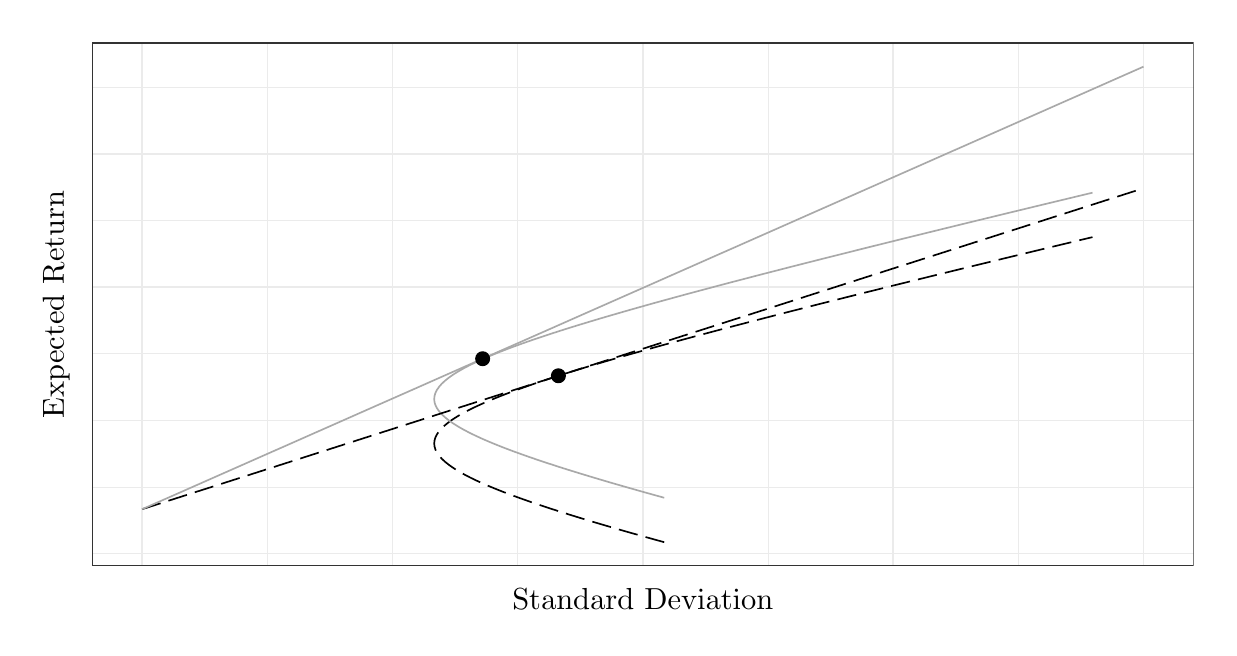
\begin{tikzpicture}[x=1pt,y=1pt]
\definecolor{fillColor}{RGB}{255,255,255}
\path[use as bounding box,fill=fillColor,fill opacity=0.00] (0,0) rectangle (426.79,216.81);
\begin{scope}
\path[clip] (  0.00,  0.00) rectangle (426.79,216.81);
\definecolor{drawColor}{RGB}{255,255,255}
\definecolor{fillColor}{RGB}{255,255,255}

\path[draw=drawColor,line width= 0.6pt,line join=round,line cap=round,fill=fillColor] (  0.00,  0.00) rectangle (426.79,216.81);
\end{scope}
\begin{scope}
\path[clip] ( 23.27, 22.30) rectangle (421.29,211.31);
\definecolor{fillColor}{RGB}{255,255,255}

\path[fill=fillColor] ( 23.27, 22.30) rectangle (421.29,211.31);
\definecolor{drawColor}{gray}{0.92}

\path[draw=drawColor,line width= 0.3pt,line join=round] ( 23.27, 50.84) --
	(421.29, 50.84);

\path[draw=drawColor,line width= 0.3pt,line join=round] ( 23.27, 99.01) --
	(421.29, 99.01);

\path[draw=drawColor,line width= 0.3pt,line join=round] ( 23.27,147.18) --
	(421.29,147.18);

\path[draw=drawColor,line width= 0.3pt,line join=round] ( 23.27,195.36) --
	(421.29,195.36);

\path[draw=drawColor,line width= 0.3pt,line join=round] ( 86.59, 22.30) --
	( 86.59,211.31);

\path[draw=drawColor,line width= 0.3pt,line join=round] (177.05, 22.30) --
	(177.05,211.31);

\path[draw=drawColor,line width= 0.3pt,line join=round] (267.51, 22.30) --
	(267.51,211.31);

\path[draw=drawColor,line width= 0.3pt,line join=round] (357.97, 22.30) --
	(357.97,211.31);

\path[draw=drawColor,line width= 0.6pt,line join=round] ( 23.27, 26.75) --
	(421.29, 26.75);

\path[draw=drawColor,line width= 0.6pt,line join=round] ( 23.27, 74.92) --
	(421.29, 74.92);

\path[draw=drawColor,line width= 0.6pt,line join=round] ( 23.27,123.10) --
	(421.29,123.10);

\path[draw=drawColor,line width= 0.6pt,line join=round] ( 23.27,171.27) --
	(421.29,171.27);

\path[draw=drawColor,line width= 0.6pt,line join=round] ( 41.36, 22.30) --
	( 41.36,211.31);

\path[draw=drawColor,line width= 0.6pt,line join=round] (131.82, 22.30) --
	(131.82,211.31);

\path[draw=drawColor,line width= 0.6pt,line join=round] (222.28, 22.30) --
	(222.28,211.31);

\path[draw=drawColor,line width= 0.6pt,line join=round] (312.74, 22.30) --
	(312.74,211.31);

\path[draw=drawColor,line width= 0.6pt,line join=round] (403.20, 22.30) --
	(403.20,211.31);
\definecolor{drawColor}{RGB}{0,0,0}

\path[draw=drawColor,line width= 0.6pt,dash pattern=on 7pt off 3pt ,line join=round] (230.01, 30.89) --
	(225.98, 32.00) --
	(222.00, 33.12) --
	(218.06, 34.23) --
	(214.17, 35.34) --
	(210.33, 36.46) --
	(206.55, 37.57) --
	(202.83, 38.68) --
	(199.16, 39.80) --
	(195.57, 40.91) --
	(192.05, 42.02) --
	(188.61, 43.14) --
	(185.25, 44.25) --
	(181.97, 45.36) --
	(178.80, 46.48) --
	(175.72, 47.59) --
	(172.76, 48.70) --
	(169.91, 49.82) --
	(167.19, 50.93) --
	(164.60, 52.05) --
	(162.15, 53.16) --
	(159.86, 54.27) --
	(157.72, 55.39) --
	(155.75, 56.50) --
	(153.96, 57.61) --
	(152.35, 58.73) --
	(150.94, 59.84) --
	(149.73, 60.95) --
	(148.73, 62.07) --
	(147.94, 63.18) --
	(147.37, 64.29) --
	(147.02, 65.41) --
	(146.90, 66.52) --
	(147.01, 67.63) --
	(147.33, 68.75) --
	(147.89, 69.86) --
	(148.66, 70.97) --
	(149.64, 72.09) --
	(150.84, 73.20) --
	(152.23, 74.31) --
	(153.82, 75.43) --
	(155.60, 76.54) --
	(157.56, 77.65) --
	(159.68, 78.77) --
	(161.97, 79.88) --
	(164.40, 80.99) --
	(166.98, 82.11) --
	(169.69, 83.22) --
	(172.53, 84.34) --
	(175.49, 85.45) --
	(178.55, 86.56) --
	(181.72, 87.68) --
	(184.99, 88.79) --
	(188.34, 89.90) --
	(191.78, 91.02) --
	(195.29, 92.13) --
	(198.88, 93.24) --
	(202.54, 94.36) --
	(206.26, 95.47) --
	(210.03, 96.58) --
	(213.87, 97.70) --
	(217.75, 98.81) --
	(221.69, 99.92) --
	(225.67,101.04) --
	(229.69,102.15) --
	(233.75,103.26) --
	(237.85,104.38) --
	(241.98,105.49) --
	(246.15,106.60) --
	(250.35,107.72) --
	(254.57,108.83) --
	(258.83,109.94) --
	(263.11,111.06) --
	(267.41,112.17) --
	(271.74,113.29) --
	(276.09,114.40) --
	(280.46,115.51) --
	(284.84,116.63) --
	(289.25,117.74) --
	(293.68,118.85) --
	(298.12,119.97) --
	(302.57,121.08) --
	(307.04,122.19) --
	(311.53,123.31) --
	(316.03,124.42) --
	(320.54,125.53) --
	(325.06,126.65) --
	(329.60,127.76) --
	(334.15,128.87) --
	(338.70,129.99) --
	(343.27,131.10) --
	(347.85,132.21) --
	(352.44,133.33) --
	(357.03,134.44) --
	(361.63,135.55) --
	(366.25,136.67) --
	(370.87,137.78) --
	(375.49,138.89) --
	(380.13,140.01) --
	(384.77,141.12);
\definecolor{drawColor}{RGB}{169,169,169}

\path[draw=drawColor,line width= 0.6pt,line join=round] (230.01, 46.95) --
	(225.98, 48.06) --
	(222.00, 49.17) --
	(218.06, 50.29) --
	(214.17, 51.40) --
	(210.33, 52.51) --
	(206.55, 53.63) --
	(202.83, 54.74) --
	(199.16, 55.86) --
	(195.57, 56.97) --
	(192.05, 58.08) --
	(188.61, 59.20) --
	(185.25, 60.31) --
	(181.97, 61.42) --
	(178.80, 62.54) --
	(175.72, 63.65) --
	(172.76, 64.76) --
	(169.91, 65.88) --
	(167.19, 66.99) --
	(164.60, 68.10) --
	(162.15, 69.22) --
	(159.86, 70.33) --
	(157.72, 71.44) --
	(155.75, 72.56) --
	(153.96, 73.67) --
	(152.35, 74.78) --
	(150.94, 75.90) --
	(149.73, 77.01) --
	(148.73, 78.12) --
	(147.94, 79.24) --
	(147.37, 80.35) --
	(147.02, 81.46) --
	(146.90, 82.58) --
	(147.01, 83.69) --
	(147.33, 84.80) --
	(147.89, 85.92) --
	(148.66, 87.03) --
	(149.64, 88.15) --
	(150.84, 89.26) --
	(152.23, 90.37) --
	(153.82, 91.49) --
	(155.60, 92.60) --
	(157.56, 93.71) --
	(159.68, 94.83) --
	(161.97, 95.94) --
	(164.40, 97.05) --
	(166.98, 98.17) --
	(169.69, 99.28) --
	(172.53,100.39) --
	(175.49,101.51) --
	(178.55,102.62) --
	(181.72,103.73) --
	(184.99,104.85) --
	(188.34,105.96) --
	(191.78,107.07) --
	(195.29,108.19) --
	(198.88,109.30) --
	(202.54,110.41) --
	(206.26,111.53) --
	(210.03,112.64) --
	(213.87,113.75) --
	(217.75,114.87) --
	(221.69,115.98) --
	(225.67,117.10) --
	(229.69,118.21) --
	(233.75,119.32) --
	(237.85,120.44) --
	(241.98,121.55) --
	(246.15,122.66) --
	(250.35,123.78) --
	(254.57,124.89) --
	(258.83,126.00) --
	(263.11,127.12) --
	(267.41,128.23) --
	(271.74,129.34) --
	(276.09,130.46) --
	(280.46,131.57) --
	(284.84,132.68) --
	(289.25,133.80) --
	(293.68,134.91) --
	(298.12,136.02) --
	(302.57,137.14) --
	(307.04,138.25) --
	(311.53,139.36) --
	(316.03,140.48) --
	(320.54,141.59) --
	(325.06,142.70) --
	(329.60,143.82) --
	(334.15,144.93) --
	(338.70,146.05) --
	(343.27,147.16) --
	(347.85,148.27) --
	(352.44,149.39) --
	(357.03,150.50) --
	(361.63,151.61) --
	(366.25,152.73) --
	(370.87,153.84) --
	(375.49,154.95) --
	(380.13,156.07) --
	(384.77,157.18);
\definecolor{drawColor}{RGB}{0,0,0}

\path[draw=drawColor,line width= 0.6pt,dash pattern=on 7pt off 3pt ,line join=round] ( 41.36, 42.81) --
	( 44.98, 43.97) --
	( 48.60, 45.13) --
	( 52.22, 46.29) --
	( 55.84, 47.45) --
	( 59.45, 48.61) --
	( 63.07, 49.77) --
	( 66.69, 50.92) --
	( 70.31, 52.08) --
	( 73.93, 53.24) --
	( 77.55, 54.40) --
	( 81.16, 55.56) --
	( 84.78, 56.72) --
	( 88.40, 57.88) --
	( 92.02, 59.04) --
	( 95.64, 60.20) --
	( 99.26, 61.36) --
	(102.87, 62.52) --
	(106.49, 63.68) --
	(110.11, 64.84) --
	(113.73, 66.00) --
	(117.35, 67.16) --
	(120.97, 68.32) --
	(124.58, 69.48) --
	(128.20, 70.64) --
	(131.82, 71.80) --
	(135.44, 72.96) --
	(139.06, 74.12) --
	(142.68, 75.28) --
	(146.29, 76.44) --
	(149.91, 77.60) --
	(153.53, 78.76) --
	(157.15, 79.92) --
	(160.77, 81.08) --
	(164.39, 82.24) --
	(168.00, 83.40) --
	(171.62, 84.56) --
	(175.24, 85.72) --
	(178.86, 86.88) --
	(182.48, 88.04) --
	(186.10, 89.20) --
	(189.72, 90.36) --
	(193.33, 91.51) --
	(196.95, 92.67) --
	(200.57, 93.83) --
	(204.19, 94.99) --
	(207.81, 96.15) --
	(211.43, 97.31) --
	(215.04, 98.47) --
	(218.66, 99.63) --
	(222.28,100.79) --
	(225.90,101.95) --
	(229.52,103.11) --
	(233.14,104.27) --
	(236.75,105.43) --
	(240.37,106.59) --
	(243.99,107.75) --
	(247.61,108.91) --
	(251.23,110.07) --
	(254.85,111.23) --
	(258.46,112.39) --
	(262.08,113.55) --
	(265.70,114.71) --
	(269.32,115.87) --
	(272.94,117.03) --
	(276.56,118.19) --
	(280.17,119.35) --
	(283.79,120.51) --
	(287.41,121.67) --
	(291.03,122.83) --
	(294.65,123.99) --
	(298.27,125.15) --
	(301.88,126.31) --
	(305.50,127.47) --
	(309.12,128.63) --
	(312.74,129.79) --
	(316.36,130.94) --
	(319.98,132.10) --
	(323.60,133.26) --
	(327.21,134.42) --
	(330.83,135.58) --
	(334.45,136.74) --
	(338.07,137.90) --
	(341.69,139.06) --
	(345.31,140.22) --
	(348.92,141.38) --
	(352.54,142.54) --
	(356.16,143.70) --
	(359.78,144.86) --
	(363.40,146.02) --
	(367.02,147.18) --
	(370.63,148.34) --
	(374.25,149.50) --
	(377.87,150.66) --
	(381.49,151.82) --
	(385.11,152.98) --
	(388.73,154.14) --
	(392.34,155.30) --
	(395.96,156.46) --
	(399.58,157.62) --
	(403.20,158.78);
\definecolor{drawColor}{RGB}{169,169,169}

\path[draw=drawColor,line width= 0.6pt,line join=round] ( 41.36, 42.81) --
	( 44.98, 44.41) --
	( 48.60, 46.01) --
	( 52.22, 47.60) --
	( 55.84, 49.20) --
	( 59.45, 50.80) --
	( 63.07, 52.40) --
	( 66.69, 54.00) --
	( 70.31, 55.60) --
	( 73.93, 57.20) --
	( 77.55, 58.80) --
	( 81.16, 60.40) --
	( 84.78, 62.00) --
	( 88.40, 63.60) --
	( 92.02, 65.19) --
	( 95.64, 66.79) --
	( 99.26, 68.39) --
	(102.87, 69.99) --
	(106.49, 71.59) --
	(110.11, 73.19) --
	(113.73, 74.79) --
	(117.35, 76.39) --
	(120.97, 77.99) --
	(124.58, 79.59) --
	(128.20, 81.19) --
	(131.82, 82.78) --
	(135.44, 84.38) --
	(139.06, 85.98) --
	(142.68, 87.58) --
	(146.29, 89.18) --
	(149.91, 90.78) --
	(153.53, 92.38) --
	(157.15, 93.98) --
	(160.77, 95.58) --
	(164.39, 97.18) --
	(168.00, 98.78) --
	(171.62,100.38) --
	(175.24,101.97) --
	(178.86,103.57) --
	(182.48,105.17) --
	(186.10,106.77) --
	(189.72,108.37) --
	(193.33,109.97) --
	(196.95,111.57) --
	(200.57,113.17) --
	(204.19,114.77) --
	(207.81,116.37) --
	(211.43,117.97) --
	(215.04,119.56) --
	(218.66,121.16) --
	(222.28,122.76) --
	(225.90,124.36) --
	(229.52,125.96) --
	(233.14,127.56) --
	(236.75,129.16) --
	(240.37,130.76) --
	(243.99,132.36) --
	(247.61,133.96) --
	(251.23,135.56) --
	(254.85,137.15) --
	(258.46,138.75) --
	(262.08,140.35) --
	(265.70,141.95) --
	(269.32,143.55) --
	(272.94,145.15) --
	(276.56,146.75) --
	(280.17,148.35) --
	(283.79,149.95) --
	(287.41,151.55) --
	(291.03,153.15) --
	(294.65,154.75) --
	(298.27,156.34) --
	(301.88,157.94) --
	(305.50,159.54) --
	(309.12,161.14) --
	(312.74,162.74) --
	(316.36,164.34) --
	(319.98,165.94) --
	(323.60,167.54) --
	(327.21,169.14) --
	(330.83,170.74) --
	(334.45,172.34) --
	(338.07,173.93) --
	(341.69,175.53) --
	(345.31,177.13) --
	(348.92,178.73) --
	(352.54,180.33) --
	(356.16,181.93) --
	(359.78,183.53) --
	(363.40,185.13) --
	(367.02,186.73) --
	(370.63,188.33) --
	(374.25,189.93) --
	(377.87,191.52) --
	(381.49,193.12) --
	(385.11,194.72) --
	(388.73,196.32) --
	(392.34,197.92) --
	(395.96,199.52) --
	(399.58,201.12) --
	(403.20,202.72);
\definecolor{drawColor}{RGB}{0,0,0}
\definecolor{fillColor}{RGB}{0,0,0}

\path[draw=drawColor,line width= 0.4pt,line join=round,line cap=round,fill=fillColor] (164.40, 97.18) circle (  2.50);

\path[draw=drawColor,line width= 0.4pt,line join=round,line cap=round,fill=fillColor] (191.78, 91.02) circle (  2.50);
\definecolor{drawColor}{gray}{0.20}

\path[draw=drawColor,line width= 0.6pt,line join=round,line cap=round] ( 23.27, 22.30) rectangle (421.29,211.31);
\end{scope}
\begin{scope}
\path[clip] (  0.00,  0.00) rectangle (426.79,216.81);
\definecolor{drawColor}{RGB}{0,0,0}

\node[text=drawColor,anchor=base,inner sep=0pt, outer sep=0pt, scale=  1.10] at (222.28,  6.47) {Standard Deviation};
\end{scope}
\begin{scope}
\path[clip] (  0.00,  0.00) rectangle (426.79,216.81);
\definecolor{drawColor}{RGB}{0,0,0}

\node[text=drawColor,rotate= 90.00,anchor=base,inner sep=0pt, outer sep=0pt, scale=  1.10] at ( 13.08,116.80) {Expected Return};
\end{scope}
\end{tikzpicture}

%	\end{subfigure}
%	\begin{subfigure}{\textwidth}
%		\caption{Leverage Constraints}
%		% Created by tikzDevice version 0.10.1 on 2018-06-18 15:09:22
% !TEX encoding = UTF-8 Unicode
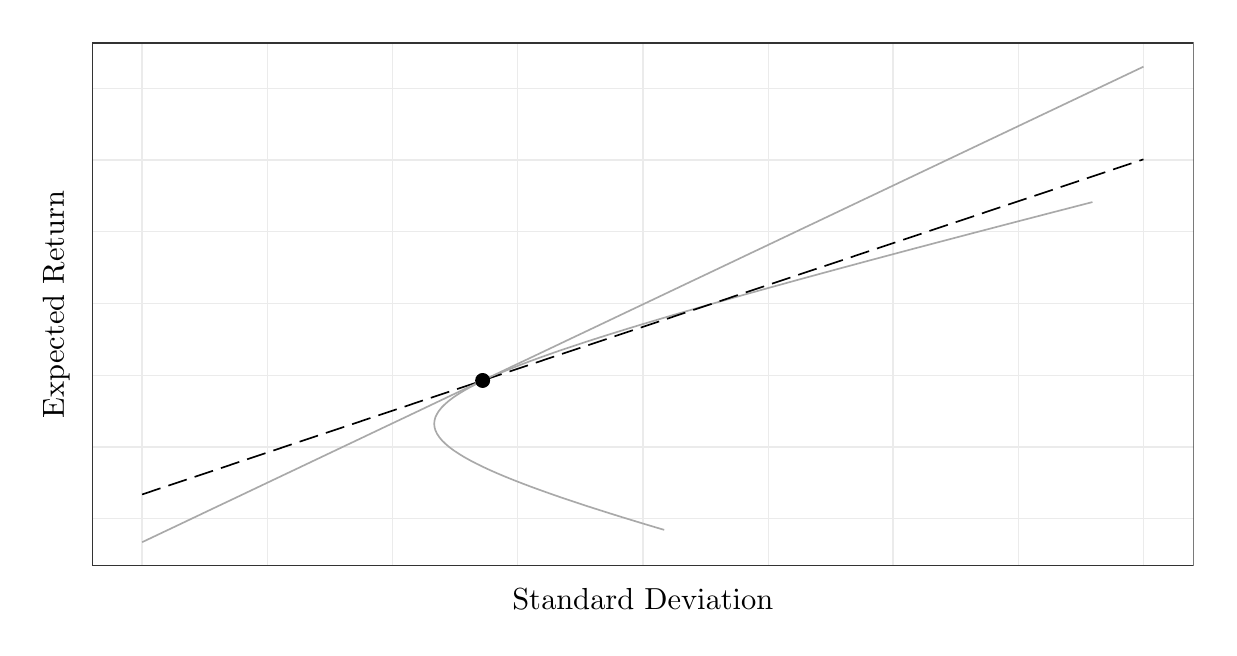
\begin{tikzpicture}[x=1pt,y=1pt]
\definecolor{fillColor}{RGB}{255,255,255}
\path[use as bounding box,fill=fillColor,fill opacity=0.00] (0,0) rectangle (426.79,216.81);
\begin{scope}
\path[clip] (  0.00,  0.00) rectangle (426.79,216.81);
\definecolor{drawColor}{RGB}{255,255,255}
\definecolor{fillColor}{RGB}{255,255,255}

\path[draw=drawColor,line width= 0.6pt,line join=round,line cap=round,fill=fillColor] (  0.00,  0.00) rectangle (426.79,216.81);
\end{scope}
\begin{scope}
\path[clip] ( 23.27, 22.30) rectangle (421.29,211.31);
\definecolor{fillColor}{RGB}{255,255,255}

\path[fill=fillColor] ( 23.27, 22.30) rectangle (421.29,211.31);
\definecolor{drawColor}{gray}{0.92}

\path[draw=drawColor,line width= 0.3pt,line join=round] ( 23.27, 39.52) --
	(421.29, 39.52);

\path[draw=drawColor,line width= 0.3pt,line join=round] ( 23.27, 91.28) --
	(421.29, 91.28);

\path[draw=drawColor,line width= 0.3pt,line join=round] ( 23.27,143.05) --
	(421.29,143.05);

\path[draw=drawColor,line width= 0.3pt,line join=round] ( 23.27,194.81) --
	(421.29,194.81);

\path[draw=drawColor,line width= 0.3pt,line join=round] ( 86.59, 22.30) --
	( 86.59,211.31);

\path[draw=drawColor,line width= 0.3pt,line join=round] (177.05, 22.30) --
	(177.05,211.31);

\path[draw=drawColor,line width= 0.3pt,line join=round] (267.51, 22.30) --
	(267.51,211.31);

\path[draw=drawColor,line width= 0.3pt,line join=round] (357.97, 22.30) --
	(357.97,211.31);

\path[draw=drawColor,line width= 0.6pt,line join=round] ( 23.27, 65.40) --
	(421.29, 65.40);

\path[draw=drawColor,line width= 0.6pt,line join=round] ( 23.27,117.16) --
	(421.29,117.16);

\path[draw=drawColor,line width= 0.6pt,line join=round] ( 23.27,168.93) --
	(421.29,168.93);

\path[draw=drawColor,line width= 0.6pt,line join=round] ( 41.36, 22.30) --
	( 41.36,211.31);

\path[draw=drawColor,line width= 0.6pt,line join=round] (131.82, 22.30) --
	(131.82,211.31);

\path[draw=drawColor,line width= 0.6pt,line join=round] (222.28, 22.30) --
	(222.28,211.31);

\path[draw=drawColor,line width= 0.6pt,line join=round] (312.74, 22.30) --
	(312.74,211.31);

\path[draw=drawColor,line width= 0.6pt,line join=round] (403.20, 22.30) --
	(403.20,211.31);
\definecolor{drawColor}{RGB}{169,169,169}

\path[draw=drawColor,line width= 0.6pt,line join=round] (230.01, 35.34) --
	(225.98, 36.53) --
	(222.00, 37.73) --
	(218.06, 38.93) --
	(214.17, 40.12) --
	(210.33, 41.32) --
	(206.55, 42.52) --
	(202.83, 43.71) --
	(199.16, 44.91) --
	(195.57, 46.11) --
	(192.05, 47.30) --
	(188.61, 48.50) --
	(185.25, 49.70) --
	(181.97, 50.89) --
	(178.80, 52.09) --
	(175.72, 53.29) --
	(172.76, 54.48) --
	(169.91, 55.68) --
	(167.19, 56.87) --
	(164.60, 58.07) --
	(162.15, 59.27) --
	(159.86, 60.46) --
	(157.72, 61.66) --
	(155.75, 62.86) --
	(153.96, 64.05) --
	(152.35, 65.25) --
	(150.94, 66.45) --
	(149.73, 67.64) --
	(148.73, 68.84) --
	(147.94, 70.04) --
	(147.37, 71.23) --
	(147.02, 72.43) --
	(146.90, 73.62) --
	(147.01, 74.82) --
	(147.33, 76.02) --
	(147.89, 77.21) --
	(148.66, 78.41) --
	(149.64, 79.61) --
	(150.84, 80.80) --
	(152.23, 82.00) --
	(153.82, 83.20) --
	(155.60, 84.39) --
	(157.56, 85.59) --
	(159.68, 86.79) --
	(161.97, 87.98) --
	(164.40, 89.18) --
	(166.98, 90.37) --
	(169.69, 91.57) --
	(172.53, 92.77) --
	(175.49, 93.96) --
	(178.55, 95.16) --
	(181.72, 96.36) --
	(184.99, 97.55) --
	(188.34, 98.75) --
	(191.78, 99.95) --
	(195.29,101.14) --
	(198.88,102.34) --
	(202.54,103.54) --
	(206.26,104.73) --
	(210.03,105.93) --
	(213.87,107.12) --
	(217.75,108.32) --
	(221.69,109.52) --
	(225.67,110.71) --
	(229.69,111.91) --
	(233.75,113.11) --
	(237.85,114.30) --
	(241.98,115.50) --
	(246.15,116.70) --
	(250.35,117.89) --
	(254.57,119.09) --
	(258.83,120.29) --
	(263.11,121.48) --
	(267.41,122.68) --
	(271.74,123.87) --
	(276.09,125.07) --
	(280.46,126.27) --
	(284.84,127.46) --
	(289.25,128.66) --
	(293.68,129.86) --
	(298.12,131.05) --
	(302.57,132.25) --
	(307.04,133.45) --
	(311.53,134.64) --
	(316.03,135.84) --
	(320.54,137.04) --
	(325.06,138.23) --
	(329.60,139.43) --
	(334.15,140.62) --
	(338.70,141.82) --
	(343.27,143.02) --
	(347.85,144.21) --
	(352.44,145.41) --
	(357.03,146.61) --
	(361.63,147.80) --
	(366.25,149.00) --
	(370.87,150.20) --
	(375.49,151.39) --
	(380.13,152.59) --
	(384.77,153.79);
\definecolor{drawColor}{RGB}{0,0,0}

\path[draw=drawColor,line width= 0.6pt,dash pattern=on 7pt off 3pt ,line join=round] ( 41.36, 48.14) --
	( 44.98, 49.36) --
	( 48.60, 50.57) --
	( 52.22, 51.78) --
	( 55.84, 52.99) --
	( 59.45, 54.20) --
	( 63.07, 55.41) --
	( 66.69, 56.62) --
	( 70.31, 57.83) --
	( 73.93, 59.04) --
	( 77.55, 60.25) --
	( 81.16, 61.46) --
	( 84.78, 62.67) --
	( 88.40, 63.89) --
	( 92.02, 65.10) --
	( 95.64, 66.31) --
	( 99.26, 67.52) --
	(102.87, 68.73) --
	(106.49, 69.94) --
	(110.11, 71.15) --
	(113.73, 72.36) --
	(117.35, 73.57) --
	(120.97, 74.78) --
	(124.58, 75.99) --
	(128.20, 77.21) --
	(131.82, 78.42) --
	(135.44, 79.63) --
	(139.06, 80.84) --
	(142.68, 82.05) --
	(146.29, 83.26) --
	(149.91, 84.47) --
	(153.53, 85.68) --
	(157.15, 86.89) --
	(160.77, 88.10) --
	(164.39, 89.31) --
	(168.00, 90.52) --
	(171.62, 91.74) --
	(175.24, 92.95) --
	(178.86, 94.16) --
	(182.48, 95.37) --
	(186.10, 96.58) --
	(189.72, 97.79) --
	(193.33, 99.00) --
	(196.95,100.21) --
	(200.57,101.42) --
	(204.19,102.63) --
	(207.81,103.84) --
	(211.43,105.06) --
	(215.04,106.27) --
	(218.66,107.48) --
	(222.28,108.69) --
	(225.90,109.90) --
	(229.52,111.11) --
	(233.14,112.32) --
	(236.75,113.53) --
	(240.37,114.74) --
	(243.99,115.95) --
	(247.61,117.16) --
	(251.23,118.37) --
	(254.85,119.59) --
	(258.46,120.80) --
	(262.08,122.01) --
	(265.70,123.22) --
	(269.32,124.43) --
	(272.94,125.64) --
	(276.56,126.85) --
	(280.17,128.06) --
	(283.79,129.27) --
	(287.41,130.48) --
	(291.03,131.69) --
	(294.65,132.91) --
	(298.27,134.12) --
	(301.88,135.33) --
	(305.50,136.54) --
	(309.12,137.75) --
	(312.74,138.96) --
	(316.36,140.17) --
	(319.98,141.38) --
	(323.60,142.59) --
	(327.21,143.80) --
	(330.83,145.01) --
	(334.45,146.22) --
	(338.07,147.44) --
	(341.69,148.65) --
	(345.31,149.86) --
	(348.92,151.07) --
	(352.54,152.28) --
	(356.16,153.49) --
	(359.78,154.70) --
	(363.40,155.91) --
	(367.02,157.12) --
	(370.63,158.33) --
	(374.25,159.54) --
	(377.87,160.76) --
	(381.49,161.97) --
	(385.11,163.18) --
	(388.73,164.39) --
	(392.34,165.60) --
	(395.96,166.81) --
	(399.58,168.02) --
	(403.20,169.23);
\definecolor{drawColor}{RGB}{169,169,169}

\path[draw=drawColor,line width= 0.6pt,line join=round] ( 41.36, 30.89) --
	( 44.98, 32.61) --
	( 48.60, 34.33) --
	( 52.22, 36.04) --
	( 55.84, 37.76) --
	( 59.45, 39.48) --
	( 63.07, 41.20) --
	( 66.69, 42.92) --
	( 70.31, 44.64) --
	( 73.93, 46.35) --
	( 77.55, 48.07) --
	( 81.16, 49.79) --
	( 84.78, 51.51) --
	( 88.40, 53.23) --
	( 92.02, 54.95) --
	( 95.64, 56.66) --
	( 99.26, 58.38) --
	(102.87, 60.10) --
	(106.49, 61.82) --
	(110.11, 63.54) --
	(113.73, 65.26) --
	(117.35, 66.97) --
	(120.97, 68.69) --
	(124.58, 70.41) --
	(128.20, 72.13) --
	(131.82, 73.85) --
	(135.44, 75.56) --
	(139.06, 77.28) --
	(142.68, 79.00) --
	(146.29, 80.72) --
	(149.91, 82.44) --
	(153.53, 84.16) --
	(157.15, 85.87) --
	(160.77, 87.59) --
	(164.39, 89.31) --
	(168.00, 91.03) --
	(171.62, 92.75) --
	(175.24, 94.47) --
	(178.86, 96.18) --
	(182.48, 97.90) --
	(186.10, 99.62) --
	(189.72,101.34) --
	(193.33,103.06) --
	(196.95,104.78) --
	(200.57,106.49) --
	(204.19,108.21) --
	(207.81,109.93) --
	(211.43,111.65) --
	(215.04,113.37) --
	(218.66,115.09) --
	(222.28,116.80) --
	(225.90,118.52) --
	(229.52,120.24) --
	(233.14,121.96) --
	(236.75,123.68) --
	(240.37,125.40) --
	(243.99,127.11) --
	(247.61,128.83) --
	(251.23,130.55) --
	(254.85,132.27) --
	(258.46,133.99) --
	(262.08,135.71) --
	(265.70,137.42) --
	(269.32,139.14) --
	(272.94,140.86) --
	(276.56,142.58) --
	(280.17,144.30) --
	(283.79,146.01) --
	(287.41,147.73) --
	(291.03,149.45) --
	(294.65,151.17) --
	(298.27,152.89) --
	(301.88,154.61) --
	(305.50,156.32) --
	(309.12,158.04) --
	(312.74,159.76) --
	(316.36,161.48) --
	(319.98,163.20) --
	(323.60,164.92) --
	(327.21,166.63) --
	(330.83,168.35) --
	(334.45,170.07) --
	(338.07,171.79) --
	(341.69,173.51) --
	(345.31,175.23) --
	(348.92,176.94) --
	(352.54,178.66) --
	(356.16,180.38) --
	(359.78,182.10) --
	(363.40,183.82) --
	(367.02,185.54) --
	(370.63,187.25) --
	(374.25,188.97) --
	(377.87,190.69) --
	(381.49,192.41) --
	(385.11,194.13) --
	(388.73,195.85) --
	(392.34,197.56) --
	(395.96,199.28) --
	(399.58,201.00) --
	(403.20,202.72);
\definecolor{drawColor}{RGB}{0,0,0}
\definecolor{fillColor}{RGB}{0,0,0}

\path[draw=drawColor,line width= 0.4pt,line join=round,line cap=round,fill=fillColor] (164.40, 89.32) circle (  2.50);
\definecolor{drawColor}{gray}{0.20}

\path[draw=drawColor,line width= 0.6pt,line join=round,line cap=round] ( 23.27, 22.30) rectangle (421.29,211.31);
\end{scope}
\begin{scope}
\path[clip] (  0.00,  0.00) rectangle (426.79,216.81);
\definecolor{drawColor}{RGB}{0,0,0}

\node[text=drawColor,anchor=base,inner sep=0pt, outer sep=0pt, scale=  1.10] at (222.28,  6.47) {Standard Deviation};
\end{scope}
\begin{scope}
\path[clip] (  0.00,  0.00) rectangle (426.79,216.81);
\definecolor{drawColor}{RGB}{0,0,0}

\node[text=drawColor,rotate= 90.00,anchor=base,inner sep=0pt, outer sep=0pt, scale=  1.10] at ( 13.08,116.80) {Expected Return};
\end{scope}
\end{tikzpicture}

%	\end{subfigure}
%	%\subcaptionbox{First\label{f}}{%
%	%	% Created by tikzDevice version 0.10.1 on 2018-05-02 14:50:53
% !TEX encoding = UTF-8 Unicode
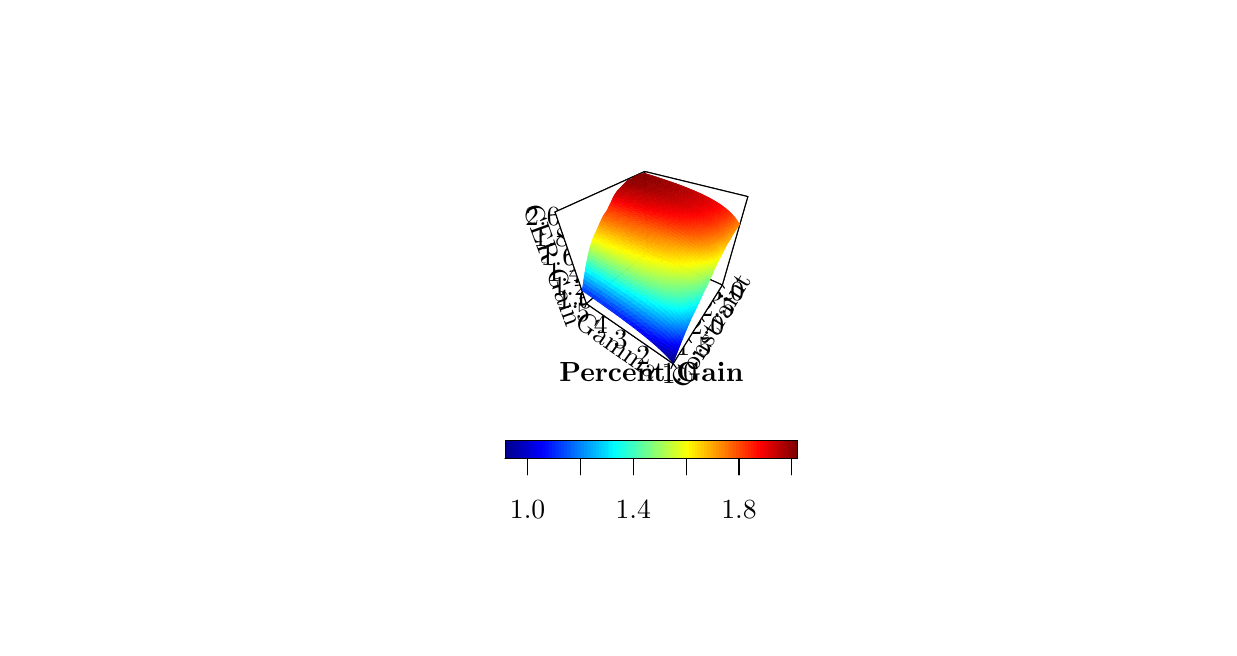
\begin{tikzpicture}[x=1pt,y=1pt]
\definecolor{fillColor}{RGB}{255,255,255}
\path[use as bounding box,fill=fillColor,fill opacity=0.00] (0,0) rectangle (426.79,216.81);
\begin{scope}
\path[clip] ( 49.20, 92.64) rectangle (401.59,167.61);
\definecolor{drawColor}{RGB}{0,0,0}

\path[draw=drawColor,line width= 0.4pt,line join=round,line cap=round] (201.91,117.08) -- (224.04,135.90);

\path[draw=drawColor,line width= 0.4pt,line join=round,line cap=round] (224.04,135.90) -- (222.97,164.83);

\path[draw=drawColor,line width= 0.4pt,line join=round,line cap=round] (222.97,164.83) -- (190.57,150.20);

\path[draw=drawColor,line width= 0.4pt,line join=round,line cap=round] (190.57,150.20) -- (201.91,117.08);

\path[draw=drawColor,line width= 0.4pt,line join=round,line cap=round] (251.01,123.81) -- (260.22,155.77);

\path[draw=drawColor,line width= 0.4pt,line join=round,line cap=round] (260.22,155.77) -- (222.97,164.83);

\path[draw=drawColor,line width= 0.4pt,line join=round,line cap=round] (224.04,135.90) -- (251.01,123.81);

\path[draw=drawColor,line width= 0.4pt,line join=round,line cap=round] (233.23, 95.41) -- (251.01,123.81);

\path[draw=drawColor,line width= 0.4pt,line join=round,line cap=round] (201.91,117.08) -- (233.23, 95.41);
\end{scope}
\begin{scope}
\path[clip] (  0.00,  0.00) rectangle (426.79,216.81);
\definecolor{drawColor}{RGB}{0,0,0}

\node[text=drawColor,rotate= 58.75,anchor=base,inner sep=0pt, outer sep=6pt, scale=  1.00] at (249.64,105.72) {Constraint};

\path[draw=drawColor,line width= 0.4pt,line join=round,line cap=round] (233.23, 95.41) -- (234.35, 93.98);

\node[text=drawColor,anchor=base,inner sep=0pt, outer sep=0pt, scale=  1.00] at (235.46, 89.11) {1.0};

\path[draw=drawColor,line width= 0.4pt,line join=round,line cap=round] (238.83,104.36) -- (239.83,103.02);

\node[text=drawColor,anchor=base,inner sep=0pt, outer sep=0pt, scale=  1.00] at (240.83, 98.24) {1.5};

\path[draw=drawColor,line width= 0.4pt,line join=round,line cap=round] (243.54,111.88) -- (244.45,110.62);

\node[text=drawColor,anchor=base,inner sep=0pt, outer sep=0pt, scale=  1.00] at (245.35,105.92) {2.0};

\path[draw=drawColor,line width= 0.4pt,line join=round,line cap=round] (247.55,118.28) -- (248.38,117.10);

\node[text=drawColor,anchor=base,inner sep=0pt, outer sep=0pt, scale=  1.00] at (249.20,112.48) {2.5};

\path[draw=drawColor,line width= 0.4pt,line join=round,line cap=round] (251.01,123.81) -- (251.77,122.69);

\node[text=drawColor,anchor=base,inner sep=0pt, outer sep=0pt, scale=  1.00] at (252.53,118.14) {3.0};

\node[text=drawColor,rotate=-35.29,anchor=base,inner sep=0pt, outer sep=6pt, scale=  1.00] at (211.28, 99.16) {Gamma};

\path[draw=drawColor,line width= 0.4pt,line join=round,line cap=round] (233.23, 95.41) -- (232.43, 93.62);

\node[text=drawColor,anchor=base,inner sep=0pt, outer sep=0pt, scale=  1.00] at (231.63, 88.38) {1};

\path[draw=drawColor,line width= 0.4pt,line join=round,line cap=round] (223.94,101.84) -- (223.19,100.16);

\node[text=drawColor,anchor=base,inner sep=0pt, outer sep=0pt, scale=  1.00] at (222.44, 95.03) {2};

\path[draw=drawColor,line width= 0.4pt,line join=round,line cap=round] (215.74,107.52) -- (215.03,105.93);

\node[text=drawColor,anchor=base,inner sep=0pt, outer sep=0pt, scale=  1.00] at (214.33,100.90) {3};

\path[draw=drawColor,line width= 0.4pt,line join=round,line cap=round] (208.44,112.57) -- (207.78,111.07);

\node[text=drawColor,anchor=base,inner sep=0pt, outer sep=0pt, scale=  1.00] at (207.12,106.12) {4};

\path[draw=drawColor,line width= 0.4pt,line join=round,line cap=round] (201.91,117.08) -- (201.29,115.66);

\node[text=drawColor,anchor=base,inner sep=0pt, outer sep=0pt, scale=  1.00] at (200.66,110.80) {5};

\node[text=drawColor,rotate=-69.94,anchor=base,inner sep=0pt, outer sep=6pt, scale=  1.00] at (186.77,129.87) {CER Gain};

\path[draw=drawColor,line width= 0.4pt,line join=round,line cap=round] (201.16,119.28) -- (199.50,119.06);

\node[text=drawColor,anchor=base,inner sep=0pt, outer sep=0pt, scale=  1.00] at (197.83,115.39) {1.0};

\path[draw=drawColor,line width= 0.4pt,line join=round,line cap=round] (199.60,123.85) -- (197.83,123.63);

\node[text=drawColor,anchor=base,inner sep=0pt, outer sep=0pt, scale=  1.00] at (196.06,119.96) {1.2};

\path[draw=drawColor,line width= 0.4pt,line join=round,line cap=round] (197.83,128.99) -- (195.95,128.78);

\node[text=drawColor,anchor=base,inner sep=0pt, outer sep=0pt, scale=  1.00] at (194.06,125.11) {1.4};

\path[draw=drawColor,line width= 0.4pt,line join=round,line cap=round] (195.83,134.84) -- (193.82,134.62);

\node[text=drawColor,anchor=base,inner sep=0pt, outer sep=0pt, scale=  1.00] at (191.79,130.96) {1.6};

\path[draw=drawColor,line width= 0.4pt,line join=round,line cap=round] (193.54,141.52) -- (191.37,141.32);

\node[text=drawColor,anchor=base,inner sep=0pt, outer sep=0pt, scale=  1.00] at (189.19,137.67) {1.8};

\path[draw=drawColor,line width= 0.4pt,line join=round,line cap=round] (190.89,149.25) -- (188.55,149.06);

\node[text=drawColor,anchor=base,inner sep=0pt, outer sep=0pt, scale=  1.00] at (186.18,145.42) {2.0};
\end{scope}
\begin{scope}
\path[clip] ( 49.20, 92.64) rectangle (401.59,167.61);

\path[] (233.23, 95.41) --
	(260.22,155.77) --
	(222.97,164.83) --
	(201.91,117.08) --
	(233.23, 95.41);
\definecolor{drawColor}{RGB}{0,0,0}

\path[draw=drawColor,line width= 0.4pt,dash pattern=on 1pt off 3pt ,line join=round,line cap=round] (233.23, 95.41) -- (236.86,129.15);

\path[draw=drawColor,line width= 0.4pt,dash pattern=on 1pt off 3pt ,line join=round,line cap=round] (236.86,129.15) -- (260.22,155.77);

\path[draw=drawColor,line width= 0.4pt,dash pattern=on 1pt off 3pt ,line join=round,line cap=round] (190.57,150.20) -- (236.86,129.15);
\definecolor{fillColor}{RGB}{255,255,255}

\path[fill=fillColor] (201.91,117.08) --
	(224.04,135.90) --
	(222.97,164.83) --
	(190.57,150.20) --
	(201.91,117.08) --
	cycle;

\path[draw=drawColor,line width= 0.4pt,line join=round,line cap=round] (201.91,117.08) --
	(224.04,135.90) --
	(222.97,164.83) --
	(190.57,150.20) --
	(201.91,117.08);

\path[fill=fillColor] (251.01,123.81) --
	(260.22,155.77) --
	(222.97,164.83) --
	(224.04,135.90) --
	(251.01,123.81) --
	cycle;

\path[draw=drawColor,line width= 0.4pt,line join=round,line cap=round] (251.01,123.81) --
	(260.22,155.77) --
	(222.97,164.83) --
	(224.04,135.90) --
	(251.01,123.81);

\path[fill=fillColor] (233.23, 95.41) --
	(251.01,123.81) --
	(224.04,135.90) --
	(201.91,117.08) --
	(233.23, 95.41) --
	cycle;

\path[draw=drawColor,line width= 0.4pt,line join=round,line cap=round] (233.23, 95.41) --
	(251.01,123.81) --
	(224.04,135.90) --
	(201.91,117.08) --
	(233.23, 95.41);
\definecolor{fillColor}{RGB}{148,0,0}

\path[fill=fillColor] (222.85,164.10) --
	(223.24,164.16) --
	(222.99,164.24) --
	(222.61,164.18) --
	cycle;

\path[fill=fillColor] (222.85,164.10) --
	(223.24,164.16) --
	(222.99,164.24) --
	(222.61,164.18) --
	cycle;

\path[fill=fillColor] (223.10,164.02) --
	(223.48,164.09) --
	(223.24,164.16) --
	(222.85,164.10) --
	cycle;

\path[fill=fillColor] (223.10,164.02) --
	(223.48,164.09) --
	(223.24,164.16) --
	(222.85,164.10) --
	cycle;

\path[fill=fillColor] (223.35,163.95) --
	(223.73,164.01) --
	(223.48,164.09) --
	(223.10,164.02) --
	cycle;

\path[fill=fillColor] (223.35,163.95) --
	(223.73,164.01) --
	(223.48,164.09) --
	(223.10,164.02) --
	cycle;

\path[fill=fillColor] (222.47,164.03) --
	(222.85,164.10) --
	(222.61,164.18) --
	(222.22,164.11) --
	cycle;

\path[fill=fillColor] (222.47,164.03) --
	(222.85,164.10) --
	(222.61,164.18) --
	(222.22,164.11) --
	cycle;

\path[fill=fillColor] (223.60,163.87) --
	(223.97,163.94) --
	(223.73,164.01) --
	(223.35,163.95) --
	cycle;

\path[fill=fillColor] (223.60,163.87) --
	(223.97,163.94) --
	(223.73,164.01) --
	(223.35,163.95) --
	cycle;

\path[fill=fillColor] (222.72,163.96) --
	(223.10,164.02) --
	(222.85,164.10) --
	(222.47,164.03) --
	cycle;

\path[fill=fillColor] (222.72,163.96) --
	(223.10,164.02) --
	(222.85,164.10) --
	(222.47,164.03) --
	cycle;

\path[fill=fillColor] (223.84,163.79) --
	(224.22,163.86) --
	(223.97,163.94) --
	(223.60,163.87) --
	cycle;

\path[fill=fillColor] (223.84,163.79) --
	(224.22,163.86) --
	(223.97,163.94) --
	(223.60,163.87) --
	cycle;

\path[fill=fillColor] (222.96,163.88) --
	(223.35,163.95) --
	(223.10,164.02) --
	(222.72,163.96) --
	cycle;

\path[fill=fillColor] (222.96,163.88) --
	(223.35,163.95) --
	(223.10,164.02) --
	(222.72,163.96) --
	cycle;

\path[fill=fillColor] (224.09,163.71) --
	(224.47,163.78) --
	(224.22,163.86) --
	(223.84,163.79) --
	cycle;

\path[fill=fillColor] (224.09,163.71) --
	(224.47,163.78) --
	(224.22,163.86) --
	(223.84,163.79) --
	cycle;
\definecolor{fillColor}{RGB}{138,0,0}

\path[fill=fillColor] (222.08,163.97) --
	(222.47,164.03) --
	(222.22,164.11) --
	(221.83,164.05) --
	cycle;

\path[fill=fillColor] (222.08,163.97) --
	(222.47,164.03) --
	(222.22,164.11) --
	(221.83,164.05) --
	cycle;
\definecolor{fillColor}{RGB}{148,0,0}

\path[fill=fillColor] (223.21,163.80) --
	(223.60,163.87) --
	(223.35,163.95) --
	(222.96,163.88) --
	cycle;

\path[fill=fillColor] (223.21,163.80) --
	(223.60,163.87) --
	(223.35,163.95) --
	(222.96,163.88) --
	cycle;

\path[fill=fillColor] (224.34,163.63) --
	(224.72,163.70) --
	(224.47,163.78) --
	(224.09,163.71) --
	cycle;

\path[fill=fillColor] (224.34,163.63) --
	(224.72,163.70) --
	(224.47,163.78) --
	(224.09,163.71) --
	cycle;
\definecolor{fillColor}{RGB}{138,0,0}

\path[fill=fillColor] (222.33,163.89) --
	(222.72,163.96) --
	(222.47,164.03) --
	(222.08,163.97) --
	cycle;

\path[fill=fillColor] (222.33,163.89) --
	(222.72,163.96) --
	(222.47,164.03) --
	(222.08,163.97) --
	cycle;
\definecolor{fillColor}{RGB}{148,0,0}

\path[fill=fillColor] (223.46,163.72) --
	(223.84,163.79) --
	(223.60,163.87) --
	(223.21,163.80) --
	cycle;

\path[fill=fillColor] (223.46,163.72) --
	(223.84,163.79) --
	(223.60,163.87) --
	(223.21,163.80) --
	cycle;

\path[fill=fillColor] (224.60,163.55) --
	(224.97,163.62) --
	(224.72,163.70) --
	(224.34,163.63) --
	cycle;

\path[fill=fillColor] (224.60,163.55) --
	(224.97,163.62) --
	(224.72,163.70) --
	(224.34,163.63) --
	cycle;
\definecolor{fillColor}{RGB}{138,0,0}

\path[fill=fillColor] (222.58,163.81) --
	(222.96,163.88) --
	(222.72,163.96) --
	(222.33,163.89) --
	cycle;

\path[fill=fillColor] (222.58,163.81) --
	(222.96,163.88) --
	(222.72,163.96) --
	(222.33,163.89) --
	cycle;
\definecolor{fillColor}{RGB}{148,0,0}

\path[fill=fillColor] (223.71,163.64) --
	(224.09,163.71) --
	(223.84,163.79) --
	(223.46,163.72) --
	cycle;

\path[fill=fillColor] (223.71,163.64) --
	(224.09,163.71) --
	(223.84,163.79) --
	(223.46,163.72) --
	cycle;

\path[fill=fillColor] (224.85,163.48) --
	(225.22,163.55) --
	(224.97,163.62) --
	(224.60,163.55) --
	cycle;

\path[fill=fillColor] (224.85,163.48) --
	(225.22,163.55) --
	(224.97,163.62) --
	(224.60,163.55) --
	cycle;
\definecolor{fillColor}{RGB}{138,0,0}

\path[fill=fillColor] (221.69,163.86) --
	(222.08,163.97) --
	(221.83,164.05) --
	(221.44,163.94) --
	cycle;

\path[fill=fillColor] (221.69,163.86) --
	(222.08,163.97) --
	(221.83,164.05) --
	(221.44,163.94) --
	cycle;

\path[fill=fillColor] (222.83,163.73) --
	(223.21,163.80) --
	(222.96,163.88) --
	(222.58,163.81) --
	cycle;

\path[fill=fillColor] (222.83,163.73) --
	(223.21,163.80) --
	(222.96,163.88) --
	(222.58,163.81) --
	cycle;
\definecolor{fillColor}{RGB}{148,0,0}

\path[fill=fillColor] (223.96,163.56) --
	(224.34,163.63) --
	(224.09,163.71) --
	(223.71,163.64) --
	cycle;

\path[fill=fillColor] (223.96,163.56) --
	(224.34,163.63) --
	(224.09,163.71) --
	(223.71,163.64) --
	cycle;

\path[fill=fillColor] (225.10,163.39) --
	(225.47,163.47) --
	(225.22,163.55) --
	(224.85,163.48) --
	cycle;

\path[fill=fillColor] (225.10,163.39) --
	(225.47,163.47) --
	(225.22,163.55) --
	(224.85,163.48) --
	cycle;
\definecolor{fillColor}{RGB}{138,0,0}

\path[fill=fillColor] (221.94,163.78) --
	(222.33,163.89) --
	(222.08,163.97) --
	(221.69,163.86) --
	cycle;

\path[fill=fillColor] (221.94,163.78) --
	(222.33,163.89) --
	(222.08,163.97) --
	(221.69,163.86) --
	cycle;

\path[fill=fillColor] (223.08,163.65) --
	(223.46,163.72) --
	(223.21,163.80) --
	(222.83,163.73) --
	cycle;

\path[fill=fillColor] (223.08,163.65) --
	(223.46,163.72) --
	(223.21,163.80) --
	(222.83,163.73) --
	cycle;
\definecolor{fillColor}{RGB}{148,0,0}

\path[fill=fillColor] (224.22,163.48) --
	(224.60,163.55) --
	(224.34,163.63) --
	(223.96,163.56) --
	cycle;

\path[fill=fillColor] (224.22,163.48) --
	(224.60,163.55) --
	(224.34,163.63) --
	(223.96,163.56) --
	cycle;

\path[fill=fillColor] (225.35,163.31) --
	(225.73,163.39) --
	(225.47,163.47) --
	(225.10,163.39) --
	cycle;

\path[fill=fillColor] (225.35,163.31) --
	(225.73,163.39) --
	(225.47,163.47) --
	(225.10,163.39) --
	cycle;
\definecolor{fillColor}{RGB}{138,0,0}

\path[fill=fillColor] (222.19,163.70) --
	(222.58,163.81) --
	(222.33,163.89) --
	(221.94,163.78) --
	cycle;

\path[fill=fillColor] (222.19,163.70) --
	(222.58,163.81) --
	(222.33,163.89) --
	(221.94,163.78) --
	cycle;
\definecolor{fillColor}{RGB}{148,0,0}

\path[fill=fillColor] (223.33,163.57) --
	(223.71,163.64) --
	(223.46,163.72) --
	(223.08,163.65) --
	cycle;

\path[fill=fillColor] (223.33,163.57) --
	(223.71,163.64) --
	(223.46,163.72) --
	(223.08,163.65) --
	cycle;

\path[fill=fillColor] (224.47,163.40) --
	(224.85,163.48) --
	(224.60,163.55) --
	(224.22,163.48) --
	cycle;

\path[fill=fillColor] (224.47,163.40) --
	(224.85,163.48) --
	(224.60,163.55) --
	(224.22,163.48) --
	cycle;

\path[fill=fillColor] (225.61,163.23) --
	(225.98,163.31) --
	(225.73,163.39) --
	(225.35,163.31) --
	cycle;

\path[fill=fillColor] (225.61,163.23) --
	(225.98,163.31) --
	(225.73,163.39) --
	(225.35,163.31) --
	cycle;
\definecolor{fillColor}{RGB}{138,0,0}

\path[fill=fillColor] (221.29,163.75) --
	(221.69,163.86) --
	(221.44,163.94) --
	(221.04,163.83) --
	cycle;

\path[fill=fillColor] (221.29,163.75) --
	(221.69,163.86) --
	(221.44,163.94) --
	(221.04,163.83) --
	cycle;

\path[fill=fillColor] (222.44,163.62) --
	(222.83,163.73) --
	(222.58,163.81) --
	(222.19,163.70) --
	cycle;

\path[fill=fillColor] (222.44,163.62) --
	(222.83,163.73) --
	(222.58,163.81) --
	(222.19,163.70) --
	cycle;
\definecolor{fillColor}{RGB}{148,0,0}

\path[fill=fillColor] (223.58,163.49) --
	(223.96,163.56) --
	(223.71,163.64) --
	(223.33,163.57) --
	cycle;

\path[fill=fillColor] (223.58,163.49) --
	(223.96,163.56) --
	(223.71,163.64) --
	(223.33,163.57) --
	cycle;

\path[fill=fillColor] (224.72,163.32) --
	(225.10,163.39) --
	(224.85,163.48) --
	(224.47,163.40) --
	cycle;

\path[fill=fillColor] (224.72,163.32) --
	(225.10,163.39) --
	(224.85,163.48) --
	(224.47,163.40) --
	cycle;

\path[fill=fillColor] (225.86,163.15) --
	(226.23,163.22) --
	(225.98,163.31) --
	(225.61,163.23) --
	cycle;

\path[fill=fillColor] (225.86,163.15) --
	(226.23,163.22) --
	(225.98,163.31) --
	(225.61,163.23) --
	cycle;
\definecolor{fillColor}{RGB}{138,0,0}

\path[fill=fillColor] (221.54,163.67) --
	(221.94,163.78) --
	(221.69,163.86) --
	(221.29,163.75) --
	cycle;

\path[fill=fillColor] (221.54,163.67) --
	(221.94,163.78) --
	(221.69,163.86) --
	(221.29,163.75) --
	cycle;

\path[fill=fillColor] (222.69,163.54) --
	(223.08,163.65) --
	(222.83,163.73) --
	(222.44,163.62) --
	cycle;

\path[fill=fillColor] (222.69,163.54) --
	(223.08,163.65) --
	(222.83,163.73) --
	(222.44,163.62) --
	cycle;
\definecolor{fillColor}{RGB}{148,0,0}

\path[fill=fillColor] (223.83,163.41) --
	(224.22,163.48) --
	(223.96,163.56) --
	(223.58,163.49) --
	cycle;

\path[fill=fillColor] (223.83,163.41) --
	(224.22,163.48) --
	(223.96,163.56) --
	(223.58,163.49) --
	cycle;

\path[fill=fillColor] (224.98,163.24) --
	(225.35,163.31) --
	(225.10,163.39) --
	(224.72,163.32) --
	cycle;

\path[fill=fillColor] (224.98,163.24) --
	(225.35,163.31) --
	(225.10,163.39) --
	(224.72,163.32) --
	cycle;

\path[fill=fillColor] (226.12,163.07) --
	(226.49,163.14) --
	(226.23,163.22) --
	(225.86,163.15) --
	cycle;

\path[fill=fillColor] (226.12,163.07) --
	(226.49,163.14) --
	(226.23,163.22) --
	(225.86,163.15) --
	cycle;
\definecolor{fillColor}{RGB}{138,0,0}

\path[fill=fillColor] (221.79,163.59) --
	(222.19,163.70) --
	(221.94,163.78) --
	(221.54,163.67) --
	cycle;

\path[fill=fillColor] (221.79,163.59) --
	(222.19,163.70) --
	(221.94,163.78) --
	(221.54,163.67) --
	cycle;

\path[fill=fillColor] (222.94,163.46) --
	(223.33,163.57) --
	(223.08,163.65) --
	(222.69,163.54) --
	cycle;

\path[fill=fillColor] (222.94,163.46) --
	(223.33,163.57) --
	(223.08,163.65) --
	(222.69,163.54) --
	cycle;
\definecolor{fillColor}{RGB}{148,0,0}

\path[fill=fillColor] (224.09,163.33) --
	(224.47,163.40) --
	(224.22,163.48) --
	(223.83,163.41) --
	cycle;

\path[fill=fillColor] (224.09,163.33) --
	(224.47,163.40) --
	(224.22,163.48) --
	(223.83,163.41) --
	cycle;

\path[fill=fillColor] (225.23,163.16) --
	(225.61,163.23) --
	(225.35,163.31) --
	(224.98,163.24) --
	cycle;

\path[fill=fillColor] (225.23,163.16) --
	(225.61,163.23) --
	(225.35,163.31) --
	(224.98,163.24) --
	cycle;
\definecolor{fillColor}{RGB}{158,0,0}

\path[fill=fillColor] (226.38,162.99) --
	(226.75,163.06) --
	(226.49,163.14) --
	(226.12,163.07) --
	cycle;

\path[fill=fillColor] (226.38,162.99) --
	(226.75,163.06) --
	(226.49,163.14) --
	(226.12,163.07) --
	cycle;
\definecolor{fillColor}{RGB}{138,0,0}

\path[fill=fillColor] (220.89,163.64) --
	(221.29,163.75) --
	(221.04,163.83) --
	(220.64,163.72) --
	cycle;

\path[fill=fillColor] (220.89,163.64) --
	(221.29,163.75) --
	(221.04,163.83) --
	(220.64,163.72) --
	cycle;

\path[fill=fillColor] (222.04,163.51) --
	(222.44,163.62) --
	(222.19,163.70) --
	(221.79,163.59) --
	cycle;

\path[fill=fillColor] (222.04,163.51) --
	(222.44,163.62) --
	(222.19,163.70) --
	(221.79,163.59) --
	cycle;

\path[fill=fillColor] (223.19,163.38) --
	(223.58,163.49) --
	(223.33,163.57) --
	(222.94,163.46) --
	cycle;

\path[fill=fillColor] (223.19,163.38) --
	(223.58,163.49) --
	(223.33,163.57) --
	(222.94,163.46) --
	cycle;
\definecolor{fillColor}{RGB}{148,0,0}

\path[fill=fillColor] (224.34,163.25) --
	(224.72,163.32) --
	(224.47,163.40) --
	(224.09,163.33) --
	cycle;

\path[fill=fillColor] (224.34,163.25) --
	(224.72,163.32) --
	(224.47,163.40) --
	(224.09,163.33) --
	cycle;

\path[fill=fillColor] (225.49,163.08) --
	(225.86,163.15) --
	(225.61,163.23) --
	(225.23,163.16) --
	cycle;

\path[fill=fillColor] (225.49,163.08) --
	(225.86,163.15) --
	(225.61,163.23) --
	(225.23,163.16) --
	cycle;
\definecolor{fillColor}{RGB}{158,0,0}

\path[fill=fillColor] (226.64,162.90) --
	(227.00,162.98) --
	(226.75,163.06) --
	(226.38,162.99) --
	cycle;

\path[fill=fillColor] (226.64,162.90) --
	(227.00,162.98) --
	(226.75,163.06) --
	(226.38,162.99) --
	cycle;
\definecolor{fillColor}{RGB}{138,0,0}

\path[fill=fillColor] (221.14,163.56) --
	(221.54,163.67) --
	(221.29,163.75) --
	(220.89,163.64) --
	cycle;

\path[fill=fillColor] (221.14,163.56) --
	(221.54,163.67) --
	(221.29,163.75) --
	(220.89,163.64) --
	cycle;

\path[fill=fillColor] (222.29,163.43) --
	(222.69,163.54) --
	(222.44,163.62) --
	(222.04,163.51) --
	cycle;

\path[fill=fillColor] (222.29,163.43) --
	(222.69,163.54) --
	(222.44,163.62) --
	(222.04,163.51) --
	cycle;

\path[fill=fillColor] (223.45,163.30) --
	(223.83,163.41) --
	(223.58,163.49) --
	(223.19,163.38) --
	cycle;

\path[fill=fillColor] (223.45,163.30) --
	(223.83,163.41) --
	(223.58,163.49) --
	(223.19,163.38) --
	cycle;
\definecolor{fillColor}{RGB}{148,0,0}

\path[fill=fillColor] (224.60,163.17) --
	(224.98,163.24) --
	(224.72,163.32) --
	(224.34,163.25) --
	cycle;

\path[fill=fillColor] (224.60,163.17) --
	(224.98,163.24) --
	(224.72,163.32) --
	(224.34,163.25) --
	cycle;

\path[fill=fillColor] (225.75,162.99) --
	(226.12,163.07) --
	(225.86,163.15) --
	(225.49,163.08) --
	cycle;

\path[fill=fillColor] (225.75,162.99) --
	(226.12,163.07) --
	(225.86,163.15) --
	(225.49,163.08) --
	cycle;
\definecolor{fillColor}{RGB}{158,0,0}

\path[fill=fillColor] (226.89,162.82) --
	(227.26,162.90) --
	(227.00,162.98) --
	(226.64,162.90) --
	cycle;

\path[fill=fillColor] (226.89,162.82) --
	(227.26,162.90) --
	(227.00,162.98) --
	(226.64,162.90) --
	cycle;
\definecolor{fillColor}{RGB}{138,0,0}

\path[fill=fillColor] (221.39,163.48) --
	(221.79,163.59) --
	(221.54,163.67) --
	(221.14,163.56) --
	cycle;

\path[fill=fillColor] (221.39,163.48) --
	(221.79,163.59) --
	(221.54,163.67) --
	(221.14,163.56) --
	cycle;

\path[fill=fillColor] (222.55,163.34) --
	(222.94,163.46) --
	(222.69,163.54) --
	(222.29,163.43) --
	cycle;

\path[fill=fillColor] (222.55,163.34) --
	(222.94,163.46) --
	(222.69,163.54) --
	(222.29,163.43) --
	cycle;

\path[fill=fillColor] (223.70,163.21) --
	(224.09,163.33) --
	(223.83,163.41) --
	(223.45,163.30) --
	cycle;

\path[fill=fillColor] (223.70,163.21) --
	(224.09,163.33) --
	(223.83,163.41) --
	(223.45,163.30) --
	cycle;
\definecolor{fillColor}{RGB}{148,0,0}

\path[fill=fillColor] (224.85,163.08) --
	(225.23,163.16) --
	(224.98,163.24) --
	(224.60,163.17) --
	cycle;

\path[fill=fillColor] (224.85,163.08) --
	(225.23,163.16) --
	(224.98,163.24) --
	(224.60,163.17) --
	cycle;

\path[fill=fillColor] (226.01,162.91) --
	(226.38,162.99) --
	(226.12,163.07) --
	(225.75,162.99) --
	cycle;

\path[fill=fillColor] (226.01,162.91) --
	(226.38,162.99) --
	(226.12,163.07) --
	(225.75,162.99) --
	cycle;
\definecolor{fillColor}{RGB}{158,0,0}

\path[fill=fillColor] (227.15,162.73) --
	(227.52,162.81) --
	(227.26,162.90) --
	(226.89,162.82) --
	cycle;

\path[fill=fillColor] (227.15,162.73) --
	(227.52,162.81) --
	(227.26,162.90) --
	(226.89,162.82) --
	cycle;
\definecolor{fillColor}{RGB}{138,0,0}

\path[fill=fillColor] (220.49,163.47) --
	(220.89,163.64) --
	(220.64,163.72) --
	(220.24,163.56) --
	cycle;

\path[fill=fillColor] (220.49,163.47) --
	(220.89,163.64) --
	(220.64,163.72) --
	(220.24,163.56) --
	cycle;

\path[fill=fillColor] (221.64,163.39) --
	(222.04,163.51) --
	(221.79,163.59) --
	(221.39,163.48) --
	cycle;

\path[fill=fillColor] (221.64,163.39) --
	(222.04,163.51) --
	(221.79,163.59) --
	(221.39,163.48) --
	cycle;

\path[fill=fillColor] (222.80,163.26) --
	(223.19,163.38) --
	(222.94,163.46) --
	(222.55,163.34) --
	cycle;

\path[fill=fillColor] (222.80,163.26) --
	(223.19,163.38) --
	(222.94,163.46) --
	(222.55,163.34) --
	cycle;

\path[fill=fillColor] (223.96,163.13) --
	(224.34,163.25) --
	(224.09,163.33) --
	(223.70,163.21) --
	cycle;

\path[fill=fillColor] (223.96,163.13) --
	(224.34,163.25) --
	(224.09,163.33) --
	(223.70,163.21) --
	cycle;
\definecolor{fillColor}{RGB}{148,0,0}

\path[fill=fillColor] (225.11,163.00) --
	(225.49,163.08) --
	(225.23,163.16) --
	(224.85,163.08) --
	cycle;

\path[fill=fillColor] (225.11,163.00) --
	(225.49,163.08) --
	(225.23,163.16) --
	(224.85,163.08) --
	cycle;

\path[fill=fillColor] (226.26,162.82) --
	(226.64,162.90) --
	(226.38,162.99) --
	(226.01,162.91) --
	cycle;

\path[fill=fillColor] (226.26,162.82) --
	(226.64,162.90) --
	(226.38,162.99) --
	(226.01,162.91) --
	cycle;
\definecolor{fillColor}{RGB}{158,0,0}

\path[fill=fillColor] (227.42,162.65) --
	(227.78,162.73) --
	(227.52,162.81) --
	(227.15,162.73) --
	cycle;

\path[fill=fillColor] (227.42,162.65) --
	(227.78,162.73) --
	(227.52,162.81) --
	(227.15,162.73) --
	cycle;
\definecolor{fillColor}{RGB}{138,0,0}

\path[fill=fillColor] (220.74,163.39) --
	(221.14,163.56) --
	(220.89,163.64) --
	(220.49,163.47) --
	cycle;

\path[fill=fillColor] (220.74,163.39) --
	(221.14,163.56) --
	(220.89,163.64) --
	(220.49,163.47) --
	cycle;

\path[fill=fillColor] (221.90,163.31) --
	(222.29,163.43) --
	(222.04,163.51) --
	(221.64,163.39) --
	cycle;

\path[fill=fillColor] (221.90,163.31) --
	(222.29,163.43) --
	(222.04,163.51) --
	(221.64,163.39) --
	cycle;

\path[fill=fillColor] (223.06,163.18) --
	(223.45,163.30) --
	(223.19,163.38) --
	(222.80,163.26) --
	cycle;

\path[fill=fillColor] (223.06,163.18) --
	(223.45,163.30) --
	(223.19,163.38) --
	(222.80,163.26) --
	cycle;
\definecolor{fillColor}{RGB}{148,0,0}

\path[fill=fillColor] (224.21,163.05) --
	(224.60,163.17) --
	(224.34,163.25) --
	(223.96,163.13) --
	cycle;

\path[fill=fillColor] (224.21,163.05) --
	(224.60,163.17) --
	(224.34,163.25) --
	(223.96,163.13) --
	cycle;

\path[fill=fillColor] (225.37,162.92) --
	(225.75,162.99) --
	(225.49,163.08) --
	(225.11,163.00) --
	cycle;

\path[fill=fillColor] (225.37,162.92) --
	(225.75,162.99) --
	(225.49,163.08) --
	(225.11,163.00) --
	cycle;

\path[fill=fillColor] (226.52,162.74) --
	(226.89,162.82) --
	(226.64,162.90) --
	(226.26,162.82) --
	cycle;

\path[fill=fillColor] (226.52,162.74) --
	(226.89,162.82) --
	(226.64,162.90) --
	(226.26,162.82) --
	cycle;
\definecolor{fillColor}{RGB}{158,0,0}

\path[fill=fillColor] (227.68,162.56) --
	(228.04,162.64) --
	(227.78,162.73) --
	(227.42,162.65) --
	cycle;

\path[fill=fillColor] (227.68,162.56) --
	(228.04,162.64) --
	(227.78,162.73) --
	(227.42,162.65) --
	cycle;
\definecolor{fillColor}{RGB}{138,0,0}

\path[fill=fillColor] (220.99,163.31) --
	(221.39,163.48) --
	(221.14,163.56) --
	(220.74,163.39) --
	cycle;

\path[fill=fillColor] (220.99,163.31) --
	(221.39,163.48) --
	(221.14,163.56) --
	(220.74,163.39) --
	cycle;

\path[fill=fillColor] (222.15,163.23) --
	(222.55,163.34) --
	(222.29,163.43) --
	(221.90,163.31) --
	cycle;

\path[fill=fillColor] (222.15,163.23) --
	(222.55,163.34) --
	(222.29,163.43) --
	(221.90,163.31) --
	cycle;

\path[fill=fillColor] (223.31,163.10) --
	(223.70,163.21) --
	(223.45,163.30) --
	(223.06,163.18) --
	cycle;

\path[fill=fillColor] (223.31,163.10) --
	(223.70,163.21) --
	(223.45,163.30) --
	(223.06,163.18) --
	cycle;
\definecolor{fillColor}{RGB}{148,0,0}

\path[fill=fillColor] (224.47,162.96) --
	(224.85,163.08) --
	(224.60,163.17) --
	(224.21,163.05) --
	cycle;

\path[fill=fillColor] (224.47,162.96) --
	(224.85,163.08) --
	(224.60,163.17) --
	(224.21,163.05) --
	cycle;

\path[fill=fillColor] (225.63,162.83) --
	(226.01,162.91) --
	(225.75,162.99) --
	(225.37,162.92) --
	cycle;

\path[fill=fillColor] (225.63,162.83) --
	(226.01,162.91) --
	(225.75,162.99) --
	(225.37,162.92) --
	cycle;

\path[fill=fillColor] (226.79,162.65) --
	(227.15,162.73) --
	(226.89,162.82) --
	(226.52,162.74) --
	cycle;

\path[fill=fillColor] (226.79,162.65) --
	(227.15,162.73) --
	(226.89,162.82) --
	(226.52,162.74) --
	cycle;
\definecolor{fillColor}{RGB}{138,0,0}

\path[fill=fillColor] (220.08,163.31) --
	(220.49,163.47) --
	(220.24,163.56) --
	(219.83,163.39) --
	cycle;

\path[fill=fillColor] (220.08,163.31) --
	(220.49,163.47) --
	(220.24,163.56) --
	(219.83,163.39) --
	cycle;
\definecolor{fillColor}{RGB}{158,0,0}

\path[fill=fillColor] (227.94,162.48) --
	(228.30,162.56) --
	(228.04,162.64) --
	(227.68,162.56) --
	cycle;

\path[fill=fillColor] (227.94,162.48) --
	(228.30,162.56) --
	(228.04,162.64) --
	(227.68,162.56) --
	cycle;
\definecolor{fillColor}{RGB}{138,0,0}

\path[fill=fillColor] (221.24,163.23) --
	(221.64,163.39) --
	(221.39,163.48) --
	(220.99,163.31) --
	cycle;

\path[fill=fillColor] (221.24,163.23) --
	(221.64,163.39) --
	(221.39,163.48) --
	(220.99,163.31) --
	cycle;

\path[fill=fillColor] (222.40,163.14) --
	(222.80,163.26) --
	(222.55,163.34) --
	(222.15,163.23) --
	cycle;

\path[fill=fillColor] (222.40,163.14) --
	(222.80,163.26) --
	(222.55,163.34) --
	(222.15,163.23) --
	cycle;

\path[fill=fillColor] (223.57,163.01) --
	(223.96,163.13) --
	(223.70,163.21) --
	(223.31,163.10) --
	cycle;

\path[fill=fillColor] (223.57,163.01) --
	(223.96,163.13) --
	(223.70,163.21) --
	(223.31,163.10) --
	cycle;
\definecolor{fillColor}{RGB}{148,0,0}

\path[fill=fillColor] (224.73,162.88) --
	(225.11,163.00) --
	(224.85,163.08) --
	(224.47,162.96) --
	cycle;

\path[fill=fillColor] (224.73,162.88) --
	(225.11,163.00) --
	(224.85,163.08) --
	(224.47,162.96) --
	cycle;

\path[fill=fillColor] (225.89,162.74) --
	(226.26,162.82) --
	(226.01,162.91) --
	(225.63,162.83) --
	cycle;

\path[fill=fillColor] (225.89,162.74) --
	(226.26,162.82) --
	(226.01,162.91) --
	(225.63,162.83) --
	cycle;

\path[fill=fillColor] (227.05,162.57) --
	(227.42,162.65) --
	(227.15,162.73) --
	(226.79,162.65) --
	cycle;

\path[fill=fillColor] (227.05,162.57) --
	(227.42,162.65) --
	(227.15,162.73) --
	(226.79,162.65) --
	cycle;
\definecolor{fillColor}{RGB}{138,0,0}

\path[fill=fillColor] (220.33,163.23) --
	(220.74,163.39) --
	(220.49,163.47) --
	(220.08,163.31) --
	cycle;

\path[fill=fillColor] (220.33,163.23) --
	(220.74,163.39) --
	(220.49,163.47) --
	(220.08,163.31) --
	cycle;
\definecolor{fillColor}{RGB}{158,0,0}

\path[fill=fillColor] (228.20,162.39) --
	(228.56,162.47) --
	(228.30,162.56) --
	(227.94,162.48) --
	cycle;

\path[fill=fillColor] (228.20,162.39) --
	(228.56,162.47) --
	(228.30,162.56) --
	(227.94,162.48) --
	cycle;
\definecolor{fillColor}{RGB}{138,0,0}

\path[fill=fillColor] (221.50,163.14) --
	(221.90,163.31) --
	(221.64,163.39) --
	(221.24,163.23) --
	cycle;

\path[fill=fillColor] (221.50,163.14) --
	(221.90,163.31) --
	(221.64,163.39) --
	(221.24,163.23) --
	cycle;

\path[fill=fillColor] (222.66,163.06) --
	(223.06,163.18) --
	(222.80,163.26) --
	(222.40,163.14) --
	cycle;

\path[fill=fillColor] (222.66,163.06) --
	(223.06,163.18) --
	(222.80,163.26) --
	(222.40,163.14) --
	cycle;

\path[fill=fillColor] (223.82,162.93) --
	(224.21,163.05) --
	(223.96,163.13) --
	(223.57,163.01) --
	cycle;

\path[fill=fillColor] (223.82,162.93) --
	(224.21,163.05) --
	(223.96,163.13) --
	(223.57,163.01) --
	cycle;
\definecolor{fillColor}{RGB}{148,0,0}

\path[fill=fillColor] (224.99,162.79) --
	(225.37,162.92) --
	(225.11,163.00) --
	(224.73,162.88) --
	cycle;

\path[fill=fillColor] (224.99,162.79) --
	(225.37,162.92) --
	(225.11,163.00) --
	(224.73,162.88) --
	cycle;

\path[fill=fillColor] (226.15,162.66) --
	(226.52,162.74) --
	(226.26,162.82) --
	(225.89,162.74) --
	cycle;

\path[fill=fillColor] (226.15,162.66) --
	(226.52,162.74) --
	(226.26,162.82) --
	(225.89,162.74) --
	cycle;
\definecolor{fillColor}{RGB}{158,0,0}

\path[fill=fillColor] (227.31,162.48) --
	(227.68,162.56) --
	(227.42,162.65) --
	(227.05,162.57) --
	cycle;

\path[fill=fillColor] (227.31,162.48) --
	(227.68,162.56) --
	(227.42,162.65) --
	(227.05,162.57) --
	cycle;
\definecolor{fillColor}{RGB}{138,0,0}

\path[fill=fillColor] (220.58,163.15) --
	(220.99,163.31) --
	(220.74,163.39) --
	(220.33,163.23) --
	cycle;

\path[fill=fillColor] (220.58,163.15) --
	(220.99,163.31) --
	(220.74,163.39) --
	(220.33,163.23) --
	cycle;
\definecolor{fillColor}{RGB}{158,0,0}

\path[fill=fillColor] (228.47,162.30) --
	(228.83,162.39) --
	(228.56,162.47) --
	(228.20,162.39) --
	cycle;

\path[fill=fillColor] (228.47,162.30) --
	(228.83,162.39) --
	(228.56,162.47) --
	(228.20,162.39) --
	cycle;
\definecolor{fillColor}{RGB}{138,0,0}

\path[fill=fillColor] (221.75,163.06) --
	(222.15,163.23) --
	(221.90,163.31) --
	(221.50,163.14) --
	cycle;

\path[fill=fillColor] (221.75,163.06) --
	(222.15,163.23) --
	(221.90,163.31) --
	(221.50,163.14) --
	cycle;

\path[fill=fillColor] (222.92,162.98) --
	(223.31,163.10) --
	(223.06,163.18) --
	(222.66,163.06) --
	cycle;

\path[fill=fillColor] (222.92,162.98) --
	(223.31,163.10) --
	(223.06,163.18) --
	(222.66,163.06) --
	cycle;

\path[fill=fillColor] (224.08,162.84) --
	(224.47,162.96) --
	(224.21,163.05) --
	(223.82,162.93) --
	cycle;

\path[fill=fillColor] (224.08,162.84) --
	(224.47,162.96) --
	(224.21,163.05) --
	(223.82,162.93) --
	cycle;
\definecolor{fillColor}{RGB}{148,0,0}

\path[fill=fillColor] (225.25,162.71) --
	(225.63,162.83) --
	(225.37,162.92) --
	(224.99,162.79) --
	cycle;

\path[fill=fillColor] (225.25,162.71) --
	(225.63,162.83) --
	(225.37,162.92) --
	(224.99,162.79) --
	cycle;

\path[fill=fillColor] (226.41,162.57) --
	(226.79,162.65) --
	(226.52,162.74) --
	(226.15,162.66) --
	cycle;

\path[fill=fillColor] (226.41,162.57) --
	(226.79,162.65) --
	(226.52,162.74) --
	(226.15,162.66) --
	cycle;
\definecolor{fillColor}{RGB}{128,0,0}

\path[fill=fillColor] (219.67,163.15) --
	(220.08,163.31) --
	(219.83,163.39) --
	(219.42,163.23) --
	cycle;

\path[fill=fillColor] (219.67,163.15) --
	(220.08,163.31) --
	(219.83,163.39) --
	(219.42,163.23) --
	cycle;
\definecolor{fillColor}{RGB}{158,0,0}

\path[fill=fillColor] (227.57,162.39) --
	(227.94,162.48) --
	(227.68,162.56) --
	(227.31,162.48) --
	cycle;

\path[fill=fillColor] (227.57,162.39) --
	(227.94,162.48) --
	(227.68,162.56) --
	(227.31,162.48) --
	cycle;
\definecolor{fillColor}{RGB}{138,0,0}

\path[fill=fillColor] (220.84,163.06) --
	(221.24,163.23) --
	(220.99,163.31) --
	(220.58,163.15) --
	cycle;

\path[fill=fillColor] (220.84,163.06) --
	(221.24,163.23) --
	(220.99,163.31) --
	(220.58,163.15) --
	cycle;
\definecolor{fillColor}{RGB}{158,0,0}

\path[fill=fillColor] (228.73,162.21) --
	(229.09,162.30) --
	(228.83,162.39) --
	(228.47,162.30) --
	cycle;

\path[fill=fillColor] (228.73,162.21) --
	(229.09,162.30) --
	(228.83,162.39) --
	(228.47,162.30) --
	cycle;
\definecolor{fillColor}{RGB}{138,0,0}

\path[fill=fillColor] (222.01,162.98) --
	(222.40,163.14) --
	(222.15,163.23) --
	(221.75,163.06) --
	cycle;

\path[fill=fillColor] (222.01,162.98) --
	(222.40,163.14) --
	(222.15,163.23) --
	(221.75,163.06) --
	cycle;

\path[fill=fillColor] (223.17,162.89) --
	(223.57,163.01) --
	(223.31,163.10) --
	(222.92,162.98) --
	cycle;

\path[fill=fillColor] (223.17,162.89) --
	(223.57,163.01) --
	(223.31,163.10) --
	(222.92,162.98) --
	cycle;

\path[fill=fillColor] (224.34,162.76) --
	(224.73,162.88) --
	(224.47,162.96) --
	(224.08,162.84) --
	cycle;

\path[fill=fillColor] (224.34,162.76) --
	(224.73,162.88) --
	(224.47,162.96) --
	(224.08,162.84) --
	cycle;
\definecolor{fillColor}{RGB}{148,0,0}

\path[fill=fillColor] (225.51,162.62) --
	(225.89,162.74) --
	(225.63,162.83) --
	(225.25,162.71) --
	cycle;

\path[fill=fillColor] (225.51,162.62) --
	(225.89,162.74) --
	(225.63,162.83) --
	(225.25,162.71) --
	cycle;

\path[fill=fillColor] (226.67,162.49) --
	(227.05,162.57) --
	(226.79,162.65) --
	(226.41,162.57) --
	cycle;

\path[fill=fillColor] (226.67,162.49) --
	(227.05,162.57) --
	(226.79,162.65) --
	(226.41,162.57) --
	cycle;
\definecolor{fillColor}{RGB}{138,0,0}

\path[fill=fillColor] (219.92,163.06) --
	(220.33,163.23) --
	(220.08,163.31) --
	(219.67,163.15) --
	cycle;

\path[fill=fillColor] (219.92,163.06) --
	(220.33,163.23) --
	(220.08,163.31) --
	(219.67,163.15) --
	cycle;
\definecolor{fillColor}{RGB}{158,0,0}

\path[fill=fillColor] (227.84,162.30) --
	(228.20,162.39) --
	(227.94,162.48) --
	(227.57,162.39) --
	cycle;

\path[fill=fillColor] (227.84,162.30) --
	(228.20,162.39) --
	(227.94,162.48) --
	(227.57,162.39) --
	cycle;
\definecolor{fillColor}{RGB}{138,0,0}

\path[fill=fillColor] (221.09,162.98) --
	(221.50,163.14) --
	(221.24,163.23) --
	(220.84,163.06) --
	cycle;

\path[fill=fillColor] (221.09,162.98) --
	(221.50,163.14) --
	(221.24,163.23) --
	(220.84,163.06) --
	cycle;
\definecolor{fillColor}{RGB}{158,0,0}

\path[fill=fillColor] (229.00,162.12) --
	(229.35,162.21) --
	(229.09,162.30) --
	(228.73,162.21) --
	cycle;

\path[fill=fillColor] (229.00,162.12) --
	(229.35,162.21) --
	(229.09,162.30) --
	(228.73,162.21) --
	cycle;
\definecolor{fillColor}{RGB}{138,0,0}

\path[fill=fillColor] (222.26,162.89) --
	(222.66,163.06) --
	(222.40,163.14) --
	(222.01,162.98) --
	cycle;

\path[fill=fillColor] (222.26,162.89) --
	(222.66,163.06) --
	(222.40,163.14) --
	(222.01,162.98) --
	cycle;

\path[fill=fillColor] (223.43,162.81) --
	(223.82,162.93) --
	(223.57,163.01) --
	(223.17,162.89) --
	cycle;

\path[fill=fillColor] (223.43,162.81) --
	(223.82,162.93) --
	(223.57,163.01) --
	(223.17,162.89) --
	cycle;
\definecolor{fillColor}{RGB}{148,0,0}

\path[fill=fillColor] (224.60,162.67) --
	(224.99,162.79) --
	(224.73,162.88) --
	(224.34,162.76) --
	cycle;

\path[fill=fillColor] (224.60,162.67) --
	(224.99,162.79) --
	(224.73,162.88) --
	(224.34,162.76) --
	cycle;

\path[fill=fillColor] (225.77,162.53) --
	(226.15,162.66) --
	(225.89,162.74) --
	(225.51,162.62) --
	cycle;

\path[fill=fillColor] (225.77,162.53) --
	(226.15,162.66) --
	(225.89,162.74) --
	(225.51,162.62) --
	cycle;

\path[fill=fillColor] (226.94,162.40) --
	(227.31,162.48) --
	(227.05,162.57) --
	(226.67,162.49) --
	cycle;

\path[fill=fillColor] (226.94,162.40) --
	(227.31,162.48) --
	(227.05,162.57) --
	(226.67,162.49) --
	cycle;
\definecolor{fillColor}{RGB}{138,0,0}

\path[fill=fillColor] (220.17,162.98) --
	(220.58,163.15) --
	(220.33,163.23) --
	(219.92,163.06) --
	cycle;

\path[fill=fillColor] (220.17,162.98) --
	(220.58,163.15) --
	(220.33,163.23) --
	(219.92,163.06) --
	cycle;
\definecolor{fillColor}{RGB}{158,0,0}

\path[fill=fillColor] (228.10,162.22) --
	(228.47,162.30) --
	(228.20,162.39) --
	(227.84,162.30) --
	cycle;

\path[fill=fillColor] (228.10,162.22) --
	(228.47,162.30) --
	(228.20,162.39) --
	(227.84,162.30) --
	cycle;
\definecolor{fillColor}{RGB}{138,0,0}

\path[fill=fillColor] (221.35,162.89) --
	(221.75,163.06) --
	(221.50,163.14) --
	(221.09,162.98) --
	cycle;

\path[fill=fillColor] (221.35,162.89) --
	(221.75,163.06) --
	(221.50,163.14) --
	(221.09,162.98) --
	cycle;
\definecolor{fillColor}{RGB}{158,0,0}

\path[fill=fillColor] (229.26,162.03) --
	(229.62,162.12) --
	(229.35,162.21) --
	(229.00,162.12) --
	cycle;

\path[fill=fillColor] (229.26,162.03) --
	(229.62,162.12) --
	(229.35,162.21) --
	(229.00,162.12) --
	cycle;
\definecolor{fillColor}{RGB}{138,0,0}

\path[fill=fillColor] (222.52,162.81) --
	(222.92,162.98) --
	(222.66,163.06) --
	(222.26,162.89) --
	cycle;

\path[fill=fillColor] (222.52,162.81) --
	(222.92,162.98) --
	(222.66,163.06) --
	(222.26,162.89) --
	cycle;

\path[fill=fillColor] (223.69,162.72) --
	(224.08,162.84) --
	(223.82,162.93) --
	(223.43,162.81) --
	cycle;

\path[fill=fillColor] (223.69,162.72) --
	(224.08,162.84) --
	(223.82,162.93) --
	(223.43,162.81) --
	cycle;
\definecolor{fillColor}{RGB}{148,0,0}

\path[fill=fillColor] (224.86,162.58) --
	(225.25,162.71) --
	(224.99,162.79) --
	(224.60,162.67) --
	cycle;

\path[fill=fillColor] (224.86,162.58) --
	(225.25,162.71) --
	(224.99,162.79) --
	(224.60,162.67) --
	cycle;

\path[fill=fillColor] (226.03,162.45) --
	(226.41,162.57) --
	(226.15,162.66) --
	(225.77,162.53) --
	cycle;

\path[fill=fillColor] (226.03,162.45) --
	(226.41,162.57) --
	(226.15,162.66) --
	(225.77,162.53) --
	cycle;
\definecolor{fillColor}{RGB}{138,0,0}

\path[fill=fillColor] (219.26,162.82) --
	(219.67,163.15) --
	(219.42,163.23) --
	(219.01,162.91) --
	cycle;

\path[fill=fillColor] (219.26,162.82) --
	(219.67,163.15) --
	(219.42,163.23) --
	(219.01,162.91) --
	cycle;
\definecolor{fillColor}{RGB}{148,0,0}

\path[fill=fillColor] (227.20,162.31) --
	(227.57,162.39) --
	(227.31,162.48) --
	(226.94,162.40) --
	cycle;

\path[fill=fillColor] (227.20,162.31) --
	(227.57,162.39) --
	(227.31,162.48) --
	(226.94,162.40) --
	cycle;
\definecolor{fillColor}{RGB}{138,0,0}

\path[fill=fillColor] (220.43,162.89) --
	(220.84,163.06) --
	(220.58,163.15) --
	(220.17,162.98) --
	cycle;

\path[fill=fillColor] (220.43,162.89) --
	(220.84,163.06) --
	(220.58,163.15) --
	(220.17,162.98) --
	cycle;
\definecolor{fillColor}{RGB}{158,0,0}

\path[fill=fillColor] (228.37,162.13) --
	(228.73,162.21) --
	(228.47,162.30) --
	(228.10,162.22) --
	cycle;

\path[fill=fillColor] (228.37,162.13) --
	(228.73,162.21) --
	(228.47,162.30) --
	(228.10,162.22) --
	cycle;
\definecolor{fillColor}{RGB}{138,0,0}

\path[fill=fillColor] (221.60,162.81) --
	(222.01,162.98) --
	(221.75,163.06) --
	(221.35,162.89) --
	cycle;

\path[fill=fillColor] (221.60,162.81) --
	(222.01,162.98) --
	(221.75,163.06) --
	(221.35,162.89) --
	cycle;
\definecolor{fillColor}{RGB}{158,0,0}

\path[fill=fillColor] (229.53,161.94) --
	(229.89,162.03) --
	(229.62,162.12) --
	(229.26,162.03) --
	cycle;

\path[fill=fillColor] (229.53,161.94) --
	(229.89,162.03) --
	(229.62,162.12) --
	(229.26,162.03) --
	cycle;
\definecolor{fillColor}{RGB}{138,0,0}

\path[fill=fillColor] (222.78,162.72) --
	(223.17,162.89) --
	(222.92,162.98) --
	(222.52,162.81) --
	cycle;

\path[fill=fillColor] (222.78,162.72) --
	(223.17,162.89) --
	(222.92,162.98) --
	(222.52,162.81) --
	cycle;

\path[fill=fillColor] (223.95,162.63) --
	(224.34,162.76) --
	(224.08,162.84) --
	(223.69,162.72) --
	cycle;

\path[fill=fillColor] (223.95,162.63) --
	(224.34,162.76) --
	(224.08,162.84) --
	(223.69,162.72) --
	cycle;
\definecolor{fillColor}{RGB}{148,0,0}

\path[fill=fillColor] (225.12,162.50) --
	(225.51,162.62) --
	(225.25,162.71) --
	(224.86,162.58) --
	cycle;

\path[fill=fillColor] (225.12,162.50) --
	(225.51,162.62) --
	(225.25,162.71) --
	(224.86,162.58) --
	cycle;

\path[fill=fillColor] (226.30,162.36) --
	(226.67,162.49) --
	(226.41,162.57) --
	(226.03,162.45) --
	cycle;

\path[fill=fillColor] (226.30,162.36) --
	(226.67,162.49) --
	(226.41,162.57) --
	(226.03,162.45) --
	cycle;
\definecolor{fillColor}{RGB}{138,0,0}

\path[fill=fillColor] (219.51,162.74) --
	(219.92,163.06) --
	(219.67,163.15) --
	(219.26,162.82) --
	cycle;

\path[fill=fillColor] (219.51,162.74) --
	(219.92,163.06) --
	(219.67,163.15) --
	(219.26,162.82) --
	cycle;
\definecolor{fillColor}{RGB}{148,0,0}

\path[fill=fillColor] (227.47,162.22) --
	(227.84,162.30) --
	(227.57,162.39) --
	(227.20,162.31) --
	cycle;

\path[fill=fillColor] (227.47,162.22) --
	(227.84,162.30) --
	(227.57,162.39) --
	(227.20,162.31) --
	cycle;
\definecolor{fillColor}{RGB}{138,0,0}

\path[fill=fillColor] (220.68,162.81) --
	(221.09,162.98) --
	(220.84,163.06) --
	(220.43,162.89) --
	cycle;

\path[fill=fillColor] (220.68,162.81) --
	(221.09,162.98) --
	(220.84,163.06) --
	(220.43,162.89) --
	cycle;
\definecolor{fillColor}{RGB}{158,0,0}

\path[fill=fillColor] (228.63,162.04) --
	(229.00,162.12) --
	(228.73,162.21) --
	(228.37,162.13) --
	cycle;

\path[fill=fillColor] (228.63,162.04) --
	(229.00,162.12) --
	(228.73,162.21) --
	(228.37,162.13) --
	cycle;
\definecolor{fillColor}{RGB}{138,0,0}

\path[fill=fillColor] (221.86,162.72) --
	(222.26,162.89) --
	(222.01,162.98) --
	(221.60,162.81) --
	cycle;

\path[fill=fillColor] (221.86,162.72) --
	(222.26,162.89) --
	(222.01,162.98) --
	(221.60,162.81) --
	cycle;
\definecolor{fillColor}{RGB}{158,0,0}

\path[fill=fillColor] (229.80,161.85) --
	(230.15,161.94) --
	(229.89,162.03) --
	(229.53,161.94) --
	cycle;

\path[fill=fillColor] (229.80,161.85) --
	(230.15,161.94) --
	(229.89,162.03) --
	(229.53,161.94) --
	cycle;
\definecolor{fillColor}{RGB}{138,0,0}

\path[fill=fillColor] (223.04,162.63) --
	(223.43,162.81) --
	(223.17,162.89) --
	(222.78,162.72) --
	cycle;

\path[fill=fillColor] (223.04,162.63) --
	(223.43,162.81) --
	(223.17,162.89) --
	(222.78,162.72) --
	cycle;

\path[fill=fillColor] (224.21,162.54) --
	(224.60,162.67) --
	(224.34,162.76) --
	(223.95,162.63) --
	cycle;

\path[fill=fillColor] (224.21,162.54) --
	(224.60,162.67) --
	(224.34,162.76) --
	(223.95,162.63) --
	cycle;
\definecolor{fillColor}{RGB}{148,0,0}

\path[fill=fillColor] (225.39,162.41) --
	(225.77,162.53) --
	(225.51,162.62) --
	(225.12,162.50) --
	cycle;

\path[fill=fillColor] (225.39,162.41) --
	(225.77,162.53) --
	(225.51,162.62) --
	(225.12,162.50) --
	cycle;

\path[fill=fillColor] (226.56,162.27) --
	(226.94,162.40) --
	(226.67,162.49) --
	(226.30,162.36) --
	cycle;

\path[fill=fillColor] (226.56,162.27) --
	(226.94,162.40) --
	(226.67,162.49) --
	(226.30,162.36) --
	cycle;
\definecolor{fillColor}{RGB}{138,0,0}

\path[fill=fillColor] (219.77,162.65) --
	(220.17,162.98) --
	(219.92,163.06) --
	(219.51,162.74) --
	cycle;

\path[fill=fillColor] (219.77,162.65) --
	(220.17,162.98) --
	(219.92,163.06) --
	(219.51,162.74) --
	cycle;
\definecolor{fillColor}{RGB}{148,0,0}

\path[fill=fillColor] (227.73,162.13) --
	(228.10,162.22) --
	(227.84,162.30) --
	(227.47,162.22) --
	cycle;

\path[fill=fillColor] (227.73,162.13) --
	(228.10,162.22) --
	(227.84,162.30) --
	(227.47,162.22) --
	cycle;
\definecolor{fillColor}{RGB}{138,0,0}

\path[fill=fillColor] (220.94,162.72) --
	(221.35,162.89) --
	(221.09,162.98) --
	(220.68,162.81) --
	cycle;

\path[fill=fillColor] (220.94,162.72) --
	(221.35,162.89) --
	(221.09,162.98) --
	(220.68,162.81) --
	cycle;
\definecolor{fillColor}{RGB}{158,0,0}

\path[fill=fillColor] (228.90,161.95) --
	(229.26,162.03) --
	(229.00,162.12) --
	(228.63,162.04) --
	cycle;

\path[fill=fillColor] (228.90,161.95) --
	(229.26,162.03) --
	(229.00,162.12) --
	(228.63,162.04) --
	cycle;
\definecolor{fillColor}{RGB}{138,0,0}

\path[fill=fillColor] (222.12,162.63) --
	(222.52,162.81) --
	(222.26,162.89) --
	(221.86,162.72) --
	cycle;

\path[fill=fillColor] (222.12,162.63) --
	(222.52,162.81) --
	(222.26,162.89) --
	(221.86,162.72) --
	cycle;
\definecolor{fillColor}{RGB}{158,0,0}

\path[fill=fillColor] (230.07,161.76) --
	(230.42,161.85) --
	(230.15,161.94) --
	(229.80,161.85) --
	cycle;

\path[fill=fillColor] (230.07,161.76) --
	(230.42,161.85) --
	(230.15,161.94) --
	(229.80,161.85) --
	cycle;
\definecolor{fillColor}{RGB}{138,0,0}

\path[fill=fillColor] (223.30,162.55) --
	(223.69,162.72) --
	(223.43,162.81) --
	(223.04,162.63) --
	cycle;

\path[fill=fillColor] (223.30,162.55) --
	(223.69,162.72) --
	(223.43,162.81) --
	(223.04,162.63) --
	cycle;

\path[fill=fillColor] (224.47,162.46) --
	(224.86,162.58) --
	(224.60,162.67) --
	(224.21,162.54) --
	cycle;

\path[fill=fillColor] (224.47,162.46) --
	(224.86,162.58) --
	(224.60,162.67) --
	(224.21,162.54) --
	cycle;
\definecolor{fillColor}{RGB}{148,0,0}

\path[fill=fillColor] (225.65,162.32) --
	(226.03,162.45) --
	(225.77,162.53) --
	(225.39,162.41) --
	cycle;

\path[fill=fillColor] (225.65,162.32) --
	(226.03,162.45) --
	(225.77,162.53) --
	(225.39,162.41) --
	cycle;
\definecolor{fillColor}{RGB}{138,0,0}

\path[fill=fillColor] (218.85,162.50) --
	(219.26,162.82) --
	(219.01,162.91) --
	(218.60,162.59) --
	cycle;

\path[fill=fillColor] (218.85,162.50) --
	(219.26,162.82) --
	(219.01,162.91) --
	(218.60,162.59) --
	cycle;
\definecolor{fillColor}{RGB}{148,0,0}

\path[fill=fillColor] (226.83,162.18) --
	(227.20,162.31) --
	(226.94,162.40) --
	(226.56,162.27) --
	cycle;

\path[fill=fillColor] (226.83,162.18) --
	(227.20,162.31) --
	(226.94,162.40) --
	(226.56,162.27) --
	cycle;
\definecolor{fillColor}{RGB}{138,0,0}

\path[fill=fillColor] (220.02,162.57) --
	(220.43,162.89) --
	(220.17,162.98) --
	(219.77,162.65) --
	cycle;

\path[fill=fillColor] (220.02,162.57) --
	(220.43,162.89) --
	(220.17,162.98) --
	(219.77,162.65) --
	cycle;
\definecolor{fillColor}{RGB}{148,0,0}

\path[fill=fillColor] (228.00,162.04) --
	(228.37,162.13) --
	(228.10,162.22) --
	(227.73,162.13) --
	cycle;

\path[fill=fillColor] (228.00,162.04) --
	(228.37,162.13) --
	(228.10,162.22) --
	(227.73,162.13) --
	cycle;
\definecolor{fillColor}{RGB}{138,0,0}

\path[fill=fillColor] (221.19,162.63) --
	(221.60,162.81) --
	(221.35,162.89) --
	(220.94,162.72) --
	cycle;

\path[fill=fillColor] (221.19,162.63) --
	(221.60,162.81) --
	(221.35,162.89) --
	(220.94,162.72) --
	cycle;
\definecolor{fillColor}{RGB}{158,0,0}

\path[fill=fillColor] (229.17,161.86) --
	(229.53,161.94) --
	(229.26,162.03) --
	(228.90,161.95) --
	cycle;

\path[fill=fillColor] (229.17,161.86) --
	(229.53,161.94) --
	(229.26,162.03) --
	(228.90,161.95) --
	cycle;
\definecolor{fillColor}{RGB}{138,0,0}

\path[fill=fillColor] (222.38,162.55) --
	(222.78,162.72) --
	(222.52,162.81) --
	(222.12,162.63) --
	cycle;

\path[fill=fillColor] (222.38,162.55) --
	(222.78,162.72) --
	(222.52,162.81) --
	(222.12,162.63) --
	cycle;
\definecolor{fillColor}{RGB}{158,0,0}

\path[fill=fillColor] (230.34,161.67) --
	(230.69,161.76) --
	(230.42,161.85) --
	(230.07,161.76) --
	cycle;

\path[fill=fillColor] (230.34,161.67) --
	(230.69,161.76) --
	(230.42,161.85) --
	(230.07,161.76) --
	cycle;
\definecolor{fillColor}{RGB}{138,0,0}

\path[fill=fillColor] (223.56,162.46) --
	(223.95,162.63) --
	(223.69,162.72) --
	(223.30,162.55) --
	cycle;

\path[fill=fillColor] (223.56,162.46) --
	(223.95,162.63) --
	(223.69,162.72) --
	(223.30,162.55) --
	cycle;

\path[fill=fillColor] (224.74,162.37) --
	(225.12,162.50) --
	(224.86,162.58) --
	(224.47,162.46) --
	cycle;

\path[fill=fillColor] (224.74,162.37) --
	(225.12,162.50) --
	(224.86,162.58) --
	(224.47,162.46) --
	cycle;
\definecolor{fillColor}{RGB}{148,0,0}

\path[fill=fillColor] (225.91,162.23) --
	(226.30,162.36) --
	(226.03,162.45) --
	(225.65,162.32) --
	cycle;

\path[fill=fillColor] (225.91,162.23) --
	(226.30,162.36) --
	(226.03,162.45) --
	(225.65,162.32) --
	cycle;
\definecolor{fillColor}{RGB}{138,0,0}

\path[fill=fillColor] (219.10,162.41) --
	(219.51,162.74) --
	(219.26,162.82) --
	(218.85,162.50) --
	cycle;

\path[fill=fillColor] (219.10,162.41) --
	(219.51,162.74) --
	(219.26,162.82) --
	(218.85,162.50) --
	cycle;
\definecolor{fillColor}{RGB}{148,0,0}

\path[fill=fillColor] (227.09,162.09) --
	(227.47,162.22) --
	(227.20,162.31) --
	(226.83,162.18) --
	cycle;

\path[fill=fillColor] (227.09,162.09) --
	(227.47,162.22) --
	(227.20,162.31) --
	(226.83,162.18) --
	cycle;
\definecolor{fillColor}{RGB}{138,0,0}

\path[fill=fillColor] (220.28,162.48) --
	(220.68,162.81) --
	(220.43,162.89) --
	(220.02,162.57) --
	cycle;

\path[fill=fillColor] (220.28,162.48) --
	(220.68,162.81) --
	(220.43,162.89) --
	(220.02,162.57) --
	cycle;
\definecolor{fillColor}{RGB}{158,0,0}

\path[fill=fillColor] (228.27,161.95) --
	(228.63,162.04) --
	(228.37,162.13) --
	(228.00,162.04) --
	cycle;

\path[fill=fillColor] (228.27,161.95) --
	(228.63,162.04) --
	(228.37,162.13) --
	(228.00,162.04) --
	cycle;
\definecolor{fillColor}{RGB}{138,0,0}

\path[fill=fillColor] (221.45,162.55) --
	(221.86,162.72) --
	(221.60,162.81) --
	(221.19,162.63) --
	cycle;

\path[fill=fillColor] (221.45,162.55) --
	(221.86,162.72) --
	(221.60,162.81) --
	(221.19,162.63) --
	cycle;
\definecolor{fillColor}{RGB}{158,0,0}

\path[fill=fillColor] (229.44,161.76) --
	(229.80,161.85) --
	(229.53,161.94) --
	(229.17,161.86) --
	cycle;

\path[fill=fillColor] (229.44,161.76) --
	(229.80,161.85) --
	(229.53,161.94) --
	(229.17,161.86) --
	cycle;
\definecolor{fillColor}{RGB}{138,0,0}

\path[fill=fillColor] (222.63,162.46) --
	(223.04,162.63) --
	(222.78,162.72) --
	(222.38,162.55) --
	cycle;

\path[fill=fillColor] (222.63,162.46) --
	(223.04,162.63) --
	(222.78,162.72) --
	(222.38,162.55) --
	cycle;
\definecolor{fillColor}{RGB}{158,0,0}

\path[fill=fillColor] (230.61,161.58) --
	(230.96,161.67) --
	(230.69,161.76) --
	(230.34,161.67) --
	cycle;

\path[fill=fillColor] (230.61,161.58) --
	(230.96,161.67) --
	(230.69,161.76) --
	(230.34,161.67) --
	cycle;
\definecolor{fillColor}{RGB}{138,0,0}

\path[fill=fillColor] (223.82,162.37) --
	(224.21,162.54) --
	(223.95,162.63) --
	(223.56,162.46) --
	cycle;

\path[fill=fillColor] (223.82,162.37) --
	(224.21,162.54) --
	(223.95,162.63) --
	(223.56,162.46) --
	cycle;
\definecolor{fillColor}{RGB}{148,0,0}

\path[fill=fillColor] (225.00,162.28) --
	(225.39,162.41) --
	(225.12,162.50) --
	(224.74,162.37) --
	cycle;

\path[fill=fillColor] (225.00,162.28) --
	(225.39,162.41) --
	(225.12,162.50) --
	(224.74,162.37) --
	cycle;

\path[fill=fillColor] (226.18,162.14) --
	(226.56,162.27) --
	(226.30,162.36) --
	(225.91,162.23) --
	cycle;

\path[fill=fillColor] (226.18,162.14) --
	(226.56,162.27) --
	(226.30,162.36) --
	(225.91,162.23) --
	cycle;
\definecolor{fillColor}{RGB}{138,0,0}

\path[fill=fillColor] (219.36,162.33) --
	(219.77,162.65) --
	(219.51,162.74) --
	(219.10,162.41) --
	cycle;

\path[fill=fillColor] (219.36,162.33) --
	(219.77,162.65) --
	(219.51,162.74) --
	(219.10,162.41) --
	cycle;
\definecolor{fillColor}{RGB}{148,0,0}

\path[fill=fillColor] (227.36,162.00) --
	(227.73,162.13) --
	(227.47,162.22) --
	(227.09,162.09) --
	cycle;

\path[fill=fillColor] (227.36,162.00) --
	(227.73,162.13) --
	(227.47,162.22) --
	(227.09,162.09) --
	cycle;
\definecolor{fillColor}{RGB}{138,0,0}

\path[fill=fillColor] (220.53,162.39) --
	(220.94,162.72) --
	(220.68,162.81) --
	(220.28,162.48) --
	cycle;

\path[fill=fillColor] (220.53,162.39) --
	(220.94,162.72) --
	(220.68,162.81) --
	(220.28,162.48) --
	cycle;
\definecolor{fillColor}{RGB}{158,0,0}

\path[fill=fillColor] (228.54,161.86) --
	(228.90,161.95) --
	(228.63,162.04) --
	(228.27,161.95) --
	cycle;

\path[fill=fillColor] (228.54,161.86) --
	(228.90,161.95) --
	(228.63,162.04) --
	(228.27,161.95) --
	cycle;
\definecolor{fillColor}{RGB}{138,0,0}

\path[fill=fillColor] (221.71,162.46) --
	(222.12,162.63) --
	(221.86,162.72) --
	(221.45,162.55) --
	cycle;

\path[fill=fillColor] (221.71,162.46) --
	(222.12,162.63) --
	(221.86,162.72) --
	(221.45,162.55) --
	cycle;
\definecolor{fillColor}{RGB}{158,0,0}

\path[fill=fillColor] (229.71,161.67) --
	(230.07,161.76) --
	(229.80,161.85) --
	(229.44,161.76) --
	cycle;

\path[fill=fillColor] (229.71,161.67) --
	(230.07,161.76) --
	(229.80,161.85) --
	(229.44,161.76) --
	cycle;
\definecolor{fillColor}{RGB}{138,0,0}

\path[fill=fillColor] (222.90,162.37) --
	(223.30,162.55) --
	(223.04,162.63) --
	(222.63,162.46) --
	cycle;

\path[fill=fillColor] (222.90,162.37) --
	(223.30,162.55) --
	(223.04,162.63) --
	(222.63,162.46) --
	cycle;
\definecolor{fillColor}{RGB}{158,0,0}

\path[fill=fillColor] (230.88,161.48) --
	(231.23,161.58) --
	(230.96,161.67) --
	(230.61,161.58) --
	cycle;

\path[fill=fillColor] (230.88,161.48) --
	(231.23,161.58) --
	(230.96,161.67) --
	(230.61,161.58) --
	cycle;
\definecolor{fillColor}{RGB}{138,0,0}

\path[fill=fillColor] (224.08,162.28) --
	(224.47,162.46) --
	(224.21,162.54) --
	(223.82,162.37) --
	cycle;

\path[fill=fillColor] (224.08,162.28) --
	(224.47,162.46) --
	(224.21,162.54) --
	(223.82,162.37) --
	cycle;
\definecolor{fillColor}{RGB}{148,0,0}

\path[fill=fillColor] (225.26,162.19) --
	(225.65,162.32) --
	(225.39,162.41) --
	(225.00,162.28) --
	cycle;

\path[fill=fillColor] (225.26,162.19) --
	(225.65,162.32) --
	(225.39,162.41) --
	(225.00,162.28) --
	cycle;
\definecolor{fillColor}{RGB}{138,0,0}

\path[fill=fillColor] (218.44,162.17) --
	(218.85,162.50) --
	(218.60,162.59) --
	(218.19,162.26) --
	cycle;

\path[fill=fillColor] (218.44,162.17) --
	(218.85,162.50) --
	(218.60,162.59) --
	(218.19,162.26) --
	cycle;
\definecolor{fillColor}{RGB}{148,0,0}

\path[fill=fillColor] (226.45,162.05) --
	(226.83,162.18) --
	(226.56,162.27) --
	(226.18,162.14) --
	cycle;

\path[fill=fillColor] (226.45,162.05) --
	(226.83,162.18) --
	(226.56,162.27) --
	(226.18,162.14) --
	cycle;
\definecolor{fillColor}{RGB}{138,0,0}

\path[fill=fillColor] (219.61,162.24) --
	(220.02,162.57) --
	(219.77,162.65) --
	(219.36,162.33) --
	cycle;

\path[fill=fillColor] (219.61,162.24) --
	(220.02,162.57) --
	(219.77,162.65) --
	(219.36,162.33) --
	cycle;
\definecolor{fillColor}{RGB}{148,0,0}

\path[fill=fillColor] (227.63,161.91) --
	(228.00,162.04) --
	(227.73,162.13) --
	(227.36,162.00) --
	cycle;

\path[fill=fillColor] (227.63,161.91) --
	(228.00,162.04) --
	(227.73,162.13) --
	(227.36,162.00) --
	cycle;
\definecolor{fillColor}{RGB}{138,0,0}

\path[fill=fillColor] (220.79,162.31) --
	(221.19,162.63) --
	(220.94,162.72) --
	(220.53,162.39) --
	cycle;

\path[fill=fillColor] (220.79,162.31) --
	(221.19,162.63) --
	(220.94,162.72) --
	(220.53,162.39) --
	cycle;
\definecolor{fillColor}{RGB}{158,0,0}

\path[fill=fillColor] (228.81,161.77) --
	(229.17,161.86) --
	(228.90,161.95) --
	(228.54,161.86) --
	cycle;

\path[fill=fillColor] (228.81,161.77) --
	(229.17,161.86) --
	(228.90,161.95) --
	(228.54,161.86) --
	cycle;
\definecolor{fillColor}{RGB}{138,0,0}

\path[fill=fillColor] (221.97,162.37) --
	(222.38,162.55) --
	(222.12,162.63) --
	(221.71,162.46) --
	cycle;

\path[fill=fillColor] (221.97,162.37) --
	(222.38,162.55) --
	(222.12,162.63) --
	(221.71,162.46) --
	cycle;
\definecolor{fillColor}{RGB}{158,0,0}

\path[fill=fillColor] (229.98,161.58) --
	(230.34,161.67) --
	(230.07,161.76) --
	(229.71,161.67) --
	cycle;

\path[fill=fillColor] (229.98,161.58) --
	(230.34,161.67) --
	(230.07,161.76) --
	(229.71,161.67) --
	cycle;
\definecolor{fillColor}{RGB}{138,0,0}

\path[fill=fillColor] (223.16,162.28) --
	(223.56,162.46) --
	(223.30,162.55) --
	(222.90,162.37) --
	cycle;

\path[fill=fillColor] (223.16,162.28) --
	(223.56,162.46) --
	(223.30,162.55) --
	(222.90,162.37) --
	cycle;
\definecolor{fillColor}{RGB}{169,0,0}

\path[fill=fillColor] (231.15,161.39) --
	(231.50,161.48) --
	(231.23,161.58) --
	(230.88,161.48) --
	cycle;

\path[fill=fillColor] (231.15,161.39) --
	(231.50,161.48) --
	(231.23,161.58) --
	(230.88,161.48) --
	cycle;
\definecolor{fillColor}{RGB}{138,0,0}

\path[fill=fillColor] (224.34,162.19) --
	(224.74,162.37) --
	(224.47,162.46) --
	(224.08,162.28) --
	cycle;

\path[fill=fillColor] (224.34,162.19) --
	(224.74,162.37) --
	(224.47,162.46) --
	(224.08,162.28) --
	cycle;
\definecolor{fillColor}{RGB}{148,0,0}

\path[fill=fillColor] (225.53,162.10) --
	(225.91,162.23) --
	(225.65,162.32) --
	(225.26,162.19) --
	cycle;

\path[fill=fillColor] (225.53,162.10) --
	(225.91,162.23) --
	(225.65,162.32) --
	(225.26,162.19) --
	cycle;
\definecolor{fillColor}{RGB}{138,0,0}

\path[fill=fillColor] (218.69,162.09) --
	(219.10,162.41) --
	(218.85,162.50) --
	(218.44,162.17) --
	cycle;

\path[fill=fillColor] (218.69,162.09) --
	(219.10,162.41) --
	(218.85,162.50) --
	(218.44,162.17) --
	cycle;
\definecolor{fillColor}{RGB}{148,0,0}

\path[fill=fillColor] (226.71,161.96) --
	(227.09,162.09) --
	(226.83,162.18) --
	(226.45,162.05) --
	cycle;

\path[fill=fillColor] (226.71,161.96) --
	(227.09,162.09) --
	(226.83,162.18) --
	(226.45,162.05) --
	cycle;
\definecolor{fillColor}{RGB}{138,0,0}

\path[fill=fillColor] (219.87,162.15) --
	(220.28,162.48) --
	(220.02,162.57) --
	(219.61,162.24) --
	cycle;

\path[fill=fillColor] (219.87,162.15) --
	(220.28,162.48) --
	(220.02,162.57) --
	(219.61,162.24) --
	cycle;
\definecolor{fillColor}{RGB}{148,0,0}

\path[fill=fillColor] (227.90,161.81) --
	(228.27,161.95) --
	(228.00,162.04) --
	(227.63,161.91) --
	cycle;

\path[fill=fillColor] (227.90,161.81) --
	(228.27,161.95) --
	(228.00,162.04) --
	(227.63,161.91) --
	cycle;
\definecolor{fillColor}{RGB}{138,0,0}

\path[fill=fillColor] (221.05,162.22) --
	(221.45,162.55) --
	(221.19,162.63) --
	(220.79,162.31) --
	cycle;

\path[fill=fillColor] (221.05,162.22) --
	(221.45,162.55) --
	(221.19,162.63) --
	(220.79,162.31) --
	cycle;
\definecolor{fillColor}{RGB}{158,0,0}

\path[fill=fillColor] (229.08,161.67) --
	(229.44,161.76) --
	(229.17,161.86) --
	(228.81,161.77) --
	cycle;

\path[fill=fillColor] (229.08,161.67) --
	(229.44,161.76) --
	(229.17,161.86) --
	(228.81,161.77) --
	cycle;
\definecolor{fillColor}{RGB}{138,0,0}

\path[fill=fillColor] (222.23,162.28) --
	(222.63,162.46) --
	(222.38,162.55) --
	(221.97,162.37) --
	cycle;

\path[fill=fillColor] (222.23,162.28) --
	(222.63,162.46) --
	(222.38,162.55) --
	(221.97,162.37) --
	cycle;
\definecolor{fillColor}{RGB}{158,0,0}

\path[fill=fillColor] (230.25,161.48) --
	(230.61,161.58) --
	(230.34,161.67) --
	(229.98,161.58) --
	cycle;

\path[fill=fillColor] (230.25,161.48) --
	(230.61,161.58) --
	(230.34,161.67) --
	(229.98,161.58) --
	cycle;
\definecolor{fillColor}{RGB}{138,0,0}

\path[fill=fillColor] (223.42,162.19) --
	(223.82,162.37) --
	(223.56,162.46) --
	(223.16,162.28) --
	cycle;

\path[fill=fillColor] (223.42,162.19) --
	(223.82,162.37) --
	(223.56,162.46) --
	(223.16,162.28) --
	cycle;
\definecolor{fillColor}{RGB}{169,0,0}

\path[fill=fillColor] (231.43,161.29) --
	(231.78,161.39) --
	(231.50,161.48) --
	(231.15,161.39) --
	cycle;

\path[fill=fillColor] (231.43,161.29) --
	(231.78,161.39) --
	(231.50,161.48) --
	(231.15,161.39) --
	cycle;
\definecolor{fillColor}{RGB}{138,0,0}

\path[fill=fillColor] (224.61,162.10) --
	(225.00,162.28) --
	(224.74,162.37) --
	(224.34,162.19) --
	cycle;

\path[fill=fillColor] (224.61,162.10) --
	(225.00,162.28) --
	(224.74,162.37) --
	(224.34,162.19) --
	cycle;
\definecolor{fillColor}{RGB}{148,0,0}

\path[fill=fillColor] (225.79,162.01) --
	(226.18,162.14) --
	(225.91,162.23) --
	(225.53,162.10) --
	cycle;

\path[fill=fillColor] (225.79,162.01) --
	(226.18,162.14) --
	(225.91,162.23) --
	(225.53,162.10) --
	cycle;
\definecolor{fillColor}{RGB}{138,0,0}

\path[fill=fillColor] (218.95,162.00) --
	(219.36,162.33) --
	(219.10,162.41) --
	(218.69,162.09) --
	cycle;

\path[fill=fillColor] (218.95,162.00) --
	(219.36,162.33) --
	(219.10,162.41) --
	(218.69,162.09) --
	cycle;
\definecolor{fillColor}{RGB}{148,0,0}

\path[fill=fillColor] (226.98,161.87) --
	(227.36,162.00) --
	(227.09,162.09) --
	(226.71,161.96) --
	cycle;

\path[fill=fillColor] (226.98,161.87) --
	(227.36,162.00) --
	(227.09,162.09) --
	(226.71,161.96) --
	cycle;
\definecolor{fillColor}{RGB}{138,0,0}

\path[fill=fillColor] (220.13,162.07) --
	(220.53,162.39) --
	(220.28,162.48) --
	(219.87,162.15) --
	cycle;

\path[fill=fillColor] (220.13,162.07) --
	(220.53,162.39) --
	(220.28,162.48) --
	(219.87,162.15) --
	cycle;
\definecolor{fillColor}{RGB}{148,0,0}

\path[fill=fillColor] (228.17,161.72) --
	(228.54,161.86) --
	(228.27,161.95) --
	(227.90,161.81) --
	cycle;

\path[fill=fillColor] (228.17,161.72) --
	(228.54,161.86) --
	(228.27,161.95) --
	(227.90,161.81) --
	cycle;
\definecolor{fillColor}{RGB}{138,0,0}

\path[fill=fillColor] (221.31,162.13) --
	(221.71,162.46) --
	(221.45,162.55) --
	(221.05,162.22) --
	cycle;

\path[fill=fillColor] (221.31,162.13) --
	(221.71,162.46) --
	(221.45,162.55) --
	(221.05,162.22) --
	cycle;
\definecolor{fillColor}{RGB}{158,0,0}

\path[fill=fillColor] (229.35,161.58) --
	(229.71,161.67) --
	(229.44,161.76) --
	(229.08,161.67) --
	cycle;

\path[fill=fillColor] (229.35,161.58) --
	(229.71,161.67) --
	(229.44,161.76) --
	(229.08,161.67) --
	cycle;
\definecolor{fillColor}{RGB}{138,0,0}

\path[fill=fillColor] (222.49,162.19) --
	(222.90,162.37) --
	(222.63,162.46) --
	(222.23,162.28) --
	cycle;

\path[fill=fillColor] (222.49,162.19) --
	(222.90,162.37) --
	(222.63,162.46) --
	(222.23,162.28) --
	cycle;
\definecolor{fillColor}{RGB}{158,0,0}

\path[fill=fillColor] (230.53,161.39) --
	(230.88,161.48) --
	(230.61,161.58) --
	(230.25,161.48) --
	cycle;

\path[fill=fillColor] (230.53,161.39) --
	(230.88,161.48) --
	(230.61,161.58) --
	(230.25,161.48) --
	cycle;
\definecolor{fillColor}{RGB}{138,0,0}

\path[fill=fillColor] (223.68,162.10) --
	(224.08,162.28) --
	(223.82,162.37) --
	(223.42,162.19) --
	cycle;

\path[fill=fillColor] (223.68,162.10) --
	(224.08,162.28) --
	(223.82,162.37) --
	(223.42,162.19) --
	cycle;
\definecolor{fillColor}{RGB}{169,0,0}

\path[fill=fillColor] (231.70,161.20) --
	(232.05,161.30) --
	(231.78,161.39) --
	(231.43,161.29) --
	cycle;

\path[fill=fillColor] (231.70,161.20) --
	(232.05,161.30) --
	(231.78,161.39) --
	(231.43,161.29) --
	cycle;
\definecolor{fillColor}{RGB}{138,0,0}

\path[fill=fillColor] (224.87,162.01) --
	(225.26,162.19) --
	(225.00,162.28) --
	(224.61,162.10) --
	cycle;

\path[fill=fillColor] (224.87,162.01) --
	(225.26,162.19) --
	(225.00,162.28) --
	(224.61,162.10) --
	cycle;

\path[fill=fillColor] (218.01,162.05) --
	(218.44,162.17) --
	(218.19,162.26) --
	(217.75,162.13) --
	cycle;

\path[fill=fillColor] (218.01,162.05) --
	(218.44,162.17) --
	(218.19,162.26) --
	(217.75,162.13) --
	cycle;
\definecolor{fillColor}{RGB}{148,0,0}

\path[fill=fillColor] (226.06,161.92) --
	(226.45,162.05) --
	(226.18,162.14) --
	(225.79,162.01) --
	cycle;

\path[fill=fillColor] (226.06,161.92) --
	(226.45,162.05) --
	(226.18,162.14) --
	(225.79,162.01) --
	cycle;
\definecolor{fillColor}{RGB}{138,0,0}

\path[fill=fillColor] (219.20,161.91) --
	(219.61,162.24) --
	(219.36,162.33) --
	(218.95,162.00) --
	cycle;

\path[fill=fillColor] (219.20,161.91) --
	(219.61,162.24) --
	(219.36,162.33) --
	(218.95,162.00) --
	cycle;
\definecolor{fillColor}{RGB}{148,0,0}

\path[fill=fillColor] (227.25,161.77) --
	(227.63,161.91) --
	(227.36,162.00) --
	(226.98,161.87) --
	cycle;

\path[fill=fillColor] (227.25,161.77) --
	(227.63,161.91) --
	(227.36,162.00) --
	(226.98,161.87) --
	cycle;
\definecolor{fillColor}{RGB}{138,0,0}

\path[fill=fillColor] (220.38,161.98) --
	(220.79,162.31) --
	(220.53,162.39) --
	(220.13,162.07) --
	cycle;

\path[fill=fillColor] (220.38,161.98) --
	(220.79,162.31) --
	(220.53,162.39) --
	(220.13,162.07) --
	cycle;
\definecolor{fillColor}{RGB}{148,0,0}

\path[fill=fillColor] (228.44,161.63) --
	(228.81,161.77) --
	(228.54,161.86) --
	(228.17,161.72) --
	cycle;

\path[fill=fillColor] (228.44,161.63) --
	(228.81,161.77) --
	(228.54,161.86) --
	(228.17,161.72) --
	cycle;
\definecolor{fillColor}{RGB}{138,0,0}

\path[fill=fillColor] (221.57,162.04) --
	(221.97,162.37) --
	(221.71,162.46) --
	(221.31,162.13) --
	cycle;

\path[fill=fillColor] (221.57,162.04) --
	(221.97,162.37) --
	(221.71,162.46) --
	(221.31,162.13) --
	cycle;
\definecolor{fillColor}{RGB}{158,0,0}

\path[fill=fillColor] (229.62,161.48) --
	(229.98,161.58) --
	(229.71,161.67) --
	(229.35,161.58) --
	cycle;

\path[fill=fillColor] (229.62,161.48) --
	(229.98,161.58) --
	(229.71,161.67) --
	(229.35,161.58) --
	cycle;
\definecolor{fillColor}{RGB}{138,0,0}

\path[fill=fillColor] (222.75,162.10) --
	(223.16,162.28) --
	(222.90,162.37) --
	(222.49,162.19) --
	cycle;

\path[fill=fillColor] (222.75,162.10) --
	(223.16,162.28) --
	(222.90,162.37) --
	(222.49,162.19) --
	cycle;
\definecolor{fillColor}{RGB}{158,0,0}

\path[fill=fillColor] (230.80,161.29) --
	(231.15,161.39) --
	(230.88,161.48) --
	(230.53,161.39) --
	cycle;

\path[fill=fillColor] (230.80,161.29) --
	(231.15,161.39) --
	(230.88,161.48) --
	(230.53,161.39) --
	cycle;
\definecolor{fillColor}{RGB}{138,0,0}

\path[fill=fillColor] (223.95,162.01) --
	(224.34,162.19) --
	(224.08,162.28) --
	(223.68,162.10) --
	cycle;

\path[fill=fillColor] (223.95,162.01) --
	(224.34,162.19) --
	(224.08,162.28) --
	(223.68,162.10) --
	cycle;
\definecolor{fillColor}{RGB}{169,0,0}

\path[fill=fillColor] (231.98,161.10) --
	(232.32,161.20) --
	(232.05,161.30) --
	(231.70,161.20) --
	cycle;

\path[fill=fillColor] (231.98,161.10) --
	(232.32,161.20) --
	(232.05,161.30) --
	(231.70,161.20) --
	cycle;
\definecolor{fillColor}{RGB}{148,0,0}

\path[fill=fillColor] (225.14,161.92) --
	(225.53,162.10) --
	(225.26,162.19) --
	(224.87,162.01) --
	cycle;

\path[fill=fillColor] (225.14,161.92) --
	(225.53,162.10) --
	(225.26,162.19) --
	(224.87,162.01) --
	cycle;
\definecolor{fillColor}{RGB}{138,0,0}

\path[fill=fillColor] (218.26,161.96) --
	(218.69,162.09) --
	(218.44,162.17) --
	(218.01,162.05) --
	cycle;

\path[fill=fillColor] (218.26,161.96) --
	(218.69,162.09) --
	(218.44,162.17) --
	(218.01,162.05) --
	cycle;
\definecolor{fillColor}{RGB}{148,0,0}

\path[fill=fillColor] (226.33,161.82) --
	(226.71,161.96) --
	(226.45,162.05) --
	(226.06,161.92) --
	cycle;

\path[fill=fillColor] (226.33,161.82) --
	(226.71,161.96) --
	(226.45,162.05) --
	(226.06,161.92) --
	cycle;

\path[fill=fillColor] (219.46,161.82) --
	(219.87,162.15) --
	(219.61,162.24) --
	(219.20,161.91) --
	cycle;

\path[fill=fillColor] (219.46,161.82) --
	(219.87,162.15) --
	(219.61,162.24) --
	(219.20,161.91) --
	cycle;

\path[fill=fillColor] (227.52,161.68) --
	(227.90,161.81) --
	(227.63,161.91) --
	(227.25,161.77) --
	cycle;

\path[fill=fillColor] (227.52,161.68) --
	(227.90,161.81) --
	(227.63,161.91) --
	(227.25,161.77) --
	cycle;
\definecolor{fillColor}{RGB}{138,0,0}

\path[fill=fillColor] (220.64,161.89) --
	(221.05,162.22) --
	(220.79,162.31) --
	(220.38,161.98) --
	cycle;

\path[fill=fillColor] (220.64,161.89) --
	(221.05,162.22) --
	(220.79,162.31) --
	(220.38,161.98) --
	cycle;
\definecolor{fillColor}{RGB}{148,0,0}

\path[fill=fillColor] (228.71,161.53) --
	(229.08,161.67) --
	(228.81,161.77) --
	(228.44,161.63) --
	cycle;

\path[fill=fillColor] (228.71,161.53) --
	(229.08,161.67) --
	(228.81,161.77) --
	(228.44,161.63) --
	cycle;
\definecolor{fillColor}{RGB}{138,0,0}

\path[fill=fillColor] (221.83,161.95) --
	(222.23,162.28) --
	(221.97,162.37) --
	(221.57,162.04) --
	cycle;

\path[fill=fillColor] (221.83,161.95) --
	(222.23,162.28) --
	(221.97,162.37) --
	(221.57,162.04) --
	cycle;
\definecolor{fillColor}{RGB}{158,0,0}

\path[fill=fillColor] (229.89,161.39) --
	(230.25,161.48) --
	(229.98,161.58) --
	(229.62,161.48) --
	cycle;

\path[fill=fillColor] (229.89,161.39) --
	(230.25,161.48) --
	(229.98,161.58) --
	(229.62,161.48) --
	cycle;
\definecolor{fillColor}{RGB}{138,0,0}

\path[fill=fillColor] (223.02,162.01) --
	(223.42,162.19) --
	(223.16,162.28) --
	(222.75,162.10) --
	cycle;

\path[fill=fillColor] (223.02,162.01) --
	(223.42,162.19) --
	(223.16,162.28) --
	(222.75,162.10) --
	cycle;
\definecolor{fillColor}{RGB}{158,0,0}

\path[fill=fillColor] (231.08,161.20) --
	(231.43,161.29) --
	(231.15,161.39) --
	(230.80,161.29) --
	cycle;

\path[fill=fillColor] (231.08,161.20) --
	(231.43,161.29) --
	(231.15,161.39) --
	(230.80,161.29) --
	cycle;
\definecolor{fillColor}{RGB}{138,0,0}

\path[fill=fillColor] (224.21,161.92) --
	(224.61,162.10) --
	(224.34,162.19) --
	(223.95,162.01) --
	cycle;

\path[fill=fillColor] (224.21,161.92) --
	(224.61,162.10) --
	(224.34,162.19) --
	(223.95,162.01) --
	cycle;
\definecolor{fillColor}{RGB}{169,0,0}

\path[fill=fillColor] (232.25,161.00) --
	(232.60,161.10) --
	(232.32,161.20) --
	(231.98,161.10) --
	cycle;

\path[fill=fillColor] (232.25,161.00) --
	(232.60,161.10) --
	(232.32,161.20) --
	(231.98,161.10) --
	cycle;
\definecolor{fillColor}{RGB}{148,0,0}

\path[fill=fillColor] (225.41,161.83) --
	(225.79,162.01) --
	(225.53,162.10) --
	(225.14,161.92) --
	cycle;

\path[fill=fillColor] (225.41,161.83) --
	(225.79,162.01) --
	(225.53,162.10) --
	(225.14,161.92) --
	cycle;

\path[fill=fillColor] (218.52,161.87) --
	(218.95,162.00) --
	(218.69,162.09) --
	(218.26,161.96) --
	cycle;

\path[fill=fillColor] (218.52,161.87) --
	(218.95,162.00) --
	(218.69,162.09) --
	(218.26,161.96) --
	cycle;

\path[fill=fillColor] (226.60,161.73) --
	(226.98,161.87) --
	(226.71,161.96) --
	(226.33,161.82) --
	cycle;

\path[fill=fillColor] (226.60,161.73) --
	(226.98,161.87) --
	(226.71,161.96) --
	(226.33,161.82) --
	cycle;

\path[fill=fillColor] (219.71,161.73) --
	(220.13,162.07) --
	(219.87,162.15) --
	(219.46,161.82) --
	cycle;

\path[fill=fillColor] (219.71,161.73) --
	(220.13,162.07) --
	(219.87,162.15) --
	(219.46,161.82) --
	cycle;

\path[fill=fillColor] (227.79,161.59) --
	(228.17,161.72) --
	(227.90,161.81) --
	(227.52,161.68) --
	cycle;

\path[fill=fillColor] (227.79,161.59) --
	(228.17,161.72) --
	(227.90,161.81) --
	(227.52,161.68) --
	cycle;
\definecolor{fillColor}{RGB}{138,0,0}

\path[fill=fillColor] (220.90,161.80) --
	(221.31,162.13) --
	(221.05,162.22) --
	(220.64,161.89) --
	cycle;

\path[fill=fillColor] (220.90,161.80) --
	(221.31,162.13) --
	(221.05,162.22) --
	(220.64,161.89) --
	cycle;
\definecolor{fillColor}{RGB}{158,0,0}

\path[fill=fillColor] (228.98,161.44) --
	(229.35,161.58) --
	(229.08,161.67) --
	(228.71,161.53) --
	cycle;

\path[fill=fillColor] (228.98,161.44) --
	(229.35,161.58) --
	(229.08,161.67) --
	(228.71,161.53) --
	cycle;
\definecolor{fillColor}{RGB}{138,0,0}

\path[fill=fillColor] (222.09,161.86) --
	(222.49,162.19) --
	(222.23,162.28) --
	(221.83,161.95) --
	cycle;

\path[fill=fillColor] (222.09,161.86) --
	(222.49,162.19) --
	(222.23,162.28) --
	(221.83,161.95) --
	cycle;
\definecolor{fillColor}{RGB}{158,0,0}

\path[fill=fillColor] (230.17,161.29) --
	(230.53,161.39) --
	(230.25,161.48) --
	(229.89,161.39) --
	cycle;

\path[fill=fillColor] (230.17,161.29) --
	(230.53,161.39) --
	(230.25,161.48) --
	(229.89,161.39) --
	cycle;
\definecolor{fillColor}{RGB}{138,0,0}

\path[fill=fillColor] (223.28,161.92) --
	(223.68,162.10) --
	(223.42,162.19) --
	(223.02,162.01) --
	cycle;

\path[fill=fillColor] (223.28,161.92) --
	(223.68,162.10) --
	(223.42,162.19) --
	(223.02,162.01) --
	cycle;
\definecolor{fillColor}{RGB}{158,0,0}

\path[fill=fillColor] (231.35,161.10) --
	(231.70,161.20) --
	(231.43,161.29) --
	(231.08,161.20) --
	cycle;

\path[fill=fillColor] (231.35,161.10) --
	(231.70,161.20) --
	(231.43,161.29) --
	(231.08,161.20) --
	cycle;
\definecolor{fillColor}{RGB}{138,0,0}

\path[fill=fillColor] (224.48,161.83) --
	(224.87,162.01) --
	(224.61,162.10) --
	(224.21,161.92) --
	cycle;

\path[fill=fillColor] (224.48,161.83) --
	(224.87,162.01) --
	(224.61,162.10) --
	(224.21,161.92) --
	cycle;
\definecolor{fillColor}{RGB}{169,0,0}

\path[fill=fillColor] (232.53,160.91) --
	(232.88,161.01) --
	(232.60,161.10) --
	(232.25,161.00) --
	cycle;

\path[fill=fillColor] (232.53,160.91) --
	(232.88,161.01) --
	(232.60,161.10) --
	(232.25,161.00) --
	cycle;
\definecolor{fillColor}{RGB}{138,0,0}

\path[fill=fillColor] (217.57,161.91) --
	(218.01,162.05) --
	(217.75,162.13) --
	(217.31,162.00) --
	cycle;

\path[fill=fillColor] (217.57,161.91) --
	(218.01,162.05) --
	(217.75,162.13) --
	(217.31,162.00) --
	cycle;
\definecolor{fillColor}{RGB}{148,0,0}

\path[fill=fillColor] (225.67,161.73) --
	(226.06,161.92) --
	(225.79,162.01) --
	(225.41,161.83) --
	cycle;

\path[fill=fillColor] (225.67,161.73) --
	(226.06,161.92) --
	(225.79,162.01) --
	(225.41,161.83) --
	cycle;

\path[fill=fillColor] (218.77,161.78) --
	(219.20,161.91) --
	(218.95,162.00) --
	(218.52,161.87) --
	cycle;

\path[fill=fillColor] (218.77,161.78) --
	(219.20,161.91) --
	(218.95,162.00) --
	(218.52,161.87) --
	cycle;

\path[fill=fillColor] (226.87,161.64) --
	(227.25,161.77) --
	(226.98,161.87) --
	(226.60,161.73) --
	cycle;

\path[fill=fillColor] (226.87,161.64) --
	(227.25,161.77) --
	(226.98,161.87) --
	(226.60,161.73) --
	cycle;

\path[fill=fillColor] (219.97,161.64) --
	(220.38,161.98) --
	(220.13,162.07) --
	(219.71,161.73) --
	cycle;

\path[fill=fillColor] (219.97,161.64) --
	(220.38,161.98) --
	(220.13,162.07) --
	(219.71,161.73) --
	cycle;

\path[fill=fillColor] (228.06,161.49) --
	(228.44,161.63) --
	(228.17,161.72) --
	(227.79,161.59) --
	cycle;

\path[fill=fillColor] (228.06,161.49) --
	(228.44,161.63) --
	(228.17,161.72) --
	(227.79,161.59) --
	cycle;
\definecolor{fillColor}{RGB}{138,0,0}

\path[fill=fillColor] (221.16,161.71) --
	(221.57,162.04) --
	(221.31,162.13) --
	(220.90,161.80) --
	cycle;

\path[fill=fillColor] (221.16,161.71) --
	(221.57,162.04) --
	(221.31,162.13) --
	(220.90,161.80) --
	cycle;
\definecolor{fillColor}{RGB}{158,0,0}

\path[fill=fillColor] (229.25,161.34) --
	(229.62,161.48) --
	(229.35,161.58) --
	(228.98,161.44) --
	cycle;

\path[fill=fillColor] (229.25,161.34) --
	(229.62,161.48) --
	(229.35,161.58) --
	(228.98,161.44) --
	cycle;
\definecolor{fillColor}{RGB}{138,0,0}

\path[fill=fillColor] (222.35,161.77) --
	(222.75,162.10) --
	(222.49,162.19) --
	(222.09,161.86) --
	cycle;

\path[fill=fillColor] (222.35,161.77) --
	(222.75,162.10) --
	(222.49,162.19) --
	(222.09,161.86) --
	cycle;
\definecolor{fillColor}{RGB}{158,0,0}

\path[fill=fillColor] (230.44,161.20) --
	(230.80,161.29) --
	(230.53,161.39) --
	(230.17,161.29) --
	cycle;

\path[fill=fillColor] (230.44,161.20) --
	(230.80,161.29) --
	(230.53,161.39) --
	(230.17,161.29) --
	cycle;
\definecolor{fillColor}{RGB}{138,0,0}

\path[fill=fillColor] (223.55,161.83) --
	(223.95,162.01) --
	(223.68,162.10) --
	(223.28,161.92) --
	cycle;

\path[fill=fillColor] (223.55,161.83) --
	(223.95,162.01) --
	(223.68,162.10) --
	(223.28,161.92) --
	cycle;
\definecolor{fillColor}{RGB}{158,0,0}

\path[fill=fillColor] (231.63,161.00) --
	(231.98,161.10) --
	(231.70,161.20) --
	(231.35,161.10) --
	cycle;

\path[fill=fillColor] (231.63,161.00) --
	(231.98,161.10) --
	(231.70,161.20) --
	(231.35,161.10) --
	cycle;
\definecolor{fillColor}{RGB}{138,0,0}

\path[fill=fillColor] (224.74,161.73) --
	(225.14,161.92) --
	(224.87,162.01) --
	(224.48,161.83) --
	cycle;

\path[fill=fillColor] (224.74,161.73) --
	(225.14,161.92) --
	(224.87,162.01) --
	(224.48,161.83) --
	cycle;
\definecolor{fillColor}{RGB}{169,0,0}

\path[fill=fillColor] (232.81,160.81) --
	(233.15,160.91) --
	(232.88,161.01) --
	(232.53,160.91) --
	cycle;

\path[fill=fillColor] (232.81,160.81) --
	(233.15,160.91) --
	(232.88,161.01) --
	(232.53,160.91) --
	cycle;
\definecolor{fillColor}{RGB}{138,0,0}

\path[fill=fillColor] (217.82,161.82) --
	(218.26,161.96) --
	(218.01,162.05) --
	(217.57,161.91) --
	cycle;

\path[fill=fillColor] (217.82,161.82) --
	(218.26,161.96) --
	(218.01,162.05) --
	(217.57,161.91) --
	cycle;
\definecolor{fillColor}{RGB}{148,0,0}

\path[fill=fillColor] (225.94,161.64) --
	(226.33,161.82) --
	(226.06,161.92) --
	(225.67,161.73) --
	cycle;

\path[fill=fillColor] (225.94,161.64) --
	(226.33,161.82) --
	(226.06,161.92) --
	(225.67,161.73) --
	cycle;

\path[fill=fillColor] (219.03,161.69) --
	(219.46,161.82) --
	(219.20,161.91) --
	(218.77,161.78) --
	cycle;

\path[fill=fillColor] (219.03,161.69) --
	(219.46,161.82) --
	(219.20,161.91) --
	(218.77,161.78) --
	cycle;

\path[fill=fillColor] (227.14,161.54) --
	(227.52,161.68) --
	(227.25,161.77) --
	(226.87,161.64) --
	cycle;

\path[fill=fillColor] (227.14,161.54) --
	(227.52,161.68) --
	(227.25,161.77) --
	(226.87,161.64) --
	cycle;

\path[fill=fillColor] (220.23,161.55) --
	(220.64,161.89) --
	(220.38,161.98) --
	(219.97,161.64) --
	cycle;

\path[fill=fillColor] (220.23,161.55) --
	(220.64,161.89) --
	(220.38,161.98) --
	(219.97,161.64) --
	cycle;

\path[fill=fillColor] (228.33,161.40) --
	(228.71,161.53) --
	(228.44,161.63) --
	(228.06,161.49) --
	cycle;

\path[fill=fillColor] (228.33,161.40) --
	(228.71,161.53) --
	(228.44,161.63) --
	(228.06,161.49) --
	cycle;
\definecolor{fillColor}{RGB}{138,0,0}

\path[fill=fillColor] (221.42,161.61) --
	(221.83,161.95) --
	(221.57,162.04) --
	(221.16,161.71) --
	cycle;

\path[fill=fillColor] (221.42,161.61) --
	(221.83,161.95) --
	(221.57,162.04) --
	(221.16,161.71) --
	cycle;
\definecolor{fillColor}{RGB}{158,0,0}

\path[fill=fillColor] (229.53,161.25) --
	(229.89,161.39) --
	(229.62,161.48) --
	(229.25,161.34) --
	cycle;

\path[fill=fillColor] (229.53,161.25) --
	(229.89,161.39) --
	(229.62,161.48) --
	(229.25,161.34) --
	cycle;
\definecolor{fillColor}{RGB}{138,0,0}

\path[fill=fillColor] (222.62,161.68) --
	(223.02,162.01) --
	(222.75,162.10) --
	(222.35,161.77) --
	cycle;

\path[fill=fillColor] (222.62,161.68) --
	(223.02,162.01) --
	(222.75,162.10) --
	(222.35,161.77) --
	cycle;
\definecolor{fillColor}{RGB}{158,0,0}

\path[fill=fillColor] (230.72,161.10) --
	(231.08,161.20) --
	(230.80,161.29) --
	(230.44,161.20) --
	cycle;

\path[fill=fillColor] (230.72,161.10) --
	(231.08,161.20) --
	(230.80,161.29) --
	(230.44,161.20) --
	cycle;
\definecolor{fillColor}{RGB}{138,0,0}

\path[fill=fillColor] (223.81,161.74) --
	(224.21,161.92) --
	(223.95,162.01) --
	(223.55,161.83) --
	cycle;

\path[fill=fillColor] (223.81,161.74) --
	(224.21,161.92) --
	(223.95,162.01) --
	(223.55,161.83) --
	cycle;
\definecolor{fillColor}{RGB}{169,0,0}

\path[fill=fillColor] (231.91,160.90) --
	(232.25,161.00) --
	(231.98,161.10) --
	(231.63,161.00) --
	cycle;

\path[fill=fillColor] (231.91,160.90) --
	(232.25,161.00) --
	(231.98,161.10) --
	(231.63,161.00) --
	cycle;
\definecolor{fillColor}{RGB}{148,0,0}

\path[fill=fillColor] (225.01,161.64) --
	(225.41,161.83) --
	(225.14,161.92) --
	(224.74,161.73) --
	cycle;

\path[fill=fillColor] (225.01,161.64) --
	(225.41,161.83) --
	(225.14,161.92) --
	(224.74,161.73) --
	cycle;
\definecolor{fillColor}{RGB}{169,0,0}

\path[fill=fillColor] (233.09,160.71) --
	(233.43,160.81) --
	(233.15,160.91) --
	(232.81,160.81) --
	cycle;

\path[fill=fillColor] (233.09,160.71) --
	(233.43,160.81) --
	(233.15,160.91) --
	(232.81,160.81) --
	cycle;
\definecolor{fillColor}{RGB}{138,0,0}

\path[fill=fillColor] (218.08,161.74) --
	(218.52,161.87) --
	(218.26,161.96) --
	(217.82,161.82) --
	cycle;

\path[fill=fillColor] (218.08,161.74) --
	(218.52,161.87) --
	(218.26,161.96) --
	(217.82,161.82) --
	cycle;
\definecolor{fillColor}{RGB}{148,0,0}

\path[fill=fillColor] (226.21,161.54) --
	(226.60,161.73) --
	(226.33,161.82) --
	(225.94,161.64) --
	cycle;

\path[fill=fillColor] (226.21,161.54) --
	(226.60,161.73) --
	(226.33,161.82) --
	(225.94,161.64) --
	cycle;

\path[fill=fillColor] (219.29,161.60) --
	(219.71,161.73) --
	(219.46,161.82) --
	(219.03,161.69) --
	cycle;

\path[fill=fillColor] (219.29,161.60) --
	(219.71,161.73) --
	(219.46,161.82) --
	(219.03,161.69) --
	cycle;

\path[fill=fillColor] (227.41,161.45) --
	(227.79,161.59) --
	(227.52,161.68) --
	(227.14,161.54) --
	cycle;

\path[fill=fillColor] (227.41,161.45) --
	(227.79,161.59) --
	(227.52,161.68) --
	(227.14,161.54) --
	cycle;

\path[fill=fillColor] (220.49,161.46) --
	(220.90,161.80) --
	(220.64,161.89) --
	(220.23,161.55) --
	cycle;

\path[fill=fillColor] (220.49,161.46) --
	(220.90,161.80) --
	(220.64,161.89) --
	(220.23,161.55) --
	cycle;

\path[fill=fillColor] (228.61,161.30) --
	(228.98,161.44) --
	(228.71,161.53) --
	(228.33,161.40) --
	cycle;

\path[fill=fillColor] (228.61,161.30) --
	(228.98,161.44) --
	(228.71,161.53) --
	(228.33,161.40) --
	cycle;

\path[fill=fillColor] (221.68,161.52) --
	(222.09,161.86) --
	(221.83,161.95) --
	(221.42,161.61) --
	cycle;

\path[fill=fillColor] (221.68,161.52) --
	(222.09,161.86) --
	(221.83,161.95) --
	(221.42,161.61) --
	cycle;
\definecolor{fillColor}{RGB}{158,0,0}

\path[fill=fillColor] (229.80,161.15) --
	(230.17,161.29) --
	(229.89,161.39) --
	(229.53,161.25) --
	cycle;

\path[fill=fillColor] (229.80,161.15) --
	(230.17,161.29) --
	(229.89,161.39) --
	(229.53,161.25) --
	cycle;
\definecolor{fillColor}{RGB}{138,0,0}

\path[fill=fillColor] (222.88,161.58) --
	(223.28,161.92) --
	(223.02,162.01) --
	(222.62,161.68) --
	cycle;

\path[fill=fillColor] (222.88,161.58) --
	(223.28,161.92) --
	(223.02,162.01) --
	(222.62,161.68) --
	cycle;
\definecolor{fillColor}{RGB}{158,0,0}

\path[fill=fillColor] (230.99,161.00) --
	(231.35,161.10) --
	(231.08,161.20) --
	(230.72,161.10) --
	cycle;

\path[fill=fillColor] (230.99,161.00) --
	(231.35,161.10) --
	(231.08,161.20) --
	(230.72,161.10) --
	cycle;
\definecolor{fillColor}{RGB}{138,0,0}

\path[fill=fillColor] (224.08,161.64) --
	(224.48,161.83) --
	(224.21,161.92) --
	(223.81,161.74) --
	cycle;

\path[fill=fillColor] (224.08,161.64) --
	(224.48,161.83) --
	(224.21,161.92) --
	(223.81,161.74) --
	cycle;
\definecolor{fillColor}{RGB}{169,0,0}

\path[fill=fillColor] (232.18,160.80) --
	(232.53,160.91) --
	(232.25,161.00) --
	(231.91,160.90) --
	cycle;

\path[fill=fillColor] (232.18,160.80) --
	(232.53,160.91) --
	(232.25,161.00) --
	(231.91,160.90) --
	cycle;
\definecolor{fillColor}{RGB}{138,0,0}

\path[fill=fillColor] (217.13,161.78) --
	(217.57,161.91) --
	(217.31,162.00) --
	(216.87,161.87) --
	cycle;

\path[fill=fillColor] (217.13,161.78) --
	(217.57,161.91) --
	(217.31,162.00) --
	(216.87,161.87) --
	cycle;
\definecolor{fillColor}{RGB}{148,0,0}

\path[fill=fillColor] (225.28,161.55) --
	(225.67,161.73) --
	(225.41,161.83) --
	(225.01,161.64) --
	cycle;

\path[fill=fillColor] (225.28,161.55) --
	(225.67,161.73) --
	(225.41,161.83) --
	(225.01,161.64) --
	cycle;
\definecolor{fillColor}{RGB}{169,0,0}

\path[fill=fillColor] (233.37,160.61) --
	(233.71,160.71) --
	(233.43,160.81) --
	(233.09,160.71) --
	cycle;

\path[fill=fillColor] (233.37,160.61) --
	(233.71,160.71) --
	(233.43,160.81) --
	(233.09,160.71) --
	cycle;
\definecolor{fillColor}{RGB}{138,0,0}

\path[fill=fillColor] (218.34,161.64) --
	(218.77,161.78) --
	(218.52,161.87) --
	(218.08,161.74) --
	cycle;

\path[fill=fillColor] (218.34,161.64) --
	(218.77,161.78) --
	(218.52,161.87) --
	(218.08,161.74) --
	cycle;
\definecolor{fillColor}{RGB}{148,0,0}

\path[fill=fillColor] (226.48,161.45) --
	(226.87,161.64) --
	(226.60,161.73) --
	(226.21,161.54) --
	cycle;

\path[fill=fillColor] (226.48,161.45) --
	(226.87,161.64) --
	(226.60,161.73) --
	(226.21,161.54) --
	cycle;

\path[fill=fillColor] (219.55,161.51) --
	(219.97,161.64) --
	(219.71,161.73) --
	(219.29,161.60) --
	cycle;

\path[fill=fillColor] (219.55,161.51) --
	(219.97,161.64) --
	(219.71,161.73) --
	(219.29,161.60) --
	cycle;

\path[fill=fillColor] (227.68,161.35) --
	(228.06,161.49) --
	(227.79,161.59) --
	(227.41,161.45) --
	cycle;

\path[fill=fillColor] (227.68,161.35) --
	(228.06,161.49) --
	(227.79,161.59) --
	(227.41,161.45) --
	cycle;

\path[fill=fillColor] (220.75,161.37) --
	(221.16,161.71) --
	(220.90,161.80) --
	(220.49,161.46) --
	cycle;

\path[fill=fillColor] (220.75,161.37) --
	(221.16,161.71) --
	(220.90,161.80) --
	(220.49,161.46) --
	cycle;

\path[fill=fillColor] (228.88,161.20) --
	(229.25,161.34) --
	(228.98,161.44) --
	(228.61,161.30) --
	cycle;

\path[fill=fillColor] (228.88,161.20) --
	(229.25,161.34) --
	(228.98,161.44) --
	(228.61,161.30) --
	cycle;

\path[fill=fillColor] (221.95,161.43) --
	(222.35,161.77) --
	(222.09,161.86) --
	(221.68,161.52) --
	cycle;

\path[fill=fillColor] (221.95,161.43) --
	(222.35,161.77) --
	(222.09,161.86) --
	(221.68,161.52) --
	cycle;
\definecolor{fillColor}{RGB}{158,0,0}

\path[fill=fillColor] (230.08,161.05) --
	(230.44,161.20) --
	(230.17,161.29) --
	(229.80,161.15) --
	cycle;

\path[fill=fillColor] (230.08,161.05) --
	(230.44,161.20) --
	(230.17,161.29) --
	(229.80,161.15) --
	cycle;
\definecolor{fillColor}{RGB}{138,0,0}

\path[fill=fillColor] (223.15,161.49) --
	(223.55,161.83) --
	(223.28,161.92) --
	(222.88,161.58) --
	cycle;

\path[fill=fillColor] (223.15,161.49) --
	(223.55,161.83) --
	(223.28,161.92) --
	(222.88,161.58) --
	cycle;
\definecolor{fillColor}{RGB}{158,0,0}

\path[fill=fillColor] (231.27,160.90) --
	(231.63,161.00) --
	(231.35,161.10) --
	(230.99,161.00) --
	cycle;

\path[fill=fillColor] (231.27,160.90) --
	(231.63,161.00) --
	(231.35,161.10) --
	(230.99,161.00) --
	cycle;
\definecolor{fillColor}{RGB}{138,0,0}

\path[fill=fillColor] (224.35,161.55) --
	(224.74,161.73) --
	(224.48,161.83) --
	(224.08,161.64) --
	cycle;

\path[fill=fillColor] (224.35,161.55) --
	(224.74,161.73) --
	(224.48,161.83) --
	(224.08,161.64) --
	cycle;
\definecolor{fillColor}{RGB}{169,0,0}

\path[fill=fillColor] (232.46,160.70) --
	(232.81,160.81) --
	(232.53,160.91) --
	(232.18,160.80) --
	cycle;

\path[fill=fillColor] (232.46,160.70) --
	(232.81,160.81) --
	(232.53,160.91) --
	(232.18,160.80) --
	cycle;
\definecolor{fillColor}{RGB}{138,0,0}

\path[fill=fillColor] (217.38,161.69) --
	(217.82,161.82) --
	(217.57,161.91) --
	(217.13,161.78) --
	cycle;

\path[fill=fillColor] (217.38,161.69) --
	(217.82,161.82) --
	(217.57,161.91) --
	(217.13,161.78) --
	cycle;
\definecolor{fillColor}{RGB}{148,0,0}

\path[fill=fillColor] (225.55,161.45) --
	(225.94,161.64) --
	(225.67,161.73) --
	(225.28,161.55) --
	cycle;

\path[fill=fillColor] (225.55,161.45) --
	(225.94,161.64) --
	(225.67,161.73) --
	(225.28,161.55) --
	cycle;
\definecolor{fillColor}{RGB}{169,0,0}

\path[fill=fillColor] (233.65,160.51) --
	(233.99,160.61) --
	(233.71,160.71) --
	(233.37,160.61) --
	cycle;

\path[fill=fillColor] (233.65,160.51) --
	(233.99,160.61) --
	(233.71,160.71) --
	(233.37,160.61) --
	cycle;
\definecolor{fillColor}{RGB}{138,0,0}

\path[fill=fillColor] (218.59,161.55) --
	(219.03,161.69) --
	(218.77,161.78) --
	(218.34,161.64) --
	cycle;

\path[fill=fillColor] (218.59,161.55) --
	(219.03,161.69) --
	(218.77,161.78) --
	(218.34,161.64) --
	cycle;
\definecolor{fillColor}{RGB}{148,0,0}

\path[fill=fillColor] (226.75,161.35) --
	(227.14,161.54) --
	(226.87,161.64) --
	(226.48,161.45) --
	cycle;

\path[fill=fillColor] (226.75,161.35) --
	(227.14,161.54) --
	(226.87,161.64) --
	(226.48,161.45) --
	cycle;

\path[fill=fillColor] (219.80,161.42) --
	(220.23,161.55) --
	(219.97,161.64) --
	(219.55,161.51) --
	cycle;

\path[fill=fillColor] (219.80,161.42) --
	(220.23,161.55) --
	(219.97,161.64) --
	(219.55,161.51) --
	cycle;

\path[fill=fillColor] (227.96,161.25) --
	(228.33,161.40) --
	(228.06,161.49) --
	(227.68,161.35) --
	cycle;

\path[fill=fillColor] (227.96,161.25) --
	(228.33,161.40) --
	(228.06,161.49) --
	(227.68,161.35) --
	cycle;

\path[fill=fillColor] (221.01,161.28) --
	(221.42,161.61) --
	(221.16,161.71) --
	(220.75,161.37) --
	cycle;

\path[fill=fillColor] (221.01,161.28) --
	(221.42,161.61) --
	(221.16,161.71) --
	(220.75,161.37) --
	cycle;
\definecolor{fillColor}{RGB}{158,0,0}

\path[fill=fillColor] (229.16,161.10) --
	(229.53,161.25) --
	(229.25,161.34) --
	(228.88,161.20) --
	cycle;

\path[fill=fillColor] (229.16,161.10) --
	(229.53,161.25) --
	(229.25,161.34) --
	(228.88,161.20) --
	cycle;
\definecolor{fillColor}{RGB}{148,0,0}

\path[fill=fillColor] (222.21,161.34) --
	(222.62,161.68) --
	(222.35,161.77) --
	(221.95,161.43) --
	cycle;

\path[fill=fillColor] (222.21,161.34) --
	(222.62,161.68) --
	(222.35,161.77) --
	(221.95,161.43) --
	cycle;
\definecolor{fillColor}{RGB}{158,0,0}

\path[fill=fillColor] (230.36,160.95) --
	(230.72,161.10) --
	(230.44,161.20) --
	(230.08,161.05) --
	cycle;

\path[fill=fillColor] (230.36,160.95) --
	(230.72,161.10) --
	(230.44,161.20) --
	(230.08,161.05) --
	cycle;
\definecolor{fillColor}{RGB}{138,0,0}

\path[fill=fillColor] (223.41,161.40) --
	(223.81,161.74) --
	(223.55,161.83) --
	(223.15,161.49) --
	cycle;

\path[fill=fillColor] (223.41,161.40) --
	(223.81,161.74) --
	(223.55,161.83) --
	(223.15,161.49) --
	cycle;
\definecolor{fillColor}{RGB}{158,0,0}

\path[fill=fillColor] (231.55,160.80) --
	(231.91,160.90) --
	(231.63,161.00) --
	(231.27,160.90) --
	cycle;

\path[fill=fillColor] (231.55,160.80) --
	(231.91,160.90) --
	(231.63,161.00) --
	(231.27,160.90) --
	cycle;
\definecolor{fillColor}{RGB}{138,0,0}

\path[fill=fillColor] (224.61,161.45) --
	(225.01,161.64) --
	(224.74,161.73) --
	(224.35,161.55) --
	cycle;

\path[fill=fillColor] (224.61,161.45) --
	(225.01,161.64) --
	(224.74,161.73) --
	(224.35,161.55) --
	cycle;
\definecolor{fillColor}{RGB}{169,0,0}

\path[fill=fillColor] (232.74,160.60) --
	(233.09,160.71) --
	(232.81,160.81) --
	(232.46,160.70) --
	cycle;

\path[fill=fillColor] (232.74,160.60) --
	(233.09,160.71) --
	(232.81,160.81) --
	(232.46,160.70) --
	cycle;
\definecolor{fillColor}{RGB}{138,0,0}

\path[fill=fillColor] (217.64,161.60) --
	(218.08,161.74) --
	(217.82,161.82) --
	(217.38,161.69) --
	cycle;

\path[fill=fillColor] (217.64,161.60) --
	(218.08,161.74) --
	(217.82,161.82) --
	(217.38,161.69) --
	cycle;
\definecolor{fillColor}{RGB}{148,0,0}

\path[fill=fillColor] (225.82,161.36) --
	(226.21,161.54) --
	(225.94,161.64) --
	(225.55,161.45) --
	cycle;

\path[fill=fillColor] (225.82,161.36) --
	(226.21,161.54) --
	(225.94,161.64) --
	(225.55,161.45) --
	cycle;
\definecolor{fillColor}{RGB}{169,0,0}

\path[fill=fillColor] (233.93,160.40) --
	(234.27,160.51) --
	(233.99,160.61) --
	(233.65,160.51) --
	cycle;

\path[fill=fillColor] (233.93,160.40) --
	(234.27,160.51) --
	(233.99,160.61) --
	(233.65,160.51) --
	cycle;
\definecolor{fillColor}{RGB}{138,0,0}

\path[fill=fillColor] (218.85,161.46) --
	(219.29,161.60) --
	(219.03,161.69) --
	(218.59,161.55) --
	cycle;

\path[fill=fillColor] (218.85,161.46) --
	(219.29,161.60) --
	(219.03,161.69) --
	(218.59,161.55) --
	cycle;
\definecolor{fillColor}{RGB}{148,0,0}

\path[fill=fillColor] (227.03,161.26) --
	(227.41,161.45) --
	(227.14,161.54) --
	(226.75,161.35) --
	cycle;

\path[fill=fillColor] (227.03,161.26) --
	(227.41,161.45) --
	(227.14,161.54) --
	(226.75,161.35) --
	cycle;

\path[fill=fillColor] (220.07,161.32) --
	(220.49,161.46) --
	(220.23,161.55) --
	(219.80,161.42) --
	cycle;

\path[fill=fillColor] (220.07,161.32) --
	(220.49,161.46) --
	(220.23,161.55) --
	(219.80,161.42) --
	cycle;

\path[fill=fillColor] (228.23,161.16) --
	(228.61,161.30) --
	(228.33,161.40) --
	(227.96,161.25) --
	cycle;

\path[fill=fillColor] (228.23,161.16) --
	(228.61,161.30) --
	(228.33,161.40) --
	(227.96,161.25) --
	cycle;

\path[fill=fillColor] (221.28,161.18) --
	(221.68,161.52) --
	(221.42,161.61) --
	(221.01,161.28) --
	cycle;

\path[fill=fillColor] (221.28,161.18) --
	(221.68,161.52) --
	(221.42,161.61) --
	(221.01,161.28) --
	cycle;
\definecolor{fillColor}{RGB}{158,0,0}

\path[fill=fillColor] (229.43,161.01) --
	(229.80,161.15) --
	(229.53,161.25) --
	(229.16,161.10) --
	cycle;

\path[fill=fillColor] (229.43,161.01) --
	(229.80,161.15) --
	(229.53,161.25) --
	(229.16,161.10) --
	cycle;
\definecolor{fillColor}{RGB}{148,0,0}

\path[fill=fillColor] (222.48,161.24) --
	(222.88,161.58) --
	(222.62,161.68) --
	(222.21,161.34) --
	cycle;

\path[fill=fillColor] (222.48,161.24) --
	(222.88,161.58) --
	(222.62,161.68) --
	(222.21,161.34) --
	cycle;
\definecolor{fillColor}{RGB}{158,0,0}

\path[fill=fillColor] (230.63,160.85) --
	(230.99,161.00) --
	(230.72,161.10) --
	(230.36,160.95) --
	cycle;

\path[fill=fillColor] (230.63,160.85) --
	(230.99,161.00) --
	(230.72,161.10) --
	(230.36,160.95) --
	cycle;
\definecolor{fillColor}{RGB}{148,0,0}

\path[fill=fillColor] (223.68,161.30) --
	(224.08,161.64) --
	(223.81,161.74) --
	(223.41,161.40) --
	cycle;

\path[fill=fillColor] (223.68,161.30) --
	(224.08,161.64) --
	(223.81,161.74) --
	(223.41,161.40) --
	cycle;
\definecolor{fillColor}{RGB}{158,0,0}

\path[fill=fillColor] (231.83,160.70) --
	(232.18,160.80) --
	(231.91,160.90) --
	(231.55,160.80) --
	cycle;

\path[fill=fillColor] (231.83,160.70) --
	(232.18,160.80) --
	(231.91,160.90) --
	(231.55,160.80) --
	cycle;
\definecolor{fillColor}{RGB}{138,0,0}

\path[fill=fillColor] (216.70,161.36) --
	(217.13,161.78) --
	(216.87,161.87) --
	(216.45,161.45) --
	cycle;

\path[fill=fillColor] (216.70,161.36) --
	(217.13,161.78) --
	(216.87,161.87) --
	(216.45,161.45) --
	cycle;
\definecolor{fillColor}{RGB}{148,0,0}

\path[fill=fillColor] (224.88,161.36) --
	(225.28,161.55) --
	(225.01,161.64) --
	(224.61,161.45) --
	cycle;

\path[fill=fillColor] (224.88,161.36) --
	(225.28,161.55) --
	(225.01,161.64) --
	(224.61,161.45) --
	cycle;
\definecolor{fillColor}{RGB}{169,0,0}

\path[fill=fillColor] (233.02,160.50) --
	(233.37,160.61) --
	(233.09,160.71) --
	(232.74,160.60) --
	cycle;

\path[fill=fillColor] (233.02,160.50) --
	(233.37,160.61) --
	(233.09,160.71) --
	(232.74,160.60) --
	cycle;
\definecolor{fillColor}{RGB}{138,0,0}

\path[fill=fillColor] (217.90,161.51) --
	(218.34,161.64) --
	(218.08,161.74) --
	(217.64,161.60) --
	cycle;

\path[fill=fillColor] (217.90,161.51) --
	(218.34,161.64) --
	(218.08,161.74) --
	(217.64,161.60) --
	cycle;
\definecolor{fillColor}{RGB}{148,0,0}

\path[fill=fillColor] (226.09,161.26) --
	(226.48,161.45) --
	(226.21,161.54) --
	(225.82,161.36) --
	cycle;

\path[fill=fillColor] (226.09,161.26) --
	(226.48,161.45) --
	(226.21,161.54) --
	(225.82,161.36) --
	cycle;
\definecolor{fillColor}{RGB}{169,0,0}

\path[fill=fillColor] (234.21,160.30) --
	(234.55,160.41) --
	(234.27,160.51) --
	(233.93,160.40) --
	cycle;

\path[fill=fillColor] (234.21,160.30) --
	(234.55,160.41) --
	(234.27,160.51) --
	(233.93,160.40) --
	cycle;
\definecolor{fillColor}{RGB}{148,0,0}

\path[fill=fillColor] (219.11,161.37) --
	(219.55,161.51) --
	(219.29,161.60) --
	(218.85,161.46) --
	cycle;

\path[fill=fillColor] (219.11,161.37) --
	(219.55,161.51) --
	(219.29,161.60) --
	(218.85,161.46) --
	cycle;

\path[fill=fillColor] (227.30,161.16) --
	(227.68,161.35) --
	(227.41,161.45) --
	(227.03,161.26) --
	cycle;

\path[fill=fillColor] (227.30,161.16) --
	(227.68,161.35) --
	(227.41,161.45) --
	(227.03,161.26) --
	cycle;

\path[fill=fillColor] (220.33,161.23) --
	(220.75,161.37) --
	(220.49,161.46) --
	(220.07,161.32) --
	cycle;

\path[fill=fillColor] (220.33,161.23) --
	(220.75,161.37) --
	(220.49,161.46) --
	(220.07,161.32) --
	cycle;

\path[fill=fillColor] (228.51,161.06) --
	(228.88,161.20) --
	(228.61,161.30) --
	(228.23,161.16) --
	cycle;

\path[fill=fillColor] (228.51,161.06) --
	(228.88,161.20) --
	(228.61,161.30) --
	(228.23,161.16) --
	cycle;

\path[fill=fillColor] (221.54,161.09) --
	(221.95,161.43) --
	(221.68,161.52) --
	(221.28,161.18) --
	cycle;

\path[fill=fillColor] (221.54,161.09) --
	(221.95,161.43) --
	(221.68,161.52) --
	(221.28,161.18) --
	cycle;
\definecolor{fillColor}{RGB}{158,0,0}

\path[fill=fillColor] (229.71,160.91) --
	(230.08,161.05) --
	(229.80,161.15) --
	(229.43,161.01) --
	cycle;

\path[fill=fillColor] (229.71,160.91) --
	(230.08,161.05) --
	(229.80,161.15) --
	(229.43,161.01) --
	cycle;
\definecolor{fillColor}{RGB}{148,0,0}

\path[fill=fillColor] (222.74,161.15) --
	(223.15,161.49) --
	(222.88,161.58) --
	(222.48,161.24) --
	cycle;

\path[fill=fillColor] (222.74,161.15) --
	(223.15,161.49) --
	(222.88,161.58) --
	(222.48,161.24) --
	cycle;
\definecolor{fillColor}{RGB}{158,0,0}

\path[fill=fillColor] (230.91,160.75) --
	(231.27,160.90) --
	(230.99,161.00) --
	(230.63,160.85) --
	cycle;

\path[fill=fillColor] (230.91,160.75) --
	(231.27,160.90) --
	(230.99,161.00) --
	(230.63,160.85) --
	cycle;
\definecolor{fillColor}{RGB}{148,0,0}

\path[fill=fillColor] (223.95,161.21) --
	(224.35,161.55) --
	(224.08,161.64) --
	(223.68,161.30) --
	cycle;

\path[fill=fillColor] (223.95,161.21) --
	(224.35,161.55) --
	(224.08,161.64) --
	(223.68,161.30) --
	cycle;
\definecolor{fillColor}{RGB}{158,0,0}

\path[fill=fillColor] (232.11,160.60) --
	(232.46,160.70) --
	(232.18,160.80) --
	(231.83,160.70) --
	cycle;

\path[fill=fillColor] (232.11,160.60) --
	(232.46,160.70) --
	(232.18,160.80) --
	(231.83,160.70) --
	cycle;
\definecolor{fillColor}{RGB}{138,0,0}

\path[fill=fillColor] (216.96,161.27) --
	(217.38,161.69) --
	(217.13,161.78) --
	(216.70,161.36) --
	cycle;

\path[fill=fillColor] (216.96,161.27) --
	(217.38,161.69) --
	(217.13,161.78) --
	(216.70,161.36) --
	cycle;
\definecolor{fillColor}{RGB}{148,0,0}

\path[fill=fillColor] (225.15,161.26) --
	(225.55,161.45) --
	(225.28,161.55) --
	(224.88,161.36) --
	cycle;

\path[fill=fillColor] (225.15,161.26) --
	(225.55,161.45) --
	(225.28,161.55) --
	(224.88,161.36) --
	cycle;
\definecolor{fillColor}{RGB}{169,0,0}

\path[fill=fillColor] (233.31,160.40) --
	(233.65,160.51) --
	(233.37,160.61) --
	(233.02,160.50) --
	cycle;

\path[fill=fillColor] (233.31,160.40) --
	(233.65,160.51) --
	(233.37,160.61) --
	(233.02,160.50) --
	cycle;
\definecolor{fillColor}{RGB}{138,0,0}

\path[fill=fillColor] (218.15,161.42) --
	(218.59,161.55) --
	(218.34,161.64) --
	(217.90,161.51) --
	cycle;

\path[fill=fillColor] (218.15,161.42) --
	(218.59,161.55) --
	(218.34,161.64) --
	(217.90,161.51) --
	cycle;
\definecolor{fillColor}{RGB}{148,0,0}

\path[fill=fillColor] (226.36,161.16) --
	(226.75,161.35) --
	(226.48,161.45) --
	(226.09,161.26) --
	cycle;

\path[fill=fillColor] (226.36,161.16) --
	(226.75,161.35) --
	(226.48,161.45) --
	(226.09,161.26) --
	cycle;
\definecolor{fillColor}{RGB}{169,0,0}

\path[fill=fillColor] (234.50,160.19) --
	(234.83,160.30) --
	(234.55,160.41) --
	(234.21,160.30) --
	cycle;

\path[fill=fillColor] (234.50,160.19) --
	(234.83,160.30) --
	(234.55,160.41) --
	(234.21,160.30) --
	cycle;
\definecolor{fillColor}{RGB}{148,0,0}

\path[fill=fillColor] (219.37,161.28) --
	(219.80,161.42) --
	(219.55,161.51) --
	(219.11,161.37) --
	cycle;

\path[fill=fillColor] (219.37,161.28) --
	(219.80,161.42) --
	(219.55,161.51) --
	(219.11,161.37) --
	cycle;

\path[fill=fillColor] (227.57,161.06) --
	(227.96,161.25) --
	(227.68,161.35) --
	(227.30,161.16) --
	cycle;

\path[fill=fillColor] (227.57,161.06) --
	(227.96,161.25) --
	(227.68,161.35) --
	(227.30,161.16) --
	cycle;

\path[fill=fillColor] (220.59,161.14) --
	(221.01,161.28) --
	(220.75,161.37) --
	(220.33,161.23) --
	cycle;

\path[fill=fillColor] (220.59,161.14) --
	(221.01,161.28) --
	(220.75,161.37) --
	(220.33,161.23) --
	cycle;

\path[fill=fillColor] (228.78,160.96) --
	(229.16,161.10) --
	(228.88,161.20) --
	(228.51,161.06) --
	cycle;

\path[fill=fillColor] (228.78,160.96) --
	(229.16,161.10) --
	(228.88,161.20) --
	(228.51,161.06) --
	cycle;

\path[fill=fillColor] (221.80,160.99) --
	(222.21,161.34) --
	(221.95,161.43) --
	(221.54,161.09) --
	cycle;

\path[fill=fillColor] (221.80,160.99) --
	(222.21,161.34) --
	(221.95,161.43) --
	(221.54,161.09) --
	cycle;
\definecolor{fillColor}{RGB}{158,0,0}

\path[fill=fillColor] (229.99,160.81) --
	(230.36,160.95) --
	(230.08,161.05) --
	(229.71,160.91) --
	cycle;

\path[fill=fillColor] (229.99,160.81) --
	(230.36,160.95) --
	(230.08,161.05) --
	(229.71,160.91) --
	cycle;
\definecolor{fillColor}{RGB}{148,0,0}

\path[fill=fillColor] (223.01,161.05) --
	(223.41,161.40) --
	(223.15,161.49) --
	(222.74,161.15) --
	cycle;

\path[fill=fillColor] (223.01,161.05) --
	(223.41,161.40) --
	(223.15,161.49) --
	(222.74,161.15) --
	cycle;
\definecolor{fillColor}{RGB}{158,0,0}

\path[fill=fillColor] (231.19,160.65) --
	(231.55,160.80) --
	(231.27,160.90) --
	(230.91,160.75) --
	cycle;

\path[fill=fillColor] (231.19,160.65) --
	(231.55,160.80) --
	(231.27,160.90) --
	(230.91,160.75) --
	cycle;
\definecolor{fillColor}{RGB}{148,0,0}

\path[fill=fillColor] (224.22,161.11) --
	(224.61,161.45) --
	(224.35,161.55) --
	(223.95,161.21) --
	cycle;

\path[fill=fillColor] (224.22,161.11) --
	(224.61,161.45) --
	(224.35,161.55) --
	(223.95,161.21) --
	cycle;
\definecolor{fillColor}{RGB}{158,0,0}

\path[fill=fillColor] (232.39,160.50) --
	(232.74,160.60) --
	(232.46,160.70) --
	(232.11,160.60) --
	cycle;

\path[fill=fillColor] (232.39,160.50) --
	(232.74,160.60) --
	(232.46,160.70) --
	(232.11,160.60) --
	cycle;
\definecolor{fillColor}{RGB}{138,0,0}

\path[fill=fillColor] (217.22,161.17) --
	(217.64,161.60) --
	(217.38,161.69) --
	(216.96,161.27) --
	cycle;

\path[fill=fillColor] (217.22,161.17) --
	(217.64,161.60) --
	(217.38,161.69) --
	(216.96,161.27) --
	cycle;
\definecolor{fillColor}{RGB}{148,0,0}

\path[fill=fillColor] (225.43,161.17) --
	(225.82,161.36) --
	(225.55,161.45) --
	(225.15,161.26) --
	cycle;

\path[fill=fillColor] (225.43,161.17) --
	(225.82,161.36) --
	(225.55,161.45) --
	(225.15,161.26) --
	cycle;
\definecolor{fillColor}{RGB}{169,0,0}

\path[fill=fillColor] (233.59,160.29) --
	(233.93,160.40) --
	(233.65,160.51) --
	(233.31,160.40) --
	cycle;

\path[fill=fillColor] (233.59,160.29) --
	(233.93,160.40) --
	(233.65,160.51) --
	(233.31,160.40) --
	cycle;
\definecolor{fillColor}{RGB}{138,0,0}

\path[fill=fillColor] (218.41,161.32) --
	(218.85,161.46) --
	(218.59,161.55) --
	(218.15,161.42) --
	cycle;

\path[fill=fillColor] (218.41,161.32) --
	(218.85,161.46) --
	(218.59,161.55) --
	(218.15,161.42) --
	cycle;
\definecolor{fillColor}{RGB}{148,0,0}

\path[fill=fillColor] (226.64,161.06) --
	(227.03,161.26) --
	(226.75,161.35) --
	(226.36,161.16) --
	cycle;

\path[fill=fillColor] (226.64,161.06) --
	(227.03,161.26) --
	(226.75,161.35) --
	(226.36,161.16) --
	cycle;
\definecolor{fillColor}{RGB}{169,0,0}

\path[fill=fillColor] (234.78,160.09) --
	(235.12,160.20) --
	(234.83,160.30) --
	(234.50,160.19) --
	cycle;

\path[fill=fillColor] (234.78,160.09) --
	(235.12,160.20) --
	(234.83,160.30) --
	(234.50,160.19) --
	cycle;
\definecolor{fillColor}{RGB}{148,0,0}

\path[fill=fillColor] (219.63,161.18) --
	(220.07,161.32) --
	(219.80,161.42) --
	(219.37,161.28) --
	cycle;

\path[fill=fillColor] (219.63,161.18) --
	(220.07,161.32) --
	(219.80,161.42) --
	(219.37,161.28) --
	cycle;

\path[fill=fillColor] (227.85,160.96) --
	(228.23,161.16) --
	(227.96,161.25) --
	(227.57,161.06) --
	cycle;

\path[fill=fillColor] (227.85,160.96) --
	(228.23,161.16) --
	(227.96,161.25) --
	(227.57,161.06) --
	cycle;

\path[fill=fillColor] (220.85,161.04) --
	(221.28,161.18) --
	(221.01,161.28) --
	(220.59,161.14) --
	cycle;

\path[fill=fillColor] (220.85,161.04) --
	(221.28,161.18) --
	(221.01,161.28) --
	(220.59,161.14) --
	cycle;

\path[fill=fillColor] (229.06,160.86) --
	(229.43,161.01) --
	(229.16,161.10) --
	(228.78,160.96) --
	cycle;

\path[fill=fillColor] (229.06,160.86) --
	(229.43,161.01) --
	(229.16,161.10) --
	(228.78,160.96) --
	cycle;

\path[fill=fillColor] (222.07,160.90) --
	(222.48,161.24) --
	(222.21,161.34) --
	(221.80,160.99) --
	cycle;

\path[fill=fillColor] (222.07,160.90) --
	(222.48,161.24) --
	(222.21,161.34) --
	(221.80,160.99) --
	cycle;
\definecolor{fillColor}{RGB}{158,0,0}

\path[fill=fillColor] (230.27,160.71) --
	(230.63,160.85) --
	(230.36,160.95) --
	(229.99,160.81) --
	cycle;

\path[fill=fillColor] (230.27,160.71) --
	(230.63,160.85) --
	(230.36,160.95) --
	(229.99,160.81) --
	cycle;
\definecolor{fillColor}{RGB}{148,0,0}

\path[fill=fillColor] (223.28,160.96) --
	(223.68,161.30) --
	(223.41,161.40) --
	(223.01,161.05) --
	cycle;

\path[fill=fillColor] (223.28,160.96) --
	(223.68,161.30) --
	(223.41,161.40) --
	(223.01,161.05) --
	cycle;
\definecolor{fillColor}{RGB}{158,0,0}

\path[fill=fillColor] (231.47,160.55) --
	(231.83,160.70) --
	(231.55,160.80) --
	(231.19,160.65) --
	cycle;

\path[fill=fillColor] (231.47,160.55) --
	(231.83,160.70) --
	(231.55,160.80) --
	(231.19,160.65) --
	cycle;
\definecolor{fillColor}{RGB}{148,0,0}

\path[fill=fillColor] (216.28,160.93) --
	(216.70,161.36) --
	(216.45,161.45) --
	(216.02,161.02) --
	cycle;

\path[fill=fillColor] (216.28,160.93) --
	(216.70,161.36) --
	(216.45,161.45) --
	(216.02,161.02) --
	cycle;

\path[fill=fillColor] (224.49,161.01) --
	(224.88,161.36) --
	(224.61,161.45) --
	(224.22,161.11) --
	cycle;

\path[fill=fillColor] (224.49,161.01) --
	(224.88,161.36) --
	(224.61,161.45) --
	(224.22,161.11) --
	cycle;
\definecolor{fillColor}{RGB}{169,0,0}

\path[fill=fillColor] (232.68,160.39) --
	(233.02,160.50) --
	(232.74,160.60) --
	(232.39,160.50) --
	cycle;

\path[fill=fillColor] (232.68,160.39) --
	(233.02,160.50) --
	(232.74,160.60) --
	(232.39,160.50) --
	cycle;
\definecolor{fillColor}{RGB}{138,0,0}

\path[fill=fillColor] (217.47,161.08) --
	(217.90,161.51) --
	(217.64,161.60) --
	(217.22,161.17) --
	cycle;

\path[fill=fillColor] (217.47,161.08) --
	(217.90,161.51) --
	(217.64,161.60) --
	(217.22,161.17) --
	cycle;
\definecolor{fillColor}{RGB}{148,0,0}

\path[fill=fillColor] (225.70,161.07) --
	(226.09,161.26) --
	(225.82,161.36) --
	(225.43,161.17) --
	cycle;

\path[fill=fillColor] (225.70,161.07) --
	(226.09,161.26) --
	(225.82,161.36) --
	(225.43,161.17) --
	cycle;
\definecolor{fillColor}{RGB}{169,0,0}

\path[fill=fillColor] (233.87,160.19) --
	(234.21,160.30) --
	(233.93,160.40) --
	(233.59,160.29) --
	cycle;

\path[fill=fillColor] (233.87,160.19) --
	(234.21,160.30) --
	(233.93,160.40) --
	(233.59,160.29) --
	cycle;
\definecolor{fillColor}{RGB}{138,0,0}

\path[fill=fillColor] (218.67,161.23) --
	(219.11,161.37) --
	(218.85,161.46) --
	(218.41,161.32) --
	cycle;

\path[fill=fillColor] (218.67,161.23) --
	(219.11,161.37) --
	(218.85,161.46) --
	(218.41,161.32) --
	cycle;
\definecolor{fillColor}{RGB}{148,0,0}

\path[fill=fillColor] (226.91,160.97) --
	(227.30,161.16) --
	(227.03,161.26) --
	(226.64,161.06) --
	cycle;

\path[fill=fillColor] (226.91,160.97) --
	(227.30,161.16) --
	(227.03,161.26) --
	(226.64,161.06) --
	cycle;
\definecolor{fillColor}{RGB}{179,0,0}

\path[fill=fillColor] (235.07,159.98) --
	(235.40,160.10) --
	(235.12,160.20) --
	(234.78,160.09) --
	cycle;

\path[fill=fillColor] (235.07,159.98) --
	(235.40,160.10) --
	(235.12,160.20) --
	(234.78,160.09) --
	cycle;
\definecolor{fillColor}{RGB}{148,0,0}

\path[fill=fillColor] (219.90,161.09) --
	(220.33,161.23) --
	(220.07,161.32) --
	(219.63,161.18) --
	cycle;

\path[fill=fillColor] (219.90,161.09) --
	(220.33,161.23) --
	(220.07,161.32) --
	(219.63,161.18) --
	cycle;

\path[fill=fillColor] (228.13,160.86) --
	(228.51,161.06) --
	(228.23,161.16) --
	(227.85,160.96) --
	cycle;

\path[fill=fillColor] (228.13,160.86) --
	(228.51,161.06) --
	(228.23,161.16) --
	(227.85,160.96) --
	cycle;

\path[fill=fillColor] (221.12,160.95) --
	(221.54,161.09) --
	(221.28,161.18) --
	(220.85,161.04) --
	cycle;

\path[fill=fillColor] (221.12,160.95) --
	(221.54,161.09) --
	(221.28,161.18) --
	(220.85,161.04) --
	cycle;

\path[fill=fillColor] (229.34,160.76) --
	(229.71,160.91) --
	(229.43,161.01) --
	(229.06,160.86) --
	cycle;

\path[fill=fillColor] (229.34,160.76) --
	(229.71,160.91) --
	(229.43,161.01) --
	(229.06,160.86) --
	cycle;

\path[fill=fillColor] (222.34,160.80) --
	(222.74,161.15) --
	(222.48,161.24) --
	(222.07,160.90) --
	cycle;

\path[fill=fillColor] (222.34,160.80) --
	(222.74,161.15) --
	(222.48,161.24) --
	(222.07,160.90) --
	cycle;
\definecolor{fillColor}{RGB}{158,0,0}

\path[fill=fillColor] (230.55,160.60) --
	(230.91,160.75) --
	(230.63,160.85) --
	(230.27,160.71) --
	cycle;

\path[fill=fillColor] (230.55,160.60) --
	(230.91,160.75) --
	(230.63,160.85) --
	(230.27,160.71) --
	cycle;
\definecolor{fillColor}{RGB}{148,0,0}

\path[fill=fillColor] (223.55,160.86) --
	(223.95,161.21) --
	(223.68,161.30) --
	(223.28,160.96) --
	cycle;

\path[fill=fillColor] (223.55,160.86) --
	(223.95,161.21) --
	(223.68,161.30) --
	(223.28,160.96) --
	cycle;
\definecolor{fillColor}{RGB}{158,0,0}

\path[fill=fillColor] (231.75,160.45) --
	(232.11,160.60) --
	(231.83,160.70) --
	(231.47,160.55) --
	cycle;

\path[fill=fillColor] (231.75,160.45) --
	(232.11,160.60) --
	(231.83,160.70) --
	(231.47,160.55) --
	cycle;
\definecolor{fillColor}{RGB}{148,0,0}

\path[fill=fillColor] (216.54,160.84) --
	(216.96,161.27) --
	(216.70,161.36) --
	(216.28,160.93) --
	cycle;

\path[fill=fillColor] (216.54,160.84) --
	(216.96,161.27) --
	(216.70,161.36) --
	(216.28,160.93) --
	cycle;

\path[fill=fillColor] (224.76,160.92) --
	(225.15,161.26) --
	(224.88,161.36) --
	(224.49,161.01) --
	cycle;

\path[fill=fillColor] (224.76,160.92) --
	(225.15,161.26) --
	(224.88,161.36) --
	(224.49,161.01) --
	cycle;
\definecolor{fillColor}{RGB}{169,0,0}

\path[fill=fillColor] (232.96,160.29) --
	(233.31,160.40) --
	(233.02,160.50) --
	(232.68,160.39) --
	cycle;

\path[fill=fillColor] (232.96,160.29) --
	(233.31,160.40) --
	(233.02,160.50) --
	(232.68,160.39) --
	cycle;
\definecolor{fillColor}{RGB}{138,0,0}

\path[fill=fillColor] (217.73,160.99) --
	(218.15,161.42) --
	(217.90,161.51) --
	(217.47,161.08) --
	cycle;

\path[fill=fillColor] (217.73,160.99) --
	(218.15,161.42) --
	(217.90,161.51) --
	(217.47,161.08) --
	cycle;
\definecolor{fillColor}{RGB}{148,0,0}

\path[fill=fillColor] (225.97,160.97) --
	(226.36,161.16) --
	(226.09,161.26) --
	(225.70,161.07) --
	cycle;

\path[fill=fillColor] (225.97,160.97) --
	(226.36,161.16) --
	(226.09,161.26) --
	(225.70,161.07) --
	cycle;
\definecolor{fillColor}{RGB}{169,0,0}

\path[fill=fillColor] (234.16,160.08) --
	(234.50,160.19) --
	(234.21,160.30) --
	(233.87,160.19) --
	cycle;

\path[fill=fillColor] (234.16,160.08) --
	(234.50,160.19) --
	(234.21,160.30) --
	(233.87,160.19) --
	cycle;
\definecolor{fillColor}{RGB}{138,0,0}

\path[fill=fillColor] (218.94,161.14) --
	(219.37,161.28) --
	(219.11,161.37) --
	(218.67,161.23) --
	cycle;

\path[fill=fillColor] (218.94,161.14) --
	(219.37,161.28) --
	(219.11,161.37) --
	(218.67,161.23) --
	cycle;
\definecolor{fillColor}{RGB}{148,0,0}

\path[fill=fillColor] (227.19,160.87) --
	(227.57,161.06) --
	(227.30,161.16) --
	(226.91,160.97) --
	cycle;

\path[fill=fillColor] (227.19,160.87) --
	(227.57,161.06) --
	(227.30,161.16) --
	(226.91,160.97) --
	cycle;
\definecolor{fillColor}{RGB}{179,0,0}

\path[fill=fillColor] (235.35,159.88) --
	(235.69,159.99) --
	(235.40,160.10) --
	(235.07,159.98) --
	cycle;

\path[fill=fillColor] (235.35,159.88) --
	(235.69,159.99) --
	(235.40,160.10) --
	(235.07,159.98) --
	cycle;
\definecolor{fillColor}{RGB}{148,0,0}

\path[fill=fillColor] (220.16,160.99) --
	(220.59,161.14) --
	(220.33,161.23) --
	(219.90,161.09) --
	cycle;

\path[fill=fillColor] (220.16,160.99) --
	(220.59,161.14) --
	(220.33,161.23) --
	(219.90,161.09) --
	cycle;

\path[fill=fillColor] (228.40,160.76) --
	(228.78,160.96) --
	(228.51,161.06) --
	(228.13,160.86) --
	cycle;

\path[fill=fillColor] (228.40,160.76) --
	(228.78,160.96) --
	(228.51,161.06) --
	(228.13,160.86) --
	cycle;

\path[fill=fillColor] (221.38,160.85) --
	(221.80,160.99) --
	(221.54,161.09) --
	(221.12,160.95) --
	cycle;

\path[fill=fillColor] (221.38,160.85) --
	(221.80,160.99) --
	(221.54,161.09) --
	(221.12,160.95) --
	cycle;
\definecolor{fillColor}{RGB}{158,0,0}

\path[fill=fillColor] (229.62,160.66) --
	(229.99,160.81) --
	(229.71,160.91) --
	(229.34,160.76) --
	cycle;

\path[fill=fillColor] (229.62,160.66) --
	(229.99,160.81) --
	(229.71,160.91) --
	(229.34,160.76) --
	cycle;
\definecolor{fillColor}{RGB}{148,0,0}

\path[fill=fillColor] (222.60,160.71) --
	(223.01,161.05) --
	(222.74,161.15) --
	(222.34,160.80) --
	cycle;

\path[fill=fillColor] (222.60,160.71) --
	(223.01,161.05) --
	(222.74,161.15) --
	(222.34,160.80) --
	cycle;
\definecolor{fillColor}{RGB}{158,0,0}

\path[fill=fillColor] (230.83,160.50) --
	(231.19,160.65) --
	(230.91,160.75) --
	(230.55,160.60) --
	cycle;

\path[fill=fillColor] (230.83,160.50) --
	(231.19,160.65) --
	(230.91,160.75) --
	(230.55,160.60) --
	cycle;
\definecolor{fillColor}{RGB}{148,0,0}

\path[fill=fillColor] (223.82,160.76) --
	(224.22,161.11) --
	(223.95,161.21) --
	(223.55,160.86) --
	cycle;

\path[fill=fillColor] (223.82,160.76) --
	(224.22,161.11) --
	(223.95,161.21) --
	(223.55,160.86) --
	cycle;
\definecolor{fillColor}{RGB}{158,0,0}

\path[fill=fillColor] (232.04,160.34) --
	(232.39,160.50) --
	(232.11,160.60) --
	(231.75,160.45) --
	cycle;

\path[fill=fillColor] (232.04,160.34) --
	(232.39,160.50) --
	(232.11,160.60) --
	(231.75,160.45) --
	cycle;
\definecolor{fillColor}{RGB}{148,0,0}

\path[fill=fillColor] (216.79,160.74) --
	(217.22,161.17) --
	(216.96,161.27) --
	(216.54,160.84) --
	cycle;

\path[fill=fillColor] (216.79,160.74) --
	(217.22,161.17) --
	(216.96,161.27) --
	(216.54,160.84) --
	cycle;

\path[fill=fillColor] (225.03,160.82) --
	(225.43,161.17) --
	(225.15,161.26) --
	(224.76,160.92) --
	cycle;

\path[fill=fillColor] (225.03,160.82) --
	(225.43,161.17) --
	(225.15,161.26) --
	(224.76,160.92) --
	cycle;
\definecolor{fillColor}{RGB}{169,0,0}

\path[fill=fillColor] (233.24,160.18) --
	(233.59,160.29) --
	(233.31,160.40) --
	(232.96,160.29) --
	cycle;

\path[fill=fillColor] (233.24,160.18) --
	(233.59,160.29) --
	(233.31,160.40) --
	(232.96,160.29) --
	cycle;
\definecolor{fillColor}{RGB}{148,0,0}

\path[fill=fillColor] (217.99,160.89) --
	(218.41,161.32) --
	(218.15,161.42) --
	(217.73,160.99) --
	cycle;

\path[fill=fillColor] (217.99,160.89) --
	(218.41,161.32) --
	(218.15,161.42) --
	(217.73,160.99) --
	cycle;

\path[fill=fillColor] (226.25,160.87) --
	(226.64,161.06) --
	(226.36,161.16) --
	(225.97,160.97) --
	cycle;

\path[fill=fillColor] (226.25,160.87) --
	(226.64,161.06) --
	(226.36,161.16) --
	(225.97,160.97) --
	cycle;
\definecolor{fillColor}{RGB}{169,0,0}

\path[fill=fillColor] (234.44,159.98) --
	(234.78,160.09) --
	(234.50,160.19) --
	(234.16,160.08) --
	cycle;

\path[fill=fillColor] (234.44,159.98) --
	(234.78,160.09) --
	(234.50,160.19) --
	(234.16,160.08) --
	cycle;
\definecolor{fillColor}{RGB}{138,0,0}

\path[fill=fillColor] (219.20,161.04) --
	(219.63,161.18) --
	(219.37,161.28) --
	(218.94,161.14) --
	cycle;

\path[fill=fillColor] (219.20,161.04) --
	(219.63,161.18) --
	(219.37,161.28) --
	(218.94,161.14) --
	cycle;
\definecolor{fillColor}{RGB}{148,0,0}

\path[fill=fillColor] (227.46,160.77) --
	(227.85,160.96) --
	(227.57,161.06) --
	(227.19,160.87) --
	cycle;

\path[fill=fillColor] (227.46,160.77) --
	(227.85,160.96) --
	(227.57,161.06) --
	(227.19,160.87) --
	cycle;
\definecolor{fillColor}{RGB}{179,0,0}

\path[fill=fillColor] (235.64,159.77) --
	(235.97,159.88) --
	(235.69,159.99) --
	(235.35,159.88) --
	cycle;

\path[fill=fillColor] (235.64,159.77) --
	(235.97,159.88) --
	(235.69,159.99) --
	(235.35,159.88) --
	cycle;
\definecolor{fillColor}{RGB}{148,0,0}

\path[fill=fillColor] (220.42,160.90) --
	(220.85,161.04) --
	(220.59,161.14) --
	(220.16,160.99) --
	cycle;

\path[fill=fillColor] (220.42,160.90) --
	(220.85,161.04) --
	(220.59,161.14) --
	(220.16,160.99) --
	cycle;

\path[fill=fillColor] (228.68,160.66) --
	(229.06,160.86) --
	(228.78,160.96) --
	(228.40,160.76) --
	cycle;

\path[fill=fillColor] (228.68,160.66) --
	(229.06,160.86) --
	(228.78,160.96) --
	(228.40,160.76) --
	cycle;

\path[fill=fillColor] (221.65,160.76) --
	(222.07,160.90) --
	(221.80,160.99) --
	(221.38,160.85) --
	cycle;

\path[fill=fillColor] (221.65,160.76) --
	(222.07,160.90) --
	(221.80,160.99) --
	(221.38,160.85) --
	cycle;
\definecolor{fillColor}{RGB}{158,0,0}

\path[fill=fillColor] (229.90,160.56) --
	(230.27,160.71) --
	(229.99,160.81) --
	(229.62,160.66) --
	cycle;

\path[fill=fillColor] (229.90,160.56) --
	(230.27,160.71) --
	(229.99,160.81) --
	(229.62,160.66) --
	cycle;
\definecolor{fillColor}{RGB}{148,0,0}

\path[fill=fillColor] (222.87,160.61) --
	(223.28,160.96) --
	(223.01,161.05) --
	(222.60,160.71) --
	cycle;

\path[fill=fillColor] (222.87,160.61) --
	(223.28,160.96) --
	(223.01,161.05) --
	(222.60,160.71) --
	cycle;
\definecolor{fillColor}{RGB}{158,0,0}

\path[fill=fillColor] (231.11,160.40) --
	(231.47,160.55) --
	(231.19,160.65) --
	(230.83,160.50) --
	cycle;

\path[fill=fillColor] (231.11,160.40) --
	(231.47,160.55) --
	(231.19,160.65) --
	(230.83,160.50) --
	cycle;
\definecolor{fillColor}{RGB}{148,0,0}

\path[fill=fillColor] (215.85,160.50) --
	(216.28,160.93) --
	(216.02,161.02) --
	(215.60,160.59) --
	cycle;

\path[fill=fillColor] (215.85,160.50) --
	(216.28,160.93) --
	(216.02,161.02) --
	(215.60,160.59) --
	cycle;

\path[fill=fillColor] (224.09,160.67) --
	(224.49,161.01) --
	(224.22,161.11) --
	(223.82,160.76) --
	cycle;

\path[fill=fillColor] (224.09,160.67) --
	(224.49,161.01) --
	(224.22,161.11) --
	(223.82,160.76) --
	cycle;
\definecolor{fillColor}{RGB}{158,0,0}

\path[fill=fillColor] (232.32,160.24) --
	(232.68,160.39) --
	(232.39,160.50) --
	(232.04,160.34) --
	cycle;

\path[fill=fillColor] (232.32,160.24) --
	(232.68,160.39) --
	(232.39,160.50) --
	(232.04,160.34) --
	cycle;
\definecolor{fillColor}{RGB}{148,0,0}

\path[fill=fillColor] (217.05,160.65) --
	(217.47,161.08) --
	(217.22,161.17) --
	(216.79,160.74) --
	cycle;

\path[fill=fillColor] (217.05,160.65) --
	(217.47,161.08) --
	(217.22,161.17) --
	(216.79,160.74) --
	cycle;

\path[fill=fillColor] (225.30,160.72) --
	(225.70,161.07) --
	(225.43,161.17) --
	(225.03,160.82) --
	cycle;

\path[fill=fillColor] (225.30,160.72) --
	(225.70,161.07) --
	(225.43,161.17) --
	(225.03,160.82) --
	cycle;
\definecolor{fillColor}{RGB}{169,0,0}

\path[fill=fillColor] (233.53,160.08) --
	(233.87,160.19) --
	(233.59,160.29) --
	(233.24,160.18) --
	cycle;

\path[fill=fillColor] (233.53,160.08) --
	(233.87,160.19) --
	(233.59,160.29) --
	(233.24,160.18) --
	cycle;
\definecolor{fillColor}{RGB}{148,0,0}

\path[fill=fillColor] (218.25,160.80) --
	(218.67,161.23) --
	(218.41,161.32) --
	(217.99,160.89) --
	cycle;

\path[fill=fillColor] (218.25,160.80) --
	(218.67,161.23) --
	(218.41,161.32) --
	(217.99,160.89) --
	cycle;

\path[fill=fillColor] (226.52,160.77) --
	(226.91,160.97) --
	(226.64,161.06) --
	(226.25,160.87) --
	cycle;

\path[fill=fillColor] (226.52,160.77) --
	(226.91,160.97) --
	(226.64,161.06) --
	(226.25,160.87) --
	cycle;
\definecolor{fillColor}{RGB}{169,0,0}

\path[fill=fillColor] (234.73,159.87) --
	(235.07,159.98) --
	(234.78,160.09) --
	(234.44,159.98) --
	cycle;

\path[fill=fillColor] (234.73,159.87) --
	(235.07,159.98) --
	(234.78,160.09) --
	(234.44,159.98) --
	cycle;
\definecolor{fillColor}{RGB}{148,0,0}

\path[fill=fillColor] (219.46,160.95) --
	(219.90,161.09) --
	(219.63,161.18) --
	(219.20,161.04) --
	cycle;

\path[fill=fillColor] (219.46,160.95) --
	(219.90,161.09) --
	(219.63,161.18) --
	(219.20,161.04) --
	cycle;

\path[fill=fillColor] (227.74,160.67) --
	(228.13,160.86) --
	(227.85,160.96) --
	(227.46,160.77) --
	cycle;

\path[fill=fillColor] (227.74,160.67) --
	(228.13,160.86) --
	(227.85,160.96) --
	(227.46,160.77) --
	cycle;
\definecolor{fillColor}{RGB}{179,0,0}

\path[fill=fillColor] (235.93,159.66) --
	(236.26,159.78) --
	(235.97,159.88) --
	(235.64,159.77) --
	cycle;

\path[fill=fillColor] (235.93,159.66) --
	(236.26,159.78) --
	(235.97,159.88) --
	(235.64,159.77) --
	cycle;
\definecolor{fillColor}{RGB}{148,0,0}

\path[fill=fillColor] (220.69,160.80) --
	(221.12,160.95) --
	(220.85,161.04) --
	(220.42,160.90) --
	cycle;

\path[fill=fillColor] (220.69,160.80) --
	(221.12,160.95) --
	(220.85,161.04) --
	(220.42,160.90) --
	cycle;

\path[fill=fillColor] (228.96,160.56) --
	(229.34,160.76) --
	(229.06,160.86) --
	(228.68,160.66) --
	cycle;

\path[fill=fillColor] (228.96,160.56) --
	(229.34,160.76) --
	(229.06,160.86) --
	(228.68,160.66) --
	cycle;

\path[fill=fillColor] (221.92,160.66) --
	(222.34,160.80) --
	(222.07,160.90) --
	(221.65,160.76) --
	cycle;

\path[fill=fillColor] (221.92,160.66) --
	(222.34,160.80) --
	(222.07,160.90) --
	(221.65,160.76) --
	cycle;
\definecolor{fillColor}{RGB}{158,0,0}

\path[fill=fillColor] (230.18,160.45) --
	(230.55,160.60) --
	(230.27,160.71) --
	(229.90,160.56) --
	cycle;

\path[fill=fillColor] (230.18,160.45) --
	(230.55,160.60) --
	(230.27,160.71) --
	(229.90,160.56) --
	cycle;
\definecolor{fillColor}{RGB}{148,0,0}

\path[fill=fillColor] (223.14,160.51) --
	(223.55,160.86) --
	(223.28,160.96) --
	(222.87,160.61) --
	cycle;

\path[fill=fillColor] (223.14,160.51) --
	(223.55,160.86) --
	(223.28,160.96) --
	(222.87,160.61) --
	cycle;
\definecolor{fillColor}{RGB}{158,0,0}

\path[fill=fillColor] (231.39,160.29) --
	(231.75,160.45) --
	(231.47,160.55) --
	(231.11,160.40) --
	cycle;

\path[fill=fillColor] (231.39,160.29) --
	(231.75,160.45) --
	(231.47,160.55) --
	(231.11,160.40) --
	cycle;
\definecolor{fillColor}{RGB}{148,0,0}

\path[fill=fillColor] (216.11,160.41) --
	(216.54,160.84) --
	(216.28,160.93) --
	(215.85,160.50) --
	cycle;

\path[fill=fillColor] (216.11,160.41) --
	(216.54,160.84) --
	(216.28,160.93) --
	(215.85,160.50) --
	cycle;

\path[fill=fillColor] (224.36,160.57) --
	(224.76,160.92) --
	(224.49,161.01) --
	(224.09,160.67) --
	cycle;

\path[fill=fillColor] (224.36,160.57) --
	(224.76,160.92) --
	(224.49,161.01) --
	(224.09,160.67) --
	cycle;
\definecolor{fillColor}{RGB}{158,0,0}

\path[fill=fillColor] (232.60,160.13) --
	(232.96,160.29) --
	(232.68,160.39) --
	(232.32,160.24) --
	cycle;

\path[fill=fillColor] (232.60,160.13) --
	(232.96,160.29) --
	(232.68,160.39) --
	(232.32,160.24) --
	cycle;
\definecolor{fillColor}{RGB}{148,0,0}

\path[fill=fillColor] (217.31,160.56) --
	(217.73,160.99) --
	(217.47,161.08) --
	(217.05,160.65) --
	cycle;

\path[fill=fillColor] (217.31,160.56) --
	(217.73,160.99) --
	(217.47,161.08) --
	(217.05,160.65) --
	cycle;

\path[fill=fillColor] (225.58,160.62) --
	(225.97,160.97) --
	(225.70,161.07) --
	(225.30,160.72) --
	cycle;

\path[fill=fillColor] (225.58,160.62) --
	(225.97,160.97) --
	(225.70,161.07) --
	(225.30,160.72) --
	cycle;
\definecolor{fillColor}{RGB}{169,0,0}

\path[fill=fillColor] (233.81,159.97) --
	(234.16,160.08) --
	(233.87,160.19) --
	(233.53,160.08) --
	cycle;

\path[fill=fillColor] (233.81,159.97) --
	(234.16,160.08) --
	(233.87,160.19) --
	(233.53,160.08) --
	cycle;
\definecolor{fillColor}{RGB}{148,0,0}

\path[fill=fillColor] (218.52,160.70) --
	(218.94,161.14) --
	(218.67,161.23) --
	(218.25,160.80) --
	cycle;

\path[fill=fillColor] (218.52,160.70) --
	(218.94,161.14) --
	(218.67,161.23) --
	(218.25,160.80) --
	cycle;

\path[fill=fillColor] (226.80,160.67) --
	(227.19,160.87) --
	(226.91,160.97) --
	(226.52,160.77) --
	cycle;

\path[fill=fillColor] (226.80,160.67) --
	(227.19,160.87) --
	(226.91,160.97) --
	(226.52,160.77) --
	cycle;
\definecolor{fillColor}{RGB}{169,0,0}

\path[fill=fillColor] (235.02,159.76) --
	(235.35,159.88) --
	(235.07,159.98) --
	(234.73,159.87) --
	cycle;

\path[fill=fillColor] (235.02,159.76) --
	(235.35,159.88) --
	(235.07,159.98) --
	(234.73,159.87) --
	cycle;
\definecolor{fillColor}{RGB}{148,0,0}

\path[fill=fillColor] (219.73,160.85) --
	(220.16,160.99) --
	(219.90,161.09) --
	(219.46,160.95) --
	cycle;

\path[fill=fillColor] (219.73,160.85) --
	(220.16,160.99) --
	(219.90,161.09) --
	(219.46,160.95) --
	cycle;

\path[fill=fillColor] (228.02,160.56) --
	(228.40,160.76) --
	(228.13,160.86) --
	(227.74,160.67) --
	cycle;

\path[fill=fillColor] (228.02,160.56) --
	(228.40,160.76) --
	(228.13,160.86) --
	(227.74,160.67) --
	cycle;
\definecolor{fillColor}{RGB}{179,0,0}

\path[fill=fillColor] (236.22,159.55) --
	(236.55,159.67) --
	(236.26,159.78) --
	(235.93,159.66) --
	cycle;

\path[fill=fillColor] (236.22,159.55) --
	(236.55,159.67) --
	(236.26,159.78) --
	(235.93,159.66) --
	cycle;
\definecolor{fillColor}{RGB}{148,0,0}

\path[fill=fillColor] (220.96,160.71) --
	(221.38,160.85) --
	(221.12,160.95) --
	(220.69,160.80) --
	cycle;

\path[fill=fillColor] (220.96,160.71) --
	(221.38,160.85) --
	(221.12,160.95) --
	(220.69,160.80) --
	cycle;

\path[fill=fillColor] (229.24,160.46) --
	(229.62,160.66) --
	(229.34,160.76) --
	(228.96,160.56) --
	cycle;

\path[fill=fillColor] (229.24,160.46) --
	(229.62,160.66) --
	(229.34,160.76) --
	(228.96,160.56) --
	cycle;

\path[fill=fillColor] (222.18,160.56) --
	(222.60,160.71) --
	(222.34,160.80) --
	(221.92,160.66) --
	cycle;

\path[fill=fillColor] (222.18,160.56) --
	(222.60,160.71) --
	(222.34,160.80) --
	(221.92,160.66) --
	cycle;
\definecolor{fillColor}{RGB}{158,0,0}

\path[fill=fillColor] (230.46,160.35) --
	(230.83,160.50) --
	(230.55,160.60) --
	(230.18,160.45) --
	cycle;

\path[fill=fillColor] (230.46,160.35) --
	(230.83,160.50) --
	(230.55,160.60) --
	(230.18,160.45) --
	cycle;
\definecolor{fillColor}{RGB}{148,0,0}

\path[fill=fillColor] (223.41,160.41) --
	(223.82,160.76) --
	(223.55,160.86) --
	(223.14,160.51) --
	cycle;

\path[fill=fillColor] (223.41,160.41) --
	(223.82,160.76) --
	(223.55,160.86) --
	(223.14,160.51) --
	cycle;
\definecolor{fillColor}{RGB}{158,0,0}

\path[fill=fillColor] (231.68,160.19) --
	(232.04,160.34) --
	(231.75,160.45) --
	(231.39,160.29) --
	cycle;

\path[fill=fillColor] (231.68,160.19) --
	(232.04,160.34) --
	(231.75,160.45) --
	(231.39,160.29) --
	cycle;
\definecolor{fillColor}{RGB}{148,0,0}

\path[fill=fillColor] (216.36,160.31) --
	(216.79,160.74) --
	(216.54,160.84) --
	(216.11,160.41) --
	cycle;

\path[fill=fillColor] (216.36,160.31) --
	(216.79,160.74) --
	(216.54,160.84) --
	(216.11,160.41) --
	cycle;

\path[fill=fillColor] (224.63,160.47) --
	(225.03,160.82) --
	(224.76,160.92) --
	(224.36,160.57) --
	cycle;

\path[fill=fillColor] (224.63,160.47) --
	(225.03,160.82) --
	(224.76,160.92) --
	(224.36,160.57) --
	cycle;
\definecolor{fillColor}{RGB}{169,0,0}

\path[fill=fillColor] (232.89,160.03) --
	(233.24,160.18) --
	(232.96,160.29) --
	(232.60,160.13) --
	cycle;

\path[fill=fillColor] (232.89,160.03) --
	(233.24,160.18) --
	(232.96,160.29) --
	(232.60,160.13) --
	cycle;
\definecolor{fillColor}{RGB}{148,0,0}

\path[fill=fillColor] (217.57,160.46) --
	(217.99,160.89) --
	(217.73,160.99) --
	(217.31,160.56) --
	cycle;

\path[fill=fillColor] (217.57,160.46) --
	(217.99,160.89) --
	(217.73,160.99) --
	(217.31,160.56) --
	cycle;

\path[fill=fillColor] (225.85,160.52) --
	(226.25,160.87) --
	(225.97,160.97) --
	(225.58,160.62) --
	cycle;

\path[fill=fillColor] (225.85,160.52) --
	(226.25,160.87) --
	(225.97,160.97) --
	(225.58,160.62) --
	cycle;
\definecolor{fillColor}{RGB}{169,0,0}

\path[fill=fillColor] (234.10,159.86) --
	(234.44,159.98) --
	(234.16,160.08) --
	(233.81,159.97) --
	cycle;

\path[fill=fillColor] (234.10,159.86) --
	(234.44,159.98) --
	(234.16,160.08) --
	(233.81,159.97) --
	cycle;
\definecolor{fillColor}{RGB}{148,0,0}

\path[fill=fillColor] (218.78,160.61) --
	(219.20,161.04) --
	(218.94,161.14) --
	(218.52,160.70) --
	cycle;

\path[fill=fillColor] (218.78,160.61) --
	(219.20,161.04) --
	(218.94,161.14) --
	(218.52,160.70) --
	cycle;

\path[fill=fillColor] (227.07,160.57) --
	(227.46,160.77) --
	(227.19,160.87) --
	(226.80,160.67) --
	cycle;

\path[fill=fillColor] (227.07,160.57) --
	(227.46,160.77) --
	(227.19,160.87) --
	(226.80,160.67) --
	cycle;
\definecolor{fillColor}{RGB}{169,0,0}

\path[fill=fillColor] (235.31,159.65) --
	(235.64,159.77) --
	(235.35,159.88) --
	(235.02,159.76) --
	cycle;

\path[fill=fillColor] (235.31,159.65) --
	(235.64,159.77) --
	(235.35,159.88) --
	(235.02,159.76) --
	cycle;
\definecolor{fillColor}{RGB}{148,0,0}

\path[fill=fillColor] (219.99,160.75) --
	(220.42,160.90) --
	(220.16,160.99) --
	(219.73,160.85) --
	cycle;

\path[fill=fillColor] (219.99,160.75) --
	(220.42,160.90) --
	(220.16,160.99) --
	(219.73,160.85) --
	cycle;

\path[fill=fillColor] (228.30,160.46) --
	(228.68,160.66) --
	(228.40,160.76) --
	(228.02,160.56) --
	cycle;

\path[fill=fillColor] (228.30,160.46) --
	(228.68,160.66) --
	(228.40,160.76) --
	(228.02,160.56) --
	cycle;
\definecolor{fillColor}{RGB}{179,0,0}

\path[fill=fillColor] (236.51,159.44) --
	(236.83,159.56) --
	(236.55,159.67) --
	(236.22,159.55) --
	cycle;

\path[fill=fillColor] (236.51,159.44) --
	(236.83,159.56) --
	(236.55,159.67) --
	(236.22,159.55) --
	cycle;
\definecolor{fillColor}{RGB}{148,0,0}

\path[fill=fillColor] (221.22,160.61) --
	(221.65,160.76) --
	(221.38,160.85) --
	(220.96,160.71) --
	cycle;

\path[fill=fillColor] (221.22,160.61) --
	(221.65,160.76) --
	(221.38,160.85) --
	(220.96,160.71) --
	cycle;
\definecolor{fillColor}{RGB}{158,0,0}

\path[fill=fillColor] (229.52,160.35) --
	(229.90,160.56) --
	(229.62,160.66) --
	(229.24,160.46) --
	cycle;

\path[fill=fillColor] (229.52,160.35) --
	(229.90,160.56) --
	(229.62,160.66) --
	(229.24,160.46) --
	cycle;
\definecolor{fillColor}{RGB}{148,0,0}

\path[fill=fillColor] (222.45,160.46) --
	(222.87,160.61) --
	(222.60,160.71) --
	(222.18,160.56) --
	cycle;

\path[fill=fillColor] (222.45,160.46) --
	(222.87,160.61) --
	(222.60,160.71) --
	(222.18,160.56) --
	cycle;
\definecolor{fillColor}{RGB}{158,0,0}

\path[fill=fillColor] (230.74,160.24) --
	(231.11,160.40) --
	(230.83,160.50) --
	(230.46,160.35) --
	cycle;

\path[fill=fillColor] (230.74,160.24) --
	(231.11,160.40) --
	(230.83,160.50) --
	(230.46,160.35) --
	cycle;

\path[fill=fillColor] (215.42,160.04) --
	(215.85,160.50) --
	(215.60,160.59) --
	(215.17,160.13) --
	cycle;

\path[fill=fillColor] (215.42,160.04) --
	(215.85,160.50) --
	(215.60,160.59) --
	(215.17,160.13) --
	cycle;
\definecolor{fillColor}{RGB}{148,0,0}

\path[fill=fillColor] (223.68,160.31) --
	(224.09,160.67) --
	(223.82,160.76) --
	(223.41,160.41) --
	cycle;

\path[fill=fillColor] (223.68,160.31) --
	(224.09,160.67) --
	(223.82,160.76) --
	(223.41,160.41) --
	cycle;
\definecolor{fillColor}{RGB}{158,0,0}

\path[fill=fillColor] (231.96,160.08) --
	(232.32,160.24) --
	(232.04,160.34) --
	(231.68,160.19) --
	cycle;

\path[fill=fillColor] (231.96,160.08) --
	(232.32,160.24) --
	(232.04,160.34) --
	(231.68,160.19) --
	cycle;

\path[fill=fillColor] (216.62,160.22) --
	(217.05,160.65) --
	(216.79,160.74) --
	(216.36,160.31) --
	cycle;

\path[fill=fillColor] (216.62,160.22) --
	(217.05,160.65) --
	(216.79,160.74) --
	(216.36,160.31) --
	cycle;
\definecolor{fillColor}{RGB}{148,0,0}

\path[fill=fillColor] (224.90,160.37) --
	(225.30,160.72) --
	(225.03,160.82) --
	(224.63,160.47) --
	cycle;

\path[fill=fillColor] (224.90,160.37) --
	(225.30,160.72) --
	(225.03,160.82) --
	(224.63,160.47) --
	cycle;
\definecolor{fillColor}{RGB}{169,0,0}

\path[fill=fillColor] (233.18,159.92) --
	(233.53,160.08) --
	(233.24,160.18) --
	(232.89,160.03) --
	cycle;

\path[fill=fillColor] (233.18,159.92) --
	(233.53,160.08) --
	(233.24,160.18) --
	(232.89,160.03) --
	cycle;
\definecolor{fillColor}{RGB}{148,0,0}

\path[fill=fillColor] (217.83,160.36) --
	(218.25,160.80) --
	(217.99,160.89) --
	(217.57,160.46) --
	cycle;

\path[fill=fillColor] (217.83,160.36) --
	(218.25,160.80) --
	(217.99,160.89) --
	(217.57,160.46) --
	cycle;

\path[fill=fillColor] (226.13,160.42) --
	(226.52,160.77) --
	(226.25,160.87) --
	(225.85,160.52) --
	cycle;

\path[fill=fillColor] (226.13,160.42) --
	(226.52,160.77) --
	(226.25,160.87) --
	(225.85,160.52) --
	cycle;
\definecolor{fillColor}{RGB}{169,0,0}

\path[fill=fillColor] (234.39,159.75) --
	(234.73,159.87) --
	(234.44,159.98) --
	(234.10,159.86) --
	cycle;

\path[fill=fillColor] (234.39,159.75) --
	(234.73,159.87) --
	(234.44,159.98) --
	(234.10,159.86) --
	cycle;
\definecolor{fillColor}{RGB}{148,0,0}

\path[fill=fillColor] (219.04,160.51) --
	(219.46,160.95) --
	(219.20,161.04) --
	(218.78,160.61) --
	cycle;

\path[fill=fillColor] (219.04,160.51) --
	(219.46,160.95) --
	(219.20,161.04) --
	(218.78,160.61) --
	cycle;

\path[fill=fillColor] (227.35,160.47) --
	(227.74,160.67) --
	(227.46,160.77) --
	(227.07,160.57) --
	cycle;

\path[fill=fillColor] (227.35,160.47) --
	(227.74,160.67) --
	(227.46,160.77) --
	(227.07,160.57) --
	cycle;
\definecolor{fillColor}{RGB}{179,0,0}

\path[fill=fillColor] (235.59,159.54) --
	(235.93,159.66) --
	(235.64,159.77) --
	(235.31,159.65) --
	cycle;

\path[fill=fillColor] (235.59,159.54) --
	(235.93,159.66) --
	(235.64,159.77) --
	(235.31,159.65) --
	cycle;
\definecolor{fillColor}{RGB}{148,0,0}

\path[fill=fillColor] (220.26,160.66) --
	(220.69,160.80) --
	(220.42,160.90) --
	(219.99,160.75) --
	cycle;

\path[fill=fillColor] (220.26,160.66) --
	(220.69,160.80) --
	(220.42,160.90) --
	(219.99,160.75) --
	cycle;

\path[fill=fillColor] (228.58,160.36) --
	(228.96,160.56) --
	(228.68,160.66) --
	(228.30,160.46) --
	cycle;

\path[fill=fillColor] (228.58,160.36) --
	(228.96,160.56) --
	(228.68,160.66) --
	(228.30,160.46) --
	cycle;
\definecolor{fillColor}{RGB}{179,0,0}

\path[fill=fillColor] (236.80,159.32) --
	(237.12,159.45) --
	(236.83,159.56) --
	(236.51,159.44) --
	cycle;

\path[fill=fillColor] (236.80,159.32) --
	(237.12,159.45) --
	(236.83,159.56) --
	(236.51,159.44) --
	cycle;
\definecolor{fillColor}{RGB}{148,0,0}

\path[fill=fillColor] (221.49,160.51) --
	(221.92,160.66) --
	(221.65,160.76) --
	(221.22,160.61) --
	cycle;

\path[fill=fillColor] (221.49,160.51) --
	(221.92,160.66) --
	(221.65,160.76) --
	(221.22,160.61) --
	cycle;
\definecolor{fillColor}{RGB}{158,0,0}

\path[fill=fillColor] (229.80,160.25) --
	(230.18,160.45) --
	(229.90,160.56) --
	(229.52,160.35) --
	cycle;

\path[fill=fillColor] (229.80,160.25) --
	(230.18,160.45) --
	(229.90,160.56) --
	(229.52,160.35) --
	cycle;
\definecolor{fillColor}{RGB}{148,0,0}

\path[fill=fillColor] (222.72,160.36) --
	(223.14,160.51) --
	(222.87,160.61) --
	(222.45,160.46) --
	cycle;

\path[fill=fillColor] (222.72,160.36) --
	(223.14,160.51) --
	(222.87,160.61) --
	(222.45,160.46) --
	cycle;
\definecolor{fillColor}{RGB}{158,0,0}

\path[fill=fillColor] (231.03,160.14) --
	(231.39,160.29) --
	(231.11,160.40) --
	(230.74,160.24) --
	cycle;

\path[fill=fillColor] (231.03,160.14) --
	(231.39,160.29) --
	(231.11,160.40) --
	(230.74,160.24) --
	cycle;

\path[fill=fillColor] (215.68,159.94) --
	(216.11,160.41) --
	(215.85,160.50) --
	(215.42,160.04) --
	cycle;

\path[fill=fillColor] (215.68,159.94) --
	(216.11,160.41) --
	(215.85,160.50) --
	(215.42,160.04) --
	cycle;
\definecolor{fillColor}{RGB}{148,0,0}

\path[fill=fillColor] (223.95,160.21) --
	(224.36,160.57) --
	(224.09,160.67) --
	(223.68,160.31) --
	cycle;

\path[fill=fillColor] (223.95,160.21) --
	(224.36,160.57) --
	(224.09,160.67) --
	(223.68,160.31) --
	cycle;
\definecolor{fillColor}{RGB}{158,0,0}

\path[fill=fillColor] (232.25,159.98) --
	(232.60,160.13) --
	(232.32,160.24) --
	(231.96,160.08) --
	cycle;

\path[fill=fillColor] (232.25,159.98) --
	(232.60,160.13) --
	(232.32,160.24) --
	(231.96,160.08) --
	cycle;

\path[fill=fillColor] (216.88,160.12) --
	(217.31,160.56) --
	(217.05,160.65) --
	(216.62,160.22) --
	cycle;

\path[fill=fillColor] (216.88,160.12) --
	(217.31,160.56) --
	(217.05,160.65) --
	(216.62,160.22) --
	cycle;
\definecolor{fillColor}{RGB}{148,0,0}

\path[fill=fillColor] (225.18,160.27) --
	(225.58,160.62) --
	(225.30,160.72) --
	(224.90,160.37) --
	cycle;

\path[fill=fillColor] (225.18,160.27) --
	(225.58,160.62) --
	(225.30,160.72) --
	(224.90,160.37) --
	cycle;
\definecolor{fillColor}{RGB}{169,0,0}

\path[fill=fillColor] (233.46,159.81) --
	(233.81,159.97) --
	(233.53,160.08) --
	(233.18,159.92) --
	cycle;

\path[fill=fillColor] (233.46,159.81) --
	(233.81,159.97) --
	(233.53,160.08) --
	(233.18,159.92) --
	cycle;
\definecolor{fillColor}{RGB}{148,0,0}

\path[fill=fillColor] (218.09,160.27) --
	(218.52,160.70) --
	(218.25,160.80) --
	(217.83,160.36) --
	cycle;

\path[fill=fillColor] (218.09,160.27) --
	(218.52,160.70) --
	(218.25,160.80) --
	(217.83,160.36) --
	cycle;

\path[fill=fillColor] (226.40,160.32) --
	(226.80,160.67) --
	(226.52,160.77) --
	(226.13,160.42) --
	cycle;

\path[fill=fillColor] (226.40,160.32) --
	(226.80,160.67) --
	(226.52,160.77) --
	(226.13,160.42) --
	cycle;
\definecolor{fillColor}{RGB}{169,0,0}

\path[fill=fillColor] (234.68,159.64) --
	(235.02,159.76) --
	(234.73,159.87) --
	(234.39,159.75) --
	cycle;

\path[fill=fillColor] (234.68,159.64) --
	(235.02,159.76) --
	(234.73,159.87) --
	(234.39,159.75) --
	cycle;
\definecolor{fillColor}{RGB}{148,0,0}

\path[fill=fillColor] (219.31,160.41) --
	(219.73,160.85) --
	(219.46,160.95) --
	(219.04,160.51) --
	cycle;

\path[fill=fillColor] (219.31,160.41) --
	(219.73,160.85) --
	(219.46,160.95) --
	(219.04,160.51) --
	cycle;

\path[fill=fillColor] (227.63,160.36) --
	(228.02,160.56) --
	(227.74,160.67) --
	(227.35,160.47) --
	cycle;

\path[fill=fillColor] (227.63,160.36) --
	(228.02,160.56) --
	(227.74,160.67) --
	(227.35,160.47) --
	cycle;
\definecolor{fillColor}{RGB}{179,0,0}

\path[fill=fillColor] (235.89,159.43) --
	(236.22,159.55) --
	(235.93,159.66) --
	(235.59,159.54) --
	cycle;

\path[fill=fillColor] (235.89,159.43) --
	(236.22,159.55) --
	(235.93,159.66) --
	(235.59,159.54) --
	cycle;
\definecolor{fillColor}{RGB}{148,0,0}

\path[fill=fillColor] (220.52,160.56) --
	(220.96,160.71) --
	(220.69,160.80) --
	(220.26,160.66) --
	cycle;

\path[fill=fillColor] (220.52,160.56) --
	(220.96,160.71) --
	(220.69,160.80) --
	(220.26,160.66) --
	cycle;

\path[fill=fillColor] (228.86,160.25) --
	(229.24,160.46) --
	(228.96,160.56) --
	(228.58,160.36) --
	cycle;

\path[fill=fillColor] (228.86,160.25) --
	(229.24,160.46) --
	(228.96,160.56) --
	(228.58,160.36) --
	cycle;
\definecolor{fillColor}{RGB}{179,0,0}

\path[fill=fillColor] (237.09,159.21) --
	(237.41,159.33) --
	(237.12,159.45) --
	(236.80,159.32) --
	cycle;

\path[fill=fillColor] (237.09,159.21) --
	(237.41,159.33) --
	(237.12,159.45) --
	(236.80,159.32) --
	cycle;
\definecolor{fillColor}{RGB}{148,0,0}

\path[fill=fillColor] (221.76,160.41) --
	(222.18,160.56) --
	(221.92,160.66) --
	(221.49,160.51) --
	cycle;

\path[fill=fillColor] (221.76,160.41) --
	(222.18,160.56) --
	(221.92,160.66) --
	(221.49,160.51) --
	cycle;
\definecolor{fillColor}{RGB}{158,0,0}

\path[fill=fillColor] (230.08,160.14) --
	(230.46,160.35) --
	(230.18,160.45) --
	(229.80,160.25) --
	cycle;

\path[fill=fillColor] (230.08,160.14) --
	(230.46,160.35) --
	(230.18,160.45) --
	(229.80,160.25) --
	cycle;
\definecolor{fillColor}{RGB}{148,0,0}

\path[fill=fillColor] (222.99,160.26) --
	(223.41,160.41) --
	(223.14,160.51) --
	(222.72,160.36) --
	cycle;

\path[fill=fillColor] (222.99,160.26) --
	(223.41,160.41) --
	(223.14,160.51) --
	(222.72,160.36) --
	cycle;
\definecolor{fillColor}{RGB}{158,0,0}

\path[fill=fillColor] (231.31,160.03) --
	(231.68,160.19) --
	(231.39,160.29) --
	(231.03,160.14) --
	cycle;

\path[fill=fillColor] (231.31,160.03) --
	(231.68,160.19) --
	(231.39,160.29) --
	(231.03,160.14) --
	cycle;

\path[fill=fillColor] (215.94,159.85) --
	(216.36,160.31) --
	(216.11,160.41) --
	(215.68,159.94) --
	cycle;

\path[fill=fillColor] (215.94,159.85) --
	(216.36,160.31) --
	(216.11,160.41) --
	(215.68,159.94) --
	cycle;

\path[fill=fillColor] (224.23,160.11) --
	(224.63,160.47) --
	(224.36,160.57) --
	(223.95,160.21) --
	cycle;

\path[fill=fillColor] (224.23,160.11) --
	(224.63,160.47) --
	(224.36,160.57) --
	(223.95,160.21) --
	cycle;

\path[fill=fillColor] (232.53,159.87) --
	(232.89,160.03) --
	(232.60,160.13) --
	(232.25,159.98) --
	cycle;

\path[fill=fillColor] (232.53,159.87) --
	(232.89,160.03) --
	(232.60,160.13) --
	(232.25,159.98) --
	cycle;

\path[fill=fillColor] (217.14,160.02) --
	(217.57,160.46) --
	(217.31,160.56) --
	(216.88,160.12) --
	cycle;

\path[fill=fillColor] (217.14,160.02) --
	(217.57,160.46) --
	(217.31,160.56) --
	(216.88,160.12) --
	cycle;
\definecolor{fillColor}{RGB}{148,0,0}

\path[fill=fillColor] (225.45,160.16) --
	(225.85,160.52) --
	(225.58,160.62) --
	(225.18,160.27) --
	cycle;

\path[fill=fillColor] (225.45,160.16) --
	(225.85,160.52) --
	(225.58,160.62) --
	(225.18,160.27) --
	cycle;
\definecolor{fillColor}{RGB}{169,0,0}

\path[fill=fillColor] (233.75,159.70) --
	(234.10,159.86) --
	(233.81,159.97) --
	(233.46,159.81) --
	cycle;

\path[fill=fillColor] (233.75,159.70) --
	(234.10,159.86) --
	(233.81,159.97) --
	(233.46,159.81) --
	cycle;
\definecolor{fillColor}{RGB}{148,0,0}

\path[fill=fillColor] (218.35,160.17) --
	(218.78,160.61) --
	(218.52,160.70) --
	(218.09,160.27) --
	cycle;

\path[fill=fillColor] (218.35,160.17) --
	(218.78,160.61) --
	(218.52,160.70) --
	(218.09,160.27) --
	cycle;

\path[fill=fillColor] (226.68,160.21) --
	(227.07,160.57) --
	(226.80,160.67) --
	(226.40,160.32) --
	cycle;

\path[fill=fillColor] (226.68,160.21) --
	(227.07,160.57) --
	(226.80,160.67) --
	(226.40,160.32) --
	cycle;
\definecolor{fillColor}{RGB}{169,0,0}

\path[fill=fillColor] (234.97,159.53) --
	(235.31,159.65) --
	(235.02,159.76) --
	(234.68,159.64) --
	cycle;

\path[fill=fillColor] (234.97,159.53) --
	(235.31,159.65) --
	(235.02,159.76) --
	(234.68,159.64) --
	cycle;
\definecolor{fillColor}{RGB}{148,0,0}

\path[fill=fillColor] (219.57,160.32) --
	(219.99,160.75) --
	(219.73,160.85) --
	(219.31,160.41) --
	cycle;

\path[fill=fillColor] (219.57,160.32) --
	(219.99,160.75) --
	(219.73,160.85) --
	(219.31,160.41) --
	cycle;

\path[fill=fillColor] (227.91,160.26) --
	(228.30,160.46) --
	(228.02,160.56) --
	(227.63,160.36) --
	cycle;

\path[fill=fillColor] (227.91,160.26) --
	(228.30,160.46) --
	(228.02,160.56) --
	(227.63,160.36) --
	cycle;
\definecolor{fillColor}{RGB}{179,0,0}

\path[fill=fillColor] (236.18,159.31) --
	(236.51,159.44) --
	(236.22,159.55) --
	(235.89,159.43) --
	cycle;

\path[fill=fillColor] (236.18,159.31) --
	(236.51,159.44) --
	(236.22,159.55) --
	(235.89,159.43) --
	cycle;
\definecolor{fillColor}{RGB}{148,0,0}

\path[fill=fillColor] (220.79,160.46) --
	(221.22,160.61) --
	(220.96,160.71) --
	(220.52,160.56) --
	cycle;

\path[fill=fillColor] (220.79,160.46) --
	(221.22,160.61) --
	(220.96,160.71) --
	(220.52,160.56) --
	cycle;
\definecolor{fillColor}{RGB}{158,0,0}

\path[fill=fillColor] (229.14,160.15) --
	(229.52,160.35) --
	(229.24,160.46) --
	(228.86,160.25) --
	cycle;

\path[fill=fillColor] (229.14,160.15) --
	(229.52,160.35) --
	(229.24,160.46) --
	(228.86,160.25) --
	cycle;
\definecolor{fillColor}{RGB}{179,0,0}

\path[fill=fillColor] (237.38,159.10) --
	(237.71,159.22) --
	(237.41,159.33) --
	(237.09,159.21) --
	cycle;

\path[fill=fillColor] (237.38,159.10) --
	(237.71,159.22) --
	(237.41,159.33) --
	(237.09,159.21) --
	cycle;
\definecolor{fillColor}{RGB}{148,0,0}

\path[fill=fillColor] (222.03,160.31) --
	(222.45,160.46) --
	(222.18,160.56) --
	(221.76,160.41) --
	cycle;

\path[fill=fillColor] (222.03,160.31) --
	(222.45,160.46) --
	(222.18,160.56) --
	(221.76,160.41) --
	cycle;
\definecolor{fillColor}{RGB}{158,0,0}

\path[fill=fillColor] (230.37,160.04) --
	(230.74,160.24) --
	(230.46,160.35) --
	(230.08,160.14) --
	cycle;

\path[fill=fillColor] (230.37,160.04) --
	(230.74,160.24) --
	(230.46,160.35) --
	(230.08,160.14) --
	cycle;
\definecolor{fillColor}{RGB}{169,0,0}

\path[fill=fillColor] (214.99,159.57) --
	(215.42,160.04) --
	(215.17,160.13) --
	(214.74,159.67) --
	cycle;

\path[fill=fillColor] (214.99,159.57) --
	(215.42,160.04) --
	(215.17,160.13) --
	(214.74,159.67) --
	cycle;
\definecolor{fillColor}{RGB}{158,0,0}

\path[fill=fillColor] (223.27,160.16) --
	(223.68,160.31) --
	(223.41,160.41) --
	(222.99,160.26) --
	cycle;

\path[fill=fillColor] (223.27,160.16) --
	(223.68,160.31) --
	(223.41,160.41) --
	(222.99,160.26) --
	cycle;

\path[fill=fillColor] (231.60,159.92) --
	(231.96,160.08) --
	(231.68,160.19) --
	(231.31,160.03) --
	cycle;

\path[fill=fillColor] (231.60,159.92) --
	(231.96,160.08) --
	(231.68,160.19) --
	(231.31,160.03) --
	cycle;

\path[fill=fillColor] (216.20,159.75) --
	(216.62,160.22) --
	(216.36,160.31) --
	(215.94,159.85) --
	cycle;

\path[fill=fillColor] (216.20,159.75) --
	(216.62,160.22) --
	(216.36,160.31) --
	(215.94,159.85) --
	cycle;

\path[fill=fillColor] (224.50,160.01) --
	(224.90,160.37) --
	(224.63,160.47) --
	(224.23,160.11) --
	cycle;

\path[fill=fillColor] (224.50,160.01) --
	(224.90,160.37) --
	(224.63,160.47) --
	(224.23,160.11) --
	cycle;

\path[fill=fillColor] (232.82,159.76) --
	(233.18,159.92) --
	(232.89,160.03) --
	(232.53,159.87) --
	cycle;

\path[fill=fillColor] (232.82,159.76) --
	(233.18,159.92) --
	(232.89,160.03) --
	(232.53,159.87) --
	cycle;

\path[fill=fillColor] (217.40,159.93) --
	(217.83,160.36) --
	(217.57,160.46) --
	(217.14,160.02) --
	cycle;

\path[fill=fillColor] (217.40,159.93) --
	(217.83,160.36) --
	(217.57,160.46) --
	(217.14,160.02) --
	cycle;
\definecolor{fillColor}{RGB}{148,0,0}

\path[fill=fillColor] (225.73,160.06) --
	(226.13,160.42) --
	(225.85,160.52) --
	(225.45,160.16) --
	cycle;

\path[fill=fillColor] (225.73,160.06) --
	(226.13,160.42) --
	(225.85,160.52) --
	(225.45,160.16) --
	cycle;
\definecolor{fillColor}{RGB}{169,0,0}

\path[fill=fillColor] (234.04,159.59) --
	(234.39,159.75) --
	(234.10,159.86) --
	(233.75,159.70) --
	cycle;

\path[fill=fillColor] (234.04,159.59) --
	(234.39,159.75) --
	(234.10,159.86) --
	(233.75,159.70) --
	cycle;
\definecolor{fillColor}{RGB}{148,0,0}

\path[fill=fillColor] (218.62,160.07) --
	(219.04,160.51) --
	(218.78,160.61) --
	(218.35,160.17) --
	cycle;

\path[fill=fillColor] (218.62,160.07) --
	(219.04,160.51) --
	(218.78,160.61) --
	(218.35,160.17) --
	cycle;

\path[fill=fillColor] (226.96,160.11) --
	(227.35,160.47) --
	(227.07,160.57) --
	(226.68,160.21) --
	cycle;

\path[fill=fillColor] (226.96,160.11) --
	(227.35,160.47) --
	(227.07,160.57) --
	(226.68,160.21) --
	cycle;
\definecolor{fillColor}{RGB}{169,0,0}

\path[fill=fillColor] (235.26,159.42) --
	(235.59,159.54) --
	(235.31,159.65) --
	(234.97,159.53) --
	cycle;

\path[fill=fillColor] (235.26,159.42) --
	(235.59,159.54) --
	(235.31,159.65) --
	(234.97,159.53) --
	cycle;
\definecolor{fillColor}{RGB}{148,0,0}

\path[fill=fillColor] (219.84,160.22) --
	(220.26,160.66) --
	(219.99,160.75) --
	(219.57,160.32) --
	cycle;

\path[fill=fillColor] (219.84,160.22) --
	(220.26,160.66) --
	(219.99,160.75) --
	(219.57,160.32) --
	cycle;

\path[fill=fillColor] (228.19,160.16) --
	(228.58,160.36) --
	(228.30,160.46) --
	(227.91,160.26) --
	cycle;

\path[fill=fillColor] (228.19,160.16) --
	(228.58,160.36) --
	(228.30,160.46) --
	(227.91,160.26) --
	cycle;
\definecolor{fillColor}{RGB}{179,0,0}

\path[fill=fillColor] (236.47,159.20) --
	(236.80,159.32) --
	(236.51,159.44) --
	(236.18,159.31) --
	cycle;

\path[fill=fillColor] (236.47,159.20) --
	(236.80,159.32) --
	(236.51,159.44) --
	(236.18,159.31) --
	cycle;
\definecolor{fillColor}{RGB}{148,0,0}

\path[fill=fillColor] (221.06,160.36) --
	(221.49,160.51) --
	(221.22,160.61) --
	(220.79,160.46) --
	cycle;

\path[fill=fillColor] (221.06,160.36) --
	(221.49,160.51) --
	(221.22,160.61) --
	(220.79,160.46) --
	cycle;
\definecolor{fillColor}{RGB}{158,0,0}

\path[fill=fillColor] (229.42,160.04) --
	(229.80,160.25) --
	(229.52,160.35) --
	(229.14,160.15) --
	cycle;

\path[fill=fillColor] (229.42,160.04) --
	(229.80,160.25) --
	(229.52,160.35) --
	(229.14,160.15) --
	cycle;
\definecolor{fillColor}{RGB}{179,0,0}

\path[fill=fillColor] (237.68,158.98) --
	(238.00,159.11) --
	(237.71,159.22) --
	(237.38,159.10) --
	cycle;

\path[fill=fillColor] (237.68,158.98) --
	(238.00,159.11) --
	(237.71,159.22) --
	(237.38,159.10) --
	cycle;
\definecolor{fillColor}{RGB}{148,0,0}

\path[fill=fillColor] (222.30,160.21) --
	(222.72,160.36) --
	(222.45,160.46) --
	(222.03,160.31) --
	cycle;

\path[fill=fillColor] (222.30,160.21) --
	(222.72,160.36) --
	(222.45,160.46) --
	(222.03,160.31) --
	cycle;
\definecolor{fillColor}{RGB}{158,0,0}

\path[fill=fillColor] (230.65,159.93) --
	(231.03,160.14) --
	(230.74,160.24) --
	(230.37,160.04) --
	cycle;

\path[fill=fillColor] (230.65,159.93) --
	(231.03,160.14) --
	(230.74,160.24) --
	(230.37,160.04) --
	cycle;
\definecolor{fillColor}{RGB}{169,0,0}

\path[fill=fillColor] (215.25,159.48) --
	(215.68,159.94) --
	(215.42,160.04) --
	(214.99,159.57) --
	cycle;

\path[fill=fillColor] (215.25,159.48) --
	(215.68,159.94) --
	(215.42,160.04) --
	(214.99,159.57) --
	cycle;
\definecolor{fillColor}{RGB}{158,0,0}

\path[fill=fillColor] (223.54,160.06) --
	(223.95,160.21) --
	(223.68,160.31) --
	(223.27,160.16) --
	cycle;

\path[fill=fillColor] (223.54,160.06) --
	(223.95,160.21) --
	(223.68,160.31) --
	(223.27,160.16) --
	cycle;

\path[fill=fillColor] (231.88,159.82) --
	(232.25,159.98) --
	(231.96,160.08) --
	(231.60,159.92) --
	cycle;

\path[fill=fillColor] (231.88,159.82) --
	(232.25,159.98) --
	(231.96,160.08) --
	(231.60,159.92) --
	cycle;

\path[fill=fillColor] (216.45,159.65) --
	(216.88,160.12) --
	(216.62,160.22) --
	(216.20,159.75) --
	cycle;

\path[fill=fillColor] (216.45,159.65) --
	(216.88,160.12) --
	(216.62,160.22) --
	(216.20,159.75) --
	cycle;

\path[fill=fillColor] (224.77,159.91) --
	(225.18,160.27) --
	(224.90,160.37) --
	(224.50,160.01) --
	cycle;

\path[fill=fillColor] (224.77,159.91) --
	(225.18,160.27) --
	(224.90,160.37) --
	(224.50,160.01) --
	cycle;
\definecolor{fillColor}{RGB}{169,0,0}

\path[fill=fillColor] (233.11,159.65) --
	(233.46,159.81) --
	(233.18,159.92) --
	(232.82,159.76) --
	cycle;

\path[fill=fillColor] (233.11,159.65) --
	(233.46,159.81) --
	(233.18,159.92) --
	(232.82,159.76) --
	cycle;
\definecolor{fillColor}{RGB}{158,0,0}

\path[fill=fillColor] (217.67,159.83) --
	(218.09,160.27) --
	(217.83,160.36) --
	(217.40,159.93) --
	cycle;

\path[fill=fillColor] (217.67,159.83) --
	(218.09,160.27) --
	(217.83,160.36) --
	(217.40,159.93) --
	cycle;

\path[fill=fillColor] (226.01,159.96) --
	(226.40,160.32) --
	(226.13,160.42) --
	(225.73,160.06) --
	cycle;

\path[fill=fillColor] (226.01,159.96) --
	(226.40,160.32) --
	(226.13,160.42) --
	(225.73,160.06) --
	cycle;
\definecolor{fillColor}{RGB}{169,0,0}

\path[fill=fillColor] (234.33,159.48) --
	(234.68,159.64) --
	(234.39,159.75) --
	(234.04,159.59) --
	cycle;

\path[fill=fillColor] (234.33,159.48) --
	(234.68,159.64) --
	(234.39,159.75) --
	(234.04,159.59) --
	cycle;
\definecolor{fillColor}{RGB}{148,0,0}

\path[fill=fillColor] (218.88,159.97) --
	(219.31,160.41) --
	(219.04,160.51) --
	(218.62,160.07) --
	cycle;

\path[fill=fillColor] (218.88,159.97) --
	(219.31,160.41) --
	(219.04,160.51) --
	(218.62,160.07) --
	cycle;

\path[fill=fillColor] (227.24,160.00) --
	(227.63,160.36) --
	(227.35,160.47) --
	(226.96,160.11) --
	cycle;

\path[fill=fillColor] (227.24,160.00) --
	(227.63,160.36) --
	(227.35,160.47) --
	(226.96,160.11) --
	cycle;
\definecolor{fillColor}{RGB}{169,0,0}

\path[fill=fillColor] (235.55,159.31) --
	(235.89,159.43) --
	(235.59,159.54) --
	(235.26,159.42) --
	cycle;

\path[fill=fillColor] (235.55,159.31) --
	(235.89,159.43) --
	(235.59,159.54) --
	(235.26,159.42) --
	cycle;
\definecolor{fillColor}{RGB}{148,0,0}

\path[fill=fillColor] (220.11,160.12) --
	(220.52,160.56) --
	(220.26,160.66) --
	(219.84,160.22) --
	cycle;

\path[fill=fillColor] (220.11,160.12) --
	(220.52,160.56) --
	(220.26,160.66) --
	(219.84,160.22) --
	cycle;

\path[fill=fillColor] (228.47,160.05) --
	(228.86,160.25) --
	(228.58,160.36) --
	(228.19,160.16) --
	cycle;

\path[fill=fillColor] (228.47,160.05) --
	(228.86,160.25) --
	(228.58,160.36) --
	(228.19,160.16) --
	cycle;
\definecolor{fillColor}{RGB}{179,0,0}

\path[fill=fillColor] (236.76,159.09) --
	(237.09,159.21) --
	(236.80,159.32) --
	(236.47,159.20) --
	cycle;

\path[fill=fillColor] (236.76,159.09) --
	(237.09,159.21) --
	(236.80,159.32) --
	(236.47,159.20) --
	cycle;
\definecolor{fillColor}{RGB}{148,0,0}

\path[fill=fillColor] (221.33,160.26) --
	(221.76,160.41) --
	(221.49,160.51) --
	(221.06,160.36) --
	cycle;

\path[fill=fillColor] (221.33,160.26) --
	(221.76,160.41) --
	(221.49,160.51) --
	(221.06,160.36) --
	cycle;
\definecolor{fillColor}{RGB}{158,0,0}

\path[fill=fillColor] (229.71,159.94) --
	(230.08,160.14) --
	(229.80,160.25) --
	(229.42,160.04) --
	cycle;

\path[fill=fillColor] (229.71,159.94) --
	(230.08,160.14) --
	(229.80,160.25) --
	(229.42,160.04) --
	cycle;
\definecolor{fillColor}{RGB}{179,0,0}

\path[fill=fillColor] (237.97,158.86) --
	(238.29,158.99) --
	(238.00,159.11) --
	(237.68,158.98) --
	cycle;

\path[fill=fillColor] (237.97,158.86) --
	(238.29,158.99) --
	(238.00,159.11) --
	(237.68,158.98) --
	cycle;
\definecolor{fillColor}{RGB}{148,0,0}

\path[fill=fillColor] (222.57,160.11) --
	(222.99,160.26) --
	(222.72,160.36) --
	(222.30,160.21) --
	cycle;

\path[fill=fillColor] (222.57,160.11) --
	(222.99,160.26) --
	(222.72,160.36) --
	(222.30,160.21) --
	cycle;
\definecolor{fillColor}{RGB}{158,0,0}

\path[fill=fillColor] (230.94,159.82) --
	(231.31,160.03) --
	(231.03,160.14) --
	(230.65,159.93) --
	cycle;

\path[fill=fillColor] (230.94,159.82) --
	(231.31,160.03) --
	(231.03,160.14) --
	(230.65,159.93) --
	cycle;
\definecolor{fillColor}{RGB}{169,0,0}

\path[fill=fillColor] (215.51,159.38) --
	(215.94,159.85) --
	(215.68,159.94) --
	(215.25,159.48) --
	cycle;

\path[fill=fillColor] (215.51,159.38) --
	(215.94,159.85) --
	(215.68,159.94) --
	(215.25,159.48) --
	cycle;
\definecolor{fillColor}{RGB}{158,0,0}

\path[fill=fillColor] (223.81,159.96) --
	(224.23,160.11) --
	(223.95,160.21) --
	(223.54,160.06) --
	cycle;

\path[fill=fillColor] (223.81,159.96) --
	(224.23,160.11) --
	(223.95,160.21) --
	(223.54,160.06) --
	cycle;

\path[fill=fillColor] (232.17,159.71) --
	(232.53,159.87) --
	(232.25,159.98) --
	(231.88,159.82) --
	cycle;

\path[fill=fillColor] (232.17,159.71) --
	(232.53,159.87) --
	(232.25,159.98) --
	(231.88,159.82) --
	cycle;

\path[fill=fillColor] (216.72,159.55) --
	(217.14,160.02) --
	(216.88,160.12) --
	(216.45,159.65) --
	cycle;

\path[fill=fillColor] (216.72,159.55) --
	(217.14,160.02) --
	(216.88,160.12) --
	(216.45,159.65) --
	cycle;

\path[fill=fillColor] (225.05,159.81) --
	(225.45,160.16) --
	(225.18,160.27) --
	(224.77,159.91) --
	cycle;

\path[fill=fillColor] (225.05,159.81) --
	(225.45,160.16) --
	(225.18,160.27) --
	(224.77,159.91) --
	cycle;
\definecolor{fillColor}{RGB}{169,0,0}

\path[fill=fillColor] (233.40,159.54) --
	(233.75,159.70) --
	(233.46,159.81) --
	(233.11,159.65) --
	cycle;

\path[fill=fillColor] (233.40,159.54) --
	(233.75,159.70) --
	(233.46,159.81) --
	(233.11,159.65) --
	cycle;
\definecolor{fillColor}{RGB}{158,0,0}

\path[fill=fillColor] (217.93,159.73) --
	(218.35,160.17) --
	(218.09,160.27) --
	(217.67,159.83) --
	cycle;

\path[fill=fillColor] (217.93,159.73) --
	(218.35,160.17) --
	(218.09,160.27) --
	(217.67,159.83) --
	cycle;

\path[fill=fillColor] (226.28,159.85) --
	(226.68,160.21) --
	(226.40,160.32) --
	(226.01,159.96) --
	cycle;

\path[fill=fillColor] (226.28,159.85) --
	(226.68,160.21) --
	(226.40,160.32) --
	(226.01,159.96) --
	cycle;
\definecolor{fillColor}{RGB}{169,0,0}

\path[fill=fillColor] (234.62,159.37) --
	(234.97,159.53) --
	(234.68,159.64) --
	(234.33,159.48) --
	cycle;

\path[fill=fillColor] (234.62,159.37) --
	(234.97,159.53) --
	(234.68,159.64) --
	(234.33,159.48) --
	cycle;
\definecolor{fillColor}{RGB}{148,0,0}

\path[fill=fillColor] (219.15,159.87) --
	(219.57,160.32) --
	(219.31,160.41) --
	(218.88,159.97) --
	cycle;

\path[fill=fillColor] (219.15,159.87) --
	(219.57,160.32) --
	(219.31,160.41) --
	(218.88,159.97) --
	cycle;

\path[fill=fillColor] (227.52,159.90) --
	(227.91,160.26) --
	(227.63,160.36) --
	(227.24,160.00) --
	cycle;

\path[fill=fillColor] (227.52,159.90) --
	(227.91,160.26) --
	(227.63,160.36) --
	(227.24,160.00) --
	cycle;
\definecolor{fillColor}{RGB}{179,0,0}

\path[fill=fillColor] (235.84,159.19) --
	(236.18,159.31) --
	(235.89,159.43) --
	(235.55,159.31) --
	cycle;

\path[fill=fillColor] (235.84,159.19) --
	(236.18,159.31) --
	(235.89,159.43) --
	(235.55,159.31) --
	cycle;
\definecolor{fillColor}{RGB}{148,0,0}

\path[fill=fillColor] (220.37,160.02) --
	(220.79,160.46) --
	(220.52,160.56) --
	(220.11,160.12) --
	cycle;

\path[fill=fillColor] (220.37,160.02) --
	(220.79,160.46) --
	(220.52,160.56) --
	(220.11,160.12) --
	cycle;

\path[fill=fillColor] (228.76,159.94) --
	(229.14,160.15) --
	(228.86,160.25) --
	(228.47,160.05) --
	cycle;

\path[fill=fillColor] (228.76,159.94) --
	(229.14,160.15) --
	(228.86,160.25) --
	(228.47,160.05) --
	cycle;
\definecolor{fillColor}{RGB}{179,0,0}

\path[fill=fillColor] (237.05,158.97) --
	(237.38,159.10) --
	(237.09,159.21) --
	(236.76,159.09) --
	cycle;

\path[fill=fillColor] (237.05,158.97) --
	(237.38,159.10) --
	(237.09,159.21) --
	(236.76,159.09) --
	cycle;
\definecolor{fillColor}{RGB}{148,0,0}

\path[fill=fillColor] (221.60,160.16) --
	(222.03,160.31) --
	(221.76,160.41) --
	(221.33,160.26) --
	cycle;

\path[fill=fillColor] (221.60,160.16) --
	(222.03,160.31) --
	(221.76,160.41) --
	(221.33,160.26) --
	cycle;
\definecolor{fillColor}{RGB}{158,0,0}

\path[fill=fillColor] (229.99,159.83) --
	(230.37,160.04) --
	(230.08,160.14) --
	(229.71,159.94) --
	cycle;

\path[fill=fillColor] (229.99,159.83) --
	(230.37,160.04) --
	(230.08,160.14) --
	(229.71,159.94) --
	cycle;
\definecolor{fillColor}{RGB}{189,0,0}

\path[fill=fillColor] (238.26,158.74) --
	(238.58,158.87) --
	(238.29,158.99) --
	(237.97,158.86) --
	cycle;

\path[fill=fillColor] (238.26,158.74) --
	(238.58,158.87) --
	(238.29,158.99) --
	(237.97,158.86) --
	cycle;
\definecolor{fillColor}{RGB}{169,0,0}

\path[fill=fillColor] (214.56,159.10) --
	(214.99,159.57) --
	(214.74,159.67) --
	(214.30,159.20) --
	cycle;

\path[fill=fillColor] (214.56,159.10) --
	(214.99,159.57) --
	(214.74,159.67) --
	(214.30,159.20) --
	cycle;
\definecolor{fillColor}{RGB}{148,0,0}

\path[fill=fillColor] (222.85,160.01) --
	(223.27,160.16) --
	(222.99,160.26) --
	(222.57,160.11) --
	cycle;

\path[fill=fillColor] (222.85,160.01) --
	(223.27,160.16) --
	(222.99,160.26) --
	(222.57,160.11) --
	cycle;
\definecolor{fillColor}{RGB}{158,0,0}

\path[fill=fillColor] (231.23,159.71) --
	(231.60,159.92) --
	(231.31,160.03) --
	(230.94,159.82) --
	cycle;

\path[fill=fillColor] (231.23,159.71) --
	(231.60,159.92) --
	(231.31,160.03) --
	(230.94,159.82) --
	cycle;
\definecolor{fillColor}{RGB}{169,0,0}

\path[fill=fillColor] (215.76,159.28) --
	(216.20,159.75) --
	(215.94,159.85) --
	(215.51,159.38) --
	cycle;

\path[fill=fillColor] (215.76,159.28) --
	(216.20,159.75) --
	(215.94,159.85) --
	(215.51,159.38) --
	cycle;
\definecolor{fillColor}{RGB}{158,0,0}

\path[fill=fillColor] (224.09,159.86) --
	(224.50,160.01) --
	(224.23,160.11) --
	(223.81,159.96) --
	cycle;

\path[fill=fillColor] (224.09,159.86) --
	(224.50,160.01) --
	(224.23,160.11) --
	(223.81,159.96) --
	cycle;

\path[fill=fillColor] (232.46,159.60) --
	(232.82,159.76) --
	(232.53,159.87) --
	(232.17,159.71) --
	cycle;

\path[fill=fillColor] (232.46,159.60) --
	(232.82,159.76) --
	(232.53,159.87) --
	(232.17,159.71) --
	cycle;

\path[fill=fillColor] (216.98,159.45) --
	(217.40,159.93) --
	(217.14,160.02) --
	(216.72,159.55) --
	cycle;

\path[fill=fillColor] (216.98,159.45) --
	(217.40,159.93) --
	(217.14,160.02) --
	(216.72,159.55) --
	cycle;

\path[fill=fillColor] (225.33,159.70) --
	(225.73,160.06) --
	(225.45,160.16) --
	(225.05,159.81) --
	cycle;

\path[fill=fillColor] (225.33,159.70) --
	(225.73,160.06) --
	(225.45,160.16) --
	(225.05,159.81) --
	cycle;
\definecolor{fillColor}{RGB}{169,0,0}

\path[fill=fillColor] (233.69,159.42) --
	(234.04,159.59) --
	(233.75,159.70) --
	(233.40,159.54) --
	cycle;

\path[fill=fillColor] (233.69,159.42) --
	(234.04,159.59) --
	(233.75,159.70) --
	(233.40,159.54) --
	cycle;
\definecolor{fillColor}{RGB}{158,0,0}

\path[fill=fillColor] (218.19,159.63) --
	(218.62,160.07) --
	(218.35,160.17) --
	(217.93,159.73) --
	cycle;

\path[fill=fillColor] (218.19,159.63) --
	(218.62,160.07) --
	(218.35,160.17) --
	(217.93,159.73) --
	cycle;

\path[fill=fillColor] (226.56,159.75) --
	(226.96,160.11) --
	(226.68,160.21) --
	(226.28,159.85) --
	cycle;

\path[fill=fillColor] (226.56,159.75) --
	(226.96,160.11) --
	(226.68,160.21) --
	(226.28,159.85) --
	cycle;
\definecolor{fillColor}{RGB}{169,0,0}

\path[fill=fillColor] (234.91,159.25) --
	(235.26,159.42) --
	(234.97,159.53) --
	(234.62,159.37) --
	cycle;

\path[fill=fillColor] (234.91,159.25) --
	(235.26,159.42) --
	(234.97,159.53) --
	(234.62,159.37) --
	cycle;
\definecolor{fillColor}{RGB}{148,0,0}

\path[fill=fillColor] (219.42,159.77) --
	(219.84,160.22) --
	(219.57,160.32) --
	(219.15,159.87) --
	cycle;

\path[fill=fillColor] (219.42,159.77) --
	(219.84,160.22) --
	(219.57,160.32) --
	(219.15,159.87) --
	cycle;
\definecolor{fillColor}{RGB}{158,0,0}

\path[fill=fillColor] (227.80,159.79) --
	(228.19,160.16) --
	(227.91,160.26) --
	(227.52,159.90) --
	cycle;

\path[fill=fillColor] (227.80,159.79) --
	(228.19,160.16) --
	(227.91,160.26) --
	(227.52,159.90) --
	cycle;
\definecolor{fillColor}{RGB}{179,0,0}

\path[fill=fillColor] (236.13,159.08) --
	(236.47,159.20) --
	(236.18,159.31) --
	(235.84,159.19) --
	cycle;

\path[fill=fillColor] (236.13,159.08) --
	(236.47,159.20) --
	(236.18,159.31) --
	(235.84,159.19) --
	cycle;
\definecolor{fillColor}{RGB}{148,0,0}

\path[fill=fillColor] (220.64,159.92) --
	(221.06,160.36) --
	(220.79,160.46) --
	(220.37,160.02) --
	cycle;

\path[fill=fillColor] (220.64,159.92) --
	(221.06,160.36) --
	(220.79,160.46) --
	(220.37,160.02) --
	cycle;
\definecolor{fillColor}{RGB}{158,0,0}

\path[fill=fillColor] (229.04,159.84) --
	(229.42,160.04) --
	(229.14,160.15) --
	(228.76,159.94) --
	cycle;

\path[fill=fillColor] (229.04,159.84) --
	(229.42,160.04) --
	(229.14,160.15) --
	(228.76,159.94) --
	cycle;
\definecolor{fillColor}{RGB}{179,0,0}

\path[fill=fillColor] (237.35,158.85) --
	(237.68,158.98) --
	(237.38,159.10) --
	(237.05,158.97) --
	cycle;

\path[fill=fillColor] (237.35,158.85) --
	(237.68,158.98) --
	(237.38,159.10) --
	(237.05,158.97) --
	cycle;
\definecolor{fillColor}{RGB}{148,0,0}

\path[fill=fillColor] (221.87,160.06) --
	(222.30,160.21) --
	(222.03,160.31) --
	(221.60,160.16) --
	cycle;

\path[fill=fillColor] (221.87,160.06) --
	(222.30,160.21) --
	(222.03,160.31) --
	(221.60,160.16) --
	cycle;
\definecolor{fillColor}{RGB}{158,0,0}

\path[fill=fillColor] (230.28,159.72) --
	(230.65,159.93) --
	(230.37,160.04) --
	(229.99,159.83) --
	cycle;

\path[fill=fillColor] (230.28,159.72) --
	(230.65,159.93) --
	(230.37,160.04) --
	(229.99,159.83) --
	cycle;
\definecolor{fillColor}{RGB}{189,0,0}

\path[fill=fillColor] (238.56,158.62) --
	(238.88,158.75) --
	(238.58,158.87) --
	(238.26,158.74) --
	cycle;

\path[fill=fillColor] (238.56,158.62) --
	(238.88,158.75) --
	(238.58,158.87) --
	(238.26,158.74) --
	cycle;
\definecolor{fillColor}{RGB}{169,0,0}

\path[fill=fillColor] (214.81,159.00) --
	(215.25,159.48) --
	(214.99,159.57) --
	(214.56,159.10) --
	cycle;

\path[fill=fillColor] (214.81,159.00) --
	(215.25,159.48) --
	(214.99,159.57) --
	(214.56,159.10) --
	cycle;
\definecolor{fillColor}{RGB}{148,0,0}

\path[fill=fillColor] (223.12,159.91) --
	(223.54,160.06) --
	(223.27,160.16) --
	(222.85,160.01) --
	cycle;

\path[fill=fillColor] (223.12,159.91) --
	(223.54,160.06) --
	(223.27,160.16) --
	(222.85,160.01) --
	cycle;
\definecolor{fillColor}{RGB}{158,0,0}

\path[fill=fillColor] (231.51,159.60) --
	(231.88,159.82) --
	(231.60,159.92) --
	(231.23,159.71) --
	cycle;

\path[fill=fillColor] (231.51,159.60) --
	(231.88,159.82) --
	(231.60,159.92) --
	(231.23,159.71) --
	cycle;
\definecolor{fillColor}{RGB}{169,0,0}

\path[fill=fillColor] (216.02,159.18) --
	(216.45,159.65) --
	(216.20,159.75) --
	(215.76,159.28) --
	cycle;

\path[fill=fillColor] (216.02,159.18) --
	(216.45,159.65) --
	(216.20,159.75) --
	(215.76,159.28) --
	cycle;
\definecolor{fillColor}{RGB}{158,0,0}

\path[fill=fillColor] (224.36,159.75) --
	(224.77,159.91) --
	(224.50,160.01) --
	(224.09,159.86) --
	cycle;

\path[fill=fillColor] (224.36,159.75) --
	(224.77,159.91) --
	(224.50,160.01) --
	(224.09,159.86) --
	cycle;

\path[fill=fillColor] (232.75,159.48) --
	(233.11,159.65) --
	(232.82,159.76) --
	(232.46,159.60) --
	cycle;

\path[fill=fillColor] (232.75,159.48) --
	(233.11,159.65) --
	(232.82,159.76) --
	(232.46,159.60) --
	cycle;

\path[fill=fillColor] (217.24,159.36) --
	(217.67,159.83) --
	(217.40,159.93) --
	(216.98,159.45) --
	cycle;

\path[fill=fillColor] (217.24,159.36) --
	(217.67,159.83) --
	(217.40,159.93) --
	(216.98,159.45) --
	cycle;

\path[fill=fillColor] (225.60,159.60) --
	(226.01,159.96) --
	(225.73,160.06) --
	(225.33,159.70) --
	cycle;

\path[fill=fillColor] (225.60,159.60) --
	(226.01,159.96) --
	(225.73,160.06) --
	(225.33,159.70) --
	cycle;
\definecolor{fillColor}{RGB}{169,0,0}

\path[fill=fillColor] (233.98,159.31) --
	(234.33,159.48) --
	(234.04,159.59) --
	(233.69,159.42) --
	cycle;

\path[fill=fillColor] (233.98,159.31) --
	(234.33,159.48) --
	(234.04,159.59) --
	(233.69,159.42) --
	cycle;
\definecolor{fillColor}{RGB}{158,0,0}

\path[fill=fillColor] (218.46,159.53) --
	(218.88,159.97) --
	(218.62,160.07) --
	(218.19,159.63) --
	cycle;

\path[fill=fillColor] (218.46,159.53) --
	(218.88,159.97) --
	(218.62,160.07) --
	(218.19,159.63) --
	cycle;

\path[fill=fillColor] (226.84,159.64) --
	(227.24,160.00) --
	(226.96,160.11) --
	(226.56,159.75) --
	cycle;

\path[fill=fillColor] (226.84,159.64) --
	(227.24,160.00) --
	(226.96,160.11) --
	(226.56,159.75) --
	cycle;
\definecolor{fillColor}{RGB}{169,0,0}

\path[fill=fillColor] (235.20,159.14) --
	(235.55,159.31) --
	(235.26,159.42) --
	(234.91,159.25) --
	cycle;

\path[fill=fillColor] (235.20,159.14) --
	(235.55,159.31) --
	(235.26,159.42) --
	(234.91,159.25) --
	cycle;
\definecolor{fillColor}{RGB}{158,0,0}

\path[fill=fillColor] (219.68,159.67) --
	(220.11,160.12) --
	(219.84,160.22) --
	(219.42,159.77) --
	cycle;

\path[fill=fillColor] (219.68,159.67) --
	(220.11,160.12) --
	(219.84,160.22) --
	(219.42,159.77) --
	cycle;

\path[fill=fillColor] (228.08,159.69) --
	(228.47,160.05) --
	(228.19,160.16) --
	(227.80,159.79) --
	cycle;

\path[fill=fillColor] (228.08,159.69) --
	(228.47,160.05) --
	(228.19,160.16) --
	(227.80,159.79) --
	cycle;
\definecolor{fillColor}{RGB}{179,0,0}

\path[fill=fillColor] (236.43,158.96) --
	(236.76,159.09) --
	(236.47,159.20) --
	(236.13,159.08) --
	cycle;

\path[fill=fillColor] (236.43,158.96) --
	(236.76,159.09) --
	(236.47,159.20) --
	(236.13,159.08) --
	cycle;
\definecolor{fillColor}{RGB}{148,0,0}

\path[fill=fillColor] (220.91,159.82) --
	(221.33,160.26) --
	(221.06,160.36) --
	(220.64,159.92) --
	cycle;

\path[fill=fillColor] (220.91,159.82) --
	(221.33,160.26) --
	(221.06,160.36) --
	(220.64,159.92) --
	cycle;
\definecolor{fillColor}{RGB}{158,0,0}

\path[fill=fillColor] (229.32,159.73) --
	(229.71,159.94) --
	(229.42,160.04) --
	(229.04,159.84) --
	cycle;

\path[fill=fillColor] (229.32,159.73) --
	(229.71,159.94) --
	(229.42,160.04) --
	(229.04,159.84) --
	cycle;
\definecolor{fillColor}{RGB}{179,0,0}

\path[fill=fillColor] (237.64,158.73) --
	(237.97,158.86) --
	(237.68,158.98) --
	(237.35,158.85) --
	cycle;

\path[fill=fillColor] (237.64,158.73) --
	(237.97,158.86) --
	(237.68,158.98) --
	(237.35,158.85) --
	cycle;
\definecolor{fillColor}{RGB}{148,0,0}

\path[fill=fillColor] (222.15,159.96) --
	(222.57,160.11) --
	(222.30,160.21) --
	(221.87,160.06) --
	cycle;

\path[fill=fillColor] (222.15,159.96) --
	(222.57,160.11) --
	(222.30,160.21) --
	(221.87,160.06) --
	cycle;
\definecolor{fillColor}{RGB}{158,0,0}

\path[fill=fillColor] (230.56,159.61) --
	(230.94,159.82) --
	(230.65,159.93) --
	(230.28,159.72) --
	cycle;

\path[fill=fillColor] (230.56,159.61) --
	(230.94,159.82) --
	(230.65,159.93) --
	(230.28,159.72) --
	cycle;
\definecolor{fillColor}{RGB}{189,0,0}

\path[fill=fillColor] (238.86,158.50) --
	(239.17,158.64) --
	(238.88,158.75) --
	(238.56,158.62) --
	cycle;

\path[fill=fillColor] (238.86,158.50) --
	(239.17,158.64) --
	(238.88,158.75) --
	(238.56,158.62) --
	cycle;
\definecolor{fillColor}{RGB}{169,0,0}

\path[fill=fillColor] (215.07,158.91) --
	(215.51,159.38) --
	(215.25,159.48) --
	(214.81,159.00) --
	cycle;

\path[fill=fillColor] (215.07,158.91) --
	(215.51,159.38) --
	(215.25,159.48) --
	(214.81,159.00) --
	cycle;
\definecolor{fillColor}{RGB}{148,0,0}

\path[fill=fillColor] (223.39,159.80) --
	(223.81,159.96) --
	(223.54,160.06) --
	(223.12,159.91) --
	cycle;

\path[fill=fillColor] (223.39,159.80) --
	(223.81,159.96) --
	(223.54,160.06) --
	(223.12,159.91) --
	cycle;
\definecolor{fillColor}{RGB}{158,0,0}

\path[fill=fillColor] (231.80,159.49) --
	(232.17,159.71) --
	(231.88,159.82) --
	(231.51,159.60) --
	cycle;

\path[fill=fillColor] (231.80,159.49) --
	(232.17,159.71) --
	(231.88,159.82) --
	(231.51,159.60) --
	cycle;
\definecolor{fillColor}{RGB}{169,0,0}

\path[fill=fillColor] (216.28,159.08) --
	(216.72,159.55) --
	(216.45,159.65) --
	(216.02,159.18) --
	cycle;

\path[fill=fillColor] (216.28,159.08) --
	(216.72,159.55) --
	(216.45,159.65) --
	(216.02,159.18) --
	cycle;
\definecolor{fillColor}{RGB}{158,0,0}

\path[fill=fillColor] (224.64,159.65) --
	(225.05,159.81) --
	(224.77,159.91) --
	(224.36,159.75) --
	cycle;

\path[fill=fillColor] (224.64,159.65) --
	(225.05,159.81) --
	(224.77,159.91) --
	(224.36,159.75) --
	cycle;
\definecolor{fillColor}{RGB}{169,0,0}

\path[fill=fillColor] (233.04,159.37) --
	(233.40,159.54) --
	(233.11,159.65) --
	(232.75,159.48) --
	cycle;

\path[fill=fillColor] (233.04,159.37) --
	(233.40,159.54) --
	(233.11,159.65) --
	(232.75,159.48) --
	cycle;
\definecolor{fillColor}{RGB}{158,0,0}

\path[fill=fillColor] (217.50,159.26) --
	(217.93,159.73) --
	(217.67,159.83) --
	(217.24,159.36) --
	cycle;

\path[fill=fillColor] (217.50,159.26) --
	(217.93,159.73) --
	(217.67,159.83) --
	(217.24,159.36) --
	cycle;

\path[fill=fillColor] (225.88,159.49) --
	(226.28,159.85) --
	(226.01,159.96) --
	(225.60,159.60) --
	cycle;

\path[fill=fillColor] (225.88,159.49) --
	(226.28,159.85) --
	(226.01,159.96) --
	(225.60,159.60) --
	cycle;
\definecolor{fillColor}{RGB}{169,0,0}

\path[fill=fillColor] (234.27,159.20) --
	(234.62,159.37) --
	(234.33,159.48) --
	(233.98,159.31) --
	cycle;

\path[fill=fillColor] (234.27,159.20) --
	(234.62,159.37) --
	(234.33,159.48) --
	(233.98,159.31) --
	cycle;
\definecolor{fillColor}{RGB}{158,0,0}

\path[fill=fillColor] (218.72,159.43) --
	(219.15,159.87) --
	(218.88,159.97) --
	(218.46,159.53) --
	cycle;

\path[fill=fillColor] (218.72,159.43) --
	(219.15,159.87) --
	(218.88,159.97) --
	(218.46,159.53) --
	cycle;

\path[fill=fillColor] (227.12,159.54) --
	(227.52,159.90) --
	(227.24,160.00) --
	(226.84,159.64) --
	cycle;

\path[fill=fillColor] (227.12,159.54) --
	(227.52,159.90) --
	(227.24,160.00) --
	(226.84,159.64) --
	cycle;
\definecolor{fillColor}{RGB}{169,0,0}

\path[fill=fillColor] (235.50,159.02) --
	(235.84,159.19) --
	(235.55,159.31) --
	(235.20,159.14) --
	cycle;

\path[fill=fillColor] (235.50,159.02) --
	(235.84,159.19) --
	(235.55,159.31) --
	(235.20,159.14) --
	cycle;
\definecolor{fillColor}{RGB}{158,0,0}

\path[fill=fillColor] (219.95,159.57) --
	(220.37,160.02) --
	(220.11,160.12) --
	(219.68,159.67) --
	cycle;

\path[fill=fillColor] (219.95,159.57) --
	(220.37,160.02) --
	(220.11,160.12) --
	(219.68,159.67) --
	cycle;

\path[fill=fillColor] (228.37,159.58) --
	(228.76,159.94) --
	(228.47,160.05) --
	(228.08,159.69) --
	cycle;

\path[fill=fillColor] (228.37,159.58) --
	(228.76,159.94) --
	(228.47,160.05) --
	(228.08,159.69) --
	cycle;
\definecolor{fillColor}{RGB}{179,0,0}

\path[fill=fillColor] (236.72,158.84) --
	(237.05,158.97) --
	(236.76,159.09) --
	(236.43,158.96) --
	cycle;

\path[fill=fillColor] (236.72,158.84) --
	(237.05,158.97) --
	(236.76,159.09) --
	(236.43,158.96) --
	cycle;
\definecolor{fillColor}{RGB}{148,0,0}

\path[fill=fillColor] (221.18,159.71) --
	(221.60,160.16) --
	(221.33,160.26) --
	(220.91,159.82) --
	cycle;

\path[fill=fillColor] (221.18,159.71) --
	(221.60,160.16) --
	(221.33,160.26) --
	(220.91,159.82) --
	cycle;
\definecolor{fillColor}{RGB}{158,0,0}

\path[fill=fillColor] (229.61,159.62) --
	(229.99,159.83) --
	(229.71,159.94) --
	(229.32,159.73) --
	cycle;

\path[fill=fillColor] (229.61,159.62) --
	(229.99,159.83) --
	(229.71,159.94) --
	(229.32,159.73) --
	cycle;
\definecolor{fillColor}{RGB}{179,0,0}

\path[fill=fillColor] (237.94,158.61) --
	(238.26,158.74) --
	(237.97,158.86) --
	(237.64,158.73) --
	cycle;

\path[fill=fillColor] (237.94,158.61) --
	(238.26,158.74) --
	(237.97,158.86) --
	(237.64,158.73) --
	cycle;

\path[fill=fillColor] (214.12,158.66) --
	(214.56,159.10) --
	(214.30,159.20) --
	(213.86,158.76) --
	cycle;

\path[fill=fillColor] (214.12,158.66) --
	(214.56,159.10) --
	(214.30,159.20) --
	(213.86,158.76) --
	cycle;
\definecolor{fillColor}{RGB}{148,0,0}

\path[fill=fillColor] (222.42,159.85) --
	(222.85,160.01) --
	(222.57,160.11) --
	(222.15,159.96) --
	cycle;

\path[fill=fillColor] (222.42,159.85) --
	(222.85,160.01) --
	(222.57,160.11) --
	(222.15,159.96) --
	cycle;
\definecolor{fillColor}{RGB}{158,0,0}

\path[fill=fillColor] (230.85,159.50) --
	(231.23,159.71) --
	(230.94,159.82) --
	(230.56,159.61) --
	cycle;

\path[fill=fillColor] (230.85,159.50) --
	(231.23,159.71) --
	(230.94,159.82) --
	(230.56,159.61) --
	cycle;
\definecolor{fillColor}{RGB}{189,0,0}

\path[fill=fillColor] (239.15,158.38) --
	(239.47,158.51) --
	(239.17,158.64) --
	(238.86,158.50) --
	cycle;

\path[fill=fillColor] (239.15,158.38) --
	(239.47,158.51) --
	(239.17,158.64) --
	(238.86,158.50) --
	cycle;
\definecolor{fillColor}{RGB}{169,0,0}

\path[fill=fillColor] (215.33,158.81) --
	(215.76,159.28) --
	(215.51,159.38) --
	(215.07,158.91) --
	cycle;

\path[fill=fillColor] (215.33,158.81) --
	(215.76,159.28) --
	(215.51,159.38) --
	(215.07,158.91) --
	cycle;
\definecolor{fillColor}{RGB}{158,0,0}

\path[fill=fillColor] (223.67,159.70) --
	(224.09,159.86) --
	(223.81,159.96) --
	(223.39,159.80) --
	cycle;

\path[fill=fillColor] (223.67,159.70) --
	(224.09,159.86) --
	(223.81,159.96) --
	(223.39,159.80) --
	cycle;

\path[fill=fillColor] (232.09,159.38) --
	(232.46,159.60) --
	(232.17,159.71) --
	(231.80,159.49) --
	cycle;

\path[fill=fillColor] (232.09,159.38) --
	(232.46,159.60) --
	(232.17,159.71) --
	(231.80,159.49) --
	cycle;
\definecolor{fillColor}{RGB}{169,0,0}

\path[fill=fillColor] (216.55,158.98) --
	(216.98,159.45) --
	(216.72,159.55) --
	(216.28,159.08) --
	cycle;

\path[fill=fillColor] (216.55,158.98) --
	(216.98,159.45) --
	(216.72,159.55) --
	(216.28,159.08) --
	cycle;
\definecolor{fillColor}{RGB}{158,0,0}

\path[fill=fillColor] (224.92,159.54) --
	(225.33,159.70) --
	(225.05,159.81) --
	(224.64,159.65) --
	cycle;

\path[fill=fillColor] (224.92,159.54) --
	(225.33,159.70) --
	(225.05,159.81) --
	(224.64,159.65) --
	cycle;
\definecolor{fillColor}{RGB}{169,0,0}

\path[fill=fillColor] (233.33,159.26) --
	(233.69,159.42) --
	(233.40,159.54) --
	(233.04,159.37) --
	cycle;

\path[fill=fillColor] (233.33,159.26) --
	(233.69,159.42) --
	(233.40,159.54) --
	(233.04,159.37) --
	cycle;
\definecolor{fillColor}{RGB}{158,0,0}

\path[fill=fillColor] (217.77,159.15) --
	(218.19,159.63) --
	(217.93,159.73) --
	(217.50,159.26) --
	cycle;

\path[fill=fillColor] (217.77,159.15) --
	(218.19,159.63) --
	(217.93,159.73) --
	(217.50,159.26) --
	cycle;

\path[fill=fillColor] (226.16,159.38) --
	(226.56,159.75) --
	(226.28,159.85) --
	(225.88,159.49) --
	cycle;

\path[fill=fillColor] (226.16,159.38) --
	(226.56,159.75) --
	(226.28,159.85) --
	(225.88,159.49) --
	cycle;
\definecolor{fillColor}{RGB}{169,0,0}

\path[fill=fillColor] (234.56,159.08) --
	(234.91,159.25) --
	(234.62,159.37) --
	(234.27,159.20) --
	cycle;

\path[fill=fillColor] (234.56,159.08) --
	(234.91,159.25) --
	(234.62,159.37) --
	(234.27,159.20) --
	cycle;
\definecolor{fillColor}{RGB}{158,0,0}

\path[fill=fillColor] (218.99,159.33) --
	(219.42,159.77) --
	(219.15,159.87) --
	(218.72,159.43) --
	cycle;

\path[fill=fillColor] (218.99,159.33) --
	(219.42,159.77) --
	(219.15,159.87) --
	(218.72,159.43) --
	cycle;

\path[fill=fillColor] (227.41,159.43) --
	(227.80,159.79) --
	(227.52,159.90) --
	(227.12,159.54) --
	cycle;

\path[fill=fillColor] (227.41,159.43) --
	(227.80,159.79) --
	(227.52,159.90) --
	(227.12,159.54) --
	cycle;
\definecolor{fillColor}{RGB}{169,0,0}

\path[fill=fillColor] (235.79,158.90) --
	(236.13,159.08) --
	(235.84,159.19) --
	(235.50,159.02) --
	cycle;

\path[fill=fillColor] (235.79,158.90) --
	(236.13,159.08) --
	(235.84,159.19) --
	(235.50,159.02) --
	cycle;
\definecolor{fillColor}{RGB}{158,0,0}

\path[fill=fillColor] (220.22,159.47) --
	(220.64,159.92) --
	(220.37,160.02) --
	(219.95,159.57) --
	cycle;

\path[fill=fillColor] (220.22,159.47) --
	(220.64,159.92) --
	(220.37,160.02) --
	(219.95,159.57) --
	cycle;

\path[fill=fillColor] (228.65,159.47) --
	(229.04,159.84) --
	(228.76,159.94) --
	(228.37,159.58) --
	cycle;

\path[fill=fillColor] (228.65,159.47) --
	(229.04,159.84) --
	(228.76,159.94) --
	(228.37,159.58) --
	cycle;
\definecolor{fillColor}{RGB}{179,0,0}

\path[fill=fillColor] (237.02,158.72) --
	(237.35,158.85) --
	(237.05,158.97) --
	(236.72,158.84) --
	cycle;

\path[fill=fillColor] (237.02,158.72) --
	(237.35,158.85) --
	(237.05,158.97) --
	(236.72,158.84) --
	cycle;
\definecolor{fillColor}{RGB}{148,0,0}

\path[fill=fillColor] (221.46,159.61) --
	(221.87,160.06) --
	(221.60,160.16) --
	(221.18,159.71) --
	cycle;

\path[fill=fillColor] (221.46,159.61) --
	(221.87,160.06) --
	(221.60,160.16) --
	(221.18,159.71) --
	cycle;
\definecolor{fillColor}{RGB}{158,0,0}

\path[fill=fillColor] (229.90,159.51) --
	(230.28,159.72) --
	(229.99,159.83) --
	(229.61,159.62) --
	cycle;

\path[fill=fillColor] (229.90,159.51) --
	(230.28,159.72) --
	(229.99,159.83) --
	(229.61,159.62) --
	cycle;
\definecolor{fillColor}{RGB}{179,0,0}

\path[fill=fillColor] (238.24,158.49) --
	(238.56,158.62) --
	(238.26,158.74) --
	(237.94,158.61) --
	cycle;

\path[fill=fillColor] (238.24,158.49) --
	(238.56,158.62) --
	(238.26,158.74) --
	(237.94,158.61) --
	cycle;

\path[fill=fillColor] (214.38,158.56) --
	(214.81,159.00) --
	(214.56,159.10) --
	(214.12,158.66) --
	cycle;

\path[fill=fillColor] (214.38,158.56) --
	(214.81,159.00) --
	(214.56,159.10) --
	(214.12,158.66) --
	cycle;
\definecolor{fillColor}{RGB}{148,0,0}

\path[fill=fillColor] (222.70,159.75) --
	(223.12,159.91) --
	(222.85,160.01) --
	(222.42,159.85) --
	cycle;

\path[fill=fillColor] (222.70,159.75) --
	(223.12,159.91) --
	(222.85,160.01) --
	(222.42,159.85) --
	cycle;
\definecolor{fillColor}{RGB}{158,0,0}

\path[fill=fillColor] (231.14,159.39) --
	(231.51,159.60) --
	(231.23,159.71) --
	(230.85,159.50) --
	cycle;

\path[fill=fillColor] (231.14,159.39) --
	(231.51,159.60) --
	(231.23,159.71) --
	(230.85,159.50) --
	cycle;
\definecolor{fillColor}{RGB}{189,0,0}

\path[fill=fillColor] (239.45,158.26) --
	(239.77,158.39) --
	(239.47,158.51) --
	(239.15,158.38) --
	cycle;

\path[fill=fillColor] (239.45,158.26) --
	(239.77,158.39) --
	(239.47,158.51) --
	(239.15,158.38) --
	cycle;
\definecolor{fillColor}{RGB}{169,0,0}

\path[fill=fillColor] (215.59,158.71) --
	(216.02,159.18) --
	(215.76,159.28) --
	(215.33,158.81) --
	cycle;

\path[fill=fillColor] (215.59,158.71) --
	(216.02,159.18) --
	(215.76,159.28) --
	(215.33,158.81) --
	cycle;
\definecolor{fillColor}{RGB}{158,0,0}

\path[fill=fillColor] (223.95,159.59) --
	(224.36,159.75) --
	(224.09,159.86) --
	(223.67,159.70) --
	cycle;

\path[fill=fillColor] (223.95,159.59) --
	(224.36,159.75) --
	(224.09,159.86) --
	(223.67,159.70) --
	cycle;

\path[fill=fillColor] (232.38,159.27) --
	(232.75,159.48) --
	(232.46,159.60) --
	(232.09,159.38) --
	cycle;

\path[fill=fillColor] (232.38,159.27) --
	(232.75,159.48) --
	(232.46,159.60) --
	(232.09,159.38) --
	cycle;
\definecolor{fillColor}{RGB}{169,0,0}

\path[fill=fillColor] (216.81,158.88) --
	(217.24,159.36) --
	(216.98,159.45) --
	(216.55,158.98) --
	cycle;

\path[fill=fillColor] (216.81,158.88) --
	(217.24,159.36) --
	(216.98,159.45) --
	(216.55,158.98) --
	cycle;
\definecolor{fillColor}{RGB}{158,0,0}

\path[fill=fillColor] (225.20,159.44) --
	(225.60,159.60) --
	(225.33,159.70) --
	(224.92,159.54) --
	cycle;

\path[fill=fillColor] (225.20,159.44) --
	(225.60,159.60) --
	(225.33,159.70) --
	(224.92,159.54) --
	cycle;
\definecolor{fillColor}{RGB}{169,0,0}

\path[fill=fillColor] (233.62,159.14) --
	(233.98,159.31) --
	(233.69,159.42) --
	(233.33,159.26) --
	cycle;

\path[fill=fillColor] (233.62,159.14) --
	(233.98,159.31) --
	(233.69,159.42) --
	(233.33,159.26) --
	cycle;

\path[fill=fillColor] (218.03,159.05) --
	(218.46,159.53) --
	(218.19,159.63) --
	(217.77,159.15) --
	cycle;

\path[fill=fillColor] (218.03,159.05) --
	(218.46,159.53) --
	(218.19,159.63) --
	(217.77,159.15) --
	cycle;
\definecolor{fillColor}{RGB}{158,0,0}

\path[fill=fillColor] (226.44,159.28) --
	(226.84,159.64) --
	(226.56,159.75) --
	(226.16,159.38) --
	cycle;

\path[fill=fillColor] (226.44,159.28) --
	(226.84,159.64) --
	(226.56,159.75) --
	(226.16,159.38) --
	cycle;
\definecolor{fillColor}{RGB}{169,0,0}

\path[fill=fillColor] (234.85,158.97) --
	(235.20,159.14) --
	(234.91,159.25) --
	(234.56,159.08) --
	cycle;

\path[fill=fillColor] (234.85,158.97) --
	(235.20,159.14) --
	(234.91,159.25) --
	(234.56,159.08) --
	cycle;
\definecolor{fillColor}{RGB}{158,0,0}

\path[fill=fillColor] (219.26,159.23) --
	(219.68,159.67) --
	(219.42,159.77) --
	(218.99,159.33) --
	cycle;

\path[fill=fillColor] (219.26,159.23) --
	(219.68,159.67) --
	(219.42,159.77) --
	(218.99,159.33) --
	cycle;

\path[fill=fillColor] (227.69,159.32) --
	(228.08,159.69) --
	(227.80,159.79) --
	(227.41,159.43) --
	cycle;

\path[fill=fillColor] (227.69,159.32) --
	(228.08,159.69) --
	(227.80,159.79) --
	(227.41,159.43) --
	cycle;
\definecolor{fillColor}{RGB}{179,0,0}

\path[fill=fillColor] (236.09,158.79) --
	(236.43,158.96) --
	(236.13,159.08) --
	(235.79,158.90) --
	cycle;

\path[fill=fillColor] (236.09,158.79) --
	(236.43,158.96) --
	(236.13,159.08) --
	(235.79,158.90) --
	cycle;
\definecolor{fillColor}{RGB}{158,0,0}

\path[fill=fillColor] (220.49,159.37) --
	(220.91,159.82) --
	(220.64,159.92) --
	(220.22,159.47) --
	cycle;

\path[fill=fillColor] (220.49,159.37) --
	(220.91,159.82) --
	(220.64,159.92) --
	(220.22,159.47) --
	cycle;

\path[fill=fillColor] (228.94,159.36) --
	(229.32,159.73) --
	(229.04,159.84) --
	(228.65,159.47) --
	cycle;

\path[fill=fillColor] (228.94,159.36) --
	(229.32,159.73) --
	(229.04,159.84) --
	(228.65,159.47) --
	cycle;
\definecolor{fillColor}{RGB}{179,0,0}

\path[fill=fillColor] (237.31,158.60) --
	(237.64,158.73) --
	(237.35,158.85) --
	(237.02,158.72) --
	cycle;

\path[fill=fillColor] (237.31,158.60) --
	(237.64,158.73) --
	(237.35,158.85) --
	(237.02,158.72) --
	cycle;
\definecolor{fillColor}{RGB}{148,0,0}

\path[fill=fillColor] (221.73,159.51) --
	(222.15,159.96) --
	(221.87,160.06) --
	(221.46,159.61) --
	cycle;

\path[fill=fillColor] (221.73,159.51) --
	(222.15,159.96) --
	(221.87,160.06) --
	(221.46,159.61) --
	cycle;
\definecolor{fillColor}{RGB}{158,0,0}

\path[fill=fillColor] (230.18,159.40) --
	(230.56,159.61) --
	(230.28,159.72) --
	(229.90,159.51) --
	cycle;

\path[fill=fillColor] (230.18,159.40) --
	(230.56,159.61) --
	(230.28,159.72) --
	(229.90,159.51) --
	cycle;
\definecolor{fillColor}{RGB}{189,0,0}

\path[fill=fillColor] (238.54,158.37) --
	(238.86,158.50) --
	(238.56,158.62) --
	(238.24,158.49) --
	cycle;

\path[fill=fillColor] (238.54,158.37) --
	(238.86,158.50) --
	(238.56,158.62) --
	(238.24,158.49) --
	cycle;
\definecolor{fillColor}{RGB}{179,0,0}

\path[fill=fillColor] (214.63,158.46) --
	(215.07,158.91) --
	(214.81,159.00) --
	(214.38,158.56) --
	cycle;

\path[fill=fillColor] (214.63,158.46) --
	(215.07,158.91) --
	(214.81,159.00) --
	(214.38,158.56) --
	cycle;
\definecolor{fillColor}{RGB}{148,0,0}

\path[fill=fillColor] (222.97,159.65) --
	(223.39,159.80) --
	(223.12,159.91) --
	(222.70,159.75) --
	cycle;

\path[fill=fillColor] (222.97,159.65) --
	(223.39,159.80) --
	(223.12,159.91) --
	(222.70,159.75) --
	cycle;
\definecolor{fillColor}{RGB}{158,0,0}

\path[fill=fillColor] (231.43,159.28) --
	(231.80,159.49) --
	(231.51,159.60) --
	(231.14,159.39) --
	cycle;

\path[fill=fillColor] (231.43,159.28) --
	(231.80,159.49) --
	(231.51,159.60) --
	(231.14,159.39) --
	cycle;
\definecolor{fillColor}{RGB}{189,0,0}

\path[fill=fillColor] (239.75,158.13) --
	(240.06,158.27) --
	(239.77,158.39) --
	(239.45,158.26) --
	cycle;

\path[fill=fillColor] (239.75,158.13) --
	(240.06,158.27) --
	(239.77,158.39) --
	(239.45,158.26) --
	cycle;
\definecolor{fillColor}{RGB}{179,0,0}

\path[fill=fillColor] (215.85,158.60) --
	(216.28,159.08) --
	(216.02,159.18) --
	(215.59,158.71) --
	cycle;

\path[fill=fillColor] (215.85,158.60) --
	(216.28,159.08) --
	(216.02,159.18) --
	(215.59,158.71) --
	cycle;
\definecolor{fillColor}{RGB}{158,0,0}

\path[fill=fillColor] (224.22,159.49) --
	(224.64,159.65) --
	(224.36,159.75) --
	(223.95,159.59) --
	cycle;

\path[fill=fillColor] (224.22,159.49) --
	(224.64,159.65) --
	(224.36,159.75) --
	(223.95,159.59) --
	cycle;

\path[fill=fillColor] (232.67,159.15) --
	(233.04,159.37) --
	(232.75,159.48) --
	(232.38,159.27) --
	cycle;

\path[fill=fillColor] (232.67,159.15) --
	(233.04,159.37) --
	(232.75,159.48) --
	(232.38,159.27) --
	cycle;
\definecolor{fillColor}{RGB}{169,0,0}

\path[fill=fillColor] (217.07,158.78) --
	(217.50,159.26) --
	(217.24,159.36) --
	(216.81,158.88) --
	cycle;

\path[fill=fillColor] (217.07,158.78) --
	(217.50,159.26) --
	(217.24,159.36) --
	(216.81,158.88) --
	cycle;
\definecolor{fillColor}{RGB}{158,0,0}

\path[fill=fillColor] (225.48,159.33) --
	(225.88,159.49) --
	(225.60,159.60) --
	(225.20,159.44) --
	cycle;

\path[fill=fillColor] (225.48,159.33) --
	(225.88,159.49) --
	(225.60,159.60) --
	(225.20,159.44) --
	cycle;
\definecolor{fillColor}{RGB}{169,0,0}

\path[fill=fillColor] (233.91,159.03) --
	(234.27,159.20) --
	(233.98,159.31) --
	(233.62,159.14) --
	cycle;

\path[fill=fillColor] (233.91,159.03) --
	(234.27,159.20) --
	(233.98,159.31) --
	(233.62,159.14) --
	cycle;

\path[fill=fillColor] (218.30,158.95) --
	(218.72,159.43) --
	(218.46,159.53) --
	(218.03,159.05) --
	cycle;

\path[fill=fillColor] (218.30,158.95) --
	(218.72,159.43) --
	(218.46,159.53) --
	(218.03,159.05) --
	cycle;
\definecolor{fillColor}{RGB}{158,0,0}

\path[fill=fillColor] (226.73,159.17) --
	(227.12,159.54) --
	(226.84,159.64) --
	(226.44,159.28) --
	cycle;

\path[fill=fillColor] (226.73,159.17) --
	(227.12,159.54) --
	(226.84,159.64) --
	(226.44,159.28) --
	cycle;
\definecolor{fillColor}{RGB}{169,0,0}

\path[fill=fillColor] (235.15,158.85) --
	(235.50,159.02) --
	(235.20,159.14) --
	(234.85,158.97) --
	cycle;

\path[fill=fillColor] (235.15,158.85) --
	(235.50,159.02) --
	(235.20,159.14) --
	(234.85,158.97) --
	cycle;
\definecolor{fillColor}{RGB}{158,0,0}

\path[fill=fillColor] (219.53,159.12) --
	(219.95,159.57) --
	(219.68,159.67) --
	(219.26,159.23) --
	cycle;

\path[fill=fillColor] (219.53,159.12) --
	(219.95,159.57) --
	(219.68,159.67) --
	(219.26,159.23) --
	cycle;

\path[fill=fillColor] (227.97,159.21) --
	(228.37,159.58) --
	(228.08,159.69) --
	(227.69,159.32) --
	cycle;

\path[fill=fillColor] (227.97,159.21) --
	(228.37,159.58) --
	(228.08,159.69) --
	(227.69,159.32) --
	cycle;
\definecolor{fillColor}{RGB}{179,0,0}

\path[fill=fillColor] (236.38,158.66) --
	(236.72,158.84) --
	(236.43,158.96) --
	(236.09,158.79) --
	cycle;

\path[fill=fillColor] (236.38,158.66) --
	(236.72,158.84) --
	(236.43,158.96) --
	(236.09,158.79) --
	cycle;
\definecolor{fillColor}{RGB}{158,0,0}

\path[fill=fillColor] (220.76,159.26) --
	(221.18,159.71) --
	(220.91,159.82) --
	(220.49,159.37) --
	cycle;

\path[fill=fillColor] (220.76,159.26) --
	(221.18,159.71) --
	(220.91,159.82) --
	(220.49,159.37) --
	cycle;

\path[fill=fillColor] (229.22,159.25) --
	(229.61,159.62) --
	(229.32,159.73) --
	(228.94,159.36) --
	cycle;

\path[fill=fillColor] (229.22,159.25) --
	(229.61,159.62) --
	(229.32,159.73) --
	(228.94,159.36) --
	cycle;
\definecolor{fillColor}{RGB}{179,0,0}

\path[fill=fillColor] (237.61,158.48) --
	(237.94,158.61) --
	(237.64,158.73) --
	(237.31,158.60) --
	cycle;

\path[fill=fillColor] (237.61,158.48) --
	(237.94,158.61) --
	(237.64,158.73) --
	(237.31,158.60) --
	cycle;

\path[fill=fillColor] (213.68,158.21) --
	(214.12,158.66) --
	(213.86,158.76) --
	(213.42,158.31) --
	cycle;

\path[fill=fillColor] (213.68,158.21) --
	(214.12,158.66) --
	(213.86,158.76) --
	(213.42,158.31) --
	cycle;
\definecolor{fillColor}{RGB}{148,0,0}

\path[fill=fillColor] (222.00,159.40) --
	(222.42,159.85) --
	(222.15,159.96) --
	(221.73,159.51) --
	cycle;

\path[fill=fillColor] (222.00,159.40) --
	(222.42,159.85) --
	(222.15,159.96) --
	(221.73,159.51) --
	cycle;
\definecolor{fillColor}{RGB}{158,0,0}

\path[fill=fillColor] (230.47,159.29) --
	(230.85,159.50) --
	(230.56,159.61) --
	(230.18,159.40) --
	cycle;

\path[fill=fillColor] (230.47,159.29) --
	(230.85,159.50) --
	(230.56,159.61) --
	(230.18,159.40) --
	cycle;
\definecolor{fillColor}{RGB}{189,0,0}

\path[fill=fillColor] (238.83,158.24) --
	(239.15,158.38) --
	(238.86,158.50) --
	(238.54,158.37) --
	cycle;

\path[fill=fillColor] (238.83,158.24) --
	(239.15,158.38) --
	(238.86,158.50) --
	(238.54,158.37) --
	cycle;
\definecolor{fillColor}{RGB}{179,0,0}

\path[fill=fillColor] (214.89,158.36) --
	(215.33,158.81) --
	(215.07,158.91) --
	(214.63,158.46) --
	cycle;

\path[fill=fillColor] (214.89,158.36) --
	(215.33,158.81) --
	(215.07,158.91) --
	(214.63,158.46) --
	cycle;
\definecolor{fillColor}{RGB}{148,0,0}

\path[fill=fillColor] (223.25,159.54) --
	(223.67,159.70) --
	(223.39,159.80) --
	(222.97,159.65) --
	cycle;

\path[fill=fillColor] (223.25,159.54) --
	(223.67,159.70) --
	(223.39,159.80) --
	(222.97,159.65) --
	cycle;
\definecolor{fillColor}{RGB}{158,0,0}

\path[fill=fillColor] (231.72,159.16) --
	(232.09,159.38) --
	(231.80,159.49) --
	(231.43,159.28) --
	cycle;

\path[fill=fillColor] (231.72,159.16) --
	(232.09,159.38) --
	(231.80,159.49) --
	(231.43,159.28) --
	cycle;
\definecolor{fillColor}{RGB}{189,0,0}

\path[fill=fillColor] (240.05,158.00) --
	(240.36,158.14) --
	(240.06,158.27) --
	(239.75,158.13) --
	cycle;

\path[fill=fillColor] (240.05,158.00) --
	(240.36,158.14) --
	(240.06,158.27) --
	(239.75,158.13) --
	cycle;
\definecolor{fillColor}{RGB}{179,0,0}

\path[fill=fillColor] (216.11,158.50) --
	(216.55,158.98) --
	(216.28,159.08) --
	(215.85,158.60) --
	cycle;

\path[fill=fillColor] (216.11,158.50) --
	(216.55,158.98) --
	(216.28,159.08) --
	(215.85,158.60) --
	cycle;
\definecolor{fillColor}{RGB}{158,0,0}

\path[fill=fillColor] (224.50,159.38) --
	(224.92,159.54) --
	(224.64,159.65) --
	(224.22,159.49) --
	cycle;

\path[fill=fillColor] (224.50,159.38) --
	(224.92,159.54) --
	(224.64,159.65) --
	(224.22,159.49) --
	cycle;
\definecolor{fillColor}{RGB}{169,0,0}

\path[fill=fillColor] (232.96,159.04) --
	(233.33,159.26) --
	(233.04,159.37) --
	(232.67,159.15) --
	cycle;

\path[fill=fillColor] (232.96,159.04) --
	(233.33,159.26) --
	(233.04,159.37) --
	(232.67,159.15) --
	cycle;

\path[fill=fillColor] (217.34,158.68) --
	(217.77,159.15) --
	(217.50,159.26) --
	(217.07,158.78) --
	cycle;

\path[fill=fillColor] (217.34,158.68) --
	(217.77,159.15) --
	(217.50,159.26) --
	(217.07,158.78) --
	cycle;
\definecolor{fillColor}{RGB}{158,0,0}

\path[fill=fillColor] (225.76,159.22) --
	(226.16,159.38) --
	(225.88,159.49) --
	(225.48,159.33) --
	cycle;

\path[fill=fillColor] (225.76,159.22) --
	(226.16,159.38) --
	(225.88,159.49) --
	(225.48,159.33) --
	cycle;
\definecolor{fillColor}{RGB}{169,0,0}

\path[fill=fillColor] (234.21,158.91) --
	(234.56,159.08) --
	(234.27,159.20) --
	(233.91,159.03) --
	cycle;

\path[fill=fillColor] (234.21,158.91) --
	(234.56,159.08) --
	(234.27,159.20) --
	(233.91,159.03) --
	cycle;

\path[fill=fillColor] (218.56,158.85) --
	(218.99,159.33) --
	(218.72,159.43) --
	(218.30,158.95) --
	cycle;

\path[fill=fillColor] (218.56,158.85) --
	(218.99,159.33) --
	(218.72,159.43) --
	(218.30,158.95) --
	cycle;
\definecolor{fillColor}{RGB}{158,0,0}

\path[fill=fillColor] (227.01,159.06) --
	(227.41,159.43) --
	(227.12,159.54) --
	(226.73,159.17) --
	cycle;

\path[fill=fillColor] (227.01,159.06) --
	(227.41,159.43) --
	(227.12,159.54) --
	(226.73,159.17) --
	cycle;
\definecolor{fillColor}{RGB}{169,0,0}

\path[fill=fillColor] (235.44,158.73) --
	(235.79,158.90) --
	(235.50,159.02) --
	(235.15,158.85) --
	cycle;

\path[fill=fillColor] (235.44,158.73) --
	(235.79,158.90) --
	(235.50,159.02) --
	(235.15,158.85) --
	cycle;
\definecolor{fillColor}{RGB}{158,0,0}

\path[fill=fillColor] (219.80,159.02) --
	(220.22,159.47) --
	(219.95,159.57) --
	(219.53,159.12) --
	cycle;

\path[fill=fillColor] (219.80,159.02) --
	(220.22,159.47) --
	(219.95,159.57) --
	(219.53,159.12) --
	cycle;

\path[fill=fillColor] (228.26,159.10) --
	(228.65,159.47) --
	(228.37,159.58) --
	(227.97,159.21) --
	cycle;

\path[fill=fillColor] (228.26,159.10) --
	(228.65,159.47) --
	(228.37,159.58) --
	(227.97,159.21) --
	cycle;
\definecolor{fillColor}{RGB}{179,0,0}

\path[fill=fillColor] (236.68,158.54) --
	(237.02,158.72) --
	(236.72,158.84) --
	(236.38,158.66) --
	cycle;

\path[fill=fillColor] (236.68,158.54) --
	(237.02,158.72) --
	(236.72,158.84) --
	(236.38,158.66) --
	cycle;
\definecolor{fillColor}{RGB}{158,0,0}

\path[fill=fillColor] (221.04,159.16) --
	(221.46,159.61) --
	(221.18,159.71) --
	(220.76,159.26) --
	cycle;

\path[fill=fillColor] (221.04,159.16) --
	(221.46,159.61) --
	(221.18,159.71) --
	(220.76,159.26) --
	cycle;

\path[fill=fillColor] (229.51,159.14) --
	(229.90,159.51) --
	(229.61,159.62) --
	(229.22,159.25) --
	cycle;

\path[fill=fillColor] (229.51,159.14) --
	(229.90,159.51) --
	(229.61,159.62) --
	(229.22,159.25) --
	cycle;
\definecolor{fillColor}{RGB}{179,0,0}

\path[fill=fillColor] (237.91,158.36) --
	(238.24,158.49) --
	(237.94,158.61) --
	(237.61,158.48) --
	cycle;

\path[fill=fillColor] (237.91,158.36) --
	(238.24,158.49) --
	(237.94,158.61) --
	(237.61,158.48) --
	cycle;

\path[fill=fillColor] (213.93,158.11) --
	(214.38,158.56) --
	(214.12,158.66) --
	(213.68,158.21) --
	cycle;

\path[fill=fillColor] (213.93,158.11) --
	(214.38,158.56) --
	(214.12,158.66) --
	(213.68,158.21) --
	cycle;
\definecolor{fillColor}{RGB}{148,0,0}

\path[fill=fillColor] (222.28,159.30) --
	(222.70,159.75) --
	(222.42,159.85) --
	(222.00,159.40) --
	cycle;

\path[fill=fillColor] (222.28,159.30) --
	(222.70,159.75) --
	(222.42,159.85) --
	(222.00,159.40) --
	cycle;
\definecolor{fillColor}{RGB}{158,0,0}

\path[fill=fillColor] (230.76,159.17) --
	(231.14,159.39) --
	(230.85,159.50) --
	(230.47,159.29) --
	cycle;

\path[fill=fillColor] (230.76,159.17) --
	(231.14,159.39) --
	(230.85,159.50) --
	(230.47,159.29) --
	cycle;
\definecolor{fillColor}{RGB}{189,0,0}

\path[fill=fillColor] (239.13,158.12) --
	(239.45,158.26) --
	(239.15,158.38) --
	(238.83,158.24) --
	cycle;

\path[fill=fillColor] (239.13,158.12) --
	(239.45,158.26) --
	(239.15,158.38) --
	(238.83,158.24) --
	cycle;
\definecolor{fillColor}{RGB}{179,0,0}

\path[fill=fillColor] (215.15,158.25) --
	(215.59,158.71) --
	(215.33,158.81) --
	(214.89,158.36) --
	cycle;

\path[fill=fillColor] (215.15,158.25) --
	(215.59,158.71) --
	(215.33,158.81) --
	(214.89,158.36) --
	cycle;
\definecolor{fillColor}{RGB}{148,0,0}

\path[fill=fillColor] (223.53,159.43) --
	(223.95,159.59) --
	(223.67,159.70) --
	(223.25,159.54) --
	cycle;

\path[fill=fillColor] (223.53,159.43) --
	(223.95,159.59) --
	(223.67,159.70) --
	(223.25,159.54) --
	cycle;
\definecolor{fillColor}{RGB}{158,0,0}

\path[fill=fillColor] (232.01,159.05) --
	(232.38,159.27) --
	(232.09,159.38) --
	(231.72,159.16) --
	cycle;

\path[fill=fillColor] (232.01,159.05) --
	(232.38,159.27) --
	(232.09,159.38) --
	(231.72,159.16) --
	cycle;
\definecolor{fillColor}{RGB}{189,0,0}

\path[fill=fillColor] (240.35,157.88) --
	(240.66,158.02) --
	(240.36,158.14) --
	(240.05,158.00) --
	cycle;

\path[fill=fillColor] (240.35,157.88) --
	(240.66,158.02) --
	(240.36,158.14) --
	(240.05,158.00) --
	cycle;
\definecolor{fillColor}{RGB}{179,0,0}

\path[fill=fillColor] (216.38,158.40) --
	(216.81,158.88) --
	(216.55,158.98) --
	(216.11,158.50) --
	cycle;

\path[fill=fillColor] (216.38,158.40) --
	(216.81,158.88) --
	(216.55,158.98) --
	(216.11,158.50) --
	cycle;
\definecolor{fillColor}{RGB}{158,0,0}

\path[fill=fillColor] (224.78,159.27) --
	(225.20,159.44) --
	(224.92,159.54) --
	(224.50,159.38) --
	cycle;

\path[fill=fillColor] (224.78,159.27) --
	(225.20,159.44) --
	(224.92,159.54) --
	(224.50,159.38) --
	cycle;
\definecolor{fillColor}{RGB}{169,0,0}

\path[fill=fillColor] (233.26,158.92) --
	(233.62,159.14) --
	(233.33,159.26) --
	(232.96,159.04) --
	cycle;

\path[fill=fillColor] (233.26,158.92) --
	(233.62,159.14) --
	(233.33,159.26) --
	(232.96,159.04) --
	cycle;

\path[fill=fillColor] (217.60,158.57) --
	(218.03,159.05) --
	(217.77,159.15) --
	(217.34,158.68) --
	cycle;

\path[fill=fillColor] (217.60,158.57) --
	(218.03,159.05) --
	(217.77,159.15) --
	(217.34,158.68) --
	cycle;
\definecolor{fillColor}{RGB}{158,0,0}

\path[fill=fillColor] (226.04,159.11) --
	(226.44,159.28) --
	(226.16,159.38) --
	(225.76,159.22) --
	cycle;

\path[fill=fillColor] (226.04,159.11) --
	(226.44,159.28) --
	(226.16,159.38) --
	(225.76,159.22) --
	cycle;
\definecolor{fillColor}{RGB}{169,0,0}

\path[fill=fillColor] (234.50,158.79) --
	(234.85,158.97) --
	(234.56,159.08) --
	(234.21,158.91) --
	cycle;

\path[fill=fillColor] (234.50,158.79) --
	(234.85,158.97) --
	(234.56,159.08) --
	(234.21,158.91) --
	cycle;

\path[fill=fillColor] (218.83,158.74) --
	(219.26,159.23) --
	(218.99,159.33) --
	(218.56,158.85) --
	cycle;

\path[fill=fillColor] (218.83,158.74) --
	(219.26,159.23) --
	(218.99,159.33) --
	(218.56,158.85) --
	cycle;
\definecolor{fillColor}{RGB}{158,0,0}

\path[fill=fillColor] (227.29,158.95) --
	(227.69,159.32) --
	(227.41,159.43) --
	(227.01,159.06) --
	cycle;

\path[fill=fillColor] (227.29,158.95) --
	(227.69,159.32) --
	(227.41,159.43) --
	(227.01,159.06) --
	cycle;
\definecolor{fillColor}{RGB}{169,0,0}

\path[fill=fillColor] (235.74,158.61) --
	(236.09,158.79) --
	(235.79,158.90) --
	(235.44,158.73) --
	cycle;

\path[fill=fillColor] (235.74,158.61) --
	(236.09,158.79) --
	(235.79,158.90) --
	(235.44,158.73) --
	cycle;
\definecolor{fillColor}{RGB}{158,0,0}

\path[fill=fillColor] (220.07,158.91) --
	(220.49,159.37) --
	(220.22,159.47) --
	(219.80,159.02) --
	cycle;

\path[fill=fillColor] (220.07,158.91) --
	(220.49,159.37) --
	(220.22,159.47) --
	(219.80,159.02) --
	cycle;

\path[fill=fillColor] (228.54,158.99) --
	(228.94,159.36) --
	(228.65,159.47) --
	(228.26,159.10) --
	cycle;

\path[fill=fillColor] (228.54,158.99) --
	(228.94,159.36) --
	(228.65,159.47) --
	(228.26,159.10) --
	cycle;
\definecolor{fillColor}{RGB}{179,0,0}

\path[fill=fillColor] (236.98,158.42) --
	(237.31,158.60) --
	(237.02,158.72) --
	(236.68,158.54) --
	cycle;

\path[fill=fillColor] (236.98,158.42) --
	(237.31,158.60) --
	(237.02,158.72) --
	(236.68,158.54) --
	cycle;
\definecolor{fillColor}{RGB}{158,0,0}

\path[fill=fillColor] (221.31,159.05) --
	(221.73,159.51) --
	(221.46,159.61) --
	(221.04,159.16) --
	cycle;

\path[fill=fillColor] (221.31,159.05) --
	(221.73,159.51) --
	(221.46,159.61) --
	(221.04,159.16) --
	cycle;

\path[fill=fillColor] (229.80,159.02) --
	(230.18,159.40) --
	(229.90,159.51) --
	(229.51,159.14) --
	cycle;

\path[fill=fillColor] (229.80,159.02) --
	(230.18,159.40) --
	(229.90,159.51) --
	(229.51,159.14) --
	cycle;
\definecolor{fillColor}{RGB}{179,0,0}

\path[fill=fillColor] (238.21,158.23) --
	(238.54,158.37) --
	(238.24,158.49) --
	(237.91,158.36) --
	cycle;

\path[fill=fillColor] (238.21,158.23) --
	(238.54,158.37) --
	(238.24,158.49) --
	(237.91,158.36) --
	cycle;
\definecolor{fillColor}{RGB}{189,0,0}

\path[fill=fillColor] (214.19,158.00) --
	(214.63,158.46) --
	(214.38,158.56) --
	(213.93,158.11) --
	cycle;

\path[fill=fillColor] (214.19,158.00) --
	(214.63,158.46) --
	(214.38,158.56) --
	(213.93,158.11) --
	cycle;
\definecolor{fillColor}{RGB}{158,0,0}

\path[fill=fillColor] (222.55,159.19) --
	(222.97,159.65) --
	(222.70,159.75) --
	(222.28,159.30) --
	cycle;

\path[fill=fillColor] (222.55,159.19) --
	(222.97,159.65) --
	(222.70,159.75) --
	(222.28,159.30) --
	cycle;

\path[fill=fillColor] (231.05,159.06) --
	(231.43,159.28) --
	(231.14,159.39) --
	(230.76,159.17) --
	cycle;

\path[fill=fillColor] (231.05,159.06) --
	(231.43,159.28) --
	(231.14,159.39) --
	(230.76,159.17) --
	cycle;
\definecolor{fillColor}{RGB}{189,0,0}

\path[fill=fillColor] (239.43,157.99) --
	(239.75,158.13) --
	(239.45,158.26) --
	(239.13,158.12) --
	cycle;

\path[fill=fillColor] (239.43,157.99) --
	(239.75,158.13) --
	(239.45,158.26) --
	(239.13,158.12) --
	cycle;
\definecolor{fillColor}{RGB}{179,0,0}

\path[fill=fillColor] (215.41,158.15) --
	(215.85,158.60) --
	(215.59,158.71) --
	(215.15,158.25) --
	cycle;

\path[fill=fillColor] (215.41,158.15) --
	(215.85,158.60) --
	(215.59,158.71) --
	(215.15,158.25) --
	cycle;
\definecolor{fillColor}{RGB}{158,0,0}

\path[fill=fillColor] (223.80,159.33) --
	(224.22,159.49) --
	(223.95,159.59) --
	(223.53,159.43) --
	cycle;

\path[fill=fillColor] (223.80,159.33) --
	(224.22,159.49) --
	(223.95,159.59) --
	(223.53,159.43) --
	cycle;

\path[fill=fillColor] (232.30,158.93) --
	(232.67,159.15) --
	(232.38,159.27) --
	(232.01,159.05) --
	cycle;

\path[fill=fillColor] (232.30,158.93) --
	(232.67,159.15) --
	(232.38,159.27) --
	(232.01,159.05) --
	cycle;
\definecolor{fillColor}{RGB}{189,0,0}

\path[fill=fillColor] (240.65,157.75) --
	(240.96,157.89) --
	(240.66,158.02) --
	(240.35,157.88) --
	cycle;

\path[fill=fillColor] (240.65,157.75) --
	(240.96,157.89) --
	(240.66,158.02) --
	(240.35,157.88) --
	cycle;
\definecolor{fillColor}{RGB}{179,0,0}

\path[fill=fillColor] (216.64,158.30) --
	(217.07,158.78) --
	(216.81,158.88) --
	(216.38,158.40) --
	cycle;

\path[fill=fillColor] (216.64,158.30) --
	(217.07,158.78) --
	(216.81,158.88) --
	(216.38,158.40) --
	cycle;
\definecolor{fillColor}{RGB}{158,0,0}

\path[fill=fillColor] (225.06,159.17) --
	(225.48,159.33) --
	(225.20,159.44) --
	(224.78,159.27) --
	cycle;

\path[fill=fillColor] (225.06,159.17) --
	(225.48,159.33) --
	(225.20,159.44) --
	(224.78,159.27) --
	cycle;
\definecolor{fillColor}{RGB}{169,0,0}

\path[fill=fillColor] (233.55,158.80) --
	(233.91,159.03) --
	(233.62,159.14) --
	(233.26,158.92) --
	cycle;

\path[fill=fillColor] (233.55,158.80) --
	(233.91,159.03) --
	(233.62,159.14) --
	(233.26,158.92) --
	cycle;

\path[fill=fillColor] (217.87,158.47) --
	(218.30,158.95) --
	(218.03,159.05) --
	(217.60,158.57) --
	cycle;

\path[fill=fillColor] (217.87,158.47) --
	(218.30,158.95) --
	(218.03,159.05) --
	(217.60,158.57) --
	cycle;
\definecolor{fillColor}{RGB}{158,0,0}

\path[fill=fillColor] (226.32,159.00) --
	(226.73,159.17) --
	(226.44,159.28) --
	(226.04,159.11) --
	cycle;

\path[fill=fillColor] (226.32,159.00) --
	(226.73,159.17) --
	(226.44,159.28) --
	(226.04,159.11) --
	cycle;
\definecolor{fillColor}{RGB}{169,0,0}

\path[fill=fillColor] (234.80,158.67) --
	(235.15,158.85) --
	(234.85,158.97) --
	(234.50,158.79) --
	cycle;

\path[fill=fillColor] (234.80,158.67) --
	(235.15,158.85) --
	(234.85,158.97) --
	(234.50,158.79) --
	cycle;

\path[fill=fillColor] (219.10,158.64) --
	(219.53,159.12) --
	(219.26,159.23) --
	(218.83,158.74) --
	cycle;

\path[fill=fillColor] (219.10,158.64) --
	(219.53,159.12) --
	(219.26,159.23) --
	(218.83,158.74) --
	cycle;
\definecolor{fillColor}{RGB}{158,0,0}

\path[fill=fillColor] (227.58,158.84) --
	(227.97,159.21) --
	(227.69,159.32) --
	(227.29,158.95) --
	cycle;

\path[fill=fillColor] (227.58,158.84) --
	(227.97,159.21) --
	(227.69,159.32) --
	(227.29,158.95) --
	cycle;
\definecolor{fillColor}{RGB}{179,0,0}

\path[fill=fillColor] (236.04,158.49) --
	(236.38,158.66) --
	(236.09,158.79) --
	(235.74,158.61) --
	cycle;

\path[fill=fillColor] (236.04,158.49) --
	(236.38,158.66) --
	(236.09,158.79) --
	(235.74,158.61) --
	cycle;
\definecolor{fillColor}{RGB}{158,0,0}

\path[fill=fillColor] (220.34,158.81) --
	(220.76,159.26) --
	(220.49,159.37) --
	(220.07,158.91) --
	cycle;

\path[fill=fillColor] (220.34,158.81) --
	(220.76,159.26) --
	(220.49,159.37) --
	(220.07,158.91) --
	cycle;

\path[fill=fillColor] (228.83,158.88) --
	(229.22,159.25) --
	(228.94,159.36) --
	(228.54,158.99) --
	cycle;

\path[fill=fillColor] (228.83,158.88) --
	(229.22,159.25) --
	(228.94,159.36) --
	(228.54,158.99) --
	cycle;
\definecolor{fillColor}{RGB}{179,0,0}

\path[fill=fillColor] (237.28,158.30) --
	(237.61,158.48) --
	(237.31,158.60) --
	(236.98,158.42) --
	cycle;

\path[fill=fillColor] (237.28,158.30) --
	(237.61,158.48) --
	(237.31,158.60) --
	(236.98,158.42) --
	cycle;
\definecolor{fillColor}{RGB}{189,0,0}

\path[fill=fillColor] (213.23,157.75) --
	(213.68,158.21) --
	(213.42,158.31) --
	(212.97,157.86) --
	cycle;

\path[fill=fillColor] (213.23,157.75) --
	(213.68,158.21) --
	(213.42,158.31) --
	(212.97,157.86) --
	cycle;
\definecolor{fillColor}{RGB}{158,0,0}

\path[fill=fillColor] (221.58,158.95) --
	(222.00,159.40) --
	(221.73,159.51) --
	(221.31,159.05) --
	cycle;

\path[fill=fillColor] (221.58,158.95) --
	(222.00,159.40) --
	(221.73,159.51) --
	(221.31,159.05) --
	cycle;

\path[fill=fillColor] (230.09,158.91) --
	(230.47,159.29) --
	(230.18,159.40) --
	(229.80,159.02) --
	cycle;

\path[fill=fillColor] (230.09,158.91) --
	(230.47,159.29) --
	(230.18,159.40) --
	(229.80,159.02) --
	cycle;
\definecolor{fillColor}{RGB}{179,0,0}

\path[fill=fillColor] (238.51,158.11) --
	(238.83,158.24) --
	(238.54,158.37) --
	(238.21,158.23) --
	cycle;

\path[fill=fillColor] (238.51,158.11) --
	(238.83,158.24) --
	(238.54,158.37) --
	(238.21,158.23) --
	cycle;
\definecolor{fillColor}{RGB}{189,0,0}

\path[fill=fillColor] (214.45,157.90) --
	(214.89,158.36) --
	(214.63,158.46) --
	(214.19,158.00) --
	cycle;

\path[fill=fillColor] (214.45,157.90) --
	(214.89,158.36) --
	(214.63,158.46) --
	(214.19,158.00) --
	cycle;
\definecolor{fillColor}{RGB}{158,0,0}

\path[fill=fillColor] (222.83,159.08) --
	(223.25,159.54) --
	(222.97,159.65) --
	(222.55,159.19) --
	cycle;

\path[fill=fillColor] (222.83,159.08) --
	(223.25,159.54) --
	(222.97,159.65) --
	(222.55,159.19) --
	cycle;

\path[fill=fillColor] (231.34,158.94) --
	(231.72,159.16) --
	(231.43,159.28) --
	(231.05,159.06) --
	cycle;

\path[fill=fillColor] (231.34,158.94) --
	(231.72,159.16) --
	(231.43,159.28) --
	(231.05,159.06) --
	cycle;
\definecolor{fillColor}{RGB}{189,0,0}

\path[fill=fillColor] (239.74,157.86) --
	(240.05,158.00) --
	(239.75,158.13) --
	(239.43,157.99) --
	cycle;

\path[fill=fillColor] (239.74,157.86) --
	(240.05,158.00) --
	(239.75,158.13) --
	(239.43,157.99) --
	cycle;
\definecolor{fillColor}{RGB}{179,0,0}

\path[fill=fillColor] (215.67,158.05) --
	(216.11,158.50) --
	(215.85,158.60) --
	(215.41,158.15) --
	cycle;

\path[fill=fillColor] (215.67,158.05) --
	(216.11,158.50) --
	(215.85,158.60) --
	(215.41,158.15) --
	cycle;
\definecolor{fillColor}{RGB}{158,0,0}

\path[fill=fillColor] (224.08,159.22) --
	(224.50,159.38) --
	(224.22,159.49) --
	(223.80,159.33) --
	cycle;

\path[fill=fillColor] (224.08,159.22) --
	(224.50,159.38) --
	(224.22,159.49) --
	(223.80,159.33) --
	cycle;
\definecolor{fillColor}{RGB}{169,0,0}

\path[fill=fillColor] (232.60,158.82) --
	(232.96,159.04) --
	(232.67,159.15) --
	(232.30,158.93) --
	cycle;

\path[fill=fillColor] (232.60,158.82) --
	(232.96,159.04) --
	(232.67,159.15) --
	(232.30,158.93) --
	cycle;
\definecolor{fillColor}{RGB}{199,0,0}

\path[fill=fillColor] (240.96,157.61) --
	(241.26,157.76) --
	(240.96,157.89) --
	(240.65,157.75) --
	cycle;

\path[fill=fillColor] (240.96,157.61) --
	(241.26,157.76) --
	(240.96,157.89) --
	(240.65,157.75) --
	cycle;
\definecolor{fillColor}{RGB}{179,0,0}

\path[fill=fillColor] (216.90,158.19) --
	(217.34,158.68) --
	(217.07,158.78) --
	(216.64,158.30) --
	cycle;

\path[fill=fillColor] (216.90,158.19) --
	(217.34,158.68) --
	(217.07,158.78) --
	(216.64,158.30) --
	cycle;
\definecolor{fillColor}{RGB}{158,0,0}

\path[fill=fillColor] (225.35,159.06) --
	(225.76,159.22) --
	(225.48,159.33) --
	(225.06,159.17) --
	cycle;

\path[fill=fillColor] (225.35,159.06) --
	(225.76,159.22) --
	(225.48,159.33) --
	(225.06,159.17) --
	cycle;
\definecolor{fillColor}{RGB}{169,0,0}

\path[fill=fillColor] (233.85,158.69) --
	(234.21,158.91) --
	(233.91,159.03) --
	(233.55,158.80) --
	cycle;

\path[fill=fillColor] (233.85,158.69) --
	(234.21,158.91) --
	(233.91,159.03) --
	(233.55,158.80) --
	cycle;

\path[fill=fillColor] (218.14,158.36) --
	(218.56,158.85) --
	(218.30,158.95) --
	(217.87,158.47) --
	cycle;

\path[fill=fillColor] (218.14,158.36) --
	(218.56,158.85) --
	(218.30,158.95) --
	(217.87,158.47) --
	cycle;
\definecolor{fillColor}{RGB}{158,0,0}

\path[fill=fillColor] (226.60,158.89) --
	(227.01,159.06) --
	(226.73,159.17) --
	(226.32,159.00) --
	cycle;

\path[fill=fillColor] (226.60,158.89) --
	(227.01,159.06) --
	(226.73,159.17) --
	(226.32,159.00) --
	cycle;
\definecolor{fillColor}{RGB}{169,0,0}

\path[fill=fillColor] (235.09,158.55) --
	(235.44,158.73) --
	(235.15,158.85) --
	(234.80,158.67) --
	cycle;

\path[fill=fillColor] (235.09,158.55) --
	(235.44,158.73) --
	(235.15,158.85) --
	(234.80,158.67) --
	cycle;

\path[fill=fillColor] (219.37,158.53) --
	(219.80,159.02) --
	(219.53,159.12) --
	(219.10,158.64) --
	cycle;

\path[fill=fillColor] (219.37,158.53) --
	(219.80,159.02) --
	(219.53,159.12) --
	(219.10,158.64) --
	cycle;
\definecolor{fillColor}{RGB}{158,0,0}

\path[fill=fillColor] (227.86,158.73) --
	(228.26,159.10) --
	(227.97,159.21) --
	(227.58,158.84) --
	cycle;

\path[fill=fillColor] (227.86,158.73) --
	(228.26,159.10) --
	(227.97,159.21) --
	(227.58,158.84) --
	cycle;
\definecolor{fillColor}{RGB}{179,0,0}

\path[fill=fillColor] (236.34,158.36) --
	(236.68,158.54) --
	(236.38,158.66) --
	(236.04,158.49) --
	cycle;

\path[fill=fillColor] (236.34,158.36) --
	(236.68,158.54) --
	(236.38,158.66) --
	(236.04,158.49) --
	cycle;
\definecolor{fillColor}{RGB}{158,0,0}

\path[fill=fillColor] (220.61,158.70) --
	(221.04,159.16) --
	(220.76,159.26) --
	(220.34,158.81) --
	cycle;

\path[fill=fillColor] (220.61,158.70) --
	(221.04,159.16) --
	(220.76,159.26) --
	(220.34,158.81) --
	cycle;

\path[fill=fillColor] (229.12,158.76) --
	(229.51,159.14) --
	(229.22,159.25) --
	(228.83,158.88) --
	cycle;

\path[fill=fillColor] (229.12,158.76) --
	(229.51,159.14) --
	(229.22,159.25) --
	(228.83,158.88) --
	cycle;
\definecolor{fillColor}{RGB}{179,0,0}

\path[fill=fillColor] (237.58,158.17) --
	(237.91,158.36) --
	(237.61,158.48) --
	(237.28,158.30) --
	cycle;

\path[fill=fillColor] (237.58,158.17) --
	(237.91,158.36) --
	(237.61,158.48) --
	(237.28,158.30) --
	cycle;
\definecolor{fillColor}{RGB}{189,0,0}

\path[fill=fillColor] (213.49,157.65) --
	(213.93,158.11) --
	(213.68,158.21) --
	(213.23,157.75) --
	cycle;

\path[fill=fillColor] (213.49,157.65) --
	(213.93,158.11) --
	(213.68,158.21) --
	(213.23,157.75) --
	cycle;
\definecolor{fillColor}{RGB}{158,0,0}

\path[fill=fillColor] (221.86,158.84) --
	(222.28,159.30) --
	(222.00,159.40) --
	(221.58,158.95) --
	cycle;

\path[fill=fillColor] (221.86,158.84) --
	(222.28,159.30) --
	(222.00,159.40) --
	(221.58,158.95) --
	cycle;

\path[fill=fillColor] (230.38,158.80) --
	(230.76,159.17) --
	(230.47,159.29) --
	(230.09,158.91) --
	cycle;

\path[fill=fillColor] (230.38,158.80) --
	(230.76,159.17) --
	(230.47,159.29) --
	(230.09,158.91) --
	cycle;
\definecolor{fillColor}{RGB}{189,0,0}

\path[fill=fillColor] (238.81,157.98) --
	(239.13,158.12) --
	(238.83,158.24) --
	(238.51,158.11) --
	cycle;

\path[fill=fillColor] (238.81,157.98) --
	(239.13,158.12) --
	(238.83,158.24) --
	(238.51,158.11) --
	cycle;

\path[fill=fillColor] (214.71,157.80) --
	(215.15,158.25) --
	(214.89,158.36) --
	(214.45,157.90) --
	cycle;

\path[fill=fillColor] (214.71,157.80) --
	(215.15,158.25) --
	(214.89,158.36) --
	(214.45,157.90) --
	cycle;
\definecolor{fillColor}{RGB}{158,0,0}

\path[fill=fillColor] (223.11,158.98) --
	(223.53,159.43) --
	(223.25,159.54) --
	(222.83,159.08) --
	cycle;

\path[fill=fillColor] (223.11,158.98) --
	(223.53,159.43) --
	(223.25,159.54) --
	(222.83,159.08) --
	cycle;

\path[fill=fillColor] (231.64,158.83) --
	(232.01,159.05) --
	(231.72,159.16) --
	(231.34,158.94) --
	cycle;

\path[fill=fillColor] (231.64,158.83) --
	(232.01,159.05) --
	(231.72,159.16) --
	(231.34,158.94) --
	cycle;
\definecolor{fillColor}{RGB}{189,0,0}

\path[fill=fillColor] (240.04,157.73) --
	(240.35,157.88) --
	(240.05,158.00) --
	(239.74,157.86) --
	cycle;

\path[fill=fillColor] (240.04,157.73) --
	(240.35,157.88) --
	(240.05,158.00) --
	(239.74,157.86) --
	cycle;
\definecolor{fillColor}{RGB}{179,0,0}

\path[fill=fillColor] (215.94,157.94) --
	(216.38,158.40) --
	(216.11,158.50) --
	(215.67,158.05) --
	cycle;

\path[fill=fillColor] (215.94,157.94) --
	(216.38,158.40) --
	(216.11,158.50) --
	(215.67,158.05) --
	cycle;
\definecolor{fillColor}{RGB}{158,0,0}

\path[fill=fillColor] (224.36,159.11) --
	(224.78,159.27) --
	(224.50,159.38) --
	(224.08,159.22) --
	cycle;

\path[fill=fillColor] (224.36,159.11) --
	(224.78,159.27) --
	(224.50,159.38) --
	(224.08,159.22) --
	cycle;
\definecolor{fillColor}{RGB}{169,0,0}

\path[fill=fillColor] (232.89,158.70) --
	(233.26,158.92) --
	(232.96,159.04) --
	(232.60,158.82) --
	cycle;

\path[fill=fillColor] (232.89,158.70) --
	(233.26,158.92) --
	(232.96,159.04) --
	(232.60,158.82) --
	cycle;
\definecolor{fillColor}{RGB}{199,0,0}

\path[fill=fillColor] (241.26,157.48) --
	(241.57,157.63) --
	(241.26,157.76) --
	(240.96,157.61) --
	cycle;

\path[fill=fillColor] (241.26,157.48) --
	(241.57,157.63) --
	(241.26,157.76) --
	(240.96,157.61) --
	cycle;
\definecolor{fillColor}{RGB}{179,0,0}

\path[fill=fillColor] (217.17,158.09) --
	(217.60,158.57) --
	(217.34,158.68) --
	(216.90,158.19) --
	cycle;

\path[fill=fillColor] (217.17,158.09) --
	(217.60,158.57) --
	(217.34,158.68) --
	(216.90,158.19) --
	cycle;
\definecolor{fillColor}{RGB}{158,0,0}

\path[fill=fillColor] (225.63,158.95) --
	(226.04,159.11) --
	(225.76,159.22) --
	(225.35,159.06) --
	cycle;

\path[fill=fillColor] (225.63,158.95) --
	(226.04,159.11) --
	(225.76,159.22) --
	(225.35,159.06) --
	cycle;
\definecolor{fillColor}{RGB}{169,0,0}

\path[fill=fillColor] (234.14,158.57) --
	(234.50,158.79) --
	(234.21,158.91) --
	(233.85,158.69) --
	cycle;

\path[fill=fillColor] (234.14,158.57) --
	(234.50,158.79) --
	(234.21,158.91) --
	(233.85,158.69) --
	cycle;

\path[fill=fillColor] (218.40,158.26) --
	(218.83,158.74) --
	(218.56,158.85) --
	(218.14,158.36) --
	cycle;

\path[fill=fillColor] (218.40,158.26) --
	(218.83,158.74) --
	(218.56,158.85) --
	(218.14,158.36) --
	cycle;
\definecolor{fillColor}{RGB}{158,0,0}

\path[fill=fillColor] (226.89,158.78) --
	(227.29,158.95) --
	(227.01,159.06) --
	(226.60,158.89) --
	cycle;

\path[fill=fillColor] (226.89,158.78) --
	(227.29,158.95) --
	(227.01,159.06) --
	(226.60,158.89) --
	cycle;
\definecolor{fillColor}{RGB}{169,0,0}

\path[fill=fillColor] (235.39,158.43) --
	(235.74,158.61) --
	(235.44,158.73) --
	(235.09,158.55) --
	cycle;

\path[fill=fillColor] (235.39,158.43) --
	(235.74,158.61) --
	(235.44,158.73) --
	(235.09,158.55) --
	cycle;

\path[fill=fillColor] (219.64,158.43) --
	(220.07,158.91) --
	(219.80,159.02) --
	(219.37,158.53) --
	cycle;

\path[fill=fillColor] (219.64,158.43) --
	(220.07,158.91) --
	(219.80,159.02) --
	(219.37,158.53) --
	cycle;

\path[fill=fillColor] (228.15,158.61) --
	(228.54,158.99) --
	(228.26,159.10) --
	(227.86,158.73) --
	cycle;

\path[fill=fillColor] (228.15,158.61) --
	(228.54,158.99) --
	(228.26,159.10) --
	(227.86,158.73) --
	cycle;
\definecolor{fillColor}{RGB}{179,0,0}

\path[fill=fillColor] (236.64,158.24) --
	(236.98,158.42) --
	(236.68,158.54) --
	(236.34,158.36) --
	cycle;

\path[fill=fillColor] (236.64,158.24) --
	(236.98,158.42) --
	(236.68,158.54) --
	(236.34,158.36) --
	cycle;
\definecolor{fillColor}{RGB}{158,0,0}

\path[fill=fillColor] (220.89,158.60) --
	(221.31,159.05) --
	(221.04,159.16) --
	(220.61,158.70) --
	cycle;

\path[fill=fillColor] (220.89,158.60) --
	(221.31,159.05) --
	(221.04,159.16) --
	(220.61,158.70) --
	cycle;

\path[fill=fillColor] (229.41,158.65) --
	(229.80,159.02) --
	(229.51,159.14) --
	(229.12,158.76) --
	cycle;

\path[fill=fillColor] (229.41,158.65) --
	(229.80,159.02) --
	(229.51,159.14) --
	(229.12,158.76) --
	cycle;
\definecolor{fillColor}{RGB}{179,0,0}

\path[fill=fillColor] (237.88,158.05) --
	(238.21,158.23) --
	(237.91,158.36) --
	(237.58,158.17) --
	cycle;

\path[fill=fillColor] (237.88,158.05) --
	(238.21,158.23) --
	(237.91,158.36) --
	(237.58,158.17) --
	cycle;
\definecolor{fillColor}{RGB}{189,0,0}

\path[fill=fillColor] (213.74,157.55) --
	(214.19,158.00) --
	(213.93,158.11) --
	(213.49,157.65) --
	cycle;

\path[fill=fillColor] (213.74,157.55) --
	(214.19,158.00) --
	(213.93,158.11) --
	(213.49,157.65) --
	cycle;
\definecolor{fillColor}{RGB}{158,0,0}

\path[fill=fillColor] (222.14,158.73) --
	(222.55,159.19) --
	(222.28,159.30) --
	(221.86,158.84) --
	cycle;

\path[fill=fillColor] (222.14,158.73) --
	(222.55,159.19) --
	(222.28,159.30) --
	(221.86,158.84) --
	cycle;

\path[fill=fillColor] (230.67,158.68) --
	(231.05,159.06) --
	(230.76,159.17) --
	(230.38,158.80) --
	cycle;

\path[fill=fillColor] (230.67,158.68) --
	(231.05,159.06) --
	(230.76,159.17) --
	(230.38,158.80) --
	cycle;
\definecolor{fillColor}{RGB}{189,0,0}

\path[fill=fillColor] (239.11,157.85) --
	(239.43,157.99) --
	(239.13,158.12) --
	(238.81,157.98) --
	cycle;

\path[fill=fillColor] (239.11,157.85) --
	(239.43,157.99) --
	(239.13,158.12) --
	(238.81,157.98) --
	cycle;

\path[fill=fillColor] (214.97,157.69) --
	(215.41,158.15) --
	(215.15,158.25) --
	(214.71,157.80) --
	cycle;

\path[fill=fillColor] (214.97,157.69) --
	(215.41,158.15) --
	(215.15,158.25) --
	(214.71,157.80) --
	cycle;
\definecolor{fillColor}{RGB}{158,0,0}

\path[fill=fillColor] (223.39,158.87) --
	(223.80,159.33) --
	(223.53,159.43) --
	(223.11,158.98) --
	cycle;

\path[fill=fillColor] (223.39,158.87) --
	(223.80,159.33) --
	(223.53,159.43) --
	(223.11,158.98) --
	cycle;

\path[fill=fillColor] (231.93,158.71) --
	(232.30,158.93) --
	(232.01,159.05) --
	(231.64,158.83) --
	cycle;

\path[fill=fillColor] (231.93,158.71) --
	(232.30,158.93) --
	(232.01,159.05) --
	(231.64,158.83) --
	cycle;
\definecolor{fillColor}{RGB}{189,0,0}

\path[fill=fillColor] (240.34,157.60) --
	(240.65,157.75) --
	(240.35,157.88) --
	(240.04,157.73) --
	cycle;

\path[fill=fillColor] (240.34,157.60) --
	(240.65,157.75) --
	(240.35,157.88) --
	(240.04,157.73) --
	cycle;
\definecolor{fillColor}{RGB}{179,0,0}

\path[fill=fillColor] (216.20,157.84) --
	(216.64,158.30) --
	(216.38,158.40) --
	(215.94,157.94) --
	cycle;

\path[fill=fillColor] (216.20,157.84) --
	(216.64,158.30) --
	(216.38,158.40) --
	(215.94,157.94) --
	cycle;
\definecolor{fillColor}{RGB}{158,0,0}

\path[fill=fillColor] (224.65,159.00) --
	(225.06,159.17) --
	(224.78,159.27) --
	(224.36,159.11) --
	cycle;

\path[fill=fillColor] (224.65,159.00) --
	(225.06,159.17) --
	(224.78,159.27) --
	(224.36,159.11) --
	cycle;
\definecolor{fillColor}{RGB}{169,0,0}

\path[fill=fillColor] (233.18,158.58) --
	(233.55,158.80) --
	(233.26,158.92) --
	(232.89,158.70) --
	cycle;

\path[fill=fillColor] (233.18,158.58) --
	(233.55,158.80) --
	(233.26,158.92) --
	(232.89,158.70) --
	cycle;
\definecolor{fillColor}{RGB}{199,0,0}

\path[fill=fillColor] (241.56,157.35) --
	(241.87,157.50) --
	(241.57,157.63) --
	(241.26,157.48) --
	cycle;

\path[fill=fillColor] (241.56,157.35) --
	(241.87,157.50) --
	(241.57,157.63) --
	(241.26,157.48) --
	cycle;
\definecolor{fillColor}{RGB}{179,0,0}

\path[fill=fillColor] (217.44,157.98) --
	(217.87,158.47) --
	(217.60,158.57) --
	(217.17,158.09) --
	cycle;

\path[fill=fillColor] (217.44,157.98) --
	(217.87,158.47) --
	(217.60,158.57) --
	(217.17,158.09) --
	cycle;
\definecolor{fillColor}{RGB}{158,0,0}

\path[fill=fillColor] (225.91,158.84) --
	(226.32,159.00) --
	(226.04,159.11) --
	(225.63,158.95) --
	cycle;

\path[fill=fillColor] (225.91,158.84) --
	(226.32,159.00) --
	(226.04,159.11) --
	(225.63,158.95) --
	cycle;
\definecolor{fillColor}{RGB}{169,0,0}

\path[fill=fillColor] (234.44,158.44) --
	(234.80,158.67) --
	(234.50,158.79) --
	(234.14,158.57) --
	cycle;

\path[fill=fillColor] (234.44,158.44) --
	(234.80,158.67) --
	(234.50,158.79) --
	(234.14,158.57) --
	cycle;

\path[fill=fillColor] (218.67,158.15) --
	(219.10,158.64) --
	(218.83,158.74) --
	(218.40,158.26) --
	cycle;

\path[fill=fillColor] (218.67,158.15) --
	(219.10,158.64) --
	(218.83,158.74) --
	(218.40,158.26) --
	cycle;

\path[fill=fillColor] (227.17,158.67) --
	(227.58,158.84) --
	(227.29,158.95) --
	(226.89,158.78) --
	cycle;

\path[fill=fillColor] (227.17,158.67) --
	(227.58,158.84) --
	(227.29,158.95) --
	(226.89,158.78) --
	cycle;

\path[fill=fillColor] (235.69,158.31) --
	(236.04,158.49) --
	(235.74,158.61) --
	(235.39,158.43) --
	cycle;

\path[fill=fillColor] (235.69,158.31) --
	(236.04,158.49) --
	(235.74,158.61) --
	(235.39,158.43) --
	cycle;

\path[fill=fillColor] (219.91,158.32) --
	(220.34,158.81) --
	(220.07,158.91) --
	(219.64,158.43) --
	cycle;

\path[fill=fillColor] (219.91,158.32) --
	(220.34,158.81) --
	(220.07,158.91) --
	(219.64,158.43) --
	cycle;

\path[fill=fillColor] (228.43,158.50) --
	(228.83,158.88) --
	(228.54,158.99) --
	(228.15,158.61) --
	cycle;

\path[fill=fillColor] (228.43,158.50) --
	(228.83,158.88) --
	(228.54,158.99) --
	(228.15,158.61) --
	cycle;
\definecolor{fillColor}{RGB}{179,0,0}

\path[fill=fillColor] (236.94,158.11) --
	(237.28,158.30) --
	(236.98,158.42) --
	(236.64,158.24) --
	cycle;

\path[fill=fillColor] (236.94,158.11) --
	(237.28,158.30) --
	(236.98,158.42) --
	(236.64,158.24) --
	cycle;
\definecolor{fillColor}{RGB}{199,0,0}

\path[fill=fillColor] (212.80,157.10) --
	(213.23,157.75) --
	(212.97,157.86) --
	(212.55,157.20) --
	cycle;

\path[fill=fillColor] (212.80,157.10) --
	(213.23,157.75) --
	(212.97,157.86) --
	(212.55,157.20) --
	cycle;
\definecolor{fillColor}{RGB}{169,0,0}

\path[fill=fillColor] (221.16,158.49) --
	(221.58,158.95) --
	(221.31,159.05) --
	(220.89,158.60) --
	cycle;

\path[fill=fillColor] (221.16,158.49) --
	(221.58,158.95) --
	(221.31,159.05) --
	(220.89,158.60) --
	cycle;

\path[fill=fillColor] (229.70,158.53) --
	(230.09,158.91) --
	(229.80,159.02) --
	(229.41,158.65) --
	cycle;

\path[fill=fillColor] (229.70,158.53) --
	(230.09,158.91) --
	(229.80,159.02) --
	(229.41,158.65) --
	cycle;
\definecolor{fillColor}{RGB}{179,0,0}

\path[fill=fillColor] (238.18,157.92) --
	(238.51,158.11) --
	(238.21,158.23) --
	(237.88,158.05) --
	cycle;

\path[fill=fillColor] (238.18,157.92) --
	(238.51,158.11) --
	(238.21,158.23) --
	(237.88,158.05) --
	cycle;
\definecolor{fillColor}{RGB}{189,0,0}

\path[fill=fillColor] (214.00,157.44) --
	(214.45,157.90) --
	(214.19,158.00) --
	(213.74,157.55) --
	cycle;

\path[fill=fillColor] (214.00,157.44) --
	(214.45,157.90) --
	(214.19,158.00) --
	(213.74,157.55) --
	cycle;
\definecolor{fillColor}{RGB}{158,0,0}

\path[fill=fillColor] (222.41,158.63) --
	(222.83,159.08) --
	(222.55,159.19) --
	(222.14,158.73) --
	cycle;

\path[fill=fillColor] (222.41,158.63) --
	(222.83,159.08) --
	(222.55,159.19) --
	(222.14,158.73) --
	cycle;

\path[fill=fillColor] (230.96,158.56) --
	(231.34,158.94) --
	(231.05,159.06) --
	(230.67,158.68) --
	cycle;

\path[fill=fillColor] (230.96,158.56) --
	(231.34,158.94) --
	(231.05,159.06) --
	(230.67,158.68) --
	cycle;
\definecolor{fillColor}{RGB}{189,0,0}

\path[fill=fillColor] (239.42,157.72) --
	(239.74,157.86) --
	(239.43,157.99) --
	(239.11,157.85) --
	cycle;

\path[fill=fillColor] (239.42,157.72) --
	(239.74,157.86) --
	(239.43,157.99) --
	(239.11,157.85) --
	cycle;

\path[fill=fillColor] (215.23,157.59) --
	(215.67,158.05) --
	(215.41,158.15) --
	(214.97,157.69) --
	cycle;

\path[fill=fillColor] (215.23,157.59) --
	(215.67,158.05) --
	(215.41,158.15) --
	(214.97,157.69) --
	cycle;
\definecolor{fillColor}{RGB}{158,0,0}

\path[fill=fillColor] (223.67,158.76) --
	(224.08,159.22) --
	(223.80,159.33) --
	(223.39,158.87) --
	cycle;

\path[fill=fillColor] (223.67,158.76) --
	(224.08,159.22) --
	(223.80,159.33) --
	(223.39,158.87) --
	cycle;
\definecolor{fillColor}{RGB}{169,0,0}

\path[fill=fillColor] (232.22,158.59) --
	(232.60,158.82) --
	(232.30,158.93) --
	(231.93,158.71) --
	cycle;

\path[fill=fillColor] (232.22,158.59) --
	(232.60,158.82) --
	(232.30,158.93) --
	(231.93,158.71) --
	cycle;
\definecolor{fillColor}{RGB}{189,0,0}

\path[fill=fillColor] (240.64,157.47) --
	(240.96,157.61) --
	(240.65,157.75) --
	(240.34,157.60) --
	cycle;

\path[fill=fillColor] (240.64,157.47) --
	(240.96,157.61) --
	(240.65,157.75) --
	(240.34,157.60) --
	cycle;
\definecolor{fillColor}{RGB}{179,0,0}

\path[fill=fillColor] (216.47,157.73) --
	(216.90,158.19) --
	(216.64,158.30) --
	(216.20,157.84) --
	cycle;

\path[fill=fillColor] (216.47,157.73) --
	(216.90,158.19) --
	(216.64,158.30) --
	(216.20,157.84) --
	cycle;
\definecolor{fillColor}{RGB}{158,0,0}

\path[fill=fillColor] (224.93,158.89) --
	(225.35,159.06) --
	(225.06,159.17) --
	(224.65,159.00) --
	cycle;

\path[fill=fillColor] (224.93,158.89) --
	(225.35,159.06) --
	(225.06,159.17) --
	(224.65,159.00) --
	cycle;
\definecolor{fillColor}{RGB}{169,0,0}

\path[fill=fillColor] (233.48,158.46) --
	(233.85,158.69) --
	(233.55,158.80) --
	(233.18,158.58) --
	cycle;

\path[fill=fillColor] (233.48,158.46) --
	(233.85,158.69) --
	(233.55,158.80) --
	(233.18,158.58) --
	cycle;
\definecolor{fillColor}{RGB}{199,0,0}

\path[fill=fillColor] (241.87,157.21) --
	(242.17,157.36) --
	(241.87,157.50) --
	(241.56,157.35) --
	cycle;

\path[fill=fillColor] (241.87,157.21) --
	(242.17,157.36) --
	(241.87,157.50) --
	(241.56,157.35) --
	cycle;
\definecolor{fillColor}{RGB}{179,0,0}

\path[fill=fillColor] (217.70,157.88) --
	(218.14,158.36) --
	(217.87,158.47) --
	(217.44,157.98) --
	cycle;

\path[fill=fillColor] (217.70,157.88) --
	(218.14,158.36) --
	(217.87,158.47) --
	(217.44,157.98) --
	cycle;
\definecolor{fillColor}{RGB}{158,0,0}

\path[fill=fillColor] (226.20,158.72) --
	(226.60,158.89) --
	(226.32,159.00) --
	(225.91,158.84) --
	cycle;

\path[fill=fillColor] (226.20,158.72) --
	(226.60,158.89) --
	(226.32,159.00) --
	(225.91,158.84) --
	cycle;
\definecolor{fillColor}{RGB}{169,0,0}

\path[fill=fillColor] (234.74,158.32) --
	(235.09,158.55) --
	(234.80,158.67) --
	(234.44,158.44) --
	cycle;

\path[fill=fillColor] (234.74,158.32) --
	(235.09,158.55) --
	(234.80,158.67) --
	(234.44,158.44) --
	cycle;

\path[fill=fillColor] (218.94,158.05) --
	(219.37,158.53) --
	(219.10,158.64) --
	(218.67,158.15) --
	cycle;

\path[fill=fillColor] (218.94,158.05) --
	(219.37,158.53) --
	(219.10,158.64) --
	(218.67,158.15) --
	cycle;

\path[fill=fillColor] (227.46,158.56) --
	(227.86,158.73) --
	(227.58,158.84) --
	(227.17,158.67) --
	cycle;

\path[fill=fillColor] (227.46,158.56) --
	(227.86,158.73) --
	(227.58,158.84) --
	(227.17,158.67) --
	cycle;

\path[fill=fillColor] (235.99,158.18) --
	(236.34,158.36) --
	(236.04,158.49) --
	(235.69,158.31) --
	cycle;

\path[fill=fillColor] (235.99,158.18) --
	(236.34,158.36) --
	(236.04,158.49) --
	(235.69,158.31) --
	cycle;

\path[fill=fillColor] (220.19,158.21) --
	(220.61,158.70) --
	(220.34,158.81) --
	(219.91,158.32) --
	cycle;

\path[fill=fillColor] (220.19,158.21) --
	(220.61,158.70) --
	(220.34,158.81) --
	(219.91,158.32) --
	cycle;

\path[fill=fillColor] (228.72,158.39) --
	(229.12,158.76) --
	(228.83,158.88) --
	(228.43,158.50) --
	cycle;

\path[fill=fillColor] (228.72,158.39) --
	(229.12,158.76) --
	(228.83,158.88) --
	(228.43,158.50) --
	cycle;
\definecolor{fillColor}{RGB}{179,0,0}

\path[fill=fillColor] (237.24,157.99) --
	(237.58,158.17) --
	(237.28,158.30) --
	(236.94,158.11) --
	cycle;

\path[fill=fillColor] (237.24,157.99) --
	(237.58,158.17) --
	(237.28,158.30) --
	(236.94,158.11) --
	cycle;
\definecolor{fillColor}{RGB}{199,0,0}

\path[fill=fillColor] (213.06,156.99) --
	(213.49,157.65) --
	(213.23,157.75) --
	(212.80,157.10) --
	cycle;

\path[fill=fillColor] (213.06,156.99) --
	(213.49,157.65) --
	(213.23,157.75) --
	(212.80,157.10) --
	cycle;
\definecolor{fillColor}{RGB}{169,0,0}

\path[fill=fillColor] (221.44,158.38) --
	(221.86,158.84) --
	(221.58,158.95) --
	(221.16,158.49) --
	cycle;

\path[fill=fillColor] (221.44,158.38) --
	(221.86,158.84) --
	(221.58,158.95) --
	(221.16,158.49) --
	cycle;

\path[fill=fillColor] (229.99,158.42) --
	(230.38,158.80) --
	(230.09,158.91) --
	(229.70,158.53) --
	cycle;

\path[fill=fillColor] (229.99,158.42) --
	(230.38,158.80) --
	(230.09,158.91) --
	(229.70,158.53) --
	cycle;
\definecolor{fillColor}{RGB}{179,0,0}

\path[fill=fillColor] (238.48,157.79) --
	(238.81,157.98) --
	(238.51,158.11) --
	(238.18,157.92) --
	cycle;

\path[fill=fillColor] (238.48,157.79) --
	(238.81,157.98) --
	(238.51,158.11) --
	(238.18,157.92) --
	cycle;
\definecolor{fillColor}{RGB}{189,0,0}

\path[fill=fillColor] (214.26,157.34) --
	(214.71,157.80) --
	(214.45,157.90) --
	(214.00,157.44) --
	cycle;

\path[fill=fillColor] (214.26,157.34) --
	(214.71,157.80) --
	(214.45,157.90) --
	(214.00,157.44) --
	cycle;
\definecolor{fillColor}{RGB}{158,0,0}

\path[fill=fillColor] (222.69,158.52) --
	(223.11,158.98) --
	(222.83,159.08) --
	(222.41,158.63) --
	cycle;

\path[fill=fillColor] (222.69,158.52) --
	(223.11,158.98) --
	(222.83,159.08) --
	(222.41,158.63) --
	cycle;
\definecolor{fillColor}{RGB}{169,0,0}

\path[fill=fillColor] (231.25,158.45) --
	(231.64,158.83) --
	(231.34,158.94) --
	(230.96,158.56) --
	cycle;

\path[fill=fillColor] (231.25,158.45) --
	(231.64,158.83) --
	(231.34,158.94) --
	(230.96,158.56) --
	cycle;
\definecolor{fillColor}{RGB}{189,0,0}

\path[fill=fillColor] (239.72,157.59) --
	(240.04,157.73) --
	(239.74,157.86) --
	(239.42,157.72) --
	cycle;

\path[fill=fillColor] (239.72,157.59) --
	(240.04,157.73) --
	(239.74,157.86) --
	(239.42,157.72) --
	cycle;

\path[fill=fillColor] (215.50,157.48) --
	(215.94,157.94) --
	(215.67,158.05) --
	(215.23,157.59) --
	cycle;

\path[fill=fillColor] (215.50,157.48) --
	(215.94,157.94) --
	(215.67,158.05) --
	(215.23,157.59) --
	cycle;
\definecolor{fillColor}{RGB}{158,0,0}

\path[fill=fillColor] (223.95,158.65) --
	(224.36,159.11) --
	(224.08,159.22) --
	(223.67,158.76) --
	cycle;

\path[fill=fillColor] (223.95,158.65) --
	(224.36,159.11) --
	(224.08,159.22) --
	(223.67,158.76) --
	cycle;
\definecolor{fillColor}{RGB}{169,0,0}

\path[fill=fillColor] (232.52,158.47) --
	(232.89,158.70) --
	(232.60,158.82) --
	(232.22,158.59) --
	cycle;

\path[fill=fillColor] (232.52,158.47) --
	(232.89,158.70) --
	(232.60,158.82) --
	(232.22,158.59) --
	cycle;
\definecolor{fillColor}{RGB}{199,0,0}

\path[fill=fillColor] (240.95,157.33) --
	(241.26,157.48) --
	(240.96,157.61) --
	(240.64,157.47) --
	cycle;

\path[fill=fillColor] (240.95,157.33) --
	(241.26,157.48) --
	(240.96,157.61) --
	(240.64,157.47) --
	cycle;
\definecolor{fillColor}{RGB}{179,0,0}

\path[fill=fillColor] (216.73,157.63) --
	(217.17,158.09) --
	(216.90,158.19) --
	(216.47,157.73) --
	cycle;

\path[fill=fillColor] (216.73,157.63) --
	(217.17,158.09) --
	(216.90,158.19) --
	(216.47,157.73) --
	cycle;
\definecolor{fillColor}{RGB}{158,0,0}

\path[fill=fillColor] (225.21,158.78) --
	(225.63,158.95) --
	(225.35,159.06) --
	(224.93,158.89) --
	cycle;

\path[fill=fillColor] (225.21,158.78) --
	(225.63,158.95) --
	(225.35,159.06) --
	(224.93,158.89) --
	cycle;
\definecolor{fillColor}{RGB}{169,0,0}

\path[fill=fillColor] (233.78,158.34) --
	(234.14,158.57) --
	(233.85,158.69) --
	(233.48,158.46) --
	cycle;

\path[fill=fillColor] (233.78,158.34) --
	(234.14,158.57) --
	(233.85,158.69) --
	(233.48,158.46) --
	cycle;
\definecolor{fillColor}{RGB}{199,0,0}

\path[fill=fillColor] (242.17,157.07) --
	(242.48,157.23) --
	(242.17,157.36) --
	(241.87,157.21) --
	cycle;

\path[fill=fillColor] (242.17,157.07) --
	(242.48,157.23) --
	(242.17,157.36) --
	(241.87,157.21) --
	cycle;
\definecolor{fillColor}{RGB}{179,0,0}

\path[fill=fillColor] (217.97,157.77) --
	(218.40,158.26) --
	(218.14,158.36) --
	(217.70,157.88) --
	cycle;

\path[fill=fillColor] (217.97,157.77) --
	(218.40,158.26) --
	(218.14,158.36) --
	(217.70,157.88) --
	cycle;
\definecolor{fillColor}{RGB}{158,0,0}

\path[fill=fillColor] (226.48,158.61) --
	(226.89,158.78) --
	(226.60,158.89) --
	(226.20,158.72) --
	cycle;

\path[fill=fillColor] (226.48,158.61) --
	(226.89,158.78) --
	(226.60,158.89) --
	(226.20,158.72) --
	cycle;
\definecolor{fillColor}{RGB}{169,0,0}

\path[fill=fillColor] (235.04,158.20) --
	(235.39,158.43) --
	(235.09,158.55) --
	(234.74,158.32) --
	cycle;

\path[fill=fillColor] (235.04,158.20) --
	(235.39,158.43) --
	(235.09,158.55) --
	(234.74,158.32) --
	cycle;
\definecolor{fillColor}{RGB}{179,0,0}

\path[fill=fillColor] (219.21,157.94) --
	(219.64,158.43) --
	(219.37,158.53) --
	(218.94,158.05) --
	cycle;

\path[fill=fillColor] (219.21,157.94) --
	(219.64,158.43) --
	(219.37,158.53) --
	(218.94,158.05) --
	cycle;
\definecolor{fillColor}{RGB}{169,0,0}

\path[fill=fillColor] (227.75,158.44) --
	(228.15,158.61) --
	(227.86,158.73) --
	(227.46,158.56) --
	cycle;

\path[fill=fillColor] (227.75,158.44) --
	(228.15,158.61) --
	(227.86,158.73) --
	(227.46,158.56) --
	cycle;
\definecolor{fillColor}{RGB}{179,0,0}

\path[fill=fillColor] (236.29,158.06) --
	(236.64,158.24) --
	(236.34,158.36) --
	(235.99,158.18) --
	cycle;

\path[fill=fillColor] (236.29,158.06) --
	(236.64,158.24) --
	(236.34,158.36) --
	(235.99,158.18) --
	cycle;
\definecolor{fillColor}{RGB}{169,0,0}

\path[fill=fillColor] (220.46,158.11) --
	(220.89,158.60) --
	(220.61,158.70) --
	(220.19,158.21) --
	cycle;

\path[fill=fillColor] (220.46,158.11) --
	(220.89,158.60) --
	(220.61,158.70) --
	(220.19,158.21) --
	cycle;

\path[fill=fillColor] (229.01,158.27) --
	(229.41,158.65) --
	(229.12,158.76) --
	(228.72,158.39) --
	cycle;

\path[fill=fillColor] (229.01,158.27) --
	(229.41,158.65) --
	(229.12,158.76) --
	(228.72,158.39) --
	cycle;
\definecolor{fillColor}{RGB}{179,0,0}

\path[fill=fillColor] (237.54,157.86) --
	(237.88,158.05) --
	(237.58,158.17) --
	(237.24,157.99) --
	cycle;

\path[fill=fillColor] (237.54,157.86) --
	(237.88,158.05) --
	(237.58,158.17) --
	(237.24,157.99) --
	cycle;
\definecolor{fillColor}{RGB}{199,0,0}

\path[fill=fillColor] (213.32,156.89) --
	(213.74,157.55) --
	(213.49,157.65) --
	(213.06,156.99) --
	cycle;

\path[fill=fillColor] (213.32,156.89) --
	(213.74,157.55) --
	(213.49,157.65) --
	(213.06,156.99) --
	cycle;
\definecolor{fillColor}{RGB}{169,0,0}

\path[fill=fillColor] (221.71,158.27) --
	(222.14,158.73) --
	(221.86,158.84) --
	(221.44,158.38) --
	cycle;

\path[fill=fillColor] (221.71,158.27) --
	(222.14,158.73) --
	(221.86,158.84) --
	(221.44,158.38) --
	cycle;

\path[fill=fillColor] (230.28,158.30) --
	(230.67,158.68) --
	(230.38,158.80) --
	(229.99,158.42) --
	cycle;

\path[fill=fillColor] (230.28,158.30) --
	(230.67,158.68) --
	(230.38,158.80) --
	(229.99,158.42) --
	cycle;
\definecolor{fillColor}{RGB}{189,0,0}

\path[fill=fillColor] (238.78,157.66) --
	(239.11,157.85) --
	(238.81,157.98) --
	(238.48,157.79) --
	cycle;

\path[fill=fillColor] (238.78,157.66) --
	(239.11,157.85) --
	(238.81,157.98) --
	(238.48,157.79) --
	cycle;

\path[fill=fillColor] (214.53,157.23) --
	(214.97,157.69) --
	(214.71,157.80) --
	(214.26,157.34) --
	cycle;

\path[fill=fillColor] (214.53,157.23) --
	(214.97,157.69) --
	(214.71,157.80) --
	(214.26,157.34) --
	cycle;
\definecolor{fillColor}{RGB}{158,0,0}

\path[fill=fillColor] (222.97,158.41) --
	(223.39,158.87) --
	(223.11,158.98) --
	(222.69,158.52) --
	cycle;

\path[fill=fillColor] (222.97,158.41) --
	(223.39,158.87) --
	(223.11,158.98) --
	(222.69,158.52) --
	cycle;
\definecolor{fillColor}{RGB}{169,0,0}

\path[fill=fillColor] (231.55,158.33) --
	(231.93,158.71) --
	(231.64,158.83) --
	(231.25,158.45) --
	cycle;

\path[fill=fillColor] (231.55,158.33) --
	(231.93,158.71) --
	(231.64,158.83) --
	(231.25,158.45) --
	cycle;
\definecolor{fillColor}{RGB}{189,0,0}

\path[fill=fillColor] (240.02,157.45) --
	(240.34,157.60) --
	(240.04,157.73) --
	(239.72,157.59) --
	cycle;

\path[fill=fillColor] (240.02,157.45) --
	(240.34,157.60) --
	(240.04,157.73) --
	(239.72,157.59) --
	cycle;

\path[fill=fillColor] (215.76,157.38) --
	(216.20,157.84) --
	(215.94,157.94) --
	(215.50,157.48) --
	cycle;

\path[fill=fillColor] (215.76,157.38) --
	(216.20,157.84) --
	(215.94,157.94) --
	(215.50,157.48) --
	cycle;
\definecolor{fillColor}{RGB}{158,0,0}

\path[fill=fillColor] (224.23,158.54) --
	(224.65,159.00) --
	(224.36,159.11) --
	(223.95,158.65) --
	cycle;

\path[fill=fillColor] (224.23,158.54) --
	(224.65,159.00) --
	(224.36,159.11) --
	(223.95,158.65) --
	cycle;
\definecolor{fillColor}{RGB}{169,0,0}

\path[fill=fillColor] (232.81,158.35) --
	(233.18,158.58) --
	(232.89,158.70) --
	(232.52,158.47) --
	cycle;

\path[fill=fillColor] (232.81,158.35) --
	(233.18,158.58) --
	(232.89,158.70) --
	(232.52,158.47) --
	cycle;
\definecolor{fillColor}{RGB}{199,0,0}

\path[fill=fillColor] (241.25,157.20) --
	(241.56,157.35) --
	(241.26,157.48) --
	(240.95,157.33) --
	cycle;

\path[fill=fillColor] (241.25,157.20) --
	(241.56,157.35) --
	(241.26,157.48) --
	(240.95,157.33) --
	cycle;
\definecolor{fillColor}{RGB}{179,0,0}

\path[fill=fillColor] (217.00,157.52) --
	(217.44,157.98) --
	(217.17,158.09) --
	(216.73,157.63) --
	cycle;

\path[fill=fillColor] (217.00,157.52) --
	(217.44,157.98) --
	(217.17,158.09) --
	(216.73,157.63) --
	cycle;
\definecolor{fillColor}{RGB}{158,0,0}

\path[fill=fillColor] (225.50,158.67) --
	(225.91,158.84) --
	(225.63,158.95) --
	(225.21,158.78) --
	cycle;

\path[fill=fillColor] (225.50,158.67) --
	(225.91,158.84) --
	(225.63,158.95) --
	(225.21,158.78) --
	cycle;
\definecolor{fillColor}{RGB}{169,0,0}

\path[fill=fillColor] (234.08,158.21) --
	(234.44,158.44) --
	(234.14,158.57) --
	(233.78,158.34) --
	cycle;

\path[fill=fillColor] (234.08,158.21) --
	(234.44,158.44) --
	(234.14,158.57) --
	(233.78,158.34) --
	cycle;
\definecolor{fillColor}{RGB}{199,0,0}

\path[fill=fillColor] (242.48,156.93) --
	(242.78,157.09) --
	(242.48,157.23) --
	(242.17,157.07) --
	cycle;

\path[fill=fillColor] (242.48,156.93) --
	(242.78,157.09) --
	(242.48,157.23) --
	(242.17,157.07) --
	cycle;
\definecolor{fillColor}{RGB}{179,0,0}

\path[fill=fillColor] (218.24,157.66) --
	(218.67,158.15) --
	(218.40,158.26) --
	(217.97,157.77) --
	cycle;

\path[fill=fillColor] (218.24,157.66) --
	(218.67,158.15) --
	(218.40,158.26) --
	(217.97,157.77) --
	cycle;
\definecolor{fillColor}{RGB}{158,0,0}

\path[fill=fillColor] (226.77,158.50) --
	(227.17,158.67) --
	(226.89,158.78) --
	(226.48,158.61) --
	cycle;

\path[fill=fillColor] (226.77,158.50) --
	(227.17,158.67) --
	(226.89,158.78) --
	(226.48,158.61) --
	cycle;
\definecolor{fillColor}{RGB}{169,0,0}

\path[fill=fillColor] (235.33,158.07) --
	(235.69,158.31) --
	(235.39,158.43) --
	(235.04,158.20) --
	cycle;

\path[fill=fillColor] (235.33,158.07) --
	(235.69,158.31) --
	(235.39,158.43) --
	(235.04,158.20) --
	cycle;
\definecolor{fillColor}{RGB}{179,0,0}

\path[fill=fillColor] (219.49,157.83) --
	(219.91,158.32) --
	(219.64,158.43) --
	(219.21,157.94) --
	cycle;

\path[fill=fillColor] (219.49,157.83) --
	(219.91,158.32) --
	(219.64,158.43) --
	(219.21,157.94) --
	cycle;
\definecolor{fillColor}{RGB}{169,0,0}

\path[fill=fillColor] (228.04,158.33) --
	(228.43,158.50) --
	(228.15,158.61) --
	(227.75,158.44) --
	cycle;

\path[fill=fillColor] (228.04,158.33) --
	(228.43,158.50) --
	(228.15,158.61) --
	(227.75,158.44) --
	cycle;
\definecolor{fillColor}{RGB}{179,0,0}

\path[fill=fillColor] (236.59,157.93) --
	(236.94,158.11) --
	(236.64,158.24) --
	(236.29,158.06) --
	cycle;

\path[fill=fillColor] (236.59,157.93) --
	(236.94,158.11) --
	(236.64,158.24) --
	(236.29,158.06) --
	cycle;
\definecolor{fillColor}{RGB}{210,0,0}

\path[fill=fillColor] (212.38,156.44) --
	(212.80,157.10) --
	(212.55,157.20) --
	(212.12,156.55) --
	cycle;

\path[fill=fillColor] (212.38,156.44) --
	(212.80,157.10) --
	(212.55,157.20) --
	(212.12,156.55) --
	cycle;
\definecolor{fillColor}{RGB}{169,0,0}

\path[fill=fillColor] (220.74,158.00) --
	(221.16,158.49) --
	(220.89,158.60) --
	(220.46,158.11) --
	cycle;

\path[fill=fillColor] (220.74,158.00) --
	(221.16,158.49) --
	(220.89,158.60) --
	(220.46,158.11) --
	cycle;

\path[fill=fillColor] (229.30,158.15) --
	(229.70,158.53) --
	(229.41,158.65) --
	(229.01,158.27) --
	cycle;

\path[fill=fillColor] (229.30,158.15) --
	(229.70,158.53) --
	(229.41,158.65) --
	(229.01,158.27) --
	cycle;
\definecolor{fillColor}{RGB}{179,0,0}

\path[fill=fillColor] (237.84,157.73) --
	(238.18,157.92) --
	(237.88,158.05) --
	(237.54,157.86) --
	cycle;

\path[fill=fillColor] (237.84,157.73) --
	(238.18,157.92) --
	(237.88,158.05) --
	(237.54,157.86) --
	cycle;
\definecolor{fillColor}{RGB}{199,0,0}

\path[fill=fillColor] (213.58,156.78) --
	(214.00,157.44) --
	(213.74,157.55) --
	(213.32,156.89) --
	cycle;

\path[fill=fillColor] (213.58,156.78) --
	(214.00,157.44) --
	(213.74,157.55) --
	(213.32,156.89) --
	cycle;
\definecolor{fillColor}{RGB}{169,0,0}

\path[fill=fillColor] (221.99,158.16) --
	(222.41,158.63) --
	(222.14,158.73) --
	(221.71,158.27) --
	cycle;

\path[fill=fillColor] (221.99,158.16) --
	(222.41,158.63) --
	(222.14,158.73) --
	(221.71,158.27) --
	cycle;

\path[fill=fillColor] (230.57,158.18) --
	(230.96,158.56) --
	(230.67,158.68) --
	(230.28,158.30) --
	cycle;

\path[fill=fillColor] (230.57,158.18) --
	(230.96,158.56) --
	(230.67,158.68) --
	(230.28,158.30) --
	cycle;
\definecolor{fillColor}{RGB}{189,0,0}

\path[fill=fillColor] (239.09,157.53) --
	(239.42,157.72) --
	(239.11,157.85) --
	(238.78,157.66) --
	cycle;

\path[fill=fillColor] (239.09,157.53) --
	(239.42,157.72) --
	(239.11,157.85) --
	(238.78,157.66) --
	cycle;

\path[fill=fillColor] (214.79,157.13) --
	(215.23,157.59) --
	(214.97,157.69) --
	(214.53,157.23) --
	cycle;

\path[fill=fillColor] (214.79,157.13) --
	(215.23,157.59) --
	(214.97,157.69) --
	(214.53,157.23) --
	cycle;
\definecolor{fillColor}{RGB}{158,0,0}

\path[fill=fillColor] (223.25,158.29) --
	(223.67,158.76) --
	(223.39,158.87) --
	(222.97,158.41) --
	cycle;

\path[fill=fillColor] (223.25,158.29) --
	(223.67,158.76) --
	(223.39,158.87) --
	(222.97,158.41) --
	cycle;
\definecolor{fillColor}{RGB}{169,0,0}

\path[fill=fillColor] (231.84,158.21) --
	(232.22,158.59) --
	(231.93,158.71) --
	(231.55,158.33) --
	cycle;

\path[fill=fillColor] (231.84,158.21) --
	(232.22,158.59) --
	(231.93,158.71) --
	(231.55,158.33) --
	cycle;
\definecolor{fillColor}{RGB}{189,0,0}

\path[fill=fillColor] (240.33,157.32) --
	(240.64,157.47) --
	(240.34,157.60) --
	(240.02,157.45) --
	cycle;

\path[fill=fillColor] (240.33,157.32) --
	(240.64,157.47) --
	(240.34,157.60) --
	(240.02,157.45) --
	cycle;

\path[fill=fillColor] (216.02,157.27) --
	(216.47,157.73) --
	(216.20,157.84) --
	(215.76,157.38) --
	cycle;

\path[fill=fillColor] (216.02,157.27) --
	(216.47,157.73) --
	(216.20,157.84) --
	(215.76,157.38) --
	cycle;
\definecolor{fillColor}{RGB}{158,0,0}

\path[fill=fillColor] (224.52,158.43) --
	(224.93,158.89) --
	(224.65,159.00) --
	(224.23,158.54) --
	cycle;

\path[fill=fillColor] (224.52,158.43) --
	(224.93,158.89) --
	(224.65,159.00) --
	(224.23,158.54) --
	cycle;
\definecolor{fillColor}{RGB}{169,0,0}

\path[fill=fillColor] (233.11,158.23) --
	(233.48,158.46) --
	(233.18,158.58) --
	(232.81,158.35) --
	cycle;

\path[fill=fillColor] (233.11,158.23) --
	(233.48,158.46) --
	(233.18,158.58) --
	(232.81,158.35) --
	cycle;
\definecolor{fillColor}{RGB}{199,0,0}

\path[fill=fillColor] (241.56,157.06) --
	(241.87,157.21) --
	(241.56,157.35) --
	(241.25,157.20) --
	cycle;

\path[fill=fillColor] (241.56,157.06) --
	(241.87,157.21) --
	(241.56,157.35) --
	(241.25,157.20) --
	cycle;
\definecolor{fillColor}{RGB}{189,0,0}

\path[fill=fillColor] (217.27,157.41) --
	(217.70,157.88) --
	(217.44,157.98) --
	(217.00,157.52) --
	cycle;

\path[fill=fillColor] (217.27,157.41) --
	(217.70,157.88) --
	(217.44,157.98) --
	(217.00,157.52) --
	cycle;
\definecolor{fillColor}{RGB}{158,0,0}

\path[fill=fillColor] (225.78,158.55) --
	(226.20,158.72) --
	(225.91,158.84) --
	(225.50,158.67) --
	cycle;

\path[fill=fillColor] (225.78,158.55) --
	(226.20,158.72) --
	(225.91,158.84) --
	(225.50,158.67) --
	cycle;
\definecolor{fillColor}{RGB}{169,0,0}

\path[fill=fillColor] (234.37,158.09) --
	(234.74,158.32) --
	(234.44,158.44) --
	(234.08,158.21) --
	cycle;

\path[fill=fillColor] (234.37,158.09) --
	(234.74,158.32) --
	(234.44,158.44) --
	(234.08,158.21) --
	cycle;
\definecolor{fillColor}{RGB}{199,0,0}

\path[fill=fillColor] (242.79,156.79) --
	(243.09,156.95) --
	(242.78,157.09) --
	(242.48,156.93) --
	cycle;

\path[fill=fillColor] (242.79,156.79) --
	(243.09,156.95) --
	(242.78,157.09) --
	(242.48,156.93) --
	cycle;
\definecolor{fillColor}{RGB}{179,0,0}

\path[fill=fillColor] (218.51,157.56) --
	(218.94,158.05) --
	(218.67,158.15) --
	(218.24,157.66) --
	cycle;

\path[fill=fillColor] (218.51,157.56) --
	(218.94,158.05) --
	(218.67,158.15) --
	(218.24,157.66) --
	cycle;
\definecolor{fillColor}{RGB}{158,0,0}

\path[fill=fillColor] (227.06,158.38) --
	(227.46,158.56) --
	(227.17,158.67) --
	(226.77,158.50) --
	cycle;

\path[fill=fillColor] (227.06,158.38) --
	(227.46,158.56) --
	(227.17,158.67) --
	(226.77,158.50) --
	cycle;
\definecolor{fillColor}{RGB}{169,0,0}

\path[fill=fillColor] (235.63,157.95) --
	(235.99,158.18) --
	(235.69,158.31) --
	(235.33,158.07) --
	cycle;

\path[fill=fillColor] (235.63,157.95) --
	(235.99,158.18) --
	(235.69,158.31) --
	(235.33,158.07) --
	cycle;
\definecolor{fillColor}{RGB}{179,0,0}

\path[fill=fillColor] (219.76,157.72) --
	(220.19,158.21) --
	(219.91,158.32) --
	(219.49,157.83) --
	cycle;

\path[fill=fillColor] (219.76,157.72) --
	(220.19,158.21) --
	(219.91,158.32) --
	(219.49,157.83) --
	cycle;
\definecolor{fillColor}{RGB}{169,0,0}

\path[fill=fillColor] (228.33,158.21) --
	(228.72,158.39) --
	(228.43,158.50) --
	(228.04,158.33) --
	cycle;

\path[fill=fillColor] (228.33,158.21) --
	(228.72,158.39) --
	(228.43,158.50) --
	(228.04,158.33) --
	cycle;
\definecolor{fillColor}{RGB}{179,0,0}

\path[fill=fillColor] (236.89,157.80) --
	(237.24,157.99) --
	(236.94,158.11) --
	(236.59,157.93) --
	cycle;

\path[fill=fillColor] (236.89,157.80) --
	(237.24,157.99) --
	(236.94,158.11) --
	(236.59,157.93) --
	cycle;
\definecolor{fillColor}{RGB}{210,0,0}

\path[fill=fillColor] (212.64,156.33) --
	(213.06,156.99) --
	(212.80,157.10) --
	(212.38,156.44) --
	cycle;

\path[fill=fillColor] (212.64,156.33) --
	(213.06,156.99) --
	(212.80,157.10) --
	(212.38,156.44) --
	cycle;
\definecolor{fillColor}{RGB}{169,0,0}

\path[fill=fillColor] (221.01,157.89) --
	(221.44,158.38) --
	(221.16,158.49) --
	(220.74,158.00) --
	cycle;

\path[fill=fillColor] (221.01,157.89) --
	(221.44,158.38) --
	(221.16,158.49) --
	(220.74,158.00) --
	cycle;

\path[fill=fillColor] (229.59,158.03) --
	(229.99,158.42) --
	(229.70,158.53) --
	(229.30,158.15) --
	cycle;

\path[fill=fillColor] (229.59,158.03) --
	(229.99,158.42) --
	(229.70,158.53) --
	(229.30,158.15) --
	cycle;
\definecolor{fillColor}{RGB}{179,0,0}

\path[fill=fillColor] (238.14,157.60) --
	(238.48,157.79) --
	(238.18,157.92) --
	(237.84,157.73) --
	cycle;

\path[fill=fillColor] (238.14,157.60) --
	(238.48,157.79) --
	(238.18,157.92) --
	(237.84,157.73) --
	cycle;
\definecolor{fillColor}{RGB}{199,0,0}

\path[fill=fillColor] (213.84,156.68) --
	(214.26,157.34) --
	(214.00,157.44) --
	(213.58,156.78) --
	cycle;

\path[fill=fillColor] (213.84,156.68) --
	(214.26,157.34) --
	(214.00,157.44) --
	(213.58,156.78) --
	cycle;
\definecolor{fillColor}{RGB}{169,0,0}

\path[fill=fillColor] (222.27,158.05) --
	(222.69,158.52) --
	(222.41,158.63) --
	(221.99,158.16) --
	cycle;

\path[fill=fillColor] (222.27,158.05) --
	(222.69,158.52) --
	(222.41,158.63) --
	(221.99,158.16) --
	cycle;

\path[fill=fillColor] (230.86,158.06) --
	(231.25,158.45) --
	(230.96,158.56) --
	(230.57,158.18) --
	cycle;

\path[fill=fillColor] (230.86,158.06) --
	(231.25,158.45) --
	(230.96,158.56) --
	(230.57,158.18) --
	cycle;
\definecolor{fillColor}{RGB}{189,0,0}

\path[fill=fillColor] (239.39,157.39) --
	(239.72,157.59) --
	(239.42,157.72) --
	(239.09,157.53) --
	cycle;

\path[fill=fillColor] (239.39,157.39) --
	(239.72,157.59) --
	(239.42,157.72) --
	(239.09,157.53) --
	cycle;

\path[fill=fillColor] (215.05,157.02) --
	(215.50,157.48) --
	(215.23,157.59) --
	(214.79,157.13) --
	cycle;

\path[fill=fillColor] (215.05,157.02) --
	(215.50,157.48) --
	(215.23,157.59) --
	(214.79,157.13) --
	cycle;
\definecolor{fillColor}{RGB}{158,0,0}

\path[fill=fillColor] (223.53,158.18) --
	(223.95,158.65) --
	(223.67,158.76) --
	(223.25,158.29) --
	cycle;

\path[fill=fillColor] (223.53,158.18) --
	(223.95,158.65) --
	(223.67,158.76) --
	(223.25,158.29) --
	cycle;
\definecolor{fillColor}{RGB}{169,0,0}

\path[fill=fillColor] (232.14,158.09) --
	(232.52,158.47) --
	(232.22,158.59) --
	(231.84,158.21) --
	cycle;

\path[fill=fillColor] (232.14,158.09) --
	(232.52,158.47) --
	(232.22,158.59) --
	(231.84,158.21) --
	cycle;
\definecolor{fillColor}{RGB}{189,0,0}

\path[fill=fillColor] (240.63,157.18) --
	(240.95,157.33) --
	(240.64,157.47) --
	(240.33,157.32) --
	cycle;

\path[fill=fillColor] (240.63,157.18) --
	(240.95,157.33) --
	(240.64,157.47) --
	(240.33,157.32) --
	cycle;

\path[fill=fillColor] (216.29,157.16) --
	(216.73,157.63) --
	(216.47,157.73) --
	(216.02,157.27) --
	cycle;

\path[fill=fillColor] (216.29,157.16) --
	(216.73,157.63) --
	(216.47,157.73) --
	(216.02,157.27) --
	cycle;
\definecolor{fillColor}{RGB}{158,0,0}

\path[fill=fillColor] (224.80,158.31) --
	(225.21,158.78) --
	(224.93,158.89) --
	(224.52,158.43) --
	cycle;

\path[fill=fillColor] (224.80,158.31) --
	(225.21,158.78) --
	(224.93,158.89) --
	(224.52,158.43) --
	cycle;
\definecolor{fillColor}{RGB}{169,0,0}

\path[fill=fillColor] (233.41,158.11) --
	(233.78,158.34) --
	(233.48,158.46) --
	(233.11,158.23) --
	cycle;

\path[fill=fillColor] (233.41,158.11) --
	(233.78,158.34) --
	(233.48,158.46) --
	(233.11,158.23) --
	cycle;
\definecolor{fillColor}{RGB}{199,0,0}

\path[fill=fillColor] (241.87,156.92) --
	(242.17,157.07) --
	(241.87,157.21) --
	(241.56,157.06) --
	cycle;

\path[fill=fillColor] (241.87,156.92) --
	(242.17,157.07) --
	(241.87,157.21) --
	(241.56,157.06) --
	cycle;
\definecolor{fillColor}{RGB}{189,0,0}

\path[fill=fillColor] (217.53,157.31) --
	(217.97,157.77) --
	(217.70,157.88) --
	(217.27,157.41) --
	cycle;

\path[fill=fillColor] (217.53,157.31) --
	(217.97,157.77) --
	(217.70,157.88) --
	(217.27,157.41) --
	cycle;
\definecolor{fillColor}{RGB}{158,0,0}

\path[fill=fillColor] (226.07,158.44) --
	(226.48,158.61) --
	(226.20,158.72) --
	(225.78,158.55) --
	cycle;

\path[fill=fillColor] (226.07,158.44) --
	(226.48,158.61) --
	(226.20,158.72) --
	(225.78,158.55) --
	cycle;
\definecolor{fillColor}{RGB}{169,0,0}

\path[fill=fillColor] (234.67,157.96) --
	(235.04,158.20) --
	(234.74,158.32) --
	(234.37,158.09) --
	cycle;

\path[fill=fillColor] (234.67,157.96) --
	(235.04,158.20) --
	(234.74,158.32) --
	(234.37,158.09) --
	cycle;
\definecolor{fillColor}{RGB}{210,0,0}

\path[fill=fillColor] (243.09,156.65) --
	(243.39,156.81) --
	(243.09,156.95) --
	(242.79,156.79) --
	cycle;

\path[fill=fillColor] (243.09,156.65) --
	(243.39,156.81) --
	(243.09,156.95) --
	(242.79,156.79) --
	cycle;
\definecolor{fillColor}{RGB}{179,0,0}

\path[fill=fillColor] (218.78,157.45) --
	(219.21,157.94) --
	(218.94,158.05) --
	(218.51,157.56) --
	cycle;

\path[fill=fillColor] (218.78,157.45) --
	(219.21,157.94) --
	(218.94,158.05) --
	(218.51,157.56) --
	cycle;
\definecolor{fillColor}{RGB}{169,0,0}

\path[fill=fillColor] (227.34,158.27) --
	(227.75,158.44) --
	(227.46,158.56) --
	(227.06,158.38) --
	cycle;

\path[fill=fillColor] (227.34,158.27) --
	(227.75,158.44) --
	(227.46,158.56) --
	(227.06,158.38) --
	cycle;
\definecolor{fillColor}{RGB}{179,0,0}

\path[fill=fillColor] (235.94,157.82) --
	(236.29,158.06) --
	(235.99,158.18) --
	(235.63,157.95) --
	cycle;

\path[fill=fillColor] (235.94,157.82) --
	(236.29,158.06) --
	(235.99,158.18) --
	(235.63,157.95) --
	cycle;

\path[fill=fillColor] (220.03,157.61) --
	(220.46,158.11) --
	(220.19,158.21) --
	(219.76,157.72) --
	cycle;

\path[fill=fillColor] (220.03,157.61) --
	(220.46,158.11) --
	(220.19,158.21) --
	(219.76,157.72) --
	cycle;
\definecolor{fillColor}{RGB}{169,0,0}

\path[fill=fillColor] (228.62,158.09) --
	(229.01,158.27) --
	(228.72,158.39) --
	(228.33,158.21) --
	cycle;

\path[fill=fillColor] (228.62,158.09) --
	(229.01,158.27) --
	(228.72,158.39) --
	(228.33,158.21) --
	cycle;
\definecolor{fillColor}{RGB}{179,0,0}

\path[fill=fillColor] (237.20,157.67) --
	(237.54,157.86) --
	(237.24,157.99) --
	(236.89,157.80) --
	cycle;

\path[fill=fillColor] (237.20,157.67) --
	(237.54,157.86) --
	(237.24,157.99) --
	(236.89,157.80) --
	cycle;
\definecolor{fillColor}{RGB}{210,0,0}

\path[fill=fillColor] (212.89,156.23) --
	(213.32,156.89) --
	(213.06,156.99) --
	(212.64,156.33) --
	cycle;

\path[fill=fillColor] (212.89,156.23) --
	(213.32,156.89) --
	(213.06,156.99) --
	(212.64,156.33) --
	cycle;
\definecolor{fillColor}{RGB}{169,0,0}

\path[fill=fillColor] (221.29,157.78) --
	(221.71,158.27) --
	(221.44,158.38) --
	(221.01,157.89) --
	cycle;

\path[fill=fillColor] (221.29,157.78) --
	(221.71,158.27) --
	(221.44,158.38) --
	(221.01,157.89) --
	cycle;

\path[fill=fillColor] (229.89,157.92) --
	(230.28,158.30) --
	(229.99,158.42) --
	(229.59,158.03) --
	cycle;

\path[fill=fillColor] (229.89,157.92) --
	(230.28,158.30) --
	(229.99,158.42) --
	(229.59,158.03) --
	cycle;
\definecolor{fillColor}{RGB}{179,0,0}

\path[fill=fillColor] (238.45,157.47) --
	(238.78,157.66) --
	(238.48,157.79) --
	(238.14,157.60) --
	cycle;

\path[fill=fillColor] (238.45,157.47) --
	(238.78,157.66) --
	(238.48,157.79) --
	(238.14,157.60) --
	cycle;
\definecolor{fillColor}{RGB}{199,0,0}

\path[fill=fillColor] (214.10,156.57) --
	(214.53,157.23) --
	(214.26,157.34) --
	(213.84,156.68) --
	cycle;

\path[fill=fillColor] (214.10,156.57) --
	(214.53,157.23) --
	(214.26,157.34) --
	(213.84,156.68) --
	cycle;
\definecolor{fillColor}{RGB}{169,0,0}

\path[fill=fillColor] (222.55,157.94) --
	(222.97,158.41) --
	(222.69,158.52) --
	(222.27,158.05) --
	cycle;

\path[fill=fillColor] (222.55,157.94) --
	(222.97,158.41) --
	(222.69,158.52) --
	(222.27,158.05) --
	cycle;

\path[fill=fillColor] (231.16,157.94) --
	(231.55,158.33) --
	(231.25,158.45) --
	(230.86,158.06) --
	cycle;

\path[fill=fillColor] (231.16,157.94) --
	(231.55,158.33) --
	(231.25,158.45) --
	(230.86,158.06) --
	cycle;
\definecolor{fillColor}{RGB}{189,0,0}

\path[fill=fillColor] (239.70,157.26) --
	(240.02,157.45) --
	(239.72,157.59) --
	(239.39,157.39) --
	cycle;

\path[fill=fillColor] (239.70,157.26) --
	(240.02,157.45) --
	(239.72,157.59) --
	(239.39,157.39) --
	cycle;

\path[fill=fillColor] (215.32,156.91) --
	(215.76,157.38) --
	(215.50,157.48) --
	(215.05,157.02) --
	cycle;

\path[fill=fillColor] (215.32,156.91) --
	(215.76,157.38) --
	(215.50,157.48) --
	(215.05,157.02) --
	cycle;
\definecolor{fillColor}{RGB}{169,0,0}

\path[fill=fillColor] (223.81,158.07) --
	(224.23,158.54) --
	(223.95,158.65) --
	(223.53,158.18) --
	cycle;

\path[fill=fillColor] (223.81,158.07) --
	(224.23,158.54) --
	(223.95,158.65) --
	(223.53,158.18) --
	cycle;

\path[fill=fillColor] (232.43,157.96) --
	(232.81,158.35) --
	(232.52,158.47) --
	(232.14,158.09) --
	cycle;

\path[fill=fillColor] (232.43,157.96) --
	(232.81,158.35) --
	(232.52,158.47) --
	(232.14,158.09) --
	cycle;
\definecolor{fillColor}{RGB}{189,0,0}

\path[fill=fillColor] (240.94,157.04) --
	(241.25,157.20) --
	(240.95,157.33) --
	(240.63,157.18) --
	cycle;

\path[fill=fillColor] (240.94,157.04) --
	(241.25,157.20) --
	(240.95,157.33) --
	(240.63,157.18) --
	cycle;

\path[fill=fillColor] (216.56,157.06) --
	(217.00,157.52) --
	(216.73,157.63) --
	(216.29,157.16) --
	cycle;

\path[fill=fillColor] (216.56,157.06) --
	(217.00,157.52) --
	(216.73,157.63) --
	(216.29,157.16) --
	cycle;
\definecolor{fillColor}{RGB}{158,0,0}

\path[fill=fillColor] (225.08,158.20) --
	(225.50,158.67) --
	(225.21,158.78) --
	(224.80,158.31) --
	cycle;

\path[fill=fillColor] (225.08,158.20) --
	(225.50,158.67) --
	(225.21,158.78) --
	(224.80,158.31) --
	cycle;
\definecolor{fillColor}{RGB}{169,0,0}

\path[fill=fillColor] (233.71,157.98) --
	(234.08,158.21) --
	(233.78,158.34) --
	(233.41,158.11) --
	cycle;

\path[fill=fillColor] (233.71,157.98) --
	(234.08,158.21) --
	(233.78,158.34) --
	(233.41,158.11) --
	cycle;
\definecolor{fillColor}{RGB}{199,0,0}

\path[fill=fillColor] (242.17,156.78) --
	(242.48,156.93) --
	(242.17,157.07) --
	(241.87,156.92) --
	cycle;

\path[fill=fillColor] (242.17,156.78) --
	(242.48,156.93) --
	(242.17,157.07) --
	(241.87,156.92) --
	cycle;
\definecolor{fillColor}{RGB}{189,0,0}

\path[fill=fillColor] (217.80,157.20) --
	(218.24,157.66) --
	(217.97,157.77) --
	(217.53,157.31) --
	cycle;

\path[fill=fillColor] (217.80,157.20) --
	(218.24,157.66) --
	(217.97,157.77) --
	(217.53,157.31) --
	cycle;
\definecolor{fillColor}{RGB}{158,0,0}

\path[fill=fillColor] (226.36,158.32) --
	(226.77,158.50) --
	(226.48,158.61) --
	(226.07,158.44) --
	cycle;

\path[fill=fillColor] (226.36,158.32) --
	(226.77,158.50) --
	(226.48,158.61) --
	(226.07,158.44) --
	cycle;
\definecolor{fillColor}{RGB}{169,0,0}

\path[fill=fillColor] (234.97,157.84) --
	(235.33,158.07) --
	(235.04,158.20) --
	(234.67,157.96) --
	cycle;

\path[fill=fillColor] (234.97,157.84) --
	(235.33,158.07) --
	(235.04,158.20) --
	(234.67,157.96) --
	cycle;
\definecolor{fillColor}{RGB}{210,0,0}

\path[fill=fillColor] (243.40,156.50) --
	(243.70,156.66) --
	(243.39,156.81) --
	(243.09,156.65) --
	cycle;

\path[fill=fillColor] (243.40,156.50) --
	(243.70,156.66) --
	(243.39,156.81) --
	(243.09,156.65) --
	cycle;
\definecolor{fillColor}{RGB}{179,0,0}

\path[fill=fillColor] (219.06,157.34) --
	(219.49,157.83) --
	(219.21,157.94) --
	(218.78,157.45) --
	cycle;

\path[fill=fillColor] (219.06,157.34) --
	(219.49,157.83) --
	(219.21,157.94) --
	(218.78,157.45) --
	cycle;
\definecolor{fillColor}{RGB}{169,0,0}

\path[fill=fillColor] (227.63,158.15) --
	(228.04,158.33) --
	(227.75,158.44) --
	(227.34,158.27) --
	cycle;

\path[fill=fillColor] (227.63,158.15) --
	(228.04,158.33) --
	(227.75,158.44) --
	(227.34,158.27) --
	cycle;
\definecolor{fillColor}{RGB}{179,0,0}

\path[fill=fillColor] (236.24,157.69) --
	(236.59,157.93) --
	(236.29,158.06) --
	(235.94,157.82) --
	cycle;

\path[fill=fillColor] (236.24,157.69) --
	(236.59,157.93) --
	(236.29,158.06) --
	(235.94,157.82) --
	cycle;
\definecolor{fillColor}{RGB}{220,0,0}

\path[fill=fillColor] (211.95,155.78) --
	(212.38,156.44) --
	(212.12,156.55) --
	(211.70,155.89) --
	cycle;

\path[fill=fillColor] (211.95,155.78) --
	(212.38,156.44) --
	(212.12,156.55) --
	(211.70,155.89) --
	cycle;
\definecolor{fillColor}{RGB}{179,0,0}

\path[fill=fillColor] (220.31,157.50) --
	(220.74,158.00) --
	(220.46,158.11) --
	(220.03,157.61) --
	cycle;

\path[fill=fillColor] (220.31,157.50) --
	(220.74,158.00) --
	(220.46,158.11) --
	(220.03,157.61) --
	cycle;
\definecolor{fillColor}{RGB}{169,0,0}

\path[fill=fillColor] (228.91,157.97) --
	(229.30,158.15) --
	(229.01,158.27) --
	(228.62,158.09) --
	cycle;

\path[fill=fillColor] (228.91,157.97) --
	(229.30,158.15) --
	(229.01,158.27) --
	(228.62,158.09) --
	cycle;
\definecolor{fillColor}{RGB}{179,0,0}

\path[fill=fillColor] (237.50,157.54) --
	(237.84,157.73) --
	(237.54,157.86) --
	(237.20,157.67) --
	cycle;

\path[fill=fillColor] (237.50,157.54) --
	(237.84,157.73) --
	(237.54,157.86) --
	(237.20,157.67) --
	cycle;
\definecolor{fillColor}{RGB}{210,0,0}

\path[fill=fillColor] (213.15,156.12) --
	(213.58,156.78) --
	(213.32,156.89) --
	(212.89,156.23) --
	cycle;

\path[fill=fillColor] (213.15,156.12) --
	(213.58,156.78) --
	(213.32,156.89) --
	(212.89,156.23) --
	cycle;
\definecolor{fillColor}{RGB}{169,0,0}

\path[fill=fillColor] (221.57,157.67) --
	(221.99,158.16) --
	(221.71,158.27) --
	(221.29,157.78) --
	cycle;

\path[fill=fillColor] (221.57,157.67) --
	(221.99,158.16) --
	(221.71,158.27) --
	(221.29,157.78) --
	cycle;

\path[fill=fillColor] (230.18,157.79) --
	(230.57,158.18) --
	(230.28,158.30) --
	(229.89,157.92) --
	cycle;

\path[fill=fillColor] (230.18,157.79) --
	(230.57,158.18) --
	(230.28,158.30) --
	(229.89,157.92) --
	cycle;
\definecolor{fillColor}{RGB}{189,0,0}

\path[fill=fillColor] (238.75,157.33) --
	(239.09,157.53) --
	(238.78,157.66) --
	(238.45,157.47) --
	cycle;

\path[fill=fillColor] (238.75,157.33) --
	(239.09,157.53) --
	(238.78,157.66) --
	(238.45,157.47) --
	cycle;
\definecolor{fillColor}{RGB}{199,0,0}

\path[fill=fillColor] (214.36,156.46) --
	(214.79,157.13) --
	(214.53,157.23) --
	(214.10,156.57) --
	cycle;

\path[fill=fillColor] (214.36,156.46) --
	(214.79,157.13) --
	(214.53,157.23) --
	(214.10,156.57) --
	cycle;
\definecolor{fillColor}{RGB}{169,0,0}

\path[fill=fillColor] (222.83,157.83) --
	(223.25,158.29) --
	(222.97,158.41) --
	(222.55,157.94) --
	cycle;

\path[fill=fillColor] (222.83,157.83) --
	(223.25,158.29) --
	(222.97,158.41) --
	(222.55,157.94) --
	cycle;

\path[fill=fillColor] (231.45,157.82) --
	(231.84,158.21) --
	(231.55,158.33) --
	(231.16,157.94) --
	cycle;

\path[fill=fillColor] (231.45,157.82) --
	(231.84,158.21) --
	(231.55,158.33) --
	(231.16,157.94) --
	cycle;
\definecolor{fillColor}{RGB}{189,0,0}

\path[fill=fillColor] (240.00,157.12) --
	(240.33,157.32) --
	(240.02,157.45) --
	(239.70,157.26) --
	cycle;

\path[fill=fillColor] (240.00,157.12) --
	(240.33,157.32) --
	(240.02,157.45) --
	(239.70,157.26) --
	cycle;

\path[fill=fillColor] (215.58,156.81) --
	(216.02,157.27) --
	(215.76,157.38) --
	(215.32,156.91) --
	cycle;

\path[fill=fillColor] (215.58,156.81) --
	(216.02,157.27) --
	(215.76,157.38) --
	(215.32,156.91) --
	cycle;
\definecolor{fillColor}{RGB}{169,0,0}

\path[fill=fillColor] (224.10,157.96) --
	(224.52,158.43) --
	(224.23,158.54) --
	(223.81,158.07) --
	cycle;

\path[fill=fillColor] (224.10,157.96) --
	(224.52,158.43) --
	(224.23,158.54) --
	(223.81,158.07) --
	cycle;

\path[fill=fillColor] (232.73,157.84) --
	(233.11,158.23) --
	(232.81,158.35) --
	(232.43,157.96) --
	cycle;

\path[fill=fillColor] (232.73,157.84) --
	(233.11,158.23) --
	(232.81,158.35) --
	(232.43,157.96) --
	cycle;
\definecolor{fillColor}{RGB}{199,0,0}

\path[fill=fillColor] (241.25,156.90) --
	(241.56,157.06) --
	(241.25,157.20) --
	(240.94,157.04) --
	cycle;

\path[fill=fillColor] (241.25,156.90) --
	(241.56,157.06) --
	(241.25,157.20) --
	(240.94,157.04) --
	cycle;
\definecolor{fillColor}{RGB}{189,0,0}

\path[fill=fillColor] (216.83,156.95) --
	(217.27,157.41) --
	(217.00,157.52) --
	(216.56,157.06) --
	cycle;

\path[fill=fillColor] (216.83,156.95) --
	(217.27,157.41) --
	(217.00,157.52) --
	(216.56,157.06) --
	cycle;
\definecolor{fillColor}{RGB}{158,0,0}

\path[fill=fillColor] (225.37,158.08) --
	(225.78,158.55) --
	(225.50,158.67) --
	(225.08,158.20) --
	cycle;

\path[fill=fillColor] (225.37,158.08) --
	(225.78,158.55) --
	(225.50,158.67) --
	(225.08,158.20) --
	cycle;
\definecolor{fillColor}{RGB}{169,0,0}

\path[fill=fillColor] (234.01,157.85) --
	(234.37,158.09) --
	(234.08,158.21) --
	(233.71,157.98) --
	cycle;

\path[fill=fillColor] (234.01,157.85) --
	(234.37,158.09) --
	(234.08,158.21) --
	(233.71,157.98) --
	cycle;
\definecolor{fillColor}{RGB}{199,0,0}

\path[fill=fillColor] (242.48,156.63) --
	(242.79,156.79) --
	(242.48,156.93) --
	(242.17,156.78) --
	cycle;

\path[fill=fillColor] (242.48,156.63) --
	(242.79,156.79) --
	(242.48,156.93) --
	(242.17,156.78) --
	cycle;
\definecolor{fillColor}{RGB}{189,0,0}

\path[fill=fillColor] (218.08,157.09) --
	(218.51,157.56) --
	(218.24,157.66) --
	(217.80,157.20) --
	cycle;

\path[fill=fillColor] (218.08,157.09) --
	(218.51,157.56) --
	(218.24,157.66) --
	(217.80,157.20) --
	cycle;
\definecolor{fillColor}{RGB}{158,0,0}

\path[fill=fillColor] (226.65,158.21) --
	(227.06,158.38) --
	(226.77,158.50) --
	(226.36,158.32) --
	cycle;

\path[fill=fillColor] (226.65,158.21) --
	(227.06,158.38) --
	(226.77,158.50) --
	(226.36,158.32) --
	cycle;
\definecolor{fillColor}{RGB}{169,0,0}

\path[fill=fillColor] (235.28,157.71) --
	(235.63,157.95) --
	(235.33,158.07) --
	(234.97,157.84) --
	cycle;

\path[fill=fillColor] (235.28,157.71) --
	(235.63,157.95) --
	(235.33,158.07) --
	(234.97,157.84) --
	cycle;
\definecolor{fillColor}{RGB}{210,0,0}

\path[fill=fillColor] (243.71,156.35) --
	(244.01,156.52) --
	(243.70,156.66) --
	(243.40,156.50) --
	cycle;

\path[fill=fillColor] (243.71,156.35) --
	(244.01,156.52) --
	(243.70,156.66) --
	(243.40,156.50) --
	cycle;
\definecolor{fillColor}{RGB}{179,0,0}

\path[fill=fillColor] (219.33,157.23) --
	(219.76,157.72) --
	(219.49,157.83) --
	(219.06,157.34) --
	cycle;

\path[fill=fillColor] (219.33,157.23) --
	(219.76,157.72) --
	(219.49,157.83) --
	(219.06,157.34) --
	cycle;
\definecolor{fillColor}{RGB}{169,0,0}

\path[fill=fillColor] (227.92,158.03) --
	(228.33,158.21) --
	(228.04,158.33) --
	(227.63,158.15) --
	cycle;

\path[fill=fillColor] (227.92,158.03) --
	(228.33,158.21) --
	(228.04,158.33) --
	(227.63,158.15) --
	cycle;
\definecolor{fillColor}{RGB}{179,0,0}

\path[fill=fillColor] (236.54,157.56) --
	(236.89,157.80) --
	(236.59,157.93) --
	(236.24,157.69) --
	cycle;

\path[fill=fillColor] (236.54,157.56) --
	(236.89,157.80) --
	(236.59,157.93) --
	(236.24,157.69) --
	cycle;
\definecolor{fillColor}{RGB}{220,0,0}

\path[fill=fillColor] (212.21,155.67) --
	(212.64,156.33) --
	(212.38,156.44) --
	(211.95,155.78) --
	cycle;

\path[fill=fillColor] (212.21,155.67) --
	(212.64,156.33) --
	(212.38,156.44) --
	(211.95,155.78) --
	cycle;
\definecolor{fillColor}{RGB}{179,0,0}

\path[fill=fillColor] (220.59,157.39) --
	(221.01,157.89) --
	(220.74,158.00) --
	(220.31,157.50) --
	cycle;

\path[fill=fillColor] (220.59,157.39) --
	(221.01,157.89) --
	(220.74,158.00) --
	(220.31,157.50) --
	cycle;
\definecolor{fillColor}{RGB}{169,0,0}

\path[fill=fillColor] (229.20,157.86) --
	(229.59,158.03) --
	(229.30,158.15) --
	(228.91,157.97) --
	cycle;

\path[fill=fillColor] (229.20,157.86) --
	(229.59,158.03) --
	(229.30,158.15) --
	(228.91,157.97) --
	cycle;
\definecolor{fillColor}{RGB}{179,0,0}

\path[fill=fillColor] (237.80,157.41) --
	(238.14,157.60) --
	(237.84,157.73) --
	(237.50,157.54) --
	cycle;

\path[fill=fillColor] (237.80,157.41) --
	(238.14,157.60) --
	(237.84,157.73) --
	(237.50,157.54) --
	cycle;
\definecolor{fillColor}{RGB}{210,0,0}

\path[fill=fillColor] (213.41,156.01) --
	(213.84,156.68) --
	(213.58,156.78) --
	(213.15,156.12) --
	cycle;

\path[fill=fillColor] (213.41,156.01) --
	(213.84,156.68) --
	(213.58,156.78) --
	(213.15,156.12) --
	cycle;
\definecolor{fillColor}{RGB}{169,0,0}

\path[fill=fillColor] (221.85,157.55) --
	(222.27,158.05) --
	(221.99,158.16) --
	(221.57,157.67) --
	cycle;

\path[fill=fillColor] (221.85,157.55) --
	(222.27,158.05) --
	(221.99,158.16) --
	(221.57,157.67) --
	cycle;

\path[fill=fillColor] (230.47,157.67) --
	(230.86,158.06) --
	(230.57,158.18) --
	(230.18,157.79) --
	cycle;

\path[fill=fillColor] (230.47,157.67) --
	(230.86,158.06) --
	(230.57,158.18) --
	(230.18,157.79) --
	cycle;
\definecolor{fillColor}{RGB}{189,0,0}

\path[fill=fillColor] (239.06,157.20) --
	(239.39,157.39) --
	(239.09,157.53) --
	(238.75,157.33) --
	cycle;

\path[fill=fillColor] (239.06,157.20) --
	(239.39,157.39) --
	(239.09,157.53) --
	(238.75,157.33) --
	cycle;
\definecolor{fillColor}{RGB}{199,0,0}

\path[fill=fillColor] (214.63,156.36) --
	(215.05,157.02) --
	(214.79,157.13) --
	(214.36,156.46) --
	cycle;

\path[fill=fillColor] (214.63,156.36) --
	(215.05,157.02) --
	(214.79,157.13) --
	(214.36,156.46) --
	cycle;
\definecolor{fillColor}{RGB}{169,0,0}

\path[fill=fillColor] (223.11,157.71) --
	(223.53,158.18) --
	(223.25,158.29) --
	(222.83,157.83) --
	cycle;

\path[fill=fillColor] (223.11,157.71) --
	(223.53,158.18) --
	(223.25,158.29) --
	(222.83,157.83) --
	cycle;

\path[fill=fillColor] (231.75,157.70) --
	(232.14,158.09) --
	(231.84,158.21) --
	(231.45,157.82) --
	cycle;

\path[fill=fillColor] (231.75,157.70) --
	(232.14,158.09) --
	(231.84,158.21) --
	(231.45,157.82) --
	cycle;
\definecolor{fillColor}{RGB}{189,0,0}

\path[fill=fillColor] (240.31,156.98) --
	(240.63,157.18) --
	(240.33,157.32) --
	(240.00,157.12) --
	cycle;

\path[fill=fillColor] (240.31,156.98) --
	(240.63,157.18) --
	(240.33,157.32) --
	(240.00,157.12) --
	cycle;
\definecolor{fillColor}{RGB}{199,0,0}

\path[fill=fillColor] (215.85,156.70) --
	(216.29,157.16) --
	(216.02,157.27) --
	(215.58,156.81) --
	cycle;

\path[fill=fillColor] (215.85,156.70) --
	(216.29,157.16) --
	(216.02,157.27) --
	(215.58,156.81) --
	cycle;
\definecolor{fillColor}{RGB}{169,0,0}

\path[fill=fillColor] (224.38,157.84) --
	(224.80,158.31) --
	(224.52,158.43) --
	(224.10,157.96) --
	cycle;

\path[fill=fillColor] (224.38,157.84) --
	(224.80,158.31) --
	(224.52,158.43) --
	(224.10,157.96) --
	cycle;

\path[fill=fillColor] (233.03,157.71) --
	(233.41,158.11) --
	(233.11,158.23) --
	(232.73,157.84) --
	cycle;

\path[fill=fillColor] (233.03,157.71) --
	(233.41,158.11) --
	(233.11,158.23) --
	(232.73,157.84) --
	cycle;
\definecolor{fillColor}{RGB}{199,0,0}

\path[fill=fillColor] (241.56,156.76) --
	(241.87,156.92) --
	(241.56,157.06) --
	(241.25,156.90) --
	cycle;

\path[fill=fillColor] (241.56,156.76) --
	(241.87,156.92) --
	(241.56,157.06) --
	(241.25,156.90) --
	cycle;
\definecolor{fillColor}{RGB}{189,0,0}

\path[fill=fillColor] (217.09,156.84) --
	(217.53,157.31) --
	(217.27,157.41) --
	(216.83,156.95) --
	cycle;

\path[fill=fillColor] (217.09,156.84) --
	(217.53,157.31) --
	(217.27,157.41) --
	(216.83,156.95) --
	cycle;
\definecolor{fillColor}{RGB}{158,0,0}

\path[fill=fillColor] (225.66,157.97) --
	(226.07,158.44) --
	(225.78,158.55) --
	(225.37,158.08) --
	cycle;

\path[fill=fillColor] (225.66,157.97) --
	(226.07,158.44) --
	(225.78,158.55) --
	(225.37,158.08) --
	cycle;
\definecolor{fillColor}{RGB}{169,0,0}

\path[fill=fillColor] (234.31,157.73) --
	(234.67,157.96) --
	(234.37,158.09) --
	(234.01,157.85) --
	cycle;

\path[fill=fillColor] (234.31,157.73) --
	(234.67,157.96) --
	(234.37,158.09) --
	(234.01,157.85) --
	cycle;
\definecolor{fillColor}{RGB}{199,0,0}

\path[fill=fillColor] (242.79,156.48) --
	(243.09,156.65) --
	(242.79,156.79) --
	(242.48,156.63) --
	cycle;

\path[fill=fillColor] (242.79,156.48) --
	(243.09,156.65) --
	(242.79,156.79) --
	(242.48,156.63) --
	cycle;
\definecolor{fillColor}{RGB}{189,0,0}

\path[fill=fillColor] (218.35,156.98) --
	(218.78,157.45) --
	(218.51,157.56) --
	(218.08,157.09) --
	cycle;

\path[fill=fillColor] (218.35,156.98) --
	(218.78,157.45) --
	(218.51,157.56) --
	(218.08,157.09) --
	cycle;
\definecolor{fillColor}{RGB}{158,0,0}

\path[fill=fillColor] (226.94,158.09) --
	(227.34,158.27) --
	(227.06,158.38) --
	(226.65,158.21) --
	cycle;

\path[fill=fillColor] (226.94,158.09) --
	(227.34,158.27) --
	(227.06,158.38) --
	(226.65,158.21) --
	cycle;
\definecolor{fillColor}{RGB}{179,0,0}

\path[fill=fillColor] (235.58,157.58) --
	(235.94,157.82) --
	(235.63,157.95) --
	(235.28,157.71) --
	cycle;

\path[fill=fillColor] (235.58,157.58) --
	(235.94,157.82) --
	(235.63,157.95) --
	(235.28,157.71) --
	cycle;
\definecolor{fillColor}{RGB}{210,0,0}

\path[fill=fillColor] (244.02,156.20) --
	(244.31,156.37) --
	(244.01,156.52) --
	(243.71,156.35) --
	cycle;

\path[fill=fillColor] (244.02,156.20) --
	(244.31,156.37) --
	(244.01,156.52) --
	(243.71,156.35) --
	cycle;
\definecolor{fillColor}{RGB}{179,0,0}

\path[fill=fillColor] (219.60,157.12) --
	(220.03,157.61) --
	(219.76,157.72) --
	(219.33,157.23) --
	cycle;

\path[fill=fillColor] (219.60,157.12) --
	(220.03,157.61) --
	(219.76,157.72) --
	(219.33,157.23) --
	cycle;
\definecolor{fillColor}{RGB}{169,0,0}

\path[fill=fillColor] (228.22,157.91) --
	(228.62,158.09) --
	(228.33,158.21) --
	(227.92,158.03) --
	cycle;

\path[fill=fillColor] (228.22,157.91) --
	(228.62,158.09) --
	(228.33,158.21) --
	(227.92,158.03) --
	cycle;
\definecolor{fillColor}{RGB}{179,0,0}

\path[fill=fillColor] (236.85,157.43) --
	(237.20,157.67) --
	(236.89,157.80) --
	(236.54,157.56) --
	cycle;

\path[fill=fillColor] (236.85,157.43) --
	(237.20,157.67) --
	(236.89,157.80) --
	(236.54,157.56) --
	cycle;
\definecolor{fillColor}{RGB}{220,0,0}

\path[fill=fillColor] (212.47,155.57) --
	(212.89,156.23) --
	(212.64,156.33) --
	(212.21,155.67) --
	cycle;

\path[fill=fillColor] (212.47,155.57) --
	(212.89,156.23) --
	(212.64,156.33) --
	(212.21,155.67) --
	cycle;
\definecolor{fillColor}{RGB}{179,0,0}

\path[fill=fillColor] (220.86,157.28) --
	(221.29,157.78) --
	(221.01,157.89) --
	(220.59,157.39) --
	cycle;

\path[fill=fillColor] (220.86,157.28) --
	(221.29,157.78) --
	(221.01,157.89) --
	(220.59,157.39) --
	cycle;
\definecolor{fillColor}{RGB}{169,0,0}

\path[fill=fillColor] (229.49,157.73) --
	(229.89,157.92) --
	(229.59,158.03) --
	(229.20,157.86) --
	cycle;

\path[fill=fillColor] (229.49,157.73) --
	(229.89,157.92) --
	(229.59,158.03) --
	(229.20,157.86) --
	cycle;
\definecolor{fillColor}{RGB}{179,0,0}

\path[fill=fillColor] (238.11,157.27) --
	(238.45,157.47) --
	(238.14,157.60) --
	(237.80,157.41) --
	cycle;

\path[fill=fillColor] (238.11,157.27) --
	(238.45,157.47) --
	(238.14,157.60) --
	(237.80,157.41) --
	cycle;
\definecolor{fillColor}{RGB}{210,0,0}

\path[fill=fillColor] (213.67,155.91) --
	(214.10,156.57) --
	(213.84,156.68) --
	(213.41,156.01) --
	cycle;

\path[fill=fillColor] (213.67,155.91) --
	(214.10,156.57) --
	(213.84,156.68) --
	(213.41,156.01) --
	cycle;
\definecolor{fillColor}{RGB}{179,0,0}

\path[fill=fillColor] (222.13,157.44) --
	(222.55,157.94) --
	(222.27,158.05) --
	(221.85,157.55) --
	cycle;

\path[fill=fillColor] (222.13,157.44) --
	(222.55,157.94) --
	(222.27,158.05) --
	(221.85,157.55) --
	cycle;
\definecolor{fillColor}{RGB}{169,0,0}

\path[fill=fillColor] (230.77,157.55) --
	(231.16,157.94) --
	(230.86,158.06) --
	(230.47,157.67) --
	cycle;

\path[fill=fillColor] (230.77,157.55) --
	(231.16,157.94) --
	(230.86,158.06) --
	(230.47,157.67) --
	cycle;
\definecolor{fillColor}{RGB}{189,0,0}

\path[fill=fillColor] (239.37,157.06) --
	(239.70,157.26) --
	(239.39,157.39) --
	(239.06,157.20) --
	cycle;

\path[fill=fillColor] (239.37,157.06) --
	(239.70,157.26) --
	(239.39,157.39) --
	(239.06,157.20) --
	cycle;
\definecolor{fillColor}{RGB}{199,0,0}

\path[fill=fillColor] (214.89,156.25) --
	(215.32,156.91) --
	(215.05,157.02) --
	(214.63,156.36) --
	cycle;

\path[fill=fillColor] (214.89,156.25) --
	(215.32,156.91) --
	(215.05,157.02) --
	(214.63,156.36) --
	cycle;
\definecolor{fillColor}{RGB}{169,0,0}

\path[fill=fillColor] (223.39,157.60) --
	(223.81,158.07) --
	(223.53,158.18) --
	(223.11,157.71) --
	cycle;

\path[fill=fillColor] (223.39,157.60) --
	(223.81,158.07) --
	(223.53,158.18) --
	(223.11,157.71) --
	cycle;

\path[fill=fillColor] (232.05,157.57) --
	(232.43,157.96) --
	(232.14,158.09) --
	(231.75,157.70) --
	cycle;

\path[fill=fillColor] (232.05,157.57) --
	(232.43,157.96) --
	(232.14,158.09) --
	(231.75,157.70) --
	cycle;
\definecolor{fillColor}{RGB}{189,0,0}

\path[fill=fillColor] (240.62,156.84) --
	(240.94,157.04) --
	(240.63,157.18) --
	(240.31,156.98) --
	cycle;

\path[fill=fillColor] (240.62,156.84) --
	(240.94,157.04) --
	(240.63,157.18) --
	(240.31,156.98) --
	cycle;
\definecolor{fillColor}{RGB}{199,0,0}

\path[fill=fillColor] (216.11,156.59) --
	(216.56,157.06) --
	(216.29,157.16) --
	(215.85,156.70) --
	cycle;

\path[fill=fillColor] (216.11,156.59) --
	(216.56,157.06) --
	(216.29,157.16) --
	(215.85,156.70) --
	cycle;
\definecolor{fillColor}{RGB}{169,0,0}

\path[fill=fillColor] (224.67,157.73) --
	(225.08,158.20) --
	(224.80,158.31) --
	(224.38,157.84) --
	cycle;

\path[fill=fillColor] (224.67,157.73) --
	(225.08,158.20) --
	(224.80,158.31) --
	(224.38,157.84) --
	cycle;

\path[fill=fillColor] (233.33,157.59) --
	(233.71,157.98) --
	(233.41,158.11) --
	(233.03,157.71) --
	cycle;

\path[fill=fillColor] (233.33,157.59) --
	(233.71,157.98) --
	(233.41,158.11) --
	(233.03,157.71) --
	cycle;
\definecolor{fillColor}{RGB}{199,0,0}

\path[fill=fillColor] (241.86,156.62) --
	(242.17,156.78) --
	(241.87,156.92) --
	(241.56,156.76) --
	cycle;

\path[fill=fillColor] (241.86,156.62) --
	(242.17,156.78) --
	(241.87,156.92) --
	(241.56,156.76) --
	cycle;
\definecolor{fillColor}{RGB}{189,0,0}

\path[fill=fillColor] (217.36,156.73) --
	(217.80,157.20) --
	(217.53,157.31) --
	(217.09,156.84) --
	cycle;

\path[fill=fillColor] (217.36,156.73) --
	(217.80,157.20) --
	(217.53,157.31) --
	(217.09,156.84) --
	cycle;
\definecolor{fillColor}{RGB}{158,0,0}

\path[fill=fillColor] (225.95,157.85) --
	(226.36,158.32) --
	(226.07,158.44) --
	(225.66,157.97) --
	cycle;

\path[fill=fillColor] (225.95,157.85) --
	(226.36,158.32) --
	(226.07,158.44) --
	(225.66,157.97) --
	cycle;
\definecolor{fillColor}{RGB}{169,0,0}

\path[fill=fillColor] (234.61,157.60) --
	(234.97,157.84) --
	(234.67,157.96) --
	(234.31,157.73) --
	cycle;

\path[fill=fillColor] (234.61,157.60) --
	(234.97,157.84) --
	(234.67,157.96) --
	(234.31,157.73) --
	cycle;
\definecolor{fillColor}{RGB}{210,0,0}

\path[fill=fillColor] (243.10,156.34) --
	(243.40,156.50) --
	(243.09,156.65) --
	(242.79,156.48) --
	cycle;

\path[fill=fillColor] (243.10,156.34) --
	(243.40,156.50) --
	(243.09,156.65) --
	(242.79,156.48) --
	cycle;
\definecolor{fillColor}{RGB}{189,0,0}

\path[fill=fillColor] (218.62,156.87) --
	(219.06,157.34) --
	(218.78,157.45) --
	(218.35,156.98) --
	cycle;

\path[fill=fillColor] (218.62,156.87) --
	(219.06,157.34) --
	(218.78,157.45) --
	(218.35,156.98) --
	cycle;
\definecolor{fillColor}{RGB}{158,0,0}

\path[fill=fillColor] (227.23,157.97) --
	(227.63,158.15) --
	(227.34,158.27) --
	(226.94,158.09) --
	cycle;

\path[fill=fillColor] (227.23,157.97) --
	(227.63,158.15) --
	(227.34,158.27) --
	(226.94,158.09) --
	cycle;
\definecolor{fillColor}{RGB}{179,0,0}

\path[fill=fillColor] (235.88,157.45) --
	(236.24,157.69) --
	(235.94,157.82) --
	(235.58,157.58) --
	cycle;

\path[fill=fillColor] (235.88,157.45) --
	(236.24,157.69) --
	(235.94,157.82) --
	(235.58,157.58) --
	cycle;
\definecolor{fillColor}{RGB}{210,0,0}

\path[fill=fillColor] (244.33,156.05) --
	(244.62,156.22) --
	(244.31,156.37) --
	(244.02,156.20) --
	cycle;

\path[fill=fillColor] (244.33,156.05) --
	(244.62,156.22) --
	(244.31,156.37) --
	(244.02,156.20) --
	cycle;
\definecolor{fillColor}{RGB}{230,0,0}

\path[fill=fillColor] (211.55,154.91) --
	(211.95,155.78) --
	(211.70,155.89) --
	(211.30,155.01) --
	cycle;

\path[fill=fillColor] (211.55,154.91) --
	(211.95,155.78) --
	(211.70,155.89) --
	(211.30,155.01) --
	cycle;
\definecolor{fillColor}{RGB}{179,0,0}

\path[fill=fillColor] (219.88,157.00) --
	(220.31,157.50) --
	(220.03,157.61) --
	(219.60,157.12) --
	cycle;

\path[fill=fillColor] (219.88,157.00) --
	(220.31,157.50) --
	(220.03,157.61) --
	(219.60,157.12) --
	cycle;
\definecolor{fillColor}{RGB}{169,0,0}

\path[fill=fillColor] (228.51,157.79) --
	(228.91,157.97) --
	(228.62,158.09) --
	(228.22,157.91) --
	cycle;

\path[fill=fillColor] (228.51,157.79) --
	(228.91,157.97) --
	(228.62,158.09) --
	(228.22,157.91) --
	cycle;
\definecolor{fillColor}{RGB}{179,0,0}

\path[fill=fillColor] (237.15,157.29) --
	(237.50,157.54) --
	(237.20,157.67) --
	(236.85,157.43) --
	cycle;

\path[fill=fillColor] (237.15,157.29) --
	(237.50,157.54) --
	(237.20,157.67) --
	(236.85,157.43) --
	cycle;
\definecolor{fillColor}{RGB}{220,0,0}

\path[fill=fillColor] (212.72,155.46) --
	(213.15,156.12) --
	(212.89,156.23) --
	(212.47,155.57) --
	cycle;

\path[fill=fillColor] (212.72,155.46) --
	(213.15,156.12) --
	(212.89,156.23) --
	(212.47,155.57) --
	cycle;
\definecolor{fillColor}{RGB}{179,0,0}

\path[fill=fillColor] (221.14,157.17) --
	(221.57,157.67) --
	(221.29,157.78) --
	(220.86,157.28) --
	cycle;

\path[fill=fillColor] (221.14,157.17) --
	(221.57,157.67) --
	(221.29,157.78) --
	(220.86,157.28) --
	cycle;
\definecolor{fillColor}{RGB}{169,0,0}

\path[fill=fillColor] (229.79,157.61) --
	(230.18,157.79) --
	(229.89,157.92) --
	(229.49,157.73) --
	cycle;

\path[fill=fillColor] (229.79,157.61) --
	(230.18,157.79) --
	(229.89,157.92) --
	(229.49,157.73) --
	cycle;
\definecolor{fillColor}{RGB}{179,0,0}

\path[fill=fillColor] (238.42,157.13) --
	(238.75,157.33) --
	(238.45,157.47) --
	(238.11,157.27) --
	cycle;

\path[fill=fillColor] (238.42,157.13) --
	(238.75,157.33) --
	(238.45,157.47) --
	(238.11,157.27) --
	cycle;
\definecolor{fillColor}{RGB}{210,0,0}

\path[fill=fillColor] (213.94,155.80) --
	(214.36,156.46) --
	(214.10,156.57) --
	(213.67,155.91) --
	cycle;

\path[fill=fillColor] (213.94,155.80) --
	(214.36,156.46) --
	(214.10,156.57) --
	(213.67,155.91) --
	cycle;
\definecolor{fillColor}{RGB}{179,0,0}

\path[fill=fillColor] (222.41,157.33) --
	(222.83,157.83) --
	(222.55,157.94) --
	(222.13,157.44) --
	cycle;

\path[fill=fillColor] (222.41,157.33) --
	(222.83,157.83) --
	(222.55,157.94) --
	(222.13,157.44) --
	cycle;
\definecolor{fillColor}{RGB}{169,0,0}

\path[fill=fillColor] (231.06,157.43) --
	(231.45,157.82) --
	(231.16,157.94) --
	(230.77,157.55) --
	cycle;

\path[fill=fillColor] (231.06,157.43) --
	(231.45,157.82) --
	(231.16,157.94) --
	(230.77,157.55) --
	cycle;
\definecolor{fillColor}{RGB}{189,0,0}

\path[fill=fillColor] (239.67,156.92) --
	(240.00,157.12) --
	(239.70,157.26) --
	(239.37,157.06) --
	cycle;

\path[fill=fillColor] (239.67,156.92) --
	(240.00,157.12) --
	(239.70,157.26) --
	(239.37,157.06) --
	cycle;
\definecolor{fillColor}{RGB}{199,0,0}

\path[fill=fillColor] (215.15,156.14) --
	(215.58,156.81) --
	(215.32,156.91) --
	(214.89,156.25) --
	cycle;

\path[fill=fillColor] (215.15,156.14) --
	(215.58,156.81) --
	(215.32,156.91) --
	(214.89,156.25) --
	cycle;
\definecolor{fillColor}{RGB}{169,0,0}

\path[fill=fillColor] (223.68,157.48) --
	(224.10,157.96) --
	(223.81,158.07) --
	(223.39,157.60) --
	cycle;

\path[fill=fillColor] (223.68,157.48) --
	(224.10,157.96) --
	(223.81,158.07) --
	(223.39,157.60) --
	cycle;

\path[fill=fillColor] (232.35,157.45) --
	(232.73,157.84) --
	(232.43,157.96) --
	(232.05,157.57) --
	cycle;

\path[fill=fillColor] (232.35,157.45) --
	(232.73,157.84) --
	(232.43,157.96) --
	(232.05,157.57) --
	cycle;
\definecolor{fillColor}{RGB}{189,0,0}

\path[fill=fillColor] (240.93,156.70) --
	(241.25,156.90) --
	(240.94,157.04) --
	(240.62,156.84) --
	cycle;

\path[fill=fillColor] (240.93,156.70) --
	(241.25,156.90) --
	(240.94,157.04) --
	(240.62,156.84) --
	cycle;
\definecolor{fillColor}{RGB}{199,0,0}

\path[fill=fillColor] (216.38,156.48) --
	(216.83,156.95) --
	(216.56,157.06) --
	(216.11,156.59) --
	cycle;

\path[fill=fillColor] (216.38,156.48) --
	(216.83,156.95) --
	(216.56,157.06) --
	(216.11,156.59) --
	cycle;
\definecolor{fillColor}{RGB}{169,0,0}

\path[fill=fillColor] (224.95,157.61) --
	(225.37,158.08) --
	(225.08,158.20) --
	(224.67,157.73) --
	cycle;

\path[fill=fillColor] (224.95,157.61) --
	(225.37,158.08) --
	(225.08,158.20) --
	(224.67,157.73) --
	cycle;

\path[fill=fillColor] (233.63,157.46) --
	(234.01,157.85) --
	(233.71,157.98) --
	(233.33,157.59) --
	cycle;

\path[fill=fillColor] (233.63,157.46) --
	(234.01,157.85) --
	(233.71,157.98) --
	(233.33,157.59) --
	cycle;
\definecolor{fillColor}{RGB}{199,0,0}

\path[fill=fillColor] (242.17,156.47) --
	(242.48,156.63) --
	(242.17,156.78) --
	(241.86,156.62) --
	cycle;

\path[fill=fillColor] (242.17,156.47) --
	(242.48,156.63) --
	(242.17,156.78) --
	(241.86,156.62) --
	cycle;
\definecolor{fillColor}{RGB}{189,0,0}

\path[fill=fillColor] (217.64,156.62) --
	(218.08,157.09) --
	(217.80,157.20) --
	(217.36,156.73) --
	cycle;

\path[fill=fillColor] (217.64,156.62) --
	(218.08,157.09) --
	(217.80,157.20) --
	(217.36,156.73) --
	cycle;
\definecolor{fillColor}{RGB}{169,0,0}

\path[fill=fillColor] (226.23,157.73) --
	(226.65,158.21) --
	(226.36,158.32) --
	(225.95,157.85) --
	cycle;

\path[fill=fillColor] (226.23,157.73) --
	(226.65,158.21) --
	(226.36,158.32) --
	(225.95,157.85) --
	cycle;

\path[fill=fillColor] (234.91,157.47) --
	(235.28,157.71) --
	(234.97,157.84) --
	(234.61,157.60) --
	cycle;

\path[fill=fillColor] (234.91,157.47) --
	(235.28,157.71) --
	(234.97,157.84) --
	(234.61,157.60) --
	cycle;
\definecolor{fillColor}{RGB}{210,0,0}

\path[fill=fillColor] (243.41,156.19) --
	(243.71,156.35) --
	(243.40,156.50) --
	(243.10,156.34) --
	cycle;

\path[fill=fillColor] (243.41,156.19) --
	(243.71,156.35) --
	(243.40,156.50) --
	(243.10,156.34) --
	cycle;
\definecolor{fillColor}{RGB}{189,0,0}

\path[fill=fillColor] (218.89,156.75) --
	(219.33,157.23) --
	(219.06,157.34) --
	(218.62,156.87) --
	cycle;

\path[fill=fillColor] (218.89,156.75) --
	(219.33,157.23) --
	(219.06,157.34) --
	(218.62,156.87) --
	cycle;
\definecolor{fillColor}{RGB}{169,0,0}

\path[fill=fillColor] (227.52,157.85) --
	(227.92,158.03) --
	(227.63,158.15) --
	(227.23,157.97) --
	cycle;

\path[fill=fillColor] (227.52,157.85) --
	(227.92,158.03) --
	(227.63,158.15) --
	(227.23,157.97) --
	cycle;
\definecolor{fillColor}{RGB}{179,0,0}

\path[fill=fillColor] (236.19,157.32) --
	(236.54,157.56) --
	(236.24,157.69) --
	(235.88,157.45) --
	cycle;

\path[fill=fillColor] (236.19,157.32) --
	(236.54,157.56) --
	(236.24,157.69) --
	(235.88,157.45) --
	cycle;
\definecolor{fillColor}{RGB}{210,0,0}

\path[fill=fillColor] (244.64,155.89) --
	(244.93,156.07) --
	(244.62,156.22) --
	(244.33,156.05) --
	cycle;

\path[fill=fillColor] (244.64,155.89) --
	(244.93,156.07) --
	(244.62,156.22) --
	(244.33,156.05) --
	cycle;
\definecolor{fillColor}{RGB}{230,0,0}

\path[fill=fillColor] (211.81,154.80) --
	(212.21,155.67) --
	(211.95,155.78) --
	(211.55,154.91) --
	cycle;

\path[fill=fillColor] (211.81,154.80) --
	(212.21,155.67) --
	(211.95,155.78) --
	(211.55,154.91) --
	cycle;
\definecolor{fillColor}{RGB}{189,0,0}

\path[fill=fillColor] (220.15,156.89) --
	(220.59,157.39) --
	(220.31,157.50) --
	(219.88,157.00) --
	cycle;

\path[fill=fillColor] (220.15,156.89) --
	(220.59,157.39) --
	(220.31,157.50) --
	(219.88,157.00) --
	cycle;
\definecolor{fillColor}{RGB}{169,0,0}

\path[fill=fillColor] (228.80,157.67) --
	(229.20,157.86) --
	(228.91,157.97) --
	(228.51,157.79) --
	cycle;

\path[fill=fillColor] (228.80,157.67) --
	(229.20,157.86) --
	(228.91,157.97) --
	(228.51,157.79) --
	cycle;
\definecolor{fillColor}{RGB}{179,0,0}

\path[fill=fillColor] (237.46,157.16) --
	(237.80,157.41) --
	(237.50,157.54) --
	(237.15,157.29) --
	cycle;

\path[fill=fillColor] (237.46,157.16) --
	(237.80,157.41) --
	(237.50,157.54) --
	(237.15,157.29) --
	cycle;
\definecolor{fillColor}{RGB}{220,0,0}

\path[fill=fillColor] (212.98,155.35) --
	(213.41,156.01) --
	(213.15,156.12) --
	(212.72,155.46) --
	cycle;

\path[fill=fillColor] (212.98,155.35) --
	(213.41,156.01) --
	(213.15,156.12) --
	(212.72,155.46) --
	cycle;
\definecolor{fillColor}{RGB}{179,0,0}

\path[fill=fillColor] (221.42,157.05) --
	(221.85,157.55) --
	(221.57,157.67) --
	(221.14,157.17) --
	cycle;

\path[fill=fillColor] (221.42,157.05) --
	(221.85,157.55) --
	(221.57,157.67) --
	(221.14,157.17) --
	cycle;
\definecolor{fillColor}{RGB}{169,0,0}

\path[fill=fillColor] (230.08,157.49) --
	(230.47,157.67) --
	(230.18,157.79) --
	(229.79,157.61) --
	cycle;

\path[fill=fillColor] (230.08,157.49) --
	(230.47,157.67) --
	(230.18,157.79) --
	(229.79,157.61) --
	cycle;
\definecolor{fillColor}{RGB}{189,0,0}

\path[fill=fillColor] (238.72,157.00) --
	(239.06,157.20) --
	(238.75,157.33) --
	(238.42,157.13) --
	cycle;

\path[fill=fillColor] (238.72,157.00) --
	(239.06,157.20) --
	(238.75,157.33) --
	(238.42,157.13) --
	cycle;
\definecolor{fillColor}{RGB}{210,0,0}

\path[fill=fillColor] (214.20,155.69) --
	(214.63,156.36) --
	(214.36,156.46) --
	(213.94,155.80) --
	cycle;

\path[fill=fillColor] (214.20,155.69) --
	(214.63,156.36) --
	(214.36,156.46) --
	(213.94,155.80) --
	cycle;
\definecolor{fillColor}{RGB}{179,0,0}

\path[fill=fillColor] (222.69,157.21) --
	(223.11,157.71) --
	(222.83,157.83) --
	(222.41,157.33) --
	cycle;

\path[fill=fillColor] (222.69,157.21) --
	(223.11,157.71) --
	(222.83,157.83) --
	(222.41,157.33) --
	cycle;

\path[fill=fillColor] (231.36,157.30) --
	(231.75,157.70) --
	(231.45,157.82) --
	(231.06,157.43) --
	cycle;

\path[fill=fillColor] (231.36,157.30) --
	(231.75,157.70) --
	(231.45,157.82) --
	(231.06,157.43) --
	cycle;
\definecolor{fillColor}{RGB}{189,0,0}

\path[fill=fillColor] (239.98,156.78) --
	(240.31,156.98) --
	(240.00,157.12) --
	(239.67,156.92) --
	cycle;

\path[fill=fillColor] (239.98,156.78) --
	(240.31,156.98) --
	(240.00,157.12) --
	(239.67,156.92) --
	cycle;
\definecolor{fillColor}{RGB}{199,0,0}

\path[fill=fillColor] (215.42,156.03) --
	(215.85,156.70) --
	(215.58,156.81) --
	(215.15,156.14) --
	cycle;

\path[fill=fillColor] (215.42,156.03) --
	(215.85,156.70) --
	(215.58,156.81) --
	(215.15,156.14) --
	cycle;
\definecolor{fillColor}{RGB}{169,0,0}

\path[fill=fillColor] (223.96,157.37) --
	(224.38,157.84) --
	(224.10,157.96) --
	(223.68,157.48) --
	cycle;

\path[fill=fillColor] (223.96,157.37) --
	(224.38,157.84) --
	(224.10,157.96) --
	(223.68,157.48) --
	cycle;

\path[fill=fillColor] (232.65,157.32) --
	(233.03,157.71) --
	(232.73,157.84) --
	(232.35,157.45) --
	cycle;

\path[fill=fillColor] (232.65,157.32) --
	(233.03,157.71) --
	(232.73,157.84) --
	(232.35,157.45) --
	cycle;
\definecolor{fillColor}{RGB}{199,0,0}

\path[fill=fillColor] (241.24,156.55) --
	(241.56,156.76) --
	(241.25,156.90) --
	(240.93,156.70) --
	cycle;

\path[fill=fillColor] (241.24,156.55) --
	(241.56,156.76) --
	(241.25,156.90) --
	(240.93,156.70) --
	cycle;

\path[fill=fillColor] (216.65,156.37) --
	(217.09,156.84) --
	(216.83,156.95) --
	(216.38,156.48) --
	cycle;

\path[fill=fillColor] (216.65,156.37) --
	(217.09,156.84) --
	(216.83,156.95) --
	(216.38,156.48) --
	cycle;
\definecolor{fillColor}{RGB}{169,0,0}

\path[fill=fillColor] (225.24,157.49) --
	(225.66,157.97) --
	(225.37,158.08) --
	(224.95,157.61) --
	cycle;

\path[fill=fillColor] (225.24,157.49) --
	(225.66,157.97) --
	(225.37,158.08) --
	(224.95,157.61) --
	cycle;

\path[fill=fillColor] (233.93,157.33) --
	(234.31,157.73) --
	(234.01,157.85) --
	(233.63,157.46) --
	cycle;

\path[fill=fillColor] (233.93,157.33) --
	(234.31,157.73) --
	(234.01,157.85) --
	(233.63,157.46) --
	cycle;
\definecolor{fillColor}{RGB}{199,0,0}

\path[fill=fillColor] (242.48,156.32) --
	(242.79,156.48) --
	(242.48,156.63) --
	(242.17,156.47) --
	cycle;

\path[fill=fillColor] (242.48,156.32) --
	(242.79,156.48) --
	(242.48,156.63) --
	(242.17,156.47) --
	cycle;
\definecolor{fillColor}{RGB}{189,0,0}

\path[fill=fillColor] (217.91,156.50) --
	(218.35,156.98) --
	(218.08,157.09) --
	(217.64,156.62) --
	cycle;

\path[fill=fillColor] (217.91,156.50) --
	(218.35,156.98) --
	(218.08,157.09) --
	(217.64,156.62) --
	cycle;
\definecolor{fillColor}{RGB}{169,0,0}

\path[fill=fillColor] (226.52,157.61) --
	(226.94,158.09) --
	(226.65,158.21) --
	(226.23,157.73) --
	cycle;

\path[fill=fillColor] (226.52,157.61) --
	(226.94,158.09) --
	(226.65,158.21) --
	(226.23,157.73) --
	cycle;
\definecolor{fillColor}{RGB}{179,0,0}

\path[fill=fillColor] (235.22,157.34) --
	(235.58,157.58) --
	(235.28,157.71) --
	(234.91,157.47) --
	cycle;

\path[fill=fillColor] (235.22,157.34) --
	(235.58,157.58) --
	(235.28,157.71) --
	(234.91,157.47) --
	cycle;
\definecolor{fillColor}{RGB}{210,0,0}

\path[fill=fillColor] (243.72,156.03) --
	(244.02,156.20) --
	(243.71,156.35) --
	(243.41,156.19) --
	cycle;

\path[fill=fillColor] (243.72,156.03) --
	(244.02,156.20) --
	(243.71,156.35) --
	(243.41,156.19) --
	cycle;
\definecolor{fillColor}{RGB}{189,0,0}

\path[fill=fillColor] (219.17,156.64) --
	(219.60,157.12) --
	(219.33,157.23) --
	(218.89,156.75) --
	cycle;

\path[fill=fillColor] (219.17,156.64) --
	(219.60,157.12) --
	(219.33,157.23) --
	(218.89,156.75) --
	cycle;
\definecolor{fillColor}{RGB}{169,0,0}

\path[fill=fillColor] (227.81,157.73) --
	(228.22,157.91) --
	(227.92,158.03) --
	(227.52,157.85) --
	cycle;

\path[fill=fillColor] (227.81,157.73) --
	(228.22,157.91) --
	(227.92,158.03) --
	(227.52,157.85) --
	cycle;
\definecolor{fillColor}{RGB}{179,0,0}

\path[fill=fillColor] (236.49,157.18) --
	(236.85,157.43) --
	(236.54,157.56) --
	(236.19,157.32) --
	cycle;

\path[fill=fillColor] (236.49,157.18) --
	(236.85,157.43) --
	(236.54,157.56) --
	(236.19,157.32) --
	cycle;
\definecolor{fillColor}{RGB}{220,0,0}

\path[fill=fillColor] (244.95,155.74) --
	(245.24,155.91) --
	(244.93,156.07) --
	(244.64,155.89) --
	cycle;

\path[fill=fillColor] (244.95,155.74) --
	(245.24,155.91) --
	(244.93,156.07) --
	(244.64,155.89) --
	cycle;
\definecolor{fillColor}{RGB}{230,0,0}

\path[fill=fillColor] (212.07,154.69) --
	(212.47,155.57) --
	(212.21,155.67) --
	(211.81,154.80) --
	cycle;

\path[fill=fillColor] (212.07,154.69) --
	(212.47,155.57) --
	(212.21,155.67) --
	(211.81,154.80) --
	cycle;
\definecolor{fillColor}{RGB}{189,0,0}

\path[fill=fillColor] (220.43,156.78) --
	(220.86,157.28) --
	(220.59,157.39) --
	(220.15,156.89) --
	cycle;

\path[fill=fillColor] (220.43,156.78) --
	(220.86,157.28) --
	(220.59,157.39) --
	(220.15,156.89) --
	cycle;
\definecolor{fillColor}{RGB}{169,0,0}

\path[fill=fillColor] (229.10,157.55) --
	(229.49,157.73) --
	(229.20,157.86) --
	(228.80,157.67) --
	cycle;

\path[fill=fillColor] (229.10,157.55) --
	(229.49,157.73) --
	(229.20,157.86) --
	(228.80,157.67) --
	cycle;
\definecolor{fillColor}{RGB}{179,0,0}

\path[fill=fillColor] (237.76,157.02) --
	(238.11,157.27) --
	(237.80,157.41) --
	(237.46,157.16) --
	cycle;

\path[fill=fillColor] (237.76,157.02) --
	(238.11,157.27) --
	(237.80,157.41) --
	(237.46,157.16) --
	cycle;
\definecolor{fillColor}{RGB}{220,0,0}

\path[fill=fillColor] (213.24,155.24) --
	(213.67,155.91) --
	(213.41,156.01) --
	(212.98,155.35) --
	cycle;

\path[fill=fillColor] (213.24,155.24) --
	(213.67,155.91) --
	(213.41,156.01) --
	(212.98,155.35) --
	cycle;
\definecolor{fillColor}{RGB}{179,0,0}

\path[fill=fillColor] (221.70,156.94) --
	(222.13,157.44) --
	(221.85,157.55) --
	(221.42,157.05) --
	cycle;

\path[fill=fillColor] (221.70,156.94) --
	(222.13,157.44) --
	(221.85,157.55) --
	(221.42,157.05) --
	cycle;
\definecolor{fillColor}{RGB}{169,0,0}

\path[fill=fillColor] (230.38,157.37) --
	(230.77,157.55) --
	(230.47,157.67) --
	(230.08,157.49) --
	cycle;

\path[fill=fillColor] (230.38,157.37) --
	(230.77,157.55) --
	(230.47,157.67) --
	(230.08,157.49) --
	cycle;
\definecolor{fillColor}{RGB}{189,0,0}

\path[fill=fillColor] (239.03,156.86) --
	(239.37,157.06) --
	(239.06,157.20) --
	(238.72,157.00) --
	cycle;

\path[fill=fillColor] (239.03,156.86) --
	(239.37,157.06) --
	(239.06,157.20) --
	(238.72,157.00) --
	cycle;
\definecolor{fillColor}{RGB}{210,0,0}

\path[fill=fillColor] (214.46,155.58) --
	(214.89,156.25) --
	(214.63,156.36) --
	(214.20,155.69) --
	cycle;

\path[fill=fillColor] (214.46,155.58) --
	(214.89,156.25) --
	(214.63,156.36) --
	(214.20,155.69) --
	cycle;
\definecolor{fillColor}{RGB}{179,0,0}

\path[fill=fillColor] (222.97,157.09) --
	(223.39,157.60) --
	(223.11,157.71) --
	(222.69,157.21) --
	cycle;

\path[fill=fillColor] (222.97,157.09) --
	(223.39,157.60) --
	(223.11,157.71) --
	(222.69,157.21) --
	cycle;

\path[fill=fillColor] (231.66,157.18) --
	(232.05,157.57) --
	(231.75,157.70) --
	(231.36,157.30) --
	cycle;

\path[fill=fillColor] (231.66,157.18) --
	(232.05,157.57) --
	(231.75,157.70) --
	(231.36,157.30) --
	cycle;
\definecolor{fillColor}{RGB}{189,0,0}

\path[fill=fillColor] (240.29,156.64) --
	(240.62,156.84) --
	(240.31,156.98) --
	(239.98,156.78) --
	cycle;

\path[fill=fillColor] (240.29,156.64) --
	(240.62,156.84) --
	(240.31,156.98) --
	(239.98,156.78) --
	cycle;
\definecolor{fillColor}{RGB}{199,0,0}

\path[fill=fillColor] (215.69,155.92) --
	(216.11,156.59) --
	(215.85,156.70) --
	(215.42,156.03) --
	cycle;

\path[fill=fillColor] (215.69,155.92) --
	(216.11,156.59) --
	(215.85,156.70) --
	(215.42,156.03) --
	cycle;
\definecolor{fillColor}{RGB}{169,0,0}

\path[fill=fillColor] (224.25,157.25) --
	(224.67,157.73) --
	(224.38,157.84) --
	(223.96,157.37) --
	cycle;

\path[fill=fillColor] (224.25,157.25) --
	(224.67,157.73) --
	(224.38,157.84) --
	(223.96,157.37) --
	cycle;
\definecolor{fillColor}{RGB}{179,0,0}

\path[fill=fillColor] (232.95,157.19) --
	(233.33,157.59) --
	(233.03,157.71) --
	(232.65,157.32) --
	cycle;

\path[fill=fillColor] (232.95,157.19) --
	(233.33,157.59) --
	(233.03,157.71) --
	(232.65,157.32) --
	cycle;
\definecolor{fillColor}{RGB}{199,0,0}

\path[fill=fillColor] (241.55,156.41) --
	(241.86,156.62) --
	(241.56,156.76) --
	(241.24,156.55) --
	cycle;

\path[fill=fillColor] (241.55,156.41) --
	(241.86,156.62) --
	(241.56,156.76) --
	(241.24,156.55) --
	cycle;

\path[fill=fillColor] (216.92,156.25) --
	(217.36,156.73) --
	(217.09,156.84) --
	(216.65,156.37) --
	cycle;

\path[fill=fillColor] (216.92,156.25) --
	(217.36,156.73) --
	(217.09,156.84) --
	(216.65,156.37) --
	cycle;
\definecolor{fillColor}{RGB}{169,0,0}

\path[fill=fillColor] (225.53,157.37) --
	(225.95,157.85) --
	(225.66,157.97) --
	(225.24,157.49) --
	cycle;

\path[fill=fillColor] (225.53,157.37) --
	(225.95,157.85) --
	(225.66,157.97) --
	(225.24,157.49) --
	cycle;
\definecolor{fillColor}{RGB}{179,0,0}

\path[fill=fillColor] (234.23,157.20) --
	(234.61,157.60) --
	(234.31,157.73) --
	(233.93,157.33) --
	cycle;

\path[fill=fillColor] (234.23,157.20) --
	(234.61,157.60) --
	(234.31,157.73) --
	(233.93,157.33) --
	cycle;
\definecolor{fillColor}{RGB}{199,0,0}

\path[fill=fillColor] (242.80,156.17) --
	(243.10,156.34) --
	(242.79,156.48) --
	(242.48,156.32) --
	cycle;

\path[fill=fillColor] (242.80,156.17) --
	(243.10,156.34) --
	(242.79,156.48) --
	(242.48,156.32) --
	cycle;
\definecolor{fillColor}{RGB}{189,0,0}

\path[fill=fillColor] (218.18,156.39) --
	(218.62,156.87) --
	(218.35,156.98) --
	(217.91,156.50) --
	cycle;

\path[fill=fillColor] (218.18,156.39) --
	(218.62,156.87) --
	(218.35,156.98) --
	(217.91,156.50) --
	cycle;
\definecolor{fillColor}{RGB}{169,0,0}

\path[fill=fillColor] (226.82,157.49) --
	(227.23,157.97) --
	(226.94,158.09) --
	(226.52,157.61) --
	cycle;

\path[fill=fillColor] (226.82,157.49) --
	(227.23,157.97) --
	(226.94,158.09) --
	(226.52,157.61) --
	cycle;
\definecolor{fillColor}{RGB}{179,0,0}

\path[fill=fillColor] (235.52,157.20) --
	(235.88,157.45) --
	(235.58,157.58) --
	(235.22,157.34) --
	cycle;

\path[fill=fillColor] (235.52,157.20) --
	(235.88,157.45) --
	(235.58,157.58) --
	(235.22,157.34) --
	cycle;
\definecolor{fillColor}{RGB}{210,0,0}

\path[fill=fillColor] (244.03,155.88) --
	(244.33,156.05) --
	(244.02,156.20) --
	(243.72,156.03) --
	cycle;

\path[fill=fillColor] (244.03,155.88) --
	(244.33,156.05) --
	(244.02,156.20) --
	(243.72,156.03) --
	cycle;
\definecolor{fillColor}{RGB}{251,0,0}

\path[fill=fillColor] (211.15,154.03) --
	(211.55,154.91) --
	(211.30,155.01) --
	(210.90,154.14) --
	cycle;

\path[fill=fillColor] (211.15,154.03) --
	(211.55,154.91) --
	(211.30,155.01) --
	(210.90,154.14) --
	cycle;
\definecolor{fillColor}{RGB}{189,0,0}

\path[fill=fillColor] (219.44,156.53) --
	(219.88,157.00) --
	(219.60,157.12) --
	(219.17,156.64) --
	cycle;

\path[fill=fillColor] (219.44,156.53) --
	(219.88,157.00) --
	(219.60,157.12) --
	(219.17,156.64) --
	cycle;
\definecolor{fillColor}{RGB}{169,0,0}

\path[fill=fillColor] (228.10,157.61) --
	(228.51,157.79) --
	(228.22,157.91) --
	(227.81,157.73) --
	cycle;

\path[fill=fillColor] (228.10,157.61) --
	(228.51,157.79) --
	(228.22,157.91) --
	(227.81,157.73) --
	cycle;
\definecolor{fillColor}{RGB}{179,0,0}

\path[fill=fillColor] (236.80,157.05) --
	(237.15,157.29) --
	(236.85,157.43) --
	(236.49,157.18) --
	cycle;

\path[fill=fillColor] (236.80,157.05) --
	(237.15,157.29) --
	(236.85,157.43) --
	(236.49,157.18) --
	cycle;
\definecolor{fillColor}{RGB}{220,0,0}

\path[fill=fillColor] (245.26,155.58) --
	(245.55,155.76) --
	(245.24,155.91) --
	(244.95,155.74) --
	cycle;

\path[fill=fillColor] (245.26,155.58) --
	(245.55,155.76) --
	(245.24,155.91) --
	(244.95,155.74) --
	cycle;
\definecolor{fillColor}{RGB}{230,0,0}

\path[fill=fillColor] (212.32,154.58) --
	(212.72,155.46) --
	(212.47,155.57) --
	(212.07,154.69) --
	cycle;

\path[fill=fillColor] (212.32,154.58) --
	(212.72,155.46) --
	(212.47,155.57) --
	(212.07,154.69) --
	cycle;
\definecolor{fillColor}{RGB}{189,0,0}

\path[fill=fillColor] (220.71,156.66) --
	(221.14,157.17) --
	(220.86,157.28) --
	(220.43,156.78) --
	cycle;

\path[fill=fillColor] (220.71,156.66) --
	(221.14,157.17) --
	(220.86,157.28) --
	(220.43,156.78) --
	cycle;
\definecolor{fillColor}{RGB}{169,0,0}

\path[fill=fillColor] (229.39,157.43) --
	(229.79,157.61) --
	(229.49,157.73) --
	(229.10,157.55) --
	cycle;

\path[fill=fillColor] (229.39,157.43) --
	(229.79,157.61) --
	(229.49,157.73) --
	(229.10,157.55) --
	cycle;
\definecolor{fillColor}{RGB}{179,0,0}

\path[fill=fillColor] (238.07,156.88) --
	(238.42,157.13) --
	(238.11,157.27) --
	(237.76,157.02) --
	cycle;

\path[fill=fillColor] (238.07,156.88) --
	(238.42,157.13) --
	(238.11,157.27) --
	(237.76,157.02) --
	cycle;
\definecolor{fillColor}{RGB}{220,0,0}

\path[fill=fillColor] (213.51,155.13) --
	(213.94,155.80) --
	(213.67,155.91) --
	(213.24,155.24) --
	cycle;

\path[fill=fillColor] (213.51,155.13) --
	(213.94,155.80) --
	(213.67,155.91) --
	(213.24,155.24) --
	cycle;
\definecolor{fillColor}{RGB}{179,0,0}

\path[fill=fillColor] (221.98,156.82) --
	(222.41,157.33) --
	(222.13,157.44) --
	(221.70,156.94) --
	cycle;

\path[fill=fillColor] (221.98,156.82) --
	(222.41,157.33) --
	(222.13,157.44) --
	(221.70,156.94) --
	cycle;

\path[fill=fillColor] (230.68,157.24) --
	(231.06,157.43) --
	(230.77,157.55) --
	(230.38,157.37) --
	cycle;

\path[fill=fillColor] (230.68,157.24) --
	(231.06,157.43) --
	(230.77,157.55) --
	(230.38,157.37) --
	cycle;
\definecolor{fillColor}{RGB}{189,0,0}

\path[fill=fillColor] (239.34,156.72) --
	(239.67,156.92) --
	(239.37,157.06) --
	(239.03,156.86) --
	cycle;

\path[fill=fillColor] (239.34,156.72) --
	(239.67,156.92) --
	(239.37,157.06) --
	(239.03,156.86) --
	cycle;
\definecolor{fillColor}{RGB}{210,0,0}

\path[fill=fillColor] (214.73,155.47) --
	(215.15,156.14) --
	(214.89,156.25) --
	(214.46,155.58) --
	cycle;

\path[fill=fillColor] (214.73,155.47) --
	(215.15,156.14) --
	(214.89,156.25) --
	(214.46,155.58) --
	cycle;
\definecolor{fillColor}{RGB}{179,0,0}

\path[fill=fillColor] (223.26,156.98) --
	(223.68,157.48) --
	(223.39,157.60) --
	(222.97,157.09) --
	cycle;

\path[fill=fillColor] (223.26,156.98) --
	(223.68,157.48) --
	(223.39,157.60) --
	(222.97,157.09) --
	cycle;

\path[fill=fillColor] (231.96,157.05) --
	(232.35,157.45) --
	(232.05,157.57) --
	(231.66,157.18) --
	cycle;

\path[fill=fillColor] (231.96,157.05) --
	(232.35,157.45) --
	(232.05,157.57) --
	(231.66,157.18) --
	cycle;
\definecolor{fillColor}{RGB}{189,0,0}

\path[fill=fillColor] (240.60,156.49) --
	(240.93,156.70) --
	(240.62,156.84) --
	(240.29,156.64) --
	cycle;

\path[fill=fillColor] (240.60,156.49) --
	(240.93,156.70) --
	(240.62,156.84) --
	(240.29,156.64) --
	cycle;
\definecolor{fillColor}{RGB}{210,0,0}

\path[fill=fillColor] (215.96,155.80) --
	(216.38,156.48) --
	(216.11,156.59) --
	(215.69,155.92) --
	cycle;

\path[fill=fillColor] (215.96,155.80) --
	(216.38,156.48) --
	(216.11,156.59) --
	(215.69,155.92) --
	cycle;
\definecolor{fillColor}{RGB}{169,0,0}

\path[fill=fillColor] (224.54,157.13) --
	(224.95,157.61) --
	(224.67,157.73) --
	(224.25,157.25) --
	cycle;

\path[fill=fillColor] (224.54,157.13) --
	(224.95,157.61) --
	(224.67,157.73) --
	(224.25,157.25) --
	cycle;
\definecolor{fillColor}{RGB}{179,0,0}

\path[fill=fillColor] (233.25,157.06) --
	(233.63,157.46) --
	(233.33,157.59) --
	(232.95,157.19) --
	cycle;

\path[fill=fillColor] (233.25,157.06) --
	(233.63,157.46) --
	(233.33,157.59) --
	(232.95,157.19) --
	cycle;
\definecolor{fillColor}{RGB}{199,0,0}

\path[fill=fillColor] (241.86,156.26) --
	(242.17,156.47) --
	(241.86,156.62) --
	(241.55,156.41) --
	cycle;

\path[fill=fillColor] (241.86,156.26) --
	(242.17,156.47) --
	(241.86,156.62) --
	(241.55,156.41) --
	cycle;

\path[fill=fillColor] (217.19,156.14) --
	(217.64,156.62) --
	(217.36,156.73) --
	(216.92,156.25) --
	cycle;

\path[fill=fillColor] (217.19,156.14) --
	(217.64,156.62) --
	(217.36,156.73) --
	(216.92,156.25) --
	cycle;
\definecolor{fillColor}{RGB}{169,0,0}

\path[fill=fillColor] (225.82,157.25) --
	(226.23,157.73) --
	(225.95,157.85) --
	(225.53,157.37) --
	cycle;

\path[fill=fillColor] (225.82,157.25) --
	(226.23,157.73) --
	(225.95,157.85) --
	(225.53,157.37) --
	cycle;
\definecolor{fillColor}{RGB}{179,0,0}

\path[fill=fillColor] (234.54,157.07) --
	(234.91,157.47) --
	(234.61,157.60) --
	(234.23,157.20) --
	cycle;

\path[fill=fillColor] (234.54,157.07) --
	(234.91,157.47) --
	(234.61,157.60) --
	(234.23,157.20) --
	cycle;
\definecolor{fillColor}{RGB}{210,0,0}

\path[fill=fillColor] (243.11,156.02) --
	(243.41,156.19) --
	(243.10,156.34) --
	(242.80,156.17) --
	cycle;

\path[fill=fillColor] (243.11,156.02) --
	(243.41,156.19) --
	(243.10,156.34) --
	(242.80,156.17) --
	cycle;
\definecolor{fillColor}{RGB}{199,0,0}

\path[fill=fillColor] (218.45,156.28) --
	(218.89,156.75) --
	(218.62,156.87) --
	(218.18,156.39) --
	cycle;

\path[fill=fillColor] (218.45,156.28) --
	(218.89,156.75) --
	(218.62,156.87) --
	(218.18,156.39) --
	cycle;
\definecolor{fillColor}{RGB}{169,0,0}

\path[fill=fillColor] (227.11,157.37) --
	(227.52,157.85) --
	(227.23,157.97) --
	(226.82,157.49) --
	cycle;

\path[fill=fillColor] (227.11,157.37) --
	(227.52,157.85) --
	(227.23,157.97) --
	(226.82,157.49) --
	cycle;
\definecolor{fillColor}{RGB}{179,0,0}

\path[fill=fillColor] (235.83,157.07) --
	(236.19,157.32) --
	(235.88,157.45) --
	(235.52,157.20) --
	cycle;

\path[fill=fillColor] (235.83,157.07) --
	(236.19,157.32) --
	(235.88,157.45) --
	(235.52,157.20) --
	cycle;
\definecolor{fillColor}{RGB}{210,0,0}

\path[fill=fillColor] (244.34,155.72) --
	(244.64,155.89) --
	(244.33,156.05) --
	(244.03,155.88) --
	cycle;

\path[fill=fillColor] (244.34,155.72) --
	(244.64,155.89) --
	(244.33,156.05) --
	(244.03,155.88) --
	cycle;
\definecolor{fillColor}{RGB}{251,0,0}

\path[fill=fillColor] (211.41,153.92) --
	(211.81,154.80) --
	(211.55,154.91) --
	(211.15,154.03) --
	cycle;

\path[fill=fillColor] (211.41,153.92) --
	(211.81,154.80) --
	(211.55,154.91) --
	(211.15,154.03) --
	cycle;
\definecolor{fillColor}{RGB}{189,0,0}

\path[fill=fillColor] (219.72,156.41) --
	(220.15,156.89) --
	(219.88,157.00) --
	(219.44,156.53) --
	cycle;

\path[fill=fillColor] (219.72,156.41) --
	(220.15,156.89) --
	(219.88,157.00) --
	(219.44,156.53) --
	cycle;
\definecolor{fillColor}{RGB}{169,0,0}

\path[fill=fillColor] (228.40,157.49) --
	(228.80,157.67) --
	(228.51,157.79) --
	(228.10,157.61) --
	cycle;

\path[fill=fillColor] (228.40,157.49) --
	(228.80,157.67) --
	(228.51,157.79) --
	(228.10,157.61) --
	cycle;
\definecolor{fillColor}{RGB}{179,0,0}

\path[fill=fillColor] (237.10,156.91) --
	(237.46,157.16) --
	(237.15,157.29) --
	(236.80,157.05) --
	cycle;

\path[fill=fillColor] (237.10,156.91) --
	(237.46,157.16) --
	(237.15,157.29) --
	(236.80,157.05) --
	cycle;
\definecolor{fillColor}{RGB}{220,0,0}

\path[fill=fillColor] (245.58,155.41) --
	(245.86,155.59) --
	(245.55,155.76) --
	(245.26,155.58) --
	cycle;

\path[fill=fillColor] (245.58,155.41) --
	(245.86,155.59) --
	(245.55,155.76) --
	(245.26,155.58) --
	cycle;
\definecolor{fillColor}{RGB}{240,0,0}

\path[fill=fillColor] (212.58,154.47) --
	(212.98,155.35) --
	(212.72,155.46) --
	(212.32,154.58) --
	cycle;

\path[fill=fillColor] (212.58,154.47) --
	(212.98,155.35) --
	(212.72,155.46) --
	(212.32,154.58) --
	cycle;
\definecolor{fillColor}{RGB}{189,0,0}

\path[fill=fillColor] (220.99,156.55) --
	(221.42,157.05) --
	(221.14,157.17) --
	(220.71,156.66) --
	cycle;

\path[fill=fillColor] (220.99,156.55) --
	(221.42,157.05) --
	(221.14,157.17) --
	(220.71,156.66) --
	cycle;
\definecolor{fillColor}{RGB}{169,0,0}

\path[fill=fillColor] (229.69,157.30) --
	(230.08,157.49) --
	(229.79,157.61) --
	(229.39,157.43) --
	cycle;

\path[fill=fillColor] (229.69,157.30) --
	(230.08,157.49) --
	(229.79,157.61) --
	(229.39,157.43) --
	cycle;
\definecolor{fillColor}{RGB}{189,0,0}

\path[fill=fillColor] (238.38,156.74) --
	(238.72,157.00) --
	(238.42,157.13) --
	(238.07,156.88) --
	cycle;

\path[fill=fillColor] (238.38,156.74) --
	(238.72,157.00) --
	(238.42,157.13) --
	(238.07,156.88) --
	cycle;
\definecolor{fillColor}{RGB}{220,0,0}

\path[fill=fillColor] (213.77,155.02) --
	(214.20,155.69) --
	(213.94,155.80) --
	(213.51,155.13) --
	cycle;

\path[fill=fillColor] (213.77,155.02) --
	(214.20,155.69) --
	(213.94,155.80) --
	(213.51,155.13) --
	cycle;
\definecolor{fillColor}{RGB}{179,0,0}

\path[fill=fillColor] (222.26,156.70) --
	(222.69,157.21) --
	(222.41,157.33) --
	(221.98,156.82) --
	cycle;

\path[fill=fillColor] (222.26,156.70) --
	(222.69,157.21) --
	(222.41,157.33) --
	(221.98,156.82) --
	cycle;

\path[fill=fillColor] (230.98,157.11) --
	(231.36,157.30) --
	(231.06,157.43) --
	(230.68,157.24) --
	cycle;

\path[fill=fillColor] (230.98,157.11) --
	(231.36,157.30) --
	(231.06,157.43) --
	(230.68,157.24) --
	cycle;
\definecolor{fillColor}{RGB}{189,0,0}

\path[fill=fillColor] (239.65,156.57) --
	(239.98,156.78) --
	(239.67,156.92) --
	(239.34,156.72) --
	cycle;

\path[fill=fillColor] (239.65,156.57) --
	(239.98,156.78) --
	(239.67,156.92) --
	(239.34,156.72) --
	cycle;
\definecolor{fillColor}{RGB}{210,0,0}

\path[fill=fillColor] (214.99,155.35) --
	(215.42,156.03) --
	(215.15,156.14) --
	(214.73,155.47) --
	cycle;

\path[fill=fillColor] (214.99,155.35) --
	(215.42,156.03) --
	(215.15,156.14) --
	(214.73,155.47) --
	cycle;
\definecolor{fillColor}{RGB}{179,0,0}

\path[fill=fillColor] (223.54,156.86) --
	(223.96,157.37) --
	(223.68,157.48) --
	(223.26,156.98) --
	cycle;

\path[fill=fillColor] (223.54,156.86) --
	(223.96,157.37) --
	(223.68,157.48) --
	(223.26,156.98) --
	cycle;

\path[fill=fillColor] (232.26,156.92) --
	(232.65,157.32) --
	(232.35,157.45) --
	(231.96,157.05) --
	cycle;

\path[fill=fillColor] (232.26,156.92) --
	(232.65,157.32) --
	(232.35,157.45) --
	(231.96,157.05) --
	cycle;
\definecolor{fillColor}{RGB}{199,0,0}

\path[fill=fillColor] (240.91,156.34) --
	(241.24,156.55) --
	(240.93,156.70) --
	(240.60,156.49) --
	cycle;

\path[fill=fillColor] (240.91,156.34) --
	(241.24,156.55) --
	(240.93,156.70) --
	(240.60,156.49) --
	cycle;
\definecolor{fillColor}{RGB}{210,0,0}

\path[fill=fillColor] (216.22,155.69) --
	(216.65,156.37) --
	(216.38,156.48) --
	(215.96,155.80) --
	cycle;

\path[fill=fillColor] (216.22,155.69) --
	(216.65,156.37) --
	(216.38,156.48) --
	(215.96,155.80) --
	cycle;
\definecolor{fillColor}{RGB}{179,0,0}

\path[fill=fillColor] (224.82,157.01) --
	(225.24,157.49) --
	(224.95,157.61) --
	(224.54,157.13) --
	cycle;

\path[fill=fillColor] (224.82,157.01) --
	(225.24,157.49) --
	(224.95,157.61) --
	(224.54,157.13) --
	cycle;

\path[fill=fillColor] (233.55,156.93) --
	(233.93,157.33) --
	(233.63,157.46) --
	(233.25,157.06) --
	cycle;

\path[fill=fillColor] (233.55,156.93) --
	(233.93,157.33) --
	(233.63,157.46) --
	(233.25,157.06) --
	cycle;
\definecolor{fillColor}{RGB}{199,0,0}

\path[fill=fillColor] (242.17,156.11) --
	(242.48,156.32) --
	(242.17,156.47) --
	(241.86,156.26) --
	cycle;

\path[fill=fillColor] (242.17,156.11) --
	(242.48,156.32) --
	(242.17,156.47) --
	(241.86,156.26) --
	cycle;

\path[fill=fillColor] (217.46,156.03) --
	(217.91,156.50) --
	(217.64,156.62) --
	(217.19,156.14) --
	cycle;

\path[fill=fillColor] (217.46,156.03) --
	(217.91,156.50) --
	(217.64,156.62) --
	(217.19,156.14) --
	cycle;
\definecolor{fillColor}{RGB}{169,0,0}

\path[fill=fillColor] (226.11,157.13) --
	(226.52,157.61) --
	(226.23,157.73) --
	(225.82,157.25) --
	cycle;

\path[fill=fillColor] (226.11,157.13) --
	(226.52,157.61) --
	(226.23,157.73) --
	(225.82,157.25) --
	cycle;
\definecolor{fillColor}{RGB}{179,0,0}

\path[fill=fillColor] (234.84,156.94) --
	(235.22,157.34) --
	(234.91,157.47) --
	(234.54,157.07) --
	cycle;

\path[fill=fillColor] (234.84,156.94) --
	(235.22,157.34) --
	(234.91,157.47) --
	(234.54,157.07) --
	cycle;
\definecolor{fillColor}{RGB}{210,0,0}

\path[fill=fillColor] (243.42,155.86) --
	(243.72,156.03) --
	(243.41,156.19) --
	(243.11,156.02) --
	cycle;

\path[fill=fillColor] (243.42,155.86) --
	(243.72,156.03) --
	(243.41,156.19) --
	(243.11,156.02) --
	cycle;
\definecolor{fillColor}{RGB}{199,0,0}

\path[fill=fillColor] (218.73,156.16) --
	(219.17,156.64) --
	(218.89,156.75) --
	(218.45,156.28) --
	cycle;

\path[fill=fillColor] (218.73,156.16) --
	(219.17,156.64) --
	(218.89,156.75) --
	(218.45,156.28) --
	cycle;
\definecolor{fillColor}{RGB}{169,0,0}

\path[fill=fillColor] (227.40,157.25) --
	(227.81,157.73) --
	(227.52,157.85) --
	(227.11,157.37) --
	cycle;

\path[fill=fillColor] (227.40,157.25) --
	(227.81,157.73) --
	(227.52,157.85) --
	(227.11,157.37) --
	cycle;
\definecolor{fillColor}{RGB}{179,0,0}

\path[fill=fillColor] (236.13,156.94) --
	(236.49,157.18) --
	(236.19,157.32) --
	(235.83,157.07) --
	cycle;

\path[fill=fillColor] (236.13,156.94) --
	(236.49,157.18) --
	(236.19,157.32) --
	(235.83,157.07) --
	cycle;
\definecolor{fillColor}{RGB}{210,0,0}

\path[fill=fillColor] (244.66,155.56) --
	(244.95,155.74) --
	(244.64,155.89) --
	(244.34,155.72) --
	cycle;

\path[fill=fillColor] (244.66,155.56) --
	(244.95,155.74) --
	(244.64,155.89) --
	(244.34,155.72) --
	cycle;
\definecolor{fillColor}{RGB}{251,0,0}

\path[fill=fillColor] (211.67,153.81) --
	(212.07,154.69) --
	(211.81,154.80) --
	(211.41,153.92) --
	cycle;

\path[fill=fillColor] (211.67,153.81) --
	(212.07,154.69) --
	(211.81,154.80) --
	(211.41,153.92) --
	cycle;
\definecolor{fillColor}{RGB}{189,0,0}

\path[fill=fillColor] (220.00,156.30) --
	(220.43,156.78) --
	(220.15,156.89) --
	(219.72,156.41) --
	cycle;

\path[fill=fillColor] (220.00,156.30) --
	(220.43,156.78) --
	(220.15,156.89) --
	(219.72,156.41) --
	cycle;
\definecolor{fillColor}{RGB}{169,0,0}

\path[fill=fillColor] (228.70,157.36) --
	(229.10,157.55) --
	(228.80,157.67) --
	(228.40,157.49) --
	cycle;

\path[fill=fillColor] (228.70,157.36) --
	(229.10,157.55) --
	(228.80,157.67) --
	(228.40,157.49) --
	cycle;
\definecolor{fillColor}{RGB}{179,0,0}

\path[fill=fillColor] (237.41,156.77) --
	(237.76,157.02) --
	(237.46,157.16) --
	(237.10,156.91) --
	cycle;

\path[fill=fillColor] (237.41,156.77) --
	(237.76,157.02) --
	(237.46,157.16) --
	(237.10,156.91) --
	cycle;
\definecolor{fillColor}{RGB}{220,0,0}

\path[fill=fillColor] (245.89,155.25) --
	(246.17,155.43) --
	(245.86,155.59) --
	(245.58,155.41) --
	cycle;

\path[fill=fillColor] (245.89,155.25) --
	(246.17,155.43) --
	(245.86,155.59) --
	(245.58,155.41) --
	cycle;
\definecolor{fillColor}{RGB}{240,0,0}

\path[fill=fillColor] (212.84,154.35) --
	(213.24,155.24) --
	(212.98,155.35) --
	(212.58,154.47) --
	cycle;

\path[fill=fillColor] (212.84,154.35) --
	(213.24,155.24) --
	(212.98,155.35) --
	(212.58,154.47) --
	cycle;
\definecolor{fillColor}{RGB}{189,0,0}

\path[fill=fillColor] (221.27,156.43) --
	(221.70,156.94) --
	(221.42,157.05) --
	(220.99,156.55) --
	cycle;

\path[fill=fillColor] (221.27,156.43) --
	(221.70,156.94) --
	(221.42,157.05) --
	(220.99,156.55) --
	cycle;
\definecolor{fillColor}{RGB}{169,0,0}

\path[fill=fillColor] (229.99,157.18) --
	(230.38,157.37) --
	(230.08,157.49) --
	(229.69,157.30) --
	cycle;

\path[fill=fillColor] (229.99,157.18) --
	(230.38,157.37) --
	(230.08,157.49) --
	(229.69,157.30) --
	cycle;
\definecolor{fillColor}{RGB}{189,0,0}

\path[fill=fillColor] (238.69,156.60) --
	(239.03,156.86) --
	(238.72,157.00) --
	(238.38,156.74) --
	cycle;

\path[fill=fillColor] (238.69,156.60) --
	(239.03,156.86) --
	(238.72,157.00) --
	(238.38,156.74) --
	cycle;
\definecolor{fillColor}{RGB}{220,0,0}

\path[fill=fillColor] (214.03,154.90) --
	(214.46,155.58) --
	(214.20,155.69) --
	(213.77,155.02) --
	cycle;

\path[fill=fillColor] (214.03,154.90) --
	(214.46,155.58) --
	(214.20,155.69) --
	(213.77,155.02) --
	cycle;
\definecolor{fillColor}{RGB}{179,0,0}

\path[fill=fillColor] (222.55,156.59) --
	(222.97,157.09) --
	(222.69,157.21) --
	(222.26,156.70) --
	cycle;

\path[fill=fillColor] (222.55,156.59) --
	(222.97,157.09) --
	(222.69,157.21) --
	(222.26,156.70) --
	cycle;

\path[fill=fillColor] (231.27,156.99) --
	(231.66,157.18) --
	(231.36,157.30) --
	(230.98,157.11) --
	cycle;

\path[fill=fillColor] (231.27,156.99) --
	(231.66,157.18) --
	(231.36,157.30) --
	(230.98,157.11) --
	cycle;
\definecolor{fillColor}{RGB}{189,0,0}

\path[fill=fillColor] (239.96,156.43) --
	(240.29,156.64) --
	(239.98,156.78) --
	(239.65,156.57) --
	cycle;

\path[fill=fillColor] (239.96,156.43) --
	(240.29,156.64) --
	(239.98,156.78) --
	(239.65,156.57) --
	cycle;
\definecolor{fillColor}{RGB}{220,0,0}

\path[fill=fillColor] (215.26,155.24) --
	(215.69,155.92) --
	(215.42,156.03) --
	(214.99,155.35) --
	cycle;

\path[fill=fillColor] (215.26,155.24) --
	(215.69,155.92) --
	(215.42,156.03) --
	(214.99,155.35) --
	cycle;
\definecolor{fillColor}{RGB}{179,0,0}

\path[fill=fillColor] (223.83,156.74) --
	(224.25,157.25) --
	(223.96,157.37) --
	(223.54,156.86) --
	cycle;

\path[fill=fillColor] (223.83,156.74) --
	(224.25,157.25) --
	(223.96,157.37) --
	(223.54,156.86) --
	cycle;

\path[fill=fillColor] (232.56,156.79) --
	(232.95,157.19) --
	(232.65,157.32) --
	(232.26,156.92) --
	cycle;

\path[fill=fillColor] (232.56,156.79) --
	(232.95,157.19) --
	(232.65,157.32) --
	(232.26,156.92) --
	cycle;
\definecolor{fillColor}{RGB}{199,0,0}

\path[fill=fillColor] (241.22,156.20) --
	(241.55,156.41) --
	(241.24,156.55) --
	(240.91,156.34) --
	cycle;

\path[fill=fillColor] (241.22,156.20) --
	(241.55,156.41) --
	(241.24,156.55) --
	(240.91,156.34) --
	cycle;
\definecolor{fillColor}{RGB}{210,0,0}

\path[fill=fillColor] (216.49,155.58) --
	(216.92,156.25) --
	(216.65,156.37) --
	(216.22,155.69) --
	cycle;

\path[fill=fillColor] (216.49,155.58) --
	(216.92,156.25) --
	(216.65,156.37) --
	(216.22,155.69) --
	cycle;
\definecolor{fillColor}{RGB}{179,0,0}

\path[fill=fillColor] (225.11,156.89) --
	(225.53,157.37) --
	(225.24,157.49) --
	(224.82,157.01) --
	cycle;

\path[fill=fillColor] (225.11,156.89) --
	(225.53,157.37) --
	(225.24,157.49) --
	(224.82,157.01) --
	cycle;

\path[fill=fillColor] (233.85,156.80) --
	(234.23,157.20) --
	(233.93,157.33) --
	(233.55,156.93) --
	cycle;

\path[fill=fillColor] (233.85,156.80) --
	(234.23,157.20) --
	(233.93,157.33) --
	(233.55,156.93) --
	cycle;
\definecolor{fillColor}{RGB}{199,0,0}

\path[fill=fillColor] (242.48,155.95) --
	(242.80,156.17) --
	(242.48,156.32) --
	(242.17,156.11) --
	cycle;

\path[fill=fillColor] (242.48,155.95) --
	(242.80,156.17) --
	(242.48,156.32) --
	(242.17,156.11) --
	cycle;

\path[fill=fillColor] (217.74,155.91) --
	(218.18,156.39) --
	(217.91,156.50) --
	(217.46,156.03) --
	cycle;

\path[fill=fillColor] (217.74,155.91) --
	(218.18,156.39) --
	(217.91,156.50) --
	(217.46,156.03) --
	cycle;
\definecolor{fillColor}{RGB}{169,0,0}

\path[fill=fillColor] (226.40,157.01) --
	(226.82,157.49) --
	(226.52,157.61) --
	(226.11,157.13) --
	cycle;

\path[fill=fillColor] (226.40,157.01) --
	(226.82,157.49) --
	(226.52,157.61) --
	(226.11,157.13) --
	cycle;
\definecolor{fillColor}{RGB}{179,0,0}

\path[fill=fillColor] (235.15,156.80) --
	(235.52,157.20) --
	(235.22,157.34) --
	(234.84,156.94) --
	cycle;

\path[fill=fillColor] (235.15,156.80) --
	(235.52,157.20) --
	(235.22,157.34) --
	(234.84,156.94) --
	cycle;
\definecolor{fillColor}{RGB}{210,0,0}

\path[fill=fillColor] (243.73,155.71) --
	(244.03,155.88) --
	(243.72,156.03) --
	(243.42,155.86) --
	cycle;

\path[fill=fillColor] (243.73,155.71) --
	(244.03,155.88) --
	(243.72,156.03) --
	(243.42,155.86) --
	cycle;
\definecolor{fillColor}{RGB}{255,16,0}

\path[fill=fillColor] (210.75,153.15) --
	(211.15,154.03) --
	(210.90,154.14) --
	(210.50,153.27) --
	cycle;

\path[fill=fillColor] (210.75,153.15) --
	(211.15,154.03) --
	(210.90,154.14) --
	(210.50,153.27) --
	cycle;
\definecolor{fillColor}{RGB}{199,0,0}

\path[fill=fillColor] (219.00,156.05) --
	(219.44,156.53) --
	(219.17,156.64) --
	(218.73,156.16) --
	cycle;

\path[fill=fillColor] (219.00,156.05) --
	(219.44,156.53) --
	(219.17,156.64) --
	(218.73,156.16) --
	cycle;
\definecolor{fillColor}{RGB}{169,0,0}

\path[fill=fillColor] (227.69,157.13) --
	(228.10,157.61) --
	(227.81,157.73) --
	(227.40,157.25) --
	cycle;

\path[fill=fillColor] (227.69,157.13) --
	(228.10,157.61) --
	(227.81,157.73) --
	(227.40,157.25) --
	cycle;
\definecolor{fillColor}{RGB}{179,0,0}

\path[fill=fillColor] (236.44,156.80) --
	(236.80,157.05) --
	(236.49,157.18) --
	(236.13,156.94) --
	cycle;

\path[fill=fillColor] (236.44,156.80) --
	(236.80,157.05) --
	(236.49,157.18) --
	(236.13,156.94) --
	cycle;
\definecolor{fillColor}{RGB}{220,0,0}

\path[fill=fillColor] (244.97,155.40) --
	(245.26,155.58) --
	(244.95,155.74) --
	(244.66,155.56) --
	cycle;

\path[fill=fillColor] (244.97,155.40) --
	(245.26,155.58) --
	(244.95,155.74) --
	(244.66,155.56) --
	cycle;
\definecolor{fillColor}{RGB}{251,0,0}

\path[fill=fillColor] (211.92,153.70) --
	(212.32,154.58) --
	(212.07,154.69) --
	(211.67,153.81) --
	cycle;

\path[fill=fillColor] (211.92,153.70) --
	(212.32,154.58) --
	(212.07,154.69) --
	(211.67,153.81) --
	cycle;
\definecolor{fillColor}{RGB}{189,0,0}

\path[fill=fillColor] (220.28,156.18) --
	(220.71,156.66) --
	(220.43,156.78) --
	(220.00,156.30) --
	cycle;

\path[fill=fillColor] (220.28,156.18) --
	(220.71,156.66) --
	(220.43,156.78) --
	(220.00,156.30) --
	cycle;
\definecolor{fillColor}{RGB}{169,0,0}

\path[fill=fillColor] (228.99,157.24) --
	(229.39,157.43) --
	(229.10,157.55) --
	(228.70,157.36) --
	cycle;

\path[fill=fillColor] (228.99,157.24) --
	(229.39,157.43) --
	(229.10,157.55) --
	(228.70,157.36) --
	cycle;
\definecolor{fillColor}{RGB}{179,0,0}

\path[fill=fillColor] (237.72,156.63) --
	(238.07,156.88) --
	(237.76,157.02) --
	(237.41,156.77) --
	cycle;

\path[fill=fillColor] (237.72,156.63) --
	(238.07,156.88) --
	(237.76,157.02) --
	(237.41,156.77) --
	cycle;
\definecolor{fillColor}{RGB}{220,0,0}

\path[fill=fillColor] (246.20,155.08) --
	(246.49,155.27) --
	(246.17,155.43) --
	(245.89,155.25) --
	cycle;

\path[fill=fillColor] (246.20,155.08) --
	(246.49,155.27) --
	(246.17,155.43) --
	(245.89,155.25) --
	cycle;
\definecolor{fillColor}{RGB}{240,0,0}

\path[fill=fillColor] (213.10,154.24) --
	(213.51,155.13) --
	(213.24,155.24) --
	(212.84,154.35) --
	cycle;

\path[fill=fillColor] (213.10,154.24) --
	(213.51,155.13) --
	(213.24,155.24) --
	(212.84,154.35) --
	cycle;
\definecolor{fillColor}{RGB}{189,0,0}

\path[fill=fillColor] (221.55,156.31) --
	(221.98,156.82) --
	(221.70,156.94) --
	(221.27,156.43) --
	cycle;

\path[fill=fillColor] (221.55,156.31) --
	(221.98,156.82) --
	(221.70,156.94) --
	(221.27,156.43) --
	cycle;
\definecolor{fillColor}{RGB}{169,0,0}

\path[fill=fillColor] (230.29,157.05) --
	(230.68,157.24) --
	(230.38,157.37) --
	(229.99,157.18) --
	cycle;

\path[fill=fillColor] (230.29,157.05) --
	(230.68,157.24) --
	(230.38,157.37) --
	(229.99,157.18) --
	cycle;
\definecolor{fillColor}{RGB}{189,0,0}

\path[fill=fillColor] (239.00,156.46) --
	(239.34,156.72) --
	(239.03,156.86) --
	(238.69,156.60) --
	cycle;

\path[fill=fillColor] (239.00,156.46) --
	(239.34,156.72) --
	(239.03,156.86) --
	(238.69,156.60) --
	cycle;
\definecolor{fillColor}{RGB}{220,0,0}

\path[fill=fillColor] (214.30,154.79) --
	(214.73,155.47) --
	(214.46,155.58) --
	(214.03,154.90) --
	cycle;

\path[fill=fillColor] (214.30,154.79) --
	(214.73,155.47) --
	(214.46,155.58) --
	(214.03,154.90) --
	cycle;
\definecolor{fillColor}{RGB}{179,0,0}

\path[fill=fillColor] (222.83,156.47) --
	(223.26,156.98) --
	(222.97,157.09) --
	(222.55,156.59) --
	cycle;

\path[fill=fillColor] (222.83,156.47) --
	(223.26,156.98) --
	(222.97,157.09) --
	(222.55,156.59) --
	cycle;

\path[fill=fillColor] (231.58,156.86) --
	(231.96,157.05) --
	(231.66,157.18) --
	(231.27,156.99) --
	cycle;

\path[fill=fillColor] (231.58,156.86) --
	(231.96,157.05) --
	(231.66,157.18) --
	(231.27,156.99) --
	cycle;
\definecolor{fillColor}{RGB}{189,0,0}

\path[fill=fillColor] (240.27,156.28) --
	(240.60,156.49) --
	(240.29,156.64) --
	(239.96,156.43) --
	cycle;

\path[fill=fillColor] (240.27,156.28) --
	(240.60,156.49) --
	(240.29,156.64) --
	(239.96,156.43) --
	cycle;
\definecolor{fillColor}{RGB}{220,0,0}

\path[fill=fillColor] (215.53,155.13) --
	(215.96,155.80) --
	(215.69,155.92) --
	(215.26,155.24) --
	cycle;

\path[fill=fillColor] (215.53,155.13) --
	(215.96,155.80) --
	(215.69,155.92) --
	(215.26,155.24) --
	cycle;
\definecolor{fillColor}{RGB}{179,0,0}

\path[fill=fillColor] (224.11,156.62) --
	(224.54,157.13) --
	(224.25,157.25) --
	(223.83,156.74) --
	cycle;

\path[fill=fillColor] (224.11,156.62) --
	(224.54,157.13) --
	(224.25,157.25) --
	(223.83,156.74) --
	cycle;

\path[fill=fillColor] (232.86,156.66) --
	(233.25,157.06) --
	(232.95,157.19) --
	(232.56,156.79) --
	cycle;

\path[fill=fillColor] (232.86,156.66) --
	(233.25,157.06) --
	(232.95,157.19) --
	(232.56,156.79) --
	cycle;
\definecolor{fillColor}{RGB}{199,0,0}

\path[fill=fillColor] (241.54,156.04) --
	(241.86,156.26) --
	(241.55,156.41) --
	(241.22,156.20) --
	cycle;

\path[fill=fillColor] (241.54,156.04) --
	(241.86,156.26) --
	(241.55,156.41) --
	(241.22,156.20) --
	cycle;
\definecolor{fillColor}{RGB}{210,0,0}

\path[fill=fillColor] (216.76,155.46) --
	(217.19,156.14) --
	(216.92,156.25) --
	(216.49,155.58) --
	cycle;

\path[fill=fillColor] (216.76,155.46) --
	(217.19,156.14) --
	(216.92,156.25) --
	(216.49,155.58) --
	cycle;
\definecolor{fillColor}{RGB}{179,0,0}

\path[fill=fillColor] (225.40,156.77) --
	(225.82,157.25) --
	(225.53,157.37) --
	(225.11,156.89) --
	cycle;

\path[fill=fillColor] (225.40,156.77) --
	(225.82,157.25) --
	(225.53,157.37) --
	(225.11,156.89) --
	cycle;

\path[fill=fillColor] (234.16,156.66) --
	(234.54,157.07) --
	(234.23,157.20) --
	(233.85,156.80) --
	cycle;

\path[fill=fillColor] (234.16,156.66) --
	(234.54,157.07) --
	(234.23,157.20) --
	(233.85,156.80) --
	cycle;
\definecolor{fillColor}{RGB}{199,0,0}

\path[fill=fillColor] (242.79,155.80) --
	(243.11,156.02) --
	(242.80,156.17) --
	(242.48,155.95) --
	cycle;

\path[fill=fillColor] (242.79,155.80) --
	(243.11,156.02) --
	(242.80,156.17) --
	(242.48,155.95) --
	cycle;

\path[fill=fillColor] (218.01,155.80) --
	(218.45,156.28) --
	(218.18,156.39) --
	(217.74,155.91) --
	cycle;

\path[fill=fillColor] (218.01,155.80) --
	(218.45,156.28) --
	(218.18,156.39) --
	(217.74,155.91) --
	cycle;
\definecolor{fillColor}{RGB}{169,0,0}

\path[fill=fillColor] (226.69,156.89) --
	(227.11,157.37) --
	(226.82,157.49) --
	(226.40,157.01) --
	cycle;

\path[fill=fillColor] (226.69,156.89) --
	(227.11,157.37) --
	(226.82,157.49) --
	(226.40,157.01) --
	cycle;
\definecolor{fillColor}{RGB}{179,0,0}

\path[fill=fillColor] (235.45,156.66) --
	(235.83,157.07) --
	(235.52,157.20) --
	(235.15,156.80) --
	cycle;

\path[fill=fillColor] (235.45,156.66) --
	(235.83,157.07) --
	(235.52,157.20) --
	(235.15,156.80) --
	cycle;
\definecolor{fillColor}{RGB}{210,0,0}

\path[fill=fillColor] (244.05,155.54) --
	(244.34,155.72) --
	(244.03,155.88) --
	(243.73,155.71) --
	cycle;

\path[fill=fillColor] (244.05,155.54) --
	(244.34,155.72) --
	(244.03,155.88) --
	(243.73,155.71) --
	cycle;
\definecolor{fillColor}{RGB}{255,16,0}

\path[fill=fillColor] (211.01,153.04) --
	(211.41,153.92) --
	(211.15,154.03) --
	(210.75,153.15) --
	cycle;

\path[fill=fillColor] (211.01,153.04) --
	(211.41,153.92) --
	(211.15,154.03) --
	(210.75,153.15) --
	cycle;
\definecolor{fillColor}{RGB}{199,0,0}

\path[fill=fillColor] (219.28,155.93) --
	(219.72,156.41) --
	(219.44,156.53) --
	(219.00,156.05) --
	cycle;

\path[fill=fillColor] (219.28,155.93) --
	(219.72,156.41) --
	(219.44,156.53) --
	(219.00,156.05) --
	cycle;
\definecolor{fillColor}{RGB}{169,0,0}

\path[fill=fillColor] (227.99,157.00) --
	(228.40,157.49) --
	(228.10,157.61) --
	(227.69,157.13) --
	cycle;

\path[fill=fillColor] (227.99,157.00) --
	(228.40,157.49) --
	(228.10,157.61) --
	(227.69,157.13) --
	cycle;
\definecolor{fillColor}{RGB}{179,0,0}

\path[fill=fillColor] (236.75,156.66) --
	(237.10,156.91) --
	(236.80,157.05) --
	(236.44,156.80) --
	cycle;

\path[fill=fillColor] (236.75,156.66) --
	(237.10,156.91) --
	(236.80,157.05) --
	(236.44,156.80) --
	cycle;
\definecolor{fillColor}{RGB}{220,0,0}

\path[fill=fillColor] (245.28,155.23) --
	(245.58,155.41) --
	(245.26,155.58) --
	(244.97,155.40) --
	cycle;

\path[fill=fillColor] (245.28,155.23) --
	(245.58,155.41) --
	(245.26,155.58) --
	(244.97,155.40) --
	cycle;
\definecolor{fillColor}{RGB}{251,0,0}

\path[fill=fillColor] (212.18,153.58) --
	(212.58,154.47) --
	(212.32,154.58) --
	(211.92,153.70) --
	cycle;

\path[fill=fillColor] (212.18,153.58) --
	(212.58,154.47) --
	(212.32,154.58) --
	(211.92,153.70) --
	cycle;
\definecolor{fillColor}{RGB}{189,0,0}

\path[fill=fillColor] (220.56,156.06) --
	(220.99,156.55) --
	(220.71,156.66) --
	(220.28,156.18) --
	cycle;

\path[fill=fillColor] (220.56,156.06) --
	(220.99,156.55) --
	(220.71,156.66) --
	(220.28,156.18) --
	cycle;
\definecolor{fillColor}{RGB}{169,0,0}

\path[fill=fillColor] (229.29,157.11) --
	(229.69,157.30) --
	(229.39,157.43) --
	(228.99,157.24) --
	cycle;

\path[fill=fillColor] (229.29,157.11) --
	(229.69,157.30) --
	(229.39,157.43) --
	(228.99,157.24) --
	cycle;
\definecolor{fillColor}{RGB}{189,0,0}

\path[fill=fillColor] (238.03,156.49) --
	(238.38,156.74) --
	(238.07,156.88) --
	(237.72,156.63) --
	cycle;

\path[fill=fillColor] (238.03,156.49) --
	(238.38,156.74) --
	(238.07,156.88) --
	(237.72,156.63) --
	cycle;
\definecolor{fillColor}{RGB}{230,0,0}

\path[fill=fillColor] (246.51,154.91) --
	(246.80,155.10) --
	(246.49,155.27) --
	(246.20,155.08) --
	cycle;

\path[fill=fillColor] (246.51,154.91) --
	(246.80,155.10) --
	(246.49,155.27) --
	(246.20,155.08) --
	cycle;
\definecolor{fillColor}{RGB}{240,0,0}

\path[fill=fillColor] (213.37,154.13) --
	(213.77,155.02) --
	(213.51,155.13) --
	(213.10,154.24) --
	cycle;

\path[fill=fillColor] (213.37,154.13) --
	(213.77,155.02) --
	(213.51,155.13) --
	(213.10,154.24) --
	cycle;
\definecolor{fillColor}{RGB}{189,0,0}

\path[fill=fillColor] (221.83,156.19) --
	(222.26,156.70) --
	(221.98,156.82) --
	(221.55,156.31) --
	cycle;

\path[fill=fillColor] (221.83,156.19) --
	(222.26,156.70) --
	(221.98,156.82) --
	(221.55,156.31) --
	cycle;
\definecolor{fillColor}{RGB}{179,0,0}

\path[fill=fillColor] (230.58,156.92) --
	(230.98,157.11) --
	(230.68,157.24) --
	(230.29,157.05) --
	cycle;

\path[fill=fillColor] (230.58,156.92) --
	(230.98,157.11) --
	(230.68,157.24) --
	(230.29,157.05) --
	cycle;
\definecolor{fillColor}{RGB}{189,0,0}

\path[fill=fillColor] (239.31,156.31) --
	(239.65,156.57) --
	(239.34,156.72) --
	(239.00,156.46) --
	cycle;

\path[fill=fillColor] (239.31,156.31) --
	(239.65,156.57) --
	(239.34,156.72) --
	(239.00,156.46) --
	cycle;
\definecolor{fillColor}{RGB}{230,0,0}

\path[fill=fillColor] (214.56,154.68) --
	(214.99,155.35) --
	(214.73,155.47) --
	(214.30,154.79) --
	cycle;

\path[fill=fillColor] (214.56,154.68) --
	(214.99,155.35) --
	(214.73,155.47) --
	(214.30,154.79) --
	cycle;
\definecolor{fillColor}{RGB}{189,0,0}

\path[fill=fillColor] (223.12,156.35) --
	(223.54,156.86) --
	(223.26,156.98) --
	(222.83,156.47) --
	cycle;

\path[fill=fillColor] (223.12,156.35) --
	(223.54,156.86) --
	(223.26,156.98) --
	(222.83,156.47) --
	cycle;
\definecolor{fillColor}{RGB}{179,0,0}

\path[fill=fillColor] (231.88,156.73) --
	(232.26,156.92) --
	(231.96,157.05) --
	(231.58,156.86) --
	cycle;

\path[fill=fillColor] (231.88,156.73) --
	(232.26,156.92) --
	(231.96,157.05) --
	(231.58,156.86) --
	cycle;
\definecolor{fillColor}{RGB}{189,0,0}

\path[fill=fillColor] (240.58,156.13) --
	(240.91,156.34) --
	(240.60,156.49) --
	(240.27,156.28) --
	cycle;

\path[fill=fillColor] (240.58,156.13) --
	(240.91,156.34) --
	(240.60,156.49) --
	(240.27,156.28) --
	cycle;
\definecolor{fillColor}{RGB}{220,0,0}

\path[fill=fillColor] (215.80,155.01) --
	(216.22,155.69) --
	(215.96,155.80) --
	(215.53,155.13) --
	cycle;

\path[fill=fillColor] (215.80,155.01) --
	(216.22,155.69) --
	(215.96,155.80) --
	(215.53,155.13) --
	cycle;
\definecolor{fillColor}{RGB}{179,0,0}

\path[fill=fillColor] (224.40,156.50) --
	(224.82,157.01) --
	(224.54,157.13) --
	(224.11,156.62) --
	cycle;

\path[fill=fillColor] (224.40,156.50) --
	(224.82,157.01) --
	(224.54,157.13) --
	(224.11,156.62) --
	cycle;

\path[fill=fillColor] (233.16,156.53) --
	(233.55,156.93) --
	(233.25,157.06) --
	(232.86,156.66) --
	cycle;

\path[fill=fillColor] (233.16,156.53) --
	(233.55,156.93) --
	(233.25,157.06) --
	(232.86,156.66) --
	cycle;
\definecolor{fillColor}{RGB}{199,0,0}

\path[fill=fillColor] (241.85,155.89) --
	(242.17,156.11) --
	(241.86,156.26) --
	(241.54,156.04) --
	cycle;

\path[fill=fillColor] (241.85,155.89) --
	(242.17,156.11) --
	(241.86,156.26) --
	(241.54,156.04) --
	cycle;
\definecolor{fillColor}{RGB}{210,0,0}

\path[fill=fillColor] (217.04,155.35) --
	(217.46,156.03) --
	(217.19,156.14) --
	(216.76,155.46) --
	cycle;

\path[fill=fillColor] (217.04,155.35) --
	(217.46,156.03) --
	(217.19,156.14) --
	(216.76,155.46) --
	cycle;
\definecolor{fillColor}{RGB}{179,0,0}

\path[fill=fillColor] (225.69,156.65) --
	(226.11,157.13) --
	(225.82,157.25) --
	(225.40,156.77) --
	cycle;

\path[fill=fillColor] (225.69,156.65) --
	(226.11,157.13) --
	(225.82,157.25) --
	(225.40,156.77) --
	cycle;

\path[fill=fillColor] (234.46,156.53) --
	(234.84,156.94) --
	(234.54,157.07) --
	(234.16,156.66) --
	cycle;

\path[fill=fillColor] (234.46,156.53) --
	(234.84,156.94) --
	(234.54,157.07) --
	(234.16,156.66) --
	cycle;
\definecolor{fillColor}{RGB}{210,0,0}

\path[fill=fillColor] (243.11,155.64) --
	(243.42,155.86) --
	(243.11,156.02) --
	(242.79,155.80) --
	cycle;

\path[fill=fillColor] (243.11,155.64) --
	(243.42,155.86) --
	(243.11,156.02) --
	(242.79,155.80) --
	cycle;
\definecolor{fillColor}{RGB}{199,0,0}

\path[fill=fillColor] (218.29,155.68) --
	(218.73,156.16) --
	(218.45,156.28) --
	(218.01,155.80) --
	cycle;

\path[fill=fillColor] (218.29,155.68) --
	(218.73,156.16) --
	(218.45,156.28) --
	(218.01,155.80) --
	cycle;
\definecolor{fillColor}{RGB}{169,0,0}

\path[fill=fillColor] (226.99,156.76) --
	(227.40,157.25) --
	(227.11,157.37) --
	(226.69,156.89) --
	cycle;

\path[fill=fillColor] (226.99,156.76) --
	(227.40,157.25) --
	(227.11,157.37) --
	(226.69,156.89) --
	cycle;
\definecolor{fillColor}{RGB}{179,0,0}

\path[fill=fillColor] (235.76,156.53) --
	(236.13,156.94) --
	(235.83,157.07) --
	(235.45,156.66) --
	cycle;

\path[fill=fillColor] (235.76,156.53) --
	(236.13,156.94) --
	(235.83,157.07) --
	(235.45,156.66) --
	cycle;
\definecolor{fillColor}{RGB}{210,0,0}

\path[fill=fillColor] (244.36,155.38) --
	(244.66,155.56) --
	(244.34,155.72) --
	(244.05,155.54) --
	cycle;

\path[fill=fillColor] (244.36,155.38) --
	(244.66,155.56) --
	(244.34,155.72) --
	(244.05,155.54) --
	cycle;
\definecolor{fillColor}{RGB}{255,16,0}

\path[fill=fillColor] (211.26,152.93) --
	(211.67,153.81) --
	(211.41,153.92) --
	(211.01,153.04) --
	cycle;

\path[fill=fillColor] (211.26,152.93) --
	(211.67,153.81) --
	(211.41,153.92) --
	(211.01,153.04) --
	cycle;
\definecolor{fillColor}{RGB}{199,0,0}

\path[fill=fillColor] (219.56,155.82) --
	(220.00,156.30) --
	(219.72,156.41) --
	(219.28,155.93) --
	cycle;

\path[fill=fillColor] (219.56,155.82) --
	(220.00,156.30) --
	(219.72,156.41) --
	(219.28,155.93) --
	cycle;
\definecolor{fillColor}{RGB}{169,0,0}

\path[fill=fillColor] (228.29,156.88) --
	(228.70,157.36) --
	(228.40,157.49) --
	(227.99,157.00) --
	cycle;

\path[fill=fillColor] (228.29,156.88) --
	(228.70,157.36) --
	(228.40,157.49) --
	(227.99,157.00) --
	cycle;
\definecolor{fillColor}{RGB}{179,0,0}

\path[fill=fillColor] (237.06,156.52) --
	(237.41,156.77) --
	(237.10,156.91) --
	(236.75,156.66) --
	cycle;

\path[fill=fillColor] (237.06,156.52) --
	(237.41,156.77) --
	(237.10,156.91) --
	(236.75,156.66) --
	cycle;
\definecolor{fillColor}{RGB}{220,0,0}

\path[fill=fillColor] (245.60,155.07) --
	(245.89,155.25) --
	(245.58,155.41) --
	(245.28,155.23) --
	cycle;

\path[fill=fillColor] (245.60,155.07) --
	(245.89,155.25) --
	(245.58,155.41) --
	(245.28,155.23) --
	cycle;
\definecolor{fillColor}{RGB}{251,0,0}

\path[fill=fillColor] (212.44,153.47) --
	(212.84,154.35) --
	(212.58,154.47) --
	(212.18,153.58) --
	cycle;

\path[fill=fillColor] (212.44,153.47) --
	(212.84,154.35) --
	(212.58,154.47) --
	(212.18,153.58) --
	cycle;
\definecolor{fillColor}{RGB}{189,0,0}

\path[fill=fillColor] (220.84,155.95) --
	(221.27,156.43) --
	(220.99,156.55) --
	(220.56,156.06) --
	cycle;

\path[fill=fillColor] (220.84,155.95) --
	(221.27,156.43) --
	(220.99,156.55) --
	(220.56,156.06) --
	cycle;
\definecolor{fillColor}{RGB}{169,0,0}

\path[fill=fillColor] (229.59,156.99) --
	(229.99,157.18) --
	(229.69,157.30) --
	(229.29,157.11) --
	cycle;

\path[fill=fillColor] (229.59,156.99) --
	(229.99,157.18) --
	(229.69,157.30) --
	(229.29,157.11) --
	cycle;
\definecolor{fillColor}{RGB}{189,0,0}

\path[fill=fillColor] (238.34,156.35) --
	(238.69,156.60) --
	(238.38,156.74) --
	(238.03,156.49) --
	cycle;

\path[fill=fillColor] (238.34,156.35) --
	(238.69,156.60) --
	(238.38,156.74) --
	(238.03,156.49) --
	cycle;
\definecolor{fillColor}{RGB}{230,0,0}

\path[fill=fillColor] (246.83,154.74) --
	(247.11,154.93) --
	(246.80,155.10) --
	(246.51,154.91) --
	cycle;

\path[fill=fillColor] (246.83,154.74) --
	(247.11,154.93) --
	(246.80,155.10) --
	(246.51,154.91) --
	cycle;
\definecolor{fillColor}{RGB}{240,0,0}

\path[fill=fillColor] (213.63,154.02) --
	(214.03,154.90) --
	(213.77,155.02) --
	(213.37,154.13) --
	cycle;

\path[fill=fillColor] (213.63,154.02) --
	(214.03,154.90) --
	(213.77,155.02) --
	(213.37,154.13) --
	cycle;
\definecolor{fillColor}{RGB}{189,0,0}

\path[fill=fillColor] (222.12,156.07) --
	(222.55,156.59) --
	(222.26,156.70) --
	(221.83,156.19) --
	cycle;

\path[fill=fillColor] (222.12,156.07) --
	(222.55,156.59) --
	(222.26,156.70) --
	(221.83,156.19) --
	cycle;
\definecolor{fillColor}{RGB}{179,0,0}

\path[fill=fillColor] (230.89,156.79) --
	(231.27,156.99) --
	(230.98,157.11) --
	(230.58,156.92) --
	cycle;

\path[fill=fillColor] (230.89,156.79) --
	(231.27,156.99) --
	(230.98,157.11) --
	(230.58,156.92) --
	cycle;
\definecolor{fillColor}{RGB}{189,0,0}

\path[fill=fillColor] (239.62,156.17) --
	(239.96,156.43) --
	(239.65,156.57) --
	(239.31,156.31) --
	cycle;

\path[fill=fillColor] (239.62,156.17) --
	(239.96,156.43) --
	(239.65,156.57) --
	(239.31,156.31) --
	cycle;
\definecolor{fillColor}{RGB}{230,0,0}

\path[fill=fillColor] (214.83,154.56) --
	(215.26,155.24) --
	(214.99,155.35) --
	(214.56,154.68) --
	cycle;

\path[fill=fillColor] (214.83,154.56) --
	(215.26,155.24) --
	(214.99,155.35) --
	(214.56,154.68) --
	cycle;
\definecolor{fillColor}{RGB}{189,0,0}

\path[fill=fillColor] (223.40,156.23) --
	(223.83,156.74) --
	(223.54,156.86) --
	(223.12,156.35) --
	cycle;

\path[fill=fillColor] (223.40,156.23) --
	(223.83,156.74) --
	(223.54,156.86) --
	(223.12,156.35) --
	cycle;
\definecolor{fillColor}{RGB}{179,0,0}

\path[fill=fillColor] (232.18,156.59) --
	(232.56,156.79) --
	(232.26,156.92) --
	(231.88,156.73) --
	cycle;

\path[fill=fillColor] (232.18,156.59) --
	(232.56,156.79) --
	(232.26,156.92) --
	(231.88,156.73) --
	cycle;
\definecolor{fillColor}{RGB}{199,0,0}

\path[fill=fillColor] (240.90,155.98) --
	(241.22,156.20) --
	(240.91,156.34) --
	(240.58,156.13) --
	cycle;

\path[fill=fillColor] (240.90,155.98) --
	(241.22,156.20) --
	(240.91,156.34) --
	(240.58,156.13) --
	cycle;
\definecolor{fillColor}{RGB}{220,0,0}

\path[fill=fillColor] (216.06,154.90) --
	(216.49,155.58) --
	(216.22,155.69) --
	(215.80,155.01) --
	cycle;

\path[fill=fillColor] (216.06,154.90) --
	(216.49,155.58) --
	(216.22,155.69) --
	(215.80,155.01) --
	cycle;
\definecolor{fillColor}{RGB}{179,0,0}

\path[fill=fillColor] (224.69,156.38) --
	(225.11,156.89) --
	(224.82,157.01) --
	(224.40,156.50) --
	cycle;

\path[fill=fillColor] (224.69,156.38) --
	(225.11,156.89) --
	(224.82,157.01) --
	(224.40,156.50) --
	cycle;

\path[fill=fillColor] (233.47,156.39) --
	(233.85,156.80) --
	(233.55,156.93) --
	(233.16,156.53) --
	cycle;

\path[fill=fillColor] (233.47,156.39) --
	(233.85,156.80) --
	(233.55,156.93) --
	(233.16,156.53) --
	cycle;
\definecolor{fillColor}{RGB}{199,0,0}

\path[fill=fillColor] (242.16,155.74) --
	(242.48,155.95) --
	(242.17,156.11) --
	(241.85,155.89) --
	cycle;

\path[fill=fillColor] (242.16,155.74) --
	(242.48,155.95) --
	(242.17,156.11) --
	(241.85,155.89) --
	cycle;
\definecolor{fillColor}{RGB}{210,0,0}

\path[fill=fillColor] (217.31,155.23) --
	(217.74,155.91) --
	(217.46,156.03) --
	(217.04,155.35) --
	cycle;

\path[fill=fillColor] (217.31,155.23) --
	(217.74,155.91) --
	(217.46,156.03) --
	(217.04,155.35) --
	cycle;
\definecolor{fillColor}{RGB}{179,0,0}

\path[fill=fillColor] (225.98,156.53) --
	(226.40,157.01) --
	(226.11,157.13) --
	(225.69,156.65) --
	cycle;

\path[fill=fillColor] (225.98,156.53) --
	(226.40,157.01) --
	(226.11,157.13) --
	(225.69,156.65) --
	cycle;

\path[fill=fillColor] (234.77,156.39) --
	(235.15,156.80) --
	(234.84,156.94) --
	(234.46,156.53) --
	cycle;

\path[fill=fillColor] (234.77,156.39) --
	(235.15,156.80) --
	(234.84,156.94) --
	(234.46,156.53) --
	cycle;
\definecolor{fillColor}{RGB}{210,0,0}

\path[fill=fillColor] (243.42,155.48) --
	(243.73,155.71) --
	(243.42,155.86) --
	(243.11,155.64) --
	cycle;

\path[fill=fillColor] (243.42,155.48) --
	(243.73,155.71) --
	(243.42,155.86) --
	(243.11,155.64) --
	cycle;
\definecolor{fillColor}{RGB}{255,27,0}

\path[fill=fillColor] (210.35,152.33) --
	(210.75,153.15) --
	(210.50,153.27) --
	(210.09,152.45) --
	cycle;

\path[fill=fillColor] (210.35,152.33) --
	(210.75,153.15) --
	(210.50,153.27) --
	(210.09,152.45) --
	cycle;
\definecolor{fillColor}{RGB}{199,0,0}

\path[fill=fillColor] (218.56,155.57) --
	(219.00,156.05) --
	(218.73,156.16) --
	(218.29,155.68) --
	cycle;

\path[fill=fillColor] (218.56,155.57) --
	(219.00,156.05) --
	(218.73,156.16) --
	(218.29,155.68) --
	cycle;
\definecolor{fillColor}{RGB}{179,0,0}

\path[fill=fillColor] (227.28,156.64) --
	(227.69,157.13) --
	(227.40,157.25) --
	(226.99,156.76) --
	cycle;

\path[fill=fillColor] (227.28,156.64) --
	(227.69,157.13) --
	(227.40,157.25) --
	(226.99,156.76) --
	cycle;

\path[fill=fillColor] (236.07,156.39) --
	(236.44,156.80) --
	(236.13,156.94) --
	(235.76,156.53) --
	cycle;

\path[fill=fillColor] (236.07,156.39) --
	(236.44,156.80) --
	(236.13,156.94) --
	(235.76,156.53) --
	cycle;
\definecolor{fillColor}{RGB}{210,0,0}

\path[fill=fillColor] (244.67,155.22) --
	(244.97,155.40) --
	(244.66,155.56) --
	(244.36,155.38) --
	cycle;

\path[fill=fillColor] (244.67,155.22) --
	(244.97,155.40) --
	(244.66,155.56) --
	(244.36,155.38) --
	cycle;
\definecolor{fillColor}{RGB}{255,16,0}

\path[fill=fillColor] (211.52,152.82) --
	(211.92,153.70) --
	(211.67,153.81) --
	(211.26,152.93) --
	cycle;

\path[fill=fillColor] (211.52,152.82) --
	(211.92,153.70) --
	(211.67,153.81) --
	(211.26,152.93) --
	cycle;
\definecolor{fillColor}{RGB}{199,0,0}

\path[fill=fillColor] (219.84,155.70) --
	(220.28,156.18) --
	(220.00,156.30) --
	(219.56,155.82) --
	cycle;

\path[fill=fillColor] (219.84,155.70) --
	(220.28,156.18) --
	(220.00,156.30) --
	(219.56,155.82) --
	cycle;
\definecolor{fillColor}{RGB}{169,0,0}

\path[fill=fillColor] (228.58,156.75) --
	(228.99,157.24) --
	(228.70,157.36) --
	(228.29,156.88) --
	cycle;

\path[fill=fillColor] (228.58,156.75) --
	(228.99,157.24) --
	(228.70,157.36) --
	(228.29,156.88) --
	cycle;
\definecolor{fillColor}{RGB}{179,0,0}

\path[fill=fillColor] (237.37,156.37) --
	(237.72,156.63) --
	(237.41,156.77) --
	(237.06,156.52) --
	cycle;

\path[fill=fillColor] (237.37,156.37) --
	(237.72,156.63) --
	(237.41,156.77) --
	(237.06,156.52) --
	cycle;
\definecolor{fillColor}{RGB}{220,0,0}

\path[fill=fillColor] (245.91,154.90) --
	(246.20,155.08) --
	(245.89,155.25) --
	(245.60,155.07) --
	cycle;

\path[fill=fillColor] (245.91,154.90) --
	(246.20,155.08) --
	(245.89,155.25) --
	(245.60,155.07) --
	cycle;
\definecolor{fillColor}{RGB}{251,0,0}

\path[fill=fillColor] (212.70,153.36) --
	(213.10,154.24) --
	(212.84,154.35) --
	(212.44,153.47) --
	cycle;

\path[fill=fillColor] (212.70,153.36) --
	(213.10,154.24) --
	(212.84,154.35) --
	(212.44,153.47) --
	cycle;
\definecolor{fillColor}{RGB}{199,0,0}

\path[fill=fillColor] (221.12,155.83) --
	(221.55,156.31) --
	(221.27,156.43) --
	(220.84,155.95) --
	cycle;

\path[fill=fillColor] (221.12,155.83) --
	(221.55,156.31) --
	(221.27,156.43) --
	(220.84,155.95) --
	cycle;
\definecolor{fillColor}{RGB}{169,0,0}

\path[fill=fillColor] (229.89,156.86) --
	(230.29,157.05) --
	(229.99,157.18) --
	(229.59,156.99) --
	cycle;

\path[fill=fillColor] (229.89,156.86) --
	(230.29,157.05) --
	(229.99,157.18) --
	(229.59,156.99) --
	cycle;
\definecolor{fillColor}{RGB}{189,0,0}

\path[fill=fillColor] (238.65,156.20) --
	(239.00,156.46) --
	(238.69,156.60) --
	(238.34,156.35) --
	cycle;

\path[fill=fillColor] (238.65,156.20) --
	(239.00,156.46) --
	(238.69,156.60) --
	(238.34,156.35) --
	cycle;
\definecolor{fillColor}{RGB}{230,0,0}

\path[fill=fillColor] (247.14,154.56) --
	(247.42,154.75) --
	(247.11,154.93) --
	(246.83,154.74) --
	cycle;

\path[fill=fillColor] (247.14,154.56) --
	(247.42,154.75) --
	(247.11,154.93) --
	(246.83,154.74) --
	cycle;
\definecolor{fillColor}{RGB}{240,0,0}

\path[fill=fillColor] (213.89,153.90) --
	(214.30,154.79) --
	(214.03,154.90) --
	(213.63,154.02) --
	cycle;

\path[fill=fillColor] (213.89,153.90) --
	(214.30,154.79) --
	(214.03,154.90) --
	(213.63,154.02) --
	cycle;
\definecolor{fillColor}{RGB}{189,0,0}

\path[fill=fillColor] (222.40,155.95) --
	(222.83,156.47) --
	(222.55,156.59) --
	(222.12,156.07) --
	cycle;

\path[fill=fillColor] (222.40,155.95) --
	(222.83,156.47) --
	(222.55,156.59) --
	(222.12,156.07) --
	cycle;
\definecolor{fillColor}{RGB}{179,0,0}

\path[fill=fillColor] (231.19,156.66) --
	(231.58,156.86) --
	(231.27,156.99) --
	(230.89,156.79) --
	cycle;

\path[fill=fillColor] (231.19,156.66) --
	(231.58,156.86) --
	(231.27,156.99) --
	(230.89,156.79) --
	cycle;
\definecolor{fillColor}{RGB}{189,0,0}

\path[fill=fillColor] (239.93,156.02) --
	(240.27,156.28) --
	(239.96,156.43) --
	(239.62,156.17) --
	cycle;

\path[fill=fillColor] (239.93,156.02) --
	(240.27,156.28) --
	(239.96,156.43) --
	(239.62,156.17) --
	cycle;
\definecolor{fillColor}{RGB}{230,0,0}

\path[fill=fillColor] (215.10,154.45) --
	(215.53,155.13) --
	(215.26,155.24) --
	(214.83,154.56) --
	cycle;

\path[fill=fillColor] (215.10,154.45) --
	(215.53,155.13) --
	(215.26,155.24) --
	(214.83,154.56) --
	cycle;
\definecolor{fillColor}{RGB}{189,0,0}

\path[fill=fillColor] (223.69,156.11) --
	(224.11,156.62) --
	(223.83,156.74) --
	(223.40,156.23) --
	cycle;

\path[fill=fillColor] (223.69,156.11) --
	(224.11,156.62) --
	(223.83,156.74) --
	(223.40,156.23) --
	cycle;
\definecolor{fillColor}{RGB}{179,0,0}

\path[fill=fillColor] (232.48,156.46) --
	(232.86,156.66) --
	(232.56,156.79) --
	(232.18,156.59) --
	cycle;

\path[fill=fillColor] (232.48,156.46) --
	(232.86,156.66) --
	(232.56,156.79) --
	(232.18,156.59) --
	cycle;
\definecolor{fillColor}{RGB}{199,0,0}

\path[fill=fillColor] (241.21,155.83) --
	(241.54,156.04) --
	(241.22,156.20) --
	(240.90,155.98) --
	cycle;

\path[fill=fillColor] (241.21,155.83) --
	(241.54,156.04) --
	(241.22,156.20) --
	(240.90,155.98) --
	cycle;
\definecolor{fillColor}{RGB}{220,0,0}

\path[fill=fillColor] (216.34,154.78) --
	(216.76,155.46) --
	(216.49,155.58) --
	(216.06,154.90) --
	cycle;

\path[fill=fillColor] (216.34,154.78) --
	(216.76,155.46) --
	(216.49,155.58) --
	(216.06,154.90) --
	cycle;
\definecolor{fillColor}{RGB}{179,0,0}

\path[fill=fillColor] (224.98,156.26) --
	(225.40,156.77) --
	(225.11,156.89) --
	(224.69,156.38) --
	cycle;

\path[fill=fillColor] (224.98,156.26) --
	(225.40,156.77) --
	(225.11,156.89) --
	(224.69,156.38) --
	cycle;

\path[fill=fillColor] (233.77,156.26) --
	(234.16,156.66) --
	(233.85,156.80) --
	(233.47,156.39) --
	cycle;

\path[fill=fillColor] (233.77,156.26) --
	(234.16,156.66) --
	(233.85,156.80) --
	(233.47,156.39) --
	cycle;
\definecolor{fillColor}{RGB}{199,0,0}

\path[fill=fillColor] (242.48,155.58) --
	(242.79,155.80) --
	(242.48,155.95) --
	(242.16,155.74) --
	cycle;

\path[fill=fillColor] (242.48,155.58) --
	(242.79,155.80) --
	(242.48,155.95) --
	(242.16,155.74) --
	cycle;
\definecolor{fillColor}{RGB}{210,0,0}

\path[fill=fillColor] (217.58,155.11) --
	(218.01,155.80) --
	(217.74,155.91) --
	(217.31,155.23) --
	cycle;

\path[fill=fillColor] (217.58,155.11) --
	(218.01,155.80) --
	(217.74,155.91) --
	(217.31,155.23) --
	cycle;
\definecolor{fillColor}{RGB}{179,0,0}

\path[fill=fillColor] (226.28,156.40) --
	(226.69,156.89) --
	(226.40,157.01) --
	(225.98,156.53) --
	cycle;

\path[fill=fillColor] (226.28,156.40) --
	(226.69,156.89) --
	(226.40,157.01) --
	(225.98,156.53) --
	cycle;

\path[fill=fillColor] (235.07,156.25) --
	(235.45,156.66) --
	(235.15,156.80) --
	(234.77,156.39) --
	cycle;

\path[fill=fillColor] (235.07,156.25) --
	(235.45,156.66) --
	(235.15,156.80) --
	(234.77,156.39) --
	cycle;
\definecolor{fillColor}{RGB}{210,0,0}

\path[fill=fillColor] (243.74,155.32) --
	(244.05,155.54) --
	(243.73,155.71) --
	(243.42,155.48) --
	cycle;

\path[fill=fillColor] (243.74,155.32) --
	(244.05,155.54) --
	(243.73,155.71) --
	(243.42,155.48) --
	cycle;
\definecolor{fillColor}{RGB}{255,27,0}

\path[fill=fillColor] (210.60,152.22) --
	(211.01,153.04) --
	(210.75,153.15) --
	(210.35,152.33) --
	cycle;

\path[fill=fillColor] (210.60,152.22) --
	(211.01,153.04) --
	(210.75,153.15) --
	(210.35,152.33) --
	cycle;
\definecolor{fillColor}{RGB}{199,0,0}

\path[fill=fillColor] (218.84,155.45) --
	(219.28,155.93) --
	(219.00,156.05) --
	(218.56,155.57) --
	cycle;

\path[fill=fillColor] (218.84,155.45) --
	(219.28,155.93) --
	(219.00,156.05) --
	(218.56,155.57) --
	cycle;
\definecolor{fillColor}{RGB}{179,0,0}

\path[fill=fillColor] (227.58,156.51) --
	(227.99,157.00) --
	(227.69,157.13) --
	(227.28,156.64) --
	cycle;

\path[fill=fillColor] (227.58,156.51) --
	(227.99,157.00) --
	(227.69,157.13) --
	(227.28,156.64) --
	cycle;

\path[fill=fillColor] (236.38,156.25) --
	(236.75,156.66) --
	(236.44,156.80) --
	(236.07,156.39) --
	cycle;

\path[fill=fillColor] (236.38,156.25) --
	(236.75,156.66) --
	(236.44,156.80) --
	(236.07,156.39) --
	cycle;
\definecolor{fillColor}{RGB}{220,0,0}

\path[fill=fillColor] (244.99,155.05) --
	(245.28,155.23) --
	(244.97,155.40) --
	(244.67,155.22) --
	cycle;

\path[fill=fillColor] (244.99,155.05) --
	(245.28,155.23) --
	(244.97,155.40) --
	(244.67,155.22) --
	cycle;
\definecolor{fillColor}{RGB}{255,16,0}

\path[fill=fillColor] (211.78,152.70) --
	(212.18,153.58) --
	(211.92,153.70) --
	(211.52,152.82) --
	cycle;

\path[fill=fillColor] (211.78,152.70) --
	(212.18,153.58) --
	(211.92,153.70) --
	(211.52,152.82) --
	cycle;
\definecolor{fillColor}{RGB}{199,0,0}

\path[fill=fillColor] (220.12,155.58) --
	(220.56,156.06) --
	(220.28,156.18) --
	(219.84,155.70) --
	cycle;

\path[fill=fillColor] (220.12,155.58) --
	(220.56,156.06) --
	(220.28,156.18) --
	(219.84,155.70) --
	cycle;
\definecolor{fillColor}{RGB}{169,0,0}

\path[fill=fillColor] (228.88,156.62) --
	(229.29,157.11) --
	(228.99,157.24) --
	(228.58,156.75) --
	cycle;

\path[fill=fillColor] (228.88,156.62) --
	(229.29,157.11) --
	(228.99,157.24) --
	(228.58,156.75) --
	cycle;
\definecolor{fillColor}{RGB}{189,0,0}

\path[fill=fillColor] (237.68,156.23) --
	(238.03,156.49) --
	(237.72,156.63) --
	(237.37,156.37) --
	cycle;

\path[fill=fillColor] (237.68,156.23) --
	(238.03,156.49) --
	(237.72,156.63) --
	(237.37,156.37) --
	cycle;
\definecolor{fillColor}{RGB}{220,0,0}

\path[fill=fillColor] (246.23,154.72) --
	(246.51,154.91) --
	(246.20,155.08) --
	(245.91,154.90) --
	cycle;

\path[fill=fillColor] (246.23,154.72) --
	(246.51,154.91) --
	(246.20,155.08) --
	(245.91,154.90) --
	cycle;
\definecolor{fillColor}{RGB}{251,0,0}

\path[fill=fillColor] (212.96,153.24) --
	(213.37,154.13) --
	(213.10,154.24) --
	(212.70,153.36) --
	cycle;

\path[fill=fillColor] (212.96,153.24) --
	(213.37,154.13) --
	(213.10,154.24) --
	(212.70,153.36) --
	cycle;
\definecolor{fillColor}{RGB}{199,0,0}

\path[fill=fillColor] (221.40,155.71) --
	(221.83,156.19) --
	(221.55,156.31) --
	(221.12,155.83) --
	cycle;

\path[fill=fillColor] (221.40,155.71) --
	(221.83,156.19) --
	(221.55,156.31) --
	(221.12,155.83) --
	cycle;
\definecolor{fillColor}{RGB}{169,0,0}

\path[fill=fillColor] (230.19,156.73) --
	(230.58,156.92) --
	(230.29,157.05) --
	(229.89,156.86) --
	cycle;

\path[fill=fillColor] (230.19,156.73) --
	(230.58,156.92) --
	(230.29,157.05) --
	(229.89,156.86) --
	cycle;
\definecolor{fillColor}{RGB}{189,0,0}

\path[fill=fillColor] (238.96,156.05) --
	(239.31,156.31) --
	(239.00,156.46) --
	(238.65,156.20) --
	cycle;

\path[fill=fillColor] (238.96,156.05) --
	(239.31,156.31) --
	(239.00,156.46) --
	(238.65,156.20) --
	cycle;
\definecolor{fillColor}{RGB}{230,0,0}

\path[fill=fillColor] (247.46,154.38) --
	(247.74,154.57) --
	(247.42,154.75) --
	(247.14,154.56) --
	cycle;

\path[fill=fillColor] (247.46,154.38) --
	(247.74,154.57) --
	(247.42,154.75) --
	(247.14,154.56) --
	cycle;
\definecolor{fillColor}{RGB}{240,0,0}

\path[fill=fillColor] (214.16,153.79) --
	(214.56,154.68) --
	(214.30,154.79) --
	(213.89,153.90) --
	cycle;

\path[fill=fillColor] (214.16,153.79) --
	(214.56,154.68) --
	(214.30,154.79) --
	(213.89,153.90) --
	cycle;
\definecolor{fillColor}{RGB}{189,0,0}

\path[fill=fillColor] (222.69,155.83) --
	(223.12,156.35) --
	(222.83,156.47) --
	(222.40,155.95) --
	cycle;

\path[fill=fillColor] (222.69,155.83) --
	(223.12,156.35) --
	(222.83,156.47) --
	(222.40,155.95) --
	cycle;
\definecolor{fillColor}{RGB}{179,0,0}

\path[fill=fillColor] (231.49,156.53) --
	(231.88,156.73) --
	(231.58,156.86) --
	(231.19,156.66) --
	cycle;

\path[fill=fillColor] (231.49,156.53) --
	(231.88,156.73) --
	(231.58,156.86) --
	(231.19,156.66) --
	cycle;
\definecolor{fillColor}{RGB}{189,0,0}

\path[fill=fillColor] (240.25,155.87) --
	(240.58,156.13) --
	(240.27,156.28) --
	(239.93,156.02) --
	cycle;

\path[fill=fillColor] (240.25,155.87) --
	(240.58,156.13) --
	(240.27,156.28) --
	(239.93,156.02) --
	cycle;
\definecolor{fillColor}{RGB}{230,0,0}

\path[fill=fillColor] (215.36,154.33) --
	(215.80,155.01) --
	(215.53,155.13) --
	(215.10,154.45) --
	cycle;

\path[fill=fillColor] (215.36,154.33) --
	(215.80,155.01) --
	(215.53,155.13) --
	(215.10,154.45) --
	cycle;
\definecolor{fillColor}{RGB}{189,0,0}

\path[fill=fillColor] (223.98,155.98) --
	(224.40,156.50) --
	(224.11,156.62) --
	(223.69,156.11) --
	cycle;

\path[fill=fillColor] (223.98,155.98) --
	(224.40,156.50) --
	(224.11,156.62) --
	(223.69,156.11) --
	cycle;
\definecolor{fillColor}{RGB}{179,0,0}

\path[fill=fillColor] (232.79,156.33) --
	(233.16,156.53) --
	(232.86,156.66) --
	(232.48,156.46) --
	cycle;

\path[fill=fillColor] (232.79,156.33) --
	(233.16,156.53) --
	(232.86,156.66) --
	(232.48,156.46) --
	cycle;
\definecolor{fillColor}{RGB}{199,0,0}

\path[fill=fillColor] (241.52,155.67) --
	(241.85,155.89) --
	(241.54,156.04) --
	(241.21,155.83) --
	cycle;

\path[fill=fillColor] (241.52,155.67) --
	(241.85,155.89) --
	(241.54,156.04) --
	(241.21,155.83) --
	cycle;
\definecolor{fillColor}{RGB}{220,0,0}

\path[fill=fillColor] (216.61,154.66) --
	(217.04,155.35) --
	(216.76,155.46) --
	(216.34,154.78) --
	cycle;

\path[fill=fillColor] (216.61,154.66) --
	(217.04,155.35) --
	(216.76,155.46) --
	(216.34,154.78) --
	cycle;
\definecolor{fillColor}{RGB}{179,0,0}

\path[fill=fillColor] (225.27,156.13) --
	(225.69,156.65) --
	(225.40,156.77) --
	(224.98,156.26) --
	cycle;

\path[fill=fillColor] (225.27,156.13) --
	(225.69,156.65) --
	(225.40,156.77) --
	(224.98,156.26) --
	cycle;
\definecolor{fillColor}{RGB}{189,0,0}

\path[fill=fillColor] (234.08,156.12) --
	(234.46,156.53) --
	(234.16,156.66) --
	(233.77,156.26) --
	cycle;

\path[fill=fillColor] (234.08,156.12) --
	(234.46,156.53) --
	(234.16,156.66) --
	(233.77,156.26) --
	cycle;
\definecolor{fillColor}{RGB}{199,0,0}

\path[fill=fillColor] (242.79,155.42) --
	(243.11,155.64) --
	(242.79,155.80) --
	(242.48,155.58) --
	cycle;

\path[fill=fillColor] (242.79,155.42) --
	(243.11,155.64) --
	(242.79,155.80) --
	(242.48,155.58) --
	cycle;
\definecolor{fillColor}{RGB}{210,0,0}

\path[fill=fillColor] (217.86,155.00) --
	(218.29,155.68) --
	(218.01,155.80) --
	(217.58,155.11) --
	cycle;

\path[fill=fillColor] (217.86,155.00) --
	(218.29,155.68) --
	(218.01,155.80) --
	(217.58,155.11) --
	cycle;
\definecolor{fillColor}{RGB}{179,0,0}

\path[fill=fillColor] (226.57,156.28) --
	(226.99,156.76) --
	(226.69,156.89) --
	(226.28,156.40) --
	cycle;

\path[fill=fillColor] (226.57,156.28) --
	(226.99,156.76) --
	(226.69,156.89) --
	(226.28,156.40) --
	cycle;
\definecolor{fillColor}{RGB}{189,0,0}

\path[fill=fillColor] (235.38,156.12) --
	(235.76,156.53) --
	(235.45,156.66) --
	(235.07,156.25) --
	cycle;

\path[fill=fillColor] (235.38,156.12) --
	(235.76,156.53) --
	(235.45,156.66) --
	(235.07,156.25) --
	cycle;
\definecolor{fillColor}{RGB}{210,0,0}

\path[fill=fillColor] (244.05,155.15) --
	(244.36,155.38) --
	(244.05,155.54) --
	(243.74,155.32) --
	cycle;

\path[fill=fillColor] (244.05,155.15) --
	(244.36,155.38) --
	(244.05,155.54) --
	(243.74,155.32) --
	cycle;
\definecolor{fillColor}{RGB}{255,27,0}

\path[fill=fillColor] (210.86,152.11) --
	(211.26,152.93) --
	(211.01,153.04) --
	(210.60,152.22) --
	cycle;

\path[fill=fillColor] (210.86,152.11) --
	(211.26,152.93) --
	(211.01,153.04) --
	(210.60,152.22) --
	cycle;
\definecolor{fillColor}{RGB}{199,0,0}

\path[fill=fillColor] (219.12,155.33) --
	(219.56,155.82) --
	(219.28,155.93) --
	(218.84,155.45) --
	cycle;

\path[fill=fillColor] (219.12,155.33) --
	(219.56,155.82) --
	(219.28,155.93) --
	(218.84,155.45) --
	cycle;
\definecolor{fillColor}{RGB}{179,0,0}

\path[fill=fillColor] (227.87,156.39) --
	(228.29,156.88) --
	(227.99,157.00) --
	(227.58,156.51) --
	cycle;

\path[fill=fillColor] (227.87,156.39) --
	(228.29,156.88) --
	(227.99,157.00) --
	(227.58,156.51) --
	cycle;
\definecolor{fillColor}{RGB}{189,0,0}

\path[fill=fillColor] (236.69,156.10) --
	(237.06,156.52) --
	(236.75,156.66) --
	(236.38,156.25) --
	cycle;

\path[fill=fillColor] (236.69,156.10) --
	(237.06,156.52) --
	(236.75,156.66) --
	(236.38,156.25) --
	cycle;
\definecolor{fillColor}{RGB}{220,0,0}

\path[fill=fillColor] (245.30,154.88) --
	(245.60,155.07) --
	(245.28,155.23) --
	(244.99,155.05) --
	cycle;

\path[fill=fillColor] (245.30,154.88) --
	(245.60,155.07) --
	(245.28,155.23) --
	(244.99,155.05) --
	cycle;
\definecolor{fillColor}{RGB}{255,16,0}

\path[fill=fillColor] (212.04,152.59) --
	(212.44,153.47) --
	(212.18,153.58) --
	(211.78,152.70) --
	cycle;

\path[fill=fillColor] (212.04,152.59) --
	(212.44,153.47) --
	(212.18,153.58) --
	(211.78,152.70) --
	cycle;
\definecolor{fillColor}{RGB}{199,0,0}

\path[fill=fillColor] (220.40,155.46) --
	(220.84,155.95) --
	(220.56,156.06) --
	(220.12,155.58) --
	cycle;

\path[fill=fillColor] (220.40,155.46) --
	(220.84,155.95) --
	(220.56,156.06) --
	(220.12,155.58) --
	cycle;
\definecolor{fillColor}{RGB}{169,0,0}

\path[fill=fillColor] (229.18,156.49) --
	(229.59,156.99) --
	(229.29,157.11) --
	(228.88,156.62) --
	cycle;

\path[fill=fillColor] (229.18,156.49) --
	(229.59,156.99) --
	(229.29,157.11) --
	(228.88,156.62) --
	cycle;
\definecolor{fillColor}{RGB}{189,0,0}

\path[fill=fillColor] (237.99,156.09) --
	(238.34,156.35) --
	(238.03,156.49) --
	(237.68,156.23) --
	cycle;

\path[fill=fillColor] (237.99,156.09) --
	(238.34,156.35) --
	(238.03,156.49) --
	(237.68,156.23) --
	cycle;
\definecolor{fillColor}{RGB}{230,0,0}

\path[fill=fillColor] (246.54,154.54) --
	(246.83,154.74) --
	(246.51,154.91) --
	(246.23,154.72) --
	cycle;

\path[fill=fillColor] (246.54,154.54) --
	(246.83,154.74) --
	(246.51,154.91) --
	(246.23,154.72) --
	cycle;
\definecolor{fillColor}{RGB}{251,0,0}

\path[fill=fillColor] (213.22,153.13) --
	(213.63,154.02) --
	(213.37,154.13) --
	(212.96,153.24) --
	cycle;

\path[fill=fillColor] (213.22,153.13) --
	(213.63,154.02) --
	(213.37,154.13) --
	(212.96,153.24) --
	cycle;
\definecolor{fillColor}{RGB}{199,0,0}

\path[fill=fillColor] (221.68,155.59) --
	(222.12,156.07) --
	(221.83,156.19) --
	(221.40,155.71) --
	cycle;

\path[fill=fillColor] (221.68,155.59) --
	(222.12,156.07) --
	(221.83,156.19) --
	(221.40,155.71) --
	cycle;
\definecolor{fillColor}{RGB}{179,0,0}

\path[fill=fillColor] (230.49,156.60) --
	(230.89,156.79) --
	(230.58,156.92) --
	(230.19,156.73) --
	cycle;

\path[fill=fillColor] (230.49,156.60) --
	(230.89,156.79) --
	(230.58,156.92) --
	(230.19,156.73) --
	cycle;
\definecolor{fillColor}{RGB}{189,0,0}

\path[fill=fillColor] (239.28,155.90) --
	(239.62,156.17) --
	(239.31,156.31) --
	(238.96,156.05) --
	cycle;

\path[fill=fillColor] (239.28,155.90) --
	(239.62,156.17) --
	(239.31,156.31) --
	(238.96,156.05) --
	cycle;
\definecolor{fillColor}{RGB}{230,0,0}

\path[fill=fillColor] (247.77,154.19) --
	(248.05,154.39) --
	(247.74,154.57) --
	(247.46,154.38) --
	cycle;

\path[fill=fillColor] (247.77,154.19) --
	(248.05,154.39) --
	(247.74,154.57) --
	(247.46,154.38) --
	cycle;
\definecolor{fillColor}{RGB}{240,0,0}

\path[fill=fillColor] (214.42,153.67) --
	(214.83,154.56) --
	(214.56,154.68) --
	(214.16,153.79) --
	cycle;

\path[fill=fillColor] (214.42,153.67) --
	(214.83,154.56) --
	(214.56,154.68) --
	(214.16,153.79) --
	cycle;
\definecolor{fillColor}{RGB}{189,0,0}

\path[fill=fillColor] (222.97,155.71) --
	(223.40,156.23) --
	(223.12,156.35) --
	(222.69,155.83) --
	cycle;

\path[fill=fillColor] (222.97,155.71) --
	(223.40,156.23) --
	(223.12,156.35) --
	(222.69,155.83) --
	cycle;
\definecolor{fillColor}{RGB}{179,0,0}

\path[fill=fillColor] (231.79,156.40) --
	(232.18,156.59) --
	(231.88,156.73) --
	(231.49,156.53) --
	cycle;

\path[fill=fillColor] (231.79,156.40) --
	(232.18,156.59) --
	(231.88,156.73) --
	(231.49,156.53) --
	cycle;
\definecolor{fillColor}{RGB}{199,0,0}

\path[fill=fillColor] (240.56,155.71) --
	(240.90,155.98) --
	(240.58,156.13) --
	(240.25,155.87) --
	cycle;

\path[fill=fillColor] (240.56,155.71) --
	(240.90,155.98) --
	(240.58,156.13) --
	(240.25,155.87) --
	cycle;
\definecolor{fillColor}{RGB}{230,0,0}

\path[fill=fillColor] (215.63,154.21) --
	(216.06,154.90) --
	(215.80,155.01) --
	(215.36,154.33) --
	cycle;

\path[fill=fillColor] (215.63,154.21) --
	(216.06,154.90) --
	(215.80,155.01) --
	(215.36,154.33) --
	cycle;
\definecolor{fillColor}{RGB}{189,0,0}

\path[fill=fillColor] (224.27,155.86) --
	(224.69,156.38) --
	(224.40,156.50) --
	(223.98,155.98) --
	cycle;

\path[fill=fillColor] (224.27,155.86) --
	(224.69,156.38) --
	(224.40,156.50) --
	(223.98,155.98) --
	cycle;
\definecolor{fillColor}{RGB}{179,0,0}

\path[fill=fillColor] (233.09,156.19) --
	(233.47,156.39) --
	(233.16,156.53) --
	(232.79,156.33) --
	cycle;

\path[fill=fillColor] (233.09,156.19) --
	(233.47,156.39) --
	(233.16,156.53) --
	(232.79,156.33) --
	cycle;
\definecolor{fillColor}{RGB}{199,0,0}

\path[fill=fillColor] (241.84,155.52) --
	(242.16,155.74) --
	(241.85,155.89) --
	(241.52,155.67) --
	cycle;

\path[fill=fillColor] (241.84,155.52) --
	(242.16,155.74) --
	(241.85,155.89) --
	(241.52,155.67) --
	cycle;
\definecolor{fillColor}{RGB}{220,0,0}

\path[fill=fillColor] (216.88,154.55) --
	(217.31,155.23) --
	(217.04,155.35) --
	(216.61,154.66) --
	cycle;

\path[fill=fillColor] (216.88,154.55) --
	(217.31,155.23) --
	(217.04,155.35) --
	(216.61,154.66) --
	cycle;
\definecolor{fillColor}{RGB}{189,0,0}

\path[fill=fillColor] (225.56,156.01) --
	(225.98,156.53) --
	(225.69,156.65) --
	(225.27,156.13) --
	cycle;

\path[fill=fillColor] (225.56,156.01) --
	(225.98,156.53) --
	(225.69,156.65) --
	(225.27,156.13) --
	cycle;

\path[fill=fillColor] (234.39,155.98) --
	(234.77,156.39) --
	(234.46,156.53) --
	(234.08,156.12) --
	cycle;

\path[fill=fillColor] (234.39,155.98) --
	(234.77,156.39) --
	(234.46,156.53) --
	(234.08,156.12) --
	cycle;
\definecolor{fillColor}{RGB}{210,0,0}

\path[fill=fillColor] (243.11,155.26) --
	(243.42,155.48) --
	(243.11,155.64) --
	(242.79,155.42) --
	cycle;

\path[fill=fillColor] (243.11,155.26) --
	(243.42,155.48) --
	(243.11,155.64) --
	(242.79,155.42) --
	cycle;
\definecolor{fillColor}{RGB}{255,47,0}

\path[fill=fillColor] (209.94,151.51) --
	(210.35,152.33) --
	(210.09,152.45) --
	(209.69,151.63) --
	cycle;

\path[fill=fillColor] (209.94,151.51) --
	(210.35,152.33) --
	(210.09,152.45) --
	(209.69,151.63) --
	cycle;
\definecolor{fillColor}{RGB}{210,0,0}

\path[fill=fillColor] (218.13,154.88) --
	(218.56,155.57) --
	(218.29,155.68) --
	(217.86,155.00) --
	cycle;

\path[fill=fillColor] (218.13,154.88) --
	(218.56,155.57) --
	(218.29,155.68) --
	(217.86,155.00) --
	cycle;
\definecolor{fillColor}{RGB}{179,0,0}

\path[fill=fillColor] (226.87,156.15) --
	(227.28,156.64) --
	(226.99,156.76) --
	(226.57,156.28) --
	cycle;

\path[fill=fillColor] (226.87,156.15) --
	(227.28,156.64) --
	(226.99,156.76) --
	(226.57,156.28) --
	cycle;
\definecolor{fillColor}{RGB}{189,0,0}

\path[fill=fillColor] (235.69,155.97) --
	(236.07,156.39) --
	(235.76,156.53) --
	(235.38,156.12) --
	cycle;

\path[fill=fillColor] (235.69,155.97) --
	(236.07,156.39) --
	(235.76,156.53) --
	(235.38,156.12) --
	cycle;
\definecolor{fillColor}{RGB}{210,0,0}

\path[fill=fillColor] (244.37,154.99) --
	(244.67,155.22) --
	(244.36,155.38) --
	(244.05,155.15) --
	cycle;

\path[fill=fillColor] (244.37,154.99) --
	(244.67,155.22) --
	(244.36,155.38) --
	(244.05,155.15) --
	cycle;
\definecolor{fillColor}{RGB}{255,27,0}

\path[fill=fillColor] (211.11,151.99) --
	(211.52,152.82) --
	(211.26,152.93) --
	(210.86,152.11) --
	cycle;

\path[fill=fillColor] (211.11,151.99) --
	(211.52,152.82) --
	(211.26,152.93) --
	(210.86,152.11) --
	cycle;
\definecolor{fillColor}{RGB}{199,0,0}

\path[fill=fillColor] (219.40,155.21) --
	(219.84,155.70) --
	(219.56,155.82) --
	(219.12,155.33) --
	cycle;

\path[fill=fillColor] (219.40,155.21) --
	(219.84,155.70) --
	(219.56,155.82) --
	(219.12,155.33) --
	cycle;
\definecolor{fillColor}{RGB}{179,0,0}

\path[fill=fillColor] (228.17,156.26) --
	(228.58,156.75) --
	(228.29,156.88) --
	(227.87,156.39) --
	cycle;

\path[fill=fillColor] (228.17,156.26) --
	(228.58,156.75) --
	(228.29,156.88) --
	(227.87,156.39) --
	cycle;
\definecolor{fillColor}{RGB}{189,0,0}

\path[fill=fillColor] (237.00,155.96) --
	(237.37,156.37) --
	(237.06,156.52) --
	(236.69,156.10) --
	cycle;

\path[fill=fillColor] (237.00,155.96) --
	(237.37,156.37) --
	(237.06,156.52) --
	(236.69,156.10) --
	cycle;
\definecolor{fillColor}{RGB}{220,0,0}

\path[fill=fillColor] (245.62,154.71) --
	(245.91,154.90) --
	(245.60,155.07) --
	(245.30,154.88) --
	cycle;

\path[fill=fillColor] (245.62,154.71) --
	(245.91,154.90) --
	(245.60,155.07) --
	(245.30,154.88) --
	cycle;
\definecolor{fillColor}{RGB}{255,16,0}

\path[fill=fillColor] (212.30,152.47) --
	(212.70,153.36) --
	(212.44,153.47) --
	(212.04,152.59) --
	cycle;

\path[fill=fillColor] (212.30,152.47) --
	(212.70,153.36) --
	(212.44,153.47) --
	(212.04,152.59) --
	cycle;
\definecolor{fillColor}{RGB}{199,0,0}

\path[fill=fillColor] (220.68,155.34) --
	(221.12,155.83) --
	(220.84,155.95) --
	(220.40,155.46) --
	cycle;

\path[fill=fillColor] (220.68,155.34) --
	(221.12,155.83) --
	(220.84,155.95) --
	(220.40,155.46) --
	cycle;
\definecolor{fillColor}{RGB}{179,0,0}

\path[fill=fillColor] (229.48,156.36) --
	(229.89,156.86) --
	(229.59,156.99) --
	(229.18,156.49) --
	cycle;

\path[fill=fillColor] (229.48,156.36) --
	(229.89,156.86) --
	(229.59,156.99) --
	(229.18,156.49) --
	cycle;
\definecolor{fillColor}{RGB}{189,0,0}

\path[fill=fillColor] (238.30,155.94) --
	(238.65,156.20) --
	(238.34,156.35) --
	(237.99,156.09) --
	cycle;

\path[fill=fillColor] (238.30,155.94) --
	(238.65,156.20) --
	(238.34,156.35) --
	(237.99,156.09) --
	cycle;
\definecolor{fillColor}{RGB}{230,0,0}

\path[fill=fillColor] (246.86,154.37) --
	(247.14,154.56) --
	(246.83,154.74) --
	(246.54,154.54) --
	cycle;

\path[fill=fillColor] (246.86,154.37) --
	(247.14,154.56) --
	(246.83,154.74) --
	(246.54,154.54) --
	cycle;
\definecolor{fillColor}{RGB}{251,0,0}

\path[fill=fillColor] (213.49,153.01) --
	(213.89,153.90) --
	(213.63,154.02) --
	(213.22,153.13) --
	cycle;

\path[fill=fillColor] (213.49,153.01) --
	(213.89,153.90) --
	(213.63,154.02) --
	(213.22,153.13) --
	cycle;
\definecolor{fillColor}{RGB}{199,0,0}

\path[fill=fillColor] (221.97,155.46) --
	(222.40,155.95) --
	(222.12,156.07) --
	(221.68,155.59) --
	cycle;

\path[fill=fillColor] (221.97,155.46) --
	(222.40,155.95) --
	(222.12,156.07) --
	(221.68,155.59) --
	cycle;
\definecolor{fillColor}{RGB}{179,0,0}

\path[fill=fillColor] (230.79,156.46) --
	(231.19,156.66) --
	(230.89,156.79) --
	(230.49,156.60) --
	cycle;

\path[fill=fillColor] (230.79,156.46) --
	(231.19,156.66) --
	(230.89,156.79) --
	(230.49,156.60) --
	cycle;
\definecolor{fillColor}{RGB}{189,0,0}

\path[fill=fillColor] (239.59,155.75) --
	(239.93,156.02) --
	(239.62,156.17) --
	(239.28,155.90) --
	cycle;

\path[fill=fillColor] (239.59,155.75) --
	(239.93,156.02) --
	(239.62,156.17) --
	(239.28,155.90) --
	cycle;
\definecolor{fillColor}{RGB}{240,0,0}

\path[fill=fillColor] (248.09,154.01) --
	(248.36,154.21) --
	(248.05,154.39) --
	(247.77,154.19) --
	cycle;

\path[fill=fillColor] (248.09,154.01) --
	(248.36,154.21) --
	(248.05,154.39) --
	(247.77,154.19) --
	cycle;

\path[fill=fillColor] (214.69,153.55) --
	(215.10,154.45) --
	(214.83,154.56) --
	(214.42,153.67) --
	cycle;

\path[fill=fillColor] (214.69,153.55) --
	(215.10,154.45) --
	(214.83,154.56) --
	(214.42,153.67) --
	cycle;
\definecolor{fillColor}{RGB}{189,0,0}

\path[fill=fillColor] (223.26,155.59) --
	(223.69,156.11) --
	(223.40,156.23) --
	(222.97,155.71) --
	cycle;

\path[fill=fillColor] (223.26,155.59) --
	(223.69,156.11) --
	(223.40,156.23) --
	(222.97,155.71) --
	cycle;
\definecolor{fillColor}{RGB}{179,0,0}

\path[fill=fillColor] (232.10,156.26) --
	(232.48,156.46) --
	(232.18,156.59) --
	(231.79,156.40) --
	cycle;

\path[fill=fillColor] (232.10,156.26) --
	(232.48,156.46) --
	(232.18,156.59) --
	(231.79,156.40) --
	cycle;
\definecolor{fillColor}{RGB}{199,0,0}

\path[fill=fillColor] (240.87,155.56) --
	(241.21,155.83) --
	(240.90,155.98) --
	(240.56,155.71) --
	cycle;

\path[fill=fillColor] (240.87,155.56) --
	(241.21,155.83) --
	(240.90,155.98) --
	(240.56,155.71) --
	cycle;
\definecolor{fillColor}{RGB}{230,0,0}

\path[fill=fillColor] (215.90,154.10) --
	(216.34,154.78) --
	(216.06,154.90) --
	(215.63,154.21) --
	cycle;

\path[fill=fillColor] (215.90,154.10) --
	(216.34,154.78) --
	(216.06,154.90) --
	(215.63,154.21) --
	cycle;
\definecolor{fillColor}{RGB}{189,0,0}

\path[fill=fillColor] (224.56,155.74) --
	(224.98,156.26) --
	(224.69,156.38) --
	(224.27,155.86) --
	cycle;

\path[fill=fillColor] (224.56,155.74) --
	(224.98,156.26) --
	(224.69,156.38) --
	(224.27,155.86) --
	cycle;

\path[fill=fillColor] (233.40,156.05) --
	(233.77,156.26) --
	(233.47,156.39) --
	(233.09,156.19) --
	cycle;

\path[fill=fillColor] (233.40,156.05) --
	(233.77,156.26) --
	(233.47,156.39) --
	(233.09,156.19) --
	cycle;
\definecolor{fillColor}{RGB}{199,0,0}

\path[fill=fillColor] (242.15,155.35) --
	(242.48,155.58) --
	(242.16,155.74) --
	(241.84,155.52) --
	cycle;

\path[fill=fillColor] (242.15,155.35) --
	(242.48,155.58) --
	(242.16,155.74) --
	(241.84,155.52) --
	cycle;
\definecolor{fillColor}{RGB}{220,0,0}

\path[fill=fillColor] (217.15,154.43) --
	(217.58,155.11) --
	(217.31,155.23) --
	(216.88,154.55) --
	cycle;

\path[fill=fillColor] (217.15,154.43) --
	(217.58,155.11) --
	(217.31,155.23) --
	(216.88,154.55) --
	cycle;
\definecolor{fillColor}{RGB}{189,0,0}

\path[fill=fillColor] (225.86,155.88) --
	(226.28,156.40) --
	(225.98,156.53) --
	(225.56,156.01) --
	cycle;

\path[fill=fillColor] (225.86,155.88) --
	(226.28,156.40) --
	(225.98,156.53) --
	(225.56,156.01) --
	cycle;

\path[fill=fillColor] (234.69,155.84) --
	(235.07,156.25) --
	(234.77,156.39) --
	(234.39,155.98) --
	cycle;

\path[fill=fillColor] (234.69,155.84) --
	(235.07,156.25) --
	(234.77,156.39) --
	(234.39,155.98) --
	cycle;
\definecolor{fillColor}{RGB}{210,0,0}

\path[fill=fillColor] (243.42,155.09) --
	(243.74,155.32) --
	(243.42,155.48) --
	(243.11,155.26) --
	cycle;

\path[fill=fillColor] (243.42,155.09) --
	(243.74,155.32) --
	(243.42,155.48) --
	(243.11,155.26) --
	cycle;
\definecolor{fillColor}{RGB}{255,47,0}

\path[fill=fillColor] (210.19,151.40) --
	(210.60,152.22) --
	(210.35,152.33) --
	(209.94,151.51) --
	cycle;

\path[fill=fillColor] (210.19,151.40) --
	(210.60,152.22) --
	(210.35,152.33) --
	(209.94,151.51) --
	cycle;
\definecolor{fillColor}{RGB}{210,0,0}

\path[fill=fillColor] (218.41,154.76) --
	(218.84,155.45) --
	(218.56,155.57) --
	(218.13,154.88) --
	cycle;

\path[fill=fillColor] (218.41,154.76) --
	(218.84,155.45) --
	(218.56,155.57) --
	(218.13,154.88) --
	cycle;
\definecolor{fillColor}{RGB}{179,0,0}

\path[fill=fillColor] (227.16,156.02) --
	(227.58,156.51) --
	(227.28,156.64) --
	(226.87,156.15) --
	cycle;

\path[fill=fillColor] (227.16,156.02) --
	(227.58,156.51) --
	(227.28,156.64) --
	(226.87,156.15) --
	cycle;
\definecolor{fillColor}{RGB}{189,0,0}

\path[fill=fillColor] (236.00,155.83) --
	(236.38,156.25) --
	(236.07,156.39) --
	(235.69,155.97) --
	cycle;

\path[fill=fillColor] (236.00,155.83) --
	(236.38,156.25) --
	(236.07,156.39) --
	(235.69,155.97) --
	cycle;
\definecolor{fillColor}{RGB}{210,0,0}

\path[fill=fillColor] (244.68,154.82) --
	(244.99,155.05) --
	(244.67,155.22) --
	(244.37,154.99) --
	cycle;

\path[fill=fillColor] (244.68,154.82) --
	(244.99,155.05) --
	(244.67,155.22) --
	(244.37,154.99) --
	cycle;
\definecolor{fillColor}{RGB}{255,27,0}

\path[fill=fillColor] (211.37,151.87) --
	(211.78,152.70) --
	(211.52,152.82) --
	(211.11,151.99) --
	cycle;

\path[fill=fillColor] (211.37,151.87) --
	(211.78,152.70) --
	(211.52,152.82) --
	(211.11,151.99) --
	cycle;
\definecolor{fillColor}{RGB}{210,0,0}

\path[fill=fillColor] (219.68,155.09) --
	(220.12,155.58) --
	(219.84,155.70) --
	(219.40,155.21) --
	cycle;

\path[fill=fillColor] (219.68,155.09) --
	(220.12,155.58) --
	(219.84,155.70) --
	(219.40,155.21) --
	cycle;
\definecolor{fillColor}{RGB}{179,0,0}

\path[fill=fillColor] (228.47,156.13) --
	(228.88,156.62) --
	(228.58,156.75) --
	(228.17,156.26) --
	cycle;

\path[fill=fillColor] (228.47,156.13) --
	(228.88,156.62) --
	(228.58,156.75) --
	(228.17,156.26) --
	cycle;
\definecolor{fillColor}{RGB}{189,0,0}

\path[fill=fillColor] (237.31,155.81) --
	(237.68,156.23) --
	(237.37,156.37) --
	(237.00,155.96) --
	cycle;

\path[fill=fillColor] (237.31,155.81) --
	(237.68,156.23) --
	(237.37,156.37) --
	(237.00,155.96) --
	cycle;
\definecolor{fillColor}{RGB}{220,0,0}

\path[fill=fillColor] (245.94,154.53) --
	(246.23,154.72) --
	(245.91,154.90) --
	(245.62,154.71) --
	cycle;

\path[fill=fillColor] (245.94,154.53) --
	(246.23,154.72) --
	(245.91,154.90) --
	(245.62,154.71) --
	cycle;
\definecolor{fillColor}{RGB}{255,16,0}

\path[fill=fillColor] (212.56,152.35) --
	(212.96,153.24) --
	(212.70,153.36) --
	(212.30,152.47) --
	cycle;

\path[fill=fillColor] (212.56,152.35) --
	(212.96,153.24) --
	(212.70,153.36) --
	(212.30,152.47) --
	cycle;
\definecolor{fillColor}{RGB}{199,0,0}

\path[fill=fillColor] (220.96,155.22) --
	(221.40,155.71) --
	(221.12,155.83) --
	(220.68,155.34) --
	cycle;

\path[fill=fillColor] (220.96,155.22) --
	(221.40,155.71) --
	(221.12,155.83) --
	(220.68,155.34) --
	cycle;
\definecolor{fillColor}{RGB}{179,0,0}

\path[fill=fillColor] (229.78,156.23) --
	(230.19,156.73) --
	(229.89,156.86) --
	(229.48,156.36) --
	cycle;

\path[fill=fillColor] (229.78,156.23) --
	(230.19,156.73) --
	(229.89,156.86) --
	(229.48,156.36) --
	cycle;
\definecolor{fillColor}{RGB}{189,0,0}

\path[fill=fillColor] (238.61,155.79) --
	(238.96,156.05) --
	(238.65,156.20) --
	(238.30,155.94) --
	cycle;

\path[fill=fillColor] (238.61,155.79) --
	(238.96,156.05) --
	(238.65,156.20) --
	(238.30,155.94) --
	cycle;
\definecolor{fillColor}{RGB}{230,0,0}

\path[fill=fillColor] (247.17,154.18) --
	(247.46,154.38) --
	(247.14,154.56) --
	(246.86,154.37) --
	cycle;

\path[fill=fillColor] (247.17,154.18) --
	(247.46,154.38) --
	(247.14,154.56) --
	(246.86,154.37) --
	cycle;
\definecolor{fillColor}{RGB}{255,6,0}

\path[fill=fillColor] (213.75,152.89) --
	(214.16,153.79) --
	(213.89,153.90) --
	(213.49,153.01) --
	cycle;

\path[fill=fillColor] (213.75,152.89) --
	(214.16,153.79) --
	(213.89,153.90) --
	(213.49,153.01) --
	cycle;
\definecolor{fillColor}{RGB}{199,0,0}

\path[fill=fillColor] (222.26,155.34) --
	(222.69,155.83) --
	(222.40,155.95) --
	(221.97,155.46) --
	cycle;

\path[fill=fillColor] (222.26,155.34) --
	(222.69,155.83) --
	(222.40,155.95) --
	(221.97,155.46) --
	cycle;
\definecolor{fillColor}{RGB}{179,0,0}

\path[fill=fillColor] (231.10,156.33) --
	(231.49,156.53) --
	(231.19,156.66) --
	(230.79,156.46) --
	cycle;

\path[fill=fillColor] (231.10,156.33) --
	(231.49,156.53) --
	(231.19,156.66) --
	(230.79,156.46) --
	cycle;
\definecolor{fillColor}{RGB}{189,0,0}

\path[fill=fillColor] (239.90,155.60) --
	(240.25,155.87) --
	(239.93,156.02) --
	(239.59,155.75) --
	cycle;

\path[fill=fillColor] (239.90,155.60) --
	(240.25,155.87) --
	(239.93,156.02) --
	(239.59,155.75) --
	cycle;
\definecolor{fillColor}{RGB}{240,0,0}

\path[fill=fillColor] (248.40,153.82) --
	(248.68,154.02) --
	(248.36,154.21) --
	(248.09,154.01) --
	cycle;

\path[fill=fillColor] (248.40,153.82) --
	(248.68,154.02) --
	(248.36,154.21) --
	(248.09,154.01) --
	cycle;

\path[fill=fillColor] (214.96,153.43) --
	(215.36,154.33) --
	(215.10,154.45) --
	(214.69,153.55) --
	cycle;

\path[fill=fillColor] (214.96,153.43) --
	(215.36,154.33) --
	(215.10,154.45) --
	(214.69,153.55) --
	cycle;
\definecolor{fillColor}{RGB}{189,0,0}

\path[fill=fillColor] (223.55,155.46) --
	(223.98,155.98) --
	(223.69,156.11) --
	(223.26,155.59) --
	cycle;

\path[fill=fillColor] (223.55,155.46) --
	(223.98,155.98) --
	(223.69,156.11) --
	(223.26,155.59) --
	cycle;
\definecolor{fillColor}{RGB}{179,0,0}

\path[fill=fillColor] (232.40,156.13) --
	(232.79,156.33) --
	(232.48,156.46) --
	(232.10,156.26) --
	cycle;

\path[fill=fillColor] (232.40,156.13) --
	(232.79,156.33) --
	(232.48,156.46) --
	(232.10,156.26) --
	cycle;
\definecolor{fillColor}{RGB}{199,0,0}

\path[fill=fillColor] (241.19,155.40) --
	(241.52,155.67) --
	(241.21,155.83) --
	(240.87,155.56) --
	cycle;

\path[fill=fillColor] (241.19,155.40) --
	(241.52,155.67) --
	(241.21,155.83) --
	(240.87,155.56) --
	cycle;
\definecolor{fillColor}{RGB}{230,0,0}

\path[fill=fillColor] (216.18,153.98) --
	(216.61,154.66) --
	(216.34,154.78) --
	(215.90,154.10) --
	cycle;

\path[fill=fillColor] (216.18,153.98) --
	(216.61,154.66) --
	(216.34,154.78) --
	(215.90,154.10) --
	cycle;
\definecolor{fillColor}{RGB}{189,0,0}

\path[fill=fillColor] (224.85,155.61) --
	(225.27,156.13) --
	(224.98,156.26) --
	(224.56,155.74) --
	cycle;

\path[fill=fillColor] (224.85,155.61) --
	(225.27,156.13) --
	(224.98,156.26) --
	(224.56,155.74) --
	cycle;

\path[fill=fillColor] (233.70,155.92) --
	(234.08,156.12) --
	(233.77,156.26) --
	(233.40,156.05) --
	cycle;

\path[fill=fillColor] (233.70,155.92) --
	(234.08,156.12) --
	(233.77,156.26) --
	(233.40,156.05) --
	cycle;
\definecolor{fillColor}{RGB}{199,0,0}

\path[fill=fillColor] (242.47,155.19) --
	(242.79,155.42) --
	(242.48,155.58) --
	(242.15,155.35) --
	cycle;

\path[fill=fillColor] (242.47,155.19) --
	(242.79,155.42) --
	(242.48,155.58) --
	(242.15,155.35) --
	cycle;
\definecolor{fillColor}{RGB}{220,0,0}

\path[fill=fillColor] (217.43,154.31) --
	(217.86,155.00) --
	(217.58,155.11) --
	(217.15,154.43) --
	cycle;

\path[fill=fillColor] (217.43,154.31) --
	(217.86,155.00) --
	(217.58,155.11) --
	(217.15,154.43) --
	cycle;
\definecolor{fillColor}{RGB}{189,0,0}

\path[fill=fillColor] (226.15,155.75) --
	(226.57,156.28) --
	(226.28,156.40) --
	(225.86,155.88) --
	cycle;

\path[fill=fillColor] (226.15,155.75) --
	(226.57,156.28) --
	(226.28,156.40) --
	(225.86,155.88) --
	cycle;

\path[fill=fillColor] (235.00,155.70) --
	(235.38,156.12) --
	(235.07,156.25) --
	(234.69,155.84) --
	cycle;

\path[fill=fillColor] (235.00,155.70) --
	(235.38,156.12) --
	(235.07,156.25) --
	(234.69,155.84) --
	cycle;
\definecolor{fillColor}{RGB}{210,0,0}

\path[fill=fillColor] (243.74,154.92) --
	(244.05,155.15) --
	(243.74,155.32) --
	(243.42,155.09) --
	cycle;

\path[fill=fillColor] (243.74,154.92) --
	(244.05,155.15) --
	(243.74,155.32) --
	(243.42,155.09) --
	cycle;
\definecolor{fillColor}{RGB}{255,47,0}

\path[fill=fillColor] (210.45,151.28) --
	(210.86,152.11) --
	(210.60,152.22) --
	(210.19,151.40) --
	cycle;

\path[fill=fillColor] (210.45,151.28) --
	(210.86,152.11) --
	(210.60,152.22) --
	(210.19,151.40) --
	cycle;
\definecolor{fillColor}{RGB}{210,0,0}

\path[fill=fillColor] (218.69,154.64) --
	(219.12,155.33) --
	(218.84,155.45) --
	(218.41,154.76) --
	cycle;

\path[fill=fillColor] (218.69,154.64) --
	(219.12,155.33) --
	(218.84,155.45) --
	(218.41,154.76) --
	cycle;
\definecolor{fillColor}{RGB}{179,0,0}

\path[fill=fillColor] (227.46,155.89) --
	(227.87,156.39) --
	(227.58,156.51) --
	(227.16,156.02) --
	cycle;

\path[fill=fillColor] (227.46,155.89) --
	(227.87,156.39) --
	(227.58,156.51) --
	(227.16,156.02) --
	cycle;
\definecolor{fillColor}{RGB}{189,0,0}

\path[fill=fillColor] (236.31,155.69) --
	(236.69,156.10) --
	(236.38,156.25) --
	(236.00,155.83) --
	cycle;

\path[fill=fillColor] (236.31,155.69) --
	(236.69,156.10) --
	(236.38,156.25) --
	(236.00,155.83) --
	cycle;
\definecolor{fillColor}{RGB}{220,0,0}

\path[fill=fillColor] (245.00,154.64) --
	(245.30,154.88) --
	(244.99,155.05) --
	(244.68,154.82) --
	cycle;

\path[fill=fillColor] (245.00,154.64) --
	(245.30,154.88) --
	(244.99,155.05) --
	(244.68,154.82) --
	cycle;
\definecolor{fillColor}{RGB}{255,27,0}

\path[fill=fillColor] (211.63,151.76) --
	(212.04,152.59) --
	(211.78,152.70) --
	(211.37,151.87) --
	cycle;

\path[fill=fillColor] (211.63,151.76) --
	(212.04,152.59) --
	(211.78,152.70) --
	(211.37,151.87) --
	cycle;
\definecolor{fillColor}{RGB}{210,0,0}

\path[fill=fillColor] (219.96,154.97) --
	(220.40,155.46) --
	(220.12,155.58) --
	(219.68,155.09) --
	cycle;

\path[fill=fillColor] (219.96,154.97) --
	(220.40,155.46) --
	(220.12,155.58) --
	(219.68,155.09) --
	cycle;
\definecolor{fillColor}{RGB}{179,0,0}

\path[fill=fillColor] (228.77,156.00) --
	(229.18,156.49) --
	(228.88,156.62) --
	(228.47,156.13) --
	cycle;

\path[fill=fillColor] (228.77,156.00) --
	(229.18,156.49) --
	(228.88,156.62) --
	(228.47,156.13) --
	cycle;
\definecolor{fillColor}{RGB}{189,0,0}

\path[fill=fillColor] (237.62,155.67) --
	(237.99,156.09) --
	(237.68,156.23) --
	(237.31,155.81) --
	cycle;

\path[fill=fillColor] (237.62,155.67) --
	(237.99,156.09) --
	(237.68,156.23) --
	(237.31,155.81) --
	cycle;
\definecolor{fillColor}{RGB}{220,0,0}

\path[fill=fillColor] (246.25,154.35) --
	(246.54,154.54) --
	(246.23,154.72) --
	(245.94,154.53) --
	cycle;

\path[fill=fillColor] (246.25,154.35) --
	(246.54,154.54) --
	(246.23,154.72) --
	(245.94,154.53) --
	cycle;
\definecolor{fillColor}{RGB}{255,16,0}

\path[fill=fillColor] (212.82,152.24) --
	(213.22,153.13) --
	(212.96,153.24) --
	(212.56,152.35) --
	cycle;

\path[fill=fillColor] (212.82,152.24) --
	(213.22,153.13) --
	(212.96,153.24) --
	(212.56,152.35) --
	cycle;
\definecolor{fillColor}{RGB}{199,0,0}

\path[fill=fillColor] (221.25,155.09) --
	(221.68,155.59) --
	(221.40,155.71) --
	(220.96,155.22) --
	cycle;

\path[fill=fillColor] (221.25,155.09) --
	(221.68,155.59) --
	(221.40,155.71) --
	(220.96,155.22) --
	cycle;
\definecolor{fillColor}{RGB}{179,0,0}

\path[fill=fillColor] (230.08,156.10) --
	(230.49,156.60) --
	(230.19,156.73) --
	(229.78,156.23) --
	cycle;

\path[fill=fillColor] (230.08,156.10) --
	(230.49,156.60) --
	(230.19,156.73) --
	(229.78,156.23) --
	cycle;
\definecolor{fillColor}{RGB}{189,0,0}

\path[fill=fillColor] (238.93,155.64) --
	(239.28,155.90) --
	(238.96,156.05) --
	(238.61,155.79) --
	cycle;

\path[fill=fillColor] (238.93,155.64) --
	(239.28,155.90) --
	(238.96,156.05) --
	(238.61,155.79) --
	cycle;
\definecolor{fillColor}{RGB}{230,0,0}

\path[fill=fillColor] (247.49,153.99) --
	(247.77,154.19) --
	(247.46,154.38) --
	(247.17,154.18) --
	cycle;

\path[fill=fillColor] (247.49,153.99) --
	(247.77,154.19) --
	(247.46,154.38) --
	(247.17,154.18) --
	cycle;
\definecolor{fillColor}{RGB}{255,6,0}

\path[fill=fillColor] (214.02,152.78) --
	(214.42,153.67) --
	(214.16,153.79) --
	(213.75,152.89) --
	cycle;

\path[fill=fillColor] (214.02,152.78) --
	(214.42,153.67) --
	(214.16,153.79) --
	(213.75,152.89) --
	cycle;
\definecolor{fillColor}{RGB}{199,0,0}

\path[fill=fillColor] (222.54,155.22) --
	(222.97,155.71) --
	(222.69,155.83) --
	(222.26,155.34) --
	cycle;

\path[fill=fillColor] (222.54,155.22) --
	(222.97,155.71) --
	(222.69,155.83) --
	(222.26,155.34) --
	cycle;
\definecolor{fillColor}{RGB}{179,0,0}

\path[fill=fillColor] (231.40,156.20) --
	(231.79,156.40) --
	(231.49,156.53) --
	(231.10,156.33) --
	cycle;

\path[fill=fillColor] (231.40,156.20) --
	(231.79,156.40) --
	(231.49,156.53) --
	(231.10,156.33) --
	cycle;
\definecolor{fillColor}{RGB}{199,0,0}

\path[fill=fillColor] (240.22,155.44) --
	(240.56,155.71) --
	(240.25,155.87) --
	(239.90,155.60) --
	cycle;

\path[fill=fillColor] (240.22,155.44) --
	(240.56,155.71) --
	(240.25,155.87) --
	(239.90,155.60) --
	cycle;
\definecolor{fillColor}{RGB}{240,0,0}

\path[fill=fillColor] (248.72,153.62) --
	(248.99,153.83) --
	(248.68,154.02) --
	(248.40,153.82) --
	cycle;

\path[fill=fillColor] (248.72,153.62) --
	(248.99,153.83) --
	(248.68,154.02) --
	(248.40,153.82) --
	cycle;

\path[fill=fillColor] (215.23,153.32) --
	(215.63,154.21) --
	(215.36,154.33) --
	(214.96,153.43) --
	cycle;

\path[fill=fillColor] (215.23,153.32) --
	(215.63,154.21) --
	(215.36,154.33) --
	(214.96,153.43) --
	cycle;
\definecolor{fillColor}{RGB}{199,0,0}

\path[fill=fillColor] (223.84,155.34) --
	(224.27,155.86) --
	(223.98,155.98) --
	(223.55,155.46) --
	cycle;

\path[fill=fillColor] (223.84,155.34) --
	(224.27,155.86) --
	(223.98,155.98) --
	(223.55,155.46) --
	cycle;
\definecolor{fillColor}{RGB}{179,0,0}

\path[fill=fillColor] (232.71,155.99) --
	(233.09,156.19) --
	(232.79,156.33) --
	(232.40,156.13) --
	cycle;

\path[fill=fillColor] (232.71,155.99) --
	(233.09,156.19) --
	(232.79,156.33) --
	(232.40,156.13) --
	cycle;
\definecolor{fillColor}{RGB}{199,0,0}

\path[fill=fillColor] (241.51,155.24) --
	(241.84,155.52) --
	(241.52,155.67) --
	(241.19,155.40) --
	cycle;

\path[fill=fillColor] (241.51,155.24) --
	(241.84,155.52) --
	(241.52,155.67) --
	(241.19,155.40) --
	cycle;
\definecolor{fillColor}{RGB}{230,0,0}

\path[fill=fillColor] (216.45,153.86) --
	(216.88,154.55) --
	(216.61,154.66) --
	(216.18,153.98) --
	cycle;

\path[fill=fillColor] (216.45,153.86) --
	(216.88,154.55) --
	(216.61,154.66) --
	(216.18,153.98) --
	cycle;
\definecolor{fillColor}{RGB}{189,0,0}

\path[fill=fillColor] (225.14,155.48) --
	(225.56,156.01) --
	(225.27,156.13) --
	(224.85,155.61) --
	cycle;

\path[fill=fillColor] (225.14,155.48) --
	(225.56,156.01) --
	(225.27,156.13) --
	(224.85,155.61) --
	cycle;

\path[fill=fillColor] (234.01,155.77) --
	(234.39,155.98) --
	(234.08,156.12) --
	(233.70,155.92) --
	cycle;

\path[fill=fillColor] (234.01,155.77) --
	(234.39,155.98) --
	(234.08,156.12) --
	(233.70,155.92) --
	cycle;
\definecolor{fillColor}{RGB}{210,0,0}

\path[fill=fillColor] (242.79,155.03) --
	(243.11,155.26) --
	(242.79,155.42) --
	(242.47,155.19) --
	cycle;

\path[fill=fillColor] (242.79,155.03) --
	(243.11,155.26) --
	(242.79,155.42) --
	(242.47,155.19) --
	cycle;
\definecolor{fillColor}{RGB}{255,57,0}

\path[fill=fillColor] (209.53,150.69) --
	(209.94,151.51) --
	(209.69,151.63) --
	(209.28,150.81) --
	cycle;

\path[fill=fillColor] (209.53,150.69) --
	(209.94,151.51) --
	(209.69,151.63) --
	(209.28,150.81) --
	cycle;
\definecolor{fillColor}{RGB}{220,0,0}

\path[fill=fillColor] (217.70,154.19) --
	(218.13,154.88) --
	(217.86,155.00) --
	(217.43,154.31) --
	cycle;

\path[fill=fillColor] (217.70,154.19) --
	(218.13,154.88) --
	(217.86,155.00) --
	(217.43,154.31) --
	cycle;
\definecolor{fillColor}{RGB}{189,0,0}

\path[fill=fillColor] (226.45,155.62) --
	(226.87,156.15) --
	(226.57,156.28) --
	(226.15,155.75) --
	cycle;

\path[fill=fillColor] (226.45,155.62) --
	(226.87,156.15) --
	(226.57,156.28) --
	(226.15,155.75) --
	cycle;

\path[fill=fillColor] (235.31,155.56) --
	(235.69,155.97) --
	(235.38,156.12) --
	(235.00,155.70) --
	cycle;

\path[fill=fillColor] (235.31,155.56) --
	(235.69,155.97) --
	(235.38,156.12) --
	(235.00,155.70) --
	cycle;
\definecolor{fillColor}{RGB}{210,0,0}

\path[fill=fillColor] (244.06,154.75) --
	(244.37,154.99) --
	(244.05,155.15) --
	(243.74,154.92) --
	cycle;

\path[fill=fillColor] (244.06,154.75) --
	(244.37,154.99) --
	(244.05,155.15) --
	(243.74,154.92) --
	cycle;
\definecolor{fillColor}{RGB}{255,47,0}

\path[fill=fillColor] (210.70,151.16) --
	(211.11,151.99) --
	(210.86,152.11) --
	(210.45,151.28) --
	cycle;

\path[fill=fillColor] (210.70,151.16) --
	(211.11,151.99) --
	(210.86,152.11) --
	(210.45,151.28) --
	cycle;
\definecolor{fillColor}{RGB}{210,0,0}

\path[fill=fillColor] (218.97,154.52) --
	(219.40,155.21) --
	(219.12,155.33) --
	(218.69,154.64) --
	cycle;

\path[fill=fillColor] (218.97,154.52) --
	(219.40,155.21) --
	(219.12,155.33) --
	(218.69,154.64) --
	cycle;
\definecolor{fillColor}{RGB}{179,0,0}

\path[fill=fillColor] (227.76,155.76) --
	(228.17,156.26) --
	(227.87,156.39) --
	(227.46,155.89) --
	cycle;

\path[fill=fillColor] (227.76,155.76) --
	(228.17,156.26) --
	(227.87,156.39) --
	(227.46,155.89) --
	cycle;
\definecolor{fillColor}{RGB}{189,0,0}

\path[fill=fillColor] (236.62,155.54) --
	(237.00,155.96) --
	(236.69,156.10) --
	(236.31,155.69) --
	cycle;

\path[fill=fillColor] (236.62,155.54) --
	(237.00,155.96) --
	(236.69,156.10) --
	(236.31,155.69) --
	cycle;
\definecolor{fillColor}{RGB}{220,0,0}

\path[fill=fillColor] (245.32,154.47) --
	(245.62,154.71) --
	(245.30,154.88) --
	(245.00,154.64) --
	cycle;

\path[fill=fillColor] (245.32,154.47) --
	(245.62,154.71) --
	(245.30,154.88) --
	(245.00,154.64) --
	cycle;
\definecolor{fillColor}{RGB}{255,27,0}

\path[fill=fillColor] (211.89,151.64) --
	(212.30,152.47) --
	(212.04,152.59) --
	(211.63,151.76) --
	cycle;

\path[fill=fillColor] (211.89,151.64) --
	(212.30,152.47) --
	(212.04,152.59) --
	(211.63,151.76) --
	cycle;
\definecolor{fillColor}{RGB}{210,0,0}

\path[fill=fillColor] (220.24,154.85) --
	(220.68,155.34) --
	(220.40,155.46) --
	(219.96,154.97) --
	cycle;

\path[fill=fillColor] (220.24,154.85) --
	(220.68,155.34) --
	(220.40,155.46) --
	(219.96,154.97) --
	cycle;
\definecolor{fillColor}{RGB}{179,0,0}

\path[fill=fillColor] (229.07,155.87) --
	(229.48,156.36) --
	(229.18,156.49) --
	(228.77,156.00) --
	cycle;

\path[fill=fillColor] (229.07,155.87) --
	(229.48,156.36) --
	(229.18,156.49) --
	(228.77,156.00) --
	cycle;
\definecolor{fillColor}{RGB}{189,0,0}

\path[fill=fillColor] (237.93,155.51) --
	(238.30,155.94) --
	(237.99,156.09) --
	(237.62,155.67) --
	cycle;

\path[fill=fillColor] (237.93,155.51) --
	(238.30,155.94) --
	(237.99,156.09) --
	(237.62,155.67) --
	cycle;
\definecolor{fillColor}{RGB}{230,0,0}

\path[fill=fillColor] (246.57,154.17) --
	(246.86,154.37) --
	(246.54,154.54) --
	(246.25,154.35) --
	cycle;

\path[fill=fillColor] (246.57,154.17) --
	(246.86,154.37) --
	(246.54,154.54) --
	(246.25,154.35) --
	cycle;
\definecolor{fillColor}{RGB}{255,16,0}

\path[fill=fillColor] (213.08,152.12) --
	(213.49,153.01) --
	(213.22,153.13) --
	(212.82,152.24) --
	cycle;

\path[fill=fillColor] (213.08,152.12) --
	(213.49,153.01) --
	(213.22,153.13) --
	(212.82,152.24) --
	cycle;
\definecolor{fillColor}{RGB}{199,0,0}

\path[fill=fillColor] (221.53,154.97) --
	(221.97,155.46) --
	(221.68,155.59) --
	(221.25,155.09) --
	cycle;

\path[fill=fillColor] (221.53,154.97) --
	(221.97,155.46) --
	(221.68,155.59) --
	(221.25,155.09) --
	cycle;
\definecolor{fillColor}{RGB}{179,0,0}

\path[fill=fillColor] (230.39,155.96) --
	(230.79,156.46) --
	(230.49,156.60) --
	(230.08,156.10) --
	cycle;

\path[fill=fillColor] (230.39,155.96) --
	(230.79,156.46) --
	(230.49,156.60) --
	(230.08,156.10) --
	cycle;
\definecolor{fillColor}{RGB}{189,0,0}

\path[fill=fillColor] (239.24,155.48) --
	(239.59,155.75) --
	(239.28,155.90) --
	(238.93,155.64) --
	cycle;

\path[fill=fillColor] (239.24,155.48) --
	(239.59,155.75) --
	(239.28,155.90) --
	(238.93,155.64) --
	cycle;
\definecolor{fillColor}{RGB}{240,0,0}

\path[fill=fillColor] (247.81,153.81) --
	(248.09,154.01) --
	(247.77,154.19) --
	(247.49,153.99) --
	cycle;

\path[fill=fillColor] (247.81,153.81) --
	(248.09,154.01) --
	(247.77,154.19) --
	(247.49,153.99) --
	cycle;
\definecolor{fillColor}{RGB}{255,6,0}

\path[fill=fillColor] (214.28,152.66) --
	(214.69,153.55) --
	(214.42,153.67) --
	(214.02,152.78) --
	cycle;

\path[fill=fillColor] (214.28,152.66) --
	(214.69,153.55) --
	(214.42,153.67) --
	(214.02,152.78) --
	cycle;
\definecolor{fillColor}{RGB}{199,0,0}

\path[fill=fillColor] (222.83,155.09) --
	(223.26,155.59) --
	(222.97,155.71) --
	(222.54,155.22) --
	cycle;

\path[fill=fillColor] (222.83,155.09) --
	(223.26,155.59) --
	(222.97,155.71) --
	(222.54,155.22) --
	cycle;
\definecolor{fillColor}{RGB}{179,0,0}

\path[fill=fillColor] (231.71,156.06) --
	(232.10,156.26) --
	(231.79,156.40) --
	(231.40,156.20) --
	cycle;

\path[fill=fillColor] (231.71,156.06) --
	(232.10,156.26) --
	(231.79,156.40) --
	(231.40,156.20) --
	cycle;
\definecolor{fillColor}{RGB}{199,0,0}

\path[fill=fillColor] (240.53,155.28) --
	(240.87,155.56) --
	(240.56,155.71) --
	(240.22,155.44) --
	cycle;

\path[fill=fillColor] (240.53,155.28) --
	(240.87,155.56) --
	(240.56,155.71) --
	(240.22,155.44) --
	cycle;
\definecolor{fillColor}{RGB}{240,0,0}

\path[fill=fillColor] (249.03,153.43) --
	(249.30,153.64) --
	(248.99,153.83) --
	(248.72,153.62) --
	cycle;

\path[fill=fillColor] (249.03,153.43) --
	(249.30,153.64) --
	(248.99,153.83) --
	(248.72,153.62) --
	cycle;

\path[fill=fillColor] (215.50,153.20) --
	(215.90,154.10) --
	(215.63,154.21) --
	(215.23,153.32) --
	cycle;

\path[fill=fillColor] (215.50,153.20) --
	(215.90,154.10) --
	(215.63,154.21) --
	(215.23,153.32) --
	cycle;
\definecolor{fillColor}{RGB}{199,0,0}

\path[fill=fillColor] (224.13,155.21) --
	(224.56,155.74) --
	(224.27,155.86) --
	(223.84,155.34) --
	cycle;

\path[fill=fillColor] (224.13,155.21) --
	(224.56,155.74) --
	(224.27,155.86) --
	(223.84,155.34) --
	cycle;
\definecolor{fillColor}{RGB}{179,0,0}

\path[fill=fillColor] (233.02,155.85) --
	(233.40,156.05) --
	(233.09,156.19) --
	(232.71,155.99) --
	cycle;

\path[fill=fillColor] (233.02,155.85) --
	(233.40,156.05) --
	(233.09,156.19) --
	(232.71,155.99) --
	cycle;
\definecolor{fillColor}{RGB}{199,0,0}

\path[fill=fillColor] (241.82,155.08) --
	(242.15,155.35) --
	(241.84,155.52) --
	(241.51,155.24) --
	cycle;

\path[fill=fillColor] (241.82,155.08) --
	(242.15,155.35) --
	(241.84,155.52) --
	(241.51,155.24) --
	cycle;
\definecolor{fillColor}{RGB}{230,0,0}

\path[fill=fillColor] (216.72,153.74) --
	(217.15,154.43) --
	(216.88,154.55) --
	(216.45,153.86) --
	cycle;

\path[fill=fillColor] (216.72,153.74) --
	(217.15,154.43) --
	(216.88,154.55) --
	(216.45,153.86) --
	cycle;
\definecolor{fillColor}{RGB}{189,0,0}

\path[fill=fillColor] (225.43,155.36) --
	(225.86,155.88) --
	(225.56,156.01) --
	(225.14,155.48) --
	cycle;

\path[fill=fillColor] (225.43,155.36) --
	(225.86,155.88) --
	(225.56,156.01) --
	(225.14,155.48) --
	cycle;

\path[fill=fillColor] (234.32,155.63) --
	(234.69,155.84) --
	(234.39,155.98) --
	(234.01,155.77) --
	cycle;

\path[fill=fillColor] (234.32,155.63) --
	(234.69,155.84) --
	(234.39,155.98) --
	(234.01,155.77) --
	cycle;
\definecolor{fillColor}{RGB}{210,0,0}

\path[fill=fillColor] (243.10,154.86) --
	(243.42,155.09) --
	(243.11,155.26) --
	(242.79,155.03) --
	cycle;

\path[fill=fillColor] (243.10,154.86) --
	(243.42,155.09) --
	(243.11,155.26) --
	(242.79,155.03) --
	cycle;
\definecolor{fillColor}{RGB}{255,57,0}

\path[fill=fillColor] (209.78,150.57) --
	(210.19,151.40) --
	(209.94,151.51) --
	(209.53,150.69) --
	cycle;

\path[fill=fillColor] (209.78,150.57) --
	(210.19,151.40) --
	(209.94,151.51) --
	(209.53,150.69) --
	cycle;
\definecolor{fillColor}{RGB}{220,0,0}

\path[fill=fillColor] (217.98,154.07) --
	(218.41,154.76) --
	(218.13,154.88) --
	(217.70,154.19) --
	cycle;

\path[fill=fillColor] (217.98,154.07) --
	(218.41,154.76) --
	(218.13,154.88) --
	(217.70,154.19) --
	cycle;
\definecolor{fillColor}{RGB}{189,0,0}

\path[fill=fillColor] (226.74,155.49) --
	(227.16,156.02) --
	(226.87,156.15) --
	(226.45,155.62) --
	cycle;

\path[fill=fillColor] (226.74,155.49) --
	(227.16,156.02) --
	(226.87,156.15) --
	(226.45,155.62) --
	cycle;

\path[fill=fillColor] (235.62,155.41) --
	(236.00,155.83) --
	(235.69,155.97) --
	(235.31,155.56) --
	cycle;

\path[fill=fillColor] (235.62,155.41) --
	(236.00,155.83) --
	(235.69,155.97) --
	(235.31,155.56) --
	cycle;
\definecolor{fillColor}{RGB}{210,0,0}

\path[fill=fillColor] (244.37,154.58) --
	(244.68,154.82) --
	(244.37,154.99) --
	(244.06,154.75) --
	cycle;

\path[fill=fillColor] (244.37,154.58) --
	(244.68,154.82) --
	(244.37,154.99) --
	(244.06,154.75) --
	cycle;
\definecolor{fillColor}{RGB}{255,47,0}

\path[fill=fillColor] (210.96,151.05) --
	(211.37,151.87) --
	(211.11,151.99) --
	(210.70,151.16) --
	cycle;

\path[fill=fillColor] (210.96,151.05) --
	(211.37,151.87) --
	(211.11,151.99) --
	(210.70,151.16) --
	cycle;
\definecolor{fillColor}{RGB}{210,0,0}

\path[fill=fillColor] (219.25,154.40) --
	(219.68,155.09) --
	(219.40,155.21) --
	(218.97,154.52) --
	cycle;

\path[fill=fillColor] (219.25,154.40) --
	(219.68,155.09) --
	(219.40,155.21) --
	(218.97,154.52) --
	cycle;
\definecolor{fillColor}{RGB}{189,0,0}

\path[fill=fillColor] (228.06,155.63) --
	(228.47,156.13) --
	(228.17,156.26) --
	(227.76,155.76) --
	cycle;

\path[fill=fillColor] (228.06,155.63) --
	(228.47,156.13) --
	(228.17,156.26) --
	(227.76,155.76) --
	cycle;

\path[fill=fillColor] (236.93,155.39) --
	(237.31,155.81) --
	(237.00,155.96) --
	(236.62,155.54) --
	cycle;

\path[fill=fillColor] (236.93,155.39) --
	(237.31,155.81) --
	(237.00,155.96) --
	(236.62,155.54) --
	cycle;
\definecolor{fillColor}{RGB}{220,0,0}

\path[fill=fillColor] (245.63,154.29) --
	(245.94,154.53) --
	(245.62,154.71) --
	(245.32,154.47) --
	cycle;

\path[fill=fillColor] (245.63,154.29) --
	(245.94,154.53) --
	(245.62,154.71) --
	(245.32,154.47) --
	cycle;
\definecolor{fillColor}{RGB}{255,27,0}

\path[fill=fillColor] (212.15,151.52) --
	(212.56,152.35) --
	(212.30,152.47) --
	(211.89,151.64) --
	cycle;

\path[fill=fillColor] (212.15,151.52) --
	(212.56,152.35) --
	(212.30,152.47) --
	(211.89,151.64) --
	cycle;
\definecolor{fillColor}{RGB}{210,0,0}

\path[fill=fillColor] (220.52,154.72) --
	(220.96,155.22) --
	(220.68,155.34) --
	(220.24,154.85) --
	cycle;

\path[fill=fillColor] (220.52,154.72) --
	(220.96,155.22) --
	(220.68,155.34) --
	(220.24,154.85) --
	cycle;
\definecolor{fillColor}{RGB}{179,0,0}

\path[fill=fillColor] (229.37,155.73) --
	(229.78,156.23) --
	(229.48,156.36) --
	(229.07,155.87) --
	cycle;

\path[fill=fillColor] (229.37,155.73) --
	(229.78,156.23) --
	(229.48,156.36) --
	(229.07,155.87) --
	cycle;
\definecolor{fillColor}{RGB}{189,0,0}

\path[fill=fillColor] (238.25,155.36) --
	(238.61,155.79) --
	(238.30,155.94) --
	(237.93,155.51) --
	cycle;

\path[fill=fillColor] (238.25,155.36) --
	(238.61,155.79) --
	(238.30,155.94) --
	(237.93,155.51) --
	cycle;
\definecolor{fillColor}{RGB}{230,0,0}

\path[fill=fillColor] (246.89,153.98) --
	(247.17,154.18) --
	(246.86,154.37) --
	(246.57,154.17) --
	cycle;

\path[fill=fillColor] (246.89,153.98) --
	(247.17,154.18) --
	(246.86,154.37) --
	(246.57,154.17) --
	cycle;
\definecolor{fillColor}{RGB}{255,16,0}

\path[fill=fillColor] (213.34,152.00) --
	(213.75,152.89) --
	(213.49,153.01) --
	(213.08,152.12) --
	cycle;

\path[fill=fillColor] (213.34,152.00) --
	(213.75,152.89) --
	(213.49,153.01) --
	(213.08,152.12) --
	cycle;
\definecolor{fillColor}{RGB}{199,0,0}

\path[fill=fillColor] (221.82,154.85) --
	(222.26,155.34) --
	(221.97,155.46) --
	(221.53,154.97) --
	cycle;

\path[fill=fillColor] (221.82,154.85) --
	(222.26,155.34) --
	(221.97,155.46) --
	(221.53,154.97) --
	cycle;
\definecolor{fillColor}{RGB}{179,0,0}

\path[fill=fillColor] (230.69,155.83) --
	(231.10,156.33) --
	(230.79,156.46) --
	(230.39,155.96) --
	cycle;

\path[fill=fillColor] (230.69,155.83) --
	(231.10,156.33) --
	(230.79,156.46) --
	(230.39,155.96) --
	cycle;
\definecolor{fillColor}{RGB}{189,0,0}

\path[fill=fillColor] (239.56,155.32) --
	(239.90,155.60) --
	(239.59,155.75) --
	(239.24,155.48) --
	cycle;

\path[fill=fillColor] (239.56,155.32) --
	(239.90,155.60) --
	(239.59,155.75) --
	(239.24,155.48) --
	cycle;
\definecolor{fillColor}{RGB}{240,0,0}

\path[fill=fillColor] (248.12,153.61) --
	(248.40,153.82) --
	(248.09,154.01) --
	(247.81,153.81) --
	cycle;

\path[fill=fillColor] (248.12,153.61) --
	(248.40,153.82) --
	(248.09,154.01) --
	(247.81,153.81) --
	cycle;
\definecolor{fillColor}{RGB}{255,6,0}

\path[fill=fillColor] (214.55,152.54) --
	(214.96,153.43) --
	(214.69,153.55) --
	(214.28,152.66) --
	cycle;

\path[fill=fillColor] (214.55,152.54) --
	(214.96,153.43) --
	(214.69,153.55) --
	(214.28,152.66) --
	cycle;
\definecolor{fillColor}{RGB}{199,0,0}

\path[fill=fillColor] (223.12,154.97) --
	(223.55,155.46) --
	(223.26,155.59) --
	(222.83,155.09) --
	cycle;

\path[fill=fillColor] (223.12,154.97) --
	(223.55,155.46) --
	(223.26,155.59) --
	(222.83,155.09) --
	cycle;
\definecolor{fillColor}{RGB}{179,0,0}

\path[fill=fillColor] (232.01,155.92) --
	(232.40,156.13) --
	(232.10,156.26) --
	(231.71,156.06) --
	cycle;

\path[fill=fillColor] (232.01,155.92) --
	(232.40,156.13) --
	(232.10,156.26) --
	(231.71,156.06) --
	cycle;
\definecolor{fillColor}{RGB}{199,0,0}

\path[fill=fillColor] (240.85,155.12) --
	(241.19,155.40) --
	(240.87,155.56) --
	(240.53,155.28) --
	cycle;

\path[fill=fillColor] (240.85,155.12) --
	(241.19,155.40) --
	(240.87,155.56) --
	(240.53,155.28) --
	cycle;
\definecolor{fillColor}{RGB}{251,0,0}

\path[fill=fillColor] (249.35,153.22) --
	(249.62,153.43) --
	(249.30,153.64) --
	(249.03,153.43) --
	cycle;

\path[fill=fillColor] (249.35,153.22) --
	(249.62,153.43) --
	(249.30,153.64) --
	(249.03,153.43) --
	cycle;
\definecolor{fillColor}{RGB}{240,0,0}

\path[fill=fillColor] (215.77,153.08) --
	(216.18,153.98) --
	(215.90,154.10) --
	(215.50,153.20) --
	cycle;

\path[fill=fillColor] (215.77,153.08) --
	(216.18,153.98) --
	(215.90,154.10) --
	(215.50,153.20) --
	cycle;
\definecolor{fillColor}{RGB}{199,0,0}

\path[fill=fillColor] (224.42,155.08) --
	(224.85,155.61) --
	(224.56,155.74) --
	(224.13,155.21) --
	cycle;

\path[fill=fillColor] (224.42,155.08) --
	(224.85,155.61) --
	(224.56,155.74) --
	(224.13,155.21) --
	cycle;
\definecolor{fillColor}{RGB}{189,0,0}

\path[fill=fillColor] (233.32,155.71) --
	(233.70,155.92) --
	(233.40,156.05) --
	(233.02,155.85) --
	cycle;

\path[fill=fillColor] (233.32,155.71) --
	(233.70,155.92) --
	(233.40,156.05) --
	(233.02,155.85) --
	cycle;
\definecolor{fillColor}{RGB}{199,0,0}

\path[fill=fillColor] (242.14,154.91) --
	(242.47,155.19) --
	(242.15,155.35) --
	(241.82,155.08) --
	cycle;

\path[fill=fillColor] (242.14,154.91) --
	(242.47,155.19) --
	(242.15,155.35) --
	(241.82,155.08) --
	cycle;
\definecolor{fillColor}{RGB}{230,0,0}

\path[fill=fillColor] (217.00,153.62) --
	(217.43,154.31) --
	(217.15,154.43) --
	(216.72,153.74) --
	cycle;

\path[fill=fillColor] (217.00,153.62) --
	(217.43,154.31) --
	(217.15,154.43) --
	(216.72,153.74) --
	cycle;
\definecolor{fillColor}{RGB}{189,0,0}

\path[fill=fillColor] (225.73,155.23) --
	(226.15,155.75) --
	(225.86,155.88) --
	(225.43,155.36) --
	cycle;

\path[fill=fillColor] (225.73,155.23) --
	(226.15,155.75) --
	(225.86,155.88) --
	(225.43,155.36) --
	cycle;

\path[fill=fillColor] (234.63,155.49) --
	(235.00,155.70) --
	(234.69,155.84) --
	(234.32,155.63) --
	cycle;

\path[fill=fillColor] (234.63,155.49) --
	(235.00,155.70) --
	(234.69,155.84) --
	(234.32,155.63) --
	cycle;
\definecolor{fillColor}{RGB}{210,0,0}

\path[fill=fillColor] (243.42,154.69) --
	(243.74,154.92) --
	(243.42,155.09) --
	(243.10,154.86) --
	cycle;

\path[fill=fillColor] (243.42,154.69) --
	(243.74,154.92) --
	(243.42,155.09) --
	(243.10,154.86) --
	cycle;
\definecolor{fillColor}{RGB}{255,57,0}

\path[fill=fillColor] (210.04,150.46) --
	(210.45,151.28) --
	(210.19,151.40) --
	(209.78,150.57) --
	cycle;

\path[fill=fillColor] (210.04,150.46) --
	(210.45,151.28) --
	(210.19,151.40) --
	(209.78,150.57) --
	cycle;
\definecolor{fillColor}{RGB}{220,0,0}

\path[fill=fillColor] (218.26,153.95) --
	(218.69,154.64) --
	(218.41,154.76) --
	(217.98,154.07) --
	cycle;

\path[fill=fillColor] (218.26,153.95) --
	(218.69,154.64) --
	(218.41,154.76) --
	(217.98,154.07) --
	cycle;
\definecolor{fillColor}{RGB}{189,0,0}

\path[fill=fillColor] (227.04,155.36) --
	(227.46,155.89) --
	(227.16,156.02) --
	(226.74,155.49) --
	cycle;

\path[fill=fillColor] (227.04,155.36) --
	(227.46,155.89) --
	(227.16,156.02) --
	(226.74,155.49) --
	cycle;

\path[fill=fillColor] (235.93,155.27) --
	(236.31,155.69) --
	(236.00,155.83) --
	(235.62,155.41) --
	cycle;

\path[fill=fillColor] (235.93,155.27) --
	(236.31,155.69) --
	(236.00,155.83) --
	(235.62,155.41) --
	cycle;
\definecolor{fillColor}{RGB}{220,0,0}

\path[fill=fillColor] (244.69,154.40) --
	(245.00,154.64) --
	(244.68,154.82) --
	(244.37,154.58) --
	cycle;

\path[fill=fillColor] (244.69,154.40) --
	(245.00,154.64) --
	(244.68,154.82) --
	(244.37,154.58) --
	cycle;
\definecolor{fillColor}{RGB}{255,47,0}

\path[fill=fillColor] (211.22,150.93) --
	(211.63,151.76) --
	(211.37,151.87) --
	(210.96,151.05) --
	cycle;

\path[fill=fillColor] (211.22,150.93) --
	(211.63,151.76) --
	(211.37,151.87) --
	(210.96,151.05) --
	cycle;
\definecolor{fillColor}{RGB}{210,0,0}

\path[fill=fillColor] (219.53,154.27) --
	(219.96,154.97) --
	(219.68,155.09) --
	(219.25,154.40) --
	cycle;

\path[fill=fillColor] (219.53,154.27) --
	(219.96,154.97) --
	(219.68,155.09) --
	(219.25,154.40) --
	cycle;
\definecolor{fillColor}{RGB}{189,0,0}

\path[fill=fillColor] (228.36,155.50) --
	(228.77,156.00) --
	(228.47,156.13) --
	(228.06,155.63) --
	cycle;

\path[fill=fillColor] (228.36,155.50) --
	(228.77,156.00) --
	(228.47,156.13) --
	(228.06,155.63) --
	cycle;

\path[fill=fillColor] (237.25,155.24) --
	(237.62,155.67) --
	(237.31,155.81) --
	(236.93,155.39) --
	cycle;

\path[fill=fillColor] (237.25,155.24) --
	(237.62,155.67) --
	(237.31,155.81) --
	(236.93,155.39) --
	cycle;
\definecolor{fillColor}{RGB}{220,0,0}

\path[fill=fillColor] (245.95,154.10) --
	(246.25,154.35) --
	(245.94,154.53) --
	(245.63,154.29) --
	cycle;

\path[fill=fillColor] (245.95,154.10) --
	(246.25,154.35) --
	(245.94,154.53) --
	(245.63,154.29) --
	cycle;
\definecolor{fillColor}{RGB}{255,37,0}

\path[fill=fillColor] (212.41,151.40) --
	(212.82,152.24) --
	(212.56,152.35) --
	(212.15,151.52) --
	cycle;

\path[fill=fillColor] (212.41,151.40) --
	(212.82,152.24) --
	(212.56,152.35) --
	(212.15,151.52) --
	cycle;
\definecolor{fillColor}{RGB}{210,0,0}

\path[fill=fillColor] (220.81,154.60) --
	(221.25,155.09) --
	(220.96,155.22) --
	(220.52,154.72) --
	cycle;

\path[fill=fillColor] (220.81,154.60) --
	(221.25,155.09) --
	(220.96,155.22) --
	(220.52,154.72) --
	cycle;
\definecolor{fillColor}{RGB}{179,0,0}

\path[fill=fillColor] (229.67,155.60) --
	(230.08,156.10) --
	(229.78,156.23) --
	(229.37,155.73) --
	cycle;

\path[fill=fillColor] (229.67,155.60) --
	(230.08,156.10) --
	(229.78,156.23) --
	(229.37,155.73) --
	cycle;
\definecolor{fillColor}{RGB}{189,0,0}

\path[fill=fillColor] (238.56,155.21) --
	(238.93,155.64) --
	(238.61,155.79) --
	(238.25,155.36) --
	cycle;

\path[fill=fillColor] (238.56,155.21) --
	(238.93,155.64) --
	(238.61,155.79) --
	(238.25,155.36) --
	cycle;
\definecolor{fillColor}{RGB}{230,0,0}

\path[fill=fillColor] (247.20,153.79) --
	(247.49,153.99) --
	(247.17,154.18) --
	(246.89,153.98) --
	cycle;

\path[fill=fillColor] (247.20,153.79) --
	(247.49,153.99) --
	(247.17,154.18) --
	(246.89,153.98) --
	cycle;
\definecolor{fillColor}{RGB}{255,16,0}

\path[fill=fillColor] (213.61,151.88) --
	(214.02,152.78) --
	(213.75,152.89) --
	(213.34,152.00) --
	cycle;

\path[fill=fillColor] (213.61,151.88) --
	(214.02,152.78) --
	(213.75,152.89) --
	(213.34,152.00) --
	cycle;
\definecolor{fillColor}{RGB}{210,0,0}

\path[fill=fillColor] (222.11,154.72) --
	(222.54,155.22) --
	(222.26,155.34) --
	(221.82,154.85) --
	cycle;

\path[fill=fillColor] (222.11,154.72) --
	(222.54,155.22) --
	(222.26,155.34) --
	(221.82,154.85) --
	cycle;
\definecolor{fillColor}{RGB}{179,0,0}

\path[fill=fillColor] (231.00,155.69) --
	(231.40,156.20) --
	(231.10,156.33) --
	(230.69,155.83) --
	cycle;

\path[fill=fillColor] (231.00,155.69) --
	(231.40,156.20) --
	(231.10,156.33) --
	(230.69,155.83) --
	cycle;
\definecolor{fillColor}{RGB}{199,0,0}

\path[fill=fillColor] (239.87,155.17) --
	(240.22,155.44) --
	(239.90,155.60) --
	(239.56,155.32) --
	cycle;

\path[fill=fillColor] (239.87,155.17) --
	(240.22,155.44) --
	(239.90,155.60) --
	(239.56,155.32) --
	cycle;
\definecolor{fillColor}{RGB}{240,0,0}

\path[fill=fillColor] (248.44,153.41) --
	(248.72,153.62) --
	(248.40,153.82) --
	(248.12,153.61) --
	cycle;

\path[fill=fillColor] (248.44,153.41) --
	(248.72,153.62) --
	(248.40,153.82) --
	(248.12,153.61) --
	cycle;
\definecolor{fillColor}{RGB}{255,6,0}

\path[fill=fillColor] (214.82,152.42) --
	(215.23,153.32) --
	(214.96,153.43) --
	(214.55,152.54) --
	cycle;

\path[fill=fillColor] (214.82,152.42) --
	(215.23,153.32) --
	(214.96,153.43) --
	(214.55,152.54) --
	cycle;
\definecolor{fillColor}{RGB}{199,0,0}

\path[fill=fillColor] (223.41,154.84) --
	(223.84,155.34) --
	(223.55,155.46) --
	(223.12,154.97) --
	cycle;

\path[fill=fillColor] (223.41,154.84) --
	(223.84,155.34) --
	(223.55,155.46) --
	(223.12,154.97) --
	cycle;
\definecolor{fillColor}{RGB}{179,0,0}

\path[fill=fillColor] (232.32,155.78) --
	(232.71,155.99) --
	(232.40,156.13) --
	(232.01,155.92) --
	cycle;

\path[fill=fillColor] (232.32,155.78) --
	(232.71,155.99) --
	(232.40,156.13) --
	(232.01,155.92) --
	cycle;
\definecolor{fillColor}{RGB}{199,0,0}

\path[fill=fillColor] (241.17,154.96) --
	(241.51,155.24) --
	(241.19,155.40) --
	(240.85,155.12) --
	cycle;

\path[fill=fillColor] (241.17,154.96) --
	(241.51,155.24) --
	(241.19,155.40) --
	(240.85,155.12) --
	cycle;
\definecolor{fillColor}{RGB}{251,0,0}

\path[fill=fillColor] (249.66,153.01) --
	(249.93,153.23) --
	(249.62,153.43) --
	(249.35,153.22) --
	cycle;

\path[fill=fillColor] (249.66,153.01) --
	(249.93,153.23) --
	(249.62,153.43) --
	(249.35,153.22) --
	cycle;
\definecolor{fillColor}{RGB}{240,0,0}

\path[fill=fillColor] (216.04,152.96) --
	(216.45,153.86) --
	(216.18,153.98) --
	(215.77,153.08) --
	cycle;

\path[fill=fillColor] (216.04,152.96) --
	(216.45,153.86) --
	(216.18,153.98) --
	(215.77,153.08) --
	cycle;
\definecolor{fillColor}{RGB}{199,0,0}

\path[fill=fillColor] (224.72,154.96) --
	(225.14,155.48) --
	(224.85,155.61) --
	(224.42,155.08) --
	cycle;

\path[fill=fillColor] (224.72,154.96) --
	(225.14,155.48) --
	(224.85,155.61) --
	(224.42,155.08) --
	cycle;
\definecolor{fillColor}{RGB}{189,0,0}

\path[fill=fillColor] (233.63,155.57) --
	(234.01,155.77) --
	(233.70,155.92) --
	(233.32,155.71) --
	cycle;

\path[fill=fillColor] (233.63,155.57) --
	(234.01,155.77) --
	(233.70,155.92) --
	(233.32,155.71) --
	cycle;
\definecolor{fillColor}{RGB}{210,0,0}

\path[fill=fillColor] (242.46,154.75) --
	(242.79,155.03) --
	(242.47,155.19) --
	(242.14,154.91) --
	cycle;

\path[fill=fillColor] (242.46,154.75) --
	(242.79,155.03) --
	(242.47,155.19) --
	(242.14,154.91) --
	cycle;
\definecolor{fillColor}{RGB}{255,68,0}

\path[fill=fillColor] (209.09,150.04) --
	(209.53,150.69) --
	(209.28,150.81) --
	(208.84,150.16) --
	cycle;

\path[fill=fillColor] (209.09,150.04) --
	(209.53,150.69) --
	(209.28,150.81) --
	(208.84,150.16) --
	cycle;
\definecolor{fillColor}{RGB}{230,0,0}

\path[fill=fillColor] (217.27,153.50) --
	(217.70,154.19) --
	(217.43,154.31) --
	(217.00,153.62) --
	cycle;

\path[fill=fillColor] (217.27,153.50) --
	(217.70,154.19) --
	(217.43,154.31) --
	(217.00,153.62) --
	cycle;
\definecolor{fillColor}{RGB}{189,0,0}

\path[fill=fillColor] (226.02,155.10) --
	(226.45,155.62) --
	(226.15,155.75) --
	(225.73,155.23) --
	cycle;

\path[fill=fillColor] (226.02,155.10) --
	(226.45,155.62) --
	(226.15,155.75) --
	(225.73,155.23) --
	cycle;

\path[fill=fillColor] (234.94,155.34) --
	(235.31,155.56) --
	(235.00,155.70) --
	(234.63,155.49) --
	cycle;

\path[fill=fillColor] (234.94,155.34) --
	(235.31,155.56) --
	(235.00,155.70) --
	(234.63,155.49) --
	cycle;
\definecolor{fillColor}{RGB}{210,0,0}

\path[fill=fillColor] (243.74,154.52) --
	(244.06,154.75) --
	(243.74,154.92) --
	(243.42,154.69) --
	cycle;

\path[fill=fillColor] (243.74,154.52) --
	(244.06,154.75) --
	(243.74,154.92) --
	(243.42,154.69) --
	cycle;
\definecolor{fillColor}{RGB}{255,57,0}

\path[fill=fillColor] (210.29,150.34) --
	(210.70,151.16) --
	(210.45,151.28) --
	(210.04,150.46) --
	cycle;

\path[fill=fillColor] (210.29,150.34) --
	(210.70,151.16) --
	(210.45,151.28) --
	(210.04,150.46) --
	cycle;
\definecolor{fillColor}{RGB}{220,0,0}

\path[fill=fillColor] (218.54,153.82) --
	(218.97,154.52) --
	(218.69,154.64) --
	(218.26,153.95) --
	cycle;

\path[fill=fillColor] (218.54,153.82) --
	(218.97,154.52) --
	(218.69,154.64) --
	(218.26,153.95) --
	cycle;
\definecolor{fillColor}{RGB}{189,0,0}

\path[fill=fillColor] (227.34,155.23) --
	(227.76,155.76) --
	(227.46,155.89) --
	(227.04,155.36) --
	cycle;

\path[fill=fillColor] (227.34,155.23) --
	(227.76,155.76) --
	(227.46,155.89) --
	(227.04,155.36) --
	cycle;

\path[fill=fillColor] (236.24,155.12) --
	(236.62,155.54) --
	(236.31,155.69) --
	(235.93,155.27) --
	cycle;

\path[fill=fillColor] (236.24,155.12) --
	(236.62,155.54) --
	(236.31,155.69) --
	(235.93,155.27) --
	cycle;
\definecolor{fillColor}{RGB}{220,0,0}

\path[fill=fillColor] (245.01,154.23) --
	(245.32,154.47) --
	(245.00,154.64) --
	(244.69,154.40) --
	cycle;

\path[fill=fillColor] (245.01,154.23) --
	(245.32,154.47) --
	(245.00,154.64) --
	(244.69,154.40) --
	cycle;
\definecolor{fillColor}{RGB}{255,47,0}

\path[fill=fillColor] (211.47,150.81) --
	(211.89,151.64) --
	(211.63,151.76) --
	(211.22,150.93) --
	cycle;

\path[fill=fillColor] (211.47,150.81) --
	(211.89,151.64) --
	(211.63,151.76) --
	(211.22,150.93) --
	cycle;
\definecolor{fillColor}{RGB}{220,0,0}

\path[fill=fillColor] (219.81,154.15) --
	(220.24,154.85) --
	(219.96,154.97) --
	(219.53,154.27) --
	cycle;

\path[fill=fillColor] (219.81,154.15) --
	(220.24,154.85) --
	(219.96,154.97) --
	(219.53,154.27) --
	cycle;
\definecolor{fillColor}{RGB}{189,0,0}

\path[fill=fillColor] (228.66,155.36) --
	(229.07,155.87) --
	(228.77,156.00) --
	(228.36,155.50) --
	cycle;

\path[fill=fillColor] (228.66,155.36) --
	(229.07,155.87) --
	(228.77,156.00) --
	(228.36,155.50) --
	cycle;

\path[fill=fillColor] (237.56,155.09) --
	(237.93,155.51) --
	(237.62,155.67) --
	(237.25,155.24) --
	cycle;

\path[fill=fillColor] (237.56,155.09) --
	(237.93,155.51) --
	(237.62,155.67) --
	(237.25,155.24) --
	cycle;
\definecolor{fillColor}{RGB}{230,0,0}

\path[fill=fillColor] (246.27,153.92) --
	(246.57,154.17) --
	(246.25,154.35) --
	(245.95,154.10) --
	cycle;

\path[fill=fillColor] (246.27,153.92) --
	(246.57,154.17) --
	(246.25,154.35) --
	(245.95,154.10) --
	cycle;
\definecolor{fillColor}{RGB}{255,37,0}

\path[fill=fillColor] (212.67,151.28) --
	(213.08,152.12) --
	(212.82,152.24) --
	(212.41,151.40) --
	cycle;

\path[fill=fillColor] (212.67,151.28) --
	(213.08,152.12) --
	(212.82,152.24) --
	(212.41,151.40) --
	cycle;
\definecolor{fillColor}{RGB}{210,0,0}

\path[fill=fillColor] (221.09,154.47) --
	(221.53,154.97) --
	(221.25,155.09) --
	(220.81,154.60) --
	cycle;

\path[fill=fillColor] (221.09,154.47) --
	(221.53,154.97) --
	(221.25,155.09) --
	(220.81,154.60) --
	cycle;
\definecolor{fillColor}{RGB}{179,0,0}

\path[fill=fillColor] (229.98,155.46) --
	(230.39,155.96) --
	(230.08,156.10) --
	(229.67,155.60) --
	cycle;

\path[fill=fillColor] (229.98,155.46) --
	(230.39,155.96) --
	(230.08,156.10) --
	(229.67,155.60) --
	cycle;
\definecolor{fillColor}{RGB}{199,0,0}

\path[fill=fillColor] (238.88,155.05) --
	(239.24,155.48) --
	(238.93,155.64) --
	(238.56,155.21) --
	cycle;

\path[fill=fillColor] (238.88,155.05) --
	(239.24,155.48) --
	(238.93,155.64) --
	(238.56,155.21) --
	cycle;
\definecolor{fillColor}{RGB}{230,0,0}

\path[fill=fillColor] (247.52,153.60) --
	(247.81,153.81) --
	(247.49,153.99) --
	(247.20,153.79) --
	cycle;

\path[fill=fillColor] (247.52,153.60) --
	(247.81,153.81) --
	(247.49,153.99) --
	(247.20,153.79) --
	cycle;
\definecolor{fillColor}{RGB}{255,16,0}

\path[fill=fillColor] (213.87,151.76) --
	(214.28,152.66) --
	(214.02,152.78) --
	(213.61,151.88) --
	cycle;

\path[fill=fillColor] (213.87,151.76) --
	(214.28,152.66) --
	(214.02,152.78) --
	(213.61,151.88) --
	cycle;
\definecolor{fillColor}{RGB}{210,0,0}

\path[fill=fillColor] (222.40,154.59) --
	(222.83,155.09) --
	(222.54,155.22) --
	(222.11,154.72) --
	cycle;

\path[fill=fillColor] (222.40,154.59) --
	(222.83,155.09) --
	(222.54,155.22) --
	(222.11,154.72) --
	cycle;
\definecolor{fillColor}{RGB}{179,0,0}

\path[fill=fillColor] (231.30,155.55) --
	(231.71,156.06) --
	(231.40,156.20) --
	(231.00,155.69) --
	cycle;

\path[fill=fillColor] (231.30,155.55) --
	(231.71,156.06) --
	(231.40,156.20) --
	(231.00,155.69) --
	cycle;
\definecolor{fillColor}{RGB}{199,0,0}

\path[fill=fillColor] (240.19,155.01) --
	(240.53,155.28) --
	(240.22,155.44) --
	(239.87,155.17) --
	cycle;

\path[fill=fillColor] (240.19,155.01) --
	(240.53,155.28) --
	(240.22,155.44) --
	(239.87,155.17) --
	cycle;
\definecolor{fillColor}{RGB}{240,0,0}

\path[fill=fillColor] (248.76,153.21) --
	(249.03,153.43) --
	(248.72,153.62) --
	(248.44,153.41) --
	cycle;

\path[fill=fillColor] (248.76,153.21) --
	(249.03,153.43) --
	(248.72,153.62) --
	(248.44,153.41) --
	cycle;
\definecolor{fillColor}{RGB}{255,6,0}

\path[fill=fillColor] (215.09,152.30) --
	(215.50,153.20) --
	(215.23,153.32) --
	(214.82,152.42) --
	cycle;

\path[fill=fillColor] (215.09,152.30) --
	(215.50,153.20) --
	(215.23,153.32) --
	(214.82,152.42) --
	cycle;
\definecolor{fillColor}{RGB}{199,0,0}

\path[fill=fillColor] (223.70,154.71) --
	(224.13,155.21) --
	(223.84,155.34) --
	(223.41,154.84) --
	cycle;

\path[fill=fillColor] (223.70,154.71) --
	(224.13,155.21) --
	(223.84,155.34) --
	(223.41,154.84) --
	cycle;
\definecolor{fillColor}{RGB}{179,0,0}

\path[fill=fillColor] (232.63,155.64) --
	(233.02,155.85) --
	(232.71,155.99) --
	(232.32,155.78) --
	cycle;

\path[fill=fillColor] (232.63,155.64) --
	(233.02,155.85) --
	(232.71,155.99) --
	(232.32,155.78) --
	cycle;
\definecolor{fillColor}{RGB}{199,0,0}

\path[fill=fillColor] (241.49,154.79) --
	(241.82,155.08) --
	(241.51,155.24) --
	(241.17,154.96) --
	cycle;

\path[fill=fillColor] (241.49,154.79) --
	(241.82,155.08) --
	(241.51,155.24) --
	(241.17,154.96) --
	cycle;
\definecolor{fillColor}{RGB}{251,0,0}

\path[fill=fillColor] (249.98,152.80) --
	(250.25,153.02) --
	(249.93,153.23) --
	(249.66,153.01) --
	cycle;

\path[fill=fillColor] (249.98,152.80) --
	(250.25,153.02) --
	(249.93,153.23) --
	(249.66,153.01) --
	cycle;
\definecolor{fillColor}{RGB}{240,0,0}

\path[fill=fillColor] (216.31,152.83) --
	(216.72,153.74) --
	(216.45,153.86) --
	(216.04,152.96) --
	cycle;

\path[fill=fillColor] (216.31,152.83) --
	(216.72,153.74) --
	(216.45,153.86) --
	(216.04,152.96) --
	cycle;
\definecolor{fillColor}{RGB}{199,0,0}

\path[fill=fillColor] (225.01,154.83) --
	(225.43,155.36) --
	(225.14,155.48) --
	(224.72,154.96) --
	cycle;

\path[fill=fillColor] (225.01,154.83) --
	(225.43,155.36) --
	(225.14,155.48) --
	(224.72,154.96) --
	cycle;
\definecolor{fillColor}{RGB}{189,0,0}

\path[fill=fillColor] (233.94,155.42) --
	(234.32,155.63) --
	(234.01,155.77) --
	(233.63,155.57) --
	cycle;

\path[fill=fillColor] (233.94,155.42) --
	(234.32,155.63) --
	(234.01,155.77) --
	(233.63,155.57) --
	cycle;
\definecolor{fillColor}{RGB}{210,0,0}

\path[fill=fillColor] (242.78,154.57) --
	(243.10,154.86) --
	(242.79,155.03) --
	(242.46,154.75) --
	cycle;

\path[fill=fillColor] (242.78,154.57) --
	(243.10,154.86) --
	(242.79,155.03) --
	(242.46,154.75) --
	cycle;
\definecolor{fillColor}{RGB}{255,68,0}

\path[fill=fillColor] (209.34,149.93) --
	(209.78,150.57) --
	(209.53,150.69) --
	(209.09,150.04) --
	cycle;

\path[fill=fillColor] (209.34,149.93) --
	(209.78,150.57) --
	(209.53,150.69) --
	(209.09,150.04) --
	cycle;
\definecolor{fillColor}{RGB}{230,0,0}

\path[fill=fillColor] (217.55,153.37) --
	(217.98,154.07) --
	(217.70,154.19) --
	(217.27,153.50) --
	cycle;

\path[fill=fillColor] (217.55,153.37) --
	(217.98,154.07) --
	(217.70,154.19) --
	(217.27,153.50) --
	cycle;
\definecolor{fillColor}{RGB}{199,0,0}

\path[fill=fillColor] (226.32,154.96) --
	(226.74,155.49) --
	(226.45,155.62) --
	(226.02,155.10) --
	cycle;

\path[fill=fillColor] (226.32,154.96) --
	(226.74,155.49) --
	(226.45,155.62) --
	(226.02,155.10) --
	cycle;
\definecolor{fillColor}{RGB}{189,0,0}

\path[fill=fillColor] (235.25,155.20) --
	(235.62,155.41) --
	(235.31,155.56) --
	(234.94,155.34) --
	cycle;

\path[fill=fillColor] (235.25,155.20) --
	(235.62,155.41) --
	(235.31,155.56) --
	(234.94,155.34) --
	cycle;
\definecolor{fillColor}{RGB}{210,0,0}

\path[fill=fillColor] (244.06,154.34) --
	(244.37,154.58) --
	(244.06,154.75) --
	(243.74,154.52) --
	cycle;

\path[fill=fillColor] (244.06,154.34) --
	(244.37,154.58) --
	(244.06,154.75) --
	(243.74,154.52) --
	cycle;
\definecolor{fillColor}{RGB}{255,57,0}

\path[fill=fillColor] (210.55,150.22) --
	(210.96,151.05) --
	(210.70,151.16) --
	(210.29,150.34) --
	cycle;

\path[fill=fillColor] (210.55,150.22) --
	(210.96,151.05) --
	(210.70,151.16) --
	(210.29,150.34) --
	cycle;
\definecolor{fillColor}{RGB}{220,0,0}

\path[fill=fillColor] (218.82,153.70) --
	(219.25,154.40) --
	(218.97,154.52) --
	(218.54,153.82) --
	cycle;

\path[fill=fillColor] (218.82,153.70) --
	(219.25,154.40) --
	(218.97,154.52) --
	(218.54,153.82) --
	cycle;
\definecolor{fillColor}{RGB}{189,0,0}

\path[fill=fillColor] (227.64,155.10) --
	(228.06,155.63) --
	(227.76,155.76) --
	(227.34,155.23) --
	cycle;

\path[fill=fillColor] (227.64,155.10) --
	(228.06,155.63) --
	(227.76,155.76) --
	(227.34,155.23) --
	cycle;
\definecolor{fillColor}{RGB}{199,0,0}

\path[fill=fillColor] (236.56,154.97) --
	(236.93,155.39) --
	(236.62,155.54) --
	(236.24,155.12) --
	cycle;

\path[fill=fillColor] (236.56,154.97) --
	(236.93,155.39) --
	(236.62,155.54) --
	(236.24,155.12) --
	cycle;
\definecolor{fillColor}{RGB}{220,0,0}

\path[fill=fillColor] (245.33,154.04) --
	(245.63,154.29) --
	(245.32,154.47) --
	(245.01,154.23) --
	cycle;

\path[fill=fillColor] (245.33,154.04) --
	(245.63,154.29) --
	(245.32,154.47) --
	(245.01,154.23) --
	cycle;
\definecolor{fillColor}{RGB}{255,47,0}

\path[fill=fillColor] (211.73,150.69) --
	(212.15,151.52) --
	(211.89,151.64) --
	(211.47,150.81) --
	cycle;

\path[fill=fillColor] (211.73,150.69) --
	(212.15,151.52) --
	(211.89,151.64) --
	(211.47,150.81) --
	cycle;
\definecolor{fillColor}{RGB}{220,0,0}

\path[fill=fillColor] (220.10,154.02) --
	(220.52,154.72) --
	(220.24,154.85) --
	(219.81,154.15) --
	cycle;

\path[fill=fillColor] (220.10,154.02) --
	(220.52,154.72) --
	(220.24,154.85) --
	(219.81,154.15) --
	cycle;
\definecolor{fillColor}{RGB}{189,0,0}

\path[fill=fillColor] (228.96,155.23) --
	(229.37,155.73) --
	(229.07,155.87) --
	(228.66,155.36) --
	cycle;

\path[fill=fillColor] (228.96,155.23) --
	(229.37,155.73) --
	(229.07,155.87) --
	(228.66,155.36) --
	cycle;
\definecolor{fillColor}{RGB}{199,0,0}

\path[fill=fillColor] (237.87,154.93) --
	(238.25,155.36) --
	(237.93,155.51) --
	(237.56,155.09) --
	cycle;

\path[fill=fillColor] (237.87,154.93) --
	(238.25,155.36) --
	(237.93,155.51) --
	(237.56,155.09) --
	cycle;
\definecolor{fillColor}{RGB}{230,0,0}

\path[fill=fillColor] (246.59,153.73) --
	(246.89,153.98) --
	(246.57,154.17) --
	(246.27,153.92) --
	cycle;

\path[fill=fillColor] (246.59,153.73) --
	(246.89,153.98) --
	(246.57,154.17) --
	(246.27,153.92) --
	cycle;
\definecolor{fillColor}{RGB}{255,37,0}

\path[fill=fillColor] (212.93,151.16) --
	(213.34,152.00) --
	(213.08,152.12) --
	(212.67,151.28) --
	cycle;

\path[fill=fillColor] (212.93,151.16) --
	(213.34,152.00) --
	(213.08,152.12) --
	(212.67,151.28) --
	cycle;
\definecolor{fillColor}{RGB}{210,0,0}

\path[fill=fillColor] (221.38,154.35) --
	(221.82,154.85) --
	(221.53,154.97) --
	(221.09,154.47) --
	cycle;

\path[fill=fillColor] (221.38,154.35) --
	(221.82,154.85) --
	(221.53,154.97) --
	(221.09,154.47) --
	cycle;
\definecolor{fillColor}{RGB}{189,0,0}

\path[fill=fillColor] (230.28,155.32) --
	(230.69,155.83) --
	(230.39,155.96) --
	(229.98,155.46) --
	cycle;

\path[fill=fillColor] (230.28,155.32) --
	(230.69,155.83) --
	(230.39,155.96) --
	(229.98,155.46) --
	cycle;
\definecolor{fillColor}{RGB}{199,0,0}

\path[fill=fillColor] (239.19,154.89) --
	(239.56,155.32) --
	(239.24,155.48) --
	(238.88,155.05) --
	cycle;

\path[fill=fillColor] (239.19,154.89) --
	(239.56,155.32) --
	(239.24,155.48) --
	(238.88,155.05) --
	cycle;
\definecolor{fillColor}{RGB}{240,0,0}

\path[fill=fillColor] (247.84,153.40) --
	(248.12,153.61) --
	(247.81,153.81) --
	(247.52,153.60) --
	cycle;

\path[fill=fillColor] (247.84,153.40) --
	(248.12,153.61) --
	(247.81,153.81) --
	(247.52,153.60) --
	cycle;
\definecolor{fillColor}{RGB}{255,16,0}

\path[fill=fillColor] (214.14,151.64) --
	(214.55,152.54) --
	(214.28,152.66) --
	(213.87,151.76) --
	cycle;

\path[fill=fillColor] (214.14,151.64) --
	(214.55,152.54) --
	(214.28,152.66) --
	(213.87,151.76) --
	cycle;
\definecolor{fillColor}{RGB}{210,0,0}

\path[fill=fillColor] (222.68,154.47) --
	(223.12,154.97) --
	(222.83,155.09) --
	(222.40,154.59) --
	cycle;

\path[fill=fillColor] (222.68,154.47) --
	(223.12,154.97) --
	(222.83,155.09) --
	(222.40,154.59) --
	cycle;
\definecolor{fillColor}{RGB}{179,0,0}

\path[fill=fillColor] (231.61,155.41) --
	(232.01,155.92) --
	(231.71,156.06) --
	(231.30,155.55) --
	cycle;

\path[fill=fillColor] (231.61,155.41) --
	(232.01,155.92) --
	(231.71,156.06) --
	(231.30,155.55) --
	cycle;
\definecolor{fillColor}{RGB}{199,0,0}

\path[fill=fillColor] (240.51,154.84) --
	(240.85,155.12) --
	(240.53,155.28) --
	(240.19,155.01) --
	cycle;

\path[fill=fillColor] (240.51,154.84) --
	(240.85,155.12) --
	(240.53,155.28) --
	(240.19,155.01) --
	cycle;
\definecolor{fillColor}{RGB}{251,0,0}

\path[fill=fillColor] (249.07,153.00) --
	(249.35,153.22) --
	(249.03,153.43) --
	(248.76,153.21) --
	cycle;

\path[fill=fillColor] (249.07,153.00) --
	(249.35,153.22) --
	(249.03,153.43) --
	(248.76,153.21) --
	cycle;
\definecolor{fillColor}{RGB}{255,6,0}

\path[fill=fillColor] (215.36,152.17) --
	(215.77,153.08) --
	(215.50,153.20) --
	(215.09,152.30) --
	cycle;

\path[fill=fillColor] (215.36,152.17) --
	(215.77,153.08) --
	(215.50,153.20) --
	(215.09,152.30) --
	cycle;
\definecolor{fillColor}{RGB}{199,0,0}

\path[fill=fillColor] (223.99,154.58) --
	(224.42,155.08) --
	(224.13,155.21) --
	(223.70,154.71) --
	cycle;

\path[fill=fillColor] (223.99,154.58) --
	(224.42,155.08) --
	(224.13,155.21) --
	(223.70,154.71) --
	cycle;
\definecolor{fillColor}{RGB}{179,0,0}

\path[fill=fillColor] (232.94,155.50) --
	(233.32,155.71) --
	(233.02,155.85) --
	(232.63,155.64) --
	cycle;

\path[fill=fillColor] (232.94,155.50) --
	(233.32,155.71) --
	(233.02,155.85) --
	(232.63,155.64) --
	cycle;
\definecolor{fillColor}{RGB}{199,0,0}

\path[fill=fillColor] (241.80,154.63) --
	(242.14,154.91) --
	(241.82,155.08) --
	(241.49,154.79) --
	cycle;

\path[fill=fillColor] (241.80,154.63) --
	(242.14,154.91) --
	(241.82,155.08) --
	(241.49,154.79) --
	cycle;
\definecolor{fillColor}{RGB}{255,6,0}

\path[fill=fillColor] (250.29,152.58) --
	(250.56,152.81) --
	(250.25,153.02) --
	(249.98,152.80) --
	cycle;

\path[fill=fillColor] (250.29,152.58) --
	(250.56,152.81) --
	(250.25,153.02) --
	(249.98,152.80) --
	cycle;
\definecolor{fillColor}{RGB}{251,0,0}

\path[fill=fillColor] (216.58,152.71) --
	(217.00,153.62) --
	(216.72,153.74) --
	(216.31,152.83) --
	cycle;

\path[fill=fillColor] (216.58,152.71) --
	(217.00,153.62) --
	(216.72,153.74) --
	(216.31,152.83) --
	cycle;
\definecolor{fillColor}{RGB}{199,0,0}

\path[fill=fillColor] (225.30,154.69) --
	(225.73,155.23) --
	(225.43,155.36) --
	(225.01,154.83) --
	cycle;

\path[fill=fillColor] (225.30,154.69) --
	(225.73,155.23) --
	(225.43,155.36) --
	(225.01,154.83) --
	cycle;
\definecolor{fillColor}{RGB}{189,0,0}

\path[fill=fillColor] (234.25,155.28) --
	(234.63,155.49) --
	(234.32,155.63) --
	(233.94,155.42) --
	cycle;

\path[fill=fillColor] (234.25,155.28) --
	(234.63,155.49) --
	(234.32,155.63) --
	(233.94,155.42) --
	cycle;
\definecolor{fillColor}{RGB}{210,0,0}

\path[fill=fillColor] (243.09,154.40) --
	(243.42,154.69) --
	(243.10,154.86) --
	(242.78,154.57) --
	cycle;

\path[fill=fillColor] (243.09,154.40) --
	(243.42,154.69) --
	(243.10,154.86) --
	(242.78,154.57) --
	cycle;
\definecolor{fillColor}{RGB}{255,68,0}

\path[fill=fillColor] (209.60,149.81) --
	(210.04,150.46) --
	(209.78,150.57) --
	(209.34,149.93) --
	cycle;

\path[fill=fillColor] (209.60,149.81) --
	(210.04,150.46) --
	(209.78,150.57) --
	(209.34,149.93) --
	cycle;
\definecolor{fillColor}{RGB}{230,0,0}

\path[fill=fillColor] (217.83,153.25) --
	(218.26,153.95) --
	(217.98,154.07) --
	(217.55,153.37) --
	cycle;

\path[fill=fillColor] (217.83,153.25) --
	(218.26,153.95) --
	(217.98,154.07) --
	(217.55,153.37) --
	cycle;
\definecolor{fillColor}{RGB}{199,0,0}

\path[fill=fillColor] (226.62,154.83) --
	(227.04,155.36) --
	(226.74,155.49) --
	(226.32,154.96) --
	cycle;

\path[fill=fillColor] (226.62,154.83) --
	(227.04,155.36) --
	(226.74,155.49) --
	(226.32,154.96) --
	cycle;
\definecolor{fillColor}{RGB}{189,0,0}

\path[fill=fillColor] (235.56,155.05) --
	(235.93,155.27) --
	(235.62,155.41) --
	(235.25,155.20) --
	cycle;

\path[fill=fillColor] (235.56,155.05) --
	(235.93,155.27) --
	(235.62,155.41) --
	(235.25,155.20) --
	cycle;
\definecolor{fillColor}{RGB}{220,0,0}

\path[fill=fillColor] (244.38,154.16) --
	(244.69,154.40) --
	(244.37,154.58) --
	(244.06,154.34) --
	cycle;

\path[fill=fillColor] (244.38,154.16) --
	(244.69,154.40) --
	(244.37,154.58) --
	(244.06,154.34) --
	cycle;
\definecolor{fillColor}{RGB}{255,57,0}

\path[fill=fillColor] (210.80,150.10) --
	(211.22,150.93) --
	(210.96,151.05) --
	(210.55,150.22) --
	cycle;

\path[fill=fillColor] (210.80,150.10) --
	(211.22,150.93) --
	(210.96,151.05) --
	(210.55,150.22) --
	cycle;
\definecolor{fillColor}{RGB}{230,0,0}

\path[fill=fillColor] (219.10,153.57) --
	(219.53,154.27) --
	(219.25,154.40) --
	(218.82,153.70) --
	cycle;

\path[fill=fillColor] (219.10,153.57) --
	(219.53,154.27) --
	(219.25,154.40) --
	(218.82,153.70) --
	cycle;
\definecolor{fillColor}{RGB}{189,0,0}

\path[fill=fillColor] (227.94,154.96) --
	(228.36,155.50) --
	(228.06,155.63) --
	(227.64,155.10) --
	cycle;

\path[fill=fillColor] (227.94,154.96) --
	(228.36,155.50) --
	(228.06,155.63) --
	(227.64,155.10) --
	cycle;
\definecolor{fillColor}{RGB}{199,0,0}

\path[fill=fillColor] (236.87,154.81) --
	(237.25,155.24) --
	(236.93,155.39) --
	(236.56,154.97) --
	cycle;

\path[fill=fillColor] (236.87,154.81) --
	(237.25,155.24) --
	(236.93,155.39) --
	(236.56,154.97) --
	cycle;
\definecolor{fillColor}{RGB}{220,0,0}

\path[fill=fillColor] (245.65,153.86) --
	(245.95,154.10) --
	(245.63,154.29) --
	(245.33,154.04) --
	cycle;

\path[fill=fillColor] (245.65,153.86) --
	(245.95,154.10) --
	(245.63,154.29) --
	(245.33,154.04) --
	cycle;
\definecolor{fillColor}{RGB}{255,47,0}

\path[fill=fillColor] (211.99,150.57) --
	(212.41,151.40) --
	(212.15,151.52) --
	(211.73,150.69) --
	cycle;

\path[fill=fillColor] (211.99,150.57) --
	(212.41,151.40) --
	(212.15,151.52) --
	(211.73,150.69) --
	cycle;
\definecolor{fillColor}{RGB}{220,0,0}

\path[fill=fillColor] (220.38,153.90) --
	(220.81,154.60) --
	(220.52,154.72) --
	(220.10,154.02) --
	cycle;

\path[fill=fillColor] (220.38,153.90) --
	(220.81,154.60) --
	(220.52,154.72) --
	(220.10,154.02) --
	cycle;
\definecolor{fillColor}{RGB}{189,0,0}

\path[fill=fillColor] (229.26,155.09) --
	(229.67,155.60) --
	(229.37,155.73) --
	(228.96,155.23) --
	cycle;

\path[fill=fillColor] (229.26,155.09) --
	(229.67,155.60) --
	(229.37,155.73) --
	(228.96,155.23) --
	cycle;
\definecolor{fillColor}{RGB}{199,0,0}

\path[fill=fillColor] (238.19,154.78) --
	(238.56,155.21) --
	(238.25,155.36) --
	(237.87,154.93) --
	cycle;

\path[fill=fillColor] (238.19,154.78) --
	(238.56,155.21) --
	(238.25,155.36) --
	(237.87,154.93) --
	cycle;
\definecolor{fillColor}{RGB}{230,0,0}

\path[fill=fillColor] (246.91,153.54) --
	(247.20,153.79) --
	(246.89,153.98) --
	(246.59,153.73) --
	cycle;

\path[fill=fillColor] (246.91,153.54) --
	(247.20,153.79) --
	(246.89,153.98) --
	(246.59,153.73) --
	cycle;
\definecolor{fillColor}{RGB}{255,37,0}

\path[fill=fillColor] (213.19,151.04) --
	(213.61,151.88) --
	(213.34,152.00) --
	(212.93,151.16) --
	cycle;

\path[fill=fillColor] (213.19,151.04) --
	(213.61,151.88) --
	(213.34,152.00) --
	(212.93,151.16) --
	cycle;
\definecolor{fillColor}{RGB}{210,0,0}

\path[fill=fillColor] (221.67,154.22) --
	(222.11,154.72) --
	(221.82,154.85) --
	(221.38,154.35) --
	cycle;

\path[fill=fillColor] (221.67,154.22) --
	(222.11,154.72) --
	(221.82,154.85) --
	(221.38,154.35) --
	cycle;
\definecolor{fillColor}{RGB}{189,0,0}

\path[fill=fillColor] (230.59,155.18) --
	(231.00,155.69) --
	(230.69,155.83) --
	(230.28,155.32) --
	cycle;

\path[fill=fillColor] (230.59,155.18) --
	(231.00,155.69) --
	(230.69,155.83) --
	(230.28,155.32) --
	cycle;
\definecolor{fillColor}{RGB}{199,0,0}

\path[fill=fillColor] (239.51,154.74) --
	(239.87,155.17) --
	(239.56,155.32) --
	(239.19,154.89) --
	cycle;

\path[fill=fillColor] (239.51,154.74) --
	(239.87,155.17) --
	(239.56,155.32) --
	(239.19,154.89) --
	cycle;
\definecolor{fillColor}{RGB}{240,0,0}

\path[fill=fillColor] (248.16,153.20) --
	(248.44,153.41) --
	(248.12,153.61) --
	(247.84,153.40) --
	cycle;

\path[fill=fillColor] (248.16,153.20) --
	(248.44,153.41) --
	(248.12,153.61) --
	(247.84,153.40) --
	cycle;
\definecolor{fillColor}{RGB}{255,16,0}

\path[fill=fillColor] (214.41,151.52) --
	(214.82,152.42) --
	(214.55,152.54) --
	(214.14,151.64) --
	cycle;

\path[fill=fillColor] (214.41,151.52) --
	(214.82,152.42) --
	(214.55,152.54) --
	(214.14,151.64) --
	cycle;
\definecolor{fillColor}{RGB}{210,0,0}

\path[fill=fillColor] (222.98,154.34) --
	(223.41,154.84) --
	(223.12,154.97) --
	(222.68,154.47) --
	cycle;

\path[fill=fillColor] (222.98,154.34) --
	(223.41,154.84) --
	(223.12,154.97) --
	(222.68,154.47) --
	cycle;
\definecolor{fillColor}{RGB}{179,0,0}

\path[fill=fillColor] (231.92,155.27) --
	(232.32,155.78) --
	(232.01,155.92) --
	(231.61,155.41) --
	cycle;

\path[fill=fillColor] (231.92,155.27) --
	(232.32,155.78) --
	(232.01,155.92) --
	(231.61,155.41) --
	cycle;
\definecolor{fillColor}{RGB}{199,0,0}

\path[fill=fillColor] (240.83,154.68) --
	(241.17,154.96) --
	(240.85,155.12) --
	(240.51,154.84) --
	cycle;

\path[fill=fillColor] (240.83,154.68) --
	(241.17,154.96) --
	(240.85,155.12) --
	(240.51,154.84) --
	cycle;
\definecolor{fillColor}{RGB}{251,0,0}

\path[fill=fillColor] (249.39,152.79) --
	(249.66,153.01) --
	(249.35,153.22) --
	(249.07,153.00) --
	cycle;

\path[fill=fillColor] (249.39,152.79) --
	(249.66,153.01) --
	(249.35,153.22) --
	(249.07,153.00) --
	cycle;
\definecolor{fillColor}{RGB}{255,6,0}

\path[fill=fillColor] (215.63,152.05) --
	(216.04,152.96) --
	(215.77,153.08) --
	(215.36,152.17) --
	cycle;

\path[fill=fillColor] (215.63,152.05) --
	(216.04,152.96) --
	(215.77,153.08) --
	(215.36,152.17) --
	cycle;
\definecolor{fillColor}{RGB}{199,0,0}

\path[fill=fillColor] (224.29,154.45) --
	(224.72,154.96) --
	(224.42,155.08) --
	(223.99,154.58) --
	cycle;

\path[fill=fillColor] (224.29,154.45) --
	(224.72,154.96) --
	(224.42,155.08) --
	(223.99,154.58) --
	cycle;
\definecolor{fillColor}{RGB}{189,0,0}

\path[fill=fillColor] (233.25,155.35) --
	(233.63,155.57) --
	(233.32,155.71) --
	(232.94,155.50) --
	cycle;

\path[fill=fillColor] (233.25,155.35) --
	(233.63,155.57) --
	(233.32,155.71) --
	(232.94,155.50) --
	cycle;
\definecolor{fillColor}{RGB}{210,0,0}

\path[fill=fillColor] (242.12,154.46) --
	(242.46,154.75) --
	(242.14,154.91) --
	(241.80,154.63) --
	cycle;

\path[fill=fillColor] (242.12,154.46) --
	(242.46,154.75) --
	(242.14,154.91) --
	(241.80,154.63) --
	cycle;
\definecolor{fillColor}{RGB}{255,6,0}

\path[fill=fillColor] (250.60,152.36) --
	(250.87,152.59) --
	(250.56,152.81) --
	(250.29,152.58) --
	cycle;

\path[fill=fillColor] (250.60,152.36) --
	(250.87,152.59) --
	(250.56,152.81) --
	(250.29,152.58) --
	cycle;
\definecolor{fillColor}{RGB}{255,78,0}

\path[fill=fillColor] (208.65,149.39) --
	(209.09,150.04) --
	(208.84,150.16) --
	(208.40,149.51) --
	cycle;

\path[fill=fillColor] (208.65,149.39) --
	(209.09,150.04) --
	(208.84,150.16) --
	(208.40,149.51) --
	cycle;
\definecolor{fillColor}{RGB}{251,0,0}

\path[fill=fillColor] (216.86,152.59) --
	(217.27,153.50) --
	(217.00,153.62) --
	(216.58,152.71) --
	cycle;

\path[fill=fillColor] (216.86,152.59) --
	(217.27,153.50) --
	(217.00,153.62) --
	(216.58,152.71) --
	cycle;
\definecolor{fillColor}{RGB}{199,0,0}

\path[fill=fillColor] (225.60,154.56) --
	(226.02,155.10) --
	(225.73,155.23) --
	(225.30,154.69) --
	cycle;

\path[fill=fillColor] (225.60,154.56) --
	(226.02,155.10) --
	(225.73,155.23) --
	(225.30,154.69) --
	cycle;
\definecolor{fillColor}{RGB}{189,0,0}

\path[fill=fillColor] (234.57,155.13) --
	(234.94,155.34) --
	(234.63,155.49) --
	(234.25,155.28) --
	cycle;

\path[fill=fillColor] (234.57,155.13) --
	(234.94,155.34) --
	(234.63,155.49) --
	(234.25,155.28) --
	cycle;
\definecolor{fillColor}{RGB}{210,0,0}

\path[fill=fillColor] (243.41,154.23) --
	(243.74,154.52) --
	(243.42,154.69) --
	(243.09,154.40) --
	cycle;

\path[fill=fillColor] (243.41,154.23) --
	(243.74,154.52) --
	(243.42,154.69) --
	(243.09,154.40) --
	cycle;
\definecolor{fillColor}{RGB}{255,68,0}

\path[fill=fillColor] (209.85,149.69) --
	(210.29,150.34) --
	(210.04,150.46) --
	(209.60,149.81) --
	cycle;

\path[fill=fillColor] (209.85,149.69) --
	(210.29,150.34) --
	(210.04,150.46) --
	(209.60,149.81) --
	cycle;
\definecolor{fillColor}{RGB}{230,0,0}

\path[fill=fillColor] (218.11,153.13) --
	(218.54,153.82) --
	(218.26,153.95) --
	(217.83,153.25) --
	cycle;

\path[fill=fillColor] (218.11,153.13) --
	(218.54,153.82) --
	(218.26,153.95) --
	(217.83,153.25) --
	cycle;
\definecolor{fillColor}{RGB}{199,0,0}

\path[fill=fillColor] (226.92,154.70) --
	(227.34,155.23) --
	(227.04,155.36) --
	(226.62,154.83) --
	cycle;

\path[fill=fillColor] (226.92,154.70) --
	(227.34,155.23) --
	(227.04,155.36) --
	(226.62,154.83) --
	cycle;

\path[fill=fillColor] (235.88,154.90) --
	(236.24,155.12) --
	(235.93,155.27) --
	(235.56,155.05) --
	cycle;

\path[fill=fillColor] (235.88,154.90) --
	(236.24,155.12) --
	(235.93,155.27) --
	(235.56,155.05) --
	cycle;
\definecolor{fillColor}{RGB}{220,0,0}

\path[fill=fillColor] (244.70,153.98) --
	(245.01,154.23) --
	(244.69,154.40) --
	(244.38,154.16) --
	cycle;

\path[fill=fillColor] (244.70,153.98) --
	(245.01,154.23) --
	(244.69,154.40) --
	(244.38,154.16) --
	cycle;
\definecolor{fillColor}{RGB}{255,57,0}

\path[fill=fillColor] (211.06,149.98) --
	(211.47,150.81) --
	(211.22,150.93) --
	(210.80,150.10) --
	cycle;

\path[fill=fillColor] (211.06,149.98) --
	(211.47,150.81) --
	(211.22,150.93) --
	(210.80,150.10) --
	cycle;
\definecolor{fillColor}{RGB}{230,0,0}

\path[fill=fillColor] (219.38,153.45) --
	(219.81,154.15) --
	(219.53,154.27) --
	(219.10,153.57) --
	cycle;

\path[fill=fillColor] (219.38,153.45) --
	(219.81,154.15) --
	(219.53,154.27) --
	(219.10,153.57) --
	cycle;
\definecolor{fillColor}{RGB}{189,0,0}

\path[fill=fillColor] (228.24,154.83) --
	(228.66,155.36) --
	(228.36,155.50) --
	(227.94,154.96) --
	cycle;

\path[fill=fillColor] (228.24,154.83) --
	(228.66,155.36) --
	(228.36,155.50) --
	(227.94,154.96) --
	cycle;
\definecolor{fillColor}{RGB}{199,0,0}

\path[fill=fillColor] (237.18,154.66) --
	(237.56,155.09) --
	(237.25,155.24) --
	(236.87,154.81) --
	cycle;

\path[fill=fillColor] (237.18,154.66) --
	(237.56,155.09) --
	(237.25,155.24) --
	(236.87,154.81) --
	cycle;
\definecolor{fillColor}{RGB}{230,0,0}

\path[fill=fillColor] (245.97,153.67) --
	(246.27,153.92) --
	(245.95,154.10) --
	(245.65,153.86) --
	cycle;

\path[fill=fillColor] (245.97,153.67) --
	(246.27,153.92) --
	(245.95,154.10) --
	(245.65,153.86) --
	cycle;
\definecolor{fillColor}{RGB}{255,47,0}

\path[fill=fillColor] (212.25,150.45) --
	(212.67,151.28) --
	(212.41,151.40) --
	(211.99,150.57) --
	cycle;

\path[fill=fillColor] (212.25,150.45) --
	(212.67,151.28) --
	(212.41,151.40) --
	(211.99,150.57) --
	cycle;
\definecolor{fillColor}{RGB}{220,0,0}

\path[fill=fillColor] (220.66,153.77) --
	(221.09,154.47) --
	(220.81,154.60) --
	(220.38,153.90) --
	cycle;

\path[fill=fillColor] (220.66,153.77) --
	(221.09,154.47) --
	(220.81,154.60) --
	(220.38,153.90) --
	cycle;
\definecolor{fillColor}{RGB}{189,0,0}

\path[fill=fillColor] (229.57,154.95) --
	(229.98,155.46) --
	(229.67,155.60) --
	(229.26,155.09) --
	cycle;

\path[fill=fillColor] (229.57,154.95) --
	(229.98,155.46) --
	(229.67,155.60) --
	(229.26,155.09) --
	cycle;
\definecolor{fillColor}{RGB}{199,0,0}

\path[fill=fillColor] (238.51,154.62) --
	(238.88,155.05) --
	(238.56,155.21) --
	(238.19,154.78) --
	cycle;

\path[fill=fillColor] (238.51,154.62) --
	(238.88,155.05) --
	(238.56,155.21) --
	(238.19,154.78) --
	cycle;
\definecolor{fillColor}{RGB}{230,0,0}

\path[fill=fillColor] (247.23,153.34) --
	(247.52,153.60) --
	(247.20,153.79) --
	(246.91,153.54) --
	cycle;

\path[fill=fillColor] (247.23,153.34) --
	(247.52,153.60) --
	(247.20,153.79) --
	(246.91,153.54) --
	cycle;
\definecolor{fillColor}{RGB}{255,37,0}

\path[fill=fillColor] (213.46,150.92) --
	(213.87,151.76) --
	(213.61,151.88) --
	(213.19,151.04) --
	cycle;

\path[fill=fillColor] (213.46,150.92) --
	(213.87,151.76) --
	(213.61,151.88) --
	(213.19,151.04) --
	cycle;
\definecolor{fillColor}{RGB}{210,0,0}

\path[fill=fillColor] (221.96,154.09) --
	(222.40,154.59) --
	(222.11,154.72) --
	(221.67,154.22) --
	cycle;

\path[fill=fillColor] (221.96,154.09) --
	(222.40,154.59) --
	(222.11,154.72) --
	(221.67,154.22) --
	cycle;
\definecolor{fillColor}{RGB}{189,0,0}

\path[fill=fillColor] (230.89,155.04) --
	(231.30,155.55) --
	(231.00,155.69) --
	(230.59,155.18) --
	cycle;

\path[fill=fillColor] (230.89,155.04) --
	(231.30,155.55) --
	(231.00,155.69) --
	(230.59,155.18) --
	cycle;
\definecolor{fillColor}{RGB}{199,0,0}

\path[fill=fillColor] (239.83,154.57) --
	(240.19,155.01) --
	(239.87,155.17) --
	(239.51,154.74) --
	cycle;

\path[fill=fillColor] (239.83,154.57) --
	(240.19,155.01) --
	(239.87,155.17) --
	(239.51,154.74) --
	cycle;
\definecolor{fillColor}{RGB}{240,0,0}

\path[fill=fillColor] (248.48,153.00) --
	(248.76,153.21) --
	(248.44,153.41) --
	(248.16,153.20) --
	cycle;

\path[fill=fillColor] (248.48,153.00) --
	(248.76,153.21) --
	(248.44,153.41) --
	(248.16,153.20) --
	cycle;
\definecolor{fillColor}{RGB}{255,16,0}

\path[fill=fillColor] (214.68,151.40) --
	(215.09,152.30) --
	(214.82,152.42) --
	(214.41,151.52) --
	cycle;

\path[fill=fillColor] (214.68,151.40) --
	(215.09,152.30) --
	(214.82,152.42) --
	(214.41,151.52) --
	cycle;
\definecolor{fillColor}{RGB}{210,0,0}

\path[fill=fillColor] (223.27,154.21) --
	(223.70,154.71) --
	(223.41,154.84) --
	(222.98,154.34) --
	cycle;

\path[fill=fillColor] (223.27,154.21) --
	(223.70,154.71) --
	(223.41,154.84) --
	(222.98,154.34) --
	cycle;
\definecolor{fillColor}{RGB}{189,0,0}

\path[fill=fillColor] (232.23,155.13) --
	(232.63,155.64) --
	(232.32,155.78) --
	(231.92,155.27) --
	cycle;

\path[fill=fillColor] (232.23,155.13) --
	(232.63,155.64) --
	(232.32,155.78) --
	(231.92,155.27) --
	cycle;
\definecolor{fillColor}{RGB}{199,0,0}

\path[fill=fillColor] (241.15,154.51) --
	(241.49,154.79) --
	(241.17,154.96) --
	(240.83,154.68) --
	cycle;

\path[fill=fillColor] (241.15,154.51) --
	(241.49,154.79) --
	(241.17,154.96) --
	(240.83,154.68) --
	cycle;
\definecolor{fillColor}{RGB}{251,0,0}

\path[fill=fillColor] (249.70,152.58) --
	(249.98,152.80) --
	(249.66,153.01) --
	(249.39,152.79) --
	cycle;

\path[fill=fillColor] (249.70,152.58) --
	(249.98,152.80) --
	(249.66,153.01) --
	(249.39,152.79) --
	cycle;
\definecolor{fillColor}{RGB}{255,6,0}

\path[fill=fillColor] (215.90,151.93) --
	(216.31,152.83) --
	(216.04,152.96) --
	(215.63,152.05) --
	cycle;

\path[fill=fillColor] (215.90,151.93) --
	(216.31,152.83) --
	(216.04,152.96) --
	(215.63,152.05) --
	cycle;
\definecolor{fillColor}{RGB}{210,0,0}

\path[fill=fillColor] (224.58,154.32) --
	(225.01,154.83) --
	(224.72,154.96) --
	(224.29,154.45) --
	cycle;

\path[fill=fillColor] (224.58,154.32) --
	(225.01,154.83) --
	(224.72,154.96) --
	(224.29,154.45) --
	cycle;
\definecolor{fillColor}{RGB}{189,0,0}

\path[fill=fillColor] (233.56,155.21) --
	(233.94,155.42) --
	(233.63,155.57) --
	(233.25,155.35) --
	cycle;

\path[fill=fillColor] (233.56,155.21) --
	(233.94,155.42) --
	(233.63,155.57) --
	(233.25,155.35) --
	cycle;
\definecolor{fillColor}{RGB}{210,0,0}

\path[fill=fillColor] (242.44,154.28) --
	(242.78,154.57) --
	(242.46,154.75) --
	(242.12,154.46) --
	cycle;

\path[fill=fillColor] (242.44,154.28) --
	(242.78,154.57) --
	(242.46,154.75) --
	(242.12,154.46) --
	cycle;
\definecolor{fillColor}{RGB}{255,6,0}

\path[fill=fillColor] (250.92,152.14) --
	(251.18,152.37) --
	(250.87,152.59) --
	(250.60,152.36) --
	cycle;

\path[fill=fillColor] (250.92,152.14) --
	(251.18,152.37) --
	(250.87,152.59) --
	(250.60,152.36) --
	cycle;
\definecolor{fillColor}{RGB}{255,78,0}

\path[fill=fillColor] (208.90,149.28) --
	(209.34,149.93) --
	(209.09,150.04) --
	(208.65,149.39) --
	cycle;

\path[fill=fillColor] (208.90,149.28) --
	(209.34,149.93) --
	(209.09,150.04) --
	(208.65,149.39) --
	cycle;
\definecolor{fillColor}{RGB}{251,0,0}

\path[fill=fillColor] (217.14,152.46) --
	(217.55,153.37) --
	(217.27,153.50) --
	(216.86,152.59) --
	cycle;

\path[fill=fillColor] (217.14,152.46) --
	(217.55,153.37) --
	(217.27,153.50) --
	(216.86,152.59) --
	cycle;
\definecolor{fillColor}{RGB}{199,0,0}

\path[fill=fillColor] (225.90,154.43) --
	(226.32,154.96) --
	(226.02,155.10) --
	(225.60,154.56) --
	cycle;

\path[fill=fillColor] (225.90,154.43) --
	(226.32,154.96) --
	(226.02,155.10) --
	(225.60,154.56) --
	cycle;
\definecolor{fillColor}{RGB}{189,0,0}

\path[fill=fillColor] (234.88,154.98) --
	(235.25,155.20) --
	(234.94,155.34) --
	(234.57,155.13) --
	cycle;

\path[fill=fillColor] (234.88,154.98) --
	(235.25,155.20) --
	(234.94,155.34) --
	(234.57,155.13) --
	cycle;
\definecolor{fillColor}{RGB}{210,0,0}

\path[fill=fillColor] (243.73,154.05) --
	(244.06,154.34) --
	(243.74,154.52) --
	(243.41,154.23) --
	cycle;

\path[fill=fillColor] (243.73,154.05) --
	(244.06,154.34) --
	(243.74,154.52) --
	(243.41,154.23) --
	cycle;
\definecolor{fillColor}{RGB}{255,68,0}

\path[fill=fillColor] (210.11,149.57) --
	(210.55,150.22) --
	(210.29,150.34) --
	(209.85,149.69) --
	cycle;

\path[fill=fillColor] (210.11,149.57) --
	(210.55,150.22) --
	(210.29,150.34) --
	(209.85,149.69) --
	cycle;
\definecolor{fillColor}{RGB}{240,0,0}

\path[fill=fillColor] (218.39,153.00) --
	(218.82,153.70) --
	(218.54,153.82) --
	(218.11,153.13) --
	cycle;

\path[fill=fillColor] (218.39,153.00) --
	(218.82,153.70) --
	(218.54,153.82) --
	(218.11,153.13) --
	cycle;
\definecolor{fillColor}{RGB}{199,0,0}

\path[fill=fillColor] (227.22,154.56) --
	(227.64,155.10) --
	(227.34,155.23) --
	(226.92,154.70) --
	cycle;

\path[fill=fillColor] (227.22,154.56) --
	(227.64,155.10) --
	(227.34,155.23) --
	(226.92,154.70) --
	cycle;

\path[fill=fillColor] (236.19,154.74) --
	(236.56,154.97) --
	(236.24,155.12) --
	(235.88,154.90) --
	cycle;

\path[fill=fillColor] (236.19,154.74) --
	(236.56,154.97) --
	(236.24,155.12) --
	(235.88,154.90) --
	cycle;
\definecolor{fillColor}{RGB}{220,0,0}

\path[fill=fillColor] (245.02,153.79) --
	(245.33,154.04) --
	(245.01,154.23) --
	(244.70,153.98) --
	cycle;

\path[fill=fillColor] (245.02,153.79) --
	(245.33,154.04) --
	(245.01,154.23) --
	(244.70,153.98) --
	cycle;
\definecolor{fillColor}{RGB}{255,57,0}

\path[fill=fillColor] (211.32,149.86) --
	(211.73,150.69) --
	(211.47,150.81) --
	(211.06,149.98) --
	cycle;

\path[fill=fillColor] (211.32,149.86) --
	(211.73,150.69) --
	(211.47,150.81) --
	(211.06,149.98) --
	cycle;
\definecolor{fillColor}{RGB}{230,0,0}

\path[fill=fillColor] (219.66,153.32) --
	(220.10,154.02) --
	(219.81,154.15) --
	(219.38,153.45) --
	cycle;

\path[fill=fillColor] (219.66,153.32) --
	(220.10,154.02) --
	(219.81,154.15) --
	(219.38,153.45) --
	cycle;
\definecolor{fillColor}{RGB}{199,0,0}

\path[fill=fillColor] (228.54,154.69) --
	(228.96,155.23) --
	(228.66,155.36) --
	(228.24,154.83) --
	cycle;

\path[fill=fillColor] (228.54,154.69) --
	(228.96,155.23) --
	(228.66,155.36) --
	(228.24,154.83) --
	cycle;

\path[fill=fillColor] (237.50,154.50) --
	(237.87,154.93) --
	(237.56,155.09) --
	(237.18,154.66) --
	cycle;

\path[fill=fillColor] (237.50,154.50) --
	(237.87,154.93) --
	(237.56,155.09) --
	(237.18,154.66) --
	cycle;
\definecolor{fillColor}{RGB}{230,0,0}

\path[fill=fillColor] (246.29,153.47) --
	(246.59,153.73) --
	(246.27,153.92) --
	(245.97,153.67) --
	cycle;

\path[fill=fillColor] (246.29,153.47) --
	(246.59,153.73) --
	(246.27,153.92) --
	(245.97,153.67) --
	cycle;
\definecolor{fillColor}{RGB}{255,47,0}

\path[fill=fillColor] (212.52,150.33) --
	(212.93,151.16) --
	(212.67,151.28) --
	(212.25,150.45) --
	cycle;

\path[fill=fillColor] (212.52,150.33) --
	(212.93,151.16) --
	(212.67,151.28) --
	(212.25,150.45) --
	cycle;
\definecolor{fillColor}{RGB}{220,0,0}

\path[fill=fillColor] (220.95,153.64) --
	(221.38,154.35) --
	(221.09,154.47) --
	(220.66,153.77) --
	cycle;

\path[fill=fillColor] (220.95,153.64) --
	(221.38,154.35) --
	(221.09,154.47) --
	(220.66,153.77) --
	cycle;
\definecolor{fillColor}{RGB}{189,0,0}

\path[fill=fillColor] (229.87,154.81) --
	(230.28,155.32) --
	(229.98,155.46) --
	(229.57,154.95) --
	cycle;

\path[fill=fillColor] (229.87,154.81) --
	(230.28,155.32) --
	(229.98,155.46) --
	(229.57,154.95) --
	cycle;
\definecolor{fillColor}{RGB}{199,0,0}

\path[fill=fillColor] (238.82,154.46) --
	(239.19,154.89) --
	(238.88,155.05) --
	(238.51,154.62) --
	cycle;

\path[fill=fillColor] (238.82,154.46) --
	(239.19,154.89) --
	(238.88,155.05) --
	(238.51,154.62) --
	cycle;
\definecolor{fillColor}{RGB}{240,0,0}

\path[fill=fillColor] (247.55,153.14) --
	(247.84,153.40) --
	(247.52,153.60) --
	(247.23,153.34) --
	cycle;

\path[fill=fillColor] (247.55,153.14) --
	(247.84,153.40) --
	(247.52,153.60) --
	(247.23,153.34) --
	cycle;
\definecolor{fillColor}{RGB}{255,37,0}

\path[fill=fillColor] (213.73,150.80) --
	(214.14,151.64) --
	(213.87,151.76) --
	(213.46,150.92) --
	cycle;

\path[fill=fillColor] (213.73,150.80) --
	(214.14,151.64) --
	(213.87,151.76) --
	(213.46,150.92) --
	cycle;
\definecolor{fillColor}{RGB}{210,0,0}

\path[fill=fillColor] (222.25,153.96) --
	(222.68,154.47) --
	(222.40,154.59) --
	(221.96,154.09) --
	cycle;

\path[fill=fillColor] (222.25,153.96) --
	(222.68,154.47) --
	(222.40,154.59) --
	(221.96,154.09) --
	cycle;
\definecolor{fillColor}{RGB}{189,0,0}

\path[fill=fillColor] (231.20,154.90) --
	(231.61,155.41) --
	(231.30,155.55) --
	(230.89,155.04) --
	cycle;

\path[fill=fillColor] (231.20,154.90) --
	(231.61,155.41) --
	(231.30,155.55) --
	(230.89,155.04) --
	cycle;
\definecolor{fillColor}{RGB}{199,0,0}

\path[fill=fillColor] (240.15,154.41) --
	(240.51,154.84) --
	(240.19,155.01) --
	(239.83,154.57) --
	cycle;

\path[fill=fillColor] (240.15,154.41) --
	(240.51,154.84) --
	(240.19,155.01) --
	(239.83,154.57) --
	cycle;
\definecolor{fillColor}{RGB}{240,0,0}

\path[fill=fillColor] (248.79,152.78) --
	(249.07,153.00) --
	(248.76,153.21) --
	(248.48,153.00) --
	cycle;

\path[fill=fillColor] (248.79,152.78) --
	(249.07,153.00) --
	(248.76,153.21) --
	(248.48,153.00) --
	cycle;
\definecolor{fillColor}{RGB}{255,27,0}

\path[fill=fillColor] (214.95,151.27) --
	(215.36,152.17) --
	(215.09,152.30) --
	(214.68,151.40) --
	cycle;

\path[fill=fillColor] (214.95,151.27) --
	(215.36,152.17) --
	(215.09,152.30) --
	(214.68,151.40) --
	cycle;
\definecolor{fillColor}{RGB}{210,0,0}

\path[fill=fillColor] (223.56,154.08) --
	(223.99,154.58) --
	(223.70,154.71) --
	(223.27,154.21) --
	cycle;

\path[fill=fillColor] (223.56,154.08) --
	(223.99,154.58) --
	(223.70,154.71) --
	(223.27,154.21) --
	cycle;
\definecolor{fillColor}{RGB}{189,0,0}

\path[fill=fillColor] (232.54,154.99) --
	(232.94,155.50) --
	(232.63,155.64) --
	(232.23,155.13) --
	cycle;

\path[fill=fillColor] (232.54,154.99) --
	(232.94,155.50) --
	(232.63,155.64) --
	(232.23,155.13) --
	cycle;
\definecolor{fillColor}{RGB}{210,0,0}

\path[fill=fillColor] (241.47,154.34) --
	(241.80,154.63) --
	(241.49,154.79) --
	(241.15,154.51) --
	cycle;

\path[fill=fillColor] (241.47,154.34) --
	(241.80,154.63) --
	(241.49,154.79) --
	(241.15,154.51) --
	cycle;
\definecolor{fillColor}{RGB}{251,0,0}

\path[fill=fillColor] (250.02,152.35) --
	(250.29,152.58) --
	(249.98,152.80) --
	(249.70,152.58) --
	cycle;

\path[fill=fillColor] (250.02,152.35) --
	(250.29,152.58) --
	(249.98,152.80) --
	(249.70,152.58) --
	cycle;
\definecolor{fillColor}{RGB}{255,6,0}

\path[fill=fillColor] (216.17,151.80) --
	(216.58,152.71) --
	(216.31,152.83) --
	(215.90,151.93) --
	cycle;

\path[fill=fillColor] (216.17,151.80) --
	(216.58,152.71) --
	(216.31,152.83) --
	(215.90,151.93) --
	cycle;
\definecolor{fillColor}{RGB}{210,0,0}

\path[fill=fillColor] (224.87,154.19) --
	(225.30,154.69) --
	(225.01,154.83) --
	(224.58,154.32) --
	cycle;

\path[fill=fillColor] (224.87,154.19) --
	(225.30,154.69) --
	(225.01,154.83) --
	(224.58,154.32) --
	cycle;
\definecolor{fillColor}{RGB}{189,0,0}

\path[fill=fillColor] (233.87,155.06) --
	(234.25,155.28) --
	(233.94,155.42) --
	(233.56,155.21) --
	cycle;

\path[fill=fillColor] (233.87,155.06) --
	(234.25,155.28) --
	(233.94,155.42) --
	(233.56,155.21) --
	cycle;
\definecolor{fillColor}{RGB}{210,0,0}

\path[fill=fillColor] (242.76,154.11) --
	(243.09,154.40) --
	(242.78,154.57) --
	(242.44,154.28) --
	cycle;

\path[fill=fillColor] (242.76,154.11) --
	(243.09,154.40) --
	(242.78,154.57) --
	(242.44,154.28) --
	cycle;
\definecolor{fillColor}{RGB}{255,16,0}

\path[fill=fillColor] (251.23,151.90) --
	(251.49,152.13) --
	(251.18,152.37) --
	(250.92,152.14) --
	cycle;

\path[fill=fillColor] (251.23,151.90) --
	(251.49,152.13) --
	(251.18,152.37) --
	(250.92,152.14) --
	cycle;
\definecolor{fillColor}{RGB}{255,78,0}

\path[fill=fillColor] (209.15,149.16) --
	(209.60,149.81) --
	(209.34,149.93) --
	(208.90,149.28) --
	cycle;

\path[fill=fillColor] (209.15,149.16) --
	(209.60,149.81) --
	(209.34,149.93) --
	(208.90,149.28) --
	cycle;
\definecolor{fillColor}{RGB}{251,0,0}

\path[fill=fillColor] (217.41,152.34) --
	(217.83,153.25) --
	(217.55,153.37) --
	(217.14,152.46) --
	cycle;

\path[fill=fillColor] (217.41,152.34) --
	(217.83,153.25) --
	(217.55,153.37) --
	(217.14,152.46) --
	cycle;
\definecolor{fillColor}{RGB}{199,0,0}

\path[fill=fillColor] (226.19,154.29) --
	(226.62,154.83) --
	(226.32,154.96) --
	(225.90,154.43) --
	cycle;

\path[fill=fillColor] (226.19,154.29) --
	(226.62,154.83) --
	(226.32,154.96) --
	(225.90,154.43) --
	cycle;
\definecolor{fillColor}{RGB}{189,0,0}

\path[fill=fillColor] (235.19,154.83) --
	(235.56,155.05) --
	(235.25,155.20) --
	(234.88,154.98) --
	cycle;

\path[fill=fillColor] (235.19,154.83) --
	(235.56,155.05) --
	(235.25,155.20) --
	(234.88,154.98) --
	cycle;
\definecolor{fillColor}{RGB}{220,0,0}

\path[fill=fillColor] (244.06,153.86) --
	(244.38,154.16) --
	(244.06,154.34) --
	(243.73,154.05) --
	cycle;

\path[fill=fillColor] (244.06,153.86) --
	(244.38,154.16) --
	(244.06,154.34) --
	(243.73,154.05) --
	cycle;
\definecolor{fillColor}{RGB}{255,78,0}

\path[fill=fillColor] (210.36,149.45) --
	(210.80,150.10) --
	(210.55,150.22) --
	(210.11,149.57) --
	cycle;

\path[fill=fillColor] (210.36,149.45) --
	(210.80,150.10) --
	(210.55,150.22) --
	(210.11,149.57) --
	cycle;
\definecolor{fillColor}{RGB}{240,0,0}

\path[fill=fillColor] (218.67,152.87) --
	(219.10,153.57) --
	(218.82,153.70) --
	(218.39,153.00) --
	cycle;

\path[fill=fillColor] (218.67,152.87) --
	(219.10,153.57) --
	(218.82,153.70) --
	(218.39,153.00) --
	cycle;
\definecolor{fillColor}{RGB}{199,0,0}

\path[fill=fillColor] (227.52,154.43) --
	(227.94,154.96) --
	(227.64,155.10) --
	(227.22,154.56) --
	cycle;

\path[fill=fillColor] (227.52,154.43) --
	(227.94,154.96) --
	(227.64,155.10) --
	(227.22,154.56) --
	cycle;

\path[fill=fillColor] (236.51,154.59) --
	(236.87,154.81) --
	(236.56,154.97) --
	(236.19,154.74) --
	cycle;

\path[fill=fillColor] (236.51,154.59) --
	(236.87,154.81) --
	(236.56,154.97) --
	(236.19,154.74) --
	cycle;
\definecolor{fillColor}{RGB}{220,0,0}

\path[fill=fillColor] (245.34,153.61) --
	(245.65,153.86) --
	(245.33,154.04) --
	(245.02,153.79) --
	cycle;

\path[fill=fillColor] (245.34,153.61) --
	(245.65,153.86) --
	(245.33,154.04) --
	(245.02,153.79) --
	cycle;
\definecolor{fillColor}{RGB}{255,57,0}

\path[fill=fillColor] (211.58,149.73) --
	(211.99,150.57) --
	(211.73,150.69) --
	(211.32,149.86) --
	cycle;

\path[fill=fillColor] (211.58,149.73) --
	(211.99,150.57) --
	(211.73,150.69) --
	(211.32,149.86) --
	cycle;
\definecolor{fillColor}{RGB}{230,0,0}

\path[fill=fillColor] (219.95,153.19) --
	(220.38,153.90) --
	(220.10,154.02) --
	(219.66,153.32) --
	cycle;

\path[fill=fillColor] (219.95,153.19) --
	(220.38,153.90) --
	(220.10,154.02) --
	(219.66,153.32) --
	cycle;
\definecolor{fillColor}{RGB}{199,0,0}

\path[fill=fillColor] (228.85,154.55) --
	(229.26,155.09) --
	(228.96,155.23) --
	(228.54,154.69) --
	cycle;

\path[fill=fillColor] (228.85,154.55) --
	(229.26,155.09) --
	(228.96,155.23) --
	(228.54,154.69) --
	cycle;

\path[fill=fillColor] (237.82,154.35) --
	(238.19,154.78) --
	(237.87,154.93) --
	(237.50,154.50) --
	cycle;

\path[fill=fillColor] (237.82,154.35) --
	(238.19,154.78) --
	(237.87,154.93) --
	(237.50,154.50) --
	cycle;
\definecolor{fillColor}{RGB}{230,0,0}

\path[fill=fillColor] (246.61,153.28) --
	(246.91,153.54) --
	(246.59,153.73) --
	(246.29,153.47) --
	cycle;

\path[fill=fillColor] (246.61,153.28) --
	(246.91,153.54) --
	(246.59,153.73) --
	(246.29,153.47) --
	cycle;
\definecolor{fillColor}{RGB}{255,47,0}

\path[fill=fillColor] (212.78,150.20) --
	(213.19,151.04) --
	(212.93,151.16) --
	(212.52,150.33) --
	cycle;

\path[fill=fillColor] (212.78,150.20) --
	(213.19,151.04) --
	(212.93,151.16) --
	(212.52,150.33) --
	cycle;
\definecolor{fillColor}{RGB}{220,0,0}

\path[fill=fillColor] (221.24,153.51) --
	(221.67,154.22) --
	(221.38,154.35) --
	(220.95,153.64) --
	cycle;

\path[fill=fillColor] (221.24,153.51) --
	(221.67,154.22) --
	(221.38,154.35) --
	(220.95,153.64) --
	cycle;
\definecolor{fillColor}{RGB}{189,0,0}

\path[fill=fillColor] (230.18,154.67) --
	(230.59,155.18) --
	(230.28,155.32) --
	(229.87,154.81) --
	cycle;

\path[fill=fillColor] (230.18,154.67) --
	(230.59,155.18) --
	(230.28,155.32) --
	(229.87,154.81) --
	cycle;
\definecolor{fillColor}{RGB}{199,0,0}

\path[fill=fillColor] (239.14,154.30) --
	(239.51,154.74) --
	(239.19,154.89) --
	(238.82,154.46) --
	cycle;

\path[fill=fillColor] (239.14,154.30) --
	(239.51,154.74) --
	(239.19,154.89) --
	(238.82,154.46) --
	cycle;
\definecolor{fillColor}{RGB}{240,0,0}

\path[fill=fillColor] (247.86,152.93) --
	(248.16,153.20) --
	(247.84,153.40) --
	(247.55,153.14) --
	cycle;

\path[fill=fillColor] (247.86,152.93) --
	(248.16,153.20) --
	(247.84,153.40) --
	(247.55,153.14) --
	cycle;
\definecolor{fillColor}{RGB}{255,37,0}

\path[fill=fillColor] (213.99,150.68) --
	(214.41,151.52) --
	(214.14,151.64) --
	(213.73,150.80) --
	cycle;

\path[fill=fillColor] (213.99,150.68) --
	(214.41,151.52) --
	(214.14,151.64) --
	(213.73,150.80) --
	cycle;
\definecolor{fillColor}{RGB}{210,0,0}

\path[fill=fillColor] (222.54,153.83) --
	(222.98,154.34) --
	(222.68,154.47) --
	(222.25,153.96) --
	cycle;

\path[fill=fillColor] (222.54,153.83) --
	(222.98,154.34) --
	(222.68,154.47) --
	(222.25,153.96) --
	cycle;
\definecolor{fillColor}{RGB}{189,0,0}

\path[fill=fillColor] (231.51,154.76) --
	(231.92,155.27) --
	(231.61,155.41) --
	(231.20,154.90) --
	cycle;

\path[fill=fillColor] (231.51,154.76) --
	(231.92,155.27) --
	(231.61,155.41) --
	(231.20,154.90) --
	cycle;
\definecolor{fillColor}{RGB}{199,0,0}

\path[fill=fillColor] (240.47,154.24) --
	(240.83,154.68) --
	(240.51,154.84) --
	(240.15,154.41) --
	cycle;

\path[fill=fillColor] (240.47,154.24) --
	(240.83,154.68) --
	(240.51,154.84) --
	(240.15,154.41) --
	cycle;
\definecolor{fillColor}{RGB}{251,0,0}

\path[fill=fillColor] (249.11,152.57) --
	(249.39,152.79) --
	(249.07,153.00) --
	(248.79,152.78) --
	cycle;

\path[fill=fillColor] (249.11,152.57) --
	(249.39,152.79) --
	(249.07,153.00) --
	(248.79,152.78) --
	cycle;
\definecolor{fillColor}{RGB}{255,27,0}

\path[fill=fillColor] (215.22,151.15) --
	(215.63,152.05) --
	(215.36,152.17) --
	(214.95,151.27) --
	cycle;

\path[fill=fillColor] (215.22,151.15) --
	(215.63,152.05) --
	(215.36,152.17) --
	(214.95,151.27) --
	cycle;
\definecolor{fillColor}{RGB}{210,0,0}

\path[fill=fillColor] (223.85,153.94) --
	(224.29,154.45) --
	(223.99,154.58) --
	(223.56,154.08) --
	cycle;

\path[fill=fillColor] (223.85,153.94) --
	(224.29,154.45) --
	(223.99,154.58) --
	(223.56,154.08) --
	cycle;
\definecolor{fillColor}{RGB}{189,0,0}

\path[fill=fillColor] (232.85,154.84) --
	(233.25,155.35) --
	(232.94,155.50) --
	(232.54,154.99) --
	cycle;

\path[fill=fillColor] (232.85,154.84) --
	(233.25,155.35) --
	(232.94,155.50) --
	(232.54,154.99) --
	cycle;
\definecolor{fillColor}{RGB}{210,0,0}

\path[fill=fillColor] (241.79,154.17) --
	(242.12,154.46) --
	(241.80,154.63) --
	(241.47,154.34) --
	cycle;

\path[fill=fillColor] (241.79,154.17) --
	(242.12,154.46) --
	(241.80,154.63) --
	(241.47,154.34) --
	cycle;
\definecolor{fillColor}{RGB}{255,6,0}

\path[fill=fillColor] (250.33,152.13) --
	(250.60,152.36) --
	(250.29,152.58) --
	(250.02,152.35) --
	cycle;

\path[fill=fillColor] (250.33,152.13) --
	(250.60,152.36) --
	(250.29,152.58) --
	(250.02,152.35) --
	cycle;
\definecolor{fillColor}{RGB}{255,88,0}

\path[fill=fillColor] (208.21,148.74) --
	(208.65,149.39) --
	(208.40,149.51) --
	(207.95,148.86) --
	cycle;

\path[fill=fillColor] (208.21,148.74) --
	(208.65,149.39) --
	(208.40,149.51) --
	(207.95,148.86) --
	cycle;
\definecolor{fillColor}{RGB}{255,6,0}

\path[fill=fillColor] (216.45,151.68) --
	(216.86,152.59) --
	(216.58,152.71) --
	(216.17,151.80) --
	cycle;

\path[fill=fillColor] (216.45,151.68) --
	(216.86,152.59) --
	(216.58,152.71) --
	(216.17,151.80) --
	cycle;
\definecolor{fillColor}{RGB}{210,0,0}

\path[fill=fillColor] (225.17,154.05) --
	(225.60,154.56) --
	(225.30,154.69) --
	(224.87,154.19) --
	cycle;

\path[fill=fillColor] (225.17,154.05) --
	(225.60,154.56) --
	(225.30,154.69) --
	(224.87,154.19) --
	cycle;
\definecolor{fillColor}{RGB}{189,0,0}

\path[fill=fillColor] (234.19,154.91) --
	(234.57,155.13) --
	(234.25,155.28) --
	(233.87,155.06) --
	cycle;

\path[fill=fillColor] (234.19,154.91) --
	(234.57,155.13) --
	(234.25,155.28) --
	(233.87,155.06) --
	cycle;
\definecolor{fillColor}{RGB}{210,0,0}

\path[fill=fillColor] (243.09,153.93) --
	(243.41,154.23) --
	(243.09,154.40) --
	(242.76,154.11) --
	cycle;

\path[fill=fillColor] (243.09,153.93) --
	(243.41,154.23) --
	(243.09,154.40) --
	(242.76,154.11) --
	cycle;
\definecolor{fillColor}{RGB}{255,16,0}

\path[fill=fillColor] (251.54,151.66) --
	(251.80,151.90) --
	(251.49,152.13) --
	(251.23,151.90) --
	cycle;

\path[fill=fillColor] (251.54,151.66) --
	(251.80,151.90) --
	(251.49,152.13) --
	(251.23,151.90) --
	cycle;
\definecolor{fillColor}{RGB}{255,78,0}

\path[fill=fillColor] (209.41,149.03) --
	(209.85,149.69) --
	(209.60,149.81) --
	(209.15,149.16) --
	cycle;

\path[fill=fillColor] (209.41,149.03) --
	(209.85,149.69) --
	(209.60,149.81) --
	(209.15,149.16) --
	cycle;
\definecolor{fillColor}{RGB}{251,0,0}

\path[fill=fillColor] (217.69,152.21) --
	(218.11,153.13) --
	(217.83,153.25) --
	(217.41,152.34) --
	cycle;

\path[fill=fillColor] (217.69,152.21) --
	(218.11,153.13) --
	(217.83,153.25) --
	(217.41,152.34) --
	cycle;
\definecolor{fillColor}{RGB}{199,0,0}

\path[fill=fillColor] (226.49,154.16) --
	(226.92,154.70) --
	(226.62,154.83) --
	(226.19,154.29) --
	cycle;

\path[fill=fillColor] (226.49,154.16) --
	(226.92,154.70) --
	(226.62,154.83) --
	(226.19,154.29) --
	cycle;

\path[fill=fillColor] (235.51,154.68) --
	(235.88,154.90) --
	(235.56,155.05) --
	(235.19,154.83) --
	cycle;

\path[fill=fillColor] (235.51,154.68) --
	(235.88,154.90) --
	(235.56,155.05) --
	(235.19,154.83) --
	cycle;
\definecolor{fillColor}{RGB}{220,0,0}

\path[fill=fillColor] (244.38,153.68) --
	(244.70,153.98) --
	(244.38,154.16) --
	(244.06,153.86) --
	cycle;

\path[fill=fillColor] (244.38,153.68) --
	(244.70,153.98) --
	(244.38,154.16) --
	(244.06,153.86) --
	cycle;
\definecolor{fillColor}{RGB}{255,78,0}

\path[fill=fillColor] (210.62,149.32) --
	(211.06,149.98) --
	(210.80,150.10) --
	(210.36,149.45) --
	cycle;

\path[fill=fillColor] (210.62,149.32) --
	(211.06,149.98) --
	(210.80,150.10) --
	(210.36,149.45) --
	cycle;
\definecolor{fillColor}{RGB}{240,0,0}

\path[fill=fillColor] (218.95,152.75) --
	(219.38,153.45) --
	(219.10,153.57) --
	(218.67,152.87) --
	cycle;

\path[fill=fillColor] (218.95,152.75) --
	(219.38,153.45) --
	(219.10,153.57) --
	(218.67,152.87) --
	cycle;
\definecolor{fillColor}{RGB}{199,0,0}

\path[fill=fillColor] (227.82,154.29) --
	(228.24,154.83) --
	(227.94,154.96) --
	(227.52,154.43) --
	cycle;

\path[fill=fillColor] (227.82,154.29) --
	(228.24,154.83) --
	(227.94,154.96) --
	(227.52,154.43) --
	cycle;

\path[fill=fillColor] (236.82,154.43) --
	(237.18,154.66) --
	(236.87,154.81) --
	(236.51,154.59) --
	cycle;

\path[fill=fillColor] (236.82,154.43) --
	(237.18,154.66) --
	(236.87,154.81) --
	(236.51,154.59) --
	cycle;
\definecolor{fillColor}{RGB}{220,0,0}

\path[fill=fillColor] (245.66,153.42) --
	(245.97,153.67) --
	(245.65,153.86) --
	(245.34,153.61) --
	cycle;

\path[fill=fillColor] (245.66,153.42) --
	(245.97,153.67) --
	(245.65,153.86) --
	(245.34,153.61) --
	cycle;
\definecolor{fillColor}{RGB}{255,68,0}

\path[fill=fillColor] (211.84,149.61) --
	(212.25,150.45) --
	(211.99,150.57) --
	(211.58,149.73) --
	cycle;

\path[fill=fillColor] (211.84,149.61) --
	(212.25,150.45) --
	(211.99,150.57) --
	(211.58,149.73) --
	cycle;
\definecolor{fillColor}{RGB}{230,0,0}

\path[fill=fillColor] (220.23,153.07) --
	(220.66,153.77) --
	(220.38,153.90) --
	(219.95,153.19) --
	cycle;

\path[fill=fillColor] (220.23,153.07) --
	(220.66,153.77) --
	(220.38,153.90) --
	(219.95,153.19) --
	cycle;
\definecolor{fillColor}{RGB}{199,0,0}

\path[fill=fillColor] (229.15,154.41) --
	(229.57,154.95) --
	(229.26,155.09) --
	(228.85,154.55) --
	cycle;

\path[fill=fillColor] (229.15,154.41) --
	(229.57,154.95) --
	(229.26,155.09) --
	(228.85,154.55) --
	cycle;

\path[fill=fillColor] (238.13,154.18) --
	(238.51,154.62) --
	(238.19,154.78) --
	(237.82,154.35) --
	cycle;

\path[fill=fillColor] (238.13,154.18) --
	(238.51,154.62) --
	(238.19,154.78) --
	(237.82,154.35) --
	cycle;
\definecolor{fillColor}{RGB}{230,0,0}

\path[fill=fillColor] (246.93,153.08) --
	(247.23,153.34) --
	(246.91,153.54) --
	(246.61,153.28) --
	cycle;

\path[fill=fillColor] (246.93,153.08) --
	(247.23,153.34) --
	(246.91,153.54) --
	(246.61,153.28) --
	cycle;
\definecolor{fillColor}{RGB}{255,47,0}

\path[fill=fillColor] (213.04,150.08) --
	(213.46,150.92) --
	(213.19,151.04) --
	(212.78,150.20) --
	cycle;

\path[fill=fillColor] (213.04,150.08) --
	(213.46,150.92) --
	(213.19,151.04) --
	(212.78,150.20) --
	cycle;
\definecolor{fillColor}{RGB}{220,0,0}

\path[fill=fillColor] (221.53,153.38) --
	(221.96,154.09) --
	(221.67,154.22) --
	(221.24,153.51) --
	cycle;

\path[fill=fillColor] (221.53,153.38) --
	(221.96,154.09) --
	(221.67,154.22) --
	(221.24,153.51) --
	cycle;
\definecolor{fillColor}{RGB}{189,0,0}

\path[fill=fillColor] (230.48,154.53) --
	(230.89,155.04) --
	(230.59,155.18) --
	(230.18,154.67) --
	cycle;

\path[fill=fillColor] (230.48,154.53) --
	(230.89,155.04) --
	(230.59,155.18) --
	(230.18,154.67) --
	cycle;
\definecolor{fillColor}{RGB}{199,0,0}

\path[fill=fillColor] (239.46,154.13) --
	(239.83,154.57) --
	(239.51,154.74) --
	(239.14,154.30) --
	cycle;

\path[fill=fillColor] (239.46,154.13) --
	(239.83,154.57) --
	(239.51,154.74) --
	(239.14,154.30) --
	cycle;
\definecolor{fillColor}{RGB}{240,0,0}

\path[fill=fillColor] (248.18,152.73) --
	(248.48,153.00) --
	(248.16,153.20) --
	(247.86,152.93) --
	cycle;

\path[fill=fillColor] (248.18,152.73) --
	(248.48,153.00) --
	(248.16,153.20) --
	(247.86,152.93) --
	cycle;
\definecolor{fillColor}{RGB}{255,37,0}

\path[fill=fillColor] (214.26,150.55) --
	(214.68,151.40) --
	(214.41,151.52) --
	(213.99,150.68) --
	cycle;

\path[fill=fillColor] (214.26,150.55) --
	(214.68,151.40) --
	(214.41,151.52) --
	(213.99,150.68) --
	cycle;
\definecolor{fillColor}{RGB}{210,0,0}

\path[fill=fillColor] (222.83,153.70) --
	(223.27,154.21) --
	(222.98,154.34) --
	(222.54,153.83) --
	cycle;

\path[fill=fillColor] (222.83,153.70) --
	(223.27,154.21) --
	(222.98,154.34) --
	(222.54,153.83) --
	cycle;
\definecolor{fillColor}{RGB}{189,0,0}

\path[fill=fillColor] (231.82,154.61) --
	(232.23,155.13) --
	(231.92,155.27) --
	(231.51,154.76) --
	cycle;

\path[fill=fillColor] (231.82,154.61) --
	(232.23,155.13) --
	(231.92,155.27) --
	(231.51,154.76) --
	cycle;
\definecolor{fillColor}{RGB}{210,0,0}

\path[fill=fillColor] (240.78,154.07) --
	(241.15,154.51) --
	(240.83,154.68) --
	(240.47,154.24) --
	cycle;

\path[fill=fillColor] (240.78,154.07) --
	(241.15,154.51) --
	(240.83,154.68) --
	(240.47,154.24) --
	cycle;
\definecolor{fillColor}{RGB}{251,0,0}

\path[fill=fillColor] (249.43,152.35) --
	(249.70,152.58) --
	(249.39,152.79) --
	(249.11,152.57) --
	cycle;

\path[fill=fillColor] (249.43,152.35) --
	(249.70,152.58) --
	(249.39,152.79) --
	(249.11,152.57) --
	cycle;
\definecolor{fillColor}{RGB}{255,27,0}

\path[fill=fillColor] (215.49,151.02) --
	(215.90,151.93) --
	(215.63,152.05) --
	(215.22,151.15) --
	cycle;

\path[fill=fillColor] (215.49,151.02) --
	(215.90,151.93) --
	(215.63,152.05) --
	(215.22,151.15) --
	cycle;
\definecolor{fillColor}{RGB}{210,0,0}

\path[fill=fillColor] (224.15,153.81) --
	(224.58,154.32) --
	(224.29,154.45) --
	(223.85,153.94) --
	cycle;

\path[fill=fillColor] (224.15,153.81) --
	(224.58,154.32) --
	(224.29,154.45) --
	(223.85,153.94) --
	cycle;
\definecolor{fillColor}{RGB}{189,0,0}

\path[fill=fillColor] (233.16,154.69) --
	(233.56,155.21) --
	(233.25,155.35) --
	(232.85,154.84) --
	cycle;

\path[fill=fillColor] (233.16,154.69) --
	(233.56,155.21) --
	(233.25,155.35) --
	(232.85,154.84) --
	cycle;
\definecolor{fillColor}{RGB}{210,0,0}

\path[fill=fillColor] (242.11,153.99) --
	(242.44,154.28) --
	(242.12,154.46) --
	(241.79,154.17) --
	cycle;

\path[fill=fillColor] (242.11,153.99) --
	(242.44,154.28) --
	(242.12,154.46) --
	(241.79,154.17) --
	cycle;
\definecolor{fillColor}{RGB}{255,6,0}

\path[fill=fillColor] (250.65,151.90) --
	(250.92,152.14) --
	(250.60,152.36) --
	(250.33,152.13) --
	cycle;

\path[fill=fillColor] (250.65,151.90) --
	(250.92,152.14) --
	(250.60,152.36) --
	(250.33,152.13) --
	cycle;
\definecolor{fillColor}{RGB}{255,88,0}

\path[fill=fillColor] (208.46,148.62) --
	(208.90,149.28) --
	(208.65,149.39) --
	(208.21,148.74) --
	cycle;

\path[fill=fillColor] (208.46,148.62) --
	(208.90,149.28) --
	(208.65,149.39) --
	(208.21,148.74) --
	cycle;
\definecolor{fillColor}{RGB}{255,6,0}

\path[fill=fillColor] (216.72,151.55) --
	(217.14,152.46) --
	(216.86,152.59) --
	(216.45,151.68) --
	cycle;

\path[fill=fillColor] (216.72,151.55) --
	(217.14,152.46) --
	(216.86,152.59) --
	(216.45,151.68) --
	cycle;
\definecolor{fillColor}{RGB}{210,0,0}

\path[fill=fillColor] (225.47,153.92) --
	(225.90,154.43) --
	(225.60,154.56) --
	(225.17,154.05) --
	cycle;

\path[fill=fillColor] (225.47,153.92) --
	(225.90,154.43) --
	(225.60,154.56) --
	(225.17,154.05) --
	cycle;
\definecolor{fillColor}{RGB}{189,0,0}

\path[fill=fillColor] (234.50,154.76) --
	(234.88,154.98) --
	(234.57,155.13) --
	(234.19,154.91) --
	cycle;

\path[fill=fillColor] (234.50,154.76) --
	(234.88,154.98) --
	(234.57,155.13) --
	(234.19,154.91) --
	cycle;
\definecolor{fillColor}{RGB}{210,0,0}

\path[fill=fillColor] (243.41,153.75) --
	(243.73,154.05) --
	(243.41,154.23) --
	(243.09,153.93) --
	cycle;

\path[fill=fillColor] (243.41,153.75) --
	(243.73,154.05) --
	(243.41,154.23) --
	(243.09,153.93) --
	cycle;
\definecolor{fillColor}{RGB}{255,16,0}

\path[fill=fillColor] (251.85,151.42) --
	(252.12,151.66) --
	(251.80,151.90) --
	(251.54,151.66) --
	cycle;

\path[fill=fillColor] (251.85,151.42) --
	(252.12,151.66) --
	(251.80,151.90) --
	(251.54,151.66) --
	cycle;
\definecolor{fillColor}{RGB}{255,78,0}

\path[fill=fillColor] (209.66,148.91) --
	(210.11,149.57) --
	(209.85,149.69) --
	(209.41,149.03) --
	cycle;

\path[fill=fillColor] (209.66,148.91) --
	(210.11,149.57) --
	(209.85,149.69) --
	(209.41,149.03) --
	cycle;
\definecolor{fillColor}{RGB}{251,0,0}

\path[fill=fillColor] (217.97,152.08) --
	(218.39,153.00) --
	(218.11,153.13) --
	(217.69,152.21) --
	cycle;

\path[fill=fillColor] (217.97,152.08) --
	(218.39,153.00) --
	(218.11,153.13) --
	(217.69,152.21) --
	cycle;
\definecolor{fillColor}{RGB}{210,0,0}

\path[fill=fillColor] (226.79,154.02) --
	(227.22,154.56) --
	(226.92,154.70) --
	(226.49,154.16) --
	cycle;

\path[fill=fillColor] (226.79,154.02) --
	(227.22,154.56) --
	(226.92,154.70) --
	(226.49,154.16) --
	cycle;
\definecolor{fillColor}{RGB}{199,0,0}

\path[fill=fillColor] (235.82,154.52) --
	(236.19,154.74) --
	(235.88,154.90) --
	(235.51,154.68) --
	cycle;

\path[fill=fillColor] (235.82,154.52) --
	(236.19,154.74) --
	(235.88,154.90) --
	(235.51,154.68) --
	cycle;
\definecolor{fillColor}{RGB}{220,0,0}

\path[fill=fillColor] (244.70,153.49) --
	(245.02,153.79) --
	(244.70,153.98) --
	(244.38,153.68) --
	cycle;

\path[fill=fillColor] (244.70,153.49) --
	(245.02,153.79) --
	(244.70,153.98) --
	(244.38,153.68) --
	cycle;
\definecolor{fillColor}{RGB}{255,78,0}

\path[fill=fillColor] (210.88,149.20) --
	(211.32,149.86) --
	(211.06,149.98) --
	(210.62,149.32) --
	cycle;

\path[fill=fillColor] (210.88,149.20) --
	(211.32,149.86) --
	(211.06,149.98) --
	(210.62,149.32) --
	cycle;
\definecolor{fillColor}{RGB}{240,0,0}

\path[fill=fillColor] (219.23,152.62) --
	(219.66,153.32) --
	(219.38,153.45) --
	(218.95,152.75) --
	cycle;

\path[fill=fillColor] (219.23,152.62) --
	(219.66,153.32) --
	(219.38,153.45) --
	(218.95,152.75) --
	cycle;
\definecolor{fillColor}{RGB}{199,0,0}

\path[fill=fillColor] (228.12,154.15) --
	(228.54,154.69) --
	(228.24,154.83) --
	(227.82,154.29) --
	cycle;

\path[fill=fillColor] (228.12,154.15) --
	(228.54,154.69) --
	(228.24,154.83) --
	(227.82,154.29) --
	cycle;

\path[fill=fillColor] (237.14,154.28) --
	(237.50,154.50) --
	(237.18,154.66) --
	(236.82,154.43) --
	cycle;

\path[fill=fillColor] (237.14,154.28) --
	(237.50,154.50) --
	(237.18,154.66) --
	(236.82,154.43) --
	cycle;
\definecolor{fillColor}{RGB}{230,0,0}

\path[fill=fillColor] (245.98,153.22) --
	(246.29,153.47) --
	(245.97,153.67) --
	(245.66,153.42) --
	cycle;

\path[fill=fillColor] (245.98,153.22) --
	(246.29,153.47) --
	(245.97,153.67) --
	(245.66,153.42) --
	cycle;
\definecolor{fillColor}{RGB}{255,68,0}

\path[fill=fillColor] (212.10,149.49) --
	(212.52,150.33) --
	(212.25,150.45) --
	(211.84,149.61) --
	cycle;

\path[fill=fillColor] (212.10,149.49) --
	(212.52,150.33) --
	(212.25,150.45) --
	(211.84,149.61) --
	cycle;
\definecolor{fillColor}{RGB}{230,0,0}

\path[fill=fillColor] (220.52,152.93) --
	(220.95,153.64) --
	(220.66,153.77) --
	(220.23,153.07) --
	cycle;

\path[fill=fillColor] (220.52,152.93) --
	(220.95,153.64) --
	(220.66,153.77) --
	(220.23,153.07) --
	cycle;
\definecolor{fillColor}{RGB}{199,0,0}

\path[fill=fillColor] (229.45,154.27) --
	(229.87,154.81) --
	(229.57,154.95) --
	(229.15,154.41) --
	cycle;

\path[fill=fillColor] (229.45,154.27) --
	(229.87,154.81) --
	(229.57,154.95) --
	(229.15,154.41) --
	cycle;
\definecolor{fillColor}{RGB}{210,0,0}

\path[fill=fillColor] (238.45,154.02) --
	(238.82,154.46) --
	(238.51,154.62) --
	(238.13,154.18) --
	cycle;

\path[fill=fillColor] (238.45,154.02) --
	(238.82,154.46) --
	(238.51,154.62) --
	(238.13,154.18) --
	cycle;
\definecolor{fillColor}{RGB}{240,0,0}

\path[fill=fillColor] (247.25,152.87) --
	(247.55,153.14) --
	(247.23,153.34) --
	(246.93,153.08) --
	cycle;

\path[fill=fillColor] (247.25,152.87) --
	(247.55,153.14) --
	(247.23,153.34) --
	(246.93,153.08) --
	cycle;
\definecolor{fillColor}{RGB}{255,47,0}

\path[fill=fillColor] (213.31,149.96) --
	(213.73,150.80) --
	(213.46,150.92) --
	(213.04,150.08) --
	cycle;

\path[fill=fillColor] (213.31,149.96) --
	(213.73,150.80) --
	(213.46,150.92) --
	(213.04,150.08) --
	cycle;
\definecolor{fillColor}{RGB}{220,0,0}

\path[fill=fillColor] (221.82,153.25) --
	(222.25,153.96) --
	(221.96,154.09) --
	(221.53,153.38) --
	cycle;

\path[fill=fillColor] (221.82,153.25) --
	(222.25,153.96) --
	(221.96,154.09) --
	(221.53,153.38) --
	cycle;
\definecolor{fillColor}{RGB}{199,0,0}

\path[fill=fillColor] (230.79,154.39) --
	(231.20,154.90) --
	(230.89,155.04) --
	(230.48,154.53) --
	cycle;

\path[fill=fillColor] (230.79,154.39) --
	(231.20,154.90) --
	(230.89,155.04) --
	(230.48,154.53) --
	cycle;
\definecolor{fillColor}{RGB}{210,0,0}

\path[fill=fillColor] (239.78,153.96) --
	(240.15,154.41) --
	(239.83,154.57) --
	(239.46,154.13) --
	cycle;

\path[fill=fillColor] (239.78,153.96) --
	(240.15,154.41) --
	(239.83,154.57) --
	(239.46,154.13) --
	cycle;
\definecolor{fillColor}{RGB}{240,0,0}

\path[fill=fillColor] (248.50,152.51) --
	(248.79,152.78) --
	(248.48,153.00) --
	(248.18,152.73) --
	cycle;

\path[fill=fillColor] (248.50,152.51) --
	(248.79,152.78) --
	(248.48,153.00) --
	(248.18,152.73) --
	cycle;
\definecolor{fillColor}{RGB}{255,37,0}

\path[fill=fillColor] (214.53,150.43) --
	(214.95,151.27) --
	(214.68,151.40) --
	(214.26,150.55) --
	cycle;

\path[fill=fillColor] (214.53,150.43) --
	(214.95,151.27) --
	(214.68,151.40) --
	(214.26,150.55) --
	cycle;
\definecolor{fillColor}{RGB}{220,0,0}

\path[fill=fillColor] (223.12,153.57) --
	(223.56,154.08) --
	(223.27,154.21) --
	(222.83,153.70) --
	cycle;

\path[fill=fillColor] (223.12,153.57) --
	(223.56,154.08) --
	(223.27,154.21) --
	(222.83,153.70) --
	cycle;
\definecolor{fillColor}{RGB}{189,0,0}

\path[fill=fillColor] (232.13,154.47) --
	(232.54,154.99) --
	(232.23,155.13) --
	(231.82,154.61) --
	cycle;

\path[fill=fillColor] (232.13,154.47) --
	(232.54,154.99) --
	(232.23,155.13) --
	(231.82,154.61) --
	cycle;
\definecolor{fillColor}{RGB}{210,0,0}

\path[fill=fillColor] (241.11,153.90) --
	(241.47,154.34) --
	(241.15,154.51) --
	(240.78,154.07) --
	cycle;

\path[fill=fillColor] (241.11,153.90) --
	(241.47,154.34) --
	(241.15,154.51) --
	(240.78,154.07) --
	cycle;
\definecolor{fillColor}{RGB}{251,0,0}

\path[fill=fillColor] (249.74,152.12) --
	(250.02,152.35) --
	(249.70,152.58) --
	(249.43,152.35) --
	cycle;

\path[fill=fillColor] (249.74,152.12) --
	(250.02,152.35) --
	(249.70,152.58) --
	(249.43,152.35) --
	cycle;
\definecolor{fillColor}{RGB}{255,27,0}

\path[fill=fillColor] (215.76,150.90) --
	(216.17,151.80) --
	(215.90,151.93) --
	(215.49,151.02) --
	cycle;

\path[fill=fillColor] (215.76,150.90) --
	(216.17,151.80) --
	(215.90,151.93) --
	(215.49,151.02) --
	cycle;
\definecolor{fillColor}{RGB}{210,0,0}

\path[fill=fillColor] (224.44,153.68) --
	(224.87,154.19) --
	(224.58,154.32) --
	(224.15,153.81) --
	cycle;

\path[fill=fillColor] (224.44,153.68) --
	(224.87,154.19) --
	(224.58,154.32) --
	(224.15,153.81) --
	cycle;
\definecolor{fillColor}{RGB}{189,0,0}

\path[fill=fillColor] (233.47,154.54) --
	(233.87,155.06) --
	(233.56,155.21) --
	(233.16,154.69) --
	cycle;

\path[fill=fillColor] (233.47,154.54) --
	(233.87,155.06) --
	(233.56,155.21) --
	(233.16,154.69) --
	cycle;
\definecolor{fillColor}{RGB}{210,0,0}

\path[fill=fillColor] (242.43,153.81) --
	(242.76,154.11) --
	(242.44,154.28) --
	(242.11,153.99) --
	cycle;

\path[fill=fillColor] (242.43,153.81) --
	(242.76,154.11) --
	(242.44,154.28) --
	(242.11,153.99) --
	cycle;
\definecolor{fillColor}{RGB}{255,6,0}

\path[fill=fillColor] (250.96,151.66) --
	(251.23,151.90) --
	(250.92,152.14) --
	(250.65,151.90) --
	cycle;

\path[fill=fillColor] (250.96,151.66) --
	(251.23,151.90) --
	(250.92,152.14) --
	(250.65,151.90) --
	cycle;
\definecolor{fillColor}{RGB}{255,88,0}

\path[fill=fillColor] (208.71,148.50) --
	(209.15,149.16) --
	(208.90,149.28) --
	(208.46,148.62) --
	cycle;

\path[fill=fillColor] (208.71,148.50) --
	(209.15,149.16) --
	(208.90,149.28) --
	(208.46,148.62) --
	cycle;
\definecolor{fillColor}{RGB}{255,6,0}

\path[fill=fillColor] (217.00,151.42) --
	(217.41,152.34) --
	(217.14,152.46) --
	(216.72,151.55) --
	cycle;

\path[fill=fillColor] (217.00,151.42) --
	(217.41,152.34) --
	(217.14,152.46) --
	(216.72,151.55) --
	cycle;
\definecolor{fillColor}{RGB}{210,0,0}

\path[fill=fillColor] (225.77,153.78) --
	(226.19,154.29) --
	(225.90,154.43) --
	(225.47,153.92) --
	cycle;

\path[fill=fillColor] (225.77,153.78) --
	(226.19,154.29) --
	(225.90,154.43) --
	(225.47,153.92) --
	cycle;
\definecolor{fillColor}{RGB}{189,0,0}

\path[fill=fillColor] (234.82,154.61) --
	(235.19,154.83) --
	(234.88,154.98) --
	(234.50,154.76) --
	cycle;

\path[fill=fillColor] (234.82,154.61) --
	(235.19,154.83) --
	(234.88,154.98) --
	(234.50,154.76) --
	cycle;
\definecolor{fillColor}{RGB}{220,0,0}

\path[fill=fillColor] (243.73,153.57) --
	(244.06,153.86) --
	(243.73,154.05) --
	(243.41,153.75) --
	cycle;

\path[fill=fillColor] (243.73,153.57) --
	(244.06,153.86) --
	(243.73,154.05) --
	(243.41,153.75) --
	cycle;
\definecolor{fillColor}{RGB}{255,27,0}

\path[fill=fillColor] (252.16,151.16) --
	(252.42,151.41) --
	(252.12,151.66) --
	(251.85,151.42) --
	cycle;

\path[fill=fillColor] (252.16,151.16) --
	(252.42,151.41) --
	(252.12,151.66) --
	(251.85,151.42) --
	cycle;
\definecolor{fillColor}{RGB}{255,88,0}

\path[fill=fillColor] (209.92,148.79) --
	(210.36,149.45) --
	(210.11,149.57) --
	(209.66,148.91) --
	cycle;

\path[fill=fillColor] (209.92,148.79) --
	(210.36,149.45) --
	(210.11,149.57) --
	(209.66,148.91) --
	cycle;
\definecolor{fillColor}{RGB}{251,0,0}

\path[fill=fillColor] (218.25,151.95) --
	(218.67,152.87) --
	(218.39,153.00) --
	(217.97,152.08) --
	cycle;

\path[fill=fillColor] (218.25,151.95) --
	(218.67,152.87) --
	(218.39,153.00) --
	(217.97,152.08) --
	cycle;
\definecolor{fillColor}{RGB}{210,0,0}

\path[fill=fillColor] (227.09,153.88) --
	(227.52,154.43) --
	(227.22,154.56) --
	(226.79,154.02) --
	cycle;

\path[fill=fillColor] (227.09,153.88) --
	(227.52,154.43) --
	(227.22,154.56) --
	(226.79,154.02) --
	cycle;
\definecolor{fillColor}{RGB}{199,0,0}

\path[fill=fillColor] (236.14,154.37) --
	(236.51,154.59) --
	(236.19,154.74) --
	(235.82,154.52) --
	cycle;

\path[fill=fillColor] (236.14,154.37) --
	(236.51,154.59) --
	(236.19,154.74) --
	(235.82,154.52) --
	cycle;
\definecolor{fillColor}{RGB}{220,0,0}

\path[fill=fillColor] (245.02,153.30) --
	(245.34,153.61) --
	(245.02,153.79) --
	(244.70,153.49) --
	cycle;

\path[fill=fillColor] (245.02,153.30) --
	(245.34,153.61) --
	(245.02,153.79) --
	(244.70,153.49) --
	cycle;
\definecolor{fillColor}{RGB}{255,78,0}

\path[fill=fillColor] (211.14,149.08) --
	(211.58,149.73) --
	(211.32,149.86) --
	(210.88,149.20) --
	cycle;

\path[fill=fillColor] (211.14,149.08) --
	(211.58,149.73) --
	(211.32,149.86) --
	(210.88,149.20) --
	cycle;
\definecolor{fillColor}{RGB}{240,0,0}

\path[fill=fillColor] (219.51,152.49) --
	(219.95,153.19) --
	(219.66,153.32) --
	(219.23,152.62) --
	cycle;

\path[fill=fillColor] (219.51,152.49) --
	(219.95,153.19) --
	(219.66,153.32) --
	(219.23,152.62) --
	cycle;
\definecolor{fillColor}{RGB}{199,0,0}

\path[fill=fillColor] (228.43,154.01) --
	(228.85,154.55) --
	(228.54,154.69) --
	(228.12,154.15) --
	cycle;

\path[fill=fillColor] (228.43,154.01) --
	(228.85,154.55) --
	(228.54,154.69) --
	(228.12,154.15) --
	cycle;

\path[fill=fillColor] (237.46,154.12) --
	(237.82,154.35) --
	(237.50,154.50) --
	(237.14,154.28) --
	cycle;

\path[fill=fillColor] (237.46,154.12) --
	(237.82,154.35) --
	(237.50,154.50) --
	(237.14,154.28) --
	cycle;
\definecolor{fillColor}{RGB}{230,0,0}

\path[fill=fillColor] (246.30,153.02) --
	(246.61,153.28) --
	(246.29,153.47) --
	(245.98,153.22) --
	cycle;

\path[fill=fillColor] (246.30,153.02) --
	(246.61,153.28) --
	(246.29,153.47) --
	(245.98,153.22) --
	cycle;
\definecolor{fillColor}{RGB}{255,68,0}

\path[fill=fillColor] (212.37,149.36) --
	(212.78,150.20) --
	(212.52,150.33) --
	(212.10,149.49) --
	cycle;

\path[fill=fillColor] (212.37,149.36) --
	(212.78,150.20) --
	(212.52,150.33) --
	(212.10,149.49) --
	cycle;
\definecolor{fillColor}{RGB}{230,0,0}

\path[fill=fillColor] (220.81,152.80) --
	(221.24,153.51) --
	(220.95,153.64) --
	(220.52,152.93) --
	cycle;

\path[fill=fillColor] (220.81,152.80) --
	(221.24,153.51) --
	(220.95,153.64) --
	(220.52,152.93) --
	cycle;
\definecolor{fillColor}{RGB}{199,0,0}

\path[fill=fillColor] (229.76,154.13) --
	(230.18,154.67) --
	(229.87,154.81) --
	(229.45,154.27) --
	cycle;

\path[fill=fillColor] (229.76,154.13) --
	(230.18,154.67) --
	(229.87,154.81) --
	(229.45,154.27) --
	cycle;
\definecolor{fillColor}{RGB}{210,0,0}

\path[fill=fillColor] (238.77,153.86) --
	(239.14,154.30) --
	(238.82,154.46) --
	(238.45,154.02) --
	cycle;

\path[fill=fillColor] (238.77,153.86) --
	(239.14,154.30) --
	(238.82,154.46) --
	(238.45,154.02) --
	cycle;
\definecolor{fillColor}{RGB}{240,0,0}

\path[fill=fillColor] (247.57,152.67) --
	(247.86,152.93) --
	(247.55,153.14) --
	(247.25,152.87) --
	cycle;

\path[fill=fillColor] (247.57,152.67) --
	(247.86,152.93) --
	(247.55,153.14) --
	(247.25,152.87) --
	cycle;
\definecolor{fillColor}{RGB}{255,47,0}

\path[fill=fillColor] (213.58,149.83) --
	(213.99,150.68) --
	(213.73,150.80) --
	(213.31,149.96) --
	cycle;

\path[fill=fillColor] (213.58,149.83) --
	(213.99,150.68) --
	(213.73,150.80) --
	(213.31,149.96) --
	cycle;
\definecolor{fillColor}{RGB}{220,0,0}

\path[fill=fillColor] (222.11,153.12) --
	(222.54,153.83) --
	(222.25,153.96) --
	(221.82,153.25) --
	cycle;

\path[fill=fillColor] (222.11,153.12) --
	(222.54,153.83) --
	(222.25,153.96) --
	(221.82,153.25) --
	cycle;
\definecolor{fillColor}{RGB}{199,0,0}

\path[fill=fillColor] (231.10,154.24) --
	(231.51,154.76) --
	(231.20,154.90) --
	(230.79,154.39) --
	cycle;

\path[fill=fillColor] (231.10,154.24) --
	(231.51,154.76) --
	(231.20,154.90) --
	(230.79,154.39) --
	cycle;
\definecolor{fillColor}{RGB}{210,0,0}

\path[fill=fillColor] (240.10,153.80) --
	(240.47,154.24) --
	(240.15,154.41) --
	(239.78,153.96) --
	cycle;

\path[fill=fillColor] (240.10,153.80) --
	(240.47,154.24) --
	(240.15,154.41) --
	(239.78,153.96) --
	cycle;
\definecolor{fillColor}{RGB}{251,0,0}

\path[fill=fillColor] (248.82,152.29) --
	(249.11,152.57) --
	(248.79,152.78) --
	(248.50,152.51) --
	cycle;

\path[fill=fillColor] (248.82,152.29) --
	(249.11,152.57) --
	(248.79,152.78) --
	(248.50,152.51) --
	cycle;
\definecolor{fillColor}{RGB}{255,37,0}

\path[fill=fillColor] (214.80,150.30) --
	(215.22,151.15) --
	(214.95,151.27) --
	(214.53,150.43) --
	cycle;

\path[fill=fillColor] (214.80,150.30) --
	(215.22,151.15) --
	(214.95,151.27) --
	(214.53,150.43) --
	cycle;
\definecolor{fillColor}{RGB}{220,0,0}

\path[fill=fillColor] (223.42,153.43) --
	(223.85,153.94) --
	(223.56,154.08) --
	(223.12,153.57) --
	cycle;

\path[fill=fillColor] (223.42,153.43) --
	(223.85,153.94) --
	(223.56,154.08) --
	(223.12,153.57) --
	cycle;
\definecolor{fillColor}{RGB}{189,0,0}

\path[fill=fillColor] (232.44,154.32) --
	(232.85,154.84) --
	(232.54,154.99) --
	(232.13,154.47) --
	cycle;

\path[fill=fillColor] (232.44,154.32) --
	(232.85,154.84) --
	(232.54,154.99) --
	(232.13,154.47) --
	cycle;
\definecolor{fillColor}{RGB}{210,0,0}

\path[fill=fillColor] (241.43,153.72) --
	(241.79,154.17) --
	(241.47,154.34) --
	(241.11,153.90) --
	cycle;

\path[fill=fillColor] (241.43,153.72) --
	(241.79,154.17) --
	(241.47,154.34) --
	(241.11,153.90) --
	cycle;
\definecolor{fillColor}{RGB}{255,6,0}

\path[fill=fillColor] (250.06,151.89) --
	(250.33,152.13) --
	(250.02,152.35) --
	(249.74,152.12) --
	cycle;

\path[fill=fillColor] (250.06,151.89) --
	(250.33,152.13) --
	(250.02,152.35) --
	(249.74,152.12) --
	cycle;
\definecolor{fillColor}{RGB}{255,99,0}

\path[fill=fillColor] (207.80,147.90) --
	(208.21,148.74) --
	(207.95,148.86) --
	(207.54,148.02) --
	cycle;

\path[fill=fillColor] (207.80,147.90) --
	(208.21,148.74) --
	(207.95,148.86) --
	(207.54,148.02) --
	cycle;
\definecolor{fillColor}{RGB}{255,27,0}

\path[fill=fillColor] (216.03,150.77) --
	(216.45,151.68) --
	(216.17,151.80) --
	(215.76,150.90) --
	cycle;

\path[fill=fillColor] (216.03,150.77) --
	(216.45,151.68) --
	(216.17,151.80) --
	(215.76,150.90) --
	cycle;
\definecolor{fillColor}{RGB}{210,0,0}

\path[fill=fillColor] (224.74,153.54) --
	(225.17,154.05) --
	(224.87,154.19) --
	(224.44,153.68) --
	cycle;

\path[fill=fillColor] (224.74,153.54) --
	(225.17,154.05) --
	(224.87,154.19) --
	(224.44,153.68) --
	cycle;
\definecolor{fillColor}{RGB}{189,0,0}

\path[fill=fillColor] (233.79,154.39) --
	(234.19,154.91) --
	(233.87,155.06) --
	(233.47,154.54) --
	cycle;

\path[fill=fillColor] (233.79,154.39) --
	(234.19,154.91) --
	(233.87,155.06) --
	(233.47,154.54) --
	cycle;
\definecolor{fillColor}{RGB}{210,0,0}

\path[fill=fillColor] (242.75,153.64) --
	(243.09,153.93) --
	(242.76,154.11) --
	(242.43,153.81) --
	cycle;

\path[fill=fillColor] (242.75,153.64) --
	(243.09,153.93) --
	(242.76,154.11) --
	(242.43,153.81) --
	cycle;
\definecolor{fillColor}{RGB}{255,16,0}

\path[fill=fillColor] (251.28,151.41) --
	(251.54,151.66) --
	(251.23,151.90) --
	(250.96,151.66) --
	cycle;

\path[fill=fillColor] (251.28,151.41) --
	(251.54,151.66) --
	(251.23,151.90) --
	(250.96,151.66) --
	cycle;
\definecolor{fillColor}{RGB}{255,88,0}

\path[fill=fillColor] (208.96,148.38) --
	(209.41,149.03) --
	(209.15,149.16) --
	(208.71,148.50) --
	cycle;

\path[fill=fillColor] (208.96,148.38) --
	(209.41,149.03) --
	(209.15,149.16) --
	(208.71,148.50) --
	cycle;
\definecolor{fillColor}{RGB}{255,6,0}

\path[fill=fillColor] (217.28,151.30) --
	(217.69,152.21) --
	(217.41,152.34) --
	(217.00,151.42) --
	cycle;

\path[fill=fillColor] (217.28,151.30) --
	(217.69,152.21) --
	(217.41,152.34) --
	(217.00,151.42) --
	cycle;
\definecolor{fillColor}{RGB}{210,0,0}

\path[fill=fillColor] (226.07,153.64) --
	(226.49,154.16) --
	(226.19,154.29) --
	(225.77,153.78) --
	cycle;

\path[fill=fillColor] (226.07,153.64) --
	(226.49,154.16) --
	(226.19,154.29) --
	(225.77,153.78) --
	cycle;
\definecolor{fillColor}{RGB}{189,0,0}

\path[fill=fillColor] (235.13,154.45) --
	(235.51,154.68) --
	(235.19,154.83) --
	(234.82,154.61) --
	cycle;

\path[fill=fillColor] (235.13,154.45) --
	(235.51,154.68) --
	(235.19,154.83) --
	(234.82,154.61) --
	cycle;
\definecolor{fillColor}{RGB}{220,0,0}

\path[fill=fillColor] (244.05,153.38) --
	(244.38,153.68) --
	(244.06,153.86) --
	(243.73,153.57) --
	cycle;

\path[fill=fillColor] (244.05,153.38) --
	(244.38,153.68) --
	(244.06,153.86) --
	(243.73,153.57) --
	cycle;
\definecolor{fillColor}{RGB}{255,27,0}

\path[fill=fillColor] (252.47,150.90) --
	(252.73,151.15) --
	(252.42,151.41) --
	(252.16,151.16) --
	cycle;

\path[fill=fillColor] (252.47,150.90) --
	(252.73,151.15) --
	(252.42,151.41) --
	(252.16,151.16) --
	cycle;
\definecolor{fillColor}{RGB}{255,88,0}

\path[fill=fillColor] (210.18,148.67) --
	(210.62,149.32) --
	(210.36,149.45) --
	(209.92,148.79) --
	cycle;

\path[fill=fillColor] (210.18,148.67) --
	(210.62,149.32) --
	(210.36,149.45) --
	(209.92,148.79) --
	cycle;
\definecolor{fillColor}{RGB}{251,0,0}

\path[fill=fillColor] (218.53,151.83) --
	(218.95,152.75) --
	(218.67,152.87) --
	(218.25,151.95) --
	cycle;

\path[fill=fillColor] (218.53,151.83) --
	(218.95,152.75) --
	(218.67,152.87) --
	(218.25,151.95) --
	cycle;
\definecolor{fillColor}{RGB}{210,0,0}

\path[fill=fillColor] (227.40,153.74) --
	(227.82,154.29) --
	(227.52,154.43) --
	(227.09,153.88) --
	cycle;

\path[fill=fillColor] (227.40,153.74) --
	(227.82,154.29) --
	(227.52,154.43) --
	(227.09,153.88) --
	cycle;
\definecolor{fillColor}{RGB}{199,0,0}

\path[fill=fillColor] (236.46,154.21) --
	(236.82,154.43) --
	(236.51,154.59) --
	(236.14,154.37) --
	cycle;

\path[fill=fillColor] (236.46,154.21) --
	(236.82,154.43) --
	(236.51,154.59) --
	(236.14,154.37) --
	cycle;
\definecolor{fillColor}{RGB}{230,0,0}

\path[fill=fillColor] (245.34,153.11) --
	(245.66,153.42) --
	(245.34,153.61) --
	(245.02,153.30) --
	cycle;

\path[fill=fillColor] (245.34,153.11) --
	(245.66,153.42) --
	(245.34,153.61) --
	(245.02,153.30) --
	cycle;
\definecolor{fillColor}{RGB}{255,78,0}

\path[fill=fillColor] (211.40,148.95) --
	(211.84,149.61) --
	(211.58,149.73) --
	(211.14,149.08) --
	cycle;

\path[fill=fillColor] (211.40,148.95) --
	(211.84,149.61) --
	(211.58,149.73) --
	(211.14,149.08) --
	cycle;
\definecolor{fillColor}{RGB}{240,0,0}

\path[fill=fillColor] (219.80,152.36) --
	(220.23,153.07) --
	(219.95,153.19) --
	(219.51,152.49) --
	cycle;

\path[fill=fillColor] (219.80,152.36) --
	(220.23,153.07) --
	(219.95,153.19) --
	(219.51,152.49) --
	cycle;
\definecolor{fillColor}{RGB}{199,0,0}

\path[fill=fillColor] (228.73,153.87) --
	(229.15,154.41) --
	(228.85,154.55) --
	(228.43,154.01) --
	cycle;

\path[fill=fillColor] (228.73,153.87) --
	(229.15,154.41) --
	(228.85,154.55) --
	(228.43,154.01) --
	cycle;
\definecolor{fillColor}{RGB}{210,0,0}

\path[fill=fillColor] (237.78,153.95) --
	(238.13,154.18) --
	(237.82,154.35) --
	(237.46,154.12) --
	cycle;

\path[fill=fillColor] (237.78,153.95) --
	(238.13,154.18) --
	(237.82,154.35) --
	(237.46,154.12) --
	cycle;
\definecolor{fillColor}{RGB}{230,0,0}

\path[fill=fillColor] (246.62,152.82) --
	(246.93,153.08) --
	(246.61,153.28) --
	(246.30,153.02) --
	cycle;

\path[fill=fillColor] (246.62,152.82) --
	(246.93,153.08) --
	(246.61,153.28) --
	(246.30,153.02) --
	cycle;
\definecolor{fillColor}{RGB}{255,68,0}

\path[fill=fillColor] (212.63,149.24) --
	(213.04,150.08) --
	(212.78,150.20) --
	(212.37,149.36) --
	cycle;

\path[fill=fillColor] (212.63,149.24) --
	(213.04,150.08) --
	(212.78,150.20) --
	(212.37,149.36) --
	cycle;
\definecolor{fillColor}{RGB}{230,0,0}

\path[fill=fillColor] (221.09,152.67) --
	(221.53,153.38) --
	(221.24,153.51) --
	(220.81,152.80) --
	cycle;

\path[fill=fillColor] (221.09,152.67) --
	(221.53,153.38) --
	(221.24,153.51) --
	(220.81,152.80) --
	cycle;
\definecolor{fillColor}{RGB}{199,0,0}

\path[fill=fillColor] (230.07,153.98) --
	(230.48,154.53) --
	(230.18,154.67) --
	(229.76,154.13) --
	cycle;

\path[fill=fillColor] (230.07,153.98) --
	(230.48,154.53) --
	(230.18,154.67) --
	(229.76,154.13) --
	cycle;
\definecolor{fillColor}{RGB}{210,0,0}

\path[fill=fillColor] (239.09,153.69) --
	(239.46,154.13) --
	(239.14,154.30) --
	(238.77,153.86) --
	cycle;

\path[fill=fillColor] (239.09,153.69) --
	(239.46,154.13) --
	(239.14,154.30) --
	(238.77,153.86) --
	cycle;
\definecolor{fillColor}{RGB}{240,0,0}

\path[fill=fillColor] (247.89,152.46) --
	(248.18,152.73) --
	(247.86,152.93) --
	(247.57,152.67) --
	cycle;

\path[fill=fillColor] (247.89,152.46) --
	(248.18,152.73) --
	(247.86,152.93) --
	(247.57,152.67) --
	cycle;
\definecolor{fillColor}{RGB}{255,47,0}

\path[fill=fillColor] (213.84,149.70) --
	(214.26,150.55) --
	(213.99,150.68) --
	(213.58,149.83) --
	cycle;

\path[fill=fillColor] (213.84,149.70) --
	(214.26,150.55) --
	(213.99,150.68) --
	(213.58,149.83) --
	cycle;
\definecolor{fillColor}{RGB}{220,0,0}

\path[fill=fillColor] (222.40,152.99) --
	(222.83,153.70) --
	(222.54,153.83) --
	(222.11,153.12) --
	cycle;

\path[fill=fillColor] (222.40,152.99) --
	(222.83,153.70) --
	(222.54,153.83) --
	(222.11,153.12) --
	cycle;
\definecolor{fillColor}{RGB}{199,0,0}

\path[fill=fillColor] (231.41,154.09) --
	(231.82,154.61) --
	(231.51,154.76) --
	(231.10,154.24) --
	cycle;

\path[fill=fillColor] (231.41,154.09) --
	(231.82,154.61) --
	(231.51,154.76) --
	(231.10,154.24) --
	cycle;
\definecolor{fillColor}{RGB}{210,0,0}

\path[fill=fillColor] (240.42,153.62) --
	(240.78,154.07) --
	(240.47,154.24) --
	(240.10,153.80) --
	cycle;

\path[fill=fillColor] (240.42,153.62) --
	(240.78,154.07) --
	(240.47,154.24) --
	(240.10,153.80) --
	cycle;
\definecolor{fillColor}{RGB}{251,0,0}

\path[fill=fillColor] (249.14,152.07) --
	(249.43,152.35) --
	(249.11,152.57) --
	(248.82,152.29) --
	cycle;

\path[fill=fillColor] (249.14,152.07) --
	(249.43,152.35) --
	(249.11,152.57) --
	(248.82,152.29) --
	cycle;
\definecolor{fillColor}{RGB}{255,37,0}

\path[fill=fillColor] (215.07,150.17) --
	(215.49,151.02) --
	(215.22,151.15) --
	(214.80,150.30) --
	cycle;

\path[fill=fillColor] (215.07,150.17) --
	(215.49,151.02) --
	(215.22,151.15) --
	(214.80,150.30) --
	cycle;
\definecolor{fillColor}{RGB}{220,0,0}

\path[fill=fillColor] (223.71,153.30) --
	(224.15,153.81) --
	(223.85,153.94) --
	(223.42,153.43) --
	cycle;

\path[fill=fillColor] (223.71,153.30) --
	(224.15,153.81) --
	(223.85,153.94) --
	(223.42,153.43) --
	cycle;
\definecolor{fillColor}{RGB}{199,0,0}

\path[fill=fillColor] (232.75,154.17) --
	(233.16,154.69) --
	(232.85,154.84) --
	(232.44,154.32) --
	cycle;

\path[fill=fillColor] (232.75,154.17) --
	(233.16,154.69) --
	(232.85,154.84) --
	(232.44,154.32) --
	cycle;
\definecolor{fillColor}{RGB}{210,0,0}

\path[fill=fillColor] (241.75,153.54) --
	(242.11,153.99) --
	(241.79,154.17) --
	(241.43,153.72) --
	cycle;

\path[fill=fillColor] (241.75,153.54) --
	(242.11,153.99) --
	(241.79,154.17) --
	(241.43,153.72) --
	cycle;
\definecolor{fillColor}{RGB}{255,6,0}

\path[fill=fillColor] (250.38,151.66) --
	(250.65,151.90) --
	(250.33,152.13) --
	(250.06,151.89) --
	cycle;

\path[fill=fillColor] (250.38,151.66) --
	(250.65,151.90) --
	(250.33,152.13) --
	(250.06,151.89) --
	cycle;
\definecolor{fillColor}{RGB}{255,109,0}

\path[fill=fillColor] (208.05,147.77) --
	(208.46,148.62) --
	(208.21,148.74) --
	(207.80,147.90) --
	cycle;

\path[fill=fillColor] (208.05,147.77) --
	(208.46,148.62) --
	(208.21,148.74) --
	(207.80,147.90) --
	cycle;
\definecolor{fillColor}{RGB}{255,27,0}

\path[fill=fillColor] (216.31,150.64) --
	(216.72,151.55) --
	(216.45,151.68) --
	(216.03,150.77) --
	cycle;

\path[fill=fillColor] (216.31,150.64) --
	(216.72,151.55) --
	(216.45,151.68) --
	(216.03,150.77) --
	cycle;
\definecolor{fillColor}{RGB}{210,0,0}

\path[fill=fillColor] (225.04,153.40) --
	(225.47,153.92) --
	(225.17,154.05) --
	(224.74,153.54) --
	cycle;

\path[fill=fillColor] (225.04,153.40) --
	(225.47,153.92) --
	(225.17,154.05) --
	(224.74,153.54) --
	cycle;
\definecolor{fillColor}{RGB}{189,0,0}

\path[fill=fillColor] (234.10,154.24) --
	(234.50,154.76) --
	(234.19,154.91) --
	(233.79,154.39) --
	cycle;

\path[fill=fillColor] (234.10,154.24) --
	(234.50,154.76) --
	(234.19,154.91) --
	(233.79,154.39) --
	cycle;
\definecolor{fillColor}{RGB}{220,0,0}

\path[fill=fillColor] (243.07,153.45) --
	(243.41,153.75) --
	(243.09,153.93) --
	(242.75,153.64) --
	cycle;

\path[fill=fillColor] (243.07,153.45) --
	(243.41,153.75) --
	(243.09,153.93) --
	(242.75,153.64) --
	cycle;
\definecolor{fillColor}{RGB}{255,16,0}

\path[fill=fillColor] (251.59,151.17) --
	(251.85,151.42) --
	(251.54,151.66) --
	(251.28,151.41) --
	cycle;

\path[fill=fillColor] (251.59,151.17) --
	(251.85,151.42) --
	(251.54,151.66) --
	(251.28,151.41) --
	cycle;
\definecolor{fillColor}{RGB}{255,88,0}

\path[fill=fillColor] (209.22,148.25) --
	(209.66,148.91) --
	(209.41,149.03) --
	(208.96,148.38) --
	cycle;

\path[fill=fillColor] (209.22,148.25) --
	(209.66,148.91) --
	(209.41,149.03) --
	(208.96,148.38) --
	cycle;
\definecolor{fillColor}{RGB}{255,16,0}

\path[fill=fillColor] (217.55,151.17) --
	(217.97,152.08) --
	(217.69,152.21) --
	(217.28,151.30) --
	cycle;

\path[fill=fillColor] (217.55,151.17) --
	(217.97,152.08) --
	(217.69,152.21) --
	(217.28,151.30) --
	cycle;
\definecolor{fillColor}{RGB}{210,0,0}

\path[fill=fillColor] (226.37,153.51) --
	(226.79,154.02) --
	(226.49,154.16) --
	(226.07,153.64) --
	cycle;

\path[fill=fillColor] (226.37,153.51) --
	(226.79,154.02) --
	(226.49,154.16) --
	(226.07,153.64) --
	cycle;
\definecolor{fillColor}{RGB}{199,0,0}

\path[fill=fillColor] (235.45,154.30) --
	(235.82,154.52) --
	(235.51,154.68) --
	(235.13,154.45) --
	cycle;

\path[fill=fillColor] (235.45,154.30) --
	(235.82,154.52) --
	(235.51,154.68) --
	(235.13,154.45) --
	cycle;
\definecolor{fillColor}{RGB}{220,0,0}

\path[fill=fillColor] (244.37,153.19) --
	(244.70,153.49) --
	(244.38,153.68) --
	(244.05,153.38) --
	cycle;

\path[fill=fillColor] (244.37,153.19) --
	(244.70,153.49) --
	(244.38,153.68) --
	(244.05,153.38) --
	cycle;
\definecolor{fillColor}{RGB}{255,37,0}

\path[fill=fillColor] (252.78,150.64) --
	(253.04,150.90) --
	(252.73,151.15) --
	(252.47,150.90) --
	cycle;

\path[fill=fillColor] (252.78,150.64) --
	(253.04,150.90) --
	(252.73,151.15) --
	(252.47,150.90) --
	cycle;
\definecolor{fillColor}{RGB}{255,88,0}

\path[fill=fillColor] (210.44,148.54) --
	(210.88,149.20) --
	(210.62,149.32) --
	(210.18,148.67) --
	cycle;

\path[fill=fillColor] (210.44,148.54) --
	(210.88,149.20) --
	(210.62,149.32) --
	(210.18,148.67) --
	cycle;
\definecolor{fillColor}{RGB}{251,0,0}

\path[fill=fillColor] (218.81,151.70) --
	(219.23,152.62) --
	(218.95,152.75) --
	(218.53,151.83) --
	cycle;

\path[fill=fillColor] (218.81,151.70) --
	(219.23,152.62) --
	(218.95,152.75) --
	(218.53,151.83) --
	cycle;
\definecolor{fillColor}{RGB}{210,0,0}

\path[fill=fillColor] (227.70,153.60) --
	(228.12,154.15) --
	(227.82,154.29) --
	(227.40,153.74) --
	cycle;

\path[fill=fillColor] (227.70,153.60) --
	(228.12,154.15) --
	(227.82,154.29) --
	(227.40,153.74) --
	cycle;
\definecolor{fillColor}{RGB}{199,0,0}

\path[fill=fillColor] (236.78,154.05) --
	(237.14,154.28) --
	(236.82,154.43) --
	(236.46,154.21) --
	cycle;

\path[fill=fillColor] (236.78,154.05) --
	(237.14,154.28) --
	(236.82,154.43) --
	(236.46,154.21) --
	cycle;
\definecolor{fillColor}{RGB}{230,0,0}

\path[fill=fillColor] (245.66,152.91) --
	(245.98,153.22) --
	(245.66,153.42) --
	(245.34,153.11) --
	cycle;

\path[fill=fillColor] (245.66,152.91) --
	(245.98,153.22) --
	(245.66,153.42) --
	(245.34,153.11) --
	cycle;
\definecolor{fillColor}{RGB}{255,78,0}

\path[fill=fillColor] (211.66,148.83) --
	(212.10,149.49) --
	(211.84,149.61) --
	(211.40,148.95) --
	cycle;

\path[fill=fillColor] (211.66,148.83) --
	(212.10,149.49) --
	(211.84,149.61) --
	(211.40,148.95) --
	cycle;
\definecolor{fillColor}{RGB}{240,0,0}

\path[fill=fillColor] (220.09,152.22) --
	(220.52,152.93) --
	(220.23,153.07) --
	(219.80,152.36) --
	cycle;

\path[fill=fillColor] (220.09,152.22) --
	(220.52,152.93) --
	(220.23,153.07) --
	(219.80,152.36) --
	cycle;
\definecolor{fillColor}{RGB}{210,0,0}

\path[fill=fillColor] (229.04,153.72) --
	(229.45,154.27) --
	(229.15,154.41) --
	(228.73,153.87) --
	cycle;

\path[fill=fillColor] (229.04,153.72) --
	(229.45,154.27) --
	(229.15,154.41) --
	(228.73,153.87) --
	cycle;

\path[fill=fillColor] (238.10,153.79) --
	(238.45,154.02) --
	(238.13,154.18) --
	(237.78,153.95) --
	cycle;

\path[fill=fillColor] (238.10,153.79) --
	(238.45,154.02) --
	(238.13,154.18) --
	(237.78,153.95) --
	cycle;
\definecolor{fillColor}{RGB}{240,0,0}

\path[fill=fillColor] (246.95,152.61) --
	(247.25,152.87) --
	(246.93,153.08) --
	(246.62,152.82) --
	cycle;

\path[fill=fillColor] (246.95,152.61) --
	(247.25,152.87) --
	(246.93,153.08) --
	(246.62,152.82) --
	cycle;
\definecolor{fillColor}{RGB}{255,68,0}

\path[fill=fillColor] (212.89,149.11) --
	(213.31,149.96) --
	(213.04,150.08) --
	(212.63,149.24) --
	cycle;

\path[fill=fillColor] (212.89,149.11) --
	(213.31,149.96) --
	(213.04,150.08) --
	(212.63,149.24) --
	cycle;
\definecolor{fillColor}{RGB}{230,0,0}

\path[fill=fillColor] (221.38,152.54) --
	(221.82,153.25) --
	(221.53,153.38) --
	(221.09,152.67) --
	cycle;

\path[fill=fillColor] (221.38,152.54) --
	(221.82,153.25) --
	(221.53,153.38) --
	(221.09,152.67) --
	cycle;
\definecolor{fillColor}{RGB}{199,0,0}

\path[fill=fillColor] (230.38,153.84) --
	(230.79,154.39) --
	(230.48,154.53) --
	(230.07,153.98) --
	cycle;

\path[fill=fillColor] (230.38,153.84) --
	(230.79,154.39) --
	(230.48,154.53) --
	(230.07,153.98) --
	cycle;
\definecolor{fillColor}{RGB}{210,0,0}

\path[fill=fillColor] (239.41,153.52) --
	(239.78,153.96) --
	(239.46,154.13) --
	(239.09,153.69) --
	cycle;

\path[fill=fillColor] (239.41,153.52) --
	(239.78,153.96) --
	(239.46,154.13) --
	(239.09,153.69) --
	cycle;
\definecolor{fillColor}{RGB}{240,0,0}

\path[fill=fillColor] (248.21,152.24) --
	(248.50,152.51) --
	(248.18,152.73) --
	(247.89,152.46) --
	cycle;

\path[fill=fillColor] (248.21,152.24) --
	(248.50,152.51) --
	(248.18,152.73) --
	(247.89,152.46) --
	cycle;
\definecolor{fillColor}{RGB}{255,57,0}

\path[fill=fillColor] (214.11,149.58) --
	(214.53,150.43) --
	(214.26,150.55) --
	(213.84,149.70) --
	cycle;

\path[fill=fillColor] (214.11,149.58) --
	(214.53,150.43) --
	(214.26,150.55) --
	(213.84,149.70) --
	cycle;
\definecolor{fillColor}{RGB}{220,0,0}

\path[fill=fillColor] (222.69,152.85) --
	(223.12,153.57) --
	(222.83,153.70) --
	(222.40,152.99) --
	cycle;

\path[fill=fillColor] (222.69,152.85) --
	(223.12,153.57) --
	(222.83,153.70) --
	(222.40,152.99) --
	cycle;
\definecolor{fillColor}{RGB}{199,0,0}

\path[fill=fillColor] (231.72,153.95) --
	(232.13,154.47) --
	(231.82,154.61) --
	(231.41,154.09) --
	cycle;

\path[fill=fillColor] (231.72,153.95) --
	(232.13,154.47) --
	(231.82,154.61) --
	(231.41,154.09) --
	cycle;
\definecolor{fillColor}{RGB}{210,0,0}

\path[fill=fillColor] (240.74,153.45) --
	(241.11,153.90) --
	(240.78,154.07) --
	(240.42,153.62) --
	cycle;

\path[fill=fillColor] (240.74,153.45) --
	(241.11,153.90) --
	(240.78,154.07) --
	(240.42,153.62) --
	cycle;
\definecolor{fillColor}{RGB}{251,0,0}

\path[fill=fillColor] (249.46,151.84) --
	(249.74,152.12) --
	(249.43,152.35) --
	(249.14,152.07) --
	cycle;

\path[fill=fillColor] (249.46,151.84) --
	(249.74,152.12) --
	(249.43,152.35) --
	(249.14,152.07) --
	cycle;
\definecolor{fillColor}{RGB}{255,37,0}

\path[fill=fillColor] (215.34,150.04) --
	(215.76,150.90) --
	(215.49,151.02) --
	(215.07,150.17) --
	cycle;

\path[fill=fillColor] (215.34,150.04) --
	(215.76,150.90) --
	(215.49,151.02) --
	(215.07,150.17) --
	cycle;
\definecolor{fillColor}{RGB}{220,0,0}

\path[fill=fillColor] (224.01,153.16) --
	(224.44,153.68) --
	(224.15,153.81) --
	(223.71,153.30) --
	cycle;

\path[fill=fillColor] (224.01,153.16) --
	(224.44,153.68) --
	(224.15,153.81) --
	(223.71,153.30) --
	cycle;
\definecolor{fillColor}{RGB}{199,0,0}

\path[fill=fillColor] (233.07,154.02) --
	(233.47,154.54) --
	(233.16,154.69) --
	(232.75,154.17) --
	cycle;

\path[fill=fillColor] (233.07,154.02) --
	(233.47,154.54) --
	(233.16,154.69) --
	(232.75,154.17) --
	cycle;
\definecolor{fillColor}{RGB}{210,0,0}

\path[fill=fillColor] (242.07,153.36) --
	(242.43,153.81) --
	(242.11,153.99) --
	(241.75,153.54) --
	cycle;

\path[fill=fillColor] (242.07,153.36) --
	(242.43,153.81) --
	(242.11,153.99) --
	(241.75,153.54) --
	cycle;
\definecolor{fillColor}{RGB}{255,6,0}

\path[fill=fillColor] (250.69,151.42) --
	(250.96,151.66) --
	(250.65,151.90) --
	(250.38,151.66) --
	cycle;

\path[fill=fillColor] (250.69,151.42) --
	(250.96,151.66) --
	(250.65,151.90) --
	(250.38,151.66) --
	cycle;
\definecolor{fillColor}{RGB}{255,109,0}

\path[fill=fillColor] (208.30,147.65) --
	(208.71,148.50) --
	(208.46,148.62) --
	(208.05,147.77) --
	cycle;

\path[fill=fillColor] (208.30,147.65) --
	(208.71,148.50) --
	(208.46,148.62) --
	(208.05,147.77) --
	cycle;
\definecolor{fillColor}{RGB}{255,27,0}

\path[fill=fillColor] (216.58,150.51) --
	(217.00,151.42) --
	(216.72,151.55) --
	(216.31,150.64) --
	cycle;

\path[fill=fillColor] (216.58,150.51) --
	(217.00,151.42) --
	(216.72,151.55) --
	(216.31,150.64) --
	cycle;
\definecolor{fillColor}{RGB}{220,0,0}

\path[fill=fillColor] (225.34,153.27) --
	(225.77,153.78) --
	(225.47,153.92) --
	(225.04,153.40) --
	cycle;

\path[fill=fillColor] (225.34,153.27) --
	(225.77,153.78) --
	(225.47,153.92) --
	(225.04,153.40) --
	cycle;
\definecolor{fillColor}{RGB}{199,0,0}

\path[fill=fillColor] (234.42,154.08) --
	(234.82,154.61) --
	(234.50,154.76) --
	(234.10,154.24) --
	cycle;

\path[fill=fillColor] (234.42,154.08) --
	(234.82,154.61) --
	(234.50,154.76) --
	(234.10,154.24) --
	cycle;
\definecolor{fillColor}{RGB}{220,0,0}

\path[fill=fillColor] (243.40,153.26) --
	(243.73,153.57) --
	(243.41,153.75) --
	(243.07,153.45) --
	cycle;

\path[fill=fillColor] (243.40,153.26) --
	(243.73,153.57) --
	(243.41,153.75) --
	(243.07,153.45) --
	cycle;
\definecolor{fillColor}{RGB}{255,27,0}

\path[fill=fillColor] (251.90,150.91) --
	(252.16,151.16) --
	(251.85,151.42) --
	(251.59,151.17) --
	cycle;

\path[fill=fillColor] (251.90,150.91) --
	(252.16,151.16) --
	(251.85,151.42) --
	(251.59,151.17) --
	cycle;
\definecolor{fillColor}{RGB}{255,99,0}

\path[fill=fillColor] (209.48,148.13) --
	(209.92,148.79) --
	(209.66,148.91) --
	(209.22,148.25) --
	cycle;

\path[fill=fillColor] (209.48,148.13) --
	(209.92,148.79) --
	(209.66,148.91) --
	(209.22,148.25) --
	cycle;
\definecolor{fillColor}{RGB}{255,16,0}

\path[fill=fillColor] (217.83,151.04) --
	(218.25,151.95) --
	(217.97,152.08) --
	(217.55,151.17) --
	cycle;

\path[fill=fillColor] (217.83,151.04) --
	(218.25,151.95) --
	(217.97,152.08) --
	(217.55,151.17) --
	cycle;
\definecolor{fillColor}{RGB}{210,0,0}

\path[fill=fillColor] (226.67,153.37) --
	(227.09,153.88) --
	(226.79,154.02) --
	(226.37,153.51) --
	cycle;

\path[fill=fillColor] (226.67,153.37) --
	(227.09,153.88) --
	(226.79,154.02) --
	(226.37,153.51) --
	cycle;
\definecolor{fillColor}{RGB}{199,0,0}

\path[fill=fillColor] (235.77,154.14) --
	(236.14,154.37) --
	(235.82,154.52) --
	(235.45,154.30) --
	cycle;

\path[fill=fillColor] (235.77,154.14) --
	(236.14,154.37) --
	(235.82,154.52) --
	(235.45,154.30) --
	cycle;
\definecolor{fillColor}{RGB}{220,0,0}

\path[fill=fillColor] (244.70,152.99) --
	(245.02,153.30) --
	(244.70,153.49) --
	(244.37,153.19) --
	cycle;

\path[fill=fillColor] (244.70,152.99) --
	(245.02,153.30) --
	(244.70,153.49) --
	(244.37,153.19) --
	cycle;
\definecolor{fillColor}{RGB}{255,37,0}

\path[fill=fillColor] (253.08,150.36) --
	(253.34,150.62) --
	(253.04,150.90) --
	(252.78,150.64) --
	cycle;

\path[fill=fillColor] (253.08,150.36) --
	(253.34,150.62) --
	(253.04,150.90) --
	(252.78,150.64) --
	cycle;
\definecolor{fillColor}{RGB}{255,88,0}

\path[fill=fillColor] (210.70,148.42) --
	(211.14,149.08) --
	(210.88,149.20) --
	(210.44,148.54) --
	cycle;

\path[fill=fillColor] (210.70,148.42) --
	(211.14,149.08) --
	(210.88,149.20) --
	(210.44,148.54) --
	cycle;
\definecolor{fillColor}{RGB}{251,0,0}

\path[fill=fillColor] (219.10,151.56) --
	(219.51,152.49) --
	(219.23,152.62) --
	(218.81,151.70) --
	cycle;

\path[fill=fillColor] (219.10,151.56) --
	(219.51,152.49) --
	(219.23,152.62) --
	(218.81,151.70) --
	cycle;
\definecolor{fillColor}{RGB}{210,0,0}

\path[fill=fillColor] (228.00,153.46) --
	(228.43,154.01) --
	(228.12,154.15) --
	(227.70,153.60) --
	cycle;

\path[fill=fillColor] (228.00,153.46) --
	(228.43,154.01) --
	(228.12,154.15) --
	(227.70,153.60) --
	cycle;
\definecolor{fillColor}{RGB}{199,0,0}

\path[fill=fillColor] (237.09,153.88) --
	(237.46,154.12) --
	(237.14,154.28) --
	(236.78,154.05) --
	cycle;

\path[fill=fillColor] (237.09,153.88) --
	(237.46,154.12) --
	(237.14,154.28) --
	(236.78,154.05) --
	cycle;
\definecolor{fillColor}{RGB}{230,0,0}

\path[fill=fillColor] (245.99,152.70) --
	(246.30,153.02) --
	(245.98,153.22) --
	(245.66,152.91) --
	cycle;

\path[fill=fillColor] (245.99,152.70) --
	(246.30,153.02) --
	(245.98,153.22) --
	(245.66,152.91) --
	cycle;
\definecolor{fillColor}{RGB}{255,78,0}

\path[fill=fillColor] (211.92,148.70) --
	(212.37,149.36) --
	(212.10,149.49) --
	(211.66,148.83) --
	cycle;

\path[fill=fillColor] (211.92,148.70) --
	(212.37,149.36) --
	(212.10,149.49) --
	(211.66,148.83) --
	cycle;
\definecolor{fillColor}{RGB}{240,0,0}

\path[fill=fillColor] (220.37,152.09) --
	(220.81,152.80) --
	(220.52,152.93) --
	(220.09,152.22) --
	cycle;

\path[fill=fillColor] (220.37,152.09) --
	(220.81,152.80) --
	(220.52,152.93) --
	(220.09,152.22) --
	cycle;
\definecolor{fillColor}{RGB}{210,0,0}

\path[fill=fillColor] (229.34,153.58) --
	(229.76,154.13) --
	(229.45,154.27) --
	(229.04,153.72) --
	cycle;

\path[fill=fillColor] (229.34,153.58) --
	(229.76,154.13) --
	(229.45,154.27) --
	(229.04,153.72) --
	cycle;

\path[fill=fillColor] (238.42,153.62) --
	(238.77,153.86) --
	(238.45,154.02) --
	(238.10,153.79) --
	cycle;

\path[fill=fillColor] (238.42,153.62) --
	(238.77,153.86) --
	(238.45,154.02) --
	(238.10,153.79) --
	cycle;
\definecolor{fillColor}{RGB}{240,0,0}

\path[fill=fillColor] (247.27,152.40) --
	(247.57,152.67) --
	(247.25,152.87) --
	(246.95,152.61) --
	cycle;

\path[fill=fillColor] (247.27,152.40) --
	(247.57,152.67) --
	(247.25,152.87) --
	(246.95,152.61) --
	cycle;
\definecolor{fillColor}{RGB}{255,68,0}

\path[fill=fillColor] (213.16,148.99) --
	(213.58,149.83) --
	(213.31,149.96) --
	(212.89,149.11) --
	cycle;

\path[fill=fillColor] (213.16,148.99) --
	(213.58,149.83) --
	(213.31,149.96) --
	(212.89,149.11) --
	cycle;
\definecolor{fillColor}{RGB}{230,0,0}

\path[fill=fillColor] (221.67,152.41) --
	(222.11,153.12) --
	(221.82,153.25) --
	(221.38,152.54) --
	cycle;

\path[fill=fillColor] (221.67,152.41) --
	(222.11,153.12) --
	(221.82,153.25) --
	(221.38,152.54) --
	cycle;
\definecolor{fillColor}{RGB}{199,0,0}

\path[fill=fillColor] (230.69,153.69) --
	(231.10,154.24) --
	(230.79,154.39) --
	(230.38,153.84) --
	cycle;

\path[fill=fillColor] (230.69,153.69) --
	(231.10,154.24) --
	(230.79,154.39) --
	(230.38,153.84) --
	cycle;
\definecolor{fillColor}{RGB}{210,0,0}

\path[fill=fillColor] (239.73,153.35) --
	(240.10,153.80) --
	(239.78,153.96) --
	(239.41,153.52) --
	cycle;

\path[fill=fillColor] (239.73,153.35) --
	(240.10,153.80) --
	(239.78,153.96) --
	(239.41,153.52) --
	cycle;
\definecolor{fillColor}{RGB}{251,0,0}

\path[fill=fillColor] (248.53,152.01) --
	(248.82,152.29) --
	(248.50,152.51) --
	(248.21,152.24) --
	cycle;

\path[fill=fillColor] (248.53,152.01) --
	(248.82,152.29) --
	(248.50,152.51) --
	(248.21,152.24) --
	cycle;
\definecolor{fillColor}{RGB}{255,57,0}

\path[fill=fillColor] (214.38,149.45) --
	(214.80,150.30) --
	(214.53,150.43) --
	(214.11,149.58) --
	cycle;

\path[fill=fillColor] (214.38,149.45) --
	(214.80,150.30) --
	(214.53,150.43) --
	(214.11,149.58) --
	cycle;
\definecolor{fillColor}{RGB}{220,0,0}

\path[fill=fillColor] (222.98,152.72) --
	(223.42,153.43) --
	(223.12,153.57) --
	(222.69,152.85) --
	cycle;

\path[fill=fillColor] (222.98,152.72) --
	(223.42,153.43) --
	(223.12,153.57) --
	(222.69,152.85) --
	cycle;
\definecolor{fillColor}{RGB}{199,0,0}

\path[fill=fillColor] (232.03,153.79) --
	(232.44,154.32) --
	(232.13,154.47) --
	(231.72,153.95) --
	cycle;

\path[fill=fillColor] (232.03,153.79) --
	(232.44,154.32) --
	(232.13,154.47) --
	(231.72,153.95) --
	cycle;
\definecolor{fillColor}{RGB}{210,0,0}

\path[fill=fillColor] (241.06,153.27) --
	(241.43,153.72) --
	(241.11,153.90) --
	(240.74,153.45) --
	cycle;

\path[fill=fillColor] (241.06,153.27) --
	(241.43,153.72) --
	(241.11,153.90) --
	(240.74,153.45) --
	cycle;
\definecolor{fillColor}{RGB}{255,6,0}

\path[fill=fillColor] (249.77,151.61) --
	(250.06,151.89) --
	(249.74,152.12) --
	(249.46,151.84) --
	cycle;

\path[fill=fillColor] (249.77,151.61) --
	(250.06,151.89) --
	(249.74,152.12) --
	(249.46,151.84) --
	cycle;
\definecolor{fillColor}{RGB}{255,119,0}

\path[fill=fillColor] (207.39,147.05) --
	(207.80,147.90) --
	(207.54,148.02) --
	(207.14,147.17) --
	cycle;

\path[fill=fillColor] (207.39,147.05) --
	(207.80,147.90) --
	(207.54,148.02) --
	(207.14,147.17) --
	cycle;
\definecolor{fillColor}{RGB}{255,37,0}

\path[fill=fillColor] (215.61,149.92) --
	(216.03,150.77) --
	(215.76,150.90) --
	(215.34,150.04) --
	cycle;

\path[fill=fillColor] (215.61,149.92) --
	(216.03,150.77) --
	(215.76,150.90) --
	(215.34,150.04) --
	cycle;
\definecolor{fillColor}{RGB}{220,0,0}

\path[fill=fillColor] (224.30,153.02) --
	(224.74,153.54) --
	(224.44,153.68) --
	(224.01,153.16) --
	cycle;

\path[fill=fillColor] (224.30,153.02) --
	(224.74,153.54) --
	(224.44,153.68) --
	(224.01,153.16) --
	cycle;
\definecolor{fillColor}{RGB}{199,0,0}

\path[fill=fillColor] (233.38,153.86) --
	(233.79,154.39) --
	(233.47,154.54) --
	(233.07,154.02) --
	cycle;

\path[fill=fillColor] (233.38,153.86) --
	(233.79,154.39) --
	(233.47,154.54) --
	(233.07,154.02) --
	cycle;
\definecolor{fillColor}{RGB}{220,0,0}

\path[fill=fillColor] (242.39,153.18) --
	(242.75,153.64) --
	(242.43,153.81) --
	(242.07,153.36) --
	cycle;

\path[fill=fillColor] (242.39,153.18) --
	(242.75,153.64) --
	(242.43,153.81) --
	(242.07,153.36) --
	cycle;
\definecolor{fillColor}{RGB}{255,16,0}

\path[fill=fillColor] (251.01,151.17) --
	(251.28,151.41) --
	(250.96,151.66) --
	(250.69,151.42) --
	cycle;

\path[fill=fillColor] (251.01,151.17) --
	(251.28,151.41) --
	(250.96,151.66) --
	(250.69,151.42) --
	cycle;
\definecolor{fillColor}{RGB}{255,109,0}

\path[fill=fillColor] (208.55,147.53) --
	(208.96,148.38) --
	(208.71,148.50) --
	(208.30,147.65) --
	cycle;

\path[fill=fillColor] (208.55,147.53) --
	(208.96,148.38) --
	(208.71,148.50) --
	(208.30,147.65) --
	cycle;
\definecolor{fillColor}{RGB}{255,27,0}

\path[fill=fillColor] (216.86,150.38) --
	(217.28,151.30) --
	(217.00,151.42) --
	(216.58,150.51) --
	cycle;

\path[fill=fillColor] (216.86,150.38) --
	(217.28,151.30) --
	(217.00,151.42) --
	(216.58,150.51) --
	cycle;
\definecolor{fillColor}{RGB}{220,0,0}

\path[fill=fillColor] (225.64,153.13) --
	(226.07,153.64) --
	(225.77,153.78) --
	(225.34,153.27) --
	cycle;

\path[fill=fillColor] (225.64,153.13) --
	(226.07,153.64) --
	(225.77,153.78) --
	(225.34,153.27) --
	cycle;
\definecolor{fillColor}{RGB}{199,0,0}

\path[fill=fillColor] (234.73,153.92) --
	(235.13,154.45) --
	(234.82,154.61) --
	(234.42,154.08) --
	cycle;

\path[fill=fillColor] (234.73,153.92) --
	(235.13,154.45) --
	(234.82,154.61) --
	(234.42,154.08) --
	cycle;
\definecolor{fillColor}{RGB}{220,0,0}

\path[fill=fillColor] (243.72,153.07) --
	(244.05,153.38) --
	(243.73,153.57) --
	(243.40,153.26) --
	cycle;

\path[fill=fillColor] (243.72,153.07) --
	(244.05,153.38) --
	(243.73,153.57) --
	(243.40,153.26) --
	cycle;
\definecolor{fillColor}{RGB}{255,27,0}

\path[fill=fillColor] (252.21,150.64) --
	(252.47,150.90) --
	(252.16,151.16) --
	(251.90,150.91) --
	cycle;

\path[fill=fillColor] (252.21,150.64) --
	(252.47,150.90) --
	(252.16,151.16) --
	(251.90,150.91) --
	cycle;
\definecolor{fillColor}{RGB}{255,99,0}

\path[fill=fillColor] (209.73,148.01) --
	(210.18,148.67) --
	(209.92,148.79) --
	(209.48,148.13) --
	cycle;

\path[fill=fillColor] (209.73,148.01) --
	(210.18,148.67) --
	(209.92,148.79) --
	(209.48,148.13) --
	cycle;
\definecolor{fillColor}{RGB}{255,16,0}

\path[fill=fillColor] (218.11,150.91) --
	(218.53,151.83) --
	(218.25,151.95) --
	(217.83,151.04) --
	cycle;

\path[fill=fillColor] (218.11,150.91) --
	(218.53,151.83) --
	(218.25,151.95) --
	(217.83,151.04) --
	cycle;
\definecolor{fillColor}{RGB}{210,0,0}

\path[fill=fillColor] (226.97,153.22) --
	(227.40,153.74) --
	(227.09,153.88) --
	(226.67,153.37) --
	cycle;

\path[fill=fillColor] (226.97,153.22) --
	(227.40,153.74) --
	(227.09,153.88) --
	(226.67,153.37) --
	cycle;
\definecolor{fillColor}{RGB}{199,0,0}

\path[fill=fillColor] (236.09,153.98) --
	(236.46,154.21) --
	(236.14,154.37) --
	(235.77,154.14) --
	cycle;

\path[fill=fillColor] (236.09,153.98) --
	(236.46,154.21) --
	(236.14,154.37) --
	(235.77,154.14) --
	cycle;
\definecolor{fillColor}{RGB}{230,0,0}

\path[fill=fillColor] (245.02,152.80) --
	(245.34,153.11) --
	(245.02,153.30) --
	(244.70,152.99) --
	cycle;

\path[fill=fillColor] (245.02,152.80) --
	(245.34,153.11) --
	(245.02,153.30) --
	(244.70,152.99) --
	cycle;
\definecolor{fillColor}{RGB}{255,37,0}

\path[fill=fillColor] (253.39,150.07) --
	(253.65,150.34) --
	(253.34,150.62) --
	(253.08,150.36) --
	cycle;

\path[fill=fillColor] (253.39,150.07) --
	(253.65,150.34) --
	(253.34,150.62) --
	(253.08,150.36) --
	cycle;
\definecolor{fillColor}{RGB}{255,88,0}

\path[fill=fillColor] (210.96,148.29) --
	(211.40,148.95) --
	(211.14,149.08) --
	(210.70,148.42) --
	cycle;

\path[fill=fillColor] (210.96,148.29) --
	(211.40,148.95) --
	(211.14,149.08) --
	(210.70,148.42) --
	cycle;
\definecolor{fillColor}{RGB}{251,0,0}

\path[fill=fillColor] (219.38,151.43) --
	(219.80,152.36) --
	(219.51,152.49) --
	(219.10,151.56) --
	cycle;

\path[fill=fillColor] (219.38,151.43) --
	(219.80,152.36) --
	(219.51,152.49) --
	(219.10,151.56) --
	cycle;
\definecolor{fillColor}{RGB}{210,0,0}

\path[fill=fillColor] (228.31,153.32) --
	(228.73,153.87) --
	(228.43,154.01) --
	(228.00,153.46) --
	cycle;

\path[fill=fillColor] (228.31,153.32) --
	(228.73,153.87) --
	(228.43,154.01) --
	(228.00,153.46) --
	cycle;
\definecolor{fillColor}{RGB}{199,0,0}

\path[fill=fillColor] (237.41,153.72) --
	(237.78,153.95) --
	(237.46,154.12) --
	(237.09,153.88) --
	cycle;

\path[fill=fillColor] (237.41,153.72) --
	(237.78,153.95) --
	(237.46,154.12) --
	(237.09,153.88) --
	cycle;
\definecolor{fillColor}{RGB}{230,0,0}

\path[fill=fillColor] (246.31,152.50) --
	(246.62,152.82) --
	(246.30,153.02) --
	(245.99,152.70) --
	cycle;

\path[fill=fillColor] (246.31,152.50) --
	(246.62,152.82) --
	(246.30,153.02) --
	(245.99,152.70) --
	cycle;
\definecolor{fillColor}{RGB}{255,78,0}

\path[fill=fillColor] (212.19,148.58) --
	(212.63,149.24) --
	(212.37,149.36) --
	(211.92,148.70) --
	cycle;

\path[fill=fillColor] (212.19,148.58) --
	(212.63,149.24) --
	(212.37,149.36) --
	(211.92,148.70) --
	cycle;
\definecolor{fillColor}{RGB}{240,0,0}

\path[fill=fillColor] (220.66,151.96) --
	(221.09,152.67) --
	(220.81,152.80) --
	(220.37,152.09) --
	cycle;

\path[fill=fillColor] (220.66,151.96) --
	(221.09,152.67) --
	(220.81,152.80) --
	(220.37,152.09) --
	cycle;
\definecolor{fillColor}{RGB}{210,0,0}

\path[fill=fillColor] (229.65,153.43) --
	(230.07,153.98) --
	(229.76,154.13) --
	(229.34,153.58) --
	cycle;

\path[fill=fillColor] (229.65,153.43) --
	(230.07,153.98) --
	(229.76,154.13) --
	(229.34,153.58) --
	cycle;

\path[fill=fillColor] (238.74,153.45) --
	(239.09,153.69) --
	(238.77,153.86) --
	(238.42,153.62) --
	cycle;

\path[fill=fillColor] (238.74,153.45) --
	(239.09,153.69) --
	(238.77,153.86) --
	(238.42,153.62) --
	cycle;
\definecolor{fillColor}{RGB}{240,0,0}

\path[fill=fillColor] (247.59,152.18) --
	(247.89,152.46) --
	(247.57,152.67) --
	(247.27,152.40) --
	cycle;

\path[fill=fillColor] (247.59,152.18) --
	(247.89,152.46) --
	(247.57,152.67) --
	(247.27,152.40) --
	cycle;
\definecolor{fillColor}{RGB}{255,68,0}

\path[fill=fillColor] (213.43,148.86) --
	(213.84,149.70) --
	(213.58,149.83) --
	(213.16,148.99) --
	cycle;

\path[fill=fillColor] (213.43,148.86) --
	(213.84,149.70) --
	(213.58,149.83) --
	(213.16,148.99) --
	cycle;
\definecolor{fillColor}{RGB}{230,0,0}

\path[fill=fillColor] (221.97,152.27) --
	(222.40,152.99) --
	(222.11,153.12) --
	(221.67,152.41) --
	cycle;

\path[fill=fillColor] (221.97,152.27) --
	(222.40,152.99) --
	(222.11,153.12) --
	(221.67,152.41) --
	cycle;
\definecolor{fillColor}{RGB}{199,0,0}

\path[fill=fillColor] (231.00,153.54) --
	(231.41,154.09) --
	(231.10,154.24) --
	(230.69,153.69) --
	cycle;

\path[fill=fillColor] (231.00,153.54) --
	(231.41,154.09) --
	(231.10,154.24) --
	(230.69,153.69) --
	cycle;
\definecolor{fillColor}{RGB}{210,0,0}

\path[fill=fillColor] (240.05,153.17) --
	(240.42,153.62) --
	(240.10,153.80) --
	(239.73,153.35) --
	cycle;

\path[fill=fillColor] (240.05,153.17) --
	(240.42,153.62) --
	(240.10,153.80) --
	(239.73,153.35) --
	cycle;
\definecolor{fillColor}{RGB}{251,0,0}

\path[fill=fillColor] (248.85,151.79) --
	(249.14,152.07) --
	(248.82,152.29) --
	(248.53,152.01) --
	cycle;

\path[fill=fillColor] (248.85,151.79) --
	(249.14,152.07) --
	(248.82,152.29) --
	(248.53,152.01) --
	cycle;
\definecolor{fillColor}{RGB}{255,57,0}

\path[fill=fillColor] (214.65,149.32) --
	(215.07,150.17) --
	(214.80,150.30) --
	(214.38,149.45) --
	cycle;

\path[fill=fillColor] (214.65,149.32) --
	(215.07,150.17) --
	(214.80,150.30) --
	(214.38,149.45) --
	cycle;
\definecolor{fillColor}{RGB}{230,0,0}

\path[fill=fillColor] (223.28,152.58) --
	(223.71,153.30) --
	(223.42,153.43) --
	(222.98,152.72) --
	cycle;

\path[fill=fillColor] (223.28,152.58) --
	(223.71,153.30) --
	(223.42,153.43) --
	(222.98,152.72) --
	cycle;
\definecolor{fillColor}{RGB}{199,0,0}

\path[fill=fillColor] (232.35,153.64) --
	(232.75,154.17) --
	(232.44,154.32) --
	(232.03,153.79) --
	cycle;

\path[fill=fillColor] (232.35,153.64) --
	(232.75,154.17) --
	(232.44,154.32) --
	(232.03,153.79) --
	cycle;
\definecolor{fillColor}{RGB}{220,0,0}

\path[fill=fillColor] (241.39,153.09) --
	(241.75,153.54) --
	(241.43,153.72) --
	(241.06,153.27) --
	cycle;

\path[fill=fillColor] (241.39,153.09) --
	(241.75,153.54) --
	(241.43,153.72) --
	(241.06,153.27) --
	cycle;
\definecolor{fillColor}{RGB}{255,6,0}

\path[fill=fillColor] (250.09,151.37) --
	(250.38,151.66) --
	(250.06,151.89) --
	(249.77,151.61) --
	cycle;

\path[fill=fillColor] (250.09,151.37) --
	(250.38,151.66) --
	(250.06,151.89) --
	(249.77,151.61) --
	cycle;
\definecolor{fillColor}{RGB}{255,119,0}

\path[fill=fillColor] (207.64,146.93) --
	(208.05,147.77) --
	(207.80,147.90) --
	(207.39,147.05) --
	cycle;

\path[fill=fillColor] (207.64,146.93) --
	(208.05,147.77) --
	(207.80,147.90) --
	(207.39,147.05) --
	cycle;
\definecolor{fillColor}{RGB}{255,37,0}

\path[fill=fillColor] (215.89,149.79) --
	(216.31,150.64) --
	(216.03,150.77) --
	(215.61,149.92) --
	cycle;

\path[fill=fillColor] (215.89,149.79) --
	(216.31,150.64) --
	(216.03,150.77) --
	(215.61,149.92) --
	cycle;
\definecolor{fillColor}{RGB}{220,0,0}

\path[fill=fillColor] (224.60,152.89) --
	(225.04,153.40) --
	(224.74,153.54) --
	(224.30,153.02) --
	cycle;

\path[fill=fillColor] (224.60,152.89) --
	(225.04,153.40) --
	(224.74,153.54) --
	(224.30,153.02) --
	cycle;
\definecolor{fillColor}{RGB}{199,0,0}

\path[fill=fillColor] (233.70,153.71) --
	(234.10,154.24) --
	(233.79,154.39) --
	(233.38,153.86) --
	cycle;

\path[fill=fillColor] (233.70,153.71) --
	(234.10,154.24) --
	(233.79,154.39) --
	(233.38,153.86) --
	cycle;
\definecolor{fillColor}{RGB}{220,0,0}

\path[fill=fillColor] (242.72,152.99) --
	(243.07,153.45) --
	(242.75,153.64) --
	(242.39,153.18) --
	cycle;

\path[fill=fillColor] (242.72,152.99) --
	(243.07,153.45) --
	(242.75,153.64) --
	(242.39,153.18) --
	cycle;
\definecolor{fillColor}{RGB}{255,16,0}

\path[fill=fillColor] (251.32,150.92) --
	(251.59,151.17) --
	(251.28,151.41) --
	(251.01,151.17) --
	cycle;

\path[fill=fillColor] (251.32,150.92) --
	(251.59,151.17) --
	(251.28,151.41) --
	(251.01,151.17) --
	cycle;
\definecolor{fillColor}{RGB}{255,109,0}

\path[fill=fillColor] (208.81,147.40) --
	(209.22,148.25) --
	(208.96,148.38) --
	(208.55,147.53) --
	cycle;

\path[fill=fillColor] (208.81,147.40) --
	(209.22,148.25) --
	(208.96,148.38) --
	(208.55,147.53) --
	cycle;
\definecolor{fillColor}{RGB}{255,27,0}

\path[fill=fillColor] (217.14,150.25) --
	(217.55,151.17) --
	(217.28,151.30) --
	(216.86,150.38) --
	cycle;

\path[fill=fillColor] (217.14,150.25) --
	(217.55,151.17) --
	(217.28,151.30) --
	(216.86,150.38) --
	cycle;
\definecolor{fillColor}{RGB}{220,0,0}

\path[fill=fillColor] (225.94,152.99) --
	(226.37,153.51) --
	(226.07,153.64) --
	(225.64,153.13) --
	cycle;

\path[fill=fillColor] (225.94,152.99) --
	(226.37,153.51) --
	(226.07,153.64) --
	(225.64,153.13) --
	cycle;
\definecolor{fillColor}{RGB}{199,0,0}

\path[fill=fillColor] (235.05,153.76) --
	(235.45,154.30) --
	(235.13,154.45) --
	(234.73,153.92) --
	cycle;

\path[fill=fillColor] (235.05,153.76) --
	(235.45,154.30) --
	(235.13,154.45) --
	(234.73,153.92) --
	cycle;
\definecolor{fillColor}{RGB}{220,0,0}

\path[fill=fillColor] (244.04,152.88) --
	(244.37,153.19) --
	(244.05,153.38) --
	(243.72,153.07) --
	cycle;

\path[fill=fillColor] (244.04,152.88) --
	(244.37,153.19) --
	(244.05,153.38) --
	(243.72,153.07) --
	cycle;
\definecolor{fillColor}{RGB}{255,27,0}

\path[fill=fillColor] (252.52,150.38) --
	(252.78,150.64) --
	(252.47,150.90) --
	(252.21,150.64) --
	cycle;

\path[fill=fillColor] (252.52,150.38) --
	(252.78,150.64) --
	(252.47,150.90) --
	(252.21,150.64) --
	cycle;
\definecolor{fillColor}{RGB}{255,99,0}

\path[fill=fillColor] (209.99,147.88) --
	(210.44,148.54) --
	(210.18,148.67) --
	(209.73,148.01) --
	cycle;

\path[fill=fillColor] (209.99,147.88) --
	(210.44,148.54) --
	(210.18,148.67) --
	(209.73,148.01) --
	cycle;
\definecolor{fillColor}{RGB}{255,16,0}

\path[fill=fillColor] (218.39,150.77) --
	(218.81,151.70) --
	(218.53,151.83) --
	(218.11,150.91) --
	cycle;

\path[fill=fillColor] (218.39,150.77) --
	(218.81,151.70) --
	(218.53,151.83) --
	(218.11,150.91) --
	cycle;
\definecolor{fillColor}{RGB}{210,0,0}

\path[fill=fillColor] (227.27,153.08) --
	(227.70,153.60) --
	(227.40,153.74) --
	(226.97,153.22) --
	cycle;

\path[fill=fillColor] (227.27,153.08) --
	(227.70,153.60) --
	(227.40,153.74) --
	(226.97,153.22) --
	cycle;
\definecolor{fillColor}{RGB}{199,0,0}

\path[fill=fillColor] (236.41,153.81) --
	(236.78,154.05) --
	(236.46,154.21) --
	(236.09,153.98) --
	cycle;

\path[fill=fillColor] (236.41,153.81) --
	(236.78,154.05) --
	(236.46,154.21) --
	(236.09,153.98) --
	cycle;
\definecolor{fillColor}{RGB}{230,0,0}

\path[fill=fillColor] (245.34,152.59) --
	(245.66,152.91) --
	(245.34,153.11) --
	(245.02,152.80) --
	cycle;

\path[fill=fillColor] (245.34,152.59) --
	(245.66,152.91) --
	(245.34,153.11) --
	(245.02,152.80) --
	cycle;
\definecolor{fillColor}{RGB}{255,47,0}

\path[fill=fillColor] (253.69,149.79) --
	(253.95,150.06) --
	(253.65,150.34) --
	(253.39,150.07) --
	cycle;

\path[fill=fillColor] (253.69,149.79) --
	(253.95,150.06) --
	(253.65,150.34) --
	(253.39,150.07) --
	cycle;
\definecolor{fillColor}{RGB}{255,88,0}

\path[fill=fillColor] (211.22,148.17) --
	(211.66,148.83) --
	(211.40,148.95) --
	(210.96,148.29) --
	cycle;

\path[fill=fillColor] (211.22,148.17) --
	(211.66,148.83) --
	(211.40,148.95) --
	(210.96,148.29) --
	cycle;
\definecolor{fillColor}{RGB}{251,0,0}

\path[fill=fillColor] (219.67,151.30) --
	(220.09,152.22) --
	(219.80,152.36) --
	(219.38,151.43) --
	cycle;

\path[fill=fillColor] (219.67,151.30) --
	(220.09,152.22) --
	(219.80,152.36) --
	(219.38,151.43) --
	cycle;
\definecolor{fillColor}{RGB}{210,0,0}

\path[fill=fillColor] (228.62,153.17) --
	(229.04,153.72) --
	(228.73,153.87) --
	(228.31,153.32) --
	cycle;

\path[fill=fillColor] (228.62,153.17) --
	(229.04,153.72) --
	(228.73,153.87) --
	(228.31,153.32) --
	cycle;

\path[fill=fillColor] (237.73,153.55) --
	(238.10,153.79) --
	(237.78,153.95) --
	(237.41,153.72) --
	cycle;

\path[fill=fillColor] (237.73,153.55) --
	(238.10,153.79) --
	(237.78,153.95) --
	(237.41,153.72) --
	cycle;
\definecolor{fillColor}{RGB}{240,0,0}

\path[fill=fillColor] (246.63,152.29) --
	(246.95,152.61) --
	(246.62,152.82) --
	(246.31,152.50) --
	cycle;

\path[fill=fillColor] (246.63,152.29) --
	(246.95,152.61) --
	(246.62,152.82) --
	(246.31,152.50) --
	cycle;
\definecolor{fillColor}{RGB}{255,78,0}

\path[fill=fillColor] (212.45,148.45) --
	(212.89,149.11) --
	(212.63,149.24) --
	(212.19,148.58) --
	cycle;

\path[fill=fillColor] (212.45,148.45) --
	(212.89,149.11) --
	(212.63,149.24) --
	(212.19,148.58) --
	cycle;
\definecolor{fillColor}{RGB}{240,0,0}

\path[fill=fillColor] (220.95,151.82) --
	(221.38,152.54) --
	(221.09,152.67) --
	(220.66,151.96) --
	cycle;

\path[fill=fillColor] (220.95,151.82) --
	(221.38,152.54) --
	(221.09,152.67) --
	(220.66,151.96) --
	cycle;
\definecolor{fillColor}{RGB}{210,0,0}

\path[fill=fillColor] (229.96,153.28) --
	(230.38,153.84) --
	(230.07,153.98) --
	(229.65,153.43) --
	cycle;

\path[fill=fillColor] (229.96,153.28) --
	(230.38,153.84) --
	(230.07,153.98) --
	(229.65,153.43) --
	cycle;

\path[fill=fillColor] (239.06,153.28) --
	(239.41,153.52) --
	(239.09,153.69) --
	(238.74,153.45) --
	cycle;

\path[fill=fillColor] (239.06,153.28) --
	(239.41,153.52) --
	(239.09,153.69) --
	(238.74,153.45) --
	cycle;
\definecolor{fillColor}{RGB}{240,0,0}

\path[fill=fillColor] (247.91,151.96) --
	(248.21,152.24) --
	(247.89,152.46) --
	(247.59,152.18) --
	cycle;

\path[fill=fillColor] (247.91,151.96) --
	(248.21,152.24) --
	(247.89,152.46) --
	(247.59,152.18) --
	cycle;
\definecolor{fillColor}{RGB}{255,68,0}

\path[fill=fillColor] (213.69,148.73) --
	(214.11,149.58) --
	(213.84,149.70) --
	(213.43,148.86) --
	cycle;

\path[fill=fillColor] (213.69,148.73) --
	(214.11,149.58) --
	(213.84,149.70) --
	(213.43,148.86) --
	cycle;
\definecolor{fillColor}{RGB}{230,0,0}

\path[fill=fillColor] (222.26,152.13) --
	(222.69,152.85) --
	(222.40,152.99) --
	(221.97,152.27) --
	cycle;

\path[fill=fillColor] (222.26,152.13) --
	(222.69,152.85) --
	(222.40,152.99) --
	(221.97,152.27) --
	cycle;
\definecolor{fillColor}{RGB}{210,0,0}

\path[fill=fillColor] (231.31,153.39) --
	(231.72,153.95) --
	(231.41,154.09) --
	(231.00,153.54) --
	cycle;

\path[fill=fillColor] (231.31,153.39) --
	(231.72,153.95) --
	(231.41,154.09) --
	(231.00,153.54) --
	cycle;
\definecolor{fillColor}{RGB}{220,0,0}

\path[fill=fillColor] (240.37,152.99) --
	(240.74,153.45) --
	(240.42,153.62) --
	(240.05,153.17) --
	cycle;

\path[fill=fillColor] (240.37,152.99) --
	(240.74,153.45) --
	(240.42,153.62) --
	(240.05,153.17) --
	cycle;
\definecolor{fillColor}{RGB}{251,0,0}

\path[fill=fillColor] (249.17,151.56) --
	(249.46,151.84) --
	(249.14,152.07) --
	(248.85,151.79) --
	cycle;

\path[fill=fillColor] (249.17,151.56) --
	(249.46,151.84) --
	(249.14,152.07) --
	(248.85,151.79) --
	cycle;
\definecolor{fillColor}{RGB}{255,57,0}

\path[fill=fillColor] (214.92,149.19) --
	(215.34,150.04) --
	(215.07,150.17) --
	(214.65,149.32) --
	cycle;

\path[fill=fillColor] (214.92,149.19) --
	(215.34,150.04) --
	(215.07,150.17) --
	(214.65,149.32) --
	cycle;
\definecolor{fillColor}{RGB}{230,0,0}

\path[fill=fillColor] (223.58,152.44) --
	(224.01,153.16) --
	(223.71,153.30) --
	(223.28,152.58) --
	cycle;

\path[fill=fillColor] (223.58,152.44) --
	(224.01,153.16) --
	(223.71,153.30) --
	(223.28,152.58) --
	cycle;
\definecolor{fillColor}{RGB}{199,0,0}

\path[fill=fillColor] (232.66,153.49) --
	(233.07,154.02) --
	(232.75,154.17) --
	(232.35,153.64) --
	cycle;

\path[fill=fillColor] (232.66,153.49) --
	(233.07,154.02) --
	(232.75,154.17) --
	(232.35,153.64) --
	cycle;
\definecolor{fillColor}{RGB}{220,0,0}

\path[fill=fillColor] (241.71,152.91) --
	(242.07,153.36) --
	(241.75,153.54) --
	(241.39,153.09) --
	cycle;

\path[fill=fillColor] (241.71,152.91) --
	(242.07,153.36) --
	(241.75,153.54) --
	(241.39,153.09) --
	cycle;
\definecolor{fillColor}{RGB}{255,6,0}

\path[fill=fillColor] (250.41,151.12) --
	(250.69,151.42) --
	(250.38,151.66) --
	(250.09,151.37) --
	cycle;

\path[fill=fillColor] (250.41,151.12) --
	(250.69,151.42) --
	(250.38,151.66) --
	(250.09,151.37) --
	cycle;
\definecolor{fillColor}{RGB}{255,119,0}

\path[fill=fillColor] (207.89,146.80) --
	(208.30,147.65) --
	(208.05,147.77) --
	(207.64,146.93) --
	cycle;

\path[fill=fillColor] (207.89,146.80) --
	(208.30,147.65) --
	(208.05,147.77) --
	(207.64,146.93) --
	cycle;
\definecolor{fillColor}{RGB}{255,47,0}

\path[fill=fillColor] (216.16,149.66) --
	(216.58,150.51) --
	(216.31,150.64) --
	(215.89,149.79) --
	cycle;

\path[fill=fillColor] (216.16,149.66) --
	(216.58,150.51) --
	(216.31,150.64) --
	(215.89,149.79) --
	cycle;
\definecolor{fillColor}{RGB}{220,0,0}

\path[fill=fillColor] (224.90,152.74) --
	(225.34,153.27) --
	(225.04,153.40) --
	(224.60,152.89) --
	cycle;

\path[fill=fillColor] (224.90,152.74) --
	(225.34,153.27) --
	(225.04,153.40) --
	(224.60,152.89) --
	cycle;
\definecolor{fillColor}{RGB}{199,0,0}

\path[fill=fillColor] (234.01,153.55) --
	(234.42,154.08) --
	(234.10,154.24) --
	(233.70,153.71) --
	cycle;

\path[fill=fillColor] (234.01,153.55) --
	(234.42,154.08) --
	(234.10,154.24) --
	(233.70,153.71) --
	cycle;
\definecolor{fillColor}{RGB}{220,0,0}

\path[fill=fillColor] (243.04,152.80) --
	(243.40,153.26) --
	(243.07,153.45) --
	(242.72,152.99) --
	cycle;

\path[fill=fillColor] (243.04,152.80) --
	(243.40,153.26) --
	(243.07,153.45) --
	(242.72,152.99) --
	cycle;
\definecolor{fillColor}{RGB}{255,27,0}

\path[fill=fillColor] (251.63,150.65) --
	(251.90,150.91) --
	(251.59,151.17) --
	(251.32,150.92) --
	cycle;

\path[fill=fillColor] (251.63,150.65) --
	(251.90,150.91) --
	(251.59,151.17) --
	(251.32,150.92) --
	cycle;
\definecolor{fillColor}{RGB}{255,109,0}

\path[fill=fillColor] (209.06,147.28) --
	(209.48,148.13) --
	(209.22,148.25) --
	(208.81,147.40) --
	cycle;

\path[fill=fillColor] (209.06,147.28) --
	(209.48,148.13) --
	(209.22,148.25) --
	(208.81,147.40) --
	cycle;
\definecolor{fillColor}{RGB}{255,27,0}

\path[fill=fillColor] (217.42,150.12) --
	(217.83,151.04) --
	(217.55,151.17) --
	(217.14,150.25) --
	cycle;

\path[fill=fillColor] (217.42,150.12) --
	(217.83,151.04) --
	(217.55,151.17) --
	(217.14,150.25) --
	cycle;
\definecolor{fillColor}{RGB}{220,0,0}

\path[fill=fillColor] (226.24,152.84) --
	(226.67,153.37) --
	(226.37,153.51) --
	(225.94,152.99) --
	cycle;

\path[fill=fillColor] (226.24,152.84) --
	(226.67,153.37) --
	(226.37,153.51) --
	(225.94,152.99) --
	cycle;
\definecolor{fillColor}{RGB}{199,0,0}

\path[fill=fillColor] (235.37,153.61) --
	(235.77,154.14) --
	(235.45,154.30) --
	(235.05,153.76) --
	cycle;

\path[fill=fillColor] (235.37,153.61) --
	(235.77,154.14) --
	(235.45,154.30) --
	(235.05,153.76) --
	cycle;
\definecolor{fillColor}{RGB}{220,0,0}

\path[fill=fillColor] (244.37,152.68) --
	(244.70,152.99) --
	(244.37,153.19) --
	(244.04,152.88) --
	cycle;

\path[fill=fillColor] (244.37,152.68) --
	(244.70,152.99) --
	(244.37,153.19) --
	(244.04,152.88) --
	cycle;
\definecolor{fillColor}{RGB}{255,37,0}

\path[fill=fillColor] (252.82,150.09) --
	(253.08,150.36) --
	(252.78,150.64) --
	(252.52,150.38) --
	cycle;

\path[fill=fillColor] (252.82,150.09) --
	(253.08,150.36) --
	(252.78,150.64) --
	(252.52,150.38) --
	cycle;
\definecolor{fillColor}{RGB}{255,99,0}

\path[fill=fillColor] (210.25,147.75) --
	(210.70,148.42) --
	(210.44,148.54) --
	(209.99,147.88) --
	cycle;

\path[fill=fillColor] (210.25,147.75) --
	(210.70,148.42) --
	(210.44,148.54) --
	(209.99,147.88) --
	cycle;
\definecolor{fillColor}{RGB}{255,16,0}

\path[fill=fillColor] (218.68,150.64) --
	(219.10,151.56) --
	(218.81,151.70) --
	(218.39,150.77) --
	cycle;

\path[fill=fillColor] (218.68,150.64) --
	(219.10,151.56) --
	(218.81,151.70) --
	(218.39,150.77) --
	cycle;
\definecolor{fillColor}{RGB}{220,0,0}

\path[fill=fillColor] (227.58,152.94) --
	(228.00,153.46) --
	(227.70,153.60) --
	(227.27,153.08) --
	cycle;

\path[fill=fillColor] (227.58,152.94) --
	(228.00,153.46) --
	(227.70,153.60) --
	(227.27,153.08) --
	cycle;
\definecolor{fillColor}{RGB}{199,0,0}

\path[fill=fillColor] (236.73,153.65) --
	(237.09,153.88) --
	(236.78,154.05) --
	(236.41,153.81) --
	cycle;

\path[fill=fillColor] (236.73,153.65) --
	(237.09,153.88) --
	(236.78,154.05) --
	(236.41,153.81) --
	cycle;
\definecolor{fillColor}{RGB}{230,0,0}

\path[fill=fillColor] (245.67,152.39) --
	(245.99,152.70) --
	(245.66,152.91) --
	(245.34,152.59) --
	cycle;

\path[fill=fillColor] (245.67,152.39) --
	(245.99,152.70) --
	(245.66,152.91) --
	(245.34,152.59) --
	cycle;
\definecolor{fillColor}{RGB}{255,47,0}

\path[fill=fillColor] (253.99,149.48) --
	(254.25,149.76) --
	(253.95,150.06) --
	(253.69,149.79) --
	cycle;

\path[fill=fillColor] (253.99,149.48) --
	(254.25,149.76) --
	(253.95,150.06) --
	(253.69,149.79) --
	cycle;
\definecolor{fillColor}{RGB}{255,88,0}

\path[fill=fillColor] (211.48,148.04) --
	(211.92,148.70) --
	(211.66,148.83) --
	(211.22,148.17) --
	cycle;

\path[fill=fillColor] (211.48,148.04) --
	(211.92,148.70) --
	(211.66,148.83) --
	(211.22,148.17) --
	cycle;
\definecolor{fillColor}{RGB}{251,0,0}

\path[fill=fillColor] (219.95,151.16) --
	(220.37,152.09) --
	(220.09,152.22) --
	(219.67,151.30) --
	cycle;

\path[fill=fillColor] (219.95,151.16) --
	(220.37,152.09) --
	(220.09,152.22) --
	(219.67,151.30) --
	cycle;
\definecolor{fillColor}{RGB}{210,0,0}

\path[fill=fillColor] (228.92,153.02) --
	(229.34,153.58) --
	(229.04,153.72) --
	(228.62,153.17) --
	cycle;

\path[fill=fillColor] (228.92,153.02) --
	(229.34,153.58) --
	(229.04,153.72) --
	(228.62,153.17) --
	cycle;

\path[fill=fillColor] (238.06,153.38) --
	(238.42,153.62) --
	(238.10,153.79) --
	(237.73,153.55) --
	cycle;

\path[fill=fillColor] (238.06,153.38) --
	(238.42,153.62) --
	(238.10,153.79) --
	(237.73,153.55) --
	cycle;
\definecolor{fillColor}{RGB}{240,0,0}

\path[fill=fillColor] (246.95,152.07) --
	(247.27,152.40) --
	(246.95,152.61) --
	(246.63,152.29) --
	cycle;

\path[fill=fillColor] (246.95,152.07) --
	(247.27,152.40) --
	(246.95,152.61) --
	(246.63,152.29) --
	cycle;
\definecolor{fillColor}{RGB}{255,78,0}

\path[fill=fillColor] (212.72,148.32) --
	(213.16,148.99) --
	(212.89,149.11) --
	(212.45,148.45) --
	cycle;

\path[fill=fillColor] (212.72,148.32) --
	(213.16,148.99) --
	(212.89,149.11) --
	(212.45,148.45) --
	cycle;
\definecolor{fillColor}{RGB}{240,0,0}

\path[fill=fillColor] (221.24,151.69) --
	(221.67,152.41) --
	(221.38,152.54) --
	(220.95,151.82) --
	cycle;

\path[fill=fillColor] (221.24,151.69) --
	(221.67,152.41) --
	(221.38,152.54) --
	(220.95,151.82) --
	cycle;
\definecolor{fillColor}{RGB}{210,0,0}

\path[fill=fillColor] (230.27,153.13) --
	(230.69,153.69) --
	(230.38,153.84) --
	(229.96,153.28) --
	cycle;

\path[fill=fillColor] (230.27,153.13) --
	(230.69,153.69) --
	(230.38,153.84) --
	(229.96,153.28) --
	cycle;

\path[fill=fillColor] (239.38,153.11) --
	(239.73,153.35) --
	(239.41,153.52) --
	(239.06,153.28) --
	cycle;

\path[fill=fillColor] (239.38,153.11) --
	(239.73,153.35) --
	(239.41,153.52) --
	(239.06,153.28) --
	cycle;
\definecolor{fillColor}{RGB}{251,0,0}

\path[fill=fillColor] (248.23,151.73) --
	(248.53,152.01) --
	(248.21,152.24) --
	(247.91,151.96) --
	cycle;

\path[fill=fillColor] (248.23,151.73) --
	(248.53,152.01) --
	(248.21,152.24) --
	(247.91,151.96) --
	cycle;
\definecolor{fillColor}{RGB}{255,68,0}

\path[fill=fillColor] (213.96,148.60) --
	(214.38,149.45) --
	(214.11,149.58) --
	(213.69,148.73) --
	cycle;

\path[fill=fillColor] (213.96,148.60) --
	(214.38,149.45) --
	(214.11,149.58) --
	(213.69,148.73) --
	cycle;
\definecolor{fillColor}{RGB}{240,0,0}

\path[fill=fillColor] (222.55,152.00) --
	(222.98,152.72) --
	(222.69,152.85) --
	(222.26,152.13) --
	cycle;

\path[fill=fillColor] (222.55,152.00) --
	(222.98,152.72) --
	(222.69,152.85) --
	(222.26,152.13) --
	cycle;
\definecolor{fillColor}{RGB}{210,0,0}

\path[fill=fillColor] (231.62,153.24) --
	(232.03,153.79) --
	(231.72,153.95) --
	(231.31,153.39) --
	cycle;

\path[fill=fillColor] (231.62,153.24) --
	(232.03,153.79) --
	(231.72,153.95) --
	(231.31,153.39) --
	cycle;
\definecolor{fillColor}{RGB}{220,0,0}

\path[fill=fillColor] (240.70,152.82) --
	(241.06,153.27) --
	(240.74,153.45) --
	(240.37,152.99) --
	cycle;

\path[fill=fillColor] (240.70,152.82) --
	(241.06,153.27) --
	(240.74,153.45) --
	(240.37,152.99) --
	cycle;
\definecolor{fillColor}{RGB}{255,6,0}

\path[fill=fillColor] (249.49,151.32) --
	(249.77,151.61) --
	(249.46,151.84) --
	(249.17,151.56) --
	cycle;

\path[fill=fillColor] (249.49,151.32) --
	(249.77,151.61) --
	(249.46,151.84) --
	(249.17,151.56) --
	cycle;
\definecolor{fillColor}{RGB}{255,140,0}

\path[fill=fillColor] (206.98,146.20) --
	(207.39,147.05) --
	(207.14,147.17) --
	(206.73,146.33) --
	cycle;

\path[fill=fillColor] (206.98,146.20) --
	(207.39,147.05) --
	(207.14,147.17) --
	(206.73,146.33) --
	cycle;
\definecolor{fillColor}{RGB}{255,57,0}

\path[fill=fillColor] (215.19,149.06) --
	(215.61,149.92) --
	(215.34,150.04) --
	(214.92,149.19) --
	cycle;

\path[fill=fillColor] (215.19,149.06) --
	(215.61,149.92) --
	(215.34,150.04) --
	(214.92,149.19) --
	cycle;
\definecolor{fillColor}{RGB}{230,0,0}

\path[fill=fillColor] (223.87,152.30) --
	(224.30,153.02) --
	(224.01,153.16) --
	(223.58,152.44) --
	cycle;

\path[fill=fillColor] (223.87,152.30) --
	(224.30,153.02) --
	(224.01,153.16) --
	(223.58,152.44) --
	cycle;
\definecolor{fillColor}{RGB}{199,0,0}

\path[fill=fillColor] (232.98,153.33) --
	(233.38,153.86) --
	(233.07,154.02) --
	(232.66,153.49) --
	cycle;

\path[fill=fillColor] (232.98,153.33) --
	(233.38,153.86) --
	(233.07,154.02) --
	(232.66,153.49) --
	cycle;
\definecolor{fillColor}{RGB}{220,0,0}

\path[fill=fillColor] (242.03,152.72) --
	(242.39,153.18) --
	(242.07,153.36) --
	(241.71,152.91) --
	cycle;

\path[fill=fillColor] (242.03,152.72) --
	(242.39,153.18) --
	(242.07,153.36) --
	(241.71,152.91) --
	cycle;
\definecolor{fillColor}{RGB}{255,16,0}

\path[fill=fillColor] (250.72,150.87) --
	(251.01,151.17) --
	(250.69,151.42) --
	(250.41,151.12) --
	cycle;

\path[fill=fillColor] (250.72,150.87) --
	(251.01,151.17) --
	(250.69,151.42) --
	(250.41,151.12) --
	cycle;
\definecolor{fillColor}{RGB}{255,119,0}

\path[fill=fillColor] (208.14,146.68) --
	(208.55,147.53) --
	(208.30,147.65) --
	(207.89,146.80) --
	cycle;

\path[fill=fillColor] (208.14,146.68) --
	(208.55,147.53) --
	(208.30,147.65) --
	(207.89,146.80) --
	cycle;
\definecolor{fillColor}{RGB}{255,47,0}

\path[fill=fillColor] (216.44,149.52) --
	(216.86,150.38) --
	(216.58,150.51) --
	(216.16,149.66) --
	cycle;

\path[fill=fillColor] (216.44,149.52) --
	(216.86,150.38) --
	(216.58,150.51) --
	(216.16,149.66) --
	cycle;
\definecolor{fillColor}{RGB}{220,0,0}

\path[fill=fillColor] (225.20,152.60) --
	(225.64,153.13) --
	(225.34,153.27) --
	(224.90,152.74) --
	cycle;

\path[fill=fillColor] (225.20,152.60) --
	(225.64,153.13) --
	(225.34,153.27) --
	(224.90,152.74) --
	cycle;
\definecolor{fillColor}{RGB}{199,0,0}

\path[fill=fillColor] (234.33,153.39) --
	(234.73,153.92) --
	(234.42,154.08) --
	(234.01,153.55) --
	cycle;

\path[fill=fillColor] (234.33,153.39) --
	(234.73,153.92) --
	(234.42,154.08) --
	(234.01,153.55) --
	cycle;
\definecolor{fillColor}{RGB}{220,0,0}

\path[fill=fillColor] (243.37,152.61) --
	(243.72,153.07) --
	(243.40,153.26) --
	(243.04,152.80) --
	cycle;

\path[fill=fillColor] (243.37,152.61) --
	(243.72,153.07) --
	(243.40,153.26) --
	(243.04,152.80) --
	cycle;
\definecolor{fillColor}{RGB}{255,27,0}

\path[fill=fillColor] (251.94,150.38) --
	(252.21,150.64) --
	(251.90,150.91) --
	(251.63,150.65) --
	cycle;

\path[fill=fillColor] (251.94,150.38) --
	(252.21,150.64) --
	(251.90,150.91) --
	(251.63,150.65) --
	cycle;
\definecolor{fillColor}{RGB}{255,109,0}

\path[fill=fillColor] (209.32,147.15) --
	(209.73,148.01) --
	(209.48,148.13) --
	(209.06,147.28) --
	cycle;

\path[fill=fillColor] (209.32,147.15) --
	(209.73,148.01) --
	(209.48,148.13) --
	(209.06,147.28) --
	cycle;
\definecolor{fillColor}{RGB}{255,27,0}

\path[fill=fillColor] (217.70,149.99) --
	(218.11,150.91) --
	(217.83,151.04) --
	(217.42,150.12) --
	cycle;

\path[fill=fillColor] (217.70,149.99) --
	(218.11,150.91) --
	(217.83,151.04) --
	(217.42,150.12) --
	cycle;
\definecolor{fillColor}{RGB}{220,0,0}

\path[fill=fillColor] (226.54,152.70) --
	(226.97,153.22) --
	(226.67,153.37) --
	(226.24,152.84) --
	cycle;

\path[fill=fillColor] (226.54,152.70) --
	(226.97,153.22) --
	(226.67,153.37) --
	(226.24,152.84) --
	cycle;
\definecolor{fillColor}{RGB}{199,0,0}

\path[fill=fillColor] (235.69,153.44) --
	(236.09,153.98) --
	(235.77,154.14) --
	(235.37,153.61) --
	cycle;

\path[fill=fillColor] (235.69,153.44) --
	(236.09,153.98) --
	(235.77,154.14) --
	(235.37,153.61) --
	cycle;
\definecolor{fillColor}{RGB}{230,0,0}

\path[fill=fillColor] (244.69,152.48) --
	(245.02,152.80) --
	(244.70,152.99) --
	(244.37,152.68) --
	cycle;

\path[fill=fillColor] (244.69,152.48) --
	(245.02,152.80) --
	(244.70,152.99) --
	(244.37,152.68) --
	cycle;
\definecolor{fillColor}{RGB}{255,37,0}

\path[fill=fillColor] (253.13,149.80) --
	(253.39,150.07) --
	(253.08,150.36) --
	(252.82,150.09) --
	cycle;

\path[fill=fillColor] (253.13,149.80) --
	(253.39,150.07) --
	(253.08,150.36) --
	(252.82,150.09) --
	cycle;
\definecolor{fillColor}{RGB}{255,99,0}

\path[fill=fillColor] (210.51,147.63) --
	(210.96,148.29) --
	(210.70,148.42) --
	(210.25,147.75) --
	cycle;

\path[fill=fillColor] (210.51,147.63) --
	(210.96,148.29) --
	(210.70,148.42) --
	(210.25,147.75) --
	cycle;
\definecolor{fillColor}{RGB}{255,16,0}

\path[fill=fillColor] (218.96,150.51) --
	(219.38,151.43) --
	(219.10,151.56) --
	(218.68,150.64) --
	cycle;

\path[fill=fillColor] (218.96,150.51) --
	(219.38,151.43) --
	(219.10,151.56) --
	(218.68,150.64) --
	cycle;
\definecolor{fillColor}{RGB}{220,0,0}

\path[fill=fillColor] (227.88,152.79) --
	(228.31,153.32) --
	(228.00,153.46) --
	(227.58,152.94) --
	cycle;

\path[fill=fillColor] (227.88,152.79) --
	(228.31,153.32) --
	(228.00,153.46) --
	(227.58,152.94) --
	cycle;
\definecolor{fillColor}{RGB}{199,0,0}

\path[fill=fillColor] (237.05,153.48) --
	(237.41,153.72) --
	(237.09,153.88) --
	(236.73,153.65) --
	cycle;

\path[fill=fillColor] (237.05,153.48) --
	(237.41,153.72) --
	(237.09,153.88) --
	(236.73,153.65) --
	cycle;
\definecolor{fillColor}{RGB}{230,0,0}

\path[fill=fillColor] (245.99,152.18) --
	(246.31,152.50) --
	(245.99,152.70) --
	(245.67,152.39) --
	cycle;

\path[fill=fillColor] (245.99,152.18) --
	(246.31,152.50) --
	(245.99,152.70) --
	(245.67,152.39) --
	cycle;
\definecolor{fillColor}{RGB}{255,57,0}

\path[fill=fillColor] (254.29,149.17) --
	(254.54,149.45) --
	(254.25,149.76) --
	(253.99,149.48) --
	cycle;

\path[fill=fillColor] (254.29,149.17) --
	(254.54,149.45) --
	(254.25,149.76) --
	(253.99,149.48) --
	cycle;
\definecolor{fillColor}{RGB}{255,88,0}

\path[fill=fillColor] (211.74,147.91) --
	(212.19,148.58) --
	(211.92,148.70) --
	(211.48,148.04) --
	cycle;

\path[fill=fillColor] (211.74,147.91) --
	(212.19,148.58) --
	(211.92,148.70) --
	(211.48,148.04) --
	cycle;
\definecolor{fillColor}{RGB}{255,6,0}

\path[fill=fillColor] (220.24,151.03) --
	(220.66,151.96) --
	(220.37,152.09) --
	(219.95,151.16) --
	cycle;

\path[fill=fillColor] (220.24,151.03) --
	(220.66,151.96) --
	(220.37,152.09) --
	(219.95,151.16) --
	cycle;
\definecolor{fillColor}{RGB}{210,0,0}

\path[fill=fillColor] (229.23,152.88) --
	(229.65,153.43) --
	(229.34,153.58) --
	(228.92,153.02) --
	cycle;

\path[fill=fillColor] (229.23,152.88) --
	(229.65,153.43) --
	(229.34,153.58) --
	(228.92,153.02) --
	cycle;

\path[fill=fillColor] (238.38,153.21) --
	(238.74,153.45) --
	(238.42,153.62) --
	(238.06,153.38) --
	cycle;

\path[fill=fillColor] (238.38,153.21) --
	(238.74,153.45) --
	(238.42,153.62) --
	(238.06,153.38) --
	cycle;
\definecolor{fillColor}{RGB}{240,0,0}

\path[fill=fillColor] (247.28,151.86) --
	(247.59,152.18) --
	(247.27,152.40) --
	(246.95,152.07) --
	cycle;

\path[fill=fillColor] (247.28,151.86) --
	(247.59,152.18) --
	(247.27,152.40) --
	(246.95,152.07) --
	cycle;
\definecolor{fillColor}{RGB}{255,78,0}

\path[fill=fillColor] (212.98,148.19) --
	(213.43,148.86) --
	(213.16,148.99) --
	(212.72,148.32) --
	cycle;

\path[fill=fillColor] (212.98,148.19) --
	(213.43,148.86) --
	(213.16,148.99) --
	(212.72,148.32) --
	cycle;
\definecolor{fillColor}{RGB}{240,0,0}

\path[fill=fillColor] (221.53,151.55) --
	(221.97,152.27) --
	(221.67,152.41) --
	(221.24,151.69) --
	cycle;

\path[fill=fillColor] (221.53,151.55) --
	(221.97,152.27) --
	(221.67,152.41) --
	(221.24,151.69) --
	cycle;
\definecolor{fillColor}{RGB}{210,0,0}

\path[fill=fillColor] (230.58,152.98) --
	(231.00,153.54) --
	(230.69,153.69) --
	(230.27,153.13) --
	cycle;

\path[fill=fillColor] (230.58,152.98) --
	(231.00,153.54) --
	(230.69,153.69) --
	(230.27,153.13) --
	cycle;
\definecolor{fillColor}{RGB}{220,0,0}

\path[fill=fillColor] (239.70,152.93) --
	(240.05,153.17) --
	(239.73,153.35) --
	(239.38,153.11) --
	cycle;

\path[fill=fillColor] (239.70,152.93) --
	(240.05,153.17) --
	(239.73,153.35) --
	(239.38,153.11) --
	cycle;
\definecolor{fillColor}{RGB}{251,0,0}

\path[fill=fillColor] (248.55,151.51) --
	(248.85,151.79) --
	(248.53,152.01) --
	(248.23,151.73) --
	cycle;

\path[fill=fillColor] (248.55,151.51) --
	(248.85,151.79) --
	(248.53,152.01) --
	(248.23,151.73) --
	cycle;
\definecolor{fillColor}{RGB}{255,68,0}

\path[fill=fillColor] (214.23,148.47) --
	(214.65,149.32) --
	(214.38,149.45) --
	(213.96,148.60) --
	cycle;

\path[fill=fillColor] (214.23,148.47) --
	(214.65,149.32) --
	(214.38,149.45) --
	(213.96,148.60) --
	cycle;
\definecolor{fillColor}{RGB}{240,0,0}

\path[fill=fillColor] (222.85,151.86) --
	(223.28,152.58) --
	(222.98,152.72) --
	(222.55,152.00) --
	cycle;

\path[fill=fillColor] (222.85,151.86) --
	(223.28,152.58) --
	(222.98,152.72) --
	(222.55,152.00) --
	cycle;
\definecolor{fillColor}{RGB}{210,0,0}

\path[fill=fillColor] (231.93,153.08) --
	(232.35,153.64) --
	(232.03,153.79) --
	(231.62,153.24) --
	cycle;

\path[fill=fillColor] (231.93,153.08) --
	(232.35,153.64) --
	(232.03,153.79) --
	(231.62,153.24) --
	cycle;
\definecolor{fillColor}{RGB}{220,0,0}

\path[fill=fillColor] (241.02,152.63) --
	(241.39,153.09) --
	(241.06,153.27) --
	(240.70,152.82) --
	cycle;

\path[fill=fillColor] (241.02,152.63) --
	(241.39,153.09) --
	(241.06,153.27) --
	(240.70,152.82) --
	cycle;
\definecolor{fillColor}{RGB}{255,6,0}

\path[fill=fillColor] (249.80,151.08) --
	(250.09,151.37) --
	(249.77,151.61) --
	(249.49,151.32) --
	cycle;

\path[fill=fillColor] (249.80,151.08) --
	(250.09,151.37) --
	(249.77,151.61) --
	(249.49,151.32) --
	cycle;
\definecolor{fillColor}{RGB}{255,140,0}

\path[fill=fillColor] (207.23,146.08) --
	(207.64,146.93) --
	(207.39,147.05) --
	(206.98,146.20) --
	cycle;

\path[fill=fillColor] (207.23,146.08) --
	(207.64,146.93) --
	(207.39,147.05) --
	(206.98,146.20) --
	cycle;
\definecolor{fillColor}{RGB}{255,57,0}

\path[fill=fillColor] (215.47,148.93) --
	(215.89,149.79) --
	(215.61,149.92) --
	(215.19,149.06) --
	cycle;

\path[fill=fillColor] (215.47,148.93) --
	(215.89,149.79) --
	(215.61,149.92) --
	(215.19,149.06) --
	cycle;
\definecolor{fillColor}{RGB}{230,0,0}

\path[fill=fillColor] (224.17,152.16) --
	(224.60,152.89) --
	(224.30,153.02) --
	(223.87,152.30) --
	cycle;

\path[fill=fillColor] (224.17,152.16) --
	(224.60,152.89) --
	(224.30,153.02) --
	(223.87,152.30) --
	cycle;
\definecolor{fillColor}{RGB}{210,0,0}

\path[fill=fillColor] (233.29,153.18) --
	(233.70,153.71) --
	(233.38,153.86) --
	(232.98,153.33) --
	cycle;

\path[fill=fillColor] (233.29,153.18) --
	(233.70,153.71) --
	(233.38,153.86) --
	(232.98,153.33) --
	cycle;
\definecolor{fillColor}{RGB}{220,0,0}

\path[fill=fillColor] (242.36,152.53) --
	(242.72,152.99) --
	(242.39,153.18) --
	(242.03,152.72) --
	cycle;

\path[fill=fillColor] (242.36,152.53) --
	(242.72,152.99) --
	(242.39,153.18) --
	(242.03,152.72) --
	cycle;
\definecolor{fillColor}{RGB}{255,16,0}

\path[fill=fillColor] (251.04,150.62) --
	(251.32,150.92) --
	(251.01,151.17) --
	(250.72,150.87) --
	cycle;

\path[fill=fillColor] (251.04,150.62) --
	(251.32,150.92) --
	(251.01,151.17) --
	(250.72,150.87) --
	cycle;
\definecolor{fillColor}{RGB}{255,119,0}

\path[fill=fillColor] (208.40,146.55) --
	(208.81,147.40) --
	(208.55,147.53) --
	(208.14,146.68) --
	cycle;

\path[fill=fillColor] (208.40,146.55) --
	(208.81,147.40) --
	(208.55,147.53) --
	(208.14,146.68) --
	cycle;
\definecolor{fillColor}{RGB}{255,47,0}

\path[fill=fillColor] (216.72,149.39) --
	(217.14,150.25) --
	(216.86,150.38) --
	(216.44,149.52) --
	cycle;

\path[fill=fillColor] (216.72,149.39) --
	(217.14,150.25) --
	(216.86,150.38) --
	(216.44,149.52) --
	cycle;
\definecolor{fillColor}{RGB}{220,0,0}

\path[fill=fillColor] (225.50,152.46) --
	(225.94,152.99) --
	(225.64,153.13) --
	(225.20,152.60) --
	cycle;

\path[fill=fillColor] (225.50,152.46) --
	(225.94,152.99) --
	(225.64,153.13) --
	(225.20,152.60) --
	cycle;
\definecolor{fillColor}{RGB}{199,0,0}

\path[fill=fillColor] (234.65,153.23) --
	(235.05,153.76) --
	(234.73,153.92) --
	(234.33,153.39) --
	cycle;

\path[fill=fillColor] (234.65,153.23) --
	(235.05,153.76) --
	(234.73,153.92) --
	(234.33,153.39) --
	cycle;
\definecolor{fillColor}{RGB}{220,0,0}

\path[fill=fillColor] (243.69,152.41) --
	(244.04,152.88) --
	(243.72,153.07) --
	(243.37,152.61) --
	cycle;

\path[fill=fillColor] (243.69,152.41) --
	(244.04,152.88) --
	(243.72,153.07) --
	(243.37,152.61) --
	cycle;
\definecolor{fillColor}{RGB}{255,27,0}

\path[fill=fillColor] (252.25,150.11) --
	(252.52,150.38) --
	(252.21,150.64) --
	(251.94,150.38) --
	cycle;

\path[fill=fillColor] (252.25,150.11) --
	(252.52,150.38) --
	(252.21,150.64) --
	(251.94,150.38) --
	cycle;
\definecolor{fillColor}{RGB}{255,109,0}

\path[fill=fillColor] (209.58,147.02) --
	(209.99,147.88) --
	(209.73,148.01) --
	(209.32,147.15) --
	cycle;

\path[fill=fillColor] (209.58,147.02) --
	(209.99,147.88) --
	(209.73,148.01) --
	(209.32,147.15) --
	cycle;
\definecolor{fillColor}{RGB}{255,27,0}

\path[fill=fillColor] (217.98,149.85) --
	(218.39,150.77) --
	(218.11,150.91) --
	(217.70,149.99) --
	cycle;

\path[fill=fillColor] (217.98,149.85) --
	(218.39,150.77) --
	(218.11,150.91) --
	(217.70,149.99) --
	cycle;
\definecolor{fillColor}{RGB}{220,0,0}

\path[fill=fillColor] (226.85,152.56) --
	(227.27,153.08) --
	(226.97,153.22) --
	(226.54,152.70) --
	cycle;

\path[fill=fillColor] (226.85,152.56) --
	(227.27,153.08) --
	(226.97,153.22) --
	(226.54,152.70) --
	cycle;
\definecolor{fillColor}{RGB}{199,0,0}

\path[fill=fillColor] (236.01,153.28) --
	(236.41,153.81) --
	(236.09,153.98) --
	(235.69,153.44) --
	cycle;

\path[fill=fillColor] (236.01,153.28) --
	(236.41,153.81) --
	(236.09,153.98) --
	(235.69,153.44) --
	cycle;
\definecolor{fillColor}{RGB}{230,0,0}

\path[fill=fillColor] (245.02,152.27) --
	(245.34,152.59) --
	(245.02,152.80) --
	(244.69,152.48) --
	cycle;

\path[fill=fillColor] (245.02,152.27) --
	(245.34,152.59) --
	(245.02,152.80) --
	(244.69,152.48) --
	cycle;
\definecolor{fillColor}{RGB}{255,47,0}

\path[fill=fillColor] (253.44,149.51) --
	(253.69,149.79) --
	(253.39,150.07) --
	(253.13,149.80) --
	cycle;

\path[fill=fillColor] (253.44,149.51) --
	(253.69,149.79) --
	(253.39,150.07) --
	(253.13,149.80) --
	cycle;
\definecolor{fillColor}{RGB}{255,99,0}

\path[fill=fillColor] (210.77,147.50) --
	(211.22,148.17) --
	(210.96,148.29) --
	(210.51,147.63) --
	cycle;

\path[fill=fillColor] (210.77,147.50) --
	(211.22,148.17) --
	(210.96,148.29) --
	(210.51,147.63) --
	cycle;
\definecolor{fillColor}{RGB}{255,16,0}

\path[fill=fillColor] (219.25,150.37) --
	(219.67,151.30) --
	(219.38,151.43) --
	(218.96,150.51) --
	cycle;

\path[fill=fillColor] (219.25,150.37) --
	(219.67,151.30) --
	(219.38,151.43) --
	(218.96,150.51) --
	cycle;
\definecolor{fillColor}{RGB}{220,0,0}

\path[fill=fillColor] (228.19,152.64) --
	(228.62,153.17) --
	(228.31,153.32) --
	(227.88,152.79) --
	cycle;

\path[fill=fillColor] (228.19,152.64) --
	(228.62,153.17) --
	(228.31,153.32) --
	(227.88,152.79) --
	cycle;
\definecolor{fillColor}{RGB}{210,0,0}

\path[fill=fillColor] (237.37,153.31) --
	(237.73,153.55) --
	(237.41,153.72) --
	(237.05,153.48) --
	cycle;

\path[fill=fillColor] (237.37,153.31) --
	(237.73,153.55) --
	(237.41,153.72) --
	(237.05,153.48) --
	cycle;
\definecolor{fillColor}{RGB}{240,0,0}

\path[fill=fillColor] (246.31,151.96) --
	(246.63,152.29) --
	(246.31,152.50) --
	(245.99,152.18) --
	cycle;

\path[fill=fillColor] (246.31,151.96) --
	(246.63,152.29) --
	(246.31,152.50) --
	(245.99,152.18) --
	cycle;
\definecolor{fillColor}{RGB}{255,68,0}

\path[fill=fillColor] (254.59,148.86) --
	(254.84,149.14) --
	(254.54,149.45) --
	(254.29,149.17) --
	cycle;

\path[fill=fillColor] (254.59,148.86) --
	(254.84,149.14) --
	(254.54,149.45) --
	(254.29,149.17) --
	cycle;
\definecolor{fillColor}{RGB}{255,88,0}

\path[fill=fillColor] (212.01,147.78) --
	(212.45,148.45) --
	(212.19,148.58) --
	(211.74,147.91) --
	cycle;

\path[fill=fillColor] (212.01,147.78) --
	(212.45,148.45) --
	(212.19,148.58) --
	(211.74,147.91) --
	cycle;
\definecolor{fillColor}{RGB}{255,6,0}

\path[fill=fillColor] (220.53,150.89) --
	(220.95,151.82) --
	(220.66,151.96) --
	(220.24,151.03) --
	cycle;

\path[fill=fillColor] (220.53,150.89) --
	(220.95,151.82) --
	(220.66,151.96) --
	(220.24,151.03) --
	cycle;
\definecolor{fillColor}{RGB}{220,0,0}

\path[fill=fillColor] (229.54,152.73) --
	(229.96,153.28) --
	(229.65,153.43) --
	(229.23,152.88) --
	cycle;

\path[fill=fillColor] (229.54,152.73) --
	(229.96,153.28) --
	(229.65,153.43) --
	(229.23,152.88) --
	cycle;
\definecolor{fillColor}{RGB}{210,0,0}

\path[fill=fillColor] (238.70,153.03) --
	(239.06,153.28) --
	(238.74,153.45) --
	(238.38,153.21) --
	cycle;

\path[fill=fillColor] (238.70,153.03) --
	(239.06,153.28) --
	(238.74,153.45) --
	(238.38,153.21) --
	cycle;
\definecolor{fillColor}{RGB}{240,0,0}

\path[fill=fillColor] (247.60,151.63) --
	(247.91,151.96) --
	(247.59,152.18) --
	(247.28,151.86) --
	cycle;

\path[fill=fillColor] (247.60,151.63) --
	(247.91,151.96) --
	(247.59,152.18) --
	(247.28,151.86) --
	cycle;
\definecolor{fillColor}{RGB}{255,78,0}

\path[fill=fillColor] (213.25,148.06) --
	(213.69,148.73) --
	(213.43,148.86) --
	(212.98,148.19) --
	cycle;

\path[fill=fillColor] (213.25,148.06) --
	(213.69,148.73) --
	(213.43,148.86) --
	(212.98,148.19) --
	cycle;
\definecolor{fillColor}{RGB}{251,0,0}

\path[fill=fillColor] (221.82,151.41) --
	(222.26,152.13) --
	(221.97,152.27) --
	(221.53,151.55) --
	cycle;

\path[fill=fillColor] (221.82,151.41) --
	(222.26,152.13) --
	(221.97,152.27) --
	(221.53,151.55) --
	cycle;
\definecolor{fillColor}{RGB}{210,0,0}

\path[fill=fillColor] (230.89,152.83) --
	(231.31,153.39) --
	(231.00,153.54) --
	(230.58,152.98) --
	cycle;

\path[fill=fillColor] (230.89,152.83) --
	(231.31,153.39) --
	(231.00,153.54) --
	(230.58,152.98) --
	cycle;
\definecolor{fillColor}{RGB}{220,0,0}

\path[fill=fillColor] (240.03,152.75) --
	(240.37,152.99) --
	(240.05,153.17) --
	(239.70,152.93) --
	cycle;

\path[fill=fillColor] (240.03,152.75) --
	(240.37,152.99) --
	(240.05,153.17) --
	(239.70,152.93) --
	cycle;
\definecolor{fillColor}{RGB}{251,0,0}

\path[fill=fillColor] (248.87,151.27) --
	(249.17,151.56) --
	(248.85,151.79) --
	(248.55,151.51) --
	cycle;

\path[fill=fillColor] (248.87,151.27) --
	(249.17,151.56) --
	(248.85,151.79) --
	(248.55,151.51) --
	cycle;
\definecolor{fillColor}{RGB}{255,68,0}

\path[fill=fillColor] (214.50,148.34) --
	(214.92,149.19) --
	(214.65,149.32) --
	(214.23,148.47) --
	cycle;

\path[fill=fillColor] (214.50,148.34) --
	(214.92,149.19) --
	(214.65,149.32) --
	(214.23,148.47) --
	cycle;
\definecolor{fillColor}{RGB}{240,0,0}

\path[fill=fillColor] (223.14,151.72) --
	(223.58,152.44) --
	(223.28,152.58) --
	(222.85,151.86) --
	cycle;

\path[fill=fillColor] (223.14,151.72) --
	(223.58,152.44) --
	(223.28,152.58) --
	(222.85,151.86) --
	cycle;
\definecolor{fillColor}{RGB}{210,0,0}

\path[fill=fillColor] (232.25,152.93) --
	(232.66,153.49) --
	(232.35,153.64) --
	(231.93,153.08) --
	cycle;

\path[fill=fillColor] (232.25,152.93) --
	(232.66,153.49) --
	(232.35,153.64) --
	(231.93,153.08) --
	cycle;
\definecolor{fillColor}{RGB}{220,0,0}

\path[fill=fillColor] (241.34,152.45) --
	(241.71,152.91) --
	(241.39,153.09) --
	(241.02,152.63) --
	cycle;

\path[fill=fillColor] (241.34,152.45) --
	(241.71,152.91) --
	(241.39,153.09) --
	(241.02,152.63) --
	cycle;
\definecolor{fillColor}{RGB}{255,6,0}

\path[fill=fillColor] (250.12,150.82) --
	(250.41,151.12) --
	(250.09,151.37) --
	(249.80,151.08) --
	cycle;

\path[fill=fillColor] (250.12,150.82) --
	(250.41,151.12) --
	(250.09,151.37) --
	(249.80,151.08) --
	cycle;
\definecolor{fillColor}{RGB}{255,140,0}

\path[fill=fillColor] (207.48,145.95) --
	(207.89,146.80) --
	(207.64,146.93) --
	(207.23,146.08) --
	cycle;

\path[fill=fillColor] (207.48,145.95) --
	(207.89,146.80) --
	(207.64,146.93) --
	(207.23,146.08) --
	cycle;
\definecolor{fillColor}{RGB}{255,57,0}

\path[fill=fillColor] (215.74,148.80) --
	(216.16,149.66) --
	(215.89,149.79) --
	(215.47,148.93) --
	cycle;

\path[fill=fillColor] (215.74,148.80) --
	(216.16,149.66) --
	(215.89,149.79) --
	(215.47,148.93) --
	cycle;
\definecolor{fillColor}{RGB}{230,0,0}

\path[fill=fillColor] (224.47,152.02) --
	(224.90,152.74) --
	(224.60,152.89) --
	(224.17,152.16) --
	cycle;

\path[fill=fillColor] (224.47,152.02) --
	(224.90,152.74) --
	(224.60,152.89) --
	(224.17,152.16) --
	cycle;
\definecolor{fillColor}{RGB}{210,0,0}

\path[fill=fillColor] (233.61,153.02) --
	(234.01,153.55) --
	(233.70,153.71) --
	(233.29,153.18) --
	cycle;

\path[fill=fillColor] (233.61,153.02) --
	(234.01,153.55) --
	(233.70,153.71) --
	(233.29,153.18) --
	cycle;
\definecolor{fillColor}{RGB}{220,0,0}

\path[fill=fillColor] (242.68,152.34) --
	(243.04,152.80) --
	(242.72,152.99) --
	(242.36,152.53) --
	cycle;

\path[fill=fillColor] (242.68,152.34) --
	(243.04,152.80) --
	(242.72,152.99) --
	(242.36,152.53) --
	cycle;
\definecolor{fillColor}{RGB}{255,27,0}

\path[fill=fillColor] (251.35,150.34) --
	(251.63,150.65) --
	(251.32,150.92) --
	(251.04,150.62) --
	cycle;

\path[fill=fillColor] (251.35,150.34) --
	(251.63,150.65) --
	(251.32,150.92) --
	(251.04,150.62) --
	cycle;
\definecolor{fillColor}{RGB}{255,119,0}

\path[fill=fillColor] (208.65,146.42) --
	(209.06,147.28) --
	(208.81,147.40) --
	(208.40,146.55) --
	cycle;

\path[fill=fillColor] (208.65,146.42) --
	(209.06,147.28) --
	(208.81,147.40) --
	(208.40,146.55) --
	cycle;
\definecolor{fillColor}{RGB}{255,47,0}

\path[fill=fillColor] (216.99,149.26) --
	(217.42,150.12) --
	(217.14,150.25) --
	(216.72,149.39) --
	cycle;

\path[fill=fillColor] (216.99,149.26) --
	(217.42,150.12) --
	(217.14,150.25) --
	(216.72,149.39) --
	cycle;
\definecolor{fillColor}{RGB}{220,0,0}

\path[fill=fillColor] (225.81,152.32) --
	(226.24,152.84) --
	(225.94,152.99) --
	(225.50,152.46) --
	cycle;

\path[fill=fillColor] (225.81,152.32) --
	(226.24,152.84) --
	(225.94,152.99) --
	(225.50,152.46) --
	cycle;
\definecolor{fillColor}{RGB}{210,0,0}

\path[fill=fillColor] (234.97,153.07) --
	(235.37,153.61) --
	(235.05,153.76) --
	(234.65,153.23) --
	cycle;

\path[fill=fillColor] (234.97,153.07) --
	(235.37,153.61) --
	(235.05,153.76) --
	(234.65,153.23) --
	cycle;
\definecolor{fillColor}{RGB}{230,0,0}

\path[fill=fillColor] (244.01,152.21) --
	(244.37,152.68) --
	(244.04,152.88) --
	(243.69,152.41) --
	cycle;

\path[fill=fillColor] (244.01,152.21) --
	(244.37,152.68) --
	(244.04,152.88) --
	(243.69,152.41) --
	cycle;
\definecolor{fillColor}{RGB}{255,37,0}

\path[fill=fillColor] (252.56,149.82) --
	(252.82,150.09) --
	(252.52,150.38) --
	(252.25,150.11) --
	cycle;

\path[fill=fillColor] (252.56,149.82) --
	(252.82,150.09) --
	(252.52,150.38) --
	(252.25,150.11) --
	cycle;
\definecolor{fillColor}{RGB}{255,109,0}

\path[fill=fillColor] (209.84,146.90) --
	(210.25,147.75) --
	(209.99,147.88) --
	(209.58,147.02) --
	cycle;

\path[fill=fillColor] (209.84,146.90) --
	(210.25,147.75) --
	(209.99,147.88) --
	(209.58,147.02) --
	cycle;
\definecolor{fillColor}{RGB}{255,27,0}

\path[fill=fillColor] (218.26,149.72) --
	(218.68,150.64) --
	(218.39,150.77) --
	(217.98,149.85) --
	cycle;

\path[fill=fillColor] (218.26,149.72) --
	(218.68,150.64) --
	(218.39,150.77) --
	(217.98,149.85) --
	cycle;
\definecolor{fillColor}{RGB}{220,0,0}

\path[fill=fillColor] (227.15,152.41) --
	(227.58,152.94) --
	(227.27,153.08) --
	(226.85,152.56) --
	cycle;

\path[fill=fillColor] (227.15,152.41) --
	(227.58,152.94) --
	(227.27,153.08) --
	(226.85,152.56) --
	cycle;
\definecolor{fillColor}{RGB}{199,0,0}

\path[fill=fillColor] (236.33,153.11) --
	(236.73,153.65) --
	(236.41,153.81) --
	(236.01,153.28) --
	cycle;

\path[fill=fillColor] (236.33,153.11) --
	(236.73,153.65) --
	(236.41,153.81) --
	(236.01,153.28) --
	cycle;
\definecolor{fillColor}{RGB}{230,0,0}

\path[fill=fillColor] (245.34,152.07) --
	(245.67,152.39) --
	(245.34,152.59) --
	(245.02,152.27) --
	cycle;

\path[fill=fillColor] (245.34,152.07) --
	(245.67,152.39) --
	(245.34,152.59) --
	(245.02,152.27) --
	cycle;
\definecolor{fillColor}{RGB}{255,47,0}

\path[fill=fillColor] (253.73,149.20) --
	(253.99,149.48) --
	(253.69,149.79) --
	(253.44,149.51) --
	cycle;

\path[fill=fillColor] (253.73,149.20) --
	(253.99,149.48) --
	(253.69,149.79) --
	(253.44,149.51) --
	cycle;
\definecolor{fillColor}{RGB}{255,99,0}

\path[fill=fillColor] (211.03,147.37) --
	(211.48,148.04) --
	(211.22,148.17) --
	(210.77,147.50) --
	cycle;

\path[fill=fillColor] (211.03,147.37) --
	(211.48,148.04) --
	(211.22,148.17) --
	(210.77,147.50) --
	cycle;
\definecolor{fillColor}{RGB}{255,16,0}

\path[fill=fillColor] (219.53,150.24) --
	(219.95,151.16) --
	(219.67,151.30) --
	(219.25,150.37) --
	cycle;

\path[fill=fillColor] (219.53,150.24) --
	(219.95,151.16) --
	(219.67,151.30) --
	(219.25,150.37) --
	cycle;
\definecolor{fillColor}{RGB}{220,0,0}

\path[fill=fillColor] (228.50,152.49) --
	(228.92,153.02) --
	(228.62,153.17) --
	(228.19,152.64) --
	cycle;

\path[fill=fillColor] (228.50,152.49) --
	(228.92,153.02) --
	(228.62,153.17) --
	(228.19,152.64) --
	cycle;
\definecolor{fillColor}{RGB}{210,0,0}

\path[fill=fillColor] (237.69,153.14) --
	(238.06,153.38) --
	(237.73,153.55) --
	(237.37,153.31) --
	cycle;

\path[fill=fillColor] (237.69,153.14) --
	(238.06,153.38) --
	(237.73,153.55) --
	(237.37,153.31) --
	cycle;
\definecolor{fillColor}{RGB}{240,0,0}

\path[fill=fillColor] (246.64,151.74) --
	(246.95,152.07) --
	(246.63,152.29) --
	(246.31,151.96) --
	cycle;

\path[fill=fillColor] (246.64,151.74) --
	(246.95,152.07) --
	(246.63,152.29) --
	(246.31,151.96) --
	cycle;
\definecolor{fillColor}{RGB}{255,68,0}

\path[fill=fillColor] (254.88,148.51) --
	(255.13,148.80) --
	(254.84,149.14) --
	(254.59,148.86) --
	cycle;

\path[fill=fillColor] (254.88,148.51) --
	(255.13,148.80) --
	(254.84,149.14) --
	(254.59,148.86) --
	cycle;
\definecolor{fillColor}{RGB}{255,88,0}

\path[fill=fillColor] (212.27,147.65) --
	(212.72,148.32) --
	(212.45,148.45) --
	(212.01,147.78) --
	cycle;

\path[fill=fillColor] (212.27,147.65) --
	(212.72,148.32) --
	(212.45,148.45) --
	(212.01,147.78) --
	cycle;
\definecolor{fillColor}{RGB}{255,6,0}

\path[fill=fillColor] (220.82,150.75) --
	(221.24,151.69) --
	(220.95,151.82) --
	(220.53,150.89) --
	cycle;

\path[fill=fillColor] (220.82,150.75) --
	(221.24,151.69) --
	(220.95,151.82) --
	(220.53,150.89) --
	cycle;
\definecolor{fillColor}{RGB}{220,0,0}

\path[fill=fillColor] (229.85,152.57) --
	(230.27,153.13) --
	(229.96,153.28) --
	(229.54,152.73) --
	cycle;

\path[fill=fillColor] (229.85,152.57) --
	(230.27,153.13) --
	(229.96,153.28) --
	(229.54,152.73) --
	cycle;
\definecolor{fillColor}{RGB}{210,0,0}

\path[fill=fillColor] (239.03,152.86) --
	(239.38,153.11) --
	(239.06,153.28) --
	(238.70,153.03) --
	cycle;

\path[fill=fillColor] (239.03,152.86) --
	(239.38,153.11) --
	(239.06,153.28) --
	(238.70,153.03) --
	cycle;
\definecolor{fillColor}{RGB}{251,0,0}

\path[fill=fillColor] (247.92,151.40) --
	(248.23,151.73) --
	(247.91,151.96) --
	(247.60,151.63) --
	cycle;

\path[fill=fillColor] (247.92,151.40) --
	(248.23,151.73) --
	(247.91,151.96) --
	(247.60,151.63) --
	cycle;
\definecolor{fillColor}{RGB}{255,78,0}

\path[fill=fillColor] (213.52,147.93) --
	(213.96,148.60) --
	(213.69,148.73) --
	(213.25,148.06) --
	cycle;

\path[fill=fillColor] (213.52,147.93) --
	(213.96,148.60) --
	(213.69,148.73) --
	(213.25,148.06) --
	cycle;
\definecolor{fillColor}{RGB}{251,0,0}

\path[fill=fillColor] (222.12,151.27) --
	(222.55,152.00) --
	(222.26,152.13) --
	(221.82,151.41) --
	cycle;

\path[fill=fillColor] (222.12,151.27) --
	(222.55,152.00) --
	(222.26,152.13) --
	(221.82,151.41) --
	cycle;
\definecolor{fillColor}{RGB}{210,0,0}

\path[fill=fillColor] (231.21,152.68) --
	(231.62,153.24) --
	(231.31,153.39) --
	(230.89,152.83) --
	cycle;

\path[fill=fillColor] (231.21,152.68) --
	(231.62,153.24) --
	(231.31,153.39) --
	(230.89,152.83) --
	cycle;
\definecolor{fillColor}{RGB}{220,0,0}

\path[fill=fillColor] (240.35,152.57) --
	(240.70,152.82) --
	(240.37,152.99) --
	(240.03,152.75) --
	cycle;

\path[fill=fillColor] (240.35,152.57) --
	(240.70,152.82) --
	(240.37,152.99) --
	(240.03,152.75) --
	cycle;
\definecolor{fillColor}{RGB}{255,6,0}

\path[fill=fillColor] (249.19,151.02) --
	(249.49,151.32) --
	(249.17,151.56) --
	(248.87,151.27) --
	cycle;

\path[fill=fillColor] (249.19,151.02) --
	(249.49,151.32) --
	(249.17,151.56) --
	(248.87,151.27) --
	cycle;
\definecolor{fillColor}{RGB}{255,150,0}

\path[fill=fillColor] (206.58,145.29) --
	(206.98,146.20) --
	(206.73,146.33) --
	(206.33,145.41) --
	cycle;

\path[fill=fillColor] (206.58,145.29) --
	(206.98,146.20) --
	(206.73,146.33) --
	(206.33,145.41) --
	cycle;
\definecolor{fillColor}{RGB}{255,68,0}

\path[fill=fillColor] (214.77,148.21) --
	(215.19,149.06) --
	(214.92,149.19) --
	(214.50,148.34) --
	cycle;

\path[fill=fillColor] (214.77,148.21) --
	(215.19,149.06) --
	(214.92,149.19) --
	(214.50,148.34) --
	cycle;
\definecolor{fillColor}{RGB}{240,0,0}

\path[fill=fillColor] (223.44,151.58) --
	(223.87,152.30) --
	(223.58,152.44) --
	(223.14,151.72) --
	cycle;

\path[fill=fillColor] (223.44,151.58) --
	(223.87,152.30) --
	(223.58,152.44) --
	(223.14,151.72) --
	cycle;
\definecolor{fillColor}{RGB}{210,0,0}

\path[fill=fillColor] (232.56,152.77) --
	(232.98,153.33) --
	(232.66,153.49) --
	(232.25,152.93) --
	cycle;

\path[fill=fillColor] (232.56,152.77) --
	(232.98,153.33) --
	(232.66,153.49) --
	(232.25,152.93) --
	cycle;
\definecolor{fillColor}{RGB}{220,0,0}

\path[fill=fillColor] (241.67,152.26) --
	(242.03,152.72) --
	(241.71,152.91) --
	(241.34,152.45) --
	cycle;

\path[fill=fillColor] (241.67,152.26) --
	(242.03,152.72) --
	(241.71,152.91) --
	(241.34,152.45) --
	cycle;
\definecolor{fillColor}{RGB}{255,16,0}

\path[fill=fillColor] (250.44,150.57) --
	(250.72,150.87) --
	(250.41,151.12) --
	(250.12,150.82) --
	cycle;

\path[fill=fillColor] (250.44,150.57) --
	(250.72,150.87) --
	(250.41,151.12) --
	(250.12,150.82) --
	cycle;
\definecolor{fillColor}{RGB}{255,140,0}

\path[fill=fillColor] (207.73,145.82) --
	(208.14,146.68) --
	(207.89,146.80) --
	(207.48,145.95) --
	cycle;

\path[fill=fillColor] (207.73,145.82) --
	(208.14,146.68) --
	(207.89,146.80) --
	(207.48,145.95) --
	cycle;
\definecolor{fillColor}{RGB}{255,57,0}

\path[fill=fillColor] (216.02,148.66) --
	(216.44,149.52) --
	(216.16,149.66) --
	(215.74,148.80) --
	cycle;

\path[fill=fillColor] (216.02,148.66) --
	(216.44,149.52) --
	(216.16,149.66) --
	(215.74,148.80) --
	cycle;
\definecolor{fillColor}{RGB}{230,0,0}

\path[fill=fillColor] (224.77,151.88) --
	(225.20,152.60) --
	(224.90,152.74) --
	(224.47,152.02) --
	cycle;

\path[fill=fillColor] (224.77,151.88) --
	(225.20,152.60) --
	(224.90,152.74) --
	(224.47,152.02) --
	cycle;
\definecolor{fillColor}{RGB}{210,0,0}

\path[fill=fillColor] (233.93,152.86) --
	(234.33,153.39) --
	(234.01,153.55) --
	(233.61,153.02) --
	cycle;

\path[fill=fillColor] (233.93,152.86) --
	(234.33,153.39) --
	(234.01,153.55) --
	(233.61,153.02) --
	cycle;
\definecolor{fillColor}{RGB}{230,0,0}

\path[fill=fillColor] (243.01,152.14) --
	(243.37,152.61) --
	(243.04,152.80) --
	(242.68,152.34) --
	cycle;

\path[fill=fillColor] (243.01,152.14) --
	(243.37,152.61) --
	(243.04,152.80) --
	(242.68,152.34) --
	cycle;
\definecolor{fillColor}{RGB}{255,27,0}

\path[fill=fillColor] (251.66,150.07) --
	(251.94,150.38) --
	(251.63,150.65) --
	(251.35,150.34) --
	cycle;

\path[fill=fillColor] (251.66,150.07) --
	(251.94,150.38) --
	(251.63,150.65) --
	(251.35,150.34) --
	cycle;
\definecolor{fillColor}{RGB}{255,119,0}

\path[fill=fillColor] (208.91,146.30) --
	(209.32,147.15) --
	(209.06,147.28) --
	(208.65,146.42) --
	cycle;

\path[fill=fillColor] (208.91,146.30) --
	(209.32,147.15) --
	(209.06,147.28) --
	(208.65,146.42) --
	cycle;
\definecolor{fillColor}{RGB}{255,47,0}

\path[fill=fillColor] (217.27,149.12) --
	(217.70,149.99) --
	(217.42,150.12) --
	(216.99,149.26) --
	cycle;

\path[fill=fillColor] (217.27,149.12) --
	(217.70,149.99) --
	(217.42,150.12) --
	(216.99,149.26) --
	cycle;
\definecolor{fillColor}{RGB}{230,0,0}

\path[fill=fillColor] (226.11,152.17) --
	(226.54,152.70) --
	(226.24,152.84) --
	(225.81,152.32) --
	cycle;

\path[fill=fillColor] (226.11,152.17) --
	(226.54,152.70) --
	(226.24,152.84) --
	(225.81,152.32) --
	cycle;
\definecolor{fillColor}{RGB}{210,0,0}

\path[fill=fillColor] (235.29,152.90) --
	(235.69,153.44) --
	(235.37,153.61) --
	(234.97,153.07) --
	cycle;

\path[fill=fillColor] (235.29,152.90) --
	(235.69,153.44) --
	(235.37,153.61) --
	(234.97,153.07) --
	cycle;
\definecolor{fillColor}{RGB}{230,0,0}

\path[fill=fillColor] (244.34,152.01) --
	(244.69,152.48) --
	(244.37,152.68) --
	(244.01,152.21) --
	cycle;

\path[fill=fillColor] (244.34,152.01) --
	(244.69,152.48) --
	(244.37,152.68) --
	(244.01,152.21) --
	cycle;
\definecolor{fillColor}{RGB}{255,37,0}

\path[fill=fillColor] (252.87,149.53) --
	(253.13,149.80) --
	(252.82,150.09) --
	(252.56,149.82) --
	cycle;

\path[fill=fillColor] (252.87,149.53) --
	(253.13,149.80) --
	(252.82,150.09) --
	(252.56,149.82) --
	cycle;
\definecolor{fillColor}{RGB}{255,109,0}

\path[fill=fillColor] (210.09,146.77) --
	(210.51,147.63) --
	(210.25,147.75) --
	(209.84,146.90) --
	cycle;

\path[fill=fillColor] (210.09,146.77) --
	(210.51,147.63) --
	(210.25,147.75) --
	(209.84,146.90) --
	cycle;
\definecolor{fillColor}{RGB}{255,37,0}

\path[fill=fillColor] (218.54,149.58) --
	(218.96,150.51) --
	(218.68,150.64) --
	(218.26,149.72) --
	cycle;

\path[fill=fillColor] (218.54,149.58) --
	(218.96,150.51) --
	(218.68,150.64) --
	(218.26,149.72) --
	cycle;
\definecolor{fillColor}{RGB}{220,0,0}

\path[fill=fillColor] (227.46,152.26) --
	(227.88,152.79) --
	(227.58,152.94) --
	(227.15,152.41) --
	cycle;

\path[fill=fillColor] (227.46,152.26) --
	(227.88,152.79) --
	(227.58,152.94) --
	(227.15,152.41) --
	cycle;
\definecolor{fillColor}{RGB}{210,0,0}

\path[fill=fillColor] (236.65,152.94) --
	(237.05,153.48) --
	(236.73,153.65) --
	(236.33,153.11) --
	cycle;

\path[fill=fillColor] (236.65,152.94) --
	(237.05,153.48) --
	(236.73,153.65) --
	(236.33,153.11) --
	cycle;
\definecolor{fillColor}{RGB}{230,0,0}

\path[fill=fillColor] (245.67,151.86) --
	(245.99,152.18) --
	(245.67,152.39) --
	(245.34,152.07) --
	cycle;

\path[fill=fillColor] (245.67,151.86) --
	(245.99,152.18) --
	(245.67,152.39) --
	(245.34,152.07) --
	cycle;
\definecolor{fillColor}{RGB}{255,57,0}

\path[fill=fillColor] (254.03,148.88) --
	(254.29,149.17) --
	(253.99,149.48) --
	(253.73,149.20) --
	cycle;

\path[fill=fillColor] (254.03,148.88) --
	(254.29,149.17) --
	(253.99,149.48) --
	(253.73,149.20) --
	cycle;
\definecolor{fillColor}{RGB}{255,99,0}

\path[fill=fillColor] (211.30,147.24) --
	(211.74,147.91) --
	(211.48,148.04) --
	(211.03,147.37) --
	cycle;

\path[fill=fillColor] (211.30,147.24) --
	(211.74,147.91) --
	(211.48,148.04) --
	(211.03,147.37) --
	cycle;
\definecolor{fillColor}{RGB}{255,16,0}

\path[fill=fillColor] (219.82,150.10) --
	(220.24,151.03) --
	(219.95,151.16) --
	(219.53,150.24) --
	cycle;

\path[fill=fillColor] (219.82,150.10) --
	(220.24,151.03) --
	(219.95,151.16) --
	(219.53,150.24) --
	cycle;
\definecolor{fillColor}{RGB}{220,0,0}

\path[fill=fillColor] (228.81,152.34) --
	(229.23,152.88) --
	(228.92,153.02) --
	(228.50,152.49) --
	cycle;

\path[fill=fillColor] (228.81,152.34) --
	(229.23,152.88) --
	(228.92,153.02) --
	(228.50,152.49) --
	cycle;
\definecolor{fillColor}{RGB}{210,0,0}

\path[fill=fillColor] (238.02,152.96) --
	(238.38,153.21) --
	(238.06,153.38) --
	(237.69,153.14) --
	cycle;

\path[fill=fillColor] (238.02,152.96) --
	(238.38,153.21) --
	(238.06,153.38) --
	(237.69,153.14) --
	cycle;
\definecolor{fillColor}{RGB}{240,0,0}

\path[fill=fillColor] (246.96,151.53) --
	(247.28,151.86) --
	(246.95,152.07) --
	(246.64,151.74) --
	cycle;

\path[fill=fillColor] (246.96,151.53) --
	(247.28,151.86) --
	(246.95,152.07) --
	(246.64,151.74) --
	cycle;
\definecolor{fillColor}{RGB}{255,78,0}

\path[fill=fillColor] (255.17,148.16) --
	(255.42,148.46) --
	(255.13,148.80) --
	(254.88,148.51) --
	cycle;

\path[fill=fillColor] (255.17,148.16) --
	(255.42,148.46) --
	(255.13,148.80) --
	(254.88,148.51) --
	cycle;
\definecolor{fillColor}{RGB}{255,88,0}

\path[fill=fillColor] (212.54,147.52) --
	(212.98,148.19) --
	(212.72,148.32) --
	(212.27,147.65) --
	cycle;

\path[fill=fillColor] (212.54,147.52) --
	(212.98,148.19) --
	(212.72,148.32) --
	(212.27,147.65) --
	cycle;
\definecolor{fillColor}{RGB}{255,6,0}

\path[fill=fillColor] (221.11,150.62) --
	(221.53,151.55) --
	(221.24,151.69) --
	(220.82,150.75) --
	cycle;

\path[fill=fillColor] (221.11,150.62) --
	(221.53,151.55) --
	(221.24,151.69) --
	(220.82,150.75) --
	cycle;
\definecolor{fillColor}{RGB}{220,0,0}

\path[fill=fillColor] (230.16,152.42) --
	(230.58,152.98) --
	(230.27,153.13) --
	(229.85,152.57) --
	cycle;

\path[fill=fillColor] (230.16,152.42) --
	(230.58,152.98) --
	(230.27,153.13) --
	(229.85,152.57) --
	cycle;

\path[fill=fillColor] (239.35,152.68) --
	(239.70,152.93) --
	(239.38,153.11) --
	(239.03,152.86) --
	cycle;

\path[fill=fillColor] (239.35,152.68) --
	(239.70,152.93) --
	(239.38,153.11) --
	(239.03,152.86) --
	cycle;
\definecolor{fillColor}{RGB}{251,0,0}

\path[fill=fillColor] (248.24,151.17) --
	(248.55,151.51) --
	(248.23,151.73) --
	(247.92,151.40) --
	cycle;

\path[fill=fillColor] (248.24,151.17) --
	(248.55,151.51) --
	(248.23,151.73) --
	(247.92,151.40) --
	cycle;
\definecolor{fillColor}{RGB}{255,78,0}

\path[fill=fillColor] (213.79,147.80) --
	(214.23,148.47) --
	(213.96,148.60) --
	(213.52,147.93) --
	cycle;

\path[fill=fillColor] (213.79,147.80) --
	(214.23,148.47) --
	(213.96,148.60) --
	(213.52,147.93) --
	cycle;
\definecolor{fillColor}{RGB}{251,0,0}

\path[fill=fillColor] (222.41,151.13) --
	(222.85,151.86) --
	(222.55,152.00) --
	(222.12,151.27) --
	cycle;

\path[fill=fillColor] (222.41,151.13) --
	(222.85,151.86) --
	(222.55,152.00) --
	(222.12,151.27) --
	cycle;
\definecolor{fillColor}{RGB}{220,0,0}

\path[fill=fillColor] (231.52,152.52) --
	(231.93,153.08) --
	(231.62,153.24) --
	(231.21,152.68) --
	cycle;

\path[fill=fillColor] (231.52,152.52) --
	(231.93,153.08) --
	(231.62,153.24) --
	(231.21,152.68) --
	cycle;

\path[fill=fillColor] (240.67,152.38) --
	(241.02,152.63) --
	(240.70,152.82) --
	(240.35,152.57) --
	cycle;

\path[fill=fillColor] (240.67,152.38) --
	(241.02,152.63) --
	(240.70,152.82) --
	(240.35,152.57) --
	cycle;
\definecolor{fillColor}{RGB}{255,6,0}

\path[fill=fillColor] (249.51,150.78) --
	(249.80,151.08) --
	(249.49,151.32) --
	(249.19,151.02) --
	cycle;

\path[fill=fillColor] (249.51,150.78) --
	(249.80,151.08) --
	(249.49,151.32) --
	(249.19,151.02) --
	cycle;
\definecolor{fillColor}{RGB}{255,150,0}

\path[fill=fillColor] (206.83,145.16) --
	(207.23,146.08) --
	(206.98,146.20) --
	(206.58,145.29) --
	cycle;

\path[fill=fillColor] (206.83,145.16) --
	(207.23,146.08) --
	(206.98,146.20) --
	(206.58,145.29) --
	cycle;
\definecolor{fillColor}{RGB}{255,68,0}

\path[fill=fillColor] (215.05,148.07) --
	(215.47,148.93) --
	(215.19,149.06) --
	(214.77,148.21) --
	cycle;

\path[fill=fillColor] (215.05,148.07) --
	(215.47,148.93) --
	(215.19,149.06) --
	(214.77,148.21) --
	cycle;
\definecolor{fillColor}{RGB}{240,0,0}

\path[fill=fillColor] (223.74,151.43) --
	(224.17,152.16) --
	(223.87,152.30) --
	(223.44,151.58) --
	cycle;

\path[fill=fillColor] (223.74,151.43) --
	(224.17,152.16) --
	(223.87,152.30) --
	(223.44,151.58) --
	cycle;
\definecolor{fillColor}{RGB}{210,0,0}

\path[fill=fillColor] (232.88,152.61) --
	(233.29,153.18) --
	(232.98,153.33) --
	(232.56,152.77) --
	cycle;

\path[fill=fillColor] (232.88,152.61) --
	(233.29,153.18) --
	(232.98,153.33) --
	(232.56,152.77) --
	cycle;
\definecolor{fillColor}{RGB}{230,0,0}

\path[fill=fillColor] (241.99,152.06) --
	(242.36,152.53) --
	(242.03,152.72) --
	(241.67,152.26) --
	cycle;

\path[fill=fillColor] (241.99,152.06) --
	(242.36,152.53) --
	(242.03,152.72) --
	(241.67,152.26) --
	cycle;
\definecolor{fillColor}{RGB}{255,16,0}

\path[fill=fillColor] (250.75,150.31) --
	(251.04,150.62) --
	(250.72,150.87) --
	(250.44,150.57) --
	cycle;

\path[fill=fillColor] (250.75,150.31) --
	(251.04,150.62) --
	(250.72,150.87) --
	(250.44,150.57) --
	cycle;
\definecolor{fillColor}{RGB}{255,140,0}

\path[fill=fillColor] (207.98,145.70) --
	(208.40,146.55) --
	(208.14,146.68) --
	(207.73,145.82) --
	cycle;

\path[fill=fillColor] (207.98,145.70) --
	(208.40,146.55) --
	(208.14,146.68) --
	(207.73,145.82) --
	cycle;
\definecolor{fillColor}{RGB}{255,57,0}

\path[fill=fillColor] (216.29,148.53) --
	(216.72,149.39) --
	(216.44,149.52) --
	(216.02,148.66) --
	cycle;

\path[fill=fillColor] (216.29,148.53) --
	(216.72,149.39) --
	(216.44,149.52) --
	(216.02,148.66) --
	cycle;
\definecolor{fillColor}{RGB}{230,0,0}

\path[fill=fillColor] (225.07,151.73) --
	(225.50,152.46) --
	(225.20,152.60) --
	(224.77,151.88) --
	cycle;

\path[fill=fillColor] (225.07,151.73) --
	(225.50,152.46) --
	(225.20,152.60) --
	(224.77,151.88) --
	cycle;
\definecolor{fillColor}{RGB}{210,0,0}

\path[fill=fillColor] (234.24,152.69) --
	(234.65,153.23) --
	(234.33,153.39) --
	(233.93,152.86) --
	cycle;

\path[fill=fillColor] (234.24,152.69) --
	(234.65,153.23) --
	(234.33,153.39) --
	(233.93,152.86) --
	cycle;
\definecolor{fillColor}{RGB}{230,0,0}

\path[fill=fillColor] (243.33,151.94) --
	(243.69,152.41) --
	(243.37,152.61) --
	(243.01,152.14) --
	cycle;

\path[fill=fillColor] (243.33,151.94) --
	(243.69,152.41) --
	(243.37,152.61) --
	(243.01,152.14) --
	cycle;
\definecolor{fillColor}{RGB}{255,27,0}

\path[fill=fillColor] (251.98,149.80) --
	(252.25,150.11) --
	(251.94,150.38) --
	(251.66,150.07) --
	cycle;

\path[fill=fillColor] (251.98,149.80) --
	(252.25,150.11) --
	(251.94,150.38) --
	(251.66,150.07) --
	cycle;
\definecolor{fillColor}{RGB}{255,119,0}

\path[fill=fillColor] (209.16,146.17) --
	(209.58,147.02) --
	(209.32,147.15) --
	(208.91,146.30) --
	cycle;

\path[fill=fillColor] (209.16,146.17) --
	(209.58,147.02) --
	(209.32,147.15) --
	(208.91,146.30) --
	cycle;
\definecolor{fillColor}{RGB}{255,47,0}

\path[fill=fillColor] (217.55,148.99) --
	(217.98,149.85) --
	(217.70,149.99) --
	(217.27,149.12) --
	cycle;

\path[fill=fillColor] (217.55,148.99) --
	(217.98,149.85) --
	(217.70,149.99) --
	(217.27,149.12) --
	cycle;
\definecolor{fillColor}{RGB}{230,0,0}

\path[fill=fillColor] (226.41,152.03) --
	(226.85,152.56) --
	(226.54,152.70) --
	(226.11,152.17) --
	cycle;

\path[fill=fillColor] (226.41,152.03) --
	(226.85,152.56) --
	(226.54,152.70) --
	(226.11,152.17) --
	cycle;
\definecolor{fillColor}{RGB}{210,0,0}

\path[fill=fillColor] (235.61,152.73) --
	(236.01,153.28) --
	(235.69,153.44) --
	(235.29,152.90) --
	cycle;

\path[fill=fillColor] (235.61,152.73) --
	(236.01,153.28) --
	(235.69,153.44) --
	(235.29,152.90) --
	cycle;
\definecolor{fillColor}{RGB}{230,0,0}

\path[fill=fillColor] (244.66,151.80) --
	(245.02,152.27) --
	(244.69,152.48) --
	(244.34,152.01) --
	cycle;

\path[fill=fillColor] (244.66,151.80) --
	(245.02,152.27) --
	(244.69,152.48) --
	(244.34,152.01) --
	cycle;
\definecolor{fillColor}{RGB}{255,47,0}

\path[fill=fillColor] (253.17,149.23) --
	(253.44,149.51) --
	(253.13,149.80) --
	(252.87,149.53) --
	cycle;

\path[fill=fillColor] (253.17,149.23) --
	(253.44,149.51) --
	(253.13,149.80) --
	(252.87,149.53) --
	cycle;
\definecolor{fillColor}{RGB}{255,109,0}

\path[fill=fillColor] (210.36,146.64) --
	(210.77,147.50) --
	(210.51,147.63) --
	(210.09,146.77) --
	cycle;

\path[fill=fillColor] (210.36,146.64) --
	(210.77,147.50) --
	(210.51,147.63) --
	(210.09,146.77) --
	cycle;
\definecolor{fillColor}{RGB}{255,37,0}

\path[fill=fillColor] (218.83,149.44) --
	(219.25,150.37) --
	(218.96,150.51) --
	(218.54,149.58) --
	cycle;

\path[fill=fillColor] (218.83,149.44) --
	(219.25,150.37) --
	(218.96,150.51) --
	(218.54,149.58) --
	cycle;
\definecolor{fillColor}{RGB}{220,0,0}

\path[fill=fillColor] (227.76,152.11) --
	(228.19,152.64) --
	(227.88,152.79) --
	(227.46,152.26) --
	cycle;

\path[fill=fillColor] (227.76,152.11) --
	(228.19,152.64) --
	(227.88,152.79) --
	(227.46,152.26) --
	cycle;
\definecolor{fillColor}{RGB}{210,0,0}

\path[fill=fillColor] (236.97,152.77) --
	(237.37,153.31) --
	(237.05,153.48) --
	(236.65,152.94) --
	cycle;

\path[fill=fillColor] (236.97,152.77) --
	(237.37,153.31) --
	(237.05,153.48) --
	(236.65,152.94) --
	cycle;
\definecolor{fillColor}{RGB}{240,0,0}

\path[fill=fillColor] (245.99,151.63) --
	(246.31,151.96) --
	(245.99,152.18) --
	(245.67,151.86) --
	cycle;

\path[fill=fillColor] (245.99,151.63) --
	(246.31,151.96) --
	(245.99,152.18) --
	(245.67,151.86) --
	cycle;
\definecolor{fillColor}{RGB}{255,57,0}

\path[fill=fillColor] (254.33,148.56) --
	(254.59,148.86) --
	(254.29,149.17) --
	(254.03,148.88) --
	cycle;

\path[fill=fillColor] (254.33,148.56) --
	(254.59,148.86) --
	(254.29,149.17) --
	(254.03,148.88) --
	cycle;
\definecolor{fillColor}{RGB}{255,99,0}

\path[fill=fillColor] (211.56,147.11) --
	(212.01,147.78) --
	(211.74,147.91) --
	(211.30,147.24) --
	cycle;

\path[fill=fillColor] (211.56,147.11) --
	(212.01,147.78) --
	(211.74,147.91) --
	(211.30,147.24) --
	cycle;
\definecolor{fillColor}{RGB}{255,16,0}

\path[fill=fillColor] (220.11,149.96) --
	(220.53,150.89) --
	(220.24,151.03) --
	(219.82,150.10) --
	cycle;

\path[fill=fillColor] (220.11,149.96) --
	(220.53,150.89) --
	(220.24,151.03) --
	(219.82,150.10) --
	cycle;
\definecolor{fillColor}{RGB}{220,0,0}

\path[fill=fillColor] (229.12,152.19) --
	(229.54,152.73) --
	(229.23,152.88) --
	(228.81,152.34) --
	cycle;

\path[fill=fillColor] (229.12,152.19) --
	(229.54,152.73) --
	(229.23,152.88) --
	(228.81,152.34) --
	cycle;
\definecolor{fillColor}{RGB}{210,0,0}

\path[fill=fillColor] (238.34,152.79) --
	(238.70,153.03) --
	(238.38,153.21) --
	(238.02,152.96) --
	cycle;

\path[fill=fillColor] (238.34,152.79) --
	(238.70,153.03) --
	(238.38,153.21) --
	(238.02,152.96) --
	cycle;
\definecolor{fillColor}{RGB}{251,0,0}

\path[fill=fillColor] (247.28,151.29) --
	(247.60,151.63) --
	(247.28,151.86) --
	(246.96,151.53) --
	cycle;

\path[fill=fillColor] (247.28,151.29) --
	(247.60,151.63) --
	(247.28,151.86) --
	(246.96,151.53) --
	cycle;
\definecolor{fillColor}{RGB}{255,78,0}

\path[fill=fillColor] (255.45,147.82) --
	(255.71,148.12) --
	(255.42,148.46) --
	(255.17,148.16) --
	cycle;

\path[fill=fillColor] (255.45,147.82) --
	(255.71,148.12) --
	(255.42,148.46) --
	(255.17,148.16) --
	cycle;
\definecolor{fillColor}{RGB}{255,88,0}

\path[fill=fillColor] (212.81,147.39) --
	(213.25,148.06) --
	(212.98,148.19) --
	(212.54,147.52) --
	cycle;

\path[fill=fillColor] (212.81,147.39) --
	(213.25,148.06) --
	(212.98,148.19) --
	(212.54,147.52) --
	cycle;
\definecolor{fillColor}{RGB}{255,6,0}

\path[fill=fillColor] (221.40,150.48) --
	(221.82,151.41) --
	(221.53,151.55) --
	(221.11,150.62) --
	cycle;

\path[fill=fillColor] (221.40,150.48) --
	(221.82,151.41) --
	(221.53,151.55) --
	(221.11,150.62) --
	cycle;
\definecolor{fillColor}{RGB}{220,0,0}

\path[fill=fillColor] (230.47,152.27) --
	(230.89,152.83) --
	(230.58,152.98) --
	(230.16,152.42) --
	cycle;

\path[fill=fillColor] (230.47,152.27) --
	(230.89,152.83) --
	(230.58,152.98) --
	(230.16,152.42) --
	cycle;

\path[fill=fillColor] (239.67,152.50) --
	(240.03,152.75) --
	(239.70,152.93) --
	(239.35,152.68) --
	cycle;

\path[fill=fillColor] (239.67,152.50) --
	(240.03,152.75) --
	(239.70,152.93) --
	(239.35,152.68) --
	cycle;
\definecolor{fillColor}{RGB}{251,0,0}

\path[fill=fillColor] (248.56,150.92) --
	(248.87,151.27) --
	(248.55,151.51) --
	(248.24,151.17) --
	cycle;

\path[fill=fillColor] (248.56,150.92) --
	(248.87,151.27) --
	(248.55,151.51) --
	(248.24,151.17) --
	cycle;
\definecolor{fillColor}{RGB}{255,78,0}

\path[fill=fillColor] (214.06,147.67) --
	(214.50,148.34) --
	(214.23,148.47) --
	(213.79,147.80) --
	cycle;

\path[fill=fillColor] (214.06,147.67) --
	(214.50,148.34) --
	(214.23,148.47) --
	(213.79,147.80) --
	cycle;
\definecolor{fillColor}{RGB}{251,0,0}

\path[fill=fillColor] (222.71,150.99) --
	(223.14,151.72) --
	(222.85,151.86) --
	(222.41,151.13) --
	cycle;

\path[fill=fillColor] (222.71,150.99) --
	(223.14,151.72) --
	(222.85,151.86) --
	(222.41,151.13) --
	cycle;
\definecolor{fillColor}{RGB}{220,0,0}

\path[fill=fillColor] (231.83,152.36) --
	(232.25,152.93) --
	(231.93,153.08) --
	(231.52,152.52) --
	cycle;

\path[fill=fillColor] (231.83,152.36) --
	(232.25,152.93) --
	(231.93,153.08) --
	(231.52,152.52) --
	cycle;

\path[fill=fillColor] (241.00,152.19) --
	(241.34,152.45) --
	(241.02,152.63) --
	(240.67,152.38) --
	cycle;

\path[fill=fillColor] (241.00,152.19) --
	(241.34,152.45) --
	(241.02,152.63) --
	(240.67,152.38) --
	cycle;
\definecolor{fillColor}{RGB}{255,6,0}

\path[fill=fillColor] (249.83,150.52) --
	(250.12,150.82) --
	(249.80,151.08) --
	(249.51,150.78) --
	cycle;

\path[fill=fillColor] (249.83,150.52) --
	(250.12,150.82) --
	(249.80,151.08) --
	(249.51,150.78) --
	cycle;
\definecolor{fillColor}{RGB}{255,150,0}

\path[fill=fillColor] (207.08,145.03) --
	(207.48,145.95) --
	(207.23,146.08) --
	(206.83,145.16) --
	cycle;

\path[fill=fillColor] (207.08,145.03) --
	(207.48,145.95) --
	(207.23,146.08) --
	(206.83,145.16) --
	cycle;
\definecolor{fillColor}{RGB}{255,68,0}

\path[fill=fillColor] (215.32,147.94) --
	(215.74,148.80) --
	(215.47,148.93) --
	(215.05,148.07) --
	cycle;

\path[fill=fillColor] (215.32,147.94) --
	(215.74,148.80) --
	(215.47,148.93) --
	(215.05,148.07) --
	cycle;
\definecolor{fillColor}{RGB}{240,0,0}

\path[fill=fillColor] (224.04,151.29) --
	(224.47,152.02) --
	(224.17,152.16) --
	(223.74,151.43) --
	cycle;

\path[fill=fillColor] (224.04,151.29) --
	(224.47,152.02) --
	(224.17,152.16) --
	(223.74,151.43) --
	cycle;
\definecolor{fillColor}{RGB}{210,0,0}

\path[fill=fillColor] (233.20,152.45) --
	(233.61,153.02) --
	(233.29,153.18) --
	(232.88,152.61) --
	cycle;

\path[fill=fillColor] (233.20,152.45) --
	(233.61,153.02) --
	(233.29,153.18) --
	(232.88,152.61) --
	cycle;
\definecolor{fillColor}{RGB}{230,0,0}

\path[fill=fillColor] (242.32,151.87) --
	(242.68,152.34) --
	(242.36,152.53) --
	(241.99,152.06) --
	cycle;

\path[fill=fillColor] (242.32,151.87) --
	(242.68,152.34) --
	(242.36,152.53) --
	(241.99,152.06) --
	cycle;
\definecolor{fillColor}{RGB}{255,27,0}

\path[fill=fillColor] (251.07,150.03) --
	(251.35,150.34) --
	(251.04,150.62) --
	(250.75,150.31) --
	cycle;

\path[fill=fillColor] (251.07,150.03) --
	(251.35,150.34) --
	(251.04,150.62) --
	(250.75,150.31) --
	cycle;
\definecolor{fillColor}{RGB}{255,140,0}

\path[fill=fillColor] (208.24,145.57) --
	(208.65,146.42) --
	(208.40,146.55) --
	(207.98,145.70) --
	cycle;

\path[fill=fillColor] (208.24,145.57) --
	(208.65,146.42) --
	(208.40,146.55) --
	(207.98,145.70) --
	cycle;
\definecolor{fillColor}{RGB}{255,57,0}

\path[fill=fillColor] (216.57,148.40) --
	(216.99,149.26) --
	(216.72,149.39) --
	(216.29,148.53) --
	cycle;

\path[fill=fillColor] (216.57,148.40) --
	(216.99,149.26) --
	(216.72,149.39) --
	(216.29,148.53) --
	cycle;
\definecolor{fillColor}{RGB}{230,0,0}

\path[fill=fillColor] (225.37,151.58) --
	(225.81,152.32) --
	(225.50,152.46) --
	(225.07,151.73) --
	cycle;

\path[fill=fillColor] (225.37,151.58) --
	(225.81,152.32) --
	(225.50,152.46) --
	(225.07,151.73) --
	cycle;
\definecolor{fillColor}{RGB}{210,0,0}

\path[fill=fillColor] (234.56,152.53) --
	(234.97,153.07) --
	(234.65,153.23) --
	(234.24,152.69) --
	cycle;

\path[fill=fillColor] (234.56,152.53) --
	(234.97,153.07) --
	(234.65,153.23) --
	(234.24,152.69) --
	cycle;
\definecolor{fillColor}{RGB}{230,0,0}

\path[fill=fillColor] (243.66,151.74) --
	(244.01,152.21) --
	(243.69,152.41) --
	(243.33,151.94) --
	cycle;

\path[fill=fillColor] (243.66,151.74) --
	(244.01,152.21) --
	(243.69,152.41) --
	(243.33,151.94) --
	cycle;
\definecolor{fillColor}{RGB}{255,37,0}

\path[fill=fillColor] (252.28,149.50) --
	(252.56,149.82) --
	(252.25,150.11) --
	(251.98,149.80) --
	cycle;

\path[fill=fillColor] (252.28,149.50) --
	(252.56,149.82) --
	(252.25,150.11) --
	(251.98,149.80) --
	cycle;
\definecolor{fillColor}{RGB}{255,119,0}

\path[fill=fillColor] (209.42,146.04) --
	(209.84,146.90) --
	(209.58,147.02) --
	(209.16,146.17) --
	cycle;

\path[fill=fillColor] (209.42,146.04) --
	(209.84,146.90) --
	(209.58,147.02) --
	(209.16,146.17) --
	cycle;
\definecolor{fillColor}{RGB}{255,47,0}

\path[fill=fillColor] (217.83,148.85) --
	(218.26,149.72) --
	(217.98,149.85) --
	(217.55,148.99) --
	cycle;

\path[fill=fillColor] (217.83,148.85) --
	(218.26,149.72) --
	(217.98,149.85) --
	(217.55,148.99) --
	cycle;
\definecolor{fillColor}{RGB}{230,0,0}

\path[fill=fillColor] (226.72,151.88) --
	(227.15,152.41) --
	(226.85,152.56) --
	(226.41,152.03) --
	cycle;

\path[fill=fillColor] (226.72,151.88) --
	(227.15,152.41) --
	(226.85,152.56) --
	(226.41,152.03) --
	cycle;
\definecolor{fillColor}{RGB}{210,0,0}

\path[fill=fillColor] (235.93,152.57) --
	(236.33,153.11) --
	(236.01,153.28) --
	(235.61,152.73) --
	cycle;

\path[fill=fillColor] (235.93,152.57) --
	(236.33,153.11) --
	(236.01,153.28) --
	(235.61,152.73) --
	cycle;
\definecolor{fillColor}{RGB}{240,0,0}

\path[fill=fillColor] (244.99,151.59) --
	(245.34,152.07) --
	(245.02,152.27) --
	(244.66,151.80) --
	cycle;

\path[fill=fillColor] (244.99,151.59) --
	(245.34,152.07) --
	(245.02,152.27) --
	(244.66,151.80) --
	cycle;
\definecolor{fillColor}{RGB}{255,47,0}

\path[fill=fillColor] (253.47,148.91) --
	(253.73,149.20) --
	(253.44,149.51) --
	(253.17,149.23) --
	cycle;

\path[fill=fillColor] (253.47,148.91) --
	(253.73,149.20) --
	(253.44,149.51) --
	(253.17,149.23) --
	cycle;
\definecolor{fillColor}{RGB}{255,109,0}

\path[fill=fillColor] (210.62,146.51) --
	(211.03,147.37) --
	(210.77,147.50) --
	(210.36,146.64) --
	cycle;

\path[fill=fillColor] (210.62,146.51) --
	(211.03,147.37) --
	(210.77,147.50) --
	(210.36,146.64) --
	cycle;
\definecolor{fillColor}{RGB}{255,37,0}

\path[fill=fillColor] (219.11,149.31) --
	(219.53,150.24) --
	(219.25,150.37) --
	(218.83,149.44) --
	cycle;

\path[fill=fillColor] (219.11,149.31) --
	(219.53,150.24) --
	(219.25,150.37) --
	(218.83,149.44) --
	cycle;
\definecolor{fillColor}{RGB}{230,0,0}

\path[fill=fillColor] (228.07,151.96) --
	(228.50,152.49) --
	(228.19,152.64) --
	(227.76,152.11) --
	cycle;

\path[fill=fillColor] (228.07,151.96) --
	(228.50,152.49) --
	(228.19,152.64) --
	(227.76,152.11) --
	cycle;
\definecolor{fillColor}{RGB}{210,0,0}

\path[fill=fillColor] (237.30,152.59) --
	(237.69,153.14) --
	(237.37,153.31) --
	(236.97,152.77) --
	cycle;

\path[fill=fillColor] (237.30,152.59) --
	(237.69,153.14) --
	(237.37,153.31) --
	(236.97,152.77) --
	cycle;
\definecolor{fillColor}{RGB}{240,0,0}

\path[fill=fillColor] (246.32,151.41) --
	(246.64,151.74) --
	(246.31,151.96) --
	(245.99,151.63) --
	cycle;

\path[fill=fillColor] (246.32,151.41) --
	(246.64,151.74) --
	(246.31,151.96) --
	(245.99,151.63) --
	cycle;
\definecolor{fillColor}{RGB}{255,68,0}

\path[fill=fillColor] (254.62,148.21) --
	(254.88,148.51) --
	(254.59,148.86) --
	(254.33,148.56) --
	cycle;

\path[fill=fillColor] (254.62,148.21) --
	(254.88,148.51) --
	(254.59,148.86) --
	(254.33,148.56) --
	cycle;
\definecolor{fillColor}{RGB}{255,99,0}

\path[fill=fillColor] (211.83,146.98) --
	(212.27,147.65) --
	(212.01,147.78) --
	(211.56,147.11) --
	cycle;

\path[fill=fillColor] (211.83,146.98) --
	(212.27,147.65) --
	(212.01,147.78) --
	(211.56,147.11) --
	cycle;
\definecolor{fillColor}{RGB}{255,16,0}

\path[fill=fillColor] (220.39,149.82) --
	(220.82,150.75) --
	(220.53,150.89) --
	(220.11,149.96) --
	cycle;

\path[fill=fillColor] (220.39,149.82) --
	(220.82,150.75) --
	(220.53,150.89) --
	(220.11,149.96) --
	cycle;
\definecolor{fillColor}{RGB}{220,0,0}

\path[fill=fillColor] (229.43,152.04) --
	(229.85,152.57) --
	(229.54,152.73) --
	(229.12,152.19) --
	cycle;

\path[fill=fillColor] (229.43,152.04) --
	(229.85,152.57) --
	(229.54,152.73) --
	(229.12,152.19) --
	cycle;
\definecolor{fillColor}{RGB}{210,0,0}

\path[fill=fillColor] (238.67,152.61) --
	(239.03,152.86) --
	(238.70,153.03) --
	(238.34,152.79) --
	cycle;

\path[fill=fillColor] (238.67,152.61) --
	(239.03,152.86) --
	(238.70,153.03) --
	(238.34,152.79) --
	cycle;
\definecolor{fillColor}{RGB}{251,0,0}

\path[fill=fillColor] (247.61,151.06) --
	(247.92,151.40) --
	(247.60,151.63) --
	(247.28,151.29) --
	cycle;

\path[fill=fillColor] (247.61,151.06) --
	(247.92,151.40) --
	(247.60,151.63) --
	(247.28,151.29) --
	cycle;
\definecolor{fillColor}{RGB}{255,88,0}

\path[fill=fillColor] (255.73,147.43) --
	(255.98,147.74) --
	(255.71,148.12) --
	(255.45,147.82) --
	cycle;

\path[fill=fillColor] (255.73,147.43) --
	(255.98,147.74) --
	(255.71,148.12) --
	(255.45,147.82) --
	cycle;

\path[fill=fillColor] (213.07,147.26) --
	(213.52,147.93) --
	(213.25,148.06) --
	(212.81,147.39) --
	cycle;

\path[fill=fillColor] (213.07,147.26) --
	(213.52,147.93) --
	(213.25,148.06) --
	(212.81,147.39) --
	cycle;
\definecolor{fillColor}{RGB}{255,6,0}

\path[fill=fillColor] (221.69,150.33) --
	(222.12,151.27) --
	(221.82,151.41) --
	(221.40,150.48) --
	cycle;

\path[fill=fillColor] (221.69,150.33) --
	(222.12,151.27) --
	(221.82,151.41) --
	(221.40,150.48) --
	cycle;
\definecolor{fillColor}{RGB}{220,0,0}

\path[fill=fillColor] (230.79,152.11) --
	(231.21,152.68) --
	(230.89,152.83) --
	(230.47,152.27) --
	cycle;

\path[fill=fillColor] (230.79,152.11) --
	(231.21,152.68) --
	(230.89,152.83) --
	(230.47,152.27) --
	cycle;

\path[fill=fillColor] (240.00,152.31) --
	(240.35,152.57) --
	(240.03,152.75) --
	(239.67,152.50) --
	cycle;

\path[fill=fillColor] (240.00,152.31) --
	(240.35,152.57) --
	(240.03,152.75) --
	(239.67,152.50) --
	cycle;
\definecolor{fillColor}{RGB}{255,6,0}

\path[fill=fillColor] (248.89,150.68) --
	(249.19,151.02) --
	(248.87,151.27) --
	(248.56,150.92) --
	cycle;

\path[fill=fillColor] (248.89,150.68) --
	(249.19,151.02) --
	(248.87,151.27) --
	(248.56,150.92) --
	cycle;
\definecolor{fillColor}{RGB}{255,171,0}

\path[fill=fillColor] (206.18,144.37) --
	(206.58,145.29) --
	(206.33,145.41) --
	(205.93,144.50) --
	cycle;

\path[fill=fillColor] (206.18,144.37) --
	(206.58,145.29) --
	(206.33,145.41) --
	(205.93,144.50) --
	cycle;
\definecolor{fillColor}{RGB}{255,88,0}

\path[fill=fillColor] (214.33,147.53) --
	(214.77,148.21) --
	(214.50,148.34) --
	(214.06,147.67) --
	cycle;

\path[fill=fillColor] (214.33,147.53) --
	(214.77,148.21) --
	(214.50,148.34) --
	(214.06,147.67) --
	cycle;
\definecolor{fillColor}{RGB}{251,0,0}

\path[fill=fillColor] (223.00,150.85) --
	(223.44,151.58) --
	(223.14,151.72) --
	(222.71,150.99) --
	cycle;

\path[fill=fillColor] (223.00,150.85) --
	(223.44,151.58) --
	(223.14,151.72) --
	(222.71,150.99) --
	cycle;
\definecolor{fillColor}{RGB}{220,0,0}

\path[fill=fillColor] (232.15,152.20) --
	(232.56,152.77) --
	(232.25,152.93) --
	(231.83,152.36) --
	cycle;

\path[fill=fillColor] (232.15,152.20) --
	(232.56,152.77) --
	(232.25,152.93) --
	(231.83,152.36) --
	cycle;
\definecolor{fillColor}{RGB}{230,0,0}

\path[fill=fillColor] (241.33,152.00) --
	(241.67,152.26) --
	(241.34,152.45) --
	(241.00,152.19) --
	cycle;

\path[fill=fillColor] (241.33,152.00) --
	(241.67,152.26) --
	(241.34,152.45) --
	(241.00,152.19) --
	cycle;
\definecolor{fillColor}{RGB}{255,16,0}

\path[fill=fillColor] (250.15,150.26) --
	(250.44,150.57) --
	(250.12,150.82) --
	(249.83,150.52) --
	cycle;

\path[fill=fillColor] (250.15,150.26) --
	(250.44,150.57) --
	(250.12,150.82) --
	(249.83,150.52) --
	cycle;
\definecolor{fillColor}{RGB}{255,150,0}

\path[fill=fillColor] (207.33,144.90) --
	(207.73,145.82) --
	(207.48,145.95) --
	(207.08,145.03) --
	cycle;

\path[fill=fillColor] (207.33,144.90) --
	(207.73,145.82) --
	(207.48,145.95) --
	(207.08,145.03) --
	cycle;
\definecolor{fillColor}{RGB}{255,78,0}

\path[fill=fillColor] (215.60,147.80) --
	(216.02,148.66) --
	(215.74,148.80) --
	(215.32,147.94) --
	cycle;

\path[fill=fillColor] (215.60,147.80) --
	(216.02,148.66) --
	(215.74,148.80) --
	(215.32,147.94) --
	cycle;
\definecolor{fillColor}{RGB}{240,0,0}

\path[fill=fillColor] (224.34,151.14) --
	(224.77,151.88) --
	(224.47,152.02) --
	(224.04,151.29) --
	cycle;

\path[fill=fillColor] (224.34,151.14) --
	(224.77,151.88) --
	(224.47,152.02) --
	(224.04,151.29) --
	cycle;
\definecolor{fillColor}{RGB}{220,0,0}

\path[fill=fillColor] (233.52,152.28) --
	(233.93,152.86) --
	(233.61,153.02) --
	(233.20,152.45) --
	cycle;

\path[fill=fillColor] (233.52,152.28) --
	(233.93,152.86) --
	(233.61,153.02) --
	(233.20,152.45) --
	cycle;
\definecolor{fillColor}{RGB}{230,0,0}

\path[fill=fillColor] (242.64,151.67) --
	(243.01,152.14) --
	(242.68,152.34) --
	(242.32,151.87) --
	cycle;

\path[fill=fillColor] (242.64,151.67) --
	(243.01,152.14) --
	(242.68,152.34) --
	(242.32,151.87) --
	cycle;
\definecolor{fillColor}{RGB}{255,27,0}

\path[fill=fillColor] (251.38,149.76) --
	(251.66,150.07) --
	(251.35,150.34) --
	(251.07,150.03) --
	cycle;

\path[fill=fillColor] (251.38,149.76) --
	(251.66,150.07) --
	(251.35,150.34) --
	(251.07,150.03) --
	cycle;
\definecolor{fillColor}{RGB}{255,140,0}

\path[fill=fillColor] (208.49,145.44) --
	(208.91,146.30) --
	(208.65,146.42) --
	(208.24,145.57) --
	cycle;

\path[fill=fillColor] (208.49,145.44) --
	(208.91,146.30) --
	(208.65,146.42) --
	(208.24,145.57) --
	cycle;
\definecolor{fillColor}{RGB}{255,57,0}

\path[fill=fillColor] (216.85,148.26) --
	(217.27,149.12) --
	(216.99,149.26) --
	(216.57,148.40) --
	cycle;

\path[fill=fillColor] (216.85,148.26) --
	(217.27,149.12) --
	(216.99,149.26) --
	(216.57,148.40) --
	cycle;
\definecolor{fillColor}{RGB}{230,0,0}

\path[fill=fillColor] (225.68,151.44) --
	(226.11,152.17) --
	(225.81,152.32) --
	(225.37,151.58) --
	cycle;

\path[fill=fillColor] (225.68,151.44) --
	(226.11,152.17) --
	(225.81,152.32) --
	(225.37,151.58) --
	cycle;
\definecolor{fillColor}{RGB}{210,0,0}

\path[fill=fillColor] (234.88,152.36) --
	(235.29,152.90) --
	(234.97,153.07) --
	(234.56,152.53) --
	cycle;

\path[fill=fillColor] (234.88,152.36) --
	(235.29,152.90) --
	(234.97,153.07) --
	(234.56,152.53) --
	cycle;
\definecolor{fillColor}{RGB}{230,0,0}

\path[fill=fillColor] (243.98,151.54) --
	(244.34,152.01) --
	(244.01,152.21) --
	(243.66,151.74) --
	cycle;

\path[fill=fillColor] (243.98,151.54) --
	(244.34,152.01) --
	(244.01,152.21) --
	(243.66,151.74) --
	cycle;
\definecolor{fillColor}{RGB}{255,37,0}

\path[fill=fillColor] (252.59,149.20) --
	(252.87,149.53) --
	(252.56,149.82) --
	(252.28,149.50) --
	cycle;

\path[fill=fillColor] (252.59,149.20) --
	(252.87,149.53) --
	(252.56,149.82) --
	(252.28,149.50) --
	cycle;
\definecolor{fillColor}{RGB}{255,130,0}

\path[fill=fillColor] (209.68,145.91) --
	(210.09,146.77) --
	(209.84,146.90) --
	(209.42,146.04) --
	cycle;

\path[fill=fillColor] (209.68,145.91) --
	(210.09,146.77) --
	(209.84,146.90) --
	(209.42,146.04) --
	cycle;
\definecolor{fillColor}{RGB}{255,47,0}

\path[fill=fillColor] (218.12,148.71) --
	(218.54,149.58) --
	(218.26,149.72) --
	(217.83,148.85) --
	cycle;

\path[fill=fillColor] (218.12,148.71) --
	(218.54,149.58) --
	(218.26,149.72) --
	(217.83,148.85) --
	cycle;
\definecolor{fillColor}{RGB}{230,0,0}

\path[fill=fillColor] (227.02,151.73) --
	(227.46,152.26) --
	(227.15,152.41) --
	(226.72,151.88) --
	cycle;

\path[fill=fillColor] (227.02,151.73) --
	(227.46,152.26) --
	(227.15,152.41) --
	(226.72,151.88) --
	cycle;
\definecolor{fillColor}{RGB}{210,0,0}

\path[fill=fillColor] (236.25,152.39) --
	(236.65,152.94) --
	(236.33,153.11) --
	(235.93,152.57) --
	cycle;

\path[fill=fillColor] (236.25,152.39) --
	(236.65,152.94) --
	(236.33,153.11) --
	(235.93,152.57) --
	cycle;
\definecolor{fillColor}{RGB}{240,0,0}

\path[fill=fillColor] (245.32,151.38) --
	(245.67,151.86) --
	(245.34,152.07) --
	(244.99,151.59) --
	cycle;

\path[fill=fillColor] (245.32,151.38) --
	(245.67,151.86) --
	(245.34,152.07) --
	(244.99,151.59) --
	cycle;
\definecolor{fillColor}{RGB}{255,57,0}

\path[fill=fillColor] (253.77,148.59) --
	(254.03,148.88) --
	(253.73,149.20) --
	(253.47,148.91) --
	cycle;

\path[fill=fillColor] (253.77,148.59) --
	(254.03,148.88) --
	(253.73,149.20) --
	(253.47,148.91) --
	cycle;
\definecolor{fillColor}{RGB}{255,109,0}

\path[fill=fillColor] (210.88,146.38) --
	(211.30,147.24) --
	(211.03,147.37) --
	(210.62,146.51) --
	cycle;

\path[fill=fillColor] (210.88,146.38) --
	(211.30,147.24) --
	(211.03,147.37) --
	(210.62,146.51) --
	cycle;
\definecolor{fillColor}{RGB}{255,37,0}

\path[fill=fillColor] (219.40,149.17) --
	(219.82,150.10) --
	(219.53,150.24) --
	(219.11,149.31) --
	cycle;

\path[fill=fillColor] (219.40,149.17) --
	(219.82,150.10) --
	(219.53,150.24) --
	(219.11,149.31) --
	cycle;
\definecolor{fillColor}{RGB}{230,0,0}

\path[fill=fillColor] (228.38,151.81) --
	(228.81,152.34) --
	(228.50,152.49) --
	(228.07,151.96) --
	cycle;

\path[fill=fillColor] (228.38,151.81) --
	(228.81,152.34) --
	(228.50,152.49) --
	(228.07,151.96) --
	cycle;
\definecolor{fillColor}{RGB}{210,0,0}

\path[fill=fillColor] (237.62,152.42) --
	(238.02,152.96) --
	(237.69,153.14) --
	(237.30,152.59) --
	cycle;

\path[fill=fillColor] (237.62,152.42) --
	(238.02,152.96) --
	(237.69,153.14) --
	(237.30,152.59) --
	cycle;
\definecolor{fillColor}{RGB}{240,0,0}

\path[fill=fillColor] (246.64,151.19) --
	(246.96,151.53) --
	(246.64,151.74) --
	(246.32,151.41) --
	cycle;

\path[fill=fillColor] (246.64,151.19) --
	(246.96,151.53) --
	(246.64,151.74) --
	(246.32,151.41) --
	cycle;
\definecolor{fillColor}{RGB}{255,78,0}

\path[fill=fillColor] (254.91,147.86) --
	(255.17,148.16) --
	(254.88,148.51) --
	(254.62,148.21) --
	cycle;

\path[fill=fillColor] (254.91,147.86) --
	(255.17,148.16) --
	(254.88,148.51) --
	(254.62,148.21) --
	cycle;
\definecolor{fillColor}{RGB}{255,99,0}

\path[fill=fillColor] (212.09,146.85) --
	(212.54,147.52) --
	(212.27,147.65) --
	(211.83,146.98) --
	cycle;

\path[fill=fillColor] (212.09,146.85) --
	(212.54,147.52) --
	(212.27,147.65) --
	(211.83,146.98) --
	cycle;
\definecolor{fillColor}{RGB}{255,16,0}

\path[fill=fillColor] (220.68,149.68) --
	(221.11,150.62) --
	(220.82,150.75) --
	(220.39,149.82) --
	cycle;

\path[fill=fillColor] (220.68,149.68) --
	(221.11,150.62) --
	(220.82,150.75) --
	(220.39,149.82) --
	cycle;
\definecolor{fillColor}{RGB}{220,0,0}

\path[fill=fillColor] (229.74,151.88) --
	(230.16,152.42) --
	(229.85,152.57) --
	(229.43,152.04) --
	cycle;

\path[fill=fillColor] (229.74,151.88) --
	(230.16,152.42) --
	(229.85,152.57) --
	(229.43,152.04) --
	cycle;
\definecolor{fillColor}{RGB}{210,0,0}

\path[fill=fillColor] (238.99,152.43) --
	(239.35,152.68) --
	(239.03,152.86) --
	(238.67,152.61) --
	cycle;

\path[fill=fillColor] (238.99,152.43) --
	(239.35,152.68) --
	(239.03,152.86) --
	(238.67,152.61) --
	cycle;
\definecolor{fillColor}{RGB}{251,0,0}

\path[fill=fillColor] (247.93,150.83) --
	(248.24,151.17) --
	(247.92,151.40) --
	(247.61,151.06) --
	cycle;

\path[fill=fillColor] (247.93,150.83) --
	(248.24,151.17) --
	(247.92,151.40) --
	(247.61,151.06) --
	cycle;
\definecolor{fillColor}{RGB}{255,99,0}

\path[fill=fillColor] (256.01,147.04) --
	(256.26,147.36) --
	(255.98,147.74) --
	(255.73,147.43) --
	cycle;

\path[fill=fillColor] (256.01,147.04) --
	(256.26,147.36) --
	(255.98,147.74) --
	(255.73,147.43) --
	cycle;
\definecolor{fillColor}{RGB}{255,88,0}

\path[fill=fillColor] (213.34,147.12) --
	(213.79,147.80) --
	(213.52,147.93) --
	(213.07,147.26) --
	cycle;

\path[fill=fillColor] (213.34,147.12) --
	(213.79,147.80) --
	(213.52,147.93) --
	(213.07,147.26) --
	cycle;
\definecolor{fillColor}{RGB}{255,6,0}

\path[fill=fillColor] (221.99,150.19) --
	(222.41,151.13) --
	(222.12,151.27) --
	(221.69,150.33) --
	cycle;

\path[fill=fillColor] (221.99,150.19) --
	(222.41,151.13) --
	(222.12,151.27) --
	(221.69,150.33) --
	cycle;
\definecolor{fillColor}{RGB}{220,0,0}

\path[fill=fillColor] (231.10,151.95) --
	(231.52,152.52) --
	(231.21,152.68) --
	(230.79,152.11) --
	cycle;

\path[fill=fillColor] (231.10,151.95) --
	(231.52,152.52) --
	(231.21,152.68) --
	(230.79,152.11) --
	cycle;

\path[fill=fillColor] (240.33,152.12) --
	(240.67,152.38) --
	(240.35,152.57) --
	(240.00,152.31) --
	cycle;

\path[fill=fillColor] (240.33,152.12) --
	(240.67,152.38) --
	(240.35,152.57) --
	(240.00,152.31) --
	cycle;
\definecolor{fillColor}{RGB}{255,6,0}

\path[fill=fillColor] (249.21,150.43) --
	(249.51,150.78) --
	(249.19,151.02) --
	(248.89,150.68) --
	cycle;

\path[fill=fillColor] (249.21,150.43) --
	(249.51,150.78) --
	(249.19,151.02) --
	(248.89,150.68) --
	cycle;
\definecolor{fillColor}{RGB}{255,171,0}

\path[fill=fillColor] (206.43,144.24) --
	(206.83,145.16) --
	(206.58,145.29) --
	(206.18,144.37) --
	cycle;

\path[fill=fillColor] (206.43,144.24) --
	(206.83,145.16) --
	(206.58,145.29) --
	(206.18,144.37) --
	cycle;
\definecolor{fillColor}{RGB}{255,88,0}

\path[fill=fillColor] (214.60,147.40) --
	(215.05,148.07) --
	(214.77,148.21) --
	(214.33,147.53) --
	cycle;

\path[fill=fillColor] (214.60,147.40) --
	(215.05,148.07) --
	(214.77,148.21) --
	(214.33,147.53) --
	cycle;
\definecolor{fillColor}{RGB}{251,0,0}

\path[fill=fillColor] (223.30,150.70) --
	(223.74,151.43) --
	(223.44,151.58) --
	(223.00,150.85) --
	cycle;

\path[fill=fillColor] (223.30,150.70) --
	(223.74,151.43) --
	(223.44,151.58) --
	(223.00,150.85) --
	cycle;
\definecolor{fillColor}{RGB}{220,0,0}

\path[fill=fillColor] (232.47,152.04) --
	(232.88,152.61) --
	(232.56,152.77) --
	(232.15,152.20) --
	cycle;

\path[fill=fillColor] (232.47,152.04) --
	(232.88,152.61) --
	(232.56,152.77) --
	(232.15,152.20) --
	cycle;
\definecolor{fillColor}{RGB}{230,0,0}

\path[fill=fillColor] (241.65,151.80) --
	(241.99,152.06) --
	(241.67,152.26) --
	(241.33,152.00) --
	cycle;

\path[fill=fillColor] (241.65,151.80) --
	(241.99,152.06) --
	(241.67,152.26) --
	(241.33,152.00) --
	cycle;
\definecolor{fillColor}{RGB}{255,16,0}

\path[fill=fillColor] (250.47,150.00) --
	(250.75,150.31) --
	(250.44,150.57) --
	(250.15,150.26) --
	cycle;

\path[fill=fillColor] (250.47,150.00) --
	(250.75,150.31) --
	(250.44,150.57) --
	(250.15,150.26) --
	cycle;
\definecolor{fillColor}{RGB}{255,150,0}

\path[fill=fillColor] (207.58,144.77) --
	(207.98,145.70) --
	(207.73,145.82) --
	(207.33,144.90) --
	cycle;

\path[fill=fillColor] (207.58,144.77) --
	(207.98,145.70) --
	(207.73,145.82) --
	(207.33,144.90) --
	cycle;
\definecolor{fillColor}{RGB}{255,78,0}

\path[fill=fillColor] (215.87,147.67) --
	(216.29,148.53) --
	(216.02,148.66) --
	(215.60,147.80) --
	cycle;

\path[fill=fillColor] (215.87,147.67) --
	(216.29,148.53) --
	(216.02,148.66) --
	(215.60,147.80) --
	cycle;
\definecolor{fillColor}{RGB}{240,0,0}

\path[fill=fillColor] (224.64,151.00) --
	(225.07,151.73) --
	(224.77,151.88) --
	(224.34,151.14) --
	cycle;

\path[fill=fillColor] (224.64,151.00) --
	(225.07,151.73) --
	(224.77,151.88) --
	(224.34,151.14) --
	cycle;
\definecolor{fillColor}{RGB}{220,0,0}

\path[fill=fillColor] (233.83,152.12) --
	(234.24,152.69) --
	(233.93,152.86) --
	(233.52,152.28) --
	cycle;

\path[fill=fillColor] (233.83,152.12) --
	(234.24,152.69) --
	(233.93,152.86) --
	(233.52,152.28) --
	cycle;
\definecolor{fillColor}{RGB}{230,0,0}

\path[fill=fillColor] (242.97,151.47) --
	(243.33,151.94) --
	(243.01,152.14) --
	(242.64,151.67) --
	cycle;

\path[fill=fillColor] (242.97,151.47) --
	(243.33,151.94) --
	(243.01,152.14) --
	(242.64,151.67) --
	cycle;
\definecolor{fillColor}{RGB}{255,27,0}

\path[fill=fillColor] (251.69,149.48) --
	(251.98,149.80) --
	(251.66,150.07) --
	(251.38,149.76) --
	cycle;

\path[fill=fillColor] (251.69,149.48) --
	(251.98,149.80) --
	(251.66,150.07) --
	(251.38,149.76) --
	cycle;
\definecolor{fillColor}{RGB}{255,140,0}

\path[fill=fillColor] (208.75,145.31) --
	(209.16,146.17) --
	(208.91,146.30) --
	(208.49,145.44) --
	cycle;

\path[fill=fillColor] (208.75,145.31) --
	(209.16,146.17) --
	(208.91,146.30) --
	(208.49,145.44) --
	cycle;
\definecolor{fillColor}{RGB}{255,57,0}

\path[fill=fillColor] (217.13,148.12) --
	(217.55,148.99) --
	(217.27,149.12) --
	(216.85,148.26) --
	cycle;

\path[fill=fillColor] (217.13,148.12) --
	(217.55,148.99) --
	(217.27,149.12) --
	(216.85,148.26) --
	cycle;
\definecolor{fillColor}{RGB}{240,0,0}

\path[fill=fillColor] (225.98,151.29) --
	(226.41,152.03) --
	(226.11,152.17) --
	(225.68,151.44) --
	cycle;

\path[fill=fillColor] (225.98,151.29) --
	(226.41,152.03) --
	(226.11,152.17) --
	(225.68,151.44) --
	cycle;
\definecolor{fillColor}{RGB}{220,0,0}

\path[fill=fillColor] (235.20,152.19) --
	(235.61,152.73) --
	(235.29,152.90) --
	(234.88,152.36) --
	cycle;

\path[fill=fillColor] (235.20,152.19) --
	(235.61,152.73) --
	(235.29,152.90) --
	(234.88,152.36) --
	cycle;
\definecolor{fillColor}{RGB}{240,0,0}

\path[fill=fillColor] (244.31,151.32) --
	(244.66,151.80) --
	(244.34,152.01) --
	(243.98,151.54) --
	cycle;

\path[fill=fillColor] (244.31,151.32) --
	(244.66,151.80) --
	(244.34,152.01) --
	(243.98,151.54) --
	cycle;
\definecolor{fillColor}{RGB}{255,47,0}

\path[fill=fillColor] (252.90,148.90) --
	(253.17,149.23) --
	(252.87,149.53) --
	(252.59,149.20) --
	cycle;

\path[fill=fillColor] (252.90,148.90) --
	(253.17,149.23) --
	(252.87,149.53) --
	(252.59,149.20) --
	cycle;
\definecolor{fillColor}{RGB}{255,130,0}

\path[fill=fillColor] (209.94,145.78) --
	(210.36,146.64) --
	(210.09,146.77) --
	(209.68,145.91) --
	cycle;

\path[fill=fillColor] (209.94,145.78) --
	(210.36,146.64) --
	(210.09,146.77) --
	(209.68,145.91) --
	cycle;
\definecolor{fillColor}{RGB}{255,47,0}

\path[fill=fillColor] (218.40,148.57) --
	(218.83,149.44) --
	(218.54,149.58) --
	(218.12,148.71) --
	cycle;

\path[fill=fillColor] (218.40,148.57) --
	(218.83,149.44) --
	(218.54,149.58) --
	(218.12,148.71) --
	cycle;
\definecolor{fillColor}{RGB}{230,0,0}

\path[fill=fillColor] (227.33,151.58) --
	(227.76,152.11) --
	(227.46,152.26) --
	(227.02,151.73) --
	cycle;

\path[fill=fillColor] (227.33,151.58) --
	(227.76,152.11) --
	(227.46,152.26) --
	(227.02,151.73) --
	cycle;
\definecolor{fillColor}{RGB}{210,0,0}

\path[fill=fillColor] (236.58,152.22) --
	(236.97,152.77) --
	(236.65,152.94) --
	(236.25,152.39) --
	cycle;

\path[fill=fillColor] (236.58,152.22) --
	(236.97,152.77) --
	(236.65,152.94) --
	(236.25,152.39) --
	cycle;
\definecolor{fillColor}{RGB}{240,0,0}

\path[fill=fillColor] (245.64,151.15) --
	(245.99,151.63) --
	(245.67,151.86) --
	(245.32,151.38) --
	cycle;

\path[fill=fillColor] (245.64,151.15) --
	(245.99,151.63) --
	(245.67,151.86) --
	(245.32,151.38) --
	cycle;
\definecolor{fillColor}{RGB}{255,57,0}

\path[fill=fillColor] (254.07,148.27) --
	(254.33,148.56) --
	(254.03,148.88) --
	(253.77,148.59) --
	cycle;

\path[fill=fillColor] (254.07,148.27) --
	(254.33,148.56) --
	(254.03,148.88) --
	(253.77,148.59) --
	cycle;
\definecolor{fillColor}{RGB}{255,109,0}

\path[fill=fillColor] (211.14,146.25) --
	(211.56,147.11) --
	(211.30,147.24) --
	(210.88,146.38) --
	cycle;

\path[fill=fillColor] (211.14,146.25) --
	(211.56,147.11) --
	(211.30,147.24) --
	(210.88,146.38) --
	cycle;
\definecolor{fillColor}{RGB}{255,37,0}

\path[fill=fillColor] (219.68,149.03) --
	(220.11,149.96) --
	(219.82,150.10) --
	(219.40,149.17) --
	cycle;

\path[fill=fillColor] (219.68,149.03) --
	(220.11,149.96) --
	(219.82,150.10) --
	(219.40,149.17) --
	cycle;
\definecolor{fillColor}{RGB}{230,0,0}

\path[fill=fillColor] (228.69,151.66) --
	(229.12,152.19) --
	(228.81,152.34) --
	(228.38,151.81) --
	cycle;

\path[fill=fillColor] (228.69,151.66) --
	(229.12,152.19) --
	(228.81,152.34) --
	(228.38,151.81) --
	cycle;
\definecolor{fillColor}{RGB}{210,0,0}

\path[fill=fillColor] (237.95,152.24) --
	(238.34,152.79) --
	(238.02,152.96) --
	(237.62,152.42) --
	cycle;

\path[fill=fillColor] (237.95,152.24) --
	(238.34,152.79) --
	(238.02,152.96) --
	(237.62,152.42) --
	cycle;
\definecolor{fillColor}{RGB}{251,0,0}

\path[fill=fillColor] (246.97,150.95) --
	(247.28,151.29) --
	(246.96,151.53) --
	(246.64,151.19) --
	cycle;

\path[fill=fillColor] (246.97,150.95) --
	(247.28,151.29) --
	(246.96,151.53) --
	(246.64,151.19) --
	cycle;
\definecolor{fillColor}{RGB}{255,78,0}

\path[fill=fillColor] (255.20,147.50) --
	(255.45,147.82) --
	(255.17,148.16) --
	(254.91,147.86) --
	cycle;

\path[fill=fillColor] (255.20,147.50) --
	(255.45,147.82) --
	(255.17,148.16) --
	(254.91,147.86) --
	cycle;
\definecolor{fillColor}{RGB}{255,99,0}

\path[fill=fillColor] (212.36,146.71) --
	(212.81,147.39) --
	(212.54,147.52) --
	(212.09,146.85) --
	cycle;

\path[fill=fillColor] (212.36,146.71) --
	(212.81,147.39) --
	(212.54,147.52) --
	(212.09,146.85) --
	cycle;
\definecolor{fillColor}{RGB}{255,27,0}

\path[fill=fillColor] (220.97,149.54) --
	(221.40,150.48) --
	(221.11,150.62) --
	(220.68,149.68) --
	cycle;

\path[fill=fillColor] (220.97,149.54) --
	(221.40,150.48) --
	(221.11,150.62) --
	(220.68,149.68) --
	cycle;
\definecolor{fillColor}{RGB}{230,0,0}

\path[fill=fillColor] (230.05,151.73) --
	(230.47,152.27) --
	(230.16,152.42) --
	(229.74,151.88) --
	cycle;

\path[fill=fillColor] (230.05,151.73) --
	(230.47,152.27) --
	(230.16,152.42) --
	(229.74,151.88) --
	cycle;
\definecolor{fillColor}{RGB}{220,0,0}

\path[fill=fillColor] (239.32,152.24) --
	(239.67,152.50) --
	(239.35,152.68) --
	(238.99,152.43) --
	cycle;

\path[fill=fillColor] (239.32,152.24) --
	(239.67,152.50) --
	(239.35,152.68) --
	(238.99,152.43) --
	cycle;
\definecolor{fillColor}{RGB}{255,6,0}

\path[fill=fillColor] (248.25,150.58) --
	(248.56,150.92) --
	(248.24,151.17) --
	(247.93,150.83) --
	cycle;

\path[fill=fillColor] (248.25,150.58) --
	(248.56,150.92) --
	(248.24,151.17) --
	(247.93,150.83) --
	cycle;
\definecolor{fillColor}{RGB}{255,109,0}

\path[fill=fillColor] (256.28,146.65) --
	(256.53,146.98) --
	(256.26,147.36) --
	(256.01,147.04) --
	cycle;

\path[fill=fillColor] (256.28,146.65) --
	(256.53,146.98) --
	(256.26,147.36) --
	(256.01,147.04) --
	cycle;
\definecolor{fillColor}{RGB}{255,88,0}

\path[fill=fillColor] (213.61,146.99) --
	(214.06,147.67) --
	(213.79,147.80) --
	(213.34,147.12) --
	cycle;

\path[fill=fillColor] (213.61,146.99) --
	(214.06,147.67) --
	(213.79,147.80) --
	(213.34,147.12) --
	cycle;
\definecolor{fillColor}{RGB}{255,6,0}

\path[fill=fillColor] (222.28,150.05) --
	(222.71,150.99) --
	(222.41,151.13) --
	(221.99,150.19) --
	cycle;

\path[fill=fillColor] (222.28,150.05) --
	(222.71,150.99) --
	(222.41,151.13) --
	(221.99,150.19) --
	cycle;
\definecolor{fillColor}{RGB}{220,0,0}

\path[fill=fillColor] (231.42,151.79) --
	(231.83,152.36) --
	(231.52,152.52) --
	(231.10,151.95) --
	cycle;

\path[fill=fillColor] (231.42,151.79) --
	(231.83,152.36) --
	(231.52,152.52) --
	(231.10,151.95) --
	cycle;

\path[fill=fillColor] (240.65,151.93) --
	(241.00,152.19) --
	(240.67,152.38) --
	(240.33,152.12) --
	cycle;

\path[fill=fillColor] (240.65,151.93) --
	(241.00,152.19) --
	(240.67,152.38) --
	(240.33,152.12) --
	cycle;
\definecolor{fillColor}{RGB}{255,16,0}

\path[fill=fillColor] (249.53,150.17) --
	(249.83,150.52) --
	(249.51,150.78) --
	(249.21,150.43) --
	cycle;

\path[fill=fillColor] (249.53,150.17) --
	(249.83,150.52) --
	(249.51,150.78) --
	(249.21,150.43) --
	cycle;
\definecolor{fillColor}{RGB}{255,171,0}

\path[fill=fillColor] (206.68,144.11) --
	(207.08,145.03) --
	(206.83,145.16) --
	(206.43,144.24) --
	cycle;

\path[fill=fillColor] (206.68,144.11) --
	(207.08,145.03) --
	(206.83,145.16) --
	(206.43,144.24) --
	cycle;
\definecolor{fillColor}{RGB}{255,88,0}

\path[fill=fillColor] (214.88,147.26) --
	(215.32,147.94) --
	(215.05,148.07) --
	(214.60,147.40) --
	cycle;

\path[fill=fillColor] (214.88,147.26) --
	(215.32,147.94) --
	(215.05,148.07) --
	(214.60,147.40) --
	cycle;
\definecolor{fillColor}{RGB}{251,0,0}

\path[fill=fillColor] (223.60,150.56) --
	(224.04,151.29) --
	(223.74,151.43) --
	(223.30,150.70) --
	cycle;

\path[fill=fillColor] (223.60,150.56) --
	(224.04,151.29) --
	(223.74,151.43) --
	(223.30,150.70) --
	cycle;
\definecolor{fillColor}{RGB}{220,0,0}

\path[fill=fillColor] (232.78,151.88) --
	(233.20,152.45) --
	(232.88,152.61) --
	(232.47,152.04) --
	cycle;

\path[fill=fillColor] (232.78,151.88) --
	(233.20,152.45) --
	(232.88,152.61) --
	(232.47,152.04) --
	cycle;
\definecolor{fillColor}{RGB}{230,0,0}

\path[fill=fillColor] (241.98,151.61) --
	(242.32,151.87) --
	(241.99,152.06) --
	(241.65,151.80) --
	cycle;

\path[fill=fillColor] (241.98,151.61) --
	(242.32,151.87) --
	(241.99,152.06) --
	(241.65,151.80) --
	cycle;
\definecolor{fillColor}{RGB}{255,27,0}

\path[fill=fillColor] (250.78,149.72) --
	(251.07,150.03) --
	(250.75,150.31) --
	(250.47,150.00) --
	cycle;

\path[fill=fillColor] (250.78,149.72) --
	(251.07,150.03) --
	(250.75,150.31) --
	(250.47,150.00) --
	cycle;
\definecolor{fillColor}{RGB}{255,150,0}

\path[fill=fillColor] (207.84,144.65) --
	(208.24,145.57) --
	(207.98,145.70) --
	(207.58,144.77) --
	cycle;

\path[fill=fillColor] (207.84,144.65) --
	(208.24,145.57) --
	(207.98,145.70) --
	(207.58,144.77) --
	cycle;
\definecolor{fillColor}{RGB}{255,78,0}

\path[fill=fillColor] (216.15,147.53) --
	(216.57,148.40) --
	(216.29,148.53) --
	(215.87,147.67) --
	cycle;

\path[fill=fillColor] (216.15,147.53) --
	(216.57,148.40) --
	(216.29,148.53) --
	(215.87,147.67) --
	cycle;
\definecolor{fillColor}{RGB}{240,0,0}

\path[fill=fillColor] (224.94,150.85) --
	(225.37,151.58) --
	(225.07,151.73) --
	(224.64,151.00) --
	cycle;

\path[fill=fillColor] (224.94,150.85) --
	(225.37,151.58) --
	(225.07,151.73) --
	(224.64,151.00) --
	cycle;
\definecolor{fillColor}{RGB}{220,0,0}

\path[fill=fillColor] (234.15,151.95) --
	(234.56,152.53) --
	(234.24,152.69) --
	(233.83,152.12) --
	cycle;

\path[fill=fillColor] (234.15,151.95) --
	(234.56,152.53) --
	(234.24,152.69) --
	(233.83,152.12) --
	cycle;
\definecolor{fillColor}{RGB}{240,0,0}

\path[fill=fillColor] (243.30,151.26) --
	(243.66,151.74) --
	(243.33,151.94) --
	(242.97,151.47) --
	cycle;

\path[fill=fillColor] (243.30,151.26) --
	(243.66,151.74) --
	(243.33,151.94) --
	(242.97,151.47) --
	cycle;
\definecolor{fillColor}{RGB}{255,37,0}

\path[fill=fillColor] (252.00,149.17) --
	(252.28,149.50) --
	(251.98,149.80) --
	(251.69,149.48) --
	cycle;

\path[fill=fillColor] (252.00,149.17) --
	(252.28,149.50) --
	(251.98,149.80) --
	(251.69,149.48) --
	cycle;
\definecolor{fillColor}{RGB}{255,140,0}

\path[fill=fillColor] (209.00,145.18) --
	(209.42,146.04) --
	(209.16,146.17) --
	(208.75,145.31) --
	cycle;

\path[fill=fillColor] (209.00,145.18) --
	(209.42,146.04) --
	(209.16,146.17) --
	(208.75,145.31) --
	cycle;
\definecolor{fillColor}{RGB}{255,57,0}

\path[fill=fillColor] (217.41,147.98) --
	(217.83,148.85) --
	(217.55,148.99) --
	(217.13,148.12) --
	cycle;

\path[fill=fillColor] (217.41,147.98) --
	(217.83,148.85) --
	(217.55,148.99) --
	(217.13,148.12) --
	cycle;
\definecolor{fillColor}{RGB}{240,0,0}

\path[fill=fillColor] (226.29,151.14) --
	(226.72,151.88) --
	(226.41,152.03) --
	(225.98,151.29) --
	cycle;

\path[fill=fillColor] (226.29,151.14) --
	(226.72,151.88) --
	(226.41,152.03) --
	(225.98,151.29) --
	cycle;
\definecolor{fillColor}{RGB}{220,0,0}

\path[fill=fillColor] (235.53,152.02) --
	(235.93,152.57) --
	(235.61,152.73) --
	(235.20,152.19) --
	cycle;

\path[fill=fillColor] (235.53,152.02) --
	(235.93,152.57) --
	(235.61,152.73) --
	(235.20,152.19) --
	cycle;
\definecolor{fillColor}{RGB}{240,0,0}

\path[fill=fillColor] (244.64,151.11) --
	(244.99,151.59) --
	(244.66,151.80) --
	(244.31,151.32) --
	cycle;

\path[fill=fillColor] (244.64,151.11) --
	(244.99,151.59) --
	(244.66,151.80) --
	(244.31,151.32) --
	cycle;
\definecolor{fillColor}{RGB}{255,47,0}

\path[fill=fillColor] (253.20,148.57) --
	(253.47,148.91) --
	(253.17,149.23) --
	(252.90,148.90) --
	cycle;

\path[fill=fillColor] (253.20,148.57) --
	(253.47,148.91) --
	(253.17,149.23) --
	(252.90,148.90) --
	cycle;
\definecolor{fillColor}{RGB}{255,130,0}

\path[fill=fillColor] (210.20,145.64) --
	(210.62,146.51) --
	(210.36,146.64) --
	(209.94,145.78) --
	cycle;

\path[fill=fillColor] (210.20,145.64) --
	(210.62,146.51) --
	(210.36,146.64) --
	(209.94,145.78) --
	cycle;
\definecolor{fillColor}{RGB}{255,47,0}

\path[fill=fillColor] (218.68,148.44) --
	(219.11,149.31) --
	(218.83,149.44) --
	(218.40,148.57) --
	cycle;

\path[fill=fillColor] (218.68,148.44) --
	(219.11,149.31) --
	(218.83,149.44) --
	(218.40,148.57) --
	cycle;
\definecolor{fillColor}{RGB}{230,0,0}

\path[fill=fillColor] (227.64,151.42) --
	(228.07,151.96) --
	(227.76,152.11) --
	(227.33,151.58) --
	cycle;

\path[fill=fillColor] (227.64,151.42) --
	(228.07,151.96) --
	(227.76,152.11) --
	(227.33,151.58) --
	cycle;
\definecolor{fillColor}{RGB}{220,0,0}

\path[fill=fillColor] (236.90,152.04) --
	(237.30,152.59) --
	(236.97,152.77) --
	(236.58,152.22) --
	cycle;

\path[fill=fillColor] (236.90,152.04) --
	(237.30,152.59) --
	(236.97,152.77) --
	(236.58,152.22) --
	cycle;
\definecolor{fillColor}{RGB}{240,0,0}

\path[fill=fillColor] (245.97,150.93) --
	(246.32,151.41) --
	(245.99,151.63) --
	(245.64,151.15) --
	cycle;

\path[fill=fillColor] (245.97,150.93) --
	(246.32,151.41) --
	(245.99,151.63) --
	(245.64,151.15) --
	cycle;
\definecolor{fillColor}{RGB}{255,68,0}

\path[fill=fillColor] (254.36,147.91) --
	(254.62,148.21) --
	(254.33,148.56) --
	(254.07,148.27) --
	cycle;

\path[fill=fillColor] (254.36,147.91) --
	(254.62,148.21) --
	(254.33,148.56) --
	(254.07,148.27) --
	cycle;
\definecolor{fillColor}{RGB}{255,109,0}

\path[fill=fillColor] (211.41,146.11) --
	(211.83,146.98) --
	(211.56,147.11) --
	(211.14,146.25) --
	cycle;

\path[fill=fillColor] (211.41,146.11) --
	(211.83,146.98) --
	(211.56,147.11) --
	(211.14,146.25) --
	cycle;
\definecolor{fillColor}{RGB}{255,37,0}

\path[fill=fillColor] (219.97,148.89) --
	(220.39,149.82) --
	(220.11,149.96) --
	(219.68,149.03) --
	cycle;

\path[fill=fillColor] (219.97,148.89) --
	(220.39,149.82) --
	(220.11,149.96) --
	(219.68,149.03) --
	cycle;
\definecolor{fillColor}{RGB}{230,0,0}

\path[fill=fillColor] (229.00,151.50) --
	(229.43,152.04) --
	(229.12,152.19) --
	(228.69,151.66) --
	cycle;

\path[fill=fillColor] (229.00,151.50) --
	(229.43,152.04) --
	(229.12,152.19) --
	(228.69,151.66) --
	cycle;
\definecolor{fillColor}{RGB}{220,0,0}

\path[fill=fillColor] (238.27,152.06) --
	(238.67,152.61) --
	(238.34,152.79) --
	(237.95,152.24) --
	cycle;

\path[fill=fillColor] (238.27,152.06) --
	(238.67,152.61) --
	(238.34,152.79) --
	(237.95,152.24) --
	cycle;
\definecolor{fillColor}{RGB}{251,0,0}

\path[fill=fillColor] (247.29,150.72) --
	(247.61,151.06) --
	(247.28,151.29) --
	(246.97,150.95) --
	cycle;

\path[fill=fillColor] (247.29,150.72) --
	(247.61,151.06) --
	(247.28,151.29) --
	(246.97,150.95) --
	cycle;
\definecolor{fillColor}{RGB}{255,88,0}

\path[fill=fillColor] (255.48,147.11) --
	(255.73,147.43) --
	(255.45,147.82) --
	(255.20,147.50) --
	cycle;

\path[fill=fillColor] (255.48,147.11) --
	(255.73,147.43) --
	(255.45,147.82) --
	(255.20,147.50) --
	cycle;
\definecolor{fillColor}{RGB}{255,99,0}

\path[fill=fillColor] (212.63,146.58) --
	(213.07,147.26) --
	(212.81,147.39) --
	(212.36,146.71) --
	cycle;

\path[fill=fillColor] (212.63,146.58) --
	(213.07,147.26) --
	(212.81,147.39) --
	(212.36,146.71) --
	cycle;
\definecolor{fillColor}{RGB}{255,27,0}

\path[fill=fillColor] (221.27,149.39) --
	(221.69,150.33) --
	(221.40,150.48) --
	(220.97,149.54) --
	cycle;

\path[fill=fillColor] (221.27,149.39) --
	(221.69,150.33) --
	(221.40,150.48) --
	(220.97,149.54) --
	cycle;
\definecolor{fillColor}{RGB}{230,0,0}

\path[fill=fillColor] (230.37,151.57) --
	(230.79,152.11) --
	(230.47,152.27) --
	(230.05,151.73) --
	cycle;

\path[fill=fillColor] (230.37,151.57) --
	(230.79,152.11) --
	(230.47,152.27) --
	(230.05,151.73) --
	cycle;
\definecolor{fillColor}{RGB}{220,0,0}

\path[fill=fillColor] (239.65,152.06) --
	(240.00,152.31) --
	(239.67,152.50) --
	(239.32,152.24) --
	cycle;

\path[fill=fillColor] (239.65,152.06) --
	(240.00,152.31) --
	(239.67,152.50) --
	(239.32,152.24) --
	cycle;
\definecolor{fillColor}{RGB}{255,6,0}

\path[fill=fillColor] (248.58,150.33) --
	(248.89,150.68) --
	(248.56,150.92) --
	(248.25,150.58) --
	cycle;

\path[fill=fillColor] (248.58,150.33) --
	(248.89,150.68) --
	(248.56,150.92) --
	(248.25,150.58) --
	cycle;
\definecolor{fillColor}{RGB}{255,109,0}

\path[fill=fillColor] (256.54,146.20) --
	(256.79,146.54) --
	(256.53,146.98) --
	(256.28,146.65) --
	cycle;

\path[fill=fillColor] (256.54,146.20) --
	(256.79,146.54) --
	(256.53,146.98) --
	(256.28,146.65) --
	cycle;
\definecolor{fillColor}{RGB}{255,191,0}

\path[fill=fillColor] (205.78,143.46) --
	(206.18,144.37) --
	(205.93,144.50) --
	(205.54,143.59) --
	cycle;

\path[fill=fillColor] (205.78,143.46) --
	(206.18,144.37) --
	(205.93,144.50) --
	(205.54,143.59) --
	cycle;
\definecolor{fillColor}{RGB}{255,99,0}

\path[fill=fillColor] (213.89,146.86) --
	(214.33,147.53) --
	(214.06,147.67) --
	(213.61,146.99) --
	cycle;

\path[fill=fillColor] (213.89,146.86) --
	(214.33,147.53) --
	(214.06,147.67) --
	(213.61,146.99) --
	cycle;
\definecolor{fillColor}{RGB}{255,6,0}

\path[fill=fillColor] (222.58,149.90) --
	(223.00,150.85) --
	(222.71,150.99) --
	(222.28,150.05) --
	cycle;

\path[fill=fillColor] (222.58,149.90) --
	(223.00,150.85) --
	(222.71,150.99) --
	(222.28,150.05) --
	cycle;
\definecolor{fillColor}{RGB}{230,0,0}

\path[fill=fillColor] (231.73,151.63) --
	(232.15,152.20) --
	(231.83,152.36) --
	(231.42,151.79) --
	cycle;

\path[fill=fillColor] (231.73,151.63) --
	(232.15,152.20) --
	(231.83,152.36) --
	(231.42,151.79) --
	cycle;

\path[fill=fillColor] (240.98,151.74) --
	(241.33,152.00) --
	(241.00,152.19) --
	(240.65,151.93) --
	cycle;

\path[fill=fillColor] (240.98,151.74) --
	(241.33,152.00) --
	(241.00,152.19) --
	(240.65,151.93) --
	cycle;
\definecolor{fillColor}{RGB}{255,16,0}

\path[fill=fillColor] (249.84,149.90) --
	(250.15,150.26) --
	(249.83,150.52) --
	(249.53,150.17) --
	cycle;

\path[fill=fillColor] (249.84,149.90) --
	(250.15,150.26) --
	(249.83,150.52) --
	(249.53,150.17) --
	cycle;
\definecolor{fillColor}{RGB}{255,171,0}

\path[fill=fillColor] (206.93,143.98) --
	(207.33,144.90) --
	(207.08,145.03) --
	(206.68,144.11) --
	cycle;

\path[fill=fillColor] (206.93,143.98) --
	(207.33,144.90) --
	(207.08,145.03) --
	(206.68,144.11) --
	cycle;
\definecolor{fillColor}{RGB}{255,88,0}

\path[fill=fillColor] (215.15,147.13) --
	(215.60,147.80) --
	(215.32,147.94) --
	(214.88,147.26) --
	cycle;

\path[fill=fillColor] (215.15,147.13) --
	(215.60,147.80) --
	(215.32,147.94) --
	(214.88,147.26) --
	cycle;
\definecolor{fillColor}{RGB}{251,0,0}

\path[fill=fillColor] (223.90,150.41) --
	(224.34,151.14) --
	(224.04,151.29) --
	(223.60,150.56) --
	cycle;

\path[fill=fillColor] (223.90,150.41) --
	(224.34,151.14) --
	(224.04,151.29) --
	(223.60,150.56) --
	cycle;
\definecolor{fillColor}{RGB}{220,0,0}

\path[fill=fillColor] (233.10,151.71) --
	(233.52,152.28) --
	(233.20,152.45) --
	(232.78,151.88) --
	cycle;

\path[fill=fillColor] (233.10,151.71) --
	(233.52,152.28) --
	(233.20,152.45) --
	(232.78,151.88) --
	cycle;
\definecolor{fillColor}{RGB}{230,0,0}

\path[fill=fillColor] (242.31,151.41) --
	(242.64,151.67) --
	(242.32,151.87) --
	(241.98,151.61) --
	cycle;

\path[fill=fillColor] (242.31,151.41) --
	(242.64,151.67) --
	(242.32,151.87) --
	(241.98,151.61) --
	cycle;
\definecolor{fillColor}{RGB}{255,27,0}

\path[fill=fillColor] (251.09,149.44) --
	(251.38,149.76) --
	(251.07,150.03) --
	(250.78,149.72) --
	cycle;

\path[fill=fillColor] (251.09,149.44) --
	(251.38,149.76) --
	(251.07,150.03) --
	(250.78,149.72) --
	cycle;
\definecolor{fillColor}{RGB}{255,150,0}

\path[fill=fillColor] (208.09,144.51) --
	(208.49,145.44) --
	(208.24,145.57) --
	(207.84,144.65) --
	cycle;

\path[fill=fillColor] (208.09,144.51) --
	(208.49,145.44) --
	(208.24,145.57) --
	(207.84,144.65) --
	cycle;
\definecolor{fillColor}{RGB}{255,78,0}

\path[fill=fillColor] (216.43,147.39) --
	(216.85,148.26) --
	(216.57,148.40) --
	(216.15,147.53) --
	cycle;

\path[fill=fillColor] (216.43,147.39) --
	(216.85,148.26) --
	(216.57,148.40) --
	(216.15,147.53) --
	cycle;
\definecolor{fillColor}{RGB}{251,0,0}

\path[fill=fillColor] (225.24,150.70) --
	(225.68,151.44) --
	(225.37,151.58) --
	(224.94,150.85) --
	cycle;

\path[fill=fillColor] (225.24,150.70) --
	(225.68,151.44) --
	(225.37,151.58) --
	(224.94,150.85) --
	cycle;
\definecolor{fillColor}{RGB}{220,0,0}

\path[fill=fillColor] (234.47,151.78) --
	(234.88,152.36) --
	(234.56,152.53) --
	(234.15,151.95) --
	cycle;

\path[fill=fillColor] (234.47,151.78) --
	(234.88,152.36) --
	(234.56,152.53) --
	(234.15,151.95) --
	cycle;
\definecolor{fillColor}{RGB}{240,0,0}

\path[fill=fillColor] (243.62,151.06) --
	(243.98,151.54) --
	(243.66,151.74) --
	(243.30,151.26) --
	cycle;

\path[fill=fillColor] (243.62,151.06) --
	(243.98,151.54) --
	(243.66,151.74) --
	(243.30,151.26) --
	cycle;
\definecolor{fillColor}{RGB}{255,37,0}

\path[fill=fillColor] (252.31,148.87) --
	(252.59,149.20) --
	(252.28,149.50) --
	(252.00,149.17) --
	cycle;

\path[fill=fillColor] (252.31,148.87) --
	(252.59,149.20) --
	(252.28,149.50) --
	(252.00,149.17) --
	cycle;
\definecolor{fillColor}{RGB}{255,140,0}

\path[fill=fillColor] (209.26,145.05) --
	(209.68,145.91) --
	(209.42,146.04) --
	(209.00,145.18) --
	cycle;

\path[fill=fillColor] (209.26,145.05) --
	(209.68,145.91) --
	(209.42,146.04) --
	(209.00,145.18) --
	cycle;
\definecolor{fillColor}{RGB}{255,68,0}

\path[fill=fillColor] (217.69,147.84) --
	(218.12,148.71) --
	(217.83,148.85) --
	(217.41,147.98) --
	cycle;

\path[fill=fillColor] (217.69,147.84) --
	(218.12,148.71) --
	(217.83,148.85) --
	(217.41,147.98) --
	cycle;
\definecolor{fillColor}{RGB}{240,0,0}

\path[fill=fillColor] (226.59,150.99) --
	(227.02,151.73) --
	(226.72,151.88) --
	(226.29,151.14) --
	cycle;

\path[fill=fillColor] (226.59,150.99) --
	(227.02,151.73) --
	(226.72,151.88) --
	(226.29,151.14) --
	cycle;
\definecolor{fillColor}{RGB}{220,0,0}

\path[fill=fillColor] (235.85,151.84) --
	(236.25,152.39) --
	(235.93,152.57) --
	(235.53,152.02) --
	cycle;

\path[fill=fillColor] (235.85,151.84) --
	(236.25,152.39) --
	(235.93,152.57) --
	(235.53,152.02) --
	cycle;
\definecolor{fillColor}{RGB}{240,0,0}

\path[fill=fillColor] (244.96,150.89) --
	(245.32,151.38) --
	(244.99,151.59) --
	(244.64,151.11) --
	cycle;

\path[fill=fillColor] (244.96,150.89) --
	(245.32,151.38) --
	(244.99,151.59) --
	(244.64,151.11) --
	cycle;
\definecolor{fillColor}{RGB}{255,57,0}

\path[fill=fillColor] (253.50,148.25) --
	(253.77,148.59) --
	(253.47,148.91) --
	(253.20,148.57) --
	cycle;

\path[fill=fillColor] (253.50,148.25) --
	(253.77,148.59) --
	(253.47,148.91) --
	(253.20,148.57) --
	cycle;
\definecolor{fillColor}{RGB}{255,130,0}

\path[fill=fillColor] (210.46,145.51) --
	(210.88,146.38) --
	(210.62,146.51) --
	(210.20,145.64) --
	cycle;

\path[fill=fillColor] (210.46,145.51) --
	(210.88,146.38) --
	(210.62,146.51) --
	(210.20,145.64) --
	cycle;
\definecolor{fillColor}{RGB}{255,47,0}

\path[fill=fillColor] (218.97,148.30) --
	(219.40,149.17) --
	(219.11,149.31) --
	(218.68,148.44) --
	cycle;

\path[fill=fillColor] (218.97,148.30) --
	(219.40,149.17) --
	(219.11,149.31) --
	(218.68,148.44) --
	cycle;
\definecolor{fillColor}{RGB}{230,0,0}

\path[fill=fillColor] (227.95,151.27) --
	(228.38,151.81) --
	(228.07,151.96) --
	(227.64,151.42) --
	cycle;

\path[fill=fillColor] (227.95,151.27) --
	(228.38,151.81) --
	(228.07,151.96) --
	(227.64,151.42) --
	cycle;
\definecolor{fillColor}{RGB}{220,0,0}

\path[fill=fillColor] (237.22,151.86) --
	(237.62,152.42) --
	(237.30,152.59) --
	(236.90,152.04) --
	cycle;

\path[fill=fillColor] (237.22,151.86) --
	(237.62,152.42) --
	(237.30,152.59) --
	(236.90,152.04) --
	cycle;
\definecolor{fillColor}{RGB}{251,0,0}

\path[fill=fillColor] (246.29,150.70) --
	(246.64,151.19) --
	(246.32,151.41) --
	(245.97,150.93) --
	cycle;

\path[fill=fillColor] (246.29,150.70) --
	(246.64,151.19) --
	(246.32,151.41) --
	(245.97,150.93) --
	cycle;
\definecolor{fillColor}{RGB}{255,78,0}

\path[fill=fillColor] (254.65,147.55) --
	(254.91,147.86) --
	(254.62,148.21) --
	(254.36,147.91) --
	cycle;

\path[fill=fillColor] (254.65,147.55) --
	(254.91,147.86) --
	(254.62,148.21) --
	(254.36,147.91) --
	cycle;
\definecolor{fillColor}{RGB}{255,109,0}

\path[fill=fillColor] (211.67,145.98) --
	(212.09,146.85) --
	(211.83,146.98) --
	(211.41,146.11) --
	cycle;

\path[fill=fillColor] (211.67,145.98) --
	(212.09,146.85) --
	(211.83,146.98) --
	(211.41,146.11) --
	cycle;
\definecolor{fillColor}{RGB}{255,37,0}

\path[fill=fillColor] (220.26,148.74) --
	(220.68,149.68) --
	(220.39,149.82) --
	(219.97,148.89) --
	cycle;

\path[fill=fillColor] (220.26,148.74) --
	(220.68,149.68) --
	(220.39,149.82) --
	(219.97,148.89) --
	cycle;
\definecolor{fillColor}{RGB}{230,0,0}

\path[fill=fillColor] (229.31,151.34) --
	(229.74,151.88) --
	(229.43,152.04) --
	(229.00,151.50) --
	cycle;

\path[fill=fillColor] (229.31,151.34) --
	(229.74,151.88) --
	(229.43,152.04) --
	(229.00,151.50) --
	cycle;
\definecolor{fillColor}{RGB}{220,0,0}

\path[fill=fillColor] (238.60,151.87) --
	(238.99,152.43) --
	(238.67,152.61) --
	(238.27,152.06) --
	cycle;

\path[fill=fillColor] (238.60,151.87) --
	(238.99,152.43) --
	(238.67,152.61) --
	(238.27,152.06) --
	cycle;
\definecolor{fillColor}{RGB}{251,0,0}

\path[fill=fillColor] (247.62,150.48) --
	(247.93,150.83) --
	(247.61,151.06) --
	(247.29,150.72) --
	cycle;

\path[fill=fillColor] (247.62,150.48) --
	(247.93,150.83) --
	(247.61,151.06) --
	(247.29,150.72) --
	cycle;
\definecolor{fillColor}{RGB}{255,99,0}

\path[fill=fillColor] (255.76,146.71) --
	(256.01,147.04) --
	(255.73,147.43) --
	(255.48,147.11) --
	cycle;

\path[fill=fillColor] (255.76,146.71) --
	(256.01,147.04) --
	(255.73,147.43) --
	(255.48,147.11) --
	cycle;

\path[fill=fillColor] (212.90,146.45) --
	(213.34,147.12) --
	(213.07,147.26) --
	(212.63,146.58) --
	cycle;

\path[fill=fillColor] (212.90,146.45) --
	(213.34,147.12) --
	(213.07,147.26) --
	(212.63,146.58) --
	cycle;
\definecolor{fillColor}{RGB}{255,27,0}

\path[fill=fillColor] (221.56,149.25) --
	(221.99,150.19) --
	(221.69,150.33) --
	(221.27,149.39) --
	cycle;

\path[fill=fillColor] (221.56,149.25) --
	(221.99,150.19) --
	(221.69,150.33) --
	(221.27,149.39) --
	cycle;
\definecolor{fillColor}{RGB}{230,0,0}

\path[fill=fillColor] (230.68,151.41) --
	(231.10,151.95) --
	(230.79,152.11) --
	(230.37,151.57) --
	cycle;

\path[fill=fillColor] (230.68,151.41) --
	(231.10,151.95) --
	(230.79,152.11) --
	(230.37,151.57) --
	cycle;
\definecolor{fillColor}{RGB}{220,0,0}

\path[fill=fillColor] (239.97,151.86) --
	(240.33,152.12) --
	(240.00,152.31) --
	(239.65,152.06) --
	cycle;

\path[fill=fillColor] (239.97,151.86) --
	(240.33,152.12) --
	(240.00,152.31) --
	(239.65,152.06) --
	cycle;
\definecolor{fillColor}{RGB}{255,6,0}

\path[fill=fillColor] (248.90,150.08) --
	(249.21,150.43) --
	(248.89,150.68) --
	(248.58,150.33) --
	cycle;

\path[fill=fillColor] (248.90,150.08) --
	(249.21,150.43) --
	(248.89,150.68) --
	(248.58,150.33) --
	cycle;
\definecolor{fillColor}{RGB}{255,119,0}

\path[fill=fillColor] (256.80,145.76) --
	(257.05,146.10) --
	(256.79,146.54) --
	(256.54,146.20) --
	cycle;

\path[fill=fillColor] (256.80,145.76) --
	(257.05,146.10) --
	(256.79,146.54) --
	(256.54,146.20) --
	cycle;
\definecolor{fillColor}{RGB}{255,191,0}

\path[fill=fillColor] (206.03,143.33) --
	(206.43,144.24) --
	(206.18,144.37) --
	(205.78,143.46) --
	cycle;

\path[fill=fillColor] (206.03,143.33) --
	(206.43,144.24) --
	(206.18,144.37) --
	(205.78,143.46) --
	cycle;
\definecolor{fillColor}{RGB}{255,99,0}

\path[fill=fillColor] (214.16,146.72) --
	(214.60,147.40) --
	(214.33,147.53) --
	(213.89,146.86) --
	cycle;

\path[fill=fillColor] (214.16,146.72) --
	(214.60,147.40) --
	(214.33,147.53) --
	(213.89,146.86) --
	cycle;
\definecolor{fillColor}{RGB}{255,6,0}

\path[fill=fillColor] (222.87,149.76) --
	(223.30,150.70) --
	(223.00,150.85) --
	(222.58,149.90) --
	cycle;

\path[fill=fillColor] (222.87,149.76) --
	(223.30,150.70) --
	(223.00,150.85) --
	(222.58,149.90) --
	cycle;
\definecolor{fillColor}{RGB}{230,0,0}

\path[fill=fillColor] (232.05,151.47) --
	(232.47,152.04) --
	(232.15,152.20) --
	(231.73,151.63) --
	cycle;

\path[fill=fillColor] (232.05,151.47) --
	(232.47,152.04) --
	(232.15,152.20) --
	(231.73,151.63) --
	cycle;

\path[fill=fillColor] (241.31,151.54) --
	(241.65,151.80) --
	(241.33,152.00) --
	(240.98,151.74) --
	cycle;

\path[fill=fillColor] (241.31,151.54) --
	(241.65,151.80) --
	(241.33,152.00) --
	(240.98,151.74) --
	cycle;
\definecolor{fillColor}{RGB}{255,16,0}

\path[fill=fillColor] (250.16,149.64) --
	(250.47,150.00) --
	(250.15,150.26) --
	(249.84,149.90) --
	cycle;

\path[fill=fillColor] (250.16,149.64) --
	(250.47,150.00) --
	(250.15,150.26) --
	(249.84,149.90) --
	cycle;
\definecolor{fillColor}{RGB}{255,171,0}

\path[fill=fillColor] (207.18,143.85) --
	(207.58,144.77) --
	(207.33,144.90) --
	(206.93,143.98) --
	cycle;

\path[fill=fillColor] (207.18,143.85) --
	(207.58,144.77) --
	(207.33,144.90) --
	(206.93,143.98) --
	cycle;
\definecolor{fillColor}{RGB}{255,88,0}

\path[fill=fillColor] (215.43,146.99) --
	(215.87,147.67) --
	(215.60,147.80) --
	(215.15,147.13) --
	cycle;

\path[fill=fillColor] (215.43,146.99) --
	(215.87,147.67) --
	(215.60,147.80) --
	(215.15,147.13) --
	cycle;
\definecolor{fillColor}{RGB}{251,0,0}

\path[fill=fillColor] (224.20,150.26) --
	(224.64,151.00) --
	(224.34,151.14) --
	(223.90,150.41) --
	cycle;

\path[fill=fillColor] (224.20,150.26) --
	(224.64,151.00) --
	(224.34,151.14) --
	(223.90,150.41) --
	cycle;
\definecolor{fillColor}{RGB}{220,0,0}

\path[fill=fillColor] (233.42,151.54) --
	(233.83,152.12) --
	(233.52,152.28) --
	(233.10,151.71) --
	cycle;

\path[fill=fillColor] (233.42,151.54) --
	(233.83,152.12) --
	(233.52,152.28) --
	(233.10,151.71) --
	cycle;
\definecolor{fillColor}{RGB}{240,0,0}

\path[fill=fillColor] (242.63,151.20) --
	(242.97,151.47) --
	(242.64,151.67) --
	(242.31,151.41) --
	cycle;

\path[fill=fillColor] (242.63,151.20) --
	(242.97,151.47) --
	(242.64,151.67) --
	(242.31,151.41) --
	cycle;
\definecolor{fillColor}{RGB}{255,37,0}

\path[fill=fillColor] (251.41,149.15) --
	(251.69,149.48) --
	(251.38,149.76) --
	(251.09,149.44) --
	cycle;

\path[fill=fillColor] (251.41,149.15) --
	(251.69,149.48) --
	(251.38,149.76) --
	(251.09,149.44) --
	cycle;
\definecolor{fillColor}{RGB}{255,160,0}

\path[fill=fillColor] (208.34,144.38) --
	(208.75,145.31) --
	(208.49,145.44) --
	(208.09,144.51) --
	cycle;

\path[fill=fillColor] (208.34,144.38) --
	(208.75,145.31) --
	(208.49,145.44) --
	(208.09,144.51) --
	cycle;
\definecolor{fillColor}{RGB}{255,78,0}

\path[fill=fillColor] (216.71,147.26) --
	(217.13,148.12) --
	(216.85,148.26) --
	(216.43,147.39) --
	cycle;

\path[fill=fillColor] (216.71,147.26) --
	(217.13,148.12) --
	(216.85,148.26) --
	(216.43,147.39) --
	cycle;
\definecolor{fillColor}{RGB}{251,0,0}

\path[fill=fillColor] (225.55,150.55) --
	(225.98,151.29) --
	(225.68,151.44) --
	(225.24,150.70) --
	cycle;

\path[fill=fillColor] (225.55,150.55) --
	(225.98,151.29) --
	(225.68,151.44) --
	(225.24,150.70) --
	cycle;
\definecolor{fillColor}{RGB}{220,0,0}

\path[fill=fillColor] (234.80,151.61) --
	(235.20,152.19) --
	(234.88,152.36) --
	(234.47,151.78) --
	cycle;

\path[fill=fillColor] (234.80,151.61) --
	(235.20,152.19) --
	(234.88,152.36) --
	(234.47,151.78) --
	cycle;
\definecolor{fillColor}{RGB}{240,0,0}

\path[fill=fillColor] (243.95,150.84) --
	(244.31,151.32) --
	(243.98,151.54) --
	(243.62,151.06) --
	cycle;

\path[fill=fillColor] (243.95,150.84) --
	(244.31,151.32) --
	(243.98,151.54) --
	(243.62,151.06) --
	cycle;
\definecolor{fillColor}{RGB}{255,47,0}

\path[fill=fillColor] (252.62,148.57) --
	(252.90,148.90) --
	(252.59,149.20) --
	(252.31,148.87) --
	cycle;

\path[fill=fillColor] (252.62,148.57) --
	(252.90,148.90) --
	(252.59,149.20) --
	(252.31,148.87) --
	cycle;
\definecolor{fillColor}{RGB}{255,140,0}

\path[fill=fillColor] (209.52,144.91) --
	(209.94,145.78) --
	(209.68,145.91) --
	(209.26,145.05) --
	cycle;

\path[fill=fillColor] (209.52,144.91) --
	(209.94,145.78) --
	(209.68,145.91) --
	(209.26,145.05) --
	cycle;
\definecolor{fillColor}{RGB}{255,68,0}

\path[fill=fillColor] (217.97,147.70) --
	(218.40,148.57) --
	(218.12,148.71) --
	(217.69,147.84) --
	cycle;

\path[fill=fillColor] (217.97,147.70) --
	(218.40,148.57) --
	(218.12,148.71) --
	(217.69,147.84) --
	cycle;
\definecolor{fillColor}{RGB}{240,0,0}

\path[fill=fillColor] (226.90,150.84) --
	(227.33,151.58) --
	(227.02,151.73) --
	(226.59,150.99) --
	cycle;

\path[fill=fillColor] (226.90,150.84) --
	(227.33,151.58) --
	(227.02,151.73) --
	(226.59,150.99) --
	cycle;
\definecolor{fillColor}{RGB}{220,0,0}

\path[fill=fillColor] (236.17,151.67) --
	(236.58,152.22) --
	(236.25,152.39) --
	(235.85,151.84) --
	cycle;

\path[fill=fillColor] (236.17,151.67) --
	(236.58,152.22) --
	(236.25,152.39) --
	(235.85,151.84) --
	cycle;
\definecolor{fillColor}{RGB}{251,0,0}

\path[fill=fillColor] (245.29,150.66) --
	(245.64,151.15) --
	(245.32,151.38) --
	(244.96,150.89) --
	cycle;

\path[fill=fillColor] (245.29,150.66) --
	(245.64,151.15) --
	(245.32,151.38) --
	(244.96,150.89) --
	cycle;
\definecolor{fillColor}{RGB}{255,68,0}

\path[fill=fillColor] (253.80,147.92) --
	(254.07,148.27) --
	(253.77,148.59) --
	(253.50,148.25) --
	cycle;

\path[fill=fillColor] (253.80,147.92) --
	(254.07,148.27) --
	(253.77,148.59) --
	(253.50,148.25) --
	cycle;
\definecolor{fillColor}{RGB}{255,130,0}

\path[fill=fillColor] (210.72,145.38) --
	(211.14,146.25) --
	(210.88,146.38) --
	(210.46,145.51) --
	cycle;

\path[fill=fillColor] (210.72,145.38) --
	(211.14,146.25) --
	(210.88,146.38) --
	(210.46,145.51) --
	cycle;
\definecolor{fillColor}{RGB}{255,47,0}

\path[fill=fillColor] (219.26,148.15) --
	(219.68,149.03) --
	(219.40,149.17) --
	(218.97,148.30) --
	cycle;

\path[fill=fillColor] (219.26,148.15) --
	(219.68,149.03) --
	(219.40,149.17) --
	(218.97,148.30) --
	cycle;
\definecolor{fillColor}{RGB}{230,0,0}

\path[fill=fillColor] (228.26,151.11) --
	(228.69,151.66) --
	(228.38,151.81) --
	(227.95,151.27) --
	cycle;

\path[fill=fillColor] (228.26,151.11) --
	(228.69,151.66) --
	(228.38,151.81) --
	(227.95,151.27) --
	cycle;
\definecolor{fillColor}{RGB}{220,0,0}

\path[fill=fillColor] (237.55,151.68) --
	(237.95,152.24) --
	(237.62,152.42) --
	(237.22,151.86) --
	cycle;

\path[fill=fillColor] (237.55,151.68) --
	(237.95,152.24) --
	(237.62,152.42) --
	(237.22,151.86) --
	cycle;
\definecolor{fillColor}{RGB}{251,0,0}

\path[fill=fillColor] (246.62,150.46) --
	(246.97,150.95) --
	(246.64,151.19) --
	(246.29,150.70) --
	cycle;

\path[fill=fillColor] (246.62,150.46) --
	(246.97,150.95) --
	(246.64,151.19) --
	(246.29,150.70) --
	cycle;
\definecolor{fillColor}{RGB}{255,78,0}

\path[fill=fillColor] (254.94,147.19) --
	(255.20,147.50) --
	(254.91,147.86) --
	(254.65,147.55) --
	cycle;

\path[fill=fillColor] (254.94,147.19) --
	(255.20,147.50) --
	(254.91,147.86) --
	(254.65,147.55) --
	cycle;
\definecolor{fillColor}{RGB}{255,119,0}

\path[fill=fillColor] (211.94,145.84) --
	(212.36,146.71) --
	(212.09,146.85) --
	(211.67,145.98) --
	cycle;

\path[fill=fillColor] (211.94,145.84) --
	(212.36,146.71) --
	(212.09,146.85) --
	(211.67,145.98) --
	cycle;
\definecolor{fillColor}{RGB}{255,37,0}

\path[fill=fillColor] (220.55,148.60) --
	(220.97,149.54) --
	(220.68,149.68) --
	(220.26,148.74) --
	cycle;

\path[fill=fillColor] (220.55,148.60) --
	(220.97,149.54) --
	(220.68,149.68) --
	(220.26,148.74) --
	cycle;
\definecolor{fillColor}{RGB}{230,0,0}

\path[fill=fillColor] (229.63,151.18) --
	(230.05,151.73) --
	(229.74,151.88) --
	(229.31,151.34) --
	cycle;

\path[fill=fillColor] (229.63,151.18) --
	(230.05,151.73) --
	(229.74,151.88) --
	(229.31,151.34) --
	cycle;
\definecolor{fillColor}{RGB}{220,0,0}

\path[fill=fillColor] (238.93,151.68) --
	(239.32,152.24) --
	(238.99,152.43) --
	(238.60,151.87) --
	cycle;

\path[fill=fillColor] (238.93,151.68) --
	(239.32,152.24) --
	(238.99,152.43) --
	(238.60,151.87) --
	cycle;
\definecolor{fillColor}{RGB}{255,6,0}

\path[fill=fillColor] (247.94,150.23) --
	(248.25,150.58) --
	(247.93,150.83) --
	(247.62,150.48) --
	cycle;

\path[fill=fillColor] (247.94,150.23) --
	(248.25,150.58) --
	(247.93,150.83) --
	(247.62,150.48) --
	cycle;
\definecolor{fillColor}{RGB}{255,109,0}

\path[fill=fillColor] (256.03,146.32) --
	(256.28,146.65) --
	(256.01,147.04) --
	(255.76,146.71) --
	cycle;

\path[fill=fillColor] (256.03,146.32) --
	(256.28,146.65) --
	(256.01,147.04) --
	(255.76,146.71) --
	cycle;
\definecolor{fillColor}{RGB}{255,99,0}

\path[fill=fillColor] (213.17,146.31) --
	(213.61,146.99) --
	(213.34,147.12) --
	(212.90,146.45) --
	cycle;

\path[fill=fillColor] (213.17,146.31) --
	(213.61,146.99) --
	(213.34,147.12) --
	(212.90,146.45) --
	cycle;
\definecolor{fillColor}{RGB}{255,27,0}

\path[fill=fillColor] (221.85,149.11) --
	(222.28,150.05) --
	(221.99,150.19) --
	(221.56,149.25) --
	cycle;

\path[fill=fillColor] (221.85,149.11) --
	(222.28,150.05) --
	(221.99,150.19) --
	(221.56,149.25) --
	cycle;
\definecolor{fillColor}{RGB}{230,0,0}

\path[fill=fillColor] (231.00,151.25) --
	(231.42,151.79) --
	(231.10,151.95) --
	(230.68,151.41) --
	cycle;

\path[fill=fillColor] (231.00,151.25) --
	(231.42,151.79) --
	(231.10,151.95) --
	(230.68,151.41) --
	cycle;
\definecolor{fillColor}{RGB}{220,0,0}

\path[fill=fillColor] (240.30,151.67) --
	(240.65,151.93) --
	(240.33,152.12) --
	(239.97,151.86) --
	cycle;

\path[fill=fillColor] (240.30,151.67) --
	(240.65,151.93) --
	(240.33,152.12) --
	(239.97,151.86) --
	cycle;
\definecolor{fillColor}{RGB}{255,16,0}

\path[fill=fillColor] (249.22,149.81) --
	(249.53,150.17) --
	(249.21,150.43) --
	(248.90,150.08) --
	cycle;

\path[fill=fillColor] (249.22,149.81) --
	(249.53,150.17) --
	(249.21,150.43) --
	(248.90,150.08) --
	cycle;
\definecolor{fillColor}{RGB}{255,130,0}

\path[fill=fillColor] (257.06,145.32) --
	(257.31,145.67) --
	(257.05,146.10) --
	(256.80,145.76) --
	cycle;

\path[fill=fillColor] (257.06,145.32) --
	(257.31,145.67) --
	(257.05,146.10) --
	(256.80,145.76) --
	cycle;
\definecolor{fillColor}{RGB}{255,191,0}

\path[fill=fillColor] (206.28,143.20) --
	(206.68,144.11) --
	(206.43,144.24) --
	(206.03,143.33) --
	cycle;

\path[fill=fillColor] (206.28,143.20) --
	(206.68,144.11) --
	(206.43,144.24) --
	(206.03,143.33) --
	cycle;
\definecolor{fillColor}{RGB}{255,99,0}

\path[fill=fillColor] (214.43,146.58) --
	(214.88,147.26) --
	(214.60,147.40) --
	(214.16,146.72) --
	cycle;

\path[fill=fillColor] (214.43,146.58) --
	(214.88,147.26) --
	(214.60,147.40) --
	(214.16,146.72) --
	cycle;
\definecolor{fillColor}{RGB}{255,16,0}

\path[fill=fillColor] (223.17,149.61) --
	(223.60,150.56) --
	(223.30,150.70) --
	(222.87,149.76) --
	cycle;

\path[fill=fillColor] (223.17,149.61) --
	(223.60,150.56) --
	(223.30,150.70) --
	(222.87,149.76) --
	cycle;
\definecolor{fillColor}{RGB}{230,0,0}

\path[fill=fillColor] (232.37,151.30) --
	(232.78,151.88) --
	(232.47,152.04) --
	(232.05,151.47) --
	cycle;

\path[fill=fillColor] (232.37,151.30) --
	(232.78,151.88) --
	(232.47,152.04) --
	(232.05,151.47) --
	cycle;

\path[fill=fillColor] (241.64,151.34) --
	(241.98,151.61) --
	(241.65,151.80) --
	(241.31,151.54) --
	cycle;

\path[fill=fillColor] (241.64,151.34) --
	(241.98,151.61) --
	(241.65,151.80) --
	(241.31,151.54) --
	cycle;
\definecolor{fillColor}{RGB}{255,27,0}

\path[fill=fillColor] (250.48,149.35) --
	(250.78,149.72) --
	(250.47,150.00) --
	(250.16,149.64) --
	cycle;

\path[fill=fillColor] (250.48,149.35) --
	(250.78,149.72) --
	(250.47,150.00) --
	(250.16,149.64) --
	cycle;
\definecolor{fillColor}{RGB}{255,171,0}

\path[fill=fillColor] (207.43,143.72) --
	(207.84,144.65) --
	(207.58,144.77) --
	(207.18,143.85) --
	cycle;

\path[fill=fillColor] (207.43,143.72) --
	(207.84,144.65) --
	(207.58,144.77) --
	(207.18,143.85) --
	cycle;
\definecolor{fillColor}{RGB}{255,88,0}

\path[fill=fillColor] (215.70,146.85) --
	(216.15,147.53) --
	(215.87,147.67) --
	(215.43,146.99) --
	cycle;

\path[fill=fillColor] (215.70,146.85) --
	(216.15,147.53) --
	(215.87,147.67) --
	(215.43,146.99) --
	cycle;
\definecolor{fillColor}{RGB}{255,6,0}

\path[fill=fillColor] (224.50,150.11) --
	(224.94,150.85) --
	(224.64,151.00) --
	(224.20,150.26) --
	cycle;

\path[fill=fillColor] (224.50,150.11) --
	(224.94,150.85) --
	(224.64,151.00) --
	(224.20,150.26) --
	cycle;
\definecolor{fillColor}{RGB}{230,0,0}

\path[fill=fillColor] (233.74,151.37) --
	(234.15,151.95) --
	(233.83,152.12) --
	(233.42,151.54) --
	cycle;

\path[fill=fillColor] (233.74,151.37) --
	(234.15,151.95) --
	(233.83,152.12) --
	(233.42,151.54) --
	cycle;
\definecolor{fillColor}{RGB}{240,0,0}

\path[fill=fillColor] (242.96,150.99) --
	(243.30,151.26) --
	(242.97,151.47) --
	(242.63,151.20) --
	cycle;

\path[fill=fillColor] (242.96,150.99) --
	(243.30,151.26) --
	(242.97,151.47) --
	(242.63,151.20) --
	cycle;
\definecolor{fillColor}{RGB}{255,37,0}

\path[fill=fillColor] (251.72,148.85) --
	(252.00,149.17) --
	(251.69,149.48) --
	(251.41,149.15) --
	cycle;

\path[fill=fillColor] (251.72,148.85) --
	(252.00,149.17) --
	(251.69,149.48) --
	(251.41,149.15) --
	cycle;
\definecolor{fillColor}{RGB}{255,160,0}

\path[fill=fillColor] (208.60,144.25) --
	(209.00,145.18) --
	(208.75,145.31) --
	(208.34,144.38) --
	cycle;

\path[fill=fillColor] (208.60,144.25) --
	(209.00,145.18) --
	(208.75,145.31) --
	(208.34,144.38) --
	cycle;
\definecolor{fillColor}{RGB}{255,78,0}

\path[fill=fillColor] (216.99,147.12) --
	(217.41,147.98) --
	(217.13,148.12) --
	(216.71,147.26) --
	cycle;

\path[fill=fillColor] (216.99,147.12) --
	(217.41,147.98) --
	(217.13,148.12) --
	(216.71,147.26) --
	cycle;
\definecolor{fillColor}{RGB}{251,0,0}

\path[fill=fillColor] (225.85,150.40) --
	(226.29,151.14) --
	(225.98,151.29) --
	(225.55,150.55) --
	cycle;

\path[fill=fillColor] (225.85,150.40) --
	(226.29,151.14) --
	(225.98,151.29) --
	(225.55,150.55) --
	cycle;
\definecolor{fillColor}{RGB}{220,0,0}

\path[fill=fillColor] (235.12,151.44) --
	(235.53,152.02) --
	(235.20,152.19) --
	(234.80,151.61) --
	cycle;

\path[fill=fillColor] (235.12,151.44) --
	(235.53,152.02) --
	(235.20,152.19) --
	(234.80,151.61) --
	cycle;
\definecolor{fillColor}{RGB}{240,0,0}

\path[fill=fillColor] (244.28,150.62) --
	(244.64,151.11) --
	(244.31,151.32) --
	(243.95,150.84) --
	cycle;

\path[fill=fillColor] (244.28,150.62) --
	(244.64,151.11) --
	(244.31,151.32) --
	(243.95,150.84) --
	cycle;
\definecolor{fillColor}{RGB}{255,47,0}

\path[fill=fillColor] (252.92,148.23) --
	(253.20,148.57) --
	(252.90,148.90) --
	(252.62,148.57) --
	cycle;

\path[fill=fillColor] (252.92,148.23) --
	(253.20,148.57) --
	(252.90,148.90) --
	(252.62,148.57) --
	cycle;
\definecolor{fillColor}{RGB}{255,140,0}

\path[fill=fillColor] (209.78,144.78) --
	(210.20,145.64) --
	(209.94,145.78) --
	(209.52,144.91) --
	cycle;

\path[fill=fillColor] (209.78,144.78) --
	(210.20,145.64) --
	(209.94,145.78) --
	(209.52,144.91) --
	cycle;
\definecolor{fillColor}{RGB}{255,68,0}

\path[fill=fillColor] (218.26,147.56) --
	(218.68,148.44) --
	(218.40,148.57) --
	(217.97,147.70) --
	cycle;

\path[fill=fillColor] (218.26,147.56) --
	(218.68,148.44) --
	(218.40,148.57) --
	(217.97,147.70) --
	cycle;
\definecolor{fillColor}{RGB}{240,0,0}

\path[fill=fillColor] (227.21,150.68) --
	(227.64,151.42) --
	(227.33,151.58) --
	(226.90,150.84) --
	cycle;

\path[fill=fillColor] (227.21,150.68) --
	(227.64,151.42) --
	(227.33,151.58) --
	(226.90,150.84) --
	cycle;
\definecolor{fillColor}{RGB}{220,0,0}

\path[fill=fillColor] (236.50,151.49) --
	(236.90,152.04) --
	(236.58,152.22) --
	(236.17,151.67) --
	cycle;

\path[fill=fillColor] (236.50,151.49) --
	(236.90,152.04) --
	(236.58,152.22) --
	(236.17,151.67) --
	cycle;
\definecolor{fillColor}{RGB}{251,0,0}

\path[fill=fillColor] (245.62,150.44) --
	(245.97,150.93) --
	(245.64,151.15) --
	(245.29,150.66) --
	cycle;

\path[fill=fillColor] (245.62,150.44) --
	(245.97,150.93) --
	(245.64,151.15) --
	(245.29,150.66) --
	cycle;
\definecolor{fillColor}{RGB}{255,68,0}

\path[fill=fillColor] (254.09,147.55) --
	(254.36,147.91) --
	(254.07,148.27) --
	(253.80,147.92) --
	cycle;

\path[fill=fillColor] (254.09,147.55) --
	(254.36,147.91) --
	(254.07,148.27) --
	(253.80,147.92) --
	cycle;
\definecolor{fillColor}{RGB}{255,130,0}

\path[fill=fillColor] (210.99,145.24) --
	(211.41,146.11) --
	(211.14,146.25) --
	(210.72,145.38) --
	cycle;

\path[fill=fillColor] (210.99,145.24) --
	(211.41,146.11) --
	(211.14,146.25) --
	(210.72,145.38) --
	cycle;
\definecolor{fillColor}{RGB}{255,57,0}

\path[fill=fillColor] (219.54,148.01) --
	(219.97,148.89) --
	(219.68,149.03) --
	(219.26,148.15) --
	cycle;

\path[fill=fillColor] (219.54,148.01) --
	(219.97,148.89) --
	(219.68,149.03) --
	(219.26,148.15) --
	cycle;
\definecolor{fillColor}{RGB}{240,0,0}

\path[fill=fillColor] (228.57,150.95) --
	(229.00,151.50) --
	(228.69,151.66) --
	(228.26,151.11) --
	cycle;

\path[fill=fillColor] (228.57,150.95) --
	(229.00,151.50) --
	(228.69,151.66) --
	(228.26,151.11) --
	cycle;
\definecolor{fillColor}{RGB}{220,0,0}

\path[fill=fillColor] (237.88,151.50) --
	(238.27,152.06) --
	(237.95,152.24) --
	(237.55,151.68) --
	cycle;

\path[fill=fillColor] (237.88,151.50) --
	(238.27,152.06) --
	(237.95,152.24) --
	(237.55,151.68) --
	cycle;
\definecolor{fillColor}{RGB}{251,0,0}

\path[fill=fillColor] (246.94,150.22) --
	(247.29,150.72) --
	(246.97,150.95) --
	(246.62,150.46) --
	cycle;

\path[fill=fillColor] (246.94,150.22) --
	(247.29,150.72) --
	(246.97,150.95) --
	(246.62,150.46) --
	cycle;
\definecolor{fillColor}{RGB}{255,88,0}

\path[fill=fillColor] (255.22,146.79) --
	(255.48,147.11) --
	(255.20,147.50) --
	(254.94,147.19) --
	cycle;

\path[fill=fillColor] (255.22,146.79) --
	(255.48,147.11) --
	(255.20,147.50) --
	(254.94,147.19) --
	cycle;
\definecolor{fillColor}{RGB}{255,119,0}

\path[fill=fillColor] (212.21,145.71) --
	(212.63,146.58) --
	(212.36,146.71) --
	(211.94,145.84) --
	cycle;

\path[fill=fillColor] (212.21,145.71) --
	(212.63,146.58) --
	(212.36,146.71) --
	(211.94,145.84) --
	cycle;
\definecolor{fillColor}{RGB}{255,37,0}

\path[fill=fillColor] (220.84,148.46) --
	(221.27,149.39) --
	(220.97,149.54) --
	(220.55,148.60) --
	cycle;

\path[fill=fillColor] (220.84,148.46) --
	(221.27,149.39) --
	(220.97,149.54) --
	(220.55,148.60) --
	cycle;
\definecolor{fillColor}{RGB}{230,0,0}

\path[fill=fillColor] (229.94,151.02) --
	(230.37,151.57) --
	(230.05,151.73) --
	(229.63,151.18) --
	cycle;

\path[fill=fillColor] (229.94,151.02) --
	(230.37,151.57) --
	(230.05,151.73) --
	(229.63,151.18) --
	cycle;
\definecolor{fillColor}{RGB}{220,0,0}

\path[fill=fillColor] (239.25,151.49) --
	(239.65,152.06) --
	(239.32,152.24) --
	(238.93,151.68) --
	cycle;

\path[fill=fillColor] (239.25,151.49) --
	(239.65,152.06) --
	(239.32,152.24) --
	(238.93,151.68) --
	cycle;
\definecolor{fillColor}{RGB}{255,6,0}

\path[fill=fillColor] (248.26,149.97) --
	(248.58,150.33) --
	(248.25,150.58) --
	(247.94,150.23) --
	cycle;

\path[fill=fillColor] (248.26,149.97) --
	(248.58,150.33) --
	(248.25,150.58) --
	(247.94,150.23) --
	cycle;
\definecolor{fillColor}{RGB}{255,109,0}

\path[fill=fillColor] (256.29,145.86) --
	(256.54,146.20) --
	(256.28,146.65) --
	(256.03,146.32) --
	cycle;

\path[fill=fillColor] (256.29,145.86) --
	(256.54,146.20) --
	(256.28,146.65) --
	(256.03,146.32) --
	cycle;
\definecolor{fillColor}{RGB}{255,202,0}

\path[fill=fillColor] (205.37,142.61) --
	(205.78,143.46) --
	(205.54,143.59) --
	(205.13,142.74) --
	cycle;

\path[fill=fillColor] (205.37,142.61) --
	(205.78,143.46) --
	(205.54,143.59) --
	(205.13,142.74) --
	cycle;
\definecolor{fillColor}{RGB}{255,109,0}

\path[fill=fillColor] (213.44,146.17) --
	(213.89,146.86) --
	(213.61,146.99) --
	(213.17,146.31) --
	cycle;

\path[fill=fillColor] (213.44,146.17) --
	(213.89,146.86) --
	(213.61,146.99) --
	(213.17,146.31) --
	cycle;
\definecolor{fillColor}{RGB}{255,27,0}

\path[fill=fillColor] (222.15,148.96) --
	(222.58,149.90) --
	(222.28,150.05) --
	(221.85,149.11) --
	cycle;

\path[fill=fillColor] (222.15,148.96) --
	(222.58,149.90) --
	(222.28,150.05) --
	(221.85,149.11) --
	cycle;
\definecolor{fillColor}{RGB}{230,0,0}

\path[fill=fillColor] (231.31,151.08) --
	(231.73,151.63) --
	(231.42,151.79) --
	(231.00,151.25) --
	cycle;

\path[fill=fillColor] (231.31,151.08) --
	(231.73,151.63) --
	(231.42,151.79) --
	(231.00,151.25) --
	cycle;

\path[fill=fillColor] (240.63,151.47) --
	(240.98,151.74) --
	(240.65,151.93) --
	(240.30,151.67) --
	cycle;

\path[fill=fillColor] (240.63,151.47) --
	(240.98,151.74) --
	(240.65,151.93) --
	(240.30,151.67) --
	cycle;
\definecolor{fillColor}{RGB}{255,16,0}

\path[fill=fillColor] (249.54,149.54) --
	(249.84,149.90) --
	(249.53,150.17) --
	(249.22,149.81) --
	cycle;

\path[fill=fillColor] (249.54,149.54) --
	(249.84,149.90) --
	(249.53,150.17) --
	(249.22,149.81) --
	cycle;
\definecolor{fillColor}{RGB}{255,191,0}

\path[fill=fillColor] (206.53,143.07) --
	(206.93,143.98) --
	(206.68,144.11) --
	(206.28,143.20) --
	cycle;

\path[fill=fillColor] (206.53,143.07) --
	(206.93,143.98) --
	(206.68,144.11) --
	(206.28,143.20) --
	cycle;
\definecolor{fillColor}{RGB}{255,99,0}

\path[fill=fillColor] (214.71,146.44) --
	(215.15,147.13) --
	(214.88,147.26) --
	(214.43,146.58) --
	cycle;

\path[fill=fillColor] (214.71,146.44) --
	(215.15,147.13) --
	(214.88,147.26) --
	(214.43,146.58) --
	cycle;
\definecolor{fillColor}{RGB}{255,16,0}

\path[fill=fillColor] (223.47,149.46) --
	(223.90,150.41) --
	(223.60,150.56) --
	(223.17,149.61) --
	cycle;

\path[fill=fillColor] (223.47,149.46) --
	(223.90,150.41) --
	(223.60,150.56) --
	(223.17,149.61) --
	cycle;
\definecolor{fillColor}{RGB}{230,0,0}

\path[fill=fillColor] (232.69,151.13) --
	(233.10,151.71) --
	(232.78,151.88) --
	(232.37,151.30) --
	cycle;

\path[fill=fillColor] (232.69,151.13) --
	(233.10,151.71) --
	(232.78,151.88) --
	(232.37,151.30) --
	cycle;

\path[fill=fillColor] (241.97,151.14) --
	(242.31,151.41) --
	(241.98,151.61) --
	(241.64,151.34) --
	cycle;

\path[fill=fillColor] (241.97,151.14) --
	(242.31,151.41) --
	(241.98,151.61) --
	(241.64,151.34) --
	cycle;
\definecolor{fillColor}{RGB}{255,27,0}

\path[fill=fillColor] (250.79,149.06) --
	(251.09,149.44) --
	(250.78,149.72) --
	(250.48,149.35) --
	cycle;

\path[fill=fillColor] (250.79,149.06) --
	(251.09,149.44) --
	(250.78,149.72) --
	(250.48,149.35) --
	cycle;
\definecolor{fillColor}{RGB}{255,171,0}

\path[fill=fillColor] (207.69,143.59) --
	(208.09,144.51) --
	(207.84,144.65) --
	(207.43,143.72) --
	cycle;

\path[fill=fillColor] (207.69,143.59) --
	(208.09,144.51) --
	(207.84,144.65) --
	(207.43,143.72) --
	cycle;
\definecolor{fillColor}{RGB}{255,88,0}

\path[fill=fillColor] (215.98,146.71) --
	(216.43,147.39) --
	(216.15,147.53) --
	(215.70,146.85) --
	cycle;

\path[fill=fillColor] (215.98,146.71) --
	(216.43,147.39) --
	(216.15,147.53) --
	(215.70,146.85) --
	cycle;
\definecolor{fillColor}{RGB}{255,6,0}

\path[fill=fillColor] (224.81,149.96) --
	(225.24,150.70) --
	(224.94,150.85) --
	(224.50,150.11) --
	cycle;

\path[fill=fillColor] (224.81,149.96) --
	(225.24,150.70) --
	(224.94,150.85) --
	(224.50,150.11) --
	cycle;
\definecolor{fillColor}{RGB}{230,0,0}

\path[fill=fillColor] (234.06,151.20) --
	(234.47,151.78) --
	(234.15,151.95) --
	(233.74,151.37) --
	cycle;

\path[fill=fillColor] (234.06,151.20) --
	(234.47,151.78) --
	(234.15,151.95) --
	(233.74,151.37) --
	cycle;
\definecolor{fillColor}{RGB}{240,0,0}

\path[fill=fillColor] (243.29,150.78) --
	(243.62,151.06) --
	(243.30,151.26) --
	(242.96,150.99) --
	cycle;

\path[fill=fillColor] (243.29,150.78) --
	(243.62,151.06) --
	(243.30,151.26) --
	(242.96,150.99) --
	cycle;
\definecolor{fillColor}{RGB}{255,47,0}

\path[fill=fillColor] (252.03,148.54) --
	(252.31,148.87) --
	(252.00,149.17) --
	(251.72,148.85) --
	cycle;

\path[fill=fillColor] (252.03,148.54) --
	(252.31,148.87) --
	(252.00,149.17) --
	(251.72,148.85) --
	cycle;
\definecolor{fillColor}{RGB}{255,160,0}

\path[fill=fillColor] (208.86,144.12) --
	(209.26,145.05) --
	(209.00,145.18) --
	(208.60,144.25) --
	cycle;

\path[fill=fillColor] (208.86,144.12) --
	(209.26,145.05) --
	(209.00,145.18) --
	(208.60,144.25) --
	cycle;
\definecolor{fillColor}{RGB}{255,78,0}

\path[fill=fillColor] (217.27,146.97) --
	(217.69,147.84) --
	(217.41,147.98) --
	(216.99,147.12) --
	cycle;

\path[fill=fillColor] (217.27,146.97) --
	(217.69,147.84) --
	(217.41,147.98) --
	(216.99,147.12) --
	cycle;
\definecolor{fillColor}{RGB}{251,0,0}

\path[fill=fillColor] (226.16,150.24) --
	(226.59,150.99) --
	(226.29,151.14) --
	(225.85,150.40) --
	cycle;

\path[fill=fillColor] (226.16,150.24) --
	(226.59,150.99) --
	(226.29,151.14) --
	(225.85,150.40) --
	cycle;
\definecolor{fillColor}{RGB}{230,0,0}

\path[fill=fillColor] (235.44,151.26) --
	(235.85,151.84) --
	(235.53,152.02) --
	(235.12,151.44) --
	cycle;

\path[fill=fillColor] (235.44,151.26) --
	(235.85,151.84) --
	(235.53,152.02) --
	(235.12,151.44) --
	cycle;
\definecolor{fillColor}{RGB}{251,0,0}

\path[fill=fillColor] (244.61,150.40) --
	(244.96,150.89) --
	(244.64,151.11) --
	(244.28,150.62) --
	cycle;

\path[fill=fillColor] (244.61,150.40) --
	(244.96,150.89) --
	(244.64,151.11) --
	(244.28,150.62) --
	cycle;
\definecolor{fillColor}{RGB}{255,57,0}

\path[fill=fillColor] (253.22,147.90) --
	(253.50,148.25) --
	(253.20,148.57) --
	(252.92,148.23) --
	cycle;

\path[fill=fillColor] (253.22,147.90) --
	(253.50,148.25) --
	(253.20,148.57) --
	(252.92,148.23) --
	cycle;
\definecolor{fillColor}{RGB}{255,140,0}

\path[fill=fillColor] (210.04,144.65) --
	(210.46,145.51) --
	(210.20,145.64) --
	(209.78,144.78) --
	cycle;

\path[fill=fillColor] (210.04,144.65) --
	(210.46,145.51) --
	(210.20,145.64) --
	(209.78,144.78) --
	cycle;
\definecolor{fillColor}{RGB}{255,68,0}

\path[fill=fillColor] (218.54,147.42) --
	(218.97,148.30) --
	(218.68,148.44) --
	(218.26,147.56) --
	cycle;

\path[fill=fillColor] (218.54,147.42) --
	(218.97,148.30) --
	(218.68,148.44) --
	(218.26,147.56) --
	cycle;
\definecolor{fillColor}{RGB}{240,0,0}

\path[fill=fillColor] (227.52,150.52) --
	(227.95,151.27) --
	(227.64,151.42) --
	(227.21,150.68) --
	cycle;

\path[fill=fillColor] (227.52,150.52) --
	(227.95,151.27) --
	(227.64,151.42) --
	(227.21,150.68) --
	cycle;
\definecolor{fillColor}{RGB}{220,0,0}

\path[fill=fillColor] (236.82,151.31) --
	(237.22,151.86) --
	(236.90,152.04) --
	(236.50,151.49) --
	cycle;

\path[fill=fillColor] (236.82,151.31) --
	(237.22,151.86) --
	(236.90,152.04) --
	(236.50,151.49) --
	cycle;
\definecolor{fillColor}{RGB}{251,0,0}

\path[fill=fillColor] (245.94,150.21) --
	(246.29,150.70) --
	(245.97,150.93) --
	(245.62,150.44) --
	cycle;

\path[fill=fillColor] (245.94,150.21) --
	(246.29,150.70) --
	(245.97,150.93) --
	(245.62,150.44) --
	cycle;
\definecolor{fillColor}{RGB}{255,78,0}

\path[fill=fillColor] (254.38,147.19) --
	(254.65,147.55) --
	(254.36,147.91) --
	(254.09,147.55) --
	cycle;

\path[fill=fillColor] (254.38,147.19) --
	(254.65,147.55) --
	(254.36,147.91) --
	(254.09,147.55) --
	cycle;
\definecolor{fillColor}{RGB}{255,130,0}

\path[fill=fillColor] (211.25,145.11) --
	(211.67,145.98) --
	(211.41,146.11) --
	(210.99,145.24) --
	cycle;

\path[fill=fillColor] (211.25,145.11) --
	(211.67,145.98) --
	(211.41,146.11) --
	(210.99,145.24) --
	cycle;
\definecolor{fillColor}{RGB}{255,57,0}

\path[fill=fillColor] (219.83,147.87) --
	(220.26,148.74) --
	(219.97,148.89) --
	(219.54,148.01) --
	cycle;

\path[fill=fillColor] (219.83,147.87) --
	(220.26,148.74) --
	(219.97,148.89) --
	(219.54,148.01) --
	cycle;
\definecolor{fillColor}{RGB}{240,0,0}

\path[fill=fillColor] (228.89,150.80) --
	(229.31,151.34) --
	(229.00,151.50) --
	(228.57,150.95) --
	cycle;

\path[fill=fillColor] (228.89,150.80) --
	(229.31,151.34) --
	(229.00,151.50) --
	(228.57,150.95) --
	cycle;
\definecolor{fillColor}{RGB}{220,0,0}

\path[fill=fillColor] (238.20,151.31) --
	(238.60,151.87) --
	(238.27,152.06) --
	(237.88,151.50) --
	cycle;

\path[fill=fillColor] (238.20,151.31) --
	(238.60,151.87) --
	(238.27,152.06) --
	(237.88,151.50) --
	cycle;
\definecolor{fillColor}{RGB}{255,6,0}

\path[fill=fillColor] (247.27,149.98) --
	(247.62,150.48) --
	(247.29,150.72) --
	(246.94,150.22) --
	cycle;

\path[fill=fillColor] (247.27,149.98) --
	(247.62,150.48) --
	(247.29,150.72) --
	(246.94,150.22) --
	cycle;
\definecolor{fillColor}{RGB}{255,99,0}

\path[fill=fillColor] (255.50,146.38) --
	(255.76,146.71) --
	(255.48,147.11) --
	(255.22,146.79) --
	cycle;

\path[fill=fillColor] (255.50,146.38) --
	(255.76,146.71) --
	(255.48,147.11) --
	(255.22,146.79) --
	cycle;
\definecolor{fillColor}{RGB}{255,119,0}

\path[fill=fillColor] (212.47,145.57) --
	(212.90,146.45) --
	(212.63,146.58) --
	(212.21,145.71) --
	cycle;

\path[fill=fillColor] (212.47,145.57) --
	(212.90,146.45) --
	(212.63,146.58) --
	(212.21,145.71) --
	cycle;
\definecolor{fillColor}{RGB}{255,37,0}

\path[fill=fillColor] (221.13,148.31) --
	(221.56,149.25) --
	(221.27,149.39) --
	(220.84,148.46) --
	cycle;

\path[fill=fillColor] (221.13,148.31) --
	(221.56,149.25) --
	(221.27,149.39) --
	(220.84,148.46) --
	cycle;
\definecolor{fillColor}{RGB}{230,0,0}

\path[fill=fillColor] (230.26,150.86) --
	(230.68,151.41) --
	(230.37,151.57) --
	(229.94,151.02) --
	cycle;

\path[fill=fillColor] (230.26,150.86) --
	(230.68,151.41) --
	(230.37,151.57) --
	(229.94,151.02) --
	cycle;
\definecolor{fillColor}{RGB}{220,0,0}

\path[fill=fillColor] (239.58,151.30) --
	(239.97,151.86) --
	(239.65,152.06) --
	(239.25,151.49) --
	cycle;

\path[fill=fillColor] (239.58,151.30) --
	(239.97,151.86) --
	(239.65,152.06) --
	(239.25,151.49) --
	cycle;
\definecolor{fillColor}{RGB}{255,6,0}

\path[fill=fillColor] (248.59,149.72) --
	(248.90,150.08) --
	(248.58,150.33) --
	(248.26,149.97) --
	cycle;

\path[fill=fillColor] (248.59,149.72) --
	(248.90,150.08) --
	(248.58,150.33) --
	(248.26,149.97) --
	cycle;
\definecolor{fillColor}{RGB}{255,119,0}

\path[fill=fillColor] (256.55,145.41) --
	(256.80,145.76) --
	(256.54,146.20) --
	(256.29,145.86) --
	cycle;

\path[fill=fillColor] (256.55,145.41) --
	(256.80,145.76) --
	(256.54,146.20) --
	(256.29,145.86) --
	cycle;
\definecolor{fillColor}{RGB}{255,202,0}

\path[fill=fillColor] (205.62,142.48) --
	(206.03,143.33) --
	(205.78,143.46) --
	(205.37,142.61) --
	cycle;

\path[fill=fillColor] (205.62,142.48) --
	(206.03,143.33) --
	(205.78,143.46) --
	(205.37,142.61) --
	cycle;
\definecolor{fillColor}{RGB}{255,109,0}

\path[fill=fillColor] (213.71,146.04) --
	(214.16,146.72) --
	(213.89,146.86) --
	(213.44,146.17) --
	cycle;

\path[fill=fillColor] (213.71,146.04) --
	(214.16,146.72) --
	(213.89,146.86) --
	(213.44,146.17) --
	cycle;
\definecolor{fillColor}{RGB}{255,27,0}

\path[fill=fillColor] (222.45,148.81) --
	(222.87,149.76) --
	(222.58,149.90) --
	(222.15,148.96) --
	cycle;

\path[fill=fillColor] (222.45,148.81) --
	(222.87,149.76) --
	(222.58,149.90) --
	(222.15,148.96) --
	cycle;
\definecolor{fillColor}{RGB}{230,0,0}

\path[fill=fillColor] (231.63,150.92) --
	(232.05,151.47) --
	(231.73,151.63) --
	(231.31,151.08) --
	cycle;

\path[fill=fillColor] (231.63,150.92) --
	(232.05,151.47) --
	(231.73,151.63) --
	(231.31,151.08) --
	cycle;

\path[fill=fillColor] (240.96,151.27) --
	(241.31,151.54) --
	(240.98,151.74) --
	(240.63,151.47) --
	cycle;

\path[fill=fillColor] (240.96,151.27) --
	(241.31,151.54) --
	(240.98,151.74) --
	(240.63,151.47) --
	cycle;
\definecolor{fillColor}{RGB}{255,16,0}

\path[fill=fillColor] (249.86,149.27) --
	(250.16,149.64) --
	(249.84,149.90) --
	(249.54,149.54) --
	cycle;

\path[fill=fillColor] (249.86,149.27) --
	(250.16,149.64) --
	(249.84,149.90) --
	(249.54,149.54) --
	cycle;
\definecolor{fillColor}{RGB}{255,191,0}

\path[fill=fillColor] (206.78,142.93) --
	(207.18,143.85) --
	(206.93,143.98) --
	(206.53,143.07) --
	cycle;

\path[fill=fillColor] (206.78,142.93) --
	(207.18,143.85) --
	(206.93,143.98) --
	(206.53,143.07) --
	cycle;
\definecolor{fillColor}{RGB}{255,99,0}

\path[fill=fillColor] (214.98,146.31) --
	(215.43,146.99) --
	(215.15,147.13) --
	(214.71,146.44) --
	cycle;

\path[fill=fillColor] (214.98,146.31) --
	(215.43,146.99) --
	(215.15,147.13) --
	(214.71,146.44) --
	cycle;
\definecolor{fillColor}{RGB}{255,16,0}

\path[fill=fillColor] (223.77,149.31) --
	(224.20,150.26) --
	(223.90,150.41) --
	(223.47,149.46) --
	cycle;

\path[fill=fillColor] (223.77,149.31) --
	(224.20,150.26) --
	(223.90,150.41) --
	(223.47,149.46) --
	cycle;
\definecolor{fillColor}{RGB}{230,0,0}

\path[fill=fillColor] (233.01,150.96) --
	(233.42,151.54) --
	(233.10,151.71) --
	(232.69,151.13) --
	cycle;

\path[fill=fillColor] (233.01,150.96) --
	(233.42,151.54) --
	(233.10,151.71) --
	(232.69,151.13) --
	cycle;
\definecolor{fillColor}{RGB}{240,0,0}

\path[fill=fillColor] (242.29,150.93) --
	(242.63,151.20) --
	(242.31,151.41) --
	(241.97,151.14) --
	cycle;

\path[fill=fillColor] (242.29,150.93) --
	(242.63,151.20) --
	(242.31,151.41) --
	(241.97,151.14) --
	cycle;
\definecolor{fillColor}{RGB}{255,37,0}

\path[fill=fillColor] (251.11,148.78) --
	(251.41,149.15) --
	(251.09,149.44) --
	(250.79,149.06) --
	cycle;

\path[fill=fillColor] (251.11,148.78) --
	(251.41,149.15) --
	(251.09,149.44) --
	(250.79,149.06) --
	cycle;
\definecolor{fillColor}{RGB}{255,171,0}

\path[fill=fillColor] (207.94,143.46) --
	(208.34,144.38) --
	(208.09,144.51) --
	(207.69,143.59) --
	cycle;

\path[fill=fillColor] (207.94,143.46) --
	(208.34,144.38) --
	(208.09,144.51) --
	(207.69,143.59) --
	cycle;
\definecolor{fillColor}{RGB}{255,88,0}

\path[fill=fillColor] (216.26,146.57) --
	(216.71,147.26) --
	(216.43,147.39) --
	(215.98,146.71) --
	cycle;

\path[fill=fillColor] (216.26,146.57) --
	(216.71,147.26) --
	(216.43,147.39) --
	(215.98,146.71) --
	cycle;
\definecolor{fillColor}{RGB}{255,6,0}

\path[fill=fillColor] (225.11,149.81) --
	(225.55,150.55) --
	(225.24,150.70) --
	(224.81,149.96) --
	cycle;

\path[fill=fillColor] (225.11,149.81) --
	(225.55,150.55) --
	(225.24,150.70) --
	(224.81,149.96) --
	cycle;
\definecolor{fillColor}{RGB}{230,0,0}

\path[fill=fillColor] (234.39,151.03) --
	(234.80,151.61) --
	(234.47,151.78) --
	(234.06,151.20) --
	cycle;

\path[fill=fillColor] (234.39,151.03) --
	(234.80,151.61) --
	(234.47,151.78) --
	(234.06,151.20) --
	cycle;
\definecolor{fillColor}{RGB}{240,0,0}

\path[fill=fillColor] (243.62,150.56) --
	(243.95,150.84) --
	(243.62,151.06) --
	(243.29,150.78) --
	cycle;

\path[fill=fillColor] (243.62,150.56) --
	(243.95,150.84) --
	(243.62,151.06) --
	(243.29,150.78) --
	cycle;
\definecolor{fillColor}{RGB}{255,47,0}

\path[fill=fillColor] (252.34,148.23) --
	(252.62,148.57) --
	(252.31,148.87) --
	(252.03,148.54) --
	cycle;

\path[fill=fillColor] (252.34,148.23) --
	(252.62,148.57) --
	(252.31,148.87) --
	(252.03,148.54) --
	cycle;
\definecolor{fillColor}{RGB}{255,160,0}

\path[fill=fillColor] (209.12,143.98) --
	(209.52,144.91) --
	(209.26,145.05) --
	(208.86,144.12) --
	cycle;

\path[fill=fillColor] (209.12,143.98) --
	(209.52,144.91) --
	(209.26,145.05) --
	(208.86,144.12) --
	cycle;
\definecolor{fillColor}{RGB}{255,78,0}

\path[fill=fillColor] (217.55,146.83) --
	(217.97,147.70) --
	(217.69,147.84) --
	(217.27,146.97) --
	cycle;

\path[fill=fillColor] (217.55,146.83) --
	(217.97,147.70) --
	(217.69,147.84) --
	(217.27,146.97) --
	cycle;
\definecolor{fillColor}{RGB}{251,0,0}

\path[fill=fillColor] (226.46,150.09) --
	(226.90,150.84) --
	(226.59,150.99) --
	(226.16,150.24) --
	cycle;

\path[fill=fillColor] (226.46,150.09) --
	(226.90,150.84) --
	(226.59,150.99) --
	(226.16,150.24) --
	cycle;
\definecolor{fillColor}{RGB}{230,0,0}

\path[fill=fillColor] (235.77,151.08) --
	(236.17,151.67) --
	(235.85,151.84) --
	(235.44,151.26) --
	cycle;

\path[fill=fillColor] (235.77,151.08) --
	(236.17,151.67) --
	(235.85,151.84) --
	(235.44,151.26) --
	cycle;
\definecolor{fillColor}{RGB}{251,0,0}

\path[fill=fillColor] (244.93,150.17) --
	(245.29,150.66) --
	(244.96,150.89) --
	(244.61,150.40) --
	cycle;

\path[fill=fillColor] (244.93,150.17) --
	(245.29,150.66) --
	(244.96,150.89) --
	(244.61,150.40) --
	cycle;
\definecolor{fillColor}{RGB}{255,68,0}

\path[fill=fillColor] (253.52,147.57) --
	(253.80,147.92) --
	(253.50,148.25) --
	(253.22,147.90) --
	cycle;

\path[fill=fillColor] (253.52,147.57) --
	(253.80,147.92) --
	(253.50,148.25) --
	(253.22,147.90) --
	cycle;
\definecolor{fillColor}{RGB}{255,140,0}

\path[fill=fillColor] (210.31,144.51) --
	(210.72,145.38) --
	(210.46,145.51) --
	(210.04,144.65) --
	cycle;

\path[fill=fillColor] (210.31,144.51) --
	(210.72,145.38) --
	(210.46,145.51) --
	(210.04,144.65) --
	cycle;
\definecolor{fillColor}{RGB}{255,68,0}

\path[fill=fillColor] (218.83,147.28) --
	(219.26,148.15) --
	(218.97,148.30) --
	(218.54,147.42) --
	cycle;

\path[fill=fillColor] (218.83,147.28) --
	(219.26,148.15) --
	(218.97,148.30) --
	(218.54,147.42) --
	cycle;
\definecolor{fillColor}{RGB}{240,0,0}

\path[fill=fillColor] (227.83,150.37) --
	(228.26,151.11) --
	(227.95,151.27) --
	(227.52,150.52) --
	cycle;

\path[fill=fillColor] (227.83,150.37) --
	(228.26,151.11) --
	(227.95,151.27) --
	(227.52,150.52) --
	cycle;
\definecolor{fillColor}{RGB}{230,0,0}

\path[fill=fillColor] (237.15,151.12) --
	(237.55,151.68) --
	(237.22,151.86) --
	(236.82,151.31) --
	cycle;

\path[fill=fillColor] (237.15,151.12) --
	(237.55,151.68) --
	(237.22,151.86) --
	(236.82,151.31) --
	cycle;
\definecolor{fillColor}{RGB}{251,0,0}

\path[fill=fillColor] (246.27,149.97) --
	(246.62,150.46) --
	(246.29,150.70) --
	(245.94,150.21) --
	cycle;

\path[fill=fillColor] (246.27,149.97) --
	(246.62,150.46) --
	(246.29,150.70) --
	(245.94,150.21) --
	cycle;
\definecolor{fillColor}{RGB}{255,78,0}

\path[fill=fillColor] (254.67,146.82) --
	(254.94,147.19) --
	(254.65,147.55) --
	(254.38,147.19) --
	cycle;

\path[fill=fillColor] (254.67,146.82) --
	(254.94,147.19) --
	(254.65,147.55) --
	(254.38,147.19) --
	cycle;
\definecolor{fillColor}{RGB}{255,130,0}

\path[fill=fillColor] (211.52,144.97) --
	(211.94,145.84) --
	(211.67,145.98) --
	(211.25,145.11) --
	cycle;

\path[fill=fillColor] (211.52,144.97) --
	(211.94,145.84) --
	(211.67,145.98) --
	(211.25,145.11) --
	cycle;
\definecolor{fillColor}{RGB}{255,57,0}

\path[fill=fillColor] (220.12,147.72) --
	(220.55,148.60) --
	(220.26,148.74) --
	(219.83,147.87) --
	cycle;

\path[fill=fillColor] (220.12,147.72) --
	(220.55,148.60) --
	(220.26,148.74) --
	(219.83,147.87) --
	cycle;
\definecolor{fillColor}{RGB}{240,0,0}

\path[fill=fillColor] (229.20,150.64) --
	(229.63,151.18) --
	(229.31,151.34) --
	(228.89,150.80) --
	cycle;

\path[fill=fillColor] (229.20,150.64) --
	(229.63,151.18) --
	(229.31,151.34) --
	(228.89,150.80) --
	cycle;
\definecolor{fillColor}{RGB}{230,0,0}

\path[fill=fillColor] (238.53,151.12) --
	(238.93,151.68) --
	(238.60,151.87) --
	(238.20,151.31) --
	cycle;

\path[fill=fillColor] (238.53,151.12) --
	(238.93,151.68) --
	(238.60,151.87) --
	(238.20,151.31) --
	cycle;
\definecolor{fillColor}{RGB}{255,6,0}

\path[fill=fillColor] (247.59,149.73) --
	(247.94,150.23) --
	(247.62,150.48) --
	(247.27,149.98) --
	cycle;

\path[fill=fillColor] (247.59,149.73) --
	(247.94,150.23) --
	(247.62,150.48) --
	(247.27,149.98) --
	cycle;
\definecolor{fillColor}{RGB}{255,109,0}

\path[fill=fillColor] (255.78,145.98) --
	(256.03,146.32) --
	(255.76,146.71) --
	(255.50,146.38) --
	cycle;

\path[fill=fillColor] (255.78,145.98) --
	(256.03,146.32) --
	(255.76,146.71) --
	(255.50,146.38) --
	cycle;
\definecolor{fillColor}{RGB}{255,119,0}

\path[fill=fillColor] (212.74,145.44) --
	(213.17,146.31) --
	(212.90,146.45) --
	(212.47,145.57) --
	cycle;

\path[fill=fillColor] (212.74,145.44) --
	(213.17,146.31) --
	(212.90,146.45) --
	(212.47,145.57) --
	cycle;
\definecolor{fillColor}{RGB}{255,37,0}

\path[fill=fillColor] (221.43,148.16) --
	(221.85,149.11) --
	(221.56,149.25) --
	(221.13,148.31) --
	cycle;

\path[fill=fillColor] (221.43,148.16) --
	(221.85,149.11) --
	(221.56,149.25) --
	(221.13,148.31) --
	cycle;
\definecolor{fillColor}{RGB}{240,0,0}

\path[fill=fillColor] (230.57,150.70) --
	(231.00,151.25) --
	(230.68,151.41) --
	(230.26,150.86) --
	cycle;

\path[fill=fillColor] (230.57,150.70) --
	(231.00,151.25) --
	(230.68,151.41) --
	(230.26,150.86) --
	cycle;
\definecolor{fillColor}{RGB}{230,0,0}

\path[fill=fillColor] (239.91,151.10) --
	(240.30,151.67) --
	(239.97,151.86) --
	(239.58,151.30) --
	cycle;

\path[fill=fillColor] (239.91,151.10) --
	(240.30,151.67) --
	(239.97,151.86) --
	(239.58,151.30) --
	cycle;
\definecolor{fillColor}{RGB}{255,16,0}

\path[fill=fillColor] (248.91,149.45) --
	(249.22,149.81) --
	(248.90,150.08) --
	(248.59,149.72) --
	cycle;

\path[fill=fillColor] (248.91,149.45) --
	(249.22,149.81) --
	(248.90,150.08) --
	(248.59,149.72) --
	cycle;
\definecolor{fillColor}{RGB}{255,130,0}

\path[fill=fillColor] (256.81,144.96) --
	(257.06,145.32) --
	(256.80,145.76) --
	(256.55,145.41) --
	cycle;

\path[fill=fillColor] (256.81,144.96) --
	(257.06,145.32) --
	(256.80,145.76) --
	(256.55,145.41) --
	cycle;
\definecolor{fillColor}{RGB}{255,202,0}

\path[fill=fillColor] (205.87,142.35) --
	(206.28,143.20) --
	(206.03,143.33) --
	(205.62,142.48) --
	cycle;

\path[fill=fillColor] (205.87,142.35) --
	(206.28,143.20) --
	(206.03,143.33) --
	(205.62,142.48) --
	cycle;
\definecolor{fillColor}{RGB}{255,109,0}

\path[fill=fillColor] (213.98,145.90) --
	(214.43,146.58) --
	(214.16,146.72) --
	(213.71,146.04) --
	cycle;

\path[fill=fillColor] (213.98,145.90) --
	(214.43,146.58) --
	(214.16,146.72) --
	(213.71,146.04) --
	cycle;
\definecolor{fillColor}{RGB}{255,27,0}

\path[fill=fillColor] (222.74,148.66) --
	(223.17,149.61) --
	(222.87,149.76) --
	(222.45,148.81) --
	cycle;

\path[fill=fillColor] (222.74,148.66) --
	(223.17,149.61) --
	(222.87,149.76) --
	(222.45,148.81) --
	cycle;
\definecolor{fillColor}{RGB}{230,0,0}

\path[fill=fillColor] (231.95,150.75) --
	(232.37,151.30) --
	(232.05,151.47) --
	(231.63,150.92) --
	cycle;

\path[fill=fillColor] (231.95,150.75) --
	(232.37,151.30) --
	(232.05,151.47) --
	(231.63,150.92) --
	cycle;

\path[fill=fillColor] (241.29,151.07) --
	(241.64,151.34) --
	(241.31,151.54) --
	(240.96,151.27) --
	cycle;

\path[fill=fillColor] (241.29,151.07) --
	(241.64,151.34) --
	(241.31,151.54) --
	(240.96,151.27) --
	cycle;
\definecolor{fillColor}{RGB}{255,27,0}

\path[fill=fillColor] (250.17,148.98) --
	(250.48,149.35) --
	(250.16,149.64) --
	(249.86,149.27) --
	cycle;

\path[fill=fillColor] (250.17,148.98) --
	(250.48,149.35) --
	(250.16,149.64) --
	(249.86,149.27) --
	cycle;
\definecolor{fillColor}{RGB}{255,191,0}

\path[fill=fillColor] (207.03,142.80) --
	(207.43,143.72) --
	(207.18,143.85) --
	(206.78,142.93) --
	cycle;

\path[fill=fillColor] (207.03,142.80) --
	(207.43,143.72) --
	(207.18,143.85) --
	(206.78,142.93) --
	cycle;
\definecolor{fillColor}{RGB}{255,99,0}

\path[fill=fillColor] (215.26,146.17) --
	(215.70,146.85) --
	(215.43,146.99) --
	(214.98,146.31) --
	cycle;

\path[fill=fillColor] (215.26,146.17) --
	(215.70,146.85) --
	(215.43,146.99) --
	(214.98,146.31) --
	cycle;
\definecolor{fillColor}{RGB}{255,16,0}

\path[fill=fillColor] (224.07,149.16) --
	(224.50,150.11) --
	(224.20,150.26) --
	(223.77,149.31) --
	cycle;

\path[fill=fillColor] (224.07,149.16) --
	(224.50,150.11) --
	(224.20,150.26) --
	(223.77,149.31) --
	cycle;
\definecolor{fillColor}{RGB}{230,0,0}

\path[fill=fillColor] (233.33,150.79) --
	(233.74,151.37) --
	(233.42,151.54) --
	(233.01,150.96) --
	cycle;

\path[fill=fillColor] (233.33,150.79) --
	(233.74,151.37) --
	(233.42,151.54) --
	(233.01,150.96) --
	cycle;
\definecolor{fillColor}{RGB}{240,0,0}

\path[fill=fillColor] (242.62,150.71) --
	(242.96,150.99) --
	(242.63,151.20) --
	(242.29,150.93) --
	cycle;

\path[fill=fillColor] (242.62,150.71) --
	(242.96,150.99) --
	(242.63,151.20) --
	(242.29,150.93) --
	cycle;
\definecolor{fillColor}{RGB}{255,37,0}

\path[fill=fillColor] (251.42,148.46) --
	(251.72,148.85) --
	(251.41,149.15) --
	(251.11,148.78) --
	cycle;

\path[fill=fillColor] (251.42,148.46) --
	(251.72,148.85) --
	(251.41,149.15) --
	(251.11,148.78) --
	cycle;
\definecolor{fillColor}{RGB}{255,171,0}

\path[fill=fillColor] (208.20,143.32) --
	(208.60,144.25) --
	(208.34,144.38) --
	(207.94,143.46) --
	cycle;

\path[fill=fillColor] (208.20,143.32) --
	(208.60,144.25) --
	(208.34,144.38) --
	(207.94,143.46) --
	cycle;
\definecolor{fillColor}{RGB}{255,88,0}

\path[fill=fillColor] (216.54,146.43) --
	(216.99,147.12) --
	(216.71,147.26) --
	(216.26,146.57) --
	cycle;

\path[fill=fillColor] (216.54,146.43) --
	(216.99,147.12) --
	(216.71,147.26) --
	(216.26,146.57) --
	cycle;
\definecolor{fillColor}{RGB}{255,6,0}

\path[fill=fillColor] (225.41,149.66) --
	(225.85,150.40) --
	(225.55,150.55) --
	(225.11,149.81) --
	cycle;

\path[fill=fillColor] (225.41,149.66) --
	(225.85,150.40) --
	(225.55,150.55) --
	(225.11,149.81) --
	cycle;
\definecolor{fillColor}{RGB}{230,0,0}

\path[fill=fillColor] (234.71,150.85) --
	(235.12,151.44) --
	(234.80,151.61) --
	(234.39,151.03) --
	cycle;

\path[fill=fillColor] (234.71,150.85) --
	(235.12,151.44) --
	(234.80,151.61) --
	(234.39,151.03) --
	cycle;
\definecolor{fillColor}{RGB}{251,0,0}

\path[fill=fillColor] (243.95,150.34) --
	(244.28,150.62) --
	(243.95,150.84) --
	(243.62,150.56) --
	cycle;

\path[fill=fillColor] (243.95,150.34) --
	(244.28,150.62) --
	(243.95,150.84) --
	(243.62,150.56) --
	cycle;
\definecolor{fillColor}{RGB}{255,57,0}

\path[fill=fillColor] (252.64,147.89) --
	(252.92,148.23) --
	(252.62,148.57) --
	(252.34,148.23) --
	cycle;

\path[fill=fillColor] (252.64,147.89) --
	(252.92,148.23) --
	(252.62,148.57) --
	(252.34,148.23) --
	cycle;
\definecolor{fillColor}{RGB}{255,160,0}

\path[fill=fillColor] (209.38,143.85) --
	(209.78,144.78) --
	(209.52,144.91) --
	(209.12,143.98) --
	cycle;

\path[fill=fillColor] (209.38,143.85) --
	(209.78,144.78) --
	(209.52,144.91) --
	(209.12,143.98) --
	cycle;
\definecolor{fillColor}{RGB}{255,78,0}

\path[fill=fillColor] (217.83,146.69) --
	(218.26,147.56) --
	(217.97,147.70) --
	(217.55,146.83) --
	cycle;

\path[fill=fillColor] (217.83,146.69) --
	(218.26,147.56) --
	(217.97,147.70) --
	(217.55,146.83) --
	cycle;
\definecolor{fillColor}{RGB}{251,0,0}

\path[fill=fillColor] (226.77,149.93) --
	(227.21,150.68) --
	(226.90,150.84) --
	(226.46,150.09) --
	cycle;

\path[fill=fillColor] (226.77,149.93) --
	(227.21,150.68) --
	(226.90,150.84) --
	(226.46,150.09) --
	cycle;
\definecolor{fillColor}{RGB}{230,0,0}

\path[fill=fillColor] (236.09,150.90) --
	(236.50,151.49) --
	(236.17,151.67) --
	(235.77,151.08) --
	cycle;

\path[fill=fillColor] (236.09,150.90) --
	(236.50,151.49) --
	(236.17,151.67) --
	(235.77,151.08) --
	cycle;
\definecolor{fillColor}{RGB}{251,0,0}

\path[fill=fillColor] (245.26,149.94) --
	(245.62,150.44) --
	(245.29,150.66) --
	(244.93,150.17) --
	cycle;

\path[fill=fillColor] (245.26,149.94) --
	(245.62,150.44) --
	(245.29,150.66) --
	(244.93,150.17) --
	cycle;
\definecolor{fillColor}{RGB}{255,68,0}

\path[fill=fillColor] (253.81,147.19) --
	(254.09,147.55) --
	(253.80,147.92) --
	(253.52,147.57) --
	cycle;

\path[fill=fillColor] (253.81,147.19) --
	(254.09,147.55) --
	(253.80,147.92) --
	(253.52,147.57) --
	cycle;
\definecolor{fillColor}{RGB}{255,140,0}

\path[fill=fillColor] (210.57,144.38) --
	(210.99,145.24) --
	(210.72,145.38) --
	(210.31,144.51) --
	cycle;

\path[fill=fillColor] (210.57,144.38) --
	(210.99,145.24) --
	(210.72,145.38) --
	(210.31,144.51) --
	cycle;
\definecolor{fillColor}{RGB}{255,68,0}

\path[fill=fillColor] (219.12,147.13) --
	(219.54,148.01) --
	(219.26,148.15) --
	(218.83,147.28) --
	cycle;

\path[fill=fillColor] (219.12,147.13) --
	(219.54,148.01) --
	(219.26,148.15) --
	(218.83,147.28) --
	cycle;
\definecolor{fillColor}{RGB}{240,0,0}

\path[fill=fillColor] (228.14,150.21) --
	(228.57,150.95) --
	(228.26,151.11) --
	(227.83,150.37) --
	cycle;

\path[fill=fillColor] (228.14,150.21) --
	(228.57,150.95) --
	(228.26,151.11) --
	(227.83,150.37) --
	cycle;
\definecolor{fillColor}{RGB}{230,0,0}

\path[fill=fillColor] (237.48,150.94) --
	(237.88,151.50) --
	(237.55,151.68) --
	(237.15,151.12) --
	cycle;

\path[fill=fillColor] (237.48,150.94) --
	(237.88,151.50) --
	(237.55,151.68) --
	(237.15,151.12) --
	cycle;
\definecolor{fillColor}{RGB}{255,6,0}

\path[fill=fillColor] (246.59,149.72) --
	(246.94,150.22) --
	(246.62,150.46) --
	(246.27,149.97) --
	cycle;

\path[fill=fillColor] (246.59,149.72) --
	(246.94,150.22) --
	(246.62,150.46) --
	(246.27,149.97) --
	cycle;
\definecolor{fillColor}{RGB}{255,88,0}

\path[fill=fillColor] (254.95,146.41) --
	(255.22,146.79) --
	(254.94,147.19) --
	(254.67,146.82) --
	cycle;

\path[fill=fillColor] (254.95,146.41) --
	(255.22,146.79) --
	(254.94,147.19) --
	(254.67,146.82) --
	cycle;
\definecolor{fillColor}{RGB}{255,130,0}

\path[fill=fillColor] (211.79,144.84) --
	(212.21,145.71) --
	(211.94,145.84) --
	(211.52,144.97) --
	cycle;

\path[fill=fillColor] (211.79,144.84) --
	(212.21,145.71) --
	(211.94,145.84) --
	(211.52,144.97) --
	cycle;
\definecolor{fillColor}{RGB}{255,57,0}

\path[fill=fillColor] (220.41,147.57) --
	(220.84,148.46) --
	(220.55,148.60) --
	(220.12,147.72) --
	cycle;

\path[fill=fillColor] (220.41,147.57) --
	(220.84,148.46) --
	(220.55,148.60) --
	(220.12,147.72) --
	cycle;
\definecolor{fillColor}{RGB}{240,0,0}

\path[fill=fillColor] (229.51,150.47) --
	(229.94,151.02) --
	(229.63,151.18) --
	(229.20,150.64) --
	cycle;

\path[fill=fillColor] (229.51,150.47) --
	(229.94,151.02) --
	(229.63,151.18) --
	(229.20,150.64) --
	cycle;
\definecolor{fillColor}{RGB}{230,0,0}

\path[fill=fillColor] (238.86,150.93) --
	(239.25,151.49) --
	(238.93,151.68) --
	(238.53,151.12) --
	cycle;

\path[fill=fillColor] (238.86,150.93) --
	(239.25,151.49) --
	(238.93,151.68) --
	(238.53,151.12) --
	cycle;
\definecolor{fillColor}{RGB}{255,6,0}

\path[fill=fillColor] (247.92,149.47) --
	(248.26,149.97) --
	(247.94,150.23) --
	(247.59,149.73) --
	cycle;

\path[fill=fillColor] (247.92,149.47) --
	(248.26,149.97) --
	(247.94,150.23) --
	(247.59,149.73) --
	cycle;
\definecolor{fillColor}{RGB}{255,119,0}

\path[fill=fillColor] (256.04,145.52) --
	(256.29,145.86) --
	(256.03,146.32) --
	(255.78,145.98) --
	cycle;

\path[fill=fillColor] (256.04,145.52) --
	(256.29,145.86) --
	(256.03,146.32) --
	(255.78,145.98) --
	cycle;
\definecolor{fillColor}{RGB}{255,222,0}

\path[fill=fillColor] (204.96,141.76) --
	(205.37,142.61) --
	(205.13,142.74) --
	(204.72,141.89) --
	cycle;

\path[fill=fillColor] (204.96,141.76) --
	(205.37,142.61) --
	(205.13,142.74) --
	(204.72,141.89) --
	cycle;
\definecolor{fillColor}{RGB}{255,119,0}

\path[fill=fillColor] (213.01,145.30) --
	(213.44,146.17) --
	(213.17,146.31) --
	(212.74,145.44) --
	cycle;

\path[fill=fillColor] (213.01,145.30) --
	(213.44,146.17) --
	(213.17,146.31) --
	(212.74,145.44) --
	cycle;
\definecolor{fillColor}{RGB}{255,47,0}

\path[fill=fillColor] (221.72,148.01) --
	(222.15,148.96) --
	(221.85,149.11) --
	(221.43,148.16) --
	cycle;

\path[fill=fillColor] (221.72,148.01) --
	(222.15,148.96) --
	(221.85,149.11) --
	(221.43,148.16) --
	cycle;
\definecolor{fillColor}{RGB}{240,0,0}

\path[fill=fillColor] (230.89,150.53) --
	(231.31,151.08) --
	(231.00,151.25) --
	(230.57,150.70) --
	cycle;

\path[fill=fillColor] (230.89,150.53) --
	(231.31,151.08) --
	(231.00,151.25) --
	(230.57,150.70) --
	cycle;
\definecolor{fillColor}{RGB}{230,0,0}

\path[fill=fillColor] (240.24,150.91) --
	(240.63,151.47) --
	(240.30,151.67) --
	(239.91,151.10) --
	cycle;

\path[fill=fillColor] (240.24,150.91) --
	(240.63,151.47) --
	(240.30,151.67) --
	(239.91,151.10) --
	cycle;
\definecolor{fillColor}{RGB}{255,16,0}

\path[fill=fillColor] (249.23,149.17) --
	(249.54,149.54) --
	(249.22,149.81) --
	(248.91,149.45) --
	cycle;

\path[fill=fillColor] (249.23,149.17) --
	(249.54,149.54) --
	(249.22,149.81) --
	(248.91,149.45) --
	cycle;
\definecolor{fillColor}{RGB}{255,202,0}

\path[fill=fillColor] (206.12,142.21) --
	(206.53,143.07) --
	(206.28,143.20) --
	(205.87,142.35) --
	cycle;

\path[fill=fillColor] (206.12,142.21) --
	(206.53,143.07) --
	(206.28,143.20) --
	(205.87,142.35) --
	cycle;
\definecolor{fillColor}{RGB}{255,109,0}

\path[fill=fillColor] (214.26,145.76) --
	(214.71,146.44) --
	(214.43,146.58) --
	(213.98,145.90) --
	cycle;

\path[fill=fillColor] (214.26,145.76) --
	(214.71,146.44) --
	(214.43,146.58) --
	(213.98,145.90) --
	cycle;
\definecolor{fillColor}{RGB}{255,27,0}

\path[fill=fillColor] (223.04,148.51) --
	(223.47,149.46) --
	(223.17,149.61) --
	(222.74,148.66) --
	cycle;

\path[fill=fillColor] (223.04,148.51) --
	(223.47,149.46) --
	(223.17,149.61) --
	(222.74,148.66) --
	cycle;
\definecolor{fillColor}{RGB}{240,0,0}

\path[fill=fillColor] (232.27,150.58) --
	(232.69,151.13) --
	(232.37,151.30) --
	(231.95,150.75) --
	cycle;

\path[fill=fillColor] (232.27,150.58) --
	(232.69,151.13) --
	(232.37,151.30) --
	(231.95,150.75) --
	cycle;
\definecolor{fillColor}{RGB}{230,0,0}

\path[fill=fillColor] (241.62,150.86) --
	(241.97,151.14) --
	(241.64,151.34) --
	(241.29,151.07) --
	cycle;

\path[fill=fillColor] (241.62,150.86) --
	(241.97,151.14) --
	(241.64,151.34) --
	(241.29,151.07) --
	cycle;
\definecolor{fillColor}{RGB}{255,27,0}

\path[fill=fillColor] (250.49,148.69) --
	(250.79,149.06) --
	(250.48,149.35) --
	(250.17,148.98) --
	cycle;

\path[fill=fillColor] (250.49,148.69) --
	(250.79,149.06) --
	(250.48,149.35) --
	(250.17,148.98) --
	cycle;
\definecolor{fillColor}{RGB}{255,191,0}

\path[fill=fillColor] (207.29,142.67) --
	(207.69,143.59) --
	(207.43,143.72) --
	(207.03,142.80) --
	cycle;

\path[fill=fillColor] (207.29,142.67) --
	(207.69,143.59) --
	(207.43,143.72) --
	(207.03,142.80) --
	cycle;
\definecolor{fillColor}{RGB}{255,99,0}

\path[fill=fillColor] (215.54,146.03) --
	(215.98,146.71) --
	(215.70,146.85) --
	(215.26,146.17) --
	cycle;

\path[fill=fillColor] (215.54,146.03) --
	(215.98,146.71) --
	(215.70,146.85) --
	(215.26,146.17) --
	cycle;
\definecolor{fillColor}{RGB}{255,16,0}

\path[fill=fillColor] (224.37,149.01) --
	(224.81,149.96) --
	(224.50,150.11) --
	(224.07,149.16) --
	cycle;

\path[fill=fillColor] (224.37,149.01) --
	(224.81,149.96) --
	(224.50,150.11) --
	(224.07,149.16) --
	cycle;
\definecolor{fillColor}{RGB}{230,0,0}

\path[fill=fillColor] (233.65,150.62) --
	(234.06,151.20) --
	(233.74,151.37) --
	(233.33,150.79) --
	cycle;

\path[fill=fillColor] (233.65,150.62) --
	(234.06,151.20) --
	(233.74,151.37) --
	(233.33,150.79) --
	cycle;
\definecolor{fillColor}{RGB}{240,0,0}

\path[fill=fillColor] (242.95,150.50) --
	(243.29,150.78) --
	(242.96,150.99) --
	(242.62,150.71) --
	cycle;

\path[fill=fillColor] (242.95,150.50) --
	(243.29,150.78) --
	(242.96,150.99) --
	(242.62,150.71) --
	cycle;
\definecolor{fillColor}{RGB}{255,47,0}

\path[fill=fillColor] (251.73,148.15) --
	(252.03,148.54) --
	(251.72,148.85) --
	(251.42,148.46) --
	cycle;

\path[fill=fillColor] (251.73,148.15) --
	(252.03,148.54) --
	(251.72,148.85) --
	(251.42,148.46) --
	cycle;
\definecolor{fillColor}{RGB}{255,171,0}

\path[fill=fillColor] (208.45,143.19) --
	(208.86,144.12) --
	(208.60,144.25) --
	(208.20,143.32) --
	cycle;

\path[fill=fillColor] (208.45,143.19) --
	(208.86,144.12) --
	(208.60,144.25) --
	(208.20,143.32) --
	cycle;
\definecolor{fillColor}{RGB}{255,88,0}

\path[fill=fillColor] (216.82,146.29) --
	(217.27,146.97) --
	(216.99,147.12) --
	(216.54,146.43) --
	cycle;

\path[fill=fillColor] (216.82,146.29) --
	(217.27,146.97) --
	(216.99,147.12) --
	(216.54,146.43) --
	cycle;
\definecolor{fillColor}{RGB}{255,6,0}

\path[fill=fillColor] (225.72,149.50) --
	(226.16,150.24) --
	(225.85,150.40) --
	(225.41,149.66) --
	cycle;

\path[fill=fillColor] (225.72,149.50) --
	(226.16,150.24) --
	(225.85,150.40) --
	(225.41,149.66) --
	cycle;
\definecolor{fillColor}{RGB}{230,0,0}

\path[fill=fillColor] (235.03,150.67) --
	(235.44,151.26) --
	(235.12,151.44) --
	(234.71,150.85) --
	cycle;

\path[fill=fillColor] (235.03,150.67) --
	(235.44,151.26) --
	(235.12,151.44) --
	(234.71,150.85) --
	cycle;
\definecolor{fillColor}{RGB}{251,0,0}

\path[fill=fillColor] (244.28,150.12) --
	(244.61,150.40) --
	(244.28,150.62) --
	(243.95,150.34) --
	cycle;

\path[fill=fillColor] (244.28,150.12) --
	(244.61,150.40) --
	(244.28,150.62) --
	(243.95,150.34) --
	cycle;
\definecolor{fillColor}{RGB}{255,57,0}

\path[fill=fillColor] (252.94,147.55) --
	(253.22,147.90) --
	(252.92,148.23) --
	(252.64,147.89) --
	cycle;

\path[fill=fillColor] (252.94,147.55) --
	(253.22,147.90) --
	(252.92,148.23) --
	(252.64,147.89) --
	cycle;
\definecolor{fillColor}{RGB}{255,160,0}

\path[fill=fillColor] (209.64,143.71) --
	(210.04,144.65) --
	(209.78,144.78) --
	(209.38,143.85) --
	cycle;

\path[fill=fillColor] (209.64,143.71) --
	(210.04,144.65) --
	(209.78,144.78) --
	(209.38,143.85) --
	cycle;
\definecolor{fillColor}{RGB}{255,78,0}

\path[fill=fillColor] (218.12,146.55) --
	(218.54,147.42) --
	(218.26,147.56) --
	(217.83,146.69) --
	cycle;

\path[fill=fillColor] (218.12,146.55) --
	(218.54,147.42) --
	(218.26,147.56) --
	(217.83,146.69) --
	cycle;
\definecolor{fillColor}{RGB}{251,0,0}

\path[fill=fillColor] (227.08,149.77) --
	(227.52,150.52) --
	(227.21,150.68) --
	(226.77,149.93) --
	cycle;

\path[fill=fillColor] (227.08,149.77) --
	(227.52,150.52) --
	(227.21,150.68) --
	(226.77,149.93) --
	cycle;
\definecolor{fillColor}{RGB}{230,0,0}

\path[fill=fillColor] (236.42,150.72) --
	(236.82,151.31) --
	(236.50,151.49) --
	(236.09,150.90) --
	cycle;

\path[fill=fillColor] (236.42,150.72) --
	(236.82,151.31) --
	(236.50,151.49) --
	(236.09,150.90) --
	cycle;
\definecolor{fillColor}{RGB}{255,6,0}

\path[fill=fillColor] (245.59,149.71) --
	(245.94,150.21) --
	(245.62,150.44) --
	(245.26,149.94) --
	cycle;

\path[fill=fillColor] (245.59,149.71) --
	(245.94,150.21) --
	(245.62,150.44) --
	(245.26,149.94) --
	cycle;
\definecolor{fillColor}{RGB}{255,78,0}

\path[fill=fillColor] (254.11,146.82) --
	(254.38,147.19) --
	(254.09,147.55) --
	(253.81,147.19) --
	cycle;

\path[fill=fillColor] (254.11,146.82) --
	(254.38,147.19) --
	(254.09,147.55) --
	(253.81,147.19) --
	cycle;
\definecolor{fillColor}{RGB}{255,140,0}

\path[fill=fillColor] (210.83,144.24) --
	(211.25,145.11) --
	(210.99,145.24) --
	(210.57,144.38) --
	cycle;

\path[fill=fillColor] (210.83,144.24) --
	(211.25,145.11) --
	(210.99,145.24) --
	(210.57,144.38) --
	cycle;
\definecolor{fillColor}{RGB}{255,68,0}

\path[fill=fillColor] (219.40,146.99) --
	(219.83,147.87) --
	(219.54,148.01) --
	(219.12,147.13) --
	cycle;

\path[fill=fillColor] (219.40,146.99) --
	(219.83,147.87) --
	(219.54,148.01) --
	(219.12,147.13) --
	cycle;
\definecolor{fillColor}{RGB}{251,0,0}

\path[fill=fillColor] (228.45,150.04) --
	(228.89,150.80) --
	(228.57,150.95) --
	(228.14,150.21) --
	cycle;

\path[fill=fillColor] (228.45,150.04) --
	(228.89,150.80) --
	(228.57,150.95) --
	(228.14,150.21) --
	cycle;
\definecolor{fillColor}{RGB}{230,0,0}

\path[fill=fillColor] (237.80,150.75) --
	(238.20,151.31) --
	(237.88,151.50) --
	(237.48,150.94) --
	cycle;

\path[fill=fillColor] (237.80,150.75) --
	(238.20,151.31) --
	(237.88,151.50) --
	(237.48,150.94) --
	cycle;
\definecolor{fillColor}{RGB}{255,6,0}

\path[fill=fillColor] (246.92,149.48) --
	(247.27,149.98) --
	(246.94,150.22) --
	(246.59,149.72) --
	cycle;

\path[fill=fillColor] (246.92,149.48) --
	(247.27,149.98) --
	(246.94,150.22) --
	(246.59,149.72) --
	cycle;
\definecolor{fillColor}{RGB}{255,99,0}

\path[fill=fillColor] (255.23,146.00) --
	(255.50,146.38) --
	(255.22,146.79) --
	(254.95,146.41) --
	cycle;

\path[fill=fillColor] (255.23,146.00) --
	(255.50,146.38) --
	(255.22,146.79) --
	(254.95,146.41) --
	cycle;
\definecolor{fillColor}{RGB}{255,130,0}

\path[fill=fillColor] (212.05,144.70) --
	(212.47,145.57) --
	(212.21,145.71) --
	(211.79,144.84) --
	cycle;

\path[fill=fillColor] (212.05,144.70) --
	(212.47,145.57) --
	(212.21,145.71) --
	(211.79,144.84) --
	cycle;
\definecolor{fillColor}{RGB}{255,57,0}

\path[fill=fillColor] (220.70,147.43) --
	(221.13,148.31) --
	(220.84,148.46) --
	(220.41,147.57) --
	cycle;

\path[fill=fillColor] (220.70,147.43) --
	(221.13,148.31) --
	(220.84,148.46) --
	(220.41,147.57) --
	cycle;
\definecolor{fillColor}{RGB}{240,0,0}

\path[fill=fillColor] (229.83,150.31) --
	(230.26,150.86) --
	(229.94,151.02) --
	(229.51,150.47) --
	cycle;

\path[fill=fillColor] (229.83,150.31) --
	(230.26,150.86) --
	(229.94,151.02) --
	(229.51,150.47) --
	cycle;
\definecolor{fillColor}{RGB}{230,0,0}

\path[fill=fillColor] (239.19,150.73) --
	(239.58,151.30) --
	(239.25,151.49) --
	(238.86,150.93) --
	cycle;

\path[fill=fillColor] (239.19,150.73) --
	(239.58,151.30) --
	(239.25,151.49) --
	(238.86,150.93) --
	cycle;
\definecolor{fillColor}{RGB}{255,16,0}

\path[fill=fillColor] (248.24,149.21) --
	(248.59,149.72) --
	(248.26,149.97) --
	(247.92,149.47) --
	cycle;

\path[fill=fillColor] (248.24,149.21) --
	(248.59,149.72) --
	(248.26,149.97) --
	(247.92,149.47) --
	cycle;
\definecolor{fillColor}{RGB}{255,119,0}

\path[fill=fillColor] (256.30,145.06) --
	(256.55,145.41) --
	(256.29,145.86) --
	(256.04,145.52) --
	cycle;

\path[fill=fillColor] (256.30,145.06) --
	(256.55,145.41) --
	(256.29,145.86) --
	(256.04,145.52) --
	cycle;
\definecolor{fillColor}{RGB}{255,222,0}

\path[fill=fillColor] (205.21,141.63) --
	(205.62,142.48) --
	(205.37,142.61) --
	(204.96,141.76) --
	cycle;

\path[fill=fillColor] (205.21,141.63) --
	(205.62,142.48) --
	(205.37,142.61) --
	(204.96,141.76) --
	cycle;
\definecolor{fillColor}{RGB}{255,119,0}

\path[fill=fillColor] (213.29,145.16) --
	(213.71,146.04) --
	(213.44,146.17) --
	(213.01,145.30) --
	cycle;

\path[fill=fillColor] (213.29,145.16) --
	(213.71,146.04) --
	(213.44,146.17) --
	(213.01,145.30) --
	cycle;
\definecolor{fillColor}{RGB}{255,47,0}

\path[fill=fillColor] (222.02,147.86) --
	(222.45,148.81) --
	(222.15,148.96) --
	(221.72,148.01) --
	cycle;

\path[fill=fillColor] (222.02,147.86) --
	(222.45,148.81) --
	(222.15,148.96) --
	(221.72,148.01) --
	cycle;
\definecolor{fillColor}{RGB}{240,0,0}

\path[fill=fillColor] (231.21,150.36) --
	(231.63,150.92) --
	(231.31,151.08) --
	(230.89,150.53) --
	cycle;

\path[fill=fillColor] (231.21,150.36) --
	(231.63,150.92) --
	(231.31,151.08) --
	(230.89,150.53) --
	cycle;
\definecolor{fillColor}{RGB}{230,0,0}

\path[fill=fillColor] (240.57,150.70) --
	(240.96,151.27) --
	(240.63,151.47) --
	(240.24,150.91) --
	cycle;

\path[fill=fillColor] (240.57,150.70) --
	(240.96,151.27) --
	(240.63,151.47) --
	(240.24,150.91) --
	cycle;
\definecolor{fillColor}{RGB}{255,27,0}

\path[fill=fillColor] (249.55,148.90) --
	(249.86,149.27) --
	(249.54,149.54) --
	(249.23,149.17) --
	cycle;

\path[fill=fillColor] (249.55,148.90) --
	(249.86,149.27) --
	(249.54,149.54) --
	(249.23,149.17) --
	cycle;
\definecolor{fillColor}{RGB}{255,202,0}

\path[fill=fillColor] (206.37,142.08) --
	(206.78,142.93) --
	(206.53,143.07) --
	(206.12,142.21) --
	cycle;

\path[fill=fillColor] (206.37,142.08) --
	(206.78,142.93) --
	(206.53,143.07) --
	(206.12,142.21) --
	cycle;
\definecolor{fillColor}{RGB}{255,109,0}

\path[fill=fillColor] (214.53,145.62) --
	(214.98,146.31) --
	(214.71,146.44) --
	(214.26,145.76) --
	cycle;

\path[fill=fillColor] (214.53,145.62) --
	(214.98,146.31) --
	(214.71,146.44) --
	(214.26,145.76) --
	cycle;
\definecolor{fillColor}{RGB}{255,27,0}

\path[fill=fillColor] (223.34,148.36) --
	(223.77,149.31) --
	(223.47,149.46) --
	(223.04,148.51) --
	cycle;

\path[fill=fillColor] (223.34,148.36) --
	(223.77,149.31) --
	(223.47,149.46) --
	(223.04,148.51) --
	cycle;
\definecolor{fillColor}{RGB}{240,0,0}

\path[fill=fillColor] (232.59,150.41) --
	(233.01,150.96) --
	(232.69,151.13) --
	(232.27,150.58) --
	cycle;

\path[fill=fillColor] (232.59,150.41) --
	(233.01,150.96) --
	(232.69,151.13) --
	(232.27,150.58) --
	cycle;
\definecolor{fillColor}{RGB}{230,0,0}

\path[fill=fillColor] (241.95,150.65) --
	(242.29,150.93) --
	(241.97,151.14) --
	(241.62,150.86) --
	cycle;

\path[fill=fillColor] (241.95,150.65) --
	(242.29,150.93) --
	(241.97,151.14) --
	(241.62,150.86) --
	cycle;
\definecolor{fillColor}{RGB}{255,37,0}

\path[fill=fillColor] (250.81,148.40) --
	(251.11,148.78) --
	(250.79,149.06) --
	(250.49,148.69) --
	cycle;

\path[fill=fillColor] (250.81,148.40) --
	(251.11,148.78) --
	(250.79,149.06) --
	(250.49,148.69) --
	cycle;
\definecolor{fillColor}{RGB}{255,191,0}

\path[fill=fillColor] (207.54,142.53) --
	(207.94,143.46) --
	(207.69,143.59) --
	(207.29,142.67) --
	cycle;

\path[fill=fillColor] (207.54,142.53) --
	(207.94,143.46) --
	(207.69,143.59) --
	(207.29,142.67) --
	cycle;
\definecolor{fillColor}{RGB}{255,99,0}

\path[fill=fillColor] (215.81,145.88) --
	(216.26,146.57) --
	(215.98,146.71) --
	(215.54,146.03) --
	cycle;

\path[fill=fillColor] (215.81,145.88) --
	(216.26,146.57) --
	(215.98,146.71) --
	(215.54,146.03) --
	cycle;
\definecolor{fillColor}{RGB}{255,16,0}

\path[fill=fillColor] (224.68,148.85) --
	(225.11,149.81) --
	(224.81,149.96) --
	(224.37,149.01) --
	cycle;

\path[fill=fillColor] (224.68,148.85) --
	(225.11,149.81) --
	(224.81,149.96) --
	(224.37,149.01) --
	cycle;
\definecolor{fillColor}{RGB}{240,0,0}

\path[fill=fillColor] (233.97,150.44) --
	(234.39,151.03) --
	(234.06,151.20) --
	(233.65,150.62) --
	cycle;

\path[fill=fillColor] (233.97,150.44) --
	(234.39,151.03) --
	(234.06,151.20) --
	(233.65,150.62) --
	cycle;

\path[fill=fillColor] (243.28,150.28) --
	(243.62,150.56) --
	(243.29,150.78) --
	(242.95,150.50) --
	cycle;

\path[fill=fillColor] (243.28,150.28) --
	(243.62,150.56) --
	(243.29,150.78) --
	(242.95,150.50) --
	cycle;
\definecolor{fillColor}{RGB}{255,47,0}

\path[fill=fillColor] (252.04,147.84) --
	(252.34,148.23) --
	(252.03,148.54) --
	(251.73,148.15) --
	cycle;

\path[fill=fillColor] (252.04,147.84) --
	(252.34,148.23) --
	(252.03,148.54) --
	(251.73,148.15) --
	cycle;
\definecolor{fillColor}{RGB}{255,171,0}

\path[fill=fillColor] (208.71,143.05) --
	(209.12,143.98) --
	(208.86,144.12) --
	(208.45,143.19) --
	cycle;

\path[fill=fillColor] (208.71,143.05) --
	(209.12,143.98) --
	(208.86,144.12) --
	(208.45,143.19) --
	cycle;
\definecolor{fillColor}{RGB}{255,88,0}

\path[fill=fillColor] (217.10,146.14) --
	(217.55,146.83) --
	(217.27,146.97) --
	(216.82,146.29) --
	cycle;

\path[fill=fillColor] (217.10,146.14) --
	(217.55,146.83) --
	(217.27,146.97) --
	(216.82,146.29) --
	cycle;
\definecolor{fillColor}{RGB}{255,6,0}

\path[fill=fillColor] (226.03,149.34) --
	(226.46,150.09) --
	(226.16,150.24) --
	(225.72,149.50) --
	cycle;

\path[fill=fillColor] (226.03,149.34) --
	(226.46,150.09) --
	(226.16,150.24) --
	(225.72,149.50) --
	cycle;
\definecolor{fillColor}{RGB}{230,0,0}

\path[fill=fillColor] (235.36,150.49) --
	(235.77,151.08) --
	(235.44,151.26) --
	(235.03,150.67) --
	cycle;

\path[fill=fillColor] (235.36,150.49) --
	(235.77,151.08) --
	(235.44,151.26) --
	(235.03,150.67) --
	cycle;
\definecolor{fillColor}{RGB}{251,0,0}

\path[fill=fillColor] (244.61,149.88) --
	(244.93,150.17) --
	(244.61,150.40) --
	(244.28,150.12) --
	cycle;

\path[fill=fillColor] (244.61,149.88) --
	(244.93,150.17) --
	(244.61,150.40) --
	(244.28,150.12) --
	cycle;
\definecolor{fillColor}{RGB}{255,68,0}

\path[fill=fillColor] (253.24,147.21) --
	(253.52,147.57) --
	(253.22,147.90) --
	(252.94,147.55) --
	cycle;

\path[fill=fillColor] (253.24,147.21) --
	(253.52,147.57) --
	(253.22,147.90) --
	(252.94,147.55) --
	cycle;
\definecolor{fillColor}{RGB}{255,160,0}

\path[fill=fillColor] (209.90,143.58) --
	(210.31,144.51) --
	(210.04,144.65) --
	(209.64,143.71) --
	cycle;

\path[fill=fillColor] (209.90,143.58) --
	(210.31,144.51) --
	(210.04,144.65) --
	(209.64,143.71) --
	cycle;
\definecolor{fillColor}{RGB}{255,78,0}

\path[fill=fillColor] (218.40,146.40) --
	(218.83,147.28) --
	(218.54,147.42) --
	(218.12,146.55) --
	cycle;

\path[fill=fillColor] (218.40,146.40) --
	(218.83,147.28) --
	(218.54,147.42) --
	(218.12,146.55) --
	cycle;
\definecolor{fillColor}{RGB}{251,0,0}

\path[fill=fillColor] (227.39,149.62) --
	(227.83,150.37) --
	(227.52,150.52) --
	(227.08,149.77) --
	cycle;

\path[fill=fillColor] (227.39,149.62) --
	(227.83,150.37) --
	(227.52,150.52) --
	(227.08,149.77) --
	cycle;
\definecolor{fillColor}{RGB}{230,0,0}

\path[fill=fillColor] (236.74,150.53) --
	(237.15,151.12) --
	(236.82,151.31) --
	(236.42,150.72) --
	cycle;

\path[fill=fillColor] (236.74,150.53) --
	(237.15,151.12) --
	(236.82,151.31) --
	(236.42,150.72) --
	cycle;
\definecolor{fillColor}{RGB}{255,6,0}

\path[fill=fillColor] (245.91,149.46) --
	(246.27,149.97) --
	(245.94,150.21) --
	(245.59,149.71) --
	cycle;

\path[fill=fillColor] (245.91,149.46) --
	(246.27,149.97) --
	(245.94,150.21) --
	(245.59,149.71) --
	cycle;
\definecolor{fillColor}{RGB}{255,88,0}

\path[fill=fillColor] (254.40,146.45) --
	(254.67,146.82) --
	(254.38,147.19) --
	(254.11,146.82) --
	cycle;

\path[fill=fillColor] (254.40,146.45) --
	(254.67,146.82) --
	(254.38,147.19) --
	(254.11,146.82) --
	cycle;
\definecolor{fillColor}{RGB}{255,150,0}

\path[fill=fillColor] (211.10,144.10) --
	(211.52,144.97) --
	(211.25,145.11) --
	(210.83,144.24) --
	cycle;

\path[fill=fillColor] (211.10,144.10) --
	(211.52,144.97) --
	(211.25,145.11) --
	(210.83,144.24) --
	cycle;
\definecolor{fillColor}{RGB}{255,68,0}

\path[fill=fillColor] (219.69,146.84) --
	(220.12,147.72) --
	(219.83,147.87) --
	(219.40,146.99) --
	cycle;

\path[fill=fillColor] (219.69,146.84) --
	(220.12,147.72) --
	(219.83,147.87) --
	(219.40,146.99) --
	cycle;
\definecolor{fillColor}{RGB}{251,0,0}

\path[fill=fillColor] (228.77,149.88) --
	(229.20,150.64) --
	(228.89,150.80) --
	(228.45,150.04) --
	cycle;

\path[fill=fillColor] (228.77,149.88) --
	(229.20,150.64) --
	(228.89,150.80) --
	(228.45,150.04) --
	cycle;
\definecolor{fillColor}{RGB}{230,0,0}

\path[fill=fillColor] (238.13,150.55) --
	(238.53,151.12) --
	(238.20,151.31) --
	(237.80,150.75) --
	cycle;

\path[fill=fillColor] (238.13,150.55) --
	(238.53,151.12) --
	(238.20,151.31) --
	(237.80,150.75) --
	cycle;
\definecolor{fillColor}{RGB}{255,16,0}

\path[fill=fillColor] (247.25,149.22) --
	(247.59,149.73) --
	(247.27,149.98) --
	(246.92,149.48) --
	cycle;

\path[fill=fillColor] (247.25,149.22) --
	(247.59,149.73) --
	(247.27,149.98) --
	(246.92,149.48) --
	cycle;
\definecolor{fillColor}{RGB}{255,109,0}

\path[fill=fillColor] (255.51,145.59) --
	(255.78,145.98) --
	(255.50,146.38) --
	(255.23,146.00) --
	cycle;

\path[fill=fillColor] (255.51,145.59) --
	(255.78,145.98) --
	(255.50,146.38) --
	(255.23,146.00) --
	cycle;
\definecolor{fillColor}{RGB}{255,130,0}

\path[fill=fillColor] (212.32,144.56) --
	(212.74,145.44) --
	(212.47,145.57) --
	(212.05,144.70) --
	cycle;

\path[fill=fillColor] (212.32,144.56) --
	(212.74,145.44) --
	(212.47,145.57) --
	(212.05,144.70) --
	cycle;
\definecolor{fillColor}{RGB}{255,57,0}

\path[fill=fillColor] (221.00,147.28) --
	(221.43,148.16) --
	(221.13,148.31) --
	(220.70,147.43) --
	cycle;

\path[fill=fillColor] (221.00,147.28) --
	(221.43,148.16) --
	(221.13,148.31) --
	(220.70,147.43) --
	cycle;
\definecolor{fillColor}{RGB}{240,0,0}

\path[fill=fillColor] (230.15,150.14) --
	(230.57,150.70) --
	(230.26,150.86) --
	(229.83,150.31) --
	cycle;

\path[fill=fillColor] (230.15,150.14) --
	(230.57,150.70) --
	(230.26,150.86) --
	(229.83,150.31) --
	cycle;
\definecolor{fillColor}{RGB}{230,0,0}

\path[fill=fillColor] (239.52,150.53) --
	(239.91,151.10) --
	(239.58,151.30) --
	(239.19,150.73) --
	cycle;

\path[fill=fillColor] (239.52,150.53) --
	(239.91,151.10) --
	(239.58,151.30) --
	(239.19,150.73) --
	cycle;
\definecolor{fillColor}{RGB}{255,16,0}

\path[fill=fillColor] (248.56,148.93) --
	(248.91,149.45) --
	(248.59,149.72) --
	(248.24,149.21) --
	cycle;

\path[fill=fillColor] (248.56,148.93) --
	(248.91,149.45) --
	(248.59,149.72) --
	(248.24,149.21) --
	cycle;
\definecolor{fillColor}{RGB}{255,130,0}

\path[fill=fillColor] (256.56,144.60) --
	(256.81,144.96) --
	(256.55,145.41) --
	(256.30,145.06) --
	cycle;

\path[fill=fillColor] (256.56,144.60) --
	(256.81,144.96) --
	(256.55,145.41) --
	(256.30,145.06) --
	cycle;
\definecolor{fillColor}{RGB}{255,222,0}

\path[fill=fillColor] (205.46,141.49) --
	(205.87,142.35) --
	(205.62,142.48) --
	(205.21,141.63) --
	cycle;

\path[fill=fillColor] (205.46,141.49) --
	(205.87,142.35) --
	(205.62,142.48) --
	(205.21,141.63) --
	cycle;
\definecolor{fillColor}{RGB}{255,119,0}

\path[fill=fillColor] (213.56,145.02) --
	(213.98,145.90) --
	(213.71,146.04) --
	(213.29,145.16) --
	cycle;

\path[fill=fillColor] (213.56,145.02) --
	(213.98,145.90) --
	(213.71,146.04) --
	(213.29,145.16) --
	cycle;
\definecolor{fillColor}{RGB}{255,47,0}

\path[fill=fillColor] (222.31,147.71) --
	(222.74,148.66) --
	(222.45,148.81) --
	(222.02,147.86) --
	cycle;

\path[fill=fillColor] (222.31,147.71) --
	(222.74,148.66) --
	(222.45,148.81) --
	(222.02,147.86) --
	cycle;
\definecolor{fillColor}{RGB}{240,0,0}

\path[fill=fillColor] (231.53,150.19) --
	(231.95,150.75) --
	(231.63,150.92) --
	(231.21,150.36) --
	cycle;

\path[fill=fillColor] (231.53,150.19) --
	(231.95,150.75) --
	(231.63,150.92) --
	(231.21,150.36) --
	cycle;
\definecolor{fillColor}{RGB}{230,0,0}

\path[fill=fillColor] (240.90,150.49) --
	(241.29,151.07) --
	(240.96,151.27) --
	(240.57,150.70) --
	cycle;

\path[fill=fillColor] (240.90,150.49) --
	(241.29,151.07) --
	(240.96,151.27) --
	(240.57,150.70) --
	cycle;
\definecolor{fillColor}{RGB}{255,27,0}

\path[fill=fillColor] (249.87,148.60) --
	(250.17,148.98) --
	(249.86,149.27) --
	(249.55,148.90) --
	cycle;

\path[fill=fillColor] (249.87,148.60) --
	(250.17,148.98) --
	(249.86,149.27) --
	(249.55,148.90) --
	cycle;
\definecolor{fillColor}{RGB}{255,202,0}

\path[fill=fillColor] (206.62,141.94) --
	(207.03,142.80) --
	(206.78,142.93) --
	(206.37,142.08) --
	cycle;

\path[fill=fillColor] (206.62,141.94) --
	(207.03,142.80) --
	(206.78,142.93) --
	(206.37,142.08) --
	cycle;
\definecolor{fillColor}{RGB}{255,109,0}

\path[fill=fillColor] (214.81,145.48) --
	(215.26,146.17) --
	(214.98,146.31) --
	(214.53,145.62) --
	cycle;

\path[fill=fillColor] (214.81,145.48) --
	(215.26,146.17) --
	(214.98,146.31) --
	(214.53,145.62) --
	cycle;
\definecolor{fillColor}{RGB}{255,37,0}

\path[fill=fillColor] (223.64,148.21) --
	(224.07,149.16) --
	(223.77,149.31) --
	(223.34,148.36) --
	cycle;

\path[fill=fillColor] (223.64,148.21) --
	(224.07,149.16) --
	(223.77,149.31) --
	(223.34,148.36) --
	cycle;
\definecolor{fillColor}{RGB}{240,0,0}

\path[fill=fillColor] (232.91,150.23) --
	(233.33,150.79) --
	(233.01,150.96) --
	(232.59,150.41) --
	cycle;

\path[fill=fillColor] (232.91,150.23) --
	(233.33,150.79) --
	(233.01,150.96) --
	(232.59,150.41) --
	cycle;

\path[fill=fillColor] (242.28,150.43) --
	(242.62,150.71) --
	(242.29,150.93) --
	(241.95,150.65) --
	cycle;

\path[fill=fillColor] (242.28,150.43) --
	(242.62,150.71) --
	(242.29,150.93) --
	(241.95,150.65) --
	cycle;
\definecolor{fillColor}{RGB}{255,37,0}

\path[fill=fillColor] (251.12,148.08) --
	(251.42,148.46) --
	(251.11,148.78) --
	(250.81,148.40) --
	cycle;

\path[fill=fillColor] (251.12,148.08) --
	(251.42,148.46) --
	(251.11,148.78) --
	(250.81,148.40) --
	cycle;
\definecolor{fillColor}{RGB}{255,191,0}

\path[fill=fillColor] (207.79,142.40) --
	(208.20,143.32) --
	(207.94,143.46) --
	(207.54,142.53) --
	cycle;

\path[fill=fillColor] (207.79,142.40) --
	(208.20,143.32) --
	(207.94,143.46) --
	(207.54,142.53) --
	cycle;
\definecolor{fillColor}{RGB}{255,99,0}

\path[fill=fillColor] (216.09,145.74) --
	(216.54,146.43) --
	(216.26,146.57) --
	(215.81,145.88) --
	cycle;

\path[fill=fillColor] (216.09,145.74) --
	(216.54,146.43) --
	(216.26,146.57) --
	(215.81,145.88) --
	cycle;
\definecolor{fillColor}{RGB}{255,16,0}

\path[fill=fillColor] (224.98,148.70) --
	(225.41,149.66) --
	(225.11,149.81) --
	(224.68,148.85) --
	cycle;

\path[fill=fillColor] (224.98,148.70) --
	(225.41,149.66) --
	(225.11,149.81) --
	(224.68,148.85) --
	cycle;
\definecolor{fillColor}{RGB}{240,0,0}

\path[fill=fillColor] (234.29,150.26) --
	(234.71,150.85) --
	(234.39,151.03) --
	(233.97,150.44) --
	cycle;

\path[fill=fillColor] (234.29,150.26) --
	(234.71,150.85) --
	(234.39,151.03) --
	(233.97,150.44) --
	cycle;
\definecolor{fillColor}{RGB}{251,0,0}

\path[fill=fillColor] (243.61,150.05) --
	(243.95,150.34) --
	(243.62,150.56) --
	(243.28,150.28) --
	cycle;

\path[fill=fillColor] (243.61,150.05) --
	(243.95,150.34) --
	(243.62,150.56) --
	(243.28,150.28) --
	cycle;
\definecolor{fillColor}{RGB}{255,57,0}

\path[fill=fillColor] (252.34,147.49) --
	(252.64,147.89) --
	(252.34,148.23) --
	(252.04,147.84) --
	cycle;

\path[fill=fillColor] (252.34,147.49) --
	(252.64,147.89) --
	(252.34,148.23) --
	(252.04,147.84) --
	cycle;
\definecolor{fillColor}{RGB}{255,171,0}

\path[fill=fillColor] (208.97,142.92) --
	(209.38,143.85) --
	(209.12,143.98) --
	(208.71,143.05) --
	cycle;

\path[fill=fillColor] (208.97,142.92) --
	(209.38,143.85) --
	(209.12,143.98) --
	(208.71,143.05) --
	cycle;
\definecolor{fillColor}{RGB}{255,88,0}

\path[fill=fillColor] (217.39,146.00) --
	(217.83,146.69) --
	(217.55,146.83) --
	(217.10,146.14) --
	cycle;

\path[fill=fillColor] (217.39,146.00) --
	(217.83,146.69) --
	(217.55,146.83) --
	(217.10,146.14) --
	cycle;
\definecolor{fillColor}{RGB}{255,6,0}

\path[fill=fillColor] (226.34,149.18) --
	(226.77,149.93) --
	(226.46,150.09) --
	(226.03,149.34) --
	cycle;

\path[fill=fillColor] (226.34,149.18) --
	(226.77,149.93) --
	(226.46,150.09) --
	(226.03,149.34) --
	cycle;
\definecolor{fillColor}{RGB}{240,0,0}

\path[fill=fillColor] (235.68,150.31) --
	(236.09,150.90) --
	(235.77,151.08) --
	(235.36,150.49) --
	cycle;

\path[fill=fillColor] (235.68,150.31) --
	(236.09,150.90) --
	(235.77,151.08) --
	(235.36,150.49) --
	cycle;
\definecolor{fillColor}{RGB}{255,6,0}

\path[fill=fillColor] (244.93,149.65) --
	(245.26,149.94) --
	(244.93,150.17) --
	(244.61,149.88) --
	cycle;

\path[fill=fillColor] (244.93,149.65) --
	(245.26,149.94) --
	(244.93,150.17) --
	(244.61,149.88) --
	cycle;
\definecolor{fillColor}{RGB}{255,68,0}

\path[fill=fillColor] (253.54,146.83) --
	(253.81,147.19) --
	(253.52,147.57) --
	(253.24,147.21) --
	cycle;

\path[fill=fillColor] (253.54,146.83) --
	(253.81,147.19) --
	(253.52,147.57) --
	(253.24,147.21) --
	cycle;
\definecolor{fillColor}{RGB}{255,160,0}

\path[fill=fillColor] (210.16,143.44) --
	(210.57,144.38) --
	(210.31,144.51) --
	(209.90,143.58) --
	cycle;

\path[fill=fillColor] (210.16,143.44) --
	(210.57,144.38) --
	(210.31,144.51) --
	(209.90,143.58) --
	cycle;
\definecolor{fillColor}{RGB}{255,88,0}

\path[fill=fillColor] (218.69,146.25) --
	(219.12,147.13) --
	(218.83,147.28) --
	(218.40,146.40) --
	cycle;

\path[fill=fillColor] (218.69,146.25) --
	(219.12,147.13) --
	(218.83,147.28) --
	(218.40,146.40) --
	cycle;
\definecolor{fillColor}{RGB}{255,6,0}

\path[fill=fillColor] (227.70,149.45) --
	(228.14,150.21) --
	(227.83,150.37) --
	(227.39,149.62) --
	cycle;

\path[fill=fillColor] (227.70,149.45) --
	(228.14,150.21) --
	(227.83,150.37) --
	(227.39,149.62) --
	cycle;
\definecolor{fillColor}{RGB}{240,0,0}

\path[fill=fillColor] (237.07,150.34) --
	(237.48,150.94) --
	(237.15,151.12) --
	(236.74,150.53) --
	cycle;

\path[fill=fillColor] (237.07,150.34) --
	(237.48,150.94) --
	(237.15,151.12) --
	(236.74,150.53) --
	cycle;
\definecolor{fillColor}{RGB}{255,6,0}

\path[fill=fillColor] (246.24,149.22) --
	(246.59,149.72) --
	(246.27,149.97) --
	(245.91,149.46) --
	cycle;

\path[fill=fillColor] (246.24,149.22) --
	(246.59,149.72) --
	(246.27,149.97) --
	(245.91,149.46) --
	cycle;
\definecolor{fillColor}{RGB}{255,88,0}

\path[fill=fillColor] (254.68,146.04) --
	(254.95,146.41) --
	(254.67,146.82) --
	(254.40,146.45) --
	cycle;

\path[fill=fillColor] (254.68,146.04) --
	(254.95,146.41) --
	(254.67,146.82) --
	(254.40,146.45) --
	cycle;
\definecolor{fillColor}{RGB}{255,150,0}

\path[fill=fillColor] (211.36,143.96) --
	(211.79,144.84) --
	(211.52,144.97) --
	(211.10,144.10) --
	cycle;

\path[fill=fillColor] (211.36,143.96) --
	(211.79,144.84) --
	(211.52,144.97) --
	(211.10,144.10) --
	cycle;
\definecolor{fillColor}{RGB}{255,68,0}

\path[fill=fillColor] (219.98,146.69) --
	(220.41,147.57) --
	(220.12,147.72) --
	(219.69,146.84) --
	cycle;

\path[fill=fillColor] (219.98,146.69) --
	(220.41,147.57) --
	(220.12,147.72) --
	(219.69,146.84) --
	cycle;
\definecolor{fillColor}{RGB}{251,0,0}

\path[fill=fillColor] (229.08,149.72) --
	(229.51,150.47) --
	(229.20,150.64) --
	(228.77,149.88) --
	cycle;

\path[fill=fillColor] (229.08,149.72) --
	(229.51,150.47) --
	(229.20,150.64) --
	(228.77,149.88) --
	cycle;
\definecolor{fillColor}{RGB}{230,0,0}

\path[fill=fillColor] (238.46,150.36) --
	(238.86,150.93) --
	(238.53,151.12) --
	(238.13,150.55) --
	cycle;

\path[fill=fillColor] (238.46,150.36) --
	(238.86,150.93) --
	(238.53,151.12) --
	(238.13,150.55) --
	cycle;
\definecolor{fillColor}{RGB}{255,16,0}

\path[fill=fillColor] (247.57,148.96) --
	(247.92,149.47) --
	(247.59,149.73) --
	(247.25,149.22) --
	cycle;

\path[fill=fillColor] (247.57,148.96) --
	(247.92,149.47) --
	(247.59,149.73) --
	(247.25,149.22) --
	cycle;
\definecolor{fillColor}{RGB}{255,119,0}

\path[fill=fillColor] (255.77,145.13) --
	(256.04,145.52) --
	(255.78,145.98) --
	(255.51,145.59) --
	cycle;

\path[fill=fillColor] (255.77,145.13) --
	(256.04,145.52) --
	(255.78,145.98) --
	(255.51,145.59) --
	cycle;
\definecolor{fillColor}{RGB}{255,233,0}

\path[fill=fillColor] (204.55,140.91) --
	(204.96,141.76) --
	(204.72,141.89) --
	(204.31,141.04) --
	cycle;

\path[fill=fillColor] (204.55,140.91) --
	(204.96,141.76) --
	(204.72,141.89) --
	(204.31,141.04) --
	cycle;
\definecolor{fillColor}{RGB}{255,130,0}

\path[fill=fillColor] (212.59,144.42) --
	(213.01,145.30) --
	(212.74,145.44) --
	(212.32,144.56) --
	cycle;

\path[fill=fillColor] (212.59,144.42) --
	(213.01,145.30) --
	(212.74,145.44) --
	(212.32,144.56) --
	cycle;
\definecolor{fillColor}{RGB}{255,57,0}

\path[fill=fillColor] (221.29,147.13) --
	(221.72,148.01) --
	(221.43,148.16) --
	(221.00,147.28) --
	cycle;

\path[fill=fillColor] (221.29,147.13) --
	(221.72,148.01) --
	(221.43,148.16) --
	(221.00,147.28) --
	cycle;
\definecolor{fillColor}{RGB}{240,0,0}

\path[fill=fillColor] (230.46,149.97) --
	(230.89,150.53) --
	(230.57,150.70) --
	(230.15,150.14) --
	cycle;

\path[fill=fillColor] (230.46,149.97) --
	(230.89,150.53) --
	(230.57,150.70) --
	(230.15,150.14) --
	cycle;
\definecolor{fillColor}{RGB}{230,0,0}

\path[fill=fillColor] (239.85,150.33) --
	(240.24,150.91) --
	(239.91,151.10) --
	(239.52,150.53) --
	cycle;

\path[fill=fillColor] (239.85,150.33) --
	(240.24,150.91) --
	(239.91,151.10) --
	(239.52,150.53) --
	cycle;
\definecolor{fillColor}{RGB}{255,27,0}

\path[fill=fillColor] (248.88,148.66) --
	(249.23,149.17) --
	(248.91,149.45) --
	(248.56,148.93) --
	cycle;

\path[fill=fillColor] (248.88,148.66) --
	(249.23,149.17) --
	(248.91,149.45) --
	(248.56,148.93) --
	cycle;
\definecolor{fillColor}{RGB}{255,222,0}

\path[fill=fillColor] (205.70,141.36) --
	(206.12,142.21) --
	(205.87,142.35) --
	(205.46,141.49) --
	cycle;

\path[fill=fillColor] (205.70,141.36) --
	(206.12,142.21) --
	(205.87,142.35) --
	(205.46,141.49) --
	cycle;
\definecolor{fillColor}{RGB}{255,119,0}

\path[fill=fillColor] (213.83,144.88) --
	(214.26,145.76) --
	(213.98,145.90) --
	(213.56,145.02) --
	cycle;

\path[fill=fillColor] (213.83,144.88) --
	(214.26,145.76) --
	(213.98,145.90) --
	(213.56,145.02) --
	cycle;
\definecolor{fillColor}{RGB}{255,47,0}

\path[fill=fillColor] (222.61,147.56) --
	(223.04,148.51) --
	(222.74,148.66) --
	(222.31,147.71) --
	cycle;

\path[fill=fillColor] (222.61,147.56) --
	(223.04,148.51) --
	(222.74,148.66) --
	(222.31,147.71) --
	cycle;
\definecolor{fillColor}{RGB}{240,0,0}

\path[fill=fillColor] (231.85,150.02) --
	(232.27,150.58) --
	(231.95,150.75) --
	(231.53,150.19) --
	cycle;

\path[fill=fillColor] (231.85,150.02) --
	(232.27,150.58) --
	(231.95,150.75) --
	(231.53,150.19) --
	cycle;

\path[fill=fillColor] (241.23,150.29) --
	(241.62,150.86) --
	(241.29,151.07) --
	(240.90,150.49) --
	cycle;

\path[fill=fillColor] (241.23,150.29) --
	(241.62,150.86) --
	(241.29,151.07) --
	(240.90,150.49) --
	cycle;
\definecolor{fillColor}{RGB}{255,37,0}

\path[fill=fillColor] (250.18,148.31) --
	(250.49,148.69) --
	(250.17,148.98) --
	(249.87,148.60) --
	cycle;

\path[fill=fillColor] (250.18,148.31) --
	(250.49,148.69) --
	(250.17,148.98) --
	(249.87,148.60) --
	cycle;
\definecolor{fillColor}{RGB}{255,202,0}

\path[fill=fillColor] (206.87,141.81) --
	(207.29,142.67) --
	(207.03,142.80) --
	(206.62,141.94) --
	cycle;

\path[fill=fillColor] (206.87,141.81) --
	(207.29,142.67) --
	(207.03,142.80) --
	(206.62,141.94) --
	cycle;
\definecolor{fillColor}{RGB}{255,109,0}

\path[fill=fillColor] (215.09,145.34) --
	(215.54,146.03) --
	(215.26,146.17) --
	(214.81,145.48) --
	cycle;

\path[fill=fillColor] (215.09,145.34) --
	(215.54,146.03) --
	(215.26,146.17) --
	(214.81,145.48) --
	cycle;
\definecolor{fillColor}{RGB}{255,37,0}

\path[fill=fillColor] (223.94,148.05) --
	(224.37,149.01) --
	(224.07,149.16) --
	(223.64,148.21) --
	cycle;

\path[fill=fillColor] (223.94,148.05) --
	(224.37,149.01) --
	(224.07,149.16) --
	(223.64,148.21) --
	cycle;
\definecolor{fillColor}{RGB}{240,0,0}

\path[fill=fillColor] (233.23,150.05) --
	(233.65,150.62) --
	(233.33,150.79) --
	(232.91,150.23) --
	cycle;

\path[fill=fillColor] (233.23,150.05) --
	(233.65,150.62) --
	(233.33,150.79) --
	(232.91,150.23) --
	cycle;

\path[fill=fillColor] (242.61,150.22) --
	(242.95,150.50) --
	(242.62,150.71) --
	(242.28,150.43) --
	cycle;

\path[fill=fillColor] (242.61,150.22) --
	(242.95,150.50) --
	(242.62,150.71) --
	(242.28,150.43) --
	cycle;
\definecolor{fillColor}{RGB}{255,47,0}

\path[fill=fillColor] (251.43,147.76) --
	(251.73,148.15) --
	(251.42,148.46) --
	(251.12,148.08) --
	cycle;

\path[fill=fillColor] (251.43,147.76) --
	(251.73,148.15) --
	(251.42,148.46) --
	(251.12,148.08) --
	cycle;
\definecolor{fillColor}{RGB}{255,191,0}

\path[fill=fillColor] (208.05,142.26) --
	(208.45,143.19) --
	(208.20,143.32) --
	(207.79,142.40) --
	cycle;

\path[fill=fillColor] (208.05,142.26) --
	(208.45,143.19) --
	(208.20,143.32) --
	(207.79,142.40) --
	cycle;
\definecolor{fillColor}{RGB}{255,99,0}

\path[fill=fillColor] (216.37,145.60) --
	(216.82,146.29) --
	(216.54,146.43) --
	(216.09,145.74) --
	cycle;

\path[fill=fillColor] (216.37,145.60) --
	(216.82,146.29) --
	(216.54,146.43) --
	(216.09,145.74) --
	cycle;
\definecolor{fillColor}{RGB}{255,16,0}

\path[fill=fillColor] (225.29,148.54) --
	(225.72,149.50) --
	(225.41,149.66) --
	(224.98,148.70) --
	cycle;

\path[fill=fillColor] (225.29,148.54) --
	(225.72,149.50) --
	(225.41,149.66) --
	(224.98,148.70) --
	cycle;
\definecolor{fillColor}{RGB}{240,0,0}

\path[fill=fillColor] (234.62,150.08) --
	(235.03,150.67) --
	(234.71,150.85) --
	(234.29,150.26) --
	cycle;

\path[fill=fillColor] (234.62,150.08) --
	(235.03,150.67) --
	(234.71,150.85) --
	(234.29,150.26) --
	cycle;
\definecolor{fillColor}{RGB}{251,0,0}

\path[fill=fillColor] (243.95,149.83) --
	(244.28,150.12) --
	(243.95,150.34) --
	(243.61,150.05) --
	cycle;

\path[fill=fillColor] (243.95,149.83) --
	(244.28,150.12) --
	(243.95,150.34) --
	(243.61,150.05) --
	cycle;
\definecolor{fillColor}{RGB}{255,57,0}

\path[fill=fillColor] (252.65,147.15) --
	(252.94,147.55) --
	(252.64,147.89) --
	(252.34,147.49) --
	cycle;

\path[fill=fillColor] (252.65,147.15) --
	(252.94,147.55) --
	(252.64,147.89) --
	(252.34,147.49) --
	cycle;
\definecolor{fillColor}{RGB}{255,181,0}

\path[fill=fillColor] (209.23,142.78) --
	(209.64,143.71) --
	(209.38,143.85) --
	(208.97,142.92) --
	cycle;

\path[fill=fillColor] (209.23,142.78) --
	(209.64,143.71) --
	(209.38,143.85) --
	(208.97,142.92) --
	cycle;
\definecolor{fillColor}{RGB}{255,99,0}

\path[fill=fillColor] (217.67,145.85) --
	(218.12,146.55) --
	(217.83,146.69) --
	(217.39,146.00) --
	cycle;

\path[fill=fillColor] (217.67,145.85) --
	(218.12,146.55) --
	(217.83,146.69) --
	(217.39,146.00) --
	cycle;
\definecolor{fillColor}{RGB}{255,6,0}

\path[fill=fillColor] (226.65,149.02) --
	(227.08,149.77) --
	(226.77,149.93) --
	(226.34,149.18) --
	cycle;

\path[fill=fillColor] (226.65,149.02) --
	(227.08,149.77) --
	(226.77,149.93) --
	(226.34,149.18) --
	cycle;
\definecolor{fillColor}{RGB}{240,0,0}

\path[fill=fillColor] (236.01,150.12) --
	(236.42,150.72) --
	(236.09,150.90) --
	(235.68,150.31) --
	cycle;

\path[fill=fillColor] (236.01,150.12) --
	(236.42,150.72) --
	(236.09,150.90) --
	(235.68,150.31) --
	cycle;
\definecolor{fillColor}{RGB}{255,6,0}

\path[fill=fillColor] (245.26,149.42) --
	(245.59,149.71) --
	(245.26,149.94) --
	(244.93,149.65) --
	cycle;

\path[fill=fillColor] (245.26,149.42) --
	(245.59,149.71) --
	(245.26,149.94) --
	(244.93,149.65) --
	cycle;
\definecolor{fillColor}{RGB}{255,78,0}

\path[fill=fillColor] (253.83,146.46) --
	(254.11,146.82) --
	(253.81,147.19) --
	(253.54,146.83) --
	cycle;

\path[fill=fillColor] (253.83,146.46) --
	(254.11,146.82) --
	(253.81,147.19) --
	(253.54,146.83) --
	cycle;
\definecolor{fillColor}{RGB}{255,160,0}

\path[fill=fillColor] (210.42,143.30) --
	(210.83,144.24) --
	(210.57,144.38) --
	(210.16,143.44) --
	cycle;

\path[fill=fillColor] (210.42,143.30) --
	(210.83,144.24) --
	(210.57,144.38) --
	(210.16,143.44) --
	cycle;
\definecolor{fillColor}{RGB}{255,88,0}

\path[fill=fillColor] (218.97,146.11) --
	(219.40,146.99) --
	(219.12,147.13) --
	(218.69,146.25) --
	cycle;

\path[fill=fillColor] (218.97,146.11) --
	(219.40,146.99) --
	(219.12,147.13) --
	(218.69,146.25) --
	cycle;
\definecolor{fillColor}{RGB}{255,6,0}

\path[fill=fillColor] (228.02,149.29) --
	(228.45,150.04) --
	(228.14,150.21) --
	(227.70,149.45) --
	cycle;

\path[fill=fillColor] (228.02,149.29) --
	(228.45,150.04) --
	(228.14,150.21) --
	(227.70,149.45) --
	cycle;
\definecolor{fillColor}{RGB}{240,0,0}

\path[fill=fillColor] (237.40,150.15) --
	(237.80,150.75) --
	(237.48,150.94) --
	(237.07,150.34) --
	cycle;

\path[fill=fillColor] (237.40,150.15) --
	(237.80,150.75) --
	(237.48,150.94) --
	(237.07,150.34) --
	cycle;
\definecolor{fillColor}{RGB}{255,16,0}

\path[fill=fillColor] (246.57,148.97) --
	(246.92,149.48) --
	(246.59,149.72) --
	(246.24,149.22) --
	cycle;

\path[fill=fillColor] (246.57,148.97) --
	(246.92,149.48) --
	(246.59,149.72) --
	(246.24,149.22) --
	cycle;
\definecolor{fillColor}{RGB}{255,99,0}

\path[fill=fillColor] (254.95,145.62) --
	(255.23,146.00) --
	(254.95,146.41) --
	(254.68,146.04) --
	cycle;

\path[fill=fillColor] (254.95,145.62) --
	(255.23,146.00) --
	(254.95,146.41) --
	(254.68,146.04) --
	cycle;
\definecolor{fillColor}{RGB}{255,150,0}

\path[fill=fillColor] (211.63,143.82) --
	(212.05,144.70) --
	(211.79,144.84) --
	(211.36,143.96) --
	cycle;

\path[fill=fillColor] (211.63,143.82) --
	(212.05,144.70) --
	(211.79,144.84) --
	(211.36,143.96) --
	cycle;
\definecolor{fillColor}{RGB}{255,68,0}

\path[fill=fillColor] (220.27,146.54) --
	(220.70,147.43) --
	(220.41,147.57) --
	(219.98,146.69) --
	cycle;

\path[fill=fillColor] (220.27,146.54) --
	(220.70,147.43) --
	(220.41,147.57) --
	(219.98,146.69) --
	cycle;
\definecolor{fillColor}{RGB}{251,0,0}

\path[fill=fillColor] (229.40,149.55) --
	(229.83,150.31) --
	(229.51,150.47) --
	(229.08,149.72) --
	cycle;

\path[fill=fillColor] (229.40,149.55) --
	(229.83,150.31) --
	(229.51,150.47) --
	(229.08,149.72) --
	cycle;
\definecolor{fillColor}{RGB}{240,0,0}

\path[fill=fillColor] (238.79,150.16) --
	(239.19,150.73) --
	(238.86,150.93) --
	(238.46,150.36) --
	cycle;

\path[fill=fillColor] (238.79,150.16) --
	(239.19,150.73) --
	(238.86,150.93) --
	(238.46,150.36) --
	cycle;
\definecolor{fillColor}{RGB}{255,16,0}

\path[fill=fillColor] (247.90,148.70) --
	(248.24,149.21) --
	(247.92,149.47) --
	(247.57,148.96) --
	cycle;

\path[fill=fillColor] (247.90,148.70) --
	(248.24,149.21) --
	(247.92,149.47) --
	(247.57,148.96) --
	cycle;
\definecolor{fillColor}{RGB}{255,130,0}

\path[fill=fillColor] (256.03,144.66) --
	(256.30,145.06) --
	(256.04,145.52) --
	(255.77,145.13) --
	cycle;

\path[fill=fillColor] (256.03,144.66) --
	(256.30,145.06) --
	(256.04,145.52) --
	(255.77,145.13) --
	cycle;
\definecolor{fillColor}{RGB}{255,233,0}

\path[fill=fillColor] (204.80,140.77) --
	(205.21,141.63) --
	(204.96,141.76) --
	(204.55,140.91) --
	cycle;

\path[fill=fillColor] (204.80,140.77) --
	(205.21,141.63) --
	(204.96,141.76) --
	(204.55,140.91) --
	cycle;
\definecolor{fillColor}{RGB}{255,130,0}

\path[fill=fillColor] (212.86,144.28) --
	(213.29,145.16) --
	(213.01,145.30) --
	(212.59,144.42) --
	cycle;

\path[fill=fillColor] (212.86,144.28) --
	(213.29,145.16) --
	(213.01,145.30) --
	(212.59,144.42) --
	cycle;
\definecolor{fillColor}{RGB}{255,57,0}

\path[fill=fillColor] (221.59,146.98) --
	(222.02,147.86) --
	(221.72,148.01) --
	(221.29,147.13) --
	cycle;

\path[fill=fillColor] (221.59,146.98) --
	(222.02,147.86) --
	(221.72,148.01) --
	(221.29,147.13) --
	cycle;
\definecolor{fillColor}{RGB}{251,0,0}

\path[fill=fillColor] (230.78,149.80) --
	(231.21,150.36) --
	(230.89,150.53) --
	(230.46,149.97) --
	cycle;

\path[fill=fillColor] (230.78,149.80) --
	(231.21,150.36) --
	(230.89,150.53) --
	(230.46,149.97) --
	cycle;
\definecolor{fillColor}{RGB}{240,0,0}

\path[fill=fillColor] (240.18,150.12) --
	(240.57,150.70) --
	(240.24,150.91) --
	(239.85,150.33) --
	cycle;

\path[fill=fillColor] (240.18,150.12) --
	(240.57,150.70) --
	(240.24,150.91) --
	(239.85,150.33) --
	cycle;
\definecolor{fillColor}{RGB}{255,27,0}

\path[fill=fillColor] (249.21,148.38) --
	(249.55,148.90) --
	(249.23,149.17) --
	(248.88,148.66) --
	cycle;

\path[fill=fillColor] (249.21,148.38) --
	(249.55,148.90) --
	(249.23,149.17) --
	(248.88,148.66) --
	cycle;
\definecolor{fillColor}{RGB}{255,222,0}

\path[fill=fillColor] (205.95,141.22) --
	(206.37,142.08) --
	(206.12,142.21) --
	(205.70,141.36) --
	cycle;

\path[fill=fillColor] (205.95,141.22) --
	(206.37,142.08) --
	(206.12,142.21) --
	(205.70,141.36) --
	cycle;
\definecolor{fillColor}{RGB}{255,119,0}

\path[fill=fillColor] (214.11,144.74) --
	(214.53,145.62) --
	(214.26,145.76) --
	(213.83,144.88) --
	cycle;

\path[fill=fillColor] (214.11,144.74) --
	(214.53,145.62) --
	(214.26,145.76) --
	(213.83,144.88) --
	cycle;
\definecolor{fillColor}{RGB}{255,47,0}

\path[fill=fillColor] (222.91,147.41) --
	(223.34,148.36) --
	(223.04,148.51) --
	(222.61,147.56) --
	cycle;

\path[fill=fillColor] (222.91,147.41) --
	(223.34,148.36) --
	(223.04,148.51) --
	(222.61,147.56) --
	cycle;
\definecolor{fillColor}{RGB}{240,0,0}

\path[fill=fillColor] (232.17,149.84) --
	(232.59,150.41) --
	(232.27,150.58) --
	(231.85,150.02) --
	cycle;

\path[fill=fillColor] (232.17,149.84) --
	(232.59,150.41) --
	(232.27,150.58) --
	(231.85,150.02) --
	cycle;

\path[fill=fillColor] (241.56,150.07) --
	(241.95,150.65) --
	(241.62,150.86) --
	(241.23,150.29) --
	cycle;

\path[fill=fillColor] (241.56,150.07) --
	(241.95,150.65) --
	(241.62,150.86) --
	(241.23,150.29) --
	cycle;
\definecolor{fillColor}{RGB}{255,37,0}

\path[fill=fillColor] (250.50,148.01) --
	(250.81,148.40) --
	(250.49,148.69) --
	(250.18,148.31) --
	cycle;

\path[fill=fillColor] (250.50,148.01) --
	(250.81,148.40) --
	(250.49,148.69) --
	(250.18,148.31) --
	cycle;
\definecolor{fillColor}{RGB}{255,212,0}

\path[fill=fillColor] (207.12,141.67) --
	(207.54,142.53) --
	(207.29,142.67) --
	(206.87,141.81) --
	cycle;

\path[fill=fillColor] (207.12,141.67) --
	(207.54,142.53) --
	(207.29,142.67) --
	(206.87,141.81) --
	cycle;
\definecolor{fillColor}{RGB}{255,109,0}

\path[fill=fillColor] (215.36,145.19) --
	(215.81,145.88) --
	(215.54,146.03) --
	(215.09,145.34) --
	cycle;

\path[fill=fillColor] (215.36,145.19) --
	(215.81,145.88) --
	(215.54,146.03) --
	(215.09,145.34) --
	cycle;
\definecolor{fillColor}{RGB}{255,37,0}

\path[fill=fillColor] (224.24,147.90) --
	(224.68,148.85) --
	(224.37,149.01) --
	(223.94,148.05) --
	cycle;

\path[fill=fillColor] (224.24,147.90) --
	(224.68,148.85) --
	(224.37,149.01) --
	(223.94,148.05) --
	cycle;
\definecolor{fillColor}{RGB}{240,0,0}

\path[fill=fillColor] (233.56,149.88) --
	(233.97,150.44) --
	(233.65,150.62) --
	(233.23,150.05) --
	cycle;

\path[fill=fillColor] (233.56,149.88) --
	(233.97,150.44) --
	(233.65,150.62) --
	(233.23,150.05) --
	cycle;

\path[fill=fillColor] (242.94,149.99) --
	(243.28,150.28) --
	(242.95,150.50) --
	(242.61,150.22) --
	cycle;

\path[fill=fillColor] (242.94,149.99) --
	(243.28,150.28) --
	(242.95,150.50) --
	(242.61,150.22) --
	cycle;
\definecolor{fillColor}{RGB}{255,47,0}

\path[fill=fillColor] (251.74,147.44) --
	(252.04,147.84) --
	(251.73,148.15) --
	(251.43,147.76) --
	cycle;

\path[fill=fillColor] (251.74,147.44) --
	(252.04,147.84) --
	(251.73,148.15) --
	(251.43,147.76) --
	cycle;
\definecolor{fillColor}{RGB}{255,191,0}

\path[fill=fillColor] (208.31,142.12) --
	(208.71,143.05) --
	(208.45,143.19) --
	(208.05,142.26) --
	cycle;

\path[fill=fillColor] (208.31,142.12) --
	(208.71,143.05) --
	(208.45,143.19) --
	(208.05,142.26) --
	cycle;
\definecolor{fillColor}{RGB}{255,99,0}

\path[fill=fillColor] (216.66,145.45) --
	(217.10,146.14) --
	(216.82,146.29) --
	(216.37,145.60) --
	cycle;

\path[fill=fillColor] (216.66,145.45) --
	(217.10,146.14) --
	(216.82,146.29) --
	(216.37,145.60) --
	cycle;
\definecolor{fillColor}{RGB}{255,16,0}

\path[fill=fillColor] (225.59,148.38) --
	(226.03,149.34) --
	(225.72,149.50) --
	(225.29,148.54) --
	cycle;

\path[fill=fillColor] (225.59,148.38) --
	(226.03,149.34) --
	(225.72,149.50) --
	(225.29,148.54) --
	cycle;
\definecolor{fillColor}{RGB}{240,0,0}

\path[fill=fillColor] (234.94,149.90) --
	(235.36,150.49) --
	(235.03,150.67) --
	(234.62,150.08) --
	cycle;

\path[fill=fillColor] (234.94,149.90) --
	(235.36,150.49) --
	(235.03,150.67) --
	(234.62,150.08) --
	cycle;
\definecolor{fillColor}{RGB}{251,0,0}

\path[fill=fillColor] (244.28,149.59) --
	(244.61,149.88) --
	(244.28,150.12) --
	(243.95,149.83) --
	cycle;

\path[fill=fillColor] (244.28,149.59) --
	(244.61,149.88) --
	(244.28,150.12) --
	(243.95,149.83) --
	cycle;
\definecolor{fillColor}{RGB}{255,68,0}

\path[fill=fillColor] (252.95,146.80) --
	(253.24,147.21) --
	(252.94,147.55) --
	(252.65,147.15) --
	cycle;

\path[fill=fillColor] (252.95,146.80) --
	(253.24,147.21) --
	(252.94,147.55) --
	(252.65,147.15) --
	cycle;
\definecolor{fillColor}{RGB}{255,181,0}

\path[fill=fillColor] (209.49,142.64) --
	(209.90,143.58) --
	(209.64,143.71) --
	(209.23,142.78) --
	cycle;

\path[fill=fillColor] (209.49,142.64) --
	(209.90,143.58) --
	(209.64,143.71) --
	(209.23,142.78) --
	cycle;
\definecolor{fillColor}{RGB}{255,99,0}

\path[fill=fillColor] (217.96,145.71) --
	(218.40,146.40) --
	(218.12,146.55) --
	(217.67,145.85) --
	cycle;

\path[fill=fillColor] (217.96,145.71) --
	(218.40,146.40) --
	(218.12,146.55) --
	(217.67,145.85) --
	cycle;
\definecolor{fillColor}{RGB}{255,6,0}

\path[fill=fillColor] (226.96,148.86) --
	(227.39,149.62) --
	(227.08,149.77) --
	(226.65,149.02) --
	cycle;

\path[fill=fillColor] (226.96,148.86) --
	(227.39,149.62) --
	(227.08,149.77) --
	(226.65,149.02) --
	cycle;
\definecolor{fillColor}{RGB}{240,0,0}

\path[fill=fillColor] (236.34,149.93) --
	(236.74,150.53) --
	(236.42,150.72) --
	(236.01,150.12) --
	cycle;

\path[fill=fillColor] (236.34,149.93) --
	(236.74,150.53) --
	(236.42,150.72) --
	(236.01,150.12) --
	cycle;
\definecolor{fillColor}{RGB}{255,6,0}

\path[fill=fillColor] (245.59,149.17) --
	(245.91,149.46) --
	(245.59,149.71) --
	(245.26,149.42) --
	cycle;

\path[fill=fillColor] (245.59,149.17) --
	(245.91,149.46) --
	(245.59,149.71) --
	(245.26,149.42) --
	cycle;
\definecolor{fillColor}{RGB}{255,88,0}

\path[fill=fillColor] (254.12,146.08) --
	(254.40,146.45) --
	(254.11,146.82) --
	(253.83,146.46) --
	cycle;

\path[fill=fillColor] (254.12,146.08) --
	(254.40,146.45) --
	(254.11,146.82) --
	(253.83,146.46) --
	cycle;
\definecolor{fillColor}{RGB}{255,160,0}

\path[fill=fillColor] (210.69,143.16) --
	(211.10,144.10) --
	(210.83,144.24) --
	(210.42,143.30) --
	cycle;

\path[fill=fillColor] (210.69,143.16) --
	(211.10,144.10) --
	(210.83,144.24) --
	(210.42,143.30) --
	cycle;
\definecolor{fillColor}{RGB}{255,88,0}

\path[fill=fillColor] (219.26,145.96) --
	(219.69,146.84) --
	(219.40,146.99) --
	(218.97,146.11) --
	cycle;

\path[fill=fillColor] (219.26,145.96) --
	(219.69,146.84) --
	(219.40,146.99) --
	(218.97,146.11) --
	cycle;
\definecolor{fillColor}{RGB}{255,6,0}

\path[fill=fillColor] (228.33,149.13) --
	(228.77,149.88) --
	(228.45,150.04) --
	(228.02,149.29) --
	cycle;

\path[fill=fillColor] (228.33,149.13) --
	(228.77,149.88) --
	(228.45,150.04) --
	(228.02,149.29) --
	cycle;
\definecolor{fillColor}{RGB}{240,0,0}

\path[fill=fillColor] (237.73,149.95) --
	(238.13,150.55) --
	(237.80,150.75) --
	(237.40,150.15) --
	cycle;

\path[fill=fillColor] (237.73,149.95) --
	(238.13,150.55) --
	(237.80,150.75) --
	(237.40,150.15) --
	cycle;
\definecolor{fillColor}{RGB}{255,16,0}

\path[fill=fillColor] (246.89,148.71) --
	(247.25,149.22) --
	(246.92,149.48) --
	(246.57,148.97) --
	cycle;

\path[fill=fillColor] (246.89,148.71) --
	(247.25,149.22) --
	(246.92,149.48) --
	(246.57,148.97) --
	cycle;
\definecolor{fillColor}{RGB}{255,109,0}

\path[fill=fillColor] (255.23,145.20) --
	(255.51,145.59) --
	(255.23,146.00) --
	(254.95,145.62) --
	cycle;

\path[fill=fillColor] (255.23,145.20) --
	(255.51,145.59) --
	(255.23,146.00) --
	(254.95,145.62) --
	cycle;
\definecolor{fillColor}{RGB}{255,150,0}

\path[fill=fillColor] (211.90,143.68) --
	(212.32,144.56) --
	(212.05,144.70) --
	(211.63,143.82) --
	cycle;

\path[fill=fillColor] (211.90,143.68) --
	(212.32,144.56) --
	(212.05,144.70) --
	(211.63,143.82) --
	cycle;
\definecolor{fillColor}{RGB}{255,78,0}

\path[fill=fillColor] (220.57,146.39) --
	(221.00,147.28) --
	(220.70,147.43) --
	(220.27,146.54) --
	cycle;

\path[fill=fillColor] (220.57,146.39) --
	(221.00,147.28) --
	(220.70,147.43) --
	(220.27,146.54) --
	cycle;
\definecolor{fillColor}{RGB}{251,0,0}

\path[fill=fillColor] (229.71,149.38) --
	(230.15,150.14) --
	(229.83,150.31) --
	(229.40,149.55) --
	cycle;

\path[fill=fillColor] (229.71,149.38) --
	(230.15,150.14) --
	(229.83,150.31) --
	(229.40,149.55) --
	cycle;
\definecolor{fillColor}{RGB}{240,0,0}

\path[fill=fillColor] (239.12,149.96) --
	(239.52,150.53) --
	(239.19,150.73) --
	(238.79,150.16) --
	cycle;

\path[fill=fillColor] (239.12,149.96) --
	(239.52,150.53) --
	(239.19,150.73) --
	(238.79,150.16) --
	cycle;
\definecolor{fillColor}{RGB}{255,27,0}

\path[fill=fillColor] (248.22,148.42) --
	(248.56,148.93) --
	(248.24,149.21) --
	(247.90,148.70) --
	cycle;

\path[fill=fillColor] (248.22,148.42) --
	(248.56,148.93) --
	(248.24,149.21) --
	(247.90,148.70) --
	cycle;
\definecolor{fillColor}{RGB}{255,140,0}

\path[fill=fillColor] (256.29,144.19) --
	(256.56,144.60) --
	(256.30,145.06) --
	(256.03,144.66) --
	cycle;

\path[fill=fillColor] (256.29,144.19) --
	(256.56,144.60) --
	(256.30,145.06) --
	(256.03,144.66) --
	cycle;
\definecolor{fillColor}{RGB}{255,233,0}

\path[fill=fillColor] (205.04,140.64) --
	(205.46,141.49) --
	(205.21,141.63) --
	(204.80,140.77) --
	cycle;

\path[fill=fillColor] (205.04,140.64) --
	(205.46,141.49) --
	(205.21,141.63) --
	(204.80,140.77) --
	cycle;
\definecolor{fillColor}{RGB}{255,130,0}

\path[fill=fillColor] (213.13,144.14) --
	(213.56,145.02) --
	(213.29,145.16) --
	(212.86,144.28) --
	cycle;

\path[fill=fillColor] (213.13,144.14) --
	(213.56,145.02) --
	(213.29,145.16) --
	(212.86,144.28) --
	cycle;
\definecolor{fillColor}{RGB}{255,57,0}

\path[fill=fillColor] (221.88,146.82) --
	(222.31,147.71) --
	(222.02,147.86) --
	(221.59,146.98) --
	cycle;

\path[fill=fillColor] (221.88,146.82) --
	(222.31,147.71) --
	(222.02,147.86) --
	(221.59,146.98) --
	cycle;
\definecolor{fillColor}{RGB}{251,0,0}

\path[fill=fillColor] (231.10,149.63) --
	(231.53,150.19) --
	(231.21,150.36) --
	(230.78,149.80) --
	cycle;

\path[fill=fillColor] (231.10,149.63) --
	(231.53,150.19) --
	(231.21,150.36) --
	(230.78,149.80) --
	cycle;
\definecolor{fillColor}{RGB}{240,0,0}

\path[fill=fillColor] (240.51,149.92) --
	(240.90,150.49) --
	(240.57,150.70) --
	(240.18,150.12) --
	cycle;

\path[fill=fillColor] (240.51,149.92) --
	(240.90,150.49) --
	(240.57,150.70) --
	(240.18,150.12) --
	cycle;
\definecolor{fillColor}{RGB}{255,27,0}

\path[fill=fillColor] (249.52,148.08) --
	(249.87,148.60) --
	(249.55,148.90) --
	(249.21,148.38) --
	cycle;

\path[fill=fillColor] (249.52,148.08) --
	(249.87,148.60) --
	(249.55,148.90) --
	(249.21,148.38) --
	cycle;
\definecolor{fillColor}{RGB}{255,222,0}

\path[fill=fillColor] (206.20,141.09) --
	(206.62,141.94) --
	(206.37,142.08) --
	(205.95,141.22) --
	cycle;

\path[fill=fillColor] (206.20,141.09) --
	(206.62,141.94) --
	(206.37,142.08) --
	(205.95,141.22) --
	cycle;
\definecolor{fillColor}{RGB}{255,119,0}

\path[fill=fillColor] (214.38,144.59) --
	(214.81,145.48) --
	(214.53,145.62) --
	(214.11,144.74) --
	cycle;

\path[fill=fillColor] (214.38,144.59) --
	(214.81,145.48) --
	(214.53,145.62) --
	(214.11,144.74) --
	cycle;
\definecolor{fillColor}{RGB}{255,47,0}

\path[fill=fillColor] (223.21,147.25) --
	(223.64,148.21) --
	(223.34,148.36) --
	(222.91,147.41) --
	cycle;

\path[fill=fillColor] (223.21,147.25) --
	(223.64,148.21) --
	(223.34,148.36) --
	(222.91,147.41) --
	cycle;
\definecolor{fillColor}{RGB}{251,0,0}

\path[fill=fillColor] (232.49,149.67) --
	(232.91,150.23) --
	(232.59,150.41) --
	(232.17,149.84) --
	cycle;

\path[fill=fillColor] (232.49,149.67) --
	(232.91,150.23) --
	(232.59,150.41) --
	(232.17,149.84) --
	cycle;
\definecolor{fillColor}{RGB}{240,0,0}

\path[fill=fillColor] (241.89,149.85) --
	(242.28,150.43) --
	(241.95,150.65) --
	(241.56,150.07) --
	cycle;

\path[fill=fillColor] (241.89,149.85) --
	(242.28,150.43) --
	(241.95,150.65) --
	(241.56,150.07) --
	cycle;
\definecolor{fillColor}{RGB}{255,47,0}

\path[fill=fillColor] (250.81,147.69) --
	(251.12,148.08) --
	(250.81,148.40) --
	(250.50,148.01) --
	cycle;

\path[fill=fillColor] (250.81,147.69) --
	(251.12,148.08) --
	(250.81,148.40) --
	(250.50,148.01) --
	cycle;
\definecolor{fillColor}{RGB}{255,212,0}

\path[fill=fillColor] (207.38,141.54) --
	(207.79,142.40) --
	(207.54,142.53) --
	(207.12,141.67) --
	cycle;

\path[fill=fillColor] (207.38,141.54) --
	(207.79,142.40) --
	(207.54,142.53) --
	(207.12,141.67) --
	cycle;
\definecolor{fillColor}{RGB}{255,109,0}

\path[fill=fillColor] (215.64,145.05) --
	(216.09,145.74) --
	(215.81,145.88) --
	(215.36,145.19) --
	cycle;

\path[fill=fillColor] (215.64,145.05) --
	(216.09,145.74) --
	(215.81,145.88) --
	(215.36,145.19) --
	cycle;
\definecolor{fillColor}{RGB}{255,37,0}

\path[fill=fillColor] (224.55,147.74) --
	(224.98,148.70) --
	(224.68,148.85) --
	(224.24,147.90) --
	cycle;

\path[fill=fillColor] (224.55,147.74) --
	(224.98,148.70) --
	(224.68,148.85) --
	(224.24,147.90) --
	cycle;
\definecolor{fillColor}{RGB}{240,0,0}

\path[fill=fillColor] (233.88,149.70) --
	(234.29,150.26) --
	(233.97,150.44) --
	(233.56,149.88) --
	cycle;

\path[fill=fillColor] (233.88,149.70) --
	(234.29,150.26) --
	(233.97,150.44) --
	(233.56,149.88) --
	cycle;
\definecolor{fillColor}{RGB}{251,0,0}

\path[fill=fillColor] (243.28,149.76) --
	(243.61,150.05) --
	(243.28,150.28) --
	(242.94,149.99) --
	cycle;

\path[fill=fillColor] (243.28,149.76) --
	(243.61,150.05) --
	(243.28,150.28) --
	(242.94,149.99) --
	cycle;
\definecolor{fillColor}{RGB}{255,57,0}

\path[fill=fillColor] (252.04,147.09) --
	(252.34,147.49) --
	(252.04,147.84) --
	(251.74,147.44) --
	cycle;

\path[fill=fillColor] (252.04,147.09) --
	(252.34,147.49) --
	(252.04,147.84) --
	(251.74,147.44) --
	cycle;
\definecolor{fillColor}{RGB}{255,191,0}

\path[fill=fillColor] (208.56,141.99) --
	(208.97,142.92) --
	(208.71,143.05) --
	(208.31,142.12) --
	cycle;

\path[fill=fillColor] (208.56,141.99) --
	(208.97,142.92) --
	(208.71,143.05) --
	(208.31,142.12) --
	cycle;
\definecolor{fillColor}{RGB}{255,99,0}

\path[fill=fillColor] (216.94,145.31) --
	(217.39,146.00) --
	(217.10,146.14) --
	(216.66,145.45) --
	cycle;

\path[fill=fillColor] (216.94,145.31) --
	(217.39,146.00) --
	(217.10,146.14) --
	(216.66,145.45) --
	cycle;
\definecolor{fillColor}{RGB}{255,27,0}

\path[fill=fillColor] (225.90,148.22) --
	(226.34,149.18) --
	(226.03,149.34) --
	(225.59,148.38) --
	cycle;

\path[fill=fillColor] (225.90,148.22) --
	(226.34,149.18) --
	(226.03,149.34) --
	(225.59,148.38) --
	cycle;
\definecolor{fillColor}{RGB}{240,0,0}

\path[fill=fillColor] (235.27,149.71) --
	(235.68,150.31) --
	(235.36,150.49) --
	(234.94,149.90) --
	cycle;

\path[fill=fillColor] (235.27,149.71) --
	(235.68,150.31) --
	(235.36,150.49) --
	(234.94,149.90) --
	cycle;
\definecolor{fillColor}{RGB}{255,6,0}

\path[fill=fillColor] (244.61,149.35) --
	(244.93,149.65) --
	(244.61,149.88) --
	(244.28,149.59) --
	cycle;

\path[fill=fillColor] (244.61,149.35) --
	(244.93,149.65) --
	(244.61,149.88) --
	(244.28,149.59) --
	cycle;
\definecolor{fillColor}{RGB}{255,78,0}

\path[fill=fillColor] (253.24,146.42) --
	(253.54,146.83) --
	(253.24,147.21) --
	(252.95,146.80) --
	cycle;

\path[fill=fillColor] (253.24,146.42) --
	(253.54,146.83) --
	(253.24,147.21) --
	(252.95,146.80) --
	cycle;
\definecolor{fillColor}{RGB}{255,181,0}

\path[fill=fillColor] (209.75,142.50) --
	(210.16,143.44) --
	(209.90,143.58) --
	(209.49,142.64) --
	cycle;

\path[fill=fillColor] (209.75,142.50) --
	(210.16,143.44) --
	(209.90,143.58) --
	(209.49,142.64) --
	cycle;
\definecolor{fillColor}{RGB}{255,99,0}

\path[fill=fillColor] (218.24,145.56) --
	(218.69,146.25) --
	(218.40,146.40) --
	(217.96,145.71) --
	cycle;

\path[fill=fillColor] (218.24,145.56) --
	(218.69,146.25) --
	(218.40,146.40) --
	(217.96,145.71) --
	cycle;
\definecolor{fillColor}{RGB}{255,16,0}

\path[fill=fillColor] (227.27,148.70) --
	(227.70,149.45) --
	(227.39,149.62) --
	(226.96,148.86) --
	cycle;

\path[fill=fillColor] (227.27,148.70) --
	(227.70,149.45) --
	(227.39,149.62) --
	(226.96,148.86) --
	cycle;
\definecolor{fillColor}{RGB}{240,0,0}

\path[fill=fillColor] (236.66,149.74) --
	(237.07,150.34) --
	(236.74,150.53) --
	(236.34,149.93) --
	cycle;

\path[fill=fillColor] (236.66,149.74) --
	(237.07,150.34) --
	(236.74,150.53) --
	(236.34,149.93) --
	cycle;
\definecolor{fillColor}{RGB}{255,16,0}

\path[fill=fillColor] (245.92,148.92) --
	(246.24,149.22) --
	(245.91,149.46) --
	(245.59,149.17) --
	cycle;

\path[fill=fillColor] (245.92,148.92) --
	(246.24,149.22) --
	(245.91,149.46) --
	(245.59,149.17) --
	cycle;
\definecolor{fillColor}{RGB}{255,99,0}

\path[fill=fillColor] (254.40,145.65) --
	(254.68,146.04) --
	(254.40,146.45) --
	(254.12,146.08) --
	cycle;

\path[fill=fillColor] (254.40,145.65) --
	(254.68,146.04) --
	(254.40,146.45) --
	(254.12,146.08) --
	cycle;
\definecolor{fillColor}{RGB}{255,160,0}

\path[fill=fillColor] (210.95,143.02) --
	(211.36,143.96) --
	(211.10,144.10) --
	(210.69,143.16) --
	cycle;

\path[fill=fillColor] (210.95,143.02) --
	(211.36,143.96) --
	(211.10,144.10) --
	(210.69,143.16) --
	cycle;
\definecolor{fillColor}{RGB}{255,88,0}

\path[fill=fillColor] (219.55,145.81) --
	(219.98,146.69) --
	(219.69,146.84) --
	(219.26,145.96) --
	cycle;

\path[fill=fillColor] (219.55,145.81) --
	(219.98,146.69) --
	(219.69,146.84) --
	(219.26,145.96) --
	cycle;
\definecolor{fillColor}{RGB}{255,6,0}

\path[fill=fillColor] (228.64,148.96) --
	(229.08,149.72) --
	(228.77,149.88) --
	(228.33,149.13) --
	cycle;

\path[fill=fillColor] (228.64,148.96) --
	(229.08,149.72) --
	(228.77,149.88) --
	(228.33,149.13) --
	cycle;
\definecolor{fillColor}{RGB}{240,0,0}

\path[fill=fillColor] (238.06,149.76) --
	(238.46,150.36) --
	(238.13,150.55) --
	(237.73,149.95) --
	cycle;

\path[fill=fillColor] (238.06,149.76) --
	(238.46,150.36) --
	(238.13,150.55) --
	(237.73,149.95) --
	cycle;
\definecolor{fillColor}{RGB}{255,16,0}

\path[fill=fillColor] (247.22,148.44) --
	(247.57,148.96) --
	(247.25,149.22) --
	(246.89,148.71) --
	cycle;

\path[fill=fillColor] (247.22,148.44) --
	(247.57,148.96) --
	(247.25,149.22) --
	(246.89,148.71) --
	cycle;
\definecolor{fillColor}{RGB}{255,119,0}

\path[fill=fillColor] (255.49,144.73) --
	(255.77,145.13) --
	(255.51,145.59) --
	(255.23,145.20) --
	cycle;

\path[fill=fillColor] (255.49,144.73) --
	(255.77,145.13) --
	(255.51,145.59) --
	(255.23,145.20) --
	cycle;
\definecolor{fillColor}{RGB}{255,253,0}

\path[fill=fillColor] (204.19,139.83) --
	(204.55,140.91) --
	(204.31,141.04) --
	(203.95,139.97) --
	cycle;

\path[fill=fillColor] (204.19,139.83) --
	(204.55,140.91) --
	(204.31,141.04) --
	(203.95,139.97) --
	cycle;
\definecolor{fillColor}{RGB}{255,150,0}

\path[fill=fillColor] (212.17,143.54) --
	(212.59,144.42) --
	(212.32,144.56) --
	(211.90,143.68) --
	cycle;

\path[fill=fillColor] (212.17,143.54) --
	(212.59,144.42) --
	(212.32,144.56) --
	(211.90,143.68) --
	cycle;
\definecolor{fillColor}{RGB}{255,78,0}

\path[fill=fillColor] (220.86,146.24) --
	(221.29,147.13) --
	(221.00,147.28) --
	(220.57,146.39) --
	cycle;

\path[fill=fillColor] (220.86,146.24) --
	(221.29,147.13) --
	(221.00,147.28) --
	(220.57,146.39) --
	cycle;
\definecolor{fillColor}{RGB}{251,0,0}

\path[fill=fillColor] (230.03,149.21) --
	(230.46,149.97) --
	(230.15,150.14) --
	(229.71,149.38) --
	cycle;

\path[fill=fillColor] (230.03,149.21) --
	(230.46,149.97) --
	(230.15,150.14) --
	(229.71,149.38) --
	cycle;
\definecolor{fillColor}{RGB}{240,0,0}

\path[fill=fillColor] (239.45,149.76) --
	(239.85,150.33) --
	(239.52,150.53) --
	(239.12,149.96) --
	cycle;

\path[fill=fillColor] (239.45,149.76) --
	(239.85,150.33) --
	(239.52,150.53) --
	(239.12,149.96) --
	cycle;
\definecolor{fillColor}{RGB}{255,27,0}

\path[fill=fillColor] (248.54,148.14) --
	(248.88,148.66) --
	(248.56,148.93) --
	(248.22,148.42) --
	cycle;

\path[fill=fillColor] (248.54,148.14) --
	(248.88,148.66) --
	(248.56,148.93) --
	(248.22,148.42) --
	cycle;
\definecolor{fillColor}{RGB}{255,233,0}

\path[fill=fillColor] (205.29,140.50) --
	(205.70,141.36) --
	(205.46,141.49) --
	(205.04,140.64) --
	cycle;

\path[fill=fillColor] (205.29,140.50) --
	(205.70,141.36) --
	(205.46,141.49) --
	(205.04,140.64) --
	cycle;
\definecolor{fillColor}{RGB}{255,140,0}

\path[fill=fillColor] (213.41,144.00) --
	(213.83,144.88) --
	(213.56,145.02) --
	(213.13,144.14) --
	cycle;

\path[fill=fillColor] (213.41,144.00) --
	(213.83,144.88) --
	(213.56,145.02) --
	(213.13,144.14) --
	cycle;
\definecolor{fillColor}{RGB}{255,57,0}

\path[fill=fillColor] (222.18,146.67) --
	(222.61,147.56) --
	(222.31,147.71) --
	(221.88,146.82) --
	cycle;

\path[fill=fillColor] (222.18,146.67) --
	(222.61,147.56) --
	(222.31,147.71) --
	(221.88,146.82) --
	cycle;
\definecolor{fillColor}{RGB}{251,0,0}

\path[fill=fillColor] (231.42,149.46) --
	(231.85,150.02) --
	(231.53,150.19) --
	(231.10,149.63) --
	cycle;

\path[fill=fillColor] (231.42,149.46) --
	(231.85,150.02) --
	(231.53,150.19) --
	(231.10,149.63) --
	cycle;
\definecolor{fillColor}{RGB}{240,0,0}

\path[fill=fillColor] (240.84,149.71) --
	(241.23,150.29) --
	(240.90,150.49) --
	(240.51,149.92) --
	cycle;

\path[fill=fillColor] (240.84,149.71) --
	(241.23,150.29) --
	(240.90,150.49) --
	(240.51,149.92) --
	cycle;
\definecolor{fillColor}{RGB}{255,37,0}

\path[fill=fillColor] (249.84,147.78) --
	(250.18,148.31) --
	(249.87,148.60) --
	(249.52,148.08) --
	cycle;

\path[fill=fillColor] (249.84,147.78) --
	(250.18,148.31) --
	(249.87,148.60) --
	(249.52,148.08) --
	cycle;
\definecolor{fillColor}{RGB}{255,222,0}

\path[fill=fillColor] (206.46,140.95) --
	(206.87,141.81) --
	(206.62,141.94) --
	(206.20,141.09) --
	cycle;

\path[fill=fillColor] (206.46,140.95) --
	(206.87,141.81) --
	(206.62,141.94) --
	(206.20,141.09) --
	cycle;
\definecolor{fillColor}{RGB}{255,119,0}

\path[fill=fillColor] (214.66,144.45) --
	(215.09,145.34) --
	(214.81,145.48) --
	(214.38,144.59) --
	cycle;

\path[fill=fillColor] (214.66,144.45) --
	(215.09,145.34) --
	(214.81,145.48) --
	(214.38,144.59) --
	cycle;
\definecolor{fillColor}{RGB}{255,47,0}

\path[fill=fillColor] (223.51,147.10) --
	(223.94,148.05) --
	(223.64,148.21) --
	(223.21,147.25) --
	cycle;

\path[fill=fillColor] (223.51,147.10) --
	(223.94,148.05) --
	(223.64,148.21) --
	(223.21,147.25) --
	cycle;
\definecolor{fillColor}{RGB}{251,0,0}

\path[fill=fillColor] (232.81,149.49) --
	(233.23,150.05) --
	(232.91,150.23) --
	(232.49,149.67) --
	cycle;

\path[fill=fillColor] (232.81,149.49) --
	(233.23,150.05) --
	(232.91,150.23) --
	(232.49,149.67) --
	cycle;
\definecolor{fillColor}{RGB}{240,0,0}

\path[fill=fillColor] (242.23,149.63) --
	(242.61,150.22) --
	(242.28,150.43) --
	(241.89,149.85) --
	cycle;

\path[fill=fillColor] (242.23,149.63) --
	(242.61,150.22) --
	(242.28,150.43) --
	(241.89,149.85) --
	cycle;
\definecolor{fillColor}{RGB}{255,47,0}

\path[fill=fillColor] (251.12,147.37) --
	(251.43,147.76) --
	(251.12,148.08) --
	(250.81,147.69) --
	cycle;

\path[fill=fillColor] (251.12,147.37) --
	(251.43,147.76) --
	(251.12,148.08) --
	(250.81,147.69) --
	cycle;
\definecolor{fillColor}{RGB}{255,212,0}

\path[fill=fillColor] (207.63,141.40) --
	(208.05,142.26) --
	(207.79,142.40) --
	(207.38,141.54) --
	cycle;

\path[fill=fillColor] (207.63,141.40) --
	(208.05,142.26) --
	(207.79,142.40) --
	(207.38,141.54) --
	cycle;
\definecolor{fillColor}{RGB}{255,109,0}

\path[fill=fillColor] (215.93,144.90) --
	(216.37,145.60) --
	(216.09,145.74) --
	(215.64,145.05) --
	cycle;

\path[fill=fillColor] (215.93,144.90) --
	(216.37,145.60) --
	(216.09,145.74) --
	(215.64,145.05) --
	cycle;
\definecolor{fillColor}{RGB}{255,37,0}

\path[fill=fillColor] (224.85,147.58) --
	(225.29,148.54) --
	(224.98,148.70) --
	(224.55,147.74) --
	cycle;

\path[fill=fillColor] (224.85,147.58) --
	(225.29,148.54) --
	(224.98,148.70) --
	(224.55,147.74) --
	cycle;
\definecolor{fillColor}{RGB}{251,0,0}

\path[fill=fillColor] (234.20,149.51) --
	(234.62,150.08) --
	(234.29,150.26) --
	(233.88,149.70) --
	cycle;

\path[fill=fillColor] (234.20,149.51) --
	(234.62,150.08) --
	(234.29,150.26) --
	(233.88,149.70) --
	cycle;

\path[fill=fillColor] (243.61,149.54) --
	(243.95,149.83) --
	(243.61,150.05) --
	(243.28,149.76) --
	cycle;

\path[fill=fillColor] (243.61,149.54) --
	(243.95,149.83) --
	(243.61,150.05) --
	(243.28,149.76) --
	cycle;
\definecolor{fillColor}{RGB}{255,68,0}

\path[fill=fillColor] (252.35,146.74) --
	(252.65,147.15) --
	(252.34,147.49) --
	(252.04,147.09) --
	cycle;

\path[fill=fillColor] (252.35,146.74) --
	(252.65,147.15) --
	(252.34,147.49) --
	(252.04,147.09) --
	cycle;
\definecolor{fillColor}{RGB}{255,191,0}

\path[fill=fillColor] (208.82,141.85) --
	(209.23,142.78) --
	(208.97,142.92) --
	(208.56,141.99) --
	cycle;

\path[fill=fillColor] (208.82,141.85) --
	(209.23,142.78) --
	(208.97,142.92) --
	(208.56,141.99) --
	cycle;
\definecolor{fillColor}{RGB}{255,109,0}

\path[fill=fillColor] (217.22,145.16) --
	(217.67,145.85) --
	(217.39,146.00) --
	(216.94,145.31) --
	cycle;

\path[fill=fillColor] (217.22,145.16) --
	(217.67,145.85) --
	(217.39,146.00) --
	(216.94,145.31) --
	cycle;
\definecolor{fillColor}{RGB}{255,27,0}

\path[fill=fillColor] (226.21,148.06) --
	(226.65,149.02) --
	(226.34,149.18) --
	(225.90,148.22) --
	cycle;

\path[fill=fillColor] (226.21,148.06) --
	(226.65,149.02) --
	(226.34,149.18) --
	(225.90,148.22) --
	cycle;
\definecolor{fillColor}{RGB}{251,0,0}

\path[fill=fillColor] (235.60,149.52) --
	(236.01,150.12) --
	(235.68,150.31) --
	(235.27,149.71) --
	cycle;

\path[fill=fillColor] (235.60,149.52) --
	(236.01,150.12) --
	(235.68,150.31) --
	(235.27,149.71) --
	cycle;
\definecolor{fillColor}{RGB}{255,6,0}

\path[fill=fillColor] (244.94,149.12) --
	(245.26,149.42) --
	(244.93,149.65) --
	(244.61,149.35) --
	cycle;

\path[fill=fillColor] (244.94,149.12) --
	(245.26,149.42) --
	(244.93,149.65) --
	(244.61,149.35) --
	cycle;
\definecolor{fillColor}{RGB}{255,78,0}

\path[fill=fillColor] (253.53,146.03) --
	(253.83,146.46) --
	(253.54,146.83) --
	(253.24,146.42) --
	cycle;

\path[fill=fillColor] (253.53,146.03) --
	(253.83,146.46) --
	(253.54,146.83) --
	(253.24,146.42) --
	cycle;
\definecolor{fillColor}{RGB}{255,181,0}

\path[fill=fillColor] (210.01,142.36) --
	(210.42,143.30) --
	(210.16,143.44) --
	(209.75,142.50) --
	cycle;

\path[fill=fillColor] (210.01,142.36) --
	(210.42,143.30) --
	(210.16,143.44) --
	(209.75,142.50) --
	cycle;
\definecolor{fillColor}{RGB}{255,99,0}

\path[fill=fillColor] (218.53,145.41) --
	(218.97,146.11) --
	(218.69,146.25) --
	(218.24,145.56) --
	cycle;

\path[fill=fillColor] (218.53,145.41) --
	(218.97,146.11) --
	(218.69,146.25) --
	(218.24,145.56) --
	cycle;
\definecolor{fillColor}{RGB}{255,16,0}

\path[fill=fillColor] (227.58,148.53) --
	(228.02,149.29) --
	(227.70,149.45) --
	(227.27,148.70) --
	cycle;

\path[fill=fillColor] (227.58,148.53) --
	(228.02,149.29) --
	(227.70,149.45) --
	(227.27,148.70) --
	cycle;
\definecolor{fillColor}{RGB}{240,0,0}

\path[fill=fillColor] (236.99,149.55) --
	(237.40,150.15) --
	(237.07,150.34) --
	(236.66,149.74) --
	cycle;

\path[fill=fillColor] (236.99,149.55) --
	(237.40,150.15) --
	(237.07,150.34) --
	(236.66,149.74) --
	cycle;
\definecolor{fillColor}{RGB}{255,16,0}

\path[fill=fillColor] (246.25,148.67) --
	(246.57,148.97) --
	(246.24,149.22) --
	(245.92,148.92) --
	cycle;

\path[fill=fillColor] (246.25,148.67) --
	(246.57,148.97) --
	(246.24,149.22) --
	(245.92,148.92) --
	cycle;
\definecolor{fillColor}{RGB}{255,99,0}

\path[fill=fillColor] (254.68,145.23) --
	(254.95,145.62) --
	(254.68,146.04) --
	(254.40,145.65) --
	cycle;

\path[fill=fillColor] (254.68,145.23) --
	(254.95,145.62) --
	(254.68,146.04) --
	(254.40,145.65) --
	cycle;
\definecolor{fillColor}{RGB}{255,160,0}

\path[fill=fillColor] (211.22,142.88) --
	(211.63,143.82) --
	(211.36,143.96) --
	(210.95,143.02) --
	cycle;

\path[fill=fillColor] (211.22,142.88) --
	(211.63,143.82) --
	(211.36,143.96) --
	(210.95,143.02) --
	cycle;
\definecolor{fillColor}{RGB}{255,88,0}

\path[fill=fillColor] (219.84,145.66) --
	(220.27,146.54) --
	(219.98,146.69) --
	(219.55,145.81) --
	cycle;

\path[fill=fillColor] (219.84,145.66) --
	(220.27,146.54) --
	(219.98,146.69) --
	(219.55,145.81) --
	cycle;
\definecolor{fillColor}{RGB}{255,6,0}

\path[fill=fillColor] (228.96,148.79) --
	(229.40,149.55) --
	(229.08,149.72) --
	(228.64,148.96) --
	cycle;

\path[fill=fillColor] (228.96,148.79) --
	(229.40,149.55) --
	(229.08,149.72) --
	(228.64,148.96) --
	cycle;
\definecolor{fillColor}{RGB}{240,0,0}

\path[fill=fillColor] (238.39,149.55) --
	(238.79,150.16) --
	(238.46,150.36) --
	(238.06,149.76) --
	cycle;

\path[fill=fillColor] (238.39,149.55) --
	(238.79,150.16) --
	(238.46,150.36) --
	(238.06,149.76) --
	cycle;
\definecolor{fillColor}{RGB}{255,27,0}

\path[fill=fillColor] (247.54,148.18) --
	(247.90,148.70) --
	(247.57,148.96) --
	(247.22,148.44) --
	cycle;

\path[fill=fillColor] (247.54,148.18) --
	(247.90,148.70) --
	(247.57,148.96) --
	(247.22,148.44) --
	cycle;
\definecolor{fillColor}{RGB}{255,130,0}

\path[fill=fillColor] (255.75,144.25) --
	(256.03,144.66) --
	(255.77,145.13) --
	(255.49,144.73) --
	cycle;

\path[fill=fillColor] (255.75,144.25) --
	(256.03,144.66) --
	(255.77,145.13) --
	(255.49,144.73) --
	cycle;
\definecolor{fillColor}{RGB}{255,253,0}

\path[fill=fillColor] (204.44,139.70) --
	(204.80,140.77) --
	(204.55,140.91) --
	(204.19,139.83) --
	cycle;

\path[fill=fillColor] (204.44,139.70) --
	(204.80,140.77) --
	(204.55,140.91) --
	(204.19,139.83) --
	cycle;
\definecolor{fillColor}{RGB}{255,150,0}

\path[fill=fillColor] (212.44,143.40) --
	(212.86,144.28) --
	(212.59,144.42) --
	(212.17,143.54) --
	cycle;

\path[fill=fillColor] (212.44,143.40) --
	(212.86,144.28) --
	(212.59,144.42) --
	(212.17,143.54) --
	cycle;
\definecolor{fillColor}{RGB}{255,78,0}

\path[fill=fillColor] (221.15,146.09) --
	(221.59,146.98) --
	(221.29,147.13) --
	(220.86,146.24) --
	cycle;

\path[fill=fillColor] (221.15,146.09) --
	(221.59,146.98) --
	(221.29,147.13) --
	(220.86,146.24) --
	cycle;
\definecolor{fillColor}{RGB}{251,0,0}

\path[fill=fillColor] (230.35,149.04) --
	(230.78,149.80) --
	(230.46,149.97) --
	(230.03,149.21) --
	cycle;

\path[fill=fillColor] (230.35,149.04) --
	(230.78,149.80) --
	(230.46,149.97) --
	(230.03,149.21) --
	cycle;
\definecolor{fillColor}{RGB}{240,0,0}

\path[fill=fillColor] (239.78,149.54) --
	(240.18,150.12) --
	(239.85,150.33) --
	(239.45,149.76) --
	cycle;

\path[fill=fillColor] (239.78,149.54) --
	(240.18,150.12) --
	(239.85,150.33) --
	(239.45,149.76) --
	cycle;
\definecolor{fillColor}{RGB}{255,37,0}

\path[fill=fillColor] (248.86,147.86) --
	(249.21,148.38) --
	(248.88,148.66) --
	(248.54,148.14) --
	cycle;

\path[fill=fillColor] (248.86,147.86) --
	(249.21,148.38) --
	(248.88,148.66) --
	(248.54,148.14) --
	cycle;
\definecolor{fillColor}{RGB}{255,233,0}

\path[fill=fillColor] (205.54,140.37) --
	(205.95,141.22) --
	(205.70,141.36) --
	(205.29,140.50) --
	cycle;

\path[fill=fillColor] (205.54,140.37) --
	(205.95,141.22) --
	(205.70,141.36) --
	(205.29,140.50) --
	cycle;
\definecolor{fillColor}{RGB}{255,140,0}

\path[fill=fillColor] (213.68,143.85) --
	(214.11,144.74) --
	(213.83,144.88) --
	(213.41,144.00) --
	cycle;

\path[fill=fillColor] (213.68,143.85) --
	(214.11,144.74) --
	(213.83,144.88) --
	(213.41,144.00) --
	cycle;
\definecolor{fillColor}{RGB}{255,68,0}

\path[fill=fillColor] (222.48,146.51) --
	(222.91,147.41) --
	(222.61,147.56) --
	(222.18,146.67) --
	cycle;

\path[fill=fillColor] (222.48,146.51) --
	(222.91,147.41) --
	(222.61,147.56) --
	(222.18,146.67) --
	cycle;
\definecolor{fillColor}{RGB}{251,0,0}

\path[fill=fillColor] (231.74,149.28) --
	(232.17,149.84) --
	(231.85,150.02) --
	(231.42,149.46) --
	cycle;

\path[fill=fillColor] (231.74,149.28) --
	(232.17,149.84) --
	(231.85,150.02) --
	(231.42,149.46) --
	cycle;
\definecolor{fillColor}{RGB}{240,0,0}

\path[fill=fillColor] (241.17,149.49) --
	(241.56,150.07) --
	(241.23,150.29) --
	(240.84,149.71) --
	cycle;

\path[fill=fillColor] (241.17,149.49) --
	(241.56,150.07) --
	(241.23,150.29) --
	(240.84,149.71) --
	cycle;
\definecolor{fillColor}{RGB}{255,37,0}

\path[fill=fillColor] (250.16,147.48) --
	(250.50,148.01) --
	(250.18,148.31) --
	(249.84,147.78) --
	cycle;

\path[fill=fillColor] (250.16,147.48) --
	(250.50,148.01) --
	(250.18,148.31) --
	(249.84,147.78) --
	cycle;
\definecolor{fillColor}{RGB}{255,222,0}

\path[fill=fillColor] (206.71,140.81) --
	(207.12,141.67) --
	(206.87,141.81) --
	(206.46,140.95) --
	cycle;

\path[fill=fillColor] (206.71,140.81) --
	(207.12,141.67) --
	(206.87,141.81) --
	(206.46,140.95) --
	cycle;
\definecolor{fillColor}{RGB}{255,119,0}

\path[fill=fillColor] (214.94,144.30) --
	(215.36,145.19) --
	(215.09,145.34) --
	(214.66,144.45) --
	cycle;

\path[fill=fillColor] (214.94,144.30) --
	(215.36,145.19) --
	(215.09,145.34) --
	(214.66,144.45) --
	cycle;
\definecolor{fillColor}{RGB}{255,47,0}

\path[fill=fillColor] (223.81,146.94) --
	(224.24,147.90) --
	(223.94,148.05) --
	(223.51,147.10) --
	cycle;

\path[fill=fillColor] (223.81,146.94) --
	(224.24,147.90) --
	(223.94,148.05) --
	(223.51,147.10) --
	cycle;
\definecolor{fillColor}{RGB}{251,0,0}

\path[fill=fillColor] (233.14,149.31) --
	(233.56,149.88) --
	(233.23,150.05) --
	(232.81,149.49) --
	cycle;

\path[fill=fillColor] (233.14,149.31) --
	(233.56,149.88) --
	(233.23,150.05) --
	(232.81,149.49) --
	cycle;

\path[fill=fillColor] (242.56,149.40) --
	(242.94,149.99) --
	(242.61,150.22) --
	(242.23,149.63) --
	cycle;

\path[fill=fillColor] (242.56,149.40) --
	(242.94,149.99) --
	(242.61,150.22) --
	(242.23,149.63) --
	cycle;
\definecolor{fillColor}{RGB}{255,57,0}

\path[fill=fillColor] (251.44,147.04) --
	(251.74,147.44) --
	(251.43,147.76) --
	(251.12,147.37) --
	cycle;

\path[fill=fillColor] (251.44,147.04) --
	(251.74,147.44) --
	(251.43,147.76) --
	(251.12,147.37) --
	cycle;
\definecolor{fillColor}{RGB}{255,212,0}

\path[fill=fillColor] (207.89,141.26) --
	(208.31,142.12) --
	(208.05,142.26) --
	(207.63,141.40) --
	cycle;

\path[fill=fillColor] (207.89,141.26) --
	(208.31,142.12) --
	(208.05,142.26) --
	(207.63,141.40) --
	cycle;
\definecolor{fillColor}{RGB}{255,109,0}

\path[fill=fillColor] (216.21,144.76) --
	(216.66,145.45) --
	(216.37,145.60) --
	(215.93,144.90) --
	cycle;

\path[fill=fillColor] (216.21,144.76) --
	(216.66,145.45) --
	(216.37,145.60) --
	(215.93,144.90) --
	cycle;
\definecolor{fillColor}{RGB}{255,37,0}

\path[fill=fillColor] (225.16,147.42) --
	(225.59,148.38) --
	(225.29,148.54) --
	(224.85,147.58) --
	cycle;

\path[fill=fillColor] (225.16,147.42) --
	(225.59,148.38) --
	(225.29,148.54) --
	(224.85,147.58) --
	cycle;
\definecolor{fillColor}{RGB}{251,0,0}

\path[fill=fillColor] (234.53,149.33) --
	(234.94,149.90) --
	(234.62,150.08) --
	(234.20,149.51) --
	cycle;

\path[fill=fillColor] (234.53,149.33) --
	(234.94,149.90) --
	(234.62,150.08) --
	(234.20,149.51) --
	cycle;

\path[fill=fillColor] (243.94,149.30) --
	(244.28,149.59) --
	(243.95,149.83) --
	(243.61,149.54) --
	cycle;

\path[fill=fillColor] (243.94,149.30) --
	(244.28,149.59) --
	(243.95,149.83) --
	(243.61,149.54) --
	cycle;
\definecolor{fillColor}{RGB}{255,68,0}

\path[fill=fillColor] (252.65,146.39) --
	(252.95,146.80) --
	(252.65,147.15) --
	(252.35,146.74) --
	cycle;

\path[fill=fillColor] (252.65,146.39) --
	(252.95,146.80) --
	(252.65,147.15) --
	(252.35,146.74) --
	cycle;
\definecolor{fillColor}{RGB}{255,191,0}

\path[fill=fillColor] (209.08,141.71) --
	(209.49,142.64) --
	(209.23,142.78) --
	(208.82,141.85) --
	cycle;

\path[fill=fillColor] (209.08,141.71) --
	(209.49,142.64) --
	(209.23,142.78) --
	(208.82,141.85) --
	cycle;
\definecolor{fillColor}{RGB}{255,109,0}

\path[fill=fillColor] (217.51,145.01) --
	(217.96,145.71) --
	(217.67,145.85) --
	(217.22,145.16) --
	cycle;

\path[fill=fillColor] (217.51,145.01) --
	(217.96,145.71) --
	(217.67,145.85) --
	(217.22,145.16) --
	cycle;
\definecolor{fillColor}{RGB}{255,27,0}

\path[fill=fillColor] (226.52,147.89) --
	(226.96,148.86) --
	(226.65,149.02) --
	(226.21,148.06) --
	cycle;

\path[fill=fillColor] (226.52,147.89) --
	(226.96,148.86) --
	(226.65,149.02) --
	(226.21,148.06) --
	cycle;
\definecolor{fillColor}{RGB}{251,0,0}

\path[fill=fillColor] (235.92,149.33) --
	(236.34,149.93) --
	(236.01,150.12) --
	(235.60,149.52) --
	cycle;

\path[fill=fillColor] (235.92,149.33) --
	(236.34,149.93) --
	(236.01,150.12) --
	(235.60,149.52) --
	cycle;
\definecolor{fillColor}{RGB}{255,6,0}

\path[fill=fillColor] (245.27,148.86) --
	(245.59,149.17) --
	(245.26,149.42) --
	(244.94,149.12) --
	cycle;

\path[fill=fillColor] (245.27,148.86) --
	(245.59,149.17) --
	(245.26,149.42) --
	(244.94,149.12) --
	cycle;
\definecolor{fillColor}{RGB}{255,88,0}

\path[fill=fillColor] (253.83,145.65) --
	(254.12,146.08) --
	(253.83,146.46) --
	(253.53,146.03) --
	cycle;

\path[fill=fillColor] (253.83,145.65) --
	(254.12,146.08) --
	(253.83,146.46) --
	(253.53,146.03) --
	cycle;
\definecolor{fillColor}{RGB}{255,181,0}

\path[fill=fillColor] (210.28,142.22) --
	(210.69,143.16) --
	(210.42,143.30) --
	(210.01,142.36) --
	cycle;

\path[fill=fillColor] (210.28,142.22) --
	(210.69,143.16) --
	(210.42,143.30) --
	(210.01,142.36) --
	cycle;
\definecolor{fillColor}{RGB}{255,99,0}

\path[fill=fillColor] (218.82,145.26) --
	(219.26,145.96) --
	(218.97,146.11) --
	(218.53,145.41) --
	cycle;

\path[fill=fillColor] (218.82,145.26) --
	(219.26,145.96) --
	(218.97,146.11) --
	(218.53,145.41) --
	cycle;
\definecolor{fillColor}{RGB}{255,16,0}

\path[fill=fillColor] (227.89,148.37) --
	(228.33,149.13) --
	(228.02,149.29) --
	(227.58,148.53) --
	cycle;

\path[fill=fillColor] (227.89,148.37) --
	(228.33,149.13) --
	(228.02,149.29) --
	(227.58,148.53) --
	cycle;
\definecolor{fillColor}{RGB}{251,0,0}

\path[fill=fillColor] (237.32,149.35) --
	(237.73,149.95) --
	(237.40,150.15) --
	(236.99,149.55) --
	cycle;

\path[fill=fillColor] (237.32,149.35) --
	(237.73,149.95) --
	(237.40,150.15) --
	(236.99,149.55) --
	cycle;
\definecolor{fillColor}{RGB}{255,16,0}

\path[fill=fillColor] (246.58,148.40) --
	(246.89,148.71) --
	(246.57,148.97) --
	(246.25,148.67) --
	cycle;

\path[fill=fillColor] (246.58,148.40) --
	(246.89,148.71) --
	(246.57,148.97) --
	(246.25,148.67) --
	cycle;
\definecolor{fillColor}{RGB}{255,109,0}

\path[fill=fillColor] (254.96,144.81) --
	(255.23,145.20) --
	(254.95,145.62) --
	(254.68,145.23) --
	cycle;

\path[fill=fillColor] (254.96,144.81) --
	(255.23,145.20) --
	(254.95,145.62) --
	(254.68,145.23) --
	cycle;
\definecolor{fillColor}{RGB}{255,160,0}

\path[fill=fillColor] (211.49,142.74) --
	(211.90,143.68) --
	(211.63,143.82) --
	(211.22,142.88) --
	cycle;

\path[fill=fillColor] (211.49,142.74) --
	(211.90,143.68) --
	(211.63,143.82) --
	(211.22,142.88) --
	cycle;
\definecolor{fillColor}{RGB}{255,88,0}

\path[fill=fillColor] (220.13,145.50) --
	(220.57,146.39) --
	(220.27,146.54) --
	(219.84,145.66) --
	cycle;

\path[fill=fillColor] (220.13,145.50) --
	(220.57,146.39) --
	(220.27,146.54) --
	(219.84,145.66) --
	cycle;
\definecolor{fillColor}{RGB}{255,6,0}

\path[fill=fillColor] (229.28,148.62) --
	(229.71,149.38) --
	(229.40,149.55) --
	(228.96,148.79) --
	cycle;

\path[fill=fillColor] (229.28,148.62) --
	(229.71,149.38) --
	(229.40,149.55) --
	(228.96,148.79) --
	cycle;
\definecolor{fillColor}{RGB}{251,0,0}

\path[fill=fillColor] (238.72,149.35) --
	(239.12,149.96) --
	(238.79,150.16) --
	(238.39,149.55) --
	cycle;

\path[fill=fillColor] (238.72,149.35) --
	(239.12,149.96) --
	(238.79,150.16) --
	(238.39,149.55) --
	cycle;
\definecolor{fillColor}{RGB}{255,27,0}

\path[fill=fillColor] (247.87,147.90) --
	(248.22,148.42) --
	(247.90,148.70) --
	(247.54,148.18) --
	cycle;

\path[fill=fillColor] (247.87,147.90) --
	(248.22,148.42) --
	(247.90,148.70) --
	(247.54,148.18) --
	cycle;
\definecolor{fillColor}{RGB}{255,140,0}

\path[fill=fillColor] (256.01,143.78) --
	(256.29,144.19) --
	(256.03,144.66) --
	(255.75,144.25) --
	cycle;

\path[fill=fillColor] (256.01,143.78) --
	(256.29,144.19) --
	(256.03,144.66) --
	(255.75,144.25) --
	cycle;
\definecolor{fillColor}{RGB}{255,253,0}

\path[fill=fillColor] (204.68,139.56) --
	(205.04,140.64) --
	(204.80,140.77) --
	(204.44,139.70) --
	cycle;

\path[fill=fillColor] (204.68,139.56) --
	(205.04,140.64) --
	(204.80,140.77) --
	(204.44,139.70) --
	cycle;
\definecolor{fillColor}{RGB}{255,150,0}

\path[fill=fillColor] (212.71,143.26) --
	(213.13,144.14) --
	(212.86,144.28) --
	(212.44,143.40) --
	cycle;

\path[fill=fillColor] (212.71,143.26) --
	(213.13,144.14) --
	(212.86,144.28) --
	(212.44,143.40) --
	cycle;
\definecolor{fillColor}{RGB}{255,78,0}

\path[fill=fillColor] (221.45,145.93) --
	(221.88,146.82) --
	(221.59,146.98) --
	(221.15,146.09) --
	cycle;

\path[fill=fillColor] (221.45,145.93) --
	(221.88,146.82) --
	(221.59,146.98) --
	(221.15,146.09) --
	cycle;
\definecolor{fillColor}{RGB}{255,6,0}

\path[fill=fillColor] (230.67,148.87) --
	(231.10,149.63) --
	(230.78,149.80) --
	(230.35,149.04) --
	cycle;

\path[fill=fillColor] (230.67,148.87) --
	(231.10,149.63) --
	(230.78,149.80) --
	(230.35,149.04) --
	cycle;
\definecolor{fillColor}{RGB}{251,0,0}

\path[fill=fillColor] (240.11,149.33) --
	(240.51,149.92) --
	(240.18,150.12) --
	(239.78,149.54) --
	cycle;

\path[fill=fillColor] (240.11,149.33) --
	(240.51,149.92) --
	(240.18,150.12) --
	(239.78,149.54) --
	cycle;
\definecolor{fillColor}{RGB}{255,37,0}

\path[fill=fillColor] (249.18,147.55) --
	(249.52,148.08) --
	(249.21,148.38) --
	(248.86,147.86) --
	cycle;

\path[fill=fillColor] (249.18,147.55) --
	(249.52,148.08) --
	(249.21,148.38) --
	(248.86,147.86) --
	cycle;
\definecolor{fillColor}{RGB}{255,233,0}

\path[fill=fillColor] (205.79,140.23) --
	(206.20,141.09) --
	(205.95,141.22) --
	(205.54,140.37) --
	cycle;

\path[fill=fillColor] (205.79,140.23) --
	(206.20,141.09) --
	(205.95,141.22) --
	(205.54,140.37) --
	cycle;
\definecolor{fillColor}{RGB}{255,140,0}

\path[fill=fillColor] (213.96,143.71) --
	(214.38,144.59) --
	(214.11,144.74) --
	(213.68,143.85) --
	cycle;

\path[fill=fillColor] (213.96,143.71) --
	(214.38,144.59) --
	(214.11,144.74) --
	(213.68,143.85) --
	cycle;
\definecolor{fillColor}{RGB}{255,68,0}

\path[fill=fillColor] (222.78,146.36) --
	(223.21,147.25) --
	(222.91,147.41) --
	(222.48,146.51) --
	cycle;

\path[fill=fillColor] (222.78,146.36) --
	(223.21,147.25) --
	(222.91,147.41) --
	(222.48,146.51) --
	cycle;
\definecolor{fillColor}{RGB}{251,0,0}

\path[fill=fillColor] (232.07,149.10) --
	(232.49,149.67) --
	(232.17,149.84) --
	(231.74,149.28) --
	cycle;

\path[fill=fillColor] (232.07,149.10) --
	(232.49,149.67) --
	(232.17,149.84) --
	(231.74,149.28) --
	cycle;

\path[fill=fillColor] (241.50,149.27) --
	(241.89,149.85) --
	(241.56,150.07) --
	(241.17,149.49) --
	cycle;

\path[fill=fillColor] (241.50,149.27) --
	(241.89,149.85) --
	(241.56,150.07) --
	(241.17,149.49) --
	cycle;
\definecolor{fillColor}{RGB}{255,47,0}

\path[fill=fillColor] (250.47,147.15) --
	(250.81,147.69) --
	(250.50,148.01) --
	(250.16,147.48) --
	cycle;

\path[fill=fillColor] (250.47,147.15) --
	(250.81,147.69) --
	(250.50,148.01) --
	(250.16,147.48) --
	cycle;
\definecolor{fillColor}{RGB}{255,222,0}

\path[fill=fillColor] (206.96,140.68) --
	(207.38,141.54) --
	(207.12,141.67) --
	(206.71,140.81) --
	cycle;

\path[fill=fillColor] (206.96,140.68) --
	(207.38,141.54) --
	(207.12,141.67) --
	(206.71,140.81) --
	cycle;
\definecolor{fillColor}{RGB}{255,119,0}

\path[fill=fillColor] (215.22,144.16) --
	(215.64,145.05) --
	(215.36,145.19) --
	(214.94,144.30) --
	cycle;

\path[fill=fillColor] (215.22,144.16) --
	(215.64,145.05) --
	(215.36,145.19) --
	(214.94,144.30) --
	cycle;
\definecolor{fillColor}{RGB}{255,47,0}

\path[fill=fillColor] (224.12,146.78) --
	(224.55,147.74) --
	(224.24,147.90) --
	(223.81,146.94) --
	cycle;

\path[fill=fillColor] (224.12,146.78) --
	(224.55,147.74) --
	(224.24,147.90) --
	(223.81,146.94) --
	cycle;
\definecolor{fillColor}{RGB}{251,0,0}

\path[fill=fillColor] (233.46,149.13) --
	(233.88,149.70) --
	(233.56,149.88) --
	(233.14,149.31) --
	cycle;

\path[fill=fillColor] (233.46,149.13) --
	(233.88,149.70) --
	(233.56,149.88) --
	(233.14,149.31) --
	cycle;

\path[fill=fillColor] (242.89,149.17) --
	(243.28,149.76) --
	(242.94,149.99) --
	(242.56,149.40) --
	cycle;

\path[fill=fillColor] (242.89,149.17) --
	(243.28,149.76) --
	(242.94,149.99) --
	(242.56,149.40) --
	cycle;
\definecolor{fillColor}{RGB}{255,57,0}

\path[fill=fillColor] (251.74,146.69) --
	(252.04,147.09) --
	(251.74,147.44) --
	(251.44,147.04) --
	cycle;

\path[fill=fillColor] (251.74,146.69) --
	(252.04,147.09) --
	(251.74,147.44) --
	(251.44,147.04) --
	cycle;
\definecolor{fillColor}{RGB}{255,212,0}

\path[fill=fillColor] (208.15,141.12) --
	(208.56,141.99) --
	(208.31,142.12) --
	(207.89,141.26) --
	cycle;

\path[fill=fillColor] (208.15,141.12) --
	(208.56,141.99) --
	(208.31,142.12) --
	(207.89,141.26) --
	cycle;
\definecolor{fillColor}{RGB}{255,109,0}

\path[fill=fillColor] (216.49,144.61) --
	(216.94,145.31) --
	(216.66,145.45) --
	(216.21,144.76) --
	cycle;

\path[fill=fillColor] (216.49,144.61) --
	(216.94,145.31) --
	(216.66,145.45) --
	(216.21,144.76) --
	cycle;
\definecolor{fillColor}{RGB}{255,37,0}

\path[fill=fillColor] (225.47,147.25) --
	(225.90,148.22) --
	(225.59,148.38) --
	(225.16,147.42) --
	cycle;

\path[fill=fillColor] (225.47,147.25) --
	(225.90,148.22) --
	(225.59,148.38) --
	(225.16,147.42) --
	cycle;
\definecolor{fillColor}{RGB}{251,0,0}

\path[fill=fillColor] (234.86,149.14) --
	(235.27,149.71) --
	(234.94,149.90) --
	(234.53,149.33) --
	cycle;

\path[fill=fillColor] (234.86,149.14) --
	(235.27,149.71) --
	(234.94,149.90) --
	(234.53,149.33) --
	cycle;

\path[fill=fillColor] (244.27,149.06) --
	(244.61,149.35) --
	(244.28,149.59) --
	(243.94,149.30) --
	cycle;

\path[fill=fillColor] (244.27,149.06) --
	(244.61,149.35) --
	(244.28,149.59) --
	(243.94,149.30) --
	cycle;
\definecolor{fillColor}{RGB}{255,78,0}

\path[fill=fillColor] (252.94,146.00) --
	(253.24,146.42) --
	(252.95,146.80) --
	(252.65,146.39) --
	cycle;

\path[fill=fillColor] (252.94,146.00) --
	(253.24,146.42) --
	(252.95,146.80) --
	(252.65,146.39) --
	cycle;
\definecolor{fillColor}{RGB}{255,191,0}

\path[fill=fillColor] (209.34,141.57) --
	(209.75,142.50) --
	(209.49,142.64) --
	(209.08,141.71) --
	cycle;

\path[fill=fillColor] (209.34,141.57) --
	(209.75,142.50) --
	(209.49,142.64) --
	(209.08,141.71) --
	cycle;
\definecolor{fillColor}{RGB}{255,109,0}

\path[fill=fillColor] (217.79,144.86) --
	(218.24,145.56) --
	(217.96,145.71) --
	(217.51,145.01) --
	cycle;

\path[fill=fillColor] (217.79,144.86) --
	(218.24,145.56) --
	(217.96,145.71) --
	(217.51,145.01) --
	cycle;
\definecolor{fillColor}{RGB}{255,27,0}

\path[fill=fillColor] (226.83,147.73) --
	(227.27,148.70) --
	(226.96,148.86) --
	(226.52,147.89) --
	cycle;

\path[fill=fillColor] (226.83,147.73) --
	(227.27,148.70) --
	(226.96,148.86) --
	(226.52,147.89) --
	cycle;
\definecolor{fillColor}{RGB}{251,0,0}

\path[fill=fillColor] (236.25,149.14) --
	(236.66,149.74) --
	(236.34,149.93) --
	(235.92,149.33) --
	cycle;

\path[fill=fillColor] (236.25,149.14) --
	(236.66,149.74) --
	(236.34,149.93) --
	(235.92,149.33) --
	cycle;
\definecolor{fillColor}{RGB}{255,16,0}

\path[fill=fillColor] (245.60,148.61) --
	(245.92,148.92) --
	(245.59,149.17) --
	(245.27,148.86) --
	cycle;

\path[fill=fillColor] (245.60,148.61) --
	(245.92,148.92) --
	(245.59,149.17) --
	(245.27,148.86) --
	cycle;
\definecolor{fillColor}{RGB}{255,99,0}

\path[fill=fillColor] (254.11,145.22) --
	(254.40,145.65) --
	(254.12,146.08) --
	(253.83,145.65) --
	cycle;

\path[fill=fillColor] (254.11,145.22) --
	(254.40,145.65) --
	(254.12,146.08) --
	(253.83,145.65) --
	cycle;
\definecolor{fillColor}{RGB}{255,181,0}

\path[fill=fillColor] (210.54,142.08) --
	(210.95,143.02) --
	(210.69,143.16) --
	(210.28,142.22) --
	cycle;

\path[fill=fillColor] (210.54,142.08) --
	(210.95,143.02) --
	(210.69,143.16) --
	(210.28,142.22) --
	cycle;
\definecolor{fillColor}{RGB}{255,99,0}

\path[fill=fillColor] (219.11,145.11) --
	(219.55,145.81) --
	(219.26,145.96) --
	(218.82,145.26) --
	cycle;

\path[fill=fillColor] (219.11,145.11) --
	(219.55,145.81) --
	(219.26,145.96) --
	(218.82,145.26) --
	cycle;
\definecolor{fillColor}{RGB}{255,16,0}

\path[fill=fillColor] (228.21,148.20) --
	(228.64,148.96) --
	(228.33,149.13) --
	(227.89,148.37) --
	cycle;

\path[fill=fillColor] (228.21,148.20) --
	(228.64,148.96) --
	(228.33,149.13) --
	(227.89,148.37) --
	cycle;
\definecolor{fillColor}{RGB}{251,0,0}

\path[fill=fillColor] (237.65,149.15) --
	(238.06,149.76) --
	(237.73,149.95) --
	(237.32,149.35) --
	cycle;

\path[fill=fillColor] (237.65,149.15) --
	(238.06,149.76) --
	(237.73,149.95) --
	(237.32,149.35) --
	cycle;
\definecolor{fillColor}{RGB}{255,27,0}

\path[fill=fillColor] (246.90,148.13) --
	(247.22,148.44) --
	(246.89,148.71) --
	(246.58,148.40) --
	cycle;

\path[fill=fillColor] (246.90,148.13) --
	(247.22,148.44) --
	(246.89,148.71) --
	(246.58,148.40) --
	cycle;
\definecolor{fillColor}{RGB}{255,119,0}

\path[fill=fillColor] (255.22,144.32) --
	(255.49,144.73) --
	(255.23,145.20) --
	(254.96,144.81) --
	cycle;

\path[fill=fillColor] (255.22,144.32) --
	(255.49,144.73) --
	(255.23,145.20) --
	(254.96,144.81) --
	cycle;
\definecolor{fillColor}{RGB}{235,255,19}

\path[fill=fillColor] (203.83,138.77) --
	(204.19,139.83) --
	(203.95,139.97) --
	(203.59,138.90) --
	cycle;

\path[fill=fillColor] (203.83,138.77) --
	(204.19,139.83) --
	(203.95,139.97) --
	(203.59,138.90) --
	cycle;
\definecolor{fillColor}{RGB}{255,160,0}

\path[fill=fillColor] (211.75,142.60) --
	(212.17,143.54) --
	(211.90,143.68) --
	(211.49,142.74) --
	cycle;

\path[fill=fillColor] (211.75,142.60) --
	(212.17,143.54) --
	(211.90,143.68) --
	(211.49,142.74) --
	cycle;
\definecolor{fillColor}{RGB}{255,88,0}

\path[fill=fillColor] (220.43,145.35) --
	(220.86,146.24) --
	(220.57,146.39) --
	(220.13,145.50) --
	cycle;

\path[fill=fillColor] (220.43,145.35) --
	(220.86,146.24) --
	(220.57,146.39) --
	(220.13,145.50) --
	cycle;
\definecolor{fillColor}{RGB}{255,6,0}

\path[fill=fillColor] (229.59,148.45) --
	(230.03,149.21) --
	(229.71,149.38) --
	(229.28,148.62) --
	cycle;

\path[fill=fillColor] (229.59,148.45) --
	(230.03,149.21) --
	(229.71,149.38) --
	(229.28,148.62) --
	cycle;
\definecolor{fillColor}{RGB}{251,0,0}

\path[fill=fillColor] (239.05,149.15) --
	(239.45,149.76) --
	(239.12,149.96) --
	(238.72,149.35) --
	cycle;

\path[fill=fillColor] (239.05,149.15) --
	(239.45,149.76) --
	(239.12,149.96) --
	(238.72,149.35) --
	cycle;
\definecolor{fillColor}{RGB}{255,37,0}

\path[fill=fillColor] (248.19,147.61) --
	(248.54,148.14) --
	(248.22,148.42) --
	(247.87,147.90) --
	cycle;

\path[fill=fillColor] (248.19,147.61) --
	(248.54,148.14) --
	(248.22,148.42) --
	(247.87,147.90) --
	cycle;
\definecolor{fillColor}{RGB}{255,253,0}

\path[fill=fillColor] (204.93,139.43) --
	(205.29,140.50) --
	(205.04,140.64) --
	(204.68,139.56) --
	cycle;

\path[fill=fillColor] (204.93,139.43) --
	(205.29,140.50) --
	(205.04,140.64) --
	(204.68,139.56) --
	cycle;
\definecolor{fillColor}{RGB}{255,150,0}

\path[fill=fillColor] (212.98,143.11) --
	(213.41,144.00) --
	(213.13,144.14) --
	(212.71,143.26) --
	cycle;

\path[fill=fillColor] (212.98,143.11) --
	(213.41,144.00) --
	(213.13,144.14) --
	(212.71,143.26) --
	cycle;
\definecolor{fillColor}{RGB}{255,78,0}

\path[fill=fillColor] (221.75,145.78) --
	(222.18,146.67) --
	(221.88,146.82) --
	(221.45,145.93) --
	cycle;

\path[fill=fillColor] (221.75,145.78) --
	(222.18,146.67) --
	(221.88,146.82) --
	(221.45,145.93) --
	cycle;
\definecolor{fillColor}{RGB}{255,6,0}

\path[fill=fillColor] (230.99,148.69) --
	(231.42,149.46) --
	(231.10,149.63) --
	(230.67,148.87) --
	cycle;

\path[fill=fillColor] (230.99,148.69) --
	(231.42,149.46) --
	(231.10,149.63) --
	(230.67,148.87) --
	cycle;
\definecolor{fillColor}{RGB}{251,0,0}

\path[fill=fillColor] (240.45,149.12) --
	(240.84,149.71) --
	(240.51,149.92) --
	(240.11,149.33) --
	cycle;

\path[fill=fillColor] (240.45,149.12) --
	(240.84,149.71) --
	(240.51,149.92) --
	(240.11,149.33) --
	cycle;
\definecolor{fillColor}{RGB}{255,37,0}

\path[fill=fillColor] (249.50,147.25) --
	(249.84,147.78) --
	(249.52,148.08) --
	(249.18,147.55) --
	cycle;

\path[fill=fillColor] (249.50,147.25) --
	(249.84,147.78) --
	(249.52,148.08) --
	(249.18,147.55) --
	cycle;
\definecolor{fillColor}{RGB}{255,243,0}

\path[fill=fillColor] (206.04,140.09) --
	(206.46,140.95) --
	(206.20,141.09) --
	(205.79,140.23) --
	cycle;

\path[fill=fillColor] (206.04,140.09) --
	(206.46,140.95) --
	(206.20,141.09) --
	(205.79,140.23) --
	cycle;
\definecolor{fillColor}{RGB}{255,140,0}

\path[fill=fillColor] (214.23,143.56) --
	(214.66,144.45) --
	(214.38,144.59) --
	(213.96,143.71) --
	cycle;

\path[fill=fillColor] (214.23,143.56) --
	(214.66,144.45) --
	(214.38,144.59) --
	(213.96,143.71) --
	cycle;
\definecolor{fillColor}{RGB}{255,68,0}

\path[fill=fillColor] (223.08,146.20) --
	(223.51,147.10) --
	(223.21,147.25) --
	(222.78,146.36) --
	cycle;

\path[fill=fillColor] (223.08,146.20) --
	(223.51,147.10) --
	(223.21,147.25) --
	(222.78,146.36) --
	cycle;
\definecolor{fillColor}{RGB}{251,0,0}

\path[fill=fillColor] (232.39,148.92) --
	(232.81,149.49) --
	(232.49,149.67) --
	(232.07,149.10) --
	cycle;

\path[fill=fillColor] (232.39,148.92) --
	(232.81,149.49) --
	(232.49,149.67) --
	(232.07,149.10) --
	cycle;

\path[fill=fillColor] (241.84,149.04) --
	(242.23,149.63) --
	(241.89,149.85) --
	(241.50,149.27) --
	cycle;

\path[fill=fillColor] (241.84,149.04) --
	(242.23,149.63) --
	(241.89,149.85) --
	(241.50,149.27) --
	cycle;
\definecolor{fillColor}{RGB}{255,47,0}

\path[fill=fillColor] (250.79,146.82) --
	(251.12,147.37) --
	(250.81,147.69) --
	(250.47,147.15) --
	cycle;

\path[fill=fillColor] (250.79,146.82) --
	(251.12,147.37) --
	(250.81,147.69) --
	(250.47,147.15) --
	cycle;
\definecolor{fillColor}{RGB}{255,222,0}

\path[fill=fillColor] (207.22,140.54) --
	(207.63,141.40) --
	(207.38,141.54) --
	(206.96,140.68) --
	cycle;

\path[fill=fillColor] (207.22,140.54) --
	(207.63,141.40) --
	(207.38,141.54) --
	(206.96,140.68) --
	cycle;
\definecolor{fillColor}{RGB}{255,130,0}

\path[fill=fillColor] (215.50,144.01) --
	(215.93,144.90) --
	(215.64,145.05) --
	(215.22,144.16) --
	cycle;

\path[fill=fillColor] (215.50,144.01) --
	(215.93,144.90) --
	(215.64,145.05) --
	(215.22,144.16) --
	cycle;
\definecolor{fillColor}{RGB}{255,57,0}

\path[fill=fillColor] (224.42,146.62) --
	(224.85,147.58) --
	(224.55,147.74) --
	(224.12,146.78) --
	cycle;

\path[fill=fillColor] (224.42,146.62) --
	(224.85,147.58) --
	(224.55,147.74) --
	(224.12,146.78) --
	cycle;
\definecolor{fillColor}{RGB}{251,0,0}

\path[fill=fillColor] (233.79,148.94) --
	(234.20,149.51) --
	(233.88,149.70) --
	(233.46,149.13) --
	cycle;

\path[fill=fillColor] (233.79,148.94) --
	(234.20,149.51) --
	(233.88,149.70) --
	(233.46,149.13) --
	cycle;

\path[fill=fillColor] (243.22,148.94) --
	(243.61,149.54) --
	(243.28,149.76) --
	(242.89,149.17) --
	cycle;

\path[fill=fillColor] (243.22,148.94) --
	(243.61,149.54) --
	(243.28,149.76) --
	(242.89,149.17) --
	cycle;
\definecolor{fillColor}{RGB}{255,68,0}

\path[fill=fillColor] (252.05,146.33) --
	(252.35,146.74) --
	(252.04,147.09) --
	(251.74,146.69) --
	cycle;

\path[fill=fillColor] (252.05,146.33) --
	(252.35,146.74) --
	(252.04,147.09) --
	(251.74,146.69) --
	cycle;
\definecolor{fillColor}{RGB}{255,212,0}

\path[fill=fillColor] (208.40,140.98) --
	(208.82,141.85) --
	(208.56,141.99) --
	(208.15,141.12) --
	cycle;

\path[fill=fillColor] (208.40,140.98) --
	(208.82,141.85) --
	(208.56,141.99) --
	(208.15,141.12) --
	cycle;
\definecolor{fillColor}{RGB}{255,119,0}

\path[fill=fillColor] (216.77,144.46) --
	(217.22,145.16) --
	(216.94,145.31) --
	(216.49,144.61) --
	cycle;

\path[fill=fillColor] (216.77,144.46) --
	(217.22,145.16) --
	(216.94,145.31) --
	(216.49,144.61) --
	cycle;
\definecolor{fillColor}{RGB}{255,37,0}

\path[fill=fillColor] (225.77,147.09) --
	(226.21,148.06) --
	(225.90,148.22) --
	(225.47,147.25) --
	cycle;

\path[fill=fillColor] (225.77,147.09) --
	(226.21,148.06) --
	(225.90,148.22) --
	(225.47,147.25) --
	cycle;
\definecolor{fillColor}{RGB}{251,0,0}

\path[fill=fillColor] (235.18,148.95) --
	(235.60,149.52) --
	(235.27,149.71) --
	(234.86,149.14) --
	cycle;

\path[fill=fillColor] (235.18,148.95) --
	(235.60,149.52) --
	(235.27,149.71) --
	(234.86,149.14) --
	cycle;
\definecolor{fillColor}{RGB}{255,6,0}

\path[fill=fillColor] (244.60,148.81) --
	(244.94,149.12) --
	(244.61,149.35) --
	(244.27,149.06) --
	cycle;

\path[fill=fillColor] (244.60,148.81) --
	(244.94,149.12) --
	(244.61,149.35) --
	(244.27,149.06) --
	cycle;
\definecolor{fillColor}{RGB}{255,88,0}

\path[fill=fillColor] (253.24,145.61) --
	(253.53,146.03) --
	(253.24,146.42) --
	(252.94,146.00) --
	cycle;

\path[fill=fillColor] (253.24,145.61) --
	(253.53,146.03) --
	(253.24,146.42) --
	(252.94,146.00) --
	cycle;
\definecolor{fillColor}{RGB}{255,191,0}

\path[fill=fillColor] (209.61,141.43) --
	(210.01,142.36) --
	(209.75,142.50) --
	(209.34,141.57) --
	cycle;

\path[fill=fillColor] (209.61,141.43) --
	(210.01,142.36) --
	(209.75,142.50) --
	(209.34,141.57) --
	cycle;
\definecolor{fillColor}{RGB}{255,109,0}

\path[fill=fillColor] (218.08,144.71) --
	(218.53,145.41) --
	(218.24,145.56) --
	(217.79,144.86) --
	cycle;

\path[fill=fillColor] (218.08,144.71) --
	(218.53,145.41) --
	(218.24,145.56) --
	(217.79,144.86) --
	cycle;
\definecolor{fillColor}{RGB}{255,27,0}

\path[fill=fillColor] (227.14,147.56) --
	(227.58,148.53) --
	(227.27,148.70) --
	(226.83,147.73) --
	cycle;

\path[fill=fillColor] (227.14,147.56) --
	(227.58,148.53) --
	(227.27,148.70) --
	(226.83,147.73) --
	cycle;
\definecolor{fillColor}{RGB}{251,0,0}

\path[fill=fillColor] (236.58,148.94) --
	(236.99,149.55) --
	(236.66,149.74) --
	(236.25,149.14) --
	cycle;

\path[fill=fillColor] (236.58,148.94) --
	(236.99,149.55) --
	(236.66,149.74) --
	(236.25,149.14) --
	cycle;
\definecolor{fillColor}{RGB}{255,16,0}

\path[fill=fillColor] (245.93,148.36) --
	(246.25,148.67) --
	(245.92,148.92) --
	(245.60,148.61) --
	cycle;

\path[fill=fillColor] (245.93,148.36) --
	(246.25,148.67) --
	(245.92,148.92) --
	(245.60,148.61) --
	cycle;
\definecolor{fillColor}{RGB}{255,109,0}

\path[fill=fillColor] (254.39,144.79) --
	(254.68,145.23) --
	(254.40,145.65) --
	(254.11,145.22) --
	cycle;

\path[fill=fillColor] (254.39,144.79) --
	(254.68,145.23) --
	(254.40,145.65) --
	(254.11,145.22) --
	cycle;
\definecolor{fillColor}{RGB}{255,181,0}

\path[fill=fillColor] (210.81,141.94) --
	(211.22,142.88) --
	(210.95,143.02) --
	(210.54,142.08) --
	cycle;

\path[fill=fillColor] (210.81,141.94) --
	(211.22,142.88) --
	(210.95,143.02) --
	(210.54,142.08) --
	cycle;
\definecolor{fillColor}{RGB}{255,99,0}

\path[fill=fillColor] (219.40,144.96) --
	(219.84,145.66) --
	(219.55,145.81) --
	(219.11,145.11) --
	cycle;

\path[fill=fillColor] (219.40,144.96) --
	(219.84,145.66) --
	(219.55,145.81) --
	(219.11,145.11) --
	cycle;
\definecolor{fillColor}{RGB}{255,16,0}

\path[fill=fillColor] (228.52,148.03) --
	(228.96,148.79) --
	(228.64,148.96) --
	(228.21,148.20) --
	cycle;

\path[fill=fillColor] (228.52,148.03) --
	(228.96,148.79) --
	(228.64,148.96) --
	(228.21,148.20) --
	cycle;
\definecolor{fillColor}{RGB}{251,0,0}

\path[fill=fillColor] (237.98,148.94) --
	(238.39,149.55) --
	(238.06,149.76) --
	(237.65,149.15) --
	cycle;

\path[fill=fillColor] (237.98,148.94) --
	(238.39,149.55) --
	(238.06,149.76) --
	(237.65,149.15) --
	cycle;
\definecolor{fillColor}{RGB}{255,27,0}

\path[fill=fillColor] (247.23,147.86) --
	(247.54,148.18) --
	(247.22,148.44) --
	(246.90,148.13) --
	cycle;

\path[fill=fillColor] (247.23,147.86) --
	(247.54,148.18) --
	(247.22,148.44) --
	(246.90,148.13) --
	cycle;
\definecolor{fillColor}{RGB}{255,130,0}

\path[fill=fillColor] (255.48,143.84) --
	(255.75,144.25) --
	(255.49,144.73) --
	(255.22,144.32) --
	cycle;

\path[fill=fillColor] (255.48,143.84) --
	(255.75,144.25) --
	(255.49,144.73) --
	(255.22,144.32) --
	cycle;
\definecolor{fillColor}{RGB}{235,255,19}

\path[fill=fillColor] (204.08,138.63) --
	(204.44,139.70) --
	(204.19,139.83) --
	(203.83,138.77) --
	cycle;

\path[fill=fillColor] (204.08,138.63) --
	(204.44,139.70) --
	(204.19,139.83) --
	(203.83,138.77) --
	cycle;
\definecolor{fillColor}{RGB}{255,160,0}

\path[fill=fillColor] (212.02,142.45) --
	(212.44,143.40) --
	(212.17,143.54) --
	(211.75,142.60) --
	cycle;

\path[fill=fillColor] (212.02,142.45) --
	(212.44,143.40) --
	(212.17,143.54) --
	(211.75,142.60) --
	cycle;
\definecolor{fillColor}{RGB}{255,88,0}

\path[fill=fillColor] (220.72,145.20) --
	(221.15,146.09) --
	(220.86,146.24) --
	(220.43,145.35) --
	cycle;

\path[fill=fillColor] (220.72,145.20) --
	(221.15,146.09) --
	(220.86,146.24) --
	(220.43,145.35) --
	cycle;
\definecolor{fillColor}{RGB}{255,16,0}

\path[fill=fillColor] (229.91,148.27) --
	(230.35,149.04) --
	(230.03,149.21) --
	(229.59,148.45) --
	cycle;

\path[fill=fillColor] (229.91,148.27) --
	(230.35,149.04) --
	(230.03,149.21) --
	(229.59,148.45) --
	cycle;
\definecolor{fillColor}{RGB}{251,0,0}

\path[fill=fillColor] (239.38,148.93) --
	(239.78,149.54) --
	(239.45,149.76) --
	(239.05,149.15) --
	cycle;

\path[fill=fillColor] (239.38,148.93) --
	(239.78,149.54) --
	(239.45,149.76) --
	(239.05,149.15) --
	cycle;
\definecolor{fillColor}{RGB}{255,37,0}

\path[fill=fillColor] (248.51,147.33) --
	(248.86,147.86) --
	(248.54,148.14) --
	(248.19,147.61) --
	cycle;

\path[fill=fillColor] (248.51,147.33) --
	(248.86,147.86) --
	(248.54,148.14) --
	(248.19,147.61) --
	cycle;
\definecolor{fillColor}{RGB}{255,253,0}

\path[fill=fillColor] (205.18,139.29) --
	(205.54,140.37) --
	(205.29,140.50) --
	(204.93,139.43) --
	cycle;

\path[fill=fillColor] (205.18,139.29) --
	(205.54,140.37) --
	(205.29,140.50) --
	(204.93,139.43) --
	cycle;
\definecolor{fillColor}{RGB}{255,150,0}

\path[fill=fillColor] (213.26,142.97) --
	(213.68,143.85) --
	(213.41,144.00) --
	(212.98,143.11) --
	cycle;

\path[fill=fillColor] (213.26,142.97) --
	(213.68,143.85) --
	(213.41,144.00) --
	(212.98,143.11) --
	cycle;
\definecolor{fillColor}{RGB}{255,78,0}

\path[fill=fillColor] (222.04,145.62) --
	(222.48,146.51) --
	(222.18,146.67) --
	(221.75,145.78) --
	cycle;

\path[fill=fillColor] (222.04,145.62) --
	(222.48,146.51) --
	(222.18,146.67) --
	(221.75,145.78) --
	cycle;
\definecolor{fillColor}{RGB}{255,6,0}

\path[fill=fillColor] (231.31,148.51) --
	(231.74,149.28) --
	(231.42,149.46) --
	(230.99,148.69) --
	cycle;

\path[fill=fillColor] (231.31,148.51) --
	(231.74,149.28) --
	(231.42,149.46) --
	(230.99,148.69) --
	cycle;
\definecolor{fillColor}{RGB}{251,0,0}

\path[fill=fillColor] (240.78,148.90) --
	(241.17,149.49) --
	(240.84,149.71) --
	(240.45,149.12) --
	cycle;

\path[fill=fillColor] (240.78,148.90) --
	(241.17,149.49) --
	(240.84,149.71) --
	(240.45,149.12) --
	cycle;
\definecolor{fillColor}{RGB}{255,47,0}

\path[fill=fillColor] (249.82,146.94) --
	(250.16,147.48) --
	(249.84,147.78) --
	(249.50,147.25) --
	cycle;

\path[fill=fillColor] (249.82,146.94) --
	(250.16,147.48) --
	(249.84,147.78) --
	(249.50,147.25) --
	cycle;
\definecolor{fillColor}{RGB}{255,243,0}

\path[fill=fillColor] (206.29,139.95) --
	(206.71,140.81) --
	(206.46,140.95) --
	(206.04,140.09) --
	cycle;

\path[fill=fillColor] (206.29,139.95) --
	(206.71,140.81) --
	(206.46,140.95) --
	(206.04,140.09) --
	cycle;
\definecolor{fillColor}{RGB}{255,140,0}

\path[fill=fillColor] (214.51,143.42) --
	(214.94,144.30) --
	(214.66,144.45) --
	(214.23,143.56) --
	cycle;

\path[fill=fillColor] (214.51,143.42) --
	(214.94,144.30) --
	(214.66,144.45) --
	(214.23,143.56) --
	cycle;
\definecolor{fillColor}{RGB}{255,68,0}

\path[fill=fillColor] (223.38,146.04) --
	(223.81,146.94) --
	(223.51,147.10) --
	(223.08,146.20) --
	cycle;

\path[fill=fillColor] (223.38,146.04) --
	(223.81,146.94) --
	(223.51,147.10) --
	(223.08,146.20) --
	cycle;
\definecolor{fillColor}{RGB}{255,6,0}

\path[fill=fillColor] (232.71,148.74) --
	(233.14,149.31) --
	(232.81,149.49) --
	(232.39,148.92) --
	cycle;

\path[fill=fillColor] (232.71,148.74) --
	(233.14,149.31) --
	(232.81,149.49) --
	(232.39,148.92) --
	cycle;
\definecolor{fillColor}{RGB}{251,0,0}

\path[fill=fillColor] (242.17,148.81) --
	(242.56,149.40) --
	(242.23,149.63) --
	(241.84,149.04) --
	cycle;

\path[fill=fillColor] (242.17,148.81) --
	(242.56,149.40) --
	(242.23,149.63) --
	(241.84,149.04) --
	cycle;
\definecolor{fillColor}{RGB}{255,57,0}

\path[fill=fillColor] (251.10,146.50) --
	(251.44,147.04) --
	(251.12,147.37) --
	(250.79,146.82) --
	cycle;

\path[fill=fillColor] (251.10,146.50) --
	(251.44,147.04) --
	(251.12,147.37) --
	(250.79,146.82) --
	cycle;
\definecolor{fillColor}{RGB}{255,222,0}

\path[fill=fillColor] (207.47,140.40) --
	(207.89,141.26) --
	(207.63,141.40) --
	(207.22,140.54) --
	cycle;

\path[fill=fillColor] (207.47,140.40) --
	(207.89,141.26) --
	(207.63,141.40) --
	(207.22,140.54) --
	cycle;
\definecolor{fillColor}{RGB}{255,130,0}

\path[fill=fillColor] (215.78,143.86) --
	(216.21,144.76) --
	(215.93,144.90) --
	(215.50,144.01) --
	cycle;

\path[fill=fillColor] (215.78,143.86) --
	(216.21,144.76) --
	(215.93,144.90) --
	(215.50,144.01) --
	cycle;
\definecolor{fillColor}{RGB}{255,57,0}

\path[fill=fillColor] (224.72,146.46) --
	(225.16,147.42) --
	(224.85,147.58) --
	(224.42,146.62) --
	cycle;

\path[fill=fillColor] (224.72,146.46) --
	(225.16,147.42) --
	(224.85,147.58) --
	(224.42,146.62) --
	cycle;
\definecolor{fillColor}{RGB}{251,0,0}

\path[fill=fillColor] (234.11,148.75) --
	(234.53,149.33) --
	(234.20,149.51) --
	(233.79,148.94) --
	cycle;

\path[fill=fillColor] (234.11,148.75) --
	(234.53,149.33) --
	(234.20,149.51) --
	(233.79,148.94) --
	cycle;
\definecolor{fillColor}{RGB}{255,6,0}

\path[fill=fillColor] (243.56,148.70) --
	(243.94,149.30) --
	(243.61,149.54) --
	(243.22,148.94) --
	cycle;

\path[fill=fillColor] (243.56,148.70) --
	(243.94,149.30) --
	(243.61,149.54) --
	(243.22,148.94) --
	cycle;
\definecolor{fillColor}{RGB}{255,68,0}

\path[fill=fillColor] (252.35,145.97) --
	(252.65,146.39) --
	(252.35,146.74) --
	(252.05,146.33) --
	cycle;

\path[fill=fillColor] (252.35,145.97) --
	(252.65,146.39) --
	(252.35,146.74) --
	(252.05,146.33) --
	cycle;
\definecolor{fillColor}{RGB}{255,212,0}

\path[fill=fillColor] (208.66,140.84) --
	(209.08,141.71) --
	(208.82,141.85) --
	(208.40,140.98) --
	cycle;

\path[fill=fillColor] (208.66,140.84) --
	(209.08,141.71) --
	(208.82,141.85) --
	(208.40,140.98) --
	cycle;
\definecolor{fillColor}{RGB}{255,119,0}

\path[fill=fillColor] (217.06,144.31) --
	(217.51,145.01) --
	(217.22,145.16) --
	(216.77,144.46) --
	cycle;

\path[fill=fillColor] (217.06,144.31) --
	(217.51,145.01) --
	(217.22,145.16) --
	(216.77,144.46) --
	cycle;
\definecolor{fillColor}{RGB}{255,47,0}

\path[fill=fillColor] (226.08,146.93) --
	(226.52,147.89) --
	(226.21,148.06) --
	(225.77,147.09) --
	cycle;

\path[fill=fillColor] (226.08,146.93) --
	(226.52,147.89) --
	(226.21,148.06) --
	(225.77,147.09) --
	cycle;
\definecolor{fillColor}{RGB}{251,0,0}

\path[fill=fillColor] (235.51,148.75) --
	(235.92,149.33) --
	(235.60,149.52) --
	(235.18,148.95) --
	cycle;

\path[fill=fillColor] (235.51,148.75) --
	(235.92,149.33) --
	(235.60,149.52) --
	(235.18,148.95) --
	cycle;
\definecolor{fillColor}{RGB}{255,6,0}

\path[fill=fillColor] (244.94,148.56) --
	(245.27,148.86) --
	(244.94,149.12) --
	(244.60,148.81) --
	cycle;

\path[fill=fillColor] (244.94,148.56) --
	(245.27,148.86) --
	(244.94,149.12) --
	(244.60,148.81) --
	cycle;
\definecolor{fillColor}{RGB}{255,88,0}

\path[fill=fillColor] (253.53,145.22) --
	(253.83,145.65) --
	(253.53,146.03) --
	(253.24,145.61) --
	cycle;

\path[fill=fillColor] (253.53,145.22) --
	(253.83,145.65) --
	(253.53,146.03) --
	(253.24,145.61) --
	cycle;
\definecolor{fillColor}{RGB}{255,202,0}

\path[fill=fillColor] (209.87,141.28) --
	(210.28,142.22) --
	(210.01,142.36) --
	(209.61,141.43) --
	cycle;

\path[fill=fillColor] (209.87,141.28) --
	(210.28,142.22) --
	(210.01,142.36) --
	(209.61,141.43) --
	cycle;
\definecolor{fillColor}{RGB}{255,109,0}

\path[fill=fillColor] (218.37,144.56) --
	(218.82,145.26) --
	(218.53,145.41) --
	(218.08,144.71) --
	cycle;

\path[fill=fillColor] (218.37,144.56) --
	(218.82,145.26) --
	(218.53,145.41) --
	(218.08,144.71) --
	cycle;
\definecolor{fillColor}{RGB}{255,27,0}

\path[fill=fillColor] (227.45,147.39) --
	(227.89,148.37) --
	(227.58,148.53) --
	(227.14,147.56) --
	cycle;

\path[fill=fillColor] (227.45,147.39) --
	(227.89,148.37) --
	(227.58,148.53) --
	(227.14,147.56) --
	cycle;
\definecolor{fillColor}{RGB}{251,0,0}

\path[fill=fillColor] (236.91,148.74) --
	(237.32,149.35) --
	(236.99,149.55) --
	(236.58,148.94) --
	cycle;

\path[fill=fillColor] (236.91,148.74) --
	(237.32,149.35) --
	(236.99,149.55) --
	(236.58,148.94) --
	cycle;
\definecolor{fillColor}{RGB}{255,16,0}

\path[fill=fillColor] (246.25,148.08) --
	(246.58,148.40) --
	(246.25,148.67) --
	(245.93,148.36) --
	cycle;

\path[fill=fillColor] (246.25,148.08) --
	(246.58,148.40) --
	(246.25,148.67) --
	(245.93,148.36) --
	cycle;
\definecolor{fillColor}{RGB}{255,109,0}

\path[fill=fillColor] (254.66,144.36) --
	(254.96,144.81) --
	(254.68,145.23) --
	(254.39,144.79) --
	cycle;

\path[fill=fillColor] (254.66,144.36) --
	(254.96,144.81) --
	(254.68,145.23) --
	(254.39,144.79) --
	cycle;
\definecolor{fillColor}{RGB}{255,181,0}

\path[fill=fillColor] (211.07,141.80) --
	(211.49,142.74) --
	(211.22,142.88) --
	(210.81,141.94) --
	cycle;

\path[fill=fillColor] (211.07,141.80) --
	(211.49,142.74) --
	(211.22,142.88) --
	(210.81,141.94) --
	cycle;
\definecolor{fillColor}{RGB}{255,99,0}

\path[fill=fillColor] (219.69,144.80) --
	(220.13,145.50) --
	(219.84,145.66) --
	(219.40,144.96) --
	cycle;

\path[fill=fillColor] (219.69,144.80) --
	(220.13,145.50) --
	(219.84,145.66) --
	(219.40,144.96) --
	cycle;
\definecolor{fillColor}{RGB}{255,16,0}

\path[fill=fillColor] (228.84,147.86) --
	(229.28,148.62) --
	(228.96,148.79) --
	(228.52,148.03) --
	cycle;

\path[fill=fillColor] (228.84,147.86) --
	(229.28,148.62) --
	(228.96,148.79) --
	(228.52,148.03) --
	cycle;
\definecolor{fillColor}{RGB}{251,0,0}

\path[fill=fillColor] (238.31,148.74) --
	(238.72,149.35) --
	(238.39,149.55) --
	(237.98,148.94) --
	cycle;

\path[fill=fillColor] (238.31,148.74) --
	(238.72,149.35) --
	(238.39,149.55) --
	(237.98,148.94) --
	cycle;
\definecolor{fillColor}{RGB}{255,27,0}

\path[fill=fillColor] (247.55,147.57) --
	(247.87,147.90) --
	(247.54,148.18) --
	(247.23,147.86) --
	cycle;

\path[fill=fillColor] (247.55,147.57) --
	(247.87,147.90) --
	(247.54,148.18) --
	(247.23,147.86) --
	cycle;
\definecolor{fillColor}{RGB}{255,140,0}

\path[fill=fillColor] (255.74,143.36) --
	(256.01,143.78) --
	(255.75,144.25) --
	(255.48,143.84) --
	cycle;

\path[fill=fillColor] (255.74,143.36) --
	(256.01,143.78) --
	(255.75,144.25) --
	(255.48,143.84) --
	cycle;
\definecolor{fillColor}{RGB}{235,255,19}

\path[fill=fillColor] (204.32,138.49) --
	(204.68,139.56) --
	(204.44,139.70) --
	(204.08,138.63) --
	cycle;

\path[fill=fillColor] (204.32,138.49) --
	(204.68,139.56) --
	(204.44,139.70) --
	(204.08,138.63) --
	cycle;
\definecolor{fillColor}{RGB}{255,171,0}

\path[fill=fillColor] (212.29,142.31) --
	(212.71,143.26) --
	(212.44,143.40) --
	(212.02,142.45) --
	cycle;

\path[fill=fillColor] (212.29,142.31) --
	(212.71,143.26) --
	(212.44,143.40) --
	(212.02,142.45) --
	cycle;
\definecolor{fillColor}{RGB}{255,88,0}

\path[fill=fillColor] (221.02,145.04) --
	(221.45,145.93) --
	(221.15,146.09) --
	(220.72,145.20) --
	cycle;

\path[fill=fillColor] (221.02,145.04) --
	(221.45,145.93) --
	(221.15,146.09) --
	(220.72,145.20) --
	cycle;
\definecolor{fillColor}{RGB}{255,16,0}

\path[fill=fillColor] (230.23,148.10) --
	(230.67,148.87) --
	(230.35,149.04) --
	(229.91,148.27) --
	cycle;

\path[fill=fillColor] (230.23,148.10) --
	(230.67,148.87) --
	(230.35,149.04) --
	(229.91,148.27) --
	cycle;
\definecolor{fillColor}{RGB}{251,0,0}

\path[fill=fillColor] (239.71,148.72) --
	(240.11,149.33) --
	(239.78,149.54) --
	(239.38,148.93) --
	cycle;

\path[fill=fillColor] (239.71,148.72) --
	(240.11,149.33) --
	(239.78,149.54) --
	(239.38,148.93) --
	cycle;
\definecolor{fillColor}{RGB}{255,47,0}

\path[fill=fillColor] (248.83,147.02) --
	(249.18,147.55) --
	(248.86,147.86) --
	(248.51,147.33) --
	cycle;

\path[fill=fillColor] (248.83,147.02) --
	(249.18,147.55) --
	(248.86,147.86) --
	(248.51,147.33) --
	cycle;
\definecolor{fillColor}{RGB}{255,253,0}

\path[fill=fillColor] (205.42,139.15) --
	(205.79,140.23) --
	(205.54,140.37) --
	(205.18,139.29) --
	cycle;

\path[fill=fillColor] (205.42,139.15) --
	(205.79,140.23) --
	(205.54,140.37) --
	(205.18,139.29) --
	cycle;
\definecolor{fillColor}{RGB}{255,150,0}

\path[fill=fillColor] (213.53,142.82) --
	(213.96,143.71) --
	(213.68,143.85) --
	(213.26,142.97) --
	cycle;

\path[fill=fillColor] (213.53,142.82) --
	(213.96,143.71) --
	(213.68,143.85) --
	(213.26,142.97) --
	cycle;
\definecolor{fillColor}{RGB}{255,78,0}

\path[fill=fillColor] (222.34,145.46) --
	(222.78,146.36) --
	(222.48,146.51) --
	(222.04,145.62) --
	cycle;

\path[fill=fillColor] (222.34,145.46) --
	(222.78,146.36) --
	(222.48,146.51) --
	(222.04,145.62) --
	cycle;
\definecolor{fillColor}{RGB}{255,6,0}

\path[fill=fillColor] (231.63,148.33) --
	(232.07,149.10) --
	(231.74,149.28) --
	(231.31,148.51) --
	cycle;

\path[fill=fillColor] (231.63,148.33) --
	(232.07,149.10) --
	(231.74,149.28) --
	(231.31,148.51) --
	cycle;
\definecolor{fillColor}{RGB}{251,0,0}

\path[fill=fillColor] (241.11,148.68) --
	(241.50,149.27) --
	(241.17,149.49) --
	(240.78,148.90) --
	cycle;

\path[fill=fillColor] (241.11,148.68) --
	(241.50,149.27) --
	(241.17,149.49) --
	(240.78,148.90) --
	cycle;
\definecolor{fillColor}{RGB}{255,47,0}

\path[fill=fillColor] (250.13,146.61) --
	(250.47,147.15) --
	(250.16,147.48) --
	(249.82,146.94) --
	cycle;

\path[fill=fillColor] (250.13,146.61) --
	(250.47,147.15) --
	(250.16,147.48) --
	(249.82,146.94) --
	cycle;
\definecolor{fillColor}{RGB}{255,243,0}

\path[fill=fillColor] (206.54,139.81) --
	(206.96,140.68) --
	(206.71,140.81) --
	(206.29,139.95) --
	cycle;

\path[fill=fillColor] (206.54,139.81) --
	(206.96,140.68) --
	(206.71,140.81) --
	(206.29,139.95) --
	cycle;
\definecolor{fillColor}{RGB}{255,140,0}

\path[fill=fillColor] (214.79,143.27) --
	(215.22,144.16) --
	(214.94,144.30) --
	(214.51,143.42) --
	cycle;

\path[fill=fillColor] (214.79,143.27) --
	(215.22,144.16) --
	(214.94,144.30) --
	(214.51,143.42) --
	cycle;
\definecolor{fillColor}{RGB}{255,68,0}

\path[fill=fillColor] (223.68,145.88) --
	(224.12,146.78) --
	(223.81,146.94) --
	(223.38,146.04) --
	cycle;

\path[fill=fillColor] (223.68,145.88) --
	(224.12,146.78) --
	(223.81,146.94) --
	(223.38,146.04) --
	cycle;
\definecolor{fillColor}{RGB}{255,6,0}

\path[fill=fillColor] (233.04,148.55) --
	(233.46,149.13) --
	(233.14,149.31) --
	(232.71,148.74) --
	cycle;

\path[fill=fillColor] (233.04,148.55) --
	(233.46,149.13) --
	(233.14,149.31) --
	(232.71,148.74) --
	cycle;

\path[fill=fillColor] (242.50,148.58) --
	(242.89,149.17) --
	(242.56,149.40) --
	(242.17,148.81) --
	cycle;

\path[fill=fillColor] (242.50,148.58) --
	(242.89,149.17) --
	(242.56,149.40) --
	(242.17,148.81) --
	cycle;
\definecolor{fillColor}{RGB}{255,68,0}

\path[fill=fillColor] (251.40,146.14) --
	(251.74,146.69) --
	(251.44,147.04) --
	(251.10,146.50) --
	cycle;

\path[fill=fillColor] (251.40,146.14) --
	(251.74,146.69) --
	(251.44,147.04) --
	(251.10,146.50) --
	cycle;
\definecolor{fillColor}{RGB}{255,222,0}

\path[fill=fillColor] (207.73,140.26) --
	(208.15,141.12) --
	(207.89,141.26) --
	(207.47,140.40) --
	cycle;

\path[fill=fillColor] (207.73,140.26) --
	(208.15,141.12) --
	(207.89,141.26) --
	(207.47,140.40) --
	cycle;
\definecolor{fillColor}{RGB}{255,130,0}

\path[fill=fillColor] (216.06,143.71) --
	(216.49,144.61) --
	(216.21,144.76) --
	(215.78,143.86) --
	cycle;

\path[fill=fillColor] (216.06,143.71) --
	(216.49,144.61) --
	(216.21,144.76) --
	(215.78,143.86) --
	cycle;
\definecolor{fillColor}{RGB}{255,57,0}

\path[fill=fillColor] (225.03,146.29) --
	(225.47,147.25) --
	(225.16,147.42) --
	(224.72,146.46) --
	cycle;

\path[fill=fillColor] (225.03,146.29) --
	(225.47,147.25) --
	(225.16,147.42) --
	(224.72,146.46) --
	cycle;
\definecolor{fillColor}{RGB}{255,6,0}

\path[fill=fillColor] (234.44,148.56) --
	(234.86,149.14) --
	(234.53,149.33) --
	(234.11,148.75) --
	cycle;

\path[fill=fillColor] (234.44,148.56) --
	(234.86,149.14) --
	(234.53,149.33) --
	(234.11,148.75) --
	cycle;

\path[fill=fillColor] (243.89,148.46) --
	(244.27,149.06) --
	(243.94,149.30) --
	(243.56,148.70) --
	cycle;

\path[fill=fillColor] (243.89,148.46) --
	(244.27,149.06) --
	(243.94,149.30) --
	(243.56,148.70) --
	cycle;
\definecolor{fillColor}{RGB}{255,78,0}

\path[fill=fillColor] (252.64,145.58) --
	(252.94,146.00) --
	(252.65,146.39) --
	(252.35,145.97) --
	cycle;

\path[fill=fillColor] (252.64,145.58) --
	(252.94,146.00) --
	(252.65,146.39) --
	(252.35,145.97) --
	cycle;
\definecolor{fillColor}{RGB}{255,212,0}

\path[fill=fillColor] (208.92,140.70) --
	(209.34,141.57) --
	(209.08,141.71) --
	(208.66,140.84) --
	cycle;

\path[fill=fillColor] (208.92,140.70) --
	(209.34,141.57) --
	(209.08,141.71) --
	(208.66,140.84) --
	cycle;
\definecolor{fillColor}{RGB}{255,119,0}

\path[fill=fillColor] (217.34,144.16) --
	(217.79,144.86) --
	(217.51,145.01) --
	(217.06,144.31) --
	cycle;

\path[fill=fillColor] (217.34,144.16) --
	(217.79,144.86) --
	(217.51,145.01) --
	(217.06,144.31) --
	cycle;
\definecolor{fillColor}{RGB}{255,47,0}

\path[fill=fillColor] (226.39,146.76) --
	(226.83,147.73) --
	(226.52,147.89) --
	(226.08,146.93) --
	cycle;

\path[fill=fillColor] (226.39,146.76) --
	(226.83,147.73) --
	(226.52,147.89) --
	(226.08,146.93) --
	cycle;
\definecolor{fillColor}{RGB}{255,6,0}

\path[fill=fillColor] (235.84,148.56) --
	(236.25,149.14) --
	(235.92,149.33) --
	(235.51,148.75) --
	cycle;

\path[fill=fillColor] (235.84,148.56) --
	(236.25,149.14) --
	(235.92,149.33) --
	(235.51,148.75) --
	cycle;
\definecolor{fillColor}{RGB}{255,16,0}

\path[fill=fillColor] (245.27,148.30) --
	(245.60,148.61) --
	(245.27,148.86) --
	(244.94,148.56) --
	cycle;

\path[fill=fillColor] (245.27,148.30) --
	(245.60,148.61) --
	(245.27,148.86) --
	(244.94,148.56) --
	cycle;
\definecolor{fillColor}{RGB}{255,99,0}

\path[fill=fillColor] (253.81,144.78) --
	(254.11,145.22) --
	(253.83,145.65) --
	(253.53,145.22) --
	cycle;

\path[fill=fillColor] (253.81,144.78) --
	(254.11,145.22) --
	(253.83,145.65) --
	(253.53,145.22) --
	cycle;
\definecolor{fillColor}{RGB}{255,202,0}

\path[fill=fillColor] (210.13,141.14) --
	(210.54,142.08) --
	(210.28,142.22) --
	(209.87,141.28) --
	cycle;

\path[fill=fillColor] (210.13,141.14) --
	(210.54,142.08) --
	(210.28,142.22) --
	(209.87,141.28) --
	cycle;
\definecolor{fillColor}{RGB}{255,109,0}

\path[fill=fillColor] (218.66,144.40) --
	(219.11,145.11) --
	(218.82,145.26) --
	(218.37,144.56) --
	cycle;

\path[fill=fillColor] (218.66,144.40) --
	(219.11,145.11) --
	(218.82,145.26) --
	(218.37,144.56) --
	cycle;
\definecolor{fillColor}{RGB}{255,27,0}

\path[fill=fillColor] (227.77,147.22) --
	(228.21,148.20) --
	(227.89,148.37) --
	(227.45,147.39) --
	cycle;

\path[fill=fillColor] (227.77,147.22) --
	(228.21,148.20) --
	(227.89,148.37) --
	(227.45,147.39) --
	cycle;
\definecolor{fillColor}{RGB}{255,6,0}

\path[fill=fillColor] (237.24,148.54) --
	(237.65,149.15) --
	(237.32,149.35) --
	(236.91,148.74) --
	cycle;

\path[fill=fillColor] (237.24,148.54) --
	(237.65,149.15) --
	(237.32,149.35) --
	(236.91,148.74) --
	cycle;
\definecolor{fillColor}{RGB}{255,27,0}

\path[fill=fillColor] (246.58,147.81) --
	(246.90,148.13) --
	(246.58,148.40) --
	(246.25,148.08) --
	cycle;

\path[fill=fillColor] (246.58,147.81) --
	(246.90,148.13) --
	(246.58,148.40) --
	(246.25,148.08) --
	cycle;
\definecolor{fillColor}{RGB}{255,119,0}

\path[fill=fillColor] (254.92,143.87) --
	(255.22,144.32) --
	(254.96,144.81) --
	(254.66,144.36) --
	cycle;

\path[fill=fillColor] (254.92,143.87) --
	(255.22,144.32) --
	(254.96,144.81) --
	(254.66,144.36) --
	cycle;
\definecolor{fillColor}{RGB}{215,255,39}

\path[fill=fillColor] (203.48,137.70) --
	(203.83,138.77) --
	(203.59,138.90) --
	(203.24,137.84) --
	cycle;

\path[fill=fillColor] (203.48,137.70) --
	(203.83,138.77) --
	(203.59,138.90) --
	(203.24,137.84) --
	cycle;
\definecolor{fillColor}{RGB}{255,181,0}

\path[fill=fillColor] (211.34,141.65) --
	(211.75,142.60) --
	(211.49,142.74) --
	(211.07,141.80) --
	cycle;

\path[fill=fillColor] (211.34,141.65) --
	(211.75,142.60) --
	(211.49,142.74) --
	(211.07,141.80) --
	cycle;
\definecolor{fillColor}{RGB}{255,99,0}

\path[fill=fillColor] (219.98,144.65) --
	(220.43,145.35) --
	(220.13,145.50) --
	(219.69,144.80) --
	cycle;

\path[fill=fillColor] (219.98,144.65) --
	(220.43,145.35) --
	(220.13,145.50) --
	(219.69,144.80) --
	cycle;
\definecolor{fillColor}{RGB}{255,27,0}

\path[fill=fillColor] (229.16,147.68) --
	(229.59,148.45) --
	(229.28,148.62) --
	(228.84,147.86) --
	cycle;

\path[fill=fillColor] (229.16,147.68) --
	(229.59,148.45) --
	(229.28,148.62) --
	(228.84,147.86) --
	cycle;
\definecolor{fillColor}{RGB}{255,6,0}

\path[fill=fillColor] (238.64,148.53) --
	(239.05,149.15) --
	(238.72,149.35) --
	(238.31,148.74) --
	cycle;

\path[fill=fillColor] (238.64,148.53) --
	(239.05,149.15) --
	(238.72,149.35) --
	(238.31,148.74) --
	cycle;
\definecolor{fillColor}{RGB}{255,37,0}

\path[fill=fillColor] (247.88,147.29) --
	(248.19,147.61) --
	(247.87,147.90) --
	(247.55,147.57) --
	cycle;

\path[fill=fillColor] (247.88,147.29) --
	(248.19,147.61) --
	(247.87,147.90) --
	(247.55,147.57) --
	cycle;
\definecolor{fillColor}{RGB}{235,255,19}

\path[fill=fillColor] (204.57,138.35) --
	(204.93,139.43) --
	(204.68,139.56) --
	(204.32,138.49) --
	cycle;

\path[fill=fillColor] (204.57,138.35) --
	(204.93,139.43) --
	(204.68,139.56) --
	(204.32,138.49) --
	cycle;
\definecolor{fillColor}{RGB}{255,171,0}

\path[fill=fillColor] (212.57,142.16) --
	(212.98,143.11) --
	(212.71,143.26) --
	(212.29,142.31) --
	cycle;

\path[fill=fillColor] (212.57,142.16) --
	(212.98,143.11) --
	(212.71,143.26) --
	(212.29,142.31) --
	cycle;
\definecolor{fillColor}{RGB}{255,88,0}

\path[fill=fillColor] (221.31,144.88) --
	(221.75,145.78) --
	(221.45,145.93) --
	(221.02,145.04) --
	cycle;

\path[fill=fillColor] (221.31,144.88) --
	(221.75,145.78) --
	(221.45,145.93) --
	(221.02,145.04) --
	cycle;
\definecolor{fillColor}{RGB}{255,16,0}

\path[fill=fillColor] (230.55,147.92) --
	(230.99,148.69) --
	(230.67,148.87) --
	(230.23,148.10) --
	cycle;

\path[fill=fillColor] (230.55,147.92) --
	(230.99,148.69) --
	(230.67,148.87) --
	(230.23,148.10) --
	cycle;
\definecolor{fillColor}{RGB}{255,6,0}

\path[fill=fillColor] (240.05,148.50) --
	(240.45,149.12) --
	(240.11,149.33) --
	(239.71,148.72) --
	cycle;

\path[fill=fillColor] (240.05,148.50) --
	(240.45,149.12) --
	(240.11,149.33) --
	(239.71,148.72) --
	cycle;
\definecolor{fillColor}{RGB}{255,47,0}

\path[fill=fillColor] (249.15,146.71) --
	(249.50,147.25) --
	(249.18,147.55) --
	(248.83,147.02) --
	cycle;

\path[fill=fillColor] (249.15,146.71) --
	(249.50,147.25) --
	(249.18,147.55) --
	(248.83,147.02) --
	cycle;
\definecolor{fillColor}{RGB}{255,253,0}

\path[fill=fillColor] (205.67,139.01) --
	(206.04,140.09) --
	(205.79,140.23) --
	(205.42,139.15) --
	cycle;

\path[fill=fillColor] (205.67,139.01) --
	(206.04,140.09) --
	(205.79,140.23) --
	(205.42,139.15) --
	cycle;
\definecolor{fillColor}{RGB}{255,150,0}

\path[fill=fillColor] (213.81,142.68) --
	(214.23,143.56) --
	(213.96,143.71) --
	(213.53,142.82) --
	cycle;

\path[fill=fillColor] (213.81,142.68) --
	(214.23,143.56) --
	(213.96,143.71) --
	(213.53,142.82) --
	cycle;
\definecolor{fillColor}{RGB}{255,78,0}

\path[fill=fillColor] (222.64,145.30) --
	(223.08,146.20) --
	(222.78,146.36) --
	(222.34,145.46) --
	cycle;

\path[fill=fillColor] (222.64,145.30) --
	(223.08,146.20) --
	(222.78,146.36) --
	(222.34,145.46) --
	cycle;
\definecolor{fillColor}{RGB}{255,6,0}

\path[fill=fillColor] (231.96,148.15) --
	(232.39,148.92) --
	(232.07,149.10) --
	(231.63,148.33) --
	cycle;

\path[fill=fillColor] (231.96,148.15) --
	(232.39,148.92) --
	(232.07,149.10) --
	(231.63,148.33) --
	cycle;

\path[fill=fillColor] (241.45,148.45) --
	(241.84,149.04) --
	(241.50,149.27) --
	(241.11,148.68) --
	cycle;

\path[fill=fillColor] (241.45,148.45) --
	(241.84,149.04) --
	(241.50,149.27) --
	(241.11,148.68) --
	cycle;
\definecolor{fillColor}{RGB}{255,57,0}

\path[fill=fillColor] (250.44,146.28) --
	(250.79,146.82) --
	(250.47,147.15) --
	(250.13,146.61) --
	cycle;

\path[fill=fillColor] (250.44,146.28) --
	(250.79,146.82) --
	(250.47,147.15) --
	(250.13,146.61) --
	cycle;
\definecolor{fillColor}{RGB}{255,243,0}

\path[fill=fillColor] (206.80,139.67) --
	(207.22,140.54) --
	(206.96,140.68) --
	(206.54,139.81) --
	cycle;

\path[fill=fillColor] (206.80,139.67) --
	(207.22,140.54) --
	(206.96,140.68) --
	(206.54,139.81) --
	cycle;
\definecolor{fillColor}{RGB}{255,140,0}

\path[fill=fillColor] (215.07,143.12) --
	(215.50,144.01) --
	(215.22,144.16) --
	(214.79,143.27) --
	cycle;

\path[fill=fillColor] (215.07,143.12) --
	(215.50,144.01) --
	(215.22,144.16) --
	(214.79,143.27) --
	cycle;
\definecolor{fillColor}{RGB}{255,68,0}

\path[fill=fillColor] (223.98,145.71) --
	(224.42,146.62) --
	(224.12,146.78) --
	(223.68,145.88) --
	cycle;

\path[fill=fillColor] (223.98,145.71) --
	(224.42,146.62) --
	(224.12,146.78) --
	(223.68,145.88) --
	cycle;
\definecolor{fillColor}{RGB}{255,6,0}

\path[fill=fillColor] (233.37,148.36) --
	(233.79,148.94) --
	(233.46,149.13) --
	(233.04,148.55) --
	cycle;

\path[fill=fillColor] (233.37,148.36) --
	(233.79,148.94) --
	(233.46,149.13) --
	(233.04,148.55) --
	cycle;

\path[fill=fillColor] (242.84,148.35) --
	(243.22,148.94) --
	(242.89,149.17) --
	(242.50,148.58) --
	cycle;

\path[fill=fillColor] (242.84,148.35) --
	(243.22,148.94) --
	(242.89,149.17) --
	(242.50,148.58) --
	cycle;
\definecolor{fillColor}{RGB}{255,68,0}

\path[fill=fillColor] (251.71,145.78) --
	(252.05,146.33) --
	(251.74,146.69) --
	(251.40,146.14) --
	cycle;

\path[fill=fillColor] (251.71,145.78) --
	(252.05,146.33) --
	(251.74,146.69) --
	(251.40,146.14) --
	cycle;
\definecolor{fillColor}{RGB}{255,222,0}

\path[fill=fillColor] (207.98,140.11) --
	(208.40,140.98) --
	(208.15,141.12) --
	(207.73,140.26) --
	cycle;

\path[fill=fillColor] (207.98,140.11) --
	(208.40,140.98) --
	(208.15,141.12) --
	(207.73,140.26) --
	cycle;
\definecolor{fillColor}{RGB}{255,130,0}

\path[fill=fillColor] (216.34,143.56) --
	(216.77,144.46) --
	(216.49,144.61) --
	(216.06,143.71) --
	cycle;

\path[fill=fillColor] (216.34,143.56) --
	(216.77,144.46) --
	(216.49,144.61) --
	(216.06,143.71) --
	cycle;
\definecolor{fillColor}{RGB}{255,57,0}

\path[fill=fillColor] (225.34,146.12) --
	(225.77,147.09) --
	(225.47,147.25) --
	(225.03,146.29) --
	cycle;

\path[fill=fillColor] (225.34,146.12) --
	(225.77,147.09) --
	(225.47,147.25) --
	(225.03,146.29) --
	cycle;
\definecolor{fillColor}{RGB}{255,6,0}

\path[fill=fillColor] (234.77,148.37) --
	(235.18,148.95) --
	(234.86,149.14) --
	(234.44,148.56) --
	cycle;

\path[fill=fillColor] (234.77,148.37) --
	(235.18,148.95) --
	(234.86,149.14) --
	(234.44,148.56) --
	cycle;

\path[fill=fillColor] (244.22,148.21) --
	(244.60,148.81) --
	(244.27,149.06) --
	(243.89,148.46) --
	cycle;

\path[fill=fillColor] (244.22,148.21) --
	(244.60,148.81) --
	(244.27,149.06) --
	(243.89,148.46) --
	cycle;
\definecolor{fillColor}{RGB}{255,88,0}

\path[fill=fillColor] (252.94,145.18) --
	(253.24,145.61) --
	(252.94,146.00) --
	(252.64,145.58) --
	cycle;

\path[fill=fillColor] (252.94,145.18) --
	(253.24,145.61) --
	(252.94,146.00) --
	(252.64,145.58) --
	cycle;
\definecolor{fillColor}{RGB}{255,212,0}

\path[fill=fillColor] (209.18,140.56) --
	(209.61,141.43) --
	(209.34,141.57) --
	(208.92,140.70) --
	cycle;

\path[fill=fillColor] (209.18,140.56) --
	(209.61,141.43) --
	(209.34,141.57) --
	(208.92,140.70) --
	cycle;
\definecolor{fillColor}{RGB}{255,119,0}

\path[fill=fillColor] (217.63,144.01) --
	(218.08,144.71) --
	(217.79,144.86) --
	(217.34,144.16) --
	cycle;

\path[fill=fillColor] (217.63,144.01) --
	(218.08,144.71) --
	(217.79,144.86) --
	(217.34,144.16) --
	cycle;
\definecolor{fillColor}{RGB}{255,47,0}

\path[fill=fillColor] (226.70,146.59) --
	(227.14,147.56) --
	(226.83,147.73) --
	(226.39,146.76) --
	cycle;

\path[fill=fillColor] (226.70,146.59) --
	(227.14,147.56) --
	(226.83,147.73) --
	(226.39,146.76) --
	cycle;
\definecolor{fillColor}{RGB}{255,6,0}

\path[fill=fillColor] (236.17,148.36) --
	(236.58,148.94) --
	(236.25,149.14) --
	(235.84,148.56) --
	cycle;

\path[fill=fillColor] (236.17,148.36) --
	(236.58,148.94) --
	(236.25,149.14) --
	(235.84,148.56) --
	cycle;
\definecolor{fillColor}{RGB}{255,16,0}

\path[fill=fillColor] (245.60,148.04) --
	(245.93,148.36) --
	(245.60,148.61) --
	(245.27,148.30) --
	cycle;

\path[fill=fillColor] (245.60,148.04) --
	(245.93,148.36) --
	(245.60,148.61) --
	(245.27,148.30) --
	cycle;
\definecolor{fillColor}{RGB}{255,109,0}

\path[fill=fillColor] (254.09,144.35) --
	(254.39,144.79) --
	(254.11,145.22) --
	(253.81,144.78) --
	cycle;

\path[fill=fillColor] (254.09,144.35) --
	(254.39,144.79) --
	(254.11,145.22) --
	(253.81,144.78) --
	cycle;
\definecolor{fillColor}{RGB}{255,202,0}

\path[fill=fillColor] (210.40,141.00) --
	(210.81,141.94) --
	(210.54,142.08) --
	(210.13,141.14) --
	cycle;

\path[fill=fillColor] (210.40,141.00) --
	(210.81,141.94) --
	(210.54,142.08) --
	(210.13,141.14) --
	cycle;
\definecolor{fillColor}{RGB}{255,109,0}

\path[fill=fillColor] (218.95,144.25) --
	(219.40,144.96) --
	(219.11,145.11) --
	(218.66,144.40) --
	cycle;

\path[fill=fillColor] (218.95,144.25) --
	(219.40,144.96) --
	(219.11,145.11) --
	(218.66,144.40) --
	cycle;
\definecolor{fillColor}{RGB}{255,37,0}

\path[fill=fillColor] (228.08,147.05) --
	(228.52,148.03) --
	(228.21,148.20) --
	(227.77,147.22) --
	cycle;

\path[fill=fillColor] (228.08,147.05) --
	(228.52,148.03) --
	(228.21,148.20) --
	(227.77,147.22) --
	cycle;
\definecolor{fillColor}{RGB}{255,6,0}

\path[fill=fillColor] (237.57,148.33) --
	(237.98,148.94) --
	(237.65,149.15) --
	(237.24,148.54) --
	cycle;

\path[fill=fillColor] (237.57,148.33) --
	(237.98,148.94) --
	(237.65,149.15) --
	(237.24,148.54) --
	cycle;
\definecolor{fillColor}{RGB}{255,27,0}

\path[fill=fillColor] (246.91,147.54) --
	(247.23,147.86) --
	(246.90,148.13) --
	(246.58,147.81) --
	cycle;

\path[fill=fillColor] (246.91,147.54) --
	(247.23,147.86) --
	(246.90,148.13) --
	(246.58,147.81) --
	cycle;
\definecolor{fillColor}{RGB}{255,130,0}

\path[fill=fillColor] (255.18,143.38) --
	(255.48,143.84) --
	(255.22,144.32) --
	(254.92,143.87) --
	cycle;

\path[fill=fillColor] (255.18,143.38) --
	(255.48,143.84) --
	(255.22,144.32) --
	(254.92,143.87) --
	cycle;
\definecolor{fillColor}{RGB}{215,255,39}

\path[fill=fillColor] (203.72,137.56) --
	(204.08,138.63) --
	(203.83,138.77) --
	(203.48,137.70) --
	cycle;

\path[fill=fillColor] (203.72,137.56) --
	(204.08,138.63) --
	(203.83,138.77) --
	(203.48,137.70) --
	cycle;
\definecolor{fillColor}{RGB}{255,181,0}

\path[fill=fillColor] (211.61,141.51) --
	(212.02,142.45) --
	(211.75,142.60) --
	(211.34,141.65) --
	cycle;

\path[fill=fillColor] (211.61,141.51) --
	(212.02,142.45) --
	(211.75,142.60) --
	(211.34,141.65) --
	cycle;
\definecolor{fillColor}{RGB}{255,99,0}

\path[fill=fillColor] (220.28,144.49) --
	(220.72,145.20) --
	(220.43,145.35) --
	(219.98,144.65) --
	cycle;

\path[fill=fillColor] (220.28,144.49) --
	(220.72,145.20) --
	(220.43,145.35) --
	(219.98,144.65) --
	cycle;
\definecolor{fillColor}{RGB}{255,27,0}

\path[fill=fillColor] (229.48,147.50) --
	(229.91,148.27) --
	(229.59,148.45) --
	(229.16,147.68) --
	cycle;

\path[fill=fillColor] (229.48,147.50) --
	(229.91,148.27) --
	(229.59,148.45) --
	(229.16,147.68) --
	cycle;
\definecolor{fillColor}{RGB}{255,6,0}

\path[fill=fillColor] (238.98,148.31) --
	(239.38,148.93) --
	(239.05,149.15) --
	(238.64,148.53) --
	cycle;

\path[fill=fillColor] (238.98,148.31) --
	(239.38,148.93) --
	(239.05,149.15) --
	(238.64,148.53) --
	cycle;
\definecolor{fillColor}{RGB}{255,37,0}

\path[fill=fillColor] (248.20,147.00) --
	(248.51,147.33) --
	(248.19,147.61) --
	(247.88,147.29) --
	cycle;

\path[fill=fillColor] (248.20,147.00) --
	(248.51,147.33) --
	(248.19,147.61) --
	(247.88,147.29) --
	cycle;
\definecolor{fillColor}{RGB}{235,255,19}

\path[fill=fillColor] (204.81,138.21) --
	(205.18,139.29) --
	(204.93,139.43) --
	(204.57,138.35) --
	cycle;

\path[fill=fillColor] (204.81,138.21) --
	(205.18,139.29) --
	(204.93,139.43) --
	(204.57,138.35) --
	cycle;
\definecolor{fillColor}{RGB}{255,171,0}

\path[fill=fillColor] (212.84,142.02) --
	(213.26,142.97) --
	(212.98,143.11) --
	(212.57,142.16) --
	cycle;

\path[fill=fillColor] (212.84,142.02) --
	(213.26,142.97) --
	(212.98,143.11) --
	(212.57,142.16) --
	cycle;
\definecolor{fillColor}{RGB}{255,99,0}

\path[fill=fillColor] (221.61,144.72) --
	(222.04,145.62) --
	(221.75,145.78) --
	(221.31,144.88) --
	cycle;

\path[fill=fillColor] (221.61,144.72) --
	(222.04,145.62) --
	(221.75,145.78) --
	(221.31,144.88) --
	cycle;
\definecolor{fillColor}{RGB}{255,16,0}

\path[fill=fillColor] (230.87,147.74) --
	(231.31,148.51) --
	(230.99,148.69) --
	(230.55,147.92) --
	cycle;

\path[fill=fillColor] (230.87,147.74) --
	(231.31,148.51) --
	(230.99,148.69) --
	(230.55,147.92) --
	cycle;
\definecolor{fillColor}{RGB}{255,6,0}

\path[fill=fillColor] (240.38,148.28) --
	(240.78,148.90) --
	(240.45,149.12) --
	(240.05,148.50) --
	cycle;

\path[fill=fillColor] (240.38,148.28) --
	(240.78,148.90) --
	(240.45,149.12) --
	(240.05,148.50) --
	cycle;
\definecolor{fillColor}{RGB}{255,47,0}

\path[fill=fillColor] (249.47,146.40) --
	(249.82,146.94) --
	(249.50,147.25) --
	(249.15,146.71) --
	cycle;

\path[fill=fillColor] (249.47,146.40) --
	(249.82,146.94) --
	(249.50,147.25) --
	(249.15,146.71) --
	cycle;
\definecolor{fillColor}{RGB}{255,253,0}

\path[fill=fillColor] (205.92,138.87) --
	(206.29,139.95) --
	(206.04,140.09) --
	(205.67,139.01) --
	cycle;

\path[fill=fillColor] (205.92,138.87) --
	(206.29,139.95) --
	(206.04,140.09) --
	(205.67,139.01) --
	cycle;
\definecolor{fillColor}{RGB}{255,150,0}

\path[fill=fillColor] (214.08,142.53) --
	(214.51,143.42) --
	(214.23,143.56) --
	(213.81,142.68) --
	cycle;

\path[fill=fillColor] (214.08,142.53) --
	(214.51,143.42) --
	(214.23,143.56) --
	(213.81,142.68) --
	cycle;
\definecolor{fillColor}{RGB}{255,78,0}

\path[fill=fillColor] (222.94,145.14) --
	(223.38,146.04) --
	(223.08,146.20) --
	(222.64,145.30) --
	cycle;

\path[fill=fillColor] (222.94,145.14) --
	(223.38,146.04) --
	(223.08,146.20) --
	(222.64,145.30) --
	cycle;
\definecolor{fillColor}{RGB}{255,6,0}

\path[fill=fillColor] (232.28,147.96) --
	(232.71,148.74) --
	(232.39,148.92) --
	(231.96,148.15) --
	cycle;

\path[fill=fillColor] (232.28,147.96) --
	(232.71,148.74) --
	(232.39,148.92) --
	(231.96,148.15) --
	cycle;

\path[fill=fillColor] (241.78,148.22) --
	(242.17,148.81) --
	(241.84,149.04) --
	(241.45,148.45) --
	cycle;

\path[fill=fillColor] (241.78,148.22) --
	(242.17,148.81) --
	(241.84,149.04) --
	(241.45,148.45) --
	cycle;
\definecolor{fillColor}{RGB}{255,68,0}

\path[fill=fillColor] (250.76,145.95) --
	(251.10,146.50) --
	(250.79,146.82) --
	(250.44,146.28) --
	cycle;

\path[fill=fillColor] (250.76,145.95) --
	(251.10,146.50) --
	(250.79,146.82) --
	(250.44,146.28) --
	cycle;
\definecolor{fillColor}{RGB}{255,243,0}

\path[fill=fillColor] (207.05,139.53) --
	(207.47,140.40) --
	(207.22,140.54) --
	(206.80,139.67) --
	cycle;

\path[fill=fillColor] (207.05,139.53) --
	(207.47,140.40) --
	(207.22,140.54) --
	(206.80,139.67) --
	cycle;
\definecolor{fillColor}{RGB}{255,140,0}

\path[fill=fillColor] (215.35,142.97) --
	(215.78,143.86) --
	(215.50,144.01) --
	(215.07,143.12) --
	cycle;

\path[fill=fillColor] (215.35,142.97) --
	(215.78,143.86) --
	(215.50,144.01) --
	(215.07,143.12) --
	cycle;
\definecolor{fillColor}{RGB}{255,68,0}

\path[fill=fillColor] (224.29,145.55) --
	(224.72,146.46) --
	(224.42,146.62) --
	(223.98,145.71) --
	cycle;

\path[fill=fillColor] (224.29,145.55) --
	(224.72,146.46) --
	(224.42,146.62) --
	(223.98,145.71) --
	cycle;
\definecolor{fillColor}{RGB}{255,6,0}

\path[fill=fillColor] (233.69,148.17) --
	(234.11,148.75) --
	(233.79,148.94) --
	(233.37,148.36) --
	cycle;

\path[fill=fillColor] (233.69,148.17) --
	(234.11,148.75) --
	(233.79,148.94) --
	(233.37,148.36) --
	cycle;

\path[fill=fillColor] (243.17,148.10) --
	(243.56,148.70) --
	(243.22,148.94) --
	(242.84,148.35) --
	cycle;

\path[fill=fillColor] (243.17,148.10) --
	(243.56,148.70) --
	(243.22,148.94) --
	(242.84,148.35) --
	cycle;
\definecolor{fillColor}{RGB}{255,78,0}

\path[fill=fillColor] (252.01,145.41) --
	(252.35,145.97) --
	(252.05,146.33) --
	(251.71,145.78) --
	cycle;

\path[fill=fillColor] (252.01,145.41) --
	(252.35,145.97) --
	(252.05,146.33) --
	(251.71,145.78) --
	cycle;
\definecolor{fillColor}{RGB}{255,222,0}

\path[fill=fillColor] (208.24,139.97) --
	(208.66,140.84) --
	(208.40,140.98) --
	(207.98,140.11) --
	cycle;

\path[fill=fillColor] (208.24,139.97) --
	(208.66,140.84) --
	(208.40,140.98) --
	(207.98,140.11) --
	cycle;
\definecolor{fillColor}{RGB}{255,130,0}

\path[fill=fillColor] (216.63,143.41) --
	(217.06,144.31) --
	(216.77,144.46) --
	(216.34,143.56) --
	cycle;

\path[fill=fillColor] (216.63,143.41) --
	(217.06,144.31) --
	(216.77,144.46) --
	(216.34,143.56) --
	cycle;
\definecolor{fillColor}{RGB}{255,57,0}

\path[fill=fillColor] (225.65,145.96) --
	(226.08,146.93) --
	(225.77,147.09) --
	(225.34,146.12) --
	cycle;

\path[fill=fillColor] (225.65,145.96) --
	(226.08,146.93) --
	(225.77,147.09) --
	(225.34,146.12) --
	cycle;
\definecolor{fillColor}{RGB}{255,6,0}

\path[fill=fillColor] (235.10,148.17) --
	(235.51,148.75) --
	(235.18,148.95) --
	(234.77,148.37) --
	cycle;

\path[fill=fillColor] (235.10,148.17) --
	(235.51,148.75) --
	(235.18,148.95) --
	(234.77,148.37) --
	cycle;
\definecolor{fillColor}{RGB}{255,16,0}

\path[fill=fillColor] (244.55,147.95) --
	(244.94,148.56) --
	(244.60,148.81) --
	(244.22,148.21) --
	cycle;

\path[fill=fillColor] (244.55,147.95) --
	(244.94,148.56) --
	(244.60,148.81) --
	(244.22,148.21) --
	cycle;
\definecolor{fillColor}{RGB}{255,99,0}

\path[fill=fillColor] (253.23,144.79) --
	(253.53,145.22) --
	(253.24,145.61) --
	(252.94,145.18) --
	cycle;

\path[fill=fillColor] (253.23,144.79) --
	(253.53,145.22) --
	(253.24,145.61) --
	(252.94,145.18) --
	cycle;
\definecolor{fillColor}{RGB}{255,212,0}

\path[fill=fillColor] (209.45,140.41) --
	(209.87,141.28) --
	(209.61,141.43) --
	(209.18,140.56) --
	cycle;

\path[fill=fillColor] (209.45,140.41) --
	(209.87,141.28) --
	(209.61,141.43) --
	(209.18,140.56) --
	cycle;
\definecolor{fillColor}{RGB}{255,119,0}

\path[fill=fillColor] (217.92,143.85) --
	(218.37,144.56) --
	(218.08,144.71) --
	(217.63,144.01) --
	cycle;

\path[fill=fillColor] (217.92,143.85) --
	(218.37,144.56) --
	(218.08,144.71) --
	(217.63,144.01) --
	cycle;
\definecolor{fillColor}{RGB}{255,47,0}

\path[fill=fillColor] (227.02,146.42) --
	(227.45,147.39) --
	(227.14,147.56) --
	(226.70,146.59) --
	cycle;

\path[fill=fillColor] (227.02,146.42) --
	(227.45,147.39) --
	(227.14,147.56) --
	(226.70,146.59) --
	cycle;
\definecolor{fillColor}{RGB}{255,6,0}

\path[fill=fillColor] (236.50,148.15) --
	(236.91,148.74) --
	(236.58,148.94) --
	(236.17,148.36) --
	cycle;

\path[fill=fillColor] (236.50,148.15) --
	(236.91,148.74) --
	(236.58,148.94) --
	(236.17,148.36) --
	cycle;
\definecolor{fillColor}{RGB}{255,16,0}

\path[fill=fillColor] (245.93,147.77) --
	(246.25,148.08) --
	(245.93,148.36) --
	(245.60,148.04) --
	cycle;

\path[fill=fillColor] (245.93,147.77) --
	(246.25,148.08) --
	(245.93,148.36) --
	(245.60,148.04) --
	cycle;
\definecolor{fillColor}{RGB}{255,119,0}

\path[fill=fillColor] (254.37,143.91) --
	(254.66,144.36) --
	(254.39,144.79) --
	(254.09,144.35) --
	cycle;

\path[fill=fillColor] (254.37,143.91) --
	(254.66,144.36) --
	(254.39,144.79) --
	(254.09,144.35) --
	cycle;
\definecolor{fillColor}{RGB}{255,202,0}

\path[fill=fillColor] (210.66,140.85) --
	(211.07,141.80) --
	(210.81,141.94) --
	(210.40,141.00) --
	cycle;

\path[fill=fillColor] (210.66,140.85) --
	(211.07,141.80) --
	(210.81,141.94) --
	(210.40,141.00) --
	cycle;
\definecolor{fillColor}{RGB}{255,109,0}

\path[fill=fillColor] (219.24,144.10) --
	(219.69,144.80) --
	(219.40,144.96) --
	(218.95,144.25) --
	cycle;

\path[fill=fillColor] (219.24,144.10) --
	(219.69,144.80) --
	(219.40,144.96) --
	(218.95,144.25) --
	cycle;
\definecolor{fillColor}{RGB}{255,37,0}

\path[fill=fillColor] (228.40,146.88) --
	(228.84,147.86) --
	(228.52,148.03) --
	(228.08,147.05) --
	cycle;

\path[fill=fillColor] (228.40,146.88) --
	(228.84,147.86) --
	(228.52,148.03) --
	(228.08,147.05) --
	cycle;
\definecolor{fillColor}{RGB}{255,6,0}

\path[fill=fillColor] (237.90,148.12) --
	(238.31,148.74) --
	(237.98,148.94) --
	(237.57,148.33) --
	cycle;

\path[fill=fillColor] (237.90,148.12) --
	(238.31,148.74) --
	(237.98,148.94) --
	(237.57,148.33) --
	cycle;
\definecolor{fillColor}{RGB}{255,27,0}

\path[fill=fillColor] (247.24,147.25) --
	(247.55,147.57) --
	(247.23,147.86) --
	(246.91,147.54) --
	cycle;

\path[fill=fillColor] (247.24,147.25) --
	(247.55,147.57) --
	(247.23,147.86) --
	(246.91,147.54) --
	cycle;
\definecolor{fillColor}{RGB}{255,140,0}

\path[fill=fillColor] (255.44,142.89) --
	(255.74,143.36) --
	(255.48,143.84) --
	(255.18,143.38) --
	cycle;

\path[fill=fillColor] (255.44,142.89) --
	(255.74,143.36) --
	(255.48,143.84) --
	(255.18,143.38) --
	cycle;
\definecolor{fillColor}{RGB}{215,255,39}

\path[fill=fillColor] (203.96,137.42) --
	(204.32,138.49) --
	(204.08,138.63) --
	(203.72,137.56) --
	cycle;

\path[fill=fillColor] (203.96,137.42) --
	(204.32,138.49) --
	(204.08,138.63) --
	(203.72,137.56) --
	cycle;
\definecolor{fillColor}{RGB}{255,181,0}

\path[fill=fillColor] (211.88,141.36) --
	(212.29,142.31) --
	(212.02,142.45) --
	(211.61,141.51) --
	cycle;

\path[fill=fillColor] (211.88,141.36) --
	(212.29,142.31) --
	(212.02,142.45) --
	(211.61,141.51) --
	cycle;
\definecolor{fillColor}{RGB}{255,109,0}

\path[fill=fillColor] (220.57,144.33) --
	(221.02,145.04) --
	(220.72,145.20) --
	(220.28,144.49) --
	cycle;

\path[fill=fillColor] (220.57,144.33) --
	(221.02,145.04) --
	(220.72,145.20) --
	(220.28,144.49) --
	cycle;
\definecolor{fillColor}{RGB}{255,27,0}

\path[fill=fillColor] (229.79,147.33) --
	(230.23,148.10) --
	(229.91,148.27) --
	(229.48,147.50) --
	cycle;

\path[fill=fillColor] (229.79,147.33) --
	(230.23,148.10) --
	(229.91,148.27) --
	(229.48,147.50) --
	cycle;
\definecolor{fillColor}{RGB}{255,6,0}

\path[fill=fillColor] (239.31,148.10) --
	(239.71,148.72) --
	(239.38,148.93) --
	(238.98,148.31) --
	cycle;

\path[fill=fillColor] (239.31,148.10) --
	(239.71,148.72) --
	(239.38,148.93) --
	(238.98,148.31) --
	cycle;
\definecolor{fillColor}{RGB}{255,47,0}

\path[fill=fillColor] (248.52,146.68) --
	(248.83,147.02) --
	(248.51,147.33) --
	(248.20,147.00) --
	cycle;

\path[fill=fillColor] (248.52,146.68) --
	(248.83,147.02) --
	(248.51,147.33) --
	(248.20,147.00) --
	cycle;
\definecolor{fillColor}{RGB}{235,255,19}

\path[fill=fillColor] (205.06,138.07) --
	(205.42,139.15) --
	(205.18,139.29) --
	(204.81,138.21) --
	cycle;

\path[fill=fillColor] (205.06,138.07) --
	(205.42,139.15) --
	(205.18,139.29) --
	(204.81,138.21) --
	cycle;
\definecolor{fillColor}{RGB}{255,171,0}

\path[fill=fillColor] (213.11,141.87) --
	(213.53,142.82) --
	(213.26,142.97) --
	(212.84,142.02) --
	cycle;

\path[fill=fillColor] (213.11,141.87) --
	(213.53,142.82) --
	(213.26,142.97) --
	(212.84,142.02) --
	cycle;
\definecolor{fillColor}{RGB}{255,99,0}

\path[fill=fillColor] (221.91,144.56) --
	(222.34,145.46) --
	(222.04,145.62) --
	(221.61,144.72) --
	cycle;

\path[fill=fillColor] (221.91,144.56) --
	(222.34,145.46) --
	(222.04,145.62) --
	(221.61,144.72) --
	cycle;
\definecolor{fillColor}{RGB}{255,16,0}

\path[fill=fillColor] (231.20,147.56) --
	(231.63,148.33) --
	(231.31,148.51) --
	(230.87,147.74) --
	cycle;

\path[fill=fillColor] (231.20,147.56) --
	(231.63,148.33) --
	(231.31,148.51) --
	(230.87,147.74) --
	cycle;
\definecolor{fillColor}{RGB}{255,6,0}

\path[fill=fillColor] (240.71,148.05) --
	(241.11,148.68) --
	(240.78,148.90) --
	(240.38,148.28) --
	cycle;

\path[fill=fillColor] (240.71,148.05) --
	(241.11,148.68) --
	(240.78,148.90) --
	(240.38,148.28) --
	cycle;
\definecolor{fillColor}{RGB}{255,57,0}

\path[fill=fillColor] (249.79,146.07) --
	(250.13,146.61) --
	(249.82,146.94) --
	(249.47,146.40) --
	cycle;

\path[fill=fillColor] (249.79,146.07) --
	(250.13,146.61) --
	(249.82,146.94) --
	(249.47,146.40) --
	cycle;
\definecolor{fillColor}{RGB}{255,253,0}

\path[fill=fillColor] (206.18,138.73) --
	(206.54,139.81) --
	(206.29,139.95) --
	(205.92,138.87) --
	cycle;

\path[fill=fillColor] (206.18,138.73) --
	(206.54,139.81) --
	(206.29,139.95) --
	(205.92,138.87) --
	cycle;
\definecolor{fillColor}{RGB}{255,150,0}

\path[fill=fillColor] (214.36,142.38) --
	(214.79,143.27) --
	(214.51,143.42) --
	(214.08,142.53) --
	cycle;

\path[fill=fillColor] (214.36,142.38) --
	(214.79,143.27) --
	(214.51,143.42) --
	(214.08,142.53) --
	cycle;
\definecolor{fillColor}{RGB}{255,88,0}

\path[fill=fillColor] (223.24,144.98) --
	(223.68,145.88) --
	(223.38,146.04) --
	(222.94,145.14) --
	cycle;

\path[fill=fillColor] (223.24,144.98) --
	(223.68,145.88) --
	(223.38,146.04) --
	(222.94,145.14) --
	cycle;
\definecolor{fillColor}{RGB}{255,16,0}

\path[fill=fillColor] (232.61,147.77) --
	(233.04,148.55) --
	(232.71,148.74) --
	(232.28,147.96) --
	cycle;

\path[fill=fillColor] (232.61,147.77) --
	(233.04,148.55) --
	(232.71,148.74) --
	(232.28,147.96) --
	cycle;
\definecolor{fillColor}{RGB}{255,6,0}

\path[fill=fillColor] (242.11,147.98) --
	(242.50,148.58) --
	(242.17,148.81) --
	(241.78,148.22) --
	cycle;

\path[fill=fillColor] (242.11,147.98) --
	(242.50,148.58) --
	(242.17,148.81) --
	(241.78,148.22) --
	cycle;
\definecolor{fillColor}{RGB}{255,68,0}

\path[fill=fillColor] (251.06,145.58) --
	(251.40,146.14) --
	(251.10,146.50) --
	(250.76,145.95) --
	cycle;

\path[fill=fillColor] (251.06,145.58) --
	(251.40,146.14) --
	(251.10,146.50) --
	(250.76,145.95) --
	cycle;
\definecolor{fillColor}{RGB}{255,243,0}

\path[fill=fillColor] (207.31,139.39) --
	(207.73,140.26) --
	(207.47,140.40) --
	(207.05,139.53) --
	cycle;

\path[fill=fillColor] (207.31,139.39) --
	(207.73,140.26) --
	(207.47,140.40) --
	(207.05,139.53) --
	cycle;
\definecolor{fillColor}{RGB}{255,140,0}

\path[fill=fillColor] (215.63,142.82) --
	(216.06,143.71) --
	(215.78,143.86) --
	(215.35,142.97) --
	cycle;

\path[fill=fillColor] (215.63,142.82) --
	(216.06,143.71) --
	(215.78,143.86) --
	(215.35,142.97) --
	cycle;
\definecolor{fillColor}{RGB}{255,68,0}

\path[fill=fillColor] (224.59,145.38) --
	(225.03,146.29) --
	(224.72,146.46) --
	(224.29,145.55) --
	cycle;

\path[fill=fillColor] (224.59,145.38) --
	(225.03,146.29) --
	(224.72,146.46) --
	(224.29,145.55) --
	cycle;
\definecolor{fillColor}{RGB}{255,6,0}

\path[fill=fillColor] (234.02,147.98) --
	(234.44,148.56) --
	(234.11,148.75) --
	(233.69,148.17) --
	cycle;

\path[fill=fillColor] (234.02,147.98) --
	(234.44,148.56) --
	(234.11,148.75) --
	(233.69,148.17) --
	cycle;
\definecolor{fillColor}{RGB}{255,16,0}

\path[fill=fillColor] (243.50,147.85) --
	(243.89,148.46) --
	(243.56,148.70) --
	(243.17,148.10) --
	cycle;

\path[fill=fillColor] (243.50,147.85) --
	(243.89,148.46) --
	(243.56,148.70) --
	(243.17,148.10) --
	cycle;
\definecolor{fillColor}{RGB}{255,88,0}

\path[fill=fillColor] (252.31,145.01) --
	(252.64,145.58) --
	(252.35,145.97) --
	(252.01,145.41) --
	cycle;

\path[fill=fillColor] (252.31,145.01) --
	(252.64,145.58) --
	(252.35,145.97) --
	(252.01,145.41) --
	cycle;
\definecolor{fillColor}{RGB}{255,233,0}

\path[fill=fillColor] (208.50,139.83) --
	(208.92,140.70) --
	(208.66,140.84) --
	(208.24,139.97) --
	cycle;

\path[fill=fillColor] (208.50,139.83) --
	(208.92,140.70) --
	(208.66,140.84) --
	(208.24,139.97) --
	cycle;
\definecolor{fillColor}{RGB}{255,130,0}

\path[fill=fillColor] (216.91,143.26) --
	(217.34,144.16) --
	(217.06,144.31) --
	(216.63,143.41) --
	cycle;

\path[fill=fillColor] (216.91,143.26) --
	(217.34,144.16) --
	(217.06,144.31) --
	(216.63,143.41) --
	cycle;
\definecolor{fillColor}{RGB}{255,57,0}

\path[fill=fillColor] (225.95,145.79) --
	(226.39,146.76) --
	(226.08,146.93) --
	(225.65,145.96) --
	cycle;

\path[fill=fillColor] (225.95,145.79) --
	(226.39,146.76) --
	(226.08,146.93) --
	(225.65,145.96) --
	cycle;
\definecolor{fillColor}{RGB}{255,6,0}

\path[fill=fillColor] (235.43,147.97) --
	(235.84,148.56) --
	(235.51,148.75) --
	(235.10,148.17) --
	cycle;

\path[fill=fillColor] (235.43,147.97) --
	(235.84,148.56) --
	(235.51,148.75) --
	(235.10,148.17) --
	cycle;
\definecolor{fillColor}{RGB}{255,16,0}

\path[fill=fillColor] (244.89,147.69) --
	(245.27,148.30) --
	(244.94,148.56) --
	(244.55,147.95) --
	cycle;

\path[fill=fillColor] (244.89,147.69) --
	(245.27,148.30) --
	(244.94,148.56) --
	(244.55,147.95) --
	cycle;
\definecolor{fillColor}{RGB}{255,99,0}

\path[fill=fillColor] (253.51,144.34) --
	(253.81,144.78) --
	(253.53,145.22) --
	(253.23,144.79) --
	cycle;

\path[fill=fillColor] (253.51,144.34) --
	(253.81,144.78) --
	(253.53,145.22) --
	(253.23,144.79) --
	cycle;
\definecolor{fillColor}{RGB}{255,212,0}

\path[fill=fillColor] (209.71,140.27) --
	(210.13,141.14) --
	(209.87,141.28) --
	(209.45,140.41) --
	cycle;

\path[fill=fillColor] (209.71,140.27) --
	(210.13,141.14) --
	(209.87,141.28) --
	(209.45,140.41) --
	cycle;
\definecolor{fillColor}{RGB}{255,119,0}

\path[fill=fillColor] (218.21,143.70) --
	(218.66,144.40) --
	(218.37,144.56) --
	(217.92,143.85) --
	cycle;

\path[fill=fillColor] (218.21,143.70) --
	(218.66,144.40) --
	(218.37,144.56) --
	(217.92,143.85) --
	cycle;
\definecolor{fillColor}{RGB}{255,47,0}

\path[fill=fillColor] (227.33,146.25) --
	(227.77,147.22) --
	(227.45,147.39) --
	(227.02,146.42) --
	cycle;

\path[fill=fillColor] (227.33,146.25) --
	(227.77,147.22) --
	(227.45,147.39) --
	(227.02,146.42) --
	cycle;
\definecolor{fillColor}{RGB}{255,6,0}

\path[fill=fillColor] (236.83,147.95) --
	(237.24,148.54) --
	(236.91,148.74) --
	(236.50,148.15) --
	cycle;

\path[fill=fillColor] (236.83,147.95) --
	(237.24,148.54) --
	(236.91,148.74) --
	(236.50,148.15) --
	cycle;
\definecolor{fillColor}{RGB}{255,27,0}

\path[fill=fillColor] (246.26,147.49) --
	(246.58,147.81) --
	(246.25,148.08) --
	(245.93,147.77) --
	cycle;

\path[fill=fillColor] (246.26,147.49) --
	(246.58,147.81) --
	(246.25,148.08) --
	(245.93,147.77) --
	cycle;
\definecolor{fillColor}{RGB}{255,130,0}

\path[fill=fillColor] (254.63,143.41) --
	(254.92,143.87) --
	(254.66,144.36) --
	(254.37,143.91) --
	cycle;

\path[fill=fillColor] (254.63,143.41) --
	(254.92,143.87) --
	(254.66,144.36) --
	(254.37,143.91) --
	cycle;
\definecolor{fillColor}{RGB}{184,255,70}

\path[fill=fillColor] (203.17,136.46) --
	(203.48,137.70) --
	(203.24,137.84) --
	(202.93,136.60) --
	cycle;

\path[fill=fillColor] (203.17,136.46) --
	(203.48,137.70) --
	(203.24,137.84) --
	(202.93,136.60) --
	cycle;
\definecolor{fillColor}{RGB}{255,202,0}

\path[fill=fillColor] (210.93,140.71) --
	(211.34,141.65) --
	(211.07,141.80) --
	(210.66,140.85) --
	cycle;

\path[fill=fillColor] (210.93,140.71) --
	(211.34,141.65) --
	(211.07,141.80) --
	(210.66,140.85) --
	cycle;
\definecolor{fillColor}{RGB}{255,109,0}

\path[fill=fillColor] (219.53,143.94) --
	(219.98,144.65) --
	(219.69,144.80) --
	(219.24,144.10) --
	cycle;

\path[fill=fillColor] (219.53,143.94) --
	(219.98,144.65) --
	(219.69,144.80) --
	(219.24,144.10) --
	cycle;
\definecolor{fillColor}{RGB}{255,37,0}

\path[fill=fillColor] (228.72,146.70) --
	(229.16,147.68) --
	(228.84,147.86) --
	(228.40,146.88) --
	cycle;

\path[fill=fillColor] (228.72,146.70) --
	(229.16,147.68) --
	(228.84,147.86) --
	(228.40,146.88) --
	cycle;
\definecolor{fillColor}{RGB}{255,6,0}

\path[fill=fillColor] (238.24,147.91) --
	(238.64,148.53) --
	(238.31,148.74) --
	(237.90,148.12) --
	cycle;

\path[fill=fillColor] (238.24,147.91) --
	(238.64,148.53) --
	(238.31,148.74) --
	(237.90,148.12) --
	cycle;
\definecolor{fillColor}{RGB}{255,37,0}

\path[fill=fillColor] (247.56,146.96) --
	(247.88,147.29) --
	(247.55,147.57) --
	(247.24,147.25) --
	cycle;

\path[fill=fillColor] (247.56,146.96) --
	(247.88,147.29) --
	(247.55,147.57) --
	(247.24,147.25) --
	cycle;
\definecolor{fillColor}{RGB}{204,255,50}

\path[fill=fillColor] (204.21,137.28) --
	(204.57,138.35) --
	(204.32,138.49) --
	(203.96,137.42) --
	cycle;

\path[fill=fillColor] (204.21,137.28) --
	(204.57,138.35) --
	(204.32,138.49) --
	(203.96,137.42) --
	cycle;
\definecolor{fillColor}{RGB}{255,181,0}

\path[fill=fillColor] (212.15,141.21) --
	(212.57,142.16) --
	(212.29,142.31) --
	(211.88,141.36) --
	cycle;

\path[fill=fillColor] (212.15,141.21) --
	(212.57,142.16) --
	(212.29,142.31) --
	(211.88,141.36) --
	cycle;
\definecolor{fillColor}{RGB}{255,109,0}

\path[fill=fillColor] (220.87,144.17) --
	(221.31,144.88) --
	(221.02,145.04) --
	(220.57,144.33) --
	cycle;

\path[fill=fillColor] (220.87,144.17) --
	(221.31,144.88) --
	(221.02,145.04) --
	(220.57,144.33) --
	cycle;
\definecolor{fillColor}{RGB}{255,27,0}

\path[fill=fillColor] (230.12,147.14) --
	(230.55,147.92) --
	(230.23,148.10) --
	(229.79,147.33) --
	cycle;

\path[fill=fillColor] (230.12,147.14) --
	(230.55,147.92) --
	(230.23,148.10) --
	(229.79,147.33) --
	cycle;
\definecolor{fillColor}{RGB}{255,6,0}

\path[fill=fillColor] (239.64,147.88) --
	(240.05,148.50) --
	(239.71,148.72) --
	(239.31,148.10) --
	cycle;

\path[fill=fillColor] (239.64,147.88) --
	(240.05,148.50) --
	(239.71,148.72) --
	(239.31,148.10) --
	cycle;
\definecolor{fillColor}{RGB}{255,47,0}

\path[fill=fillColor] (248.84,146.37) --
	(249.15,146.71) --
	(248.83,147.02) --
	(248.52,146.68) --
	cycle;

\path[fill=fillColor] (248.84,146.37) --
	(249.15,146.71) --
	(248.83,147.02) --
	(248.52,146.68) --
	cycle;
\definecolor{fillColor}{RGB}{225,255,29}

\path[fill=fillColor] (205.31,137.93) --
	(205.67,139.01) --
	(205.42,139.15) --
	(205.06,138.07) --
	cycle;

\path[fill=fillColor] (205.31,137.93) --
	(205.67,139.01) --
	(205.42,139.15) --
	(205.06,138.07) --
	cycle;
\definecolor{fillColor}{RGB}{255,171,0}

\path[fill=fillColor] (213.39,141.72) --
	(213.81,142.68) --
	(213.53,142.82) --
	(213.11,141.87) --
	cycle;

\path[fill=fillColor] (213.39,141.72) --
	(213.81,142.68) --
	(213.53,142.82) --
	(213.11,141.87) --
	cycle;
\definecolor{fillColor}{RGB}{255,99,0}

\path[fill=fillColor] (222.21,144.40) --
	(222.64,145.30) --
	(222.34,145.46) --
	(221.91,144.56) --
	cycle;

\path[fill=fillColor] (222.21,144.40) --
	(222.64,145.30) --
	(222.34,145.46) --
	(221.91,144.56) --
	cycle;
\definecolor{fillColor}{RGB}{255,16,0}

\path[fill=fillColor] (231.52,147.37) --
	(231.96,148.15) --
	(231.63,148.33) --
	(231.20,147.56) --
	cycle;

\path[fill=fillColor] (231.52,147.37) --
	(231.96,148.15) --
	(231.63,148.33) --
	(231.20,147.56) --
	cycle;
\definecolor{fillColor}{RGB}{255,6,0}

\path[fill=fillColor] (241.05,147.82) --
	(241.45,148.45) --
	(241.11,148.68) --
	(240.71,148.05) --
	cycle;

\path[fill=fillColor] (241.05,147.82) --
	(241.45,148.45) --
	(241.11,148.68) --
	(240.71,148.05) --
	cycle;
\definecolor{fillColor}{RGB}{255,68,0}

\path[fill=fillColor] (250.10,145.73) --
	(250.44,146.28) --
	(250.13,146.61) --
	(249.79,146.07) --
	cycle;

\path[fill=fillColor] (250.10,145.73) --
	(250.44,146.28) --
	(250.13,146.61) --
	(249.79,146.07) --
	cycle;
\definecolor{fillColor}{RGB}{245,255,9}

\path[fill=fillColor] (206.43,138.59) --
	(206.80,139.67) --
	(206.54,139.81) --
	(206.18,138.73) --
	cycle;

\path[fill=fillColor] (206.43,138.59) --
	(206.80,139.67) --
	(206.54,139.81) --
	(206.18,138.73) --
	cycle;
\definecolor{fillColor}{RGB}{255,160,0}

\path[fill=fillColor] (214.64,142.23) --
	(215.07,143.12) --
	(214.79,143.27) --
	(214.36,142.38) --
	cycle;

\path[fill=fillColor] (214.64,142.23) --
	(215.07,143.12) --
	(214.79,143.27) --
	(214.36,142.38) --
	cycle;
\definecolor{fillColor}{RGB}{255,88,0}

\path[fill=fillColor] (223.55,144.81) --
	(223.98,145.71) --
	(223.68,145.88) --
	(223.24,144.98) --
	cycle;

\path[fill=fillColor] (223.55,144.81) --
	(223.98,145.71) --
	(223.68,145.88) --
	(223.24,144.98) --
	cycle;
\definecolor{fillColor}{RGB}{255,16,0}

\path[fill=fillColor] (232.93,147.58) --
	(233.37,148.36) --
	(233.04,148.55) --
	(232.61,147.77) --
	cycle;

\path[fill=fillColor] (232.93,147.58) --
	(233.37,148.36) --
	(233.04,148.55) --
	(232.61,147.77) --
	cycle;

\path[fill=fillColor] (242.45,147.74) --
	(242.84,148.35) --
	(242.50,148.58) --
	(242.11,147.98) --
	cycle;

\path[fill=fillColor] (242.45,147.74) --
	(242.84,148.35) --
	(242.50,148.58) --
	(242.11,147.98) --
	cycle;
\definecolor{fillColor}{RGB}{255,78,0}

\path[fill=fillColor] (251.37,145.22) --
	(251.71,145.78) --
	(251.40,146.14) --
	(251.06,145.58) --
	cycle;

\path[fill=fillColor] (251.37,145.22) --
	(251.71,145.78) --
	(251.40,146.14) --
	(251.06,145.58) --
	cycle;
\definecolor{fillColor}{RGB}{255,243,0}

\path[fill=fillColor] (207.56,139.25) --
	(207.98,140.11) --
	(207.73,140.26) --
	(207.31,139.39) --
	cycle;

\path[fill=fillColor] (207.56,139.25) --
	(207.98,140.11) --
	(207.73,140.26) --
	(207.31,139.39) --
	cycle;
\definecolor{fillColor}{RGB}{255,140,0}

\path[fill=fillColor] (215.91,142.67) --
	(216.34,143.56) --
	(216.06,143.71) --
	(215.63,142.82) --
	cycle;

\path[fill=fillColor] (215.91,142.67) --
	(216.34,143.56) --
	(216.06,143.71) --
	(215.63,142.82) --
	cycle;
\definecolor{fillColor}{RGB}{255,78,0}

\path[fill=fillColor] (224.90,145.22) --
	(225.34,146.12) --
	(225.03,146.29) --
	(224.59,145.38) --
	cycle;

\path[fill=fillColor] (224.90,145.22) --
	(225.34,146.12) --
	(225.03,146.29) --
	(224.59,145.38) --
	cycle;
\definecolor{fillColor}{RGB}{255,16,0}

\path[fill=fillColor] (234.35,147.78) --
	(234.77,148.37) --
	(234.44,148.56) --
	(234.02,147.98) --
	cycle;

\path[fill=fillColor] (234.35,147.78) --
	(234.77,148.37) --
	(234.44,148.56) --
	(234.02,147.98) --
	cycle;

\path[fill=fillColor] (243.84,147.60) --
	(244.22,148.21) --
	(243.89,148.46) --
	(243.50,147.85) --
	cycle;

\path[fill=fillColor] (243.84,147.60) --
	(244.22,148.21) --
	(243.89,148.46) --
	(243.50,147.85) --
	cycle;
\definecolor{fillColor}{RGB}{255,88,0}

\path[fill=fillColor] (252.60,144.61) --
	(252.94,145.18) --
	(252.64,145.58) --
	(252.31,145.01) --
	cycle;

\path[fill=fillColor] (252.60,144.61) --
	(252.94,145.18) --
	(252.64,145.58) --
	(252.31,145.01) --
	cycle;
\definecolor{fillColor}{RGB}{255,233,0}

\path[fill=fillColor] (208.76,139.69) --
	(209.18,140.56) --
	(208.92,140.70) --
	(208.50,139.83) --
	cycle;

\path[fill=fillColor] (208.76,139.69) --
	(209.18,140.56) --
	(208.92,140.70) --
	(208.50,139.83) --
	cycle;
\definecolor{fillColor}{RGB}{255,130,0}

\path[fill=fillColor] (217.20,143.11) --
	(217.63,144.01) --
	(217.34,144.16) --
	(216.91,143.26) --
	cycle;

\path[fill=fillColor] (217.20,143.11) --
	(217.63,144.01) --
	(217.34,144.16) --
	(216.91,143.26) --
	cycle;
\definecolor{fillColor}{RGB}{255,57,0}

\path[fill=fillColor] (226.27,145.62) --
	(226.70,146.59) --
	(226.39,146.76) --
	(225.95,145.79) --
	cycle;

\path[fill=fillColor] (226.27,145.62) --
	(226.70,146.59) --
	(226.39,146.76) --
	(225.95,145.79) --
	cycle;
\definecolor{fillColor}{RGB}{255,6,0}

\path[fill=fillColor] (235.76,147.77) --
	(236.17,148.36) --
	(235.84,148.56) --
	(235.43,147.97) --
	cycle;

\path[fill=fillColor] (235.76,147.77) --
	(236.17,148.36) --
	(235.84,148.56) --
	(235.43,147.97) --
	cycle;
\definecolor{fillColor}{RGB}{255,16,0}

\path[fill=fillColor] (245.22,147.43) --
	(245.60,148.04) --
	(245.27,148.30) --
	(244.89,147.69) --
	cycle;

\path[fill=fillColor] (245.22,147.43) --
	(245.60,148.04) --
	(245.27,148.30) --
	(244.89,147.69) --
	cycle;
\definecolor{fillColor}{RGB}{255,109,0}

\path[fill=fillColor] (253.79,143.90) --
	(254.09,144.35) --
	(253.81,144.78) --
	(253.51,144.34) --
	cycle;

\path[fill=fillColor] (253.79,143.90) --
	(254.09,144.35) --
	(253.81,144.78) --
	(253.51,144.34) --
	cycle;
\definecolor{fillColor}{RGB}{255,212,0}

\path[fill=fillColor] (209.97,140.12) --
	(210.40,141.00) --
	(210.13,141.14) --
	(209.71,140.27) --
	cycle;

\path[fill=fillColor] (209.97,140.12) --
	(210.40,141.00) --
	(210.13,141.14) --
	(209.71,140.27) --
	cycle;
\definecolor{fillColor}{RGB}{255,119,0}

\path[fill=fillColor] (218.50,143.54) --
	(218.95,144.25) --
	(218.66,144.40) --
	(218.21,143.70) --
	cycle;

\path[fill=fillColor] (218.50,143.54) --
	(218.95,144.25) --
	(218.66,144.40) --
	(218.21,143.70) --
	cycle;
\definecolor{fillColor}{RGB}{255,47,0}

\path[fill=fillColor] (227.64,146.07) --
	(228.08,147.05) --
	(227.77,147.22) --
	(227.33,146.25) --
	cycle;

\path[fill=fillColor] (227.64,146.07) --
	(228.08,147.05) --
	(227.77,147.22) --
	(227.33,146.25) --
	cycle;
\definecolor{fillColor}{RGB}{255,16,0}

\path[fill=fillColor] (237.16,147.74) --
	(237.57,148.33) --
	(237.24,148.54) --
	(236.83,147.95) --
	cycle;

\path[fill=fillColor] (237.16,147.74) --
	(237.57,148.33) --
	(237.24,148.54) --
	(236.83,147.95) --
	cycle;
\definecolor{fillColor}{RGB}{255,27,0}

\path[fill=fillColor] (246.59,147.21) --
	(246.91,147.54) --
	(246.58,147.81) --
	(246.26,147.49) --
	cycle;

\path[fill=fillColor] (246.59,147.21) --
	(246.91,147.54) --
	(246.58,147.81) --
	(246.26,147.49) --
	cycle;
\definecolor{fillColor}{RGB}{255,140,0}

\path[fill=fillColor] (254.89,142.91) --
	(255.18,143.38) --
	(254.92,143.87) --
	(254.63,143.41) --
	cycle;

\path[fill=fillColor] (254.89,142.91) --
	(255.18,143.38) --
	(254.92,143.87) --
	(254.63,143.41) --
	cycle;
\definecolor{fillColor}{RGB}{184,255,70}

\path[fill=fillColor] (203.41,136.32) --
	(203.72,137.56) --
	(203.48,137.70) --
	(203.17,136.46) --
	cycle;

\path[fill=fillColor] (203.41,136.32) --
	(203.72,137.56) --
	(203.48,137.70) --
	(203.17,136.46) --
	cycle;
\definecolor{fillColor}{RGB}{255,202,0}

\path[fill=fillColor] (211.20,140.56) --
	(211.61,141.51) --
	(211.34,141.65) --
	(210.93,140.71) --
	cycle;

\path[fill=fillColor] (211.20,140.56) --
	(211.61,141.51) --
	(211.34,141.65) --
	(210.93,140.71) --
	cycle;
\definecolor{fillColor}{RGB}{255,109,0}

\path[fill=fillColor] (219.83,143.78) --
	(220.28,144.49) --
	(219.98,144.65) --
	(219.53,143.94) --
	cycle;

\path[fill=fillColor] (219.83,143.78) --
	(220.28,144.49) --
	(219.98,144.65) --
	(219.53,143.94) --
	cycle;
\definecolor{fillColor}{RGB}{255,37,0}

\path[fill=fillColor] (229.03,146.52) --
	(229.48,147.50) --
	(229.16,147.68) --
	(228.72,146.70) --
	cycle;

\path[fill=fillColor] (229.03,146.52) --
	(229.48,147.50) --
	(229.16,147.68) --
	(228.72,146.70) --
	cycle;
\definecolor{fillColor}{RGB}{255,16,0}

\path[fill=fillColor] (238.57,147.69) --
	(238.98,148.31) --
	(238.64,148.53) --
	(238.24,147.91) --
	cycle;

\path[fill=fillColor] (238.57,147.69) --
	(238.98,148.31) --
	(238.64,148.53) --
	(238.24,147.91) --
	cycle;
\definecolor{fillColor}{RGB}{255,37,0}

\path[fill=fillColor] (247.89,146.66) --
	(248.20,147.00) --
	(247.88,147.29) --
	(247.56,146.96) --
	cycle;

\path[fill=fillColor] (247.89,146.66) --
	(248.20,147.00) --
	(247.88,147.29) --
	(247.56,146.96) --
	cycle;
\definecolor{fillColor}{RGB}{204,255,50}

\path[fill=fillColor] (204.45,137.14) --
	(204.81,138.21) --
	(204.57,138.35) --
	(204.21,137.28) --
	cycle;

\path[fill=fillColor] (204.45,137.14) --
	(204.81,138.21) --
	(204.57,138.35) --
	(204.21,137.28) --
	cycle;
\definecolor{fillColor}{RGB}{255,181,0}

\path[fill=fillColor] (212.42,141.07) --
	(212.84,142.02) --
	(212.57,142.16) --
	(212.15,141.21) --
	cycle;

\path[fill=fillColor] (212.42,141.07) --
	(212.84,142.02) --
	(212.57,142.16) --
	(212.15,141.21) --
	cycle;
\definecolor{fillColor}{RGB}{255,109,0}

\path[fill=fillColor] (221.16,144.01) --
	(221.61,144.72) --
	(221.31,144.88) --
	(220.87,144.17) --
	cycle;

\path[fill=fillColor] (221.16,144.01) --
	(221.61,144.72) --
	(221.31,144.88) --
	(220.87,144.17) --
	cycle;
\definecolor{fillColor}{RGB}{255,27,0}

\path[fill=fillColor] (230.44,146.96) --
	(230.87,147.74) --
	(230.55,147.92) --
	(230.12,147.14) --
	cycle;

\path[fill=fillColor] (230.44,146.96) --
	(230.87,147.74) --
	(230.55,147.92) --
	(230.12,147.14) --
	cycle;
\definecolor{fillColor}{RGB}{255,16,0}

\path[fill=fillColor] (239.98,147.65) --
	(240.38,148.28) --
	(240.05,148.50) --
	(239.64,147.88) --
	cycle;

\path[fill=fillColor] (239.98,147.65) --
	(240.38,148.28) --
	(240.05,148.50) --
	(239.64,147.88) --
	cycle;
\definecolor{fillColor}{RGB}{255,57,0}

\path[fill=fillColor] (249.17,146.06) --
	(249.47,146.40) --
	(249.15,146.71) --
	(248.84,146.37) --
	cycle;

\path[fill=fillColor] (249.17,146.06) --
	(249.47,146.40) --
	(249.15,146.71) --
	(248.84,146.37) --
	cycle;
\definecolor{fillColor}{RGB}{225,255,29}

\path[fill=fillColor] (205.56,137.79) --
	(205.92,138.87) --
	(205.67,139.01) --
	(205.31,137.93) --
	cycle;

\path[fill=fillColor] (205.56,137.79) --
	(205.92,138.87) --
	(205.67,139.01) --
	(205.31,137.93) --
	cycle;
\definecolor{fillColor}{RGB}{255,171,0}

\path[fill=fillColor] (213.66,141.57) --
	(214.08,142.53) --
	(213.81,142.68) --
	(213.39,141.72) --
	cycle;

\path[fill=fillColor] (213.66,141.57) --
	(214.08,142.53) --
	(213.81,142.68) --
	(213.39,141.72) --
	cycle;
\definecolor{fillColor}{RGB}{255,99,0}

\path[fill=fillColor] (222.51,144.24) --
	(222.94,145.14) --
	(222.64,145.30) --
	(222.21,144.40) --
	cycle;

\path[fill=fillColor] (222.51,144.24) --
	(222.94,145.14) --
	(222.64,145.30) --
	(222.21,144.40) --
	cycle;
\definecolor{fillColor}{RGB}{255,27,0}

\path[fill=fillColor] (231.84,147.18) --
	(232.28,147.96) --
	(231.96,148.15) --
	(231.52,147.37) --
	cycle;

\path[fill=fillColor] (231.84,147.18) --
	(232.28,147.96) --
	(231.96,148.15) --
	(231.52,147.37) --
	cycle;
\definecolor{fillColor}{RGB}{255,16,0}

\path[fill=fillColor] (241.38,147.59) --
	(241.78,148.22) --
	(241.45,148.45) --
	(241.05,147.82) --
	cycle;

\path[fill=fillColor] (241.38,147.59) --
	(241.78,148.22) --
	(241.45,148.45) --
	(241.05,147.82) --
	cycle;
\definecolor{fillColor}{RGB}{255,68,0}

\path[fill=fillColor] (250.41,145.39) --
	(250.76,145.95) --
	(250.44,146.28) --
	(250.10,145.73) --
	cycle;

\path[fill=fillColor] (250.41,145.39) --
	(250.76,145.95) --
	(250.44,146.28) --
	(250.10,145.73) --
	cycle;
\definecolor{fillColor}{RGB}{245,255,9}

\path[fill=fillColor] (206.68,138.45) --
	(207.05,139.53) --
	(206.80,139.67) --
	(206.43,138.59) --
	cycle;

\path[fill=fillColor] (206.68,138.45) --
	(207.05,139.53) --
	(206.80,139.67) --
	(206.43,138.59) --
	cycle;
\definecolor{fillColor}{RGB}{255,160,0}

\path[fill=fillColor] (214.92,142.08) --
	(215.35,142.97) --
	(215.07,143.12) --
	(214.64,142.23) --
	cycle;

\path[fill=fillColor] (214.92,142.08) --
	(215.35,142.97) --
	(215.07,143.12) --
	(214.64,142.23) --
	cycle;
\definecolor{fillColor}{RGB}{255,88,0}

\path[fill=fillColor] (223.85,144.65) --
	(224.29,145.55) --
	(223.98,145.71) --
	(223.55,144.81) --
	cycle;

\path[fill=fillColor] (223.85,144.65) --
	(224.29,145.55) --
	(223.98,145.71) --
	(223.55,144.81) --
	cycle;
\definecolor{fillColor}{RGB}{255,16,0}

\path[fill=fillColor] (233.26,147.39) --
	(233.69,148.17) --
	(233.37,148.36) --
	(232.93,147.58) --
	cycle;

\path[fill=fillColor] (233.26,147.39) --
	(233.69,148.17) --
	(233.37,148.36) --
	(232.93,147.58) --
	cycle;

\path[fill=fillColor] (242.78,147.49) --
	(243.17,148.10) --
	(242.84,148.35) --
	(242.45,147.74) --
	cycle;

\path[fill=fillColor] (242.78,147.49) --
	(243.17,148.10) --
	(242.84,148.35) --
	(242.45,147.74) --
	cycle;
\definecolor{fillColor}{RGB}{255,78,0}

\path[fill=fillColor] (251.67,144.85) --
	(252.01,145.41) --
	(251.71,145.78) --
	(251.37,145.22) --
	cycle;

\path[fill=fillColor] (251.67,144.85) --
	(252.01,145.41) --
	(251.71,145.78) --
	(251.37,145.22) --
	cycle;
\definecolor{fillColor}{RGB}{255,243,0}

\path[fill=fillColor] (207.82,139.10) --
	(208.24,139.97) --
	(207.98,140.11) --
	(207.56,139.25) --
	cycle;

\path[fill=fillColor] (207.82,139.10) --
	(208.24,139.97) --
	(207.98,140.11) --
	(207.56,139.25) --
	cycle;
\definecolor{fillColor}{RGB}{255,140,0}

\path[fill=fillColor] (216.20,142.52) --
	(216.63,143.41) --
	(216.34,143.56) --
	(215.91,142.67) --
	cycle;

\path[fill=fillColor] (216.20,142.52) --
	(216.63,143.41) --
	(216.34,143.56) --
	(215.91,142.67) --
	cycle;
\definecolor{fillColor}{RGB}{255,78,0}

\path[fill=fillColor] (225.21,145.05) --
	(225.65,145.96) --
	(225.34,146.12) --
	(224.90,145.22) --
	cycle;

\path[fill=fillColor] (225.21,145.05) --
	(225.65,145.96) --
	(225.34,146.12) --
	(224.90,145.22) --
	cycle;
\definecolor{fillColor}{RGB}{255,16,0}

\path[fill=fillColor] (234.68,147.58) --
	(235.10,148.17) --
	(234.77,148.37) --
	(234.35,147.78) --
	cycle;

\path[fill=fillColor] (234.68,147.58) --
	(235.10,148.17) --
	(234.77,148.37) --
	(234.35,147.78) --
	cycle;

\path[fill=fillColor] (244.17,147.34) --
	(244.55,147.95) --
	(244.22,148.21) --
	(243.84,147.60) --
	cycle;

\path[fill=fillColor] (244.17,147.34) --
	(244.55,147.95) --
	(244.22,148.21) --
	(243.84,147.60) --
	cycle;
\definecolor{fillColor}{RGB}{255,99,0}

\path[fill=fillColor] (252.90,144.21) --
	(253.23,144.79) --
	(252.94,145.18) --
	(252.60,144.61) --
	cycle;

\path[fill=fillColor] (252.90,144.21) --
	(253.23,144.79) --
	(252.94,145.18) --
	(252.60,144.61) --
	cycle;
\definecolor{fillColor}{RGB}{255,233,0}

\path[fill=fillColor] (209.02,139.54) --
	(209.45,140.41) --
	(209.18,140.56) --
	(208.76,139.69) --
	cycle;

\path[fill=fillColor] (209.02,139.54) --
	(209.45,140.41) --
	(209.18,140.56) --
	(208.76,139.69) --
	cycle;
\definecolor{fillColor}{RGB}{255,130,0}

\path[fill=fillColor] (217.49,142.95) --
	(217.92,143.85) --
	(217.63,144.01) --
	(217.20,143.11) --
	cycle;

\path[fill=fillColor] (217.49,142.95) --
	(217.92,143.85) --
	(217.63,144.01) --
	(217.20,143.11) --
	cycle;
\definecolor{fillColor}{RGB}{255,68,0}

\path[fill=fillColor] (226.58,145.45) --
	(227.02,146.42) --
	(226.70,146.59) --
	(226.27,145.62) --
	cycle;

\path[fill=fillColor] (226.58,145.45) --
	(227.02,146.42) --
	(226.70,146.59) --
	(226.27,145.62) --
	cycle;
\definecolor{fillColor}{RGB}{255,16,0}

\path[fill=fillColor] (236.09,147.56) --
	(236.50,148.15) --
	(236.17,148.36) --
	(235.76,147.77) --
	cycle;

\path[fill=fillColor] (236.09,147.56) --
	(236.50,148.15) --
	(236.17,148.36) --
	(235.76,147.77) --
	cycle;
\definecolor{fillColor}{RGB}{255,27,0}

\path[fill=fillColor] (245.55,147.15) --
	(245.93,147.77) --
	(245.60,148.04) --
	(245.22,147.43) --
	cycle;

\path[fill=fillColor] (245.55,147.15) --
	(245.93,147.77) --
	(245.60,148.04) --
	(245.22,147.43) --
	cycle;
\definecolor{fillColor}{RGB}{255,119,0}

\path[fill=fillColor] (254.07,143.45) --
	(254.37,143.91) --
	(254.09,144.35) --
	(253.79,143.90) --
	cycle;

\path[fill=fillColor] (254.07,143.45) --
	(254.37,143.91) --
	(254.09,144.35) --
	(253.79,143.90) --
	cycle;
\definecolor{fillColor}{RGB}{255,212,0}

\path[fill=fillColor] (210.24,139.98) --
	(210.66,140.85) --
	(210.40,141.00) --
	(209.97,140.12) --
	cycle;

\path[fill=fillColor] (210.24,139.98) --
	(210.66,140.85) --
	(210.40,141.00) --
	(209.97,140.12) --
	cycle;
\definecolor{fillColor}{RGB}{255,119,0}

\path[fill=fillColor] (218.79,143.39) --
	(219.24,144.10) --
	(218.95,144.25) --
	(218.50,143.54) --
	cycle;

\path[fill=fillColor] (218.79,143.39) --
	(219.24,144.10) --
	(218.95,144.25) --
	(218.50,143.54) --
	cycle;
\definecolor{fillColor}{RGB}{255,47,0}

\path[fill=fillColor] (227.96,145.90) --
	(228.40,146.88) --
	(228.08,147.05) --
	(227.64,146.07) --
	cycle;

\path[fill=fillColor] (227.96,145.90) --
	(228.40,146.88) --
	(228.08,147.05) --
	(227.64,146.07) --
	cycle;
\definecolor{fillColor}{RGB}{255,16,0}

\path[fill=fillColor] (237.50,147.53) --
	(237.90,148.12) --
	(237.57,148.33) --
	(237.16,147.74) --
	cycle;

\path[fill=fillColor] (237.50,147.53) --
	(237.90,148.12) --
	(237.57,148.33) --
	(237.16,147.74) --
	cycle;
\definecolor{fillColor}{RGB}{255,27,0}

\path[fill=fillColor] (246.92,146.92) --
	(247.24,147.25) --
	(246.91,147.54) --
	(246.59,147.21) --
	cycle;

\path[fill=fillColor] (246.92,146.92) --
	(247.24,147.25) --
	(246.91,147.54) --
	(246.59,147.21) --
	cycle;
\definecolor{fillColor}{RGB}{255,150,0}

\path[fill=fillColor] (255.15,142.42) --
	(255.44,142.89) --
	(255.18,143.38) --
	(254.89,142.91) --
	cycle;

\path[fill=fillColor] (255.15,142.42) --
	(255.44,142.89) --
	(255.18,143.38) --
	(254.89,142.91) --
	cycle;
\definecolor{fillColor}{RGB}{184,255,70}

\path[fill=fillColor] (203.65,136.18) --
	(203.96,137.42) --
	(203.72,137.56) --
	(203.41,136.32) --
	cycle;

\path[fill=fillColor] (203.65,136.18) --
	(203.96,137.42) --
	(203.72,137.56) --
	(203.41,136.32) --
	cycle;
\definecolor{fillColor}{RGB}{255,202,0}

\path[fill=fillColor] (211.47,140.41) --
	(211.88,141.36) --
	(211.61,141.51) --
	(211.20,140.56) --
	cycle;

\path[fill=fillColor] (211.47,140.41) --
	(211.88,141.36) --
	(211.61,141.51) --
	(211.20,140.56) --
	cycle;
\definecolor{fillColor}{RGB}{255,119,0}

\path[fill=fillColor] (220.12,143.62) --
	(220.57,144.33) --
	(220.28,144.49) --
	(219.83,143.78) --
	cycle;

\path[fill=fillColor] (220.12,143.62) --
	(220.57,144.33) --
	(220.28,144.49) --
	(219.83,143.78) --
	cycle;
\definecolor{fillColor}{RGB}{255,37,0}

\path[fill=fillColor] (229.35,146.34) --
	(229.79,147.33) --
	(229.48,147.50) --
	(229.03,146.52) --
	cycle;

\path[fill=fillColor] (229.35,146.34) --
	(229.79,147.33) --
	(229.48,147.50) --
	(229.03,146.52) --
	cycle;
\definecolor{fillColor}{RGB}{255,16,0}

\path[fill=fillColor] (238.90,147.47) --
	(239.31,148.10) --
	(238.98,148.31) --
	(238.57,147.69) --
	cycle;

\path[fill=fillColor] (238.90,147.47) --
	(239.31,148.10) --
	(238.98,148.31) --
	(238.57,147.69) --
	cycle;
\definecolor{fillColor}{RGB}{255,47,0}

\path[fill=fillColor] (248.21,146.35) --
	(248.52,146.68) --
	(248.20,147.00) --
	(247.89,146.66) --
	cycle;

\path[fill=fillColor] (248.21,146.35) --
	(248.52,146.68) --
	(248.20,147.00) --
	(247.89,146.66) --
	cycle;
\definecolor{fillColor}{RGB}{204,255,50}

\path[fill=fillColor] (204.70,137.00) --
	(205.06,138.07) --
	(204.81,138.21) --
	(204.45,137.14) --
	cycle;

\path[fill=fillColor] (204.70,137.00) --
	(205.06,138.07) --
	(204.81,138.21) --
	(204.45,137.14) --
	cycle;
\definecolor{fillColor}{RGB}{255,191,0}

\path[fill=fillColor] (212.70,140.92) --
	(213.11,141.87) --
	(212.84,142.02) --
	(212.42,141.07) --
	cycle;

\path[fill=fillColor] (212.70,140.92) --
	(213.11,141.87) --
	(212.84,142.02) --
	(212.42,141.07) --
	cycle;
\definecolor{fillColor}{RGB}{255,109,0}

\path[fill=fillColor] (221.46,143.85) --
	(221.91,144.56) --
	(221.61,144.72) --
	(221.16,144.01) --
	cycle;

\path[fill=fillColor] (221.46,143.85) --
	(221.91,144.56) --
	(221.61,144.72) --
	(221.16,144.01) --
	cycle;
\definecolor{fillColor}{RGB}{255,27,0}

\path[fill=fillColor] (230.76,146.78) --
	(231.20,147.56) --
	(230.87,147.74) --
	(230.44,146.96) --
	cycle;

\path[fill=fillColor] (230.76,146.78) --
	(231.20,147.56) --
	(230.87,147.74) --
	(230.44,146.96) --
	cycle;
\definecolor{fillColor}{RGB}{255,16,0}

\path[fill=fillColor] (240.31,147.42) --
	(240.71,148.05) --
	(240.38,148.28) --
	(239.98,147.65) --
	cycle;

\path[fill=fillColor] (240.31,147.42) --
	(240.71,148.05) --
	(240.38,148.28) --
	(239.98,147.65) --
	cycle;
\definecolor{fillColor}{RGB}{255,57,0}

\path[fill=fillColor] (249.48,145.72) --
	(249.79,146.07) --
	(249.47,146.40) --
	(249.17,146.06) --
	cycle;

\path[fill=fillColor] (249.48,145.72) --
	(249.79,146.07) --
	(249.47,146.40) --
	(249.17,146.06) --
	cycle;
\definecolor{fillColor}{RGB}{225,255,29}

\path[fill=fillColor] (205.81,137.65) --
	(206.18,138.73) --
	(205.92,138.87) --
	(205.56,137.79) --
	cycle;

\path[fill=fillColor] (205.81,137.65) --
	(206.18,138.73) --
	(205.92,138.87) --
	(205.56,137.79) --
	cycle;
\definecolor{fillColor}{RGB}{255,171,0}

\path[fill=fillColor] (213.94,141.42) --
	(214.36,142.38) --
	(214.08,142.53) --
	(213.66,141.57) --
	cycle;

\path[fill=fillColor] (213.94,141.42) --
	(214.36,142.38) --
	(214.08,142.53) --
	(213.66,141.57) --
	cycle;
\definecolor{fillColor}{RGB}{255,99,0}

\path[fill=fillColor] (222.81,144.07) --
	(223.24,144.98) --
	(222.94,145.14) --
	(222.51,144.24) --
	cycle;

\path[fill=fillColor] (222.81,144.07) --
	(223.24,144.98) --
	(222.94,145.14) --
	(222.51,144.24) --
	cycle;
\definecolor{fillColor}{RGB}{255,27,0}

\path[fill=fillColor] (232.17,146.99) --
	(232.61,147.77) --
	(232.28,147.96) --
	(231.84,147.18) --
	cycle;

\path[fill=fillColor] (232.17,146.99) --
	(232.61,147.77) --
	(232.28,147.96) --
	(231.84,147.18) --
	cycle;
\definecolor{fillColor}{RGB}{255,16,0}

\path[fill=fillColor] (241.71,147.35) --
	(242.11,147.98) --
	(241.78,148.22) --
	(241.38,147.59) --
	cycle;

\path[fill=fillColor] (241.71,147.35) --
	(242.11,147.98) --
	(241.78,148.22) --
	(241.38,147.59) --
	cycle;
\definecolor{fillColor}{RGB}{255,78,0}

\path[fill=fillColor] (250.72,145.02) --
	(251.06,145.58) --
	(250.76,145.95) --
	(250.41,145.39) --
	cycle;

\path[fill=fillColor] (250.72,145.02) --
	(251.06,145.58) --
	(250.76,145.95) --
	(250.41,145.39) --
	cycle;
\definecolor{fillColor}{RGB}{245,255,9}

\path[fill=fillColor] (206.94,138.30) --
	(207.31,139.39) --
	(207.05,139.53) --
	(206.68,138.45) --
	cycle;

\path[fill=fillColor] (206.94,138.30) --
	(207.31,139.39) --
	(207.05,139.53) --
	(206.68,138.45) --
	cycle;
\definecolor{fillColor}{RGB}{255,160,0}

\path[fill=fillColor] (215.20,141.92) --
	(215.63,142.82) --
	(215.35,142.97) --
	(214.92,142.08) --
	cycle;

\path[fill=fillColor] (215.20,141.92) --
	(215.63,142.82) --
	(215.35,142.97) --
	(214.92,142.08) --
	cycle;
\definecolor{fillColor}{RGB}{255,88,0}

\path[fill=fillColor] (224.16,144.48) --
	(224.59,145.38) --
	(224.29,145.55) --
	(223.85,144.65) --
	cycle;

\path[fill=fillColor] (224.16,144.48) --
	(224.59,145.38) --
	(224.29,145.55) --
	(223.85,144.65) --
	cycle;
\definecolor{fillColor}{RGB}{255,16,0}

\path[fill=fillColor] (233.59,147.20) --
	(234.02,147.98) --
	(233.69,148.17) --
	(233.26,147.39) --
	cycle;

\path[fill=fillColor] (233.59,147.20) --
	(234.02,147.98) --
	(233.69,148.17) --
	(233.26,147.39) --
	cycle;

\path[fill=fillColor] (243.11,147.24) --
	(243.50,147.85) --
	(243.17,148.10) --
	(242.78,147.49) --
	cycle;

\path[fill=fillColor] (243.11,147.24) --
	(243.50,147.85) --
	(243.17,148.10) --
	(242.78,147.49) --
	cycle;
\definecolor{fillColor}{RGB}{255,88,0}

\path[fill=fillColor] (251.97,144.45) --
	(252.31,145.01) --
	(252.01,145.41) --
	(251.67,144.85) --
	cycle;

\path[fill=fillColor] (251.97,144.45) --
	(252.31,145.01) --
	(252.01,145.41) --
	(251.67,144.85) --
	cycle;
\definecolor{fillColor}{RGB}{255,243,0}

\path[fill=fillColor] (208.08,138.96) --
	(208.50,139.83) --
	(208.24,139.97) --
	(207.82,139.10) --
	cycle;

\path[fill=fillColor] (208.08,138.96) --
	(208.50,139.83) --
	(208.24,139.97) --
	(207.82,139.10) --
	cycle;
\definecolor{fillColor}{RGB}{255,140,0}

\path[fill=fillColor] (216.48,142.36) --
	(216.91,143.26) --
	(216.63,143.41) --
	(216.20,142.52) --
	cycle;

\path[fill=fillColor] (216.48,142.36) --
	(216.91,143.26) --
	(216.63,143.41) --
	(216.20,142.52) --
	cycle;
\definecolor{fillColor}{RGB}{255,78,0}

\path[fill=fillColor] (225.52,144.88) --
	(225.95,145.79) --
	(225.65,145.96) --
	(225.21,145.05) --
	cycle;

\path[fill=fillColor] (225.52,144.88) --
	(225.95,145.79) --
	(225.65,145.96) --
	(225.21,145.05) --
	cycle;
\definecolor{fillColor}{RGB}{255,16,0}

\path[fill=fillColor] (235.01,147.39) --
	(235.43,147.97) --
	(235.10,148.17) --
	(234.68,147.58) --
	cycle;

\path[fill=fillColor] (235.01,147.39) --
	(235.43,147.97) --
	(235.10,148.17) --
	(234.68,147.58) --
	cycle;
\definecolor{fillColor}{RGB}{255,27,0}

\path[fill=fillColor] (244.50,147.08) --
	(244.89,147.69) --
	(244.55,147.95) --
	(244.17,147.34) --
	cycle;

\path[fill=fillColor] (244.50,147.08) --
	(244.89,147.69) --
	(244.55,147.95) --
	(244.17,147.34) --
	cycle;
\definecolor{fillColor}{RGB}{255,109,0}

\path[fill=fillColor] (253.18,143.76) --
	(253.51,144.34) --
	(253.23,144.79) --
	(252.90,144.21) --
	cycle;

\path[fill=fillColor] (253.18,143.76) --
	(253.51,144.34) --
	(253.23,144.79) --
	(252.90,144.21) --
	cycle;
\definecolor{fillColor}{RGB}{255,233,0}

\path[fill=fillColor] (209.29,139.40) --
	(209.71,140.27) --
	(209.45,140.41) --
	(209.02,139.54) --
	cycle;

\path[fill=fillColor] (209.29,139.40) --
	(209.71,140.27) --
	(209.45,140.41) --
	(209.02,139.54) --
	cycle;
\definecolor{fillColor}{RGB}{255,130,0}

\path[fill=fillColor] (217.78,142.80) --
	(218.21,143.70) --
	(217.92,143.85) --
	(217.49,142.95) --
	cycle;

\path[fill=fillColor] (217.78,142.80) --
	(218.21,143.70) --
	(217.92,143.85) --
	(217.49,142.95) --
	cycle;
\definecolor{fillColor}{RGB}{255,68,0}

\path[fill=fillColor] (226.89,145.27) --
	(227.33,146.25) --
	(227.02,146.42) --
	(226.58,145.45) --
	cycle;

\path[fill=fillColor] (226.89,145.27) --
	(227.33,146.25) --
	(227.02,146.42) --
	(226.58,145.45) --
	cycle;
\definecolor{fillColor}{RGB}{255,16,0}

\path[fill=fillColor] (236.42,147.36) --
	(236.83,147.95) --
	(236.50,148.15) --
	(236.09,147.56) --
	cycle;

\path[fill=fillColor] (236.42,147.36) --
	(236.83,147.95) --
	(236.50,148.15) --
	(236.09,147.56) --
	cycle;
\definecolor{fillColor}{RGB}{255,27,0}

\path[fill=fillColor] (245.88,146.87) --
	(246.26,147.49) --
	(245.93,147.77) --
	(245.55,147.15) --
	cycle;

\path[fill=fillColor] (245.88,146.87) --
	(246.26,147.49) --
	(245.93,147.77) --
	(245.55,147.15) --
	cycle;
\definecolor{fillColor}{RGB}{255,130,0}

\path[fill=fillColor] (254.33,142.95) --
	(254.63,143.41) --
	(254.37,143.91) --
	(254.07,143.45) --
	cycle;

\path[fill=fillColor] (254.33,142.95) --
	(254.63,143.41) --
	(254.37,143.91) --
	(254.07,143.45) --
	cycle;
\definecolor{fillColor}{RGB}{153,255,101}

\path[fill=fillColor] (202.86,135.23) --
	(203.17,136.46) --
	(202.93,136.60) --
	(202.62,135.37) --
	cycle;

\path[fill=fillColor] (202.86,135.23) --
	(203.17,136.46) --
	(202.93,136.60) --
	(202.62,135.37) --
	cycle;
\definecolor{fillColor}{RGB}{255,212,0}

\path[fill=fillColor] (210.50,139.83) --
	(210.93,140.71) --
	(210.66,140.85) --
	(210.24,139.98) --
	cycle;

\path[fill=fillColor] (210.50,139.83) --
	(210.93,140.71) --
	(210.66,140.85) --
	(210.24,139.98) --
	cycle;
\definecolor{fillColor}{RGB}{255,119,0}

\path[fill=fillColor] (219.08,143.23) --
	(219.53,143.94) --
	(219.24,144.10) --
	(218.79,143.39) --
	cycle;

\path[fill=fillColor] (219.08,143.23) --
	(219.53,143.94) --
	(219.24,144.10) --
	(218.79,143.39) --
	cycle;
\definecolor{fillColor}{RGB}{255,57,0}

\path[fill=fillColor] (228.27,145.72) --
	(228.72,146.70) --
	(228.40,146.88) --
	(227.96,145.90) --
	cycle;

\path[fill=fillColor] (228.27,145.72) --
	(228.72,146.70) --
	(228.40,146.88) --
	(227.96,145.90) --
	cycle;
\definecolor{fillColor}{RGB}{255,16,0}

\path[fill=fillColor] (237.83,147.32) --
	(238.24,147.91) --
	(237.90,148.12) --
	(237.50,147.53) --
	cycle;

\path[fill=fillColor] (237.83,147.32) --
	(238.24,147.91) --
	(237.90,148.12) --
	(237.50,147.53) --
	cycle;
\definecolor{fillColor}{RGB}{255,37,0}

\path[fill=fillColor] (247.24,146.62) --
	(247.56,146.96) --
	(247.24,147.25) --
	(246.92,146.92) --
	cycle;

\path[fill=fillColor] (247.24,146.62) --
	(247.56,146.96) --
	(247.24,147.25) --
	(246.92,146.92) --
	cycle;
\definecolor{fillColor}{RGB}{184,255,70}

\path[fill=fillColor] (203.89,136.04) --
	(204.21,137.28) --
	(203.96,137.42) --
	(203.65,136.18) --
	cycle;

\path[fill=fillColor] (203.89,136.04) --
	(204.21,137.28) --
	(203.96,137.42) --
	(203.65,136.18) --
	cycle;
\definecolor{fillColor}{RGB}{255,202,0}

\path[fill=fillColor] (211.74,140.26) --
	(212.15,141.21) --
	(211.88,141.36) --
	(211.47,140.41) --
	cycle;

\path[fill=fillColor] (211.74,140.26) --
	(212.15,141.21) --
	(211.88,141.36) --
	(211.47,140.41) --
	cycle;
\definecolor{fillColor}{RGB}{255,119,0}

\path[fill=fillColor] (220.42,143.46) --
	(220.87,144.17) --
	(220.57,144.33) --
	(220.12,143.62) --
	cycle;

\path[fill=fillColor] (220.42,143.46) --
	(220.87,144.17) --
	(220.57,144.33) --
	(220.12,143.62) --
	cycle;
\definecolor{fillColor}{RGB}{255,37,0}

\path[fill=fillColor] (229.67,146.16) --
	(230.12,147.14) --
	(229.79,147.33) --
	(229.35,146.34) --
	cycle;

\path[fill=fillColor] (229.67,146.16) --
	(230.12,147.14) --
	(229.79,147.33) --
	(229.35,146.34) --
	cycle;
\definecolor{fillColor}{RGB}{255,16,0}

\path[fill=fillColor] (239.24,147.25) --
	(239.64,147.88) --
	(239.31,148.10) --
	(238.90,147.47) --
	cycle;

\path[fill=fillColor] (239.24,147.25) --
	(239.64,147.88) --
	(239.31,148.10) --
	(238.90,147.47) --
	cycle;
\definecolor{fillColor}{RGB}{255,47,0}

\path[fill=fillColor] (248.53,146.03) --
	(248.84,146.37) --
	(248.52,146.68) --
	(248.21,146.35) --
	cycle;

\path[fill=fillColor] (248.53,146.03) --
	(248.84,146.37) --
	(248.52,146.68) --
	(248.21,146.35) --
	cycle;
\definecolor{fillColor}{RGB}{204,255,50}

\path[fill=fillColor] (204.95,136.86) --
	(205.31,137.93) --
	(205.06,138.07) --
	(204.70,137.00) --
	cycle;

\path[fill=fillColor] (204.95,136.86) --
	(205.31,137.93) --
	(205.06,138.07) --
	(204.70,137.00) --
	cycle;
\definecolor{fillColor}{RGB}{255,191,0}

\path[fill=fillColor] (212.97,140.77) --
	(213.39,141.72) --
	(213.11,141.87) --
	(212.70,140.92) --
	cycle;

\path[fill=fillColor] (212.97,140.77) --
	(213.39,141.72) --
	(213.11,141.87) --
	(212.70,140.92) --
	cycle;
\definecolor{fillColor}{RGB}{255,109,0}

\path[fill=fillColor] (221.76,143.69) --
	(222.21,144.40) --
	(221.91,144.56) --
	(221.46,143.85) --
	cycle;

\path[fill=fillColor] (221.76,143.69) --
	(222.21,144.40) --
	(221.91,144.56) --
	(221.46,143.85) --
	cycle;
\definecolor{fillColor}{RGB}{255,37,0}

\path[fill=fillColor] (231.08,146.59) --
	(231.52,147.37) --
	(231.20,147.56) --
	(230.76,146.78) --
	cycle;

\path[fill=fillColor] (231.08,146.59) --
	(231.52,147.37) --
	(231.20,147.56) --
	(230.76,146.78) --
	cycle;
\definecolor{fillColor}{RGB}{255,16,0}

\path[fill=fillColor] (240.65,147.19) --
	(241.05,147.82) --
	(240.71,148.05) --
	(240.31,147.42) --
	cycle;

\path[fill=fillColor] (240.65,147.19) --
	(241.05,147.82) --
	(240.71,148.05) --
	(240.31,147.42) --
	cycle;
\definecolor{fillColor}{RGB}{255,68,0}

\path[fill=fillColor] (249.80,145.38) --
	(250.10,145.73) --
	(249.79,146.07) --
	(249.48,145.72) --
	cycle;

\path[fill=fillColor] (249.80,145.38) --
	(250.10,145.73) --
	(249.79,146.07) --
	(249.48,145.72) --
	cycle;
\definecolor{fillColor}{RGB}{225,255,29}

\path[fill=fillColor] (206.06,137.51) --
	(206.43,138.59) --
	(206.18,138.73) --
	(205.81,137.65) --
	cycle;

\path[fill=fillColor] (206.06,137.51) --
	(206.43,138.59) --
	(206.18,138.73) --
	(205.81,137.65) --
	cycle;
\definecolor{fillColor}{RGB}{255,171,0}

\path[fill=fillColor] (214.22,141.27) --
	(214.64,142.23) --
	(214.36,142.38) --
	(213.94,141.42) --
	cycle;

\path[fill=fillColor] (214.22,141.27) --
	(214.64,142.23) --
	(214.36,142.38) --
	(213.94,141.42) --
	cycle;
\definecolor{fillColor}{RGB}{255,99,0}

\path[fill=fillColor] (223.11,143.91) --
	(223.55,144.81) --
	(223.24,144.98) --
	(222.81,144.07) --
	cycle;

\path[fill=fillColor] (223.11,143.91) --
	(223.55,144.81) --
	(223.24,144.98) --
	(222.81,144.07) --
	cycle;
\definecolor{fillColor}{RGB}{255,27,0}

\path[fill=fillColor] (232.50,146.80) --
	(232.93,147.58) --
	(232.61,147.77) --
	(232.17,146.99) --
	cycle;

\path[fill=fillColor] (232.50,146.80) --
	(232.93,147.58) --
	(232.61,147.77) --
	(232.17,146.99) --
	cycle;
\definecolor{fillColor}{RGB}{255,16,0}

\path[fill=fillColor] (242.05,147.11) --
	(242.45,147.74) --
	(242.11,147.98) --
	(241.71,147.35) --
	cycle;

\path[fill=fillColor] (242.05,147.11) --
	(242.45,147.74) --
	(242.11,147.98) --
	(241.71,147.35) --
	cycle;
\definecolor{fillColor}{RGB}{255,78,0}

\path[fill=fillColor] (251.02,144.65) --
	(251.37,145.22) --
	(251.06,145.58) --
	(250.72,145.02) --
	cycle;

\path[fill=fillColor] (251.02,144.65) --
	(251.37,145.22) --
	(251.06,145.58) --
	(250.72,145.02) --
	cycle;
\definecolor{fillColor}{RGB}{245,255,9}

\path[fill=fillColor] (207.19,138.16) --
	(207.56,139.25) --
	(207.31,139.39) --
	(206.94,138.30) --
	cycle;

\path[fill=fillColor] (207.19,138.16) --
	(207.56,139.25) --
	(207.31,139.39) --
	(206.94,138.30) --
	cycle;
\definecolor{fillColor}{RGB}{255,160,0}

\path[fill=fillColor] (215.48,141.77) --
	(215.91,142.67) --
	(215.63,142.82) --
	(215.20,141.92) --
	cycle;

\path[fill=fillColor] (215.48,141.77) --
	(215.91,142.67) --
	(215.63,142.82) --
	(215.20,141.92) --
	cycle;
\definecolor{fillColor}{RGB}{255,88,0}

\path[fill=fillColor] (224.46,144.31) --
	(224.90,145.22) --
	(224.59,145.38) --
	(224.16,144.48) --
	cycle;

\path[fill=fillColor] (224.46,144.31) --
	(224.90,145.22) --
	(224.59,145.38) --
	(224.16,144.48) --
	cycle;
\definecolor{fillColor}{RGB}{255,16,0}

\path[fill=fillColor] (233.91,147.00) --
	(234.35,147.78) --
	(234.02,147.98) --
	(233.59,147.20) --
	cycle;

\path[fill=fillColor] (233.91,147.00) --
	(234.35,147.78) --
	(234.02,147.98) --
	(233.59,147.20) --
	cycle;
\definecolor{fillColor}{RGB}{255,27,0}

\path[fill=fillColor] (243.45,146.99) --
	(243.84,147.60) --
	(243.50,147.85) --
	(243.11,147.24) --
	cycle;

\path[fill=fillColor] (243.45,146.99) --
	(243.84,147.60) --
	(243.50,147.85) --
	(243.11,147.24) --
	cycle;
\definecolor{fillColor}{RGB}{255,99,0}

\path[fill=fillColor] (252.26,144.04) --
	(252.60,144.61) --
	(252.31,145.01) --
	(251.97,144.45) --
	cycle;

\path[fill=fillColor] (252.26,144.04) --
	(252.60,144.61) --
	(252.31,145.01) --
	(251.97,144.45) --
	cycle;
\definecolor{fillColor}{RGB}{255,243,0}

\path[fill=fillColor] (208.34,138.81) --
	(208.76,139.69) --
	(208.50,139.83) --
	(208.08,138.96) --
	cycle;

\path[fill=fillColor] (208.34,138.81) --
	(208.76,139.69) --
	(208.50,139.83) --
	(208.08,138.96) --
	cycle;
\definecolor{fillColor}{RGB}{255,150,0}

\path[fill=fillColor] (216.77,142.21) --
	(217.20,143.11) --
	(216.91,143.26) --
	(216.48,142.36) --
	cycle;

\path[fill=fillColor] (216.77,142.21) --
	(217.20,143.11) --
	(216.91,143.26) --
	(216.48,142.36) --
	cycle;
\definecolor{fillColor}{RGB}{255,78,0}

\path[fill=fillColor] (225.83,144.71) --
	(226.27,145.62) --
	(225.95,145.79) --
	(225.52,144.88) --
	cycle;

\path[fill=fillColor] (225.83,144.71) --
	(226.27,145.62) --
	(225.95,145.79) --
	(225.52,144.88) --
	cycle;
\definecolor{fillColor}{RGB}{255,16,0}

\path[fill=fillColor] (235.34,147.18) --
	(235.76,147.77) --
	(235.43,147.97) --
	(235.01,147.39) --
	cycle;

\path[fill=fillColor] (235.34,147.18) --
	(235.76,147.77) --
	(235.43,147.97) --
	(235.01,147.39) --
	cycle;
\definecolor{fillColor}{RGB}{255,27,0}

\path[fill=fillColor] (244.83,146.81) --
	(245.22,147.43) --
	(244.89,147.69) --
	(244.50,147.08) --
	cycle;

\path[fill=fillColor] (244.83,146.81) --
	(245.22,147.43) --
	(244.89,147.69) --
	(244.50,147.08) --
	cycle;
\definecolor{fillColor}{RGB}{255,119,0}

\path[fill=fillColor] (253.46,143.31) --
	(253.79,143.90) --
	(253.51,144.34) --
	(253.18,143.76) --
	cycle;

\path[fill=fillColor] (253.46,143.31) --
	(253.79,143.90) --
	(253.51,144.34) --
	(253.18,143.76) --
	cycle;
\definecolor{fillColor}{RGB}{255,233,0}

\path[fill=fillColor] (209.55,139.25) --
	(209.97,140.12) --
	(209.71,140.27) --
	(209.29,139.40) --
	cycle;

\path[fill=fillColor] (209.55,139.25) --
	(209.97,140.12) --
	(209.71,140.27) --
	(209.29,139.40) --
	cycle;
\definecolor{fillColor}{RGB}{255,130,0}

\path[fill=fillColor] (218.06,142.64) --
	(218.50,143.54) --
	(218.21,143.70) --
	(217.78,142.80) --
	cycle;

\path[fill=fillColor] (218.06,142.64) --
	(218.50,143.54) --
	(218.21,143.70) --
	(217.78,142.80) --
	cycle;
\definecolor{fillColor}{RGB}{255,68,0}

\path[fill=fillColor] (227.20,145.10) --
	(227.64,146.07) --
	(227.33,146.25) --
	(226.89,145.27) --
	cycle;

\path[fill=fillColor] (227.20,145.10) --
	(227.64,146.07) --
	(227.33,146.25) --
	(226.89,145.27) --
	cycle;
\definecolor{fillColor}{RGB}{255,16,0}

\path[fill=fillColor] (236.75,147.15) --
	(237.16,147.74) --
	(236.83,147.95) --
	(236.42,147.36) --
	cycle;

\path[fill=fillColor] (236.75,147.15) --
	(237.16,147.74) --
	(236.83,147.95) --
	(236.42,147.36) --
	cycle;
\definecolor{fillColor}{RGB}{255,27,0}

\path[fill=fillColor] (246.21,146.59) --
	(246.59,147.21) --
	(246.26,147.49) --
	(245.88,146.87) --
	cycle;

\path[fill=fillColor] (246.21,146.59) --
	(246.59,147.21) --
	(246.26,147.49) --
	(245.88,146.87) --
	cycle;
\definecolor{fillColor}{RGB}{255,140,0}

\path[fill=fillColor] (254.59,142.44) --
	(254.89,142.91) --
	(254.63,143.41) --
	(254.33,142.95) --
	cycle;

\path[fill=fillColor] (254.59,142.44) --
	(254.89,142.91) --
	(254.63,143.41) --
	(254.33,142.95) --
	cycle;
\definecolor{fillColor}{RGB}{153,255,101}

\path[fill=fillColor] (203.10,135.09) --
	(203.41,136.32) --
	(203.17,136.46) --
	(202.86,135.23) --
	cycle;

\path[fill=fillColor] (203.10,135.09) --
	(203.41,136.32) --
	(203.17,136.46) --
	(202.86,135.23) --
	cycle;
\definecolor{fillColor}{RGB}{255,212,0}

\path[fill=fillColor] (210.77,139.68) --
	(211.20,140.56) --
	(210.93,140.71) --
	(210.50,139.83) --
	cycle;

\path[fill=fillColor] (210.77,139.68) --
	(211.20,140.56) --
	(210.93,140.71) --
	(210.50,139.83) --
	cycle;
\definecolor{fillColor}{RGB}{255,119,0}

\path[fill=fillColor] (219.38,143.07) --
	(219.83,143.78) --
	(219.53,143.94) --
	(219.08,143.23) --
	cycle;

\path[fill=fillColor] (219.38,143.07) --
	(219.83,143.78) --
	(219.53,143.94) --
	(219.08,143.23) --
	cycle;
\definecolor{fillColor}{RGB}{255,57,0}

\path[fill=fillColor] (228.59,145.54) --
	(229.03,146.52) --
	(228.72,146.70) --
	(228.27,145.72) --
	cycle;

\path[fill=fillColor] (228.59,145.54) --
	(229.03,146.52) --
	(228.72,146.70) --
	(228.27,145.72) --
	cycle;
\definecolor{fillColor}{RGB}{255,16,0}

\path[fill=fillColor] (238.16,147.09) --
	(238.57,147.69) --
	(238.24,147.91) --
	(237.83,147.32) --
	cycle;

\path[fill=fillColor] (238.16,147.09) --
	(238.57,147.69) --
	(238.24,147.91) --
	(237.83,147.32) --
	cycle;
\definecolor{fillColor}{RGB}{255,37,0}

\path[fill=fillColor] (247.57,146.32) --
	(247.89,146.66) --
	(247.56,146.96) --
	(247.24,146.62) --
	cycle;

\path[fill=fillColor] (247.57,146.32) --
	(247.89,146.66) --
	(247.56,146.96) --
	(247.24,146.62) --
	cycle;
\definecolor{fillColor}{RGB}{184,255,70}

\path[fill=fillColor] (204.14,135.90) --
	(204.45,137.14) --
	(204.21,137.28) --
	(203.89,136.04) --
	cycle;

\path[fill=fillColor] (204.14,135.90) --
	(204.45,137.14) --
	(204.21,137.28) --
	(203.89,136.04) --
	cycle;
\definecolor{fillColor}{RGB}{255,202,0}

\path[fill=fillColor] (212.01,140.11) --
	(212.42,141.07) --
	(212.15,141.21) --
	(211.74,140.26) --
	cycle;

\path[fill=fillColor] (212.01,140.11) --
	(212.42,141.07) --
	(212.15,141.21) --
	(211.74,140.26) --
	cycle;
\definecolor{fillColor}{RGB}{255,119,0}

\path[fill=fillColor] (220.71,143.30) --
	(221.16,144.01) --
	(220.87,144.17) --
	(220.42,143.46) --
	cycle;

\path[fill=fillColor] (220.71,143.30) --
	(221.16,144.01) --
	(220.87,144.17) --
	(220.42,143.46) --
	cycle;
\definecolor{fillColor}{RGB}{255,47,0}

\path[fill=fillColor] (229.99,145.97) --
	(230.44,146.96) --
	(230.12,147.14) --
	(229.67,146.16) --
	cycle;

\path[fill=fillColor] (229.99,145.97) --
	(230.44,146.96) --
	(230.12,147.14) --
	(229.67,146.16) --
	cycle;
\definecolor{fillColor}{RGB}{255,16,0}

\path[fill=fillColor] (239.57,147.02) --
	(239.98,147.65) --
	(239.64,147.88) --
	(239.24,147.25) --
	cycle;

\path[fill=fillColor] (239.57,147.02) --
	(239.98,147.65) --
	(239.64,147.88) --
	(239.24,147.25) --
	cycle;
\definecolor{fillColor}{RGB}{255,57,0}

\path[fill=fillColor] (248.85,145.71) --
	(249.17,146.06) --
	(248.84,146.37) --
	(248.53,146.03) --
	cycle;

\path[fill=fillColor] (248.85,145.71) --
	(249.17,146.06) --
	(248.84,146.37) --
	(248.53,146.03) --
	cycle;
\definecolor{fillColor}{RGB}{204,255,50}

\path[fill=fillColor] (205.19,136.72) --
	(205.56,137.79) --
	(205.31,137.93) --
	(204.95,136.86) --
	cycle;

\path[fill=fillColor] (205.19,136.72) --
	(205.56,137.79) --
	(205.31,137.93) --
	(204.95,136.86) --
	cycle;
\definecolor{fillColor}{RGB}{255,191,0}

\path[fill=fillColor] (213.24,140.62) --
	(213.66,141.57) --
	(213.39,141.72) --
	(212.97,140.77) --
	cycle;

\path[fill=fillColor] (213.24,140.62) --
	(213.66,141.57) --
	(213.39,141.72) --
	(212.97,140.77) --
	cycle;
\definecolor{fillColor}{RGB}{255,109,0}

\path[fill=fillColor] (222.06,143.52) --
	(222.51,144.24) --
	(222.21,144.40) --
	(221.76,143.69) --
	cycle;

\path[fill=fillColor] (222.06,143.52) --
	(222.51,144.24) --
	(222.21,144.40) --
	(221.76,143.69) --
	cycle;
\definecolor{fillColor}{RGB}{255,37,0}

\path[fill=fillColor] (231.41,146.40) --
	(231.84,147.18) --
	(231.52,147.37) --
	(231.08,146.59) --
	cycle;

\path[fill=fillColor] (231.41,146.40) --
	(231.84,147.18) --
	(231.52,147.37) --
	(231.08,146.59) --
	cycle;
\definecolor{fillColor}{RGB}{255,16,0}

\path[fill=fillColor] (240.98,146.95) --
	(241.38,147.59) --
	(241.05,147.82) --
	(240.65,147.19) --
	cycle;

\path[fill=fillColor] (240.98,146.95) --
	(241.38,147.59) --
	(241.05,147.82) --
	(240.65,147.19) --
	cycle;
\definecolor{fillColor}{RGB}{255,68,0}

\path[fill=fillColor] (250.11,145.04) --
	(250.41,145.39) --
	(250.10,145.73) --
	(249.80,145.38) --
	cycle;

\path[fill=fillColor] (250.11,145.04) --
	(250.41,145.39) --
	(250.10,145.73) --
	(249.80,145.38) --
	cycle;
\definecolor{fillColor}{RGB}{225,255,29}

\path[fill=fillColor] (206.31,137.36) --
	(206.68,138.45) --
	(206.43,138.59) --
	(206.06,137.51) --
	cycle;

\path[fill=fillColor] (206.31,137.36) --
	(206.68,138.45) --
	(206.43,138.59) --
	(206.06,137.51) --
	cycle;
\definecolor{fillColor}{RGB}{255,171,0}

\path[fill=fillColor] (214.50,141.12) --
	(214.92,142.08) --
	(214.64,142.23) --
	(214.22,141.27) --
	cycle;

\path[fill=fillColor] (214.50,141.12) --
	(214.92,142.08) --
	(214.64,142.23) --
	(214.22,141.27) --
	cycle;
\definecolor{fillColor}{RGB}{255,99,0}

\path[fill=fillColor] (223.41,143.74) --
	(223.85,144.65) --
	(223.55,144.81) --
	(223.11,143.91) --
	cycle;

\path[fill=fillColor] (223.41,143.74) --
	(223.85,144.65) --
	(223.55,144.81) --
	(223.11,143.91) --
	cycle;
\definecolor{fillColor}{RGB}{255,27,0}

\path[fill=fillColor] (232.82,146.60) --
	(233.26,147.39) --
	(232.93,147.58) --
	(232.50,146.80) --
	cycle;

\path[fill=fillColor] (232.82,146.60) --
	(233.26,147.39) --
	(232.93,147.58) --
	(232.50,146.80) --
	cycle;

\path[fill=fillColor] (242.38,146.86) --
	(242.78,147.49) --
	(242.45,147.74) --
	(242.05,147.11) --
	cycle;

\path[fill=fillColor] (242.38,146.86) --
	(242.78,147.49) --
	(242.45,147.74) --
	(242.05,147.11) --
	cycle;
\definecolor{fillColor}{RGB}{255,88,0}

\path[fill=fillColor] (251.33,144.28) --
	(251.67,144.85) --
	(251.37,145.22) --
	(251.02,144.65) --
	cycle;

\path[fill=fillColor] (251.33,144.28) --
	(251.67,144.85) --
	(251.37,145.22) --
	(251.02,144.65) --
	cycle;
\definecolor{fillColor}{RGB}{245,255,9}

\path[fill=fillColor] (207.45,138.01) --
	(207.82,139.10) --
	(207.56,139.25) --
	(207.19,138.16) --
	cycle;

\path[fill=fillColor] (207.45,138.01) --
	(207.82,139.10) --
	(207.56,139.25) --
	(207.19,138.16) --
	cycle;
\definecolor{fillColor}{RGB}{255,160,0}

\path[fill=fillColor] (215.76,141.62) --
	(216.20,142.52) --
	(215.91,142.67) --
	(215.48,141.77) --
	cycle;

\path[fill=fillColor] (215.76,141.62) --
	(216.20,142.52) --
	(215.91,142.67) --
	(215.48,141.77) --
	cycle;
\definecolor{fillColor}{RGB}{255,88,0}

\path[fill=fillColor] (224.77,144.14) --
	(225.21,145.05) --
	(224.90,145.22) --
	(224.46,144.31) --
	cycle;

\path[fill=fillColor] (224.77,144.14) --
	(225.21,145.05) --
	(224.90,145.22) --
	(224.46,144.31) --
	cycle;
\definecolor{fillColor}{RGB}{255,27,0}

\path[fill=fillColor] (234.24,146.80) --
	(234.68,147.58) --
	(234.35,147.78) --
	(233.91,147.00) --
	cycle;

\path[fill=fillColor] (234.24,146.80) --
	(234.68,147.58) --
	(234.35,147.78) --
	(233.91,147.00) --
	cycle;

\path[fill=fillColor] (243.78,146.73) --
	(244.17,147.34) --
	(243.84,147.60) --
	(243.45,146.99) --
	cycle;

\path[fill=fillColor] (243.78,146.73) --
	(244.17,147.34) --
	(243.84,147.60) --
	(243.45,146.99) --
	cycle;
\definecolor{fillColor}{RGB}{255,109,0}

\path[fill=fillColor] (252.56,143.64) --
	(252.90,144.21) --
	(252.60,144.61) --
	(252.26,144.04) --
	cycle;

\path[fill=fillColor] (252.56,143.64) --
	(252.90,144.21) --
	(252.60,144.61) --
	(252.26,144.04) --
	cycle;
\definecolor{fillColor}{RGB}{255,243,0}

\path[fill=fillColor] (208.60,138.67) --
	(209.02,139.54) --
	(208.76,139.69) --
	(208.34,138.81) --
	cycle;

\path[fill=fillColor] (208.60,138.67) --
	(209.02,139.54) --
	(208.76,139.69) --
	(208.34,138.81) --
	cycle;
\definecolor{fillColor}{RGB}{255,150,0}

\path[fill=fillColor] (217.05,142.05) --
	(217.49,142.95) --
	(217.20,143.11) --
	(216.77,142.21) --
	cycle;

\path[fill=fillColor] (217.05,142.05) --
	(217.49,142.95) --
	(217.20,143.11) --
	(216.77,142.21) --
	cycle;
\definecolor{fillColor}{RGB}{255,78,0}

\path[fill=fillColor] (226.14,144.53) --
	(226.58,145.45) --
	(226.27,145.62) --
	(225.83,144.71) --
	cycle;

\path[fill=fillColor] (226.14,144.53) --
	(226.58,145.45) --
	(226.27,145.62) --
	(225.83,144.71) --
	cycle;
\definecolor{fillColor}{RGB}{255,16,0}

\path[fill=fillColor] (235.67,146.97) --
	(236.09,147.56) --
	(235.76,147.77) --
	(235.34,147.18) --
	cycle;

\path[fill=fillColor] (235.67,146.97) --
	(236.09,147.56) --
	(235.76,147.77) --
	(235.34,147.18) --
	cycle;
\definecolor{fillColor}{RGB}{255,27,0}

\path[fill=fillColor] (245.16,146.53) --
	(245.55,147.15) --
	(245.22,147.43) --
	(244.83,146.81) --
	cycle;

\path[fill=fillColor] (245.16,146.53) --
	(245.55,147.15) --
	(245.22,147.43) --
	(244.83,146.81) --
	cycle;
\definecolor{fillColor}{RGB}{255,130,0}

\path[fill=fillColor] (253.74,142.86) --
	(254.07,143.45) --
	(253.79,143.90) --
	(253.46,143.31) --
	cycle;

\path[fill=fillColor] (253.74,142.86) --
	(254.07,143.45) --
	(253.79,143.90) --
	(253.46,143.31) --
	cycle;
\definecolor{fillColor}{RGB}{255,233,0}

\path[fill=fillColor] (209.81,139.10) --
	(210.24,139.98) --
	(209.97,140.12) --
	(209.55,139.25) --
	cycle;

\path[fill=fillColor] (209.81,139.10) --
	(210.24,139.98) --
	(209.97,140.12) --
	(209.55,139.25) --
	cycle;
\definecolor{fillColor}{RGB}{255,130,0}

\path[fill=fillColor] (218.36,142.48) --
	(218.79,143.39) --
	(218.50,143.54) --
	(218.06,142.64) --
	cycle;

\path[fill=fillColor] (218.36,142.48) --
	(218.79,143.39) --
	(218.50,143.54) --
	(218.06,142.64) --
	cycle;
\definecolor{fillColor}{RGB}{255,68,0}

\path[fill=fillColor] (227.52,144.92) --
	(227.96,145.90) --
	(227.64,146.07) --
	(227.20,145.10) --
	cycle;

\path[fill=fillColor] (227.52,144.92) --
	(227.96,145.90) --
	(227.64,146.07) --
	(227.20,145.10) --
	cycle;
\definecolor{fillColor}{RGB}{255,16,0}

\path[fill=fillColor] (237.08,146.93) --
	(237.50,147.53) --
	(237.16,147.74) --
	(236.75,147.15) --
	cycle;

\path[fill=fillColor] (237.08,146.93) --
	(237.50,147.53) --
	(237.16,147.74) --
	(236.75,147.15) --
	cycle;
\definecolor{fillColor}{RGB}{255,37,0}

\path[fill=fillColor] (246.54,146.29) --
	(246.92,146.92) --
	(246.59,147.21) --
	(246.21,146.59) --
	cycle;

\path[fill=fillColor] (246.54,146.29) --
	(246.92,146.92) --
	(246.59,147.21) --
	(246.21,146.59) --
	cycle;
\definecolor{fillColor}{RGB}{255,150,0}

\path[fill=fillColor] (254.85,141.94) --
	(255.15,142.42) --
	(254.89,142.91) --
	(254.59,142.44) --
	cycle;

\path[fill=fillColor] (254.85,141.94) --
	(255.15,142.42) --
	(254.89,142.91) --
	(254.59,142.44) --
	cycle;
\definecolor{fillColor}{RGB}{153,255,101}

\path[fill=fillColor] (203.34,134.95) --
	(203.65,136.18) --
	(203.41,136.32) --
	(203.10,135.09) --
	cycle;

\path[fill=fillColor] (203.34,134.95) --
	(203.65,136.18) --
	(203.41,136.32) --
	(203.10,135.09) --
	cycle;
\definecolor{fillColor}{RGB}{255,222,0}

\path[fill=fillColor] (211.04,139.53) --
	(211.47,140.41) --
	(211.20,140.56) --
	(210.77,139.68) --
	cycle;

\path[fill=fillColor] (211.04,139.53) --
	(211.47,140.41) --
	(211.20,140.56) --
	(210.77,139.68) --
	cycle;
\definecolor{fillColor}{RGB}{255,130,0}

\path[fill=fillColor] (219.67,142.91) --
	(220.12,143.62) --
	(219.83,143.78) --
	(219.38,143.07) --
	cycle;

\path[fill=fillColor] (219.67,142.91) --
	(220.12,143.62) --
	(219.83,143.78) --
	(219.38,143.07) --
	cycle;
\definecolor{fillColor}{RGB}{255,57,0}

\path[fill=fillColor] (228.91,145.36) --
	(229.35,146.34) --
	(229.03,146.52) --
	(228.59,145.54) --
	cycle;

\path[fill=fillColor] (228.91,145.36) --
	(229.35,146.34) --
	(229.03,146.52) --
	(228.59,145.54) --
	cycle;
\definecolor{fillColor}{RGB}{255,27,0}

\path[fill=fillColor] (238.50,146.87) --
	(238.90,147.47) --
	(238.57,147.69) --
	(238.16,147.09) --
	cycle;

\path[fill=fillColor] (238.50,146.87) --
	(238.90,147.47) --
	(238.57,147.69) --
	(238.16,147.09) --
	cycle;
\definecolor{fillColor}{RGB}{255,47,0}

\path[fill=fillColor] (247.89,146.00) --
	(248.21,146.35) --
	(247.89,146.66) --
	(247.57,146.32) --
	cycle;

\path[fill=fillColor] (247.89,146.00) --
	(248.21,146.35) --
	(247.89,146.66) --
	(247.57,146.32) --
	cycle;
\definecolor{fillColor}{RGB}{184,255,70}

\path[fill=fillColor] (204.38,135.76) --
	(204.70,137.00) --
	(204.45,137.14) --
	(204.14,135.90) --
	cycle;

\path[fill=fillColor] (204.38,135.76) --
	(204.70,137.00) --
	(204.45,137.14) --
	(204.14,135.90) --
	cycle;
\definecolor{fillColor}{RGB}{255,202,0}

\path[fill=fillColor] (212.28,139.96) --
	(212.70,140.92) --
	(212.42,141.07) --
	(212.01,140.11) --
	cycle;

\path[fill=fillColor] (212.28,139.96) --
	(212.70,140.92) --
	(212.42,141.07) --
	(212.01,140.11) --
	cycle;
\definecolor{fillColor}{RGB}{255,119,0}

\path[fill=fillColor] (221.01,143.14) --
	(221.46,143.85) --
	(221.16,144.01) --
	(220.71,143.30) --
	cycle;

\path[fill=fillColor] (221.01,143.14) --
	(221.46,143.85) --
	(221.16,144.01) --
	(220.71,143.30) --
	cycle;
\definecolor{fillColor}{RGB}{255,47,0}

\path[fill=fillColor] (230.31,145.79) --
	(230.76,146.78) --
	(230.44,146.96) --
	(229.99,145.97) --
	cycle;

\path[fill=fillColor] (230.31,145.79) --
	(230.76,146.78) --
	(230.44,146.96) --
	(229.99,145.97) --
	cycle;
\definecolor{fillColor}{RGB}{255,27,0}

\path[fill=fillColor] (239.91,146.79) --
	(240.31,147.42) --
	(239.98,147.65) --
	(239.57,147.02) --
	cycle;

\path[fill=fillColor] (239.91,146.79) --
	(240.31,147.42) --
	(239.98,147.65) --
	(239.57,147.02) --
	cycle;
\definecolor{fillColor}{RGB}{255,57,0}

\path[fill=fillColor] (249.17,145.36) --
	(249.48,145.72) --
	(249.17,146.06) --
	(248.85,145.71) --
	cycle;

\path[fill=fillColor] (249.17,145.36) --
	(249.48,145.72) --
	(249.17,146.06) --
	(248.85,145.71) --
	cycle;
\definecolor{fillColor}{RGB}{204,255,50}

\path[fill=fillColor] (205.44,136.57) --
	(205.81,137.65) --
	(205.56,137.79) --
	(205.19,136.72) --
	cycle;

\path[fill=fillColor] (205.44,136.57) --
	(205.81,137.65) --
	(205.56,137.79) --
	(205.19,136.72) --
	cycle;
\definecolor{fillColor}{RGB}{255,191,0}

\path[fill=fillColor] (213.52,140.46) --
	(213.94,141.42) --
	(213.66,141.57) --
	(213.24,140.62) --
	cycle;

\path[fill=fillColor] (213.52,140.46) --
	(213.94,141.42) --
	(213.66,141.57) --
	(213.24,140.62) --
	cycle;
\definecolor{fillColor}{RGB}{255,109,0}

\path[fill=fillColor] (222.36,143.36) --
	(222.81,144.07) --
	(222.51,144.24) --
	(222.06,143.52) --
	cycle;

\path[fill=fillColor] (222.36,143.36) --
	(222.81,144.07) --
	(222.51,144.24) --
	(222.06,143.52) --
	cycle;
\definecolor{fillColor}{RGB}{255,37,0}

\path[fill=fillColor] (231.73,146.21) --
	(232.17,146.99) --
	(231.84,147.18) --
	(231.41,146.40) --
	cycle;

\path[fill=fillColor] (231.73,146.21) --
	(232.17,146.99) --
	(231.84,147.18) --
	(231.41,146.40) --
	cycle;
\definecolor{fillColor}{RGB}{255,27,0}

\path[fill=fillColor] (241.31,146.71) --
	(241.71,147.35) --
	(241.38,147.59) --
	(240.98,146.95) --
	cycle;

\path[fill=fillColor] (241.31,146.71) --
	(241.71,147.35) --
	(241.38,147.59) --
	(240.98,146.95) --
	cycle;
\definecolor{fillColor}{RGB}{255,78,0}

\path[fill=fillColor] (250.42,144.66) --
	(250.72,145.02) --
	(250.41,145.39) --
	(250.11,145.04) --
	cycle;

\path[fill=fillColor] (250.42,144.66) --
	(250.72,145.02) --
	(250.41,145.39) --
	(250.11,145.04) --
	cycle;
\definecolor{fillColor}{RGB}{225,255,29}

\path[fill=fillColor] (206.56,137.22) --
	(206.94,138.30) --
	(206.68,138.45) --
	(206.31,137.36) --
	cycle;

\path[fill=fillColor] (206.56,137.22) --
	(206.94,138.30) --
	(206.68,138.45) --
	(206.31,137.36) --
	cycle;
\definecolor{fillColor}{RGB}{255,171,0}

\path[fill=fillColor] (214.78,140.96) --
	(215.20,141.92) --
	(214.92,142.08) --
	(214.50,141.12) --
	cycle;

\path[fill=fillColor] (214.78,140.96) --
	(215.20,141.92) --
	(214.92,142.08) --
	(214.50,141.12) --
	cycle;
\definecolor{fillColor}{RGB}{255,99,0}

\path[fill=fillColor] (223.72,143.57) --
	(224.16,144.48) --
	(223.85,144.65) --
	(223.41,143.74) --
	cycle;

\path[fill=fillColor] (223.72,143.57) --
	(224.16,144.48) --
	(223.85,144.65) --
	(223.41,143.74) --
	cycle;
\definecolor{fillColor}{RGB}{255,27,0}

\path[fill=fillColor] (233.15,146.41) --
	(233.59,147.20) --
	(233.26,147.39) --
	(232.82,146.60) --
	cycle;

\path[fill=fillColor] (233.15,146.41) --
	(233.59,147.20) --
	(233.26,147.39) --
	(232.82,146.60) --
	cycle;

\path[fill=fillColor] (242.72,146.60) --
	(243.11,147.24) --
	(242.78,147.49) --
	(242.38,146.86) --
	cycle;

\path[fill=fillColor] (242.72,146.60) --
	(243.11,147.24) --
	(242.78,147.49) --
	(242.38,146.86) --
	cycle;
\definecolor{fillColor}{RGB}{255,99,0}

\path[fill=fillColor] (251.63,143.87) --
	(251.97,144.45) --
	(251.67,144.85) --
	(251.33,144.28) --
	cycle;

\path[fill=fillColor] (251.63,143.87) --
	(251.97,144.45) --
	(251.67,144.85) --
	(251.33,144.28) --
	cycle;
\definecolor{fillColor}{RGB}{245,255,9}

\path[fill=fillColor] (207.70,137.87) --
	(208.08,138.96) --
	(207.82,139.10) --
	(207.45,138.01) --
	cycle;

\path[fill=fillColor] (207.70,137.87) --
	(208.08,138.96) --
	(207.82,139.10) --
	(207.45,138.01) --
	cycle;
\definecolor{fillColor}{RGB}{255,160,0}

\path[fill=fillColor] (216.05,141.46) --
	(216.48,142.36) --
	(216.20,142.52) --
	(215.76,141.62) --
	cycle;

\path[fill=fillColor] (216.05,141.46) --
	(216.48,142.36) --
	(216.20,142.52) --
	(215.76,141.62) --
	cycle;
\definecolor{fillColor}{RGB}{255,88,0}

\path[fill=fillColor] (225.08,143.97) --
	(225.52,144.88) --
	(225.21,145.05) --
	(224.77,144.14) --
	cycle;

\path[fill=fillColor] (225.08,143.97) --
	(225.52,144.88) --
	(225.21,145.05) --
	(224.77,144.14) --
	cycle;
\definecolor{fillColor}{RGB}{255,27,0}

\path[fill=fillColor] (234.57,146.59) --
	(235.01,147.39) --
	(234.68,147.58) --
	(234.24,146.80) --
	cycle;

\path[fill=fillColor] (234.57,146.59) --
	(235.01,147.39) --
	(234.68,147.58) --
	(234.24,146.80) --
	cycle;

\path[fill=fillColor] (244.11,146.46) --
	(244.50,147.08) --
	(244.17,147.34) --
	(243.78,146.73) --
	cycle;

\path[fill=fillColor] (244.11,146.46) --
	(244.50,147.08) --
	(244.17,147.34) --
	(243.78,146.73) --
	cycle;
\definecolor{fillColor}{RGB}{255,109,0}

\path[fill=fillColor] (252.84,143.18) --
	(253.18,143.76) --
	(252.90,144.21) --
	(252.56,143.64) --
	cycle;

\path[fill=fillColor] (252.84,143.18) --
	(253.18,143.76) --
	(252.90,144.21) --
	(252.56,143.64) --
	cycle;
\definecolor{fillColor}{RGB}{255,243,0}

\path[fill=fillColor] (208.86,138.52) --
	(209.29,139.40) --
	(209.02,139.54) --
	(208.60,138.67) --
	cycle;

\path[fill=fillColor] (208.86,138.52) --
	(209.29,139.40) --
	(209.02,139.54) --
	(208.60,138.67) --
	cycle;
\definecolor{fillColor}{RGB}{255,150,0}

\path[fill=fillColor] (217.34,141.89) --
	(217.78,142.80) --
	(217.49,142.95) --
	(217.05,142.05) --
	cycle;

\path[fill=fillColor] (217.34,141.89) --
	(217.78,142.80) --
	(217.49,142.95) --
	(217.05,142.05) --
	cycle;
\definecolor{fillColor}{RGB}{255,78,0}

\path[fill=fillColor] (226.45,144.36) --
	(226.89,145.27) --
	(226.58,145.45) --
	(226.14,144.53) --
	cycle;

\path[fill=fillColor] (226.45,144.36) --
	(226.89,145.27) --
	(226.58,145.45) --
	(226.14,144.53) --
	cycle;
\definecolor{fillColor}{RGB}{255,27,0}

\path[fill=fillColor] (236.00,146.76) --
	(236.42,147.36) --
	(236.09,147.56) --
	(235.67,146.97) --
	cycle;

\path[fill=fillColor] (236.00,146.76) --
	(236.42,147.36) --
	(236.09,147.56) --
	(235.67,146.97) --
	cycle;
\definecolor{fillColor}{RGB}{255,37,0}

\path[fill=fillColor] (245.50,146.25) --
	(245.88,146.87) --
	(245.55,147.15) --
	(245.16,146.53) --
	cycle;

\path[fill=fillColor] (245.50,146.25) --
	(245.88,146.87) --
	(245.55,147.15) --
	(245.16,146.53) --
	cycle;
\definecolor{fillColor}{RGB}{255,130,0}

\path[fill=fillColor] (254.00,142.35) --
	(254.33,142.95) --
	(254.07,143.45) --
	(253.74,142.86) --
	cycle;

\path[fill=fillColor] (254.00,142.35) --
	(254.33,142.95) --
	(254.07,143.45) --
	(253.74,142.86) --
	cycle;
\definecolor{fillColor}{RGB}{132,255,122}

\path[fill=fillColor] (202.56,134.01) --
	(202.86,135.23) --
	(202.62,135.37) --
	(202.32,134.15) --
	cycle;

\path[fill=fillColor] (202.56,134.01) --
	(202.86,135.23) --
	(202.62,135.37) --
	(202.32,134.15) --
	cycle;
\definecolor{fillColor}{RGB}{255,233,0}

\path[fill=fillColor] (210.08,138.95) --
	(210.50,139.83) --
	(210.24,139.98) --
	(209.81,139.10) --
	cycle;

\path[fill=fillColor] (210.08,138.95) --
	(210.50,139.83) --
	(210.24,139.98) --
	(209.81,139.10) --
	cycle;
\definecolor{fillColor}{RGB}{255,140,0}

\path[fill=fillColor] (218.65,142.32) --
	(219.08,143.23) --
	(218.79,143.39) --
	(218.36,142.48) --
	cycle;

\path[fill=fillColor] (218.65,142.32) --
	(219.08,143.23) --
	(218.79,143.39) --
	(218.36,142.48) --
	cycle;
\definecolor{fillColor}{RGB}{255,68,0}

\path[fill=fillColor] (227.83,144.74) --
	(228.27,145.72) --
	(227.96,145.90) --
	(227.52,144.92) --
	cycle;

\path[fill=fillColor] (227.83,144.74) --
	(228.27,145.72) --
	(227.96,145.90) --
	(227.52,144.92) --
	cycle;
\definecolor{fillColor}{RGB}{255,27,0}

\path[fill=fillColor] (237.42,146.72) --
	(237.83,147.32) --
	(237.50,147.53) --
	(237.08,146.93) --
	cycle;

\path[fill=fillColor] (237.42,146.72) --
	(237.83,147.32) --
	(237.50,147.53) --
	(237.08,146.93) --
	cycle;
\definecolor{fillColor}{RGB}{255,37,0}

\path[fill=fillColor] (246.86,145.99) --
	(247.24,146.62) --
	(246.92,146.92) --
	(246.54,146.29) --
	cycle;

\path[fill=fillColor] (246.86,145.99) --
	(247.24,146.62) --
	(246.92,146.92) --
	(246.54,146.29) --
	cycle;
\definecolor{fillColor}{RGB}{153,255,101}

\path[fill=fillColor] (203.58,134.81) --
	(203.89,136.04) --
	(203.65,136.18) --
	(203.34,134.95) --
	cycle;

\path[fill=fillColor] (203.58,134.81) --
	(203.89,136.04) --
	(203.65,136.18) --
	(203.34,134.95) --
	cycle;
\definecolor{fillColor}{RGB}{255,222,0}

\path[fill=fillColor] (211.31,139.38) --
	(211.74,140.26) --
	(211.47,140.41) --
	(211.04,139.53) --
	cycle;

\path[fill=fillColor] (211.31,139.38) --
	(211.74,140.26) --
	(211.47,140.41) --
	(211.04,139.53) --
	cycle;
\definecolor{fillColor}{RGB}{255,130,0}

\path[fill=fillColor] (219.97,142.75) --
	(220.42,143.46) --
	(220.12,143.62) --
	(219.67,142.91) --
	cycle;

\path[fill=fillColor] (219.97,142.75) --
	(220.42,143.46) --
	(220.12,143.62) --
	(219.67,142.91) --
	cycle;
\definecolor{fillColor}{RGB}{255,57,0}

\path[fill=fillColor] (229.23,145.17) --
	(229.67,146.16) --
	(229.35,146.34) --
	(228.91,145.36) --
	cycle;

\path[fill=fillColor] (229.23,145.17) --
	(229.67,146.16) --
	(229.35,146.34) --
	(228.91,145.36) --
	cycle;
\definecolor{fillColor}{RGB}{255,27,0}

\path[fill=fillColor] (238.83,146.65) --
	(239.24,147.25) --
	(238.90,147.47) --
	(238.50,146.87) --
	cycle;

\path[fill=fillColor] (238.83,146.65) --
	(239.24,147.25) --
	(238.90,147.47) --
	(238.50,146.87) --
	cycle;
\definecolor{fillColor}{RGB}{255,47,0}

\path[fill=fillColor] (248.22,145.68) --
	(248.53,146.03) --
	(248.21,146.35) --
	(247.89,146.00) --
	cycle;

\path[fill=fillColor] (248.22,145.68) --
	(248.53,146.03) --
	(248.21,146.35) --
	(247.89,146.00) --
	cycle;
\definecolor{fillColor}{RGB}{184,255,70}

\path[fill=fillColor] (204.63,135.61) --
	(204.95,136.86) --
	(204.70,137.00) --
	(204.38,135.76) --
	cycle;

\path[fill=fillColor] (204.63,135.61) --
	(204.95,136.86) --
	(204.70,137.00) --
	(204.38,135.76) --
	cycle;
\definecolor{fillColor}{RGB}{255,202,0}

\path[fill=fillColor] (212.55,139.81) --
	(212.97,140.77) --
	(212.70,140.92) --
	(212.28,139.96) --
	cycle;

\path[fill=fillColor] (212.55,139.81) --
	(212.97,140.77) --
	(212.70,140.92) --
	(212.28,139.96) --
	cycle;
\definecolor{fillColor}{RGB}{255,119,0}

\path[fill=fillColor] (221.31,142.97) --
	(221.76,143.69) --
	(221.46,143.85) --
	(221.01,143.14) --
	cycle;

\path[fill=fillColor] (221.31,142.97) --
	(221.76,143.69) --
	(221.46,143.85) --
	(221.01,143.14) --
	cycle;
\definecolor{fillColor}{RGB}{255,47,0}

\path[fill=fillColor] (230.64,145.60) --
	(231.08,146.59) --
	(230.76,146.78) --
	(230.31,145.79) --
	cycle;

\path[fill=fillColor] (230.64,145.60) --
	(231.08,146.59) --
	(230.76,146.78) --
	(230.31,145.79) --
	cycle;
\definecolor{fillColor}{RGB}{255,27,0}

\path[fill=fillColor] (240.24,146.56) --
	(240.65,147.19) --
	(240.31,147.42) --
	(239.91,146.79) --
	cycle;

\path[fill=fillColor] (240.24,146.56) --
	(240.65,147.19) --
	(240.31,147.42) --
	(239.91,146.79) --
	cycle;
\definecolor{fillColor}{RGB}{255,68,0}

\path[fill=fillColor] (249.49,145.02) --
	(249.80,145.38) --
	(249.48,145.72) --
	(249.17,145.36) --
	cycle;

\path[fill=fillColor] (249.49,145.02) --
	(249.80,145.38) --
	(249.48,145.72) --
	(249.17,145.36) --
	cycle;
\definecolor{fillColor}{RGB}{204,255,50}

\path[fill=fillColor] (205.69,136.43) --
	(206.06,137.51) --
	(205.81,137.65) --
	(205.44,136.57) --
	cycle;

\path[fill=fillColor] (205.69,136.43) --
	(206.06,137.51) --
	(205.81,137.65) --
	(205.44,136.57) --
	cycle;
\definecolor{fillColor}{RGB}{255,191,0}

\path[fill=fillColor] (213.80,140.31) --
	(214.22,141.27) --
	(213.94,141.42) --
	(213.52,140.46) --
	cycle;

\path[fill=fillColor] (213.80,140.31) --
	(214.22,141.27) --
	(213.94,141.42) --
	(213.52,140.46) --
	cycle;
\definecolor{fillColor}{RGB}{255,109,0}

\path[fill=fillColor] (222.66,143.19) --
	(223.11,143.91) --
	(222.81,144.07) --
	(222.36,143.36) --
	cycle;

\path[fill=fillColor] (222.66,143.19) --
	(223.11,143.91) --
	(222.81,144.07) --
	(222.36,143.36) --
	cycle;
\definecolor{fillColor}{RGB}{255,37,0}

\path[fill=fillColor] (232.06,146.01) --
	(232.50,146.80) --
	(232.17,146.99) --
	(231.73,146.21) --
	cycle;

\path[fill=fillColor] (232.06,146.01) --
	(232.50,146.80) --
	(232.17,146.99) --
	(231.73,146.21) --
	cycle;
\definecolor{fillColor}{RGB}{255,27,0}

\path[fill=fillColor] (241.65,146.47) --
	(242.05,147.11) --
	(241.71,147.35) --
	(241.31,146.71) --
	cycle;

\path[fill=fillColor] (241.65,146.47) --
	(242.05,147.11) --
	(241.71,147.35) --
	(241.31,146.71) --
	cycle;
\definecolor{fillColor}{RGB}{255,88,0}

\path[fill=fillColor] (250.72,144.29) --
	(251.02,144.65) --
	(250.72,145.02) --
	(250.42,144.66) --
	cycle;

\path[fill=fillColor] (250.72,144.29) --
	(251.02,144.65) --
	(250.72,145.02) --
	(250.42,144.66) --
	cycle;
\definecolor{fillColor}{RGB}{225,255,29}

\path[fill=fillColor] (206.82,137.07) --
	(207.19,138.16) --
	(206.94,138.30) --
	(206.56,137.22) --
	cycle;

\path[fill=fillColor] (206.82,137.07) --
	(207.19,138.16) --
	(206.94,138.30) --
	(206.56,137.22) --
	cycle;
\definecolor{fillColor}{RGB}{255,171,0}

\path[fill=fillColor] (215.06,140.81) --
	(215.48,141.77) --
	(215.20,141.92) --
	(214.78,140.96) --
	cycle;

\path[fill=fillColor] (215.06,140.81) --
	(215.48,141.77) --
	(215.20,141.92) --
	(214.78,140.96) --
	cycle;
\definecolor{fillColor}{RGB}{255,109,0}

\path[fill=fillColor] (224.02,143.40) --
	(224.46,144.31) --
	(224.16,144.48) --
	(223.72,143.57) --
	cycle;

\path[fill=fillColor] (224.02,143.40) --
	(224.46,144.31) --
	(224.16,144.48) --
	(223.72,143.57) --
	cycle;
\definecolor{fillColor}{RGB}{255,37,0}

\path[fill=fillColor] (233.48,146.21) --
	(233.91,147.00) --
	(233.59,147.20) --
	(233.15,146.41) --
	cycle;

\path[fill=fillColor] (233.48,146.21) --
	(233.91,147.00) --
	(233.59,147.20) --
	(233.15,146.41) --
	cycle;
\definecolor{fillColor}{RGB}{255,27,0}

\path[fill=fillColor] (243.05,146.35) --
	(243.45,146.99) --
	(243.11,147.24) --
	(242.72,146.60) --
	cycle;

\path[fill=fillColor] (243.05,146.35) --
	(243.45,146.99) --
	(243.11,147.24) --
	(242.72,146.60) --
	cycle;
\definecolor{fillColor}{RGB}{255,99,0}

\path[fill=fillColor] (251.92,143.46) --
	(252.26,144.04) --
	(251.97,144.45) --
	(251.63,143.87) --
	cycle;

\path[fill=fillColor] (251.92,143.46) --
	(252.26,144.04) --
	(251.97,144.45) --
	(251.63,143.87) --
	cycle;
\definecolor{fillColor}{RGB}{245,255,9}

\path[fill=fillColor] (207.96,137.72) --
	(208.34,138.81) --
	(208.08,138.96) --
	(207.70,137.87) --
	cycle;

\path[fill=fillColor] (207.96,137.72) --
	(208.34,138.81) --
	(208.08,138.96) --
	(207.70,137.87) --
	cycle;
\definecolor{fillColor}{RGB}{255,160,0}

\path[fill=fillColor] (216.33,141.31) --
	(216.77,142.21) --
	(216.48,142.36) --
	(216.05,141.46) --
	cycle;

\path[fill=fillColor] (216.33,141.31) --
	(216.77,142.21) --
	(216.48,142.36) --
	(216.05,141.46) --
	cycle;
\definecolor{fillColor}{RGB}{255,88,0}

\path[fill=fillColor] (225.39,143.79) --
	(225.83,144.71) --
	(225.52,144.88) --
	(225.08,143.97) --
	cycle;

\path[fill=fillColor] (225.39,143.79) --
	(225.83,144.71) --
	(225.52,144.88) --
	(225.08,143.97) --
	cycle;
\definecolor{fillColor}{RGB}{255,27,0}

\path[fill=fillColor] (234.91,146.39) --
	(235.34,147.18) --
	(235.01,147.39) --
	(234.57,146.59) --
	cycle;

\path[fill=fillColor] (234.91,146.39) --
	(235.34,147.18) --
	(235.01,147.39) --
	(234.57,146.59) --
	cycle;
\definecolor{fillColor}{RGB}{255,37,0}

\path[fill=fillColor] (244.45,146.19) --
	(244.83,146.81) --
	(244.50,147.08) --
	(244.11,146.46) --
	cycle;

\path[fill=fillColor] (244.45,146.19) --
	(244.83,146.81) --
	(244.50,147.08) --
	(244.11,146.46) --
	cycle;
\definecolor{fillColor}{RGB}{255,119,0}

\path[fill=fillColor] (253.12,142.72) --
	(253.46,143.31) --
	(253.18,143.76) --
	(252.84,143.18) --
	cycle;

\path[fill=fillColor] (253.12,142.72) --
	(253.46,143.31) --
	(253.18,143.76) --
	(252.84,143.18) --
	cycle;
\definecolor{fillColor}{RGB}{255,243,0}

\path[fill=fillColor] (209.12,138.37) --
	(209.55,139.25) --
	(209.29,139.40) --
	(208.86,138.52) --
	cycle;

\path[fill=fillColor] (209.12,138.37) --
	(209.55,139.25) --
	(209.29,139.40) --
	(208.86,138.52) --
	cycle;
\definecolor{fillColor}{RGB}{255,150,0}

\path[fill=fillColor] (217.63,141.73) --
	(218.06,142.64) --
	(217.78,142.80) --
	(217.34,141.89) --
	cycle;

\path[fill=fillColor] (217.63,141.73) --
	(218.06,142.64) --
	(217.78,142.80) --
	(217.34,141.89) --
	cycle;
\definecolor{fillColor}{RGB}{255,78,0}

\path[fill=fillColor] (226.76,144.18) --
	(227.20,145.10) --
	(226.89,145.27) --
	(226.45,144.36) --
	cycle;

\path[fill=fillColor] (226.76,144.18) --
	(227.20,145.10) --
	(226.89,145.27) --
	(226.45,144.36) --
	cycle;
\definecolor{fillColor}{RGB}{255,27,0}

\path[fill=fillColor] (236.34,146.55) --
	(236.75,147.15) --
	(236.42,147.36) --
	(236.00,146.76) --
	cycle;

\path[fill=fillColor] (236.34,146.55) --
	(236.75,147.15) --
	(236.42,147.36) --
	(236.00,146.76) --
	cycle;
\definecolor{fillColor}{RGB}{255,37,0}

\path[fill=fillColor] (245.83,145.97) --
	(246.21,146.59) --
	(245.88,146.87) --
	(245.50,146.25) --
	cycle;

\path[fill=fillColor] (245.83,145.97) --
	(246.21,146.59) --
	(245.88,146.87) --
	(245.50,146.25) --
	cycle;
\definecolor{fillColor}{RGB}{255,150,0}

\path[fill=fillColor] (254.26,141.84) --
	(254.59,142.44) --
	(254.33,142.95) --
	(254.00,142.35) --
	cycle;

\path[fill=fillColor] (254.26,141.84) --
	(254.59,142.44) --
	(254.33,142.95) --
	(254.00,142.35) --
	cycle;
\definecolor{fillColor}{RGB}{132,255,122}

\path[fill=fillColor] (202.79,133.87) --
	(203.10,135.09) --
	(202.86,135.23) --
	(202.56,134.01) --
	cycle;

\path[fill=fillColor] (202.79,133.87) --
	(203.10,135.09) --
	(202.86,135.23) --
	(202.56,134.01) --
	cycle;
\definecolor{fillColor}{RGB}{255,233,0}

\path[fill=fillColor] (210.35,138.80) --
	(210.77,139.68) --
	(210.50,139.83) --
	(210.08,138.95) --
	cycle;

\path[fill=fillColor] (210.35,138.80) --
	(210.77,139.68) --
	(210.50,139.83) --
	(210.08,138.95) --
	cycle;
\definecolor{fillColor}{RGB}{255,140,0}

\path[fill=fillColor] (218.94,142.16) --
	(219.38,143.07) --
	(219.08,143.23) --
	(218.65,142.32) --
	cycle;

\path[fill=fillColor] (218.94,142.16) --
	(219.38,143.07) --
	(219.08,143.23) --
	(218.65,142.32) --
	cycle;
\definecolor{fillColor}{RGB}{255,68,0}

\path[fill=fillColor] (228.15,144.56) --
	(228.59,145.54) --
	(228.27,145.72) --
	(227.83,144.74) --
	cycle;

\path[fill=fillColor] (228.15,144.56) --
	(228.59,145.54) --
	(228.27,145.72) --
	(227.83,144.74) --
	cycle;
\definecolor{fillColor}{RGB}{255,27,0}

\path[fill=fillColor] (237.75,146.49) --
	(238.16,147.09) --
	(237.83,147.32) --
	(237.42,146.72) --
	cycle;

\path[fill=fillColor] (237.75,146.49) --
	(238.16,147.09) --
	(237.83,147.32) --
	(237.42,146.72) --
	cycle;
\definecolor{fillColor}{RGB}{255,47,0}

\path[fill=fillColor] (247.19,145.69) --
	(247.57,146.32) --
	(247.24,146.62) --
	(246.86,145.99) --
	cycle;

\path[fill=fillColor] (247.19,145.69) --
	(247.57,146.32) --
	(247.24,146.62) --
	(246.86,145.99) --
	cycle;
\definecolor{fillColor}{RGB}{153,255,101}

\path[fill=fillColor] (203.82,134.66) --
	(204.14,135.90) --
	(203.89,136.04) --
	(203.58,134.81) --
	cycle;

\path[fill=fillColor] (203.82,134.66) --
	(204.14,135.90) --
	(203.89,136.04) --
	(203.58,134.81) --
	cycle;
\definecolor{fillColor}{RGB}{255,222,0}

\path[fill=fillColor] (211.58,139.23) --
	(212.01,140.11) --
	(211.74,140.26) --
	(211.31,139.38) --
	cycle;

\path[fill=fillColor] (211.58,139.23) --
	(212.01,140.11) --
	(211.74,140.26) --
	(211.31,139.38) --
	cycle;
\definecolor{fillColor}{RGB}{255,130,0}

\path[fill=fillColor] (220.26,142.58) --
	(220.71,143.30) --
	(220.42,143.46) --
	(219.97,142.75) --
	cycle;

\path[fill=fillColor] (220.26,142.58) --
	(220.71,143.30) --
	(220.42,143.46) --
	(219.97,142.75) --
	cycle;
\definecolor{fillColor}{RGB}{255,57,0}

\path[fill=fillColor] (229.55,144.99) --
	(229.99,145.97) --
	(229.67,146.16) --
	(229.23,145.17) --
	cycle;

\path[fill=fillColor] (229.55,144.99) --
	(229.99,145.97) --
	(229.67,146.16) --
	(229.23,145.17) --
	cycle;
\definecolor{fillColor}{RGB}{255,27,0}

\path[fill=fillColor] (239.17,146.42) --
	(239.57,147.02) --
	(239.24,147.25) --
	(238.83,146.65) --
	cycle;

\path[fill=fillColor] (239.17,146.42) --
	(239.57,147.02) --
	(239.24,147.25) --
	(238.83,146.65) --
	cycle;
\definecolor{fillColor}{RGB}{255,57,0}

\path[fill=fillColor] (248.54,145.36) --
	(248.85,145.71) --
	(248.53,146.03) --
	(248.22,145.68) --
	cycle;

\path[fill=fillColor] (248.54,145.36) --
	(248.85,145.71) --
	(248.53,146.03) --
	(248.22,145.68) --
	cycle;
\definecolor{fillColor}{RGB}{184,255,70}

\path[fill=fillColor] (204.87,135.47) --
	(205.19,136.72) --
	(204.95,136.86) --
	(204.63,135.61) --
	cycle;

\path[fill=fillColor] (204.87,135.47) --
	(205.19,136.72) --
	(204.95,136.86) --
	(204.63,135.61) --
	cycle;
\definecolor{fillColor}{RGB}{255,202,0}

\path[fill=fillColor] (212.83,139.66) --
	(213.24,140.62) --
	(212.97,140.77) --
	(212.55,139.81) --
	cycle;

\path[fill=fillColor] (212.83,139.66) --
	(213.24,140.62) --
	(212.97,140.77) --
	(212.55,139.81) --
	cycle;
\definecolor{fillColor}{RGB}{255,119,0}

\path[fill=fillColor] (221.61,142.81) --
	(222.06,143.52) --
	(221.76,143.69) --
	(221.31,142.97) --
	cycle;

\path[fill=fillColor] (221.61,142.81) --
	(222.06,143.52) --
	(221.76,143.69) --
	(221.31,142.97) --
	cycle;
\definecolor{fillColor}{RGB}{255,47,0}

\path[fill=fillColor] (230.96,145.41) --
	(231.41,146.40) --
	(231.08,146.59) --
	(230.64,145.60) --
	cycle;

\path[fill=fillColor] (230.96,145.41) --
	(231.41,146.40) --
	(231.08,146.59) --
	(230.64,145.60) --
	cycle;
\definecolor{fillColor}{RGB}{255,27,0}

\path[fill=fillColor] (240.58,146.31) --
	(240.98,146.95) --
	(240.65,147.19) --
	(240.24,146.56) --
	cycle;

\path[fill=fillColor] (240.58,146.31) --
	(240.98,146.95) --
	(240.65,147.19) --
	(240.24,146.56) --
	cycle;
\definecolor{fillColor}{RGB}{255,78,0}

\path[fill=fillColor] (249.80,144.67) --
	(250.11,145.04) --
	(249.80,145.38) --
	(249.49,145.02) --
	cycle;

\path[fill=fillColor] (249.80,144.67) --
	(250.11,145.04) --
	(249.80,145.38) --
	(249.49,145.02) --
	cycle;
\definecolor{fillColor}{RGB}{204,255,50}

\path[fill=fillColor] (205.94,136.28) --
	(206.31,137.36) --
	(206.06,137.51) --
	(205.69,136.43) --
	cycle;

\path[fill=fillColor] (205.94,136.28) --
	(206.31,137.36) --
	(206.06,137.51) --
	(205.69,136.43) --
	cycle;
\definecolor{fillColor}{RGB}{255,191,0}

\path[fill=fillColor] (214.08,140.16) --
	(214.50,141.12) --
	(214.22,141.27) --
	(213.80,140.31) --
	cycle;

\path[fill=fillColor] (214.08,140.16) --
	(214.50,141.12) --
	(214.22,141.27) --
	(213.80,140.31) --
	cycle;
\definecolor{fillColor}{RGB}{255,119,0}

\path[fill=fillColor] (222.97,143.02) --
	(223.41,143.74) --
	(223.11,143.91) --
	(222.66,143.19) --
	cycle;

\path[fill=fillColor] (222.97,143.02) --
	(223.41,143.74) --
	(223.11,143.91) --
	(222.66,143.19) --
	cycle;
\definecolor{fillColor}{RGB}{255,37,0}

\path[fill=fillColor] (232.38,145.82) --
	(232.82,146.60) --
	(232.50,146.80) --
	(232.06,146.01) --
	cycle;

\path[fill=fillColor] (232.38,145.82) --
	(232.82,146.60) --
	(232.50,146.80) --
	(232.06,146.01) --
	cycle;
\definecolor{fillColor}{RGB}{255,27,0}

\path[fill=fillColor] (241.98,146.21) --
	(242.38,146.86) --
	(242.05,147.11) --
	(241.65,146.47) --
	cycle;

\path[fill=fillColor] (241.98,146.21) --
	(242.38,146.86) --
	(242.05,147.11) --
	(241.65,146.47) --
	cycle;
\definecolor{fillColor}{RGB}{255,88,0}

\path[fill=fillColor] (251.03,143.91) --
	(251.33,144.28) --
	(251.02,144.65) --
	(250.72,144.29) --
	cycle;

\path[fill=fillColor] (251.03,143.91) --
	(251.33,144.28) --
	(251.02,144.65) --
	(250.72,144.29) --
	cycle;
\definecolor{fillColor}{RGB}{225,255,29}

\path[fill=fillColor] (207.07,136.93) --
	(207.45,138.01) --
	(207.19,138.16) --
	(206.82,137.07) --
	cycle;

\path[fill=fillColor] (207.07,136.93) --
	(207.45,138.01) --
	(207.19,138.16) --
	(206.82,137.07) --
	cycle;
\definecolor{fillColor}{RGB}{255,171,0}

\path[fill=fillColor] (215.34,140.65) --
	(215.76,141.62) --
	(215.48,141.77) --
	(215.06,140.81) --
	cycle;

\path[fill=fillColor] (215.34,140.65) --
	(215.76,141.62) --
	(215.48,141.77) --
	(215.06,140.81) --
	cycle;
\definecolor{fillColor}{RGB}{255,109,0}

\path[fill=fillColor] (224.33,143.23) --
	(224.77,144.14) --
	(224.46,144.31) --
	(224.02,143.40) --
	cycle;

\path[fill=fillColor] (224.33,143.23) --
	(224.77,144.14) --
	(224.46,144.31) --
	(224.02,143.40) --
	cycle;
\definecolor{fillColor}{RGB}{255,37,0}

\path[fill=fillColor] (233.81,146.00) --
	(234.24,146.80) --
	(233.91,147.00) --
	(233.48,146.21) --
	cycle;

\path[fill=fillColor] (233.81,146.00) --
	(234.24,146.80) --
	(233.91,147.00) --
	(233.48,146.21) --
	cycle;

\path[fill=fillColor] (243.39,146.08) --
	(243.78,146.73) --
	(243.45,146.99) --
	(243.05,146.35) --
	cycle;

\path[fill=fillColor] (243.39,146.08) --
	(243.78,146.73) --
	(243.45,146.99) --
	(243.05,146.35) --
	cycle;
\definecolor{fillColor}{RGB}{255,109,0}

\path[fill=fillColor] (252.22,143.05) --
	(252.56,143.64) --
	(252.26,144.04) --
	(251.92,143.46) --
	cycle;

\path[fill=fillColor] (252.22,143.05) --
	(252.56,143.64) --
	(252.26,144.04) --
	(251.92,143.46) --
	cycle;
\definecolor{fillColor}{RGB}{245,255,9}

\path[fill=fillColor] (208.22,137.57) --
	(208.60,138.67) --
	(208.34,138.81) --
	(207.96,137.72) --
	cycle;

\path[fill=fillColor] (208.22,137.57) --
	(208.60,138.67) --
	(208.34,138.81) --
	(207.96,137.72) --
	cycle;
\definecolor{fillColor}{RGB}{255,160,0}

\path[fill=fillColor] (216.62,141.15) --
	(217.05,142.05) --
	(216.77,142.21) --
	(216.33,141.31) --
	cycle;

\path[fill=fillColor] (216.62,141.15) --
	(217.05,142.05) --
	(216.77,142.21) --
	(216.33,141.31) --
	cycle;
\definecolor{fillColor}{RGB}{255,99,0}

\path[fill=fillColor] (225.70,143.62) --
	(226.14,144.53) --
	(225.83,144.71) --
	(225.39,143.79) --
	cycle;

\path[fill=fillColor] (225.70,143.62) --
	(226.14,144.53) --
	(225.83,144.71) --
	(225.39,143.79) --
	cycle;
\definecolor{fillColor}{RGB}{255,27,0}

\path[fill=fillColor] (235.24,146.18) --
	(235.67,146.97) --
	(235.34,147.18) --
	(234.91,146.39) --
	cycle;

\path[fill=fillColor] (235.24,146.18) --
	(235.67,146.97) --
	(235.34,147.18) --
	(234.91,146.39) --
	cycle;
\definecolor{fillColor}{RGB}{255,37,0}

\path[fill=fillColor] (244.78,145.91) --
	(245.16,146.53) --
	(244.83,146.81) --
	(244.45,146.19) --
	cycle;

\path[fill=fillColor] (244.78,145.91) --
	(245.16,146.53) --
	(244.83,146.81) --
	(244.45,146.19) --
	cycle;
\definecolor{fillColor}{RGB}{255,130,0}

\path[fill=fillColor] (253.40,142.27) --
	(253.74,142.86) --
	(253.46,143.31) --
	(253.12,142.72) --
	cycle;

\path[fill=fillColor] (253.40,142.27) --
	(253.74,142.86) --
	(253.46,143.31) --
	(253.12,142.72) --
	cycle;
\definecolor{fillColor}{RGB}{255,243,0}

\path[fill=fillColor] (209.39,138.22) --
	(209.81,139.10) --
	(209.55,139.25) --
	(209.12,138.37) --
	cycle;

\path[fill=fillColor] (209.39,138.22) --
	(209.81,139.10) --
	(209.55,139.25) --
	(209.12,138.37) --
	cycle;
\definecolor{fillColor}{RGB}{255,150,0}

\path[fill=fillColor] (217.92,141.57) --
	(218.36,142.48) --
	(218.06,142.64) --
	(217.63,141.73) --
	cycle;

\path[fill=fillColor] (217.92,141.57) --
	(218.36,142.48) --
	(218.06,142.64) --
	(217.63,141.73) --
	cycle;
\definecolor{fillColor}{RGB}{255,88,0}

\path[fill=fillColor] (227.08,144.00) --
	(227.52,144.92) --
	(227.20,145.10) --
	(226.76,144.18) --
	cycle;

\path[fill=fillColor] (227.08,144.00) --
	(227.52,144.92) --
	(227.20,145.10) --
	(226.76,144.18) --
	cycle;
\definecolor{fillColor}{RGB}{255,27,0}

\path[fill=fillColor] (236.67,146.33) --
	(237.08,146.93) --
	(236.75,147.15) --
	(236.34,146.55) --
	cycle;

\path[fill=fillColor] (236.67,146.33) --
	(237.08,146.93) --
	(236.75,147.15) --
	(236.34,146.55) --
	cycle;
\definecolor{fillColor}{RGB}{255,47,0}

\path[fill=fillColor] (246.16,145.66) --
	(246.54,146.29) --
	(246.21,146.59) --
	(245.83,145.97) --
	cycle;

\path[fill=fillColor] (246.16,145.66) --
	(246.54,146.29) --
	(246.21,146.59) --
	(245.83,145.97) --
	cycle;
\definecolor{fillColor}{RGB}{255,160,0}

\path[fill=fillColor] (254.52,141.33) --
	(254.85,141.94) --
	(254.59,142.44) --
	(254.26,141.84) --
	cycle;

\path[fill=fillColor] (254.52,141.33) --
	(254.85,141.94) --
	(254.59,142.44) --
	(254.26,141.84) --
	cycle;
\definecolor{fillColor}{RGB}{132,255,122}

\path[fill=fillColor] (203.03,133.73) --
	(203.34,134.95) --
	(203.10,135.09) --
	(202.79,133.87) --
	cycle;

\path[fill=fillColor] (203.03,133.73) --
	(203.34,134.95) --
	(203.10,135.09) --
	(202.79,133.87) --
	cycle;
\definecolor{fillColor}{RGB}{255,233,0}

\path[fill=fillColor] (210.61,138.65) --
	(211.04,139.53) --
	(210.77,139.68) --
	(210.35,138.80) --
	cycle;

\path[fill=fillColor] (210.61,138.65) --
	(211.04,139.53) --
	(210.77,139.68) --
	(210.35,138.80) --
	cycle;
\definecolor{fillColor}{RGB}{255,140,0}

\path[fill=fillColor] (219.23,142.00) --
	(219.67,142.91) --
	(219.38,143.07) --
	(218.94,142.16) --
	cycle;

\path[fill=fillColor] (219.23,142.00) --
	(219.67,142.91) --
	(219.38,143.07) --
	(218.94,142.16) --
	cycle;
\definecolor{fillColor}{RGB}{255,68,0}

\path[fill=fillColor] (228.47,144.37) --
	(228.91,145.36) --
	(228.59,145.54) --
	(228.15,144.56) --
	cycle;

\path[fill=fillColor] (228.47,144.37) --
	(228.91,145.36) --
	(228.59,145.54) --
	(228.15,144.56) --
	cycle;
\definecolor{fillColor}{RGB}{255,27,0}

\path[fill=fillColor] (238.09,146.27) --
	(238.50,146.87) --
	(238.16,147.09) --
	(237.75,146.49) --
	cycle;

\path[fill=fillColor] (238.09,146.27) --
	(238.50,146.87) --
	(238.16,147.09) --
	(237.75,146.49) --
	cycle;
\definecolor{fillColor}{RGB}{255,47,0}

\path[fill=fillColor] (247.52,145.37) --
	(247.89,146.00) --
	(247.57,146.32) --
	(247.19,145.69) --
	cycle;

\path[fill=fillColor] (247.52,145.37) --
	(247.89,146.00) --
	(247.57,146.32) --
	(247.19,145.69) --
	cycle;
\definecolor{fillColor}{RGB}{153,255,101}

\path[fill=fillColor] (204.07,134.52) --
	(204.38,135.76) --
	(204.14,135.90) --
	(203.82,134.66) --
	cycle;

\path[fill=fillColor] (204.07,134.52) --
	(204.38,135.76) --
	(204.14,135.90) --
	(203.82,134.66) --
	cycle;
\definecolor{fillColor}{RGB}{255,222,0}

\path[fill=fillColor] (211.85,139.08) --
	(212.28,139.96) --
	(212.01,140.11) --
	(211.58,139.23) --
	cycle;

\path[fill=fillColor] (211.85,139.08) --
	(212.28,139.96) --
	(212.01,140.11) --
	(211.58,139.23) --
	cycle;
\definecolor{fillColor}{RGB}{255,130,0}

\path[fill=fillColor] (220.56,142.42) --
	(221.01,143.14) --
	(220.71,143.30) --
	(220.26,142.58) --
	cycle;

\path[fill=fillColor] (220.56,142.42) --
	(221.01,143.14) --
	(220.71,143.30) --
	(220.26,142.58) --
	cycle;
\definecolor{fillColor}{RGB}{255,57,0}

\path[fill=fillColor] (229.87,144.80) --
	(230.31,145.79) --
	(229.99,145.97) --
	(229.55,144.99) --
	cycle;

\path[fill=fillColor] (229.87,144.80) --
	(230.31,145.79) --
	(229.99,145.97) --
	(229.55,144.99) --
	cycle;
\definecolor{fillColor}{RGB}{255,27,0}

\path[fill=fillColor] (239.50,146.18) --
	(239.91,146.79) --
	(239.57,147.02) --
	(239.17,146.42) --
	cycle;

\path[fill=fillColor] (239.50,146.18) --
	(239.91,146.79) --
	(239.57,147.02) --
	(239.17,146.42) --
	cycle;
\definecolor{fillColor}{RGB}{255,57,0}

\path[fill=fillColor] (248.86,145.01) --
	(249.17,145.36) --
	(248.85,145.71) --
	(248.54,145.36) --
	cycle;

\path[fill=fillColor] (248.86,145.01) --
	(249.17,145.36) --
	(248.85,145.71) --
	(248.54,145.36) --
	cycle;
\definecolor{fillColor}{RGB}{184,255,70}

\path[fill=fillColor] (205.12,135.33) --
	(205.44,136.57) --
	(205.19,136.72) --
	(204.87,135.47) --
	cycle;

\path[fill=fillColor] (205.12,135.33) --
	(205.44,136.57) --
	(205.19,136.72) --
	(204.87,135.47) --
	cycle;
\definecolor{fillColor}{RGB}{255,202,0}

\path[fill=fillColor] (213.10,139.51) --
	(213.52,140.46) --
	(213.24,140.62) --
	(212.83,139.66) --
	cycle;

\path[fill=fillColor] (213.10,139.51) --
	(213.52,140.46) --
	(213.24,140.62) --
	(212.83,139.66) --
	cycle;
\definecolor{fillColor}{RGB}{255,119,0}

\path[fill=fillColor] (221.91,142.64) --
	(222.36,143.36) --
	(222.06,143.52) --
	(221.61,142.81) --
	cycle;

\path[fill=fillColor] (221.91,142.64) --
	(222.36,143.36) --
	(222.06,143.52) --
	(221.61,142.81) --
	cycle;
\definecolor{fillColor}{RGB}{255,47,0}

\path[fill=fillColor] (231.28,145.21) --
	(231.73,146.21) --
	(231.41,146.40) --
	(230.96,145.41) --
	cycle;

\path[fill=fillColor] (231.28,145.21) --
	(231.73,146.21) --
	(231.41,146.40) --
	(230.96,145.41) --
	cycle;
\definecolor{fillColor}{RGB}{255,37,0}

\path[fill=fillColor] (240.91,146.07) --
	(241.31,146.71) --
	(240.98,146.95) --
	(240.58,146.31) --
	cycle;

\path[fill=fillColor] (240.91,146.07) --
	(241.31,146.71) --
	(240.98,146.95) --
	(240.58,146.31) --
	cycle;
\definecolor{fillColor}{RGB}{255,78,0}

\path[fill=fillColor] (250.11,144.29) --
	(250.42,144.66) --
	(250.11,145.04) --
	(249.80,144.67) --
	cycle;

\path[fill=fillColor] (250.11,144.29) --
	(250.42,144.66) --
	(250.11,145.04) --
	(249.80,144.67) --
	cycle;
\definecolor{fillColor}{RGB}{204,255,50}

\path[fill=fillColor] (206.20,136.14) --
	(206.56,137.22) --
	(206.31,137.36) --
	(205.94,136.28) --
	cycle;

\path[fill=fillColor] (206.20,136.14) --
	(206.56,137.22) --
	(206.31,137.36) --
	(205.94,136.28) --
	cycle;
\definecolor{fillColor}{RGB}{255,191,0}

\path[fill=fillColor] (214.35,140.00) --
	(214.78,140.96) --
	(214.50,141.12) --
	(214.08,140.16) --
	cycle;

\path[fill=fillColor] (214.35,140.00) --
	(214.78,140.96) --
	(214.50,141.12) --
	(214.08,140.16) --
	cycle;
\definecolor{fillColor}{RGB}{255,119,0}

\path[fill=fillColor] (223.27,142.85) --
	(223.72,143.57) --
	(223.41,143.74) --
	(222.97,143.02) --
	cycle;

\path[fill=fillColor] (223.27,142.85) --
	(223.72,143.57) --
	(223.41,143.74) --
	(222.97,143.02) --
	cycle;
\definecolor{fillColor}{RGB}{255,37,0}

\path[fill=fillColor] (232.71,145.62) --
	(233.15,146.41) --
	(232.82,146.60) --
	(232.38,145.82) --
	cycle;

\path[fill=fillColor] (232.71,145.62) --
	(233.15,146.41) --
	(232.82,146.60) --
	(232.38,145.82) --
	cycle;

\path[fill=fillColor] (242.32,145.96) --
	(242.72,146.60) --
	(242.38,146.86) --
	(241.98,146.21) --
	cycle;

\path[fill=fillColor] (242.32,145.96) --
	(242.72,146.60) --
	(242.38,146.86) --
	(241.98,146.21) --
	cycle;
\definecolor{fillColor}{RGB}{255,99,0}

\path[fill=fillColor] (251.33,143.49) --
	(251.63,143.87) --
	(251.33,144.28) --
	(251.03,143.91) --
	cycle;

\path[fill=fillColor] (251.33,143.49) --
	(251.63,143.87) --
	(251.33,144.28) --
	(251.03,143.91) --
	cycle;
\definecolor{fillColor}{RGB}{225,255,29}

\path[fill=fillColor] (207.33,136.78) --
	(207.70,137.87) --
	(207.45,138.01) --
	(207.07,136.93) --
	cycle;

\path[fill=fillColor] (207.33,136.78) --
	(207.70,137.87) --
	(207.45,138.01) --
	(207.07,136.93) --
	cycle;
\definecolor{fillColor}{RGB}{255,181,0}

\path[fill=fillColor] (215.62,140.50) --
	(216.05,141.46) --
	(215.76,141.62) --
	(215.34,140.65) --
	cycle;

\path[fill=fillColor] (215.62,140.50) --
	(216.05,141.46) --
	(215.76,141.62) --
	(215.34,140.65) --
	cycle;
\definecolor{fillColor}{RGB}{255,109,0}

\path[fill=fillColor] (224.64,143.05) --
	(225.08,143.97) --
	(224.77,144.14) --
	(224.33,143.23) --
	cycle;

\path[fill=fillColor] (224.64,143.05) --
	(225.08,143.97) --
	(224.77,144.14) --
	(224.33,143.23) --
	cycle;
\definecolor{fillColor}{RGB}{255,37,0}

\path[fill=fillColor] (234.14,145.80) --
	(234.57,146.59) --
	(234.24,146.80) --
	(233.81,146.00) --
	cycle;

\path[fill=fillColor] (234.14,145.80) --
	(234.57,146.59) --
	(234.24,146.80) --
	(233.81,146.00) --
	cycle;

\path[fill=fillColor] (243.72,145.81) --
	(244.11,146.46) --
	(243.78,146.73) --
	(243.39,146.08) --
	cycle;

\path[fill=fillColor] (243.72,145.81) --
	(244.11,146.46) --
	(243.78,146.73) --
	(243.39,146.08) --
	cycle;
\definecolor{fillColor}{RGB}{255,119,0}

\path[fill=fillColor] (252.50,142.59) --
	(252.84,143.18) --
	(252.56,143.64) --
	(252.22,143.05) --
	cycle;

\path[fill=fillColor] (252.50,142.59) --
	(252.84,143.18) --
	(252.56,143.64) --
	(252.22,143.05) --
	cycle;
\definecolor{fillColor}{RGB}{245,255,9}

\path[fill=fillColor] (208.48,137.43) --
	(208.86,138.52) --
	(208.60,138.67) --
	(208.22,137.57) --
	cycle;

\path[fill=fillColor] (208.48,137.43) --
	(208.86,138.52) --
	(208.60,138.67) --
	(208.22,137.57) --
	cycle;
\definecolor{fillColor}{RGB}{255,160,0}

\path[fill=fillColor] (216.91,140.99) --
	(217.34,141.89) --
	(217.05,142.05) --
	(216.62,141.15) --
	cycle;

\path[fill=fillColor] (216.91,140.99) --
	(217.34,141.89) --
	(217.05,142.05) --
	(216.62,141.15) --
	cycle;
\definecolor{fillColor}{RGB}{255,99,0}

\path[fill=fillColor] (226.01,143.44) --
	(226.45,144.36) --
	(226.14,144.53) --
	(225.70,143.62) --
	cycle;

\path[fill=fillColor] (226.01,143.44) --
	(226.45,144.36) --
	(226.14,144.53) --
	(225.70,143.62) --
	cycle;
\definecolor{fillColor}{RGB}{255,27,0}

\path[fill=fillColor] (235.57,145.97) --
	(236.00,146.76) --
	(235.67,146.97) --
	(235.24,146.18) --
	cycle;

\path[fill=fillColor] (235.57,145.97) --
	(236.00,146.76) --
	(235.67,146.97) --
	(235.24,146.18) --
	cycle;
\definecolor{fillColor}{RGB}{255,37,0}

\path[fill=fillColor] (245.11,145.62) --
	(245.50,146.25) --
	(245.16,146.53) --
	(244.78,145.91) --
	cycle;

\path[fill=fillColor] (245.11,145.62) --
	(245.50,146.25) --
	(245.16,146.53) --
	(244.78,145.91) --
	cycle;
\definecolor{fillColor}{RGB}{255,140,0}

\path[fill=fillColor] (253.66,141.75) --
	(254.00,142.35) --
	(253.74,142.86) --
	(253.40,142.27) --
	cycle;

\path[fill=fillColor] (253.66,141.75) --
	(254.00,142.35) --
	(253.74,142.86) --
	(253.40,142.27) --
	cycle;
\definecolor{fillColor}{RGB}{101,255,153}

\path[fill=fillColor] (202.30,132.64) --
	(202.56,134.01) --
	(202.32,134.15) --
	(202.07,132.78) --
	cycle;

\path[fill=fillColor] (202.30,132.64) --
	(202.56,134.01) --
	(202.32,134.15) --
	(202.07,132.78) --
	cycle;
\definecolor{fillColor}{RGB}{255,243,0}

\path[fill=fillColor] (209.65,138.07) --
	(210.08,138.95) --
	(209.81,139.10) --
	(209.39,138.22) --
	cycle;

\path[fill=fillColor] (209.65,138.07) --
	(210.08,138.95) --
	(209.81,139.10) --
	(209.39,138.22) --
	cycle;
\definecolor{fillColor}{RGB}{255,150,0}

\path[fill=fillColor] (218.21,141.41) --
	(218.65,142.32) --
	(218.36,142.48) --
	(217.92,141.57) --
	cycle;

\path[fill=fillColor] (218.21,141.41) --
	(218.65,142.32) --
	(218.36,142.48) --
	(217.92,141.57) --
	cycle;
\definecolor{fillColor}{RGB}{255,88,0}

\path[fill=fillColor] (227.39,143.82) --
	(227.83,144.74) --
	(227.52,144.92) --
	(227.08,144.00) --
	cycle;

\path[fill=fillColor] (227.39,143.82) --
	(227.83,144.74) --
	(227.52,144.92) --
	(227.08,144.00) --
	cycle;
\definecolor{fillColor}{RGB}{255,27,0}

\path[fill=fillColor] (237.00,146.11) --
	(237.42,146.72) --
	(237.08,146.93) --
	(236.67,146.33) --
	cycle;

\path[fill=fillColor] (237.00,146.11) --
	(237.42,146.72) --
	(237.08,146.93) --
	(236.67,146.33) --
	cycle;
\definecolor{fillColor}{RGB}{255,47,0}

\path[fill=fillColor] (246.48,145.36) --
	(246.86,145.99) --
	(246.54,146.29) --
	(246.16,145.66) --
	cycle;

\path[fill=fillColor] (246.48,145.36) --
	(246.86,145.99) --
	(246.54,146.29) --
	(246.16,145.66) --
	cycle;
\definecolor{fillColor}{RGB}{132,255,122}

\path[fill=fillColor] (203.27,133.58) --
	(203.58,134.81) --
	(203.34,134.95) --
	(203.03,133.73) --
	cycle;

\path[fill=fillColor] (203.27,133.58) --
	(203.58,134.81) --
	(203.34,134.95) --
	(203.03,133.73) --
	cycle;
\definecolor{fillColor}{RGB}{255,233,0}

\path[fill=fillColor] (210.88,138.50) --
	(211.31,139.38) --
	(211.04,139.53) --
	(210.61,138.65) --
	cycle;

\path[fill=fillColor] (210.88,138.50) --
	(211.31,139.38) --
	(211.04,139.53) --
	(210.61,138.65) --
	cycle;
\definecolor{fillColor}{RGB}{255,140,0}

\path[fill=fillColor] (219.53,141.83) --
	(219.97,142.75) --
	(219.67,142.91) --
	(219.23,142.00) --
	cycle;

\path[fill=fillColor] (219.53,141.83) --
	(219.97,142.75) --
	(219.67,142.91) --
	(219.23,142.00) --
	cycle;
\definecolor{fillColor}{RGB}{255,78,0}

\path[fill=fillColor] (228.78,144.19) --
	(229.23,145.17) --
	(228.91,145.36) --
	(228.47,144.37) --
	cycle;

\path[fill=fillColor] (228.78,144.19) --
	(229.23,145.17) --
	(228.91,145.36) --
	(228.47,144.37) --
	cycle;
\definecolor{fillColor}{RGB}{255,27,0}

\path[fill=fillColor] (238.42,146.04) --
	(238.83,146.65) --
	(238.50,146.87) --
	(238.09,146.27) --
	cycle;

\path[fill=fillColor] (238.42,146.04) --
	(238.83,146.65) --
	(238.50,146.87) --
	(238.09,146.27) --
	cycle;
\definecolor{fillColor}{RGB}{255,57,0}

\path[fill=fillColor] (247.84,145.04) --
	(248.22,145.68) --
	(247.89,146.00) --
	(247.52,145.37) --
	cycle;

\path[fill=fillColor] (247.84,145.04) --
	(248.22,145.68) --
	(247.89,146.00) --
	(247.52,145.37) --
	cycle;
\definecolor{fillColor}{RGB}{153,255,101}

\path[fill=fillColor] (204.31,134.38) --
	(204.63,135.61) --
	(204.38,135.76) --
	(204.07,134.52) --
	cycle;

\path[fill=fillColor] (204.31,134.38) --
	(204.63,135.61) --
	(204.38,135.76) --
	(204.07,134.52) --
	cycle;
\definecolor{fillColor}{RGB}{255,222,0}

\path[fill=fillColor] (212.12,138.93) --
	(212.55,139.81) --
	(212.28,139.96) --
	(211.85,139.08) --
	cycle;

\path[fill=fillColor] (212.12,138.93) --
	(212.55,139.81) --
	(212.28,139.96) --
	(211.85,139.08) --
	cycle;
\definecolor{fillColor}{RGB}{255,130,0}

\path[fill=fillColor] (220.86,142.25) --
	(221.31,142.97) --
	(221.01,143.14) --
	(220.56,142.42) --
	cycle;

\path[fill=fillColor] (220.86,142.25) --
	(221.31,142.97) --
	(221.01,143.14) --
	(220.56,142.42) --
	cycle;
\definecolor{fillColor}{RGB}{255,68,0}

\path[fill=fillColor] (230.19,144.61) --
	(230.64,145.60) --
	(230.31,145.79) --
	(229.87,144.80) --
	cycle;

\path[fill=fillColor] (230.19,144.61) --
	(230.64,145.60) --
	(230.31,145.79) --
	(229.87,144.80) --
	cycle;
\definecolor{fillColor}{RGB}{255,37,0}

\path[fill=fillColor] (239.84,145.95) --
	(240.24,146.56) --
	(239.91,146.79) --
	(239.50,146.18) --
	cycle;

\path[fill=fillColor] (239.84,145.95) --
	(240.24,146.56) --
	(239.91,146.79) --
	(239.50,146.18) --
	cycle;
\definecolor{fillColor}{RGB}{255,68,0}

\path[fill=fillColor] (249.18,144.66) --
	(249.49,145.02) --
	(249.17,145.36) --
	(248.86,145.01) --
	cycle;

\path[fill=fillColor] (249.18,144.66) --
	(249.49,145.02) --
	(249.17,145.36) --
	(248.86,145.01) --
	cycle;
\definecolor{fillColor}{RGB}{184,255,70}

\path[fill=fillColor] (205.37,135.18) --
	(205.69,136.43) --
	(205.44,136.57) --
	(205.12,135.33) --
	cycle;

\path[fill=fillColor] (205.37,135.18) --
	(205.69,136.43) --
	(205.44,136.57) --
	(205.12,135.33) --
	cycle;
\definecolor{fillColor}{RGB}{255,212,0}

\path[fill=fillColor] (213.38,139.35) --
	(213.80,140.31) --
	(213.52,140.46) --
	(213.10,139.51) --
	cycle;

\path[fill=fillColor] (213.38,139.35) --
	(213.80,140.31) --
	(213.52,140.46) --
	(213.10,139.51) --
	cycle;
\definecolor{fillColor}{RGB}{255,119,0}

\path[fill=fillColor] (222.22,142.47) --
	(222.66,143.19) --
	(222.36,143.36) --
	(221.91,142.64) --
	cycle;

\path[fill=fillColor] (222.22,142.47) --
	(222.66,143.19) --
	(222.36,143.36) --
	(221.91,142.64) --
	cycle;
\definecolor{fillColor}{RGB}{255,47,0}

\path[fill=fillColor] (231.61,145.02) --
	(232.06,146.01) --
	(231.73,146.21) --
	(231.28,145.21) --
	cycle;

\path[fill=fillColor] (231.61,145.02) --
	(232.06,146.01) --
	(231.73,146.21) --
	(231.28,145.21) --
	cycle;
\definecolor{fillColor}{RGB}{255,37,0}

\path[fill=fillColor] (241.25,145.82) --
	(241.65,146.47) --
	(241.31,146.71) --
	(240.91,146.07) --
	cycle;

\path[fill=fillColor] (241.25,145.82) --
	(241.65,146.47) --
	(241.31,146.71) --
	(240.91,146.07) --
	cycle;
\definecolor{fillColor}{RGB}{255,88,0}

\path[fill=fillColor] (250.42,143.91) --
	(250.72,144.29) --
	(250.42,144.66) --
	(250.11,144.29) --
	cycle;

\path[fill=fillColor] (250.42,143.91) --
	(250.72,144.29) --
	(250.42,144.66) --
	(250.11,144.29) --
	cycle;
\definecolor{fillColor}{RGB}{204,255,50}

\path[fill=fillColor] (206.45,135.99) --
	(206.82,137.07) --
	(206.56,137.22) --
	(206.20,136.14) --
	cycle;

\path[fill=fillColor] (206.45,135.99) --
	(206.82,137.07) --
	(206.56,137.22) --
	(206.20,136.14) --
	cycle;
\definecolor{fillColor}{RGB}{255,191,0}

\path[fill=fillColor] (214.63,139.85) --
	(215.06,140.81) --
	(214.78,140.96) --
	(214.35,140.00) --
	cycle;

\path[fill=fillColor] (214.63,139.85) --
	(215.06,140.81) --
	(214.78,140.96) --
	(214.35,140.00) --
	cycle;
\definecolor{fillColor}{RGB}{255,119,0}

\path[fill=fillColor] (223.58,142.68) --
	(224.02,143.40) --
	(223.72,143.57) --
	(223.27,142.85) --
	cycle;

\path[fill=fillColor] (223.58,142.68) --
	(224.02,143.40) --
	(223.72,143.57) --
	(223.27,142.85) --
	cycle;
\definecolor{fillColor}{RGB}{255,47,0}

\path[fill=fillColor] (233.04,145.41) --
	(233.48,146.21) --
	(233.15,146.41) --
	(232.71,145.62) --
	cycle;

\path[fill=fillColor] (233.04,145.41) --
	(233.48,146.21) --
	(233.15,146.41) --
	(232.71,145.62) --
	cycle;
\definecolor{fillColor}{RGB}{255,37,0}

\path[fill=fillColor] (242.65,145.70) --
	(243.05,146.35) --
	(242.72,146.60) --
	(242.32,145.96) --
	cycle;

\path[fill=fillColor] (242.65,145.70) --
	(243.05,146.35) --
	(242.72,146.60) --
	(242.32,145.96) --
	cycle;
\definecolor{fillColor}{RGB}{255,109,0}

\path[fill=fillColor] (251.62,143.08) --
	(251.92,143.46) --
	(251.63,143.87) --
	(251.33,143.49) --
	cycle;

\path[fill=fillColor] (251.62,143.08) --
	(251.92,143.46) --
	(251.63,143.87) --
	(251.33,143.49) --
	cycle;
\definecolor{fillColor}{RGB}{225,255,29}

\path[fill=fillColor] (207.59,136.63) --
	(207.96,137.72) --
	(207.70,137.87) --
	(207.33,136.78) --
	cycle;

\path[fill=fillColor] (207.59,136.63) --
	(207.96,137.72) --
	(207.70,137.87) --
	(207.33,136.78) --
	cycle;
\definecolor{fillColor}{RGB}{255,181,0}

\path[fill=fillColor] (215.91,140.34) --
	(216.33,141.31) --
	(216.05,141.46) --
	(215.62,140.50) --
	cycle;

\path[fill=fillColor] (215.91,140.34) --
	(216.33,141.31) --
	(216.05,141.46) --
	(215.62,140.50) --
	cycle;
\definecolor{fillColor}{RGB}{255,109,0}

\path[fill=fillColor] (224.95,142.88) --
	(225.39,143.79) --
	(225.08,143.97) --
	(224.64,143.05) --
	cycle;

\path[fill=fillColor] (224.95,142.88) --
	(225.39,143.79) --
	(225.08,143.97) --
	(224.64,143.05) --
	cycle;
\definecolor{fillColor}{RGB}{255,37,0}

\path[fill=fillColor] (234.47,145.59) --
	(234.91,146.39) --
	(234.57,146.59) --
	(234.14,145.80) --
	cycle;

\path[fill=fillColor] (234.47,145.59) --
	(234.91,146.39) --
	(234.57,146.59) --
	(234.14,145.80) --
	cycle;

\path[fill=fillColor] (244.05,145.54) --
	(244.45,146.19) --
	(244.11,146.46) --
	(243.72,145.81) --
	cycle;

\path[fill=fillColor] (244.05,145.54) --
	(244.45,146.19) --
	(244.11,146.46) --
	(243.72,145.81) --
	cycle;
\definecolor{fillColor}{RGB}{255,130,0}

\path[fill=fillColor] (252.78,142.13) --
	(253.12,142.72) --
	(252.84,143.18) --
	(252.50,142.59) --
	cycle;

\path[fill=fillColor] (252.78,142.13) --
	(253.12,142.72) --
	(252.84,143.18) --
	(252.50,142.59) --
	cycle;
\definecolor{fillColor}{RGB}{245,255,9}

\path[fill=fillColor] (208.74,137.28) --
	(209.12,138.37) --
	(208.86,138.52) --
	(208.48,137.43) --
	cycle;

\path[fill=fillColor] (208.74,137.28) --
	(209.12,138.37) --
	(208.86,138.52) --
	(208.48,137.43) --
	cycle;
\definecolor{fillColor}{RGB}{255,160,0}

\path[fill=fillColor] (217.20,140.83) --
	(217.63,141.73) --
	(217.34,141.89) --
	(216.91,140.99) --
	cycle;

\path[fill=fillColor] (217.20,140.83) --
	(217.63,141.73) --
	(217.34,141.89) --
	(216.91,140.99) --
	cycle;
\definecolor{fillColor}{RGB}{255,99,0}

\path[fill=fillColor] (226.32,143.26) --
	(226.76,144.18) --
	(226.45,144.36) --
	(226.01,143.44) --
	cycle;

\path[fill=fillColor] (226.32,143.26) --
	(226.76,144.18) --
	(226.45,144.36) --
	(226.01,143.44) --
	cycle;
\definecolor{fillColor}{RGB}{255,37,0}

\path[fill=fillColor] (235.90,145.75) --
	(236.34,146.55) --
	(236.00,146.76) --
	(235.57,145.97) --
	cycle;

\path[fill=fillColor] (235.90,145.75) --
	(236.34,146.55) --
	(236.00,146.76) --
	(235.57,145.97) --
	cycle;
\definecolor{fillColor}{RGB}{255,47,0}

\path[fill=fillColor] (245.44,145.34) --
	(245.83,145.97) --
	(245.50,146.25) --
	(245.11,145.62) --
	cycle;

\path[fill=fillColor] (245.44,145.34) --
	(245.83,145.97) --
	(245.50,146.25) --
	(245.11,145.62) --
	cycle;
\definecolor{fillColor}{RGB}{255,150,0}

\path[fill=fillColor] (253.92,141.23) --
	(254.26,141.84) --
	(254.00,142.35) --
	(253.66,141.75) --
	cycle;

\path[fill=fillColor] (253.92,141.23) --
	(254.26,141.84) --
	(254.00,142.35) --
	(253.66,141.75) --
	cycle;
\definecolor{fillColor}{RGB}{101,255,153}

\path[fill=fillColor] (202.54,132.49) --
	(202.79,133.87) --
	(202.56,134.01) --
	(202.30,132.64) --
	cycle;

\path[fill=fillColor] (202.54,132.49) --
	(202.79,133.87) --
	(202.56,134.01) --
	(202.30,132.64) --
	cycle;
\definecolor{fillColor}{RGB}{255,243,0}

\path[fill=fillColor] (209.92,137.92) --
	(210.35,138.80) --
	(210.08,138.95) --
	(209.65,138.07) --
	cycle;

\path[fill=fillColor] (209.92,137.92) --
	(210.35,138.80) --
	(210.08,138.95) --
	(209.65,138.07) --
	cycle;
\definecolor{fillColor}{RGB}{255,150,0}

\path[fill=fillColor] (218.50,141.25) --
	(218.94,142.16) --
	(218.65,142.32) --
	(218.21,141.41) --
	cycle;

\path[fill=fillColor] (218.50,141.25) --
	(218.94,142.16) --
	(218.65,142.32) --
	(218.21,141.41) --
	cycle;
\definecolor{fillColor}{RGB}{255,88,0}

\path[fill=fillColor] (227.71,143.63) --
	(228.15,144.56) --
	(227.83,144.74) --
	(227.39,143.82) --
	cycle;

\path[fill=fillColor] (227.71,143.63) --
	(228.15,144.56) --
	(227.83,144.74) --
	(227.39,143.82) --
	cycle;
\definecolor{fillColor}{RGB}{255,37,0}

\path[fill=fillColor] (237.34,145.89) --
	(237.75,146.49) --
	(237.42,146.72) --
	(237.00,146.11) --
	cycle;

\path[fill=fillColor] (237.34,145.89) --
	(237.75,146.49) --
	(237.42,146.72) --
	(237.00,146.11) --
	cycle;
\definecolor{fillColor}{RGB}{255,47,0}

\path[fill=fillColor] (246.81,145.05) --
	(247.19,145.69) --
	(246.86,145.99) --
	(246.48,145.36) --
	cycle;

\path[fill=fillColor] (246.81,145.05) --
	(247.19,145.69) --
	(246.86,145.99) --
	(246.48,145.36) --
	cycle;
\definecolor{fillColor}{RGB}{132,255,122}

\path[fill=fillColor] (203.51,133.44) --
	(203.82,134.66) --
	(203.58,134.81) --
	(203.27,133.58) --
	cycle;

\path[fill=fillColor] (203.51,133.44) --
	(203.82,134.66) --
	(203.58,134.81) --
	(203.27,133.58) --
	cycle;
\definecolor{fillColor}{RGB}{255,233,0}

\path[fill=fillColor] (211.15,138.35) --
	(211.58,139.23) --
	(211.31,139.38) --
	(210.88,138.50) --
	cycle;

\path[fill=fillColor] (211.15,138.35) --
	(211.58,139.23) --
	(211.31,139.38) --
	(210.88,138.50) --
	cycle;
\definecolor{fillColor}{RGB}{255,140,0}

\path[fill=fillColor] (219.83,141.67) --
	(220.26,142.58) --
	(219.97,142.75) --
	(219.53,141.83) --
	cycle;

\path[fill=fillColor] (219.83,141.67) --
	(220.26,142.58) --
	(219.97,142.75) --
	(219.53,141.83) --
	cycle;
\definecolor{fillColor}{RGB}{255,78,0}

\path[fill=fillColor] (229.10,144.00) --
	(229.55,144.99) --
	(229.23,145.17) --
	(228.78,144.19) --
	cycle;

\path[fill=fillColor] (229.10,144.00) --
	(229.55,144.99) --
	(229.23,145.17) --
	(228.78,144.19) --
	cycle;
\definecolor{fillColor}{RGB}{255,37,0}

\path[fill=fillColor] (238.76,145.81) --
	(239.17,146.42) --
	(238.83,146.65) --
	(238.42,146.04) --
	cycle;

\path[fill=fillColor] (238.76,145.81) --
	(239.17,146.42) --
	(238.83,146.65) --
	(238.42,146.04) --
	cycle;
\definecolor{fillColor}{RGB}{255,57,0}

\path[fill=fillColor] (248.16,144.72) --
	(248.54,145.36) --
	(248.22,145.68) --
	(247.84,145.04) --
	cycle;

\path[fill=fillColor] (248.16,144.72) --
	(248.54,145.36) --
	(248.22,145.68) --
	(247.84,145.04) --
	cycle;
\definecolor{fillColor}{RGB}{153,255,101}

\path[fill=fillColor] (204.56,134.23) --
	(204.87,135.47) --
	(204.63,135.61) --
	(204.31,134.38) --
	cycle;

\path[fill=fillColor] (204.56,134.23) --
	(204.87,135.47) --
	(204.63,135.61) --
	(204.31,134.38) --
	cycle;
\definecolor{fillColor}{RGB}{255,222,0}

\path[fill=fillColor] (212.40,138.77) --
	(212.83,139.66) --
	(212.55,139.81) --
	(212.12,138.93) --
	cycle;

\path[fill=fillColor] (212.40,138.77) --
	(212.83,139.66) --
	(212.55,139.81) --
	(212.12,138.93) --
	cycle;
\definecolor{fillColor}{RGB}{255,130,0}

\path[fill=fillColor] (221.16,142.08) --
	(221.61,142.81) --
	(221.31,142.97) --
	(220.86,142.25) --
	cycle;

\path[fill=fillColor] (221.16,142.08) --
	(221.61,142.81) --
	(221.31,142.97) --
	(220.86,142.25) --
	cycle;
\definecolor{fillColor}{RGB}{255,68,0}

\path[fill=fillColor] (230.51,144.41) --
	(230.96,145.41) --
	(230.64,145.60) --
	(230.19,144.61) --
	cycle;

\path[fill=fillColor] (230.51,144.41) --
	(230.96,145.41) --
	(230.64,145.60) --
	(230.19,144.61) --
	cycle;
\definecolor{fillColor}{RGB}{255,37,0}

\path[fill=fillColor] (240.17,145.70) --
	(240.58,146.31) --
	(240.24,146.56) --
	(239.84,145.95) --
	cycle;

\path[fill=fillColor] (240.17,145.70) --
	(240.58,146.31) --
	(240.24,146.56) --
	(239.84,145.95) --
	cycle;
\definecolor{fillColor}{RGB}{255,78,0}

\path[fill=fillColor] (249.49,144.31) --
	(249.80,144.67) --
	(249.49,145.02) --
	(249.18,144.66) --
	cycle;

\path[fill=fillColor] (249.49,144.31) --
	(249.80,144.67) --
	(249.49,145.02) --
	(249.18,144.66) --
	cycle;
\definecolor{fillColor}{RGB}{184,255,70}

\path[fill=fillColor] (205.62,135.03) --
	(205.94,136.28) --
	(205.69,136.43) --
	(205.37,135.18) --
	cycle;

\path[fill=fillColor] (205.62,135.03) --
	(205.94,136.28) --
	(205.69,136.43) --
	(205.37,135.18) --
	cycle;
\definecolor{fillColor}{RGB}{255,212,0}

\path[fill=fillColor] (213.65,139.20) --
	(214.08,140.16) --
	(213.80,140.31) --
	(213.38,139.35) --
	cycle;

\path[fill=fillColor] (213.65,139.20) --
	(214.08,140.16) --
	(213.80,140.31) --
	(213.38,139.35) --
	cycle;
\definecolor{fillColor}{RGB}{255,119,0}

\path[fill=fillColor] (222.52,142.30) --
	(222.97,143.02) --
	(222.66,143.19) --
	(222.22,142.47) --
	cycle;

\path[fill=fillColor] (222.52,142.30) --
	(222.97,143.02) --
	(222.66,143.19) --
	(222.22,142.47) --
	cycle;
\definecolor{fillColor}{RGB}{255,57,0}

\path[fill=fillColor] (231.94,144.82) --
	(232.38,145.82) --
	(232.06,146.01) --
	(231.61,145.02) --
	cycle;

\path[fill=fillColor] (231.94,144.82) --
	(232.38,145.82) --
	(232.06,146.01) --
	(231.61,145.02) --
	cycle;
\definecolor{fillColor}{RGB}{255,37,0}

\path[fill=fillColor] (241.58,145.57) --
	(241.98,146.21) --
	(241.65,146.47) --
	(241.25,145.82) --
	cycle;

\path[fill=fillColor] (241.58,145.57) --
	(241.98,146.21) --
	(241.65,146.47) --
	(241.25,145.82) --
	cycle;
\definecolor{fillColor}{RGB}{255,88,0}

\path[fill=fillColor] (250.73,143.53) --
	(251.03,143.91) --
	(250.72,144.29) --
	(250.42,143.91) --
	cycle;

\path[fill=fillColor] (250.73,143.53) --
	(251.03,143.91) --
	(250.72,144.29) --
	(250.42,143.91) --
	cycle;
\definecolor{fillColor}{RGB}{204,255,50}

\path[fill=fillColor] (206.70,135.84) --
	(207.07,136.93) --
	(206.82,137.07) --
	(206.45,135.99) --
	cycle;

\path[fill=fillColor] (206.70,135.84) --
	(207.07,136.93) --
	(206.82,137.07) --
	(206.45,135.99) --
	cycle;
\definecolor{fillColor}{RGB}{255,191,0}

\path[fill=fillColor] (214.92,139.69) --
	(215.34,140.65) --
	(215.06,140.81) --
	(214.63,139.85) --
	cycle;

\path[fill=fillColor] (214.92,139.69) --
	(215.34,140.65) --
	(215.06,140.81) --
	(214.63,139.85) --
	cycle;
\definecolor{fillColor}{RGB}{255,119,0}

\path[fill=fillColor] (223.88,142.50) --
	(224.33,143.23) --
	(224.02,143.40) --
	(223.58,142.68) --
	cycle;

\path[fill=fillColor] (223.88,142.50) --
	(224.33,143.23) --
	(224.02,143.40) --
	(223.58,142.68) --
	cycle;
\definecolor{fillColor}{RGB}{255,47,0}

\path[fill=fillColor] (233.37,145.21) --
	(233.81,146.00) --
	(233.48,146.21) --
	(233.04,145.41) --
	cycle;

\path[fill=fillColor] (233.37,145.21) --
	(233.81,146.00) --
	(233.48,146.21) --
	(233.04,145.41) --
	cycle;
\definecolor{fillColor}{RGB}{255,37,0}

\path[fill=fillColor] (242.99,145.43) --
	(243.39,146.08) --
	(243.05,146.35) --
	(242.65,145.70) --
	cycle;

\path[fill=fillColor] (242.99,145.43) --
	(243.39,146.08) --
	(243.05,146.35) --
	(242.65,145.70) --
	cycle;
\definecolor{fillColor}{RGB}{255,119,0}

\path[fill=fillColor] (251.92,142.66) --
	(252.22,143.05) --
	(251.92,143.46) --
	(251.62,143.08) --
	cycle;

\path[fill=fillColor] (251.92,142.66) --
	(252.22,143.05) --
	(251.92,143.46) --
	(251.62,143.08) --
	cycle;
\definecolor{fillColor}{RGB}{225,255,29}

\path[fill=fillColor] (207.85,136.48) --
	(208.22,137.57) --
	(207.96,137.72) --
	(207.59,136.63) --
	cycle;

\path[fill=fillColor] (207.85,136.48) --
	(208.22,137.57) --
	(207.96,137.72) --
	(207.59,136.63) --
	cycle;
\definecolor{fillColor}{RGB}{255,181,0}

\path[fill=fillColor] (216.19,140.18) --
	(216.62,141.15) --
	(216.33,141.31) --
	(215.91,140.34) --
	cycle;

\path[fill=fillColor] (216.19,140.18) --
	(216.62,141.15) --
	(216.33,141.31) --
	(215.91,140.34) --
	cycle;
\definecolor{fillColor}{RGB}{255,109,0}

\path[fill=fillColor] (225.26,142.70) --
	(225.70,143.62) --
	(225.39,143.79) --
	(224.95,142.88) --
	cycle;

\path[fill=fillColor] (225.26,142.70) --
	(225.70,143.62) --
	(225.39,143.79) --
	(224.95,142.88) --
	cycle;
\definecolor{fillColor}{RGB}{255,37,0}

\path[fill=fillColor] (234.80,145.38) --
	(235.24,146.18) --
	(234.91,146.39) --
	(234.47,145.59) --
	cycle;

\path[fill=fillColor] (234.80,145.38) --
	(235.24,146.18) --
	(234.91,146.39) --
	(234.47,145.59) --
	cycle;
\definecolor{fillColor}{RGB}{255,47,0}

\path[fill=fillColor] (244.39,145.25) --
	(244.78,145.91) --
	(244.45,146.19) --
	(244.05,145.54) --
	cycle;

\path[fill=fillColor] (244.39,145.25) --
	(244.78,145.91) --
	(244.45,146.19) --
	(244.05,145.54) --
	cycle;
\definecolor{fillColor}{RGB}{255,140,0}

\path[fill=fillColor] (253.06,141.67) --
	(253.40,142.27) --
	(253.12,142.72) --
	(252.78,142.13) --
	cycle;

\path[fill=fillColor] (253.06,141.67) --
	(253.40,142.27) --
	(253.12,142.72) --
	(252.78,142.13) --
	cycle;
\definecolor{fillColor}{RGB}{245,255,9}

\path[fill=fillColor] (209.01,137.13) --
	(209.39,138.22) --
	(209.12,138.37) --
	(208.74,137.28) --
	cycle;

\path[fill=fillColor] (209.01,137.13) --
	(209.39,138.22) --
	(209.12,138.37) --
	(208.74,137.28) --
	cycle;
\definecolor{fillColor}{RGB}{255,160,0}

\path[fill=fillColor] (217.48,140.67) --
	(217.92,141.57) --
	(217.63,141.73) --
	(217.20,140.83) --
	cycle;

\path[fill=fillColor] (217.48,140.67) --
	(217.92,141.57) --
	(217.63,141.73) --
	(217.20,140.83) --
	cycle;
\definecolor{fillColor}{RGB}{255,99,0}

\path[fill=fillColor] (226.63,143.08) --
	(227.08,144.00) --
	(226.76,144.18) --
	(226.32,143.26) --
	cycle;

\path[fill=fillColor] (226.63,143.08) --
	(227.08,144.00) --
	(226.76,144.18) --
	(226.32,143.26) --
	cycle;
\definecolor{fillColor}{RGB}{255,37,0}

\path[fill=fillColor] (236.24,145.53) --
	(236.67,146.33) --
	(236.34,146.55) --
	(235.90,145.75) --
	cycle;

\path[fill=fillColor] (236.24,145.53) --
	(236.67,146.33) --
	(236.34,146.55) --
	(235.90,145.75) --
	cycle;
\definecolor{fillColor}{RGB}{255,47,0}

\path[fill=fillColor] (245.77,145.03) --
	(246.16,145.66) --
	(245.83,145.97) --
	(245.44,145.34) --
	cycle;

\path[fill=fillColor] (245.77,145.03) --
	(246.16,145.66) --
	(245.83,145.97) --
	(245.44,145.34) --
	cycle;
\definecolor{fillColor}{RGB}{255,160,0}

\path[fill=fillColor] (254.18,140.72) --
	(254.52,141.33) --
	(254.26,141.84) --
	(253.92,141.23) --
	cycle;

\path[fill=fillColor] (254.18,140.72) --
	(254.52,141.33) --
	(254.26,141.84) --
	(253.92,141.23) --
	cycle;
\definecolor{fillColor}{RGB}{101,255,153}

\path[fill=fillColor] (202.77,132.35) --
	(203.03,133.73) --
	(202.79,133.87) --
	(202.54,132.49) --
	cycle;

\path[fill=fillColor] (202.77,132.35) --
	(203.03,133.73) --
	(202.79,133.87) --
	(202.54,132.49) --
	cycle;
\definecolor{fillColor}{RGB}{255,253,0}

\path[fill=fillColor] (210.19,137.77) --
	(210.61,138.65) --
	(210.35,138.80) --
	(209.92,137.92) --
	cycle;

\path[fill=fillColor] (210.19,137.77) --
	(210.61,138.65) --
	(210.35,138.80) --
	(209.92,137.92) --
	cycle;
\definecolor{fillColor}{RGB}{255,150,0}

\path[fill=fillColor] (218.80,141.09) --
	(219.23,142.00) --
	(218.94,142.16) --
	(218.50,141.25) --
	cycle;

\path[fill=fillColor] (218.80,141.09) --
	(219.23,142.00) --
	(218.94,142.16) --
	(218.50,141.25) --
	cycle;
\definecolor{fillColor}{RGB}{255,88,0}

\path[fill=fillColor] (228.02,143.45) --
	(228.47,144.37) --
	(228.15,144.56) --
	(227.71,143.63) --
	cycle;

\path[fill=fillColor] (228.02,143.45) --
	(228.47,144.37) --
	(228.15,144.56) --
	(227.71,143.63) --
	cycle;
\definecolor{fillColor}{RGB}{255,37,0}

\path[fill=fillColor] (237.67,145.66) --
	(238.09,146.27) --
	(237.75,146.49) --
	(237.34,145.89) --
	cycle;

\path[fill=fillColor] (237.67,145.66) --
	(238.09,146.27) --
	(237.75,146.49) --
	(237.34,145.89) --
	cycle;
\definecolor{fillColor}{RGB}{255,57,0}

\path[fill=fillColor] (247.14,144.73) --
	(247.52,145.37) --
	(247.19,145.69) --
	(246.81,145.05) --
	cycle;

\path[fill=fillColor] (247.14,144.73) --
	(247.52,145.37) --
	(247.19,145.69) --
	(246.81,145.05) --
	cycle;
\definecolor{fillColor}{RGB}{132,255,122}

\path[fill=fillColor] (203.75,133.29) --
	(204.07,134.52) --
	(203.82,134.66) --
	(203.51,133.44) --
	cycle;

\path[fill=fillColor] (203.75,133.29) --
	(204.07,134.52) --
	(203.82,134.66) --
	(203.51,133.44) --
	cycle;
\definecolor{fillColor}{RGB}{255,233,0}

\path[fill=fillColor] (211.42,138.20) --
	(211.85,139.08) --
	(211.58,139.23) --
	(211.15,138.35) --
	cycle;

\path[fill=fillColor] (211.42,138.20) --
	(211.85,139.08) --
	(211.58,139.23) --
	(211.15,138.35) --
	cycle;
\definecolor{fillColor}{RGB}{255,140,0}

\path[fill=fillColor] (220.12,141.50) --
	(220.56,142.42) --
	(220.26,142.58) --
	(219.83,141.67) --
	cycle;

\path[fill=fillColor] (220.12,141.50) --
	(220.56,142.42) --
	(220.26,142.58) --
	(219.83,141.67) --
	cycle;
\definecolor{fillColor}{RGB}{255,78,0}

\path[fill=fillColor] (229.42,143.81) --
	(229.87,144.80) --
	(229.55,144.99) --
	(229.10,144.00) --
	cycle;

\path[fill=fillColor] (229.42,143.81) --
	(229.87,144.80) --
	(229.55,144.99) --
	(229.10,144.00) --
	cycle;
\definecolor{fillColor}{RGB}{255,37,0}

\path[fill=fillColor] (239.09,145.57) --
	(239.50,146.18) --
	(239.17,146.42) --
	(238.76,145.81) --
	cycle;

\path[fill=fillColor] (239.09,145.57) --
	(239.50,146.18) --
	(239.17,146.42) --
	(238.76,145.81) --
	cycle;
\definecolor{fillColor}{RGB}{255,68,0}

\path[fill=fillColor] (248.48,144.36) --
	(248.86,145.01) --
	(248.54,145.36) --
	(248.16,144.72) --
	cycle;

\path[fill=fillColor] (248.48,144.36) --
	(248.86,145.01) --
	(248.54,145.36) --
	(248.16,144.72) --
	cycle;
\definecolor{fillColor}{RGB}{153,255,101}

\path[fill=fillColor] (204.80,134.09) --
	(205.12,135.33) --
	(204.87,135.47) --
	(204.56,134.23) --
	cycle;

\path[fill=fillColor] (204.80,134.09) --
	(205.12,135.33) --
	(204.87,135.47) --
	(204.56,134.23) --
	cycle;
\definecolor{fillColor}{RGB}{255,222,0}

\path[fill=fillColor] (212.67,138.62) --
	(213.10,139.51) --
	(212.83,139.66) --
	(212.40,138.77) --
	cycle;

\path[fill=fillColor] (212.67,138.62) --
	(213.10,139.51) --
	(212.83,139.66) --
	(212.40,138.77) --
	cycle;
\definecolor{fillColor}{RGB}{255,130,0}

\path[fill=fillColor] (221.46,141.91) --
	(221.91,142.64) --
	(221.61,142.81) --
	(221.16,142.08) --
	cycle;

\path[fill=fillColor] (221.46,141.91) --
	(221.91,142.64) --
	(221.61,142.81) --
	(221.16,142.08) --
	cycle;
\definecolor{fillColor}{RGB}{255,68,0}

\path[fill=fillColor] (230.84,144.22) --
	(231.28,145.21) --
	(230.96,145.41) --
	(230.51,144.41) --
	cycle;

\path[fill=fillColor] (230.84,144.22) --
	(231.28,145.21) --
	(230.96,145.41) --
	(230.51,144.41) --
	cycle;
\definecolor{fillColor}{RGB}{255,37,0}

\path[fill=fillColor] (240.51,145.45) --
	(240.91,146.07) --
	(240.58,146.31) --
	(240.17,145.70) --
	cycle;

\path[fill=fillColor] (240.51,145.45) --
	(240.91,146.07) --
	(240.58,146.31) --
	(240.17,145.70) --
	cycle;
\definecolor{fillColor}{RGB}{255,78,0}

\path[fill=fillColor] (249.80,143.92) --
	(250.11,144.29) --
	(249.80,144.67) --
	(249.49,144.31) --
	cycle;

\path[fill=fillColor] (249.80,143.92) --
	(250.11,144.29) --
	(249.80,144.67) --
	(249.49,144.31) --
	cycle;
\definecolor{fillColor}{RGB}{184,255,70}

\path[fill=fillColor] (205.87,134.89) --
	(206.20,136.14) --
	(205.94,136.28) --
	(205.62,135.03) --
	cycle;

\path[fill=fillColor] (205.87,134.89) --
	(206.20,136.14) --
	(205.94,136.28) --
	(205.62,135.03) --
	cycle;
\definecolor{fillColor}{RGB}{255,212,0}

\path[fill=fillColor] (213.93,139.04) --
	(214.35,140.00) --
	(214.08,140.16) --
	(213.65,139.20) --
	cycle;

\path[fill=fillColor] (213.93,139.04) --
	(214.35,140.00) --
	(214.08,140.16) --
	(213.65,139.20) --
	cycle;
\definecolor{fillColor}{RGB}{255,130,0}

\path[fill=fillColor] (222.82,142.12) --
	(223.27,142.85) --
	(222.97,143.02) --
	(222.52,142.30) --
	cycle;

\path[fill=fillColor] (222.82,142.12) --
	(223.27,142.85) --
	(222.97,143.02) --
	(222.52,142.30) --
	cycle;
\definecolor{fillColor}{RGB}{255,57,0}

\path[fill=fillColor] (232.26,144.62) --
	(232.71,145.62) --
	(232.38,145.82) --
	(231.94,144.82) --
	cycle;

\path[fill=fillColor] (232.26,144.62) --
	(232.71,145.62) --
	(232.38,145.82) --
	(231.94,144.82) --
	cycle;
\definecolor{fillColor}{RGB}{255,37,0}

\path[fill=fillColor] (241.92,145.31) --
	(242.32,145.96) --
	(241.98,146.21) --
	(241.58,145.57) --
	cycle;

\path[fill=fillColor] (241.92,145.31) --
	(242.32,145.96) --
	(241.98,146.21) --
	(241.58,145.57) --
	cycle;
\definecolor{fillColor}{RGB}{255,99,0}

\path[fill=fillColor] (251.03,143.11) --
	(251.33,143.49) --
	(251.03,143.91) --
	(250.73,143.53) --
	cycle;

\path[fill=fillColor] (251.03,143.11) --
	(251.33,143.49) --
	(251.03,143.91) --
	(250.73,143.53) --
	cycle;
\definecolor{fillColor}{RGB}{204,255,50}

\path[fill=fillColor] (206.96,135.70) --
	(207.33,136.78) --
	(207.07,136.93) --
	(206.70,135.84) --
	cycle;

\path[fill=fillColor] (206.96,135.70) --
	(207.33,136.78) --
	(207.07,136.93) --
	(206.70,135.84) --
	cycle;
\definecolor{fillColor}{RGB}{255,191,0}

\path[fill=fillColor] (215.20,139.53) --
	(215.62,140.50) --
	(215.34,140.65) --
	(214.92,139.69) --
	cycle;

\path[fill=fillColor] (215.20,139.53) --
	(215.62,140.50) --
	(215.34,140.65) --
	(214.92,139.69) --
	cycle;
\definecolor{fillColor}{RGB}{255,119,0}

\path[fill=fillColor] (224.19,142.33) --
	(224.64,143.05) --
	(224.33,143.23) --
	(223.88,142.50) --
	cycle;

\path[fill=fillColor] (224.19,142.33) --
	(224.64,143.05) --
	(224.33,143.23) --
	(223.88,142.50) --
	cycle;
\definecolor{fillColor}{RGB}{255,47,0}

\path[fill=fillColor] (233.70,145.00) --
	(234.14,145.80) --
	(233.81,146.00) --
	(233.37,145.21) --
	cycle;

\path[fill=fillColor] (233.70,145.00) --
	(234.14,145.80) --
	(233.81,146.00) --
	(233.37,145.21) --
	cycle;

\path[fill=fillColor] (243.32,145.15) --
	(243.72,145.81) --
	(243.39,146.08) --
	(242.99,145.43) --
	cycle;

\path[fill=fillColor] (243.32,145.15) --
	(243.72,145.81) --
	(243.39,146.08) --
	(242.99,145.43) --
	cycle;
\definecolor{fillColor}{RGB}{255,119,0}

\path[fill=fillColor] (252.20,142.19) --
	(252.50,142.59) --
	(252.22,143.05) --
	(251.92,142.66) --
	cycle;

\path[fill=fillColor] (252.20,142.19) --
	(252.50,142.59) --
	(252.22,143.05) --
	(251.92,142.66) --
	cycle;
\definecolor{fillColor}{RGB}{225,255,29}

\path[fill=fillColor] (208.10,136.33) --
	(208.48,137.43) --
	(208.22,137.57) --
	(207.85,136.48) --
	cycle;

\path[fill=fillColor] (208.10,136.33) --
	(208.48,137.43) --
	(208.22,137.57) --
	(207.85,136.48) --
	cycle;
\definecolor{fillColor}{RGB}{255,181,0}

\path[fill=fillColor] (216.48,140.02) --
	(216.91,140.99) --
	(216.62,141.15) --
	(216.19,140.18) --
	cycle;

\path[fill=fillColor] (216.48,140.02) --
	(216.91,140.99) --
	(216.62,141.15) --
	(216.19,140.18) --
	cycle;
\definecolor{fillColor}{RGB}{255,109,0}

\path[fill=fillColor] (225.57,142.52) --
	(226.01,143.44) --
	(225.70,143.62) --
	(225.26,142.70) --
	cycle;

\path[fill=fillColor] (225.57,142.52) --
	(226.01,143.44) --
	(225.70,143.62) --
	(225.26,142.70) --
	cycle;
\definecolor{fillColor}{RGB}{255,47,0}

\path[fill=fillColor] (235.13,145.17) --
	(235.57,145.97) --
	(235.24,146.18) --
	(234.80,145.38) --
	cycle;

\path[fill=fillColor] (235.13,145.17) --
	(235.57,145.97) --
	(235.24,146.18) --
	(234.80,145.38) --
	cycle;

\path[fill=fillColor] (244.72,144.96) --
	(245.11,145.62) --
	(244.78,145.91) --
	(244.39,145.25) --
	cycle;

\path[fill=fillColor] (244.72,144.96) --
	(245.11,145.62) --
	(244.78,145.91) --
	(244.39,145.25) --
	cycle;
\definecolor{fillColor}{RGB}{255,150,0}

\path[fill=fillColor] (253.32,141.15) --
	(253.66,141.75) --
	(253.40,142.27) --
	(253.06,141.67) --
	cycle;

\path[fill=fillColor] (253.32,141.15) --
	(253.66,141.75) --
	(253.40,142.27) --
	(253.06,141.67) --
	cycle;
\definecolor{fillColor}{RGB}{70,255,184}

\path[fill=fillColor] (202.05,131.28) --
	(202.30,132.64) --
	(202.07,132.78) --
	(201.81,131.42) --
	cycle;

\path[fill=fillColor] (202.05,131.28) --
	(202.30,132.64) --
	(202.07,132.78) --
	(201.81,131.42) --
	cycle;
\definecolor{fillColor}{RGB}{245,255,9}

\path[fill=fillColor] (209.27,136.98) --
	(209.65,138.07) --
	(209.39,138.22) --
	(209.01,137.13) --
	cycle;

\path[fill=fillColor] (209.27,136.98) --
	(209.65,138.07) --
	(209.39,138.22) --
	(209.01,137.13) --
	cycle;
\definecolor{fillColor}{RGB}{255,171,0}

\path[fill=fillColor] (217.78,140.50) --
	(218.21,141.41) --
	(217.92,141.57) --
	(217.48,140.67) --
	cycle;

\path[fill=fillColor] (217.78,140.50) --
	(218.21,141.41) --
	(217.92,141.57) --
	(217.48,140.67) --
	cycle;
\definecolor{fillColor}{RGB}{255,99,0}

\path[fill=fillColor] (226.95,142.89) --
	(227.39,143.82) --
	(227.08,144.00) --
	(226.63,143.08) --
	cycle;

\path[fill=fillColor] (226.95,142.89) --
	(227.39,143.82) --
	(227.08,144.00) --
	(226.63,143.08) --
	cycle;
\definecolor{fillColor}{RGB}{255,37,0}

\path[fill=fillColor] (236.57,145.31) --
	(237.00,146.11) --
	(236.67,146.33) --
	(236.24,145.53) --
	cycle;

\path[fill=fillColor] (236.57,145.31) --
	(237.00,146.11) --
	(236.67,146.33) --
	(236.24,145.53) --
	cycle;
\definecolor{fillColor}{RGB}{255,57,0}

\path[fill=fillColor] (246.10,144.72) --
	(246.48,145.36) --
	(246.16,145.66) --
	(245.77,145.03) --
	cycle;

\path[fill=fillColor] (246.10,144.72) --
	(246.48,145.36) --
	(246.16,145.66) --
	(245.77,145.03) --
	cycle;
\definecolor{fillColor}{RGB}{101,255,153}

\path[fill=fillColor] (203.01,132.21) --
	(203.27,133.58) --
	(203.03,133.73) --
	(202.77,132.35) --
	cycle;

\path[fill=fillColor] (203.01,132.21) --
	(203.27,133.58) --
	(203.03,133.73) --
	(202.77,132.35) --
	cycle;
\definecolor{fillColor}{RGB}{255,253,0}

\path[fill=fillColor] (210.45,137.62) --
	(210.88,138.50) --
	(210.61,138.65) --
	(210.19,137.77) --
	cycle;

\path[fill=fillColor] (210.45,137.62) --
	(210.88,138.50) --
	(210.61,138.65) --
	(210.19,137.77) --
	cycle;
\definecolor{fillColor}{RGB}{255,150,0}

\path[fill=fillColor] (219.09,140.92) --
	(219.53,141.83) --
	(219.23,142.00) --
	(218.80,141.09) --
	cycle;

\path[fill=fillColor] (219.09,140.92) --
	(219.53,141.83) --
	(219.23,142.00) --
	(218.80,141.09) --
	cycle;
\definecolor{fillColor}{RGB}{255,88,0}

\path[fill=fillColor] (228.34,143.26) --
	(228.78,144.19) --
	(228.47,144.37) --
	(228.02,143.45) --
	cycle;

\path[fill=fillColor] (228.34,143.26) --
	(228.78,144.19) --
	(228.47,144.37) --
	(228.02,143.45) --
	cycle;
\definecolor{fillColor}{RGB}{255,37,0}

\path[fill=fillColor] (238.01,145.43) --
	(238.42,146.04) --
	(238.09,146.27) --
	(237.67,145.66) --
	cycle;

\path[fill=fillColor] (238.01,145.43) --
	(238.42,146.04) --
	(238.09,146.27) --
	(237.67,145.66) --
	cycle;
\definecolor{fillColor}{RGB}{255,68,0}

\path[fill=fillColor] (247.46,144.40) --
	(247.84,145.04) --
	(247.52,145.37) --
	(247.14,144.73) --
	cycle;

\path[fill=fillColor] (247.46,144.40) --
	(247.84,145.04) --
	(247.52,145.37) --
	(247.14,144.73) --
	cycle;
\definecolor{fillColor}{RGB}{122,255,132}

\path[fill=fillColor] (204.00,133.15) --
	(204.31,134.38) --
	(204.07,134.52) --
	(203.75,133.29) --
	cycle;

\path[fill=fillColor] (204.00,133.15) --
	(204.31,134.38) --
	(204.07,134.52) --
	(203.75,133.29) --
	cycle;
\definecolor{fillColor}{RGB}{255,233,0}

\path[fill=fillColor] (211.69,138.04) --
	(212.12,138.93) --
	(211.85,139.08) --
	(211.42,138.20) --
	cycle;

\path[fill=fillColor] (211.69,138.04) --
	(212.12,138.93) --
	(211.85,139.08) --
	(211.42,138.20) --
	cycle;
\definecolor{fillColor}{RGB}{255,140,0}

\path[fill=fillColor] (220.42,141.33) --
	(220.86,142.25) --
	(220.56,142.42) --
	(220.12,141.50) --
	cycle;

\path[fill=fillColor] (220.42,141.33) --
	(220.86,142.25) --
	(220.56,142.42) --
	(220.12,141.50) --
	cycle;
\definecolor{fillColor}{RGB}{255,78,0}

\path[fill=fillColor] (229.74,143.61) --
	(230.19,144.61) --
	(229.87,144.80) --
	(229.42,143.81) --
	cycle;

\path[fill=fillColor] (229.74,143.61) --
	(230.19,144.61) --
	(229.87,144.80) --
	(229.42,143.81) --
	cycle;
\definecolor{fillColor}{RGB}{255,37,0}

\path[fill=fillColor] (239.43,145.33) --
	(239.84,145.95) --
	(239.50,146.18) --
	(239.09,145.57) --
	cycle;

\path[fill=fillColor] (239.43,145.33) --
	(239.84,145.95) --
	(239.50,146.18) --
	(239.09,145.57) --
	cycle;
\definecolor{fillColor}{RGB}{255,68,0}

\path[fill=fillColor] (248.80,144.01) --
	(249.18,144.66) --
	(248.86,145.01) --
	(248.48,144.36) --
	cycle;

\path[fill=fillColor] (248.80,144.01) --
	(249.18,144.66) --
	(248.86,145.01) --
	(248.48,144.36) --
	cycle;
\definecolor{fillColor}{RGB}{153,255,101}

\path[fill=fillColor] (205.05,133.94) --
	(205.37,135.18) --
	(205.12,135.33) --
	(204.80,134.09) --
	cycle;

\path[fill=fillColor] (205.05,133.94) --
	(205.37,135.18) --
	(205.12,135.33) --
	(204.80,134.09) --
	cycle;
\definecolor{fillColor}{RGB}{255,222,0}

\path[fill=fillColor] (212.95,138.46) --
	(213.38,139.35) --
	(213.10,139.51) --
	(212.67,138.62) --
	cycle;

\path[fill=fillColor] (212.95,138.46) --
	(213.38,139.35) --
	(213.10,139.51) --
	(212.67,138.62) --
	cycle;
\definecolor{fillColor}{RGB}{255,130,0}

\path[fill=fillColor] (221.76,141.74) --
	(222.22,142.47) --
	(221.91,142.64) --
	(221.46,141.91) --
	cycle;

\path[fill=fillColor] (221.76,141.74) --
	(222.22,142.47) --
	(221.91,142.64) --
	(221.46,141.91) --
	cycle;
\definecolor{fillColor}{RGB}{255,68,0}

\path[fill=fillColor] (231.16,144.02) --
	(231.61,145.02) --
	(231.28,145.21) --
	(230.84,144.22) --
	cycle;

\path[fill=fillColor] (231.16,144.02) --
	(231.61,145.02) --
	(231.28,145.21) --
	(230.84,144.22) --
	cycle;
\definecolor{fillColor}{RGB}{255,47,0}

\path[fill=fillColor] (240.85,145.20) --
	(241.25,145.82) --
	(240.91,146.07) --
	(240.51,145.45) --
	cycle;

\path[fill=fillColor] (240.85,145.20) --
	(241.25,145.82) --
	(240.91,146.07) --
	(240.51,145.45) --
	cycle;
\definecolor{fillColor}{RGB}{255,88,0}

\path[fill=fillColor] (250.11,143.53) --
	(250.42,143.91) --
	(250.11,144.29) --
	(249.80,143.92) --
	cycle;

\path[fill=fillColor] (250.11,143.53) --
	(250.42,143.91) --
	(250.11,144.29) --
	(249.80,143.92) --
	cycle;
\definecolor{fillColor}{RGB}{184,255,70}

\path[fill=fillColor] (206.12,134.74) --
	(206.45,135.99) --
	(206.20,136.14) --
	(205.87,134.89) --
	cycle;

\path[fill=fillColor] (206.12,134.74) --
	(206.45,135.99) --
	(206.20,136.14) --
	(205.87,134.89) --
	cycle;
\definecolor{fillColor}{RGB}{255,212,0}

\path[fill=fillColor] (214.21,138.88) --
	(214.63,139.85) --
	(214.35,140.00) --
	(213.93,139.04) --
	cycle;

\path[fill=fillColor] (214.21,138.88) --
	(214.63,139.85) --
	(214.35,140.00) --
	(213.93,139.04) --
	cycle;
\definecolor{fillColor}{RGB}{255,130,0}

\path[fill=fillColor] (223.13,141.95) --
	(223.58,142.68) --
	(223.27,142.85) --
	(222.82,142.12) --
	cycle;

\path[fill=fillColor] (223.13,141.95) --
	(223.58,142.68) --
	(223.27,142.85) --
	(222.82,142.12) --
	cycle;
\definecolor{fillColor}{RGB}{255,57,0}

\path[fill=fillColor] (232.59,144.41) --
	(233.04,145.41) --
	(232.71,145.62) --
	(232.26,144.62) --
	cycle;

\path[fill=fillColor] (232.59,144.41) --
	(233.04,145.41) --
	(232.71,145.62) --
	(232.26,144.62) --
	cycle;
\definecolor{fillColor}{RGB}{255,47,0}

\path[fill=fillColor] (242.25,145.05) --
	(242.65,145.70) --
	(242.32,145.96) --
	(241.92,145.31) --
	cycle;

\path[fill=fillColor] (242.25,145.05) --
	(242.65,145.70) --
	(242.32,145.96) --
	(241.92,145.31) --
	cycle;
\definecolor{fillColor}{RGB}{255,109,0}

\path[fill=fillColor] (251.32,142.69) --
	(251.62,143.08) --
	(251.33,143.49) --
	(251.03,143.11) --
	cycle;

\path[fill=fillColor] (251.32,142.69) --
	(251.62,143.08) --
	(251.33,143.49) --
	(251.03,143.11) --
	cycle;
\definecolor{fillColor}{RGB}{204,255,50}

\path[fill=fillColor] (207.21,135.55) --
	(207.59,136.63) --
	(207.33,136.78) --
	(206.96,135.70) --
	cycle;

\path[fill=fillColor] (207.21,135.55) --
	(207.59,136.63) --
	(207.33,136.78) --
	(206.96,135.70) --
	cycle;
\definecolor{fillColor}{RGB}{255,191,0}

\path[fill=fillColor] (215.48,139.37) --
	(215.91,140.34) --
	(215.62,140.50) --
	(215.20,139.53) --
	cycle;

\path[fill=fillColor] (215.48,139.37) --
	(215.91,140.34) --
	(215.62,140.50) --
	(215.20,139.53) --
	cycle;
\definecolor{fillColor}{RGB}{255,119,0}

\path[fill=fillColor] (224.50,142.15) --
	(224.95,142.88) --
	(224.64,143.05) --
	(224.19,142.33) --
	cycle;

\path[fill=fillColor] (224.50,142.15) --
	(224.95,142.88) --
	(224.64,143.05) --
	(224.19,142.33) --
	cycle;
\definecolor{fillColor}{RGB}{255,47,0}

\path[fill=fillColor] (234.03,144.79) --
	(234.47,145.59) --
	(234.14,145.80) --
	(233.70,145.00) --
	cycle;

\path[fill=fillColor] (234.03,144.79) --
	(234.47,145.59) --
	(234.14,145.80) --
	(233.70,145.00) --
	cycle;

\path[fill=fillColor] (243.66,144.88) --
	(244.05,145.54) --
	(243.72,145.81) --
	(243.32,145.15) --
	cycle;

\path[fill=fillColor] (243.66,144.88) --
	(244.05,145.54) --
	(243.72,145.81) --
	(243.32,145.15) --
	cycle;
\definecolor{fillColor}{RGB}{255,130,0}

\path[fill=fillColor] (252.48,141.73) --
	(252.78,142.13) --
	(252.50,142.59) --
	(252.20,142.19) --
	cycle;

\path[fill=fillColor] (252.48,141.73) --
	(252.78,142.13) --
	(252.50,142.59) --
	(252.20,142.19) --
	cycle;
\definecolor{fillColor}{RGB}{225,255,29}

\path[fill=fillColor] (208.36,136.18) --
	(208.74,137.28) --
	(208.48,137.43) --
	(208.10,136.33) --
	cycle;

\path[fill=fillColor] (208.36,136.18) --
	(208.74,137.28) --
	(208.48,137.43) --
	(208.10,136.33) --
	cycle;
\definecolor{fillColor}{RGB}{255,181,0}

\path[fill=fillColor] (216.77,139.86) --
	(217.20,140.83) --
	(216.91,140.99) --
	(216.48,140.02) --
	cycle;

\path[fill=fillColor] (216.77,139.86) --
	(217.20,140.83) --
	(216.91,140.99) --
	(216.48,140.02) --
	cycle;
\definecolor{fillColor}{RGB}{255,109,0}

\path[fill=fillColor] (225.88,142.34) --
	(226.32,143.26) --
	(226.01,143.44) --
	(225.57,142.52) --
	cycle;

\path[fill=fillColor] (225.88,142.34) --
	(226.32,143.26) --
	(226.01,143.44) --
	(225.57,142.52) --
	cycle;
\definecolor{fillColor}{RGB}{255,47,0}

\path[fill=fillColor] (235.47,144.95) --
	(235.90,145.75) --
	(235.57,145.97) --
	(235.13,145.17) --
	cycle;

\path[fill=fillColor] (235.47,144.95) --
	(235.90,145.75) --
	(235.57,145.97) --
	(235.13,145.17) --
	cycle;
\definecolor{fillColor}{RGB}{255,57,0}

\path[fill=fillColor] (245.05,144.67) --
	(245.44,145.34) --
	(245.11,145.62) --
	(244.72,144.96) --
	cycle;

\path[fill=fillColor] (245.05,144.67) --
	(245.44,145.34) --
	(245.11,145.62) --
	(244.72,144.96) --
	cycle;
\definecolor{fillColor}{RGB}{255,160,0}

\path[fill=fillColor] (253.58,140.62) --
	(253.92,141.23) --
	(253.66,141.75) --
	(253.32,141.15) --
	cycle;

\path[fill=fillColor] (253.58,140.62) --
	(253.92,141.23) --
	(253.66,141.75) --
	(253.32,141.15) --
	cycle;
\definecolor{fillColor}{RGB}{60,255,194}

\path[fill=fillColor] (202.28,131.13) --
	(202.54,132.49) --
	(202.30,132.64) --
	(202.05,131.28) --
	cycle;

\path[fill=fillColor] (202.28,131.13) --
	(202.54,132.49) --
	(202.30,132.64) --
	(202.05,131.28) --
	cycle;
\definecolor{fillColor}{RGB}{245,255,9}

\path[fill=fillColor] (209.53,136.82) --
	(209.92,137.92) --
	(209.65,138.07) --
	(209.27,136.98) --
	cycle;

\path[fill=fillColor] (209.53,136.82) --
	(209.92,137.92) --
	(209.65,138.07) --
	(209.27,136.98) --
	cycle;
\definecolor{fillColor}{RGB}{255,171,0}

\path[fill=fillColor] (218.07,140.34) --
	(218.50,141.25) --
	(218.21,141.41) --
	(217.78,140.50) --
	cycle;

\path[fill=fillColor] (218.07,140.34) --
	(218.50,141.25) --
	(218.21,141.41) --
	(217.78,140.50) --
	cycle;
\definecolor{fillColor}{RGB}{255,99,0}

\path[fill=fillColor] (227.26,142.71) --
	(227.71,143.63) --
	(227.39,143.82) --
	(226.95,142.89) --
	cycle;

\path[fill=fillColor] (227.26,142.71) --
	(227.71,143.63) --
	(227.39,143.82) --
	(226.95,142.89) --
	cycle;
\definecolor{fillColor}{RGB}{255,37,0}

\path[fill=fillColor] (236.91,145.08) --
	(237.34,145.89) --
	(237.00,146.11) --
	(236.57,145.31) --
	cycle;

\path[fill=fillColor] (236.91,145.08) --
	(237.34,145.89) --
	(237.00,146.11) --
	(236.57,145.31) --
	cycle;
\definecolor{fillColor}{RGB}{255,57,0}

\path[fill=fillColor] (246.43,144.41) --
	(246.81,145.05) --
	(246.48,145.36) --
	(246.10,144.72) --
	cycle;

\path[fill=fillColor] (246.43,144.41) --
	(246.81,145.05) --
	(246.48,145.36) --
	(246.10,144.72) --
	cycle;
\definecolor{fillColor}{RGB}{101,255,153}

\path[fill=fillColor] (203.25,132.06) --
	(203.51,133.44) --
	(203.27,133.58) --
	(203.01,132.21) --
	cycle;

\path[fill=fillColor] (203.25,132.06) --
	(203.51,133.44) --
	(203.27,133.58) --
	(203.01,132.21) --
	cycle;
\definecolor{fillColor}{RGB}{255,253,0}

\path[fill=fillColor] (210.72,137.47) --
	(211.15,138.35) --
	(210.88,138.50) --
	(210.45,137.62) --
	cycle;

\path[fill=fillColor] (210.72,137.47) --
	(211.15,138.35) --
	(210.88,138.50) --
	(210.45,137.62) --
	cycle;
\definecolor{fillColor}{RGB}{255,160,0}

\path[fill=fillColor] (219.39,140.75) --
	(219.83,141.67) --
	(219.53,141.83) --
	(219.09,140.92) --
	cycle;

\path[fill=fillColor] (219.39,140.75) --
	(219.83,141.67) --
	(219.53,141.83) --
	(219.09,140.92) --
	cycle;
\definecolor{fillColor}{RGB}{255,88,0}

\path[fill=fillColor] (228.66,143.07) --
	(229.10,144.00) --
	(228.78,144.19) --
	(228.34,143.26) --
	cycle;

\path[fill=fillColor] (228.66,143.07) --
	(229.10,144.00) --
	(228.78,144.19) --
	(228.34,143.26) --
	cycle;
\definecolor{fillColor}{RGB}{255,37,0}

\path[fill=fillColor] (238.35,145.19) --
	(238.76,145.81) --
	(238.42,146.04) --
	(238.01,145.43) --
	cycle;

\path[fill=fillColor] (238.35,145.19) --
	(238.76,145.81) --
	(238.42,146.04) --
	(238.01,145.43) --
	cycle;
\definecolor{fillColor}{RGB}{255,68,0}

\path[fill=fillColor] (247.79,144.07) --
	(248.16,144.72) --
	(247.84,145.04) --
	(247.46,144.40) --
	cycle;

\path[fill=fillColor] (247.79,144.07) --
	(248.16,144.72) --
	(247.84,145.04) --
	(247.46,144.40) --
	cycle;
\definecolor{fillColor}{RGB}{122,255,132}

\path[fill=fillColor] (204.24,133.00) --
	(204.56,134.23) --
	(204.31,134.38) --
	(204.00,133.15) --
	cycle;

\path[fill=fillColor] (204.24,133.00) --
	(204.56,134.23) --
	(204.31,134.38) --
	(204.00,133.15) --
	cycle;
\definecolor{fillColor}{RGB}{255,233,0}

\path[fill=fillColor] (211.97,137.89) --
	(212.40,138.77) --
	(212.12,138.93) --
	(211.69,138.04) --
	cycle;

\path[fill=fillColor] (211.97,137.89) --
	(212.40,138.77) --
	(212.12,138.93) --
	(211.69,138.04) --
	cycle;
\definecolor{fillColor}{RGB}{255,140,0}

\path[fill=fillColor] (220.72,141.17) --
	(221.16,142.08) --
	(220.86,142.25) --
	(220.42,141.33) --
	cycle;

\path[fill=fillColor] (220.72,141.17) --
	(221.16,142.08) --
	(220.86,142.25) --
	(220.42,141.33) --
	cycle;
\definecolor{fillColor}{RGB}{255,78,0}

\path[fill=fillColor] (230.07,143.42) --
	(230.51,144.41) --
	(230.19,144.61) --
	(229.74,143.61) --
	cycle;

\path[fill=fillColor] (230.07,143.42) --
	(230.51,144.41) --
	(230.19,144.61) --
	(229.74,143.61) --
	cycle;
\definecolor{fillColor}{RGB}{255,47,0}

\path[fill=fillColor] (239.77,145.08) --
	(240.17,145.70) --
	(239.84,145.95) --
	(239.43,145.33) --
	cycle;

\path[fill=fillColor] (239.77,145.08) --
	(240.17,145.70) --
	(239.84,145.95) --
	(239.43,145.33) --
	cycle;
\definecolor{fillColor}{RGB}{255,78,0}

\path[fill=fillColor] (249.12,143.65) --
	(249.49,144.31) --
	(249.18,144.66) --
	(248.80,144.01) --
	cycle;

\path[fill=fillColor] (249.12,143.65) --
	(249.49,144.31) --
	(249.18,144.66) --
	(248.80,144.01) --
	cycle;
\definecolor{fillColor}{RGB}{153,255,101}

\path[fill=fillColor] (205.30,133.79) --
	(205.62,135.03) --
	(205.37,135.18) --
	(205.05,133.94) --
	cycle;

\path[fill=fillColor] (205.30,133.79) --
	(205.62,135.03) --
	(205.37,135.18) --
	(205.05,133.94) --
	cycle;
\definecolor{fillColor}{RGB}{255,222,0}

\path[fill=fillColor] (213.22,138.31) --
	(213.65,139.20) --
	(213.38,139.35) --
	(212.95,138.46) --
	cycle;

\path[fill=fillColor] (213.22,138.31) --
	(213.65,139.20) --
	(213.38,139.35) --
	(212.95,138.46) --
	cycle;
\definecolor{fillColor}{RGB}{255,130,0}

\path[fill=fillColor] (222.07,141.57) --
	(222.52,142.30) --
	(222.22,142.47) --
	(221.76,141.74) --
	cycle;

\path[fill=fillColor] (222.07,141.57) --
	(222.52,142.30) --
	(222.22,142.47) --
	(221.76,141.74) --
	cycle;
\definecolor{fillColor}{RGB}{255,68,0}

\path[fill=fillColor] (231.49,143.82) --
	(231.94,144.82) --
	(231.61,145.02) --
	(231.16,144.02) --
	cycle;

\path[fill=fillColor] (231.49,143.82) --
	(231.94,144.82) --
	(231.61,145.02) --
	(231.16,144.02) --
	cycle;
\definecolor{fillColor}{RGB}{255,47,0}

\path[fill=fillColor] (241.18,144.94) --
	(241.58,145.57) --
	(241.25,145.82) --
	(240.85,145.20) --
	cycle;

\path[fill=fillColor] (241.18,144.94) --
	(241.58,145.57) --
	(241.25,145.82) --
	(240.85,145.20) --
	cycle;
\definecolor{fillColor}{RGB}{255,99,0}

\path[fill=fillColor] (250.42,143.15) --
	(250.73,143.53) --
	(250.42,143.91) --
	(250.11,143.53) --
	cycle;

\path[fill=fillColor] (250.42,143.15) --
	(250.73,143.53) --
	(250.42,143.91) --
	(250.11,143.53) --
	cycle;
\definecolor{fillColor}{RGB}{173,255,81}

\path[fill=fillColor] (206.37,134.59) --
	(206.70,135.84) --
	(206.45,135.99) --
	(206.12,134.74) --
	cycle;

\path[fill=fillColor] (206.37,134.59) --
	(206.70,135.84) --
	(206.45,135.99) --
	(206.12,134.74) --
	cycle;
\definecolor{fillColor}{RGB}{255,212,0}

\path[fill=fillColor] (214.49,138.72) --
	(214.92,139.69) --
	(214.63,139.85) --
	(214.21,138.88) --
	cycle;

\path[fill=fillColor] (214.49,138.72) --
	(214.92,139.69) --
	(214.63,139.85) --
	(214.21,138.88) --
	cycle;
\definecolor{fillColor}{RGB}{255,130,0}

\path[fill=fillColor] (223.43,141.78) --
	(223.88,142.50) --
	(223.58,142.68) --
	(223.13,141.95) --
	cycle;

\path[fill=fillColor] (223.43,141.78) --
	(223.88,142.50) --
	(223.58,142.68) --
	(223.13,141.95) --
	cycle;
\definecolor{fillColor}{RGB}{255,57,0}

\path[fill=fillColor] (232.92,144.21) --
	(233.37,145.21) --
	(233.04,145.41) --
	(232.59,144.41) --
	cycle;

\path[fill=fillColor] (232.92,144.21) --
	(233.37,145.21) --
	(233.04,145.41) --
	(232.59,144.41) --
	cycle;
\definecolor{fillColor}{RGB}{255,47,0}

\path[fill=fillColor] (242.59,144.77) --
	(242.99,145.43) --
	(242.65,145.70) --
	(242.25,145.05) --
	cycle;

\path[fill=fillColor] (242.59,144.77) --
	(242.99,145.43) --
	(242.65,145.70) --
	(242.25,145.05) --
	cycle;
\definecolor{fillColor}{RGB}{255,119,0}

\path[fill=fillColor] (251.62,142.26) --
	(251.92,142.66) --
	(251.62,143.08) --
	(251.32,142.69) --
	cycle;

\path[fill=fillColor] (251.62,142.26) --
	(251.92,142.66) --
	(251.62,143.08) --
	(251.32,142.69) --
	cycle;
\definecolor{fillColor}{RGB}{204,255,50}

\path[fill=fillColor] (207.47,135.40) --
	(207.85,136.48) --
	(207.59,136.63) --
	(207.21,135.55) --
	cycle;

\path[fill=fillColor] (207.47,135.40) --
	(207.85,136.48) --
	(207.59,136.63) --
	(207.21,135.55) --
	cycle;
\definecolor{fillColor}{RGB}{255,191,0}

\path[fill=fillColor] (215.77,139.21) --
	(216.19,140.18) --
	(215.91,140.34) --
	(215.48,139.37) --
	cycle;

\path[fill=fillColor] (215.77,139.21) --
	(216.19,140.18) --
	(215.91,140.34) --
	(215.48,139.37) --
	cycle;
\definecolor{fillColor}{RGB}{255,119,0}

\path[fill=fillColor] (224.81,141.97) --
	(225.26,142.70) --
	(224.95,142.88) --
	(224.50,142.15) --
	cycle;

\path[fill=fillColor] (224.81,141.97) --
	(225.26,142.70) --
	(224.95,142.88) --
	(224.50,142.15) --
	cycle;
\definecolor{fillColor}{RGB}{255,57,0}

\path[fill=fillColor] (234.36,144.58) --
	(234.80,145.38) --
	(234.47,145.59) --
	(234.03,144.79) --
	cycle;

\path[fill=fillColor] (234.36,144.58) --
	(234.80,145.38) --
	(234.47,145.59) --
	(234.03,144.79) --
	cycle;

\path[fill=fillColor] (243.99,144.59) --
	(244.39,145.25) --
	(244.05,145.54) --
	(243.66,144.88) --
	cycle;

\path[fill=fillColor] (243.99,144.59) --
	(244.39,145.25) --
	(244.05,145.54) --
	(243.66,144.88) --
	cycle;
\definecolor{fillColor}{RGB}{255,140,0}

\path[fill=fillColor] (252.77,141.26) --
	(253.06,141.67) --
	(252.78,142.13) --
	(252.48,141.73) --
	cycle;

\path[fill=fillColor] (252.77,141.26) --
	(253.06,141.67) --
	(252.78,142.13) --
	(252.48,141.73) --
	cycle;
\definecolor{fillColor}{RGB}{225,255,29}

\path[fill=fillColor] (208.63,136.03) --
	(209.01,137.13) --
	(208.74,137.28) --
	(208.36,136.18) --
	cycle;

\path[fill=fillColor] (208.63,136.03) --
	(209.01,137.13) --
	(208.74,137.28) --
	(208.36,136.18) --
	cycle;
\definecolor{fillColor}{RGB}{255,181,0}

\path[fill=fillColor] (217.06,139.69) --
	(217.48,140.67) --
	(217.20,140.83) --
	(216.77,139.86) --
	cycle;

\path[fill=fillColor] (217.06,139.69) --
	(217.48,140.67) --
	(217.20,140.83) --
	(216.77,139.86) --
	cycle;
\definecolor{fillColor}{RGB}{255,119,0}

\path[fill=fillColor] (226.19,142.16) --
	(226.63,143.08) --
	(226.32,143.26) --
	(225.88,142.34) --
	cycle;

\path[fill=fillColor] (226.19,142.16) --
	(226.63,143.08) --
	(226.32,143.26) --
	(225.88,142.34) --
	cycle;
\definecolor{fillColor}{RGB}{255,47,0}

\path[fill=fillColor] (235.80,144.72) --
	(236.24,145.53) --
	(235.90,145.75) --
	(235.47,144.95) --
	cycle;

\path[fill=fillColor] (235.80,144.72) --
	(236.24,145.53) --
	(235.90,145.75) --
	(235.47,144.95) --
	cycle;
\definecolor{fillColor}{RGB}{255,57,0}

\path[fill=fillColor] (245.38,144.36) --
	(245.77,145.03) --
	(245.44,145.34) --
	(245.05,144.67) --
	cycle;

\path[fill=fillColor] (245.38,144.36) --
	(245.77,145.03) --
	(245.44,145.34) --
	(245.05,144.67) --
	cycle;
\definecolor{fillColor}{RGB}{255,171,0}

\path[fill=fillColor] (253.84,140.10) --
	(254.18,140.72) --
	(253.92,141.23) --
	(253.58,140.62) --
	cycle;

\path[fill=fillColor] (253.84,140.10) --
	(254.18,140.72) --
	(253.92,141.23) --
	(253.58,140.62) --
	cycle;
\definecolor{fillColor}{RGB}{60,255,194}

\path[fill=fillColor] (202.51,130.99) --
	(202.77,132.35) --
	(202.54,132.49) --
	(202.28,131.13) --
	cycle;

\path[fill=fillColor] (202.51,130.99) --
	(202.77,132.35) --
	(202.54,132.49) --
	(202.28,131.13) --
	cycle;
\definecolor{fillColor}{RGB}{245,255,9}

\path[fill=fillColor] (209.80,136.67) --
	(210.19,137.77) --
	(209.92,137.92) --
	(209.53,136.82) --
	cycle;

\path[fill=fillColor] (209.80,136.67) --
	(210.19,137.77) --
	(209.92,137.92) --
	(209.53,136.82) --
	cycle;
\definecolor{fillColor}{RGB}{255,171,0}

\path[fill=fillColor] (218.36,140.17) --
	(218.80,141.09) --
	(218.50,141.25) --
	(218.07,140.34) --
	cycle;

\path[fill=fillColor] (218.36,140.17) --
	(218.80,141.09) --
	(218.50,141.25) --
	(218.07,140.34) --
	cycle;
\definecolor{fillColor}{RGB}{255,109,0}

\path[fill=fillColor] (227.58,142.52) --
	(228.02,143.45) --
	(227.71,143.63) --
	(227.26,142.71) --
	cycle;

\path[fill=fillColor] (227.58,142.52) --
	(228.02,143.45) --
	(227.71,143.63) --
	(227.26,142.71) --
	cycle;
\definecolor{fillColor}{RGB}{255,47,0}

\path[fill=fillColor] (237.24,144.85) --
	(237.67,145.66) --
	(237.34,145.89) --
	(236.91,145.08) --
	cycle;

\path[fill=fillColor] (237.24,144.85) --
	(237.67,145.66) --
	(237.34,145.89) --
	(236.91,145.08) --
	cycle;
\definecolor{fillColor}{RGB}{255,68,0}

\path[fill=fillColor] (246.75,144.08) --
	(247.14,144.73) --
	(246.81,145.05) --
	(246.43,144.41) --
	cycle;

\path[fill=fillColor] (246.75,144.08) --
	(247.14,144.73) --
	(246.81,145.05) --
	(246.43,144.41) --
	cycle;
\definecolor{fillColor}{RGB}{101,255,153}

\path[fill=fillColor] (203.49,131.91) --
	(203.75,133.29) --
	(203.51,133.44) --
	(203.25,132.06) --
	cycle;

\path[fill=fillColor] (203.49,131.91) --
	(203.75,133.29) --
	(203.51,133.44) --
	(203.25,132.06) --
	cycle;
\definecolor{fillColor}{RGB}{255,253,0}

\path[fill=fillColor] (210.99,137.31) --
	(211.42,138.20) --
	(211.15,138.35) --
	(210.72,137.47) --
	cycle;

\path[fill=fillColor] (210.99,137.31) --
	(211.42,138.20) --
	(211.15,138.35) --
	(210.72,137.47) --
	cycle;
\definecolor{fillColor}{RGB}{255,160,0}

\path[fill=fillColor] (219.68,140.59) --
	(220.12,141.50) --
	(219.83,141.67) --
	(219.39,140.75) --
	cycle;

\path[fill=fillColor] (219.68,140.59) --
	(220.12,141.50) --
	(219.83,141.67) --
	(219.39,140.75) --
	cycle;
\definecolor{fillColor}{RGB}{255,99,0}

\path[fill=fillColor] (228.98,142.88) --
	(229.42,143.81) --
	(229.10,144.00) --
	(228.66,143.07) --
	cycle;

\path[fill=fillColor] (228.98,142.88) --
	(229.42,143.81) --
	(229.10,144.00) --
	(228.66,143.07) --
	cycle;
\definecolor{fillColor}{RGB}{255,47,0}

\path[fill=fillColor] (238.68,144.95) --
	(239.09,145.57) --
	(238.76,145.81) --
	(238.35,145.19) --
	cycle;

\path[fill=fillColor] (238.68,144.95) --
	(239.09,145.57) --
	(238.76,145.81) --
	(238.35,145.19) --
	cycle;
\definecolor{fillColor}{RGB}{255,78,0}

\path[fill=fillColor] (248.10,143.71) --
	(248.48,144.36) --
	(248.16,144.72) --
	(247.79,144.07) --
	cycle;

\path[fill=fillColor] (248.10,143.71) --
	(248.48,144.36) --
	(248.16,144.72) --
	(247.79,144.07) --
	cycle;
\definecolor{fillColor}{RGB}{122,255,132}

\path[fill=fillColor] (204.48,132.86) --
	(204.80,134.09) --
	(204.56,134.23) --
	(204.24,133.00) --
	cycle;

\path[fill=fillColor] (204.48,132.86) --
	(204.80,134.09) --
	(204.56,134.23) --
	(204.24,133.00) --
	cycle;
\definecolor{fillColor}{RGB}{255,243,0}

\path[fill=fillColor] (212.24,137.73) --
	(212.67,138.62) --
	(212.40,138.77) --
	(211.97,137.89) --
	cycle;

\path[fill=fillColor] (212.24,137.73) --
	(212.67,138.62) --
	(212.40,138.77) --
	(211.97,137.89) --
	cycle;
\definecolor{fillColor}{RGB}{255,140,0}

\path[fill=fillColor] (221.02,140.99) --
	(221.46,141.91) --
	(221.16,142.08) --
	(220.72,141.17) --
	cycle;

\path[fill=fillColor] (221.02,140.99) --
	(221.46,141.91) --
	(221.16,142.08) --
	(220.72,141.17) --
	cycle;
\definecolor{fillColor}{RGB}{255,88,0}

\path[fill=fillColor] (230.39,143.22) --
	(230.84,144.22) --
	(230.51,144.41) --
	(230.07,143.42) --
	cycle;

\path[fill=fillColor] (230.39,143.22) --
	(230.84,144.22) --
	(230.51,144.41) --
	(230.07,143.42) --
	cycle;
\definecolor{fillColor}{RGB}{255,47,0}

\path[fill=fillColor] (240.10,144.83) --
	(240.51,145.45) --
	(240.17,145.70) --
	(239.77,145.08) --
	cycle;

\path[fill=fillColor] (240.10,144.83) --
	(240.51,145.45) --
	(240.17,145.70) --
	(239.77,145.08) --
	cycle;
\definecolor{fillColor}{RGB}{255,88,0}

\path[fill=fillColor] (249.43,143.26) --
	(249.80,143.92) --
	(249.49,144.31) --
	(249.12,143.65) --
	cycle;

\path[fill=fillColor] (249.43,143.26) --
	(249.80,143.92) --
	(249.49,144.31) --
	(249.12,143.65) --
	cycle;
\definecolor{fillColor}{RGB}{153,255,101}

\path[fill=fillColor] (205.54,133.64) --
	(205.87,134.89) --
	(205.62,135.03) --
	(205.30,133.79) --
	cycle;

\path[fill=fillColor] (205.54,133.64) --
	(205.87,134.89) --
	(205.62,135.03) --
	(205.30,133.79) --
	cycle;
\definecolor{fillColor}{RGB}{255,222,0}

\path[fill=fillColor] (213.50,138.15) --
	(213.93,139.04) --
	(213.65,139.20) --
	(213.22,138.31) --
	cycle;

\path[fill=fillColor] (213.50,138.15) --
	(213.93,139.04) --
	(213.65,139.20) --
	(213.22,138.31) --
	cycle;
\definecolor{fillColor}{RGB}{255,140,0}

\path[fill=fillColor] (222.37,141.40) --
	(222.82,142.12) --
	(222.52,142.30) --
	(222.07,141.57) --
	cycle;

\path[fill=fillColor] (222.37,141.40) --
	(222.82,142.12) --
	(222.52,142.30) --
	(222.07,141.57) --
	cycle;
\definecolor{fillColor}{RGB}{255,68,0}

\path[fill=fillColor] (231.81,143.62) --
	(232.26,144.62) --
	(231.94,144.82) --
	(231.49,143.82) --
	cycle;

\path[fill=fillColor] (231.81,143.62) --
	(232.26,144.62) --
	(231.94,144.82) --
	(231.49,143.82) --
	cycle;
\definecolor{fillColor}{RGB}{255,47,0}

\path[fill=fillColor] (241.52,144.68) --
	(241.92,145.31) --
	(241.58,145.57) --
	(241.18,144.94) --
	cycle;

\path[fill=fillColor] (241.52,144.68) --
	(241.92,145.31) --
	(241.58,145.57) --
	(241.18,144.94) --
	cycle;
\definecolor{fillColor}{RGB}{255,99,0}

\path[fill=fillColor] (250.72,142.72) --
	(251.03,143.11) --
	(250.73,143.53) --
	(250.42,143.15) --
	cycle;

\path[fill=fillColor] (250.72,142.72) --
	(251.03,143.11) --
	(250.73,143.53) --
	(250.42,143.15) --
	cycle;
\definecolor{fillColor}{RGB}{173,255,81}

\path[fill=fillColor] (206.63,134.44) --
	(206.96,135.70) --
	(206.70,135.84) --
	(206.37,134.59) --
	cycle;

\path[fill=fillColor] (206.63,134.44) --
	(206.96,135.70) --
	(206.70,135.84) --
	(206.37,134.59) --
	cycle;
\definecolor{fillColor}{RGB}{255,212,0}

\path[fill=fillColor] (214.77,138.56) --
	(215.20,139.53) --
	(214.92,139.69) --
	(214.49,138.72) --
	cycle;

\path[fill=fillColor] (214.77,138.56) --
	(215.20,139.53) --
	(214.92,139.69) --
	(214.49,138.72) --
	cycle;
\definecolor{fillColor}{RGB}{255,130,0}

\path[fill=fillColor] (223.74,141.60) --
	(224.19,142.33) --
	(223.88,142.50) --
	(223.43,141.78) --
	cycle;

\path[fill=fillColor] (223.74,141.60) --
	(224.19,142.33) --
	(223.88,142.50) --
	(223.43,141.78) --
	cycle;
\definecolor{fillColor}{RGB}{255,57,0}

\path[fill=fillColor] (233.25,144.00) --
	(233.70,145.00) --
	(233.37,145.21) --
	(232.92,144.21) --
	cycle;

\path[fill=fillColor] (233.25,144.00) --
	(233.70,145.00) --
	(233.37,145.21) --
	(232.92,144.21) --
	cycle;

\path[fill=fillColor] (242.92,144.49) --
	(243.32,145.15) --
	(242.99,145.43) --
	(242.59,144.77) --
	cycle;

\path[fill=fillColor] (242.92,144.49) --
	(243.32,145.15) --
	(242.99,145.43) --
	(242.59,144.77) --
	cycle;
\definecolor{fillColor}{RGB}{255,130,0}

\path[fill=fillColor] (251.90,141.79) --
	(252.20,142.19) --
	(251.92,142.66) --
	(251.62,142.26) --
	cycle;

\path[fill=fillColor] (251.90,141.79) --
	(252.20,142.19) --
	(251.92,142.66) --
	(251.62,142.26) --
	cycle;
\definecolor{fillColor}{RGB}{204,255,50}

\path[fill=fillColor] (207.73,135.25) --
	(208.10,136.33) --
	(207.85,136.48) --
	(207.47,135.40) --
	cycle;

\path[fill=fillColor] (207.73,135.25) --
	(208.10,136.33) --
	(207.85,136.48) --
	(207.47,135.40) --
	cycle;
\definecolor{fillColor}{RGB}{255,202,0}

\path[fill=fillColor] (216.05,139.05) --
	(216.48,140.02) --
	(216.19,140.18) --
	(215.77,139.21) --
	cycle;

\path[fill=fillColor] (216.05,139.05) --
	(216.48,140.02) --
	(216.19,140.18) --
	(215.77,139.21) --
	cycle;
\definecolor{fillColor}{RGB}{255,119,0}

\path[fill=fillColor] (225.12,141.79) --
	(225.57,142.52) --
	(225.26,142.70) --
	(224.81,141.97) --
	cycle;

\path[fill=fillColor] (225.12,141.79) --
	(225.57,142.52) --
	(225.26,142.70) --
	(224.81,141.97) --
	cycle;
\definecolor{fillColor}{RGB}{255,57,0}

\path[fill=fillColor] (234.70,144.36) --
	(235.13,145.17) --
	(234.80,145.38) --
	(234.36,144.58) --
	cycle;

\path[fill=fillColor] (234.70,144.36) --
	(235.13,145.17) --
	(234.80,145.38) --
	(234.36,144.58) --
	cycle;

\path[fill=fillColor] (244.32,144.30) --
	(244.72,144.96) --
	(244.39,145.25) --
	(243.99,144.59) --
	cycle;

\path[fill=fillColor] (244.32,144.30) --
	(244.72,144.96) --
	(244.39,145.25) --
	(243.99,144.59) --
	cycle;
\definecolor{fillColor}{RGB}{255,150,0}

\path[fill=fillColor] (253.03,140.73) --
	(253.32,141.15) --
	(253.06,141.67) --
	(252.77,141.26) --
	cycle;

\path[fill=fillColor] (253.03,140.73) --
	(253.32,141.15) --
	(253.06,141.67) --
	(252.77,141.26) --
	cycle;
\definecolor{fillColor}{RGB}{29,255,225}

\path[fill=fillColor] (201.79,129.93) --
	(202.05,131.28) --
	(201.81,131.42) --
	(201.56,130.08) --
	cycle;

\path[fill=fillColor] (201.79,129.93) --
	(202.05,131.28) --
	(201.81,131.42) --
	(201.56,130.08) --
	cycle;
\definecolor{fillColor}{RGB}{225,255,29}

\path[fill=fillColor] (208.89,135.88) --
	(209.27,136.98) --
	(209.01,137.13) --
	(208.63,136.03) --
	cycle;

\path[fill=fillColor] (208.89,135.88) --
	(209.27,136.98) --
	(209.01,137.13) --
	(208.63,136.03) --
	cycle;
\definecolor{fillColor}{RGB}{255,181,0}

\path[fill=fillColor] (217.35,139.53) --
	(217.78,140.50) --
	(217.48,140.67) --
	(217.06,139.69) --
	cycle;

\path[fill=fillColor] (217.35,139.53) --
	(217.78,140.50) --
	(217.48,140.67) --
	(217.06,139.69) --
	cycle;
\definecolor{fillColor}{RGB}{255,119,0}

\path[fill=fillColor] (226.51,141.97) --
	(226.95,142.89) --
	(226.63,143.08) --
	(226.19,142.16) --
	cycle;

\path[fill=fillColor] (226.51,141.97) --
	(226.95,142.89) --
	(226.63,143.08) --
	(226.19,142.16) --
	cycle;
\definecolor{fillColor}{RGB}{255,47,0}

\path[fill=fillColor] (236.13,144.50) --
	(236.57,145.31) --
	(236.24,145.53) --
	(235.80,144.72) --
	cycle;

\path[fill=fillColor] (236.13,144.50) --
	(236.57,145.31) --
	(236.24,145.53) --
	(235.80,144.72) --
	cycle;
\definecolor{fillColor}{RGB}{255,68,0}

\path[fill=fillColor] (245.71,144.05) --
	(246.10,144.72) --
	(245.77,145.03) --
	(245.38,144.36) --
	cycle;

\path[fill=fillColor] (245.71,144.05) --
	(246.10,144.72) --
	(245.77,145.03) --
	(245.38,144.36) --
	cycle;
\definecolor{fillColor}{RGB}{60,255,194}

\path[fill=fillColor] (202.75,130.84) --
	(203.01,132.21) --
	(202.77,132.35) --
	(202.51,130.99) --
	cycle;

\path[fill=fillColor] (202.75,130.84) --
	(203.01,132.21) --
	(202.77,132.35) --
	(202.51,130.99) --
	cycle;
\definecolor{fillColor}{RGB}{245,255,9}

\path[fill=fillColor] (210.07,136.52) --
	(210.45,137.62) --
	(210.19,137.77) --
	(209.80,136.67) --
	cycle;

\path[fill=fillColor] (210.07,136.52) --
	(210.45,137.62) --
	(210.19,137.77) --
	(209.80,136.67) --
	cycle;
\definecolor{fillColor}{RGB}{255,171,0}

\path[fill=fillColor] (218.65,140.01) --
	(219.09,140.92) --
	(218.80,141.09) --
	(218.36,140.17) --
	cycle;

\path[fill=fillColor] (218.65,140.01) --
	(219.09,140.92) --
	(218.80,141.09) --
	(218.36,140.17) --
	cycle;
\definecolor{fillColor}{RGB}{255,109,0}

\path[fill=fillColor] (227.90,142.33) --
	(228.34,143.26) --
	(228.02,143.45) --
	(227.58,142.52) --
	cycle;

\path[fill=fillColor] (227.90,142.33) --
	(228.34,143.26) --
	(228.02,143.45) --
	(227.58,142.52) --
	cycle;
\definecolor{fillColor}{RGB}{255,47,0}

\path[fill=fillColor] (237.58,144.62) --
	(238.01,145.43) --
	(237.67,145.66) --
	(237.24,144.85) --
	cycle;

\path[fill=fillColor] (237.58,144.62) --
	(238.01,145.43) --
	(237.67,145.66) --
	(237.24,144.85) --
	cycle;
\definecolor{fillColor}{RGB}{255,68,0}

\path[fill=fillColor] (247.08,143.75) --
	(247.46,144.40) --
	(247.14,144.73) --
	(246.75,144.08) --
	cycle;

\path[fill=fillColor] (247.08,143.75) --
	(247.46,144.40) --
	(247.14,144.73) --
	(246.75,144.08) --
	cycle;
\definecolor{fillColor}{RGB}{91,255,163}

\path[fill=fillColor] (203.73,131.77) --
	(204.00,133.15) --
	(203.75,133.29) --
	(203.49,131.91) --
	cycle;

\path[fill=fillColor] (203.73,131.77) --
	(204.00,133.15) --
	(203.75,133.29) --
	(203.49,131.91) --
	cycle;
\definecolor{fillColor}{RGB}{255,253,0}

\path[fill=fillColor] (211.26,137.16) --
	(211.69,138.04) --
	(211.42,138.20) --
	(210.99,137.31) --
	cycle;

\path[fill=fillColor] (211.26,137.16) --
	(211.69,138.04) --
	(211.42,138.20) --
	(210.99,137.31) --
	cycle;
\definecolor{fillColor}{RGB}{255,160,0}

\path[fill=fillColor] (219.98,140.42) --
	(220.42,141.33) --
	(220.12,141.50) --
	(219.68,140.59) --
	cycle;

\path[fill=fillColor] (219.98,140.42) --
	(220.42,141.33) --
	(220.12,141.50) --
	(219.68,140.59) --
	cycle;
\definecolor{fillColor}{RGB}{255,99,0}

\path[fill=fillColor] (229.30,142.68) --
	(229.74,143.61) --
	(229.42,143.81) --
	(228.98,142.88) --
	cycle;

\path[fill=fillColor] (229.30,142.68) --
	(229.74,143.61) --
	(229.42,143.81) --
	(228.98,142.88) --
	cycle;
\definecolor{fillColor}{RGB}{255,47,0}

\path[fill=fillColor] (239.02,144.71) --
	(239.43,145.33) --
	(239.09,145.57) --
	(238.68,144.95) --
	cycle;

\path[fill=fillColor] (239.02,144.71) --
	(239.43,145.33) --
	(239.09,145.57) --
	(238.68,144.95) --
	cycle;
\definecolor{fillColor}{RGB}{255,78,0}

\path[fill=fillColor] (248.42,143.35) --
	(248.80,144.01) --
	(248.48,144.36) --
	(248.10,143.71) --
	cycle;

\path[fill=fillColor] (248.42,143.35) --
	(248.80,144.01) --
	(248.48,144.36) --
	(248.10,143.71) --
	cycle;
\definecolor{fillColor}{RGB}{122,255,132}

\path[fill=fillColor] (204.73,132.71) --
	(205.05,133.94) --
	(204.80,134.09) --
	(204.48,132.86) --
	cycle;

\path[fill=fillColor] (204.73,132.71) --
	(205.05,133.94) --
	(204.80,134.09) --
	(204.48,132.86) --
	cycle;
\definecolor{fillColor}{RGB}{255,243,0}

\path[fill=fillColor] (212.51,137.57) --
	(212.95,138.46) --
	(212.67,138.62) --
	(212.24,137.73) --
	cycle;

\path[fill=fillColor] (212.51,137.57) --
	(212.95,138.46) --
	(212.67,138.62) --
	(212.24,137.73) --
	cycle;
\definecolor{fillColor}{RGB}{255,150,0}

\path[fill=fillColor] (221.32,140.82) --
	(221.76,141.74) --
	(221.46,141.91) --
	(221.02,140.99) --
	cycle;

\path[fill=fillColor] (221.32,140.82) --
	(221.76,141.74) --
	(221.46,141.91) --
	(221.02,140.99) --
	cycle;
\definecolor{fillColor}{RGB}{255,88,0}

\path[fill=fillColor] (230.71,143.02) --
	(231.16,144.02) --
	(230.84,144.22) --
	(230.39,143.22) --
	cycle;

\path[fill=fillColor] (230.71,143.02) --
	(231.16,144.02) --
	(230.84,144.22) --
	(230.39,143.22) --
	cycle;
\definecolor{fillColor}{RGB}{255,47,0}

\path[fill=fillColor] (240.44,144.58) --
	(240.85,145.20) --
	(240.51,145.45) --
	(240.10,144.83) --
	cycle;

\path[fill=fillColor] (240.44,144.58) --
	(240.85,145.20) --
	(240.51,145.45) --
	(240.10,144.83) --
	cycle;
\definecolor{fillColor}{RGB}{255,88,0}

\path[fill=fillColor] (249.74,142.87) --
	(250.11,143.53) --
	(249.80,143.92) --
	(249.43,143.26) --
	cycle;

\path[fill=fillColor] (249.74,142.87) --
	(250.11,143.53) --
	(249.80,143.92) --
	(249.43,143.26) --
	cycle;
\definecolor{fillColor}{RGB}{153,255,101}

\path[fill=fillColor] (205.79,133.49) --
	(206.12,134.74) --
	(205.87,134.89) --
	(205.54,133.64) --
	cycle;

\path[fill=fillColor] (205.79,133.49) --
	(206.12,134.74) --
	(205.87,134.89) --
	(205.54,133.64) --
	cycle;
\definecolor{fillColor}{RGB}{255,222,0}

\path[fill=fillColor] (213.78,137.99) --
	(214.21,138.88) --
	(213.93,139.04) --
	(213.50,138.15) --
	cycle;

\path[fill=fillColor] (213.78,137.99) --
	(214.21,138.88) --
	(213.93,139.04) --
	(213.50,138.15) --
	cycle;
\definecolor{fillColor}{RGB}{255,140,0}

\path[fill=fillColor] (222.68,141.22) --
	(223.13,141.95) --
	(222.82,142.12) --
	(222.37,141.40) --
	cycle;

\path[fill=fillColor] (222.68,141.22) --
	(223.13,141.95) --
	(222.82,142.12) --
	(222.37,141.40) --
	cycle;
\definecolor{fillColor}{RGB}{255,78,0}

\path[fill=fillColor] (232.14,143.41) --
	(232.59,144.41) --
	(232.26,144.62) --
	(231.81,143.62) --
	cycle;

\path[fill=fillColor] (232.14,143.41) --
	(232.59,144.41) --
	(232.26,144.62) --
	(231.81,143.62) --
	cycle;
\definecolor{fillColor}{RGB}{255,57,0}

\path[fill=fillColor] (241.85,144.42) --
	(242.25,145.05) --
	(241.92,145.31) --
	(241.52,144.68) --
	cycle;

\path[fill=fillColor] (241.85,144.42) --
	(242.25,145.05) --
	(241.92,145.31) --
	(241.52,144.68) --
	cycle;
\definecolor{fillColor}{RGB}{255,109,0}

\path[fill=fillColor] (251.02,142.29) --
	(251.32,142.69) --
	(251.03,143.11) --
	(250.72,142.72) --
	cycle;

\path[fill=fillColor] (251.02,142.29) --
	(251.32,142.69) --
	(251.03,143.11) --
	(250.72,142.72) --
	cycle;
\definecolor{fillColor}{RGB}{173,255,81}

\path[fill=fillColor] (206.88,134.29) --
	(207.21,135.55) --
	(206.96,135.70) --
	(206.63,134.44) --
	cycle;

\path[fill=fillColor] (206.88,134.29) --
	(207.21,135.55) --
	(206.96,135.70) --
	(206.63,134.44) --
	cycle;
\definecolor{fillColor}{RGB}{255,212,0}

\path[fill=fillColor] (215.06,138.40) --
	(215.48,139.37) --
	(215.20,139.53) --
	(214.77,138.56) --
	cycle;

\path[fill=fillColor] (215.06,138.40) --
	(215.48,139.37) --
	(215.20,139.53) --
	(214.77,138.56) --
	cycle;
\definecolor{fillColor}{RGB}{255,130,0}

\path[fill=fillColor] (224.05,141.42) --
	(224.50,142.15) --
	(224.19,142.33) --
	(223.74,141.60) --
	cycle;

\path[fill=fillColor] (224.05,141.42) --
	(224.50,142.15) --
	(224.19,142.33) --
	(223.74,141.60) --
	cycle;
\definecolor{fillColor}{RGB}{255,68,0}

\path[fill=fillColor] (233.58,143.78) --
	(234.03,144.79) --
	(233.70,145.00) --
	(233.25,144.00) --
	cycle;

\path[fill=fillColor] (233.58,143.78) --
	(234.03,144.79) --
	(233.70,145.00) --
	(233.25,144.00) --
	cycle;
\definecolor{fillColor}{RGB}{255,57,0}

\path[fill=fillColor] (243.26,144.22) --
	(243.66,144.88) --
	(243.32,145.15) --
	(242.92,144.49) --
	cycle;

\path[fill=fillColor] (243.26,144.22) --
	(243.66,144.88) --
	(243.32,145.15) --
	(242.92,144.49) --
	cycle;
\definecolor{fillColor}{RGB}{255,130,0}

\path[fill=fillColor] (252.19,141.32) --
	(252.48,141.73) --
	(252.20,142.19) --
	(251.90,141.79) --
	cycle;

\path[fill=fillColor] (252.19,141.32) --
	(252.48,141.73) --
	(252.20,142.19) --
	(251.90,141.79) --
	cycle;
\definecolor{fillColor}{RGB}{204,255,50}

\path[fill=fillColor] (207.99,135.09) --
	(208.36,136.18) --
	(208.10,136.33) --
	(207.73,135.25) --
	cycle;

\path[fill=fillColor] (207.99,135.09) --
	(208.36,136.18) --
	(208.10,136.33) --
	(207.73,135.25) --
	cycle;
\definecolor{fillColor}{RGB}{255,202,0}

\path[fill=fillColor] (216.34,138.88) --
	(216.77,139.86) --
	(216.48,140.02) --
	(216.05,139.05) --
	cycle;

\path[fill=fillColor] (216.34,138.88) --
	(216.77,139.86) --
	(216.48,140.02) --
	(216.05,139.05) --
	cycle;
\definecolor{fillColor}{RGB}{255,130,0}

\path[fill=fillColor] (225.43,141.61) --
	(225.88,142.34) --
	(225.57,142.52) --
	(225.12,141.79) --
	cycle;

\path[fill=fillColor] (225.43,141.61) --
	(225.88,142.34) --
	(225.57,142.52) --
	(225.12,141.79) --
	cycle;
\definecolor{fillColor}{RGB}{255,57,0}

\path[fill=fillColor] (235.03,144.14) --
	(235.47,144.95) --
	(235.13,145.17) --
	(234.70,144.36) --
	cycle;

\path[fill=fillColor] (235.03,144.14) --
	(235.47,144.95) --
	(235.13,145.17) --
	(234.70,144.36) --
	cycle;

\path[fill=fillColor] (244.66,144.00) --
	(245.05,144.67) --
	(244.72,144.96) --
	(244.32,144.30) --
	cycle;

\path[fill=fillColor] (244.66,144.00) --
	(245.05,144.67) --
	(244.72,144.96) --
	(244.32,144.30) --
	cycle;
\definecolor{fillColor}{RGB}{255,160,0}

\path[fill=fillColor] (253.29,140.20) --
	(253.58,140.62) --
	(253.32,141.15) --
	(253.03,140.73) --
	cycle;

\path[fill=fillColor] (253.29,140.20) --
	(253.58,140.62) --
	(253.32,141.15) --
	(253.03,140.73) --
	cycle;
\definecolor{fillColor}{RGB}{29,255,225}

\path[fill=fillColor] (202.03,129.79) --
	(202.28,131.13) --
	(202.05,131.28) --
	(201.79,129.93) --
	cycle;

\path[fill=fillColor] (202.03,129.79) --
	(202.28,131.13) --
	(202.05,131.28) --
	(201.79,129.93) --
	cycle;
\definecolor{fillColor}{RGB}{225,255,29}

\path[fill=fillColor] (209.15,135.73) --
	(209.53,136.82) --
	(209.27,136.98) --
	(208.89,135.88) --
	cycle;

\path[fill=fillColor] (209.15,135.73) --
	(209.53,136.82) --
	(209.27,136.98) --
	(208.89,135.88) --
	cycle;
\definecolor{fillColor}{RGB}{255,181,0}

\path[fill=fillColor] (217.64,139.36) --
	(218.07,140.34) --
	(217.78,140.50) --
	(217.35,139.53) --
	cycle;

\path[fill=fillColor] (217.64,139.36) --
	(218.07,140.34) --
	(217.78,140.50) --
	(217.35,139.53) --
	cycle;
\definecolor{fillColor}{RGB}{255,119,0}

\path[fill=fillColor] (226.82,141.78) --
	(227.26,142.71) --
	(226.95,142.89) --
	(226.51,141.97) --
	cycle;

\path[fill=fillColor] (226.82,141.78) --
	(227.26,142.71) --
	(226.95,142.89) --
	(226.51,141.97) --
	cycle;
\definecolor{fillColor}{RGB}{255,57,0}

\path[fill=fillColor] (236.47,144.27) --
	(236.91,145.08) --
	(236.57,145.31) --
	(236.13,144.50) --
	cycle;

\path[fill=fillColor] (236.47,144.27) --
	(236.91,145.08) --
	(236.57,145.31) --
	(236.13,144.50) --
	cycle;
\definecolor{fillColor}{RGB}{255,68,0}

\path[fill=fillColor] (246.04,143.74) --
	(246.43,144.41) --
	(246.10,144.72) --
	(245.71,144.05) --
	cycle;

\path[fill=fillColor] (246.04,143.74) --
	(246.43,144.41) --
	(246.10,144.72) --
	(245.71,144.05) --
	cycle;
\definecolor{fillColor}{RGB}{60,255,194}

\path[fill=fillColor] (202.99,130.70) --
	(203.25,132.06) --
	(203.01,132.21) --
	(202.75,130.84) --
	cycle;

\path[fill=fillColor] (202.99,130.70) --
	(203.25,132.06) --
	(203.01,132.21) --
	(202.75,130.84) --
	cycle;
\definecolor{fillColor}{RGB}{235,255,19}

\path[fill=fillColor] (210.33,136.36) --
	(210.72,137.47) --
	(210.45,137.62) --
	(210.07,136.52) --
	cycle;

\path[fill=fillColor] (210.33,136.36) --
	(210.72,137.47) --
	(210.45,137.62) --
	(210.07,136.52) --
	cycle;
\definecolor{fillColor}{RGB}{255,171,0}

\path[fill=fillColor] (218.95,139.84) --
	(219.39,140.75) --
	(219.09,140.92) --
	(218.65,140.01) --
	cycle;

\path[fill=fillColor] (218.95,139.84) --
	(219.39,140.75) --
	(219.09,140.92) --
	(218.65,140.01) --
	cycle;
\definecolor{fillColor}{RGB}{255,109,0}

\path[fill=fillColor] (228.22,142.14) --
	(228.66,143.07) --
	(228.34,143.26) --
	(227.90,142.33) --
	cycle;

\path[fill=fillColor] (228.22,142.14) --
	(228.66,143.07) --
	(228.34,143.26) --
	(227.90,142.33) --
	cycle;
\definecolor{fillColor}{RGB}{255,47,0}

\path[fill=fillColor] (237.91,144.38) --
	(238.35,145.19) --
	(238.01,145.43) --
	(237.58,144.62) --
	cycle;

\path[fill=fillColor] (237.91,144.38) --
	(238.35,145.19) --
	(238.01,145.43) --
	(237.58,144.62) --
	cycle;
\definecolor{fillColor}{RGB}{255,78,0}

\path[fill=fillColor] (247.41,143.42) --
	(247.79,144.07) --
	(247.46,144.40) --
	(247.08,143.75) --
	cycle;

\path[fill=fillColor] (247.41,143.42) --
	(247.79,144.07) --
	(247.46,144.40) --
	(247.08,143.75) --
	cycle;
\definecolor{fillColor}{RGB}{91,255,163}

\path[fill=fillColor] (203.97,131.62) --
	(204.24,133.00) --
	(204.00,133.15) --
	(203.73,131.77) --
	cycle;

\path[fill=fillColor] (203.97,131.62) --
	(204.24,133.00) --
	(204.00,133.15) --
	(203.73,131.77) --
	cycle;
\definecolor{fillColor}{RGB}{255,253,0}

\path[fill=fillColor] (211.54,137.00) --
	(211.97,137.89) --
	(211.69,138.04) --
	(211.26,137.16) --
	cycle;

\path[fill=fillColor] (211.54,137.00) --
	(211.97,137.89) --
	(211.69,138.04) --
	(211.26,137.16) --
	cycle;
\definecolor{fillColor}{RGB}{255,160,0}

\path[fill=fillColor] (220.28,140.25) --
	(220.72,141.17) --
	(220.42,141.33) --
	(219.98,140.42) --
	cycle;

\path[fill=fillColor] (220.28,140.25) --
	(220.72,141.17) --
	(220.42,141.33) --
	(219.98,140.42) --
	cycle;
\definecolor{fillColor}{RGB}{255,99,0}

\path[fill=fillColor] (229.62,142.49) --
	(230.07,143.42) --
	(229.74,143.61) --
	(229.30,142.68) --
	cycle;

\path[fill=fillColor] (229.62,142.49) --
	(230.07,143.42) --
	(229.74,143.61) --
	(229.30,142.68) --
	cycle;
\definecolor{fillColor}{RGB}{255,47,0}

\path[fill=fillColor] (239.36,144.46) --
	(239.77,145.08) --
	(239.43,145.33) --
	(239.02,144.71) --
	cycle;

\path[fill=fillColor] (239.36,144.46) --
	(239.77,145.08) --
	(239.43,145.33) --
	(239.02,144.71) --
	cycle;
\definecolor{fillColor}{RGB}{255,88,0}

\path[fill=fillColor] (248.74,142.99) --
	(249.12,143.65) --
	(248.80,144.01) --
	(248.42,143.35) --
	cycle;

\path[fill=fillColor] (248.74,142.99) --
	(249.12,143.65) --
	(248.80,144.01) --
	(248.42,143.35) --
	cycle;
\definecolor{fillColor}{RGB}{122,255,132}

\path[fill=fillColor] (204.98,132.56) --
	(205.30,133.79) --
	(205.05,133.94) --
	(204.73,132.71) --
	cycle;

\path[fill=fillColor] (204.98,132.56) --
	(205.30,133.79) --
	(205.05,133.94) --
	(204.73,132.71) --
	cycle;
\definecolor{fillColor}{RGB}{255,243,0}

\path[fill=fillColor] (212.79,137.42) --
	(213.22,138.31) --
	(212.95,138.46) --
	(212.51,137.57) --
	cycle;

\path[fill=fillColor] (212.79,137.42) --
	(213.22,138.31) --
	(212.95,138.46) --
	(212.51,137.57) --
	cycle;
\definecolor{fillColor}{RGB}{255,150,0}

\path[fill=fillColor] (221.63,140.65) --
	(222.07,141.57) --
	(221.76,141.74) --
	(221.32,140.82) --
	cycle;

\path[fill=fillColor] (221.63,140.65) --
	(222.07,141.57) --
	(221.76,141.74) --
	(221.32,140.82) --
	cycle;
\definecolor{fillColor}{RGB}{255,88,0}

\path[fill=fillColor] (231.04,142.82) --
	(231.49,143.82) --
	(231.16,144.02) --
	(230.71,143.02) --
	cycle;

\path[fill=fillColor] (231.04,142.82) --
	(231.49,143.82) --
	(231.16,144.02) --
	(230.71,143.02) --
	cycle;
\definecolor{fillColor}{RGB}{255,57,0}

\path[fill=fillColor] (240.78,144.32) --
	(241.18,144.94) --
	(240.85,145.20) --
	(240.44,144.58) --
	cycle;

\path[fill=fillColor] (240.78,144.32) --
	(241.18,144.94) --
	(240.85,145.20) --
	(240.44,144.58) --
	cycle;
\definecolor{fillColor}{RGB}{255,99,0}

\path[fill=fillColor] (250.05,142.48) --
	(250.42,143.15) --
	(250.11,143.53) --
	(249.74,142.87) --
	cycle;

\path[fill=fillColor] (250.05,142.48) --
	(250.42,143.15) --
	(250.11,143.53) --
	(249.74,142.87) --
	cycle;
\definecolor{fillColor}{RGB}{153,255,101}

\path[fill=fillColor] (206.04,133.34) --
	(206.37,134.59) --
	(206.12,134.74) --
	(205.79,133.49) --
	cycle;

\path[fill=fillColor] (206.04,133.34) --
	(206.37,134.59) --
	(206.12,134.74) --
	(205.79,133.49) --
	cycle;
\definecolor{fillColor}{RGB}{255,222,0}

\path[fill=fillColor] (214.06,137.83) --
	(214.49,138.72) --
	(214.21,138.88) --
	(213.78,137.99) --
	cycle;

\path[fill=fillColor] (214.06,137.83) --
	(214.49,138.72) --
	(214.21,138.88) --
	(213.78,137.99) --
	cycle;
\definecolor{fillColor}{RGB}{255,140,0}

\path[fill=fillColor] (222.98,141.05) --
	(223.43,141.78) --
	(223.13,141.95) --
	(222.68,141.22) --
	cycle;

\path[fill=fillColor] (222.98,141.05) --
	(223.43,141.78) --
	(223.13,141.95) --
	(222.68,141.22) --
	cycle;
\definecolor{fillColor}{RGB}{255,78,0}

\path[fill=fillColor] (232.47,143.20) --
	(232.92,144.21) --
	(232.59,144.41) --
	(232.14,143.41) --
	cycle;

\path[fill=fillColor] (232.47,143.20) --
	(232.92,144.21) --
	(232.59,144.41) --
	(232.14,143.41) --
	cycle;
\definecolor{fillColor}{RGB}{255,57,0}

\path[fill=fillColor] (242.19,144.14) --
	(242.59,144.77) --
	(242.25,145.05) --
	(241.85,144.42) --
	cycle;

\path[fill=fillColor] (242.19,144.14) --
	(242.59,144.77) --
	(242.25,145.05) --
	(241.85,144.42) --
	cycle;
\definecolor{fillColor}{RGB}{255,119,0}

\path[fill=fillColor] (251.32,141.86) --
	(251.62,142.26) --
	(251.32,142.69) --
	(251.02,142.29) --
	cycle;

\path[fill=fillColor] (251.32,141.86) --
	(251.62,142.26) --
	(251.32,142.69) --
	(251.02,142.29) --
	cycle;
\definecolor{fillColor}{RGB}{173,255,81}

\path[fill=fillColor] (207.13,134.14) --
	(207.47,135.40) --
	(207.21,135.55) --
	(206.88,134.29) --
	cycle;

\path[fill=fillColor] (207.13,134.14) --
	(207.47,135.40) --
	(207.21,135.55) --
	(206.88,134.29) --
	cycle;
\definecolor{fillColor}{RGB}{255,212,0}

\path[fill=fillColor] (215.34,138.24) --
	(215.77,139.21) --
	(215.48,139.37) --
	(215.06,138.40) --
	cycle;

\path[fill=fillColor] (215.34,138.24) --
	(215.77,139.21) --
	(215.48,139.37) --
	(215.06,138.40) --
	cycle;
\definecolor{fillColor}{RGB}{255,130,0}

\path[fill=fillColor] (224.36,141.24) --
	(224.81,141.97) --
	(224.50,142.15) --
	(224.05,141.42) --
	cycle;

\path[fill=fillColor] (224.36,141.24) --
	(224.81,141.97) --
	(224.50,142.15) --
	(224.05,141.42) --
	cycle;
\definecolor{fillColor}{RGB}{255,68,0}

\path[fill=fillColor] (233.91,143.57) --
	(234.36,144.58) --
	(234.03,144.79) --
	(233.58,143.78) --
	cycle;

\path[fill=fillColor] (233.91,143.57) --
	(234.36,144.58) --
	(234.03,144.79) --
	(233.58,143.78) --
	cycle;
\definecolor{fillColor}{RGB}{255,57,0}

\path[fill=fillColor] (243.59,143.92) --
	(243.99,144.59) --
	(243.66,144.88) --
	(243.26,144.22) --
	cycle;

\path[fill=fillColor] (243.59,143.92) --
	(243.99,144.59) --
	(243.66,144.88) --
	(243.26,144.22) --
	cycle;
\definecolor{fillColor}{RGB}{255,140,0}

\path[fill=fillColor] (252.47,140.84) --
	(252.77,141.26) --
	(252.48,141.73) --
	(252.19,141.32) --
	cycle;

\path[fill=fillColor] (252.47,140.84) --
	(252.77,141.26) --
	(252.48,141.73) --
	(252.19,141.32) --
	cycle;
\definecolor{fillColor}{RGB}{204,255,50}

\path[fill=fillColor] (208.25,134.94) --
	(208.63,136.03) --
	(208.36,136.18) --
	(207.99,135.09) --
	cycle;

\path[fill=fillColor] (208.25,134.94) --
	(208.63,136.03) --
	(208.36,136.18) --
	(207.99,135.09) --
	cycle;
\definecolor{fillColor}{RGB}{255,202,0}

\path[fill=fillColor] (216.63,138.72) --
	(217.06,139.69) --
	(216.77,139.86) --
	(216.34,138.88) --
	cycle;

\path[fill=fillColor] (216.63,138.72) --
	(217.06,139.69) --
	(216.77,139.86) --
	(216.34,138.88) --
	cycle;
\definecolor{fillColor}{RGB}{255,130,0}

\path[fill=fillColor] (225.75,141.42) --
	(226.19,142.16) --
	(225.88,142.34) --
	(225.43,141.61) --
	cycle;

\path[fill=fillColor] (225.75,141.42) --
	(226.19,142.16) --
	(225.88,142.34) --
	(225.43,141.61) --
	cycle;
\definecolor{fillColor}{RGB}{255,57,0}

\path[fill=fillColor] (235.36,143.92) --
	(235.80,144.72) --
	(235.47,144.95) --
	(235.03,144.14) --
	cycle;

\path[fill=fillColor] (235.36,143.92) --
	(235.80,144.72) --
	(235.47,144.95) --
	(235.03,144.14) --
	cycle;
\definecolor{fillColor}{RGB}{255,68,0}

\path[fill=fillColor] (244.99,143.69) --
	(245.38,144.36) --
	(245.05,144.67) --
	(244.66,144.00) --
	cycle;

\path[fill=fillColor] (244.99,143.69) --
	(245.38,144.36) --
	(245.05,144.67) --
	(244.66,144.00) --
	cycle;
\definecolor{fillColor}{RGB}{255,171,0}

\path[fill=fillColor] (253.55,139.67) --
	(253.84,140.10) --
	(253.58,140.62) --
	(253.29,140.20) --
	cycle;

\path[fill=fillColor] (253.55,139.67) --
	(253.84,140.10) --
	(253.58,140.62) --
	(253.29,140.20) --
	cycle;
\definecolor{fillColor}{RGB}{29,255,225}

\path[fill=fillColor] (202.26,129.64) --
	(202.51,130.99) --
	(202.28,131.13) --
	(202.03,129.79) --
	cycle;

\path[fill=fillColor] (202.26,129.64) --
	(202.51,130.99) --
	(202.28,131.13) --
	(202.03,129.79) --
	cycle;
\definecolor{fillColor}{RGB}{215,255,39}

\path[fill=fillColor] (209.42,135.57) --
	(209.80,136.67) --
	(209.53,136.82) --
	(209.15,135.73) --
	cycle;

\path[fill=fillColor] (209.42,135.57) --
	(209.80,136.67) --
	(209.53,136.82) --
	(209.15,135.73) --
	cycle;
\definecolor{fillColor}{RGB}{255,181,0}

\path[fill=fillColor] (217.93,139.20) --
	(218.36,140.17) --
	(218.07,140.34) --
	(217.64,139.36) --
	cycle;

\path[fill=fillColor] (217.93,139.20) --
	(218.36,140.17) --
	(218.07,140.34) --
	(217.64,139.36) --
	cycle;
\definecolor{fillColor}{RGB}{255,119,0}

\path[fill=fillColor] (227.14,141.60) --
	(227.58,142.52) --
	(227.26,142.71) --
	(226.82,141.78) --
	cycle;

\path[fill=fillColor] (227.14,141.60) --
	(227.58,142.52) --
	(227.26,142.71) --
	(226.82,141.78) --
	cycle;
\definecolor{fillColor}{RGB}{255,57,0}

\path[fill=fillColor] (236.80,144.04) --
	(237.24,144.85) --
	(236.91,145.08) --
	(236.47,144.27) --
	cycle;

\path[fill=fillColor] (236.80,144.04) --
	(237.24,144.85) --
	(236.91,145.08) --
	(236.47,144.27) --
	cycle;
\definecolor{fillColor}{RGB}{255,78,0}

\path[fill=fillColor] (246.36,143.40) --
	(246.75,144.08) --
	(246.43,144.41) --
	(246.04,143.74) --
	cycle;

\path[fill=fillColor] (246.36,143.40) --
	(246.75,144.08) --
	(246.43,144.41) --
	(246.04,143.74) --
	cycle;
\definecolor{fillColor}{RGB}{60,255,194}

\path[fill=fillColor] (203.22,130.55) --
	(203.49,131.91) --
	(203.25,132.06) --
	(202.99,130.70) --
	cycle;

\path[fill=fillColor] (203.22,130.55) --
	(203.49,131.91) --
	(203.25,132.06) --
	(202.99,130.70) --
	cycle;
\definecolor{fillColor}{RGB}{235,255,19}

\path[fill=fillColor] (210.60,136.21) --
	(210.99,137.31) --
	(210.72,137.47) --
	(210.33,136.36) --
	cycle;

\path[fill=fillColor] (210.60,136.21) --
	(210.99,137.31) --
	(210.72,137.47) --
	(210.33,136.36) --
	cycle;
\definecolor{fillColor}{RGB}{255,171,0}

\path[fill=fillColor] (219.24,139.67) --
	(219.68,140.59) --
	(219.39,140.75) --
	(218.95,139.84) --
	cycle;

\path[fill=fillColor] (219.24,139.67) --
	(219.68,140.59) --
	(219.39,140.75) --
	(218.95,139.84) --
	cycle;
\definecolor{fillColor}{RGB}{255,109,0}

\path[fill=fillColor] (228.53,141.95) --
	(228.98,142.88) --
	(228.66,143.07) --
	(228.22,142.14) --
	cycle;

\path[fill=fillColor] (228.53,141.95) --
	(228.98,142.88) --
	(228.66,143.07) --
	(228.22,142.14) --
	cycle;
\definecolor{fillColor}{RGB}{255,57,0}

\path[fill=fillColor] (238.25,144.14) --
	(238.68,144.95) --
	(238.35,145.19) --
	(237.91,144.38) --
	cycle;

\path[fill=fillColor] (238.25,144.14) --
	(238.68,144.95) --
	(238.35,145.19) --
	(237.91,144.38) --
	cycle;
\definecolor{fillColor}{RGB}{255,78,0}

\path[fill=fillColor] (247.72,143.05) --
	(248.10,143.71) --
	(247.79,144.07) --
	(247.41,143.42) --
	cycle;

\path[fill=fillColor] (247.72,143.05) --
	(248.10,143.71) --
	(247.79,144.07) --
	(247.41,143.42) --
	cycle;
\definecolor{fillColor}{RGB}{91,255,163}

\path[fill=fillColor] (204.21,131.47) --
	(204.48,132.86) --
	(204.24,133.00) --
	(203.97,131.62) --
	cycle;

\path[fill=fillColor] (204.21,131.47) --
	(204.48,132.86) --
	(204.24,133.00) --
	(203.97,131.62) --
	cycle;
\definecolor{fillColor}{RGB}{255,253,0}

\path[fill=fillColor] (211.81,136.84) --
	(212.24,137.73) --
	(211.97,137.89) --
	(211.54,137.00) --
	cycle;

\path[fill=fillColor] (211.81,136.84) --
	(212.24,137.73) --
	(211.97,137.89) --
	(211.54,137.00) --
	cycle;
\definecolor{fillColor}{RGB}{255,160,0}

\path[fill=fillColor] (220.58,140.07) --
	(221.02,140.99) --
	(220.72,141.17) --
	(220.28,140.25) --
	cycle;

\path[fill=fillColor] (220.58,140.07) --
	(221.02,140.99) --
	(220.72,141.17) --
	(220.28,140.25) --
	cycle;
\definecolor{fillColor}{RGB}{255,99,0}

\path[fill=fillColor] (229.94,142.29) --
	(230.39,143.22) --
	(230.07,143.42) --
	(229.62,142.49) --
	cycle;

\path[fill=fillColor] (229.94,142.29) --
	(230.39,143.22) --
	(230.07,143.42) --
	(229.62,142.49) --
	cycle;
\definecolor{fillColor}{RGB}{255,57,0}

\path[fill=fillColor] (239.69,144.21) --
	(240.10,144.83) --
	(239.77,145.08) --
	(239.36,144.46) --
	cycle;

\path[fill=fillColor] (239.69,144.21) --
	(240.10,144.83) --
	(239.77,145.08) --
	(239.36,144.46) --
	cycle;
\definecolor{fillColor}{RGB}{255,88,0}

\path[fill=fillColor] (249.05,142.60) --
	(249.43,143.26) --
	(249.12,143.65) --
	(248.74,142.99) --
	cycle;

\path[fill=fillColor] (249.05,142.60) --
	(249.43,143.26) --
	(249.12,143.65) --
	(248.74,142.99) --
	cycle;
\definecolor{fillColor}{RGB}{122,255,132}

\path[fill=fillColor] (205.22,132.41) --
	(205.54,133.64) --
	(205.30,133.79) --
	(204.98,132.56) --
	cycle;

\path[fill=fillColor] (205.22,132.41) --
	(205.54,133.64) --
	(205.30,133.79) --
	(204.98,132.56) --
	cycle;
\definecolor{fillColor}{RGB}{255,243,0}

\path[fill=fillColor] (213.07,137.26) --
	(213.50,138.15) --
	(213.22,138.31) --
	(212.79,137.42) --
	cycle;

\path[fill=fillColor] (213.07,137.26) --
	(213.50,138.15) --
	(213.22,138.31) --
	(212.79,137.42) --
	cycle;
\definecolor{fillColor}{RGB}{255,150,0}

\path[fill=fillColor] (221.93,140.47) --
	(222.37,141.40) --
	(222.07,141.57) --
	(221.63,140.65) --
	cycle;

\path[fill=fillColor] (221.93,140.47) --
	(222.37,141.40) --
	(222.07,141.57) --
	(221.63,140.65) --
	cycle;
\definecolor{fillColor}{RGB}{255,88,0}

\path[fill=fillColor] (231.36,142.62) --
	(231.81,143.62) --
	(231.49,143.82) --
	(231.04,142.82) --
	cycle;

\path[fill=fillColor] (231.36,142.62) --
	(231.81,143.62) --
	(231.49,143.82) --
	(231.04,142.82) --
	cycle;
\definecolor{fillColor}{RGB}{255,57,0}

\path[fill=fillColor] (241.11,144.05) --
	(241.52,144.68) --
	(241.18,144.94) --
	(240.78,144.32) --
	cycle;

\path[fill=fillColor] (241.11,144.05) --
	(241.52,144.68) --
	(241.18,144.94) --
	(240.78,144.32) --
	cycle;
\definecolor{fillColor}{RGB}{255,109,0}

\path[fill=fillColor] (250.35,142.05) --
	(250.72,142.72) --
	(250.42,143.15) --
	(250.05,142.48) --
	cycle;

\path[fill=fillColor] (250.35,142.05) --
	(250.72,142.72) --
	(250.42,143.15) --
	(250.05,142.48) --
	cycle;
\definecolor{fillColor}{RGB}{153,255,101}

\path[fill=fillColor] (206.30,133.19) --
	(206.63,134.44) --
	(206.37,134.59) --
	(206.04,133.34) --
	cycle;

\path[fill=fillColor] (206.30,133.19) --
	(206.63,134.44) --
	(206.37,134.59) --
	(206.04,133.34) --
	cycle;
\definecolor{fillColor}{RGB}{255,233,0}

\path[fill=fillColor] (214.34,137.67) --
	(214.77,138.56) --
	(214.49,138.72) --
	(214.06,137.83) --
	cycle;

\path[fill=fillColor] (214.34,137.67) --
	(214.77,138.56) --
	(214.49,138.72) --
	(214.06,137.83) --
	cycle;
\definecolor{fillColor}{RGB}{255,140,0}

\path[fill=fillColor] (223.29,140.87) --
	(223.74,141.60) --
	(223.43,141.78) --
	(222.98,141.05) --
	cycle;

\path[fill=fillColor] (223.29,140.87) --
	(223.74,141.60) --
	(223.43,141.78) --
	(222.98,141.05) --
	cycle;
\definecolor{fillColor}{RGB}{255,78,0}

\path[fill=fillColor] (232.80,142.99) --
	(233.25,144.00) --
	(232.92,144.21) --
	(232.47,143.20) --
	cycle;

\path[fill=fillColor] (232.80,142.99) --
	(233.25,144.00) --
	(232.92,144.21) --
	(232.47,143.20) --
	cycle;
\definecolor{fillColor}{RGB}{255,57,0}

\path[fill=fillColor] (242.52,143.86) --
	(242.92,144.49) --
	(242.59,144.77) --
	(242.19,144.14) --
	cycle;

\path[fill=fillColor] (242.52,143.86) --
	(242.92,144.49) --
	(242.59,144.77) --
	(242.19,144.14) --
	cycle;
\definecolor{fillColor}{RGB}{255,130,0}

\path[fill=fillColor] (251.60,141.38) --
	(251.90,141.79) --
	(251.62,142.26) --
	(251.32,141.86) --
	cycle;

\path[fill=fillColor] (251.60,141.38) --
	(251.90,141.79) --
	(251.62,142.26) --
	(251.32,141.86) --
	cycle;
\definecolor{fillColor}{RGB}{173,255,81}

\path[fill=fillColor] (207.39,133.99) --
	(207.73,135.25) --
	(207.47,135.40) --
	(207.13,134.14) --
	cycle;

\path[fill=fillColor] (207.39,133.99) --
	(207.73,135.25) --
	(207.47,135.40) --
	(207.13,134.14) --
	cycle;
\definecolor{fillColor}{RGB}{255,212,0}

\path[fill=fillColor] (215.62,138.08) --
	(216.05,139.05) --
	(215.77,139.21) --
	(215.34,138.24) --
	cycle;

\path[fill=fillColor] (215.62,138.08) --
	(216.05,139.05) --
	(215.77,139.21) --
	(215.34,138.24) --
	cycle;
\definecolor{fillColor}{RGB}{255,130,0}

\path[fill=fillColor] (224.67,141.06) --
	(225.12,141.79) --
	(224.81,141.97) --
	(224.36,141.24) --
	cycle;

\path[fill=fillColor] (224.67,141.06) --
	(225.12,141.79) --
	(224.81,141.97) --
	(224.36,141.24) --
	cycle;
\definecolor{fillColor}{RGB}{255,68,0}

\path[fill=fillColor] (234.24,143.35) --
	(234.70,144.36) --
	(234.36,144.58) --
	(233.91,143.57) --
	cycle;

\path[fill=fillColor] (234.24,143.35) --
	(234.70,144.36) --
	(234.36,144.58) --
	(233.91,143.57) --
	cycle;

\path[fill=fillColor] (243.92,143.63) --
	(244.32,144.30) --
	(243.99,144.59) --
	(243.59,143.92) --
	cycle;

\path[fill=fillColor] (243.92,143.63) --
	(244.32,144.30) --
	(243.99,144.59) --
	(243.59,143.92) --
	cycle;
\definecolor{fillColor}{RGB}{255,150,0}

\path[fill=fillColor] (252.73,140.30) --
	(253.03,140.73) --
	(252.77,141.26) --
	(252.47,140.84) --
	cycle;

\path[fill=fillColor] (252.73,140.30) --
	(253.03,140.73) --
	(252.77,141.26) --
	(252.47,140.84) --
	cycle;
\definecolor{fillColor}{RGB}{0,253,255}

\path[fill=fillColor] (201.57,128.53) --
	(201.79,129.93) --
	(201.56,130.08) --
	(201.34,128.67) --
	cycle;

\path[fill=fillColor] (201.57,128.53) --
	(201.79,129.93) --
	(201.56,130.08) --
	(201.34,128.67) --
	cycle;
\definecolor{fillColor}{RGB}{194,255,60}

\path[fill=fillColor] (208.51,134.79) --
	(208.89,135.88) --
	(208.63,136.03) --
	(208.25,134.94) --
	cycle;

\path[fill=fillColor] (208.51,134.79) --
	(208.89,135.88) --
	(208.63,136.03) --
	(208.25,134.94) --
	cycle;
\definecolor{fillColor}{RGB}{255,202,0}

\path[fill=fillColor] (216.92,138.55) --
	(217.35,139.53) --
	(217.06,139.69) --
	(216.63,138.72) --
	cycle;

\path[fill=fillColor] (216.92,138.55) --
	(217.35,139.53) --
	(217.06,139.69) --
	(216.63,138.72) --
	cycle;
\definecolor{fillColor}{RGB}{255,130,0}

\path[fill=fillColor] (226.06,141.24) --
	(226.51,141.97) --
	(226.19,142.16) --
	(225.75,141.42) --
	cycle;

\path[fill=fillColor] (226.06,141.24) --
	(226.51,141.97) --
	(226.19,142.16) --
	(225.75,141.42) --
	cycle;
\definecolor{fillColor}{RGB}{255,57,0}

\path[fill=fillColor] (235.70,143.69) --
	(236.13,144.50) --
	(235.80,144.72) --
	(235.36,143.92) --
	cycle;

\path[fill=fillColor] (235.70,143.69) --
	(236.13,144.50) --
	(235.80,144.72) --
	(235.36,143.92) --
	cycle;
\definecolor{fillColor}{RGB}{255,68,0}

\path[fill=fillColor] (245.32,143.38) --
	(245.71,144.05) --
	(245.38,144.36) --
	(244.99,143.69) --
	cycle;

\path[fill=fillColor] (245.32,143.38) --
	(245.71,144.05) --
	(245.38,144.36) --
	(244.99,143.69) --
	cycle;
\definecolor{fillColor}{RGB}{29,255,225}

\path[fill=fillColor] (202.49,129.50) --
	(202.75,130.84) --
	(202.51,130.99) --
	(202.26,129.64) --
	cycle;

\path[fill=fillColor] (202.49,129.50) --
	(202.75,130.84) --
	(202.51,130.99) --
	(202.26,129.64) --
	cycle;
\definecolor{fillColor}{RGB}{215,255,39}

\path[fill=fillColor] (209.68,135.42) --
	(210.07,136.52) --
	(209.80,136.67) --
	(209.42,135.57) --
	cycle;

\path[fill=fillColor] (209.68,135.42) --
	(210.07,136.52) --
	(209.80,136.67) --
	(209.42,135.57) --
	cycle;
\definecolor{fillColor}{RGB}{255,181,0}

\path[fill=fillColor] (218.22,139.03) --
	(218.65,140.01) --
	(218.36,140.17) --
	(217.93,139.20) --
	cycle;

\path[fill=fillColor] (218.22,139.03) --
	(218.65,140.01) --
	(218.36,140.17) --
	(217.93,139.20) --
	cycle;
\definecolor{fillColor}{RGB}{255,119,0}

\path[fill=fillColor] (227.45,141.40) --
	(227.90,142.33) --
	(227.58,142.52) --
	(227.14,141.60) --
	cycle;

\path[fill=fillColor] (227.45,141.40) --
	(227.90,142.33) --
	(227.58,142.52) --
	(227.14,141.60) --
	cycle;
\definecolor{fillColor}{RGB}{255,57,0}

\path[fill=fillColor] (237.14,143.81) --
	(237.58,144.62) --
	(237.24,144.85) --
	(236.80,144.04) --
	cycle;

\path[fill=fillColor] (237.14,143.81) --
	(237.58,144.62) --
	(237.24,144.85) --
	(236.80,144.04) --
	cycle;
\definecolor{fillColor}{RGB}{255,78,0}

\path[fill=fillColor] (246.69,143.07) --
	(247.08,143.75) --
	(246.75,144.08) --
	(246.36,143.40) --
	cycle;

\path[fill=fillColor] (246.69,143.07) --
	(247.08,143.75) --
	(246.75,144.08) --
	(246.36,143.40) --
	cycle;
\definecolor{fillColor}{RGB}{60,255,194}

\path[fill=fillColor] (203.46,130.40) --
	(203.73,131.77) --
	(203.49,131.91) --
	(203.22,130.55) --
	cycle;

\path[fill=fillColor] (203.46,130.40) --
	(203.73,131.77) --
	(203.49,131.91) --
	(203.22,130.55) --
	cycle;
\definecolor{fillColor}{RGB}{235,255,19}

\path[fill=fillColor] (210.87,136.05) --
	(211.26,137.16) --
	(210.99,137.31) --
	(210.60,136.21) --
	cycle;

\path[fill=fillColor] (210.87,136.05) --
	(211.26,137.16) --
	(210.99,137.31) --
	(210.60,136.21) --
	cycle;
\definecolor{fillColor}{RGB}{255,171,0}

\path[fill=fillColor] (219.54,139.50) --
	(219.98,140.42) --
	(219.68,140.59) --
	(219.24,139.67) --
	cycle;

\path[fill=fillColor] (219.54,139.50) --
	(219.98,140.42) --
	(219.68,140.59) --
	(219.24,139.67) --
	cycle;
\definecolor{fillColor}{RGB}{255,109,0}

\path[fill=fillColor] (228.85,141.75) --
	(229.30,142.68) --
	(228.98,142.88) --
	(228.53,141.95) --
	cycle;

\path[fill=fillColor] (228.85,141.75) --
	(229.30,142.68) --
	(228.98,142.88) --
	(228.53,141.95) --
	cycle;
\definecolor{fillColor}{RGB}{255,57,0}

\path[fill=fillColor] (238.59,143.89) --
	(239.02,144.71) --
	(238.68,144.95) --
	(238.25,144.14) --
	cycle;

\path[fill=fillColor] (238.59,143.89) --
	(239.02,144.71) --
	(238.68,144.95) --
	(238.25,144.14) --
	cycle;
\definecolor{fillColor}{RGB}{255,88,0}

\path[fill=fillColor] (248.04,142.69) --
	(248.42,143.35) --
	(248.10,143.71) --
	(247.72,143.05) --
	cycle;

\path[fill=fillColor] (248.04,142.69) --
	(248.42,143.35) --
	(248.10,143.71) --
	(247.72,143.05) --
	cycle;
\definecolor{fillColor}{RGB}{91,255,163}

\path[fill=fillColor] (204.45,131.32) --
	(204.73,132.71) --
	(204.48,132.86) --
	(204.21,131.47) --
	cycle;

\path[fill=fillColor] (204.45,131.32) --
	(204.73,132.71) --
	(204.48,132.86) --
	(204.21,131.47) --
	cycle;
\definecolor{fillColor}{RGB}{255,253,0}

\path[fill=fillColor] (212.08,136.68) --
	(212.51,137.57) --
	(212.24,137.73) --
	(211.81,136.84) --
	cycle;

\path[fill=fillColor] (212.08,136.68) --
	(212.51,137.57) --
	(212.24,137.73) --
	(211.81,136.84) --
	cycle;
\definecolor{fillColor}{RGB}{255,160,0}

\path[fill=fillColor] (220.88,139.90) --
	(221.32,140.82) --
	(221.02,140.99) --
	(220.58,140.07) --
	cycle;

\path[fill=fillColor] (220.88,139.90) --
	(221.32,140.82) --
	(221.02,140.99) --
	(220.58,140.07) --
	cycle;
\definecolor{fillColor}{RGB}{255,99,0}

\path[fill=fillColor] (230.27,142.09) --
	(230.71,143.02) --
	(230.39,143.22) --
	(229.94,142.29) --
	cycle;

\path[fill=fillColor] (230.27,142.09) --
	(230.71,143.02) --
	(230.39,143.22) --
	(229.94,142.29) --
	cycle;
\definecolor{fillColor}{RGB}{255,57,0}

\path[fill=fillColor] (240.03,143.95) --
	(240.44,144.58) --
	(240.10,144.83) --
	(239.69,144.21) --
	cycle;

\path[fill=fillColor] (240.03,143.95) --
	(240.44,144.58) --
	(240.10,144.83) --
	(239.69,144.21) --
	cycle;
\definecolor{fillColor}{RGB}{255,99,0}

\path[fill=fillColor] (249.36,142.20) --
	(249.74,142.87) --
	(249.43,143.26) --
	(249.05,142.60) --
	cycle;

\path[fill=fillColor] (249.36,142.20) --
	(249.74,142.87) --
	(249.43,143.26) --
	(249.05,142.60) --
	cycle;
\definecolor{fillColor}{RGB}{122,255,132}

\path[fill=fillColor] (205.47,132.26) --
	(205.79,133.49) --
	(205.54,133.64) --
	(205.22,132.41) --
	cycle;

\path[fill=fillColor] (205.47,132.26) --
	(205.79,133.49) --
	(205.54,133.64) --
	(205.22,132.41) --
	cycle;
\definecolor{fillColor}{RGB}{255,243,0}

\path[fill=fillColor] (213.35,137.10) --
	(213.78,137.99) --
	(213.50,138.15) --
	(213.07,137.26) --
	cycle;

\path[fill=fillColor] (213.35,137.10) --
	(213.78,137.99) --
	(213.50,138.15) --
	(213.07,137.26) --
	cycle;
\definecolor{fillColor}{RGB}{255,150,0}

\path[fill=fillColor] (222.23,140.30) --
	(222.68,141.22) --
	(222.37,141.40) --
	(221.93,140.47) --
	cycle;

\path[fill=fillColor] (222.23,140.30) --
	(222.68,141.22) --
	(222.37,141.40) --
	(221.93,140.47) --
	cycle;
\definecolor{fillColor}{RGB}{255,88,0}

\path[fill=fillColor] (231.69,142.41) --
	(232.14,143.41) --
	(231.81,143.62) --
	(231.36,142.62) --
	cycle;

\path[fill=fillColor] (231.69,142.41) --
	(232.14,143.41) --
	(231.81,143.62) --
	(231.36,142.62) --
	cycle;
\definecolor{fillColor}{RGB}{255,57,0}

\path[fill=fillColor] (241.45,143.79) --
	(241.85,144.42) --
	(241.52,144.68) --
	(241.11,144.05) --
	cycle;

\path[fill=fillColor] (241.45,143.79) --
	(241.85,144.42) --
	(241.52,144.68) --
	(241.11,144.05) --
	cycle;
\definecolor{fillColor}{RGB}{255,119,0}

\path[fill=fillColor] (250.65,141.61) --
	(251.02,142.29) --
	(250.72,142.72) --
	(250.35,142.05) --
	cycle;

\path[fill=fillColor] (250.65,141.61) --
	(251.02,142.29) --
	(250.72,142.72) --
	(250.35,142.05) --
	cycle;
\definecolor{fillColor}{RGB}{153,255,101}

\path[fill=fillColor] (206.55,133.04) --
	(206.88,134.29) --
	(206.63,134.44) --
	(206.30,133.19) --
	cycle;

\path[fill=fillColor] (206.55,133.04) --
	(206.88,134.29) --
	(206.63,134.44) --
	(206.30,133.19) --
	cycle;
\definecolor{fillColor}{RGB}{255,233,0}

\path[fill=fillColor] (214.62,137.51) --
	(215.06,138.40) --
	(214.77,138.56) --
	(214.34,137.67) --
	cycle;

\path[fill=fillColor] (214.62,137.51) --
	(215.06,138.40) --
	(214.77,138.56) --
	(214.34,137.67) --
	cycle;
\definecolor{fillColor}{RGB}{255,140,0}

\path[fill=fillColor] (223.60,140.69) --
	(224.05,141.42) --
	(223.74,141.60) --
	(223.29,140.87) --
	cycle;

\path[fill=fillColor] (223.60,140.69) --
	(224.05,141.42) --
	(223.74,141.60) --
	(223.29,140.87) --
	cycle;
\definecolor{fillColor}{RGB}{255,78,0}

\path[fill=fillColor] (233.13,142.78) --
	(233.58,143.78) --
	(233.25,144.00) --
	(232.80,142.99) --
	cycle;

\path[fill=fillColor] (233.13,142.78) --
	(233.58,143.78) --
	(233.25,144.00) --
	(232.80,142.99) --
	cycle;
\definecolor{fillColor}{RGB}{255,68,0}

\path[fill=fillColor] (242.86,143.58) --
	(243.26,144.22) --
	(242.92,144.49) --
	(242.52,143.86) --
	cycle;

\path[fill=fillColor] (242.86,143.58) --
	(243.26,144.22) --
	(242.92,144.49) --
	(242.52,143.86) --
	cycle;
\definecolor{fillColor}{RGB}{255,140,0}

\path[fill=fillColor] (251.89,140.90) --
	(252.19,141.32) --
	(251.90,141.79) --
	(251.60,141.38) --
	cycle;

\path[fill=fillColor] (251.89,140.90) --
	(252.19,141.32) --
	(251.90,141.79) --
	(251.60,141.38) --
	cycle;
\definecolor{fillColor}{RGB}{173,255,81}

\path[fill=fillColor] (207.65,133.83) --
	(207.99,135.09) --
	(207.73,135.25) --
	(207.39,133.99) --
	cycle;

\path[fill=fillColor] (207.65,133.83) --
	(207.99,135.09) --
	(207.73,135.25) --
	(207.39,133.99) --
	cycle;
\definecolor{fillColor}{RGB}{255,212,0}

\path[fill=fillColor] (215.91,137.91) --
	(216.34,138.88) --
	(216.05,139.05) --
	(215.62,138.08) --
	cycle;

\path[fill=fillColor] (215.91,137.91) --
	(216.34,138.88) --
	(216.05,139.05) --
	(215.62,138.08) --
	cycle;
\definecolor{fillColor}{RGB}{255,140,0}

\path[fill=fillColor] (224.98,140.87) --
	(225.43,141.61) --
	(225.12,141.79) --
	(224.67,141.06) --
	cycle;

\path[fill=fillColor] (224.98,140.87) --
	(225.43,141.61) --
	(225.12,141.79) --
	(224.67,141.06) --
	cycle;
\definecolor{fillColor}{RGB}{255,68,0}

\path[fill=fillColor] (234.57,143.13) --
	(235.03,144.14) --
	(234.70,144.36) --
	(234.24,143.35) --
	cycle;

\path[fill=fillColor] (234.57,143.13) --
	(235.03,144.14) --
	(234.70,144.36) --
	(234.24,143.35) --
	cycle;

\path[fill=fillColor] (244.26,143.33) --
	(244.66,144.00) --
	(244.32,144.30) --
	(243.92,143.63) --
	cycle;

\path[fill=fillColor] (244.26,143.33) --
	(244.66,144.00) --
	(244.32,144.30) --
	(243.92,143.63) --
	cycle;
\definecolor{fillColor}{RGB}{255,160,0}

\path[fill=fillColor] (252.99,139.77) --
	(253.29,140.20) --
	(253.03,140.73) --
	(252.73,140.30) --
	cycle;

\path[fill=fillColor] (252.99,139.77) --
	(253.29,140.20) --
	(253.03,140.73) --
	(252.73,140.30) --
	cycle;
\definecolor{fillColor}{RGB}{0,253,255}

\path[fill=fillColor] (201.80,128.38) --
	(202.03,129.79) --
	(201.79,129.93) --
	(201.57,128.53) --
	cycle;

\path[fill=fillColor] (201.80,128.38) --
	(202.03,129.79) --
	(201.79,129.93) --
	(201.57,128.53) --
	cycle;
\definecolor{fillColor}{RGB}{194,255,60}

\path[fill=fillColor] (208.77,134.63) --
	(209.15,135.73) --
	(208.89,135.88) --
	(208.51,134.79) --
	cycle;

\path[fill=fillColor] (208.77,134.63) --
	(209.15,135.73) --
	(208.89,135.88) --
	(208.51,134.79) --
	cycle;
\definecolor{fillColor}{RGB}{255,202,0}

\path[fill=fillColor] (217.21,138.39) --
	(217.64,139.36) --
	(217.35,139.53) --
	(216.92,138.55) --
	cycle;

\path[fill=fillColor] (217.21,138.39) --
	(217.64,139.36) --
	(217.35,139.53) --
	(216.92,138.55) --
	cycle;
\definecolor{fillColor}{RGB}{255,130,0}

\path[fill=fillColor] (226.37,141.05) --
	(226.82,141.78) --
	(226.51,141.97) --
	(226.06,141.24) --
	cycle;

\path[fill=fillColor] (226.37,141.05) --
	(226.82,141.78) --
	(226.51,141.97) --
	(226.06,141.24) --
	cycle;
\definecolor{fillColor}{RGB}{255,68,0}

\path[fill=fillColor] (236.03,143.46) --
	(236.47,144.27) --
	(236.13,144.50) --
	(235.70,143.69) --
	cycle;

\path[fill=fillColor] (236.03,143.46) --
	(236.47,144.27) --
	(236.13,144.50) --
	(235.70,143.69) --
	cycle;
\definecolor{fillColor}{RGB}{255,78,0}

\path[fill=fillColor] (245.65,143.06) --
	(246.04,143.74) --
	(245.71,144.05) --
	(245.32,143.38) --
	cycle;

\path[fill=fillColor] (245.65,143.06) --
	(246.04,143.74) --
	(245.71,144.05) --
	(245.32,143.38) --
	cycle;
\definecolor{fillColor}{RGB}{29,255,225}

\path[fill=fillColor] (202.73,129.35) --
	(202.99,130.70) --
	(202.75,130.84) --
	(202.49,129.50) --
	cycle;

\path[fill=fillColor] (202.73,129.35) --
	(202.99,130.70) --
	(202.75,130.84) --
	(202.49,129.50) --
	cycle;
\definecolor{fillColor}{RGB}{215,255,39}

\path[fill=fillColor] (209.95,135.26) --
	(210.33,136.36) --
	(210.07,136.52) --
	(209.68,135.42) --
	cycle;

\path[fill=fillColor] (209.95,135.26) --
	(210.33,136.36) --
	(210.07,136.52) --
	(209.68,135.42) --
	cycle;
\definecolor{fillColor}{RGB}{255,191,0}

\path[fill=fillColor] (218.52,138.86) --
	(218.95,139.84) --
	(218.65,140.01) --
	(218.22,139.03) --
	cycle;

\path[fill=fillColor] (218.52,138.86) --
	(218.95,139.84) --
	(218.65,140.01) --
	(218.22,139.03) --
	cycle;
\definecolor{fillColor}{RGB}{255,119,0}

\path[fill=fillColor] (227.77,141.21) --
	(228.22,142.14) --
	(227.90,142.33) --
	(227.45,141.40) --
	cycle;

\path[fill=fillColor] (227.77,141.21) --
	(228.22,142.14) --
	(227.90,142.33) --
	(227.45,141.40) --
	cycle;
\definecolor{fillColor}{RGB}{255,57,0}

\path[fill=fillColor] (237.48,143.56) --
	(237.91,144.38) --
	(237.58,144.62) --
	(237.14,143.81) --
	cycle;

\path[fill=fillColor] (237.48,143.56) --
	(237.91,144.38) --
	(237.58,144.62) --
	(237.14,143.81) --
	cycle;
\definecolor{fillColor}{RGB}{255,88,0}

\path[fill=fillColor] (247.02,142.73) --
	(247.41,143.42) --
	(247.08,143.75) --
	(246.69,143.07) --
	cycle;

\path[fill=fillColor] (247.02,142.73) --
	(247.41,143.42) --
	(247.08,143.75) --
	(246.69,143.07) --
	cycle;
\definecolor{fillColor}{RGB}{60,255,194}

\path[fill=fillColor] (203.70,130.25) --
	(203.97,131.62) --
	(203.73,131.77) --
	(203.46,130.40) --
	cycle;

\path[fill=fillColor] (203.70,130.25) --
	(203.97,131.62) --
	(203.73,131.77) --
	(203.46,130.40) --
	cycle;
\definecolor{fillColor}{RGB}{235,255,19}

\path[fill=fillColor] (211.14,135.89) --
	(211.54,137.00) --
	(211.26,137.16) --
	(210.87,136.05) --
	cycle;

\path[fill=fillColor] (211.14,135.89) --
	(211.54,137.00) --
	(211.26,137.16) --
	(210.87,136.05) --
	cycle;
\definecolor{fillColor}{RGB}{255,171,0}

\path[fill=fillColor] (219.84,139.33) --
	(220.28,140.25) --
	(219.98,140.42) --
	(219.54,139.50) --
	cycle;

\path[fill=fillColor] (219.84,139.33) --
	(220.28,140.25) --
	(219.98,140.42) --
	(219.54,139.50) --
	cycle;
\definecolor{fillColor}{RGB}{255,109,0}

\path[fill=fillColor] (229.18,141.55) --
	(229.62,142.49) --
	(229.30,142.68) --
	(228.85,141.75) --
	cycle;

\path[fill=fillColor] (229.18,141.55) --
	(229.62,142.49) --
	(229.30,142.68) --
	(228.85,141.75) --
	cycle;
\definecolor{fillColor}{RGB}{255,57,0}

\path[fill=fillColor] (238.92,143.64) --
	(239.36,144.46) --
	(239.02,144.71) --
	(238.59,143.89) --
	cycle;

\path[fill=fillColor] (238.92,143.64) --
	(239.36,144.46) --
	(239.02,144.71) --
	(238.59,143.89) --
	cycle;
\definecolor{fillColor}{RGB}{255,99,0}

\path[fill=fillColor] (248.36,142.33) --
	(248.74,142.99) --
	(248.42,143.35) --
	(248.04,142.69) --
	cycle;

\path[fill=fillColor] (248.36,142.33) --
	(248.74,142.99) --
	(248.42,143.35) --
	(248.04,142.69) --
	cycle;
\definecolor{fillColor}{RGB}{91,255,163}

\path[fill=fillColor] (204.70,131.17) --
	(204.98,132.56) --
	(204.73,132.71) --
	(204.45,131.32) --
	cycle;

\path[fill=fillColor] (204.70,131.17) --
	(204.98,132.56) --
	(204.73,132.71) --
	(204.45,131.32) --
	cycle;
\definecolor{fillColor}{RGB}{255,253,0}

\path[fill=fillColor] (212.36,136.52) --
	(212.79,137.42) --
	(212.51,137.57) --
	(212.08,136.68) --
	cycle;

\path[fill=fillColor] (212.36,136.52) --
	(212.79,137.42) --
	(212.51,137.57) --
	(212.08,136.68) --
	cycle;
\definecolor{fillColor}{RGB}{255,160,0}

\path[fill=fillColor] (221.18,139.73) --
	(221.63,140.65) --
	(221.32,140.82) --
	(220.88,139.90) --
	cycle;

\path[fill=fillColor] (221.18,139.73) --
	(221.63,140.65) --
	(221.32,140.82) --
	(220.88,139.90) --
	cycle;
\definecolor{fillColor}{RGB}{255,99,0}

\path[fill=fillColor] (230.59,141.88) --
	(231.04,142.82) --
	(230.71,143.02) --
	(230.27,142.09) --
	cycle;

\path[fill=fillColor] (230.59,141.88) --
	(231.04,142.82) --
	(230.71,143.02) --
	(230.27,142.09) --
	cycle;
\definecolor{fillColor}{RGB}{255,57,0}

\path[fill=fillColor] (240.37,143.68) --
	(240.78,144.32) --
	(240.44,144.58) --
	(240.03,143.95) --
	cycle;

\path[fill=fillColor] (240.37,143.68) --
	(240.78,144.32) --
	(240.44,144.58) --
	(240.03,143.95) --
	cycle;
\definecolor{fillColor}{RGB}{255,109,0}

\path[fill=fillColor] (249.67,141.81) --
	(250.05,142.48) --
	(249.74,142.87) --
	(249.36,142.20) --
	cycle;

\path[fill=fillColor] (249.67,141.81) --
	(250.05,142.48) --
	(249.74,142.87) --
	(249.36,142.20) --
	cycle;
\definecolor{fillColor}{RGB}{122,255,132}

\path[fill=fillColor] (205.72,132.11) --
	(206.04,133.34) --
	(205.79,133.49) --
	(205.47,132.26) --
	cycle;

\path[fill=fillColor] (205.72,132.11) --
	(206.04,133.34) --
	(205.79,133.49) --
	(205.47,132.26) --
	cycle;
\definecolor{fillColor}{RGB}{255,243,0}

\path[fill=fillColor] (213.62,136.93) --
	(214.06,137.83) --
	(213.78,137.99) --
	(213.35,137.10) --
	cycle;

\path[fill=fillColor] (213.62,136.93) --
	(214.06,137.83) --
	(213.78,137.99) --
	(213.35,137.10) --
	cycle;
\definecolor{fillColor}{RGB}{255,150,0}

\path[fill=fillColor] (222.54,140.12) --
	(222.98,141.05) --
	(222.68,141.22) --
	(222.23,140.30) --
	cycle;

\path[fill=fillColor] (222.54,140.12) --
	(222.98,141.05) --
	(222.68,141.22) --
	(222.23,140.30) --
	cycle;
\definecolor{fillColor}{RGB}{255,99,0}

\path[fill=fillColor] (232.02,142.20) --
	(232.47,143.20) --
	(232.14,143.41) --
	(231.69,142.41) --
	cycle;

\path[fill=fillColor] (232.02,142.20) --
	(232.47,143.20) --
	(232.14,143.41) --
	(231.69,142.41) --
	cycle;
\definecolor{fillColor}{RGB}{255,68,0}

\path[fill=fillColor] (241.79,143.50) --
	(242.19,144.14) --
	(241.85,144.42) --
	(241.45,143.79) --
	cycle;

\path[fill=fillColor] (241.79,143.50) --
	(242.19,144.14) --
	(241.85,144.42) --
	(241.45,143.79) --
	cycle;
\definecolor{fillColor}{RGB}{255,119,0}

\path[fill=fillColor] (250.95,141.18) --
	(251.32,141.86) --
	(251.02,142.29) --
	(250.65,141.61) --
	cycle;

\path[fill=fillColor] (250.95,141.18) --
	(251.32,141.86) --
	(251.02,142.29) --
	(250.65,141.61) --
	cycle;
\definecolor{fillColor}{RGB}{153,255,101}

\path[fill=fillColor] (206.80,132.89) --
	(207.13,134.14) --
	(206.88,134.29) --
	(206.55,133.04) --
	cycle;

\path[fill=fillColor] (206.80,132.89) --
	(207.13,134.14) --
	(206.88,134.29) --
	(206.55,133.04) --
	cycle;
\definecolor{fillColor}{RGB}{255,233,0}

\path[fill=fillColor] (214.90,137.34) --
	(215.34,138.24) --
	(215.06,138.40) --
	(214.62,137.51) --
	cycle;

\path[fill=fillColor] (214.90,137.34) --
	(215.34,138.24) --
	(215.06,138.40) --
	(214.62,137.51) --
	cycle;
\definecolor{fillColor}{RGB}{255,140,0}

\path[fill=fillColor] (223.91,140.50) --
	(224.36,141.24) --
	(224.05,141.42) --
	(223.60,140.69) --
	cycle;

\path[fill=fillColor] (223.91,140.50) --
	(224.36,141.24) --
	(224.05,141.42) --
	(223.60,140.69) --
	cycle;
\definecolor{fillColor}{RGB}{255,88,0}

\path[fill=fillColor] (233.46,142.56) --
	(233.91,143.57) --
	(233.58,143.78) --
	(233.13,142.78) --
	cycle;

\path[fill=fillColor] (233.46,142.56) --
	(233.91,143.57) --
	(233.58,143.78) --
	(233.13,142.78) --
	cycle;
\definecolor{fillColor}{RGB}{255,68,0}

\path[fill=fillColor] (243.19,143.28) --
	(243.59,143.92) --
	(243.26,144.22) --
	(242.86,143.58) --
	cycle;

\path[fill=fillColor] (243.19,143.28) --
	(243.59,143.92) --
	(243.26,144.22) --
	(242.86,143.58) --
	cycle;
\definecolor{fillColor}{RGB}{255,150,0}

\path[fill=fillColor] (252.17,140.42) --
	(252.47,140.84) --
	(252.19,141.32) --
	(251.89,140.90) --
	cycle;

\path[fill=fillColor] (252.17,140.42) --
	(252.47,140.84) --
	(252.19,141.32) --
	(251.89,140.90) --
	cycle;
\definecolor{fillColor}{RGB}{173,255,81}

\path[fill=fillColor] (207.91,133.68) --
	(208.25,134.94) --
	(207.99,135.09) --
	(207.65,133.83) --
	cycle;

\path[fill=fillColor] (207.91,133.68) --
	(208.25,134.94) --
	(207.99,135.09) --
	(207.65,133.83) --
	cycle;
\definecolor{fillColor}{RGB}{255,212,0}

\path[fill=fillColor] (216.20,137.75) --
	(216.63,138.72) --
	(216.34,138.88) --
	(215.91,137.91) --
	cycle;

\path[fill=fillColor] (216.20,137.75) --
	(216.63,138.72) --
	(216.34,138.88) --
	(215.91,137.91) --
	cycle;
\definecolor{fillColor}{RGB}{255,140,0}

\path[fill=fillColor] (225.30,140.69) --
	(225.75,141.42) --
	(225.43,141.61) --
	(224.98,140.87) --
	cycle;

\path[fill=fillColor] (225.30,140.69) --
	(225.75,141.42) --
	(225.43,141.61) --
	(224.98,140.87) --
	cycle;
\definecolor{fillColor}{RGB}{255,78,0}

\path[fill=fillColor] (234.91,142.90) --
	(235.36,143.92) --
	(235.03,144.14) --
	(234.57,143.13) --
	cycle;

\path[fill=fillColor] (234.91,142.90) --
	(235.36,143.92) --
	(235.03,144.14) --
	(234.57,143.13) --
	cycle;

\path[fill=fillColor] (244.59,143.02) --
	(244.99,143.69) --
	(244.66,144.00) --
	(244.26,143.33) --
	cycle;

\path[fill=fillColor] (244.59,143.02) --
	(244.99,143.69) --
	(244.66,144.00) --
	(244.26,143.33) --
	cycle;
\definecolor{fillColor}{RGB}{255,181,0}

\path[fill=fillColor] (253.26,139.23) --
	(253.55,139.67) --
	(253.29,140.20) --
	(252.99,139.77) --
	cycle;

\path[fill=fillColor] (253.26,139.23) --
	(253.55,139.67) --
	(253.29,140.20) --
	(252.99,139.77) --
	cycle;
\definecolor{fillColor}{RGB}{0,253,255}

\path[fill=fillColor] (202.03,128.23) --
	(202.26,129.64) --
	(202.03,129.79) --
	(201.80,128.38) --
	cycle;

\path[fill=fillColor] (202.03,128.23) --
	(202.26,129.64) --
	(202.03,129.79) --
	(201.80,128.38) --
	cycle;
\definecolor{fillColor}{RGB}{194,255,60}

\path[fill=fillColor] (209.03,134.48) --
	(209.42,135.57) --
	(209.15,135.73) --
	(208.77,134.63) --
	cycle;

\path[fill=fillColor] (209.03,134.48) --
	(209.42,135.57) --
	(209.15,135.73) --
	(208.77,134.63) --
	cycle;
\definecolor{fillColor}{RGB}{255,202,0}

\path[fill=fillColor] (217.50,138.22) --
	(217.93,139.20) --
	(217.64,139.36) --
	(217.21,138.39) --
	cycle;

\path[fill=fillColor] (217.50,138.22) --
	(217.93,139.20) --
	(217.64,139.36) --
	(217.21,138.39) --
	cycle;
\definecolor{fillColor}{RGB}{255,130,0}

\path[fill=fillColor] (226.69,140.86) --
	(227.14,141.60) --
	(226.82,141.78) --
	(226.37,141.05) --
	cycle;

\path[fill=fillColor] (226.69,140.86) --
	(227.14,141.60) --
	(226.82,141.78) --
	(226.37,141.05) --
	cycle;
\definecolor{fillColor}{RGB}{255,68,0}

\path[fill=fillColor] (236.37,143.22) --
	(236.80,144.04) --
	(236.47,144.27) --
	(236.03,143.46) --
	cycle;

\path[fill=fillColor] (236.37,143.22) --
	(236.80,144.04) --
	(236.47,144.27) --
	(236.03,143.46) --
	cycle;
\definecolor{fillColor}{RGB}{255,78,0}

\path[fill=fillColor] (245.97,142.72) --
	(246.36,143.40) --
	(246.04,143.74) --
	(245.65,143.06) --
	cycle;

\path[fill=fillColor] (245.97,142.72) --
	(246.36,143.40) --
	(246.04,143.74) --
	(245.65,143.06) --
	cycle;
\definecolor{fillColor}{RGB}{29,255,225}

\path[fill=fillColor] (202.96,129.20) --
	(203.22,130.55) --
	(202.99,130.70) --
	(202.73,129.35) --
	cycle;

\path[fill=fillColor] (202.96,129.20) --
	(203.22,130.55) --
	(202.99,130.70) --
	(202.73,129.35) --
	cycle;
\definecolor{fillColor}{RGB}{215,255,39}

\path[fill=fillColor] (210.21,135.10) --
	(210.60,136.21) --
	(210.33,136.36) --
	(209.95,135.26) --
	cycle;

\path[fill=fillColor] (210.21,135.10) --
	(210.60,136.21) --
	(210.33,136.36) --
	(209.95,135.26) --
	cycle;
\definecolor{fillColor}{RGB}{255,191,0}

\path[fill=fillColor] (218.81,138.69) --
	(219.24,139.67) --
	(218.95,139.84) --
	(218.52,138.86) --
	cycle;

\path[fill=fillColor] (218.81,138.69) --
	(219.24,139.67) --
	(218.95,139.84) --
	(218.52,138.86) --
	cycle;
\definecolor{fillColor}{RGB}{255,130,0}

\path[fill=fillColor] (228.09,141.02) --
	(228.53,141.95) --
	(228.22,142.14) --
	(227.77,141.21) --
	cycle;

\path[fill=fillColor] (228.09,141.02) --
	(228.53,141.95) --
	(228.22,142.14) --
	(227.77,141.21) --
	cycle;
\definecolor{fillColor}{RGB}{255,68,0}

\path[fill=fillColor] (237.81,143.32) --
	(238.25,144.14) --
	(237.91,144.38) --
	(237.48,143.56) --
	cycle;

\path[fill=fillColor] (237.81,143.32) --
	(238.25,144.14) --
	(237.91,144.38) --
	(237.48,143.56) --
	cycle;
\definecolor{fillColor}{RGB}{255,88,0}

\path[fill=fillColor] (247.34,142.36) --
	(247.72,143.05) --
	(247.41,143.42) --
	(247.02,142.73) --
	cycle;

\path[fill=fillColor] (247.34,142.36) --
	(247.72,143.05) --
	(247.41,143.42) --
	(247.02,142.73) --
	cycle;
\definecolor{fillColor}{RGB}{60,255,194}

\path[fill=fillColor] (203.94,130.10) --
	(204.21,131.47) --
	(203.97,131.62) --
	(203.70,130.25) --
	cycle;

\path[fill=fillColor] (203.94,130.10) --
	(204.21,131.47) --
	(203.97,131.62) --
	(203.70,130.25) --
	cycle;
\definecolor{fillColor}{RGB}{235,255,19}

\path[fill=fillColor] (211.41,135.73) --
	(211.81,136.84) --
	(211.54,137.00) --
	(211.14,135.89) --
	cycle;

\path[fill=fillColor] (211.41,135.73) --
	(211.81,136.84) --
	(211.54,137.00) --
	(211.14,135.89) --
	cycle;
\definecolor{fillColor}{RGB}{255,171,0}

\path[fill=fillColor] (220.14,139.15) --
	(220.58,140.07) --
	(220.28,140.25) --
	(219.84,139.33) --
	cycle;

\path[fill=fillColor] (220.14,139.15) --
	(220.58,140.07) --
	(220.28,140.25) --
	(219.84,139.33) --
	cycle;
\definecolor{fillColor}{RGB}{255,119,0}

\path[fill=fillColor] (229.50,141.35) --
	(229.94,142.29) --
	(229.62,142.49) --
	(229.18,141.55) --
	cycle;

\path[fill=fillColor] (229.50,141.35) --
	(229.94,142.29) --
	(229.62,142.49) --
	(229.18,141.55) --
	cycle;
\definecolor{fillColor}{RGB}{255,68,0}

\path[fill=fillColor] (239.26,143.38) --
	(239.69,144.21) --
	(239.36,144.46) --
	(238.92,143.64) --
	cycle;

\path[fill=fillColor] (239.26,143.38) --
	(239.69,144.21) --
	(239.36,144.46) --
	(238.92,143.64) --
	cycle;
\definecolor{fillColor}{RGB}{255,99,0}

\path[fill=fillColor] (248.67,141.93) --
	(249.05,142.60) --
	(248.74,142.99) --
	(248.36,142.33) --
	cycle;

\path[fill=fillColor] (248.67,141.93) --
	(249.05,142.60) --
	(248.74,142.99) --
	(248.36,142.33) --
	cycle;
\definecolor{fillColor}{RGB}{91,255,163}

\path[fill=fillColor] (204.94,131.02) --
	(205.22,132.41) --
	(204.98,132.56) --
	(204.70,131.17) --
	cycle;

\path[fill=fillColor] (204.94,131.02) --
	(205.22,132.41) --
	(204.98,132.56) --
	(204.70,131.17) --
	cycle;
\definecolor{fillColor}{RGB}{255,253,0}

\path[fill=fillColor] (212.63,136.36) --
	(213.07,137.26) --
	(212.79,137.42) --
	(212.36,136.52) --
	cycle;

\path[fill=fillColor] (212.63,136.36) --
	(213.07,137.26) --
	(212.79,137.42) --
	(212.36,136.52) --
	cycle;
\definecolor{fillColor}{RGB}{255,160,0}

\path[fill=fillColor] (221.49,139.55) --
	(221.93,140.47) --
	(221.63,140.65) --
	(221.18,139.73) --
	cycle;

\path[fill=fillColor] (221.49,139.55) --
	(221.93,140.47) --
	(221.63,140.65) --
	(221.18,139.73) --
	cycle;
\definecolor{fillColor}{RGB}{255,109,0}

\path[fill=fillColor] (230.92,141.68) --
	(231.36,142.62) --
	(231.04,142.82) --
	(230.59,141.88) --
	cycle;

\path[fill=fillColor] (230.92,141.68) --
	(231.36,142.62) --
	(231.04,142.82) --
	(230.59,141.88) --
	cycle;
\definecolor{fillColor}{RGB}{255,68,0}

\path[fill=fillColor] (240.71,143.42) --
	(241.11,144.05) --
	(240.78,144.32) --
	(240.37,143.68) --
	cycle;

\path[fill=fillColor] (240.71,143.42) --
	(241.11,144.05) --
	(240.78,144.32) --
	(240.37,143.68) --
	cycle;
\definecolor{fillColor}{RGB}{255,119,0}

\path[fill=fillColor] (249.97,141.37) --
	(250.35,142.05) --
	(250.05,142.48) --
	(249.67,141.81) --
	cycle;

\path[fill=fillColor] (249.97,141.37) --
	(250.35,142.05) --
	(250.05,142.48) --
	(249.67,141.81) --
	cycle;
\definecolor{fillColor}{RGB}{122,255,132}

\path[fill=fillColor] (205.97,131.96) --
	(206.30,133.19) --
	(206.04,133.34) --
	(205.72,132.11) --
	cycle;

\path[fill=fillColor] (205.97,131.96) --
	(206.30,133.19) --
	(206.04,133.34) --
	(205.72,132.11) --
	cycle;
\definecolor{fillColor}{RGB}{255,243,0}

\path[fill=fillColor] (213.90,136.77) --
	(214.34,137.67) --
	(214.06,137.83) --
	(213.62,136.93) --
	cycle;

\path[fill=fillColor] (213.90,136.77) --
	(214.34,137.67) --
	(214.06,137.83) --
	(213.62,136.93) --
	cycle;
\definecolor{fillColor}{RGB}{255,150,0}

\path[fill=fillColor] (222.85,139.94) --
	(223.29,140.87) --
	(222.98,141.05) --
	(222.54,140.12) --
	cycle;

\path[fill=fillColor] (222.85,139.94) --
	(223.29,140.87) --
	(222.98,141.05) --
	(222.54,140.12) --
	cycle;
\definecolor{fillColor}{RGB}{255,99,0}

\path[fill=fillColor] (232.35,141.99) --
	(232.80,142.99) --
	(232.47,143.20) --
	(232.02,142.20) --
	cycle;

\path[fill=fillColor] (232.35,141.99) --
	(232.80,142.99) --
	(232.47,143.20) --
	(232.02,142.20) --
	cycle;
\definecolor{fillColor}{RGB}{255,68,0}

\path[fill=fillColor] (242.12,143.22) --
	(242.52,143.86) --
	(242.19,144.14) --
	(241.79,143.50) --
	cycle;

\path[fill=fillColor] (242.12,143.22) --
	(242.52,143.86) --
	(242.19,144.14) --
	(241.79,143.50) --
	cycle;
\definecolor{fillColor}{RGB}{255,130,0}

\path[fill=fillColor] (251.23,140.70) --
	(251.60,141.38) --
	(251.32,141.86) --
	(250.95,141.18) --
	cycle;

\path[fill=fillColor] (251.23,140.70) --
	(251.60,141.38) --
	(251.32,141.86) --
	(250.95,141.18) --
	cycle;
\definecolor{fillColor}{RGB}{153,255,101}

\path[fill=fillColor] (207.06,132.74) --
	(207.39,133.99) --
	(207.13,134.14) --
	(206.80,132.89) --
	cycle;

\path[fill=fillColor] (207.06,132.74) --
	(207.39,133.99) --
	(207.13,134.14) --
	(206.80,132.89) --
	cycle;
\definecolor{fillColor}{RGB}{255,233,0}

\path[fill=fillColor] (215.19,137.18) --
	(215.62,138.08) --
	(215.34,138.24) --
	(214.90,137.34) --
	cycle;

\path[fill=fillColor] (215.19,137.18) --
	(215.62,138.08) --
	(215.34,138.24) --
	(214.90,137.34) --
	cycle;
\definecolor{fillColor}{RGB}{255,140,0}

\path[fill=fillColor] (224.22,140.32) --
	(224.67,141.06) --
	(224.36,141.24) --
	(223.91,140.50) --
	cycle;

\path[fill=fillColor] (224.22,140.32) --
	(224.67,141.06) --
	(224.36,141.24) --
	(223.91,140.50) --
	cycle;
\definecolor{fillColor}{RGB}{255,88,0}

\path[fill=fillColor] (233.79,142.34) --
	(234.24,143.35) --
	(233.91,143.57) --
	(233.46,142.56) --
	cycle;

\path[fill=fillColor] (233.79,142.34) --
	(234.24,143.35) --
	(233.91,143.57) --
	(233.46,142.56) --
	cycle;
\definecolor{fillColor}{RGB}{255,78,0}

\path[fill=fillColor] (243.53,142.98) --
	(243.92,143.63) --
	(243.59,143.92) --
	(243.19,143.28) --
	cycle;

\path[fill=fillColor] (243.53,142.98) --
	(243.92,143.63) --
	(243.59,143.92) --
	(243.19,143.28) --
	cycle;
\definecolor{fillColor}{RGB}{255,160,0}

\path[fill=fillColor] (252.43,139.88) --
	(252.73,140.30) --
	(252.47,140.84) --
	(252.17,140.42) --
	cycle;

\path[fill=fillColor] (252.43,139.88) --
	(252.73,140.30) --
	(252.47,140.84) --
	(252.17,140.42) --
	cycle;
\definecolor{fillColor}{RGB}{0,212,255}

\path[fill=fillColor] (201.35,127.14) --
	(201.57,128.53) --
	(201.34,128.67) --
	(201.12,127.28) --
	cycle;

\path[fill=fillColor] (201.35,127.14) --
	(201.57,128.53) --
	(201.34,128.67) --
	(201.12,127.28) --
	cycle;
\definecolor{fillColor}{RGB}{173,255,81}

\path[fill=fillColor] (208.17,133.52) --
	(208.51,134.79) --
	(208.25,134.94) --
	(207.91,133.68) --
	cycle;

\path[fill=fillColor] (208.17,133.52) --
	(208.51,134.79) --
	(208.25,134.94) --
	(207.91,133.68) --
	cycle;
\definecolor{fillColor}{RGB}{255,222,0}

\path[fill=fillColor] (216.49,137.58) --
	(216.92,138.55) --
	(216.63,138.72) --
	(216.20,137.75) --
	cycle;

\path[fill=fillColor] (216.49,137.58) --
	(216.92,138.55) --
	(216.63,138.72) --
	(216.20,137.75) --
	cycle;
\definecolor{fillColor}{RGB}{255,140,0}

\path[fill=fillColor] (225.61,140.50) --
	(226.06,141.24) --
	(225.75,141.42) --
	(225.30,140.69) --
	cycle;

\path[fill=fillColor] (225.61,140.50) --
	(226.06,141.24) --
	(225.75,141.42) --
	(225.30,140.69) --
	cycle;
\definecolor{fillColor}{RGB}{255,78,0}

\path[fill=fillColor] (235.24,142.68) --
	(235.70,143.69) --
	(235.36,143.92) --
	(234.91,142.90) --
	cycle;

\path[fill=fillColor] (235.24,142.68) --
	(235.70,143.69) --
	(235.36,143.92) --
	(234.91,142.90) --
	cycle;

\path[fill=fillColor] (244.92,142.70) --
	(245.32,143.38) --
	(244.99,143.69) --
	(244.59,143.02) --
	cycle;

\path[fill=fillColor] (244.92,142.70) --
	(245.32,143.38) --
	(244.99,143.69) --
	(244.59,143.02) --
	cycle;
\definecolor{fillColor}{RGB}{0,253,255}

\path[fill=fillColor] (202.26,128.08) --
	(202.49,129.50) --
	(202.26,129.64) --
	(202.03,128.23) --
	cycle;

\path[fill=fillColor] (202.26,128.08) --
	(202.49,129.50) --
	(202.26,129.64) --
	(202.03,128.23) --
	cycle;
\definecolor{fillColor}{RGB}{194,255,60}

\path[fill=fillColor] (209.30,134.32) --
	(209.68,135.42) --
	(209.42,135.57) --
	(209.03,134.48) --
	cycle;

\path[fill=fillColor] (209.30,134.32) --
	(209.68,135.42) --
	(209.42,135.57) --
	(209.03,134.48) --
	cycle;
\definecolor{fillColor}{RGB}{255,202,0}

\path[fill=fillColor] (217.79,138.05) --
	(218.22,139.03) --
	(217.93,139.20) --
	(217.50,138.22) --
	cycle;

\path[fill=fillColor] (217.79,138.05) --
	(218.22,139.03) --
	(217.93,139.20) --
	(217.50,138.22) --
	cycle;
\definecolor{fillColor}{RGB}{255,130,0}

\path[fill=fillColor] (227.01,140.66) --
	(227.45,141.40) --
	(227.14,141.60) --
	(226.69,140.86) --
	cycle;

\path[fill=fillColor] (227.01,140.66) --
	(227.45,141.40) --
	(227.14,141.60) --
	(226.69,140.86) --
	cycle;
\definecolor{fillColor}{RGB}{255,68,0}

\path[fill=fillColor] (236.70,142.99) --
	(237.14,143.81) --
	(236.80,144.04) --
	(236.37,143.22) --
	cycle;

\path[fill=fillColor] (236.70,142.99) --
	(237.14,143.81) --
	(236.80,144.04) --
	(236.37,143.22) --
	cycle;
\definecolor{fillColor}{RGB}{255,88,0}

\path[fill=fillColor] (246.30,142.38) --
	(246.69,143.07) --
	(246.36,143.40) --
	(245.97,142.72) --
	cycle;

\path[fill=fillColor] (246.30,142.38) --
	(246.69,143.07) --
	(246.36,143.40) --
	(245.97,142.72) --
	cycle;
\definecolor{fillColor}{RGB}{29,255,225}

\path[fill=fillColor] (203.20,129.05) --
	(203.46,130.40) --
	(203.22,130.55) --
	(202.96,129.20) --
	cycle;

\path[fill=fillColor] (203.20,129.05) --
	(203.46,130.40) --
	(203.22,130.55) --
	(202.96,129.20) --
	cycle;
\definecolor{fillColor}{RGB}{215,255,39}

\path[fill=fillColor] (210.48,134.95) --
	(210.87,136.05) --
	(210.60,136.21) --
	(210.21,135.10) --
	cycle;

\path[fill=fillColor] (210.48,134.95) --
	(210.87,136.05) --
	(210.60,136.21) --
	(210.21,135.10) --
	cycle;
\definecolor{fillColor}{RGB}{255,191,0}

\path[fill=fillColor] (219.11,138.51) --
	(219.54,139.50) --
	(219.24,139.67) --
	(218.81,138.69) --
	cycle;

\path[fill=fillColor] (219.11,138.51) --
	(219.54,139.50) --
	(219.24,139.67) --
	(218.81,138.69) --
	cycle;
\definecolor{fillColor}{RGB}{255,130,0}

\path[fill=fillColor] (228.41,140.82) --
	(228.85,141.75) --
	(228.53,141.95) --
	(228.09,141.02) --
	cycle;

\path[fill=fillColor] (228.41,140.82) --
	(228.85,141.75) --
	(228.53,141.95) --
	(228.09,141.02) --
	cycle;
\definecolor{fillColor}{RGB}{255,68,0}

\path[fill=fillColor] (238.15,143.07) --
	(238.59,143.89) --
	(238.25,144.14) --
	(237.81,143.32) --
	cycle;

\path[fill=fillColor] (238.15,143.07) --
	(238.59,143.89) --
	(238.25,144.14) --
	(237.81,143.32) --
	cycle;
\definecolor{fillColor}{RGB}{255,99,0}

\path[fill=fillColor] (247.66,142.00) --
	(248.04,142.69) --
	(247.72,143.05) --
	(247.34,142.36) --
	cycle;

\path[fill=fillColor] (247.66,142.00) --
	(248.04,142.69) --
	(247.72,143.05) --
	(247.34,142.36) --
	cycle;
\definecolor{fillColor}{RGB}{60,255,194}

\path[fill=fillColor] (204.18,129.95) --
	(204.45,131.32) --
	(204.21,131.47) --
	(203.94,130.10) --
	cycle;

\path[fill=fillColor] (204.18,129.95) --
	(204.45,131.32) --
	(204.21,131.47) --
	(203.94,130.10) --
	cycle;
\definecolor{fillColor}{RGB}{235,255,19}

\path[fill=fillColor] (211.69,135.57) --
	(212.08,136.68) --
	(211.81,136.84) --
	(211.41,135.73) --
	cycle;

\path[fill=fillColor] (211.69,135.57) --
	(212.08,136.68) --
	(211.81,136.84) --
	(211.41,135.73) --
	cycle;
\definecolor{fillColor}{RGB}{255,181,0}

\path[fill=fillColor] (220.44,138.98) --
	(220.88,139.90) --
	(220.58,140.07) --
	(220.14,139.15) --
	cycle;

\path[fill=fillColor] (220.44,138.98) --
	(220.88,139.90) --
	(220.58,140.07) --
	(220.14,139.15) --
	cycle;
\definecolor{fillColor}{RGB}{255,119,0}

\path[fill=fillColor] (229.82,141.15) --
	(230.27,142.09) --
	(229.94,142.29) --
	(229.50,141.35) --
	cycle;

\path[fill=fillColor] (229.82,141.15) --
	(230.27,142.09) --
	(229.94,142.29) --
	(229.50,141.35) --
	cycle;
\definecolor{fillColor}{RGB}{255,68,0}

\path[fill=fillColor] (239.60,143.13) --
	(240.03,143.95) --
	(239.69,144.21) --
	(239.26,143.38) --
	cycle;

\path[fill=fillColor] (239.60,143.13) --
	(240.03,143.95) --
	(239.69,144.21) --
	(239.26,143.38) --
	cycle;
\definecolor{fillColor}{RGB}{255,109,0}

\path[fill=fillColor] (248.99,141.53) --
	(249.36,142.20) --
	(249.05,142.60) --
	(248.67,141.93) --
	cycle;

\path[fill=fillColor] (248.99,141.53) --
	(249.36,142.20) --
	(249.05,142.60) --
	(248.67,141.93) --
	cycle;
\definecolor{fillColor}{RGB}{91,255,163}

\path[fill=fillColor] (205.19,130.87) --
	(205.47,132.26) --
	(205.22,132.41) --
	(204.94,131.02) --
	cycle;

\path[fill=fillColor] (205.19,130.87) --
	(205.47,132.26) --
	(205.22,132.41) --
	(204.94,131.02) --
	cycle;
\definecolor{fillColor}{RGB}{255,253,0}

\path[fill=fillColor] (212.91,136.20) --
	(213.35,137.10) --
	(213.07,137.26) --
	(212.63,136.36) --
	cycle;

\path[fill=fillColor] (212.91,136.20) --
	(213.35,137.10) --
	(213.07,137.26) --
	(212.63,136.36) --
	cycle;
\definecolor{fillColor}{RGB}{255,160,0}

\path[fill=fillColor] (221.79,139.37) --
	(222.23,140.30) --
	(221.93,140.47) --
	(221.49,139.55) --
	cycle;

\path[fill=fillColor] (221.79,139.37) --
	(222.23,140.30) --
	(221.93,140.47) --
	(221.49,139.55) --
	cycle;
\definecolor{fillColor}{RGB}{255,109,0}

\path[fill=fillColor] (231.24,141.47) --
	(231.69,142.41) --
	(231.36,142.62) --
	(230.92,141.68) --
	cycle;

\path[fill=fillColor] (231.24,141.47) --
	(231.69,142.41) --
	(231.36,142.62) --
	(230.92,141.68) --
	cycle;
\definecolor{fillColor}{RGB}{255,68,0}

\path[fill=fillColor] (241.05,143.15) --
	(241.45,143.79) --
	(241.11,144.05) --
	(240.71,143.42) --
	cycle;

\path[fill=fillColor] (241.05,143.15) --
	(241.45,143.79) --
	(241.11,144.05) --
	(240.71,143.42) --
	cycle;
\definecolor{fillColor}{RGB}{255,119,0}

\path[fill=fillColor] (250.27,140.93) --
	(250.65,141.61) --
	(250.35,142.05) --
	(249.97,141.37) --
	cycle;

\path[fill=fillColor] (250.27,140.93) --
	(250.65,141.61) --
	(250.35,142.05) --
	(249.97,141.37) --
	cycle;
\definecolor{fillColor}{RGB}{122,255,132}

\path[fill=fillColor] (206.22,131.80) --
	(206.55,133.04) --
	(206.30,133.19) --
	(205.97,131.96) --
	cycle;

\path[fill=fillColor] (206.22,131.80) --
	(206.55,133.04) --
	(206.30,133.19) --
	(205.97,131.96) --
	cycle;
\definecolor{fillColor}{RGB}{255,243,0}

\path[fill=fillColor] (214.19,136.61) --
	(214.62,137.51) --
	(214.34,137.67) --
	(213.90,136.77) --
	cycle;

\path[fill=fillColor] (214.19,136.61) --
	(214.62,137.51) --
	(214.34,137.67) --
	(213.90,136.77) --
	cycle;
\definecolor{fillColor}{RGB}{255,150,0}

\path[fill=fillColor] (223.16,139.76) --
	(223.60,140.69) --
	(223.29,140.87) --
	(222.85,139.94) --
	cycle;

\path[fill=fillColor] (223.16,139.76) --
	(223.60,140.69) --
	(223.29,140.87) --
	(222.85,139.94) --
	cycle;
\definecolor{fillColor}{RGB}{255,99,0}

\path[fill=fillColor] (232.68,141.77) --
	(233.13,142.78) --
	(232.80,142.99) --
	(232.35,141.99) --
	cycle;

\path[fill=fillColor] (232.68,141.77) --
	(233.13,142.78) --
	(232.80,142.99) --
	(232.35,141.99) --
	cycle;
\definecolor{fillColor}{RGB}{255,68,0}

\path[fill=fillColor] (242.46,142.94) --
	(242.86,143.58) --
	(242.52,143.86) --
	(242.12,143.22) --
	cycle;

\path[fill=fillColor] (242.46,142.94) --
	(242.86,143.58) --
	(242.52,143.86) --
	(242.12,143.22) --
	cycle;
\definecolor{fillColor}{RGB}{255,140,0}

\path[fill=fillColor] (251.52,140.21) --
	(251.89,140.90) --
	(251.60,141.38) --
	(251.23,140.70) --
	cycle;

\path[fill=fillColor] (251.52,140.21) --
	(251.89,140.90) --
	(251.60,141.38) --
	(251.23,140.70) --
	cycle;
\definecolor{fillColor}{RGB}{142,255,112}

\path[fill=fillColor] (207.31,132.58) --
	(207.65,133.83) --
	(207.39,133.99) --
	(207.06,132.74) --
	cycle;

\path[fill=fillColor] (207.31,132.58) --
	(207.65,133.83) --
	(207.39,133.99) --
	(207.06,132.74) --
	cycle;
\definecolor{fillColor}{RGB}{255,233,0}

\path[fill=fillColor] (215.47,137.01) --
	(215.91,137.91) --
	(215.62,138.08) --
	(215.19,137.18) --
	cycle;

\path[fill=fillColor] (215.47,137.01) --
	(215.91,137.91) --
	(215.62,138.08) --
	(215.19,137.18) --
	cycle;
\definecolor{fillColor}{RGB}{255,150,0}

\path[fill=fillColor] (224.53,140.13) --
	(224.98,140.87) --
	(224.67,141.06) --
	(224.22,140.32) --
	cycle;

\path[fill=fillColor] (224.53,140.13) --
	(224.98,140.87) --
	(224.67,141.06) --
	(224.22,140.32) --
	cycle;
\definecolor{fillColor}{RGB}{255,88,0}

\path[fill=fillColor] (234.12,142.12) --
	(234.57,143.13) --
	(234.24,143.35) --
	(233.79,142.34) --
	cycle;

\path[fill=fillColor] (234.12,142.12) --
	(234.57,143.13) --
	(234.24,143.35) --
	(233.79,142.34) --
	cycle;
\definecolor{fillColor}{RGB}{255,78,0}

\path[fill=fillColor] (243.86,142.69) --
	(244.26,143.33) --
	(243.92,143.63) --
	(243.53,142.98) --
	cycle;

\path[fill=fillColor] (243.86,142.69) --
	(244.26,143.33) --
	(243.92,143.63) --
	(243.53,142.98) --
	cycle;
\definecolor{fillColor}{RGB}{255,171,0}

\path[fill=fillColor] (252.70,139.33) --
	(252.99,139.77) --
	(252.73,140.30) --
	(252.43,139.88) --
	cycle;

\path[fill=fillColor] (252.70,139.33) --
	(252.99,139.77) --
	(252.73,140.30) --
	(252.43,139.88) --
	cycle;
\definecolor{fillColor}{RGB}{0,212,255}

\path[fill=fillColor] (201.57,126.99) --
	(201.80,128.38) --
	(201.57,128.53) --
	(201.35,127.14) --
	cycle;

\path[fill=fillColor] (201.57,126.99) --
	(201.80,128.38) --
	(201.57,128.53) --
	(201.35,127.14) --
	cycle;
\definecolor{fillColor}{RGB}{173,255,81}

\path[fill=fillColor] (208.43,133.37) --
	(208.77,134.63) --
	(208.51,134.79) --
	(208.17,133.52) --
	cycle;

\path[fill=fillColor] (208.43,133.37) --
	(208.77,134.63) --
	(208.51,134.79) --
	(208.17,133.52) --
	cycle;
\definecolor{fillColor}{RGB}{255,222,0}

\path[fill=fillColor] (216.78,137.41) --
	(217.21,138.39) --
	(216.92,138.55) --
	(216.49,137.58) --
	cycle;

\path[fill=fillColor] (216.78,137.41) --
	(217.21,138.39) --
	(216.92,138.55) --
	(216.49,137.58) --
	cycle;
\definecolor{fillColor}{RGB}{255,140,0}

\path[fill=fillColor] (225.93,140.31) --
	(226.37,141.05) --
	(226.06,141.24) --
	(225.61,140.50) --
	cycle;

\path[fill=fillColor] (225.93,140.31) --
	(226.37,141.05) --
	(226.06,141.24) --
	(225.61,140.50) --
	cycle;
\definecolor{fillColor}{RGB}{255,78,0}

\path[fill=fillColor] (235.58,142.44) --
	(236.03,143.46) --
	(235.70,143.69) --
	(235.24,142.68) --
	cycle;

\path[fill=fillColor] (235.58,142.44) --
	(236.03,143.46) --
	(235.70,143.69) --
	(235.24,142.68) --
	cycle;
\definecolor{fillColor}{RGB}{255,88,0}

\path[fill=fillColor] (245.25,142.38) --
	(245.65,143.06) --
	(245.32,143.38) --
	(244.92,142.70) --
	cycle;

\path[fill=fillColor] (245.25,142.38) --
	(245.65,143.06) --
	(245.32,143.38) --
	(244.92,142.70) --
	cycle;
\definecolor{fillColor}{RGB}{0,253,255}

\path[fill=fillColor] (202.49,127.94) --
	(202.73,129.35) --
	(202.49,129.50) --
	(202.26,128.08) --
	cycle;

\path[fill=fillColor] (202.49,127.94) --
	(202.73,129.35) --
	(202.49,129.50) --
	(202.26,128.08) --
	cycle;
\definecolor{fillColor}{RGB}{194,255,60}

\path[fill=fillColor] (209.56,134.16) --
	(209.95,135.26) --
	(209.68,135.42) --
	(209.30,134.32) --
	cycle;

\path[fill=fillColor] (209.56,134.16) --
	(209.95,135.26) --
	(209.68,135.42) --
	(209.30,134.32) --
	cycle;
\definecolor{fillColor}{RGB}{255,202,0}

\path[fill=fillColor] (218.08,137.88) --
	(218.52,138.86) --
	(218.22,139.03) --
	(217.79,138.05) --
	cycle;

\path[fill=fillColor] (218.08,137.88) --
	(218.52,138.86) --
	(218.22,139.03) --
	(217.79,138.05) --
	cycle;
\definecolor{fillColor}{RGB}{255,140,0}

\path[fill=fillColor] (227.32,140.47) --
	(227.77,141.21) --
	(227.45,141.40) --
	(227.01,140.66) --
	cycle;

\path[fill=fillColor] (227.32,140.47) --
	(227.77,141.21) --
	(227.45,141.40) --
	(227.01,140.66) --
	cycle;
\definecolor{fillColor}{RGB}{255,78,0}

\path[fill=fillColor] (237.04,142.74) --
	(237.48,143.56) --
	(237.14,143.81) --
	(236.70,142.99) --
	cycle;

\path[fill=fillColor] (237.04,142.74) --
	(237.48,143.56) --
	(237.14,143.81) --
	(236.70,142.99) --
	cycle;
\definecolor{fillColor}{RGB}{255,88,0}

\path[fill=fillColor] (246.62,142.04) --
	(247.02,142.73) --
	(246.69,143.07) --
	(246.30,142.38) --
	cycle;

\path[fill=fillColor] (246.62,142.04) --
	(247.02,142.73) --
	(246.69,143.07) --
	(246.30,142.38) --
	cycle;
\definecolor{fillColor}{RGB}{29,255,225}

\path[fill=fillColor] (203.44,128.90) --
	(203.70,130.25) --
	(203.46,130.40) --
	(203.20,129.05) --
	cycle;

\path[fill=fillColor] (203.44,128.90) --
	(203.70,130.25) --
	(203.46,130.40) --
	(203.20,129.05) --
	cycle;
\definecolor{fillColor}{RGB}{215,255,39}

\path[fill=fillColor] (210.75,134.79) --
	(211.14,135.89) --
	(210.87,136.05) --
	(210.48,134.95) --
	cycle;

\path[fill=fillColor] (210.75,134.79) --
	(211.14,135.89) --
	(210.87,136.05) --
	(210.48,134.95) --
	cycle;
\definecolor{fillColor}{RGB}{255,191,0}

\path[fill=fillColor] (219.40,138.34) --
	(219.84,139.33) --
	(219.54,139.50) --
	(219.11,138.51) --
	cycle;

\path[fill=fillColor] (219.40,138.34) --
	(219.84,139.33) --
	(219.54,139.50) --
	(219.11,138.51) --
	cycle;
\definecolor{fillColor}{RGB}{255,130,0}

\path[fill=fillColor] (228.73,140.62) --
	(229.18,141.55) --
	(228.85,141.75) --
	(228.41,140.82) --
	cycle;

\path[fill=fillColor] (228.73,140.62) --
	(229.18,141.55) --
	(228.85,141.75) --
	(228.41,140.82) --
	cycle;
\definecolor{fillColor}{RGB}{255,68,0}

\path[fill=fillColor] (238.49,142.82) --
	(238.92,143.64) --
	(238.59,143.89) --
	(238.15,143.07) --
	cycle;

\path[fill=fillColor] (238.49,142.82) --
	(238.92,143.64) --
	(238.59,143.89) --
	(238.15,143.07) --
	cycle;
\definecolor{fillColor}{RGB}{255,99,0}

\path[fill=fillColor] (247.98,141.63) --
	(248.36,142.33) --
	(248.04,142.69) --
	(247.66,142.00) --
	cycle;

\path[fill=fillColor] (247.98,141.63) --
	(248.36,142.33) --
	(248.04,142.69) --
	(247.66,142.00) --
	cycle;
\definecolor{fillColor}{RGB}{60,255,194}

\path[fill=fillColor] (204.43,129.80) --
	(204.70,131.17) --
	(204.45,131.32) --
	(204.18,129.95) --
	cycle;

\path[fill=fillColor] (204.43,129.80) --
	(204.70,131.17) --
	(204.45,131.32) --
	(204.18,129.95) --
	cycle;
\definecolor{fillColor}{RGB}{235,255,19}

\path[fill=fillColor] (211.96,135.41) --
	(212.36,136.52) --
	(212.08,136.68) --
	(211.69,135.57) --
	cycle;

\path[fill=fillColor] (211.96,135.41) --
	(212.36,136.52) --
	(212.08,136.68) --
	(211.69,135.57) --
	cycle;
\definecolor{fillColor}{RGB}{255,181,0}

\path[fill=fillColor] (220.74,138.80) --
	(221.18,139.73) --
	(220.88,139.90) --
	(220.44,138.98) --
	cycle;

\path[fill=fillColor] (220.74,138.80) --
	(221.18,139.73) --
	(220.88,139.90) --
	(220.44,138.98) --
	cycle;
\definecolor{fillColor}{RGB}{255,119,0}

\path[fill=fillColor] (230.15,140.94) --
	(230.59,141.88) --
	(230.27,142.09) --
	(229.82,141.15) --
	cycle;

\path[fill=fillColor] (230.15,140.94) --
	(230.59,141.88) --
	(230.27,142.09) --
	(229.82,141.15) --
	cycle;
\definecolor{fillColor}{RGB}{255,68,0}

\path[fill=fillColor] (239.94,142.86) --
	(240.37,143.68) --
	(240.03,143.95) --
	(239.60,143.13) --
	cycle;

\path[fill=fillColor] (239.94,142.86) --
	(240.37,143.68) --
	(240.03,143.95) --
	(239.60,143.13) --
	cycle;
\definecolor{fillColor}{RGB}{255,119,0}

\path[fill=fillColor] (249.30,141.13) --
	(249.67,141.81) --
	(249.36,142.20) --
	(248.99,141.53) --
	cycle;

\path[fill=fillColor] (249.30,141.13) --
	(249.67,141.81) --
	(249.36,142.20) --
	(248.99,141.53) --
	cycle;
\definecolor{fillColor}{RGB}{91,255,163}

\path[fill=fillColor] (205.44,130.72) --
	(205.72,132.11) --
	(205.47,132.26) --
	(205.19,130.87) --
	cycle;

\path[fill=fillColor] (205.44,130.72) --
	(205.72,132.11) --
	(205.47,132.26) --
	(205.19,130.87) --
	cycle;
\definecolor{fillColor}{RGB}{255,253,0}

\path[fill=fillColor] (213.19,136.04) --
	(213.62,136.93) --
	(213.35,137.10) --
	(212.91,136.20) --
	cycle;

\path[fill=fillColor] (213.19,136.04) --
	(213.62,136.93) --
	(213.35,137.10) --
	(212.91,136.20) --
	cycle;
\definecolor{fillColor}{RGB}{255,171,0}

\path[fill=fillColor] (222.10,139.19) --
	(222.54,140.12) --
	(222.23,140.30) --
	(221.79,139.37) --
	cycle;

\path[fill=fillColor] (222.10,139.19) --
	(222.54,140.12) --
	(222.23,140.30) --
	(221.79,139.37) --
	cycle;
\definecolor{fillColor}{RGB}{255,109,0}

\path[fill=fillColor] (231.57,141.26) --
	(232.02,142.20) --
	(231.69,142.41) --
	(231.24,141.47) --
	cycle;

\path[fill=fillColor] (231.57,141.26) --
	(232.02,142.20) --
	(231.69,142.41) --
	(231.24,141.47) --
	cycle;
\definecolor{fillColor}{RGB}{255,68,0}

\path[fill=fillColor] (241.38,142.86) --
	(241.79,143.50) --
	(241.45,143.79) --
	(241.05,143.15) --
	cycle;

\path[fill=fillColor] (241.38,142.86) --
	(241.79,143.50) --
	(241.45,143.79) --
	(241.05,143.15) --
	cycle;
\definecolor{fillColor}{RGB}{255,130,0}

\path[fill=fillColor] (250.57,140.50) --
	(250.95,141.18) --
	(250.65,141.61) --
	(250.27,140.93) --
	cycle;

\path[fill=fillColor] (250.57,140.50) --
	(250.95,141.18) --
	(250.65,141.61) --
	(250.27,140.93) --
	cycle;
\definecolor{fillColor}{RGB}{122,255,132}

\path[fill=fillColor] (206.47,131.65) --
	(206.80,132.89) --
	(206.55,133.04) --
	(206.22,131.80) --
	cycle;

\path[fill=fillColor] (206.47,131.65) --
	(206.80,132.89) --
	(206.55,133.04) --
	(206.22,131.80) --
	cycle;
\definecolor{fillColor}{RGB}{255,243,0}

\path[fill=fillColor] (214.47,136.44) --
	(214.90,137.34) --
	(214.62,137.51) --
	(214.19,136.61) --
	cycle;

\path[fill=fillColor] (214.47,136.44) --
	(214.90,137.34) --
	(214.62,137.51) --
	(214.19,136.61) --
	cycle;
\definecolor{fillColor}{RGB}{255,160,0}

\path[fill=fillColor] (223.47,139.57) --
	(223.91,140.50) --
	(223.60,140.69) --
	(223.16,139.76) --
	cycle;

\path[fill=fillColor] (223.47,139.57) --
	(223.91,140.50) --
	(223.60,140.69) --
	(223.16,139.76) --
	cycle;
\definecolor{fillColor}{RGB}{255,99,0}

\path[fill=fillColor] (233.01,141.55) --
	(233.46,142.56) --
	(233.13,142.78) --
	(232.68,141.77) --
	cycle;

\path[fill=fillColor] (233.01,141.55) --
	(233.46,142.56) --
	(233.13,142.78) --
	(232.68,141.77) --
	cycle;
\definecolor{fillColor}{RGB}{255,78,0}

\path[fill=fillColor] (242.79,142.64) --
	(243.19,143.28) --
	(242.86,143.58) --
	(242.46,142.94) --
	cycle;

\path[fill=fillColor] (242.79,142.64) --
	(243.19,143.28) --
	(242.86,143.58) --
	(242.46,142.94) --
	cycle;
\definecolor{fillColor}{RGB}{255,150,0}

\path[fill=fillColor] (251.80,139.73) --
	(252.17,140.42) --
	(251.89,140.90) --
	(251.52,140.21) --
	cycle;

\path[fill=fillColor] (251.80,139.73) --
	(252.17,140.42) --
	(251.89,140.90) --
	(251.52,140.21) --
	cycle;
\definecolor{fillColor}{RGB}{142,255,112}

\path[fill=fillColor] (207.57,132.43) --
	(207.91,133.68) --
	(207.65,133.83) --
	(207.31,132.58) --
	cycle;

\path[fill=fillColor] (207.57,132.43) --
	(207.91,133.68) --
	(207.65,133.83) --
	(207.31,132.58) --
	cycle;
\definecolor{fillColor}{RGB}{255,233,0}

\path[fill=fillColor] (215.76,136.84) --
	(216.20,137.75) --
	(215.91,137.91) --
	(215.47,137.01) --
	cycle;

\path[fill=fillColor] (215.76,136.84) --
	(216.20,137.75) --
	(215.91,137.91) --
	(215.47,137.01) --
	cycle;
\definecolor{fillColor}{RGB}{255,150,0}

\path[fill=fillColor] (224.85,139.95) --
	(225.30,140.69) --
	(224.98,140.87) --
	(224.53,140.13) --
	cycle;

\path[fill=fillColor] (224.85,139.95) --
	(225.30,140.69) --
	(224.98,140.87) --
	(224.53,140.13) --
	cycle;
\definecolor{fillColor}{RGB}{255,88,0}

\path[fill=fillColor] (234.45,141.89) --
	(234.91,142.90) --
	(234.57,143.13) --
	(234.12,142.12) --
	cycle;

\path[fill=fillColor] (234.45,141.89) --
	(234.91,142.90) --
	(234.57,143.13) --
	(234.12,142.12) --
	cycle;
\definecolor{fillColor}{RGB}{255,78,0}

\path[fill=fillColor] (244.19,142.37) --
	(244.59,143.02) --
	(244.26,143.33) --
	(243.86,142.69) --
	cycle;

\path[fill=fillColor] (244.19,142.37) --
	(244.59,143.02) --
	(244.26,143.33) --
	(243.86,142.69) --
	cycle;
\definecolor{fillColor}{RGB}{255,181,0}

\path[fill=fillColor] (252.96,138.79) --
	(253.26,139.23) --
	(252.99,139.77) --
	(252.70,139.33) --
	cycle;

\path[fill=fillColor] (252.96,138.79) --
	(253.26,139.23) --
	(252.99,139.77) --
	(252.70,139.33) --
	cycle;
\definecolor{fillColor}{RGB}{0,212,255}

\path[fill=fillColor] (201.80,126.84) --
	(202.03,128.23) --
	(201.80,128.38) --
	(201.57,126.99) --
	cycle;

\path[fill=fillColor] (201.80,126.84) --
	(202.03,128.23) --
	(201.80,128.38) --
	(201.57,126.99) --
	cycle;
\definecolor{fillColor}{RGB}{173,255,81}

\path[fill=fillColor] (208.69,133.21) --
	(209.03,134.48) --
	(208.77,134.63) --
	(208.43,133.37) --
	cycle;

\path[fill=fillColor] (208.69,133.21) --
	(209.03,134.48) --
	(208.77,134.63) --
	(208.43,133.37) --
	cycle;
\definecolor{fillColor}{RGB}{255,222,0}

\path[fill=fillColor] (217.07,137.24) --
	(217.50,138.22) --
	(217.21,138.39) --
	(216.78,137.41) --
	cycle;

\path[fill=fillColor] (217.07,137.24) --
	(217.50,138.22) --
	(217.21,138.39) --
	(216.78,137.41) --
	cycle;
\definecolor{fillColor}{RGB}{255,140,0}

\path[fill=fillColor] (226.24,140.12) --
	(226.69,140.86) --
	(226.37,141.05) --
	(225.93,140.31) --
	cycle;

\path[fill=fillColor] (226.24,140.12) --
	(226.69,140.86) --
	(226.37,141.05) --
	(225.93,140.31) --
	cycle;
\definecolor{fillColor}{RGB}{255,78,0}

\path[fill=fillColor] (235.91,142.21) --
	(236.37,143.22) --
	(236.03,143.46) --
	(235.58,142.44) --
	cycle;

\path[fill=fillColor] (235.91,142.21) --
	(236.37,143.22) --
	(236.03,143.46) --
	(235.58,142.44) --
	cycle;
\definecolor{fillColor}{RGB}{255,88,0}

\path[fill=fillColor] (245.58,142.04) --
	(245.97,142.72) --
	(245.65,143.06) --
	(245.25,142.38) --
	cycle;

\path[fill=fillColor] (245.58,142.04) --
	(245.97,142.72) --
	(245.65,143.06) --
	(245.25,142.38) --
	cycle;
\definecolor{fillColor}{RGB}{0,253,255}

\path[fill=fillColor] (202.73,127.79) --
	(202.96,129.20) --
	(202.73,129.35) --
	(202.49,127.94) --
	cycle;

\path[fill=fillColor] (202.73,127.79) --
	(202.96,129.20) --
	(202.73,129.35) --
	(202.49,127.94) --
	cycle;
\definecolor{fillColor}{RGB}{194,255,60}

\path[fill=fillColor] (209.83,134.01) --
	(210.21,135.10) --
	(209.95,135.26) --
	(209.56,134.16) --
	cycle;

\path[fill=fillColor] (209.83,134.01) --
	(210.21,135.10) --
	(209.95,135.26) --
	(209.56,134.16) --
	cycle;
\definecolor{fillColor}{RGB}{255,202,0}

\path[fill=fillColor] (218.38,137.70) --
	(218.81,138.69) --
	(218.52,138.86) --
	(218.08,137.88) --
	cycle;

\path[fill=fillColor] (218.38,137.70) --
	(218.81,138.69) --
	(218.52,138.86) --
	(218.08,137.88) --
	cycle;
\definecolor{fillColor}{RGB}{255,140,0}

\path[fill=fillColor] (227.64,140.28) --
	(228.09,141.02) --
	(227.77,141.21) --
	(227.32,140.47) --
	cycle;

\path[fill=fillColor] (227.64,140.28) --
	(228.09,141.02) --
	(227.77,141.21) --
	(227.32,140.47) --
	cycle;
\definecolor{fillColor}{RGB}{255,78,0}

\path[fill=fillColor] (237.38,142.50) --
	(237.81,143.32) --
	(237.48,143.56) --
	(237.04,142.74) --
	cycle;

\path[fill=fillColor] (237.38,142.50) --
	(237.81,143.32) --
	(237.48,143.56) --
	(237.04,142.74) --
	cycle;
\definecolor{fillColor}{RGB}{255,99,0}

\path[fill=fillColor] (246.95,141.67) --
	(247.34,142.36) --
	(247.02,142.73) --
	(246.62,142.04) --
	cycle;

\path[fill=fillColor] (246.95,141.67) --
	(247.34,142.36) --
	(247.02,142.73) --
	(246.62,142.04) --
	cycle;
\definecolor{fillColor}{RGB}{29,255,225}

\path[fill=fillColor] (203.68,128.75) --
	(203.94,130.10) --
	(203.70,130.25) --
	(203.44,128.90) --
	cycle;

\path[fill=fillColor] (203.68,128.75) --
	(203.94,130.10) --
	(203.70,130.25) --
	(203.44,128.90) --
	cycle;
\definecolor{fillColor}{RGB}{215,255,39}

\path[fill=fillColor] (211.02,134.63) --
	(211.41,135.73) --
	(211.14,135.89) --
	(210.75,134.79) --
	cycle;

\path[fill=fillColor] (211.02,134.63) --
	(211.41,135.73) --
	(211.14,135.89) --
	(210.75,134.79) --
	cycle;
\definecolor{fillColor}{RGB}{255,191,0}

\path[fill=fillColor] (219.70,138.17) --
	(220.14,139.15) --
	(219.84,139.33) --
	(219.40,138.34) --
	cycle;

\path[fill=fillColor] (219.70,138.17) --
	(220.14,139.15) --
	(219.84,139.33) --
	(219.40,138.34) --
	cycle;
\definecolor{fillColor}{RGB}{255,130,0}

\path[fill=fillColor] (229.05,140.42) --
	(229.50,141.35) --
	(229.18,141.55) --
	(228.73,140.62) --
	cycle;

\path[fill=fillColor] (229.05,140.42) --
	(229.50,141.35) --
	(229.18,141.55) --
	(228.73,140.62) --
	cycle;
\definecolor{fillColor}{RGB}{255,78,0}

\path[fill=fillColor] (238.83,142.56) --
	(239.26,143.38) --
	(238.92,143.64) --
	(238.49,142.82) --
	cycle;

\path[fill=fillColor] (238.83,142.56) --
	(239.26,143.38) --
	(238.92,143.64) --
	(238.49,142.82) --
	cycle;
\definecolor{fillColor}{RGB}{255,109,0}

\path[fill=fillColor] (248.29,141.23) --
	(248.67,141.93) --
	(248.36,142.33) --
	(247.98,141.63) --
	cycle;

\path[fill=fillColor] (248.29,141.23) --
	(248.67,141.93) --
	(248.36,142.33) --
	(247.98,141.63) --
	cycle;
\definecolor{fillColor}{RGB}{60,255,194}

\path[fill=fillColor] (204.67,129.65) --
	(204.94,131.02) --
	(204.70,131.17) --
	(204.43,129.80) --
	cycle;

\path[fill=fillColor] (204.67,129.65) --
	(204.94,131.02) --
	(204.70,131.17) --
	(204.43,129.80) --
	cycle;
\definecolor{fillColor}{RGB}{235,255,19}

\path[fill=fillColor] (212.24,135.25) --
	(212.63,136.36) --
	(212.36,136.52) --
	(211.96,135.41) --
	cycle;

\path[fill=fillColor] (212.24,135.25) --
	(212.63,136.36) --
	(212.36,136.52) --
	(211.96,135.41) --
	cycle;
\definecolor{fillColor}{RGB}{255,181,0}

\path[fill=fillColor] (221.04,138.62) --
	(221.49,139.55) --
	(221.18,139.73) --
	(220.74,138.80) --
	cycle;

\path[fill=fillColor] (221.04,138.62) --
	(221.49,139.55) --
	(221.18,139.73) --
	(220.74,138.80) --
	cycle;
\definecolor{fillColor}{RGB}{255,119,0}

\path[fill=fillColor] (230.47,140.74) --
	(230.92,141.68) --
	(230.59,141.88) --
	(230.15,140.94) --
	cycle;

\path[fill=fillColor] (230.47,140.74) --
	(230.92,141.68) --
	(230.59,141.88) --
	(230.15,140.94) --
	cycle;
\definecolor{fillColor}{RGB}{255,78,0}

\path[fill=fillColor] (240.27,142.59) --
	(240.71,143.42) --
	(240.37,143.68) --
	(239.94,142.86) --
	cycle;

\path[fill=fillColor] (240.27,142.59) --
	(240.71,143.42) --
	(240.37,143.68) --
	(239.94,142.86) --
	cycle;
\definecolor{fillColor}{RGB}{255,119,0}

\path[fill=fillColor] (249.60,140.69) --
	(249.97,141.37) --
	(249.67,141.81) --
	(249.30,141.13) --
	cycle;

\path[fill=fillColor] (249.60,140.69) --
	(249.97,141.37) --
	(249.67,141.81) --
	(249.30,141.13) --
	cycle;
\definecolor{fillColor}{RGB}{91,255,163}

\path[fill=fillColor] (205.68,130.56) --
	(205.97,131.96) --
	(205.72,132.11) --
	(205.44,130.72) --
	cycle;

\path[fill=fillColor] (205.68,130.56) --
	(205.97,131.96) --
	(205.72,132.11) --
	(205.44,130.72) --
	cycle;
\definecolor{fillColor}{RGB}{245,255,9}

\path[fill=fillColor] (213.47,135.87) --
	(213.90,136.77) --
	(213.62,136.93) --
	(213.19,136.04) --
	cycle;

\path[fill=fillColor] (213.47,135.87) --
	(213.90,136.77) --
	(213.62,136.93) --
	(213.19,136.04) --
	cycle;
\definecolor{fillColor}{RGB}{255,171,0}

\path[fill=fillColor] (222.40,139.01) --
	(222.85,139.94) --
	(222.54,140.12) --
	(222.10,139.19) --
	cycle;

\path[fill=fillColor] (222.40,139.01) --
	(222.85,139.94) --
	(222.54,140.12) --
	(222.10,139.19) --
	cycle;
\definecolor{fillColor}{RGB}{255,109,0}

\path[fill=fillColor] (231.90,141.04) --
	(232.35,141.99) --
	(232.02,142.20) --
	(231.57,141.26) --
	cycle;

\path[fill=fillColor] (231.90,141.04) --
	(232.35,141.99) --
	(232.02,142.20) --
	(231.57,141.26) --
	cycle;
\definecolor{fillColor}{RGB}{255,78,0}

\path[fill=fillColor] (241.72,142.58) --
	(242.12,143.22) --
	(241.79,143.50) --
	(241.38,142.86) --
	cycle;

\path[fill=fillColor] (241.72,142.58) --
	(242.12,143.22) --
	(241.79,143.50) --
	(241.38,142.86) --
	cycle;
\definecolor{fillColor}{RGB}{255,140,0}

\path[fill=fillColor] (250.86,140.01) --
	(251.23,140.70) --
	(250.95,141.18) --
	(250.57,140.50) --
	cycle;

\path[fill=fillColor] (250.86,140.01) --
	(251.23,140.70) --
	(250.95,141.18) --
	(250.57,140.50) --
	cycle;
\definecolor{fillColor}{RGB}{122,255,132}

\path[fill=fillColor] (206.72,131.49) --
	(207.06,132.74) --
	(206.80,132.89) --
	(206.47,131.65) --
	cycle;

\path[fill=fillColor] (206.72,131.49) --
	(207.06,132.74) --
	(206.80,132.89) --
	(206.47,131.65) --
	cycle;
\definecolor{fillColor}{RGB}{255,243,0}

\path[fill=fillColor] (214.75,136.28) --
	(215.19,137.18) --
	(214.90,137.34) --
	(214.47,136.44) --
	cycle;

\path[fill=fillColor] (214.75,136.28) --
	(215.19,137.18) --
	(214.90,137.34) --
	(214.47,136.44) --
	cycle;
\definecolor{fillColor}{RGB}{255,160,0}

\path[fill=fillColor] (223.78,139.39) --
	(224.22,140.32) --
	(223.91,140.50) --
	(223.47,139.57) --
	cycle;

\path[fill=fillColor] (223.78,139.39) --
	(224.22,140.32) --
	(223.91,140.50) --
	(223.47,139.57) --
	cycle;
\definecolor{fillColor}{RGB}{255,99,0}

\path[fill=fillColor] (233.34,141.33) --
	(233.79,142.34) --
	(233.46,142.56) --
	(233.01,141.55) --
	cycle;

\path[fill=fillColor] (233.34,141.33) --
	(233.79,142.34) --
	(233.46,142.56) --
	(233.01,141.55) --
	cycle;
\definecolor{fillColor}{RGB}{255,78,0}

\path[fill=fillColor] (243.13,142.34) --
	(243.53,142.98) --
	(243.19,143.28) --
	(242.79,142.64) --
	cycle;

\path[fill=fillColor] (243.13,142.34) --
	(243.53,142.98) --
	(243.19,143.28) --
	(242.79,142.64) --
	cycle;
\definecolor{fillColor}{RGB}{255,160,0}

\path[fill=fillColor] (252.06,139.18) --
	(252.43,139.88) --
	(252.17,140.42) --
	(251.80,139.73) --
	cycle;

\path[fill=fillColor] (252.06,139.18) --
	(252.43,139.88) --
	(252.17,140.42) --
	(251.80,139.73) --
	cycle;
\definecolor{fillColor}{RGB}{0,181,255}

\path[fill=fillColor] (201.13,125.76) --
	(201.35,127.14) --
	(201.12,127.28) --
	(200.90,125.91) --
	cycle;

\path[fill=fillColor] (201.13,125.76) --
	(201.35,127.14) --
	(201.12,127.28) --
	(200.90,125.91) --
	cycle;
\definecolor{fillColor}{RGB}{142,255,112}

\path[fill=fillColor] (207.83,132.27) --
	(208.17,133.52) --
	(207.91,133.68) --
	(207.57,132.43) --
	cycle;

\path[fill=fillColor] (207.83,132.27) --
	(208.17,133.52) --
	(207.91,133.68) --
	(207.57,132.43) --
	cycle;
\definecolor{fillColor}{RGB}{255,233,0}

\path[fill=fillColor] (216.05,136.68) --
	(216.49,137.58) --
	(216.20,137.75) --
	(215.76,136.84) --
	cycle;

\path[fill=fillColor] (216.05,136.68) --
	(216.49,137.58) --
	(216.20,137.75) --
	(215.76,136.84) --
	cycle;
\definecolor{fillColor}{RGB}{255,150,0}

\path[fill=fillColor] (225.16,139.76) --
	(225.61,140.50) --
	(225.30,140.69) --
	(224.85,139.95) --
	cycle;

\path[fill=fillColor] (225.16,139.76) --
	(225.61,140.50) --
	(225.30,140.69) --
	(224.85,139.95) --
	cycle;
\definecolor{fillColor}{RGB}{255,99,0}

\path[fill=fillColor] (234.79,141.66) --
	(235.24,142.68) --
	(234.91,142.90) --
	(234.45,141.89) --
	cycle;

\path[fill=fillColor] (234.79,141.66) --
	(235.24,142.68) --
	(234.91,142.90) --
	(234.45,141.89) --
	cycle;
\definecolor{fillColor}{RGB}{255,88,0}

\path[fill=fillColor] (244.53,142.04) --
	(244.92,142.70) --
	(244.59,143.02) --
	(244.19,142.37) --
	cycle;

\path[fill=fillColor] (244.53,142.04) --
	(244.92,142.70) --
	(244.59,143.02) --
	(244.19,142.37) --
	cycle;
\definecolor{fillColor}{RGB}{0,212,255}

\path[fill=fillColor] (202.03,126.69) --
	(202.26,128.08) --
	(202.03,128.23) --
	(201.80,126.84) --
	cycle;

\path[fill=fillColor] (202.03,126.69) --
	(202.26,128.08) --
	(202.03,128.23) --
	(201.80,126.84) --
	cycle;
\definecolor{fillColor}{RGB}{173,255,81}

\path[fill=fillColor] (208.95,133.05) --
	(209.30,134.32) --
	(209.03,134.48) --
	(208.69,133.21) --
	cycle;

\path[fill=fillColor] (208.95,133.05) --
	(209.30,134.32) --
	(209.03,134.48) --
	(208.69,133.21) --
	cycle;
\definecolor{fillColor}{RGB}{255,222,0}

\path[fill=fillColor] (217.36,137.07) --
	(217.79,138.05) --
	(217.50,138.22) --
	(217.07,137.24) --
	cycle;

\path[fill=fillColor] (217.36,137.07) --
	(217.79,138.05) --
	(217.50,138.22) --
	(217.07,137.24) --
	cycle;
\definecolor{fillColor}{RGB}{255,140,0}

\path[fill=fillColor] (226.56,139.92) --
	(227.01,140.66) --
	(226.69,140.86) --
	(226.24,140.12) --
	cycle;

\path[fill=fillColor] (226.56,139.92) --
	(227.01,140.66) --
	(226.69,140.86) --
	(226.24,140.12) --
	cycle;
\definecolor{fillColor}{RGB}{255,88,0}

\path[fill=fillColor] (236.25,141.97) --
	(236.70,142.99) --
	(236.37,143.22) --
	(235.91,142.21) --
	cycle;

\path[fill=fillColor] (236.25,141.97) --
	(236.70,142.99) --
	(236.37,143.22) --
	(235.91,142.21) --
	cycle;
\definecolor{fillColor}{RGB}{255,99,0}

\path[fill=fillColor] (245.90,141.69) --
	(246.30,142.38) --
	(245.97,142.72) --
	(245.58,142.04) --
	cycle;

\path[fill=fillColor] (245.90,141.69) --
	(246.30,142.38) --
	(245.97,142.72) --
	(245.58,142.04) --
	cycle;
\definecolor{fillColor}{RGB}{0,253,255}

\path[fill=fillColor] (202.96,127.63) --
	(203.20,129.05) --
	(202.96,129.20) --
	(202.73,127.79) --
	cycle;

\path[fill=fillColor] (202.96,127.63) --
	(203.20,129.05) --
	(202.96,129.20) --
	(202.73,127.79) --
	cycle;
\definecolor{fillColor}{RGB}{194,255,60}

\path[fill=fillColor] (210.09,133.85) --
	(210.48,134.95) --
	(210.21,135.10) --
	(209.83,134.01) --
	cycle;

\path[fill=fillColor] (210.09,133.85) --
	(210.48,134.95) --
	(210.21,135.10) --
	(209.83,134.01) --
	cycle;
\definecolor{fillColor}{RGB}{255,212,0}

\path[fill=fillColor] (218.67,137.53) --
	(219.11,138.51) --
	(218.81,138.69) --
	(218.38,137.70) --
	cycle;

\path[fill=fillColor] (218.67,137.53) --
	(219.11,138.51) --
	(218.81,138.69) --
	(218.38,137.70) --
	cycle;
\definecolor{fillColor}{RGB}{255,140,0}

\path[fill=fillColor] (227.96,140.07) --
	(228.41,140.82) --
	(228.09,141.02) --
	(227.64,140.28) --
	cycle;

\path[fill=fillColor] (227.96,140.07) --
	(228.41,140.82) --
	(228.09,141.02) --
	(227.64,140.28) --
	cycle;
\definecolor{fillColor}{RGB}{255,78,0}

\path[fill=fillColor] (237.71,142.25) --
	(238.15,143.07) --
	(237.81,143.32) --
	(237.38,142.50) --
	cycle;

\path[fill=fillColor] (237.71,142.25) --
	(238.15,143.07) --
	(237.81,143.32) --
	(237.38,142.50) --
	cycle;
\definecolor{fillColor}{RGB}{255,109,0}

\path[fill=fillColor] (247.27,141.30) --
	(247.66,142.00) --
	(247.34,142.36) --
	(246.95,141.67) --
	cycle;

\path[fill=fillColor] (247.27,141.30) --
	(247.66,142.00) --
	(247.34,142.36) --
	(246.95,141.67) --
	cycle;
\definecolor{fillColor}{RGB}{29,255,225}

\path[fill=fillColor] (203.92,128.60) --
	(204.18,129.95) --
	(203.94,130.10) --
	(203.68,128.75) --
	cycle;

\path[fill=fillColor] (203.92,128.60) --
	(204.18,129.95) --
	(203.94,130.10) --
	(203.68,128.75) --
	cycle;
\definecolor{fillColor}{RGB}{215,255,39}

\path[fill=fillColor] (211.29,134.47) --
	(211.69,135.57) --
	(211.41,135.73) --
	(211.02,134.63) --
	cycle;

\path[fill=fillColor] (211.29,134.47) --
	(211.69,135.57) --
	(211.41,135.73) --
	(211.02,134.63) --
	cycle;
\definecolor{fillColor}{RGB}{255,191,0}

\path[fill=fillColor] (220.00,137.99) --
	(220.44,138.98) --
	(220.14,139.15) --
	(219.70,138.17) --
	cycle;

\path[fill=fillColor] (220.00,137.99) --
	(220.44,138.98) --
	(220.14,139.15) --
	(219.70,138.17) --
	cycle;
\definecolor{fillColor}{RGB}{255,130,0}

\path[fill=fillColor] (229.37,140.21) --
	(229.82,141.15) --
	(229.50,141.35) --
	(229.05,140.42) --
	cycle;

\path[fill=fillColor] (229.37,140.21) --
	(229.82,141.15) --
	(229.50,141.35) --
	(229.05,140.42) --
	cycle;
\definecolor{fillColor}{RGB}{255,78,0}

\path[fill=fillColor] (239.16,142.30) --
	(239.60,143.13) --
	(239.26,143.38) --
	(238.83,142.56) --
	cycle;

\path[fill=fillColor] (239.16,142.30) --
	(239.60,143.13) --
	(239.26,143.38) --
	(238.83,142.56) --
	cycle;
\definecolor{fillColor}{RGB}{255,119,0}

\path[fill=fillColor] (248.60,140.83) --
	(248.99,141.53) --
	(248.67,141.93) --
	(248.29,141.23) --
	cycle;

\path[fill=fillColor] (248.60,140.83) --
	(248.99,141.53) --
	(248.67,141.93) --
	(248.29,141.23) --
	cycle;
\definecolor{fillColor}{RGB}{60,255,194}

\path[fill=fillColor] (204.91,129.50) --
	(205.19,130.87) --
	(204.94,131.02) --
	(204.67,129.65) --
	cycle;

\path[fill=fillColor] (204.91,129.50) --
	(205.19,130.87) --
	(204.94,131.02) --
	(204.67,129.65) --
	cycle;
\definecolor{fillColor}{RGB}{235,255,19}

\path[fill=fillColor] (212.51,135.09) --
	(212.91,136.20) --
	(212.63,136.36) --
	(212.24,135.25) --
	cycle;

\path[fill=fillColor] (212.51,135.09) --
	(212.91,136.20) --
	(212.63,136.36) --
	(212.24,135.25) --
	cycle;
\definecolor{fillColor}{RGB}{255,181,0}

\path[fill=fillColor] (221.35,138.44) --
	(221.79,139.37) --
	(221.49,139.55) --
	(221.04,138.62) --
	cycle;

\path[fill=fillColor] (221.35,138.44) --
	(221.79,139.37) --
	(221.49,139.55) --
	(221.04,138.62) --
	cycle;
\definecolor{fillColor}{RGB}{255,119,0}

\path[fill=fillColor] (230.80,140.53) --
	(231.24,141.47) --
	(230.92,141.68) --
	(230.47,140.74) --
	cycle;

\path[fill=fillColor] (230.80,140.53) --
	(231.24,141.47) --
	(230.92,141.68) --
	(230.47,140.74) --
	cycle;
\definecolor{fillColor}{RGB}{255,78,0}

\path[fill=fillColor] (240.61,142.32) --
	(241.05,143.15) --
	(240.71,143.42) --
	(240.27,142.59) --
	cycle;

\path[fill=fillColor] (240.61,142.32) --
	(241.05,143.15) --
	(240.71,143.42) --
	(240.27,142.59) --
	cycle;
\definecolor{fillColor}{RGB}{255,130,0}

\path[fill=fillColor] (249.90,140.25) --
	(250.27,140.93) --
	(249.97,141.37) --
	(249.60,140.69) --
	cycle;

\path[fill=fillColor] (249.90,140.25) --
	(250.27,140.93) --
	(249.97,141.37) --
	(249.60,140.69) --
	cycle;
\definecolor{fillColor}{RGB}{91,255,163}

\path[fill=fillColor] (205.93,130.41) --
	(206.22,131.80) --
	(205.97,131.96) --
	(205.68,130.56) --
	cycle;

\path[fill=fillColor] (205.93,130.41) --
	(206.22,131.80) --
	(205.97,131.96) --
	(205.68,130.56) --
	cycle;
\definecolor{fillColor}{RGB}{245,255,9}

\path[fill=fillColor] (213.75,135.71) --
	(214.19,136.61) --
	(213.90,136.77) --
	(213.47,135.87) --
	cycle;

\path[fill=fillColor] (213.75,135.71) --
	(214.19,136.61) --
	(213.90,136.77) --
	(213.47,135.87) --
	cycle;
\definecolor{fillColor}{RGB}{255,171,0}

\path[fill=fillColor] (222.71,138.82) --
	(223.16,139.76) --
	(222.85,139.94) --
	(222.40,139.01) --
	cycle;

\path[fill=fillColor] (222.71,138.82) --
	(223.16,139.76) --
	(222.85,139.94) --
	(222.40,139.01) --
	cycle;
\definecolor{fillColor}{RGB}{255,119,0}

\path[fill=fillColor] (232.23,140.82) --
	(232.68,141.77) --
	(232.35,141.99) --
	(231.90,141.04) --
	cycle;

\path[fill=fillColor] (232.23,140.82) --
	(232.68,141.77) --
	(232.35,141.99) --
	(231.90,141.04) --
	cycle;
\definecolor{fillColor}{RGB}{255,78,0}

\path[fill=fillColor] (242.06,142.29) --
	(242.46,142.94) --
	(242.12,143.22) --
	(241.72,142.58) --
	cycle;

\path[fill=fillColor] (242.06,142.29) --
	(242.46,142.94) --
	(242.12,143.22) --
	(241.72,142.58) --
	cycle;
\definecolor{fillColor}{RGB}{255,150,0}

\path[fill=fillColor] (251.14,139.52) --
	(251.52,140.21) --
	(251.23,140.70) --
	(250.86,140.01) --
	cycle;

\path[fill=fillColor] (251.14,139.52) --
	(251.52,140.21) --
	(251.23,140.70) --
	(250.86,140.01) --
	cycle;
\definecolor{fillColor}{RGB}{122,255,132}

\path[fill=fillColor] (206.98,131.34) --
	(207.31,132.58) --
	(207.06,132.74) --
	(206.72,131.49) --
	cycle;

\path[fill=fillColor] (206.98,131.34) --
	(207.31,132.58) --
	(207.06,132.74) --
	(206.72,131.49) --
	cycle;
\definecolor{fillColor}{RGB}{255,243,0}

\path[fill=fillColor] (215.04,136.11) --
	(215.47,137.01) --
	(215.19,137.18) --
	(214.75,136.28) --
	cycle;

\path[fill=fillColor] (215.04,136.11) --
	(215.47,137.01) --
	(215.19,137.18) --
	(214.75,136.28) --
	cycle;
\definecolor{fillColor}{RGB}{255,160,0}

\path[fill=fillColor] (224.09,139.20) --
	(224.53,140.13) --
	(224.22,140.32) --
	(223.78,139.39) --
	cycle;

\path[fill=fillColor] (224.09,139.20) --
	(224.53,140.13) --
	(224.22,140.32) --
	(223.78,139.39) --
	cycle;
\definecolor{fillColor}{RGB}{255,109,0}

\path[fill=fillColor] (233.67,141.10) --
	(234.12,142.12) --
	(233.79,142.34) --
	(233.34,141.33) --
	cycle;

\path[fill=fillColor] (233.67,141.10) --
	(234.12,142.12) --
	(233.79,142.34) --
	(233.34,141.33) --
	cycle;
\definecolor{fillColor}{RGB}{255,88,0}

\path[fill=fillColor] (243.46,142.03) --
	(243.86,142.69) --
	(243.53,142.98) --
	(243.13,142.34) --
	cycle;

\path[fill=fillColor] (243.46,142.03) --
	(243.86,142.69) --
	(243.53,142.98) --
	(243.13,142.34) --
	cycle;
\definecolor{fillColor}{RGB}{255,171,0}

\path[fill=fillColor] (252.33,138.63) --
	(252.70,139.33) --
	(252.43,139.88) --
	(252.06,139.18) --
	cycle;

\path[fill=fillColor] (252.33,138.63) --
	(252.70,139.33) --
	(252.43,139.88) --
	(252.06,139.18) --
	cycle;
\definecolor{fillColor}{RGB}{0,181,255}

\path[fill=fillColor] (201.35,125.61) --
	(201.57,126.99) --
	(201.35,127.14) --
	(201.13,125.76) --
	cycle;

\path[fill=fillColor] (201.35,125.61) --
	(201.57,126.99) --
	(201.35,127.14) --
	(201.13,125.76) --
	cycle;
\definecolor{fillColor}{RGB}{142,255,112}

\path[fill=fillColor] (208.08,132.11) --
	(208.43,133.37) --
	(208.17,133.52) --
	(207.83,132.27) --
	cycle;

\path[fill=fillColor] (208.08,132.11) --
	(208.43,133.37) --
	(208.17,133.52) --
	(207.83,132.27) --
	cycle;
\definecolor{fillColor}{RGB}{255,233,0}

\path[fill=fillColor] (216.34,136.51) --
	(216.78,137.41) --
	(216.49,137.58) --
	(216.05,136.68) --
	cycle;

\path[fill=fillColor] (216.34,136.51) --
	(216.78,137.41) --
	(216.49,137.58) --
	(216.05,136.68) --
	cycle;
\definecolor{fillColor}{RGB}{255,150,0}

\path[fill=fillColor] (225.48,139.56) --
	(225.93,140.31) --
	(225.61,140.50) --
	(225.16,139.76) --
	cycle;

\path[fill=fillColor] (225.48,139.56) --
	(225.93,140.31) --
	(225.61,140.50) --
	(225.16,139.76) --
	cycle;
\definecolor{fillColor}{RGB}{255,99,0}

\path[fill=fillColor] (235.12,141.42) --
	(235.58,142.44) --
	(235.24,142.68) --
	(234.79,141.66) --
	cycle;

\path[fill=fillColor] (235.12,141.42) --
	(235.58,142.44) --
	(235.24,142.68) --
	(234.79,141.66) --
	cycle;
\definecolor{fillColor}{RGB}{255,88,0}

\path[fill=fillColor] (244.86,141.72) --
	(245.25,142.38) --
	(244.92,142.70) --
	(244.53,142.04) --
	cycle;

\path[fill=fillColor] (244.86,141.72) --
	(245.25,142.38) --
	(244.92,142.70) --
	(244.53,142.04) --
	cycle;
\definecolor{fillColor}{RGB}{0,212,255}

\path[fill=fillColor] (202.26,126.54) --
	(202.49,127.94) --
	(202.26,128.08) --
	(202.03,126.69) --
	cycle;

\path[fill=fillColor] (202.26,126.54) --
	(202.49,127.94) --
	(202.26,128.08) --
	(202.03,126.69) --
	cycle;
\definecolor{fillColor}{RGB}{173,255,81}

\path[fill=fillColor] (209.21,132.90) --
	(209.56,134.16) --
	(209.30,134.32) --
	(208.95,133.05) --
	cycle;

\path[fill=fillColor] (209.21,132.90) --
	(209.56,134.16) --
	(209.30,134.32) --
	(208.95,133.05) --
	cycle;
\definecolor{fillColor}{RGB}{255,222,0}

\path[fill=fillColor] (217.65,136.90) --
	(218.08,137.88) --
	(217.79,138.05) --
	(217.36,137.07) --
	cycle;

\path[fill=fillColor] (217.65,136.90) --
	(218.08,137.88) --
	(217.79,138.05) --
	(217.36,137.07) --
	cycle;
\definecolor{fillColor}{RGB}{255,150,0}

\path[fill=fillColor] (226.88,139.73) --
	(227.32,140.47) --
	(227.01,140.66) --
	(226.56,139.92) --
	cycle;

\path[fill=fillColor] (226.88,139.73) --
	(227.32,140.47) --
	(227.01,140.66) --
	(226.56,139.92) --
	cycle;
\definecolor{fillColor}{RGB}{255,88,0}

\path[fill=fillColor] (236.58,141.72) --
	(237.04,142.74) --
	(236.70,142.99) --
	(236.25,141.97) --
	cycle;

\path[fill=fillColor] (236.58,141.72) --
	(237.04,142.74) --
	(236.70,142.99) --
	(236.25,141.97) --
	cycle;
\definecolor{fillColor}{RGB}{255,99,0}

\path[fill=fillColor] (246.23,141.35) --
	(246.62,142.04) --
	(246.30,142.38) --
	(245.90,141.69) --
	cycle;

\path[fill=fillColor] (246.23,141.35) --
	(246.62,142.04) --
	(246.30,142.38) --
	(245.90,141.69) --
	cycle;
\definecolor{fillColor}{RGB}{0,253,255}

\path[fill=fillColor] (203.20,127.48) --
	(203.44,128.90) --
	(203.20,129.05) --
	(202.96,127.63) --
	cycle;

\path[fill=fillColor] (203.20,127.48) --
	(203.44,128.90) --
	(203.20,129.05) --
	(202.96,127.63) --
	cycle;
\definecolor{fillColor}{RGB}{194,255,60}

\path[fill=fillColor] (210.36,133.69) --
	(210.75,134.79) --
	(210.48,134.95) --
	(210.09,133.85) --
	cycle;

\path[fill=fillColor] (210.36,133.69) --
	(210.75,134.79) --
	(210.48,134.95) --
	(210.09,133.85) --
	cycle;
\definecolor{fillColor}{RGB}{255,212,0}

\path[fill=fillColor] (218.97,137.36) --
	(219.40,138.34) --
	(219.11,138.51) --
	(218.67,137.53) --
	cycle;

\path[fill=fillColor] (218.97,137.36) --
	(219.40,138.34) --
	(219.11,138.51) --
	(218.67,137.53) --
	cycle;
\definecolor{fillColor}{RGB}{255,140,0}

\path[fill=fillColor] (228.28,139.87) --
	(228.73,140.62) --
	(228.41,140.82) --
	(227.96,140.07) --
	cycle;

\path[fill=fillColor] (228.28,139.87) --
	(228.73,140.62) --
	(228.41,140.82) --
	(227.96,140.07) --
	cycle;
\definecolor{fillColor}{RGB}{255,78,0}

\path[fill=fillColor] (238.05,141.99) --
	(238.49,142.82) --
	(238.15,143.07) --
	(237.71,142.25) --
	cycle;

\path[fill=fillColor] (238.05,141.99) --
	(238.49,142.82) --
	(238.15,143.07) --
	(237.71,142.25) --
	cycle;
\definecolor{fillColor}{RGB}{255,109,0}

\path[fill=fillColor] (247.59,140.93) --
	(247.98,141.63) --
	(247.66,142.00) --
	(247.27,141.30) --
	cycle;

\path[fill=fillColor] (247.59,140.93) --
	(247.98,141.63) --
	(247.66,142.00) --
	(247.27,141.30) --
	cycle;
\definecolor{fillColor}{RGB}{29,255,225}

\path[fill=fillColor] (204.16,128.44) --
	(204.43,129.80) --
	(204.18,129.95) --
	(203.92,128.60) --
	cycle;

\path[fill=fillColor] (204.16,128.44) --
	(204.43,129.80) --
	(204.18,129.95) --
	(203.92,128.60) --
	cycle;
\definecolor{fillColor}{RGB}{215,255,39}

\path[fill=fillColor] (211.57,134.30) --
	(211.96,135.41) --
	(211.69,135.57) --
	(211.29,134.47) --
	cycle;

\path[fill=fillColor] (211.57,134.30) --
	(211.96,135.41) --
	(211.69,135.57) --
	(211.29,134.47) --
	cycle;
\definecolor{fillColor}{RGB}{255,191,0}

\path[fill=fillColor] (220.30,137.81) --
	(220.74,138.80) --
	(220.44,138.98) --
	(220.00,137.99) --
	cycle;

\path[fill=fillColor] (220.30,137.81) --
	(220.74,138.80) --
	(220.44,138.98) --
	(220.00,137.99) --
	cycle;
\definecolor{fillColor}{RGB}{255,130,0}

\path[fill=fillColor] (229.70,140.00) --
	(230.15,140.94) --
	(229.82,141.15) --
	(229.37,140.21) --
	cycle;

\path[fill=fillColor] (229.70,140.00) --
	(230.15,140.94) --
	(229.82,141.15) --
	(229.37,140.21) --
	cycle;
\definecolor{fillColor}{RGB}{255,78,0}

\path[fill=fillColor] (239.50,142.03) --
	(239.94,142.86) --
	(239.60,143.13) --
	(239.16,142.30) --
	cycle;

\path[fill=fillColor] (239.50,142.03) --
	(239.94,142.86) --
	(239.60,143.13) --
	(239.16,142.30) --
	cycle;
\definecolor{fillColor}{RGB}{255,119,0}

\path[fill=fillColor] (248.91,140.43) --
	(249.30,141.13) --
	(248.99,141.53) --
	(248.60,140.83) --
	cycle;

\path[fill=fillColor] (248.91,140.43) --
	(249.30,141.13) --
	(248.99,141.53) --
	(248.60,140.83) --
	cycle;
\definecolor{fillColor}{RGB}{60,255,194}

\path[fill=fillColor] (205.16,129.34) --
	(205.44,130.72) --
	(205.19,130.87) --
	(204.91,129.50) --
	cycle;

\path[fill=fillColor] (205.16,129.34) --
	(205.44,130.72) --
	(205.19,130.87) --
	(204.91,129.50) --
	cycle;
\definecolor{fillColor}{RGB}{235,255,19}

\path[fill=fillColor] (212.79,134.92) --
	(213.19,136.04) --
	(212.91,136.20) --
	(212.51,135.09) --
	cycle;

\path[fill=fillColor] (212.79,134.92) --
	(213.19,136.04) --
	(212.91,136.20) --
	(212.51,135.09) --
	cycle;
\definecolor{fillColor}{RGB}{255,181,0}

\path[fill=fillColor] (221.65,138.26) --
	(222.10,139.19) --
	(221.79,139.37) --
	(221.35,138.44) --
	cycle;

\path[fill=fillColor] (221.65,138.26) --
	(222.10,139.19) --
	(221.79,139.37) --
	(221.35,138.44) --
	cycle;
\definecolor{fillColor}{RGB}{255,130,0}

\path[fill=fillColor] (231.12,140.31) --
	(231.57,141.26) --
	(231.24,141.47) --
	(230.80,140.53) --
	cycle;

\path[fill=fillColor] (231.12,140.31) --
	(231.57,141.26) --
	(231.24,141.47) --
	(230.80,140.53) --
	cycle;
\definecolor{fillColor}{RGB}{255,78,0}

\path[fill=fillColor] (240.95,142.03) --
	(241.38,142.86) --
	(241.05,143.15) --
	(240.61,142.32) --
	cycle;

\path[fill=fillColor] (240.95,142.03) --
	(241.38,142.86) --
	(241.05,143.15) --
	(240.61,142.32) --
	cycle;
\definecolor{fillColor}{RGB}{255,140,0}

\path[fill=fillColor] (250.20,139.81) --
	(250.57,140.50) --
	(250.27,140.93) --
	(249.90,140.25) --
	cycle;

\path[fill=fillColor] (250.20,139.81) --
	(250.57,140.50) --
	(250.27,140.93) --
	(249.90,140.25) --
	cycle;
\definecolor{fillColor}{RGB}{91,255,163}

\path[fill=fillColor] (206.18,130.26) --
	(206.47,131.65) --
	(206.22,131.80) --
	(205.93,130.41) --
	cycle;

\path[fill=fillColor] (206.18,130.26) --
	(206.47,131.65) --
	(206.22,131.80) --
	(205.93,130.41) --
	cycle;
\definecolor{fillColor}{RGB}{245,255,9}

\path[fill=fillColor] (214.03,135.54) --
	(214.47,136.44) --
	(214.19,136.61) --
	(213.75,135.71) --
	cycle;

\path[fill=fillColor] (214.03,135.54) --
	(214.47,136.44) --
	(214.19,136.61) --
	(213.75,135.71) --
	cycle;
\definecolor{fillColor}{RGB}{255,171,0}

\path[fill=fillColor] (223.02,138.64) --
	(223.47,139.57) --
	(223.16,139.76) --
	(222.71,138.82) --
	cycle;

\path[fill=fillColor] (223.02,138.64) --
	(223.47,139.57) --
	(223.16,139.76) --
	(222.71,138.82) --
	cycle;
\definecolor{fillColor}{RGB}{255,119,0}

\path[fill=fillColor] (232.56,140.60) --
	(233.01,141.55) --
	(232.68,141.77) --
	(232.23,140.82) --
	cycle;

\path[fill=fillColor] (232.56,140.60) --
	(233.01,141.55) --
	(232.68,141.77) --
	(232.23,140.82) --
	cycle;
\definecolor{fillColor}{RGB}{255,88,0}

\path[fill=fillColor] (242.39,141.99) --
	(242.79,142.64) --
	(242.46,142.94) --
	(242.06,142.29) --
	cycle;

\path[fill=fillColor] (242.39,141.99) --
	(242.79,142.64) --
	(242.46,142.94) --
	(242.06,142.29) --
	cycle;
\definecolor{fillColor}{RGB}{255,160,0}

\path[fill=fillColor] (251.43,139.03) --
	(251.80,139.73) --
	(251.52,140.21) --
	(251.14,139.52) --
	cycle;

\path[fill=fillColor] (251.43,139.03) --
	(251.80,139.73) --
	(251.52,140.21) --
	(251.14,139.52) --
	cycle;
\definecolor{fillColor}{RGB}{122,255,132}

\path[fill=fillColor] (207.23,131.18) --
	(207.57,132.43) --
	(207.31,132.58) --
	(206.98,131.34) --
	cycle;

\path[fill=fillColor] (207.23,131.18) --
	(207.57,132.43) --
	(207.31,132.58) --
	(206.98,131.34) --
	cycle;
\definecolor{fillColor}{RGB}{255,253,0}

\path[fill=fillColor] (215.32,135.94) --
	(215.76,136.84) --
	(215.47,137.01) --
	(215.04,136.11) --
	cycle;

\path[fill=fillColor] (215.32,135.94) --
	(215.76,136.84) --
	(215.47,137.01) --
	(215.04,136.11) --
	cycle;
\definecolor{fillColor}{RGB}{255,160,0}

\path[fill=fillColor] (224.40,139.01) --
	(224.85,139.95) --
	(224.53,140.13) --
	(224.09,139.20) --
	cycle;

\path[fill=fillColor] (224.40,139.01) --
	(224.85,139.95) --
	(224.53,140.13) --
	(224.09,139.20) --
	cycle;
\definecolor{fillColor}{RGB}{255,109,0}

\path[fill=fillColor] (234.00,140.87) --
	(234.45,141.89) --
	(234.12,142.12) --
	(233.67,141.10) --
	cycle;

\path[fill=fillColor] (234.00,140.87) --
	(234.45,141.89) --
	(234.12,142.12) --
	(233.67,141.10) --
	cycle;
\definecolor{fillColor}{RGB}{255,88,0}

\path[fill=fillColor] (243.80,141.71) --
	(244.19,142.37) --
	(243.86,142.69) --
	(243.46,142.03) --
	cycle;

\path[fill=fillColor] (243.80,141.71) --
	(244.19,142.37) --
	(243.86,142.69) --
	(243.46,142.03) --
	cycle;
\definecolor{fillColor}{RGB}{255,181,0}

\path[fill=fillColor] (252.59,138.08) --
	(252.96,138.79) --
	(252.70,139.33) --
	(252.33,138.63) --
	cycle;

\path[fill=fillColor] (252.59,138.08) --
	(252.96,138.79) --
	(252.70,139.33) --
	(252.33,138.63) --
	cycle;
\definecolor{fillColor}{RGB}{0,181,255}

\path[fill=fillColor] (201.58,125.47) --
	(201.80,126.84) --
	(201.57,126.99) --
	(201.35,125.61) --
	cycle;

\path[fill=fillColor] (201.58,125.47) --
	(201.80,126.84) --
	(201.57,126.99) --
	(201.35,125.61) --
	cycle;
\definecolor{fillColor}{RGB}{142,255,112}

\path[fill=fillColor] (208.34,131.96) --
	(208.69,133.21) --
	(208.43,133.37) --
	(208.08,132.11) --
	cycle;

\path[fill=fillColor] (208.34,131.96) --
	(208.69,133.21) --
	(208.43,133.37) --
	(208.08,132.11) --
	cycle;
\definecolor{fillColor}{RGB}{255,233,0}

\path[fill=fillColor] (216.63,136.33) --
	(217.07,137.24) --
	(216.78,137.41) --
	(216.34,136.51) --
	cycle;

\path[fill=fillColor] (216.63,136.33) --
	(217.07,137.24) --
	(216.78,137.41) --
	(216.34,136.51) --
	cycle;
\definecolor{fillColor}{RGB}{255,150,0}

\path[fill=fillColor] (225.79,139.37) --
	(226.24,140.12) --
	(225.93,140.31) --
	(225.48,139.56) --
	cycle;

\path[fill=fillColor] (225.79,139.37) --
	(226.24,140.12) --
	(225.93,140.31) --
	(225.48,139.56) --
	cycle;
\definecolor{fillColor}{RGB}{255,99,0}

\path[fill=fillColor] (235.45,141.19) --
	(235.91,142.21) --
	(235.58,142.44) --
	(235.12,141.42) --
	cycle;

\path[fill=fillColor] (235.45,141.19) --
	(235.91,142.21) --
	(235.58,142.44) --
	(235.12,141.42) --
	cycle;

\path[fill=fillColor] (245.18,141.38) --
	(245.58,142.04) --
	(245.25,142.38) --
	(244.86,141.72) --
	cycle;

\path[fill=fillColor] (245.18,141.38) --
	(245.58,142.04) --
	(245.25,142.38) --
	(244.86,141.72) --
	cycle;
\definecolor{fillColor}{RGB}{0,212,255}

\path[fill=fillColor] (202.50,126.39) --
	(202.73,127.79) --
	(202.49,127.94) --
	(202.26,126.54) --
	cycle;

\path[fill=fillColor] (202.50,126.39) --
	(202.73,127.79) --
	(202.49,127.94) --
	(202.26,126.54) --
	cycle;
\definecolor{fillColor}{RGB}{173,255,81}

\path[fill=fillColor] (209.48,132.74) --
	(209.83,134.01) --
	(209.56,134.16) --
	(209.21,132.90) --
	cycle;

\path[fill=fillColor] (209.48,132.74) --
	(209.83,134.01) --
	(209.56,134.16) --
	(209.21,132.90) --
	cycle;
\definecolor{fillColor}{RGB}{255,222,0}

\path[fill=fillColor] (217.94,136.72) --
	(218.38,137.70) --
	(218.08,137.88) --
	(217.65,136.90) --
	cycle;

\path[fill=fillColor] (217.94,136.72) --
	(218.38,137.70) --
	(218.08,137.88) --
	(217.65,136.90) --
	cycle;
\definecolor{fillColor}{RGB}{255,150,0}

\path[fill=fillColor] (227.20,139.53) --
	(227.64,140.28) --
	(227.32,140.47) --
	(226.88,139.73) --
	cycle;

\path[fill=fillColor] (227.20,139.53) --
	(227.64,140.28) --
	(227.32,140.47) --
	(226.88,139.73) --
	cycle;
\definecolor{fillColor}{RGB}{255,88,0}

\path[fill=fillColor] (236.92,141.47) --
	(237.38,142.50) --
	(237.04,142.74) --
	(236.58,141.72) --
	cycle;

\path[fill=fillColor] (236.92,141.47) --
	(237.38,142.50) --
	(237.04,142.74) --
	(236.58,141.72) --
	cycle;
\definecolor{fillColor}{RGB}{255,109,0}

\path[fill=fillColor] (246.55,140.98) --
	(246.95,141.67) --
	(246.62,142.04) --
	(246.23,141.35) --
	cycle;

\path[fill=fillColor] (246.55,140.98) --
	(246.95,141.67) --
	(246.62,142.04) --
	(246.23,141.35) --
	cycle;
\definecolor{fillColor}{RGB}{0,253,255}

\path[fill=fillColor] (203.43,127.33) --
	(203.68,128.75) --
	(203.44,128.90) --
	(203.20,127.48) --
	cycle;

\path[fill=fillColor] (203.43,127.33) --
	(203.68,128.75) --
	(203.44,128.90) --
	(203.20,127.48) --
	cycle;
\definecolor{fillColor}{RGB}{194,255,60}

\path[fill=fillColor] (210.63,133.53) --
	(211.02,134.63) --
	(210.75,134.79) --
	(210.36,133.69) --
	cycle;

\path[fill=fillColor] (210.63,133.53) --
	(211.02,134.63) --
	(210.75,134.79) --
	(210.36,133.69) --
	cycle;
\definecolor{fillColor}{RGB}{255,212,0}

\path[fill=fillColor] (219.27,137.18) --
	(219.70,138.17) --
	(219.40,138.34) --
	(218.97,137.36) --
	cycle;

\path[fill=fillColor] (219.27,137.18) --
	(219.70,138.17) --
	(219.40,138.34) --
	(218.97,137.36) --
	cycle;
\definecolor{fillColor}{RGB}{255,140,0}

\path[fill=fillColor] (228.61,139.67) --
	(229.05,140.42) --
	(228.73,140.62) --
	(228.28,139.87) --
	cycle;

\path[fill=fillColor] (228.61,139.67) --
	(229.05,140.42) --
	(228.73,140.62) --
	(228.28,139.87) --
	cycle;
\definecolor{fillColor}{RGB}{255,88,0}

\path[fill=fillColor] (238.39,141.73) --
	(238.83,142.56) --
	(238.49,142.82) --
	(238.05,141.99) --
	cycle;

\path[fill=fillColor] (238.39,141.73) --
	(238.83,142.56) --
	(238.49,142.82) --
	(238.05,141.99) --
	cycle;
\definecolor{fillColor}{RGB}{255,119,0}

\path[fill=fillColor] (247.90,140.53) --
	(248.29,141.23) --
	(247.98,141.63) --
	(247.59,140.93) --
	cycle;

\path[fill=fillColor] (247.90,140.53) --
	(248.29,141.23) --
	(247.98,141.63) --
	(247.59,140.93) --
	cycle;
\definecolor{fillColor}{RGB}{29,255,225}

\path[fill=fillColor] (204.40,128.29) --
	(204.67,129.65) --
	(204.43,129.80) --
	(204.16,128.44) --
	cycle;

\path[fill=fillColor] (204.40,128.29) --
	(204.67,129.65) --
	(204.43,129.80) --
	(204.16,128.44) --
	cycle;
\definecolor{fillColor}{RGB}{215,255,39}

\path[fill=fillColor] (211.84,134.14) --
	(212.24,135.25) --
	(211.96,135.41) --
	(211.57,134.30) --
	cycle;

\path[fill=fillColor] (211.84,134.14) --
	(212.24,135.25) --
	(211.96,135.41) --
	(211.57,134.30) --
	cycle;
\definecolor{fillColor}{RGB}{255,191,0}

\path[fill=fillColor] (220.61,137.63) --
	(221.04,138.62) --
	(220.74,138.80) --
	(220.30,137.81) --
	cycle;

\path[fill=fillColor] (220.61,137.63) --
	(221.04,138.62) --
	(220.74,138.80) --
	(220.30,137.81) --
	cycle;
\definecolor{fillColor}{RGB}{255,140,0}

\path[fill=fillColor] (230.02,139.80) --
	(230.47,140.74) --
	(230.15,140.94) --
	(229.70,140.00) --
	cycle;

\path[fill=fillColor] (230.02,139.80) --
	(230.47,140.74) --
	(230.15,140.94) --
	(229.70,140.00) --
	cycle;
\definecolor{fillColor}{RGB}{255,88,0}

\path[fill=fillColor] (239.84,141.76) --
	(240.27,142.59) --
	(239.94,142.86) --
	(239.50,142.03) --
	cycle;

\path[fill=fillColor] (239.84,141.76) --
	(240.27,142.59) --
	(239.94,142.86) --
	(239.50,142.03) --
	cycle;
\definecolor{fillColor}{RGB}{255,130,0}

\path[fill=fillColor] (249.21,139.98) --
	(249.60,140.69) --
	(249.30,141.13) --
	(248.91,140.43) --
	cycle;

\path[fill=fillColor] (249.21,139.98) --
	(249.60,140.69) --
	(249.30,141.13) --
	(248.91,140.43) --
	cycle;
\definecolor{fillColor}{RGB}{60,255,194}

\path[fill=fillColor] (205.40,129.19) --
	(205.68,130.56) --
	(205.44,130.72) --
	(205.16,129.34) --
	cycle;

\path[fill=fillColor] (205.40,129.19) --
	(205.68,130.56) --
	(205.44,130.72) --
	(205.16,129.34) --
	cycle;
\definecolor{fillColor}{RGB}{235,255,19}

\path[fill=fillColor] (213.07,134.76) --
	(213.47,135.87) --
	(213.19,136.04) --
	(212.79,134.92) --
	cycle;

\path[fill=fillColor] (213.07,134.76) --
	(213.47,135.87) --
	(213.19,136.04) --
	(212.79,134.92) --
	cycle;
\definecolor{fillColor}{RGB}{255,181,0}

\path[fill=fillColor] (221.96,138.08) --
	(222.40,139.01) --
	(222.10,139.19) --
	(221.65,138.26) --
	cycle;

\path[fill=fillColor] (221.96,138.08) --
	(222.40,139.01) --
	(222.10,139.19) --
	(221.65,138.26) --
	cycle;
\definecolor{fillColor}{RGB}{255,130,0}

\path[fill=fillColor] (231.45,140.10) --
	(231.90,141.04) --
	(231.57,141.26) --
	(231.12,140.31) --
	cycle;

\path[fill=fillColor] (231.45,140.10) --
	(231.90,141.04) --
	(231.57,141.26) --
	(231.12,140.31) --
	cycle;
\definecolor{fillColor}{RGB}{255,88,0}

\path[fill=fillColor] (241.29,141.74) --
	(241.72,142.58) --
	(241.38,142.86) --
	(240.95,142.03) --
	cycle;

\path[fill=fillColor] (241.29,141.74) --
	(241.72,142.58) --
	(241.38,142.86) --
	(240.95,142.03) --
	cycle;
\definecolor{fillColor}{RGB}{255,150,0}

\path[fill=fillColor] (250.48,139.31) --
	(250.86,140.01) --
	(250.57,140.50) --
	(250.20,139.81) --
	cycle;

\path[fill=fillColor] (250.48,139.31) --
	(250.86,140.01) --
	(250.57,140.50) --
	(250.20,139.81) --
	cycle;
\definecolor{fillColor}{RGB}{91,255,163}

\path[fill=fillColor] (206.43,130.10) --
	(206.72,131.49) --
	(206.47,131.65) --
	(206.18,130.26) --
	cycle;

\path[fill=fillColor] (206.43,130.10) --
	(206.72,131.49) --
	(206.47,131.65) --
	(206.18,130.26) --
	cycle;
\definecolor{fillColor}{RGB}{245,255,9}

\path[fill=fillColor] (214.31,135.38) --
	(214.75,136.28) --
	(214.47,136.44) --
	(214.03,135.54) --
	cycle;

\path[fill=fillColor] (214.31,135.38) --
	(214.75,136.28) --
	(214.47,136.44) --
	(214.03,135.54) --
	cycle;
\definecolor{fillColor}{RGB}{255,171,0}

\path[fill=fillColor] (223.33,138.45) --
	(223.78,139.39) --
	(223.47,139.57) --
	(223.02,138.64) --
	cycle;

\path[fill=fillColor] (223.33,138.45) --
	(223.78,139.39) --
	(223.47,139.57) --
	(223.02,138.64) --
	cycle;
\definecolor{fillColor}{RGB}{255,119,0}

\path[fill=fillColor] (232.89,140.38) --
	(233.34,141.33) --
	(233.01,141.55) --
	(232.56,140.60) --
	cycle;

\path[fill=fillColor] (232.89,140.38) --
	(233.34,141.33) --
	(233.01,141.55) --
	(232.56,140.60) --
	cycle;
\definecolor{fillColor}{RGB}{255,88,0}

\path[fill=fillColor] (242.73,141.68) --
	(243.13,142.34) --
	(242.79,142.64) --
	(242.39,141.99) --
	cycle;

\path[fill=fillColor] (242.73,141.68) --
	(243.13,142.34) --
	(242.79,142.64) --
	(242.39,141.99) --
	cycle;
\definecolor{fillColor}{RGB}{255,171,0}

\path[fill=fillColor] (251.69,138.47) --
	(252.06,139.18) --
	(251.80,139.73) --
	(251.43,139.03) --
	cycle;

\path[fill=fillColor] (251.69,138.47) --
	(252.06,139.18) --
	(251.80,139.73) --
	(251.43,139.03) --
	cycle;
\definecolor{fillColor}{RGB}{0,140,255}

\path[fill=fillColor] (200.93,124.35) --
	(201.13,125.76) --
	(200.90,125.91) --
	(200.70,124.50) --
	cycle;

\path[fill=fillColor] (200.93,124.35) --
	(201.13,125.76) --
	(200.90,125.91) --
	(200.70,124.50) --
	cycle;
\definecolor{fillColor}{RGB}{122,255,132}

\path[fill=fillColor] (207.49,131.03) --
	(207.83,132.27) --
	(207.57,132.43) --
	(207.23,131.18) --
	cycle;

\path[fill=fillColor] (207.49,131.03) --
	(207.83,132.27) --
	(207.57,132.43) --
	(207.23,131.18) --
	cycle;
\definecolor{fillColor}{RGB}{255,253,0}

\path[fill=fillColor] (215.61,135.77) --
	(216.05,136.68) --
	(215.76,136.84) --
	(215.32,135.94) --
	cycle;

\path[fill=fillColor] (215.61,135.77) --
	(216.05,136.68) --
	(215.76,136.84) --
	(215.32,135.94) --
	cycle;
\definecolor{fillColor}{RGB}{255,160,0}

\path[fill=fillColor] (224.71,138.82) --
	(225.16,139.76) --
	(224.85,139.95) --
	(224.40,139.01) --
	cycle;

\path[fill=fillColor] (224.71,138.82) --
	(225.16,139.76) --
	(224.85,139.95) --
	(224.40,139.01) --
	cycle;
\definecolor{fillColor}{RGB}{255,109,0}

\path[fill=fillColor] (234.33,140.65) --
	(234.79,141.66) --
	(234.45,141.89) --
	(234.00,140.87) --
	cycle;

\path[fill=fillColor] (234.33,140.65) --
	(234.79,141.66) --
	(234.45,141.89) --
	(234.00,140.87) --
	cycle;
\definecolor{fillColor}{RGB}{255,99,0}

\path[fill=fillColor] (244.13,141.39) --
	(244.53,142.04) --
	(244.19,142.37) --
	(243.80,141.71) --
	cycle;

\path[fill=fillColor] (244.13,141.39) --
	(244.53,142.04) --
	(244.19,142.37) --
	(243.80,141.71) --
	cycle;
\definecolor{fillColor}{RGB}{0,181,255}

\path[fill=fillColor] (201.81,125.31) --
	(202.03,126.69) --
	(201.80,126.84) --
	(201.58,125.47) --
	cycle;

\path[fill=fillColor] (201.81,125.31) --
	(202.03,126.69) --
	(201.80,126.84) --
	(201.58,125.47) --
	cycle;
\definecolor{fillColor}{RGB}{142,255,112}

\path[fill=fillColor] (208.60,131.80) --
	(208.95,133.05) --
	(208.69,133.21) --
	(208.34,131.96) --
	cycle;

\path[fill=fillColor] (208.60,131.80) --
	(208.95,133.05) --
	(208.69,133.21) --
	(208.34,131.96) --
	cycle;
\definecolor{fillColor}{RGB}{255,233,0}

\path[fill=fillColor] (216.92,136.16) --
	(217.36,137.07) --
	(217.07,137.24) --
	(216.63,136.33) --
	cycle;

\path[fill=fillColor] (216.92,136.16) --
	(217.36,137.07) --
	(217.07,137.24) --
	(216.63,136.33) --
	cycle;
\definecolor{fillColor}{RGB}{255,150,0}

\path[fill=fillColor] (226.11,139.18) --
	(226.56,139.92) --
	(226.24,140.12) --
	(225.79,139.37) --
	cycle;

\path[fill=fillColor] (226.11,139.18) --
	(226.56,139.92) --
	(226.24,140.12) --
	(225.79,139.37) --
	cycle;
\definecolor{fillColor}{RGB}{255,99,0}

\path[fill=fillColor] (235.79,140.95) --
	(236.25,141.97) --
	(235.91,142.21) --
	(235.45,141.19) --
	cycle;

\path[fill=fillColor] (235.79,140.95) --
	(236.25,141.97) --
	(235.91,142.21) --
	(235.45,141.19) --
	cycle;

\path[fill=fillColor] (245.51,141.03) --
	(245.90,141.69) --
	(245.58,142.04) --
	(245.18,141.38) --
	cycle;

\path[fill=fillColor] (245.51,141.03) --
	(245.90,141.69) --
	(245.58,142.04) --
	(245.18,141.38) --
	cycle;
\definecolor{fillColor}{RGB}{0,212,255}

\path[fill=fillColor] (202.73,126.24) --
	(202.96,127.63) --
	(202.73,127.79) --
	(202.50,126.39) --
	cycle;

\path[fill=fillColor] (202.73,126.24) --
	(202.96,127.63) --
	(202.73,127.79) --
	(202.50,126.39) --
	cycle;
\definecolor{fillColor}{RGB}{173,255,81}

\path[fill=fillColor] (209.74,132.58) --
	(210.09,133.85) --
	(209.83,134.01) --
	(209.48,132.74) --
	cycle;

\path[fill=fillColor] (209.74,132.58) --
	(210.09,133.85) --
	(209.83,134.01) --
	(209.48,132.74) --
	cycle;
\definecolor{fillColor}{RGB}{255,222,0}

\path[fill=fillColor] (218.24,136.55) --
	(218.67,137.53) --
	(218.38,137.70) --
	(217.94,136.72) --
	cycle;

\path[fill=fillColor] (218.24,136.55) --
	(218.67,137.53) --
	(218.38,137.70) --
	(217.94,136.72) --
	cycle;
\definecolor{fillColor}{RGB}{255,150,0}

\path[fill=fillColor] (227.52,139.33) --
	(227.96,140.07) --
	(227.64,140.28) --
	(227.20,139.53) --
	cycle;

\path[fill=fillColor] (227.52,139.33) --
	(227.96,140.07) --
	(227.64,140.28) --
	(227.20,139.53) --
	cycle;
\definecolor{fillColor}{RGB}{255,99,0}

\path[fill=fillColor] (237.26,141.23) --
	(237.71,142.25) --
	(237.38,142.50) --
	(236.92,141.47) --
	cycle;

\path[fill=fillColor] (237.26,141.23) --
	(237.71,142.25) --
	(237.38,142.50) --
	(236.92,141.47) --
	cycle;
\definecolor{fillColor}{RGB}{255,109,0}

\path[fill=fillColor] (246.87,140.60) --
	(247.27,141.30) --
	(246.95,141.67) --
	(246.55,140.98) --
	cycle;

\path[fill=fillColor] (246.87,140.60) --
	(247.27,141.30) --
	(246.95,141.67) --
	(246.55,140.98) --
	cycle;
\definecolor{fillColor}{RGB}{0,253,255}

\path[fill=fillColor] (203.67,127.18) --
	(203.92,128.60) --
	(203.68,128.75) --
	(203.43,127.33) --
	cycle;

\path[fill=fillColor] (203.67,127.18) --
	(203.92,128.60) --
	(203.68,128.75) --
	(203.43,127.33) --
	cycle;
\definecolor{fillColor}{RGB}{194,255,60}

\path[fill=fillColor] (210.90,133.36) --
	(211.29,134.47) --
	(211.02,134.63) --
	(210.63,133.53) --
	cycle;

\path[fill=fillColor] (210.90,133.36) --
	(211.29,134.47) --
	(211.02,134.63) --
	(210.63,133.53) --
	cycle;
\definecolor{fillColor}{RGB}{255,212,0}

\path[fill=fillColor] (219.57,137.00) --
	(220.00,137.99) --
	(219.70,138.17) --
	(219.27,137.18) --
	cycle;

\path[fill=fillColor] (219.57,137.00) --
	(220.00,137.99) --
	(219.70,138.17) --
	(219.27,137.18) --
	cycle;
\definecolor{fillColor}{RGB}{255,150,0}

\path[fill=fillColor] (228.93,139.46) --
	(229.37,140.21) --
	(229.05,140.42) --
	(228.61,139.67) --
	cycle;

\path[fill=fillColor] (228.93,139.46) --
	(229.37,140.21) --
	(229.05,140.42) --
	(228.61,139.67) --
	cycle;
\definecolor{fillColor}{RGB}{255,88,0}

\path[fill=fillColor] (238.73,141.47) --
	(239.16,142.30) --
	(238.83,142.56) --
	(238.39,141.73) --
	cycle;

\path[fill=fillColor] (238.73,141.47) --
	(239.16,142.30) --
	(238.83,142.56) --
	(238.39,141.73) --
	cycle;
\definecolor{fillColor}{RGB}{255,130,0}

\path[fill=fillColor] (248.21,140.12) --
	(248.60,140.83) --
	(248.29,141.23) --
	(247.90,140.53) --
	cycle;

\path[fill=fillColor] (248.21,140.12) --
	(248.60,140.83) --
	(248.29,141.23) --
	(247.90,140.53) --
	cycle;
\definecolor{fillColor}{RGB}{29,255,225}

\path[fill=fillColor] (204.64,128.14) --
	(204.91,129.50) --
	(204.67,129.65) --
	(204.40,128.29) --
	cycle;

\path[fill=fillColor] (204.64,128.14) --
	(204.91,129.50) --
	(204.67,129.65) --
	(204.40,128.29) --
	cycle;
\definecolor{fillColor}{RGB}{215,255,39}

\path[fill=fillColor] (212.12,133.98) --
	(212.51,135.09) --
	(212.24,135.25) --
	(211.84,134.14) --
	cycle;

\path[fill=fillColor] (212.12,133.98) --
	(212.51,135.09) --
	(212.24,135.25) --
	(211.84,134.14) --
	cycle;
\definecolor{fillColor}{RGB}{255,202,0}

\path[fill=fillColor] (220.91,137.45) --
	(221.35,138.44) --
	(221.04,138.62) --
	(220.61,137.63) --
	cycle;

\path[fill=fillColor] (220.91,137.45) --
	(221.35,138.44) --
	(221.04,138.62) --
	(220.61,137.63) --
	cycle;
\definecolor{fillColor}{RGB}{255,140,0}

\path[fill=fillColor] (230.35,139.58) --
	(230.80,140.53) --
	(230.47,140.74) --
	(230.02,139.80) --
	cycle;

\path[fill=fillColor] (230.35,139.58) --
	(230.80,140.53) --
	(230.47,140.74) --
	(230.02,139.80) --
	cycle;
\definecolor{fillColor}{RGB}{255,88,0}

\path[fill=fillColor] (240.18,141.48) --
	(240.61,142.32) --
	(240.27,142.59) --
	(239.84,141.76) --
	cycle;

\path[fill=fillColor] (240.18,141.48) --
	(240.61,142.32) --
	(240.27,142.59) --
	(239.84,141.76) --
	cycle;
\definecolor{fillColor}{RGB}{255,140,0}

\path[fill=fillColor] (249.51,139.53) --
	(249.90,140.25) --
	(249.60,140.69) --
	(249.21,139.98) --
	cycle;

\path[fill=fillColor] (249.51,139.53) --
	(249.90,140.25) --
	(249.60,140.69) --
	(249.21,139.98) --
	cycle;
\definecolor{fillColor}{RGB}{60,255,194}

\path[fill=fillColor] (205.65,129.03) --
	(205.93,130.41) --
	(205.68,130.56) --
	(205.40,129.19) --
	cycle;

\path[fill=fillColor] (205.65,129.03) --
	(205.93,130.41) --
	(205.68,130.56) --
	(205.40,129.19) --
	cycle;
\definecolor{fillColor}{RGB}{235,255,19}

\path[fill=fillColor] (213.35,134.59) --
	(213.75,135.71) --
	(213.47,135.87) --
	(213.07,134.76) --
	cycle;

\path[fill=fillColor] (213.35,134.59) --
	(213.75,135.71) --
	(213.47,135.87) --
	(213.07,134.76) --
	cycle;
\definecolor{fillColor}{RGB}{255,181,0}

\path[fill=fillColor] (222.27,137.89) --
	(222.71,138.82) --
	(222.40,139.01) --
	(221.96,138.08) --
	cycle;

\path[fill=fillColor] (222.27,137.89) --
	(222.71,138.82) --
	(222.40,139.01) --
	(221.96,138.08) --
	cycle;
\definecolor{fillColor}{RGB}{255,130,0}

\path[fill=fillColor] (231.78,139.88) --
	(232.23,140.82) --
	(231.90,141.04) --
	(231.45,140.10) --
	cycle;

\path[fill=fillColor] (231.78,139.88) --
	(232.23,140.82) --
	(231.90,141.04) --
	(231.45,140.10) --
	cycle;
\definecolor{fillColor}{RGB}{255,88,0}

\path[fill=fillColor] (241.62,141.45) --
	(242.06,142.29) --
	(241.72,142.58) --
	(241.29,141.74) --
	cycle;

\path[fill=fillColor] (241.62,141.45) --
	(242.06,142.29) --
	(241.72,142.58) --
	(241.29,141.74) --
	cycle;
\definecolor{fillColor}{RGB}{255,160,0}

\path[fill=fillColor] (250.77,138.82) --
	(251.14,139.52) --
	(250.86,140.01) --
	(250.48,139.31) --
	cycle;

\path[fill=fillColor] (250.77,138.82) --
	(251.14,139.52) --
	(250.86,140.01) --
	(250.48,139.31) --
	cycle;
\definecolor{fillColor}{RGB}{91,255,163}

\path[fill=fillColor] (206.69,129.94) --
	(206.98,131.34) --
	(206.72,131.49) --
	(206.43,130.10) --
	cycle;

\path[fill=fillColor] (206.69,129.94) --
	(206.98,131.34) --
	(206.72,131.49) --
	(206.43,130.10) --
	cycle;
\definecolor{fillColor}{RGB}{245,255,9}

\path[fill=fillColor] (214.60,135.21) --
	(215.04,136.11) --
	(214.75,136.28) --
	(214.31,135.38) --
	cycle;

\path[fill=fillColor] (214.60,135.21) --
	(215.04,136.11) --
	(214.75,136.28) --
	(214.31,135.38) --
	cycle;
\definecolor{fillColor}{RGB}{255,171,0}

\path[fill=fillColor] (223.64,138.26) --
	(224.09,139.20) --
	(223.78,139.39) --
	(223.33,138.45) --
	cycle;

\path[fill=fillColor] (223.64,138.26) --
	(224.09,139.20) --
	(223.78,139.39) --
	(223.33,138.45) --
	cycle;
\definecolor{fillColor}{RGB}{255,119,0}

\path[fill=fillColor] (233.22,140.15) --
	(233.67,141.10) --
	(233.34,141.33) --
	(232.89,140.38) --
	cycle;

\path[fill=fillColor] (233.22,140.15) --
	(233.67,141.10) --
	(233.34,141.33) --
	(232.89,140.38) --
	cycle;
\definecolor{fillColor}{RGB}{255,88,0}

\path[fill=fillColor] (243.06,141.38) --
	(243.46,142.03) --
	(243.13,142.34) --
	(242.73,141.68) --
	cycle;

\path[fill=fillColor] (243.06,141.38) --
	(243.46,142.03) --
	(243.13,142.34) --
	(242.73,141.68) --
	cycle;
\definecolor{fillColor}{RGB}{255,181,0}

\path[fill=fillColor] (251.95,137.92) --
	(252.33,138.63) --
	(252.06,139.18) --
	(251.69,138.47) --
	cycle;

\path[fill=fillColor] (251.95,137.92) --
	(252.33,138.63) --
	(252.06,139.18) --
	(251.69,138.47) --
	cycle;
\definecolor{fillColor}{RGB}{0,140,255}

\path[fill=fillColor] (201.15,124.20) --
	(201.35,125.61) --
	(201.13,125.76) --
	(200.93,124.35) --
	cycle;

\path[fill=fillColor] (201.15,124.20) --
	(201.35,125.61) --
	(201.13,125.76) --
	(200.93,124.35) --
	cycle;
\definecolor{fillColor}{RGB}{122,255,132}

\path[fill=fillColor] (207.75,130.87) --
	(208.08,132.11) --
	(207.83,132.27) --
	(207.49,131.03) --
	cycle;

\path[fill=fillColor] (207.75,130.87) --
	(208.08,132.11) --
	(207.83,132.27) --
	(207.49,131.03) --
	cycle;
\definecolor{fillColor}{RGB}{255,253,0}

\path[fill=fillColor] (215.90,135.60) --
	(216.34,136.51) --
	(216.05,136.68) --
	(215.61,135.77) --
	cycle;

\path[fill=fillColor] (215.90,135.60) --
	(216.34,136.51) --
	(216.05,136.68) --
	(215.61,135.77) --
	cycle;
\definecolor{fillColor}{RGB}{255,160,0}

\path[fill=fillColor] (225.03,138.63) --
	(225.48,139.56) --
	(225.16,139.76) --
	(224.71,138.82) --
	cycle;

\path[fill=fillColor] (225.03,138.63) --
	(225.48,139.56) --
	(225.16,139.76) --
	(224.71,138.82) --
	cycle;
\definecolor{fillColor}{RGB}{255,109,0}

\path[fill=fillColor] (234.66,140.41) --
	(235.12,141.42) --
	(234.79,141.66) --
	(234.33,140.65) --
	cycle;

\path[fill=fillColor] (234.66,140.41) --
	(235.12,141.42) --
	(234.79,141.66) --
	(234.33,140.65) --
	cycle;
\definecolor{fillColor}{RGB}{255,99,0}

\path[fill=fillColor] (244.46,141.06) --
	(244.86,141.72) --
	(244.53,142.04) --
	(244.13,141.39) --
	cycle;

\path[fill=fillColor] (244.46,141.06) --
	(244.86,141.72) --
	(244.53,142.04) --
	(244.13,141.39) --
	cycle;
\definecolor{fillColor}{RGB}{0,181,255}

\path[fill=fillColor] (202.04,125.16) --
	(202.26,126.54) --
	(202.03,126.69) --
	(201.81,125.31) --
	cycle;

\path[fill=fillColor] (202.04,125.16) --
	(202.26,126.54) --
	(202.03,126.69) --
	(201.81,125.31) --
	cycle;
\definecolor{fillColor}{RGB}{142,255,112}

\path[fill=fillColor] (208.87,131.64) --
	(209.21,132.90) --
	(208.95,133.05) --
	(208.60,131.80) --
	cycle;

\path[fill=fillColor] (208.87,131.64) --
	(209.21,132.90) --
	(208.95,133.05) --
	(208.60,131.80) --
	cycle;
\definecolor{fillColor}{RGB}{255,243,0}

\path[fill=fillColor] (217.21,135.99) --
	(217.65,136.90) --
	(217.36,137.07) --
	(216.92,136.16) --
	cycle;

\path[fill=fillColor] (217.21,135.99) --
	(217.65,136.90) --
	(217.36,137.07) --
	(216.92,136.16) --
	cycle;
\definecolor{fillColor}{RGB}{255,160,0}

\path[fill=fillColor] (226.43,138.98) --
	(226.88,139.73) --
	(226.56,139.92) --
	(226.11,139.18) --
	cycle;

\path[fill=fillColor] (226.43,138.98) --
	(226.88,139.73) --
	(226.56,139.92) --
	(226.11,139.18) --
	cycle;
\definecolor{fillColor}{RGB}{255,109,0}

\path[fill=fillColor] (236.12,140.70) --
	(236.58,141.72) --
	(236.25,141.97) --
	(235.79,140.95) --
	cycle;

\path[fill=fillColor] (236.12,140.70) --
	(236.58,141.72) --
	(236.25,141.97) --
	(235.79,140.95) --
	cycle;

\path[fill=fillColor] (245.84,140.68) --
	(246.23,141.35) --
	(245.90,141.69) --
	(245.51,141.03) --
	cycle;

\path[fill=fillColor] (245.84,140.68) --
	(246.23,141.35) --
	(245.90,141.69) --
	(245.51,141.03) --
	cycle;
\definecolor{fillColor}{RGB}{0,212,255}

\path[fill=fillColor] (202.96,126.09) --
	(203.20,127.48) --
	(202.96,127.63) --
	(202.73,126.24) --
	cycle;

\path[fill=fillColor] (202.96,126.09) --
	(203.20,127.48) --
	(202.96,127.63) --
	(202.73,126.24) --
	cycle;
\definecolor{fillColor}{RGB}{173,255,81}

\path[fill=fillColor] (210.01,132.42) --
	(210.36,133.69) --
	(210.09,133.85) --
	(209.74,132.58) --
	cycle;

\path[fill=fillColor] (210.01,132.42) --
	(210.36,133.69) --
	(210.09,133.85) --
	(209.74,132.58) --
	cycle;
\definecolor{fillColor}{RGB}{255,222,0}

\path[fill=fillColor] (218.53,136.37) --
	(218.97,137.36) --
	(218.67,137.53) --
	(218.24,136.55) --
	cycle;

\path[fill=fillColor] (218.53,136.37) --
	(218.97,137.36) --
	(218.67,137.53) --
	(218.24,136.55) --
	cycle;
\definecolor{fillColor}{RGB}{255,150,0}

\path[fill=fillColor] (227.84,139.12) --
	(228.28,139.87) --
	(227.96,140.07) --
	(227.52,139.33) --
	cycle;

\path[fill=fillColor] (227.84,139.12) --
	(228.28,139.87) --
	(227.96,140.07) --
	(227.52,139.33) --
	cycle;
\definecolor{fillColor}{RGB}{255,99,0}

\path[fill=fillColor] (237.59,140.96) --
	(238.05,141.99) --
	(237.71,142.25) --
	(237.26,141.23) --
	cycle;

\path[fill=fillColor] (237.59,140.96) --
	(238.05,141.99) --
	(237.71,142.25) --
	(237.26,141.23) --
	cycle;
\definecolor{fillColor}{RGB}{255,119,0}

\path[fill=fillColor] (247.19,140.23) --
	(247.59,140.93) --
	(247.27,141.30) --
	(246.87,140.60) --
	cycle;

\path[fill=fillColor] (247.19,140.23) --
	(247.59,140.93) --
	(247.27,141.30) --
	(246.87,140.60) --
	cycle;
\definecolor{fillColor}{RGB}{0,243,255}

\path[fill=fillColor] (203.91,127.03) --
	(204.16,128.44) --
	(203.92,128.60) --
	(203.67,127.18) --
	cycle;

\path[fill=fillColor] (203.91,127.03) --
	(204.16,128.44) --
	(203.92,128.60) --
	(203.67,127.18) --
	cycle;
\definecolor{fillColor}{RGB}{194,255,60}

\path[fill=fillColor] (211.17,133.20) --
	(211.57,134.30) --
	(211.29,134.47) --
	(210.90,133.36) --
	cycle;

\path[fill=fillColor] (211.17,133.20) --
	(211.57,134.30) --
	(211.29,134.47) --
	(210.90,133.36) --
	cycle;
\definecolor{fillColor}{RGB}{255,212,0}

\path[fill=fillColor] (219.87,136.82) --
	(220.30,137.81) --
	(220.00,137.99) --
	(219.57,137.00) --
	cycle;

\path[fill=fillColor] (219.87,136.82) --
	(220.30,137.81) --
	(220.00,137.99) --
	(219.57,137.00) --
	cycle;
\definecolor{fillColor}{RGB}{255,150,0}

\path[fill=fillColor] (229.25,139.25) --
	(229.70,140.00) --
	(229.37,140.21) --
	(228.93,139.46) --
	cycle;

\path[fill=fillColor] (229.25,139.25) --
	(229.70,140.00) --
	(229.37,140.21) --
	(228.93,139.46) --
	cycle;
\definecolor{fillColor}{RGB}{255,88,0}

\path[fill=fillColor] (239.06,141.20) --
	(239.50,142.03) --
	(239.16,142.30) --
	(238.73,141.47) --
	cycle;

\path[fill=fillColor] (239.06,141.20) --
	(239.50,142.03) --
	(239.16,142.30) --
	(238.73,141.47) --
	cycle;
\definecolor{fillColor}{RGB}{255,130,0}

\path[fill=fillColor] (248.52,139.72) --
	(248.91,140.43) --
	(248.60,140.83) --
	(248.21,140.12) --
	cycle;

\path[fill=fillColor] (248.52,139.72) --
	(248.91,140.43) --
	(248.60,140.83) --
	(248.21,140.12) --
	cycle;
\definecolor{fillColor}{RGB}{29,255,225}

\path[fill=fillColor] (204.88,127.98) --
	(205.16,129.34) --
	(204.91,129.50) --
	(204.64,128.14) --
	cycle;

\path[fill=fillColor] (204.88,127.98) --
	(205.16,129.34) --
	(204.91,129.50) --
	(204.64,128.14) --
	cycle;
\definecolor{fillColor}{RGB}{215,255,39}

\path[fill=fillColor] (212.39,133.81) --
	(212.79,134.92) --
	(212.51,135.09) --
	(212.12,133.98) --
	cycle;

\path[fill=fillColor] (212.39,133.81) --
	(212.79,134.92) --
	(212.51,135.09) --
	(212.12,133.98) --
	cycle;
\definecolor{fillColor}{RGB}{255,202,0}

\path[fill=fillColor] (221.21,137.27) --
	(221.65,138.26) --
	(221.35,138.44) --
	(220.91,137.45) --
	cycle;

\path[fill=fillColor] (221.21,137.27) --
	(221.65,138.26) --
	(221.35,138.44) --
	(220.91,137.45) --
	cycle;
\definecolor{fillColor}{RGB}{255,140,0}

\path[fill=fillColor] (230.67,139.37) --
	(231.12,140.31) --
	(230.80,140.53) --
	(230.35,139.58) --
	cycle;

\path[fill=fillColor] (230.67,139.37) --
	(231.12,140.31) --
	(230.80,140.53) --
	(230.35,139.58) --
	cycle;
\definecolor{fillColor}{RGB}{255,88,0}

\path[fill=fillColor] (240.51,141.19) --
	(240.95,142.03) --
	(240.61,142.32) --
	(240.18,141.48) --
	cycle;

\path[fill=fillColor] (240.51,141.19) --
	(240.95,142.03) --
	(240.61,142.32) --
	(240.18,141.48) --
	cycle;
\definecolor{fillColor}{RGB}{255,150,0}

\path[fill=fillColor] (249.81,139.09) --
	(250.20,139.81) --
	(249.90,140.25) --
	(249.51,139.53) --
	cycle;

\path[fill=fillColor] (249.81,139.09) --
	(250.20,139.81) --
	(249.90,140.25) --
	(249.51,139.53) --
	cycle;
\definecolor{fillColor}{RGB}{60,255,194}

\path[fill=fillColor] (205.90,128.88) --
	(206.18,130.26) --
	(205.93,130.41) --
	(205.65,129.03) --
	cycle;

\path[fill=fillColor] (205.90,128.88) --
	(206.18,130.26) --
	(205.93,130.41) --
	(205.65,129.03) --
	cycle;
\definecolor{fillColor}{RGB}{225,255,29}

\path[fill=fillColor] (213.63,134.42) --
	(214.03,135.54) --
	(213.75,135.71) --
	(213.35,134.59) --
	cycle;

\path[fill=fillColor] (213.63,134.42) --
	(214.03,135.54) --
	(213.75,135.71) --
	(213.35,134.59) --
	cycle;
\definecolor{fillColor}{RGB}{255,191,0}

\path[fill=fillColor] (222.57,137.71) --
	(223.02,138.64) --
	(222.71,138.82) --
	(222.27,137.89) --
	cycle;

\path[fill=fillColor] (222.57,137.71) --
	(223.02,138.64) --
	(222.71,138.82) --
	(222.27,137.89) --
	cycle;
\definecolor{fillColor}{RGB}{255,130,0}

\path[fill=fillColor] (232.11,139.66) --
	(232.56,140.60) --
	(232.23,140.82) --
	(231.78,139.88) --
	cycle;

\path[fill=fillColor] (232.11,139.66) --
	(232.56,140.60) --
	(232.23,140.82) --
	(231.78,139.88) --
	cycle;
\definecolor{fillColor}{RGB}{255,88,0}

\path[fill=fillColor] (241.96,141.15) --
	(242.39,141.99) --
	(242.06,142.29) --
	(241.62,141.45) --
	cycle;

\path[fill=fillColor] (241.96,141.15) --
	(242.39,141.99) --
	(242.06,142.29) --
	(241.62,141.45) --
	cycle;
\definecolor{fillColor}{RGB}{255,171,0}

\path[fill=fillColor] (251.05,138.33) --
	(251.43,139.03) --
	(251.14,139.52) --
	(250.77,138.82) --
	cycle;

\path[fill=fillColor] (251.05,138.33) --
	(251.43,139.03) --
	(251.14,139.52) --
	(250.77,138.82) --
	cycle;
\definecolor{fillColor}{RGB}{91,255,163}

\path[fill=fillColor] (206.94,129.79) --
	(207.23,131.18) --
	(206.98,131.34) --
	(206.69,129.94) --
	cycle;

\path[fill=fillColor] (206.94,129.79) --
	(207.23,131.18) --
	(206.98,131.34) --
	(206.69,129.94) --
	cycle;
\definecolor{fillColor}{RGB}{245,255,9}

\path[fill=fillColor] (214.88,135.04) --
	(215.32,135.94) --
	(215.04,136.11) --
	(214.60,135.21) --
	cycle;

\path[fill=fillColor] (214.88,135.04) --
	(215.32,135.94) --
	(215.04,136.11) --
	(214.60,135.21) --
	cycle;
\definecolor{fillColor}{RGB}{255,171,0}

\path[fill=fillColor] (223.95,138.07) --
	(224.40,139.01) --
	(224.09,139.20) --
	(223.64,138.26) --
	cycle;

\path[fill=fillColor] (223.95,138.07) --
	(224.40,139.01) --
	(224.09,139.20) --
	(223.64,138.26) --
	cycle;
\definecolor{fillColor}{RGB}{255,130,0}

\path[fill=fillColor] (233.55,139.92) --
	(234.00,140.87) --
	(233.67,141.10) --
	(233.22,140.15) --
	cycle;

\path[fill=fillColor] (233.55,139.92) --
	(234.00,140.87) --
	(233.67,141.10) --
	(233.22,140.15) --
	cycle;
\definecolor{fillColor}{RGB}{255,99,0}

\path[fill=fillColor] (243.40,141.05) --
	(243.80,141.71) --
	(243.46,142.03) --
	(243.06,141.38) --
	cycle;

\path[fill=fillColor] (243.40,141.05) --
	(243.80,141.71) --
	(243.46,142.03) --
	(243.06,141.38) --
	cycle;
\definecolor{fillColor}{RGB}{255,191,0}

\path[fill=fillColor] (252.22,137.37) --
	(252.59,138.08) --
	(252.33,138.63) --
	(251.95,137.92) --
	cycle;

\path[fill=fillColor] (252.22,137.37) --
	(252.59,138.08) --
	(252.33,138.63) --
	(251.95,137.92) --
	cycle;
\definecolor{fillColor}{RGB}{0,140,255}

\path[fill=fillColor] (201.38,124.05) --
	(201.58,125.47) --
	(201.35,125.61) --
	(201.15,124.20) --
	cycle;

\path[fill=fillColor] (201.38,124.05) --
	(201.58,125.47) --
	(201.35,125.61) --
	(201.15,124.20) --
	cycle;
\definecolor{fillColor}{RGB}{122,255,132}

\path[fill=fillColor] (208.00,130.71) --
	(208.34,131.96) --
	(208.08,132.11) --
	(207.75,130.87) --
	cycle;

\path[fill=fillColor] (208.00,130.71) --
	(208.34,131.96) --
	(208.08,132.11) --
	(207.75,130.87) --
	cycle;
\definecolor{fillColor}{RGB}{255,253,0}

\path[fill=fillColor] (216.19,135.43) --
	(216.63,136.33) --
	(216.34,136.51) --
	(215.90,135.60) --
	cycle;

\path[fill=fillColor] (216.19,135.43) --
	(216.63,136.33) --
	(216.34,136.51) --
	(215.90,135.60) --
	cycle;
\definecolor{fillColor}{RGB}{255,160,0}

\path[fill=fillColor] (225.34,138.43) --
	(225.79,139.37) --
	(225.48,139.56) --
	(225.03,138.63) --
	cycle;

\path[fill=fillColor] (225.34,138.43) --
	(225.79,139.37) --
	(225.48,139.56) --
	(225.03,138.63) --
	cycle;
\definecolor{fillColor}{RGB}{255,119,0}

\path[fill=fillColor] (235.00,140.17) --
	(235.45,141.19) --
	(235.12,141.42) --
	(234.66,140.41) --
	cycle;

\path[fill=fillColor] (235.00,140.17) --
	(235.45,141.19) --
	(235.12,141.42) --
	(234.66,140.41) --
	cycle;
\definecolor{fillColor}{RGB}{255,109,0}

\path[fill=fillColor] (244.79,140.71) --
	(245.18,141.38) --
	(244.86,141.72) --
	(244.46,141.06) --
	cycle;

\path[fill=fillColor] (244.79,140.71) --
	(245.18,141.38) --
	(244.86,141.72) --
	(244.46,141.06) --
	cycle;
\definecolor{fillColor}{RGB}{0,181,255}

\path[fill=fillColor] (202.27,125.01) --
	(202.50,126.39) --
	(202.26,126.54) --
	(202.04,125.16) --
	cycle;

\path[fill=fillColor] (202.27,125.01) --
	(202.50,126.39) --
	(202.26,126.54) --
	(202.04,125.16) --
	cycle;
\definecolor{fillColor}{RGB}{142,255,112}

\path[fill=fillColor] (209.13,131.48) --
	(209.48,132.74) --
	(209.21,132.90) --
	(208.87,131.64) --
	cycle;

\path[fill=fillColor] (209.13,131.48) --
	(209.48,132.74) --
	(209.21,132.90) --
	(208.87,131.64) --
	cycle;
\definecolor{fillColor}{RGB}{255,243,0}

\path[fill=fillColor] (217.50,135.81) --
	(217.94,136.72) --
	(217.65,136.90) --
	(217.21,135.99) --
	cycle;

\path[fill=fillColor] (217.50,135.81) --
	(217.94,136.72) --
	(217.65,136.90) --
	(217.21,135.99) --
	cycle;
\definecolor{fillColor}{RGB}{255,160,0}

\path[fill=fillColor] (226.75,138.78) --
	(227.20,139.53) --
	(226.88,139.73) --
	(226.43,138.98) --
	cycle;

\path[fill=fillColor] (226.75,138.78) --
	(227.20,139.53) --
	(226.88,139.73) --
	(226.43,138.98) --
	cycle;
\definecolor{fillColor}{RGB}{255,109,0}

\path[fill=fillColor] (236.46,140.45) --
	(236.92,141.47) --
	(236.58,141.72) --
	(236.12,140.70) --
	cycle;

\path[fill=fillColor] (236.46,140.45) --
	(236.92,141.47) --
	(236.58,141.72) --
	(236.12,140.70) --
	cycle;
\definecolor{fillColor}{RGB}{255,119,0}

\path[fill=fillColor] (246.16,140.31) --
	(246.55,140.98) --
	(246.23,141.35) --
	(245.84,140.68) --
	cycle;

\path[fill=fillColor] (246.16,140.31) --
	(246.55,140.98) --
	(246.23,141.35) --
	(245.84,140.68) --
	cycle;
\definecolor{fillColor}{RGB}{0,212,255}

\path[fill=fillColor] (203.20,125.93) --
	(203.43,127.33) --
	(203.20,127.48) --
	(202.96,126.09) --
	cycle;

\path[fill=fillColor] (203.20,125.93) --
	(203.43,127.33) --
	(203.20,127.48) --
	(202.96,126.09) --
	cycle;
\definecolor{fillColor}{RGB}{163,255,91}

\path[fill=fillColor] (210.28,132.25) --
	(210.63,133.53) --
	(210.36,133.69) --
	(210.01,132.42) --
	cycle;

\path[fill=fillColor] (210.28,132.25) --
	(210.63,133.53) --
	(210.36,133.69) --
	(210.01,132.42) --
	cycle;
\definecolor{fillColor}{RGB}{255,222,0}

\path[fill=fillColor] (218.83,136.19) --
	(219.27,137.18) --
	(218.97,137.36) --
	(218.53,136.37) --
	cycle;

\path[fill=fillColor] (218.83,136.19) --
	(219.27,137.18) --
	(218.97,137.36) --
	(218.53,136.37) --
	cycle;
\definecolor{fillColor}{RGB}{255,150,0}

\path[fill=fillColor] (228.16,138.92) --
	(228.61,139.67) --
	(228.28,139.87) --
	(227.84,139.12) --
	cycle;

\path[fill=fillColor] (228.16,138.92) --
	(228.61,139.67) --
	(228.28,139.87) --
	(227.84,139.12) --
	cycle;
\definecolor{fillColor}{RGB}{255,99,0}

\path[fill=fillColor] (237.93,140.70) --
	(238.39,141.73) --
	(238.05,141.99) --
	(237.59,140.96) --
	cycle;

\path[fill=fillColor] (237.93,140.70) --
	(238.39,141.73) --
	(238.05,141.99) --
	(237.59,140.96) --
	cycle;
\definecolor{fillColor}{RGB}{255,130,0}

\path[fill=fillColor] (247.51,139.82) --
	(247.90,140.53) --
	(247.59,140.93) --
	(247.19,140.23) --
	cycle;

\path[fill=fillColor] (247.51,139.82) --
	(247.90,140.53) --
	(247.59,140.93) --
	(247.19,140.23) --
	cycle;
\definecolor{fillColor}{RGB}{0,243,255}

\path[fill=fillColor] (204.15,126.87) --
	(204.40,128.29) --
	(204.16,128.44) --
	(203.91,127.03) --
	cycle;

\path[fill=fillColor] (204.15,126.87) --
	(204.40,128.29) --
	(204.16,128.44) --
	(203.91,127.03) --
	cycle;
\definecolor{fillColor}{RGB}{194,255,60}

\path[fill=fillColor] (211.45,133.04) --
	(211.84,134.14) --
	(211.57,134.30) --
	(211.17,133.20) --
	cycle;

\path[fill=fillColor] (211.45,133.04) --
	(211.84,134.14) --
	(211.57,134.30) --
	(211.17,133.20) --
	cycle;
\definecolor{fillColor}{RGB}{255,212,0}

\path[fill=fillColor] (220.17,136.64) --
	(220.61,137.63) --
	(220.30,137.81) --
	(219.87,136.82) --
	cycle;

\path[fill=fillColor] (220.17,136.64) --
	(220.61,137.63) --
	(220.30,137.81) --
	(219.87,136.82) --
	cycle;
\definecolor{fillColor}{RGB}{255,150,0}

\path[fill=fillColor] (229.58,139.05) --
	(230.02,139.80) --
	(229.70,140.00) --
	(229.25,139.25) --
	cycle;

\path[fill=fillColor] (229.58,139.05) --
	(230.02,139.80) --
	(229.70,140.00) --
	(229.25,139.25) --
	cycle;
\definecolor{fillColor}{RGB}{255,99,0}

\path[fill=fillColor] (239.40,140.92) --
	(239.84,141.76) --
	(239.50,142.03) --
	(239.06,141.20) --
	cycle;

\path[fill=fillColor] (239.40,140.92) --
	(239.84,141.76) --
	(239.50,142.03) --
	(239.06,141.20) --
	cycle;
\definecolor{fillColor}{RGB}{255,140,0}

\path[fill=fillColor] (248.82,139.27) --
	(249.21,139.98) --
	(248.91,140.43) --
	(248.52,139.72) --
	cycle;

\path[fill=fillColor] (248.82,139.27) --
	(249.21,139.98) --
	(248.91,140.43) --
	(248.52,139.72) --
	cycle;
\definecolor{fillColor}{RGB}{29,255,225}

\path[fill=fillColor] (205.13,127.83) --
	(205.40,129.19) --
	(205.16,129.34) --
	(204.88,127.98) --
	cycle;

\path[fill=fillColor] (205.13,127.83) --
	(205.40,129.19) --
	(205.16,129.34) --
	(204.88,127.98) --
	cycle;
\definecolor{fillColor}{RGB}{215,255,39}

\path[fill=fillColor] (212.67,133.65) --
	(213.07,134.76) --
	(212.79,134.92) --
	(212.39,133.81) --
	cycle;

\path[fill=fillColor] (212.67,133.65) --
	(213.07,134.76) --
	(212.79,134.92) --
	(212.39,133.81) --
	cycle;
\definecolor{fillColor}{RGB}{255,202,0}

\path[fill=fillColor] (221.52,137.08) --
	(221.96,138.08) --
	(221.65,138.26) --
	(221.21,137.27) --
	cycle;

\path[fill=fillColor] (221.52,137.08) --
	(221.96,138.08) --
	(221.65,138.26) --
	(221.21,137.27) --
	cycle;
\definecolor{fillColor}{RGB}{255,140,0}

\path[fill=fillColor] (231.00,139.15) --
	(231.45,140.10) --
	(231.12,140.31) --
	(230.67,139.37) --
	cycle;

\path[fill=fillColor] (231.00,139.15) --
	(231.45,140.10) --
	(231.12,140.31) --
	(230.67,139.37) --
	cycle;
\definecolor{fillColor}{RGB}{255,99,0}

\path[fill=fillColor] (240.85,140.90) --
	(241.29,141.74) --
	(240.95,142.03) --
	(240.51,141.19) --
	cycle;

\path[fill=fillColor] (240.85,140.90) --
	(241.29,141.74) --
	(240.95,142.03) --
	(240.51,141.19) --
	cycle;
\definecolor{fillColor}{RGB}{255,160,0}

\path[fill=fillColor] (250.10,138.59) --
	(250.48,139.31) --
	(250.20,139.81) --
	(249.81,139.09) --
	cycle;

\path[fill=fillColor] (250.10,138.59) --
	(250.48,139.31) --
	(250.20,139.81) --
	(249.81,139.09) --
	cycle;
\definecolor{fillColor}{RGB}{60,255,194}

\path[fill=fillColor] (206.15,128.72) --
	(206.43,130.10) --
	(206.18,130.26) --
	(205.90,128.88) --
	cycle;

\path[fill=fillColor] (206.15,128.72) --
	(206.43,130.10) --
	(206.18,130.26) --
	(205.90,128.88) --
	cycle;
\definecolor{fillColor}{RGB}{225,255,29}

\path[fill=fillColor] (213.91,134.26) --
	(214.31,135.38) --
	(214.03,135.54) --
	(213.63,134.42) --
	cycle;

\path[fill=fillColor] (213.91,134.26) --
	(214.31,135.38) --
	(214.03,135.54) --
	(213.63,134.42) --
	cycle;
\definecolor{fillColor}{RGB}{255,191,0}

\path[fill=fillColor] (222.88,137.52) --
	(223.33,138.45) --
	(223.02,138.64) --
	(222.57,137.71) --
	cycle;

\path[fill=fillColor] (222.88,137.52) --
	(223.33,138.45) --
	(223.02,138.64) --
	(222.57,137.71) --
	cycle;
\definecolor{fillColor}{RGB}{255,140,0}

\path[fill=fillColor] (232.44,139.43) --
	(232.89,140.38) --
	(232.56,140.60) --
	(232.11,139.66) --
	cycle;

\path[fill=fillColor] (232.44,139.43) --
	(232.89,140.38) --
	(232.56,140.60) --
	(232.11,139.66) --
	cycle;
\definecolor{fillColor}{RGB}{255,99,0}

\path[fill=fillColor] (242.30,140.84) --
	(242.73,141.68) --
	(242.39,141.99) --
	(241.96,141.15) --
	cycle;

\path[fill=fillColor] (242.30,140.84) --
	(242.73,141.68) --
	(242.39,141.99) --
	(241.96,141.15) --
	cycle;
\definecolor{fillColor}{RGB}{255,181,0}

\path[fill=fillColor] (251.32,137.76) --
	(251.69,138.47) --
	(251.43,139.03) --
	(251.05,138.33) --
	cycle;

\path[fill=fillColor] (251.32,137.76) --
	(251.69,138.47) --
	(251.43,139.03) --
	(251.05,138.33) --
	cycle;
\definecolor{fillColor}{RGB}{0,109,255}

\path[fill=fillColor] (200.73,122.96) --
	(200.93,124.35) --
	(200.70,124.50) --
	(200.51,123.11) --
	cycle;

\path[fill=fillColor] (200.73,122.96) --
	(200.93,124.35) --
	(200.70,124.50) --
	(200.51,123.11) --
	cycle;
\definecolor{fillColor}{RGB}{91,255,163}

\path[fill=fillColor] (207.19,129.63) --
	(207.49,131.03) --
	(207.23,131.18) --
	(206.94,129.79) --
	cycle;

\path[fill=fillColor] (207.19,129.63) --
	(207.49,131.03) --
	(207.23,131.18) --
	(206.94,129.79) --
	cycle;
\definecolor{fillColor}{RGB}{245,255,9}

\path[fill=fillColor] (215.17,134.87) --
	(215.61,135.77) --
	(215.32,135.94) --
	(214.88,135.04) --
	cycle;

\path[fill=fillColor] (215.17,134.87) --
	(215.61,135.77) --
	(215.32,135.94) --
	(214.88,135.04) --
	cycle;
\definecolor{fillColor}{RGB}{255,181,0}

\path[fill=fillColor] (224.26,137.88) --
	(224.71,138.82) --
	(224.40,139.01) --
	(223.95,138.07) --
	cycle;

\path[fill=fillColor] (224.26,137.88) --
	(224.71,138.82) --
	(224.40,139.01) --
	(223.95,138.07) --
	cycle;
\definecolor{fillColor}{RGB}{255,130,0}

\path[fill=fillColor] (233.88,139.69) --
	(234.33,140.65) --
	(234.00,140.87) --
	(233.55,139.92) --
	cycle;

\path[fill=fillColor] (233.88,139.69) --
	(234.33,140.65) --
	(234.00,140.87) --
	(233.55,139.92) --
	cycle;
\definecolor{fillColor}{RGB}{255,99,0}

\path[fill=fillColor] (243.73,140.72) --
	(244.13,141.39) --
	(243.80,141.71) --
	(243.40,141.05) --
	cycle;

\path[fill=fillColor] (243.73,140.72) --
	(244.13,141.39) --
	(243.80,141.71) --
	(243.40,141.05) --
	cycle;
\definecolor{fillColor}{RGB}{0,140,255}

\path[fill=fillColor] (201.60,123.90) --
	(201.81,125.31) --
	(201.58,125.47) --
	(201.38,124.05) --
	cycle;

\path[fill=fillColor] (201.60,123.90) --
	(201.81,125.31) --
	(201.58,125.47) --
	(201.38,124.05) --
	cycle;
\definecolor{fillColor}{RGB}{112,255,142}

\path[fill=fillColor] (208.26,130.55) --
	(208.60,131.80) --
	(208.34,131.96) --
	(208.00,130.71) --
	cycle;

\path[fill=fillColor] (208.26,130.55) --
	(208.60,131.80) --
	(208.34,131.96) --
	(208.00,130.71) --
	cycle;
\definecolor{fillColor}{RGB}{255,253,0}

\path[fill=fillColor] (216.48,135.25) --
	(216.92,136.16) --
	(216.63,136.33) --
	(216.19,135.43) --
	cycle;

\path[fill=fillColor] (216.48,135.25) --
	(216.92,136.16) --
	(216.63,136.33) --
	(216.19,135.43) --
	cycle;
\definecolor{fillColor}{RGB}{255,171,0}

\path[fill=fillColor] (225.66,138.23) --
	(226.11,139.18) --
	(225.79,139.37) --
	(225.34,138.43) --
	cycle;

\path[fill=fillColor] (225.66,138.23) --
	(226.11,139.18) --
	(225.79,139.37) --
	(225.34,138.43) --
	cycle;
\definecolor{fillColor}{RGB}{255,119,0}

\path[fill=fillColor] (235.33,139.93) --
	(235.79,140.95) --
	(235.45,141.19) --
	(235.00,140.17) --
	cycle;

\path[fill=fillColor] (235.33,139.93) --
	(235.79,140.95) --
	(235.45,141.19) --
	(235.00,140.17) --
	cycle;
\definecolor{fillColor}{RGB}{255,109,0}

\path[fill=fillColor] (245.12,140.36) --
	(245.51,141.03) --
	(245.18,141.38) --
	(244.79,140.71) --
	cycle;

\path[fill=fillColor] (245.12,140.36) --
	(245.51,141.03) --
	(245.18,141.38) --
	(244.79,140.71) --
	cycle;
\definecolor{fillColor}{RGB}{0,181,255}

\path[fill=fillColor] (202.50,124.86) --
	(202.73,126.24) --
	(202.50,126.39) --
	(202.27,125.01) --
	cycle;

\path[fill=fillColor] (202.50,124.86) --
	(202.73,126.24) --
	(202.50,126.39) --
	(202.27,125.01) --
	cycle;
\definecolor{fillColor}{RGB}{142,255,112}

\path[fill=fillColor] (209.39,131.32) --
	(209.74,132.58) --
	(209.48,132.74) --
	(209.13,131.48) --
	cycle;

\path[fill=fillColor] (209.39,131.32) --
	(209.74,132.58) --
	(209.48,132.74) --
	(209.13,131.48) --
	cycle;
\definecolor{fillColor}{RGB}{255,243,0}

\path[fill=fillColor] (217.80,135.64) --
	(218.24,136.55) --
	(217.94,136.72) --
	(217.50,135.81) --
	cycle;

\path[fill=fillColor] (217.80,135.64) --
	(218.24,136.55) --
	(217.94,136.72) --
	(217.50,135.81) --
	cycle;
\definecolor{fillColor}{RGB}{255,160,0}

\path[fill=fillColor] (227.07,138.58) --
	(227.52,139.33) --
	(227.20,139.53) --
	(226.75,138.78) --
	cycle;

\path[fill=fillColor] (227.07,138.58) --
	(227.52,139.33) --
	(227.20,139.53) --
	(226.75,138.78) --
	cycle;
\definecolor{fillColor}{RGB}{255,109,0}

\path[fill=fillColor] (236.80,140.20) --
	(237.26,141.23) --
	(236.92,141.47) --
	(236.46,140.45) --
	cycle;

\path[fill=fillColor] (236.80,140.20) --
	(237.26,141.23) --
	(236.92,141.47) --
	(236.46,140.45) --
	cycle;
\definecolor{fillColor}{RGB}{255,119,0}

\path[fill=fillColor] (246.48,139.93) --
	(246.87,140.60) --
	(246.55,140.98) --
	(246.16,140.31) --
	cycle;

\path[fill=fillColor] (246.48,139.93) --
	(246.87,140.60) --
	(246.55,140.98) --
	(246.16,140.31) --
	cycle;
\definecolor{fillColor}{RGB}{0,212,255}

\path[fill=fillColor] (203.43,125.78) --
	(203.67,127.18) --
	(203.43,127.33) --
	(203.20,125.93) --
	cycle;

\path[fill=fillColor] (203.43,125.78) --
	(203.67,127.18) --
	(203.43,127.33) --
	(203.20,125.93) --
	cycle;
\definecolor{fillColor}{RGB}{163,255,91}

\path[fill=fillColor] (210.54,132.09) --
	(210.90,133.36) --
	(210.63,133.53) --
	(210.28,132.25) --
	cycle;

\path[fill=fillColor] (210.54,132.09) --
	(210.90,133.36) --
	(210.63,133.53) --
	(210.28,132.25) --
	cycle;
\definecolor{fillColor}{RGB}{255,233,0}

\path[fill=fillColor] (219.13,136.01) --
	(219.57,137.00) --
	(219.27,137.18) --
	(218.83,136.19) --
	cycle;

\path[fill=fillColor] (219.13,136.01) --
	(219.57,137.00) --
	(219.27,137.18) --
	(218.83,136.19) --
	cycle;
\definecolor{fillColor}{RGB}{255,150,0}

\path[fill=fillColor] (228.48,138.71) --
	(228.93,139.46) --
	(228.61,139.67) --
	(228.16,138.92) --
	cycle;

\path[fill=fillColor] (228.48,138.71) --
	(228.93,139.46) --
	(228.61,139.67) --
	(228.16,138.92) --
	cycle;
\definecolor{fillColor}{RGB}{255,109,0}

\path[fill=fillColor] (238.27,140.44) --
	(238.73,141.47) --
	(238.39,141.73) --
	(237.93,140.70) --
	cycle;

\path[fill=fillColor] (238.27,140.44) --
	(238.73,141.47) --
	(238.39,141.73) --
	(237.93,140.70) --
	cycle;
\definecolor{fillColor}{RGB}{255,130,0}

\path[fill=fillColor] (247.82,139.41) --
	(248.21,140.12) --
	(247.90,140.53) --
	(247.51,139.82) --
	cycle;

\path[fill=fillColor] (247.82,139.41) --
	(248.21,140.12) --
	(247.90,140.53) --
	(247.51,139.82) --
	cycle;
\definecolor{fillColor}{RGB}{0,243,255}

\path[fill=fillColor] (204.39,126.72) --
	(204.64,128.14) --
	(204.40,128.29) --
	(204.15,126.87) --
	cycle;

\path[fill=fillColor] (204.39,126.72) --
	(204.64,128.14) --
	(204.40,128.29) --
	(204.15,126.87) --
	cycle;
\definecolor{fillColor}{RGB}{194,255,60}

\path[fill=fillColor] (211.72,132.87) --
	(212.12,133.98) --
	(211.84,134.14) --
	(211.45,133.04) --
	cycle;

\path[fill=fillColor] (211.72,132.87) --
	(212.12,133.98) --
	(211.84,134.14) --
	(211.45,133.04) --
	cycle;
\definecolor{fillColor}{RGB}{255,212,0}

\path[fill=fillColor] (220.47,136.46) --
	(220.91,137.45) --
	(220.61,137.63) --
	(220.17,136.64) --
	cycle;

\path[fill=fillColor] (220.47,136.46) --
	(220.91,137.45) --
	(220.61,137.63) --
	(220.17,136.64) --
	cycle;
\definecolor{fillColor}{RGB}{255,150,0}

\path[fill=fillColor] (229.90,138.83) --
	(230.35,139.58) --
	(230.02,139.80) --
	(229.58,139.05) --
	cycle;

\path[fill=fillColor] (229.90,138.83) --
	(230.35,139.58) --
	(230.02,139.80) --
	(229.58,139.05) --
	cycle;
\definecolor{fillColor}{RGB}{255,99,0}

\path[fill=fillColor] (239.74,140.65) --
	(240.18,141.48) --
	(239.84,141.76) --
	(239.40,140.92) --
	cycle;

\path[fill=fillColor] (239.74,140.65) --
	(240.18,141.48) --
	(239.84,141.76) --
	(239.40,140.92) --
	cycle;
\definecolor{fillColor}{RGB}{255,150,0}

\path[fill=fillColor] (249.12,138.82) --
	(249.51,139.53) --
	(249.21,139.98) --
	(248.82,139.27) --
	cycle;

\path[fill=fillColor] (249.12,138.82) --
	(249.51,139.53) --
	(249.21,139.98) --
	(248.82,139.27) --
	cycle;
\definecolor{fillColor}{RGB}{29,255,225}

\path[fill=fillColor] (205.37,127.67) --
	(205.65,129.03) --
	(205.40,129.19) --
	(205.13,127.83) --
	cycle;

\path[fill=fillColor] (205.37,127.67) --
	(205.65,129.03) --
	(205.40,129.19) --
	(205.13,127.83) --
	cycle;
\definecolor{fillColor}{RGB}{204,255,50}

\path[fill=fillColor] (212.95,133.48) --
	(213.35,134.59) --
	(213.07,134.76) --
	(212.67,133.65) --
	cycle;

\path[fill=fillColor] (212.95,133.48) --
	(213.35,134.59) --
	(213.07,134.76) --
	(212.67,133.65) --
	cycle;
\definecolor{fillColor}{RGB}{255,202,0}

\path[fill=fillColor] (221.82,136.90) --
	(222.27,137.89) --
	(221.96,138.08) --
	(221.52,137.08) --
	cycle;

\path[fill=fillColor] (221.82,136.90) --
	(222.27,137.89) --
	(221.96,138.08) --
	(221.52,137.08) --
	cycle;
\definecolor{fillColor}{RGB}{255,150,0}

\path[fill=fillColor] (231.33,138.93) --
	(231.78,139.88) --
	(231.45,140.10) --
	(231.00,139.15) --
	cycle;

\path[fill=fillColor] (231.33,138.93) --
	(231.78,139.88) --
	(231.45,140.10) --
	(231.00,139.15) --
	cycle;
\definecolor{fillColor}{RGB}{255,99,0}

\path[fill=fillColor] (241.19,140.61) --
	(241.62,141.45) --
	(241.29,141.74) --
	(240.85,140.90) --
	cycle;

\path[fill=fillColor] (241.19,140.61) --
	(241.62,141.45) --
	(241.29,141.74) --
	(240.85,140.90) --
	cycle;
\definecolor{fillColor}{RGB}{255,171,0}

\path[fill=fillColor] (250.38,138.09) --
	(250.77,138.82) --
	(250.48,139.31) --
	(250.10,138.59) --
	cycle;

\path[fill=fillColor] (250.38,138.09) --
	(250.77,138.82) --
	(250.48,139.31) --
	(250.10,138.59) --
	cycle;
\definecolor{fillColor}{RGB}{60,255,194}

\path[fill=fillColor] (206.40,128.56) --
	(206.69,129.94) --
	(206.43,130.10) --
	(206.15,128.72) --
	cycle;

\path[fill=fillColor] (206.40,128.56) --
	(206.69,129.94) --
	(206.43,130.10) --
	(206.15,128.72) --
	cycle;
\definecolor{fillColor}{RGB}{225,255,29}

\path[fill=fillColor] (214.19,134.09) --
	(214.60,135.21) --
	(214.31,135.38) --
	(213.91,134.26) --
	cycle;

\path[fill=fillColor] (214.19,134.09) --
	(214.60,135.21) --
	(214.31,135.38) --
	(213.91,134.26) --
	cycle;
\definecolor{fillColor}{RGB}{255,191,0}

\path[fill=fillColor] (223.19,137.33) --
	(223.64,138.26) --
	(223.33,138.45) --
	(222.88,137.52) --
	cycle;

\path[fill=fillColor] (223.19,137.33) --
	(223.64,138.26) --
	(223.33,138.45) --
	(222.88,137.52) --
	cycle;
\definecolor{fillColor}{RGB}{255,140,0}

\path[fill=fillColor] (232.77,139.20) --
	(233.22,140.15) --
	(232.89,140.38) --
	(232.44,139.43) --
	cycle;

\path[fill=fillColor] (232.77,139.20) --
	(233.22,140.15) --
	(232.89,140.38) --
	(232.44,139.43) --
	cycle;
\definecolor{fillColor}{RGB}{255,99,0}

\path[fill=fillColor] (242.63,140.53) --
	(243.06,141.38) --
	(242.73,141.68) --
	(242.30,140.84) --
	cycle;

\path[fill=fillColor] (242.63,140.53) --
	(243.06,141.38) --
	(242.73,141.68) --
	(242.30,140.84) --
	cycle;
\definecolor{fillColor}{RGB}{255,191,0}

\path[fill=fillColor] (251.58,137.20) --
	(251.95,137.92) --
	(251.69,138.47) --
	(251.32,137.76) --
	cycle;

\path[fill=fillColor] (251.58,137.20) --
	(251.95,137.92) --
	(251.69,138.47) --
	(251.32,137.76) --
	cycle;
\definecolor{fillColor}{RGB}{0,109,255}

\path[fill=fillColor] (200.95,122.81) --
	(201.15,124.20) --
	(200.93,124.35) --
	(200.73,122.96) --
	cycle;

\path[fill=fillColor] (200.95,122.81) --
	(201.15,124.20) --
	(200.93,124.35) --
	(200.73,122.96) --
	cycle;
\definecolor{fillColor}{RGB}{91,255,163}

\path[fill=fillColor] (207.45,129.47) --
	(207.75,130.87) --
	(207.49,131.03) --
	(207.19,129.63) --
	cycle;

\path[fill=fillColor] (207.45,129.47) --
	(207.75,130.87) --
	(207.49,131.03) --
	(207.19,129.63) --
	cycle;
\definecolor{fillColor}{RGB}{245,255,9}

\path[fill=fillColor] (215.46,134.70) --
	(215.90,135.60) --
	(215.61,135.77) --
	(215.17,134.87) --
	cycle;

\path[fill=fillColor] (215.46,134.70) --
	(215.90,135.60) --
	(215.61,135.77) --
	(215.17,134.87) --
	cycle;
\definecolor{fillColor}{RGB}{255,181,0}

\path[fill=fillColor] (224.58,137.69) --
	(225.03,138.63) --
	(224.71,138.82) --
	(224.26,137.88) --
	cycle;

\path[fill=fillColor] (224.58,137.69) --
	(225.03,138.63) --
	(224.71,138.82) --
	(224.26,137.88) --
	cycle;
\definecolor{fillColor}{RGB}{255,130,0}

\path[fill=fillColor] (234.21,139.45) --
	(234.66,140.41) --
	(234.33,140.65) --
	(233.88,139.69) --
	cycle;

\path[fill=fillColor] (234.21,139.45) --
	(234.66,140.41) --
	(234.33,140.65) --
	(233.88,139.69) --
	cycle;
\definecolor{fillColor}{RGB}{255,109,0}

\path[fill=fillColor] (244.06,140.40) --
	(244.46,141.06) --
	(244.13,141.39) --
	(243.73,140.72) --
	cycle;

\path[fill=fillColor] (244.06,140.40) --
	(244.46,141.06) --
	(244.13,141.39) --
	(243.73,140.72) --
	cycle;
\definecolor{fillColor}{RGB}{0,140,255}

\path[fill=fillColor] (201.83,123.75) --
	(202.04,125.16) --
	(201.81,125.31) --
	(201.60,123.90) --
	cycle;

\path[fill=fillColor] (201.83,123.75) --
	(202.04,125.16) --
	(201.81,125.31) --
	(201.60,123.90) --
	cycle;
\definecolor{fillColor}{RGB}{112,255,142}

\path[fill=fillColor] (208.52,130.39) --
	(208.87,131.64) --
	(208.60,131.80) --
	(208.26,130.55) --
	cycle;

\path[fill=fillColor] (208.52,130.39) --
	(208.87,131.64) --
	(208.60,131.80) --
	(208.26,130.55) --
	cycle;
\definecolor{fillColor}{RGB}{255,253,0}

\path[fill=fillColor] (216.77,135.08) --
	(217.21,135.99) --
	(216.92,136.16) --
	(216.48,135.25) --
	cycle;

\path[fill=fillColor] (216.77,135.08) --
	(217.21,135.99) --
	(216.92,136.16) --
	(216.48,135.25) --
	cycle;
\definecolor{fillColor}{RGB}{255,171,0}

\path[fill=fillColor] (225.98,138.04) --
	(226.43,138.98) --
	(226.11,139.18) --
	(225.66,138.23) --
	cycle;

\path[fill=fillColor] (225.98,138.04) --
	(226.43,138.98) --
	(226.11,139.18) --
	(225.66,138.23) --
	cycle;
\definecolor{fillColor}{RGB}{255,119,0}

\path[fill=fillColor] (235.67,139.68) --
	(236.12,140.70) --
	(235.79,140.95) --
	(235.33,139.93) --
	cycle;

\path[fill=fillColor] (235.67,139.68) --
	(236.12,140.70) --
	(235.79,140.95) --
	(235.33,139.93) --
	cycle;

\path[fill=fillColor] (245.45,140.01) --
	(245.84,140.68) --
	(245.51,141.03) --
	(245.12,140.36) --
	cycle;

\path[fill=fillColor] (245.45,140.01) --
	(245.84,140.68) --
	(245.51,141.03) --
	(245.12,140.36) --
	cycle;
\definecolor{fillColor}{RGB}{0,181,255}

\path[fill=fillColor] (202.73,124.71) --
	(202.96,126.09) --
	(202.73,126.24) --
	(202.50,124.86) --
	cycle;

\path[fill=fillColor] (202.73,124.71) --
	(202.96,126.09) --
	(202.73,126.24) --
	(202.50,124.86) --
	cycle;
\definecolor{fillColor}{RGB}{142,255,112}

\path[fill=fillColor] (209.66,131.15) --
	(210.01,132.42) --
	(209.74,132.58) --
	(209.39,131.32) --
	cycle;

\path[fill=fillColor] (209.66,131.15) --
	(210.01,132.42) --
	(209.74,132.58) --
	(209.39,131.32) --
	cycle;
\definecolor{fillColor}{RGB}{255,243,0}

\path[fill=fillColor] (218.09,135.46) --
	(218.53,136.37) --
	(218.24,136.55) --
	(217.80,135.64) --
	cycle;

\path[fill=fillColor] (218.09,135.46) --
	(218.53,136.37) --
	(218.24,136.55) --
	(217.80,135.64) --
	cycle;
\definecolor{fillColor}{RGB}{255,160,0}

\path[fill=fillColor] (227.39,138.37) --
	(227.84,139.12) --
	(227.52,139.33) --
	(227.07,138.58) --
	cycle;

\path[fill=fillColor] (227.39,138.37) --
	(227.84,139.12) --
	(227.52,139.33) --
	(227.07,138.58) --
	cycle;
\definecolor{fillColor}{RGB}{255,119,0}

\path[fill=fillColor] (237.13,139.94) --
	(237.59,140.96) --
	(237.26,141.23) --
	(236.80,140.20) --
	cycle;

\path[fill=fillColor] (237.13,139.94) --
	(237.59,140.96) --
	(237.26,141.23) --
	(236.80,140.20) --
	cycle;
\definecolor{fillColor}{RGB}{255,130,0}

\path[fill=fillColor] (246.80,139.55) --
	(247.19,140.23) --
	(246.87,140.60) --
	(246.48,139.93) --
	cycle;

\path[fill=fillColor] (246.80,139.55) --
	(247.19,140.23) --
	(246.87,140.60) --
	(246.48,139.93) --
	cycle;
\definecolor{fillColor}{RGB}{0,212,255}

\path[fill=fillColor] (203.67,125.63) --
	(203.91,127.03) --
	(203.67,127.18) --
	(203.43,125.78) --
	cycle;

\path[fill=fillColor] (203.67,125.63) --
	(203.91,127.03) --
	(203.67,127.18) --
	(203.43,125.78) --
	cycle;
\definecolor{fillColor}{RGB}{163,255,91}

\path[fill=fillColor] (210.81,131.93) --
	(211.17,133.20) --
	(210.90,133.36) --
	(210.54,132.09) --
	cycle;

\path[fill=fillColor] (210.81,131.93) --
	(211.17,133.20) --
	(210.90,133.36) --
	(210.54,132.09) --
	cycle;
\definecolor{fillColor}{RGB}{255,233,0}

\path[fill=fillColor] (219.43,135.83) --
	(219.87,136.82) --
	(219.57,137.00) --
	(219.13,136.01) --
	cycle;

\path[fill=fillColor] (219.43,135.83) --
	(219.87,136.82) --
	(219.57,137.00) --
	(219.13,136.01) --
	cycle;
\definecolor{fillColor}{RGB}{255,160,0}

\path[fill=fillColor] (228.81,138.50) --
	(229.25,139.25) --
	(228.93,139.46) --
	(228.48,138.71) --
	cycle;

\path[fill=fillColor] (228.81,138.50) --
	(229.25,139.25) --
	(228.93,139.46) --
	(228.48,138.71) --
	cycle;
\definecolor{fillColor}{RGB}{255,109,0}

\path[fill=fillColor] (238.60,140.17) --
	(239.06,141.20) --
	(238.73,141.47) --
	(238.27,140.44) --
	cycle;

\path[fill=fillColor] (238.60,140.17) --
	(239.06,141.20) --
	(238.73,141.47) --
	(238.27,140.44) --
	cycle;
\definecolor{fillColor}{RGB}{255,140,0}

\path[fill=fillColor] (248.13,139.00) --
	(248.52,139.72) --
	(248.21,140.12) --
	(247.82,139.41) --
	cycle;

\path[fill=fillColor] (248.13,139.00) --
	(248.52,139.72) --
	(248.21,140.12) --
	(247.82,139.41) --
	cycle;
\definecolor{fillColor}{RGB}{0,243,255}

\path[fill=fillColor] (204.63,126.56) --
	(204.88,127.98) --
	(204.64,128.14) --
	(204.39,126.72) --
	cycle;

\path[fill=fillColor] (204.63,126.56) --
	(204.88,127.98) --
	(204.64,128.14) --
	(204.39,126.72) --
	cycle;
\definecolor{fillColor}{RGB}{184,255,70}

\path[fill=fillColor] (211.99,132.70) --
	(212.39,133.81) --
	(212.12,133.98) --
	(211.72,132.87) --
	cycle;

\path[fill=fillColor] (211.99,132.70) --
	(212.39,133.81) --
	(212.12,133.98) --
	(211.72,132.87) --
	cycle;
\definecolor{fillColor}{RGB}{255,212,0}

\path[fill=fillColor] (220.77,136.28) --
	(221.21,137.27) --
	(220.91,137.45) --
	(220.47,136.46) --
	cycle;

\path[fill=fillColor] (220.77,136.28) --
	(221.21,137.27) --
	(220.91,137.45) --
	(220.47,136.46) --
	cycle;
\definecolor{fillColor}{RGB}{255,150,0}

\path[fill=fillColor] (230.23,138.61) --
	(230.67,139.37) --
	(230.35,139.58) --
	(229.90,138.83) --
	cycle;

\path[fill=fillColor] (230.23,138.61) --
	(230.67,139.37) --
	(230.35,139.58) --
	(229.90,138.83) --
	cycle;
\definecolor{fillColor}{RGB}{255,109,0}

\path[fill=fillColor] (240.08,140.35) --
	(240.51,141.19) --
	(240.18,141.48) --
	(239.74,140.65) --
	cycle;

\path[fill=fillColor] (240.08,140.35) --
	(240.51,141.19) --
	(240.18,141.48) --
	(239.74,140.65) --
	cycle;
\definecolor{fillColor}{RGB}{255,160,0}

\path[fill=fillColor] (249.42,138.37) --
	(249.81,139.09) --
	(249.51,139.53) --
	(249.12,138.82) --
	cycle;

\path[fill=fillColor] (249.42,138.37) --
	(249.81,139.09) --
	(249.51,139.53) --
	(249.12,138.82) --
	cycle;
\definecolor{fillColor}{RGB}{29,255,225}

\path[fill=fillColor] (205.62,127.52) --
	(205.90,128.88) --
	(205.65,129.03) --
	(205.37,127.67) --
	cycle;

\path[fill=fillColor] (205.62,127.52) --
	(205.90,128.88) --
	(205.65,129.03) --
	(205.37,127.67) --
	cycle;
\definecolor{fillColor}{RGB}{204,255,50}

\path[fill=fillColor] (213.23,133.31) --
	(213.63,134.42) --
	(213.35,134.59) --
	(212.95,133.48) --
	cycle;

\path[fill=fillColor] (213.23,133.31) --
	(213.63,134.42) --
	(213.35,134.59) --
	(212.95,133.48) --
	cycle;
\definecolor{fillColor}{RGB}{255,202,0}

\path[fill=fillColor] (222.13,136.71) --
	(222.57,137.71) --
	(222.27,137.89) --
	(221.82,136.90) --
	cycle;

\path[fill=fillColor] (222.13,136.71) --
	(222.57,137.71) --
	(222.27,137.89) --
	(221.82,136.90) --
	cycle;
\definecolor{fillColor}{RGB}{255,150,0}

\path[fill=fillColor] (231.66,138.71) --
	(232.11,139.66) --
	(231.78,139.88) --
	(231.33,138.93) --
	cycle;

\path[fill=fillColor] (231.66,138.71) --
	(232.11,139.66) --
	(231.78,139.88) --
	(231.33,138.93) --
	cycle;
\definecolor{fillColor}{RGB}{255,109,0}

\path[fill=fillColor] (241.53,140.31) --
	(241.96,141.15) --
	(241.62,141.45) --
	(241.19,140.61) --
	cycle;

\path[fill=fillColor] (241.53,140.31) --
	(241.96,141.15) --
	(241.62,141.45) --
	(241.19,140.61) --
	cycle;
\definecolor{fillColor}{RGB}{255,181,0}

\path[fill=fillColor] (250.67,137.60) --
	(251.05,138.33) --
	(250.77,138.82) --
	(250.38,138.09) --
	cycle;

\path[fill=fillColor] (250.67,137.60) --
	(251.05,138.33) --
	(250.77,138.82) --
	(250.38,138.09) --
	cycle;
\definecolor{fillColor}{RGB}{60,255,194}

\path[fill=fillColor] (206.65,128.41) --
	(206.94,129.79) --
	(206.69,129.94) --
	(206.40,128.56) --
	cycle;

\path[fill=fillColor] (206.65,128.41) --
	(206.94,129.79) --
	(206.69,129.94) --
	(206.40,128.56) --
	cycle;
\definecolor{fillColor}{RGB}{225,255,29}

\path[fill=fillColor] (214.48,133.92) --
	(214.88,135.04) --
	(214.60,135.21) --
	(214.19,134.09) --
	cycle;

\path[fill=fillColor] (214.48,133.92) --
	(214.88,135.04) --
	(214.60,135.21) --
	(214.19,134.09) --
	cycle;
\definecolor{fillColor}{RGB}{255,191,0}

\path[fill=fillColor] (223.50,137.14) --
	(223.95,138.07) --
	(223.64,138.26) --
	(223.19,137.33) --
	cycle;

\path[fill=fillColor] (223.50,137.14) --
	(223.95,138.07) --
	(223.64,138.26) --
	(223.19,137.33) --
	cycle;
\definecolor{fillColor}{RGB}{255,140,0}

\path[fill=fillColor] (233.10,138.97) --
	(233.55,139.92) --
	(233.22,140.15) --
	(232.77,139.20) --
	cycle;

\path[fill=fillColor] (233.10,138.97) --
	(233.55,139.92) --
	(233.22,140.15) --
	(232.77,139.20) --
	cycle;
\definecolor{fillColor}{RGB}{255,109,0}

\path[fill=fillColor] (242.96,140.20) --
	(243.40,141.05) --
	(243.06,141.38) --
	(242.63,140.53) --
	cycle;

\path[fill=fillColor] (242.96,140.20) --
	(243.40,141.05) --
	(243.06,141.38) --
	(242.63,140.53) --
	cycle;
\definecolor{fillColor}{RGB}{255,202,0}

\path[fill=fillColor] (251.84,136.65) --
	(252.22,137.37) --
	(251.95,137.92) --
	(251.58,137.20) --
	cycle;

\path[fill=fillColor] (251.84,136.65) --
	(252.22,137.37) --
	(251.95,137.92) --
	(251.58,137.20) --
	cycle;
\definecolor{fillColor}{RGB}{0,99,255}

\path[fill=fillColor] (201.18,122.66) --
	(201.38,124.05) --
	(201.15,124.20) --
	(200.95,122.81) --
	cycle;

\path[fill=fillColor] (201.18,122.66) --
	(201.38,124.05) --
	(201.15,124.20) --
	(200.95,122.81) --
	cycle;
\definecolor{fillColor}{RGB}{91,255,163}

\path[fill=fillColor] (207.70,129.31) --
	(208.00,130.71) --
	(207.75,130.87) --
	(207.45,129.47) --
	cycle;

\path[fill=fillColor] (207.70,129.31) --
	(208.00,130.71) --
	(207.75,130.87) --
	(207.45,129.47) --
	cycle;
\definecolor{fillColor}{RGB}{245,255,9}

\path[fill=fillColor] (215.75,134.52) --
	(216.19,135.43) --
	(215.90,135.60) --
	(215.46,134.70) --
	cycle;

\path[fill=fillColor] (215.75,134.52) --
	(216.19,135.43) --
	(215.90,135.60) --
	(215.46,134.70) --
	cycle;
\definecolor{fillColor}{RGB}{255,181,0}

\path[fill=fillColor] (224.89,137.49) --
	(225.34,138.43) --
	(225.03,138.63) --
	(224.58,137.69) --
	cycle;

\path[fill=fillColor] (224.89,137.49) --
	(225.34,138.43) --
	(225.03,138.63) --
	(224.58,137.69) --
	cycle;
\definecolor{fillColor}{RGB}{255,130,0}

\path[fill=fillColor] (234.55,139.21) --
	(235.00,140.17) --
	(234.66,140.41) --
	(234.21,139.45) --
	cycle;

\path[fill=fillColor] (234.55,139.21) --
	(235.00,140.17) --
	(234.66,140.41) --
	(234.21,139.45) --
	cycle;
\definecolor{fillColor}{RGB}{255,109,0}

\path[fill=fillColor] (244.39,140.04) --
	(244.79,140.71) --
	(244.46,141.06) --
	(244.06,140.40) --
	cycle;

\path[fill=fillColor] (244.39,140.04) --
	(244.79,140.71) --
	(244.46,141.06) --
	(244.06,140.40) --
	cycle;
\definecolor{fillColor}{RGB}{0,140,255}

\path[fill=fillColor] (202.06,123.60) --
	(202.27,125.01) --
	(202.04,125.16) --
	(201.83,123.75) --
	cycle;

\path[fill=fillColor] (202.06,123.60) --
	(202.27,125.01) --
	(202.04,125.16) --
	(201.83,123.75) --
	cycle;
\definecolor{fillColor}{RGB}{112,255,142}

\path[fill=fillColor] (208.78,130.23) --
	(209.13,131.48) --
	(208.87,131.64) --
	(208.52,130.39) --
	cycle;

\path[fill=fillColor] (208.78,130.23) --
	(209.13,131.48) --
	(208.87,131.64) --
	(208.52,130.39) --
	cycle;
\definecolor{fillColor}{RGB}{255,253,0}

\path[fill=fillColor] (217.06,134.90) --
	(217.50,135.81) --
	(217.21,135.99) --
	(216.77,135.08) --
	cycle;

\path[fill=fillColor] (217.06,134.90) --
	(217.50,135.81) --
	(217.21,135.99) --
	(216.77,135.08) --
	cycle;
\definecolor{fillColor}{RGB}{255,171,0}

\path[fill=fillColor] (226.30,137.84) --
	(226.75,138.78) --
	(226.43,138.98) --
	(225.98,138.04) --
	cycle;

\path[fill=fillColor] (226.30,137.84) --
	(226.75,138.78) --
	(226.43,138.98) --
	(225.98,138.04) --
	cycle;
\definecolor{fillColor}{RGB}{255,130,0}

\path[fill=fillColor] (236.00,139.43) --
	(236.46,140.45) --
	(236.12,140.70) --
	(235.67,139.68) --
	cycle;

\path[fill=fillColor] (236.00,139.43) --
	(236.46,140.45) --
	(236.12,140.70) --
	(235.67,139.68) --
	cycle;
\definecolor{fillColor}{RGB}{255,119,0}

\path[fill=fillColor] (245.77,139.63) --
	(246.16,140.31) --
	(245.84,140.68) --
	(245.45,140.01) --
	cycle;

\path[fill=fillColor] (245.77,139.63) --
	(246.16,140.31) --
	(245.84,140.68) --
	(245.45,140.01) --
	cycle;
\definecolor{fillColor}{RGB}{0,181,255}

\path[fill=fillColor] (202.96,124.55) --
	(203.20,125.93) --
	(202.96,126.09) --
	(202.73,124.71) --
	cycle;

\path[fill=fillColor] (202.96,124.55) --
	(203.20,125.93) --
	(202.96,126.09) --
	(202.73,124.71) --
	cycle;
\definecolor{fillColor}{RGB}{142,255,112}

\path[fill=fillColor] (209.92,130.99) --
	(210.28,132.25) --
	(210.01,132.42) --
	(209.66,131.15) --
	cycle;

\path[fill=fillColor] (209.92,130.99) --
	(210.28,132.25) --
	(210.01,132.42) --
	(209.66,131.15) --
	cycle;
\definecolor{fillColor}{RGB}{255,243,0}

\path[fill=fillColor] (218.39,135.28) --
	(218.83,136.19) --
	(218.53,136.37) --
	(218.09,135.46) --
	cycle;

\path[fill=fillColor] (218.39,135.28) --
	(218.83,136.19) --
	(218.53,136.37) --
	(218.09,135.46) --
	cycle;
\definecolor{fillColor}{RGB}{255,160,0}

\path[fill=fillColor] (227.71,138.17) --
	(228.16,138.92) --
	(227.84,139.12) --
	(227.39,138.37) --
	cycle;

\path[fill=fillColor] (227.71,138.17) --
	(228.16,138.92) --
	(227.84,139.12) --
	(227.39,138.37) --
	cycle;
\definecolor{fillColor}{RGB}{255,119,0}

\path[fill=fillColor] (237.47,139.68) --
	(237.93,140.70) --
	(237.59,140.96) --
	(237.13,139.94) --
	cycle;

\path[fill=fillColor] (237.47,139.68) --
	(237.93,140.70) --
	(237.59,140.96) --
	(237.13,139.94) --
	cycle;
\definecolor{fillColor}{RGB}{255,140,0}

\path[fill=fillColor] (247.12,139.14) --
	(247.51,139.82) --
	(247.19,140.23) --
	(246.80,139.55) --
	cycle;

\path[fill=fillColor] (247.12,139.14) --
	(247.51,139.82) --
	(247.19,140.23) --
	(246.80,139.55) --
	cycle;
\definecolor{fillColor}{RGB}{0,212,255}

\path[fill=fillColor] (203.90,125.47) --
	(204.15,126.87) --
	(203.91,127.03) --
	(203.67,125.63) --
	cycle;

\path[fill=fillColor] (203.90,125.47) --
	(204.15,126.87) --
	(203.91,127.03) --
	(203.67,125.63) --
	cycle;
\definecolor{fillColor}{RGB}{163,255,91}

\path[fill=fillColor] (211.08,131.76) --
	(211.45,133.04) --
	(211.17,133.20) --
	(210.81,131.93) --
	cycle;

\path[fill=fillColor] (211.08,131.76) --
	(211.45,133.04) --
	(211.17,133.20) --
	(210.81,131.93) --
	cycle;
\definecolor{fillColor}{RGB}{255,233,0}

\path[fill=fillColor] (219.73,135.65) --
	(220.17,136.64) --
	(219.87,136.82) --
	(219.43,135.83) --
	cycle;

\path[fill=fillColor] (219.73,135.65) --
	(220.17,136.64) --
	(219.87,136.82) --
	(219.43,135.83) --
	cycle;
\definecolor{fillColor}{RGB}{255,160,0}

\path[fill=fillColor] (229.13,138.29) --
	(229.58,139.05) --
	(229.25,139.25) --
	(228.81,138.50) --
	cycle;

\path[fill=fillColor] (229.13,138.29) --
	(229.58,139.05) --
	(229.25,139.25) --
	(228.81,138.50) --
	cycle;
\definecolor{fillColor}{RGB}{255,109,0}

\path[fill=fillColor] (238.94,139.89) --
	(239.40,140.92) --
	(239.06,141.20) --
	(238.60,140.17) --
	cycle;

\path[fill=fillColor] (238.94,139.89) --
	(239.40,140.92) --
	(239.06,141.20) --
	(238.60,140.17) --
	cycle;
\definecolor{fillColor}{RGB}{255,150,0}

\path[fill=fillColor] (248.43,138.55) --
	(248.82,139.27) --
	(248.52,139.72) --
	(248.13,139.00) --
	cycle;

\path[fill=fillColor] (248.43,138.55) --
	(248.82,139.27) --
	(248.52,139.72) --
	(248.13,139.00) --
	cycle;
\definecolor{fillColor}{RGB}{0,243,255}

\path[fill=fillColor] (204.87,126.41) --
	(205.13,127.83) --
	(204.88,127.98) --
	(204.63,126.56) --
	cycle;

\path[fill=fillColor] (204.87,126.41) --
	(205.13,127.83) --
	(204.88,127.98) --
	(204.63,126.56) --
	cycle;
\definecolor{fillColor}{RGB}{184,255,70}

\path[fill=fillColor] (212.27,132.54) --
	(212.67,133.65) --
	(212.39,133.81) --
	(211.99,132.70) --
	cycle;

\path[fill=fillColor] (212.27,132.54) --
	(212.67,133.65) --
	(212.39,133.81) --
	(211.99,132.70) --
	cycle;
\definecolor{fillColor}{RGB}{255,222,0}

\path[fill=fillColor] (221.08,136.09) --
	(221.52,137.08) --
	(221.21,137.27) --
	(220.77,136.28) --
	cycle;

\path[fill=fillColor] (221.08,136.09) --
	(221.52,137.08) --
	(221.21,137.27) --
	(220.77,136.28) --
	cycle;
\definecolor{fillColor}{RGB}{255,160,0}

\path[fill=fillColor] (230.56,138.40) --
	(231.00,139.15) --
	(230.67,139.37) --
	(230.23,138.61) --
	cycle;

\path[fill=fillColor] (230.56,138.40) --
	(231.00,139.15) --
	(230.67,139.37) --
	(230.23,138.61) --
	cycle;
\definecolor{fillColor}{RGB}{255,109,0}

\path[fill=fillColor] (240.42,140.06) --
	(240.85,140.90) --
	(240.51,141.19) --
	(240.08,140.35) --
	cycle;

\path[fill=fillColor] (240.42,140.06) --
	(240.85,140.90) --
	(240.51,141.19) --
	(240.08,140.35) --
	cycle;
\definecolor{fillColor}{RGB}{255,171,0}

\path[fill=fillColor] (249.71,137.86) --
	(250.10,138.59) --
	(249.81,139.09) --
	(249.42,138.37) --
	cycle;

\path[fill=fillColor] (249.71,137.86) --
	(250.10,138.59) --
	(249.81,139.09) --
	(249.42,138.37) --
	cycle;
\definecolor{fillColor}{RGB}{19,255,235}

\path[fill=fillColor] (205.86,127.36) --
	(206.15,128.72) --
	(205.90,128.88) --
	(205.62,127.52) --
	cycle;

\path[fill=fillColor] (205.86,127.36) --
	(206.15,128.72) --
	(205.90,128.88) --
	(205.62,127.52) --
	cycle;
\definecolor{fillColor}{RGB}{204,255,50}

\path[fill=fillColor] (213.51,133.14) --
	(213.91,134.26) --
	(213.63,134.42) --
	(213.23,133.31) --
	cycle;

\path[fill=fillColor] (213.51,133.14) --
	(213.91,134.26) --
	(213.63,134.42) --
	(213.23,133.31) --
	cycle;
\definecolor{fillColor}{RGB}{255,202,0}

\path[fill=fillColor] (222.44,136.52) --
	(222.88,137.52) --
	(222.57,137.71) --
	(222.13,136.71) --
	cycle;

\path[fill=fillColor] (222.44,136.52) --
	(222.88,137.52) --
	(222.57,137.71) --
	(222.13,136.71) --
	cycle;
\definecolor{fillColor}{RGB}{255,150,0}

\path[fill=fillColor] (231.99,138.48) --
	(232.44,139.43) --
	(232.11,139.66) --
	(231.66,138.71) --
	cycle;

\path[fill=fillColor] (231.99,138.48) --
	(232.44,139.43) --
	(232.11,139.66) --
	(231.66,138.71) --
	cycle;
\definecolor{fillColor}{RGB}{255,109,0}

\path[fill=fillColor] (241.86,140.00) --
	(242.30,140.84) --
	(241.96,141.15) --
	(241.53,140.31) --
	cycle;

\path[fill=fillColor] (241.86,140.00) --
	(242.30,140.84) --
	(241.96,141.15) --
	(241.53,140.31) --
	cycle;
\definecolor{fillColor}{RGB}{255,191,0}

\path[fill=fillColor] (250.93,137.03) --
	(251.32,137.76) --
	(251.05,138.33) --
	(250.67,137.60) --
	cycle;

\path[fill=fillColor] (250.93,137.03) --
	(251.32,137.76) --
	(251.05,138.33) --
	(250.67,137.60) --
	cycle;
\definecolor{fillColor}{RGB}{0,68,255}

\path[fill=fillColor] (200.54,121.59) --
	(200.73,122.96) --
	(200.51,123.11) --
	(200.32,121.74) --
	cycle;

\path[fill=fillColor] (200.54,121.59) --
	(200.73,122.96) --
	(200.51,123.11) --
	(200.32,121.74) --
	cycle;
\definecolor{fillColor}{RGB}{60,255,194}

\path[fill=fillColor] (206.90,128.25) --
	(207.19,129.63) --
	(206.94,129.79) --
	(206.65,128.41) --
	cycle;

\path[fill=fillColor] (206.90,128.25) --
	(207.19,129.63) --
	(206.94,129.79) --
	(206.65,128.41) --
	cycle;
\definecolor{fillColor}{RGB}{225,255,29}

\path[fill=fillColor] (214.76,133.74) --
	(215.17,134.87) --
	(214.88,135.04) --
	(214.48,133.92) --
	cycle;

\path[fill=fillColor] (214.76,133.74) --
	(215.17,134.87) --
	(214.88,135.04) --
	(214.48,133.92) --
	cycle;
\definecolor{fillColor}{RGB}{255,191,0}

\path[fill=fillColor] (223.82,136.94) --
	(224.26,137.88) --
	(223.95,138.07) --
	(223.50,137.14) --
	cycle;

\path[fill=fillColor] (223.82,136.94) --
	(224.26,137.88) --
	(223.95,138.07) --
	(223.50,137.14) --
	cycle;
\definecolor{fillColor}{RGB}{255,140,0}

\path[fill=fillColor] (233.43,138.74) --
	(233.88,139.69) --
	(233.55,139.92) --
	(233.10,138.97) --
	cycle;

\path[fill=fillColor] (233.43,138.74) --
	(233.88,139.69) --
	(233.55,139.92) --
	(233.10,138.97) --
	cycle;
\definecolor{fillColor}{RGB}{255,109,0}

\path[fill=fillColor] (243.30,139.87) --
	(243.73,140.72) --
	(243.40,141.05) --
	(242.96,140.20) --
	cycle;

\path[fill=fillColor] (243.30,139.87) --
	(243.73,140.72) --
	(243.40,141.05) --
	(242.96,140.20) --
	cycle;
\definecolor{fillColor}{RGB}{0,99,255}

\path[fill=fillColor] (201.40,122.51) --
	(201.60,123.90) --
	(201.38,124.05) --
	(201.18,122.66) --
	cycle;

\path[fill=fillColor] (201.40,122.51) --
	(201.60,123.90) --
	(201.38,124.05) --
	(201.18,122.66) --
	cycle;
\definecolor{fillColor}{RGB}{91,255,163}

\path[fill=fillColor] (207.96,129.15) --
	(208.26,130.55) --
	(208.00,130.71) --
	(207.70,129.31) --
	cycle;

\path[fill=fillColor] (207.96,129.15) --
	(208.26,130.55) --
	(208.00,130.71) --
	(207.70,129.31) --
	cycle;
\definecolor{fillColor}{RGB}{245,255,9}

\path[fill=fillColor] (216.03,134.35) --
	(216.48,135.25) --
	(216.19,135.43) --
	(215.75,134.52) --
	cycle;

\path[fill=fillColor] (216.03,134.35) --
	(216.48,135.25) --
	(216.19,135.43) --
	(215.75,134.52) --
	cycle;
\definecolor{fillColor}{RGB}{255,181,0}

\path[fill=fillColor] (225.21,137.29) --
	(225.66,138.23) --
	(225.34,138.43) --
	(224.89,137.49) --
	cycle;

\path[fill=fillColor] (225.21,137.29) --
	(225.66,138.23) --
	(225.34,138.43) --
	(224.89,137.49) --
	cycle;
\definecolor{fillColor}{RGB}{255,140,0}

\path[fill=fillColor] (234.88,138.97) --
	(235.33,139.93) --
	(235.00,140.17) --
	(234.55,139.21) --
	cycle;

\path[fill=fillColor] (234.88,138.97) --
	(235.33,139.93) --
	(235.00,140.17) --
	(234.55,139.21) --
	cycle;
\definecolor{fillColor}{RGB}{255,119,0}

\path[fill=fillColor] (244.72,139.69) --
	(245.12,140.36) --
	(244.79,140.71) --
	(244.39,140.04) --
	cycle;

\path[fill=fillColor] (244.72,139.69) --
	(245.12,140.36) --
	(244.79,140.71) --
	(244.39,140.04) --
	cycle;
\definecolor{fillColor}{RGB}{0,140,255}

\path[fill=fillColor] (202.28,123.44) --
	(202.50,124.86) --
	(202.27,125.01) --
	(202.06,123.60) --
	cycle;

\path[fill=fillColor] (202.28,123.44) --
	(202.50,124.86) --
	(202.27,125.01) --
	(202.06,123.60) --
	cycle;
\definecolor{fillColor}{RGB}{112,255,142}

\path[fill=fillColor] (209.04,130.06) --
	(209.39,131.32) --
	(209.13,131.48) --
	(208.78,130.23) --
	cycle;

\path[fill=fillColor] (209.04,130.06) --
	(209.39,131.32) --
	(209.13,131.48) --
	(208.78,130.23) --
	cycle;
\definecolor{fillColor}{RGB}{255,253,0}

\path[fill=fillColor] (217.35,134.73) --
	(217.80,135.64) --
	(217.50,135.81) --
	(217.06,134.90) --
	cycle;

\path[fill=fillColor] (217.35,134.73) --
	(217.80,135.64) --
	(217.50,135.81) --
	(217.06,134.90) --
	cycle;
\definecolor{fillColor}{RGB}{255,171,0}

\path[fill=fillColor] (226.62,137.63) --
	(227.07,138.58) --
	(226.75,138.78) --
	(226.30,137.84) --
	cycle;

\path[fill=fillColor] (226.62,137.63) --
	(227.07,138.58) --
	(226.75,138.78) --
	(226.30,137.84) --
	cycle;
\definecolor{fillColor}{RGB}{255,130,0}

\path[fill=fillColor] (236.34,139.18) --
	(236.80,140.20) --
	(236.46,140.45) --
	(236.00,139.43) --
	cycle;

\path[fill=fillColor] (236.34,139.18) --
	(236.80,140.20) --
	(236.46,140.45) --
	(236.00,139.43) --
	cycle;

\path[fill=fillColor] (246.09,139.25) --
	(246.48,139.93) --
	(246.16,140.31) --
	(245.77,139.63) --
	cycle;

\path[fill=fillColor] (246.09,139.25) --
	(246.48,139.93) --
	(246.16,140.31) --
	(245.77,139.63) --
	cycle;
\definecolor{fillColor}{RGB}{0,181,255}

\path[fill=fillColor] (203.19,124.40) --
	(203.43,125.78) --
	(203.20,125.93) --
	(202.96,124.55) --
	cycle;

\path[fill=fillColor] (203.19,124.40) --
	(203.43,125.78) --
	(203.20,125.93) --
	(202.96,124.55) --
	cycle;
\definecolor{fillColor}{RGB}{142,255,112}

\path[fill=fillColor] (210.19,130.83) --
	(210.54,132.09) --
	(210.28,132.25) --
	(209.92,130.99) --
	cycle;

\path[fill=fillColor] (210.19,130.83) --
	(210.54,132.09) --
	(210.28,132.25) --
	(209.92,130.99) --
	cycle;
\definecolor{fillColor}{RGB}{255,243,0}

\path[fill=fillColor] (218.68,135.10) --
	(219.13,136.01) --
	(218.83,136.19) --
	(218.39,135.28) --
	cycle;

\path[fill=fillColor] (218.68,135.10) --
	(219.13,136.01) --
	(218.83,136.19) --
	(218.39,135.28) --
	cycle;
\definecolor{fillColor}{RGB}{255,160,0}

\path[fill=fillColor] (228.03,137.96) --
	(228.48,138.71) --
	(228.16,138.92) --
	(227.71,138.17) --
	cycle;

\path[fill=fillColor] (228.03,137.96) --
	(228.48,138.71) --
	(228.16,138.92) --
	(227.71,138.17) --
	cycle;
\definecolor{fillColor}{RGB}{255,119,0}

\path[fill=fillColor] (237.81,139.41) --
	(238.27,140.44) --
	(237.93,140.70) --
	(237.47,139.68) --
	cycle;

\path[fill=fillColor] (237.81,139.41) --
	(238.27,140.44) --
	(237.93,140.70) --
	(237.47,139.68) --
	cycle;
\definecolor{fillColor}{RGB}{255,140,0}

\path[fill=fillColor] (247.43,138.72) --
	(247.82,139.41) --
	(247.51,139.82) --
	(247.12,139.14) --
	cycle;

\path[fill=fillColor] (247.43,138.72) --
	(247.82,139.41) --
	(247.51,139.82) --
	(247.12,139.14) --
	cycle;
\definecolor{fillColor}{RGB}{0,212,255}

\path[fill=fillColor] (204.14,125.31) --
	(204.39,126.72) --
	(204.15,126.87) --
	(203.90,125.47) --
	cycle;

\path[fill=fillColor] (204.14,125.31) --
	(204.39,126.72) --
	(204.15,126.87) --
	(203.90,125.47) --
	cycle;
\definecolor{fillColor}{RGB}{163,255,91}

\path[fill=fillColor] (211.36,131.59) --
	(211.72,132.87) --
	(211.45,133.04) --
	(211.08,131.76) --
	cycle;

\path[fill=fillColor] (211.36,131.59) --
	(211.72,132.87) --
	(211.45,133.04) --
	(211.08,131.76) --
	cycle;
\definecolor{fillColor}{RGB}{255,233,0}

\path[fill=fillColor] (220.03,135.47) --
	(220.47,136.46) --
	(220.17,136.64) --
	(219.73,135.65) --
	cycle;

\path[fill=fillColor] (220.03,135.47) --
	(220.47,136.46) --
	(220.17,136.64) --
	(219.73,135.65) --
	cycle;
\definecolor{fillColor}{RGB}{255,160,0}

\path[fill=fillColor] (229.46,138.07) --
	(229.90,138.83) --
	(229.58,139.05) --
	(229.13,138.29) --
	cycle;

\path[fill=fillColor] (229.46,138.07) --
	(229.90,138.83) --
	(229.58,139.05) --
	(229.13,138.29) --
	cycle;
\definecolor{fillColor}{RGB}{255,119,0}

\path[fill=fillColor] (239.28,139.61) --
	(239.74,140.65) --
	(239.40,140.92) --
	(238.94,139.89) --
	cycle;

\path[fill=fillColor] (239.28,139.61) --
	(239.74,140.65) --
	(239.40,140.92) --
	(238.94,139.89) --
	cycle;
\definecolor{fillColor}{RGB}{255,160,0}

\path[fill=fillColor] (248.74,138.09) --
	(249.12,138.82) --
	(248.82,139.27) --
	(248.43,138.55) --
	cycle;

\path[fill=fillColor] (248.74,138.09) --
	(249.12,138.82) --
	(248.82,139.27) --
	(248.43,138.55) --
	cycle;
\definecolor{fillColor}{RGB}{0,243,255}

\path[fill=fillColor] (205.11,126.25) --
	(205.37,127.67) --
	(205.13,127.83) --
	(204.87,126.41) --
	cycle;

\path[fill=fillColor] (205.11,126.25) --
	(205.37,127.67) --
	(205.13,127.83) --
	(204.87,126.41) --
	cycle;
\definecolor{fillColor}{RGB}{184,255,70}

\path[fill=fillColor] (212.55,132.37) --
	(212.95,133.48) --
	(212.67,133.65) --
	(212.27,132.54) --
	cycle;

\path[fill=fillColor] (212.55,132.37) --
	(212.95,133.48) --
	(212.67,133.65) --
	(212.27,132.54) --
	cycle;
\definecolor{fillColor}{RGB}{255,222,0}

\path[fill=fillColor] (221.38,135.90) --
	(221.82,136.90) --
	(221.52,137.08) --
	(221.08,136.09) --
	cycle;

\path[fill=fillColor] (221.38,135.90) --
	(221.82,136.90) --
	(221.52,137.08) --
	(221.08,136.09) --
	cycle;
\definecolor{fillColor}{RGB}{255,160,0}

\path[fill=fillColor] (230.88,138.17) --
	(231.33,138.93) --
	(231.00,139.15) --
	(230.56,138.40) --
	cycle;

\path[fill=fillColor] (230.88,138.17) --
	(231.33,138.93) --
	(231.00,139.15) --
	(230.56,138.40) --
	cycle;
\definecolor{fillColor}{RGB}{255,109,0}

\path[fill=fillColor] (240.75,139.77) --
	(241.19,140.61) --
	(240.85,140.90) --
	(240.42,140.06) --
	cycle;

\path[fill=fillColor] (240.75,139.77) --
	(241.19,140.61) --
	(240.85,140.90) --
	(240.42,140.06) --
	cycle;
\definecolor{fillColor}{RGB}{255,181,0}

\path[fill=fillColor] (250.00,137.36) --
	(250.38,138.09) --
	(250.10,138.59) --
	(249.71,137.86) --
	cycle;

\path[fill=fillColor] (250.00,137.36) --
	(250.38,138.09) --
	(250.10,138.59) --
	(249.71,137.86) --
	cycle;
\definecolor{fillColor}{RGB}{19,255,235}

\path[fill=fillColor] (206.11,127.20) --
	(206.40,128.56) --
	(206.15,128.72) --
	(205.86,127.36) --
	cycle;

\path[fill=fillColor] (206.11,127.20) --
	(206.40,128.56) --
	(206.15,128.72) --
	(205.86,127.36) --
	cycle;
\definecolor{fillColor}{RGB}{204,255,50}

\path[fill=fillColor] (213.79,132.97) --
	(214.19,134.09) --
	(213.91,134.26) --
	(213.51,133.14) --
	cycle;

\path[fill=fillColor] (213.79,132.97) --
	(214.19,134.09) --
	(213.91,134.26) --
	(213.51,133.14) --
	cycle;
\definecolor{fillColor}{RGB}{255,202,0}

\path[fill=fillColor] (222.75,136.33) --
	(223.19,137.33) --
	(222.88,137.52) --
	(222.44,136.52) --
	cycle;

\path[fill=fillColor] (222.75,136.33) --
	(223.19,137.33) --
	(222.88,137.52) --
	(222.44,136.52) --
	cycle;
\definecolor{fillColor}{RGB}{255,150,0}

\path[fill=fillColor] (232.32,138.25) --
	(232.77,139.20) --
	(232.44,139.43) --
	(231.99,138.48) --
	cycle;

\path[fill=fillColor] (232.32,138.25) --
	(232.77,139.20) --
	(232.44,139.43) --
	(231.99,138.48) --
	cycle;
\definecolor{fillColor}{RGB}{255,119,0}

\path[fill=fillColor] (242.20,139.69) --
	(242.63,140.53) --
	(242.30,140.84) --
	(241.86,140.00) --
	cycle;

\path[fill=fillColor] (242.20,139.69) --
	(242.63,140.53) --
	(242.30,140.84) --
	(241.86,140.00) --
	cycle;
\definecolor{fillColor}{RGB}{255,202,0}

\path[fill=fillColor] (251.20,136.46) --
	(251.58,137.20) --
	(251.32,137.76) --
	(250.93,137.03) --
	cycle;

\path[fill=fillColor] (251.20,136.46) --
	(251.58,137.20) --
	(251.32,137.76) --
	(250.93,137.03) --
	cycle;
\definecolor{fillColor}{RGB}{0,68,255}

\path[fill=fillColor] (200.76,121.44) --
	(200.95,122.81) --
	(200.73,122.96) --
	(200.54,121.59) --
	cycle;

\path[fill=fillColor] (200.76,121.44) --
	(200.95,122.81) --
	(200.73,122.96) --
	(200.54,121.59) --
	cycle;
\definecolor{fillColor}{RGB}{50,255,204}

\path[fill=fillColor] (207.15,128.09) --
	(207.45,129.47) --
	(207.19,129.63) --
	(206.90,128.25) --
	cycle;

\path[fill=fillColor] (207.15,128.09) --
	(207.45,129.47) --
	(207.19,129.63) --
	(206.90,128.25) --
	cycle;
\definecolor{fillColor}{RGB}{225,255,29}

\path[fill=fillColor] (215.05,133.57) --
	(215.46,134.70) --
	(215.17,134.87) --
	(214.76,133.74) --
	cycle;

\path[fill=fillColor] (215.05,133.57) --
	(215.46,134.70) --
	(215.17,134.87) --
	(214.76,133.74) --
	cycle;
\definecolor{fillColor}{RGB}{255,191,0}

\path[fill=fillColor] (224.13,136.75) --
	(224.58,137.69) --
	(224.26,137.88) --
	(223.82,136.94) --
	cycle;

\path[fill=fillColor] (224.13,136.75) --
	(224.58,137.69) --
	(224.26,137.88) --
	(223.82,136.94) --
	cycle;
\definecolor{fillColor}{RGB}{255,150,0}

\path[fill=fillColor] (233.76,138.50) --
	(234.21,139.45) --
	(233.88,139.69) --
	(233.43,138.74) --
	cycle;

\path[fill=fillColor] (233.76,138.50) --
	(234.21,139.45) --
	(233.88,139.69) --
	(233.43,138.74) --
	cycle;
\definecolor{fillColor}{RGB}{255,119,0}

\path[fill=fillColor] (243.63,139.54) --
	(244.06,140.40) --
	(243.73,140.72) --
	(243.30,139.87) --
	cycle;

\path[fill=fillColor] (243.63,139.54) --
	(244.06,140.40) --
	(243.73,140.72) --
	(243.30,139.87) --
	cycle;
\definecolor{fillColor}{RGB}{0,99,255}

\path[fill=fillColor] (201.62,122.35) --
	(201.83,123.75) --
	(201.60,123.90) --
	(201.40,122.51) --
	cycle;

\path[fill=fillColor] (201.62,122.35) --
	(201.83,123.75) --
	(201.60,123.90) --
	(201.40,122.51) --
	cycle;
\definecolor{fillColor}{RGB}{81,255,173}

\path[fill=fillColor] (208.22,128.99) --
	(208.52,130.39) --
	(208.26,130.55) --
	(207.96,129.15) --
	cycle;

\path[fill=fillColor] (208.22,128.99) --
	(208.52,130.39) --
	(208.26,130.55) --
	(207.96,129.15) --
	cycle;
\definecolor{fillColor}{RGB}{235,255,19}

\path[fill=fillColor] (216.33,134.17) --
	(216.77,135.08) --
	(216.48,135.25) --
	(216.03,134.35) --
	cycle;

\path[fill=fillColor] (216.33,134.17) --
	(216.77,135.08) --
	(216.48,135.25) --
	(216.03,134.35) --
	cycle;
\definecolor{fillColor}{RGB}{255,181,0}

\path[fill=fillColor] (225.53,137.09) --
	(225.98,138.04) --
	(225.66,138.23) --
	(225.21,137.29) --
	cycle;

\path[fill=fillColor] (225.53,137.09) --
	(225.98,138.04) --
	(225.66,138.23) --
	(225.21,137.29) --
	cycle;
\definecolor{fillColor}{RGB}{255,140,0}

\path[fill=fillColor] (235.22,138.72) --
	(235.67,139.68) --
	(235.33,139.93) --
	(234.88,138.97) --
	cycle;

\path[fill=fillColor] (235.22,138.72) --
	(235.67,139.68) --
	(235.33,139.93) --
	(234.88,138.97) --
	cycle;
\definecolor{fillColor}{RGB}{255,130,0}

\path[fill=fillColor] (245.05,139.34) --
	(245.45,140.01) --
	(245.12,140.36) --
	(244.72,139.69) --
	cycle;

\path[fill=fillColor] (245.05,139.34) --
	(245.45,140.01) --
	(245.12,140.36) --
	(244.72,139.69) --
	cycle;
\definecolor{fillColor}{RGB}{0,140,255}

\path[fill=fillColor] (202.51,123.29) --
	(202.73,124.71) --
	(202.50,124.86) --
	(202.28,123.44) --
	cycle;

\path[fill=fillColor] (202.51,123.29) --
	(202.73,124.71) --
	(202.50,124.86) --
	(202.28,123.44) --
	cycle;
\definecolor{fillColor}{RGB}{112,255,142}

\path[fill=fillColor] (209.31,129.90) --
	(209.66,131.15) --
	(209.39,131.32) --
	(209.04,130.06) --
	cycle;

\path[fill=fillColor] (209.31,129.90) --
	(209.66,131.15) --
	(209.39,131.32) --
	(209.04,130.06) --
	cycle;
\definecolor{fillColor}{RGB}{255,253,0}

\path[fill=fillColor] (217.65,134.55) --
	(218.09,135.46) --
	(217.80,135.64) --
	(217.35,134.73) --
	cycle;

\path[fill=fillColor] (217.65,134.55) --
	(218.09,135.46) --
	(217.80,135.64) --
	(217.35,134.73) --
	cycle;
\definecolor{fillColor}{RGB}{255,171,0}

\path[fill=fillColor] (226.94,137.42) --
	(227.39,138.37) --
	(227.07,138.58) --
	(226.62,137.63) --
	cycle;

\path[fill=fillColor] (226.94,137.42) --
	(227.39,138.37) --
	(227.07,138.58) --
	(226.62,137.63) --
	cycle;
\definecolor{fillColor}{RGB}{255,130,0}

\path[fill=fillColor] (236.67,138.91) --
	(237.13,139.94) --
	(236.80,140.20) --
	(236.34,139.18) --
	cycle;

\path[fill=fillColor] (236.67,138.91) --
	(237.13,139.94) --
	(236.80,140.20) --
	(236.34,139.18) --
	cycle;
\definecolor{fillColor}{RGB}{255,140,0}

\path[fill=fillColor] (246.41,138.87) --
	(246.80,139.55) --
	(246.48,139.93) --
	(246.09,139.25) --
	cycle;

\path[fill=fillColor] (246.41,138.87) --
	(246.80,139.55) --
	(246.48,139.93) --
	(246.09,139.25) --
	cycle;
\definecolor{fillColor}{RGB}{0,171,255}

\path[fill=fillColor] (203.43,124.24) --
	(203.67,125.63) --
	(203.43,125.78) --
	(203.19,124.40) --
	cycle;

\path[fill=fillColor] (203.43,124.24) --
	(203.67,125.63) --
	(203.43,125.78) --
	(203.19,124.40) --
	cycle;
\definecolor{fillColor}{RGB}{142,255,112}

\path[fill=fillColor] (210.46,130.66) --
	(210.81,131.93) --
	(210.54,132.09) --
	(210.19,130.83) --
	cycle;

\path[fill=fillColor] (210.46,130.66) --
	(210.81,131.93) --
	(210.54,132.09) --
	(210.19,130.83) --
	cycle;
\definecolor{fillColor}{RGB}{255,243,0}

\path[fill=fillColor] (218.98,134.92) --
	(219.43,135.83) --
	(219.13,136.01) --
	(218.68,135.10) --
	cycle;

\path[fill=fillColor] (218.98,134.92) --
	(219.43,135.83) --
	(219.13,136.01) --
	(218.68,135.10) --
	cycle;
\definecolor{fillColor}{RGB}{255,171,0}

\path[fill=fillColor] (228.36,137.74) --
	(228.81,138.50) --
	(228.48,138.71) --
	(228.03,137.96) --
	cycle;

\path[fill=fillColor] (228.36,137.74) --
	(228.81,138.50) --
	(228.48,138.71) --
	(228.03,137.96) --
	cycle;
\definecolor{fillColor}{RGB}{255,130,0}

\path[fill=fillColor] (238.14,139.14) --
	(238.60,140.17) --
	(238.27,140.44) --
	(237.81,139.41) --
	cycle;

\path[fill=fillColor] (238.14,139.14) --
	(238.60,140.17) --
	(238.27,140.44) --
	(237.81,139.41) --
	cycle;
\definecolor{fillColor}{RGB}{255,150,0}

\path[fill=fillColor] (247.74,138.31) --
	(248.13,139.00) --
	(247.82,139.41) --
	(247.43,138.72) --
	cycle;

\path[fill=fillColor] (247.74,138.31) --
	(248.13,139.00) --
	(247.82,139.41) --
	(247.43,138.72) --
	cycle;
\definecolor{fillColor}{RGB}{0,212,255}

\path[fill=fillColor] (204.38,125.16) --
	(204.63,126.56) --
	(204.39,126.72) --
	(204.14,125.31) --
	cycle;

\path[fill=fillColor] (204.38,125.16) --
	(204.63,126.56) --
	(204.39,126.72) --
	(204.14,125.31) --
	cycle;
\definecolor{fillColor}{RGB}{163,255,91}

\path[fill=fillColor] (211.63,131.43) --
	(211.99,132.70) --
	(211.72,132.87) --
	(211.36,131.59) --
	cycle;

\path[fill=fillColor] (211.63,131.43) --
	(211.99,132.70) --
	(211.72,132.87) --
	(211.36,131.59) --
	cycle;
\definecolor{fillColor}{RGB}{255,233,0}

\path[fill=fillColor] (220.33,135.28) --
	(220.77,136.28) --
	(220.47,136.46) --
	(220.03,135.47) --
	cycle;

\path[fill=fillColor] (220.33,135.28) --
	(220.77,136.28) --
	(220.47,136.46) --
	(220.03,135.47) --
	cycle;
\definecolor{fillColor}{RGB}{255,160,0}

\path[fill=fillColor] (229.78,137.86) --
	(230.23,138.61) --
	(229.90,138.83) --
	(229.46,138.07) --
	cycle;

\path[fill=fillColor] (229.78,137.86) --
	(230.23,138.61) --
	(229.90,138.83) --
	(229.46,138.07) --
	cycle;
\definecolor{fillColor}{RGB}{255,119,0}

\path[fill=fillColor] (239.62,139.32) --
	(240.08,140.35) --
	(239.74,140.65) --
	(239.28,139.61) --
	cycle;

\path[fill=fillColor] (239.62,139.32) --
	(240.08,140.35) --
	(239.74,140.65) --
	(239.28,139.61) --
	cycle;
\definecolor{fillColor}{RGB}{255,171,0}

\path[fill=fillColor] (249.04,137.64) --
	(249.42,138.37) --
	(249.12,138.82) --
	(248.74,138.09) --
	cycle;

\path[fill=fillColor] (249.04,137.64) --
	(249.42,138.37) --
	(249.12,138.82) --
	(248.74,138.09) --
	cycle;
\definecolor{fillColor}{RGB}{0,243,255}

\path[fill=fillColor] (205.36,126.09) --
	(205.62,127.52) --
	(205.37,127.67) --
	(205.11,126.25) --
	cycle;

\path[fill=fillColor] (205.36,126.09) --
	(205.62,127.52) --
	(205.37,127.67) --
	(205.11,126.25) --
	cycle;
\definecolor{fillColor}{RGB}{184,255,70}

\path[fill=fillColor] (212.82,132.20) --
	(213.23,133.31) --
	(212.95,133.48) --
	(212.55,132.37) --
	cycle;

\path[fill=fillColor] (212.82,132.20) --
	(213.23,133.31) --
	(212.95,133.48) --
	(212.55,132.37) --
	cycle;
\definecolor{fillColor}{RGB}{255,222,0}

\path[fill=fillColor] (221.69,135.71) --
	(222.13,136.71) --
	(221.82,136.90) --
	(221.38,135.90) --
	cycle;

\path[fill=fillColor] (221.69,135.71) --
	(222.13,136.71) --
	(221.82,136.90) --
	(221.38,135.90) --
	cycle;
\definecolor{fillColor}{RGB}{255,160,0}

\path[fill=fillColor] (231.21,137.95) --
	(231.66,138.71) --
	(231.33,138.93) --
	(230.88,138.17) --
	cycle;

\path[fill=fillColor] (231.21,137.95) --
	(231.66,138.71) --
	(231.33,138.93) --
	(230.88,138.17) --
	cycle;
\definecolor{fillColor}{RGB}{255,119,0}

\path[fill=fillColor] (241.09,139.46) --
	(241.53,140.31) --
	(241.19,140.61) --
	(240.75,139.77) --
	cycle;

\path[fill=fillColor] (241.09,139.46) --
	(241.53,140.31) --
	(241.19,140.61) --
	(240.75,139.77) --
	cycle;
\definecolor{fillColor}{RGB}{255,191,0}

\path[fill=fillColor] (250.28,136.86) --
	(250.67,137.60) --
	(250.38,138.09) --
	(250.00,137.36) --
	cycle;

\path[fill=fillColor] (250.28,136.86) --
	(250.67,137.60) --
	(250.38,138.09) --
	(250.00,137.36) --
	cycle;
\definecolor{fillColor}{RGB}{19,255,235}

\path[fill=fillColor] (206.36,127.04) --
	(206.65,128.41) --
	(206.40,128.56) --
	(206.11,127.20) --
	cycle;

\path[fill=fillColor] (206.36,127.04) --
	(206.65,128.41) --
	(206.40,128.56) --
	(206.11,127.20) --
	cycle;
\definecolor{fillColor}{RGB}{204,255,50}

\path[fill=fillColor] (214.07,132.80) --
	(214.48,133.92) --
	(214.19,134.09) --
	(213.79,132.97) --
	cycle;

\path[fill=fillColor] (214.07,132.80) --
	(214.48,133.92) --
	(214.19,134.09) --
	(213.79,132.97) --
	cycle;
\definecolor{fillColor}{RGB}{255,212,0}

\path[fill=fillColor] (223.06,136.14) --
	(223.50,137.14) --
	(223.19,137.33) --
	(222.75,136.33) --
	cycle;

\path[fill=fillColor] (223.06,136.14) --
	(223.50,137.14) --
	(223.19,137.33) --
	(222.75,136.33) --
	cycle;
\definecolor{fillColor}{RGB}{255,160,0}

\path[fill=fillColor] (232.65,138.02) --
	(233.10,138.97) --
	(232.77,139.20) --
	(232.32,138.25) --
	cycle;

\path[fill=fillColor] (232.65,138.02) --
	(233.10,138.97) --
	(232.77,139.20) --
	(232.32,138.25) --
	cycle;
\definecolor{fillColor}{RGB}{255,119,0}

\path[fill=fillColor] (242.53,139.35) --
	(242.96,140.20) --
	(242.63,140.53) --
	(242.20,139.69) --
	cycle;

\path[fill=fillColor] (242.53,139.35) --
	(242.96,140.20) --
	(242.63,140.53) --
	(242.20,139.69) --
	cycle;
\definecolor{fillColor}{RGB}{255,212,0}

\path[fill=fillColor] (251.46,135.90) --
	(251.84,136.65) --
	(251.58,137.20) --
	(251.20,136.46) --
	cycle;

\path[fill=fillColor] (251.46,135.90) --
	(251.84,136.65) --
	(251.58,137.20) --
	(251.20,136.46) --
	cycle;
\definecolor{fillColor}{RGB}{0,68,255}

\path[fill=fillColor] (200.98,121.28) --
	(201.18,122.66) --
	(200.95,122.81) --
	(200.76,121.44) --
	cycle;

\path[fill=fillColor] (200.98,121.28) --
	(201.18,122.66) --
	(200.95,122.81) --
	(200.76,121.44) --
	cycle;
\definecolor{fillColor}{RGB}{50,255,204}

\path[fill=fillColor] (207.40,127.93) --
	(207.70,129.31) --
	(207.45,129.47) --
	(207.15,128.09) --
	cycle;

\path[fill=fillColor] (207.40,127.93) --
	(207.70,129.31) --
	(207.45,129.47) --
	(207.15,128.09) --
	cycle;
\definecolor{fillColor}{RGB}{225,255,29}

\path[fill=fillColor] (215.33,133.40) --
	(215.75,134.52) --
	(215.46,134.70) --
	(215.05,133.57) --
	cycle;

\path[fill=fillColor] (215.33,133.40) --
	(215.75,134.52) --
	(215.46,134.70) --
	(215.05,133.57) --
	cycle;
\definecolor{fillColor}{RGB}{255,191,0}

\path[fill=fillColor] (224.44,136.55) --
	(224.89,137.49) --
	(224.58,137.69) --
	(224.13,136.75) --
	cycle;

\path[fill=fillColor] (224.44,136.55) --
	(224.89,137.49) --
	(224.58,137.69) --
	(224.13,136.75) --
	cycle;
\definecolor{fillColor}{RGB}{255,150,0}

\path[fill=fillColor] (234.10,138.25) --
	(234.55,139.21) --
	(234.21,139.45) --
	(233.76,138.50) --
	cycle;

\path[fill=fillColor] (234.10,138.25) --
	(234.55,139.21) --
	(234.21,139.45) --
	(233.76,138.50) --
	cycle;
\definecolor{fillColor}{RGB}{255,119,0}

\path[fill=fillColor] (243.96,139.19) --
	(244.39,140.04) --
	(244.06,140.40) --
	(243.63,139.54) --
	cycle;

\path[fill=fillColor] (243.96,139.19) --
	(244.39,140.04) --
	(244.06,140.40) --
	(243.63,139.54) --
	cycle;
\definecolor{fillColor}{RGB}{0,99,255}

\path[fill=fillColor] (201.85,122.20) --
	(202.06,123.60) --
	(201.83,123.75) --
	(201.62,122.35) --
	cycle;

\path[fill=fillColor] (201.85,122.20) --
	(202.06,123.60) --
	(201.83,123.75) --
	(201.62,122.35) --
	cycle;
\definecolor{fillColor}{RGB}{81,255,173}

\path[fill=fillColor] (208.48,128.82) --
	(208.78,130.23) --
	(208.52,130.39) --
	(208.22,128.99) --
	cycle;

\path[fill=fillColor] (208.48,128.82) --
	(208.78,130.23) --
	(208.52,130.39) --
	(208.22,128.99) --
	cycle;
\definecolor{fillColor}{RGB}{235,255,19}

\path[fill=fillColor] (216.62,133.99) --
	(217.06,134.90) --
	(216.77,135.08) --
	(216.33,134.17) --
	cycle;

\path[fill=fillColor] (216.62,133.99) --
	(217.06,134.90) --
	(216.77,135.08) --
	(216.33,134.17) --
	cycle;
\definecolor{fillColor}{RGB}{255,181,0}

\path[fill=fillColor] (225.85,136.89) --
	(226.30,137.84) --
	(225.98,138.04) --
	(225.53,137.09) --
	cycle;

\path[fill=fillColor] (225.85,136.89) --
	(226.30,137.84) --
	(225.98,138.04) --
	(225.53,137.09) --
	cycle;
\definecolor{fillColor}{RGB}{255,140,0}

\path[fill=fillColor] (235.55,138.47) --
	(236.00,139.43) --
	(235.67,139.68) --
	(235.22,138.72) --
	cycle;

\path[fill=fillColor] (235.55,138.47) --
	(236.00,139.43) --
	(235.67,139.68) --
	(235.22,138.72) --
	cycle;
\definecolor{fillColor}{RGB}{255,130,0}

\path[fill=fillColor] (245.37,138.95) --
	(245.77,139.63) --
	(245.45,140.01) --
	(245.05,139.34) --
	cycle;

\path[fill=fillColor] (245.37,138.95) --
	(245.77,139.63) --
	(245.45,140.01) --
	(245.05,139.34) --
	cycle;
\definecolor{fillColor}{RGB}{0,140,255}

\path[fill=fillColor] (202.74,123.13) --
	(202.96,124.55) --
	(202.73,124.71) --
	(202.51,123.29) --
	cycle;

\path[fill=fillColor] (202.74,123.13) --
	(202.96,124.55) --
	(202.73,124.71) --
	(202.51,123.29) --
	cycle;
\definecolor{fillColor}{RGB}{112,255,142}

\path[fill=fillColor] (209.57,129.74) --
	(209.92,130.99) --
	(209.66,131.15) --
	(209.31,129.90) --
	cycle;

\path[fill=fillColor] (209.57,129.74) --
	(209.92,130.99) --
	(209.66,131.15) --
	(209.31,129.90) --
	cycle;
\definecolor{fillColor}{RGB}{255,253,0}

\path[fill=fillColor] (217.94,134.37) --
	(218.39,135.28) --
	(218.09,135.46) --
	(217.65,134.55) --
	cycle;

\path[fill=fillColor] (217.94,134.37) --
	(218.39,135.28) --
	(218.09,135.46) --
	(217.65,134.55) --
	cycle;
\definecolor{fillColor}{RGB}{255,181,0}

\path[fill=fillColor] (227.26,137.22) --
	(227.71,138.17) --
	(227.39,138.37) --
	(226.94,137.42) --
	cycle;

\path[fill=fillColor] (227.26,137.22) --
	(227.71,138.17) --
	(227.39,138.37) --
	(226.94,137.42) --
	cycle;
\definecolor{fillColor}{RGB}{255,140,0}

\path[fill=fillColor] (237.01,138.65) --
	(237.47,139.68) --
	(237.13,139.94) --
	(236.67,138.91) --
	cycle;

\path[fill=fillColor] (237.01,138.65) --
	(237.47,139.68) --
	(237.13,139.94) --
	(236.67,138.91) --
	cycle;

\path[fill=fillColor] (246.73,138.45) --
	(247.12,139.14) --
	(246.80,139.55) --
	(246.41,138.87) --
	cycle;

\path[fill=fillColor] (246.73,138.45) --
	(247.12,139.14) --
	(246.80,139.55) --
	(246.41,138.87) --
	cycle;
\definecolor{fillColor}{RGB}{0,171,255}

\path[fill=fillColor] (203.66,124.09) --
	(203.90,125.47) --
	(203.67,125.63) --
	(203.43,124.24) --
	cycle;

\path[fill=fillColor] (203.66,124.09) --
	(203.90,125.47) --
	(203.67,125.63) --
	(203.43,124.24) --
	cycle;
\definecolor{fillColor}{RGB}{142,255,112}

\path[fill=fillColor] (210.73,130.49) --
	(211.08,131.76) --
	(210.81,131.93) --
	(210.46,130.66) --
	cycle;

\path[fill=fillColor] (210.73,130.49) --
	(211.08,131.76) --
	(210.81,131.93) --
	(210.46,130.66) --
	cycle;
\definecolor{fillColor}{RGB}{255,243,0}

\path[fill=fillColor] (219.28,134.73) --
	(219.73,135.65) --
	(219.43,135.83) --
	(218.98,134.92) --
	cycle;

\path[fill=fillColor] (219.28,134.73) --
	(219.73,135.65) --
	(219.43,135.83) --
	(218.98,134.92) --
	cycle;
\definecolor{fillColor}{RGB}{255,171,0}

\path[fill=fillColor] (228.68,137.53) --
	(229.13,138.29) --
	(228.81,138.50) --
	(228.36,137.74) --
	cycle;

\path[fill=fillColor] (228.68,137.53) --
	(229.13,138.29) --
	(228.81,138.50) --
	(228.36,137.74) --
	cycle;
\definecolor{fillColor}{RGB}{255,130,0}

\path[fill=fillColor] (238.48,138.86) --
	(238.94,139.89) --
	(238.60,140.17) --
	(238.14,139.14) --
	cycle;

\path[fill=fillColor] (238.48,138.86) --
	(238.94,139.89) --
	(238.60,140.17) --
	(238.14,139.14) --
	cycle;
\definecolor{fillColor}{RGB}{255,160,0}

\path[fill=fillColor] (248.05,137.85) --
	(248.43,138.55) --
	(248.13,139.00) --
	(247.74,138.31) --
	cycle;

\path[fill=fillColor] (248.05,137.85) --
	(248.43,138.55) --
	(248.13,139.00) --
	(247.74,138.31) --
	cycle;
\definecolor{fillColor}{RGB}{0,212,255}

\path[fill=fillColor] (204.62,125.00) --
	(204.87,126.41) --
	(204.63,126.56) --
	(204.38,125.16) --
	cycle;

\path[fill=fillColor] (204.62,125.00) --
	(204.87,126.41) --
	(204.63,126.56) --
	(204.38,125.16) --
	cycle;
\definecolor{fillColor}{RGB}{163,255,91}

\path[fill=fillColor] (211.90,131.26) --
	(212.27,132.54) --
	(211.99,132.70) --
	(211.63,131.43) --
	cycle;

\path[fill=fillColor] (211.90,131.26) --
	(212.27,132.54) --
	(211.99,132.70) --
	(211.63,131.43) --
	cycle;
\definecolor{fillColor}{RGB}{255,233,0}

\path[fill=fillColor] (220.63,135.09) --
	(221.08,136.09) --
	(220.77,136.28) --
	(220.33,135.28) --
	cycle;

\path[fill=fillColor] (220.63,135.09) --
	(221.08,136.09) --
	(220.77,136.28) --
	(220.33,135.28) --
	cycle;
\definecolor{fillColor}{RGB}{255,171,0}

\path[fill=fillColor] (230.11,137.64) --
	(230.56,138.40) --
	(230.23,138.61) --
	(229.78,137.86) --
	cycle;

\path[fill=fillColor] (230.11,137.64) --
	(230.56,138.40) --
	(230.23,138.61) --
	(229.78,137.86) --
	cycle;
\definecolor{fillColor}{RGB}{255,119,0}

\path[fill=fillColor] (239.95,139.03) --
	(240.42,140.06) --
	(240.08,140.35) --
	(239.62,139.32) --
	cycle;

\path[fill=fillColor] (239.95,139.03) --
	(240.42,140.06) --
	(240.08,140.35) --
	(239.62,139.32) --
	cycle;
\definecolor{fillColor}{RGB}{255,181,0}

\path[fill=fillColor] (249.32,137.13) --
	(249.71,137.86) --
	(249.42,138.37) --
	(249.04,137.64) --
	cycle;

\path[fill=fillColor] (249.32,137.13) --
	(249.71,137.86) --
	(249.42,138.37) --
	(249.04,137.64) --
	cycle;
\definecolor{fillColor}{RGB}{0,243,255}

\path[fill=fillColor] (205.60,125.93) --
	(205.86,127.36) --
	(205.62,127.52) --
	(205.36,126.09) --
	cycle;

\path[fill=fillColor] (205.60,125.93) --
	(205.86,127.36) --
	(205.62,127.52) --
	(205.36,126.09) --
	cycle;
\definecolor{fillColor}{RGB}{184,255,70}

\path[fill=fillColor] (213.10,132.03) --
	(213.51,133.14) --
	(213.23,133.31) --
	(212.82,132.20) --
	cycle;

\path[fill=fillColor] (213.10,132.03) --
	(213.51,133.14) --
	(213.23,133.31) --
	(212.82,132.20) --
	cycle;
\definecolor{fillColor}{RGB}{255,222,0}

\path[fill=fillColor] (222.00,135.52) --
	(222.44,136.52) --
	(222.13,136.71) --
	(221.69,135.71) --
	cycle;

\path[fill=fillColor] (222.00,135.52) --
	(222.44,136.52) --
	(222.13,136.71) --
	(221.69,135.71) --
	cycle;
\definecolor{fillColor}{RGB}{255,160,0}

\path[fill=fillColor] (231.54,137.72) --
	(231.99,138.48) --
	(231.66,138.71) --
	(231.21,137.95) --
	cycle;

\path[fill=fillColor] (231.54,137.72) --
	(231.99,138.48) --
	(231.66,138.71) --
	(231.21,137.95) --
	cycle;
\definecolor{fillColor}{RGB}{255,119,0}

\path[fill=fillColor] (241.43,139.15) --
	(241.86,140.00) --
	(241.53,140.31) --
	(241.09,139.46) --
	cycle;

\path[fill=fillColor] (241.43,139.15) --
	(241.86,140.00) --
	(241.53,140.31) --
	(241.09,139.46) --
	cycle;
\definecolor{fillColor}{RGB}{255,202,0}

\path[fill=fillColor] (250.55,136.29) --
	(250.93,137.03) --
	(250.67,137.60) --
	(250.28,136.86) --
	cycle;

\path[fill=fillColor] (250.55,136.29) --
	(250.93,137.03) --
	(250.67,137.60) --
	(250.28,136.86) --
	cycle;
\definecolor{fillColor}{RGB}{19,255,235}

\path[fill=fillColor] (206.61,126.88) --
	(206.90,128.25) --
	(206.65,128.41) --
	(206.36,127.04) --
	cycle;

\path[fill=fillColor] (206.61,126.88) --
	(206.90,128.25) --
	(206.65,128.41) --
	(206.36,127.04) --
	cycle;
\definecolor{fillColor}{RGB}{204,255,50}

\path[fill=fillColor] (214.35,132.62) --
	(214.76,133.74) --
	(214.48,133.92) --
	(214.07,132.80) --
	cycle;

\path[fill=fillColor] (214.35,132.62) --
	(214.76,133.74) --
	(214.48,133.92) --
	(214.07,132.80) --
	cycle;
\definecolor{fillColor}{RGB}{255,212,0}

\path[fill=fillColor] (223.37,135.94) --
	(223.82,136.94) --
	(223.50,137.14) --
	(223.06,136.14) --
	cycle;

\path[fill=fillColor] (223.37,135.94) --
	(223.82,136.94) --
	(223.50,137.14) --
	(223.06,136.14) --
	cycle;
\definecolor{fillColor}{RGB}{255,160,0}

\path[fill=fillColor] (232.98,137.78) --
	(233.43,138.74) --
	(233.10,138.97) --
	(232.65,138.02) --
	cycle;

\path[fill=fillColor] (232.98,137.78) --
	(233.43,138.74) --
	(233.10,138.97) --
	(232.65,138.02) --
	cycle;
\definecolor{fillColor}{RGB}{255,130,0}

\path[fill=fillColor] (242.86,139.02) --
	(243.30,139.87) --
	(242.96,140.20) --
	(242.53,139.35) --
	cycle;

\path[fill=fillColor] (242.86,139.02) --
	(243.30,139.87) --
	(242.96,140.20) --
	(242.53,139.35) --
	cycle;
\definecolor{fillColor}{RGB}{0,68,255}

\path[fill=fillColor] (201.20,121.13) --
	(201.40,122.51) --
	(201.18,122.66) --
	(200.98,121.28) --
	cycle;

\path[fill=fillColor] (201.20,121.13) --
	(201.40,122.51) --
	(201.18,122.66) --
	(200.98,121.28) --
	cycle;
\definecolor{fillColor}{RGB}{50,255,204}

\path[fill=fillColor] (207.66,127.76) --
	(207.96,129.15) --
	(207.70,129.31) --
	(207.40,127.93) --
	cycle;

\path[fill=fillColor] (207.66,127.76) --
	(207.96,129.15) --
	(207.70,129.31) --
	(207.40,127.93) --
	cycle;
\definecolor{fillColor}{RGB}{225,255,29}

\path[fill=fillColor] (215.62,133.22) --
	(216.03,134.35) --
	(215.75,134.52) --
	(215.33,133.40) --
	cycle;

\path[fill=fillColor] (215.62,133.22) --
	(216.03,134.35) --
	(215.75,134.52) --
	(215.33,133.40) --
	cycle;
\definecolor{fillColor}{RGB}{255,202,0}

\path[fill=fillColor] (224.76,136.35) --
	(225.21,137.29) --
	(224.89,137.49) --
	(224.44,136.55) --
	cycle;

\path[fill=fillColor] (224.76,136.35) --
	(225.21,137.29) --
	(224.89,137.49) --
	(224.44,136.55) --
	cycle;
\definecolor{fillColor}{RGB}{255,150,0}

\path[fill=fillColor] (234.43,138.01) --
	(234.88,138.97) --
	(234.55,139.21) --
	(234.10,138.25) --
	cycle;

\path[fill=fillColor] (234.43,138.01) --
	(234.88,138.97) --
	(234.55,139.21) --
	(234.10,138.25) --
	cycle;
\definecolor{fillColor}{RGB}{255,130,0}

\path[fill=fillColor] (244.29,138.83) --
	(244.72,139.69) --
	(244.39,140.04) --
	(243.96,139.19) --
	cycle;

\path[fill=fillColor] (244.29,138.83) --
	(244.72,139.69) --
	(244.39,140.04) --
	(243.96,139.19) --
	cycle;
\definecolor{fillColor}{RGB}{0,99,255}

\path[fill=fillColor] (202.08,122.04) --
	(202.28,123.44) --
	(202.06,123.60) --
	(201.85,122.20) --
	cycle;

\path[fill=fillColor] (202.08,122.04) --
	(202.28,123.44) --
	(202.06,123.60) --
	(201.85,122.20) --
	cycle;
\definecolor{fillColor}{RGB}{81,255,173}

\path[fill=fillColor] (208.74,128.66) --
	(209.04,130.06) --
	(208.78,130.23) --
	(208.48,128.82) --
	cycle;

\path[fill=fillColor] (208.74,128.66) --
	(209.04,130.06) --
	(208.78,130.23) --
	(208.48,128.82) --
	cycle;
\definecolor{fillColor}{RGB}{235,255,19}

\path[fill=fillColor] (216.91,133.81) --
	(217.35,134.73) --
	(217.06,134.90) --
	(216.62,133.99) --
	cycle;

\path[fill=fillColor] (216.91,133.81) --
	(217.35,134.73) --
	(217.06,134.90) --
	(216.62,133.99) --
	cycle;
\definecolor{fillColor}{RGB}{255,191,0}

\path[fill=fillColor] (226.16,136.68) --
	(226.62,137.63) --
	(226.30,137.84) --
	(225.85,136.89) --
	cycle;

\path[fill=fillColor] (226.16,136.68) --
	(226.62,137.63) --
	(226.30,137.84) --
	(225.85,136.89) --
	cycle;
\definecolor{fillColor}{RGB}{255,140,0}

\path[fill=fillColor] (235.89,138.21) --
	(236.34,139.18) --
	(236.00,139.43) --
	(235.55,138.47) --
	cycle;

\path[fill=fillColor] (235.89,138.21) --
	(236.34,139.18) --
	(236.00,139.43) --
	(235.55,138.47) --
	cycle;

\path[fill=fillColor] (245.70,138.57) --
	(246.09,139.25) --
	(245.77,139.63) --
	(245.37,138.95) --
	cycle;

\path[fill=fillColor] (245.70,138.57) --
	(246.09,139.25) --
	(245.77,139.63) --
	(245.37,138.95) --
	cycle;
\definecolor{fillColor}{RGB}{0,140,255}

\path[fill=fillColor] (202.97,122.98) --
	(203.19,124.40) --
	(202.96,124.55) --
	(202.74,123.13) --
	cycle;

\path[fill=fillColor] (202.97,122.98) --
	(203.19,124.40) --
	(202.96,124.55) --
	(202.74,123.13) --
	cycle;
\definecolor{fillColor}{RGB}{112,255,142}

\path[fill=fillColor] (209.84,129.57) --
	(210.19,130.83) --
	(209.92,130.99) --
	(209.57,129.74) --
	cycle;

\path[fill=fillColor] (209.84,129.57) --
	(210.19,130.83) --
	(209.92,130.99) --
	(209.57,129.74) --
	cycle;
\definecolor{fillColor}{RGB}{245,255,9}

\path[fill=fillColor] (218.24,134.19) --
	(218.68,135.10) --
	(218.39,135.28) --
	(217.94,134.37) --
	cycle;

\path[fill=fillColor] (218.24,134.19) --
	(218.68,135.10) --
	(218.39,135.28) --
	(217.94,134.37) --
	cycle;
\definecolor{fillColor}{RGB}{255,181,0}

\path[fill=fillColor] (227.58,137.01) --
	(228.03,137.96) --
	(227.71,138.17) --
	(227.26,137.22) --
	cycle;

\path[fill=fillColor] (227.58,137.01) --
	(228.03,137.96) --
	(227.71,138.17) --
	(227.26,137.22) --
	cycle;
\definecolor{fillColor}{RGB}{255,140,0}

\path[fill=fillColor] (237.35,138.38) --
	(237.81,139.41) --
	(237.47,139.68) --
	(237.01,138.65) --
	cycle;

\path[fill=fillColor] (237.35,138.38) --
	(237.81,139.41) --
	(237.47,139.68) --
	(237.01,138.65) --
	cycle;
\definecolor{fillColor}{RGB}{255,150,0}

\path[fill=fillColor] (247.04,138.03) --
	(247.43,138.72) --
	(247.12,139.14) --
	(246.73,138.45) --
	cycle;

\path[fill=fillColor] (247.04,138.03) --
	(247.43,138.72) --
	(247.12,139.14) --
	(246.73,138.45) --
	cycle;
\definecolor{fillColor}{RGB}{0,171,255}

\path[fill=fillColor] (203.90,123.93) --
	(204.14,125.31) --
	(203.90,125.47) --
	(203.66,124.09) --
	cycle;

\path[fill=fillColor] (203.90,123.93) --
	(204.14,125.31) --
	(203.90,125.47) --
	(203.66,124.09) --
	cycle;
\definecolor{fillColor}{RGB}{142,255,112}

\path[fill=fillColor] (211.00,130.33) --
	(211.36,131.59) --
	(211.08,131.76) --
	(210.73,130.49) --
	cycle;

\path[fill=fillColor] (211.00,130.33) --
	(211.36,131.59) --
	(211.08,131.76) --
	(210.73,130.49) --
	cycle;
\definecolor{fillColor}{RGB}{255,243,0}

\path[fill=fillColor] (219.58,134.55) --
	(220.03,135.47) --
	(219.73,135.65) --
	(219.28,134.73) --
	cycle;

\path[fill=fillColor] (219.58,134.55) --
	(220.03,135.47) --
	(219.73,135.65) --
	(219.28,134.73) --
	cycle;
\definecolor{fillColor}{RGB}{255,171,0}

\path[fill=fillColor] (229.01,137.31) --
	(229.46,138.07) --
	(229.13,138.29) --
	(228.68,137.53) --
	cycle;

\path[fill=fillColor] (229.01,137.31) --
	(229.46,138.07) --
	(229.13,138.29) --
	(228.68,137.53) --
	cycle;
\definecolor{fillColor}{RGB}{255,130,0}

\path[fill=fillColor] (238.82,138.58) --
	(239.28,139.61) --
	(238.94,139.89) --
	(238.48,138.86) --
	cycle;

\path[fill=fillColor] (238.82,138.58) --
	(239.28,139.61) --
	(238.94,139.89) --
	(238.48,138.86) --
	cycle;
\definecolor{fillColor}{RGB}{255,171,0}

\path[fill=fillColor] (248.35,137.40) --
	(248.74,138.09) --
	(248.43,138.55) --
	(248.05,137.85) --
	cycle;

\path[fill=fillColor] (248.35,137.40) --
	(248.74,138.09) --
	(248.43,138.55) --
	(248.05,137.85) --
	cycle;
\definecolor{fillColor}{RGB}{0,212,255}

\path[fill=fillColor] (204.86,124.84) --
	(205.11,126.25) --
	(204.87,126.41) --
	(204.62,125.00) --
	cycle;

\path[fill=fillColor] (204.86,124.84) --
	(205.11,126.25) --
	(204.87,126.41) --
	(204.62,125.00) --
	cycle;
\definecolor{fillColor}{RGB}{163,255,91}

\path[fill=fillColor] (212.18,131.09) --
	(212.55,132.37) --
	(212.27,132.54) --
	(211.90,131.26) --
	cycle;

\path[fill=fillColor] (212.18,131.09) --
	(212.55,132.37) --
	(212.27,132.54) --
	(211.90,131.26) --
	cycle;
\definecolor{fillColor}{RGB}{255,233,0}

\path[fill=fillColor] (220.94,134.91) --
	(221.38,135.90) --
	(221.08,136.09) --
	(220.63,135.09) --
	cycle;

\path[fill=fillColor] (220.94,134.91) --
	(221.38,135.90) --
	(221.08,136.09) --
	(220.63,135.09) --
	cycle;
\definecolor{fillColor}{RGB}{255,171,0}

\path[fill=fillColor] (230.44,137.41) --
	(230.88,138.17) --
	(230.56,138.40) --
	(230.11,137.64) --
	cycle;

\path[fill=fillColor] (230.44,137.41) --
	(230.88,138.17) --
	(230.56,138.40) --
	(230.11,137.64) --
	cycle;
\definecolor{fillColor}{RGB}{255,130,0}

\path[fill=fillColor] (240.29,138.73) --
	(240.75,139.77) --
	(240.42,140.06) --
	(239.95,139.03) --
	cycle;

\path[fill=fillColor] (240.29,138.73) --
	(240.75,139.77) --
	(240.42,140.06) --
	(239.95,139.03) --
	cycle;
\definecolor{fillColor}{RGB}{255,191,0}

\path[fill=fillColor] (249.61,136.63) --
	(250.00,137.36) --
	(249.71,137.86) --
	(249.32,137.13) --
	cycle;

\path[fill=fillColor] (249.61,136.63) --
	(250.00,137.36) --
	(249.71,137.86) --
	(249.32,137.13) --
	cycle;
\definecolor{fillColor}{RGB}{0,243,255}

\path[fill=fillColor] (205.85,125.77) --
	(206.11,127.20) --
	(205.86,127.36) --
	(205.60,125.93) --
	cycle;

\path[fill=fillColor] (205.85,125.77) --
	(206.11,127.20) --
	(205.86,127.36) --
	(205.60,125.93) --
	cycle;
\definecolor{fillColor}{RGB}{184,255,70}

\path[fill=fillColor] (213.38,131.86) --
	(213.79,132.97) --
	(213.51,133.14) --
	(213.10,132.03) --
	cycle;

\path[fill=fillColor] (213.38,131.86) --
	(213.79,132.97) --
	(213.51,133.14) --
	(213.10,132.03) --
	cycle;
\definecolor{fillColor}{RGB}{255,222,0}

\path[fill=fillColor] (222.30,135.33) --
	(222.75,136.33) --
	(222.44,136.52) --
	(222.00,135.52) --
	cycle;

\path[fill=fillColor] (222.30,135.33) --
	(222.75,136.33) --
	(222.44,136.52) --
	(222.00,135.52) --
	cycle;
\definecolor{fillColor}{RGB}{255,160,0}

\path[fill=fillColor] (231.87,137.49) --
	(232.32,138.25) --
	(231.99,138.48) --
	(231.54,137.72) --
	cycle;

\path[fill=fillColor] (231.87,137.49) --
	(232.32,138.25) --
	(231.99,138.48) --
	(231.54,137.72) --
	cycle;
\definecolor{fillColor}{RGB}{255,130,0}

\path[fill=fillColor] (241.76,138.84) --
	(242.20,139.69) --
	(241.86,140.00) --
	(241.43,139.15) --
	cycle;

\path[fill=fillColor] (241.76,138.84) --
	(242.20,139.69) --
	(241.86,140.00) --
	(241.43,139.15) --
	cycle;
\definecolor{fillColor}{RGB}{255,212,0}

\path[fill=fillColor] (250.81,135.72) --
	(251.20,136.46) --
	(250.93,137.03) --
	(250.55,136.29) --
	cycle;

\path[fill=fillColor] (250.81,135.72) --
	(251.20,136.46) --
	(250.93,137.03) --
	(250.55,136.29) --
	cycle;
\definecolor{fillColor}{RGB}{19,255,235}

\path[fill=fillColor] (206.86,126.72) --
	(207.15,128.09) --
	(206.90,128.25) --
	(206.61,126.88) --
	cycle;

\path[fill=fillColor] (206.86,126.72) --
	(207.15,128.09) --
	(206.90,128.25) --
	(206.61,126.88) --
	cycle;
\definecolor{fillColor}{RGB}{204,255,50}

\path[fill=fillColor] (214.64,132.45) --
	(215.05,133.57) --
	(214.76,133.74) --
	(214.35,132.62) --
	cycle;

\path[fill=fillColor] (214.64,132.45) --
	(215.05,133.57) --
	(214.76,133.74) --
	(214.35,132.62) --
	cycle;
\definecolor{fillColor}{RGB}{255,212,0}

\path[fill=fillColor] (223.68,135.74) --
	(224.13,136.75) --
	(223.82,136.94) --
	(223.37,135.94) --
	cycle;

\path[fill=fillColor] (223.68,135.74) --
	(224.13,136.75) --
	(223.82,136.94) --
	(223.37,135.94) --
	cycle;
\definecolor{fillColor}{RGB}{255,160,0}

\path[fill=fillColor] (233.31,137.54) --
	(233.76,138.50) --
	(233.43,138.74) --
	(232.98,137.78) --
	cycle;

\path[fill=fillColor] (233.31,137.54) --
	(233.76,138.50) --
	(233.43,138.74) --
	(232.98,137.78) --
	cycle;
\definecolor{fillColor}{RGB}{255,130,0}

\path[fill=fillColor] (243.20,138.69) --
	(243.63,139.54) --
	(243.30,139.87) --
	(242.86,139.02) --
	cycle;

\path[fill=fillColor] (243.20,138.69) --
	(243.63,139.54) --
	(243.30,139.87) --
	(242.86,139.02) --
	cycle;
\definecolor{fillColor}{RGB}{0,68,255}

\path[fill=fillColor] (201.42,120.98) --
	(201.62,122.35) --
	(201.40,122.51) --
	(201.20,121.13) --
	cycle;

\path[fill=fillColor] (201.42,120.98) --
	(201.62,122.35) --
	(201.40,122.51) --
	(201.20,121.13) --
	cycle;
\definecolor{fillColor}{RGB}{50,255,204}

\path[fill=fillColor] (207.92,127.60) --
	(208.22,128.99) --
	(207.96,129.15) --
	(207.66,127.76) --
	cycle;

\path[fill=fillColor] (207.92,127.60) --
	(208.22,128.99) --
	(207.96,129.15) --
	(207.66,127.76) --
	cycle;
\definecolor{fillColor}{RGB}{225,255,29}

\path[fill=fillColor] (215.91,133.04) --
	(216.33,134.17) --
	(216.03,134.35) --
	(215.62,133.22) --
	cycle;

\path[fill=fillColor] (215.91,133.04) --
	(216.33,134.17) --
	(216.03,134.35) --
	(215.62,133.22) --
	cycle;
\definecolor{fillColor}{RGB}{255,202,0}

\path[fill=fillColor] (225.08,136.15) --
	(225.53,137.09) --
	(225.21,137.29) --
	(224.76,136.35) --
	cycle;

\path[fill=fillColor] (225.08,136.15) --
	(225.53,137.09) --
	(225.21,137.29) --
	(224.76,136.35) --
	cycle;
\definecolor{fillColor}{RGB}{255,150,0}

\path[fill=fillColor] (234.76,137.76) --
	(235.22,138.72) --
	(234.88,138.97) --
	(234.43,138.01) --
	cycle;

\path[fill=fillColor] (234.76,137.76) --
	(235.22,138.72) --
	(234.88,138.97) --
	(234.43,138.01) --
	cycle;
\definecolor{fillColor}{RGB}{255,130,0}

\path[fill=fillColor] (244.62,138.48) --
	(245.05,139.34) --
	(244.72,139.69) --
	(244.29,138.83) --
	cycle;

\path[fill=fillColor] (244.62,138.48) --
	(245.05,139.34) --
	(244.72,139.69) --
	(244.29,138.83) --
	cycle;
\definecolor{fillColor}{RGB}{0,99,255}

\path[fill=fillColor] (202.30,121.89) --
	(202.51,123.29) --
	(202.28,123.44) --
	(202.08,122.04) --
	cycle;

\path[fill=fillColor] (202.30,121.89) --
	(202.51,123.29) --
	(202.28,123.44) --
	(202.08,122.04) --
	cycle;
\definecolor{fillColor}{RGB}{81,255,173}

\path[fill=fillColor] (209.00,128.50) --
	(209.31,129.90) --
	(209.04,130.06) --
	(208.74,128.66) --
	cycle;

\path[fill=fillColor] (209.00,128.50) --
	(209.31,129.90) --
	(209.04,130.06) --
	(208.74,128.66) --
	cycle;
\definecolor{fillColor}{RGB}{235,255,19}

\path[fill=fillColor] (217.20,133.63) --
	(217.65,134.55) --
	(217.35,134.73) --
	(216.91,133.81) --
	cycle;

\path[fill=fillColor] (217.20,133.63) --
	(217.65,134.55) --
	(217.35,134.73) --
	(216.91,133.81) --
	cycle;
\definecolor{fillColor}{RGB}{255,191,0}

\path[fill=fillColor] (226.48,136.48) --
	(226.94,137.42) --
	(226.62,137.63) --
	(226.16,136.68) --
	cycle;

\path[fill=fillColor] (226.48,136.48) --
	(226.94,137.42) --
	(226.62,137.63) --
	(226.16,136.68) --
	cycle;
\definecolor{fillColor}{RGB}{255,150,0}

\path[fill=fillColor] (236.22,137.95) --
	(236.67,138.91) --
	(236.34,139.18) --
	(235.89,138.21) --
	cycle;

\path[fill=fillColor] (236.22,137.95) --
	(236.67,138.91) --
	(236.34,139.18) --
	(235.89,138.21) --
	cycle;
\definecolor{fillColor}{RGB}{255,140,0}

\path[fill=fillColor] (246.02,138.18) --
	(246.41,138.87) --
	(246.09,139.25) --
	(245.70,138.57) --
	cycle;

\path[fill=fillColor] (246.02,138.18) --
	(246.41,138.87) --
	(246.09,139.25) --
	(245.70,138.57) --
	cycle;
\definecolor{fillColor}{RGB}{0,140,255}

\path[fill=fillColor] (203.21,122.82) --
	(203.43,124.24) --
	(203.19,124.40) --
	(202.97,122.98) --
	cycle;

\path[fill=fillColor] (203.21,122.82) --
	(203.43,124.24) --
	(203.19,124.40) --
	(202.97,122.98) --
	cycle;
\definecolor{fillColor}{RGB}{112,255,142}

\path[fill=fillColor] (210.10,129.41) --
	(210.46,130.66) --
	(210.19,130.83) --
	(209.84,129.57) --
	cycle;

\path[fill=fillColor] (210.10,129.41) --
	(210.46,130.66) --
	(210.19,130.83) --
	(209.84,129.57) --
	cycle;
\definecolor{fillColor}{RGB}{245,255,9}

\path[fill=fillColor] (218.54,134.00) --
	(218.98,134.92) --
	(218.68,135.10) --
	(218.24,134.19) --
	cycle;

\path[fill=fillColor] (218.54,134.00) --
	(218.98,134.92) --
	(218.68,135.10) --
	(218.24,134.19) --
	cycle;
\definecolor{fillColor}{RGB}{255,181,0}

\path[fill=fillColor] (227.90,136.79) --
	(228.36,137.74) --
	(228.03,137.96) --
	(227.58,137.01) --
	cycle;

\path[fill=fillColor] (227.90,136.79) --
	(228.36,137.74) --
	(228.03,137.96) --
	(227.58,137.01) --
	cycle;
\definecolor{fillColor}{RGB}{255,140,0}

\path[fill=fillColor] (237.68,138.11) --
	(238.14,139.14) --
	(237.81,139.41) --
	(237.35,138.38) --
	cycle;

\path[fill=fillColor] (237.68,138.11) --
	(238.14,139.14) --
	(237.81,139.41) --
	(237.35,138.38) --
	cycle;
\definecolor{fillColor}{RGB}{255,160,0}

\path[fill=fillColor] (247.36,137.62) --
	(247.74,138.31) --
	(247.43,138.72) --
	(247.04,138.03) --
	cycle;

\path[fill=fillColor] (247.36,137.62) --
	(247.74,138.31) --
	(247.43,138.72) --
	(247.04,138.03) --
	cycle;
\definecolor{fillColor}{RGB}{0,171,255}

\path[fill=fillColor] (204.13,123.77) --
	(204.38,125.16) --
	(204.14,125.31) --
	(203.90,123.93) --
	cycle;

\path[fill=fillColor] (204.13,123.77) --
	(204.38,125.16) --
	(204.14,125.31) --
	(203.90,123.93) --
	cycle;
\definecolor{fillColor}{RGB}{132,255,122}

\path[fill=fillColor] (211.27,130.16) --
	(211.63,131.43) --
	(211.36,131.59) --
	(211.00,130.33) --
	cycle;

\path[fill=fillColor] (211.27,130.16) --
	(211.63,131.43) --
	(211.36,131.59) --
	(211.00,130.33) --
	cycle;
\definecolor{fillColor}{RGB}{255,253,0}

\path[fill=fillColor] (219.88,134.36) --
	(220.33,135.28) --
	(220.03,135.47) --
	(219.58,134.55) --
	cycle;

\path[fill=fillColor] (219.88,134.36) --
	(220.33,135.28) --
	(220.03,135.47) --
	(219.58,134.55) --
	cycle;
\definecolor{fillColor}{RGB}{255,171,0}

\path[fill=fillColor] (229.33,137.09) --
	(229.78,137.86) --
	(229.46,138.07) --
	(229.01,137.31) --
	cycle;

\path[fill=fillColor] (229.33,137.09) --
	(229.78,137.86) --
	(229.46,138.07) --
	(229.01,137.31) --
	cycle;
\definecolor{fillColor}{RGB}{255,140,0}

\path[fill=fillColor] (239.15,138.29) --
	(239.62,139.32) --
	(239.28,139.61) --
	(238.82,138.58) --
	cycle;

\path[fill=fillColor] (239.15,138.29) --
	(239.62,139.32) --
	(239.28,139.61) --
	(238.82,138.58) --
	cycle;
\definecolor{fillColor}{RGB}{255,171,0}

\path[fill=fillColor] (248.65,136.94) --
	(249.04,137.64) --
	(248.74,138.09) --
	(248.35,137.40) --
	cycle;

\path[fill=fillColor] (248.65,136.94) --
	(249.04,137.64) --
	(248.74,138.09) --
	(248.35,137.40) --
	cycle;
\definecolor{fillColor}{RGB}{0,212,255}

\path[fill=fillColor] (205.10,124.68) --
	(205.36,126.09) --
	(205.11,126.25) --
	(204.86,124.84) --
	cycle;

\path[fill=fillColor] (205.10,124.68) --
	(205.36,126.09) --
	(205.11,126.25) --
	(204.86,124.84) --
	cycle;
\definecolor{fillColor}{RGB}{163,255,91}

\path[fill=fillColor] (212.45,130.92) --
	(212.82,132.20) --
	(212.55,132.37) --
	(212.18,131.09) --
	cycle;

\path[fill=fillColor] (212.45,130.92) --
	(212.82,132.20) --
	(212.55,132.37) --
	(212.18,131.09) --
	cycle;
\definecolor{fillColor}{RGB}{255,233,0}

\path[fill=fillColor] (221.24,134.72) --
	(221.69,135.71) --
	(221.38,135.90) --
	(220.94,134.91) --
	cycle;

\path[fill=fillColor] (221.24,134.72) --
	(221.69,135.71) --
	(221.38,135.90) --
	(220.94,134.91) --
	cycle;
\definecolor{fillColor}{RGB}{255,171,0}

\path[fill=fillColor] (230.77,137.18) --
	(231.21,137.95) --
	(230.88,138.17) --
	(230.44,137.41) --
	cycle;

\path[fill=fillColor] (230.77,137.18) --
	(231.21,137.95) --
	(230.88,138.17) --
	(230.44,137.41) --
	cycle;
\definecolor{fillColor}{RGB}{255,130,0}

\path[fill=fillColor] (240.63,138.42) --
	(241.09,139.46) --
	(240.75,139.77) --
	(240.29,138.73) --
	cycle;

\path[fill=fillColor] (240.63,138.42) --
	(241.09,139.46) --
	(240.75,139.77) --
	(240.29,138.73) --
	cycle;
\definecolor{fillColor}{RGB}{255,202,0}

\path[fill=fillColor] (249.89,136.12) --
	(250.28,136.86) --
	(250.00,137.36) --
	(249.61,136.63) --
	cycle;

\path[fill=fillColor] (249.89,136.12) --
	(250.28,136.86) --
	(250.00,137.36) --
	(249.61,136.63) --
	cycle;
\definecolor{fillColor}{RGB}{0,243,255}

\path[fill=fillColor] (206.09,125.61) --
	(206.36,127.04) --
	(206.11,127.20) --
	(205.85,125.77) --
	cycle;

\path[fill=fillColor] (206.09,125.61) --
	(206.36,127.04) --
	(206.11,127.20) --
	(205.85,125.77) --
	cycle;
\definecolor{fillColor}{RGB}{184,255,70}

\path[fill=fillColor] (213.66,131.68) --
	(214.07,132.80) --
	(213.79,132.97) --
	(213.38,131.86) --
	cycle;

\path[fill=fillColor] (213.66,131.68) --
	(214.07,132.80) --
	(213.79,132.97) --
	(213.38,131.86) --
	cycle;
\definecolor{fillColor}{RGB}{255,222,0}

\path[fill=fillColor] (222.61,135.13) --
	(223.06,136.14) --
	(222.75,136.33) --
	(222.30,135.33) --
	cycle;

\path[fill=fillColor] (222.61,135.13) --
	(223.06,136.14) --
	(222.75,136.33) --
	(222.30,135.33) --
	cycle;
\definecolor{fillColor}{RGB}{255,171,0}

\path[fill=fillColor] (232.20,137.25) --
	(232.65,138.02) --
	(232.32,138.25) --
	(231.87,137.49) --
	cycle;

\path[fill=fillColor] (232.20,137.25) --
	(232.65,138.02) --
	(232.32,138.25) --
	(231.87,137.49) --
	cycle;
\definecolor{fillColor}{RGB}{255,130,0}

\path[fill=fillColor] (242.10,138.50) --
	(242.53,139.35) --
	(242.20,139.69) --
	(241.76,138.84) --
	cycle;

\path[fill=fillColor] (242.10,138.50) --
	(242.53,139.35) --
	(242.20,139.69) --
	(241.76,138.84) --
	cycle;
\definecolor{fillColor}{RGB}{255,222,0}

\path[fill=fillColor] (251.08,135.15) --
	(251.46,135.90) --
	(251.20,136.46) --
	(250.81,135.72) --
	cycle;

\path[fill=fillColor] (251.08,135.15) --
	(251.46,135.90) --
	(251.20,136.46) --
	(250.81,135.72) --
	cycle;
\definecolor{fillColor}{RGB}{19,255,235}

\path[fill=fillColor] (207.11,126.56) --
	(207.40,127.93) --
	(207.15,128.09) --
	(206.86,126.72) --
	cycle;

\path[fill=fillColor] (207.11,126.56) --
	(207.40,127.93) --
	(207.15,128.09) --
	(206.86,126.72) --
	cycle;
\definecolor{fillColor}{RGB}{204,255,50}

\path[fill=fillColor] (214.92,132.27) --
	(215.33,133.40) --
	(215.05,133.57) --
	(214.64,132.45) --
	cycle;

\path[fill=fillColor] (214.92,132.27) --
	(215.33,133.40) --
	(215.05,133.57) --
	(214.64,132.45) --
	cycle;
\definecolor{fillColor}{RGB}{255,212,0}

\path[fill=fillColor] (224.00,135.55) --
	(224.44,136.55) --
	(224.13,136.75) --
	(223.68,135.74) --
	cycle;

\path[fill=fillColor] (224.00,135.55) --
	(224.44,136.55) --
	(224.13,136.75) --
	(223.68,135.74) --
	cycle;
\definecolor{fillColor}{RGB}{255,160,0}

\path[fill=fillColor] (233.64,137.30) --
	(234.10,138.25) --
	(233.76,138.50) --
	(233.31,137.54) --
	cycle;

\path[fill=fillColor] (233.64,137.30) --
	(234.10,138.25) --
	(233.76,138.50) --
	(233.31,137.54) --
	cycle;
\definecolor{fillColor}{RGB}{255,140,0}

\path[fill=fillColor] (243.53,138.33) --
	(243.96,139.19) --
	(243.63,139.54) --
	(243.20,138.69) --
	cycle;

\path[fill=fillColor] (243.53,138.33) --
	(243.96,139.19) --
	(243.63,139.54) --
	(243.20,138.69) --
	cycle;
\definecolor{fillColor}{RGB}{0,68,255}

\path[fill=fillColor] (201.65,120.82) --
	(201.85,122.20) --
	(201.62,122.35) --
	(201.42,120.98) --
	cycle;

\path[fill=fillColor] (201.65,120.82) --
	(201.85,122.20) --
	(201.62,122.35) --
	(201.42,120.98) --
	cycle;
\definecolor{fillColor}{RGB}{50,255,204}

\path[fill=fillColor] (208.17,127.44) --
	(208.48,128.82) --
	(208.22,128.99) --
	(207.92,127.60) --
	cycle;

\path[fill=fillColor] (208.17,127.44) --
	(208.48,128.82) --
	(208.22,128.99) --
	(207.92,127.60) --
	cycle;
\definecolor{fillColor}{RGB}{225,255,29}

\path[fill=fillColor] (216.20,132.86) --
	(216.62,133.99) --
	(216.33,134.17) --
	(215.91,133.04) --
	cycle;

\path[fill=fillColor] (216.20,132.86) --
	(216.62,133.99) --
	(216.33,134.17) --
	(215.91,133.04) --
	cycle;
\definecolor{fillColor}{RGB}{255,202,0}

\path[fill=fillColor] (225.39,135.94) --
	(225.85,136.89) --
	(225.53,137.09) --
	(225.08,136.15) --
	cycle;

\path[fill=fillColor] (225.39,135.94) --
	(225.85,136.89) --
	(225.53,137.09) --
	(225.08,136.15) --
	cycle;
\definecolor{fillColor}{RGB}{255,160,0}

\path[fill=fillColor] (235.10,137.50) --
	(235.55,138.47) --
	(235.22,138.72) --
	(234.76,137.76) --
	cycle;

\path[fill=fillColor] (235.10,137.50) --
	(235.55,138.47) --
	(235.22,138.72) --
	(234.76,137.76) --
	cycle;
\definecolor{fillColor}{RGB}{255,140,0}

\path[fill=fillColor] (244.94,138.09) --
	(245.37,138.95) --
	(245.05,139.34) --
	(244.62,138.48) --
	cycle;

\path[fill=fillColor] (244.94,138.09) --
	(245.37,138.95) --
	(245.05,139.34) --
	(244.62,138.48) --
	cycle;
\definecolor{fillColor}{RGB}{0,99,255}

\path[fill=fillColor] (202.53,121.73) --
	(202.74,123.13) --
	(202.51,123.29) --
	(202.30,121.89) --
	cycle;

\path[fill=fillColor] (202.53,121.73) --
	(202.74,123.13) --
	(202.51,123.29) --
	(202.30,121.89) --
	cycle;
\definecolor{fillColor}{RGB}{81,255,173}

\path[fill=fillColor] (209.26,128.33) --
	(209.57,129.74) --
	(209.31,129.90) --
	(209.00,128.50) --
	cycle;

\path[fill=fillColor] (209.26,128.33) --
	(209.57,129.74) --
	(209.31,129.90) --
	(209.00,128.50) --
	cycle;
\definecolor{fillColor}{RGB}{235,255,19}

\path[fill=fillColor] (217.50,133.45) --
	(217.94,134.37) --
	(217.65,134.55) --
	(217.20,133.63) --
	cycle;

\path[fill=fillColor] (217.50,133.45) --
	(217.94,134.37) --
	(217.65,134.55) --
	(217.20,133.63) --
	cycle;
\definecolor{fillColor}{RGB}{255,191,0}

\path[fill=fillColor] (226.81,136.27) --
	(227.26,137.22) --
	(226.94,137.42) --
	(226.48,136.48) --
	cycle;

\path[fill=fillColor] (226.81,136.27) --
	(227.26,137.22) --
	(226.94,137.42) --
	(226.48,136.48) --
	cycle;
\definecolor{fillColor}{RGB}{255,150,0}

\path[fill=fillColor] (236.56,137.68) --
	(237.01,138.65) --
	(236.67,138.91) --
	(236.22,137.95) --
	cycle;

\path[fill=fillColor] (236.56,137.68) --
	(237.01,138.65) --
	(236.67,138.91) --
	(236.22,137.95) --
	cycle;

\path[fill=fillColor] (246.33,137.76) --
	(246.73,138.45) --
	(246.41,138.87) --
	(246.02,138.18) --
	cycle;

\path[fill=fillColor] (246.33,137.76) --
	(246.73,138.45) --
	(246.41,138.87) --
	(246.02,138.18) --
	cycle;
\definecolor{fillColor}{RGB}{0,140,255}

\path[fill=fillColor] (203.44,122.66) --
	(203.66,124.09) --
	(203.43,124.24) --
	(203.21,122.82) --
	cycle;

\path[fill=fillColor] (203.44,122.66) --
	(203.66,124.09) --
	(203.43,124.24) --
	(203.21,122.82) --
	cycle;
\definecolor{fillColor}{RGB}{112,255,142}

\path[fill=fillColor] (210.37,129.24) --
	(210.73,130.49) --
	(210.46,130.66) --
	(210.10,129.41) --
	cycle;

\path[fill=fillColor] (210.37,129.24) --
	(210.73,130.49) --
	(210.46,130.66) --
	(210.10,129.41) --
	cycle;
\definecolor{fillColor}{RGB}{245,255,9}

\path[fill=fillColor] (218.84,133.82) --
	(219.28,134.73) --
	(218.98,134.92) --
	(218.54,134.00) --
	cycle;

\path[fill=fillColor] (218.84,133.82) --
	(219.28,134.73) --
	(218.98,134.92) --
	(218.54,134.00) --
	cycle;
\definecolor{fillColor}{RGB}{255,181,0}

\path[fill=fillColor] (228.23,136.58) --
	(228.68,137.53) --
	(228.36,137.74) --
	(227.90,136.79) --
	cycle;

\path[fill=fillColor] (228.23,136.58) --
	(228.68,137.53) --
	(228.36,137.74) --
	(227.90,136.79) --
	cycle;
\definecolor{fillColor}{RGB}{255,150,0}

\path[fill=fillColor] (238.02,137.83) --
	(238.48,138.86) --
	(238.14,139.14) --
	(237.68,138.11) --
	cycle;

\path[fill=fillColor] (238.02,137.83) --
	(238.48,138.86) --
	(238.14,139.14) --
	(237.68,138.11) --
	cycle;
\definecolor{fillColor}{RGB}{255,171,0}

\path[fill=fillColor] (247.66,137.16) --
	(248.05,137.85) --
	(247.74,138.31) --
	(247.36,137.62) --
	cycle;

\path[fill=fillColor] (247.66,137.16) --
	(248.05,137.85) --
	(247.74,138.31) --
	(247.36,137.62) --
	cycle;
\definecolor{fillColor}{RGB}{0,171,255}

\path[fill=fillColor] (204.37,123.61) --
	(204.62,125.00) --
	(204.38,125.16) --
	(204.13,123.77) --
	cycle;

\path[fill=fillColor] (204.37,123.61) --
	(204.62,125.00) --
	(204.38,125.16) --
	(204.13,123.77) --
	cycle;
\definecolor{fillColor}{RGB}{132,255,122}

\path[fill=fillColor] (211.54,129.99) --
	(211.90,131.26) --
	(211.63,131.43) --
	(211.27,130.16) --
	cycle;

\path[fill=fillColor] (211.54,129.99) --
	(211.90,131.26) --
	(211.63,131.43) --
	(211.27,130.16) --
	cycle;
\definecolor{fillColor}{RGB}{255,253,0}

\path[fill=fillColor] (220.19,134.17) --
	(220.63,135.09) --
	(220.33,135.28) --
	(219.88,134.36) --
	cycle;

\path[fill=fillColor] (220.19,134.17) --
	(220.63,135.09) --
	(220.33,135.28) --
	(219.88,134.36) --
	cycle;
\definecolor{fillColor}{RGB}{255,181,0}

\path[fill=fillColor] (229.66,136.87) --
	(230.11,137.64) --
	(229.78,137.86) --
	(229.33,137.09) --
	cycle;

\path[fill=fillColor] (229.66,136.87) --
	(230.11,137.64) --
	(229.78,137.86) --
	(229.33,137.09) --
	cycle;
\definecolor{fillColor}{RGB}{255,140,0}

\path[fill=fillColor] (239.49,137.99) --
	(239.95,139.03) --
	(239.62,139.32) --
	(239.15,138.29) --
	cycle;

\path[fill=fillColor] (239.49,137.99) --
	(239.95,139.03) --
	(239.62,139.32) --
	(239.15,138.29) --
	cycle;
\definecolor{fillColor}{RGB}{255,181,0}

\path[fill=fillColor] (248.94,136.43) --
	(249.32,137.13) --
	(249.04,137.64) --
	(248.65,136.94) --
	cycle;

\path[fill=fillColor] (248.94,136.43) --
	(249.32,137.13) --
	(249.04,137.64) --
	(248.65,136.94) --
	cycle;
\definecolor{fillColor}{RGB}{0,212,255}

\path[fill=fillColor] (205.34,124.52) --
	(205.60,125.93) --
	(205.36,126.09) --
	(205.10,124.68) --
	cycle;

\path[fill=fillColor] (205.34,124.52) --
	(205.60,125.93) --
	(205.36,126.09) --
	(205.10,124.68) --
	cycle;
\definecolor{fillColor}{RGB}{163,255,91}

\path[fill=fillColor] (212.73,130.75) --
	(213.10,132.03) --
	(212.82,132.20) --
	(212.45,130.92) --
	cycle;

\path[fill=fillColor] (212.73,130.75) --
	(213.10,132.03) --
	(212.82,132.20) --
	(212.45,130.92) --
	cycle;
\definecolor{fillColor}{RGB}{255,243,0}

\path[fill=fillColor] (221.55,134.52) --
	(222.00,135.52) --
	(221.69,135.71) --
	(221.24,134.72) --
	cycle;

\path[fill=fillColor] (221.55,134.52) --
	(222.00,135.52) --
	(221.69,135.71) --
	(221.24,134.72) --
	cycle;
\definecolor{fillColor}{RGB}{255,171,0}

\path[fill=fillColor] (231.10,136.96) --
	(231.54,137.72) --
	(231.21,137.95) --
	(230.77,137.18) --
	cycle;

\path[fill=fillColor] (231.10,136.96) --
	(231.54,137.72) --
	(231.21,137.95) --
	(230.77,137.18) --
	cycle;
\definecolor{fillColor}{RGB}{255,140,0}

\path[fill=fillColor] (240.96,138.11) --
	(241.43,139.15) --
	(241.09,139.46) --
	(240.63,138.42) --
	cycle;

\path[fill=fillColor] (240.96,138.11) --
	(241.43,139.15) --
	(241.09,139.46) --
	(240.63,138.42) --
	cycle;
\definecolor{fillColor}{RGB}{255,212,0}

\path[fill=fillColor] (250.16,135.54) --
	(250.55,136.29) --
	(250.28,136.86) --
	(249.89,136.12) --
	cycle;

\path[fill=fillColor] (250.16,135.54) --
	(250.55,136.29) --
	(250.28,136.86) --
	(249.89,136.12) --
	cycle;
\definecolor{fillColor}{RGB}{0,243,255}

\path[fill=fillColor] (206.34,125.45) --
	(206.61,126.88) --
	(206.36,127.04) --
	(206.09,125.61) --
	cycle;

\path[fill=fillColor] (206.34,125.45) --
	(206.61,126.88) --
	(206.36,127.04) --
	(206.09,125.61) --
	cycle;
\definecolor{fillColor}{RGB}{184,255,70}

\path[fill=fillColor] (213.95,131.51) --
	(214.35,132.62) --
	(214.07,132.80) --
	(213.66,131.68) --
	cycle;

\path[fill=fillColor] (213.95,131.51) --
	(214.35,132.62) --
	(214.07,132.80) --
	(213.66,131.68) --
	cycle;
\definecolor{fillColor}{RGB}{255,222,0}

\path[fill=fillColor] (222.92,134.94) --
	(223.37,135.94) --
	(223.06,136.14) --
	(222.61,135.13) --
	cycle;

\path[fill=fillColor] (222.92,134.94) --
	(223.37,135.94) --
	(223.06,136.14) --
	(222.61,135.13) --
	cycle;
\definecolor{fillColor}{RGB}{255,171,0}

\path[fill=fillColor] (232.54,137.02) --
	(232.98,137.78) --
	(232.65,138.02) --
	(232.20,137.25) --
	cycle;

\path[fill=fillColor] (232.54,137.02) --
	(232.98,137.78) --
	(232.65,138.02) --
	(232.20,137.25) --
	cycle;
\definecolor{fillColor}{RGB}{255,140,0}

\path[fill=fillColor] (242.43,138.17) --
	(242.86,139.02) --
	(242.53,139.35) --
	(242.10,138.50) --
	cycle;

\path[fill=fillColor] (242.43,138.17) --
	(242.86,139.02) --
	(242.53,139.35) --
	(242.10,138.50) --
	cycle;
\definecolor{fillColor}{RGB}{19,255,235}

\path[fill=fillColor] (207.36,126.39) --
	(207.66,127.76) --
	(207.40,127.93) --
	(207.11,126.56) --
	cycle;

\path[fill=fillColor] (207.36,126.39) --
	(207.66,127.76) --
	(207.40,127.93) --
	(207.11,126.56) --
	cycle;
\definecolor{fillColor}{RGB}{204,255,50}

\path[fill=fillColor] (215.21,132.10) --
	(215.62,133.22) --
	(215.33,133.40) --
	(214.92,132.27) --
	cycle;

\path[fill=fillColor] (215.21,132.10) --
	(215.62,133.22) --
	(215.33,133.40) --
	(214.92,132.27) --
	cycle;
\definecolor{fillColor}{RGB}{255,212,0}

\path[fill=fillColor] (224.31,135.34) --
	(224.76,136.35) --
	(224.44,136.55) --
	(224.00,135.55) --
	cycle;

\path[fill=fillColor] (224.31,135.34) --
	(224.76,136.35) --
	(224.44,136.55) --
	(224.00,135.55) --
	cycle;
\definecolor{fillColor}{RGB}{255,171,0}

\path[fill=fillColor] (233.98,137.05) --
	(234.43,138.01) --
	(234.10,138.25) --
	(233.64,137.30) --
	cycle;

\path[fill=fillColor] (233.98,137.05) --
	(234.43,138.01) --
	(234.10,138.25) --
	(233.64,137.30) --
	cycle;
\definecolor{fillColor}{RGB}{255,140,0}

\path[fill=fillColor] (243.86,137.97) --
	(244.29,138.83) --
	(243.96,139.19) --
	(243.53,138.33) --
	cycle;

\path[fill=fillColor] (243.86,137.97) --
	(244.29,138.83) --
	(243.96,139.19) --
	(243.53,138.33) --
	cycle;
\definecolor{fillColor}{RGB}{0,68,255}

\path[fill=fillColor] (201.87,120.67) --
	(202.08,122.04) --
	(201.85,122.20) --
	(201.65,120.82) --
	cycle;

\path[fill=fillColor] (201.87,120.67) --
	(202.08,122.04) --
	(201.85,122.20) --
	(201.65,120.82) --
	cycle;
\definecolor{fillColor}{RGB}{50,255,204}

\path[fill=fillColor] (208.43,127.27) --
	(208.74,128.66) --
	(208.48,128.82) --
	(208.17,127.44) --
	cycle;

\path[fill=fillColor] (208.43,127.27) --
	(208.74,128.66) --
	(208.48,128.82) --
	(208.17,127.44) --
	cycle;
\definecolor{fillColor}{RGB}{215,255,39}

\path[fill=fillColor] (216.49,132.68) --
	(216.91,133.81) --
	(216.62,133.99) --
	(216.20,132.86) --
	cycle;

\path[fill=fillColor] (216.49,132.68) --
	(216.91,133.81) --
	(216.62,133.99) --
	(216.20,132.86) --
	cycle;
\definecolor{fillColor}{RGB}{255,202,0}

\path[fill=fillColor] (225.71,135.74) --
	(226.16,136.68) --
	(225.85,136.89) --
	(225.39,135.94) --
	cycle;

\path[fill=fillColor] (225.71,135.74) --
	(226.16,136.68) --
	(225.85,136.89) --
	(225.39,135.94) --
	cycle;
\definecolor{fillColor}{RGB}{255,160,0}

\path[fill=fillColor] (235.43,137.25) --
	(235.89,138.21) --
	(235.55,138.47) --
	(235.10,137.50) --
	cycle;

\path[fill=fillColor] (235.43,137.25) --
	(235.89,138.21) --
	(235.55,138.47) --
	(235.10,137.50) --
	cycle;
\definecolor{fillColor}{RGB}{255,150,0}

\path[fill=fillColor] (245.27,137.70) --
	(245.70,138.57) --
	(245.37,138.95) --
	(244.94,138.09) --
	cycle;

\path[fill=fillColor] (245.27,137.70) --
	(245.70,138.57) --
	(245.37,138.95) --
	(244.94,138.09) --
	cycle;
\definecolor{fillColor}{RGB}{0,99,255}

\path[fill=fillColor] (202.76,121.58) --
	(202.97,122.98) --
	(202.74,123.13) --
	(202.53,121.73) --
	cycle;

\path[fill=fillColor] (202.76,121.58) --
	(202.97,122.98) --
	(202.74,123.13) --
	(202.53,121.73) --
	cycle;
\definecolor{fillColor}{RGB}{81,255,173}

\path[fill=fillColor] (209.52,128.17) --
	(209.84,129.57) --
	(209.57,129.74) --
	(209.26,128.33) --
	cycle;

\path[fill=fillColor] (209.52,128.17) --
	(209.84,129.57) --
	(209.57,129.74) --
	(209.26,128.33) --
	cycle;
\definecolor{fillColor}{RGB}{235,255,19}

\path[fill=fillColor] (217.79,133.27) --
	(218.24,134.19) --
	(217.94,134.37) --
	(217.50,133.45) --
	cycle;

\path[fill=fillColor] (217.79,133.27) --
	(218.24,134.19) --
	(217.94,134.37) --
	(217.50,133.45) --
	cycle;
\definecolor{fillColor}{RGB}{255,191,0}

\path[fill=fillColor] (227.13,136.06) --
	(227.58,137.01) --
	(227.26,137.22) --
	(226.81,136.27) --
	cycle;

\path[fill=fillColor] (227.13,136.06) --
	(227.58,137.01) --
	(227.26,137.22) --
	(226.81,136.27) --
	cycle;
\definecolor{fillColor}{RGB}{255,150,0}

\path[fill=fillColor] (236.89,137.42) --
	(237.35,138.38) --
	(237.01,138.65) --
	(236.56,137.68) --
	cycle;

\path[fill=fillColor] (236.89,137.42) --
	(237.35,138.38) --
	(237.01,138.65) --
	(236.56,137.68) --
	cycle;
\definecolor{fillColor}{RGB}{255,160,0}

\path[fill=fillColor] (246.65,137.34) --
	(247.04,138.03) --
	(246.73,138.45) --
	(246.33,137.76) --
	cycle;

\path[fill=fillColor] (246.65,137.34) --
	(247.04,138.03) --
	(246.73,138.45) --
	(246.33,137.76) --
	cycle;
\definecolor{fillColor}{RGB}{0,140,255}

\path[fill=fillColor] (203.67,122.51) --
	(203.90,123.93) --
	(203.66,124.09) --
	(203.44,122.66) --
	cycle;

\path[fill=fillColor] (203.67,122.51) --
	(203.90,123.93) --
	(203.66,124.09) --
	(203.44,122.66) --
	cycle;
\definecolor{fillColor}{RGB}{112,255,142}

\path[fill=fillColor] (210.64,129.07) --
	(211.00,130.33) --
	(210.73,130.49) --
	(210.37,129.24) --
	cycle;

\path[fill=fillColor] (210.64,129.07) --
	(211.00,130.33) --
	(210.73,130.49) --
	(210.37,129.24) --
	cycle;
\definecolor{fillColor}{RGB}{245,255,9}

\path[fill=fillColor] (219.14,133.63) --
	(219.58,134.55) --
	(219.28,134.73) --
	(218.84,133.82) --
	cycle;

\path[fill=fillColor] (219.14,133.63) --
	(219.58,134.55) --
	(219.28,134.73) --
	(218.84,133.82) --
	cycle;
\definecolor{fillColor}{RGB}{255,181,0}

\path[fill=fillColor] (228.55,136.36) --
	(229.01,137.31) --
	(228.68,137.53) --
	(228.23,136.58) --
	cycle;

\path[fill=fillColor] (228.55,136.36) --
	(229.01,137.31) --
	(228.68,137.53) --
	(228.23,136.58) --
	cycle;
\definecolor{fillColor}{RGB}{255,150,0}

\path[fill=fillColor] (238.36,137.55) --
	(238.82,138.58) --
	(238.48,138.86) --
	(238.02,137.83) --
	cycle;

\path[fill=fillColor] (238.36,137.55) --
	(238.82,138.58) --
	(238.48,138.86) --
	(238.02,137.83) --
	cycle;
\definecolor{fillColor}{RGB}{255,171,0}

\path[fill=fillColor] (247.96,136.69) --
	(248.35,137.40) --
	(248.05,137.85) --
	(247.66,137.16) --
	cycle;

\path[fill=fillColor] (247.96,136.69) --
	(248.35,137.40) --
	(248.05,137.85) --
	(247.66,137.16) --
	cycle;
\definecolor{fillColor}{RGB}{0,171,255}

\path[fill=fillColor] (204.61,123.45) --
	(204.86,124.84) --
	(204.62,125.00) --
	(204.37,123.61) --
	cycle;

\path[fill=fillColor] (204.61,123.45) --
	(204.86,124.84) --
	(204.62,125.00) --
	(204.37,123.61) --
	cycle;
\definecolor{fillColor}{RGB}{132,255,122}

\path[fill=fillColor] (211.81,129.82) --
	(212.18,131.09) --
	(211.90,131.26) --
	(211.54,129.99) --
	cycle;

\path[fill=fillColor] (211.81,129.82) --
	(212.18,131.09) --
	(211.90,131.26) --
	(211.54,129.99) --
	cycle;
\definecolor{fillColor}{RGB}{255,253,0}

\path[fill=fillColor] (220.49,133.98) --
	(220.94,134.91) --
	(220.63,135.09) --
	(220.19,134.17) --
	cycle;

\path[fill=fillColor] (220.49,133.98) --
	(220.94,134.91) --
	(220.63,135.09) --
	(220.19,134.17) --
	cycle;
\definecolor{fillColor}{RGB}{255,181,0}

\path[fill=fillColor] (229.99,136.65) --
	(230.44,137.41) --
	(230.11,137.64) --
	(229.66,136.87) --
	cycle;

\path[fill=fillColor] (229.99,136.65) --
	(230.44,137.41) --
	(230.11,137.64) --
	(229.66,136.87) --
	cycle;
\definecolor{fillColor}{RGB}{255,150,0}

\path[fill=fillColor] (239.83,137.70) --
	(240.29,138.73) --
	(239.95,139.03) --
	(239.49,137.99) --
	cycle;

\path[fill=fillColor] (239.83,137.70) --
	(240.29,138.73) --
	(239.95,139.03) --
	(239.49,137.99) --
	cycle;
\definecolor{fillColor}{RGB}{255,191,0}

\path[fill=fillColor] (249.23,135.92) --
	(249.61,136.63) --
	(249.32,137.13) --
	(248.94,136.43) --
	cycle;

\path[fill=fillColor] (249.23,135.92) --
	(249.61,136.63) --
	(249.32,137.13) --
	(248.94,136.43) --
	cycle;
\definecolor{fillColor}{RGB}{0,212,255}

\path[fill=fillColor] (205.59,124.36) --
	(205.85,125.77) --
	(205.60,125.93) --
	(205.34,124.52) --
	cycle;

\path[fill=fillColor] (205.59,124.36) --
	(205.85,125.77) --
	(205.60,125.93) --
	(205.34,124.52) --
	cycle;
\definecolor{fillColor}{RGB}{163,255,91}

\path[fill=fillColor] (213.01,130.57) --
	(213.38,131.86) --
	(213.10,132.03) --
	(212.73,130.75) --
	cycle;

\path[fill=fillColor] (213.01,130.57) --
	(213.38,131.86) --
	(213.10,132.03) --
	(212.73,130.75) --
	cycle;
\definecolor{fillColor}{RGB}{255,243,0}

\path[fill=fillColor] (221.86,134.33) --
	(222.30,135.33) --
	(222.00,135.52) --
	(221.55,134.52) --
	cycle;

\path[fill=fillColor] (221.86,134.33) --
	(222.30,135.33) --
	(222.00,135.52) --
	(221.55,134.52) --
	cycle;
\definecolor{fillColor}{RGB}{255,171,0}

\path[fill=fillColor] (231.43,136.72) --
	(231.87,137.49) --
	(231.54,137.72) --
	(231.10,136.96) --
	cycle;

\path[fill=fillColor] (231.43,136.72) --
	(231.87,137.49) --
	(231.54,137.72) --
	(231.10,136.96) --
	cycle;
\definecolor{fillColor}{RGB}{255,140,0}

\path[fill=fillColor] (241.30,137.79) --
	(241.76,138.84) --
	(241.43,139.15) --
	(240.96,138.11) --
	cycle;

\path[fill=fillColor] (241.30,137.79) --
	(241.76,138.84) --
	(241.43,139.15) --
	(240.96,138.11) --
	cycle;
\definecolor{fillColor}{RGB}{255,222,0}

\path[fill=fillColor] (250.43,134.97) --
	(250.81,135.72) --
	(250.55,136.29) --
	(250.16,135.54) --
	cycle;

\path[fill=fillColor] (250.43,134.97) --
	(250.81,135.72) --
	(250.55,136.29) --
	(250.16,135.54) --
	cycle;
\definecolor{fillColor}{RGB}{0,243,255}

\path[fill=fillColor] (206.59,125.29) --
	(206.86,126.72) --
	(206.61,126.88) --
	(206.34,125.45) --
	cycle;

\path[fill=fillColor] (206.59,125.29) --
	(206.86,126.72) --
	(206.61,126.88) --
	(206.34,125.45) --
	cycle;
\definecolor{fillColor}{RGB}{184,255,70}

\path[fill=fillColor] (214.23,131.33) --
	(214.64,132.45) --
	(214.35,132.62) --
	(213.95,131.51) --
	cycle;

\path[fill=fillColor] (214.23,131.33) --
	(214.64,132.45) --
	(214.35,132.62) --
	(213.95,131.51) --
	cycle;
\definecolor{fillColor}{RGB}{255,233,0}

\path[fill=fillColor] (223.24,134.74) --
	(223.68,135.74) --
	(223.37,135.94) --
	(222.92,134.94) --
	cycle;

\path[fill=fillColor] (223.24,134.74) --
	(223.68,135.74) --
	(223.37,135.94) --
	(222.92,134.94) --
	cycle;
\definecolor{fillColor}{RGB}{255,171,0}

\path[fill=fillColor] (232.87,136.77) --
	(233.31,137.54) --
	(232.98,137.78) --
	(232.54,137.02) --
	cycle;

\path[fill=fillColor] (232.87,136.77) --
	(233.31,137.54) --
	(232.98,137.78) --
	(232.54,137.02) --
	cycle;
\definecolor{fillColor}{RGB}{255,140,0}

\path[fill=fillColor] (242.76,137.83) --
	(243.20,138.69) --
	(242.86,139.02) --
	(242.43,138.17) --
	cycle;

\path[fill=fillColor] (242.76,137.83) --
	(243.20,138.69) --
	(242.86,139.02) --
	(242.43,138.17) --
	cycle;
\definecolor{fillColor}{RGB}{19,255,235}

\path[fill=fillColor] (207.62,126.23) --
	(207.92,127.60) --
	(207.66,127.76) --
	(207.36,126.39) --
	cycle;

\path[fill=fillColor] (207.62,126.23) --
	(207.92,127.60) --
	(207.66,127.76) --
	(207.36,126.39) --
	cycle;
\definecolor{fillColor}{RGB}{204,255,50}

\path[fill=fillColor] (215.50,131.92) --
	(215.91,133.04) --
	(215.62,133.22) --
	(215.21,132.10) --
	cycle;

\path[fill=fillColor] (215.50,131.92) --
	(215.91,133.04) --
	(215.62,133.22) --
	(215.21,132.10) --
	cycle;
\definecolor{fillColor}{RGB}{255,212,0}

\path[fill=fillColor] (224.63,135.14) --
	(225.08,136.15) --
	(224.76,136.35) --
	(224.31,135.34) --
	cycle;

\path[fill=fillColor] (224.63,135.14) --
	(225.08,136.15) --
	(224.76,136.35) --
	(224.31,135.34) --
	cycle;
\definecolor{fillColor}{RGB}{255,171,0}

\path[fill=fillColor] (234.31,136.80) --
	(234.76,137.76) --
	(234.43,138.01) --
	(233.98,137.05) --
	cycle;

\path[fill=fillColor] (234.31,136.80) --
	(234.76,137.76) --
	(234.43,138.01) --
	(233.98,137.05) --
	cycle;
\definecolor{fillColor}{RGB}{255,150,0}

\path[fill=fillColor] (244.19,137.62) --
	(244.62,138.48) --
	(244.29,138.83) --
	(243.86,137.97) --
	cycle;

\path[fill=fillColor] (244.19,137.62) --
	(244.62,138.48) --
	(244.29,138.83) --
	(243.86,137.97) --
	cycle;
\definecolor{fillColor}{RGB}{0,68,255}

\path[fill=fillColor] (202.09,120.51) --
	(202.30,121.89) --
	(202.08,122.04) --
	(201.87,120.67) --
	cycle;

\path[fill=fillColor] (202.09,120.51) --
	(202.30,121.89) --
	(202.08,122.04) --
	(201.87,120.67) --
	cycle;
\definecolor{fillColor}{RGB}{50,255,204}

\path[fill=fillColor] (208.69,127.11) --
	(209.00,128.50) --
	(208.74,128.66) --
	(208.43,127.27) --
	cycle;

\path[fill=fillColor] (208.69,127.11) --
	(209.00,128.50) --
	(208.74,128.66) --
	(208.43,127.27) --
	cycle;
\definecolor{fillColor}{RGB}{215,255,39}

\path[fill=fillColor] (216.78,132.50) --
	(217.20,133.63) --
	(216.91,133.81) --
	(216.49,132.68) --
	cycle;

\path[fill=fillColor] (216.78,132.50) --
	(217.20,133.63) --
	(216.91,133.81) --
	(216.49,132.68) --
	cycle;
\definecolor{fillColor}{RGB}{255,202,0}

\path[fill=fillColor] (226.03,135.53) --
	(226.48,136.48) --
	(226.16,136.68) --
	(225.71,135.74) --
	cycle;

\path[fill=fillColor] (226.03,135.53) --
	(226.48,136.48) --
	(226.16,136.68) --
	(225.71,135.74) --
	cycle;
\definecolor{fillColor}{RGB}{255,160,0}

\path[fill=fillColor] (235.77,136.98) --
	(236.22,137.95) --
	(235.89,138.21) --
	(235.43,137.25) --
	cycle;

\path[fill=fillColor] (235.77,136.98) --
	(236.22,137.95) --
	(235.89,138.21) --
	(235.43,137.25) --
	cycle;
\definecolor{fillColor}{RGB}{255,150,0}

\path[fill=fillColor] (245.59,137.32) --
	(246.02,138.18) --
	(245.70,138.57) --
	(245.27,137.70) --
	cycle;

\path[fill=fillColor] (245.59,137.32) --
	(246.02,138.18) --
	(245.70,138.57) --
	(245.27,137.70) --
	cycle;
\definecolor{fillColor}{RGB}{0,99,255}

\path[fill=fillColor] (202.99,121.42) --
	(203.21,122.82) --
	(202.97,122.98) --
	(202.76,121.58) --
	cycle;

\path[fill=fillColor] (202.99,121.42) --
	(203.21,122.82) --
	(202.97,122.98) --
	(202.76,121.58) --
	cycle;
\definecolor{fillColor}{RGB}{81,255,173}

\path[fill=fillColor] (209.78,128.00) --
	(210.10,129.41) --
	(209.84,129.57) --
	(209.52,128.17) --
	cycle;

\path[fill=fillColor] (209.78,128.00) --
	(210.10,129.41) --
	(209.84,129.57) --
	(209.52,128.17) --
	cycle;
\definecolor{fillColor}{RGB}{235,255,19}

\path[fill=fillColor] (218.09,133.09) --
	(218.54,134.00) --
	(218.24,134.19) --
	(217.79,133.27) --
	cycle;

\path[fill=fillColor] (218.09,133.09) --
	(218.54,134.00) --
	(218.24,134.19) --
	(217.79,133.27) --
	cycle;
\definecolor{fillColor}{RGB}{255,191,0}

\path[fill=fillColor] (227.45,135.84) --
	(227.90,136.79) --
	(227.58,137.01) --
	(227.13,136.06) --
	cycle;

\path[fill=fillColor] (227.45,135.84) --
	(227.90,136.79) --
	(227.58,137.01) --
	(227.13,136.06) --
	cycle;
\definecolor{fillColor}{RGB}{255,160,0}

\path[fill=fillColor] (237.23,137.14) --
	(237.68,138.11) --
	(237.35,138.38) --
	(236.89,137.42) --
	cycle;

\path[fill=fillColor] (237.23,137.14) --
	(237.68,138.11) --
	(237.35,138.38) --
	(236.89,137.42) --
	cycle;
\definecolor{fillColor}{RGB}{255,171,0}

\path[fill=fillColor] (246.96,136.92) --
	(247.36,137.62) --
	(247.04,138.03) --
	(246.65,137.34) --
	cycle;

\path[fill=fillColor] (246.96,136.92) --
	(247.36,137.62) --
	(247.04,138.03) --
	(246.65,137.34) --
	cycle;
\definecolor{fillColor}{RGB}{0,140,255}

\path[fill=fillColor] (203.91,122.35) --
	(204.13,123.77) --
	(203.90,123.93) --
	(203.67,122.51) --
	cycle;

\path[fill=fillColor] (203.91,122.35) --
	(204.13,123.77) --
	(203.90,123.93) --
	(203.67,122.51) --
	cycle;
\definecolor{fillColor}{RGB}{112,255,142}

\path[fill=fillColor] (210.91,128.90) --
	(211.27,130.16) --
	(211.00,130.33) --
	(210.64,129.07) --
	cycle;

\path[fill=fillColor] (210.91,128.90) --
	(211.27,130.16) --
	(211.00,130.33) --
	(210.64,129.07) --
	cycle;
\definecolor{fillColor}{RGB}{245,255,9}

\path[fill=fillColor] (219.44,133.44) --
	(219.88,134.36) --
	(219.58,134.55) --
	(219.14,133.63) --
	cycle;

\path[fill=fillColor] (219.44,133.44) --
	(219.88,134.36) --
	(219.58,134.55) --
	(219.14,133.63) --
	cycle;
\definecolor{fillColor}{RGB}{255,191,0}

\path[fill=fillColor] (228.88,136.14) --
	(229.33,137.09) --
	(229.01,137.31) --
	(228.55,136.36) --
	cycle;

\path[fill=fillColor] (228.88,136.14) --
	(229.33,137.09) --
	(229.01,137.31) --
	(228.55,136.36) --
	cycle;
\definecolor{fillColor}{RGB}{255,150,0}

\path[fill=fillColor] (238.69,137.25) --
	(239.15,138.29) --
	(238.82,138.58) --
	(238.36,137.55) --
	cycle;

\path[fill=fillColor] (238.69,137.25) --
	(239.15,138.29) --
	(238.82,138.58) --
	(238.36,137.55) --
	cycle;
\definecolor{fillColor}{RGB}{255,181,0}

\path[fill=fillColor] (248.26,136.23) --
	(248.65,136.94) --
	(248.35,137.40) --
	(247.96,136.69) --
	cycle;

\path[fill=fillColor] (248.26,136.23) --
	(248.65,136.94) --
	(248.35,137.40) --
	(247.96,136.69) --
	cycle;
\definecolor{fillColor}{RGB}{0,171,255}

\path[fill=fillColor] (204.85,123.29) --
	(205.10,124.68) --
	(204.86,124.84) --
	(204.61,123.45) --
	cycle;

\path[fill=fillColor] (204.85,123.29) --
	(205.10,124.68) --
	(204.86,124.84) --
	(204.61,123.45) --
	cycle;
\definecolor{fillColor}{RGB}{132,255,122}

\path[fill=fillColor] (212.09,129.65) --
	(212.45,130.92) --
	(212.18,131.09) --
	(211.81,129.82) --
	cycle;

\path[fill=fillColor] (212.09,129.65) --
	(212.45,130.92) --
	(212.18,131.09) --
	(211.81,129.82) --
	cycle;
\definecolor{fillColor}{RGB}{255,253,0}

\path[fill=fillColor] (220.80,133.79) --
	(221.24,134.72) --
	(220.94,134.91) --
	(220.49,133.98) --
	cycle;

\path[fill=fillColor] (220.80,133.79) --
	(221.24,134.72) --
	(220.94,134.91) --
	(220.49,133.98) --
	cycle;
\definecolor{fillColor}{RGB}{255,181,0}

\path[fill=fillColor] (230.32,136.42) --
	(230.77,137.18) --
	(230.44,137.41) --
	(229.99,136.65) --
	cycle;

\path[fill=fillColor] (230.32,136.42) --
	(230.77,137.18) --
	(230.44,137.41) --
	(229.99,136.65) --
	cycle;
\definecolor{fillColor}{RGB}{255,150,0}

\path[fill=fillColor] (240.16,137.38) --
	(240.63,138.42) --
	(240.29,138.73) --
	(239.83,137.70) --
	cycle;

\path[fill=fillColor] (240.16,137.38) --
	(240.63,138.42) --
	(240.29,138.73) --
	(239.83,137.70) --
	cycle;
\definecolor{fillColor}{RGB}{255,202,0}

\path[fill=fillColor] (249.51,135.41) --
	(249.89,136.12) --
	(249.61,136.63) --
	(249.23,135.92) --
	cycle;

\path[fill=fillColor] (249.51,135.41) --
	(249.89,136.12) --
	(249.61,136.63) --
	(249.23,135.92) --
	cycle;
\definecolor{fillColor}{RGB}{0,212,255}

\path[fill=fillColor] (205.83,124.20) --
	(206.09,125.61) --
	(205.85,125.77) --
	(205.59,124.36) --
	cycle;

\path[fill=fillColor] (205.83,124.20) --
	(206.09,125.61) --
	(205.85,125.77) --
	(205.59,124.36) --
	cycle;
\definecolor{fillColor}{RGB}{163,255,91}

\path[fill=fillColor] (213.29,130.40) --
	(213.66,131.68) --
	(213.38,131.86) --
	(213.01,130.57) --
	cycle;

\path[fill=fillColor] (213.29,130.40) --
	(213.66,131.68) --
	(213.38,131.86) --
	(213.01,130.57) --
	cycle;
\definecolor{fillColor}{RGB}{255,243,0}

\path[fill=fillColor] (222.17,134.13) --
	(222.61,135.13) --
	(222.30,135.33) --
	(221.86,134.33) --
	cycle;

\path[fill=fillColor] (222.17,134.13) --
	(222.61,135.13) --
	(222.30,135.33) --
	(221.86,134.33) --
	cycle;
\definecolor{fillColor}{RGB}{255,181,0}

\path[fill=fillColor] (231.76,136.49) --
	(232.20,137.25) --
	(231.87,137.49) --
	(231.43,136.72) --
	cycle;

\path[fill=fillColor] (231.76,136.49) --
	(232.20,137.25) --
	(231.87,137.49) --
	(231.43,136.72) --
	cycle;
\definecolor{fillColor}{RGB}{255,150,0}

\path[fill=fillColor] (241.63,137.46) --
	(242.10,138.50) --
	(241.76,138.84) --
	(241.30,137.79) --
	cycle;

\path[fill=fillColor] (241.63,137.46) --
	(242.10,138.50) --
	(241.76,138.84) --
	(241.30,137.79) --
	cycle;
\definecolor{fillColor}{RGB}{255,233,0}

\path[fill=fillColor] (250.69,134.40) --
	(251.08,135.15) --
	(250.81,135.72) --
	(250.43,134.97) --
	cycle;

\path[fill=fillColor] (250.69,134.40) --
	(251.08,135.15) --
	(250.81,135.72) --
	(250.43,134.97) --
	cycle;
\definecolor{fillColor}{RGB}{0,243,255}

\path[fill=fillColor] (206.84,125.13) --
	(207.11,126.56) --
	(206.86,126.72) --
	(206.59,125.29) --
	cycle;

\path[fill=fillColor] (206.84,125.13) --
	(207.11,126.56) --
	(206.86,126.72) --
	(206.59,125.29) --
	cycle;
\definecolor{fillColor}{RGB}{184,255,70}

\path[fill=fillColor] (214.51,131.16) --
	(214.92,132.27) --
	(214.64,132.45) --
	(214.23,131.33) --
	cycle;

\path[fill=fillColor] (214.51,131.16) --
	(214.92,132.27) --
	(214.64,132.45) --
	(214.23,131.33) --
	cycle;
\definecolor{fillColor}{RGB}{255,233,0}

\path[fill=fillColor] (223.55,134.54) --
	(224.00,135.55) --
	(223.68,135.74) --
	(223.24,134.74) --
	cycle;

\path[fill=fillColor] (223.55,134.54) --
	(224.00,135.55) --
	(223.68,135.74) --
	(223.24,134.74) --
	cycle;
\definecolor{fillColor}{RGB}{255,181,0}

\path[fill=fillColor] (233.20,136.53) --
	(233.64,137.30) --
	(233.31,137.54) --
	(232.87,136.77) --
	cycle;

\path[fill=fillColor] (233.20,136.53) --
	(233.64,137.30) --
	(233.31,137.54) --
	(232.87,136.77) --
	cycle;
\definecolor{fillColor}{RGB}{255,150,0}

\path[fill=fillColor] (243.09,137.47) --
	(243.53,138.33) --
	(243.20,138.69) --
	(242.76,137.83) --
	cycle;

\path[fill=fillColor] (243.09,137.47) --
	(243.53,138.33) --
	(243.20,138.69) --
	(242.76,137.83) --
	cycle;
\definecolor{fillColor}{RGB}{19,255,235}

\path[fill=fillColor] (207.87,126.07) --
	(208.17,127.44) --
	(207.92,127.60) --
	(207.62,126.23) --
	cycle;

\path[fill=fillColor] (207.87,126.07) --
	(208.17,127.44) --
	(207.92,127.60) --
	(207.62,126.23) --
	cycle;
\definecolor{fillColor}{RGB}{194,255,60}

\path[fill=fillColor] (215.79,131.74) --
	(216.20,132.86) --
	(215.91,133.04) --
	(215.50,131.92) --
	cycle;

\path[fill=fillColor] (215.79,131.74) --
	(216.20,132.86) --
	(215.91,133.04) --
	(215.50,131.92) --
	cycle;
\definecolor{fillColor}{RGB}{255,222,0}

\path[fill=fillColor] (224.94,134.94) --
	(225.39,135.94) --
	(225.08,136.15) --
	(224.63,135.14) --
	cycle;

\path[fill=fillColor] (224.94,134.94) --
	(225.39,135.94) --
	(225.08,136.15) --
	(224.63,135.14) --
	cycle;
\definecolor{fillColor}{RGB}{255,171,0}

\path[fill=fillColor] (234.64,136.54) --
	(235.10,137.50) --
	(234.76,137.76) --
	(234.31,136.80) --
	cycle;

\path[fill=fillColor] (234.64,136.54) --
	(235.10,137.50) --
	(234.76,137.76) --
	(234.31,136.80) --
	cycle;
\definecolor{fillColor}{RGB}{255,150,0}

\path[fill=fillColor] (244.51,137.23) --
	(244.94,138.09) --
	(244.62,138.48) --
	(244.19,137.62) --
	cycle;

\path[fill=fillColor] (244.51,137.23) --
	(244.94,138.09) --
	(244.62,138.48) --
	(244.19,137.62) --
	cycle;
\definecolor{fillColor}{RGB}{0,68,255}

\path[fill=fillColor] (202.32,120.35) --
	(202.53,121.73) --
	(202.30,121.89) --
	(202.09,120.51) --
	cycle;

\path[fill=fillColor] (202.32,120.35) --
	(202.53,121.73) --
	(202.30,121.89) --
	(202.09,120.51) --
	cycle;
\definecolor{fillColor}{RGB}{50,255,204}

\path[fill=fillColor] (208.95,126.94) --
	(209.26,128.33) --
	(209.00,128.50) --
	(208.69,127.11) --
	cycle;

\path[fill=fillColor] (208.95,126.94) --
	(209.26,128.33) --
	(209.00,128.50) --
	(208.69,127.11) --
	cycle;
\definecolor{fillColor}{RGB}{215,255,39}

\path[fill=fillColor] (217.08,132.32) --
	(217.50,133.45) --
	(217.20,133.63) --
	(216.78,132.50) --
	cycle;

\path[fill=fillColor] (217.08,132.32) --
	(217.50,133.45) --
	(217.20,133.63) --
	(216.78,132.50) --
	cycle;
\definecolor{fillColor}{RGB}{255,202,0}

\path[fill=fillColor] (226.35,135.32) --
	(226.81,136.27) --
	(226.48,136.48) --
	(226.03,135.53) --
	cycle;

\path[fill=fillColor] (226.35,135.32) --
	(226.81,136.27) --
	(226.48,136.48) --
	(226.03,135.53) --
	cycle;
\definecolor{fillColor}{RGB}{255,171,0}

\path[fill=fillColor] (236.10,136.72) --
	(236.56,137.68) --
	(236.22,137.95) --
	(235.77,136.98) --
	cycle;

\path[fill=fillColor] (236.10,136.72) --
	(236.56,137.68) --
	(236.22,137.95) --
	(235.77,136.98) --
	cycle;
\definecolor{fillColor}{RGB}{255,160,0}

\path[fill=fillColor] (245.91,136.89) --
	(246.33,137.76) --
	(246.02,138.18) --
	(245.59,137.32) --
	cycle;

\path[fill=fillColor] (245.91,136.89) --
	(246.33,137.76) --
	(246.02,138.18) --
	(245.59,137.32) --
	cycle;
\definecolor{fillColor}{RGB}{0,99,255}

\path[fill=fillColor] (203.22,121.26) --
	(203.44,122.66) --
	(203.21,122.82) --
	(202.99,121.42) --
	cycle;

\path[fill=fillColor] (203.22,121.26) --
	(203.44,122.66) --
	(203.21,122.82) --
	(202.99,121.42) --
	cycle;
\definecolor{fillColor}{RGB}{81,255,173}

\path[fill=fillColor] (210.05,127.83) --
	(210.37,129.24) --
	(210.10,129.41) --
	(209.78,128.00) --
	cycle;

\path[fill=fillColor] (210.05,127.83) --
	(210.37,129.24) --
	(210.10,129.41) --
	(209.78,128.00) --
	cycle;
\definecolor{fillColor}{RGB}{235,255,19}

\path[fill=fillColor] (218.39,132.90) --
	(218.84,133.82) --
	(218.54,134.00) --
	(218.09,133.09) --
	cycle;

\path[fill=fillColor] (218.39,132.90) --
	(218.84,133.82) --
	(218.54,134.00) --
	(218.09,133.09) --
	cycle;
\definecolor{fillColor}{RGB}{255,202,0}

\path[fill=fillColor] (227.77,135.63) --
	(228.23,136.58) --
	(227.90,136.79) --
	(227.45,135.84) --
	cycle;

\path[fill=fillColor] (227.77,135.63) --
	(228.23,136.58) --
	(227.90,136.79) --
	(227.45,135.84) --
	cycle;
\definecolor{fillColor}{RGB}{255,160,0}

\path[fill=fillColor] (237.57,136.86) --
	(238.02,137.83) --
	(237.68,138.11) --
	(237.23,137.14) --
	cycle;

\path[fill=fillColor] (237.57,136.86) --
	(238.02,137.83) --
	(237.68,138.11) --
	(237.23,137.14) --
	cycle;
\definecolor{fillColor}{RGB}{255,171,0}

\path[fill=fillColor] (247.27,136.45) --
	(247.66,137.16) --
	(247.36,137.62) --
	(246.96,136.92) --
	cycle;

\path[fill=fillColor] (247.27,136.45) --
	(247.66,137.16) --
	(247.36,137.62) --
	(246.96,136.92) --
	cycle;
\definecolor{fillColor}{RGB}{0,140,255}

\path[fill=fillColor] (204.14,122.19) --
	(204.37,123.61) --
	(204.13,123.77) --
	(203.91,122.35) --
	cycle;

\path[fill=fillColor] (204.14,122.19) --
	(204.37,123.61) --
	(204.13,123.77) --
	(203.91,122.35) --
	cycle;
\definecolor{fillColor}{RGB}{112,255,142}

\path[fill=fillColor] (211.18,128.73) --
	(211.54,129.99) --
	(211.27,130.16) --
	(210.91,128.90) --
	cycle;

\path[fill=fillColor] (211.18,128.73) --
	(211.54,129.99) --
	(211.27,130.16) --
	(210.91,128.90) --
	cycle;
\definecolor{fillColor}{RGB}{245,255,9}

\path[fill=fillColor] (219.74,133.25) --
	(220.19,134.17) --
	(219.88,134.36) --
	(219.44,133.44) --
	cycle;

\path[fill=fillColor] (219.74,133.25) --
	(220.19,134.17) --
	(219.88,134.36) --
	(219.44,133.44) --
	cycle;
\definecolor{fillColor}{RGB}{255,191,0}

\path[fill=fillColor] (229.21,135.92) --
	(229.66,136.87) --
	(229.33,137.09) --
	(228.88,136.14) --
	cycle;

\path[fill=fillColor] (229.21,135.92) --
	(229.66,136.87) --
	(229.33,137.09) --
	(228.88,136.14) --
	cycle;
\definecolor{fillColor}{RGB}{255,160,0}

\path[fill=fillColor] (239.03,136.96) --
	(239.49,137.99) --
	(239.15,138.29) --
	(238.69,137.25) --
	cycle;

\path[fill=fillColor] (239.03,136.96) --
	(239.49,137.99) --
	(239.15,138.29) --
	(238.69,137.25) --
	cycle;
\definecolor{fillColor}{RGB}{255,191,0}

\path[fill=fillColor] (248.55,135.72) --
	(248.94,136.43) --
	(248.65,136.94) --
	(248.26,136.23) --
	cycle;

\path[fill=fillColor] (248.55,135.72) --
	(248.94,136.43) --
	(248.65,136.94) --
	(248.26,136.23) --
	cycle;
\definecolor{fillColor}{RGB}{0,171,255}

\path[fill=fillColor] (205.09,123.13) --
	(205.34,124.52) --
	(205.10,124.68) --
	(204.85,123.29) --
	cycle;

\path[fill=fillColor] (205.09,123.13) --
	(205.34,124.52) --
	(205.10,124.68) --
	(204.85,123.29) --
	cycle;
\definecolor{fillColor}{RGB}{132,255,122}

\path[fill=fillColor] (212.36,129.47) --
	(212.73,130.75) --
	(212.45,130.92) --
	(212.09,129.65) --
	cycle;

\path[fill=fillColor] (212.36,129.47) --
	(212.73,130.75) --
	(212.45,130.92) --
	(212.09,129.65) --
	cycle;
\definecolor{fillColor}{RGB}{255,253,0}

\path[fill=fillColor] (221.10,133.60) --
	(221.55,134.52) --
	(221.24,134.72) --
	(220.80,133.79) --
	cycle;

\path[fill=fillColor] (221.10,133.60) --
	(221.55,134.52) --
	(221.24,134.72) --
	(220.80,133.79) --
	cycle;
\definecolor{fillColor}{RGB}{255,181,0}

\path[fill=fillColor] (230.65,136.19) --
	(231.10,136.96) --
	(230.77,137.18) --
	(230.32,136.42) --
	cycle;

\path[fill=fillColor] (230.65,136.19) --
	(231.10,136.96) --
	(230.77,137.18) --
	(230.32,136.42) --
	cycle;
\definecolor{fillColor}{RGB}{255,150,0}

\path[fill=fillColor] (240.50,137.07) --
	(240.96,138.11) --
	(240.63,138.42) --
	(240.16,137.38) --
	cycle;

\path[fill=fillColor] (240.50,137.07) --
	(240.96,138.11) --
	(240.63,138.42) --
	(240.16,137.38) --
	cycle;
\definecolor{fillColor}{RGB}{255,212,0}

\path[fill=fillColor] (249.78,134.83) --
	(250.16,135.54) --
	(249.89,136.12) --
	(249.51,135.41) --
	cycle;

\path[fill=fillColor] (249.78,134.83) --
	(250.16,135.54) --
	(249.89,136.12) --
	(249.51,135.41) --
	cycle;
\definecolor{fillColor}{RGB}{0,202,255}

\path[fill=fillColor] (206.08,124.04) --
	(206.34,125.45) --
	(206.09,125.61) --
	(205.83,124.20) --
	cycle;

\path[fill=fillColor] (206.08,124.04) --
	(206.34,125.45) --
	(206.09,125.61) --
	(205.83,124.20) --
	cycle;
\definecolor{fillColor}{RGB}{153,255,101}

\path[fill=fillColor] (213.57,130.22) --
	(213.95,131.51) --
	(213.66,131.68) --
	(213.29,130.40) --
	cycle;

\path[fill=fillColor] (213.57,130.22) --
	(213.95,131.51) --
	(213.66,131.68) --
	(213.29,130.40) --
	cycle;
\definecolor{fillColor}{RGB}{255,243,0}

\path[fill=fillColor] (222.48,133.94) --
	(222.92,134.94) --
	(222.61,135.13) --
	(222.17,134.13) --
	cycle;

\path[fill=fillColor] (222.48,133.94) --
	(222.92,134.94) --
	(222.61,135.13) --
	(222.17,134.13) --
	cycle;
\definecolor{fillColor}{RGB}{255,181,0}

\path[fill=fillColor] (232.09,136.25) --
	(232.54,137.02) --
	(232.20,137.25) --
	(231.76,136.49) --
	cycle;

\path[fill=fillColor] (232.09,136.25) --
	(232.54,137.02) --
	(232.20,137.25) --
	(231.76,136.49) --
	cycle;
\definecolor{fillColor}{RGB}{255,150,0}

\path[fill=fillColor] (241.97,137.12) --
	(242.43,138.17) --
	(242.10,138.50) --
	(241.63,137.46) --
	cycle;

\path[fill=fillColor] (241.97,137.12) --
	(242.43,138.17) --
	(242.10,138.50) --
	(241.63,137.46) --
	cycle;
\definecolor{fillColor}{RGB}{0,243,255}

\path[fill=fillColor] (207.09,124.96) --
	(207.36,126.39) --
	(207.11,126.56) --
	(206.84,125.13) --
	cycle;

\path[fill=fillColor] (207.09,124.96) --
	(207.36,126.39) --
	(207.11,126.56) --
	(206.84,125.13) --
	cycle;
\definecolor{fillColor}{RGB}{184,255,70}

\path[fill=fillColor] (214.80,130.98) --
	(215.21,132.10) --
	(214.92,132.27) --
	(214.51,131.16) --
	cycle;

\path[fill=fillColor] (214.80,130.98) --
	(215.21,132.10) --
	(214.92,132.27) --
	(214.51,131.16) --
	cycle;
\definecolor{fillColor}{RGB}{255,233,0}

\path[fill=fillColor] (223.86,134.34) --
	(224.31,135.34) --
	(224.00,135.55) --
	(223.55,134.54) --
	cycle;

\path[fill=fillColor] (223.86,134.34) --
	(224.31,135.34) --
	(224.00,135.55) --
	(223.55,134.54) --
	cycle;
\definecolor{fillColor}{RGB}{255,181,0}

\path[fill=fillColor] (233.53,136.28) --
	(233.98,137.05) --
	(233.64,137.30) --
	(233.20,136.53) --
	cycle;

\path[fill=fillColor] (233.53,136.28) --
	(233.98,137.05) --
	(233.64,137.30) --
	(233.20,136.53) --
	cycle;
\definecolor{fillColor}{RGB}{255,150,0}

\path[fill=fillColor] (243.42,137.11) --
	(243.86,137.97) --
	(243.53,138.33) --
	(243.09,137.47) --
	cycle;

\path[fill=fillColor] (243.42,137.11) --
	(243.86,137.97) --
	(243.53,138.33) --
	(243.09,137.47) --
	cycle;
\definecolor{fillColor}{RGB}{19,255,235}

\path[fill=fillColor] (208.13,125.90) --
	(208.43,127.27) --
	(208.17,127.44) --
	(207.87,126.07) --
	cycle;

\path[fill=fillColor] (208.13,125.90) --
	(208.43,127.27) --
	(208.17,127.44) --
	(207.87,126.07) --
	cycle;
\definecolor{fillColor}{RGB}{194,255,60}

\path[fill=fillColor] (216.08,131.56) --
	(216.49,132.68) --
	(216.20,132.86) --
	(215.79,131.74) --
	cycle;

\path[fill=fillColor] (216.08,131.56) --
	(216.49,132.68) --
	(216.20,132.86) --
	(215.79,131.74) --
	cycle;
\definecolor{fillColor}{RGB}{255,222,0}

\path[fill=fillColor] (225.26,134.73) --
	(225.71,135.74) --
	(225.39,135.94) --
	(224.94,134.94) --
	cycle;

\path[fill=fillColor] (225.26,134.73) --
	(225.71,135.74) --
	(225.39,135.94) --
	(224.94,134.94) --
	cycle;
\definecolor{fillColor}{RGB}{255,171,0}

\path[fill=fillColor] (234.98,136.29) --
	(235.43,137.25) --
	(235.10,137.50) --
	(234.64,136.54) --
	cycle;

\path[fill=fillColor] (234.98,136.29) --
	(235.43,137.25) --
	(235.10,137.50) --
	(234.64,136.54) --
	cycle;
\definecolor{fillColor}{RGB}{255,160,0}

\path[fill=fillColor] (244.83,136.84) --
	(245.27,137.70) --
	(244.94,138.09) --
	(244.51,137.23) --
	cycle;

\path[fill=fillColor] (244.83,136.84) --
	(245.27,137.70) --
	(244.94,138.09) --
	(244.51,137.23) --
	cycle;
\definecolor{fillColor}{RGB}{0,68,255}

\path[fill=fillColor] (202.55,120.20) --
	(202.76,121.58) --
	(202.53,121.73) --
	(202.32,120.35) --
	cycle;

\path[fill=fillColor] (202.55,120.20) --
	(202.76,121.58) --
	(202.53,121.73) --
	(202.32,120.35) --
	cycle;
\definecolor{fillColor}{RGB}{50,255,204}

\path[fill=fillColor] (209.21,126.78) --
	(209.52,128.17) --
	(209.26,128.33) --
	(208.95,126.94) --
	cycle;

\path[fill=fillColor] (209.21,126.78) --
	(209.52,128.17) --
	(209.26,128.33) --
	(208.95,126.94) --
	cycle;
\definecolor{fillColor}{RGB}{215,255,39}

\path[fill=fillColor] (217.37,132.14) --
	(217.79,133.27) --
	(217.50,133.45) --
	(217.08,132.32) --
	cycle;

\path[fill=fillColor] (217.37,132.14) --
	(217.79,133.27) --
	(217.50,133.45) --
	(217.08,132.32) --
	cycle;
\definecolor{fillColor}{RGB}{255,212,0}

\path[fill=fillColor] (226.67,135.11) --
	(227.13,136.06) --
	(226.81,136.27) --
	(226.35,135.32) --
	cycle;

\path[fill=fillColor] (226.67,135.11) --
	(227.13,136.06) --
	(226.81,136.27) --
	(226.35,135.32) --
	cycle;
\definecolor{fillColor}{RGB}{255,171,0}

\path[fill=fillColor] (236.44,136.45) --
	(236.89,137.42) --
	(236.56,137.68) --
	(236.10,136.72) --
	cycle;

\path[fill=fillColor] (236.44,136.45) --
	(236.89,137.42) --
	(236.56,137.68) --
	(236.10,136.72) --
	cycle;

\path[fill=fillColor] (246.22,136.47) --
	(246.65,137.34) --
	(246.33,137.76) --
	(245.91,136.89) --
	cycle;

\path[fill=fillColor] (246.22,136.47) --
	(246.65,137.34) --
	(246.33,137.76) --
	(245.91,136.89) --
	cycle;
\definecolor{fillColor}{RGB}{0,99,255}

\path[fill=fillColor] (203.45,121.10) --
	(203.67,122.51) --
	(203.44,122.66) --
	(203.22,121.26) --
	cycle;

\path[fill=fillColor] (203.45,121.10) --
	(203.67,122.51) --
	(203.44,122.66) --
	(203.22,121.26) --
	cycle;
\definecolor{fillColor}{RGB}{81,255,173}

\path[fill=fillColor] (210.32,127.66) --
	(210.64,129.07) --
	(210.37,129.24) --
	(210.05,127.83) --
	cycle;

\path[fill=fillColor] (210.32,127.66) --
	(210.64,129.07) --
	(210.37,129.24) --
	(210.05,127.83) --
	cycle;
\definecolor{fillColor}{RGB}{235,255,19}

\path[fill=fillColor] (218.69,132.71) --
	(219.14,133.63) --
	(218.84,133.82) --
	(218.39,132.90) --
	cycle;

\path[fill=fillColor] (218.69,132.71) --
	(219.14,133.63) --
	(218.84,133.82) --
	(218.39,132.90) --
	cycle;
\definecolor{fillColor}{RGB}{255,202,0}

\path[fill=fillColor] (228.10,135.41) --
	(228.55,136.36) --
	(228.23,136.58) --
	(227.77,135.63) --
	cycle;

\path[fill=fillColor] (228.10,135.41) --
	(228.55,136.36) --
	(228.23,136.58) --
	(227.77,135.63) --
	cycle;
\definecolor{fillColor}{RGB}{255,171,0}

\path[fill=fillColor] (237.90,136.58) --
	(238.36,137.55) --
	(238.02,137.83) --
	(237.57,136.86) --
	cycle;

\path[fill=fillColor] (237.90,136.58) --
	(238.36,137.55) --
	(238.02,137.83) --
	(237.57,136.86) --
	cycle;
\definecolor{fillColor}{RGB}{255,181,0}

\path[fill=fillColor] (247.57,135.99) --
	(247.96,136.69) --
	(247.66,137.16) --
	(247.27,136.45) --
	cycle;

\path[fill=fillColor] (247.57,135.99) --
	(247.96,136.69) --
	(247.66,137.16) --
	(247.27,136.45) --
	cycle;
\definecolor{fillColor}{RGB}{0,140,255}

\path[fill=fillColor] (204.38,122.03) --
	(204.61,123.45) --
	(204.37,123.61) --
	(204.14,122.19) --
	cycle;

\path[fill=fillColor] (204.38,122.03) --
	(204.61,123.45) --
	(204.37,123.61) --
	(204.14,122.19) --
	cycle;
\definecolor{fillColor}{RGB}{112,255,142}

\path[fill=fillColor] (211.45,128.56) --
	(211.81,129.82) --
	(211.54,129.99) --
	(211.18,128.73) --
	cycle;

\path[fill=fillColor] (211.45,128.56) --
	(211.81,129.82) --
	(211.54,129.99) --
	(211.18,128.73) --
	cycle;
\definecolor{fillColor}{RGB}{245,255,9}

\path[fill=fillColor] (220.04,133.06) --
	(220.49,133.98) --
	(220.19,134.17) --
	(219.74,133.25) --
	cycle;

\path[fill=fillColor] (220.04,133.06) --
	(220.49,133.98) --
	(220.19,134.17) --
	(219.74,133.25) --
	cycle;
\definecolor{fillColor}{RGB}{255,191,0}

\path[fill=fillColor] (229.54,135.69) --
	(229.99,136.65) --
	(229.66,136.87) --
	(229.21,135.92) --
	cycle;

\path[fill=fillColor] (229.54,135.69) --
	(229.99,136.65) --
	(229.66,136.87) --
	(229.21,135.92) --
	cycle;
\definecolor{fillColor}{RGB}{255,160,0}

\path[fill=fillColor] (239.37,136.66) --
	(239.83,137.70) --
	(239.49,137.99) --
	(239.03,136.96) --
	cycle;

\path[fill=fillColor] (239.37,136.66) --
	(239.83,137.70) --
	(239.49,137.99) --
	(239.03,136.96) --
	cycle;
\definecolor{fillColor}{RGB}{255,202,0}

\path[fill=fillColor] (248.84,135.20) --
	(249.23,135.92) --
	(248.94,136.43) --
	(248.55,135.72) --
	cycle;

\path[fill=fillColor] (248.84,135.20) --
	(249.23,135.92) --
	(248.94,136.43) --
	(248.55,135.72) --
	cycle;
\definecolor{fillColor}{RGB}{0,171,255}

\path[fill=fillColor] (205.33,122.97) --
	(205.59,124.36) --
	(205.34,124.52) --
	(205.09,123.13) --
	cycle;

\path[fill=fillColor] (205.33,122.97) --
	(205.59,124.36) --
	(205.34,124.52) --
	(205.09,123.13) --
	cycle;
\definecolor{fillColor}{RGB}{132,255,122}

\path[fill=fillColor] (212.64,129.30) --
	(213.01,130.57) --
	(212.73,130.75) --
	(212.36,129.47) --
	cycle;

\path[fill=fillColor] (212.64,129.30) --
	(213.01,130.57) --
	(212.73,130.75) --
	(212.36,129.47) --
	cycle;
\definecolor{fillColor}{RGB}{255,253,0}

\path[fill=fillColor] (221.41,133.40) --
	(221.86,134.33) --
	(221.55,134.52) --
	(221.10,133.60) --
	cycle;

\path[fill=fillColor] (221.41,133.40) --
	(221.86,134.33) --
	(221.55,134.52) --
	(221.10,133.60) --
	cycle;
\definecolor{fillColor}{RGB}{255,181,0}

\path[fill=fillColor] (230.98,135.95) --
	(231.43,136.72) --
	(231.10,136.96) --
	(230.65,136.19) --
	cycle;

\path[fill=fillColor] (230.98,135.95) --
	(231.43,136.72) --
	(231.10,136.96) --
	(230.65,136.19) --
	cycle;
\definecolor{fillColor}{RGB}{255,160,0}

\path[fill=fillColor] (240.83,136.75) --
	(241.30,137.79) --
	(240.96,138.11) --
	(240.50,137.07) --
	cycle;

\path[fill=fillColor] (240.83,136.75) --
	(241.30,137.79) --
	(240.96,138.11) --
	(240.50,137.07) --
	cycle;
\definecolor{fillColor}{RGB}{255,233,0}

\path[fill=fillColor] (250.05,134.25) --
	(250.43,134.97) --
	(250.16,135.54) --
	(249.78,134.83) --
	cycle;

\path[fill=fillColor] (250.05,134.25) --
	(250.43,134.97) --
	(250.16,135.54) --
	(249.78,134.83) --
	cycle;
\definecolor{fillColor}{RGB}{0,202,255}

\path[fill=fillColor] (206.32,123.88) --
	(206.59,125.29) --
	(206.34,125.45) --
	(206.08,124.04) --
	cycle;

\path[fill=fillColor] (206.32,123.88) --
	(206.59,125.29) --
	(206.34,125.45) --
	(206.08,124.04) --
	cycle;
\definecolor{fillColor}{RGB}{153,255,101}

\path[fill=fillColor] (213.85,130.05) --
	(214.23,131.33) --
	(213.95,131.51) --
	(213.57,130.22) --
	cycle;

\path[fill=fillColor] (213.85,130.05) --
	(214.23,131.33) --
	(213.95,131.51) --
	(213.57,130.22) --
	cycle;
\definecolor{fillColor}{RGB}{255,243,0}

\path[fill=fillColor] (222.79,133.74) --
	(223.24,134.74) --
	(222.92,134.94) --
	(222.48,133.94) --
	cycle;

\path[fill=fillColor] (222.79,133.74) --
	(223.24,134.74) --
	(222.92,134.94) --
	(222.48,133.94) --
	cycle;
\definecolor{fillColor}{RGB}{255,181,0}

\path[fill=fillColor] (232.42,136.00) --
	(232.87,136.77) --
	(232.54,137.02) --
	(232.09,136.25) --
	cycle;

\path[fill=fillColor] (232.42,136.00) --
	(232.87,136.77) --
	(232.54,137.02) --
	(232.09,136.25) --
	cycle;
\definecolor{fillColor}{RGB}{255,160,0}

\path[fill=fillColor] (242.30,136.79) --
	(242.76,137.83) --
	(242.43,138.17) --
	(241.97,137.12) --
	cycle;

\path[fill=fillColor] (242.30,136.79) --
	(242.76,137.83) --
	(242.43,138.17) --
	(241.97,137.12) --
	cycle;
\definecolor{fillColor}{RGB}{0,243,255}

\path[fill=fillColor] (207.34,124.80) --
	(207.62,126.23) --
	(207.36,126.39) --
	(207.09,124.96) --
	cycle;

\path[fill=fillColor] (207.34,124.80) --
	(207.62,126.23) --
	(207.36,126.39) --
	(207.09,124.96) --
	cycle;
\definecolor{fillColor}{RGB}{173,255,81}

\path[fill=fillColor] (215.09,130.80) --
	(215.50,131.92) --
	(215.21,132.10) --
	(214.80,130.98) --
	cycle;

\path[fill=fillColor] (215.09,130.80) --
	(215.50,131.92) --
	(215.21,132.10) --
	(214.80,130.98) --
	cycle;
\definecolor{fillColor}{RGB}{255,233,0}

\path[fill=fillColor] (224.18,134.13) --
	(224.63,135.14) --
	(224.31,135.34) --
	(223.86,134.34) --
	cycle;

\path[fill=fillColor] (224.18,134.13) --
	(224.63,135.14) --
	(224.31,135.34) --
	(223.86,134.34) --
	cycle;
\definecolor{fillColor}{RGB}{255,181,0}

\path[fill=fillColor] (233.87,136.03) --
	(234.31,136.80) --
	(233.98,137.05) --
	(233.53,136.28) --
	cycle;

\path[fill=fillColor] (233.87,136.03) --
	(234.31,136.80) --
	(233.98,137.05) --
	(233.53,136.28) --
	cycle;
\definecolor{fillColor}{RGB}{255,160,0}

\path[fill=fillColor] (243.75,136.75) --
	(244.19,137.62) --
	(243.86,137.97) --
	(243.42,137.11) --
	cycle;

\path[fill=fillColor] (243.75,136.75) --
	(244.19,137.62) --
	(243.86,137.97) --
	(243.42,137.11) --
	cycle;
\definecolor{fillColor}{RGB}{19,255,235}

\path[fill=fillColor] (208.38,125.73) --
	(208.69,127.11) --
	(208.43,127.27) --
	(208.13,125.90) --
	cycle;

\path[fill=fillColor] (208.38,125.73) --
	(208.69,127.11) --
	(208.43,127.27) --
	(208.13,125.90) --
	cycle;
\definecolor{fillColor}{RGB}{194,255,60}

\path[fill=fillColor] (216.37,131.38) --
	(216.78,132.50) --
	(216.49,132.68) --
	(216.08,131.56) --
	cycle;

\path[fill=fillColor] (216.37,131.38) --
	(216.78,132.50) --
	(216.49,132.68) --
	(216.08,131.56) --
	cycle;
\definecolor{fillColor}{RGB}{255,222,0}

\path[fill=fillColor] (225.58,134.52) --
	(226.03,135.53) --
	(225.71,135.74) --
	(225.26,134.73) --
	cycle;

\path[fill=fillColor] (225.58,134.52) --
	(226.03,135.53) --
	(225.71,135.74) --
	(225.26,134.73) --
	cycle;
\definecolor{fillColor}{RGB}{255,181,0}

\path[fill=fillColor] (235.31,136.02) --
	(235.77,136.98) --
	(235.43,137.25) --
	(234.98,136.29) --
	cycle;

\path[fill=fillColor] (235.31,136.02) --
	(235.77,136.98) --
	(235.43,137.25) --
	(234.98,136.29) --
	cycle;
\definecolor{fillColor}{RGB}{255,171,0}

\path[fill=fillColor] (245.16,136.45) --
	(245.59,137.32) --
	(245.27,137.70) --
	(244.83,136.84) --
	cycle;

\path[fill=fillColor] (245.16,136.45) --
	(245.59,137.32) --
	(245.27,137.70) --
	(244.83,136.84) --
	cycle;
\definecolor{fillColor}{RGB}{0,57,255}

\path[fill=fillColor] (202.78,120.04) --
	(202.99,121.42) --
	(202.76,121.58) --
	(202.55,120.20) --
	cycle;

\path[fill=fillColor] (202.78,120.04) --
	(202.99,121.42) --
	(202.76,121.58) --
	(202.55,120.20) --
	cycle;
\definecolor{fillColor}{RGB}{50,255,204}

\path[fill=fillColor] (209.47,126.61) --
	(209.78,128.00) --
	(209.52,128.17) --
	(209.21,126.78) --
	cycle;

\path[fill=fillColor] (209.47,126.61) --
	(209.78,128.00) --
	(209.52,128.17) --
	(209.21,126.78) --
	cycle;
\definecolor{fillColor}{RGB}{215,255,39}

\path[fill=fillColor] (217.67,131.95) --
	(218.09,133.09) --
	(217.79,133.27) --
	(217.37,132.14) --
	cycle;

\path[fill=fillColor] (217.67,131.95) --
	(218.09,133.09) --
	(217.79,133.27) --
	(217.37,132.14) --
	cycle;
\definecolor{fillColor}{RGB}{255,212,0}

\path[fill=fillColor] (227.00,134.89) --
	(227.45,135.84) --
	(227.13,136.06) --
	(226.67,135.11) --
	cycle;

\path[fill=fillColor] (227.00,134.89) --
	(227.45,135.84) --
	(227.13,136.06) --
	(226.67,135.11) --
	cycle;
\definecolor{fillColor}{RGB}{255,171,0}

\path[fill=fillColor] (236.77,136.17) --
	(237.23,137.14) --
	(236.89,137.42) --
	(236.44,136.45) --
	cycle;

\path[fill=fillColor] (236.77,136.17) --
	(237.23,137.14) --
	(236.89,137.42) --
	(236.44,136.45) --
	cycle;
\definecolor{fillColor}{RGB}{255,181,0}

\path[fill=fillColor] (246.54,136.05) --
	(246.96,136.92) --
	(246.65,137.34) --
	(246.22,136.47) --
	cycle;

\path[fill=fillColor] (246.54,136.05) --
	(246.96,136.92) --
	(246.65,137.34) --
	(246.22,136.47) --
	cycle;
\definecolor{fillColor}{RGB}{0,99,255}

\path[fill=fillColor] (203.68,120.94) --
	(203.91,122.35) --
	(203.67,122.51) --
	(203.45,121.10) --
	cycle;

\path[fill=fillColor] (203.68,120.94) --
	(203.91,122.35) --
	(203.67,122.51) --
	(203.45,121.10) --
	cycle;
\definecolor{fillColor}{RGB}{81,255,173}

\path[fill=fillColor] (210.58,127.49) --
	(210.91,128.90) --
	(210.64,129.07) --
	(210.32,127.66) --
	cycle;

\path[fill=fillColor] (210.58,127.49) --
	(210.91,128.90) --
	(210.64,129.07) --
	(210.32,127.66) --
	cycle;
\definecolor{fillColor}{RGB}{225,255,29}

\path[fill=fillColor] (218.99,132.52) --
	(219.44,133.44) --
	(219.14,133.63) --
	(218.69,132.71) --
	cycle;

\path[fill=fillColor] (218.99,132.52) --
	(219.44,133.44) --
	(219.14,133.63) --
	(218.69,132.71) --
	cycle;
\definecolor{fillColor}{RGB}{255,202,0}

\path[fill=fillColor] (228.43,135.18) --
	(228.88,136.14) --
	(228.55,136.36) --
	(228.10,135.41) --
	cycle;

\path[fill=fillColor] (228.43,135.18) --
	(228.88,136.14) --
	(228.55,136.36) --
	(228.10,135.41) --
	cycle;
\definecolor{fillColor}{RGB}{255,171,0}

\path[fill=fillColor] (238.24,136.28) --
	(238.69,137.25) --
	(238.36,137.55) --
	(237.90,136.58) --
	cycle;

\path[fill=fillColor] (238.24,136.28) --
	(238.69,137.25) --
	(238.36,137.55) --
	(237.90,136.58) --
	cycle;
\definecolor{fillColor}{RGB}{255,191,0}

\path[fill=fillColor] (247.87,135.52) --
	(248.26,136.23) --
	(247.96,136.69) --
	(247.57,135.99) --
	cycle;

\path[fill=fillColor] (247.87,135.52) --
	(248.26,136.23) --
	(247.96,136.69) --
	(247.57,135.99) --
	cycle;
\definecolor{fillColor}{RGB}{0,140,255}

\path[fill=fillColor] (204.62,121.87) --
	(204.85,123.29) --
	(204.61,123.45) --
	(204.38,122.03) --
	cycle;

\path[fill=fillColor] (204.62,121.87) --
	(204.85,123.29) --
	(204.61,123.45) --
	(204.38,122.03) --
	cycle;
\definecolor{fillColor}{RGB}{112,255,142}

\path[fill=fillColor] (211.72,128.39) --
	(212.09,129.65) --
	(211.81,129.82) --
	(211.45,128.56) --
	cycle;

\path[fill=fillColor] (211.72,128.39) --
	(212.09,129.65) --
	(211.81,129.82) --
	(211.45,128.56) --
	cycle;
\definecolor{fillColor}{RGB}{245,255,9}

\path[fill=fillColor] (220.35,132.87) --
	(220.80,133.79) --
	(220.49,133.98) --
	(220.04,133.06) --
	cycle;

\path[fill=fillColor] (220.35,132.87) --
	(220.80,133.79) --
	(220.49,133.98) --
	(220.04,133.06) --
	cycle;
\definecolor{fillColor}{RGB}{255,191,0}

\path[fill=fillColor] (229.86,135.46) --
	(230.32,136.42) --
	(229.99,136.65) --
	(229.54,135.69) --
	cycle;

\path[fill=fillColor] (229.86,135.46) --
	(230.32,136.42) --
	(229.99,136.65) --
	(229.54,135.69) --
	cycle;
\definecolor{fillColor}{RGB}{255,171,0}

\path[fill=fillColor] (239.70,136.35) --
	(240.16,137.38) --
	(239.83,137.70) --
	(239.37,136.66) --
	cycle;

\path[fill=fillColor] (239.70,136.35) --
	(240.16,137.38) --
	(239.83,137.70) --
	(239.37,136.66) --
	cycle;
\definecolor{fillColor}{RGB}{255,212,0}

\path[fill=fillColor] (249.13,134.69) --
	(249.51,135.41) --
	(249.23,135.92) --
	(248.84,135.20) --
	cycle;

\path[fill=fillColor] (249.13,134.69) --
	(249.51,135.41) --
	(249.23,135.92) --
	(248.84,135.20) --
	cycle;
\definecolor{fillColor}{RGB}{0,171,255}

\path[fill=fillColor] (205.57,122.81) --
	(205.83,124.20) --
	(205.59,124.36) --
	(205.33,122.97) --
	cycle;

\path[fill=fillColor] (205.57,122.81) --
	(205.83,124.20) --
	(205.59,124.36) --
	(205.33,122.97) --
	cycle;
\definecolor{fillColor}{RGB}{132,255,122}

\path[fill=fillColor] (212.91,129.13) --
	(213.29,130.40) --
	(213.01,130.57) --
	(212.64,129.30) --
	cycle;

\path[fill=fillColor] (212.91,129.13) --
	(213.29,130.40) --
	(213.01,130.57) --
	(212.64,129.30) --
	cycle;
\definecolor{fillColor}{RGB}{255,253,0}

\path[fill=fillColor] (221.72,133.21) --
	(222.17,134.13) --
	(221.86,134.33) --
	(221.41,133.40) --
	cycle;

\path[fill=fillColor] (221.72,133.21) --
	(222.17,134.13) --
	(221.86,134.33) --
	(221.41,133.40) --
	cycle;
\definecolor{fillColor}{RGB}{255,191,0}

\path[fill=fillColor] (231.31,135.72) --
	(231.76,136.49) --
	(231.43,136.72) --
	(230.98,135.95) --
	cycle;

\path[fill=fillColor] (231.31,135.72) --
	(231.76,136.49) --
	(231.43,136.72) --
	(230.98,135.95) --
	cycle;
\definecolor{fillColor}{RGB}{255,160,0}

\path[fill=fillColor] (241.17,136.42) --
	(241.63,137.46) --
	(241.30,137.79) --
	(240.83,136.75) --
	cycle;

\path[fill=fillColor] (241.17,136.42) --
	(241.63,137.46) --
	(241.30,137.79) --
	(240.83,136.75) --
	cycle;
\definecolor{fillColor}{RGB}{255,243,0}

\path[fill=fillColor] (250.31,133.68) --
	(250.69,134.40) --
	(250.43,134.97) --
	(250.05,134.25) --
	cycle;

\path[fill=fillColor] (250.31,133.68) --
	(250.69,134.40) --
	(250.43,134.97) --
	(250.05,134.25) --
	cycle;
\definecolor{fillColor}{RGB}{0,202,255}

\path[fill=fillColor] (206.57,123.71) --
	(206.84,125.13) --
	(206.59,125.29) --
	(206.32,123.88) --
	cycle;

\path[fill=fillColor] (206.57,123.71) --
	(206.84,125.13) --
	(206.59,125.29) --
	(206.32,123.88) --
	cycle;
\definecolor{fillColor}{RGB}{153,255,101}

\path[fill=fillColor] (214.13,129.87) --
	(214.51,131.16) --
	(214.23,131.33) --
	(213.85,130.05) --
	cycle;

\path[fill=fillColor] (214.13,129.87) --
	(214.51,131.16) --
	(214.23,131.33) --
	(213.85,130.05) --
	cycle;
\definecolor{fillColor}{RGB}{255,243,0}

\path[fill=fillColor] (223.10,133.54) --
	(223.55,134.54) --
	(223.24,134.74) --
	(222.79,133.74) --
	cycle;

\path[fill=fillColor] (223.10,133.54) --
	(223.55,134.54) --
	(223.24,134.74) --
	(222.79,133.74) --
	cycle;
\definecolor{fillColor}{RGB}{255,191,0}

\path[fill=fillColor] (232.76,135.76) --
	(233.20,136.53) --
	(232.87,136.77) --
	(232.42,136.00) --
	cycle;

\path[fill=fillColor] (232.76,135.76) --
	(233.20,136.53) --
	(232.87,136.77) --
	(232.42,136.00) --
	cycle;
\definecolor{fillColor}{RGB}{255,160,0}

\path[fill=fillColor] (242.63,136.43) --
	(243.09,137.47) --
	(242.76,137.83) --
	(242.30,136.79) --
	cycle;

\path[fill=fillColor] (242.63,136.43) --
	(243.09,137.47) --
	(242.76,137.83) --
	(242.30,136.79) --
	cycle;
\definecolor{fillColor}{RGB}{0,243,255}

\path[fill=fillColor] (207.59,124.63) --
	(207.87,126.07) --
	(207.62,126.23) --
	(207.34,124.80) --
	cycle;

\path[fill=fillColor] (207.59,124.63) --
	(207.87,126.07) --
	(207.62,126.23) --
	(207.34,124.80) --
	cycle;
\definecolor{fillColor}{RGB}{173,255,81}

\path[fill=fillColor] (215.37,130.62) --
	(215.79,131.74) --
	(215.50,131.92) --
	(215.09,130.80) --
	cycle;

\path[fill=fillColor] (215.37,130.62) --
	(215.79,131.74) --
	(215.50,131.92) --
	(215.09,130.80) --
	cycle;
\definecolor{fillColor}{RGB}{255,233,0}

\path[fill=fillColor] (224.49,133.93) --
	(224.94,134.94) --
	(224.63,135.14) --
	(224.18,134.13) --
	cycle;

\path[fill=fillColor] (224.49,133.93) --
	(224.94,134.94) --
	(224.63,135.14) --
	(224.18,134.13) --
	cycle;
\definecolor{fillColor}{RGB}{255,181,0}

\path[fill=fillColor] (234.20,135.77) --
	(234.64,136.54) --
	(234.31,136.80) --
	(233.87,136.03) --
	cycle;

\path[fill=fillColor] (234.20,135.77) --
	(234.64,136.54) --
	(234.31,136.80) --
	(233.87,136.03) --
	cycle;
\definecolor{fillColor}{RGB}{255,171,0}

\path[fill=fillColor] (244.08,136.36) --
	(244.51,137.23) --
	(244.19,137.62) --
	(243.75,136.75) --
	cycle;

\path[fill=fillColor] (244.08,136.36) --
	(244.51,137.23) --
	(244.19,137.62) --
	(243.75,136.75) --
	cycle;
\definecolor{fillColor}{RGB}{19,255,235}

\path[fill=fillColor] (208.64,125.57) --
	(208.95,126.94) --
	(208.69,127.11) --
	(208.38,125.73) --
	cycle;

\path[fill=fillColor] (208.64,125.57) --
	(208.95,126.94) --
	(208.69,127.11) --
	(208.38,125.73) --
	cycle;
\definecolor{fillColor}{RGB}{194,255,60}

\path[fill=fillColor] (216.66,131.19) --
	(217.08,132.32) --
	(216.78,132.50) --
	(216.37,131.38) --
	cycle;

\path[fill=fillColor] (216.66,131.19) --
	(217.08,132.32) --
	(216.78,132.50) --
	(216.37,131.38) --
	cycle;
\definecolor{fillColor}{RGB}{255,222,0}

\path[fill=fillColor] (225.90,134.31) --
	(226.35,135.32) --
	(226.03,135.53) --
	(225.58,134.52) --
	cycle;

\path[fill=fillColor] (225.90,134.31) --
	(226.35,135.32) --
	(226.03,135.53) --
	(225.58,134.52) --
	cycle;
\definecolor{fillColor}{RGB}{255,181,0}

\path[fill=fillColor] (235.65,135.75) --
	(236.10,136.72) --
	(235.77,136.98) --
	(235.31,136.02) --
	cycle;

\path[fill=fillColor] (235.65,135.75) --
	(236.10,136.72) --
	(235.77,136.98) --
	(235.31,136.02) --
	cycle;
\definecolor{fillColor}{RGB}{255,171,0}

\path[fill=fillColor] (245.47,136.02) --
	(245.91,136.89) --
	(245.59,137.32) --
	(245.16,136.45) --
	cycle;

\path[fill=fillColor] (245.47,136.02) --
	(245.91,136.89) --
	(245.59,137.32) --
	(245.16,136.45) --
	cycle;
\definecolor{fillColor}{RGB}{0,57,255}

\path[fill=fillColor] (203.00,119.88) --
	(203.22,121.26) --
	(202.99,121.42) --
	(202.78,120.04) --
	cycle;

\path[fill=fillColor] (203.00,119.88) --
	(203.22,121.26) --
	(202.99,121.42) --
	(202.78,120.04) --
	cycle;
\definecolor{fillColor}{RGB}{50,255,204}

\path[fill=fillColor] (209.73,126.44) --
	(210.05,127.83) --
	(209.78,128.00) --
	(209.47,126.61) --
	cycle;

\path[fill=fillColor] (209.73,126.44) --
	(210.05,127.83) --
	(209.78,128.00) --
	(209.47,126.61) --
	cycle;
\definecolor{fillColor}{RGB}{215,255,39}

\path[fill=fillColor] (217.97,131.76) --
	(218.39,132.90) --
	(218.09,133.09) --
	(217.67,131.95) --
	cycle;

\path[fill=fillColor] (217.97,131.76) --
	(218.39,132.90) --
	(218.09,133.09) --
	(217.67,131.95) --
	cycle;
\definecolor{fillColor}{RGB}{255,212,0}

\path[fill=fillColor] (227.32,134.67) --
	(227.77,135.63) --
	(227.45,135.84) --
	(227.00,134.89) --
	cycle;

\path[fill=fillColor] (227.32,134.67) --
	(227.77,135.63) --
	(227.45,135.84) --
	(227.00,134.89) --
	cycle;
\definecolor{fillColor}{RGB}{255,181,0}

\path[fill=fillColor] (237.11,135.89) --
	(237.57,136.86) --
	(237.23,137.14) --
	(236.77,136.17) --
	cycle;

\path[fill=fillColor] (237.11,135.89) --
	(237.57,136.86) --
	(237.23,137.14) --
	(236.77,136.17) --
	cycle;

\path[fill=fillColor] (246.84,135.58) --
	(247.27,136.45) --
	(246.96,136.92) --
	(246.54,136.05) --
	cycle;

\path[fill=fillColor] (246.84,135.58) --
	(247.27,136.45) --
	(246.96,136.92) --
	(246.54,136.05) --
	cycle;
\definecolor{fillColor}{RGB}{0,99,255}

\path[fill=fillColor] (203.92,120.78) --
	(204.14,122.19) --
	(203.91,122.35) --
	(203.68,120.94) --
	cycle;

\path[fill=fillColor] (203.92,120.78) --
	(204.14,122.19) --
	(203.91,122.35) --
	(203.68,120.94) --
	cycle;
\definecolor{fillColor}{RGB}{81,255,173}

\path[fill=fillColor] (210.85,127.32) --
	(211.18,128.73) --
	(210.91,128.90) --
	(210.58,127.49) --
	cycle;

\path[fill=fillColor] (210.85,127.32) --
	(211.18,128.73) --
	(210.91,128.90) --
	(210.58,127.49) --
	cycle;
\definecolor{fillColor}{RGB}{225,255,29}

\path[fill=fillColor] (219.29,132.33) --
	(219.74,133.25) --
	(219.44,133.44) --
	(218.99,132.52) --
	cycle;

\path[fill=fillColor] (219.29,132.33) --
	(219.74,133.25) --
	(219.44,133.44) --
	(218.99,132.52) --
	cycle;
\definecolor{fillColor}{RGB}{255,202,0}

\path[fill=fillColor] (228.75,134.96) --
	(229.21,135.92) --
	(228.88,136.14) --
	(228.43,135.18) --
	cycle;

\path[fill=fillColor] (228.75,134.96) --
	(229.21,135.92) --
	(228.88,136.14) --
	(228.43,135.18) --
	cycle;
\definecolor{fillColor}{RGB}{255,171,0}

\path[fill=fillColor] (238.57,135.98) --
	(239.03,136.96) --
	(238.69,137.25) --
	(238.24,136.28) --
	cycle;

\path[fill=fillColor] (238.57,135.98) --
	(239.03,136.96) --
	(238.69,137.25) --
	(238.24,136.28) --
	cycle;
\definecolor{fillColor}{RGB}{255,202,0}

\path[fill=fillColor] (248.16,135.00) --
	(248.55,135.72) --
	(248.26,136.23) --
	(247.87,135.52) --
	cycle;

\path[fill=fillColor] (248.16,135.00) --
	(248.55,135.72) --
	(248.26,136.23) --
	(247.87,135.52) --
	cycle;
\definecolor{fillColor}{RGB}{0,140,255}

\path[fill=fillColor] (204.85,121.71) --
	(205.09,123.13) --
	(204.85,123.29) --
	(204.62,121.87) --
	cycle;

\path[fill=fillColor] (204.85,121.71) --
	(205.09,123.13) --
	(204.85,123.29) --
	(204.62,121.87) --
	cycle;
\definecolor{fillColor}{RGB}{101,255,153}

\path[fill=fillColor] (211.99,128.21) --
	(212.36,129.47) --
	(212.09,129.65) --
	(211.72,128.39) --
	cycle;

\path[fill=fillColor] (211.99,128.21) --
	(212.36,129.47) --
	(212.09,129.65) --
	(211.72,128.39) --
	cycle;
\definecolor{fillColor}{RGB}{235,255,19}

\path[fill=fillColor] (220.65,132.68) --
	(221.10,133.60) --
	(220.80,133.79) --
	(220.35,132.87) --
	cycle;

\path[fill=fillColor] (220.65,132.68) --
	(221.10,133.60) --
	(220.80,133.79) --
	(220.35,132.87) --
	cycle;
\definecolor{fillColor}{RGB}{255,191,0}

\path[fill=fillColor] (230.19,135.23) --
	(230.65,136.19) --
	(230.32,136.42) --
	(229.86,135.46) --
	cycle;

\path[fill=fillColor] (230.19,135.23) --
	(230.65,136.19) --
	(230.32,136.42) --
	(229.86,135.46) --
	cycle;
\definecolor{fillColor}{RGB}{255,171,0}

\path[fill=fillColor] (240.04,136.03) --
	(240.50,137.07) --
	(240.16,137.38) --
	(239.70,136.35) --
	cycle;

\path[fill=fillColor] (240.04,136.03) --
	(240.50,137.07) --
	(240.16,137.38) --
	(239.70,136.35) --
	cycle;
\definecolor{fillColor}{RGB}{255,222,0}

\path[fill=fillColor] (249.40,134.10) --
	(249.78,134.83) --
	(249.51,135.41) --
	(249.13,134.69) --
	cycle;

\path[fill=fillColor] (249.40,134.10) --
	(249.78,134.83) --
	(249.51,135.41) --
	(249.13,134.69) --
	cycle;
\definecolor{fillColor}{RGB}{0,171,255}

\path[fill=fillColor] (205.82,122.65) --
	(206.08,124.04) --
	(205.83,124.20) --
	(205.57,122.81) --
	cycle;

\path[fill=fillColor] (205.82,122.65) --
	(206.08,124.04) --
	(205.83,124.20) --
	(205.57,122.81) --
	cycle;
\definecolor{fillColor}{RGB}{132,255,122}

\path[fill=fillColor] (213.19,128.95) --
	(213.57,130.22) --
	(213.29,130.40) --
	(212.91,129.13) --
	cycle;

\path[fill=fillColor] (213.19,128.95) --
	(213.57,130.22) --
	(213.29,130.40) --
	(212.91,129.13) --
	cycle;
\definecolor{fillColor}{RGB}{245,255,9}

\path[fill=fillColor] (222.03,133.01) --
	(222.48,133.94) --
	(222.17,134.13) --
	(221.72,133.21) --
	cycle;

\path[fill=fillColor] (222.03,133.01) --
	(222.48,133.94) --
	(222.17,134.13) --
	(221.72,133.21) --
	cycle;
\definecolor{fillColor}{RGB}{255,191,0}

\path[fill=fillColor] (231.64,135.48) --
	(232.09,136.25) --
	(231.76,136.49) --
	(231.31,135.72) --
	cycle;

\path[fill=fillColor] (231.64,135.48) --
	(232.09,136.25) --
	(231.76,136.49) --
	(231.31,135.72) --
	cycle;
\definecolor{fillColor}{RGB}{255,171,0}

\path[fill=fillColor] (241.50,136.08) --
	(241.97,137.12) --
	(241.63,137.46) --
	(241.17,136.42) --
	cycle;

\path[fill=fillColor] (241.50,136.08) --
	(241.97,137.12) --
	(241.63,137.46) --
	(241.17,136.42) --
	cycle;
\definecolor{fillColor}{RGB}{0,202,255}

\path[fill=fillColor] (206.82,123.55) --
	(207.09,124.96) --
	(206.84,125.13) --
	(206.57,123.71) --
	cycle;

\path[fill=fillColor] (206.82,123.55) --
	(207.09,124.96) --
	(206.84,125.13) --
	(206.57,123.71) --
	cycle;
\definecolor{fillColor}{RGB}{153,255,101}

\path[fill=fillColor] (214.42,129.69) --
	(214.80,130.98) --
	(214.51,131.16) --
	(214.13,129.87) --
	cycle;

\path[fill=fillColor] (214.42,129.69) --
	(214.80,130.98) --
	(214.51,131.16) --
	(214.13,129.87) --
	cycle;
\definecolor{fillColor}{RGB}{255,253,0}

\path[fill=fillColor] (223.42,133.33) --
	(223.86,134.34) --
	(223.55,134.54) --
	(223.10,133.54) --
	cycle;

\path[fill=fillColor] (223.42,133.33) --
	(223.86,134.34) --
	(223.55,134.54) --
	(223.10,133.54) --
	cycle;
\definecolor{fillColor}{RGB}{255,191,0}

\path[fill=fillColor] (233.09,135.51) --
	(233.53,136.28) --
	(233.20,136.53) --
	(232.76,135.76) --
	cycle;

\path[fill=fillColor] (233.09,135.51) --
	(233.53,136.28) --
	(233.20,136.53) --
	(232.76,135.76) --
	cycle;
\definecolor{fillColor}{RGB}{255,171,0}

\path[fill=fillColor] (242.96,136.07) --
	(243.42,137.11) --
	(243.09,137.47) --
	(242.63,136.43) --
	cycle;

\path[fill=fillColor] (242.96,136.07) --
	(243.42,137.11) --
	(243.09,137.47) --
	(242.63,136.43) --
	cycle;
\definecolor{fillColor}{RGB}{0,243,255}

\path[fill=fillColor] (207.85,124.47) --
	(208.13,125.90) --
	(207.87,126.07) --
	(207.59,124.63) --
	cycle;

\path[fill=fillColor] (207.85,124.47) --
	(208.13,125.90) --
	(207.87,126.07) --
	(207.59,124.63) --
	cycle;
\definecolor{fillColor}{RGB}{173,255,81}

\path[fill=fillColor] (215.66,130.44) --
	(216.08,131.56) --
	(215.79,131.74) --
	(215.37,130.62) --
	cycle;

\path[fill=fillColor] (215.66,130.44) --
	(216.08,131.56) --
	(215.79,131.74) --
	(215.37,130.62) --
	cycle;
\definecolor{fillColor}{RGB}{255,233,0}

\path[fill=fillColor] (224.81,133.72) --
	(225.26,134.73) --
	(224.94,134.94) --
	(224.49,133.93) --
	cycle;

\path[fill=fillColor] (224.81,133.72) --
	(225.26,134.73) --
	(224.94,134.94) --
	(224.49,133.93) --
	cycle;
\definecolor{fillColor}{RGB}{255,191,0}

\path[fill=fillColor] (234.54,135.51) --
	(234.98,136.29) --
	(234.64,136.54) --
	(234.20,135.77) --
	cycle;

\path[fill=fillColor] (234.54,135.51) --
	(234.98,136.29) --
	(234.64,136.54) --
	(234.20,135.77) --
	cycle;
\definecolor{fillColor}{RGB}{255,171,0}

\path[fill=fillColor] (244.40,135.97) --
	(244.83,136.84) --
	(244.51,137.23) --
	(244.08,136.36) --
	cycle;

\path[fill=fillColor] (244.40,135.97) --
	(244.83,136.84) --
	(244.51,137.23) --
	(244.08,136.36) --
	cycle;
\definecolor{fillColor}{RGB}{19,255,235}

\path[fill=fillColor] (208.90,125.40) --
	(209.21,126.78) --
	(208.95,126.94) --
	(208.64,125.57) --
	cycle;

\path[fill=fillColor] (208.90,125.40) --
	(209.21,126.78) --
	(208.95,126.94) --
	(208.64,125.57) --
	cycle;
\definecolor{fillColor}{RGB}{194,255,60}

\path[fill=fillColor] (216.95,131.01) --
	(217.37,132.14) --
	(217.08,132.32) --
	(216.66,131.19) --
	cycle;

\path[fill=fillColor] (216.95,131.01) --
	(217.37,132.14) --
	(217.08,132.32) --
	(216.66,131.19) --
	cycle;
\definecolor{fillColor}{RGB}{255,222,0}

\path[fill=fillColor] (226.22,134.09) --
	(226.67,135.11) --
	(226.35,135.32) --
	(225.90,134.31) --
	cycle;

\path[fill=fillColor] (226.22,134.09) --
	(226.67,135.11) --
	(226.35,135.32) --
	(225.90,134.31) --
	cycle;
\definecolor{fillColor}{RGB}{255,181,0}

\path[fill=fillColor] (235.98,135.48) --
	(236.44,136.45) --
	(236.10,136.72) --
	(235.65,135.75) --
	cycle;

\path[fill=fillColor] (235.98,135.48) --
	(236.44,136.45) --
	(236.10,136.72) --
	(235.65,135.75) --
	cycle;

\path[fill=fillColor] (245.79,135.60) --
	(246.22,136.47) --
	(245.91,136.89) --
	(245.47,136.02) --
	cycle;

\path[fill=fillColor] (245.79,135.60) --
	(246.22,136.47) --
	(245.91,136.89) --
	(245.47,136.02) --
	cycle;
\definecolor{fillColor}{RGB}{0,57,255}

\path[fill=fillColor] (203.23,119.72) --
	(203.45,121.10) --
	(203.22,121.26) --
	(203.00,119.88) --
	cycle;

\path[fill=fillColor] (203.23,119.72) --
	(203.45,121.10) --
	(203.22,121.26) --
	(203.00,119.88) --
	cycle;
\definecolor{fillColor}{RGB}{50,255,204}

\path[fill=fillColor] (210.00,126.27) --
	(210.32,127.66) --
	(210.05,127.83) --
	(209.73,126.44) --
	cycle;

\path[fill=fillColor] (210.00,126.27) --
	(210.32,127.66) --
	(210.05,127.83) --
	(209.73,126.44) --
	cycle;
\definecolor{fillColor}{RGB}{215,255,39}

\path[fill=fillColor] (218.26,131.58) --
	(218.69,132.71) --
	(218.39,132.90) --
	(217.97,131.76) --
	cycle;

\path[fill=fillColor] (218.26,131.58) --
	(218.69,132.71) --
	(218.39,132.90) --
	(217.97,131.76) --
	cycle;
\definecolor{fillColor}{RGB}{255,212,0}

\path[fill=fillColor] (227.65,134.45) --
	(228.10,135.41) --
	(227.77,135.63) --
	(227.32,134.67) --
	cycle;

\path[fill=fillColor] (227.65,134.45) --
	(228.10,135.41) --
	(227.77,135.63) --
	(227.32,134.67) --
	cycle;
\definecolor{fillColor}{RGB}{255,181,0}

\path[fill=fillColor] (237.45,135.61) --
	(237.90,136.58) --
	(237.57,136.86) --
	(237.11,135.89) --
	cycle;

\path[fill=fillColor] (237.45,135.61) --
	(237.90,136.58) --
	(237.57,136.86) --
	(237.11,135.89) --
	cycle;
\definecolor{fillColor}{RGB}{255,191,0}

\path[fill=fillColor] (247.14,135.11) --
	(247.57,135.99) --
	(247.27,136.45) --
	(246.84,135.58) --
	cycle;

\path[fill=fillColor] (247.14,135.11) --
	(247.57,135.99) --
	(247.27,136.45) --
	(246.84,135.58) --
	cycle;
\definecolor{fillColor}{RGB}{0,99,255}

\path[fill=fillColor] (204.15,120.62) --
	(204.38,122.03) --
	(204.14,122.19) --
	(203.92,120.78) --
	cycle;

\path[fill=fillColor] (204.15,120.62) --
	(204.38,122.03) --
	(204.14,122.19) --
	(203.92,120.78) --
	cycle;
\definecolor{fillColor}{RGB}{81,255,173}

\path[fill=fillColor] (211.12,127.15) --
	(211.45,128.56) --
	(211.18,128.73) --
	(210.85,127.32) --
	cycle;

\path[fill=fillColor] (211.12,127.15) --
	(211.45,128.56) --
	(211.18,128.73) --
	(210.85,127.32) --
	cycle;
\definecolor{fillColor}{RGB}{225,255,29}

\path[fill=fillColor] (219.59,132.14) --
	(220.04,133.06) --
	(219.74,133.25) --
	(219.29,132.33) --
	cycle;

\path[fill=fillColor] (219.59,132.14) --
	(220.04,133.06) --
	(219.74,133.25) --
	(219.29,132.33) --
	cycle;
\definecolor{fillColor}{RGB}{255,202,0}

\path[fill=fillColor] (229.08,134.73) --
	(229.54,135.69) --
	(229.21,135.92) --
	(228.75,134.96) --
	cycle;

\path[fill=fillColor] (229.08,134.73) --
	(229.54,135.69) --
	(229.21,135.92) --
	(228.75,134.96) --
	cycle;
\definecolor{fillColor}{RGB}{255,181,0}

\path[fill=fillColor] (238.91,135.69) --
	(239.37,136.66) --
	(239.03,136.96) --
	(238.57,135.98) --
	cycle;

\path[fill=fillColor] (238.91,135.69) --
	(239.37,136.66) --
	(239.03,136.96) --
	(238.57,135.98) --
	cycle;
\definecolor{fillColor}{RGB}{255,212,0}

\path[fill=fillColor] (248.45,134.48) --
	(248.84,135.20) --
	(248.55,135.72) --
	(248.16,135.00) --
	cycle;

\path[fill=fillColor] (248.45,134.48) --
	(248.84,135.20) --
	(248.55,135.72) --
	(248.16,135.00) --
	cycle;
\definecolor{fillColor}{RGB}{0,140,255}

\path[fill=fillColor] (205.09,121.54) --
	(205.33,122.97) --
	(205.09,123.13) --
	(204.85,121.71) --
	cycle;

\path[fill=fillColor] (205.09,121.54) --
	(205.33,122.97) --
	(205.09,123.13) --
	(204.85,121.71) --
	cycle;
\definecolor{fillColor}{RGB}{101,255,153}

\path[fill=fillColor] (212.27,128.04) --
	(212.64,129.30) --
	(212.36,129.47) --
	(211.99,128.21) --
	cycle;

\path[fill=fillColor] (212.27,128.04) --
	(212.64,129.30) --
	(212.36,129.47) --
	(211.99,128.21) --
	cycle;
\definecolor{fillColor}{RGB}{235,255,19}

\path[fill=fillColor] (220.96,132.48) --
	(221.41,133.40) --
	(221.10,133.60) --
	(220.65,132.68) --
	cycle;

\path[fill=fillColor] (220.96,132.48) --
	(221.41,133.40) --
	(221.10,133.60) --
	(220.65,132.68) --
	cycle;
\definecolor{fillColor}{RGB}{255,202,0}

\path[fill=fillColor] (230.52,134.99) --
	(230.98,135.95) --
	(230.65,136.19) --
	(230.19,135.23) --
	cycle;

\path[fill=fillColor] (230.52,134.99) --
	(230.98,135.95) --
	(230.65,136.19) --
	(230.19,135.23) --
	cycle;
\definecolor{fillColor}{RGB}{255,181,0}

\path[fill=fillColor] (240.37,135.71) --
	(240.83,136.75) --
	(240.50,137.07) --
	(240.04,136.03) --
	cycle;

\path[fill=fillColor] (240.37,135.71) --
	(240.83,136.75) --
	(240.50,137.07) --
	(240.04,136.03) --
	cycle;
\definecolor{fillColor}{RGB}{255,243,0}

\path[fill=fillColor] (249.66,133.52) --
	(250.05,134.25) --
	(249.78,134.83) --
	(249.40,134.10) --
	cycle;

\path[fill=fillColor] (249.66,133.52) --
	(250.05,134.25) --
	(249.78,134.83) --
	(249.40,134.10) --
	cycle;
\definecolor{fillColor}{RGB}{0,171,255}

\path[fill=fillColor] (206.06,122.48) --
	(206.32,123.88) --
	(206.08,124.04) --
	(205.82,122.65) --
	cycle;

\path[fill=fillColor] (206.06,122.48) --
	(206.32,123.88) --
	(206.08,124.04) --
	(205.82,122.65) --
	cycle;
\definecolor{fillColor}{RGB}{132,255,122}

\path[fill=fillColor] (213.47,128.77) --
	(213.85,130.05) --
	(213.57,130.22) --
	(213.19,128.95) --
	cycle;

\path[fill=fillColor] (213.47,128.77) --
	(213.85,130.05) --
	(213.57,130.22) --
	(213.19,128.95) --
	cycle;
\definecolor{fillColor}{RGB}{245,255,9}

\path[fill=fillColor] (222.34,132.81) --
	(222.79,133.74) --
	(222.48,133.94) --
	(222.03,133.01) --
	cycle;

\path[fill=fillColor] (222.34,132.81) --
	(222.79,133.74) --
	(222.48,133.94) --
	(222.03,133.01) --
	cycle;
\definecolor{fillColor}{RGB}{255,191,0}

\path[fill=fillColor] (231.98,135.23) --
	(232.42,136.00) --
	(232.09,136.25) --
	(231.64,135.48) --
	cycle;

\path[fill=fillColor] (231.98,135.23) --
	(232.42,136.00) --
	(232.09,136.25) --
	(231.64,135.48) --
	cycle;
\definecolor{fillColor}{RGB}{255,171,0}

\path[fill=fillColor] (241.83,135.75) --
	(242.30,136.79) --
	(241.97,137.12) --
	(241.50,136.08) --
	cycle;

\path[fill=fillColor] (241.83,135.75) --
	(242.30,136.79) --
	(241.97,137.12) --
	(241.50,136.08) --
	cycle;
\definecolor{fillColor}{RGB}{0,202,255}

\path[fill=fillColor] (207.07,123.38) --
	(207.34,124.80) --
	(207.09,124.96) --
	(206.82,123.55) --
	cycle;

\path[fill=fillColor] (207.07,123.38) --
	(207.34,124.80) --
	(207.09,124.96) --
	(206.82,123.55) --
	cycle;
\definecolor{fillColor}{RGB}{153,255,101}

\path[fill=fillColor] (214.70,129.51) --
	(215.09,130.80) --
	(214.80,130.98) --
	(214.42,129.69) --
	cycle;

\path[fill=fillColor] (214.70,129.51) --
	(215.09,130.80) --
	(214.80,130.98) --
	(214.42,129.69) --
	cycle;
\definecolor{fillColor}{RGB}{255,253,0}

\path[fill=fillColor] (223.73,133.13) --
	(224.18,134.13) --
	(223.86,134.34) --
	(223.42,133.33) --
	cycle;

\path[fill=fillColor] (223.73,133.13) --
	(224.18,134.13) --
	(223.86,134.34) --
	(223.42,133.33) --
	cycle;
\definecolor{fillColor}{RGB}{255,191,0}

\path[fill=fillColor] (233.43,135.25) --
	(233.87,136.03) --
	(233.53,136.28) --
	(233.09,135.51) --
	cycle;

\path[fill=fillColor] (233.43,135.25) --
	(233.87,136.03) --
	(233.53,136.28) --
	(233.09,135.51) --
	cycle;
\definecolor{fillColor}{RGB}{255,171,0}

\path[fill=fillColor] (243.29,135.71) --
	(243.75,136.75) --
	(243.42,137.11) --
	(242.96,136.07) --
	cycle;

\path[fill=fillColor] (243.29,135.71) --
	(243.75,136.75) --
	(243.42,137.11) --
	(242.96,136.07) --
	cycle;
\definecolor{fillColor}{RGB}{0,243,255}

\path[fill=fillColor] (208.10,124.30) --
	(208.38,125.73) --
	(208.13,125.90) --
	(207.85,124.47) --
	cycle;

\path[fill=fillColor] (208.10,124.30) --
	(208.38,125.73) --
	(208.13,125.90) --
	(207.85,124.47) --
	cycle;
\definecolor{fillColor}{RGB}{173,255,81}

\path[fill=fillColor] (215.95,130.25) --
	(216.37,131.38) --
	(216.08,131.56) --
	(215.66,130.44) --
	cycle;

\path[fill=fillColor] (215.95,130.25) --
	(216.37,131.38) --
	(216.08,131.56) --
	(215.66,130.44) --
	cycle;
\definecolor{fillColor}{RGB}{255,243,0}

\path[fill=fillColor] (225.13,133.51) --
	(225.58,134.52) --
	(225.26,134.73) --
	(224.81,133.72) --
	cycle;

\path[fill=fillColor] (225.13,133.51) --
	(225.58,134.52) --
	(225.26,134.73) --
	(224.81,133.72) --
	cycle;
\definecolor{fillColor}{RGB}{255,191,0}

\path[fill=fillColor] (234.87,135.25) --
	(235.31,136.02) --
	(234.98,136.29) --
	(234.54,135.51) --
	cycle;

\path[fill=fillColor] (234.87,135.25) --
	(235.31,136.02) --
	(234.98,136.29) --
	(234.54,135.51) --
	cycle;
\definecolor{fillColor}{RGB}{255,181,0}

\path[fill=fillColor] (244.73,135.58) --
	(245.16,136.45) --
	(244.83,136.84) --
	(244.40,135.97) --
	cycle;

\path[fill=fillColor] (244.73,135.58) --
	(245.16,136.45) --
	(244.83,136.84) --
	(244.40,135.97) --
	cycle;
\definecolor{fillColor}{RGB}{19,255,235}

\path[fill=fillColor] (209.16,125.23) --
	(209.47,126.61) --
	(209.21,126.78) --
	(208.90,125.40) --
	cycle;

\path[fill=fillColor] (209.16,125.23) --
	(209.47,126.61) --
	(209.21,126.78) --
	(208.90,125.40) --
	cycle;
\definecolor{fillColor}{RGB}{194,255,60}

\path[fill=fillColor] (217.25,130.82) --
	(217.67,131.95) --
	(217.37,132.14) --
	(216.95,131.01) --
	cycle;

\path[fill=fillColor] (217.25,130.82) --
	(217.67,131.95) --
	(217.37,132.14) --
	(216.95,131.01) --
	cycle;
\definecolor{fillColor}{RGB}{255,222,0}

\path[fill=fillColor] (226.54,133.88) --
	(227.00,134.89) --
	(226.67,135.11) --
	(226.22,134.09) --
	cycle;

\path[fill=fillColor] (226.54,133.88) --
	(227.00,134.89) --
	(226.67,135.11) --
	(226.22,134.09) --
	cycle;
\definecolor{fillColor}{RGB}{255,191,0}

\path[fill=fillColor] (236.32,135.20) --
	(236.77,136.17) --
	(236.44,136.45) --
	(235.98,135.48) --
	cycle;

\path[fill=fillColor] (236.32,135.20) --
	(236.77,136.17) --
	(236.44,136.45) --
	(235.98,135.48) --
	cycle;

\path[fill=fillColor] (246.11,135.17) --
	(246.54,136.05) --
	(246.22,136.47) --
	(245.79,135.60) --
	cycle;

\path[fill=fillColor] (246.11,135.17) --
	(246.54,136.05) --
	(246.22,136.47) --
	(245.79,135.60) --
	cycle;
\definecolor{fillColor}{RGB}{0,57,255}

\path[fill=fillColor] (203.46,119.56) --
	(203.68,120.94) --
	(203.45,121.10) --
	(203.23,119.72) --
	cycle;

\path[fill=fillColor] (203.46,119.56) --
	(203.68,120.94) --
	(203.45,121.10) --
	(203.23,119.72) --
	cycle;
\definecolor{fillColor}{RGB}{50,255,204}

\path[fill=fillColor] (210.26,126.10) --
	(210.58,127.49) --
	(210.32,127.66) --
	(210.00,126.27) --
	cycle;

\path[fill=fillColor] (210.26,126.10) --
	(210.58,127.49) --
	(210.32,127.66) --
	(210.00,126.27) --
	cycle;
\definecolor{fillColor}{RGB}{215,255,39}

\path[fill=fillColor] (218.56,131.39) --
	(218.99,132.52) --
	(218.69,132.71) --
	(218.26,131.58) --
	cycle;

\path[fill=fillColor] (218.56,131.39) --
	(218.99,132.52) --
	(218.69,132.71) --
	(218.26,131.58) --
	cycle;
\definecolor{fillColor}{RGB}{255,222,0}

\path[fill=fillColor] (227.97,134.23) --
	(228.43,135.18) --
	(228.10,135.41) --
	(227.65,134.45) --
	cycle;

\path[fill=fillColor] (227.97,134.23) --
	(228.43,135.18) --
	(228.10,135.41) --
	(227.65,134.45) --
	cycle;
\definecolor{fillColor}{RGB}{255,181,0}

\path[fill=fillColor] (237.78,135.31) --
	(238.24,136.28) --
	(237.90,136.58) --
	(237.45,135.61) --
	cycle;

\path[fill=fillColor] (237.78,135.31) --
	(238.24,136.28) --
	(237.90,136.58) --
	(237.45,135.61) --
	cycle;
\definecolor{fillColor}{RGB}{255,202,0}

\path[fill=fillColor] (247.45,134.65) --
	(247.87,135.52) --
	(247.57,135.99) --
	(247.14,135.11) --
	cycle;

\path[fill=fillColor] (247.45,134.65) --
	(247.87,135.52) --
	(247.57,135.99) --
	(247.14,135.11) --
	cycle;
\definecolor{fillColor}{RGB}{0,99,255}

\path[fill=fillColor] (204.39,120.46) --
	(204.62,121.87) --
	(204.38,122.03) --
	(204.15,120.62) --
	cycle;

\path[fill=fillColor] (204.39,120.46) --
	(204.62,121.87) --
	(204.38,122.03) --
	(204.15,120.62) --
	cycle;
\definecolor{fillColor}{RGB}{81,255,173}

\path[fill=fillColor] (211.39,126.97) --
	(211.72,128.39) --
	(211.45,128.56) --
	(211.12,127.15) --
	cycle;

\path[fill=fillColor] (211.39,126.97) --
	(211.72,128.39) --
	(211.45,128.56) --
	(211.12,127.15) --
	cycle;
\definecolor{fillColor}{RGB}{225,255,29}

\path[fill=fillColor] (219.90,131.95) --
	(220.35,132.87) --
	(220.04,133.06) --
	(219.59,132.14) --
	cycle;

\path[fill=fillColor] (219.90,131.95) --
	(220.35,132.87) --
	(220.04,133.06) --
	(219.59,132.14) --
	cycle;
\definecolor{fillColor}{RGB}{255,212,0}

\path[fill=fillColor] (229.41,134.50) --
	(229.86,135.46) --
	(229.54,135.69) --
	(229.08,134.73) --
	cycle;

\path[fill=fillColor] (229.41,134.50) --
	(229.86,135.46) --
	(229.54,135.69) --
	(229.08,134.73) --
	cycle;
\definecolor{fillColor}{RGB}{255,181,0}

\path[fill=fillColor] (239.25,135.37) --
	(239.70,136.35) --
	(239.37,136.66) --
	(238.91,135.69) --
	cycle;

\path[fill=fillColor] (239.25,135.37) --
	(239.70,136.35) --
	(239.37,136.66) --
	(238.91,135.69) --
	cycle;
\definecolor{fillColor}{RGB}{255,222,0}

\path[fill=fillColor] (248.74,133.97) --
	(249.13,134.69) --
	(248.84,135.20) --
	(248.45,134.48) --
	cycle;

\path[fill=fillColor] (248.74,133.97) --
	(249.13,134.69) --
	(248.84,135.20) --
	(248.45,134.48) --
	cycle;
\definecolor{fillColor}{RGB}{0,130,255}

\path[fill=fillColor] (205.33,121.38) --
	(205.57,122.81) --
	(205.33,122.97) --
	(205.09,121.54) --
	cycle;

\path[fill=fillColor] (205.33,121.38) --
	(205.57,122.81) --
	(205.33,122.97) --
	(205.09,121.54) --
	cycle;
\definecolor{fillColor}{RGB}{101,255,153}

\path[fill=fillColor] (212.54,127.86) --
	(212.91,129.13) --
	(212.64,129.30) --
	(212.27,128.04) --
	cycle;

\path[fill=fillColor] (212.54,127.86) --
	(212.91,129.13) --
	(212.64,129.30) --
	(212.27,128.04) --
	cycle;
\definecolor{fillColor}{RGB}{235,255,19}

\path[fill=fillColor] (221.27,132.28) --
	(221.72,133.21) --
	(221.41,133.40) --
	(220.96,132.48) --
	cycle;

\path[fill=fillColor] (221.27,132.28) --
	(221.72,133.21) --
	(221.41,133.40) --
	(220.96,132.48) --
	cycle;
\definecolor{fillColor}{RGB}{255,202,0}

\path[fill=fillColor] (230.86,134.76) --
	(231.31,135.72) --
	(230.98,135.95) --
	(230.52,134.99) --
	cycle;

\path[fill=fillColor] (230.86,134.76) --
	(231.31,135.72) --
	(230.98,135.95) --
	(230.52,134.99) --
	cycle;
\definecolor{fillColor}{RGB}{255,181,0}

\path[fill=fillColor] (240.70,135.38) --
	(241.17,136.42) --
	(240.83,136.75) --
	(240.37,135.71) --
	cycle;

\path[fill=fillColor] (240.70,135.38) --
	(241.17,136.42) --
	(240.83,136.75) --
	(240.37,135.71) --
	cycle;
\definecolor{fillColor}{RGB}{255,253,0}

\path[fill=fillColor] (249.93,132.94) --
	(250.31,133.68) --
	(250.05,134.25) --
	(249.66,133.52) --
	cycle;

\path[fill=fillColor] (249.93,132.94) --
	(250.31,133.68) --
	(250.05,134.25) --
	(249.66,133.52) --
	cycle;
\definecolor{fillColor}{RGB}{0,171,255}

\path[fill=fillColor] (206.31,122.32) --
	(206.57,123.71) --
	(206.32,123.88) --
	(206.06,122.48) --
	cycle;

\path[fill=fillColor] (206.31,122.32) --
	(206.57,123.71) --
	(206.32,123.88) --
	(206.06,122.48) --
	cycle;
\definecolor{fillColor}{RGB}{132,255,122}

\path[fill=fillColor] (213.75,128.59) --
	(214.13,129.87) --
	(213.85,130.05) --
	(213.47,128.77) --
	cycle;

\path[fill=fillColor] (213.75,128.59) --
	(214.13,129.87) --
	(213.85,130.05) --
	(213.47,128.77) --
	cycle;
\definecolor{fillColor}{RGB}{245,255,9}

\path[fill=fillColor] (222.65,132.61) --
	(223.10,133.54) --
	(222.79,133.74) --
	(222.34,132.81) --
	cycle;

\path[fill=fillColor] (222.65,132.61) --
	(223.10,133.54) --
	(222.79,133.74) --
	(222.34,132.81) --
	cycle;
\definecolor{fillColor}{RGB}{255,191,0}

\path[fill=fillColor] (232.31,134.98) --
	(232.76,135.76) --
	(232.42,136.00) --
	(231.98,135.23) --
	cycle;

\path[fill=fillColor] (232.31,134.98) --
	(232.76,135.76) --
	(232.42,136.00) --
	(231.98,135.23) --
	cycle;
\definecolor{fillColor}{RGB}{255,181,0}

\path[fill=fillColor] (242.16,135.38) --
	(242.63,136.43) --
	(242.30,136.79) --
	(241.83,135.75) --
	cycle;

\path[fill=fillColor] (242.16,135.38) --
	(242.63,136.43) --
	(242.30,136.79) --
	(241.83,135.75) --
	cycle;
\definecolor{fillColor}{RGB}{0,202,255}

\path[fill=fillColor] (207.32,123.22) --
	(207.59,124.63) --
	(207.34,124.80) --
	(207.07,123.38) --
	cycle;

\path[fill=fillColor] (207.32,123.22) --
	(207.59,124.63) --
	(207.34,124.80) --
	(207.07,123.38) --
	cycle;
\definecolor{fillColor}{RGB}{153,255,101}

\path[fill=fillColor] (214.99,129.33) --
	(215.37,130.62) --
	(215.09,130.80) --
	(214.70,129.51) --
	cycle;

\path[fill=fillColor] (214.99,129.33) --
	(215.37,130.62) --
	(215.09,130.80) --
	(214.70,129.51) --
	cycle;
\definecolor{fillColor}{RGB}{255,253,0}

\path[fill=fillColor] (224.04,132.92) --
	(224.49,133.93) --
	(224.18,134.13) --
	(223.73,133.13) --
	cycle;

\path[fill=fillColor] (224.04,132.92) --
	(224.49,133.93) --
	(224.18,134.13) --
	(223.73,133.13) --
	cycle;
\definecolor{fillColor}{RGB}{255,191,0}

\path[fill=fillColor] (233.76,135.00) --
	(234.20,135.77) --
	(233.87,136.03) --
	(233.43,135.25) --
	cycle;

\path[fill=fillColor] (233.76,135.00) --
	(234.20,135.77) --
	(233.87,136.03) --
	(233.43,135.25) --
	cycle;
\definecolor{fillColor}{RGB}{255,181,0}

\path[fill=fillColor] (243.61,135.31) --
	(244.08,136.36) --
	(243.75,136.75) --
	(243.29,135.71) --
	cycle;

\path[fill=fillColor] (243.61,135.31) --
	(244.08,136.36) --
	(243.75,136.75) --
	(243.29,135.71) --
	cycle;
\definecolor{fillColor}{RGB}{0,233,255}

\path[fill=fillColor] (208.35,124.13) --
	(208.64,125.57) --
	(208.38,125.73) --
	(208.10,124.30) --
	cycle;

\path[fill=fillColor] (208.35,124.13) --
	(208.64,125.57) --
	(208.38,125.73) --
	(208.10,124.30) --
	cycle;
\definecolor{fillColor}{RGB}{173,255,81}

\path[fill=fillColor] (216.24,130.07) --
	(216.66,131.19) --
	(216.37,131.38) --
	(215.95,130.25) --
	cycle;

\path[fill=fillColor] (216.24,130.07) --
	(216.66,131.19) --
	(216.37,131.38) --
	(215.95,130.25) --
	cycle;
\definecolor{fillColor}{RGB}{255,243,0}

\path[fill=fillColor] (225.45,133.30) --
	(225.90,134.31) --
	(225.58,134.52) --
	(225.13,133.51) --
	cycle;

\path[fill=fillColor] (225.45,133.30) --
	(225.90,134.31) --
	(225.58,134.52) --
	(225.13,133.51) --
	cycle;
\definecolor{fillColor}{RGB}{255,191,0}

\path[fill=fillColor] (235.21,134.98) --
	(235.65,135.75) --
	(235.31,136.02) --
	(234.87,135.25) --
	cycle;

\path[fill=fillColor] (235.21,134.98) --
	(235.65,135.75) --
	(235.31,136.02) --
	(234.87,135.25) --
	cycle;

\path[fill=fillColor] (245.04,135.15) --
	(245.47,136.02) --
	(245.16,136.45) --
	(244.73,135.58) --
	cycle;

\path[fill=fillColor] (245.04,135.15) --
	(245.47,136.02) --
	(245.16,136.45) --
	(244.73,135.58) --
	cycle;
\definecolor{fillColor}{RGB}{19,255,235}

\path[fill=fillColor] (209.42,125.06) --
	(209.73,126.44) --
	(209.47,126.61) --
	(209.16,125.23) --
	cycle;

\path[fill=fillColor] (209.42,125.06) --
	(209.73,126.44) --
	(209.47,126.61) --
	(209.16,125.23) --
	cycle;
\definecolor{fillColor}{RGB}{194,255,60}

\path[fill=fillColor] (217.54,130.63) --
	(217.97,131.76) --
	(217.67,131.95) --
	(217.25,130.82) --
	cycle;

\path[fill=fillColor] (217.54,130.63) --
	(217.97,131.76) --
	(217.67,131.95) --
	(217.25,130.82) --
	cycle;
\definecolor{fillColor}{RGB}{255,233,0}

\path[fill=fillColor] (226.87,133.66) --
	(227.32,134.67) --
	(227.00,134.89) --
	(226.54,133.88) --
	cycle;

\path[fill=fillColor] (226.87,133.66) --
	(227.32,134.67) --
	(227.00,134.89) --
	(226.54,133.88) --
	cycle;
\definecolor{fillColor}{RGB}{255,191,0}

\path[fill=fillColor] (236.66,134.92) --
	(237.11,135.89) --
	(236.77,136.17) --
	(236.32,135.20) --
	cycle;

\path[fill=fillColor] (236.66,134.92) --
	(237.11,135.89) --
	(236.77,136.17) --
	(236.32,135.20) --
	cycle;
\definecolor{fillColor}{RGB}{255,202,0}

\path[fill=fillColor] (246.41,134.70) --
	(246.84,135.58) --
	(246.54,136.05) --
	(246.11,135.17) --
	cycle;

\path[fill=fillColor] (246.41,134.70) --
	(246.84,135.58) --
	(246.54,136.05) --
	(246.11,135.17) --
	cycle;
\definecolor{fillColor}{RGB}{0,57,255}

\path[fill=fillColor] (203.69,119.40) --
	(203.92,120.78) --
	(203.68,120.94) --
	(203.46,119.56) --
	cycle;

\path[fill=fillColor] (203.69,119.40) --
	(203.92,120.78) --
	(203.68,120.94) --
	(203.46,119.56) --
	cycle;
\definecolor{fillColor}{RGB}{50,255,204}

\path[fill=fillColor] (210.53,125.92) --
	(210.85,127.32) --
	(210.58,127.49) --
	(210.26,126.10) --
	cycle;

\path[fill=fillColor] (210.53,125.92) --
	(210.85,127.32) --
	(210.58,127.49) --
	(210.26,126.10) --
	cycle;
\definecolor{fillColor}{RGB}{215,255,39}

\path[fill=fillColor] (218.86,131.20) --
	(219.29,132.33) --
	(218.99,132.52) --
	(218.56,131.39) --
	cycle;

\path[fill=fillColor] (218.86,131.20) --
	(219.29,132.33) --
	(218.99,132.52) --
	(218.56,131.39) --
	cycle;
\definecolor{fillColor}{RGB}{255,222,0}

\path[fill=fillColor] (228.30,134.00) --
	(228.75,134.96) --
	(228.43,135.18) --
	(227.97,134.23) --
	cycle;

\path[fill=fillColor] (228.30,134.00) --
	(228.75,134.96) --
	(228.43,135.18) --
	(227.97,134.23) --
	cycle;
\definecolor{fillColor}{RGB}{255,191,0}

\path[fill=fillColor] (238.12,135.01) --
	(238.57,135.98) --
	(238.24,136.28) --
	(237.78,135.31) --
	cycle;

\path[fill=fillColor] (238.12,135.01) --
	(238.57,135.98) --
	(238.24,136.28) --
	(237.78,135.31) --
	cycle;
\definecolor{fillColor}{RGB}{255,212,0}

\path[fill=fillColor] (247.74,134.12) --
	(248.16,135.00) --
	(247.87,135.52) --
	(247.45,134.65) --
	cycle;

\path[fill=fillColor] (247.74,134.12) --
	(248.16,135.00) --
	(247.87,135.52) --
	(247.45,134.65) --
	cycle;
\definecolor{fillColor}{RGB}{0,99,255}

\path[fill=fillColor] (204.62,120.30) --
	(204.85,121.71) --
	(204.62,121.87) --
	(204.39,120.46) --
	cycle;

\path[fill=fillColor] (204.62,120.30) --
	(204.85,121.71) --
	(204.62,121.87) --
	(204.39,120.46) --
	cycle;
\definecolor{fillColor}{RGB}{81,255,173}

\path[fill=fillColor] (211.66,126.80) --
	(211.99,128.21) --
	(211.72,128.39) --
	(211.39,126.97) --
	cycle;

\path[fill=fillColor] (211.66,126.80) --
	(211.99,128.21) --
	(211.72,128.39) --
	(211.39,126.97) --
	cycle;
\definecolor{fillColor}{RGB}{225,255,29}

\path[fill=fillColor] (220.20,131.75) --
	(220.65,132.68) --
	(220.35,132.87) --
	(219.90,131.95) --
	cycle;

\path[fill=fillColor] (220.20,131.75) --
	(220.65,132.68) --
	(220.35,132.87) --
	(219.90,131.95) --
	cycle;
\definecolor{fillColor}{RGB}{255,212,0}

\path[fill=fillColor] (229.74,134.27) --
	(230.19,135.23) --
	(229.86,135.46) --
	(229.41,134.50) --
	cycle;

\path[fill=fillColor] (229.74,134.27) --
	(230.19,135.23) --
	(229.86,135.46) --
	(229.41,134.50) --
	cycle;
\definecolor{fillColor}{RGB}{255,191,0}

\path[fill=fillColor] (239.58,135.06) --
	(240.04,136.03) --
	(239.70,136.35) --
	(239.25,135.37) --
	cycle;

\path[fill=fillColor] (239.58,135.06) --
	(240.04,136.03) --
	(239.70,136.35) --
	(239.25,135.37) --
	cycle;
\definecolor{fillColor}{RGB}{255,233,0}

\path[fill=fillColor] (249.01,133.38) --
	(249.40,134.10) --
	(249.13,134.69) --
	(248.74,133.97) --
	cycle;

\path[fill=fillColor] (249.01,133.38) --
	(249.40,134.10) --
	(249.13,134.69) --
	(248.74,133.97) --
	cycle;
\definecolor{fillColor}{RGB}{0,130,255}

\path[fill=fillColor] (205.57,121.22) --
	(205.82,122.65) --
	(205.57,122.81) --
	(205.33,121.38) --
	cycle;

\path[fill=fillColor] (205.57,121.22) --
	(205.82,122.65) --
	(205.57,122.81) --
	(205.33,121.38) --
	cycle;
\definecolor{fillColor}{RGB}{101,255,153}

\path[fill=fillColor] (212.82,127.69) --
	(213.19,128.95) --
	(212.91,129.13) --
	(212.54,127.86) --
	cycle;

\path[fill=fillColor] (212.82,127.69) --
	(213.19,128.95) --
	(212.91,129.13) --
	(212.54,127.86) --
	cycle;
\definecolor{fillColor}{RGB}{235,255,19}

\path[fill=fillColor] (221.58,132.08) --
	(222.03,133.01) --
	(221.72,133.21) --
	(221.27,132.28) --
	cycle;

\path[fill=fillColor] (221.58,132.08) --
	(222.03,133.01) --
	(221.72,133.21) --
	(221.27,132.28) --
	cycle;
\definecolor{fillColor}{RGB}{255,202,0}

\path[fill=fillColor] (231.19,134.52) --
	(231.64,135.48) --
	(231.31,135.72) --
	(230.86,134.76) --
	cycle;

\path[fill=fillColor] (231.19,134.52) --
	(231.64,135.48) --
	(231.31,135.72) --
	(230.86,134.76) --
	cycle;
\definecolor{fillColor}{RGB}{255,191,0}

\path[fill=fillColor] (241.04,135.04) --
	(241.50,136.08) --
	(241.17,136.42) --
	(240.70,135.38) --
	cycle;

\path[fill=fillColor] (241.04,135.04) --
	(241.50,136.08) --
	(241.17,136.42) --
	(240.70,135.38) --
	cycle;
\definecolor{fillColor}{RGB}{0,171,255}

\path[fill=fillColor] (206.55,122.15) --
	(206.82,123.55) --
	(206.57,123.71) --
	(206.31,122.32) --
	cycle;

\path[fill=fillColor] (206.55,122.15) --
	(206.82,123.55) --
	(206.57,123.71) --
	(206.31,122.32) --
	cycle;
\definecolor{fillColor}{RGB}{132,255,122}

\path[fill=fillColor] (214.04,128.42) --
	(214.42,129.69) --
	(214.13,129.87) --
	(213.75,128.59) --
	cycle;

\path[fill=fillColor] (214.04,128.42) --
	(214.42,129.69) --
	(214.13,129.87) --
	(213.75,128.59) --
	cycle;
\definecolor{fillColor}{RGB}{245,255,9}

\path[fill=fillColor] (222.96,132.40) --
	(223.42,133.33) --
	(223.10,133.54) --
	(222.65,132.61) --
	cycle;

\path[fill=fillColor] (222.96,132.40) --
	(223.42,133.33) --
	(223.10,133.54) --
	(222.65,132.61) --
	cycle;
\definecolor{fillColor}{RGB}{255,202,0}

\path[fill=fillColor] (232.65,134.73) --
	(233.09,135.51) --
	(232.76,135.76) --
	(232.31,134.98) --
	cycle;

\path[fill=fillColor] (232.65,134.73) --
	(233.09,135.51) --
	(232.76,135.76) --
	(232.31,134.98) --
	cycle;
\definecolor{fillColor}{RGB}{255,181,0}

\path[fill=fillColor] (242.49,135.02) --
	(242.96,136.07) --
	(242.63,136.43) --
	(242.16,135.38) --
	cycle;

\path[fill=fillColor] (242.49,135.02) --
	(242.96,136.07) --
	(242.63,136.43) --
	(242.16,135.38) --
	cycle;
\definecolor{fillColor}{RGB}{0,202,255}

\path[fill=fillColor] (207.57,123.05) --
	(207.85,124.47) --
	(207.59,124.63) --
	(207.32,123.22) --
	cycle;

\path[fill=fillColor] (207.57,123.05) --
	(207.85,124.47) --
	(207.59,124.63) --
	(207.32,123.22) --
	cycle;
\definecolor{fillColor}{RGB}{153,255,101}

\path[fill=fillColor] (215.27,129.15) --
	(215.66,130.44) --
	(215.37,130.62) --
	(214.99,129.33) --
	cycle;

\path[fill=fillColor] (215.27,129.15) --
	(215.66,130.44) --
	(215.37,130.62) --
	(214.99,129.33) --
	cycle;
\definecolor{fillColor}{RGB}{255,253,0}

\path[fill=fillColor] (224.36,132.71) --
	(224.81,133.72) --
	(224.49,133.93) --
	(224.04,132.92) --
	cycle;

\path[fill=fillColor] (224.36,132.71) --
	(224.81,133.72) --
	(224.49,133.93) --
	(224.04,132.92) --
	cycle;
\definecolor{fillColor}{RGB}{255,202,0}

\path[fill=fillColor] (234.10,134.74) --
	(234.54,135.51) --
	(234.20,135.77) --
	(233.76,135.00) --
	cycle;

\path[fill=fillColor] (234.10,134.74) --
	(234.54,135.51) --
	(234.20,135.77) --
	(233.76,135.00) --
	cycle;
\definecolor{fillColor}{RGB}{255,191,0}

\path[fill=fillColor] (243.94,134.92) --
	(244.40,135.97) --
	(244.08,136.36) --
	(243.61,135.31) --
	cycle;

\path[fill=fillColor] (243.94,134.92) --
	(244.40,135.97) --
	(244.08,136.36) --
	(243.61,135.31) --
	cycle;
\definecolor{fillColor}{RGB}{0,233,255}

\path[fill=fillColor] (208.61,123.96) --
	(208.90,125.40) --
	(208.64,125.57) --
	(208.35,124.13) --
	cycle;

\path[fill=fillColor] (208.61,123.96) --
	(208.90,125.40) --
	(208.64,125.57) --
	(208.35,124.13) --
	cycle;
\definecolor{fillColor}{RGB}{173,255,81}

\path[fill=fillColor] (216.53,129.88) --
	(216.95,131.01) --
	(216.66,131.19) --
	(216.24,130.07) --
	cycle;

\path[fill=fillColor] (216.53,129.88) --
	(216.95,131.01) --
	(216.66,131.19) --
	(216.24,130.07) --
	cycle;
\definecolor{fillColor}{RGB}{255,243,0}

\path[fill=fillColor] (225.77,133.08) --
	(226.22,134.09) --
	(225.90,134.31) --
	(225.45,133.30) --
	cycle;

\path[fill=fillColor] (225.77,133.08) --
	(226.22,134.09) --
	(225.90,134.31) --
	(225.45,133.30) --
	cycle;
\definecolor{fillColor}{RGB}{255,202,0}

\path[fill=fillColor] (235.55,134.71) --
	(235.98,135.48) --
	(235.65,135.75) --
	(235.21,134.98) --
	cycle;

\path[fill=fillColor] (235.55,134.71) --
	(235.98,135.48) --
	(235.65,135.75) --
	(235.21,134.98) --
	cycle;
\definecolor{fillColor}{RGB}{255,191,0}

\path[fill=fillColor] (245.36,134.72) --
	(245.79,135.60) --
	(245.47,136.02) --
	(245.04,135.15) --
	cycle;

\path[fill=fillColor] (245.36,134.72) --
	(245.79,135.60) --
	(245.47,136.02) --
	(245.04,135.15) --
	cycle;
\definecolor{fillColor}{RGB}{19,255,235}

\path[fill=fillColor] (209.68,124.89) --
	(210.00,126.27) --
	(209.73,126.44) --
	(209.42,125.06) --
	cycle;

\path[fill=fillColor] (209.68,124.89) --
	(210.00,126.27) --
	(209.73,126.44) --
	(209.42,125.06) --
	cycle;
\definecolor{fillColor}{RGB}{194,255,60}

\path[fill=fillColor] (217.84,130.45) --
	(218.26,131.58) --
	(217.97,131.76) --
	(217.54,130.63) --
	cycle;

\path[fill=fillColor] (217.84,130.45) --
	(218.26,131.58) --
	(217.97,131.76) --
	(217.54,130.63) --
	cycle;
\definecolor{fillColor}{RGB}{255,233,0}

\path[fill=fillColor] (227.19,133.44) --
	(227.65,134.45) --
	(227.32,134.67) --
	(226.87,133.66) --
	cycle;

\path[fill=fillColor] (227.19,133.44) --
	(227.65,134.45) --
	(227.32,134.67) --
	(226.87,133.66) --
	cycle;
\definecolor{fillColor}{RGB}{255,202,0}

\path[fill=fillColor] (236.99,134.63) --
	(237.45,135.61) --
	(237.11,135.89) --
	(236.66,134.92) --
	cycle;

\path[fill=fillColor] (236.99,134.63) --
	(237.45,135.61) --
	(237.11,135.89) --
	(236.66,134.92) --
	cycle;
\definecolor{fillColor}{RGB}{255,212,0}

\path[fill=fillColor] (246.72,134.23) --
	(247.14,135.11) --
	(246.84,135.58) --
	(246.41,134.70) --
	cycle;

\path[fill=fillColor] (246.72,134.23) --
	(247.14,135.11) --
	(246.84,135.58) --
	(246.41,134.70) --
	cycle;
\definecolor{fillColor}{RGB}{0,57,255}

\path[fill=fillColor] (203.93,119.24) --
	(204.15,120.62) --
	(203.92,120.78) --
	(203.69,119.40) --
	cycle;

\path[fill=fillColor] (203.93,119.24) --
	(204.15,120.62) --
	(203.92,120.78) --
	(203.69,119.40) --
	cycle;
\definecolor{fillColor}{RGB}{50,255,204}

\path[fill=fillColor] (210.79,125.75) --
	(211.12,127.15) --
	(210.85,127.32) --
	(210.53,125.92) --
	cycle;

\path[fill=fillColor] (210.79,125.75) --
	(211.12,127.15) --
	(210.85,127.32) --
	(210.53,125.92) --
	cycle;
\definecolor{fillColor}{RGB}{204,255,50}

\path[fill=fillColor] (219.17,131.00) --
	(219.59,132.14) --
	(219.29,132.33) --
	(218.86,131.20) --
	cycle;

\path[fill=fillColor] (219.17,131.00) --
	(219.59,132.14) --
	(219.29,132.33) --
	(218.86,131.20) --
	cycle;
\definecolor{fillColor}{RGB}{255,222,0}

\path[fill=fillColor] (228.62,133.77) --
	(229.08,134.73) --
	(228.75,134.96) --
	(228.30,134.00) --
	cycle;

\path[fill=fillColor] (228.62,133.77) --
	(229.08,134.73) --
	(228.75,134.96) --
	(228.30,134.00) --
	cycle;
\definecolor{fillColor}{RGB}{255,191,0}

\path[fill=fillColor] (238.46,134.71) --
	(238.91,135.69) --
	(238.57,135.98) --
	(238.12,135.01) --
	cycle;

\path[fill=fillColor] (238.46,134.71) --
	(238.91,135.69) --
	(238.57,135.98) --
	(238.12,135.01) --
	cycle;
\definecolor{fillColor}{RGB}{255,222,0}

\path[fill=fillColor] (248.03,133.60) --
	(248.45,134.48) --
	(248.16,135.00) --
	(247.74,134.12) --
	cycle;

\path[fill=fillColor] (248.03,133.60) --
	(248.45,134.48) --
	(248.16,135.00) --
	(247.74,134.12) --
	cycle;
\definecolor{fillColor}{RGB}{0,99,255}

\path[fill=fillColor] (204.86,120.14) --
	(205.09,121.54) --
	(204.85,121.71) --
	(204.62,120.30) --
	cycle;

\path[fill=fillColor] (204.86,120.14) --
	(205.09,121.54) --
	(204.85,121.71) --
	(204.62,120.30) --
	cycle;
\definecolor{fillColor}{RGB}{70,255,184}

\path[fill=fillColor] (211.93,126.62) --
	(212.27,128.04) --
	(211.99,128.21) --
	(211.66,126.80) --
	cycle;

\path[fill=fillColor] (211.93,126.62) --
	(212.27,128.04) --
	(211.99,128.21) --
	(211.66,126.80) --
	cycle;
\definecolor{fillColor}{RGB}{225,255,29}

\path[fill=fillColor] (220.51,131.55) --
	(220.96,132.48) --
	(220.65,132.68) --
	(220.20,131.75) --
	cycle;

\path[fill=fillColor] (220.51,131.55) --
	(220.96,132.48) --
	(220.65,132.68) --
	(220.20,131.75) --
	cycle;
\definecolor{fillColor}{RGB}{255,212,0}

\path[fill=fillColor] (230.07,134.03) --
	(230.52,134.99) --
	(230.19,135.23) --
	(229.74,134.27) --
	cycle;

\path[fill=fillColor] (230.07,134.03) --
	(230.52,134.99) --
	(230.19,135.23) --
	(229.74,134.27) --
	cycle;
\definecolor{fillColor}{RGB}{255,191,0}

\path[fill=fillColor] (239.92,134.74) --
	(240.37,135.71) --
	(240.04,136.03) --
	(239.58,135.06) --
	cycle;

\path[fill=fillColor] (239.92,134.74) --
	(240.37,135.71) --
	(240.04,136.03) --
	(239.58,135.06) --
	cycle;
\definecolor{fillColor}{RGB}{255,243,0}

\path[fill=fillColor] (249.28,132.79) --
	(249.66,133.52) --
	(249.40,134.10) --
	(249.01,133.38) --
	cycle;

\path[fill=fillColor] (249.28,132.79) --
	(249.66,133.52) --
	(249.40,134.10) --
	(249.01,133.38) --
	cycle;
\definecolor{fillColor}{RGB}{0,130,255}

\path[fill=fillColor] (205.82,121.05) --
	(206.06,122.48) --
	(205.82,122.65) --
	(205.57,121.22) --
	cycle;

\path[fill=fillColor] (205.82,121.05) --
	(206.06,122.48) --
	(205.82,122.65) --
	(205.57,121.22) --
	cycle;
\definecolor{fillColor}{RGB}{101,255,153}

\path[fill=fillColor] (213.10,127.51) --
	(213.47,128.77) --
	(213.19,128.95) --
	(212.82,127.69) --
	cycle;

\path[fill=fillColor] (213.10,127.51) --
	(213.47,128.77) --
	(213.19,128.95) --
	(212.82,127.69) --
	cycle;
\definecolor{fillColor}{RGB}{235,255,19}

\path[fill=fillColor] (221.89,131.88) --
	(222.34,132.81) --
	(222.03,133.01) --
	(221.58,132.08) --
	cycle;

\path[fill=fillColor] (221.89,131.88) --
	(222.34,132.81) --
	(222.03,133.01) --
	(221.58,132.08) --
	cycle;
\definecolor{fillColor}{RGB}{255,202,0}

\path[fill=fillColor] (231.52,134.27) --
	(231.98,135.23) --
	(231.64,135.48) --
	(231.19,134.52) --
	cycle;

\path[fill=fillColor] (231.52,134.27) --
	(231.98,135.23) --
	(231.64,135.48) --
	(231.19,134.52) --
	cycle;
\definecolor{fillColor}{RGB}{255,191,0}

\path[fill=fillColor] (241.37,134.70) --
	(241.83,135.75) --
	(241.50,136.08) --
	(241.04,135.04) --
	cycle;

\path[fill=fillColor] (241.37,134.70) --
	(241.83,135.75) --
	(241.50,136.08) --
	(241.04,135.04) --
	cycle;
\definecolor{fillColor}{RGB}{0,171,255}

\path[fill=fillColor] (206.80,121.99) --
	(207.07,123.38) --
	(206.82,123.55) --
	(206.55,122.15) --
	cycle;

\path[fill=fillColor] (206.80,121.99) --
	(207.07,123.38) --
	(206.82,123.55) --
	(206.55,122.15) --
	cycle;
\definecolor{fillColor}{RGB}{122,255,132}

\path[fill=fillColor] (214.32,128.24) --
	(214.70,129.51) --
	(214.42,129.69) --
	(214.04,128.42) --
	cycle;

\path[fill=fillColor] (214.32,128.24) --
	(214.70,129.51) --
	(214.42,129.69) --
	(214.04,128.42) --
	cycle;
\definecolor{fillColor}{RGB}{245,255,9}

\path[fill=fillColor] (223.28,132.20) --
	(223.73,133.13) --
	(223.42,133.33) --
	(222.96,132.40) --
	cycle;

\path[fill=fillColor] (223.28,132.20) --
	(223.73,133.13) --
	(223.42,133.33) --
	(222.96,132.40) --
	cycle;
\definecolor{fillColor}{RGB}{255,202,0}

\path[fill=fillColor] (232.98,134.48) --
	(233.43,135.25) --
	(233.09,135.51) --
	(232.65,134.73) --
	cycle;

\path[fill=fillColor] (232.98,134.48) --
	(233.43,135.25) --
	(233.09,135.51) --
	(232.65,134.73) --
	cycle;
\definecolor{fillColor}{RGB}{255,191,0}

\path[fill=fillColor] (242.82,134.66) --
	(243.29,135.71) --
	(242.96,136.07) --
	(242.49,135.02) --
	cycle;

\path[fill=fillColor] (242.82,134.66) --
	(243.29,135.71) --
	(242.96,136.07) --
	(242.49,135.02) --
	cycle;
\definecolor{fillColor}{RGB}{0,202,255}

\path[fill=fillColor] (207.82,122.88) --
	(208.10,124.30) --
	(207.85,124.47) --
	(207.57,123.05) --
	cycle;

\path[fill=fillColor] (207.82,122.88) --
	(208.10,124.30) --
	(207.85,124.47) --
	(207.57,123.05) --
	cycle;
\definecolor{fillColor}{RGB}{153,255,101}

\path[fill=fillColor] (215.56,128.97) --
	(215.95,130.25) --
	(215.66,130.44) --
	(215.27,129.15) --
	cycle;

\path[fill=fillColor] (215.56,128.97) --
	(215.95,130.25) --
	(215.66,130.44) --
	(215.27,129.15) --
	cycle;
\definecolor{fillColor}{RGB}{255,253,0}

\path[fill=fillColor] (224.68,132.50) --
	(225.13,133.51) --
	(224.81,133.72) --
	(224.36,132.71) --
	cycle;

\path[fill=fillColor] (224.68,132.50) --
	(225.13,133.51) --
	(224.81,133.72) --
	(224.36,132.71) --
	cycle;
\definecolor{fillColor}{RGB}{255,202,0}

\path[fill=fillColor] (234.43,134.47) --
	(234.87,135.25) --
	(234.54,135.51) --
	(234.10,134.74) --
	cycle;

\path[fill=fillColor] (234.43,134.47) --
	(234.87,135.25) --
	(234.54,135.51) --
	(234.10,134.74) --
	cycle;
\definecolor{fillColor}{RGB}{255,191,0}

\path[fill=fillColor] (244.26,134.53) --
	(244.73,135.58) --
	(244.40,135.97) --
	(243.94,134.92) --
	cycle;

\path[fill=fillColor] (244.26,134.53) --
	(244.73,135.58) --
	(244.40,135.97) --
	(243.94,134.92) --
	cycle;
\definecolor{fillColor}{RGB}{0,233,255}

\path[fill=fillColor] (208.87,123.79) --
	(209.16,125.23) --
	(208.90,125.40) --
	(208.61,123.96) --
	cycle;

\path[fill=fillColor] (208.87,123.79) --
	(209.16,125.23) --
	(208.90,125.40) --
	(208.61,123.96) --
	cycle;
\definecolor{fillColor}{RGB}{173,255,81}

\path[fill=fillColor] (216.83,129.70) --
	(217.25,130.82) --
	(216.95,131.01) --
	(216.53,129.88) --
	cycle;

\path[fill=fillColor] (216.83,129.70) --
	(217.25,130.82) --
	(216.95,131.01) --
	(216.53,129.88) --
	cycle;
\definecolor{fillColor}{RGB}{255,243,0}

\path[fill=fillColor] (226.09,132.86) --
	(226.54,133.88) --
	(226.22,134.09) --
	(225.77,133.08) --
	cycle;

\path[fill=fillColor] (226.09,132.86) --
	(226.54,133.88) --
	(226.22,134.09) --
	(225.77,133.08) --
	cycle;
\definecolor{fillColor}{RGB}{255,202,0}

\path[fill=fillColor] (235.88,134.42) --
	(236.32,135.20) --
	(235.98,135.48) --
	(235.55,134.71) --
	cycle;

\path[fill=fillColor] (235.88,134.42) --
	(236.32,135.20) --
	(235.98,135.48) --
	(235.55,134.71) --
	cycle;

\path[fill=fillColor] (245.67,134.30) --
	(246.11,135.17) --
	(245.79,135.60) --
	(245.36,134.72) --
	cycle;

\path[fill=fillColor] (245.67,134.30) --
	(246.11,135.17) --
	(245.79,135.60) --
	(245.36,134.72) --
	cycle;
\definecolor{fillColor}{RGB}{9,255,245}

\path[fill=fillColor] (209.94,124.72) --
	(210.26,126.10) --
	(210.00,126.27) --
	(209.68,124.89) --
	cycle;

\path[fill=fillColor] (209.94,124.72) --
	(210.26,126.10) --
	(210.00,126.27) --
	(209.68,124.89) --
	cycle;
\definecolor{fillColor}{RGB}{194,255,60}

\path[fill=fillColor] (218.14,130.26) --
	(218.56,131.39) --
	(218.26,131.58) --
	(217.84,130.45) --
	cycle;

\path[fill=fillColor] (218.14,130.26) --
	(218.56,131.39) --
	(218.26,131.58) --
	(217.84,130.45) --
	cycle;
\definecolor{fillColor}{RGB}{255,233,0}

\path[fill=fillColor] (227.52,133.21) --
	(227.97,134.23) --
	(227.65,134.45) --
	(227.19,133.44) --
	cycle;

\path[fill=fillColor] (227.52,133.21) --
	(227.97,134.23) --
	(227.65,134.45) --
	(227.19,133.44) --
	cycle;
\definecolor{fillColor}{RGB}{255,202,0}

\path[fill=fillColor] (237.33,134.34) --
	(237.78,135.31) --
	(237.45,135.61) --
	(236.99,134.63) --
	cycle;

\path[fill=fillColor] (237.33,134.34) --
	(237.78,135.31) --
	(237.45,135.61) --
	(236.99,134.63) --
	cycle;
\definecolor{fillColor}{RGB}{255,212,0}

\path[fill=fillColor] (247.02,133.77) --
	(247.45,134.65) --
	(247.14,135.11) --
	(246.72,134.23) --
	cycle;

\path[fill=fillColor] (247.02,133.77) --
	(247.45,134.65) --
	(247.14,135.11) --
	(246.72,134.23) --
	cycle;
\definecolor{fillColor}{RGB}{0,57,255}

\path[fill=fillColor] (204.16,119.07) --
	(204.39,120.46) --
	(204.15,120.62) --
	(203.93,119.24) --
	cycle;

\path[fill=fillColor] (204.16,119.07) --
	(204.39,120.46) --
	(204.15,120.62) --
	(203.93,119.24) --
	cycle;
\definecolor{fillColor}{RGB}{39,255,215}

\path[fill=fillColor] (211.06,125.58) --
	(211.39,126.97) --
	(211.12,127.15) --
	(210.79,125.75) --
	cycle;

\path[fill=fillColor] (211.06,125.58) --
	(211.39,126.97) --
	(211.12,127.15) --
	(210.79,125.75) --
	cycle;
\definecolor{fillColor}{RGB}{204,255,50}

\path[fill=fillColor] (219.47,130.81) --
	(219.90,131.95) --
	(219.59,132.14) --
	(219.17,131.00) --
	cycle;

\path[fill=fillColor] (219.47,130.81) --
	(219.90,131.95) --
	(219.59,132.14) --
	(219.17,131.00) --
	cycle;
\definecolor{fillColor}{RGB}{255,222,0}

\path[fill=fillColor] (228.95,133.54) --
	(229.41,134.50) --
	(229.08,134.73) --
	(228.62,133.77) --
	cycle;

\path[fill=fillColor] (228.95,133.54) --
	(229.41,134.50) --
	(229.08,134.73) --
	(228.62,133.77) --
	cycle;
\definecolor{fillColor}{RGB}{255,202,0}

\path[fill=fillColor] (238.79,134.40) --
	(239.25,135.37) --
	(238.91,135.69) --
	(238.46,134.71) --
	cycle;

\path[fill=fillColor] (238.79,134.40) --
	(239.25,135.37) --
	(238.91,135.69) --
	(238.46,134.71) --
	cycle;
\definecolor{fillColor}{RGB}{255,233,0}

\path[fill=fillColor] (248.31,133.08) --
	(248.74,133.97) --
	(248.45,134.48) --
	(248.03,133.60) --
	cycle;

\path[fill=fillColor] (248.31,133.08) --
	(248.74,133.97) --
	(248.45,134.48) --
	(248.03,133.60) --
	cycle;
\definecolor{fillColor}{RGB}{0,99,255}

\path[fill=fillColor] (205.10,119.97) --
	(205.33,121.38) --
	(205.09,121.54) --
	(204.86,120.14) --
	cycle;

\path[fill=fillColor] (205.10,119.97) --
	(205.33,121.38) --
	(205.09,121.54) --
	(204.86,120.14) --
	cycle;
\definecolor{fillColor}{RGB}{70,255,184}

\path[fill=fillColor] (212.21,126.45) --
	(212.54,127.86) --
	(212.27,128.04) --
	(211.93,126.62) --
	cycle;

\path[fill=fillColor] (212.21,126.45) --
	(212.54,127.86) --
	(212.27,128.04) --
	(211.93,126.62) --
	cycle;
\definecolor{fillColor}{RGB}{225,255,29}

\path[fill=fillColor] (220.82,131.36) --
	(221.27,132.28) --
	(220.96,132.48) --
	(220.51,131.55) --
	cycle;

\path[fill=fillColor] (220.82,131.36) --
	(221.27,132.28) --
	(220.96,132.48) --
	(220.51,131.55) --
	cycle;
\definecolor{fillColor}{RGB}{255,212,0}

\path[fill=fillColor] (230.40,133.79) --
	(230.86,134.76) --
	(230.52,134.99) --
	(230.07,134.03) --
	cycle;

\path[fill=fillColor] (230.40,133.79) --
	(230.86,134.76) --
	(230.52,134.99) --
	(230.07,134.03) --
	cycle;
\definecolor{fillColor}{RGB}{255,202,0}

\path[fill=fillColor] (240.25,134.40) --
	(240.70,135.38) --
	(240.37,135.71) --
	(239.92,134.74) --
	cycle;

\path[fill=fillColor] (240.25,134.40) --
	(240.70,135.38) --
	(240.37,135.71) --
	(239.92,134.74) --
	cycle;
\definecolor{fillColor}{RGB}{245,255,9}

\path[fill=fillColor] (249.54,132.21) --
	(249.93,132.94) --
	(249.66,133.52) --
	(249.28,132.79) --
	cycle;

\path[fill=fillColor] (249.54,132.21) --
	(249.93,132.94) --
	(249.66,133.52) --
	(249.28,132.79) --
	cycle;
\definecolor{fillColor}{RGB}{0,130,255}

\path[fill=fillColor] (206.06,120.89) --
	(206.31,122.32) --
	(206.06,122.48) --
	(205.82,121.05) --
	cycle;

\path[fill=fillColor] (206.06,120.89) --
	(206.31,122.32) --
	(206.06,122.48) --
	(205.82,121.05) --
	cycle;
\definecolor{fillColor}{RGB}{101,255,153}

\path[fill=fillColor] (213.38,127.33) --
	(213.75,128.59) --
	(213.47,128.77) --
	(213.10,127.51) --
	cycle;

\path[fill=fillColor] (213.38,127.33) --
	(213.75,128.59) --
	(213.47,128.77) --
	(213.10,127.51) --
	cycle;
\definecolor{fillColor}{RGB}{235,255,19}

\path[fill=fillColor] (222.20,131.68) --
	(222.65,132.61) --
	(222.34,132.81) --
	(221.89,131.88) --
	cycle;

\path[fill=fillColor] (222.20,131.68) --
	(222.65,132.61) --
	(222.34,132.81) --
	(221.89,131.88) --
	cycle;
\definecolor{fillColor}{RGB}{255,212,0}

\path[fill=fillColor] (231.85,134.02) --
	(232.31,134.98) --
	(231.98,135.23) --
	(231.52,134.27) --
	cycle;

\path[fill=fillColor] (231.85,134.02) --
	(232.31,134.98) --
	(231.98,135.23) --
	(231.52,134.27) --
	cycle;
\definecolor{fillColor}{RGB}{255,202,0}

\path[fill=fillColor] (241.70,134.34) --
	(242.16,135.38) --
	(241.83,135.75) --
	(241.37,134.70) --
	cycle;

\path[fill=fillColor] (241.70,134.34) --
	(242.16,135.38) --
	(241.83,135.75) --
	(241.37,134.70) --
	cycle;
\definecolor{fillColor}{RGB}{0,171,255}

\path[fill=fillColor] (207.05,121.82) --
	(207.32,123.22) --
	(207.07,123.38) --
	(206.80,121.99) --
	cycle;

\path[fill=fillColor] (207.05,121.82) --
	(207.32,123.22) --
	(207.07,123.38) --
	(206.80,121.99) --
	cycle;
\definecolor{fillColor}{RGB}{122,255,132}

\path[fill=fillColor] (214.60,128.05) --
	(214.99,129.33) --
	(214.70,129.51) --
	(214.32,128.24) --
	cycle;

\path[fill=fillColor] (214.60,128.05) --
	(214.99,129.33) --
	(214.70,129.51) --
	(214.32,128.24) --
	cycle;
\definecolor{fillColor}{RGB}{245,255,9}

\path[fill=fillColor] (223.59,131.99) --
	(224.04,132.92) --
	(223.73,133.13) --
	(223.28,132.20) --
	cycle;

\path[fill=fillColor] (223.59,131.99) --
	(224.04,132.92) --
	(223.73,133.13) --
	(223.28,132.20) --
	cycle;
\definecolor{fillColor}{RGB}{255,202,0}

\path[fill=fillColor] (233.32,134.22) --
	(233.76,135.00) --
	(233.43,135.25) --
	(232.98,134.48) --
	cycle;

\path[fill=fillColor] (233.32,134.22) --
	(233.76,135.00) --
	(233.43,135.25) --
	(232.98,134.48) --
	cycle;

\path[fill=fillColor] (243.15,134.27) --
	(243.61,135.31) --
	(243.29,135.71) --
	(242.82,134.66) --
	cycle;

\path[fill=fillColor] (243.15,134.27) --
	(243.61,135.31) --
	(243.29,135.71) --
	(242.82,134.66) --
	cycle;
\definecolor{fillColor}{RGB}{0,202,255}

\path[fill=fillColor] (208.07,122.71) --
	(208.35,124.13) --
	(208.10,124.30) --
	(207.82,122.88) --
	cycle;

\path[fill=fillColor] (208.07,122.71) --
	(208.35,124.13) --
	(208.10,124.30) --
	(207.82,122.88) --
	cycle;
\definecolor{fillColor}{RGB}{153,255,101}

\path[fill=fillColor] (215.85,128.78) --
	(216.24,130.07) --
	(215.95,130.25) --
	(215.56,128.97) --
	cycle;

\path[fill=fillColor] (215.85,128.78) --
	(216.24,130.07) --
	(215.95,130.25) --
	(215.56,128.97) --
	cycle;
\definecolor{fillColor}{RGB}{255,253,0}

\path[fill=fillColor] (225.00,132.28) --
	(225.45,133.30) --
	(225.13,133.51) --
	(224.68,132.50) --
	cycle;

\path[fill=fillColor] (225.00,132.28) --
	(225.45,133.30) --
	(225.13,133.51) --
	(224.68,132.50) --
	cycle;
\definecolor{fillColor}{RGB}{255,202,0}

\path[fill=fillColor] (234.77,134.20) --
	(235.21,134.98) --
	(234.87,135.25) --
	(234.43,134.47) --
	cycle;

\path[fill=fillColor] (234.77,134.20) --
	(235.21,134.98) --
	(234.87,135.25) --
	(234.43,134.47) --
	cycle;

\path[fill=fillColor] (244.58,134.10) --
	(245.04,135.15) --
	(244.73,135.58) --
	(244.26,134.53) --
	cycle;

\path[fill=fillColor] (244.58,134.10) --
	(245.04,135.15) --
	(244.73,135.58) --
	(244.26,134.53) --
	cycle;
\definecolor{fillColor}{RGB}{0,233,255}

\path[fill=fillColor] (209.13,123.62) --
	(209.42,125.06) --
	(209.16,125.23) --
	(208.87,123.79) --
	cycle;

\path[fill=fillColor] (209.13,123.62) --
	(209.42,125.06) --
	(209.16,125.23) --
	(208.87,123.79) --
	cycle;
\definecolor{fillColor}{RGB}{173,255,81}

\path[fill=fillColor] (217.12,129.51) --
	(217.54,130.63) --
	(217.25,130.82) --
	(216.83,129.70) --
	cycle;

\path[fill=fillColor] (217.12,129.51) --
	(217.54,130.63) --
	(217.25,130.82) --
	(216.83,129.70) --
	cycle;
\definecolor{fillColor}{RGB}{255,243,0}

\path[fill=fillColor] (226.41,132.64) --
	(226.87,133.66) --
	(226.54,133.88) --
	(226.09,132.86) --
	cycle;

\path[fill=fillColor] (226.41,132.64) --
	(226.87,133.66) --
	(226.54,133.88) --
	(226.09,132.86) --
	cycle;
\definecolor{fillColor}{RGB}{255,202,0}

\path[fill=fillColor] (236.22,134.14) --
	(236.66,134.92) --
	(236.32,135.20) --
	(235.88,134.42) --
	cycle;

\path[fill=fillColor] (236.22,134.14) --
	(236.66,134.92) --
	(236.32,135.20) --
	(235.88,134.42) --
	cycle;
\definecolor{fillColor}{RGB}{255,212,0}

\path[fill=fillColor] (245.98,133.82) --
	(246.41,134.70) --
	(246.11,135.17) --
	(245.67,134.30) --
	cycle;

\path[fill=fillColor] (245.98,133.82) --
	(246.41,134.70) --
	(246.11,135.17) --
	(245.67,134.30) --
	cycle;
\definecolor{fillColor}{RGB}{9,255,245}

\path[fill=fillColor] (210.21,124.55) --
	(210.53,125.92) --
	(210.26,126.10) --
	(209.94,124.72) --
	cycle;

\path[fill=fillColor] (210.21,124.55) --
	(210.53,125.92) --
	(210.26,126.10) --
	(209.94,124.72) --
	cycle;
\definecolor{fillColor}{RGB}{184,255,70}

\path[fill=fillColor] (218.44,130.06) --
	(218.86,131.20) --
	(218.56,131.39) --
	(218.14,130.26) --
	cycle;

\path[fill=fillColor] (218.44,130.06) --
	(218.86,131.20) --
	(218.56,131.39) --
	(218.14,130.26) --
	cycle;
\definecolor{fillColor}{RGB}{255,233,0}

\path[fill=fillColor] (227.84,132.99) --
	(228.30,134.00) --
	(227.97,134.23) --
	(227.52,133.21) --
	cycle;

\path[fill=fillColor] (227.84,132.99) --
	(228.30,134.00) --
	(227.97,134.23) --
	(227.52,133.21) --
	cycle;
\definecolor{fillColor}{RGB}{255,202,0}

\path[fill=fillColor] (237.66,134.04) --
	(238.12,135.01) --
	(237.78,135.31) --
	(237.33,134.34) --
	cycle;

\path[fill=fillColor] (237.66,134.04) --
	(238.12,135.01) --
	(237.78,135.31) --
	(237.33,134.34) --
	cycle;
\definecolor{fillColor}{RGB}{255,222,0}

\path[fill=fillColor] (247.31,133.24) --
	(247.74,134.12) --
	(247.45,134.65) --
	(247.02,133.77) --
	cycle;

\path[fill=fillColor] (247.31,133.24) --
	(247.74,134.12) --
	(247.45,134.65) --
	(247.02,133.77) --
	cycle;
\definecolor{fillColor}{RGB}{0,57,255}

\path[fill=fillColor] (204.39,118.91) --
	(204.62,120.30) --
	(204.39,120.46) --
	(204.16,119.07) --
	cycle;

\path[fill=fillColor] (204.39,118.91) --
	(204.62,120.30) --
	(204.39,120.46) --
	(204.16,119.07) --
	cycle;
\definecolor{fillColor}{RGB}{39,255,215}

\path[fill=fillColor] (211.33,125.40) --
	(211.66,126.80) --
	(211.39,126.97) --
	(211.06,125.58) --
	cycle;

\path[fill=fillColor] (211.33,125.40) --
	(211.66,126.80) --
	(211.39,126.97) --
	(211.06,125.58) --
	cycle;
\definecolor{fillColor}{RGB}{204,255,50}

\path[fill=fillColor] (219.77,130.61) --
	(220.20,131.75) --
	(219.90,131.95) --
	(219.47,130.81) --
	cycle;

\path[fill=fillColor] (219.77,130.61) --
	(220.20,131.75) --
	(219.90,131.95) --
	(219.47,130.81) --
	cycle;
\definecolor{fillColor}{RGB}{255,222,0}

\path[fill=fillColor] (229.28,133.31) --
	(229.74,134.27) --
	(229.41,134.50) --
	(228.95,133.54) --
	cycle;

\path[fill=fillColor] (229.28,133.31) --
	(229.74,134.27) --
	(229.41,134.50) --
	(228.95,133.54) --
	cycle;
\definecolor{fillColor}{RGB}{255,202,0}

\path[fill=fillColor] (239.13,134.08) --
	(239.58,135.06) --
	(239.25,135.37) --
	(238.79,134.40) --
	cycle;

\path[fill=fillColor] (239.13,134.08) --
	(239.58,135.06) --
	(239.25,135.37) --
	(238.79,134.40) --
	cycle;
\definecolor{fillColor}{RGB}{255,243,0}

\path[fill=fillColor] (248.58,132.49) --
	(249.01,133.38) --
	(248.74,133.97) --
	(248.31,133.08) --
	cycle;

\path[fill=fillColor] (248.58,132.49) --
	(249.01,133.38) --
	(248.74,133.97) --
	(248.31,133.08) --
	cycle;
\definecolor{fillColor}{RGB}{0,99,255}

\path[fill=fillColor] (205.33,119.81) --
	(205.57,121.22) --
	(205.33,121.38) --
	(205.10,119.97) --
	cycle;

\path[fill=fillColor] (205.33,119.81) --
	(205.57,121.22) --
	(205.33,121.38) --
	(205.10,119.97) --
	cycle;
\definecolor{fillColor}{RGB}{70,255,184}

\path[fill=fillColor] (212.48,126.27) --
	(212.82,127.69) --
	(212.54,127.86) --
	(212.21,126.45) --
	cycle;

\path[fill=fillColor] (212.48,126.27) --
	(212.82,127.69) --
	(212.54,127.86) --
	(212.21,126.45) --
	cycle;
\definecolor{fillColor}{RGB}{215,255,39}

\path[fill=fillColor] (221.13,131.15) --
	(221.58,132.08) --
	(221.27,132.28) --
	(220.82,131.36) --
	cycle;

\path[fill=fillColor] (221.13,131.15) --
	(221.58,132.08) --
	(221.27,132.28) --
	(220.82,131.36) --
	cycle;
\definecolor{fillColor}{RGB}{255,222,0}

\path[fill=fillColor] (230.73,133.55) --
	(231.19,134.52) --
	(230.86,134.76) --
	(230.40,133.79) --
	cycle;

\path[fill=fillColor] (230.73,133.55) --
	(231.19,134.52) --
	(230.86,134.76) --
	(230.40,133.79) --
	cycle;
\definecolor{fillColor}{RGB}{255,202,0}

\path[fill=fillColor] (240.58,134.06) --
	(241.04,135.04) --
	(240.70,135.38) --
	(240.25,134.40) --
	cycle;

\path[fill=fillColor] (240.58,134.06) --
	(241.04,135.04) --
	(240.70,135.38) --
	(240.25,134.40) --
	cycle;
\definecolor{fillColor}{RGB}{0,130,255}

\path[fill=fillColor] (206.30,120.72) --
	(206.55,122.15) --
	(206.31,122.32) --
	(206.06,120.89) --
	cycle;

\path[fill=fillColor] (206.30,120.72) --
	(206.55,122.15) --
	(206.31,122.32) --
	(206.06,120.89) --
	cycle;
\definecolor{fillColor}{RGB}{101,255,153}

\path[fill=fillColor] (213.66,127.15) --
	(214.04,128.42) --
	(213.75,128.59) --
	(213.38,127.33) --
	cycle;

\path[fill=fillColor] (213.66,127.15) --
	(214.04,128.42) --
	(213.75,128.59) --
	(213.38,127.33) --
	cycle;
\definecolor{fillColor}{RGB}{225,255,29}

\path[fill=fillColor] (222.51,131.47) --
	(222.96,132.40) --
	(222.65,132.61) --
	(222.20,131.68) --
	cycle;

\path[fill=fillColor] (222.51,131.47) --
	(222.96,132.40) --
	(222.65,132.61) --
	(222.20,131.68) --
	cycle;
\definecolor{fillColor}{RGB}{255,212,0}

\path[fill=fillColor] (232.19,133.77) --
	(232.65,134.73) --
	(232.31,134.98) --
	(231.85,134.02) --
	cycle;

\path[fill=fillColor] (232.19,133.77) --
	(232.65,134.73) --
	(232.31,134.98) --
	(231.85,134.02) --
	cycle;
\definecolor{fillColor}{RGB}{255,202,0}

\path[fill=fillColor] (242.03,133.98) --
	(242.49,135.02) --
	(242.16,135.38) --
	(241.70,134.34) --
	cycle;

\path[fill=fillColor] (242.03,133.98) --
	(242.49,135.02) --
	(242.16,135.38) --
	(241.70,134.34) --
	cycle;
\definecolor{fillColor}{RGB}{0,171,255}

\path[fill=fillColor] (207.29,121.65) --
	(207.57,123.05) --
	(207.32,123.22) --
	(207.05,121.82) --
	cycle;

\path[fill=fillColor] (207.29,121.65) --
	(207.57,123.05) --
	(207.32,123.22) --
	(207.05,121.82) --
	cycle;
\definecolor{fillColor}{RGB}{122,255,132}

\path[fill=fillColor] (214.89,127.87) --
	(215.27,129.15) --
	(214.99,129.33) --
	(214.60,128.05) --
	cycle;

\path[fill=fillColor] (214.89,127.87) --
	(215.27,129.15) --
	(214.99,129.33) --
	(214.60,128.05) --
	cycle;
\definecolor{fillColor}{RGB}{235,255,19}

\path[fill=fillColor] (223.91,131.78) --
	(224.36,132.71) --
	(224.04,132.92) --
	(223.59,131.99) --
	cycle;

\path[fill=fillColor] (223.91,131.78) --
	(224.36,132.71) --
	(224.04,132.92) --
	(223.59,131.99) --
	cycle;
\definecolor{fillColor}{RGB}{255,212,0}

\path[fill=fillColor] (233.65,133.96) --
	(234.10,134.74) --
	(233.76,135.00) --
	(233.32,134.22) --
	cycle;

\path[fill=fillColor] (233.65,133.96) --
	(234.10,134.74) --
	(233.76,135.00) --
	(233.32,134.22) --
	cycle;
\definecolor{fillColor}{RGB}{255,202,0}

\path[fill=fillColor] (243.47,133.88) --
	(243.94,134.92) --
	(243.61,135.31) --
	(243.15,134.27) --
	cycle;

\path[fill=fillColor] (243.47,133.88) --
	(243.94,134.92) --
	(243.61,135.31) --
	(243.15,134.27) --
	cycle;
\definecolor{fillColor}{RGB}{0,202,255}

\path[fill=fillColor] (208.33,122.54) --
	(208.61,123.96) --
	(208.35,124.13) --
	(208.07,122.71) --
	cycle;

\path[fill=fillColor] (208.33,122.54) --
	(208.61,123.96) --
	(208.35,124.13) --
	(208.07,122.71) --
	cycle;
\definecolor{fillColor}{RGB}{153,255,101}

\path[fill=fillColor] (216.14,128.59) --
	(216.53,129.88) --
	(216.24,130.07) --
	(215.85,128.78) --
	cycle;

\path[fill=fillColor] (216.14,128.59) --
	(216.53,129.88) --
	(216.24,130.07) --
	(215.85,128.78) --
	cycle;
\definecolor{fillColor}{RGB}{245,255,9}

\path[fill=fillColor] (225.32,132.07) --
	(225.77,133.08) --
	(225.45,133.30) --
	(225.00,132.28) --
	cycle;

\path[fill=fillColor] (225.32,132.07) --
	(225.77,133.08) --
	(225.45,133.30) --
	(225.00,132.28) --
	cycle;
\definecolor{fillColor}{RGB}{255,212,0}

\path[fill=fillColor] (235.11,133.93) --
	(235.55,134.71) --
	(235.21,134.98) --
	(234.77,134.20) --
	cycle;

\path[fill=fillColor] (235.11,133.93) --
	(235.55,134.71) --
	(235.21,134.98) --
	(234.77,134.20) --
	cycle;

\path[fill=fillColor] (244.89,133.68) --
	(245.36,134.72) --
	(245.04,135.15) --
	(244.58,134.10) --
	cycle;

\path[fill=fillColor] (244.89,133.68) --
	(245.36,134.72) --
	(245.04,135.15) --
	(244.58,134.10) --
	cycle;
\definecolor{fillColor}{RGB}{0,233,255}

\path[fill=fillColor] (209.39,123.45) --
	(209.68,124.89) --
	(209.42,125.06) --
	(209.13,123.62) --
	cycle;

\path[fill=fillColor] (209.39,123.45) --
	(209.68,124.89) --
	(209.42,125.06) --
	(209.13,123.62) --
	cycle;
\definecolor{fillColor}{RGB}{173,255,81}

\path[fill=fillColor] (217.42,129.32) --
	(217.84,130.45) --
	(217.54,130.63) --
	(217.12,129.51) --
	cycle;

\path[fill=fillColor] (217.42,129.32) --
	(217.84,130.45) --
	(217.54,130.63) --
	(217.12,129.51) --
	cycle;
\definecolor{fillColor}{RGB}{255,253,0}

\path[fill=fillColor] (226.74,132.42) --
	(227.19,133.44) --
	(226.87,133.66) --
	(226.41,132.64) --
	cycle;

\path[fill=fillColor] (226.74,132.42) --
	(227.19,133.44) --
	(226.87,133.66) --
	(226.41,132.64) --
	cycle;
\definecolor{fillColor}{RGB}{255,212,0}

\path[fill=fillColor] (236.56,133.86) --
	(236.99,134.63) --
	(236.66,134.92) --
	(236.22,134.14) --
	cycle;

\path[fill=fillColor] (236.56,133.86) --
	(236.99,134.63) --
	(236.66,134.92) --
	(236.22,134.14) --
	cycle;
\definecolor{fillColor}{RGB}{255,222,0}

\path[fill=fillColor] (246.29,133.35) --
	(246.72,134.23) --
	(246.41,134.70) --
	(245.98,133.82) --
	cycle;

\path[fill=fillColor] (246.29,133.35) --
	(246.72,134.23) --
	(246.41,134.70) --
	(245.98,133.82) --
	cycle;
\definecolor{fillColor}{RGB}{9,255,245}

\path[fill=fillColor] (210.47,124.37) --
	(210.79,125.75) --
	(210.53,125.92) --
	(210.21,124.55) --
	cycle;

\path[fill=fillColor] (210.47,124.37) --
	(210.79,125.75) --
	(210.53,125.92) --
	(210.21,124.55) --
	cycle;
\definecolor{fillColor}{RGB}{184,255,70}

\path[fill=fillColor] (218.74,129.87) --
	(219.17,131.00) --
	(218.86,131.20) --
	(218.44,130.06) --
	cycle;

\path[fill=fillColor] (218.74,129.87) --
	(219.17,131.00) --
	(218.86,131.20) --
	(218.44,130.06) --
	cycle;
\definecolor{fillColor}{RGB}{255,243,0}

\path[fill=fillColor] (228.17,132.76) --
	(228.62,133.77) --
	(228.30,134.00) --
	(227.84,132.99) --
	cycle;

\path[fill=fillColor] (228.17,132.76) --
	(228.62,133.77) --
	(228.30,134.00) --
	(227.84,132.99) --
	cycle;
\definecolor{fillColor}{RGB}{255,212,0}

\path[fill=fillColor] (238.00,133.74) --
	(238.46,134.71) --
	(238.12,135.01) --
	(237.66,134.04) --
	cycle;

\path[fill=fillColor] (238.00,133.74) --
	(238.46,134.71) --
	(238.12,135.01) --
	(237.66,134.04) --
	cycle;
\definecolor{fillColor}{RGB}{255,233,0}

\path[fill=fillColor] (247.60,132.72) --
	(248.03,133.60) --
	(247.74,134.12) --
	(247.31,133.24) --
	cycle;

\path[fill=fillColor] (247.60,132.72) --
	(248.03,133.60) --
	(247.74,134.12) --
	(247.31,133.24) --
	cycle;
\definecolor{fillColor}{RGB}{0,57,255}

\path[fill=fillColor] (204.63,118.75) --
	(204.86,120.14) --
	(204.62,120.30) --
	(204.39,118.91) --
	cycle;

\path[fill=fillColor] (204.63,118.75) --
	(204.86,120.14) --
	(204.62,120.30) --
	(204.39,118.91) --
	cycle;
\definecolor{fillColor}{RGB}{39,255,215}

\path[fill=fillColor] (211.60,125.23) --
	(211.93,126.62) --
	(211.66,126.80) --
	(211.33,125.40) --
	cycle;

\path[fill=fillColor] (211.60,125.23) --
	(211.93,126.62) --
	(211.66,126.80) --
	(211.33,125.40) --
	cycle;
\definecolor{fillColor}{RGB}{204,255,50}

\path[fill=fillColor] (220.08,130.41) --
	(220.51,131.55) --
	(220.20,131.75) --
	(219.77,130.61) --
	cycle;

\path[fill=fillColor] (220.08,130.41) --
	(220.51,131.55) --
	(220.20,131.75) --
	(219.77,130.61) --
	cycle;
\definecolor{fillColor}{RGB}{255,233,0}

\path[fill=fillColor] (229.61,133.07) --
	(230.07,134.03) --
	(229.74,134.27) --
	(229.28,133.31) --
	cycle;

\path[fill=fillColor] (229.61,133.07) --
	(230.07,134.03) --
	(229.74,134.27) --
	(229.28,133.31) --
	cycle;
\definecolor{fillColor}{RGB}{255,212,0}

\path[fill=fillColor] (239.46,133.76) --
	(239.92,134.74) --
	(239.58,135.06) --
	(239.13,134.08) --
	cycle;

\path[fill=fillColor] (239.46,133.76) --
	(239.92,134.74) --
	(239.58,135.06) --
	(239.13,134.08) --
	cycle;
\definecolor{fillColor}{RGB}{245,255,9}

\path[fill=fillColor] (248.85,131.91) --
	(249.28,132.79) --
	(249.01,133.38) --
	(248.58,132.49) --
	cycle;

\path[fill=fillColor] (248.85,131.91) --
	(249.28,132.79) --
	(249.01,133.38) --
	(248.58,132.49) --
	cycle;
\definecolor{fillColor}{RGB}{0,99,255}

\path[fill=fillColor] (205.57,119.64) --
	(205.82,121.05) --
	(205.57,121.22) --
	(205.33,119.81) --
	cycle;

\path[fill=fillColor] (205.57,119.64) --
	(205.82,121.05) --
	(205.57,121.22) --
	(205.33,119.81) --
	cycle;
\definecolor{fillColor}{RGB}{70,255,184}

\path[fill=fillColor] (212.76,126.09) --
	(213.10,127.51) --
	(212.82,127.69) --
	(212.48,126.27) --
	cycle;

\path[fill=fillColor] (212.76,126.09) --
	(213.10,127.51) --
	(212.82,127.69) --
	(212.48,126.27) --
	cycle;
\definecolor{fillColor}{RGB}{215,255,39}

\path[fill=fillColor] (221.43,130.95) --
	(221.89,131.88) --
	(221.58,132.08) --
	(221.13,131.15) --
	cycle;

\path[fill=fillColor] (221.43,130.95) --
	(221.89,131.88) --
	(221.58,132.08) --
	(221.13,131.15) --
	cycle;
\definecolor{fillColor}{RGB}{255,222,0}

\path[fill=fillColor] (231.06,133.30) --
	(231.52,134.27) --
	(231.19,134.52) --
	(230.73,133.55) --
	cycle;

\path[fill=fillColor] (231.06,133.30) --
	(231.52,134.27) --
	(231.19,134.52) --
	(230.73,133.55) --
	cycle;
\definecolor{fillColor}{RGB}{255,212,0}

\path[fill=fillColor] (240.91,133.73) --
	(241.37,134.70) --
	(241.04,135.04) --
	(240.58,134.06) --
	cycle;

\path[fill=fillColor] (240.91,133.73) --
	(241.37,134.70) --
	(241.04,135.04) --
	(240.58,134.06) --
	cycle;
\definecolor{fillColor}{RGB}{0,130,255}

\path[fill=fillColor] (206.55,120.55) --
	(206.80,121.99) --
	(206.55,122.15) --
	(206.30,120.72) --
	cycle;

\path[fill=fillColor] (206.55,120.55) --
	(206.80,121.99) --
	(206.55,122.15) --
	(206.30,120.72) --
	cycle;
\definecolor{fillColor}{RGB}{101,255,153}

\path[fill=fillColor] (213.94,126.97) --
	(214.32,128.24) --
	(214.04,128.42) --
	(213.66,127.15) --
	cycle;

\path[fill=fillColor] (213.94,126.97) --
	(214.32,128.24) --
	(214.04,128.42) --
	(213.66,127.15) --
	cycle;
\definecolor{fillColor}{RGB}{225,255,29}

\path[fill=fillColor] (222.82,131.26) --
	(223.28,132.20) --
	(222.96,132.40) --
	(222.51,131.47) --
	cycle;

\path[fill=fillColor] (222.82,131.26) --
	(223.28,132.20) --
	(222.96,132.40) --
	(222.51,131.47) --
	cycle;
\definecolor{fillColor}{RGB}{255,212,0}

\path[fill=fillColor] (232.52,133.51) --
	(232.98,134.48) --
	(232.65,134.73) --
	(232.19,133.77) --
	cycle;

\path[fill=fillColor] (232.52,133.51) --
	(232.98,134.48) --
	(232.65,134.73) --
	(232.19,133.77) --
	cycle;

\path[fill=fillColor] (242.36,133.62) --
	(242.82,134.66) --
	(242.49,135.02) --
	(242.03,133.98) --
	cycle;

\path[fill=fillColor] (242.36,133.62) --
	(242.82,134.66) --
	(242.49,135.02) --
	(242.03,133.98) --
	cycle;
\definecolor{fillColor}{RGB}{0,171,255}

\path[fill=fillColor] (207.54,121.48) --
	(207.82,122.88) --
	(207.57,123.05) --
	(207.29,121.65) --
	cycle;

\path[fill=fillColor] (207.54,121.48) --
	(207.82,122.88) --
	(207.57,123.05) --
	(207.29,121.65) --
	cycle;
\definecolor{fillColor}{RGB}{122,255,132}

\path[fill=fillColor] (215.17,127.69) --
	(215.56,128.97) --
	(215.27,129.15) --
	(214.89,127.87) --
	cycle;

\path[fill=fillColor] (215.17,127.69) --
	(215.56,128.97) --
	(215.27,129.15) --
	(214.89,127.87) --
	cycle;
\definecolor{fillColor}{RGB}{235,255,19}

\path[fill=fillColor] (224.22,131.56) --
	(224.68,132.50) --
	(224.36,132.71) --
	(223.91,131.78) --
	cycle;

\path[fill=fillColor] (224.22,131.56) --
	(224.68,132.50) --
	(224.36,132.71) --
	(223.91,131.78) --
	cycle;
\definecolor{fillColor}{RGB}{255,212,0}

\path[fill=fillColor] (233.99,133.69) --
	(234.43,134.47) --
	(234.10,134.74) --
	(233.65,133.96) --
	cycle;

\path[fill=fillColor] (233.99,133.69) --
	(234.43,134.47) --
	(234.10,134.74) --
	(233.65,133.96) --
	cycle;

\path[fill=fillColor] (243.79,133.49) --
	(244.26,134.53) --
	(243.94,134.92) --
	(243.47,133.88) --
	cycle;

\path[fill=fillColor] (243.79,133.49) --
	(244.26,134.53) --
	(243.94,134.92) --
	(243.47,133.88) --
	cycle;
\definecolor{fillColor}{RGB}{0,202,255}

\path[fill=fillColor] (208.58,122.37) --
	(208.87,123.79) --
	(208.61,123.96) --
	(208.33,122.54) --
	cycle;

\path[fill=fillColor] (208.58,122.37) --
	(208.87,123.79) --
	(208.61,123.96) --
	(208.33,122.54) --
	cycle;
\definecolor{fillColor}{RGB}{142,255,112}

\path[fill=fillColor] (216.43,128.41) --
	(216.83,129.70) --
	(216.53,129.88) --
	(216.14,128.59) --
	cycle;

\path[fill=fillColor] (216.43,128.41) --
	(216.83,129.70) --
	(216.53,129.88) --
	(216.14,128.59) --
	cycle;
\definecolor{fillColor}{RGB}{245,255,9}

\path[fill=fillColor] (225.64,131.85) --
	(226.09,132.86) --
	(225.77,133.08) --
	(225.32,132.07) --
	cycle;

\path[fill=fillColor] (225.64,131.85) --
	(226.09,132.86) --
	(225.77,133.08) --
	(225.32,132.07) --
	cycle;
\definecolor{fillColor}{RGB}{255,212,0}

\path[fill=fillColor] (235.44,133.64) --
	(235.88,134.42) --
	(235.55,134.71) --
	(235.11,133.93) --
	cycle;

\path[fill=fillColor] (235.44,133.64) --
	(235.88,134.42) --
	(235.55,134.71) --
	(235.11,133.93) --
	cycle;
\definecolor{fillColor}{RGB}{255,222,0}

\path[fill=fillColor] (245.21,133.25) --
	(245.67,134.30) --
	(245.36,134.72) --
	(244.89,133.68) --
	cycle;

\path[fill=fillColor] (245.21,133.25) --
	(245.67,134.30) --
	(245.36,134.72) --
	(244.89,133.68) --
	cycle;
\definecolor{fillColor}{RGB}{0,233,255}

\path[fill=fillColor] (209.65,123.28) --
	(209.94,124.72) --
	(209.68,124.89) --
	(209.39,123.45) --
	cycle;

\path[fill=fillColor] (209.65,123.28) --
	(209.94,124.72) --
	(209.68,124.89) --
	(209.39,123.45) --
	cycle;
\definecolor{fillColor}{RGB}{163,255,91}

\path[fill=fillColor] (217.71,129.13) --
	(218.14,130.26) --
	(217.84,130.45) --
	(217.42,129.32) --
	cycle;

\path[fill=fillColor] (217.71,129.13) --
	(218.14,130.26) --
	(217.84,130.45) --
	(217.42,129.32) --
	cycle;
\definecolor{fillColor}{RGB}{255,253,0}

\path[fill=fillColor] (227.06,132.19) --
	(227.52,133.21) --
	(227.19,133.44) --
	(226.74,132.42) --
	cycle;

\path[fill=fillColor] (227.06,132.19) --
	(227.52,133.21) --
	(227.19,133.44) --
	(226.74,132.42) --
	cycle;
\definecolor{fillColor}{RGB}{255,212,0}

\path[fill=fillColor] (236.89,133.56) --
	(237.33,134.34) --
	(236.99,134.63) --
	(236.56,133.86) --
	cycle;

\path[fill=fillColor] (236.89,133.56) --
	(237.33,134.34) --
	(236.99,134.63) --
	(236.56,133.86) --
	cycle;
\definecolor{fillColor}{RGB}{255,233,0}

\path[fill=fillColor] (246.59,132.88) --
	(247.02,133.77) --
	(246.72,134.23) --
	(246.29,133.35) --
	cycle;

\path[fill=fillColor] (246.59,132.88) --
	(247.02,133.77) --
	(246.72,134.23) --
	(246.29,133.35) --
	cycle;
\definecolor{fillColor}{RGB}{9,255,245}

\path[fill=fillColor] (210.74,124.20) --
	(211.06,125.58) --
	(210.79,125.75) --
	(210.47,124.37) --
	cycle;

\path[fill=fillColor] (210.74,124.20) --
	(211.06,125.58) --
	(210.79,125.75) --
	(210.47,124.37) --
	cycle;
\definecolor{fillColor}{RGB}{184,255,70}

\path[fill=fillColor] (219.04,129.67) --
	(219.47,130.81) --
	(219.17,131.00) --
	(218.74,129.87) --
	cycle;

\path[fill=fillColor] (219.04,129.67) --
	(219.47,130.81) --
	(219.17,131.00) --
	(218.74,129.87) --
	cycle;
\definecolor{fillColor}{RGB}{255,243,0}

\path[fill=fillColor] (228.49,132.52) --
	(228.95,133.54) --
	(228.62,133.77) --
	(228.17,132.76) --
	cycle;

\path[fill=fillColor] (228.49,132.52) --
	(228.95,133.54) --
	(228.62,133.77) --
	(228.17,132.76) --
	cycle;
\definecolor{fillColor}{RGB}{255,212,0}

\path[fill=fillColor] (238.33,133.42) --
	(238.79,134.40) --
	(238.46,134.71) --
	(238.00,133.74) --
	cycle;

\path[fill=fillColor] (238.33,133.42) --
	(238.79,134.40) --
	(238.46,134.71) --
	(238.00,133.74) --
	cycle;
\definecolor{fillColor}{RGB}{255,243,0}

\path[fill=fillColor] (247.89,132.20) --
	(248.31,133.08) --
	(248.03,133.60) --
	(247.60,132.72) --
	cycle;

\path[fill=fillColor] (247.89,132.20) --
	(248.31,133.08) --
	(248.03,133.60) --
	(247.60,132.72) --
	cycle;
\definecolor{fillColor}{RGB}{0,57,255}

\path[fill=fillColor] (204.86,118.58) --
	(205.10,119.97) --
	(204.86,120.14) --
	(204.63,118.75) --
	cycle;

\path[fill=fillColor] (204.86,118.58) --
	(205.10,119.97) --
	(204.86,120.14) --
	(204.63,118.75) --
	cycle;
\definecolor{fillColor}{RGB}{39,255,215}

\path[fill=fillColor] (211.87,125.05) --
	(212.21,126.45) --
	(211.93,126.62) --
	(211.60,125.23) --
	cycle;

\path[fill=fillColor] (211.87,125.05) --
	(212.21,126.45) --
	(211.93,126.62) --
	(211.60,125.23) --
	cycle;
\definecolor{fillColor}{RGB}{204,255,50}

\path[fill=fillColor] (220.38,130.22) --
	(220.82,131.36) --
	(220.51,131.55) --
	(220.08,130.41) --
	cycle;

\path[fill=fillColor] (220.38,130.22) --
	(220.82,131.36) --
	(220.51,131.55) --
	(220.08,130.41) --
	cycle;
\definecolor{fillColor}{RGB}{255,233,0}

\path[fill=fillColor] (229.94,132.83) --
	(230.40,133.79) --
	(230.07,134.03) --
	(229.61,133.07) --
	cycle;

\path[fill=fillColor] (229.94,132.83) --
	(230.40,133.79) --
	(230.07,134.03) --
	(229.61,133.07) --
	cycle;
\definecolor{fillColor}{RGB}{255,212,0}

\path[fill=fillColor] (239.79,133.42) --
	(240.25,134.40) --
	(239.92,134.74) --
	(239.46,133.76) --
	cycle;

\path[fill=fillColor] (239.79,133.42) --
	(240.25,134.40) --
	(239.92,134.74) --
	(239.46,133.76) --
	cycle;
\definecolor{fillColor}{RGB}{235,255,19}

\path[fill=fillColor] (249.12,131.32) --
	(249.54,132.21) --
	(249.28,132.79) --
	(248.85,131.91) --
	cycle;

\path[fill=fillColor] (249.12,131.32) --
	(249.54,132.21) --
	(249.28,132.79) --
	(248.85,131.91) --
	cycle;
\definecolor{fillColor}{RGB}{0,99,255}

\path[fill=fillColor] (205.81,119.48) --
	(206.06,120.89) --
	(205.82,121.05) --
	(205.57,119.64) --
	cycle;

\path[fill=fillColor] (205.81,119.48) --
	(206.06,120.89) --
	(205.82,121.05) --
	(205.57,119.64) --
	cycle;
\definecolor{fillColor}{RGB}{70,255,184}

\path[fill=fillColor] (213.03,125.91) --
	(213.38,127.33) --
	(213.10,127.51) --
	(212.76,126.09) --
	cycle;

\path[fill=fillColor] (213.03,125.91) --
	(213.38,127.33) --
	(213.10,127.51) --
	(212.76,126.09) --
	cycle;
\definecolor{fillColor}{RGB}{215,255,39}

\path[fill=fillColor] (221.75,130.75) --
	(222.20,131.68) --
	(221.89,131.88) --
	(221.43,130.95) --
	cycle;

\path[fill=fillColor] (221.75,130.75) --
	(222.20,131.68) --
	(221.89,131.88) --
	(221.43,130.95) --
	cycle;
\definecolor{fillColor}{RGB}{255,222,0}

\path[fill=fillColor] (231.40,133.06) --
	(231.85,134.02) --
	(231.52,134.27) --
	(231.06,133.30) --
	cycle;

\path[fill=fillColor] (231.40,133.06) --
	(231.85,134.02) --
	(231.52,134.27) --
	(231.06,133.30) --
	cycle;
\definecolor{fillColor}{RGB}{255,212,0}

\path[fill=fillColor] (241.24,133.36) --
	(241.70,134.34) --
	(241.37,134.70) --
	(240.91,133.73) --
	cycle;

\path[fill=fillColor] (241.24,133.36) --
	(241.70,134.34) --
	(241.37,134.70) --
	(240.91,133.73) --
	cycle;
\definecolor{fillColor}{RGB}{0,130,255}

\path[fill=fillColor] (206.79,120.39) --
	(207.05,121.82) --
	(206.80,121.99) --
	(206.55,120.55) --
	cycle;

\path[fill=fillColor] (206.79,120.39) --
	(207.05,121.82) --
	(206.80,121.99) --
	(206.55,120.55) --
	cycle;
\definecolor{fillColor}{RGB}{101,255,153}

\path[fill=fillColor] (214.22,126.78) --
	(214.60,128.05) --
	(214.32,128.24) --
	(213.94,126.97) --
	cycle;

\path[fill=fillColor] (214.22,126.78) --
	(214.60,128.05) --
	(214.32,128.24) --
	(213.94,126.97) --
	cycle;
\definecolor{fillColor}{RGB}{225,255,29}

\path[fill=fillColor] (223.14,131.06) --
	(223.59,131.99) --
	(223.28,132.20) --
	(222.82,131.26) --
	cycle;

\path[fill=fillColor] (223.14,131.06) --
	(223.59,131.99) --
	(223.28,132.20) --
	(222.82,131.26) --
	cycle;
\definecolor{fillColor}{RGB}{255,222,0}

\path[fill=fillColor] (232.86,133.25) --
	(233.32,134.22) --
	(232.98,134.48) --
	(232.52,133.51) --
	cycle;

\path[fill=fillColor] (232.86,133.25) --
	(233.32,134.22) --
	(232.98,134.48) --
	(232.52,133.51) --
	cycle;
\definecolor{fillColor}{RGB}{255,212,0}

\path[fill=fillColor] (242.68,133.22) --
	(243.15,134.27) --
	(242.82,134.66) --
	(242.36,133.62) --
	cycle;

\path[fill=fillColor] (242.68,133.22) --
	(243.15,134.27) --
	(242.82,134.66) --
	(242.36,133.62) --
	cycle;
\definecolor{fillColor}{RGB}{0,171,255}

\path[fill=fillColor] (207.79,121.31) --
	(208.07,122.71) --
	(207.82,122.88) --
	(207.54,121.48) --
	cycle;

\path[fill=fillColor] (207.79,121.31) --
	(208.07,122.71) --
	(207.82,122.88) --
	(207.54,121.48) --
	cycle;
\definecolor{fillColor}{RGB}{122,255,132}

\path[fill=fillColor] (215.46,127.50) --
	(215.85,128.78) --
	(215.56,128.97) --
	(215.17,127.69) --
	cycle;

\path[fill=fillColor] (215.46,127.50) --
	(215.85,128.78) --
	(215.56,128.97) --
	(215.17,127.69) --
	cycle;
\definecolor{fillColor}{RGB}{235,255,19}

\path[fill=fillColor] (224.54,131.35) --
	(225.00,132.28) --
	(224.68,132.50) --
	(224.22,131.56) --
	cycle;

\path[fill=fillColor] (224.54,131.35) --
	(225.00,132.28) --
	(224.68,132.50) --
	(224.22,131.56) --
	cycle;
\definecolor{fillColor}{RGB}{255,212,0}

\path[fill=fillColor] (234.33,133.41) --
	(234.77,134.20) --
	(234.43,134.47) --
	(233.99,133.69) --
	cycle;

\path[fill=fillColor] (234.33,133.41) --
	(234.77,134.20) --
	(234.43,134.47) --
	(233.99,133.69) --
	cycle;
\definecolor{fillColor}{RGB}{255,222,0}

\path[fill=fillColor] (244.11,133.06) --
	(244.58,134.10) --
	(244.26,134.53) --
	(243.79,133.49) --
	cycle;

\path[fill=fillColor] (244.11,133.06) --
	(244.58,134.10) --
	(244.26,134.53) --
	(243.79,133.49) --
	cycle;
\definecolor{fillColor}{RGB}{0,202,255}

\path[fill=fillColor] (208.84,122.20) --
	(209.13,123.62) --
	(208.87,123.79) --
	(208.58,122.37) --
	cycle;

\path[fill=fillColor] (208.84,122.20) --
	(209.13,123.62) --
	(208.87,123.79) --
	(208.58,122.37) --
	cycle;
\definecolor{fillColor}{RGB}{142,255,112}

\path[fill=fillColor] (216.72,128.22) --
	(217.12,129.51) --
	(216.83,129.70) --
	(216.43,128.41) --
	cycle;

\path[fill=fillColor] (216.72,128.22) --
	(217.12,129.51) --
	(216.83,129.70) --
	(216.43,128.41) --
	cycle;
\definecolor{fillColor}{RGB}{245,255,9}

\path[fill=fillColor] (225.96,131.63) --
	(226.41,132.64) --
	(226.09,132.86) --
	(225.64,131.85) --
	cycle;

\path[fill=fillColor] (225.96,131.63) --
	(226.41,132.64) --
	(226.09,132.86) --
	(225.64,131.85) --
	cycle;
\definecolor{fillColor}{RGB}{255,212,0}

\path[fill=fillColor] (235.78,133.36) --
	(236.22,134.14) --
	(235.88,134.42) --
	(235.44,133.64) --
	cycle;

\path[fill=fillColor] (235.78,133.36) --
	(236.22,134.14) --
	(235.88,134.42) --
	(235.44,133.64) --
	cycle;
\definecolor{fillColor}{RGB}{255,222,0}

\path[fill=fillColor] (245.51,132.78) --
	(245.98,133.82) --
	(245.67,134.30) --
	(245.21,133.25) --
	cycle;

\path[fill=fillColor] (245.51,132.78) --
	(245.98,133.82) --
	(245.67,134.30) --
	(245.21,133.25) --
	cycle;
\definecolor{fillColor}{RGB}{0,233,255}

\path[fill=fillColor] (209.91,123.10) --
	(210.21,124.55) --
	(209.94,124.72) --
	(209.65,123.28) --
	cycle;

\path[fill=fillColor] (209.91,123.10) --
	(210.21,124.55) --
	(209.94,124.72) --
	(209.65,123.28) --
	cycle;
\definecolor{fillColor}{RGB}{163,255,91}

\path[fill=fillColor] (218.01,128.93) --
	(218.44,130.06) --
	(218.14,130.26) --
	(217.71,129.13) --
	cycle;

\path[fill=fillColor] (218.01,128.93) --
	(218.44,130.06) --
	(218.14,130.26) --
	(217.71,129.13) --
	cycle;
\definecolor{fillColor}{RGB}{255,253,0}

\path[fill=fillColor] (227.38,131.97) --
	(227.84,132.99) --
	(227.52,133.21) --
	(227.06,132.19) --
	cycle;

\path[fill=fillColor] (227.38,131.97) --
	(227.84,132.99) --
	(227.52,133.21) --
	(227.06,132.19) --
	cycle;
\definecolor{fillColor}{RGB}{255,222,0}

\path[fill=fillColor] (237.23,133.26) --
	(237.66,134.04) --
	(237.33,134.34) --
	(236.89,133.56) --
	cycle;

\path[fill=fillColor] (237.23,133.26) --
	(237.66,134.04) --
	(237.33,134.34) --
	(236.89,133.56) --
	cycle;
\definecolor{fillColor}{RGB}{255,243,0}

\path[fill=fillColor] (246.88,132.36) --
	(247.31,133.24) --
	(247.02,133.77) --
	(246.59,132.88) --
	cycle;

\path[fill=fillColor] (246.88,132.36) --
	(247.31,133.24) --
	(247.02,133.77) --
	(246.59,132.88) --
	cycle;
\definecolor{fillColor}{RGB}{9,255,245}

\path[fill=fillColor] (211.00,124.02) --
	(211.33,125.40) --
	(211.06,125.58) --
	(210.74,124.20) --
	cycle;

\path[fill=fillColor] (211.00,124.02) --
	(211.33,125.40) --
	(211.06,125.58) --
	(210.74,124.20) --
	cycle;
\definecolor{fillColor}{RGB}{184,255,70}

\path[fill=fillColor] (219.34,129.48) --
	(219.77,130.61) --
	(219.47,130.81) --
	(219.04,129.67) --
	cycle;

\path[fill=fillColor] (219.34,129.48) --
	(219.77,130.61) --
	(219.47,130.81) --
	(219.04,129.67) --
	cycle;
\definecolor{fillColor}{RGB}{255,243,0}

\path[fill=fillColor] (228.82,132.29) --
	(229.28,133.31) --
	(228.95,133.54) --
	(228.49,132.52) --
	cycle;

\path[fill=fillColor] (228.82,132.29) --
	(229.28,133.31) --
	(228.95,133.54) --
	(228.49,132.52) --
	cycle;
\definecolor{fillColor}{RGB}{255,222,0}

\path[fill=fillColor] (238.67,133.10) --
	(239.13,134.08) --
	(238.79,134.40) --
	(238.33,133.42) --
	cycle;

\path[fill=fillColor] (238.67,133.10) --
	(239.13,134.08) --
	(238.79,134.40) --
	(238.33,133.42) --
	cycle;
\definecolor{fillColor}{RGB}{245,255,9}

\path[fill=fillColor] (248.16,131.60) --
	(248.58,132.49) --
	(248.31,133.08) --
	(247.89,132.20) --
	cycle;

\path[fill=fillColor] (248.16,131.60) --
	(248.58,132.49) --
	(248.31,133.08) --
	(247.89,132.20) --
	cycle;
\definecolor{fillColor}{RGB}{0,57,255}

\path[fill=fillColor] (205.10,118.42) --
	(205.33,119.81) --
	(205.10,119.97) --
	(204.86,118.58) --
	cycle;

\path[fill=fillColor] (205.10,118.42) --
	(205.33,119.81) --
	(205.10,119.97) --
	(204.86,118.58) --
	cycle;
\definecolor{fillColor}{RGB}{39,255,215}

\path[fill=fillColor] (212.14,124.87) --
	(212.48,126.27) --
	(212.21,126.45) --
	(211.87,125.05) --
	cycle;

\path[fill=fillColor] (212.14,124.87) --
	(212.48,126.27) --
	(212.21,126.45) --
	(211.87,125.05) --
	cycle;
\definecolor{fillColor}{RGB}{204,255,50}

\path[fill=fillColor] (220.69,130.01) --
	(221.13,131.15) --
	(220.82,131.36) --
	(220.38,130.22) --
	cycle;

\path[fill=fillColor] (220.69,130.01) --
	(221.13,131.15) --
	(220.82,131.36) --
	(220.38,130.22) --
	cycle;
\definecolor{fillColor}{RGB}{255,233,0}

\path[fill=fillColor] (230.27,132.59) --
	(230.73,133.55) --
	(230.40,133.79) --
	(229.94,132.83) --
	cycle;

\path[fill=fillColor] (230.27,132.59) --
	(230.73,133.55) --
	(230.40,133.79) --
	(229.94,132.83) --
	cycle;
\definecolor{fillColor}{RGB}{255,222,0}

\path[fill=fillColor] (240.13,133.08) --
	(240.58,134.06) --
	(240.25,134.40) --
	(239.79,133.42) --
	cycle;

\path[fill=fillColor] (240.13,133.08) --
	(240.58,134.06) --
	(240.25,134.40) --
	(239.79,133.42) --
	cycle;
\definecolor{fillColor}{RGB}{0,99,255}

\path[fill=fillColor] (206.06,119.31) --
	(206.30,120.72) --
	(206.06,120.89) --
	(205.81,119.48) --
	cycle;

\path[fill=fillColor] (206.06,119.31) --
	(206.30,120.72) --
	(206.06,120.89) --
	(205.81,119.48) --
	cycle;
\definecolor{fillColor}{RGB}{70,255,184}

\path[fill=fillColor] (213.31,125.73) --
	(213.66,127.15) --
	(213.38,127.33) --
	(213.03,125.91) --
	cycle;

\path[fill=fillColor] (213.31,125.73) --
	(213.66,127.15) --
	(213.38,127.33) --
	(213.03,125.91) --
	cycle;
\definecolor{fillColor}{RGB}{215,255,39}

\path[fill=fillColor] (222.06,130.54) --
	(222.51,131.47) --
	(222.20,131.68) --
	(221.75,130.75) --
	cycle;

\path[fill=fillColor] (222.06,130.54) --
	(222.51,131.47) --
	(222.20,131.68) --
	(221.75,130.75) --
	cycle;
\definecolor{fillColor}{RGB}{255,222,0}

\path[fill=fillColor] (231.73,132.81) --
	(232.19,133.77) --
	(231.85,134.02) --
	(231.40,133.06) --
	cycle;

\path[fill=fillColor] (231.73,132.81) --
	(232.19,133.77) --
	(231.85,134.02) --
	(231.40,133.06) --
	cycle;

\path[fill=fillColor] (241.57,133.00) --
	(242.03,133.98) --
	(241.70,134.34) --
	(241.24,133.36) --
	cycle;

\path[fill=fillColor] (241.57,133.00) --
	(242.03,133.98) --
	(241.70,134.34) --
	(241.24,133.36) --
	cycle;
\definecolor{fillColor}{RGB}{0,130,255}

\path[fill=fillColor] (207.04,120.22) --
	(207.29,121.65) --
	(207.05,121.82) --
	(206.79,120.39) --
	cycle;

\path[fill=fillColor] (207.04,120.22) --
	(207.29,121.65) --
	(207.05,121.82) --
	(206.79,120.39) --
	cycle;
\definecolor{fillColor}{RGB}{101,255,153}

\path[fill=fillColor] (214.50,126.60) --
	(214.89,127.87) --
	(214.60,128.05) --
	(214.22,126.78) --
	cycle;

\path[fill=fillColor] (214.50,126.60) --
	(214.89,127.87) --
	(214.60,128.05) --
	(214.22,126.78) --
	cycle;
\definecolor{fillColor}{RGB}{225,255,29}

\path[fill=fillColor] (223.45,130.84) --
	(223.91,131.78) --
	(223.59,131.99) --
	(223.14,131.06) --
	cycle;

\path[fill=fillColor] (223.45,130.84) --
	(223.91,131.78) --
	(223.59,131.99) --
	(223.14,131.06) --
	cycle;
\definecolor{fillColor}{RGB}{255,222,0}

\path[fill=fillColor] (233.19,132.99) --
	(233.65,133.96) --
	(233.32,134.22) --
	(232.86,133.25) --
	cycle;

\path[fill=fillColor] (233.19,132.99) --
	(233.65,133.96) --
	(233.32,134.22) --
	(232.86,133.25) --
	cycle;

\path[fill=fillColor] (243.01,132.83) --
	(243.47,133.88) --
	(243.15,134.27) --
	(242.68,133.22) --
	cycle;

\path[fill=fillColor] (243.01,132.83) --
	(243.47,133.88) --
	(243.15,134.27) --
	(242.68,133.22) --
	cycle;
\definecolor{fillColor}{RGB}{0,171,255}

\path[fill=fillColor] (208.05,121.14) --
	(208.33,122.54) --
	(208.07,122.71) --
	(207.79,121.31) --
	cycle;

\path[fill=fillColor] (208.05,121.14) --
	(208.33,122.54) --
	(208.07,122.71) --
	(207.79,121.31) --
	cycle;
\definecolor{fillColor}{RGB}{122,255,132}

\path[fill=fillColor] (215.75,127.31) --
	(216.14,128.59) --
	(215.85,128.78) --
	(215.46,127.50) --
	cycle;

\path[fill=fillColor] (215.75,127.31) --
	(216.14,128.59) --
	(215.85,128.78) --
	(215.46,127.50) --
	cycle;
\definecolor{fillColor}{RGB}{235,255,19}

\path[fill=fillColor] (224.86,131.13) --
	(225.32,132.07) --
	(225.00,132.28) --
	(224.54,131.35) --
	cycle;

\path[fill=fillColor] (224.86,131.13) --
	(225.32,132.07) --
	(225.00,132.28) --
	(224.54,131.35) --
	cycle;
\definecolor{fillColor}{RGB}{255,222,0}

\path[fill=fillColor] (234.66,133.14) --
	(235.11,133.93) --
	(234.77,134.20) --
	(234.33,133.41) --
	cycle;

\path[fill=fillColor] (234.66,133.14) --
	(235.11,133.93) --
	(234.77,134.20) --
	(234.33,133.41) --
	cycle;

\path[fill=fillColor] (244.43,132.63) --
	(244.89,133.68) --
	(244.58,134.10) --
	(244.11,133.06) --
	cycle;

\path[fill=fillColor] (244.43,132.63) --
	(244.89,133.68) --
	(244.58,134.10) --
	(244.11,133.06) --
	cycle;
\definecolor{fillColor}{RGB}{0,202,255}

\path[fill=fillColor] (209.09,122.03) --
	(209.39,123.45) --
	(209.13,123.62) --
	(208.84,122.20) --
	cycle;

\path[fill=fillColor] (209.09,122.03) --
	(209.39,123.45) --
	(209.13,123.62) --
	(208.84,122.20) --
	cycle;
\definecolor{fillColor}{RGB}{142,255,112}

\path[fill=fillColor] (217.02,128.03) --
	(217.42,129.32) --
	(217.12,129.51) --
	(216.72,128.22) --
	cycle;

\path[fill=fillColor] (217.02,128.03) --
	(217.42,129.32) --
	(217.12,129.51) --
	(216.72,128.22) --
	cycle;
\definecolor{fillColor}{RGB}{245,255,9}

\path[fill=fillColor] (226.28,131.40) --
	(226.74,132.42) --
	(226.41,132.64) --
	(225.96,131.63) --
	cycle;

\path[fill=fillColor] (226.28,131.40) --
	(226.74,132.42) --
	(226.41,132.64) --
	(225.96,131.63) --
	cycle;
\definecolor{fillColor}{RGB}{255,222,0}

\path[fill=fillColor] (236.12,133.07) --
	(236.56,133.86) --
	(236.22,134.14) --
	(235.78,133.36) --
	cycle;

\path[fill=fillColor] (236.12,133.07) --
	(236.56,133.86) --
	(236.22,134.14) --
	(235.78,133.36) --
	cycle;
\definecolor{fillColor}{RGB}{255,233,0}

\path[fill=fillColor] (245.82,132.31) --
	(246.29,133.35) --
	(245.98,133.82) --
	(245.51,132.78) --
	cycle;

\path[fill=fillColor] (245.82,132.31) --
	(246.29,133.35) --
	(245.98,133.82) --
	(245.51,132.78) --
	cycle;
\definecolor{fillColor}{RGB}{0,233,255}

\path[fill=fillColor] (210.17,122.93) --
	(210.47,124.37) --
	(210.21,124.55) --
	(209.91,123.10) --
	cycle;

\path[fill=fillColor] (210.17,122.93) --
	(210.47,124.37) --
	(210.21,124.55) --
	(209.91,123.10) --
	cycle;
\definecolor{fillColor}{RGB}{163,255,91}

\path[fill=fillColor] (218.31,128.74) --
	(218.74,129.87) --
	(218.44,130.06) --
	(218.01,128.93) --
	cycle;

\path[fill=fillColor] (218.31,128.74) --
	(218.74,129.87) --
	(218.44,130.06) --
	(218.01,128.93) --
	cycle;
\definecolor{fillColor}{RGB}{255,253,0}

\path[fill=fillColor] (227.71,131.74) --
	(228.17,132.76) --
	(227.84,132.99) --
	(227.38,131.97) --
	cycle;

\path[fill=fillColor] (227.71,131.74) --
	(228.17,132.76) --
	(227.84,132.99) --
	(227.38,131.97) --
	cycle;
\definecolor{fillColor}{RGB}{255,222,0}

\path[fill=fillColor] (237.57,132.95) --
	(238.00,133.74) --
	(237.66,134.04) --
	(237.23,133.26) --
	cycle;

\path[fill=fillColor] (237.57,132.95) --
	(238.00,133.74) --
	(237.66,134.04) --
	(237.23,133.26) --
	cycle;
\definecolor{fillColor}{RGB}{255,253,0}

\path[fill=fillColor] (247.17,131.83) --
	(247.60,132.72) --
	(247.31,133.24) --
	(246.88,132.36) --
	cycle;

\path[fill=fillColor] (247.17,131.83) --
	(247.60,132.72) --
	(247.31,133.24) --
	(246.88,132.36) --
	cycle;
\definecolor{fillColor}{RGB}{9,255,245}

\path[fill=fillColor] (211.27,123.84) --
	(211.60,125.23) --
	(211.33,125.40) --
	(211.00,124.02) --
	cycle;

\path[fill=fillColor] (211.27,123.84) --
	(211.60,125.23) --
	(211.33,125.40) --
	(211.00,124.02) --
	cycle;
\definecolor{fillColor}{RGB}{184,255,70}

\path[fill=fillColor] (219.64,129.28) --
	(220.08,130.41) --
	(219.77,130.61) --
	(219.34,129.48) --
	cycle;

\path[fill=fillColor] (219.64,129.28) --
	(220.08,130.41) --
	(219.77,130.61) --
	(219.34,129.48) --
	cycle;
\definecolor{fillColor}{RGB}{255,243,0}

\path[fill=fillColor] (229.15,132.05) --
	(229.61,133.07) --
	(229.28,133.31) --
	(228.82,132.29) --
	cycle;

\path[fill=fillColor] (229.15,132.05) --
	(229.61,133.07) --
	(229.28,133.31) --
	(228.82,132.29) --
	cycle;
\definecolor{fillColor}{RGB}{255,222,0}

\path[fill=fillColor] (239.00,132.78) --
	(239.46,133.76) --
	(239.13,134.08) --
	(238.67,133.10) --
	cycle;

\path[fill=fillColor] (239.00,132.78) --
	(239.46,133.76) --
	(239.13,134.08) --
	(238.67,133.10) --
	cycle;
\definecolor{fillColor}{RGB}{235,255,19}

\path[fill=fillColor] (248.43,131.02) --
	(248.85,131.91) --
	(248.58,132.49) --
	(248.16,131.60) --
	cycle;

\path[fill=fillColor] (248.43,131.02) --
	(248.85,131.91) --
	(248.58,132.49) --
	(248.16,131.60) --
	cycle;
\definecolor{fillColor}{RGB}{0,57,255}

\path[fill=fillColor] (205.34,118.25) --
	(205.57,119.64) --
	(205.33,119.81) --
	(205.10,118.42) --
	cycle;

\path[fill=fillColor] (205.34,118.25) --
	(205.57,119.64) --
	(205.33,119.81) --
	(205.10,118.42) --
	cycle;
\definecolor{fillColor}{RGB}{39,255,215}

\path[fill=fillColor] (212.42,124.69) --
	(212.76,126.09) --
	(212.48,126.27) --
	(212.14,124.87) --
	cycle;

\path[fill=fillColor] (212.42,124.69) --
	(212.76,126.09) --
	(212.48,126.27) --
	(212.14,124.87) --
	cycle;
\definecolor{fillColor}{RGB}{204,255,50}

\path[fill=fillColor] (221.00,129.81) --
	(221.43,130.95) --
	(221.13,131.15) --
	(220.69,130.01) --
	cycle;

\path[fill=fillColor] (221.00,129.81) --
	(221.43,130.95) --
	(221.13,131.15) --
	(220.69,130.01) --
	cycle;
\definecolor{fillColor}{RGB}{255,233,0}

\path[fill=fillColor] (230.60,132.34) --
	(231.06,133.30) --
	(230.73,133.55) --
	(230.27,132.59) --
	cycle;

\path[fill=fillColor] (230.60,132.34) --
	(231.06,133.30) --
	(230.73,133.55) --
	(230.27,132.59) --
	cycle;
\definecolor{fillColor}{RGB}{255,222,0}

\path[fill=fillColor] (240.46,132.75) --
	(240.91,133.73) --
	(240.58,134.06) --
	(240.13,133.08) --
	cycle;

\path[fill=fillColor] (240.46,132.75) --
	(240.91,133.73) --
	(240.58,134.06) --
	(240.13,133.08) --
	cycle;
\definecolor{fillColor}{RGB}{0,99,255}

\path[fill=fillColor] (206.30,119.14) --
	(206.55,120.55) --
	(206.30,120.72) --
	(206.06,119.31) --
	cycle;

\path[fill=fillColor] (206.30,119.14) --
	(206.55,120.55) --
	(206.30,120.72) --
	(206.06,119.31) --
	cycle;
\definecolor{fillColor}{RGB}{70,255,184}

\path[fill=fillColor] (213.59,125.55) --
	(213.94,126.97) --
	(213.66,127.15) --
	(213.31,125.73) --
	cycle;

\path[fill=fillColor] (213.59,125.55) --
	(213.94,126.97) --
	(213.66,127.15) --
	(213.31,125.73) --
	cycle;
\definecolor{fillColor}{RGB}{215,255,39}

\path[fill=fillColor] (222.37,130.33) --
	(222.82,131.26) --
	(222.51,131.47) --
	(222.06,130.54) --
	cycle;

\path[fill=fillColor] (222.37,130.33) --
	(222.82,131.26) --
	(222.51,131.47) --
	(222.06,130.54) --
	cycle;
\definecolor{fillColor}{RGB}{255,233,0}

\path[fill=fillColor] (232.06,132.55) --
	(232.52,133.51) --
	(232.19,133.77) --
	(231.73,132.81) --
	cycle;

\path[fill=fillColor] (232.06,132.55) --
	(232.52,133.51) --
	(232.19,133.77) --
	(231.73,132.81) --
	cycle;
\definecolor{fillColor}{RGB}{255,222,0}

\path[fill=fillColor] (241.90,132.64) --
	(242.36,133.62) --
	(242.03,133.98) --
	(241.57,133.00) --
	cycle;

\path[fill=fillColor] (241.90,132.64) --
	(242.36,133.62) --
	(242.03,133.98) --
	(241.57,133.00) --
	cycle;
\definecolor{fillColor}{RGB}{0,130,255}

\path[fill=fillColor] (207.29,120.05) --
	(207.54,121.48) --
	(207.29,121.65) --
	(207.04,120.22) --
	cycle;

\path[fill=fillColor] (207.29,120.05) --
	(207.54,121.48) --
	(207.29,121.65) --
	(207.04,120.22) --
	cycle;
\definecolor{fillColor}{RGB}{101,255,153}

\path[fill=fillColor] (214.79,126.42) --
	(215.17,127.69) --
	(214.89,127.87) --
	(214.50,126.60) --
	cycle;

\path[fill=fillColor] (214.79,126.42) --
	(215.17,127.69) --
	(214.89,127.87) --
	(214.50,126.60) --
	cycle;
\definecolor{fillColor}{RGB}{225,255,29}

\path[fill=fillColor] (223.77,130.63) --
	(224.22,131.56) --
	(223.91,131.78) --
	(223.45,130.84) --
	cycle;

\path[fill=fillColor] (223.77,130.63) --
	(224.22,131.56) --
	(223.91,131.78) --
	(223.45,130.84) --
	cycle;
\definecolor{fillColor}{RGB}{255,222,0}

\path[fill=fillColor] (233.53,132.72) --
	(233.99,133.69) --
	(233.65,133.96) --
	(233.19,132.99) --
	cycle;

\path[fill=fillColor] (233.53,132.72) --
	(233.99,133.69) --
	(233.65,133.96) --
	(233.19,132.99) --
	cycle;
\definecolor{fillColor}{RGB}{255,233,0}

\path[fill=fillColor] (243.33,132.44) --
	(243.79,133.49) --
	(243.47,133.88) --
	(243.01,132.83) --
	cycle;

\path[fill=fillColor] (243.33,132.44) --
	(243.79,133.49) --
	(243.47,133.88) --
	(243.01,132.83) --
	cycle;
\definecolor{fillColor}{RGB}{0,160,255}

\path[fill=fillColor] (208.30,120.97) --
	(208.58,122.37) --
	(208.33,122.54) --
	(208.05,121.14) --
	cycle;

\path[fill=fillColor] (208.30,120.97) --
	(208.58,122.37) --
	(208.33,122.54) --
	(208.05,121.14) --
	cycle;
\definecolor{fillColor}{RGB}{122,255,132}

\path[fill=fillColor] (216.04,127.12) --
	(216.43,128.41) --
	(216.14,128.59) --
	(215.75,127.31) --
	cycle;

\path[fill=fillColor] (216.04,127.12) --
	(216.43,128.41) --
	(216.14,128.59) --
	(215.75,127.31) --
	cycle;
\definecolor{fillColor}{RGB}{235,255,19}

\path[fill=fillColor] (225.18,130.91) --
	(225.64,131.85) --
	(225.32,132.07) --
	(224.86,131.13) --
	cycle;

\path[fill=fillColor] (225.18,130.91) --
	(225.64,131.85) --
	(225.32,132.07) --
	(224.86,131.13) --
	cycle;
\definecolor{fillColor}{RGB}{255,222,0}

\path[fill=fillColor] (235.00,132.86) --
	(235.44,133.64) --
	(235.11,133.93) --
	(234.66,133.14) --
	cycle;

\path[fill=fillColor] (235.00,132.86) --
	(235.44,133.64) --
	(235.11,133.93) --
	(234.66,133.14) --
	cycle;
\definecolor{fillColor}{RGB}{255,233,0}

\path[fill=fillColor] (244.74,132.20) --
	(245.21,133.25) --
	(244.89,133.68) --
	(244.43,132.63) --
	cycle;

\path[fill=fillColor] (244.74,132.20) --
	(245.21,133.25) --
	(244.89,133.68) --
	(244.43,132.63) --
	cycle;
\definecolor{fillColor}{RGB}{0,202,255}

\path[fill=fillColor] (209.35,121.86) --
	(209.65,123.28) --
	(209.39,123.45) --
	(209.09,122.03) --
	cycle;

\path[fill=fillColor] (209.35,121.86) --
	(209.65,123.28) --
	(209.39,123.45) --
	(209.09,122.03) --
	cycle;
\definecolor{fillColor}{RGB}{142,255,112}

\path[fill=fillColor] (217.31,127.83) --
	(217.71,129.13) --
	(217.42,129.32) --
	(217.02,128.03) --
	cycle;

\path[fill=fillColor] (217.31,127.83) --
	(217.71,129.13) --
	(217.42,129.32) --
	(217.02,128.03) --
	cycle;
\definecolor{fillColor}{RGB}{245,255,9}

\path[fill=fillColor] (226.60,131.18) --
	(227.06,132.19) --
	(226.74,132.42) --
	(226.28,131.40) --
	cycle;

\path[fill=fillColor] (226.60,131.18) --
	(227.06,132.19) --
	(226.74,132.42) --
	(226.28,131.40) --
	cycle;
\definecolor{fillColor}{RGB}{255,222,0}

\path[fill=fillColor] (236.45,132.77) --
	(236.89,133.56) --
	(236.56,133.86) --
	(236.12,133.07) --
	cycle;

\path[fill=fillColor] (236.45,132.77) --
	(236.89,133.56) --
	(236.56,133.86) --
	(236.12,133.07) --
	cycle;
\definecolor{fillColor}{RGB}{255,243,0}

\path[fill=fillColor] (246.12,131.84) --
	(246.59,132.88) --
	(246.29,133.35) --
	(245.82,132.31) --
	cycle;

\path[fill=fillColor] (246.12,131.84) --
	(246.59,132.88) --
	(246.29,133.35) --
	(245.82,132.31) --
	cycle;
\definecolor{fillColor}{RGB}{0,233,255}

\path[fill=fillColor] (210.43,122.75) --
	(210.74,124.20) --
	(210.47,124.37) --
	(210.17,122.93) --
	cycle;

\path[fill=fillColor] (210.43,122.75) --
	(210.74,124.20) --
	(210.47,124.37) --
	(210.17,122.93) --
	cycle;
\definecolor{fillColor}{RGB}{163,255,91}

\path[fill=fillColor] (218.61,128.54) --
	(219.04,129.67) --
	(218.74,129.87) --
	(218.31,128.74) --
	cycle;

\path[fill=fillColor] (218.61,128.54) --
	(219.04,129.67) --
	(218.74,129.87) --
	(218.31,128.74) --
	cycle;
\definecolor{fillColor}{RGB}{255,253,0}

\path[fill=fillColor] (228.04,131.50) --
	(228.49,132.52) --
	(228.17,132.76) --
	(227.71,131.74) --
	cycle;

\path[fill=fillColor] (228.04,131.50) --
	(228.49,132.52) --
	(228.17,132.76) --
	(227.71,131.74) --
	cycle;
\definecolor{fillColor}{RGB}{255,222,0}

\path[fill=fillColor] (237.90,132.64) --
	(238.33,133.42) --
	(238.00,133.74) --
	(237.57,132.95) --
	cycle;

\path[fill=fillColor] (237.90,132.64) --
	(238.33,133.42) --
	(238.00,133.74) --
	(237.57,132.95) --
	cycle;
\definecolor{fillColor}{RGB}{245,255,9}

\path[fill=fillColor] (247.46,131.31) --
	(247.89,132.20) --
	(247.60,132.72) --
	(247.17,131.83) --
	cycle;

\path[fill=fillColor] (247.46,131.31) --
	(247.89,132.20) --
	(247.60,132.72) --
	(247.17,131.83) --
	cycle;
\definecolor{fillColor}{RGB}{9,255,245}

\path[fill=fillColor] (211.54,123.67) --
	(211.87,125.05) --
	(211.60,125.23) --
	(211.27,123.84) --
	cycle;

\path[fill=fillColor] (211.54,123.67) --
	(211.87,125.05) --
	(211.60,125.23) --
	(211.27,123.84) --
	cycle;
\definecolor{fillColor}{RGB}{184,255,70}

\path[fill=fillColor] (219.95,129.08) --
	(220.38,130.22) --
	(220.08,130.41) --
	(219.64,129.28) --
	cycle;

\path[fill=fillColor] (219.95,129.08) --
	(220.38,130.22) --
	(220.08,130.41) --
	(219.64,129.28) --
	cycle;
\definecolor{fillColor}{RGB}{255,243,0}

\path[fill=fillColor] (229.48,131.81) --
	(229.94,132.83) --
	(229.61,133.07) --
	(229.15,132.05) --
	cycle;

\path[fill=fillColor] (229.48,131.81) --
	(229.94,132.83) --
	(229.61,133.07) --
	(229.15,132.05) --
	cycle;
\definecolor{fillColor}{RGB}{255,233,0}

\path[fill=fillColor] (239.34,132.44) --
	(239.79,133.42) --
	(239.46,133.76) --
	(239.00,132.78) --
	cycle;

\path[fill=fillColor] (239.34,132.44) --
	(239.79,133.42) --
	(239.46,133.76) --
	(239.00,132.78) --
	cycle;
\definecolor{fillColor}{RGB}{225,255,29}

\path[fill=fillColor] (248.69,130.43) --
	(249.12,131.32) --
	(248.85,131.91) --
	(248.43,131.02) --
	cycle;

\path[fill=fillColor] (248.69,130.43) --
	(249.12,131.32) --
	(248.85,131.91) --
	(248.43,131.02) --
	cycle;
\definecolor{fillColor}{RGB}{0,57,255}

\path[fill=fillColor] (205.57,118.08) --
	(205.81,119.48) --
	(205.57,119.64) --
	(205.34,118.25) --
	cycle;

\path[fill=fillColor] (205.57,118.08) --
	(205.81,119.48) --
	(205.57,119.64) --
	(205.34,118.25) --
	cycle;
\definecolor{fillColor}{RGB}{39,255,215}

\path[fill=fillColor] (212.69,124.51) --
	(213.03,125.91) --
	(212.76,126.09) --
	(212.42,124.69) --
	cycle;

\path[fill=fillColor] (212.69,124.51) --
	(213.03,125.91) --
	(212.76,126.09) --
	(212.42,124.69) --
	cycle;
\definecolor{fillColor}{RGB}{194,255,60}

\path[fill=fillColor] (221.31,129.61) --
	(221.75,130.75) --
	(221.43,130.95) --
	(221.00,129.81) --
	cycle;

\path[fill=fillColor] (221.31,129.61) --
	(221.75,130.75) --
	(221.43,130.95) --
	(221.00,129.81) --
	cycle;
\definecolor{fillColor}{RGB}{255,243,0}

\path[fill=fillColor] (230.94,132.09) --
	(231.40,133.06) --
	(231.06,133.30) --
	(230.60,132.34) --
	cycle;

\path[fill=fillColor] (230.94,132.09) --
	(231.40,133.06) --
	(231.06,133.30) --
	(230.60,132.34) --
	cycle;
\definecolor{fillColor}{RGB}{255,233,0}

\path[fill=fillColor] (240.79,132.38) --
	(241.24,133.36) --
	(240.91,133.73) --
	(240.46,132.75) --
	cycle;

\path[fill=fillColor] (240.79,132.38) --
	(241.24,133.36) --
	(240.91,133.73) --
	(240.46,132.75) --
	cycle;
\definecolor{fillColor}{RGB}{0,99,255}

\path[fill=fillColor] (206.54,118.97) --
	(206.79,120.39) --
	(206.55,120.55) --
	(206.30,119.14) --
	cycle;

\path[fill=fillColor] (206.54,118.97) --
	(206.79,120.39) --
	(206.55,120.55) --
	(206.30,119.14) --
	cycle;
\definecolor{fillColor}{RGB}{70,255,184}

\path[fill=fillColor] (213.87,125.37) --
	(214.22,126.78) --
	(213.94,126.97) --
	(213.59,125.55) --
	cycle;

\path[fill=fillColor] (213.87,125.37) --
	(214.22,126.78) --
	(213.94,126.97) --
	(213.59,125.55) --
	cycle;
\definecolor{fillColor}{RGB}{215,255,39}

\path[fill=fillColor] (222.68,130.12) --
	(223.14,131.06) --
	(222.82,131.26) --
	(222.37,130.33) --
	cycle;

\path[fill=fillColor] (222.68,130.12) --
	(223.14,131.06) --
	(222.82,131.26) --
	(222.37,130.33) --
	cycle;
\definecolor{fillColor}{RGB}{255,233,0}

\path[fill=fillColor] (232.40,132.28) --
	(232.86,133.25) --
	(232.52,133.51) --
	(232.06,132.55) --
	cycle;

\path[fill=fillColor] (232.40,132.28) --
	(232.86,133.25) --
	(232.52,133.51) --
	(232.06,132.55) --
	cycle;

\path[fill=fillColor] (242.23,132.24) --
	(242.68,133.22) --
	(242.36,133.62) --
	(241.90,132.64) --
	cycle;

\path[fill=fillColor] (242.23,132.24) --
	(242.68,133.22) --
	(242.36,133.62) --
	(241.90,132.64) --
	cycle;
\definecolor{fillColor}{RGB}{0,130,255}

\path[fill=fillColor] (207.53,119.88) --
	(207.79,121.31) --
	(207.54,121.48) --
	(207.29,120.05) --
	cycle;

\path[fill=fillColor] (207.53,119.88) --
	(207.79,121.31) --
	(207.54,121.48) --
	(207.29,120.05) --
	cycle;
\definecolor{fillColor}{RGB}{91,255,163}

\path[fill=fillColor] (215.07,126.23) --
	(215.46,127.50) --
	(215.17,127.69) --
	(214.79,126.42) --
	cycle;

\path[fill=fillColor] (215.07,126.23) --
	(215.46,127.50) --
	(215.17,127.69) --
	(214.79,126.42) --
	cycle;
\definecolor{fillColor}{RGB}{225,255,29}

\path[fill=fillColor] (224.09,130.42) --
	(224.54,131.35) --
	(224.22,131.56) --
	(223.77,130.63) --
	cycle;

\path[fill=fillColor] (224.09,130.42) --
	(224.54,131.35) --
	(224.22,131.56) --
	(223.77,130.63) --
	cycle;
\definecolor{fillColor}{RGB}{255,233,0}

\path[fill=fillColor] (233.87,132.45) --
	(234.33,133.41) --
	(233.99,133.69) --
	(233.53,132.72) --
	cycle;

\path[fill=fillColor] (233.87,132.45) --
	(234.33,133.41) --
	(233.99,133.69) --
	(233.53,132.72) --
	cycle;

\path[fill=fillColor] (243.65,132.01) --
	(244.11,133.06) --
	(243.79,133.49) --
	(243.33,132.44) --
	cycle;

\path[fill=fillColor] (243.65,132.01) --
	(244.11,133.06) --
	(243.79,133.49) --
	(243.33,132.44) --
	cycle;
\definecolor{fillColor}{RGB}{0,160,255}

\path[fill=fillColor] (208.55,120.80) --
	(208.84,122.20) --
	(208.58,122.37) --
	(208.30,120.97) --
	cycle;

\path[fill=fillColor] (208.55,120.80) --
	(208.84,122.20) --
	(208.58,122.37) --
	(208.30,120.97) --
	cycle;
\definecolor{fillColor}{RGB}{122,255,132}

\path[fill=fillColor] (216.33,126.93) --
	(216.72,128.22) --
	(216.43,128.41) --
	(216.04,127.12) --
	cycle;

\path[fill=fillColor] (216.33,126.93) --
	(216.72,128.22) --
	(216.43,128.41) --
	(216.04,127.12) --
	cycle;
\definecolor{fillColor}{RGB}{225,255,29}

\path[fill=fillColor] (225.50,130.69) --
	(225.96,131.63) --
	(225.64,131.85) --
	(225.18,130.91) --
	cycle;

\path[fill=fillColor] (225.50,130.69) --
	(225.96,131.63) --
	(225.64,131.85) --
	(225.18,130.91) --
	cycle;
\definecolor{fillColor}{RGB}{255,222,0}

\path[fill=fillColor] (235.34,132.57) --
	(235.78,133.36) --
	(235.44,133.64) --
	(235.00,132.86) --
	cycle;

\path[fill=fillColor] (235.34,132.57) --
	(235.78,133.36) --
	(235.44,133.64) --
	(235.00,132.86) --
	cycle;
\definecolor{fillColor}{RGB}{255,243,0}

\path[fill=fillColor] (245.05,131.73) --
	(245.51,132.78) --
	(245.21,133.25) --
	(244.74,132.20) --
	cycle;

\path[fill=fillColor] (245.05,131.73) --
	(245.51,132.78) --
	(245.21,133.25) --
	(244.74,132.20) --
	cycle;
\definecolor{fillColor}{RGB}{0,202,255}

\path[fill=fillColor] (209.61,121.68) --
	(209.91,123.10) --
	(209.65,123.28) --
	(209.35,121.86) --
	cycle;

\path[fill=fillColor] (209.61,121.68) --
	(209.91,123.10) --
	(209.65,123.28) --
	(209.35,121.86) --
	cycle;
\definecolor{fillColor}{RGB}{142,255,112}

\path[fill=fillColor] (217.61,127.64) --
	(218.01,128.93) --
	(217.71,129.13) --
	(217.31,127.83) --
	cycle;

\path[fill=fillColor] (217.61,127.64) --
	(218.01,128.93) --
	(217.71,129.13) --
	(217.31,127.83) --
	cycle;
\definecolor{fillColor}{RGB}{235,255,19}

\path[fill=fillColor] (226.93,130.95) --
	(227.38,131.97) --
	(227.06,132.19) --
	(226.60,131.18) --
	cycle;

\path[fill=fillColor] (226.93,130.95) --
	(227.38,131.97) --
	(227.06,132.19) --
	(226.60,131.18) --
	cycle;
\definecolor{fillColor}{RGB}{255,233,0}

\path[fill=fillColor] (236.79,132.47) --
	(237.23,133.26) --
	(236.89,133.56) --
	(236.45,132.77) --
	cycle;

\path[fill=fillColor] (236.79,132.47) --
	(237.23,133.26) --
	(236.89,133.56) --
	(236.45,132.77) --
	cycle;
\definecolor{fillColor}{RGB}{255,253,0}

\path[fill=fillColor] (246.42,131.31) --
	(246.88,132.36) --
	(246.59,132.88) --
	(246.12,131.84) --
	cycle;

\path[fill=fillColor] (246.42,131.31) --
	(246.88,132.36) --
	(246.59,132.88) --
	(246.12,131.84) --
	cycle;
\definecolor{fillColor}{RGB}{0,233,255}

\path[fill=fillColor] (210.70,122.58) --
	(211.00,124.02) --
	(210.74,124.20) --
	(210.43,122.75) --
	cycle;

\path[fill=fillColor] (210.70,122.58) --
	(211.00,124.02) --
	(210.74,124.20) --
	(210.43,122.75) --
	cycle;
\definecolor{fillColor}{RGB}{163,255,91}

\path[fill=fillColor] (218.91,128.35) --
	(219.34,129.48) --
	(219.04,129.67) --
	(218.61,128.54) --
	cycle;

\path[fill=fillColor] (218.91,128.35) --
	(219.34,129.48) --
	(219.04,129.67) --
	(218.61,128.54) --
	cycle;
\definecolor{fillColor}{RGB}{245,255,9}

\path[fill=fillColor] (228.37,131.27) --
	(228.82,132.29) --
	(228.49,132.52) --
	(228.04,131.50) --
	cycle;

\path[fill=fillColor] (228.37,131.27) --
	(228.82,132.29) --
	(228.49,132.52) --
	(228.04,131.50) --
	cycle;
\definecolor{fillColor}{RGB}{255,233,0}

\path[fill=fillColor] (238.24,132.32) --
	(238.67,133.10) --
	(238.33,133.42) --
	(237.90,132.64) --
	cycle;

\path[fill=fillColor] (238.24,132.32) --
	(238.67,133.10) --
	(238.33,133.42) --
	(237.90,132.64) --
	cycle;
\definecolor{fillColor}{RGB}{235,255,19}

\path[fill=fillColor] (247.73,130.71) --
	(248.16,131.60) --
	(247.89,132.20) --
	(247.46,131.31) --
	cycle;

\path[fill=fillColor] (247.73,130.71) --
	(248.16,131.60) --
	(247.89,132.20) --
	(247.46,131.31) --
	cycle;
\definecolor{fillColor}{RGB}{9,255,245}

\path[fill=fillColor] (211.81,123.49) --
	(212.14,124.87) --
	(211.87,125.05) --
	(211.54,123.67) --
	cycle;

\path[fill=fillColor] (211.81,123.49) --
	(212.14,124.87) --
	(211.87,125.05) --
	(211.54,123.67) --
	cycle;
\definecolor{fillColor}{RGB}{184,255,70}

\path[fill=fillColor] (220.26,128.88) --
	(220.69,130.01) --
	(220.38,130.22) --
	(219.95,129.08) --
	cycle;

\path[fill=fillColor] (220.26,128.88) --
	(220.69,130.01) --
	(220.38,130.22) --
	(219.95,129.08) --
	cycle;
\definecolor{fillColor}{RGB}{255,253,0}

\path[fill=fillColor] (229.81,131.57) --
	(230.27,132.59) --
	(229.94,132.83) --
	(229.48,131.81) --
	cycle;

\path[fill=fillColor] (229.81,131.57) --
	(230.27,132.59) --
	(229.94,132.83) --
	(229.48,131.81) --
	cycle;
\definecolor{fillColor}{RGB}{255,233,0}

\path[fill=fillColor] (239.67,132.11) --
	(240.13,133.08) --
	(239.79,133.42) --
	(239.34,132.44) --
	cycle;

\path[fill=fillColor] (239.67,132.11) --
	(240.13,133.08) --
	(239.79,133.42) --
	(239.34,132.44) --
	cycle;
\definecolor{fillColor}{RGB}{0,57,255}

\path[fill=fillColor] (205.81,117.92) --
	(206.06,119.31) --
	(205.81,119.48) --
	(205.57,118.08) --
	cycle;

\path[fill=fillColor] (205.81,117.92) --
	(206.06,119.31) --
	(205.81,119.48) --
	(205.57,118.08) --
	cycle;
\definecolor{fillColor}{RGB}{39,255,215}

\path[fill=fillColor] (212.97,124.33) --
	(213.31,125.73) --
	(213.03,125.91) --
	(212.69,124.51) --
	cycle;

\path[fill=fillColor] (212.97,124.33) --
	(213.31,125.73) --
	(213.03,125.91) --
	(212.69,124.51) --
	cycle;
\definecolor{fillColor}{RGB}{194,255,60}

\path[fill=fillColor] (221.62,129.40) --
	(222.06,130.54) --
	(221.75,130.75) --
	(221.31,129.61) --
	cycle;

\path[fill=fillColor] (221.62,129.40) --
	(222.06,130.54) --
	(221.75,130.75) --
	(221.31,129.61) --
	cycle;
\definecolor{fillColor}{RGB}{255,243,0}

\path[fill=fillColor] (231.27,131.84) --
	(231.73,132.81) --
	(231.40,133.06) --
	(230.94,132.09) --
	cycle;

\path[fill=fillColor] (231.27,131.84) --
	(231.73,132.81) --
	(231.40,133.06) --
	(230.94,132.09) --
	cycle;
\definecolor{fillColor}{RGB}{255,233,0}

\path[fill=fillColor] (241.12,132.02) --
	(241.57,133.00) --
	(241.24,133.36) --
	(240.79,132.38) --
	cycle;

\path[fill=fillColor] (241.12,132.02) --
	(241.57,133.00) --
	(241.24,133.36) --
	(240.79,132.38) --
	cycle;
\definecolor{fillColor}{RGB}{0,88,255}

\path[fill=fillColor] (206.78,118.80) --
	(207.04,120.22) --
	(206.79,120.39) --
	(206.54,118.97) --
	cycle;

\path[fill=fillColor] (206.78,118.80) --
	(207.04,120.22) --
	(206.79,120.39) --
	(206.54,118.97) --
	cycle;
\definecolor{fillColor}{RGB}{70,255,184}

\path[fill=fillColor] (214.15,125.18) --
	(214.50,126.60) --
	(214.22,126.78) --
	(213.87,125.37) --
	cycle;

\path[fill=fillColor] (214.15,125.18) --
	(214.50,126.60) --
	(214.22,126.78) --
	(213.87,125.37) --
	cycle;
\definecolor{fillColor}{RGB}{215,255,39}

\path[fill=fillColor] (223.00,129.91) --
	(223.45,130.84) --
	(223.14,131.06) --
	(222.68,130.12) --
	cycle;

\path[fill=fillColor] (223.00,129.91) --
	(223.45,130.84) --
	(223.14,131.06) --
	(222.68,130.12) --
	cycle;
\definecolor{fillColor}{RGB}{255,233,0}

\path[fill=fillColor] (232.73,132.02) --
	(233.19,132.99) --
	(232.86,133.25) --
	(232.40,132.28) --
	cycle;

\path[fill=fillColor] (232.73,132.02) --
	(233.19,132.99) --
	(232.86,133.25) --
	(232.40,132.28) --
	cycle;
\definecolor{fillColor}{RGB}{255,243,0}

\path[fill=fillColor] (242.55,131.85) --
	(243.01,132.83) --
	(242.68,133.22) --
	(242.23,132.24) --
	cycle;

\path[fill=fillColor] (242.55,131.85) --
	(243.01,132.83) --
	(242.68,133.22) --
	(242.23,132.24) --
	cycle;
\definecolor{fillColor}{RGB}{0,130,255}

\path[fill=fillColor] (207.78,119.71) --
	(208.05,121.14) --
	(207.79,121.31) --
	(207.53,119.88) --
	cycle;

\path[fill=fillColor] (207.78,119.71) --
	(208.05,121.14) --
	(207.79,121.31) --
	(207.53,119.88) --
	cycle;
\definecolor{fillColor}{RGB}{91,255,163}

\path[fill=fillColor] (215.36,126.04) --
	(215.75,127.31) --
	(215.46,127.50) --
	(215.07,126.23) --
	cycle;

\path[fill=fillColor] (215.36,126.04) --
	(215.75,127.31) --
	(215.46,127.50) --
	(215.07,126.23) --
	cycle;
\definecolor{fillColor}{RGB}{215,255,39}

\path[fill=fillColor] (224.41,130.20) --
	(224.86,131.13) --
	(224.54,131.35) --
	(224.09,130.42) --
	cycle;

\path[fill=fillColor] (224.41,130.20) --
	(224.86,131.13) --
	(224.54,131.35) --
	(224.09,130.42) --
	cycle;
\definecolor{fillColor}{RGB}{255,233,0}

\path[fill=fillColor] (234.20,132.17) --
	(234.66,133.14) --
	(234.33,133.41) --
	(233.87,132.45) --
	cycle;

\path[fill=fillColor] (234.20,132.17) --
	(234.66,133.14) --
	(234.33,133.41) --
	(233.87,132.45) --
	cycle;
\definecolor{fillColor}{RGB}{255,243,0}

\path[fill=fillColor] (243.96,131.58) --
	(244.43,132.63) --
	(244.11,133.06) --
	(243.65,132.01) --
	cycle;

\path[fill=fillColor] (243.96,131.58) --
	(244.43,132.63) --
	(244.11,133.06) --
	(243.65,132.01) --
	cycle;
\definecolor{fillColor}{RGB}{0,160,255}

\path[fill=fillColor] (208.81,120.63) --
	(209.09,122.03) --
	(208.84,122.20) --
	(208.55,120.80) --
	cycle;

\path[fill=fillColor] (208.81,120.63) --
	(209.09,122.03) --
	(208.84,122.20) --
	(208.55,120.80) --
	cycle;
\definecolor{fillColor}{RGB}{122,255,132}

\path[fill=fillColor] (216.62,126.74) --
	(217.02,128.03) --
	(216.72,128.22) --
	(216.33,126.93) --
	cycle;

\path[fill=fillColor] (216.62,126.74) --
	(217.02,128.03) --
	(216.72,128.22) --
	(216.33,126.93) --
	cycle;
\definecolor{fillColor}{RGB}{225,255,29}

\path[fill=fillColor] (225.82,130.47) --
	(226.28,131.40) --
	(225.96,131.63) --
	(225.50,130.69) --
	cycle;

\path[fill=fillColor] (225.82,130.47) --
	(226.28,131.40) --
	(225.96,131.63) --
	(225.50,130.69) --
	cycle;
\definecolor{fillColor}{RGB}{255,233,0}

\path[fill=fillColor] (235.68,132.28) --
	(236.12,133.07) --
	(235.78,133.36) --
	(235.34,132.57) --
	cycle;

\path[fill=fillColor] (235.68,132.28) --
	(236.12,133.07) --
	(235.78,133.36) --
	(235.34,132.57) --
	cycle;
\definecolor{fillColor}{RGB}{255,253,0}

\path[fill=fillColor] (245.36,131.26) --
	(245.82,132.31) --
	(245.51,132.78) --
	(245.05,131.73) --
	cycle;

\path[fill=fillColor] (245.36,131.26) --
	(245.82,132.31) --
	(245.51,132.78) --
	(245.05,131.73) --
	cycle;
\definecolor{fillColor}{RGB}{0,202,255}

\path[fill=fillColor] (209.87,121.51) --
	(210.17,122.93) --
	(209.91,123.10) --
	(209.61,121.68) --
	cycle;

\path[fill=fillColor] (209.87,121.51) --
	(210.17,122.93) --
	(209.91,123.10) --
	(209.61,121.68) --
	cycle;
\definecolor{fillColor}{RGB}{142,255,112}

\path[fill=fillColor] (217.91,127.45) --
	(218.31,128.74) --
	(218.01,128.93) --
	(217.61,127.64) --
	cycle;

\path[fill=fillColor] (217.91,127.45) --
	(218.31,128.74) --
	(218.01,128.93) --
	(217.61,127.64) --
	cycle;
\definecolor{fillColor}{RGB}{235,255,19}

\path[fill=fillColor] (227.25,130.72) --
	(227.71,131.74) --
	(227.38,131.97) --
	(226.93,130.95) --
	cycle;

\path[fill=fillColor] (227.25,130.72) --
	(227.71,131.74) --
	(227.38,131.97) --
	(226.93,130.95) --
	cycle;
\definecolor{fillColor}{RGB}{255,233,0}

\path[fill=fillColor] (237.13,132.17) --
	(237.57,132.95) --
	(237.23,133.26) --
	(236.79,132.47) --
	cycle;

\path[fill=fillColor] (237.13,132.17) --
	(237.57,132.95) --
	(237.23,133.26) --
	(236.79,132.47) --
	cycle;
\definecolor{fillColor}{RGB}{245,255,9}

\path[fill=fillColor] (246.71,130.79) --
	(247.17,131.83) --
	(246.88,132.36) --
	(246.42,131.31) --
	cycle;

\path[fill=fillColor] (246.71,130.79) --
	(247.17,131.83) --
	(246.88,132.36) --
	(246.42,131.31) --
	cycle;
\definecolor{fillColor}{RGB}{0,233,255}

\path[fill=fillColor] (210.96,122.40) --
	(211.27,123.84) --
	(211.00,124.02) --
	(210.70,122.58) --
	cycle;

\path[fill=fillColor] (210.96,122.40) --
	(211.27,123.84) --
	(211.00,124.02) --
	(210.70,122.58) --
	cycle;
\definecolor{fillColor}{RGB}{163,255,91}

\path[fill=fillColor] (219.21,128.15) --
	(219.64,129.28) --
	(219.34,129.48) --
	(218.91,128.35) --
	cycle;

\path[fill=fillColor] (219.21,128.15) --
	(219.64,129.28) --
	(219.34,129.48) --
	(218.91,128.35) --
	cycle;
\definecolor{fillColor}{RGB}{245,255,9}

\path[fill=fillColor] (228.69,131.03) --
	(229.15,132.05) --
	(228.82,132.29) --
	(228.37,131.27) --
	cycle;

\path[fill=fillColor] (228.69,131.03) --
	(229.15,132.05) --
	(228.82,132.29) --
	(228.37,131.27) --
	cycle;
\definecolor{fillColor}{RGB}{255,233,0}

\path[fill=fillColor] (238.57,132.00) --
	(239.00,132.78) --
	(238.67,133.10) --
	(238.24,132.32) --
	cycle;

\path[fill=fillColor] (238.57,132.00) --
	(239.00,132.78) --
	(238.67,133.10) --
	(238.24,132.32) --
	cycle;
\definecolor{fillColor}{RGB}{225,255,29}

\path[fill=fillColor] (248.00,130.12) --
	(248.43,131.02) --
	(248.16,131.60) --
	(247.73,130.71) --
	cycle;

\path[fill=fillColor] (248.00,130.12) --
	(248.43,131.02) --
	(248.16,131.60) --
	(247.73,130.71) --
	cycle;
\definecolor{fillColor}{RGB}{9,255,245}

\path[fill=fillColor] (212.08,123.31) --
	(212.42,124.69) --
	(212.14,124.87) --
	(211.81,123.49) --
	cycle;

\path[fill=fillColor] (212.08,123.31) --
	(212.42,124.69) --
	(212.14,124.87) --
	(211.81,123.49) --
	cycle;
\definecolor{fillColor}{RGB}{173,255,81}

\path[fill=fillColor] (220.56,128.67) --
	(221.00,129.81) --
	(220.69,130.01) --
	(220.26,128.88) --
	cycle;

\path[fill=fillColor] (220.56,128.67) --
	(221.00,129.81) --
	(220.69,130.01) --
	(220.26,128.88) --
	cycle;
\definecolor{fillColor}{RGB}{255,253,0}

\path[fill=fillColor] (230.14,131.32) --
	(230.60,132.34) --
	(230.27,132.59) --
	(229.81,131.57) --
	cycle;

\path[fill=fillColor] (230.14,131.32) --
	(230.60,132.34) --
	(230.27,132.59) --
	(229.81,131.57) --
	cycle;
\definecolor{fillColor}{RGB}{255,243,0}

\path[fill=fillColor] (240.00,131.77) --
	(240.46,132.75) --
	(240.13,133.08) --
	(239.67,132.11) --
	cycle;

\path[fill=fillColor] (240.00,131.77) --
	(240.46,132.75) --
	(240.13,133.08) --
	(239.67,132.11) --
	cycle;
\definecolor{fillColor}{RGB}{0,57,255}

\path[fill=fillColor] (206.05,117.75) --
	(206.30,119.14) --
	(206.06,119.31) --
	(205.81,117.92) --
	cycle;

\path[fill=fillColor] (206.05,117.75) --
	(206.30,119.14) --
	(206.06,119.31) --
	(205.81,117.92) --
	cycle;
\definecolor{fillColor}{RGB}{39,255,215}

\path[fill=fillColor] (213.24,124.15) --
	(213.59,125.55) --
	(213.31,125.73) --
	(212.97,124.33) --
	cycle;

\path[fill=fillColor] (213.24,124.15) --
	(213.59,125.55) --
	(213.31,125.73) --
	(212.97,124.33) --
	cycle;
\definecolor{fillColor}{RGB}{194,255,60}

\path[fill=fillColor] (221.93,129.19) --
	(222.37,130.33) --
	(222.06,130.54) --
	(221.62,129.40) --
	cycle;

\path[fill=fillColor] (221.93,129.19) --
	(222.37,130.33) --
	(222.06,130.54) --
	(221.62,129.40) --
	cycle;
\definecolor{fillColor}{RGB}{255,243,0}

\path[fill=fillColor] (231.61,131.58) --
	(232.06,132.55) --
	(231.73,132.81) --
	(231.27,131.84) --
	cycle;

\path[fill=fillColor] (231.61,131.58) --
	(232.06,132.55) --
	(231.73,132.81) --
	(231.27,131.84) --
	cycle;

\path[fill=fillColor] (241.45,131.66) --
	(241.90,132.64) --
	(241.57,133.00) --
	(241.12,132.02) --
	cycle;

\path[fill=fillColor] (241.45,131.66) --
	(241.90,132.64) --
	(241.57,133.00) --
	(241.12,132.02) --
	cycle;
\definecolor{fillColor}{RGB}{0,88,255}

\path[fill=fillColor] (207.03,118.63) --
	(207.29,120.05) --
	(207.04,120.22) --
	(206.78,118.80) --
	cycle;

\path[fill=fillColor] (207.03,118.63) --
	(207.29,120.05) --
	(207.04,120.22) --
	(206.78,118.80) --
	cycle;
\definecolor{fillColor}{RGB}{70,255,184}

\path[fill=fillColor] (214.43,125.00) --
	(214.79,126.42) --
	(214.50,126.60) --
	(214.15,125.18) --
	cycle;

\path[fill=fillColor] (214.43,125.00) --
	(214.79,126.42) --
	(214.50,126.60) --
	(214.15,125.18) --
	cycle;
\definecolor{fillColor}{RGB}{204,255,50}

\path[fill=fillColor] (223.31,129.70) --
	(223.77,130.63) --
	(223.45,130.84) --
	(223.00,129.91) --
	cycle;

\path[fill=fillColor] (223.31,129.70) --
	(223.77,130.63) --
	(223.45,130.84) --
	(223.00,129.91) --
	cycle;
\definecolor{fillColor}{RGB}{255,243,0}

\path[fill=fillColor] (233.07,131.75) --
	(233.53,132.72) --
	(233.19,132.99) --
	(232.73,132.02) --
	cycle;

\path[fill=fillColor] (233.07,131.75) --
	(233.53,132.72) --
	(233.19,132.99) --
	(232.73,132.02) --
	cycle;

\path[fill=fillColor] (242.88,131.46) --
	(243.33,132.44) --
	(243.01,132.83) --
	(242.55,131.85) --
	cycle;

\path[fill=fillColor] (242.88,131.46) --
	(243.33,132.44) --
	(243.01,132.83) --
	(242.55,131.85) --
	cycle;
\definecolor{fillColor}{RGB}{0,130,255}

\path[fill=fillColor] (208.03,119.53) --
	(208.30,120.97) --
	(208.05,121.14) --
	(207.78,119.71) --
	cycle;

\path[fill=fillColor] (208.03,119.53) --
	(208.30,120.97) --
	(208.05,121.14) --
	(207.78,119.71) --
	cycle;
\definecolor{fillColor}{RGB}{91,255,163}

\path[fill=fillColor] (215.65,125.85) --
	(216.04,127.12) --
	(215.75,127.31) --
	(215.36,126.04) --
	cycle;

\path[fill=fillColor] (215.65,125.85) --
	(216.04,127.12) --
	(215.75,127.31) --
	(215.36,126.04) --
	cycle;
\definecolor{fillColor}{RGB}{215,255,39}

\path[fill=fillColor] (224.73,129.98) --
	(225.18,130.91) --
	(224.86,131.13) --
	(224.41,130.20) --
	cycle;

\path[fill=fillColor] (224.73,129.98) --
	(225.18,130.91) --
	(224.86,131.13) --
	(224.41,130.20) --
	cycle;
\definecolor{fillColor}{RGB}{255,233,0}

\path[fill=fillColor] (234.54,131.89) --
	(235.00,132.86) --
	(234.66,133.14) --
	(234.20,132.17) --
	cycle;

\path[fill=fillColor] (234.54,131.89) --
	(235.00,132.86) --
	(234.66,133.14) --
	(234.20,132.17) --
	cycle;
\definecolor{fillColor}{RGB}{255,253,0}

\path[fill=fillColor] (244.28,131.16) --
	(244.74,132.20) --
	(244.43,132.63) --
	(243.96,131.58) --
	cycle;

\path[fill=fillColor] (244.28,131.16) --
	(244.74,132.20) --
	(244.43,132.63) --
	(243.96,131.58) --
	cycle;
\definecolor{fillColor}{RGB}{0,160,255}

\path[fill=fillColor] (209.06,120.45) --
	(209.35,121.86) --
	(209.09,122.03) --
	(208.81,120.63) --
	cycle;

\path[fill=fillColor] (209.06,120.45) --
	(209.35,121.86) --
	(209.09,122.03) --
	(208.81,120.63) --
	cycle;
\definecolor{fillColor}{RGB}{122,255,132}

\path[fill=fillColor] (216.91,126.55) --
	(217.31,127.83) --
	(217.02,128.03) --
	(216.62,126.74) --
	cycle;

\path[fill=fillColor] (216.91,126.55) --
	(217.31,127.83) --
	(217.02,128.03) --
	(216.62,126.74) --
	cycle;
\definecolor{fillColor}{RGB}{225,255,29}

\path[fill=fillColor] (226.15,130.24) --
	(226.60,131.18) --
	(226.28,131.40) --
	(225.82,130.47) --
	cycle;

\path[fill=fillColor] (226.15,130.24) --
	(226.60,131.18) --
	(226.28,131.40) --
	(225.82,130.47) --
	cycle;
\definecolor{fillColor}{RGB}{255,233,0}

\path[fill=fillColor] (236.01,131.98) --
	(236.45,132.77) --
	(236.12,133.07) --
	(235.68,132.28) --
	cycle;

\path[fill=fillColor] (236.01,131.98) --
	(236.45,132.77) --
	(236.12,133.07) --
	(235.68,132.28) --
	cycle;
\definecolor{fillColor}{RGB}{245,255,9}

\path[fill=fillColor] (245.66,130.79) --
	(246.12,131.84) --
	(245.82,132.31) --
	(245.36,131.26) --
	cycle;

\path[fill=fillColor] (245.66,130.79) --
	(246.12,131.84) --
	(245.82,132.31) --
	(245.36,131.26) --
	cycle;
\definecolor{fillColor}{RGB}{0,202,255}

\path[fill=fillColor] (210.13,121.33) --
	(210.43,122.75) --
	(210.17,122.93) --
	(209.87,121.51) --
	cycle;

\path[fill=fillColor] (210.13,121.33) --
	(210.43,122.75) --
	(210.17,122.93) --
	(209.87,121.51) --
	cycle;
\definecolor{fillColor}{RGB}{142,255,112}

\path[fill=fillColor] (218.20,127.25) --
	(218.61,128.54) --
	(218.31,128.74) --
	(217.91,127.45) --
	cycle;

\path[fill=fillColor] (218.20,127.25) --
	(218.61,128.54) --
	(218.31,128.74) --
	(217.91,127.45) --
	cycle;
\definecolor{fillColor}{RGB}{235,255,19}

\path[fill=fillColor] (227.58,130.48) --
	(228.04,131.50) --
	(227.71,131.74) --
	(227.25,130.72) --
	cycle;

\path[fill=fillColor] (227.58,130.48) --
	(228.04,131.50) --
	(227.71,131.74) --
	(227.25,130.72) --
	cycle;
\definecolor{fillColor}{RGB}{255,233,0}

\path[fill=fillColor] (237.46,131.85) --
	(237.90,132.64) --
	(237.57,132.95) --
	(237.13,132.17) --
	cycle;

\path[fill=fillColor] (237.46,131.85) --
	(237.90,132.64) --
	(237.57,132.95) --
	(237.13,132.17) --
	cycle;
\definecolor{fillColor}{RGB}{235,255,19}

\path[fill=fillColor] (247.00,130.26) --
	(247.46,131.31) --
	(247.17,131.83) --
	(246.71,130.79) --
	cycle;

\path[fill=fillColor] (247.00,130.26) --
	(247.46,131.31) --
	(247.17,131.83) --
	(246.71,130.79) --
	cycle;
\definecolor{fillColor}{RGB}{0,233,255}

\path[fill=fillColor] (211.23,122.22) --
	(211.54,123.67) --
	(211.27,123.84) --
	(210.96,122.40) --
	cycle;

\path[fill=fillColor] (211.23,122.22) --
	(211.54,123.67) --
	(211.27,123.84) --
	(210.96,122.40) --
	cycle;
\definecolor{fillColor}{RGB}{163,255,91}

\path[fill=fillColor] (219.52,127.95) --
	(219.95,129.08) --
	(219.64,129.28) --
	(219.21,128.15) --
	cycle;

\path[fill=fillColor] (219.52,127.95) --
	(219.95,129.08) --
	(219.64,129.28) --
	(219.21,128.15) --
	cycle;
\definecolor{fillColor}{RGB}{245,255,9}

\path[fill=fillColor] (229.02,130.79) --
	(229.48,131.81) --
	(229.15,132.05) --
	(228.69,131.03) --
	cycle;

\path[fill=fillColor] (229.02,130.79) --
	(229.48,131.81) --
	(229.15,132.05) --
	(228.69,131.03) --
	cycle;
\definecolor{fillColor}{RGB}{255,243,0}

\path[fill=fillColor] (238.91,131.66) --
	(239.34,132.44) --
	(239.00,132.78) --
	(238.57,132.00) --
	cycle;

\path[fill=fillColor] (238.91,131.66) --
	(239.34,132.44) --
	(239.00,132.78) --
	(238.57,132.00) --
	cycle;
\definecolor{fillColor}{RGB}{215,255,39}

\path[fill=fillColor] (248.27,129.54) --
	(248.69,130.43) --
	(248.43,131.02) --
	(248.00,130.12) --
	cycle;

\path[fill=fillColor] (248.27,129.54) --
	(248.69,130.43) --
	(248.43,131.02) --
	(248.00,130.12) --
	cycle;
\definecolor{fillColor}{RGB}{9,255,245}

\path[fill=fillColor] (212.35,123.13) --
	(212.69,124.51) --
	(212.42,124.69) --
	(212.08,123.31) --
	cycle;

\path[fill=fillColor] (212.35,123.13) --
	(212.69,124.51) --
	(212.42,124.69) --
	(212.08,123.31) --
	cycle;
\definecolor{fillColor}{RGB}{173,255,81}

\path[fill=fillColor] (220.87,128.47) --
	(221.31,129.61) --
	(221.00,129.81) --
	(220.56,128.67) --
	cycle;

\path[fill=fillColor] (220.87,128.47) --
	(221.31,129.61) --
	(221.00,129.81) --
	(220.56,128.67) --
	cycle;
\definecolor{fillColor}{RGB}{255,253,0}

\path[fill=fillColor] (230.48,131.07) --
	(230.94,132.09) --
	(230.60,132.34) --
	(230.14,131.32) --
	cycle;

\path[fill=fillColor] (230.48,131.07) --
	(230.94,132.09) --
	(230.60,132.34) --
	(230.14,131.32) --
	cycle;
\definecolor{fillColor}{RGB}{255,243,0}

\path[fill=fillColor] (240.33,131.40) --
	(240.79,132.38) --
	(240.46,132.75) --
	(240.00,131.77) --
	cycle;

\path[fill=fillColor] (240.33,131.40) --
	(240.79,132.38) --
	(240.46,132.75) --
	(240.00,131.77) --
	cycle;
\definecolor{fillColor}{RGB}{0,57,255}

\path[fill=fillColor] (206.29,117.58) --
	(206.54,118.97) --
	(206.30,119.14) --
	(206.05,117.75) --
	cycle;

\path[fill=fillColor] (206.29,117.58) --
	(206.54,118.97) --
	(206.30,119.14) --
	(206.05,117.75) --
	cycle;
\definecolor{fillColor}{RGB}{39,255,215}

\path[fill=fillColor] (213.52,123.96) --
	(213.87,125.37) --
	(213.59,125.55) --
	(213.24,124.15) --
	cycle;

\path[fill=fillColor] (213.52,123.96) --
	(213.87,125.37) --
	(213.59,125.55) --
	(213.24,124.15) --
	cycle;
\definecolor{fillColor}{RGB}{194,255,60}

\path[fill=fillColor] (222.24,128.98) --
	(222.68,130.12) --
	(222.37,130.33) --
	(221.93,129.19) --
	cycle;

\path[fill=fillColor] (222.24,128.98) --
	(222.68,130.12) --
	(222.37,130.33) --
	(221.93,129.19) --
	cycle;
\definecolor{fillColor}{RGB}{255,253,0}

\path[fill=fillColor] (231.94,131.32) --
	(232.40,132.28) --
	(232.06,132.55) --
	(231.61,131.58) --
	cycle;

\path[fill=fillColor] (231.94,131.32) --
	(232.40,132.28) --
	(232.06,132.55) --
	(231.61,131.58) --
	cycle;
\definecolor{fillColor}{RGB}{255,243,0}

\path[fill=fillColor] (241.77,131.26) --
	(242.23,132.24) --
	(241.90,132.64) --
	(241.45,131.66) --
	cycle;

\path[fill=fillColor] (241.77,131.26) --
	(242.23,132.24) --
	(241.90,132.64) --
	(241.45,131.66) --
	cycle;
\definecolor{fillColor}{RGB}{0,88,255}

\path[fill=fillColor] (207.28,118.46) --
	(207.53,119.88) --
	(207.29,120.05) --
	(207.03,118.63) --
	cycle;

\path[fill=fillColor] (207.28,118.46) --
	(207.53,119.88) --
	(207.29,120.05) --
	(207.03,118.63) --
	cycle;
\definecolor{fillColor}{RGB}{70,255,184}

\path[fill=fillColor] (214.71,124.81) --
	(215.07,126.23) --
	(214.79,126.42) --
	(214.43,125.00) --
	cycle;

\path[fill=fillColor] (214.71,124.81) --
	(215.07,126.23) --
	(214.79,126.42) --
	(214.43,125.00) --
	cycle;
\definecolor{fillColor}{RGB}{204,255,50}

\path[fill=fillColor] (223.63,129.48) --
	(224.09,130.42) --
	(223.77,130.63) --
	(223.31,129.70) --
	cycle;

\path[fill=fillColor] (223.63,129.48) --
	(224.09,130.42) --
	(223.77,130.63) --
	(223.31,129.70) --
	cycle;
\definecolor{fillColor}{RGB}{255,243,0}

\path[fill=fillColor] (233.41,131.48) --
	(233.87,132.45) --
	(233.53,132.72) --
	(233.07,131.75) --
	cycle;

\path[fill=fillColor] (233.41,131.48) --
	(233.87,132.45) --
	(233.53,132.72) --
	(233.07,131.75) --
	cycle;
\definecolor{fillColor}{RGB}{255,253,0}

\path[fill=fillColor] (243.19,131.03) --
	(243.65,132.01) --
	(243.33,132.44) --
	(242.88,131.46) --
	cycle;

\path[fill=fillColor] (243.19,131.03) --
	(243.65,132.01) --
	(243.33,132.44) --
	(242.88,131.46) --
	cycle;
\definecolor{fillColor}{RGB}{0,130,255}

\path[fill=fillColor] (208.28,119.36) --
	(208.55,120.80) --
	(208.30,120.97) --
	(208.03,119.53) --
	cycle;

\path[fill=fillColor] (208.28,119.36) --
	(208.55,120.80) --
	(208.30,120.97) --
	(208.03,119.53) --
	cycle;
\definecolor{fillColor}{RGB}{91,255,163}

\path[fill=fillColor] (215.94,125.66) --
	(216.33,126.93) --
	(216.04,127.12) --
	(215.65,125.85) --
	cycle;

\path[fill=fillColor] (215.94,125.66) --
	(216.33,126.93) --
	(216.04,127.12) --
	(215.65,125.85) --
	cycle;
\definecolor{fillColor}{RGB}{215,255,39}

\path[fill=fillColor] (225.05,129.76) --
	(225.50,130.69) --
	(225.18,130.91) --
	(224.73,129.98) --
	cycle;

\path[fill=fillColor] (225.05,129.76) --
	(225.50,130.69) --
	(225.18,130.91) --
	(224.73,129.98) --
	cycle;
\definecolor{fillColor}{RGB}{255,243,0}

\path[fill=fillColor] (234.88,131.60) --
	(235.34,132.57) --
	(235.00,132.86) --
	(234.54,131.89) --
	cycle;

\path[fill=fillColor] (234.88,131.60) --
	(235.34,132.57) --
	(235.00,132.86) --
	(234.54,131.89) --
	cycle;
\definecolor{fillColor}{RGB}{245,255,9}

\path[fill=fillColor] (244.59,130.68) --
	(245.05,131.73) --
	(244.74,132.20) --
	(244.28,131.16) --
	cycle;

\path[fill=fillColor] (244.59,130.68) --
	(245.05,131.73) --
	(244.74,132.20) --
	(244.28,131.16) --
	cycle;
\definecolor{fillColor}{RGB}{0,160,255}

\path[fill=fillColor] (209.32,120.28) --
	(209.61,121.68) --
	(209.35,121.86) --
	(209.06,120.45) --
	cycle;

\path[fill=fillColor] (209.32,120.28) --
	(209.61,121.68) --
	(209.35,121.86) --
	(209.06,120.45) --
	cycle;
\definecolor{fillColor}{RGB}{112,255,142}

\path[fill=fillColor] (217.21,126.36) --
	(217.61,127.64) --
	(217.31,127.83) --
	(216.91,126.55) --
	cycle;

\path[fill=fillColor] (217.21,126.36) --
	(217.61,127.64) --
	(217.31,127.83) --
	(216.91,126.55) --
	cycle;
\definecolor{fillColor}{RGB}{225,255,29}

\path[fill=fillColor] (226.47,130.01) --
	(226.93,130.95) --
	(226.60,131.18) --
	(226.15,130.24) --
	cycle;

\path[fill=fillColor] (226.47,130.01) --
	(226.93,130.95) --
	(226.60,131.18) --
	(226.15,130.24) --
	cycle;
\definecolor{fillColor}{RGB}{255,243,0}

\path[fill=fillColor] (236.35,131.68) --
	(236.79,132.47) --
	(236.45,132.77) --
	(236.01,131.98) --
	cycle;

\path[fill=fillColor] (236.35,131.68) --
	(236.79,132.47) --
	(236.45,132.77) --
	(236.01,131.98) --
	cycle;
\definecolor{fillColor}{RGB}{235,255,19}

\path[fill=fillColor] (245.95,130.26) --
	(246.42,131.31) --
	(246.12,131.84) --
	(245.66,130.79) --
	cycle;

\path[fill=fillColor] (245.95,130.26) --
	(246.42,131.31) --
	(246.12,131.84) --
	(245.66,130.79) --
	cycle;
\definecolor{fillColor}{RGB}{0,191,255}

\path[fill=fillColor] (210.39,121.15) --
	(210.70,122.58) --
	(210.43,122.75) --
	(210.13,121.33) --
	cycle;

\path[fill=fillColor] (210.39,121.15) --
	(210.70,122.58) --
	(210.43,122.75) --
	(210.13,121.33) --
	cycle;
\definecolor{fillColor}{RGB}{142,255,112}

\path[fill=fillColor] (218.50,127.05) --
	(218.91,128.35) --
	(218.61,128.54) --
	(218.20,127.25) --
	cycle;

\path[fill=fillColor] (218.50,127.05) --
	(218.91,128.35) --
	(218.61,128.54) --
	(218.20,127.25) --
	cycle;
\definecolor{fillColor}{RGB}{235,255,19}

\path[fill=fillColor] (227.91,130.25) --
	(228.37,131.27) --
	(228.04,131.50) --
	(227.58,130.48) --
	cycle;

\path[fill=fillColor] (227.91,130.25) --
	(228.37,131.27) --
	(228.04,131.50) --
	(227.58,130.48) --
	cycle;
\definecolor{fillColor}{RGB}{255,243,0}

\path[fill=fillColor] (237.80,131.53) --
	(238.24,132.32) --
	(237.90,132.64) --
	(237.46,131.85) --
	cycle;

\path[fill=fillColor] (237.80,131.53) --
	(238.24,132.32) --
	(237.90,132.64) --
	(237.46,131.85) --
	cycle;
\definecolor{fillColor}{RGB}{225,255,29}

\path[fill=fillColor] (247.27,129.67) --
	(247.73,130.71) --
	(247.46,131.31) --
	(247.00,130.26) --
	cycle;

\path[fill=fillColor] (247.27,129.67) --
	(247.73,130.71) --
	(247.46,131.31) --
	(247.00,130.26) --
	cycle;
\definecolor{fillColor}{RGB}{0,233,255}

\path[fill=fillColor] (211.50,122.04) --
	(211.81,123.49) --
	(211.54,123.67) --
	(211.23,122.22) --
	cycle;

\path[fill=fillColor] (211.50,122.04) --
	(211.81,123.49) --
	(211.54,123.67) --
	(211.23,122.22) --
	cycle;
\definecolor{fillColor}{RGB}{163,255,91}

\path[fill=fillColor] (219.82,127.74) --
	(220.26,128.88) --
	(219.95,129.08) --
	(219.52,127.95) --
	cycle;

\path[fill=fillColor] (219.82,127.74) --
	(220.26,128.88) --
	(219.95,129.08) --
	(219.52,127.95) --
	cycle;
\definecolor{fillColor}{RGB}{245,255,9}

\path[fill=fillColor] (229.35,130.54) --
	(229.81,131.57) --
	(229.48,131.81) --
	(229.02,130.79) --
	cycle;

\path[fill=fillColor] (229.35,130.54) --
	(229.81,131.57) --
	(229.48,131.81) --
	(229.02,130.79) --
	cycle;
\definecolor{fillColor}{RGB}{255,243,0}

\path[fill=fillColor] (239.24,131.32) --
	(239.67,132.11) --
	(239.34,132.44) --
	(238.91,131.66) --
	cycle;

\path[fill=fillColor] (239.24,131.32) --
	(239.67,132.11) --
	(239.34,132.44) --
	(238.91,131.66) --
	cycle;
\definecolor{fillColor}{RGB}{9,255,245}

\path[fill=fillColor] (212.63,122.94) --
	(212.97,124.33) --
	(212.69,124.51) --
	(212.35,123.13) --
	cycle;

\path[fill=fillColor] (212.63,122.94) --
	(212.97,124.33) --
	(212.69,124.51) --
	(212.35,123.13) --
	cycle;
\definecolor{fillColor}{RGB}{173,255,81}

\path[fill=fillColor] (221.18,128.26) --
	(221.62,129.40) --
	(221.31,129.61) --
	(220.87,128.47) --
	cycle;

\path[fill=fillColor] (221.18,128.26) --
	(221.62,129.40) --
	(221.31,129.61) --
	(220.87,128.47) --
	cycle;
\definecolor{fillColor}{RGB}{245,255,9}

\path[fill=fillColor] (230.81,130.81) --
	(231.27,131.84) --
	(230.94,132.09) --
	(230.48,131.07) --
	cycle;

\path[fill=fillColor] (230.81,130.81) --
	(231.27,131.84) --
	(230.94,132.09) --
	(230.48,131.07) --
	cycle;
\definecolor{fillColor}{RGB}{255,253,0}

\path[fill=fillColor] (240.66,131.04) --
	(241.12,132.02) --
	(240.79,132.38) --
	(240.33,131.40) --
	cycle;

\path[fill=fillColor] (240.66,131.04) --
	(241.12,132.02) --
	(240.79,132.38) --
	(240.33,131.40) --
	cycle;
\definecolor{fillColor}{RGB}{0,57,255}

\path[fill=fillColor] (206.54,117.41) --
	(206.78,118.80) --
	(206.54,118.97) --
	(206.29,117.58) --
	cycle;

\path[fill=fillColor] (206.54,117.41) --
	(206.78,118.80) --
	(206.54,118.97) --
	(206.29,117.58) --
	cycle;
\definecolor{fillColor}{RGB}{39,255,215}

\path[fill=fillColor] (213.80,123.78) --
	(214.15,125.18) --
	(213.87,125.37) --
	(213.52,123.96) --
	cycle;

\path[fill=fillColor] (213.80,123.78) --
	(214.15,125.18) --
	(213.87,125.37) --
	(213.52,123.96) --
	cycle;
\definecolor{fillColor}{RGB}{194,255,60}

\path[fill=fillColor] (222.55,128.77) --
	(223.00,129.91) --
	(222.68,130.12) --
	(222.24,128.98) --
	cycle;

\path[fill=fillColor] (222.55,128.77) --
	(223.00,129.91) --
	(222.68,130.12) --
	(222.24,128.98) --
	cycle;
\definecolor{fillColor}{RGB}{255,253,0}

\path[fill=fillColor] (232.28,131.05) --
	(232.73,132.02) --
	(232.40,132.28) --
	(231.94,131.32) --
	cycle;

\path[fill=fillColor] (232.28,131.05) --
	(232.73,132.02) --
	(232.40,132.28) --
	(231.94,131.32) --
	cycle;

\path[fill=fillColor] (242.10,130.87) --
	(242.55,131.85) --
	(242.23,132.24) --
	(241.77,131.26) --
	cycle;

\path[fill=fillColor] (242.10,130.87) --
	(242.55,131.85) --
	(242.23,132.24) --
	(241.77,131.26) --
	cycle;
\definecolor{fillColor}{RGB}{0,88,255}

\path[fill=fillColor] (207.52,118.29) --
	(207.78,119.71) --
	(207.53,119.88) --
	(207.28,118.46) --
	cycle;

\path[fill=fillColor] (207.52,118.29) --
	(207.78,119.71) --
	(207.53,119.88) --
	(207.28,118.46) --
	cycle;
\definecolor{fillColor}{RGB}{60,255,194}

\path[fill=fillColor] (215.00,124.62) --
	(215.36,126.04) --
	(215.07,126.23) --
	(214.71,124.81) --
	cycle;

\path[fill=fillColor] (215.00,124.62) --
	(215.36,126.04) --
	(215.07,126.23) --
	(214.71,124.81) --
	cycle;
\definecolor{fillColor}{RGB}{204,255,50}

\path[fill=fillColor] (223.95,129.26) --
	(224.41,130.20) --
	(224.09,130.42) --
	(223.63,129.48) --
	cycle;

\path[fill=fillColor] (223.95,129.26) --
	(224.41,130.20) --
	(224.09,130.42) --
	(223.63,129.48) --
	cycle;
\definecolor{fillColor}{RGB}{255,243,0}

\path[fill=fillColor] (233.74,131.20) --
	(234.20,132.17) --
	(233.87,132.45) --
	(233.41,131.48) --
	cycle;

\path[fill=fillColor] (233.74,131.20) --
	(234.20,132.17) --
	(233.87,132.45) --
	(233.41,131.48) --
	cycle;
\definecolor{fillColor}{RGB}{245,255,9}

\path[fill=fillColor] (243.51,130.60) --
	(243.96,131.58) --
	(243.65,132.01) --
	(243.19,131.03) --
	cycle;

\path[fill=fillColor] (243.51,130.60) --
	(243.96,131.58) --
	(243.65,132.01) --
	(243.19,131.03) --
	cycle;
\definecolor{fillColor}{RGB}{0,130,255}

\path[fill=fillColor] (208.54,119.19) --
	(208.81,120.63) --
	(208.55,120.80) --
	(208.28,119.36) --
	cycle;

\path[fill=fillColor] (208.54,119.19) --
	(208.81,120.63) --
	(208.55,120.80) --
	(208.28,119.36) --
	cycle;
\definecolor{fillColor}{RGB}{91,255,163}

\path[fill=fillColor] (216.23,125.47) --
	(216.62,126.74) --
	(216.33,126.93) --
	(215.94,125.66) --
	cycle;

\path[fill=fillColor] (216.23,125.47) --
	(216.62,126.74) --
	(216.33,126.93) --
	(215.94,125.66) --
	cycle;
\definecolor{fillColor}{RGB}{215,255,39}

\path[fill=fillColor] (225.37,129.53) --
	(225.82,130.47) --
	(225.50,130.69) --
	(225.05,129.76) --
	cycle;

\path[fill=fillColor] (225.37,129.53) --
	(225.82,130.47) --
	(225.50,130.69) --
	(225.05,129.76) --
	cycle;
\definecolor{fillColor}{RGB}{255,243,0}

\path[fill=fillColor] (235.22,131.31) --
	(235.68,132.28) --
	(235.34,132.57) --
	(234.88,131.60) --
	cycle;

\path[fill=fillColor] (235.22,131.31) --
	(235.68,132.28) --
	(235.34,132.57) --
	(234.88,131.60) --
	cycle;
\definecolor{fillColor}{RGB}{235,255,19}

\path[fill=fillColor] (244.89,130.21) --
	(245.36,131.26) --
	(245.05,131.73) --
	(244.59,130.68) --
	cycle;

\path[fill=fillColor] (244.89,130.21) --
	(245.36,131.26) --
	(245.05,131.73) --
	(244.59,130.68) --
	cycle;
\definecolor{fillColor}{RGB}{0,160,255}

\path[fill=fillColor] (209.58,120.10) --
	(209.87,121.51) --
	(209.61,121.68) --
	(209.32,120.28) --
	cycle;

\path[fill=fillColor] (209.58,120.10) --
	(209.87,121.51) --
	(209.61,121.68) --
	(209.32,120.28) --
	cycle;
\definecolor{fillColor}{RGB}{112,255,142}

\path[fill=fillColor] (217.50,126.16) --
	(217.91,127.45) --
	(217.61,127.64) --
	(217.21,126.36) --
	cycle;

\path[fill=fillColor] (217.50,126.16) --
	(217.91,127.45) --
	(217.61,127.64) --
	(217.21,126.36) --
	cycle;
\definecolor{fillColor}{RGB}{225,255,29}

\path[fill=fillColor] (226.80,129.78) --
	(227.25,130.72) --
	(226.93,130.95) --
	(226.47,130.01) --
	cycle;

\path[fill=fillColor] (226.80,129.78) --
	(227.25,130.72) --
	(226.93,130.95) --
	(226.47,130.01) --
	cycle;
\definecolor{fillColor}{RGB}{255,243,0}

\path[fill=fillColor] (236.69,131.38) --
	(237.13,132.17) --
	(236.79,132.47) --
	(236.35,131.68) --
	cycle;

\path[fill=fillColor] (236.69,131.38) --
	(237.13,132.17) --
	(236.79,132.47) --
	(236.35,131.68) --
	cycle;
\definecolor{fillColor}{RGB}{225,255,29}

\path[fill=fillColor] (246.24,129.74) --
	(246.71,130.79) --
	(246.42,131.31) --
	(245.95,130.26) --
	cycle;

\path[fill=fillColor] (246.24,129.74) --
	(246.71,130.79) --
	(246.42,131.31) --
	(245.95,130.26) --
	cycle;
\definecolor{fillColor}{RGB}{0,191,255}

\path[fill=fillColor] (210.66,120.98) --
	(210.96,122.40) --
	(210.70,122.58) --
	(210.39,121.15) --
	cycle;

\path[fill=fillColor] (210.66,120.98) --
	(210.96,122.40) --
	(210.70,122.58) --
	(210.39,121.15) --
	cycle;
\definecolor{fillColor}{RGB}{142,255,112}

\path[fill=fillColor] (218.80,126.85) --
	(219.21,128.15) --
	(218.91,128.35) --
	(218.50,127.05) --
	cycle;

\path[fill=fillColor] (218.80,126.85) --
	(219.21,128.15) --
	(218.91,128.35) --
	(218.50,127.05) --
	cycle;
\definecolor{fillColor}{RGB}{225,255,29}

\path[fill=fillColor] (228.24,130.01) --
	(228.69,131.03) --
	(228.37,131.27) --
	(227.91,130.25) --
	cycle;

\path[fill=fillColor] (228.24,130.01) --
	(228.69,131.03) --
	(228.37,131.27) --
	(227.91,130.25) --
	cycle;
\definecolor{fillColor}{RGB}{255,243,0}

\path[fill=fillColor] (238.14,131.21) --
	(238.57,132.00) --
	(238.24,132.32) --
	(237.80,131.53) --
	cycle;

\path[fill=fillColor] (238.14,131.21) --
	(238.57,132.00) --
	(238.24,132.32) --
	(237.80,131.53) --
	cycle;
\definecolor{fillColor}{RGB}{204,255,50}

\path[fill=fillColor] (247.54,129.08) --
	(248.00,130.12) --
	(247.73,130.71) --
	(247.27,129.67) --
	cycle;

\path[fill=fillColor] (247.54,129.08) --
	(248.00,130.12) --
	(247.73,130.71) --
	(247.27,129.67) --
	cycle;
\definecolor{fillColor}{RGB}{0,233,255}

\path[fill=fillColor] (211.76,121.86) --
	(212.08,123.31) --
	(211.81,123.49) --
	(211.50,122.04) --
	cycle;

\path[fill=fillColor] (211.76,121.86) --
	(212.08,123.31) --
	(211.81,123.49) --
	(211.50,122.04) --
	cycle;
\definecolor{fillColor}{RGB}{153,255,101}

\path[fill=fillColor] (220.13,127.54) --
	(220.56,128.67) --
	(220.26,128.88) --
	(219.82,127.74) --
	cycle;

\path[fill=fillColor] (220.13,127.54) --
	(220.56,128.67) --
	(220.26,128.88) --
	(219.82,127.74) --
	cycle;
\definecolor{fillColor}{RGB}{235,255,19}

\path[fill=fillColor] (229.68,130.29) --
	(230.14,131.32) --
	(229.81,131.57) --
	(229.35,130.54) --
	cycle;

\path[fill=fillColor] (229.68,130.29) --
	(230.14,131.32) --
	(229.81,131.57) --
	(229.35,130.54) --
	cycle;
\definecolor{fillColor}{RGB}{255,253,0}

\path[fill=fillColor] (239.57,130.98) --
	(240.00,131.77) --
	(239.67,132.11) --
	(239.24,131.32) --
	cycle;

\path[fill=fillColor] (239.57,130.98) --
	(240.00,131.77) --
	(239.67,132.11) --
	(239.24,131.32) --
	cycle;
\definecolor{fillColor}{RGB}{9,255,245}

\path[fill=fillColor] (212.90,122.76) --
	(213.24,124.15) --
	(212.97,124.33) --
	(212.63,122.94) --
	cycle;

\path[fill=fillColor] (212.90,122.76) --
	(213.24,124.15) --
	(212.97,124.33) --
	(212.63,122.94) --
	cycle;
\definecolor{fillColor}{RGB}{173,255,81}

\path[fill=fillColor] (221.49,128.05) --
	(221.93,129.19) --
	(221.62,129.40) --
	(221.18,128.26) --
	cycle;

\path[fill=fillColor] (221.49,128.05) --
	(221.93,129.19) --
	(221.62,129.40) --
	(221.18,128.26) --
	cycle;
\definecolor{fillColor}{RGB}{245,255,9}

\path[fill=fillColor] (231.14,130.55) --
	(231.61,131.58) --
	(231.27,131.84) --
	(230.81,130.81) --
	cycle;

\path[fill=fillColor] (231.14,130.55) --
	(231.61,131.58) --
	(231.27,131.84) --
	(230.81,130.81) --
	cycle;
\definecolor{fillColor}{RGB}{255,253,0}

\path[fill=fillColor] (240.99,130.67) --
	(241.45,131.66) --
	(241.12,132.02) --
	(240.66,131.04) --
	cycle;

\path[fill=fillColor] (240.99,130.67) --
	(241.45,131.66) --
	(241.12,132.02) --
	(240.66,131.04) --
	cycle;
\definecolor{fillColor}{RGB}{0,57,255}

\path[fill=fillColor] (206.78,117.24) --
	(207.03,118.63) --
	(206.78,118.80) --
	(206.54,117.41) --
	cycle;

\path[fill=fillColor] (206.78,117.24) --
	(207.03,118.63) --
	(206.78,118.80) --
	(206.54,117.41) --
	cycle;
\definecolor{fillColor}{RGB}{39,255,215}

\path[fill=fillColor] (214.08,123.59) --
	(214.43,125.00) --
	(214.15,125.18) --
	(213.80,123.78) --
	cycle;

\path[fill=fillColor] (214.08,123.59) --
	(214.43,125.00) --
	(214.15,125.18) --
	(213.80,123.78) --
	cycle;
\definecolor{fillColor}{RGB}{194,255,60}

\path[fill=fillColor] (222.87,128.55) --
	(223.31,129.70) --
	(223.00,129.91) --
	(222.55,128.77) --
	cycle;

\path[fill=fillColor] (222.87,128.55) --
	(223.31,129.70) --
	(223.00,129.91) --
	(222.55,128.77) --
	cycle;
\definecolor{fillColor}{RGB}{255,253,0}

\path[fill=fillColor] (232.61,130.78) --
	(233.07,131.75) --
	(232.73,132.02) --
	(232.28,131.05) --
	cycle;

\path[fill=fillColor] (232.61,130.78) --
	(233.07,131.75) --
	(232.73,132.02) --
	(232.28,131.05) --
	cycle;
\definecolor{fillColor}{RGB}{245,255,9}

\path[fill=fillColor] (242.42,130.48) --
	(242.88,131.46) --
	(242.55,131.85) --
	(242.10,130.87) --
	cycle;

\path[fill=fillColor] (242.42,130.48) --
	(242.88,131.46) --
	(242.55,131.85) --
	(242.10,130.87) --
	cycle;
\definecolor{fillColor}{RGB}{0,88,255}

\path[fill=fillColor] (207.77,118.12) --
	(208.03,119.53) --
	(207.78,119.71) --
	(207.52,118.29) --
	cycle;

\path[fill=fillColor] (207.77,118.12) --
	(208.03,119.53) --
	(207.78,119.71) --
	(207.52,118.29) --
	cycle;
\definecolor{fillColor}{RGB}{60,255,194}

\path[fill=fillColor] (215.28,124.43) --
	(215.65,125.85) --
	(215.36,126.04) --
	(215.00,124.62) --
	cycle;

\path[fill=fillColor] (215.28,124.43) --
	(215.65,125.85) --
	(215.36,126.04) --
	(215.00,124.62) --
	cycle;
\definecolor{fillColor}{RGB}{204,255,50}

\path[fill=fillColor] (224.27,129.04) --
	(224.73,129.98) --
	(224.41,130.20) --
	(223.95,129.26) --
	cycle;

\path[fill=fillColor] (224.27,129.04) --
	(224.73,129.98) --
	(224.41,130.20) --
	(223.95,129.26) --
	cycle;
\definecolor{fillColor}{RGB}{255,253,0}

\path[fill=fillColor] (234.08,130.92) --
	(234.54,131.89) --
	(234.20,132.17) --
	(233.74,131.20) --
	cycle;

\path[fill=fillColor] (234.08,130.92) --
	(234.54,131.89) --
	(234.20,132.17) --
	(233.74,131.20) --
	cycle;
\definecolor{fillColor}{RGB}{235,255,19}

\path[fill=fillColor] (243.83,130.17) --
	(244.28,131.16) --
	(243.96,131.58) --
	(243.51,130.60) --
	cycle;

\path[fill=fillColor] (243.83,130.17) --
	(244.28,131.16) --
	(243.96,131.58) --
	(243.51,130.60) --
	cycle;
\definecolor{fillColor}{RGB}{0,130,255}

\path[fill=fillColor] (208.79,119.01) --
	(209.06,120.45) --
	(208.81,120.63) --
	(208.54,119.19) --
	cycle;

\path[fill=fillColor] (208.79,119.01) --
	(209.06,120.45) --
	(208.81,120.63) --
	(208.54,119.19) --
	cycle;
\definecolor{fillColor}{RGB}{91,255,163}

\path[fill=fillColor] (216.52,125.28) --
	(216.91,126.55) --
	(216.62,126.74) --
	(216.23,125.47) --
	cycle;

\path[fill=fillColor] (216.52,125.28) --
	(216.91,126.55) --
	(216.62,126.74) --
	(216.23,125.47) --
	cycle;
\definecolor{fillColor}{RGB}{215,255,39}

\path[fill=fillColor] (225.69,129.30) --
	(226.15,130.24) --
	(225.82,130.47) --
	(225.37,129.53) --
	cycle;

\path[fill=fillColor] (225.69,129.30) --
	(226.15,130.24) --
	(225.82,130.47) --
	(225.37,129.53) --
	cycle;
\definecolor{fillColor}{RGB}{255,243,0}

\path[fill=fillColor] (235.55,131.01) --
	(236.01,131.98) --
	(235.68,132.28) --
	(235.22,131.31) --
	cycle;

\path[fill=fillColor] (235.55,131.01) --
	(236.01,131.98) --
	(235.68,132.28) --
	(235.22,131.31) --
	cycle;
\definecolor{fillColor}{RGB}{225,255,29}

\path[fill=fillColor] (245.20,129.74) --
	(245.66,130.79) --
	(245.36,131.26) --
	(244.89,130.21) --
	cycle;

\path[fill=fillColor] (245.20,129.74) --
	(245.66,130.79) --
	(245.36,131.26) --
	(244.89,130.21) --
	cycle;
\definecolor{fillColor}{RGB}{0,160,255}

\path[fill=fillColor] (209.83,119.92) --
	(210.13,121.33) --
	(209.87,121.51) --
	(209.58,120.10) --
	cycle;

\path[fill=fillColor] (209.83,119.92) --
	(210.13,121.33) --
	(209.87,121.51) --
	(209.58,120.10) --
	cycle;
\definecolor{fillColor}{RGB}{112,255,142}

\path[fill=fillColor] (217.80,125.96) --
	(218.20,127.25) --
	(217.91,127.45) --
	(217.50,126.16) --
	cycle;

\path[fill=fillColor] (217.80,125.96) --
	(218.20,127.25) --
	(217.91,127.45) --
	(217.50,126.16) --
	cycle;
\definecolor{fillColor}{RGB}{215,255,39}

\path[fill=fillColor] (227.12,129.55) --
	(227.58,130.48) --
	(227.25,130.72) --
	(226.80,129.78) --
	cycle;

\path[fill=fillColor] (227.12,129.55) --
	(227.58,130.48) --
	(227.25,130.72) --
	(226.80,129.78) --
	cycle;
\definecolor{fillColor}{RGB}{255,243,0}

\path[fill=fillColor] (237.03,131.06) --
	(237.46,131.85) --
	(237.13,132.17) --
	(236.69,131.38) --
	cycle;

\path[fill=fillColor] (237.03,131.06) --
	(237.46,131.85) --
	(237.13,132.17) --
	(236.69,131.38) --
	cycle;
\definecolor{fillColor}{RGB}{215,255,39}

\path[fill=fillColor] (246.53,129.22) --
	(247.00,130.26) --
	(246.71,130.79) --
	(246.24,129.74) --
	cycle;

\path[fill=fillColor] (246.53,129.22) --
	(247.00,130.26) --
	(246.71,130.79) --
	(246.24,129.74) --
	cycle;
\definecolor{fillColor}{RGB}{0,191,255}

\path[fill=fillColor] (210.92,120.80) --
	(211.23,122.22) --
	(210.96,122.40) --
	(210.66,120.98) --
	cycle;

\path[fill=fillColor] (210.92,120.80) --
	(211.23,122.22) --
	(210.96,122.40) --
	(210.66,120.98) --
	cycle;
\definecolor{fillColor}{RGB}{132,255,122}

\path[fill=fillColor] (219.10,126.65) --
	(219.52,127.95) --
	(219.21,128.15) --
	(218.80,126.85) --
	cycle;

\path[fill=fillColor] (219.10,126.65) --
	(219.52,127.95) --
	(219.21,128.15) --
	(218.80,126.85) --
	cycle;
\definecolor{fillColor}{RGB}{225,255,29}

\path[fill=fillColor] (228.56,129.76) --
	(229.02,130.79) --
	(228.69,131.03) --
	(228.24,130.01) --
	cycle;

\path[fill=fillColor] (228.56,129.76) --
	(229.02,130.79) --
	(228.69,131.03) --
	(228.24,130.01) --
	cycle;
\definecolor{fillColor}{RGB}{255,253,0}

\path[fill=fillColor] (238.47,130.87) --
	(238.91,131.66) --
	(238.57,132.00) --
	(238.14,131.21) --
	cycle;

\path[fill=fillColor] (238.47,130.87) --
	(238.91,131.66) --
	(238.57,132.00) --
	(238.14,131.21) --
	cycle;
\definecolor{fillColor}{RGB}{194,255,60}

\path[fill=fillColor] (247.81,128.50) --
	(248.27,129.54) --
	(248.00,130.12) --
	(247.54,129.08) --
	cycle;

\path[fill=fillColor] (247.81,128.50) --
	(248.27,129.54) --
	(248.00,130.12) --
	(247.54,129.08) --
	cycle;
\definecolor{fillColor}{RGB}{0,233,255}

\path[fill=fillColor] (212.03,121.68) --
	(212.35,123.13) --
	(212.08,123.31) --
	(211.76,121.86) --
	cycle;

\path[fill=fillColor] (212.03,121.68) --
	(212.35,123.13) --
	(212.08,123.31) --
	(211.76,121.86) --
	cycle;
\definecolor{fillColor}{RGB}{153,255,101}

\path[fill=fillColor] (220.43,127.33) --
	(220.87,128.47) --
	(220.56,128.67) --
	(220.13,127.54) --
	cycle;

\path[fill=fillColor] (220.43,127.33) --
	(220.87,128.47) --
	(220.56,128.67) --
	(220.13,127.54) --
	cycle;
\definecolor{fillColor}{RGB}{235,255,19}

\path[fill=fillColor] (230.02,130.04) --
	(230.48,131.07) --
	(230.14,131.32) --
	(229.68,130.29) --
	cycle;

\path[fill=fillColor] (230.02,130.04) --
	(230.48,131.07) --
	(230.14,131.32) --
	(229.68,130.29) --
	cycle;
\definecolor{fillColor}{RGB}{255,253,0}

\path[fill=fillColor] (239.90,130.61) --
	(240.33,131.40) --
	(240.00,131.77) --
	(239.57,130.98) --
	cycle;

\path[fill=fillColor] (239.90,130.61) --
	(240.33,131.40) --
	(240.00,131.77) --
	(239.57,130.98) --
	cycle;
\definecolor{fillColor}{RGB}{9,255,245}

\path[fill=fillColor] (213.17,122.58) --
	(213.52,123.96) --
	(213.24,124.15) --
	(212.90,122.76) --
	cycle;

\path[fill=fillColor] (213.17,122.58) --
	(213.52,123.96) --
	(213.24,124.15) --
	(212.90,122.76) --
	cycle;
\definecolor{fillColor}{RGB}{173,255,81}

\path[fill=fillColor] (221.80,127.84) --
	(222.24,128.98) --
	(221.93,129.19) --
	(221.49,128.05) --
	cycle;

\path[fill=fillColor] (221.80,127.84) --
	(222.24,128.98) --
	(221.93,129.19) --
	(221.49,128.05) --
	cycle;
\definecolor{fillColor}{RGB}{245,255,9}

\path[fill=fillColor] (231.48,130.29) --
	(231.94,131.32) --
	(231.61,131.58) --
	(231.14,130.55) --
	cycle;

\path[fill=fillColor] (231.48,130.29) --
	(231.94,131.32) --
	(231.61,131.58) --
	(231.14,130.55) --
	cycle;

\path[fill=fillColor] (241.32,130.28) --
	(241.77,131.26) --
	(241.45,131.66) --
	(240.99,130.67) --
	cycle;

\path[fill=fillColor] (241.32,130.28) --
	(241.77,131.26) --
	(241.45,131.66) --
	(240.99,130.67) --
	cycle;
\definecolor{fillColor}{RGB}{0,57,255}

\path[fill=fillColor] (207.02,117.06) --
	(207.28,118.46) --
	(207.03,118.63) --
	(206.78,117.24) --
	cycle;

\path[fill=fillColor] (207.02,117.06) --
	(207.28,118.46) --
	(207.03,118.63) --
	(206.78,117.24) --
	cycle;
\definecolor{fillColor}{RGB}{29,255,225}

\path[fill=fillColor] (214.36,123.40) --
	(214.71,124.81) --
	(214.43,125.00) --
	(214.08,123.59) --
	cycle;

\path[fill=fillColor] (214.36,123.40) --
	(214.71,124.81) --
	(214.43,125.00) --
	(214.08,123.59) --
	cycle;
\definecolor{fillColor}{RGB}{184,255,70}

\path[fill=fillColor] (223.19,128.34) --
	(223.63,129.48) --
	(223.31,129.70) --
	(222.87,128.55) --
	cycle;

\path[fill=fillColor] (223.19,128.34) --
	(223.63,129.48) --
	(223.31,129.70) --
	(222.87,128.55) --
	cycle;
\definecolor{fillColor}{RGB}{255,253,0}

\path[fill=fillColor] (232.95,130.51) --
	(233.41,131.48) --
	(233.07,131.75) --
	(232.61,130.78) --
	cycle;

\path[fill=fillColor] (232.95,130.51) --
	(233.41,131.48) --
	(233.07,131.75) --
	(232.61,130.78) --
	cycle;
\definecolor{fillColor}{RGB}{235,255,19}

\path[fill=fillColor] (242.74,130.05) --
	(243.19,131.03) --
	(242.88,131.46) --
	(242.42,130.48) --
	cycle;

\path[fill=fillColor] (242.74,130.05) --
	(243.19,131.03) --
	(242.88,131.46) --
	(242.42,130.48) --
	cycle;
\definecolor{fillColor}{RGB}{0,88,255}

\path[fill=fillColor] (208.02,117.94) --
	(208.28,119.36) --
	(208.03,119.53) --
	(207.77,118.12) --
	cycle;

\path[fill=fillColor] (208.02,117.94) --
	(208.28,119.36) --
	(208.03,119.53) --
	(207.77,118.12) --
	cycle;
\definecolor{fillColor}{RGB}{60,255,194}

\path[fill=fillColor] (215.57,124.24) --
	(215.94,125.66) --
	(215.65,125.85) --
	(215.28,124.43) --
	cycle;

\path[fill=fillColor] (215.57,124.24) --
	(215.94,125.66) --
	(215.65,125.85) --
	(215.28,124.43) --
	cycle;
\definecolor{fillColor}{RGB}{204,255,50}

\path[fill=fillColor] (224.59,128.82) --
	(225.05,129.76) --
	(224.73,129.98) --
	(224.27,129.04) --
	cycle;

\path[fill=fillColor] (224.59,128.82) --
	(225.05,129.76) --
	(224.73,129.98) --
	(224.27,129.04) --
	cycle;
\definecolor{fillColor}{RGB}{255,253,0}

\path[fill=fillColor] (234.42,130.63) --
	(234.88,131.60) --
	(234.54,131.89) --
	(234.08,130.92) --
	cycle;

\path[fill=fillColor] (234.42,130.63) --
	(234.88,131.60) --
	(234.54,131.89) --
	(234.08,130.92) --
	cycle;
\definecolor{fillColor}{RGB}{235,255,19}

\path[fill=fillColor] (244.13,129.70) --
	(244.59,130.68) --
	(244.28,131.16) --
	(243.83,130.17) --
	cycle;

\path[fill=fillColor] (244.13,129.70) --
	(244.59,130.68) --
	(244.28,131.16) --
	(243.83,130.17) --
	cycle;
\definecolor{fillColor}{RGB}{0,130,255}

\path[fill=fillColor] (209.04,118.84) --
	(209.32,120.28) --
	(209.06,120.45) --
	(208.79,119.01) --
	cycle;

\path[fill=fillColor] (209.04,118.84) --
	(209.32,120.28) --
	(209.06,120.45) --
	(208.79,119.01) --
	cycle;
\definecolor{fillColor}{RGB}{91,255,163}

\path[fill=fillColor] (216.81,125.08) --
	(217.21,126.36) --
	(216.91,126.55) --
	(216.52,125.28) --
	cycle;

\path[fill=fillColor] (216.81,125.08) --
	(217.21,126.36) --
	(216.91,126.55) --
	(216.52,125.28) --
	cycle;
\definecolor{fillColor}{RGB}{204,255,50}

\path[fill=fillColor] (226.01,129.07) --
	(226.47,130.01) --
	(226.15,130.24) --
	(225.69,129.30) --
	cycle;

\path[fill=fillColor] (226.01,129.07) --
	(226.47,130.01) --
	(226.15,130.24) --
	(225.69,129.30) --
	cycle;
\definecolor{fillColor}{RGB}{255,253,0}

\path[fill=fillColor] (235.89,130.71) --
	(236.35,131.68) --
	(236.01,131.98) --
	(235.55,131.01) --
	cycle;

\path[fill=fillColor] (235.89,130.71) --
	(236.35,131.68) --
	(236.01,131.98) --
	(235.55,131.01) --
	cycle;
\definecolor{fillColor}{RGB}{215,255,39}

\path[fill=fillColor] (245.49,129.22) --
	(245.95,130.26) --
	(245.66,130.79) --
	(245.20,129.74) --
	cycle;

\path[fill=fillColor] (245.49,129.22) --
	(245.95,130.26) --
	(245.66,130.79) --
	(245.20,129.74) --
	cycle;
\definecolor{fillColor}{RGB}{0,160,255}

\path[fill=fillColor] (210.09,119.75) --
	(210.39,121.15) --
	(210.13,121.33) --
	(209.83,119.92) --
	cycle;

\path[fill=fillColor] (210.09,119.75) --
	(210.39,121.15) --
	(210.13,121.33) --
	(209.83,119.92) --
	cycle;
\definecolor{fillColor}{RGB}{112,255,142}

\path[fill=fillColor] (218.10,125.77) --
	(218.50,127.05) --
	(218.20,127.25) --
	(217.80,125.96) --
	cycle;

\path[fill=fillColor] (218.10,125.77) --
	(218.50,127.05) --
	(218.20,127.25) --
	(217.80,125.96) --
	cycle;
\definecolor{fillColor}{RGB}{215,255,39}

\path[fill=fillColor] (227.45,129.31) --
	(227.91,130.25) --
	(227.58,130.48) --
	(227.12,129.55) --
	cycle;

\path[fill=fillColor] (227.45,129.31) --
	(227.91,130.25) --
	(227.58,130.48) --
	(227.12,129.55) --
	cycle;
\definecolor{fillColor}{RGB}{255,253,0}

\path[fill=fillColor] (237.36,130.74) --
	(237.80,131.53) --
	(237.46,131.85) --
	(237.03,131.06) --
	cycle;

\path[fill=fillColor] (237.36,130.74) --
	(237.80,131.53) --
	(237.46,131.85) --
	(237.03,131.06) --
	cycle;
\definecolor{fillColor}{RGB}{204,255,50}

\path[fill=fillColor] (246.81,128.63) --
	(247.27,129.67) --
	(247.00,130.26) --
	(246.53,129.22) --
	cycle;

\path[fill=fillColor] (246.81,128.63) --
	(247.27,129.67) --
	(247.00,130.26) --
	(246.53,129.22) --
	cycle;
\definecolor{fillColor}{RGB}{0,191,255}

\path[fill=fillColor] (211.19,120.62) --
	(211.50,122.04) --
	(211.23,122.22) --
	(210.92,120.80) --
	cycle;

\path[fill=fillColor] (211.19,120.62) --
	(211.50,122.04) --
	(211.23,122.22) --
	(210.92,120.80) --
	cycle;
\definecolor{fillColor}{RGB}{132,255,122}

\path[fill=fillColor] (219.41,126.45) --
	(219.82,127.74) --
	(219.52,127.95) --
	(219.10,126.65) --
	cycle;

\path[fill=fillColor] (219.41,126.45) --
	(219.82,127.74) --
	(219.52,127.95) --
	(219.10,126.65) --
	cycle;
\definecolor{fillColor}{RGB}{225,255,29}

\path[fill=fillColor] (228.89,129.52) --
	(229.35,130.54) --
	(229.02,130.79) --
	(228.56,129.76) --
	cycle;

\path[fill=fillColor] (228.89,129.52) --
	(229.35,130.54) --
	(229.02,130.79) --
	(228.56,129.76) --
	cycle;
\definecolor{fillColor}{RGB}{255,253,0}

\path[fill=fillColor] (238.81,130.53) --
	(239.24,131.32) --
	(238.91,131.66) --
	(238.47,130.87) --
	cycle;

\path[fill=fillColor] (238.81,130.53) --
	(239.24,131.32) --
	(238.91,131.66) --
	(238.47,130.87) --
	cycle;
\definecolor{fillColor}{RGB}{0,222,255}

\path[fill=fillColor] (212.30,121.50) --
	(212.63,122.94) --
	(212.35,123.13) --
	(212.03,121.68) --
	cycle;

\path[fill=fillColor] (212.30,121.50) --
	(212.63,122.94) --
	(212.35,123.13) --
	(212.03,121.68) --
	cycle;
\definecolor{fillColor}{RGB}{153,255,101}

\path[fill=fillColor] (220.74,127.12) --
	(221.18,128.26) --
	(220.87,128.47) --
	(220.43,127.33) --
	cycle;

\path[fill=fillColor] (220.74,127.12) --
	(221.18,128.26) --
	(220.87,128.47) --
	(220.43,127.33) --
	cycle;
\definecolor{fillColor}{RGB}{235,255,19}

\path[fill=fillColor] (230.35,129.79) --
	(230.81,130.81) --
	(230.48,131.07) --
	(230.02,130.04) --
	cycle;

\path[fill=fillColor] (230.35,129.79) --
	(230.81,130.81) --
	(230.48,131.07) --
	(230.02,130.04) --
	cycle;
\definecolor{fillColor}{RGB}{245,255,9}

\path[fill=fillColor] (240.24,130.25) --
	(240.66,131.04) --
	(240.33,131.40) --
	(239.90,130.61) --
	cycle;

\path[fill=fillColor] (240.24,130.25) --
	(240.66,131.04) --
	(240.33,131.40) --
	(239.90,130.61) --
	cycle;
\definecolor{fillColor}{RGB}{0,253,255}

\path[fill=fillColor] (213.45,122.39) --
	(213.80,123.78) --
	(213.52,123.96) --
	(213.17,122.58) --
	cycle;

\path[fill=fillColor] (213.45,122.39) --
	(213.80,123.78) --
	(213.52,123.96) --
	(213.17,122.58) --
	cycle;
\definecolor{fillColor}{RGB}{173,255,81}

\path[fill=fillColor] (222.11,127.63) --
	(222.55,128.77) --
	(222.24,128.98) --
	(221.80,127.84) --
	cycle;

\path[fill=fillColor] (222.11,127.63) --
	(222.55,128.77) --
	(222.24,128.98) --
	(221.80,127.84) --
	cycle;
\definecolor{fillColor}{RGB}{245,255,9}

\path[fill=fillColor] (231.81,130.03) --
	(232.28,131.05) --
	(231.94,131.32) --
	(231.48,130.29) --
	cycle;

\path[fill=fillColor] (231.81,130.03) --
	(232.28,131.05) --
	(231.94,131.32) --
	(231.48,130.29) --
	cycle;
\definecolor{fillColor}{RGB}{235,255,19}

\path[fill=fillColor] (241.64,129.89) --
	(242.10,130.87) --
	(241.77,131.26) --
	(241.32,130.28) --
	cycle;

\path[fill=fillColor] (241.64,129.89) --
	(242.10,130.87) --
	(241.77,131.26) --
	(241.32,130.28) --
	cycle;
\definecolor{fillColor}{RGB}{0,57,255}

\path[fill=fillColor] (207.27,116.89) --
	(207.52,118.29) --
	(207.28,118.46) --
	(207.02,117.06) --
	cycle;

\path[fill=fillColor] (207.27,116.89) --
	(207.52,118.29) --
	(207.28,118.46) --
	(207.02,117.06) --
	cycle;
\definecolor{fillColor}{RGB}{29,255,225}

\path[fill=fillColor] (214.64,123.22) --
	(215.00,124.62) --
	(214.71,124.81) --
	(214.36,123.40) --
	cycle;

\path[fill=fillColor] (214.64,123.22) --
	(215.00,124.62) --
	(214.71,124.81) --
	(214.36,123.40) --
	cycle;
\definecolor{fillColor}{RGB}{184,255,70}

\path[fill=fillColor] (223.50,128.12) --
	(223.95,129.26) --
	(223.63,129.48) --
	(223.19,128.34) --
	cycle;

\path[fill=fillColor] (223.50,128.12) --
	(223.95,129.26) --
	(223.63,129.48) --
	(223.19,128.34) --
	cycle;
\definecolor{fillColor}{RGB}{245,255,9}

\path[fill=fillColor] (233.28,130.23) --
	(233.74,131.20) --
	(233.41,131.48) --
	(232.95,130.51) --
	cycle;

\path[fill=fillColor] (233.28,130.23) --
	(233.74,131.20) --
	(233.41,131.48) --
	(232.95,130.51) --
	cycle;
\definecolor{fillColor}{RGB}{235,255,19}

\path[fill=fillColor] (243.06,129.62) --
	(243.51,130.60) --
	(243.19,131.03) --
	(242.74,130.05) --
	cycle;

\path[fill=fillColor] (243.06,129.62) --
	(243.51,130.60) --
	(243.19,131.03) --
	(242.74,130.05) --
	cycle;
\definecolor{fillColor}{RGB}{0,88,255}

\path[fill=fillColor] (208.27,117.77) --
	(208.54,119.19) --
	(208.28,119.36) --
	(208.02,117.94) --
	cycle;

\path[fill=fillColor] (208.27,117.77) --
	(208.54,119.19) --
	(208.28,119.36) --
	(208.02,117.94) --
	cycle;
\definecolor{fillColor}{RGB}{60,255,194}

\path[fill=fillColor] (215.86,124.05) --
	(216.23,125.47) --
	(215.94,125.66) --
	(215.57,124.24) --
	cycle;

\path[fill=fillColor] (215.86,124.05) --
	(216.23,125.47) --
	(215.94,125.66) --
	(215.57,124.24) --
	cycle;
\definecolor{fillColor}{RGB}{194,255,60}

\path[fill=fillColor] (224.91,128.59) --
	(225.37,129.53) --
	(225.05,129.76) --
	(224.59,128.82) --
	cycle;

\path[fill=fillColor] (224.91,128.59) --
	(225.37,129.53) --
	(225.05,129.76) --
	(224.59,128.82) --
	cycle;
\definecolor{fillColor}{RGB}{255,253,0}

\path[fill=fillColor] (234.76,130.34) --
	(235.22,131.31) --
	(234.88,131.60) --
	(234.42,130.63) --
	cycle;

\path[fill=fillColor] (234.76,130.34) --
	(235.22,131.31) --
	(234.88,131.60) --
	(234.42,130.63) --
	cycle;
\definecolor{fillColor}{RGB}{225,255,29}

\path[fill=fillColor] (244.44,129.23) --
	(244.89,130.21) --
	(244.59,130.68) --
	(244.13,129.70) --
	cycle;

\path[fill=fillColor] (244.44,129.23) --
	(244.89,130.21) --
	(244.59,130.68) --
	(244.13,129.70) --
	cycle;
\definecolor{fillColor}{RGB}{0,130,255}

\path[fill=fillColor] (209.30,118.66) --
	(209.58,120.10) --
	(209.32,120.28) --
	(209.04,118.84) --
	cycle;

\path[fill=fillColor] (209.30,118.66) --
	(209.58,120.10) --
	(209.32,120.28) --
	(209.04,118.84) --
	cycle;
\definecolor{fillColor}{RGB}{91,255,163}

\path[fill=fillColor] (217.10,124.89) --
	(217.50,126.16) --
	(217.21,126.36) --
	(216.81,125.08) --
	cycle;

\path[fill=fillColor] (217.10,124.89) --
	(217.50,126.16) --
	(217.21,126.36) --
	(216.81,125.08) --
	cycle;
\definecolor{fillColor}{RGB}{204,255,50}

\path[fill=fillColor] (226.34,128.84) --
	(226.80,129.78) --
	(226.47,130.01) --
	(226.01,129.07) --
	cycle;

\path[fill=fillColor] (226.34,128.84) --
	(226.80,129.78) --
	(226.47,130.01) --
	(226.01,129.07) --
	cycle;
\definecolor{fillColor}{RGB}{255,253,0}

\path[fill=fillColor] (236.23,130.41) --
	(236.69,131.38) --
	(236.35,131.68) --
	(235.89,130.71) --
	cycle;

\path[fill=fillColor] (236.23,130.41) --
	(236.69,131.38) --
	(236.35,131.68) --
	(235.89,130.71) --
	cycle;
\definecolor{fillColor}{RGB}{204,255,50}

\path[fill=fillColor] (245.78,128.70) --
	(246.24,129.74) --
	(245.95,130.26) --
	(245.49,129.22) --
	cycle;

\path[fill=fillColor] (245.78,128.70) --
	(246.24,129.74) --
	(245.95,130.26) --
	(245.49,129.22) --
	cycle;
\definecolor{fillColor}{RGB}{0,160,255}

\path[fill=fillColor] (210.35,119.57) --
	(210.66,120.98) --
	(210.39,121.15) --
	(210.09,119.75) --
	cycle;

\path[fill=fillColor] (210.35,119.57) --
	(210.66,120.98) --
	(210.39,121.15) --
	(210.09,119.75) --
	cycle;
\definecolor{fillColor}{RGB}{112,255,142}

\path[fill=fillColor] (218.39,125.57) --
	(218.80,126.85) --
	(218.50,127.05) --
	(218.10,125.77) --
	cycle;

\path[fill=fillColor] (218.39,125.57) --
	(218.80,126.85) --
	(218.50,127.05) --
	(218.10,125.77) --
	cycle;
\definecolor{fillColor}{RGB}{215,255,39}

\path[fill=fillColor] (227.78,129.07) --
	(228.24,130.01) --
	(227.91,130.25) --
	(227.45,129.31) --
	cycle;

\path[fill=fillColor] (227.78,129.07) --
	(228.24,130.01) --
	(227.91,130.25) --
	(227.45,129.31) --
	cycle;
\definecolor{fillColor}{RGB}{255,253,0}

\path[fill=fillColor] (237.70,130.42) --
	(238.14,131.21) --
	(237.80,131.53) --
	(237.36,130.74) --
	cycle;

\path[fill=fillColor] (237.70,130.42) --
	(238.14,131.21) --
	(237.80,131.53) --
	(237.36,130.74) --
	cycle;
\definecolor{fillColor}{RGB}{194,255,60}

\path[fill=fillColor] (247.08,128.04) --
	(247.54,129.08) --
	(247.27,129.67) --
	(246.81,128.63) --
	cycle;

\path[fill=fillColor] (247.08,128.04) --
	(247.54,129.08) --
	(247.27,129.67) --
	(246.81,128.63) --
	cycle;
\definecolor{fillColor}{RGB}{0,191,255}

\path[fill=fillColor] (211.45,120.43) --
	(211.76,121.86) --
	(211.50,122.04) --
	(211.19,120.62) --
	cycle;

\path[fill=fillColor] (211.45,120.43) --
	(211.76,121.86) --
	(211.50,122.04) --
	(211.19,120.62) --
	cycle;
\definecolor{fillColor}{RGB}{132,255,122}

\path[fill=fillColor] (219.71,126.24) --
	(220.13,127.54) --
	(219.82,127.74) --
	(219.41,126.45) --
	cycle;

\path[fill=fillColor] (219.71,126.24) --
	(220.13,127.54) --
	(219.82,127.74) --
	(219.41,126.45) --
	cycle;
\definecolor{fillColor}{RGB}{225,255,29}

\path[fill=fillColor] (229.22,129.27) --
	(229.68,130.29) --
	(229.35,130.54) --
	(228.89,129.52) --
	cycle;

\path[fill=fillColor] (229.22,129.27) --
	(229.68,130.29) --
	(229.35,130.54) --
	(228.89,129.52) --
	cycle;
\definecolor{fillColor}{RGB}{245,255,9}

\path[fill=fillColor] (239.14,130.19) --
	(239.57,130.98) --
	(239.24,131.32) --
	(238.81,130.53) --
	cycle;

\path[fill=fillColor] (239.14,130.19) --
	(239.57,130.98) --
	(239.24,131.32) --
	(238.81,130.53) --
	cycle;
\definecolor{fillColor}{RGB}{0,222,255}

\path[fill=fillColor] (212.58,121.31) --
	(212.90,122.76) --
	(212.63,122.94) --
	(212.30,121.50) --
	cycle;

\path[fill=fillColor] (212.58,121.31) --
	(212.90,122.76) --
	(212.63,122.94) --
	(212.30,121.50) --
	cycle;
\definecolor{fillColor}{RGB}{153,255,101}

\path[fill=fillColor] (221.05,126.91) --
	(221.49,128.05) --
	(221.18,128.26) --
	(220.74,127.12) --
	cycle;

\path[fill=fillColor] (221.05,126.91) --
	(221.49,128.05) --
	(221.18,128.26) --
	(220.74,127.12) --
	cycle;
\definecolor{fillColor}{RGB}{235,255,19}

\path[fill=fillColor] (230.68,129.53) --
	(231.14,130.55) --
	(230.81,130.81) --
	(230.35,129.79) --
	cycle;

\path[fill=fillColor] (230.68,129.53) --
	(231.14,130.55) --
	(230.81,130.81) --
	(230.35,129.79) --
	cycle;

\path[fill=fillColor] (240.57,129.88) --
	(240.99,130.67) --
	(240.66,131.04) --
	(240.24,130.25) --
	cycle;

\path[fill=fillColor] (240.57,129.88) --
	(240.99,130.67) --
	(240.66,131.04) --
	(240.24,130.25) --
	cycle;
\definecolor{fillColor}{RGB}{0,253,255}

\path[fill=fillColor] (213.73,122.20) --
	(214.08,123.59) --
	(213.80,123.78) --
	(213.45,122.39) --
	cycle;

\path[fill=fillColor] (213.73,122.20) --
	(214.08,123.59) --
	(213.80,123.78) --
	(213.45,122.39) --
	cycle;
\definecolor{fillColor}{RGB}{173,255,81}

\path[fill=fillColor] (222.43,127.41) --
	(222.87,128.55) --
	(222.55,128.77) --
	(222.11,127.63) --
	cycle;

\path[fill=fillColor] (222.43,127.41) --
	(222.87,128.55) --
	(222.55,128.77) --
	(222.11,127.63) --
	cycle;
\definecolor{fillColor}{RGB}{235,255,19}

\path[fill=fillColor] (232.15,129.75) --
	(232.61,130.78) --
	(232.28,131.05) --
	(231.81,130.03) --
	cycle;

\path[fill=fillColor] (232.15,129.75) --
	(232.61,130.78) --
	(232.28,131.05) --
	(231.81,130.03) --
	cycle;

\path[fill=fillColor] (241.97,129.49) --
	(242.42,130.48) --
	(242.10,130.87) --
	(241.64,129.89) --
	cycle;

\path[fill=fillColor] (241.97,129.49) --
	(242.42,130.48) --
	(242.10,130.87) --
	(241.64,129.89) --
	cycle;
\definecolor{fillColor}{RGB}{0,57,255}

\path[fill=fillColor] (207.51,116.72) --
	(207.77,118.12) --
	(207.52,118.29) --
	(207.27,116.89) --
	cycle;

\path[fill=fillColor] (207.51,116.72) --
	(207.77,118.12) --
	(207.52,118.29) --
	(207.27,116.89) --
	cycle;
\definecolor{fillColor}{RGB}{29,255,225}

\path[fill=fillColor] (214.92,123.03) --
	(215.28,124.43) --
	(215.00,124.62) --
	(214.64,123.22) --
	cycle;

\path[fill=fillColor] (214.92,123.03) --
	(215.28,124.43) --
	(215.00,124.62) --
	(214.64,123.22) --
	cycle;
\definecolor{fillColor}{RGB}{184,255,70}

\path[fill=fillColor] (223.82,127.89) --
	(224.27,129.04) --
	(223.95,129.26) --
	(223.50,128.12) --
	cycle;

\path[fill=fillColor] (223.82,127.89) --
	(224.27,129.04) --
	(223.95,129.26) --
	(223.50,128.12) --
	cycle;
\definecolor{fillColor}{RGB}{245,255,9}

\path[fill=fillColor] (233.62,129.94) --
	(234.08,130.92) --
	(233.74,131.20) --
	(233.28,130.23) --
	cycle;

\path[fill=fillColor] (233.62,129.94) --
	(234.08,130.92) --
	(233.74,131.20) --
	(233.28,130.23) --
	cycle;
\definecolor{fillColor}{RGB}{225,255,29}

\path[fill=fillColor] (243.37,129.19) --
	(243.83,130.17) --
	(243.51,130.60) --
	(243.06,129.62) --
	cycle;

\path[fill=fillColor] (243.37,129.19) --
	(243.83,130.17) --
	(243.51,130.60) --
	(243.06,129.62) --
	cycle;
\definecolor{fillColor}{RGB}{0,88,255}

\path[fill=fillColor] (208.52,117.59) --
	(208.79,119.01) --
	(208.54,119.19) --
	(208.27,117.77) --
	cycle;

\path[fill=fillColor] (208.52,117.59) --
	(208.79,119.01) --
	(208.54,119.19) --
	(208.27,117.77) --
	cycle;
\definecolor{fillColor}{RGB}{60,255,194}

\path[fill=fillColor] (216.15,123.86) --
	(216.52,125.28) --
	(216.23,125.47) --
	(215.86,124.05) --
	cycle;

\path[fill=fillColor] (216.15,123.86) --
	(216.52,125.28) --
	(216.23,125.47) --
	(215.86,124.05) --
	cycle;
\definecolor{fillColor}{RGB}{194,255,60}

\path[fill=fillColor] (225.23,128.36) --
	(225.69,129.30) --
	(225.37,129.53) --
	(224.91,128.59) --
	cycle;

\path[fill=fillColor] (225.23,128.36) --
	(225.69,129.30) --
	(225.37,129.53) --
	(224.91,128.59) --
	cycle;
\definecolor{fillColor}{RGB}{245,255,9}

\path[fill=fillColor] (235.09,130.04) --
	(235.55,131.01) --
	(235.22,131.31) --
	(234.76,130.34) --
	cycle;

\path[fill=fillColor] (235.09,130.04) --
	(235.55,131.01) --
	(235.22,131.31) --
	(234.76,130.34) --
	cycle;
\definecolor{fillColor}{RGB}{215,255,39}

\path[fill=fillColor] (244.75,128.76) --
	(245.20,129.74) --
	(244.89,130.21) --
	(244.44,129.23) --
	cycle;

\path[fill=fillColor] (244.75,128.76) --
	(245.20,129.74) --
	(244.89,130.21) --
	(244.44,129.23) --
	cycle;
\definecolor{fillColor}{RGB}{0,130,255}

\path[fill=fillColor] (209.55,118.48) --
	(209.83,119.92) --
	(209.58,120.10) --
	(209.30,118.66) --
	cycle;

\path[fill=fillColor] (209.55,118.48) --
	(209.83,119.92) --
	(209.58,120.10) --
	(209.30,118.66) --
	cycle;
\definecolor{fillColor}{RGB}{91,255,163}

\path[fill=fillColor] (217.40,124.69) --
	(217.80,125.96) --
	(217.50,126.16) --
	(217.10,124.89) --
	cycle;

\path[fill=fillColor] (217.40,124.69) --
	(217.80,125.96) --
	(217.50,126.16) --
	(217.10,124.89) --
	cycle;
\definecolor{fillColor}{RGB}{204,255,50}

\path[fill=fillColor] (226.66,128.60) --
	(227.12,129.55) --
	(226.80,129.78) --
	(226.34,128.84) --
	cycle;

\path[fill=fillColor] (226.66,128.60) --
	(227.12,129.55) --
	(226.80,129.78) --
	(226.34,128.84) --
	cycle;
\definecolor{fillColor}{RGB}{245,255,9}

\path[fill=fillColor] (236.57,130.09) --
	(237.03,131.06) --
	(236.69,131.38) --
	(236.23,130.41) --
	cycle;

\path[fill=fillColor] (236.57,130.09) --
	(237.03,131.06) --
	(236.69,131.38) --
	(236.23,130.41) --
	cycle;
\definecolor{fillColor}{RGB}{194,255,60}

\path[fill=fillColor] (246.07,128.18) --
	(246.53,129.22) --
	(246.24,129.74) --
	(245.78,128.70) --
	cycle;

\path[fill=fillColor] (246.07,128.18) --
	(246.53,129.22) --
	(246.24,129.74) --
	(245.78,128.70) --
	cycle;
\definecolor{fillColor}{RGB}{0,160,255}

\path[fill=fillColor] (210.62,119.39) --
	(210.92,120.80) --
	(210.66,120.98) --
	(210.35,119.57) --
	cycle;

\path[fill=fillColor] (210.62,119.39) --
	(210.92,120.80) --
	(210.66,120.98) --
	(210.35,119.57) --
	cycle;
\definecolor{fillColor}{RGB}{112,255,142}

\path[fill=fillColor] (218.69,125.36) --
	(219.10,126.65) --
	(218.80,126.85) --
	(218.39,125.57) --
	cycle;

\path[fill=fillColor] (218.69,125.36) --
	(219.10,126.65) --
	(218.80,126.85) --
	(218.39,125.57) --
	cycle;
\definecolor{fillColor}{RGB}{215,255,39}

\path[fill=fillColor] (228.11,128.82) --
	(228.56,129.76) --
	(228.24,130.01) --
	(227.78,129.07) --
	cycle;

\path[fill=fillColor] (228.11,128.82) --
	(228.56,129.76) --
	(228.24,130.01) --
	(227.78,129.07) --
	cycle;
\definecolor{fillColor}{RGB}{245,255,9}

\path[fill=fillColor] (238.04,130.07) --
	(238.47,130.87) --
	(238.14,131.21) --
	(237.70,130.42) --
	cycle;

\path[fill=fillColor] (238.04,130.07) --
	(238.47,130.87) --
	(238.14,131.21) --
	(237.70,130.42) --
	cycle;
\definecolor{fillColor}{RGB}{173,255,81}

\path[fill=fillColor] (247.35,127.46) --
	(247.81,128.50) --
	(247.54,129.08) --
	(247.08,128.04) --
	cycle;

\path[fill=fillColor] (247.35,127.46) --
	(247.81,128.50) --
	(247.54,129.08) --
	(247.08,128.04) --
	cycle;
\definecolor{fillColor}{RGB}{0,191,255}

\path[fill=fillColor] (211.72,120.25) --
	(212.03,121.68) --
	(211.76,121.86) --
	(211.45,120.43) --
	cycle;

\path[fill=fillColor] (211.72,120.25) --
	(212.03,121.68) --
	(211.76,121.86) --
	(211.45,120.43) --
	cycle;
\definecolor{fillColor}{RGB}{132,255,122}

\path[fill=fillColor] (220.01,126.04) --
	(220.43,127.33) --
	(220.13,127.54) --
	(219.71,126.24) --
	cycle;

\path[fill=fillColor] (220.01,126.04) --
	(220.43,127.33) --
	(220.13,127.54) --
	(219.71,126.24) --
	cycle;
\definecolor{fillColor}{RGB}{215,255,39}

\path[fill=fillColor] (229.56,129.02) --
	(230.02,130.04) --
	(229.68,130.29) --
	(229.22,129.27) --
	cycle;

\path[fill=fillColor] (229.56,129.02) --
	(230.02,130.04) --
	(229.68,130.29) --
	(229.22,129.27) --
	cycle;
\definecolor{fillColor}{RGB}{245,255,9}

\path[fill=fillColor] (239.47,129.82) --
	(239.90,130.61) --
	(239.57,130.98) --
	(239.14,130.19) --
	cycle;

\path[fill=fillColor] (239.47,129.82) --
	(239.90,130.61) --
	(239.57,130.98) --
	(239.14,130.19) --
	cycle;
\definecolor{fillColor}{RGB}{0,222,255}

\path[fill=fillColor] (212.85,121.13) --
	(213.17,122.58) --
	(212.90,122.76) --
	(212.58,121.31) --
	cycle;

\path[fill=fillColor] (212.85,121.13) --
	(213.17,122.58) --
	(212.90,122.76) --
	(212.58,121.31) --
	cycle;
\definecolor{fillColor}{RGB}{153,255,101}

\path[fill=fillColor] (221.36,126.70) --
	(221.80,127.84) --
	(221.49,128.05) --
	(221.05,126.91) --
	cycle;

\path[fill=fillColor] (221.36,126.70) --
	(221.80,127.84) --
	(221.49,128.05) --
	(221.05,126.91) --
	cycle;
\definecolor{fillColor}{RGB}{225,255,29}

\path[fill=fillColor] (231.02,129.26) --
	(231.48,130.29) --
	(231.14,130.55) --
	(230.68,129.53) --
	cycle;

\path[fill=fillColor] (231.02,129.26) --
	(231.48,130.29) --
	(231.14,130.55) --
	(230.68,129.53) --
	cycle;
\definecolor{fillColor}{RGB}{235,255,19}

\path[fill=fillColor] (240.89,129.49) --
	(241.32,130.28) --
	(240.99,130.67) --
	(240.57,129.88) --
	cycle;

\path[fill=fillColor] (240.89,129.49) --
	(241.32,130.28) --
	(240.99,130.67) --
	(240.57,129.88) --
	cycle;
\definecolor{fillColor}{RGB}{0,253,255}

\path[fill=fillColor] (214.01,122.02) --
	(214.36,123.40) --
	(214.08,123.59) --
	(213.73,122.20) --
	cycle;

\path[fill=fillColor] (214.01,122.02) --
	(214.36,123.40) --
	(214.08,123.59) --
	(213.73,122.20) --
	cycle;
\definecolor{fillColor}{RGB}{163,255,91}

\path[fill=fillColor] (222.74,127.19) --
	(223.19,128.34) --
	(222.87,128.55) --
	(222.43,127.41) --
	cycle;

\path[fill=fillColor] (222.74,127.19) --
	(223.19,128.34) --
	(222.87,128.55) --
	(222.43,127.41) --
	cycle;
\definecolor{fillColor}{RGB}{235,255,19}

\path[fill=fillColor] (232.48,129.48) --
	(232.95,130.51) --
	(232.61,130.78) --
	(232.15,129.75) --
	cycle;

\path[fill=fillColor] (232.48,129.48) --
	(232.95,130.51) --
	(232.61,130.78) --
	(232.15,129.75) --
	cycle;
\definecolor{fillColor}{RGB}{225,255,29}

\path[fill=fillColor] (242.29,129.06) --
	(242.74,130.05) --
	(242.42,130.48) --
	(241.97,129.49) --
	cycle;

\path[fill=fillColor] (242.29,129.06) --
	(242.74,130.05) --
	(242.42,130.48) --
	(241.97,129.49) --
	cycle;
\definecolor{fillColor}{RGB}{0,57,255}

\path[fill=fillColor] (207.76,116.54) --
	(208.02,117.94) --
	(207.77,118.12) --
	(207.51,116.72) --
	cycle;

\path[fill=fillColor] (207.76,116.54) --
	(208.02,117.94) --
	(207.77,118.12) --
	(207.51,116.72) --
	cycle;
\definecolor{fillColor}{RGB}{29,255,225}

\path[fill=fillColor] (215.21,122.84) --
	(215.57,124.24) --
	(215.28,124.43) --
	(214.92,123.03) --
	cycle;

\path[fill=fillColor] (215.21,122.84) --
	(215.57,124.24) --
	(215.28,124.43) --
	(214.92,123.03) --
	cycle;
\definecolor{fillColor}{RGB}{184,255,70}

\path[fill=fillColor] (224.14,127.67) --
	(224.59,128.82) --
	(224.27,129.04) --
	(223.82,127.89) --
	cycle;

\path[fill=fillColor] (224.14,127.67) --
	(224.59,128.82) --
	(224.27,129.04) --
	(223.82,127.89) --
	cycle;
\definecolor{fillColor}{RGB}{235,255,19}

\path[fill=fillColor] (233.96,129.66) --
	(234.42,130.63) --
	(234.08,130.92) --
	(233.62,129.94) --
	cycle;

\path[fill=fillColor] (233.96,129.66) --
	(234.42,130.63) --
	(234.08,130.92) --
	(233.62,129.94) --
	cycle;
\definecolor{fillColor}{RGB}{215,255,39}

\path[fill=fillColor] (243.68,128.72) --
	(244.13,129.70) --
	(243.83,130.17) --
	(243.37,129.19) --
	cycle;

\path[fill=fillColor] (243.68,128.72) --
	(244.13,129.70) --
	(243.83,130.17) --
	(243.37,129.19) --
	cycle;
\definecolor{fillColor}{RGB}{0,88,255}

\path[fill=fillColor] (208.77,117.42) --
	(209.04,118.84) --
	(208.79,119.01) --
	(208.52,117.59) --
	cycle;

\path[fill=fillColor] (208.77,117.42) --
	(209.04,118.84) --
	(208.79,119.01) --
	(208.52,117.59) --
	cycle;
\definecolor{fillColor}{RGB}{60,255,194}

\path[fill=fillColor] (216.43,123.66) --
	(216.81,125.08) --
	(216.52,125.28) --
	(216.15,123.86) --
	cycle;

\path[fill=fillColor] (216.43,123.66) --
	(216.81,125.08) --
	(216.52,125.28) --
	(216.15,123.86) --
	cycle;
\definecolor{fillColor}{RGB}{194,255,60}

\path[fill=fillColor] (225.56,128.13) --
	(226.01,129.07) --
	(225.69,129.30) --
	(225.23,128.36) --
	cycle;

\path[fill=fillColor] (225.56,128.13) --
	(226.01,129.07) --
	(225.69,129.30) --
	(225.23,128.36) --
	cycle;
\definecolor{fillColor}{RGB}{245,255,9}

\path[fill=fillColor] (235.43,129.74) --
	(235.89,130.71) --
	(235.55,131.01) --
	(235.09,130.04) --
	cycle;

\path[fill=fillColor] (235.43,129.74) --
	(235.89,130.71) --
	(235.55,131.01) --
	(235.09,130.04) --
	cycle;
\definecolor{fillColor}{RGB}{204,255,50}

\path[fill=fillColor] (245.04,128.24) --
	(245.49,129.22) --
	(245.20,129.74) --
	(244.75,128.76) --
	cycle;

\path[fill=fillColor] (245.04,128.24) --
	(245.49,129.22) --
	(245.20,129.74) --
	(244.75,128.76) --
	cycle;
\definecolor{fillColor}{RGB}{0,119,255}

\path[fill=fillColor] (209.81,118.30) --
	(210.09,119.75) --
	(209.83,119.92) --
	(209.55,118.48) --
	cycle;

\path[fill=fillColor] (209.81,118.30) --
	(210.09,119.75) --
	(209.83,119.92) --
	(209.55,118.48) --
	cycle;
\definecolor{fillColor}{RGB}{81,255,173}

\path[fill=fillColor] (217.69,124.49) --
	(218.10,125.77) --
	(217.80,125.96) --
	(217.40,124.69) --
	cycle;

\path[fill=fillColor] (217.69,124.49) --
	(218.10,125.77) --
	(217.80,125.96) --
	(217.40,124.69) --
	cycle;
\definecolor{fillColor}{RGB}{204,255,50}

\path[fill=fillColor] (226.99,128.37) --
	(227.45,129.31) --
	(227.12,129.55) --
	(226.66,128.60) --
	cycle;

\path[fill=fillColor] (226.99,128.37) --
	(227.45,129.31) --
	(227.12,129.55) --
	(226.66,128.60) --
	cycle;
\definecolor{fillColor}{RGB}{245,255,9}

\path[fill=fillColor] (236.90,129.77) --
	(237.36,130.74) --
	(237.03,131.06) --
	(236.57,130.09) --
	cycle;

\path[fill=fillColor] (236.90,129.77) --
	(237.36,130.74) --
	(237.03,131.06) --
	(236.57,130.09) --
	cycle;
\definecolor{fillColor}{RGB}{184,255,70}

\path[fill=fillColor] (246.34,127.59) --
	(246.81,128.63) --
	(246.53,129.22) --
	(246.07,128.18) --
	cycle;

\path[fill=fillColor] (246.34,127.59) --
	(246.81,128.63) --
	(246.53,129.22) --
	(246.07,128.18) --
	cycle;
\definecolor{fillColor}{RGB}{0,160,255}

\path[fill=fillColor] (210.88,119.21) --
	(211.19,120.62) --
	(210.92,120.80) --
	(210.62,119.39) --
	cycle;

\path[fill=fillColor] (210.88,119.21) --
	(211.19,120.62) --
	(210.92,120.80) --
	(210.62,119.39) --
	cycle;
\definecolor{fillColor}{RGB}{112,255,142}

\path[fill=fillColor] (218.99,125.16) --
	(219.41,126.45) --
	(219.10,126.65) --
	(218.69,125.36) --
	cycle;

\path[fill=fillColor] (218.99,125.16) --
	(219.41,126.45) --
	(219.10,126.65) --
	(218.69,125.36) --
	cycle;
\definecolor{fillColor}{RGB}{204,255,50}

\path[fill=fillColor] (228.43,128.58) --
	(228.89,129.52) --
	(228.56,129.76) --
	(228.11,128.82) --
	cycle;

\path[fill=fillColor] (228.43,128.58) --
	(228.89,129.52) --
	(228.56,129.76) --
	(228.11,128.82) --
	cycle;
\definecolor{fillColor}{RGB}{245,255,9}

\path[fill=fillColor] (238.37,129.73) --
	(238.81,130.53) --
	(238.47,130.87) --
	(238.04,130.07) --
	cycle;

\path[fill=fillColor] (238.37,129.73) --
	(238.81,130.53) --
	(238.47,130.87) --
	(238.04,130.07) --
	cycle;
\definecolor{fillColor}{RGB}{0,191,255}

\path[fill=fillColor] (211.99,120.07) --
	(212.30,121.50) --
	(212.03,121.68) --
	(211.72,120.25) --
	cycle;

\path[fill=fillColor] (211.99,120.07) --
	(212.30,121.50) --
	(212.03,121.68) --
	(211.72,120.25) --
	cycle;
\definecolor{fillColor}{RGB}{132,255,122}

\path[fill=fillColor] (220.32,125.83) --
	(220.74,127.12) --
	(220.43,127.33) --
	(220.01,126.04) --
	cycle;

\path[fill=fillColor] (220.32,125.83) --
	(220.74,127.12) --
	(220.43,127.33) --
	(220.01,126.04) --
	cycle;
\definecolor{fillColor}{RGB}{215,255,39}

\path[fill=fillColor] (229.89,128.76) --
	(230.35,129.79) --
	(230.02,130.04) --
	(229.56,129.02) --
	cycle;

\path[fill=fillColor] (229.89,128.76) --
	(230.35,129.79) --
	(230.02,130.04) --
	(229.56,129.02) --
	cycle;
\definecolor{fillColor}{RGB}{235,255,19}

\path[fill=fillColor] (239.80,129.46) --
	(240.24,130.25) --
	(239.90,130.61) --
	(239.47,129.82) --
	cycle;

\path[fill=fillColor] (239.80,129.46) --
	(240.24,130.25) --
	(239.90,130.61) --
	(239.47,129.82) --
	cycle;
\definecolor{fillColor}{RGB}{0,222,255}

\path[fill=fillColor] (213.12,120.94) --
	(213.45,122.39) --
	(213.17,122.58) --
	(212.85,121.13) --
	cycle;

\path[fill=fillColor] (213.12,120.94) --
	(213.45,122.39) --
	(213.17,122.58) --
	(212.85,121.13) --
	cycle;
\definecolor{fillColor}{RGB}{153,255,101}

\path[fill=fillColor] (221.67,126.49) --
	(222.11,127.63) --
	(221.80,127.84) --
	(221.36,126.70) --
	cycle;

\path[fill=fillColor] (221.67,126.49) --
	(222.11,127.63) --
	(221.80,127.84) --
	(221.36,126.70) --
	cycle;
\definecolor{fillColor}{RGB}{225,255,29}

\path[fill=fillColor] (231.35,129.00) --
	(231.81,130.03) --
	(231.48,130.29) --
	(231.02,129.26) --
	cycle;

\path[fill=fillColor] (231.35,129.00) --
	(231.81,130.03) --
	(231.48,130.29) --
	(231.02,129.26) --
	cycle;

\path[fill=fillColor] (241.22,129.10) --
	(241.64,129.89) --
	(241.32,130.28) --
	(240.89,129.49) --
	cycle;

\path[fill=fillColor] (241.22,129.10) --
	(241.64,129.89) --
	(241.32,130.28) --
	(240.89,129.49) --
	cycle;
\definecolor{fillColor}{RGB}{0,253,255}

\path[fill=fillColor] (214.29,121.83) --
	(214.64,123.22) --
	(214.36,123.40) --
	(214.01,122.02) --
	cycle;

\path[fill=fillColor] (214.29,121.83) --
	(214.64,123.22) --
	(214.36,123.40) --
	(214.01,122.02) --
	cycle;
\definecolor{fillColor}{RGB}{163,255,91}

\path[fill=fillColor] (223.06,126.97) --
	(223.50,128.12) --
	(223.19,128.34) --
	(222.74,127.19) --
	cycle;

\path[fill=fillColor] (223.06,126.97) --
	(223.50,128.12) --
	(223.19,128.34) --
	(222.74,127.19) --
	cycle;
\definecolor{fillColor}{RGB}{235,255,19}

\path[fill=fillColor] (232.82,129.20) --
	(233.28,130.23) --
	(232.95,130.51) --
	(232.48,129.48) --
	cycle;

\path[fill=fillColor] (232.82,129.20) --
	(233.28,130.23) --
	(232.95,130.51) --
	(232.48,129.48) --
	cycle;
\definecolor{fillColor}{RGB}{215,255,39}

\path[fill=fillColor] (242.60,128.64) --
	(243.06,129.62) --
	(242.74,130.05) --
	(242.29,129.06) --
	cycle;

\path[fill=fillColor] (242.60,128.64) --
	(243.06,129.62) --
	(242.74,130.05) --
	(242.29,129.06) --
	cycle;
\definecolor{fillColor}{RGB}{0,47,255}

\path[fill=fillColor] (208.01,116.37) --
	(208.27,117.77) --
	(208.02,117.94) --
	(207.76,116.54) --
	cycle;

\path[fill=fillColor] (208.01,116.37) --
	(208.27,117.77) --
	(208.02,117.94) --
	(207.76,116.54) --
	cycle;
\definecolor{fillColor}{RGB}{29,255,225}

\path[fill=fillColor] (215.49,122.64) --
	(215.86,124.05) --
	(215.57,124.24) --
	(215.21,122.84) --
	cycle;

\path[fill=fillColor] (215.49,122.64) --
	(215.86,124.05) --
	(215.57,124.24) --
	(215.21,122.84) --
	cycle;
\definecolor{fillColor}{RGB}{184,255,70}

\path[fill=fillColor] (224.46,127.44) --
	(224.91,128.59) --
	(224.59,128.82) --
	(224.14,127.67) --
	cycle;

\path[fill=fillColor] (224.46,127.44) --
	(224.91,128.59) --
	(224.59,128.82) --
	(224.14,127.67) --
	cycle;
\definecolor{fillColor}{RGB}{235,255,19}

\path[fill=fillColor] (234.30,129.37) --
	(234.76,130.34) --
	(234.42,130.63) --
	(233.96,129.66) --
	cycle;

\path[fill=fillColor] (234.30,129.37) --
	(234.76,130.34) --
	(234.42,130.63) --
	(233.96,129.66) --
	cycle;
\definecolor{fillColor}{RGB}{204,255,50}

\path[fill=fillColor] (243.99,128.25) --
	(244.44,129.23) --
	(244.13,129.70) --
	(243.68,128.72) --
	cycle;

\path[fill=fillColor] (243.99,128.25) --
	(244.44,129.23) --
	(244.13,129.70) --
	(243.68,128.72) --
	cycle;
\definecolor{fillColor}{RGB}{0,88,255}

\path[fill=fillColor] (209.02,117.24) --
	(209.30,118.66) --
	(209.04,118.84) --
	(208.77,117.42) --
	cycle;

\path[fill=fillColor] (209.02,117.24) --
	(209.30,118.66) --
	(209.04,118.84) --
	(208.77,117.42) --
	cycle;
\definecolor{fillColor}{RGB}{60,255,194}

\path[fill=fillColor] (216.73,123.46) --
	(217.10,124.89) --
	(216.81,125.08) --
	(216.43,123.66) --
	cycle;

\path[fill=fillColor] (216.73,123.46) --
	(217.10,124.89) --
	(216.81,125.08) --
	(216.43,123.66) --
	cycle;
\definecolor{fillColor}{RGB}{194,255,60}

\path[fill=fillColor] (225.88,127.90) --
	(226.34,128.84) --
	(226.01,129.07) --
	(225.56,128.13) --
	cycle;

\path[fill=fillColor] (225.88,127.90) --
	(226.34,128.84) --
	(226.01,129.07) --
	(225.56,128.13) --
	cycle;
\definecolor{fillColor}{RGB}{235,255,19}

\path[fill=fillColor] (235.77,129.43) --
	(236.23,130.41) --
	(235.89,130.71) --
	(235.43,129.74) --
	cycle;

\path[fill=fillColor] (235.77,129.43) --
	(236.23,130.41) --
	(235.89,130.71) --
	(235.43,129.74) --
	cycle;
\definecolor{fillColor}{RGB}{194,255,60}

\path[fill=fillColor] (245.33,127.72) --
	(245.78,128.70) --
	(245.49,129.22) --
	(245.04,128.24) --
	cycle;

\path[fill=fillColor] (245.33,127.72) --
	(245.78,128.70) --
	(245.49,129.22) --
	(245.04,128.24) --
	cycle;
\definecolor{fillColor}{RGB}{0,119,255}

\path[fill=fillColor] (210.07,118.13) --
	(210.35,119.57) --
	(210.09,119.75) --
	(209.81,118.30) --
	cycle;

\path[fill=fillColor] (210.07,118.13) --
	(210.35,119.57) --
	(210.09,119.75) --
	(209.81,118.30) --
	cycle;
\definecolor{fillColor}{RGB}{81,255,173}

\path[fill=fillColor] (217.99,124.29) --
	(218.39,125.57) --
	(218.10,125.77) --
	(217.69,124.49) --
	cycle;

\path[fill=fillColor] (217.99,124.29) --
	(218.39,125.57) --
	(218.10,125.77) --
	(217.69,124.49) --
	cycle;
\definecolor{fillColor}{RGB}{204,255,50}

\path[fill=fillColor] (227.32,128.13) --
	(227.78,129.07) --
	(227.45,129.31) --
	(226.99,128.37) --
	cycle;

\path[fill=fillColor] (227.32,128.13) --
	(227.78,129.07) --
	(227.45,129.31) --
	(226.99,128.37) --
	cycle;
\definecolor{fillColor}{RGB}{235,255,19}

\path[fill=fillColor] (237.24,129.44) --
	(237.70,130.42) --
	(237.36,130.74) --
	(236.90,129.77) --
	cycle;

\path[fill=fillColor] (237.24,129.44) --
	(237.70,130.42) --
	(237.36,130.74) --
	(236.90,129.77) --
	cycle;
\definecolor{fillColor}{RGB}{173,255,81}

\path[fill=fillColor] (246.62,127.00) --
	(247.08,128.04) --
	(246.81,128.63) --
	(246.34,127.59) --
	cycle;

\path[fill=fillColor] (246.62,127.00) --
	(247.08,128.04) --
	(246.81,128.63) --
	(246.34,127.59) --
	cycle;
\definecolor{fillColor}{RGB}{0,160,255}

\path[fill=fillColor] (211.14,119.03) --
	(211.45,120.43) --
	(211.19,120.62) --
	(210.88,119.21) --
	cycle;

\path[fill=fillColor] (211.14,119.03) --
	(211.45,120.43) --
	(211.19,120.62) --
	(210.88,119.21) --
	cycle;
\definecolor{fillColor}{RGB}{112,255,142}

\path[fill=fillColor] (219.30,124.96) --
	(219.71,126.24) --
	(219.41,126.45) --
	(218.99,125.16) --
	cycle;

\path[fill=fillColor] (219.30,124.96) --
	(219.71,126.24) --
	(219.41,126.45) --
	(218.99,125.16) --
	cycle;
\definecolor{fillColor}{RGB}{204,255,50}

\path[fill=fillColor] (228.76,128.33) --
	(229.22,129.27) --
	(228.89,129.52) --
	(228.43,128.58) --
	cycle;

\path[fill=fillColor] (228.76,128.33) --
	(229.22,129.27) --
	(228.89,129.52) --
	(228.43,128.58) --
	cycle;
\definecolor{fillColor}{RGB}{235,255,19}

\path[fill=fillColor] (238.71,129.39) --
	(239.14,130.19) --
	(238.81,130.53) --
	(238.37,129.73) --
	cycle;

\path[fill=fillColor] (238.71,129.39) --
	(239.14,130.19) --
	(238.81,130.53) --
	(238.37,129.73) --
	cycle;
\definecolor{fillColor}{RGB}{0,191,255}

\path[fill=fillColor] (212.26,119.89) --
	(212.58,121.31) --
	(212.30,121.50) --
	(211.99,120.07) --
	cycle;

\path[fill=fillColor] (212.26,119.89) --
	(212.58,121.31) --
	(212.30,121.50) --
	(211.99,120.07) --
	cycle;
\definecolor{fillColor}{RGB}{132,255,122}

\path[fill=fillColor] (220.63,125.62) --
	(221.05,126.91) --
	(220.74,127.12) --
	(220.32,125.83) --
	cycle;

\path[fill=fillColor] (220.63,125.62) --
	(221.05,126.91) --
	(220.74,127.12) --
	(220.32,125.83) --
	cycle;
\definecolor{fillColor}{RGB}{215,255,39}

\path[fill=fillColor] (230.22,128.50) --
	(230.68,129.53) --
	(230.35,129.79) --
	(229.89,128.76) --
	cycle;

\path[fill=fillColor] (230.22,128.50) --
	(230.68,129.53) --
	(230.35,129.79) --
	(229.89,128.76) --
	cycle;
\definecolor{fillColor}{RGB}{225,255,29}

\path[fill=fillColor] (240.14,129.09) --
	(240.57,129.88) --
	(240.24,130.25) --
	(239.80,129.46) --
	cycle;

\path[fill=fillColor] (240.14,129.09) --
	(240.57,129.88) --
	(240.24,130.25) --
	(239.80,129.46) --
	cycle;
\definecolor{fillColor}{RGB}{0,222,255}

\path[fill=fillColor] (213.40,120.76) --
	(213.73,122.20) --
	(213.45,122.39) --
	(213.12,120.94) --
	cycle;

\path[fill=fillColor] (213.40,120.76) --
	(213.73,122.20) --
	(213.45,122.39) --
	(213.12,120.94) --
	cycle;
\definecolor{fillColor}{RGB}{153,255,101}

\path[fill=fillColor] (221.98,126.27) --
	(222.43,127.41) --
	(222.11,127.63) --
	(221.67,126.49) --
	cycle;

\path[fill=fillColor] (221.98,126.27) --
	(222.43,127.41) --
	(222.11,127.63) --
	(221.67,126.49) --
	cycle;
\definecolor{fillColor}{RGB}{225,255,29}

\path[fill=fillColor] (231.68,128.73) --
	(232.15,129.75) --
	(231.81,130.03) --
	(231.35,129.00) --
	cycle;

\path[fill=fillColor] (231.68,128.73) --
	(232.15,129.75) --
	(231.81,130.03) --
	(231.35,129.00) --
	cycle;
\definecolor{fillColor}{RGB}{215,255,39}

\path[fill=fillColor] (241.54,128.70) --
	(241.97,129.49) --
	(241.64,129.89) --
	(241.22,129.10) --
	cycle;

\path[fill=fillColor] (241.54,128.70) --
	(241.97,129.49) --
	(241.64,129.89) --
	(241.22,129.10) --
	cycle;
\definecolor{fillColor}{RGB}{0,253,255}

\path[fill=fillColor] (214.57,121.64) --
	(214.92,123.03) --
	(214.64,123.22) --
	(214.29,121.83) --
	cycle;

\path[fill=fillColor] (214.57,121.64) --
	(214.92,123.03) --
	(214.64,123.22) --
	(214.29,121.83) --
	cycle;
\definecolor{fillColor}{RGB}{163,255,91}

\path[fill=fillColor] (223.37,126.75) --
	(223.82,127.89) --
	(223.50,128.12) --
	(223.06,126.97) --
	cycle;

\path[fill=fillColor] (223.37,126.75) --
	(223.82,127.89) --
	(223.50,128.12) --
	(223.06,126.97) --
	cycle;
\definecolor{fillColor}{RGB}{225,255,29}

\path[fill=fillColor] (233.16,128.92) --
	(233.62,129.94) --
	(233.28,130.23) --
	(232.82,129.20) --
	cycle;

\path[fill=fillColor] (233.16,128.92) --
	(233.62,129.94) --
	(233.28,130.23) --
	(232.82,129.20) --
	cycle;
\definecolor{fillColor}{RGB}{204,255,50}

\path[fill=fillColor] (242.92,128.21) --
	(243.37,129.19) --
	(243.06,129.62) --
	(242.60,128.64) --
	cycle;

\path[fill=fillColor] (242.92,128.21) --
	(243.37,129.19) --
	(243.06,129.62) --
	(242.60,128.64) --
	cycle;
\definecolor{fillColor}{RGB}{0,47,255}

\path[fill=fillColor] (208.25,116.19) --
	(208.52,117.59) --
	(208.27,117.77) --
	(208.01,116.37) --
	cycle;

\path[fill=fillColor] (208.25,116.19) --
	(208.52,117.59) --
	(208.27,117.77) --
	(208.01,116.37) --
	cycle;
\definecolor{fillColor}{RGB}{29,255,225}

\path[fill=fillColor] (215.78,122.45) --
	(216.15,123.86) --
	(215.86,124.05) --
	(215.49,122.64) --
	cycle;

\path[fill=fillColor] (215.78,122.45) --
	(216.15,123.86) --
	(215.86,124.05) --
	(215.49,122.64) --
	cycle;
\definecolor{fillColor}{RGB}{173,255,81}

\path[fill=fillColor] (224.78,127.22) --
	(225.23,128.36) --
	(224.91,128.59) --
	(224.46,127.44) --
	cycle;

\path[fill=fillColor] (224.78,127.22) --
	(225.23,128.36) --
	(224.91,128.59) --
	(224.46,127.44) --
	cycle;
\definecolor{fillColor}{RGB}{235,255,19}

\path[fill=fillColor] (234.63,129.07) --
	(235.09,130.04) --
	(234.76,130.34) --
	(234.30,129.37) --
	cycle;

\path[fill=fillColor] (234.63,129.07) --
	(235.09,130.04) --
	(234.76,130.34) --
	(234.30,129.37) --
	cycle;
\definecolor{fillColor}{RGB}{194,255,60}

\path[fill=fillColor] (244.29,127.78) --
	(244.75,128.76) --
	(244.44,129.23) --
	(243.99,128.25) --
	cycle;

\path[fill=fillColor] (244.29,127.78) --
	(244.75,128.76) --
	(244.44,129.23) --
	(243.99,128.25) --
	cycle;
\definecolor{fillColor}{RGB}{0,88,255}

\path[fill=fillColor] (209.28,117.06) --
	(209.55,118.48) --
	(209.30,118.66) --
	(209.02,117.24) --
	cycle;

\path[fill=fillColor] (209.28,117.06) --
	(209.55,118.48) --
	(209.30,118.66) --
	(209.02,117.24) --
	cycle;
\definecolor{fillColor}{RGB}{60,255,194}

\path[fill=fillColor] (217.02,123.27) --
	(217.40,124.69) --
	(217.10,124.89) --
	(216.73,123.46) --
	cycle;

\path[fill=fillColor] (217.02,123.27) --
	(217.40,124.69) --
	(217.10,124.89) --
	(216.73,123.46) --
	cycle;
\definecolor{fillColor}{RGB}{194,255,60}

\path[fill=fillColor] (226.20,127.66) --
	(226.66,128.60) --
	(226.34,128.84) --
	(225.88,127.90) --
	cycle;

\path[fill=fillColor] (226.20,127.66) --
	(226.66,128.60) --
	(226.34,128.84) --
	(225.88,127.90) --
	cycle;
\definecolor{fillColor}{RGB}{235,255,19}

\path[fill=fillColor] (236.11,129.11) --
	(236.57,130.09) --
	(236.23,130.41) --
	(235.77,129.43) --
	cycle;

\path[fill=fillColor] (236.11,129.11) --
	(236.57,130.09) --
	(236.23,130.41) --
	(235.77,129.43) --
	cycle;
\definecolor{fillColor}{RGB}{184,255,70}

\path[fill=fillColor] (245.62,127.20) --
	(246.07,128.18) --
	(245.78,128.70) --
	(245.33,127.72) --
	cycle;

\path[fill=fillColor] (245.62,127.20) --
	(246.07,128.18) --
	(245.78,128.70) --
	(245.33,127.72) --
	cycle;
\definecolor{fillColor}{RGB}{0,119,255}

\path[fill=fillColor] (210.33,117.95) --
	(210.62,119.39) --
	(210.35,119.57) --
	(210.07,118.13) --
	cycle;

\path[fill=fillColor] (210.33,117.95) --
	(210.62,119.39) --
	(210.35,119.57) --
	(210.07,118.13) --
	cycle;
\definecolor{fillColor}{RGB}{81,255,173}

\path[fill=fillColor] (218.29,124.09) --
	(218.69,125.36) --
	(218.39,125.57) --
	(217.99,124.29) --
	cycle;

\path[fill=fillColor] (218.29,124.09) --
	(218.69,125.36) --
	(218.39,125.57) --
	(217.99,124.29) --
	cycle;
\definecolor{fillColor}{RGB}{194,255,60}

\path[fill=fillColor] (227.65,127.88) --
	(228.11,128.82) --
	(227.78,129.07) --
	(227.32,128.13) --
	cycle;

\path[fill=fillColor] (227.65,127.88) --
	(228.11,128.82) --
	(227.78,129.07) --
	(227.32,128.13) --
	cycle;
\definecolor{fillColor}{RGB}{235,255,19}

\path[fill=fillColor] (237.58,129.10) --
	(238.04,130.07) --
	(237.70,130.42) --
	(237.24,129.44) --
	cycle;

\path[fill=fillColor] (237.58,129.10) --
	(238.04,130.07) --
	(237.70,130.42) --
	(237.24,129.44) --
	cycle;
\definecolor{fillColor}{RGB}{163,255,91}

\path[fill=fillColor] (246.89,126.42) --
	(247.35,127.46) --
	(247.08,128.04) --
	(246.62,127.00) --
	cycle;

\path[fill=fillColor] (246.89,126.42) --
	(247.35,127.46) --
	(247.08,128.04) --
	(246.62,127.00) --
	cycle;
\definecolor{fillColor}{RGB}{0,160,255}

\path[fill=fillColor] (211.41,118.84) --
	(211.72,120.25) --
	(211.45,120.43) --
	(211.14,119.03) --
	cycle;

\path[fill=fillColor] (211.41,118.84) --
	(211.72,120.25) --
	(211.45,120.43) --
	(211.14,119.03) --
	cycle;
\definecolor{fillColor}{RGB}{101,255,153}

\path[fill=fillColor] (219.60,124.75) --
	(220.01,126.04) --
	(219.71,126.24) --
	(219.30,124.96) --
	cycle;

\path[fill=fillColor] (219.60,124.75) --
	(220.01,126.04) --
	(219.71,126.24) --
	(219.30,124.96) --
	cycle;
\definecolor{fillColor}{RGB}{204,255,50}

\path[fill=fillColor] (229.10,128.08) --
	(229.56,129.02) --
	(229.22,129.27) --
	(228.76,128.33) --
	cycle;

\path[fill=fillColor] (229.10,128.08) --
	(229.56,129.02) --
	(229.22,129.27) --
	(228.76,128.33) --
	cycle;
\definecolor{fillColor}{RGB}{235,255,19}

\path[fill=fillColor] (239.04,129.03) --
	(239.47,129.82) --
	(239.14,130.19) --
	(238.71,129.39) --
	cycle;

\path[fill=fillColor] (239.04,129.03) --
	(239.47,129.82) --
	(239.14,130.19) --
	(238.71,129.39) --
	cycle;
\definecolor{fillColor}{RGB}{0,191,255}

\path[fill=fillColor] (212.53,119.70) --
	(212.85,121.13) --
	(212.58,121.31) --
	(212.26,119.89) --
	cycle;

\path[fill=fillColor] (212.53,119.70) --
	(212.85,121.13) --
	(212.58,121.31) --
	(212.26,119.89) --
	cycle;
\definecolor{fillColor}{RGB}{132,255,122}

\path[fill=fillColor] (220.94,125.41) --
	(221.36,126.70) --
	(221.05,126.91) --
	(220.63,125.62) --
	cycle;

\path[fill=fillColor] (220.94,125.41) --
	(221.36,126.70) --
	(221.05,126.91) --
	(220.63,125.62) --
	cycle;
\definecolor{fillColor}{RGB}{215,255,39}

\path[fill=fillColor] (230.55,128.24) --
	(231.02,129.26) --
	(230.68,129.53) --
	(230.22,128.50) --
	cycle;

\path[fill=fillColor] (230.55,128.24) --
	(231.02,129.26) --
	(230.68,129.53) --
	(230.22,128.50) --
	cycle;
\definecolor{fillColor}{RGB}{225,255,29}

\path[fill=fillColor] (240.46,128.70) --
	(240.89,129.49) --
	(240.57,129.88) --
	(240.14,129.09) --
	cycle;

\path[fill=fillColor] (240.46,128.70) --
	(240.89,129.49) --
	(240.57,129.88) --
	(240.14,129.09) --
	cycle;
\definecolor{fillColor}{RGB}{0,222,255}

\path[fill=fillColor] (213.67,120.57) --
	(214.01,122.02) --
	(213.73,122.20) --
	(213.40,120.76) --
	cycle;

\path[fill=fillColor] (213.67,120.57) --
	(214.01,122.02) --
	(213.73,122.20) --
	(213.40,120.76) --
	cycle;
\definecolor{fillColor}{RGB}{142,255,112}

\path[fill=fillColor] (222.30,126.06) --
	(222.74,127.19) --
	(222.43,127.41) --
	(221.98,126.27) --
	cycle;

\path[fill=fillColor] (222.30,126.06) --
	(222.74,127.19) --
	(222.43,127.41) --
	(221.98,126.27) --
	cycle;
\definecolor{fillColor}{RGB}{215,255,39}

\path[fill=fillColor] (232.02,128.45) --
	(232.48,129.48) --
	(232.15,129.75) --
	(231.68,128.73) --
	cycle;

\path[fill=fillColor] (232.02,128.45) --
	(232.48,129.48) --
	(232.15,129.75) --
	(231.68,128.73) --
	cycle;

\path[fill=fillColor] (241.86,128.27) --
	(242.29,129.06) --
	(241.97,129.49) --
	(241.54,128.70) --
	cycle;

\path[fill=fillColor] (241.86,128.27) --
	(242.29,129.06) --
	(241.97,129.49) --
	(241.54,128.70) --
	cycle;
\definecolor{fillColor}{RGB}{0,253,255}

\path[fill=fillColor] (214.85,121.45) --
	(215.21,122.84) --
	(214.92,123.03) --
	(214.57,121.64) --
	cycle;

\path[fill=fillColor] (214.85,121.45) --
	(215.21,122.84) --
	(214.92,123.03) --
	(214.57,121.64) --
	cycle;
\definecolor{fillColor}{RGB}{163,255,91}

\path[fill=fillColor] (223.69,126.53) --
	(224.14,127.67) --
	(223.82,127.89) --
	(223.37,126.75) --
	cycle;

\path[fill=fillColor] (223.69,126.53) --
	(224.14,127.67) --
	(223.82,127.89) --
	(223.37,126.75) --
	cycle;
\definecolor{fillColor}{RGB}{225,255,29}

\path[fill=fillColor] (233.49,128.63) --
	(233.96,129.66) --
	(233.62,129.94) --
	(233.16,128.92) --
	cycle;

\path[fill=fillColor] (233.49,128.63) --
	(233.96,129.66) --
	(233.62,129.94) --
	(233.16,128.92) --
	cycle;
\definecolor{fillColor}{RGB}{204,255,50}

\path[fill=fillColor] (243.23,127.74) --
	(243.68,128.72) --
	(243.37,129.19) --
	(242.92,128.21) --
	cycle;

\path[fill=fillColor] (243.23,127.74) --
	(243.68,128.72) --
	(243.37,129.19) --
	(242.92,128.21) --
	cycle;
\definecolor{fillColor}{RGB}{0,47,255}

\path[fill=fillColor] (208.50,116.02) --
	(208.77,117.42) --
	(208.52,117.59) --
	(208.25,116.19) --
	cycle;

\path[fill=fillColor] (208.50,116.02) --
	(208.77,117.42) --
	(208.52,117.59) --
	(208.25,116.19) --
	cycle;
\definecolor{fillColor}{RGB}{29,255,225}

\path[fill=fillColor] (216.06,122.25) --
	(216.43,123.66) --
	(216.15,123.86) --
	(215.78,122.45) --
	cycle;

\path[fill=fillColor] (216.06,122.25) --
	(216.43,123.66) --
	(216.15,123.86) --
	(215.78,122.45) --
	cycle;
\definecolor{fillColor}{RGB}{173,255,81}

\path[fill=fillColor] (225.10,126.99) --
	(225.56,128.13) --
	(225.23,128.36) --
	(224.78,127.22) --
	cycle;

\path[fill=fillColor] (225.10,126.99) --
	(225.56,128.13) --
	(225.23,128.36) --
	(224.78,127.22) --
	cycle;
\definecolor{fillColor}{RGB}{225,255,29}

\path[fill=fillColor] (234.97,128.76) --
	(235.43,129.74) --
	(235.09,130.04) --
	(234.63,129.07) --
	cycle;

\path[fill=fillColor] (234.97,128.76) --
	(235.43,129.74) --
	(235.09,130.04) --
	(234.63,129.07) --
	cycle;
\definecolor{fillColor}{RGB}{184,255,70}

\path[fill=fillColor] (244.59,127.26) --
	(245.04,128.24) --
	(244.75,128.76) --
	(244.29,127.78) --
	cycle;

\path[fill=fillColor] (244.59,127.26) --
	(245.04,128.24) --
	(244.75,128.76) --
	(244.29,127.78) --
	cycle;
\definecolor{fillColor}{RGB}{0,88,255}

\path[fill=fillColor] (209.53,116.88) --
	(209.81,118.30) --
	(209.55,118.48) --
	(209.28,117.06) --
	cycle;

\path[fill=fillColor] (209.53,116.88) --
	(209.81,118.30) --
	(209.55,118.48) --
	(209.28,117.06) --
	cycle;
\definecolor{fillColor}{RGB}{60,255,194}

\path[fill=fillColor] (217.31,123.07) --
	(217.69,124.49) --
	(217.40,124.69) --
	(217.02,123.27) --
	cycle;

\path[fill=fillColor] (217.31,123.07) --
	(217.69,124.49) --
	(217.40,124.69) --
	(217.02,123.27) --
	cycle;
\definecolor{fillColor}{RGB}{184,255,70}

\path[fill=fillColor] (226.53,127.43) --
	(226.99,128.37) --
	(226.66,128.60) --
	(226.20,127.66) --
	cycle;

\path[fill=fillColor] (226.53,127.43) --
	(226.99,128.37) --
	(226.66,128.60) --
	(226.20,127.66) --
	cycle;
\definecolor{fillColor}{RGB}{225,255,29}

\path[fill=fillColor] (236.44,128.79) --
	(236.90,129.77) --
	(236.57,130.09) --
	(236.11,129.11) --
	cycle;

\path[fill=fillColor] (236.44,128.79) --
	(236.90,129.77) --
	(236.57,130.09) --
	(236.11,129.11) --
	cycle;
\definecolor{fillColor}{RGB}{173,255,81}

\path[fill=fillColor] (245.90,126.61) --
	(246.34,127.59) --
	(246.07,128.18) --
	(245.62,127.20) --
	cycle;

\path[fill=fillColor] (245.90,126.61) --
	(246.34,127.59) --
	(246.07,128.18) --
	(245.62,127.20) --
	cycle;
\definecolor{fillColor}{RGB}{0,119,255}

\path[fill=fillColor] (210.59,117.76) --
	(210.88,119.21) --
	(210.62,119.39) --
	(210.33,117.95) --
	cycle;

\path[fill=fillColor] (210.59,117.76) --
	(210.88,119.21) --
	(210.62,119.39) --
	(210.33,117.95) --
	cycle;
\definecolor{fillColor}{RGB}{81,255,173}

\path[fill=fillColor] (218.58,123.88) --
	(218.99,125.16) --
	(218.69,125.36) --
	(218.29,124.09) --
	cycle;

\path[fill=fillColor] (218.58,123.88) --
	(218.99,125.16) --
	(218.69,125.36) --
	(218.29,124.09) --
	cycle;
\definecolor{fillColor}{RGB}{194,255,60}

\path[fill=fillColor] (227.98,127.64) --
	(228.43,128.58) --
	(228.11,128.82) --
	(227.65,127.88) --
	cycle;

\path[fill=fillColor] (227.98,127.64) --
	(228.43,128.58) --
	(228.11,128.82) --
	(227.65,127.88) --
	cycle;
\definecolor{fillColor}{RGB}{225,255,29}

\path[fill=fillColor] (237.91,128.76) --
	(238.37,129.73) --
	(238.04,130.07) --
	(237.58,129.10) --
	cycle;

\path[fill=fillColor] (237.91,128.76) --
	(238.37,129.73) --
	(238.04,130.07) --
	(237.58,129.10) --
	cycle;
\definecolor{fillColor}{RGB}{0,160,255}

\path[fill=fillColor] (211.67,118.66) --
	(211.99,120.07) --
	(211.72,120.25) --
	(211.41,118.84) --
	cycle;

\path[fill=fillColor] (211.67,118.66) --
	(211.99,120.07) --
	(211.72,120.25) --
	(211.41,118.84) --
	cycle;
\definecolor{fillColor}{RGB}{101,255,153}

\path[fill=fillColor] (219.90,124.54) --
	(220.32,125.83) --
	(220.01,126.04) --
	(219.60,124.75) --
	cycle;

\path[fill=fillColor] (219.90,124.54) --
	(220.32,125.83) --
	(220.01,126.04) --
	(219.60,124.75) --
	cycle;
\definecolor{fillColor}{RGB}{204,255,50}

\path[fill=fillColor] (229.43,127.82) --
	(229.89,128.76) --
	(229.56,129.02) --
	(229.10,128.08) --
	cycle;

\path[fill=fillColor] (229.43,127.82) --
	(229.89,128.76) --
	(229.56,129.02) --
	(229.10,128.08) --
	cycle;
\definecolor{fillColor}{RGB}{225,255,29}

\path[fill=fillColor] (239.37,128.66) --
	(239.80,129.46) --
	(239.47,129.82) --
	(239.04,129.03) --
	cycle;

\path[fill=fillColor] (239.37,128.66) --
	(239.80,129.46) --
	(239.47,129.82) --
	(239.04,129.03) --
	cycle;
\definecolor{fillColor}{RGB}{0,191,255}

\path[fill=fillColor] (212.80,119.51) --
	(213.12,120.94) --
	(212.85,121.13) --
	(212.53,119.70) --
	cycle;

\path[fill=fillColor] (212.80,119.51) --
	(213.12,120.94) --
	(212.85,121.13) --
	(212.53,119.70) --
	cycle;
\definecolor{fillColor}{RGB}{122,255,132}

\path[fill=fillColor] (221.24,125.19) --
	(221.67,126.49) --
	(221.36,126.70) --
	(220.94,125.41) --
	cycle;

\path[fill=fillColor] (221.24,125.19) --
	(221.67,126.49) --
	(221.36,126.70) --
	(220.94,125.41) --
	cycle;
\definecolor{fillColor}{RGB}{204,255,50}

\path[fill=fillColor] (230.89,127.97) --
	(231.35,129.00) --
	(231.02,129.26) --
	(230.55,128.24) --
	cycle;

\path[fill=fillColor] (230.89,127.97) --
	(231.35,129.00) --
	(231.02,129.26) --
	(230.55,128.24) --
	cycle;
\definecolor{fillColor}{RGB}{215,255,39}

\path[fill=fillColor] (240.79,128.30) --
	(241.22,129.10) --
	(240.89,129.49) --
	(240.46,128.70) --
	cycle;

\path[fill=fillColor] (240.79,128.30) --
	(241.22,129.10) --
	(240.89,129.49) --
	(240.46,128.70) --
	cycle;
\definecolor{fillColor}{RGB}{0,222,255}

\path[fill=fillColor] (213.95,120.38) --
	(214.29,121.83) --
	(214.01,122.02) --
	(213.67,120.57) --
	cycle;

\path[fill=fillColor] (213.95,120.38) --
	(214.29,121.83) --
	(214.01,122.02) --
	(213.67,120.57) --
	cycle;
\definecolor{fillColor}{RGB}{142,255,112}

\path[fill=fillColor] (222.61,125.84) --
	(223.06,126.97) --
	(222.74,127.19) --
	(222.30,126.06) --
	cycle;

\path[fill=fillColor] (222.61,125.84) --
	(223.06,126.97) --
	(222.74,127.19) --
	(222.30,126.06) --
	cycle;
\definecolor{fillColor}{RGB}{215,255,39}

\path[fill=fillColor] (232.36,128.18) --
	(232.82,129.20) --
	(232.48,129.48) --
	(232.02,128.45) --
	cycle;

\path[fill=fillColor] (232.36,128.18) --
	(232.82,129.20) --
	(232.48,129.48) --
	(232.02,128.45) --
	cycle;
\definecolor{fillColor}{RGB}{204,255,50}

\path[fill=fillColor] (242.18,127.85) --
	(242.60,128.64) --
	(242.29,129.06) --
	(241.86,128.27) --
	cycle;

\path[fill=fillColor] (242.18,127.85) --
	(242.60,128.64) --
	(242.29,129.06) --
	(241.86,128.27) --
	cycle;
\definecolor{fillColor}{RGB}{0,253,255}

\path[fill=fillColor] (215.13,121.25) --
	(215.49,122.64) --
	(215.21,122.84) --
	(214.85,121.45) --
	cycle;

\path[fill=fillColor] (215.13,121.25) --
	(215.49,122.64) --
	(215.21,122.84) --
	(214.85,121.45) --
	cycle;
\definecolor{fillColor}{RGB}{163,255,91}

\path[fill=fillColor] (224.01,126.30) --
	(224.46,127.44) --
	(224.14,127.67) --
	(223.69,126.53) --
	cycle;

\path[fill=fillColor] (224.01,126.30) --
	(224.46,127.44) --
	(224.14,127.67) --
	(223.69,126.53) --
	cycle;
\definecolor{fillColor}{RGB}{225,255,29}

\path[fill=fillColor] (233.83,128.34) --
	(234.30,129.37) --
	(233.96,129.66) --
	(233.49,128.63) --
	cycle;

\path[fill=fillColor] (233.83,128.34) --
	(234.30,129.37) --
	(233.96,129.66) --
	(233.49,128.63) --
	cycle;
\definecolor{fillColor}{RGB}{194,255,60}

\path[fill=fillColor] (243.54,127.27) --
	(243.99,128.25) --
	(243.68,128.72) --
	(243.23,127.74) --
	cycle;

\path[fill=fillColor] (243.54,127.27) --
	(243.99,128.25) --
	(243.68,128.72) --
	(243.23,127.74) --
	cycle;
\definecolor{fillColor}{RGB}{0,47,255}

\path[fill=fillColor] (208.75,115.84) --
	(209.02,117.24) --
	(208.77,117.42) --
	(208.50,116.02) --
	cycle;

\path[fill=fillColor] (208.75,115.84) --
	(209.02,117.24) --
	(208.77,117.42) --
	(208.50,116.02) --
	cycle;
\definecolor{fillColor}{RGB}{29,255,225}

\path[fill=fillColor] (216.35,122.06) --
	(216.73,123.46) --
	(216.43,123.66) --
	(216.06,122.25) --
	cycle;

\path[fill=fillColor] (216.35,122.06) --
	(216.73,123.46) --
	(216.43,123.66) --
	(216.06,122.25) --
	cycle;
\definecolor{fillColor}{RGB}{173,255,81}

\path[fill=fillColor] (225.42,126.75) --
	(225.88,127.90) --
	(225.56,128.13) --
	(225.10,126.99) --
	cycle;

\path[fill=fillColor] (225.42,126.75) --
	(225.88,127.90) --
	(225.56,128.13) --
	(225.10,126.99) --
	cycle;
\definecolor{fillColor}{RGB}{225,255,29}

\path[fill=fillColor] (235.31,128.46) --
	(235.77,129.43) --
	(235.43,129.74) --
	(234.97,128.76) --
	cycle;

\path[fill=fillColor] (235.31,128.46) --
	(235.77,129.43) --
	(235.43,129.74) --
	(234.97,128.76) --
	cycle;
\definecolor{fillColor}{RGB}{173,255,81}

\path[fill=fillColor] (244.88,126.74) --
	(245.33,127.72) --
	(245.04,128.24) --
	(244.59,127.26) --
	cycle;

\path[fill=fillColor] (244.88,126.74) --
	(245.33,127.72) --
	(245.04,128.24) --
	(244.59,127.26) --
	cycle;
\definecolor{fillColor}{RGB}{0,88,255}

\path[fill=fillColor] (209.79,116.70) --
	(210.07,118.13) --
	(209.81,118.30) --
	(209.53,116.88) --
	cycle;

\path[fill=fillColor] (209.79,116.70) --
	(210.07,118.13) --
	(209.81,118.30) --
	(209.53,116.88) --
	cycle;
\definecolor{fillColor}{RGB}{50,255,204}

\path[fill=fillColor] (217.60,122.87) --
	(217.99,124.29) --
	(217.69,124.49) --
	(217.31,123.07) --
	cycle;

\path[fill=fillColor] (217.60,122.87) --
	(217.99,124.29) --
	(217.69,124.49) --
	(217.31,123.07) --
	cycle;
\definecolor{fillColor}{RGB}{184,255,70}

\path[fill=fillColor] (226.86,127.18) --
	(227.32,128.13) --
	(226.99,128.37) --
	(226.53,127.43) --
	cycle;

\path[fill=fillColor] (226.86,127.18) --
	(227.32,128.13) --
	(226.99,128.37) --
	(226.53,127.43) --
	cycle;
\definecolor{fillColor}{RGB}{225,255,29}

\path[fill=fillColor] (236.78,128.47) --
	(237.24,129.44) --
	(236.90,129.77) --
	(236.44,128.79) --
	cycle;

\path[fill=fillColor] (236.78,128.47) --
	(237.24,129.44) --
	(236.90,129.77) --
	(236.44,128.79) --
	cycle;
\definecolor{fillColor}{RGB}{153,255,101}

\path[fill=fillColor] (246.17,126.03) --
	(246.62,127.00) --
	(246.34,127.59) --
	(245.90,126.61) --
	cycle;

\path[fill=fillColor] (246.17,126.03) --
	(246.62,127.00) --
	(246.34,127.59) --
	(245.90,126.61) --
	cycle;
\definecolor{fillColor}{RGB}{0,119,255}

\path[fill=fillColor] (210.85,117.58) --
	(211.14,119.03) --
	(210.88,119.21) --
	(210.59,117.76) --
	cycle;

\path[fill=fillColor] (210.85,117.58) --
	(211.14,119.03) --
	(210.88,119.21) --
	(210.59,117.76) --
	cycle;
\definecolor{fillColor}{RGB}{81,255,173}

\path[fill=fillColor] (218.88,123.68) --
	(219.30,124.96) --
	(218.99,125.16) --
	(218.58,123.88) --
	cycle;

\path[fill=fillColor] (218.88,123.68) --
	(219.30,124.96) --
	(218.99,125.16) --
	(218.58,123.88) --
	cycle;
\definecolor{fillColor}{RGB}{194,255,60}

\path[fill=fillColor] (228.30,127.39) --
	(228.76,128.33) --
	(228.43,128.58) --
	(227.98,127.64) --
	cycle;

\path[fill=fillColor] (228.30,127.39) --
	(228.76,128.33) --
	(228.43,128.58) --
	(227.98,127.64) --
	cycle;
\definecolor{fillColor}{RGB}{225,255,29}

\path[fill=fillColor] (238.25,128.42) --
	(238.71,129.39) --
	(238.37,129.73) --
	(237.91,128.76) --
	cycle;

\path[fill=fillColor] (238.25,128.42) --
	(238.71,129.39) --
	(238.37,129.73) --
	(237.91,128.76) --
	cycle;
\definecolor{fillColor}{RGB}{0,160,255}

\path[fill=fillColor] (211.94,118.47) --
	(212.26,119.89) --
	(211.99,120.07) --
	(211.67,118.66) --
	cycle;

\path[fill=fillColor] (211.94,118.47) --
	(212.26,119.89) --
	(211.99,120.07) --
	(211.67,118.66) --
	cycle;
\definecolor{fillColor}{RGB}{101,255,153}

\path[fill=fillColor] (220.21,124.33) --
	(220.63,125.62) --
	(220.32,125.83) --
	(219.90,124.54) --
	cycle;

\path[fill=fillColor] (220.21,124.33) --
	(220.63,125.62) --
	(220.32,125.83) --
	(219.90,124.54) --
	cycle;
\definecolor{fillColor}{RGB}{194,255,60}

\path[fill=fillColor] (229.76,127.56) --
	(230.22,128.50) --
	(229.89,128.76) --
	(229.43,127.82) --
	cycle;

\path[fill=fillColor] (229.76,127.56) --
	(230.22,128.50) --
	(229.89,128.76) --
	(229.43,127.82) --
	cycle;
\definecolor{fillColor}{RGB}{215,255,39}

\path[fill=fillColor] (239.70,128.29) --
	(240.14,129.09) --
	(239.80,129.46) --
	(239.37,128.66) --
	cycle;

\path[fill=fillColor] (239.70,128.29) --
	(240.14,129.09) --
	(239.80,129.46) --
	(239.37,128.66) --
	cycle;
\definecolor{fillColor}{RGB}{0,191,255}

\path[fill=fillColor] (213.07,119.33) --
	(213.40,120.76) --
	(213.12,120.94) --
	(212.80,119.51) --
	cycle;

\path[fill=fillColor] (213.07,119.33) --
	(213.40,120.76) --
	(213.12,120.94) --
	(212.80,119.51) --
	cycle;
\definecolor{fillColor}{RGB}{122,255,132}

\path[fill=fillColor] (221.56,124.98) --
	(221.98,126.27) --
	(221.67,126.49) --
	(221.24,125.19) --
	cycle;

\path[fill=fillColor] (221.56,124.98) --
	(221.98,126.27) --
	(221.67,126.49) --
	(221.24,125.19) --
	cycle;
\definecolor{fillColor}{RGB}{204,255,50}

\path[fill=fillColor] (231.22,127.70) --
	(231.68,128.73) --
	(231.35,129.00) --
	(230.89,127.97) --
	cycle;

\path[fill=fillColor] (231.22,127.70) --
	(231.68,128.73) --
	(231.35,129.00) --
	(230.89,127.97) --
	cycle;

\path[fill=fillColor] (241.12,127.91) --
	(241.54,128.70) --
	(241.22,129.10) --
	(240.79,128.30) --
	cycle;

\path[fill=fillColor] (241.12,127.91) --
	(241.54,128.70) --
	(241.22,129.10) --
	(240.79,128.30) --
	cycle;
\definecolor{fillColor}{RGB}{0,222,255}

\path[fill=fillColor] (214.23,120.19) --
	(214.57,121.64) --
	(214.29,121.83) --
	(213.95,120.38) --
	cycle;

\path[fill=fillColor] (214.23,120.19) --
	(214.57,121.64) --
	(214.29,121.83) --
	(213.95,120.38) --
	cycle;
\definecolor{fillColor}{RGB}{142,255,112}

\path[fill=fillColor] (222.93,125.61) --
	(223.37,126.75) --
	(223.06,126.97) --
	(222.61,125.84) --
	cycle;

\path[fill=fillColor] (222.93,125.61) --
	(223.37,126.75) --
	(223.06,126.97) --
	(222.61,125.84) --
	cycle;
\definecolor{fillColor}{RGB}{215,255,39}

\path[fill=fillColor] (232.69,127.89) --
	(233.16,128.92) --
	(232.82,129.20) --
	(232.36,128.18) --
	cycle;

\path[fill=fillColor] (232.69,127.89) --
	(233.16,128.92) --
	(232.82,129.20) --
	(232.36,128.18) --
	cycle;
\definecolor{fillColor}{RGB}{194,255,60}

\path[fill=fillColor] (242.50,127.42) --
	(242.92,128.21) --
	(242.60,128.64) --
	(242.18,127.85) --
	cycle;

\path[fill=fillColor] (242.50,127.42) --
	(242.92,128.21) --
	(242.60,128.64) --
	(242.18,127.85) --
	cycle;
\definecolor{fillColor}{RGB}{0,253,255}

\path[fill=fillColor] (215.41,121.06) --
	(215.78,122.45) --
	(215.49,122.64) --
	(215.13,121.25) --
	cycle;

\path[fill=fillColor] (215.41,121.06) --
	(215.78,122.45) --
	(215.49,122.64) --
	(215.13,121.25) --
	cycle;
\definecolor{fillColor}{RGB}{153,255,101}

\path[fill=fillColor] (224.33,126.07) --
	(224.78,127.22) --
	(224.46,127.44) --
	(224.01,126.30) --
	cycle;

\path[fill=fillColor] (224.33,126.07) --
	(224.78,127.22) --
	(224.46,127.44) --
	(224.01,126.30) --
	cycle;
\definecolor{fillColor}{RGB}{215,255,39}

\path[fill=fillColor] (234.17,128.04) --
	(234.63,129.07) --
	(234.30,129.37) --
	(233.83,128.34) --
	cycle;

\path[fill=fillColor] (234.17,128.04) --
	(234.63,129.07) --
	(234.30,129.37) --
	(233.83,128.34) --
	cycle;
\definecolor{fillColor}{RGB}{184,255,70}

\path[fill=fillColor] (243.84,126.80) --
	(244.29,127.78) --
	(243.99,128.25) --
	(243.54,127.27) --
	cycle;

\path[fill=fillColor] (243.84,126.80) --
	(244.29,127.78) --
	(243.99,128.25) --
	(243.54,127.27) --
	cycle;
\definecolor{fillColor}{RGB}{0,47,255}

\path[fill=fillColor] (209.00,115.66) --
	(209.28,117.06) --
	(209.02,117.24) --
	(208.75,115.84) --
	cycle;

\path[fill=fillColor] (209.00,115.66) --
	(209.28,117.06) --
	(209.02,117.24) --
	(208.75,115.84) --
	cycle;
\definecolor{fillColor}{RGB}{29,255,225}

\path[fill=fillColor] (216.64,121.86) --
	(217.02,123.27) --
	(216.73,123.46) --
	(216.35,122.06) --
	cycle;

\path[fill=fillColor] (216.64,121.86) --
	(217.02,123.27) --
	(216.73,123.46) --
	(216.35,122.06) --
	cycle;
\definecolor{fillColor}{RGB}{173,255,81}

\path[fill=fillColor] (225.75,126.52) --
	(226.20,127.66) --
	(225.88,127.90) --
	(225.42,126.75) --
	cycle;

\path[fill=fillColor] (225.75,126.52) --
	(226.20,127.66) --
	(225.88,127.90) --
	(225.42,126.75) --
	cycle;
\definecolor{fillColor}{RGB}{215,255,39}

\path[fill=fillColor] (235.65,128.14) --
	(236.11,129.11) --
	(235.77,129.43) --
	(235.31,128.46) --
	cycle;

\path[fill=fillColor] (235.65,128.14) --
	(236.11,129.11) --
	(235.77,129.43) --
	(235.31,128.46) --
	cycle;
\definecolor{fillColor}{RGB}{163,255,91}

\path[fill=fillColor] (245.17,126.22) --
	(245.62,127.20) --
	(245.33,127.72) --
	(244.88,126.74) --
	cycle;

\path[fill=fillColor] (245.17,126.22) --
	(245.62,127.20) --
	(245.33,127.72) --
	(244.88,126.74) --
	cycle;
\definecolor{fillColor}{RGB}{0,88,255}

\path[fill=fillColor] (210.04,116.52) --
	(210.33,117.95) --
	(210.07,118.13) --
	(209.79,116.70) --
	cycle;

\path[fill=fillColor] (210.04,116.52) --
	(210.33,117.95) --
	(210.07,118.13) --
	(209.79,116.70) --
	cycle;
\definecolor{fillColor}{RGB}{50,255,204}

\path[fill=fillColor] (217.90,122.67) --
	(218.29,124.09) --
	(217.99,124.29) --
	(217.60,122.87) --
	cycle;

\path[fill=fillColor] (217.90,122.67) --
	(218.29,124.09) --
	(217.99,124.29) --
	(217.60,122.87) --
	cycle;
\definecolor{fillColor}{RGB}{184,255,70}

\path[fill=fillColor] (227.19,126.94) --
	(227.65,127.88) --
	(227.32,128.13) --
	(226.86,127.18) --
	cycle;

\path[fill=fillColor] (227.19,126.94) --
	(227.65,127.88) --
	(227.32,128.13) --
	(226.86,127.18) --
	cycle;
\definecolor{fillColor}{RGB}{225,255,29}

\path[fill=fillColor] (237.12,128.13) --
	(237.58,129.10) --
	(237.24,129.44) --
	(236.78,128.47) --
	cycle;

\path[fill=fillColor] (237.12,128.13) --
	(237.58,129.10) --
	(237.24,129.44) --
	(236.78,128.47) --
	cycle;
\definecolor{fillColor}{RGB}{142,255,112}

\path[fill=fillColor] (246.44,125.45) --
	(246.89,126.42) --
	(246.62,127.00) --
	(246.17,126.03) --
	cycle;

\path[fill=fillColor] (246.44,125.45) --
	(246.89,126.42) --
	(246.62,127.00) --
	(246.17,126.03) --
	cycle;
\definecolor{fillColor}{RGB}{0,119,255}

\path[fill=fillColor] (211.11,117.40) --
	(211.41,118.84) --
	(211.14,119.03) --
	(210.85,117.58) --
	cycle;

\path[fill=fillColor] (211.11,117.40) --
	(211.41,118.84) --
	(211.14,119.03) --
	(210.85,117.58) --
	cycle;
\definecolor{fillColor}{RGB}{81,255,173}

\path[fill=fillColor] (219.19,123.47) --
	(219.60,124.75) --
	(219.30,124.96) --
	(218.88,123.68) --
	cycle;

\path[fill=fillColor] (219.19,123.47) --
	(219.60,124.75) --
	(219.30,124.96) --
	(218.88,123.68) --
	cycle;
\definecolor{fillColor}{RGB}{194,255,60}

\path[fill=fillColor] (228.64,127.13) --
	(229.10,128.08) --
	(228.76,128.33) --
	(228.30,127.39) --
	cycle;

\path[fill=fillColor] (228.64,127.13) --
	(229.10,128.08) --
	(228.76,128.33) --
	(228.30,127.39) --
	cycle;
\definecolor{fillColor}{RGB}{215,255,39}

\path[fill=fillColor] (238.58,128.05) --
	(239.04,129.03) --
	(238.71,129.39) --
	(238.25,128.42) --
	cycle;

\path[fill=fillColor] (238.58,128.05) --
	(239.04,129.03) --
	(238.71,129.39) --
	(238.25,128.42) --
	cycle;
\definecolor{fillColor}{RGB}{0,150,255}

\path[fill=fillColor] (212.21,118.29) --
	(212.53,119.70) --
	(212.26,119.89) --
	(211.94,118.47) --
	cycle;

\path[fill=fillColor] (212.21,118.29) --
	(212.53,119.70) --
	(212.26,119.89) --
	(211.94,118.47) --
	cycle;
\definecolor{fillColor}{RGB}{101,255,153}

\path[fill=fillColor] (220.51,124.12) --
	(220.94,125.41) --
	(220.63,125.62) --
	(220.21,124.33) --
	cycle;

\path[fill=fillColor] (220.51,124.12) --
	(220.94,125.41) --
	(220.63,125.62) --
	(220.21,124.33) --
	cycle;
\definecolor{fillColor}{RGB}{194,255,60}

\path[fill=fillColor] (230.09,127.30) --
	(230.55,128.24) --
	(230.22,128.50) --
	(229.76,127.56) --
	cycle;

\path[fill=fillColor] (230.09,127.30) --
	(230.55,128.24) --
	(230.22,128.50) --
	(229.76,127.56) --
	cycle;
\definecolor{fillColor}{RGB}{215,255,39}

\path[fill=fillColor] (240.03,127.90) --
	(240.46,128.70) --
	(240.14,129.09) --
	(239.70,128.29) --
	cycle;

\path[fill=fillColor] (240.03,127.90) --
	(240.46,128.70) --
	(240.14,129.09) --
	(239.70,128.29) --
	cycle;
\definecolor{fillColor}{RGB}{0,191,255}

\path[fill=fillColor] (213.34,119.14) --
	(213.67,120.57) --
	(213.40,120.76) --
	(213.07,119.33) --
	cycle;

\path[fill=fillColor] (213.34,119.14) --
	(213.67,120.57) --
	(213.40,120.76) --
	(213.07,119.33) --
	cycle;
\definecolor{fillColor}{RGB}{122,255,132}

\path[fill=fillColor] (221.87,124.76) --
	(222.30,126.06) --
	(221.98,126.27) --
	(221.56,124.98) --
	cycle;

\path[fill=fillColor] (221.87,124.76) --
	(222.30,126.06) --
	(221.98,126.27) --
	(221.56,124.98) --
	cycle;
\definecolor{fillColor}{RGB}{204,255,50}

\path[fill=fillColor] (231.56,127.43) --
	(232.02,128.45) --
	(231.68,128.73) --
	(231.22,127.70) --
	cycle;

\path[fill=fillColor] (231.56,127.43) --
	(232.02,128.45) --
	(231.68,128.73) --
	(231.22,127.70) --
	cycle;

\path[fill=fillColor] (241.44,127.48) --
	(241.86,128.27) --
	(241.54,128.70) --
	(241.12,127.91) --
	cycle;

\path[fill=fillColor] (241.44,127.48) --
	(241.86,128.27) --
	(241.54,128.70) --
	(241.12,127.91) --
	cycle;
\definecolor{fillColor}{RGB}{0,222,255}

\path[fill=fillColor] (214.51,120.00) --
	(214.85,121.45) --
	(214.57,121.64) --
	(214.23,120.19) --
	cycle;

\path[fill=fillColor] (214.51,120.00) --
	(214.85,121.45) --
	(214.57,121.64) --
	(214.23,120.19) --
	cycle;
\definecolor{fillColor}{RGB}{142,255,112}

\path[fill=fillColor] (223.24,125.39) --
	(223.69,126.53) --
	(223.37,126.75) --
	(222.93,125.61) --
	cycle;

\path[fill=fillColor] (223.24,125.39) --
	(223.69,126.53) --
	(223.37,126.75) --
	(222.93,125.61) --
	cycle;
\definecolor{fillColor}{RGB}{204,255,50}

\path[fill=fillColor] (233.03,127.60) --
	(233.49,128.63) --
	(233.16,128.92) --
	(232.69,127.89) --
	cycle;

\path[fill=fillColor] (233.03,127.60) --
	(233.49,128.63) --
	(233.16,128.92) --
	(232.69,127.89) --
	cycle;
\definecolor{fillColor}{RGB}{184,255,70}

\path[fill=fillColor] (242.81,126.95) --
	(243.23,127.74) --
	(242.92,128.21) --
	(242.50,127.42) --
	cycle;

\path[fill=fillColor] (242.81,126.95) --
	(243.23,127.74) --
	(242.92,128.21) --
	(242.50,127.42) --
	cycle;
\definecolor{fillColor}{RGB}{0,253,255}

\path[fill=fillColor] (215.70,120.86) --
	(216.06,122.25) --
	(215.78,122.45) --
	(215.41,121.06) --
	cycle;

\path[fill=fillColor] (215.70,120.86) --
	(216.06,122.25) --
	(215.78,122.45) --
	(215.41,121.06) --
	cycle;
\definecolor{fillColor}{RGB}{153,255,101}

\path[fill=fillColor] (224.65,125.85) --
	(225.10,126.99) --
	(224.78,127.22) --
	(224.33,126.07) --
	cycle;

\path[fill=fillColor] (224.65,125.85) --
	(225.10,126.99) --
	(224.78,127.22) --
	(224.33,126.07) --
	cycle;
\definecolor{fillColor}{RGB}{215,255,39}

\path[fill=fillColor] (234.51,127.74) --
	(234.97,128.76) --
	(234.63,129.07) --
	(234.17,128.04) --
	cycle;

\path[fill=fillColor] (234.51,127.74) --
	(234.97,128.76) --
	(234.63,129.07) --
	(234.17,128.04) --
	cycle;
\definecolor{fillColor}{RGB}{173,255,81}

\path[fill=fillColor] (244.14,126.28) --
	(244.59,127.26) --
	(244.29,127.78) --
	(243.84,126.80) --
	cycle;

\path[fill=fillColor] (244.14,126.28) --
	(244.59,127.26) --
	(244.29,127.78) --
	(243.84,126.80) --
	cycle;
\definecolor{fillColor}{RGB}{0,47,255}

\path[fill=fillColor] (209.26,115.48) --
	(209.53,116.88) --
	(209.28,117.06) --
	(209.00,115.66) --
	cycle;

\path[fill=fillColor] (209.26,115.48) --
	(209.53,116.88) --
	(209.28,117.06) --
	(209.00,115.66) --
	cycle;
\definecolor{fillColor}{RGB}{19,255,235}

\path[fill=fillColor] (216.93,121.66) --
	(217.31,123.07) --
	(217.02,123.27) --
	(216.64,121.86) --
	cycle;

\path[fill=fillColor] (216.93,121.66) --
	(217.31,123.07) --
	(217.02,123.27) --
	(216.64,121.86) --
	cycle;
\definecolor{fillColor}{RGB}{173,255,81}

\path[fill=fillColor] (226.07,126.28) --
	(226.53,127.43) --
	(226.20,127.66) --
	(225.75,126.52) --
	cycle;

\path[fill=fillColor] (226.07,126.28) --
	(226.53,127.43) --
	(226.20,127.66) --
	(225.75,126.52) --
	cycle;
\definecolor{fillColor}{RGB}{215,255,39}

\path[fill=fillColor] (235.98,127.82) --
	(236.44,128.79) --
	(236.11,129.11) --
	(235.65,128.14) --
	cycle;

\path[fill=fillColor] (235.98,127.82) --
	(236.44,128.79) --
	(236.11,129.11) --
	(235.65,128.14) --
	cycle;
\definecolor{fillColor}{RGB}{153,255,101}

\path[fill=fillColor] (245.45,125.64) --
	(245.90,126.61) --
	(245.62,127.20) --
	(245.17,126.22) --
	cycle;

\path[fill=fillColor] (245.45,125.64) --
	(245.90,126.61) --
	(245.62,127.20) --
	(245.17,126.22) --
	cycle;
\definecolor{fillColor}{RGB}{0,88,255}

\path[fill=fillColor] (210.30,116.34) --
	(210.59,117.76) --
	(210.33,117.95) --
	(210.04,116.52) --
	cycle;

\path[fill=fillColor] (210.30,116.34) --
	(210.59,117.76) --
	(210.33,117.95) --
	(210.04,116.52) --
	cycle;
\definecolor{fillColor}{RGB}{50,255,204}

\path[fill=fillColor] (218.20,122.46) --
	(218.58,123.88) --
	(218.29,124.09) --
	(217.90,122.67) --
	cycle;

\path[fill=fillColor] (218.20,122.46) --
	(218.58,123.88) --
	(218.29,124.09) --
	(217.90,122.67) --
	cycle;
\definecolor{fillColor}{RGB}{184,255,70}

\path[fill=fillColor] (227.51,126.69) --
	(227.98,127.64) --
	(227.65,127.88) --
	(227.19,126.94) --
	cycle;

\path[fill=fillColor] (227.51,126.69) --
	(227.98,127.64) --
	(227.65,127.88) --
	(227.19,126.94) --
	cycle;
\definecolor{fillColor}{RGB}{215,255,39}

\path[fill=fillColor] (237.45,127.79) --
	(237.91,128.76) --
	(237.58,129.10) --
	(237.12,128.13) --
	cycle;

\path[fill=fillColor] (237.45,127.79) --
	(237.91,128.76) --
	(237.58,129.10) --
	(237.12,128.13) --
	cycle;
\definecolor{fillColor}{RGB}{0,119,255}

\path[fill=fillColor] (211.37,117.21) --
	(211.67,118.66) --
	(211.41,118.84) --
	(211.11,117.40) --
	cycle;

\path[fill=fillColor] (211.37,117.21) --
	(211.67,118.66) --
	(211.41,118.84) --
	(211.11,117.40) --
	cycle;
\definecolor{fillColor}{RGB}{81,255,173}

\path[fill=fillColor] (219.49,123.26) --
	(219.90,124.54) --
	(219.60,124.75) --
	(219.19,123.47) --
	cycle;

\path[fill=fillColor] (219.49,123.26) --
	(219.90,124.54) --
	(219.60,124.75) --
	(219.19,123.47) --
	cycle;
\definecolor{fillColor}{RGB}{184,255,70}

\path[fill=fillColor] (228.97,126.88) --
	(229.43,127.82) --
	(229.10,128.08) --
	(228.64,127.13) --
	cycle;

\path[fill=fillColor] (228.97,126.88) --
	(229.43,127.82) --
	(229.10,128.08) --
	(228.64,127.13) --
	cycle;
\definecolor{fillColor}{RGB}{215,255,39}

\path[fill=fillColor] (238.91,127.69) --
	(239.37,128.66) --
	(239.04,129.03) --
	(238.58,128.05) --
	cycle;

\path[fill=fillColor] (238.91,127.69) --
	(239.37,128.66) --
	(239.04,129.03) --
	(238.58,128.05) --
	cycle;
\definecolor{fillColor}{RGB}{0,150,255}

\path[fill=fillColor] (212.48,118.10) --
	(212.80,119.51) --
	(212.53,119.70) --
	(212.21,118.29) --
	cycle;

\path[fill=fillColor] (212.48,118.10) --
	(212.80,119.51) --
	(212.53,119.70) --
	(212.21,118.29) --
	cycle;
\definecolor{fillColor}{RGB}{101,255,153}

\path[fill=fillColor] (220.82,123.91) --
	(221.24,125.19) --
	(220.94,125.41) --
	(220.51,124.12) --
	cycle;

\path[fill=fillColor] (220.82,123.91) --
	(221.24,125.19) --
	(220.94,125.41) --
	(220.51,124.12) --
	cycle;
\definecolor{fillColor}{RGB}{194,255,60}

\path[fill=fillColor] (230.43,127.03) --
	(230.89,127.97) --
	(230.55,128.24) --
	(230.09,127.30) --
	cycle;

\path[fill=fillColor] (230.43,127.03) --
	(230.89,127.97) --
	(230.55,128.24) --
	(230.09,127.30) --
	cycle;
\definecolor{fillColor}{RGB}{204,255,50}

\path[fill=fillColor] (240.36,127.50) --
	(240.79,128.30) --
	(240.46,128.70) --
	(240.03,127.90) --
	cycle;

\path[fill=fillColor] (240.36,127.50) --
	(240.79,128.30) --
	(240.46,128.70) --
	(240.03,127.90) --
	cycle;
\definecolor{fillColor}{RGB}{0,191,255}

\path[fill=fillColor] (213.62,118.95) --
	(213.95,120.38) --
	(213.67,120.57) --
	(213.34,119.14) --
	cycle;

\path[fill=fillColor] (213.62,118.95) --
	(213.95,120.38) --
	(213.67,120.57) --
	(213.34,119.14) --
	cycle;
\definecolor{fillColor}{RGB}{122,255,132}

\path[fill=fillColor] (222.18,124.54) --
	(222.61,125.84) --
	(222.30,126.06) --
	(221.87,124.76) --
	cycle;

\path[fill=fillColor] (222.18,124.54) --
	(222.61,125.84) --
	(222.30,126.06) --
	(221.87,124.76) --
	cycle;
\definecolor{fillColor}{RGB}{194,255,60}

\path[fill=fillColor] (231.89,127.15) --
	(232.36,128.18) --
	(232.02,128.45) --
	(231.56,127.43) --
	cycle;

\path[fill=fillColor] (231.89,127.15) --
	(232.36,128.18) --
	(232.02,128.45) --
	(231.56,127.43) --
	cycle;

\path[fill=fillColor] (241.76,127.05) --
	(242.18,127.85) --
	(241.86,128.27) --
	(241.44,127.48) --
	cycle;

\path[fill=fillColor] (241.76,127.05) --
	(242.18,127.85) --
	(241.86,128.27) --
	(241.44,127.48) --
	cycle;
\definecolor{fillColor}{RGB}{0,222,255}

\path[fill=fillColor] (214.79,119.80) --
	(215.13,121.25) --
	(214.85,121.45) --
	(214.51,120.00) --
	cycle;

\path[fill=fillColor] (214.79,119.80) --
	(215.13,121.25) --
	(214.85,121.45) --
	(214.51,120.00) --
	cycle;
\definecolor{fillColor}{RGB}{142,255,112}

\path[fill=fillColor] (223.56,125.16) --
	(224.01,126.30) --
	(223.69,126.53) --
	(223.24,125.39) --
	cycle;

\path[fill=fillColor] (223.56,125.16) --
	(224.01,126.30) --
	(223.69,126.53) --
	(223.24,125.39) --
	cycle;
\definecolor{fillColor}{RGB}{204,255,50}

\path[fill=fillColor] (233.37,127.31) --
	(233.83,128.34) --
	(233.49,128.63) --
	(233.03,127.60) --
	cycle;

\path[fill=fillColor] (233.37,127.31) --
	(233.83,128.34) --
	(233.49,128.63) --
	(233.03,127.60) --
	cycle;
\definecolor{fillColor}{RGB}{173,255,81}

\path[fill=fillColor] (243.12,126.48) --
	(243.54,127.27) --
	(243.23,127.74) --
	(242.81,126.95) --
	cycle;

\path[fill=fillColor] (243.12,126.48) --
	(243.54,127.27) --
	(243.23,127.74) --
	(242.81,126.95) --
	cycle;
\definecolor{fillColor}{RGB}{0,253,255}

\path[fill=fillColor] (215.99,120.67) --
	(216.35,122.06) --
	(216.06,122.25) --
	(215.70,120.86) --
	cycle;

\path[fill=fillColor] (215.99,120.67) --
	(216.35,122.06) --
	(216.06,122.25) --
	(215.70,120.86) --
	cycle;
\definecolor{fillColor}{RGB}{153,255,101}

\path[fill=fillColor] (224.97,125.61) --
	(225.42,126.75) --
	(225.10,126.99) --
	(224.65,125.85) --
	cycle;

\path[fill=fillColor] (224.97,125.61) --
	(225.42,126.75) --
	(225.10,126.99) --
	(224.65,125.85) --
	cycle;
\definecolor{fillColor}{RGB}{204,255,50}

\path[fill=fillColor] (234.84,127.43) --
	(235.31,128.46) --
	(234.97,128.76) --
	(234.51,127.74) --
	cycle;

\path[fill=fillColor] (234.84,127.43) --
	(235.31,128.46) --
	(234.97,128.76) --
	(234.51,127.74) --
	cycle;
\definecolor{fillColor}{RGB}{163,255,91}

\path[fill=fillColor] (244.43,125.76) --
	(244.88,126.74) --
	(244.59,127.26) --
	(244.14,126.28) --
	cycle;

\path[fill=fillColor] (244.43,125.76) --
	(244.88,126.74) --
	(244.59,127.26) --
	(244.14,126.28) --
	cycle;
\definecolor{fillColor}{RGB}{0,47,255}

\path[fill=fillColor] (209.51,115.30) --
	(209.79,116.70) --
	(209.53,116.88) --
	(209.26,115.48) --
	cycle;

\path[fill=fillColor] (209.51,115.30) --
	(209.79,116.70) --
	(209.53,116.88) --
	(209.26,115.48) --
	cycle;
\definecolor{fillColor}{RGB}{19,255,235}

\path[fill=fillColor] (217.22,121.46) --
	(217.60,122.87) --
	(217.31,123.07) --
	(216.93,121.66) --
	cycle;

\path[fill=fillColor] (217.22,121.46) --
	(217.60,122.87) --
	(217.31,123.07) --
	(216.93,121.66) --
	cycle;
\definecolor{fillColor}{RGB}{163,255,91}

\path[fill=fillColor] (226.40,126.04) --
	(226.86,127.18) --
	(226.53,127.43) --
	(226.07,126.28) --
	cycle;

\path[fill=fillColor] (226.40,126.04) --
	(226.86,127.18) --
	(226.53,127.43) --
	(226.07,126.28) --
	cycle;
\definecolor{fillColor}{RGB}{215,255,39}

\path[fill=fillColor] (236.32,127.50) --
	(236.78,128.47) --
	(236.44,128.79) --
	(235.98,127.82) --
	cycle;

\path[fill=fillColor] (236.32,127.50) --
	(236.78,128.47) --
	(236.44,128.79) --
	(235.98,127.82) --
	cycle;
\definecolor{fillColor}{RGB}{142,255,112}

\path[fill=fillColor] (245.72,125.05) --
	(246.17,126.03) --
	(245.90,126.61) --
	(245.45,125.64) --
	cycle;

\path[fill=fillColor] (245.72,125.05) --
	(246.17,126.03) --
	(245.90,126.61) --
	(245.45,125.64) --
	cycle;
\definecolor{fillColor}{RGB}{0,88,255}

\path[fill=fillColor] (210.56,116.16) --
	(210.85,117.58) --
	(210.59,117.76) --
	(210.30,116.34) --
	cycle;

\path[fill=fillColor] (210.56,116.16) --
	(210.85,117.58) --
	(210.59,117.76) --
	(210.30,116.34) --
	cycle;
\definecolor{fillColor}{RGB}{50,255,204}

\path[fill=fillColor] (218.49,122.26) --
	(218.88,123.68) --
	(218.58,123.88) --
	(218.20,122.46) --
	cycle;

\path[fill=fillColor] (218.49,122.26) --
	(218.88,123.68) --
	(218.58,123.88) --
	(218.20,122.46) --
	cycle;
\definecolor{fillColor}{RGB}{173,255,81}

\path[fill=fillColor] (227.84,126.44) --
	(228.30,127.39) --
	(227.98,127.64) --
	(227.51,126.69) --
	cycle;

\path[fill=fillColor] (227.84,126.44) --
	(228.30,127.39) --
	(227.98,127.64) --
	(227.51,126.69) --
	cycle;
\definecolor{fillColor}{RGB}{215,255,39}

\path[fill=fillColor] (237.79,127.45) --
	(238.25,128.42) --
	(237.91,128.76) --
	(237.45,127.79) --
	cycle;

\path[fill=fillColor] (237.79,127.45) --
	(238.25,128.42) --
	(237.91,128.76) --
	(237.45,127.79) --
	cycle;
\definecolor{fillColor}{RGB}{0,119,255}

\path[fill=fillColor] (211.64,117.03) --
	(211.94,118.47) --
	(211.67,118.66) --
	(211.37,117.21) --
	cycle;

\path[fill=fillColor] (211.64,117.03) --
	(211.94,118.47) --
	(211.67,118.66) --
	(211.37,117.21) --
	cycle;
\definecolor{fillColor}{RGB}{81,255,173}

\path[fill=fillColor] (219.79,123.05) --
	(220.21,124.33) --
	(219.90,124.54) --
	(219.49,123.26) --
	cycle;

\path[fill=fillColor] (219.79,123.05) --
	(220.21,124.33) --
	(219.90,124.54) --
	(219.49,123.26) --
	cycle;
\definecolor{fillColor}{RGB}{184,255,70}

\path[fill=fillColor] (229.30,126.62) --
	(229.76,127.56) --
	(229.43,127.82) --
	(228.97,126.88) --
	cycle;

\path[fill=fillColor] (229.30,126.62) --
	(229.76,127.56) --
	(229.43,127.82) --
	(228.97,126.88) --
	cycle;
\definecolor{fillColor}{RGB}{204,255,50}

\path[fill=fillColor] (239.25,127.32) --
	(239.70,128.29) --
	(239.37,128.66) --
	(238.91,127.69) --
	cycle;

\path[fill=fillColor] (239.25,127.32) --
	(239.70,128.29) --
	(239.37,128.66) --
	(238.91,127.69) --
	cycle;
\definecolor{fillColor}{RGB}{0,150,255}

\path[fill=fillColor] (212.75,117.91) --
	(213.07,119.33) --
	(212.80,119.51) --
	(212.48,118.10) --
	cycle;

\path[fill=fillColor] (212.75,117.91) --
	(213.07,119.33) --
	(212.80,119.51) --
	(212.48,118.10) --
	cycle;
\definecolor{fillColor}{RGB}{101,255,153}

\path[fill=fillColor] (221.13,123.69) --
	(221.56,124.98) --
	(221.24,125.19) --
	(220.82,123.91) --
	cycle;

\path[fill=fillColor] (221.13,123.69) --
	(221.56,124.98) --
	(221.24,125.19) --
	(220.82,123.91) --
	cycle;
\definecolor{fillColor}{RGB}{194,255,60}

\path[fill=fillColor] (230.76,126.76) --
	(231.22,127.70) --
	(230.89,127.97) --
	(230.43,127.03) --
	cycle;

\path[fill=fillColor] (230.76,126.76) --
	(231.22,127.70) --
	(230.89,127.97) --
	(230.43,127.03) --
	cycle;
\definecolor{fillColor}{RGB}{204,255,50}

\path[fill=fillColor] (240.69,127.11) --
	(241.12,127.91) --
	(240.79,128.30) --
	(240.36,127.50) --
	cycle;

\path[fill=fillColor] (240.69,127.11) --
	(241.12,127.91) --
	(240.79,128.30) --
	(240.36,127.50) --
	cycle;
\definecolor{fillColor}{RGB}{0,181,255}

\path[fill=fillColor] (213.89,118.76) --
	(214.23,120.19) --
	(213.95,120.38) --
	(213.62,118.95) --
	cycle;

\path[fill=fillColor] (213.89,118.76) --
	(214.23,120.19) --
	(213.95,120.38) --
	(213.62,118.95) --
	cycle;
\definecolor{fillColor}{RGB}{122,255,132}

\path[fill=fillColor] (222.49,124.32) --
	(222.93,125.61) --
	(222.61,125.84) --
	(222.18,124.54) --
	cycle;

\path[fill=fillColor] (222.49,124.32) --
	(222.93,125.61) --
	(222.61,125.84) --
	(222.18,124.54) --
	cycle;
\definecolor{fillColor}{RGB}{194,255,60}

\path[fill=fillColor] (232.23,126.86) --
	(232.69,127.89) --
	(232.36,128.18) --
	(231.89,127.15) --
	cycle;

\path[fill=fillColor] (232.23,126.86) --
	(232.69,127.89) --
	(232.36,128.18) --
	(231.89,127.15) --
	cycle;
\definecolor{fillColor}{RGB}{184,255,70}

\path[fill=fillColor] (242.08,126.62) --
	(242.50,127.42) --
	(242.18,127.85) --
	(241.76,127.05) --
	cycle;

\path[fill=fillColor] (242.08,126.62) --
	(242.50,127.42) --
	(242.18,127.85) --
	(241.76,127.05) --
	cycle;
\definecolor{fillColor}{RGB}{0,222,255}

\path[fill=fillColor] (215.07,119.61) --
	(215.41,121.06) --
	(215.13,121.25) --
	(214.79,119.80) --
	cycle;

\path[fill=fillColor] (215.07,119.61) --
	(215.41,121.06) --
	(215.13,121.25) --
	(214.79,119.80) --
	cycle;
\definecolor{fillColor}{RGB}{132,255,122}

\path[fill=fillColor] (223.88,124.94) --
	(224.33,126.07) --
	(224.01,126.30) --
	(223.56,125.16) --
	cycle;

\path[fill=fillColor] (223.88,124.94) --
	(224.33,126.07) --
	(224.01,126.30) --
	(223.56,125.16) --
	cycle;
\definecolor{fillColor}{RGB}{204,255,50}

\path[fill=fillColor] (233.70,127.01) --
	(234.17,128.04) --
	(233.83,128.34) --
	(233.37,127.31) --
	cycle;

\path[fill=fillColor] (233.70,127.01) --
	(234.17,128.04) --
	(233.83,128.34) --
	(233.37,127.31) --
	cycle;
\definecolor{fillColor}{RGB}{173,255,81}

\path[fill=fillColor] (243.43,126.01) --
	(243.84,126.80) --
	(243.54,127.27) --
	(243.12,126.48) --
	cycle;

\path[fill=fillColor] (243.43,126.01) --
	(243.84,126.80) --
	(243.54,127.27) --
	(243.12,126.48) --
	cycle;
\definecolor{fillColor}{RGB}{0,243,255}

\path[fill=fillColor] (216.27,120.47) --
	(216.64,121.86) --
	(216.35,122.06) --
	(215.99,120.67) --
	cycle;

\path[fill=fillColor] (216.27,120.47) --
	(216.64,121.86) --
	(216.35,122.06) --
	(215.99,120.67) --
	cycle;
\definecolor{fillColor}{RGB}{153,255,101}

\path[fill=fillColor] (225.29,125.38) --
	(225.75,126.52) --
	(225.42,126.75) --
	(224.97,125.61) --
	cycle;

\path[fill=fillColor] (225.29,125.38) --
	(225.75,126.52) --
	(225.42,126.75) --
	(224.97,125.61) --
	cycle;
\definecolor{fillColor}{RGB}{204,255,50}

\path[fill=fillColor] (235.18,127.11) --
	(235.65,128.14) --
	(235.31,128.46) --
	(234.84,127.43) --
	cycle;

\path[fill=fillColor] (235.18,127.11) --
	(235.65,128.14) --
	(235.31,128.46) --
	(234.84,127.43) --
	cycle;
\definecolor{fillColor}{RGB}{153,255,101}

\path[fill=fillColor] (244.73,125.24) --
	(245.17,126.22) --
	(244.88,126.74) --
	(244.43,125.76) --
	cycle;

\path[fill=fillColor] (244.73,125.24) --
	(245.17,126.22) --
	(244.88,126.74) --
	(244.43,125.76) --
	cycle;
\definecolor{fillColor}{RGB}{0,47,255}

\path[fill=fillColor] (209.76,115.12) --
	(210.04,116.52) --
	(209.79,116.70) --
	(209.51,115.30) --
	cycle;

\path[fill=fillColor] (209.76,115.12) --
	(210.04,116.52) --
	(209.79,116.70) --
	(209.51,115.30) --
	cycle;
\definecolor{fillColor}{RGB}{19,255,235}

\path[fill=fillColor] (217.52,121.26) --
	(217.90,122.67) --
	(217.60,122.87) --
	(217.22,121.46) --
	cycle;

\path[fill=fillColor] (217.52,121.26) --
	(217.90,122.67) --
	(217.60,122.87) --
	(217.22,121.46) --
	cycle;
\definecolor{fillColor}{RGB}{163,255,91}

\path[fill=fillColor] (226.73,125.79) --
	(227.19,126.94) --
	(226.86,127.18) --
	(226.40,126.04) --
	cycle;

\path[fill=fillColor] (226.73,125.79) --
	(227.19,126.94) --
	(226.86,127.18) --
	(226.40,126.04) --
	cycle;
\definecolor{fillColor}{RGB}{204,255,50}

\path[fill=fillColor] (236.66,127.16) --
	(237.12,128.13) --
	(236.78,128.47) --
	(236.32,127.50) --
	cycle;

\path[fill=fillColor] (236.66,127.16) --
	(237.12,128.13) --
	(236.78,128.47) --
	(236.32,127.50) --
	cycle;
\definecolor{fillColor}{RGB}{122,255,132}

\path[fill=fillColor] (246.00,124.47) --
	(246.44,125.45) --
	(246.17,126.03) --
	(245.72,125.05) --
	cycle;

\path[fill=fillColor] (246.00,124.47) --
	(246.44,125.45) --
	(246.17,126.03) --
	(245.72,125.05) --
	cycle;
\definecolor{fillColor}{RGB}{0,88,255}

\path[fill=fillColor] (210.82,115.97) --
	(211.11,117.40) --
	(210.85,117.58) --
	(210.56,116.16) --
	cycle;

\path[fill=fillColor] (210.82,115.97) --
	(211.11,117.40) --
	(210.85,117.58) --
	(210.56,116.16) --
	cycle;
\definecolor{fillColor}{RGB}{50,255,204}

\path[fill=fillColor] (218.79,122.05) --
	(219.19,123.47) --
	(218.88,123.68) --
	(218.49,122.26) --
	cycle;

\path[fill=fillColor] (218.79,122.05) --
	(219.19,123.47) --
	(218.88,123.68) --
	(218.49,122.26) --
	cycle;
\definecolor{fillColor}{RGB}{173,255,81}

\path[fill=fillColor] (228.17,126.19) --
	(228.64,127.13) --
	(228.30,127.39) --
	(227.84,126.44) --
	cycle;

\path[fill=fillColor] (228.17,126.19) --
	(228.64,127.13) --
	(228.30,127.39) --
	(227.84,126.44) --
	cycle;
\definecolor{fillColor}{RGB}{204,255,50}

\path[fill=fillColor] (238.12,127.08) --
	(238.58,128.05) --
	(238.25,128.42) --
	(237.79,127.45) --
	cycle;

\path[fill=fillColor] (238.12,127.08) --
	(238.58,128.05) --
	(238.25,128.42) --
	(237.79,127.45) --
	cycle;
\definecolor{fillColor}{RGB}{0,119,255}

\path[fill=fillColor] (211.90,116.84) --
	(212.21,118.29) --
	(211.94,118.47) --
	(211.64,117.03) --
	cycle;

\path[fill=fillColor] (211.90,116.84) --
	(212.21,118.29) --
	(211.94,118.47) --
	(211.64,117.03) --
	cycle;
\definecolor{fillColor}{RGB}{70,255,184}

\path[fill=fillColor] (220.09,122.84) --
	(220.51,124.12) --
	(220.21,124.33) --
	(219.79,123.05) --
	cycle;

\path[fill=fillColor] (220.09,122.84) --
	(220.51,124.12) --
	(220.21,124.33) --
	(219.79,123.05) --
	cycle;
\definecolor{fillColor}{RGB}{184,255,70}

\path[fill=fillColor] (229.63,126.35) --
	(230.09,127.30) --
	(229.76,127.56) --
	(229.30,126.62) --
	cycle;

\path[fill=fillColor] (229.63,126.35) --
	(230.09,127.30) --
	(229.76,127.56) --
	(229.30,126.62) --
	cycle;
\definecolor{fillColor}{RGB}{204,255,50}

\path[fill=fillColor] (239.58,126.93) --
	(240.03,127.90) --
	(239.70,128.29) --
	(239.25,127.32) --
	cycle;

\path[fill=fillColor] (239.58,126.93) --
	(240.03,127.90) --
	(239.70,128.29) --
	(239.25,127.32) --
	cycle;
\definecolor{fillColor}{RGB}{0,150,255}

\path[fill=fillColor] (213.02,117.72) --
	(213.34,119.14) --
	(213.07,119.33) --
	(212.75,117.91) --
	cycle;

\path[fill=fillColor] (213.02,117.72) --
	(213.34,119.14) --
	(213.07,119.33) --
	(212.75,117.91) --
	cycle;
\definecolor{fillColor}{RGB}{91,255,163}

\path[fill=fillColor] (221.44,123.47) --
	(221.87,124.76) --
	(221.56,124.98) --
	(221.13,123.69) --
	cycle;

\path[fill=fillColor] (221.44,123.47) --
	(221.87,124.76) --
	(221.56,124.98) --
	(221.13,123.69) --
	cycle;
\definecolor{fillColor}{RGB}{184,255,70}

\path[fill=fillColor] (231.10,126.48) --
	(231.56,127.43) --
	(231.22,127.70) --
	(230.76,126.76) --
	cycle;

\path[fill=fillColor] (231.10,126.48) --
	(231.56,127.43) --
	(231.22,127.70) --
	(230.76,126.76) --
	cycle;
\definecolor{fillColor}{RGB}{194,255,60}

\path[fill=fillColor] (241.01,126.68) --
	(241.44,127.48) --
	(241.12,127.91) --
	(240.69,127.11) --
	cycle;

\path[fill=fillColor] (241.01,126.68) --
	(241.44,127.48) --
	(241.12,127.91) --
	(240.69,127.11) --
	cycle;
\definecolor{fillColor}{RGB}{0,181,255}

\path[fill=fillColor] (214.17,118.56) --
	(214.51,120.00) --
	(214.23,120.19) --
	(213.89,118.76) --
	cycle;

\path[fill=fillColor] (214.17,118.56) --
	(214.51,120.00) --
	(214.23,120.19) --
	(213.89,118.76) --
	cycle;
\definecolor{fillColor}{RGB}{122,255,132}

\path[fill=fillColor] (222.81,124.10) --
	(223.24,125.39) --
	(222.93,125.61) --
	(222.49,124.32) --
	cycle;

\path[fill=fillColor] (222.81,124.10) --
	(223.24,125.39) --
	(222.93,125.61) --
	(222.49,124.32) --
	cycle;
\definecolor{fillColor}{RGB}{194,255,60}

\path[fill=fillColor] (232.56,126.57) --
	(233.03,127.60) --
	(232.69,127.89) --
	(232.23,126.86) --
	cycle;

\path[fill=fillColor] (232.56,126.57) --
	(233.03,127.60) --
	(232.69,127.89) --
	(232.23,126.86) --
	cycle;
\definecolor{fillColor}{RGB}{173,255,81}

\path[fill=fillColor] (242.39,126.15) --
	(242.81,126.95) --
	(242.50,127.42) --
	(242.08,126.62) --
	cycle;

\path[fill=fillColor] (242.39,126.15) --
	(242.81,126.95) --
	(242.50,127.42) --
	(242.08,126.62) --
	cycle;
\definecolor{fillColor}{RGB}{0,212,255}

\path[fill=fillColor] (215.35,119.41) --
	(215.70,120.86) --
	(215.41,121.06) --
	(215.07,119.61) --
	cycle;

\path[fill=fillColor] (215.35,119.41) --
	(215.70,120.86) --
	(215.41,121.06) --
	(215.07,119.61) --
	cycle;
\definecolor{fillColor}{RGB}{132,255,122}

\path[fill=fillColor] (224.20,124.71) --
	(224.65,125.85) --
	(224.33,126.07) --
	(223.88,124.94) --
	cycle;

\path[fill=fillColor] (224.20,124.71) --
	(224.65,125.85) --
	(224.33,126.07) --
	(223.88,124.94) --
	cycle;
\definecolor{fillColor}{RGB}{194,255,60}

\path[fill=fillColor] (234.04,126.71) --
	(234.51,127.74) --
	(234.17,128.04) --
	(233.70,127.01) --
	cycle;

\path[fill=fillColor] (234.04,126.71) --
	(234.51,127.74) --
	(234.17,128.04) --
	(233.70,127.01) --
	cycle;
\definecolor{fillColor}{RGB}{163,255,91}

\path[fill=fillColor] (243.72,125.49) --
	(244.14,126.28) --
	(243.84,126.80) --
	(243.43,126.01) --
	cycle;

\path[fill=fillColor] (243.72,125.49) --
	(244.14,126.28) --
	(243.84,126.80) --
	(243.43,126.01) --
	cycle;
\definecolor{fillColor}{RGB}{0,243,255}

\path[fill=fillColor] (216.56,120.27) --
	(216.93,121.66) --
	(216.64,121.86) --
	(216.27,120.47) --
	cycle;

\path[fill=fillColor] (216.56,120.27) --
	(216.93,121.66) --
	(216.64,121.86) --
	(216.27,120.47) --
	cycle;
\definecolor{fillColor}{RGB}{153,255,101}

\path[fill=fillColor] (225.62,125.14) --
	(226.07,126.28) --
	(225.75,126.52) --
	(225.29,125.38) --
	cycle;

\path[fill=fillColor] (225.62,125.14) --
	(226.07,126.28) --
	(225.75,126.52) --
	(225.29,125.38) --
	cycle;
\definecolor{fillColor}{RGB}{194,255,60}

\path[fill=fillColor] (235.52,126.79) --
	(235.98,127.82) --
	(235.65,128.14) --
	(235.18,127.11) --
	cycle;

\path[fill=fillColor] (235.52,126.79) --
	(235.98,127.82) --
	(235.65,128.14) --
	(235.18,127.11) --
	cycle;
\definecolor{fillColor}{RGB}{132,255,122}

\path[fill=fillColor] (245.00,124.66) --
	(245.45,125.64) --
	(245.17,126.22) --
	(244.73,125.24) --
	cycle;

\path[fill=fillColor] (245.00,124.66) --
	(245.45,125.64) --
	(245.17,126.22) --
	(244.73,125.24) --
	cycle;
\definecolor{fillColor}{RGB}{0,47,255}

\path[fill=fillColor] (210.02,114.94) --
	(210.30,116.34) --
	(210.04,116.52) --
	(209.76,115.12) --
	cycle;

\path[fill=fillColor] (210.02,114.94) --
	(210.30,116.34) --
	(210.04,116.52) --
	(209.76,115.12) --
	cycle;
\definecolor{fillColor}{RGB}{19,255,235}

\path[fill=fillColor] (217.81,121.05) --
	(218.20,122.46) --
	(217.90,122.67) --
	(217.52,121.26) --
	cycle;

\path[fill=fillColor] (217.81,121.05) --
	(218.20,122.46) --
	(217.90,122.67) --
	(217.52,121.26) --
	cycle;
\definecolor{fillColor}{RGB}{163,255,91}

\path[fill=fillColor] (227.05,125.55) --
	(227.51,126.69) --
	(227.19,126.94) --
	(226.73,125.79) --
	cycle;

\path[fill=fillColor] (227.05,125.55) --
	(227.51,126.69) --
	(227.19,126.94) --
	(226.73,125.79) --
	cycle;
\definecolor{fillColor}{RGB}{204,255,50}

\path[fill=fillColor] (236.99,126.81) --
	(237.45,127.79) --
	(237.12,128.13) --
	(236.66,127.16) --
	cycle;

\path[fill=fillColor] (236.99,126.81) --
	(237.45,127.79) --
	(237.12,128.13) --
	(236.66,127.16) --
	cycle;
\definecolor{fillColor}{RGB}{0,78,255}

\path[fill=fillColor] (211.08,115.79) --
	(211.37,117.21) --
	(211.11,117.40) --
	(210.82,115.97) --
	cycle;

\path[fill=fillColor] (211.08,115.79) --
	(211.37,117.21) --
	(211.11,117.40) --
	(210.82,115.97) --
	cycle;
\definecolor{fillColor}{RGB}{50,255,204}

\path[fill=fillColor] (219.09,121.84) --
	(219.49,123.26) --
	(219.19,123.47) --
	(218.79,122.05) --
	cycle;

\path[fill=fillColor] (219.09,121.84) --
	(219.49,123.26) --
	(219.19,123.47) --
	(218.79,122.05) --
	cycle;
\definecolor{fillColor}{RGB}{173,255,81}

\path[fill=fillColor] (228.51,125.93) --
	(228.97,126.88) --
	(228.64,127.13) --
	(228.17,126.19) --
	cycle;

\path[fill=fillColor] (228.51,125.93) --
	(228.97,126.88) --
	(228.64,127.13) --
	(228.17,126.19) --
	cycle;
\definecolor{fillColor}{RGB}{194,255,60}

\path[fill=fillColor] (238.46,126.72) --
	(238.91,127.69) --
	(238.58,128.05) --
	(238.12,127.08) --
	cycle;

\path[fill=fillColor] (238.46,126.72) --
	(238.91,127.69) --
	(238.58,128.05) --
	(238.12,127.08) --
	cycle;
\definecolor{fillColor}{RGB}{0,119,255}

\path[fill=fillColor] (212.17,116.66) --
	(212.48,118.10) --
	(212.21,118.29) --
	(211.90,116.84) --
	cycle;

\path[fill=fillColor] (212.17,116.66) --
	(212.48,118.10) --
	(212.21,118.29) --
	(211.90,116.84) --
	cycle;
\definecolor{fillColor}{RGB}{70,255,184}

\path[fill=fillColor] (220.40,122.63) --
	(220.82,123.91) --
	(220.51,124.12) --
	(220.09,122.84) --
	cycle;

\path[fill=fillColor] (220.40,122.63) --
	(220.82,123.91) --
	(220.51,124.12) --
	(220.09,122.84) --
	cycle;
\definecolor{fillColor}{RGB}{173,255,81}

\path[fill=fillColor] (229.97,126.09) --
	(230.43,127.03) --
	(230.09,127.30) --
	(229.63,126.35) --
	cycle;

\path[fill=fillColor] (229.97,126.09) --
	(230.43,127.03) --
	(230.09,127.30) --
	(229.63,126.35) --
	cycle;
\definecolor{fillColor}{RGB}{194,255,60}

\path[fill=fillColor] (239.91,126.54) --
	(240.36,127.50) --
	(240.03,127.90) --
	(239.58,126.93) --
	cycle;

\path[fill=fillColor] (239.91,126.54) --
	(240.36,127.50) --
	(240.03,127.90) --
	(239.58,126.93) --
	cycle;
\definecolor{fillColor}{RGB}{0,150,255}

\path[fill=fillColor] (213.29,117.53) --
	(213.62,118.95) --
	(213.34,119.14) --
	(213.02,117.72) --
	cycle;

\path[fill=fillColor] (213.29,117.53) --
	(213.62,118.95) --
	(213.34,119.14) --
	(213.02,117.72) --
	cycle;
\definecolor{fillColor}{RGB}{91,255,163}

\path[fill=fillColor] (221.75,123.25) --
	(222.18,124.54) --
	(221.87,124.76) --
	(221.44,123.47) --
	cycle;

\path[fill=fillColor] (221.75,123.25) --
	(222.18,124.54) --
	(221.87,124.76) --
	(221.44,123.47) --
	cycle;
\definecolor{fillColor}{RGB}{184,255,70}

\path[fill=fillColor] (231.43,126.21) --
	(231.89,127.15) --
	(231.56,127.43) --
	(231.10,126.48) --
	cycle;

\path[fill=fillColor] (231.43,126.21) --
	(231.89,127.15) --
	(231.56,127.43) --
	(231.10,126.48) --
	cycle;

\path[fill=fillColor] (241.33,126.25) --
	(241.76,127.05) --
	(241.44,127.48) --
	(241.01,126.68) --
	cycle;

\path[fill=fillColor] (241.33,126.25) --
	(241.76,127.05) --
	(241.44,127.48) --
	(241.01,126.68) --
	cycle;
\definecolor{fillColor}{RGB}{0,181,255}

\path[fill=fillColor] (214.45,118.37) --
	(214.79,119.80) --
	(214.51,120.00) --
	(214.17,118.56) --
	cycle;

\path[fill=fillColor] (214.45,118.37) --
	(214.79,119.80) --
	(214.51,120.00) --
	(214.17,118.56) --
	cycle;
\definecolor{fillColor}{RGB}{112,255,142}

\path[fill=fillColor] (223.12,123.87) --
	(223.56,125.16) --
	(223.24,125.39) --
	(222.81,124.10) --
	cycle;

\path[fill=fillColor] (223.12,123.87) --
	(223.56,125.16) --
	(223.24,125.39) --
	(222.81,124.10) --
	cycle;
\definecolor{fillColor}{RGB}{184,255,70}

\path[fill=fillColor] (232.90,126.29) --
	(233.37,127.31) --
	(233.03,127.60) --
	(232.56,126.57) --
	cycle;

\path[fill=fillColor] (232.90,126.29) --
	(233.37,127.31) --
	(233.03,127.60) --
	(232.56,126.57) --
	cycle;
\definecolor{fillColor}{RGB}{163,255,91}

\path[fill=fillColor] (242.70,125.69) --
	(243.12,126.48) --
	(242.81,126.95) --
	(242.39,126.15) --
	cycle;

\path[fill=fillColor] (242.70,125.69) --
	(243.12,126.48) --
	(242.81,126.95) --
	(242.39,126.15) --
	cycle;
\definecolor{fillColor}{RGB}{0,212,255}

\path[fill=fillColor] (215.63,119.22) --
	(215.99,120.67) --
	(215.70,120.86) --
	(215.35,119.41) --
	cycle;

\path[fill=fillColor] (215.63,119.22) --
	(215.99,120.67) --
	(215.70,120.86) --
	(215.35,119.41) --
	cycle;
\definecolor{fillColor}{RGB}{132,255,122}

\path[fill=fillColor] (224.52,124.47) --
	(224.97,125.61) --
	(224.65,125.85) --
	(224.20,124.71) --
	cycle;

\path[fill=fillColor] (224.52,124.47) --
	(224.97,125.61) --
	(224.65,125.85) --
	(224.20,124.71) --
	cycle;
\definecolor{fillColor}{RGB}{194,255,60}

\path[fill=fillColor] (234.38,126.40) --
	(234.84,127.43) --
	(234.51,127.74) --
	(234.04,126.71) --
	cycle;

\path[fill=fillColor] (234.38,126.40) --
	(234.84,127.43) --
	(234.51,127.74) --
	(234.04,126.71) --
	cycle;
\definecolor{fillColor}{RGB}{142,255,112}

\path[fill=fillColor] (244.02,124.97) --
	(244.43,125.76) --
	(244.14,126.28) --
	(243.72,125.49) --
	cycle;

\path[fill=fillColor] (244.02,124.97) --
	(244.43,125.76) --
	(244.14,126.28) --
	(243.72,125.49) --
	cycle;
\definecolor{fillColor}{RGB}{0,243,255}

\path[fill=fillColor] (216.85,120.07) --
	(217.22,121.46) --
	(216.93,121.66) --
	(216.56,120.27) --
	cycle;

\path[fill=fillColor] (216.85,120.07) --
	(217.22,121.46) --
	(216.93,121.66) --
	(216.56,120.27) --
	cycle;
\definecolor{fillColor}{RGB}{142,255,112}

\path[fill=fillColor] (225.94,124.90) --
	(226.40,126.04) --
	(226.07,126.28) --
	(225.62,125.14) --
	cycle;

\path[fill=fillColor] (225.94,124.90) --
	(226.40,126.04) --
	(226.07,126.28) --
	(225.62,125.14) --
	cycle;
\definecolor{fillColor}{RGB}{194,255,60}

\path[fill=fillColor] (235.86,126.47) --
	(236.32,127.50) --
	(235.98,127.82) --
	(235.52,126.79) --
	cycle;

\path[fill=fillColor] (235.86,126.47) --
	(236.32,127.50) --
	(235.98,127.82) --
	(235.52,126.79) --
	cycle;
\definecolor{fillColor}{RGB}{122,255,132}

\path[fill=fillColor] (245.28,124.08) --
	(245.72,125.05) --
	(245.45,125.64) --
	(245.00,124.66) --
	cycle;

\path[fill=fillColor] (245.28,124.08) --
	(245.72,125.05) --
	(245.45,125.64) --
	(245.00,124.66) --
	cycle;
\definecolor{fillColor}{RGB}{0,47,255}

\path[fill=fillColor] (210.27,114.75) --
	(210.56,116.16) --
	(210.30,116.34) --
	(210.02,114.94) --
	cycle;

\path[fill=fillColor] (210.27,114.75) --
	(210.56,116.16) --
	(210.30,116.34) --
	(210.02,114.94) --
	cycle;
\definecolor{fillColor}{RGB}{19,255,235}

\path[fill=fillColor] (218.11,120.85) --
	(218.49,122.26) --
	(218.20,122.46) --
	(217.81,121.05) --
	cycle;

\path[fill=fillColor] (218.11,120.85) --
	(218.49,122.26) --
	(218.20,122.46) --
	(217.81,121.05) --
	cycle;
\definecolor{fillColor}{RGB}{163,255,91}

\path[fill=fillColor] (227.38,125.30) --
	(227.84,126.44) --
	(227.51,126.69) --
	(227.05,125.55) --
	cycle;

\path[fill=fillColor] (227.38,125.30) --
	(227.84,126.44) --
	(227.51,126.69) --
	(227.05,125.55) --
	cycle;
\definecolor{fillColor}{RGB}{194,255,60}

\path[fill=fillColor] (237.33,126.47) --
	(237.79,127.45) --
	(237.45,127.79) --
	(236.99,126.81) --
	cycle;

\path[fill=fillColor] (237.33,126.47) --
	(237.79,127.45) --
	(237.45,127.79) --
	(236.99,126.81) --
	cycle;
\definecolor{fillColor}{RGB}{0,78,255}

\path[fill=fillColor] (211.34,115.60) --
	(211.64,117.03) --
	(211.37,117.21) --
	(211.08,115.79) --
	cycle;

\path[fill=fillColor] (211.34,115.60) --
	(211.64,117.03) --
	(211.37,117.21) --
	(211.08,115.79) --
	cycle;
\definecolor{fillColor}{RGB}{50,255,204}

\path[fill=fillColor] (219.39,121.63) --
	(219.79,123.05) --
	(219.49,123.26) --
	(219.09,121.84) --
	cycle;

\path[fill=fillColor] (219.39,121.63) --
	(219.79,123.05) --
	(219.49,123.26) --
	(219.09,121.84) --
	cycle;
\definecolor{fillColor}{RGB}{173,255,81}

\path[fill=fillColor] (228.84,125.67) --
	(229.30,126.62) --
	(228.97,126.88) --
	(228.51,125.93) --
	cycle;

\path[fill=fillColor] (228.84,125.67) --
	(229.30,126.62) --
	(228.97,126.88) --
	(228.51,125.93) --
	cycle;
\definecolor{fillColor}{RGB}{194,255,60}

\path[fill=fillColor] (238.79,126.35) --
	(239.25,127.32) --
	(238.91,127.69) --
	(238.46,126.72) --
	cycle;

\path[fill=fillColor] (238.79,126.35) --
	(239.25,127.32) --
	(238.91,127.69) --
	(238.46,126.72) --
	cycle;
\definecolor{fillColor}{RGB}{0,119,255}

\path[fill=fillColor] (212.44,116.47) --
	(212.75,117.91) --
	(212.48,118.10) --
	(212.17,116.66) --
	cycle;

\path[fill=fillColor] (212.44,116.47) --
	(212.75,117.91) --
	(212.48,118.10) --
	(212.17,116.66) --
	cycle;
\definecolor{fillColor}{RGB}{70,255,184}

\path[fill=fillColor] (220.71,122.41) --
	(221.13,123.69) --
	(220.82,123.91) --
	(220.40,122.63) --
	cycle;

\path[fill=fillColor] (220.71,122.41) --
	(221.13,123.69) --
	(220.82,123.91) --
	(220.40,122.63) --
	cycle;
\definecolor{fillColor}{RGB}{173,255,81}

\path[fill=fillColor] (230.30,125.81) --
	(230.76,126.76) --
	(230.43,127.03) --
	(229.97,126.09) --
	cycle;

\path[fill=fillColor] (230.30,125.81) --
	(230.76,126.76) --
	(230.43,127.03) --
	(229.97,126.09) --
	cycle;
\definecolor{fillColor}{RGB}{184,255,70}

\path[fill=fillColor] (240.23,126.14) --
	(240.69,127.11) --
	(240.36,127.50) --
	(239.91,126.54) --
	cycle;

\path[fill=fillColor] (240.23,126.14) --
	(240.69,127.11) --
	(240.36,127.50) --
	(239.91,126.54) --
	cycle;
\definecolor{fillColor}{RGB}{0,150,255}

\path[fill=fillColor] (213.56,117.34) --
	(213.89,118.76) --
	(213.62,118.95) --
	(213.29,117.53) --
	cycle;

\path[fill=fillColor] (213.56,117.34) --
	(213.89,118.76) --
	(213.62,118.95) --
	(213.29,117.53) --
	cycle;
\definecolor{fillColor}{RGB}{91,255,163}

\path[fill=fillColor] (222.06,123.03) --
	(222.49,124.32) --
	(222.18,124.54) --
	(221.75,123.25) --
	cycle;

\path[fill=fillColor] (222.06,123.03) --
	(222.49,124.32) --
	(222.18,124.54) --
	(221.75,123.25) --
	cycle;
\definecolor{fillColor}{RGB}{184,255,70}

\path[fill=fillColor] (231.77,125.92) --
	(232.23,126.86) --
	(231.89,127.15) --
	(231.43,126.21) --
	cycle;

\path[fill=fillColor] (231.77,125.92) --
	(232.23,126.86) --
	(231.89,127.15) --
	(231.43,126.21) --
	cycle;
\definecolor{fillColor}{RGB}{173,255,81}

\path[fill=fillColor] (241.65,125.83) --
	(242.08,126.62) --
	(241.76,127.05) --
	(241.33,126.25) --
	cycle;

\path[fill=fillColor] (241.65,125.83) --
	(242.08,126.62) --
	(241.76,127.05) --
	(241.33,126.25) --
	cycle;
\definecolor{fillColor}{RGB}{0,181,255}

\path[fill=fillColor] (214.72,118.18) --
	(215.07,119.61) --
	(214.79,119.80) --
	(214.45,118.37) --
	cycle;

\path[fill=fillColor] (214.72,118.18) --
	(215.07,119.61) --
	(214.79,119.80) --
	(214.45,118.37) --
	cycle;
\definecolor{fillColor}{RGB}{112,255,142}

\path[fill=fillColor] (223.44,123.64) --
	(223.88,124.94) --
	(223.56,125.16) --
	(223.12,123.87) --
	cycle;

\path[fill=fillColor] (223.44,123.64) --
	(223.88,124.94) --
	(223.56,125.16) --
	(223.12,123.87) --
	cycle;
\definecolor{fillColor}{RGB}{184,255,70}

\path[fill=fillColor] (233.24,125.98) --
	(233.70,127.01) --
	(233.37,127.31) --
	(232.90,126.29) --
	cycle;

\path[fill=fillColor] (233.24,125.98) --
	(233.70,127.01) --
	(233.37,127.31) --
	(232.90,126.29) --
	cycle;
\definecolor{fillColor}{RGB}{163,255,91}

\path[fill=fillColor] (243.01,125.22) --
	(243.43,126.01) --
	(243.12,126.48) --
	(242.70,125.69) --
	cycle;

\path[fill=fillColor] (243.01,125.22) --
	(243.43,126.01) --
	(243.12,126.48) --
	(242.70,125.69) --
	cycle;
\definecolor{fillColor}{RGB}{0,212,255}

\path[fill=fillColor] (215.92,119.02) --
	(216.27,120.47) --
	(215.99,120.67) --
	(215.63,119.22) --
	cycle;

\path[fill=fillColor] (215.92,119.02) --
	(216.27,120.47) --
	(215.99,120.67) --
	(215.63,119.22) --
	cycle;
\definecolor{fillColor}{RGB}{132,255,122}

\path[fill=fillColor] (224.84,124.24) --
	(225.29,125.38) --
	(224.97,125.61) --
	(224.52,124.47) --
	cycle;

\path[fill=fillColor] (224.84,124.24) --
	(225.29,125.38) --
	(224.97,125.61) --
	(224.52,124.47) --
	cycle;
\definecolor{fillColor}{RGB}{184,255,70}

\path[fill=fillColor] (234.71,126.08) --
	(235.18,127.11) --
	(234.84,127.43) --
	(234.38,126.40) --
	cycle;

\path[fill=fillColor] (234.71,126.08) --
	(235.18,127.11) --
	(234.84,127.43) --
	(234.38,126.40) --
	cycle;
\definecolor{fillColor}{RGB}{132,255,122}

\path[fill=fillColor] (244.32,124.46) --
	(244.73,125.24) --
	(244.43,125.76) --
	(244.02,124.97) --
	cycle;

\path[fill=fillColor] (244.32,124.46) --
	(244.73,125.24) --
	(244.43,125.76) --
	(244.02,124.97) --
	cycle;
\definecolor{fillColor}{RGB}{0,243,255}

\path[fill=fillColor] (217.14,119.87) --
	(217.52,121.26) --
	(217.22,121.46) --
	(216.85,120.07) --
	cycle;

\path[fill=fillColor] (217.14,119.87) --
	(217.52,121.26) --
	(217.22,121.46) --
	(216.85,120.07) --
	cycle;
\definecolor{fillColor}{RGB}{142,255,112}

\path[fill=fillColor] (226.27,124.65) --
	(226.73,125.79) --
	(226.40,126.04) --
	(225.94,124.90) --
	cycle;

\path[fill=fillColor] (226.27,124.65) --
	(226.73,125.79) --
	(226.40,126.04) --
	(225.94,124.90) --
	cycle;
\definecolor{fillColor}{RGB}{194,255,60}

\path[fill=fillColor] (236.19,126.13) --
	(236.66,127.16) --
	(236.32,127.50) --
	(235.86,126.47) --
	cycle;

\path[fill=fillColor] (236.19,126.13) --
	(236.66,127.16) --
	(236.32,127.50) --
	(235.86,126.47) --
	cycle;
\definecolor{fillColor}{RGB}{112,255,142}

\path[fill=fillColor] (245.55,123.50) --
	(246.00,124.47) --
	(245.72,125.05) --
	(245.28,124.08) --
	cycle;

\path[fill=fillColor] (245.55,123.50) --
	(246.00,124.47) --
	(245.72,125.05) --
	(245.28,124.08) --
	cycle;
\definecolor{fillColor}{RGB}{0,47,255}

\path[fill=fillColor] (210.53,114.57) --
	(210.82,115.97) --
	(210.56,116.16) --
	(210.27,114.75) --
	cycle;

\path[fill=fillColor] (210.53,114.57) --
	(210.82,115.97) --
	(210.56,116.16) --
	(210.27,114.75) --
	cycle;
\definecolor{fillColor}{RGB}{19,255,235}

\path[fill=fillColor] (218.40,120.64) --
	(218.79,122.05) --
	(218.49,122.26) --
	(218.11,120.85) --
	cycle;

\path[fill=fillColor] (218.40,120.64) --
	(218.79,122.05) --
	(218.49,122.26) --
	(218.11,120.85) --
	cycle;
\definecolor{fillColor}{RGB}{153,255,101}

\path[fill=fillColor] (227.71,125.04) --
	(228.17,126.19) --
	(227.84,126.44) --
	(227.38,125.30) --
	cycle;

\path[fill=fillColor] (227.71,125.04) --
	(228.17,126.19) --
	(227.84,126.44) --
	(227.38,125.30) --
	cycle;
\definecolor{fillColor}{RGB}{194,255,60}

\path[fill=fillColor] (237.66,126.11) --
	(238.12,127.08) --
	(237.79,127.45) --
	(237.33,126.47) --
	cycle;

\path[fill=fillColor] (237.66,126.11) --
	(238.12,127.08) --
	(237.79,127.45) --
	(237.33,126.47) --
	cycle;
\definecolor{fillColor}{RGB}{0,78,255}

\path[fill=fillColor] (211.60,115.42) --
	(211.90,116.84) --
	(211.64,117.03) --
	(211.34,115.60) --
	cycle;

\path[fill=fillColor] (211.60,115.42) --
	(211.90,116.84) --
	(211.64,117.03) --
	(211.34,115.60) --
	cycle;
\definecolor{fillColor}{RGB}{50,255,204}

\path[fill=fillColor] (219.69,121.42) --
	(220.09,122.84) --
	(219.79,123.05) --
	(219.39,121.63) --
	cycle;

\path[fill=fillColor] (219.69,121.42) --
	(220.09,122.84) --
	(219.79,123.05) --
	(219.39,121.63) --
	cycle;
\definecolor{fillColor}{RGB}{163,255,91}

\path[fill=fillColor] (229.17,125.41) --
	(229.63,126.35) --
	(229.30,126.62) --
	(228.84,125.67) --
	cycle;

\path[fill=fillColor] (229.17,125.41) --
	(229.63,126.35) --
	(229.30,126.62) --
	(228.84,125.67) --
	cycle;
\definecolor{fillColor}{RGB}{184,255,70}

\path[fill=fillColor] (239.12,125.96) --
	(239.58,126.93) --
	(239.25,127.32) --
	(238.79,126.35) --
	cycle;

\path[fill=fillColor] (239.12,125.96) --
	(239.58,126.93) --
	(239.25,127.32) --
	(238.79,126.35) --
	cycle;
\definecolor{fillColor}{RGB}{0,119,255}

\path[fill=fillColor] (212.70,116.28) --
	(213.02,117.72) --
	(212.75,117.91) --
	(212.44,116.47) --
	cycle;

\path[fill=fillColor] (212.70,116.28) --
	(213.02,117.72) --
	(212.75,117.91) --
	(212.44,116.47) --
	cycle;
\definecolor{fillColor}{RGB}{70,255,184}

\path[fill=fillColor] (221.01,122.20) --
	(221.44,123.47) --
	(221.13,123.69) --
	(220.71,122.41) --
	cycle;

\path[fill=fillColor] (221.01,122.20) --
	(221.44,123.47) --
	(221.13,123.69) --
	(220.71,122.41) --
	cycle;
\definecolor{fillColor}{RGB}{173,255,81}

\path[fill=fillColor] (230.64,125.54) --
	(231.10,126.48) --
	(230.76,126.76) --
	(230.30,125.81) --
	cycle;

\path[fill=fillColor] (230.64,125.54) --
	(231.10,126.48) --
	(230.76,126.76) --
	(230.30,125.81) --
	cycle;
\definecolor{fillColor}{RGB}{184,255,70}

\path[fill=fillColor] (240.56,125.72) --
	(241.01,126.68) --
	(240.69,127.11) --
	(240.23,126.14) --
	cycle;

\path[fill=fillColor] (240.56,125.72) --
	(241.01,126.68) --
	(240.69,127.11) --
	(240.23,126.14) --
	cycle;
\definecolor{fillColor}{RGB}{0,150,255}

\path[fill=fillColor] (213.83,117.15) --
	(214.17,118.56) --
	(213.89,118.76) --
	(213.56,117.34) --
	cycle;

\path[fill=fillColor] (213.83,117.15) --
	(214.17,118.56) --
	(213.89,118.76) --
	(213.56,117.34) --
	cycle;
\definecolor{fillColor}{RGB}{91,255,163}

\path[fill=fillColor] (222.37,122.81) --
	(222.81,124.10) --
	(222.49,124.32) --
	(222.06,123.03) --
	cycle;

\path[fill=fillColor] (222.37,122.81) --
	(222.81,124.10) --
	(222.49,124.32) --
	(222.06,123.03) --
	cycle;
\definecolor{fillColor}{RGB}{173,255,81}

\path[fill=fillColor] (232.10,125.63) --
	(232.56,126.57) --
	(232.23,126.86) --
	(231.77,125.92) --
	cycle;

\path[fill=fillColor] (232.10,125.63) --
	(232.56,126.57) --
	(232.23,126.86) --
	(231.77,125.92) --
	cycle;
\definecolor{fillColor}{RGB}{163,255,91}

\path[fill=fillColor] (241.97,125.36) --
	(242.39,126.15) --
	(242.08,126.62) --
	(241.65,125.83) --
	cycle;

\path[fill=fillColor] (241.97,125.36) --
	(242.39,126.15) --
	(242.08,126.62) --
	(241.65,125.83) --
	cycle;
\definecolor{fillColor}{RGB}{0,181,255}

\path[fill=fillColor] (215.00,117.98) --
	(215.35,119.41) --
	(215.07,119.61) --
	(214.72,118.18) --
	cycle;

\path[fill=fillColor] (215.00,117.98) --
	(215.35,119.41) --
	(215.07,119.61) --
	(214.72,118.18) --
	cycle;
\definecolor{fillColor}{RGB}{112,255,142}

\path[fill=fillColor] (223.76,123.41) --
	(224.20,124.71) --
	(223.88,124.94) --
	(223.44,123.64) --
	cycle;

\path[fill=fillColor] (223.76,123.41) --
	(224.20,124.71) --
	(223.88,124.94) --
	(223.44,123.64) --
	cycle;
\definecolor{fillColor}{RGB}{184,255,70}

\path[fill=fillColor] (233.57,125.68) --
	(234.04,126.71) --
	(233.70,127.01) --
	(233.24,125.98) --
	cycle;

\path[fill=fillColor] (233.57,125.68) --
	(234.04,126.71) --
	(233.70,127.01) --
	(233.24,125.98) --
	cycle;
\definecolor{fillColor}{RGB}{153,255,101}

\path[fill=fillColor] (243.31,124.70) --
	(243.72,125.49) --
	(243.43,126.01) --
	(243.01,125.22) --
	cycle;

\path[fill=fillColor] (243.31,124.70) --
	(243.72,125.49) --
	(243.43,126.01) --
	(243.01,125.22) --
	cycle;
\definecolor{fillColor}{RGB}{0,212,255}

\path[fill=fillColor] (216.20,118.82) --
	(216.56,120.27) --
	(216.27,120.47) --
	(215.92,119.02) --
	cycle;

\path[fill=fillColor] (216.20,118.82) --
	(216.56,120.27) --
	(216.27,120.47) --
	(215.92,119.02) --
	cycle;
\definecolor{fillColor}{RGB}{132,255,122}

\path[fill=fillColor] (225.16,124.00) --
	(225.62,125.14) --
	(225.29,125.38) --
	(224.84,124.24) --
	cycle;

\path[fill=fillColor] (225.16,124.00) --
	(225.62,125.14) --
	(225.29,125.38) --
	(224.84,124.24) --
	cycle;
\definecolor{fillColor}{RGB}{184,255,70}

\path[fill=fillColor] (235.05,125.76) --
	(235.52,126.79) --
	(235.18,127.11) --
	(234.71,126.08) --
	cycle;

\path[fill=fillColor] (235.05,125.76) --
	(235.52,126.79) --
	(235.18,127.11) --
	(234.71,126.08) --
	cycle;
\definecolor{fillColor}{RGB}{122,255,132}

\path[fill=fillColor] (244.59,123.87) --
	(245.00,124.66) --
	(244.73,125.24) --
	(244.32,124.46) --
	cycle;

\path[fill=fillColor] (244.59,123.87) --
	(245.00,124.66) --
	(244.73,125.24) --
	(244.32,124.46) --
	cycle;
\definecolor{fillColor}{RGB}{0,243,255}

\path[fill=fillColor] (217.43,119.66) --
	(217.81,121.05) --
	(217.52,121.26) --
	(217.14,119.87) --
	cycle;

\path[fill=fillColor] (217.43,119.66) --
	(217.81,121.05) --
	(217.52,121.26) --
	(217.14,119.87) --
	cycle;
\definecolor{fillColor}{RGB}{142,255,112}

\path[fill=fillColor] (226.60,124.41) --
	(227.05,125.55) --
	(226.73,125.79) --
	(226.27,124.65) --
	cycle;

\path[fill=fillColor] (226.60,124.41) --
	(227.05,125.55) --
	(226.73,125.79) --
	(226.27,124.65) --
	cycle;
\definecolor{fillColor}{RGB}{184,255,70}

\path[fill=fillColor] (236.53,125.79) --
	(236.99,126.81) --
	(236.66,127.16) --
	(236.19,126.13) --
	cycle;

\path[fill=fillColor] (236.53,125.79) --
	(236.99,126.81) --
	(236.66,127.16) --
	(236.19,126.13) --
	cycle;
\definecolor{fillColor}{RGB}{0,47,255}

\path[fill=fillColor] (210.79,114.38) --
	(211.08,115.79) --
	(210.82,115.97) --
	(210.53,114.57) --
	cycle;

\path[fill=fillColor] (210.79,114.38) --
	(211.08,115.79) --
	(210.82,115.97) --
	(210.53,114.57) --
	cycle;
\definecolor{fillColor}{RGB}{19,255,235}

\path[fill=fillColor] (218.70,120.43) --
	(219.09,121.84) --
	(218.79,122.05) --
	(218.40,120.64) --
	cycle;

\path[fill=fillColor] (218.70,120.43) --
	(219.09,121.84) --
	(218.79,122.05) --
	(218.40,120.64) --
	cycle;
\definecolor{fillColor}{RGB}{153,255,101}

\path[fill=fillColor] (228.04,124.79) --
	(228.51,125.93) --
	(228.17,126.19) --
	(227.71,125.04) --
	cycle;

\path[fill=fillColor] (228.04,124.79) --
	(228.51,125.93) --
	(228.17,126.19) --
	(227.71,125.04) --
	cycle;
\definecolor{fillColor}{RGB}{184,255,70}

\path[fill=fillColor] (238.00,125.74) --
	(238.46,126.72) --
	(238.12,127.08) --
	(237.66,126.11) --
	cycle;

\path[fill=fillColor] (238.00,125.74) --
	(238.46,126.72) --
	(238.12,127.08) --
	(237.66,126.11) --
	cycle;
\definecolor{fillColor}{RGB}{0,78,255}

\path[fill=fillColor] (211.87,115.23) --
	(212.17,116.66) --
	(211.90,116.84) --
	(211.60,115.42) --
	cycle;

\path[fill=fillColor] (211.87,115.23) --
	(212.17,116.66) --
	(211.90,116.84) --
	(211.60,115.42) --
	cycle;
\definecolor{fillColor}{RGB}{39,255,215}

\path[fill=fillColor] (220.00,121.21) --
	(220.40,122.63) --
	(220.09,122.84) --
	(219.69,121.42) --
	cycle;

\path[fill=fillColor] (220.00,121.21) --
	(220.40,122.63) --
	(220.09,122.84) --
	(219.69,121.42) --
	cycle;
\definecolor{fillColor}{RGB}{163,255,91}

\path[fill=fillColor] (229.50,125.14) --
	(229.97,126.09) --
	(229.63,126.35) --
	(229.17,125.41) --
	cycle;

\path[fill=fillColor] (229.50,125.14) --
	(229.97,126.09) --
	(229.63,126.35) --
	(229.17,125.41) --
	cycle;
\definecolor{fillColor}{RGB}{184,255,70}

\path[fill=fillColor] (239.45,125.57) --
	(239.91,126.54) --
	(239.58,126.93) --
	(239.12,125.96) --
	cycle;

\path[fill=fillColor] (239.45,125.57) --
	(239.91,126.54) --
	(239.58,126.93) --
	(239.12,125.96) --
	cycle;
\definecolor{fillColor}{RGB}{0,119,255}

\path[fill=fillColor] (212.97,116.09) --
	(213.29,117.53) --
	(213.02,117.72) --
	(212.70,116.28) --
	cycle;

\path[fill=fillColor] (212.97,116.09) --
	(213.29,117.53) --
	(213.02,117.72) --
	(212.70,116.28) --
	cycle;
\definecolor{fillColor}{RGB}{70,255,184}

\path[fill=fillColor] (221.32,121.98) --
	(221.75,123.25) --
	(221.44,123.47) --
	(221.01,122.20) --
	cycle;

\path[fill=fillColor] (221.32,121.98) --
	(221.75,123.25) --
	(221.44,123.47) --
	(221.01,122.20) --
	cycle;
\definecolor{fillColor}{RGB}{163,255,91}

\path[fill=fillColor] (230.97,125.26) --
	(231.43,126.21) --
	(231.10,126.48) --
	(230.64,125.54) --
	cycle;

\path[fill=fillColor] (230.97,125.26) --
	(231.43,126.21) --
	(231.10,126.48) --
	(230.64,125.54) --
	cycle;
\definecolor{fillColor}{RGB}{173,255,81}

\path[fill=fillColor] (240.88,125.29) --
	(241.33,126.25) --
	(241.01,126.68) --
	(240.56,125.72) --
	cycle;

\path[fill=fillColor] (240.88,125.29) --
	(241.33,126.25) --
	(241.01,126.68) --
	(240.56,125.72) --
	cycle;
\definecolor{fillColor}{RGB}{0,150,255}

\path[fill=fillColor] (214.11,116.96) --
	(214.45,118.37) --
	(214.17,118.56) --
	(213.83,117.15) --
	cycle;

\path[fill=fillColor] (214.11,116.96) --
	(214.45,118.37) --
	(214.17,118.56) --
	(213.83,117.15) --
	cycle;
\definecolor{fillColor}{RGB}{91,255,163}

\path[fill=fillColor] (222.69,122.58) --
	(223.12,123.87) --
	(222.81,124.10) --
	(222.37,122.81) --
	cycle;

\path[fill=fillColor] (222.69,122.58) --
	(223.12,123.87) --
	(222.81,124.10) --
	(222.37,122.81) --
	cycle;
\definecolor{fillColor}{RGB}{173,255,81}

\path[fill=fillColor] (232.44,125.34) --
	(232.90,126.29) --
	(232.56,126.57) --
	(232.10,125.63) --
	cycle;

\path[fill=fillColor] (232.44,125.34) --
	(232.90,126.29) --
	(232.56,126.57) --
	(232.10,125.63) --
	cycle;
\definecolor{fillColor}{RGB}{163,255,91}

\path[fill=fillColor] (242.28,124.89) --
	(242.70,125.69) --
	(242.39,126.15) --
	(241.97,125.36) --
	cycle;

\path[fill=fillColor] (242.28,124.89) --
	(242.70,125.69) --
	(242.39,126.15) --
	(241.97,125.36) --
	cycle;
\definecolor{fillColor}{RGB}{0,181,255}

\path[fill=fillColor] (215.28,117.78) --
	(215.63,119.22) --
	(215.35,119.41) --
	(215.00,117.98) --
	cycle;

\path[fill=fillColor] (215.28,117.78) --
	(215.63,119.22) --
	(215.35,119.41) --
	(215.00,117.98) --
	cycle;
\definecolor{fillColor}{RGB}{112,255,142}

\path[fill=fillColor] (224.08,123.18) --
	(224.52,124.47) --
	(224.20,124.71) --
	(223.76,123.41) --
	cycle;

\path[fill=fillColor] (224.08,123.18) --
	(224.52,124.47) --
	(224.20,124.71) --
	(223.76,123.41) --
	cycle;
\definecolor{fillColor}{RGB}{173,255,81}

\path[fill=fillColor] (233.91,125.38) --
	(234.38,126.40) --
	(234.04,126.71) --
	(233.57,125.68) --
	cycle;

\path[fill=fillColor] (233.91,125.38) --
	(234.38,126.40) --
	(234.04,126.71) --
	(233.57,125.68) --
	cycle;
\definecolor{fillColor}{RGB}{142,255,112}

\path[fill=fillColor] (243.61,124.18) --
	(244.02,124.97) --
	(243.72,125.49) --
	(243.31,124.70) --
	cycle;

\path[fill=fillColor] (243.61,124.18) --
	(244.02,124.97) --
	(243.72,125.49) --
	(243.31,124.70) --
	cycle;
\definecolor{fillColor}{RGB}{0,212,255}

\path[fill=fillColor] (216.49,118.62) --
	(216.85,120.07) --
	(216.56,120.27) --
	(216.20,118.82) --
	cycle;

\path[fill=fillColor] (216.49,118.62) --
	(216.85,120.07) --
	(216.56,120.27) --
	(216.20,118.82) --
	cycle;
\definecolor{fillColor}{RGB}{122,255,132}

\path[fill=fillColor] (225.49,123.76) --
	(225.94,124.90) --
	(225.62,125.14) --
	(225.16,124.00) --
	cycle;

\path[fill=fillColor] (225.49,123.76) --
	(225.94,124.90) --
	(225.62,125.14) --
	(225.16,124.00) --
	cycle;
\definecolor{fillColor}{RGB}{173,255,81}

\path[fill=fillColor] (235.39,125.44) --
	(235.86,126.47) --
	(235.52,126.79) --
	(235.05,125.76) --
	cycle;

\path[fill=fillColor] (235.39,125.44) --
	(235.86,126.47) --
	(235.52,126.79) --
	(235.05,125.76) --
	cycle;
\definecolor{fillColor}{RGB}{112,255,142}

\path[fill=fillColor] (244.87,123.29) --
	(245.28,124.08) --
	(245.00,124.66) --
	(244.59,123.87) --
	cycle;

\path[fill=fillColor] (244.87,123.29) --
	(245.28,124.08) --
	(245.00,124.66) --
	(244.59,123.87) --
	cycle;
\definecolor{fillColor}{RGB}{0,243,255}

\path[fill=fillColor] (217.72,119.46) --
	(218.11,120.85) --
	(217.81,121.05) --
	(217.43,119.66) --
	cycle;

\path[fill=fillColor] (217.72,119.46) --
	(218.11,120.85) --
	(217.81,121.05) --
	(217.43,119.66) --
	cycle;
\definecolor{fillColor}{RGB}{142,255,112}

\path[fill=fillColor] (226.92,124.16) --
	(227.38,125.30) --
	(227.05,125.55) --
	(226.60,124.41) --
	cycle;

\path[fill=fillColor] (226.92,124.16) --
	(227.38,125.30) --
	(227.05,125.55) --
	(226.60,124.41) --
	cycle;
\definecolor{fillColor}{RGB}{184,255,70}

\path[fill=fillColor] (236.86,125.45) --
	(237.33,126.47) --
	(236.99,126.81) --
	(236.53,125.79) --
	cycle;

\path[fill=fillColor] (236.86,125.45) --
	(237.33,126.47) --
	(236.99,126.81) --
	(236.53,125.79) --
	cycle;
\definecolor{fillColor}{RGB}{0,47,255}

\path[fill=fillColor] (211.05,114.20) --
	(211.34,115.60) --
	(211.08,115.79) --
	(210.79,114.38) --
	cycle;

\path[fill=fillColor] (211.05,114.20) --
	(211.34,115.60) --
	(211.08,115.79) --
	(210.79,114.38) --
	cycle;
\definecolor{fillColor}{RGB}{19,255,235}

\path[fill=fillColor] (219.00,120.22) --
	(219.39,121.63) --
	(219.09,121.84) --
	(218.70,120.43) --
	cycle;

\path[fill=fillColor] (219.00,120.22) --
	(219.39,121.63) --
	(219.09,121.84) --
	(218.70,120.43) --
	cycle;
\definecolor{fillColor}{RGB}{153,255,101}

\path[fill=fillColor] (228.37,124.53) --
	(228.84,125.67) --
	(228.51,125.93) --
	(228.04,124.79) --
	cycle;

\path[fill=fillColor] (228.37,124.53) --
	(228.84,125.67) --
	(228.51,125.93) --
	(228.04,124.79) --
	cycle;
\definecolor{fillColor}{RGB}{173,255,81}

\path[fill=fillColor] (238.33,125.38) --
	(238.79,126.35) --
	(238.46,126.72) --
	(238.00,125.74) --
	cycle;

\path[fill=fillColor] (238.33,125.38) --
	(238.79,126.35) --
	(238.46,126.72) --
	(238.00,125.74) --
	cycle;
\definecolor{fillColor}{RGB}{0,78,255}

\path[fill=fillColor] (212.13,115.04) --
	(212.44,116.47) --
	(212.17,116.66) --
	(211.87,115.23) --
	cycle;

\path[fill=fillColor] (212.13,115.04) --
	(212.44,116.47) --
	(212.17,116.66) --
	(211.87,115.23) --
	cycle;
\definecolor{fillColor}{RGB}{39,255,215}

\path[fill=fillColor] (220.30,120.99) --
	(220.71,122.41) --
	(220.40,122.63) --
	(220.00,121.21) --
	cycle;

\path[fill=fillColor] (220.30,120.99) --
	(220.71,122.41) --
	(220.40,122.63) --
	(220.00,121.21) --
	cycle;
\definecolor{fillColor}{RGB}{163,255,91}

\path[fill=fillColor] (229.84,124.87) --
	(230.30,125.81) --
	(229.97,126.09) --
	(229.50,125.14) --
	cycle;

\path[fill=fillColor] (229.84,124.87) --
	(230.30,125.81) --
	(229.97,126.09) --
	(229.50,125.14) --
	cycle;
\definecolor{fillColor}{RGB}{173,255,81}

\path[fill=fillColor] (239.78,125.17) --
	(240.23,126.14) --
	(239.91,126.54) --
	(239.45,125.57) --
	cycle;

\path[fill=fillColor] (239.78,125.17) --
	(240.23,126.14) --
	(239.91,126.54) --
	(239.45,125.57) --
	cycle;
\definecolor{fillColor}{RGB}{0,119,255}

\path[fill=fillColor] (213.24,115.90) --
	(213.56,117.34) --
	(213.29,117.53) --
	(212.97,116.09) --
	cycle;

\path[fill=fillColor] (213.24,115.90) --
	(213.56,117.34) --
	(213.29,117.53) --
	(212.97,116.09) --
	cycle;
\definecolor{fillColor}{RGB}{70,255,184}

\path[fill=fillColor] (221.63,121.75) --
	(222.06,123.03) --
	(221.75,123.25) --
	(221.32,121.98) --
	cycle;

\path[fill=fillColor] (221.63,121.75) --
	(222.06,123.03) --
	(221.75,123.25) --
	(221.32,121.98) --
	cycle;
\definecolor{fillColor}{RGB}{163,255,91}

\path[fill=fillColor] (231.31,124.98) --
	(231.77,125.92) --
	(231.43,126.21) --
	(230.97,125.26) --
	cycle;

\path[fill=fillColor] (231.31,124.98) --
	(231.77,125.92) --
	(231.43,126.21) --
	(230.97,125.26) --
	cycle;

\path[fill=fillColor] (241.20,124.86) --
	(241.65,125.83) --
	(241.33,126.25) --
	(240.88,125.29) --
	cycle;

\path[fill=fillColor] (241.20,124.86) --
	(241.65,125.83) --
	(241.33,126.25) --
	(240.88,125.29) --
	cycle;
\definecolor{fillColor}{RGB}{0,150,255}

\path[fill=fillColor] (214.39,116.76) --
	(214.72,118.18) --
	(214.45,118.37) --
	(214.11,116.96) --
	cycle;

\path[fill=fillColor] (214.39,116.76) --
	(214.72,118.18) --
	(214.45,118.37) --
	(214.11,116.96) --
	cycle;
\definecolor{fillColor}{RGB}{91,255,163}

\path[fill=fillColor] (223.00,122.36) --
	(223.44,123.64) --
	(223.12,123.87) --
	(222.69,122.58) --
	cycle;

\path[fill=fillColor] (223.00,122.36) --
	(223.44,123.64) --
	(223.12,123.87) --
	(222.69,122.58) --
	cycle;
\definecolor{fillColor}{RGB}{163,255,91}

\path[fill=fillColor] (232.78,125.04) --
	(233.24,125.98) --
	(232.90,126.29) --
	(232.44,125.34) --
	cycle;

\path[fill=fillColor] (232.78,125.04) --
	(233.24,125.98) --
	(232.90,126.29) --
	(232.44,125.34) --
	cycle;
\definecolor{fillColor}{RGB}{153,255,101}

\path[fill=fillColor] (242.59,124.42) --
	(243.01,125.22) --
	(242.70,125.69) --
	(242.28,124.89) --
	cycle;

\path[fill=fillColor] (242.59,124.42) --
	(243.01,125.22) --
	(242.70,125.69) --
	(242.28,124.89) --
	cycle;
\definecolor{fillColor}{RGB}{0,181,255}

\path[fill=fillColor] (215.57,117.58) --
	(215.92,119.02) --
	(215.63,119.22) --
	(215.28,117.78) --
	cycle;

\path[fill=fillColor] (215.57,117.58) --
	(215.92,119.02) --
	(215.63,119.22) --
	(215.28,117.78) --
	cycle;
\definecolor{fillColor}{RGB}{112,255,142}

\path[fill=fillColor] (224.40,122.94) --
	(224.84,124.24) --
	(224.52,124.47) --
	(224.08,123.18) --
	cycle;

\path[fill=fillColor] (224.40,122.94) --
	(224.84,124.24) --
	(224.52,124.47) --
	(224.08,123.18) --
	cycle;
\definecolor{fillColor}{RGB}{173,255,81}

\path[fill=fillColor] (234.25,125.06) --
	(234.71,126.08) --
	(234.38,126.40) --
	(233.91,125.38) --
	cycle;

\path[fill=fillColor] (234.25,125.06) --
	(234.71,126.08) --
	(234.38,126.40) --
	(233.91,125.38) --
	cycle;
\definecolor{fillColor}{RGB}{122,255,132}

\path[fill=fillColor] (243.90,123.66) --
	(244.32,124.46) --
	(244.02,124.97) --
	(243.61,124.18) --
	cycle;

\path[fill=fillColor] (243.90,123.66) --
	(244.32,124.46) --
	(244.02,124.97) --
	(243.61,124.18) --
	cycle;
\definecolor{fillColor}{RGB}{0,212,255}

\path[fill=fillColor] (216.78,118.42) --
	(217.14,119.87) --
	(216.85,120.07) --
	(216.49,118.62) --
	cycle;

\path[fill=fillColor] (216.78,118.42) --
	(217.14,119.87) --
	(216.85,120.07) --
	(216.49,118.62) --
	cycle;
\definecolor{fillColor}{RGB}{122,255,132}

\path[fill=fillColor] (225.81,123.51) --
	(226.27,124.65) --
	(225.94,124.90) --
	(225.49,123.76) --
	cycle;

\path[fill=fillColor] (225.81,123.51) --
	(226.27,124.65) --
	(225.94,124.90) --
	(225.49,123.76) --
	cycle;
\definecolor{fillColor}{RGB}{173,255,81}

\path[fill=fillColor] (235.73,125.10) --
	(236.19,126.13) --
	(235.86,126.47) --
	(235.39,125.44) --
	cycle;

\path[fill=fillColor] (235.73,125.10) --
	(236.19,126.13) --
	(235.86,126.47) --
	(235.39,125.44) --
	cycle;
\definecolor{fillColor}{RGB}{101,255,153}

\path[fill=fillColor] (245.15,122.72) --
	(245.55,123.50) --
	(245.28,124.08) --
	(244.87,123.29) --
	cycle;

\path[fill=fillColor] (245.15,122.72) --
	(245.55,123.50) --
	(245.28,124.08) --
	(244.87,123.29) --
	cycle;
\definecolor{fillColor}{RGB}{0,243,255}

\path[fill=fillColor] (218.02,119.25) --
	(218.40,120.64) --
	(218.11,120.85) --
	(217.72,119.46) --
	cycle;

\path[fill=fillColor] (218.02,119.25) --
	(218.40,120.64) --
	(218.11,120.85) --
	(217.72,119.46) --
	cycle;
\definecolor{fillColor}{RGB}{132,255,122}

\path[fill=fillColor] (227.25,123.90) --
	(227.71,125.04) --
	(227.38,125.30) --
	(226.92,124.16) --
	cycle;

\path[fill=fillColor] (227.25,123.90) --
	(227.71,125.04) --
	(227.38,125.30) --
	(226.92,124.16) --
	cycle;
\definecolor{fillColor}{RGB}{173,255,81}

\path[fill=fillColor] (237.20,125.09) --
	(237.66,126.11) --
	(237.33,126.47) --
	(236.86,125.45) --
	cycle;

\path[fill=fillColor] (237.20,125.09) --
	(237.66,126.11) --
	(237.33,126.47) --
	(236.86,125.45) --
	cycle;
\definecolor{fillColor}{RGB}{0,47,255}

\path[fill=fillColor] (211.31,114.01) --
	(211.60,115.42) --
	(211.34,115.60) --
	(211.05,114.20) --
	cycle;

\path[fill=fillColor] (211.31,114.01) --
	(211.60,115.42) --
	(211.34,115.60) --
	(211.05,114.20) --
	cycle;
\definecolor{fillColor}{RGB}{9,255,245}

\path[fill=fillColor] (219.30,120.01) --
	(219.69,121.42) --
	(219.39,121.63) --
	(219.00,120.22) --
	cycle;

\path[fill=fillColor] (219.30,120.01) --
	(219.69,121.42) --
	(219.39,121.63) --
	(219.00,120.22) --
	cycle;
\definecolor{fillColor}{RGB}{153,255,101}

\path[fill=fillColor] (228.71,124.27) --
	(229.17,125.41) --
	(228.84,125.67) --
	(228.37,124.53) --
	cycle;

\path[fill=fillColor] (228.71,124.27) --
	(229.17,125.41) --
	(228.84,125.67) --
	(228.37,124.53) --
	cycle;
\definecolor{fillColor}{RGB}{173,255,81}

\path[fill=fillColor] (238.66,124.99) --
	(239.12,125.96) --
	(238.79,126.35) --
	(238.33,125.38) --
	cycle;

\path[fill=fillColor] (238.66,124.99) --
	(239.12,125.96) --
	(238.79,126.35) --
	(238.33,125.38) --
	cycle;
\definecolor{fillColor}{RGB}{0,78,255}

\path[fill=fillColor] (212.40,114.85) --
	(212.70,116.28) --
	(212.44,116.47) --
	(212.13,115.04) --
	cycle;

\path[fill=fillColor] (212.40,114.85) --
	(212.70,116.28) --
	(212.44,116.47) --
	(212.13,115.04) --
	cycle;
\definecolor{fillColor}{RGB}{39,255,215}

\path[fill=fillColor] (220.61,120.78) --
	(221.01,122.20) --
	(220.71,122.41) --
	(220.30,120.99) --
	cycle;

\path[fill=fillColor] (220.61,120.78) --
	(221.01,122.20) --
	(220.71,122.41) --
	(220.30,120.99) --
	cycle;
\definecolor{fillColor}{RGB}{153,255,101}

\path[fill=fillColor] (230.17,124.59) --
	(230.64,125.54) --
	(230.30,125.81) --
	(229.84,124.87) --
	cycle;

\path[fill=fillColor] (230.17,124.59) --
	(230.64,125.54) --
	(230.30,125.81) --
	(229.84,124.87) --
	cycle;
\definecolor{fillColor}{RGB}{163,255,91}

\path[fill=fillColor] (240.10,124.75) --
	(240.56,125.72) --
	(240.23,126.14) --
	(239.78,125.17) --
	cycle;

\path[fill=fillColor] (240.10,124.75) --
	(240.56,125.72) --
	(240.23,126.14) --
	(239.78,125.17) --
	cycle;
\definecolor{fillColor}{RGB}{0,109,255}

\path[fill=fillColor] (213.52,115.70) --
	(213.83,117.15) --
	(213.56,117.34) --
	(213.24,115.90) --
	cycle;

\path[fill=fillColor] (213.52,115.70) --
	(213.83,117.15) --
	(213.56,117.34) --
	(213.24,115.90) --
	cycle;
\definecolor{fillColor}{RGB}{60,255,194}

\path[fill=fillColor] (221.94,121.53) --
	(222.37,122.81) --
	(222.06,123.03) --
	(221.63,121.75) --
	cycle;

\path[fill=fillColor] (221.94,121.53) --
	(222.37,122.81) --
	(222.06,123.03) --
	(221.63,121.75) --
	cycle;
\definecolor{fillColor}{RGB}{163,255,91}

\path[fill=fillColor] (231.64,124.69) --
	(232.10,125.63) --
	(231.77,125.92) --
	(231.31,124.98) --
	cycle;

\path[fill=fillColor] (231.64,124.69) --
	(232.10,125.63) --
	(231.77,125.92) --
	(231.31,124.98) --
	cycle;
\definecolor{fillColor}{RGB}{153,255,101}

\path[fill=fillColor] (241.51,124.39) --
	(241.97,125.36) --
	(241.65,125.83) --
	(241.20,124.86) --
	cycle;

\path[fill=fillColor] (241.51,124.39) --
	(241.97,125.36) --
	(241.65,125.83) --
	(241.20,124.86) --
	cycle;
\definecolor{fillColor}{RGB}{0,150,255}

\path[fill=fillColor] (214.66,116.57) --
	(215.00,117.98) --
	(214.72,118.18) --
	(214.39,116.76) --
	cycle;

\path[fill=fillColor] (214.66,116.57) --
	(215.00,117.98) --
	(214.72,118.18) --
	(214.39,116.76) --
	cycle;
\definecolor{fillColor}{RGB}{81,255,173}

\path[fill=fillColor] (223.32,122.13) --
	(223.76,123.41) --
	(223.44,123.64) --
	(223.00,122.36) --
	cycle;

\path[fill=fillColor] (223.32,122.13) --
	(223.76,123.41) --
	(223.44,123.64) --
	(223.00,122.36) --
	cycle;
\definecolor{fillColor}{RGB}{163,255,91}

\path[fill=fillColor] (233.11,124.74) --
	(233.57,125.68) --
	(233.24,125.98) --
	(232.78,125.04) --
	cycle;

\path[fill=fillColor] (233.11,124.74) --
	(233.57,125.68) --
	(233.24,125.98) --
	(232.78,125.04) --
	cycle;
\definecolor{fillColor}{RGB}{142,255,112}

\path[fill=fillColor] (242.89,123.90) --
	(243.31,124.70) --
	(243.01,125.22) --
	(242.59,124.42) --
	cycle;

\path[fill=fillColor] (242.89,123.90) --
	(243.31,124.70) --
	(243.01,125.22) --
	(242.59,124.42) --
	cycle;
\definecolor{fillColor}{RGB}{0,181,255}

\path[fill=fillColor] (215.85,117.38) --
	(216.20,118.82) --
	(215.92,119.02) --
	(215.57,117.58) --
	cycle;

\path[fill=fillColor] (215.85,117.38) --
	(216.20,118.82) --
	(215.92,119.02) --
	(215.57,117.58) --
	cycle;
\definecolor{fillColor}{RGB}{101,255,153}

\path[fill=fillColor] (224.72,122.71) --
	(225.16,124.00) --
	(224.84,124.24) --
	(224.40,122.94) --
	cycle;

\path[fill=fillColor] (224.72,122.71) --
	(225.16,124.00) --
	(224.84,124.24) --
	(224.40,122.94) --
	cycle;
\definecolor{fillColor}{RGB}{163,255,91}

\path[fill=fillColor] (234.59,124.74) --
	(235.05,125.76) --
	(234.71,126.08) --
	(234.25,125.06) --
	cycle;

\path[fill=fillColor] (234.59,124.74) --
	(235.05,125.76) --
	(234.71,126.08) --
	(234.25,125.06) --
	cycle;
\definecolor{fillColor}{RGB}{112,255,142}

\path[fill=fillColor] (244.18,123.08) --
	(244.59,123.87) --
	(244.32,124.46) --
	(243.90,123.66) --
	cycle;

\path[fill=fillColor] (244.18,123.08) --
	(244.59,123.87) --
	(244.32,124.46) --
	(243.90,123.66) --
	cycle;
\definecolor{fillColor}{RGB}{0,212,255}

\path[fill=fillColor] (217.07,118.21) --
	(217.43,119.66) --
	(217.14,119.87) --
	(216.78,118.42) --
	cycle;

\path[fill=fillColor] (217.07,118.21) --
	(217.43,119.66) --
	(217.14,119.87) --
	(216.78,118.42) --
	cycle;
\definecolor{fillColor}{RGB}{122,255,132}

\path[fill=fillColor] (226.14,123.27) --
	(226.60,124.41) --
	(226.27,124.65) --
	(225.81,123.51) --
	cycle;

\path[fill=fillColor] (226.14,123.27) --
	(226.60,124.41) --
	(226.27,124.65) --
	(225.81,123.51) --
	cycle;
\definecolor{fillColor}{RGB}{163,255,91}

\path[fill=fillColor] (236.06,124.76) --
	(236.53,125.79) --
	(236.19,126.13) --
	(235.73,125.10) --
	cycle;

\path[fill=fillColor] (236.06,124.76) --
	(236.53,125.79) --
	(236.19,126.13) --
	(235.73,125.10) --
	cycle;
\definecolor{fillColor}{RGB}{0,243,255}

\path[fill=fillColor] (218.31,119.04) --
	(218.70,120.43) --
	(218.40,120.64) --
	(218.02,119.25) --
	cycle;

\path[fill=fillColor] (218.31,119.04) --
	(218.70,120.43) --
	(218.40,120.64) --
	(218.02,119.25) --
	cycle;
\definecolor{fillColor}{RGB}{132,255,122}

\path[fill=fillColor] (227.58,123.65) --
	(228.04,124.79) --
	(227.71,125.04) --
	(227.25,123.90) --
	cycle;

\path[fill=fillColor] (227.58,123.65) --
	(228.04,124.79) --
	(227.71,125.04) --
	(227.25,123.90) --
	cycle;
\definecolor{fillColor}{RGB}{163,255,91}

\path[fill=fillColor] (237.53,124.72) --
	(238.00,125.74) --
	(237.66,126.11) --
	(237.20,125.09) --
	cycle;

\path[fill=fillColor] (237.53,124.72) --
	(238.00,125.74) --
	(237.66,126.11) --
	(237.20,125.09) --
	cycle;
\definecolor{fillColor}{RGB}{0,47,255}

\path[fill=fillColor] (211.57,113.82) --
	(211.87,115.23) --
	(211.60,115.42) --
	(211.31,114.01) --
	cycle;

\path[fill=fillColor] (211.57,113.82) --
	(211.87,115.23) --
	(211.60,115.42) --
	(211.31,114.01) --
	cycle;
\definecolor{fillColor}{RGB}{9,255,245}

\path[fill=fillColor] (219.60,119.80) --
	(220.00,121.21) --
	(219.69,121.42) --
	(219.30,120.01) --
	cycle;

\path[fill=fillColor] (219.60,119.80) --
	(220.00,121.21) --
	(219.69,121.42) --
	(219.30,120.01) --
	cycle;
\definecolor{fillColor}{RGB}{142,255,112}

\path[fill=fillColor] (229.04,124.00) --
	(229.50,125.14) --
	(229.17,125.41) --
	(228.71,124.27) --
	cycle;

\path[fill=fillColor] (229.04,124.00) --
	(229.50,125.14) --
	(229.17,125.41) --
	(228.71,124.27) --
	cycle;
\definecolor{fillColor}{RGB}{163,255,91}

\path[fill=fillColor] (238.99,124.59) --
	(239.45,125.57) --
	(239.12,125.96) --
	(238.66,124.99) --
	cycle;

\path[fill=fillColor] (238.99,124.59) --
	(239.45,125.57) --
	(239.12,125.96) --
	(238.66,124.99) --
	cycle;
\definecolor{fillColor}{RGB}{0,78,255}

\path[fill=fillColor] (212.66,114.66) --
	(212.97,116.09) --
	(212.70,116.28) --
	(212.40,114.85) --
	cycle;

\path[fill=fillColor] (212.66,114.66) --
	(212.97,116.09) --
	(212.70,116.28) --
	(212.40,114.85) --
	cycle;
\definecolor{fillColor}{RGB}{39,255,215}

\path[fill=fillColor] (220.91,120.56) --
	(221.32,121.98) --
	(221.01,122.20) --
	(220.61,120.78) --
	cycle;

\path[fill=fillColor] (220.91,120.56) --
	(221.32,121.98) --
	(221.01,122.20) --
	(220.61,120.78) --
	cycle;
\definecolor{fillColor}{RGB}{153,255,101}

\path[fill=fillColor] (230.51,124.32) --
	(230.97,125.26) --
	(230.64,125.54) --
	(230.17,124.59) --
	cycle;

\path[fill=fillColor] (230.51,124.32) --
	(230.97,125.26) --
	(230.64,125.54) --
	(230.17,124.59) --
	cycle;

\path[fill=fillColor] (240.42,124.32) --
	(240.88,125.29) --
	(240.56,125.72) --
	(240.10,124.75) --
	cycle;

\path[fill=fillColor] (240.42,124.32) --
	(240.88,125.29) --
	(240.56,125.72) --
	(240.10,124.75) --
	cycle;
\definecolor{fillColor}{RGB}{0,109,255}

\path[fill=fillColor] (213.79,115.51) --
	(214.11,116.96) --
	(213.83,117.15) --
	(213.52,115.70) --
	cycle;

\path[fill=fillColor] (213.79,115.51) --
	(214.11,116.96) --
	(213.83,117.15) --
	(213.52,115.70) --
	cycle;
\definecolor{fillColor}{RGB}{60,255,194}

\path[fill=fillColor] (222.26,121.31) --
	(222.69,122.58) --
	(222.37,122.81) --
	(221.94,121.53) --
	cycle;

\path[fill=fillColor] (222.26,121.31) --
	(222.69,122.58) --
	(222.37,122.81) --
	(221.94,121.53) --
	cycle;
\definecolor{fillColor}{RGB}{153,255,101}

\path[fill=fillColor] (231.98,124.40) --
	(232.44,125.34) --
	(232.10,125.63) --
	(231.64,124.69) --
	cycle;

\path[fill=fillColor] (231.98,124.40) --
	(232.44,125.34) --
	(232.10,125.63) --
	(231.64,124.69) --
	cycle;
\definecolor{fillColor}{RGB}{142,255,112}

\path[fill=fillColor] (241.83,123.93) --
	(242.28,124.89) --
	(241.97,125.36) --
	(241.51,124.39) --
	cycle;

\path[fill=fillColor] (241.83,123.93) --
	(242.28,124.89) --
	(241.97,125.36) --
	(241.51,124.39) --
	cycle;
\definecolor{fillColor}{RGB}{0,150,255}

\path[fill=fillColor] (214.94,116.37) --
	(215.28,117.78) --
	(215.00,117.98) --
	(214.66,116.57) --
	cycle;

\path[fill=fillColor] (214.94,116.37) --
	(215.28,117.78) --
	(215.00,117.98) --
	(214.66,116.57) --
	cycle;
\definecolor{fillColor}{RGB}{81,255,173}

\path[fill=fillColor] (223.64,121.89) --
	(224.08,123.18) --
	(223.76,123.41) --
	(223.32,122.13) --
	cycle;

\path[fill=fillColor] (223.64,121.89) --
	(224.08,123.18) --
	(223.76,123.41) --
	(223.32,122.13) --
	cycle;
\definecolor{fillColor}{RGB}{163,255,91}

\path[fill=fillColor] (233.45,124.44) --
	(233.91,125.38) --
	(233.57,125.68) --
	(233.11,124.74) --
	cycle;

\path[fill=fillColor] (233.45,124.44) --
	(233.91,125.38) --
	(233.57,125.68) --
	(233.11,124.74) --
	cycle;
\definecolor{fillColor}{RGB}{132,255,122}

\path[fill=fillColor] (243.19,123.38) --
	(243.61,124.18) --
	(243.31,124.70) --
	(242.89,123.90) --
	cycle;

\path[fill=fillColor] (243.19,123.38) --
	(243.61,124.18) --
	(243.31,124.70) --
	(242.89,123.90) --
	cycle;
\definecolor{fillColor}{RGB}{0,181,255}

\path[fill=fillColor] (216.13,117.18) --
	(216.49,118.62) --
	(216.20,118.82) --
	(215.85,117.38) --
	cycle;

\path[fill=fillColor] (216.13,117.18) --
	(216.49,118.62) --
	(216.20,118.82) --
	(215.85,117.38) --
	cycle;
\definecolor{fillColor}{RGB}{101,255,153}

\path[fill=fillColor] (225.04,122.47) --
	(225.49,123.76) --
	(225.16,124.00) --
	(224.72,122.71) --
	cycle;

\path[fill=fillColor] (225.04,122.47) --
	(225.49,123.76) --
	(225.16,124.00) --
	(224.72,122.71) --
	cycle;
\definecolor{fillColor}{RGB}{163,255,91}

\path[fill=fillColor] (234.92,124.42) --
	(235.39,125.44) --
	(235.05,125.76) --
	(234.59,124.74) --
	cycle;

\path[fill=fillColor] (234.92,124.42) --
	(235.39,125.44) --
	(235.05,125.76) --
	(234.59,124.74) --
	cycle;
\definecolor{fillColor}{RGB}{101,255,153}

\path[fill=fillColor] (244.46,122.50) --
	(244.87,123.29) --
	(244.59,123.87) --
	(244.18,123.08) --
	cycle;

\path[fill=fillColor] (244.46,122.50) --
	(244.87,123.29) --
	(244.59,123.87) --
	(244.18,123.08) --
	cycle;
\definecolor{fillColor}{RGB}{0,212,255}

\path[fill=fillColor] (217.36,118.01) --
	(217.72,119.46) --
	(217.43,119.66) --
	(217.07,118.21) --
	cycle;

\path[fill=fillColor] (217.36,118.01) --
	(217.72,119.46) --
	(217.43,119.66) --
	(217.07,118.21) --
	cycle;
\definecolor{fillColor}{RGB}{122,255,132}

\path[fill=fillColor] (226.46,123.02) --
	(226.92,124.16) --
	(226.60,124.41) --
	(226.14,123.27) --
	cycle;

\path[fill=fillColor] (226.46,123.02) --
	(226.92,124.16) --
	(226.60,124.41) --
	(226.14,123.27) --
	cycle;
\definecolor{fillColor}{RGB}{163,255,91}

\path[fill=fillColor] (236.40,124.42) --
	(236.86,125.45) --
	(236.53,125.79) --
	(236.06,124.76) --
	cycle;

\path[fill=fillColor] (236.40,124.42) --
	(236.86,125.45) --
	(236.53,125.79) --
	(236.06,124.76) --
	cycle;
\definecolor{fillColor}{RGB}{0,243,255}

\path[fill=fillColor] (218.61,118.83) --
	(219.00,120.22) --
	(218.70,120.43) --
	(218.31,119.04) --
	cycle;

\path[fill=fillColor] (218.61,118.83) --
	(219.00,120.22) --
	(218.70,120.43) --
	(218.31,119.04) --
	cycle;
\definecolor{fillColor}{RGB}{132,255,122}

\path[fill=fillColor] (227.91,123.39) --
	(228.37,124.53) --
	(228.04,124.79) --
	(227.58,123.65) --
	cycle;

\path[fill=fillColor] (227.91,123.39) --
	(228.37,124.53) --
	(228.04,124.79) --
	(227.58,123.65) --
	cycle;
\definecolor{fillColor}{RGB}{163,255,91}

\path[fill=fillColor] (237.87,124.36) --
	(238.33,125.38) --
	(238.00,125.74) --
	(237.53,124.72) --
	cycle;

\path[fill=fillColor] (237.87,124.36) --
	(238.33,125.38) --
	(238.00,125.74) --
	(237.53,124.72) --
	cycle;
\definecolor{fillColor}{RGB}{0,47,255}

\path[fill=fillColor] (211.83,113.64) --
	(212.13,115.04) --
	(211.87,115.23) --
	(211.57,113.82) --
	cycle;

\path[fill=fillColor] (211.83,113.64) --
	(212.13,115.04) --
	(211.87,115.23) --
	(211.57,113.82) --
	cycle;
\definecolor{fillColor}{RGB}{9,255,245}

\path[fill=fillColor] (219.90,119.59) --
	(220.30,120.99) --
	(220.00,121.21) --
	(219.60,119.80) --
	cycle;

\path[fill=fillColor] (219.90,119.59) --
	(220.30,120.99) --
	(220.00,121.21) --
	(219.60,119.80) --
	cycle;
\definecolor{fillColor}{RGB}{142,255,112}

\path[fill=fillColor] (229.37,123.73) --
	(229.84,124.87) --
	(229.50,125.14) --
	(229.04,124.00) --
	cycle;

\path[fill=fillColor] (229.37,123.73) --
	(229.84,124.87) --
	(229.50,125.14) --
	(229.04,124.00) --
	cycle;
\definecolor{fillColor}{RGB}{153,255,101}

\path[fill=fillColor] (239.32,124.20) --
	(239.78,125.17) --
	(239.45,125.57) --
	(238.99,124.59) --
	cycle;

\path[fill=fillColor] (239.32,124.20) --
	(239.78,125.17) --
	(239.45,125.57) --
	(238.99,124.59) --
	cycle;
\definecolor{fillColor}{RGB}{0,78,255}

\path[fill=fillColor] (212.93,114.47) --
	(213.24,115.90) --
	(212.97,116.09) --
	(212.66,114.66) --
	cycle;

\path[fill=fillColor] (212.93,114.47) --
	(213.24,115.90) --
	(212.97,116.09) --
	(212.66,114.66) --
	cycle;
\definecolor{fillColor}{RGB}{39,255,215}

\path[fill=fillColor] (221.22,120.33) --
	(221.63,121.75) --
	(221.32,121.98) --
	(220.91,120.56) --
	cycle;

\path[fill=fillColor] (221.22,120.33) --
	(221.63,121.75) --
	(221.32,121.98) --
	(220.91,120.56) --
	cycle;
\definecolor{fillColor}{RGB}{153,255,101}

\path[fill=fillColor] (230.84,124.03) --
	(231.31,124.98) --
	(230.97,125.26) --
	(230.51,124.32) --
	cycle;

\path[fill=fillColor] (230.84,124.03) --
	(231.31,124.98) --
	(230.97,125.26) --
	(230.51,124.32) --
	cycle;

\path[fill=fillColor] (240.75,123.90) --
	(241.20,124.86) --
	(240.88,125.29) --
	(240.42,124.32) --
	cycle;

\path[fill=fillColor] (240.75,123.90) --
	(241.20,124.86) --
	(240.88,125.29) --
	(240.42,124.32) --
	cycle;
\definecolor{fillColor}{RGB}{0,109,255}

\path[fill=fillColor] (214.06,115.31) --
	(214.39,116.76) --
	(214.11,116.96) --
	(213.79,115.51) --
	cycle;

\path[fill=fillColor] (214.06,115.31) --
	(214.39,116.76) --
	(214.11,116.96) --
	(213.79,115.51) --
	cycle;
\definecolor{fillColor}{RGB}{60,255,194}

\path[fill=fillColor] (222.57,121.08) --
	(223.00,122.36) --
	(222.69,122.58) --
	(222.26,121.31) --
	cycle;

\path[fill=fillColor] (222.57,121.08) --
	(223.00,122.36) --
	(222.69,122.58) --
	(222.26,121.31) --
	cycle;
\definecolor{fillColor}{RGB}{153,255,101}

\path[fill=fillColor] (232.32,124.10) --
	(232.78,125.04) --
	(232.44,125.34) --
	(231.98,124.40) --
	cycle;

\path[fill=fillColor] (232.32,124.10) --
	(232.78,125.04) --
	(232.44,125.34) --
	(231.98,124.40) --
	cycle;
\definecolor{fillColor}{RGB}{132,255,122}

\path[fill=fillColor] (242.14,123.46) --
	(242.59,124.42) --
	(242.28,124.89) --
	(241.83,123.93) --
	cycle;

\path[fill=fillColor] (242.14,123.46) --
	(242.59,124.42) --
	(242.28,124.89) --
	(241.83,123.93) --
	cycle;
\definecolor{fillColor}{RGB}{0,140,255}

\path[fill=fillColor] (215.22,116.17) --
	(215.57,117.58) --
	(215.28,117.78) --
	(214.94,116.37) --
	cycle;

\path[fill=fillColor] (215.22,116.17) --
	(215.57,117.58) --
	(215.28,117.78) --
	(214.94,116.37) --
	cycle;
\definecolor{fillColor}{RGB}{81,255,173}

\path[fill=fillColor] (223.95,121.66) --
	(224.40,122.94) --
	(224.08,123.18) --
	(223.64,121.89) --
	cycle;

\path[fill=fillColor] (223.95,121.66) --
	(224.40,122.94) --
	(224.08,123.18) --
	(223.64,121.89) --
	cycle;
\definecolor{fillColor}{RGB}{153,255,101}

\path[fill=fillColor] (233.79,124.12) --
	(234.25,125.06) --
	(233.91,125.38) --
	(233.45,124.44) --
	cycle;

\path[fill=fillColor] (233.79,124.12) --
	(234.25,125.06) --
	(233.91,125.38) --
	(233.45,124.44) --
	cycle;
\definecolor{fillColor}{RGB}{122,255,132}

\path[fill=fillColor] (243.49,122.87) --
	(243.90,123.66) --
	(243.61,124.18) --
	(243.19,123.38) --
	cycle;

\path[fill=fillColor] (243.49,122.87) --
	(243.90,123.66) --
	(243.61,124.18) --
	(243.19,123.38) --
	cycle;
\definecolor{fillColor}{RGB}{0,181,255}

\path[fill=fillColor] (216.42,116.98) --
	(216.78,118.42) --
	(216.49,118.62) --
	(216.13,117.18) --
	cycle;

\path[fill=fillColor] (216.42,116.98) --
	(216.78,118.42) --
	(216.49,118.62) --
	(216.13,117.18) --
	cycle;
\definecolor{fillColor}{RGB}{101,255,153}

\path[fill=fillColor] (225.36,122.22) --
	(225.81,123.51) --
	(225.49,123.76) --
	(225.04,122.47) --
	cycle;

\path[fill=fillColor] (225.36,122.22) --
	(225.81,123.51) --
	(225.49,123.76) --
	(225.04,122.47) --
	cycle;
\definecolor{fillColor}{RGB}{153,255,101}

\path[fill=fillColor] (235.26,124.08) --
	(235.73,125.10) --
	(235.39,125.44) --
	(234.92,124.42) --
	cycle;

\path[fill=fillColor] (235.26,124.08) --
	(235.73,125.10) --
	(235.39,125.44) --
	(234.92,124.42) --
	cycle;
\definecolor{fillColor}{RGB}{91,255,163}

\path[fill=fillColor] (244.74,121.93) --
	(245.15,122.72) --
	(244.87,123.29) --
	(244.46,122.50) --
	cycle;

\path[fill=fillColor] (244.74,121.93) --
	(245.15,122.72) --
	(244.87,123.29) --
	(244.46,122.50) --
	cycle;
\definecolor{fillColor}{RGB}{0,212,255}

\path[fill=fillColor] (217.65,117.80) --
	(218.02,119.25) --
	(217.72,119.46) --
	(217.36,118.01) --
	cycle;

\path[fill=fillColor] (217.65,117.80) --
	(218.02,119.25) --
	(217.72,119.46) --
	(217.36,118.01) --
	cycle;
\definecolor{fillColor}{RGB}{112,255,142}

\path[fill=fillColor] (226.79,122.77) --
	(227.25,123.90) --
	(226.92,124.16) --
	(226.46,123.02) --
	cycle;

\path[fill=fillColor] (226.79,122.77) --
	(227.25,123.90) --
	(226.92,124.16) --
	(226.46,123.02) --
	cycle;
\definecolor{fillColor}{RGB}{153,255,101}

\path[fill=fillColor] (236.73,124.06) --
	(237.20,125.09) --
	(236.86,125.45) --
	(236.40,124.42) --
	cycle;

\path[fill=fillColor] (236.73,124.06) --
	(237.20,125.09) --
	(236.86,125.45) --
	(236.40,124.42) --
	cycle;
\definecolor{fillColor}{RGB}{0,233,255}

\path[fill=fillColor] (218.90,118.62) --
	(219.30,120.01) --
	(219.00,120.22) --
	(218.61,118.83) --
	cycle;

\path[fill=fillColor] (218.90,118.62) --
	(219.30,120.01) --
	(219.00,120.22) --
	(218.61,118.83) --
	cycle;
\definecolor{fillColor}{RGB}{132,255,122}

\path[fill=fillColor] (228.24,123.13) --
	(228.71,124.27) --
	(228.37,124.53) --
	(227.91,123.39) --
	cycle;

\path[fill=fillColor] (228.24,123.13) --
	(228.71,124.27) --
	(228.37,124.53) --
	(227.91,123.39) --
	cycle;
\definecolor{fillColor}{RGB}{153,255,101}

\path[fill=fillColor] (238.20,123.97) --
	(238.66,124.99) --
	(238.33,125.38) --
	(237.87,124.36) --
	cycle;

\path[fill=fillColor] (238.20,123.97) --
	(238.66,124.99) --
	(238.33,125.38) --
	(237.87,124.36) --
	cycle;
\definecolor{fillColor}{RGB}{0,47,255}

\path[fill=fillColor] (212.09,113.44) --
	(212.40,114.85) --
	(212.13,115.04) --
	(211.83,113.64) --
	cycle;

\path[fill=fillColor] (212.09,113.44) --
	(212.40,114.85) --
	(212.13,115.04) --
	(211.83,113.64) --
	cycle;
\definecolor{fillColor}{RGB}{9,255,245}

\path[fill=fillColor] (220.20,119.37) --
	(220.61,120.78) --
	(220.30,120.99) --
	(219.90,119.59) --
	cycle;

\path[fill=fillColor] (220.20,119.37) --
	(220.61,120.78) --
	(220.30,120.99) --
	(219.90,119.59) --
	cycle;
\definecolor{fillColor}{RGB}{142,255,112}

\path[fill=fillColor] (229.70,123.46) --
	(230.17,124.59) --
	(229.84,124.87) --
	(229.37,123.73) --
	cycle;

\path[fill=fillColor] (229.70,123.46) --
	(230.17,124.59) --
	(229.84,124.87) --
	(229.37,123.73) --
	cycle;
\definecolor{fillColor}{RGB}{153,255,101}

\path[fill=fillColor] (239.64,123.78) --
	(240.10,124.75) --
	(239.78,125.17) --
	(239.32,124.20) --
	cycle;

\path[fill=fillColor] (239.64,123.78) --
	(240.10,124.75) --
	(239.78,125.17) --
	(239.32,124.20) --
	cycle;
\definecolor{fillColor}{RGB}{0,78,255}

\path[fill=fillColor] (213.20,114.28) --
	(213.52,115.70) --
	(213.24,115.90) --
	(212.93,114.47) --
	cycle;

\path[fill=fillColor] (213.20,114.28) --
	(213.52,115.70) --
	(213.24,115.90) --
	(212.93,114.47) --
	cycle;
\definecolor{fillColor}{RGB}{39,255,215}

\path[fill=fillColor] (221.53,120.11) --
	(221.94,121.53) --
	(221.63,121.75) --
	(221.22,120.33) --
	cycle;

\path[fill=fillColor] (221.53,120.11) --
	(221.94,121.53) --
	(221.63,121.75) --
	(221.22,120.33) --
	cycle;
\definecolor{fillColor}{RGB}{142,255,112}

\path[fill=fillColor] (231.18,123.74) --
	(231.64,124.69) --
	(231.31,124.98) --
	(230.84,124.03) --
	cycle;

\path[fill=fillColor] (231.18,123.74) --
	(231.64,124.69) --
	(231.31,124.98) --
	(230.84,124.03) --
	cycle;

\path[fill=fillColor] (241.06,123.43) --
	(241.51,124.39) --
	(241.20,124.86) --
	(240.75,123.90) --
	cycle;

\path[fill=fillColor] (241.06,123.43) --
	(241.51,124.39) --
	(241.20,124.86) --
	(240.75,123.90) --
	cycle;
\definecolor{fillColor}{RGB}{0,109,255}

\path[fill=fillColor] (214.34,115.12) --
	(214.66,116.57) --
	(214.39,116.76) --
	(214.06,115.31) --
	cycle;

\path[fill=fillColor] (214.34,115.12) --
	(214.66,116.57) --
	(214.39,116.76) --
	(214.06,115.31) --
	cycle;
\definecolor{fillColor}{RGB}{60,255,194}

\path[fill=fillColor] (222.88,120.85) --
	(223.32,122.13) --
	(223.00,122.36) --
	(222.57,121.08) --
	cycle;

\path[fill=fillColor] (222.88,120.85) --
	(223.32,122.13) --
	(223.00,122.36) --
	(222.57,121.08) --
	cycle;
\definecolor{fillColor}{RGB}{153,255,101}

\path[fill=fillColor] (232.65,123.80) --
	(233.11,124.74) --
	(232.78,125.04) --
	(232.32,124.10) --
	cycle;

\path[fill=fillColor] (232.65,123.80) --
	(233.11,124.74) --
	(232.78,125.04) --
	(232.32,124.10) --
	cycle;
\definecolor{fillColor}{RGB}{122,255,132}

\path[fill=fillColor] (242.44,122.95) --
	(242.89,123.90) --
	(242.59,124.42) --
	(242.14,123.46) --
	cycle;

\path[fill=fillColor] (242.44,122.95) --
	(242.89,123.90) --
	(242.59,124.42) --
	(242.14,123.46) --
	cycle;
\definecolor{fillColor}{RGB}{0,140,255}

\path[fill=fillColor] (215.50,115.97) --
	(215.85,117.38) --
	(215.57,117.58) --
	(215.22,116.17) --
	cycle;

\path[fill=fillColor] (215.50,115.97) --
	(215.85,117.38) --
	(215.57,117.58) --
	(215.22,116.17) --
	cycle;
\definecolor{fillColor}{RGB}{81,255,173}

\path[fill=fillColor] (224.27,121.42) --
	(224.72,122.71) --
	(224.40,122.94) --
	(223.95,121.66) --
	cycle;

\path[fill=fillColor] (224.27,121.42) --
	(224.72,122.71) --
	(224.40,122.94) --
	(223.95,121.66) --
	cycle;
\definecolor{fillColor}{RGB}{153,255,101}

\path[fill=fillColor] (234.13,123.80) --
	(234.59,124.74) --
	(234.25,125.06) --
	(233.79,124.12) --
	cycle;

\path[fill=fillColor] (234.13,123.80) --
	(234.59,124.74) --
	(234.25,125.06) --
	(233.79,124.12) --
	cycle;
\definecolor{fillColor}{RGB}{101,255,153}

\path[fill=fillColor] (243.77,122.29) --
	(244.18,123.08) --
	(243.90,123.66) --
	(243.49,122.87) --
	cycle;

\path[fill=fillColor] (243.77,122.29) --
	(244.18,123.08) --
	(243.90,123.66) --
	(243.49,122.87) --
	cycle;
\definecolor{fillColor}{RGB}{0,171,255}

\path[fill=fillColor] (216.70,116.78) --
	(217.07,118.21) --
	(216.78,118.42) --
	(216.42,116.98) --
	cycle;

\path[fill=fillColor] (216.70,116.78) --
	(217.07,118.21) --
	(216.78,118.42) --
	(216.42,116.98) --
	cycle;
\definecolor{fillColor}{RGB}{101,255,153}

\path[fill=fillColor] (225.68,121.98) --
	(226.14,123.27) --
	(225.81,123.51) --
	(225.36,122.22) --
	cycle;

\path[fill=fillColor] (225.68,121.98) --
	(226.14,123.27) --
	(225.81,123.51) --
	(225.36,122.22) --
	cycle;
\definecolor{fillColor}{RGB}{153,255,101}

\path[fill=fillColor] (235.60,123.74) --
	(236.06,124.76) --
	(235.73,125.10) --
	(235.26,124.08) --
	cycle;

\path[fill=fillColor] (235.60,123.74) --
	(236.06,124.76) --
	(235.73,125.10) --
	(235.26,124.08) --
	cycle;
\definecolor{fillColor}{RGB}{0,202,255}

\path[fill=fillColor] (217.94,117.59) --
	(218.31,119.04) --
	(218.02,119.25) --
	(217.65,117.80) --
	cycle;

\path[fill=fillColor] (217.94,117.59) --
	(218.31,119.04) --
	(218.02,119.25) --
	(217.65,117.80) --
	cycle;
\definecolor{fillColor}{RGB}{112,255,142}

\path[fill=fillColor] (227.12,122.51) --
	(227.58,123.65) --
	(227.25,123.90) --
	(226.79,122.77) --
	cycle;

\path[fill=fillColor] (227.12,122.51) --
	(227.58,123.65) --
	(227.25,123.90) --
	(226.79,122.77) --
	cycle;
\definecolor{fillColor}{RGB}{153,255,101}

\path[fill=fillColor] (237.07,123.70) --
	(237.53,124.72) --
	(237.20,125.09) --
	(236.73,124.06) --
	cycle;

\path[fill=fillColor] (237.07,123.70) --
	(237.53,124.72) --
	(237.20,125.09) --
	(236.73,124.06) --
	cycle;
\definecolor{fillColor}{RGB}{0,233,255}

\path[fill=fillColor] (219.20,118.41) --
	(219.60,119.80) --
	(219.30,120.01) --
	(218.90,118.62) --
	cycle;

\path[fill=fillColor] (219.20,118.41) --
	(219.60,119.80) --
	(219.30,120.01) --
	(218.90,118.62) --
	cycle;
\definecolor{fillColor}{RGB}{122,255,132}

\path[fill=fillColor] (228.57,122.86) --
	(229.04,124.00) --
	(228.71,124.27) --
	(228.24,123.13) --
	cycle;

\path[fill=fillColor] (228.57,122.86) --
	(229.04,124.00) --
	(228.71,124.27) --
	(228.24,123.13) --
	cycle;
\definecolor{fillColor}{RGB}{153,255,101}

\path[fill=fillColor] (238.53,123.58) --
	(238.99,124.59) --
	(238.66,124.99) --
	(238.20,123.97) --
	cycle;

\path[fill=fillColor] (238.53,123.58) --
	(238.99,124.59) --
	(238.66,124.99) --
	(238.20,123.97) --
	cycle;
\definecolor{fillColor}{RGB}{0,37,255}

\path[fill=fillColor] (212.36,113.25) --
	(212.66,114.66) --
	(212.40,114.85) --
	(212.09,113.44) --
	cycle;

\path[fill=fillColor] (212.36,113.25) --
	(212.66,114.66) --
	(212.40,114.85) --
	(212.09,113.44) --
	cycle;
\definecolor{fillColor}{RGB}{9,255,245}

\path[fill=fillColor] (220.51,119.15) --
	(220.91,120.56) --
	(220.61,120.78) --
	(220.20,119.37) --
	cycle;

\path[fill=fillColor] (220.51,119.15) --
	(220.91,120.56) --
	(220.61,120.78) --
	(220.20,119.37) --
	cycle;
\definecolor{fillColor}{RGB}{132,255,122}

\path[fill=fillColor] (230.04,123.18) --
	(230.51,124.32) --
	(230.17,124.59) --
	(229.70,123.46) --
	cycle;

\path[fill=fillColor] (230.04,123.18) --
	(230.51,124.32) --
	(230.17,124.59) --
	(229.70,123.46) --
	cycle;
\definecolor{fillColor}{RGB}{142,255,112}

\path[fill=fillColor] (239.97,123.35) --
	(240.42,124.32) --
	(240.10,124.75) --
	(239.64,123.78) --
	cycle;

\path[fill=fillColor] (239.97,123.35) --
	(240.42,124.32) --
	(240.10,124.75) --
	(239.64,123.78) --
	cycle;
\definecolor{fillColor}{RGB}{0,78,255}

\path[fill=fillColor] (213.47,114.08) --
	(213.79,115.51) --
	(213.52,115.70) --
	(213.20,114.28) --
	cycle;

\path[fill=fillColor] (213.47,114.08) --
	(213.79,115.51) --
	(213.52,115.70) --
	(213.20,114.28) --
	cycle;
\definecolor{fillColor}{RGB}{29,255,225}

\path[fill=fillColor] (221.84,119.89) --
	(222.26,121.31) --
	(221.94,121.53) --
	(221.53,120.11) --
	cycle;

\path[fill=fillColor] (221.84,119.89) --
	(222.26,121.31) --
	(221.94,121.53) --
	(221.53,120.11) --
	cycle;
\definecolor{fillColor}{RGB}{142,255,112}

\path[fill=fillColor] (231.52,123.46) --
	(231.98,124.40) --
	(231.64,124.69) --
	(231.18,123.74) --
	cycle;

\path[fill=fillColor] (231.52,123.46) --
	(231.98,124.40) --
	(231.64,124.69) --
	(231.18,123.74) --
	cycle;
\definecolor{fillColor}{RGB}{132,255,122}

\path[fill=fillColor] (241.38,122.97) --
	(241.83,123.93) --
	(241.51,124.39) --
	(241.06,123.43) --
	cycle;

\path[fill=fillColor] (241.38,122.97) --
	(241.83,123.93) --
	(241.51,124.39) --
	(241.06,123.43) --
	cycle;
\definecolor{fillColor}{RGB}{0,109,255}

\path[fill=fillColor] (214.61,114.92) --
	(214.94,116.37) --
	(214.66,116.57) --
	(214.34,115.12) --
	cycle;

\path[fill=fillColor] (214.61,114.92) --
	(214.94,116.37) --
	(214.66,116.57) --
	(214.34,115.12) --
	cycle;
\definecolor{fillColor}{RGB}{60,255,194}

\path[fill=fillColor] (223.20,120.62) --
	(223.64,121.89) --
	(223.32,122.13) --
	(222.88,120.85) --
	cycle;

\path[fill=fillColor] (223.20,120.62) --
	(223.64,121.89) --
	(223.32,122.13) --
	(222.88,120.85) --
	cycle;
\definecolor{fillColor}{RGB}{142,255,112}

\path[fill=fillColor] (232.99,123.50) --
	(233.45,124.44) --
	(233.11,124.74) --
	(232.65,123.80) --
	cycle;

\path[fill=fillColor] (232.99,123.50) --
	(233.45,124.44) --
	(233.11,124.74) --
	(232.65,123.80) --
	cycle;
\definecolor{fillColor}{RGB}{112,255,142}

\path[fill=fillColor] (242.74,122.43) --
	(243.19,123.38) --
	(242.89,123.90) --
	(242.44,122.95) --
	cycle;

\path[fill=fillColor] (242.74,122.43) --
	(243.19,123.38) --
	(242.89,123.90) --
	(242.44,122.95) --
	cycle;
\definecolor{fillColor}{RGB}{0,140,255}

\path[fill=fillColor] (215.78,115.77) --
	(216.13,117.18) --
	(215.85,117.38) --
	(215.50,115.97) --
	cycle;

\path[fill=fillColor] (215.78,115.77) --
	(216.13,117.18) --
	(215.85,117.38) --
	(215.50,115.97) --
	cycle;
\definecolor{fillColor}{RGB}{81,255,173}

\path[fill=fillColor] (224.59,121.18) --
	(225.04,122.47) --
	(224.72,122.71) --
	(224.27,121.42) --
	cycle;

\path[fill=fillColor] (224.59,121.18) --
	(225.04,122.47) --
	(224.72,122.71) --
	(224.27,121.42) --
	cycle;
\definecolor{fillColor}{RGB}{142,255,112}

\path[fill=fillColor] (234.46,123.48) --
	(234.92,124.42) --
	(234.59,124.74) --
	(234.13,123.80) --
	cycle;

\path[fill=fillColor] (234.46,123.48) --
	(234.92,124.42) --
	(234.59,124.74) --
	(234.13,123.80) --
	cycle;
\definecolor{fillColor}{RGB}{91,255,163}

\path[fill=fillColor] (244.05,121.71) --
	(244.46,122.50) --
	(244.18,123.08) --
	(243.77,122.29) --
	cycle;

\path[fill=fillColor] (244.05,121.71) --
	(244.46,122.50) --
	(244.18,123.08) --
	(243.77,122.29) --
	cycle;
\definecolor{fillColor}{RGB}{0,171,255}

\path[fill=fillColor] (216.99,116.57) --
	(217.36,118.01) --
	(217.07,118.21) --
	(216.70,116.78) --
	cycle;

\path[fill=fillColor] (216.99,116.57) --
	(217.36,118.01) --
	(217.07,118.21) --
	(216.70,116.78) --
	cycle;
\definecolor{fillColor}{RGB}{91,255,163}

\path[fill=fillColor] (226.01,121.73) --
	(226.46,123.02) --
	(226.14,123.27) --
	(225.68,121.98) --
	cycle;

\path[fill=fillColor] (226.01,121.73) --
	(226.46,123.02) --
	(226.14,123.27) --
	(225.68,121.98) --
	cycle;
\definecolor{fillColor}{RGB}{142,255,112}

\path[fill=fillColor] (235.93,123.40) --
	(236.40,124.42) --
	(236.06,124.76) --
	(235.60,123.74) --
	cycle;

\path[fill=fillColor] (235.93,123.40) --
	(236.40,124.42) --
	(236.06,124.76) --
	(235.60,123.74) --
	cycle;
\definecolor{fillColor}{RGB}{0,202,255}

\path[fill=fillColor] (218.23,117.38) --
	(218.61,118.83) --
	(218.31,119.04) --
	(217.94,117.59) --
	cycle;

\path[fill=fillColor] (218.23,117.38) --
	(218.61,118.83) --
	(218.31,119.04) --
	(217.94,117.59) --
	cycle;
\definecolor{fillColor}{RGB}{112,255,142}

\path[fill=fillColor] (227.45,122.25) --
	(227.91,123.39) --
	(227.58,123.65) --
	(227.12,122.51) --
	cycle;

\path[fill=fillColor] (227.45,122.25) --
	(227.91,123.39) --
	(227.58,123.65) --
	(227.12,122.51) --
	cycle;
\definecolor{fillColor}{RGB}{142,255,112}

\path[fill=fillColor] (237.40,123.34) --
	(237.87,124.36) --
	(237.53,124.72) --
	(237.07,123.70) --
	cycle;

\path[fill=fillColor] (237.40,123.34) --
	(237.87,124.36) --
	(237.53,124.72) --
	(237.07,123.70) --
	cycle;
\definecolor{fillColor}{RGB}{0,233,255}

\path[fill=fillColor] (219.50,118.19) --
	(219.90,119.59) --
	(219.60,119.80) --
	(219.20,118.41) --
	cycle;

\path[fill=fillColor] (219.50,118.19) --
	(219.90,119.59) --
	(219.60,119.80) --
	(219.20,118.41) --
	cycle;
\definecolor{fillColor}{RGB}{122,255,132}

\path[fill=fillColor] (228.90,122.59) --
	(229.37,123.73) --
	(229.04,124.00) --
	(228.57,122.86) --
	cycle;

\path[fill=fillColor] (228.90,122.59) --
	(229.37,123.73) --
	(229.04,124.00) --
	(228.57,122.86) --
	cycle;
\definecolor{fillColor}{RGB}{142,255,112}

\path[fill=fillColor] (238.86,123.19) --
	(239.32,124.20) --
	(238.99,124.59) --
	(238.53,123.58) --
	cycle;

\path[fill=fillColor] (238.86,123.19) --
	(239.32,124.20) --
	(238.99,124.59) --
	(238.53,123.58) --
	cycle;
\definecolor{fillColor}{RGB}{0,37,255}

\path[fill=fillColor] (212.62,113.06) --
	(212.93,114.47) --
	(212.66,114.66) --
	(212.36,113.25) --
	cycle;

\path[fill=fillColor] (212.62,113.06) --
	(212.93,114.47) --
	(212.66,114.66) --
	(212.36,113.25) --
	cycle;
\definecolor{fillColor}{RGB}{9,255,245}

\path[fill=fillColor] (220.81,118.93) --
	(221.22,120.33) --
	(220.91,120.56) --
	(220.51,119.15) --
	cycle;

\path[fill=fillColor] (220.81,118.93) --
	(221.22,120.33) --
	(220.91,120.56) --
	(220.51,119.15) --
	cycle;
\definecolor{fillColor}{RGB}{132,255,122}

\path[fill=fillColor] (230.37,122.90) --
	(230.84,124.03) --
	(230.51,124.32) --
	(230.04,123.18) --
	cycle;

\path[fill=fillColor] (230.37,122.90) --
	(230.84,124.03) --
	(230.51,124.32) --
	(230.04,123.18) --
	cycle;

\path[fill=fillColor] (240.29,122.93) --
	(240.75,123.90) --
	(240.42,124.32) --
	(239.97,123.35) --
	cycle;

\path[fill=fillColor] (240.29,122.93) --
	(240.75,123.90) --
	(240.42,124.32) --
	(239.97,123.35) --
	cycle;
\definecolor{fillColor}{RGB}{0,78,255}

\path[fill=fillColor] (213.74,113.89) --
	(214.06,115.31) --
	(213.79,115.51) --
	(213.47,114.08) --
	cycle;

\path[fill=fillColor] (213.74,113.89) --
	(214.06,115.31) --
	(213.79,115.51) --
	(213.47,114.08) --
	cycle;
\definecolor{fillColor}{RGB}{29,255,225}

\path[fill=fillColor] (222.15,119.66) --
	(222.57,121.08) --
	(222.26,121.31) --
	(221.84,119.89) --
	cycle;

\path[fill=fillColor] (222.15,119.66) --
	(222.57,121.08) --
	(222.26,121.31) --
	(221.84,119.89) --
	cycle;
\definecolor{fillColor}{RGB}{142,255,112}

\path[fill=fillColor] (231.85,123.16) --
	(232.32,124.10) --
	(231.98,124.40) --
	(231.52,123.46) --
	cycle;

\path[fill=fillColor] (231.85,123.16) --
	(232.32,124.10) --
	(231.98,124.40) --
	(231.52,123.46) --
	cycle;
\definecolor{fillColor}{RGB}{122,255,132}

\path[fill=fillColor] (241.69,122.50) --
	(242.14,123.46) --
	(241.83,123.93) --
	(241.38,122.97) --
	cycle;

\path[fill=fillColor] (241.69,122.50) --
	(242.14,123.46) --
	(241.83,123.93) --
	(241.38,122.97) --
	cycle;
\definecolor{fillColor}{RGB}{0,109,255}

\path[fill=fillColor] (214.89,114.72) --
	(215.22,116.17) --
	(214.94,116.37) --
	(214.61,114.92) --
	cycle;

\path[fill=fillColor] (214.89,114.72) --
	(215.22,116.17) --
	(214.94,116.37) --
	(214.61,114.92) --
	cycle;
\definecolor{fillColor}{RGB}{60,255,194}

\path[fill=fillColor] (223.51,120.38) --
	(223.95,121.66) --
	(223.64,121.89) --
	(223.20,120.62) --
	cycle;

\path[fill=fillColor] (223.51,120.38) --
	(223.95,121.66) --
	(223.64,121.89) --
	(223.20,120.62) --
	cycle;
\definecolor{fillColor}{RGB}{142,255,112}

\path[fill=fillColor] (233.33,123.18) --
	(233.79,124.12) --
	(233.45,124.44) --
	(232.99,123.50) --
	cycle;

\path[fill=fillColor] (233.33,123.18) --
	(233.79,124.12) --
	(233.45,124.44) --
	(232.99,123.50) --
	cycle;
\definecolor{fillColor}{RGB}{101,255,153}

\path[fill=fillColor] (243.04,121.92) --
	(243.49,122.87) --
	(243.19,123.38) --
	(242.74,122.43) --
	cycle;

\path[fill=fillColor] (243.04,121.92) --
	(243.49,122.87) --
	(243.19,123.38) --
	(242.74,122.43) --
	cycle;
\definecolor{fillColor}{RGB}{0,140,255}

\path[fill=fillColor] (216.06,115.57) --
	(216.42,116.98) --
	(216.13,117.18) --
	(215.78,115.77) --
	cycle;

\path[fill=fillColor] (216.06,115.57) --
	(216.42,116.98) --
	(216.13,117.18) --
	(215.78,115.77) --
	cycle;
\definecolor{fillColor}{RGB}{70,255,184}

\path[fill=fillColor] (224.91,120.94) --
	(225.36,122.22) --
	(225.04,122.47) --
	(224.59,121.18) --
	cycle;

\path[fill=fillColor] (224.91,120.94) --
	(225.36,122.22) --
	(225.04,122.47) --
	(224.59,121.18) --
	cycle;
\definecolor{fillColor}{RGB}{142,255,112}

\path[fill=fillColor] (234.80,123.14) --
	(235.26,124.08) --
	(234.92,124.42) --
	(234.46,123.48) --
	cycle;

\path[fill=fillColor] (234.80,123.14) --
	(235.26,124.08) --
	(234.92,124.42) --
	(234.46,123.48) --
	cycle;
\definecolor{fillColor}{RGB}{81,255,173}

\path[fill=fillColor] (244.33,121.14) --
	(244.74,121.93) --
	(244.46,122.50) --
	(244.05,121.71) --
	cycle;

\path[fill=fillColor] (244.33,121.14) --
	(244.74,121.93) --
	(244.46,122.50) --
	(244.05,121.71) --
	cycle;
\definecolor{fillColor}{RGB}{0,171,255}

\path[fill=fillColor] (217.28,116.37) --
	(217.65,117.80) --
	(217.36,118.01) --
	(216.99,116.57) --
	cycle;

\path[fill=fillColor] (217.28,116.37) --
	(217.65,117.80) --
	(217.36,118.01) --
	(216.99,116.57) --
	cycle;
\definecolor{fillColor}{RGB}{91,255,163}

\path[fill=fillColor] (226.33,121.48) --
	(226.79,122.77) --
	(226.46,123.02) --
	(226.01,121.73) --
	cycle;

\path[fill=fillColor] (226.33,121.48) --
	(226.79,122.77) --
	(226.46,123.02) --
	(226.01,121.73) --
	cycle;
\definecolor{fillColor}{RGB}{142,255,112}

\path[fill=fillColor] (236.27,123.04) --
	(236.73,124.06) --
	(236.40,124.42) --
	(235.93,123.40) --
	cycle;

\path[fill=fillColor] (236.27,123.04) --
	(236.73,124.06) --
	(236.40,124.42) --
	(235.93,123.40) --
	cycle;
\definecolor{fillColor}{RGB}{0,202,255}

\path[fill=fillColor] (218.53,117.17) --
	(218.90,118.62) --
	(218.61,118.83) --
	(218.23,117.38) --
	cycle;

\path[fill=fillColor] (218.53,117.17) --
	(218.90,118.62) --
	(218.61,118.83) --
	(218.23,117.38) --
	cycle;
\definecolor{fillColor}{RGB}{112,255,142}

\path[fill=fillColor] (227.78,121.99) --
	(228.24,123.13) --
	(227.91,123.39) --
	(227.45,122.25) --
	cycle;

\path[fill=fillColor] (227.78,121.99) --
	(228.24,123.13) --
	(227.91,123.39) --
	(227.45,122.25) --
	cycle;
\definecolor{fillColor}{RGB}{142,255,112}

\path[fill=fillColor] (237.73,122.95) --
	(238.20,123.97) --
	(237.87,124.36) --
	(237.40,123.34) --
	cycle;

\path[fill=fillColor] (237.73,122.95) --
	(238.20,123.97) --
	(237.87,124.36) --
	(237.40,123.34) --
	cycle;
\definecolor{fillColor}{RGB}{0,233,255}

\path[fill=fillColor] (219.80,117.98) --
	(220.20,119.37) --
	(219.90,119.59) --
	(219.50,118.19) --
	cycle;

\path[fill=fillColor] (219.80,117.98) --
	(220.20,119.37) --
	(219.90,119.59) --
	(219.50,118.19) --
	cycle;
\definecolor{fillColor}{RGB}{122,255,132}

\path[fill=fillColor] (229.24,122.32) --
	(229.70,123.46) --
	(229.37,123.73) --
	(228.90,122.59) --
	cycle;

\path[fill=fillColor] (229.24,122.32) --
	(229.70,123.46) --
	(229.37,123.73) --
	(228.90,122.59) --
	cycle;
\definecolor{fillColor}{RGB}{132,255,122}

\path[fill=fillColor] (239.18,122.76) --
	(239.64,123.78) --
	(239.32,124.20) --
	(238.86,123.19) --
	cycle;

\path[fill=fillColor] (239.18,122.76) --
	(239.64,123.78) --
	(239.32,124.20) --
	(238.86,123.19) --
	cycle;
\definecolor{fillColor}{RGB}{0,37,255}

\path[fill=fillColor] (212.89,112.87) --
	(213.20,114.28) --
	(212.93,114.47) --
	(212.62,113.06) --
	cycle;

\path[fill=fillColor] (212.89,112.87) --
	(213.20,114.28) --
	(212.93,114.47) --
	(212.62,113.06) --
	cycle;
\definecolor{fillColor}{RGB}{9,255,245}

\path[fill=fillColor] (221.12,118.71) --
	(221.53,120.11) --
	(221.22,120.33) --
	(220.81,118.93) --
	cycle;

\path[fill=fillColor] (221.12,118.71) --
	(221.53,120.11) --
	(221.22,120.33) --
	(220.81,118.93) --
	cycle;
\definecolor{fillColor}{RGB}{132,255,122}

\path[fill=fillColor] (230.71,122.61) --
	(231.18,123.74) --
	(230.84,124.03) --
	(230.37,122.90) --
	cycle;

\path[fill=fillColor] (230.71,122.61) --
	(231.18,123.74) --
	(230.84,124.03) --
	(230.37,122.90) --
	cycle;
\definecolor{fillColor}{RGB}{122,255,132}

\path[fill=fillColor] (240.61,122.47) --
	(241.06,123.43) --
	(240.75,123.90) --
	(240.29,122.93) --
	cycle;

\path[fill=fillColor] (240.61,122.47) --
	(241.06,123.43) --
	(240.75,123.90) --
	(240.29,122.93) --
	cycle;
\definecolor{fillColor}{RGB}{0,78,255}

\path[fill=fillColor] (214.01,113.69) --
	(214.34,115.12) --
	(214.06,115.31) --
	(213.74,113.89) --
	cycle;

\path[fill=fillColor] (214.01,113.69) --
	(214.34,115.12) --
	(214.06,115.31) --
	(213.74,113.89) --
	cycle;
\definecolor{fillColor}{RGB}{29,255,225}

\path[fill=fillColor] (222.46,119.43) --
	(222.88,120.85) --
	(222.57,121.08) --
	(222.15,119.66) --
	cycle;

\path[fill=fillColor] (222.46,119.43) --
	(222.88,120.85) --
	(222.57,121.08) --
	(222.15,119.66) --
	cycle;
\definecolor{fillColor}{RGB}{132,255,122}

\path[fill=fillColor] (232.19,122.85) --
	(232.65,123.80) --
	(232.32,124.10) --
	(231.85,123.16) --
	cycle;

\path[fill=fillColor] (232.19,122.85) --
	(232.65,123.80) --
	(232.32,124.10) --
	(231.85,123.16) --
	cycle;
\definecolor{fillColor}{RGB}{112,255,142}

\path[fill=fillColor] (241.99,121.99) --
	(242.44,122.95) --
	(242.14,123.46) --
	(241.69,122.50) --
	cycle;

\path[fill=fillColor] (241.99,121.99) --
	(242.44,122.95) --
	(242.14,123.46) --
	(241.69,122.50) --
	cycle;
\definecolor{fillColor}{RGB}{0,109,255}

\path[fill=fillColor] (215.16,114.52) --
	(215.50,115.97) --
	(215.22,116.17) --
	(214.89,114.72) --
	cycle;

\path[fill=fillColor] (215.16,114.52) --
	(215.50,115.97) --
	(215.22,116.17) --
	(214.89,114.72) --
	cycle;
\definecolor{fillColor}{RGB}{50,255,204}

\path[fill=fillColor] (223.83,120.15) --
	(224.27,121.42) --
	(223.95,121.66) --
	(223.51,120.38) --
	cycle;

\path[fill=fillColor] (223.83,120.15) --
	(224.27,121.42) --
	(223.95,121.66) --
	(223.51,120.38) --
	cycle;
\definecolor{fillColor}{RGB}{132,255,122}

\path[fill=fillColor] (233.67,122.86) --
	(234.13,123.80) --
	(233.79,124.12) --
	(233.33,123.18) --
	cycle;

\path[fill=fillColor] (233.67,122.86) --
	(234.13,123.80) --
	(233.79,124.12) --
	(233.33,123.18) --
	cycle;
\definecolor{fillColor}{RGB}{91,255,163}

\path[fill=fillColor] (243.33,121.34) --
	(243.77,122.29) --
	(243.49,122.87) --
	(243.04,121.92) --
	cycle;

\path[fill=fillColor] (243.33,121.34) --
	(243.77,122.29) --
	(243.49,122.87) --
	(243.04,121.92) --
	cycle;
\definecolor{fillColor}{RGB}{0,140,255}

\path[fill=fillColor] (216.35,115.36) --
	(216.70,116.78) --
	(216.42,116.98) --
	(216.06,115.57) --
	cycle;

\path[fill=fillColor] (216.35,115.36) --
	(216.70,116.78) --
	(216.42,116.98) --
	(216.06,115.57) --
	cycle;
\definecolor{fillColor}{RGB}{70,255,184}

\path[fill=fillColor] (225.23,120.70) --
	(225.68,121.98) --
	(225.36,122.22) --
	(224.91,120.94) --
	cycle;

\path[fill=fillColor] (225.23,120.70) --
	(225.68,121.98) --
	(225.36,122.22) --
	(224.91,120.94) --
	cycle;
\definecolor{fillColor}{RGB}{132,255,122}

\path[fill=fillColor] (235.14,122.81) --
	(235.60,123.74) --
	(235.26,124.08) --
	(234.80,123.14) --
	cycle;

\path[fill=fillColor] (235.14,122.81) --
	(235.60,123.74) --
	(235.26,124.08) --
	(234.80,123.14) --
	cycle;
\definecolor{fillColor}{RGB}{0,171,255}

\path[fill=fillColor] (217.57,116.16) --
	(217.94,117.59) --
	(217.65,117.80) --
	(217.28,116.37) --
	cycle;

\path[fill=fillColor] (217.57,116.16) --
	(217.94,117.59) --
	(217.65,117.80) --
	(217.28,116.37) --
	cycle;
\definecolor{fillColor}{RGB}{91,255,163}

\path[fill=fillColor] (226.66,121.23) --
	(227.12,122.51) --
	(226.79,122.77) --
	(226.33,121.48) --
	cycle;

\path[fill=fillColor] (226.66,121.23) --
	(227.12,122.51) --
	(226.79,122.77) --
	(226.33,121.48) --
	cycle;
\definecolor{fillColor}{RGB}{132,255,122}

\path[fill=fillColor] (236.60,122.68) --
	(237.07,123.70) --
	(236.73,124.06) --
	(236.27,123.04) --
	cycle;

\path[fill=fillColor] (236.60,122.68) --
	(237.07,123.70) --
	(236.73,124.06) --
	(236.27,123.04) --
	cycle;
\definecolor{fillColor}{RGB}{0,202,255}

\path[fill=fillColor] (218.82,116.96) --
	(219.20,118.41) --
	(218.90,118.62) --
	(218.53,117.17) --
	cycle;

\path[fill=fillColor] (218.82,116.96) --
	(219.20,118.41) --
	(218.90,118.62) --
	(218.53,117.17) --
	cycle;
\definecolor{fillColor}{RGB}{101,255,153}

\path[fill=fillColor] (228.11,121.73) --
	(228.57,122.86) --
	(228.24,123.13) --
	(227.78,121.99) --
	cycle;

\path[fill=fillColor] (228.11,121.73) --
	(228.57,122.86) --
	(228.24,123.13) --
	(227.78,121.99) --
	cycle;
\definecolor{fillColor}{RGB}{132,255,122}

\path[fill=fillColor] (238.06,122.56) --
	(238.53,123.58) --
	(238.20,123.97) --
	(237.73,122.95) --
	cycle;

\path[fill=fillColor] (238.06,122.56) --
	(238.53,123.58) --
	(238.20,123.97) --
	(237.73,122.95) --
	cycle;
\definecolor{fillColor}{RGB}{0,233,255}

\path[fill=fillColor] (220.10,117.76) --
	(220.51,119.15) --
	(220.20,119.37) --
	(219.80,117.98) --
	cycle;

\path[fill=fillColor] (220.10,117.76) --
	(220.51,119.15) --
	(220.20,119.37) --
	(219.80,117.98) --
	cycle;
\definecolor{fillColor}{RGB}{112,255,142}

\path[fill=fillColor] (229.57,122.05) --
	(230.04,123.18) --
	(229.70,123.46) --
	(229.24,122.32) --
	cycle;

\path[fill=fillColor] (229.57,122.05) --
	(230.04,123.18) --
	(229.70,123.46) --
	(229.24,122.32) --
	cycle;
\definecolor{fillColor}{RGB}{122,255,132}

\path[fill=fillColor] (239.51,122.34) --
	(239.97,123.35) --
	(239.64,123.78) --
	(239.18,122.76) --
	cycle;

\path[fill=fillColor] (239.51,122.34) --
	(239.97,123.35) --
	(239.64,123.78) --
	(239.18,122.76) --
	cycle;
\definecolor{fillColor}{RGB}{0,37,255}

\path[fill=fillColor] (213.16,112.67) --
	(213.47,114.08) --
	(213.20,114.28) --
	(212.89,112.87) --
	cycle;

\path[fill=fillColor] (213.16,112.67) --
	(213.47,114.08) --
	(213.20,114.28) --
	(212.89,112.87) --
	cycle;
\definecolor{fillColor}{RGB}{0,253,255}

\path[fill=fillColor] (221.42,118.48) --
	(221.84,119.89) --
	(221.53,120.11) --
	(221.12,118.71) --
	cycle;

\path[fill=fillColor] (221.42,118.48) --
	(221.84,119.89) --
	(221.53,120.11) --
	(221.12,118.71) --
	cycle;
\definecolor{fillColor}{RGB}{122,255,132}

\path[fill=fillColor] (231.05,122.32) --
	(231.52,123.46) --
	(231.18,123.74) --
	(230.71,122.61) --
	cycle;

\path[fill=fillColor] (231.05,122.32) --
	(231.52,123.46) --
	(231.18,123.74) --
	(230.71,122.61) --
	cycle;
\definecolor{fillColor}{RGB}{112,255,142}

\path[fill=fillColor] (240.92,122.00) --
	(241.38,122.97) --
	(241.06,123.43) --
	(240.61,122.47) --
	cycle;

\path[fill=fillColor] (240.92,122.00) --
	(241.38,122.97) --
	(241.06,123.43) --
	(240.61,122.47) --
	cycle;
\definecolor{fillColor}{RGB}{0,78,255}

\path[fill=fillColor] (214.29,113.49) --
	(214.61,114.92) --
	(214.34,115.12) --
	(214.01,113.69) --
	cycle;

\path[fill=fillColor] (214.29,113.49) --
	(214.61,114.92) --
	(214.34,115.12) --
	(214.01,113.69) --
	cycle;
\definecolor{fillColor}{RGB}{29,255,225}

\path[fill=fillColor] (222.77,119.20) --
	(223.20,120.62) --
	(222.88,120.85) --
	(222.46,119.43) --
	cycle;

\path[fill=fillColor] (222.77,119.20) --
	(223.20,120.62) --
	(222.88,120.85) --
	(222.46,119.43) --
	cycle;
\definecolor{fillColor}{RGB}{132,255,122}

\path[fill=fillColor] (232.53,122.55) --
	(232.99,123.50) --
	(232.65,123.80) --
	(232.19,122.85) --
	cycle;

\path[fill=fillColor] (232.53,122.55) --
	(232.99,123.50) --
	(232.65,123.80) --
	(232.19,122.85) --
	cycle;
\definecolor{fillColor}{RGB}{101,255,153}

\path[fill=fillColor] (242.29,121.48) --
	(242.74,122.43) --
	(242.44,122.95) --
	(241.99,121.99) --
	cycle;

\path[fill=fillColor] (242.29,121.48) --
	(242.74,122.43) --
	(242.44,122.95) --
	(241.99,121.99) --
	cycle;
\definecolor{fillColor}{RGB}{0,109,255}

\path[fill=fillColor] (215.44,114.32) --
	(215.78,115.77) --
	(215.50,115.97) --
	(215.16,114.52) --
	cycle;

\path[fill=fillColor] (215.44,114.32) --
	(215.78,115.77) --
	(215.50,115.97) --
	(215.16,114.52) --
	cycle;
\definecolor{fillColor}{RGB}{50,255,204}

\path[fill=fillColor] (224.15,119.91) --
	(224.59,121.18) --
	(224.27,121.42) --
	(223.83,120.15) --
	cycle;

\path[fill=fillColor] (224.15,119.91) --
	(224.59,121.18) --
	(224.27,121.42) --
	(223.83,120.15) --
	cycle;
\definecolor{fillColor}{RGB}{132,255,122}

\path[fill=fillColor] (234.00,122.54) --
	(234.46,123.48) --
	(234.13,123.80) --
	(233.67,122.86) --
	cycle;

\path[fill=fillColor] (234.00,122.54) --
	(234.46,123.48) --
	(234.13,123.80) --
	(233.67,122.86) --
	cycle;
\definecolor{fillColor}{RGB}{81,255,173}

\path[fill=fillColor] (243.61,120.77) --
	(244.05,121.71) --
	(243.77,122.29) --
	(243.33,121.34) --
	cycle;

\path[fill=fillColor] (243.61,120.77) --
	(244.05,121.71) --
	(243.77,122.29) --
	(243.33,121.34) --
	cycle;
\definecolor{fillColor}{RGB}{0,140,255}

\path[fill=fillColor] (216.63,115.16) --
	(216.99,116.57) --
	(216.70,116.78) --
	(216.35,115.36) --
	cycle;

\path[fill=fillColor] (216.63,115.16) --
	(216.99,116.57) --
	(216.70,116.78) --
	(216.35,115.36) --
	cycle;
\definecolor{fillColor}{RGB}{70,255,184}

\path[fill=fillColor] (225.56,120.45) --
	(226.01,121.73) --
	(225.68,121.98) --
	(225.23,120.70) --
	cycle;

\path[fill=fillColor] (225.56,120.45) --
	(226.01,121.73) --
	(225.68,121.98) --
	(225.23,120.70) --
	cycle;
\definecolor{fillColor}{RGB}{132,255,122}

\path[fill=fillColor] (235.47,122.47) --
	(235.93,123.40) --
	(235.60,123.74) --
	(235.14,122.81) --
	cycle;

\path[fill=fillColor] (235.47,122.47) --
	(235.93,123.40) --
	(235.60,123.74) --
	(235.14,122.81) --
	cycle;
\definecolor{fillColor}{RGB}{0,171,255}

\path[fill=fillColor] (217.86,115.95) --
	(218.23,117.38) --
	(217.94,117.59) --
	(217.57,116.16) --
	cycle;

\path[fill=fillColor] (217.86,115.95) --
	(218.23,117.38) --
	(217.94,117.59) --
	(217.57,116.16) --
	cycle;
\definecolor{fillColor}{RGB}{91,255,163}

\path[fill=fillColor] (226.99,120.97) --
	(227.45,122.25) --
	(227.12,122.51) --
	(226.66,121.23) --
	cycle;

\path[fill=fillColor] (226.99,120.97) --
	(227.45,122.25) --
	(227.12,122.51) --
	(226.66,121.23) --
	cycle;
\definecolor{fillColor}{RGB}{132,255,122}

\path[fill=fillColor] (236.93,122.32) --
	(237.40,123.34) --
	(237.07,123.70) --
	(236.60,122.68) --
	cycle;

\path[fill=fillColor] (236.93,122.32) --
	(237.40,123.34) --
	(237.07,123.70) --
	(236.60,122.68) --
	cycle;
\definecolor{fillColor}{RGB}{0,202,255}

\path[fill=fillColor] (219.12,116.74) --
	(219.50,118.19) --
	(219.20,118.41) --
	(218.82,116.96) --
	cycle;

\path[fill=fillColor] (219.12,116.74) --
	(219.50,118.19) --
	(219.20,118.41) --
	(218.82,116.96) --
	cycle;
\definecolor{fillColor}{RGB}{101,255,153}

\path[fill=fillColor] (228.44,121.46) --
	(228.90,122.59) --
	(228.57,122.86) --
	(228.11,121.73) --
	cycle;

\path[fill=fillColor] (228.44,121.46) --
	(228.90,122.59) --
	(228.57,122.86) --
	(228.11,121.73) --
	cycle;
\definecolor{fillColor}{RGB}{122,255,132}

\path[fill=fillColor] (238.39,122.17) --
	(238.86,123.19) --
	(238.53,123.58) --
	(238.06,122.56) --
	cycle;

\path[fill=fillColor] (238.39,122.17) --
	(238.86,123.19) --
	(238.53,123.58) --
	(238.06,122.56) --
	cycle;
\definecolor{fillColor}{RGB}{0,233,255}

\path[fill=fillColor] (220.41,117.54) --
	(220.81,118.93) --
	(220.51,119.15) --
	(220.10,117.76) --
	cycle;

\path[fill=fillColor] (220.41,117.54) --
	(220.81,118.93) --
	(220.51,119.15) --
	(220.10,117.76) --
	cycle;
\definecolor{fillColor}{RGB}{112,255,142}

\path[fill=fillColor] (229.91,121.76) --
	(230.37,122.90) --
	(230.04,123.18) --
	(229.57,122.05) --
	cycle;

\path[fill=fillColor] (229.91,121.76) --
	(230.37,122.90) --
	(230.04,123.18) --
	(229.57,122.05) --
	cycle;
\definecolor{fillColor}{RGB}{122,255,132}

\path[fill=fillColor] (239.83,121.92) --
	(240.29,122.93) --
	(239.97,123.35) --
	(239.51,122.34) --
	cycle;

\path[fill=fillColor] (239.83,121.92) --
	(240.29,122.93) --
	(239.97,123.35) --
	(239.51,122.34) --
	cycle;
\definecolor{fillColor}{RGB}{0,37,255}

\path[fill=fillColor] (213.42,112.48) --
	(213.74,113.89) --
	(213.47,114.08) --
	(213.16,112.67) --
	cycle;

\path[fill=fillColor] (213.42,112.48) --
	(213.74,113.89) --
	(213.47,114.08) --
	(213.16,112.67) --
	cycle;
\definecolor{fillColor}{RGB}{0,253,255}

\path[fill=fillColor] (221.73,118.26) --
	(222.15,119.66) --
	(221.84,119.89) --
	(221.42,118.48) --
	cycle;

\path[fill=fillColor] (221.73,118.26) --
	(222.15,119.66) --
	(221.84,119.89) --
	(221.42,118.48) --
	cycle;
\definecolor{fillColor}{RGB}{122,255,132}

\path[fill=fillColor] (231.38,122.02) --
	(231.85,123.16) --
	(231.52,123.46) --
	(231.05,122.32) --
	cycle;

\path[fill=fillColor] (231.38,122.02) --
	(231.85,123.16) --
	(231.52,123.46) --
	(231.05,122.32) --
	cycle;
\definecolor{fillColor}{RGB}{112,255,142}

\path[fill=fillColor] (241.24,121.54) --
	(241.69,122.50) --
	(241.38,122.97) --
	(240.92,122.00) --
	cycle;

\path[fill=fillColor] (241.24,121.54) --
	(241.69,122.50) --
	(241.38,122.97) --
	(240.92,122.00) --
	cycle;
\definecolor{fillColor}{RGB}{0,68,255}

\path[fill=fillColor] (214.56,113.29) --
	(214.89,114.72) --
	(214.61,114.92) --
	(214.29,113.49) --
	cycle;

\path[fill=fillColor] (214.56,113.29) --
	(214.89,114.72) --
	(214.61,114.92) --
	(214.29,113.49) --
	cycle;
\definecolor{fillColor}{RGB}{29,255,225}

\path[fill=fillColor] (223.09,118.97) --
	(223.51,120.38) --
	(223.20,120.62) --
	(222.77,119.20) --
	cycle;

\path[fill=fillColor] (223.09,118.97) --
	(223.51,120.38) --
	(223.20,120.62) --
	(222.77,119.20) --
	cycle;
\definecolor{fillColor}{RGB}{132,255,122}

\path[fill=fillColor] (232.87,122.24) --
	(233.33,123.18) --
	(232.99,123.50) --
	(232.53,122.55) --
	cycle;

\path[fill=fillColor] (232.87,122.24) --
	(233.33,123.18) --
	(232.99,123.50) --
	(232.53,122.55) --
	cycle;
\definecolor{fillColor}{RGB}{91,255,163}

\path[fill=fillColor] (242.60,120.97) --
	(243.04,121.92) --
	(242.74,122.43) --
	(242.29,121.48) --
	cycle;

\path[fill=fillColor] (242.60,120.97) --
	(243.04,121.92) --
	(242.74,122.43) --
	(242.29,121.48) --
	cycle;
\definecolor{fillColor}{RGB}{0,109,255}

\path[fill=fillColor] (215.72,114.12) --
	(216.06,115.57) --
	(215.78,115.77) --
	(215.44,114.32) --
	cycle;

\path[fill=fillColor] (215.72,114.12) --
	(216.06,115.57) --
	(215.78,115.77) --
	(215.44,114.32) --
	cycle;
\definecolor{fillColor}{RGB}{50,255,204}

\path[fill=fillColor] (224.47,119.67) --
	(224.91,120.94) --
	(224.59,121.18) --
	(224.15,119.91) --
	cycle;

\path[fill=fillColor] (224.47,119.67) --
	(224.91,120.94) --
	(224.59,121.18) --
	(224.15,119.91) --
	cycle;
\definecolor{fillColor}{RGB}{132,255,122}

\path[fill=fillColor] (234.34,122.21) --
	(234.80,123.14) --
	(234.46,123.48) --
	(234.00,122.54) --
	cycle;

\path[fill=fillColor] (234.34,122.21) --
	(234.80,123.14) --
	(234.46,123.48) --
	(234.00,122.54) --
	cycle;
\definecolor{fillColor}{RGB}{70,255,184}

\path[fill=fillColor] (243.89,120.20) --
	(244.33,121.14) --
	(244.05,121.71) --
	(243.61,120.77) --
	cycle;

\path[fill=fillColor] (243.89,120.20) --
	(244.33,121.14) --
	(244.05,121.71) --
	(243.61,120.77) --
	cycle;
\definecolor{fillColor}{RGB}{0,140,255}

\path[fill=fillColor] (216.92,114.95) --
	(217.28,116.37) --
	(216.99,116.57) --
	(216.63,115.16) --
	cycle;

\path[fill=fillColor] (216.92,114.95) --
	(217.28,116.37) --
	(216.99,116.57) --
	(216.63,115.16) --
	cycle;
\definecolor{fillColor}{RGB}{70,255,184}

\path[fill=fillColor] (225.88,120.20) --
	(226.33,121.48) --
	(226.01,121.73) --
	(225.56,120.45) --
	cycle;

\path[fill=fillColor] (225.88,120.20) --
	(226.33,121.48) --
	(226.01,121.73) --
	(225.56,120.45) --
	cycle;
\definecolor{fillColor}{RGB}{122,255,132}

\path[fill=fillColor] (235.81,122.11) --
	(236.27,123.04) --
	(235.93,123.40) --
	(235.47,122.47) --
	cycle;

\path[fill=fillColor] (235.81,122.11) --
	(236.27,123.04) --
	(235.93,123.40) --
	(235.47,122.47) --
	cycle;
\definecolor{fillColor}{RGB}{0,171,255}

\path[fill=fillColor] (218.15,115.74) --
	(218.53,117.17) --
	(218.23,117.38) --
	(217.86,115.95) --
	cycle;

\path[fill=fillColor] (218.15,115.74) --
	(218.53,117.17) --
	(218.23,117.38) --
	(217.86,115.95) --
	cycle;
\definecolor{fillColor}{RGB}{81,255,173}

\path[fill=fillColor] (227.32,120.71) --
	(227.78,121.99) --
	(227.45,122.25) --
	(226.99,120.97) --
	cycle;

\path[fill=fillColor] (227.32,120.71) --
	(227.78,121.99) --
	(227.45,122.25) --
	(226.99,120.97) --
	cycle;
\definecolor{fillColor}{RGB}{122,255,132}

\path[fill=fillColor] (237.27,121.93) --
	(237.73,122.95) --
	(237.40,123.34) --
	(236.93,122.32) --
	cycle;

\path[fill=fillColor] (237.27,121.93) --
	(237.73,122.95) --
	(237.40,123.34) --
	(236.93,122.32) --
	cycle;
\definecolor{fillColor}{RGB}{0,202,255}

\path[fill=fillColor] (219.42,116.53) --
	(219.80,117.98) --
	(219.50,118.19) --
	(219.12,116.74) --
	cycle;

\path[fill=fillColor] (219.42,116.53) --
	(219.80,117.98) --
	(219.50,118.19) --
	(219.12,116.74) --
	cycle;
\definecolor{fillColor}{RGB}{101,255,153}

\path[fill=fillColor] (228.77,121.19) --
	(229.24,122.32) --
	(228.90,122.59) --
	(228.44,121.46) --
	cycle;

\path[fill=fillColor] (228.77,121.19) --
	(229.24,122.32) --
	(228.90,122.59) --
	(228.44,121.46) --
	cycle;
\definecolor{fillColor}{RGB}{122,255,132}

\path[fill=fillColor] (238.72,121.75) --
	(239.18,122.76) --
	(238.86,123.19) --
	(238.39,122.17) --
	cycle;

\path[fill=fillColor] (238.72,121.75) --
	(239.18,122.76) --
	(238.86,123.19) --
	(238.39,122.17) --
	cycle;
\definecolor{fillColor}{RGB}{0,233,255}

\path[fill=fillColor] (220.71,117.32) --
	(221.12,118.71) --
	(220.81,118.93) --
	(220.41,117.54) --
	cycle;

\path[fill=fillColor] (220.71,117.32) --
	(221.12,118.71) --
	(220.81,118.93) --
	(220.41,117.54) --
	cycle;
\definecolor{fillColor}{RGB}{112,255,142}

\path[fill=fillColor] (230.24,121.48) --
	(230.71,122.61) --
	(230.37,122.90) --
	(229.91,121.76) --
	cycle;

\path[fill=fillColor] (230.24,121.48) --
	(230.71,122.61) --
	(230.37,122.90) --
	(229.91,121.76) --
	cycle;

\path[fill=fillColor] (240.15,121.46) --
	(240.61,122.47) --
	(240.29,122.93) --
	(239.83,121.92) --
	cycle;

\path[fill=fillColor] (240.15,121.46) --
	(240.61,122.47) --
	(240.29,122.93) --
	(239.83,121.92) --
	cycle;
\definecolor{fillColor}{RGB}{0,37,255}

\path[fill=fillColor] (213.69,112.28) --
	(214.01,113.69) --
	(213.74,113.89) --
	(213.42,112.48) --
	cycle;

\path[fill=fillColor] (213.69,112.28) --
	(214.01,113.69) --
	(213.74,113.89) --
	(213.42,112.48) --
	cycle;
\definecolor{fillColor}{RGB}{0,253,255}

\path[fill=fillColor] (222.04,118.03) --
	(222.46,119.43) --
	(222.15,119.66) --
	(221.73,118.26) --
	cycle;

\path[fill=fillColor] (222.04,118.03) --
	(222.46,119.43) --
	(222.15,119.66) --
	(221.73,118.26) --
	cycle;
\definecolor{fillColor}{RGB}{122,255,132}

\path[fill=fillColor] (231.72,121.72) --
	(232.19,122.85) --
	(231.85,123.16) --
	(231.38,122.02) --
	cycle;

\path[fill=fillColor] (231.72,121.72) --
	(232.19,122.85) --
	(231.85,123.16) --
	(231.38,122.02) --
	cycle;
\definecolor{fillColor}{RGB}{101,255,153}

\path[fill=fillColor] (241.54,121.03) --
	(241.99,121.99) --
	(241.69,122.50) --
	(241.24,121.54) --
	cycle;

\path[fill=fillColor] (241.54,121.03) --
	(241.99,121.99) --
	(241.69,122.50) --
	(241.24,121.54) --
	cycle;
\definecolor{fillColor}{RGB}{0,68,255}

\path[fill=fillColor] (214.83,113.09) --
	(215.16,114.52) --
	(214.89,114.72) --
	(214.56,113.29) --
	cycle;

\path[fill=fillColor] (214.83,113.09) --
	(215.16,114.52) --
	(214.89,114.72) --
	(214.56,113.29) --
	cycle;
\definecolor{fillColor}{RGB}{29,255,225}

\path[fill=fillColor] (223.40,118.74) --
	(223.83,120.15) --
	(223.51,120.38) --
	(223.09,118.97) --
	cycle;

\path[fill=fillColor] (223.40,118.74) --
	(223.83,120.15) --
	(223.51,120.38) --
	(223.09,118.97) --
	cycle;
\definecolor{fillColor}{RGB}{122,255,132}

\path[fill=fillColor] (233.21,121.92) --
	(233.67,122.86) --
	(233.33,123.18) --
	(232.87,122.24) --
	cycle;

\path[fill=fillColor] (233.21,121.92) --
	(233.67,122.86) --
	(233.33,123.18) --
	(232.87,122.24) --
	cycle;
\definecolor{fillColor}{RGB}{81,255,173}

\path[fill=fillColor] (242.88,120.39) --
	(243.33,121.34) --
	(243.04,121.92) --
	(242.60,120.97) --
	cycle;

\path[fill=fillColor] (242.88,120.39) --
	(243.33,121.34) --
	(243.04,121.92) --
	(242.60,120.97) --
	cycle;
\definecolor{fillColor}{RGB}{0,109,255}

\path[fill=fillColor] (216.00,113.92) --
	(216.35,115.36) --
	(216.06,115.57) --
	(215.72,114.12) --
	cycle;

\path[fill=fillColor] (216.00,113.92) --
	(216.35,115.36) --
	(216.06,115.57) --
	(215.72,114.12) --
	cycle;
\definecolor{fillColor}{RGB}{50,255,204}

\path[fill=fillColor] (224.79,119.43) --
	(225.23,120.70) --
	(224.91,120.94) --
	(224.47,119.67) --
	cycle;

\path[fill=fillColor] (224.79,119.43) --
	(225.23,120.70) --
	(224.91,120.94) --
	(224.47,119.67) --
	cycle;
\definecolor{fillColor}{RGB}{122,255,132}

\path[fill=fillColor] (234.68,121.87) --
	(235.14,122.81) --
	(234.80,123.14) --
	(234.34,122.21) --
	cycle;

\path[fill=fillColor] (234.68,121.87) --
	(235.14,122.81) --
	(234.80,123.14) --
	(234.34,122.21) --
	cycle;
\definecolor{fillColor}{RGB}{0,140,255}

\path[fill=fillColor] (217.21,114.74) --
	(217.57,116.16) --
	(217.28,116.37) --
	(216.92,114.95) --
	cycle;

\path[fill=fillColor] (217.21,114.74) --
	(217.57,116.16) --
	(217.28,116.37) --
	(216.92,114.95) --
	cycle;
\definecolor{fillColor}{RGB}{70,255,184}

\path[fill=fillColor] (226.21,119.95) --
	(226.66,121.23) --
	(226.33,121.48) --
	(225.88,120.20) --
	cycle;

\path[fill=fillColor] (226.21,119.95) --
	(226.66,121.23) --
	(226.33,121.48) --
	(225.88,120.20) --
	cycle;
\definecolor{fillColor}{RGB}{122,255,132}

\path[fill=fillColor] (236.14,121.75) --
	(236.60,122.68) --
	(236.27,123.04) --
	(235.81,122.11) --
	cycle;

\path[fill=fillColor] (236.14,121.75) --
	(236.60,122.68) --
	(236.27,123.04) --
	(235.81,122.11) --
	cycle;
\definecolor{fillColor}{RGB}{0,171,255}

\path[fill=fillColor] (218.44,115.53) --
	(218.82,116.96) --
	(218.53,117.17) --
	(218.15,115.74) --
	cycle;

\path[fill=fillColor] (218.44,115.53) --
	(218.82,116.96) --
	(218.53,117.17) --
	(218.15,115.74) --
	cycle;
\definecolor{fillColor}{RGB}{81,255,173}

\path[fill=fillColor] (227.65,120.45) --
	(228.11,121.73) --
	(227.78,121.99) --
	(227.32,120.71) --
	cycle;

\path[fill=fillColor] (227.65,120.45) --
	(228.11,121.73) --
	(227.78,121.99) --
	(227.32,120.71) --
	cycle;
\definecolor{fillColor}{RGB}{112,255,142}

\path[fill=fillColor] (237.60,121.54) --
	(238.06,122.56) --
	(237.73,122.95) --
	(237.27,121.93) --
	cycle;

\path[fill=fillColor] (237.60,121.54) --
	(238.06,122.56) --
	(237.73,122.95) --
	(237.27,121.93) --
	cycle;
\definecolor{fillColor}{RGB}{0,202,255}

\path[fill=fillColor] (219.71,116.31) --
	(220.10,117.76) --
	(219.80,117.98) --
	(219.42,116.53) --
	cycle;

\path[fill=fillColor] (219.71,116.31) --
	(220.10,117.76) --
	(219.80,117.98) --
	(219.42,116.53) --
	cycle;
\definecolor{fillColor}{RGB}{101,255,153}

\path[fill=fillColor] (229.10,120.91) --
	(229.57,122.05) --
	(229.24,122.32) --
	(228.77,121.19) --
	cycle;

\path[fill=fillColor] (229.10,120.91) --
	(229.57,122.05) --
	(229.24,122.32) --
	(228.77,121.19) --
	cycle;
\definecolor{fillColor}{RGB}{112,255,142}

\path[fill=fillColor] (239.04,121.33) --
	(239.51,122.34) --
	(239.18,122.76) --
	(238.72,121.75) --
	cycle;

\path[fill=fillColor] (239.04,121.33) --
	(239.51,122.34) --
	(239.18,122.76) --
	(238.72,121.75) --
	cycle;
\definecolor{fillColor}{RGB}{0,222,255}

\path[fill=fillColor] (221.01,117.10) --
	(221.42,118.48) --
	(221.12,118.71) --
	(220.71,117.32) --
	cycle;

\path[fill=fillColor] (221.01,117.10) --
	(221.42,118.48) --
	(221.12,118.71) --
	(220.71,117.32) --
	cycle;
\definecolor{fillColor}{RGB}{112,255,142}

\path[fill=fillColor] (230.58,121.19) --
	(231.05,122.32) --
	(230.71,122.61) --
	(230.24,121.48) --
	cycle;

\path[fill=fillColor] (230.58,121.19) --
	(231.05,122.32) --
	(230.71,122.61) --
	(230.24,121.48) --
	cycle;
\definecolor{fillColor}{RGB}{101,255,153}

\path[fill=fillColor] (240.46,121.00) --
	(240.92,122.00) --
	(240.61,122.47) --
	(240.15,121.46) --
	cycle;

\path[fill=fillColor] (240.46,121.00) --
	(240.92,122.00) --
	(240.61,122.47) --
	(240.15,121.46) --
	cycle;
\definecolor{fillColor}{RGB}{0,37,255}

\path[fill=fillColor] (213.96,112.09) --
	(214.29,113.49) --
	(214.01,113.69) --
	(213.69,112.28) --
	cycle;

\path[fill=fillColor] (213.96,112.09) --
	(214.29,113.49) --
	(214.01,113.69) --
	(213.69,112.28) --
	cycle;
\definecolor{fillColor}{RGB}{0,253,255}

\path[fill=fillColor] (222.35,117.80) --
	(222.77,119.20) --
	(222.46,119.43) --
	(222.04,118.03) --
	cycle;

\path[fill=fillColor] (222.35,117.80) --
	(222.77,119.20) --
	(222.46,119.43) --
	(222.04,118.03) --
	cycle;
\definecolor{fillColor}{RGB}{112,255,142}

\path[fill=fillColor] (232.06,121.42) --
	(232.53,122.55) --
	(232.19,122.85) --
	(231.72,121.72) --
	cycle;

\path[fill=fillColor] (232.06,121.42) --
	(232.53,122.55) --
	(232.19,122.85) --
	(231.72,121.72) --
	cycle;
\definecolor{fillColor}{RGB}{91,255,163}

\path[fill=fillColor] (241.85,120.52) --
	(242.29,121.48) --
	(241.99,121.99) --
	(241.54,121.03) --
	cycle;

\path[fill=fillColor] (241.85,120.52) --
	(242.29,121.48) --
	(241.99,121.99) --
	(241.54,121.03) --
	cycle;
\definecolor{fillColor}{RGB}{0,68,255}

\path[fill=fillColor] (215.11,112.89) --
	(215.44,114.32) --
	(215.16,114.52) --
	(214.83,113.09) --
	cycle;

\path[fill=fillColor] (215.11,112.89) --
	(215.44,114.32) --
	(215.16,114.52) --
	(214.83,113.09) --
	cycle;
\definecolor{fillColor}{RGB}{19,255,235}

\path[fill=fillColor] (223.72,118.50) --
	(224.15,119.91) --
	(223.83,120.15) --
	(223.40,118.74) --
	cycle;

\path[fill=fillColor] (223.72,118.50) --
	(224.15,119.91) --
	(223.83,120.15) --
	(223.40,118.74) --
	cycle;
\definecolor{fillColor}{RGB}{122,255,132}

\path[fill=fillColor] (233.54,121.60) --
	(234.00,122.54) --
	(233.67,122.86) --
	(233.21,121.92) --
	cycle;

\path[fill=fillColor] (233.54,121.60) --
	(234.00,122.54) --
	(233.67,122.86) --
	(233.21,121.92) --
	cycle;
\definecolor{fillColor}{RGB}{70,255,184}

\path[fill=fillColor] (243.17,119.82) --
	(243.61,120.77) --
	(243.33,121.34) --
	(242.88,120.39) --
	cycle;

\path[fill=fillColor] (243.17,119.82) --
	(243.61,120.77) --
	(243.33,121.34) --
	(242.88,120.39) --
	cycle;
\definecolor{fillColor}{RGB}{0,109,255}

\path[fill=fillColor] (216.29,113.71) --
	(216.63,115.16) --
	(216.35,115.36) --
	(216.00,113.92) --
	cycle;

\path[fill=fillColor] (216.29,113.71) --
	(216.63,115.16) --
	(216.35,115.36) --
	(216.00,113.92) --
	cycle;
\definecolor{fillColor}{RGB}{39,255,215}

\path[fill=fillColor] (225.11,119.18) --
	(225.56,120.45) --
	(225.23,120.70) --
	(224.79,119.43) --
	cycle;

\path[fill=fillColor] (225.11,119.18) --
	(225.56,120.45) --
	(225.23,120.70) --
	(224.79,119.43) --
	cycle;
\definecolor{fillColor}{RGB}{122,255,132}

\path[fill=fillColor] (235.02,121.53) --
	(235.47,122.47) --
	(235.14,122.81) --
	(234.68,121.87) --
	cycle;

\path[fill=fillColor] (235.02,121.53) --
	(235.47,122.47) --
	(235.14,122.81) --
	(234.68,121.87) --
	cycle;
\definecolor{fillColor}{RGB}{0,140,255}

\path[fill=fillColor] (217.49,114.53) --
	(217.86,115.95) --
	(217.57,116.16) --
	(217.21,114.74) --
	cycle;

\path[fill=fillColor] (217.49,114.53) --
	(217.86,115.95) --
	(217.57,116.16) --
	(217.21,114.74) --
	cycle;
\definecolor{fillColor}{RGB}{60,255,194}

\path[fill=fillColor] (226.53,119.69) --
	(226.99,120.97) --
	(226.66,121.23) --
	(226.21,119.95) --
	cycle;

\path[fill=fillColor] (226.53,119.69) --
	(226.99,120.97) --
	(226.66,121.23) --
	(226.21,119.95) --
	cycle;
\definecolor{fillColor}{RGB}{112,255,142}

\path[fill=fillColor] (236.48,121.39) --
	(236.93,122.32) --
	(236.60,122.68) --
	(236.14,121.75) --
	cycle;

\path[fill=fillColor] (236.48,121.39) --
	(236.93,122.32) --
	(236.60,122.68) --
	(236.14,121.75) --
	cycle;
\definecolor{fillColor}{RGB}{0,171,255}

\path[fill=fillColor] (218.74,115.31) --
	(219.12,116.74) --
	(218.82,116.96) --
	(218.44,115.53) --
	cycle;

\path[fill=fillColor] (218.74,115.31) --
	(219.12,116.74) --
	(218.82,116.96) --
	(218.44,115.53) --
	cycle;
\definecolor{fillColor}{RGB}{81,255,173}

\path[fill=fillColor] (227.98,120.18) --
	(228.44,121.46) --
	(228.11,121.73) --
	(227.65,120.45) --
	cycle;

\path[fill=fillColor] (227.98,120.18) --
	(228.44,121.46) --
	(228.11,121.73) --
	(227.65,120.45) --
	cycle;
\definecolor{fillColor}{RGB}{112,255,142}

\path[fill=fillColor] (237.93,121.15) --
	(238.39,122.17) --
	(238.06,122.56) --
	(237.60,121.54) --
	cycle;

\path[fill=fillColor] (237.93,121.15) --
	(238.39,122.17) --
	(238.06,122.56) --
	(237.60,121.54) --
	cycle;
\definecolor{fillColor}{RGB}{0,202,255}

\path[fill=fillColor] (220.01,116.09) --
	(220.41,117.54) --
	(220.10,117.76) --
	(219.71,116.31) --
	cycle;

\path[fill=fillColor] (220.01,116.09) --
	(220.41,117.54) --
	(220.10,117.76) --
	(219.71,116.31) --
	cycle;
\definecolor{fillColor}{RGB}{91,255,163}

\path[fill=fillColor] (229.44,120.63) --
	(229.91,121.76) --
	(229.57,122.05) --
	(229.10,120.91) --
	cycle;

\path[fill=fillColor] (229.44,120.63) --
	(229.91,121.76) --
	(229.57,122.05) --
	(229.10,120.91) --
	cycle;
\definecolor{fillColor}{RGB}{101,255,153}

\path[fill=fillColor] (239.37,120.91) --
	(239.83,121.92) --
	(239.51,122.34) --
	(239.04,121.33) --
	cycle;

\path[fill=fillColor] (239.37,120.91) --
	(239.83,121.92) --
	(239.51,122.34) --
	(239.04,121.33) --
	cycle;
\definecolor{fillColor}{RGB}{0,222,255}

\path[fill=fillColor] (221.32,116.87) --
	(221.73,118.26) --
	(221.42,118.48) --
	(221.01,117.10) --
	cycle;

\path[fill=fillColor] (221.32,116.87) --
	(221.73,118.26) --
	(221.42,118.48) --
	(221.01,117.10) --
	cycle;
\definecolor{fillColor}{RGB}{101,255,153}

\path[fill=fillColor] (230.91,120.89) --
	(231.38,122.02) --
	(231.05,122.32) --
	(230.58,121.19) --
	cycle;

\path[fill=fillColor] (230.91,120.89) --
	(231.38,122.02) --
	(231.05,122.32) --
	(230.58,121.19) --
	cycle;
\definecolor{fillColor}{RGB}{91,255,163}

\path[fill=fillColor] (240.78,120.54) --
	(241.24,121.54) --
	(240.92,122.00) --
	(240.46,121.00) --
	cycle;

\path[fill=fillColor] (240.78,120.54) --
	(241.24,121.54) --
	(240.92,122.00) --
	(240.46,121.00) --
	cycle;
\definecolor{fillColor}{RGB}{0,37,255}

\path[fill=fillColor] (214.24,111.89) --
	(214.56,113.29) --
	(214.29,113.49) --
	(213.96,112.09) --
	cycle;

\path[fill=fillColor] (214.24,111.89) --
	(214.56,113.29) --
	(214.29,113.49) --
	(213.96,112.09) --
	cycle;
\definecolor{fillColor}{RGB}{0,253,255}

\path[fill=fillColor] (222.66,117.57) --
	(223.09,118.97) --
	(222.77,119.20) --
	(222.35,117.80) --
	cycle;

\path[fill=fillColor] (222.66,117.57) --
	(223.09,118.97) --
	(222.77,119.20) --
	(222.35,117.80) --
	cycle;
\definecolor{fillColor}{RGB}{112,255,142}

\path[fill=fillColor] (232.39,121.11) --
	(232.87,122.24) --
	(232.53,122.55) --
	(232.06,121.42) --
	cycle;

\path[fill=fillColor] (232.39,121.11) --
	(232.87,122.24) --
	(232.53,122.55) --
	(232.06,121.42) --
	cycle;
\definecolor{fillColor}{RGB}{81,255,173}

\path[fill=fillColor] (242.15,120.01) --
	(242.60,120.97) --
	(242.29,121.48) --
	(241.85,120.52) --
	cycle;

\path[fill=fillColor] (242.15,120.01) --
	(242.60,120.97) --
	(242.29,121.48) --
	(241.85,120.52) --
	cycle;
\definecolor{fillColor}{RGB}{0,68,255}

\path[fill=fillColor] (215.39,112.69) --
	(215.72,114.12) --
	(215.44,114.32) --
	(215.11,112.89) --
	cycle;

\path[fill=fillColor] (215.39,112.69) --
	(215.72,114.12) --
	(215.44,114.32) --
	(215.11,112.89) --
	cycle;
\definecolor{fillColor}{RGB}{19,255,235}

\path[fill=fillColor] (224.03,118.26) --
	(224.47,119.67) --
	(224.15,119.91) --
	(223.72,118.50) --
	cycle;

\path[fill=fillColor] (224.03,118.26) --
	(224.47,119.67) --
	(224.15,119.91) --
	(223.72,118.50) --
	cycle;
\definecolor{fillColor}{RGB}{112,255,142}

\path[fill=fillColor] (233.88,121.26) --
	(234.34,122.21) --
	(234.00,122.54) --
	(233.54,121.60) --
	cycle;

\path[fill=fillColor] (233.88,121.26) --
	(234.34,122.21) --
	(234.00,122.54) --
	(233.54,121.60) --
	cycle;
\definecolor{fillColor}{RGB}{50,255,204}

\path[fill=fillColor] (243.45,119.26) --
	(243.89,120.20) --
	(243.61,120.77) --
	(243.17,119.82) --
	cycle;

\path[fill=fillColor] (243.45,119.26) --
	(243.89,120.20) --
	(243.61,120.77) --
	(243.17,119.82) --
	cycle;
\definecolor{fillColor}{RGB}{0,99,255}

\path[fill=fillColor] (216.57,113.51) --
	(216.92,114.95) --
	(216.63,115.16) --
	(216.29,113.71) --
	cycle;

\path[fill=fillColor] (216.57,113.51) --
	(216.92,114.95) --
	(216.63,115.16) --
	(216.29,113.71) --
	cycle;
\definecolor{fillColor}{RGB}{39,255,215}

\path[fill=fillColor] (225.43,118.93) --
	(225.88,120.20) --
	(225.56,120.45) --
	(225.11,119.18) --
	cycle;

\path[fill=fillColor] (225.43,118.93) --
	(225.88,120.20) --
	(225.56,120.45) --
	(225.11,119.18) --
	cycle;
\definecolor{fillColor}{RGB}{112,255,142}

\path[fill=fillColor] (235.35,121.17) --
	(235.81,122.11) --
	(235.47,122.47) --
	(235.02,121.53) --
	cycle;

\path[fill=fillColor] (235.35,121.17) --
	(235.81,122.11) --
	(235.47,122.47) --
	(235.02,121.53) --
	cycle;
\definecolor{fillColor}{RGB}{0,140,255}

\path[fill=fillColor] (217.78,114.32) --
	(218.15,115.74) --
	(217.86,115.95) --
	(217.49,114.53) --
	cycle;

\path[fill=fillColor] (217.78,114.32) --
	(218.15,115.74) --
	(217.86,115.95) --
	(217.49,114.53) --
	cycle;
\definecolor{fillColor}{RGB}{60,255,194}

\path[fill=fillColor] (226.86,119.43) --
	(227.32,120.71) --
	(226.99,120.97) --
	(226.53,119.69) --
	cycle;

\path[fill=fillColor] (226.86,119.43) --
	(227.32,120.71) --
	(226.99,120.97) --
	(226.53,119.69) --
	cycle;
\definecolor{fillColor}{RGB}{112,255,142}

\path[fill=fillColor] (236.81,121.00) --
	(237.27,121.93) --
	(236.93,122.32) --
	(236.48,121.39) --
	cycle;

\path[fill=fillColor] (236.81,121.00) --
	(237.27,121.93) --
	(236.93,122.32) --
	(236.48,121.39) --
	cycle;
\definecolor{fillColor}{RGB}{0,160,255}

\path[fill=fillColor] (219.03,115.10) --
	(219.42,116.53) --
	(219.12,116.74) --
	(218.74,115.31) --
	cycle;

\path[fill=fillColor] (219.03,115.10) --
	(219.42,116.53) --
	(219.12,116.74) --
	(218.74,115.31) --
	cycle;
\definecolor{fillColor}{RGB}{81,255,173}

\path[fill=fillColor] (228.31,119.91) --
	(228.77,121.19) --
	(228.44,121.46) --
	(227.98,120.18) --
	cycle;

\path[fill=fillColor] (228.31,119.91) --
	(228.77,121.19) --
	(228.44,121.46) --
	(227.98,120.18) --
	cycle;
\definecolor{fillColor}{RGB}{101,255,153}

\path[fill=fillColor] (238.25,120.74) --
	(238.72,121.75) --
	(238.39,122.17) --
	(237.93,121.15) --
	cycle;

\path[fill=fillColor] (238.25,120.74) --
	(238.72,121.75) --
	(238.39,122.17) --
	(237.93,121.15) --
	cycle;
\definecolor{fillColor}{RGB}{0,191,255}

\path[fill=fillColor] (220.31,115.87) --
	(220.71,117.32) --
	(220.41,117.54) --
	(220.01,116.09) --
	cycle;

\path[fill=fillColor] (220.31,115.87) --
	(220.71,117.32) --
	(220.41,117.54) --
	(220.01,116.09) --
	cycle;
\definecolor{fillColor}{RGB}{91,255,163}

\path[fill=fillColor] (229.77,120.35) --
	(230.24,121.48) --
	(229.91,121.76) --
	(229.44,120.63) --
	cycle;

\path[fill=fillColor] (229.77,120.35) --
	(230.24,121.48) --
	(229.91,121.76) --
	(229.44,120.63) --
	cycle;

\path[fill=fillColor] (239.69,120.45) --
	(240.15,121.46) --
	(239.83,121.92) --
	(239.37,120.91) --
	cycle;

\path[fill=fillColor] (239.69,120.45) --
	(240.15,121.46) --
	(239.83,121.92) --
	(239.37,120.91) --
	cycle;
\definecolor{fillColor}{RGB}{0,222,255}

\path[fill=fillColor] (221.63,116.64) --
	(222.04,118.03) --
	(221.73,118.26) --
	(221.32,116.87) --
	cycle;

\path[fill=fillColor] (221.63,116.64) --
	(222.04,118.03) --
	(221.73,118.26) --
	(221.32,116.87) --
	cycle;
\definecolor{fillColor}{RGB}{101,255,153}

\path[fill=fillColor] (231.25,120.60) --
	(231.72,121.72) --
	(231.38,122.02) --
	(230.91,120.89) --
	cycle;

\path[fill=fillColor] (231.25,120.60) --
	(231.72,121.72) --
	(231.38,122.02) --
	(230.91,120.89) --
	cycle;
\definecolor{fillColor}{RGB}{81,255,173}

\path[fill=fillColor] (241.08,120.03) --
	(241.54,121.03) --
	(241.24,121.54) --
	(240.78,120.54) --
	cycle;

\path[fill=fillColor] (241.08,120.03) --
	(241.54,121.03) --
	(241.24,121.54) --
	(240.78,120.54) --
	cycle;
\definecolor{fillColor}{RGB}{0,37,255}

\path[fill=fillColor] (214.51,111.69) --
	(214.83,113.09) --
	(214.56,113.29) --
	(214.24,111.89) --
	cycle;

\path[fill=fillColor] (214.51,111.69) --
	(214.83,113.09) --
	(214.56,113.29) --
	(214.24,111.89) --
	cycle;
\definecolor{fillColor}{RGB}{0,253,255}

\path[fill=fillColor] (222.97,117.34) --
	(223.40,118.74) --
	(223.09,118.97) --
	(222.66,117.57) --
	cycle;

\path[fill=fillColor] (222.97,117.34) --
	(223.40,118.74) --
	(223.09,118.97) --
	(222.66,117.57) --
	cycle;
\definecolor{fillColor}{RGB}{101,255,153}

\path[fill=fillColor] (232.73,120.79) --
	(233.21,121.92) --
	(232.87,122.24) --
	(232.39,121.11) --
	cycle;

\path[fill=fillColor] (232.73,120.79) --
	(233.21,121.92) --
	(232.87,122.24) --
	(232.39,121.11) --
	cycle;
\definecolor{fillColor}{RGB}{60,255,194}

\path[fill=fillColor] (242.44,119.44) --
	(242.88,120.39) --
	(242.60,120.97) --
	(242.15,120.01) --
	cycle;

\path[fill=fillColor] (242.44,119.44) --
	(242.88,120.39) --
	(242.60,120.97) --
	(242.15,120.01) --
	cycle;
\definecolor{fillColor}{RGB}{0,68,255}

\path[fill=fillColor] (215.66,112.49) --
	(216.00,113.92) --
	(215.72,114.12) --
	(215.39,112.69) --
	cycle;

\path[fill=fillColor] (215.66,112.49) --
	(216.00,113.92) --
	(215.72,114.12) --
	(215.39,112.69) --
	cycle;
\definecolor{fillColor}{RGB}{19,255,235}

\path[fill=fillColor] (224.35,118.02) --
	(224.79,119.43) --
	(224.47,119.67) --
	(224.03,118.26) --
	cycle;

\path[fill=fillColor] (224.35,118.02) --
	(224.79,119.43) --
	(224.47,119.67) --
	(224.03,118.26) --
	cycle;
\definecolor{fillColor}{RGB}{112,255,142}

\path[fill=fillColor] (234.22,120.93) --
	(234.68,121.87) --
	(234.34,122.21) --
	(233.88,121.26) --
	cycle;

\path[fill=fillColor] (234.22,120.93) --
	(234.68,121.87) --
	(234.34,122.21) --
	(233.88,121.26) --
	cycle;
\definecolor{fillColor}{RGB}{0,99,255}

\path[fill=fillColor] (216.85,113.30) --
	(217.21,114.74) --
	(216.92,114.95) --
	(216.57,113.51) --
	cycle;

\path[fill=fillColor] (216.85,113.30) --
	(217.21,114.74) --
	(216.92,114.95) --
	(216.57,113.51) --
	cycle;
\definecolor{fillColor}{RGB}{39,255,215}

\path[fill=fillColor] (225.75,118.68) --
	(226.21,119.95) --
	(225.88,120.20) --
	(225.43,118.93) --
	cycle;

\path[fill=fillColor] (225.75,118.68) --
	(226.21,119.95) --
	(225.88,120.20) --
	(225.43,118.93) --
	cycle;
\definecolor{fillColor}{RGB}{101,255,153}

\path[fill=fillColor] (235.69,120.82) --
	(236.14,121.75) --
	(235.81,122.11) --
	(235.35,121.17) --
	cycle;

\path[fill=fillColor] (235.69,120.82) --
	(236.14,121.75) --
	(235.81,122.11) --
	(235.35,121.17) --
	cycle;
\definecolor{fillColor}{RGB}{0,130,255}

\path[fill=fillColor] (218.07,114.11) --
	(218.44,115.53) --
	(218.15,115.74) --
	(217.78,114.32) --
	cycle;

\path[fill=fillColor] (218.07,114.11) --
	(218.44,115.53) --
	(218.15,115.74) --
	(217.78,114.32) --
	cycle;
\definecolor{fillColor}{RGB}{60,255,194}

\path[fill=fillColor] (227.19,119.17) --
	(227.65,120.45) --
	(227.32,120.71) --
	(226.86,119.43) --
	cycle;

\path[fill=fillColor] (227.19,119.17) --
	(227.65,120.45) --
	(227.32,120.71) --
	(226.86,119.43) --
	cycle;
\definecolor{fillColor}{RGB}{101,255,153}

\path[fill=fillColor] (237.14,120.62) --
	(237.60,121.54) --
	(237.27,121.93) --
	(236.81,121.00) --
	cycle;

\path[fill=fillColor] (237.14,120.62) --
	(237.60,121.54) --
	(237.27,121.93) --
	(236.81,121.00) --
	cycle;
\definecolor{fillColor}{RGB}{0,160,255}

\path[fill=fillColor] (219.33,114.88) --
	(219.71,116.31) --
	(219.42,116.53) --
	(219.03,115.10) --
	cycle;

\path[fill=fillColor] (219.33,114.88) --
	(219.71,116.31) --
	(219.42,116.53) --
	(219.03,115.10) --
	cycle;
\definecolor{fillColor}{RGB}{70,255,184}

\path[fill=fillColor] (228.64,119.64) --
	(229.10,120.91) --
	(228.77,121.19) --
	(228.31,119.91) --
	cycle;

\path[fill=fillColor] (228.64,119.64) --
	(229.10,120.91) --
	(228.77,121.19) --
	(228.31,119.91) --
	cycle;
\definecolor{fillColor}{RGB}{91,255,163}

\path[fill=fillColor] (238.58,120.32) --
	(239.04,121.33) --
	(238.72,121.75) --
	(238.25,120.74) --
	cycle;

\path[fill=fillColor] (238.58,120.32) --
	(239.04,121.33) --
	(238.72,121.75) --
	(238.25,120.74) --
	cycle;
\definecolor{fillColor}{RGB}{0,191,255}

\path[fill=fillColor] (220.62,115.65) --
	(221.01,117.10) --
	(220.71,117.32) --
	(220.31,115.87) --
	cycle;

\path[fill=fillColor] (220.62,115.65) --
	(221.01,117.10) --
	(220.71,117.32) --
	(220.31,115.87) --
	cycle;
\definecolor{fillColor}{RGB}{91,255,163}

\path[fill=fillColor] (230.11,120.06) --
	(230.58,121.19) --
	(230.24,121.48) --
	(229.77,120.35) --
	cycle;

\path[fill=fillColor] (230.11,120.06) --
	(230.58,121.19) --
	(230.24,121.48) --
	(229.77,120.35) --
	cycle;
\definecolor{fillColor}{RGB}{81,255,173}

\path[fill=fillColor] (240.00,120.00) --
	(240.46,121.00) --
	(240.15,121.46) --
	(239.69,120.45) --
	cycle;

\path[fill=fillColor] (240.00,120.00) --
	(240.46,121.00) --
	(240.15,121.46) --
	(239.69,120.45) --
	cycle;
\definecolor{fillColor}{RGB}{0,222,255}

\path[fill=fillColor] (221.93,116.41) --
	(222.35,117.80) --
	(222.04,118.03) --
	(221.63,116.64) --
	cycle;

\path[fill=fillColor] (221.93,116.41) --
	(222.35,117.80) --
	(222.04,118.03) --
	(221.63,116.64) --
	cycle;
\definecolor{fillColor}{RGB}{91,255,163}

\path[fill=fillColor] (231.58,120.30) --
	(232.06,121.42) --
	(231.72,121.72) --
	(231.25,120.60) --
	cycle;

\path[fill=fillColor] (231.58,120.30) --
	(232.06,121.42) --
	(231.72,121.72) --
	(231.25,120.60) --
	cycle;
\definecolor{fillColor}{RGB}{70,255,184}

\path[fill=fillColor] (241.39,119.53) --
	(241.85,120.52) --
	(241.54,121.03) --
	(241.08,120.03) --
	cycle;

\path[fill=fillColor] (241.39,119.53) --
	(241.85,120.52) --
	(241.54,121.03) --
	(241.08,120.03) --
	cycle;
\definecolor{fillColor}{RGB}{0,37,255}

\path[fill=fillColor] (214.78,111.49) --
	(215.11,112.89) --
	(214.83,113.09) --
	(214.51,111.69) --
	cycle;

\path[fill=fillColor] (214.78,111.49) --
	(215.11,112.89) --
	(214.83,113.09) --
	(214.51,111.69) --
	cycle;
\definecolor{fillColor}{RGB}{0,243,255}

\path[fill=fillColor] (223.29,117.10) --
	(223.72,118.50) --
	(223.40,118.74) --
	(222.97,117.34) --
	cycle;

\path[fill=fillColor] (223.29,117.10) --
	(223.72,118.50) --
	(223.40,118.74) --
	(222.97,117.34) --
	cycle;
\definecolor{fillColor}{RGB}{101,255,153}

\path[fill=fillColor] (233.07,120.48) --
	(233.54,121.60) --
	(233.21,121.92) --
	(232.73,120.79) --
	cycle;

\path[fill=fillColor] (233.07,120.48) --
	(233.54,121.60) --
	(233.21,121.92) --
	(232.73,120.79) --
	cycle;
\definecolor{fillColor}{RGB}{50,255,204}

\path[fill=fillColor] (242.72,118.88) --
	(243.17,119.82) --
	(242.88,120.39) --
	(242.44,119.44) --
	cycle;

\path[fill=fillColor] (242.72,118.88) --
	(243.17,119.82) --
	(242.88,120.39) --
	(242.44,119.44) --
	cycle;
\definecolor{fillColor}{RGB}{0,68,255}

\path[fill=fillColor] (215.94,112.28) --
	(216.29,113.71) --
	(216.00,113.92) --
	(215.66,112.49) --
	cycle;

\path[fill=fillColor] (215.94,112.28) --
	(216.29,113.71) --
	(216.00,113.92) --
	(215.66,112.49) --
	cycle;
\definecolor{fillColor}{RGB}{19,255,235}

\path[fill=fillColor] (224.67,117.77) --
	(225.11,119.18) --
	(224.79,119.43) --
	(224.35,118.02) --
	cycle;

\path[fill=fillColor] (224.67,117.77) --
	(225.11,119.18) --
	(224.79,119.43) --
	(224.35,118.02) --
	cycle;
\definecolor{fillColor}{RGB}{101,255,153}

\path[fill=fillColor] (234.56,120.59) --
	(235.02,121.53) --
	(234.68,121.87) --
	(234.22,120.93) --
	cycle;

\path[fill=fillColor] (234.56,120.59) --
	(235.02,121.53) --
	(234.68,121.87) --
	(234.22,120.93) --
	cycle;
\definecolor{fillColor}{RGB}{0,99,255}

\path[fill=fillColor] (217.14,113.09) --
	(217.49,114.53) --
	(217.21,114.74) --
	(216.85,113.30) --
	cycle;

\path[fill=fillColor] (217.14,113.09) --
	(217.49,114.53) --
	(217.21,114.74) --
	(216.85,113.30) --
	cycle;
\definecolor{fillColor}{RGB}{39,255,215}

\path[fill=fillColor] (226.08,118.42) --
	(226.53,119.69) --
	(226.21,119.95) --
	(225.75,118.68) --
	cycle;

\path[fill=fillColor] (226.08,118.42) --
	(226.53,119.69) --
	(226.21,119.95) --
	(225.75,118.68) --
	cycle;
\definecolor{fillColor}{RGB}{101,255,153}

\path[fill=fillColor] (236.02,120.46) --
	(236.48,121.39) --
	(236.14,121.75) --
	(235.69,120.82) --
	cycle;

\path[fill=fillColor] (236.02,120.46) --
	(236.48,121.39) --
	(236.14,121.75) --
	(235.69,120.82) --
	cycle;
\definecolor{fillColor}{RGB}{0,130,255}

\path[fill=fillColor] (218.36,113.90) --
	(218.74,115.31) --
	(218.44,115.53) --
	(218.07,114.11) --
	cycle;

\path[fill=fillColor] (218.36,113.90) --
	(218.74,115.31) --
	(218.44,115.53) --
	(218.07,114.11) --
	cycle;
\definecolor{fillColor}{RGB}{50,255,204}

\path[fill=fillColor] (227.51,118.91) --
	(227.98,120.18) --
	(227.65,120.45) --
	(227.19,119.17) --
	cycle;

\path[fill=fillColor] (227.51,118.91) --
	(227.98,120.18) --
	(227.65,120.45) --
	(227.19,119.17) --
	cycle;
\definecolor{fillColor}{RGB}{91,255,163}

\path[fill=fillColor] (237.48,120.23) --
	(237.93,121.15) --
	(237.60,121.54) --
	(237.14,120.62) --
	cycle;

\path[fill=fillColor] (237.48,120.23) --
	(237.93,121.15) --
	(237.60,121.54) --
	(237.14,120.62) --
	cycle;
\definecolor{fillColor}{RGB}{0,160,255}

\path[fill=fillColor] (219.63,114.66) --
	(220.01,116.09) --
	(219.71,116.31) --
	(219.33,114.88) --
	cycle;

\path[fill=fillColor] (219.63,114.66) --
	(220.01,116.09) --
	(219.71,116.31) --
	(219.33,114.88) --
	cycle;
\definecolor{fillColor}{RGB}{70,255,184}

\path[fill=fillColor] (228.97,119.36) --
	(229.44,120.63) --
	(229.10,120.91) --
	(228.64,119.64) --
	cycle;

\path[fill=fillColor] (228.97,119.36) --
	(229.44,120.63) --
	(229.10,120.91) --
	(228.64,119.64) --
	cycle;
\definecolor{fillColor}{RGB}{91,255,163}

\path[fill=fillColor] (238.90,119.90) --
	(239.37,120.91) --
	(239.04,121.33) --
	(238.58,120.32) --
	cycle;

\path[fill=fillColor] (238.90,119.90) --
	(239.37,120.91) --
	(239.04,121.33) --
	(238.58,120.32) --
	cycle;
\definecolor{fillColor}{RGB}{0,191,255}

\path[fill=fillColor] (220.92,115.42) --
	(221.32,116.87) --
	(221.01,117.10) --
	(220.62,115.65) --
	cycle;

\path[fill=fillColor] (220.92,115.42) --
	(221.32,116.87) --
	(221.01,117.10) --
	(220.62,115.65) --
	cycle;
\definecolor{fillColor}{RGB}{81,255,173}

\path[fill=fillColor] (230.44,119.77) --
	(230.91,120.89) --
	(230.58,121.19) --
	(230.11,120.06) --
	cycle;

\path[fill=fillColor] (230.44,119.77) --
	(230.91,120.89) --
	(230.58,121.19) --
	(230.11,120.06) --
	cycle;

\path[fill=fillColor] (240.32,119.54) --
	(240.78,120.54) --
	(240.46,121.00) --
	(240.00,120.00) --
	cycle;

\path[fill=fillColor] (240.32,119.54) --
	(240.78,120.54) --
	(240.46,121.00) --
	(240.00,120.00) --
	cycle;
\definecolor{fillColor}{RGB}{0,222,255}

\path[fill=fillColor] (222.24,116.18) --
	(222.66,117.57) --
	(222.35,117.80) --
	(221.93,116.41) --
	cycle;

\path[fill=fillColor] (222.24,116.18) --
	(222.66,117.57) --
	(222.35,117.80) --
	(221.93,116.41) --
	cycle;
\definecolor{fillColor}{RGB}{91,255,163}

\path[fill=fillColor] (231.92,119.99) --
	(232.39,121.11) --
	(232.06,121.42) --
	(231.58,120.30) --
	cycle;

\path[fill=fillColor] (231.92,119.99) --
	(232.39,121.11) --
	(232.06,121.42) --
	(231.58,120.30) --
	cycle;
\definecolor{fillColor}{RGB}{60,255,194}

\path[fill=fillColor] (241.69,119.02) --
	(242.15,120.01) --
	(241.85,120.52) --
	(241.39,119.53) --
	cycle;

\path[fill=fillColor] (241.69,119.02) --
	(242.15,120.01) --
	(241.85,120.52) --
	(241.39,119.53) --
	cycle;
\definecolor{fillColor}{RGB}{0,37,255}

\path[fill=fillColor] (215.06,111.28) --
	(215.39,112.69) --
	(215.11,112.89) --
	(214.78,111.49) --
	cycle;

\path[fill=fillColor] (215.06,111.28) --
	(215.39,112.69) --
	(215.11,112.89) --
	(214.78,111.49) --
	cycle;
\definecolor{fillColor}{RGB}{0,243,255}

\path[fill=fillColor] (223.60,116.86) --
	(224.03,118.26) --
	(223.72,118.50) --
	(223.29,117.10) --
	cycle;

\path[fill=fillColor] (223.60,116.86) --
	(224.03,118.26) --
	(223.72,118.50) --
	(223.29,117.10) --
	cycle;
\definecolor{fillColor}{RGB}{101,255,153}

\path[fill=fillColor] (233.41,120.15) --
	(233.88,121.26) --
	(233.54,121.60) --
	(233.07,120.48) --
	cycle;

\path[fill=fillColor] (233.41,120.15) --
	(233.88,121.26) --
	(233.54,121.60) --
	(233.07,120.48) --
	cycle;
\definecolor{fillColor}{RGB}{39,255,215}

\path[fill=fillColor] (243.01,118.31) --
	(243.45,119.26) --
	(243.17,119.82) --
	(242.72,118.88) --
	cycle;

\path[fill=fillColor] (243.01,118.31) --
	(243.45,119.26) --
	(243.17,119.82) --
	(242.72,118.88) --
	cycle;
\definecolor{fillColor}{RGB}{0,68,255}

\path[fill=fillColor] (216.22,112.08) --
	(216.57,113.51) --
	(216.29,113.71) --
	(215.94,112.28) --
	cycle;

\path[fill=fillColor] (216.22,112.08) --
	(216.57,113.51) --
	(216.29,113.71) --
	(215.94,112.28) --
	cycle;
\definecolor{fillColor}{RGB}{19,255,235}

\path[fill=fillColor] (224.99,117.52) --
	(225.43,118.93) --
	(225.11,119.18) --
	(224.67,117.77) --
	cycle;

\path[fill=fillColor] (224.99,117.52) --
	(225.43,118.93) --
	(225.11,119.18) --
	(224.67,117.77) --
	cycle;
\definecolor{fillColor}{RGB}{101,255,153}

\path[fill=fillColor] (234.89,120.24) --
	(235.35,121.17) --
	(235.02,121.53) --
	(234.56,120.59) --
	cycle;

\path[fill=fillColor] (234.89,120.24) --
	(235.35,121.17) --
	(235.02,121.53) --
	(234.56,120.59) --
	cycle;
\definecolor{fillColor}{RGB}{0,99,255}

\path[fill=fillColor] (217.42,112.88) --
	(217.78,114.32) --
	(217.49,114.53) --
	(217.14,113.09) --
	cycle;

\path[fill=fillColor] (217.42,112.88) --
	(217.78,114.32) --
	(217.49,114.53) --
	(217.14,113.09) --
	cycle;
\definecolor{fillColor}{RGB}{39,255,215}

\path[fill=fillColor] (226.40,118.17) --
	(226.86,119.43) --
	(226.53,119.69) --
	(226.08,118.42) --
	cycle;

\path[fill=fillColor] (226.40,118.17) --
	(226.86,119.43) --
	(226.53,119.69) --
	(226.08,118.42) --
	cycle;
\definecolor{fillColor}{RGB}{91,255,163}

\path[fill=fillColor] (236.36,120.07) --
	(236.81,121.00) --
	(236.48,121.39) --
	(236.02,120.46) --
	cycle;

\path[fill=fillColor] (236.36,120.07) --
	(236.81,121.00) --
	(236.48,121.39) --
	(236.02,120.46) --
	cycle;
\definecolor{fillColor}{RGB}{0,130,255}

\path[fill=fillColor] (218.66,113.68) --
	(219.03,115.10) --
	(218.74,115.31) --
	(218.36,113.90) --
	cycle;

\path[fill=fillColor] (218.66,113.68) --
	(219.03,115.10) --
	(218.74,115.31) --
	(218.36,113.90) --
	cycle;
\definecolor{fillColor}{RGB}{50,255,204}

\path[fill=fillColor] (227.84,118.64) --
	(228.31,119.91) --
	(227.98,120.18) --
	(227.51,118.91) --
	cycle;

\path[fill=fillColor] (227.84,118.64) --
	(228.31,119.91) --
	(227.98,120.18) --
	(227.51,118.91) --
	cycle;
\definecolor{fillColor}{RGB}{91,255,163}

\path[fill=fillColor] (237.80,119.82) --
	(238.25,120.74) --
	(237.93,121.15) --
	(237.48,120.23) --
	cycle;

\path[fill=fillColor] (237.80,119.82) --
	(238.25,120.74) --
	(237.93,121.15) --
	(237.48,120.23) --
	cycle;
\definecolor{fillColor}{RGB}{0,160,255}

\path[fill=fillColor] (219.92,114.44) --
	(220.31,115.87) --
	(220.01,116.09) --
	(219.63,114.66) --
	cycle;

\path[fill=fillColor] (219.92,114.44) --
	(220.31,115.87) --
	(220.01,116.09) --
	(219.63,114.66) --
	cycle;
\definecolor{fillColor}{RGB}{70,255,184}

\path[fill=fillColor] (229.30,119.08) --
	(229.77,120.35) --
	(229.44,120.63) --
	(228.97,119.36) --
	cycle;

\path[fill=fillColor] (229.30,119.08) --
	(229.77,120.35) --
	(229.44,120.63) --
	(228.97,119.36) --
	cycle;
\definecolor{fillColor}{RGB}{81,255,173}

\path[fill=fillColor] (239.22,119.45) --
	(239.69,120.45) --
	(239.37,120.91) --
	(238.90,119.90) --
	cycle;

\path[fill=fillColor] (239.22,119.45) --
	(239.69,120.45) --
	(239.37,120.91) --
	(238.90,119.90) --
	cycle;
\definecolor{fillColor}{RGB}{0,191,255}

\path[fill=fillColor] (221.22,115.20) --
	(221.63,116.64) --
	(221.32,116.87) --
	(220.92,115.42) --
	cycle;

\path[fill=fillColor] (221.22,115.20) --
	(221.63,116.64) --
	(221.32,116.87) --
	(220.92,115.42) --
	cycle;
\definecolor{fillColor}{RGB}{81,255,173}

\path[fill=fillColor] (230.78,119.47) --
	(231.25,120.60) --
	(230.91,120.89) --
	(230.44,119.77) --
	cycle;

\path[fill=fillColor] (230.78,119.47) --
	(231.25,120.60) --
	(230.91,120.89) --
	(230.44,119.77) --
	cycle;
\definecolor{fillColor}{RGB}{70,255,184}

\path[fill=fillColor] (240.63,119.04) --
	(241.08,120.03) --
	(240.78,120.54) --
	(240.32,119.54) --
	cycle;

\path[fill=fillColor] (240.63,119.04) --
	(241.08,120.03) --
	(240.78,120.54) --
	(240.32,119.54) --
	cycle;
\definecolor{fillColor}{RGB}{0,222,255}

\path[fill=fillColor] (222.55,115.95) --
	(222.97,117.34) --
	(222.66,117.57) --
	(222.24,116.18) --
	cycle;

\path[fill=fillColor] (222.55,115.95) --
	(222.97,117.34) --
	(222.66,117.57) --
	(222.24,116.18) --
	cycle;
\definecolor{fillColor}{RGB}{91,255,163}

\path[fill=fillColor] (232.26,119.67) --
	(232.73,120.79) --
	(232.39,121.11) --
	(231.92,119.99) --
	cycle;

\path[fill=fillColor] (232.26,119.67) --
	(232.73,120.79) --
	(232.39,121.11) --
	(231.92,119.99) --
	cycle;
\definecolor{fillColor}{RGB}{50,255,204}

\path[fill=fillColor] (241.98,118.46) --
	(242.44,119.44) --
	(242.15,120.01) --
	(241.69,119.02) --
	cycle;

\path[fill=fillColor] (241.98,118.46) --
	(242.44,119.44) --
	(242.15,120.01) --
	(241.69,119.02) --
	cycle;
\definecolor{fillColor}{RGB}{0,37,255}

\path[fill=fillColor] (215.33,111.08) --
	(215.66,112.49) --
	(215.39,112.69) --
	(215.06,111.28) --
	cycle;

\path[fill=fillColor] (215.33,111.08) --
	(215.66,112.49) --
	(215.39,112.69) --
	(215.06,111.28) --
	cycle;
\definecolor{fillColor}{RGB}{0,243,255}

\path[fill=fillColor] (223.92,116.62) --
	(224.35,118.02) --
	(224.03,118.26) --
	(223.60,116.86) --
	cycle;

\path[fill=fillColor] (223.92,116.62) --
	(224.35,118.02) --
	(224.03,118.26) --
	(223.60,116.86) --
	cycle;
\definecolor{fillColor}{RGB}{91,255,163}

\path[fill=fillColor] (233.74,119.81) --
	(234.22,120.93) --
	(233.88,121.26) --
	(233.41,120.15) --
	cycle;

\path[fill=fillColor] (233.74,119.81) --
	(234.22,120.93) --
	(233.88,121.26) --
	(233.41,120.15) --
	cycle;
\definecolor{fillColor}{RGB}{0,68,255}

\path[fill=fillColor] (216.51,111.87) --
	(216.85,113.30) --
	(216.57,113.51) --
	(216.22,112.08) --
	cycle;

\path[fill=fillColor] (216.51,111.87) --
	(216.85,113.30) --
	(216.57,113.51) --
	(216.22,112.08) --
	cycle;
\definecolor{fillColor}{RGB}{9,255,245}

\path[fill=fillColor] (225.31,117.27) --
	(225.75,118.68) --
	(225.43,118.93) --
	(224.99,117.52) --
	cycle;

\path[fill=fillColor] (225.31,117.27) --
	(225.75,118.68) --
	(225.43,118.93) --
	(224.99,117.52) --
	cycle;
\definecolor{fillColor}{RGB}{91,255,163}

\path[fill=fillColor] (235.23,119.88) --
	(235.69,120.82) --
	(235.35,121.17) --
	(234.89,120.24) --
	cycle;

\path[fill=fillColor] (235.23,119.88) --
	(235.69,120.82) --
	(235.35,121.17) --
	(234.89,120.24) --
	cycle;
\definecolor{fillColor}{RGB}{0,99,255}

\path[fill=fillColor] (217.71,112.67) --
	(218.07,114.11) --
	(217.78,114.32) --
	(217.42,112.88) --
	cycle;

\path[fill=fillColor] (217.71,112.67) --
	(218.07,114.11) --
	(217.78,114.32) --
	(217.42,112.88) --
	cycle;
\definecolor{fillColor}{RGB}{29,255,225}

\path[fill=fillColor] (226.73,117.91) --
	(227.19,119.17) --
	(226.86,119.43) --
	(226.40,118.17) --
	cycle;

\path[fill=fillColor] (226.73,117.91) --
	(227.19,119.17) --
	(226.86,119.43) --
	(226.40,118.17) --
	cycle;
\definecolor{fillColor}{RGB}{91,255,163}

\path[fill=fillColor] (236.69,119.69) --
	(237.14,120.62) --
	(236.81,121.00) --
	(236.36,120.07) --
	cycle;

\path[fill=fillColor] (236.69,119.69) --
	(237.14,120.62) --
	(236.81,121.00) --
	(236.36,120.07) --
	cycle;
\definecolor{fillColor}{RGB}{0,130,255}

\path[fill=fillColor] (218.95,113.47) --
	(219.33,114.88) --
	(219.03,115.10) --
	(218.66,113.68) --
	cycle;

\path[fill=fillColor] (218.95,113.47) --
	(219.33,114.88) --
	(219.03,115.10) --
	(218.66,113.68) --
	cycle;
\definecolor{fillColor}{RGB}{50,255,204}

\path[fill=fillColor] (228.17,118.37) --
	(228.64,119.64) --
	(228.31,119.91) --
	(227.84,118.64) --
	cycle;

\path[fill=fillColor] (228.17,118.37) --
	(228.64,119.64) --
	(228.31,119.91) --
	(227.84,118.64) --
	cycle;
\definecolor{fillColor}{RGB}{81,255,173}

\path[fill=fillColor] (238.13,119.40) --
	(238.58,120.32) --
	(238.25,120.74) --
	(237.80,119.82) --
	cycle;

\path[fill=fillColor] (238.13,119.40) --
	(238.58,120.32) --
	(238.25,120.74) --
	(237.80,119.82) --
	cycle;
\definecolor{fillColor}{RGB}{0,160,255}

\path[fill=fillColor] (220.22,114.22) --
	(220.62,115.65) --
	(220.31,115.87) --
	(219.92,114.44) --
	cycle;

\path[fill=fillColor] (220.22,114.22) --
	(220.62,115.65) --
	(220.31,115.87) --
	(219.92,114.44) --
	cycle;
\definecolor{fillColor}{RGB}{60,255,194}

\path[fill=fillColor] (229.63,118.79) --
	(230.11,120.06) --
	(229.77,120.35) --
	(229.30,119.08) --
	cycle;

\path[fill=fillColor] (229.63,118.79) --
	(230.11,120.06) --
	(229.77,120.35) --
	(229.30,119.08) --
	cycle;
\definecolor{fillColor}{RGB}{70,255,184}

\path[fill=fillColor] (239.54,118.99) --
	(240.00,120.00) --
	(239.69,120.45) --
	(239.22,119.45) --
	cycle;

\path[fill=fillColor] (239.54,118.99) --
	(240.00,120.00) --
	(239.69,120.45) --
	(239.22,119.45) --
	cycle;
\definecolor{fillColor}{RGB}{0,191,255}

\path[fill=fillColor] (221.53,114.97) --
	(221.93,116.41) --
	(221.63,116.64) --
	(221.22,115.20) --
	cycle;

\path[fill=fillColor] (221.53,114.97) --
	(221.93,116.41) --
	(221.63,116.64) --
	(221.22,115.20) --
	cycle;
\definecolor{fillColor}{RGB}{70,255,184}

\path[fill=fillColor] (231.11,119.17) --
	(231.58,120.30) --
	(231.25,120.60) --
	(230.78,119.47) --
	cycle;

\path[fill=fillColor] (231.11,119.17) --
	(231.58,120.30) --
	(231.25,120.60) --
	(230.78,119.47) --
	cycle;
\definecolor{fillColor}{RGB}{60,255,194}

\path[fill=fillColor] (240.93,118.53) --
	(241.39,119.53) --
	(241.08,120.03) --
	(240.63,119.04) --
	cycle;

\path[fill=fillColor] (240.93,118.53) --
	(241.39,119.53) --
	(241.08,120.03) --
	(240.63,119.04) --
	cycle;
\definecolor{fillColor}{RGB}{0,212,255}

\path[fill=fillColor] (222.86,115.71) --
	(223.29,117.10) --
	(222.97,117.34) --
	(222.55,115.95) --
	cycle;

\path[fill=fillColor] (222.86,115.71) --
	(223.29,117.10) --
	(222.97,117.34) --
	(222.55,115.95) --
	cycle;
\definecolor{fillColor}{RGB}{81,255,173}

\path[fill=fillColor] (232.60,119.36) --
	(233.07,120.48) --
	(232.73,120.79) --
	(232.26,119.67) --
	cycle;

\path[fill=fillColor] (232.60,119.36) --
	(233.07,120.48) --
	(232.73,120.79) --
	(232.26,119.67) --
	cycle;
\definecolor{fillColor}{RGB}{39,255,215}

\path[fill=fillColor] (242.27,117.90) --
	(242.72,118.88) --
	(242.44,119.44) --
	(241.98,118.46) --
	cycle;

\path[fill=fillColor] (242.27,117.90) --
	(242.72,118.88) --
	(242.44,119.44) --
	(241.98,118.46) --
	cycle;
\definecolor{fillColor}{RGB}{0,27,255}

\path[fill=fillColor] (215.61,110.88) --
	(215.94,112.28) --
	(215.66,112.49) --
	(215.33,111.08) --
	cycle;

\path[fill=fillColor] (215.61,110.88) --
	(215.94,112.28) --
	(215.66,112.49) --
	(215.33,111.08) --
	cycle;
\definecolor{fillColor}{RGB}{0,243,255}

\path[fill=fillColor] (224.23,116.37) --
	(224.67,117.77) --
	(224.35,118.02) --
	(223.92,116.62) --
	cycle;

\path[fill=fillColor] (224.23,116.37) --
	(224.67,117.77) --
	(224.35,118.02) --
	(223.92,116.62) --
	cycle;
\definecolor{fillColor}{RGB}{91,255,163}

\path[fill=fillColor] (234.08,119.48) --
	(234.56,120.59) --
	(234.22,120.93) --
	(233.74,119.81) --
	cycle;

\path[fill=fillColor] (234.08,119.48) --
	(234.56,120.59) --
	(234.22,120.93) --
	(233.74,119.81) --
	cycle;
\definecolor{fillColor}{RGB}{0,68,255}

\path[fill=fillColor] (216.79,111.66) --
	(217.14,113.09) --
	(216.85,113.30) --
	(216.51,111.87) --
	cycle;

\path[fill=fillColor] (216.79,111.66) --
	(217.14,113.09) --
	(216.85,113.30) --
	(216.51,111.87) --
	cycle;
\definecolor{fillColor}{RGB}{9,255,245}

\path[fill=fillColor] (225.63,117.02) --
	(226.08,118.42) --
	(225.75,118.68) --
	(225.31,117.27) --
	cycle;

\path[fill=fillColor] (225.63,117.02) --
	(226.08,118.42) --
	(225.75,118.68) --
	(225.31,117.27) --
	cycle;
\definecolor{fillColor}{RGB}{91,255,163}

\path[fill=fillColor] (235.57,119.52) --
	(236.02,120.46) --
	(235.69,120.82) --
	(235.23,119.88) --
	cycle;

\path[fill=fillColor] (235.57,119.52) --
	(236.02,120.46) --
	(235.69,120.82) --
	(235.23,119.88) --
	cycle;
\definecolor{fillColor}{RGB}{0,99,255}

\path[fill=fillColor] (218.00,112.45) --
	(218.36,113.90) --
	(218.07,114.11) --
	(217.71,112.67) --
	cycle;

\path[fill=fillColor] (218.00,112.45) --
	(218.36,113.90) --
	(218.07,114.11) --
	(217.71,112.67) --
	cycle;
\definecolor{fillColor}{RGB}{29,255,225}

\path[fill=fillColor] (227.06,117.64) --
	(227.51,118.91) --
	(227.19,119.17) --
	(226.73,117.91) --
	cycle;

\path[fill=fillColor] (227.06,117.64) --
	(227.51,118.91) --
	(227.19,119.17) --
	(226.73,117.91) --
	cycle;
\definecolor{fillColor}{RGB}{81,255,173}

\path[fill=fillColor] (237.02,119.31) --
	(237.48,120.23) --
	(237.14,120.62) --
	(236.69,119.69) --
	cycle;

\path[fill=fillColor] (237.02,119.31) --
	(237.48,120.23) --
	(237.14,120.62) --
	(236.69,119.69) --
	cycle;
\definecolor{fillColor}{RGB}{0,130,255}

\path[fill=fillColor] (219.24,113.25) --
	(219.63,114.66) --
	(219.33,114.88) --
	(218.95,113.47) --
	cycle;

\path[fill=fillColor] (219.24,113.25) --
	(219.63,114.66) --
	(219.33,114.88) --
	(218.95,113.47) --
	cycle;
\definecolor{fillColor}{RGB}{50,255,204}

\path[fill=fillColor] (228.50,118.09) --
	(228.97,119.36) --
	(228.64,119.64) --
	(228.17,118.37) --
	cycle;

\path[fill=fillColor] (228.50,118.09) --
	(228.97,119.36) --
	(228.64,119.64) --
	(228.17,118.37) --
	cycle;
\definecolor{fillColor}{RGB}{70,255,184}

\path[fill=fillColor] (238.46,118.99) --
	(238.90,119.90) --
	(238.58,120.32) --
	(238.13,119.40) --
	cycle;

\path[fill=fillColor] (238.46,118.99) --
	(238.90,119.90) --
	(238.58,120.32) --
	(238.13,119.40) --
	cycle;
\definecolor{fillColor}{RGB}{0,160,255}

\path[fill=fillColor] (220.52,113.99) --
	(220.92,115.42) --
	(220.62,115.65) --
	(220.22,114.22) --
	cycle;

\path[fill=fillColor] (220.52,113.99) --
	(220.92,115.42) --
	(220.62,115.65) --
	(220.22,114.22) --
	cycle;
\definecolor{fillColor}{RGB}{60,255,194}

\path[fill=fillColor] (229.97,118.50) --
	(230.44,119.77) --
	(230.11,120.06) --
	(229.63,118.79) --
	cycle;

\path[fill=fillColor] (229.97,118.50) --
	(230.44,119.77) --
	(230.11,120.06) --
	(229.63,118.79) --
	cycle;

\path[fill=fillColor] (239.86,118.54) --
	(240.32,119.54) --
	(240.00,120.00) --
	(239.54,118.99) --
	cycle;

\path[fill=fillColor] (239.86,118.54) --
	(240.32,119.54) --
	(240.00,120.00) --
	(239.54,118.99) --
	cycle;
\definecolor{fillColor}{RGB}{0,191,255}

\path[fill=fillColor] (221.83,114.74) --
	(222.24,116.18) --
	(221.93,116.41) --
	(221.53,114.97) --
	cycle;

\path[fill=fillColor] (221.83,114.74) --
	(222.24,116.18) --
	(221.93,116.41) --
	(221.53,114.97) --
	cycle;
\definecolor{fillColor}{RGB}{70,255,184}

\path[fill=fillColor] (231.45,118.86) --
	(231.92,119.99) --
	(231.58,120.30) --
	(231.11,119.17) --
	cycle;

\path[fill=fillColor] (231.45,118.86) --
	(231.92,119.99) --
	(231.58,120.30) --
	(231.11,119.17) --
	cycle;
\definecolor{fillColor}{RGB}{50,255,204}

\path[fill=fillColor] (241.24,118.03) --
	(241.69,119.02) --
	(241.39,119.53) --
	(240.93,118.53) --
	cycle;

\path[fill=fillColor] (241.24,118.03) --
	(241.69,119.02) --
	(241.39,119.53) --
	(240.93,118.53) --
	cycle;
\definecolor{fillColor}{RGB}{0,212,255}

\path[fill=fillColor] (223.18,115.48) --
	(223.60,116.86) --
	(223.29,117.10) --
	(222.86,115.71) --
	cycle;

\path[fill=fillColor] (223.18,115.48) --
	(223.60,116.86) --
	(223.29,117.10) --
	(222.86,115.71) --
	cycle;
\definecolor{fillColor}{RGB}{81,255,173}

\path[fill=fillColor] (232.93,119.03) --
	(233.41,120.15) --
	(233.07,120.48) --
	(232.60,119.36) --
	cycle;

\path[fill=fillColor] (232.93,119.03) --
	(233.41,120.15) --
	(233.07,120.48) --
	(232.60,119.36) --
	cycle;
\definecolor{fillColor}{RGB}{19,255,235}

\path[fill=fillColor] (242.56,117.34) --
	(243.01,118.31) --
	(242.72,118.88) --
	(242.27,117.90) --
	cycle;

\path[fill=fillColor] (242.56,117.34) --
	(243.01,118.31) --
	(242.72,118.88) --
	(242.27,117.90) --
	cycle;
\definecolor{fillColor}{RGB}{0,27,255}

\path[fill=fillColor] (215.88,110.67) --
	(216.22,112.08) --
	(215.94,112.28) --
	(215.61,110.88) --
	cycle;

\path[fill=fillColor] (215.88,110.67) --
	(216.22,112.08) --
	(215.94,112.28) --
	(215.61,110.88) --
	cycle;
\definecolor{fillColor}{RGB}{0,243,255}

\path[fill=fillColor] (224.55,116.13) --
	(224.99,117.52) --
	(224.67,117.77) --
	(224.23,116.37) --
	cycle;

\path[fill=fillColor] (224.55,116.13) --
	(224.99,117.52) --
	(224.67,117.77) --
	(224.23,116.37) --
	cycle;
\definecolor{fillColor}{RGB}{81,255,173}

\path[fill=fillColor] (234.42,119.13) --
	(234.89,120.24) --
	(234.56,120.59) --
	(234.08,119.48) --
	cycle;

\path[fill=fillColor] (234.42,119.13) --
	(234.89,120.24) --
	(234.56,120.59) --
	(234.08,119.48) --
	cycle;
\definecolor{fillColor}{RGB}{0,68,255}

\path[fill=fillColor] (217.07,111.45) --
	(217.42,112.88) --
	(217.14,113.09) --
	(216.79,111.66) --
	cycle;

\path[fill=fillColor] (217.07,111.45) --
	(217.42,112.88) --
	(217.14,113.09) --
	(216.79,111.66) --
	cycle;
\definecolor{fillColor}{RGB}{9,255,245}

\path[fill=fillColor] (225.95,116.76) --
	(226.40,118.17) --
	(226.08,118.42) --
	(225.63,117.02) --
	cycle;

\path[fill=fillColor] (225.95,116.76) --
	(226.40,118.17) --
	(226.08,118.42) --
	(225.63,117.02) --
	cycle;
\definecolor{fillColor}{RGB}{81,255,173}

\path[fill=fillColor] (235.90,119.14) --
	(236.36,120.07) --
	(236.02,120.46) --
	(235.57,119.52) --
	cycle;

\path[fill=fillColor] (235.90,119.14) --
	(236.36,120.07) --
	(236.02,120.46) --
	(235.57,119.52) --
	cycle;
\definecolor{fillColor}{RGB}{0,99,255}

\path[fill=fillColor] (218.29,112.24) --
	(218.66,113.68) --
	(218.36,113.90) --
	(218.00,112.45) --
	cycle;

\path[fill=fillColor] (218.29,112.24) --
	(218.66,113.68) --
	(218.36,113.90) --
	(218.00,112.45) --
	cycle;
\definecolor{fillColor}{RGB}{29,255,225}

\path[fill=fillColor] (227.38,117.38) --
	(227.84,118.64) --
	(227.51,118.91) --
	(227.06,117.64) --
	cycle;

\path[fill=fillColor] (227.38,117.38) --
	(227.84,118.64) --
	(227.51,118.91) --
	(227.06,117.64) --
	cycle;
\definecolor{fillColor}{RGB}{70,255,184}

\path[fill=fillColor] (237.35,118.90) --
	(237.80,119.82) --
	(237.48,120.23) --
	(237.02,119.31) --
	cycle;

\path[fill=fillColor] (237.35,118.90) --
	(237.80,119.82) --
	(237.48,120.23) --
	(237.02,119.31) --
	cycle;
\definecolor{fillColor}{RGB}{0,130,255}

\path[fill=fillColor] (219.54,113.03) --
	(219.92,114.44) --
	(219.63,114.66) --
	(219.24,113.25) --
	cycle;

\path[fill=fillColor] (219.54,113.03) --
	(219.92,114.44) --
	(219.63,114.66) --
	(219.24,113.25) --
	cycle;
\definecolor{fillColor}{RGB}{39,255,215}

\path[fill=fillColor] (228.83,117.81) --
	(229.30,119.08) --
	(228.97,119.36) --
	(228.50,118.09) --
	cycle;

\path[fill=fillColor] (228.83,117.81) --
	(229.30,119.08) --
	(228.97,119.36) --
	(228.50,118.09) --
	cycle;
\definecolor{fillColor}{RGB}{60,255,194}

\path[fill=fillColor] (238.78,118.54) --
	(239.22,119.45) --
	(238.90,119.90) --
	(238.46,118.99) --
	cycle;

\path[fill=fillColor] (238.78,118.54) --
	(239.22,119.45) --
	(238.90,119.90) --
	(238.46,118.99) --
	cycle;
\definecolor{fillColor}{RGB}{0,160,255}

\path[fill=fillColor] (220.82,113.77) --
	(221.22,115.20) --
	(220.92,115.42) --
	(220.52,113.99) --
	cycle;

\path[fill=fillColor] (220.82,113.77) --
	(221.22,115.20) --
	(220.92,115.42) --
	(220.52,113.99) --
	cycle;
\definecolor{fillColor}{RGB}{60,255,194}

\path[fill=fillColor] (230.30,118.21) --
	(230.78,119.47) --
	(230.44,119.77) --
	(229.97,118.50) --
	cycle;

\path[fill=fillColor] (230.30,118.21) --
	(230.78,119.47) --
	(230.44,119.77) --
	(229.97,118.50) --
	cycle;
\definecolor{fillColor}{RGB}{50,255,204}

\path[fill=fillColor] (240.17,118.04) --
	(240.63,119.04) --
	(240.32,119.54) --
	(239.86,118.54) --
	cycle;

\path[fill=fillColor] (240.17,118.04) --
	(240.63,119.04) --
	(240.32,119.54) --
	(239.86,118.54) --
	cycle;
\definecolor{fillColor}{RGB}{0,181,255}

\path[fill=fillColor] (222.14,114.51) --
	(222.55,115.95) --
	(222.24,116.18) --
	(221.83,114.74) --
	cycle;

\path[fill=fillColor] (222.14,114.51) --
	(222.55,115.95) --
	(222.24,116.18) --
	(221.83,114.74) --
	cycle;
\definecolor{fillColor}{RGB}{70,255,184}

\path[fill=fillColor] (231.79,118.55) --
	(232.26,119.67) --
	(231.92,119.99) --
	(231.45,118.86) --
	cycle;

\path[fill=fillColor] (231.79,118.55) --
	(232.26,119.67) --
	(231.92,119.99) --
	(231.45,118.86) --
	cycle;
\definecolor{fillColor}{RGB}{29,255,225}

\path[fill=fillColor] (241.53,117.47) --
	(241.98,118.46) --
	(241.69,119.02) --
	(241.24,118.03) --
	cycle;

\path[fill=fillColor] (241.53,117.47) --
	(241.98,118.46) --
	(241.69,119.02) --
	(241.24,118.03) --
	cycle;
\definecolor{fillColor}{RGB}{0,212,255}

\path[fill=fillColor] (223.49,115.24) --
	(223.92,116.62) --
	(223.60,116.86) --
	(223.18,115.48) --
	cycle;

\path[fill=fillColor] (223.49,115.24) --
	(223.92,116.62) --
	(223.60,116.86) --
	(223.18,115.48) --
	cycle;
\definecolor{fillColor}{RGB}{70,255,184}

\path[fill=fillColor] (233.27,118.70) --
	(233.74,119.81) --
	(233.41,120.15) --
	(232.93,119.03) --
	cycle;

\path[fill=fillColor] (233.27,118.70) --
	(233.74,119.81) --
	(233.41,120.15) --
	(232.93,119.03) --
	cycle;
\definecolor{fillColor}{RGB}{0,27,255}

\path[fill=fillColor] (216.16,110.46) --
	(216.51,111.87) --
	(216.22,112.08) --
	(215.88,110.67) --
	cycle;

\path[fill=fillColor] (216.16,110.46) --
	(216.51,111.87) --
	(216.22,112.08) --
	(215.88,110.67) --
	cycle;
\definecolor{fillColor}{RGB}{0,233,255}

\path[fill=fillColor] (224.87,115.88) --
	(225.31,117.27) --
	(224.99,117.52) --
	(224.55,116.13) --
	cycle;

\path[fill=fillColor] (224.87,115.88) --
	(225.31,117.27) --
	(224.99,117.52) --
	(224.55,116.13) --
	cycle;
\definecolor{fillColor}{RGB}{81,255,173}

\path[fill=fillColor] (234.75,118.77) --
	(235.23,119.88) --
	(234.89,120.24) --
	(234.42,119.13) --
	cycle;

\path[fill=fillColor] (234.75,118.77) --
	(235.23,119.88) --
	(234.89,120.24) --
	(234.42,119.13) --
	cycle;
\definecolor{fillColor}{RGB}{0,57,255}

\path[fill=fillColor] (217.36,111.24) --
	(217.71,112.67) --
	(217.42,112.88) --
	(217.07,111.45) --
	cycle;

\path[fill=fillColor] (217.36,111.24) --
	(217.71,112.67) --
	(217.42,112.88) --
	(217.07,111.45) --
	cycle;
\definecolor{fillColor}{RGB}{9,255,245}

\path[fill=fillColor] (226.28,116.51) --
	(226.73,117.91) --
	(226.40,118.17) --
	(225.95,116.76) --
	cycle;

\path[fill=fillColor] (226.28,116.51) --
	(226.73,117.91) --
	(226.40,118.17) --
	(225.95,116.76) --
	cycle;
\definecolor{fillColor}{RGB}{70,255,184}

\path[fill=fillColor] (236.23,118.76) --
	(236.69,119.69) --
	(236.36,120.07) --
	(235.90,119.14) --
	cycle;

\path[fill=fillColor] (236.23,118.76) --
	(236.69,119.69) --
	(236.36,120.07) --
	(235.90,119.14) --
	cycle;
\definecolor{fillColor}{RGB}{0,99,255}

\path[fill=fillColor] (218.58,112.02) --
	(218.95,113.47) --
	(218.66,113.68) --
	(218.29,112.24) --
	cycle;

\path[fill=fillColor] (218.58,112.02) --
	(218.95,113.47) --
	(218.66,113.68) --
	(218.29,112.24) --
	cycle;
\definecolor{fillColor}{RGB}{19,255,235}

\path[fill=fillColor] (227.71,117.11) --
	(228.17,118.37) --
	(227.84,118.64) --
	(227.38,117.38) --
	cycle;

\path[fill=fillColor] (227.71,117.11) --
	(228.17,118.37) --
	(227.84,118.64) --
	(227.38,117.38) --
	cycle;
\definecolor{fillColor}{RGB}{70,255,184}

\path[fill=fillColor] (237.68,118.48) --
	(238.13,119.40) --
	(237.80,119.82) --
	(237.35,118.90) --
	cycle;

\path[fill=fillColor] (237.68,118.48) --
	(238.13,119.40) --
	(237.80,119.82) --
	(237.35,118.90) --
	cycle;
\definecolor{fillColor}{RGB}{0,130,255}

\path[fill=fillColor] (219.84,112.81) --
	(220.22,114.22) --
	(219.92,114.44) --
	(219.54,113.03) --
	cycle;

\path[fill=fillColor] (219.84,112.81) --
	(220.22,114.22) --
	(219.92,114.44) --
	(219.54,113.03) --
	cycle;
\definecolor{fillColor}{RGB}{39,255,215}

\path[fill=fillColor] (229.17,117.53) --
	(229.63,118.79) --
	(229.30,119.08) --
	(228.83,117.81) --
	cycle;

\path[fill=fillColor] (229.17,117.53) --
	(229.63,118.79) --
	(229.30,119.08) --
	(228.83,117.81) --
	cycle;
\definecolor{fillColor}{RGB}{50,255,204}

\path[fill=fillColor] (239.10,118.09) --
	(239.54,118.99) --
	(239.22,119.45) --
	(238.78,118.54) --
	cycle;

\path[fill=fillColor] (239.10,118.09) --
	(239.54,118.99) --
	(239.22,119.45) --
	(238.78,118.54) --
	cycle;
\definecolor{fillColor}{RGB}{0,150,255}

\path[fill=fillColor] (221.13,113.54) --
	(221.53,114.97) --
	(221.22,115.20) --
	(220.82,113.77) --
	cycle;

\path[fill=fillColor] (221.13,113.54) --
	(221.53,114.97) --
	(221.22,115.20) --
	(220.82,113.77) --
	cycle;
\definecolor{fillColor}{RGB}{50,255,204}

\path[fill=fillColor] (230.64,117.91) --
	(231.11,119.17) --
	(230.78,119.47) --
	(230.30,118.21) --
	cycle;

\path[fill=fillColor] (230.64,117.91) --
	(231.11,119.17) --
	(230.78,119.47) --
	(230.30,118.21) --
	cycle;
\definecolor{fillColor}{RGB}{39,255,215}

\path[fill=fillColor] (240.48,117.54) --
	(240.93,118.53) --
	(240.63,119.04) --
	(240.17,118.04) --
	cycle;

\path[fill=fillColor] (240.48,117.54) --
	(240.93,118.53) --
	(240.63,119.04) --
	(240.17,118.04) --
	cycle;
\definecolor{fillColor}{RGB}{0,181,255}

\path[fill=fillColor] (222.45,114.27) --
	(222.86,115.71) --
	(222.55,115.95) --
	(222.14,114.51) --
	cycle;

\path[fill=fillColor] (222.45,114.27) --
	(222.86,115.71) --
	(222.55,115.95) --
	(222.14,114.51) --
	cycle;
\definecolor{fillColor}{RGB}{60,255,194}

\path[fill=fillColor] (232.12,118.24) --
	(232.60,119.36) --
	(232.26,119.67) --
	(231.79,118.55) --
	cycle;

\path[fill=fillColor] (232.12,118.24) --
	(232.60,119.36) --
	(232.26,119.67) --
	(231.79,118.55) --
	cycle;
\definecolor{fillColor}{RGB}{19,255,235}

\path[fill=fillColor] (241.82,116.92) --
	(242.27,117.90) --
	(241.98,118.46) --
	(241.53,117.47) --
	cycle;

\path[fill=fillColor] (241.82,116.92) --
	(242.27,117.90) --
	(241.98,118.46) --
	(241.53,117.47) --
	cycle;
\definecolor{fillColor}{RGB}{0,212,255}

\path[fill=fillColor] (223.80,114.99) --
	(224.23,116.37) --
	(223.92,116.62) --
	(223.49,115.24) --
	cycle;

\path[fill=fillColor] (223.80,114.99) --
	(224.23,116.37) --
	(223.92,116.62) --
	(223.49,115.24) --
	cycle;
\definecolor{fillColor}{RGB}{70,255,184}

\path[fill=fillColor] (233.61,118.37) --
	(234.08,119.48) --
	(233.74,119.81) --
	(233.27,118.70) --
	cycle;

\path[fill=fillColor] (233.61,118.37) --
	(234.08,119.48) --
	(233.74,119.81) --
	(233.27,118.70) --
	cycle;
\definecolor{fillColor}{RGB}{0,27,255}

\path[fill=fillColor] (216.44,110.25) --
	(216.79,111.66) --
	(216.51,111.87) --
	(216.16,110.46) --
	cycle;

\path[fill=fillColor] (216.44,110.25) --
	(216.79,111.66) --
	(216.51,111.87) --
	(216.16,110.46) --
	cycle;
\definecolor{fillColor}{RGB}{0,233,255}

\path[fill=fillColor] (225.19,115.63) --
	(225.63,117.02) --
	(225.31,117.27) --
	(224.87,115.88) --
	cycle;

\path[fill=fillColor] (225.19,115.63) --
	(225.63,117.02) --
	(225.31,117.27) --
	(224.87,115.88) --
	cycle;
\definecolor{fillColor}{RGB}{70,255,184}

\path[fill=fillColor] (235.09,118.42) --
	(235.57,119.52) --
	(235.23,119.88) --
	(234.75,118.77) --
	cycle;

\path[fill=fillColor] (235.09,118.42) --
	(235.57,119.52) --
	(235.23,119.88) --
	(234.75,118.77) --
	cycle;
\definecolor{fillColor}{RGB}{0,57,255}

\path[fill=fillColor] (217.64,111.03) --
	(218.00,112.45) --
	(217.71,112.67) --
	(217.36,111.24) --
	cycle;

\path[fill=fillColor] (217.64,111.03) --
	(218.00,112.45) --
	(217.71,112.67) --
	(217.36,111.24) --
	cycle;
\definecolor{fillColor}{RGB}{0,253,255}

\path[fill=fillColor] (226.60,116.24) --
	(227.06,117.64) --
	(226.73,117.91) --
	(226.28,116.51) --
	cycle;

\path[fill=fillColor] (226.60,116.24) --
	(227.06,117.64) --
	(226.73,117.91) --
	(226.28,116.51) --
	cycle;
\definecolor{fillColor}{RGB}{70,255,184}

\path[fill=fillColor] (236.57,118.38) --
	(237.02,119.31) --
	(236.69,119.69) --
	(236.23,118.76) --
	cycle;

\path[fill=fillColor] (236.57,118.38) --
	(237.02,119.31) --
	(236.69,119.69) --
	(236.23,118.76) --
	cycle;
\definecolor{fillColor}{RGB}{0,88,255}

\path[fill=fillColor] (218.87,111.80) --
	(219.24,113.25) --
	(218.95,113.47) --
	(218.58,112.02) --
	cycle;

\path[fill=fillColor] (218.87,111.80) --
	(219.24,113.25) --
	(218.95,113.47) --
	(218.58,112.02) --
	cycle;
\definecolor{fillColor}{RGB}{19,255,235}

\path[fill=fillColor] (228.04,116.83) --
	(228.50,118.09) --
	(228.17,118.37) --
	(227.71,117.11) --
	cycle;

\path[fill=fillColor] (228.04,116.83) --
	(228.50,118.09) --
	(228.17,118.37) --
	(227.71,117.11) --
	cycle;
\definecolor{fillColor}{RGB}{60,255,194}

\path[fill=fillColor] (238.01,118.07) --
	(238.46,118.99) --
	(238.13,119.40) --
	(237.68,118.48) --
	cycle;

\path[fill=fillColor] (238.01,118.07) --
	(238.46,118.99) --
	(238.13,119.40) --
	(237.68,118.48) --
	cycle;
\definecolor{fillColor}{RGB}{0,119,255}

\path[fill=fillColor] (220.13,112.58) --
	(220.52,113.99) --
	(220.22,114.22) --
	(219.84,112.81) --
	cycle;

\path[fill=fillColor] (220.13,112.58) --
	(220.52,113.99) --
	(220.22,114.22) --
	(219.84,112.81) --
	cycle;
\definecolor{fillColor}{RGB}{39,255,215}

\path[fill=fillColor] (229.50,117.24) --
	(229.97,118.50) --
	(229.63,118.79) --
	(229.17,117.53) --
	cycle;

\path[fill=fillColor] (229.50,117.24) --
	(229.97,118.50) --
	(229.63,118.79) --
	(229.17,117.53) --
	cycle;
\definecolor{fillColor}{RGB}{50,255,204}

\path[fill=fillColor] (239.42,117.64) --
	(239.86,118.54) --
	(239.54,118.99) --
	(239.10,118.09) --
	cycle;

\path[fill=fillColor] (239.42,117.64) --
	(239.86,118.54) --
	(239.54,118.99) --
	(239.10,118.09) --
	cycle;
\definecolor{fillColor}{RGB}{0,150,255}

\path[fill=fillColor] (221.43,113.31) --
	(221.83,114.74) --
	(221.53,114.97) --
	(221.13,113.54) --
	cycle;

\path[fill=fillColor] (221.43,113.31) --
	(221.83,114.74) --
	(221.53,114.97) --
	(221.13,113.54) --
	cycle;
\definecolor{fillColor}{RGB}{50,255,204}

\path[fill=fillColor] (230.97,117.61) --
	(231.45,118.86) --
	(231.11,119.17) --
	(230.64,117.91) --
	cycle;

\path[fill=fillColor] (230.97,117.61) --
	(231.45,118.86) --
	(231.11,119.17) --
	(230.64,117.91) --
	cycle;
\definecolor{fillColor}{RGB}{29,255,225}

\path[fill=fillColor] (240.78,117.04) --
	(241.24,118.03) --
	(240.93,118.53) --
	(240.48,117.54) --
	cycle;

\path[fill=fillColor] (240.78,117.04) --
	(241.24,118.03) --
	(240.93,118.53) --
	(240.48,117.54) --
	cycle;
\definecolor{fillColor}{RGB}{0,181,255}

\path[fill=fillColor] (222.76,114.04) --
	(223.18,115.48) --
	(222.86,115.71) --
	(222.45,114.27) --
	cycle;

\path[fill=fillColor] (222.76,114.04) --
	(223.18,115.48) --
	(222.86,115.71) --
	(222.45,114.27) --
	cycle;
\definecolor{fillColor}{RGB}{60,255,194}

\path[fill=fillColor] (232.46,117.91) --
	(232.93,119.03) --
	(232.60,119.36) --
	(232.12,118.24) --
	cycle;

\path[fill=fillColor] (232.46,117.91) --
	(232.93,119.03) --
	(232.60,119.36) --
	(232.12,118.24) --
	cycle;
\definecolor{fillColor}{RGB}{9,255,245}

\path[fill=fillColor] (242.11,116.36) --
	(242.56,117.34) --
	(242.27,117.90) --
	(241.82,116.92) --
	cycle;

\path[fill=fillColor] (242.11,116.36) --
	(242.56,117.34) --
	(242.27,117.90) --
	(241.82,116.92) --
	cycle;
\definecolor{fillColor}{RGB}{0,212,255}

\path[fill=fillColor] (224.12,114.75) --
	(224.55,116.13) --
	(224.23,116.37) --
	(223.80,114.99) --
	cycle;

\path[fill=fillColor] (224.12,114.75) --
	(224.55,116.13) --
	(224.23,116.37) --
	(223.80,114.99) --
	cycle;
\definecolor{fillColor}{RGB}{60,255,194}

\path[fill=fillColor] (233.94,118.02) --
	(234.42,119.13) --
	(234.08,119.48) --
	(233.61,118.37) --
	cycle;

\path[fill=fillColor] (233.94,118.02) --
	(234.42,119.13) --
	(234.08,119.48) --
	(233.61,118.37) --
	cycle;
\definecolor{fillColor}{RGB}{0,27,255}

\path[fill=fillColor] (216.72,110.05) --
	(217.07,111.45) --
	(216.79,111.66) --
	(216.44,110.25) --
	cycle;

\path[fill=fillColor] (216.72,110.05) --
	(217.07,111.45) --
	(216.79,111.66) --
	(216.44,110.25) --
	cycle;
\definecolor{fillColor}{RGB}{0,233,255}

\path[fill=fillColor] (225.51,115.38) --
	(225.95,116.76) --
	(225.63,117.02) --
	(225.19,115.63) --
	cycle;

\path[fill=fillColor] (225.51,115.38) --
	(225.95,116.76) --
	(225.63,117.02) --
	(225.19,115.63) --
	cycle;
\definecolor{fillColor}{RGB}{60,255,194}

\path[fill=fillColor] (235.42,118.04) --
	(235.90,119.14) --
	(235.57,119.52) --
	(235.09,118.42) --
	cycle;

\path[fill=fillColor] (235.42,118.04) --
	(235.90,119.14) --
	(235.57,119.52) --
	(235.09,118.42) --
	cycle;
\definecolor{fillColor}{RGB}{0,57,255}

\path[fill=fillColor] (217.93,110.81) --
	(218.29,112.24) --
	(218.00,112.45) --
	(217.64,111.03) --
	cycle;

\path[fill=fillColor] (217.93,110.81) --
	(218.29,112.24) --
	(218.00,112.45) --
	(217.64,111.03) --
	cycle;
\definecolor{fillColor}{RGB}{0,253,255}

\path[fill=fillColor] (226.93,115.98) --
	(227.38,117.38) --
	(227.06,117.64) --
	(226.60,116.24) --
	cycle;

\path[fill=fillColor] (226.93,115.98) --
	(227.38,117.38) --
	(227.06,117.64) --
	(226.60,116.24) --
	cycle;
\definecolor{fillColor}{RGB}{60,255,194}

\path[fill=fillColor] (236.90,117.97) --
	(237.35,118.90) --
	(237.02,119.31) --
	(236.57,118.38) --
	cycle;

\path[fill=fillColor] (236.90,117.97) --
	(237.35,118.90) --
	(237.02,119.31) --
	(236.57,118.38) --
	cycle;
\definecolor{fillColor}{RGB}{0,88,255}

\path[fill=fillColor] (219.16,111.59) --
	(219.54,113.03) --
	(219.24,113.25) --
	(218.87,111.80) --
	cycle;

\path[fill=fillColor] (219.16,111.59) --
	(219.54,113.03) --
	(219.24,113.25) --
	(218.87,111.80) --
	cycle;
\definecolor{fillColor}{RGB}{19,255,235}

\path[fill=fillColor] (228.37,116.55) --
	(228.83,117.81) --
	(228.50,118.09) --
	(228.04,116.83) --
	cycle;

\path[fill=fillColor] (228.37,116.55) --
	(228.83,117.81) --
	(228.50,118.09) --
	(228.04,116.83) --
	cycle;
\definecolor{fillColor}{RGB}{50,255,204}

\path[fill=fillColor] (238.33,117.62) --
	(238.78,118.54) --
	(238.46,118.99) --
	(238.01,118.07) --
	cycle;

\path[fill=fillColor] (238.33,117.62) --
	(238.78,118.54) --
	(238.46,118.99) --
	(238.01,118.07) --
	cycle;
\definecolor{fillColor}{RGB}{0,119,255}

\path[fill=fillColor] (220.43,112.36) --
	(220.82,113.77) --
	(220.52,113.99) --
	(220.13,112.58) --
	cycle;

\path[fill=fillColor] (220.43,112.36) --
	(220.82,113.77) --
	(220.52,113.99) --
	(220.13,112.58) --
	cycle;
\definecolor{fillColor}{RGB}{29,255,225}

\path[fill=fillColor] (229.83,116.95) --
	(230.30,118.21) --
	(229.97,118.50) --
	(229.50,117.24) --
	cycle;

\path[fill=fillColor] (229.83,116.95) --
	(230.30,118.21) --
	(229.97,118.50) --
	(229.50,117.24) --
	cycle;
\definecolor{fillColor}{RGB}{39,255,215}

\path[fill=fillColor] (239.73,117.14) --
	(240.17,118.04) --
	(239.86,118.54) --
	(239.42,117.64) --
	cycle;

\path[fill=fillColor] (239.73,117.14) --
	(240.17,118.04) --
	(239.86,118.54) --
	(239.42,117.64) --
	cycle;
\definecolor{fillColor}{RGB}{0,150,255}

\path[fill=fillColor] (221.74,113.08) --
	(222.14,114.51) --
	(221.83,114.74) --
	(221.43,113.31) --
	cycle;

\path[fill=fillColor] (221.74,113.08) --
	(222.14,114.51) --
	(221.83,114.74) --
	(221.43,113.31) --
	cycle;
\definecolor{fillColor}{RGB}{50,255,204}

\path[fill=fillColor] (231.31,117.30) --
	(231.79,118.55) --
	(231.45,118.86) --
	(230.97,117.61) --
	cycle;

\path[fill=fillColor] (231.31,117.30) --
	(231.79,118.55) --
	(231.45,118.86) --
	(230.97,117.61) --
	cycle;
\definecolor{fillColor}{RGB}{19,255,235}

\path[fill=fillColor] (241.08,116.49) --
	(241.53,117.47) --
	(241.24,118.03) --
	(240.78,117.04) --
	cycle;

\path[fill=fillColor] (241.08,116.49) --
	(241.53,117.47) --
	(241.24,118.03) --
	(240.78,117.04) --
	cycle;
\definecolor{fillColor}{RGB}{0,181,255}

\path[fill=fillColor] (223.07,113.80) --
	(223.49,115.24) --
	(223.18,115.48) --
	(222.76,114.04) --
	cycle;

\path[fill=fillColor] (223.07,113.80) --
	(223.49,115.24) --
	(223.18,115.48) --
	(222.76,114.04) --
	cycle;
\definecolor{fillColor}{RGB}{50,255,204}

\path[fill=fillColor] (232.80,117.59) --
	(233.27,118.70) --
	(232.93,119.03) --
	(232.46,117.91) --
	cycle;

\path[fill=fillColor] (232.80,117.59) --
	(233.27,118.70) --
	(232.93,119.03) --
	(232.46,117.91) --
	cycle;
\definecolor{fillColor}{RGB}{0,202,255}

\path[fill=fillColor] (224.43,114.50) --
	(224.87,115.88) --
	(224.55,116.13) --
	(224.12,114.75) --
	cycle;

\path[fill=fillColor] (224.43,114.50) --
	(224.87,115.88) --
	(224.55,116.13) --
	(224.12,114.75) --
	cycle;
\definecolor{fillColor}{RGB}{60,255,194}

\path[fill=fillColor] (234.28,117.67) --
	(234.75,118.77) --
	(234.42,119.13) --
	(233.94,118.02) --
	cycle;

\path[fill=fillColor] (234.28,117.67) --
	(234.75,118.77) --
	(234.42,119.13) --
	(233.94,118.02) --
	cycle;
\definecolor{fillColor}{RGB}{0,27,255}

\path[fill=fillColor] (217.00,109.83) --
	(217.36,111.24) --
	(217.07,111.45) --
	(216.72,110.05) --
	cycle;

\path[fill=fillColor] (217.00,109.83) --
	(217.36,111.24) --
	(217.07,111.45) --
	(216.72,110.05) --
	cycle;
\definecolor{fillColor}{RGB}{0,233,255}

\path[fill=fillColor] (225.83,115.12) --
	(226.28,116.51) --
	(225.95,116.76) --
	(225.51,115.38) --
	cycle;

\path[fill=fillColor] (225.83,115.12) --
	(226.28,116.51) --
	(225.95,116.76) --
	(225.51,115.38) --
	cycle;
\definecolor{fillColor}{RGB}{60,255,194}

\path[fill=fillColor] (235.76,117.67) --
	(236.23,118.76) --
	(235.90,119.14) --
	(235.42,118.04) --
	cycle;

\path[fill=fillColor] (235.76,117.67) --
	(236.23,118.76) --
	(235.90,119.14) --
	(235.42,118.04) --
	cycle;
\definecolor{fillColor}{RGB}{0,57,255}

\path[fill=fillColor] (218.22,110.60) --
	(218.58,112.02) --
	(218.29,112.24) --
	(217.93,110.81) --
	cycle;

\path[fill=fillColor] (218.22,110.60) --
	(218.58,112.02) --
	(218.29,112.24) --
	(217.93,110.81) --
	cycle;
\definecolor{fillColor}{RGB}{0,253,255}

\path[fill=fillColor] (227.25,115.71) --
	(227.71,117.11) --
	(227.38,117.38) --
	(226.93,115.98) --
	cycle;

\path[fill=fillColor] (227.25,115.71) --
	(227.71,117.11) --
	(227.38,117.38) --
	(226.93,115.98) --
	cycle;
\definecolor{fillColor}{RGB}{50,255,204}

\path[fill=fillColor] (237.23,117.56) --
	(237.68,118.48) --
	(237.35,118.90) --
	(236.90,117.97) --
	cycle;

\path[fill=fillColor] (237.23,117.56) --
	(237.68,118.48) --
	(237.35,118.90) --
	(236.90,117.97) --
	cycle;
\definecolor{fillColor}{RGB}{0,88,255}

\path[fill=fillColor] (219.46,111.36) --
	(219.84,112.81) --
	(219.54,113.03) --
	(219.16,111.59) --
	cycle;

\path[fill=fillColor] (219.46,111.36) --
	(219.84,112.81) --
	(219.54,113.03) --
	(219.16,111.59) --
	cycle;
\definecolor{fillColor}{RGB}{19,255,235}

\path[fill=fillColor] (228.70,116.28) --
	(229.17,117.53) --
	(228.83,117.81) --
	(228.37,116.55) --
	cycle;

\path[fill=fillColor] (228.70,116.28) --
	(229.17,117.53) --
	(228.83,117.81) --
	(228.37,116.55) --
	cycle;
\definecolor{fillColor}{RGB}{39,255,215}

\path[fill=fillColor] (238.65,117.18) --
	(239.10,118.09) --
	(238.78,118.54) --
	(238.33,117.62) --
	cycle;

\path[fill=fillColor] (238.65,117.18) --
	(239.10,118.09) --
	(238.78,118.54) --
	(238.33,117.62) --
	cycle;
\definecolor{fillColor}{RGB}{0,119,255}

\path[fill=fillColor] (220.73,112.13) --
	(221.13,113.54) --
	(220.82,113.77) --
	(220.43,112.36) --
	cycle;

\path[fill=fillColor] (220.73,112.13) --
	(221.13,113.54) --
	(220.82,113.77) --
	(220.43,112.36) --
	cycle;
\definecolor{fillColor}{RGB}{29,255,225}

\path[fill=fillColor] (230.16,116.66) --
	(230.64,117.91) --
	(230.30,118.21) --
	(229.83,116.95) --
	cycle;

\path[fill=fillColor] (230.16,116.66) --
	(230.64,117.91) --
	(230.30,118.21) --
	(229.83,116.95) --
	cycle;

\path[fill=fillColor] (240.04,116.65) --
	(240.48,117.54) --
	(240.17,118.04) --
	(239.73,117.14) --
	cycle;

\path[fill=fillColor] (240.04,116.65) --
	(240.48,117.54) --
	(240.17,118.04) --
	(239.73,117.14) --
	cycle;
\definecolor{fillColor}{RGB}{0,150,255}

\path[fill=fillColor] (222.04,112.85) --
	(222.45,114.27) --
	(222.14,114.51) --
	(221.74,113.08) --
	cycle;

\path[fill=fillColor] (222.04,112.85) --
	(222.45,114.27) --
	(222.14,114.51) --
	(221.74,113.08) --
	cycle;
\definecolor{fillColor}{RGB}{39,255,215}

\path[fill=fillColor] (231.64,116.99) --
	(232.12,118.24) --
	(231.79,118.55) --
	(231.31,117.30) --
	cycle;

\path[fill=fillColor] (231.64,116.99) --
	(232.12,118.24) --
	(231.79,118.55) --
	(231.31,117.30) --
	cycle;
\definecolor{fillColor}{RGB}{9,255,245}

\path[fill=fillColor] (241.37,115.93) --
	(241.82,116.92) --
	(241.53,117.47) --
	(241.08,116.49) --
	cycle;

\path[fill=fillColor] (241.37,115.93) --
	(241.82,116.92) --
	(241.53,117.47) --
	(241.08,116.49) --
	cycle;
\definecolor{fillColor}{RGB}{0,181,255}

\path[fill=fillColor] (223.38,113.56) --
	(223.80,114.99) --
	(223.49,115.24) --
	(223.07,113.80) --
	cycle;

\path[fill=fillColor] (223.38,113.56) --
	(223.80,114.99) --
	(223.49,115.24) --
	(223.07,113.80) --
	cycle;
\definecolor{fillColor}{RGB}{50,255,204}

\path[fill=fillColor] (233.13,117.26) --
	(233.61,118.37) --
	(233.27,118.70) --
	(232.80,117.59) --
	cycle;

\path[fill=fillColor] (233.13,117.26) --
	(233.61,118.37) --
	(233.27,118.70) --
	(232.80,117.59) --
	cycle;
\definecolor{fillColor}{RGB}{0,202,255}

\path[fill=fillColor] (224.75,114.25) --
	(225.19,115.63) --
	(224.87,115.88) --
	(224.43,114.50) --
	cycle;

\path[fill=fillColor] (224.75,114.25) --
	(225.19,115.63) --
	(224.87,115.88) --
	(224.43,114.50) --
	cycle;
\definecolor{fillColor}{RGB}{50,255,204}

\path[fill=fillColor] (234.61,117.32) --
	(235.09,118.42) --
	(234.75,118.77) --
	(234.28,117.67) --
	cycle;

\path[fill=fillColor] (234.61,117.32) --
	(235.09,118.42) --
	(234.75,118.77) --
	(234.28,117.67) --
	cycle;
\definecolor{fillColor}{RGB}{0,27,255}

\path[fill=fillColor] (217.29,109.62) --
	(217.64,111.03) --
	(217.36,111.24) --
	(217.00,109.83) --
	cycle;

\path[fill=fillColor] (217.29,109.62) --
	(217.64,111.03) --
	(217.36,111.24) --
	(217.00,109.83) --
	cycle;
\definecolor{fillColor}{RGB}{0,222,255}

\path[fill=fillColor] (226.15,114.86) --
	(226.60,116.24) --
	(226.28,116.51) --
	(225.83,115.12) --
	cycle;

\path[fill=fillColor] (226.15,114.86) --
	(226.60,116.24) --
	(226.28,116.51) --
	(225.83,115.12) --
	cycle;
\definecolor{fillColor}{RGB}{50,255,204}

\path[fill=fillColor] (236.09,117.29) --
	(236.57,118.38) --
	(236.23,118.76) --
	(235.76,117.67) --
	cycle;

\path[fill=fillColor] (236.09,117.29) --
	(236.57,118.38) --
	(236.23,118.76) --
	(235.76,117.67) --
	cycle;
\definecolor{fillColor}{RGB}{0,57,255}

\path[fill=fillColor] (218.50,110.38) --
	(218.87,111.80) --
	(218.58,112.02) --
	(218.22,110.60) --
	cycle;

\path[fill=fillColor] (218.50,110.38) --
	(218.87,111.80) --
	(218.58,112.02) --
	(218.22,110.60) --
	cycle;
\definecolor{fillColor}{RGB}{0,253,255}

\path[fill=fillColor] (227.58,115.44) --
	(228.04,116.83) --
	(227.71,117.11) --
	(227.25,115.71) --
	cycle;

\path[fill=fillColor] (227.58,115.44) --
	(228.04,116.83) --
	(227.71,117.11) --
	(227.25,115.71) --
	cycle;
\definecolor{fillColor}{RGB}{50,255,204}

\path[fill=fillColor] (237.55,117.15) --
	(238.01,118.07) --
	(237.68,118.48) --
	(237.23,117.56) --
	cycle;

\path[fill=fillColor] (237.55,117.15) --
	(238.01,118.07) --
	(237.68,118.48) --
	(237.23,117.56) --
	cycle;
\definecolor{fillColor}{RGB}{0,88,255}

\path[fill=fillColor] (219.75,111.14) --
	(220.13,112.58) --
	(219.84,112.81) --
	(219.46,111.36) --
	cycle;

\path[fill=fillColor] (219.75,111.14) --
	(220.13,112.58) --
	(219.84,112.81) --
	(219.46,111.36) --
	cycle;
\definecolor{fillColor}{RGB}{9,255,245}

\path[fill=fillColor] (229.03,115.99) --
	(229.50,117.24) --
	(229.17,117.53) --
	(228.70,116.28) --
	cycle;

\path[fill=fillColor] (229.03,115.99) --
	(229.50,117.24) --
	(229.17,117.53) --
	(228.70,116.28) --
	cycle;
\definecolor{fillColor}{RGB}{29,255,225}

\path[fill=fillColor] (238.97,116.73) --
	(239.42,117.64) --
	(239.10,118.09) --
	(238.65,117.18) --
	cycle;

\path[fill=fillColor] (238.97,116.73) --
	(239.42,117.64) --
	(239.10,118.09) --
	(238.65,117.18) --
	cycle;
\definecolor{fillColor}{RGB}{0,119,255}

\path[fill=fillColor] (221.03,111.90) --
	(221.43,113.31) --
	(221.13,113.54) --
	(220.73,112.13) --
	cycle;

\path[fill=fillColor] (221.03,111.90) --
	(221.43,113.31) --
	(221.13,113.54) --
	(220.73,112.13) --
	cycle;
\definecolor{fillColor}{RGB}{29,255,225}

\path[fill=fillColor] (230.50,116.35) --
	(230.97,117.61) --
	(230.64,117.91) --
	(230.16,116.66) --
	cycle;

\path[fill=fillColor] (230.50,116.35) --
	(230.97,117.61) --
	(230.64,117.91) --
	(230.16,116.66) --
	cycle;
\definecolor{fillColor}{RGB}{19,255,235}

\path[fill=fillColor] (240.34,116.15) --
	(240.78,117.04) --
	(240.48,117.54) --
	(240.04,116.65) --
	cycle;

\path[fill=fillColor] (240.34,116.15) --
	(240.78,117.04) --
	(240.48,117.54) --
	(240.04,116.65) --
	cycle;
\definecolor{fillColor}{RGB}{0,150,255}

\path[fill=fillColor] (222.35,112.61) --
	(222.76,114.04) --
	(222.45,114.27) --
	(222.04,112.85) --
	cycle;

\path[fill=fillColor] (222.35,112.61) --
	(222.76,114.04) --
	(222.45,114.27) --
	(222.04,112.85) --
	cycle;
\definecolor{fillColor}{RGB}{39,255,215}

\path[fill=fillColor] (231.98,116.67) --
	(232.46,117.91) --
	(232.12,118.24) --
	(231.64,116.99) --
	cycle;

\path[fill=fillColor] (231.98,116.67) --
	(232.46,117.91) --
	(232.12,118.24) --
	(231.64,116.99) --
	cycle;
\definecolor{fillColor}{RGB}{0,243,255}

\path[fill=fillColor] (241.66,115.38) --
	(242.11,116.36) --
	(241.82,116.92) --
	(241.37,115.93) --
	cycle;

\path[fill=fillColor] (241.66,115.38) --
	(242.11,116.36) --
	(241.82,116.92) --
	(241.37,115.93) --
	cycle;
\definecolor{fillColor}{RGB}{0,171,255}

\path[fill=fillColor] (223.69,113.31) --
	(224.12,114.75) --
	(223.80,114.99) --
	(223.38,113.56) --
	cycle;

\path[fill=fillColor] (223.69,113.31) --
	(224.12,114.75) --
	(223.80,114.99) --
	(223.38,113.56) --
	cycle;
\definecolor{fillColor}{RGB}{39,255,215}

\path[fill=fillColor] (233.47,116.91) --
	(233.94,118.02) --
	(233.61,118.37) --
	(233.13,117.26) --
	cycle;

\path[fill=fillColor] (233.47,116.91) --
	(233.94,118.02) --
	(233.61,118.37) --
	(233.13,117.26) --
	cycle;
\definecolor{fillColor}{RGB}{0,202,255}

\path[fill=fillColor] (225.07,114.00) --
	(225.51,115.38) --
	(225.19,115.63) --
	(224.75,114.25) --
	cycle;

\path[fill=fillColor] (225.07,114.00) --
	(225.51,115.38) --
	(225.19,115.63) --
	(224.75,114.25) --
	cycle;
\definecolor{fillColor}{RGB}{50,255,204}

\path[fill=fillColor] (234.95,116.94) --
	(235.42,118.04) --
	(235.09,118.42) --
	(234.61,117.32) --
	cycle;

\path[fill=fillColor] (234.95,116.94) --
	(235.42,118.04) --
	(235.09,118.42) --
	(234.61,117.32) --
	cycle;
\definecolor{fillColor}{RGB}{0,27,255}

\path[fill=fillColor] (217.57,109.41) --
	(217.93,110.81) --
	(217.64,111.03) --
	(217.29,109.62) --
	cycle;

\path[fill=fillColor] (217.57,109.41) --
	(217.93,110.81) --
	(217.64,111.03) --
	(217.29,109.62) --
	cycle;
\definecolor{fillColor}{RGB}{0,222,255}

\path[fill=fillColor] (226.47,114.60) --
	(226.93,115.98) --
	(226.60,116.24) --
	(226.15,114.86) --
	cycle;

\path[fill=fillColor] (226.47,114.60) --
	(226.93,115.98) --
	(226.60,116.24) --
	(226.15,114.86) --
	cycle;
\definecolor{fillColor}{RGB}{50,255,204}

\path[fill=fillColor] (236.42,116.88) --
	(236.90,117.97) --
	(236.57,118.38) --
	(236.09,117.29) --
	cycle;

\path[fill=fillColor] (236.42,116.88) --
	(236.90,117.97) --
	(236.57,118.38) --
	(236.09,117.29) --
	cycle;
\definecolor{fillColor}{RGB}{0,57,255}

\path[fill=fillColor] (218.79,110.16) --
	(219.16,111.59) --
	(218.87,111.80) --
	(218.50,110.38) --
	cycle;

\path[fill=fillColor] (218.79,110.16) --
	(219.16,111.59) --
	(218.87,111.80) --
	(218.50,110.38) --
	cycle;
\definecolor{fillColor}{RGB}{0,243,255}

\path[fill=fillColor] (227.91,115.17) --
	(228.37,116.55) --
	(228.04,116.83) --
	(227.58,115.44) --
	cycle;

\path[fill=fillColor] (227.91,115.17) --
	(228.37,116.55) --
	(228.04,116.83) --
	(227.58,115.44) --
	cycle;
\definecolor{fillColor}{RGB}{39,255,215}

\path[fill=fillColor] (237.88,116.71) --
	(238.33,117.62) --
	(238.01,118.07) --
	(237.55,117.15) --
	cycle;

\path[fill=fillColor] (237.88,116.71) --
	(238.33,117.62) --
	(238.01,118.07) --
	(237.55,117.15) --
	cycle;
\definecolor{fillColor}{RGB}{0,88,255}

\path[fill=fillColor] (220.05,110.92) --
	(220.43,112.36) --
	(220.13,112.58) --
	(219.75,111.14) --
	cycle;

\path[fill=fillColor] (220.05,110.92) --
	(220.43,112.36) --
	(220.13,112.58) --
	(219.75,111.14) --
	cycle;
\definecolor{fillColor}{RGB}{9,255,245}

\path[fill=fillColor] (229.36,115.70) --
	(229.83,116.95) --
	(229.50,117.24) --
	(229.03,115.99) --
	cycle;

\path[fill=fillColor] (229.36,115.70) --
	(229.83,116.95) --
	(229.50,117.24) --
	(229.03,115.99) --
	cycle;
\definecolor{fillColor}{RGB}{19,255,235}

\path[fill=fillColor] (239.28,116.24) --
	(239.73,117.14) --
	(239.42,117.64) --
	(238.97,116.73) --
	cycle;

\path[fill=fillColor] (239.28,116.24) --
	(239.73,117.14) --
	(239.42,117.64) --
	(238.97,116.73) --
	cycle;
\definecolor{fillColor}{RGB}{0,119,255}

\path[fill=fillColor] (221.33,111.67) --
	(221.74,113.08) --
	(221.43,113.31) --
	(221.03,111.90) --
	cycle;

\path[fill=fillColor] (221.33,111.67) --
	(221.74,113.08) --
	(221.43,113.31) --
	(221.03,111.90) --
	cycle;
\definecolor{fillColor}{RGB}{19,255,235}

\path[fill=fillColor] (230.83,116.05) --
	(231.31,117.30) --
	(230.97,117.61) --
	(230.50,116.35) --
	cycle;

\path[fill=fillColor] (230.83,116.05) --
	(231.31,117.30) --
	(230.97,117.61) --
	(230.50,116.35) --
	cycle;
\definecolor{fillColor}{RGB}{9,255,245}

\path[fill=fillColor] (240.64,115.60) --
	(241.08,116.49) --
	(240.78,117.04) --
	(240.34,116.15) --
	cycle;

\path[fill=fillColor] (240.64,115.60) --
	(241.08,116.49) --
	(240.78,117.04) --
	(240.34,116.15) --
	cycle;
\definecolor{fillColor}{RGB}{0,150,255}

\path[fill=fillColor] (222.65,112.38) --
	(223.07,113.80) --
	(222.76,114.04) --
	(222.35,112.61) --
	cycle;

\path[fill=fillColor] (222.65,112.38) --
	(223.07,113.80) --
	(222.76,114.04) --
	(222.35,112.61) --
	cycle;
\definecolor{fillColor}{RGB}{29,255,225}

\path[fill=fillColor] (232.31,116.34) --
	(232.80,117.59) --
	(232.46,117.91) --
	(231.98,116.67) --
	cycle;

\path[fill=fillColor] (232.31,116.34) --
	(232.80,117.59) --
	(232.46,117.91) --
	(231.98,116.67) --
	cycle;
\definecolor{fillColor}{RGB}{0,171,255}

\path[fill=fillColor] (224.01,113.07) --
	(224.43,114.50) --
	(224.12,114.75) --
	(223.69,113.31) --
	cycle;

\path[fill=fillColor] (224.01,113.07) --
	(224.43,114.50) --
	(224.12,114.75) --
	(223.69,113.31) --
	cycle;
\definecolor{fillColor}{RGB}{39,255,215}

\path[fill=fillColor] (233.80,116.56) --
	(234.28,117.67) --
	(233.94,118.02) --
	(233.47,116.91) --
	cycle;

\path[fill=fillColor] (233.80,116.56) --
	(234.28,117.67) --
	(233.94,118.02) --
	(233.47,116.91) --
	cycle;
\definecolor{fillColor}{RGB}{0,202,255}

\path[fill=fillColor] (225.39,113.75) --
	(225.83,115.12) --
	(225.51,115.38) --
	(225.07,114.00) --
	cycle;

\path[fill=fillColor] (225.39,113.75) --
	(225.83,115.12) --
	(225.51,115.38) --
	(225.07,114.00) --
	cycle;
\definecolor{fillColor}{RGB}{39,255,215}

\path[fill=fillColor] (235.28,116.57) --
	(235.76,117.67) --
	(235.42,118.04) --
	(234.95,116.94) --
	cycle;

\path[fill=fillColor] (235.28,116.57) --
	(235.76,117.67) --
	(235.42,118.04) --
	(234.95,116.94) --
	cycle;
\definecolor{fillColor}{RGB}{0,27,255}

\path[fill=fillColor] (217.86,109.19) --
	(218.22,110.60) --
	(217.93,110.81) --
	(217.57,109.41) --
	cycle;

\path[fill=fillColor] (217.86,109.19) --
	(218.22,110.60) --
	(217.93,110.81) --
	(217.57,109.41) --
	cycle;
\definecolor{fillColor}{RGB}{0,222,255}

\path[fill=fillColor] (226.80,114.33) --
	(227.25,115.71) --
	(226.93,115.98) --
	(226.47,114.60) --
	cycle;

\path[fill=fillColor] (226.80,114.33) --
	(227.25,115.71) --
	(226.93,115.98) --
	(226.47,114.60) --
	cycle;
\definecolor{fillColor}{RGB}{39,255,215}

\path[fill=fillColor] (236.75,116.48) --
	(237.23,117.56) --
	(236.90,117.97) --
	(236.42,116.88) --
	cycle;

\path[fill=fillColor] (236.75,116.48) --
	(237.23,117.56) --
	(236.90,117.97) --
	(236.42,116.88) --
	cycle;
\definecolor{fillColor}{RGB}{0,57,255}

\path[fill=fillColor] (219.08,109.94) --
	(219.46,111.36) --
	(219.16,111.59) --
	(218.79,110.16) --
	cycle;

\path[fill=fillColor] (219.08,109.94) --
	(219.46,111.36) --
	(219.16,111.59) --
	(218.79,110.16) --
	cycle;
\definecolor{fillColor}{RGB}{0,243,255}

\path[fill=fillColor] (228.23,114.89) --
	(228.70,116.28) --
	(228.37,116.55) --
	(227.91,115.17) --
	cycle;

\path[fill=fillColor] (228.23,114.89) --
	(228.70,116.28) --
	(228.37,116.55) --
	(227.91,115.17) --
	cycle;
\definecolor{fillColor}{RGB}{29,255,225}

\path[fill=fillColor] (238.20,116.26) --
	(238.65,117.18) --
	(238.33,117.62) --
	(237.88,116.71) --
	cycle;

\path[fill=fillColor] (238.20,116.26) --
	(238.65,117.18) --
	(238.33,117.62) --
	(237.88,116.71) --
	cycle;
\definecolor{fillColor}{RGB}{0,88,255}

\path[fill=fillColor] (220.34,110.69) --
	(220.73,112.13) --
	(220.43,112.36) --
	(220.05,110.92) --
	cycle;

\path[fill=fillColor] (220.34,110.69) --
	(220.73,112.13) --
	(220.43,112.36) --
	(220.05,110.92) --
	cycle;
\definecolor{fillColor}{RGB}{9,255,245}

\path[fill=fillColor] (229.69,115.41) --
	(230.16,116.66) --
	(229.83,116.95) --
	(229.36,115.70) --
	cycle;

\path[fill=fillColor] (229.69,115.41) --
	(230.16,116.66) --
	(229.83,116.95) --
	(229.36,115.70) --
	cycle;

\path[fill=fillColor] (239.59,115.75) --
	(240.04,116.65) --
	(239.73,117.14) --
	(239.28,116.24) --
	cycle;

\path[fill=fillColor] (239.59,115.75) --
	(240.04,116.65) --
	(239.73,117.14) --
	(239.28,116.24) --
	cycle;
\definecolor{fillColor}{RGB}{0,119,255}

\path[fill=fillColor] (221.64,111.44) --
	(222.04,112.85) --
	(221.74,113.08) --
	(221.33,111.67) --
	cycle;

\path[fill=fillColor] (221.64,111.44) --
	(222.04,112.85) --
	(221.74,113.08) --
	(221.33,111.67) --
	cycle;
\definecolor{fillColor}{RGB}{19,255,235}

\path[fill=fillColor] (231.17,115.74) --
	(231.64,116.99) --
	(231.31,117.30) --
	(230.83,116.05) --
	cycle;

\path[fill=fillColor] (231.17,115.74) --
	(231.64,116.99) --
	(231.31,117.30) --
	(230.83,116.05) --
	cycle;
\definecolor{fillColor}{RGB}{0,243,255}

\path[fill=fillColor] (240.94,115.05) --
	(241.37,115.93) --
	(241.08,116.49) --
	(240.64,115.60) --
	cycle;

\path[fill=fillColor] (240.94,115.05) --
	(241.37,115.93) --
	(241.08,116.49) --
	(240.64,115.60) --
	cycle;
\definecolor{fillColor}{RGB}{0,140,255}

\path[fill=fillColor] (222.96,112.14) --
	(223.38,113.56) --
	(223.07,113.80) --
	(222.65,112.38) --
	cycle;

\path[fill=fillColor] (222.96,112.14) --
	(223.38,113.56) --
	(223.07,113.80) --
	(222.65,112.38) --
	cycle;
\definecolor{fillColor}{RGB}{29,255,225}

\path[fill=fillColor] (232.65,116.02) --
	(233.13,117.26) --
	(232.80,117.59) --
	(232.31,116.34) --
	cycle;

\path[fill=fillColor] (232.65,116.02) --
	(233.13,117.26) --
	(232.80,117.59) --
	(232.31,116.34) --
	cycle;
\definecolor{fillColor}{RGB}{0,171,255}

\path[fill=fillColor] (224.32,112.82) --
	(224.75,114.25) --
	(224.43,114.50) --
	(224.01,113.07) --
	cycle;

\path[fill=fillColor] (224.32,112.82) --
	(224.75,114.25) --
	(224.43,114.50) --
	(224.01,113.07) --
	cycle;
\definecolor{fillColor}{RGB}{29,255,225}

\path[fill=fillColor] (234.14,116.22) --
	(234.61,117.32) --
	(234.28,117.67) --
	(233.80,116.56) --
	cycle;

\path[fill=fillColor] (234.14,116.22) --
	(234.61,117.32) --
	(234.28,117.67) --
	(233.80,116.56) --
	cycle;
\definecolor{fillColor}{RGB}{0,191,255}

\path[fill=fillColor] (225.71,113.49) --
	(226.15,114.86) --
	(225.83,115.12) --
	(225.39,113.75) --
	cycle;

\path[fill=fillColor] (225.71,113.49) --
	(226.15,114.86) --
	(225.83,115.12) --
	(225.39,113.75) --
	cycle;
\definecolor{fillColor}{RGB}{29,255,225}

\path[fill=fillColor] (235.62,116.20) --
	(236.09,117.29) --
	(235.76,117.67) --
	(235.28,116.57) --
	cycle;

\path[fill=fillColor] (235.62,116.20) --
	(236.09,117.29) --
	(235.76,117.67) --
	(235.28,116.57) --
	cycle;
\definecolor{fillColor}{RGB}{0,16,255}

\path[fill=fillColor] (218.14,108.98) --
	(218.50,110.38) --
	(218.22,110.60) --
	(217.86,109.19) --
	cycle;

\path[fill=fillColor] (218.14,108.98) --
	(218.50,110.38) --
	(218.22,110.60) --
	(217.86,109.19) --
	cycle;
\definecolor{fillColor}{RGB}{0,222,255}

\path[fill=fillColor] (227.12,114.06) --
	(227.58,115.44) --
	(227.25,115.71) --
	(226.80,114.33) --
	cycle;

\path[fill=fillColor] (227.12,114.06) --
	(227.58,115.44) --
	(227.25,115.71) --
	(226.80,114.33) --
	cycle;
\definecolor{fillColor}{RGB}{29,255,225}

\path[fill=fillColor] (237.08,116.07) --
	(237.55,117.15) --
	(237.23,117.56) --
	(236.75,116.48) --
	cycle;

\path[fill=fillColor] (237.08,116.07) --
	(237.55,117.15) --
	(237.23,117.56) --
	(236.75,116.48) --
	cycle;
\definecolor{fillColor}{RGB}{0,57,255}

\path[fill=fillColor] (219.38,109.72) --
	(219.75,111.14) --
	(219.46,111.36) --
	(219.08,109.94) --
	cycle;

\path[fill=fillColor] (219.38,109.72) --
	(219.75,111.14) --
	(219.46,111.36) --
	(219.08,109.94) --
	cycle;
\definecolor{fillColor}{RGB}{0,243,255}

\path[fill=fillColor] (228.56,114.61) --
	(229.03,115.99) --
	(228.70,116.28) --
	(228.23,114.89) --
	cycle;

\path[fill=fillColor] (228.56,114.61) --
	(229.03,115.99) --
	(228.70,116.28) --
	(228.23,114.89) --
	cycle;
\definecolor{fillColor}{RGB}{19,255,235}

\path[fill=fillColor] (238.52,115.82) --
	(238.97,116.73) --
	(238.65,117.18) --
	(238.20,116.26) --
	cycle;

\path[fill=fillColor] (238.52,115.82) --
	(238.97,116.73) --
	(238.65,117.18) --
	(238.20,116.26) --
	cycle;
\definecolor{fillColor}{RGB}{0,88,255}

\path[fill=fillColor] (220.64,110.47) --
	(221.03,111.90) --
	(220.73,112.13) --
	(220.34,110.69) --
	cycle;

\path[fill=fillColor] (220.64,110.47) --
	(221.03,111.90) --
	(220.73,112.13) --
	(220.34,110.69) --
	cycle;
\definecolor{fillColor}{RGB}{0,253,255}

\path[fill=fillColor] (230.03,115.11) --
	(230.50,116.35) --
	(230.16,116.66) --
	(229.69,115.41) --
	cycle;

\path[fill=fillColor] (230.03,115.11) --
	(230.50,116.35) --
	(230.16,116.66) --
	(229.69,115.41) --
	cycle;

\path[fill=fillColor] (239.90,115.26) --
	(240.34,116.15) --
	(240.04,116.65) --
	(239.59,115.75) --
	cycle;

\path[fill=fillColor] (239.90,115.26) --
	(240.34,116.15) --
	(240.04,116.65) --
	(239.59,115.75) --
	cycle;
\definecolor{fillColor}{RGB}{0,119,255}

\path[fill=fillColor] (221.94,111.21) --
	(222.35,112.61) --
	(222.04,112.85) --
	(221.64,111.44) --
	cycle;

\path[fill=fillColor] (221.94,111.21) --
	(222.35,112.61) --
	(222.04,112.85) --
	(221.64,111.44) --
	cycle;
\definecolor{fillColor}{RGB}{9,255,245}

\path[fill=fillColor] (231.50,115.42) --
	(231.98,116.67) --
	(231.64,116.99) --
	(231.17,115.74) --
	cycle;

\path[fill=fillColor] (231.50,115.42) --
	(231.98,116.67) --
	(231.64,116.99) --
	(231.17,115.74) --
	cycle;
\definecolor{fillColor}{RGB}{0,233,255}

\path[fill=fillColor] (241.23,114.51) --
	(241.66,115.38) --
	(241.37,115.93) --
	(240.94,115.05) --
	cycle;

\path[fill=fillColor] (241.23,114.51) --
	(241.66,115.38) --
	(241.37,115.93) --
	(240.94,115.05) --
	cycle;
\definecolor{fillColor}{RGB}{0,140,255}

\path[fill=fillColor] (223.27,111.89) --
	(223.69,113.31) --
	(223.38,113.56) --
	(222.96,112.14) --
	cycle;

\path[fill=fillColor] (223.27,111.89) --
	(223.69,113.31) --
	(223.38,113.56) --
	(222.96,112.14) --
	cycle;
\definecolor{fillColor}{RGB}{19,255,235}

\path[fill=fillColor] (232.99,115.67) --
	(233.47,116.91) --
	(233.13,117.26) --
	(232.65,116.02) --
	cycle;

\path[fill=fillColor] (232.99,115.67) --
	(233.47,116.91) --
	(233.13,117.26) --
	(232.65,116.02) --
	cycle;
\definecolor{fillColor}{RGB}{0,171,255}

\path[fill=fillColor] (224.64,112.57) --
	(225.07,114.00) --
	(224.75,114.25) --
	(224.32,112.82) --
	cycle;

\path[fill=fillColor] (224.64,112.57) --
	(225.07,114.00) --
	(224.75,114.25) --
	(224.32,112.82) --
	cycle;
\definecolor{fillColor}{RGB}{29,255,225}

\path[fill=fillColor] (234.47,115.85) --
	(234.95,116.94) --
	(234.61,117.32) --
	(234.14,116.22) --
	cycle;

\path[fill=fillColor] (234.47,115.85) --
	(234.95,116.94) --
	(234.61,117.32) --
	(234.14,116.22) --
	cycle;
\definecolor{fillColor}{RGB}{0,191,255}

\path[fill=fillColor] (226.03,113.23) --
	(226.47,114.60) --
	(226.15,114.86) --
	(225.71,113.49) --
	cycle;

\path[fill=fillColor] (226.03,113.23) --
	(226.47,114.60) --
	(226.15,114.86) --
	(225.71,113.49) --
	cycle;
\definecolor{fillColor}{RGB}{29,255,225}

\path[fill=fillColor] (235.95,115.80) --
	(236.42,116.88) --
	(236.09,117.29) --
	(235.62,116.20) --
	cycle;

\path[fill=fillColor] (235.95,115.80) --
	(236.42,116.88) --
	(236.09,117.29) --
	(235.62,116.20) --
	cycle;
\definecolor{fillColor}{RGB}{0,16,255}

\path[fill=fillColor] (218.43,108.76) --
	(218.79,110.16) --
	(218.50,110.38) --
	(218.14,108.98) --
	cycle;

\path[fill=fillColor] (218.43,108.76) --
	(218.79,110.16) --
	(218.50,110.38) --
	(218.14,108.98) --
	cycle;
\definecolor{fillColor}{RGB}{0,212,255}

\path[fill=fillColor] (227.45,113.79) --
	(227.91,115.17) --
	(227.58,115.44) --
	(227.12,114.06) --
	cycle;

\path[fill=fillColor] (227.45,113.79) --
	(227.91,115.17) --
	(227.58,115.44) --
	(227.12,114.06) --
	cycle;
\definecolor{fillColor}{RGB}{19,255,235}

\path[fill=fillColor] (237.40,115.64) --
	(237.88,116.71) --
	(237.55,117.15) --
	(237.08,116.07) --
	cycle;

\path[fill=fillColor] (237.40,115.64) --
	(237.88,116.71) --
	(237.55,117.15) --
	(237.08,116.07) --
	cycle;
\definecolor{fillColor}{RGB}{0,47,255}

\path[fill=fillColor] (219.67,109.50) --
	(220.05,110.92) --
	(219.75,111.14) --
	(219.38,109.72) --
	cycle;

\path[fill=fillColor] (219.67,109.50) --
	(220.05,110.92) --
	(219.75,111.14) --
	(219.38,109.72) --
	cycle;
\definecolor{fillColor}{RGB}{0,233,255}

\path[fill=fillColor] (228.89,114.32) --
	(229.36,115.70) --
	(229.03,115.99) --
	(228.56,114.61) --
	cycle;

\path[fill=fillColor] (228.89,114.32) --
	(229.36,115.70) --
	(229.03,115.99) --
	(228.56,114.61) --
	cycle;
\definecolor{fillColor}{RGB}{9,255,245}

\path[fill=fillColor] (238.84,115.33) --
	(239.28,116.24) --
	(238.97,116.73) --
	(238.52,115.82) --
	cycle;

\path[fill=fillColor] (238.84,115.33) --
	(239.28,116.24) --
	(238.97,116.73) --
	(238.52,115.82) --
	cycle;
\definecolor{fillColor}{RGB}{0,88,255}

\path[fill=fillColor] (220.94,110.24) --
	(221.33,111.67) --
	(221.03,111.90) --
	(220.64,110.47) --
	cycle;

\path[fill=fillColor] (220.94,110.24) --
	(221.33,111.67) --
	(221.03,111.90) --
	(220.64,110.47) --
	cycle;
\definecolor{fillColor}{RGB}{0,253,255}

\path[fill=fillColor] (230.36,114.81) --
	(230.83,116.05) --
	(230.50,116.35) --
	(230.03,115.11) --
	cycle;

\path[fill=fillColor] (230.36,114.81) --
	(230.83,116.05) --
	(230.50,116.35) --
	(230.03,115.11) --
	cycle;
\definecolor{fillColor}{RGB}{0,243,255}

\path[fill=fillColor] (240.20,114.71) --
	(240.64,115.60) --
	(240.34,116.15) --
	(239.90,115.26) --
	cycle;

\path[fill=fillColor] (240.20,114.71) --
	(240.64,115.60) --
	(240.34,116.15) --
	(239.90,115.26) --
	cycle;
\definecolor{fillColor}{RGB}{0,109,255}

\path[fill=fillColor] (222.25,110.97) --
	(222.65,112.38) --
	(222.35,112.61) --
	(221.94,111.21) --
	cycle;

\path[fill=fillColor] (222.25,110.97) --
	(222.65,112.38) --
	(222.35,112.61) --
	(221.94,111.21) --
	cycle;
\definecolor{fillColor}{RGB}{9,255,245}

\path[fill=fillColor] (231.84,115.10) --
	(232.31,116.34) --
	(231.98,116.67) --
	(231.50,115.42) --
	cycle;

\path[fill=fillColor] (231.84,115.10) --
	(232.31,116.34) --
	(231.98,116.67) --
	(231.50,115.42) --
	cycle;
\definecolor{fillColor}{RGB}{0,140,255}

\path[fill=fillColor] (223.58,111.65) --
	(224.01,113.07) --
	(223.69,113.31) --
	(223.27,111.89) --
	cycle;

\path[fill=fillColor] (223.58,111.65) --
	(224.01,113.07) --
	(223.69,113.31) --
	(223.27,111.89) --
	cycle;
\definecolor{fillColor}{RGB}{19,255,235}

\path[fill=fillColor] (233.32,115.33) --
	(233.80,116.56) --
	(233.47,116.91) --
	(232.99,115.67) --
	cycle;

\path[fill=fillColor] (233.32,115.33) --
	(233.80,116.56) --
	(233.47,116.91) --
	(232.99,115.67) --
	cycle;
\definecolor{fillColor}{RGB}{0,171,255}

\path[fill=fillColor] (224.95,112.32) --
	(225.39,113.75) --
	(225.07,114.00) --
	(224.64,112.57) --
	cycle;

\path[fill=fillColor] (224.95,112.32) --
	(225.39,113.75) --
	(225.07,114.00) --
	(224.64,112.57) --
	cycle;
\definecolor{fillColor}{RGB}{19,255,235}

\path[fill=fillColor] (234.81,115.48) --
	(235.28,116.57) --
	(234.95,116.94) --
	(234.47,115.85) --
	cycle;

\path[fill=fillColor] (234.81,115.48) --
	(235.28,116.57) --
	(234.95,116.94) --
	(234.47,115.85) --
	cycle;
\definecolor{fillColor}{RGB}{0,191,255}

\path[fill=fillColor] (226.35,112.97) --
	(226.80,114.33) --
	(226.47,114.60) --
	(226.03,113.23) --
	cycle;

\path[fill=fillColor] (226.35,112.97) --
	(226.80,114.33) --
	(226.47,114.60) --
	(226.03,113.23) --
	cycle;
\definecolor{fillColor}{RGB}{19,255,235}

\path[fill=fillColor] (236.28,115.40) --
	(236.75,116.48) --
	(236.42,116.88) --
	(235.95,115.80) --
	cycle;

\path[fill=fillColor] (236.28,115.40) --
	(236.75,116.48) --
	(236.42,116.88) --
	(235.95,115.80) --
	cycle;
\definecolor{fillColor}{RGB}{0,16,255}

\path[fill=fillColor] (218.72,108.54) --
	(219.08,109.94) --
	(218.79,110.16) --
	(218.43,108.76) --
	cycle;

\path[fill=fillColor] (218.72,108.54) --
	(219.08,109.94) --
	(218.79,110.16) --
	(218.43,108.76) --
	cycle;
\definecolor{fillColor}{RGB}{0,212,255}

\path[fill=fillColor] (227.77,113.52) --
	(228.23,114.89) --
	(227.91,115.17) --
	(227.45,113.79) --
	cycle;

\path[fill=fillColor] (227.77,113.52) --
	(228.23,114.89) --
	(227.91,115.17) --
	(227.45,113.79) --
	cycle;
\definecolor{fillColor}{RGB}{19,255,235}

\path[fill=fillColor] (237.73,115.20) --
	(238.20,116.26) --
	(237.88,116.71) --
	(237.40,115.64) --
	cycle;

\path[fill=fillColor] (237.73,115.20) --
	(238.20,116.26) --
	(237.88,116.71) --
	(237.40,115.64) --
	cycle;
\definecolor{fillColor}{RGB}{0,47,255}

\path[fill=fillColor] (219.96,109.27) --
	(220.34,110.69) --
	(220.05,110.92) --
	(219.67,109.50) --
	cycle;

\path[fill=fillColor] (219.96,109.27) --
	(220.34,110.69) --
	(220.05,110.92) --
	(219.67,109.50) --
	cycle;
\definecolor{fillColor}{RGB}{0,233,255}

\path[fill=fillColor] (229.22,114.03) --
	(229.69,115.41) --
	(229.36,115.70) --
	(228.89,114.32) --
	cycle;

\path[fill=fillColor] (229.22,114.03) --
	(229.69,115.41) --
	(229.36,115.70) --
	(228.89,114.32) --
	cycle;
\definecolor{fillColor}{RGB}{0,253,255}

\path[fill=fillColor] (239.15,114.85) --
	(239.59,115.75) --
	(239.28,116.24) --
	(238.84,115.33) --
	cycle;

\path[fill=fillColor] (239.15,114.85) --
	(239.59,115.75) --
	(239.28,116.24) --
	(238.84,115.33) --
	cycle;
\definecolor{fillColor}{RGB}{0,78,255}

\path[fill=fillColor] (221.24,110.00) --
	(221.64,111.44) --
	(221.33,111.67) --
	(220.94,110.24) --
	cycle;

\path[fill=fillColor] (221.24,110.00) --
	(221.64,111.44) --
	(221.33,111.67) --
	(220.94,110.24) --
	cycle;
\definecolor{fillColor}{RGB}{0,243,255}

\path[fill=fillColor] (230.69,114.50) --
	(231.17,115.74) --
	(230.83,116.05) --
	(230.36,114.81) --
	cycle;

\path[fill=fillColor] (230.69,114.50) --
	(231.17,115.74) --
	(230.83,116.05) --
	(230.36,114.81) --
	cycle;
\definecolor{fillColor}{RGB}{0,233,255}

\path[fill=fillColor] (240.50,114.17) --
	(240.94,115.05) --
	(240.64,115.60) --
	(240.20,114.71) --
	cycle;

\path[fill=fillColor] (240.50,114.17) --
	(240.94,115.05) --
	(240.64,115.60) --
	(240.20,114.71) --
	cycle;
\definecolor{fillColor}{RGB}{0,109,255}

\path[fill=fillColor] (222.55,110.73) --
	(222.96,112.14) --
	(222.65,112.38) --
	(222.25,110.97) --
	cycle;

\path[fill=fillColor] (222.55,110.73) --
	(222.96,112.14) --
	(222.65,112.38) --
	(222.25,110.97) --
	cycle;
\definecolor{fillColor}{RGB}{9,255,245}

\path[fill=fillColor] (232.17,114.78) --
	(232.65,116.02) --
	(232.31,116.34) --
	(231.84,115.10) --
	cycle;

\path[fill=fillColor] (232.17,114.78) --
	(232.65,116.02) --
	(232.31,116.34) --
	(231.84,115.10) --
	cycle;
\definecolor{fillColor}{RGB}{0,140,255}

\path[fill=fillColor] (223.90,111.40) --
	(224.32,112.82) --
	(224.01,113.07) --
	(223.58,111.65) --
	cycle;

\path[fill=fillColor] (223.90,111.40) --
	(224.32,112.82) --
	(224.01,113.07) --
	(223.58,111.65) --
	cycle;
\definecolor{fillColor}{RGB}{9,255,245}

\path[fill=fillColor] (233.66,114.99) --
	(234.14,116.22) --
	(233.80,116.56) --
	(233.32,115.33) --
	cycle;

\path[fill=fillColor] (233.66,114.99) --
	(234.14,116.22) --
	(233.80,116.56) --
	(233.32,115.33) --
	cycle;
\definecolor{fillColor}{RGB}{0,160,255}

\path[fill=fillColor] (225.27,112.06) --
	(225.71,113.49) --
	(225.39,113.75) --
	(224.95,112.32) --
	cycle;

\path[fill=fillColor] (225.27,112.06) --
	(225.71,113.49) --
	(225.39,113.75) --
	(224.95,112.32) --
	cycle;
\definecolor{fillColor}{RGB}{19,255,235}

\path[fill=fillColor] (235.14,115.11) --
	(235.62,116.20) --
	(235.28,116.57) --
	(234.81,115.48) --
	cycle;

\path[fill=fillColor] (235.14,115.11) --
	(235.62,116.20) --
	(235.28,116.57) --
	(234.81,115.48) --
	cycle;
\definecolor{fillColor}{RGB}{0,191,255}

\path[fill=fillColor] (226.67,112.70) --
	(227.12,114.06) --
	(226.80,114.33) --
	(226.35,112.97) --
	cycle;

\path[fill=fillColor] (226.67,112.70) --
	(227.12,114.06) --
	(226.80,114.33) --
	(226.35,112.97) --
	cycle;
\definecolor{fillColor}{RGB}{9,255,245}

\path[fill=fillColor] (236.61,115.00) --
	(237.08,116.07) --
	(236.75,116.48) --
	(236.28,115.40) --
	cycle;

\path[fill=fillColor] (236.61,115.00) --
	(237.08,116.07) --
	(236.75,116.48) --
	(236.28,115.40) --
	cycle;
\definecolor{fillColor}{RGB}{0,16,255}

\path[fill=fillColor] (219.01,108.32) --
	(219.38,109.72) --
	(219.08,109.94) --
	(218.72,108.54) --
	cycle;

\path[fill=fillColor] (219.01,108.32) --
	(219.38,109.72) --
	(219.08,109.94) --
	(218.72,108.54) --
	cycle;
\definecolor{fillColor}{RGB}{0,212,255}

\path[fill=fillColor] (228.10,113.24) --
	(228.56,114.61) --
	(228.23,114.89) --
	(227.77,113.52) --
	cycle;

\path[fill=fillColor] (228.10,113.24) --
	(228.56,114.61) --
	(228.23,114.89) --
	(227.77,113.52) --
	cycle;
\definecolor{fillColor}{RGB}{9,255,245}

\path[fill=fillColor] (238.05,114.76) --
	(238.52,115.82) --
	(238.20,116.26) --
	(237.73,115.20) --
	cycle;

\path[fill=fillColor] (238.05,114.76) --
	(238.52,115.82) --
	(238.20,116.26) --
	(237.73,115.20) --
	cycle;
\definecolor{fillColor}{RGB}{0,47,255}

\path[fill=fillColor] (220.26,109.05) --
	(220.64,110.47) --
	(220.34,110.69) --
	(219.96,109.27) --
	cycle;

\path[fill=fillColor] (220.26,109.05) --
	(220.64,110.47) --
	(220.34,110.69) --
	(219.96,109.27) --
	cycle;
\definecolor{fillColor}{RGB}{0,233,255}

\path[fill=fillColor] (229.55,113.74) --
	(230.03,115.11) --
	(229.69,115.41) --
	(229.22,114.03) --
	cycle;

\path[fill=fillColor] (229.55,113.74) --
	(230.03,115.11) --
	(229.69,115.41) --
	(229.22,114.03) --
	cycle;
\definecolor{fillColor}{RGB}{0,243,255}

\path[fill=fillColor] (239.46,114.36) --
	(239.90,115.26) --
	(239.59,115.75) --
	(239.15,114.85) --
	cycle;

\path[fill=fillColor] (239.46,114.36) --
	(239.90,115.26) --
	(239.59,115.75) --
	(239.15,114.85) --
	cycle;
\definecolor{fillColor}{RGB}{0,78,255}

\path[fill=fillColor] (221.54,109.77) --
	(221.94,111.21) --
	(221.64,111.44) --
	(221.24,110.00) --
	cycle;

\path[fill=fillColor] (221.54,109.77) --
	(221.94,111.21) --
	(221.64,111.44) --
	(221.24,110.00) --
	cycle;
\definecolor{fillColor}{RGB}{0,243,255}

\path[fill=fillColor] (231.03,114.19) --
	(231.50,115.42) --
	(231.17,115.74) --
	(230.69,114.50) --
	cycle;

\path[fill=fillColor] (231.03,114.19) --
	(231.50,115.42) --
	(231.17,115.74) --
	(230.69,114.50) --
	cycle;
\definecolor{fillColor}{RGB}{0,222,255}

\path[fill=fillColor] (240.80,113.63) --
	(241.23,114.51) --
	(240.94,115.05) --
	(240.50,114.17) --
	cycle;

\path[fill=fillColor] (240.80,113.63) --
	(241.23,114.51) --
	(240.94,115.05) --
	(240.50,114.17) --
	cycle;
\definecolor{fillColor}{RGB}{0,109,255}

\path[fill=fillColor] (222.86,110.49) --
	(223.27,111.89) --
	(222.96,112.14) --
	(222.55,110.73) --
	cycle;

\path[fill=fillColor] (222.86,110.49) --
	(223.27,111.89) --
	(222.96,112.14) --
	(222.55,110.73) --
	cycle;
\definecolor{fillColor}{RGB}{0,253,255}

\path[fill=fillColor] (232.50,114.44) --
	(232.99,115.67) --
	(232.65,116.02) --
	(232.17,114.78) --
	cycle;

\path[fill=fillColor] (232.50,114.44) --
	(232.99,115.67) --
	(232.65,116.02) --
	(232.17,114.78) --
	cycle;
\definecolor{fillColor}{RGB}{0,140,255}

\path[fill=fillColor] (224.21,111.16) --
	(224.64,112.57) --
	(224.32,112.82) --
	(223.90,111.40) --
	cycle;

\path[fill=fillColor] (224.21,111.16) --
	(224.64,112.57) --
	(224.32,112.82) --
	(223.90,111.40) --
	cycle;
\definecolor{fillColor}{RGB}{9,255,245}

\path[fill=fillColor] (233.99,114.63) --
	(234.47,115.85) --
	(234.14,116.22) --
	(233.66,114.99) --
	cycle;

\path[fill=fillColor] (233.99,114.63) --
	(234.47,115.85) --
	(234.14,116.22) --
	(233.66,114.99) --
	cycle;
\definecolor{fillColor}{RGB}{0,160,255}

\path[fill=fillColor] (225.59,111.80) --
	(226.03,113.23) --
	(225.71,113.49) --
	(225.27,112.06) --
	cycle;

\path[fill=fillColor] (225.59,111.80) --
	(226.03,113.23) --
	(225.71,113.49) --
	(225.27,112.06) --
	cycle;
\definecolor{fillColor}{RGB}{9,255,245}

\path[fill=fillColor] (235.47,114.71) --
	(235.95,115.80) --
	(235.62,116.20) --
	(235.14,115.11) --
	cycle;

\path[fill=fillColor] (235.47,114.71) --
	(235.95,115.80) --
	(235.62,116.20) --
	(235.14,115.11) --
	cycle;
\definecolor{fillColor}{RGB}{0,181,255}

\path[fill=fillColor] (226.99,112.43) --
	(227.45,113.79) --
	(227.12,114.06) --
	(226.67,112.70) --
	cycle;

\path[fill=fillColor] (226.99,112.43) --
	(227.45,113.79) --
	(227.12,114.06) --
	(226.67,112.70) --
	cycle;
\definecolor{fillColor}{RGB}{9,255,245}

\path[fill=fillColor] (236.93,114.57) --
	(237.40,115.64) --
	(237.08,116.07) --
	(236.61,115.00) --
	cycle;

\path[fill=fillColor] (236.93,114.57) --
	(237.40,115.64) --
	(237.08,116.07) --
	(236.61,115.00) --
	cycle;
\definecolor{fillColor}{RGB}{0,16,255}

\path[fill=fillColor] (219.30,108.10) --
	(219.67,109.50) --
	(219.38,109.72) --
	(219.01,108.32) --
	cycle;

\path[fill=fillColor] (219.30,108.10) --
	(219.67,109.50) --
	(219.38,109.72) --
	(219.01,108.32) --
	cycle;
\definecolor{fillColor}{RGB}{0,202,255}

\path[fill=fillColor] (228.43,112.95) --
	(228.89,114.32) --
	(228.56,114.61) --
	(228.10,113.24) --
	cycle;

\path[fill=fillColor] (228.43,112.95) --
	(228.89,114.32) --
	(228.56,114.61) --
	(228.10,113.24) --
	cycle;
\definecolor{fillColor}{RGB}{0,253,255}

\path[fill=fillColor] (238.37,114.28) --
	(238.84,115.33) --
	(238.52,115.82) --
	(238.05,114.76) --
	cycle;

\path[fill=fillColor] (238.37,114.28) --
	(238.84,115.33) --
	(238.52,115.82) --
	(238.05,114.76) --
	cycle;
\definecolor{fillColor}{RGB}{0,47,255}

\path[fill=fillColor] (220.56,108.82) --
	(220.94,110.24) --
	(220.64,110.47) --
	(220.26,109.05) --
	cycle;

\path[fill=fillColor] (220.56,108.82) --
	(220.94,110.24) --
	(220.64,110.47) --
	(220.26,109.05) --
	cycle;
\definecolor{fillColor}{RGB}{0,222,255}

\path[fill=fillColor] (229.88,113.44) --
	(230.36,114.81) --
	(230.03,115.11) --
	(229.55,113.74) --
	cycle;

\path[fill=fillColor] (229.88,113.44) --
	(230.36,114.81) --
	(230.03,115.11) --
	(229.55,113.74) --
	cycle;
\definecolor{fillColor}{RGB}{0,233,255}

\path[fill=fillColor] (239.76,113.82) --
	(240.20,114.71) --
	(239.90,115.26) --
	(239.46,114.36) --
	cycle;

\path[fill=fillColor] (239.76,113.82) --
	(240.20,114.71) --
	(239.90,115.26) --
	(239.46,114.36) --
	cycle;
\definecolor{fillColor}{RGB}{0,78,255}

\path[fill=fillColor] (221.85,109.54) --
	(222.25,110.97) --
	(221.94,111.21) --
	(221.54,109.77) --
	cycle;

\path[fill=fillColor] (221.85,109.54) --
	(222.25,110.97) --
	(221.94,111.21) --
	(221.54,109.77) --
	cycle;
\definecolor{fillColor}{RGB}{0,243,255}

\path[fill=fillColor] (231.36,113.87) --
	(231.84,115.10) --
	(231.50,115.42) --
	(231.03,114.19) --
	cycle;

\path[fill=fillColor] (231.36,113.87) --
	(231.84,115.10) --
	(231.50,115.42) --
	(231.03,114.19) --
	cycle;
\definecolor{fillColor}{RGB}{0,109,255}

\path[fill=fillColor] (223.17,110.25) --
	(223.58,111.65) --
	(223.27,111.89) --
	(222.86,110.49) --
	cycle;

\path[fill=fillColor] (223.17,110.25) --
	(223.58,111.65) --
	(223.27,111.89) --
	(222.86,110.49) --
	cycle;
\definecolor{fillColor}{RGB}{0,253,255}

\path[fill=fillColor] (232.84,114.11) --
	(233.32,115.33) --
	(232.99,115.67) --
	(232.50,114.44) --
	cycle;

\path[fill=fillColor] (232.84,114.11) --
	(233.32,115.33) --
	(232.99,115.67) --
	(232.50,114.44) --
	cycle;
\definecolor{fillColor}{RGB}{0,130,255}

\path[fill=fillColor] (224.52,110.91) --
	(224.95,112.32) --
	(224.64,112.57) --
	(224.21,111.16) --
	cycle;

\path[fill=fillColor] (224.52,110.91) --
	(224.95,112.32) --
	(224.64,112.57) --
	(224.21,111.16) --
	cycle;
\definecolor{fillColor}{RGB}{0,253,255}

\path[fill=fillColor] (234.32,114.26) --
	(234.81,115.48) --
	(234.47,115.85) --
	(233.99,114.63) --
	cycle;

\path[fill=fillColor] (234.32,114.26) --
	(234.81,115.48) --
	(234.47,115.85) --
	(233.99,114.63) --
	cycle;
\definecolor{fillColor}{RGB}{0,160,255}

\path[fill=fillColor] (225.91,111.54) --
	(226.35,112.97) --
	(226.03,113.23) --
	(225.59,111.80) --
	cycle;

\path[fill=fillColor] (225.91,111.54) --
	(226.35,112.97) --
	(226.03,113.23) --
	(225.59,111.80) --
	cycle;
\definecolor{fillColor}{RGB}{0,253,255}

\path[fill=fillColor] (235.80,114.32) --
	(236.28,115.40) --
	(235.95,115.80) --
	(235.47,114.71) --
	cycle;

\path[fill=fillColor] (235.80,114.32) --
	(236.28,115.40) --
	(235.95,115.80) --
	(235.47,114.71) --
	cycle;
\definecolor{fillColor}{RGB}{0,181,255}

\path[fill=fillColor] (227.32,112.16) --
	(227.77,113.52) --
	(227.45,113.79) --
	(226.99,112.43) --
	cycle;

\path[fill=fillColor] (227.32,112.16) --
	(227.77,113.52) --
	(227.45,113.79) --
	(226.99,112.43) --
	cycle;
\definecolor{fillColor}{RGB}{0,253,255}

\path[fill=fillColor] (237.26,114.13) --
	(237.73,115.20) --
	(237.40,115.64) --
	(236.93,114.57) --
	cycle;

\path[fill=fillColor] (237.26,114.13) --
	(237.73,115.20) --
	(237.40,115.64) --
	(236.93,114.57) --
	cycle;
\definecolor{fillColor}{RGB}{0,16,255}

\path[fill=fillColor] (219.59,107.87) --
	(219.96,109.27) --
	(219.67,109.50) --
	(219.30,108.10) --
	cycle;

\path[fill=fillColor] (219.59,107.87) --
	(219.96,109.27) --
	(219.67,109.50) --
	(219.30,108.10) --
	cycle;
\definecolor{fillColor}{RGB}{0,202,255}

\path[fill=fillColor] (228.76,112.67) --
	(229.22,114.03) --
	(228.89,114.32) --
	(228.43,112.95) --
	cycle;

\path[fill=fillColor] (228.76,112.67) --
	(229.22,114.03) --
	(228.89,114.32) --
	(228.43,112.95) --
	cycle;
\definecolor{fillColor}{RGB}{0,243,255}

\path[fill=fillColor] (238.68,113.80) --
	(239.15,114.85) --
	(238.84,115.33) --
	(238.37,114.28) --
	cycle;

\path[fill=fillColor] (238.68,113.80) --
	(239.15,114.85) --
	(238.84,115.33) --
	(238.37,114.28) --
	cycle;
\definecolor{fillColor}{RGB}{0,47,255}

\path[fill=fillColor] (220.85,108.59) --
	(221.24,110.00) --
	(220.94,110.24) --
	(220.56,108.82) --
	cycle;

\path[fill=fillColor] (220.85,108.59) --
	(221.24,110.00) --
	(220.94,110.24) --
	(220.56,108.82) --
	cycle;
\definecolor{fillColor}{RGB}{0,222,255}

\path[fill=fillColor] (230.22,113.14) --
	(230.69,114.50) --
	(230.36,114.81) --
	(229.88,113.44) --
	cycle;

\path[fill=fillColor] (230.22,113.14) --
	(230.69,114.50) --
	(230.36,114.81) --
	(229.88,113.44) --
	cycle;

\path[fill=fillColor] (240.06,113.29) --
	(240.50,114.17) --
	(240.20,114.71) --
	(239.76,113.82) --
	cycle;

\path[fill=fillColor] (240.06,113.29) --
	(240.50,114.17) --
	(240.20,114.71) --
	(239.76,113.82) --
	cycle;
\definecolor{fillColor}{RGB}{0,78,255}

\path[fill=fillColor] (222.15,109.30) --
	(222.55,110.73) --
	(222.25,110.97) --
	(221.85,109.54) --
	cycle;

\path[fill=fillColor] (222.15,109.30) --
	(222.55,110.73) --
	(222.25,110.97) --
	(221.85,109.54) --
	cycle;
\definecolor{fillColor}{RGB}{0,233,255}

\path[fill=fillColor] (231.69,113.55) --
	(232.17,114.78) --
	(231.84,115.10) --
	(231.36,113.87) --
	cycle;

\path[fill=fillColor] (231.69,113.55) --
	(232.17,114.78) --
	(231.84,115.10) --
	(231.36,113.87) --
	cycle;
\definecolor{fillColor}{RGB}{0,109,255}

\path[fill=fillColor] (223.48,110.01) --
	(223.90,111.40) --
	(223.58,111.65) --
	(223.17,110.25) --
	cycle;

\path[fill=fillColor] (223.48,110.01) --
	(223.90,111.40) --
	(223.58,111.65) --
	(223.17,110.25) --
	cycle;
\definecolor{fillColor}{RGB}{0,243,255}

\path[fill=fillColor] (233.17,113.77) --
	(233.66,114.99) --
	(233.32,115.33) --
	(232.84,114.11) --
	cycle;

\path[fill=fillColor] (233.17,113.77) --
	(233.66,114.99) --
	(233.32,115.33) --
	(232.84,114.11) --
	cycle;
\definecolor{fillColor}{RGB}{0,130,255}

\path[fill=fillColor] (224.84,110.65) --
	(225.27,112.06) --
	(224.95,112.32) --
	(224.52,110.91) --
	cycle;

\path[fill=fillColor] (224.84,110.65) --
	(225.27,112.06) --
	(224.95,112.32) --
	(224.52,110.91) --
	cycle;
\definecolor{fillColor}{RGB}{0,253,255}

\path[fill=fillColor] (234.66,113.90) --
	(235.14,115.11) --
	(234.81,115.48) --
	(234.32,114.26) --
	cycle;

\path[fill=fillColor] (234.66,113.90) --
	(235.14,115.11) --
	(234.81,115.48) --
	(234.32,114.26) --
	cycle;
\definecolor{fillColor}{RGB}{0,160,255}

\path[fill=fillColor] (226.23,111.28) --
	(226.67,112.70) --
	(226.35,112.97) --
	(225.91,111.54) --
	cycle;

\path[fill=fillColor] (226.23,111.28) --
	(226.67,112.70) --
	(226.35,112.97) --
	(225.91,111.54) --
	cycle;
\definecolor{fillColor}{RGB}{0,253,255}

\path[fill=fillColor] (236.14,113.92) --
	(236.61,115.00) --
	(236.28,115.40) --
	(235.80,114.32) --
	cycle;

\path[fill=fillColor] (236.14,113.92) --
	(236.61,115.00) --
	(236.28,115.40) --
	(235.80,114.32) --
	cycle;
\definecolor{fillColor}{RGB}{0,181,255}

\path[fill=fillColor] (227.64,111.88) --
	(228.10,113.24) --
	(227.77,113.52) --
	(227.32,112.16) --
	cycle;

\path[fill=fillColor] (227.64,111.88) --
	(228.10,113.24) --
	(227.77,113.52) --
	(227.32,112.16) --
	cycle;
\definecolor{fillColor}{RGB}{0,243,255}

\path[fill=fillColor] (237.58,113.70) --
	(238.05,114.76) --
	(237.73,115.20) --
	(237.26,114.13) --
	cycle;

\path[fill=fillColor] (237.58,113.70) --
	(238.05,114.76) --
	(237.73,115.20) --
	(237.26,114.13) --
	cycle;
\definecolor{fillColor}{RGB}{0,16,255}

\path[fill=fillColor] (219.88,107.65) --
	(220.26,109.05) --
	(219.96,109.27) --
	(219.59,107.87) --
	cycle;

\path[fill=fillColor] (219.88,107.65) --
	(220.26,109.05) --
	(219.96,109.27) --
	(219.59,107.87) --
	cycle;
\definecolor{fillColor}{RGB}{0,202,255}

\path[fill=fillColor] (229.08,112.38) --
	(229.55,113.74) --
	(229.22,114.03) --
	(228.76,112.67) --
	cycle;

\path[fill=fillColor] (229.08,112.38) --
	(229.55,113.74) --
	(229.22,114.03) --
	(228.76,112.67) --
	cycle;
\definecolor{fillColor}{RGB}{0,233,255}

\path[fill=fillColor] (239.00,113.33) --
	(239.46,114.36) --
	(239.15,114.85) --
	(238.68,113.80) --
	cycle;

\path[fill=fillColor] (239.00,113.33) --
	(239.46,114.36) --
	(239.15,114.85) --
	(238.68,113.80) --
	cycle;
\definecolor{fillColor}{RGB}{0,47,255}

\path[fill=fillColor] (221.15,108.36) --
	(221.54,109.77) --
	(221.24,110.00) --
	(220.85,108.59) --
	cycle;

\path[fill=fillColor] (221.15,108.36) --
	(221.54,109.77) --
	(221.24,110.00) --
	(220.85,108.59) --
	cycle;
\definecolor{fillColor}{RGB}{0,212,255}

\path[fill=fillColor] (230.55,112.83) --
	(231.03,114.19) --
	(230.69,114.50) --
	(230.22,113.14) --
	cycle;

\path[fill=fillColor] (230.55,112.83) --
	(231.03,114.19) --
	(230.69,114.50) --
	(230.22,113.14) --
	cycle;

\path[fill=fillColor] (240.36,112.75) --
	(240.80,113.63) --
	(240.50,114.17) --
	(240.06,113.29) --
	cycle;

\path[fill=fillColor] (240.36,112.75) --
	(240.80,113.63) --
	(240.50,114.17) --
	(240.06,113.29) --
	cycle;
\definecolor{fillColor}{RGB}{0,78,255}

\path[fill=fillColor] (222.45,109.06) --
	(222.86,110.49) --
	(222.55,110.73) --
	(222.15,109.30) --
	cycle;

\path[fill=fillColor] (222.45,109.06) --
	(222.86,110.49) --
	(222.55,110.73) --
	(222.15,109.30) --
	cycle;
\definecolor{fillColor}{RGB}{0,233,255}

\path[fill=fillColor] (232.03,113.22) --
	(232.50,114.44) --
	(232.17,114.78) --
	(231.69,113.55) --
	cycle;

\path[fill=fillColor] (232.03,113.22) --
	(232.50,114.44) --
	(232.17,114.78) --
	(231.69,113.55) --
	cycle;
\definecolor{fillColor}{RGB}{0,99,255}

\path[fill=fillColor] (223.79,109.76) --
	(224.21,111.16) --
	(223.90,111.40) --
	(223.48,110.01) --
	cycle;

\path[fill=fillColor] (223.79,109.76) --
	(224.21,111.16) --
	(223.90,111.40) --
	(223.48,110.01) --
	cycle;
\definecolor{fillColor}{RGB}{0,243,255}

\path[fill=fillColor] (233.51,113.41) --
	(233.99,114.63) --
	(233.66,114.99) --
	(233.17,113.77) --
	cycle;

\path[fill=fillColor] (233.51,113.41) --
	(233.99,114.63) --
	(233.66,114.99) --
	(233.17,113.77) --
	cycle;
\definecolor{fillColor}{RGB}{0,130,255}

\path[fill=fillColor] (225.15,110.39) --
	(225.59,111.80) --
	(225.27,112.06) --
	(224.84,110.65) --
	cycle;

\path[fill=fillColor] (225.15,110.39) --
	(225.59,111.80) --
	(225.27,112.06) --
	(224.84,110.65) --
	cycle;
\definecolor{fillColor}{RGB}{0,243,255}

\path[fill=fillColor] (234.99,113.51) --
	(235.47,114.71) --
	(235.14,115.11) --
	(234.66,113.90) --
	cycle;

\path[fill=fillColor] (234.99,113.51) --
	(235.47,114.71) --
	(235.14,115.11) --
	(234.66,113.90) --
	cycle;
\definecolor{fillColor}{RGB}{0,150,255}

\path[fill=fillColor] (226.55,111.01) --
	(226.99,112.43) --
	(226.67,112.70) --
	(226.23,111.28) --
	cycle;

\path[fill=fillColor] (226.55,111.01) --
	(226.99,112.43) --
	(226.67,112.70) --
	(226.23,111.28) --
	cycle;
\definecolor{fillColor}{RGB}{0,243,255}

\path[fill=fillColor] (236.46,113.50) --
	(236.93,114.57) --
	(236.61,115.00) --
	(236.14,113.92) --
	cycle;

\path[fill=fillColor] (236.46,113.50) --
	(236.93,114.57) --
	(236.61,115.00) --
	(236.14,113.92) --
	cycle;
\definecolor{fillColor}{RGB}{0,181,255}

\path[fill=fillColor] (227.97,111.60) --
	(228.43,112.95) --
	(228.10,113.24) --
	(227.64,111.88) --
	cycle;

\path[fill=fillColor] (227.97,111.60) --
	(228.43,112.95) --
	(228.10,113.24) --
	(227.64,111.88) --
	cycle;
\definecolor{fillColor}{RGB}{0,233,255}

\path[fill=fillColor] (237.90,113.23) --
	(238.37,114.28) --
	(238.05,114.76) --
	(237.58,113.70) --
	cycle;

\path[fill=fillColor] (237.90,113.23) --
	(238.37,114.28) --
	(238.05,114.76) --
	(237.58,113.70) --
	cycle;
\definecolor{fillColor}{RGB}{0,16,255}

\path[fill=fillColor] (220.17,107.42) --
	(220.56,108.82) --
	(220.26,109.05) --
	(219.88,107.65) --
	cycle;

\path[fill=fillColor] (220.17,107.42) --
	(220.56,108.82) --
	(220.26,109.05) --
	(219.88,107.65) --
	cycle;
\definecolor{fillColor}{RGB}{0,191,255}

\path[fill=fillColor] (229.41,112.08) --
	(229.88,113.44) --
	(229.55,113.74) --
	(229.08,112.38) --
	cycle;

\path[fill=fillColor] (229.41,112.08) --
	(229.88,113.44) --
	(229.55,113.74) --
	(229.08,112.38) --
	cycle;
\definecolor{fillColor}{RGB}{0,222,255}

\path[fill=fillColor] (239.30,112.79) --
	(239.76,113.82) --
	(239.46,114.36) --
	(239.00,113.33) --
	cycle;

\path[fill=fillColor] (239.30,112.79) --
	(239.76,113.82) --
	(239.46,114.36) --
	(239.00,113.33) --
	cycle;
\definecolor{fillColor}{RGB}{0,47,255}

\path[fill=fillColor] (221.45,108.12) --
	(221.85,109.54) --
	(221.54,109.77) --
	(221.15,108.36) --
	cycle;

\path[fill=fillColor] (221.45,108.12) --
	(221.85,109.54) --
	(221.54,109.77) --
	(221.15,108.36) --
	cycle;
\definecolor{fillColor}{RGB}{0,212,255}

\path[fill=fillColor] (230.88,112.52) --
	(231.36,113.87) --
	(231.03,114.19) --
	(230.55,112.83) --
	cycle;

\path[fill=fillColor] (230.88,112.52) --
	(231.36,113.87) --
	(231.03,114.19) --
	(230.55,112.83) --
	cycle;
\definecolor{fillColor}{RGB}{0,68,255}

\path[fill=fillColor] (222.76,108.82) --
	(223.17,110.25) --
	(222.86,110.49) --
	(222.45,109.06) --
	cycle;

\path[fill=fillColor] (222.76,108.82) --
	(223.17,110.25) --
	(222.86,110.49) --
	(222.45,109.06) --
	cycle;
\definecolor{fillColor}{RGB}{0,222,255}

\path[fill=fillColor] (232.36,112.89) --
	(232.84,114.11) --
	(232.50,114.44) --
	(232.03,113.22) --
	cycle;

\path[fill=fillColor] (232.36,112.89) --
	(232.84,114.11) --
	(232.50,114.44) --
	(232.03,113.22) --
	cycle;
\definecolor{fillColor}{RGB}{0,99,255}

\path[fill=fillColor] (224.10,109.51) --
	(224.52,110.91) --
	(224.21,111.16) --
	(223.79,109.76) --
	cycle;

\path[fill=fillColor] (224.10,109.51) --
	(224.52,110.91) --
	(224.21,111.16) --
	(223.79,109.76) --
	cycle;
\definecolor{fillColor}{RGB}{0,233,255}

\path[fill=fillColor] (233.84,113.05) --
	(234.32,114.26) --
	(233.99,114.63) --
	(233.51,113.41) --
	cycle;

\path[fill=fillColor] (233.84,113.05) --
	(234.32,114.26) --
	(233.99,114.63) --
	(233.51,113.41) --
	cycle;
\definecolor{fillColor}{RGB}{0,130,255}

\path[fill=fillColor] (225.47,110.14) --
	(225.91,111.54) --
	(225.59,111.80) --
	(225.15,110.39) --
	cycle;

\path[fill=fillColor] (225.47,110.14) --
	(225.91,111.54) --
	(225.59,111.80) --
	(225.15,110.39) --
	cycle;
\definecolor{fillColor}{RGB}{0,233,255}

\path[fill=fillColor] (235.32,113.12) --
	(235.80,114.32) --
	(235.47,114.71) --
	(234.99,113.51) --
	cycle;

\path[fill=fillColor] (235.32,113.12) --
	(235.80,114.32) --
	(235.47,114.71) --
	(234.99,113.51) --
	cycle;
\definecolor{fillColor}{RGB}{0,150,255}

\path[fill=fillColor] (226.87,110.74) --
	(227.32,112.16) --
	(226.99,112.43) --
	(226.55,111.01) --
	cycle;

\path[fill=fillColor] (226.87,110.74) --
	(227.32,112.16) --
	(226.99,112.43) --
	(226.55,111.01) --
	cycle;
\definecolor{fillColor}{RGB}{0,233,255}

\path[fill=fillColor] (236.79,113.07) --
	(237.26,114.13) --
	(236.93,114.57) --
	(236.46,113.50) --
	cycle;

\path[fill=fillColor] (236.79,113.07) --
	(237.26,114.13) --
	(236.93,114.57) --
	(236.46,113.50) --
	cycle;
\definecolor{fillColor}{RGB}{0,171,255}

\path[fill=fillColor] (228.29,111.32) --
	(228.76,112.67) --
	(228.43,112.95) --
	(227.97,111.60) --
	cycle;

\path[fill=fillColor] (228.29,111.32) --
	(228.76,112.67) --
	(228.43,112.95) --
	(227.97,111.60) --
	cycle;
\definecolor{fillColor}{RGB}{0,222,255}

\path[fill=fillColor] (238.22,112.76) --
	(238.68,113.80) --
	(238.37,114.28) --
	(237.90,113.23) --
	cycle;

\path[fill=fillColor] (238.22,112.76) --
	(238.68,113.80) --
	(238.37,114.28) --
	(237.90,113.23) --
	cycle;
\definecolor{fillColor}{RGB}{0,6,255}

\path[fill=fillColor] (220.47,107.19) --
	(220.85,108.59) --
	(220.56,108.82) --
	(220.17,107.42) --
	cycle;

\path[fill=fillColor] (220.47,107.19) --
	(220.85,108.59) --
	(220.56,108.82) --
	(220.17,107.42) --
	cycle;
\definecolor{fillColor}{RGB}{0,191,255}

\path[fill=fillColor] (229.74,111.79) --
	(230.22,113.14) --
	(229.88,113.44) --
	(229.41,112.08) --
	cycle;

\path[fill=fillColor] (229.74,111.79) --
	(230.22,113.14) --
	(229.88,113.44) --
	(229.41,112.08) --
	cycle;
\definecolor{fillColor}{RGB}{0,212,255}

\path[fill=fillColor] (239.60,112.27) --
	(240.06,113.29) --
	(239.76,113.82) --
	(239.30,112.79) --
	cycle;

\path[fill=fillColor] (239.60,112.27) --
	(240.06,113.29) --
	(239.76,113.82) --
	(239.30,112.79) --
	cycle;
\definecolor{fillColor}{RGB}{0,37,255}

\path[fill=fillColor] (221.75,107.89) --
	(222.15,109.30) --
	(221.85,109.54) --
	(221.45,108.12) --
	cycle;

\path[fill=fillColor] (221.75,107.89) --
	(222.15,109.30) --
	(221.85,109.54) --
	(221.45,108.12) --
	cycle;
\definecolor{fillColor}{RGB}{0,212,255}

\path[fill=fillColor] (231.21,112.20) --
	(231.69,113.55) --
	(231.36,113.87) --
	(230.88,112.52) --
	cycle;

\path[fill=fillColor] (231.21,112.20) --
	(231.69,113.55) --
	(231.36,113.87) --
	(230.88,112.52) --
	cycle;
\definecolor{fillColor}{RGB}{0,68,255}

\path[fill=fillColor] (223.06,108.58) --
	(223.48,110.01) --
	(223.17,110.25) --
	(222.76,108.82) --
	cycle;

\path[fill=fillColor] (223.06,108.58) --
	(223.48,110.01) --
	(223.17,110.25) --
	(222.76,108.82) --
	cycle;
\definecolor{fillColor}{RGB}{0,222,255}

\path[fill=fillColor] (232.69,112.55) --
	(233.17,113.77) --
	(232.84,114.11) --
	(232.36,112.89) --
	cycle;

\path[fill=fillColor] (232.69,112.55) --
	(233.17,113.77) --
	(232.84,114.11) --
	(232.36,112.89) --
	cycle;
\definecolor{fillColor}{RGB}{0,99,255}

\path[fill=fillColor] (224.41,109.26) --
	(224.84,110.65) --
	(224.52,110.91) --
	(224.10,109.51) --
	cycle;

\path[fill=fillColor] (224.41,109.26) --
	(224.84,110.65) --
	(224.52,110.91) --
	(224.10,109.51) --
	cycle;
\definecolor{fillColor}{RGB}{0,222,255}

\path[fill=fillColor] (234.17,112.69) --
	(234.66,113.90) --
	(234.32,114.26) --
	(233.84,113.05) --
	cycle;

\path[fill=fillColor] (234.17,112.69) --
	(234.66,113.90) --
	(234.32,114.26) --
	(233.84,113.05) --
	cycle;
\definecolor{fillColor}{RGB}{0,119,255}

\path[fill=fillColor] (225.79,109.87) --
	(226.23,111.28) --
	(225.91,111.54) --
	(225.47,110.14) --
	cycle;

\path[fill=fillColor] (225.79,109.87) --
	(226.23,111.28) --
	(225.91,111.54) --
	(225.47,110.14) --
	cycle;
\definecolor{fillColor}{RGB}{0,233,255}

\path[fill=fillColor] (235.65,112.73) --
	(236.14,113.92) --
	(235.80,114.32) --
	(235.32,113.12) --
	cycle;

\path[fill=fillColor] (235.65,112.73) --
	(236.14,113.92) --
	(235.80,114.32) --
	(235.32,113.12) --
	cycle;
\definecolor{fillColor}{RGB}{0,150,255}

\path[fill=fillColor] (227.19,110.47) --
	(227.64,111.88) --
	(227.32,112.16) --
	(226.87,110.74) --
	cycle;

\path[fill=fillColor] (227.19,110.47) --
	(227.64,111.88) --
	(227.32,112.16) --
	(226.87,110.74) --
	cycle;
\definecolor{fillColor}{RGB}{0,222,255}

\path[fill=fillColor] (237.11,112.64) --
	(237.58,113.70) --
	(237.26,114.13) --
	(236.79,113.07) --
	cycle;

\path[fill=fillColor] (237.11,112.64) --
	(237.58,113.70) --
	(237.26,114.13) --
	(236.79,113.07) --
	cycle;
\definecolor{fillColor}{RGB}{0,171,255}

\path[fill=fillColor] (228.62,111.03) --
	(229.08,112.38) --
	(228.76,112.67) --
	(228.29,111.32) --
	cycle;

\path[fill=fillColor] (228.62,111.03) --
	(229.08,112.38) --
	(228.76,112.67) --
	(228.29,111.32) --
	cycle;
\definecolor{fillColor}{RGB}{0,212,255}

\path[fill=fillColor] (238.53,112.29) --
	(239.00,113.33) --
	(238.68,113.80) --
	(238.22,112.76) --
	cycle;

\path[fill=fillColor] (238.53,112.29) --
	(239.00,113.33) --
	(238.68,113.80) --
	(238.22,112.76) --
	cycle;
\definecolor{fillColor}{RGB}{0,6,255}

\path[fill=fillColor] (220.76,106.96) --
	(221.15,108.36) --
	(220.85,108.59) --
	(220.47,107.19) --
	cycle;

\path[fill=fillColor] (220.76,106.96) --
	(221.15,108.36) --
	(220.85,108.59) --
	(220.47,107.19) --
	cycle;
\definecolor{fillColor}{RGB}{0,191,255}

\path[fill=fillColor] (230.07,111.48) --
	(230.55,112.83) --
	(230.22,113.14) --
	(229.74,111.79) --
	cycle;

\path[fill=fillColor] (230.07,111.48) --
	(230.55,112.83) --
	(230.22,113.14) --
	(229.74,111.79) --
	cycle;

\path[fill=fillColor] (239.90,111.74) --
	(240.36,112.75) --
	(240.06,113.29) --
	(239.60,112.27) --
	cycle;

\path[fill=fillColor] (239.90,111.74) --
	(240.36,112.75) --
	(240.06,113.29) --
	(239.60,112.27) --
	cycle;
\definecolor{fillColor}{RGB}{0,37,255}

\path[fill=fillColor] (222.05,107.65) --
	(222.45,109.06) --
	(222.15,109.30) --
	(221.75,107.89) --
	cycle;

\path[fill=fillColor] (222.05,107.65) --
	(222.45,109.06) --
	(222.15,109.30) --
	(221.75,107.89) --
	cycle;
\definecolor{fillColor}{RGB}{0,202,255}

\path[fill=fillColor] (231.54,111.87) --
	(232.03,113.22) --
	(231.69,113.55) --
	(231.21,112.20) --
	cycle;

\path[fill=fillColor] (231.54,111.87) --
	(232.03,113.22) --
	(231.69,113.55) --
	(231.21,112.20) --
	cycle;
\definecolor{fillColor}{RGB}{0,68,255}

\path[fill=fillColor] (223.37,108.33) --
	(223.79,109.76) --
	(223.48,110.01) --
	(223.06,108.58) --
	cycle;

\path[fill=fillColor] (223.37,108.33) --
	(223.79,109.76) --
	(223.48,110.01) --
	(223.06,108.58) --
	cycle;
\definecolor{fillColor}{RGB}{0,212,255}

\path[fill=fillColor] (233.03,112.20) --
	(233.51,113.41) --
	(233.17,113.77) --
	(232.69,112.55) --
	cycle;

\path[fill=fillColor] (233.03,112.20) --
	(233.51,113.41) --
	(233.17,113.77) --
	(232.69,112.55) --
	cycle;
\definecolor{fillColor}{RGB}{0,99,255}

\path[fill=fillColor] (224.72,109.00) --
	(225.15,110.39) --
	(224.84,110.65) --
	(224.41,109.26) --
	cycle;

\path[fill=fillColor] (224.72,109.00) --
	(225.15,110.39) --
	(224.84,110.65) --
	(224.41,109.26) --
	cycle;
\definecolor{fillColor}{RGB}{0,222,255}

\path[fill=fillColor] (234.50,112.31) --
	(234.99,113.51) --
	(234.66,113.90) --
	(234.17,112.69) --
	cycle;

\path[fill=fillColor] (234.50,112.31) --
	(234.99,113.51) --
	(234.66,113.90) --
	(234.17,112.69) --
	cycle;
\definecolor{fillColor}{RGB}{0,119,255}

\path[fill=fillColor] (226.10,109.61) --
	(226.55,111.01) --
	(226.23,111.28) --
	(225.79,109.87) --
	cycle;

\path[fill=fillColor] (226.10,109.61) --
	(226.55,111.01) --
	(226.23,111.28) --
	(225.79,109.87) --
	cycle;
\definecolor{fillColor}{RGB}{0,222,255}

\path[fill=fillColor] (235.98,112.31) --
	(236.46,113.50) --
	(236.14,113.92) --
	(235.65,112.73) --
	cycle;

\path[fill=fillColor] (235.98,112.31) --
	(236.46,113.50) --
	(236.14,113.92) --
	(235.65,112.73) --
	cycle;
\definecolor{fillColor}{RGB}{0,150,255}

\path[fill=fillColor] (227.51,110.19) --
	(227.97,111.60) --
	(227.64,111.88) --
	(227.19,110.47) --
	cycle;

\path[fill=fillColor] (227.51,110.19) --
	(227.97,111.60) --
	(227.64,111.88) --
	(227.19,110.47) --
	cycle;
\definecolor{fillColor}{RGB}{0,212,255}

\path[fill=fillColor] (237.43,112.18) --
	(237.90,113.23) --
	(237.58,113.70) --
	(237.11,112.64) --
	cycle;

\path[fill=fillColor] (237.43,112.18) --
	(237.90,113.23) --
	(237.58,113.70) --
	(237.11,112.64) --
	cycle;
\definecolor{fillColor}{RGB}{0,171,255}

\path[fill=fillColor] (228.95,110.74) --
	(229.41,112.08) --
	(229.08,112.38) --
	(228.62,111.03) --
	cycle;

\path[fill=fillColor] (228.95,110.74) --
	(229.41,112.08) --
	(229.08,112.38) --
	(228.62,111.03) --
	cycle;
\definecolor{fillColor}{RGB}{0,202,255}

\path[fill=fillColor] (238.84,111.77) --
	(239.30,112.79) --
	(239.00,113.33) --
	(238.53,112.29) --
	cycle;

\path[fill=fillColor] (238.84,111.77) --
	(239.30,112.79) --
	(239.00,113.33) --
	(238.53,112.29) --
	cycle;
\definecolor{fillColor}{RGB}{0,6,255}

\path[fill=fillColor] (221.06,106.73) --
	(221.45,108.12) --
	(221.15,108.36) --
	(220.76,106.96) --
	cycle;

\path[fill=fillColor] (221.06,106.73) --
	(221.45,108.12) --
	(221.15,108.36) --
	(220.76,106.96) --
	cycle;
\definecolor{fillColor}{RGB}{0,181,255}

\path[fill=fillColor] (230.40,111.17) --
	(230.88,112.52) --
	(230.55,112.83) --
	(230.07,111.48) --
	cycle;

\path[fill=fillColor] (230.40,111.17) --
	(230.88,112.52) --
	(230.55,112.83) --
	(230.07,111.48) --
	cycle;
\definecolor{fillColor}{RGB}{0,37,255}

\path[fill=fillColor] (222.35,107.41) --
	(222.76,108.82) --
	(222.45,109.06) --
	(222.05,107.65) --
	cycle;

\path[fill=fillColor] (222.35,107.41) --
	(222.76,108.82) --
	(222.45,109.06) --
	(222.05,107.65) --
	cycle;
\definecolor{fillColor}{RGB}{0,202,255}

\path[fill=fillColor] (231.88,111.55) --
	(232.36,112.89) --
	(232.03,113.22) --
	(231.54,111.87) --
	cycle;

\path[fill=fillColor] (231.88,111.55) --
	(232.36,112.89) --
	(232.03,113.22) --
	(231.54,111.87) --
	cycle;
\definecolor{fillColor}{RGB}{0,68,255}

\path[fill=fillColor] (223.68,108.09) --
	(224.10,109.51) --
	(223.79,109.76) --
	(223.37,108.33) --
	cycle;

\path[fill=fillColor] (223.68,108.09) --
	(224.10,109.51) --
	(223.79,109.76) --
	(223.37,108.33) --
	cycle;
\definecolor{fillColor}{RGB}{0,212,255}

\path[fill=fillColor] (233.36,111.85) --
	(233.84,113.05) --
	(233.51,113.41) --
	(233.03,112.20) --
	cycle;

\path[fill=fillColor] (233.36,111.85) --
	(233.84,113.05) --
	(233.51,113.41) --
	(233.03,112.20) --
	cycle;
\definecolor{fillColor}{RGB}{0,99,255}

\path[fill=fillColor] (225.04,108.75) --
	(225.47,110.14) --
	(225.15,110.39) --
	(224.72,109.00) --
	cycle;

\path[fill=fillColor] (225.04,108.75) --
	(225.47,110.14) --
	(225.15,110.39) --
	(224.72,109.00) --
	cycle;
\definecolor{fillColor}{RGB}{0,212,255}

\path[fill=fillColor] (234.84,111.93) --
	(235.32,113.12) --
	(234.99,113.51) --
	(234.50,112.31) --
	cycle;

\path[fill=fillColor] (234.84,111.93) --
	(235.32,113.12) --
	(234.99,113.51) --
	(234.50,112.31) --
	cycle;
\definecolor{fillColor}{RGB}{0,119,255}

\path[fill=fillColor] (226.42,109.34) --
	(226.87,110.74) --
	(226.55,111.01) --
	(226.10,109.61) --
	cycle;

\path[fill=fillColor] (226.42,109.34) --
	(226.87,110.74) --
	(226.55,111.01) --
	(226.10,109.61) --
	cycle;
\definecolor{fillColor}{RGB}{0,212,255}

\path[fill=fillColor] (236.30,111.89) --
	(236.79,113.07) --
	(236.46,113.50) --
	(235.98,112.31) --
	cycle;

\path[fill=fillColor] (236.30,111.89) --
	(236.79,113.07) --
	(236.46,113.50) --
	(235.98,112.31) --
	cycle;
\definecolor{fillColor}{RGB}{0,140,255}

\path[fill=fillColor] (227.84,109.91) --
	(228.29,111.32) --
	(227.97,111.60) --
	(227.51,110.19) --
	cycle;

\path[fill=fillColor] (227.84,109.91) --
	(228.29,111.32) --
	(227.97,111.60) --
	(227.51,110.19) --
	cycle;
\definecolor{fillColor}{RGB}{0,202,255}

\path[fill=fillColor] (237.75,111.71) --
	(238.22,112.76) --
	(237.90,113.23) --
	(237.43,112.18) --
	cycle;

\path[fill=fillColor] (237.75,111.71) --
	(238.22,112.76) --
	(237.90,113.23) --
	(237.43,112.18) --
	cycle;
\definecolor{fillColor}{RGB}{0,160,255}

\path[fill=fillColor] (229.28,110.45) --
	(229.74,111.79) --
	(229.41,112.08) --
	(228.95,110.74) --
	cycle;

\path[fill=fillColor] (229.28,110.45) --
	(229.74,111.79) --
	(229.41,112.08) --
	(228.95,110.74) --
	cycle;
\definecolor{fillColor}{RGB}{0,191,255}

\path[fill=fillColor] (239.14,111.25) --
	(239.60,112.27) --
	(239.30,112.79) --
	(238.84,111.77) --
	cycle;

\path[fill=fillColor] (239.14,111.25) --
	(239.60,112.27) --
	(239.30,112.79) --
	(238.84,111.77) --
	cycle;
\definecolor{fillColor}{RGB}{0,6,255}

\path[fill=fillColor] (221.36,106.49) --
	(221.75,107.89) --
	(221.45,108.12) --
	(221.06,106.73) --
	cycle;

\path[fill=fillColor] (221.36,106.49) --
	(221.75,107.89) --
	(221.45,108.12) --
	(221.06,106.73) --
	cycle;
\definecolor{fillColor}{RGB}{0,181,255}

\path[fill=fillColor] (230.73,110.86) --
	(231.21,112.20) --
	(230.88,112.52) --
	(230.40,111.17) --
	cycle;

\path[fill=fillColor] (230.73,110.86) --
	(231.21,112.20) --
	(230.88,112.52) --
	(230.40,111.17) --
	cycle;
\definecolor{fillColor}{RGB}{0,37,255}

\path[fill=fillColor] (222.66,107.17) --
	(223.06,108.58) --
	(222.76,108.82) --
	(222.35,107.41) --
	cycle;

\path[fill=fillColor] (222.66,107.17) --
	(223.06,108.58) --
	(222.76,108.82) --
	(222.35,107.41) --
	cycle;
\definecolor{fillColor}{RGB}{0,191,255}

\path[fill=fillColor] (232.21,111.22) --
	(232.69,112.55) --
	(232.36,112.89) --
	(231.88,111.55) --
	cycle;

\path[fill=fillColor] (232.21,111.22) --
	(232.69,112.55) --
	(232.36,112.89) --
	(231.88,111.55) --
	cycle;
\definecolor{fillColor}{RGB}{0,68,255}

\path[fill=fillColor] (223.99,107.84) --
	(224.41,109.26) --
	(224.10,109.51) --
	(223.68,108.09) --
	cycle;

\path[fill=fillColor] (223.99,107.84) --
	(224.41,109.26) --
	(224.10,109.51) --
	(223.68,108.09) --
	cycle;
\definecolor{fillColor}{RGB}{0,202,255}

\path[fill=fillColor] (233.69,111.49) --
	(234.17,112.69) --
	(233.84,113.05) --
	(233.36,111.85) --
	cycle;

\path[fill=fillColor] (233.69,111.49) --
	(234.17,112.69) --
	(233.84,113.05) --
	(233.36,111.85) --
	cycle;
\definecolor{fillColor}{RGB}{0,88,255}

\path[fill=fillColor] (225.35,108.49) --
	(225.79,109.87) --
	(225.47,110.14) --
	(225.04,108.75) --
	cycle;

\path[fill=fillColor] (225.35,108.49) --
	(225.79,109.87) --
	(225.47,110.14) --
	(225.04,108.75) --
	cycle;
\definecolor{fillColor}{RGB}{0,202,255}

\path[fill=fillColor] (235.17,111.54) --
	(235.65,112.73) --
	(235.32,113.12) --
	(234.84,111.93) --
	cycle;

\path[fill=fillColor] (235.17,111.54) --
	(235.65,112.73) --
	(235.32,113.12) --
	(234.84,111.93) --
	cycle;
\definecolor{fillColor}{RGB}{0,119,255}

\path[fill=fillColor] (226.74,109.07) --
	(227.19,110.47) --
	(226.87,110.74) --
	(226.42,109.34) --
	cycle;

\path[fill=fillColor] (226.74,109.07) --
	(227.19,110.47) --
	(226.87,110.74) --
	(226.42,109.34) --
	cycle;
\definecolor{fillColor}{RGB}{0,202,255}

\path[fill=fillColor] (236.63,111.47) --
	(237.11,112.64) --
	(236.79,113.07) --
	(236.30,111.89) --
	cycle;

\path[fill=fillColor] (236.63,111.47) --
	(237.11,112.64) --
	(236.79,113.07) --
	(236.30,111.89) --
	cycle;
\definecolor{fillColor}{RGB}{0,140,255}

\path[fill=fillColor] (228.16,109.63) --
	(228.62,111.03) --
	(228.29,111.32) --
	(227.84,109.91) --
	cycle;

\path[fill=fillColor] (228.16,109.63) --
	(228.62,111.03) --
	(228.29,111.32) --
	(227.84,109.91) --
	cycle;
\definecolor{fillColor}{RGB}{0,202,255}

\path[fill=fillColor] (238.07,111.25) --
	(238.53,112.29) --
	(238.22,112.76) --
	(237.75,111.71) --
	cycle;

\path[fill=fillColor] (238.07,111.25) --
	(238.53,112.29) --
	(238.22,112.76) --
	(237.75,111.71) --
	cycle;
\definecolor{fillColor}{RGB}{0,160,255}

\path[fill=fillColor] (229.60,110.14) --
	(230.07,111.48) --
	(229.74,111.79) --
	(229.28,110.45) --
	cycle;

\path[fill=fillColor] (229.60,110.14) --
	(230.07,111.48) --
	(229.74,111.79) --
	(229.28,110.45) --
	cycle;
\definecolor{fillColor}{RGB}{0,181,255}

\path[fill=fillColor] (239.44,110.73) --
	(239.90,111.74) --
	(239.60,112.27) --
	(239.14,111.25) --
	cycle;

\path[fill=fillColor] (239.44,110.73) --
	(239.90,111.74) --
	(239.60,112.27) --
	(239.14,111.25) --
	cycle;
\definecolor{fillColor}{RGB}{0,6,255}

\path[fill=fillColor] (221.66,106.26) --
	(222.05,107.65) --
	(221.75,107.89) --
	(221.36,106.49) --
	cycle;

\path[fill=fillColor] (221.66,106.26) --
	(222.05,107.65) --
	(221.75,107.89) --
	(221.36,106.49) --
	cycle;
\definecolor{fillColor}{RGB}{0,171,255}

\path[fill=fillColor] (231.07,110.54) --
	(231.54,111.87) --
	(231.21,112.20) --
	(230.73,110.86) --
	cycle;

\path[fill=fillColor] (231.07,110.54) --
	(231.54,111.87) --
	(231.21,112.20) --
	(230.73,110.86) --
	cycle;
\definecolor{fillColor}{RGB}{0,37,255}

\path[fill=fillColor] (222.96,106.93) --
	(223.37,108.33) --
	(223.06,108.58) --
	(222.66,107.17) --
	cycle;

\path[fill=fillColor] (222.96,106.93) --
	(223.37,108.33) --
	(223.06,108.58) --
	(222.66,107.17) --
	cycle;
\definecolor{fillColor}{RGB}{0,191,255}

\path[fill=fillColor] (232.54,110.87) --
	(233.03,112.20) --
	(232.69,112.55) --
	(232.21,111.22) --
	cycle;

\path[fill=fillColor] (232.54,110.87) --
	(233.03,112.20) --
	(232.69,112.55) --
	(232.21,111.22) --
	cycle;
\definecolor{fillColor}{RGB}{0,57,255}

\path[fill=fillColor] (224.30,107.58) --
	(224.72,109.00) --
	(224.41,109.26) --
	(223.99,107.84) --
	cycle;

\path[fill=fillColor] (224.30,107.58) --
	(224.72,109.00) --
	(224.41,109.26) --
	(223.99,107.84) --
	cycle;
\definecolor{fillColor}{RGB}{0,202,255}

\path[fill=fillColor] (234.02,111.12) --
	(234.50,112.31) --
	(234.17,112.69) --
	(233.69,111.49) --
	cycle;

\path[fill=fillColor] (234.02,111.12) --
	(234.50,112.31) --
	(234.17,112.69) --
	(233.69,111.49) --
	cycle;
\definecolor{fillColor}{RGB}{0,88,255}

\path[fill=fillColor] (225.67,108.23) --
	(226.10,109.61) --
	(225.79,109.87) --
	(225.35,108.49) --
	cycle;

\path[fill=fillColor] (225.67,108.23) --
	(226.10,109.61) --
	(225.79,109.87) --
	(225.35,108.49) --
	cycle;
\definecolor{fillColor}{RGB}{0,202,255}

\path[fill=fillColor] (235.49,111.13) --
	(235.98,112.31) --
	(235.65,112.73) --
	(235.17,111.54) --
	cycle;

\path[fill=fillColor] (235.49,111.13) --
	(235.98,112.31) --
	(235.65,112.73) --
	(235.17,111.54) --
	cycle;
\definecolor{fillColor}{RGB}{0,109,255}

\path[fill=fillColor] (227.06,108.80) --
	(227.51,110.19) --
	(227.19,110.47) --
	(226.74,109.07) --
	cycle;

\path[fill=fillColor] (227.06,108.80) --
	(227.51,110.19) --
	(227.19,110.47) --
	(226.74,109.07) --
	cycle;
\definecolor{fillColor}{RGB}{0,202,255}

\path[fill=fillColor] (236.95,111.02) --
	(237.43,112.18) --
	(237.11,112.64) --
	(236.63,111.47) --
	cycle;

\path[fill=fillColor] (236.95,111.02) --
	(237.43,112.18) --
	(237.11,112.64) --
	(236.63,111.47) --
	cycle;
\definecolor{fillColor}{RGB}{0,140,255}

\path[fill=fillColor] (228.49,109.34) --
	(228.95,110.74) --
	(228.62,111.03) --
	(228.16,109.63) --
	cycle;

\path[fill=fillColor] (228.49,109.34) --
	(228.95,110.74) --
	(228.62,111.03) --
	(228.16,109.63) --
	cycle;
\definecolor{fillColor}{RGB}{0,181,255}

\path[fill=fillColor] (238.37,110.74) --
	(238.84,111.77) --
	(238.53,112.29) --
	(238.07,111.25) --
	cycle;

\path[fill=fillColor] (238.37,110.74) --
	(238.84,111.77) --
	(238.53,112.29) --
	(238.07,111.25) --
	cycle;
\definecolor{fillColor}{RGB}{0,150,255}

\path[fill=fillColor] (229.93,109.84) --
	(230.40,111.17) --
	(230.07,111.48) --
	(229.60,110.14) --
	cycle;

\path[fill=fillColor] (229.93,109.84) --
	(230.40,111.17) --
	(230.07,111.48) --
	(229.60,110.14) --
	cycle;
\definecolor{fillColor}{RGB}{0,6,255}

\path[fill=fillColor] (221.96,106.02) --
	(222.35,107.41) --
	(222.05,107.65) --
	(221.66,106.26) --
	cycle;

\path[fill=fillColor] (221.96,106.02) --
	(222.35,107.41) --
	(222.05,107.65) --
	(221.66,106.26) --
	cycle;
\definecolor{fillColor}{RGB}{0,171,255}

\path[fill=fillColor] (231.40,110.22) --
	(231.88,111.55) --
	(231.54,111.87) --
	(231.07,110.54) --
	cycle;

\path[fill=fillColor] (231.40,110.22) --
	(231.88,111.55) --
	(231.54,111.87) --
	(231.07,110.54) --
	cycle;
\definecolor{fillColor}{RGB}{0,37,255}

\path[fill=fillColor] (223.27,106.68) --
	(223.68,108.09) --
	(223.37,108.33) --
	(222.96,106.93) --
	cycle;

\path[fill=fillColor] (223.27,106.68) --
	(223.68,108.09) --
	(223.37,108.33) --
	(222.96,106.93) --
	cycle;
\definecolor{fillColor}{RGB}{0,181,255}

\path[fill=fillColor] (232.87,110.52) --
	(233.36,111.85) --
	(233.03,112.20) --
	(232.54,110.87) --
	cycle;

\path[fill=fillColor] (232.87,110.52) --
	(233.36,111.85) --
	(233.03,112.20) --
	(232.54,110.87) --
	cycle;
\definecolor{fillColor}{RGB}{0,57,255}

\path[fill=fillColor] (224.61,107.33) --
	(225.04,108.75) --
	(224.72,109.00) --
	(224.30,107.58) --
	cycle;

\path[fill=fillColor] (224.61,107.33) --
	(225.04,108.75) --
	(224.72,109.00) --
	(224.30,107.58) --
	cycle;
\definecolor{fillColor}{RGB}{0,191,255}

\path[fill=fillColor] (234.35,110.74) --
	(234.84,111.93) --
	(234.50,112.31) --
	(234.02,111.12) --
	cycle;

\path[fill=fillColor] (234.35,110.74) --
	(234.84,111.93) --
	(234.50,112.31) --
	(234.02,111.12) --
	cycle;
\definecolor{fillColor}{RGB}{0,88,255}

\path[fill=fillColor] (225.98,107.96) --
	(226.42,109.34) --
	(226.10,109.61) --
	(225.67,108.23) --
	cycle;

\path[fill=fillColor] (225.98,107.96) --
	(226.42,109.34) --
	(226.10,109.61) --
	(225.67,108.23) --
	cycle;
\definecolor{fillColor}{RGB}{0,191,255}

\path[fill=fillColor] (235.82,110.72) --
	(236.30,111.89) --
	(235.98,112.31) --
	(235.49,111.13) --
	cycle;

\path[fill=fillColor] (235.82,110.72) --
	(236.30,111.89) --
	(235.98,112.31) --
	(235.49,111.13) --
	cycle;
\definecolor{fillColor}{RGB}{0,109,255}

\path[fill=fillColor] (227.38,108.52) --
	(227.84,109.91) --
	(227.51,110.19) --
	(227.06,108.80) --
	cycle;

\path[fill=fillColor] (227.38,108.52) --
	(227.84,109.91) --
	(227.51,110.19) --
	(227.06,108.80) --
	cycle;
\definecolor{fillColor}{RGB}{0,191,255}

\path[fill=fillColor] (237.27,110.56) --
	(237.75,111.71) --
	(237.43,112.18) --
	(236.95,111.02) --
	cycle;

\path[fill=fillColor] (237.27,110.56) --
	(237.75,111.71) --
	(237.43,112.18) --
	(236.95,111.02) --
	cycle;
\definecolor{fillColor}{RGB}{0,130,255}

\path[fill=fillColor] (228.81,109.05) --
	(229.28,110.45) --
	(228.95,110.74) --
	(228.49,109.34) --
	cycle;

\path[fill=fillColor] (228.81,109.05) --
	(229.28,110.45) --
	(228.95,110.74) --
	(228.49,109.34) --
	cycle;
\definecolor{fillColor}{RGB}{0,171,255}

\path[fill=fillColor] (238.68,110.22) --
	(239.14,111.25) --
	(238.84,111.77) --
	(238.37,110.74) --
	cycle;

\path[fill=fillColor] (238.68,110.22) --
	(239.14,111.25) --
	(238.84,111.77) --
	(238.37,110.74) --
	cycle;
\definecolor{fillColor}{RGB}{0,150,255}

\path[fill=fillColor] (230.26,109.54) --
	(230.73,110.86) --
	(230.40,111.17) --
	(229.93,109.84) --
	cycle;

\path[fill=fillColor] (230.26,109.54) --
	(230.73,110.86) --
	(230.40,111.17) --
	(229.93,109.84) --
	cycle;
\definecolor{fillColor}{RGB}{0,0,251}

\path[fill=fillColor] (222.26,105.78) --
	(222.66,107.17) --
	(222.35,107.41) --
	(221.96,106.02) --
	cycle;

\path[fill=fillColor] (222.26,105.78) --
	(222.66,107.17) --
	(222.35,107.41) --
	(221.96,106.02) --
	cycle;
\definecolor{fillColor}{RGB}{0,171,255}

\path[fill=fillColor] (231.73,109.89) --
	(232.21,111.22) --
	(231.88,111.55) --
	(231.40,110.22) --
	cycle;

\path[fill=fillColor] (231.73,109.89) --
	(232.21,111.22) --
	(231.88,111.55) --
	(231.40,110.22) --
	cycle;
\definecolor{fillColor}{RGB}{0,27,255}

\path[fill=fillColor] (223.57,106.43) --
	(223.99,107.84) --
	(223.68,108.09) --
	(223.27,106.68) --
	cycle;

\path[fill=fillColor] (223.57,106.43) --
	(223.99,107.84) --
	(223.68,108.09) --
	(223.27,106.68) --
	cycle;
\definecolor{fillColor}{RGB}{0,181,255}

\path[fill=fillColor] (233.20,110.17) --
	(233.69,111.49) --
	(233.36,111.85) --
	(232.87,110.52) --
	cycle;

\path[fill=fillColor] (233.20,110.17) --
	(233.69,111.49) --
	(233.36,111.85) --
	(232.87,110.52) --
	cycle;
\definecolor{fillColor}{RGB}{0,57,255}

\path[fill=fillColor] (224.92,107.07) --
	(225.35,108.49) --
	(225.04,108.75) --
	(224.61,107.33) --
	cycle;

\path[fill=fillColor] (224.92,107.07) --
	(225.35,108.49) --
	(225.04,108.75) --
	(224.61,107.33) --
	cycle;
\definecolor{fillColor}{RGB}{0,181,255}

\path[fill=fillColor] (234.68,110.36) --
	(235.17,111.54) --
	(234.84,111.93) --
	(234.35,110.74) --
	cycle;

\path[fill=fillColor] (234.68,110.36) --
	(235.17,111.54) --
	(234.84,111.93) --
	(234.35,110.74) --
	cycle;
\definecolor{fillColor}{RGB}{0,88,255}

\path[fill=fillColor] (226.30,107.69) --
	(226.74,109.07) --
	(226.42,109.34) --
	(225.98,107.96) --
	cycle;

\path[fill=fillColor] (226.30,107.69) --
	(226.74,109.07) --
	(226.42,109.34) --
	(225.98,107.96) --
	cycle;
\definecolor{fillColor}{RGB}{0,181,255}

\path[fill=fillColor] (236.15,110.31) --
	(236.63,111.47) --
	(236.30,111.89) --
	(235.82,110.72) --
	cycle;

\path[fill=fillColor] (236.15,110.31) --
	(236.63,111.47) --
	(236.30,111.89) --
	(235.82,110.72) --
	cycle;
\definecolor{fillColor}{RGB}{0,109,255}

\path[fill=fillColor] (227.71,108.24) --
	(228.16,109.63) --
	(227.84,109.91) --
	(227.38,108.52) --
	cycle;

\path[fill=fillColor] (227.71,108.24) --
	(228.16,109.63) --
	(227.84,109.91) --
	(227.38,108.52) --
	cycle;
\definecolor{fillColor}{RGB}{0,181,255}

\path[fill=fillColor] (237.58,110.11) --
	(238.07,111.25) --
	(237.75,111.71) --
	(237.27,110.56) --
	cycle;

\path[fill=fillColor] (237.58,110.11) --
	(238.07,111.25) --
	(237.75,111.71) --
	(237.27,110.56) --
	cycle;
\definecolor{fillColor}{RGB}{0,130,255}

\path[fill=fillColor] (229.14,108.75) --
	(229.60,110.14) --
	(229.28,110.45) --
	(228.81,109.05) --
	cycle;

\path[fill=fillColor] (229.14,108.75) --
	(229.60,110.14) --
	(229.28,110.45) --
	(228.81,109.05) --
	cycle;
\definecolor{fillColor}{RGB}{0,160,255}

\path[fill=fillColor] (238.98,109.72) --
	(239.44,110.73) --
	(239.14,111.25) --
	(238.68,110.22) --
	cycle;

\path[fill=fillColor] (238.98,109.72) --
	(239.44,110.73) --
	(239.14,111.25) --
	(238.68,110.22) --
	cycle;
\definecolor{fillColor}{RGB}{0,150,255}

\path[fill=fillColor] (230.59,109.22) --
	(231.07,110.54) --
	(230.73,110.86) --
	(230.26,109.54) --
	cycle;

\path[fill=fillColor] (230.59,109.22) --
	(231.07,110.54) --
	(230.73,110.86) --
	(230.26,109.54) --
	cycle;
\definecolor{fillColor}{RGB}{0,0,251}

\path[fill=fillColor] (222.56,105.54) --
	(222.96,106.93) --
	(222.66,107.17) --
	(222.26,105.78) --
	cycle;

\path[fill=fillColor] (222.56,105.54) --
	(222.96,106.93) --
	(222.66,107.17) --
	(222.26,105.78) --
	cycle;
\definecolor{fillColor}{RGB}{0,160,255}

\path[fill=fillColor] (232.06,109.55) --
	(232.54,110.87) --
	(232.21,111.22) --
	(231.73,109.89) --
	cycle;

\path[fill=fillColor] (232.06,109.55) --
	(232.54,110.87) --
	(232.21,111.22) --
	(231.73,109.89) --
	cycle;
\definecolor{fillColor}{RGB}{0,27,255}

\path[fill=fillColor] (223.88,106.18) --
	(224.30,107.58) --
	(223.99,107.84) --
	(223.57,106.43) --
	cycle;

\path[fill=fillColor] (223.88,106.18) --
	(224.30,107.58) --
	(223.99,107.84) --
	(223.57,106.43) --
	cycle;
\definecolor{fillColor}{RGB}{0,171,255}

\path[fill=fillColor] (233.53,109.81) --
	(234.02,111.12) --
	(233.69,111.49) --
	(233.20,110.17) --
	cycle;

\path[fill=fillColor] (233.53,109.81) --
	(234.02,111.12) --
	(233.69,111.49) --
	(233.20,110.17) --
	cycle;
\definecolor{fillColor}{RGB}{0,57,255}

\path[fill=fillColor] (225.24,106.81) --
	(225.67,108.23) --
	(225.35,108.49) --
	(224.92,107.07) --
	cycle;

\path[fill=fillColor] (225.24,106.81) --
	(225.67,108.23) --
	(225.35,108.49) --
	(224.92,107.07) --
	cycle;
\definecolor{fillColor}{RGB}{0,181,255}

\path[fill=fillColor] (235.01,109.96) --
	(235.49,111.13) --
	(235.17,111.54) --
	(234.68,110.36) --
	cycle;

\path[fill=fillColor] (235.01,109.96) --
	(235.49,111.13) --
	(235.17,111.54) --
	(234.68,110.36) --
	cycle;
\definecolor{fillColor}{RGB}{0,78,255}

\path[fill=fillColor] (226.62,107.42) --
	(227.06,108.80) --
	(226.74,109.07) --
	(226.30,107.69) --
	cycle;

\path[fill=fillColor] (226.62,107.42) --
	(227.06,108.80) --
	(226.74,109.07) --
	(226.30,107.69) --
	cycle;
\definecolor{fillColor}{RGB}{0,171,255}

\path[fill=fillColor] (236.47,109.86) --
	(236.95,111.02) --
	(236.63,111.47) --
	(236.15,110.31) --
	cycle;

\path[fill=fillColor] (236.47,109.86) --
	(236.95,111.02) --
	(236.63,111.47) --
	(236.15,110.31) --
	cycle;
\definecolor{fillColor}{RGB}{0,109,255}

\path[fill=fillColor] (228.03,107.96) --
	(228.49,109.34) --
	(228.16,109.63) --
	(227.71,108.24) --
	cycle;

\path[fill=fillColor] (228.03,107.96) --
	(228.49,109.34) --
	(228.16,109.63) --
	(227.71,108.24) --
	cycle;
\definecolor{fillColor}{RGB}{0,171,255}

\path[fill=fillColor] (237.89,109.61) --
	(238.37,110.74) --
	(238.07,111.25) --
	(237.58,110.11) --
	cycle;

\path[fill=fillColor] (237.89,109.61) --
	(238.37,110.74) --
	(238.07,111.25) --
	(237.58,110.11) --
	cycle;
\definecolor{fillColor}{RGB}{0,130,255}

\path[fill=fillColor] (229.46,108.45) --
	(229.93,109.84) --
	(229.60,110.14) --
	(229.14,108.75) --
	cycle;

\path[fill=fillColor] (229.46,108.45) --
	(229.93,109.84) --
	(229.60,110.14) --
	(229.14,108.75) --
	cycle;
\definecolor{fillColor}{RGB}{0,140,255}

\path[fill=fillColor] (230.92,108.90) --
	(231.40,110.22) --
	(231.07,110.54) --
	(230.59,109.22) --
	cycle;

\path[fill=fillColor] (230.92,108.90) --
	(231.40,110.22) --
	(231.07,110.54) --
	(230.59,109.22) --
	cycle;
\definecolor{fillColor}{RGB}{0,0,251}

\path[fill=fillColor] (222.86,105.29) --
	(223.27,106.68) --
	(222.96,106.93) --
	(222.56,105.54) --
	cycle;

\path[fill=fillColor] (222.86,105.29) --
	(223.27,106.68) --
	(222.96,106.93) --
	(222.56,105.54) --
	cycle;
\definecolor{fillColor}{RGB}{0,160,255}

\path[fill=fillColor] (232.39,109.21) --
	(232.87,110.52) --
	(232.54,110.87) --
	(232.06,109.55) --
	cycle;

\path[fill=fillColor] (232.39,109.21) --
	(232.87,110.52) --
	(232.54,110.87) --
	(232.06,109.55) --
	cycle;
\definecolor{fillColor}{RGB}{0,27,255}

\path[fill=fillColor] (224.19,105.93) --
	(224.61,107.33) --
	(224.30,107.58) --
	(223.88,106.18) --
	cycle;

\path[fill=fillColor] (224.19,105.93) --
	(224.61,107.33) --
	(224.30,107.58) --
	(223.88,106.18) --
	cycle;
\definecolor{fillColor}{RGB}{0,160,255}

\path[fill=fillColor] (233.86,109.44) --
	(234.35,110.74) --
	(234.02,111.12) --
	(233.53,109.81) --
	cycle;

\path[fill=fillColor] (233.86,109.44) --
	(234.35,110.74) --
	(234.02,111.12) --
	(233.53,109.81) --
	cycle;
\definecolor{fillColor}{RGB}{0,57,255}

\path[fill=fillColor] (225.55,106.55) --
	(225.98,107.96) --
	(225.67,108.23) --
	(225.24,106.81) --
	cycle;

\path[fill=fillColor] (225.55,106.55) --
	(225.98,107.96) --
	(225.67,108.23) --
	(225.24,106.81) --
	cycle;
\definecolor{fillColor}{RGB}{0,171,255}

\path[fill=fillColor] (235.34,109.55) --
	(235.82,110.72) --
	(235.49,111.13) --
	(235.01,109.96) --
	cycle;

\path[fill=fillColor] (235.34,109.55) --
	(235.82,110.72) --
	(235.49,111.13) --
	(235.01,109.96) --
	cycle;
\definecolor{fillColor}{RGB}{0,78,255}

\path[fill=fillColor] (226.94,107.15) --
	(227.38,108.52) --
	(227.06,108.80) --
	(226.62,107.42) --
	cycle;

\path[fill=fillColor] (226.94,107.15) --
	(227.38,108.52) --
	(227.06,108.80) --
	(226.62,107.42) --
	cycle;
\definecolor{fillColor}{RGB}{0,160,255}

\path[fill=fillColor] (236.79,109.42) --
	(237.27,110.56) --
	(236.95,111.02) --
	(236.47,109.86) --
	cycle;

\path[fill=fillColor] (236.79,109.42) --
	(237.27,110.56) --
	(236.95,111.02) --
	(236.47,109.86) --
	cycle;
\definecolor{fillColor}{RGB}{0,99,255}

\path[fill=fillColor] (228.35,107.67) --
	(228.81,109.05) --
	(228.49,109.34) --
	(228.03,107.96) --
	cycle;

\path[fill=fillColor] (228.35,107.67) --
	(228.81,109.05) --
	(228.49,109.34) --
	(228.03,107.96) --
	cycle;
\definecolor{fillColor}{RGB}{0,160,255}

\path[fill=fillColor] (238.20,109.10) --
	(238.68,110.22) --
	(238.37,110.74) --
	(237.89,109.61) --
	cycle;

\path[fill=fillColor] (238.20,109.10) --
	(238.68,110.22) --
	(238.37,110.74) --
	(237.89,109.61) --
	cycle;
\definecolor{fillColor}{RGB}{0,119,255}

\path[fill=fillColor] (229.79,108.15) --
	(230.26,109.54) --
	(229.93,109.84) --
	(229.46,108.45) --
	cycle;

\path[fill=fillColor] (229.79,108.15) --
	(230.26,109.54) --
	(229.93,109.84) --
	(229.46,108.45) --
	cycle;
\definecolor{fillColor}{RGB}{0,140,255}

\path[fill=fillColor] (231.25,108.58) --
	(231.73,109.89) --
	(231.40,110.22) --
	(230.92,108.90) --
	cycle;

\path[fill=fillColor] (231.25,108.58) --
	(231.73,109.89) --
	(231.40,110.22) --
	(230.92,108.90) --
	cycle;
\definecolor{fillColor}{RGB}{0,0,251}

\path[fill=fillColor] (223.17,105.05) --
	(223.57,106.43) --
	(223.27,106.68) --
	(222.86,105.29) --
	cycle;

\path[fill=fillColor] (223.17,105.05) --
	(223.57,106.43) --
	(223.27,106.68) --
	(222.86,105.29) --
	cycle;
\definecolor{fillColor}{RGB}{0,150,255}

\path[fill=fillColor] (232.72,108.87) --
	(233.20,110.17) --
	(232.87,110.52) --
	(232.39,109.21) --
	cycle;

\path[fill=fillColor] (232.72,108.87) --
	(233.20,110.17) --
	(232.87,110.52) --
	(232.39,109.21) --
	cycle;
\definecolor{fillColor}{RGB}{0,27,255}

\path[fill=fillColor] (224.50,105.67) --
	(224.92,107.07) --
	(224.61,107.33) --
	(224.19,105.93) --
	cycle;

\path[fill=fillColor] (224.50,105.67) --
	(224.92,107.07) --
	(224.61,107.33) --
	(224.19,105.93) --
	cycle;
\definecolor{fillColor}{RGB}{0,160,255}

\path[fill=fillColor] (234.19,109.07) --
	(234.68,110.36) --
	(234.35,110.74) --
	(233.86,109.44) --
	cycle;

\path[fill=fillColor] (234.19,109.07) --
	(234.68,110.36) --
	(234.35,110.74) --
	(233.86,109.44) --
	cycle;
\definecolor{fillColor}{RGB}{0,47,255}

\path[fill=fillColor] (225.86,106.28) --
	(226.30,107.69) --
	(225.98,107.96) --
	(225.55,106.55) --
	cycle;

\path[fill=fillColor] (225.86,106.28) --
	(226.30,107.69) --
	(225.98,107.96) --
	(225.55,106.55) --
	cycle;
\definecolor{fillColor}{RGB}{0,160,255}

\path[fill=fillColor] (235.67,109.15) --
	(236.15,110.31) --
	(235.82,110.72) --
	(235.34,109.55) --
	cycle;

\path[fill=fillColor] (235.67,109.15) --
	(236.15,110.31) --
	(235.82,110.72) --
	(235.34,109.55) --
	cycle;
\definecolor{fillColor}{RGB}{0,78,255}

\path[fill=fillColor] (227.26,106.87) --
	(227.71,108.24) --
	(227.38,108.52) --
	(226.94,107.15) --
	cycle;

\path[fill=fillColor] (227.26,106.87) --
	(227.71,108.24) --
	(227.38,108.52) --
	(226.94,107.15) --
	cycle;
\definecolor{fillColor}{RGB}{0,160,255}

\path[fill=fillColor] (237.11,108.97) --
	(237.58,110.11) --
	(237.27,110.56) --
	(236.79,109.42) --
	cycle;

\path[fill=fillColor] (237.11,108.97) --
	(237.58,110.11) --
	(237.27,110.56) --
	(236.79,109.42) --
	cycle;
\definecolor{fillColor}{RGB}{0,99,255}

\path[fill=fillColor] (228.68,107.38) --
	(229.14,108.75) --
	(228.81,109.05) --
	(228.35,107.67) --
	cycle;

\path[fill=fillColor] (228.68,107.38) --
	(229.14,108.75) --
	(228.81,109.05) --
	(228.35,107.67) --
	cycle;
\definecolor{fillColor}{RGB}{0,140,255}

\path[fill=fillColor] (238.51,108.61) --
	(238.98,109.72) --
	(238.68,110.22) --
	(238.20,109.10) --
	cycle;

\path[fill=fillColor] (238.51,108.61) --
	(238.98,109.72) --
	(238.68,110.22) --
	(238.20,109.10) --
	cycle;
\definecolor{fillColor}{RGB}{0,119,255}

\path[fill=fillColor] (230.12,107.84) --
	(230.59,109.22) --
	(230.26,109.54) --
	(229.79,108.15) --
	cycle;

\path[fill=fillColor] (230.12,107.84) --
	(230.59,109.22) --
	(230.26,109.54) --
	(229.79,108.15) --
	cycle;
\definecolor{fillColor}{RGB}{0,130,255}

\path[fill=fillColor] (231.58,108.24) --
	(232.06,109.55) --
	(231.73,109.89) --
	(231.25,108.58) --
	cycle;

\path[fill=fillColor] (231.58,108.24) --
	(232.06,109.55) --
	(231.73,109.89) --
	(231.25,108.58) --
	cycle;
\definecolor{fillColor}{RGB}{0,0,251}

\path[fill=fillColor] (223.47,104.80) --
	(223.88,106.18) --
	(223.57,106.43) --
	(223.17,105.05) --
	cycle;

\path[fill=fillColor] (223.47,104.80) --
	(223.88,106.18) --
	(223.57,106.43) --
	(223.17,105.05) --
	cycle;
\definecolor{fillColor}{RGB}{0,140,255}

\path[fill=fillColor] (233.05,108.50) --
	(233.53,109.81) --
	(233.20,110.17) --
	(232.72,108.87) --
	cycle;

\path[fill=fillColor] (233.05,108.50) --
	(233.53,109.81) --
	(233.20,110.17) --
	(232.72,108.87) --
	cycle;
\definecolor{fillColor}{RGB}{0,16,255}

\path[fill=fillColor] (224.81,105.42) --
	(225.24,106.81) --
	(224.92,107.07) --
	(224.50,105.67) --
	cycle;

\path[fill=fillColor] (224.81,105.42) --
	(225.24,106.81) --
	(224.92,107.07) --
	(224.50,105.67) --
	cycle;
\definecolor{fillColor}{RGB}{0,150,255}

\path[fill=fillColor] (234.52,108.67) --
	(235.01,109.96) --
	(234.68,110.36) --
	(234.19,109.07) --
	cycle;

\path[fill=fillColor] (234.52,108.67) --
	(235.01,109.96) --
	(234.68,110.36) --
	(234.19,109.07) --
	cycle;
\definecolor{fillColor}{RGB}{0,47,255}

\path[fill=fillColor] (226.18,106.02) --
	(226.62,107.42) --
	(226.30,107.69) --
	(225.86,106.28) --
	cycle;

\path[fill=fillColor] (226.18,106.02) --
	(226.62,107.42) --
	(226.30,107.69) --
	(225.86,106.28) --
	cycle;
\definecolor{fillColor}{RGB}{0,150,255}

\path[fill=fillColor] (235.99,108.71) --
	(236.47,109.86) --
	(236.15,110.31) --
	(235.67,109.15) --
	cycle;

\path[fill=fillColor] (235.99,108.71) --
	(236.47,109.86) --
	(236.15,110.31) --
	(235.67,109.15) --
	cycle;
\definecolor{fillColor}{RGB}{0,68,255}

\path[fill=fillColor] (227.58,106.59) --
	(228.03,107.96) --
	(227.71,108.24) --
	(227.26,106.87) --
	cycle;

\path[fill=fillColor] (227.58,106.59) --
	(228.03,107.96) --
	(227.71,108.24) --
	(227.26,106.87) --
	cycle;
\definecolor{fillColor}{RGB}{0,150,255}

\path[fill=fillColor] (237.42,108.48) --
	(237.89,109.61) --
	(237.58,110.11) --
	(237.11,108.97) --
	cycle;

\path[fill=fillColor] (237.42,108.48) --
	(237.89,109.61) --
	(237.58,110.11) --
	(237.11,108.97) --
	cycle;
\definecolor{fillColor}{RGB}{0,88,255}

\path[fill=fillColor] (229.00,107.08) --
	(229.46,108.45) --
	(229.14,108.75) --
	(228.68,107.38) --
	cycle;

\path[fill=fillColor] (229.00,107.08) --
	(229.46,108.45) --
	(229.14,108.75) --
	(228.68,107.38) --
	cycle;
\definecolor{fillColor}{RGB}{0,109,255}

\path[fill=fillColor] (230.45,107.52) --
	(230.92,108.90) --
	(230.59,109.22) --
	(230.12,107.84) --
	cycle;

\path[fill=fillColor] (230.45,107.52) --
	(230.92,108.90) --
	(230.59,109.22) --
	(230.12,107.84) --
	cycle;
\definecolor{fillColor}{RGB}{0,130,255}

\path[fill=fillColor] (231.91,107.91) --
	(232.39,109.21) --
	(232.06,109.55) --
	(231.58,108.24) --
	cycle;

\path[fill=fillColor] (231.91,107.91) --
	(232.39,109.21) --
	(232.06,109.55) --
	(231.58,108.24) --
	cycle;
\definecolor{fillColor}{RGB}{0,0,251}

\path[fill=fillColor] (223.78,104.55) --
	(224.19,105.93) --
	(223.88,106.18) --
	(223.47,104.80) --
	cycle;

\path[fill=fillColor] (223.78,104.55) --
	(224.19,105.93) --
	(223.88,106.18) --
	(223.47,104.80) --
	cycle;
\definecolor{fillColor}{RGB}{0,140,255}

\path[fill=fillColor] (233.38,108.14) --
	(233.86,109.44) --
	(233.53,109.81) --
	(233.05,108.50) --
	cycle;

\path[fill=fillColor] (233.38,108.14) --
	(233.86,109.44) --
	(233.53,109.81) --
	(233.05,108.50) --
	cycle;
\definecolor{fillColor}{RGB}{0,16,255}

\path[fill=fillColor] (225.12,105.16) --
	(225.55,106.55) --
	(225.24,106.81) --
	(224.81,105.42) --
	cycle;

\path[fill=fillColor] (225.12,105.16) --
	(225.55,106.55) --
	(225.24,106.81) --
	(224.81,105.42) --
	cycle;
\definecolor{fillColor}{RGB}{0,140,255}

\path[fill=fillColor] (234.85,108.27) --
	(235.34,109.55) --
	(235.01,109.96) --
	(234.52,108.67) --
	cycle;

\path[fill=fillColor] (234.85,108.27) --
	(235.34,109.55) --
	(235.01,109.96) --
	(234.52,108.67) --
	cycle;
\definecolor{fillColor}{RGB}{0,47,255}

\path[fill=fillColor] (226.50,105.75) --
	(226.94,107.15) --
	(226.62,107.42) --
	(226.18,106.02) --
	cycle;

\path[fill=fillColor] (226.50,105.75) --
	(226.94,107.15) --
	(226.62,107.42) --
	(226.18,106.02) --
	cycle;
\definecolor{fillColor}{RGB}{0,140,255}

\path[fill=fillColor] (236.31,108.27) --
	(236.79,109.42) --
	(236.47,109.86) --
	(235.99,108.71) --
	cycle;

\path[fill=fillColor] (236.31,108.27) --
	(236.79,109.42) --
	(236.47,109.86) --
	(235.99,108.71) --
	cycle;
\definecolor{fillColor}{RGB}{0,68,255}

\path[fill=fillColor] (227.90,106.31) --
	(228.35,107.67) --
	(228.03,107.96) --
	(227.58,106.59) --
	cycle;

\path[fill=fillColor] (227.90,106.31) --
	(228.35,107.67) --
	(228.03,107.96) --
	(227.58,106.59) --
	cycle;
\definecolor{fillColor}{RGB}{0,140,255}

\path[fill=fillColor] (237.73,107.99) --
	(238.20,109.10) --
	(237.89,109.61) --
	(237.42,108.48) --
	cycle;

\path[fill=fillColor] (237.73,107.99) --
	(238.20,109.10) --
	(237.89,109.61) --
	(237.42,108.48) --
	cycle;
\definecolor{fillColor}{RGB}{0,88,255}

\path[fill=fillColor] (229.33,106.78) --
	(229.79,108.15) --
	(229.46,108.45) --
	(229.00,107.08) --
	cycle;

\path[fill=fillColor] (229.33,106.78) --
	(229.79,108.15) --
	(229.46,108.45) --
	(229.00,107.08) --
	cycle;
\definecolor{fillColor}{RGB}{0,109,255}

\path[fill=fillColor] (230.77,107.21) --
	(231.25,108.58) --
	(230.92,108.90) --
	(230.45,107.52) --
	cycle;

\path[fill=fillColor] (230.77,107.21) --
	(231.25,108.58) --
	(230.92,108.90) --
	(230.45,107.52) --
	cycle;
\definecolor{fillColor}{RGB}{0,119,255}

\path[fill=fillColor] (232.24,107.57) --
	(232.72,108.87) --
	(232.39,109.21) --
	(231.91,107.91) --
	cycle;

\path[fill=fillColor] (232.24,107.57) --
	(232.72,108.87) --
	(232.39,109.21) --
	(231.91,107.91) --
	cycle;
\definecolor{fillColor}{RGB}{0,0,242}

\path[fill=fillColor] (224.08,104.30) --
	(224.50,105.67) --
	(224.19,105.93) --
	(223.78,104.55) --
	cycle;

\path[fill=fillColor] (224.08,104.30) --
	(224.50,105.67) --
	(224.19,105.93) --
	(223.78,104.55) --
	cycle;
\definecolor{fillColor}{RGB}{0,130,255}

\path[fill=fillColor] (233.71,107.78) --
	(234.19,109.07) --
	(233.86,109.44) --
	(233.38,108.14) --
	cycle;

\path[fill=fillColor] (233.71,107.78) --
	(234.19,109.07) --
	(233.86,109.44) --
	(233.38,108.14) --
	cycle;
\definecolor{fillColor}{RGB}{0,16,255}

\path[fill=fillColor] (225.43,104.90) --
	(225.86,106.28) --
	(225.55,106.55) --
	(225.12,105.16) --
	cycle;

\path[fill=fillColor] (225.43,104.90) --
	(225.86,106.28) --
	(225.55,106.55) --
	(225.12,105.16) --
	cycle;
\definecolor{fillColor}{RGB}{0,140,255}

\path[fill=fillColor] (235.17,107.88) --
	(235.67,109.15) --
	(235.34,109.55) --
	(234.85,108.27) --
	cycle;

\path[fill=fillColor] (235.17,107.88) --
	(235.67,109.15) --
	(235.34,109.55) --
	(234.85,108.27) --
	cycle;
\definecolor{fillColor}{RGB}{0,47,255}

\path[fill=fillColor] (226.81,105.47) --
	(227.26,106.87) --
	(226.94,107.15) --
	(226.50,105.75) --
	cycle;

\path[fill=fillColor] (226.81,105.47) --
	(227.26,106.87) --
	(226.94,107.15) --
	(226.50,105.75) --
	cycle;
\definecolor{fillColor}{RGB}{0,140,255}

\path[fill=fillColor] (236.63,107.84) --
	(237.11,108.97) --
	(236.79,109.42) --
	(236.31,108.27) --
	cycle;

\path[fill=fillColor] (236.63,107.84) --
	(237.11,108.97) --
	(236.79,109.42) --
	(236.31,108.27) --
	cycle;
\definecolor{fillColor}{RGB}{0,68,255}

\path[fill=fillColor] (228.22,106.02) --
	(228.68,107.38) --
	(228.35,107.67) --
	(227.90,106.31) --
	cycle;

\path[fill=fillColor] (228.22,106.02) --
	(228.68,107.38) --
	(228.35,107.67) --
	(227.90,106.31) --
	cycle;
\definecolor{fillColor}{RGB}{0,119,255}

\path[fill=fillColor] (238.03,107.50) --
	(238.51,108.61) --
	(238.20,109.10) --
	(237.73,107.99) --
	cycle;

\path[fill=fillColor] (238.03,107.50) --
	(238.51,108.61) --
	(238.20,109.10) --
	(237.73,107.99) --
	cycle;
\definecolor{fillColor}{RGB}{0,88,255}

\path[fill=fillColor] (229.65,106.48) --
	(230.12,107.84) --
	(229.79,108.15) --
	(229.33,106.78) --
	cycle;

\path[fill=fillColor] (229.65,106.48) --
	(230.12,107.84) --
	(229.79,108.15) --
	(229.33,106.78) --
	cycle;
\definecolor{fillColor}{RGB}{0,99,255}

\path[fill=fillColor] (231.10,106.88) --
	(231.58,108.24) --
	(231.25,108.58) --
	(230.77,107.21) --
	cycle;

\path[fill=fillColor] (231.10,106.88) --
	(231.58,108.24) --
	(231.25,108.58) --
	(230.77,107.21) --
	cycle;
\definecolor{fillColor}{RGB}{0,119,255}

\path[fill=fillColor] (232.57,107.22) --
	(233.05,108.50) --
	(232.72,108.87) --
	(232.24,107.57) --
	cycle;

\path[fill=fillColor] (232.57,107.22) --
	(233.05,108.50) --
	(232.72,108.87) --
	(232.24,107.57) --
	cycle;
\definecolor{fillColor}{RGB}{0,0,242}

\path[fill=fillColor] (224.39,104.04) --
	(224.81,105.42) --
	(224.50,105.67) --
	(224.08,104.30) --
	cycle;

\path[fill=fillColor] (224.39,104.04) --
	(224.81,105.42) --
	(224.50,105.67) --
	(224.08,104.30) --
	cycle;
\definecolor{fillColor}{RGB}{0,130,255}

\path[fill=fillColor] (234.03,107.39) --
	(234.52,108.67) --
	(234.19,109.07) --
	(233.71,107.78) --
	cycle;

\path[fill=fillColor] (234.03,107.39) --
	(234.52,108.67) --
	(234.19,109.07) --
	(233.71,107.78) --
	cycle;
\definecolor{fillColor}{RGB}{0,16,255}

\path[fill=fillColor] (225.75,104.63) --
	(226.18,106.02) --
	(225.86,106.28) --
	(225.43,104.90) --
	cycle;

\path[fill=fillColor] (225.75,104.63) --
	(226.18,106.02) --
	(225.86,106.28) --
	(225.43,104.90) --
	cycle;
\definecolor{fillColor}{RGB}{0,130,255}

\path[fill=fillColor] (235.49,107.45) --
	(235.99,108.71) --
	(235.67,109.15) --
	(235.17,107.88) --
	cycle;

\path[fill=fillColor] (235.49,107.45) --
	(235.99,108.71) --
	(235.67,109.15) --
	(235.17,107.88) --
	cycle;
\definecolor{fillColor}{RGB}{0,37,255}

\path[fill=fillColor] (227.13,105.19) --
	(227.58,106.59) --
	(227.26,106.87) --
	(226.81,105.47) --
	cycle;

\path[fill=fillColor] (227.13,105.19) --
	(227.58,106.59) --
	(227.26,106.87) --
	(226.81,105.47) --
	cycle;
\definecolor{fillColor}{RGB}{0,130,255}

\path[fill=fillColor] (236.94,107.35) --
	(237.42,108.48) --
	(237.11,108.97) --
	(236.63,107.84) --
	cycle;

\path[fill=fillColor] (236.94,107.35) --
	(237.42,108.48) --
	(237.11,108.97) --
	(236.63,107.84) --
	cycle;
\definecolor{fillColor}{RGB}{0,57,255}

\path[fill=fillColor] (228.54,105.72) --
	(229.00,107.08) --
	(228.68,107.38) --
	(228.22,106.02) --
	cycle;

\path[fill=fillColor] (228.54,105.72) --
	(229.00,107.08) --
	(228.68,107.38) --
	(228.22,106.02) --
	cycle;
\definecolor{fillColor}{RGB}{0,78,255}

\path[fill=fillColor] (229.98,106.17) --
	(230.45,107.52) --
	(230.12,107.84) --
	(229.65,106.48) --
	cycle;

\path[fill=fillColor] (229.98,106.17) --
	(230.45,107.52) --
	(230.12,107.84) --
	(229.65,106.48) --
	cycle;
\definecolor{fillColor}{RGB}{0,99,255}

\path[fill=fillColor] (231.43,106.55) --
	(231.91,107.91) --
	(231.58,108.24) --
	(231.10,106.88) --
	cycle;

\path[fill=fillColor] (231.43,106.55) --
	(231.91,107.91) --
	(231.58,108.24) --
	(231.10,106.88) --
	cycle;
\definecolor{fillColor}{RGB}{0,109,255}

\path[fill=fillColor] (232.89,106.86) --
	(233.38,108.14) --
	(233.05,108.50) --
	(232.57,107.22) --
	cycle;

\path[fill=fillColor] (232.89,106.86) --
	(233.38,108.14) --
	(233.05,108.50) --
	(232.57,107.22) --
	cycle;
\definecolor{fillColor}{RGB}{0,0,242}

\path[fill=fillColor] (224.70,103.79) --
	(225.12,105.16) --
	(224.81,105.42) --
	(224.39,104.04) --
	cycle;

\path[fill=fillColor] (224.70,103.79) --
	(225.12,105.16) --
	(224.81,105.42) --
	(224.39,104.04) --
	cycle;
\definecolor{fillColor}{RGB}{0,119,255}

\path[fill=fillColor] (234.36,107.00) --
	(234.85,108.27) --
	(234.52,108.67) --
	(234.03,107.39) --
	cycle;

\path[fill=fillColor] (234.36,107.00) --
	(234.85,108.27) --
	(234.52,108.67) --
	(234.03,107.39) --
	cycle;
\definecolor{fillColor}{RGB}{0,16,255}

\path[fill=fillColor] (226.06,104.36) --
	(226.50,105.75) --
	(226.18,106.02) --
	(225.75,104.63) --
	cycle;

\path[fill=fillColor] (226.06,104.36) --
	(226.50,105.75) --
	(226.18,106.02) --
	(225.75,104.63) --
	cycle;
\definecolor{fillColor}{RGB}{0,119,255}

\path[fill=fillColor] (235.82,107.02) --
	(236.31,108.27) --
	(235.99,108.71) --
	(235.49,107.45) --
	cycle;

\path[fill=fillColor] (235.82,107.02) --
	(236.31,108.27) --
	(235.99,108.71) --
	(235.49,107.45) --
	cycle;
\definecolor{fillColor}{RGB}{0,37,255}

\path[fill=fillColor] (227.45,104.92) --
	(227.90,106.31) --
	(227.58,106.59) --
	(227.13,105.19) --
	cycle;

\path[fill=fillColor] (227.45,104.92) --
	(227.90,106.31) --
	(227.58,106.59) --
	(227.13,105.19) --
	cycle;
\definecolor{fillColor}{RGB}{0,119,255}

\path[fill=fillColor] (237.25,106.87) --
	(237.73,107.99) --
	(237.42,108.48) --
	(236.94,107.35) --
	cycle;

\path[fill=fillColor] (237.25,106.87) --
	(237.73,107.99) --
	(237.42,108.48) --
	(236.94,107.35) --
	cycle;
\definecolor{fillColor}{RGB}{0,57,255}

\path[fill=fillColor] (228.86,105.43) --
	(229.33,106.78) --
	(229.00,107.08) --
	(228.54,105.72) --
	cycle;

\path[fill=fillColor] (228.86,105.43) --
	(229.33,106.78) --
	(229.00,107.08) --
	(228.54,105.72) --
	cycle;
\definecolor{fillColor}{RGB}{0,78,255}

\path[fill=fillColor] (230.30,105.86) --
	(230.77,107.21) --
	(230.45,107.52) --
	(229.98,106.17) --
	cycle;

\path[fill=fillColor] (230.30,105.86) --
	(230.77,107.21) --
	(230.45,107.52) --
	(229.98,106.17) --
	cycle;
\definecolor{fillColor}{RGB}{0,99,255}

\path[fill=fillColor] (231.76,106.22) --
	(232.24,107.57) --
	(231.91,107.91) --
	(231.43,106.55) --
	cycle;

\path[fill=fillColor] (231.76,106.22) --
	(232.24,107.57) --
	(231.91,107.91) --
	(231.43,106.55) --
	cycle;
\definecolor{fillColor}{RGB}{0,109,255}

\path[fill=fillColor] (233.22,106.50) --
	(233.71,107.78) --
	(233.38,108.14) --
	(232.89,106.86) --
	cycle;

\path[fill=fillColor] (233.22,106.50) --
	(233.71,107.78) --
	(233.38,108.14) --
	(232.89,106.86) --
	cycle;
\definecolor{fillColor}{RGB}{0,0,242}

\path[fill=fillColor] (225.01,103.52) --
	(225.43,104.90) --
	(225.12,105.16) --
	(224.70,103.79) --
	cycle;

\path[fill=fillColor] (225.01,103.52) --
	(225.43,104.90) --
	(225.12,105.16) --
	(224.70,103.79) --
	cycle;
\definecolor{fillColor}{RGB}{0,109,255}

\path[fill=fillColor] (234.68,106.62) --
	(235.17,107.88) --
	(234.85,108.27) --
	(234.36,107.00) --
	cycle;

\path[fill=fillColor] (234.68,106.62) --
	(235.17,107.88) --
	(234.85,108.27) --
	(234.36,107.00) --
	cycle;
\definecolor{fillColor}{RGB}{0,6,255}

\path[fill=fillColor] (226.37,104.09) --
	(226.81,105.47) --
	(226.50,105.75) --
	(226.06,104.36) --
	cycle;

\path[fill=fillColor] (226.37,104.09) --
	(226.81,105.47) --
	(226.50,105.75) --
	(226.06,104.36) --
	cycle;
\definecolor{fillColor}{RGB}{0,109,255}

\path[fill=fillColor] (236.14,106.59) --
	(236.63,107.84) --
	(236.31,108.27) --
	(235.82,107.02) --
	cycle;

\path[fill=fillColor] (236.14,106.59) --
	(236.63,107.84) --
	(236.31,108.27) --
	(235.82,107.02) --
	cycle;
\definecolor{fillColor}{RGB}{0,37,255}

\path[fill=fillColor] (227.77,104.63) --
	(228.22,106.02) --
	(227.90,106.31) --
	(227.45,104.92) --
	cycle;

\path[fill=fillColor] (227.77,104.63) --
	(228.22,106.02) --
	(227.90,106.31) --
	(227.45,104.92) --
	cycle;
\definecolor{fillColor}{RGB}{0,99,255}

\path[fill=fillColor] (237.56,106.40) --
	(238.03,107.50) --
	(237.73,107.99) --
	(237.25,106.87) --
	cycle;

\path[fill=fillColor] (237.56,106.40) --
	(238.03,107.50) --
	(237.73,107.99) --
	(237.25,106.87) --
	cycle;
\definecolor{fillColor}{RGB}{0,57,255}

\path[fill=fillColor] (229.19,105.13) --
	(229.65,106.48) --
	(229.33,106.78) --
	(228.86,105.43) --
	cycle;

\path[fill=fillColor] (229.19,105.13) --
	(229.65,106.48) --
	(229.33,106.78) --
	(228.86,105.43) --
	cycle;
\definecolor{fillColor}{RGB}{0,68,255}

\path[fill=fillColor] (230.63,105.53) --
	(231.10,106.88) --
	(230.77,107.21) --
	(230.30,105.86) --
	cycle;

\path[fill=fillColor] (230.63,105.53) --
	(231.10,106.88) --
	(230.77,107.21) --
	(230.30,105.86) --
	cycle;
\definecolor{fillColor}{RGB}{0,88,255}

\path[fill=fillColor] (232.08,105.87) --
	(232.57,107.22) --
	(232.24,107.57) --
	(231.76,106.22) --
	cycle;

\path[fill=fillColor] (232.08,105.87) --
	(232.57,107.22) --
	(232.24,107.57) --
	(231.76,106.22) --
	cycle;
\definecolor{fillColor}{RGB}{0,99,255}

\path[fill=fillColor] (233.55,106.12) --
	(234.03,107.39) --
	(233.71,107.78) --
	(233.22,106.50) --
	cycle;

\path[fill=fillColor] (233.55,106.12) --
	(234.03,107.39) --
	(233.71,107.78) --
	(233.22,106.50) --
	cycle;
\definecolor{fillColor}{RGB}{0,0,233}

\path[fill=fillColor] (225.32,103.26) --
	(225.75,104.63) --
	(225.43,104.90) --
	(225.01,103.52) --
	cycle;

\path[fill=fillColor] (225.32,103.26) --
	(225.75,104.63) --
	(225.43,104.90) --
	(225.01,103.52) --
	cycle;
\definecolor{fillColor}{RGB}{0,99,255}

\path[fill=fillColor] (235.01,106.20) --
	(235.49,107.45) --
	(235.17,107.88) --
	(234.68,106.62) --
	cycle;

\path[fill=fillColor] (235.01,106.20) --
	(235.49,107.45) --
	(235.17,107.88) --
	(234.68,106.62) --
	cycle;
\definecolor{fillColor}{RGB}{0,6,255}

\path[fill=fillColor] (226.69,103.82) --
	(227.13,105.19) --
	(226.81,105.47) --
	(226.37,104.09) --
	cycle;

\path[fill=fillColor] (226.69,103.82) --
	(227.13,105.19) --
	(226.81,105.47) --
	(226.37,104.09) --
	cycle;
\definecolor{fillColor}{RGB}{0,99,255}

\path[fill=fillColor] (236.45,106.13) --
	(236.94,107.35) --
	(236.63,107.84) --
	(236.14,106.59) --
	cycle;

\path[fill=fillColor] (236.45,106.13) --
	(236.94,107.35) --
	(236.63,107.84) --
	(236.14,106.59) --
	cycle;
\definecolor{fillColor}{RGB}{0,27,255}

\path[fill=fillColor] (228.09,104.34) --
	(228.54,105.72) --
	(228.22,106.02) --
	(227.77,104.63) --
	cycle;

\path[fill=fillColor] (228.09,104.34) --
	(228.54,105.72) --
	(228.22,106.02) --
	(227.77,104.63) --
	cycle;
\definecolor{fillColor}{RGB}{0,47,255}

\path[fill=fillColor] (229.51,104.82) --
	(229.98,106.17) --
	(229.65,106.48) --
	(229.19,105.13) --
	cycle;

\path[fill=fillColor] (229.51,104.82) --
	(229.98,106.17) --
	(229.65,106.48) --
	(229.19,105.13) --
	cycle;
\definecolor{fillColor}{RGB}{0,68,255}

\path[fill=fillColor] (230.95,105.21) --
	(231.43,106.55) --
	(231.10,106.88) --
	(230.63,105.53) --
	cycle;

\path[fill=fillColor] (230.95,105.21) --
	(231.43,106.55) --
	(231.10,106.88) --
	(230.63,105.53) --
	cycle;
\definecolor{fillColor}{RGB}{0,78,255}

\path[fill=fillColor] (232.41,105.52) --
	(232.89,106.86) --
	(232.57,107.22) --
	(232.08,105.87) --
	cycle;

\path[fill=fillColor] (232.41,105.52) --
	(232.89,106.86) --
	(232.57,107.22) --
	(232.08,105.87) --
	cycle;
\definecolor{fillColor}{RGB}{0,88,255}

\path[fill=fillColor] (233.87,105.74) --
	(234.36,107.00) --
	(234.03,107.39) --
	(233.55,106.12) --
	cycle;

\path[fill=fillColor] (233.87,105.74) --
	(234.36,107.00) --
	(234.03,107.39) --
	(233.55,106.12) --
	cycle;
\definecolor{fillColor}{RGB}{0,0,233}

\path[fill=fillColor] (225.63,103.00) --
	(226.06,104.36) --
	(225.75,104.63) --
	(225.32,103.26) --
	cycle;

\path[fill=fillColor] (225.63,103.00) --
	(226.06,104.36) --
	(225.75,104.63) --
	(225.32,103.26) --
	cycle;
\definecolor{fillColor}{RGB}{0,99,255}

\path[fill=fillColor] (235.33,105.78) --
	(235.82,107.02) --
	(235.49,107.45) --
	(235.01,106.20) --
	cycle;

\path[fill=fillColor] (235.33,105.78) --
	(235.82,107.02) --
	(235.49,107.45) --
	(235.01,106.20) --
	cycle;
\definecolor{fillColor}{RGB}{0,6,255}

\path[fill=fillColor] (227.01,103.54) --
	(227.45,104.92) --
	(227.13,105.19) --
	(226.69,103.82) --
	cycle;

\path[fill=fillColor] (227.01,103.54) --
	(227.45,104.92) --
	(227.13,105.19) --
	(226.69,103.82) --
	cycle;
\definecolor{fillColor}{RGB}{0,88,255}

\path[fill=fillColor] (236.76,105.66) --
	(237.25,106.87) --
	(236.94,107.35) --
	(236.45,106.13) --
	cycle;

\path[fill=fillColor] (236.76,105.66) --
	(237.25,106.87) --
	(236.94,107.35) --
	(236.45,106.13) --
	cycle;
\definecolor{fillColor}{RGB}{0,27,255}

\path[fill=fillColor] (228.41,104.05) --
	(228.86,105.43) --
	(228.54,105.72) --
	(228.09,104.34) --
	cycle;

\path[fill=fillColor] (228.41,104.05) --
	(228.86,105.43) --
	(228.54,105.72) --
	(228.09,104.34) --
	cycle;
\definecolor{fillColor}{RGB}{0,47,255}

\path[fill=fillColor] (229.84,104.52) --
	(230.30,105.86) --
	(229.98,106.17) --
	(229.51,104.82) --
	cycle;

\path[fill=fillColor] (229.84,104.52) --
	(230.30,105.86) --
	(229.98,106.17) --
	(229.51,104.82) --
	cycle;
\definecolor{fillColor}{RGB}{0,68,255}

\path[fill=fillColor] (231.28,104.88) --
	(231.76,106.22) --
	(231.43,106.55) --
	(230.95,105.21) --
	cycle;

\path[fill=fillColor] (231.28,104.88) --
	(231.76,106.22) --
	(231.43,106.55) --
	(230.95,105.21) --
	cycle;
\definecolor{fillColor}{RGB}{0,78,255}

\path[fill=fillColor] (232.74,105.17) --
	(233.22,106.50) --
	(232.89,106.86) --
	(232.41,105.52) --
	cycle;

\path[fill=fillColor] (232.74,105.17) --
	(233.22,106.50) --
	(232.89,106.86) --
	(232.41,105.52) --
	cycle;
\definecolor{fillColor}{RGB}{0,88,255}

\path[fill=fillColor] (234.20,105.36) --
	(234.68,106.62) --
	(234.36,107.00) --
	(233.87,105.74) --
	cycle;

\path[fill=fillColor] (234.20,105.36) --
	(234.68,106.62) --
	(234.36,107.00) --
	(233.87,105.74) --
	cycle;
\definecolor{fillColor}{RGB}{0,0,233}

\path[fill=fillColor] (225.94,102.73) --
	(226.37,104.09) --
	(226.06,104.36) --
	(225.63,103.00) --
	cycle;

\path[fill=fillColor] (225.94,102.73) --
	(226.37,104.09) --
	(226.06,104.36) --
	(225.63,103.00) --
	cycle;
\definecolor{fillColor}{RGB}{0,88,255}

\path[fill=fillColor] (235.65,105.36) --
	(236.14,106.59) --
	(235.82,107.02) --
	(235.33,105.78) --
	cycle;

\path[fill=fillColor] (235.65,105.36) --
	(236.14,106.59) --
	(235.82,107.02) --
	(235.33,105.78) --
	cycle;
\definecolor{fillColor}{RGB}{0,0,251}

\path[fill=fillColor] (227.32,103.26) --
	(227.77,104.63) --
	(227.45,104.92) --
	(227.01,103.54) --
	cycle;

\path[fill=fillColor] (227.32,103.26) --
	(227.77,104.63) --
	(227.45,104.92) --
	(227.01,103.54) --
	cycle;
\definecolor{fillColor}{RGB}{0,78,255}

\path[fill=fillColor] (237.07,105.19) --
	(237.56,106.40) --
	(237.25,106.87) --
	(236.76,105.66) --
	cycle;

\path[fill=fillColor] (237.07,105.19) --
	(237.56,106.40) --
	(237.25,106.87) --
	(236.76,105.66) --
	cycle;
\definecolor{fillColor}{RGB}{0,27,255}

\path[fill=fillColor] (228.73,103.75) --
	(229.19,105.13) --
	(228.86,105.43) --
	(228.41,104.05) --
	cycle;

\path[fill=fillColor] (228.73,103.75) --
	(229.19,105.13) --
	(228.86,105.43) --
	(228.41,104.05) --
	cycle;
\definecolor{fillColor}{RGB}{0,47,255}

\path[fill=fillColor] (230.16,104.20) --
	(230.63,105.53) --
	(230.30,105.86) --
	(229.84,104.52) --
	cycle;

\path[fill=fillColor] (230.16,104.20) --
	(230.63,105.53) --
	(230.30,105.86) --
	(229.84,104.52) --
	cycle;
\definecolor{fillColor}{RGB}{0,57,255}

\path[fill=fillColor] (231.61,104.54) --
	(232.08,105.87) --
	(231.76,106.22) --
	(231.28,104.88) --
	cycle;

\path[fill=fillColor] (231.61,104.54) --
	(232.08,105.87) --
	(231.76,106.22) --
	(231.28,104.88) --
	cycle;
\definecolor{fillColor}{RGB}{0,68,255}

\path[fill=fillColor] (233.06,104.80) --
	(233.55,106.12) --
	(233.22,106.50) --
	(232.74,105.17) --
	cycle;

\path[fill=fillColor] (233.06,104.80) --
	(233.55,106.12) --
	(233.22,106.50) --
	(232.74,105.17) --
	cycle;
\definecolor{fillColor}{RGB}{0,78,255}

\path[fill=fillColor] (234.52,104.96) --
	(235.01,106.20) --
	(234.68,106.62) --
	(234.20,105.36) --
	cycle;

\path[fill=fillColor] (234.52,104.96) --
	(235.01,106.20) --
	(234.68,106.62) --
	(234.20,105.36) --
	cycle;
\definecolor{fillColor}{RGB}{0,0,233}

\path[fill=fillColor] (226.25,102.46) --
	(226.69,103.82) --
	(226.37,104.09) --
	(225.94,102.73) --
	cycle;

\path[fill=fillColor] (226.25,102.46) --
	(226.69,103.82) --
	(226.37,104.09) --
	(225.94,102.73) --
	cycle;
\definecolor{fillColor}{RGB}{0,78,255}

\path[fill=fillColor] (235.96,104.91) --
	(236.45,106.13) --
	(236.14,106.59) --
	(235.65,105.36) --
	cycle;

\path[fill=fillColor] (235.96,104.91) --
	(236.45,106.13) --
	(236.14,106.59) --
	(235.65,105.36) --
	cycle;
\definecolor{fillColor}{RGB}{0,0,251}

\path[fill=fillColor] (227.64,102.98) --
	(228.09,104.34) --
	(227.77,104.63) --
	(227.32,103.26) --
	cycle;

\path[fill=fillColor] (227.64,102.98) --
	(228.09,104.34) --
	(227.77,104.63) --
	(227.32,103.26) --
	cycle;
\definecolor{fillColor}{RGB}{0,16,255}

\path[fill=fillColor] (229.05,103.45) --
	(229.51,104.82) --
	(229.19,105.13) --
	(228.73,103.75) --
	cycle;

\path[fill=fillColor] (229.05,103.45) --
	(229.51,104.82) --
	(229.19,105.13) --
	(228.73,103.75) --
	cycle;
\definecolor{fillColor}{RGB}{0,37,255}

\path[fill=fillColor] (230.48,103.88) --
	(230.95,105.21) --
	(230.63,105.53) --
	(230.16,104.20) --
	cycle;

\path[fill=fillColor] (230.48,103.88) --
	(230.95,105.21) --
	(230.63,105.53) --
	(230.16,104.20) --
	cycle;
\definecolor{fillColor}{RGB}{0,57,255}

\path[fill=fillColor] (231.93,104.20) --
	(232.41,105.52) --
	(232.08,105.87) --
	(231.61,104.54) --
	cycle;

\path[fill=fillColor] (231.93,104.20) --
	(232.41,105.52) --
	(232.08,105.87) --
	(231.61,104.54) --
	cycle;
\definecolor{fillColor}{RGB}{0,68,255}

\path[fill=fillColor] (233.39,104.43) --
	(233.87,105.74) --
	(233.55,106.12) --
	(233.06,104.80) --
	cycle;

\path[fill=fillColor] (233.39,104.43) --
	(233.87,105.74) --
	(233.55,106.12) --
	(233.06,104.80) --
	cycle;

\path[fill=fillColor] (234.84,104.55) --
	(235.33,105.78) --
	(235.01,106.20) --
	(234.52,104.96) --
	cycle;

\path[fill=fillColor] (234.84,104.55) --
	(235.33,105.78) --
	(235.01,106.20) --
	(234.52,104.96) --
	cycle;
\definecolor{fillColor}{RGB}{0,0,224}

\path[fill=fillColor] (226.57,102.19) --
	(227.01,103.54) --
	(226.69,103.82) --
	(226.25,102.46) --
	cycle;

\path[fill=fillColor] (226.57,102.19) --
	(227.01,103.54) --
	(226.69,103.82) --
	(226.25,102.46) --
	cycle;
\definecolor{fillColor}{RGB}{0,68,255}

\path[fill=fillColor] (236.28,104.45) --
	(236.76,105.66) --
	(236.45,106.13) --
	(235.96,104.91) --
	cycle;

\path[fill=fillColor] (236.28,104.45) --
	(236.76,105.66) --
	(236.45,106.13) --
	(235.96,104.91) --
	cycle;
\definecolor{fillColor}{RGB}{0,0,251}

\path[fill=fillColor] (227.96,102.69) --
	(228.41,104.05) --
	(228.09,104.34) --
	(227.64,102.98) --
	cycle;

\path[fill=fillColor] (227.96,102.69) --
	(228.41,104.05) --
	(228.09,104.34) --
	(227.64,102.98) --
	cycle;
\definecolor{fillColor}{RGB}{0,16,255}

\path[fill=fillColor] (229.37,103.15) --
	(229.84,104.52) --
	(229.51,104.82) --
	(229.05,103.45) --
	cycle;

\path[fill=fillColor] (229.37,103.15) --
	(229.84,104.52) --
	(229.51,104.82) --
	(229.05,103.45) --
	cycle;
\definecolor{fillColor}{RGB}{0,37,255}

\path[fill=fillColor] (230.81,103.56) --
	(231.28,104.88) --
	(230.95,105.21) --
	(230.48,103.88) --
	cycle;

\path[fill=fillColor] (230.81,103.56) --
	(231.28,104.88) --
	(230.95,105.21) --
	(230.48,103.88) --
	cycle;
\definecolor{fillColor}{RGB}{0,47,255}

\path[fill=fillColor] (232.26,103.86) --
	(232.74,105.17) --
	(232.41,105.52) --
	(231.93,104.20) --
	cycle;

\path[fill=fillColor] (232.26,103.86) --
	(232.74,105.17) --
	(232.41,105.52) --
	(231.93,104.20) --
	cycle;
\definecolor{fillColor}{RGB}{0,57,255}

\path[fill=fillColor] (233.71,104.06) --
	(234.20,105.36) --
	(233.87,105.74) --
	(233.39,104.43) --
	cycle;

\path[fill=fillColor] (233.71,104.06) --
	(234.20,105.36) --
	(233.87,105.74) --
	(233.39,104.43) --
	cycle;

\path[fill=fillColor] (235.16,104.14) --
	(235.65,105.36) --
	(235.33,105.78) --
	(234.84,104.55) --
	cycle;

\path[fill=fillColor] (235.16,104.14) --
	(235.65,105.36) --
	(235.33,105.78) --
	(234.84,104.55) --
	cycle;
\definecolor{fillColor}{RGB}{0,0,224}

\path[fill=fillColor] (226.88,101.91) --
	(227.32,103.26) --
	(227.01,103.54) --
	(226.57,102.19) --
	cycle;

\path[fill=fillColor] (226.88,101.91) --
	(227.32,103.26) --
	(227.01,103.54) --
	(226.57,102.19) --
	cycle;
\definecolor{fillColor}{RGB}{0,57,255}

\path[fill=fillColor] (236.59,104.00) --
	(237.07,105.19) --
	(236.76,105.66) --
	(236.28,104.45) --
	cycle;

\path[fill=fillColor] (236.59,104.00) --
	(237.07,105.19) --
	(236.76,105.66) --
	(236.28,104.45) --
	cycle;
\definecolor{fillColor}{RGB}{0,0,242}

\path[fill=fillColor] (228.28,102.40) --
	(228.73,103.75) --
	(228.41,104.05) --
	(227.96,102.69) --
	cycle;

\path[fill=fillColor] (228.28,102.40) --
	(228.73,103.75) --
	(228.41,104.05) --
	(227.96,102.69) --
	cycle;
\definecolor{fillColor}{RGB}{0,6,255}

\path[fill=fillColor] (229.69,102.84) --
	(230.16,104.20) --
	(229.84,104.52) --
	(229.37,103.15) --
	cycle;

\path[fill=fillColor] (229.69,102.84) --
	(230.16,104.20) --
	(229.84,104.52) --
	(229.37,103.15) --
	cycle;
\definecolor{fillColor}{RGB}{0,27,255}

\path[fill=fillColor] (231.13,103.23) --
	(231.61,104.54) --
	(231.28,104.88) --
	(230.81,103.56) --
	cycle;

\path[fill=fillColor] (231.13,103.23) --
	(231.61,104.54) --
	(231.28,104.88) --
	(230.81,103.56) --
	cycle;
\definecolor{fillColor}{RGB}{0,37,255}

\path[fill=fillColor] (232.58,103.49) --
	(233.06,104.80) --
	(232.74,105.17) --
	(232.26,103.86) --
	cycle;

\path[fill=fillColor] (232.58,103.49) --
	(233.06,104.80) --
	(232.74,105.17) --
	(232.26,103.86) --
	cycle;
\definecolor{fillColor}{RGB}{0,47,255}

\path[fill=fillColor] (234.03,103.66) --
	(234.52,104.96) --
	(234.20,105.36) --
	(233.71,104.06) --
	cycle;

\path[fill=fillColor] (234.03,103.66) --
	(234.52,104.96) --
	(234.20,105.36) --
	(233.71,104.06) --
	cycle;

\path[fill=fillColor] (235.48,103.69) --
	(235.96,104.91) --
	(235.65,105.36) --
	(235.16,104.14) --
	cycle;

\path[fill=fillColor] (235.48,103.69) --
	(235.96,104.91) --
	(235.65,105.36) --
	(235.16,104.14) --
	cycle;
\definecolor{fillColor}{RGB}{0,0,224}

\path[fill=fillColor] (227.20,101.63) --
	(227.64,102.98) --
	(227.32,103.26) --
	(226.88,101.91) --
	cycle;

\path[fill=fillColor] (227.20,101.63) --
	(227.64,102.98) --
	(227.32,103.26) --
	(226.88,101.91) --
	cycle;
\definecolor{fillColor}{RGB}{0,0,242}

\path[fill=fillColor] (228.60,102.10) --
	(229.05,103.45) --
	(228.73,103.75) --
	(228.28,102.40) --
	cycle;

\path[fill=fillColor] (228.60,102.10) --
	(229.05,103.45) --
	(228.73,103.75) --
	(228.28,102.40) --
	cycle;
\definecolor{fillColor}{RGB}{0,6,255}

\path[fill=fillColor] (230.02,102.53) --
	(230.48,103.88) --
	(230.16,104.20) --
	(229.69,102.84) --
	cycle;

\path[fill=fillColor] (230.02,102.53) --
	(230.48,103.88) --
	(230.16,104.20) --
	(229.69,102.84) --
	cycle;
\definecolor{fillColor}{RGB}{0,27,255}

\path[fill=fillColor] (231.46,102.89) --
	(231.93,104.20) --
	(231.61,104.54) --
	(231.13,103.23) --
	cycle;

\path[fill=fillColor] (231.46,102.89) --
	(231.93,104.20) --
	(231.61,104.54) --
	(231.13,103.23) --
	cycle;
\definecolor{fillColor}{RGB}{0,37,255}

\path[fill=fillColor] (232.90,103.13) --
	(233.39,104.43) --
	(233.06,104.80) --
	(232.58,103.49) --
	cycle;

\path[fill=fillColor] (232.90,103.13) --
	(233.39,104.43) --
	(233.06,104.80) --
	(232.58,103.49) --
	cycle;

\path[fill=fillColor] (234.35,103.26) --
	(234.84,104.55) --
	(234.52,104.96) --
	(234.03,103.66) --
	cycle;

\path[fill=fillColor] (234.35,103.26) --
	(234.84,104.55) --
	(234.52,104.96) --
	(234.03,103.66) --
	cycle;

\path[fill=fillColor] (235.79,103.25) --
	(236.28,104.45) --
	(235.96,104.91) --
	(235.48,103.69) --
	cycle;

\path[fill=fillColor] (235.79,103.25) --
	(236.28,104.45) --
	(235.96,104.91) --
	(235.48,103.69) --
	cycle;
\definecolor{fillColor}{RGB}{0,0,224}

\path[fill=fillColor] (227.51,101.34) --
	(227.96,102.69) --
	(227.64,102.98) --
	(227.20,101.63) --
	cycle;

\path[fill=fillColor] (227.51,101.34) --
	(227.96,102.69) --
	(227.64,102.98) --
	(227.20,101.63) --
	cycle;
\definecolor{fillColor}{RGB}{0,0,242}

\path[fill=fillColor] (228.92,101.81) --
	(229.37,103.15) --
	(229.05,103.45) --
	(228.60,102.10) --
	cycle;

\path[fill=fillColor] (228.92,101.81) --
	(229.37,103.15) --
	(229.05,103.45) --
	(228.60,102.10) --
	cycle;
\definecolor{fillColor}{RGB}{0,6,255}

\path[fill=fillColor] (230.34,102.21) --
	(230.81,103.56) --
	(230.48,103.88) --
	(230.02,102.53) --
	cycle;

\path[fill=fillColor] (230.34,102.21) --
	(230.81,103.56) --
	(230.48,103.88) --
	(230.02,102.53) --
	cycle;
\definecolor{fillColor}{RGB}{0,16,255}

\path[fill=fillColor] (231.78,102.55) --
	(232.26,103.86) --
	(231.93,104.20) --
	(231.46,102.89) --
	cycle;

\path[fill=fillColor] (231.78,102.55) --
	(232.26,103.86) --
	(231.93,104.20) --
	(231.46,102.89) --
	cycle;
\definecolor{fillColor}{RGB}{0,27,255}

\path[fill=fillColor] (233.23,102.77) --
	(233.71,104.06) --
	(233.39,104.43) --
	(232.90,103.13) --
	cycle;

\path[fill=fillColor] (233.23,102.77) --
	(233.71,104.06) --
	(233.39,104.43) --
	(232.90,103.13) --
	cycle;
\definecolor{fillColor}{RGB}{0,37,255}

\path[fill=fillColor] (234.68,102.86) --
	(235.16,104.14) --
	(234.84,104.55) --
	(234.35,103.26) --
	cycle;

\path[fill=fillColor] (234.68,102.86) --
	(235.16,104.14) --
	(234.84,104.55) --
	(234.35,103.26) --
	cycle;

\path[fill=fillColor] (236.11,102.81) --
	(236.59,104.00) --
	(236.28,104.45) --
	(235.79,103.25) --
	cycle;

\path[fill=fillColor] (236.11,102.81) --
	(236.59,104.00) --
	(236.28,104.45) --
	(235.79,103.25) --
	cycle;
\definecolor{fillColor}{RGB}{0,0,215}

\path[fill=fillColor] (227.83,101.05) --
	(228.28,102.40) --
	(227.96,102.69) --
	(227.51,101.34) --
	cycle;

\path[fill=fillColor] (227.83,101.05) --
	(228.28,102.40) --
	(227.96,102.69) --
	(227.51,101.34) --
	cycle;
\definecolor{fillColor}{RGB}{0,0,233}

\path[fill=fillColor] (229.24,101.50) --
	(229.69,102.84) --
	(229.37,103.15) --
	(228.92,101.81) --
	cycle;

\path[fill=fillColor] (229.24,101.50) --
	(229.69,102.84) --
	(229.37,103.15) --
	(228.92,101.81) --
	cycle;
\definecolor{fillColor}{RGB}{0,0,251}

\path[fill=fillColor] (230.66,101.88) --
	(231.13,103.23) --
	(230.81,103.56) --
	(230.34,102.21) --
	cycle;

\path[fill=fillColor] (230.66,101.88) --
	(231.13,103.23) --
	(230.81,103.56) --
	(230.34,102.21) --
	cycle;
\definecolor{fillColor}{RGB}{0,16,255}

\path[fill=fillColor] (232.10,102.20) --
	(232.58,103.49) --
	(232.26,103.86) --
	(231.78,102.55) --
	cycle;

\path[fill=fillColor] (232.10,102.20) --
	(232.58,103.49) --
	(232.26,103.86) --
	(231.78,102.55) --
	cycle;

\path[fill=fillColor] (233.55,102.38) --
	(234.03,103.66) --
	(233.71,104.06) --
	(233.23,102.77) --
	cycle;

\path[fill=fillColor] (233.55,102.38) --
	(234.03,103.66) --
	(233.71,104.06) --
	(233.23,102.77) --
	cycle;
\definecolor{fillColor}{RGB}{0,27,255}

\path[fill=fillColor] (234.99,102.43) --
	(235.48,103.69) --
	(235.16,104.14) --
	(234.68,102.86) --
	cycle;

\path[fill=fillColor] (234.99,102.43) --
	(235.48,103.69) --
	(235.16,104.14) --
	(234.68,102.86) --
	cycle;
\definecolor{fillColor}{RGB}{0,0,215}

\path[fill=fillColor] (228.15,100.76) --
	(228.60,102.10) --
	(228.28,102.40) --
	(227.83,101.05) --
	cycle;

\path[fill=fillColor] (228.15,100.76) --
	(228.60,102.10) --
	(228.28,102.40) --
	(227.83,101.05) --
	cycle;
\definecolor{fillColor}{RGB}{0,0,233}

\path[fill=fillColor] (229.56,101.19) --
	(230.02,102.53) --
	(229.69,102.84) --
	(229.24,101.50) --
	cycle;

\path[fill=fillColor] (229.56,101.19) --
	(230.02,102.53) --
	(229.69,102.84) --
	(229.24,101.50) --
	cycle;
\definecolor{fillColor}{RGB}{0,0,251}

\path[fill=fillColor] (230.98,101.55) --
	(231.46,102.89) --
	(231.13,103.23) --
	(230.66,101.88) --
	cycle;

\path[fill=fillColor] (230.98,101.55) --
	(231.46,102.89) --
	(231.13,103.23) --
	(230.66,101.88) --
	cycle;
\definecolor{fillColor}{RGB}{0,6,255}

\path[fill=fillColor] (232.43,101.84) --
	(232.90,103.13) --
	(232.58,103.49) --
	(232.10,102.20) --
	cycle;

\path[fill=fillColor] (232.43,101.84) --
	(232.90,103.13) --
	(232.58,103.49) --
	(232.10,102.20) --
	cycle;
\definecolor{fillColor}{RGB}{0,16,255}

\path[fill=fillColor] (233.87,101.99) --
	(234.35,103.26) --
	(234.03,103.66) --
	(233.55,102.38) --
	cycle;

\path[fill=fillColor] (233.87,101.99) --
	(234.35,103.26) --
	(234.03,103.66) --
	(233.55,102.38) --
	cycle;

\path[fill=fillColor] (235.31,102.00) --
	(235.79,103.25) --
	(235.48,103.69) --
	(234.99,102.43) --
	cycle;

\path[fill=fillColor] (235.31,102.00) --
	(235.79,103.25) --
	(235.48,103.69) --
	(234.99,102.43) --
	cycle;
\definecolor{fillColor}{RGB}{0,0,215}

\path[fill=fillColor] (228.46,100.47) --
	(228.92,101.81) --
	(228.60,102.10) --
	(228.15,100.76) --
	cycle;

\path[fill=fillColor] (228.46,100.47) --
	(228.92,101.81) --
	(228.60,102.10) --
	(228.15,100.76) --
	cycle;
\definecolor{fillColor}{RGB}{0,0,224}

\path[fill=fillColor] (229.88,100.88) --
	(230.34,102.21) --
	(230.02,102.53) --
	(229.56,101.19) --
	cycle;

\path[fill=fillColor] (229.88,100.88) --
	(230.34,102.21) --
	(230.02,102.53) --
	(229.56,101.19) --
	cycle;
\definecolor{fillColor}{RGB}{0,0,242}

\path[fill=fillColor] (231.31,101.23) --
	(231.78,102.55) --
	(231.46,102.89) --
	(230.98,101.55) --
	cycle;

\path[fill=fillColor] (231.31,101.23) --
	(231.78,102.55) --
	(231.46,102.89) --
	(230.98,101.55) --
	cycle;
\definecolor{fillColor}{RGB}{0,0,251}

\path[fill=fillColor] (232.75,101.48) --
	(233.23,102.77) --
	(232.90,103.13) --
	(232.43,101.84) --
	cycle;

\path[fill=fillColor] (232.75,101.48) --
	(233.23,102.77) --
	(232.90,103.13) --
	(232.43,101.84) --
	cycle;
\definecolor{fillColor}{RGB}{0,6,255}

\path[fill=fillColor] (234.19,101.60) --
	(234.68,102.86) --
	(234.35,103.26) --
	(233.87,101.99) --
	cycle;

\path[fill=fillColor] (234.19,101.60) --
	(234.68,102.86) --
	(234.35,103.26) --
	(233.87,101.99) --
	cycle;

\path[fill=fillColor] (235.62,101.57) --
	(236.11,102.81) --
	(235.79,103.25) --
	(235.31,102.00) --
	cycle;

\path[fill=fillColor] (235.62,101.57) --
	(236.11,102.81) --
	(235.79,103.25) --
	(235.31,102.00) --
	cycle;
\definecolor{fillColor}{RGB}{0,0,206}

\path[fill=fillColor] (228.78,100.17) --
	(229.24,101.50) --
	(228.92,101.81) --
	(228.46,100.47) --
	cycle;

\path[fill=fillColor] (228.78,100.17) --
	(229.24,101.50) --
	(228.92,101.81) --
	(228.46,100.47) --
	cycle;
\definecolor{fillColor}{RGB}{0,0,224}

\path[fill=fillColor] (230.20,100.56) --
	(230.66,101.88) --
	(230.34,102.21) --
	(229.88,100.88) --
	cycle;

\path[fill=fillColor] (230.20,100.56) --
	(230.66,101.88) --
	(230.34,102.21) --
	(229.88,100.88) --
	cycle;
\definecolor{fillColor}{RGB}{0,0,242}

\path[fill=fillColor] (231.63,100.88) --
	(232.10,102.20) --
	(231.78,102.55) --
	(231.31,101.23) --
	cycle;

\path[fill=fillColor] (231.63,100.88) --
	(232.10,102.20) --
	(231.78,102.55) --
	(231.31,101.23) --
	cycle;
\definecolor{fillColor}{RGB}{0,0,251}

\path[fill=fillColor] (233.07,101.10) --
	(233.55,102.38) --
	(233.23,102.77) --
	(232.75,101.48) --
	cycle;

\path[fill=fillColor] (233.07,101.10) --
	(233.55,102.38) --
	(233.23,102.77) --
	(232.75,101.48) --
	cycle;

\path[fill=fillColor] (234.51,101.18) --
	(234.99,102.43) --
	(234.68,102.86) --
	(234.19,101.60) --
	cycle;

\path[fill=fillColor] (234.51,101.18) --
	(234.99,102.43) --
	(234.68,102.86) --
	(234.19,101.60) --
	cycle;
\definecolor{fillColor}{RGB}{0,0,206}

\path[fill=fillColor] (229.10, 99.87) --
	(229.56,101.19) --
	(229.24,101.50) --
	(228.78,100.17) --
	cycle;

\path[fill=fillColor] (229.10, 99.87) --
	(229.56,101.19) --
	(229.24,101.50) --
	(228.78,100.17) --
	cycle;
\definecolor{fillColor}{RGB}{0,0,224}

\path[fill=fillColor] (230.52,100.24) --
	(230.98,101.55) --
	(230.66,101.88) --
	(230.20,100.56) --
	cycle;

\path[fill=fillColor] (230.52,100.24) --
	(230.98,101.55) --
	(230.66,101.88) --
	(230.20,100.56) --
	cycle;
\definecolor{fillColor}{RGB}{0,0,233}

\path[fill=fillColor] (231.95,100.53) --
	(232.43,101.84) --
	(232.10,102.20) --
	(231.63,100.88) --
	cycle;

\path[fill=fillColor] (231.95,100.53) --
	(232.43,101.84) --
	(232.10,102.20) --
	(231.63,100.88) --
	cycle;
\definecolor{fillColor}{RGB}{0,0,242}

\path[fill=fillColor] (233.39,100.72) --
	(233.87,101.99) --
	(233.55,102.38) --
	(233.07,101.10) --
	cycle;

\path[fill=fillColor] (233.39,100.72) --
	(233.87,101.99) --
	(233.55,102.38) --
	(233.07,101.10) --
	cycle;

\path[fill=fillColor] (234.82,100.75) --
	(235.31,102.00) --
	(234.99,102.43) --
	(234.51,101.18) --
	cycle;

\path[fill=fillColor] (234.82,100.75) --
	(235.31,102.00) --
	(234.99,102.43) --
	(234.51,101.18) --
	cycle;
\definecolor{fillColor}{RGB}{0,0,197}

\path[fill=fillColor] (229.42, 99.56) --
	(229.88,100.88) --
	(229.56,101.19) --
	(229.10, 99.87) --
	cycle;

\path[fill=fillColor] (229.42, 99.56) --
	(229.88,100.88) --
	(229.56,101.19) --
	(229.10, 99.87) --
	cycle;
\definecolor{fillColor}{RGB}{0,0,215}

\path[fill=fillColor] (230.84, 99.91) --
	(231.31,101.23) --
	(230.98,101.55) --
	(230.52,100.24) --
	cycle;

\path[fill=fillColor] (230.84, 99.91) --
	(231.31,101.23) --
	(230.98,101.55) --
	(230.52,100.24) --
	cycle;
\definecolor{fillColor}{RGB}{0,0,224}

\path[fill=fillColor] (232.27,100.18) --
	(232.75,101.48) --
	(232.43,101.84) --
	(231.95,100.53) --
	cycle;

\path[fill=fillColor] (232.27,100.18) --
	(232.75,101.48) --
	(232.43,101.84) --
	(231.95,100.53) --
	cycle;
\definecolor{fillColor}{RGB}{0,0,233}

\path[fill=fillColor] (233.71,100.34) --
	(234.19,101.60) --
	(233.87,101.99) --
	(233.39,100.72) --
	cycle;

\path[fill=fillColor] (233.71,100.34) --
	(234.19,101.60) --
	(233.87,101.99) --
	(233.39,100.72) --
	cycle;

\path[fill=fillColor] (235.14,100.33) --
	(235.62,101.57) --
	(235.31,102.00) --
	(234.82,100.75) --
	cycle;

\path[fill=fillColor] (235.14,100.33) --
	(235.62,101.57) --
	(235.31,102.00) --
	(234.82,100.75) --
	cycle;
\definecolor{fillColor}{RGB}{0,0,197}

\path[fill=fillColor] (229.74, 99.25) --
	(230.20,100.56) --
	(229.88,100.88) --
	(229.42, 99.56) --
	cycle;

\path[fill=fillColor] (229.74, 99.25) --
	(230.20,100.56) --
	(229.88,100.88) --
	(229.42, 99.56) --
	cycle;
\definecolor{fillColor}{RGB}{0,0,215}

\path[fill=fillColor] (231.16, 99.57) --
	(231.63,100.88) --
	(231.31,101.23) --
	(230.84, 99.91) --
	cycle;

\path[fill=fillColor] (231.16, 99.57) --
	(231.63,100.88) --
	(231.31,101.23) --
	(230.84, 99.91) --
	cycle;
\definecolor{fillColor}{RGB}{0,0,224}

\path[fill=fillColor] (232.59, 99.81) --
	(233.07,101.10) --
	(232.75,101.48) --
	(232.27,100.18) --
	cycle;

\path[fill=fillColor] (232.59, 99.81) --
	(233.07,101.10) --
	(232.75,101.48) --
	(232.27,100.18) --
	cycle;

\path[fill=fillColor] (234.03, 99.93) --
	(234.51,101.18) --
	(234.19,101.60) --
	(233.71,100.34) --
	cycle;

\path[fill=fillColor] (234.03, 99.93) --
	(234.51,101.18) --
	(234.19,101.60) --
	(233.71,100.34) --
	cycle;
\definecolor{fillColor}{RGB}{0,0,188}

\path[fill=fillColor] (230.06, 98.93) --
	(230.52,100.24) --
	(230.20,100.56) --
	(229.74, 99.25) --
	cycle;

\path[fill=fillColor] (230.06, 98.93) --
	(230.52,100.24) --
	(230.20,100.56) --
	(229.74, 99.25) --
	cycle;
\definecolor{fillColor}{RGB}{0,0,206}

\path[fill=fillColor] (231.48, 99.23) --
	(231.95,100.53) --
	(231.63,100.88) --
	(231.16, 99.57) --
	cycle;

\path[fill=fillColor] (231.48, 99.23) --
	(231.95,100.53) --
	(231.63,100.88) --
	(231.16, 99.57) --
	cycle;
\definecolor{fillColor}{RGB}{0,0,215}

\path[fill=fillColor] (232.91, 99.44) --
	(233.39,100.72) --
	(233.07,101.10) --
	(232.59, 99.81) --
	cycle;

\path[fill=fillColor] (232.91, 99.44) --
	(233.39,100.72) --
	(233.07,101.10) --
	(232.59, 99.81) --
	cycle;
\definecolor{fillColor}{RGB}{0,0,224}

\path[fill=fillColor] (234.34, 99.52) --
	(234.82,100.75) --
	(234.51,101.18) --
	(234.03, 99.93) --
	cycle;

\path[fill=fillColor] (234.34, 99.52) --
	(234.82,100.75) --
	(234.51,101.18) --
	(234.03, 99.93) --
	cycle;
\definecolor{fillColor}{RGB}{0,0,188}

\path[fill=fillColor] (230.38, 98.61) --
	(230.84, 99.91) --
	(230.52,100.24) --
	(230.06, 98.93) --
	cycle;

\path[fill=fillColor] (230.38, 98.61) --
	(230.84, 99.91) --
	(230.52,100.24) --
	(230.06, 98.93) --
	cycle;
\definecolor{fillColor}{RGB}{0,0,197}

\path[fill=fillColor] (231.80, 98.89) --
	(232.27,100.18) --
	(231.95,100.53) --
	(231.48, 99.23) --
	cycle;

\path[fill=fillColor] (231.80, 98.89) --
	(232.27,100.18) --
	(231.95,100.53) --
	(231.48, 99.23) --
	cycle;
\definecolor{fillColor}{RGB}{0,0,206}

\path[fill=fillColor] (233.23, 99.07) --
	(233.71,100.34) --
	(233.39,100.72) --
	(232.91, 99.44) --
	cycle;

\path[fill=fillColor] (233.23, 99.07) --
	(233.71,100.34) --
	(233.39,100.72) --
	(232.91, 99.44) --
	cycle;
\definecolor{fillColor}{RGB}{0,0,215}

\path[fill=fillColor] (234.66, 99.11) --
	(235.14,100.33) --
	(234.82,100.75) --
	(234.34, 99.52) --
	cycle;

\path[fill=fillColor] (234.66, 99.11) --
	(235.14,100.33) --
	(234.82,100.75) --
	(234.34, 99.52) --
	cycle;
\definecolor{fillColor}{RGB}{0,0,188}

\path[fill=fillColor] (230.69, 98.28) --
	(231.16, 99.57) --
	(230.84, 99.91) --
	(230.38, 98.61) --
	cycle;

\path[fill=fillColor] (230.69, 98.28) --
	(231.16, 99.57) --
	(230.84, 99.91) --
	(230.38, 98.61) --
	cycle;
\definecolor{fillColor}{RGB}{0,0,197}

\path[fill=fillColor] (232.12, 98.53) --
	(232.59, 99.81) --
	(232.27,100.18) --
	(231.80, 98.89) --
	cycle;

\path[fill=fillColor] (232.12, 98.53) --
	(232.59, 99.81) --
	(232.27,100.18) --
	(231.80, 98.89) --
	cycle;
\definecolor{fillColor}{RGB}{0,0,206}

\path[fill=fillColor] (233.55, 98.67) --
	(234.03, 99.93) --
	(233.71,100.34) --
	(233.23, 99.07) --
	cycle;

\path[fill=fillColor] (233.55, 98.67) --
	(234.03, 99.93) --
	(233.71,100.34) --
	(233.23, 99.07) --
	cycle;
\definecolor{fillColor}{RGB}{0,0,179}

\path[fill=fillColor] (231.01, 97.95) --
	(231.48, 99.23) --
	(231.16, 99.57) --
	(230.69, 98.28) --
	cycle;

\path[fill=fillColor] (231.01, 97.95) --
	(231.48, 99.23) --
	(231.16, 99.57) --
	(230.69, 98.28) --
	cycle;
\definecolor{fillColor}{RGB}{0,0,188}

\path[fill=fillColor] (232.44, 98.16) --
	(232.91, 99.44) --
	(232.59, 99.81) --
	(232.12, 98.53) --
	cycle;

\path[fill=fillColor] (232.44, 98.16) --
	(232.91, 99.44) --
	(232.59, 99.81) --
	(232.12, 98.53) --
	cycle;
\definecolor{fillColor}{RGB}{0,0,197}

\path[fill=fillColor] (233.86, 98.27) --
	(234.34, 99.52) --
	(234.03, 99.93) --
	(233.55, 98.67) --
	cycle;

\path[fill=fillColor] (233.86, 98.27) --
	(234.34, 99.52) --
	(234.03, 99.93) --
	(233.55, 98.67) --
	cycle;
\definecolor{fillColor}{RGB}{0,0,179}

\path[fill=fillColor] (231.33, 97.61) --
	(231.80, 98.89) --
	(231.48, 99.23) --
	(231.01, 97.95) --
	cycle;

\path[fill=fillColor] (231.33, 97.61) --
	(231.80, 98.89) --
	(231.48, 99.23) --
	(231.01, 97.95) --
	cycle;
\definecolor{fillColor}{RGB}{0,0,188}

\path[fill=fillColor] (232.76, 97.80) --
	(233.23, 99.07) --
	(232.91, 99.44) --
	(232.44, 98.16) --
	cycle;

\path[fill=fillColor] (232.76, 97.80) --
	(233.23, 99.07) --
	(232.91, 99.44) --
	(232.44, 98.16) --
	cycle;

\path[fill=fillColor] (234.18, 97.87) --
	(234.66, 99.11) --
	(234.34, 99.52) --
	(233.86, 98.27) --
	cycle;

\path[fill=fillColor] (234.18, 97.87) --
	(234.66, 99.11) --
	(234.34, 99.52) --
	(233.86, 98.27) --
	cycle;
\definecolor{fillColor}{RGB}{0,0,170}

\path[fill=fillColor] (231.65, 97.26) --
	(232.12, 98.53) --
	(231.80, 98.89) --
	(231.33, 97.61) --
	cycle;

\path[fill=fillColor] (231.65, 97.26) --
	(232.12, 98.53) --
	(231.80, 98.89) --
	(231.33, 97.61) --
	cycle;
\definecolor{fillColor}{RGB}{0,0,179}

\path[fill=fillColor] (233.07, 97.41) --
	(233.55, 98.67) --
	(233.23, 99.07) --
	(232.76, 97.80) --
	cycle;

\path[fill=fillColor] (233.07, 97.41) --
	(233.55, 98.67) --
	(233.23, 99.07) --
	(232.76, 97.80) --
	cycle;
\definecolor{fillColor}{RGB}{0,0,161}

\path[fill=fillColor] (231.97, 96.90) --
	(232.44, 98.16) --
	(232.12, 98.53) --
	(231.65, 97.26) --
	cycle;

\path[fill=fillColor] (231.97, 96.90) --
	(232.44, 98.16) --
	(232.12, 98.53) --
	(231.65, 97.26) --
	cycle;
\definecolor{fillColor}{RGB}{0,0,170}

\path[fill=fillColor] (233.39, 97.02) --
	(233.86, 98.27) --
	(233.55, 98.67) --
	(233.07, 97.41) --
	cycle;

\path[fill=fillColor] (233.39, 97.02) --
	(233.86, 98.27) --
	(233.55, 98.67) --
	(233.07, 97.41) --
	cycle;
\definecolor{fillColor}{RGB}{0,0,161}

\path[fill=fillColor] (232.29, 96.55) --
	(232.76, 97.80) --
	(232.44, 98.16) --
	(231.97, 96.90) --
	cycle;

\path[fill=fillColor] (232.29, 96.55) --
	(232.76, 97.80) --
	(232.44, 98.16) --
	(231.97, 96.90) --
	cycle;

\path[fill=fillColor] (233.70, 96.64) --
	(234.18, 97.87) --
	(233.86, 98.27) --
	(233.39, 97.02) --
	cycle;

\path[fill=fillColor] (233.70, 96.64) --
	(234.18, 97.87) --
	(233.86, 98.27) --
	(233.39, 97.02) --
	cycle;
\definecolor{fillColor}{RGB}{0,0,152}

\path[fill=fillColor] (232.60, 96.17) --
	(233.07, 97.41) --
	(232.76, 97.80) --
	(232.29, 96.55) --
	cycle;

\path[fill=fillColor] (232.60, 96.17) --
	(233.07, 97.41) --
	(232.76, 97.80) --
	(232.29, 96.55) --
	cycle;
\definecolor{fillColor}{RGB}{0,0,143}

\path[fill=fillColor] (232.92, 95.79) --
	(233.39, 97.02) --
	(233.07, 97.41) --
	(232.60, 96.17) --
	cycle;

\path[fill=fillColor] (232.92, 95.79) --
	(233.39, 97.02) --
	(233.07, 97.41) --
	(232.60, 96.17) --
	cycle;

\path[fill=fillColor] (233.23, 95.41) --
	(233.70, 96.64) --
	(233.39, 97.02) --
	(232.92, 95.79) --
	cycle;

\path[fill=fillColor] (233.23, 95.41) --
	(233.70, 96.64) --
	(233.39, 97.02) --
	(232.92, 95.79) --
	cycle;
\end{scope}
\begin{scope}
\path[clip] (  0.00,  0.00) rectangle (426.79,216.81);
\definecolor{drawColor}{RGB}{0,0,0}

\path[draw=drawColor,line width= 0.4pt,line join=round,line cap=round] (172.54, 61.20) --
	(278.25, 61.20) --
	(278.25, 67.70) --
	(172.54, 67.70) --
	(172.54, 61.20);
\end{scope}
\begin{scope}
\path[clip] (172.54, 61.20) rectangle (278.25, 67.70);
\definecolor{fillColor}{RGB}{0,0,143}

\path[fill=fillColor] (172.54, 61.20) rectangle (173.59, 67.70);
\definecolor{fillColor}{RGB}{0,0,152}

\path[fill=fillColor] (173.59, 61.20) rectangle (174.65, 67.70);
\definecolor{fillColor}{RGB}{0,0,161}

\path[fill=fillColor] (174.65, 61.20) rectangle (175.71, 67.70);
\definecolor{fillColor}{RGB}{0,0,170}

\path[fill=fillColor] (175.71, 61.20) rectangle (176.77, 67.70);
\definecolor{fillColor}{RGB}{0,0,179}

\path[fill=fillColor] (176.77, 61.20) rectangle (177.82, 67.70);
\definecolor{fillColor}{RGB}{0,0,188}

\path[fill=fillColor] (177.82, 61.20) rectangle (178.88, 67.70);
\definecolor{fillColor}{RGB}{0,0,197}

\path[fill=fillColor] (178.88, 61.20) rectangle (179.94, 67.70);
\definecolor{fillColor}{RGB}{0,0,206}

\path[fill=fillColor] (179.94, 61.20) rectangle (180.99, 67.70);
\definecolor{fillColor}{RGB}{0,0,215}

\path[fill=fillColor] (180.99, 61.20) rectangle (182.05, 67.70);
\definecolor{fillColor}{RGB}{0,0,224}

\path[fill=fillColor] (182.05, 61.20) rectangle (183.11, 67.70);
\definecolor{fillColor}{RGB}{0,0,233}

\path[fill=fillColor] (183.11, 61.20) rectangle (184.17, 67.70);
\definecolor{fillColor}{RGB}{0,0,242}

\path[fill=fillColor] (184.17, 61.20) rectangle (185.22, 67.70);
\definecolor{fillColor}{RGB}{0,0,251}

\path[fill=fillColor] (185.22, 61.20) rectangle (186.28, 67.70);
\definecolor{fillColor}{RGB}{0,6,255}

\path[fill=fillColor] (186.28, 61.20) rectangle (187.34, 67.70);
\definecolor{fillColor}{RGB}{0,16,255}

\path[fill=fillColor] (187.34, 61.20) rectangle (188.39, 67.70);
\definecolor{fillColor}{RGB}{0,27,255}

\path[fill=fillColor] (188.39, 61.20) rectangle (189.45, 67.70);
\definecolor{fillColor}{RGB}{0,37,255}

\path[fill=fillColor] (189.45, 61.20) rectangle (190.51, 67.70);
\definecolor{fillColor}{RGB}{0,47,255}

\path[fill=fillColor] (190.51, 61.20) rectangle (191.57, 67.70);
\definecolor{fillColor}{RGB}{0,57,255}

\path[fill=fillColor] (191.57, 61.20) rectangle (192.62, 67.70);
\definecolor{fillColor}{RGB}{0,68,255}

\path[fill=fillColor] (192.62, 61.20) rectangle (193.68, 67.70);
\definecolor{fillColor}{RGB}{0,78,255}

\path[fill=fillColor] (193.68, 61.20) rectangle (194.74, 67.70);
\definecolor{fillColor}{RGB}{0,88,255}

\path[fill=fillColor] (194.74, 61.20) rectangle (195.79, 67.70);
\definecolor{fillColor}{RGB}{0,99,255}

\path[fill=fillColor] (195.79, 61.20) rectangle (196.85, 67.70);
\definecolor{fillColor}{RGB}{0,109,255}

\path[fill=fillColor] (196.85, 61.20) rectangle (197.91, 67.70);
\definecolor{fillColor}{RGB}{0,119,255}

\path[fill=fillColor] (197.91, 61.20) rectangle (198.97, 67.70);
\definecolor{fillColor}{RGB}{0,130,255}

\path[fill=fillColor] (198.97, 61.20) rectangle (200.02, 67.70);
\definecolor{fillColor}{RGB}{0,140,255}

\path[fill=fillColor] (200.02, 61.20) rectangle (201.08, 67.70);
\definecolor{fillColor}{RGB}{0,150,255}

\path[fill=fillColor] (201.08, 61.20) rectangle (202.14, 67.70);
\definecolor{fillColor}{RGB}{0,160,255}

\path[fill=fillColor] (202.14, 61.20) rectangle (203.19, 67.70);
\definecolor{fillColor}{RGB}{0,171,255}

\path[fill=fillColor] (203.19, 61.20) rectangle (204.25, 67.70);
\definecolor{fillColor}{RGB}{0,181,255}

\path[fill=fillColor] (204.25, 61.20) rectangle (205.31, 67.70);
\definecolor{fillColor}{RGB}{0,191,255}

\path[fill=fillColor] (205.31, 61.20) rectangle (206.37, 67.70);
\definecolor{fillColor}{RGB}{0,202,255}

\path[fill=fillColor] (206.37, 61.20) rectangle (207.42, 67.70);
\definecolor{fillColor}{RGB}{0,212,255}

\path[fill=fillColor] (207.42, 61.20) rectangle (208.48, 67.70);
\definecolor{fillColor}{RGB}{0,222,255}

\path[fill=fillColor] (208.48, 61.20) rectangle (209.54, 67.70);
\definecolor{fillColor}{RGB}{0,233,255}

\path[fill=fillColor] (209.54, 61.20) rectangle (210.60, 67.70);
\definecolor{fillColor}{RGB}{0,243,255}

\path[fill=fillColor] (210.60, 61.20) rectangle (211.65, 67.70);
\definecolor{fillColor}{RGB}{0,253,255}

\path[fill=fillColor] (211.65, 61.20) rectangle (212.71, 67.70);
\definecolor{fillColor}{RGB}{9,255,245}

\path[fill=fillColor] (212.71, 61.20) rectangle (213.77, 67.70);
\definecolor{fillColor}{RGB}{19,255,235}

\path[fill=fillColor] (213.77, 61.20) rectangle (214.82, 67.70);
\definecolor{fillColor}{RGB}{29,255,225}

\path[fill=fillColor] (214.82, 61.20) rectangle (215.88, 67.70);
\definecolor{fillColor}{RGB}{39,255,215}

\path[fill=fillColor] (215.88, 61.20) rectangle (216.94, 67.70);
\definecolor{fillColor}{RGB}{50,255,204}

\path[fill=fillColor] (216.94, 61.20) rectangle (218.00, 67.70);
\definecolor{fillColor}{RGB}{60,255,194}

\path[fill=fillColor] (218.00, 61.20) rectangle (219.05, 67.70);
\definecolor{fillColor}{RGB}{70,255,184}

\path[fill=fillColor] (219.05, 61.20) rectangle (220.11, 67.70);
\definecolor{fillColor}{RGB}{81,255,173}

\path[fill=fillColor] (220.11, 61.20) rectangle (221.17, 67.70);
\definecolor{fillColor}{RGB}{91,255,163}

\path[fill=fillColor] (221.17, 61.20) rectangle (222.22, 67.70);
\definecolor{fillColor}{RGB}{101,255,153}

\path[fill=fillColor] (222.22, 61.20) rectangle (223.28, 67.70);
\definecolor{fillColor}{RGB}{112,255,142}

\path[fill=fillColor] (223.28, 61.20) rectangle (224.34, 67.70);
\definecolor{fillColor}{RGB}{122,255,132}

\path[fill=fillColor] (224.34, 61.20) rectangle (225.40, 67.70);
\definecolor{fillColor}{RGB}{132,255,122}

\path[fill=fillColor] (225.40, 61.20) rectangle (226.45, 67.70);
\definecolor{fillColor}{RGB}{142,255,112}

\path[fill=fillColor] (226.45, 61.20) rectangle (227.51, 67.70);
\definecolor{fillColor}{RGB}{153,255,101}

\path[fill=fillColor] (227.51, 61.20) rectangle (228.57, 67.70);
\definecolor{fillColor}{RGB}{163,255,91}

\path[fill=fillColor] (228.57, 61.20) rectangle (229.62, 67.70);
\definecolor{fillColor}{RGB}{173,255,81}

\path[fill=fillColor] (229.62, 61.20) rectangle (230.68, 67.70);
\definecolor{fillColor}{RGB}{184,255,70}

\path[fill=fillColor] (230.68, 61.20) rectangle (231.74, 67.70);
\definecolor{fillColor}{RGB}{194,255,60}

\path[fill=fillColor] (231.74, 61.20) rectangle (232.80, 67.70);
\definecolor{fillColor}{RGB}{204,255,50}

\path[fill=fillColor] (232.80, 61.20) rectangle (233.85, 67.70);
\definecolor{fillColor}{RGB}{215,255,39}

\path[fill=fillColor] (233.85, 61.20) rectangle (234.91, 67.70);
\definecolor{fillColor}{RGB}{225,255,29}

\path[fill=fillColor] (234.91, 61.20) rectangle (235.97, 67.70);
\definecolor{fillColor}{RGB}{235,255,19}

\path[fill=fillColor] (235.97, 61.20) rectangle (237.02, 67.70);
\definecolor{fillColor}{RGB}{245,255,9}

\path[fill=fillColor] (237.02, 61.20) rectangle (238.08, 67.70);
\definecolor{fillColor}{RGB}{255,253,0}

\path[fill=fillColor] (238.08, 61.20) rectangle (239.14, 67.70);
\definecolor{fillColor}{RGB}{255,243,0}

\path[fill=fillColor] (239.14, 61.20) rectangle (240.20, 67.70);
\definecolor{fillColor}{RGB}{255,233,0}

\path[fill=fillColor] (240.20, 61.20) rectangle (241.25, 67.70);
\definecolor{fillColor}{RGB}{255,222,0}

\path[fill=fillColor] (241.25, 61.20) rectangle (242.31, 67.70);
\definecolor{fillColor}{RGB}{255,212,0}

\path[fill=fillColor] (242.31, 61.20) rectangle (243.37, 67.70);
\definecolor{fillColor}{RGB}{255,202,0}

\path[fill=fillColor] (243.37, 61.20) rectangle (244.42, 67.70);
\definecolor{fillColor}{RGB}{255,191,0}

\path[fill=fillColor] (244.42, 61.20) rectangle (245.48, 67.70);
\definecolor{fillColor}{RGB}{255,181,0}

\path[fill=fillColor] (245.48, 61.20) rectangle (246.54, 67.70);
\definecolor{fillColor}{RGB}{255,171,0}

\path[fill=fillColor] (246.54, 61.20) rectangle (247.60, 67.70);
\definecolor{fillColor}{RGB}{255,160,0}

\path[fill=fillColor] (247.60, 61.20) rectangle (248.65, 67.70);
\definecolor{fillColor}{RGB}{255,150,0}

\path[fill=fillColor] (248.65, 61.20) rectangle (249.71, 67.70);
\definecolor{fillColor}{RGB}{255,140,0}

\path[fill=fillColor] (249.71, 61.20) rectangle (250.77, 67.70);
\definecolor{fillColor}{RGB}{255,130,0}

\path[fill=fillColor] (250.77, 61.20) rectangle (251.82, 67.70);
\definecolor{fillColor}{RGB}{255,119,0}

\path[fill=fillColor] (251.82, 61.20) rectangle (252.88, 67.70);
\definecolor{fillColor}{RGB}{255,109,0}

\path[fill=fillColor] (252.88, 61.20) rectangle (253.94, 67.70);
\definecolor{fillColor}{RGB}{255,99,0}

\path[fill=fillColor] (253.94, 61.20) rectangle (255.00, 67.70);
\definecolor{fillColor}{RGB}{255,88,0}

\path[fill=fillColor] (255.00, 61.20) rectangle (256.05, 67.70);
\definecolor{fillColor}{RGB}{255,78,0}

\path[fill=fillColor] (256.05, 61.20) rectangle (257.11, 67.70);
\definecolor{fillColor}{RGB}{255,68,0}

\path[fill=fillColor] (257.11, 61.20) rectangle (258.17, 67.70);
\definecolor{fillColor}{RGB}{255,57,0}

\path[fill=fillColor] (258.17, 61.20) rectangle (259.23, 67.70);
\definecolor{fillColor}{RGB}{255,47,0}

\path[fill=fillColor] (259.23, 61.20) rectangle (260.28, 67.70);
\definecolor{fillColor}{RGB}{255,37,0}

\path[fill=fillColor] (260.28, 61.20) rectangle (261.34, 67.70);
\definecolor{fillColor}{RGB}{255,27,0}

\path[fill=fillColor] (261.34, 61.20) rectangle (262.40, 67.70);
\definecolor{fillColor}{RGB}{255,16,0}

\path[fill=fillColor] (262.40, 61.20) rectangle (263.45, 67.70);
\definecolor{fillColor}{RGB}{255,6,0}

\path[fill=fillColor] (263.45, 61.20) rectangle (264.51, 67.70);
\definecolor{fillColor}{RGB}{251,0,0}

\path[fill=fillColor] (264.51, 61.20) rectangle (265.57, 67.70);
\definecolor{fillColor}{RGB}{240,0,0}

\path[fill=fillColor] (265.57, 61.20) rectangle (266.63, 67.70);
\definecolor{fillColor}{RGB}{230,0,0}

\path[fill=fillColor] (266.63, 61.20) rectangle (267.68, 67.70);
\definecolor{fillColor}{RGB}{220,0,0}

\path[fill=fillColor] (267.68, 61.20) rectangle (268.74, 67.70);
\definecolor{fillColor}{RGB}{210,0,0}

\path[fill=fillColor] (268.74, 61.20) rectangle (269.80, 67.70);
\definecolor{fillColor}{RGB}{199,0,0}

\path[fill=fillColor] (269.80, 61.20) rectangle (270.85, 67.70);
\definecolor{fillColor}{RGB}{189,0,0}

\path[fill=fillColor] (270.85, 61.20) rectangle (271.91, 67.70);
\definecolor{fillColor}{RGB}{179,0,0}

\path[fill=fillColor] (271.91, 61.20) rectangle (272.97, 67.70);
\definecolor{fillColor}{RGB}{169,0,0}

\path[fill=fillColor] (272.97, 61.20) rectangle (274.03, 67.70);
\definecolor{fillColor}{RGB}{158,0,0}

\path[fill=fillColor] (274.03, 61.20) rectangle (275.08, 67.70);
\definecolor{fillColor}{RGB}{148,0,0}

\path[fill=fillColor] (275.08, 61.20) rectangle (276.14, 67.70);
\definecolor{fillColor}{RGB}{138,0,0}

\path[fill=fillColor] (276.14, 61.20) rectangle (277.20, 67.70);
\definecolor{fillColor}{RGB}{128,0,0}

\path[fill=fillColor] (277.20, 61.20) rectangle (278.25, 67.70);
\end{scope}
\begin{scope}
\path[clip] (  0.00,  0.00) rectangle (426.79,216.81);
\definecolor{drawColor}{RGB}{0,0,0}

\path[draw=drawColor,line width= 0.4pt,line join=round,line cap=round] (180.66, 61.20) -- (276.14, 61.20);

\path[draw=drawColor,line width= 0.4pt,line join=round,line cap=round] (180.66, 61.20) -- (180.66, 55.20);

\path[draw=drawColor,line width= 0.4pt,line join=round,line cap=round] (199.76, 61.20) -- (199.76, 55.20);

\path[draw=drawColor,line width= 0.4pt,line join=round,line cap=round] (218.85, 61.20) -- (218.85, 55.20);

\path[draw=drawColor,line width= 0.4pt,line join=round,line cap=round] (237.95, 61.20) -- (237.95, 55.20);

\path[draw=drawColor,line width= 0.4pt,line join=round,line cap=round] (257.04, 61.20) -- (257.04, 55.20);

\path[draw=drawColor,line width= 0.4pt,line join=round,line cap=round] (276.14, 61.20) -- (276.14, 55.20);

\node[text=drawColor,anchor=base,inner sep=0pt, outer sep=0pt, scale=  1.00] at (180.66, 39.60) {1.0};

\node[text=drawColor,anchor=base,inner sep=0pt, outer sep=0pt, scale=  1.00] at (218.85, 39.60) {1.4};

\node[text=drawColor,anchor=base,inner sep=0pt, outer sep=0pt, scale=  1.00] at (257.04, 39.60) {1.8};
\end{scope}
\begin{scope}
\path[clip] (  0.00,  0.00) rectangle (426.79,216.81);
\definecolor{drawColor}{RGB}{0,0,0}

\node[text=drawColor,anchor=base,inner sep=0pt, outer sep=6pt, scale=  1.00] at (225.40, 88.85) {\bfseries Percent Gain};
\end{scope}
\begin{scope}
\path[clip] (  0.00,  0.00) rectangle (426.79,216.81);
\definecolor{drawColor}{RGB}{0,0,0}

\path[draw=drawColor,line width= 0.4pt,line join=round,line cap=round] (172.54, 61.20) --
	(278.25, 61.20) --
	(278.25, 67.70) --
	(172.54, 67.70) --
	(172.54, 61.20);
\end{scope}
\end{tikzpicture}
%
%	%}
%\end{figure}